\documentclass[twoside]{book}

% Packages required by doxygen
\usepackage{fixltx2e}
\usepackage{calc}
\usepackage{doxygen}
\usepackage[export]{adjustbox} % also loads graphicx
\usepackage{graphicx}
\usepackage[utf8]{inputenc}
\usepackage{makeidx}
\usepackage{multicol}
\usepackage{multirow}
\PassOptionsToPackage{warn}{textcomp}
\usepackage{textcomp}
\usepackage[nointegrals]{wasysym}
\usepackage[table]{xcolor}

% Font selection
\usepackage[T1]{fontenc}
\usepackage[scaled=.90]{helvet}
\usepackage{courier}
\usepackage{amssymb}
\usepackage{sectsty}
\renewcommand{\familydefault}{\sfdefault}
\allsectionsfont{%
  \fontseries{bc}\selectfont%
  \color{darkgray}%
}
\renewcommand{\DoxyLabelFont}{%
  \fontseries{bc}\selectfont%
  \color{darkgray}%
}
\newcommand{\+}{\discretionary{\mbox{\scriptsize$\hookleftarrow$}}{}{}}

% Page & text layout
\usepackage{geometry}
\geometry{%
  a4paper,%
  top=2.5cm,%
  bottom=2.5cm,%
  left=2.5cm,%
  right=2.5cm%
}
\tolerance=750
\hfuzz=15pt
\hbadness=750
\setlength{\emergencystretch}{15pt}
\setlength{\parindent}{0cm}
\setlength{\parskip}{3ex plus 2ex minus 2ex}
\makeatletter
\renewcommand{\paragraph}{%
  \@startsection{paragraph}{4}{0ex}{-1.0ex}{1.0ex}{%
    \normalfont\normalsize\bfseries\SS@parafont%
  }%
}
\renewcommand{\subparagraph}{%
  \@startsection{subparagraph}{5}{0ex}{-1.0ex}{1.0ex}{%
    \normalfont\normalsize\bfseries\SS@subparafont%
  }%
}
\makeatother

% Headers & footers
\usepackage{fancyhdr}
\pagestyle{fancyplain}
\fancyhead[LE]{\fancyplain{}{\bfseries\thepage}}
\fancyhead[CE]{\fancyplain{}{}}
\fancyhead[RE]{\fancyplain{}{\bfseries\leftmark}}
\fancyhead[LO]{\fancyplain{}{\bfseries\rightmark}}
\fancyhead[CO]{\fancyplain{}{}}
\fancyhead[RO]{\fancyplain{}{\bfseries\thepage}}
\fancyfoot[LE]{\fancyplain{}{}}
\fancyfoot[CE]{\fancyplain{}{}}
\fancyfoot[RE]{\fancyplain{}{\bfseries\scriptsize Generated by Doxygen }}
\fancyfoot[LO]{\fancyplain{}{\bfseries\scriptsize Generated by Doxygen }}
\fancyfoot[CO]{\fancyplain{}{}}
\fancyfoot[RO]{\fancyplain{}{}}
\renewcommand{\footrulewidth}{0.4pt}
\renewcommand{\chaptermark}[1]{%
  \markboth{#1}{}%
}
\renewcommand{\sectionmark}[1]{%
  \markright{\thesection\ #1}%
}

% Indices & bibliography
\usepackage{natbib}
\usepackage[titles]{tocloft}
\setcounter{tocdepth}{3}
\setcounter{secnumdepth}{5}
\makeindex

% Hyperlinks (required, but should be loaded last)
\usepackage{ifpdf}
\ifpdf
  \usepackage[pdftex,pagebackref=true]{hyperref}
\else
  \usepackage[ps2pdf,pagebackref=true]{hyperref}
\fi
\hypersetup{%
  colorlinks=true,%
  linkcolor=blue,%
  citecolor=blue,%
  unicode%
}

% Custom commands
\newcommand{\clearemptydoublepage}{%
  \newpage{\pagestyle{empty}\cleardoublepage}%
}

\usepackage{caption}
\captionsetup{labelsep=space,justification=centering,font={bf},singlelinecheck=off,skip=4pt,position=top}

%===== C O N T E N T S =====

\begin{document}

% Titlepage & ToC
\hypersetup{pageanchor=false,
             bookmarksnumbered=true,
             pdfencoding=unicode
            }
\pagenumbering{alph}
\begin{titlepage}
\vspace*{7cm}
\begin{center}%
{\Large Component E\+N\+G\+I\+NE }\\
\vspace*{1cm}
{\large Generated by Doxygen 1.8.13}\\
\end{center}
\end{titlepage}
\clearemptydoublepage
\pagenumbering{roman}
\tableofcontents
\clearemptydoublepage
\pagenumbering{arabic}
\hypersetup{pageanchor=true}

%--- Begin generated contents ---
\chapter{Module Index}
\input{modules}
\chapter{Namespace Index}
\doxysection{Namespace List}
Here is a list of all namespaces with brief descriptions\+:\begin{DoxyCompactList}
\item\contentsline{section}{\mbox{\hyperlink{namespaceImGui}{Im\+Gui}} }{\pageref{namespaceImGui}}{}
\item\contentsline{section}{\mbox{\hyperlink{namespaceImStb}{Im\+Stb}} }{\pageref{namespaceImStb}}{}
\end{DoxyCompactList}

\chapter{Hierarchical Index}
\doxysection{Class Hierarchy}
This inheritance list is sorted roughly, but not completely, alphabetically\+:\begin{DoxyCompactList}
\item \contentsline{section}{A\+Iposition}{\pageref{structAIposition}}{}
\item \contentsline{section}{B\+State}{\pageref{classBState}}{}
\item \contentsline{section}{B\+State\+Machine}{\pageref{classBStateMachine}}{}
\item \contentsline{section}{Character}{\pageref{structCharacter}}{}
\item \contentsline{section}{Component}{\pageref{classComponent}}{}
\begin{DoxyCompactList}
\item \contentsline{section}{Actor}{\pageref{classActor}}{}
\begin{DoxyCompactList}
\item \contentsline{section}{Animate\+\_\+\+Actor}{\pageref{classAnimate__Actor}}{}
\item \contentsline{section}{Edge\+\_\+\+Actor}{\pageref{classEdge__Actor}}{}
\item \contentsline{section}{Gun\+\_\+\+Actor}{\pageref{classGun__Actor}}{}
\item \contentsline{section}{N\+P\+C\+\_\+\+Actor}{\pageref{classNPC__Actor}}{}
\item \contentsline{section}{Platform\+\_\+\+Actor}{\pageref{classPlatform__Actor}}{}
\item \contentsline{section}{Player\+\_\+\+Actor}{\pageref{classPlayer__Actor}}{}
\item \contentsline{section}{Projectile\+\_\+\+Actor}{\pageref{classProjectile__Actor}}{}
\item \contentsline{section}{Shader\+\_\+\+Actor}{\pageref{classShader__Actor}}{}
\item \contentsline{section}{Text\+\_\+\+Actor}{\pageref{classText__Actor}}{}
\item \contentsline{section}{Texture\+\_\+\+Actor}{\pageref{classTexture__Actor}}{}
\end{DoxyCompactList}
\item \contentsline{section}{A\+I\+Component}{\pageref{classAIComponent}}{}
\item \contentsline{section}{Physics\+Component}{\pageref{classPhysicsComponent}}{}
\item \contentsline{section}{Render\+Component}{\pageref{classRenderComponent}}{}
\item \contentsline{section}{Shader\+Component}{\pageref{classShaderComponent}}{}
\item \contentsline{section}{Text\+Render\+Component}{\pageref{classTextRenderComponent}}{}
\item \contentsline{section}{Transform\+Component}{\pageref{classTransformComponent}}{}
\end{DoxyCompactList}
\item \contentsline{section}{Condition}{\pageref{classCondition}}{}
\begin{DoxyCompactList}
\item \contentsline{section}{Condition\+In\+Range}{\pageref{classConditionInRange}}{}
\item \contentsline{section}{Condition\+Out\+Of\+Range}{\pageref{classConditionOutOfRange}}{}
\end{DoxyCompactList}
\item \contentsline{section}{Game\+Data}{\pageref{structGameData}}{}
\item \contentsline{section}{G\+L3\+W\+Procs}{\pageref{unionGL3WProcs}}{}
\item \contentsline{section}{Graph}{\pageref{classGraph}}{}
\item \contentsline{section}{Im\+Bit\+Array$<$ B\+I\+T\+C\+O\+U\+NT, O\+F\+F\+S\+ET $>$}{\pageref{structImBitArray}}{}
\item \contentsline{section}{Im\+Bit\+Array$<$ Im\+Gui\+Key\+\_\+\+Named\+Key\+\_\+\+C\+O\+U\+NT, -\/Im\+Gui\+Key\+\_\+\+Named\+Key\+\_\+\+B\+E\+G\+IN $>$}{\pageref{structImBitArray}}{}
\item \contentsline{section}{Im\+Bit\+Vector}{\pageref{structImBitVector}}{}
\item \contentsline{section}{Im\+Chunk\+Stream$<$ T $>$}{\pageref{structImChunkStream}}{}
\item \contentsline{section}{Im\+Chunk\+Stream$<$ Im\+Gui\+Table\+Settings $>$}{\pageref{structImChunkStream}}{}
\item \contentsline{section}{Im\+Chunk\+Stream$<$ Im\+Gui\+Window\+Settings $>$}{\pageref{structImChunkStream}}{}
\item \contentsline{section}{Im\+Color}{\pageref{structImColor}}{}
\item \contentsline{section}{Im\+Draw\+Channel}{\pageref{structImDrawChannel}}{}
\item \contentsline{section}{Im\+Draw\+Cmd}{\pageref{structImDrawCmd}}{}
\item \contentsline{section}{Im\+Draw\+Cmd\+Header}{\pageref{structImDrawCmdHeader}}{}
\item \contentsline{section}{Im\+Draw\+Data}{\pageref{structImDrawData}}{}
\item \contentsline{section}{Im\+Draw\+Data\+Builder}{\pageref{structImDrawDataBuilder}}{}
\item \contentsline{section}{Im\+Draw\+List}{\pageref{structImDrawList}}{}
\item \contentsline{section}{Im\+Draw\+List\+Shared\+Data}{\pageref{structImDrawListSharedData}}{}
\item \contentsline{section}{Im\+Draw\+List\+Splitter}{\pageref{structImDrawListSplitter}}{}
\item \contentsline{section}{Im\+Draw\+Vert}{\pageref{structImDrawVert}}{}
\item \contentsline{section}{Im\+Font}{\pageref{structImFont}}{}
\item \contentsline{section}{Im\+Font\+Atlas}{\pageref{structImFontAtlas}}{}
\item \contentsline{section}{Im\+Font\+Atlas\+Custom\+Rect}{\pageref{structImFontAtlasCustomRect}}{}
\item \contentsline{section}{Im\+Font\+Build\+Dst\+Data}{\pageref{structImFontBuildDstData}}{}
\item \contentsline{section}{Im\+Font\+Builder\+IO}{\pageref{structImFontBuilderIO}}{}
\item \contentsline{section}{Im\+Font\+Build\+Src\+Data}{\pageref{structImFontBuildSrcData}}{}
\item \contentsline{section}{Im\+Font\+Config}{\pageref{structImFontConfig}}{}
\item \contentsline{section}{Im\+Font\+Glyph}{\pageref{structImFontGlyph}}{}
\item \contentsline{section}{Im\+Font\+Glyph\+Ranges\+Builder}{\pageref{structImFontGlyphRangesBuilder}}{}
\item \contentsline{section}{Im\+Gui\+\_\+\+Impl\+Glfw\+\_\+\+Data}{\pageref{structImGui__ImplGlfw__Data}}{}
\item \contentsline{section}{Im\+Gui\+\_\+\+Impl\+Open\+G\+L3\+\_\+\+Data}{\pageref{structImGui__ImplOpenGL3__Data}}{}
\item \contentsline{section}{Im\+Gui\+Color\+Mod}{\pageref{structImGuiColorMod}}{}
\item \contentsline{section}{Im\+Gui\+Combo\+Preview\+Data}{\pageref{structImGuiComboPreviewData}}{}
\item \contentsline{section}{Im\+Gui\+Context}{\pageref{structImGuiContext}}{}
\item \contentsline{section}{Im\+Gui\+Context\+Hook}{\pageref{structImGuiContextHook}}{}
\item \contentsline{section}{Im\+Gui\+Data\+Type\+Info}{\pageref{structImGuiDataTypeInfo}}{}
\item \contentsline{section}{Im\+Gui\+Data\+Type\+Temp\+Storage}{\pageref{structImGuiDataTypeTempStorage}}{}
\item \contentsline{section}{Im\+Gui\+Group\+Data}{\pageref{structImGuiGroupData}}{}
\item \contentsline{section}{Im\+Gui\+Input\+Event}{\pageref{structImGuiInputEvent}}{}
\item \contentsline{section}{Im\+Gui\+Input\+Event\+App\+Focused}{\pageref{structImGuiInputEventAppFocused}}{}
\item \contentsline{section}{Im\+Gui\+Input\+Event\+Key}{\pageref{structImGuiInputEventKey}}{}
\item \contentsline{section}{Im\+Gui\+Input\+Event\+Mouse\+Button}{\pageref{structImGuiInputEventMouseButton}}{}
\item \contentsline{section}{Im\+Gui\+Input\+Event\+Mouse\+Pos}{\pageref{structImGuiInputEventMousePos}}{}
\item \contentsline{section}{Im\+Gui\+Input\+Event\+Mouse\+Wheel}{\pageref{structImGuiInputEventMouseWheel}}{}
\item \contentsline{section}{Im\+Gui\+Input\+Event\+Text}{\pageref{structImGuiInputEventText}}{}
\item \contentsline{section}{Im\+Gui\+Input\+Text\+Callback\+Data}{\pageref{structImGuiInputTextCallbackData}}{}
\item \contentsline{section}{Im\+Gui\+Input\+Text\+State}{\pageref{structImGuiInputTextState}}{}
\item \contentsline{section}{Im\+Gui\+IO}{\pageref{structImGuiIO}}{}
\item \contentsline{section}{Im\+Gui\+Key\+Data}{\pageref{structImGuiKeyData}}{}
\item \contentsline{section}{Im\+Gui\+Last\+Item\+Data}{\pageref{structImGuiLastItemData}}{}
\item \contentsline{section}{Im\+Gui\+List\+Clipper}{\pageref{structImGuiListClipper}}{}
\item \contentsline{section}{Im\+Gui\+List\+Clipper\+Data}{\pageref{structImGuiListClipperData}}{}
\item \contentsline{section}{Im\+Gui\+List\+Clipper\+Range}{\pageref{structImGuiListClipperRange}}{}
\item \contentsline{section}{Im\+Gui\+Menu\+Columns}{\pageref{structImGuiMenuColumns}}{}
\item \contentsline{section}{Im\+Gui\+Metrics\+Config}{\pageref{structImGuiMetricsConfig}}{}
\item \contentsline{section}{Im\+Gui\+Nav\+Item\+Data}{\pageref{structImGuiNavItemData}}{}
\item \contentsline{section}{Im\+Gui\+Next\+Item\+Data}{\pageref{structImGuiNextItemData}}{}
\item \contentsline{section}{Im\+Gui\+Next\+Window\+Data}{\pageref{structImGuiNextWindowData}}{}
\item \contentsline{section}{Im\+Gui\+Old\+Column\+Data}{\pageref{structImGuiOldColumnData}}{}
\item \contentsline{section}{Im\+Gui\+Old\+Columns}{\pageref{structImGuiOldColumns}}{}
\item \contentsline{section}{Im\+Gui\+Once\+Upon\+A\+Frame}{\pageref{structImGuiOnceUponAFrame}}{}
\item \contentsline{section}{Im\+Gui\+Payload}{\pageref{structImGuiPayload}}{}
\item \contentsline{section}{Im\+Gui\+Platform\+Ime\+Data}{\pageref{structImGuiPlatformImeData}}{}
\item \contentsline{section}{Im\+Gui\+Plot\+Array\+Getter\+Data}{\pageref{structImGuiPlotArrayGetterData}}{}
\item \contentsline{section}{Im\+Gui\+Popup\+Data}{\pageref{structImGuiPopupData}}{}
\item \contentsline{section}{Im\+Gui\+Ptr\+Or\+Index}{\pageref{structImGuiPtrOrIndex}}{}
\item \contentsline{section}{Im\+Gui\+Resize\+Border\+Def}{\pageref{structImGuiResizeBorderDef}}{}
\item \contentsline{section}{Im\+Gui\+Resize\+Grip\+Def}{\pageref{structImGuiResizeGripDef}}{}
\item \contentsline{section}{Im\+Gui\+Settings\+Handler}{\pageref{structImGuiSettingsHandler}}{}
\item \contentsline{section}{Im\+Gui\+Shrink\+Width\+Item}{\pageref{structImGuiShrinkWidthItem}}{}
\item \contentsline{section}{Im\+Gui\+Size\+Callback\+Data}{\pageref{structImGuiSizeCallbackData}}{}
\item \contentsline{section}{Im\+Gui\+Stack\+Level\+Info}{\pageref{structImGuiStackLevelInfo}}{}
\item \contentsline{section}{Im\+Gui\+Stack\+Sizes}{\pageref{structImGuiStackSizes}}{}
\item \contentsline{section}{Im\+Gui\+Stack\+Tool}{\pageref{structImGuiStackTool}}{}
\item \contentsline{section}{Im\+Gui\+Storage}{\pageref{structImGuiStorage}}{}
\item \contentsline{section}{Im\+Gui\+Storage\+::Im\+Gui\+Storage\+Pair}{\pageref{structImGuiStorage_1_1ImGuiStoragePair}}{}
\item \contentsline{section}{Im\+Gui\+Style}{\pageref{structImGuiStyle}}{}
\item \contentsline{section}{Im\+Gui\+Style\+Mod}{\pageref{structImGuiStyleMod}}{}
\item \contentsline{section}{Im\+Gui\+Style\+Var\+Info}{\pageref{structImGuiStyleVarInfo}}{}
\item \contentsline{section}{Im\+Gui\+Tab\+Bar}{\pageref{structImGuiTabBar}}{}
\item \contentsline{section}{Im\+Gui\+Tab\+Bar\+Section}{\pageref{structImGuiTabBarSection}}{}
\item \contentsline{section}{Im\+Gui\+Tab\+Item}{\pageref{structImGuiTabItem}}{}
\item \contentsline{section}{Im\+Gui\+Table}{\pageref{structImGuiTable}}{}
\item \contentsline{section}{Im\+Gui\+Table\+Cell\+Data}{\pageref{structImGuiTableCellData}}{}
\item \contentsline{section}{Im\+Gui\+Table\+Column}{\pageref{structImGuiTableColumn}}{}
\item \contentsline{section}{Im\+Gui\+Table\+Column\+Settings}{\pageref{structImGuiTableColumnSettings}}{}
\item \contentsline{section}{Im\+Gui\+Table\+Column\+Sort\+Specs}{\pageref{structImGuiTableColumnSortSpecs}}{}
\item \contentsline{section}{Im\+Gui\+Table\+Instance\+Data}{\pageref{structImGuiTableInstanceData}}{}
\item \contentsline{section}{Im\+Gui\+Table\+Settings}{\pageref{structImGuiTableSettings}}{}
\item \contentsline{section}{Im\+Gui\+Table\+Sort\+Specs}{\pageref{structImGuiTableSortSpecs}}{}
\item \contentsline{section}{Im\+Gui\+Table\+Temp\+Data}{\pageref{structImGuiTableTempData}}{}
\item \contentsline{section}{Im\+Gui\+Text\+Buffer}{\pageref{structImGuiTextBuffer}}{}
\item \contentsline{section}{Im\+Gui\+Text\+Filter}{\pageref{structImGuiTextFilter}}{}
\item \contentsline{section}{Im\+Gui\+Text\+Filter\+::Im\+Gui\+Text\+Range}{\pageref{structImGuiTextFilter_1_1ImGuiTextRange}}{}
\item \contentsline{section}{Im\+Gui\+Viewport}{\pageref{structImGuiViewport}}{}
\begin{DoxyCompactList}
\item \contentsline{section}{Im\+Gui\+ViewportP}{\pageref{structImGuiViewportP}}{}
\end{DoxyCompactList}
\item \contentsline{section}{Im\+Gui\+Window}{\pageref{structImGuiWindow}}{}
\item \contentsline{section}{Im\+Gui\+Window\+Settings}{\pageref{structImGuiWindowSettings}}{}
\item \contentsline{section}{Im\+Gui\+Window\+Stack\+Data}{\pageref{structImGuiWindowStackData}}{}
\item \contentsline{section}{Im\+Gui\+Window\+Temp\+Data}{\pageref{structImGuiWindowTempData}}{}
\item \contentsline{section}{Im\+New\+Wrapper}{\pageref{structImNewWrapper}}{}
\item \contentsline{section}{Im\+Pool$<$ T $>$}{\pageref{structImPool}}{}
\item \contentsline{section}{Im\+Pool$<$ Im\+Gui\+Tab\+Bar $>$}{\pageref{structImPool}}{}
\item \contentsline{section}{Im\+Pool$<$ Im\+Gui\+Table $>$}{\pageref{structImPool}}{}
\item \contentsline{section}{Im\+Rect}{\pageref{structImRect}}{}
\item \contentsline{section}{Im\+Span$<$ T $>$}{\pageref{structImSpan}}{}
\item \contentsline{section}{Im\+Span$<$ Im\+Gui\+Table\+Cell\+Data $>$}{\pageref{structImSpan}}{}
\item \contentsline{section}{Im\+Span$<$ Im\+Gui\+Table\+Column $>$}{\pageref{structImSpan}}{}
\item \contentsline{section}{Im\+Span$<$ Im\+Gui\+Table\+Column\+Idx $>$}{\pageref{structImSpan}}{}
\item \contentsline{section}{Im\+Span\+Allocator$<$ C\+H\+U\+N\+KS $>$}{\pageref{structImSpanAllocator}}{}
\item \contentsline{section}{Im\+Vec1}{\pageref{structImVec1}}{}
\item \contentsline{section}{Im\+Vec2}{\pageref{structImVec2}}{}
\item \contentsline{section}{Im\+Vec2ih}{\pageref{structImVec2ih}}{}
\item \contentsline{section}{Im\+Vec4}{\pageref{structImVec4}}{}
\item \contentsline{section}{Im\+Vector$<$ T $>$}{\pageref{structImVector}}{}
\item \contentsline{section}{Im\+Vector$<$ char $>$}{\pageref{structImVector}}{}
\item \contentsline{section}{Im\+Vector$<$ float $>$}{\pageref{structImVector}}{}
\item \contentsline{section}{Im\+Vector$<$ Im\+Draw\+Channel $>$}{\pageref{structImVector}}{}
\item \contentsline{section}{Im\+Vector$<$ Im\+Draw\+Cmd $>$}{\pageref{structImVector}}{}
\item \contentsline{section}{Im\+Vector$<$ Im\+Draw\+Idx $>$}{\pageref{structImVector}}{}
\item \contentsline{section}{Im\+Vector$<$ Im\+Draw\+List $\ast$ $>$}{\pageref{structImVector}}{}
\item \contentsline{section}{Im\+Vector$<$ Im\+Draw\+Vert $>$}{\pageref{structImVector}}{}
\item \contentsline{section}{Im\+Vector$<$ Im\+Font $\ast$ $>$}{\pageref{structImVector}}{}
\item \contentsline{section}{Im\+Vector$<$ Im\+Font\+Atlas\+Custom\+Rect $>$}{\pageref{structImVector}}{}
\item \contentsline{section}{Im\+Vector$<$ Im\+Font\+Config $>$}{\pageref{structImVector}}{}
\item \contentsline{section}{Im\+Vector$<$ Im\+Font\+Glyph $>$}{\pageref{structImVector}}{}
\item \contentsline{section}{Im\+Vector$<$ Im\+Gui\+Color\+Mod $>$}{\pageref{structImVector}}{}
\item \contentsline{section}{Im\+Vector$<$ Im\+Gui\+Context\+Hook $>$}{\pageref{structImVector}}{}
\item \contentsline{section}{Im\+Vector$<$ Im\+Gui\+Group\+Data $>$}{\pageref{structImVector}}{}
\item \contentsline{section}{Im\+Vector$<$ Im\+Gui\+ID $>$}{\pageref{structImVector}}{}
\item \contentsline{section}{Im\+Vector$<$ Im\+Gui\+Input\+Event $>$}{\pageref{structImVector}}{}
\item \contentsline{section}{Im\+Vector$<$ Im\+Gui\+Item\+Flags $>$}{\pageref{structImVector}}{}
\item \contentsline{section}{Im\+Vector$<$ Im\+Gui\+List\+Clipper\+Data $>$}{\pageref{structImVector}}{}
\item \contentsline{section}{Im\+Vector$<$ Im\+Gui\+List\+Clipper\+Range $>$}{\pageref{structImVector}}{}
\item \contentsline{section}{Im\+Vector$<$ Im\+Gui\+Old\+Column\+Data $>$}{\pageref{structImVector}}{}
\item \contentsline{section}{Im\+Vector$<$ Im\+Gui\+Old\+Columns $>$}{\pageref{structImVector}}{}
\item \contentsline{section}{Im\+Vector$<$ Im\+Gui\+Popup\+Data $>$}{\pageref{structImVector}}{}
\item \contentsline{section}{Im\+Vector$<$ Im\+Gui\+Ptr\+Or\+Index $>$}{\pageref{structImVector}}{}
\item \contentsline{section}{Im\+Vector$<$ Im\+Gui\+Settings\+Handler $>$}{\pageref{structImVector}}{}
\item \contentsline{section}{Im\+Vector$<$ Im\+Gui\+Shrink\+Width\+Item $>$}{\pageref{structImVector}}{}
\item \contentsline{section}{Im\+Vector$<$ Im\+Gui\+Stack\+Level\+Info $>$}{\pageref{structImVector}}{}
\item \contentsline{section}{Im\+Vector$<$ Im\+Gui\+Storage\+::Im\+Gui\+Storage\+Pair $>$}{\pageref{structImVector}}{}
\item \contentsline{section}{Im\+Vector$<$ Im\+Gui\+Style\+Mod $>$}{\pageref{structImVector}}{}
\item \contentsline{section}{Im\+Vector$<$ Im\+Gui\+Tab\+Bar $>$}{\pageref{structImVector}}{}
\item \contentsline{section}{Im\+Vector$<$ Im\+Gui\+Tab\+Item $>$}{\pageref{structImVector}}{}
\item \contentsline{section}{Im\+Vector$<$ Im\+Gui\+Table $>$}{\pageref{structImVector}}{}
\item \contentsline{section}{Im\+Vector$<$ Im\+Gui\+Table\+Column\+Sort\+Specs $>$}{\pageref{structImVector}}{}
\item \contentsline{section}{Im\+Vector$<$ Im\+Gui\+Table\+Instance\+Data $>$}{\pageref{structImVector}}{}
\item \contentsline{section}{Im\+Vector$<$ Im\+Gui\+Table\+Temp\+Data $>$}{\pageref{structImVector}}{}
\item \contentsline{section}{Im\+Vector$<$ Im\+Gui\+Text\+Filter\+::Im\+Gui\+Text\+Range $>$}{\pageref{structImVector}}{}
\item \contentsline{section}{Im\+Vector$<$ Im\+Gui\+ViewportP $\ast$ $>$}{\pageref{structImVector}}{}
\item \contentsline{section}{Im\+Vector$<$ Im\+Gui\+Window $\ast$ $>$}{\pageref{structImVector}}{}
\item \contentsline{section}{Im\+Vector$<$ Im\+Gui\+Window\+Stack\+Data $>$}{\pageref{structImVector}}{}
\item \contentsline{section}{Im\+Vector$<$ Im\+Texture\+ID $>$}{\pageref{structImVector}}{}
\item \contentsline{section}{Im\+Vector$<$ Im\+U32 $>$}{\pageref{structImVector}}{}
\item \contentsline{section}{Im\+Vector$<$ Im\+Vec2 $>$}{\pageref{structImVector}}{}
\item \contentsline{section}{Im\+Vector$<$ Im\+Vec4 $>$}{\pageref{structImVector}}{}
\item \contentsline{section}{Im\+Vector$<$ Im\+Wchar $>$}{\pageref{structImVector}}{}
\item \contentsline{section}{Im\+Vector$<$ int $>$}{\pageref{structImVector}}{}
\item \contentsline{section}{Im\+Vector$<$ unsigned char $>$}{\pageref{structImVector}}{}
\item \contentsline{section}{Loading\+Game\+Objects}{\pageref{classLoadingGameObjects}}{}
\item \contentsline{section}{Orthographic\+\_\+camera}{\pageref{classOrthographic__camera}}{}
\item \contentsline{section}{sprite}{\pageref{classsprite}}{}
\item \contentsline{section}{State}{\pageref{classState}}{}
\begin{DoxyCompactList}
\item \contentsline{section}{Game\+Over\+State}{\pageref{classGameOverState}}{}
\item \contentsline{section}{Game\+Play\+State}{\pageref{classGamePlayState}}{}
\item \contentsline{section}{Loading\+Play\+State}{\pageref{classLoadingPlayState}}{}
\item \contentsline{section}{Main\+Menu\+State}{\pageref{classMainMenuState}}{}
\item \contentsline{section}{Splash\+State}{\pageref{classSplashState}}{}
\end{DoxyCompactList}
\item \contentsline{section}{State\+Machine}{\pageref{classStateMachine}}{}
\item \contentsline{section}{S\+T\+B\+\_\+\+Textedit\+State}{\pageref{structSTB__TexteditState}}{}
\item \contentsline{section}{stbi\+\_\+io\+\_\+callbacks}{\pageref{structstbi__io__callbacks}}{}
\item \contentsline{section}{stbrp\+\_\+context}{\pageref{structstbrp__context}}{}
\item \contentsline{section}{stbrp\+\_\+node}{\pageref{structstbrp__node}}{}
\item \contentsline{section}{stbrp\+\_\+rect}{\pageref{structstbrp__rect}}{}
\item \contentsline{section}{Stb\+Textedit\+Row}{\pageref{structStbTexteditRow}}{}
\item \contentsline{section}{stbtt\+\_\+\+\_\+bitmap}{\pageref{structstbtt____bitmap}}{}
\item \contentsline{section}{stbtt\+\_\+\+\_\+buf}{\pageref{structstbtt____buf}}{}
\item \contentsline{section}{stbtt\+\_\+aligned\+\_\+quad}{\pageref{structstbtt__aligned__quad}}{}
\item \contentsline{section}{stbtt\+\_\+bakedchar}{\pageref{structstbtt__bakedchar}}{}
\item \contentsline{section}{stbtt\+\_\+fontinfo}{\pageref{structstbtt__fontinfo}}{}
\item \contentsline{section}{stbtt\+\_\+kerningentry}{\pageref{structstbtt__kerningentry}}{}
\item \contentsline{section}{stbtt\+\_\+pack\+\_\+context}{\pageref{structstbtt__pack__context}}{}
\item \contentsline{section}{stbtt\+\_\+pack\+\_\+range}{\pageref{structstbtt__pack__range}}{}
\item \contentsline{section}{stbtt\+\_\+packedchar}{\pageref{structstbtt__packedchar}}{}
\item \contentsline{section}{stbtt\+\_\+vertex}{\pageref{structstbtt__vertex}}{}
\item \contentsline{section}{Stb\+Undo\+Record}{\pageref{structStbUndoRecord}}{}
\item \contentsline{section}{Stb\+Undo\+State}{\pageref{structStbUndoState}}{}
\item \contentsline{section}{Texture2D}{\pageref{classTexture2D}}{}
\item \contentsline{section}{Transition}{\pageref{classTransition}}{}
\end{DoxyCompactList}

\chapter{Class Index}
\section{Class List}
Here are the classes, structs, unions and interfaces with brief descriptions\+:\begin{DoxyCompactList}
\item\contentsline{section}{\hyperlink{classActor}{Actor} }{\pageref{classActor}}{}
\item\contentsline{section}{\hyperlink{classAIComponent}{A\+I\+Component} }{\pageref{classAIComponent}}{}
\item\contentsline{section}{\hyperlink{structAIposition}{A\+Iposition} }{\pageref{structAIposition}}{}
\item\contentsline{section}{\hyperlink{classrapidjson_1_1Allocator}{rapidjson\+::\+Allocator} \\*Concept for allocating, resizing and freeing memory block }{\pageref{classrapidjson_1_1Allocator}}{}
\item\contentsline{section}{\hyperlink{classAnimate__Actor}{Animate\+\_\+\+Actor} }{\pageref{classAnimate__Actor}}{}
\item\contentsline{section}{\hyperlink{classAnimated__Player__Actor}{Animated\+\_\+\+Player\+\_\+\+Actor} }{\pageref{classAnimated__Player__Actor}}{}
\item\contentsline{section}{\hyperlink{structGenericValue_1_1ArrayData}{Generic\+Value$<$ Encoding, Allocator $>$\+::\+Array\+Data} }{\pageref{structGenericValue_1_1ArrayData}}{}
\item\contentsline{section}{\hyperlink{structASCII}{A\+S\+C\+I\+I$<$ Char\+Type $>$} \\*\hyperlink{structASCII}{A\+S\+C\+II} encoding }{\pageref{structASCII}}{}
\item\contentsline{section}{\hyperlink{structAutoUTF}{Auto\+U\+T\+F$<$ Char\+Type $>$} \\*Dynamically select encoding according to stream\textquotesingle{}s runtime-\/specified U\+TF encoding type }{\pageref{structAutoUTF}}{}
\item\contentsline{section}{\hyperlink{classAutoUTFInputStream}{Auto\+U\+T\+F\+Input\+Stream$<$ Char\+Type, Input\+Byte\+Stream $>$} \\*Input stream wrapper with dynamically bound encoding and automatic encoding detection }{\pageref{classAutoUTFInputStream}}{}
\item\contentsline{section}{\hyperlink{classAutoUTFOutputStream}{Auto\+U\+T\+F\+Output\+Stream$<$ Char\+Type, Output\+Byte\+Stream $>$} \\*Output stream wrapper with dynamically bound encoding and automatic encoding detection }{\pageref{classAutoUTFOutputStream}}{}
\item\contentsline{section}{\hyperlink{structBaseReaderHandler}{Base\+Reader\+Handler$<$ Encoding, Derived $>$} \\*Default implementation of Handler }{\pageref{structBaseReaderHandler}}{}
\item\contentsline{section}{\hyperlink{classBasicIStreamWrapper}{Basic\+I\+Stream\+Wrapper$<$ Stream\+Type $>$} \\*Wrapper of {\ttfamily std\+::basic\+\_\+istream} into Rapid\+J\+S\+ON\textquotesingle{}s Stream concept }{\pageref{classBasicIStreamWrapper}}{}
\item\contentsline{section}{\hyperlink{classBasicOStreamWrapper}{Basic\+O\+Stream\+Wrapper$<$ Stream\+Type $>$} \\*Wrapper of {\ttfamily std\+::basic\+\_\+ostream} into Rapid\+J\+S\+ON\textquotesingle{}s Stream concept }{\pageref{classBasicOStreamWrapper}}{}
\item\contentsline{section}{\hyperlink{classinternal_1_1BigInteger}{internal\+::\+Big\+Integer} }{\pageref{classinternal_1_1BigInteger}}{}
\item\contentsline{section}{\hyperlink{classBState}{B\+State} }{\pageref{classBState}}{}
\item\contentsline{section}{\hyperlink{classBStateMachine}{B\+State\+Machine} }{\pageref{classBStateMachine}}{}
\item\contentsline{section}{\hyperlink{structCharacter}{Character} \\*Holds all state information relevant to a character as loaded using Free\+Type }{\pageref{structCharacter}}{}
\item\contentsline{section}{\hyperlink{structMemoryPoolAllocator_1_1ChunkHeader}{Memory\+Pool\+Allocator$<$ Base\+Allocator $>$\+::\+Chunk\+Header} \\*Chunk header for perpending to each chunk }{\pageref{structMemoryPoolAllocator_1_1ChunkHeader}}{}
\item\contentsline{section}{\hyperlink{structGenericDocument_1_1ClearStackOnExit}{Generic\+Document$<$ Encoding, Allocator, Stack\+Allocator $>$\+::\+Clear\+Stack\+On\+Exit} }{\pageref{structGenericDocument_1_1ClearStackOnExit}}{}
\item\contentsline{section}{\hyperlink{structGenericReader_1_1ClearStackOnExit}{Generic\+Reader$<$ Source\+Encoding, Target\+Encoding, Stack\+Allocator $>$\+::\+Clear\+Stack\+On\+Exit} }{\pageref{structGenericReader_1_1ClearStackOnExit}}{}
\item\contentsline{section}{\hyperlink{classComponent}{Component} }{\pageref{classComponent}}{}
\item\contentsline{section}{\hyperlink{classCondition}{Condition} }{\pageref{classCondition}}{}
\item\contentsline{section}{\hyperlink{classConditionInRange}{Condition\+In\+Range} }{\pageref{classConditionInRange}}{}
\item\contentsline{section}{\hyperlink{classConditionOutOfRange}{Condition\+Out\+Of\+Range} }{\pageref{classConditionOutOfRange}}{}
\item\contentsline{section}{\hyperlink{classCrtAllocator}{Crt\+Allocator} \\*C-\/runtime library allocator }{\pageref{classCrtAllocator}}{}
\item\contentsline{section}{\hyperlink{classCursorStreamWrapper}{Cursor\+Stream\+Wrapper$<$ Input\+Stream, Encoding $>$} \\*Cursor stream wrapper for counting line and column number if error exists }{\pageref{classCursorStreamWrapper}}{}
\item\contentsline{section}{\hyperlink{unionGenericValue_1_1Data}{Generic\+Value$<$ Encoding, Allocator $>$\+::\+Data} }{\pageref{unionGenericValue_1_1Data}}{}
\item\contentsline{section}{\hyperlink{classinternal_1_1DecodedStream}{internal\+::\+Decoded\+Stream$<$ Source\+Stream, Encoding $>$} }{\pageref{classinternal_1_1DecodedStream}}{}
\item\contentsline{section}{\hyperlink{structinternal_1_1DiyFp}{internal\+::\+Diy\+Fp} }{\pageref{structinternal_1_1DiyFp}}{}
\item\contentsline{section}{\hyperlink{classinternal_1_1Double}{internal\+::\+Double} }{\pageref{classinternal_1_1Double}}{}
\item\contentsline{section}{\hyperlink{classEdge__Actor}{Edge\+\_\+\+Actor} }{\pageref{classEdge__Actor}}{}
\item\contentsline{section}{\hyperlink{classEncodedInputStream}{Encoded\+Input\+Stream$<$ Encoding, Input\+Byte\+Stream $>$} \\*Input byte stream wrapper with a statically bound encoding }{\pageref{classEncodedInputStream}}{}
\item\contentsline{section}{\hyperlink{classEncodedInputStream_3_01UTF8_3_4_00_01MemoryStream_01_4}{Encoded\+Input\+Stream$<$ U\+T\+F8$<$$>$, Memory\+Stream $>$} \\*Specialized for \hyperlink{structUTF8}{U\+T\+F8} \hyperlink{structMemoryStream}{Memory\+Stream} }{\pageref{classEncodedInputStream_3_01UTF8_3_4_00_01MemoryStream_01_4}}{}
\item\contentsline{section}{\hyperlink{classEncodedOutputStream}{Encoded\+Output\+Stream$<$ Encoding, Output\+Byte\+Stream $>$} \\*Output byte stream wrapper with statically bound encoding }{\pageref{classEncodedOutputStream}}{}
\item\contentsline{section}{\hyperlink{classrapidjson_1_1Encoding}{rapidjson\+::\+Encoding} \\*Concept for encoding of Unicode characters }{\pageref{classrapidjson_1_1Encoding}}{}
\item\contentsline{section}{\hyperlink{classFileReadStream}{File\+Read\+Stream} \\*File byte stream for input using fread() }{\pageref{classFileReadStream}}{}
\item\contentsline{section}{\hyperlink{classFileWriteStream}{File\+Write\+Stream} \\*Wrapper of C file stream for output using fwrite() }{\pageref{classFileWriteStream}}{}
\item\contentsline{section}{\hyperlink{structGenericValue_1_1Flag}{Generic\+Value$<$ Encoding, Allocator $>$\+::\+Flag} }{\pageref{structGenericValue_1_1Flag}}{}
\item\contentsline{section}{\hyperlink{structinternal_1_1GenericRegex_1_1Frag}{internal\+::\+Generic\+Regex$<$ Encoding, Allocator $>$\+::\+Frag} }{\pageref{structinternal_1_1GenericRegex_1_1Frag}}{}
\item\contentsline{section}{\hyperlink{classGame}{Game} }{\pageref{classGame}}{}
\item\contentsline{section}{\hyperlink{structGame__Setting}{Game\+\_\+\+Setting} }{\pageref{structGame__Setting}}{}
\item\contentsline{section}{\hyperlink{structGameData}{Game\+Data} }{\pageref{structGameData}}{}
\item\contentsline{section}{\hyperlink{classGameOverState}{Game\+Over\+State} }{\pageref{classGameOverState}}{}
\item\contentsline{section}{\hyperlink{classGamePlayState}{Game\+Play\+State} }{\pageref{classGamePlayState}}{}
\item\contentsline{section}{\hyperlink{classGenericArray}{Generic\+Array$<$ Const, Value\+T $>$} \\*Helper class for accessing Value of array type }{\pageref{classGenericArray}}{}
\item\contentsline{section}{\hyperlink{classGenericDocument}{Generic\+Document$<$ Encoding, Allocator, Stack\+Allocator $>$} \\*A document for parsing J\+S\+ON text as D\+OM }{\pageref{classGenericDocument}}{}
\item\contentsline{section}{\hyperlink{structGenericInsituStringStream}{Generic\+Insitu\+String\+Stream$<$ Encoding $>$} \\*A read-\/write string stream }{\pageref{structGenericInsituStringStream}}{}
\item\contentsline{section}{\hyperlink{classGenericMember}{Generic\+Member$<$ Encoding, Allocator $>$} \\*Name-\/value pair in a J\+S\+ON object value }{\pageref{classGenericMember}}{}
\item\contentsline{section}{\hyperlink{classGenericMemberIterator}{Generic\+Member\+Iterator$<$ Const, Encoding, Allocator $>$} \\*(Constant) member iterator for a J\+S\+ON object value }{\pageref{classGenericMemberIterator}}{}
\item\contentsline{section}{\hyperlink{structGenericMemoryBuffer}{Generic\+Memory\+Buffer$<$ Allocator $>$} \\*Represents an in-\/memory output byte stream }{\pageref{structGenericMemoryBuffer}}{}
\item\contentsline{section}{\hyperlink{classGenericObject}{Generic\+Object$<$ Const, Value\+T $>$} \\*Helper class for accessing Value of object type }{\pageref{classGenericObject}}{}
\item\contentsline{section}{\hyperlink{classGenericPointer}{Generic\+Pointer$<$ Value\+Type, Allocator $>$} \\*Represents a J\+S\+ON Pointer. Use Pointer for \hyperlink{structUTF8}{U\+T\+F8} encoding and default allocator }{\pageref{classGenericPointer}}{}
\item\contentsline{section}{\hyperlink{classGenericReader}{Generic\+Reader$<$ Source\+Encoding, Target\+Encoding, Stack\+Allocator $>$} \\*S\+A\+X-\/style J\+S\+ON parser. Use \hyperlink{reader_8h_a84f3b66a66647f4ac4267078359188ba}{Reader} for \hyperlink{structUTF8}{U\+T\+F8} encoding and default allocator }{\pageref{classGenericReader}}{}
\item\contentsline{section}{\hyperlink{classinternal_1_1GenericRegex}{internal\+::\+Generic\+Regex$<$ Encoding, Allocator $>$} \\*Regular expression engine with subset of E\+C\+M\+Ascript grammar }{\pageref{classinternal_1_1GenericRegex}}{}
\item\contentsline{section}{\hyperlink{classinternal_1_1GenericRegexSearch}{internal\+::\+Generic\+Regex\+Search$<$ Regex\+Type, Allocator $>$} }{\pageref{classinternal_1_1GenericRegexSearch}}{}
\item\contentsline{section}{\hyperlink{classGenericSchemaDocument}{Generic\+Schema\+Document$<$ Value\+T, Allocator $>$} \\*J\+S\+ON schema document }{\pageref{classGenericSchemaDocument}}{}
\item\contentsline{section}{\hyperlink{classGenericSchemaValidator}{Generic\+Schema\+Validator$<$ Schema\+Document\+Type, Output\+Handler, State\+Allocator $>$} \\*J\+S\+ON Schema Validator }{\pageref{classGenericSchemaValidator}}{}
\item\contentsline{section}{\hyperlink{classGenericStreamWrapper}{Generic\+Stream\+Wrapper$<$ Input\+Stream, Encoding $>$} \\*A Stream Wrapper }{\pageref{classGenericStreamWrapper}}{}
\item\contentsline{section}{\hyperlink{classGenericStringBuffer}{Generic\+String\+Buffer$<$ Encoding, Allocator $>$} \\*Represents an in-\/memory output stream }{\pageref{classGenericStringBuffer}}{}
\item\contentsline{section}{\hyperlink{structGenericStringRef}{Generic\+String\+Ref$<$ Char\+Type $>$} \\*Reference to a constant string (not taking a copy) }{\pageref{structGenericStringRef}}{}
\item\contentsline{section}{\hyperlink{structGenericStringStream}{Generic\+String\+Stream$<$ Encoding $>$} \\*Read-\/only string stream }{\pageref{structGenericStringStream}}{}
\item\contentsline{section}{\hyperlink{classGenericUri}{Generic\+Uri$<$ Value\+Type, Allocator $>$} }{\pageref{classGenericUri}}{}
\item\contentsline{section}{\hyperlink{classGenericValue}{Generic\+Value$<$ Encoding, Allocator $>$} \\*Represents a J\+S\+ON value. Use Value for \hyperlink{structUTF8}{U\+T\+F8} encoding and default allocator }{\pageref{classGenericValue}}{}
\item\contentsline{section}{\hyperlink{unionGL3WProcs}{G\+L3\+W\+Procs} }{\pageref{unionGL3WProcs}}{}
\item\contentsline{section}{\hyperlink{classGraph}{Graph} }{\pageref{classGraph}}{}
\item\contentsline{section}{\hyperlink{classGun__Actor}{Gun\+\_\+\+Actor} }{\pageref{classGun__Actor}}{}
\item\contentsline{section}{\hyperlink{classrapidjson_1_1Handler}{rapidjson\+::\+Handler} \\*Concept for receiving events from \hyperlink{classGenericReader}{Generic\+Reader} upon parsing. The functions return true if no error occurs. If they return false, the event publisher should terminate the process }{\pageref{classrapidjson_1_1Handler}}{}
\item\contentsline{section}{\hyperlink{classinternal_1_1Hasher}{internal\+::\+Hasher$<$ Encoding, Allocator $>$} }{\pageref{classinternal_1_1Hasher}}{}
\item\contentsline{section}{\hyperlink{structGenericValue_1_1Number_1_1I}{Generic\+Value$<$ Encoding, Allocator $>$\+::\+Number\+::I} }{\pageref{structGenericValue_1_1Number_1_1I}}{}
\item\contentsline{section}{\hyperlink{classIGenericRemoteSchemaDocumentProvider}{I\+Generic\+Remote\+Schema\+Document\+Provider$<$ Schema\+Document\+Type $>$} }{\pageref{classIGenericRemoteSchemaDocumentProvider}}{}
\item\contentsline{section}{\hyperlink{structimaxdiv__t}{imaxdiv\+\_\+t} }{\pageref{structimaxdiv__t}}{}
\item\contentsline{section}{\hyperlink{structImBitArray}{Im\+Bit\+Array$<$ B\+I\+T\+C\+O\+U\+N\+T, O\+F\+F\+S\+E\+T $>$} }{\pageref{structImBitArray}}{}
\item\contentsline{section}{\hyperlink{structImBitVector}{Im\+Bit\+Vector} }{\pageref{structImBitVector}}{}
\item\contentsline{section}{\hyperlink{structImChunkStream}{Im\+Chunk\+Stream$<$ T $>$} }{\pageref{structImChunkStream}}{}
\item\contentsline{section}{\hyperlink{structImColor}{Im\+Color} }{\pageref{structImColor}}{}
\item\contentsline{section}{\hyperlink{structImDrawChannel}{Im\+Draw\+Channel} }{\pageref{structImDrawChannel}}{}
\item\contentsline{section}{\hyperlink{structImDrawCmd}{Im\+Draw\+Cmd} }{\pageref{structImDrawCmd}}{}
\item\contentsline{section}{\hyperlink{structImDrawCmdHeader}{Im\+Draw\+Cmd\+Header} }{\pageref{structImDrawCmdHeader}}{}
\item\contentsline{section}{\hyperlink{structImDrawData}{Im\+Draw\+Data} }{\pageref{structImDrawData}}{}
\item\contentsline{section}{\hyperlink{structImDrawDataBuilder}{Im\+Draw\+Data\+Builder} }{\pageref{structImDrawDataBuilder}}{}
\item\contentsline{section}{\hyperlink{structImDrawList}{Im\+Draw\+List} }{\pageref{structImDrawList}}{}
\item\contentsline{section}{\hyperlink{structImDrawListSharedData}{Im\+Draw\+List\+Shared\+Data} }{\pageref{structImDrawListSharedData}}{}
\item\contentsline{section}{\hyperlink{structImDrawListSplitter}{Im\+Draw\+List\+Splitter} }{\pageref{structImDrawListSplitter}}{}
\item\contentsline{section}{\hyperlink{structImDrawVert}{Im\+Draw\+Vert} }{\pageref{structImDrawVert}}{}
\item\contentsline{section}{\hyperlink{structImFont}{Im\+Font} }{\pageref{structImFont}}{}
\item\contentsline{section}{\hyperlink{structImFontAtlas}{Im\+Font\+Atlas} }{\pageref{structImFontAtlas}}{}
\item\contentsline{section}{\hyperlink{structImFontAtlasCustomRect}{Im\+Font\+Atlas\+Custom\+Rect} }{\pageref{structImFontAtlasCustomRect}}{}
\item\contentsline{section}{\hyperlink{structImFontBuildDstData}{Im\+Font\+Build\+Dst\+Data} }{\pageref{structImFontBuildDstData}}{}
\item\contentsline{section}{\hyperlink{structImFontBuilderIO}{Im\+Font\+Builder\+IO} }{\pageref{structImFontBuilderIO}}{}
\item\contentsline{section}{\hyperlink{structImFontBuildSrcData}{Im\+Font\+Build\+Src\+Data} }{\pageref{structImFontBuildSrcData}}{}
\item\contentsline{section}{\hyperlink{structImFontConfig}{Im\+Font\+Config} }{\pageref{structImFontConfig}}{}
\item\contentsline{section}{\hyperlink{structImFontGlyph}{Im\+Font\+Glyph} }{\pageref{structImFontGlyph}}{}
\item\contentsline{section}{\hyperlink{structImFontGlyphRangesBuilder}{Im\+Font\+Glyph\+Ranges\+Builder} }{\pageref{structImFontGlyphRangesBuilder}}{}
\item\contentsline{section}{\hyperlink{structImGui__ImplGlfw__Data}{Im\+Gui\+\_\+\+Impl\+Glfw\+\_\+\+Data} }{\pageref{structImGui__ImplGlfw__Data}}{}
\item\contentsline{section}{\hyperlink{structImGui__ImplOpenGL3__Data}{Im\+Gui\+\_\+\+Impl\+Open\+G\+L3\+\_\+\+Data} }{\pageref{structImGui__ImplOpenGL3__Data}}{}
\item\contentsline{section}{\hyperlink{structImGuiColorMod}{Im\+Gui\+Color\+Mod} }{\pageref{structImGuiColorMod}}{}
\item\contentsline{section}{\hyperlink{structImGuiComboPreviewData}{Im\+Gui\+Combo\+Preview\+Data} }{\pageref{structImGuiComboPreviewData}}{}
\item\contentsline{section}{\hyperlink{structImGuiContext}{Im\+Gui\+Context} }{\pageref{structImGuiContext}}{}
\item\contentsline{section}{\hyperlink{structImGuiContextHook}{Im\+Gui\+Context\+Hook} }{\pageref{structImGuiContextHook}}{}
\item\contentsline{section}{\hyperlink{structImGuiDataTypeInfo}{Im\+Gui\+Data\+Type\+Info} }{\pageref{structImGuiDataTypeInfo}}{}
\item\contentsline{section}{\hyperlink{structImGuiDataTypeTempStorage}{Im\+Gui\+Data\+Type\+Temp\+Storage} }{\pageref{structImGuiDataTypeTempStorage}}{}
\item\contentsline{section}{\hyperlink{structImGuiGroupData}{Im\+Gui\+Group\+Data} }{\pageref{structImGuiGroupData}}{}
\item\contentsline{section}{\hyperlink{structImGuiInputEvent}{Im\+Gui\+Input\+Event} }{\pageref{structImGuiInputEvent}}{}
\item\contentsline{section}{\hyperlink{structImGuiInputEventAppFocused}{Im\+Gui\+Input\+Event\+App\+Focused} }{\pageref{structImGuiInputEventAppFocused}}{}
\item\contentsline{section}{\hyperlink{structImGuiInputEventKey}{Im\+Gui\+Input\+Event\+Key} }{\pageref{structImGuiInputEventKey}}{}
\item\contentsline{section}{\hyperlink{structImGuiInputEventMouseButton}{Im\+Gui\+Input\+Event\+Mouse\+Button} }{\pageref{structImGuiInputEventMouseButton}}{}
\item\contentsline{section}{\hyperlink{structImGuiInputEventMousePos}{Im\+Gui\+Input\+Event\+Mouse\+Pos} }{\pageref{structImGuiInputEventMousePos}}{}
\item\contentsline{section}{\hyperlink{structImGuiInputEventMouseWheel}{Im\+Gui\+Input\+Event\+Mouse\+Wheel} }{\pageref{structImGuiInputEventMouseWheel}}{}
\item\contentsline{section}{\hyperlink{structImGuiInputEventText}{Im\+Gui\+Input\+Event\+Text} }{\pageref{structImGuiInputEventText}}{}
\item\contentsline{section}{\hyperlink{structImGuiInputTextCallbackData}{Im\+Gui\+Input\+Text\+Callback\+Data} }{\pageref{structImGuiInputTextCallbackData}}{}
\item\contentsline{section}{\hyperlink{structImGuiInputTextState}{Im\+Gui\+Input\+Text\+State} }{\pageref{structImGuiInputTextState}}{}
\item\contentsline{section}{\hyperlink{structImGuiIO}{Im\+Gui\+IO} }{\pageref{structImGuiIO}}{}
\item\contentsline{section}{\hyperlink{structImGuiKeyData}{Im\+Gui\+Key\+Data} }{\pageref{structImGuiKeyData}}{}
\item\contentsline{section}{\hyperlink{structImGuiLastItemData}{Im\+Gui\+Last\+Item\+Data} }{\pageref{structImGuiLastItemData}}{}
\item\contentsline{section}{\hyperlink{structImGuiListClipper}{Im\+Gui\+List\+Clipper} }{\pageref{structImGuiListClipper}}{}
\item\contentsline{section}{\hyperlink{structImGuiListClipperData}{Im\+Gui\+List\+Clipper\+Data} }{\pageref{structImGuiListClipperData}}{}
\item\contentsline{section}{\hyperlink{structImGuiListClipperRange}{Im\+Gui\+List\+Clipper\+Range} }{\pageref{structImGuiListClipperRange}}{}
\item\contentsline{section}{\hyperlink{structImGuiMenuColumns}{Im\+Gui\+Menu\+Columns} }{\pageref{structImGuiMenuColumns}}{}
\item\contentsline{section}{\hyperlink{structImGuiMetricsConfig}{Im\+Gui\+Metrics\+Config} }{\pageref{structImGuiMetricsConfig}}{}
\item\contentsline{section}{\hyperlink{structImGuiNavItemData}{Im\+Gui\+Nav\+Item\+Data} }{\pageref{structImGuiNavItemData}}{}
\item\contentsline{section}{\hyperlink{structImGuiNextItemData}{Im\+Gui\+Next\+Item\+Data} }{\pageref{structImGuiNextItemData}}{}
\item\contentsline{section}{\hyperlink{structImGuiNextWindowData}{Im\+Gui\+Next\+Window\+Data} }{\pageref{structImGuiNextWindowData}}{}
\item\contentsline{section}{\hyperlink{structImGuiOldColumnData}{Im\+Gui\+Old\+Column\+Data} }{\pageref{structImGuiOldColumnData}}{}
\item\contentsline{section}{\hyperlink{structImGuiOldColumns}{Im\+Gui\+Old\+Columns} }{\pageref{structImGuiOldColumns}}{}
\item\contentsline{section}{\hyperlink{structImGuiOnceUponAFrame}{Im\+Gui\+Once\+Upon\+A\+Frame} }{\pageref{structImGuiOnceUponAFrame}}{}
\item\contentsline{section}{\hyperlink{structImGuiPayload}{Im\+Gui\+Payload} }{\pageref{structImGuiPayload}}{}
\item\contentsline{section}{\hyperlink{structImGuiPlatformImeData}{Im\+Gui\+Platform\+Ime\+Data} }{\pageref{structImGuiPlatformImeData}}{}
\item\contentsline{section}{\hyperlink{structImGuiPlotArrayGetterData}{Im\+Gui\+Plot\+Array\+Getter\+Data} }{\pageref{structImGuiPlotArrayGetterData}}{}
\item\contentsline{section}{\hyperlink{structImGuiPopupData}{Im\+Gui\+Popup\+Data} }{\pageref{structImGuiPopupData}}{}
\item\contentsline{section}{\hyperlink{structImGuiPtrOrIndex}{Im\+Gui\+Ptr\+Or\+Index} }{\pageref{structImGuiPtrOrIndex}}{}
\item\contentsline{section}{\hyperlink{structImGuiResizeBorderDef}{Im\+Gui\+Resize\+Border\+Def} }{\pageref{structImGuiResizeBorderDef}}{}
\item\contentsline{section}{\hyperlink{structImGuiResizeGripDef}{Im\+Gui\+Resize\+Grip\+Def} }{\pageref{structImGuiResizeGripDef}}{}
\item\contentsline{section}{\hyperlink{structImGuiSettingsHandler}{Im\+Gui\+Settings\+Handler} }{\pageref{structImGuiSettingsHandler}}{}
\item\contentsline{section}{\hyperlink{structImGuiShrinkWidthItem}{Im\+Gui\+Shrink\+Width\+Item} }{\pageref{structImGuiShrinkWidthItem}}{}
\item\contentsline{section}{\hyperlink{structImGuiSizeCallbackData}{Im\+Gui\+Size\+Callback\+Data} }{\pageref{structImGuiSizeCallbackData}}{}
\item\contentsline{section}{\hyperlink{structImGuiStackLevelInfo}{Im\+Gui\+Stack\+Level\+Info} }{\pageref{structImGuiStackLevelInfo}}{}
\item\contentsline{section}{\hyperlink{structImGuiStackSizes}{Im\+Gui\+Stack\+Sizes} }{\pageref{structImGuiStackSizes}}{}
\item\contentsline{section}{\hyperlink{structImGuiStackTool}{Im\+Gui\+Stack\+Tool} }{\pageref{structImGuiStackTool}}{}
\item\contentsline{section}{\hyperlink{structImGuiStorage}{Im\+Gui\+Storage} }{\pageref{structImGuiStorage}}{}
\item\contentsline{section}{\hyperlink{structImGuiStorage_1_1ImGuiStoragePair}{Im\+Gui\+Storage\+::\+Im\+Gui\+Storage\+Pair} }{\pageref{structImGuiStorage_1_1ImGuiStoragePair}}{}
\item\contentsline{section}{\hyperlink{structImGuiStyle}{Im\+Gui\+Style} }{\pageref{structImGuiStyle}}{}
\item\contentsline{section}{\hyperlink{structImGuiStyleMod}{Im\+Gui\+Style\+Mod} }{\pageref{structImGuiStyleMod}}{}
\item\contentsline{section}{\hyperlink{structImGuiStyleVarInfo}{Im\+Gui\+Style\+Var\+Info} }{\pageref{structImGuiStyleVarInfo}}{}
\item\contentsline{section}{\hyperlink{structImGuiTabBar}{Im\+Gui\+Tab\+Bar} }{\pageref{structImGuiTabBar}}{}
\item\contentsline{section}{\hyperlink{structImGuiTabBarSection}{Im\+Gui\+Tab\+Bar\+Section} }{\pageref{structImGuiTabBarSection}}{}
\item\contentsline{section}{\hyperlink{structImGuiTabItem}{Im\+Gui\+Tab\+Item} }{\pageref{structImGuiTabItem}}{}
\item\contentsline{section}{\hyperlink{structImGuiTable}{Im\+Gui\+Table} }{\pageref{structImGuiTable}}{}
\item\contentsline{section}{\hyperlink{structImGuiTableCellData}{Im\+Gui\+Table\+Cell\+Data} }{\pageref{structImGuiTableCellData}}{}
\item\contentsline{section}{\hyperlink{structImGuiTableColumn}{Im\+Gui\+Table\+Column} }{\pageref{structImGuiTableColumn}}{}
\item\contentsline{section}{\hyperlink{structImGuiTableColumnSettings}{Im\+Gui\+Table\+Column\+Settings} }{\pageref{structImGuiTableColumnSettings}}{}
\item\contentsline{section}{\hyperlink{structImGuiTableColumnSortSpecs}{Im\+Gui\+Table\+Column\+Sort\+Specs} }{\pageref{structImGuiTableColumnSortSpecs}}{}
\item\contentsline{section}{\hyperlink{structImGuiTableInstanceData}{Im\+Gui\+Table\+Instance\+Data} }{\pageref{structImGuiTableInstanceData}}{}
\item\contentsline{section}{\hyperlink{structImGuiTableSettings}{Im\+Gui\+Table\+Settings} }{\pageref{structImGuiTableSettings}}{}
\item\contentsline{section}{\hyperlink{structImGuiTableSortSpecs}{Im\+Gui\+Table\+Sort\+Specs} }{\pageref{structImGuiTableSortSpecs}}{}
\item\contentsline{section}{\hyperlink{structImGuiTableTempData}{Im\+Gui\+Table\+Temp\+Data} }{\pageref{structImGuiTableTempData}}{}
\item\contentsline{section}{\hyperlink{structImGuiTextBuffer}{Im\+Gui\+Text\+Buffer} }{\pageref{structImGuiTextBuffer}}{}
\item\contentsline{section}{\hyperlink{structImGuiTextFilter}{Im\+Gui\+Text\+Filter} }{\pageref{structImGuiTextFilter}}{}
\item\contentsline{section}{\hyperlink{structImGuiTextFilter_1_1ImGuiTextRange}{Im\+Gui\+Text\+Filter\+::\+Im\+Gui\+Text\+Range} }{\pageref{structImGuiTextFilter_1_1ImGuiTextRange}}{}
\item\contentsline{section}{\hyperlink{structImGuiViewport}{Im\+Gui\+Viewport} }{\pageref{structImGuiViewport}}{}
\item\contentsline{section}{\hyperlink{structImGuiViewportP}{Im\+Gui\+ViewportP} }{\pageref{structImGuiViewportP}}{}
\item\contentsline{section}{\hyperlink{structImGuiWindow}{Im\+Gui\+Window} }{\pageref{structImGuiWindow}}{}
\item\contentsline{section}{\hyperlink{structImGuiWindowSettings}{Im\+Gui\+Window\+Settings} }{\pageref{structImGuiWindowSettings}}{}
\item\contentsline{section}{\hyperlink{structImGuiWindowStackData}{Im\+Gui\+Window\+Stack\+Data} }{\pageref{structImGuiWindowStackData}}{}
\item\contentsline{section}{\hyperlink{structImGuiWindowTempData}{Im\+Gui\+Window\+Temp\+Data} }{\pageref{structImGuiWindowTempData}}{}
\item\contentsline{section}{\hyperlink{structImNewWrapper}{Im\+New\+Wrapper} }{\pageref{structImNewWrapper}}{}
\item\contentsline{section}{\hyperlink{structImPool}{Im\+Pool$<$ T $>$} }{\pageref{structImPool}}{}
\item\contentsline{section}{\hyperlink{structImRect}{Im\+Rect} }{\pageref{structImRect}}{}
\item\contentsline{section}{\hyperlink{structImSpan}{Im\+Span$<$ T $>$} }{\pageref{structImSpan}}{}
\item\contentsline{section}{\hyperlink{structImSpanAllocator}{Im\+Span\+Allocator$<$ C\+H\+U\+N\+K\+S $>$} }{\pageref{structImSpanAllocator}}{}
\item\contentsline{section}{\hyperlink{structImVec1}{Im\+Vec1} }{\pageref{structImVec1}}{}
\item\contentsline{section}{\hyperlink{structImVec2}{Im\+Vec2} }{\pageref{structImVec2}}{}
\item\contentsline{section}{\hyperlink{structImVec2ih}{Im\+Vec2ih} }{\pageref{structImVec2ih}}{}
\item\contentsline{section}{\hyperlink{structImVec4}{Im\+Vec4} }{\pageref{structImVec4}}{}
\item\contentsline{section}{\hyperlink{structImVector}{Im\+Vector$<$ T $>$} }{\pageref{structImVector}}{}
\item\contentsline{section}{\hyperlink{classinternal_1_1ISchemaStateFactory}{internal\+::\+I\+Schema\+State\+Factory$<$ Schema\+Type $>$} }{\pageref{classinternal_1_1ISchemaStateFactory}}{}
\item\contentsline{section}{\hyperlink{classinternal_1_1ISchemaValidator}{internal\+::\+I\+Schema\+Validator} }{\pageref{classinternal_1_1ISchemaValidator}}{}
\item\contentsline{section}{\hyperlink{structinternal_1_1IsGenericValue}{internal\+::\+Is\+Generic\+Value$<$ T $>$} }{\pageref{structinternal_1_1IsGenericValue}}{}
\item\contentsline{section}{\hyperlink{structinternal_1_1IsGenericValueImpl}{internal\+::\+Is\+Generic\+Value\+Impl$<$ T, Encoding, Allocator $>$} }{\pageref{structinternal_1_1IsGenericValueImpl}}{}
\item\contentsline{section}{\hyperlink{structinternal_1_1IsGenericValueImpl_3_01T_00_01typename_01Void_3_01typename_01T_1_1EncodingType794abcc01fcce01e300668fa57e4d036}{internal\+::\+Is\+Generic\+Value\+Impl$<$ T, typename Void$<$ typename T\+::\+Encoding\+Type $>$\+::\+Type, typename Void$<$ typename T\+::\+Allocator\+Type $>$\+::\+Type $>$} }{\pageref{structinternal_1_1IsGenericValueImpl_3_01T_00_01typename_01Void_3_01typename_01T_1_1EncodingType794abcc01fcce01e300668fa57e4d036}}{}
\item\contentsline{section}{\hyperlink{structinternal_1_1IsRefCounted}{internal\+::\+Is\+Ref\+Counted$<$ typename, typename $>$} }{\pageref{structinternal_1_1IsRefCounted}}{}
\item\contentsline{section}{\hyperlink{structinternal_1_1IsRefCounted_3_01T_00_01typename_01internal_1_1EnableIfCond_3_01T_1_1kRefCounted_01_4_1_1Type_01_4}{internal\+::\+Is\+Ref\+Counted$<$ T, typename internal\+::\+Enable\+If\+Cond$<$ T\+::k\+Ref\+Counted $>$\+::\+Type $>$} }{\pageref{structinternal_1_1IsRefCounted_3_01T_00_01typename_01internal_1_1EnableIfCond_3_01T_1_1kRefCounted_01_4_1_1Type_01_4}}{}
\item\contentsline{section}{\hyperlink{classinternal_1_1IValidationErrorHandler}{internal\+::\+I\+Validation\+Error\+Handler$<$ Schema\+Type $>$} }{\pageref{classinternal_1_1IValidationErrorHandler}}{}
\item\contentsline{section}{\hyperlink{structWriter_1_1Level}{Writer$<$ Output\+Stream, Source\+Encoding, Target\+Encoding, Stack\+Allocator, write\+Flags $>$\+::\+Level} \\*Information for each nested level }{\pageref{structWriter_1_1Level}}{}
\item\contentsline{section}{\hyperlink{classLoadingGameObjects}{Loading\+Game\+Objects} }{\pageref{classLoadingGameObjects}}{}
\item\contentsline{section}{\hyperlink{classLoadingPlayState}{Loading\+Play\+State} }{\pageref{classLoadingPlayState}}{}
\item\contentsline{section}{\hyperlink{classMainMenuState}{Main\+Menu\+State} }{\pageref{classMainMenuState}}{}
\item\contentsline{section}{\hyperlink{classMemoryPoolAllocator}{Memory\+Pool\+Allocator$<$ Base\+Allocator $>$} \\*Default memory allocator used by the parser and D\+OM }{\pageref{classMemoryPoolAllocator}}{}
\item\contentsline{section}{\hyperlink{structMemoryStream}{Memory\+Stream} \\*Represents an in-\/memory input byte stream }{\pageref{structMemoryStream}}{}
\item\contentsline{section}{\hyperlink{classNetworkComponent}{Network\+Component} }{\pageref{classNetworkComponent}}{}
\item\contentsline{section}{\hyperlink{classNPC__Actor}{N\+P\+C\+\_\+\+Actor} }{\pageref{classNPC__Actor}}{}
\item\contentsline{section}{\hyperlink{structinternal_1_1Hasher_1_1Number}{internal\+::\+Hasher$<$ Encoding, Allocator $>$\+::\+Number} }{\pageref{structinternal_1_1Hasher_1_1Number}}{}
\item\contentsline{section}{\hyperlink{unionGenericValue_1_1Number}{Generic\+Value$<$ Encoding, Allocator $>$\+::\+Number} }{\pageref{unionGenericValue_1_1Number}}{}
\item\contentsline{section}{\hyperlink{classGenericReader_1_1NumberStream}{Generic\+Reader$<$ Source\+Encoding, Target\+Encoding, Stack\+Allocator $>$\+::\+Number\+Stream$<$ Input\+Stream, Stack\+Character, backup, push\+On\+Take $>$} }{\pageref{classGenericReader_1_1NumberStream}}{}
\item\contentsline{section}{\hyperlink{classGenericReader_1_1NumberStream_3_01InputStream_00_01StackCharacter_00_01false_00_01false_01_4}{Generic\+Reader$<$ Source\+Encoding, Target\+Encoding, Stack\+Allocator $>$\+::\+Number\+Stream$<$ Input\+Stream, Stack\+Character, false, false $>$} }{\pageref{classGenericReader_1_1NumberStream_3_01InputStream_00_01StackCharacter_00_01false_00_01false_01_4}}{}
\item\contentsline{section}{\hyperlink{classGenericReader_1_1NumberStream_3_01InputStream_00_01StackCharacter_00_01true_00_01false_01_4}{Generic\+Reader$<$ Source\+Encoding, Target\+Encoding, Stack\+Allocator $>$\+::\+Number\+Stream$<$ Input\+Stream, Stack\+Character, true, false $>$} }{\pageref{classGenericReader_1_1NumberStream_3_01InputStream_00_01StackCharacter_00_01true_00_01false_01_4}}{}
\item\contentsline{section}{\hyperlink{classGenericReader_1_1NumberStream_3_01InputStream_00_01StackCharacter_00_01true_00_01true_01_4}{Generic\+Reader$<$ Source\+Encoding, Target\+Encoding, Stack\+Allocator $>$\+::\+Number\+Stream$<$ Input\+Stream, Stack\+Character, true, true $>$} }{\pageref{classGenericReader_1_1NumberStream_3_01InputStream_00_01StackCharacter_00_01true_00_01true_01_4}}{}
\item\contentsline{section}{\hyperlink{structGenericValue_1_1ObjectData}{Generic\+Value$<$ Encoding, Allocator $>$\+::\+Object\+Data} }{\pageref{structGenericValue_1_1ObjectData}}{}
\item\contentsline{section}{\hyperlink{classOrthographic__camera}{Orthographic\+\_\+camera} }{\pageref{classOrthographic__camera}}{}
\item\contentsline{section}{\hyperlink{structParseResult}{Parse\+Result} \\*Result of parsing (wraps Parse\+Error\+Code) }{\pageref{structParseResult}}{}
\item\contentsline{section}{\hyperlink{structinternal_1_1Schema_1_1PatternProperty}{internal\+::\+Schema$<$ Schema\+Document\+Type $>$\+::\+Pattern\+Property} }{\pageref{structinternal_1_1Schema_1_1PatternProperty}}{}
\item\contentsline{section}{\hyperlink{classGenericPointer_1_1PercentEncodeStream}{Generic\+Pointer$<$ Value\+Type, Allocator $>$\+::\+Percent\+Encode\+Stream$<$ Output\+Stream $>$} \\*A helper stream to encode character (U\+T\+F-\/8 code unit) into percent-\/encoded sequence }{\pageref{classGenericPointer_1_1PercentEncodeStream}}{}
\item\contentsline{section}{\hyperlink{classPhysicsComponent}{Physics\+Component} }{\pageref{classPhysicsComponent}}{}
\item\contentsline{section}{\hyperlink{classPickUps__Actor}{Pick\+Ups\+\_\+\+Actor} }{\pageref{classPickUps__Actor}}{}
\item\contentsline{section}{\hyperlink{classPlatform__Actor}{Platform\+\_\+\+Actor} }{\pageref{classPlatform__Actor}}{}
\item\contentsline{section}{\hyperlink{classPlayer__Actor}{Player\+\_\+\+Actor} }{\pageref{classPlayer__Actor}}{}
\item\contentsline{section}{\hyperlink{structPlayer__Data}{Player\+\_\+\+Data} }{\pageref{structPlayer__Data}}{}
\item\contentsline{section}{\hyperlink{classPrettyWriter}{Pretty\+Writer$<$ Output\+Stream, Source\+Encoding, Target\+Encoding, Stack\+Allocator, write\+Flags $>$} \\*\hyperlink{classWriter}{Writer} with indentation and spacing }{\pageref{classPrettyWriter}}{}
\item\contentsline{section}{\hyperlink{classProjectile__Actor}{Projectile\+\_\+\+Actor} }{\pageref{classProjectile__Actor}}{}
\item\contentsline{section}{\hyperlink{structinternal_1_1Schema_1_1Property}{internal\+::\+Schema$<$ Schema\+Document\+Type $>$\+::\+Property} }{\pageref{structinternal_1_1Schema_1_1Property}}{}
\item\contentsline{section}{\hyperlink{structinternal_1_1GenericRegex_1_1Range}{internal\+::\+Generic\+Regex$<$ Encoding, Allocator $>$\+::\+Range} }{\pageref{structinternal_1_1GenericRegex_1_1Range}}{}
\item\contentsline{section}{\hyperlink{structStdAllocator_1_1rebind}{Std\+Allocator$<$ T, Base\+Allocator $>$\+::rebind$<$ U $>$} }{\pageref{structStdAllocator_1_1rebind}}{}
\item\contentsline{section}{\hyperlink{structStdAllocator_3_01void_00_01BaseAllocator_01_4_1_1rebind}{Std\+Allocator$<$ void, Base\+Allocator $>$\+::rebind$<$ U $>$} }{\pageref{structStdAllocator_3_01void_00_01BaseAllocator_01_4_1_1rebind}}{}
\item\contentsline{section}{\hyperlink{classRenderComponent}{Render\+Component} }{\pageref{classRenderComponent}}{}
\item\contentsline{section}{\hyperlink{classinternal_1_1Schema}{internal\+::\+Schema$<$ Schema\+Document\+Type $>$} }{\pageref{classinternal_1_1Schema}}{}
\item\contentsline{section}{\hyperlink{structinternal_1_1Schema_1_1SchemaArray}{internal\+::\+Schema$<$ Schema\+Document\+Type $>$\+::\+Schema\+Array} }{\pageref{structinternal_1_1Schema_1_1SchemaArray}}{}
\item\contentsline{section}{\hyperlink{structGenericSchemaDocument_1_1SchemaEntry}{Generic\+Schema\+Document$<$ Value\+T, Allocator $>$\+::\+Schema\+Entry} }{\pageref{structGenericSchemaDocument_1_1SchemaEntry}}{}
\item\contentsline{section}{\hyperlink{classSchemaValidatingReader}{Schema\+Validating\+Reader$<$ parse\+Flags, Input\+Stream, Source\+Encoding, Schema\+Document\+Type, Stack\+Allocator $>$} \\*A helper class for parsing with validation }{\pageref{classSchemaValidatingReader}}{}
\item\contentsline{section}{\hyperlink{structinternal_1_1SchemaValidationContext}{internal\+::\+Schema\+Validation\+Context$<$ Schema\+Document\+Type $>$} }{\pageref{structinternal_1_1SchemaValidationContext}}{}
\item\contentsline{section}{\hyperlink{classShader__Actor}{Shader\+\_\+\+Actor} }{\pageref{classShader__Actor}}{}
\item\contentsline{section}{\hyperlink{classShaderComponent}{Shader\+Component} }{\pageref{classShaderComponent}}{}
\item\contentsline{section}{\hyperlink{structMemoryPoolAllocator_1_1SharedData}{Memory\+Pool\+Allocator$<$ Base\+Allocator $>$\+::\+Shared\+Data} }{\pageref{structMemoryPoolAllocator_1_1SharedData}}{}
\item\contentsline{section}{\hyperlink{structGenericValue_1_1ShortString}{Generic\+Value$<$ Encoding, Allocator $>$\+::\+Short\+String} }{\pageref{structGenericValue_1_1ShortString}}{}
\item\contentsline{section}{\hyperlink{structSpecification}{Specification} }{\pageref{structSpecification}}{}
\item\contentsline{section}{\hyperlink{classSplashState}{Splash\+State} }{\pageref{classSplashState}}{}
\item\contentsline{section}{\hyperlink{classsprite}{sprite} }{\pageref{classsprite}}{}
\item\contentsline{section}{\hyperlink{classinternal_1_1Stack}{internal\+::\+Stack$<$ Allocator $>$} \\*A type-\/unsafe stack for storing different types of data }{\pageref{classinternal_1_1Stack}}{}
\item\contentsline{section}{\hyperlink{classGenericReader_1_1StackStream}{Generic\+Reader$<$ Source\+Encoding, Target\+Encoding, Stack\+Allocator $>$\+::\+Stack\+Stream$<$ Char\+Type $>$} }{\pageref{classGenericReader_1_1StackStream}}{}
\item\contentsline{section}{\hyperlink{classState}{State} }{\pageref{classState}}{}
\item\contentsline{section}{\hyperlink{structinternal_1_1GenericRegex_1_1State}{internal\+::\+Generic\+Regex$<$ Encoding, Allocator $>$\+::\+State} }{\pageref{structinternal_1_1GenericRegex_1_1State}}{}
\item\contentsline{section}{\hyperlink{classStateMachine}{State\+Machine} }{\pageref{classStateMachine}}{}
\item\contentsline{section}{\hyperlink{structSTB__TexteditState}{S\+T\+B\+\_\+\+Textedit\+State} }{\pageref{structSTB__TexteditState}}{}
\item\contentsline{section}{\hyperlink{structImStb_1_1STB__TexteditState}{Im\+Stb\+::\+S\+T\+B\+\_\+\+Textedit\+State} }{\pageref{structImStb_1_1STB__TexteditState}}{}
\item\contentsline{section}{\hyperlink{structImStb_1_1StbFindState}{Im\+Stb\+::\+Stb\+Find\+State} }{\pageref{structImStb_1_1StbFindState}}{}
\item\contentsline{section}{\hyperlink{structstbi__io__callbacks}{stbi\+\_\+io\+\_\+callbacks} }{\pageref{structstbi__io__callbacks}}{}
\item\contentsline{section}{\hyperlink{structstbrp__context}{stbrp\+\_\+context} }{\pageref{structstbrp__context}}{}
\item\contentsline{section}{\hyperlink{structstbrp__node}{stbrp\+\_\+node} }{\pageref{structstbrp__node}}{}
\item\contentsline{section}{\hyperlink{structstbrp__rect}{stbrp\+\_\+rect} }{\pageref{structstbrp__rect}}{}
\item\contentsline{section}{\hyperlink{structImStb_1_1StbTexteditRow}{Im\+Stb\+::\+Stb\+Textedit\+Row} }{\pageref{structImStb_1_1StbTexteditRow}}{}
\item\contentsline{section}{\hyperlink{structStbTexteditRow}{Stb\+Textedit\+Row} }{\pageref{structStbTexteditRow}}{}
\item\contentsline{section}{\hyperlink{structstbtt____bitmap}{stbtt\+\_\+\+\_\+bitmap} }{\pageref{structstbtt____bitmap}}{}
\item\contentsline{section}{\hyperlink{structstbtt____buf}{stbtt\+\_\+\+\_\+buf} }{\pageref{structstbtt____buf}}{}
\item\contentsline{section}{\hyperlink{structstbtt__aligned__quad}{stbtt\+\_\+aligned\+\_\+quad} }{\pageref{structstbtt__aligned__quad}}{}
\item\contentsline{section}{\hyperlink{structstbtt__bakedchar}{stbtt\+\_\+bakedchar} }{\pageref{structstbtt__bakedchar}}{}
\item\contentsline{section}{\hyperlink{structstbtt__fontinfo}{stbtt\+\_\+fontinfo} }{\pageref{structstbtt__fontinfo}}{}
\item\contentsline{section}{\hyperlink{structstbtt__kerningentry}{stbtt\+\_\+kerningentry} }{\pageref{structstbtt__kerningentry}}{}
\item\contentsline{section}{\hyperlink{structstbtt__pack__context}{stbtt\+\_\+pack\+\_\+context} }{\pageref{structstbtt__pack__context}}{}
\item\contentsline{section}{\hyperlink{structstbtt__pack__range}{stbtt\+\_\+pack\+\_\+range} }{\pageref{structstbtt__pack__range}}{}
\item\contentsline{section}{\hyperlink{structstbtt__packedchar}{stbtt\+\_\+packedchar} }{\pageref{structstbtt__packedchar}}{}
\item\contentsline{section}{\hyperlink{structstbtt__vertex}{stbtt\+\_\+vertex} }{\pageref{structstbtt__vertex}}{}
\item\contentsline{section}{\hyperlink{structStbUndoRecord}{Stb\+Undo\+Record} }{\pageref{structStbUndoRecord}}{}
\item\contentsline{section}{\hyperlink{structImStb_1_1StbUndoRecord}{Im\+Stb\+::\+Stb\+Undo\+Record} }{\pageref{structImStb_1_1StbUndoRecord}}{}
\item\contentsline{section}{\hyperlink{structImStb_1_1StbUndoState}{Im\+Stb\+::\+Stb\+Undo\+State} }{\pageref{structImStb_1_1StbUndoState}}{}
\item\contentsline{section}{\hyperlink{structStbUndoState}{Stb\+Undo\+State} }{\pageref{structStbUndoState}}{}
\item\contentsline{section}{\hyperlink{classStdAllocator}{Std\+Allocator$<$ T, Base\+Allocator $>$} }{\pageref{classStdAllocator}}{}
\item\contentsline{section}{\hyperlink{classStdAllocator_3_01void_00_01BaseAllocator_01_4}{Std\+Allocator$<$ void, Base\+Allocator $>$} }{\pageref{classStdAllocator_3_01void_00_01BaseAllocator_01_4}}{}
\item\contentsline{section}{\hyperlink{classrapidjson_1_1Stream}{rapidjson\+::\+Stream} \\*Concept for reading and writing characters }{\pageref{classrapidjson_1_1Stream}}{}
\item\contentsline{section}{\hyperlink{classinternal_1_1StreamLocalCopy}{internal\+::\+Stream\+Local\+Copy$<$ Stream, int $>$} }{\pageref{classinternal_1_1StreamLocalCopy}}{}
\item\contentsline{section}{\hyperlink{classinternal_1_1StreamLocalCopy_3_01Stream_00_010_01_4}{internal\+::\+Stream\+Local\+Copy$<$ Stream, 0 $>$} \\*Keep reference }{\pageref{classinternal_1_1StreamLocalCopy_3_01Stream_00_010_01_4}}{}
\item\contentsline{section}{\hyperlink{classinternal_1_1StreamLocalCopy_3_01Stream_00_011_01_4}{internal\+::\+Stream\+Local\+Copy$<$ Stream, 1 $>$} \\*Do copy optimization }{\pageref{classinternal_1_1StreamLocalCopy_3_01Stream_00_011_01_4}}{}
\item\contentsline{section}{\hyperlink{structStreamTraits}{Stream\+Traits$<$ Stream $>$} \\*Provides additional information for stream }{\pageref{structStreamTraits}}{}
\item\contentsline{section}{\hyperlink{structStreamTraits_3_01GenericInsituStringStream_3_01Encoding_01_4_01_4}{Stream\+Traits$<$ Generic\+Insitu\+String\+Stream$<$ Encoding $>$ $>$} }{\pageref{structStreamTraits_3_01GenericInsituStringStream_3_01Encoding_01_4_01_4}}{}
\item\contentsline{section}{\hyperlink{structStreamTraits_3_01GenericStringStream_3_01Encoding_01_4_01_4}{Stream\+Traits$<$ Generic\+String\+Stream$<$ Encoding $>$ $>$} }{\pageref{structStreamTraits_3_01GenericStringStream_3_01Encoding_01_4_01_4}}{}
\item\contentsline{section}{\hyperlink{structGenericValue_1_1String}{Generic\+Value$<$ Encoding, Allocator $>$\+::\+String} }{\pageref{structGenericValue_1_1String}}{}
\item\contentsline{section}{\hyperlink{classText__Actor}{Text\+\_\+\+Actor} }{\pageref{classText__Actor}}{}
\item\contentsline{section}{\hyperlink{classTextRenderComponent}{Text\+Render\+Component} }{\pageref{classTextRenderComponent}}{}
\item\contentsline{section}{\hyperlink{classTexture2D}{Texture2D} }{\pageref{classTexture2D}}{}
\item\contentsline{section}{\hyperlink{classTexture__Actor}{Texture\+\_\+\+Actor} }{\pageref{classTexture__Actor}}{}
\item\contentsline{section}{\hyperlink{structGenericPointer_1_1Token}{Generic\+Pointer$<$ Value\+Type, Allocator $>$\+::\+Token} \\*A token is the basic units of internal representation }{\pageref{structGenericPointer_1_1Token}}{}
\item\contentsline{section}{\hyperlink{structinternal_1_1TokenHelper}{internal\+::\+Token\+Helper$<$ Stack, Ch $>$} }{\pageref{structinternal_1_1TokenHelper}}{}
\item\contentsline{section}{\hyperlink{structinternal_1_1TokenHelper_3_01Stack_00_01char_01_4}{internal\+::\+Token\+Helper$<$ Stack, char $>$} }{\pageref{structinternal_1_1TokenHelper_3_01Stack_00_01char_01_4}}{}
\item\contentsline{section}{\hyperlink{structTranscoder}{Transcoder$<$ Source\+Encoding, Target\+Encoding $>$} \\*Encoding conversion }{\pageref{structTranscoder}}{}
\item\contentsline{section}{\hyperlink{structTranscoder_3_01Encoding_00_01Encoding_01_4}{Transcoder$<$ Encoding, Encoding $>$} \\*Specialization of \hyperlink{structTranscoder}{Transcoder} with same source and target encoding }{\pageref{structTranscoder_3_01Encoding_00_01Encoding_01_4}}{}
\item\contentsline{section}{\hyperlink{classTransformComponent}{Transform\+Component} }{\pageref{classTransformComponent}}{}
\item\contentsline{section}{\hyperlink{classTransition}{Transition} }{\pageref{classTransition}}{}
\item\contentsline{section}{\hyperlink{structinternal_1_1TypeHelper}{internal\+::\+Type\+Helper$<$ Value\+Type, T $>$} }{\pageref{structinternal_1_1TypeHelper}}{}
\item\contentsline{section}{\hyperlink{structinternal_1_1TypeHelper_3_01ValueType_00_01bool_01_4}{internal\+::\+Type\+Helper$<$ Value\+Type, bool $>$} }{\pageref{structinternal_1_1TypeHelper_3_01ValueType_00_01bool_01_4}}{}
\item\contentsline{section}{\hyperlink{structinternal_1_1TypeHelper_3_01ValueType_00_01const_01typename_01ValueType_1_1Ch_01_5_01_4}{internal\+::\+Type\+Helper$<$ Value\+Type, const typename Value\+Type\+::\+Ch $\ast$ $>$} }{\pageref{structinternal_1_1TypeHelper_3_01ValueType_00_01const_01typename_01ValueType_1_1Ch_01_5_01_4}}{}
\item\contentsline{section}{\hyperlink{structinternal_1_1TypeHelper_3_01ValueType_00_01double_01_4}{internal\+::\+Type\+Helper$<$ Value\+Type, double $>$} }{\pageref{structinternal_1_1TypeHelper_3_01ValueType_00_01double_01_4}}{}
\item\contentsline{section}{\hyperlink{structinternal_1_1TypeHelper_3_01ValueType_00_01float_01_4}{internal\+::\+Type\+Helper$<$ Value\+Type, float $>$} }{\pageref{structinternal_1_1TypeHelper_3_01ValueType_00_01float_01_4}}{}
\item\contentsline{section}{\hyperlink{structinternal_1_1TypeHelper_3_01ValueType_00_01int_01_4}{internal\+::\+Type\+Helper$<$ Value\+Type, int $>$} }{\pageref{structinternal_1_1TypeHelper_3_01ValueType_00_01int_01_4}}{}
\item\contentsline{section}{\hyperlink{structinternal_1_1TypeHelper_3_01ValueType_00_01int64__t_01_4}{internal\+::\+Type\+Helper$<$ Value\+Type, int64\+\_\+t $>$} }{\pageref{structinternal_1_1TypeHelper_3_01ValueType_00_01int64__t_01_4}}{}
\item\contentsline{section}{\hyperlink{structinternal_1_1TypeHelper_3_01ValueType_00_01typename_01ValueType_1_1Array_01_4}{internal\+::\+Type\+Helper$<$ Value\+Type, typename Value\+Type\+::\+Array $>$} }{\pageref{structinternal_1_1TypeHelper_3_01ValueType_00_01typename_01ValueType_1_1Array_01_4}}{}
\item\contentsline{section}{\hyperlink{structinternal_1_1TypeHelper_3_01ValueType_00_01typename_01ValueType_1_1ConstArray_01_4}{internal\+::\+Type\+Helper$<$ Value\+Type, typename Value\+Type\+::\+Const\+Array $>$} }{\pageref{structinternal_1_1TypeHelper_3_01ValueType_00_01typename_01ValueType_1_1ConstArray_01_4}}{}
\item\contentsline{section}{\hyperlink{structinternal_1_1TypeHelper_3_01ValueType_00_01typename_01ValueType_1_1ConstObject_01_4}{internal\+::\+Type\+Helper$<$ Value\+Type, typename Value\+Type\+::\+Const\+Object $>$} }{\pageref{structinternal_1_1TypeHelper_3_01ValueType_00_01typename_01ValueType_1_1ConstObject_01_4}}{}
\item\contentsline{section}{\hyperlink{structinternal_1_1TypeHelper_3_01ValueType_00_01typename_01ValueType_1_1Object_01_4}{internal\+::\+Type\+Helper$<$ Value\+Type, typename Value\+Type\+::\+Object $>$} }{\pageref{structinternal_1_1TypeHelper_3_01ValueType_00_01typename_01ValueType_1_1Object_01_4}}{}
\item\contentsline{section}{\hyperlink{structinternal_1_1TypeHelper_3_01ValueType_00_01uint64__t_01_4}{internal\+::\+Type\+Helper$<$ Value\+Type, uint64\+\_\+t $>$} }{\pageref{structinternal_1_1TypeHelper_3_01ValueType_00_01uint64__t_01_4}}{}
\item\contentsline{section}{\hyperlink{structinternal_1_1TypeHelper_3_01ValueType_00_01unsigned_01_4}{internal\+::\+Type\+Helper$<$ Value\+Type, unsigned $>$} }{\pageref{structinternal_1_1TypeHelper_3_01ValueType_00_01unsigned_01_4}}{}
\item\contentsline{section}{\hyperlink{unioninternal_1_1Hasher_1_1Number_1_1U}{internal\+::\+Hasher$<$ Encoding, Allocator $>$\+::\+Number\+::U} }{\pageref{unioninternal_1_1Hasher_1_1Number_1_1U}}{}
\item\contentsline{section}{\hyperlink{structGenericValue_1_1Number_1_1U}{Generic\+Value$<$ Encoding, Allocator $>$\+::\+Number\+::U} }{\pageref{structGenericValue_1_1Number_1_1U}}{}
\item\contentsline{section}{\hyperlink{structUTF16}{U\+T\+F16$<$ Char\+Type $>$} \\*U\+T\+F-\/16 encoding }{\pageref{structUTF16}}{}
\item\contentsline{section}{\hyperlink{structUTF16BE}{U\+T\+F16\+B\+E$<$ Char\+Type $>$} \\*U\+T\+F-\/16 big endian encoding }{\pageref{structUTF16BE}}{}
\item\contentsline{section}{\hyperlink{structUTF16LE}{U\+T\+F16\+L\+E$<$ Char\+Type $>$} \\*U\+T\+F-\/16 little endian encoding }{\pageref{structUTF16LE}}{}
\item\contentsline{section}{\hyperlink{structUTF32}{U\+T\+F32$<$ Char\+Type $>$} \\*U\+T\+F-\/32 encoding }{\pageref{structUTF32}}{}
\item\contentsline{section}{\hyperlink{structUTF32BE}{U\+T\+F32\+B\+E$<$ Char\+Type $>$} \\*U\+T\+F-\/32 big endian encoding }{\pageref{structUTF32BE}}{}
\item\contentsline{section}{\hyperlink{structUTF32LE}{U\+T\+F32\+L\+E$<$ Char\+Type $>$} \\*U\+T\+F-\/32 little endian enocoding }{\pageref{structUTF32LE}}{}
\item\contentsline{section}{\hyperlink{structUTF8}{U\+T\+F8$<$ Char\+Type $>$} \\*U\+T\+F-\/8 encoding }{\pageref{structUTF8}}{}
\item\contentsline{section}{\hyperlink{classWriter}{Writer$<$ Output\+Stream, Source\+Encoding, Target\+Encoding, Stack\+Allocator, write\+Flags $>$} \\*J\+S\+ON writer }{\pageref{classWriter}}{}
\end{DoxyCompactList}

\chapter{File Index}
\section{File List}
Here is a list of all files with brief descriptions\+:\begin{DoxyCompactList}
\item\contentsline{section}{/mnt/hdd/fnky/\+C0de/\+C\+A\+P\+S\+T\+O\+N\+E/clean\+\_\+build/include/\+Actors/\hyperlink{Actor_8h}{Actor.\+h} }{\pageref{Actor_8h}}{}
\item\contentsline{section}{/mnt/hdd/fnky/\+C0de/\+C\+A\+P\+S\+T\+O\+N\+E/clean\+\_\+build/include/\+Actors/\hyperlink{Animate__Actor_8h}{Animate\+\_\+\+Actor.\+h} }{\pageref{Animate__Actor_8h}}{}
\item\contentsline{section}{/mnt/hdd/fnky/\+C0de/\+C\+A\+P\+S\+T\+O\+N\+E/clean\+\_\+build/include/\+Actors/\hyperlink{Animated__Player__Actor_8h}{Animated\+\_\+\+Player\+\_\+\+Actor.\+h} }{\pageref{Animated__Player__Actor_8h}}{}
\item\contentsline{section}{/mnt/hdd/fnky/\+C0de/\+C\+A\+P\+S\+T\+O\+N\+E/clean\+\_\+build/include/\+Actors/\hyperlink{Edge__Actor_8h}{Edge\+\_\+\+Actor.\+h} }{\pageref{Edge__Actor_8h}}{}
\item\contentsline{section}{/mnt/hdd/fnky/\+C0de/\+C\+A\+P\+S\+T\+O\+N\+E/clean\+\_\+build/include/\+Actors/\hyperlink{Gun__Actor_8h}{Gun\+\_\+\+Actor.\+h} }{\pageref{Gun__Actor_8h}}{}
\item\contentsline{section}{/mnt/hdd/fnky/\+C0de/\+C\+A\+P\+S\+T\+O\+N\+E/clean\+\_\+build/include/\+Actors/\hyperlink{NPC__Actor_8h}{N\+P\+C\+\_\+\+Actor.\+h} }{\pageref{NPC__Actor_8h}}{}
\item\contentsline{section}{/mnt/hdd/fnky/\+C0de/\+C\+A\+P\+S\+T\+O\+N\+E/clean\+\_\+build/include/\+Actors/\hyperlink{PickUps__Actor_8h}{Pick\+Ups\+\_\+\+Actor.\+h} }{\pageref{PickUps__Actor_8h}}{}
\item\contentsline{section}{/mnt/hdd/fnky/\+C0de/\+C\+A\+P\+S\+T\+O\+N\+E/clean\+\_\+build/include/\+Actors/\hyperlink{Platform__Actor_8h}{Platform\+\_\+\+Actor.\+h} }{\pageref{Platform__Actor_8h}}{}
\item\contentsline{section}{/mnt/hdd/fnky/\+C0de/\+C\+A\+P\+S\+T\+O\+N\+E/clean\+\_\+build/include/\+Actors/\hyperlink{Player__Actor_8h}{Player\+\_\+\+Actor.\+h} }{\pageref{Player__Actor_8h}}{}
\item\contentsline{section}{/mnt/hdd/fnky/\+C0de/\+C\+A\+P\+S\+T\+O\+N\+E/clean\+\_\+build/include/\+Actors/\hyperlink{Projectile__Acotr_8h}{Projectile\+\_\+\+Acotr.\+h} }{\pageref{Projectile__Acotr_8h}}{}
\item\contentsline{section}{/mnt/hdd/fnky/\+C0de/\+C\+A\+P\+S\+T\+O\+N\+E/clean\+\_\+build/include/\+Actors/\hyperlink{Shader__Actor_8h}{Shader\+\_\+\+Actor.\+h} }{\pageref{Shader__Actor_8h}}{}
\item\contentsline{section}{/mnt/hdd/fnky/\+C0de/\+C\+A\+P\+S\+T\+O\+N\+E/clean\+\_\+build/include/\+Actors/\hyperlink{Text__Actor_8h}{Text\+\_\+\+Actor.\+h} }{\pageref{Text__Actor_8h}}{}
\item\contentsline{section}{/mnt/hdd/fnky/\+C0de/\+C\+A\+P\+S\+T\+O\+N\+E/clean\+\_\+build/include/\+Actors/\hyperlink{Texture__Actor_8h}{Texture\+\_\+\+Actor.\+h} }{\pageref{Texture__Actor_8h}}{}
\item\contentsline{section}{/mnt/hdd/fnky/\+C0de/\+C\+A\+P\+S\+T\+O\+N\+E/clean\+\_\+build/include/\+B\+State\+Machine/\hyperlink{BState_8h}{B\+State.\+h} }{\pageref{BState_8h}}{}
\item\contentsline{section}{/mnt/hdd/fnky/\+C0de/\+C\+A\+P\+S\+T\+O\+N\+E/clean\+\_\+build/include/\+B\+State\+Machine/\hyperlink{BStateMachine_8h}{B\+State\+Machine.\+h} }{\pageref{BStateMachine_8h}}{}
\item\contentsline{section}{/mnt/hdd/fnky/\+C0de/\+C\+A\+P\+S\+T\+O\+N\+E/clean\+\_\+build/include/\+B\+State\+Machine/\hyperlink{BStateMachine_2Component_8h}{Component.\+h} }{\pageref{BStateMachine_2Component_8h}}{}
\item\contentsline{section}{/mnt/hdd/fnky/\+C0de/\+C\+A\+P\+S\+T\+O\+N\+E/clean\+\_\+build/include/\+B\+State\+Machine/\hyperlink{Condition_8h}{Condition.\+h} }{\pageref{Condition_8h}}{}
\item\contentsline{section}{/mnt/hdd/fnky/\+C0de/\+C\+A\+P\+S\+T\+O\+N\+E/clean\+\_\+build/include/\+B\+State\+Machine/\hyperlink{ConditionInRange_8h}{Condition\+In\+Range.\+h} }{\pageref{ConditionInRange_8h}}{}
\item\contentsline{section}{/mnt/hdd/fnky/\+C0de/\+C\+A\+P\+S\+T\+O\+N\+E/clean\+\_\+build/include/\+B\+State\+Machine/\hyperlink{ConditionOutOfRange_8h}{Condition\+Out\+Of\+Range.\+h} }{\pageref{ConditionOutOfRange_8h}}{}
\item\contentsline{section}{/mnt/hdd/fnky/\+C0de/\+C\+A\+P\+S\+T\+O\+N\+E/clean\+\_\+build/include/\+B\+State\+Machine/\hyperlink{Transition_8h}{Transition.\+h} }{\pageref{Transition_8h}}{}
\item\contentsline{section}{/mnt/hdd/fnky/\+C0de/\+C\+A\+P\+S\+T\+O\+N\+E/clean\+\_\+build/include/\+Camera/\hyperlink{Orthographic__camera_8h}{Orthographic\+\_\+camera.\+h} }{\pageref{Orthographic__camera_8h}}{}
\item\contentsline{section}{/mnt/hdd/fnky/\+C0de/\+C\+A\+P\+S\+T\+O\+N\+E/clean\+\_\+build/include/\+Components/\hyperlink{AIComponent_8h}{A\+I\+Component.\+h} }{\pageref{AIComponent_8h}}{}
\item\contentsline{section}{/mnt/hdd/fnky/\+C0de/\+C\+A\+P\+S\+T\+O\+N\+E/clean\+\_\+build/include/\+Components/\hyperlink{Components_2Component_8h}{Component.\+h} }{\pageref{Components_2Component_8h}}{}
\item\contentsline{section}{/mnt/hdd/fnky/\+C0de/\+C\+A\+P\+S\+T\+O\+N\+E/clean\+\_\+build/include/\+Components/\hyperlink{NetworkComponent_8h}{Network\+Component.\+h} }{\pageref{NetworkComponent_8h}}{}
\item\contentsline{section}{/mnt/hdd/fnky/\+C0de/\+C\+A\+P\+S\+T\+O\+N\+E/clean\+\_\+build/include/\+Components/\hyperlink{PhysicsComponent_8h}{Physics\+Component.\+h} }{\pageref{PhysicsComponent_8h}}{}
\item\contentsline{section}{/mnt/hdd/fnky/\+C0de/\+C\+A\+P\+S\+T\+O\+N\+E/clean\+\_\+build/include/\+Components/\hyperlink{RenderComponent_8h}{Render\+Component.\+h} }{\pageref{RenderComponent_8h}}{}
\item\contentsline{section}{/mnt/hdd/fnky/\+C0de/\+C\+A\+P\+S\+T\+O\+N\+E/clean\+\_\+build/include/\+Components/\hyperlink{ShaderComponent_8h}{Shader\+Component.\+h} }{\pageref{ShaderComponent_8h}}{}
\item\contentsline{section}{/mnt/hdd/fnky/\+C0de/\+C\+A\+P\+S\+T\+O\+N\+E/clean\+\_\+build/include/\+Components/\hyperlink{TextRenderComponent_8h}{Text\+Render\+Component.\+h} }{\pageref{TextRenderComponent_8h}}{}
\item\contentsline{section}{/mnt/hdd/fnky/\+C0de/\+C\+A\+P\+S\+T\+O\+N\+E/clean\+\_\+build/include/\+Components/\hyperlink{TransformComponent_8h}{Transform\+Component.\+h} }{\pageref{TransformComponent_8h}}{}
\item\contentsline{section}{/mnt/hdd/fnky/\+C0de/\+C\+A\+P\+S\+T\+O\+N\+E/clean\+\_\+build/include/\+Game\+Data/\hyperlink{GameData_8h}{Game\+Data.\+h} }{\pageref{GameData_8h}}{}
\item\contentsline{section}{/mnt/hdd/fnky/\+C0de/\+C\+A\+P\+S\+T\+O\+N\+E/clean\+\_\+build/include/\+Graphics/\hyperlink{sprite_8h}{sprite.\+h} }{\pageref{sprite_8h}}{}
\item\contentsline{section}{/mnt/hdd/fnky/\+C0de/\+C\+A\+P\+S\+T\+O\+N\+E/clean\+\_\+build/include/\+Graphics/\hyperlink{stb__image_8h}{stb\+\_\+image.\+h} }{\pageref{stb__image_8h}}{}
\item\contentsline{section}{/mnt/hdd/fnky/\+C0de/\+C\+A\+P\+S\+T\+O\+N\+E/clean\+\_\+build/include/\+Graphics/\hyperlink{texture_8h}{texture.\+h} }{\pageref{texture_8h}}{}
\item\contentsline{section}{/mnt/hdd/fnky/\+C0de/\+C\+A\+P\+S\+T\+O\+N\+E/clean\+\_\+build/include/\+Graphs/\hyperlink{BFS__graph_8h}{B\+F\+S\+\_\+graph.\+h} }{\pageref{BFS__graph_8h}}{}
\item\contentsline{section}{/mnt/hdd/fnky/\+C0de/\+C\+A\+P\+S\+T\+O\+N\+E/clean\+\_\+build/include/\+I\+M\+G\+U\+I/\hyperlink{imconfig_8h}{imconfig.\+h} }{\pageref{imconfig_8h}}{}
\item\contentsline{section}{/mnt/hdd/fnky/\+C0de/\+C\+A\+P\+S\+T\+O\+N\+E/clean\+\_\+build/include/\+I\+M\+G\+U\+I/\hyperlink{imgui_8h}{imgui.\+h} }{\pageref{imgui_8h}}{}
\item\contentsline{section}{/mnt/hdd/fnky/\+C0de/\+C\+A\+P\+S\+T\+O\+N\+E/clean\+\_\+build/include/\+I\+M\+G\+U\+I/\hyperlink{imgui__impl__glfw_8h}{imgui\+\_\+impl\+\_\+glfw.\+h} }{\pageref{imgui__impl__glfw_8h}}{}
\item\contentsline{section}{/mnt/hdd/fnky/\+C0de/\+C\+A\+P\+S\+T\+O\+N\+E/clean\+\_\+build/include/\+I\+M\+G\+U\+I/\hyperlink{imgui__impl__opengl3_8h}{imgui\+\_\+impl\+\_\+opengl3.\+h} }{\pageref{imgui__impl__opengl3_8h}}{}
\item\contentsline{section}{/mnt/hdd/fnky/\+C0de/\+C\+A\+P\+S\+T\+O\+N\+E/clean\+\_\+build/include/\+I\+M\+G\+U\+I/\hyperlink{imgui__impl__opengl3__loader_8h}{imgui\+\_\+impl\+\_\+opengl3\+\_\+loader.\+h} }{\pageref{imgui__impl__opengl3__loader_8h}}{}
\item\contentsline{section}{/mnt/hdd/fnky/\+C0de/\+C\+A\+P\+S\+T\+O\+N\+E/clean\+\_\+build/include/\+I\+M\+G\+U\+I/\hyperlink{imgui__internal_8h}{imgui\+\_\+internal.\+h} }{\pageref{imgui__internal_8h}}{}
\item\contentsline{section}{/mnt/hdd/fnky/\+C0de/\+C\+A\+P\+S\+T\+O\+N\+E/clean\+\_\+build/include/\+I\+M\+G\+U\+I/\hyperlink{imstb__rectpack_8h}{imstb\+\_\+rectpack.\+h} }{\pageref{imstb__rectpack_8h}}{}
\item\contentsline{section}{/mnt/hdd/fnky/\+C0de/\+C\+A\+P\+S\+T\+O\+N\+E/clean\+\_\+build/include/\+I\+M\+G\+U\+I/\hyperlink{imstb__textedit_8h}{imstb\+\_\+textedit.\+h} }{\pageref{imstb__textedit_8h}}{}
\item\contentsline{section}{/mnt/hdd/fnky/\+C0de/\+C\+A\+P\+S\+T\+O\+N\+E/clean\+\_\+build/include/\+I\+M\+G\+U\+I/\hyperlink{imstb__truetype_8h}{imstb\+\_\+truetype.\+h} }{\pageref{imstb__truetype_8h}}{}
\item\contentsline{section}{/mnt/hdd/fnky/\+C0de/\+C\+A\+P\+S\+T\+O\+N\+E/clean\+\_\+build/include/\+Loaders/\hyperlink{LoadingGameObjects_8h}{Loading\+Game\+Objects.\+h} }{\pageref{LoadingGameObjects_8h}}{}
\item\contentsline{section}{/mnt/hdd/fnky/\+C0de/\+C\+A\+P\+S\+T\+O\+N\+E/clean\+\_\+build/include/rapidjson/\hyperlink{allocators_8h}{allocators.\+h} }{\pageref{allocators_8h}}{}
\item\contentsline{section}{/mnt/hdd/fnky/\+C0de/\+C\+A\+P\+S\+T\+O\+N\+E/clean\+\_\+build/include/rapidjson/\hyperlink{cursorstreamwrapper_8h}{cursorstreamwrapper.\+h} }{\pageref{cursorstreamwrapper_8h}}{}
\item\contentsline{section}{/mnt/hdd/fnky/\+C0de/\+C\+A\+P\+S\+T\+O\+N\+E/clean\+\_\+build/include/rapidjson/\hyperlink{document_8h}{document.\+h} }{\pageref{document_8h}}{}
\item\contentsline{section}{/mnt/hdd/fnky/\+C0de/\+C\+A\+P\+S\+T\+O\+N\+E/clean\+\_\+build/include/rapidjson/\hyperlink{encodedstream_8h}{encodedstream.\+h} }{\pageref{encodedstream_8h}}{}
\item\contentsline{section}{/mnt/hdd/fnky/\+C0de/\+C\+A\+P\+S\+T\+O\+N\+E/clean\+\_\+build/include/rapidjson/\hyperlink{encodings_8h}{encodings.\+h} }{\pageref{encodings_8h}}{}
\item\contentsline{section}{/mnt/hdd/fnky/\+C0de/\+C\+A\+P\+S\+T\+O\+N\+E/clean\+\_\+build/include/rapidjson/\hyperlink{filereadstream_8h}{filereadstream.\+h} }{\pageref{filereadstream_8h}}{}
\item\contentsline{section}{/mnt/hdd/fnky/\+C0de/\+C\+A\+P\+S\+T\+O\+N\+E/clean\+\_\+build/include/rapidjson/\hyperlink{filewritestream_8h}{filewritestream.\+h} }{\pageref{filewritestream_8h}}{}
\item\contentsline{section}{/mnt/hdd/fnky/\+C0de/\+C\+A\+P\+S\+T\+O\+N\+E/clean\+\_\+build/include/rapidjson/\hyperlink{fwd_8h}{fwd.\+h} }{\pageref{fwd_8h}}{}
\item\contentsline{section}{/mnt/hdd/fnky/\+C0de/\+C\+A\+P\+S\+T\+O\+N\+E/clean\+\_\+build/include/rapidjson/\hyperlink{istreamwrapper_8h}{istreamwrapper.\+h} }{\pageref{istreamwrapper_8h}}{}
\item\contentsline{section}{/mnt/hdd/fnky/\+C0de/\+C\+A\+P\+S\+T\+O\+N\+E/clean\+\_\+build/include/rapidjson/\hyperlink{memorybuffer_8h}{memorybuffer.\+h} }{\pageref{memorybuffer_8h}}{}
\item\contentsline{section}{/mnt/hdd/fnky/\+C0de/\+C\+A\+P\+S\+T\+O\+N\+E/clean\+\_\+build/include/rapidjson/\hyperlink{memorystream_8h}{memorystream.\+h} }{\pageref{memorystream_8h}}{}
\item\contentsline{section}{/mnt/hdd/fnky/\+C0de/\+C\+A\+P\+S\+T\+O\+N\+E/clean\+\_\+build/include/rapidjson/\hyperlink{ostreamwrapper_8h}{ostreamwrapper.\+h} }{\pageref{ostreamwrapper_8h}}{}
\item\contentsline{section}{/mnt/hdd/fnky/\+C0de/\+C\+A\+P\+S\+T\+O\+N\+E/clean\+\_\+build/include/rapidjson/\hyperlink{pointer_8h}{pointer.\+h} }{\pageref{pointer_8h}}{}
\item\contentsline{section}{/mnt/hdd/fnky/\+C0de/\+C\+A\+P\+S\+T\+O\+N\+E/clean\+\_\+build/include/rapidjson/\hyperlink{prettywriter_8h}{prettywriter.\+h} }{\pageref{prettywriter_8h}}{}
\item\contentsline{section}{/mnt/hdd/fnky/\+C0de/\+C\+A\+P\+S\+T\+O\+N\+E/clean\+\_\+build/include/rapidjson/\hyperlink{rapidjson_8h}{rapidjson.\+h} \\*Common definitions and configuration }{\pageref{rapidjson_8h}}{}
\item\contentsline{section}{/mnt/hdd/fnky/\+C0de/\+C\+A\+P\+S\+T\+O\+N\+E/clean\+\_\+build/include/rapidjson/\hyperlink{reader_8h}{reader.\+h} }{\pageref{reader_8h}}{}
\item\contentsline{section}{/mnt/hdd/fnky/\+C0de/\+C\+A\+P\+S\+T\+O\+N\+E/clean\+\_\+build/include/rapidjson/\hyperlink{schema_8h}{schema.\+h} }{\pageref{schema_8h}}{}
\item\contentsline{section}{/mnt/hdd/fnky/\+C0de/\+C\+A\+P\+S\+T\+O\+N\+E/clean\+\_\+build/include/rapidjson/\hyperlink{stream_8h}{stream.\+h} }{\pageref{stream_8h}}{}
\item\contentsline{section}{/mnt/hdd/fnky/\+C0de/\+C\+A\+P\+S\+T\+O\+N\+E/clean\+\_\+build/include/rapidjson/\hyperlink{stringbuffer_8h}{stringbuffer.\+h} }{\pageref{stringbuffer_8h}}{}
\item\contentsline{section}{/mnt/hdd/fnky/\+C0de/\+C\+A\+P\+S\+T\+O\+N\+E/clean\+\_\+build/include/rapidjson/\hyperlink{uri_8h}{uri.\+h} }{\pageref{uri_8h}}{}
\item\contentsline{section}{/mnt/hdd/fnky/\+C0de/\+C\+A\+P\+S\+T\+O\+N\+E/clean\+\_\+build/include/rapidjson/\hyperlink{writer_8h}{writer.\+h} }{\pageref{writer_8h}}{}
\item\contentsline{section}{/mnt/hdd/fnky/\+C0de/\+C\+A\+P\+S\+T\+O\+N\+E/clean\+\_\+build/include/rapidjson/error/\hyperlink{en_8h}{en.\+h} }{\pageref{en_8h}}{}
\item\contentsline{section}{/mnt/hdd/fnky/\+C0de/\+C\+A\+P\+S\+T\+O\+N\+E/clean\+\_\+build/include/rapidjson/error/\hyperlink{error_8h}{error.\+h} }{\pageref{error_8h}}{}
\item\contentsline{section}{/mnt/hdd/fnky/\+C0de/\+C\+A\+P\+S\+T\+O\+N\+E/clean\+\_\+build/include/rapidjson/internal/\hyperlink{biginteger_8h}{biginteger.\+h} }{\pageref{biginteger_8h}}{}
\item\contentsline{section}{/mnt/hdd/fnky/\+C0de/\+C\+A\+P\+S\+T\+O\+N\+E/clean\+\_\+build/include/rapidjson/internal/\hyperlink{clzll_8h}{clzll.\+h} }{\pageref{clzll_8h}}{}
\item\contentsline{section}{/mnt/hdd/fnky/\+C0de/\+C\+A\+P\+S\+T\+O\+N\+E/clean\+\_\+build/include/rapidjson/internal/\hyperlink{diyfp_8h}{diyfp.\+h} }{\pageref{diyfp_8h}}{}
\item\contentsline{section}{/mnt/hdd/fnky/\+C0de/\+C\+A\+P\+S\+T\+O\+N\+E/clean\+\_\+build/include/rapidjson/internal/\hyperlink{dtoa_8h}{dtoa.\+h} }{\pageref{dtoa_8h}}{}
\item\contentsline{section}{/mnt/hdd/fnky/\+C0de/\+C\+A\+P\+S\+T\+O\+N\+E/clean\+\_\+build/include/rapidjson/internal/\hyperlink{ieee754_8h}{ieee754.\+h} }{\pageref{ieee754_8h}}{}
\item\contentsline{section}{/mnt/hdd/fnky/\+C0de/\+C\+A\+P\+S\+T\+O\+N\+E/clean\+\_\+build/include/rapidjson/internal/\hyperlink{itoa_8h}{itoa.\+h} }{\pageref{itoa_8h}}{}
\item\contentsline{section}{/mnt/hdd/fnky/\+C0de/\+C\+A\+P\+S\+T\+O\+N\+E/clean\+\_\+build/include/rapidjson/internal/\hyperlink{meta_8h}{meta.\+h} }{\pageref{meta_8h}}{}
\item\contentsline{section}{/mnt/hdd/fnky/\+C0de/\+C\+A\+P\+S\+T\+O\+N\+E/clean\+\_\+build/include/rapidjson/internal/\hyperlink{pow10_8h}{pow10.\+h} }{\pageref{pow10_8h}}{}
\item\contentsline{section}{/mnt/hdd/fnky/\+C0de/\+C\+A\+P\+S\+T\+O\+N\+E/clean\+\_\+build/include/rapidjson/internal/\hyperlink{regex_8h}{regex.\+h} }{\pageref{regex_8h}}{}
\item\contentsline{section}{/mnt/hdd/fnky/\+C0de/\+C\+A\+P\+S\+T\+O\+N\+E/clean\+\_\+build/include/rapidjson/internal/\hyperlink{stack_8h}{stack.\+h} }{\pageref{stack_8h}}{}
\item\contentsline{section}{/mnt/hdd/fnky/\+C0de/\+C\+A\+P\+S\+T\+O\+N\+E/clean\+\_\+build/include/rapidjson/internal/\hyperlink{strfunc_8h}{strfunc.\+h} }{\pageref{strfunc_8h}}{}
\item\contentsline{section}{/mnt/hdd/fnky/\+C0de/\+C\+A\+P\+S\+T\+O\+N\+E/clean\+\_\+build/include/rapidjson/internal/\hyperlink{strtod_8h}{strtod.\+h} }{\pageref{strtod_8h}}{}
\item\contentsline{section}{/mnt/hdd/fnky/\+C0de/\+C\+A\+P\+S\+T\+O\+N\+E/clean\+\_\+build/include/rapidjson/internal/\hyperlink{swap_8h}{swap.\+h} }{\pageref{swap_8h}}{}
\item\contentsline{section}{/mnt/hdd/fnky/\+C0de/\+C\+A\+P\+S\+T\+O\+N\+E/clean\+\_\+build/include/rapidjson/msinttypes/\hyperlink{inttypes_8h}{inttypes.\+h} }{\pageref{inttypes_8h}}{}
\item\contentsline{section}{/mnt/hdd/fnky/\+C0de/\+C\+A\+P\+S\+T\+O\+N\+E/clean\+\_\+build/include/rapidjson/msinttypes/\hyperlink{stdint_8h}{stdint.\+h} }{\pageref{stdint_8h}}{}
\item\contentsline{section}{/mnt/hdd/fnky/\+C0de/\+C\+A\+P\+S\+T\+O\+N\+E/clean\+\_\+build/include/\+States/\hyperlink{game__over__state_8h}{game\+\_\+over\+\_\+state.\+h} }{\pageref{game__over__state_8h}}{}
\item\contentsline{section}{/mnt/hdd/fnky/\+C0de/\+C\+A\+P\+S\+T\+O\+N\+E/clean\+\_\+build/include/\+States/\hyperlink{game__play__state_8h}{game\+\_\+play\+\_\+state.\+h} }{\pageref{game__play__state_8h}}{}
\item\contentsline{section}{/mnt/hdd/fnky/\+C0de/\+C\+A\+P\+S\+T\+O\+N\+E/clean\+\_\+build/include/\+States/\hyperlink{loading__play__state_8h}{loading\+\_\+play\+\_\+state.\+h} }{\pageref{loading__play__state_8h}}{}
\item\contentsline{section}{/mnt/hdd/fnky/\+C0de/\+C\+A\+P\+S\+T\+O\+N\+E/clean\+\_\+build/include/\+States/\hyperlink{main__menu__state_8h}{main\+\_\+menu\+\_\+state.\+h} }{\pageref{main__menu__state_8h}}{}
\item\contentsline{section}{/mnt/hdd/fnky/\+C0de/\+C\+A\+P\+S\+T\+O\+N\+E/clean\+\_\+build/include/\+States/\hyperlink{splash__state_8h}{splash\+\_\+state.\+h} }{\pageref{splash__state_8h}}{}
\item\contentsline{section}{/mnt/hdd/fnky/\+C0de/\+C\+A\+P\+S\+T\+O\+N\+E/clean\+\_\+build/include/\+States/\hyperlink{state_8h}{state.\+h} }{\pageref{state_8h}}{}
\item\contentsline{section}{/mnt/hdd/fnky/\+C0de/\+C\+A\+P\+S\+T\+O\+N\+E/clean\+\_\+build/include/\+States/\hyperlink{state__machine_8h}{state\+\_\+machine.\+h} }{\pageref{state__machine_8h}}{}
\item\contentsline{section}{/mnt/hdd/fnky/\+C0de/\+C\+A\+P\+S\+T\+O\+N\+E/clean\+\_\+build/include/\+Window/\hyperlink{game_8h}{game.\+h} }{\pageref{game_8h}}{}
\item\contentsline{section}{/mnt/hdd/fnky/\+C0de/\+C\+A\+P\+S\+T\+O\+N\+E/clean\+\_\+build/src/\hyperlink{main_8cpp}{main.\+cpp} }{\pageref{main_8cpp}}{}
\item\contentsline{section}{/mnt/hdd/fnky/\+C0de/\+C\+A\+P\+S\+T\+O\+N\+E/clean\+\_\+build/src/\+Actors/\hyperlink{Actor_8cpp}{Actor.\+cpp} }{\pageref{Actor_8cpp}}{}
\item\contentsline{section}{/mnt/hdd/fnky/\+C0de/\+C\+A\+P\+S\+T\+O\+N\+E/clean\+\_\+build/src/\+Actors/\hyperlink{Animate__Actor_8cpp}{Animate\+\_\+\+Actor.\+cpp} }{\pageref{Animate__Actor_8cpp}}{}
\item\contentsline{section}{/mnt/hdd/fnky/\+C0de/\+C\+A\+P\+S\+T\+O\+N\+E/clean\+\_\+build/src/\+Actors/\hyperlink{Animated__Player__Actor_8cpp}{Animated\+\_\+\+Player\+\_\+\+Actor.\+cpp} }{\pageref{Animated__Player__Actor_8cpp}}{}
\item\contentsline{section}{/mnt/hdd/fnky/\+C0de/\+C\+A\+P\+S\+T\+O\+N\+E/clean\+\_\+build/src/\+Actors/\hyperlink{Edge__Actor_8cpp}{Edge\+\_\+\+Actor.\+cpp} }{\pageref{Edge__Actor_8cpp}}{}
\item\contentsline{section}{/mnt/hdd/fnky/\+C0de/\+C\+A\+P\+S\+T\+O\+N\+E/clean\+\_\+build/src/\+Actors/\hyperlink{Gun__Actor_8cpp}{Gun\+\_\+\+Actor.\+cpp} }{\pageref{Gun__Actor_8cpp}}{}
\item\contentsline{section}{/mnt/hdd/fnky/\+C0de/\+C\+A\+P\+S\+T\+O\+N\+E/clean\+\_\+build/src/\+Actors/\hyperlink{NPC__Actor_8cpp}{N\+P\+C\+\_\+\+Actor.\+cpp} }{\pageref{NPC__Actor_8cpp}}{}
\item\contentsline{section}{/mnt/hdd/fnky/\+C0de/\+C\+A\+P\+S\+T\+O\+N\+E/clean\+\_\+build/src/\+Actors/\hyperlink{PickUps__Actor_8cpp}{Pick\+Ups\+\_\+\+Actor.\+cpp} }{\pageref{PickUps__Actor_8cpp}}{}
\item\contentsline{section}{/mnt/hdd/fnky/\+C0de/\+C\+A\+P\+S\+T\+O\+N\+E/clean\+\_\+build/src/\+Actors/\hyperlink{Platform__Actor_8cpp}{Platform\+\_\+\+Actor.\+cpp} }{\pageref{Platform__Actor_8cpp}}{}
\item\contentsline{section}{/mnt/hdd/fnky/\+C0de/\+C\+A\+P\+S\+T\+O\+N\+E/clean\+\_\+build/src/\+Actors/\hyperlink{Player__Actor_8cpp}{Player\+\_\+\+Actor.\+cpp} }{\pageref{Player__Actor_8cpp}}{}
\item\contentsline{section}{/mnt/hdd/fnky/\+C0de/\+C\+A\+P\+S\+T\+O\+N\+E/clean\+\_\+build/src/\+Actors/\hyperlink{Projectile__Actor_8cpp}{Projectile\+\_\+\+Actor.\+cpp} }{\pageref{Projectile__Actor_8cpp}}{}
\item\contentsline{section}{/mnt/hdd/fnky/\+C0de/\+C\+A\+P\+S\+T\+O\+N\+E/clean\+\_\+build/src/\+Actors/\hyperlink{Shader__Actor_8cpp}{Shader\+\_\+\+Actor.\+cpp} }{\pageref{Shader__Actor_8cpp}}{}
\item\contentsline{section}{/mnt/hdd/fnky/\+C0de/\+C\+A\+P\+S\+T\+O\+N\+E/clean\+\_\+build/src/\+Actors/\hyperlink{Text__Actor_8cpp}{Text\+\_\+\+Actor.\+cpp} }{\pageref{Text__Actor_8cpp}}{}
\item\contentsline{section}{/mnt/hdd/fnky/\+C0de/\+C\+A\+P\+S\+T\+O\+N\+E/clean\+\_\+build/src/\+Actors/\hyperlink{Texture__Actor_8cpp}{Texture\+\_\+\+Actor.\+cpp} }{\pageref{Texture__Actor_8cpp}}{}
\item\contentsline{section}{/mnt/hdd/fnky/\+C0de/\+C\+A\+P\+S\+T\+O\+N\+E/clean\+\_\+build/src/\+B\+State\+Machine/\hyperlink{BState_8cpp}{B\+State.\+cpp} }{\pageref{BState_8cpp}}{}
\item\contentsline{section}{/mnt/hdd/fnky/\+C0de/\+C\+A\+P\+S\+T\+O\+N\+E/clean\+\_\+build/src/\+B\+State\+Machine/\hyperlink{BStateMachine_8cpp}{B\+State\+Machine.\+cpp} }{\pageref{BStateMachine_8cpp}}{}
\item\contentsline{section}{/mnt/hdd/fnky/\+C0de/\+C\+A\+P\+S\+T\+O\+N\+E/clean\+\_\+build/src/\+B\+State\+Machine/\hyperlink{ConditionInRange_8cpp}{Condition\+In\+Range.\+cpp} }{\pageref{ConditionInRange_8cpp}}{}
\item\contentsline{section}{/mnt/hdd/fnky/\+C0de/\+C\+A\+P\+S\+T\+O\+N\+E/clean\+\_\+build/src/\+B\+State\+Machine/\hyperlink{ConditionOutOfRange_8cpp}{Condition\+Out\+Of\+Range.\+cpp} }{\pageref{ConditionOutOfRange_8cpp}}{}
\item\contentsline{section}{/mnt/hdd/fnky/\+C0de/\+C\+A\+P\+S\+T\+O\+N\+E/clean\+\_\+build/src/\+B\+State\+Machine/\hyperlink{Transition_8cpp}{Transition.\+cpp} }{\pageref{Transition_8cpp}}{}
\item\contentsline{section}{/mnt/hdd/fnky/\+C0de/\+C\+A\+P\+S\+T\+O\+N\+E/clean\+\_\+build/src/\+Camera/\hyperlink{Orthographic__camera_8cpp}{Orthographic\+\_\+camera.\+cpp} }{\pageref{Orthographic__camera_8cpp}}{}
\item\contentsline{section}{/mnt/hdd/fnky/\+C0de/\+C\+A\+P\+S\+T\+O\+N\+E/clean\+\_\+build/src/\+Components/\hyperlink{AIComponent_8cpp}{A\+I\+Component.\+cpp} }{\pageref{AIComponent_8cpp}}{}
\item\contentsline{section}{/mnt/hdd/fnky/\+C0de/\+C\+A\+P\+S\+T\+O\+N\+E/clean\+\_\+build/src/\+Components/\hyperlink{NetworkComponent_8cpp}{Network\+Component.\+cpp} }{\pageref{NetworkComponent_8cpp}}{}
\item\contentsline{section}{/mnt/hdd/fnky/\+C0de/\+C\+A\+P\+S\+T\+O\+N\+E/clean\+\_\+build/src/\+Components/\hyperlink{PhysicsComponent_8cpp}{Physics\+Component.\+cpp} }{\pageref{PhysicsComponent_8cpp}}{}
\item\contentsline{section}{/mnt/hdd/fnky/\+C0de/\+C\+A\+P\+S\+T\+O\+N\+E/clean\+\_\+build/src/\+Components/\hyperlink{RenderComponent_8cpp}{Render\+Component.\+cpp} }{\pageref{RenderComponent_8cpp}}{}
\item\contentsline{section}{/mnt/hdd/fnky/\+C0de/\+C\+A\+P\+S\+T\+O\+N\+E/clean\+\_\+build/src/\+Components/\hyperlink{ShaderComponent_8cpp}{Shader\+Component.\+cpp} }{\pageref{ShaderComponent_8cpp}}{}
\item\contentsline{section}{/mnt/hdd/fnky/\+C0de/\+C\+A\+P\+S\+T\+O\+N\+E/clean\+\_\+build/src/\+Components/\hyperlink{TextRenderComponent_8cpp}{Text\+Render\+Component.\+cpp} }{\pageref{TextRenderComponent_8cpp}}{}
\item\contentsline{section}{/mnt/hdd/fnky/\+C0de/\+C\+A\+P\+S\+T\+O\+N\+E/clean\+\_\+build/src/\+Components/\hyperlink{TransformComponent_8cpp}{Transform\+Component.\+cpp} }{\pageref{TransformComponent_8cpp}}{}
\item\contentsline{section}{/mnt/hdd/fnky/\+C0de/\+C\+A\+P\+S\+T\+O\+N\+E/clean\+\_\+build/src/\+Graphics/\hyperlink{sprite_8cpp}{sprite.\+cpp} }{\pageref{sprite_8cpp}}{}
\item\contentsline{section}{/mnt/hdd/fnky/\+C0de/\+C\+A\+P\+S\+T\+O\+N\+E/clean\+\_\+build/src/\+Graphics/\hyperlink{texture_8cpp}{texture.\+cpp} }{\pageref{texture_8cpp}}{}
\item\contentsline{section}{/mnt/hdd/fnky/\+C0de/\+C\+A\+P\+S\+T\+O\+N\+E/clean\+\_\+build/src/\+I\+M\+G\+U\+I/\hyperlink{imgui_8cpp}{imgui.\+cpp} }{\pageref{imgui_8cpp}}{}
\item\contentsline{section}{/mnt/hdd/fnky/\+C0de/\+C\+A\+P\+S\+T\+O\+N\+E/clean\+\_\+build/src/\+I\+M\+G\+U\+I/\hyperlink{imgui__draw_8cpp}{imgui\+\_\+draw.\+cpp} }{\pageref{imgui__draw_8cpp}}{}
\item\contentsline{section}{/mnt/hdd/fnky/\+C0de/\+C\+A\+P\+S\+T\+O\+N\+E/clean\+\_\+build/src/\+I\+M\+G\+U\+I/\hyperlink{imgui__impl__glfw_8cpp}{imgui\+\_\+impl\+\_\+glfw.\+cpp} }{\pageref{imgui__impl__glfw_8cpp}}{}
\item\contentsline{section}{/mnt/hdd/fnky/\+C0de/\+C\+A\+P\+S\+T\+O\+N\+E/clean\+\_\+build/src/\+I\+M\+G\+U\+I/\hyperlink{imgui__impl__opengl3_8cpp}{imgui\+\_\+impl\+\_\+opengl3.\+cpp} }{\pageref{imgui__impl__opengl3_8cpp}}{}
\item\contentsline{section}{/mnt/hdd/fnky/\+C0de/\+C\+A\+P\+S\+T\+O\+N\+E/clean\+\_\+build/src/\+I\+M\+G\+U\+I/\hyperlink{imgui__tables_8cpp}{imgui\+\_\+tables.\+cpp} }{\pageref{imgui__tables_8cpp}}{}
\item\contentsline{section}{/mnt/hdd/fnky/\+C0de/\+C\+A\+P\+S\+T\+O\+N\+E/clean\+\_\+build/src/\+I\+M\+G\+U\+I/\hyperlink{imgui__widgets_8cpp}{imgui\+\_\+widgets.\+cpp} }{\pageref{imgui__widgets_8cpp}}{}
\item\contentsline{section}{/mnt/hdd/fnky/\+C0de/\+C\+A\+P\+S\+T\+O\+N\+E/clean\+\_\+build/src/\+Loaders/\hyperlink{LoadingGameObjects_8cpp}{Loading\+Game\+Objects.\+cpp} }{\pageref{LoadingGameObjects_8cpp}}{}
\item\contentsline{section}{/mnt/hdd/fnky/\+C0de/\+C\+A\+P\+S\+T\+O\+N\+E/clean\+\_\+build/src/\+States/\hyperlink{game__over__state_8cpp}{game\+\_\+over\+\_\+state.\+cpp} }{\pageref{game__over__state_8cpp}}{}
\item\contentsline{section}{/mnt/hdd/fnky/\+C0de/\+C\+A\+P\+S\+T\+O\+N\+E/clean\+\_\+build/src/\+States/\hyperlink{game__play__state_8cpp}{game\+\_\+play\+\_\+state.\+cpp} }{\pageref{game__play__state_8cpp}}{}
\item\contentsline{section}{/mnt/hdd/fnky/\+C0de/\+C\+A\+P\+S\+T\+O\+N\+E/clean\+\_\+build/src/\+States/\hyperlink{loading__play__state_8cpp}{loading\+\_\+play\+\_\+state.\+cpp} }{\pageref{loading__play__state_8cpp}}{}
\item\contentsline{section}{/mnt/hdd/fnky/\+C0de/\+C\+A\+P\+S\+T\+O\+N\+E/clean\+\_\+build/src/\+States/\hyperlink{main__menu__state_8cpp}{main\+\_\+menu\+\_\+state.\+cpp} }{\pageref{main__menu__state_8cpp}}{}
\item\contentsline{section}{/mnt/hdd/fnky/\+C0de/\+C\+A\+P\+S\+T\+O\+N\+E/clean\+\_\+build/src/\+States/\hyperlink{splash__state_8cpp}{splash\+\_\+state.\+cpp} }{\pageref{splash__state_8cpp}}{}
\item\contentsline{section}{/mnt/hdd/fnky/\+C0de/\+C\+A\+P\+S\+T\+O\+N\+E/clean\+\_\+build/src/\+States/\hyperlink{state__machine_8cpp}{state\+\_\+machine.\+cpp} }{\pageref{state__machine_8cpp}}{}
\item\contentsline{section}{/mnt/hdd/fnky/\+C0de/\+C\+A\+P\+S\+T\+O\+N\+E/clean\+\_\+build/src/\+Window/\hyperlink{game_8cpp}{game.\+cpp} }{\pageref{game_8cpp}}{}
\end{DoxyCompactList}

\chapter{Module Documentation}
\hypertarget{group__RAPIDJSON__ERRORS}{}\section{Rapid\+J\+S\+ON error handling}
\label{group__RAPIDJSON__ERRORS}\index{Rapid\+J\+S\+O\+N error handling@{Rapid\+J\+S\+O\+N error handling}}
\subsection*{Classes}
\begin{DoxyCompactItemize}
\item 
struct \hyperlink{structParseResult}{Parse\+Result}
\begin{DoxyCompactList}\small\item\em Result of parsing (wraps Parse\+Error\+Code) \end{DoxyCompactList}\end{DoxyCompactItemize}
\subsection*{Macros}
\begin{DoxyCompactItemize}
\item 
\#define \hyperlink{group__RAPIDJSON__ERRORS_ga7e4636fd48d0148f102b8a13f0539d8c}{R\+A\+P\+I\+D\+J\+S\+O\+N\+\_\+\+E\+R\+R\+O\+R\+\_\+\+C\+H\+A\+R\+T\+Y\+PE}~char
\begin{DoxyCompactList}\small\item\em \hyperlink{structCharacter}{Character} type of error messages. \end{DoxyCompactList}\item 
\#define \hyperlink{group__RAPIDJSON__ERRORS_gabe2e1bd1349e5a7d6c1af78c05a98f0d}{R\+A\+P\+I\+D\+J\+S\+O\+N\+\_\+\+E\+R\+R\+O\+R\+\_\+\+S\+T\+R\+I\+NG}(x)~x
\begin{DoxyCompactList}\small\item\em Macro for converting string literal to \hyperlink{group__RAPIDJSON__ERRORS_ga7e4636fd48d0148f102b8a13f0539d8c}{R\+A\+P\+I\+D\+J\+S\+O\+N\+\_\+\+E\+R\+R\+O\+R\+\_\+\+C\+H\+A\+R\+T\+Y\+PE}\mbox{[}\mbox{]}. \end{DoxyCompactList}\item 
\#define \hyperlink{group__RAPIDJSON__ERRORS_ga7f8c4265b2edda78568ae3338aaf1461}{R\+A\+P\+I\+D\+J\+S\+O\+N\+\_\+\+P\+A\+R\+S\+E\+\_\+\+E\+R\+R\+O\+R\+\_\+\+N\+O\+R\+E\+T\+U\+RN}(parse\+Error\+Code,  \hyperlink{imgui__impl__opengl3__loader_8h_ae1b92ae085ddef4b1cdca7d749339fb0}{offset})
\begin{DoxyCompactList}\small\item\em Macro to indicate a parse error. \end{DoxyCompactList}\item 
\#define \hyperlink{group__RAPIDJSON__ERRORS_gae3689840fa6e89a241313f33b602f865}{R\+A\+P\+I\+D\+J\+S\+O\+N\+\_\+\+P\+A\+R\+S\+E\+\_\+\+E\+R\+R\+OR}(parse\+Error\+Code,  \hyperlink{imgui__impl__opengl3__loader_8h_ae1b92ae085ddef4b1cdca7d749339fb0}{offset})
\begin{DoxyCompactList}\small\item\em (Internal) macro to indicate and handle a parse error. \end{DoxyCompactList}\end{DoxyCompactItemize}
\subsection*{Typedefs}
\begin{DoxyCompactItemize}
\item 
typedef const \hyperlink{group__RAPIDJSON__ERRORS_ga7e4636fd48d0148f102b8a13f0539d8c}{R\+A\+P\+I\+D\+J\+S\+O\+N\+\_\+\+E\+R\+R\+O\+R\+\_\+\+C\+H\+A\+R\+T\+Y\+PE} $\ast$($\ast$ \hyperlink{group__RAPIDJSON__ERRORS_ga586548166441ab3ce30219cb35be2e04}{Get\+Parse\+Error\+Func}) (\hyperlink{group__RAPIDJSON__ERRORS_ga8d4b32dfc45840bca189ade2bbcb6ba7}{Parse\+Error\+Code})
\begin{DoxyCompactList}\small\item\em Function pointer type of Get\+Parse\+Error(). \end{DoxyCompactList}\item 
typedef const \hyperlink{group__RAPIDJSON__ERRORS_ga7e4636fd48d0148f102b8a13f0539d8c}{R\+A\+P\+I\+D\+J\+S\+O\+N\+\_\+\+E\+R\+R\+O\+R\+\_\+\+C\+H\+A\+R\+T\+Y\+PE} $\ast$($\ast$ \hyperlink{group__RAPIDJSON__ERRORS_ga9e966925692da858e85ecf5c44fe8d38}{Get\+Validate\+Error\+Func}) (\hyperlink{group__RAPIDJSON__ERRORS_ga2e1f88f94a5d9a6817a5de0ed2f0105a}{Validate\+Error\+Code})
\begin{DoxyCompactList}\small\item\em Function pointer type of Get\+Validate\+Error(). \end{DoxyCompactList}\item 
typedef const \hyperlink{group__RAPIDJSON__ERRORS_ga7e4636fd48d0148f102b8a13f0539d8c}{R\+A\+P\+I\+D\+J\+S\+O\+N\+\_\+\+E\+R\+R\+O\+R\+\_\+\+C\+H\+A\+R\+T\+Y\+PE} $\ast$($\ast$ \hyperlink{group__RAPIDJSON__ERRORS_ga27925387f15027c190cfd8411c4a3535}{Get\+Schema\+Error\+Func}) (\hyperlink{group__RAPIDJSON__ERRORS_ga64f496d2cee8c9673f3105ec6008f290}{Schema\+Error\+Code})
\begin{DoxyCompactList}\small\item\em Function pointer type of Get\+Schema\+Error(). \end{DoxyCompactList}\item 
typedef const \hyperlink{group__RAPIDJSON__ERRORS_ga7e4636fd48d0148f102b8a13f0539d8c}{R\+A\+P\+I\+D\+J\+S\+O\+N\+\_\+\+E\+R\+R\+O\+R\+\_\+\+C\+H\+A\+R\+T\+Y\+PE} $\ast$($\ast$ \hyperlink{group__RAPIDJSON__ERRORS_gae35ad6c3a9795985203c66648026e991}{Get\+Pointer\+Parse\+Error\+Func}) (\hyperlink{group__RAPIDJSON__ERRORS_gacb2e274f33e54d91b96e9883a99a98be}{Pointer\+Parse\+Error\+Code})
\begin{DoxyCompactList}\small\item\em Function pointer type of Get\+Pointer\+Parse\+Error(). \end{DoxyCompactList}\end{DoxyCompactItemize}
\subsection*{Enumerations}
\begin{DoxyCompactItemize}
\item 
enum \hyperlink{group__RAPIDJSON__ERRORS_ga8d4b32dfc45840bca189ade2bbcb6ba7}{Parse\+Error\+Code} \{ \newline
\hyperlink{group__RAPIDJSON__ERRORS_gga8d4b32dfc45840bca189ade2bbcb6ba7ac0856bac4945cbd1d09e9502fd8f852f}{k\+Parse\+Error\+None} = 0, 
\hyperlink{group__RAPIDJSON__ERRORS_gga8d4b32dfc45840bca189ade2bbcb6ba7a04b368d184e84b50580be2faa55f738a}{k\+Parse\+Error\+Document\+Empty}, 
\hyperlink{group__RAPIDJSON__ERRORS_gga8d4b32dfc45840bca189ade2bbcb6ba7a2293b39033220f4c2a568482c497dab5}{k\+Parse\+Error\+Document\+Root\+Not\+Singular}, 
\hyperlink{group__RAPIDJSON__ERRORS_gga8d4b32dfc45840bca189ade2bbcb6ba7a20a50e257aab726699ab02192db72ba9}{k\+Parse\+Error\+Value\+Invalid}, 
\newline
\hyperlink{group__RAPIDJSON__ERRORS_gga8d4b32dfc45840bca189ade2bbcb6ba7ae3142fbadf2c4cdfd0c7200d7b6b8ed3}{k\+Parse\+Error\+Object\+Miss\+Name}, 
\hyperlink{group__RAPIDJSON__ERRORS_gga8d4b32dfc45840bca189ade2bbcb6ba7a55cda7eb30436986ab42a61e06caf017}{k\+Parse\+Error\+Object\+Miss\+Colon}, 
\hyperlink{group__RAPIDJSON__ERRORS_gga8d4b32dfc45840bca189ade2bbcb6ba7a34f70d7ed2fa121954f5fc5b5113d05f}{k\+Parse\+Error\+Object\+Miss\+Comma\+Or\+Curly\+Bracket}, 
\hyperlink{group__RAPIDJSON__ERRORS_gga8d4b32dfc45840bca189ade2bbcb6ba7abfdd2bd90134fec4fe6a22762d16a5f5}{k\+Parse\+Error\+Array\+Miss\+Comma\+Or\+Square\+Bracket}, 
\newline
\hyperlink{group__RAPIDJSON__ERRORS_gga8d4b32dfc45840bca189ade2bbcb6ba7afc65ea941a0a26812f0f258d2429e5d2}{k\+Parse\+Error\+String\+Unicode\+Escape\+Invalid\+Hex}, 
\hyperlink{group__RAPIDJSON__ERRORS_gga8d4b32dfc45840bca189ade2bbcb6ba7ad9fced6763a06435ca448626c74e5c72}{k\+Parse\+Error\+String\+Unicode\+Surrogate\+Invalid}, 
\hyperlink{group__RAPIDJSON__ERRORS_gga8d4b32dfc45840bca189ade2bbcb6ba7a98bb3f3b1e12fdb7f278b9fa4029306f}{k\+Parse\+Error\+String\+Escape\+Invalid}, 
\hyperlink{group__RAPIDJSON__ERRORS_gga8d4b32dfc45840bca189ade2bbcb6ba7a6369e5b4e4922720cbc45c5941efc4af}{k\+Parse\+Error\+String\+Miss\+Quotation\+Mark}, 
\newline
\hyperlink{group__RAPIDJSON__ERRORS_gga8d4b32dfc45840bca189ade2bbcb6ba7a17ecb2ed1524b513d64a93f4a7a8b456}{k\+Parse\+Error\+String\+Invalid\+Encoding}, 
\hyperlink{group__RAPIDJSON__ERRORS_gga8d4b32dfc45840bca189ade2bbcb6ba7ae52aaa70fde46e4cc422420309700b82}{k\+Parse\+Error\+Number\+Too\+Big}, 
\hyperlink{group__RAPIDJSON__ERRORS_gga8d4b32dfc45840bca189ade2bbcb6ba7a08a2cc2b4cacfba1673ed536eee229ce}{k\+Parse\+Error\+Number\+Miss\+Fraction}, 
\hyperlink{group__RAPIDJSON__ERRORS_gga8d4b32dfc45840bca189ade2bbcb6ba7a82cdbd740e22b819a70d05e585c2a442}{k\+Parse\+Error\+Number\+Miss\+Exponent}, 
\newline
\hyperlink{group__RAPIDJSON__ERRORS_gga8d4b32dfc45840bca189ade2bbcb6ba7a6fed2d9a15f88540a1ba785f0de2cbe6}{k\+Parse\+Error\+Termination}, 
\hyperlink{group__RAPIDJSON__ERRORS_gga8d4b32dfc45840bca189ade2bbcb6ba7a2bec6b26bddd3e093a37fc0d6399e0be}{k\+Parse\+Error\+Unspecific\+Syntax\+Error}
 \}\begin{DoxyCompactList}\small\item\em Error code of parsing. \end{DoxyCompactList}
\item 
enum \hyperlink{group__RAPIDJSON__ERRORS_ga2e1f88f94a5d9a6817a5de0ed2f0105a}{Validate\+Error\+Code} \{ \newline
\hyperlink{group__RAPIDJSON__ERRORS_gga2e1f88f94a5d9a6817a5de0ed2f0105aa626466aeef9cacbac149e4ae57d5fda2}{k\+Validate\+Errors} = -\/1, 
\hyperlink{group__RAPIDJSON__ERRORS_gga2e1f88f94a5d9a6817a5de0ed2f0105aac15ca121db8911126960c0672dfe2a2e}{k\+Validate\+Error\+None} = 0, 
\hyperlink{group__RAPIDJSON__ERRORS_gga2e1f88f94a5d9a6817a5de0ed2f0105aab8cf6f0be86047d0bf345f25dac31f4c}{k\+Validate\+Error\+Multiple\+Of}, 
\hyperlink{group__RAPIDJSON__ERRORS_gga2e1f88f94a5d9a6817a5de0ed2f0105aa933fe947a713d741c3dcdcd7cae96b35}{k\+Validate\+Error\+Maximum}, 
\newline
\hyperlink{group__RAPIDJSON__ERRORS_gga2e1f88f94a5d9a6817a5de0ed2f0105aa3fca29f33702d8d98135b849c5f05f00}{k\+Validate\+Error\+Exclusive\+Maximum}, 
\hyperlink{group__RAPIDJSON__ERRORS_gga2e1f88f94a5d9a6817a5de0ed2f0105aaa5f0cf3faa2e08c359cfcd6d151d76e9}{k\+Validate\+Error\+Minimum}, 
\hyperlink{group__RAPIDJSON__ERRORS_gga2e1f88f94a5d9a6817a5de0ed2f0105aa1722fc952e01a7a858d954c08e382d65}{k\+Validate\+Error\+Exclusive\+Minimum}, 
\hyperlink{group__RAPIDJSON__ERRORS_gga2e1f88f94a5d9a6817a5de0ed2f0105aa6825de2427572de01bd121c9fffcee76}{k\+Validate\+Error\+Max\+Length}, 
\newline
\hyperlink{group__RAPIDJSON__ERRORS_gga2e1f88f94a5d9a6817a5de0ed2f0105aa58e6e01eef18ea0af4763abd84128790}{k\+Validate\+Error\+Min\+Length}, 
\hyperlink{group__RAPIDJSON__ERRORS_gga2e1f88f94a5d9a6817a5de0ed2f0105aa86bde2af1a18d73a533ba8e2f5971879}{k\+Validate\+Error\+Pattern}, 
\hyperlink{group__RAPIDJSON__ERRORS_gga2e1f88f94a5d9a6817a5de0ed2f0105aa9acbcf73fe6a65bd23108a2dbc945cff}{k\+Validate\+Error\+Max\+Items}, 
\hyperlink{group__RAPIDJSON__ERRORS_gga2e1f88f94a5d9a6817a5de0ed2f0105aad31b3292fb68a14016514736b076200c}{k\+Validate\+Error\+Min\+Items}, 
\newline
\hyperlink{group__RAPIDJSON__ERRORS_gga2e1f88f94a5d9a6817a5de0ed2f0105aa35159c760856953cbd62258140d8d498}{k\+Validate\+Error\+Unique\+Items}, 
\hyperlink{group__RAPIDJSON__ERRORS_gga2e1f88f94a5d9a6817a5de0ed2f0105aa17861cca8a0ab2a0685f3b7804f67303}{k\+Validate\+Error\+Additional\+Items}, 
\hyperlink{group__RAPIDJSON__ERRORS_gga2e1f88f94a5d9a6817a5de0ed2f0105aa179693cbb5ea15f0242e37588e99edf6}{k\+Validate\+Error\+Max\+Properties}, 
\hyperlink{group__RAPIDJSON__ERRORS_gga2e1f88f94a5d9a6817a5de0ed2f0105aa017c1ccb7febfaff42115fc256753fb6}{k\+Validate\+Error\+Min\+Properties}, 
\newline
\hyperlink{group__RAPIDJSON__ERRORS_gga2e1f88f94a5d9a6817a5de0ed2f0105aa2dc93a549f16b70911e6399c61a1aec4}{k\+Validate\+Error\+Required}, 
\hyperlink{group__RAPIDJSON__ERRORS_gga2e1f88f94a5d9a6817a5de0ed2f0105aae02b299a3f5db48400e7c1987201d2ca}{k\+Validate\+Error\+Additional\+Properties}, 
\hyperlink{group__RAPIDJSON__ERRORS_gga2e1f88f94a5d9a6817a5de0ed2f0105aaecdd1b884cbacca0213b36def4e1feaf}{k\+Validate\+Error\+Pattern\+Properties}, 
\hyperlink{group__RAPIDJSON__ERRORS_gga2e1f88f94a5d9a6817a5de0ed2f0105aa2f81ab754a29330709c24110a2e895c8}{k\+Validate\+Error\+Dependencies}, 
\newline
\hyperlink{group__RAPIDJSON__ERRORS_gga2e1f88f94a5d9a6817a5de0ed2f0105aa3c12e9cbc8a479b77776ceccbda4c289}{k\+Validate\+Error\+Enum}, 
\hyperlink{group__RAPIDJSON__ERRORS_gga2e1f88f94a5d9a6817a5de0ed2f0105aa5504bec97bd2ef15efac9ff5b0a6e8fa}{k\+Validate\+Error\+Type}, 
\hyperlink{group__RAPIDJSON__ERRORS_gga2e1f88f94a5d9a6817a5de0ed2f0105aa56466697ca410e5ddc2c7fabe11f3132}{k\+Validate\+Error\+One\+Of}, 
\hyperlink{group__RAPIDJSON__ERRORS_gga2e1f88f94a5d9a6817a5de0ed2f0105aa1bbc2293748b2e80415c77c7a6a069f9}{k\+Validate\+Error\+One\+Of\+Match}, 
\newline
\hyperlink{group__RAPIDJSON__ERRORS_gga2e1f88f94a5d9a6817a5de0ed2f0105aaef48f9db2382e3308b823f078c73bce4}{k\+Validate\+Error\+All\+Of}, 
\hyperlink{group__RAPIDJSON__ERRORS_gga2e1f88f94a5d9a6817a5de0ed2f0105aa7b821605f3eb4ec77e2c42204b3957cf}{k\+Validate\+Error\+Any\+Of}, 
\hyperlink{group__RAPIDJSON__ERRORS_gga2e1f88f94a5d9a6817a5de0ed2f0105aadd079998cffcae99da28675a5742327d}{k\+Validate\+Error\+Not}, 
\hyperlink{group__RAPIDJSON__ERRORS_gga2e1f88f94a5d9a6817a5de0ed2f0105aa360a0e4b4fcbbac76a967e375a90aa67}{k\+Validate\+Error\+Read\+Only}, 
\newline
\hyperlink{group__RAPIDJSON__ERRORS_gga2e1f88f94a5d9a6817a5de0ed2f0105aa794b9acc44a5e37d3f9881806849f844}{k\+Validate\+Error\+Write\+Only}
 \}\begin{DoxyCompactList}\small\item\em Error codes when validating. \end{DoxyCompactList}
\item 
enum \hyperlink{group__RAPIDJSON__ERRORS_ga64f496d2cee8c9673f3105ec6008f290}{Schema\+Error\+Code} \{ \newline
\hyperlink{group__RAPIDJSON__ERRORS_gga64f496d2cee8c9673f3105ec6008f290a85bdec7ef6fb5f31336303e3b34e4709}{k\+Schema\+Error\+None} = 0, 
\hyperlink{group__RAPIDJSON__ERRORS_gga64f496d2cee8c9673f3105ec6008f290a150ed68b3a71e0d23462131d9c966ac8}{k\+Schema\+Error\+Start\+Unknown}, 
\hyperlink{group__RAPIDJSON__ERRORS_gga64f496d2cee8c9673f3105ec6008f290a47fecb5b8155c46f45444af419bd34f8}{k\+Schema\+Error\+Ref\+Plain\+Name}, 
\hyperlink{group__RAPIDJSON__ERRORS_gga64f496d2cee8c9673f3105ec6008f290ac07a5664f08a478ce064ae6c76214afa}{k\+Schema\+Error\+Ref\+Invalid}, 
\newline
\hyperlink{group__RAPIDJSON__ERRORS_gga64f496d2cee8c9673f3105ec6008f290a8f33741a5d141c0ac94110c4f3d1db3e}{k\+Schema\+Error\+Ref\+Pointer\+Invalid}, 
\hyperlink{group__RAPIDJSON__ERRORS_gga64f496d2cee8c9673f3105ec6008f290a793c77ebcaf33d784fd1309f0f4d6fe5}{k\+Schema\+Error\+Ref\+Unknown}, 
\hyperlink{group__RAPIDJSON__ERRORS_gga64f496d2cee8c9673f3105ec6008f290abd6719d8aace36b40a0672f255e4de0a}{k\+Schema\+Error\+Ref\+Cyclical}, 
\hyperlink{group__RAPIDJSON__ERRORS_gga64f496d2cee8c9673f3105ec6008f290a600356414ba8a667dd63f0fab307519c}{k\+Schema\+Error\+Ref\+No\+Remote\+Provider}, 
\newline
\hyperlink{group__RAPIDJSON__ERRORS_gga64f496d2cee8c9673f3105ec6008f290aafb1c930bd5d372b7adaa2cf03717294}{k\+Schema\+Error\+Ref\+No\+Remote\+Schema}, 
\hyperlink{group__RAPIDJSON__ERRORS_gga64f496d2cee8c9673f3105ec6008f290ad5786eacee5596b451b54193afb7fd8a}{k\+Schema\+Error\+Regex\+Invalid}, 
\hyperlink{group__RAPIDJSON__ERRORS_gga64f496d2cee8c9673f3105ec6008f290a7200d26b9ab965c1b5ba63e67c1a995b}{k\+Schema\+Error\+Spec\+Unknown}, 
\hyperlink{group__RAPIDJSON__ERRORS_gga64f496d2cee8c9673f3105ec6008f290a28bf4fd218d4c675751c6309bdde0c67}{k\+Schema\+Error\+Spec\+Unsupported}, 
\newline
\hyperlink{group__RAPIDJSON__ERRORS_gga64f496d2cee8c9673f3105ec6008f290a264b50a46e5b1cd82c1d6f0ca006da8c}{k\+Schema\+Error\+Spec\+Illegal}, 
\hyperlink{group__RAPIDJSON__ERRORS_gga64f496d2cee8c9673f3105ec6008f290ae7d4dfbe6fc8c97eb5cb7587683078c6}{k\+Schema\+Error\+Read\+Only\+And\+Write\+Only}
 \}\begin{DoxyCompactList}\small\item\em Error codes when validating. \end{DoxyCompactList}
\item 
enum \hyperlink{group__RAPIDJSON__ERRORS_gacb2e274f33e54d91b96e9883a99a98be}{Pointer\+Parse\+Error\+Code} \{ \newline
\hyperlink{group__RAPIDJSON__ERRORS_ggacb2e274f33e54d91b96e9883a99a98bea81e2b6fbd1bf4ac890ddb7779265e3a0}{k\+Pointer\+Parse\+Error\+None} = 0, 
\hyperlink{group__RAPIDJSON__ERRORS_ggacb2e274f33e54d91b96e9883a99a98bea5821696a2ab6cbccdc8288cbe6e81c77}{k\+Pointer\+Parse\+Error\+Token\+Must\+Begin\+With\+Solidus}, 
\hyperlink{group__RAPIDJSON__ERRORS_ggacb2e274f33e54d91b96e9883a99a98bea4d2a7e511d717fd1d2f532ef5fcf821b}{k\+Pointer\+Parse\+Error\+Invalid\+Escape}, 
\hyperlink{group__RAPIDJSON__ERRORS_ggacb2e274f33e54d91b96e9883a99a98beac0c1b013c0db34dcc5a47fc1ee7a8c35}{k\+Pointer\+Parse\+Error\+Invalid\+Percent\+Encoding}, 
\newline
\hyperlink{group__RAPIDJSON__ERRORS_ggacb2e274f33e54d91b96e9883a99a98beabd7eae93627f74267009a03679b6dc38}{k\+Pointer\+Parse\+Error\+Character\+Must\+Percent\+Encode}
 \}\begin{DoxyCompactList}\small\item\em Error code of J\+S\+ON pointer parsing. \end{DoxyCompactList}
\end{DoxyCompactItemize}
\subsection*{Functions}
\begin{DoxyCompactItemize}
\item 
\hyperlink{group__RAPIDJSON__CONFIG_gad3806c8251fdc7da9618b7e922674ffc}{R\+A\+P\+I\+D\+J\+S\+O\+N\+\_\+\+N\+A\+M\+E\+S\+P\+A\+C\+E\+\_\+\+B\+E\+G\+IN} const \hyperlink{group__RAPIDJSON__ERRORS_ga7e4636fd48d0148f102b8a13f0539d8c}{R\+A\+P\+I\+D\+J\+S\+O\+N\+\_\+\+E\+R\+R\+O\+R\+\_\+\+C\+H\+A\+R\+T\+Y\+PE} $\ast$ \hyperlink{group__RAPIDJSON__ERRORS_ga755b523205f46c980c80d12e230a3abd}{Get\+Parse\+Error\+\_\+\+En} (\hyperlink{group__RAPIDJSON__ERRORS_ga8d4b32dfc45840bca189ade2bbcb6ba7}{Parse\+Error\+Code} parse\+Error\+Code)
\begin{DoxyCompactList}\small\item\em Maps error code of parsing into error message. \end{DoxyCompactList}\item 
const \hyperlink{group__RAPIDJSON__ERRORS_ga7e4636fd48d0148f102b8a13f0539d8c}{R\+A\+P\+I\+D\+J\+S\+O\+N\+\_\+\+E\+R\+R\+O\+R\+\_\+\+C\+H\+A\+R\+T\+Y\+PE} $\ast$ \hyperlink{group__RAPIDJSON__ERRORS_gade9d7778693290f23a627630c73e6edf}{Get\+Validate\+Error\+\_\+\+En} (\hyperlink{group__RAPIDJSON__ERRORS_ga2e1f88f94a5d9a6817a5de0ed2f0105a}{Validate\+Error\+Code} validate\+Error\+Code)
\begin{DoxyCompactList}\small\item\em Maps error code of validation into error message. \end{DoxyCompactList}\item 
const \hyperlink{group__RAPIDJSON__ERRORS_ga7e4636fd48d0148f102b8a13f0539d8c}{R\+A\+P\+I\+D\+J\+S\+O\+N\+\_\+\+E\+R\+R\+O\+R\+\_\+\+C\+H\+A\+R\+T\+Y\+PE} $\ast$ \hyperlink{group__RAPIDJSON__ERRORS_ga14d079416a08527108f622b197061540}{Get\+Schema\+Error\+\_\+\+En} (\hyperlink{group__RAPIDJSON__ERRORS_ga64f496d2cee8c9673f3105ec6008f290}{Schema\+Error\+Code} schema\+Error\+Code)
\begin{DoxyCompactList}\small\item\em Maps error code of schema document compilation into error message. \end{DoxyCompactList}\item 
const \hyperlink{group__RAPIDJSON__ERRORS_ga7e4636fd48d0148f102b8a13f0539d8c}{R\+A\+P\+I\+D\+J\+S\+O\+N\+\_\+\+E\+R\+R\+O\+R\+\_\+\+C\+H\+A\+R\+T\+Y\+PE} $\ast$ \hyperlink{group__RAPIDJSON__ERRORS_gab0c2320924fc7f2cdca02a4ce104fd8e}{Get\+Pointer\+Parse\+Error\+\_\+\+En} (\hyperlink{group__RAPIDJSON__ERRORS_gacb2e274f33e54d91b96e9883a99a98be}{Pointer\+Parse\+Error\+Code} pointer\+Parse\+Error\+Code)
\begin{DoxyCompactList}\small\item\em Maps error code of pointer parse into error message. \end{DoxyCompactList}\end{DoxyCompactItemize}


\subsection{Detailed Description}


\subsection{Macro Definition Documentation}
\mbox{\Hypertarget{group__RAPIDJSON__ERRORS_ga7e4636fd48d0148f102b8a13f0539d8c}\label{group__RAPIDJSON__ERRORS_ga7e4636fd48d0148f102b8a13f0539d8c}} 
\index{Rapid\+J\+S\+O\+N error handling@{Rapid\+J\+S\+O\+N error handling}!R\+A\+P\+I\+D\+J\+S\+O\+N\+\_\+\+E\+R\+R\+O\+R\+\_\+\+C\+H\+A\+R\+T\+Y\+PE@{R\+A\+P\+I\+D\+J\+S\+O\+N\+\_\+\+E\+R\+R\+O\+R\+\_\+\+C\+H\+A\+R\+T\+Y\+PE}}
\index{R\+A\+P\+I\+D\+J\+S\+O\+N\+\_\+\+E\+R\+R\+O\+R\+\_\+\+C\+H\+A\+R\+T\+Y\+PE@{R\+A\+P\+I\+D\+J\+S\+O\+N\+\_\+\+E\+R\+R\+O\+R\+\_\+\+C\+H\+A\+R\+T\+Y\+PE}!Rapid\+J\+S\+O\+N error handling@{Rapid\+J\+S\+O\+N error handling}}
\subsubsection{\texorpdfstring{R\+A\+P\+I\+D\+J\+S\+O\+N\+\_\+\+E\+R\+R\+O\+R\+\_\+\+C\+H\+A\+R\+T\+Y\+PE}{RAPIDJSON\_ERROR\_CHARTYPE}}
{\footnotesize\ttfamily \#define R\+A\+P\+I\+D\+J\+S\+O\+N\+\_\+\+E\+R\+R\+O\+R\+\_\+\+C\+H\+A\+R\+T\+Y\+PE~char}



\hyperlink{structCharacter}{Character} type of error messages. 

The default character type is {\ttfamily char}. On Windows, user can define this macro as {\ttfamily T\+C\+H\+AR} for supporting both unicode/non-\/unicode settings. \mbox{\Hypertarget{group__RAPIDJSON__ERRORS_gabe2e1bd1349e5a7d6c1af78c05a98f0d}\label{group__RAPIDJSON__ERRORS_gabe2e1bd1349e5a7d6c1af78c05a98f0d}} 
\index{Rapid\+J\+S\+O\+N error handling@{Rapid\+J\+S\+O\+N error handling}!R\+A\+P\+I\+D\+J\+S\+O\+N\+\_\+\+E\+R\+R\+O\+R\+\_\+\+S\+T\+R\+I\+NG@{R\+A\+P\+I\+D\+J\+S\+O\+N\+\_\+\+E\+R\+R\+O\+R\+\_\+\+S\+T\+R\+I\+NG}}
\index{R\+A\+P\+I\+D\+J\+S\+O\+N\+\_\+\+E\+R\+R\+O\+R\+\_\+\+S\+T\+R\+I\+NG@{R\+A\+P\+I\+D\+J\+S\+O\+N\+\_\+\+E\+R\+R\+O\+R\+\_\+\+S\+T\+R\+I\+NG}!Rapid\+J\+S\+O\+N error handling@{Rapid\+J\+S\+O\+N error handling}}
\subsubsection{\texorpdfstring{R\+A\+P\+I\+D\+J\+S\+O\+N\+\_\+\+E\+R\+R\+O\+R\+\_\+\+S\+T\+R\+I\+NG}{RAPIDJSON\_ERROR\_STRING}}
{\footnotesize\ttfamily \#define R\+A\+P\+I\+D\+J\+S\+O\+N\+\_\+\+E\+R\+R\+O\+R\+\_\+\+S\+T\+R\+I\+NG(\begin{DoxyParamCaption}\item[{}]{x }\end{DoxyParamCaption})~x}



Macro for converting string literal to \hyperlink{group__RAPIDJSON__ERRORS_ga7e4636fd48d0148f102b8a13f0539d8c}{R\+A\+P\+I\+D\+J\+S\+O\+N\+\_\+\+E\+R\+R\+O\+R\+\_\+\+C\+H\+A\+R\+T\+Y\+PE}\mbox{[}\mbox{]}. 

By default this conversion macro does nothing. On Windows, user can define this macro as {\ttfamily \+\_\+\+T(x)} for supporting both unicode/non-\/unicode settings. \mbox{\Hypertarget{group__RAPIDJSON__ERRORS_gae3689840fa6e89a241313f33b602f865}\label{group__RAPIDJSON__ERRORS_gae3689840fa6e89a241313f33b602f865}} 
\index{Rapid\+J\+S\+O\+N error handling@{Rapid\+J\+S\+O\+N error handling}!R\+A\+P\+I\+D\+J\+S\+O\+N\+\_\+\+P\+A\+R\+S\+E\+\_\+\+E\+R\+R\+OR@{R\+A\+P\+I\+D\+J\+S\+O\+N\+\_\+\+P\+A\+R\+S\+E\+\_\+\+E\+R\+R\+OR}}
\index{R\+A\+P\+I\+D\+J\+S\+O\+N\+\_\+\+P\+A\+R\+S\+E\+\_\+\+E\+R\+R\+OR@{R\+A\+P\+I\+D\+J\+S\+O\+N\+\_\+\+P\+A\+R\+S\+E\+\_\+\+E\+R\+R\+OR}!Rapid\+J\+S\+O\+N error handling@{Rapid\+J\+S\+O\+N error handling}}
\subsubsection{\texorpdfstring{R\+A\+P\+I\+D\+J\+S\+O\+N\+\_\+\+P\+A\+R\+S\+E\+\_\+\+E\+R\+R\+OR}{RAPIDJSON\_PARSE\_ERROR}}
{\footnotesize\ttfamily \#define R\+A\+P\+I\+D\+J\+S\+O\+N\+\_\+\+P\+A\+R\+S\+E\+\_\+\+E\+R\+R\+OR(\begin{DoxyParamCaption}\item[{}]{parse\+Error\+Code,  }\item[{}]{\hyperlink{imgui__impl__opengl3__loader_8h_ae1b92ae085ddef4b1cdca7d749339fb0}{offset} }\end{DoxyParamCaption})}



(Internal) macro to indicate and handle a parse error. 


\begin{DoxyParams}{Parameters}
{\em parse\+Error\+Code} & \hyperlink{group__RAPIDJSON__ERRORS_ga8d4b32dfc45840bca189ade2bbcb6ba7}{rapidjson\+::\+Parse\+Error\+Code} of the error \\
\hline
{\em offset} & position of the error in J\+S\+ON input ({\ttfamily size\+\_\+t})\\
\hline
\end{DoxyParams}
Invokes R\+A\+P\+I\+D\+J\+S\+O\+N\+\_\+\+P\+A\+R\+S\+E\+\_\+\+E\+R\+R\+O\+R\+\_\+\+N\+O\+R\+E\+T\+U\+RN and stops the parsing.

\begin{DoxySeeAlso}{See also}
\hyperlink{group__RAPIDJSON__ERRORS_ga7f8c4265b2edda78568ae3338aaf1461}{R\+A\+P\+I\+D\+J\+S\+O\+N\+\_\+\+P\+A\+R\+S\+E\+\_\+\+E\+R\+R\+O\+R\+\_\+\+N\+O\+R\+E\+T\+U\+RN} 
\end{DoxySeeAlso}
\mbox{\Hypertarget{group__RAPIDJSON__ERRORS_ga7f8c4265b2edda78568ae3338aaf1461}\label{group__RAPIDJSON__ERRORS_ga7f8c4265b2edda78568ae3338aaf1461}} 
\index{Rapid\+J\+S\+O\+N error handling@{Rapid\+J\+S\+O\+N error handling}!R\+A\+P\+I\+D\+J\+S\+O\+N\+\_\+\+P\+A\+R\+S\+E\+\_\+\+E\+R\+R\+O\+R\+\_\+\+N\+O\+R\+E\+T\+U\+RN@{R\+A\+P\+I\+D\+J\+S\+O\+N\+\_\+\+P\+A\+R\+S\+E\+\_\+\+E\+R\+R\+O\+R\+\_\+\+N\+O\+R\+E\+T\+U\+RN}}
\index{R\+A\+P\+I\+D\+J\+S\+O\+N\+\_\+\+P\+A\+R\+S\+E\+\_\+\+E\+R\+R\+O\+R\+\_\+\+N\+O\+R\+E\+T\+U\+RN@{R\+A\+P\+I\+D\+J\+S\+O\+N\+\_\+\+P\+A\+R\+S\+E\+\_\+\+E\+R\+R\+O\+R\+\_\+\+N\+O\+R\+E\+T\+U\+RN}!Rapid\+J\+S\+O\+N error handling@{Rapid\+J\+S\+O\+N error handling}}
\subsubsection{\texorpdfstring{R\+A\+P\+I\+D\+J\+S\+O\+N\+\_\+\+P\+A\+R\+S\+E\+\_\+\+E\+R\+R\+O\+R\+\_\+\+N\+O\+R\+E\+T\+U\+RN}{RAPIDJSON\_PARSE\_ERROR\_NORETURN}}
{\footnotesize\ttfamily \#define R\+A\+P\+I\+D\+J\+S\+O\+N\+\_\+\+P\+A\+R\+S\+E\+\_\+\+E\+R\+R\+O\+R\+\_\+\+N\+O\+R\+E\+T\+U\+RN(\begin{DoxyParamCaption}\item[{}]{parse\+Error\+Code,  }\item[{}]{\hyperlink{imgui__impl__opengl3__loader_8h_ae1b92ae085ddef4b1cdca7d749339fb0}{offset} }\end{DoxyParamCaption})}

{\bfseries Value\+:}
\begin{DoxyCode}
\hyperlink{group__RAPIDJSON__CONFIG_gabeba18d612187bad2ac62aed9276d47c}{RAPIDJSON\_MULTILINEMACRO\_BEGIN \(\backslash\)}
\hyperlink{group__RAPIDJSON__CONFIG_gabeba18d612187bad2ac62aed9276d47c}{    RAPIDJSON\_ASSERT}(!HasParseError()); \textcolor{comment}{/* Error can only be assigned once */} \(\backslash\)
    SetParseError(parseErrorCode, \hyperlink{imgui__impl__opengl3__loader_8h_ae1b92ae085ddef4b1cdca7d749339fb0}{offset}); \(\backslash\)
    RAPIDJSON\_MULTILINEMACRO\_END
\end{DoxyCode}


Macro to indicate a parse error. 


\begin{DoxyParams}{Parameters}
{\em parse\+Error\+Code} & \hyperlink{group__RAPIDJSON__ERRORS_ga8d4b32dfc45840bca189ade2bbcb6ba7}{rapidjson\+::\+Parse\+Error\+Code} of the error \\
\hline
{\em offset} & position of the error in J\+S\+ON input ({\ttfamily size\+\_\+t})\\
\hline
\end{DoxyParams}
This macros can be used as a customization point for the internal error handling mechanism of Rapid\+J\+S\+ON.

A common usage model is to throw an exception instead of requiring the caller to explicitly check the rapidjson\+::\+Generic\+Reader\+::\+Parse\textquotesingle{}s return value\+:


\begin{DoxyCode}
\textcolor{preprocessor}{#define RAPIDJSON\_PARSE\_ERROR\_NORETURN(parseErrorCode,offset) \(\backslash\)}
\textcolor{preprocessor}{   throw ParseException(parseErrorCode, #parseErrorCode, offset)}

\textcolor{preprocessor}{#include <stdexcept>}               \textcolor{comment}{// std::runtime\_error}
\textcolor{preprocessor}{#include "\hyperlink{error_8h}{rapidjson/error/error.h}"} \textcolor{comment}{// rapidjson::ParseResult}

\textcolor{keyword}{struct }ParseException : std::runtime\_error, rapidjson::ParseResult \{
  ParseException(\hyperlink{group__RAPIDJSON__ERRORS_ga8d4b32dfc45840bca189ade2bbcb6ba7}{rapidjson::ParseErrorCode} code, \textcolor{keyword}{const} \textcolor{keywordtype}{char}* msg, \textcolor{keywordtype}{size\_t} 
      \hyperlink{imgui__impl__opengl3__loader_8h_ae1b92ae085ddef4b1cdca7d749339fb0}{offset})
    : \hyperlink{namespacestd}{std}::runtime\_error(msg), \hyperlink{structParseResult}{ParseResult}(code, offset) \{\}
\};

\textcolor{preprocessor}{#include "\hyperlink{reader_8h}{rapidjson/reader.h}"}
\end{DoxyCode}


\begin{DoxySeeAlso}{See also}
\hyperlink{group__RAPIDJSON__ERRORS_gae3689840fa6e89a241313f33b602f865}{R\+A\+P\+I\+D\+J\+S\+O\+N\+\_\+\+P\+A\+R\+S\+E\+\_\+\+E\+R\+R\+OR}, rapidjson\+::\+Generic\+Reader\+::\+Parse 
\end{DoxySeeAlso}


\subsection{Typedef Documentation}
\mbox{\Hypertarget{group__RAPIDJSON__ERRORS_ga586548166441ab3ce30219cb35be2e04}\label{group__RAPIDJSON__ERRORS_ga586548166441ab3ce30219cb35be2e04}} 
\index{Rapid\+J\+S\+O\+N error handling@{Rapid\+J\+S\+O\+N error handling}!Get\+Parse\+Error\+Func@{Get\+Parse\+Error\+Func}}
\index{Get\+Parse\+Error\+Func@{Get\+Parse\+Error\+Func}!Rapid\+J\+S\+O\+N error handling@{Rapid\+J\+S\+O\+N error handling}}
\subsubsection{\texorpdfstring{Get\+Parse\+Error\+Func}{GetParseErrorFunc}}
{\footnotesize\ttfamily typedef const \hyperlink{group__RAPIDJSON__ERRORS_ga7e4636fd48d0148f102b8a13f0539d8c}{R\+A\+P\+I\+D\+J\+S\+O\+N\+\_\+\+E\+R\+R\+O\+R\+\_\+\+C\+H\+A\+R\+T\+Y\+PE}$\ast$($\ast$ Get\+Parse\+Error\+Func) (\hyperlink{group__RAPIDJSON__ERRORS_ga8d4b32dfc45840bca189ade2bbcb6ba7}{Parse\+Error\+Code})}



Function pointer type of Get\+Parse\+Error(). 

This is the prototype for {\ttfamily Get\+Parse\+Error\+\_\+\+X()}, where {\ttfamily X} is a locale. User can dynamically change locale in runtime, e.\+g.\+: 
\begin{DoxyCode}
\hyperlink{group__RAPIDJSON__ERRORS_ga586548166441ab3ce30219cb35be2e04}{GetParseErrorFunc} GetParseError = \hyperlink{group__RAPIDJSON__ERRORS_ga755b523205f46c980c80d12e230a3abd}{GetParseError\_En}; \textcolor{comment}{// or whatever}
\textcolor{keyword}{const} \hyperlink{group__RAPIDJSON__ERRORS_ga7e4636fd48d0148f102b8a13f0539d8c}{RAPIDJSON\_ERROR\_CHARTYPE}* s = GetParseError(document.GetParseErrorCode());
\end{DoxyCode}
 \mbox{\Hypertarget{group__RAPIDJSON__ERRORS_gae35ad6c3a9795985203c66648026e991}\label{group__RAPIDJSON__ERRORS_gae35ad6c3a9795985203c66648026e991}} 
\index{Rapid\+J\+S\+O\+N error handling@{Rapid\+J\+S\+O\+N error handling}!Get\+Pointer\+Parse\+Error\+Func@{Get\+Pointer\+Parse\+Error\+Func}}
\index{Get\+Pointer\+Parse\+Error\+Func@{Get\+Pointer\+Parse\+Error\+Func}!Rapid\+J\+S\+O\+N error handling@{Rapid\+J\+S\+O\+N error handling}}
\subsubsection{\texorpdfstring{Get\+Pointer\+Parse\+Error\+Func}{GetPointerParseErrorFunc}}
{\footnotesize\ttfamily typedef const \hyperlink{group__RAPIDJSON__ERRORS_ga7e4636fd48d0148f102b8a13f0539d8c}{R\+A\+P\+I\+D\+J\+S\+O\+N\+\_\+\+E\+R\+R\+O\+R\+\_\+\+C\+H\+A\+R\+T\+Y\+PE}$\ast$($\ast$ Get\+Pointer\+Parse\+Error\+Func) (\hyperlink{group__RAPIDJSON__ERRORS_gacb2e274f33e54d91b96e9883a99a98be}{Pointer\+Parse\+Error\+Code})}



Function pointer type of Get\+Pointer\+Parse\+Error(). 

This is the prototype for {\ttfamily Get\+Pointer\+Parse\+Error\+\_\+\+X()}, where {\ttfamily X} is a locale. User can dynamically change locale in runtime, e.\+g.\+: 
\begin{DoxyCode}
\hyperlink{group__RAPIDJSON__ERRORS_gae35ad6c3a9795985203c66648026e991}{GetPointerParseErrorFunc} GetPointerParseError = 
      \hyperlink{group__RAPIDJSON__ERRORS_gab0c2320924fc7f2cdca02a4ce104fd8e}{GetPointerParseError\_En}; \textcolor{comment}{// or whatever}
\textcolor{keyword}{const} \hyperlink{group__RAPIDJSON__ERRORS_ga7e4636fd48d0148f102b8a13f0539d8c}{RAPIDJSON\_ERROR\_CHARTYPE}* s = GetPointerParseError(
      \hyperlink{imgui__impl__opengl3__loader_8h_aae1f8d263916ad71bd415381591549c0}{pointer}.GetParseErrorCode());
\end{DoxyCode}
 \mbox{\Hypertarget{group__RAPIDJSON__ERRORS_ga27925387f15027c190cfd8411c4a3535}\label{group__RAPIDJSON__ERRORS_ga27925387f15027c190cfd8411c4a3535}} 
\index{Rapid\+J\+S\+O\+N error handling@{Rapid\+J\+S\+O\+N error handling}!Get\+Schema\+Error\+Func@{Get\+Schema\+Error\+Func}}
\index{Get\+Schema\+Error\+Func@{Get\+Schema\+Error\+Func}!Rapid\+J\+S\+O\+N error handling@{Rapid\+J\+S\+O\+N error handling}}
\subsubsection{\texorpdfstring{Get\+Schema\+Error\+Func}{GetSchemaErrorFunc}}
{\footnotesize\ttfamily typedef const \hyperlink{group__RAPIDJSON__ERRORS_ga7e4636fd48d0148f102b8a13f0539d8c}{R\+A\+P\+I\+D\+J\+S\+O\+N\+\_\+\+E\+R\+R\+O\+R\+\_\+\+C\+H\+A\+R\+T\+Y\+PE}$\ast$($\ast$ Get\+Schema\+Error\+Func) (\hyperlink{group__RAPIDJSON__ERRORS_ga64f496d2cee8c9673f3105ec6008f290}{Schema\+Error\+Code})}



Function pointer type of Get\+Schema\+Error(). 

This is the prototype for {\ttfamily Get\+Schema\+Error\+\_\+\+X()}, where {\ttfamily X} is a locale. User can dynamically change locale in runtime, e.\+g.\+: 
\begin{DoxyCode}
\hyperlink{group__RAPIDJSON__ERRORS_ga27925387f15027c190cfd8411c4a3535}{GetSchemaErrorFunc} GetSchemaError = \hyperlink{group__RAPIDJSON__ERRORS_ga14d079416a08527108f622b197061540}{GetSchemaError\_En}; \textcolor{comment}{// or whatever}
\textcolor{keyword}{const} \hyperlink{group__RAPIDJSON__ERRORS_ga7e4636fd48d0148f102b8a13f0539d8c}{RAPIDJSON\_ERROR\_CHARTYPE}* s = GetSchemaError(validator.GetInvalidSchemaCode()
      );
\end{DoxyCode}
 \mbox{\Hypertarget{group__RAPIDJSON__ERRORS_ga9e966925692da858e85ecf5c44fe8d38}\label{group__RAPIDJSON__ERRORS_ga9e966925692da858e85ecf5c44fe8d38}} 
\index{Rapid\+J\+S\+O\+N error handling@{Rapid\+J\+S\+O\+N error handling}!Get\+Validate\+Error\+Func@{Get\+Validate\+Error\+Func}}
\index{Get\+Validate\+Error\+Func@{Get\+Validate\+Error\+Func}!Rapid\+J\+S\+O\+N error handling@{Rapid\+J\+S\+O\+N error handling}}
\subsubsection{\texorpdfstring{Get\+Validate\+Error\+Func}{GetValidateErrorFunc}}
{\footnotesize\ttfamily typedef const \hyperlink{group__RAPIDJSON__ERRORS_ga7e4636fd48d0148f102b8a13f0539d8c}{R\+A\+P\+I\+D\+J\+S\+O\+N\+\_\+\+E\+R\+R\+O\+R\+\_\+\+C\+H\+A\+R\+T\+Y\+PE}$\ast$($\ast$ Get\+Validate\+Error\+Func) (\hyperlink{group__RAPIDJSON__ERRORS_ga2e1f88f94a5d9a6817a5de0ed2f0105a}{Validate\+Error\+Code})}



Function pointer type of Get\+Validate\+Error(). 

This is the prototype for {\ttfamily Get\+Validate\+Error\+\_\+\+X()}, where {\ttfamily X} is a locale. User can dynamically change locale in runtime, e.\+g.\+: 
\begin{DoxyCode}
\hyperlink{group__RAPIDJSON__ERRORS_ga9e966925692da858e85ecf5c44fe8d38}{GetValidateErrorFunc} GetValidateError = \hyperlink{group__RAPIDJSON__ERRORS_gade9d7778693290f23a627630c73e6edf}{GetValidateError\_En}; \textcolor{comment}{// or
       whatever}
\textcolor{keyword}{const} \hyperlink{group__RAPIDJSON__ERRORS_ga7e4636fd48d0148f102b8a13f0539d8c}{RAPIDJSON\_ERROR\_CHARTYPE}* s = GetValidateError(validator.GetInvalidSchemaCode
      ());
\end{DoxyCode}
 

\subsection{Enumeration Type Documentation}
\mbox{\Hypertarget{group__RAPIDJSON__ERRORS_ga8d4b32dfc45840bca189ade2bbcb6ba7}\label{group__RAPIDJSON__ERRORS_ga8d4b32dfc45840bca189ade2bbcb6ba7}} 
\index{Rapid\+J\+S\+O\+N error handling@{Rapid\+J\+S\+O\+N error handling}!Parse\+Error\+Code@{Parse\+Error\+Code}}
\index{Parse\+Error\+Code@{Parse\+Error\+Code}!Rapid\+J\+S\+O\+N error handling@{Rapid\+J\+S\+O\+N error handling}}
\subsubsection{\texorpdfstring{Parse\+Error\+Code}{ParseErrorCode}}
{\footnotesize\ttfamily enum \hyperlink{group__RAPIDJSON__ERRORS_ga8d4b32dfc45840bca189ade2bbcb6ba7}{Parse\+Error\+Code}}



Error code of parsing. 

\begin{DoxySeeAlso}{See also}
\hyperlink{classGenericReader_a0c450620d14ff1824e58bb7bd9b42099}{Generic\+Reader\+::\+Parse}, \hyperlink{classGenericReader_a937bf90919f50e1c370b312cee5833e8}{Generic\+Reader\+::\+Get\+Parse\+Error\+Code} 
\end{DoxySeeAlso}
\begin{DoxyEnumFields}{Enumerator}
\raisebox{\heightof{T}}[0pt][0pt]{\index{k\+Parse\+Error\+None@{k\+Parse\+Error\+None}!Rapid\+J\+S\+O\+N error handling@{Rapid\+J\+S\+O\+N error handling}}\index{Rapid\+J\+S\+O\+N error handling@{Rapid\+J\+S\+O\+N error handling}!k\+Parse\+Error\+None@{k\+Parse\+Error\+None}}}\mbox{\Hypertarget{group__RAPIDJSON__ERRORS_gga8d4b32dfc45840bca189ade2bbcb6ba7ac0856bac4945cbd1d09e9502fd8f852f}\label{group__RAPIDJSON__ERRORS_gga8d4b32dfc45840bca189ade2bbcb6ba7ac0856bac4945cbd1d09e9502fd8f852f}} 
k\+Parse\+Error\+None&No error. \\
\hline

\raisebox{\heightof{T}}[0pt][0pt]{\index{k\+Parse\+Error\+Document\+Empty@{k\+Parse\+Error\+Document\+Empty}!Rapid\+J\+S\+O\+N error handling@{Rapid\+J\+S\+O\+N error handling}}\index{Rapid\+J\+S\+O\+N error handling@{Rapid\+J\+S\+O\+N error handling}!k\+Parse\+Error\+Document\+Empty@{k\+Parse\+Error\+Document\+Empty}}}\mbox{\Hypertarget{group__RAPIDJSON__ERRORS_gga8d4b32dfc45840bca189ade2bbcb6ba7a04b368d184e84b50580be2faa55f738a}\label{group__RAPIDJSON__ERRORS_gga8d4b32dfc45840bca189ade2bbcb6ba7a04b368d184e84b50580be2faa55f738a}} 
k\+Parse\+Error\+Document\+Empty&The document is empty. \\
\hline

\raisebox{\heightof{T}}[0pt][0pt]{\index{k\+Parse\+Error\+Document\+Root\+Not\+Singular@{k\+Parse\+Error\+Document\+Root\+Not\+Singular}!Rapid\+J\+S\+O\+N error handling@{Rapid\+J\+S\+O\+N error handling}}\index{Rapid\+J\+S\+O\+N error handling@{Rapid\+J\+S\+O\+N error handling}!k\+Parse\+Error\+Document\+Root\+Not\+Singular@{k\+Parse\+Error\+Document\+Root\+Not\+Singular}}}\mbox{\Hypertarget{group__RAPIDJSON__ERRORS_gga8d4b32dfc45840bca189ade2bbcb6ba7a2293b39033220f4c2a568482c497dab5}\label{group__RAPIDJSON__ERRORS_gga8d4b32dfc45840bca189ade2bbcb6ba7a2293b39033220f4c2a568482c497dab5}} 
k\+Parse\+Error\+Document\+Root\+Not\+Singular&The document root must not follow by other values. \\
\hline

\raisebox{\heightof{T}}[0pt][0pt]{\index{k\+Parse\+Error\+Value\+Invalid@{k\+Parse\+Error\+Value\+Invalid}!Rapid\+J\+S\+O\+N error handling@{Rapid\+J\+S\+O\+N error handling}}\index{Rapid\+J\+S\+O\+N error handling@{Rapid\+J\+S\+O\+N error handling}!k\+Parse\+Error\+Value\+Invalid@{k\+Parse\+Error\+Value\+Invalid}}}\mbox{\Hypertarget{group__RAPIDJSON__ERRORS_gga8d4b32dfc45840bca189ade2bbcb6ba7a20a50e257aab726699ab02192db72ba9}\label{group__RAPIDJSON__ERRORS_gga8d4b32dfc45840bca189ade2bbcb6ba7a20a50e257aab726699ab02192db72ba9}} 
k\+Parse\+Error\+Value\+Invalid&Invalid value. \\
\hline

\raisebox{\heightof{T}}[0pt][0pt]{\index{k\+Parse\+Error\+Object\+Miss\+Name@{k\+Parse\+Error\+Object\+Miss\+Name}!Rapid\+J\+S\+O\+N error handling@{Rapid\+J\+S\+O\+N error handling}}\index{Rapid\+J\+S\+O\+N error handling@{Rapid\+J\+S\+O\+N error handling}!k\+Parse\+Error\+Object\+Miss\+Name@{k\+Parse\+Error\+Object\+Miss\+Name}}}\mbox{\Hypertarget{group__RAPIDJSON__ERRORS_gga8d4b32dfc45840bca189ade2bbcb6ba7ae3142fbadf2c4cdfd0c7200d7b6b8ed3}\label{group__RAPIDJSON__ERRORS_gga8d4b32dfc45840bca189ade2bbcb6ba7ae3142fbadf2c4cdfd0c7200d7b6b8ed3}} 
k\+Parse\+Error\+Object\+Miss\+Name&Missing a name for object member. \\
\hline

\raisebox{\heightof{T}}[0pt][0pt]{\index{k\+Parse\+Error\+Object\+Miss\+Colon@{k\+Parse\+Error\+Object\+Miss\+Colon}!Rapid\+J\+S\+O\+N error handling@{Rapid\+J\+S\+O\+N error handling}}\index{Rapid\+J\+S\+O\+N error handling@{Rapid\+J\+S\+O\+N error handling}!k\+Parse\+Error\+Object\+Miss\+Colon@{k\+Parse\+Error\+Object\+Miss\+Colon}}}\mbox{\Hypertarget{group__RAPIDJSON__ERRORS_gga8d4b32dfc45840bca189ade2bbcb6ba7a55cda7eb30436986ab42a61e06caf017}\label{group__RAPIDJSON__ERRORS_gga8d4b32dfc45840bca189ade2bbcb6ba7a55cda7eb30436986ab42a61e06caf017}} 
k\+Parse\+Error\+Object\+Miss\+Colon&Missing a colon after a name of object member. \\
\hline

\raisebox{\heightof{T}}[0pt][0pt]{\index{k\+Parse\+Error\+Object\+Miss\+Comma\+Or\+Curly\+Bracket@{k\+Parse\+Error\+Object\+Miss\+Comma\+Or\+Curly\+Bracket}!Rapid\+J\+S\+O\+N error handling@{Rapid\+J\+S\+O\+N error handling}}\index{Rapid\+J\+S\+O\+N error handling@{Rapid\+J\+S\+O\+N error handling}!k\+Parse\+Error\+Object\+Miss\+Comma\+Or\+Curly\+Bracket@{k\+Parse\+Error\+Object\+Miss\+Comma\+Or\+Curly\+Bracket}}}\mbox{\Hypertarget{group__RAPIDJSON__ERRORS_gga8d4b32dfc45840bca189ade2bbcb6ba7a34f70d7ed2fa121954f5fc5b5113d05f}\label{group__RAPIDJSON__ERRORS_gga8d4b32dfc45840bca189ade2bbcb6ba7a34f70d7ed2fa121954f5fc5b5113d05f}} 
k\+Parse\+Error\+Object\+Miss\+Comma\+Or\+Curly\+Bracket&Missing a comma or \textquotesingle{}\}\textquotesingle{} after an object member. \\
\hline

\raisebox{\heightof{T}}[0pt][0pt]{\index{k\+Parse\+Error\+Array\+Miss\+Comma\+Or\+Square\+Bracket@{k\+Parse\+Error\+Array\+Miss\+Comma\+Or\+Square\+Bracket}!Rapid\+J\+S\+O\+N error handling@{Rapid\+J\+S\+O\+N error handling}}\index{Rapid\+J\+S\+O\+N error handling@{Rapid\+J\+S\+O\+N error handling}!k\+Parse\+Error\+Array\+Miss\+Comma\+Or\+Square\+Bracket@{k\+Parse\+Error\+Array\+Miss\+Comma\+Or\+Square\+Bracket}}}\mbox{\Hypertarget{group__RAPIDJSON__ERRORS_gga8d4b32dfc45840bca189ade2bbcb6ba7abfdd2bd90134fec4fe6a22762d16a5f5}\label{group__RAPIDJSON__ERRORS_gga8d4b32dfc45840bca189ade2bbcb6ba7abfdd2bd90134fec4fe6a22762d16a5f5}} 
k\+Parse\+Error\+Array\+Miss\+Comma\+Or\+Square\+Bracket&Missing a comma or \textquotesingle{}\mbox{]}\textquotesingle{} after an array element. \\
\hline

\raisebox{\heightof{T}}[0pt][0pt]{\index{k\+Parse\+Error\+String\+Unicode\+Escape\+Invalid\+Hex@{k\+Parse\+Error\+String\+Unicode\+Escape\+Invalid\+Hex}!Rapid\+J\+S\+O\+N error handling@{Rapid\+J\+S\+O\+N error handling}}\index{Rapid\+J\+S\+O\+N error handling@{Rapid\+J\+S\+O\+N error handling}!k\+Parse\+Error\+String\+Unicode\+Escape\+Invalid\+Hex@{k\+Parse\+Error\+String\+Unicode\+Escape\+Invalid\+Hex}}}\mbox{\Hypertarget{group__RAPIDJSON__ERRORS_gga8d4b32dfc45840bca189ade2bbcb6ba7afc65ea941a0a26812f0f258d2429e5d2}\label{group__RAPIDJSON__ERRORS_gga8d4b32dfc45840bca189ade2bbcb6ba7afc65ea941a0a26812f0f258d2429e5d2}} 
k\+Parse\+Error\+String\+Unicode\+Escape\+Invalid\+Hex&Incorrect hex digit after \textbackslash{}u escape in string. \\
\hline

\raisebox{\heightof{T}}[0pt][0pt]{\index{k\+Parse\+Error\+String\+Unicode\+Surrogate\+Invalid@{k\+Parse\+Error\+String\+Unicode\+Surrogate\+Invalid}!Rapid\+J\+S\+O\+N error handling@{Rapid\+J\+S\+O\+N error handling}}\index{Rapid\+J\+S\+O\+N error handling@{Rapid\+J\+S\+O\+N error handling}!k\+Parse\+Error\+String\+Unicode\+Surrogate\+Invalid@{k\+Parse\+Error\+String\+Unicode\+Surrogate\+Invalid}}}\mbox{\Hypertarget{group__RAPIDJSON__ERRORS_gga8d4b32dfc45840bca189ade2bbcb6ba7ad9fced6763a06435ca448626c74e5c72}\label{group__RAPIDJSON__ERRORS_gga8d4b32dfc45840bca189ade2bbcb6ba7ad9fced6763a06435ca448626c74e5c72}} 
k\+Parse\+Error\+String\+Unicode\+Surrogate\+Invalid&The surrogate pair in string is invalid. \\
\hline

\raisebox{\heightof{T}}[0pt][0pt]{\index{k\+Parse\+Error\+String\+Escape\+Invalid@{k\+Parse\+Error\+String\+Escape\+Invalid}!Rapid\+J\+S\+O\+N error handling@{Rapid\+J\+S\+O\+N error handling}}\index{Rapid\+J\+S\+O\+N error handling@{Rapid\+J\+S\+O\+N error handling}!k\+Parse\+Error\+String\+Escape\+Invalid@{k\+Parse\+Error\+String\+Escape\+Invalid}}}\mbox{\Hypertarget{group__RAPIDJSON__ERRORS_gga8d4b32dfc45840bca189ade2bbcb6ba7a98bb3f3b1e12fdb7f278b9fa4029306f}\label{group__RAPIDJSON__ERRORS_gga8d4b32dfc45840bca189ade2bbcb6ba7a98bb3f3b1e12fdb7f278b9fa4029306f}} 
k\+Parse\+Error\+String\+Escape\+Invalid&Invalid escape character in string. \\
\hline

\raisebox{\heightof{T}}[0pt][0pt]{\index{k\+Parse\+Error\+String\+Miss\+Quotation\+Mark@{k\+Parse\+Error\+String\+Miss\+Quotation\+Mark}!Rapid\+J\+S\+O\+N error handling@{Rapid\+J\+S\+O\+N error handling}}\index{Rapid\+J\+S\+O\+N error handling@{Rapid\+J\+S\+O\+N error handling}!k\+Parse\+Error\+String\+Miss\+Quotation\+Mark@{k\+Parse\+Error\+String\+Miss\+Quotation\+Mark}}}\mbox{\Hypertarget{group__RAPIDJSON__ERRORS_gga8d4b32dfc45840bca189ade2bbcb6ba7a6369e5b4e4922720cbc45c5941efc4af}\label{group__RAPIDJSON__ERRORS_gga8d4b32dfc45840bca189ade2bbcb6ba7a6369e5b4e4922720cbc45c5941efc4af}} 
k\+Parse\+Error\+String\+Miss\+Quotation\+Mark&Missing a closing quotation mark in string. \\
\hline

\raisebox{\heightof{T}}[0pt][0pt]{\index{k\+Parse\+Error\+String\+Invalid\+Encoding@{k\+Parse\+Error\+String\+Invalid\+Encoding}!Rapid\+J\+S\+O\+N error handling@{Rapid\+J\+S\+O\+N error handling}}\index{Rapid\+J\+S\+O\+N error handling@{Rapid\+J\+S\+O\+N error handling}!k\+Parse\+Error\+String\+Invalid\+Encoding@{k\+Parse\+Error\+String\+Invalid\+Encoding}}}\mbox{\Hypertarget{group__RAPIDJSON__ERRORS_gga8d4b32dfc45840bca189ade2bbcb6ba7a17ecb2ed1524b513d64a93f4a7a8b456}\label{group__RAPIDJSON__ERRORS_gga8d4b32dfc45840bca189ade2bbcb6ba7a17ecb2ed1524b513d64a93f4a7a8b456}} 
k\+Parse\+Error\+String\+Invalid\+Encoding&Invalid encoding in string. \\
\hline

\raisebox{\heightof{T}}[0pt][0pt]{\index{k\+Parse\+Error\+Number\+Too\+Big@{k\+Parse\+Error\+Number\+Too\+Big}!Rapid\+J\+S\+O\+N error handling@{Rapid\+J\+S\+O\+N error handling}}\index{Rapid\+J\+S\+O\+N error handling@{Rapid\+J\+S\+O\+N error handling}!k\+Parse\+Error\+Number\+Too\+Big@{k\+Parse\+Error\+Number\+Too\+Big}}}\mbox{\Hypertarget{group__RAPIDJSON__ERRORS_gga8d4b32dfc45840bca189ade2bbcb6ba7ae52aaa70fde46e4cc422420309700b82}\label{group__RAPIDJSON__ERRORS_gga8d4b32dfc45840bca189ade2bbcb6ba7ae52aaa70fde46e4cc422420309700b82}} 
k\+Parse\+Error\+Number\+Too\+Big&Number too big to be stored in double. \\
\hline

\raisebox{\heightof{T}}[0pt][0pt]{\index{k\+Parse\+Error\+Number\+Miss\+Fraction@{k\+Parse\+Error\+Number\+Miss\+Fraction}!Rapid\+J\+S\+O\+N error handling@{Rapid\+J\+S\+O\+N error handling}}\index{Rapid\+J\+S\+O\+N error handling@{Rapid\+J\+S\+O\+N error handling}!k\+Parse\+Error\+Number\+Miss\+Fraction@{k\+Parse\+Error\+Number\+Miss\+Fraction}}}\mbox{\Hypertarget{group__RAPIDJSON__ERRORS_gga8d4b32dfc45840bca189ade2bbcb6ba7a08a2cc2b4cacfba1673ed536eee229ce}\label{group__RAPIDJSON__ERRORS_gga8d4b32dfc45840bca189ade2bbcb6ba7a08a2cc2b4cacfba1673ed536eee229ce}} 
k\+Parse\+Error\+Number\+Miss\+Fraction&Miss fraction part in number. \\
\hline

\raisebox{\heightof{T}}[0pt][0pt]{\index{k\+Parse\+Error\+Number\+Miss\+Exponent@{k\+Parse\+Error\+Number\+Miss\+Exponent}!Rapid\+J\+S\+O\+N error handling@{Rapid\+J\+S\+O\+N error handling}}\index{Rapid\+J\+S\+O\+N error handling@{Rapid\+J\+S\+O\+N error handling}!k\+Parse\+Error\+Number\+Miss\+Exponent@{k\+Parse\+Error\+Number\+Miss\+Exponent}}}\mbox{\Hypertarget{group__RAPIDJSON__ERRORS_gga8d4b32dfc45840bca189ade2bbcb6ba7a82cdbd740e22b819a70d05e585c2a442}\label{group__RAPIDJSON__ERRORS_gga8d4b32dfc45840bca189ade2bbcb6ba7a82cdbd740e22b819a70d05e585c2a442}} 
k\+Parse\+Error\+Number\+Miss\+Exponent&Miss exponent in number. \\
\hline

\raisebox{\heightof{T}}[0pt][0pt]{\index{k\+Parse\+Error\+Termination@{k\+Parse\+Error\+Termination}!Rapid\+J\+S\+O\+N error handling@{Rapid\+J\+S\+O\+N error handling}}\index{Rapid\+J\+S\+O\+N error handling@{Rapid\+J\+S\+O\+N error handling}!k\+Parse\+Error\+Termination@{k\+Parse\+Error\+Termination}}}\mbox{\Hypertarget{group__RAPIDJSON__ERRORS_gga8d4b32dfc45840bca189ade2bbcb6ba7a6fed2d9a15f88540a1ba785f0de2cbe6}\label{group__RAPIDJSON__ERRORS_gga8d4b32dfc45840bca189ade2bbcb6ba7a6fed2d9a15f88540a1ba785f0de2cbe6}} 
k\+Parse\+Error\+Termination&Parsing was terminated. \\
\hline

\raisebox{\heightof{T}}[0pt][0pt]{\index{k\+Parse\+Error\+Unspecific\+Syntax\+Error@{k\+Parse\+Error\+Unspecific\+Syntax\+Error}!Rapid\+J\+S\+O\+N error handling@{Rapid\+J\+S\+O\+N error handling}}\index{Rapid\+J\+S\+O\+N error handling@{Rapid\+J\+S\+O\+N error handling}!k\+Parse\+Error\+Unspecific\+Syntax\+Error@{k\+Parse\+Error\+Unspecific\+Syntax\+Error}}}\mbox{\Hypertarget{group__RAPIDJSON__ERRORS_gga8d4b32dfc45840bca189ade2bbcb6ba7a2bec6b26bddd3e093a37fc0d6399e0be}\label{group__RAPIDJSON__ERRORS_gga8d4b32dfc45840bca189ade2bbcb6ba7a2bec6b26bddd3e093a37fc0d6399e0be}} 
k\+Parse\+Error\+Unspecific\+Syntax\+Error&Unspecific syntax error. \\
\hline

\end{DoxyEnumFields}
\mbox{\Hypertarget{group__RAPIDJSON__ERRORS_gacb2e274f33e54d91b96e9883a99a98be}\label{group__RAPIDJSON__ERRORS_gacb2e274f33e54d91b96e9883a99a98be}} 
\index{Rapid\+J\+S\+O\+N error handling@{Rapid\+J\+S\+O\+N error handling}!Pointer\+Parse\+Error\+Code@{Pointer\+Parse\+Error\+Code}}
\index{Pointer\+Parse\+Error\+Code@{Pointer\+Parse\+Error\+Code}!Rapid\+J\+S\+O\+N error handling@{Rapid\+J\+S\+O\+N error handling}}
\subsubsection{\texorpdfstring{Pointer\+Parse\+Error\+Code}{PointerParseErrorCode}}
{\footnotesize\ttfamily enum \hyperlink{group__RAPIDJSON__ERRORS_gacb2e274f33e54d91b96e9883a99a98be}{Pointer\+Parse\+Error\+Code}}



Error code of J\+S\+ON pointer parsing. 

\begin{DoxySeeAlso}{See also}
\hyperlink{classGenericPointer_a5d85b7dc82719643e8f7adccd5a74fbe}{Generic\+Pointer\+::\+Generic\+Pointer}, Generic\+Pointer\+::\+Get\+Parse\+Error\+Code 
\end{DoxySeeAlso}
\begin{DoxyEnumFields}{Enumerator}
\raisebox{\heightof{T}}[0pt][0pt]{\index{k\+Pointer\+Parse\+Error\+None@{k\+Pointer\+Parse\+Error\+None}!Rapid\+J\+S\+O\+N error handling@{Rapid\+J\+S\+O\+N error handling}}\index{Rapid\+J\+S\+O\+N error handling@{Rapid\+J\+S\+O\+N error handling}!k\+Pointer\+Parse\+Error\+None@{k\+Pointer\+Parse\+Error\+None}}}\mbox{\Hypertarget{group__RAPIDJSON__ERRORS_ggacb2e274f33e54d91b96e9883a99a98bea81e2b6fbd1bf4ac890ddb7779265e3a0}\label{group__RAPIDJSON__ERRORS_ggacb2e274f33e54d91b96e9883a99a98bea81e2b6fbd1bf4ac890ddb7779265e3a0}} 
k\+Pointer\+Parse\+Error\+None&The parse is successful. \\
\hline

\raisebox{\heightof{T}}[0pt][0pt]{\index{k\+Pointer\+Parse\+Error\+Token\+Must\+Begin\+With\+Solidus@{k\+Pointer\+Parse\+Error\+Token\+Must\+Begin\+With\+Solidus}!Rapid\+J\+S\+O\+N error handling@{Rapid\+J\+S\+O\+N error handling}}\index{Rapid\+J\+S\+O\+N error handling@{Rapid\+J\+S\+O\+N error handling}!k\+Pointer\+Parse\+Error\+Token\+Must\+Begin\+With\+Solidus@{k\+Pointer\+Parse\+Error\+Token\+Must\+Begin\+With\+Solidus}}}\mbox{\Hypertarget{group__RAPIDJSON__ERRORS_ggacb2e274f33e54d91b96e9883a99a98bea5821696a2ab6cbccdc8288cbe6e81c77}\label{group__RAPIDJSON__ERRORS_ggacb2e274f33e54d91b96e9883a99a98bea5821696a2ab6cbccdc8288cbe6e81c77}} 
k\+Pointer\+Parse\+Error\+Token\+Must\+Begin\+With\+Solidus&A token must begin with a \textquotesingle{}/\textquotesingle{}. \\
\hline

\raisebox{\heightof{T}}[0pt][0pt]{\index{k\+Pointer\+Parse\+Error\+Invalid\+Escape@{k\+Pointer\+Parse\+Error\+Invalid\+Escape}!Rapid\+J\+S\+O\+N error handling@{Rapid\+J\+S\+O\+N error handling}}\index{Rapid\+J\+S\+O\+N error handling@{Rapid\+J\+S\+O\+N error handling}!k\+Pointer\+Parse\+Error\+Invalid\+Escape@{k\+Pointer\+Parse\+Error\+Invalid\+Escape}}}\mbox{\Hypertarget{group__RAPIDJSON__ERRORS_ggacb2e274f33e54d91b96e9883a99a98bea4d2a7e511d717fd1d2f532ef5fcf821b}\label{group__RAPIDJSON__ERRORS_ggacb2e274f33e54d91b96e9883a99a98bea4d2a7e511d717fd1d2f532ef5fcf821b}} 
k\+Pointer\+Parse\+Error\+Invalid\+Escape&Invalid escape. \\
\hline

\raisebox{\heightof{T}}[0pt][0pt]{\index{k\+Pointer\+Parse\+Error\+Invalid\+Percent\+Encoding@{k\+Pointer\+Parse\+Error\+Invalid\+Percent\+Encoding}!Rapid\+J\+S\+O\+N error handling@{Rapid\+J\+S\+O\+N error handling}}\index{Rapid\+J\+S\+O\+N error handling@{Rapid\+J\+S\+O\+N error handling}!k\+Pointer\+Parse\+Error\+Invalid\+Percent\+Encoding@{k\+Pointer\+Parse\+Error\+Invalid\+Percent\+Encoding}}}\mbox{\Hypertarget{group__RAPIDJSON__ERRORS_ggacb2e274f33e54d91b96e9883a99a98beac0c1b013c0db34dcc5a47fc1ee7a8c35}\label{group__RAPIDJSON__ERRORS_ggacb2e274f33e54d91b96e9883a99a98beac0c1b013c0db34dcc5a47fc1ee7a8c35}} 
k\+Pointer\+Parse\+Error\+Invalid\+Percent\+Encoding&Invalid percent encoding in U\+RI fragment. \\
\hline

\raisebox{\heightof{T}}[0pt][0pt]{\index{k\+Pointer\+Parse\+Error\+Character\+Must\+Percent\+Encode@{k\+Pointer\+Parse\+Error\+Character\+Must\+Percent\+Encode}!Rapid\+J\+S\+O\+N error handling@{Rapid\+J\+S\+O\+N error handling}}\index{Rapid\+J\+S\+O\+N error handling@{Rapid\+J\+S\+O\+N error handling}!k\+Pointer\+Parse\+Error\+Character\+Must\+Percent\+Encode@{k\+Pointer\+Parse\+Error\+Character\+Must\+Percent\+Encode}}}\mbox{\Hypertarget{group__RAPIDJSON__ERRORS_ggacb2e274f33e54d91b96e9883a99a98beabd7eae93627f74267009a03679b6dc38}\label{group__RAPIDJSON__ERRORS_ggacb2e274f33e54d91b96e9883a99a98beabd7eae93627f74267009a03679b6dc38}} 
k\+Pointer\+Parse\+Error\+Character\+Must\+Percent\+Encode&A character must percent encoded in U\+RI fragment. \\
\hline

\end{DoxyEnumFields}
\mbox{\Hypertarget{group__RAPIDJSON__ERRORS_ga64f496d2cee8c9673f3105ec6008f290}\label{group__RAPIDJSON__ERRORS_ga64f496d2cee8c9673f3105ec6008f290}} 
\index{Rapid\+J\+S\+O\+N error handling@{Rapid\+J\+S\+O\+N error handling}!Schema\+Error\+Code@{Schema\+Error\+Code}}
\index{Schema\+Error\+Code@{Schema\+Error\+Code}!Rapid\+J\+S\+O\+N error handling@{Rapid\+J\+S\+O\+N error handling}}
\subsubsection{\texorpdfstring{Schema\+Error\+Code}{SchemaErrorCode}}
{\footnotesize\ttfamily enum \hyperlink{group__RAPIDJSON__ERRORS_ga64f496d2cee8c9673f3105ec6008f290}{Schema\+Error\+Code}}



Error codes when validating. 

\begin{DoxySeeAlso}{See also}
\hyperlink{classGenericSchemaValidator}{Generic\+Schema\+Validator} 
\end{DoxySeeAlso}
\begin{DoxyEnumFields}{Enumerator}
\raisebox{\heightof{T}}[0pt][0pt]{\index{k\+Schema\+Error\+None@{k\+Schema\+Error\+None}!Rapid\+J\+S\+O\+N error handling@{Rapid\+J\+S\+O\+N error handling}}\index{Rapid\+J\+S\+O\+N error handling@{Rapid\+J\+S\+O\+N error handling}!k\+Schema\+Error\+None@{k\+Schema\+Error\+None}}}\mbox{\Hypertarget{group__RAPIDJSON__ERRORS_gga64f496d2cee8c9673f3105ec6008f290a85bdec7ef6fb5f31336303e3b34e4709}\label{group__RAPIDJSON__ERRORS_gga64f496d2cee8c9673f3105ec6008f290a85bdec7ef6fb5f31336303e3b34e4709}} 
k\+Schema\+Error\+None&No error. \\
\hline

\raisebox{\heightof{T}}[0pt][0pt]{\index{k\+Schema\+Error\+Start\+Unknown@{k\+Schema\+Error\+Start\+Unknown}!Rapid\+J\+S\+O\+N error handling@{Rapid\+J\+S\+O\+N error handling}}\index{Rapid\+J\+S\+O\+N error handling@{Rapid\+J\+S\+O\+N error handling}!k\+Schema\+Error\+Start\+Unknown@{k\+Schema\+Error\+Start\+Unknown}}}\mbox{\Hypertarget{group__RAPIDJSON__ERRORS_gga64f496d2cee8c9673f3105ec6008f290a150ed68b3a71e0d23462131d9c966ac8}\label{group__RAPIDJSON__ERRORS_gga64f496d2cee8c9673f3105ec6008f290a150ed68b3a71e0d23462131d9c966ac8}} 
k\+Schema\+Error\+Start\+Unknown&Pointer to start of schema does not resolve to a location in the document. \\
\hline

\raisebox{\heightof{T}}[0pt][0pt]{\index{k\+Schema\+Error\+Ref\+Plain\+Name@{k\+Schema\+Error\+Ref\+Plain\+Name}!Rapid\+J\+S\+O\+N error handling@{Rapid\+J\+S\+O\+N error handling}}\index{Rapid\+J\+S\+O\+N error handling@{Rapid\+J\+S\+O\+N error handling}!k\+Schema\+Error\+Ref\+Plain\+Name@{k\+Schema\+Error\+Ref\+Plain\+Name}}}\mbox{\Hypertarget{group__RAPIDJSON__ERRORS_gga64f496d2cee8c9673f3105ec6008f290a47fecb5b8155c46f45444af419bd34f8}\label{group__RAPIDJSON__ERRORS_gga64f496d2cee8c9673f3105ec6008f290a47fecb5b8155c46f45444af419bd34f8}} 
k\+Schema\+Error\+Ref\+Plain\+Name&\$ref fragment must be a J\+S\+ON pointer \\
\hline

\raisebox{\heightof{T}}[0pt][0pt]{\index{k\+Schema\+Error\+Ref\+Invalid@{k\+Schema\+Error\+Ref\+Invalid}!Rapid\+J\+S\+O\+N error handling@{Rapid\+J\+S\+O\+N error handling}}\index{Rapid\+J\+S\+O\+N error handling@{Rapid\+J\+S\+O\+N error handling}!k\+Schema\+Error\+Ref\+Invalid@{k\+Schema\+Error\+Ref\+Invalid}}}\mbox{\Hypertarget{group__RAPIDJSON__ERRORS_gga64f496d2cee8c9673f3105ec6008f290ac07a5664f08a478ce064ae6c76214afa}\label{group__RAPIDJSON__ERRORS_gga64f496d2cee8c9673f3105ec6008f290ac07a5664f08a478ce064ae6c76214afa}} 
k\+Schema\+Error\+Ref\+Invalid&\$ref must not be an empty string \\
\hline

\raisebox{\heightof{T}}[0pt][0pt]{\index{k\+Schema\+Error\+Ref\+Pointer\+Invalid@{k\+Schema\+Error\+Ref\+Pointer\+Invalid}!Rapid\+J\+S\+O\+N error handling@{Rapid\+J\+S\+O\+N error handling}}\index{Rapid\+J\+S\+O\+N error handling@{Rapid\+J\+S\+O\+N error handling}!k\+Schema\+Error\+Ref\+Pointer\+Invalid@{k\+Schema\+Error\+Ref\+Pointer\+Invalid}}}\mbox{\Hypertarget{group__RAPIDJSON__ERRORS_gga64f496d2cee8c9673f3105ec6008f290a8f33741a5d141c0ac94110c4f3d1db3e}\label{group__RAPIDJSON__ERRORS_gga64f496d2cee8c9673f3105ec6008f290a8f33741a5d141c0ac94110c4f3d1db3e}} 
k\+Schema\+Error\+Ref\+Pointer\+Invalid&\$ref fragment is not a valid J\+S\+ON pointer at offset \\
\hline

\raisebox{\heightof{T}}[0pt][0pt]{\index{k\+Schema\+Error\+Ref\+Unknown@{k\+Schema\+Error\+Ref\+Unknown}!Rapid\+J\+S\+O\+N error handling@{Rapid\+J\+S\+O\+N error handling}}\index{Rapid\+J\+S\+O\+N error handling@{Rapid\+J\+S\+O\+N error handling}!k\+Schema\+Error\+Ref\+Unknown@{k\+Schema\+Error\+Ref\+Unknown}}}\mbox{\Hypertarget{group__RAPIDJSON__ERRORS_gga64f496d2cee8c9673f3105ec6008f290a793c77ebcaf33d784fd1309f0f4d6fe5}\label{group__RAPIDJSON__ERRORS_gga64f496d2cee8c9673f3105ec6008f290a793c77ebcaf33d784fd1309f0f4d6fe5}} 
k\+Schema\+Error\+Ref\+Unknown&\$ref does not resolve to a location in the target document \\
\hline

\raisebox{\heightof{T}}[0pt][0pt]{\index{k\+Schema\+Error\+Ref\+Cyclical@{k\+Schema\+Error\+Ref\+Cyclical}!Rapid\+J\+S\+O\+N error handling@{Rapid\+J\+S\+O\+N error handling}}\index{Rapid\+J\+S\+O\+N error handling@{Rapid\+J\+S\+O\+N error handling}!k\+Schema\+Error\+Ref\+Cyclical@{k\+Schema\+Error\+Ref\+Cyclical}}}\mbox{\Hypertarget{group__RAPIDJSON__ERRORS_gga64f496d2cee8c9673f3105ec6008f290abd6719d8aace36b40a0672f255e4de0a}\label{group__RAPIDJSON__ERRORS_gga64f496d2cee8c9673f3105ec6008f290abd6719d8aace36b40a0672f255e4de0a}} 
k\+Schema\+Error\+Ref\+Cyclical&\$ref is cyclical \\
\hline

\raisebox{\heightof{T}}[0pt][0pt]{\index{k\+Schema\+Error\+Ref\+No\+Remote\+Provider@{k\+Schema\+Error\+Ref\+No\+Remote\+Provider}!Rapid\+J\+S\+O\+N error handling@{Rapid\+J\+S\+O\+N error handling}}\index{Rapid\+J\+S\+O\+N error handling@{Rapid\+J\+S\+O\+N error handling}!k\+Schema\+Error\+Ref\+No\+Remote\+Provider@{k\+Schema\+Error\+Ref\+No\+Remote\+Provider}}}\mbox{\Hypertarget{group__RAPIDJSON__ERRORS_gga64f496d2cee8c9673f3105ec6008f290a600356414ba8a667dd63f0fab307519c}\label{group__RAPIDJSON__ERRORS_gga64f496d2cee8c9673f3105ec6008f290a600356414ba8a667dd63f0fab307519c}} 
k\+Schema\+Error\+Ref\+No\+Remote\+Provider&\$ref is remote but there is no remote provider \\
\hline

\raisebox{\heightof{T}}[0pt][0pt]{\index{k\+Schema\+Error\+Ref\+No\+Remote\+Schema@{k\+Schema\+Error\+Ref\+No\+Remote\+Schema}!Rapid\+J\+S\+O\+N error handling@{Rapid\+J\+S\+O\+N error handling}}\index{Rapid\+J\+S\+O\+N error handling@{Rapid\+J\+S\+O\+N error handling}!k\+Schema\+Error\+Ref\+No\+Remote\+Schema@{k\+Schema\+Error\+Ref\+No\+Remote\+Schema}}}\mbox{\Hypertarget{group__RAPIDJSON__ERRORS_gga64f496d2cee8c9673f3105ec6008f290aafb1c930bd5d372b7adaa2cf03717294}\label{group__RAPIDJSON__ERRORS_gga64f496d2cee8c9673f3105ec6008f290aafb1c930bd5d372b7adaa2cf03717294}} 
k\+Schema\+Error\+Ref\+No\+Remote\+Schema&\$ref is remote but the remote provider did not return a schema \\
\hline

\raisebox{\heightof{T}}[0pt][0pt]{\index{k\+Schema\+Error\+Regex\+Invalid@{k\+Schema\+Error\+Regex\+Invalid}!Rapid\+J\+S\+O\+N error handling@{Rapid\+J\+S\+O\+N error handling}}\index{Rapid\+J\+S\+O\+N error handling@{Rapid\+J\+S\+O\+N error handling}!k\+Schema\+Error\+Regex\+Invalid@{k\+Schema\+Error\+Regex\+Invalid}}}\mbox{\Hypertarget{group__RAPIDJSON__ERRORS_gga64f496d2cee8c9673f3105ec6008f290ad5786eacee5596b451b54193afb7fd8a}\label{group__RAPIDJSON__ERRORS_gga64f496d2cee8c9673f3105ec6008f290ad5786eacee5596b451b54193afb7fd8a}} 
k\+Schema\+Error\+Regex\+Invalid&Invalid regular expression in \textquotesingle{}pattern\textquotesingle{} or \textquotesingle{}pattern\+Properties\textquotesingle{}. \\
\hline

\raisebox{\heightof{T}}[0pt][0pt]{\index{k\+Schema\+Error\+Spec\+Unknown@{k\+Schema\+Error\+Spec\+Unknown}!Rapid\+J\+S\+O\+N error handling@{Rapid\+J\+S\+O\+N error handling}}\index{Rapid\+J\+S\+O\+N error handling@{Rapid\+J\+S\+O\+N error handling}!k\+Schema\+Error\+Spec\+Unknown@{k\+Schema\+Error\+Spec\+Unknown}}}\mbox{\Hypertarget{group__RAPIDJSON__ERRORS_gga64f496d2cee8c9673f3105ec6008f290a7200d26b9ab965c1b5ba63e67c1a995b}\label{group__RAPIDJSON__ERRORS_gga64f496d2cee8c9673f3105ec6008f290a7200d26b9ab965c1b5ba63e67c1a995b}} 
k\+Schema\+Error\+Spec\+Unknown&J\+S\+ON schema draft or Open\+A\+PI version is not recognized. \\
\hline

\raisebox{\heightof{T}}[0pt][0pt]{\index{k\+Schema\+Error\+Spec\+Unsupported@{k\+Schema\+Error\+Spec\+Unsupported}!Rapid\+J\+S\+O\+N error handling@{Rapid\+J\+S\+O\+N error handling}}\index{Rapid\+J\+S\+O\+N error handling@{Rapid\+J\+S\+O\+N error handling}!k\+Schema\+Error\+Spec\+Unsupported@{k\+Schema\+Error\+Spec\+Unsupported}}}\mbox{\Hypertarget{group__RAPIDJSON__ERRORS_gga64f496d2cee8c9673f3105ec6008f290a28bf4fd218d4c675751c6309bdde0c67}\label{group__RAPIDJSON__ERRORS_gga64f496d2cee8c9673f3105ec6008f290a28bf4fd218d4c675751c6309bdde0c67}} 
k\+Schema\+Error\+Spec\+Unsupported&J\+S\+ON schema draft or Open\+A\+PI version is not supported. \\
\hline

\raisebox{\heightof{T}}[0pt][0pt]{\index{k\+Schema\+Error\+Spec\+Illegal@{k\+Schema\+Error\+Spec\+Illegal}!Rapid\+J\+S\+O\+N error handling@{Rapid\+J\+S\+O\+N error handling}}\index{Rapid\+J\+S\+O\+N error handling@{Rapid\+J\+S\+O\+N error handling}!k\+Schema\+Error\+Spec\+Illegal@{k\+Schema\+Error\+Spec\+Illegal}}}\mbox{\Hypertarget{group__RAPIDJSON__ERRORS_gga64f496d2cee8c9673f3105ec6008f290a264b50a46e5b1cd82c1d6f0ca006da8c}\label{group__RAPIDJSON__ERRORS_gga64f496d2cee8c9673f3105ec6008f290a264b50a46e5b1cd82c1d6f0ca006da8c}} 
k\+Schema\+Error\+Spec\+Illegal&Both J\+S\+ON schema draft and Open\+A\+PI version found in document. \\
\hline

\raisebox{\heightof{T}}[0pt][0pt]{\index{k\+Schema\+Error\+Read\+Only\+And\+Write\+Only@{k\+Schema\+Error\+Read\+Only\+And\+Write\+Only}!Rapid\+J\+S\+O\+N error handling@{Rapid\+J\+S\+O\+N error handling}}\index{Rapid\+J\+S\+O\+N error handling@{Rapid\+J\+S\+O\+N error handling}!k\+Schema\+Error\+Read\+Only\+And\+Write\+Only@{k\+Schema\+Error\+Read\+Only\+And\+Write\+Only}}}\mbox{\Hypertarget{group__RAPIDJSON__ERRORS_gga64f496d2cee8c9673f3105ec6008f290ae7d4dfbe6fc8c97eb5cb7587683078c6}\label{group__RAPIDJSON__ERRORS_gga64f496d2cee8c9673f3105ec6008f290ae7d4dfbe6fc8c97eb5cb7587683078c6}} 
k\+Schema\+Error\+Read\+Only\+And\+Write\+Only&Property must not be both \textquotesingle{}read\+Only\textquotesingle{} and \textquotesingle{}write\+Only\textquotesingle{}. \\
\hline

\end{DoxyEnumFields}
\mbox{\Hypertarget{group__RAPIDJSON__ERRORS_ga2e1f88f94a5d9a6817a5de0ed2f0105a}\label{group__RAPIDJSON__ERRORS_ga2e1f88f94a5d9a6817a5de0ed2f0105a}} 
\index{Rapid\+J\+S\+O\+N error handling@{Rapid\+J\+S\+O\+N error handling}!Validate\+Error\+Code@{Validate\+Error\+Code}}
\index{Validate\+Error\+Code@{Validate\+Error\+Code}!Rapid\+J\+S\+O\+N error handling@{Rapid\+J\+S\+O\+N error handling}}
\subsubsection{\texorpdfstring{Validate\+Error\+Code}{ValidateErrorCode}}
{\footnotesize\ttfamily enum \hyperlink{group__RAPIDJSON__ERRORS_ga2e1f88f94a5d9a6817a5de0ed2f0105a}{Validate\+Error\+Code}}



Error codes when validating. 

\begin{DoxySeeAlso}{See also}
\hyperlink{classGenericSchemaValidator}{Generic\+Schema\+Validator} 
\end{DoxySeeAlso}
\begin{DoxyEnumFields}{Enumerator}
\raisebox{\heightof{T}}[0pt][0pt]{\index{k\+Validate\+Errors@{k\+Validate\+Errors}!Rapid\+J\+S\+O\+N error handling@{Rapid\+J\+S\+O\+N error handling}}\index{Rapid\+J\+S\+O\+N error handling@{Rapid\+J\+S\+O\+N error handling}!k\+Validate\+Errors@{k\+Validate\+Errors}}}\mbox{\Hypertarget{group__RAPIDJSON__ERRORS_gga2e1f88f94a5d9a6817a5de0ed2f0105aa626466aeef9cacbac149e4ae57d5fda2}\label{group__RAPIDJSON__ERRORS_gga2e1f88f94a5d9a6817a5de0ed2f0105aa626466aeef9cacbac149e4ae57d5fda2}} 
k\+Validate\+Errors&Top level error code when k\+Validate\+Continue\+On\+Errors\+Flag set. \\
\hline

\raisebox{\heightof{T}}[0pt][0pt]{\index{k\+Validate\+Error\+None@{k\+Validate\+Error\+None}!Rapid\+J\+S\+O\+N error handling@{Rapid\+J\+S\+O\+N error handling}}\index{Rapid\+J\+S\+O\+N error handling@{Rapid\+J\+S\+O\+N error handling}!k\+Validate\+Error\+None@{k\+Validate\+Error\+None}}}\mbox{\Hypertarget{group__RAPIDJSON__ERRORS_gga2e1f88f94a5d9a6817a5de0ed2f0105aac15ca121db8911126960c0672dfe2a2e}\label{group__RAPIDJSON__ERRORS_gga2e1f88f94a5d9a6817a5de0ed2f0105aac15ca121db8911126960c0672dfe2a2e}} 
k\+Validate\+Error\+None&No error. \\
\hline

\raisebox{\heightof{T}}[0pt][0pt]{\index{k\+Validate\+Error\+Multiple\+Of@{k\+Validate\+Error\+Multiple\+Of}!Rapid\+J\+S\+O\+N error handling@{Rapid\+J\+S\+O\+N error handling}}\index{Rapid\+J\+S\+O\+N error handling@{Rapid\+J\+S\+O\+N error handling}!k\+Validate\+Error\+Multiple\+Of@{k\+Validate\+Error\+Multiple\+Of}}}\mbox{\Hypertarget{group__RAPIDJSON__ERRORS_gga2e1f88f94a5d9a6817a5de0ed2f0105aab8cf6f0be86047d0bf345f25dac31f4c}\label{group__RAPIDJSON__ERRORS_gga2e1f88f94a5d9a6817a5de0ed2f0105aab8cf6f0be86047d0bf345f25dac31f4c}} 
k\+Validate\+Error\+Multiple\+Of&Number is not a multiple of the \textquotesingle{}multiple\+Of\textquotesingle{} value. \\
\hline

\raisebox{\heightof{T}}[0pt][0pt]{\index{k\+Validate\+Error\+Maximum@{k\+Validate\+Error\+Maximum}!Rapid\+J\+S\+O\+N error handling@{Rapid\+J\+S\+O\+N error handling}}\index{Rapid\+J\+S\+O\+N error handling@{Rapid\+J\+S\+O\+N error handling}!k\+Validate\+Error\+Maximum@{k\+Validate\+Error\+Maximum}}}\mbox{\Hypertarget{group__RAPIDJSON__ERRORS_gga2e1f88f94a5d9a6817a5de0ed2f0105aa933fe947a713d741c3dcdcd7cae96b35}\label{group__RAPIDJSON__ERRORS_gga2e1f88f94a5d9a6817a5de0ed2f0105aa933fe947a713d741c3dcdcd7cae96b35}} 
k\+Validate\+Error\+Maximum&Number is greater than the \textquotesingle{}maximum\textquotesingle{} value. \\
\hline

\raisebox{\heightof{T}}[0pt][0pt]{\index{k\+Validate\+Error\+Exclusive\+Maximum@{k\+Validate\+Error\+Exclusive\+Maximum}!Rapid\+J\+S\+O\+N error handling@{Rapid\+J\+S\+O\+N error handling}}\index{Rapid\+J\+S\+O\+N error handling@{Rapid\+J\+S\+O\+N error handling}!k\+Validate\+Error\+Exclusive\+Maximum@{k\+Validate\+Error\+Exclusive\+Maximum}}}\mbox{\Hypertarget{group__RAPIDJSON__ERRORS_gga2e1f88f94a5d9a6817a5de0ed2f0105aa3fca29f33702d8d98135b849c5f05f00}\label{group__RAPIDJSON__ERRORS_gga2e1f88f94a5d9a6817a5de0ed2f0105aa3fca29f33702d8d98135b849c5f05f00}} 
k\+Validate\+Error\+Exclusive\+Maximum&Number is greater than or equal to the \textquotesingle{}maximum\textquotesingle{} value. \\
\hline

\raisebox{\heightof{T}}[0pt][0pt]{\index{k\+Validate\+Error\+Minimum@{k\+Validate\+Error\+Minimum}!Rapid\+J\+S\+O\+N error handling@{Rapid\+J\+S\+O\+N error handling}}\index{Rapid\+J\+S\+O\+N error handling@{Rapid\+J\+S\+O\+N error handling}!k\+Validate\+Error\+Minimum@{k\+Validate\+Error\+Minimum}}}\mbox{\Hypertarget{group__RAPIDJSON__ERRORS_gga2e1f88f94a5d9a6817a5de0ed2f0105aaa5f0cf3faa2e08c359cfcd6d151d76e9}\label{group__RAPIDJSON__ERRORS_gga2e1f88f94a5d9a6817a5de0ed2f0105aaa5f0cf3faa2e08c359cfcd6d151d76e9}} 
k\+Validate\+Error\+Minimum&Number is less than the \textquotesingle{}minimum\textquotesingle{} value. \\
\hline

\raisebox{\heightof{T}}[0pt][0pt]{\index{k\+Validate\+Error\+Exclusive\+Minimum@{k\+Validate\+Error\+Exclusive\+Minimum}!Rapid\+J\+S\+O\+N error handling@{Rapid\+J\+S\+O\+N error handling}}\index{Rapid\+J\+S\+O\+N error handling@{Rapid\+J\+S\+O\+N error handling}!k\+Validate\+Error\+Exclusive\+Minimum@{k\+Validate\+Error\+Exclusive\+Minimum}}}\mbox{\Hypertarget{group__RAPIDJSON__ERRORS_gga2e1f88f94a5d9a6817a5de0ed2f0105aa1722fc952e01a7a858d954c08e382d65}\label{group__RAPIDJSON__ERRORS_gga2e1f88f94a5d9a6817a5de0ed2f0105aa1722fc952e01a7a858d954c08e382d65}} 
k\+Validate\+Error\+Exclusive\+Minimum&Number is less than or equal to the \textquotesingle{}minimum\textquotesingle{} value. \\
\hline

\raisebox{\heightof{T}}[0pt][0pt]{\index{k\+Validate\+Error\+Max\+Length@{k\+Validate\+Error\+Max\+Length}!Rapid\+J\+S\+O\+N error handling@{Rapid\+J\+S\+O\+N error handling}}\index{Rapid\+J\+S\+O\+N error handling@{Rapid\+J\+S\+O\+N error handling}!k\+Validate\+Error\+Max\+Length@{k\+Validate\+Error\+Max\+Length}}}\mbox{\Hypertarget{group__RAPIDJSON__ERRORS_gga2e1f88f94a5d9a6817a5de0ed2f0105aa6825de2427572de01bd121c9fffcee76}\label{group__RAPIDJSON__ERRORS_gga2e1f88f94a5d9a6817a5de0ed2f0105aa6825de2427572de01bd121c9fffcee76}} 
k\+Validate\+Error\+Max\+Length&String is longer than the \textquotesingle{}max\+Length\textquotesingle{} value. \\
\hline

\raisebox{\heightof{T}}[0pt][0pt]{\index{k\+Validate\+Error\+Min\+Length@{k\+Validate\+Error\+Min\+Length}!Rapid\+J\+S\+O\+N error handling@{Rapid\+J\+S\+O\+N error handling}}\index{Rapid\+J\+S\+O\+N error handling@{Rapid\+J\+S\+O\+N error handling}!k\+Validate\+Error\+Min\+Length@{k\+Validate\+Error\+Min\+Length}}}\mbox{\Hypertarget{group__RAPIDJSON__ERRORS_gga2e1f88f94a5d9a6817a5de0ed2f0105aa58e6e01eef18ea0af4763abd84128790}\label{group__RAPIDJSON__ERRORS_gga2e1f88f94a5d9a6817a5de0ed2f0105aa58e6e01eef18ea0af4763abd84128790}} 
k\+Validate\+Error\+Min\+Length&String is longer than the \textquotesingle{}max\+Length\textquotesingle{} value. \\
\hline

\raisebox{\heightof{T}}[0pt][0pt]{\index{k\+Validate\+Error\+Pattern@{k\+Validate\+Error\+Pattern}!Rapid\+J\+S\+O\+N error handling@{Rapid\+J\+S\+O\+N error handling}}\index{Rapid\+J\+S\+O\+N error handling@{Rapid\+J\+S\+O\+N error handling}!k\+Validate\+Error\+Pattern@{k\+Validate\+Error\+Pattern}}}\mbox{\Hypertarget{group__RAPIDJSON__ERRORS_gga2e1f88f94a5d9a6817a5de0ed2f0105aa86bde2af1a18d73a533ba8e2f5971879}\label{group__RAPIDJSON__ERRORS_gga2e1f88f94a5d9a6817a5de0ed2f0105aa86bde2af1a18d73a533ba8e2f5971879}} 
k\+Validate\+Error\+Pattern&String does not match the \textquotesingle{}pattern\textquotesingle{} regular expression. \\
\hline

\raisebox{\heightof{T}}[0pt][0pt]{\index{k\+Validate\+Error\+Max\+Items@{k\+Validate\+Error\+Max\+Items}!Rapid\+J\+S\+O\+N error handling@{Rapid\+J\+S\+O\+N error handling}}\index{Rapid\+J\+S\+O\+N error handling@{Rapid\+J\+S\+O\+N error handling}!k\+Validate\+Error\+Max\+Items@{k\+Validate\+Error\+Max\+Items}}}\mbox{\Hypertarget{group__RAPIDJSON__ERRORS_gga2e1f88f94a5d9a6817a5de0ed2f0105aa9acbcf73fe6a65bd23108a2dbc945cff}\label{group__RAPIDJSON__ERRORS_gga2e1f88f94a5d9a6817a5de0ed2f0105aa9acbcf73fe6a65bd23108a2dbc945cff}} 
k\+Validate\+Error\+Max\+Items&Array is longer than the \textquotesingle{}max\+Items\textquotesingle{} value. \\
\hline

\raisebox{\heightof{T}}[0pt][0pt]{\index{k\+Validate\+Error\+Min\+Items@{k\+Validate\+Error\+Min\+Items}!Rapid\+J\+S\+O\+N error handling@{Rapid\+J\+S\+O\+N error handling}}\index{Rapid\+J\+S\+O\+N error handling@{Rapid\+J\+S\+O\+N error handling}!k\+Validate\+Error\+Min\+Items@{k\+Validate\+Error\+Min\+Items}}}\mbox{\Hypertarget{group__RAPIDJSON__ERRORS_gga2e1f88f94a5d9a6817a5de0ed2f0105aad31b3292fb68a14016514736b076200c}\label{group__RAPIDJSON__ERRORS_gga2e1f88f94a5d9a6817a5de0ed2f0105aad31b3292fb68a14016514736b076200c}} 
k\+Validate\+Error\+Min\+Items&Array is shorter than the \textquotesingle{}min\+Items\textquotesingle{} value. \\
\hline

\raisebox{\heightof{T}}[0pt][0pt]{\index{k\+Validate\+Error\+Unique\+Items@{k\+Validate\+Error\+Unique\+Items}!Rapid\+J\+S\+O\+N error handling@{Rapid\+J\+S\+O\+N error handling}}\index{Rapid\+J\+S\+O\+N error handling@{Rapid\+J\+S\+O\+N error handling}!k\+Validate\+Error\+Unique\+Items@{k\+Validate\+Error\+Unique\+Items}}}\mbox{\Hypertarget{group__RAPIDJSON__ERRORS_gga2e1f88f94a5d9a6817a5de0ed2f0105aa35159c760856953cbd62258140d8d498}\label{group__RAPIDJSON__ERRORS_gga2e1f88f94a5d9a6817a5de0ed2f0105aa35159c760856953cbd62258140d8d498}} 
k\+Validate\+Error\+Unique\+Items&Array has duplicate items but \textquotesingle{}unique\+Items\textquotesingle{} is true. \\
\hline

\raisebox{\heightof{T}}[0pt][0pt]{\index{k\+Validate\+Error\+Additional\+Items@{k\+Validate\+Error\+Additional\+Items}!Rapid\+J\+S\+O\+N error handling@{Rapid\+J\+S\+O\+N error handling}}\index{Rapid\+J\+S\+O\+N error handling@{Rapid\+J\+S\+O\+N error handling}!k\+Validate\+Error\+Additional\+Items@{k\+Validate\+Error\+Additional\+Items}}}\mbox{\Hypertarget{group__RAPIDJSON__ERRORS_gga2e1f88f94a5d9a6817a5de0ed2f0105aa17861cca8a0ab2a0685f3b7804f67303}\label{group__RAPIDJSON__ERRORS_gga2e1f88f94a5d9a6817a5de0ed2f0105aa17861cca8a0ab2a0685f3b7804f67303}} 
k\+Validate\+Error\+Additional\+Items&Array has additional items that are not allowed by the schema. \\
\hline

\raisebox{\heightof{T}}[0pt][0pt]{\index{k\+Validate\+Error\+Max\+Properties@{k\+Validate\+Error\+Max\+Properties}!Rapid\+J\+S\+O\+N error handling@{Rapid\+J\+S\+O\+N error handling}}\index{Rapid\+J\+S\+O\+N error handling@{Rapid\+J\+S\+O\+N error handling}!k\+Validate\+Error\+Max\+Properties@{k\+Validate\+Error\+Max\+Properties}}}\mbox{\Hypertarget{group__RAPIDJSON__ERRORS_gga2e1f88f94a5d9a6817a5de0ed2f0105aa179693cbb5ea15f0242e37588e99edf6}\label{group__RAPIDJSON__ERRORS_gga2e1f88f94a5d9a6817a5de0ed2f0105aa179693cbb5ea15f0242e37588e99edf6}} 
k\+Validate\+Error\+Max\+Properties&Object has more members than \textquotesingle{}max\+Properties\textquotesingle{} value. \\
\hline

\raisebox{\heightof{T}}[0pt][0pt]{\index{k\+Validate\+Error\+Min\+Properties@{k\+Validate\+Error\+Min\+Properties}!Rapid\+J\+S\+O\+N error handling@{Rapid\+J\+S\+O\+N error handling}}\index{Rapid\+J\+S\+O\+N error handling@{Rapid\+J\+S\+O\+N error handling}!k\+Validate\+Error\+Min\+Properties@{k\+Validate\+Error\+Min\+Properties}}}\mbox{\Hypertarget{group__RAPIDJSON__ERRORS_gga2e1f88f94a5d9a6817a5de0ed2f0105aa017c1ccb7febfaff42115fc256753fb6}\label{group__RAPIDJSON__ERRORS_gga2e1f88f94a5d9a6817a5de0ed2f0105aa017c1ccb7febfaff42115fc256753fb6}} 
k\+Validate\+Error\+Min\+Properties&Object has less members than \textquotesingle{}min\+Properties\textquotesingle{} value. \\
\hline

\raisebox{\heightof{T}}[0pt][0pt]{\index{k\+Validate\+Error\+Required@{k\+Validate\+Error\+Required}!Rapid\+J\+S\+O\+N error handling@{Rapid\+J\+S\+O\+N error handling}}\index{Rapid\+J\+S\+O\+N error handling@{Rapid\+J\+S\+O\+N error handling}!k\+Validate\+Error\+Required@{k\+Validate\+Error\+Required}}}\mbox{\Hypertarget{group__RAPIDJSON__ERRORS_gga2e1f88f94a5d9a6817a5de0ed2f0105aa2dc93a549f16b70911e6399c61a1aec4}\label{group__RAPIDJSON__ERRORS_gga2e1f88f94a5d9a6817a5de0ed2f0105aa2dc93a549f16b70911e6399c61a1aec4}} 
k\+Validate\+Error\+Required&Object is missing one or more members required by the schema. \\
\hline

\raisebox{\heightof{T}}[0pt][0pt]{\index{k\+Validate\+Error\+Additional\+Properties@{k\+Validate\+Error\+Additional\+Properties}!Rapid\+J\+S\+O\+N error handling@{Rapid\+J\+S\+O\+N error handling}}\index{Rapid\+J\+S\+O\+N error handling@{Rapid\+J\+S\+O\+N error handling}!k\+Validate\+Error\+Additional\+Properties@{k\+Validate\+Error\+Additional\+Properties}}}\mbox{\Hypertarget{group__RAPIDJSON__ERRORS_gga2e1f88f94a5d9a6817a5de0ed2f0105aae02b299a3f5db48400e7c1987201d2ca}\label{group__RAPIDJSON__ERRORS_gga2e1f88f94a5d9a6817a5de0ed2f0105aae02b299a3f5db48400e7c1987201d2ca}} 
k\+Validate\+Error\+Additional\+Properties&Object has additional members that are not allowed by the schema. \\
\hline

\raisebox{\heightof{T}}[0pt][0pt]{\index{k\+Validate\+Error\+Pattern\+Properties@{k\+Validate\+Error\+Pattern\+Properties}!Rapid\+J\+S\+O\+N error handling@{Rapid\+J\+S\+O\+N error handling}}\index{Rapid\+J\+S\+O\+N error handling@{Rapid\+J\+S\+O\+N error handling}!k\+Validate\+Error\+Pattern\+Properties@{k\+Validate\+Error\+Pattern\+Properties}}}\mbox{\Hypertarget{group__RAPIDJSON__ERRORS_gga2e1f88f94a5d9a6817a5de0ed2f0105aaecdd1b884cbacca0213b36def4e1feaf}\label{group__RAPIDJSON__ERRORS_gga2e1f88f94a5d9a6817a5de0ed2f0105aaecdd1b884cbacca0213b36def4e1feaf}} 
k\+Validate\+Error\+Pattern\+Properties&See other errors. \\
\hline

\raisebox{\heightof{T}}[0pt][0pt]{\index{k\+Validate\+Error\+Dependencies@{k\+Validate\+Error\+Dependencies}!Rapid\+J\+S\+O\+N error handling@{Rapid\+J\+S\+O\+N error handling}}\index{Rapid\+J\+S\+O\+N error handling@{Rapid\+J\+S\+O\+N error handling}!k\+Validate\+Error\+Dependencies@{k\+Validate\+Error\+Dependencies}}}\mbox{\Hypertarget{group__RAPIDJSON__ERRORS_gga2e1f88f94a5d9a6817a5de0ed2f0105aa2f81ab754a29330709c24110a2e895c8}\label{group__RAPIDJSON__ERRORS_gga2e1f88f94a5d9a6817a5de0ed2f0105aa2f81ab754a29330709c24110a2e895c8}} 
k\+Validate\+Error\+Dependencies&Object has missing property or schema dependencies. \\
\hline

\raisebox{\heightof{T}}[0pt][0pt]{\index{k\+Validate\+Error\+Enum@{k\+Validate\+Error\+Enum}!Rapid\+J\+S\+O\+N error handling@{Rapid\+J\+S\+O\+N error handling}}\index{Rapid\+J\+S\+O\+N error handling@{Rapid\+J\+S\+O\+N error handling}!k\+Validate\+Error\+Enum@{k\+Validate\+Error\+Enum}}}\mbox{\Hypertarget{group__RAPIDJSON__ERRORS_gga2e1f88f94a5d9a6817a5de0ed2f0105aa3c12e9cbc8a479b77776ceccbda4c289}\label{group__RAPIDJSON__ERRORS_gga2e1f88f94a5d9a6817a5de0ed2f0105aa3c12e9cbc8a479b77776ceccbda4c289}} 
k\+Validate\+Error\+Enum&Property has a value that is not one of its allowed enumerated values. \\
\hline

\raisebox{\heightof{T}}[0pt][0pt]{\index{k\+Validate\+Error\+Type@{k\+Validate\+Error\+Type}!Rapid\+J\+S\+O\+N error handling@{Rapid\+J\+S\+O\+N error handling}}\index{Rapid\+J\+S\+O\+N error handling@{Rapid\+J\+S\+O\+N error handling}!k\+Validate\+Error\+Type@{k\+Validate\+Error\+Type}}}\mbox{\Hypertarget{group__RAPIDJSON__ERRORS_gga2e1f88f94a5d9a6817a5de0ed2f0105aa5504bec97bd2ef15efac9ff5b0a6e8fa}\label{group__RAPIDJSON__ERRORS_gga2e1f88f94a5d9a6817a5de0ed2f0105aa5504bec97bd2ef15efac9ff5b0a6e8fa}} 
k\+Validate\+Error\+Type&Property has a type that is not allowed by the schema. \\
\hline

\raisebox{\heightof{T}}[0pt][0pt]{\index{k\+Validate\+Error\+One\+Of@{k\+Validate\+Error\+One\+Of}!Rapid\+J\+S\+O\+N error handling@{Rapid\+J\+S\+O\+N error handling}}\index{Rapid\+J\+S\+O\+N error handling@{Rapid\+J\+S\+O\+N error handling}!k\+Validate\+Error\+One\+Of@{k\+Validate\+Error\+One\+Of}}}\mbox{\Hypertarget{group__RAPIDJSON__ERRORS_gga2e1f88f94a5d9a6817a5de0ed2f0105aa56466697ca410e5ddc2c7fabe11f3132}\label{group__RAPIDJSON__ERRORS_gga2e1f88f94a5d9a6817a5de0ed2f0105aa56466697ca410e5ddc2c7fabe11f3132}} 
k\+Validate\+Error\+One\+Of&Property did not match any of the sub-\/schemas specified by \textquotesingle{}one\+Of\textquotesingle{}. \\
\hline

\raisebox{\heightof{T}}[0pt][0pt]{\index{k\+Validate\+Error\+One\+Of\+Match@{k\+Validate\+Error\+One\+Of\+Match}!Rapid\+J\+S\+O\+N error handling@{Rapid\+J\+S\+O\+N error handling}}\index{Rapid\+J\+S\+O\+N error handling@{Rapid\+J\+S\+O\+N error handling}!k\+Validate\+Error\+One\+Of\+Match@{k\+Validate\+Error\+One\+Of\+Match}}}\mbox{\Hypertarget{group__RAPIDJSON__ERRORS_gga2e1f88f94a5d9a6817a5de0ed2f0105aa1bbc2293748b2e80415c77c7a6a069f9}\label{group__RAPIDJSON__ERRORS_gga2e1f88f94a5d9a6817a5de0ed2f0105aa1bbc2293748b2e80415c77c7a6a069f9}} 
k\+Validate\+Error\+One\+Of\+Match&Property matched more than one of the sub-\/schemas specified by \textquotesingle{}one\+Of\textquotesingle{}. \\
\hline

\raisebox{\heightof{T}}[0pt][0pt]{\index{k\+Validate\+Error\+All\+Of@{k\+Validate\+Error\+All\+Of}!Rapid\+J\+S\+O\+N error handling@{Rapid\+J\+S\+O\+N error handling}}\index{Rapid\+J\+S\+O\+N error handling@{Rapid\+J\+S\+O\+N error handling}!k\+Validate\+Error\+All\+Of@{k\+Validate\+Error\+All\+Of}}}\mbox{\Hypertarget{group__RAPIDJSON__ERRORS_gga2e1f88f94a5d9a6817a5de0ed2f0105aaef48f9db2382e3308b823f078c73bce4}\label{group__RAPIDJSON__ERRORS_gga2e1f88f94a5d9a6817a5de0ed2f0105aaef48f9db2382e3308b823f078c73bce4}} 
k\+Validate\+Error\+All\+Of&Property did not match all of the sub-\/schemas specified by \textquotesingle{}all\+Of\textquotesingle{}. \\
\hline

\raisebox{\heightof{T}}[0pt][0pt]{\index{k\+Validate\+Error\+Any\+Of@{k\+Validate\+Error\+Any\+Of}!Rapid\+J\+S\+O\+N error handling@{Rapid\+J\+S\+O\+N error handling}}\index{Rapid\+J\+S\+O\+N error handling@{Rapid\+J\+S\+O\+N error handling}!k\+Validate\+Error\+Any\+Of@{k\+Validate\+Error\+Any\+Of}}}\mbox{\Hypertarget{group__RAPIDJSON__ERRORS_gga2e1f88f94a5d9a6817a5de0ed2f0105aa7b821605f3eb4ec77e2c42204b3957cf}\label{group__RAPIDJSON__ERRORS_gga2e1f88f94a5d9a6817a5de0ed2f0105aa7b821605f3eb4ec77e2c42204b3957cf}} 
k\+Validate\+Error\+Any\+Of&Property did not match any of the sub-\/schemas specified by \textquotesingle{}any\+Of\textquotesingle{}. \\
\hline

\raisebox{\heightof{T}}[0pt][0pt]{\index{k\+Validate\+Error\+Not@{k\+Validate\+Error\+Not}!Rapid\+J\+S\+O\+N error handling@{Rapid\+J\+S\+O\+N error handling}}\index{Rapid\+J\+S\+O\+N error handling@{Rapid\+J\+S\+O\+N error handling}!k\+Validate\+Error\+Not@{k\+Validate\+Error\+Not}}}\mbox{\Hypertarget{group__RAPIDJSON__ERRORS_gga2e1f88f94a5d9a6817a5de0ed2f0105aadd079998cffcae99da28675a5742327d}\label{group__RAPIDJSON__ERRORS_gga2e1f88f94a5d9a6817a5de0ed2f0105aadd079998cffcae99da28675a5742327d}} 
k\+Validate\+Error\+Not&Property matched the sub-\/schema specified by \textquotesingle{}not\textquotesingle{}. \\
\hline

\raisebox{\heightof{T}}[0pt][0pt]{\index{k\+Validate\+Error\+Read\+Only@{k\+Validate\+Error\+Read\+Only}!Rapid\+J\+S\+O\+N error handling@{Rapid\+J\+S\+O\+N error handling}}\index{Rapid\+J\+S\+O\+N error handling@{Rapid\+J\+S\+O\+N error handling}!k\+Validate\+Error\+Read\+Only@{k\+Validate\+Error\+Read\+Only}}}\mbox{\Hypertarget{group__RAPIDJSON__ERRORS_gga2e1f88f94a5d9a6817a5de0ed2f0105aa360a0e4b4fcbbac76a967e375a90aa67}\label{group__RAPIDJSON__ERRORS_gga2e1f88f94a5d9a6817a5de0ed2f0105aa360a0e4b4fcbbac76a967e375a90aa67}} 
k\+Validate\+Error\+Read\+Only&Property is read-\/only but has been provided when validation is for writing. \\
\hline

\raisebox{\heightof{T}}[0pt][0pt]{\index{k\+Validate\+Error\+Write\+Only@{k\+Validate\+Error\+Write\+Only}!Rapid\+J\+S\+O\+N error handling@{Rapid\+J\+S\+O\+N error handling}}\index{Rapid\+J\+S\+O\+N error handling@{Rapid\+J\+S\+O\+N error handling}!k\+Validate\+Error\+Write\+Only@{k\+Validate\+Error\+Write\+Only}}}\mbox{\Hypertarget{group__RAPIDJSON__ERRORS_gga2e1f88f94a5d9a6817a5de0ed2f0105aa794b9acc44a5e37d3f9881806849f844}\label{group__RAPIDJSON__ERRORS_gga2e1f88f94a5d9a6817a5de0ed2f0105aa794b9acc44a5e37d3f9881806849f844}} 
k\+Validate\+Error\+Write\+Only&Property is write-\/only but has been provided when validation is for reading. \\
\hline

\end{DoxyEnumFields}


\subsection{Function Documentation}
\mbox{\Hypertarget{group__RAPIDJSON__ERRORS_ga755b523205f46c980c80d12e230a3abd}\label{group__RAPIDJSON__ERRORS_ga755b523205f46c980c80d12e230a3abd}} 
\index{Rapid\+J\+S\+O\+N error handling@{Rapid\+J\+S\+O\+N error handling}!Get\+Parse\+Error\+\_\+\+En@{Get\+Parse\+Error\+\_\+\+En}}
\index{Get\+Parse\+Error\+\_\+\+En@{Get\+Parse\+Error\+\_\+\+En}!Rapid\+J\+S\+O\+N error handling@{Rapid\+J\+S\+O\+N error handling}}
\subsubsection{\texorpdfstring{Get\+Parse\+Error\+\_\+\+En()}{GetParseError\_En()}}
{\footnotesize\ttfamily \hyperlink{group__RAPIDJSON__CONFIG_gad3806c8251fdc7da9618b7e922674ffc}{R\+A\+P\+I\+D\+J\+S\+O\+N\+\_\+\+N\+A\+M\+E\+S\+P\+A\+C\+E\+\_\+\+B\+E\+G\+IN} const \hyperlink{group__RAPIDJSON__ERRORS_ga7e4636fd48d0148f102b8a13f0539d8c}{R\+A\+P\+I\+D\+J\+S\+O\+N\+\_\+\+E\+R\+R\+O\+R\+\_\+\+C\+H\+A\+R\+T\+Y\+PE}$\ast$ Get\+Parse\+Error\+\_\+\+En (\begin{DoxyParamCaption}\item[{\hyperlink{group__RAPIDJSON__ERRORS_ga8d4b32dfc45840bca189ade2bbcb6ba7}{Parse\+Error\+Code}}]{parse\+Error\+Code }\end{DoxyParamCaption})\hspace{0.3cm}{\ttfamily [inline]}}



Maps error code of parsing into error message. 


\begin{DoxyParams}{Parameters}
{\em parse\+Error\+Code} & Error code obtained in parsing. \\
\hline
\end{DoxyParams}
\begin{DoxyReturn}{Returns}
the error message. 
\end{DoxyReturn}
\begin{DoxyNote}{Note}
User can make a copy of this function for localization. Using switch-\/case is safer for future modification of error codes. 
\end{DoxyNote}
\mbox{\Hypertarget{group__RAPIDJSON__ERRORS_gab0c2320924fc7f2cdca02a4ce104fd8e}\label{group__RAPIDJSON__ERRORS_gab0c2320924fc7f2cdca02a4ce104fd8e}} 
\index{Rapid\+J\+S\+O\+N error handling@{Rapid\+J\+S\+O\+N error handling}!Get\+Pointer\+Parse\+Error\+\_\+\+En@{Get\+Pointer\+Parse\+Error\+\_\+\+En}}
\index{Get\+Pointer\+Parse\+Error\+\_\+\+En@{Get\+Pointer\+Parse\+Error\+\_\+\+En}!Rapid\+J\+S\+O\+N error handling@{Rapid\+J\+S\+O\+N error handling}}
\subsubsection{\texorpdfstring{Get\+Pointer\+Parse\+Error\+\_\+\+En()}{GetPointerParseError\_En()}}
{\footnotesize\ttfamily const \hyperlink{group__RAPIDJSON__ERRORS_ga7e4636fd48d0148f102b8a13f0539d8c}{R\+A\+P\+I\+D\+J\+S\+O\+N\+\_\+\+E\+R\+R\+O\+R\+\_\+\+C\+H\+A\+R\+T\+Y\+PE}$\ast$ Get\+Pointer\+Parse\+Error\+\_\+\+En (\begin{DoxyParamCaption}\item[{\hyperlink{group__RAPIDJSON__ERRORS_gacb2e274f33e54d91b96e9883a99a98be}{Pointer\+Parse\+Error\+Code}}]{pointer\+Parse\+Error\+Code }\end{DoxyParamCaption})\hspace{0.3cm}{\ttfamily [inline]}}



Maps error code of pointer parse into error message. 


\begin{DoxyParams}{Parameters}
{\em pointer\+Parse\+Error\+Code} & Error code obtained from pointer parse. \\
\hline
\end{DoxyParams}
\begin{DoxyReturn}{Returns}
the error message. 
\end{DoxyReturn}
\begin{DoxyNote}{Note}
User can make a copy of this function for localization. Using switch-\/case is safer for future modification of error codes. 
\end{DoxyNote}
\mbox{\Hypertarget{group__RAPIDJSON__ERRORS_ga14d079416a08527108f622b197061540}\label{group__RAPIDJSON__ERRORS_ga14d079416a08527108f622b197061540}} 
\index{Rapid\+J\+S\+O\+N error handling@{Rapid\+J\+S\+O\+N error handling}!Get\+Schema\+Error\+\_\+\+En@{Get\+Schema\+Error\+\_\+\+En}}
\index{Get\+Schema\+Error\+\_\+\+En@{Get\+Schema\+Error\+\_\+\+En}!Rapid\+J\+S\+O\+N error handling@{Rapid\+J\+S\+O\+N error handling}}
\subsubsection{\texorpdfstring{Get\+Schema\+Error\+\_\+\+En()}{GetSchemaError\_En()}}
{\footnotesize\ttfamily const \hyperlink{group__RAPIDJSON__ERRORS_ga7e4636fd48d0148f102b8a13f0539d8c}{R\+A\+P\+I\+D\+J\+S\+O\+N\+\_\+\+E\+R\+R\+O\+R\+\_\+\+C\+H\+A\+R\+T\+Y\+PE}$\ast$ Get\+Schema\+Error\+\_\+\+En (\begin{DoxyParamCaption}\item[{\hyperlink{group__RAPIDJSON__ERRORS_ga64f496d2cee8c9673f3105ec6008f290}{Schema\+Error\+Code}}]{schema\+Error\+Code }\end{DoxyParamCaption})\hspace{0.3cm}{\ttfamily [inline]}}



Maps error code of schema document compilation into error message. 


\begin{DoxyParams}{Parameters}
{\em schema\+Error\+Code} & Error code obtained from compiling the schema document. \\
\hline
\end{DoxyParams}
\begin{DoxyReturn}{Returns}
the error message. 
\end{DoxyReturn}
\begin{DoxyNote}{Note}
User can make a copy of this function for localization. Using switch-\/case is safer for future modification of error codes. 
\end{DoxyNote}
\mbox{\Hypertarget{group__RAPIDJSON__ERRORS_gade9d7778693290f23a627630c73e6edf}\label{group__RAPIDJSON__ERRORS_gade9d7778693290f23a627630c73e6edf}} 
\index{Rapid\+J\+S\+O\+N error handling@{Rapid\+J\+S\+O\+N error handling}!Get\+Validate\+Error\+\_\+\+En@{Get\+Validate\+Error\+\_\+\+En}}
\index{Get\+Validate\+Error\+\_\+\+En@{Get\+Validate\+Error\+\_\+\+En}!Rapid\+J\+S\+O\+N error handling@{Rapid\+J\+S\+O\+N error handling}}
\subsubsection{\texorpdfstring{Get\+Validate\+Error\+\_\+\+En()}{GetValidateError\_En()}}
{\footnotesize\ttfamily const \hyperlink{group__RAPIDJSON__ERRORS_ga7e4636fd48d0148f102b8a13f0539d8c}{R\+A\+P\+I\+D\+J\+S\+O\+N\+\_\+\+E\+R\+R\+O\+R\+\_\+\+C\+H\+A\+R\+T\+Y\+PE}$\ast$ Get\+Validate\+Error\+\_\+\+En (\begin{DoxyParamCaption}\item[{\hyperlink{group__RAPIDJSON__ERRORS_ga2e1f88f94a5d9a6817a5de0ed2f0105a}{Validate\+Error\+Code}}]{validate\+Error\+Code }\end{DoxyParamCaption})\hspace{0.3cm}{\ttfamily [inline]}}



Maps error code of validation into error message. 


\begin{DoxyParams}{Parameters}
{\em validate\+Error\+Code} & Error code obtained from validator. \\
\hline
\end{DoxyParams}
\begin{DoxyReturn}{Returns}
the error message. 
\end{DoxyReturn}
\begin{DoxyNote}{Note}
User can make a copy of this function for localization. Using switch-\/case is safer for future modification of error codes. 
\end{DoxyNote}

\hypertarget{group__RAPIDJSON__CONFIG}{}\section{Rapid\+J\+S\+ON configuration}
\label{group__RAPIDJSON__CONFIG}\index{Rapid\+J\+S\+O\+N configuration@{Rapid\+J\+S\+O\+N configuration}}


Configuration macros for library features.  


\subsection*{Macros}
\begin{DoxyCompactItemize}
\item 
\#define \hyperlink{group__RAPIDJSON__CONFIG_ga860570d04d489be08b9835d2ec58bac5}{R\+A\+P\+I\+D\+J\+S\+O\+N\+\_\+\+A\+L\+L\+O\+C\+A\+T\+O\+R\+\_\+\+D\+E\+F\+A\+U\+L\+T\+\_\+\+C\+H\+U\+N\+K\+\_\+\+C\+A\+P\+A\+C\+I\+TY}~(64 $\ast$ 1024)
\begin{DoxyCompactList}\small\item\em User-\/defined k\+Default\+Chunk\+Capacity definition. \end{DoxyCompactList}\item 
\#define \hyperlink{group__RAPIDJSON__CONFIG_ga04a88f0b2db9091006eb7fc6deb6077b}{R\+A\+P\+I\+D\+J\+S\+O\+N\+\_\+\+D\+E\+F\+A\+U\+L\+T\+\_\+\+A\+L\+L\+O\+C\+A\+T\+OR}~\+::R\+A\+P\+I\+D\+J\+S\+O\+N\+\_\+\+N\+A\+M\+E\+S\+P\+A\+C\+E\+::\+Memory\+Pool\+Allocator$<$\+::R\+A\+P\+I\+D\+J\+S\+O\+N\+\_\+\+N\+A\+M\+E\+S\+P\+A\+C\+E\+::\+Crt\+Allocator$>$
\begin{DoxyCompactList}\small\item\em Allows to choose default allocator. \end{DoxyCompactList}\item 
\#define \hyperlink{group__RAPIDJSON__CONFIG_ga1178cffff7c596922a5ed3fda30c5520}{R\+A\+P\+I\+D\+J\+S\+O\+N\+\_\+\+D\+E\+F\+A\+U\+L\+T\+\_\+\+S\+T\+A\+C\+K\+\_\+\+A\+L\+L\+O\+C\+A\+T\+OR}~\+::R\+A\+P\+I\+D\+J\+S\+O\+N\+\_\+\+N\+A\+M\+E\+S\+P\+A\+C\+E\+::\+Crt\+Allocator
\begin{DoxyCompactList}\small\item\em Allows to choose default stack allocator for Document. \end{DoxyCompactList}\item 
\#define \hyperlink{group__RAPIDJSON__CONFIG_ga5c88aa612939b592d15d3fc4bdf54272}{R\+A\+P\+I\+D\+J\+S\+O\+N\+\_\+\+V\+A\+L\+U\+E\+\_\+\+D\+E\+F\+A\+U\+L\+T\+\_\+\+O\+B\+J\+E\+C\+T\+\_\+\+C\+A\+P\+A\+C\+I\+TY}~16
\begin{DoxyCompactList}\small\item\em User defined k\+Default\+Object\+Capacity value. \end{DoxyCompactList}\item 
\#define \hyperlink{group__RAPIDJSON__CONFIG_ga10ba0ee06d0ac2803d0f2290d46b19f7}{R\+A\+P\+I\+D\+J\+S\+O\+N\+\_\+\+V\+A\+L\+U\+E\+\_\+\+D\+E\+F\+A\+U\+L\+T\+\_\+\+A\+R\+R\+A\+Y\+\_\+\+C\+A\+P\+A\+C\+I\+TY}~16
\begin{DoxyCompactList}\small\item\em User defined k\+Default\+Array\+Capacity value. \end{DoxyCompactList}\item 
\#define \hyperlink{group__RAPIDJSON__CONFIG_gaf1ff1685be6cbebb5d4b2ab997776f45}{R\+A\+P\+I\+D\+J\+S\+O\+N\+\_\+\+M\+A\+J\+O\+R\+\_\+\+V\+E\+R\+S\+I\+ON}~1
\begin{DoxyCompactList}\small\item\em Major version of Rapid\+J\+S\+ON in integer. \end{DoxyCompactList}\item 
\#define \hyperlink{group__RAPIDJSON__CONFIG_gaf9125105c593a636a79f1c2d96835376}{R\+A\+P\+I\+D\+J\+S\+O\+N\+\_\+\+M\+I\+N\+O\+R\+\_\+\+V\+E\+R\+S\+I\+ON}~1
\begin{DoxyCompactList}\small\item\em Minor version of Rapid\+J\+S\+ON in integer. \end{DoxyCompactList}\item 
\#define \hyperlink{group__RAPIDJSON__CONFIG_gaf967d31be43666ce7f53756d73bd1cdf}{R\+A\+P\+I\+D\+J\+S\+O\+N\+\_\+\+P\+A\+T\+C\+H\+\_\+\+V\+E\+R\+S\+I\+ON}~0
\begin{DoxyCompactList}\small\item\em Patch version of Rapid\+J\+S\+ON in integer. \end{DoxyCompactList}\item 
\#define \hyperlink{group__RAPIDJSON__CONFIG_gad283cfde97d9a32b7d8e8107b11f70a6}{R\+A\+P\+I\+D\+J\+S\+O\+N\+\_\+\+V\+E\+R\+S\+I\+O\+N\+\_\+\+S\+T\+R\+I\+NG}~R\+A\+P\+I\+D\+J\+S\+O\+N\+\_\+\+S\+T\+R\+I\+N\+G\+I\+FY(\hyperlink{group__RAPIDJSON__CONFIG_gaf967d31be43666ce7f53756d73bd1cdf}{R\+A\+P\+I\+D\+J\+S\+O\+N\+\_\+\+M\+A\+J\+O\+R\+\_\+\+V\+E\+R\+S\+I\+O\+N.\+R\+A\+P\+I\+D\+J\+S\+O\+N\+\_\+\+M\+I\+N\+O\+R\+\_\+\+V\+E\+R\+S\+I\+O\+N.\+R\+A\+P\+I\+D\+J\+S\+O\+N\+\_\+\+P\+A\+T\+C\+H\+\_\+\+V\+E\+R\+S\+I\+ON})
\begin{DoxyCompactList}\small\item\em Version of Rapid\+J\+S\+ON in \char`\"{}$<$major$>$.$<$minor$>$.$<$patch$>$\char`\"{} string format. \end{DoxyCompactList}\item 
\#define \hyperlink{group__RAPIDJSON__CONFIG_ga743a79d3af927391fe3eb5c979136899}{R\+A\+P\+I\+D\+J\+S\+O\+N\+\_\+\+N\+A\+M\+E\+S\+P\+A\+CE}~rapidjson
\begin{DoxyCompactList}\small\item\em provide custom rapidjson namespace \end{DoxyCompactList}\item 
\#define \hyperlink{group__RAPIDJSON__CONFIG_gad3806c8251fdc7da9618b7e922674ffc}{R\+A\+P\+I\+D\+J\+S\+O\+N\+\_\+\+N\+A\+M\+E\+S\+P\+A\+C\+E\+\_\+\+B\+E\+G\+IN}~namespace \hyperlink{group__RAPIDJSON__CONFIG_ga743a79d3af927391fe3eb5c979136899}{R\+A\+P\+I\+D\+J\+S\+O\+N\+\_\+\+N\+A\+M\+E\+S\+P\+A\+CE} \{
\begin{DoxyCompactList}\small\item\em provide custom rapidjson namespace (opening expression) \end{DoxyCompactList}\item 
\#define \hyperlink{group__RAPIDJSON__CONFIG_gaf18f052a98b9f5df5448d39484b743c1}{R\+A\+P\+I\+D\+J\+S\+O\+N\+\_\+\+N\+A\+M\+E\+S\+P\+A\+C\+E\+\_\+\+E\+ND}~\}
\begin{DoxyCompactList}\small\item\em provide custom rapidjson namespace (closing expression) \end{DoxyCompactList}\item 
\#define \hyperlink{group__RAPIDJSON__CONFIG_ga2f2eef0ee4477f3fe5874703a66e997f}{R\+A\+P\+I\+D\+J\+S\+O\+N\+\_\+\+H\+A\+S\+\_\+\+S\+T\+D\+S\+T\+R\+I\+NG}
\begin{DoxyCompactList}\small\item\em Enable Rapid\+J\+S\+ON support for {\ttfamily std\+::string}. \end{DoxyCompactList}\item 
\#define \hyperlink{group__RAPIDJSON__CONFIG_ga87dc65109882910388121e1dba15038b}{R\+A\+P\+I\+D\+J\+S\+O\+N\+\_\+\+U\+S\+E\+\_\+\+M\+E\+M\+B\+E\+R\+S\+M\+AP}
\begin{DoxyCompactList}\small\item\em Enable Rapid\+J\+S\+ON support for object members handling in a {\ttfamily std\+::multimap}. \end{DoxyCompactList}\item 
\#define \hyperlink{group__RAPIDJSON__CONFIG_ga583915242504c7fdb36e826f02f76242}{R\+A\+P\+I\+D\+J\+S\+O\+N\+\_\+\+A\+L\+I\+GN}(x)~(((x) + static\+\_\+cast$<$size\+\_\+t$>$(7u)) \& $\sim$static\+\_\+cast$<$size\+\_\+t$>$(7u))
\begin{DoxyCompactList}\small\item\em Data alignment of the machine. \end{DoxyCompactList}\item 
\#define \hyperlink{group__RAPIDJSON__CONFIG_ga93fb983f78208d12c822376e1ea6d185}{R\+A\+P\+I\+D\+J\+S\+O\+N\+\_\+48\+B\+I\+T\+P\+O\+I\+N\+T\+E\+R\+\_\+\+O\+P\+T\+I\+M\+I\+Z\+A\+T\+I\+ON}~0
\begin{DoxyCompactList}\small\item\em Use only lower 48-\/bit address for some pointers. \end{DoxyCompactList}\item 
\#define \hyperlink{group__RAPIDJSON__CONFIG_gabeba18d612187bad2ac62aed9276d47c}{R\+A\+P\+I\+D\+J\+S\+O\+N\+\_\+\+A\+S\+S\+E\+RT}(x)~assert(x)
\begin{DoxyCompactList}\small\item\em Assertion. \end{DoxyCompactList}\item 
\#define \hyperlink{group__RAPIDJSON__CONFIG_ga5dc14176a9e71ace282404b0bcda57a1}{R\+A\+P\+I\+D\+J\+S\+O\+N\+\_\+\+L\+I\+K\+E\+LY}(x)~(x)
\begin{DoxyCompactList}\small\item\em Compiler branching hint for expression with high probability to be true. \end{DoxyCompactList}\item 
\#define \hyperlink{group__RAPIDJSON__CONFIG_ga6a2b1695c13e77ae425e3cbac980ccb5}{R\+A\+P\+I\+D\+J\+S\+O\+N\+\_\+\+U\+N\+L\+I\+K\+E\+LY}(x)~(x)
\begin{DoxyCompactList}\small\item\em Compiler branching hint for expression with low probability to be true. \end{DoxyCompactList}\item 
\#define \hyperlink{group__RAPIDJSON__CONFIG_ga2b2a0d9143aa4fb31205a85b34c43952}{R\+A\+P\+I\+D\+J\+S\+O\+N\+\_\+\+N\+O\+E\+X\+C\+E\+P\+T\+\_\+\+A\+S\+S\+E\+RT}(x)~\hyperlink{group__RAPIDJSON__CONFIG_gabeba18d612187bad2ac62aed9276d47c}{R\+A\+P\+I\+D\+J\+S\+O\+N\+\_\+\+A\+S\+S\+E\+RT}(x)
\begin{DoxyCompactList}\small\item\em Assertion (in non-\/throwing contexts). \end{DoxyCompactList}\item 
\#define \hyperlink{group__RAPIDJSON__CONFIG_ga8d06f2d50592811d2890b45243b8adcc}{R\+A\+P\+I\+D\+J\+S\+O\+N\+\_\+\+V\+A\+L\+I\+D\+A\+T\+E\+\_\+\+D\+E\+F\+A\+U\+L\+T\+\_\+\+F\+L\+A\+GS}~\hyperlink{schema_8h_a380a56f9b589025b27a565de4c4a2942a6479c4dbb9ae91ad95b4e6876a96cfa4}{k\+Validate\+No\+Flags}
\begin{DoxyCompactList}\small\item\em User-\/defined k\+Validate\+Default\+Flags definition. \end{DoxyCompactList}\end{DoxyCompactItemize}


\subsection{Detailed Description}
Configuration macros for library features. 

Some Rapid\+J\+S\+ON features are configurable to adapt the library to a wide variety of platforms, environments and usage scenarios. Most of the features can be configured in terms of overridden or predefined preprocessor macros at compile-\/time.

Some additional customization is available in the \hyperlink{group__RAPIDJSON__ERRORS}{Rapid\+J\+S\+ON error handling} A\+P\+Is.

\begin{DoxyNote}{Note}
These macros should be given on the compiler command-\/line (where applicable) to avoid inconsistent values when compiling different translation units of a single application. 
\end{DoxyNote}


\subsection{Macro Definition Documentation}
\mbox{\Hypertarget{group__RAPIDJSON__CONFIG_ga93fb983f78208d12c822376e1ea6d185}\label{group__RAPIDJSON__CONFIG_ga93fb983f78208d12c822376e1ea6d185}} 
\index{Rapid\+J\+S\+O\+N configuration@{Rapid\+J\+S\+O\+N configuration}!R\+A\+P\+I\+D\+J\+S\+O\+N\+\_\+48\+B\+I\+T\+P\+O\+I\+N\+T\+E\+R\+\_\+\+O\+P\+T\+I\+M\+I\+Z\+A\+T\+I\+ON@{R\+A\+P\+I\+D\+J\+S\+O\+N\+\_\+48\+B\+I\+T\+P\+O\+I\+N\+T\+E\+R\+\_\+\+O\+P\+T\+I\+M\+I\+Z\+A\+T\+I\+ON}}
\index{R\+A\+P\+I\+D\+J\+S\+O\+N\+\_\+48\+B\+I\+T\+P\+O\+I\+N\+T\+E\+R\+\_\+\+O\+P\+T\+I\+M\+I\+Z\+A\+T\+I\+ON@{R\+A\+P\+I\+D\+J\+S\+O\+N\+\_\+48\+B\+I\+T\+P\+O\+I\+N\+T\+E\+R\+\_\+\+O\+P\+T\+I\+M\+I\+Z\+A\+T\+I\+ON}!Rapid\+J\+S\+O\+N configuration@{Rapid\+J\+S\+O\+N configuration}}
\subsubsection{\texorpdfstring{R\+A\+P\+I\+D\+J\+S\+O\+N\+\_\+48\+B\+I\+T\+P\+O\+I\+N\+T\+E\+R\+\_\+\+O\+P\+T\+I\+M\+I\+Z\+A\+T\+I\+ON}{RAPIDJSON\_48BITPOINTER\_OPTIMIZATION}}
{\footnotesize\ttfamily \#define R\+A\+P\+I\+D\+J\+S\+O\+N\+\_\+48\+B\+I\+T\+P\+O\+I\+N\+T\+E\+R\+\_\+\+O\+P\+T\+I\+M\+I\+Z\+A\+T\+I\+ON~0}



Use only lower 48-\/bit address for some pointers. 

This optimization uses the fact that current X86-\/64 architecture only implement lower 48-\/bit virtual address. The higher 16-\/bit can be used for storing other data. {\ttfamily \hyperlink{classGenericValue}{Generic\+Value}} uses this optimization to reduce its size form 24 bytes to 16 bytes in 64-\/bit architecture. \mbox{\Hypertarget{group__RAPIDJSON__CONFIG_ga583915242504c7fdb36e826f02f76242}\label{group__RAPIDJSON__CONFIG_ga583915242504c7fdb36e826f02f76242}} 
\index{Rapid\+J\+S\+O\+N configuration@{Rapid\+J\+S\+O\+N configuration}!R\+A\+P\+I\+D\+J\+S\+O\+N\+\_\+\+A\+L\+I\+GN@{R\+A\+P\+I\+D\+J\+S\+O\+N\+\_\+\+A\+L\+I\+GN}}
\index{R\+A\+P\+I\+D\+J\+S\+O\+N\+\_\+\+A\+L\+I\+GN@{R\+A\+P\+I\+D\+J\+S\+O\+N\+\_\+\+A\+L\+I\+GN}!Rapid\+J\+S\+O\+N configuration@{Rapid\+J\+S\+O\+N configuration}}
\subsubsection{\texorpdfstring{R\+A\+P\+I\+D\+J\+S\+O\+N\+\_\+\+A\+L\+I\+GN}{RAPIDJSON\_ALIGN}}
{\footnotesize\ttfamily \#define R\+A\+P\+I\+D\+J\+S\+O\+N\+\_\+\+A\+L\+I\+GN(\begin{DoxyParamCaption}\item[{}]{x }\end{DoxyParamCaption})~(((x) + static\+\_\+cast$<$size\+\_\+t$>$(7u)) \& $\sim$static\+\_\+cast$<$size\+\_\+t$>$(7u))}



Data alignment of the machine. 


\begin{DoxyParams}{Parameters}
{\em x} & pointer to align\\
\hline
\end{DoxyParams}
Some machines require strict data alignment. The default is 8 bytes. User can customize by defining the R\+A\+P\+I\+D\+J\+S\+O\+N\+\_\+\+A\+L\+I\+GN function macro. \mbox{\Hypertarget{group__RAPIDJSON__CONFIG_ga860570d04d489be08b9835d2ec58bac5}\label{group__RAPIDJSON__CONFIG_ga860570d04d489be08b9835d2ec58bac5}} 
\index{Rapid\+J\+S\+O\+N configuration@{Rapid\+J\+S\+O\+N configuration}!R\+A\+P\+I\+D\+J\+S\+O\+N\+\_\+\+A\+L\+L\+O\+C\+A\+T\+O\+R\+\_\+\+D\+E\+F\+A\+U\+L\+T\+\_\+\+C\+H\+U\+N\+K\+\_\+\+C\+A\+P\+A\+C\+I\+TY@{R\+A\+P\+I\+D\+J\+S\+O\+N\+\_\+\+A\+L\+L\+O\+C\+A\+T\+O\+R\+\_\+\+D\+E\+F\+A\+U\+L\+T\+\_\+\+C\+H\+U\+N\+K\+\_\+\+C\+A\+P\+A\+C\+I\+TY}}
\index{R\+A\+P\+I\+D\+J\+S\+O\+N\+\_\+\+A\+L\+L\+O\+C\+A\+T\+O\+R\+\_\+\+D\+E\+F\+A\+U\+L\+T\+\_\+\+C\+H\+U\+N\+K\+\_\+\+C\+A\+P\+A\+C\+I\+TY@{R\+A\+P\+I\+D\+J\+S\+O\+N\+\_\+\+A\+L\+L\+O\+C\+A\+T\+O\+R\+\_\+\+D\+E\+F\+A\+U\+L\+T\+\_\+\+C\+H\+U\+N\+K\+\_\+\+C\+A\+P\+A\+C\+I\+TY}!Rapid\+J\+S\+O\+N configuration@{Rapid\+J\+S\+O\+N configuration}}
\subsubsection{\texorpdfstring{R\+A\+P\+I\+D\+J\+S\+O\+N\+\_\+\+A\+L\+L\+O\+C\+A\+T\+O\+R\+\_\+\+D\+E\+F\+A\+U\+L\+T\+\_\+\+C\+H\+U\+N\+K\+\_\+\+C\+A\+P\+A\+C\+I\+TY}{RAPIDJSON\_ALLOCATOR\_DEFAULT\_CHUNK\_CAPACITY}}
{\footnotesize\ttfamily \#define R\+A\+P\+I\+D\+J\+S\+O\+N\+\_\+\+A\+L\+L\+O\+C\+A\+T\+O\+R\+\_\+\+D\+E\+F\+A\+U\+L\+T\+\_\+\+C\+H\+U\+N\+K\+\_\+\+C\+A\+P\+A\+C\+I\+TY~(64 $\ast$ 1024)}



User-\/defined k\+Default\+Chunk\+Capacity definition. 

User can define this as any {\ttfamily size} that is a power of 2. \mbox{\Hypertarget{group__RAPIDJSON__CONFIG_gabeba18d612187bad2ac62aed9276d47c}\label{group__RAPIDJSON__CONFIG_gabeba18d612187bad2ac62aed9276d47c}} 
\index{Rapid\+J\+S\+O\+N configuration@{Rapid\+J\+S\+O\+N configuration}!R\+A\+P\+I\+D\+J\+S\+O\+N\+\_\+\+A\+S\+S\+E\+RT@{R\+A\+P\+I\+D\+J\+S\+O\+N\+\_\+\+A\+S\+S\+E\+RT}}
\index{R\+A\+P\+I\+D\+J\+S\+O\+N\+\_\+\+A\+S\+S\+E\+RT@{R\+A\+P\+I\+D\+J\+S\+O\+N\+\_\+\+A\+S\+S\+E\+RT}!Rapid\+J\+S\+O\+N configuration@{Rapid\+J\+S\+O\+N configuration}}
\subsubsection{\texorpdfstring{R\+A\+P\+I\+D\+J\+S\+O\+N\+\_\+\+A\+S\+S\+E\+RT}{RAPIDJSON\_ASSERT}}
{\footnotesize\ttfamily \#define R\+A\+P\+I\+D\+J\+S\+O\+N\+\_\+\+A\+S\+S\+E\+RT(\begin{DoxyParamCaption}\item[{}]{x }\end{DoxyParamCaption})~assert(x)}



Assertion. 

By default, rapidjson uses C {\ttfamily assert()} for internal assertions. User can override it by defining \hyperlink{group__RAPIDJSON__CONFIG_gabeba18d612187bad2ac62aed9276d47c}{R\+A\+P\+I\+D\+J\+S\+O\+N\+\_\+\+A\+S\+S\+E\+R\+T(x)} macro.

\begin{DoxyNote}{Note}
Parsing errors are handled and can be customized by the \hyperlink{group__RAPIDJSON__ERRORS}{Rapid\+J\+S\+ON error handling} A\+P\+Is. 
\end{DoxyNote}
\mbox{\Hypertarget{group__RAPIDJSON__CONFIG_ga04a88f0b2db9091006eb7fc6deb6077b}\label{group__RAPIDJSON__CONFIG_ga04a88f0b2db9091006eb7fc6deb6077b}} 
\index{Rapid\+J\+S\+O\+N configuration@{Rapid\+J\+S\+O\+N configuration}!R\+A\+P\+I\+D\+J\+S\+O\+N\+\_\+\+D\+E\+F\+A\+U\+L\+T\+\_\+\+A\+L\+L\+O\+C\+A\+T\+OR@{R\+A\+P\+I\+D\+J\+S\+O\+N\+\_\+\+D\+E\+F\+A\+U\+L\+T\+\_\+\+A\+L\+L\+O\+C\+A\+T\+OR}}
\index{R\+A\+P\+I\+D\+J\+S\+O\+N\+\_\+\+D\+E\+F\+A\+U\+L\+T\+\_\+\+A\+L\+L\+O\+C\+A\+T\+OR@{R\+A\+P\+I\+D\+J\+S\+O\+N\+\_\+\+D\+E\+F\+A\+U\+L\+T\+\_\+\+A\+L\+L\+O\+C\+A\+T\+OR}!Rapid\+J\+S\+O\+N configuration@{Rapid\+J\+S\+O\+N configuration}}
\subsubsection{\texorpdfstring{R\+A\+P\+I\+D\+J\+S\+O\+N\+\_\+\+D\+E\+F\+A\+U\+L\+T\+\_\+\+A\+L\+L\+O\+C\+A\+T\+OR}{RAPIDJSON\_DEFAULT\_ALLOCATOR}}
{\footnotesize\ttfamily \#define R\+A\+P\+I\+D\+J\+S\+O\+N\+\_\+\+D\+E\+F\+A\+U\+L\+T\+\_\+\+A\+L\+L\+O\+C\+A\+T\+OR~\+::R\+A\+P\+I\+D\+J\+S\+O\+N\+\_\+\+N\+A\+M\+E\+S\+P\+A\+C\+E\+::\+Memory\+Pool\+Allocator$<$\+::R\+A\+P\+I\+D\+J\+S\+O\+N\+\_\+\+N\+A\+M\+E\+S\+P\+A\+C\+E\+::\+Crt\+Allocator$>$}



Allows to choose default allocator. 

User can define this to use \hyperlink{classCrtAllocator}{Crt\+Allocator} or \hyperlink{classMemoryPoolAllocator}{Memory\+Pool\+Allocator}. \mbox{\Hypertarget{group__RAPIDJSON__CONFIG_ga1178cffff7c596922a5ed3fda30c5520}\label{group__RAPIDJSON__CONFIG_ga1178cffff7c596922a5ed3fda30c5520}} 
\index{Rapid\+J\+S\+O\+N configuration@{Rapid\+J\+S\+O\+N configuration}!R\+A\+P\+I\+D\+J\+S\+O\+N\+\_\+\+D\+E\+F\+A\+U\+L\+T\+\_\+\+S\+T\+A\+C\+K\+\_\+\+A\+L\+L\+O\+C\+A\+T\+OR@{R\+A\+P\+I\+D\+J\+S\+O\+N\+\_\+\+D\+E\+F\+A\+U\+L\+T\+\_\+\+S\+T\+A\+C\+K\+\_\+\+A\+L\+L\+O\+C\+A\+T\+OR}}
\index{R\+A\+P\+I\+D\+J\+S\+O\+N\+\_\+\+D\+E\+F\+A\+U\+L\+T\+\_\+\+S\+T\+A\+C\+K\+\_\+\+A\+L\+L\+O\+C\+A\+T\+OR@{R\+A\+P\+I\+D\+J\+S\+O\+N\+\_\+\+D\+E\+F\+A\+U\+L\+T\+\_\+\+S\+T\+A\+C\+K\+\_\+\+A\+L\+L\+O\+C\+A\+T\+OR}!Rapid\+J\+S\+O\+N configuration@{Rapid\+J\+S\+O\+N configuration}}
\subsubsection{\texorpdfstring{R\+A\+P\+I\+D\+J\+S\+O\+N\+\_\+\+D\+E\+F\+A\+U\+L\+T\+\_\+\+S\+T\+A\+C\+K\+\_\+\+A\+L\+L\+O\+C\+A\+T\+OR}{RAPIDJSON\_DEFAULT\_STACK\_ALLOCATOR}}
{\footnotesize\ttfamily \#define R\+A\+P\+I\+D\+J\+S\+O\+N\+\_\+\+D\+E\+F\+A\+U\+L\+T\+\_\+\+S\+T\+A\+C\+K\+\_\+\+A\+L\+L\+O\+C\+A\+T\+OR~\+::R\+A\+P\+I\+D\+J\+S\+O\+N\+\_\+\+N\+A\+M\+E\+S\+P\+A\+C\+E\+::\+Crt\+Allocator}



Allows to choose default stack allocator for Document. 

User can define this to use \hyperlink{classCrtAllocator}{Crt\+Allocator} or \hyperlink{classMemoryPoolAllocator}{Memory\+Pool\+Allocator}. \mbox{\Hypertarget{group__RAPIDJSON__CONFIG_ga2f2eef0ee4477f3fe5874703a66e997f}\label{group__RAPIDJSON__CONFIG_ga2f2eef0ee4477f3fe5874703a66e997f}} 
\index{Rapid\+J\+S\+O\+N configuration@{Rapid\+J\+S\+O\+N configuration}!R\+A\+P\+I\+D\+J\+S\+O\+N\+\_\+\+H\+A\+S\+\_\+\+S\+T\+D\+S\+T\+R\+I\+NG@{R\+A\+P\+I\+D\+J\+S\+O\+N\+\_\+\+H\+A\+S\+\_\+\+S\+T\+D\+S\+T\+R\+I\+NG}}
\index{R\+A\+P\+I\+D\+J\+S\+O\+N\+\_\+\+H\+A\+S\+\_\+\+S\+T\+D\+S\+T\+R\+I\+NG@{R\+A\+P\+I\+D\+J\+S\+O\+N\+\_\+\+H\+A\+S\+\_\+\+S\+T\+D\+S\+T\+R\+I\+NG}!Rapid\+J\+S\+O\+N configuration@{Rapid\+J\+S\+O\+N configuration}}
\subsubsection{\texorpdfstring{R\+A\+P\+I\+D\+J\+S\+O\+N\+\_\+\+H\+A\+S\+\_\+\+S\+T\+D\+S\+T\+R\+I\+NG}{RAPIDJSON\_HAS\_STDSTRING}}
{\footnotesize\ttfamily \#define R\+A\+P\+I\+D\+J\+S\+O\+N\+\_\+\+H\+A\+S\+\_\+\+S\+T\+D\+S\+T\+R\+I\+NG}



Enable Rapid\+J\+S\+ON support for {\ttfamily std\+::string}. 

By defining this preprocessor symbol to {\ttfamily 1}, several convenience functions for using rapidjson\+::\+Generic\+Value with {\ttfamily std\+::string} are enabled, especially for construction and comparison. \mbox{\Hypertarget{group__RAPIDJSON__CONFIG_ga5dc14176a9e71ace282404b0bcda57a1}\label{group__RAPIDJSON__CONFIG_ga5dc14176a9e71ace282404b0bcda57a1}} 
\index{Rapid\+J\+S\+O\+N configuration@{Rapid\+J\+S\+O\+N configuration}!R\+A\+P\+I\+D\+J\+S\+O\+N\+\_\+\+L\+I\+K\+E\+LY@{R\+A\+P\+I\+D\+J\+S\+O\+N\+\_\+\+L\+I\+K\+E\+LY}}
\index{R\+A\+P\+I\+D\+J\+S\+O\+N\+\_\+\+L\+I\+K\+E\+LY@{R\+A\+P\+I\+D\+J\+S\+O\+N\+\_\+\+L\+I\+K\+E\+LY}!Rapid\+J\+S\+O\+N configuration@{Rapid\+J\+S\+O\+N configuration}}
\subsubsection{\texorpdfstring{R\+A\+P\+I\+D\+J\+S\+O\+N\+\_\+\+L\+I\+K\+E\+LY}{RAPIDJSON\_LIKELY}}
{\footnotesize\ttfamily \#define R\+A\+P\+I\+D\+J\+S\+O\+N\+\_\+\+L\+I\+K\+E\+LY(\begin{DoxyParamCaption}\item[{}]{x }\end{DoxyParamCaption})~(x)}



Compiler branching hint for expression with high probability to be true. 


\begin{DoxyParams}{Parameters}
{\em x} & Boolean expression likely to be true. \\
\hline
\end{DoxyParams}
\mbox{\Hypertarget{group__RAPIDJSON__CONFIG_gaf1ff1685be6cbebb5d4b2ab997776f45}\label{group__RAPIDJSON__CONFIG_gaf1ff1685be6cbebb5d4b2ab997776f45}} 
\index{Rapid\+J\+S\+O\+N configuration@{Rapid\+J\+S\+O\+N configuration}!R\+A\+P\+I\+D\+J\+S\+O\+N\+\_\+\+M\+A\+J\+O\+R\+\_\+\+V\+E\+R\+S\+I\+ON@{R\+A\+P\+I\+D\+J\+S\+O\+N\+\_\+\+M\+A\+J\+O\+R\+\_\+\+V\+E\+R\+S\+I\+ON}}
\index{R\+A\+P\+I\+D\+J\+S\+O\+N\+\_\+\+M\+A\+J\+O\+R\+\_\+\+V\+E\+R\+S\+I\+ON@{R\+A\+P\+I\+D\+J\+S\+O\+N\+\_\+\+M\+A\+J\+O\+R\+\_\+\+V\+E\+R\+S\+I\+ON}!Rapid\+J\+S\+O\+N configuration@{Rapid\+J\+S\+O\+N configuration}}
\subsubsection{\texorpdfstring{R\+A\+P\+I\+D\+J\+S\+O\+N\+\_\+\+M\+A\+J\+O\+R\+\_\+\+V\+E\+R\+S\+I\+ON}{RAPIDJSON\_MAJOR\_VERSION}}
{\footnotesize\ttfamily \#define R\+A\+P\+I\+D\+J\+S\+O\+N\+\_\+\+M\+A\+J\+O\+R\+\_\+\+V\+E\+R\+S\+I\+ON~1}



Major version of Rapid\+J\+S\+ON in integer. 

\mbox{\Hypertarget{group__RAPIDJSON__CONFIG_gaf9125105c593a636a79f1c2d96835376}\label{group__RAPIDJSON__CONFIG_gaf9125105c593a636a79f1c2d96835376}} 
\index{Rapid\+J\+S\+O\+N configuration@{Rapid\+J\+S\+O\+N configuration}!R\+A\+P\+I\+D\+J\+S\+O\+N\+\_\+\+M\+I\+N\+O\+R\+\_\+\+V\+E\+R\+S\+I\+ON@{R\+A\+P\+I\+D\+J\+S\+O\+N\+\_\+\+M\+I\+N\+O\+R\+\_\+\+V\+E\+R\+S\+I\+ON}}
\index{R\+A\+P\+I\+D\+J\+S\+O\+N\+\_\+\+M\+I\+N\+O\+R\+\_\+\+V\+E\+R\+S\+I\+ON@{R\+A\+P\+I\+D\+J\+S\+O\+N\+\_\+\+M\+I\+N\+O\+R\+\_\+\+V\+E\+R\+S\+I\+ON}!Rapid\+J\+S\+O\+N configuration@{Rapid\+J\+S\+O\+N configuration}}
\subsubsection{\texorpdfstring{R\+A\+P\+I\+D\+J\+S\+O\+N\+\_\+\+M\+I\+N\+O\+R\+\_\+\+V\+E\+R\+S\+I\+ON}{RAPIDJSON\_MINOR\_VERSION}}
{\footnotesize\ttfamily \#define R\+A\+P\+I\+D\+J\+S\+O\+N\+\_\+\+M\+I\+N\+O\+R\+\_\+\+V\+E\+R\+S\+I\+ON~1}



Minor version of Rapid\+J\+S\+ON in integer. 

\mbox{\Hypertarget{group__RAPIDJSON__CONFIG_ga743a79d3af927391fe3eb5c979136899}\label{group__RAPIDJSON__CONFIG_ga743a79d3af927391fe3eb5c979136899}} 
\index{Rapid\+J\+S\+O\+N configuration@{Rapid\+J\+S\+O\+N configuration}!R\+A\+P\+I\+D\+J\+S\+O\+N\+\_\+\+N\+A\+M\+E\+S\+P\+A\+CE@{R\+A\+P\+I\+D\+J\+S\+O\+N\+\_\+\+N\+A\+M\+E\+S\+P\+A\+CE}}
\index{R\+A\+P\+I\+D\+J\+S\+O\+N\+\_\+\+N\+A\+M\+E\+S\+P\+A\+CE@{R\+A\+P\+I\+D\+J\+S\+O\+N\+\_\+\+N\+A\+M\+E\+S\+P\+A\+CE}!Rapid\+J\+S\+O\+N configuration@{Rapid\+J\+S\+O\+N configuration}}
\subsubsection{\texorpdfstring{R\+A\+P\+I\+D\+J\+S\+O\+N\+\_\+\+N\+A\+M\+E\+S\+P\+A\+CE}{RAPIDJSON\_NAMESPACE}}
{\footnotesize\ttfamily \#define R\+A\+P\+I\+D\+J\+S\+O\+N\+\_\+\+N\+A\+M\+E\+S\+P\+A\+CE~rapidjson}



provide custom rapidjson namespace 

In order to avoid symbol clashes and/or \char`\"{}\+One Definition Rule\char`\"{} errors between multiple inclusions of (different versions of) Rapid\+J\+S\+ON in a single binary, users can customize the name of the main Rapid\+J\+S\+ON namespace.

In case of a single nesting level, defining {\ttfamily R\+A\+P\+I\+D\+J\+S\+O\+N\+\_\+\+N\+A\+M\+E\+S\+P\+A\+CE} to a custom name (e.\+g. {\ttfamily My\+Rapid\+J\+S\+ON}) is sufficient. If multiple levels are needed, both \hyperlink{group__RAPIDJSON__CONFIG_gad3806c8251fdc7da9618b7e922674ffc}{R\+A\+P\+I\+D\+J\+S\+O\+N\+\_\+\+N\+A\+M\+E\+S\+P\+A\+C\+E\+\_\+\+B\+E\+G\+IN} and \hyperlink{group__RAPIDJSON__CONFIG_gaf18f052a98b9f5df5448d39484b743c1}{R\+A\+P\+I\+D\+J\+S\+O\+N\+\_\+\+N\+A\+M\+E\+S\+P\+A\+C\+E\+\_\+\+E\+ND} need to be defined as well\+:


\begin{DoxyCode}
\textcolor{comment}{// in some .cpp file}
\textcolor{preprocessor}{#define RAPIDJSON\_NAMESPACE my::rapidjson}
\textcolor{preprocessor}{#define RAPIDJSON\_NAMESPACE\_BEGIN namespace my \{ namespace rapidjson \{}
\textcolor{preprocessor}{#define RAPIDJSON\_NAMESPACE\_END   \} \}}
\textcolor{preprocessor}{#include "rapidjson/..."}
\end{DoxyCode}


\begin{DoxySeeAlso}{See also}
\hyperlink{namespacerapidjson}{rapidjson} 
\end{DoxySeeAlso}
\mbox{\Hypertarget{group__RAPIDJSON__CONFIG_gad3806c8251fdc7da9618b7e922674ffc}\label{group__RAPIDJSON__CONFIG_gad3806c8251fdc7da9618b7e922674ffc}} 
\index{Rapid\+J\+S\+O\+N configuration@{Rapid\+J\+S\+O\+N configuration}!R\+A\+P\+I\+D\+J\+S\+O\+N\+\_\+\+N\+A\+M\+E\+S\+P\+A\+C\+E\+\_\+\+B\+E\+G\+IN@{R\+A\+P\+I\+D\+J\+S\+O\+N\+\_\+\+N\+A\+M\+E\+S\+P\+A\+C\+E\+\_\+\+B\+E\+G\+IN}}
\index{R\+A\+P\+I\+D\+J\+S\+O\+N\+\_\+\+N\+A\+M\+E\+S\+P\+A\+C\+E\+\_\+\+B\+E\+G\+IN@{R\+A\+P\+I\+D\+J\+S\+O\+N\+\_\+\+N\+A\+M\+E\+S\+P\+A\+C\+E\+\_\+\+B\+E\+G\+IN}!Rapid\+J\+S\+O\+N configuration@{Rapid\+J\+S\+O\+N configuration}}
\subsubsection{\texorpdfstring{R\+A\+P\+I\+D\+J\+S\+O\+N\+\_\+\+N\+A\+M\+E\+S\+P\+A\+C\+E\+\_\+\+B\+E\+G\+IN}{RAPIDJSON\_NAMESPACE\_BEGIN}}
{\footnotesize\ttfamily \#define R\+A\+P\+I\+D\+J\+S\+O\+N\+\_\+\+N\+A\+M\+E\+S\+P\+A\+C\+E\+\_\+\+B\+E\+G\+IN~namespace \hyperlink{group__RAPIDJSON__CONFIG_ga743a79d3af927391fe3eb5c979136899}{R\+A\+P\+I\+D\+J\+S\+O\+N\+\_\+\+N\+A\+M\+E\+S\+P\+A\+CE} \{}



provide custom rapidjson namespace (opening expression) 

\begin{DoxySeeAlso}{See also}
\hyperlink{group__RAPIDJSON__CONFIG_ga743a79d3af927391fe3eb5c979136899}{R\+A\+P\+I\+D\+J\+S\+O\+N\+\_\+\+N\+A\+M\+E\+S\+P\+A\+CE} 
\end{DoxySeeAlso}
\mbox{\Hypertarget{group__RAPIDJSON__CONFIG_gaf18f052a98b9f5df5448d39484b743c1}\label{group__RAPIDJSON__CONFIG_gaf18f052a98b9f5df5448d39484b743c1}} 
\index{Rapid\+J\+S\+O\+N configuration@{Rapid\+J\+S\+O\+N configuration}!R\+A\+P\+I\+D\+J\+S\+O\+N\+\_\+\+N\+A\+M\+E\+S\+P\+A\+C\+E\+\_\+\+E\+ND@{R\+A\+P\+I\+D\+J\+S\+O\+N\+\_\+\+N\+A\+M\+E\+S\+P\+A\+C\+E\+\_\+\+E\+ND}}
\index{R\+A\+P\+I\+D\+J\+S\+O\+N\+\_\+\+N\+A\+M\+E\+S\+P\+A\+C\+E\+\_\+\+E\+ND@{R\+A\+P\+I\+D\+J\+S\+O\+N\+\_\+\+N\+A\+M\+E\+S\+P\+A\+C\+E\+\_\+\+E\+ND}!Rapid\+J\+S\+O\+N configuration@{Rapid\+J\+S\+O\+N configuration}}
\subsubsection{\texorpdfstring{R\+A\+P\+I\+D\+J\+S\+O\+N\+\_\+\+N\+A\+M\+E\+S\+P\+A\+C\+E\+\_\+\+E\+ND}{RAPIDJSON\_NAMESPACE\_END}}
{\footnotesize\ttfamily \#define R\+A\+P\+I\+D\+J\+S\+O\+N\+\_\+\+N\+A\+M\+E\+S\+P\+A\+C\+E\+\_\+\+E\+ND~\}}



provide custom rapidjson namespace (closing expression) 

\begin{DoxySeeAlso}{See also}
\hyperlink{group__RAPIDJSON__CONFIG_ga743a79d3af927391fe3eb5c979136899}{R\+A\+P\+I\+D\+J\+S\+O\+N\+\_\+\+N\+A\+M\+E\+S\+P\+A\+CE} 
\end{DoxySeeAlso}
\mbox{\Hypertarget{group__RAPIDJSON__CONFIG_ga2b2a0d9143aa4fb31205a85b34c43952}\label{group__RAPIDJSON__CONFIG_ga2b2a0d9143aa4fb31205a85b34c43952}} 
\index{Rapid\+J\+S\+O\+N configuration@{Rapid\+J\+S\+O\+N configuration}!R\+A\+P\+I\+D\+J\+S\+O\+N\+\_\+\+N\+O\+E\+X\+C\+E\+P\+T\+\_\+\+A\+S\+S\+E\+RT@{R\+A\+P\+I\+D\+J\+S\+O\+N\+\_\+\+N\+O\+E\+X\+C\+E\+P\+T\+\_\+\+A\+S\+S\+E\+RT}}
\index{R\+A\+P\+I\+D\+J\+S\+O\+N\+\_\+\+N\+O\+E\+X\+C\+E\+P\+T\+\_\+\+A\+S\+S\+E\+RT@{R\+A\+P\+I\+D\+J\+S\+O\+N\+\_\+\+N\+O\+E\+X\+C\+E\+P\+T\+\_\+\+A\+S\+S\+E\+RT}!Rapid\+J\+S\+O\+N configuration@{Rapid\+J\+S\+O\+N configuration}}
\subsubsection{\texorpdfstring{R\+A\+P\+I\+D\+J\+S\+O\+N\+\_\+\+N\+O\+E\+X\+C\+E\+P\+T\+\_\+\+A\+S\+S\+E\+RT}{RAPIDJSON\_NOEXCEPT\_ASSERT}}
{\footnotesize\ttfamily \#define R\+A\+P\+I\+D\+J\+S\+O\+N\+\_\+\+N\+O\+E\+X\+C\+E\+P\+T\+\_\+\+A\+S\+S\+E\+RT(\begin{DoxyParamCaption}\item[{}]{x }\end{DoxyParamCaption})~\hyperlink{group__RAPIDJSON__CONFIG_gabeba18d612187bad2ac62aed9276d47c}{R\+A\+P\+I\+D\+J\+S\+O\+N\+\_\+\+A\+S\+S\+E\+RT}(x)}



Assertion (in non-\/throwing contexts). 

Some functions provide a {\ttfamily noexcept} guarantee, if the compiler supports it. In these cases, the \hyperlink{group__RAPIDJSON__CONFIG_gabeba18d612187bad2ac62aed9276d47c}{R\+A\+P\+I\+D\+J\+S\+O\+N\+\_\+\+A\+S\+S\+E\+RT} macro cannot be overridden to throw an exception. This macro adds a separate customization point for such cases.

Defaults to C {\ttfamily assert()} (as \hyperlink{group__RAPIDJSON__CONFIG_gabeba18d612187bad2ac62aed9276d47c}{R\+A\+P\+I\+D\+J\+S\+O\+N\+\_\+\+A\+S\+S\+E\+RT}), if {\ttfamily noexcept} is supported, and to \hyperlink{group__RAPIDJSON__CONFIG_gabeba18d612187bad2ac62aed9276d47c}{R\+A\+P\+I\+D\+J\+S\+O\+N\+\_\+\+A\+S\+S\+E\+RT} otherwise. \mbox{\Hypertarget{group__RAPIDJSON__CONFIG_gaf967d31be43666ce7f53756d73bd1cdf}\label{group__RAPIDJSON__CONFIG_gaf967d31be43666ce7f53756d73bd1cdf}} 
\index{Rapid\+J\+S\+O\+N configuration@{Rapid\+J\+S\+O\+N configuration}!R\+A\+P\+I\+D\+J\+S\+O\+N\+\_\+\+P\+A\+T\+C\+H\+\_\+\+V\+E\+R\+S\+I\+ON@{R\+A\+P\+I\+D\+J\+S\+O\+N\+\_\+\+P\+A\+T\+C\+H\+\_\+\+V\+E\+R\+S\+I\+ON}}
\index{R\+A\+P\+I\+D\+J\+S\+O\+N\+\_\+\+P\+A\+T\+C\+H\+\_\+\+V\+E\+R\+S\+I\+ON@{R\+A\+P\+I\+D\+J\+S\+O\+N\+\_\+\+P\+A\+T\+C\+H\+\_\+\+V\+E\+R\+S\+I\+ON}!Rapid\+J\+S\+O\+N configuration@{Rapid\+J\+S\+O\+N configuration}}
\subsubsection{\texorpdfstring{R\+A\+P\+I\+D\+J\+S\+O\+N\+\_\+\+P\+A\+T\+C\+H\+\_\+\+V\+E\+R\+S\+I\+ON}{RAPIDJSON\_PATCH\_VERSION}}
{\footnotesize\ttfamily \#define R\+A\+P\+I\+D\+J\+S\+O\+N\+\_\+\+P\+A\+T\+C\+H\+\_\+\+V\+E\+R\+S\+I\+ON~0}



Patch version of Rapid\+J\+S\+ON in integer. 

\mbox{\Hypertarget{group__RAPIDJSON__CONFIG_ga6a2b1695c13e77ae425e3cbac980ccb5}\label{group__RAPIDJSON__CONFIG_ga6a2b1695c13e77ae425e3cbac980ccb5}} 
\index{Rapid\+J\+S\+O\+N configuration@{Rapid\+J\+S\+O\+N configuration}!R\+A\+P\+I\+D\+J\+S\+O\+N\+\_\+\+U\+N\+L\+I\+K\+E\+LY@{R\+A\+P\+I\+D\+J\+S\+O\+N\+\_\+\+U\+N\+L\+I\+K\+E\+LY}}
\index{R\+A\+P\+I\+D\+J\+S\+O\+N\+\_\+\+U\+N\+L\+I\+K\+E\+LY@{R\+A\+P\+I\+D\+J\+S\+O\+N\+\_\+\+U\+N\+L\+I\+K\+E\+LY}!Rapid\+J\+S\+O\+N configuration@{Rapid\+J\+S\+O\+N configuration}}
\subsubsection{\texorpdfstring{R\+A\+P\+I\+D\+J\+S\+O\+N\+\_\+\+U\+N\+L\+I\+K\+E\+LY}{RAPIDJSON\_UNLIKELY}}
{\footnotesize\ttfamily \#define R\+A\+P\+I\+D\+J\+S\+O\+N\+\_\+\+U\+N\+L\+I\+K\+E\+LY(\begin{DoxyParamCaption}\item[{}]{x }\end{DoxyParamCaption})~(x)}



Compiler branching hint for expression with low probability to be true. 


\begin{DoxyParams}{Parameters}
{\em x} & Boolean expression unlikely to be true. \\
\hline
\end{DoxyParams}
\mbox{\Hypertarget{group__RAPIDJSON__CONFIG_ga87dc65109882910388121e1dba15038b}\label{group__RAPIDJSON__CONFIG_ga87dc65109882910388121e1dba15038b}} 
\index{Rapid\+J\+S\+O\+N configuration@{Rapid\+J\+S\+O\+N configuration}!R\+A\+P\+I\+D\+J\+S\+O\+N\+\_\+\+U\+S\+E\+\_\+\+M\+E\+M\+B\+E\+R\+S\+M\+AP@{R\+A\+P\+I\+D\+J\+S\+O\+N\+\_\+\+U\+S\+E\+\_\+\+M\+E\+M\+B\+E\+R\+S\+M\+AP}}
\index{R\+A\+P\+I\+D\+J\+S\+O\+N\+\_\+\+U\+S\+E\+\_\+\+M\+E\+M\+B\+E\+R\+S\+M\+AP@{R\+A\+P\+I\+D\+J\+S\+O\+N\+\_\+\+U\+S\+E\+\_\+\+M\+E\+M\+B\+E\+R\+S\+M\+AP}!Rapid\+J\+S\+O\+N configuration@{Rapid\+J\+S\+O\+N configuration}}
\subsubsection{\texorpdfstring{R\+A\+P\+I\+D\+J\+S\+O\+N\+\_\+\+U\+S\+E\+\_\+\+M\+E\+M\+B\+E\+R\+S\+M\+AP}{RAPIDJSON\_USE\_MEMBERSMAP}}
{\footnotesize\ttfamily \#define R\+A\+P\+I\+D\+J\+S\+O\+N\+\_\+\+U\+S\+E\+\_\+\+M\+E\+M\+B\+E\+R\+S\+M\+AP}



Enable Rapid\+J\+S\+ON support for object members handling in a {\ttfamily std\+::multimap}. 

By defining this preprocessor symbol to {\ttfamily 1}, rapidjson\+::\+Generic\+Value object members are stored in a {\ttfamily std\+::multimap} for faster lookup and deletion times, a trade off with a slightly slower insertion time and a small object allocat(or)ed memory overhead. \mbox{\Hypertarget{group__RAPIDJSON__CONFIG_ga8d06f2d50592811d2890b45243b8adcc}\label{group__RAPIDJSON__CONFIG_ga8d06f2d50592811d2890b45243b8adcc}} 
\index{Rapid\+J\+S\+O\+N configuration@{Rapid\+J\+S\+O\+N configuration}!R\+A\+P\+I\+D\+J\+S\+O\+N\+\_\+\+V\+A\+L\+I\+D\+A\+T\+E\+\_\+\+D\+E\+F\+A\+U\+L\+T\+\_\+\+F\+L\+A\+GS@{R\+A\+P\+I\+D\+J\+S\+O\+N\+\_\+\+V\+A\+L\+I\+D\+A\+T\+E\+\_\+\+D\+E\+F\+A\+U\+L\+T\+\_\+\+F\+L\+A\+GS}}
\index{R\+A\+P\+I\+D\+J\+S\+O\+N\+\_\+\+V\+A\+L\+I\+D\+A\+T\+E\+\_\+\+D\+E\+F\+A\+U\+L\+T\+\_\+\+F\+L\+A\+GS@{R\+A\+P\+I\+D\+J\+S\+O\+N\+\_\+\+V\+A\+L\+I\+D\+A\+T\+E\+\_\+\+D\+E\+F\+A\+U\+L\+T\+\_\+\+F\+L\+A\+GS}!Rapid\+J\+S\+O\+N configuration@{Rapid\+J\+S\+O\+N configuration}}
\subsubsection{\texorpdfstring{R\+A\+P\+I\+D\+J\+S\+O\+N\+\_\+\+V\+A\+L\+I\+D\+A\+T\+E\+\_\+\+D\+E\+F\+A\+U\+L\+T\+\_\+\+F\+L\+A\+GS}{RAPIDJSON\_VALIDATE\_DEFAULT\_FLAGS}}
{\footnotesize\ttfamily \#define R\+A\+P\+I\+D\+J\+S\+O\+N\+\_\+\+V\+A\+L\+I\+D\+A\+T\+E\+\_\+\+D\+E\+F\+A\+U\+L\+T\+\_\+\+F\+L\+A\+GS~\hyperlink{schema_8h_a380a56f9b589025b27a565de4c4a2942a6479c4dbb9ae91ad95b4e6876a96cfa4}{k\+Validate\+No\+Flags}}



User-\/defined k\+Validate\+Default\+Flags definition. 

User can define this as any {\ttfamily Validate\+Flag} combinations. \mbox{\Hypertarget{group__RAPIDJSON__CONFIG_ga10ba0ee06d0ac2803d0f2290d46b19f7}\label{group__RAPIDJSON__CONFIG_ga10ba0ee06d0ac2803d0f2290d46b19f7}} 
\index{Rapid\+J\+S\+O\+N configuration@{Rapid\+J\+S\+O\+N configuration}!R\+A\+P\+I\+D\+J\+S\+O\+N\+\_\+\+V\+A\+L\+U\+E\+\_\+\+D\+E\+F\+A\+U\+L\+T\+\_\+\+A\+R\+R\+A\+Y\+\_\+\+C\+A\+P\+A\+C\+I\+TY@{R\+A\+P\+I\+D\+J\+S\+O\+N\+\_\+\+V\+A\+L\+U\+E\+\_\+\+D\+E\+F\+A\+U\+L\+T\+\_\+\+A\+R\+R\+A\+Y\+\_\+\+C\+A\+P\+A\+C\+I\+TY}}
\index{R\+A\+P\+I\+D\+J\+S\+O\+N\+\_\+\+V\+A\+L\+U\+E\+\_\+\+D\+E\+F\+A\+U\+L\+T\+\_\+\+A\+R\+R\+A\+Y\+\_\+\+C\+A\+P\+A\+C\+I\+TY@{R\+A\+P\+I\+D\+J\+S\+O\+N\+\_\+\+V\+A\+L\+U\+E\+\_\+\+D\+E\+F\+A\+U\+L\+T\+\_\+\+A\+R\+R\+A\+Y\+\_\+\+C\+A\+P\+A\+C\+I\+TY}!Rapid\+J\+S\+O\+N configuration@{Rapid\+J\+S\+O\+N configuration}}
\subsubsection{\texorpdfstring{R\+A\+P\+I\+D\+J\+S\+O\+N\+\_\+\+V\+A\+L\+U\+E\+\_\+\+D\+E\+F\+A\+U\+L\+T\+\_\+\+A\+R\+R\+A\+Y\+\_\+\+C\+A\+P\+A\+C\+I\+TY}{RAPIDJSON\_VALUE\_DEFAULT\_ARRAY\_CAPACITY}}
{\footnotesize\ttfamily \#define R\+A\+P\+I\+D\+J\+S\+O\+N\+\_\+\+V\+A\+L\+U\+E\+\_\+\+D\+E\+F\+A\+U\+L\+T\+\_\+\+A\+R\+R\+A\+Y\+\_\+\+C\+A\+P\+A\+C\+I\+TY~16}



User defined k\+Default\+Array\+Capacity value. 

User can define this as any natural number. \mbox{\Hypertarget{group__RAPIDJSON__CONFIG_ga5c88aa612939b592d15d3fc4bdf54272}\label{group__RAPIDJSON__CONFIG_ga5c88aa612939b592d15d3fc4bdf54272}} 
\index{Rapid\+J\+S\+O\+N configuration@{Rapid\+J\+S\+O\+N configuration}!R\+A\+P\+I\+D\+J\+S\+O\+N\+\_\+\+V\+A\+L\+U\+E\+\_\+\+D\+E\+F\+A\+U\+L\+T\+\_\+\+O\+B\+J\+E\+C\+T\+\_\+\+C\+A\+P\+A\+C\+I\+TY@{R\+A\+P\+I\+D\+J\+S\+O\+N\+\_\+\+V\+A\+L\+U\+E\+\_\+\+D\+E\+F\+A\+U\+L\+T\+\_\+\+O\+B\+J\+E\+C\+T\+\_\+\+C\+A\+P\+A\+C\+I\+TY}}
\index{R\+A\+P\+I\+D\+J\+S\+O\+N\+\_\+\+V\+A\+L\+U\+E\+\_\+\+D\+E\+F\+A\+U\+L\+T\+\_\+\+O\+B\+J\+E\+C\+T\+\_\+\+C\+A\+P\+A\+C\+I\+TY@{R\+A\+P\+I\+D\+J\+S\+O\+N\+\_\+\+V\+A\+L\+U\+E\+\_\+\+D\+E\+F\+A\+U\+L\+T\+\_\+\+O\+B\+J\+E\+C\+T\+\_\+\+C\+A\+P\+A\+C\+I\+TY}!Rapid\+J\+S\+O\+N configuration@{Rapid\+J\+S\+O\+N configuration}}
\subsubsection{\texorpdfstring{R\+A\+P\+I\+D\+J\+S\+O\+N\+\_\+\+V\+A\+L\+U\+E\+\_\+\+D\+E\+F\+A\+U\+L\+T\+\_\+\+O\+B\+J\+E\+C\+T\+\_\+\+C\+A\+P\+A\+C\+I\+TY}{RAPIDJSON\_VALUE\_DEFAULT\_OBJECT\_CAPACITY}}
{\footnotesize\ttfamily \#define R\+A\+P\+I\+D\+J\+S\+O\+N\+\_\+\+V\+A\+L\+U\+E\+\_\+\+D\+E\+F\+A\+U\+L\+T\+\_\+\+O\+B\+J\+E\+C\+T\+\_\+\+C\+A\+P\+A\+C\+I\+TY~16}



User defined k\+Default\+Object\+Capacity value. 

User can define this as any natural number. \mbox{\Hypertarget{group__RAPIDJSON__CONFIG_gad283cfde97d9a32b7d8e8107b11f70a6}\label{group__RAPIDJSON__CONFIG_gad283cfde97d9a32b7d8e8107b11f70a6}} 
\index{Rapid\+J\+S\+O\+N configuration@{Rapid\+J\+S\+O\+N configuration}!R\+A\+P\+I\+D\+J\+S\+O\+N\+\_\+\+V\+E\+R\+S\+I\+O\+N\+\_\+\+S\+T\+R\+I\+NG@{R\+A\+P\+I\+D\+J\+S\+O\+N\+\_\+\+V\+E\+R\+S\+I\+O\+N\+\_\+\+S\+T\+R\+I\+NG}}
\index{R\+A\+P\+I\+D\+J\+S\+O\+N\+\_\+\+V\+E\+R\+S\+I\+O\+N\+\_\+\+S\+T\+R\+I\+NG@{R\+A\+P\+I\+D\+J\+S\+O\+N\+\_\+\+V\+E\+R\+S\+I\+O\+N\+\_\+\+S\+T\+R\+I\+NG}!Rapid\+J\+S\+O\+N configuration@{Rapid\+J\+S\+O\+N configuration}}
\subsubsection{\texorpdfstring{R\+A\+P\+I\+D\+J\+S\+O\+N\+\_\+\+V\+E\+R\+S\+I\+O\+N\+\_\+\+S\+T\+R\+I\+NG}{RAPIDJSON\_VERSION\_STRING}}
{\footnotesize\ttfamily \#define R\+A\+P\+I\+D\+J\+S\+O\+N\+\_\+\+V\+E\+R\+S\+I\+O\+N\+\_\+\+S\+T\+R\+I\+NG~R\+A\+P\+I\+D\+J\+S\+O\+N\+\_\+\+S\+T\+R\+I\+N\+G\+I\+FY(\hyperlink{group__RAPIDJSON__CONFIG_gaf967d31be43666ce7f53756d73bd1cdf}{R\+A\+P\+I\+D\+J\+S\+O\+N\+\_\+\+M\+A\+J\+O\+R\+\_\+\+V\+E\+R\+S\+I\+O\+N.\+R\+A\+P\+I\+D\+J\+S\+O\+N\+\_\+\+M\+I\+N\+O\+R\+\_\+\+V\+E\+R\+S\+I\+O\+N.\+R\+A\+P\+I\+D\+J\+S\+O\+N\+\_\+\+P\+A\+T\+C\+H\+\_\+\+V\+E\+R\+S\+I\+ON})}



Version of Rapid\+J\+S\+ON in \char`\"{}$<$major$>$.$<$minor$>$.$<$patch$>$\char`\"{} string format. 


\chapter{Namespace Documentation}
\hypertarget{namespaceImGui}{}\section{Im\+Gui Namespace Reference}
\label{namespaceImGui}\index{Im\+Gui@{Im\+Gui}}
\subsection*{Functions}
\begin{DoxyCompactItemize}
\item 
\hyperlink{imgui_8h_a43829975e84e45d1149597467a14bbf5}{I\+M\+G\+U\+I\+\_\+\+A\+PI} \hyperlink{structImGuiContext}{Im\+Gui\+Context} $\ast$ \hyperlink{namespaceImGui_a4ff6c9ad05a0eba37ce1b5ff1607810a}{Create\+Context} (\hyperlink{structImFontAtlas}{Im\+Font\+Atlas} $\ast$shared\+\_\+font\+\_\+atlas=N\+U\+LL)
\item 
\hyperlink{imgui_8h_a43829975e84e45d1149597467a14bbf5}{I\+M\+G\+U\+I\+\_\+\+A\+PI} \hyperlink{imgui__impl__opengl3__loader_8h_ac668e7cffd9e2e9cfee428b9b2f34fa7}{void} \hyperlink{namespaceImGui_ab9132deece575023170cd8e681d0581d}{Destroy\+Context} (\hyperlink{structImGuiContext}{Im\+Gui\+Context} $\ast$ctx=N\+U\+LL)
\item 
\hyperlink{imgui_8h_a43829975e84e45d1149597467a14bbf5}{I\+M\+G\+U\+I\+\_\+\+A\+PI} \hyperlink{structImGuiContext}{Im\+Gui\+Context} $\ast$ \hyperlink{namespaceImGui_af557a6de5538099a0f6047eb994bbf42}{Get\+Current\+Context} ()
\item 
\hyperlink{imgui_8h_a43829975e84e45d1149597467a14bbf5}{I\+M\+G\+U\+I\+\_\+\+A\+PI} \hyperlink{imgui__impl__opengl3__loader_8h_ac668e7cffd9e2e9cfee428b9b2f34fa7}{void} \hyperlink{namespaceImGui_a289dbbbffdadcf1231821d97a7c4a9be}{Set\+Current\+Context} (\hyperlink{structImGuiContext}{Im\+Gui\+Context} $\ast$ctx)
\item 
\hyperlink{imgui_8h_a43829975e84e45d1149597467a14bbf5}{I\+M\+G\+U\+I\+\_\+\+A\+PI} \hyperlink{structImGuiIO}{Im\+Gui\+IO} \& \hyperlink{namespaceImGui_a3179e560812f878f3961ce803a5d9302}{Get\+IO} ()
\item 
\hyperlink{imgui_8h_a43829975e84e45d1149597467a14bbf5}{I\+M\+G\+U\+I\+\_\+\+A\+PI} \hyperlink{structImGuiStyle}{Im\+Gui\+Style} \& \hyperlink{namespaceImGui_abafef4bb3e3654efd96a47b2e22870a7}{Get\+Style} ()
\item 
\hyperlink{imgui_8h_a43829975e84e45d1149597467a14bbf5}{I\+M\+G\+U\+I\+\_\+\+A\+PI} \hyperlink{imgui__impl__opengl3__loader_8h_ac668e7cffd9e2e9cfee428b9b2f34fa7}{void} \hyperlink{namespaceImGui_ab3f1fc018f903b7ad79fd10663375774}{New\+Frame} ()
\item 
\hyperlink{imgui_8h_a43829975e84e45d1149597467a14bbf5}{I\+M\+G\+U\+I\+\_\+\+A\+PI} \hyperlink{imgui__impl__opengl3__loader_8h_ac668e7cffd9e2e9cfee428b9b2f34fa7}{void} \hyperlink{namespaceImGui_a246c37da45e88a12ade440a0feacb4ee}{End\+Frame} ()
\item 
\hyperlink{imgui_8h_a43829975e84e45d1149597467a14bbf5}{I\+M\+G\+U\+I\+\_\+\+A\+PI} \hyperlink{imgui__impl__opengl3__loader_8h_ac668e7cffd9e2e9cfee428b9b2f34fa7}{void} \hyperlink{namespaceImGui_ab51a164f547317c16c441f1599e3946d}{Render} ()
\item 
\hyperlink{imgui_8h_a43829975e84e45d1149597467a14bbf5}{I\+M\+G\+U\+I\+\_\+\+A\+PI} \hyperlink{structImDrawData}{Im\+Draw\+Data} $\ast$ \hyperlink{namespaceImGui_ab73131dc44b1267dac04f0c2bb0af983}{Get\+Draw\+Data} ()
\item 
\hyperlink{imgui_8h_a43829975e84e45d1149597467a14bbf5}{I\+M\+G\+U\+I\+\_\+\+A\+PI} \hyperlink{imgui__impl__opengl3__loader_8h_ac668e7cffd9e2e9cfee428b9b2f34fa7}{void} \hyperlink{namespaceImGui_a0b019f56bd12df4f8ee3613fb29a61ff}{Show\+Demo\+Window} (bool $\ast$p\+\_\+open=N\+U\+LL)
\item 
\hyperlink{imgui_8h_a43829975e84e45d1149597467a14bbf5}{I\+M\+G\+U\+I\+\_\+\+A\+PI} \hyperlink{imgui__impl__opengl3__loader_8h_ac668e7cffd9e2e9cfee428b9b2f34fa7}{void} \hyperlink{namespaceImGui_afe7a28c6eb52fff3cc27d5a698fea4ff}{Show\+Metrics\+Window} (bool $\ast$p\+\_\+open=N\+U\+LL)
\item 
\hyperlink{imgui_8h_a43829975e84e45d1149597467a14bbf5}{I\+M\+G\+U\+I\+\_\+\+A\+PI} \hyperlink{imgui__impl__opengl3__loader_8h_ac668e7cffd9e2e9cfee428b9b2f34fa7}{void} \hyperlink{namespaceImGui_af1b39e70cac2e1b9e62dd3c9d154cbd6}{Show\+Debug\+Log\+Window} (bool $\ast$p\+\_\+open=N\+U\+LL)
\item 
\hyperlink{imgui_8h_a43829975e84e45d1149597467a14bbf5}{I\+M\+G\+U\+I\+\_\+\+A\+PI} \hyperlink{imgui__impl__opengl3__loader_8h_ac668e7cffd9e2e9cfee428b9b2f34fa7}{void} \hyperlink{namespaceImGui_a5866840f58a4cc09a4fd5f1929a368e5}{Show\+Stack\+Tool\+Window} (bool $\ast$p\+\_\+open=N\+U\+LL)
\item 
\hyperlink{imgui_8h_a43829975e84e45d1149597467a14bbf5}{I\+M\+G\+U\+I\+\_\+\+A\+PI} \hyperlink{imgui__impl__opengl3__loader_8h_ac668e7cffd9e2e9cfee428b9b2f34fa7}{void} \hyperlink{namespaceImGui_af67015978351019804c9578dc5b13a5c}{Show\+About\+Window} (bool $\ast$p\+\_\+open=N\+U\+LL)
\item 
\hyperlink{imgui_8h_a43829975e84e45d1149597467a14bbf5}{I\+M\+G\+U\+I\+\_\+\+A\+PI} \hyperlink{imgui__impl__opengl3__loader_8h_ac668e7cffd9e2e9cfee428b9b2f34fa7}{void} \hyperlink{namespaceImGui_a833bb48ec0108ce5c407c211fdb40275}{Show\+Style\+Editor} (\hyperlink{structImGuiStyle}{Im\+Gui\+Style} $\ast$ref=N\+U\+LL)
\item 
\hyperlink{imgui_8h_a43829975e84e45d1149597467a14bbf5}{I\+M\+G\+U\+I\+\_\+\+A\+PI} bool \hyperlink{namespaceImGui_a3bd72fcc7bc17555a0db9fbb0819ec3b}{Show\+Style\+Selector} (const char $\ast$label)
\item 
\hyperlink{imgui_8h_a43829975e84e45d1149597467a14bbf5}{I\+M\+G\+U\+I\+\_\+\+A\+PI} \hyperlink{imgui__impl__opengl3__loader_8h_ac668e7cffd9e2e9cfee428b9b2f34fa7}{void} \hyperlink{namespaceImGui_aa6155d6de1832264651b70631309bc09}{Show\+Font\+Selector} (const char $\ast$label)
\item 
\hyperlink{imgui_8h_a43829975e84e45d1149597467a14bbf5}{I\+M\+G\+U\+I\+\_\+\+A\+PI} \hyperlink{imgui__impl__opengl3__loader_8h_ac668e7cffd9e2e9cfee428b9b2f34fa7}{void} \hyperlink{namespaceImGui_a0fc3a48a4efc3dfea9eb263b2cf4d4a2}{Show\+User\+Guide} ()
\item 
\hyperlink{imgui_8h_a43829975e84e45d1149597467a14bbf5}{I\+M\+G\+U\+I\+\_\+\+A\+PI} const char $\ast$ \hyperlink{namespaceImGui_a6488c3cfa6331c8a1e93769e580ce020}{Get\+Version} ()
\item 
\hyperlink{imgui_8h_a43829975e84e45d1149597467a14bbf5}{I\+M\+G\+U\+I\+\_\+\+A\+PI} \hyperlink{imgui__impl__opengl3__loader_8h_ac668e7cffd9e2e9cfee428b9b2f34fa7}{void} \hyperlink{namespaceImGui_a26c67fc14081b359566d5e135cd8c767}{Style\+Colors\+Dark} (\hyperlink{structImGuiStyle}{Im\+Gui\+Style} $\ast$dst=N\+U\+LL)
\item 
\hyperlink{imgui_8h_a43829975e84e45d1149597467a14bbf5}{I\+M\+G\+U\+I\+\_\+\+A\+PI} \hyperlink{imgui__impl__opengl3__loader_8h_ac668e7cffd9e2e9cfee428b9b2f34fa7}{void} \hyperlink{namespaceImGui_ae1fc558bfbc557b228d63f7facfc86e1}{Style\+Colors\+Light} (\hyperlink{structImGuiStyle}{Im\+Gui\+Style} $\ast$dst=N\+U\+LL)
\item 
\hyperlink{imgui_8h_a43829975e84e45d1149597467a14bbf5}{I\+M\+G\+U\+I\+\_\+\+A\+PI} \hyperlink{imgui__impl__opengl3__loader_8h_ac668e7cffd9e2e9cfee428b9b2f34fa7}{void} \hyperlink{namespaceImGui_a1cf931a42a10f71150def3ce222434b6}{Style\+Colors\+Classic} (\hyperlink{structImGuiStyle}{Im\+Gui\+Style} $\ast$dst=N\+U\+LL)
\item 
\hyperlink{imgui_8h_a43829975e84e45d1149597467a14bbf5}{I\+M\+G\+U\+I\+\_\+\+A\+PI} bool \hyperlink{namespaceImGui_a581e58db0bc930bafa4a5d23093a2b99}{Begin} (const char $\ast$\hyperlink{imgui__impl__opengl3__loader_8h_a5c4947d4516dd7cfa3505ce3a648a4ef}{name}, bool $\ast$p\+\_\+open=N\+U\+LL, Im\+Gui\+Window\+Flags flags=0)
\item 
\hyperlink{imgui_8h_a43829975e84e45d1149597467a14bbf5}{I\+M\+G\+U\+I\+\_\+\+A\+PI} \hyperlink{imgui__impl__opengl3__loader_8h_ac668e7cffd9e2e9cfee428b9b2f34fa7}{void} \hyperlink{namespaceImGui_a5479d93794a004c67ceb6d13f37c8254}{End} ()
\item 
\hyperlink{imgui_8h_a43829975e84e45d1149597467a14bbf5}{I\+M\+G\+U\+I\+\_\+\+A\+PI} bool \hyperlink{namespaceImGui_a5db08f552118a1f946e19b5933dce181}{Begin\+Child} (const char $\ast$str\+\_\+id, const \hyperlink{structImVec2}{Im\+Vec2} \&\hyperlink{imgui__impl__opengl3__loader_8h_a3d1e3edfcf61ca2d831883e1afbad89e}{size}=\hyperlink{structImVec2}{Im\+Vec2}(0, 0), bool \hyperlink{imgui__impl__opengl3__loader_8h_a04bf50a0ceff267d0040a99e545d74e9}{border}=false, Im\+Gui\+Window\+Flags flags=0)
\item 
\hyperlink{imgui_8h_a43829975e84e45d1149597467a14bbf5}{I\+M\+G\+U\+I\+\_\+\+A\+PI} bool \hyperlink{namespaceImGui_a7001666723434ae00316b8a0160e7de0}{Begin\+Child} (Im\+Gui\+ID id, const \hyperlink{structImVec2}{Im\+Vec2} \&\hyperlink{imgui__impl__opengl3__loader_8h_a3d1e3edfcf61ca2d831883e1afbad89e}{size}=\hyperlink{structImVec2}{Im\+Vec2}(0, 0), bool \hyperlink{imgui__impl__opengl3__loader_8h_a04bf50a0ceff267d0040a99e545d74e9}{border}=false, Im\+Gui\+Window\+Flags flags=0)
\item 
\hyperlink{imgui_8h_a43829975e84e45d1149597467a14bbf5}{I\+M\+G\+U\+I\+\_\+\+A\+PI} \hyperlink{imgui__impl__opengl3__loader_8h_ac668e7cffd9e2e9cfee428b9b2f34fa7}{void} \hyperlink{namespaceImGui_af8de559a88c1442d6df8c1b04c86e997}{End\+Child} ()
\item 
\hyperlink{imgui_8h_a43829975e84e45d1149597467a14bbf5}{I\+M\+G\+U\+I\+\_\+\+A\+PI} bool \hyperlink{namespaceImGui_a99fd14154aae264087d471132e56a42e}{Is\+Window\+Appearing} ()
\item 
\hyperlink{imgui_8h_a43829975e84e45d1149597467a14bbf5}{I\+M\+G\+U\+I\+\_\+\+A\+PI} bool \hyperlink{namespaceImGui_a2a6492aea9013c0078fc530a66e11768}{Is\+Window\+Collapsed} ()
\item 
\hyperlink{imgui_8h_a43829975e84e45d1149597467a14bbf5}{I\+M\+G\+U\+I\+\_\+\+A\+PI} bool \hyperlink{namespaceImGui_a51ed119ab4be7fcf47a34644e262c87e}{Is\+Window\+Focused} (Im\+Gui\+Focused\+Flags flags=0)
\item 
\hyperlink{imgui_8h_a43829975e84e45d1149597467a14bbf5}{I\+M\+G\+U\+I\+\_\+\+A\+PI} bool \hyperlink{namespaceImGui_aaed1ebf40cc2cb2ec30b0ba39b91d4a5}{Is\+Window\+Hovered} (Im\+Gui\+Hovered\+Flags flags=0)
\item 
\hyperlink{imgui_8h_a43829975e84e45d1149597467a14bbf5}{I\+M\+G\+U\+I\+\_\+\+A\+PI} \hyperlink{structImDrawList}{Im\+Draw\+List} $\ast$ \hyperlink{namespaceImGui_aa100c22a9feafe843fa12c66590cbda0}{Get\+Window\+Draw\+List} ()
\item 
\hyperlink{imgui_8h_a43829975e84e45d1149597467a14bbf5}{I\+M\+G\+U\+I\+\_\+\+A\+PI} \hyperlink{structImVec2}{Im\+Vec2} \hyperlink{namespaceImGui_a413d939f3ef416a47d6e5b48be955146}{Get\+Window\+Pos} ()
\item 
\hyperlink{imgui_8h_a43829975e84e45d1149597467a14bbf5}{I\+M\+G\+U\+I\+\_\+\+A\+PI} \hyperlink{structImVec2}{Im\+Vec2} \hyperlink{namespaceImGui_aaa5c0bfac7125ba9850a08b6db2e90c9}{Get\+Window\+Size} ()
\item 
\hyperlink{imgui_8h_a43829975e84e45d1149597467a14bbf5}{I\+M\+G\+U\+I\+\_\+\+A\+PI} float \hyperlink{namespaceImGui_a471ff23945b99541c506dbdc2a9004cf}{Get\+Window\+Width} ()
\item 
\hyperlink{imgui_8h_a43829975e84e45d1149597467a14bbf5}{I\+M\+G\+U\+I\+\_\+\+A\+PI} float \hyperlink{namespaceImGui_a44d2bfb80e0d2dd232a553ab29a91b52}{Get\+Window\+Height} ()
\item 
\hyperlink{imgui_8h_a43829975e84e45d1149597467a14bbf5}{I\+M\+G\+U\+I\+\_\+\+A\+PI} \hyperlink{imgui__impl__opengl3__loader_8h_ac668e7cffd9e2e9cfee428b9b2f34fa7}{void} \hyperlink{namespaceImGui_afbccd31113430670b5ab2bf0d6f509bf}{Set\+Next\+Window\+Pos} (const \hyperlink{structImVec2}{Im\+Vec2} \&pos, Im\+Gui\+Cond cond=0, const \hyperlink{structImVec2}{Im\+Vec2} \&pivot=\hyperlink{structImVec2}{Im\+Vec2}(0, 0))
\item 
\hyperlink{imgui_8h_a43829975e84e45d1149597467a14bbf5}{I\+M\+G\+U\+I\+\_\+\+A\+PI} \hyperlink{imgui__impl__opengl3__loader_8h_ac668e7cffd9e2e9cfee428b9b2f34fa7}{void} \hyperlink{namespaceImGui_ab33717bb71ef5e393ae18656fc6b229d}{Set\+Next\+Window\+Size} (const \hyperlink{structImVec2}{Im\+Vec2} \&\hyperlink{imgui__impl__opengl3__loader_8h_a3d1e3edfcf61ca2d831883e1afbad89e}{size}, Im\+Gui\+Cond cond=0)
\item 
\hyperlink{imgui_8h_a43829975e84e45d1149597467a14bbf5}{I\+M\+G\+U\+I\+\_\+\+A\+PI} \hyperlink{imgui__impl__opengl3__loader_8h_ac668e7cffd9e2e9cfee428b9b2f34fa7}{void} \hyperlink{namespaceImGui_a157d5bcc362951e77eb3236864e879ce}{Set\+Next\+Window\+Size\+Constraints} (const \hyperlink{structImVec2}{Im\+Vec2} \&size\+\_\+min, const \hyperlink{structImVec2}{Im\+Vec2} \&size\+\_\+max, \hyperlink{imgui_8h_a1cccf55557c2153a9d4af6db73dc3a91}{Im\+Gui\+Size\+Callback} custom\+\_\+callback=N\+U\+LL, \hyperlink{imgui__impl__opengl3__loader_8h_ac668e7cffd9e2e9cfee428b9b2f34fa7}{void} $\ast$custom\+\_\+callback\+\_\+data=N\+U\+LL)
\item 
\hyperlink{imgui_8h_a43829975e84e45d1149597467a14bbf5}{I\+M\+G\+U\+I\+\_\+\+A\+PI} \hyperlink{imgui__impl__opengl3__loader_8h_ac668e7cffd9e2e9cfee428b9b2f34fa7}{void} \hyperlink{namespaceImGui_aae55a58c38d8e84b10eb1e8b1531372d}{Set\+Next\+Window\+Content\+Size} (const \hyperlink{structImVec2}{Im\+Vec2} \&\hyperlink{imgui__impl__opengl3__loader_8h_a3d1e3edfcf61ca2d831883e1afbad89e}{size})
\item 
\hyperlink{imgui_8h_a43829975e84e45d1149597467a14bbf5}{I\+M\+G\+U\+I\+\_\+\+A\+PI} \hyperlink{imgui__impl__opengl3__loader_8h_ac668e7cffd9e2e9cfee428b9b2f34fa7}{void} \hyperlink{namespaceImGui_a3e9380e253a3c49665a404e56950a52a}{Set\+Next\+Window\+Collapsed} (bool collapsed, Im\+Gui\+Cond cond=0)
\item 
\hyperlink{imgui_8h_a43829975e84e45d1149597467a14bbf5}{I\+M\+G\+U\+I\+\_\+\+A\+PI} \hyperlink{imgui__impl__opengl3__loader_8h_ac668e7cffd9e2e9cfee428b9b2f34fa7}{void} \hyperlink{namespaceImGui_ac2d2b163c95cd8c8391aba85bc50d170}{Set\+Next\+Window\+Focus} ()
\item 
\hyperlink{imgui_8h_a43829975e84e45d1149597467a14bbf5}{I\+M\+G\+U\+I\+\_\+\+A\+PI} \hyperlink{imgui__impl__opengl3__loader_8h_ac668e7cffd9e2e9cfee428b9b2f34fa7}{void} \hyperlink{namespaceImGui_a7de5a63cec4babe417f972403db6430c}{Set\+Next\+Window\+Bg\+Alpha} (float \hyperlink{imgui__impl__opengl3__loader_8h_a090ebe65994a3ee4bb60ae3472abffc5}{alpha})
\item 
\hyperlink{imgui_8h_a43829975e84e45d1149597467a14bbf5}{I\+M\+G\+U\+I\+\_\+\+A\+PI} \hyperlink{imgui__impl__opengl3__loader_8h_ac668e7cffd9e2e9cfee428b9b2f34fa7}{void} \hyperlink{namespaceImGui_aaa81e004de4c0a5cedb836e92e8aa0e5}{Set\+Window\+Pos} (const \hyperlink{structImVec2}{Im\+Vec2} \&pos, Im\+Gui\+Cond cond=0)
\item 
\hyperlink{imgui_8h_a43829975e84e45d1149597467a14bbf5}{I\+M\+G\+U\+I\+\_\+\+A\+PI} \hyperlink{imgui__impl__opengl3__loader_8h_ac668e7cffd9e2e9cfee428b9b2f34fa7}{void} \hyperlink{namespaceImGui_a657c6cc2246485332f608a5204447ea1}{Set\+Window\+Size} (const \hyperlink{structImVec2}{Im\+Vec2} \&\hyperlink{imgui__impl__opengl3__loader_8h_a3d1e3edfcf61ca2d831883e1afbad89e}{size}, Im\+Gui\+Cond cond=0)
\item 
\hyperlink{imgui_8h_a43829975e84e45d1149597467a14bbf5}{I\+M\+G\+U\+I\+\_\+\+A\+PI} \hyperlink{imgui__impl__opengl3__loader_8h_ac668e7cffd9e2e9cfee428b9b2f34fa7}{void} \hyperlink{namespaceImGui_ab5445711a74e0e1a58d1e464cdda252f}{Set\+Window\+Collapsed} (bool collapsed, Im\+Gui\+Cond cond=0)
\item 
\hyperlink{imgui_8h_a43829975e84e45d1149597467a14bbf5}{I\+M\+G\+U\+I\+\_\+\+A\+PI} \hyperlink{imgui__impl__opengl3__loader_8h_ac668e7cffd9e2e9cfee428b9b2f34fa7}{void} \hyperlink{namespaceImGui_ac71920931ed7b7c8594ee84c6a94e7b8}{Set\+Window\+Focus} ()
\item 
\hyperlink{imgui_8h_a43829975e84e45d1149597467a14bbf5}{I\+M\+G\+U\+I\+\_\+\+A\+PI} \hyperlink{imgui__impl__opengl3__loader_8h_ac668e7cffd9e2e9cfee428b9b2f34fa7}{void} \hyperlink{namespaceImGui_a11f2f343dbc9b00ccd9e99ebd59cfe8b}{Set\+Window\+Font\+Scale} (float scale)
\item 
\hyperlink{imgui_8h_a43829975e84e45d1149597467a14bbf5}{I\+M\+G\+U\+I\+\_\+\+A\+PI} \hyperlink{imgui__impl__opengl3__loader_8h_ac668e7cffd9e2e9cfee428b9b2f34fa7}{void} \hyperlink{namespaceImGui_a32032b56f975bb3145adbe19f38f3b56}{Set\+Window\+Pos} (const char $\ast$\hyperlink{imgui__impl__opengl3__loader_8h_a5c4947d4516dd7cfa3505ce3a648a4ef}{name}, const \hyperlink{structImVec2}{Im\+Vec2} \&pos, Im\+Gui\+Cond cond=0)
\item 
\hyperlink{imgui_8h_a43829975e84e45d1149597467a14bbf5}{I\+M\+G\+U\+I\+\_\+\+A\+PI} \hyperlink{imgui__impl__opengl3__loader_8h_ac668e7cffd9e2e9cfee428b9b2f34fa7}{void} \hyperlink{namespaceImGui_a441528b9198d4531e79337121212cd33}{Set\+Window\+Size} (const char $\ast$\hyperlink{imgui__impl__opengl3__loader_8h_a5c4947d4516dd7cfa3505ce3a648a4ef}{name}, const \hyperlink{structImVec2}{Im\+Vec2} \&\hyperlink{imgui__impl__opengl3__loader_8h_a3d1e3edfcf61ca2d831883e1afbad89e}{size}, Im\+Gui\+Cond cond=0)
\item 
\hyperlink{imgui_8h_a43829975e84e45d1149597467a14bbf5}{I\+M\+G\+U\+I\+\_\+\+A\+PI} \hyperlink{imgui__impl__opengl3__loader_8h_ac668e7cffd9e2e9cfee428b9b2f34fa7}{void} \hyperlink{namespaceImGui_ac349187d6aae141cd3b4476e54bcc338}{Set\+Window\+Collapsed} (const char $\ast$\hyperlink{imgui__impl__opengl3__loader_8h_a5c4947d4516dd7cfa3505ce3a648a4ef}{name}, bool collapsed, Im\+Gui\+Cond cond=0)
\item 
\hyperlink{imgui_8h_a43829975e84e45d1149597467a14bbf5}{I\+M\+G\+U\+I\+\_\+\+A\+PI} \hyperlink{imgui__impl__opengl3__loader_8h_ac668e7cffd9e2e9cfee428b9b2f34fa7}{void} \hyperlink{namespaceImGui_aa612adbb975051090898f094a1608f24}{Set\+Window\+Focus} (const char $\ast$\hyperlink{imgui__impl__opengl3__loader_8h_a5c4947d4516dd7cfa3505ce3a648a4ef}{name})
\item 
\hyperlink{imgui_8h_a43829975e84e45d1149597467a14bbf5}{I\+M\+G\+U\+I\+\_\+\+A\+PI} \hyperlink{structImVec2}{Im\+Vec2} \hyperlink{namespaceImGui_a410c8e19b2fea8b52746ca11b3930301}{Get\+Content\+Region\+Avail} ()
\item 
\hyperlink{imgui_8h_a43829975e84e45d1149597467a14bbf5}{I\+M\+G\+U\+I\+\_\+\+A\+PI} \hyperlink{structImVec2}{Im\+Vec2} \hyperlink{namespaceImGui_a0a4dbfabbfa45d74319ef541962ce2eb}{Get\+Content\+Region\+Max} ()
\item 
\hyperlink{imgui_8h_a43829975e84e45d1149597467a14bbf5}{I\+M\+G\+U\+I\+\_\+\+A\+PI} \hyperlink{structImVec2}{Im\+Vec2} \hyperlink{namespaceImGui_a790123aa15c266798f35050ba36b7197}{Get\+Window\+Content\+Region\+Min} ()
\item 
\hyperlink{imgui_8h_a43829975e84e45d1149597467a14bbf5}{I\+M\+G\+U\+I\+\_\+\+A\+PI} \hyperlink{structImVec2}{Im\+Vec2} \hyperlink{namespaceImGui_a96ce6060592d3ef975594357e650adc6}{Get\+Window\+Content\+Region\+Max} ()
\item 
\hyperlink{imgui_8h_a43829975e84e45d1149597467a14bbf5}{I\+M\+G\+U\+I\+\_\+\+A\+PI} float \hyperlink{namespaceImGui_a6f88335d87da3be81dc6e24cb1812923}{Get\+ScrollX} ()
\item 
\hyperlink{imgui_8h_a43829975e84e45d1149597467a14bbf5}{I\+M\+G\+U\+I\+\_\+\+A\+PI} float \hyperlink{namespaceImGui_a3c924a2eeb8b2ddfb40ea17be7ea12a6}{Get\+ScrollY} ()
\item 
\hyperlink{imgui_8h_a43829975e84e45d1149597467a14bbf5}{I\+M\+G\+U\+I\+\_\+\+A\+PI} \hyperlink{imgui__impl__opengl3__loader_8h_ac668e7cffd9e2e9cfee428b9b2f34fa7}{void} \hyperlink{namespaceImGui_a0796750de8c50555d895f63e79ac87f0}{Set\+ScrollX} (float scroll\+\_\+x)
\item 
\hyperlink{imgui_8h_a43829975e84e45d1149597467a14bbf5}{I\+M\+G\+U\+I\+\_\+\+A\+PI} \hyperlink{imgui__impl__opengl3__loader_8h_ac668e7cffd9e2e9cfee428b9b2f34fa7}{void} \hyperlink{namespaceImGui_a41833555962807384432e6fc94d46ec9}{Set\+ScrollY} (float scroll\+\_\+y)
\item 
\hyperlink{imgui_8h_a43829975e84e45d1149597467a14bbf5}{I\+M\+G\+U\+I\+\_\+\+A\+PI} float \hyperlink{namespaceImGui_af472cb090157c22e65a0aa1662b9f3d0}{Get\+Scroll\+MaxX} ()
\item 
\hyperlink{imgui_8h_a43829975e84e45d1149597467a14bbf5}{I\+M\+G\+U\+I\+\_\+\+A\+PI} float \hyperlink{namespaceImGui_ab34c0d5c63908a7ff50923151730f76a}{Get\+Scroll\+MaxY} ()
\item 
\hyperlink{imgui_8h_a43829975e84e45d1149597467a14bbf5}{I\+M\+G\+U\+I\+\_\+\+A\+PI} \hyperlink{imgui__impl__opengl3__loader_8h_ac668e7cffd9e2e9cfee428b9b2f34fa7}{void} \hyperlink{namespaceImGui_a317a44e9126aa24099abc5cfc7d391ec}{Set\+Scroll\+HereX} (float center\+\_\+x\+\_\+ratio=0.\+5f)
\item 
\hyperlink{imgui_8h_a43829975e84e45d1149597467a14bbf5}{I\+M\+G\+U\+I\+\_\+\+A\+PI} \hyperlink{imgui__impl__opengl3__loader_8h_ac668e7cffd9e2e9cfee428b9b2f34fa7}{void} \hyperlink{namespaceImGui_ac74487b4d75580ca637659103fef1368}{Set\+Scroll\+HereY} (float center\+\_\+y\+\_\+ratio=0.\+5f)
\item 
\hyperlink{imgui_8h_a43829975e84e45d1149597467a14bbf5}{I\+M\+G\+U\+I\+\_\+\+A\+PI} \hyperlink{imgui__impl__opengl3__loader_8h_ac668e7cffd9e2e9cfee428b9b2f34fa7}{void} \hyperlink{namespaceImGui_ad244660a2f3f2999f645feb9fbdfe0ec}{Set\+Scroll\+From\+PosX} (float local\+\_\+x, float center\+\_\+x\+\_\+ratio=0.\+5f)
\item 
\hyperlink{imgui_8h_a43829975e84e45d1149597467a14bbf5}{I\+M\+G\+U\+I\+\_\+\+A\+PI} \hyperlink{imgui__impl__opengl3__loader_8h_ac668e7cffd9e2e9cfee428b9b2f34fa7}{void} \hyperlink{namespaceImGui_a670d32573369e7ece9330d73f47e4d8b}{Set\+Scroll\+From\+PosY} (float local\+\_\+y, float center\+\_\+y\+\_\+ratio=0.\+5f)
\item 
\hyperlink{imgui_8h_a43829975e84e45d1149597467a14bbf5}{I\+M\+G\+U\+I\+\_\+\+A\+PI} \hyperlink{imgui__impl__opengl3__loader_8h_ac668e7cffd9e2e9cfee428b9b2f34fa7}{void} \hyperlink{namespaceImGui_ac5a59f4f8226fd35786d8973c85b85a9}{Push\+Font} (\hyperlink{structImFont}{Im\+Font} $\ast$font)
\item 
\hyperlink{imgui_8h_a43829975e84e45d1149597467a14bbf5}{I\+M\+G\+U\+I\+\_\+\+A\+PI} \hyperlink{imgui__impl__opengl3__loader_8h_ac668e7cffd9e2e9cfee428b9b2f34fa7}{void} \hyperlink{namespaceImGui_af66649bc37022bf3cf2496c73af9a499}{Pop\+Font} ()
\item 
\hyperlink{imgui_8h_a43829975e84e45d1149597467a14bbf5}{I\+M\+G\+U\+I\+\_\+\+A\+PI} \hyperlink{imgui__impl__opengl3__loader_8h_ac668e7cffd9e2e9cfee428b9b2f34fa7}{void} \hyperlink{namespaceImGui_a77ee84afb636e05eb4b2d6eeddcc2aa8}{Push\+Style\+Color} (Im\+Gui\+Col idx, Im\+U32 col)
\item 
\hyperlink{imgui_8h_a43829975e84e45d1149597467a14bbf5}{I\+M\+G\+U\+I\+\_\+\+A\+PI} \hyperlink{imgui__impl__opengl3__loader_8h_ac668e7cffd9e2e9cfee428b9b2f34fa7}{void} \hyperlink{namespaceImGui_a5bd052ebf55015312a53739974950e7b}{Push\+Style\+Color} (Im\+Gui\+Col idx, const \hyperlink{structImVec4}{Im\+Vec4} \&col)
\item 
\hyperlink{imgui_8h_a43829975e84e45d1149597467a14bbf5}{I\+M\+G\+U\+I\+\_\+\+A\+PI} \hyperlink{imgui__impl__opengl3__loader_8h_ac668e7cffd9e2e9cfee428b9b2f34fa7}{void} \hyperlink{namespaceImGui_a9795f730b4043a98b6254738d86efcdc}{Pop\+Style\+Color} (int \hyperlink{imgui__impl__opengl3__loader_8h_a619bc20e8198de3bd3f3d7fc34de66b2}{count}=1)
\item 
\hyperlink{imgui_8h_a43829975e84e45d1149597467a14bbf5}{I\+M\+G\+U\+I\+\_\+\+A\+PI} \hyperlink{imgui__impl__opengl3__loader_8h_ac668e7cffd9e2e9cfee428b9b2f34fa7}{void} \hyperlink{namespaceImGui_aab3f43009094462cf2a5eb554785949b}{Push\+Style\+Var} (Im\+Gui\+Style\+Var idx, float val)
\item 
\hyperlink{imgui_8h_a43829975e84e45d1149597467a14bbf5}{I\+M\+G\+U\+I\+\_\+\+A\+PI} \hyperlink{imgui__impl__opengl3__loader_8h_ac668e7cffd9e2e9cfee428b9b2f34fa7}{void} \hyperlink{namespaceImGui_ae404b6978e9aedec5c16627d8c45f923}{Push\+Style\+Var} (Im\+Gui\+Style\+Var idx, const \hyperlink{structImVec2}{Im\+Vec2} \&val)
\item 
\hyperlink{imgui_8h_a43829975e84e45d1149597467a14bbf5}{I\+M\+G\+U\+I\+\_\+\+A\+PI} \hyperlink{imgui__impl__opengl3__loader_8h_ac668e7cffd9e2e9cfee428b9b2f34fa7}{void} \hyperlink{namespaceImGui_a14116e57d81e326adef2a702e65781d4}{Pop\+Style\+Var} (int \hyperlink{imgui__impl__opengl3__loader_8h_a619bc20e8198de3bd3f3d7fc34de66b2}{count}=1)
\item 
\hyperlink{imgui_8h_a43829975e84e45d1149597467a14bbf5}{I\+M\+G\+U\+I\+\_\+\+A\+PI} \hyperlink{imgui__impl__opengl3__loader_8h_ac668e7cffd9e2e9cfee428b9b2f34fa7}{void} \hyperlink{namespaceImGui_adf7c3cfdcbb06617bb70ff1526d064f4}{Push\+Allow\+Keyboard\+Focus} (bool allow\+\_\+keyboard\+\_\+focus)
\item 
\hyperlink{imgui_8h_a43829975e84e45d1149597467a14bbf5}{I\+M\+G\+U\+I\+\_\+\+A\+PI} \hyperlink{imgui__impl__opengl3__loader_8h_ac668e7cffd9e2e9cfee428b9b2f34fa7}{void} \hyperlink{namespaceImGui_a017db69016de97685aec978e504dc96d}{Pop\+Allow\+Keyboard\+Focus} ()
\item 
\hyperlink{imgui_8h_a43829975e84e45d1149597467a14bbf5}{I\+M\+G\+U\+I\+\_\+\+A\+PI} \hyperlink{imgui__impl__opengl3__loader_8h_ac668e7cffd9e2e9cfee428b9b2f34fa7}{void} \hyperlink{namespaceImGui_a61d3e0191d67bedaf45f0178f87e3125}{Push\+Button\+Repeat} (bool repeat)
\item 
\hyperlink{imgui_8h_a43829975e84e45d1149597467a14bbf5}{I\+M\+G\+U\+I\+\_\+\+A\+PI} \hyperlink{imgui__impl__opengl3__loader_8h_ac668e7cffd9e2e9cfee428b9b2f34fa7}{void} \hyperlink{namespaceImGui_a0f883e8507be797ca8ba1448d2b9dbb0}{Pop\+Button\+Repeat} ()
\item 
\hyperlink{imgui_8h_a43829975e84e45d1149597467a14bbf5}{I\+M\+G\+U\+I\+\_\+\+A\+PI} \hyperlink{imgui__impl__opengl3__loader_8h_ac668e7cffd9e2e9cfee428b9b2f34fa7}{void} \hyperlink{namespaceImGui_a4ad13bf38f0521a339133248ef3e3036}{Push\+Item\+Width} (float item\+\_\+width)
\item 
\hyperlink{imgui_8h_a43829975e84e45d1149597467a14bbf5}{I\+M\+G\+U\+I\+\_\+\+A\+PI} \hyperlink{imgui__impl__opengl3__loader_8h_ac668e7cffd9e2e9cfee428b9b2f34fa7}{void} \hyperlink{namespaceImGui_ad29a3fc0cb5dfc7f9fc7224512ce90bf}{Pop\+Item\+Width} ()
\item 
\hyperlink{imgui_8h_a43829975e84e45d1149597467a14bbf5}{I\+M\+G\+U\+I\+\_\+\+A\+PI} \hyperlink{imgui__impl__opengl3__loader_8h_ac668e7cffd9e2e9cfee428b9b2f34fa7}{void} \hyperlink{namespaceImGui_a1291228607bee5a703df6553f27cbbb9}{Set\+Next\+Item\+Width} (float item\+\_\+width)
\item 
\hyperlink{imgui_8h_a43829975e84e45d1149597467a14bbf5}{I\+M\+G\+U\+I\+\_\+\+A\+PI} float \hyperlink{namespaceImGui_ab3b3ba92ebd8bca4a552dd93321a1994}{Calc\+Item\+Width} ()
\item 
\hyperlink{imgui_8h_a43829975e84e45d1149597467a14bbf5}{I\+M\+G\+U\+I\+\_\+\+A\+PI} \hyperlink{imgui__impl__opengl3__loader_8h_ac668e7cffd9e2e9cfee428b9b2f34fa7}{void} \hyperlink{namespaceImGui_a72ba065ae9819aaed3af68c113d2758b}{Push\+Text\+Wrap\+Pos} (float wrap\+\_\+local\+\_\+pos\+\_\+x=0.\+0f)
\item 
\hyperlink{imgui_8h_a43829975e84e45d1149597467a14bbf5}{I\+M\+G\+U\+I\+\_\+\+A\+PI} \hyperlink{imgui__impl__opengl3__loader_8h_ac668e7cffd9e2e9cfee428b9b2f34fa7}{void} \hyperlink{namespaceImGui_a08000421b9cc13757430efe54178ae0f}{Pop\+Text\+Wrap\+Pos} ()
\item 
\hyperlink{imgui_8h_a43829975e84e45d1149597467a14bbf5}{I\+M\+G\+U\+I\+\_\+\+A\+PI} \hyperlink{structImFont}{Im\+Font} $\ast$ \hyperlink{namespaceImGui_a43cf349576e20fac4a1300269320ad8f}{Get\+Font} ()
\item 
\hyperlink{imgui_8h_a43829975e84e45d1149597467a14bbf5}{I\+M\+G\+U\+I\+\_\+\+A\+PI} float \hyperlink{namespaceImGui_ac592ae8e0aa4a1a06502ec7872bc8da8}{Get\+Font\+Size} ()
\item 
\hyperlink{imgui_8h_a43829975e84e45d1149597467a14bbf5}{I\+M\+G\+U\+I\+\_\+\+A\+PI} \hyperlink{structImVec2}{Im\+Vec2} \hyperlink{namespaceImGui_a3092da6abc1d04f3287c084435dc6026}{Get\+Font\+Tex\+Uv\+White\+Pixel} ()
\item 
\hyperlink{imgui_8h_a43829975e84e45d1149597467a14bbf5}{I\+M\+G\+U\+I\+\_\+\+A\+PI} Im\+U32 \hyperlink{namespaceImGui_a0de2d9bd347d9866511eb8d014e62556}{Get\+Color\+U32} (Im\+Gui\+Col idx, float alpha\+\_\+mul=1.\+0f)
\item 
\hyperlink{imgui_8h_a43829975e84e45d1149597467a14bbf5}{I\+M\+G\+U\+I\+\_\+\+A\+PI} Im\+U32 \hyperlink{namespaceImGui_ac701752365ddd58cecc1956fc62921a8}{Get\+Color\+U32} (const \hyperlink{structImVec4}{Im\+Vec4} \&col)
\item 
\hyperlink{imgui_8h_a43829975e84e45d1149597467a14bbf5}{I\+M\+G\+U\+I\+\_\+\+A\+PI} Im\+U32 \hyperlink{namespaceImGui_a834649713437e8fdfa0e5a4fb780d35b}{Get\+Color\+U32} (Im\+U32 col)
\item 
\hyperlink{imgui_8h_a43829975e84e45d1149597467a14bbf5}{I\+M\+G\+U\+I\+\_\+\+A\+PI} const \hyperlink{structImVec4}{Im\+Vec4} \& \hyperlink{namespaceImGui_ad838e580972e2c4b3da2b0f60754b662}{Get\+Style\+Color\+Vec4} (Im\+Gui\+Col idx)
\item 
\hyperlink{imgui_8h_a43829975e84e45d1149597467a14bbf5}{I\+M\+G\+U\+I\+\_\+\+A\+PI} \hyperlink{imgui__impl__opengl3__loader_8h_ac668e7cffd9e2e9cfee428b9b2f34fa7}{void} \hyperlink{namespaceImGui_a191123597a5084d003c8beac7eeb029e}{Separator} ()
\item 
\hyperlink{imgui_8h_a43829975e84e45d1149597467a14bbf5}{I\+M\+G\+U\+I\+\_\+\+A\+PI} \hyperlink{imgui__impl__opengl3__loader_8h_ac668e7cffd9e2e9cfee428b9b2f34fa7}{void} \hyperlink{namespaceImGui_a2991c91e94f3b77a0c3411f4f3aa348e}{Same\+Line} (float offset\+\_\+from\+\_\+start\+\_\+x=0.\+0f, float spacing=-\/1.\+0f)
\item 
\hyperlink{imgui_8h_a43829975e84e45d1149597467a14bbf5}{I\+M\+G\+U\+I\+\_\+\+A\+PI} \hyperlink{imgui__impl__opengl3__loader_8h_ac668e7cffd9e2e9cfee428b9b2f34fa7}{void} \hyperlink{namespaceImGui_a77f8b0a33e5335f98661f99e720411da}{New\+Line} ()
\item 
\hyperlink{imgui_8h_a43829975e84e45d1149597467a14bbf5}{I\+M\+G\+U\+I\+\_\+\+A\+PI} \hyperlink{imgui__impl__opengl3__loader_8h_ac668e7cffd9e2e9cfee428b9b2f34fa7}{void} \hyperlink{namespaceImGui_a2659e2bfe84b4cad0facd65d5c1ac90d}{Spacing} ()
\item 
\hyperlink{imgui_8h_a43829975e84e45d1149597467a14bbf5}{I\+M\+G\+U\+I\+\_\+\+A\+PI} \hyperlink{imgui__impl__opengl3__loader_8h_ac668e7cffd9e2e9cfee428b9b2f34fa7}{void} \hyperlink{namespaceImGui_a8b0fb07113251301ff897b8578a53f34}{Dummy} (const \hyperlink{structImVec2}{Im\+Vec2} \&\hyperlink{imgui__impl__opengl3__loader_8h_a3d1e3edfcf61ca2d831883e1afbad89e}{size})
\item 
\hyperlink{imgui_8h_a43829975e84e45d1149597467a14bbf5}{I\+M\+G\+U\+I\+\_\+\+A\+PI} \hyperlink{imgui__impl__opengl3__loader_8h_ac668e7cffd9e2e9cfee428b9b2f34fa7}{void} \hyperlink{namespaceImGui_a6c7b9f2d60951462eeebad80154a8926}{Indent} (float indent\+\_\+w=0.\+0f)
\item 
\hyperlink{imgui_8h_a43829975e84e45d1149597467a14bbf5}{I\+M\+G\+U\+I\+\_\+\+A\+PI} \hyperlink{imgui__impl__opengl3__loader_8h_ac668e7cffd9e2e9cfee428b9b2f34fa7}{void} \hyperlink{namespaceImGui_ad577d36753634c9bbdc3750b0e5217f5}{Unindent} (float indent\+\_\+w=0.\+0f)
\item 
\hyperlink{imgui_8h_a43829975e84e45d1149597467a14bbf5}{I\+M\+G\+U\+I\+\_\+\+A\+PI} \hyperlink{imgui__impl__opengl3__loader_8h_ac668e7cffd9e2e9cfee428b9b2f34fa7}{void} \hyperlink{namespaceImGui_a42407e196b7ed2a8755bff28aae9805f}{Begin\+Group} ()
\item 
\hyperlink{imgui_8h_a43829975e84e45d1149597467a14bbf5}{I\+M\+G\+U\+I\+\_\+\+A\+PI} \hyperlink{imgui__impl__opengl3__loader_8h_ac668e7cffd9e2e9cfee428b9b2f34fa7}{void} \hyperlink{namespaceImGui_a05fc97fc64f28a55486087f503d9a622}{End\+Group} ()
\item 
\hyperlink{imgui_8h_a43829975e84e45d1149597467a14bbf5}{I\+M\+G\+U\+I\+\_\+\+A\+PI} \hyperlink{structImVec2}{Im\+Vec2} \hyperlink{namespaceImGui_a2fa4eb57e0f73b90e8edcd226a0cc7d5}{Get\+Cursor\+Pos} ()
\item 
\hyperlink{imgui_8h_a43829975e84e45d1149597467a14bbf5}{I\+M\+G\+U\+I\+\_\+\+A\+PI} float \hyperlink{namespaceImGui_a022e32c808ac899e25847f4d65633b77}{Get\+Cursor\+PosX} ()
\item 
\hyperlink{imgui_8h_a43829975e84e45d1149597467a14bbf5}{I\+M\+G\+U\+I\+\_\+\+A\+PI} float \hyperlink{namespaceImGui_a86e409551f256b542166989c558d41c1}{Get\+Cursor\+PosY} ()
\item 
\hyperlink{imgui_8h_a43829975e84e45d1149597467a14bbf5}{I\+M\+G\+U\+I\+\_\+\+A\+PI} \hyperlink{imgui__impl__opengl3__loader_8h_ac668e7cffd9e2e9cfee428b9b2f34fa7}{void} \hyperlink{namespaceImGui_a51ea13c986360d8a2e868dc9eeac2115}{Set\+Cursor\+Pos} (const \hyperlink{structImVec2}{Im\+Vec2} \&local\+\_\+pos)
\item 
\hyperlink{imgui_8h_a43829975e84e45d1149597467a14bbf5}{I\+M\+G\+U\+I\+\_\+\+A\+PI} \hyperlink{imgui__impl__opengl3__loader_8h_ac668e7cffd9e2e9cfee428b9b2f34fa7}{void} \hyperlink{namespaceImGui_ae5e6e80ef23bb8df9cd5ac273be8aeb0}{Set\+Cursor\+PosX} (float local\+\_\+x)
\item 
\hyperlink{imgui_8h_a43829975e84e45d1149597467a14bbf5}{I\+M\+G\+U\+I\+\_\+\+A\+PI} \hyperlink{imgui__impl__opengl3__loader_8h_ac668e7cffd9e2e9cfee428b9b2f34fa7}{void} \hyperlink{namespaceImGui_a0037515d9bd7a28cc27a6e40401c1dec}{Set\+Cursor\+PosY} (float local\+\_\+y)
\item 
\hyperlink{imgui_8h_a43829975e84e45d1149597467a14bbf5}{I\+M\+G\+U\+I\+\_\+\+A\+PI} \hyperlink{structImVec2}{Im\+Vec2} \hyperlink{namespaceImGui_a8ee9647de3b39fc7b77395082fc9e0cc}{Get\+Cursor\+Start\+Pos} ()
\item 
\hyperlink{imgui_8h_a43829975e84e45d1149597467a14bbf5}{I\+M\+G\+U\+I\+\_\+\+A\+PI} \hyperlink{structImVec2}{Im\+Vec2} \hyperlink{namespaceImGui_adb0db3c1ee36f5085f35890a4229ae75}{Get\+Cursor\+Screen\+Pos} ()
\item 
\hyperlink{imgui_8h_a43829975e84e45d1149597467a14bbf5}{I\+M\+G\+U\+I\+\_\+\+A\+PI} \hyperlink{imgui__impl__opengl3__loader_8h_ac668e7cffd9e2e9cfee428b9b2f34fa7}{void} \hyperlink{namespaceImGui_a632bc7e15b8258f95ab0bc9b2efd5537}{Set\+Cursor\+Screen\+Pos} (const \hyperlink{structImVec2}{Im\+Vec2} \&pos)
\item 
\hyperlink{imgui_8h_a43829975e84e45d1149597467a14bbf5}{I\+M\+G\+U\+I\+\_\+\+A\+PI} \hyperlink{imgui__impl__opengl3__loader_8h_ac668e7cffd9e2e9cfee428b9b2f34fa7}{void} \hyperlink{namespaceImGui_ae14be3a3bec106de7c91aaa2a9a558a1}{Align\+Text\+To\+Frame\+Padding} ()
\item 
\hyperlink{imgui_8h_a43829975e84e45d1149597467a14bbf5}{I\+M\+G\+U\+I\+\_\+\+A\+PI} float \hyperlink{namespaceImGui_aaba5637199d31ea23d4d143b30a44aff}{Get\+Text\+Line\+Height} ()
\item 
\hyperlink{imgui_8h_a43829975e84e45d1149597467a14bbf5}{I\+M\+G\+U\+I\+\_\+\+A\+PI} float \hyperlink{namespaceImGui_aa1616f6082fd210fde8d98c511bf8f56}{Get\+Text\+Line\+Height\+With\+Spacing} ()
\item 
\hyperlink{imgui_8h_a43829975e84e45d1149597467a14bbf5}{I\+M\+G\+U\+I\+\_\+\+A\+PI} float \hyperlink{namespaceImGui_ae560f17cf3262017cee888d1eb77f294}{Get\+Frame\+Height} ()
\item 
\hyperlink{imgui_8h_a43829975e84e45d1149597467a14bbf5}{I\+M\+G\+U\+I\+\_\+\+A\+PI} float \hyperlink{namespaceImGui_a8de260eebd333718fa0c3b6c80258c67}{Get\+Frame\+Height\+With\+Spacing} ()
\item 
\hyperlink{imgui_8h_a43829975e84e45d1149597467a14bbf5}{I\+M\+G\+U\+I\+\_\+\+A\+PI} \hyperlink{imgui__impl__opengl3__loader_8h_ac668e7cffd9e2e9cfee428b9b2f34fa7}{void} \hyperlink{namespaceImGui_a27a8533605dc5b8cabf161bf7715bbde}{Push\+ID} (const char $\ast$str\+\_\+id)
\item 
\hyperlink{imgui_8h_a43829975e84e45d1149597467a14bbf5}{I\+M\+G\+U\+I\+\_\+\+A\+PI} \hyperlink{imgui__impl__opengl3__loader_8h_ac668e7cffd9e2e9cfee428b9b2f34fa7}{void} \hyperlink{namespaceImGui_af5e55788830807a7c53d5dd7865b692a}{Push\+ID} (const char $\ast$str\+\_\+id\+\_\+begin, const char $\ast$str\+\_\+id\+\_\+end)
\item 
\hyperlink{imgui_8h_a43829975e84e45d1149597467a14bbf5}{I\+M\+G\+U\+I\+\_\+\+A\+PI} \hyperlink{imgui__impl__opengl3__loader_8h_ac668e7cffd9e2e9cfee428b9b2f34fa7}{void} \hyperlink{namespaceImGui_af9cf42fdf2fbc5eeec7521de14996bfb}{Push\+ID} (const \hyperlink{imgui__impl__opengl3__loader_8h_ac668e7cffd9e2e9cfee428b9b2f34fa7}{void} $\ast$ptr\+\_\+id)
\item 
\hyperlink{imgui_8h_a43829975e84e45d1149597467a14bbf5}{I\+M\+G\+U\+I\+\_\+\+A\+PI} \hyperlink{imgui__impl__opengl3__loader_8h_ac668e7cffd9e2e9cfee428b9b2f34fa7}{void} \hyperlink{namespaceImGui_a6a11664be2a0b9a0e7054bb339e009ac}{Push\+ID} (int int\+\_\+id)
\item 
\hyperlink{imgui_8h_a43829975e84e45d1149597467a14bbf5}{I\+M\+G\+U\+I\+\_\+\+A\+PI} \hyperlink{imgui__impl__opengl3__loader_8h_ac668e7cffd9e2e9cfee428b9b2f34fa7}{void} \hyperlink{namespaceImGui_aba0b2d8f890a5d435ae43d0c4a2d4dd1}{Pop\+ID} ()
\item 
\hyperlink{imgui_8h_a43829975e84e45d1149597467a14bbf5}{I\+M\+G\+U\+I\+\_\+\+A\+PI} Im\+Gui\+ID \hyperlink{namespaceImGui_a3329b04bd4235e90ad9deb00ffb38ae4}{Get\+ID} (const char $\ast$str\+\_\+id)
\item 
\hyperlink{imgui_8h_a43829975e84e45d1149597467a14bbf5}{I\+M\+G\+U\+I\+\_\+\+A\+PI} Im\+Gui\+ID \hyperlink{namespaceImGui_a26064d74efebef3aa86e1a78b3e4c333}{Get\+ID} (const char $\ast$str\+\_\+id\+\_\+begin, const char $\ast$str\+\_\+id\+\_\+end)
\item 
\hyperlink{imgui_8h_a43829975e84e45d1149597467a14bbf5}{I\+M\+G\+U\+I\+\_\+\+A\+PI} Im\+Gui\+ID \hyperlink{namespaceImGui_a220123ad62c2180ded92b2ef91f27c5a}{Get\+ID} (const \hyperlink{imgui__impl__opengl3__loader_8h_ac668e7cffd9e2e9cfee428b9b2f34fa7}{void} $\ast$ptr\+\_\+id)
\item 
\hyperlink{imgui_8h_a43829975e84e45d1149597467a14bbf5}{I\+M\+G\+U\+I\+\_\+\+A\+PI} \hyperlink{imgui__impl__opengl3__loader_8h_ac668e7cffd9e2e9cfee428b9b2f34fa7}{void} \hyperlink{namespaceImGui_a96a5f42789ecc419b2ae8af7b2acc28e}{Text\+Unformatted} (const char $\ast$\hyperlink{game__play__state_8cpp_a295b62c787445f811e691da4b10f6be4}{text}, const char $\ast$text\+\_\+end=N\+U\+LL)
\item 
\hyperlink{imgui_8h_a43829975e84e45d1149597467a14bbf5}{I\+M\+G\+U\+I\+\_\+\+A\+PI} \hyperlink{imgui__impl__opengl3__loader_8h_ac668e7cffd9e2e9cfee428b9b2f34fa7}{void} \hyperlink{namespaceImGui_a9e7b83611fe441d54fad2effb4bf4965}{Text} (const char $\ast$fmt,...) \hyperlink{imgui_8h_a1251c2f9ddac0873dbad8181bd82c9f1}{I\+M\+\_\+\+F\+M\+T\+A\+R\+GS}(1)
\item 
\hyperlink{imgui_8h_a43829975e84e45d1149597467a14bbf5}{I\+M\+G\+U\+I\+\_\+\+A\+PI} \hyperlink{imgui__impl__opengl3__loader_8h_ac668e7cffd9e2e9cfee428b9b2f34fa7}{void} \hyperlink{namespaceImGui_a10a0d6362178c2f743092f21e1b6cd20}{TextV} (const char $\ast$fmt, va\+\_\+list args) \hyperlink{imgui_8h_a047693beb7f899f5deab1e20202016b3}{I\+M\+\_\+\+F\+M\+T\+L\+I\+ST}(1)
\item 
\hyperlink{imgui_8h_a43829975e84e45d1149597467a14bbf5}{I\+M\+G\+U\+I\+\_\+\+A\+PI} \hyperlink{imgui__impl__opengl3__loader_8h_ac668e7cffd9e2e9cfee428b9b2f34fa7}{void} \hyperlink{namespaceImGui_a36ab8fcad68b26863d6e910755de04c2}{Text\+Colored} (const \hyperlink{structImVec4}{Im\+Vec4} \&col, const char $\ast$fmt,...) \hyperlink{imgui_8h_a1251c2f9ddac0873dbad8181bd82c9f1}{I\+M\+\_\+\+F\+M\+T\+A\+R\+GS}(2)
\item 
\hyperlink{imgui_8h_a43829975e84e45d1149597467a14bbf5}{I\+M\+G\+U\+I\+\_\+\+A\+PI} \hyperlink{imgui__impl__opengl3__loader_8h_ac668e7cffd9e2e9cfee428b9b2f34fa7}{void} \hyperlink{namespaceImGui_a87c24ece994188a7145d8feecb4439ed}{Text\+ColoredV} (const \hyperlink{structImVec4}{Im\+Vec4} \&col, const char $\ast$fmt, va\+\_\+list args) \hyperlink{imgui_8h_a047693beb7f899f5deab1e20202016b3}{I\+M\+\_\+\+F\+M\+T\+L\+I\+ST}(2)
\item 
\hyperlink{imgui_8h_a43829975e84e45d1149597467a14bbf5}{I\+M\+G\+U\+I\+\_\+\+A\+PI} \hyperlink{imgui__impl__opengl3__loader_8h_ac668e7cffd9e2e9cfee428b9b2f34fa7}{void} \hyperlink{namespaceImGui_aa96bf14c5fa288e106820aeb4ba7fcb6}{Text\+Disabled} (const char $\ast$fmt,...) \hyperlink{imgui_8h_a1251c2f9ddac0873dbad8181bd82c9f1}{I\+M\+\_\+\+F\+M\+T\+A\+R\+GS}(1)
\item 
\hyperlink{imgui_8h_a43829975e84e45d1149597467a14bbf5}{I\+M\+G\+U\+I\+\_\+\+A\+PI} \hyperlink{imgui__impl__opengl3__loader_8h_ac668e7cffd9e2e9cfee428b9b2f34fa7}{void} \hyperlink{namespaceImGui_a5b128d4f12d7e33e95fb9cef7dce027e}{Text\+DisabledV} (const char $\ast$fmt, va\+\_\+list args) \hyperlink{imgui_8h_a047693beb7f899f5deab1e20202016b3}{I\+M\+\_\+\+F\+M\+T\+L\+I\+ST}(1)
\item 
\hyperlink{imgui_8h_a43829975e84e45d1149597467a14bbf5}{I\+M\+G\+U\+I\+\_\+\+A\+PI} \hyperlink{imgui__impl__opengl3__loader_8h_ac668e7cffd9e2e9cfee428b9b2f34fa7}{void} \hyperlink{namespaceImGui_ad57bb15c599e73b2ccc7c0f7de6e5823}{Text\+Wrapped} (const char $\ast$fmt,...) \hyperlink{imgui_8h_a1251c2f9ddac0873dbad8181bd82c9f1}{I\+M\+\_\+\+F\+M\+T\+A\+R\+GS}(1)
\item 
\hyperlink{imgui_8h_a43829975e84e45d1149597467a14bbf5}{I\+M\+G\+U\+I\+\_\+\+A\+PI} \hyperlink{imgui__impl__opengl3__loader_8h_ac668e7cffd9e2e9cfee428b9b2f34fa7}{void} \hyperlink{namespaceImGui_a9019a388cd0c410bcb3d3ae63a008123}{Text\+WrappedV} (const char $\ast$fmt, va\+\_\+list args) \hyperlink{imgui_8h_a047693beb7f899f5deab1e20202016b3}{I\+M\+\_\+\+F\+M\+T\+L\+I\+ST}(1)
\item 
\hyperlink{imgui_8h_a43829975e84e45d1149597467a14bbf5}{I\+M\+G\+U\+I\+\_\+\+A\+PI} \hyperlink{imgui__impl__opengl3__loader_8h_ac668e7cffd9e2e9cfee428b9b2f34fa7}{void} \hyperlink{namespaceImGui_ad92ccfbc33d448ff40cfcf9219177344}{Label\+Text} (const char $\ast$label, const char $\ast$fmt,...) \hyperlink{imgui_8h_a1251c2f9ddac0873dbad8181bd82c9f1}{I\+M\+\_\+\+F\+M\+T\+A\+R\+GS}(2)
\item 
\hyperlink{imgui_8h_a43829975e84e45d1149597467a14bbf5}{I\+M\+G\+U\+I\+\_\+\+A\+PI} \hyperlink{imgui__impl__opengl3__loader_8h_ac668e7cffd9e2e9cfee428b9b2f34fa7}{void} \hyperlink{namespaceImGui_a55e5a7edb676a8f5cd7f65443138a8a0}{Label\+TextV} (const char $\ast$label, const char $\ast$fmt, va\+\_\+list args) \hyperlink{imgui_8h_a047693beb7f899f5deab1e20202016b3}{I\+M\+\_\+\+F\+M\+T\+L\+I\+ST}(2)
\item 
\hyperlink{imgui_8h_a43829975e84e45d1149597467a14bbf5}{I\+M\+G\+U\+I\+\_\+\+A\+PI} \hyperlink{imgui__impl__opengl3__loader_8h_ac668e7cffd9e2e9cfee428b9b2f34fa7}{void} \hyperlink{namespaceImGui_af8d34d563b17c683943a0fa7bf5807bc}{Bullet\+Text} (const char $\ast$fmt,...) \hyperlink{imgui_8h_a1251c2f9ddac0873dbad8181bd82c9f1}{I\+M\+\_\+\+F\+M\+T\+A\+R\+GS}(1)
\item 
\hyperlink{imgui_8h_a43829975e84e45d1149597467a14bbf5}{I\+M\+G\+U\+I\+\_\+\+A\+PI} \hyperlink{imgui__impl__opengl3__loader_8h_ac668e7cffd9e2e9cfee428b9b2f34fa7}{void} \hyperlink{namespaceImGui_af8f4b5e96c745e205974857f9a584583}{Bullet\+TextV} (const char $\ast$fmt, va\+\_\+list args) \hyperlink{imgui_8h_a047693beb7f899f5deab1e20202016b3}{I\+M\+\_\+\+F\+M\+T\+L\+I\+ST}(1)
\item 
\hyperlink{imgui_8h_a43829975e84e45d1149597467a14bbf5}{I\+M\+G\+U\+I\+\_\+\+A\+PI} bool \hyperlink{namespaceImGui_a38094c568ce398db5a3abb9d3ac92030}{Button} (const char $\ast$label, const \hyperlink{structImVec2}{Im\+Vec2} \&\hyperlink{imgui__impl__opengl3__loader_8h_a3d1e3edfcf61ca2d831883e1afbad89e}{size}=\hyperlink{structImVec2}{Im\+Vec2}(0, 0))
\item 
\hyperlink{imgui_8h_a43829975e84e45d1149597467a14bbf5}{I\+M\+G\+U\+I\+\_\+\+A\+PI} bool \hyperlink{namespaceImGui_a5b76ec69758aeb0a00a66f142f7a4fb2}{Small\+Button} (const char $\ast$label)
\item 
\hyperlink{imgui_8h_a43829975e84e45d1149597467a14bbf5}{I\+M\+G\+U\+I\+\_\+\+A\+PI} bool \hyperlink{namespaceImGui_a1f61951b9d3a38083bd77b1dbe3ea895}{Invisible\+Button} (const char $\ast$str\+\_\+id, const \hyperlink{structImVec2}{Im\+Vec2} \&\hyperlink{imgui__impl__opengl3__loader_8h_a3d1e3edfcf61ca2d831883e1afbad89e}{size}, Im\+Gui\+Button\+Flags flags=0)
\item 
\hyperlink{imgui_8h_a43829975e84e45d1149597467a14bbf5}{I\+M\+G\+U\+I\+\_\+\+A\+PI} bool \hyperlink{namespaceImGui_ad2bc397a02d5e4b8a14360d89abc6242}{Arrow\+Button} (const char $\ast$str\+\_\+id, Im\+Gui\+Dir dir)
\item 
\hyperlink{imgui_8h_a43829975e84e45d1149597467a14bbf5}{I\+M\+G\+U\+I\+\_\+\+A\+PI} bool \hyperlink{namespaceImGui_a57d73c1d0ef807fef734d91024092027}{Checkbox} (const char $\ast$label, bool $\ast$v)
\item 
\hyperlink{imgui_8h_a43829975e84e45d1149597467a14bbf5}{I\+M\+G\+U\+I\+\_\+\+A\+PI} bool \hyperlink{namespaceImGui_ab40105d09d9fa234721901da6e196a65}{Checkbox\+Flags} (const char $\ast$label, int $\ast$flags, int flags\+\_\+value)
\item 
\hyperlink{imgui_8h_a43829975e84e45d1149597467a14bbf5}{I\+M\+G\+U\+I\+\_\+\+A\+PI} bool \hyperlink{namespaceImGui_aeca400dcf5a82c312b3e669d2fe6e88d}{Checkbox\+Flags} (const char $\ast$label, unsigned int $\ast$flags, unsigned int flags\+\_\+value)
\item 
\hyperlink{imgui_8h_a43829975e84e45d1149597467a14bbf5}{I\+M\+G\+U\+I\+\_\+\+A\+PI} bool \hyperlink{namespaceImGui_a6b146763845cbad5a4144772279631bc}{Radio\+Button} (const char $\ast$label, bool active)
\item 
\hyperlink{imgui_8h_a43829975e84e45d1149597467a14bbf5}{I\+M\+G\+U\+I\+\_\+\+A\+PI} bool \hyperlink{namespaceImGui_a018d2b61d2f00bb7a9dd2b1f933b93a5}{Radio\+Button} (const char $\ast$label, int $\ast$v, int v\+\_\+button)
\item 
\hyperlink{imgui_8h_a43829975e84e45d1149597467a14bbf5}{I\+M\+G\+U\+I\+\_\+\+A\+PI} \hyperlink{imgui__impl__opengl3__loader_8h_ac668e7cffd9e2e9cfee428b9b2f34fa7}{void} \hyperlink{namespaceImGui_a412b0416ad68c0ac46e5d66805d911ff}{Progress\+Bar} (float fraction, const \hyperlink{structImVec2}{Im\+Vec2} \&size\+\_\+arg=\hyperlink{structImVec2}{Im\+Vec2}(-\/F\+L\+T\+\_\+\+M\+IN, 0), const char $\ast$overlay=N\+U\+LL)
\item 
\hyperlink{imgui_8h_a43829975e84e45d1149597467a14bbf5}{I\+M\+G\+U\+I\+\_\+\+A\+PI} \hyperlink{imgui__impl__opengl3__loader_8h_ac668e7cffd9e2e9cfee428b9b2f34fa7}{void} \hyperlink{namespaceImGui_ae2d22212681556d2c2398dfd152f3121}{Bullet} ()
\item 
\hyperlink{imgui_8h_a43829975e84e45d1149597467a14bbf5}{I\+M\+G\+U\+I\+\_\+\+A\+PI} \hyperlink{imgui__impl__opengl3__loader_8h_ac668e7cffd9e2e9cfee428b9b2f34fa7}{void} \hyperlink{namespaceImGui_ad8705ac3b718c1b2e84e7b8c34f90249}{Image} (Im\+Texture\+ID user\+\_\+texture\+\_\+id, const \hyperlink{structImVec2}{Im\+Vec2} \&\hyperlink{imgui__impl__opengl3__loader_8h_a3d1e3edfcf61ca2d831883e1afbad89e}{size}, const \hyperlink{structImVec2}{Im\+Vec2} \&uv0=\hyperlink{structImVec2}{Im\+Vec2}(0, 0), const \hyperlink{structImVec2}{Im\+Vec2} \&uv1=\hyperlink{structImVec2}{Im\+Vec2}(1, 1), const \hyperlink{structImVec4}{Im\+Vec4} \&tint\+\_\+col=\hyperlink{structImVec4}{Im\+Vec4}(1, 1, 1, 1), const \hyperlink{structImVec4}{Im\+Vec4} \&border\+\_\+col=\hyperlink{structImVec4}{Im\+Vec4}(0, 0, 0, 0))
\item 
\hyperlink{imgui_8h_a43829975e84e45d1149597467a14bbf5}{I\+M\+G\+U\+I\+\_\+\+A\+PI} bool \hyperlink{namespaceImGui_a33dfbecf9f016b0fc9b317f99f123f9b}{Image\+Button} (const char $\ast$str\+\_\+id, Im\+Texture\+ID user\+\_\+texture\+\_\+id, const \hyperlink{structImVec2}{Im\+Vec2} \&\hyperlink{imgui__impl__opengl3__loader_8h_a3d1e3edfcf61ca2d831883e1afbad89e}{size}, const \hyperlink{structImVec2}{Im\+Vec2} \&uv0=\hyperlink{structImVec2}{Im\+Vec2}(0, 0), const \hyperlink{structImVec2}{Im\+Vec2} \&uv1=\hyperlink{structImVec2}{Im\+Vec2}(1, 1), const \hyperlink{structImVec4}{Im\+Vec4} \&bg\+\_\+col=\hyperlink{structImVec4}{Im\+Vec4}(0, 0, 0, 0), const \hyperlink{structImVec4}{Im\+Vec4} \&tint\+\_\+col=\hyperlink{structImVec4}{Im\+Vec4}(1, 1, 1, 1))
\item 
\hyperlink{imgui_8h_a43829975e84e45d1149597467a14bbf5}{I\+M\+G\+U\+I\+\_\+\+A\+PI} bool \hyperlink{namespaceImGui_aa895095bdc7a2907375c555e245575ea}{Begin\+Combo} (const char $\ast$label, const char $\ast$preview\+\_\+value, Im\+Gui\+Combo\+Flags flags=0)
\item 
\hyperlink{imgui_8h_a43829975e84e45d1149597467a14bbf5}{I\+M\+G\+U\+I\+\_\+\+A\+PI} \hyperlink{imgui__impl__opengl3__loader_8h_ac668e7cffd9e2e9cfee428b9b2f34fa7}{void} \hyperlink{namespaceImGui_a63434692d7de278875c7ea0143fbe6e4}{End\+Combo} ()
\item 
\hyperlink{imgui_8h_a43829975e84e45d1149597467a14bbf5}{I\+M\+G\+U\+I\+\_\+\+A\+PI} bool \hyperlink{namespaceImGui_aa2979368da5b9e98d368449b36d166b2}{Combo} (const char $\ast$label, int $\ast$current\+\_\+item, const char $\ast$const items\mbox{[}$\,$\mbox{]}, int items\+\_\+count, int popup\+\_\+max\+\_\+height\+\_\+in\+\_\+items=-\/1)
\item 
\hyperlink{imgui_8h_a43829975e84e45d1149597467a14bbf5}{I\+M\+G\+U\+I\+\_\+\+A\+PI} bool \hyperlink{namespaceImGui_ab982779804105fdc57355868ab531cad}{Combo} (const char $\ast$label, int $\ast$current\+\_\+item, const char $\ast$items\+\_\+separated\+\_\+by\+\_\+zeros, int popup\+\_\+max\+\_\+height\+\_\+in\+\_\+items=-\/1)
\item 
\hyperlink{imgui_8h_a43829975e84e45d1149597467a14bbf5}{I\+M\+G\+U\+I\+\_\+\+A\+PI} bool \hyperlink{namespaceImGui_ae667a68f13233556aa1de9f672dd3f25}{Combo} (const char $\ast$label, int $\ast$current\+\_\+item, bool($\ast$items\+\_\+getter)(\hyperlink{imgui__impl__opengl3__loader_8h_ac668e7cffd9e2e9cfee428b9b2f34fa7}{void} $\ast$\hyperlink{imgui__impl__opengl3__loader_8h_abd87654504355b4c1bb002dcb1d4d16a}{data}, int idx, const char $\ast$$\ast$out\+\_\+text), \hyperlink{imgui__impl__opengl3__loader_8h_ac668e7cffd9e2e9cfee428b9b2f34fa7}{void} $\ast$\hyperlink{imgui__impl__opengl3__loader_8h_abd87654504355b4c1bb002dcb1d4d16a}{data}, int items\+\_\+count, int popup\+\_\+max\+\_\+height\+\_\+in\+\_\+items=-\/1)
\item 
\hyperlink{imgui_8h_a43829975e84e45d1149597467a14bbf5}{I\+M\+G\+U\+I\+\_\+\+A\+PI} bool \hyperlink{namespaceImGui_aab1b20e7bf98aa7bbdb26f8cd3ad91e6}{Drag\+Float} (const char $\ast$label, float $\ast$v, float v\+\_\+speed=1.\+0f, float v\+\_\+min=0.\+0f, float v\+\_\+max=0.\+0f, const char $\ast$format=\char`\"{}\%.\+3f\char`\"{}, Im\+Gui\+Slider\+Flags flags=0)
\item 
\hyperlink{imgui_8h_a43829975e84e45d1149597467a14bbf5}{I\+M\+G\+U\+I\+\_\+\+A\+PI} bool \hyperlink{namespaceImGui_afc9ce10d78534a5c186cee0b337f7471}{Drag\+Float2} (const char $\ast$label, float v\mbox{[}2\mbox{]}, float v\+\_\+speed=1.\+0f, float v\+\_\+min=0.\+0f, float v\+\_\+max=0.\+0f, const char $\ast$format=\char`\"{}\%.\+3f\char`\"{}, Im\+Gui\+Slider\+Flags flags=0)
\item 
\hyperlink{imgui_8h_a43829975e84e45d1149597467a14bbf5}{I\+M\+G\+U\+I\+\_\+\+A\+PI} bool \hyperlink{namespaceImGui_a5ffcbb0240077cf2f300960db3c0a3d7}{Drag\+Float3} (const char $\ast$label, float v\mbox{[}3\mbox{]}, float v\+\_\+speed=1.\+0f, float v\+\_\+min=0.\+0f, float v\+\_\+max=0.\+0f, const char $\ast$format=\char`\"{}\%.\+3f\char`\"{}, Im\+Gui\+Slider\+Flags flags=0)
\item 
\hyperlink{imgui_8h_a43829975e84e45d1149597467a14bbf5}{I\+M\+G\+U\+I\+\_\+\+A\+PI} bool \hyperlink{namespaceImGui_a43e4508fb0c6a82cf6d78a645965dd57}{Drag\+Float4} (const char $\ast$label, float v\mbox{[}4\mbox{]}, float v\+\_\+speed=1.\+0f, float v\+\_\+min=0.\+0f, float v\+\_\+max=0.\+0f, const char $\ast$format=\char`\"{}\%.\+3f\char`\"{}, Im\+Gui\+Slider\+Flags flags=0)
\item 
\hyperlink{imgui_8h_a43829975e84e45d1149597467a14bbf5}{I\+M\+G\+U\+I\+\_\+\+A\+PI} bool \hyperlink{namespaceImGui_aa6bfd93ead5c47e84b66185da88b8e8c}{Drag\+Float\+Range2} (const char $\ast$label, float $\ast$v\+\_\+current\+\_\+min, float $\ast$v\+\_\+current\+\_\+max, float v\+\_\+speed=1.\+0f, float v\+\_\+min=0.\+0f, float v\+\_\+max=0.\+0f, const char $\ast$format=\char`\"{}\%.\+3f\char`\"{}, const char $\ast$format\+\_\+max=\+N\+U\+L\+L, Im\+Gui\+Slider\+Flags flags=0)
\item 
\hyperlink{imgui_8h_a43829975e84e45d1149597467a14bbf5}{I\+M\+G\+U\+I\+\_\+\+A\+PI} bool \hyperlink{namespaceImGui_a3714db739ae51fc75601d7fad234a58b}{Drag\+Int} (const char $\ast$label, int $\ast$v, float v\+\_\+speed=1.\+0f, int v\+\_\+min=0, int v\+\_\+max=0, const char $\ast$format=\char`\"{}\%d\char`\"{}, Im\+Gui\+Slider\+Flags flags=0)
\item 
\hyperlink{imgui_8h_a43829975e84e45d1149597467a14bbf5}{I\+M\+G\+U\+I\+\_\+\+A\+PI} bool \hyperlink{namespaceImGui_a56e3ba8164b0b78b46f01a3a2f7fe00b}{Drag\+Int2} (const char $\ast$label, int v\mbox{[}2\mbox{]}, float v\+\_\+speed=1.\+0f, int v\+\_\+min=0, int v\+\_\+max=0, const char $\ast$format=\char`\"{}\%d\char`\"{}, Im\+Gui\+Slider\+Flags flags=0)
\item 
\hyperlink{imgui_8h_a43829975e84e45d1149597467a14bbf5}{I\+M\+G\+U\+I\+\_\+\+A\+PI} bool \hyperlink{namespaceImGui_af4be377242ba2480b28b116390af7261}{Drag\+Int3} (const char $\ast$label, int v\mbox{[}3\mbox{]}, float v\+\_\+speed=1.\+0f, int v\+\_\+min=0, int v\+\_\+max=0, const char $\ast$format=\char`\"{}\%d\char`\"{}, Im\+Gui\+Slider\+Flags flags=0)
\item 
\hyperlink{imgui_8h_a43829975e84e45d1149597467a14bbf5}{I\+M\+G\+U\+I\+\_\+\+A\+PI} bool \hyperlink{namespaceImGui_a5d75e4d3263272f22eb2001652397e55}{Drag\+Int4} (const char $\ast$label, int v\mbox{[}4\mbox{]}, float v\+\_\+speed=1.\+0f, int v\+\_\+min=0, int v\+\_\+max=0, const char $\ast$format=\char`\"{}\%d\char`\"{}, Im\+Gui\+Slider\+Flags flags=0)
\item 
\hyperlink{imgui_8h_a43829975e84e45d1149597467a14bbf5}{I\+M\+G\+U\+I\+\_\+\+A\+PI} bool \hyperlink{namespaceImGui_a27a0380e0480671c7cd854dd7bfc6bd1}{Drag\+Int\+Range2} (const char $\ast$label, int $\ast$v\+\_\+current\+\_\+min, int $\ast$v\+\_\+current\+\_\+max, float v\+\_\+speed=1.\+0f, int v\+\_\+min=0, int v\+\_\+max=0, const char $\ast$format=\char`\"{}\%d\char`\"{}, const char $\ast$format\+\_\+max=\+N\+U\+L\+L, Im\+Gui\+Slider\+Flags flags=0)
\item 
\hyperlink{imgui_8h_a43829975e84e45d1149597467a14bbf5}{I\+M\+G\+U\+I\+\_\+\+A\+PI} bool \hyperlink{namespaceImGui_a17d8926e8f44a6d00575b12081c51fe0}{Drag\+Scalar} (const char $\ast$label, Im\+Gui\+Data\+Type data\+\_\+type, \hyperlink{imgui__impl__opengl3__loader_8h_ac668e7cffd9e2e9cfee428b9b2f34fa7}{void} $\ast$p\+\_\+data, float v\+\_\+speed=1.\+0f, const void $\ast$p\+\_\+min=\+N\+U\+L\+L, const void $\ast$p\+\_\+max=\+N\+U\+L\+L, const char $\ast$format=\+N\+U\+L\+L, Im\+Gui\+Slider\+Flags flags=0)
\item 
\hyperlink{imgui_8h_a43829975e84e45d1149597467a14bbf5}{I\+M\+G\+U\+I\+\_\+\+A\+PI} bool \hyperlink{namespaceImGui_a1265d2b30ced1fca909e26c8f718fcbd}{Drag\+ScalarN} (const char $\ast$label, Im\+Gui\+Data\+Type data\+\_\+type, \hyperlink{imgui__impl__opengl3__loader_8h_ac668e7cffd9e2e9cfee428b9b2f34fa7}{void} $\ast$p\+\_\+data, int components, float v\+\_\+speed=1.\+0f, const void $\ast$p\+\_\+min=\+N\+U\+L\+L, const void $\ast$p\+\_\+max=\+N\+U\+L\+L, const char $\ast$format=\+N\+U\+L\+L, Im\+Gui\+Slider\+Flags flags=0)
\item 
\hyperlink{imgui_8h_a43829975e84e45d1149597467a14bbf5}{I\+M\+G\+U\+I\+\_\+\+A\+PI} bool \hyperlink{namespaceImGui_a864f761801792a0cc5ce3408f3392cfc}{Slider\+Float} (const char $\ast$label, float $\ast$v, float v\+\_\+min, float v\+\_\+max, const char $\ast$\hyperlink{imgui__impl__opengl3__loader_8h_a1e3b09934060e9d373139c3557730d37}{format}=\char`\"{}\%.\+3f\char`\"{}, Im\+Gui\+Slider\+Flags flags=0)
\item 
\hyperlink{imgui_8h_a43829975e84e45d1149597467a14bbf5}{I\+M\+G\+U\+I\+\_\+\+A\+PI} bool \hyperlink{namespaceImGui_a65ed4a55f13d467b06075c951b310c23}{Slider\+Float2} (const char $\ast$label, float v\mbox{[}2\mbox{]}, float v\+\_\+min, float v\+\_\+max, const char $\ast$\hyperlink{imgui__impl__opengl3__loader_8h_a1e3b09934060e9d373139c3557730d37}{format}=\char`\"{}\%.\+3f\char`\"{}, Im\+Gui\+Slider\+Flags flags=0)
\item 
\hyperlink{imgui_8h_a43829975e84e45d1149597467a14bbf5}{I\+M\+G\+U\+I\+\_\+\+A\+PI} bool \hyperlink{namespaceImGui_a9fb9ae936849ae17be13c9b6a0391585}{Slider\+Float3} (const char $\ast$label, float v\mbox{[}3\mbox{]}, float v\+\_\+min, float v\+\_\+max, const char $\ast$\hyperlink{imgui__impl__opengl3__loader_8h_a1e3b09934060e9d373139c3557730d37}{format}=\char`\"{}\%.\+3f\char`\"{}, Im\+Gui\+Slider\+Flags flags=0)
\item 
\hyperlink{imgui_8h_a43829975e84e45d1149597467a14bbf5}{I\+M\+G\+U\+I\+\_\+\+A\+PI} bool \hyperlink{namespaceImGui_acee94c7b89963d8fec32de541cd7205f}{Slider\+Float4} (const char $\ast$label, float v\mbox{[}4\mbox{]}, float v\+\_\+min, float v\+\_\+max, const char $\ast$\hyperlink{imgui__impl__opengl3__loader_8h_a1e3b09934060e9d373139c3557730d37}{format}=\char`\"{}\%.\+3f\char`\"{}, Im\+Gui\+Slider\+Flags flags=0)
\item 
\hyperlink{imgui_8h_a43829975e84e45d1149597467a14bbf5}{I\+M\+G\+U\+I\+\_\+\+A\+PI} bool \hyperlink{namespaceImGui_acd162f7732c5c7be7b8651d7e43bb979}{Slider\+Angle} (const char $\ast$label, float $\ast$v\+\_\+rad, float v\+\_\+degrees\+\_\+min=-\/360.\+0f, float v\+\_\+degrees\+\_\+max=+360.\+0f, const char $\ast$format=\char`\"{}\%.\+0f deg\char`\"{}, Im\+Gui\+Slider\+Flags flags=0)
\item 
\hyperlink{imgui_8h_a43829975e84e45d1149597467a14bbf5}{I\+M\+G\+U\+I\+\_\+\+A\+PI} bool \hyperlink{namespaceImGui_a580128c9b35d1a9fc5b7a057f6f5464a}{Slider\+Int} (const char $\ast$label, int $\ast$v, int v\+\_\+min, int v\+\_\+max, const char $\ast$\hyperlink{imgui__impl__opengl3__loader_8h_a1e3b09934060e9d373139c3557730d37}{format}=\char`\"{}\%d\char`\"{}, Im\+Gui\+Slider\+Flags flags=0)
\item 
\hyperlink{imgui_8h_a43829975e84e45d1149597467a14bbf5}{I\+M\+G\+U\+I\+\_\+\+A\+PI} bool \hyperlink{namespaceImGui_a9913948869631d72e4fa5dd69235350e}{Slider\+Int2} (const char $\ast$label, int v\mbox{[}2\mbox{]}, int v\+\_\+min, int v\+\_\+max, const char $\ast$\hyperlink{imgui__impl__opengl3__loader_8h_a1e3b09934060e9d373139c3557730d37}{format}=\char`\"{}\%d\char`\"{}, Im\+Gui\+Slider\+Flags flags=0)
\item 
\hyperlink{imgui_8h_a43829975e84e45d1149597467a14bbf5}{I\+M\+G\+U\+I\+\_\+\+A\+PI} bool \hyperlink{namespaceImGui_ab1e67cf69998479a59677e332dba745b}{Slider\+Int3} (const char $\ast$label, int v\mbox{[}3\mbox{]}, int v\+\_\+min, int v\+\_\+max, const char $\ast$\hyperlink{imgui__impl__opengl3__loader_8h_a1e3b09934060e9d373139c3557730d37}{format}=\char`\"{}\%d\char`\"{}, Im\+Gui\+Slider\+Flags flags=0)
\item 
\hyperlink{imgui_8h_a43829975e84e45d1149597467a14bbf5}{I\+M\+G\+U\+I\+\_\+\+A\+PI} bool \hyperlink{namespaceImGui_a9a0bb4c55424177ab7894e5a87bd91ea}{Slider\+Int4} (const char $\ast$label, int v\mbox{[}4\mbox{]}, int v\+\_\+min, int v\+\_\+max, const char $\ast$\hyperlink{imgui__impl__opengl3__loader_8h_a1e3b09934060e9d373139c3557730d37}{format}=\char`\"{}\%d\char`\"{}, Im\+Gui\+Slider\+Flags flags=0)
\item 
\hyperlink{imgui_8h_a43829975e84e45d1149597467a14bbf5}{I\+M\+G\+U\+I\+\_\+\+A\+PI} bool \hyperlink{namespaceImGui_afdd7faa9a69f75b8d674cdc207441bea}{Slider\+Scalar} (const char $\ast$label, Im\+Gui\+Data\+Type data\+\_\+type, \hyperlink{imgui__impl__opengl3__loader_8h_ac668e7cffd9e2e9cfee428b9b2f34fa7}{void} $\ast$p\+\_\+data, const \hyperlink{imgui__impl__opengl3__loader_8h_ac668e7cffd9e2e9cfee428b9b2f34fa7}{void} $\ast$p\+\_\+min, const \hyperlink{imgui__impl__opengl3__loader_8h_ac668e7cffd9e2e9cfee428b9b2f34fa7}{void} $\ast$p\+\_\+max, const char $\ast$\hyperlink{imgui__impl__opengl3__loader_8h_a1e3b09934060e9d373139c3557730d37}{format}=N\+U\+LL, Im\+Gui\+Slider\+Flags flags=0)
\item 
\hyperlink{imgui_8h_a43829975e84e45d1149597467a14bbf5}{I\+M\+G\+U\+I\+\_\+\+A\+PI} bool \hyperlink{namespaceImGui_a64031a4ad000695c1e1d3f42792f4bb4}{Slider\+ScalarN} (const char $\ast$label, Im\+Gui\+Data\+Type data\+\_\+type, \hyperlink{imgui__impl__opengl3__loader_8h_ac668e7cffd9e2e9cfee428b9b2f34fa7}{void} $\ast$p\+\_\+data, int components, const \hyperlink{imgui__impl__opengl3__loader_8h_ac668e7cffd9e2e9cfee428b9b2f34fa7}{void} $\ast$p\+\_\+min, const \hyperlink{imgui__impl__opengl3__loader_8h_ac668e7cffd9e2e9cfee428b9b2f34fa7}{void} $\ast$p\+\_\+max, const char $\ast$\hyperlink{imgui__impl__opengl3__loader_8h_a1e3b09934060e9d373139c3557730d37}{format}=N\+U\+LL, Im\+Gui\+Slider\+Flags flags=0)
\item 
\hyperlink{imgui_8h_a43829975e84e45d1149597467a14bbf5}{I\+M\+G\+U\+I\+\_\+\+A\+PI} bool \hyperlink{namespaceImGui_a990332e589b828093786bbc007b9bfda}{V\+Slider\+Float} (const char $\ast$label, const \hyperlink{structImVec2}{Im\+Vec2} \&\hyperlink{imgui__impl__opengl3__loader_8h_a3d1e3edfcf61ca2d831883e1afbad89e}{size}, float $\ast$v, float v\+\_\+min, float v\+\_\+max, const char $\ast$\hyperlink{imgui__impl__opengl3__loader_8h_a1e3b09934060e9d373139c3557730d37}{format}=\char`\"{}\%.\+3f\char`\"{}, Im\+Gui\+Slider\+Flags flags=0)
\item 
\hyperlink{imgui_8h_a43829975e84e45d1149597467a14bbf5}{I\+M\+G\+U\+I\+\_\+\+A\+PI} bool \hyperlink{namespaceImGui_a3cf7cf500353bf13250e29d788bd3fff}{V\+Slider\+Int} (const char $\ast$label, const \hyperlink{structImVec2}{Im\+Vec2} \&\hyperlink{imgui__impl__opengl3__loader_8h_a3d1e3edfcf61ca2d831883e1afbad89e}{size}, int $\ast$v, int v\+\_\+min, int v\+\_\+max, const char $\ast$\hyperlink{imgui__impl__opengl3__loader_8h_a1e3b09934060e9d373139c3557730d37}{format}=\char`\"{}\%d\char`\"{}, Im\+Gui\+Slider\+Flags flags=0)
\item 
\hyperlink{imgui_8h_a43829975e84e45d1149597467a14bbf5}{I\+M\+G\+U\+I\+\_\+\+A\+PI} bool \hyperlink{namespaceImGui_a6ad24ca37a530d43f9d1c727d94e4829}{V\+Slider\+Scalar} (const char $\ast$label, const \hyperlink{structImVec2}{Im\+Vec2} \&\hyperlink{imgui__impl__opengl3__loader_8h_a3d1e3edfcf61ca2d831883e1afbad89e}{size}, Im\+Gui\+Data\+Type data\+\_\+type, \hyperlink{imgui__impl__opengl3__loader_8h_ac668e7cffd9e2e9cfee428b9b2f34fa7}{void} $\ast$p\+\_\+data, const \hyperlink{imgui__impl__opengl3__loader_8h_ac668e7cffd9e2e9cfee428b9b2f34fa7}{void} $\ast$p\+\_\+min, const \hyperlink{imgui__impl__opengl3__loader_8h_ac668e7cffd9e2e9cfee428b9b2f34fa7}{void} $\ast$p\+\_\+max, const char $\ast$\hyperlink{imgui__impl__opengl3__loader_8h_a1e3b09934060e9d373139c3557730d37}{format}=N\+U\+LL, Im\+Gui\+Slider\+Flags flags=0)
\item 
\hyperlink{imgui_8h_a43829975e84e45d1149597467a14bbf5}{I\+M\+G\+U\+I\+\_\+\+A\+PI} bool \hyperlink{namespaceImGui_aa72b5760a3a206729723a587ac7c8519}{Input\+Text} (const char $\ast$label, char $\ast$buf, size\+\_\+t buf\+\_\+size, Im\+Gui\+Input\+Text\+Flags flags=0, \hyperlink{imgui_8h_a484ebc32fe6c1e2d44ff601a0ca6b179}{Im\+Gui\+Input\+Text\+Callback} callback=N\+U\+LL, \hyperlink{imgui__impl__opengl3__loader_8h_ac668e7cffd9e2e9cfee428b9b2f34fa7}{void} $\ast$user\+\_\+data=N\+U\+LL)
\item 
\hyperlink{imgui_8h_a43829975e84e45d1149597467a14bbf5}{I\+M\+G\+U\+I\+\_\+\+A\+PI} bool \hyperlink{namespaceImGui_a0470693929ed9930cbf5b737577c2414}{Input\+Text\+Multiline} (const char $\ast$label, char $\ast$buf, size\+\_\+t buf\+\_\+size, const \hyperlink{structImVec2}{Im\+Vec2} \&\hyperlink{imgui__impl__opengl3__loader_8h_a3d1e3edfcf61ca2d831883e1afbad89e}{size}=\hyperlink{structImVec2}{Im\+Vec2}(0, 0), Im\+Gui\+Input\+Text\+Flags flags=0, \hyperlink{imgui_8h_a484ebc32fe6c1e2d44ff601a0ca6b179}{Im\+Gui\+Input\+Text\+Callback} callback=N\+U\+LL, \hyperlink{imgui__impl__opengl3__loader_8h_ac668e7cffd9e2e9cfee428b9b2f34fa7}{void} $\ast$user\+\_\+data=N\+U\+LL)
\item 
\hyperlink{imgui_8h_a43829975e84e45d1149597467a14bbf5}{I\+M\+G\+U\+I\+\_\+\+A\+PI} bool \hyperlink{namespaceImGui_aee5a5127f494966ad16e578714e8fac2}{Input\+Text\+With\+Hint} (const char $\ast$label, const char $\ast$hint, char $\ast$buf, size\+\_\+t buf\+\_\+size, Im\+Gui\+Input\+Text\+Flags flags=0, \hyperlink{imgui_8h_a484ebc32fe6c1e2d44ff601a0ca6b179}{Im\+Gui\+Input\+Text\+Callback} callback=N\+U\+LL, \hyperlink{imgui__impl__opengl3__loader_8h_ac668e7cffd9e2e9cfee428b9b2f34fa7}{void} $\ast$user\+\_\+data=N\+U\+LL)
\item 
\hyperlink{imgui_8h_a43829975e84e45d1149597467a14bbf5}{I\+M\+G\+U\+I\+\_\+\+A\+PI} bool \hyperlink{namespaceImGui_a36b86c9d7226f18c316400c83a904454}{Input\+Float} (const char $\ast$label, float $\ast$v, float step=0.\+0f, float step\+\_\+fast=0.\+0f, const char $\ast$format=\char`\"{}\%.\+3f\char`\"{}, Im\+Gui\+Input\+Text\+Flags flags=0)
\item 
\hyperlink{imgui_8h_a43829975e84e45d1149597467a14bbf5}{I\+M\+G\+U\+I\+\_\+\+A\+PI} bool \hyperlink{namespaceImGui_a854ba6decd4ae7e4b0980a9c71bfa47d}{Input\+Float2} (const char $\ast$label, float v\mbox{[}2\mbox{]}, const char $\ast$\hyperlink{imgui__impl__opengl3__loader_8h_a1e3b09934060e9d373139c3557730d37}{format}=\char`\"{}\%.\+3f\char`\"{}, Im\+Gui\+Input\+Text\+Flags flags=0)
\item 
\hyperlink{imgui_8h_a43829975e84e45d1149597467a14bbf5}{I\+M\+G\+U\+I\+\_\+\+A\+PI} bool \hyperlink{namespaceImGui_a970a00fd1a4226c697ea5fb807fb62d8}{Input\+Float3} (const char $\ast$label, float v\mbox{[}3\mbox{]}, const char $\ast$\hyperlink{imgui__impl__opengl3__loader_8h_a1e3b09934060e9d373139c3557730d37}{format}=\char`\"{}\%.\+3f\char`\"{}, Im\+Gui\+Input\+Text\+Flags flags=0)
\item 
\hyperlink{imgui_8h_a43829975e84e45d1149597467a14bbf5}{I\+M\+G\+U\+I\+\_\+\+A\+PI} bool \hyperlink{namespaceImGui_a69675d2e9780a0e5a7a372f936b64d49}{Input\+Float4} (const char $\ast$label, float v\mbox{[}4\mbox{]}, const char $\ast$\hyperlink{imgui__impl__opengl3__loader_8h_a1e3b09934060e9d373139c3557730d37}{format}=\char`\"{}\%.\+3f\char`\"{}, Im\+Gui\+Input\+Text\+Flags flags=0)
\item 
\hyperlink{imgui_8h_a43829975e84e45d1149597467a14bbf5}{I\+M\+G\+U\+I\+\_\+\+A\+PI} bool \hyperlink{namespaceImGui_a36fc45a3c41a63ea9a983cc851752505}{Input\+Int} (const char $\ast$label, int $\ast$v, int step=1, int step\+\_\+fast=100, Im\+Gui\+Input\+Text\+Flags flags=0)
\item 
\hyperlink{imgui_8h_a43829975e84e45d1149597467a14bbf5}{I\+M\+G\+U\+I\+\_\+\+A\+PI} bool \hyperlink{namespaceImGui_a83dfd2daacefb741e67d8d69821e1590}{Input\+Int2} (const char $\ast$label, int v\mbox{[}2\mbox{]}, Im\+Gui\+Input\+Text\+Flags flags=0)
\item 
\hyperlink{imgui_8h_a43829975e84e45d1149597467a14bbf5}{I\+M\+G\+U\+I\+\_\+\+A\+PI} bool \hyperlink{namespaceImGui_ab8e7466e5bdda70fefa551eb662dc3f5}{Input\+Int3} (const char $\ast$label, int v\mbox{[}3\mbox{]}, Im\+Gui\+Input\+Text\+Flags flags=0)
\item 
\hyperlink{imgui_8h_a43829975e84e45d1149597467a14bbf5}{I\+M\+G\+U\+I\+\_\+\+A\+PI} bool \hyperlink{namespaceImGui_a3a57668b83f7a99d295f94baa71add0a}{Input\+Int4} (const char $\ast$label, int v\mbox{[}4\mbox{]}, Im\+Gui\+Input\+Text\+Flags flags=0)
\item 
\hyperlink{imgui_8h_a43829975e84e45d1149597467a14bbf5}{I\+M\+G\+U\+I\+\_\+\+A\+PI} bool \hyperlink{namespaceImGui_ad941c3cfa561ca35b674fd5802bcf870}{Input\+Double} (const char $\ast$label, double $\ast$v, double step=0.\+0, double step\+\_\+fast=0.\+0, const char $\ast$\hyperlink{imgui__impl__opengl3__loader_8h_a1e3b09934060e9d373139c3557730d37}{format}=\char`\"{}\%.\+6f\char`\"{}, Im\+Gui\+Input\+Text\+Flags flags=0)
\item 
\hyperlink{imgui_8h_a43829975e84e45d1149597467a14bbf5}{I\+M\+G\+U\+I\+\_\+\+A\+PI} bool \hyperlink{namespaceImGui_afdb54540b7480872fbb746f64344b374}{Input\+Scalar} (const char $\ast$label, Im\+Gui\+Data\+Type data\+\_\+type, \hyperlink{imgui__impl__opengl3__loader_8h_ac668e7cffd9e2e9cfee428b9b2f34fa7}{void} $\ast$p\+\_\+data, const \hyperlink{imgui__impl__opengl3__loader_8h_ac668e7cffd9e2e9cfee428b9b2f34fa7}{void} $\ast$p\+\_\+step=N\+U\+LL, const \hyperlink{imgui__impl__opengl3__loader_8h_ac668e7cffd9e2e9cfee428b9b2f34fa7}{void} $\ast$p\+\_\+step\+\_\+fast=N\+U\+LL, const char $\ast$\hyperlink{imgui__impl__opengl3__loader_8h_a1e3b09934060e9d373139c3557730d37}{format}=N\+U\+LL, Im\+Gui\+Input\+Text\+Flags flags=0)
\item 
\hyperlink{imgui_8h_a43829975e84e45d1149597467a14bbf5}{I\+M\+G\+U\+I\+\_\+\+A\+PI} bool \hyperlink{namespaceImGui_afb17f0092027c09183df498834abace9}{Input\+ScalarN} (const char $\ast$label, Im\+Gui\+Data\+Type data\+\_\+type, \hyperlink{imgui__impl__opengl3__loader_8h_ac668e7cffd9e2e9cfee428b9b2f34fa7}{void} $\ast$p\+\_\+data, int components, const \hyperlink{imgui__impl__opengl3__loader_8h_ac668e7cffd9e2e9cfee428b9b2f34fa7}{void} $\ast$p\+\_\+step=N\+U\+LL, const \hyperlink{imgui__impl__opengl3__loader_8h_ac668e7cffd9e2e9cfee428b9b2f34fa7}{void} $\ast$p\+\_\+step\+\_\+fast=N\+U\+LL, const char $\ast$\hyperlink{imgui__impl__opengl3__loader_8h_a1e3b09934060e9d373139c3557730d37}{format}=N\+U\+LL, Im\+Gui\+Input\+Text\+Flags flags=0)
\item 
\hyperlink{imgui_8h_a43829975e84e45d1149597467a14bbf5}{I\+M\+G\+U\+I\+\_\+\+A\+PI} bool \hyperlink{namespaceImGui_a5afe76ba1c91f07363e40396e7df656e}{Color\+Edit3} (const char $\ast$label, float col\mbox{[}3\mbox{]}, Im\+Gui\+Color\+Edit\+Flags flags=0)
\item 
\hyperlink{imgui_8h_a43829975e84e45d1149597467a14bbf5}{I\+M\+G\+U\+I\+\_\+\+A\+PI} bool \hyperlink{namespaceImGui_ac3f45e2aa0b1d591cc8a2cdf8b566a45}{Color\+Edit4} (const char $\ast$label, float col\mbox{[}4\mbox{]}, Im\+Gui\+Color\+Edit\+Flags flags=0)
\item 
\hyperlink{imgui_8h_a43829975e84e45d1149597467a14bbf5}{I\+M\+G\+U\+I\+\_\+\+A\+PI} bool \hyperlink{namespaceImGui_a2a2a98cb9a17b18702be6b954670b388}{Color\+Picker3} (const char $\ast$label, float col\mbox{[}3\mbox{]}, Im\+Gui\+Color\+Edit\+Flags flags=0)
\item 
\hyperlink{imgui_8h_a43829975e84e45d1149597467a14bbf5}{I\+M\+G\+U\+I\+\_\+\+A\+PI} bool \hyperlink{namespaceImGui_a3d5aae9e0a14aa051d5a799abbe97b32}{Color\+Picker4} (const char $\ast$label, float col\mbox{[}4\mbox{]}, Im\+Gui\+Color\+Edit\+Flags flags=0, const float $\ast$ref\+\_\+col=N\+U\+LL)
\item 
\hyperlink{imgui_8h_a43829975e84e45d1149597467a14bbf5}{I\+M\+G\+U\+I\+\_\+\+A\+PI} bool \hyperlink{namespaceImGui_ae2d7c8f37726810753d71d480f0af7f0}{Color\+Button} (const char $\ast$desc\+\_\+id, const \hyperlink{structImVec4}{Im\+Vec4} \&col, Im\+Gui\+Color\+Edit\+Flags flags=0, const \hyperlink{structImVec2}{Im\+Vec2} \&\hyperlink{imgui__impl__opengl3__loader_8h_a3d1e3edfcf61ca2d831883e1afbad89e}{size}=\hyperlink{structImVec2}{Im\+Vec2}(0, 0))
\item 
\hyperlink{imgui_8h_a43829975e84e45d1149597467a14bbf5}{I\+M\+G\+U\+I\+\_\+\+A\+PI} \hyperlink{imgui__impl__opengl3__loader_8h_ac668e7cffd9e2e9cfee428b9b2f34fa7}{void} \hyperlink{namespaceImGui_ac768151f2ac6c7d79b31b934cc0e9d05}{Set\+Color\+Edit\+Options} (Im\+Gui\+Color\+Edit\+Flags flags)
\item 
\hyperlink{imgui_8h_a43829975e84e45d1149597467a14bbf5}{I\+M\+G\+U\+I\+\_\+\+A\+PI} bool \hyperlink{namespaceImGui_a4dff507ce8bbe0da9556bb50b1e60d7f}{Tree\+Node} (const char $\ast$label)
\item 
\hyperlink{imgui_8h_a43829975e84e45d1149597467a14bbf5}{I\+M\+G\+U\+I\+\_\+\+A\+PI} bool \hyperlink{namespaceImGui_a6e6e4de20291002430854cbd8cd58843}{Tree\+Node} (const char $\ast$str\+\_\+id, const char $\ast$fmt,...) \hyperlink{imgui_8h_a1251c2f9ddac0873dbad8181bd82c9f1}{I\+M\+\_\+\+F\+M\+T\+A\+R\+GS}(2)
\item 
\hyperlink{imgui_8h_a43829975e84e45d1149597467a14bbf5}{I\+M\+G\+U\+I\+\_\+\+A\+PI} bool \hyperlink{namespaceImGui_a47f1421323f90fdd0a9cbfea2338b10f}{Tree\+Node} (const \hyperlink{imgui__impl__opengl3__loader_8h_ac668e7cffd9e2e9cfee428b9b2f34fa7}{void} $\ast$ptr\+\_\+id, const char $\ast$fmt,...) \hyperlink{imgui_8h_a1251c2f9ddac0873dbad8181bd82c9f1}{I\+M\+\_\+\+F\+M\+T\+A\+R\+GS}(2)
\item 
\hyperlink{imgui_8h_a43829975e84e45d1149597467a14bbf5}{I\+M\+G\+U\+I\+\_\+\+A\+PI} bool \hyperlink{namespaceImGui_a9bc1075c583973d76d8d65ea89787453}{Tree\+NodeV} (const char $\ast$str\+\_\+id, const char $\ast$fmt, va\+\_\+list args) \hyperlink{imgui_8h_a047693beb7f899f5deab1e20202016b3}{I\+M\+\_\+\+F\+M\+T\+L\+I\+ST}(2)
\item 
\hyperlink{imgui_8h_a43829975e84e45d1149597467a14bbf5}{I\+M\+G\+U\+I\+\_\+\+A\+PI} bool \hyperlink{namespaceImGui_a15320f61ba6b4916af3323bf7844602e}{Tree\+NodeV} (const \hyperlink{imgui__impl__opengl3__loader_8h_ac668e7cffd9e2e9cfee428b9b2f34fa7}{void} $\ast$ptr\+\_\+id, const char $\ast$fmt, va\+\_\+list args) \hyperlink{imgui_8h_a047693beb7f899f5deab1e20202016b3}{I\+M\+\_\+\+F\+M\+T\+L\+I\+ST}(2)
\item 
\hyperlink{imgui_8h_a43829975e84e45d1149597467a14bbf5}{I\+M\+G\+U\+I\+\_\+\+A\+PI} bool \hyperlink{namespaceImGui_a21f62e092dac9556a15a8edee2f70522}{Tree\+Node\+Ex} (const char $\ast$label, Im\+Gui\+Tree\+Node\+Flags flags=0)
\item 
\hyperlink{imgui_8h_a43829975e84e45d1149597467a14bbf5}{I\+M\+G\+U\+I\+\_\+\+A\+PI} bool \hyperlink{namespaceImGui_a9ca2fae922b38cfddc3259f874c18a5d}{Tree\+Node\+Ex} (const char $\ast$str\+\_\+id, Im\+Gui\+Tree\+Node\+Flags flags, const char $\ast$fmt,...) \hyperlink{imgui_8h_a1251c2f9ddac0873dbad8181bd82c9f1}{I\+M\+\_\+\+F\+M\+T\+A\+R\+GS}(3)
\item 
\hyperlink{imgui_8h_a43829975e84e45d1149597467a14bbf5}{I\+M\+G\+U\+I\+\_\+\+A\+PI} bool \hyperlink{namespaceImGui_adce362ad94baa9b00f5914cbcab00452}{Tree\+Node\+Ex} (const \hyperlink{imgui__impl__opengl3__loader_8h_ac668e7cffd9e2e9cfee428b9b2f34fa7}{void} $\ast$ptr\+\_\+id, Im\+Gui\+Tree\+Node\+Flags flags, const char $\ast$fmt,...) \hyperlink{imgui_8h_a1251c2f9ddac0873dbad8181bd82c9f1}{I\+M\+\_\+\+F\+M\+T\+A\+R\+GS}(3)
\item 
\hyperlink{imgui_8h_a43829975e84e45d1149597467a14bbf5}{I\+M\+G\+U\+I\+\_\+\+A\+PI} bool \hyperlink{namespaceImGui_a251cd4acbdad4cef2246d9b573a83ce0}{Tree\+Node\+ExV} (const char $\ast$str\+\_\+id, Im\+Gui\+Tree\+Node\+Flags flags, const char $\ast$fmt, va\+\_\+list args) \hyperlink{imgui_8h_a047693beb7f899f5deab1e20202016b3}{I\+M\+\_\+\+F\+M\+T\+L\+I\+ST}(3)
\item 
\hyperlink{imgui_8h_a43829975e84e45d1149597467a14bbf5}{I\+M\+G\+U\+I\+\_\+\+A\+PI} bool \hyperlink{namespaceImGui_aaae827898572d17e064a88a1afc8e6b0}{Tree\+Node\+ExV} (const \hyperlink{imgui__impl__opengl3__loader_8h_ac668e7cffd9e2e9cfee428b9b2f34fa7}{void} $\ast$ptr\+\_\+id, Im\+Gui\+Tree\+Node\+Flags flags, const char $\ast$fmt, va\+\_\+list args) \hyperlink{imgui_8h_a047693beb7f899f5deab1e20202016b3}{I\+M\+\_\+\+F\+M\+T\+L\+I\+ST}(3)
\item 
\hyperlink{imgui_8h_a43829975e84e45d1149597467a14bbf5}{I\+M\+G\+U\+I\+\_\+\+A\+PI} \hyperlink{imgui__impl__opengl3__loader_8h_ac668e7cffd9e2e9cfee428b9b2f34fa7}{void} \hyperlink{namespaceImGui_a30b5df3be04a6e712985612bbdea6656}{Tree\+Push} (const char $\ast$str\+\_\+id)
\item 
\hyperlink{imgui_8h_a43829975e84e45d1149597467a14bbf5}{I\+M\+G\+U\+I\+\_\+\+A\+PI} \hyperlink{imgui__impl__opengl3__loader_8h_ac668e7cffd9e2e9cfee428b9b2f34fa7}{void} \hyperlink{namespaceImGui_aaaedbc7778152061af89f542f3e3402e}{Tree\+Push} (const \hyperlink{imgui__impl__opengl3__loader_8h_ac668e7cffd9e2e9cfee428b9b2f34fa7}{void} $\ast$ptr\+\_\+id)
\item 
\hyperlink{imgui_8h_a43829975e84e45d1149597467a14bbf5}{I\+M\+G\+U\+I\+\_\+\+A\+PI} \hyperlink{imgui__impl__opengl3__loader_8h_ac668e7cffd9e2e9cfee428b9b2f34fa7}{void} \hyperlink{namespaceImGui_a41ecf265e5f678c78fc9c30b3cf2077f}{Tree\+Pop} ()
\item 
\hyperlink{imgui_8h_a43829975e84e45d1149597467a14bbf5}{I\+M\+G\+U\+I\+\_\+\+A\+PI} float \hyperlink{namespaceImGui_a5c89cb6b42296d0f7db75027efc0fb7a}{Get\+Tree\+Node\+To\+Label\+Spacing} ()
\item 
\hyperlink{imgui_8h_a43829975e84e45d1149597467a14bbf5}{I\+M\+G\+U\+I\+\_\+\+A\+PI} bool \hyperlink{namespaceImGui_ab52f9e08698c9d64abb05b98f5355146}{Collapsing\+Header} (const char $\ast$label, Im\+Gui\+Tree\+Node\+Flags flags=0)
\item 
\hyperlink{imgui_8h_a43829975e84e45d1149597467a14bbf5}{I\+M\+G\+U\+I\+\_\+\+A\+PI} bool \hyperlink{namespaceImGui_a4d6e6e7a5ace0e5dbee3ea1926ddf049}{Collapsing\+Header} (const char $\ast$label, bool $\ast$p\+\_\+visible, Im\+Gui\+Tree\+Node\+Flags flags=0)
\item 
\hyperlink{imgui_8h_a43829975e84e45d1149597467a14bbf5}{I\+M\+G\+U\+I\+\_\+\+A\+PI} \hyperlink{imgui__impl__opengl3__loader_8h_ac668e7cffd9e2e9cfee428b9b2f34fa7}{void} \hyperlink{namespaceImGui_a4a90137256a3ce852e726cb65d55b627}{Set\+Next\+Item\+Open} (bool is\+\_\+open, Im\+Gui\+Cond cond=0)
\item 
\hyperlink{imgui_8h_a43829975e84e45d1149597467a14bbf5}{I\+M\+G\+U\+I\+\_\+\+A\+PI} bool \hyperlink{namespaceImGui_af98575238bda183a523df19fb447af60}{Selectable} (const char $\ast$label, bool selected=false, Im\+Gui\+Selectable\+Flags flags=0, const \hyperlink{structImVec2}{Im\+Vec2} \&\hyperlink{imgui__impl__opengl3__loader_8h_a3d1e3edfcf61ca2d831883e1afbad89e}{size}=\hyperlink{structImVec2}{Im\+Vec2}(0, 0))
\item 
\hyperlink{imgui_8h_a43829975e84e45d1149597467a14bbf5}{I\+M\+G\+U\+I\+\_\+\+A\+PI} bool \hyperlink{namespaceImGui_a9229a9c3c304ffc0c98ffe2ee4ff5e40}{Selectable} (const char $\ast$label, bool $\ast$p\+\_\+selected, Im\+Gui\+Selectable\+Flags flags=0, const \hyperlink{structImVec2}{Im\+Vec2} \&\hyperlink{imgui__impl__opengl3__loader_8h_a3d1e3edfcf61ca2d831883e1afbad89e}{size}=\hyperlink{structImVec2}{Im\+Vec2}(0, 0))
\item 
\hyperlink{imgui_8h_a43829975e84e45d1149597467a14bbf5}{I\+M\+G\+U\+I\+\_\+\+A\+PI} bool \hyperlink{namespaceImGui_a2f37c541760a39c189ebdd86c15b60d9}{Begin\+List\+Box} (const char $\ast$label, const \hyperlink{structImVec2}{Im\+Vec2} \&\hyperlink{imgui__impl__opengl3__loader_8h_a3d1e3edfcf61ca2d831883e1afbad89e}{size}=\hyperlink{structImVec2}{Im\+Vec2}(0, 0))
\item 
\hyperlink{imgui_8h_a43829975e84e45d1149597467a14bbf5}{I\+M\+G\+U\+I\+\_\+\+A\+PI} \hyperlink{imgui__impl__opengl3__loader_8h_ac668e7cffd9e2e9cfee428b9b2f34fa7}{void} \hyperlink{namespaceImGui_a6a1b63d9b66bb934d995c279ac02daff}{End\+List\+Box} ()
\item 
\hyperlink{imgui_8h_a43829975e84e45d1149597467a14bbf5}{I\+M\+G\+U\+I\+\_\+\+A\+PI} bool \hyperlink{namespaceImGui_a44379fe654f54ae8bd8cc1b88bf7c822}{List\+Box} (const char $\ast$label, int $\ast$current\+\_\+item, const char $\ast$const items\mbox{[}$\,$\mbox{]}, int items\+\_\+count, int height\+\_\+in\+\_\+items=-\/1)
\item 
\hyperlink{imgui_8h_a43829975e84e45d1149597467a14bbf5}{I\+M\+G\+U\+I\+\_\+\+A\+PI} bool \hyperlink{namespaceImGui_ab5865b671bfa22738fac9ffd214470e2}{List\+Box} (const char $\ast$label, int $\ast$current\+\_\+item, bool($\ast$items\+\_\+getter)(\hyperlink{imgui__impl__opengl3__loader_8h_ac668e7cffd9e2e9cfee428b9b2f34fa7}{void} $\ast$\hyperlink{imgui__impl__opengl3__loader_8h_abd87654504355b4c1bb002dcb1d4d16a}{data}, int idx, const char $\ast$$\ast$out\+\_\+text), \hyperlink{imgui__impl__opengl3__loader_8h_ac668e7cffd9e2e9cfee428b9b2f34fa7}{void} $\ast$\hyperlink{imgui__impl__opengl3__loader_8h_abd87654504355b4c1bb002dcb1d4d16a}{data}, int items\+\_\+count, int height\+\_\+in\+\_\+items=-\/1)
\item 
\hyperlink{imgui_8h_a43829975e84e45d1149597467a14bbf5}{I\+M\+G\+U\+I\+\_\+\+A\+PI} \hyperlink{imgui__impl__opengl3__loader_8h_ac668e7cffd9e2e9cfee428b9b2f34fa7}{void} \hyperlink{namespaceImGui_a2bc21c56e4796855313804086cca114f}{Plot\+Lines} (const char $\ast$label, const float $\ast$values, int values\+\_\+count, int values\+\_\+offset=0, const char $\ast$overlay\+\_\+text=N\+U\+LL, float scale\+\_\+min=F\+L\+T\+\_\+\+M\+AX, float scale\+\_\+max=F\+L\+T\+\_\+\+M\+AX, \hyperlink{structImVec2}{Im\+Vec2} graph\+\_\+size=\hyperlink{structImVec2}{Im\+Vec2}(0, 0), int \hyperlink{imgui__impl__opengl3__loader_8h_adec60f1216ca1b900f8d776c5b6190e0}{stride}=sizeof(float))
\item 
\hyperlink{imgui_8h_a43829975e84e45d1149597467a14bbf5}{I\+M\+G\+U\+I\+\_\+\+A\+PI} \hyperlink{imgui__impl__opengl3__loader_8h_ac668e7cffd9e2e9cfee428b9b2f34fa7}{void} \hyperlink{namespaceImGui_a94a2645d45c96da35b834dc7db93a9f1}{Plot\+Lines} (const char $\ast$label, float($\ast$values\+\_\+getter)(\hyperlink{imgui__impl__opengl3__loader_8h_ac668e7cffd9e2e9cfee428b9b2f34fa7}{void} $\ast$\hyperlink{imgui__impl__opengl3__loader_8h_abd87654504355b4c1bb002dcb1d4d16a}{data}, int idx), \hyperlink{imgui__impl__opengl3__loader_8h_ac668e7cffd9e2e9cfee428b9b2f34fa7}{void} $\ast$\hyperlink{imgui__impl__opengl3__loader_8h_abd87654504355b4c1bb002dcb1d4d16a}{data}, int values\+\_\+count, int values\+\_\+offset=0, const char $\ast$overlay\+\_\+text=N\+U\+LL, float scale\+\_\+min=F\+L\+T\+\_\+\+M\+AX, float scale\+\_\+max=F\+L\+T\+\_\+\+M\+AX, \hyperlink{structImVec2}{Im\+Vec2} graph\+\_\+size=\hyperlink{structImVec2}{Im\+Vec2}(0, 0))
\item 
\hyperlink{imgui_8h_a43829975e84e45d1149597467a14bbf5}{I\+M\+G\+U\+I\+\_\+\+A\+PI} \hyperlink{imgui__impl__opengl3__loader_8h_ac668e7cffd9e2e9cfee428b9b2f34fa7}{void} \hyperlink{namespaceImGui_af7a92b2118981835b5251bfdaac50252}{Plot\+Histogram} (const char $\ast$label, const float $\ast$values, int values\+\_\+count, int values\+\_\+offset=0, const char $\ast$overlay\+\_\+text=N\+U\+LL, float scale\+\_\+min=F\+L\+T\+\_\+\+M\+AX, float scale\+\_\+max=F\+L\+T\+\_\+\+M\+AX, \hyperlink{structImVec2}{Im\+Vec2} graph\+\_\+size=\hyperlink{structImVec2}{Im\+Vec2}(0, 0), int \hyperlink{imgui__impl__opengl3__loader_8h_adec60f1216ca1b900f8d776c5b6190e0}{stride}=sizeof(float))
\item 
\hyperlink{imgui_8h_a43829975e84e45d1149597467a14bbf5}{I\+M\+G\+U\+I\+\_\+\+A\+PI} \hyperlink{imgui__impl__opengl3__loader_8h_ac668e7cffd9e2e9cfee428b9b2f34fa7}{void} \hyperlink{namespaceImGui_af8089203baf8cf723a158c9e34bda2a4}{Plot\+Histogram} (const char $\ast$label, float($\ast$values\+\_\+getter)(\hyperlink{imgui__impl__opengl3__loader_8h_ac668e7cffd9e2e9cfee428b9b2f34fa7}{void} $\ast$\hyperlink{imgui__impl__opengl3__loader_8h_abd87654504355b4c1bb002dcb1d4d16a}{data}, int idx), \hyperlink{imgui__impl__opengl3__loader_8h_ac668e7cffd9e2e9cfee428b9b2f34fa7}{void} $\ast$\hyperlink{imgui__impl__opengl3__loader_8h_abd87654504355b4c1bb002dcb1d4d16a}{data}, int values\+\_\+count, int values\+\_\+offset=0, const char $\ast$overlay\+\_\+text=N\+U\+LL, float scale\+\_\+min=F\+L\+T\+\_\+\+M\+AX, float scale\+\_\+max=F\+L\+T\+\_\+\+M\+AX, \hyperlink{structImVec2}{Im\+Vec2} graph\+\_\+size=\hyperlink{structImVec2}{Im\+Vec2}(0, 0))
\item 
\hyperlink{imgui_8h_a43829975e84e45d1149597467a14bbf5}{I\+M\+G\+U\+I\+\_\+\+A\+PI} \hyperlink{imgui__impl__opengl3__loader_8h_ac668e7cffd9e2e9cfee428b9b2f34fa7}{void} \hyperlink{namespaceImGui_a1b3324308e43eeded5c3599fa0f03e85}{Value} (const char $\ast$prefix, bool b)
\item 
\hyperlink{imgui_8h_a43829975e84e45d1149597467a14bbf5}{I\+M\+G\+U\+I\+\_\+\+A\+PI} \hyperlink{imgui__impl__opengl3__loader_8h_ac668e7cffd9e2e9cfee428b9b2f34fa7}{void} \hyperlink{namespaceImGui_a654ceb70f2dd1598f88861f54764ee08}{Value} (const char $\ast$prefix, int v)
\item 
\hyperlink{imgui_8h_a43829975e84e45d1149597467a14bbf5}{I\+M\+G\+U\+I\+\_\+\+A\+PI} \hyperlink{imgui__impl__opengl3__loader_8h_ac668e7cffd9e2e9cfee428b9b2f34fa7}{void} \hyperlink{namespaceImGui_aec80a3e35bf7c1ff5704334e5a3ebd5a}{Value} (const char $\ast$prefix, unsigned int v)
\item 
\hyperlink{imgui_8h_a43829975e84e45d1149597467a14bbf5}{I\+M\+G\+U\+I\+\_\+\+A\+PI} \hyperlink{imgui__impl__opengl3__loader_8h_ac668e7cffd9e2e9cfee428b9b2f34fa7}{void} \hyperlink{namespaceImGui_a0c8b87438082a1d0a46ae2a76090ca16}{Value} (const char $\ast$prefix, float v, const char $\ast$float\+\_\+format=N\+U\+LL)
\item 
\hyperlink{imgui_8h_a43829975e84e45d1149597467a14bbf5}{I\+M\+G\+U\+I\+\_\+\+A\+PI} bool \hyperlink{namespaceImGui_a4852dff802922163fc747e2e0df5b88f}{Begin\+Menu\+Bar} ()
\item 
\hyperlink{imgui_8h_a43829975e84e45d1149597467a14bbf5}{I\+M\+G\+U\+I\+\_\+\+A\+PI} \hyperlink{imgui__impl__opengl3__loader_8h_ac668e7cffd9e2e9cfee428b9b2f34fa7}{void} \hyperlink{namespaceImGui_aa226265c140eb6ee375c5b9abc69c4fc}{End\+Menu\+Bar} ()
\item 
\hyperlink{imgui_8h_a43829975e84e45d1149597467a14bbf5}{I\+M\+G\+U\+I\+\_\+\+A\+PI} bool \hyperlink{namespaceImGui_a55cb9cfb9865204ac6fb21c965784f78}{Begin\+Main\+Menu\+Bar} ()
\item 
\hyperlink{imgui_8h_a43829975e84e45d1149597467a14bbf5}{I\+M\+G\+U\+I\+\_\+\+A\+PI} \hyperlink{imgui__impl__opengl3__loader_8h_ac668e7cffd9e2e9cfee428b9b2f34fa7}{void} \hyperlink{namespaceImGui_ab92f330c808546b340eb7bdf7e5f7c95}{End\+Main\+Menu\+Bar} ()
\item 
\hyperlink{imgui_8h_a43829975e84e45d1149597467a14bbf5}{I\+M\+G\+U\+I\+\_\+\+A\+PI} bool \hyperlink{namespaceImGui_a1e55711a21f97d5dff919d697d3a7201}{Begin\+Menu} (const char $\ast$label, bool enabled=true)
\item 
\hyperlink{imgui_8h_a43829975e84e45d1149597467a14bbf5}{I\+M\+G\+U\+I\+\_\+\+A\+PI} \hyperlink{imgui__impl__opengl3__loader_8h_ac668e7cffd9e2e9cfee428b9b2f34fa7}{void} \hyperlink{namespaceImGui_a1448a5a4e8c431c15f991e9255c0df95}{End\+Menu} ()
\item 
\hyperlink{imgui_8h_a43829975e84e45d1149597467a14bbf5}{I\+M\+G\+U\+I\+\_\+\+A\+PI} bool \hyperlink{namespaceImGui_aa1bae511ca47478998693a9d8c84f2e6}{Menu\+Item} (const char $\ast$label, const char $\ast$shortcut=N\+U\+LL, bool selected=false, bool enabled=true)
\item 
\hyperlink{imgui_8h_a43829975e84e45d1149597467a14bbf5}{I\+M\+G\+U\+I\+\_\+\+A\+PI} bool \hyperlink{namespaceImGui_a237e76bff3088f1c2622f4aebae2356e}{Menu\+Item} (const char $\ast$label, const char $\ast$shortcut, bool $\ast$p\+\_\+selected, bool enabled=true)
\item 
\hyperlink{imgui_8h_a43829975e84e45d1149597467a14bbf5}{I\+M\+G\+U\+I\+\_\+\+A\+PI} \hyperlink{imgui__impl__opengl3__loader_8h_ac668e7cffd9e2e9cfee428b9b2f34fa7}{void} \hyperlink{namespaceImGui_a36816a48385f4759d746a03cf6202512}{Begin\+Tooltip} ()
\item 
\hyperlink{imgui_8h_a43829975e84e45d1149597467a14bbf5}{I\+M\+G\+U\+I\+\_\+\+A\+PI} \hyperlink{imgui__impl__opengl3__loader_8h_ac668e7cffd9e2e9cfee428b9b2f34fa7}{void} \hyperlink{namespaceImGui_ac8d75c160cfdf43d512f773ca133a1c6}{End\+Tooltip} ()
\item 
\hyperlink{imgui_8h_a43829975e84e45d1149597467a14bbf5}{I\+M\+G\+U\+I\+\_\+\+A\+PI} \hyperlink{imgui__impl__opengl3__loader_8h_ac668e7cffd9e2e9cfee428b9b2f34fa7}{void} \hyperlink{namespaceImGui_a313073fa01b8a9791f241ef93091ce92}{Set\+Tooltip} (const char $\ast$fmt,...) \hyperlink{imgui_8h_a1251c2f9ddac0873dbad8181bd82c9f1}{I\+M\+\_\+\+F\+M\+T\+A\+R\+GS}(1)
\item 
\hyperlink{imgui_8h_a43829975e84e45d1149597467a14bbf5}{I\+M\+G\+U\+I\+\_\+\+A\+PI} \hyperlink{imgui__impl__opengl3__loader_8h_ac668e7cffd9e2e9cfee428b9b2f34fa7}{void} \hyperlink{namespaceImGui_a3826acf68fc4a12bb66401575f51d6a2}{Set\+TooltipV} (const char $\ast$fmt, va\+\_\+list args) \hyperlink{imgui_8h_a047693beb7f899f5deab1e20202016b3}{I\+M\+\_\+\+F\+M\+T\+L\+I\+ST}(1)
\item 
\hyperlink{imgui_8h_a43829975e84e45d1149597467a14bbf5}{I\+M\+G\+U\+I\+\_\+\+A\+PI} bool \hyperlink{namespaceImGui_a10e213926d8ca212266bc5fbded1e026}{Begin\+Popup} (const char $\ast$str\+\_\+id, Im\+Gui\+Window\+Flags flags=0)
\item 
\hyperlink{imgui_8h_a43829975e84e45d1149597467a14bbf5}{I\+M\+G\+U\+I\+\_\+\+A\+PI} bool \hyperlink{namespaceImGui_a6d840f615c198c2342968f733fda11b3}{Begin\+Popup\+Modal} (const char $\ast$\hyperlink{imgui__impl__opengl3__loader_8h_a5c4947d4516dd7cfa3505ce3a648a4ef}{name}, bool $\ast$p\+\_\+open=N\+U\+LL, Im\+Gui\+Window\+Flags flags=0)
\item 
\hyperlink{imgui_8h_a43829975e84e45d1149597467a14bbf5}{I\+M\+G\+U\+I\+\_\+\+A\+PI} \hyperlink{imgui__impl__opengl3__loader_8h_ac668e7cffd9e2e9cfee428b9b2f34fa7}{void} \hyperlink{namespaceImGui_aa6a9b5696f2ea7eed7683425fc77b8f2}{End\+Popup} ()
\item 
\hyperlink{imgui_8h_a43829975e84e45d1149597467a14bbf5}{I\+M\+G\+U\+I\+\_\+\+A\+PI} \hyperlink{imgui__impl__opengl3__loader_8h_ac668e7cffd9e2e9cfee428b9b2f34fa7}{void} \hyperlink{namespaceImGui_a9e1be94ca8c4d48a20b230cdfc9b18c5}{Open\+Popup} (const char $\ast$str\+\_\+id, Im\+Gui\+Popup\+Flags popup\+\_\+flags=0)
\item 
\hyperlink{imgui_8h_a43829975e84e45d1149597467a14bbf5}{I\+M\+G\+U\+I\+\_\+\+A\+PI} \hyperlink{imgui__impl__opengl3__loader_8h_ac668e7cffd9e2e9cfee428b9b2f34fa7}{void} \hyperlink{namespaceImGui_aa01aaa1d9002799e66094cfe87bf77a3}{Open\+Popup} (Im\+Gui\+ID id, Im\+Gui\+Popup\+Flags popup\+\_\+flags=0)
\item 
\hyperlink{imgui_8h_a43829975e84e45d1149597467a14bbf5}{I\+M\+G\+U\+I\+\_\+\+A\+PI} \hyperlink{imgui__impl__opengl3__loader_8h_ac668e7cffd9e2e9cfee428b9b2f34fa7}{void} \hyperlink{namespaceImGui_a3811834876930efd5cb08a25d8c022d0}{Open\+Popup\+On\+Item\+Click} (const char $\ast$str\+\_\+id=N\+U\+LL, Im\+Gui\+Popup\+Flags popup\+\_\+flags=1)
\item 
\hyperlink{imgui_8h_a43829975e84e45d1149597467a14bbf5}{I\+M\+G\+U\+I\+\_\+\+A\+PI} \hyperlink{imgui__impl__opengl3__loader_8h_ac668e7cffd9e2e9cfee428b9b2f34fa7}{void} \hyperlink{namespaceImGui_aeaec6479834db7918260fc082107f90b}{Close\+Current\+Popup} ()
\item 
\hyperlink{imgui_8h_a43829975e84e45d1149597467a14bbf5}{I\+M\+G\+U\+I\+\_\+\+A\+PI} bool \hyperlink{namespaceImGui_a440894c8c00495d5cc01529f4504fca9}{Begin\+Popup\+Context\+Item} (const char $\ast$str\+\_\+id=N\+U\+LL, Im\+Gui\+Popup\+Flags popup\+\_\+flags=1)
\item 
\hyperlink{imgui_8h_a43829975e84e45d1149597467a14bbf5}{I\+M\+G\+U\+I\+\_\+\+A\+PI} bool \hyperlink{namespaceImGui_aef8b2c0baa27bd5c68f676aaf14ed946}{Begin\+Popup\+Context\+Window} (const char $\ast$str\+\_\+id=N\+U\+LL, Im\+Gui\+Popup\+Flags popup\+\_\+flags=1)
\item 
\hyperlink{imgui_8h_a43829975e84e45d1149597467a14bbf5}{I\+M\+G\+U\+I\+\_\+\+A\+PI} bool \hyperlink{namespaceImGui_a6758a456204101a9c4a660da4cfba2c9}{Begin\+Popup\+Context\+Void} (const char $\ast$str\+\_\+id=N\+U\+LL, Im\+Gui\+Popup\+Flags popup\+\_\+flags=1)
\item 
\hyperlink{imgui_8h_a43829975e84e45d1149597467a14bbf5}{I\+M\+G\+U\+I\+\_\+\+A\+PI} bool \hyperlink{namespaceImGui_a0e351145d0936e79948094166757712e}{Is\+Popup\+Open} (const char $\ast$str\+\_\+id, Im\+Gui\+Popup\+Flags flags=0)
\item 
\hyperlink{imgui_8h_a43829975e84e45d1149597467a14bbf5}{I\+M\+G\+U\+I\+\_\+\+A\+PI} bool \hyperlink{namespaceImGui_a04ee4f6866b8e10b98008e7f19d35796}{Begin\+Table} (const char $\ast$str\+\_\+id, int column, Im\+Gui\+Table\+Flags flags=0, const \hyperlink{structImVec2}{Im\+Vec2} \&outer\+\_\+size=\hyperlink{structImVec2}{Im\+Vec2}(0.\+0f, 0.\+0f), float inner\+\_\+width=0.\+0f)
\item 
\hyperlink{imgui_8h_a43829975e84e45d1149597467a14bbf5}{I\+M\+G\+U\+I\+\_\+\+A\+PI} \hyperlink{imgui__impl__opengl3__loader_8h_ac668e7cffd9e2e9cfee428b9b2f34fa7}{void} \hyperlink{namespaceImGui_a9c70aaa6464c2e51e6f3342da133ada1}{End\+Table} ()
\item 
\hyperlink{imgui_8h_a43829975e84e45d1149597467a14bbf5}{I\+M\+G\+U\+I\+\_\+\+A\+PI} \hyperlink{imgui__impl__opengl3__loader_8h_ac668e7cffd9e2e9cfee428b9b2f34fa7}{void} \hyperlink{namespaceImGui_a33511cbfe04b545a1a51b514ab6c208c}{Table\+Next\+Row} (Im\+Gui\+Table\+Row\+Flags row\+\_\+flags=0, float min\+\_\+row\+\_\+height=0.\+0f)
\item 
\hyperlink{imgui_8h_a43829975e84e45d1149597467a14bbf5}{I\+M\+G\+U\+I\+\_\+\+A\+PI} bool \hyperlink{namespaceImGui_ac9925e8335f55449b1be988829e37ba5}{Table\+Next\+Column} ()
\item 
\hyperlink{imgui_8h_a43829975e84e45d1149597467a14bbf5}{I\+M\+G\+U\+I\+\_\+\+A\+PI} bool \hyperlink{namespaceImGui_adfbeb33991944035737d413379ae8b1c}{Table\+Set\+Column\+Index} (int column\+\_\+n)
\item 
\hyperlink{imgui_8h_a43829975e84e45d1149597467a14bbf5}{I\+M\+G\+U\+I\+\_\+\+A\+PI} \hyperlink{imgui__impl__opengl3__loader_8h_ac668e7cffd9e2e9cfee428b9b2f34fa7}{void} \hyperlink{namespaceImGui_a4ac0fd352082b1aa9a2a5a1dedcf5b89}{Table\+Setup\+Column} (const char $\ast$label, Im\+Gui\+Table\+Column\+Flags flags=0, float init\+\_\+width\+\_\+or\+\_\+weight=0.\+0f, Im\+Gui\+I\+D user\+\_\+id=0)
\item 
\hyperlink{imgui_8h_a43829975e84e45d1149597467a14bbf5}{I\+M\+G\+U\+I\+\_\+\+A\+PI} \hyperlink{imgui__impl__opengl3__loader_8h_ac668e7cffd9e2e9cfee428b9b2f34fa7}{void} \hyperlink{namespaceImGui_a3be97defe1cb195b220dccac4e9d3084}{Table\+Setup\+Scroll\+Freeze} (int cols, int rows)
\item 
\hyperlink{imgui_8h_a43829975e84e45d1149597467a14bbf5}{I\+M\+G\+U\+I\+\_\+\+A\+PI} \hyperlink{imgui__impl__opengl3__loader_8h_ac668e7cffd9e2e9cfee428b9b2f34fa7}{void} \hyperlink{namespaceImGui_a0c16791f4620e8db38511553d5d63335}{Table\+Headers\+Row} ()
\item 
\hyperlink{imgui_8h_a43829975e84e45d1149597467a14bbf5}{I\+M\+G\+U\+I\+\_\+\+A\+PI} \hyperlink{imgui__impl__opengl3__loader_8h_ac668e7cffd9e2e9cfee428b9b2f34fa7}{void} \hyperlink{namespaceImGui_ae51bc07bc518779f58def3c0e2d0045c}{Table\+Header} (const char $\ast$label)
\item 
\hyperlink{imgui_8h_a43829975e84e45d1149597467a14bbf5}{I\+M\+G\+U\+I\+\_\+\+A\+PI} \hyperlink{structImGuiTableSortSpecs}{Im\+Gui\+Table\+Sort\+Specs} $\ast$ \hyperlink{namespaceImGui_acaeb2f2896b8332e108b6b1ce1c08fcc}{Table\+Get\+Sort\+Specs} ()
\item 
\hyperlink{imgui_8h_a43829975e84e45d1149597467a14bbf5}{I\+M\+G\+U\+I\+\_\+\+A\+PI} int \hyperlink{namespaceImGui_acaf1dac6c4f24b96ad607958d4298198}{Table\+Get\+Column\+Count} ()
\item 
\hyperlink{imgui_8h_a43829975e84e45d1149597467a14bbf5}{I\+M\+G\+U\+I\+\_\+\+A\+PI} int \hyperlink{namespaceImGui_a0527a5c08501cf1de0eb2c691042e40b}{Table\+Get\+Column\+Index} ()
\item 
\hyperlink{imgui_8h_a43829975e84e45d1149597467a14bbf5}{I\+M\+G\+U\+I\+\_\+\+A\+PI} int \hyperlink{namespaceImGui_a1b93e609ccd69d923f69751c25ac2f5c}{Table\+Get\+Row\+Index} ()
\item 
\hyperlink{imgui_8h_a43829975e84e45d1149597467a14bbf5}{I\+M\+G\+U\+I\+\_\+\+A\+PI} const char $\ast$ \hyperlink{namespaceImGui_a38ddf97e72be7278e6661d7db3055526}{Table\+Get\+Column\+Name} (int column\+\_\+n=-\/1)
\item 
\hyperlink{imgui_8h_a43829975e84e45d1149597467a14bbf5}{I\+M\+G\+U\+I\+\_\+\+A\+PI} Im\+Gui\+Table\+Column\+Flags \hyperlink{namespaceImGui_a809f5ce5ce8ad4035d19cea0e79e1e5f}{Table\+Get\+Column\+Flags} (int column\+\_\+n=-\/1)
\item 
\hyperlink{imgui_8h_a43829975e84e45d1149597467a14bbf5}{I\+M\+G\+U\+I\+\_\+\+A\+PI} \hyperlink{imgui__impl__opengl3__loader_8h_ac668e7cffd9e2e9cfee428b9b2f34fa7}{void} \hyperlink{namespaceImGui_a8e40d2b7a1cdee9d210c7de4cf577f7f}{Table\+Set\+Column\+Enabled} (int column\+\_\+n, bool v)
\item 
\hyperlink{imgui_8h_a43829975e84e45d1149597467a14bbf5}{I\+M\+G\+U\+I\+\_\+\+A\+PI} \hyperlink{imgui__impl__opengl3__loader_8h_ac668e7cffd9e2e9cfee428b9b2f34fa7}{void} \hyperlink{namespaceImGui_ae8fa85b0cea3c12f73d9432cab64d50a}{Table\+Set\+Bg\+Color} (Im\+Gui\+Table\+Bg\+Target target, Im\+U32 color, int column\+\_\+n=-\/1)
\item 
\hyperlink{imgui_8h_a43829975e84e45d1149597467a14bbf5}{I\+M\+G\+U\+I\+\_\+\+A\+PI} \hyperlink{imgui__impl__opengl3__loader_8h_ac668e7cffd9e2e9cfee428b9b2f34fa7}{void} \hyperlink{namespaceImGui_a0e2889956542527c4039b6b8bf5c2a38}{Columns} (int \hyperlink{imgui__impl__opengl3__loader_8h_a619bc20e8198de3bd3f3d7fc34de66b2}{count}=1, const char $\ast$id=N\+U\+LL, bool \hyperlink{imgui__impl__opengl3__loader_8h_a04bf50a0ceff267d0040a99e545d74e9}{border}=true)
\item 
\hyperlink{imgui_8h_a43829975e84e45d1149597467a14bbf5}{I\+M\+G\+U\+I\+\_\+\+A\+PI} \hyperlink{imgui__impl__opengl3__loader_8h_ac668e7cffd9e2e9cfee428b9b2f34fa7}{void} \hyperlink{namespaceImGui_a8f97746d6a9d59c8400c26fb7613a2ff}{Next\+Column} ()
\item 
\hyperlink{imgui_8h_a43829975e84e45d1149597467a14bbf5}{I\+M\+G\+U\+I\+\_\+\+A\+PI} int \hyperlink{namespaceImGui_acc31f8eea4fcfb86edeb3ac12d82fc05}{Get\+Column\+Index} ()
\item 
\hyperlink{imgui_8h_a43829975e84e45d1149597467a14bbf5}{I\+M\+G\+U\+I\+\_\+\+A\+PI} float \hyperlink{namespaceImGui_a3d205d86dab5ca0763a92997283ac36e}{Get\+Column\+Width} (int column\+\_\+index=-\/1)
\item 
\hyperlink{imgui_8h_a43829975e84e45d1149597467a14bbf5}{I\+M\+G\+U\+I\+\_\+\+A\+PI} \hyperlink{imgui__impl__opengl3__loader_8h_ac668e7cffd9e2e9cfee428b9b2f34fa7}{void} \hyperlink{namespaceImGui_af17222ec47aebb5ede00be7b52de9f5d}{Set\+Column\+Width} (int column\+\_\+index, float \hyperlink{imgui__impl__opengl3__loader_8h_a6879d830f164725df67adeeabca3ea47}{width})
\item 
\hyperlink{imgui_8h_a43829975e84e45d1149597467a14bbf5}{I\+M\+G\+U\+I\+\_\+\+A\+PI} float \hyperlink{namespaceImGui_a79c22e9c5c208b6c9534a273be71a9e6}{Get\+Column\+Offset} (int column\+\_\+index=-\/1)
\item 
\hyperlink{imgui_8h_a43829975e84e45d1149597467a14bbf5}{I\+M\+G\+U\+I\+\_\+\+A\+PI} \hyperlink{imgui__impl__opengl3__loader_8h_ac668e7cffd9e2e9cfee428b9b2f34fa7}{void} \hyperlink{namespaceImGui_a8cc207211d6cf3f77b505e24aed4ebcc}{Set\+Column\+Offset} (int column\+\_\+index, float offset\+\_\+x)
\item 
\hyperlink{imgui_8h_a43829975e84e45d1149597467a14bbf5}{I\+M\+G\+U\+I\+\_\+\+A\+PI} int \hyperlink{namespaceImGui_a3c2998ad9527948a4e4166c4f7db9ec9}{Get\+Columns\+Count} ()
\item 
\hyperlink{imgui_8h_a43829975e84e45d1149597467a14bbf5}{I\+M\+G\+U\+I\+\_\+\+A\+PI} bool \hyperlink{namespaceImGui_ab930db04eeff13f78ae76382c52db7eb}{Begin\+Tab\+Bar} (const char $\ast$str\+\_\+id, Im\+Gui\+Tab\+Bar\+Flags flags=0)
\item 
\hyperlink{imgui_8h_a43829975e84e45d1149597467a14bbf5}{I\+M\+G\+U\+I\+\_\+\+A\+PI} \hyperlink{imgui__impl__opengl3__loader_8h_ac668e7cffd9e2e9cfee428b9b2f34fa7}{void} \hyperlink{namespaceImGui_a864b8ece257d4e30569f0349752ad928}{End\+Tab\+Bar} ()
\item 
\hyperlink{imgui_8h_a43829975e84e45d1149597467a14bbf5}{I\+M\+G\+U\+I\+\_\+\+A\+PI} bool \hyperlink{namespaceImGui_a4cee1ccc9018a298cfff90a704bde8ca}{Begin\+Tab\+Item} (const char $\ast$label, bool $\ast$p\+\_\+open=N\+U\+LL, Im\+Gui\+Tab\+Item\+Flags flags=0)
\item 
\hyperlink{imgui_8h_a43829975e84e45d1149597467a14bbf5}{I\+M\+G\+U\+I\+\_\+\+A\+PI} \hyperlink{imgui__impl__opengl3__loader_8h_ac668e7cffd9e2e9cfee428b9b2f34fa7}{void} \hyperlink{namespaceImGui_a42abffd6af88c1362535514925e1358b}{End\+Tab\+Item} ()
\item 
\hyperlink{imgui_8h_a43829975e84e45d1149597467a14bbf5}{I\+M\+G\+U\+I\+\_\+\+A\+PI} bool \hyperlink{namespaceImGui_a1dbc539ac5b49e9445c4573607e6d60d}{Tab\+Item\+Button} (const char $\ast$label, Im\+Gui\+Tab\+Item\+Flags flags=0)
\item 
\hyperlink{imgui_8h_a43829975e84e45d1149597467a14bbf5}{I\+M\+G\+U\+I\+\_\+\+A\+PI} \hyperlink{imgui__impl__opengl3__loader_8h_ac668e7cffd9e2e9cfee428b9b2f34fa7}{void} \hyperlink{namespaceImGui_aad849238bf7c65665ac6a8a6ffecef98}{Set\+Tab\+Item\+Closed} (const char $\ast$tab\+\_\+or\+\_\+docked\+\_\+window\+\_\+label)
\item 
\hyperlink{imgui_8h_a43829975e84e45d1149597467a14bbf5}{I\+M\+G\+U\+I\+\_\+\+A\+PI} \hyperlink{imgui__impl__opengl3__loader_8h_ac668e7cffd9e2e9cfee428b9b2f34fa7}{void} \hyperlink{namespaceImGui_ad206c49bc6306a56d915251fa5d9e388}{Log\+To\+T\+TY} (int auto\+\_\+open\+\_\+depth=-\/1)
\item 
\hyperlink{imgui_8h_a43829975e84e45d1149597467a14bbf5}{I\+M\+G\+U\+I\+\_\+\+A\+PI} \hyperlink{imgui__impl__opengl3__loader_8h_ac668e7cffd9e2e9cfee428b9b2f34fa7}{void} \hyperlink{namespaceImGui_a8feab4b22519bc5eae9754b0ad545d81}{Log\+To\+File} (int auto\+\_\+open\+\_\+depth=-\/1, const char $\ast$filename=N\+U\+LL)
\item 
\hyperlink{imgui_8h_a43829975e84e45d1149597467a14bbf5}{I\+M\+G\+U\+I\+\_\+\+A\+PI} \hyperlink{imgui__impl__opengl3__loader_8h_ac668e7cffd9e2e9cfee428b9b2f34fa7}{void} \hyperlink{namespaceImGui_a70e12f01ecb65747c9a70b73555b6ec1}{Log\+To\+Clipboard} (int auto\+\_\+open\+\_\+depth=-\/1)
\item 
\hyperlink{imgui_8h_a43829975e84e45d1149597467a14bbf5}{I\+M\+G\+U\+I\+\_\+\+A\+PI} \hyperlink{imgui__impl__opengl3__loader_8h_ac668e7cffd9e2e9cfee428b9b2f34fa7}{void} \hyperlink{namespaceImGui_a2ebcd048d1ca025fb972e1c2e920e3f3}{Log\+Finish} ()
\item 
\hyperlink{imgui_8h_a43829975e84e45d1149597467a14bbf5}{I\+M\+G\+U\+I\+\_\+\+A\+PI} \hyperlink{imgui__impl__opengl3__loader_8h_ac668e7cffd9e2e9cfee428b9b2f34fa7}{void} \hyperlink{namespaceImGui_a7bd295da4be19bab98262c76fcaeb4fb}{Log\+Buttons} ()
\item 
\hyperlink{imgui_8h_a43829975e84e45d1149597467a14bbf5}{I\+M\+G\+U\+I\+\_\+\+A\+PI} \hyperlink{imgui__impl__opengl3__loader_8h_ac668e7cffd9e2e9cfee428b9b2f34fa7}{void} \hyperlink{namespaceImGui_aa548475d8f771ab6524d73d900a41198}{Log\+Text} (const char $\ast$fmt,...) \hyperlink{imgui_8h_a1251c2f9ddac0873dbad8181bd82c9f1}{I\+M\+\_\+\+F\+M\+T\+A\+R\+GS}(1)
\item 
\hyperlink{imgui_8h_a43829975e84e45d1149597467a14bbf5}{I\+M\+G\+U\+I\+\_\+\+A\+PI} \hyperlink{imgui__impl__opengl3__loader_8h_ac668e7cffd9e2e9cfee428b9b2f34fa7}{void} \hyperlink{namespaceImGui_a98df9ecc95235a208c834945c71df3a0}{Log\+TextV} (const char $\ast$fmt, va\+\_\+list args) \hyperlink{imgui_8h_a047693beb7f899f5deab1e20202016b3}{I\+M\+\_\+\+F\+M\+T\+L\+I\+ST}(1)
\item 
\hyperlink{imgui_8h_a43829975e84e45d1149597467a14bbf5}{I\+M\+G\+U\+I\+\_\+\+A\+PI} bool \hyperlink{namespaceImGui_ac2609b0f034d3bcd8d70d26df8694eaa}{Begin\+Drag\+Drop\+Source} (Im\+Gui\+Drag\+Drop\+Flags flags=0)
\item 
\hyperlink{imgui_8h_a43829975e84e45d1149597467a14bbf5}{I\+M\+G\+U\+I\+\_\+\+A\+PI} bool \hyperlink{namespaceImGui_a45f9694c878e79127c63d20d8955e07f}{Set\+Drag\+Drop\+Payload} (const char $\ast$\hyperlink{imgui__impl__opengl3__loader_8h_a63267399cd2a2ee217572c11d2e54f07}{type}, const \hyperlink{imgui__impl__opengl3__loader_8h_ac668e7cffd9e2e9cfee428b9b2f34fa7}{void} $\ast$\hyperlink{imgui__impl__opengl3__loader_8h_abd87654504355b4c1bb002dcb1d4d16a}{data}, size\+\_\+t sz, Im\+Gui\+Cond cond=0)
\item 
\hyperlink{imgui_8h_a43829975e84e45d1149597467a14bbf5}{I\+M\+G\+U\+I\+\_\+\+A\+PI} \hyperlink{imgui__impl__opengl3__loader_8h_ac668e7cffd9e2e9cfee428b9b2f34fa7}{void} \hyperlink{namespaceImGui_a02f225fefff2a046038ed99ab20606da}{End\+Drag\+Drop\+Source} ()
\item 
\hyperlink{imgui_8h_a43829975e84e45d1149597467a14bbf5}{I\+M\+G\+U\+I\+\_\+\+A\+PI} bool \hyperlink{namespaceImGui_ac42384c3181406bbd0f3f4f77a73c7ed}{Begin\+Drag\+Drop\+Target} ()
\item 
\hyperlink{imgui_8h_a43829975e84e45d1149597467a14bbf5}{I\+M\+G\+U\+I\+\_\+\+A\+PI} const \hyperlink{structImGuiPayload}{Im\+Gui\+Payload} $\ast$ \hyperlink{namespaceImGui_a5e0dac39e249bf50e2ae96dc4a97cb18}{Accept\+Drag\+Drop\+Payload} (const char $\ast$\hyperlink{imgui__impl__opengl3__loader_8h_a63267399cd2a2ee217572c11d2e54f07}{type}, Im\+Gui\+Drag\+Drop\+Flags flags=0)
\item 
\hyperlink{imgui_8h_a43829975e84e45d1149597467a14bbf5}{I\+M\+G\+U\+I\+\_\+\+A\+PI} \hyperlink{imgui__impl__opengl3__loader_8h_ac668e7cffd9e2e9cfee428b9b2f34fa7}{void} \hyperlink{namespaceImGui_ae8313266214728f86c2cb7cb30a30e89}{End\+Drag\+Drop\+Target} ()
\item 
\hyperlink{imgui_8h_a43829975e84e45d1149597467a14bbf5}{I\+M\+G\+U\+I\+\_\+\+A\+PI} const \hyperlink{structImGuiPayload}{Im\+Gui\+Payload} $\ast$ \hyperlink{namespaceImGui_a1756b37d61154de489f1520179b4e294}{Get\+Drag\+Drop\+Payload} ()
\item 
\hyperlink{imgui_8h_a43829975e84e45d1149597467a14bbf5}{I\+M\+G\+U\+I\+\_\+\+A\+PI} \hyperlink{imgui__impl__opengl3__loader_8h_ac668e7cffd9e2e9cfee428b9b2f34fa7}{void} \hyperlink{namespaceImGui_ae90e9a26f01d0d45f6bf7ca720d170d1}{Begin\+Disabled} (bool disabled=true)
\item 
\hyperlink{imgui_8h_a43829975e84e45d1149597467a14bbf5}{I\+M\+G\+U\+I\+\_\+\+A\+PI} \hyperlink{imgui__impl__opengl3__loader_8h_ac668e7cffd9e2e9cfee428b9b2f34fa7}{void} \hyperlink{namespaceImGui_a9e6088c6c690ddff1302b6e42b380733}{End\+Disabled} ()
\item 
\hyperlink{imgui_8h_a43829975e84e45d1149597467a14bbf5}{I\+M\+G\+U\+I\+\_\+\+A\+PI} \hyperlink{imgui__impl__opengl3__loader_8h_ac668e7cffd9e2e9cfee428b9b2f34fa7}{void} \hyperlink{namespaceImGui_a11c8bd8676e1281e15b24c9615b6904a}{Push\+Clip\+Rect} (const \hyperlink{structImVec2}{Im\+Vec2} \&clip\+\_\+rect\+\_\+min, const \hyperlink{structImVec2}{Im\+Vec2} \&clip\+\_\+rect\+\_\+max, bool intersect\+\_\+with\+\_\+current\+\_\+clip\+\_\+rect)
\item 
\hyperlink{imgui_8h_a43829975e84e45d1149597467a14bbf5}{I\+M\+G\+U\+I\+\_\+\+A\+PI} \hyperlink{imgui__impl__opengl3__loader_8h_ac668e7cffd9e2e9cfee428b9b2f34fa7}{void} \hyperlink{namespaceImGui_aef1c8a6e5a3c70cb10d03d2a2a66dfd8}{Pop\+Clip\+Rect} ()
\item 
\hyperlink{imgui_8h_a43829975e84e45d1149597467a14bbf5}{I\+M\+G\+U\+I\+\_\+\+A\+PI} \hyperlink{imgui__impl__opengl3__loader_8h_ac668e7cffd9e2e9cfee428b9b2f34fa7}{void} \hyperlink{namespaceImGui_a3720a69496e9b8cf110a11dfe7d334e6}{Set\+Item\+Default\+Focus} ()
\item 
\hyperlink{imgui_8h_a43829975e84e45d1149597467a14bbf5}{I\+M\+G\+U\+I\+\_\+\+A\+PI} \hyperlink{imgui__impl__opengl3__loader_8h_ac668e7cffd9e2e9cfee428b9b2f34fa7}{void} \hyperlink{namespaceImGui_ae85e5fba7e88cea8bd3ba5b687c979f2}{Set\+Keyboard\+Focus\+Here} (int \hyperlink{imgui__impl__opengl3__loader_8h_ae1b92ae085ddef4b1cdca7d749339fb0}{offset}=0)
\item 
\hyperlink{imgui_8h_a43829975e84e45d1149597467a14bbf5}{I\+M\+G\+U\+I\+\_\+\+A\+PI} bool \hyperlink{namespaceImGui_ac9a400eff3a9561d95e80486c52a660b}{Is\+Item\+Hovered} (Im\+Gui\+Hovered\+Flags flags=0)
\item 
\hyperlink{imgui_8h_a43829975e84e45d1149597467a14bbf5}{I\+M\+G\+U\+I\+\_\+\+A\+PI} bool \hyperlink{namespaceImGui_a2d8ac4569456a8003e4dddd39caf771c}{Is\+Item\+Active} ()
\item 
\hyperlink{imgui_8h_a43829975e84e45d1149597467a14bbf5}{I\+M\+G\+U\+I\+\_\+\+A\+PI} bool \hyperlink{namespaceImGui_add3290865a67327258c3a32b695adb28}{Is\+Item\+Focused} ()
\item 
\hyperlink{imgui_8h_a43829975e84e45d1149597467a14bbf5}{I\+M\+G\+U\+I\+\_\+\+A\+PI} bool \hyperlink{namespaceImGui_a11ae401d73ed6b044ba46add5db54617}{Is\+Item\+Clicked} (Im\+Gui\+Mouse\+Button mouse\+\_\+button=0)
\item 
\hyperlink{imgui_8h_a43829975e84e45d1149597467a14bbf5}{I\+M\+G\+U\+I\+\_\+\+A\+PI} bool \hyperlink{namespaceImGui_a0e9273fc53bdf7ca39d59cdb657c3c2f}{Is\+Item\+Visible} ()
\item 
\hyperlink{imgui_8h_a43829975e84e45d1149597467a14bbf5}{I\+M\+G\+U\+I\+\_\+\+A\+PI} bool \hyperlink{namespaceImGui_a6508c0e1f28d1e7f9328a944b4f35ff7}{Is\+Item\+Edited} ()
\item 
\hyperlink{imgui_8h_a43829975e84e45d1149597467a14bbf5}{I\+M\+G\+U\+I\+\_\+\+A\+PI} bool \hyperlink{namespaceImGui_a574b7cecdeb707c429edc827c49983f5}{Is\+Item\+Activated} ()
\item 
\hyperlink{imgui_8h_a43829975e84e45d1149597467a14bbf5}{I\+M\+G\+U\+I\+\_\+\+A\+PI} bool \hyperlink{namespaceImGui_ada3b1cb76907bb9e630b2482f52f0599}{Is\+Item\+Deactivated} ()
\item 
\hyperlink{imgui_8h_a43829975e84e45d1149597467a14bbf5}{I\+M\+G\+U\+I\+\_\+\+A\+PI} bool \hyperlink{namespaceImGui_a8bb4c0fc2b9d0e90249310bb4e822485}{Is\+Item\+Deactivated\+After\+Edit} ()
\item 
\hyperlink{imgui_8h_a43829975e84e45d1149597467a14bbf5}{I\+M\+G\+U\+I\+\_\+\+A\+PI} bool \hyperlink{namespaceImGui_a2f52aab3ede3e1a4a130c88154e1560f}{Is\+Item\+Toggled\+Open} ()
\item 
\hyperlink{imgui_8h_a43829975e84e45d1149597467a14bbf5}{I\+M\+G\+U\+I\+\_\+\+A\+PI} bool \hyperlink{namespaceImGui_a0512146617bb55e24ebcfbe3ce6553d5}{Is\+Any\+Item\+Hovered} ()
\item 
\hyperlink{imgui_8h_a43829975e84e45d1149597467a14bbf5}{I\+M\+G\+U\+I\+\_\+\+A\+PI} bool \hyperlink{namespaceImGui_acdc18199d50d26919312db5f9707b8dc}{Is\+Any\+Item\+Active} ()
\item 
\hyperlink{imgui_8h_a43829975e84e45d1149597467a14bbf5}{I\+M\+G\+U\+I\+\_\+\+A\+PI} bool \hyperlink{namespaceImGui_a89514ca4c0a2b883c878736d92352656}{Is\+Any\+Item\+Focused} ()
\item 
\hyperlink{imgui_8h_a43829975e84e45d1149597467a14bbf5}{I\+M\+G\+U\+I\+\_\+\+A\+PI} \hyperlink{structImVec2}{Im\+Vec2} \hyperlink{namespaceImGui_a65b24b72ec0e8444c705cebf3e91f570}{Get\+Item\+Rect\+Min} ()
\item 
\hyperlink{imgui_8h_a43829975e84e45d1149597467a14bbf5}{I\+M\+G\+U\+I\+\_\+\+A\+PI} \hyperlink{structImVec2}{Im\+Vec2} \hyperlink{namespaceImGui_a3d260209b8dc25a2c942e8cfd1ed0e51}{Get\+Item\+Rect\+Max} ()
\item 
\hyperlink{imgui_8h_a43829975e84e45d1149597467a14bbf5}{I\+M\+G\+U\+I\+\_\+\+A\+PI} \hyperlink{structImVec2}{Im\+Vec2} \hyperlink{namespaceImGui_a3303d1c37041307e11fd46fc43b2274d}{Get\+Item\+Rect\+Size} ()
\item 
\hyperlink{imgui_8h_a43829975e84e45d1149597467a14bbf5}{I\+M\+G\+U\+I\+\_\+\+A\+PI} \hyperlink{imgui__impl__opengl3__loader_8h_ac668e7cffd9e2e9cfee428b9b2f34fa7}{void} \hyperlink{namespaceImGui_a3291356b06ebe5f771d60b334a831d4b}{Set\+Item\+Allow\+Overlap} ()
\item 
\hyperlink{imgui_8h_a43829975e84e45d1149597467a14bbf5}{I\+M\+G\+U\+I\+\_\+\+A\+PI} \hyperlink{structImGuiViewport}{Im\+Gui\+Viewport} $\ast$ \hyperlink{namespaceImGui_a7bf620af1d66ee7d7b06701894d23e60}{Get\+Main\+Viewport} ()
\item 
\hyperlink{imgui_8h_a43829975e84e45d1149597467a14bbf5}{I\+M\+G\+U\+I\+\_\+\+A\+PI} \hyperlink{structImDrawList}{Im\+Draw\+List} $\ast$ \hyperlink{namespaceImGui_ab361971e8b198a11c6ece6b49cf03647}{Get\+Background\+Draw\+List} ()
\item 
\hyperlink{imgui_8h_a43829975e84e45d1149597467a14bbf5}{I\+M\+G\+U\+I\+\_\+\+A\+PI} \hyperlink{structImDrawList}{Im\+Draw\+List} $\ast$ \hyperlink{namespaceImGui_a718d48e3636f9df63e4820d0fef34e78}{Get\+Foreground\+Draw\+List} ()
\item 
\hyperlink{imgui_8h_a43829975e84e45d1149597467a14bbf5}{I\+M\+G\+U\+I\+\_\+\+A\+PI} bool \hyperlink{namespaceImGui_a578ead6237b3ed05497ed361f18d9f97}{Is\+Rect\+Visible} (const \hyperlink{structImVec2}{Im\+Vec2} \&\hyperlink{imgui__impl__opengl3__loader_8h_a3d1e3edfcf61ca2d831883e1afbad89e}{size})
\item 
\hyperlink{imgui_8h_a43829975e84e45d1149597467a14bbf5}{I\+M\+G\+U\+I\+\_\+\+A\+PI} bool \hyperlink{namespaceImGui_a5aca7e6939e07caaca489aa8c776fd81}{Is\+Rect\+Visible} (const \hyperlink{structImVec2}{Im\+Vec2} \&rect\+\_\+min, const \hyperlink{structImVec2}{Im\+Vec2} \&rect\+\_\+max)
\item 
\hyperlink{imgui_8h_a43829975e84e45d1149597467a14bbf5}{I\+M\+G\+U\+I\+\_\+\+A\+PI} double \hyperlink{namespaceImGui_a3f983cf463367c8fd3a3d5793639dc59}{Get\+Time} ()
\item 
\hyperlink{imgui_8h_a43829975e84e45d1149597467a14bbf5}{I\+M\+G\+U\+I\+\_\+\+A\+PI} int \hyperlink{namespaceImGui_a0180211f23fc10807dfc3d2f6e8681f9}{Get\+Frame\+Count} ()
\item 
\hyperlink{imgui_8h_a43829975e84e45d1149597467a14bbf5}{I\+M\+G\+U\+I\+\_\+\+A\+PI} \hyperlink{structImDrawListSharedData}{Im\+Draw\+List\+Shared\+Data} $\ast$ \hyperlink{namespaceImGui_a2a5a77bd5b6215e8cb47a8a457224a52}{Get\+Draw\+List\+Shared\+Data} ()
\item 
\hyperlink{imgui_8h_a43829975e84e45d1149597467a14bbf5}{I\+M\+G\+U\+I\+\_\+\+A\+PI} const char $\ast$ \hyperlink{namespaceImGui_a265d7614c4c0b92ba6dd43946a3293e0}{Get\+Style\+Color\+Name} (Im\+Gui\+Col idx)
\item 
\hyperlink{imgui_8h_a43829975e84e45d1149597467a14bbf5}{I\+M\+G\+U\+I\+\_\+\+A\+PI} \hyperlink{imgui__impl__opengl3__loader_8h_ac668e7cffd9e2e9cfee428b9b2f34fa7}{void} \hyperlink{namespaceImGui_a5ba1bf82e3ecdd09dcb6ad733bcf5726}{Set\+State\+Storage} (\hyperlink{structImGuiStorage}{Im\+Gui\+Storage} $\ast$storage)
\item 
\hyperlink{imgui_8h_a43829975e84e45d1149597467a14bbf5}{I\+M\+G\+U\+I\+\_\+\+A\+PI} \hyperlink{structImGuiStorage}{Im\+Gui\+Storage} $\ast$ \hyperlink{namespaceImGui_aa2b8fa1a5320cd70f23a53d8fe604fb2}{Get\+State\+Storage} ()
\item 
\hyperlink{imgui_8h_a43829975e84e45d1149597467a14bbf5}{I\+M\+G\+U\+I\+\_\+\+A\+PI} bool \hyperlink{namespaceImGui_a0565e1ef69c897b1f30f37f95dd787f1}{Begin\+Child\+Frame} (Im\+Gui\+ID id, const \hyperlink{structImVec2}{Im\+Vec2} \&\hyperlink{imgui__impl__opengl3__loader_8h_a3d1e3edfcf61ca2d831883e1afbad89e}{size}, Im\+Gui\+Window\+Flags flags=0)
\item 
\hyperlink{imgui_8h_a43829975e84e45d1149597467a14bbf5}{I\+M\+G\+U\+I\+\_\+\+A\+PI} \hyperlink{imgui__impl__opengl3__loader_8h_ac668e7cffd9e2e9cfee428b9b2f34fa7}{void} \hyperlink{namespaceImGui_ac4bd9024554b5074805bc0ce3076c514}{End\+Child\+Frame} ()
\item 
\hyperlink{imgui_8h_a43829975e84e45d1149597467a14bbf5}{I\+M\+G\+U\+I\+\_\+\+A\+PI} \hyperlink{structImVec2}{Im\+Vec2} \hyperlink{namespaceImGui_a848b9db6cc4a186751c0ecebcaadc33b}{Calc\+Text\+Size} (const char $\ast$\hyperlink{game__play__state_8cpp_a295b62c787445f811e691da4b10f6be4}{text}, const char $\ast$text\+\_\+end=N\+U\+LL, bool hide\+\_\+text\+\_\+after\+\_\+double\+\_\+hash=false, float wrap\+\_\+width=-\/1.\+0f)
\item 
\hyperlink{imgui_8h_a43829975e84e45d1149597467a14bbf5}{I\+M\+G\+U\+I\+\_\+\+A\+PI} \hyperlink{structImVec4}{Im\+Vec4} \hyperlink{namespaceImGui_a74df648cad381b5ad979c3609b7f4b2a}{Color\+Convert\+U32\+To\+Float4} (Im\+U32 in)
\item 
\hyperlink{imgui_8h_a43829975e84e45d1149597467a14bbf5}{I\+M\+G\+U\+I\+\_\+\+A\+PI} Im\+U32 \hyperlink{namespaceImGui_abe2691de0b1a71c774ab24cc91564a94}{Color\+Convert\+Float4\+To\+U32} (const \hyperlink{structImVec4}{Im\+Vec4} \&in)
\item 
\hyperlink{imgui_8h_a43829975e84e45d1149597467a14bbf5}{I\+M\+G\+U\+I\+\_\+\+A\+PI} \hyperlink{imgui__impl__opengl3__loader_8h_ac668e7cffd9e2e9cfee428b9b2f34fa7}{void} \hyperlink{namespaceImGui_aaed5ed34aaaa02b61cbb67598c0ad9ca}{Color\+Convert\+R\+G\+Bto\+H\+SV} (float r, float g, float b, float \&out\+\_\+h, float \&out\+\_\+s, float \&out\+\_\+v)
\item 
\hyperlink{imgui_8h_a43829975e84e45d1149597467a14bbf5}{I\+M\+G\+U\+I\+\_\+\+A\+PI} \hyperlink{imgui__impl__opengl3__loader_8h_ac668e7cffd9e2e9cfee428b9b2f34fa7}{void} \hyperlink{namespaceImGui_a074427678b3e56378b7dcdefa4c8b5c7}{Color\+Convert\+H\+S\+Vto\+R\+GB} (float h, float s, float v, float \&out\+\_\+r, float \&out\+\_\+g, float \&out\+\_\+b)
\item 
\hyperlink{imgui_8h_a43829975e84e45d1149597467a14bbf5}{I\+M\+G\+U\+I\+\_\+\+A\+PI} bool \hyperlink{namespaceImGui_a82095f2501c1df5ccd1928a53edaad99}{Is\+Key\+Down} (\hyperlink{imgui_8h_aa22ffe36b188427d712447ec465203d4}{Im\+Gui\+Key} key)
\item 
\hyperlink{imgui_8h_a43829975e84e45d1149597467a14bbf5}{I\+M\+G\+U\+I\+\_\+\+A\+PI} bool \hyperlink{namespaceImGui_a477c2ef31c9641b158d78879780bd108}{Is\+Key\+Pressed} (\hyperlink{imgui_8h_aa22ffe36b188427d712447ec465203d4}{Im\+Gui\+Key} key, bool repeat=true)
\item 
\hyperlink{imgui_8h_a43829975e84e45d1149597467a14bbf5}{I\+M\+G\+U\+I\+\_\+\+A\+PI} bool \hyperlink{namespaceImGui_af37007f6f7296f056590b1ca54796f56}{Is\+Key\+Released} (\hyperlink{imgui_8h_aa22ffe36b188427d712447ec465203d4}{Im\+Gui\+Key} key)
\item 
\hyperlink{imgui_8h_a43829975e84e45d1149597467a14bbf5}{I\+M\+G\+U\+I\+\_\+\+A\+PI} int \hyperlink{namespaceImGui_a48359a9849c1cb2af8fb30c655cf8ff5}{Get\+Key\+Pressed\+Amount} (\hyperlink{imgui_8h_aa22ffe36b188427d712447ec465203d4}{Im\+Gui\+Key} key, float repeat\+\_\+delay, float rate)
\item 
\hyperlink{imgui_8h_a43829975e84e45d1149597467a14bbf5}{I\+M\+G\+U\+I\+\_\+\+A\+PI} const char $\ast$ \hyperlink{namespaceImGui_a1d631e0e344472fb2da1a53a6bf55448}{Get\+Key\+Name} (\hyperlink{imgui_8h_aa22ffe36b188427d712447ec465203d4}{Im\+Gui\+Key} key)
\item 
\hyperlink{imgui_8h_a43829975e84e45d1149597467a14bbf5}{I\+M\+G\+U\+I\+\_\+\+A\+PI} \hyperlink{imgui__impl__opengl3__loader_8h_ac668e7cffd9e2e9cfee428b9b2f34fa7}{void} \hyperlink{namespaceImGui_ac1b2639c15a22180748c792aff2a7e60}{Set\+Next\+Frame\+Want\+Capture\+Keyboard} (bool want\+\_\+capture\+\_\+keyboard)
\item 
\hyperlink{imgui_8h_a43829975e84e45d1149597467a14bbf5}{I\+M\+G\+U\+I\+\_\+\+A\+PI} bool \hyperlink{namespaceImGui_aed7dae248aa865bf06c1d60c0e809537}{Is\+Mouse\+Down} (Im\+Gui\+Mouse\+Button button)
\item 
\hyperlink{imgui_8h_a43829975e84e45d1149597467a14bbf5}{I\+M\+G\+U\+I\+\_\+\+A\+PI} bool \hyperlink{namespaceImGui_a2d430db9485d0b3d86d51d5436225495}{Is\+Mouse\+Clicked} (Im\+Gui\+Mouse\+Button button, bool repeat=false)
\item 
\hyperlink{imgui_8h_a43829975e84e45d1149597467a14bbf5}{I\+M\+G\+U\+I\+\_\+\+A\+PI} bool \hyperlink{namespaceImGui_ae53a0c1818d2804e3b1331f0c1777434}{Is\+Mouse\+Released} (Im\+Gui\+Mouse\+Button button)
\item 
\hyperlink{imgui_8h_a43829975e84e45d1149597467a14bbf5}{I\+M\+G\+U\+I\+\_\+\+A\+PI} bool \hyperlink{namespaceImGui_a2cc28f85bd97eecf708ce78c11761fb9}{Is\+Mouse\+Double\+Clicked} (Im\+Gui\+Mouse\+Button button)
\item 
\hyperlink{imgui_8h_a43829975e84e45d1149597467a14bbf5}{I\+M\+G\+U\+I\+\_\+\+A\+PI} int \hyperlink{namespaceImGui_afff5701c54fdd2c5653ed43e6b5cde1e}{Get\+Mouse\+Clicked\+Count} (Im\+Gui\+Mouse\+Button button)
\item 
\hyperlink{imgui_8h_a43829975e84e45d1149597467a14bbf5}{I\+M\+G\+U\+I\+\_\+\+A\+PI} bool \hyperlink{namespaceImGui_ae0b8ea0e06c457316d6aed6c5b2a1c25}{Is\+Mouse\+Hovering\+Rect} (const \hyperlink{structImVec2}{Im\+Vec2} \&r\+\_\+min, const \hyperlink{structImVec2}{Im\+Vec2} \&r\+\_\+max, bool clip=true)
\item 
\hyperlink{imgui_8h_a43829975e84e45d1149597467a14bbf5}{I\+M\+G\+U\+I\+\_\+\+A\+PI} bool \hyperlink{namespaceImGui_a22d482190e8f549d5904aded1c6f7778}{Is\+Mouse\+Pos\+Valid} (const \hyperlink{structImVec2}{Im\+Vec2} $\ast$mouse\+\_\+pos=N\+U\+LL)
\item 
\hyperlink{imgui_8h_a43829975e84e45d1149597467a14bbf5}{I\+M\+G\+U\+I\+\_\+\+A\+PI} bool \hyperlink{namespaceImGui_a0ce3f28b6b09f031e12e7a81708c043a}{Is\+Any\+Mouse\+Down} ()
\item 
\hyperlink{imgui_8h_a43829975e84e45d1149597467a14bbf5}{I\+M\+G\+U\+I\+\_\+\+A\+PI} \hyperlink{structImVec2}{Im\+Vec2} \hyperlink{namespaceImGui_abf11873349874c5d302861583c00d451}{Get\+Mouse\+Pos} ()
\item 
\hyperlink{imgui_8h_a43829975e84e45d1149597467a14bbf5}{I\+M\+G\+U\+I\+\_\+\+A\+PI} \hyperlink{structImVec2}{Im\+Vec2} \hyperlink{namespaceImGui_ac1ba5d7b76e11d47660b32dc851afd2f}{Get\+Mouse\+Pos\+On\+Opening\+Current\+Popup} ()
\item 
\hyperlink{imgui_8h_a43829975e84e45d1149597467a14bbf5}{I\+M\+G\+U\+I\+\_\+\+A\+PI} bool \hyperlink{namespaceImGui_a0fc57160c83b9f2707fa762f8ac2f8ba}{Is\+Mouse\+Dragging} (Im\+Gui\+Mouse\+Button button, float lock\+\_\+threshold=-\/1.\+0f)
\item 
\hyperlink{imgui_8h_a43829975e84e45d1149597467a14bbf5}{I\+M\+G\+U\+I\+\_\+\+A\+PI} \hyperlink{structImVec2}{Im\+Vec2} \hyperlink{namespaceImGui_a242fd32eb24c2070977b0a86a720af6b}{Get\+Mouse\+Drag\+Delta} (Im\+Gui\+Mouse\+Button button=0, float lock\+\_\+threshold=-\/1.\+0f)
\item 
\hyperlink{imgui_8h_a43829975e84e45d1149597467a14bbf5}{I\+M\+G\+U\+I\+\_\+\+A\+PI} \hyperlink{imgui__impl__opengl3__loader_8h_ac668e7cffd9e2e9cfee428b9b2f34fa7}{void} \hyperlink{namespaceImGui_a771c37d1bb71fb7f30632721618633b9}{Reset\+Mouse\+Drag\+Delta} (Im\+Gui\+Mouse\+Button button=0)
\item 
\hyperlink{imgui_8h_a43829975e84e45d1149597467a14bbf5}{I\+M\+G\+U\+I\+\_\+\+A\+PI} Im\+Gui\+Mouse\+Cursor \hyperlink{namespaceImGui_a3b955bb840a2411f7c19ac6687d57392}{Get\+Mouse\+Cursor} ()
\item 
\hyperlink{imgui_8h_a43829975e84e45d1149597467a14bbf5}{I\+M\+G\+U\+I\+\_\+\+A\+PI} \hyperlink{imgui__impl__opengl3__loader_8h_ac668e7cffd9e2e9cfee428b9b2f34fa7}{void} \hyperlink{namespaceImGui_aca3237fd4efa0af7fc6b4eff6494dfce}{Set\+Mouse\+Cursor} (Im\+Gui\+Mouse\+Cursor cursor\+\_\+type)
\item 
\hyperlink{imgui_8h_a43829975e84e45d1149597467a14bbf5}{I\+M\+G\+U\+I\+\_\+\+A\+PI} \hyperlink{imgui__impl__opengl3__loader_8h_ac668e7cffd9e2e9cfee428b9b2f34fa7}{void} \hyperlink{namespaceImGui_affc347668060a3dfbfae50247eaac7d2}{Set\+Next\+Frame\+Want\+Capture\+Mouse} (bool want\+\_\+capture\+\_\+mouse)
\item 
\hyperlink{imgui_8h_a43829975e84e45d1149597467a14bbf5}{I\+M\+G\+U\+I\+\_\+\+A\+PI} const char $\ast$ \hyperlink{namespaceImGui_a11837daee819fd90e17d80ab1eef1f99}{Get\+Clipboard\+Text} ()
\item 
\hyperlink{imgui_8h_a43829975e84e45d1149597467a14bbf5}{I\+M\+G\+U\+I\+\_\+\+A\+PI} \hyperlink{imgui__impl__opengl3__loader_8h_ac668e7cffd9e2e9cfee428b9b2f34fa7}{void} \hyperlink{namespaceImGui_aa4824a1b351c063b4aff9b9f4fb5fd4d}{Set\+Clipboard\+Text} (const char $\ast$\hyperlink{game__play__state_8cpp_a295b62c787445f811e691da4b10f6be4}{text})
\item 
\hyperlink{imgui_8h_a43829975e84e45d1149597467a14bbf5}{I\+M\+G\+U\+I\+\_\+\+A\+PI} \hyperlink{imgui__impl__opengl3__loader_8h_ac668e7cffd9e2e9cfee428b9b2f34fa7}{void} \hyperlink{namespaceImGui_a4bf22fb84ba768fc18383af50e8c217f}{Load\+Ini\+Settings\+From\+Disk} (const char $\ast$ini\+\_\+filename)
\item 
\hyperlink{imgui_8h_a43829975e84e45d1149597467a14bbf5}{I\+M\+G\+U\+I\+\_\+\+A\+PI} \hyperlink{imgui__impl__opengl3__loader_8h_ac668e7cffd9e2e9cfee428b9b2f34fa7}{void} \hyperlink{namespaceImGui_a8e37b6a0b2feb6cd6ac61a4259392861}{Load\+Ini\+Settings\+From\+Memory} (const char $\ast$ini\+\_\+data, size\+\_\+t ini\+\_\+size=0)
\item 
\hyperlink{imgui_8h_a43829975e84e45d1149597467a14bbf5}{I\+M\+G\+U\+I\+\_\+\+A\+PI} \hyperlink{imgui__impl__opengl3__loader_8h_ac668e7cffd9e2e9cfee428b9b2f34fa7}{void} \hyperlink{namespaceImGui_afa4985e7810be4e687bc4ff28cec8a4d}{Save\+Ini\+Settings\+To\+Disk} (const char $\ast$ini\+\_\+filename)
\item 
\hyperlink{imgui_8h_a43829975e84e45d1149597467a14bbf5}{I\+M\+G\+U\+I\+\_\+\+A\+PI} const char $\ast$ \hyperlink{namespaceImGui_a27043a530e0e842e01c279dd4207f9eb}{Save\+Ini\+Settings\+To\+Memory} (size\+\_\+t $\ast$out\+\_\+ini\+\_\+size=N\+U\+LL)
\item 
\hyperlink{imgui_8h_a43829975e84e45d1149597467a14bbf5}{I\+M\+G\+U\+I\+\_\+\+A\+PI} \hyperlink{imgui__impl__opengl3__loader_8h_ac668e7cffd9e2e9cfee428b9b2f34fa7}{void} \hyperlink{namespaceImGui_a326f0badd138d1dea078a31b0e8dd685}{Debug\+Text\+Encoding} (const char $\ast$\hyperlink{game__play__state_8cpp_a295b62c787445f811e691da4b10f6be4}{text})
\item 
\hyperlink{imgui_8h_a43829975e84e45d1149597467a14bbf5}{I\+M\+G\+U\+I\+\_\+\+A\+PI} bool \hyperlink{namespaceImGui_a9fcc162a6de03ea6ad95457718b0683d}{Debug\+Check\+Version\+And\+Data\+Layout} (const char $\ast$version\+\_\+str, size\+\_\+t sz\+\_\+io, size\+\_\+t sz\+\_\+style, size\+\_\+t sz\+\_\+vec2, size\+\_\+t sz\+\_\+vec4, size\+\_\+t sz\+\_\+drawvert, size\+\_\+t sz\+\_\+drawidx)
\item 
\hyperlink{imgui_8h_a43829975e84e45d1149597467a14bbf5}{I\+M\+G\+U\+I\+\_\+\+A\+PI} \hyperlink{imgui__impl__opengl3__loader_8h_ac668e7cffd9e2e9cfee428b9b2f34fa7}{void} \hyperlink{namespaceImGui_a7c7021b71b8682ba1a816cbca394fc94}{Set\+Allocator\+Functions} (\hyperlink{imgui_8h_a6c044dc9608e01ff454a2b6e3cc5a772}{Im\+Gui\+Mem\+Alloc\+Func} alloc\+\_\+func, \hyperlink{imgui_8h_ad6abffbb2b01431575aad8400461d11f}{Im\+Gui\+Mem\+Free\+Func} free\+\_\+func, \hyperlink{imgui__impl__opengl3__loader_8h_ac668e7cffd9e2e9cfee428b9b2f34fa7}{void} $\ast$user\+\_\+data=N\+U\+LL)
\item 
\hyperlink{imgui_8h_a43829975e84e45d1149597467a14bbf5}{I\+M\+G\+U\+I\+\_\+\+A\+PI} \hyperlink{imgui__impl__opengl3__loader_8h_ac668e7cffd9e2e9cfee428b9b2f34fa7}{void} \hyperlink{namespaceImGui_a855f163c9a30e8af87aa9c56a3478b0e}{Get\+Allocator\+Functions} (\hyperlink{imgui_8h_a6c044dc9608e01ff454a2b6e3cc5a772}{Im\+Gui\+Mem\+Alloc\+Func} $\ast$p\+\_\+alloc\+\_\+func, \hyperlink{imgui_8h_ad6abffbb2b01431575aad8400461d11f}{Im\+Gui\+Mem\+Free\+Func} $\ast$p\+\_\+free\+\_\+func, \hyperlink{imgui__impl__opengl3__loader_8h_ac668e7cffd9e2e9cfee428b9b2f34fa7}{void} $\ast$$\ast$p\+\_\+user\+\_\+data)
\item 
\hyperlink{imgui_8h_a43829975e84e45d1149597467a14bbf5}{I\+M\+G\+U\+I\+\_\+\+A\+PI} \hyperlink{imgui__impl__opengl3__loader_8h_ac668e7cffd9e2e9cfee428b9b2f34fa7}{void} $\ast$ \hyperlink{namespaceImGui_aed896913f2e140cd0ad7431060dba50b}{Mem\+Alloc} (size\+\_\+t \hyperlink{imgui__impl__opengl3__loader_8h_a3d1e3edfcf61ca2d831883e1afbad89e}{size})
\item 
\hyperlink{imgui_8h_a43829975e84e45d1149597467a14bbf5}{I\+M\+G\+U\+I\+\_\+\+A\+PI} \hyperlink{imgui__impl__opengl3__loader_8h_ac668e7cffd9e2e9cfee428b9b2f34fa7}{void} \hyperlink{namespaceImGui_a269ec695c6e722ec3da85dae37f0675d}{Mem\+Free} (\hyperlink{imgui__impl__opengl3__loader_8h_ac668e7cffd9e2e9cfee428b9b2f34fa7}{void} $\ast$ptr)
\item 
\hyperlink{imgui_8h_a43829975e84e45d1149597467a14bbf5}{I\+M\+G\+U\+I\+\_\+\+A\+PI} \hyperlink{imgui_8h_aa22ffe36b188427d712447ec465203d4}{Im\+Gui\+Key} \hyperlink{namespaceImGui_a03f5c2b43767af1947c9a9eea38a367d}{Get\+Key\+Index} (\hyperlink{imgui_8h_aa22ffe36b188427d712447ec465203d4}{Im\+Gui\+Key} key)
\item 
\hyperlink{imgui_8h_a43829975e84e45d1149597467a14bbf5}{I\+M\+G\+U\+I\+\_\+\+A\+PI} bool \hyperlink{namespaceImGui_ac79ef64e8b9e1db73d8237f6a999da14}{Image\+Button} (Im\+Texture\+ID user\+\_\+texture\+\_\+id, const \hyperlink{structImVec2}{Im\+Vec2} \&\hyperlink{imgui__impl__opengl3__loader_8h_a3d1e3edfcf61ca2d831883e1afbad89e}{size}, const \hyperlink{structImVec2}{Im\+Vec2} \&uv0=\hyperlink{structImVec2}{Im\+Vec2}(0, 0), const \hyperlink{structImVec2}{Im\+Vec2} \&uv1=\hyperlink{structImVec2}{Im\+Vec2}(1, 1), int frame\+\_\+padding=-\/1, const \hyperlink{structImVec4}{Im\+Vec4} \&bg\+\_\+col=\hyperlink{structImVec4}{Im\+Vec4}(0, 0, 0, 0), const \hyperlink{structImVec4}{Im\+Vec4} \&tint\+\_\+col=\hyperlink{structImVec4}{Im\+Vec4}(1, 1, 1, 1))
\item 
\hyperlink{imgui_8h_a43829975e84e45d1149597467a14bbf5}{I\+M\+G\+U\+I\+\_\+\+A\+PI} \hyperlink{imgui__impl__opengl3__loader_8h_ac668e7cffd9e2e9cfee428b9b2f34fa7}{void} \hyperlink{namespaceImGui_ae5319370628374ef8febf0c25c285b7e}{Calc\+List\+Clipping} (int items\+\_\+count, float items\+\_\+height, int $\ast$out\+\_\+items\+\_\+display\+\_\+start, int $\ast$out\+\_\+items\+\_\+display\+\_\+end)
\item 
\hyperlink{imgui_8h_a43829975e84e45d1149597467a14bbf5}{I\+M\+G\+U\+I\+\_\+\+A\+PI} bool \hyperlink{namespaceImGui_a6c5c48e5e5b90365f3f6faaa3307af26}{List\+Box\+Header} (const char $\ast$label, int items\+\_\+count, int height\+\_\+in\+\_\+items=-\/1)
\item 
\hyperlink{structImGuiWindow}{Im\+Gui\+Window} $\ast$ \hyperlink{namespaceImGui_a408f9ddac92f8629a7e273ced5f8c3aa}{Get\+Current\+Window\+Read} ()
\item 
\hyperlink{structImGuiWindow}{Im\+Gui\+Window} $\ast$ \hyperlink{namespaceImGui_a7ceba68eca2b09fb6bf1ad88037e6203}{Get\+Current\+Window} ()
\item 
\hyperlink{imgui_8h_a43829975e84e45d1149597467a14bbf5}{I\+M\+G\+U\+I\+\_\+\+A\+PI} \hyperlink{structImGuiWindow}{Im\+Gui\+Window} $\ast$ \hyperlink{namespaceImGui_a82204d8800dc3a072ddbcbd2aecc48ac}{Find\+Window\+By\+ID} (Im\+Gui\+ID id)
\item 
\hyperlink{imgui_8h_a43829975e84e45d1149597467a14bbf5}{I\+M\+G\+U\+I\+\_\+\+A\+PI} \hyperlink{structImGuiWindow}{Im\+Gui\+Window} $\ast$ \hyperlink{namespaceImGui_abca25f22c02e73d5eb2e9c72c4557813}{Find\+Window\+By\+Name} (const char $\ast$\hyperlink{imgui__impl__opengl3__loader_8h_a5c4947d4516dd7cfa3505ce3a648a4ef}{name})
\item 
\hyperlink{imgui_8h_a43829975e84e45d1149597467a14bbf5}{I\+M\+G\+U\+I\+\_\+\+A\+PI} \hyperlink{imgui__impl__opengl3__loader_8h_ac668e7cffd9e2e9cfee428b9b2f34fa7}{void} \hyperlink{namespaceImGui_a85d7262320ed7ce8e40863b99f8db4a3}{Update\+Window\+Parent\+And\+Root\+Links} (\hyperlink{structImGuiWindow}{Im\+Gui\+Window} $\ast$window, Im\+Gui\+Window\+Flags flags, \hyperlink{structImGuiWindow}{Im\+Gui\+Window} $\ast$parent\+\_\+window)
\item 
\hyperlink{imgui_8h_a43829975e84e45d1149597467a14bbf5}{I\+M\+G\+U\+I\+\_\+\+A\+PI} \hyperlink{structImVec2}{Im\+Vec2} \hyperlink{namespaceImGui_aa306c009063e86091ed61d80d4d231f6}{Calc\+Window\+Next\+Auto\+Fit\+Size} (\hyperlink{structImGuiWindow}{Im\+Gui\+Window} $\ast$window)
\item 
\hyperlink{imgui_8h_a43829975e84e45d1149597467a14bbf5}{I\+M\+G\+U\+I\+\_\+\+A\+PI} bool \hyperlink{namespaceImGui_a6f7161adfdc63f2ef82b35f5124f74e6}{Is\+Window\+Child\+Of} (\hyperlink{structImGuiWindow}{Im\+Gui\+Window} $\ast$window, \hyperlink{structImGuiWindow}{Im\+Gui\+Window} $\ast$potential\+\_\+parent, bool popup\+\_\+hierarchy)
\item 
\hyperlink{imgui_8h_a43829975e84e45d1149597467a14bbf5}{I\+M\+G\+U\+I\+\_\+\+A\+PI} bool \hyperlink{namespaceImGui_a48de6990762aa67d7da5c3264b92d44f}{Is\+Window\+Within\+Begin\+Stack\+Of} (\hyperlink{structImGuiWindow}{Im\+Gui\+Window} $\ast$window, \hyperlink{structImGuiWindow}{Im\+Gui\+Window} $\ast$potential\+\_\+parent)
\item 
\hyperlink{imgui_8h_a43829975e84e45d1149597467a14bbf5}{I\+M\+G\+U\+I\+\_\+\+A\+PI} bool \hyperlink{namespaceImGui_ac5dd091c08f9d923c8f849353fe359bf}{Is\+Window\+Above} (\hyperlink{structImGuiWindow}{Im\+Gui\+Window} $\ast$potential\+\_\+above, \hyperlink{structImGuiWindow}{Im\+Gui\+Window} $\ast$potential\+\_\+below)
\item 
\hyperlink{imgui_8h_a43829975e84e45d1149597467a14bbf5}{I\+M\+G\+U\+I\+\_\+\+A\+PI} bool \hyperlink{namespaceImGui_a6dfaa7187edcbc862be2edb2bbc987bb}{Is\+Window\+Nav\+Focusable} (\hyperlink{structImGuiWindow}{Im\+Gui\+Window} $\ast$window)
\item 
\hyperlink{imgui_8h_a43829975e84e45d1149597467a14bbf5}{I\+M\+G\+U\+I\+\_\+\+A\+PI} \hyperlink{imgui__impl__opengl3__loader_8h_ac668e7cffd9e2e9cfee428b9b2f34fa7}{void} \hyperlink{namespaceImGui_a77f1cca87a93a1411781d00a1b63ef45}{Set\+Window\+Pos} (\hyperlink{structImGuiWindow}{Im\+Gui\+Window} $\ast$window, const \hyperlink{structImVec2}{Im\+Vec2} \&pos, Im\+Gui\+Cond cond=0)
\item 
\hyperlink{imgui_8h_a43829975e84e45d1149597467a14bbf5}{I\+M\+G\+U\+I\+\_\+\+A\+PI} \hyperlink{imgui__impl__opengl3__loader_8h_ac668e7cffd9e2e9cfee428b9b2f34fa7}{void} \hyperlink{namespaceImGui_a8a9e750e203a4e4dfac2abd5368f51cf}{Set\+Window\+Size} (\hyperlink{structImGuiWindow}{Im\+Gui\+Window} $\ast$window, const \hyperlink{structImVec2}{Im\+Vec2} \&\hyperlink{imgui__impl__opengl3__loader_8h_a3d1e3edfcf61ca2d831883e1afbad89e}{size}, Im\+Gui\+Cond cond=0)
\item 
\hyperlink{imgui_8h_a43829975e84e45d1149597467a14bbf5}{I\+M\+G\+U\+I\+\_\+\+A\+PI} \hyperlink{imgui__impl__opengl3__loader_8h_ac668e7cffd9e2e9cfee428b9b2f34fa7}{void} \hyperlink{namespaceImGui_a728bb661ccd1b63fb5ee4d3a3e3d0b7e}{Set\+Window\+Collapsed} (\hyperlink{structImGuiWindow}{Im\+Gui\+Window} $\ast$window, bool collapsed, Im\+Gui\+Cond cond=0)
\item 
\hyperlink{imgui_8h_a43829975e84e45d1149597467a14bbf5}{I\+M\+G\+U\+I\+\_\+\+A\+PI} \hyperlink{imgui__impl__opengl3__loader_8h_ac668e7cffd9e2e9cfee428b9b2f34fa7}{void} \hyperlink{namespaceImGui_a83c0b24b73d8c9842de6ef882e394974}{Set\+Window\+Hit\+Test\+Hole} (\hyperlink{structImGuiWindow}{Im\+Gui\+Window} $\ast$window, const \hyperlink{structImVec2}{Im\+Vec2} \&pos, const \hyperlink{structImVec2}{Im\+Vec2} \&\hyperlink{imgui__impl__opengl3__loader_8h_a3d1e3edfcf61ca2d831883e1afbad89e}{size})
\item 
\hyperlink{structImRect}{Im\+Rect} \hyperlink{namespaceImGui_a06d8e9fae450c785dc8f61f6e03462a7}{Window\+Rect\+Abs\+To\+Rel} (\hyperlink{structImGuiWindow}{Im\+Gui\+Window} $\ast$window, const \hyperlink{structImRect}{Im\+Rect} \&r)
\item 
\hyperlink{structImRect}{Im\+Rect} \hyperlink{namespaceImGui_a10d8f47027c5bea2da6d5792ada70a7f}{Window\+Rect\+Rel\+To\+Abs} (\hyperlink{structImGuiWindow}{Im\+Gui\+Window} $\ast$window, const \hyperlink{structImRect}{Im\+Rect} \&r)
\item 
\hyperlink{imgui_8h_a43829975e84e45d1149597467a14bbf5}{I\+M\+G\+U\+I\+\_\+\+A\+PI} \hyperlink{imgui__impl__opengl3__loader_8h_ac668e7cffd9e2e9cfee428b9b2f34fa7}{void} \hyperlink{namespaceImGui_ade4c08e7e7ad7bbfa4835248f5f3a7c6}{Focus\+Window} (\hyperlink{structImGuiWindow}{Im\+Gui\+Window} $\ast$window)
\item 
\hyperlink{imgui_8h_a43829975e84e45d1149597467a14bbf5}{I\+M\+G\+U\+I\+\_\+\+A\+PI} \hyperlink{imgui__impl__opengl3__loader_8h_ac668e7cffd9e2e9cfee428b9b2f34fa7}{void} \hyperlink{namespaceImGui_abc41033d9f60152a360017b292d5e9bc}{Focus\+Top\+Most\+Window\+Under\+One} (\hyperlink{structImGuiWindow}{Im\+Gui\+Window} $\ast$under\+\_\+this\+\_\+window, \hyperlink{structImGuiWindow}{Im\+Gui\+Window} $\ast$ignore\+\_\+window)
\item 
\hyperlink{imgui_8h_a43829975e84e45d1149597467a14bbf5}{I\+M\+G\+U\+I\+\_\+\+A\+PI} \hyperlink{imgui__impl__opengl3__loader_8h_ac668e7cffd9e2e9cfee428b9b2f34fa7}{void} \hyperlink{namespaceImGui_affe95a2dc969f0d15fbd4b588c94ac1a}{Bring\+Window\+To\+Focus\+Front} (\hyperlink{structImGuiWindow}{Im\+Gui\+Window} $\ast$window)
\item 
\hyperlink{imgui_8h_a43829975e84e45d1149597467a14bbf5}{I\+M\+G\+U\+I\+\_\+\+A\+PI} \hyperlink{imgui__impl__opengl3__loader_8h_ac668e7cffd9e2e9cfee428b9b2f34fa7}{void} \hyperlink{namespaceImGui_a1f7b95f36d03751c928af7b1b745e959}{Bring\+Window\+To\+Display\+Front} (\hyperlink{structImGuiWindow}{Im\+Gui\+Window} $\ast$window)
\item 
\hyperlink{imgui_8h_a43829975e84e45d1149597467a14bbf5}{I\+M\+G\+U\+I\+\_\+\+A\+PI} \hyperlink{imgui__impl__opengl3__loader_8h_ac668e7cffd9e2e9cfee428b9b2f34fa7}{void} \hyperlink{namespaceImGui_a34d2363f631f1df5ab1a2a131ab98fa7}{Bring\+Window\+To\+Display\+Back} (\hyperlink{structImGuiWindow}{Im\+Gui\+Window} $\ast$window)
\item 
\hyperlink{imgui_8h_a43829975e84e45d1149597467a14bbf5}{I\+M\+G\+U\+I\+\_\+\+A\+PI} \hyperlink{imgui__impl__opengl3__loader_8h_ac668e7cffd9e2e9cfee428b9b2f34fa7}{void} \hyperlink{namespaceImGui_a8cae2f7a08f820a8d5349d1964603b20}{Bring\+Window\+To\+Display\+Behind} (\hyperlink{structImGuiWindow}{Im\+Gui\+Window} $\ast$window, \hyperlink{structImGuiWindow}{Im\+Gui\+Window} $\ast$above\+\_\+window)
\item 
\hyperlink{imgui_8h_a43829975e84e45d1149597467a14bbf5}{I\+M\+G\+U\+I\+\_\+\+A\+PI} int \hyperlink{namespaceImGui_acc8dfbe9f52370fe2b95f6c948ba113e}{Find\+Window\+Display\+Index} (\hyperlink{structImGuiWindow}{Im\+Gui\+Window} $\ast$window)
\item 
\hyperlink{imgui_8h_a43829975e84e45d1149597467a14bbf5}{I\+M\+G\+U\+I\+\_\+\+A\+PI} \hyperlink{structImGuiWindow}{Im\+Gui\+Window} $\ast$ \hyperlink{namespaceImGui_acbee71305d643afa7020759bc97feaf2}{Find\+Bottom\+Most\+Visible\+Window\+Within\+Begin\+Stack} (\hyperlink{structImGuiWindow}{Im\+Gui\+Window} $\ast$window)
\item 
\hyperlink{imgui_8h_a43829975e84e45d1149597467a14bbf5}{I\+M\+G\+U\+I\+\_\+\+A\+PI} \hyperlink{imgui__impl__opengl3__loader_8h_ac668e7cffd9e2e9cfee428b9b2f34fa7}{void} \hyperlink{namespaceImGui_a4f83c0a884e07247a00700d3dd3d01e3}{Set\+Current\+Font} (\hyperlink{structImFont}{Im\+Font} $\ast$font)
\item 
\hyperlink{structImFont}{Im\+Font} $\ast$ \hyperlink{namespaceImGui_a78aef54ecb95954deefaca2e850148a3}{Get\+Default\+Font} ()
\item 
\hyperlink{structImDrawList}{Im\+Draw\+List} $\ast$ \hyperlink{namespaceImGui_a263ee0f99c7736041b45403326d3e224}{Get\+Foreground\+Draw\+List} (\hyperlink{structImGuiWindow}{Im\+Gui\+Window} $\ast$window)
\item 
\hyperlink{imgui_8h_a43829975e84e45d1149597467a14bbf5}{I\+M\+G\+U\+I\+\_\+\+A\+PI} \hyperlink{structImDrawList}{Im\+Draw\+List} $\ast$ \hyperlink{namespaceImGui_ab9cfddd372e40f8cb35806d8ee2a23dc}{Get\+Background\+Draw\+List} (\hyperlink{structImGuiViewport}{Im\+Gui\+Viewport} $\ast$viewport)
\item 
\hyperlink{imgui_8h_a43829975e84e45d1149597467a14bbf5}{I\+M\+G\+U\+I\+\_\+\+A\+PI} \hyperlink{structImDrawList}{Im\+Draw\+List} $\ast$ \hyperlink{namespaceImGui_a07eee0014d66b8698d14b1635ea18f2d}{Get\+Foreground\+Draw\+List} (\hyperlink{structImGuiViewport}{Im\+Gui\+Viewport} $\ast$viewport)
\item 
\hyperlink{imgui_8h_a43829975e84e45d1149597467a14bbf5}{I\+M\+G\+U\+I\+\_\+\+A\+PI} \hyperlink{imgui__impl__opengl3__loader_8h_ac668e7cffd9e2e9cfee428b9b2f34fa7}{void} \hyperlink{namespaceImGui_a1a611da38fae18a3d1dafcb3228259da}{Initialize} ()
\item 
\hyperlink{imgui_8h_a43829975e84e45d1149597467a14bbf5}{I\+M\+G\+U\+I\+\_\+\+A\+PI} \hyperlink{imgui__impl__opengl3__loader_8h_ac668e7cffd9e2e9cfee428b9b2f34fa7}{void} \hyperlink{namespaceImGui_aeba34069558d4fbcf734a9c92ce3b773}{Shutdown} ()
\item 
\hyperlink{imgui_8h_a43829975e84e45d1149597467a14bbf5}{I\+M\+G\+U\+I\+\_\+\+A\+PI} \hyperlink{imgui__impl__opengl3__loader_8h_ac668e7cffd9e2e9cfee428b9b2f34fa7}{void} \hyperlink{namespaceImGui_aafed9b47752723162308368c01eeffad}{Update\+Input\+Events} (bool trickle\+\_\+fast\+\_\+inputs)
\item 
\hyperlink{imgui_8h_a43829975e84e45d1149597467a14bbf5}{I\+M\+G\+U\+I\+\_\+\+A\+PI} \hyperlink{imgui__impl__opengl3__loader_8h_ac668e7cffd9e2e9cfee428b9b2f34fa7}{void} \hyperlink{namespaceImGui_a8156f9d63c3184d40e7e303be175b5fb}{Update\+Hovered\+Window\+And\+Capture\+Flags} ()
\item 
\hyperlink{imgui_8h_a43829975e84e45d1149597467a14bbf5}{I\+M\+G\+U\+I\+\_\+\+A\+PI} \hyperlink{imgui__impl__opengl3__loader_8h_ac668e7cffd9e2e9cfee428b9b2f34fa7}{void} \hyperlink{namespaceImGui_afd03199380411a711c74893434d91258}{Start\+Mouse\+Moving\+Window} (\hyperlink{structImGuiWindow}{Im\+Gui\+Window} $\ast$window)
\item 
\hyperlink{imgui_8h_a43829975e84e45d1149597467a14bbf5}{I\+M\+G\+U\+I\+\_\+\+A\+PI} \hyperlink{imgui__impl__opengl3__loader_8h_ac668e7cffd9e2e9cfee428b9b2f34fa7}{void} \hyperlink{namespaceImGui_a3c60e468d73a0ccd52628f0c82b42fe8}{Update\+Mouse\+Moving\+Window\+New\+Frame} ()
\item 
\hyperlink{imgui_8h_a43829975e84e45d1149597467a14bbf5}{I\+M\+G\+U\+I\+\_\+\+A\+PI} \hyperlink{imgui__impl__opengl3__loader_8h_ac668e7cffd9e2e9cfee428b9b2f34fa7}{void} \hyperlink{namespaceImGui_a6f56217f28aff3a7cea846e6f44eebff}{Update\+Mouse\+Moving\+Window\+End\+Frame} ()
\item 
\hyperlink{imgui_8h_a43829975e84e45d1149597467a14bbf5}{I\+M\+G\+U\+I\+\_\+\+A\+PI} Im\+Gui\+ID \hyperlink{namespaceImGui_a1e7bb4d83fee6646718773e5746e53ad}{Add\+Context\+Hook} (\hyperlink{structImGuiContext}{Im\+Gui\+Context} $\ast$context, const \hyperlink{structImGuiContextHook}{Im\+Gui\+Context\+Hook} $\ast$hook)
\item 
\hyperlink{imgui_8h_a43829975e84e45d1149597467a14bbf5}{I\+M\+G\+U\+I\+\_\+\+A\+PI} \hyperlink{imgui__impl__opengl3__loader_8h_ac668e7cffd9e2e9cfee428b9b2f34fa7}{void} \hyperlink{namespaceImGui_aacced9333540086ce71b1bdc024b6f7d}{Remove\+Context\+Hook} (\hyperlink{structImGuiContext}{Im\+Gui\+Context} $\ast$context, Im\+Gui\+ID hook\+\_\+to\+\_\+remove)
\item 
\hyperlink{imgui_8h_a43829975e84e45d1149597467a14bbf5}{I\+M\+G\+U\+I\+\_\+\+A\+PI} \hyperlink{imgui__impl__opengl3__loader_8h_ac668e7cffd9e2e9cfee428b9b2f34fa7}{void} \hyperlink{namespaceImGui_a61ced7f0dd38c604e895400a2e5eeeb2}{Call\+Context\+Hooks} (\hyperlink{structImGuiContext}{Im\+Gui\+Context} $\ast$context, \hyperlink{imgui__internal_8h_a00ee5484f4006a8b98ed323d1dc37944}{Im\+Gui\+Context\+Hook\+Type} \hyperlink{imgui__impl__opengl3__loader_8h_a63267399cd2a2ee217572c11d2e54f07}{type})
\item 
\hyperlink{imgui_8h_a43829975e84e45d1149597467a14bbf5}{I\+M\+G\+U\+I\+\_\+\+A\+PI} \hyperlink{imgui__impl__opengl3__loader_8h_ac668e7cffd9e2e9cfee428b9b2f34fa7}{void} \hyperlink{namespaceImGui_ada7b6ffaa06eb1ef3422766fecce6866}{Set\+Window\+Viewport} (\hyperlink{structImGuiWindow}{Im\+Gui\+Window} $\ast$window, \hyperlink{structImGuiViewportP}{Im\+Gui\+ViewportP} $\ast$viewport)
\item 
\hyperlink{imgui_8h_a43829975e84e45d1149597467a14bbf5}{I\+M\+G\+U\+I\+\_\+\+A\+PI} \hyperlink{imgui__impl__opengl3__loader_8h_ac668e7cffd9e2e9cfee428b9b2f34fa7}{void} \hyperlink{namespaceImGui_aee9b660c1d6786c00fc47c71c66eb1eb}{Mark\+Ini\+Settings\+Dirty} ()
\item 
\hyperlink{imgui_8h_a43829975e84e45d1149597467a14bbf5}{I\+M\+G\+U\+I\+\_\+\+A\+PI} \hyperlink{imgui__impl__opengl3__loader_8h_ac668e7cffd9e2e9cfee428b9b2f34fa7}{void} \hyperlink{namespaceImGui_a6b682344c53a8fc93b08b833021a49ee}{Mark\+Ini\+Settings\+Dirty} (\hyperlink{structImGuiWindow}{Im\+Gui\+Window} $\ast$window)
\item 
\hyperlink{imgui_8h_a43829975e84e45d1149597467a14bbf5}{I\+M\+G\+U\+I\+\_\+\+A\+PI} \hyperlink{imgui__impl__opengl3__loader_8h_ac668e7cffd9e2e9cfee428b9b2f34fa7}{void} \hyperlink{namespaceImGui_a845668cf582865444dd93809f6878d49}{Clear\+Ini\+Settings} ()
\item 
\hyperlink{imgui_8h_a43829975e84e45d1149597467a14bbf5}{I\+M\+G\+U\+I\+\_\+\+A\+PI} \hyperlink{structImGuiWindowSettings}{Im\+Gui\+Window\+Settings} $\ast$ \hyperlink{namespaceImGui_a2f325a08e833855b408f70a96d5fa064}{Create\+New\+Window\+Settings} (const char $\ast$\hyperlink{imgui__impl__opengl3__loader_8h_a5c4947d4516dd7cfa3505ce3a648a4ef}{name})
\item 
\hyperlink{imgui_8h_a43829975e84e45d1149597467a14bbf5}{I\+M\+G\+U\+I\+\_\+\+A\+PI} \hyperlink{structImGuiWindowSettings}{Im\+Gui\+Window\+Settings} $\ast$ \hyperlink{namespaceImGui_a9920e3b99972583f7fed0357b64a3fb2}{Find\+Window\+Settings} (Im\+Gui\+ID id)
\item 
\hyperlink{imgui_8h_a43829975e84e45d1149597467a14bbf5}{I\+M\+G\+U\+I\+\_\+\+A\+PI} \hyperlink{structImGuiWindowSettings}{Im\+Gui\+Window\+Settings} $\ast$ \hyperlink{namespaceImGui_ac2b283d79ae40a2ff00247898b8cc33b}{Find\+Or\+Create\+Window\+Settings} (const char $\ast$\hyperlink{imgui__impl__opengl3__loader_8h_a5c4947d4516dd7cfa3505ce3a648a4ef}{name})
\item 
\hyperlink{imgui_8h_a43829975e84e45d1149597467a14bbf5}{I\+M\+G\+U\+I\+\_\+\+A\+PI} \hyperlink{imgui__impl__opengl3__loader_8h_ac668e7cffd9e2e9cfee428b9b2f34fa7}{void} \hyperlink{namespaceImGui_ade13c9d3114fb2fae235a29a6388495d}{Add\+Settings\+Handler} (const \hyperlink{structImGuiSettingsHandler}{Im\+Gui\+Settings\+Handler} $\ast$handler)
\item 
\hyperlink{imgui_8h_a43829975e84e45d1149597467a14bbf5}{I\+M\+G\+U\+I\+\_\+\+A\+PI} \hyperlink{imgui__impl__opengl3__loader_8h_ac668e7cffd9e2e9cfee428b9b2f34fa7}{void} \hyperlink{namespaceImGui_a0f06e3a54023d9cbb778f4c7f559da3a}{Remove\+Settings\+Handler} (const char $\ast$type\+\_\+name)
\item 
\hyperlink{imgui_8h_a43829975e84e45d1149597467a14bbf5}{I\+M\+G\+U\+I\+\_\+\+A\+PI} \hyperlink{structImGuiSettingsHandler}{Im\+Gui\+Settings\+Handler} $\ast$ \hyperlink{namespaceImGui_ad9e15440c52f63aa96ef3b3938d566f8}{Find\+Settings\+Handler} (const char $\ast$type\+\_\+name)
\item 
\hyperlink{imgui_8h_a43829975e84e45d1149597467a14bbf5}{I\+M\+G\+U\+I\+\_\+\+A\+PI} \hyperlink{imgui__impl__opengl3__loader_8h_ac668e7cffd9e2e9cfee428b9b2f34fa7}{void} \hyperlink{namespaceImGui_a35141137f969aced6eb213bcaa5ff623}{Set\+Next\+Window\+Scroll} (const \hyperlink{structImVec2}{Im\+Vec2} \&scroll)
\item 
\hyperlink{imgui_8h_a43829975e84e45d1149597467a14bbf5}{I\+M\+G\+U\+I\+\_\+\+A\+PI} \hyperlink{imgui__impl__opengl3__loader_8h_ac668e7cffd9e2e9cfee428b9b2f34fa7}{void} \hyperlink{namespaceImGui_a07804fd7663a2358ba4a8f58fd5f8ebc}{Set\+ScrollX} (\hyperlink{structImGuiWindow}{Im\+Gui\+Window} $\ast$window, float scroll\+\_\+x)
\item 
\hyperlink{imgui_8h_a43829975e84e45d1149597467a14bbf5}{I\+M\+G\+U\+I\+\_\+\+A\+PI} \hyperlink{imgui__impl__opengl3__loader_8h_ac668e7cffd9e2e9cfee428b9b2f34fa7}{void} \hyperlink{namespaceImGui_a784db31a3a0808cb730fd50d4610b2f3}{Set\+ScrollY} (\hyperlink{structImGuiWindow}{Im\+Gui\+Window} $\ast$window, float scroll\+\_\+y)
\item 
\hyperlink{imgui_8h_a43829975e84e45d1149597467a14bbf5}{I\+M\+G\+U\+I\+\_\+\+A\+PI} \hyperlink{imgui__impl__opengl3__loader_8h_ac668e7cffd9e2e9cfee428b9b2f34fa7}{void} \hyperlink{namespaceImGui_a6f14aca8066daf670dc2445c5390ecc4}{Set\+Scroll\+From\+PosX} (\hyperlink{structImGuiWindow}{Im\+Gui\+Window} $\ast$window, float local\+\_\+x, float center\+\_\+x\+\_\+ratio)
\item 
\hyperlink{imgui_8h_a43829975e84e45d1149597467a14bbf5}{I\+M\+G\+U\+I\+\_\+\+A\+PI} \hyperlink{imgui__impl__opengl3__loader_8h_ac668e7cffd9e2e9cfee428b9b2f34fa7}{void} \hyperlink{namespaceImGui_abf8364b7d1fe7c512e140ba16ba87c5c}{Set\+Scroll\+From\+PosY} (\hyperlink{structImGuiWindow}{Im\+Gui\+Window} $\ast$window, float local\+\_\+y, float center\+\_\+y\+\_\+ratio)
\item 
\hyperlink{imgui_8h_a43829975e84e45d1149597467a14bbf5}{I\+M\+G\+U\+I\+\_\+\+A\+PI} \hyperlink{imgui__impl__opengl3__loader_8h_ac668e7cffd9e2e9cfee428b9b2f34fa7}{void} \hyperlink{namespaceImGui_ab8548752fba9a4fb91a10574e4857da2}{Scroll\+To\+Item} (\hyperlink{imgui__internal_8h_a3c23ec9366e4bede0fedb065a79dcbc1}{Im\+Gui\+Scroll\+Flags} flags=0)
\item 
\hyperlink{imgui_8h_a43829975e84e45d1149597467a14bbf5}{I\+M\+G\+U\+I\+\_\+\+A\+PI} \hyperlink{imgui__impl__opengl3__loader_8h_ac668e7cffd9e2e9cfee428b9b2f34fa7}{void} \hyperlink{namespaceImGui_a980dbb73c1e2a1c349b99ab56bca06d9}{Scroll\+To\+Rect} (\hyperlink{structImGuiWindow}{Im\+Gui\+Window} $\ast$window, const \hyperlink{structImRect}{Im\+Rect} \&rect, \hyperlink{imgui__internal_8h_a3c23ec9366e4bede0fedb065a79dcbc1}{Im\+Gui\+Scroll\+Flags} flags=0)
\item 
\hyperlink{imgui_8h_a43829975e84e45d1149597467a14bbf5}{I\+M\+G\+U\+I\+\_\+\+A\+PI} \hyperlink{structImVec2}{Im\+Vec2} \hyperlink{namespaceImGui_a0c9e3a1d81ef0a0c530311beb1d88f7f}{Scroll\+To\+Rect\+Ex} (\hyperlink{structImGuiWindow}{Im\+Gui\+Window} $\ast$window, const \hyperlink{structImRect}{Im\+Rect} \&rect, \hyperlink{imgui__internal_8h_a3c23ec9366e4bede0fedb065a79dcbc1}{Im\+Gui\+Scroll\+Flags} flags=0)
\item 
\hyperlink{imgui__impl__opengl3__loader_8h_ac668e7cffd9e2e9cfee428b9b2f34fa7}{void} \hyperlink{namespaceImGui_aebce8a3f6952e9c4520bab4201752ddc}{Scroll\+To\+Bring\+Rect\+Into\+View} (\hyperlink{structImGuiWindow}{Im\+Gui\+Window} $\ast$window, const \hyperlink{structImRect}{Im\+Rect} \&rect)
\item 
Im\+Gui\+ID \hyperlink{namespaceImGui_a102bd745dcb69ab33637e25ceeabb444}{Get\+Item\+ID} ()
\item 
\hyperlink{imgui__internal_8h_a86b8f9e2fd4084fb2112f003070b53fa}{Im\+Gui\+Item\+Status\+Flags} \hyperlink{namespaceImGui_a8e43b6bdd1da0ef409a6fc192f448172}{Get\+Item\+Status\+Flags} ()
\item 
\hyperlink{imgui__internal_8h_abcf9eafab4557e911b2c0d8fe2feeb38}{Im\+Gui\+Item\+Flags} \hyperlink{namespaceImGui_a3c12564b5647365867a57b665a944479}{Get\+Item\+Flags} ()
\item 
Im\+Gui\+ID \hyperlink{namespaceImGui_a2577aabfddbb8c092a014cbdcc333204}{Get\+Active\+ID} ()
\item 
Im\+Gui\+ID \hyperlink{namespaceImGui_a2657245e3c14385d8caf03e06a8b76aa}{Get\+Focus\+ID} ()
\item 
\hyperlink{imgui_8h_a43829975e84e45d1149597467a14bbf5}{I\+M\+G\+U\+I\+\_\+\+A\+PI} \hyperlink{imgui__impl__opengl3__loader_8h_ac668e7cffd9e2e9cfee428b9b2f34fa7}{void} \hyperlink{namespaceImGui_a27b8ace13a8c421ee8405f0cbebe4ead}{Set\+Active\+ID} (Im\+Gui\+ID id, \hyperlink{structImGuiWindow}{Im\+Gui\+Window} $\ast$window)
\item 
\hyperlink{imgui_8h_a43829975e84e45d1149597467a14bbf5}{I\+M\+G\+U\+I\+\_\+\+A\+PI} \hyperlink{imgui__impl__opengl3__loader_8h_ac668e7cffd9e2e9cfee428b9b2f34fa7}{void} \hyperlink{namespaceImGui_a8ad578d7141486ff12b59b0c251234e6}{Set\+Focus\+ID} (Im\+Gui\+ID id, \hyperlink{structImGuiWindow}{Im\+Gui\+Window} $\ast$window)
\item 
\hyperlink{imgui_8h_a43829975e84e45d1149597467a14bbf5}{I\+M\+G\+U\+I\+\_\+\+A\+PI} \hyperlink{imgui__impl__opengl3__loader_8h_ac668e7cffd9e2e9cfee428b9b2f34fa7}{void} \hyperlink{namespaceImGui_a17ff60ad1e2669130ac38a04d16eb354}{Clear\+Active\+ID} ()
\item 
\hyperlink{imgui_8h_a43829975e84e45d1149597467a14bbf5}{I\+M\+G\+U\+I\+\_\+\+A\+PI} Im\+Gui\+ID \hyperlink{namespaceImGui_ad57aba42e0eb99a7302a614ddbc363c9}{Get\+Hovered\+ID} ()
\item 
\hyperlink{imgui_8h_a43829975e84e45d1149597467a14bbf5}{I\+M\+G\+U\+I\+\_\+\+A\+PI} \hyperlink{imgui__impl__opengl3__loader_8h_ac668e7cffd9e2e9cfee428b9b2f34fa7}{void} \hyperlink{namespaceImGui_aba1f0c75d6f98702e6b02eb1bc30d915}{Set\+Hovered\+ID} (Im\+Gui\+ID id)
\item 
\hyperlink{imgui_8h_a43829975e84e45d1149597467a14bbf5}{I\+M\+G\+U\+I\+\_\+\+A\+PI} \hyperlink{imgui__impl__opengl3__loader_8h_ac668e7cffd9e2e9cfee428b9b2f34fa7}{void} \hyperlink{namespaceImGui_a85a245c78a9f7c351636bdad6e60c488}{Keep\+Alive\+ID} (Im\+Gui\+ID id)
\item 
\hyperlink{imgui_8h_a43829975e84e45d1149597467a14bbf5}{I\+M\+G\+U\+I\+\_\+\+A\+PI} \hyperlink{imgui__impl__opengl3__loader_8h_ac668e7cffd9e2e9cfee428b9b2f34fa7}{void} \hyperlink{namespaceImGui_a83036681a36fbee2d35b5b57a1ef72e6}{Mark\+Item\+Edited} (Im\+Gui\+ID id)
\item 
\hyperlink{imgui_8h_a43829975e84e45d1149597467a14bbf5}{I\+M\+G\+U\+I\+\_\+\+A\+PI} \hyperlink{imgui__impl__opengl3__loader_8h_ac668e7cffd9e2e9cfee428b9b2f34fa7}{void} \hyperlink{namespaceImGui_acff64eb876d279cfe1cc6129ccd19930}{Push\+Override\+ID} (Im\+Gui\+ID id)
\item 
\hyperlink{imgui_8h_a43829975e84e45d1149597467a14bbf5}{I\+M\+G\+U\+I\+\_\+\+A\+PI} Im\+Gui\+ID \hyperlink{namespaceImGui_ab3bf101308fe641abc549bda537158f5}{Get\+I\+D\+With\+Seed} (const char $\ast$str\+\_\+id\+\_\+begin, const char $\ast$str\+\_\+id\+\_\+end, Im\+Gui\+ID seed)
\item 
\hyperlink{imgui_8h_a43829975e84e45d1149597467a14bbf5}{I\+M\+G\+U\+I\+\_\+\+A\+PI} \hyperlink{imgui__impl__opengl3__loader_8h_ac668e7cffd9e2e9cfee428b9b2f34fa7}{void} \hyperlink{namespaceImGui_aeeb1ec6ae6548173dbf813e7df538c48}{Item\+Size} (const \hyperlink{structImVec2}{Im\+Vec2} \&\hyperlink{imgui__impl__opengl3__loader_8h_a3d1e3edfcf61ca2d831883e1afbad89e}{size}, float text\+\_\+baseline\+\_\+y=-\/1.\+0f)
\item 
\hyperlink{imgui__impl__opengl3__loader_8h_ac668e7cffd9e2e9cfee428b9b2f34fa7}{void} \hyperlink{namespaceImGui_a1781907647306552d752c21d1ec15d4d}{Item\+Size} (const \hyperlink{structImRect}{Im\+Rect} \&bb, float text\+\_\+baseline\+\_\+y=-\/1.\+0f)
\item 
\hyperlink{imgui_8h_a43829975e84e45d1149597467a14bbf5}{I\+M\+G\+U\+I\+\_\+\+A\+PI} bool \hyperlink{namespaceImGui_a5de8ecd4c80efdca1af7329a2a48121c}{Item\+Add} (const \hyperlink{structImRect}{Im\+Rect} \&bb, Im\+Gui\+ID id, const \hyperlink{structImRect}{Im\+Rect} $\ast$nav\+\_\+bb=N\+U\+LL, \hyperlink{imgui__internal_8h_abcf9eafab4557e911b2c0d8fe2feeb38}{Im\+Gui\+Item\+Flags} extra\+\_\+flags=0)
\item 
\hyperlink{imgui_8h_a43829975e84e45d1149597467a14bbf5}{I\+M\+G\+U\+I\+\_\+\+A\+PI} bool \hyperlink{namespaceImGui_a488b86a9f235923304186fb86ff64ffb}{Item\+Hoverable} (const \hyperlink{structImRect}{Im\+Rect} \&bb, Im\+Gui\+ID id)
\item 
\hyperlink{imgui_8h_a43829975e84e45d1149597467a14bbf5}{I\+M\+G\+U\+I\+\_\+\+A\+PI} bool \hyperlink{namespaceImGui_a7c21c85f5c95aa4ce6c2bd28bb980d44}{Is\+Clipped\+Ex} (const \hyperlink{structImRect}{Im\+Rect} \&bb, Im\+Gui\+ID id)
\item 
\hyperlink{imgui_8h_a43829975e84e45d1149597467a14bbf5}{I\+M\+G\+U\+I\+\_\+\+A\+PI} \hyperlink{imgui__impl__opengl3__loader_8h_ac668e7cffd9e2e9cfee428b9b2f34fa7}{void} \hyperlink{namespaceImGui_a06a6c26188e778755bb9aa83f2726533}{Set\+Last\+Item\+Data} (Im\+Gui\+ID item\+\_\+id, \hyperlink{imgui__internal_8h_abcf9eafab4557e911b2c0d8fe2feeb38}{Im\+Gui\+Item\+Flags} in\+\_\+flags, \hyperlink{imgui__internal_8h_a86b8f9e2fd4084fb2112f003070b53fa}{Im\+Gui\+Item\+Status\+Flags} status\+\_\+flags, const \hyperlink{structImRect}{Im\+Rect} \&item\+\_\+rect)
\item 
\hyperlink{imgui_8h_a43829975e84e45d1149597467a14bbf5}{I\+M\+G\+U\+I\+\_\+\+A\+PI} \hyperlink{structImVec2}{Im\+Vec2} \hyperlink{namespaceImGui_acaef0497f7982dd98bf215e50129cd9b}{Calc\+Item\+Size} (\hyperlink{structImVec2}{Im\+Vec2} \hyperlink{imgui__impl__opengl3__loader_8h_a3d1e3edfcf61ca2d831883e1afbad89e}{size}, float default\+\_\+w, float default\+\_\+h)
\item 
\hyperlink{imgui_8h_a43829975e84e45d1149597467a14bbf5}{I\+M\+G\+U\+I\+\_\+\+A\+PI} float \hyperlink{namespaceImGui_a66416151e58c34cd02973976de66e0e9}{Calc\+Wrap\+Width\+For\+Pos} (const \hyperlink{structImVec2}{Im\+Vec2} \&pos, float wrap\+\_\+pos\+\_\+x)
\item 
\hyperlink{imgui_8h_a43829975e84e45d1149597467a14bbf5}{I\+M\+G\+U\+I\+\_\+\+A\+PI} \hyperlink{imgui__impl__opengl3__loader_8h_ac668e7cffd9e2e9cfee428b9b2f34fa7}{void} \hyperlink{namespaceImGui_a6ec35a6af1a0bbe454d79c2c63b030cc}{Push\+Multi\+Items\+Widths} (int components, float width\+\_\+full)
\item 
\hyperlink{imgui_8h_a43829975e84e45d1149597467a14bbf5}{I\+M\+G\+U\+I\+\_\+\+A\+PI} bool \hyperlink{namespaceImGui_a876531f43e47df35da37472b0923e11d}{Is\+Item\+Toggled\+Selection} ()
\item 
\hyperlink{imgui_8h_a43829975e84e45d1149597467a14bbf5}{I\+M\+G\+U\+I\+\_\+\+A\+PI} \hyperlink{structImVec2}{Im\+Vec2} \hyperlink{namespaceImGui_adc4d9b0d735ffae1f1598c4df038024c}{Get\+Content\+Region\+Max\+Abs} ()
\item 
\hyperlink{imgui_8h_a43829975e84e45d1149597467a14bbf5}{I\+M\+G\+U\+I\+\_\+\+A\+PI} \hyperlink{imgui__impl__opengl3__loader_8h_ac668e7cffd9e2e9cfee428b9b2f34fa7}{void} \hyperlink{namespaceImGui_acb224619be75abaf226282bbdf40f92f}{Shrink\+Widths} (\hyperlink{structImGuiShrinkWidthItem}{Im\+Gui\+Shrink\+Width\+Item} $\ast$items, int \hyperlink{imgui__impl__opengl3__loader_8h_a619bc20e8198de3bd3f3d7fc34de66b2}{count}, float width\+\_\+excess)
\item 
\hyperlink{imgui_8h_a43829975e84e45d1149597467a14bbf5}{I\+M\+G\+U\+I\+\_\+\+A\+PI} \hyperlink{imgui__impl__opengl3__loader_8h_ac668e7cffd9e2e9cfee428b9b2f34fa7}{void} \hyperlink{namespaceImGui_ac7301f6378333f6d17f47823eed9e00a}{Push\+Item\+Flag} (\hyperlink{imgui__internal_8h_abcf9eafab4557e911b2c0d8fe2feeb38}{Im\+Gui\+Item\+Flags} option, bool enabled)
\item 
\hyperlink{imgui_8h_a43829975e84e45d1149597467a14bbf5}{I\+M\+G\+U\+I\+\_\+\+A\+PI} \hyperlink{imgui__impl__opengl3__loader_8h_ac668e7cffd9e2e9cfee428b9b2f34fa7}{void} \hyperlink{namespaceImGui_aa93281155e1dd23715dbd384e91edc6b}{Pop\+Item\+Flag} ()
\item 
\hyperlink{imgui_8h_a43829975e84e45d1149597467a14bbf5}{I\+M\+G\+U\+I\+\_\+\+A\+PI} \hyperlink{imgui__impl__opengl3__loader_8h_ac668e7cffd9e2e9cfee428b9b2f34fa7}{void} \hyperlink{namespaceImGui_a8d053d2fd46539c5ca83550845e4cecd}{Log\+Begin} (\hyperlink{imgui__internal_8h_ac65915203eef19cd87f2ff1cde435c1e}{Im\+Gui\+Log\+Type} \hyperlink{imgui__impl__opengl3__loader_8h_a63267399cd2a2ee217572c11d2e54f07}{type}, int auto\+\_\+open\+\_\+depth)
\item 
\hyperlink{imgui_8h_a43829975e84e45d1149597467a14bbf5}{I\+M\+G\+U\+I\+\_\+\+A\+PI} \hyperlink{imgui__impl__opengl3__loader_8h_ac668e7cffd9e2e9cfee428b9b2f34fa7}{void} \hyperlink{namespaceImGui_a4dccd4d729cef38c0c542d433dc09480}{Log\+To\+Buffer} (int auto\+\_\+open\+\_\+depth=-\/1)
\item 
\hyperlink{imgui_8h_a43829975e84e45d1149597467a14bbf5}{I\+M\+G\+U\+I\+\_\+\+A\+PI} \hyperlink{imgui__impl__opengl3__loader_8h_ac668e7cffd9e2e9cfee428b9b2f34fa7}{void} \hyperlink{namespaceImGui_a7a0d62e33f2236ec2f789e24ca0fb56f}{Log\+Rendered\+Text} (const \hyperlink{structImVec2}{Im\+Vec2} $\ast$ref\+\_\+pos, const char $\ast$\hyperlink{game__play__state_8cpp_a295b62c787445f811e691da4b10f6be4}{text}, const char $\ast$text\+\_\+end=N\+U\+LL)
\item 
\hyperlink{imgui_8h_a43829975e84e45d1149597467a14bbf5}{I\+M\+G\+U\+I\+\_\+\+A\+PI} \hyperlink{imgui__impl__opengl3__loader_8h_ac668e7cffd9e2e9cfee428b9b2f34fa7}{void} \hyperlink{namespaceImGui_a66bc1e61bff5f2170bcd2d7d071eaa22}{Log\+Set\+Next\+Text\+Decoration} (const char $\ast$prefix, const char $\ast$suffix)
\item 
\hyperlink{imgui_8h_a43829975e84e45d1149597467a14bbf5}{I\+M\+G\+U\+I\+\_\+\+A\+PI} bool \hyperlink{namespaceImGui_a63a223ce2138538300e5b0654d7407a9}{Begin\+Child\+Ex} (const char $\ast$\hyperlink{imgui__impl__opengl3__loader_8h_a5c4947d4516dd7cfa3505ce3a648a4ef}{name}, Im\+Gui\+ID id, const \hyperlink{structImVec2}{Im\+Vec2} \&size\+\_\+arg, bool \hyperlink{imgui__impl__opengl3__loader_8h_a04bf50a0ceff267d0040a99e545d74e9}{border}, Im\+Gui\+Window\+Flags flags)
\item 
\hyperlink{imgui_8h_a43829975e84e45d1149597467a14bbf5}{I\+M\+G\+U\+I\+\_\+\+A\+PI} \hyperlink{imgui__impl__opengl3__loader_8h_ac668e7cffd9e2e9cfee428b9b2f34fa7}{void} \hyperlink{namespaceImGui_ac1570338b44e1f1311055db7ae41c47b}{Open\+Popup\+Ex} (Im\+Gui\+ID id, Im\+Gui\+Popup\+Flags popup\+\_\+flags=\hyperlink{imgui_8h_a555744cd1c43214047697439a08a086eafa4c839530050d037b6825b7d3e00d5f}{Im\+Gui\+Popup\+Flags\+\_\+\+None})
\item 
\hyperlink{imgui_8h_a43829975e84e45d1149597467a14bbf5}{I\+M\+G\+U\+I\+\_\+\+A\+PI} \hyperlink{imgui__impl__opengl3__loader_8h_ac668e7cffd9e2e9cfee428b9b2f34fa7}{void} \hyperlink{namespaceImGui_a0be705dc533a62387dc39ec5c276d2a0}{Close\+Popup\+To\+Level} (int remaining, bool restore\+\_\+focus\+\_\+to\+\_\+window\+\_\+under\+\_\+popup)
\item 
\hyperlink{imgui_8h_a43829975e84e45d1149597467a14bbf5}{I\+M\+G\+U\+I\+\_\+\+A\+PI} \hyperlink{imgui__impl__opengl3__loader_8h_ac668e7cffd9e2e9cfee428b9b2f34fa7}{void} \hyperlink{namespaceImGui_a0076b153c697cb85e263fcbd59340bce}{Close\+Popups\+Over\+Window} (\hyperlink{structImGuiWindow}{Im\+Gui\+Window} $\ast$ref\+\_\+window, bool restore\+\_\+focus\+\_\+to\+\_\+window\+\_\+under\+\_\+popup)
\item 
\hyperlink{imgui_8h_a43829975e84e45d1149597467a14bbf5}{I\+M\+G\+U\+I\+\_\+\+A\+PI} \hyperlink{imgui__impl__opengl3__loader_8h_ac668e7cffd9e2e9cfee428b9b2f34fa7}{void} \hyperlink{namespaceImGui_a6321db9d0281af83216ec69f777f63bd}{Close\+Popups\+Except\+Modals} ()
\item 
\hyperlink{imgui_8h_a43829975e84e45d1149597467a14bbf5}{I\+M\+G\+U\+I\+\_\+\+A\+PI} bool \hyperlink{namespaceImGui_ad6bbd52db52d44eb7e96b882d7ae2c17}{Is\+Popup\+Open} (Im\+Gui\+ID id, Im\+Gui\+Popup\+Flags popup\+\_\+flags)
\item 
\hyperlink{imgui_8h_a43829975e84e45d1149597467a14bbf5}{I\+M\+G\+U\+I\+\_\+\+A\+PI} bool \hyperlink{namespaceImGui_a89da3a22300e8293257b6cfdf1b83b7a}{Begin\+Popup\+Ex} (Im\+Gui\+ID id, Im\+Gui\+Window\+Flags extra\+\_\+flags)
\item 
\hyperlink{imgui_8h_a43829975e84e45d1149597467a14bbf5}{I\+M\+G\+U\+I\+\_\+\+A\+PI} \hyperlink{imgui__impl__opengl3__loader_8h_ac668e7cffd9e2e9cfee428b9b2f34fa7}{void} \hyperlink{namespaceImGui_a8c9492bbbba890c77f7b3b7a95933879}{Begin\+Tooltip\+Ex} (\hyperlink{imgui__internal_8h_ad3bdaebce9ed8c9ce2f572ac419ffb71}{Im\+Gui\+Tooltip\+Flags} tooltip\+\_\+flags, Im\+Gui\+Window\+Flags extra\+\_\+window\+\_\+flags)
\item 
\hyperlink{imgui_8h_a43829975e84e45d1149597467a14bbf5}{I\+M\+G\+U\+I\+\_\+\+A\+PI} \hyperlink{structImRect}{Im\+Rect} \hyperlink{namespaceImGui_a7204f5be9c8656e604ab88aa9158513c}{Get\+Popup\+Allowed\+Extent\+Rect} (\hyperlink{structImGuiWindow}{Im\+Gui\+Window} $\ast$window)
\item 
\hyperlink{imgui_8h_a43829975e84e45d1149597467a14bbf5}{I\+M\+G\+U\+I\+\_\+\+A\+PI} \hyperlink{structImGuiWindow}{Im\+Gui\+Window} $\ast$ \hyperlink{namespaceImGui_a6b905269b079f5e07755db52cc6e52df}{Get\+Top\+Most\+Popup\+Modal} ()
\item 
\hyperlink{imgui_8h_a43829975e84e45d1149597467a14bbf5}{I\+M\+G\+U\+I\+\_\+\+A\+PI} \hyperlink{structImGuiWindow}{Im\+Gui\+Window} $\ast$ \hyperlink{namespaceImGui_aa7d414ea51c3150247c49902b292886c}{Get\+Top\+Most\+And\+Visible\+Popup\+Modal} ()
\item 
\hyperlink{imgui_8h_a43829975e84e45d1149597467a14bbf5}{I\+M\+G\+U\+I\+\_\+\+A\+PI} \hyperlink{structImVec2}{Im\+Vec2} \hyperlink{namespaceImGui_a310ff87cbe678e2c632bf1f5577a7fbd}{Find\+Best\+Window\+Pos\+For\+Popup} (\hyperlink{structImGuiWindow}{Im\+Gui\+Window} $\ast$window)
\item 
\hyperlink{imgui_8h_a43829975e84e45d1149597467a14bbf5}{I\+M\+G\+U\+I\+\_\+\+A\+PI} \hyperlink{structImVec2}{Im\+Vec2} \hyperlink{namespaceImGui_ab4a820eead6cd418d7be66e142bf3478}{Find\+Best\+Window\+Pos\+For\+Popup\+Ex} (const \hyperlink{structImVec2}{Im\+Vec2} \&ref\+\_\+pos, const \hyperlink{structImVec2}{Im\+Vec2} \&\hyperlink{imgui__impl__opengl3__loader_8h_a3d1e3edfcf61ca2d831883e1afbad89e}{size}, Im\+Gui\+Dir $\ast$last\+\_\+dir, const \hyperlink{structImRect}{Im\+Rect} \&r\+\_\+outer, const \hyperlink{structImRect}{Im\+Rect} \&r\+\_\+avoid, \hyperlink{imgui__internal_8h_a9c122103feadc7b225fc21698ff0f4d8}{Im\+Gui\+Popup\+Position\+Policy} policy)
\item 
\hyperlink{imgui_8h_a43829975e84e45d1149597467a14bbf5}{I\+M\+G\+U\+I\+\_\+\+A\+PI} bool \hyperlink{namespaceImGui_a4216382dd5ad6c17e183f9f894db2e15}{Begin\+Viewport\+Side\+Bar} (const char $\ast$\hyperlink{imgui__impl__opengl3__loader_8h_a5c4947d4516dd7cfa3505ce3a648a4ef}{name}, \hyperlink{structImGuiViewport}{Im\+Gui\+Viewport} $\ast$viewport, Im\+Gui\+Dir dir, float \hyperlink{imgui__impl__opengl3__loader_8h_a3d1e3edfcf61ca2d831883e1afbad89e}{size}, Im\+Gui\+Window\+Flags window\+\_\+flags)
\item 
\hyperlink{imgui_8h_a43829975e84e45d1149597467a14bbf5}{I\+M\+G\+U\+I\+\_\+\+A\+PI} bool \hyperlink{namespaceImGui_a8dc671f87ed281b6445ce6ae4ab25183}{Begin\+Menu\+Ex} (const char $\ast$label, const char $\ast$icon, bool enabled=true)
\item 
\hyperlink{imgui_8h_a43829975e84e45d1149597467a14bbf5}{I\+M\+G\+U\+I\+\_\+\+A\+PI} bool \hyperlink{namespaceImGui_ab5e6e4c78805615fb4d26d4918031f9c}{Menu\+Item\+Ex} (const char $\ast$label, const char $\ast$icon, const char $\ast$shortcut=N\+U\+LL, bool selected=false, bool enabled=true)
\item 
\hyperlink{imgui_8h_a43829975e84e45d1149597467a14bbf5}{I\+M\+G\+U\+I\+\_\+\+A\+PI} bool \hyperlink{namespaceImGui_a6ecb51142fcb72cd19ff002c3a7d8e25}{Begin\+Combo\+Popup} (Im\+Gui\+ID popup\+\_\+id, const \hyperlink{structImRect}{Im\+Rect} \&bb, Im\+Gui\+Combo\+Flags flags)
\item 
\hyperlink{imgui_8h_a43829975e84e45d1149597467a14bbf5}{I\+M\+G\+U\+I\+\_\+\+A\+PI} bool \hyperlink{namespaceImGui_af01e0208ad7266965d3812a5198411f8}{Begin\+Combo\+Preview} ()
\item 
\hyperlink{imgui_8h_a43829975e84e45d1149597467a14bbf5}{I\+M\+G\+U\+I\+\_\+\+A\+PI} \hyperlink{imgui__impl__opengl3__loader_8h_ac668e7cffd9e2e9cfee428b9b2f34fa7}{void} \hyperlink{namespaceImGui_aff0228bbaf4d5a217944e00eb56f3714}{End\+Combo\+Preview} ()
\item 
\hyperlink{imgui_8h_a43829975e84e45d1149597467a14bbf5}{I\+M\+G\+U\+I\+\_\+\+A\+PI} \hyperlink{imgui__impl__opengl3__loader_8h_ac668e7cffd9e2e9cfee428b9b2f34fa7}{void} \hyperlink{namespaceImGui_ae46a79d836c4b223c7030ea432e3ec15}{Nav\+Init\+Window} (\hyperlink{structImGuiWindow}{Im\+Gui\+Window} $\ast$window, bool force\+\_\+reinit)
\item 
\hyperlink{imgui_8h_a43829975e84e45d1149597467a14bbf5}{I\+M\+G\+U\+I\+\_\+\+A\+PI} \hyperlink{imgui__impl__opengl3__loader_8h_ac668e7cffd9e2e9cfee428b9b2f34fa7}{void} \hyperlink{namespaceImGui_a51e560cdb17a961810d557df80a4eaaa}{Nav\+Init\+Request\+Apply\+Result} ()
\item 
\hyperlink{imgui_8h_a43829975e84e45d1149597467a14bbf5}{I\+M\+G\+U\+I\+\_\+\+A\+PI} bool \hyperlink{namespaceImGui_a3fab98556d11690efd4f7f2fde94968e}{Nav\+Move\+Request\+But\+No\+Result\+Yet} ()
\item 
\hyperlink{imgui_8h_a43829975e84e45d1149597467a14bbf5}{I\+M\+G\+U\+I\+\_\+\+A\+PI} \hyperlink{imgui__impl__opengl3__loader_8h_ac668e7cffd9e2e9cfee428b9b2f34fa7}{void} \hyperlink{namespaceImGui_aaab3763774b822dca0070fa76924d3ef}{Nav\+Move\+Request\+Submit} (Im\+Gui\+Dir move\+\_\+dir, Im\+Gui\+Dir clip\+\_\+dir, \hyperlink{imgui__internal_8h_aff7a453b89555bb074f2fe46a159ac25}{Im\+Gui\+Nav\+Move\+Flags} move\+\_\+flags, \hyperlink{imgui__internal_8h_a3c23ec9366e4bede0fedb065a79dcbc1}{Im\+Gui\+Scroll\+Flags} scroll\+\_\+flags)
\item 
\hyperlink{imgui_8h_a43829975e84e45d1149597467a14bbf5}{I\+M\+G\+U\+I\+\_\+\+A\+PI} \hyperlink{imgui__impl__opengl3__loader_8h_ac668e7cffd9e2e9cfee428b9b2f34fa7}{void} \hyperlink{namespaceImGui_a25bbd21bce9d49b94168d5b5773558c3}{Nav\+Move\+Request\+Forward} (Im\+Gui\+Dir move\+\_\+dir, Im\+Gui\+Dir clip\+\_\+dir, \hyperlink{imgui__internal_8h_aff7a453b89555bb074f2fe46a159ac25}{Im\+Gui\+Nav\+Move\+Flags} move\+\_\+flags, \hyperlink{imgui__internal_8h_a3c23ec9366e4bede0fedb065a79dcbc1}{Im\+Gui\+Scroll\+Flags} scroll\+\_\+flags)
\item 
\hyperlink{imgui_8h_a43829975e84e45d1149597467a14bbf5}{I\+M\+G\+U\+I\+\_\+\+A\+PI} \hyperlink{imgui__impl__opengl3__loader_8h_ac668e7cffd9e2e9cfee428b9b2f34fa7}{void} \hyperlink{namespaceImGui_ad71eb039682bb8e3bb950c67eeec4ed8}{Nav\+Move\+Request\+Resolve\+With\+Last\+Item} (\hyperlink{structImGuiNavItemData}{Im\+Gui\+Nav\+Item\+Data} $\ast$\hyperlink{imgui__impl__opengl3__loader_8h_aa7f56a70231ed8bc64f97aa7c37fcb19}{result})
\item 
\hyperlink{imgui_8h_a43829975e84e45d1149597467a14bbf5}{I\+M\+G\+U\+I\+\_\+\+A\+PI} \hyperlink{imgui__impl__opengl3__loader_8h_ac668e7cffd9e2e9cfee428b9b2f34fa7}{void} \hyperlink{namespaceImGui_a43326bb080d9fa80327ed81d864d8b8d}{Nav\+Move\+Request\+Cancel} ()
\item 
\hyperlink{imgui_8h_a43829975e84e45d1149597467a14bbf5}{I\+M\+G\+U\+I\+\_\+\+A\+PI} \hyperlink{imgui__impl__opengl3__loader_8h_ac668e7cffd9e2e9cfee428b9b2f34fa7}{void} \hyperlink{namespaceImGui_a87c0b18dc173341304a700b096681c51}{Nav\+Move\+Request\+Apply\+Result} ()
\item 
\hyperlink{imgui_8h_a43829975e84e45d1149597467a14bbf5}{I\+M\+G\+U\+I\+\_\+\+A\+PI} \hyperlink{imgui__impl__opengl3__loader_8h_ac668e7cffd9e2e9cfee428b9b2f34fa7}{void} \hyperlink{namespaceImGui_a95a9a1a5411cccb918fc29a0b0d3f953}{Nav\+Move\+Request\+Try\+Wrapping} (\hyperlink{structImGuiWindow}{Im\+Gui\+Window} $\ast$window, \hyperlink{imgui__internal_8h_aff7a453b89555bb074f2fe46a159ac25}{Im\+Gui\+Nav\+Move\+Flags} move\+\_\+flags)
\item 
\hyperlink{imgui_8h_a43829975e84e45d1149597467a14bbf5}{I\+M\+G\+U\+I\+\_\+\+A\+PI} \hyperlink{imgui__impl__opengl3__loader_8h_ac668e7cffd9e2e9cfee428b9b2f34fa7}{void} \hyperlink{namespaceImGui_ac56279417745ae5680a7ae5b00a2a60f}{Activate\+Item} (Im\+Gui\+ID id)
\item 
\hyperlink{imgui_8h_a43829975e84e45d1149597467a14bbf5}{I\+M\+G\+U\+I\+\_\+\+A\+PI} \hyperlink{imgui__impl__opengl3__loader_8h_ac668e7cffd9e2e9cfee428b9b2f34fa7}{void} \hyperlink{namespaceImGui_aa422c756f467e650d67b4fb1b74ff5a1}{Set\+Nav\+Window} (\hyperlink{structImGuiWindow}{Im\+Gui\+Window} $\ast$window)
\item 
\hyperlink{imgui_8h_a43829975e84e45d1149597467a14bbf5}{I\+M\+G\+U\+I\+\_\+\+A\+PI} \hyperlink{imgui__impl__opengl3__loader_8h_ac668e7cffd9e2e9cfee428b9b2f34fa7}{void} \hyperlink{namespaceImGui_a101d94ec7f8e0a219bbaee58558316eb}{Set\+Nav\+ID} (Im\+Gui\+ID id, \hyperlink{imgui__internal_8h_afb412215b8327dc2c6af2c19fdca64c6}{Im\+Gui\+Nav\+Layer} nav\+\_\+layer, Im\+Gui\+ID focus\+\_\+scope\+\_\+id, const \hyperlink{structImRect}{Im\+Rect} \&rect\+\_\+rel)
\item 
\hyperlink{imgui_8h_a43829975e84e45d1149597467a14bbf5}{I\+M\+G\+U\+I\+\_\+\+A\+PI} \hyperlink{imgui__impl__opengl3__loader_8h_ac668e7cffd9e2e9cfee428b9b2f34fa7}{void} \hyperlink{namespaceImGui_ad10256d914b625cea7494b26c77b84ec}{Push\+Focus\+Scope} (Im\+Gui\+ID id)
\item 
\hyperlink{imgui_8h_a43829975e84e45d1149597467a14bbf5}{I\+M\+G\+U\+I\+\_\+\+A\+PI} \hyperlink{imgui__impl__opengl3__loader_8h_ac668e7cffd9e2e9cfee428b9b2f34fa7}{void} \hyperlink{namespaceImGui_a660bc1ff7f6d971fc4b4236e87409b38}{Pop\+Focus\+Scope} ()
\item 
Im\+Gui\+ID \hyperlink{namespaceImGui_a0f0da8910040d826e2e59af4c19a7182}{Get\+Focused\+Focus\+Scope} ()
\item 
Im\+Gui\+ID \hyperlink{namespaceImGui_a93594a26ea707a7edd0a80a7cbbcc324}{Get\+Focus\+Scope} ()
\item 
bool \hyperlink{namespaceImGui_a1e6a2ce7696a25d0dd0cf318e3b48a33}{Is\+Named\+Key} (\hyperlink{imgui_8h_aa22ffe36b188427d712447ec465203d4}{Im\+Gui\+Key} key)
\item 
bool \hyperlink{namespaceImGui_a7b5067083f1220902151fad9be98c59d}{Is\+Named\+Key\+Or\+Mod\+Key} (\hyperlink{imgui_8h_aa22ffe36b188427d712447ec465203d4}{Im\+Gui\+Key} key)
\item 
bool \hyperlink{namespaceImGui_a8737377cd9666008318a3fa66fa943c7}{Is\+Legacy\+Key} (\hyperlink{imgui_8h_aa22ffe36b188427d712447ec465203d4}{Im\+Gui\+Key} key)
\item 
bool \hyperlink{namespaceImGui_acbf72e4cb07d326caf3c9b2c29d543d6}{Is\+Gamepad\+Key} (\hyperlink{imgui_8h_aa22ffe36b188427d712447ec465203d4}{Im\+Gui\+Key} key)
\item 
bool \hyperlink{namespaceImGui_ac8e09701fd3ff94f49df16ecd6526149}{Is\+Alias\+Key} (\hyperlink{imgui_8h_aa22ffe36b188427d712447ec465203d4}{Im\+Gui\+Key} key)
\item 
\hyperlink{imgui_8h_aa22ffe36b188427d712447ec465203d4}{Im\+Gui\+Key} \hyperlink{namespaceImGui_ad540a8f07e5834f77f76a84626cdc70e}{Convert\+Single\+Mod\+Flag\+To\+Key} (\hyperlink{imgui_8h_aa22ffe36b188427d712447ec465203d4}{Im\+Gui\+Key} key)
\item 
\hyperlink{imgui_8h_a43829975e84e45d1149597467a14bbf5}{I\+M\+G\+U\+I\+\_\+\+A\+PI} \hyperlink{structImGuiKeyData}{Im\+Gui\+Key\+Data} $\ast$ \hyperlink{namespaceImGui_aef423d33ae184977d70c75e42bcb0364}{Get\+Key\+Data} (\hyperlink{imgui_8h_aa22ffe36b188427d712447ec465203d4}{Im\+Gui\+Key} key)
\item 
\hyperlink{imgui_8h_a43829975e84e45d1149597467a14bbf5}{I\+M\+G\+U\+I\+\_\+\+A\+PI} \hyperlink{imgui__impl__opengl3__loader_8h_ac668e7cffd9e2e9cfee428b9b2f34fa7}{void} \hyperlink{namespaceImGui_a2a3cfbe383c91457ed73a3dda0550e62}{Get\+Key\+Chord\+Name} (Im\+Gui\+Key\+Chord key\+\_\+chord, char $\ast$out\+\_\+buf, int out\+\_\+buf\+\_\+size)
\item 
\hyperlink{imgui_8h_a43829975e84e45d1149597467a14bbf5}{I\+M\+G\+U\+I\+\_\+\+A\+PI} \hyperlink{imgui__impl__opengl3__loader_8h_ac668e7cffd9e2e9cfee428b9b2f34fa7}{void} \hyperlink{namespaceImGui_ae75ca4e359488f5cfcb5c0169f9e75c5}{Set\+Item\+Using\+Mouse\+Wheel} ()
\item 
\hyperlink{imgui_8h_a43829975e84e45d1149597467a14bbf5}{I\+M\+G\+U\+I\+\_\+\+A\+PI} \hyperlink{imgui__impl__opengl3__loader_8h_ac668e7cffd9e2e9cfee428b9b2f34fa7}{void} \hyperlink{namespaceImGui_a5e5b2b1969b119d6932116f28fbd4d53}{Set\+Active\+Id\+Using\+All\+Keyboard\+Keys} ()
\item 
bool \hyperlink{namespaceImGui_a900c43afe3b59d3844ca4c9ff27ef4f6}{Is\+Active\+Id\+Using\+Nav\+Dir} (Im\+Gui\+Dir dir)
\item 
bool \hyperlink{namespaceImGui_a89ade4bbfd411bef97d65b39ae7526a6}{Is\+Active\+Id\+Using\+Key} (\hyperlink{imgui_8h_aa22ffe36b188427d712447ec465203d4}{Im\+Gui\+Key} key)
\item 
\hyperlink{imgui__impl__opengl3__loader_8h_ac668e7cffd9e2e9cfee428b9b2f34fa7}{void} \hyperlink{namespaceImGui_ac40fd70114ded5212d7c474a756d70c4}{Set\+Active\+Id\+Using\+Key} (\hyperlink{imgui_8h_aa22ffe36b188427d712447ec465203d4}{Im\+Gui\+Key} key)
\item 
\hyperlink{imgui_8h_aa22ffe36b188427d712447ec465203d4}{Im\+Gui\+Key} \hyperlink{namespaceImGui_a25689086f813c9714c4bbd4e3d5e669c}{Mouse\+Button\+To\+Key} (Im\+Gui\+Mouse\+Button button)
\item 
\hyperlink{imgui_8h_a43829975e84e45d1149597467a14bbf5}{I\+M\+G\+U\+I\+\_\+\+A\+PI} bool \hyperlink{namespaceImGui_ad1b3473eaad344022a022acfd45b0f5c}{Is\+Mouse\+Drag\+Past\+Threshold} (Im\+Gui\+Mouse\+Button button, float lock\+\_\+threshold=-\/1.\+0f)
\item 
\hyperlink{imgui_8h_a43829975e84e45d1149597467a14bbf5}{I\+M\+G\+U\+I\+\_\+\+A\+PI} \hyperlink{structImVec2}{Im\+Vec2} \hyperlink{namespaceImGui_a521d0ef9e3dbb529c5beaadd06f21829}{Get\+Key\+Vector2d} (\hyperlink{imgui_8h_aa22ffe36b188427d712447ec465203d4}{Im\+Gui\+Key} key\+\_\+left, \hyperlink{imgui_8h_aa22ffe36b188427d712447ec465203d4}{Im\+Gui\+Key} key\+\_\+right, \hyperlink{imgui_8h_aa22ffe36b188427d712447ec465203d4}{Im\+Gui\+Key} key\+\_\+up, \hyperlink{imgui_8h_aa22ffe36b188427d712447ec465203d4}{Im\+Gui\+Key} key\+\_\+down)
\item 
\hyperlink{imgui_8h_a43829975e84e45d1149597467a14bbf5}{I\+M\+G\+U\+I\+\_\+\+A\+PI} float \hyperlink{namespaceImGui_ad1982b7e2585d1e5aa2bb17976a0bd5d}{Get\+Nav\+Tweak\+Pressed\+Amount} (\hyperlink{imgui__internal_8h_a468e54d5ed387abfbf0d1fc1e33ab483}{Im\+Gui\+Axis} axis)
\item 
\hyperlink{imgui_8h_a43829975e84e45d1149597467a14bbf5}{I\+M\+G\+U\+I\+\_\+\+A\+PI} int \hyperlink{namespaceImGui_ab9804506fa0fe8823f63eadb3043916f}{Calc\+Typematic\+Repeat\+Amount} (float t0, float t1, float repeat\+\_\+delay, float repeat\+\_\+rate)
\item 
\hyperlink{imgui_8h_a43829975e84e45d1149597467a14bbf5}{I\+M\+G\+U\+I\+\_\+\+A\+PI} \hyperlink{imgui__impl__opengl3__loader_8h_ac668e7cffd9e2e9cfee428b9b2f34fa7}{void} \hyperlink{namespaceImGui_a1cc0e048762c17bef27b0f403708cc0b}{Get\+Typematic\+Repeat\+Rate} (\hyperlink{imgui__internal_8h_aa4211ddd58ae8523981eb953a1caf4b7}{Im\+Gui\+Input\+Flags} flags, float $\ast$repeat\+\_\+delay, float $\ast$repeat\+\_\+rate)
\item 
\hyperlink{imgui_8h_a43829975e84e45d1149597467a14bbf5}{I\+M\+G\+U\+I\+\_\+\+A\+PI} bool \hyperlink{namespaceImGui_a85f5794cc1f68ada90642750e001f37a}{Is\+Key\+Pressed\+Ex} (\hyperlink{imgui_8h_aa22ffe36b188427d712447ec465203d4}{Im\+Gui\+Key} key, \hyperlink{imgui__internal_8h_aa4211ddd58ae8523981eb953a1caf4b7}{Im\+Gui\+Input\+Flags} flags=0)
\item 
bool \hyperlink{namespaceImGui_aa4c4806c81aef3abe125b209f19d4a2b}{Is\+Key\+Pressed\+Map} (\hyperlink{imgui_8h_aa22ffe36b188427d712447ec465203d4}{Im\+Gui\+Key} key, bool repeat=true)
\item 
\hyperlink{imgui_8h_a43829975e84e45d1149597467a14bbf5}{I\+M\+G\+U\+I\+\_\+\+A\+PI} bool \hyperlink{namespaceImGui_adaf08bdf24e9c64c18403702448bee96}{Is\+Drag\+Drop\+Active} ()
\item 
\hyperlink{imgui_8h_a43829975e84e45d1149597467a14bbf5}{I\+M\+G\+U\+I\+\_\+\+A\+PI} bool \hyperlink{namespaceImGui_a929a420d3af29051a140d0f36addbcd2}{Begin\+Drag\+Drop\+Target\+Custom} (const \hyperlink{structImRect}{Im\+Rect} \&bb, Im\+Gui\+ID id)
\item 
\hyperlink{imgui_8h_a43829975e84e45d1149597467a14bbf5}{I\+M\+G\+U\+I\+\_\+\+A\+PI} \hyperlink{imgui__impl__opengl3__loader_8h_ac668e7cffd9e2e9cfee428b9b2f34fa7}{void} \hyperlink{namespaceImGui_adae8f94649956a2a717c00dbf81a5df9}{Clear\+Drag\+Drop} ()
\item 
\hyperlink{imgui_8h_a43829975e84e45d1149597467a14bbf5}{I\+M\+G\+U\+I\+\_\+\+A\+PI} bool \hyperlink{namespaceImGui_a673042a1ed3eeb3c19781faed83ad4a8}{Is\+Drag\+Drop\+Payload\+Being\+Accepted} ()
\item 
\hyperlink{imgui_8h_a43829975e84e45d1149597467a14bbf5}{I\+M\+G\+U\+I\+\_\+\+A\+PI} \hyperlink{imgui__impl__opengl3__loader_8h_ac668e7cffd9e2e9cfee428b9b2f34fa7}{void} \hyperlink{namespaceImGui_a2451c5a6301b6c1234efc8054b70980b}{Set\+Window\+Clip\+Rect\+Before\+Set\+Channel} (\hyperlink{structImGuiWindow}{Im\+Gui\+Window} $\ast$window, const \hyperlink{structImRect}{Im\+Rect} \&clip\+\_\+rect)
\item 
\hyperlink{imgui_8h_a43829975e84e45d1149597467a14bbf5}{I\+M\+G\+U\+I\+\_\+\+A\+PI} \hyperlink{imgui__impl__opengl3__loader_8h_ac668e7cffd9e2e9cfee428b9b2f34fa7}{void} \hyperlink{namespaceImGui_a303fae66ef07f4f86ab242cf81021060}{Begin\+Columns} (const char $\ast$str\+\_\+id, int \hyperlink{imgui__impl__opengl3__loader_8h_a619bc20e8198de3bd3f3d7fc34de66b2}{count}, \hyperlink{imgui__internal_8h_a930931ec4c54582a278a461676df4dda}{Im\+Gui\+Old\+Column\+Flags} flags=0)
\item 
\hyperlink{imgui_8h_a43829975e84e45d1149597467a14bbf5}{I\+M\+G\+U\+I\+\_\+\+A\+PI} \hyperlink{imgui__impl__opengl3__loader_8h_ac668e7cffd9e2e9cfee428b9b2f34fa7}{void} \hyperlink{namespaceImGui_af93bed3bce5475fe4d525d744f16aa20}{End\+Columns} ()
\item 
\hyperlink{imgui_8h_a43829975e84e45d1149597467a14bbf5}{I\+M\+G\+U\+I\+\_\+\+A\+PI} \hyperlink{imgui__impl__opengl3__loader_8h_ac668e7cffd9e2e9cfee428b9b2f34fa7}{void} \hyperlink{namespaceImGui_a54b5cf7f40d092e2959b1df2c8118181}{Push\+Column\+Clip\+Rect} (int column\+\_\+index)
\item 
\hyperlink{imgui_8h_a43829975e84e45d1149597467a14bbf5}{I\+M\+G\+U\+I\+\_\+\+A\+PI} \hyperlink{imgui__impl__opengl3__loader_8h_ac668e7cffd9e2e9cfee428b9b2f34fa7}{void} \hyperlink{namespaceImGui_a39f557bf00d94069a41b0d40bd72c522}{Push\+Columns\+Background} ()
\item 
\hyperlink{imgui_8h_a43829975e84e45d1149597467a14bbf5}{I\+M\+G\+U\+I\+\_\+\+A\+PI} \hyperlink{imgui__impl__opengl3__loader_8h_ac668e7cffd9e2e9cfee428b9b2f34fa7}{void} \hyperlink{namespaceImGui_a27c737fa1fc79164fc7d840e858b1845}{Pop\+Columns\+Background} ()
\item 
\hyperlink{imgui_8h_a43829975e84e45d1149597467a14bbf5}{I\+M\+G\+U\+I\+\_\+\+A\+PI} Im\+Gui\+ID \hyperlink{namespaceImGui_a432f468da48b9aadd3c5928f1065939c}{Get\+Columns\+ID} (const char $\ast$str\+\_\+id, int \hyperlink{imgui__impl__opengl3__loader_8h_a619bc20e8198de3bd3f3d7fc34de66b2}{count})
\item 
\hyperlink{imgui_8h_a43829975e84e45d1149597467a14bbf5}{I\+M\+G\+U\+I\+\_\+\+A\+PI} \hyperlink{structImGuiOldColumns}{Im\+Gui\+Old\+Columns} $\ast$ \hyperlink{namespaceImGui_af04eb535c152ed14c87940b5d0661c7b}{Find\+Or\+Create\+Columns} (\hyperlink{structImGuiWindow}{Im\+Gui\+Window} $\ast$window, Im\+Gui\+ID id)
\item 
\hyperlink{imgui_8h_a43829975e84e45d1149597467a14bbf5}{I\+M\+G\+U\+I\+\_\+\+A\+PI} float \hyperlink{namespaceImGui_a81693b00fc61ae1f7791e5e84108de54}{Get\+Column\+Offset\+From\+Norm} (const \hyperlink{structImGuiOldColumns}{Im\+Gui\+Old\+Columns} $\ast$columns, float offset\+\_\+norm)
\item 
\hyperlink{imgui_8h_a43829975e84e45d1149597467a14bbf5}{I\+M\+G\+U\+I\+\_\+\+A\+PI} float \hyperlink{namespaceImGui_ad43f0dd1dbdbb9df814e4b42afe747d0}{Get\+Column\+Norm\+From\+Offset} (const \hyperlink{structImGuiOldColumns}{Im\+Gui\+Old\+Columns} $\ast$columns, float \hyperlink{imgui__impl__opengl3__loader_8h_ae1b92ae085ddef4b1cdca7d749339fb0}{offset})
\item 
\hyperlink{imgui_8h_a43829975e84e45d1149597467a14bbf5}{I\+M\+G\+U\+I\+\_\+\+A\+PI} \hyperlink{imgui__impl__opengl3__loader_8h_ac668e7cffd9e2e9cfee428b9b2f34fa7}{void} \hyperlink{namespaceImGui_afa05e82c8b5239452806770e5f9efd70}{Table\+Open\+Context\+Menu} (int column\+\_\+n=-\/1)
\item 
\hyperlink{imgui_8h_a43829975e84e45d1149597467a14bbf5}{I\+M\+G\+U\+I\+\_\+\+A\+PI} \hyperlink{imgui__impl__opengl3__loader_8h_ac668e7cffd9e2e9cfee428b9b2f34fa7}{void} \hyperlink{namespaceImGui_a8f8f11d2ca0e94811ce10a7258283d38}{Table\+Set\+Column\+Width} (int column\+\_\+n, float \hyperlink{imgui__impl__opengl3__loader_8h_a6879d830f164725df67adeeabca3ea47}{width})
\item 
\hyperlink{imgui_8h_a43829975e84e45d1149597467a14bbf5}{I\+M\+G\+U\+I\+\_\+\+A\+PI} \hyperlink{imgui__impl__opengl3__loader_8h_ac668e7cffd9e2e9cfee428b9b2f34fa7}{void} \hyperlink{namespaceImGui_a5db8b6e07ea254b0a63e064a64847b99}{Table\+Set\+Column\+Sort\+Direction} (int column\+\_\+n, Im\+Gui\+Sort\+Direction sort\+\_\+direction, bool append\+\_\+to\+\_\+sort\+\_\+specs)
\item 
\hyperlink{imgui_8h_a43829975e84e45d1149597467a14bbf5}{I\+M\+G\+U\+I\+\_\+\+A\+PI} int \hyperlink{namespaceImGui_a19e750505235ca98752ccc9b4befd790}{Table\+Get\+Hovered\+Column} ()
\item 
\hyperlink{imgui_8h_a43829975e84e45d1149597467a14bbf5}{I\+M\+G\+U\+I\+\_\+\+A\+PI} float \hyperlink{namespaceImGui_a5be2ea5c0d97fdd02b0b776412ed9d8d}{Table\+Get\+Header\+Row\+Height} ()
\item 
\hyperlink{imgui_8h_a43829975e84e45d1149597467a14bbf5}{I\+M\+G\+U\+I\+\_\+\+A\+PI} \hyperlink{imgui__impl__opengl3__loader_8h_ac668e7cffd9e2e9cfee428b9b2f34fa7}{void} \hyperlink{namespaceImGui_a6b6e0c511477248e9dd485c359f52eeb}{Table\+Push\+Background\+Channel} ()
\item 
\hyperlink{imgui_8h_a43829975e84e45d1149597467a14bbf5}{I\+M\+G\+U\+I\+\_\+\+A\+PI} \hyperlink{imgui__impl__opengl3__loader_8h_ac668e7cffd9e2e9cfee428b9b2f34fa7}{void} \hyperlink{namespaceImGui_a4fe11c430ad1b6597d4ffbde7cdf257e}{Table\+Pop\+Background\+Channel} ()
\item 
\hyperlink{structImGuiTable}{Im\+Gui\+Table} $\ast$ \hyperlink{namespaceImGui_ab913251bcd59a8631baa04fdc1bc9949}{Get\+Current\+Table} ()
\item 
\hyperlink{imgui_8h_a43829975e84e45d1149597467a14bbf5}{I\+M\+G\+U\+I\+\_\+\+A\+PI} \hyperlink{structImGuiTable}{Im\+Gui\+Table} $\ast$ \hyperlink{namespaceImGui_a57adce5340eb73285ccf2c8bc81c92bf}{Table\+Find\+By\+ID} (Im\+Gui\+ID id)
\item 
\hyperlink{imgui_8h_a43829975e84e45d1149597467a14bbf5}{I\+M\+G\+U\+I\+\_\+\+A\+PI} bool \hyperlink{namespaceImGui_a28046a30716afeb7738a82a5b19044ca}{Begin\+Table\+Ex} (const char $\ast$\hyperlink{imgui__impl__opengl3__loader_8h_a5c4947d4516dd7cfa3505ce3a648a4ef}{name}, Im\+Gui\+ID id, int columns\+\_\+count, Im\+Gui\+Table\+Flags flags=0, const \hyperlink{structImVec2}{Im\+Vec2} \&outer\+\_\+size=\hyperlink{structImVec2}{Im\+Vec2}(0, 0), float inner\+\_\+width=0.\+0f)
\item 
\hyperlink{imgui_8h_a43829975e84e45d1149597467a14bbf5}{I\+M\+G\+U\+I\+\_\+\+A\+PI} \hyperlink{imgui__impl__opengl3__loader_8h_ac668e7cffd9e2e9cfee428b9b2f34fa7}{void} \hyperlink{namespaceImGui_a41533f5f77df0241f9f4aaa17d01a0d7}{Table\+Begin\+Init\+Memory} (\hyperlink{structImGuiTable}{Im\+Gui\+Table} $\ast$table, int columns\+\_\+count)
\item 
\hyperlink{imgui_8h_a43829975e84e45d1149597467a14bbf5}{I\+M\+G\+U\+I\+\_\+\+A\+PI} \hyperlink{imgui__impl__opengl3__loader_8h_ac668e7cffd9e2e9cfee428b9b2f34fa7}{void} \hyperlink{namespaceImGui_af4446a9e8b44157047d089fe4f0c738d}{Table\+Begin\+Apply\+Requests} (\hyperlink{structImGuiTable}{Im\+Gui\+Table} $\ast$table)
\item 
\hyperlink{imgui_8h_a43829975e84e45d1149597467a14bbf5}{I\+M\+G\+U\+I\+\_\+\+A\+PI} \hyperlink{imgui__impl__opengl3__loader_8h_ac668e7cffd9e2e9cfee428b9b2f34fa7}{void} \hyperlink{namespaceImGui_aa15ef562cd5d5166e9774472fc6d10c6}{Table\+Setup\+Draw\+Channels} (\hyperlink{structImGuiTable}{Im\+Gui\+Table} $\ast$table)
\item 
\hyperlink{imgui_8h_a43829975e84e45d1149597467a14bbf5}{I\+M\+G\+U\+I\+\_\+\+A\+PI} \hyperlink{imgui__impl__opengl3__loader_8h_ac668e7cffd9e2e9cfee428b9b2f34fa7}{void} \hyperlink{namespaceImGui_a890d76a0ec9efc98765c226884e3e32a}{Table\+Update\+Layout} (\hyperlink{structImGuiTable}{Im\+Gui\+Table} $\ast$table)
\item 
\hyperlink{imgui_8h_a43829975e84e45d1149597467a14bbf5}{I\+M\+G\+U\+I\+\_\+\+A\+PI} \hyperlink{imgui__impl__opengl3__loader_8h_ac668e7cffd9e2e9cfee428b9b2f34fa7}{void} \hyperlink{namespaceImGui_a339483446800bd4c7d2e4f5683e21de0}{Table\+Update\+Borders} (\hyperlink{structImGuiTable}{Im\+Gui\+Table} $\ast$table)
\item 
\hyperlink{imgui_8h_a43829975e84e45d1149597467a14bbf5}{I\+M\+G\+U\+I\+\_\+\+A\+PI} \hyperlink{imgui__impl__opengl3__loader_8h_ac668e7cffd9e2e9cfee428b9b2f34fa7}{void} \hyperlink{namespaceImGui_aea40bc669cc8c0ef92617df8616d1e61}{Table\+Update\+Columns\+Weight\+From\+Width} (\hyperlink{structImGuiTable}{Im\+Gui\+Table} $\ast$table)
\item 
\hyperlink{imgui_8h_a43829975e84e45d1149597467a14bbf5}{I\+M\+G\+U\+I\+\_\+\+A\+PI} \hyperlink{imgui__impl__opengl3__loader_8h_ac668e7cffd9e2e9cfee428b9b2f34fa7}{void} \hyperlink{namespaceImGui_a506d5b52f032c72503c4e87535a3d04d}{Table\+Draw\+Borders} (\hyperlink{structImGuiTable}{Im\+Gui\+Table} $\ast$table)
\item 
\hyperlink{imgui_8h_a43829975e84e45d1149597467a14bbf5}{I\+M\+G\+U\+I\+\_\+\+A\+PI} \hyperlink{imgui__impl__opengl3__loader_8h_ac668e7cffd9e2e9cfee428b9b2f34fa7}{void} \hyperlink{namespaceImGui_add4b4da6cea17a33ebbe6b5a55d5fa16}{Table\+Draw\+Context\+Menu} (\hyperlink{structImGuiTable}{Im\+Gui\+Table} $\ast$table)
\item 
\hyperlink{imgui_8h_a43829975e84e45d1149597467a14bbf5}{I\+M\+G\+U\+I\+\_\+\+A\+PI} bool \hyperlink{namespaceImGui_ac5ffd2621218c244f701317f9086e6ff}{Table\+Begin\+Context\+Menu\+Popup} (\hyperlink{structImGuiTable}{Im\+Gui\+Table} $\ast$table)
\item 
\hyperlink{imgui_8h_a43829975e84e45d1149597467a14bbf5}{I\+M\+G\+U\+I\+\_\+\+A\+PI} \hyperlink{imgui__impl__opengl3__loader_8h_ac668e7cffd9e2e9cfee428b9b2f34fa7}{void} \hyperlink{namespaceImGui_a0bf2259f81cd376b6790fe13dea70a22}{Table\+Merge\+Draw\+Channels} (\hyperlink{structImGuiTable}{Im\+Gui\+Table} $\ast$table)
\item 
\hyperlink{structImGuiTableInstanceData}{Im\+Gui\+Table\+Instance\+Data} $\ast$ \hyperlink{namespaceImGui_a887267712291c89834a460f7e8cf2797}{Table\+Get\+Instance\+Data} (\hyperlink{structImGuiTable}{Im\+Gui\+Table} $\ast$table, int instance\+\_\+no)
\item 
\hyperlink{imgui_8h_a43829975e84e45d1149597467a14bbf5}{I\+M\+G\+U\+I\+\_\+\+A\+PI} \hyperlink{imgui__impl__opengl3__loader_8h_ac668e7cffd9e2e9cfee428b9b2f34fa7}{void} \hyperlink{namespaceImGui_a8c143be9781a6262c69019c7b6a03f22}{Table\+Sort\+Specs\+Sanitize} (\hyperlink{structImGuiTable}{Im\+Gui\+Table} $\ast$table)
\item 
\hyperlink{imgui_8h_a43829975e84e45d1149597467a14bbf5}{I\+M\+G\+U\+I\+\_\+\+A\+PI} \hyperlink{imgui__impl__opengl3__loader_8h_ac668e7cffd9e2e9cfee428b9b2f34fa7}{void} \hyperlink{namespaceImGui_a045bb5e3e5947c10260a4889b50e3e35}{Table\+Sort\+Specs\+Build} (\hyperlink{structImGuiTable}{Im\+Gui\+Table} $\ast$table)
\item 
\hyperlink{imgui_8h_a43829975e84e45d1149597467a14bbf5}{I\+M\+G\+U\+I\+\_\+\+A\+PI} Im\+Gui\+Sort\+Direction \hyperlink{namespaceImGui_a25bb5e856111000a1f898473f190c506}{Table\+Get\+Column\+Next\+Sort\+Direction} (\hyperlink{structImGuiTableColumn}{Im\+Gui\+Table\+Column} $\ast$column)
\item 
\hyperlink{imgui_8h_a43829975e84e45d1149597467a14bbf5}{I\+M\+G\+U\+I\+\_\+\+A\+PI} \hyperlink{imgui__impl__opengl3__loader_8h_ac668e7cffd9e2e9cfee428b9b2f34fa7}{void} \hyperlink{namespaceImGui_a6eb757220d4d7276577cfadfd056c9fe}{Table\+Fix\+Column\+Sort\+Direction} (\hyperlink{structImGuiTable}{Im\+Gui\+Table} $\ast$table, \hyperlink{structImGuiTableColumn}{Im\+Gui\+Table\+Column} $\ast$column)
\item 
\hyperlink{imgui_8h_a43829975e84e45d1149597467a14bbf5}{I\+M\+G\+U\+I\+\_\+\+A\+PI} float \hyperlink{namespaceImGui_adb37a5d79b71507de590924cd53e1e62}{Table\+Get\+Column\+Width\+Auto} (\hyperlink{structImGuiTable}{Im\+Gui\+Table} $\ast$table, \hyperlink{structImGuiTableColumn}{Im\+Gui\+Table\+Column} $\ast$column)
\item 
\hyperlink{imgui_8h_a43829975e84e45d1149597467a14bbf5}{I\+M\+G\+U\+I\+\_\+\+A\+PI} \hyperlink{imgui__impl__opengl3__loader_8h_ac668e7cffd9e2e9cfee428b9b2f34fa7}{void} \hyperlink{namespaceImGui_ac966c7257f3c3e557170d1f1089cb09a}{Table\+Begin\+Row} (\hyperlink{structImGuiTable}{Im\+Gui\+Table} $\ast$table)
\item 
\hyperlink{imgui_8h_a43829975e84e45d1149597467a14bbf5}{I\+M\+G\+U\+I\+\_\+\+A\+PI} \hyperlink{imgui__impl__opengl3__loader_8h_ac668e7cffd9e2e9cfee428b9b2f34fa7}{void} \hyperlink{namespaceImGui_a6bc4ce6f7ff9f8268473f5e538a1181f}{Table\+End\+Row} (\hyperlink{structImGuiTable}{Im\+Gui\+Table} $\ast$table)
\item 
\hyperlink{imgui_8h_a43829975e84e45d1149597467a14bbf5}{I\+M\+G\+U\+I\+\_\+\+A\+PI} \hyperlink{imgui__impl__opengl3__loader_8h_ac668e7cffd9e2e9cfee428b9b2f34fa7}{void} \hyperlink{namespaceImGui_ab6578920318c60f3a18daee1d8711103}{Table\+Begin\+Cell} (\hyperlink{structImGuiTable}{Im\+Gui\+Table} $\ast$table, int column\+\_\+n)
\item 
\hyperlink{imgui_8h_a43829975e84e45d1149597467a14bbf5}{I\+M\+G\+U\+I\+\_\+\+A\+PI} \hyperlink{imgui__impl__opengl3__loader_8h_ac668e7cffd9e2e9cfee428b9b2f34fa7}{void} \hyperlink{namespaceImGui_ae2058909b56d7169e34a6cfefb1ac2f3}{Table\+End\+Cell} (\hyperlink{structImGuiTable}{Im\+Gui\+Table} $\ast$table)
\item 
\hyperlink{imgui_8h_a43829975e84e45d1149597467a14bbf5}{I\+M\+G\+U\+I\+\_\+\+A\+PI} \hyperlink{structImRect}{Im\+Rect} \hyperlink{namespaceImGui_aa778a80828627fcd199784f4591a97d1}{Table\+Get\+Cell\+Bg\+Rect} (const \hyperlink{structImGuiTable}{Im\+Gui\+Table} $\ast$table, int column\+\_\+n)
\item 
\hyperlink{imgui_8h_a43829975e84e45d1149597467a14bbf5}{I\+M\+G\+U\+I\+\_\+\+A\+PI} const char $\ast$ \hyperlink{namespaceImGui_a136f408a27340b058b115fc014867c48}{Table\+Get\+Column\+Name} (const \hyperlink{structImGuiTable}{Im\+Gui\+Table} $\ast$table, int column\+\_\+n)
\item 
\hyperlink{imgui_8h_a43829975e84e45d1149597467a14bbf5}{I\+M\+G\+U\+I\+\_\+\+A\+PI} Im\+Gui\+ID \hyperlink{namespaceImGui_afd429a61ae4e88f842031282a6430cd2}{Table\+Get\+Column\+Resize\+ID} (const \hyperlink{structImGuiTable}{Im\+Gui\+Table} $\ast$table, int column\+\_\+n, int instance\+\_\+no=0)
\item 
\hyperlink{imgui_8h_a43829975e84e45d1149597467a14bbf5}{I\+M\+G\+U\+I\+\_\+\+A\+PI} float \hyperlink{namespaceImGui_acd435c37aed7c3aa11eb71a8dee09e78}{Table\+Get\+Max\+Column\+Width} (const \hyperlink{structImGuiTable}{Im\+Gui\+Table} $\ast$table, int column\+\_\+n)
\item 
\hyperlink{imgui_8h_a43829975e84e45d1149597467a14bbf5}{I\+M\+G\+U\+I\+\_\+\+A\+PI} \hyperlink{imgui__impl__opengl3__loader_8h_ac668e7cffd9e2e9cfee428b9b2f34fa7}{void} \hyperlink{namespaceImGui_a7db13485f1945070e9de98facafe7e1d}{Table\+Set\+Column\+Width\+Auto\+Single} (\hyperlink{structImGuiTable}{Im\+Gui\+Table} $\ast$table, int column\+\_\+n)
\item 
\hyperlink{imgui_8h_a43829975e84e45d1149597467a14bbf5}{I\+M\+G\+U\+I\+\_\+\+A\+PI} \hyperlink{imgui__impl__opengl3__loader_8h_ac668e7cffd9e2e9cfee428b9b2f34fa7}{void} \hyperlink{namespaceImGui_a772b157564e3624de66e0f86b0ed3f37}{Table\+Set\+Column\+Width\+Auto\+All} (\hyperlink{structImGuiTable}{Im\+Gui\+Table} $\ast$table)
\item 
\hyperlink{imgui_8h_a43829975e84e45d1149597467a14bbf5}{I\+M\+G\+U\+I\+\_\+\+A\+PI} \hyperlink{imgui__impl__opengl3__loader_8h_ac668e7cffd9e2e9cfee428b9b2f34fa7}{void} \hyperlink{namespaceImGui_a3fa207dacfbee7ac3c7241dfea4fb638}{Table\+Remove} (\hyperlink{structImGuiTable}{Im\+Gui\+Table} $\ast$table)
\item 
\hyperlink{imgui_8h_a43829975e84e45d1149597467a14bbf5}{I\+M\+G\+U\+I\+\_\+\+A\+PI} \hyperlink{imgui__impl__opengl3__loader_8h_ac668e7cffd9e2e9cfee428b9b2f34fa7}{void} \hyperlink{namespaceImGui_af3cb65f8b45057e34fa7d9447a57eb28}{Table\+Gc\+Compact\+Transient\+Buffers} (\hyperlink{structImGuiTable}{Im\+Gui\+Table} $\ast$table)
\item 
\hyperlink{imgui_8h_a43829975e84e45d1149597467a14bbf5}{I\+M\+G\+U\+I\+\_\+\+A\+PI} \hyperlink{imgui__impl__opengl3__loader_8h_ac668e7cffd9e2e9cfee428b9b2f34fa7}{void} \hyperlink{namespaceImGui_ac176c3d1c667f88d2272376e0b141503}{Table\+Gc\+Compact\+Transient\+Buffers} (\hyperlink{structImGuiTableTempData}{Im\+Gui\+Table\+Temp\+Data} $\ast$table)
\item 
\hyperlink{imgui_8h_a43829975e84e45d1149597467a14bbf5}{I\+M\+G\+U\+I\+\_\+\+A\+PI} \hyperlink{imgui__impl__opengl3__loader_8h_ac668e7cffd9e2e9cfee428b9b2f34fa7}{void} \hyperlink{namespaceImGui_a4e0c06857053c7c3fbde16b8fd5bee17}{Table\+Gc\+Compact\+Settings} ()
\item 
\hyperlink{imgui_8h_a43829975e84e45d1149597467a14bbf5}{I\+M\+G\+U\+I\+\_\+\+A\+PI} \hyperlink{imgui__impl__opengl3__loader_8h_ac668e7cffd9e2e9cfee428b9b2f34fa7}{void} \hyperlink{namespaceImGui_a9dbe18a196cc7e70f84cecfcb3b45c1b}{Table\+Load\+Settings} (\hyperlink{structImGuiTable}{Im\+Gui\+Table} $\ast$table)
\item 
\hyperlink{imgui_8h_a43829975e84e45d1149597467a14bbf5}{I\+M\+G\+U\+I\+\_\+\+A\+PI} \hyperlink{imgui__impl__opengl3__loader_8h_ac668e7cffd9e2e9cfee428b9b2f34fa7}{void} \hyperlink{namespaceImGui_aadf0917c8bc98aaab0bf3c7667b19afe}{Table\+Save\+Settings} (\hyperlink{structImGuiTable}{Im\+Gui\+Table} $\ast$table)
\item 
\hyperlink{imgui_8h_a43829975e84e45d1149597467a14bbf5}{I\+M\+G\+U\+I\+\_\+\+A\+PI} \hyperlink{imgui__impl__opengl3__loader_8h_ac668e7cffd9e2e9cfee428b9b2f34fa7}{void} \hyperlink{namespaceImGui_a068e3709ba63913c45a2c3177f511425}{Table\+Reset\+Settings} (\hyperlink{structImGuiTable}{Im\+Gui\+Table} $\ast$table)
\item 
\hyperlink{imgui_8h_a43829975e84e45d1149597467a14bbf5}{I\+M\+G\+U\+I\+\_\+\+A\+PI} \hyperlink{structImGuiTableSettings}{Im\+Gui\+Table\+Settings} $\ast$ \hyperlink{namespaceImGui_a4824b64a0052e57fdb17c90331fb39cd}{Table\+Get\+Bound\+Settings} (\hyperlink{structImGuiTable}{Im\+Gui\+Table} $\ast$table)
\item 
\hyperlink{imgui_8h_a43829975e84e45d1149597467a14bbf5}{I\+M\+G\+U\+I\+\_\+\+A\+PI} \hyperlink{imgui__impl__opengl3__loader_8h_ac668e7cffd9e2e9cfee428b9b2f34fa7}{void} \hyperlink{namespaceImGui_a49786e01457877baef3eb8c01eca38d1}{Table\+Settings\+Add\+Settings\+Handler} ()
\item 
\hyperlink{imgui_8h_a43829975e84e45d1149597467a14bbf5}{I\+M\+G\+U\+I\+\_\+\+A\+PI} \hyperlink{structImGuiTableSettings}{Im\+Gui\+Table\+Settings} $\ast$ \hyperlink{namespaceImGui_a627a6a9580dc916a0a273afc16cefc19}{Table\+Settings\+Create} (Im\+Gui\+ID id, int columns\+\_\+count)
\item 
\hyperlink{imgui_8h_a43829975e84e45d1149597467a14bbf5}{I\+M\+G\+U\+I\+\_\+\+A\+PI} \hyperlink{structImGuiTableSettings}{Im\+Gui\+Table\+Settings} $\ast$ \hyperlink{namespaceImGui_a8884e5118f923137c19aee0d84a438c9}{Table\+Settings\+Find\+By\+ID} (Im\+Gui\+ID id)
\item 
\hyperlink{imgui_8h_a43829975e84e45d1149597467a14bbf5}{I\+M\+G\+U\+I\+\_\+\+A\+PI} bool \hyperlink{namespaceImGui_ae630dd2237aa12e9a306af817d8996c3}{Begin\+Tab\+Bar\+Ex} (\hyperlink{structImGuiTabBar}{Im\+Gui\+Tab\+Bar} $\ast$tab\+\_\+bar, const \hyperlink{structImRect}{Im\+Rect} \&bb, Im\+Gui\+Tab\+Bar\+Flags flags)
\item 
\hyperlink{imgui_8h_a43829975e84e45d1149597467a14bbf5}{I\+M\+G\+U\+I\+\_\+\+A\+PI} \hyperlink{structImGuiTabItem}{Im\+Gui\+Tab\+Item} $\ast$ \hyperlink{namespaceImGui_a892525a74a6206eabbeb851071b3119a}{Tab\+Bar\+Find\+Tab\+By\+ID} (\hyperlink{structImGuiTabBar}{Im\+Gui\+Tab\+Bar} $\ast$tab\+\_\+bar, Im\+Gui\+ID tab\+\_\+id)
\item 
\hyperlink{imgui_8h_a43829975e84e45d1149597467a14bbf5}{I\+M\+G\+U\+I\+\_\+\+A\+PI} \hyperlink{imgui__impl__opengl3__loader_8h_ac668e7cffd9e2e9cfee428b9b2f34fa7}{void} \hyperlink{namespaceImGui_a3340d8c07dca35527b618288f091a0f7}{Tab\+Bar\+Remove\+Tab} (\hyperlink{structImGuiTabBar}{Im\+Gui\+Tab\+Bar} $\ast$tab\+\_\+bar, Im\+Gui\+ID tab\+\_\+id)
\item 
\hyperlink{imgui_8h_a43829975e84e45d1149597467a14bbf5}{I\+M\+G\+U\+I\+\_\+\+A\+PI} \hyperlink{imgui__impl__opengl3__loader_8h_ac668e7cffd9e2e9cfee428b9b2f34fa7}{void} \hyperlink{namespaceImGui_ac2d6de29959e0be692d15e4cefce5929}{Tab\+Bar\+Close\+Tab} (\hyperlink{structImGuiTabBar}{Im\+Gui\+Tab\+Bar} $\ast$tab\+\_\+bar, \hyperlink{structImGuiTabItem}{Im\+Gui\+Tab\+Item} $\ast$tab)
\item 
\hyperlink{imgui_8h_a43829975e84e45d1149597467a14bbf5}{I\+M\+G\+U\+I\+\_\+\+A\+PI} \hyperlink{imgui__impl__opengl3__loader_8h_ac668e7cffd9e2e9cfee428b9b2f34fa7}{void} \hyperlink{namespaceImGui_a5e17096f27a46767960124e7c7fa848b}{Tab\+Bar\+Queue\+Reorder} (\hyperlink{structImGuiTabBar}{Im\+Gui\+Tab\+Bar} $\ast$tab\+\_\+bar, const \hyperlink{structImGuiTabItem}{Im\+Gui\+Tab\+Item} $\ast$tab, int \hyperlink{imgui__impl__opengl3__loader_8h_ae1b92ae085ddef4b1cdca7d749339fb0}{offset})
\item 
\hyperlink{imgui_8h_a43829975e84e45d1149597467a14bbf5}{I\+M\+G\+U\+I\+\_\+\+A\+PI} \hyperlink{imgui__impl__opengl3__loader_8h_ac668e7cffd9e2e9cfee428b9b2f34fa7}{void} \hyperlink{namespaceImGui_af2003678c224a700962f99e02b273a86}{Tab\+Bar\+Queue\+Reorder\+From\+Mouse\+Pos} (\hyperlink{structImGuiTabBar}{Im\+Gui\+Tab\+Bar} $\ast$tab\+\_\+bar, const \hyperlink{structImGuiTabItem}{Im\+Gui\+Tab\+Item} $\ast$tab, \hyperlink{structImVec2}{Im\+Vec2} mouse\+\_\+pos)
\item 
\hyperlink{imgui_8h_a43829975e84e45d1149597467a14bbf5}{I\+M\+G\+U\+I\+\_\+\+A\+PI} bool \hyperlink{namespaceImGui_aabf7c33f50ff3dc01b14fb19578252ee}{Tab\+Bar\+Process\+Reorder} (\hyperlink{structImGuiTabBar}{Im\+Gui\+Tab\+Bar} $\ast$tab\+\_\+bar)
\item 
\hyperlink{imgui_8h_a43829975e84e45d1149597467a14bbf5}{I\+M\+G\+U\+I\+\_\+\+A\+PI} bool \hyperlink{namespaceImGui_ae714b56ec452ac7b3da815973b62beb8}{Tab\+Item\+Ex} (\hyperlink{structImGuiTabBar}{Im\+Gui\+Tab\+Bar} $\ast$tab\+\_\+bar, const char $\ast$label, bool $\ast$p\+\_\+open, Im\+Gui\+Tab\+Item\+Flags flags)
\item 
\hyperlink{imgui_8h_a43829975e84e45d1149597467a14bbf5}{I\+M\+G\+U\+I\+\_\+\+A\+PI} \hyperlink{structImVec2}{Im\+Vec2} \hyperlink{namespaceImGui_aa6e4bacb44f42ff99c11420d099b1dc2}{Tab\+Item\+Calc\+Size} (const char $\ast$label, bool has\+\_\+close\+\_\+button\+\_\+or\+\_\+unsaved\+\_\+marker)
\item 
\hyperlink{imgui_8h_a43829975e84e45d1149597467a14bbf5}{I\+M\+G\+U\+I\+\_\+\+A\+PI} \hyperlink{imgui__impl__opengl3__loader_8h_ac668e7cffd9e2e9cfee428b9b2f34fa7}{void} \hyperlink{namespaceImGui_a87fc45357f733cb2a378e098d2855243}{Tab\+Item\+Background} (\hyperlink{structImDrawList}{Im\+Draw\+List} $\ast$draw\+\_\+list, const \hyperlink{structImRect}{Im\+Rect} \&bb, Im\+Gui\+Tab\+Item\+Flags flags, Im\+U32 col)
\item 
\hyperlink{imgui_8h_a43829975e84e45d1149597467a14bbf5}{I\+M\+G\+U\+I\+\_\+\+A\+PI} \hyperlink{imgui__impl__opengl3__loader_8h_ac668e7cffd9e2e9cfee428b9b2f34fa7}{void} \hyperlink{namespaceImGui_abbdb2619721c7ecaca3fb03d9d905003}{Tab\+Item\+Label\+And\+Close\+Button} (\hyperlink{structImDrawList}{Im\+Draw\+List} $\ast$draw\+\_\+list, const \hyperlink{structImRect}{Im\+Rect} \&bb, Im\+Gui\+Tab\+Item\+Flags flags, \hyperlink{structImVec2}{Im\+Vec2} frame\+\_\+padding, const char $\ast$label, Im\+Gui\+ID tab\+\_\+id, Im\+Gui\+ID close\+\_\+button\+\_\+id, bool is\+\_\+contents\+\_\+visible, bool $\ast$out\+\_\+just\+\_\+closed, bool $\ast$out\+\_\+text\+\_\+clipped)
\item 
\hyperlink{imgui_8h_a43829975e84e45d1149597467a14bbf5}{I\+M\+G\+U\+I\+\_\+\+A\+PI} \hyperlink{imgui__impl__opengl3__loader_8h_ac668e7cffd9e2e9cfee428b9b2f34fa7}{void} \hyperlink{namespaceImGui_a9971ce57f2a288ac3a12df886c5550d1}{Render\+Text} (\hyperlink{structImVec2}{Im\+Vec2} pos, const char $\ast$\hyperlink{game__play__state_8cpp_a295b62c787445f811e691da4b10f6be4}{text}, const char $\ast$text\+\_\+end=N\+U\+LL, bool hide\+\_\+text\+\_\+after\+\_\+hash=true)
\item 
\hyperlink{imgui_8h_a43829975e84e45d1149597467a14bbf5}{I\+M\+G\+U\+I\+\_\+\+A\+PI} \hyperlink{imgui__impl__opengl3__loader_8h_ac668e7cffd9e2e9cfee428b9b2f34fa7}{void} \hyperlink{namespaceImGui_aa483b40f6899e1b289b4bf6c2673d1d2}{Render\+Text\+Wrapped} (\hyperlink{structImVec2}{Im\+Vec2} pos, const char $\ast$\hyperlink{game__play__state_8cpp_a295b62c787445f811e691da4b10f6be4}{text}, const char $\ast$text\+\_\+end, float wrap\+\_\+width)
\item 
\hyperlink{imgui_8h_a43829975e84e45d1149597467a14bbf5}{I\+M\+G\+U\+I\+\_\+\+A\+PI} \hyperlink{imgui__impl__opengl3__loader_8h_ac668e7cffd9e2e9cfee428b9b2f34fa7}{void} \hyperlink{namespaceImGui_ab362eafae794c7364a6b96ea06f38eb9}{Render\+Text\+Clipped} (const \hyperlink{structImVec2}{Im\+Vec2} \&pos\+\_\+min, const \hyperlink{structImVec2}{Im\+Vec2} \&pos\+\_\+max, const char $\ast$\hyperlink{game__play__state_8cpp_a295b62c787445f811e691da4b10f6be4}{text}, const char $\ast$text\+\_\+end, const \hyperlink{structImVec2}{Im\+Vec2} $\ast$text\+\_\+size\+\_\+if\+\_\+known, const \hyperlink{structImVec2}{Im\+Vec2} \&align=\hyperlink{structImVec2}{Im\+Vec2}(0, 0), const \hyperlink{structImRect}{Im\+Rect} $\ast$clip\+\_\+rect=N\+U\+LL)
\item 
\hyperlink{imgui_8h_a43829975e84e45d1149597467a14bbf5}{I\+M\+G\+U\+I\+\_\+\+A\+PI} \hyperlink{imgui__impl__opengl3__loader_8h_ac668e7cffd9e2e9cfee428b9b2f34fa7}{void} \hyperlink{namespaceImGui_a6ff0aaef091d39b0e2e2f6afeb647b34}{Render\+Text\+Clipped\+Ex} (\hyperlink{structImDrawList}{Im\+Draw\+List} $\ast$draw\+\_\+list, const \hyperlink{structImVec2}{Im\+Vec2} \&pos\+\_\+min, const \hyperlink{structImVec2}{Im\+Vec2} \&pos\+\_\+max, const char $\ast$\hyperlink{game__play__state_8cpp_a295b62c787445f811e691da4b10f6be4}{text}, const char $\ast$text\+\_\+end, const \hyperlink{structImVec2}{Im\+Vec2} $\ast$text\+\_\+size\+\_\+if\+\_\+known, const \hyperlink{structImVec2}{Im\+Vec2} \&align=\hyperlink{structImVec2}{Im\+Vec2}(0, 0), const \hyperlink{structImRect}{Im\+Rect} $\ast$clip\+\_\+rect=N\+U\+LL)
\item 
\hyperlink{imgui_8h_a43829975e84e45d1149597467a14bbf5}{I\+M\+G\+U\+I\+\_\+\+A\+PI} \hyperlink{imgui__impl__opengl3__loader_8h_ac668e7cffd9e2e9cfee428b9b2f34fa7}{void} \hyperlink{namespaceImGui_a029bab9f4602be86178307b168975a6d}{Render\+Text\+Ellipsis} (\hyperlink{structImDrawList}{Im\+Draw\+List} $\ast$draw\+\_\+list, const \hyperlink{structImVec2}{Im\+Vec2} \&pos\+\_\+min, const \hyperlink{structImVec2}{Im\+Vec2} \&pos\+\_\+max, float clip\+\_\+max\+\_\+x, float ellipsis\+\_\+max\+\_\+x, const char $\ast$\hyperlink{game__play__state_8cpp_a295b62c787445f811e691da4b10f6be4}{text}, const char $\ast$text\+\_\+end, const \hyperlink{structImVec2}{Im\+Vec2} $\ast$text\+\_\+size\+\_\+if\+\_\+known)
\item 
\hyperlink{imgui_8h_a43829975e84e45d1149597467a14bbf5}{I\+M\+G\+U\+I\+\_\+\+A\+PI} \hyperlink{imgui__impl__opengl3__loader_8h_ac668e7cffd9e2e9cfee428b9b2f34fa7}{void} \hyperlink{namespaceImGui_a621ba649568ede3939d4f10d83b86d04}{Render\+Frame} (\hyperlink{structImVec2}{Im\+Vec2} p\+\_\+min, \hyperlink{structImVec2}{Im\+Vec2} p\+\_\+max, Im\+U32 fill\+\_\+col, bool \hyperlink{imgui__impl__opengl3__loader_8h_a04bf50a0ceff267d0040a99e545d74e9}{border}=true, float rounding=0.\+0f)
\item 
\hyperlink{imgui_8h_a43829975e84e45d1149597467a14bbf5}{I\+M\+G\+U\+I\+\_\+\+A\+PI} \hyperlink{imgui__impl__opengl3__loader_8h_ac668e7cffd9e2e9cfee428b9b2f34fa7}{void} \hyperlink{namespaceImGui_adc76239c2006e66f8dab7638529a763d}{Render\+Frame\+Border} (\hyperlink{structImVec2}{Im\+Vec2} p\+\_\+min, \hyperlink{structImVec2}{Im\+Vec2} p\+\_\+max, float rounding=0.\+0f)
\item 
\hyperlink{imgui_8h_a43829975e84e45d1149597467a14bbf5}{I\+M\+G\+U\+I\+\_\+\+A\+PI} \hyperlink{imgui__impl__opengl3__loader_8h_ac668e7cffd9e2e9cfee428b9b2f34fa7}{void} \hyperlink{namespaceImGui_a1c7b45570a114af08b0c2e16a7acceae}{Render\+Color\+Rect\+With\+Alpha\+Checkerboard} (\hyperlink{structImDrawList}{Im\+Draw\+List} $\ast$draw\+\_\+list, \hyperlink{structImVec2}{Im\+Vec2} p\+\_\+min, \hyperlink{structImVec2}{Im\+Vec2} p\+\_\+max, Im\+U32 fill\+\_\+col, float grid\+\_\+step, \hyperlink{structImVec2}{Im\+Vec2} grid\+\_\+off, float rounding=0.\+0f, Im\+Draw\+Flags flags=0)
\item 
\hyperlink{imgui_8h_a43829975e84e45d1149597467a14bbf5}{I\+M\+G\+U\+I\+\_\+\+A\+PI} \hyperlink{imgui__impl__opengl3__loader_8h_ac668e7cffd9e2e9cfee428b9b2f34fa7}{void} \hyperlink{namespaceImGui_afc84af0481214603f058b6ee31d20855}{Render\+Nav\+Highlight} (const \hyperlink{structImRect}{Im\+Rect} \&bb, Im\+Gui\+ID id, \hyperlink{imgui__internal_8h_a8c2855ba575756109c607c10697bcccd}{Im\+Gui\+Nav\+Highlight\+Flags} flags=\hyperlink{imgui__internal_8h_a55ae92b6fb7a0edbe4814f6e261d9e26ae54860a6f56817772ef7f1f42ca3c1bd}{Im\+Gui\+Nav\+Highlight\+Flags\+\_\+\+Type\+Default})
\item 
\hyperlink{imgui_8h_a43829975e84e45d1149597467a14bbf5}{I\+M\+G\+U\+I\+\_\+\+A\+PI} const char $\ast$ \hyperlink{namespaceImGui_a7671e1dbc803a31b06081b52a771d83f}{Find\+Rendered\+Text\+End} (const char $\ast$\hyperlink{game__play__state_8cpp_a295b62c787445f811e691da4b10f6be4}{text}, const char $\ast$text\+\_\+end=N\+U\+LL)
\item 
\hyperlink{imgui_8h_a43829975e84e45d1149597467a14bbf5}{I\+M\+G\+U\+I\+\_\+\+A\+PI} \hyperlink{imgui__impl__opengl3__loader_8h_ac668e7cffd9e2e9cfee428b9b2f34fa7}{void} \hyperlink{namespaceImGui_ade001ee6028075c9c1e2bd3f0395b920}{Render\+Mouse\+Cursor} (\hyperlink{structImVec2}{Im\+Vec2} pos, float scale, Im\+Gui\+Mouse\+Cursor mouse\+\_\+cursor, Im\+U32 col\+\_\+fill, Im\+U32 col\+\_\+border, Im\+U32 col\+\_\+shadow)
\item 
\hyperlink{imgui_8h_a43829975e84e45d1149597467a14bbf5}{I\+M\+G\+U\+I\+\_\+\+A\+PI} \hyperlink{imgui__impl__opengl3__loader_8h_ac668e7cffd9e2e9cfee428b9b2f34fa7}{void} \hyperlink{namespaceImGui_a7ec12551caa737505087c80e38b94937}{Render\+Arrow} (\hyperlink{structImDrawList}{Im\+Draw\+List} $\ast$draw\+\_\+list, \hyperlink{structImVec2}{Im\+Vec2} pos, Im\+U32 col, Im\+Gui\+Dir dir, float scale=1.\+0f)
\item 
\hyperlink{imgui_8h_a43829975e84e45d1149597467a14bbf5}{I\+M\+G\+U\+I\+\_\+\+A\+PI} \hyperlink{imgui__impl__opengl3__loader_8h_ac668e7cffd9e2e9cfee428b9b2f34fa7}{void} \hyperlink{namespaceImGui_a46189f75b2e25d595f1e71060d2a2633}{Render\+Bullet} (\hyperlink{structImDrawList}{Im\+Draw\+List} $\ast$draw\+\_\+list, \hyperlink{structImVec2}{Im\+Vec2} pos, Im\+U32 col)
\item 
\hyperlink{imgui_8h_a43829975e84e45d1149597467a14bbf5}{I\+M\+G\+U\+I\+\_\+\+A\+PI} \hyperlink{imgui__impl__opengl3__loader_8h_ac668e7cffd9e2e9cfee428b9b2f34fa7}{void} \hyperlink{namespaceImGui_a32d6e6c359b59df1e4f9517d65e443b8}{Render\+Check\+Mark} (\hyperlink{structImDrawList}{Im\+Draw\+List} $\ast$draw\+\_\+list, \hyperlink{structImVec2}{Im\+Vec2} pos, Im\+U32 col, float sz)
\item 
\hyperlink{imgui_8h_a43829975e84e45d1149597467a14bbf5}{I\+M\+G\+U\+I\+\_\+\+A\+PI} \hyperlink{imgui__impl__opengl3__loader_8h_ac668e7cffd9e2e9cfee428b9b2f34fa7}{void} \hyperlink{namespaceImGui_af1ea568bffa58ec26100de3bf60af5f2}{Render\+Arrow\+Pointing\+At} (\hyperlink{structImDrawList}{Im\+Draw\+List} $\ast$draw\+\_\+list, \hyperlink{structImVec2}{Im\+Vec2} pos, \hyperlink{structImVec2}{Im\+Vec2} half\+\_\+sz, Im\+Gui\+Dir direction, Im\+U32 col)
\item 
\hyperlink{imgui_8h_a43829975e84e45d1149597467a14bbf5}{I\+M\+G\+U\+I\+\_\+\+A\+PI} \hyperlink{imgui__impl__opengl3__loader_8h_ac668e7cffd9e2e9cfee428b9b2f34fa7}{void} \hyperlink{namespaceImGui_af311762331bda4508b25e05f6afc7f45}{Render\+Rect\+Filled\+RangeH} (\hyperlink{structImDrawList}{Im\+Draw\+List} $\ast$draw\+\_\+list, const \hyperlink{structImRect}{Im\+Rect} \&rect, Im\+U32 col, float x\+\_\+start\+\_\+norm, float x\+\_\+end\+\_\+norm, float rounding)
\item 
\hyperlink{imgui_8h_a43829975e84e45d1149597467a14bbf5}{I\+M\+G\+U\+I\+\_\+\+A\+PI} \hyperlink{imgui__impl__opengl3__loader_8h_ac668e7cffd9e2e9cfee428b9b2f34fa7}{void} \hyperlink{namespaceImGui_a3579615f926c34c5de220f655d535d61}{Render\+Rect\+Filled\+With\+Hole} (\hyperlink{structImDrawList}{Im\+Draw\+List} $\ast$draw\+\_\+list, const \hyperlink{structImRect}{Im\+Rect} \&outer, const \hyperlink{structImRect}{Im\+Rect} \&inner, Im\+U32 col, float rounding)
\item 
\hyperlink{imgui_8h_a43829975e84e45d1149597467a14bbf5}{I\+M\+G\+U\+I\+\_\+\+A\+PI} \hyperlink{imgui__impl__opengl3__loader_8h_ac668e7cffd9e2e9cfee428b9b2f34fa7}{void} \hyperlink{namespaceImGui_aae6420fec03511fd478d9108f31e6b5f}{Text\+Ex} (const char $\ast$\hyperlink{game__play__state_8cpp_a295b62c787445f811e691da4b10f6be4}{text}, const char $\ast$text\+\_\+end=N\+U\+LL, \hyperlink{imgui__internal_8h_af5a78082b7812985fff78923206b7488}{Im\+Gui\+Text\+Flags} flags=0)
\item 
\hyperlink{imgui_8h_a43829975e84e45d1149597467a14bbf5}{I\+M\+G\+U\+I\+\_\+\+A\+PI} bool \hyperlink{namespaceImGui_ae479220c66b039874c6e4c9e9b22849f}{Button\+Ex} (const char $\ast$label, const \hyperlink{structImVec2}{Im\+Vec2} \&size\+\_\+arg=\hyperlink{structImVec2}{Im\+Vec2}(0, 0), Im\+Gui\+Button\+Flags flags=0)
\item 
\hyperlink{imgui_8h_a43829975e84e45d1149597467a14bbf5}{I\+M\+G\+U\+I\+\_\+\+A\+PI} bool \hyperlink{namespaceImGui_a4f6da873474094ce131edd2dcda98551}{Close\+Button} (Im\+Gui\+ID id, const \hyperlink{structImVec2}{Im\+Vec2} \&pos)
\item 
\hyperlink{imgui_8h_a43829975e84e45d1149597467a14bbf5}{I\+M\+G\+U\+I\+\_\+\+A\+PI} bool \hyperlink{namespaceImGui_acd027458d7a062d3d3073339454624e3}{Collapse\+Button} (Im\+Gui\+ID id, const \hyperlink{structImVec2}{Im\+Vec2} \&pos)
\item 
\hyperlink{imgui_8h_a43829975e84e45d1149597467a14bbf5}{I\+M\+G\+U\+I\+\_\+\+A\+PI} bool \hyperlink{namespaceImGui_ab05ee8e53f29fbb84942a494f2ac3292}{Arrow\+Button\+Ex} (const char $\ast$str\+\_\+id, Im\+Gui\+Dir dir, \hyperlink{structImVec2}{Im\+Vec2} size\+\_\+arg, Im\+Gui\+Button\+Flags flags=0)
\item 
\hyperlink{imgui_8h_a43829975e84e45d1149597467a14bbf5}{I\+M\+G\+U\+I\+\_\+\+A\+PI} \hyperlink{imgui__impl__opengl3__loader_8h_ac668e7cffd9e2e9cfee428b9b2f34fa7}{void} \hyperlink{namespaceImGui_a54a5006faded850f626ab20bd34aea9e}{Scrollbar} (\hyperlink{imgui__internal_8h_a468e54d5ed387abfbf0d1fc1e33ab483}{Im\+Gui\+Axis} axis)
\item 
\hyperlink{imgui_8h_a43829975e84e45d1149597467a14bbf5}{I\+M\+G\+U\+I\+\_\+\+A\+PI} bool \hyperlink{namespaceImGui_a35eab777db4f6cb0d5242fd6968dab73}{Scrollbar\+Ex} (const \hyperlink{structImRect}{Im\+Rect} \&bb, Im\+Gui\+ID id, \hyperlink{imgui__internal_8h_a468e54d5ed387abfbf0d1fc1e33ab483}{Im\+Gui\+Axis} axis, Im\+S64 $\ast$p\+\_\+scroll\+\_\+v, Im\+S64 avail\+\_\+v, Im\+S64 contents\+\_\+v, Im\+Draw\+Flags flags)
\item 
\hyperlink{imgui_8h_a43829975e84e45d1149597467a14bbf5}{I\+M\+G\+U\+I\+\_\+\+A\+PI} bool \hyperlink{namespaceImGui_af96ffc1c2dead8ad180130e034adb72a}{Image\+Button\+Ex} (Im\+Gui\+ID id, Im\+Texture\+ID texture\+\_\+id, const \hyperlink{structImVec2}{Im\+Vec2} \&\hyperlink{imgui__impl__opengl3__loader_8h_a3d1e3edfcf61ca2d831883e1afbad89e}{size}, const \hyperlink{structImVec2}{Im\+Vec2} \&uv0, const \hyperlink{structImVec2}{Im\+Vec2} \&uv1, const \hyperlink{structImVec4}{Im\+Vec4} \&bg\+\_\+col, const \hyperlink{structImVec4}{Im\+Vec4} \&tint\+\_\+col)
\item 
\hyperlink{imgui_8h_a43829975e84e45d1149597467a14bbf5}{I\+M\+G\+U\+I\+\_\+\+A\+PI} \hyperlink{structImRect}{Im\+Rect} \hyperlink{namespaceImGui_ab0be56f97f06487343342a8d99261409}{Get\+Window\+Scrollbar\+Rect} (\hyperlink{structImGuiWindow}{Im\+Gui\+Window} $\ast$window, \hyperlink{imgui__internal_8h_a468e54d5ed387abfbf0d1fc1e33ab483}{Im\+Gui\+Axis} axis)
\item 
\hyperlink{imgui_8h_a43829975e84e45d1149597467a14bbf5}{I\+M\+G\+U\+I\+\_\+\+A\+PI} Im\+Gui\+ID \hyperlink{namespaceImGui_a426c9b60bf8cd3d887ba50366a2612df}{Get\+Window\+Scrollbar\+ID} (\hyperlink{structImGuiWindow}{Im\+Gui\+Window} $\ast$window, \hyperlink{imgui__internal_8h_a468e54d5ed387abfbf0d1fc1e33ab483}{Im\+Gui\+Axis} axis)
\item 
\hyperlink{imgui_8h_a43829975e84e45d1149597467a14bbf5}{I\+M\+G\+U\+I\+\_\+\+A\+PI} Im\+Gui\+ID \hyperlink{namespaceImGui_a22041ad222e2b5c86773d70d47078fa3}{Get\+Window\+Resize\+Corner\+ID} (\hyperlink{structImGuiWindow}{Im\+Gui\+Window} $\ast$window, int n)
\item 
\hyperlink{imgui_8h_a43829975e84e45d1149597467a14bbf5}{I\+M\+G\+U\+I\+\_\+\+A\+PI} Im\+Gui\+ID \hyperlink{namespaceImGui_aed2c39ff4f7790fe03b4d9b2893d4ef4}{Get\+Window\+Resize\+Border\+ID} (\hyperlink{structImGuiWindow}{Im\+Gui\+Window} $\ast$window, Im\+Gui\+Dir dir)
\item 
\hyperlink{imgui_8h_a43829975e84e45d1149597467a14bbf5}{I\+M\+G\+U\+I\+\_\+\+A\+PI} \hyperlink{imgui__impl__opengl3__loader_8h_ac668e7cffd9e2e9cfee428b9b2f34fa7}{void} \hyperlink{namespaceImGui_ae997d49ef4c09fb4934befb88c3c94c2}{Separator\+Ex} (\hyperlink{imgui__internal_8h_a5bfe5a88609ebcdf61cfee4e2fabf9a8}{Im\+Gui\+Separator\+Flags} flags)
\item 
\hyperlink{imgui_8h_a43829975e84e45d1149597467a14bbf5}{I\+M\+G\+U\+I\+\_\+\+A\+PI} bool \hyperlink{namespaceImGui_a120a7714cd7e6e8f51aab7c2d56370bb}{Checkbox\+Flags} (const char $\ast$label, Im\+S64 $\ast$flags, Im\+S64 flags\+\_\+value)
\item 
\hyperlink{imgui_8h_a43829975e84e45d1149597467a14bbf5}{I\+M\+G\+U\+I\+\_\+\+A\+PI} bool \hyperlink{namespaceImGui_a9e717a280425b2507c933d2ae2be0a16}{Checkbox\+Flags} (const char $\ast$label, Im\+U64 $\ast$flags, Im\+U64 flags\+\_\+value)
\item 
\hyperlink{imgui_8h_a43829975e84e45d1149597467a14bbf5}{I\+M\+G\+U\+I\+\_\+\+A\+PI} bool \hyperlink{namespaceImGui_a65a4f18b1bc8ce0f351687922089f374}{Button\+Behavior} (const \hyperlink{structImRect}{Im\+Rect} \&bb, Im\+Gui\+ID id, bool $\ast$out\+\_\+hovered, bool $\ast$out\+\_\+held, Im\+Gui\+Button\+Flags flags=0)
\item 
\hyperlink{imgui_8h_a43829975e84e45d1149597467a14bbf5}{I\+M\+G\+U\+I\+\_\+\+A\+PI} bool \hyperlink{namespaceImGui_a03fd8ebf820fd67eccfa0ee037df2d0c}{Drag\+Behavior} (Im\+Gui\+ID id, Im\+Gui\+Data\+Type data\+\_\+type, \hyperlink{imgui__impl__opengl3__loader_8h_ac668e7cffd9e2e9cfee428b9b2f34fa7}{void} $\ast$p\+\_\+v, float v\+\_\+speed, const \hyperlink{imgui__impl__opengl3__loader_8h_ac668e7cffd9e2e9cfee428b9b2f34fa7}{void} $\ast$p\+\_\+min, const \hyperlink{imgui__impl__opengl3__loader_8h_ac668e7cffd9e2e9cfee428b9b2f34fa7}{void} $\ast$p\+\_\+max, const char $\ast$\hyperlink{imgui__impl__opengl3__loader_8h_a1e3b09934060e9d373139c3557730d37}{format}, Im\+Gui\+Slider\+Flags flags)
\item 
\hyperlink{imgui_8h_a43829975e84e45d1149597467a14bbf5}{I\+M\+G\+U\+I\+\_\+\+A\+PI} bool \hyperlink{namespaceImGui_af8d5d2cfa55221448e55e51b1abcfe93}{Slider\+Behavior} (const \hyperlink{structImRect}{Im\+Rect} \&bb, Im\+Gui\+ID id, Im\+Gui\+Data\+Type data\+\_\+type, \hyperlink{imgui__impl__opengl3__loader_8h_ac668e7cffd9e2e9cfee428b9b2f34fa7}{void} $\ast$p\+\_\+v, const \hyperlink{imgui__impl__opengl3__loader_8h_ac668e7cffd9e2e9cfee428b9b2f34fa7}{void} $\ast$p\+\_\+min, const \hyperlink{imgui__impl__opengl3__loader_8h_ac668e7cffd9e2e9cfee428b9b2f34fa7}{void} $\ast$p\+\_\+max, const char $\ast$\hyperlink{imgui__impl__opengl3__loader_8h_a1e3b09934060e9d373139c3557730d37}{format}, Im\+Gui\+Slider\+Flags flags, \hyperlink{structImRect}{Im\+Rect} $\ast$out\+\_\+grab\+\_\+bb)
\item 
\hyperlink{imgui_8h_a43829975e84e45d1149597467a14bbf5}{I\+M\+G\+U\+I\+\_\+\+A\+PI} bool \hyperlink{namespaceImGui_a9d222e1384c6c56ff61b61cfa3016855}{Splitter\+Behavior} (const \hyperlink{structImRect}{Im\+Rect} \&bb, Im\+Gui\+ID id, \hyperlink{imgui__internal_8h_a468e54d5ed387abfbf0d1fc1e33ab483}{Im\+Gui\+Axis} axis, float $\ast$size1, float $\ast$size2, float min\+\_\+size1, float min\+\_\+size2, float hover\+\_\+extend=0.\+0f, float hover\+\_\+visibility\+\_\+delay=0.\+0f)
\item 
\hyperlink{imgui_8h_a43829975e84e45d1149597467a14bbf5}{I\+M\+G\+U\+I\+\_\+\+A\+PI} bool \hyperlink{namespaceImGui_a918eabf70d288e93b2519ee1eac2c0b4}{Tree\+Node\+Behavior} (Im\+Gui\+ID id, Im\+Gui\+Tree\+Node\+Flags flags, const char $\ast$label, const char $\ast$label\+\_\+end=N\+U\+LL)
\item 
\hyperlink{imgui_8h_a43829975e84e45d1149597467a14bbf5}{I\+M\+G\+U\+I\+\_\+\+A\+PI} \hyperlink{imgui__impl__opengl3__loader_8h_ac668e7cffd9e2e9cfee428b9b2f34fa7}{void} \hyperlink{namespaceImGui_ad3c4846b9f47fc66556333fe52406ffb}{Tree\+Push\+Override\+ID} (Im\+Gui\+ID id)
\item 
\hyperlink{imgui_8h_a43829975e84e45d1149597467a14bbf5}{I\+M\+G\+U\+I\+\_\+\+A\+PI} \hyperlink{imgui__impl__opengl3__loader_8h_ac668e7cffd9e2e9cfee428b9b2f34fa7}{void} \hyperlink{namespaceImGui_ad27861dfbbbef294034215acb3834125}{Tree\+Node\+Set\+Open} (Im\+Gui\+ID id, bool open)
\item 
\hyperlink{imgui_8h_a43829975e84e45d1149597467a14bbf5}{I\+M\+G\+U\+I\+\_\+\+A\+PI} bool \hyperlink{namespaceImGui_a75b8642d7b115fa42a211bc31f395665}{Tree\+Node\+Update\+Next\+Open} (Im\+Gui\+ID id, Im\+Gui\+Tree\+Node\+Flags flags)
\item 
{\footnotesize template$<$typename T , typename S\+I\+G\+N\+E\+D\+\_\+T , typename F\+L\+O\+A\+T\+\_\+T $>$ }\\\hyperlink{imgui_8h_a43829975e84e45d1149597467a14bbf5}{I\+M\+G\+U\+I\+\_\+\+A\+PI} float \hyperlink{namespaceImGui_a9419b0ce18eb927db258d308d8c02a7e}{Scale\+Ratio\+From\+ValueT} (Im\+Gui\+Data\+Type data\+\_\+type, T v, T v\+\_\+min, T v\+\_\+max, bool is\+\_\+logarithmic, float logarithmic\+\_\+zero\+\_\+epsilon, float zero\+\_\+deadzone\+\_\+size)
\item 
{\footnotesize template$<$typename T , typename S\+I\+G\+N\+E\+D\+\_\+T , typename F\+L\+O\+A\+T\+\_\+T $>$ }\\\hyperlink{imgui_8h_a43829975e84e45d1149597467a14bbf5}{I\+M\+G\+U\+I\+\_\+\+A\+PI} T \hyperlink{namespaceImGui_a1c3679262e23e28b9e71f1d237826156}{Scale\+Value\+From\+RatioT} (Im\+Gui\+Data\+Type data\+\_\+type, float t, T v\+\_\+min, T v\+\_\+max, bool is\+\_\+logarithmic, float logarithmic\+\_\+zero\+\_\+epsilon, float zero\+\_\+deadzone\+\_\+size)
\item 
{\footnotesize template$<$typename T , typename S\+I\+G\+N\+E\+D\+\_\+T , typename F\+L\+O\+A\+T\+\_\+T $>$ }\\\hyperlink{imgui_8h_a43829975e84e45d1149597467a14bbf5}{I\+M\+G\+U\+I\+\_\+\+A\+PI} bool \hyperlink{namespaceImGui_aa777ee3801f15acc2f81a131843039ae}{Drag\+BehaviorT} (Im\+Gui\+Data\+Type data\+\_\+type, T $\ast$v, float v\+\_\+speed, T v\+\_\+min, T v\+\_\+max, const char $\ast$\hyperlink{imgui__impl__opengl3__loader_8h_a1e3b09934060e9d373139c3557730d37}{format}, Im\+Gui\+Slider\+Flags flags)
\item 
{\footnotesize template$<$typename T , typename S\+I\+G\+N\+E\+D\+\_\+T , typename F\+L\+O\+A\+T\+\_\+T $>$ }\\\hyperlink{imgui_8h_a43829975e84e45d1149597467a14bbf5}{I\+M\+G\+U\+I\+\_\+\+A\+PI} bool \hyperlink{namespaceImGui_ad0247a8c67e80cc038c1918ef3a75b80}{Slider\+BehaviorT} (const \hyperlink{structImRect}{Im\+Rect} \&bb, Im\+Gui\+ID id, Im\+Gui\+Data\+Type data\+\_\+type, T $\ast$v, T v\+\_\+min, T v\+\_\+max, const char $\ast$\hyperlink{imgui__impl__opengl3__loader_8h_a1e3b09934060e9d373139c3557730d37}{format}, Im\+Gui\+Slider\+Flags flags, \hyperlink{structImRect}{Im\+Rect} $\ast$out\+\_\+grab\+\_\+bb)
\item 
{\footnotesize template$<$typename T $>$ }\\\hyperlink{imgui_8h_a43829975e84e45d1149597467a14bbf5}{I\+M\+G\+U\+I\+\_\+\+A\+PI} T \hyperlink{namespaceImGui_ace887ae2de27d34ee7300a0bf63768a7}{Round\+Scalar\+With\+FormatT} (const char $\ast$\hyperlink{imgui__impl__opengl3__loader_8h_a1e3b09934060e9d373139c3557730d37}{format}, Im\+Gui\+Data\+Type data\+\_\+type, T v)
\item 
{\footnotesize template$<$typename T $>$ }\\\hyperlink{imgui_8h_a43829975e84e45d1149597467a14bbf5}{I\+M\+G\+U\+I\+\_\+\+A\+PI} bool \hyperlink{namespaceImGui_a7d9caed9bd337c54cf2a9dbdf913db26}{Checkbox\+FlagsT} (const char $\ast$label, T $\ast$flags, T flags\+\_\+value)
\item 
\hyperlink{imgui_8h_a43829975e84e45d1149597467a14bbf5}{I\+M\+G\+U\+I\+\_\+\+A\+PI} const \hyperlink{structImGuiDataTypeInfo}{Im\+Gui\+Data\+Type\+Info} $\ast$ \hyperlink{namespaceImGui_a5b25ed1443e5a28d5a5725892e896578}{Data\+Type\+Get\+Info} (Im\+Gui\+Data\+Type data\+\_\+type)
\item 
\hyperlink{imgui_8h_a43829975e84e45d1149597467a14bbf5}{I\+M\+G\+U\+I\+\_\+\+A\+PI} int \hyperlink{namespaceImGui_a5fda8e22d0e4721940aefcb7232b1f82}{Data\+Type\+Format\+String} (char $\ast$buf, int buf\+\_\+size, Im\+Gui\+Data\+Type data\+\_\+type, const \hyperlink{imgui__impl__opengl3__loader_8h_ac668e7cffd9e2e9cfee428b9b2f34fa7}{void} $\ast$p\+\_\+data, const char $\ast$\hyperlink{imgui__impl__opengl3__loader_8h_a1e3b09934060e9d373139c3557730d37}{format})
\item 
\hyperlink{imgui_8h_a43829975e84e45d1149597467a14bbf5}{I\+M\+G\+U\+I\+\_\+\+A\+PI} \hyperlink{imgui__impl__opengl3__loader_8h_ac668e7cffd9e2e9cfee428b9b2f34fa7}{void} \hyperlink{namespaceImGui_ad8428ae139bf4e90fda66ab60476a13c}{Data\+Type\+Apply\+Op} (Im\+Gui\+Data\+Type data\+\_\+type, int op, \hyperlink{imgui__impl__opengl3__loader_8h_ac668e7cffd9e2e9cfee428b9b2f34fa7}{void} $\ast$output, const \hyperlink{imgui__impl__opengl3__loader_8h_ac668e7cffd9e2e9cfee428b9b2f34fa7}{void} $\ast$arg\+\_\+1, const \hyperlink{imgui__impl__opengl3__loader_8h_ac668e7cffd9e2e9cfee428b9b2f34fa7}{void} $\ast$arg\+\_\+2)
\item 
\hyperlink{imgui_8h_a43829975e84e45d1149597467a14bbf5}{I\+M\+G\+U\+I\+\_\+\+A\+PI} bool \hyperlink{namespaceImGui_a9f41fa3efd7fbe96e20bad82ff5bdbbc}{Data\+Type\+Apply\+From\+Text} (const char $\ast$buf, Im\+Gui\+Data\+Type data\+\_\+type, \hyperlink{imgui__impl__opengl3__loader_8h_ac668e7cffd9e2e9cfee428b9b2f34fa7}{void} $\ast$p\+\_\+data, const char $\ast$\hyperlink{imgui__impl__opengl3__loader_8h_a1e3b09934060e9d373139c3557730d37}{format})
\item 
\hyperlink{imgui_8h_a43829975e84e45d1149597467a14bbf5}{I\+M\+G\+U\+I\+\_\+\+A\+PI} int \hyperlink{namespaceImGui_aa859c7a74393669eb8418a82b5b174e7}{Data\+Type\+Compare} (Im\+Gui\+Data\+Type data\+\_\+type, const \hyperlink{imgui__impl__opengl3__loader_8h_ac668e7cffd9e2e9cfee428b9b2f34fa7}{void} $\ast$arg\+\_\+1, const \hyperlink{imgui__impl__opengl3__loader_8h_ac668e7cffd9e2e9cfee428b9b2f34fa7}{void} $\ast$arg\+\_\+2)
\item 
\hyperlink{imgui_8h_a43829975e84e45d1149597467a14bbf5}{I\+M\+G\+U\+I\+\_\+\+A\+PI} bool \hyperlink{namespaceImGui_adf9cbe8f8af33cba51b481e9b99cca1a}{Data\+Type\+Clamp} (Im\+Gui\+Data\+Type data\+\_\+type, \hyperlink{imgui__impl__opengl3__loader_8h_ac668e7cffd9e2e9cfee428b9b2f34fa7}{void} $\ast$p\+\_\+data, const \hyperlink{imgui__impl__opengl3__loader_8h_ac668e7cffd9e2e9cfee428b9b2f34fa7}{void} $\ast$p\+\_\+min, const \hyperlink{imgui__impl__opengl3__loader_8h_ac668e7cffd9e2e9cfee428b9b2f34fa7}{void} $\ast$p\+\_\+max)
\item 
\hyperlink{imgui_8h_a43829975e84e45d1149597467a14bbf5}{I\+M\+G\+U\+I\+\_\+\+A\+PI} bool \hyperlink{namespaceImGui_af89af17ecc11653f25fea1e50e195de6}{Input\+Text\+Ex} (const char $\ast$label, const char $\ast$hint, char $\ast$buf, int buf\+\_\+size, const \hyperlink{structImVec2}{Im\+Vec2} \&size\+\_\+arg, Im\+Gui\+Input\+Text\+Flags flags, \hyperlink{imgui_8h_a484ebc32fe6c1e2d44ff601a0ca6b179}{Im\+Gui\+Input\+Text\+Callback} callback=N\+U\+LL, \hyperlink{imgui__impl__opengl3__loader_8h_ac668e7cffd9e2e9cfee428b9b2f34fa7}{void} $\ast$user\+\_\+data=N\+U\+LL)
\item 
\hyperlink{imgui_8h_a43829975e84e45d1149597467a14bbf5}{I\+M\+G\+U\+I\+\_\+\+A\+PI} bool \hyperlink{namespaceImGui_ae85def71d2fcf5409035b583b315964e}{Temp\+Input\+Text} (const \hyperlink{structImRect}{Im\+Rect} \&bb, Im\+Gui\+ID id, const char $\ast$label, char $\ast$buf, int buf\+\_\+size, Im\+Gui\+Input\+Text\+Flags flags)
\item 
\hyperlink{imgui_8h_a43829975e84e45d1149597467a14bbf5}{I\+M\+G\+U\+I\+\_\+\+A\+PI} bool \hyperlink{namespaceImGui_a392fed3e7db2a75abf217bf84c6abce9}{Temp\+Input\+Scalar} (const \hyperlink{structImRect}{Im\+Rect} \&bb, Im\+Gui\+ID id, const char $\ast$label, Im\+Gui\+Data\+Type data\+\_\+type, \hyperlink{imgui__impl__opengl3__loader_8h_ac668e7cffd9e2e9cfee428b9b2f34fa7}{void} $\ast$p\+\_\+data, const char $\ast$\hyperlink{imgui__impl__opengl3__loader_8h_a1e3b09934060e9d373139c3557730d37}{format}, const \hyperlink{imgui__impl__opengl3__loader_8h_ac668e7cffd9e2e9cfee428b9b2f34fa7}{void} $\ast$p\+\_\+clamp\+\_\+min=N\+U\+LL, const \hyperlink{imgui__impl__opengl3__loader_8h_ac668e7cffd9e2e9cfee428b9b2f34fa7}{void} $\ast$p\+\_\+clamp\+\_\+max=N\+U\+LL)
\item 
bool \hyperlink{namespaceImGui_a4e5c8dd9a681f3b8f8f36b07d84ae0e5}{Temp\+Input\+Is\+Active} (Im\+Gui\+ID id)
\item 
\hyperlink{structImGuiInputTextState}{Im\+Gui\+Input\+Text\+State} $\ast$ \hyperlink{namespaceImGui_acdfb8ae75f2eaa42ca8ba42d9b5fe9ba}{Get\+Input\+Text\+State} (Im\+Gui\+ID id)
\item 
\hyperlink{imgui_8h_a43829975e84e45d1149597467a14bbf5}{I\+M\+G\+U\+I\+\_\+\+A\+PI} \hyperlink{imgui__impl__opengl3__loader_8h_ac668e7cffd9e2e9cfee428b9b2f34fa7}{void} \hyperlink{namespaceImGui_afad90b366b6471e3b13175c0ebeb26c8}{Color\+Tooltip} (const char $\ast$\hyperlink{game__play__state_8cpp_a295b62c787445f811e691da4b10f6be4}{text}, const float $\ast$col, Im\+Gui\+Color\+Edit\+Flags flags)
\item 
\hyperlink{imgui_8h_a43829975e84e45d1149597467a14bbf5}{I\+M\+G\+U\+I\+\_\+\+A\+PI} \hyperlink{imgui__impl__opengl3__loader_8h_ac668e7cffd9e2e9cfee428b9b2f34fa7}{void} \hyperlink{namespaceImGui_a6bfb117816d669f8704e5d0c0c0795fe}{Color\+Edit\+Options\+Popup} (const float $\ast$col, Im\+Gui\+Color\+Edit\+Flags flags)
\item 
\hyperlink{imgui_8h_a43829975e84e45d1149597467a14bbf5}{I\+M\+G\+U\+I\+\_\+\+A\+PI} \hyperlink{imgui__impl__opengl3__loader_8h_ac668e7cffd9e2e9cfee428b9b2f34fa7}{void} \hyperlink{namespaceImGui_a6d112eeb6d8ffdebbc9d9a8c66babbee}{Color\+Picker\+Options\+Popup} (const float $\ast$ref\+\_\+col, Im\+Gui\+Color\+Edit\+Flags flags)
\item 
\hyperlink{imgui_8h_a43829975e84e45d1149597467a14bbf5}{I\+M\+G\+U\+I\+\_\+\+A\+PI} int \hyperlink{namespaceImGui_a06fa3c299399f4cd5f4a7311ba1ece54}{Plot\+Ex} (\hyperlink{imgui__internal_8h_a9d5efcdd8895aa3544f1e8ce366c2728}{Im\+Gui\+Plot\+Type} plot\+\_\+type, const char $\ast$label, float($\ast$values\+\_\+getter)(\hyperlink{imgui__impl__opengl3__loader_8h_ac668e7cffd9e2e9cfee428b9b2f34fa7}{void} $\ast$\hyperlink{imgui__impl__opengl3__loader_8h_abd87654504355b4c1bb002dcb1d4d16a}{data}, int idx), \hyperlink{imgui__impl__opengl3__loader_8h_ac668e7cffd9e2e9cfee428b9b2f34fa7}{void} $\ast$\hyperlink{imgui__impl__opengl3__loader_8h_abd87654504355b4c1bb002dcb1d4d16a}{data}, int values\+\_\+count, int values\+\_\+offset, const char $\ast$overlay\+\_\+text, float scale\+\_\+min, float scale\+\_\+max, \hyperlink{structImVec2}{Im\+Vec2} frame\+\_\+size)
\item 
\hyperlink{imgui_8h_a43829975e84e45d1149597467a14bbf5}{I\+M\+G\+U\+I\+\_\+\+A\+PI} \hyperlink{imgui__impl__opengl3__loader_8h_ac668e7cffd9e2e9cfee428b9b2f34fa7}{void} \hyperlink{namespaceImGui_acd137f6ee31f657e539eaa7e62f4f28a}{Shade\+Verts\+Linear\+Color\+Gradient\+Keep\+Alpha} (\hyperlink{structImDrawList}{Im\+Draw\+List} $\ast$draw\+\_\+list, int vert\+\_\+start\+\_\+idx, int vert\+\_\+end\+\_\+idx, \hyperlink{structImVec2}{Im\+Vec2} gradient\+\_\+p0, \hyperlink{structImVec2}{Im\+Vec2} gradient\+\_\+p1, Im\+U32 col0, Im\+U32 col1)
\item 
\hyperlink{imgui_8h_a43829975e84e45d1149597467a14bbf5}{I\+M\+G\+U\+I\+\_\+\+A\+PI} \hyperlink{imgui__impl__opengl3__loader_8h_ac668e7cffd9e2e9cfee428b9b2f34fa7}{void} \hyperlink{namespaceImGui_a676637659ec4291b07f386454840b58a}{Shade\+Verts\+Linear\+UV} (\hyperlink{structImDrawList}{Im\+Draw\+List} $\ast$draw\+\_\+list, int vert\+\_\+start\+\_\+idx, int vert\+\_\+end\+\_\+idx, const \hyperlink{structImVec2}{Im\+Vec2} \&\hyperlink{pointer_8h_aeeddce917cf130d62c370b8f216026dd}{a}, const \hyperlink{structImVec2}{Im\+Vec2} \&b, const \hyperlink{structImVec2}{Im\+Vec2} \&uv\+\_\+a, const \hyperlink{structImVec2}{Im\+Vec2} \&uv\+\_\+b, bool clamp)
\item 
\hyperlink{imgui_8h_a43829975e84e45d1149597467a14bbf5}{I\+M\+G\+U\+I\+\_\+\+A\+PI} \hyperlink{imgui__impl__opengl3__loader_8h_ac668e7cffd9e2e9cfee428b9b2f34fa7}{void} \hyperlink{namespaceImGui_aab0d052a1581fddc1cc2d9d981f487c0}{Gc\+Compact\+Transient\+Misc\+Buffers} ()
\item 
\hyperlink{imgui_8h_a43829975e84e45d1149597467a14bbf5}{I\+M\+G\+U\+I\+\_\+\+A\+PI} \hyperlink{imgui__impl__opengl3__loader_8h_ac668e7cffd9e2e9cfee428b9b2f34fa7}{void} \hyperlink{namespaceImGui_a8386015888f38f2a33528ccbb34bd49d}{Gc\+Compact\+Transient\+Window\+Buffers} (\hyperlink{structImGuiWindow}{Im\+Gui\+Window} $\ast$window)
\item 
\hyperlink{imgui_8h_a43829975e84e45d1149597467a14bbf5}{I\+M\+G\+U\+I\+\_\+\+A\+PI} \hyperlink{imgui__impl__opengl3__loader_8h_ac668e7cffd9e2e9cfee428b9b2f34fa7}{void} \hyperlink{namespaceImGui_ad70feca33961fb47a8074074a8da2f80}{Gc\+Awake\+Transient\+Window\+Buffers} (\hyperlink{structImGuiWindow}{Im\+Gui\+Window} $\ast$window)
\item 
\hyperlink{imgui_8h_a43829975e84e45d1149597467a14bbf5}{I\+M\+G\+U\+I\+\_\+\+A\+PI} \hyperlink{imgui__impl__opengl3__loader_8h_ac668e7cffd9e2e9cfee428b9b2f34fa7}{void} \hyperlink{namespaceImGui_aaa66ae54a7078d4e14d957b85571f6d0}{Debug\+Log} (const char $\ast$fmt,...) \hyperlink{imgui_8h_a1251c2f9ddac0873dbad8181bd82c9f1}{I\+M\+\_\+\+F\+M\+T\+A\+R\+GS}(1)
\item 
\hyperlink{imgui_8h_a43829975e84e45d1149597467a14bbf5}{I\+M\+G\+U\+I\+\_\+\+A\+PI} \hyperlink{imgui__impl__opengl3__loader_8h_ac668e7cffd9e2e9cfee428b9b2f34fa7}{void} \hyperlink{namespaceImGui_afa024e012e162b5a7904b848e1d8d92e}{Debug\+LogV} (const char $\ast$fmt, va\+\_\+list args) \hyperlink{imgui_8h_a047693beb7f899f5deab1e20202016b3}{I\+M\+\_\+\+F\+M\+T\+L\+I\+ST}(1)
\item 
\hyperlink{imgui_8h_a43829975e84e45d1149597467a14bbf5}{I\+M\+G\+U\+I\+\_\+\+A\+PI} \hyperlink{imgui__impl__opengl3__loader_8h_ac668e7cffd9e2e9cfee428b9b2f34fa7}{void} \hyperlink{namespaceImGui_aaeda60ee2c0b5c2b3f397b237c9928f3}{Error\+Check\+End\+Frame\+Recover} (\hyperlink{imgui__internal_8h_af128655e687b027c18655e3bfde4b11e}{Im\+Gui\+Error\+Log\+Callback} log\+\_\+callback, \hyperlink{imgui__impl__opengl3__loader_8h_ac668e7cffd9e2e9cfee428b9b2f34fa7}{void} $\ast$user\+\_\+data=N\+U\+LL)
\item 
\hyperlink{imgui_8h_a43829975e84e45d1149597467a14bbf5}{I\+M\+G\+U\+I\+\_\+\+A\+PI} \hyperlink{imgui__impl__opengl3__loader_8h_ac668e7cffd9e2e9cfee428b9b2f34fa7}{void} \hyperlink{namespaceImGui_a945392cbf05b9434df8ec3630b10e01a}{Error\+Check\+End\+Window\+Recover} (\hyperlink{imgui__internal_8h_af128655e687b027c18655e3bfde4b11e}{Im\+Gui\+Error\+Log\+Callback} log\+\_\+callback, \hyperlink{imgui__impl__opengl3__loader_8h_ac668e7cffd9e2e9cfee428b9b2f34fa7}{void} $\ast$user\+\_\+data=N\+U\+LL)
\item 
\hyperlink{imgui_8h_a43829975e84e45d1149597467a14bbf5}{I\+M\+G\+U\+I\+\_\+\+A\+PI} \hyperlink{imgui__impl__opengl3__loader_8h_ac668e7cffd9e2e9cfee428b9b2f34fa7}{void} \hyperlink{namespaceImGui_ad5832500c14abd9e76e376b82701385b}{Error\+Check\+Using\+Set\+Cursor\+Pos\+To\+Extend\+Parent\+Boundaries} ()
\item 
\hyperlink{imgui__impl__opengl3__loader_8h_ac668e7cffd9e2e9cfee428b9b2f34fa7}{void} \hyperlink{namespaceImGui_acdcfb1608a3e75c4700427f81c0a52ac}{Debug\+Draw\+Item\+Rect} (Im\+U32 col=\hyperlink{imgui_8h_a123bd4e23eb51ac9dced93eab78c4456}{I\+M\+\_\+\+C\+O\+L32}(255, 0, 0, 255))
\item 
\hyperlink{imgui__impl__opengl3__loader_8h_ac668e7cffd9e2e9cfee428b9b2f34fa7}{void} \hyperlink{namespaceImGui_abb29f1f359c62a224ad5320734035e05}{Debug\+Start\+Item\+Picker} ()
\item 
\hyperlink{imgui_8h_a43829975e84e45d1149597467a14bbf5}{I\+M\+G\+U\+I\+\_\+\+A\+PI} \hyperlink{imgui__impl__opengl3__loader_8h_ac668e7cffd9e2e9cfee428b9b2f34fa7}{void} \hyperlink{namespaceImGui_a111e430fbec10428120564ed44cc0765}{Show\+Font\+Atlas} (\hyperlink{structImFontAtlas}{Im\+Font\+Atlas} $\ast$atlas)
\item 
\hyperlink{imgui_8h_a43829975e84e45d1149597467a14bbf5}{I\+M\+G\+U\+I\+\_\+\+A\+PI} \hyperlink{imgui__impl__opengl3__loader_8h_ac668e7cffd9e2e9cfee428b9b2f34fa7}{void} \hyperlink{namespaceImGui_a5487269f4cb9fb809fd3e797411ed2d7}{Debug\+Hook\+Id\+Info} (Im\+Gui\+ID id, Im\+Gui\+Data\+Type data\+\_\+type, const \hyperlink{imgui__impl__opengl3__loader_8h_ac668e7cffd9e2e9cfee428b9b2f34fa7}{void} $\ast$data\+\_\+id, const \hyperlink{imgui__impl__opengl3__loader_8h_ac668e7cffd9e2e9cfee428b9b2f34fa7}{void} $\ast$data\+\_\+id\+\_\+end)
\item 
\hyperlink{imgui_8h_a43829975e84e45d1149597467a14bbf5}{I\+M\+G\+U\+I\+\_\+\+A\+PI} \hyperlink{imgui__impl__opengl3__loader_8h_ac668e7cffd9e2e9cfee428b9b2f34fa7}{void} \hyperlink{namespaceImGui_a68c10eb20be9c419d00f2b5a9dfa6a38}{Debug\+Node\+Columns} (\hyperlink{structImGuiOldColumns}{Im\+Gui\+Old\+Columns} $\ast$columns)
\item 
\hyperlink{imgui_8h_a43829975e84e45d1149597467a14bbf5}{I\+M\+G\+U\+I\+\_\+\+A\+PI} \hyperlink{imgui__impl__opengl3__loader_8h_ac668e7cffd9e2e9cfee428b9b2f34fa7}{void} \hyperlink{namespaceImGui_a4fb68e2b5853124ce4d05f455fed0ad4}{Debug\+Node\+Draw\+List} (\hyperlink{structImGuiWindow}{Im\+Gui\+Window} $\ast$window, const \hyperlink{structImDrawList}{Im\+Draw\+List} $\ast$draw\+\_\+list, const char $\ast$label)
\item 
\hyperlink{imgui_8h_a43829975e84e45d1149597467a14bbf5}{I\+M\+G\+U\+I\+\_\+\+A\+PI} \hyperlink{imgui__impl__opengl3__loader_8h_ac668e7cffd9e2e9cfee428b9b2f34fa7}{void} \hyperlink{namespaceImGui_a24c6abd61c6da9610cbfbb46c0db828b}{Debug\+Node\+Draw\+Cmd\+Show\+Mesh\+And\+Bounding\+Box} (\hyperlink{structImDrawList}{Im\+Draw\+List} $\ast$out\+\_\+draw\+\_\+list, const \hyperlink{structImDrawList}{Im\+Draw\+List} $\ast$draw\+\_\+list, const \hyperlink{structImDrawCmd}{Im\+Draw\+Cmd} $\ast$draw\+\_\+cmd, bool show\+\_\+mesh, bool show\+\_\+aabb)
\item 
\hyperlink{imgui_8h_a43829975e84e45d1149597467a14bbf5}{I\+M\+G\+U\+I\+\_\+\+A\+PI} \hyperlink{imgui__impl__opengl3__loader_8h_ac668e7cffd9e2e9cfee428b9b2f34fa7}{void} \hyperlink{namespaceImGui_ae0207d60728f7e6a47dbcd1d7d84e3cb}{Debug\+Node\+Font} (\hyperlink{structImFont}{Im\+Font} $\ast$font)
\item 
\hyperlink{imgui_8h_a43829975e84e45d1149597467a14bbf5}{I\+M\+G\+U\+I\+\_\+\+A\+PI} \hyperlink{imgui__impl__opengl3__loader_8h_ac668e7cffd9e2e9cfee428b9b2f34fa7}{void} \hyperlink{namespaceImGui_ad57d7756b61feecb86a3f25dc2a526f3}{Debug\+Node\+Font\+Glyph} (\hyperlink{structImFont}{Im\+Font} $\ast$font, const \hyperlink{structImFontGlyph}{Im\+Font\+Glyph} $\ast$glyph)
\item 
\hyperlink{imgui_8h_a43829975e84e45d1149597467a14bbf5}{I\+M\+G\+U\+I\+\_\+\+A\+PI} \hyperlink{imgui__impl__opengl3__loader_8h_ac668e7cffd9e2e9cfee428b9b2f34fa7}{void} \hyperlink{namespaceImGui_a8e1aae1a79042976013f36d7f2e7ee70}{Debug\+Node\+Storage} (\hyperlink{structImGuiStorage}{Im\+Gui\+Storage} $\ast$storage, const char $\ast$label)
\item 
\hyperlink{imgui_8h_a43829975e84e45d1149597467a14bbf5}{I\+M\+G\+U\+I\+\_\+\+A\+PI} \hyperlink{imgui__impl__opengl3__loader_8h_ac668e7cffd9e2e9cfee428b9b2f34fa7}{void} \hyperlink{namespaceImGui_ac5f1a2b50c26c83d3df78d94e95f0bd0}{Debug\+Node\+Tab\+Bar} (\hyperlink{structImGuiTabBar}{Im\+Gui\+Tab\+Bar} $\ast$tab\+\_\+bar, const char $\ast$label)
\item 
\hyperlink{imgui_8h_a43829975e84e45d1149597467a14bbf5}{I\+M\+G\+U\+I\+\_\+\+A\+PI} \hyperlink{imgui__impl__opengl3__loader_8h_ac668e7cffd9e2e9cfee428b9b2f34fa7}{void} \hyperlink{namespaceImGui_ae944ffc599add73d6f3220165475ffd8}{Debug\+Node\+Table} (\hyperlink{structImGuiTable}{Im\+Gui\+Table} $\ast$table)
\item 
\hyperlink{imgui_8h_a43829975e84e45d1149597467a14bbf5}{I\+M\+G\+U\+I\+\_\+\+A\+PI} \hyperlink{imgui__impl__opengl3__loader_8h_ac668e7cffd9e2e9cfee428b9b2f34fa7}{void} \hyperlink{namespaceImGui_a476f5fea6e50fae946a366567da7f89f}{Debug\+Node\+Table\+Settings} (\hyperlink{structImGuiTableSettings}{Im\+Gui\+Table\+Settings} $\ast$settings)
\item 
\hyperlink{imgui_8h_a43829975e84e45d1149597467a14bbf5}{I\+M\+G\+U\+I\+\_\+\+A\+PI} \hyperlink{imgui__impl__opengl3__loader_8h_ac668e7cffd9e2e9cfee428b9b2f34fa7}{void} \hyperlink{namespaceImGui_ab85df47e899ab32dbdd5089f40e3802f}{Debug\+Node\+Input\+Text\+State} (\hyperlink{structImGuiInputTextState}{Im\+Gui\+Input\+Text\+State} $\ast$\hyperlink{main__menu__state_8cpp_a59bd38d29733830cd191f2ebe961d501}{state})
\item 
\hyperlink{imgui_8h_a43829975e84e45d1149597467a14bbf5}{I\+M\+G\+U\+I\+\_\+\+A\+PI} \hyperlink{imgui__impl__opengl3__loader_8h_ac668e7cffd9e2e9cfee428b9b2f34fa7}{void} \hyperlink{namespaceImGui_afcb602554925c5409977f0fb39f77e5d}{Debug\+Node\+Window} (\hyperlink{structImGuiWindow}{Im\+Gui\+Window} $\ast$window, const char $\ast$label)
\item 
\hyperlink{imgui_8h_a43829975e84e45d1149597467a14bbf5}{I\+M\+G\+U\+I\+\_\+\+A\+PI} \hyperlink{imgui__impl__opengl3__loader_8h_ac668e7cffd9e2e9cfee428b9b2f34fa7}{void} \hyperlink{namespaceImGui_ad843ddd00b2e6f8182c2bac52bcd9bdc}{Debug\+Node\+Window\+Settings} (\hyperlink{structImGuiWindowSettings}{Im\+Gui\+Window\+Settings} $\ast$settings)
\item 
\hyperlink{imgui_8h_a43829975e84e45d1149597467a14bbf5}{I\+M\+G\+U\+I\+\_\+\+A\+PI} \hyperlink{imgui__impl__opengl3__loader_8h_ac668e7cffd9e2e9cfee428b9b2f34fa7}{void} \hyperlink{namespaceImGui_a7eee954739d8052d1776cca0506f2500}{Debug\+Node\+Windows\+List} (\hyperlink{structImVector}{Im\+Vector}$<$ \hyperlink{structImGuiWindow}{Im\+Gui\+Window} $\ast$$>$ $\ast$windows, const char $\ast$label)
\item 
\hyperlink{imgui_8h_a43829975e84e45d1149597467a14bbf5}{I\+M\+G\+U\+I\+\_\+\+A\+PI} \hyperlink{imgui__impl__opengl3__loader_8h_ac668e7cffd9e2e9cfee428b9b2f34fa7}{void} \hyperlink{namespaceImGui_a0fc8019faf3a1aec25b554384ad9e506}{Debug\+Node\+Windows\+List\+By\+Begin\+Stack\+Parent} (\hyperlink{structImGuiWindow}{Im\+Gui\+Window} $\ast$$\ast$windows, int windows\+\_\+size, \hyperlink{structImGuiWindow}{Im\+Gui\+Window} $\ast$parent\+\_\+in\+\_\+begin\+\_\+stack)
\item 
\hyperlink{imgui_8h_a43829975e84e45d1149597467a14bbf5}{I\+M\+G\+U\+I\+\_\+\+A\+PI} \hyperlink{imgui__impl__opengl3__loader_8h_ac668e7cffd9e2e9cfee428b9b2f34fa7}{void} \hyperlink{namespaceImGui_aa5e5f50f28c04a26264c0943c7281171}{Debug\+Node\+Viewport} (\hyperlink{structImGuiViewportP}{Im\+Gui\+ViewportP} $\ast$viewport)
\item 
\hyperlink{imgui_8h_a43829975e84e45d1149597467a14bbf5}{I\+M\+G\+U\+I\+\_\+\+A\+PI} \hyperlink{imgui__impl__opengl3__loader_8h_ac668e7cffd9e2e9cfee428b9b2f34fa7}{void} \hyperlink{namespaceImGui_af7de4b5c98ba30dbadce44e1f1066ba8}{Debug\+Render\+Viewport\+Thumbnail} (\hyperlink{structImDrawList}{Im\+Draw\+List} $\ast$draw\+\_\+list, \hyperlink{structImGuiViewportP}{Im\+Gui\+ViewportP} $\ast$viewport, const \hyperlink{structImRect}{Im\+Rect} \&bb)
\item 
bool \hyperlink{namespaceImGui_a22cc50485aad6da8a3a4e156b500ed4a}{Tree\+Node\+Behavior\+Is\+Open} (Im\+Gui\+ID id, Im\+Gui\+Tree\+Node\+Flags flags=0)
\item 
bool \hyperlink{namespaceImGui_a4fe31fef9fbc282addb6b7c6bff057c1}{Focusable\+Item\+Register} (\hyperlink{structImGuiWindow}{Im\+Gui\+Window} $\ast$window, Im\+Gui\+ID id)
\item 
\hyperlink{imgui__impl__opengl3__loader_8h_ac668e7cffd9e2e9cfee428b9b2f34fa7}{void} \hyperlink{namespaceImGui_a390518fcaef04b4d399d2475d4d84df7}{Focusable\+Item\+Unregister} (\hyperlink{structImGuiWindow}{Im\+Gui\+Window} $\ast$window)
\end{DoxyCompactItemize}


\subsection{Function Documentation}
\mbox{\Hypertarget{namespaceImGui_a5e0dac39e249bf50e2ae96dc4a97cb18}\label{namespaceImGui_a5e0dac39e249bf50e2ae96dc4a97cb18}} 
\index{Im\+Gui@{Im\+Gui}!Accept\+Drag\+Drop\+Payload@{Accept\+Drag\+Drop\+Payload}}
\index{Accept\+Drag\+Drop\+Payload@{Accept\+Drag\+Drop\+Payload}!Im\+Gui@{Im\+Gui}}
\subsubsection{\texorpdfstring{Accept\+Drag\+Drop\+Payload()}{AcceptDragDropPayload()}}
{\footnotesize\ttfamily const \hyperlink{structImGuiPayload}{Im\+Gui\+Payload} $\ast$ Im\+Gui\+::\+Accept\+Drag\+Drop\+Payload (\begin{DoxyParamCaption}\item[{const char $\ast$}]{type,  }\item[{Im\+Gui\+Drag\+Drop\+Flags}]{flags = {\ttfamily 0} }\end{DoxyParamCaption})}

\mbox{\Hypertarget{namespaceImGui_ac56279417745ae5680a7ae5b00a2a60f}\label{namespaceImGui_ac56279417745ae5680a7ae5b00a2a60f}} 
\index{Im\+Gui@{Im\+Gui}!Activate\+Item@{Activate\+Item}}
\index{Activate\+Item@{Activate\+Item}!Im\+Gui@{Im\+Gui}}
\subsubsection{\texorpdfstring{Activate\+Item()}{ActivateItem()}}
{\footnotesize\ttfamily \hyperlink{imgui__impl__opengl3__loader_8h_ac668e7cffd9e2e9cfee428b9b2f34fa7}{void} Im\+Gui\+::\+Activate\+Item (\begin{DoxyParamCaption}\item[{Im\+Gui\+ID}]{id }\end{DoxyParamCaption})}

\mbox{\Hypertarget{namespaceImGui_a1e7bb4d83fee6646718773e5746e53ad}\label{namespaceImGui_a1e7bb4d83fee6646718773e5746e53ad}} 
\index{Im\+Gui@{Im\+Gui}!Add\+Context\+Hook@{Add\+Context\+Hook}}
\index{Add\+Context\+Hook@{Add\+Context\+Hook}!Im\+Gui@{Im\+Gui}}
\subsubsection{\texorpdfstring{Add\+Context\+Hook()}{AddContextHook()}}
{\footnotesize\ttfamily Im\+Gui\+ID Im\+Gui\+::\+Add\+Context\+Hook (\begin{DoxyParamCaption}\item[{\hyperlink{structImGuiContext}{Im\+Gui\+Context} $\ast$}]{context,  }\item[{const \hyperlink{structImGuiContextHook}{Im\+Gui\+Context\+Hook} $\ast$}]{hook }\end{DoxyParamCaption})}

\mbox{\Hypertarget{namespaceImGui_ade13c9d3114fb2fae235a29a6388495d}\label{namespaceImGui_ade13c9d3114fb2fae235a29a6388495d}} 
\index{Im\+Gui@{Im\+Gui}!Add\+Settings\+Handler@{Add\+Settings\+Handler}}
\index{Add\+Settings\+Handler@{Add\+Settings\+Handler}!Im\+Gui@{Im\+Gui}}
\subsubsection{\texorpdfstring{Add\+Settings\+Handler()}{AddSettingsHandler()}}
{\footnotesize\ttfamily \hyperlink{imgui__impl__opengl3__loader_8h_ac668e7cffd9e2e9cfee428b9b2f34fa7}{void} Im\+Gui\+::\+Add\+Settings\+Handler (\begin{DoxyParamCaption}\item[{const \hyperlink{structImGuiSettingsHandler}{Im\+Gui\+Settings\+Handler} $\ast$}]{handler }\end{DoxyParamCaption})}

\mbox{\Hypertarget{namespaceImGui_ae14be3a3bec106de7c91aaa2a9a558a1}\label{namespaceImGui_ae14be3a3bec106de7c91aaa2a9a558a1}} 
\index{Im\+Gui@{Im\+Gui}!Align\+Text\+To\+Frame\+Padding@{Align\+Text\+To\+Frame\+Padding}}
\index{Align\+Text\+To\+Frame\+Padding@{Align\+Text\+To\+Frame\+Padding}!Im\+Gui@{Im\+Gui}}
\subsubsection{\texorpdfstring{Align\+Text\+To\+Frame\+Padding()}{AlignTextToFramePadding()}}
{\footnotesize\ttfamily \hyperlink{imgui__impl__opengl3__loader_8h_ac668e7cffd9e2e9cfee428b9b2f34fa7}{void} Im\+Gui\+::\+Align\+Text\+To\+Frame\+Padding (\begin{DoxyParamCaption}{ }\end{DoxyParamCaption})}

\mbox{\Hypertarget{namespaceImGui_ad2bc397a02d5e4b8a14360d89abc6242}\label{namespaceImGui_ad2bc397a02d5e4b8a14360d89abc6242}} 
\index{Im\+Gui@{Im\+Gui}!Arrow\+Button@{Arrow\+Button}}
\index{Arrow\+Button@{Arrow\+Button}!Im\+Gui@{Im\+Gui}}
\subsubsection{\texorpdfstring{Arrow\+Button()}{ArrowButton()}}
{\footnotesize\ttfamily bool Im\+Gui\+::\+Arrow\+Button (\begin{DoxyParamCaption}\item[{const char $\ast$}]{str\+\_\+id,  }\item[{Im\+Gui\+Dir}]{dir }\end{DoxyParamCaption})}

\mbox{\Hypertarget{namespaceImGui_ab05ee8e53f29fbb84942a494f2ac3292}\label{namespaceImGui_ab05ee8e53f29fbb84942a494f2ac3292}} 
\index{Im\+Gui@{Im\+Gui}!Arrow\+Button\+Ex@{Arrow\+Button\+Ex}}
\index{Arrow\+Button\+Ex@{Arrow\+Button\+Ex}!Im\+Gui@{Im\+Gui}}
\subsubsection{\texorpdfstring{Arrow\+Button\+Ex()}{ArrowButtonEx()}}
{\footnotesize\ttfamily bool Im\+Gui\+::\+Arrow\+Button\+Ex (\begin{DoxyParamCaption}\item[{const char $\ast$}]{str\+\_\+id,  }\item[{Im\+Gui\+Dir}]{dir,  }\item[{\hyperlink{structImVec2}{Im\+Vec2}}]{size\+\_\+arg,  }\item[{Im\+Gui\+Button\+Flags}]{flags = {\ttfamily 0} }\end{DoxyParamCaption})}

\mbox{\Hypertarget{namespaceImGui_a581e58db0bc930bafa4a5d23093a2b99}\label{namespaceImGui_a581e58db0bc930bafa4a5d23093a2b99}} 
\index{Im\+Gui@{Im\+Gui}!Begin@{Begin}}
\index{Begin@{Begin}!Im\+Gui@{Im\+Gui}}
\subsubsection{\texorpdfstring{Begin()}{Begin()}}
{\footnotesize\ttfamily bool Im\+Gui\+::\+Begin (\begin{DoxyParamCaption}\item[{const char $\ast$}]{name,  }\item[{bool $\ast$}]{p\+\_\+open = {\ttfamily NULL},  }\item[{Im\+Gui\+Window\+Flags}]{flags = {\ttfamily 0} }\end{DoxyParamCaption})}

\mbox{\Hypertarget{namespaceImGui_a5db08f552118a1f946e19b5933dce181}\label{namespaceImGui_a5db08f552118a1f946e19b5933dce181}} 
\index{Im\+Gui@{Im\+Gui}!Begin\+Child@{Begin\+Child}}
\index{Begin\+Child@{Begin\+Child}!Im\+Gui@{Im\+Gui}}
\subsubsection{\texorpdfstring{Begin\+Child()}{BeginChild()}\hspace{0.1cm}{\footnotesize\ttfamily [1/2]}}
{\footnotesize\ttfamily bool Im\+Gui\+::\+Begin\+Child (\begin{DoxyParamCaption}\item[{const char $\ast$}]{str\+\_\+id,  }\item[{const \hyperlink{structImVec2}{Im\+Vec2} \&}]{size = {\ttfamily \hyperlink{structImVec2}{Im\+Vec2}(0,~0)},  }\item[{bool}]{border = {\ttfamily false},  }\item[{Im\+Gui\+Window\+Flags}]{flags = {\ttfamily 0} }\end{DoxyParamCaption})}

\mbox{\Hypertarget{namespaceImGui_a7001666723434ae00316b8a0160e7de0}\label{namespaceImGui_a7001666723434ae00316b8a0160e7de0}} 
\index{Im\+Gui@{Im\+Gui}!Begin\+Child@{Begin\+Child}}
\index{Begin\+Child@{Begin\+Child}!Im\+Gui@{Im\+Gui}}
\subsubsection{\texorpdfstring{Begin\+Child()}{BeginChild()}\hspace{0.1cm}{\footnotesize\ttfamily [2/2]}}
{\footnotesize\ttfamily bool Im\+Gui\+::\+Begin\+Child (\begin{DoxyParamCaption}\item[{Im\+Gui\+ID}]{id,  }\item[{const \hyperlink{structImVec2}{Im\+Vec2} \&}]{size = {\ttfamily \hyperlink{structImVec2}{Im\+Vec2}(0,~0)},  }\item[{bool}]{border = {\ttfamily false},  }\item[{Im\+Gui\+Window\+Flags}]{flags = {\ttfamily 0} }\end{DoxyParamCaption})}

\mbox{\Hypertarget{namespaceImGui_a63a223ce2138538300e5b0654d7407a9}\label{namespaceImGui_a63a223ce2138538300e5b0654d7407a9}} 
\index{Im\+Gui@{Im\+Gui}!Begin\+Child\+Ex@{Begin\+Child\+Ex}}
\index{Begin\+Child\+Ex@{Begin\+Child\+Ex}!Im\+Gui@{Im\+Gui}}
\subsubsection{\texorpdfstring{Begin\+Child\+Ex()}{BeginChildEx()}}
{\footnotesize\ttfamily bool Im\+Gui\+::\+Begin\+Child\+Ex (\begin{DoxyParamCaption}\item[{const char $\ast$}]{name,  }\item[{Im\+Gui\+ID}]{id,  }\item[{const \hyperlink{structImVec2}{Im\+Vec2} \&}]{size\+\_\+arg,  }\item[{bool}]{border,  }\item[{Im\+Gui\+Window\+Flags}]{flags }\end{DoxyParamCaption})}

\mbox{\Hypertarget{namespaceImGui_a0565e1ef69c897b1f30f37f95dd787f1}\label{namespaceImGui_a0565e1ef69c897b1f30f37f95dd787f1}} 
\index{Im\+Gui@{Im\+Gui}!Begin\+Child\+Frame@{Begin\+Child\+Frame}}
\index{Begin\+Child\+Frame@{Begin\+Child\+Frame}!Im\+Gui@{Im\+Gui}}
\subsubsection{\texorpdfstring{Begin\+Child\+Frame()}{BeginChildFrame()}}
{\footnotesize\ttfamily bool Im\+Gui\+::\+Begin\+Child\+Frame (\begin{DoxyParamCaption}\item[{Im\+Gui\+ID}]{id,  }\item[{const \hyperlink{structImVec2}{Im\+Vec2} \&}]{size,  }\item[{Im\+Gui\+Window\+Flags}]{flags = {\ttfamily 0} }\end{DoxyParamCaption})}

\mbox{\Hypertarget{namespaceImGui_a303fae66ef07f4f86ab242cf81021060}\label{namespaceImGui_a303fae66ef07f4f86ab242cf81021060}} 
\index{Im\+Gui@{Im\+Gui}!Begin\+Columns@{Begin\+Columns}}
\index{Begin\+Columns@{Begin\+Columns}!Im\+Gui@{Im\+Gui}}
\subsubsection{\texorpdfstring{Begin\+Columns()}{BeginColumns()}}
{\footnotesize\ttfamily \hyperlink{imgui__impl__opengl3__loader_8h_ac668e7cffd9e2e9cfee428b9b2f34fa7}{void} Im\+Gui\+::\+Begin\+Columns (\begin{DoxyParamCaption}\item[{const char $\ast$}]{str\+\_\+id,  }\item[{int}]{count,  }\item[{\hyperlink{imgui__internal_8h_a930931ec4c54582a278a461676df4dda}{Im\+Gui\+Old\+Column\+Flags}}]{flags = {\ttfamily 0} }\end{DoxyParamCaption})}

\mbox{\Hypertarget{namespaceImGui_aa895095bdc7a2907375c555e245575ea}\label{namespaceImGui_aa895095bdc7a2907375c555e245575ea}} 
\index{Im\+Gui@{Im\+Gui}!Begin\+Combo@{Begin\+Combo}}
\index{Begin\+Combo@{Begin\+Combo}!Im\+Gui@{Im\+Gui}}
\subsubsection{\texorpdfstring{Begin\+Combo()}{BeginCombo()}}
{\footnotesize\ttfamily bool Im\+Gui\+::\+Begin\+Combo (\begin{DoxyParamCaption}\item[{const char $\ast$}]{label,  }\item[{const char $\ast$}]{preview\+\_\+value,  }\item[{Im\+Gui\+Combo\+Flags}]{flags = {\ttfamily 0} }\end{DoxyParamCaption})}

\mbox{\Hypertarget{namespaceImGui_a6ecb51142fcb72cd19ff002c3a7d8e25}\label{namespaceImGui_a6ecb51142fcb72cd19ff002c3a7d8e25}} 
\index{Im\+Gui@{Im\+Gui}!Begin\+Combo\+Popup@{Begin\+Combo\+Popup}}
\index{Begin\+Combo\+Popup@{Begin\+Combo\+Popup}!Im\+Gui@{Im\+Gui}}
\subsubsection{\texorpdfstring{Begin\+Combo\+Popup()}{BeginComboPopup()}}
{\footnotesize\ttfamily bool Im\+Gui\+::\+Begin\+Combo\+Popup (\begin{DoxyParamCaption}\item[{Im\+Gui\+ID}]{popup\+\_\+id,  }\item[{const \hyperlink{structImRect}{Im\+Rect} \&}]{bb,  }\item[{Im\+Gui\+Combo\+Flags}]{flags }\end{DoxyParamCaption})}

\mbox{\Hypertarget{namespaceImGui_af01e0208ad7266965d3812a5198411f8}\label{namespaceImGui_af01e0208ad7266965d3812a5198411f8}} 
\index{Im\+Gui@{Im\+Gui}!Begin\+Combo\+Preview@{Begin\+Combo\+Preview}}
\index{Begin\+Combo\+Preview@{Begin\+Combo\+Preview}!Im\+Gui@{Im\+Gui}}
\subsubsection{\texorpdfstring{Begin\+Combo\+Preview()}{BeginComboPreview()}}
{\footnotesize\ttfamily bool Im\+Gui\+::\+Begin\+Combo\+Preview (\begin{DoxyParamCaption}{ }\end{DoxyParamCaption})}

\mbox{\Hypertarget{namespaceImGui_ae90e9a26f01d0d45f6bf7ca720d170d1}\label{namespaceImGui_ae90e9a26f01d0d45f6bf7ca720d170d1}} 
\index{Im\+Gui@{Im\+Gui}!Begin\+Disabled@{Begin\+Disabled}}
\index{Begin\+Disabled@{Begin\+Disabled}!Im\+Gui@{Im\+Gui}}
\subsubsection{\texorpdfstring{Begin\+Disabled()}{BeginDisabled()}}
{\footnotesize\ttfamily \hyperlink{imgui__impl__opengl3__loader_8h_ac668e7cffd9e2e9cfee428b9b2f34fa7}{void} Im\+Gui\+::\+Begin\+Disabled (\begin{DoxyParamCaption}\item[{bool}]{disabled = {\ttfamily true} }\end{DoxyParamCaption})}

\mbox{\Hypertarget{namespaceImGui_ac2609b0f034d3bcd8d70d26df8694eaa}\label{namespaceImGui_ac2609b0f034d3bcd8d70d26df8694eaa}} 
\index{Im\+Gui@{Im\+Gui}!Begin\+Drag\+Drop\+Source@{Begin\+Drag\+Drop\+Source}}
\index{Begin\+Drag\+Drop\+Source@{Begin\+Drag\+Drop\+Source}!Im\+Gui@{Im\+Gui}}
\subsubsection{\texorpdfstring{Begin\+Drag\+Drop\+Source()}{BeginDragDropSource()}}
{\footnotesize\ttfamily bool Im\+Gui\+::\+Begin\+Drag\+Drop\+Source (\begin{DoxyParamCaption}\item[{Im\+Gui\+Drag\+Drop\+Flags}]{flags = {\ttfamily 0} }\end{DoxyParamCaption})}

\mbox{\Hypertarget{namespaceImGui_ac42384c3181406bbd0f3f4f77a73c7ed}\label{namespaceImGui_ac42384c3181406bbd0f3f4f77a73c7ed}} 
\index{Im\+Gui@{Im\+Gui}!Begin\+Drag\+Drop\+Target@{Begin\+Drag\+Drop\+Target}}
\index{Begin\+Drag\+Drop\+Target@{Begin\+Drag\+Drop\+Target}!Im\+Gui@{Im\+Gui}}
\subsubsection{\texorpdfstring{Begin\+Drag\+Drop\+Target()}{BeginDragDropTarget()}}
{\footnotesize\ttfamily bool Im\+Gui\+::\+Begin\+Drag\+Drop\+Target (\begin{DoxyParamCaption}{ }\end{DoxyParamCaption})}

\mbox{\Hypertarget{namespaceImGui_a929a420d3af29051a140d0f36addbcd2}\label{namespaceImGui_a929a420d3af29051a140d0f36addbcd2}} 
\index{Im\+Gui@{Im\+Gui}!Begin\+Drag\+Drop\+Target\+Custom@{Begin\+Drag\+Drop\+Target\+Custom}}
\index{Begin\+Drag\+Drop\+Target\+Custom@{Begin\+Drag\+Drop\+Target\+Custom}!Im\+Gui@{Im\+Gui}}
\subsubsection{\texorpdfstring{Begin\+Drag\+Drop\+Target\+Custom()}{BeginDragDropTargetCustom()}}
{\footnotesize\ttfamily bool Im\+Gui\+::\+Begin\+Drag\+Drop\+Target\+Custom (\begin{DoxyParamCaption}\item[{const \hyperlink{structImRect}{Im\+Rect} \&}]{bb,  }\item[{Im\+Gui\+ID}]{id }\end{DoxyParamCaption})}

\mbox{\Hypertarget{namespaceImGui_a42407e196b7ed2a8755bff28aae9805f}\label{namespaceImGui_a42407e196b7ed2a8755bff28aae9805f}} 
\index{Im\+Gui@{Im\+Gui}!Begin\+Group@{Begin\+Group}}
\index{Begin\+Group@{Begin\+Group}!Im\+Gui@{Im\+Gui}}
\subsubsection{\texorpdfstring{Begin\+Group()}{BeginGroup()}}
{\footnotesize\ttfamily \hyperlink{imgui__impl__opengl3__loader_8h_ac668e7cffd9e2e9cfee428b9b2f34fa7}{void} Im\+Gui\+::\+Begin\+Group (\begin{DoxyParamCaption}{ }\end{DoxyParamCaption})}

\mbox{\Hypertarget{namespaceImGui_a2f37c541760a39c189ebdd86c15b60d9}\label{namespaceImGui_a2f37c541760a39c189ebdd86c15b60d9}} 
\index{Im\+Gui@{Im\+Gui}!Begin\+List\+Box@{Begin\+List\+Box}}
\index{Begin\+List\+Box@{Begin\+List\+Box}!Im\+Gui@{Im\+Gui}}
\subsubsection{\texorpdfstring{Begin\+List\+Box()}{BeginListBox()}}
{\footnotesize\ttfamily bool Im\+Gui\+::\+Begin\+List\+Box (\begin{DoxyParamCaption}\item[{const char $\ast$}]{label,  }\item[{const \hyperlink{structImVec2}{Im\+Vec2} \&}]{size = {\ttfamily \hyperlink{structImVec2}{Im\+Vec2}(0,~0)} }\end{DoxyParamCaption})}

\mbox{\Hypertarget{namespaceImGui_a55cb9cfb9865204ac6fb21c965784f78}\label{namespaceImGui_a55cb9cfb9865204ac6fb21c965784f78}} 
\index{Im\+Gui@{Im\+Gui}!Begin\+Main\+Menu\+Bar@{Begin\+Main\+Menu\+Bar}}
\index{Begin\+Main\+Menu\+Bar@{Begin\+Main\+Menu\+Bar}!Im\+Gui@{Im\+Gui}}
\subsubsection{\texorpdfstring{Begin\+Main\+Menu\+Bar()}{BeginMainMenuBar()}}
{\footnotesize\ttfamily bool Im\+Gui\+::\+Begin\+Main\+Menu\+Bar (\begin{DoxyParamCaption}{ }\end{DoxyParamCaption})}

\mbox{\Hypertarget{namespaceImGui_a1e55711a21f97d5dff919d697d3a7201}\label{namespaceImGui_a1e55711a21f97d5dff919d697d3a7201}} 
\index{Im\+Gui@{Im\+Gui}!Begin\+Menu@{Begin\+Menu}}
\index{Begin\+Menu@{Begin\+Menu}!Im\+Gui@{Im\+Gui}}
\subsubsection{\texorpdfstring{Begin\+Menu()}{BeginMenu()}}
{\footnotesize\ttfamily bool Im\+Gui\+::\+Begin\+Menu (\begin{DoxyParamCaption}\item[{const char $\ast$}]{label,  }\item[{bool}]{enabled = {\ttfamily true} }\end{DoxyParamCaption})}

\mbox{\Hypertarget{namespaceImGui_a4852dff802922163fc747e2e0df5b88f}\label{namespaceImGui_a4852dff802922163fc747e2e0df5b88f}} 
\index{Im\+Gui@{Im\+Gui}!Begin\+Menu\+Bar@{Begin\+Menu\+Bar}}
\index{Begin\+Menu\+Bar@{Begin\+Menu\+Bar}!Im\+Gui@{Im\+Gui}}
\subsubsection{\texorpdfstring{Begin\+Menu\+Bar()}{BeginMenuBar()}}
{\footnotesize\ttfamily bool Im\+Gui\+::\+Begin\+Menu\+Bar (\begin{DoxyParamCaption}{ }\end{DoxyParamCaption})}

\mbox{\Hypertarget{namespaceImGui_a8dc671f87ed281b6445ce6ae4ab25183}\label{namespaceImGui_a8dc671f87ed281b6445ce6ae4ab25183}} 
\index{Im\+Gui@{Im\+Gui}!Begin\+Menu\+Ex@{Begin\+Menu\+Ex}}
\index{Begin\+Menu\+Ex@{Begin\+Menu\+Ex}!Im\+Gui@{Im\+Gui}}
\subsubsection{\texorpdfstring{Begin\+Menu\+Ex()}{BeginMenuEx()}}
{\footnotesize\ttfamily bool Im\+Gui\+::\+Begin\+Menu\+Ex (\begin{DoxyParamCaption}\item[{const char $\ast$}]{label,  }\item[{const char $\ast$}]{icon,  }\item[{bool}]{enabled = {\ttfamily true} }\end{DoxyParamCaption})}

\mbox{\Hypertarget{namespaceImGui_a10e213926d8ca212266bc5fbded1e026}\label{namespaceImGui_a10e213926d8ca212266bc5fbded1e026}} 
\index{Im\+Gui@{Im\+Gui}!Begin\+Popup@{Begin\+Popup}}
\index{Begin\+Popup@{Begin\+Popup}!Im\+Gui@{Im\+Gui}}
\subsubsection{\texorpdfstring{Begin\+Popup()}{BeginPopup()}}
{\footnotesize\ttfamily bool Im\+Gui\+::\+Begin\+Popup (\begin{DoxyParamCaption}\item[{const char $\ast$}]{str\+\_\+id,  }\item[{Im\+Gui\+Window\+Flags}]{flags = {\ttfamily 0} }\end{DoxyParamCaption})}

\mbox{\Hypertarget{namespaceImGui_a440894c8c00495d5cc01529f4504fca9}\label{namespaceImGui_a440894c8c00495d5cc01529f4504fca9}} 
\index{Im\+Gui@{Im\+Gui}!Begin\+Popup\+Context\+Item@{Begin\+Popup\+Context\+Item}}
\index{Begin\+Popup\+Context\+Item@{Begin\+Popup\+Context\+Item}!Im\+Gui@{Im\+Gui}}
\subsubsection{\texorpdfstring{Begin\+Popup\+Context\+Item()}{BeginPopupContextItem()}}
{\footnotesize\ttfamily bool Im\+Gui\+::\+Begin\+Popup\+Context\+Item (\begin{DoxyParamCaption}\item[{const char $\ast$}]{str\+\_\+id = {\ttfamily NULL},  }\item[{Im\+Gui\+Popup\+Flags}]{popup\+\_\+flags = {\ttfamily 1} }\end{DoxyParamCaption})}

\mbox{\Hypertarget{namespaceImGui_a6758a456204101a9c4a660da4cfba2c9}\label{namespaceImGui_a6758a456204101a9c4a660da4cfba2c9}} 
\index{Im\+Gui@{Im\+Gui}!Begin\+Popup\+Context\+Void@{Begin\+Popup\+Context\+Void}}
\index{Begin\+Popup\+Context\+Void@{Begin\+Popup\+Context\+Void}!Im\+Gui@{Im\+Gui}}
\subsubsection{\texorpdfstring{Begin\+Popup\+Context\+Void()}{BeginPopupContextVoid()}}
{\footnotesize\ttfamily bool Im\+Gui\+::\+Begin\+Popup\+Context\+Void (\begin{DoxyParamCaption}\item[{const char $\ast$}]{str\+\_\+id = {\ttfamily NULL},  }\item[{Im\+Gui\+Popup\+Flags}]{popup\+\_\+flags = {\ttfamily 1} }\end{DoxyParamCaption})}

\mbox{\Hypertarget{namespaceImGui_aef8b2c0baa27bd5c68f676aaf14ed946}\label{namespaceImGui_aef8b2c0baa27bd5c68f676aaf14ed946}} 
\index{Im\+Gui@{Im\+Gui}!Begin\+Popup\+Context\+Window@{Begin\+Popup\+Context\+Window}}
\index{Begin\+Popup\+Context\+Window@{Begin\+Popup\+Context\+Window}!Im\+Gui@{Im\+Gui}}
\subsubsection{\texorpdfstring{Begin\+Popup\+Context\+Window()}{BeginPopupContextWindow()}}
{\footnotesize\ttfamily bool Im\+Gui\+::\+Begin\+Popup\+Context\+Window (\begin{DoxyParamCaption}\item[{const char $\ast$}]{str\+\_\+id = {\ttfamily NULL},  }\item[{Im\+Gui\+Popup\+Flags}]{popup\+\_\+flags = {\ttfamily 1} }\end{DoxyParamCaption})}

\mbox{\Hypertarget{namespaceImGui_a89da3a22300e8293257b6cfdf1b83b7a}\label{namespaceImGui_a89da3a22300e8293257b6cfdf1b83b7a}} 
\index{Im\+Gui@{Im\+Gui}!Begin\+Popup\+Ex@{Begin\+Popup\+Ex}}
\index{Begin\+Popup\+Ex@{Begin\+Popup\+Ex}!Im\+Gui@{Im\+Gui}}
\subsubsection{\texorpdfstring{Begin\+Popup\+Ex()}{BeginPopupEx()}}
{\footnotesize\ttfamily bool Im\+Gui\+::\+Begin\+Popup\+Ex (\begin{DoxyParamCaption}\item[{Im\+Gui\+ID}]{id,  }\item[{Im\+Gui\+Window\+Flags}]{extra\+\_\+flags }\end{DoxyParamCaption})}

\mbox{\Hypertarget{namespaceImGui_a6d840f615c198c2342968f733fda11b3}\label{namespaceImGui_a6d840f615c198c2342968f733fda11b3}} 
\index{Im\+Gui@{Im\+Gui}!Begin\+Popup\+Modal@{Begin\+Popup\+Modal}}
\index{Begin\+Popup\+Modal@{Begin\+Popup\+Modal}!Im\+Gui@{Im\+Gui}}
\subsubsection{\texorpdfstring{Begin\+Popup\+Modal()}{BeginPopupModal()}}
{\footnotesize\ttfamily bool Im\+Gui\+::\+Begin\+Popup\+Modal (\begin{DoxyParamCaption}\item[{const char $\ast$}]{name,  }\item[{bool $\ast$}]{p\+\_\+open = {\ttfamily NULL},  }\item[{Im\+Gui\+Window\+Flags}]{flags = {\ttfamily 0} }\end{DoxyParamCaption})}

\mbox{\Hypertarget{namespaceImGui_ab930db04eeff13f78ae76382c52db7eb}\label{namespaceImGui_ab930db04eeff13f78ae76382c52db7eb}} 
\index{Im\+Gui@{Im\+Gui}!Begin\+Tab\+Bar@{Begin\+Tab\+Bar}}
\index{Begin\+Tab\+Bar@{Begin\+Tab\+Bar}!Im\+Gui@{Im\+Gui}}
\subsubsection{\texorpdfstring{Begin\+Tab\+Bar()}{BeginTabBar()}}
{\footnotesize\ttfamily bool Im\+Gui\+::\+Begin\+Tab\+Bar (\begin{DoxyParamCaption}\item[{const char $\ast$}]{str\+\_\+id,  }\item[{Im\+Gui\+Tab\+Bar\+Flags}]{flags = {\ttfamily 0} }\end{DoxyParamCaption})}

\mbox{\Hypertarget{namespaceImGui_ae630dd2237aa12e9a306af817d8996c3}\label{namespaceImGui_ae630dd2237aa12e9a306af817d8996c3}} 
\index{Im\+Gui@{Im\+Gui}!Begin\+Tab\+Bar\+Ex@{Begin\+Tab\+Bar\+Ex}}
\index{Begin\+Tab\+Bar\+Ex@{Begin\+Tab\+Bar\+Ex}!Im\+Gui@{Im\+Gui}}
\subsubsection{\texorpdfstring{Begin\+Tab\+Bar\+Ex()}{BeginTabBarEx()}}
{\footnotesize\ttfamily bool Im\+Gui\+::\+Begin\+Tab\+Bar\+Ex (\begin{DoxyParamCaption}\item[{\hyperlink{structImGuiTabBar}{Im\+Gui\+Tab\+Bar} $\ast$}]{tab\+\_\+bar,  }\item[{const \hyperlink{structImRect}{Im\+Rect} \&}]{bb,  }\item[{Im\+Gui\+Tab\+Bar\+Flags}]{flags }\end{DoxyParamCaption})}

\mbox{\Hypertarget{namespaceImGui_a4cee1ccc9018a298cfff90a704bde8ca}\label{namespaceImGui_a4cee1ccc9018a298cfff90a704bde8ca}} 
\index{Im\+Gui@{Im\+Gui}!Begin\+Tab\+Item@{Begin\+Tab\+Item}}
\index{Begin\+Tab\+Item@{Begin\+Tab\+Item}!Im\+Gui@{Im\+Gui}}
\subsubsection{\texorpdfstring{Begin\+Tab\+Item()}{BeginTabItem()}}
{\footnotesize\ttfamily bool Im\+Gui\+::\+Begin\+Tab\+Item (\begin{DoxyParamCaption}\item[{const char $\ast$}]{label,  }\item[{bool $\ast$}]{p\+\_\+open = {\ttfamily NULL},  }\item[{Im\+Gui\+Tab\+Item\+Flags}]{flags = {\ttfamily 0} }\end{DoxyParamCaption})}

\mbox{\Hypertarget{namespaceImGui_a04ee4f6866b8e10b98008e7f19d35796}\label{namespaceImGui_a04ee4f6866b8e10b98008e7f19d35796}} 
\index{Im\+Gui@{Im\+Gui}!Begin\+Table@{Begin\+Table}}
\index{Begin\+Table@{Begin\+Table}!Im\+Gui@{Im\+Gui}}
\subsubsection{\texorpdfstring{Begin\+Table()}{BeginTable()}}
{\footnotesize\ttfamily bool Im\+Gui\+::\+Begin\+Table (\begin{DoxyParamCaption}\item[{const char $\ast$}]{str\+\_\+id,  }\item[{int}]{column,  }\item[{Im\+Gui\+Table\+Flags}]{flags = {\ttfamily 0},  }\item[{const \hyperlink{structImVec2}{Im\+Vec2} \&}]{outer\+\_\+size = {\ttfamily \hyperlink{structImVec2}{Im\+Vec2}(0.0f,~0.0f)},  }\item[{float}]{inner\+\_\+width = {\ttfamily 0.0f} }\end{DoxyParamCaption})}

\mbox{\Hypertarget{namespaceImGui_a28046a30716afeb7738a82a5b19044ca}\label{namespaceImGui_a28046a30716afeb7738a82a5b19044ca}} 
\index{Im\+Gui@{Im\+Gui}!Begin\+Table\+Ex@{Begin\+Table\+Ex}}
\index{Begin\+Table\+Ex@{Begin\+Table\+Ex}!Im\+Gui@{Im\+Gui}}
\subsubsection{\texorpdfstring{Begin\+Table\+Ex()}{BeginTableEx()}}
{\footnotesize\ttfamily bool Im\+Gui\+::\+Begin\+Table\+Ex (\begin{DoxyParamCaption}\item[{const char $\ast$}]{name,  }\item[{Im\+Gui\+ID}]{id,  }\item[{int}]{columns\+\_\+count,  }\item[{Im\+Gui\+Table\+Flags}]{flags = {\ttfamily 0},  }\item[{const \hyperlink{structImVec2}{Im\+Vec2} \&}]{outer\+\_\+size = {\ttfamily \hyperlink{structImVec2}{Im\+Vec2}(0,~0)},  }\item[{float}]{inner\+\_\+width = {\ttfamily 0.0f} }\end{DoxyParamCaption})}

\mbox{\Hypertarget{namespaceImGui_a36816a48385f4759d746a03cf6202512}\label{namespaceImGui_a36816a48385f4759d746a03cf6202512}} 
\index{Im\+Gui@{Im\+Gui}!Begin\+Tooltip@{Begin\+Tooltip}}
\index{Begin\+Tooltip@{Begin\+Tooltip}!Im\+Gui@{Im\+Gui}}
\subsubsection{\texorpdfstring{Begin\+Tooltip()}{BeginTooltip()}}
{\footnotesize\ttfamily \hyperlink{imgui__impl__opengl3__loader_8h_ac668e7cffd9e2e9cfee428b9b2f34fa7}{void} Im\+Gui\+::\+Begin\+Tooltip (\begin{DoxyParamCaption}{ }\end{DoxyParamCaption})}

\mbox{\Hypertarget{namespaceImGui_a8c9492bbbba890c77f7b3b7a95933879}\label{namespaceImGui_a8c9492bbbba890c77f7b3b7a95933879}} 
\index{Im\+Gui@{Im\+Gui}!Begin\+Tooltip\+Ex@{Begin\+Tooltip\+Ex}}
\index{Begin\+Tooltip\+Ex@{Begin\+Tooltip\+Ex}!Im\+Gui@{Im\+Gui}}
\subsubsection{\texorpdfstring{Begin\+Tooltip\+Ex()}{BeginTooltipEx()}}
{\footnotesize\ttfamily \hyperlink{imgui__impl__opengl3__loader_8h_ac668e7cffd9e2e9cfee428b9b2f34fa7}{void} Im\+Gui\+::\+Begin\+Tooltip\+Ex (\begin{DoxyParamCaption}\item[{\hyperlink{imgui__internal_8h_ad3bdaebce9ed8c9ce2f572ac419ffb71}{Im\+Gui\+Tooltip\+Flags}}]{tooltip\+\_\+flags,  }\item[{Im\+Gui\+Window\+Flags}]{extra\+\_\+window\+\_\+flags }\end{DoxyParamCaption})}

\mbox{\Hypertarget{namespaceImGui_a4216382dd5ad6c17e183f9f894db2e15}\label{namespaceImGui_a4216382dd5ad6c17e183f9f894db2e15}} 
\index{Im\+Gui@{Im\+Gui}!Begin\+Viewport\+Side\+Bar@{Begin\+Viewport\+Side\+Bar}}
\index{Begin\+Viewport\+Side\+Bar@{Begin\+Viewport\+Side\+Bar}!Im\+Gui@{Im\+Gui}}
\subsubsection{\texorpdfstring{Begin\+Viewport\+Side\+Bar()}{BeginViewportSideBar()}}
{\footnotesize\ttfamily bool Im\+Gui\+::\+Begin\+Viewport\+Side\+Bar (\begin{DoxyParamCaption}\item[{const char $\ast$}]{name,  }\item[{\hyperlink{structImGuiViewport}{Im\+Gui\+Viewport} $\ast$}]{viewport,  }\item[{Im\+Gui\+Dir}]{dir,  }\item[{float}]{size,  }\item[{Im\+Gui\+Window\+Flags}]{window\+\_\+flags }\end{DoxyParamCaption})}

\mbox{\Hypertarget{namespaceImGui_a34d2363f631f1df5ab1a2a131ab98fa7}\label{namespaceImGui_a34d2363f631f1df5ab1a2a131ab98fa7}} 
\index{Im\+Gui@{Im\+Gui}!Bring\+Window\+To\+Display\+Back@{Bring\+Window\+To\+Display\+Back}}
\index{Bring\+Window\+To\+Display\+Back@{Bring\+Window\+To\+Display\+Back}!Im\+Gui@{Im\+Gui}}
\subsubsection{\texorpdfstring{Bring\+Window\+To\+Display\+Back()}{BringWindowToDisplayBack()}}
{\footnotesize\ttfamily \hyperlink{imgui__impl__opengl3__loader_8h_ac668e7cffd9e2e9cfee428b9b2f34fa7}{void} Im\+Gui\+::\+Bring\+Window\+To\+Display\+Back (\begin{DoxyParamCaption}\item[{\hyperlink{structImGuiWindow}{Im\+Gui\+Window} $\ast$}]{window }\end{DoxyParamCaption})}

\mbox{\Hypertarget{namespaceImGui_a8cae2f7a08f820a8d5349d1964603b20}\label{namespaceImGui_a8cae2f7a08f820a8d5349d1964603b20}} 
\index{Im\+Gui@{Im\+Gui}!Bring\+Window\+To\+Display\+Behind@{Bring\+Window\+To\+Display\+Behind}}
\index{Bring\+Window\+To\+Display\+Behind@{Bring\+Window\+To\+Display\+Behind}!Im\+Gui@{Im\+Gui}}
\subsubsection{\texorpdfstring{Bring\+Window\+To\+Display\+Behind()}{BringWindowToDisplayBehind()}}
{\footnotesize\ttfamily \hyperlink{imgui__impl__opengl3__loader_8h_ac668e7cffd9e2e9cfee428b9b2f34fa7}{void} Im\+Gui\+::\+Bring\+Window\+To\+Display\+Behind (\begin{DoxyParamCaption}\item[{\hyperlink{structImGuiWindow}{Im\+Gui\+Window} $\ast$}]{window,  }\item[{\hyperlink{structImGuiWindow}{Im\+Gui\+Window} $\ast$}]{above\+\_\+window }\end{DoxyParamCaption})}

\mbox{\Hypertarget{namespaceImGui_a1f7b95f36d03751c928af7b1b745e959}\label{namespaceImGui_a1f7b95f36d03751c928af7b1b745e959}} 
\index{Im\+Gui@{Im\+Gui}!Bring\+Window\+To\+Display\+Front@{Bring\+Window\+To\+Display\+Front}}
\index{Bring\+Window\+To\+Display\+Front@{Bring\+Window\+To\+Display\+Front}!Im\+Gui@{Im\+Gui}}
\subsubsection{\texorpdfstring{Bring\+Window\+To\+Display\+Front()}{BringWindowToDisplayFront()}}
{\footnotesize\ttfamily \hyperlink{imgui__impl__opengl3__loader_8h_ac668e7cffd9e2e9cfee428b9b2f34fa7}{void} Im\+Gui\+::\+Bring\+Window\+To\+Display\+Front (\begin{DoxyParamCaption}\item[{\hyperlink{structImGuiWindow}{Im\+Gui\+Window} $\ast$}]{window }\end{DoxyParamCaption})}

\mbox{\Hypertarget{namespaceImGui_affe95a2dc969f0d15fbd4b588c94ac1a}\label{namespaceImGui_affe95a2dc969f0d15fbd4b588c94ac1a}} 
\index{Im\+Gui@{Im\+Gui}!Bring\+Window\+To\+Focus\+Front@{Bring\+Window\+To\+Focus\+Front}}
\index{Bring\+Window\+To\+Focus\+Front@{Bring\+Window\+To\+Focus\+Front}!Im\+Gui@{Im\+Gui}}
\subsubsection{\texorpdfstring{Bring\+Window\+To\+Focus\+Front()}{BringWindowToFocusFront()}}
{\footnotesize\ttfamily \hyperlink{imgui__impl__opengl3__loader_8h_ac668e7cffd9e2e9cfee428b9b2f34fa7}{void} Im\+Gui\+::\+Bring\+Window\+To\+Focus\+Front (\begin{DoxyParamCaption}\item[{\hyperlink{structImGuiWindow}{Im\+Gui\+Window} $\ast$}]{window }\end{DoxyParamCaption})}

\mbox{\Hypertarget{namespaceImGui_ae2d22212681556d2c2398dfd152f3121}\label{namespaceImGui_ae2d22212681556d2c2398dfd152f3121}} 
\index{Im\+Gui@{Im\+Gui}!Bullet@{Bullet}}
\index{Bullet@{Bullet}!Im\+Gui@{Im\+Gui}}
\subsubsection{\texorpdfstring{Bullet()}{Bullet()}}
{\footnotesize\ttfamily \hyperlink{imgui__impl__opengl3__loader_8h_ac668e7cffd9e2e9cfee428b9b2f34fa7}{void} Im\+Gui\+::\+Bullet (\begin{DoxyParamCaption}{ }\end{DoxyParamCaption})}

\mbox{\Hypertarget{namespaceImGui_af8d34d563b17c683943a0fa7bf5807bc}\label{namespaceImGui_af8d34d563b17c683943a0fa7bf5807bc}} 
\index{Im\+Gui@{Im\+Gui}!Bullet\+Text@{Bullet\+Text}}
\index{Bullet\+Text@{Bullet\+Text}!Im\+Gui@{Im\+Gui}}
\subsubsection{\texorpdfstring{Bullet\+Text()}{BulletText()}}
{\footnotesize\ttfamily \hyperlink{imgui__impl__opengl3__loader_8h_ac668e7cffd9e2e9cfee428b9b2f34fa7}{void} Im\+Gui\+::\+Bullet\+Text (\begin{DoxyParamCaption}\item[{const char $\ast$}]{fmt,  }\item[{}]{... }\end{DoxyParamCaption})}

\mbox{\Hypertarget{namespaceImGui_af8f4b5e96c745e205974857f9a584583}\label{namespaceImGui_af8f4b5e96c745e205974857f9a584583}} 
\index{Im\+Gui@{Im\+Gui}!Bullet\+TextV@{Bullet\+TextV}}
\index{Bullet\+TextV@{Bullet\+TextV}!Im\+Gui@{Im\+Gui}}
\subsubsection{\texorpdfstring{Bullet\+Text\+V()}{BulletTextV()}}
{\footnotesize\ttfamily \hyperlink{imgui__impl__opengl3__loader_8h_ac668e7cffd9e2e9cfee428b9b2f34fa7}{void} Im\+Gui\+::\+Bullet\+TextV (\begin{DoxyParamCaption}\item[{const char $\ast$}]{fmt,  }\item[{va\+\_\+list}]{args }\end{DoxyParamCaption})}

\mbox{\Hypertarget{namespaceImGui_a38094c568ce398db5a3abb9d3ac92030}\label{namespaceImGui_a38094c568ce398db5a3abb9d3ac92030}} 
\index{Im\+Gui@{Im\+Gui}!Button@{Button}}
\index{Button@{Button}!Im\+Gui@{Im\+Gui}}
\subsubsection{\texorpdfstring{Button()}{Button()}}
{\footnotesize\ttfamily bool Im\+Gui\+::\+Button (\begin{DoxyParamCaption}\item[{const char $\ast$}]{label,  }\item[{const \hyperlink{structImVec2}{Im\+Vec2} \&}]{size = {\ttfamily \hyperlink{structImVec2}{Im\+Vec2}(0,~0)} }\end{DoxyParamCaption})}

\mbox{\Hypertarget{namespaceImGui_a65a4f18b1bc8ce0f351687922089f374}\label{namespaceImGui_a65a4f18b1bc8ce0f351687922089f374}} 
\index{Im\+Gui@{Im\+Gui}!Button\+Behavior@{Button\+Behavior}}
\index{Button\+Behavior@{Button\+Behavior}!Im\+Gui@{Im\+Gui}}
\subsubsection{\texorpdfstring{Button\+Behavior()}{ButtonBehavior()}}
{\footnotesize\ttfamily bool Im\+Gui\+::\+Button\+Behavior (\begin{DoxyParamCaption}\item[{const \hyperlink{structImRect}{Im\+Rect} \&}]{bb,  }\item[{Im\+Gui\+ID}]{id,  }\item[{bool $\ast$}]{out\+\_\+hovered,  }\item[{bool $\ast$}]{out\+\_\+held,  }\item[{Im\+Gui\+Button\+Flags}]{flags = {\ttfamily 0} }\end{DoxyParamCaption})}

\mbox{\Hypertarget{namespaceImGui_ae479220c66b039874c6e4c9e9b22849f}\label{namespaceImGui_ae479220c66b039874c6e4c9e9b22849f}} 
\index{Im\+Gui@{Im\+Gui}!Button\+Ex@{Button\+Ex}}
\index{Button\+Ex@{Button\+Ex}!Im\+Gui@{Im\+Gui}}
\subsubsection{\texorpdfstring{Button\+Ex()}{ButtonEx()}}
{\footnotesize\ttfamily bool Im\+Gui\+::\+Button\+Ex (\begin{DoxyParamCaption}\item[{const char $\ast$}]{label,  }\item[{const \hyperlink{structImVec2}{Im\+Vec2} \&}]{size\+\_\+arg = {\ttfamily \hyperlink{structImVec2}{Im\+Vec2}(0,~0)},  }\item[{Im\+Gui\+Button\+Flags}]{flags = {\ttfamily 0} }\end{DoxyParamCaption})}

\mbox{\Hypertarget{namespaceImGui_acaef0497f7982dd98bf215e50129cd9b}\label{namespaceImGui_acaef0497f7982dd98bf215e50129cd9b}} 
\index{Im\+Gui@{Im\+Gui}!Calc\+Item\+Size@{Calc\+Item\+Size}}
\index{Calc\+Item\+Size@{Calc\+Item\+Size}!Im\+Gui@{Im\+Gui}}
\subsubsection{\texorpdfstring{Calc\+Item\+Size()}{CalcItemSize()}}
{\footnotesize\ttfamily \hyperlink{structImVec2}{Im\+Vec2} Im\+Gui\+::\+Calc\+Item\+Size (\begin{DoxyParamCaption}\item[{\hyperlink{structImVec2}{Im\+Vec2}}]{size,  }\item[{float}]{default\+\_\+w,  }\item[{float}]{default\+\_\+h }\end{DoxyParamCaption})}

\mbox{\Hypertarget{namespaceImGui_ab3b3ba92ebd8bca4a552dd93321a1994}\label{namespaceImGui_ab3b3ba92ebd8bca4a552dd93321a1994}} 
\index{Im\+Gui@{Im\+Gui}!Calc\+Item\+Width@{Calc\+Item\+Width}}
\index{Calc\+Item\+Width@{Calc\+Item\+Width}!Im\+Gui@{Im\+Gui}}
\subsubsection{\texorpdfstring{Calc\+Item\+Width()}{CalcItemWidth()}}
{\footnotesize\ttfamily float Im\+Gui\+::\+Calc\+Item\+Width (\begin{DoxyParamCaption}{ }\end{DoxyParamCaption})}

\mbox{\Hypertarget{namespaceImGui_ae5319370628374ef8febf0c25c285b7e}\label{namespaceImGui_ae5319370628374ef8febf0c25c285b7e}} 
\index{Im\+Gui@{Im\+Gui}!Calc\+List\+Clipping@{Calc\+List\+Clipping}}
\index{Calc\+List\+Clipping@{Calc\+List\+Clipping}!Im\+Gui@{Im\+Gui}}
\subsubsection{\texorpdfstring{Calc\+List\+Clipping()}{CalcListClipping()}}
{\footnotesize\ttfamily \hyperlink{imgui__impl__opengl3__loader_8h_ac668e7cffd9e2e9cfee428b9b2f34fa7}{void} Im\+Gui\+::\+Calc\+List\+Clipping (\begin{DoxyParamCaption}\item[{int}]{items\+\_\+count,  }\item[{float}]{items\+\_\+height,  }\item[{int $\ast$}]{out\+\_\+items\+\_\+display\+\_\+start,  }\item[{int $\ast$}]{out\+\_\+items\+\_\+display\+\_\+end }\end{DoxyParamCaption})}

\mbox{\Hypertarget{namespaceImGui_a848b9db6cc4a186751c0ecebcaadc33b}\label{namespaceImGui_a848b9db6cc4a186751c0ecebcaadc33b}} 
\index{Im\+Gui@{Im\+Gui}!Calc\+Text\+Size@{Calc\+Text\+Size}}
\index{Calc\+Text\+Size@{Calc\+Text\+Size}!Im\+Gui@{Im\+Gui}}
\subsubsection{\texorpdfstring{Calc\+Text\+Size()}{CalcTextSize()}}
{\footnotesize\ttfamily \hyperlink{structImVec2}{Im\+Vec2} Im\+Gui\+::\+Calc\+Text\+Size (\begin{DoxyParamCaption}\item[{const char $\ast$}]{text,  }\item[{const char $\ast$}]{text\+\_\+end = {\ttfamily NULL},  }\item[{bool}]{hide\+\_\+text\+\_\+after\+\_\+double\+\_\+hash = {\ttfamily false},  }\item[{float}]{wrap\+\_\+width = {\ttfamily -\/1.0f} }\end{DoxyParamCaption})}

\mbox{\Hypertarget{namespaceImGui_ab9804506fa0fe8823f63eadb3043916f}\label{namespaceImGui_ab9804506fa0fe8823f63eadb3043916f}} 
\index{Im\+Gui@{Im\+Gui}!Calc\+Typematic\+Repeat\+Amount@{Calc\+Typematic\+Repeat\+Amount}}
\index{Calc\+Typematic\+Repeat\+Amount@{Calc\+Typematic\+Repeat\+Amount}!Im\+Gui@{Im\+Gui}}
\subsubsection{\texorpdfstring{Calc\+Typematic\+Repeat\+Amount()}{CalcTypematicRepeatAmount()}}
{\footnotesize\ttfamily int Im\+Gui\+::\+Calc\+Typematic\+Repeat\+Amount (\begin{DoxyParamCaption}\item[{float}]{t0,  }\item[{float}]{t1,  }\item[{float}]{repeat\+\_\+delay,  }\item[{float}]{repeat\+\_\+rate }\end{DoxyParamCaption})}

\mbox{\Hypertarget{namespaceImGui_aa306c009063e86091ed61d80d4d231f6}\label{namespaceImGui_aa306c009063e86091ed61d80d4d231f6}} 
\index{Im\+Gui@{Im\+Gui}!Calc\+Window\+Next\+Auto\+Fit\+Size@{Calc\+Window\+Next\+Auto\+Fit\+Size}}
\index{Calc\+Window\+Next\+Auto\+Fit\+Size@{Calc\+Window\+Next\+Auto\+Fit\+Size}!Im\+Gui@{Im\+Gui}}
\subsubsection{\texorpdfstring{Calc\+Window\+Next\+Auto\+Fit\+Size()}{CalcWindowNextAutoFitSize()}}
{\footnotesize\ttfamily \hyperlink{structImVec2}{Im\+Vec2} Im\+Gui\+::\+Calc\+Window\+Next\+Auto\+Fit\+Size (\begin{DoxyParamCaption}\item[{\hyperlink{structImGuiWindow}{Im\+Gui\+Window} $\ast$}]{window }\end{DoxyParamCaption})}

\mbox{\Hypertarget{namespaceImGui_a66416151e58c34cd02973976de66e0e9}\label{namespaceImGui_a66416151e58c34cd02973976de66e0e9}} 
\index{Im\+Gui@{Im\+Gui}!Calc\+Wrap\+Width\+For\+Pos@{Calc\+Wrap\+Width\+For\+Pos}}
\index{Calc\+Wrap\+Width\+For\+Pos@{Calc\+Wrap\+Width\+For\+Pos}!Im\+Gui@{Im\+Gui}}
\subsubsection{\texorpdfstring{Calc\+Wrap\+Width\+For\+Pos()}{CalcWrapWidthForPos()}}
{\footnotesize\ttfamily float Im\+Gui\+::\+Calc\+Wrap\+Width\+For\+Pos (\begin{DoxyParamCaption}\item[{const \hyperlink{structImVec2}{Im\+Vec2} \&}]{pos,  }\item[{float}]{wrap\+\_\+pos\+\_\+x }\end{DoxyParamCaption})}

\mbox{\Hypertarget{namespaceImGui_a61ced7f0dd38c604e895400a2e5eeeb2}\label{namespaceImGui_a61ced7f0dd38c604e895400a2e5eeeb2}} 
\index{Im\+Gui@{Im\+Gui}!Call\+Context\+Hooks@{Call\+Context\+Hooks}}
\index{Call\+Context\+Hooks@{Call\+Context\+Hooks}!Im\+Gui@{Im\+Gui}}
\subsubsection{\texorpdfstring{Call\+Context\+Hooks()}{CallContextHooks()}}
{\footnotesize\ttfamily \hyperlink{imgui__impl__opengl3__loader_8h_ac668e7cffd9e2e9cfee428b9b2f34fa7}{void} Im\+Gui\+::\+Call\+Context\+Hooks (\begin{DoxyParamCaption}\item[{\hyperlink{structImGuiContext}{Im\+Gui\+Context} $\ast$}]{context,  }\item[{\hyperlink{imgui__internal_8h_a00ee5484f4006a8b98ed323d1dc37944}{Im\+Gui\+Context\+Hook\+Type}}]{type }\end{DoxyParamCaption})}

\mbox{\Hypertarget{namespaceImGui_a57d73c1d0ef807fef734d91024092027}\label{namespaceImGui_a57d73c1d0ef807fef734d91024092027}} 
\index{Im\+Gui@{Im\+Gui}!Checkbox@{Checkbox}}
\index{Checkbox@{Checkbox}!Im\+Gui@{Im\+Gui}}
\subsubsection{\texorpdfstring{Checkbox()}{Checkbox()}}
{\footnotesize\ttfamily bool Im\+Gui\+::\+Checkbox (\begin{DoxyParamCaption}\item[{const char $\ast$}]{label,  }\item[{bool $\ast$}]{v }\end{DoxyParamCaption})}

\mbox{\Hypertarget{namespaceImGui_ab40105d09d9fa234721901da6e196a65}\label{namespaceImGui_ab40105d09d9fa234721901da6e196a65}} 
\index{Im\+Gui@{Im\+Gui}!Checkbox\+Flags@{Checkbox\+Flags}}
\index{Checkbox\+Flags@{Checkbox\+Flags}!Im\+Gui@{Im\+Gui}}
\subsubsection{\texorpdfstring{Checkbox\+Flags()}{CheckboxFlags()}\hspace{0.1cm}{\footnotesize\ttfamily [1/4]}}
{\footnotesize\ttfamily bool Im\+Gui\+::\+Checkbox\+Flags (\begin{DoxyParamCaption}\item[{const char $\ast$}]{label,  }\item[{int $\ast$}]{flags,  }\item[{int}]{flags\+\_\+value }\end{DoxyParamCaption})}

\mbox{\Hypertarget{namespaceImGui_aeca400dcf5a82c312b3e669d2fe6e88d}\label{namespaceImGui_aeca400dcf5a82c312b3e669d2fe6e88d}} 
\index{Im\+Gui@{Im\+Gui}!Checkbox\+Flags@{Checkbox\+Flags}}
\index{Checkbox\+Flags@{Checkbox\+Flags}!Im\+Gui@{Im\+Gui}}
\subsubsection{\texorpdfstring{Checkbox\+Flags()}{CheckboxFlags()}\hspace{0.1cm}{\footnotesize\ttfamily [2/4]}}
{\footnotesize\ttfamily bool Im\+Gui\+::\+Checkbox\+Flags (\begin{DoxyParamCaption}\item[{const char $\ast$}]{label,  }\item[{unsigned int $\ast$}]{flags,  }\item[{unsigned int}]{flags\+\_\+value }\end{DoxyParamCaption})}

\mbox{\Hypertarget{namespaceImGui_a120a7714cd7e6e8f51aab7c2d56370bb}\label{namespaceImGui_a120a7714cd7e6e8f51aab7c2d56370bb}} 
\index{Im\+Gui@{Im\+Gui}!Checkbox\+Flags@{Checkbox\+Flags}}
\index{Checkbox\+Flags@{Checkbox\+Flags}!Im\+Gui@{Im\+Gui}}
\subsubsection{\texorpdfstring{Checkbox\+Flags()}{CheckboxFlags()}\hspace{0.1cm}{\footnotesize\ttfamily [3/4]}}
{\footnotesize\ttfamily bool Im\+Gui\+::\+Checkbox\+Flags (\begin{DoxyParamCaption}\item[{const char $\ast$}]{label,  }\item[{Im\+S64 $\ast$}]{flags,  }\item[{Im\+S64}]{flags\+\_\+value }\end{DoxyParamCaption})}

\mbox{\Hypertarget{namespaceImGui_a9e717a280425b2507c933d2ae2be0a16}\label{namespaceImGui_a9e717a280425b2507c933d2ae2be0a16}} 
\index{Im\+Gui@{Im\+Gui}!Checkbox\+Flags@{Checkbox\+Flags}}
\index{Checkbox\+Flags@{Checkbox\+Flags}!Im\+Gui@{Im\+Gui}}
\subsubsection{\texorpdfstring{Checkbox\+Flags()}{CheckboxFlags()}\hspace{0.1cm}{\footnotesize\ttfamily [4/4]}}
{\footnotesize\ttfamily bool Im\+Gui\+::\+Checkbox\+Flags (\begin{DoxyParamCaption}\item[{const char $\ast$}]{label,  }\item[{Im\+U64 $\ast$}]{flags,  }\item[{Im\+U64}]{flags\+\_\+value }\end{DoxyParamCaption})}

\mbox{\Hypertarget{namespaceImGui_a7d9caed9bd337c54cf2a9dbdf913db26}\label{namespaceImGui_a7d9caed9bd337c54cf2a9dbdf913db26}} 
\index{Im\+Gui@{Im\+Gui}!Checkbox\+FlagsT@{Checkbox\+FlagsT}}
\index{Checkbox\+FlagsT@{Checkbox\+FlagsT}!Im\+Gui@{Im\+Gui}}
\subsubsection{\texorpdfstring{Checkbox\+Flags\+T()}{CheckboxFlagsT()}}
{\footnotesize\ttfamily template$<$typename T $>$ \\
\hyperlink{imgui_8h_a43829975e84e45d1149597467a14bbf5}{I\+M\+G\+U\+I\+\_\+\+A\+PI} bool Im\+Gui\+::\+Checkbox\+FlagsT (\begin{DoxyParamCaption}\item[{const char $\ast$}]{label,  }\item[{T $\ast$}]{flags,  }\item[{T}]{flags\+\_\+value }\end{DoxyParamCaption})}

\mbox{\Hypertarget{namespaceImGui_a17ff60ad1e2669130ac38a04d16eb354}\label{namespaceImGui_a17ff60ad1e2669130ac38a04d16eb354}} 
\index{Im\+Gui@{Im\+Gui}!Clear\+Active\+ID@{Clear\+Active\+ID}}
\index{Clear\+Active\+ID@{Clear\+Active\+ID}!Im\+Gui@{Im\+Gui}}
\subsubsection{\texorpdfstring{Clear\+Active\+I\+D()}{ClearActiveID()}}
{\footnotesize\ttfamily \hyperlink{imgui__impl__opengl3__loader_8h_ac668e7cffd9e2e9cfee428b9b2f34fa7}{void} Im\+Gui\+::\+Clear\+Active\+ID (\begin{DoxyParamCaption}{ }\end{DoxyParamCaption})}

\mbox{\Hypertarget{namespaceImGui_adae8f94649956a2a717c00dbf81a5df9}\label{namespaceImGui_adae8f94649956a2a717c00dbf81a5df9}} 
\index{Im\+Gui@{Im\+Gui}!Clear\+Drag\+Drop@{Clear\+Drag\+Drop}}
\index{Clear\+Drag\+Drop@{Clear\+Drag\+Drop}!Im\+Gui@{Im\+Gui}}
\subsubsection{\texorpdfstring{Clear\+Drag\+Drop()}{ClearDragDrop()}}
{\footnotesize\ttfamily \hyperlink{imgui__impl__opengl3__loader_8h_ac668e7cffd9e2e9cfee428b9b2f34fa7}{void} Im\+Gui\+::\+Clear\+Drag\+Drop (\begin{DoxyParamCaption}{ }\end{DoxyParamCaption})}

\mbox{\Hypertarget{namespaceImGui_a845668cf582865444dd93809f6878d49}\label{namespaceImGui_a845668cf582865444dd93809f6878d49}} 
\index{Im\+Gui@{Im\+Gui}!Clear\+Ini\+Settings@{Clear\+Ini\+Settings}}
\index{Clear\+Ini\+Settings@{Clear\+Ini\+Settings}!Im\+Gui@{Im\+Gui}}
\subsubsection{\texorpdfstring{Clear\+Ini\+Settings()}{ClearIniSettings()}}
{\footnotesize\ttfamily \hyperlink{imgui__impl__opengl3__loader_8h_ac668e7cffd9e2e9cfee428b9b2f34fa7}{void} Im\+Gui\+::\+Clear\+Ini\+Settings (\begin{DoxyParamCaption}{ }\end{DoxyParamCaption})}

\mbox{\Hypertarget{namespaceImGui_a4f6da873474094ce131edd2dcda98551}\label{namespaceImGui_a4f6da873474094ce131edd2dcda98551}} 
\index{Im\+Gui@{Im\+Gui}!Close\+Button@{Close\+Button}}
\index{Close\+Button@{Close\+Button}!Im\+Gui@{Im\+Gui}}
\subsubsection{\texorpdfstring{Close\+Button()}{CloseButton()}}
{\footnotesize\ttfamily bool Im\+Gui\+::\+Close\+Button (\begin{DoxyParamCaption}\item[{Im\+Gui\+ID}]{id,  }\item[{const \hyperlink{structImVec2}{Im\+Vec2} \&}]{pos }\end{DoxyParamCaption})}

\mbox{\Hypertarget{namespaceImGui_aeaec6479834db7918260fc082107f90b}\label{namespaceImGui_aeaec6479834db7918260fc082107f90b}} 
\index{Im\+Gui@{Im\+Gui}!Close\+Current\+Popup@{Close\+Current\+Popup}}
\index{Close\+Current\+Popup@{Close\+Current\+Popup}!Im\+Gui@{Im\+Gui}}
\subsubsection{\texorpdfstring{Close\+Current\+Popup()}{CloseCurrentPopup()}}
{\footnotesize\ttfamily \hyperlink{imgui__impl__opengl3__loader_8h_ac668e7cffd9e2e9cfee428b9b2f34fa7}{void} Im\+Gui\+::\+Close\+Current\+Popup (\begin{DoxyParamCaption}{ }\end{DoxyParamCaption})}

\mbox{\Hypertarget{namespaceImGui_a6321db9d0281af83216ec69f777f63bd}\label{namespaceImGui_a6321db9d0281af83216ec69f777f63bd}} 
\index{Im\+Gui@{Im\+Gui}!Close\+Popups\+Except\+Modals@{Close\+Popups\+Except\+Modals}}
\index{Close\+Popups\+Except\+Modals@{Close\+Popups\+Except\+Modals}!Im\+Gui@{Im\+Gui}}
\subsubsection{\texorpdfstring{Close\+Popups\+Except\+Modals()}{ClosePopupsExceptModals()}}
{\footnotesize\ttfamily \hyperlink{imgui__impl__opengl3__loader_8h_ac668e7cffd9e2e9cfee428b9b2f34fa7}{void} Im\+Gui\+::\+Close\+Popups\+Except\+Modals (\begin{DoxyParamCaption}{ }\end{DoxyParamCaption})}

\mbox{\Hypertarget{namespaceImGui_a0076b153c697cb85e263fcbd59340bce}\label{namespaceImGui_a0076b153c697cb85e263fcbd59340bce}} 
\index{Im\+Gui@{Im\+Gui}!Close\+Popups\+Over\+Window@{Close\+Popups\+Over\+Window}}
\index{Close\+Popups\+Over\+Window@{Close\+Popups\+Over\+Window}!Im\+Gui@{Im\+Gui}}
\subsubsection{\texorpdfstring{Close\+Popups\+Over\+Window()}{ClosePopupsOverWindow()}}
{\footnotesize\ttfamily \hyperlink{imgui__impl__opengl3__loader_8h_ac668e7cffd9e2e9cfee428b9b2f34fa7}{void} Im\+Gui\+::\+Close\+Popups\+Over\+Window (\begin{DoxyParamCaption}\item[{\hyperlink{structImGuiWindow}{Im\+Gui\+Window} $\ast$}]{ref\+\_\+window,  }\item[{bool}]{restore\+\_\+focus\+\_\+to\+\_\+window\+\_\+under\+\_\+popup }\end{DoxyParamCaption})}

\mbox{\Hypertarget{namespaceImGui_a0be705dc533a62387dc39ec5c276d2a0}\label{namespaceImGui_a0be705dc533a62387dc39ec5c276d2a0}} 
\index{Im\+Gui@{Im\+Gui}!Close\+Popup\+To\+Level@{Close\+Popup\+To\+Level}}
\index{Close\+Popup\+To\+Level@{Close\+Popup\+To\+Level}!Im\+Gui@{Im\+Gui}}
\subsubsection{\texorpdfstring{Close\+Popup\+To\+Level()}{ClosePopupToLevel()}}
{\footnotesize\ttfamily \hyperlink{imgui__impl__opengl3__loader_8h_ac668e7cffd9e2e9cfee428b9b2f34fa7}{void} Im\+Gui\+::\+Close\+Popup\+To\+Level (\begin{DoxyParamCaption}\item[{int}]{remaining,  }\item[{bool}]{restore\+\_\+focus\+\_\+to\+\_\+window\+\_\+under\+\_\+popup }\end{DoxyParamCaption})}

\mbox{\Hypertarget{namespaceImGui_acd027458d7a062d3d3073339454624e3}\label{namespaceImGui_acd027458d7a062d3d3073339454624e3}} 
\index{Im\+Gui@{Im\+Gui}!Collapse\+Button@{Collapse\+Button}}
\index{Collapse\+Button@{Collapse\+Button}!Im\+Gui@{Im\+Gui}}
\subsubsection{\texorpdfstring{Collapse\+Button()}{CollapseButton()}}
{\footnotesize\ttfamily bool Im\+Gui\+::\+Collapse\+Button (\begin{DoxyParamCaption}\item[{Im\+Gui\+ID}]{id,  }\item[{const \hyperlink{structImVec2}{Im\+Vec2} \&}]{pos }\end{DoxyParamCaption})}

\mbox{\Hypertarget{namespaceImGui_ab52f9e08698c9d64abb05b98f5355146}\label{namespaceImGui_ab52f9e08698c9d64abb05b98f5355146}} 
\index{Im\+Gui@{Im\+Gui}!Collapsing\+Header@{Collapsing\+Header}}
\index{Collapsing\+Header@{Collapsing\+Header}!Im\+Gui@{Im\+Gui}}
\subsubsection{\texorpdfstring{Collapsing\+Header()}{CollapsingHeader()}\hspace{0.1cm}{\footnotesize\ttfamily [1/2]}}
{\footnotesize\ttfamily bool Im\+Gui\+::\+Collapsing\+Header (\begin{DoxyParamCaption}\item[{const char $\ast$}]{label,  }\item[{Im\+Gui\+Tree\+Node\+Flags}]{flags = {\ttfamily 0} }\end{DoxyParamCaption})}

\mbox{\Hypertarget{namespaceImGui_a4d6e6e7a5ace0e5dbee3ea1926ddf049}\label{namespaceImGui_a4d6e6e7a5ace0e5dbee3ea1926ddf049}} 
\index{Im\+Gui@{Im\+Gui}!Collapsing\+Header@{Collapsing\+Header}}
\index{Collapsing\+Header@{Collapsing\+Header}!Im\+Gui@{Im\+Gui}}
\subsubsection{\texorpdfstring{Collapsing\+Header()}{CollapsingHeader()}\hspace{0.1cm}{\footnotesize\ttfamily [2/2]}}
{\footnotesize\ttfamily bool Im\+Gui\+::\+Collapsing\+Header (\begin{DoxyParamCaption}\item[{const char $\ast$}]{label,  }\item[{bool $\ast$}]{p\+\_\+visible,  }\item[{Im\+Gui\+Tree\+Node\+Flags}]{flags = {\ttfamily 0} }\end{DoxyParamCaption})}

\mbox{\Hypertarget{namespaceImGui_ae2d7c8f37726810753d71d480f0af7f0}\label{namespaceImGui_ae2d7c8f37726810753d71d480f0af7f0}} 
\index{Im\+Gui@{Im\+Gui}!Color\+Button@{Color\+Button}}
\index{Color\+Button@{Color\+Button}!Im\+Gui@{Im\+Gui}}
\subsubsection{\texorpdfstring{Color\+Button()}{ColorButton()}}
{\footnotesize\ttfamily bool Im\+Gui\+::\+Color\+Button (\begin{DoxyParamCaption}\item[{const char $\ast$}]{desc\+\_\+id,  }\item[{const \hyperlink{structImVec4}{Im\+Vec4} \&}]{col,  }\item[{Im\+Gui\+Color\+Edit\+Flags}]{flags = {\ttfamily 0},  }\item[{const \hyperlink{structImVec2}{Im\+Vec2} \&}]{size = {\ttfamily \hyperlink{structImVec2}{Im\+Vec2}(0,~0)} }\end{DoxyParamCaption})}

\mbox{\Hypertarget{namespaceImGui_abe2691de0b1a71c774ab24cc91564a94}\label{namespaceImGui_abe2691de0b1a71c774ab24cc91564a94}} 
\index{Im\+Gui@{Im\+Gui}!Color\+Convert\+Float4\+To\+U32@{Color\+Convert\+Float4\+To\+U32}}
\index{Color\+Convert\+Float4\+To\+U32@{Color\+Convert\+Float4\+To\+U32}!Im\+Gui@{Im\+Gui}}
\subsubsection{\texorpdfstring{Color\+Convert\+Float4\+To\+U32()}{ColorConvertFloat4ToU32()}}
{\footnotesize\ttfamily Im\+U32 Im\+Gui\+::\+Color\+Convert\+Float4\+To\+U32 (\begin{DoxyParamCaption}\item[{const \hyperlink{structImVec4}{Im\+Vec4} \&}]{in }\end{DoxyParamCaption})}

\mbox{\Hypertarget{namespaceImGui_a074427678b3e56378b7dcdefa4c8b5c7}\label{namespaceImGui_a074427678b3e56378b7dcdefa4c8b5c7}} 
\index{Im\+Gui@{Im\+Gui}!Color\+Convert\+H\+S\+Vto\+R\+GB@{Color\+Convert\+H\+S\+Vto\+R\+GB}}
\index{Color\+Convert\+H\+S\+Vto\+R\+GB@{Color\+Convert\+H\+S\+Vto\+R\+GB}!Im\+Gui@{Im\+Gui}}
\subsubsection{\texorpdfstring{Color\+Convert\+H\+S\+Vto\+R\+G\+B()}{ColorConvertHSVtoRGB()}}
{\footnotesize\ttfamily \hyperlink{imgui__impl__opengl3__loader_8h_ac668e7cffd9e2e9cfee428b9b2f34fa7}{void} Im\+Gui\+::\+Color\+Convert\+H\+S\+Vto\+R\+GB (\begin{DoxyParamCaption}\item[{float}]{h,  }\item[{float}]{s,  }\item[{float}]{v,  }\item[{float \&}]{out\+\_\+r,  }\item[{float \&}]{out\+\_\+g,  }\item[{float \&}]{out\+\_\+b }\end{DoxyParamCaption})}

\mbox{\Hypertarget{namespaceImGui_aaed5ed34aaaa02b61cbb67598c0ad9ca}\label{namespaceImGui_aaed5ed34aaaa02b61cbb67598c0ad9ca}} 
\index{Im\+Gui@{Im\+Gui}!Color\+Convert\+R\+G\+Bto\+H\+SV@{Color\+Convert\+R\+G\+Bto\+H\+SV}}
\index{Color\+Convert\+R\+G\+Bto\+H\+SV@{Color\+Convert\+R\+G\+Bto\+H\+SV}!Im\+Gui@{Im\+Gui}}
\subsubsection{\texorpdfstring{Color\+Convert\+R\+G\+Bto\+H\+S\+V()}{ColorConvertRGBtoHSV()}}
{\footnotesize\ttfamily \hyperlink{imgui__impl__opengl3__loader_8h_ac668e7cffd9e2e9cfee428b9b2f34fa7}{void} Im\+Gui\+::\+Color\+Convert\+R\+G\+Bto\+H\+SV (\begin{DoxyParamCaption}\item[{float}]{r,  }\item[{float}]{g,  }\item[{float}]{b,  }\item[{float \&}]{out\+\_\+h,  }\item[{float \&}]{out\+\_\+s,  }\item[{float \&}]{out\+\_\+v }\end{DoxyParamCaption})}

\mbox{\Hypertarget{namespaceImGui_a74df648cad381b5ad979c3609b7f4b2a}\label{namespaceImGui_a74df648cad381b5ad979c3609b7f4b2a}} 
\index{Im\+Gui@{Im\+Gui}!Color\+Convert\+U32\+To\+Float4@{Color\+Convert\+U32\+To\+Float4}}
\index{Color\+Convert\+U32\+To\+Float4@{Color\+Convert\+U32\+To\+Float4}!Im\+Gui@{Im\+Gui}}
\subsubsection{\texorpdfstring{Color\+Convert\+U32\+To\+Float4()}{ColorConvertU32ToFloat4()}}
{\footnotesize\ttfamily \hyperlink{structImVec4}{Im\+Vec4} Im\+Gui\+::\+Color\+Convert\+U32\+To\+Float4 (\begin{DoxyParamCaption}\item[{Im\+U32}]{in }\end{DoxyParamCaption})}

\mbox{\Hypertarget{namespaceImGui_a5afe76ba1c91f07363e40396e7df656e}\label{namespaceImGui_a5afe76ba1c91f07363e40396e7df656e}} 
\index{Im\+Gui@{Im\+Gui}!Color\+Edit3@{Color\+Edit3}}
\index{Color\+Edit3@{Color\+Edit3}!Im\+Gui@{Im\+Gui}}
\subsubsection{\texorpdfstring{Color\+Edit3()}{ColorEdit3()}}
{\footnotesize\ttfamily bool Im\+Gui\+::\+Color\+Edit3 (\begin{DoxyParamCaption}\item[{const char $\ast$}]{label,  }\item[{float}]{col\mbox{[}3\mbox{]},  }\item[{Im\+Gui\+Color\+Edit\+Flags}]{flags = {\ttfamily 0} }\end{DoxyParamCaption})}

\mbox{\Hypertarget{namespaceImGui_ac3f45e2aa0b1d591cc8a2cdf8b566a45}\label{namespaceImGui_ac3f45e2aa0b1d591cc8a2cdf8b566a45}} 
\index{Im\+Gui@{Im\+Gui}!Color\+Edit4@{Color\+Edit4}}
\index{Color\+Edit4@{Color\+Edit4}!Im\+Gui@{Im\+Gui}}
\subsubsection{\texorpdfstring{Color\+Edit4()}{ColorEdit4()}}
{\footnotesize\ttfamily bool Im\+Gui\+::\+Color\+Edit4 (\begin{DoxyParamCaption}\item[{const char $\ast$}]{label,  }\item[{float}]{col\mbox{[}4\mbox{]},  }\item[{Im\+Gui\+Color\+Edit\+Flags}]{flags = {\ttfamily 0} }\end{DoxyParamCaption})}

\mbox{\Hypertarget{namespaceImGui_a6bfb117816d669f8704e5d0c0c0795fe}\label{namespaceImGui_a6bfb117816d669f8704e5d0c0c0795fe}} 
\index{Im\+Gui@{Im\+Gui}!Color\+Edit\+Options\+Popup@{Color\+Edit\+Options\+Popup}}
\index{Color\+Edit\+Options\+Popup@{Color\+Edit\+Options\+Popup}!Im\+Gui@{Im\+Gui}}
\subsubsection{\texorpdfstring{Color\+Edit\+Options\+Popup()}{ColorEditOptionsPopup()}}
{\footnotesize\ttfamily \hyperlink{imgui__impl__opengl3__loader_8h_ac668e7cffd9e2e9cfee428b9b2f34fa7}{void} Im\+Gui\+::\+Color\+Edit\+Options\+Popup (\begin{DoxyParamCaption}\item[{const float $\ast$}]{col,  }\item[{Im\+Gui\+Color\+Edit\+Flags}]{flags }\end{DoxyParamCaption})}

\mbox{\Hypertarget{namespaceImGui_a2a2a98cb9a17b18702be6b954670b388}\label{namespaceImGui_a2a2a98cb9a17b18702be6b954670b388}} 
\index{Im\+Gui@{Im\+Gui}!Color\+Picker3@{Color\+Picker3}}
\index{Color\+Picker3@{Color\+Picker3}!Im\+Gui@{Im\+Gui}}
\subsubsection{\texorpdfstring{Color\+Picker3()}{ColorPicker3()}}
{\footnotesize\ttfamily bool Im\+Gui\+::\+Color\+Picker3 (\begin{DoxyParamCaption}\item[{const char $\ast$}]{label,  }\item[{float}]{col\mbox{[}3\mbox{]},  }\item[{Im\+Gui\+Color\+Edit\+Flags}]{flags = {\ttfamily 0} }\end{DoxyParamCaption})}

\mbox{\Hypertarget{namespaceImGui_a3d5aae9e0a14aa051d5a799abbe97b32}\label{namespaceImGui_a3d5aae9e0a14aa051d5a799abbe97b32}} 
\index{Im\+Gui@{Im\+Gui}!Color\+Picker4@{Color\+Picker4}}
\index{Color\+Picker4@{Color\+Picker4}!Im\+Gui@{Im\+Gui}}
\subsubsection{\texorpdfstring{Color\+Picker4()}{ColorPicker4()}}
{\footnotesize\ttfamily bool Im\+Gui\+::\+Color\+Picker4 (\begin{DoxyParamCaption}\item[{const char $\ast$}]{label,  }\item[{float}]{col\mbox{[}4\mbox{]},  }\item[{Im\+Gui\+Color\+Edit\+Flags}]{flags = {\ttfamily 0},  }\item[{const float $\ast$}]{ref\+\_\+col = {\ttfamily NULL} }\end{DoxyParamCaption})}

\mbox{\Hypertarget{namespaceImGui_a6d112eeb6d8ffdebbc9d9a8c66babbee}\label{namespaceImGui_a6d112eeb6d8ffdebbc9d9a8c66babbee}} 
\index{Im\+Gui@{Im\+Gui}!Color\+Picker\+Options\+Popup@{Color\+Picker\+Options\+Popup}}
\index{Color\+Picker\+Options\+Popup@{Color\+Picker\+Options\+Popup}!Im\+Gui@{Im\+Gui}}
\subsubsection{\texorpdfstring{Color\+Picker\+Options\+Popup()}{ColorPickerOptionsPopup()}}
{\footnotesize\ttfamily \hyperlink{imgui__impl__opengl3__loader_8h_ac668e7cffd9e2e9cfee428b9b2f34fa7}{void} Im\+Gui\+::\+Color\+Picker\+Options\+Popup (\begin{DoxyParamCaption}\item[{const float $\ast$}]{ref\+\_\+col,  }\item[{Im\+Gui\+Color\+Edit\+Flags}]{flags }\end{DoxyParamCaption})}

\mbox{\Hypertarget{namespaceImGui_afad90b366b6471e3b13175c0ebeb26c8}\label{namespaceImGui_afad90b366b6471e3b13175c0ebeb26c8}} 
\index{Im\+Gui@{Im\+Gui}!Color\+Tooltip@{Color\+Tooltip}}
\index{Color\+Tooltip@{Color\+Tooltip}!Im\+Gui@{Im\+Gui}}
\subsubsection{\texorpdfstring{Color\+Tooltip()}{ColorTooltip()}}
{\footnotesize\ttfamily \hyperlink{imgui__impl__opengl3__loader_8h_ac668e7cffd9e2e9cfee428b9b2f34fa7}{void} Im\+Gui\+::\+Color\+Tooltip (\begin{DoxyParamCaption}\item[{const char $\ast$}]{text,  }\item[{const float $\ast$}]{col,  }\item[{Im\+Gui\+Color\+Edit\+Flags}]{flags }\end{DoxyParamCaption})}

\mbox{\Hypertarget{namespaceImGui_a0e2889956542527c4039b6b8bf5c2a38}\label{namespaceImGui_a0e2889956542527c4039b6b8bf5c2a38}} 
\index{Im\+Gui@{Im\+Gui}!Columns@{Columns}}
\index{Columns@{Columns}!Im\+Gui@{Im\+Gui}}
\subsubsection{\texorpdfstring{Columns()}{Columns()}}
{\footnotesize\ttfamily \hyperlink{imgui__impl__opengl3__loader_8h_ac668e7cffd9e2e9cfee428b9b2f34fa7}{void} Im\+Gui\+::\+Columns (\begin{DoxyParamCaption}\item[{int}]{count = {\ttfamily 1},  }\item[{const char $\ast$}]{id = {\ttfamily NULL},  }\item[{bool}]{border = {\ttfamily true} }\end{DoxyParamCaption})}

\mbox{\Hypertarget{namespaceImGui_aa2979368da5b9e98d368449b36d166b2}\label{namespaceImGui_aa2979368da5b9e98d368449b36d166b2}} 
\index{Im\+Gui@{Im\+Gui}!Combo@{Combo}}
\index{Combo@{Combo}!Im\+Gui@{Im\+Gui}}
\subsubsection{\texorpdfstring{Combo()}{Combo()}\hspace{0.1cm}{\footnotesize\ttfamily [1/3]}}
{\footnotesize\ttfamily bool Im\+Gui\+::\+Combo (\begin{DoxyParamCaption}\item[{const char $\ast$}]{label,  }\item[{int $\ast$}]{current\+\_\+item,  }\item[{const char $\ast$const}]{items\mbox{[}$\,$\mbox{]},  }\item[{int}]{items\+\_\+count,  }\item[{int}]{popup\+\_\+max\+\_\+height\+\_\+in\+\_\+items = {\ttfamily -\/1} }\end{DoxyParamCaption})}

\mbox{\Hypertarget{namespaceImGui_ab982779804105fdc57355868ab531cad}\label{namespaceImGui_ab982779804105fdc57355868ab531cad}} 
\index{Im\+Gui@{Im\+Gui}!Combo@{Combo}}
\index{Combo@{Combo}!Im\+Gui@{Im\+Gui}}
\subsubsection{\texorpdfstring{Combo()}{Combo()}\hspace{0.1cm}{\footnotesize\ttfamily [2/3]}}
{\footnotesize\ttfamily bool Im\+Gui\+::\+Combo (\begin{DoxyParamCaption}\item[{const char $\ast$}]{label,  }\item[{int $\ast$}]{current\+\_\+item,  }\item[{const char $\ast$}]{items\+\_\+separated\+\_\+by\+\_\+zeros,  }\item[{int}]{popup\+\_\+max\+\_\+height\+\_\+in\+\_\+items = {\ttfamily -\/1} }\end{DoxyParamCaption})}

\mbox{\Hypertarget{namespaceImGui_ae667a68f13233556aa1de9f672dd3f25}\label{namespaceImGui_ae667a68f13233556aa1de9f672dd3f25}} 
\index{Im\+Gui@{Im\+Gui}!Combo@{Combo}}
\index{Combo@{Combo}!Im\+Gui@{Im\+Gui}}
\subsubsection{\texorpdfstring{Combo()}{Combo()}\hspace{0.1cm}{\footnotesize\ttfamily [3/3]}}
{\footnotesize\ttfamily \hyperlink{imgui_8h_a43829975e84e45d1149597467a14bbf5}{I\+M\+G\+U\+I\+\_\+\+A\+PI} bool Im\+Gui\+::\+Combo (\begin{DoxyParamCaption}\item[{const char $\ast$}]{label,  }\item[{int $\ast$}]{current\+\_\+item,  }\item[{bool($\ast$)(\hyperlink{imgui__impl__opengl3__loader_8h_ac668e7cffd9e2e9cfee428b9b2f34fa7}{void} $\ast$\hyperlink{imgui__impl__opengl3__loader_8h_abd87654504355b4c1bb002dcb1d4d16a}{data}, int idx, const char $\ast$$\ast$out\+\_\+text)}]{items\+\_\+getter,  }\item[{\hyperlink{imgui__impl__opengl3__loader_8h_ac668e7cffd9e2e9cfee428b9b2f34fa7}{void} $\ast$}]{data,  }\item[{int}]{items\+\_\+count,  }\item[{int}]{popup\+\_\+max\+\_\+height\+\_\+in\+\_\+items = {\ttfamily -\/1} }\end{DoxyParamCaption})}

\mbox{\Hypertarget{namespaceImGui_ad540a8f07e5834f77f76a84626cdc70e}\label{namespaceImGui_ad540a8f07e5834f77f76a84626cdc70e}} 
\index{Im\+Gui@{Im\+Gui}!Convert\+Single\+Mod\+Flag\+To\+Key@{Convert\+Single\+Mod\+Flag\+To\+Key}}
\index{Convert\+Single\+Mod\+Flag\+To\+Key@{Convert\+Single\+Mod\+Flag\+To\+Key}!Im\+Gui@{Im\+Gui}}
\subsubsection{\texorpdfstring{Convert\+Single\+Mod\+Flag\+To\+Key()}{ConvertSingleModFlagToKey()}}
{\footnotesize\ttfamily \hyperlink{imgui_8h_aa22ffe36b188427d712447ec465203d4}{Im\+Gui\+Key} Im\+Gui\+::\+Convert\+Single\+Mod\+Flag\+To\+Key (\begin{DoxyParamCaption}\item[{\hyperlink{imgui_8h_aa22ffe36b188427d712447ec465203d4}{Im\+Gui\+Key}}]{key }\end{DoxyParamCaption})\hspace{0.3cm}{\ttfamily [inline]}}

\mbox{\Hypertarget{namespaceImGui_a4ff6c9ad05a0eba37ce1b5ff1607810a}\label{namespaceImGui_a4ff6c9ad05a0eba37ce1b5ff1607810a}} 
\index{Im\+Gui@{Im\+Gui}!Create\+Context@{Create\+Context}}
\index{Create\+Context@{Create\+Context}!Im\+Gui@{Im\+Gui}}
\subsubsection{\texorpdfstring{Create\+Context()}{CreateContext()}}
{\footnotesize\ttfamily \hyperlink{structImGuiContext}{Im\+Gui\+Context} $\ast$ Im\+Gui\+::\+Create\+Context (\begin{DoxyParamCaption}\item[{\hyperlink{structImFontAtlas}{Im\+Font\+Atlas} $\ast$}]{shared\+\_\+font\+\_\+atlas = {\ttfamily NULL} }\end{DoxyParamCaption})}

\mbox{\Hypertarget{namespaceImGui_a2f325a08e833855b408f70a96d5fa064}\label{namespaceImGui_a2f325a08e833855b408f70a96d5fa064}} 
\index{Im\+Gui@{Im\+Gui}!Create\+New\+Window\+Settings@{Create\+New\+Window\+Settings}}
\index{Create\+New\+Window\+Settings@{Create\+New\+Window\+Settings}!Im\+Gui@{Im\+Gui}}
\subsubsection{\texorpdfstring{Create\+New\+Window\+Settings()}{CreateNewWindowSettings()}}
{\footnotesize\ttfamily \hyperlink{structImGuiWindowSettings}{Im\+Gui\+Window\+Settings} $\ast$ Im\+Gui\+::\+Create\+New\+Window\+Settings (\begin{DoxyParamCaption}\item[{const char $\ast$}]{name }\end{DoxyParamCaption})}

\mbox{\Hypertarget{namespaceImGui_a9f41fa3efd7fbe96e20bad82ff5bdbbc}\label{namespaceImGui_a9f41fa3efd7fbe96e20bad82ff5bdbbc}} 
\index{Im\+Gui@{Im\+Gui}!Data\+Type\+Apply\+From\+Text@{Data\+Type\+Apply\+From\+Text}}
\index{Data\+Type\+Apply\+From\+Text@{Data\+Type\+Apply\+From\+Text}!Im\+Gui@{Im\+Gui}}
\subsubsection{\texorpdfstring{Data\+Type\+Apply\+From\+Text()}{DataTypeApplyFromText()}}
{\footnotesize\ttfamily bool Im\+Gui\+::\+Data\+Type\+Apply\+From\+Text (\begin{DoxyParamCaption}\item[{const char $\ast$}]{buf,  }\item[{Im\+Gui\+Data\+Type}]{data\+\_\+type,  }\item[{\hyperlink{imgui__impl__opengl3__loader_8h_ac668e7cffd9e2e9cfee428b9b2f34fa7}{void} $\ast$}]{p\+\_\+data,  }\item[{const char $\ast$}]{format }\end{DoxyParamCaption})}

\mbox{\Hypertarget{namespaceImGui_ad8428ae139bf4e90fda66ab60476a13c}\label{namespaceImGui_ad8428ae139bf4e90fda66ab60476a13c}} 
\index{Im\+Gui@{Im\+Gui}!Data\+Type\+Apply\+Op@{Data\+Type\+Apply\+Op}}
\index{Data\+Type\+Apply\+Op@{Data\+Type\+Apply\+Op}!Im\+Gui@{Im\+Gui}}
\subsubsection{\texorpdfstring{Data\+Type\+Apply\+Op()}{DataTypeApplyOp()}}
{\footnotesize\ttfamily \hyperlink{imgui__impl__opengl3__loader_8h_ac668e7cffd9e2e9cfee428b9b2f34fa7}{void} Im\+Gui\+::\+Data\+Type\+Apply\+Op (\begin{DoxyParamCaption}\item[{Im\+Gui\+Data\+Type}]{data\+\_\+type,  }\item[{int}]{op,  }\item[{\hyperlink{imgui__impl__opengl3__loader_8h_ac668e7cffd9e2e9cfee428b9b2f34fa7}{void} $\ast$}]{output,  }\item[{const \hyperlink{imgui__impl__opengl3__loader_8h_ac668e7cffd9e2e9cfee428b9b2f34fa7}{void} $\ast$}]{arg\+\_\+1,  }\item[{const \hyperlink{imgui__impl__opengl3__loader_8h_ac668e7cffd9e2e9cfee428b9b2f34fa7}{void} $\ast$}]{arg\+\_\+2 }\end{DoxyParamCaption})}

\mbox{\Hypertarget{namespaceImGui_adf9cbe8f8af33cba51b481e9b99cca1a}\label{namespaceImGui_adf9cbe8f8af33cba51b481e9b99cca1a}} 
\index{Im\+Gui@{Im\+Gui}!Data\+Type\+Clamp@{Data\+Type\+Clamp}}
\index{Data\+Type\+Clamp@{Data\+Type\+Clamp}!Im\+Gui@{Im\+Gui}}
\subsubsection{\texorpdfstring{Data\+Type\+Clamp()}{DataTypeClamp()}}
{\footnotesize\ttfamily bool Im\+Gui\+::\+Data\+Type\+Clamp (\begin{DoxyParamCaption}\item[{Im\+Gui\+Data\+Type}]{data\+\_\+type,  }\item[{\hyperlink{imgui__impl__opengl3__loader_8h_ac668e7cffd9e2e9cfee428b9b2f34fa7}{void} $\ast$}]{p\+\_\+data,  }\item[{const \hyperlink{imgui__impl__opengl3__loader_8h_ac668e7cffd9e2e9cfee428b9b2f34fa7}{void} $\ast$}]{p\+\_\+min,  }\item[{const \hyperlink{imgui__impl__opengl3__loader_8h_ac668e7cffd9e2e9cfee428b9b2f34fa7}{void} $\ast$}]{p\+\_\+max }\end{DoxyParamCaption})}

\mbox{\Hypertarget{namespaceImGui_aa859c7a74393669eb8418a82b5b174e7}\label{namespaceImGui_aa859c7a74393669eb8418a82b5b174e7}} 
\index{Im\+Gui@{Im\+Gui}!Data\+Type\+Compare@{Data\+Type\+Compare}}
\index{Data\+Type\+Compare@{Data\+Type\+Compare}!Im\+Gui@{Im\+Gui}}
\subsubsection{\texorpdfstring{Data\+Type\+Compare()}{DataTypeCompare()}}
{\footnotesize\ttfamily int Im\+Gui\+::\+Data\+Type\+Compare (\begin{DoxyParamCaption}\item[{Im\+Gui\+Data\+Type}]{data\+\_\+type,  }\item[{const \hyperlink{imgui__impl__opengl3__loader_8h_ac668e7cffd9e2e9cfee428b9b2f34fa7}{void} $\ast$}]{arg\+\_\+1,  }\item[{const \hyperlink{imgui__impl__opengl3__loader_8h_ac668e7cffd9e2e9cfee428b9b2f34fa7}{void} $\ast$}]{arg\+\_\+2 }\end{DoxyParamCaption})}

\mbox{\Hypertarget{namespaceImGui_a5fda8e22d0e4721940aefcb7232b1f82}\label{namespaceImGui_a5fda8e22d0e4721940aefcb7232b1f82}} 
\index{Im\+Gui@{Im\+Gui}!Data\+Type\+Format\+String@{Data\+Type\+Format\+String}}
\index{Data\+Type\+Format\+String@{Data\+Type\+Format\+String}!Im\+Gui@{Im\+Gui}}
\subsubsection{\texorpdfstring{Data\+Type\+Format\+String()}{DataTypeFormatString()}}
{\footnotesize\ttfamily int Im\+Gui\+::\+Data\+Type\+Format\+String (\begin{DoxyParamCaption}\item[{char $\ast$}]{buf,  }\item[{int}]{buf\+\_\+size,  }\item[{Im\+Gui\+Data\+Type}]{data\+\_\+type,  }\item[{const \hyperlink{imgui__impl__opengl3__loader_8h_ac668e7cffd9e2e9cfee428b9b2f34fa7}{void} $\ast$}]{p\+\_\+data,  }\item[{const char $\ast$}]{format }\end{DoxyParamCaption})}

\mbox{\Hypertarget{namespaceImGui_a5b25ed1443e5a28d5a5725892e896578}\label{namespaceImGui_a5b25ed1443e5a28d5a5725892e896578}} 
\index{Im\+Gui@{Im\+Gui}!Data\+Type\+Get\+Info@{Data\+Type\+Get\+Info}}
\index{Data\+Type\+Get\+Info@{Data\+Type\+Get\+Info}!Im\+Gui@{Im\+Gui}}
\subsubsection{\texorpdfstring{Data\+Type\+Get\+Info()}{DataTypeGetInfo()}}
{\footnotesize\ttfamily const \hyperlink{structImGuiDataTypeInfo}{Im\+Gui\+Data\+Type\+Info} $\ast$ Im\+Gui\+::\+Data\+Type\+Get\+Info (\begin{DoxyParamCaption}\item[{Im\+Gui\+Data\+Type}]{data\+\_\+type }\end{DoxyParamCaption})}

\mbox{\Hypertarget{namespaceImGui_a9fcc162a6de03ea6ad95457718b0683d}\label{namespaceImGui_a9fcc162a6de03ea6ad95457718b0683d}} 
\index{Im\+Gui@{Im\+Gui}!Debug\+Check\+Version\+And\+Data\+Layout@{Debug\+Check\+Version\+And\+Data\+Layout}}
\index{Debug\+Check\+Version\+And\+Data\+Layout@{Debug\+Check\+Version\+And\+Data\+Layout}!Im\+Gui@{Im\+Gui}}
\subsubsection{\texorpdfstring{Debug\+Check\+Version\+And\+Data\+Layout()}{DebugCheckVersionAndDataLayout()}}
{\footnotesize\ttfamily bool Im\+Gui\+::\+Debug\+Check\+Version\+And\+Data\+Layout (\begin{DoxyParamCaption}\item[{const char $\ast$}]{version\+\_\+str,  }\item[{size\+\_\+t}]{sz\+\_\+io,  }\item[{size\+\_\+t}]{sz\+\_\+style,  }\item[{size\+\_\+t}]{sz\+\_\+vec2,  }\item[{size\+\_\+t}]{sz\+\_\+vec4,  }\item[{size\+\_\+t}]{sz\+\_\+drawvert,  }\item[{size\+\_\+t}]{sz\+\_\+drawidx }\end{DoxyParamCaption})}

\mbox{\Hypertarget{namespaceImGui_acdcfb1608a3e75c4700427f81c0a52ac}\label{namespaceImGui_acdcfb1608a3e75c4700427f81c0a52ac}} 
\index{Im\+Gui@{Im\+Gui}!Debug\+Draw\+Item\+Rect@{Debug\+Draw\+Item\+Rect}}
\index{Debug\+Draw\+Item\+Rect@{Debug\+Draw\+Item\+Rect}!Im\+Gui@{Im\+Gui}}
\subsubsection{\texorpdfstring{Debug\+Draw\+Item\+Rect()}{DebugDrawItemRect()}}
{\footnotesize\ttfamily \hyperlink{imgui__impl__opengl3__loader_8h_ac668e7cffd9e2e9cfee428b9b2f34fa7}{void} Im\+Gui\+::\+Debug\+Draw\+Item\+Rect (\begin{DoxyParamCaption}\item[{Im\+U32}]{col = {\ttfamily \hyperlink{imgui_8h_a123bd4e23eb51ac9dced93eab78c4456}{I\+M\+\_\+\+C\+O\+L32}(255,0,0,255)} }\end{DoxyParamCaption})\hspace{0.3cm}{\ttfamily [inline]}}

\mbox{\Hypertarget{namespaceImGui_a5487269f4cb9fb809fd3e797411ed2d7}\label{namespaceImGui_a5487269f4cb9fb809fd3e797411ed2d7}} 
\index{Im\+Gui@{Im\+Gui}!Debug\+Hook\+Id\+Info@{Debug\+Hook\+Id\+Info}}
\index{Debug\+Hook\+Id\+Info@{Debug\+Hook\+Id\+Info}!Im\+Gui@{Im\+Gui}}
\subsubsection{\texorpdfstring{Debug\+Hook\+Id\+Info()}{DebugHookIdInfo()}}
{\footnotesize\ttfamily \hyperlink{imgui__impl__opengl3__loader_8h_ac668e7cffd9e2e9cfee428b9b2f34fa7}{void} Im\+Gui\+::\+Debug\+Hook\+Id\+Info (\begin{DoxyParamCaption}\item[{Im\+Gui\+ID}]{id,  }\item[{Im\+Gui\+Data\+Type}]{data\+\_\+type,  }\item[{const \hyperlink{imgui__impl__opengl3__loader_8h_ac668e7cffd9e2e9cfee428b9b2f34fa7}{void} $\ast$}]{data\+\_\+id,  }\item[{const \hyperlink{imgui__impl__opengl3__loader_8h_ac668e7cffd9e2e9cfee428b9b2f34fa7}{void} $\ast$}]{data\+\_\+id\+\_\+end }\end{DoxyParamCaption})}

\mbox{\Hypertarget{namespaceImGui_aaa66ae54a7078d4e14d957b85571f6d0}\label{namespaceImGui_aaa66ae54a7078d4e14d957b85571f6d0}} 
\index{Im\+Gui@{Im\+Gui}!Debug\+Log@{Debug\+Log}}
\index{Debug\+Log@{Debug\+Log}!Im\+Gui@{Im\+Gui}}
\subsubsection{\texorpdfstring{Debug\+Log()}{DebugLog()}}
{\footnotesize\ttfamily \hyperlink{imgui__impl__opengl3__loader_8h_ac668e7cffd9e2e9cfee428b9b2f34fa7}{void} Im\+Gui\+::\+Debug\+Log (\begin{DoxyParamCaption}\item[{const char $\ast$}]{fmt,  }\item[{}]{... }\end{DoxyParamCaption})}

\mbox{\Hypertarget{namespaceImGui_afa024e012e162b5a7904b848e1d8d92e}\label{namespaceImGui_afa024e012e162b5a7904b848e1d8d92e}} 
\index{Im\+Gui@{Im\+Gui}!Debug\+LogV@{Debug\+LogV}}
\index{Debug\+LogV@{Debug\+LogV}!Im\+Gui@{Im\+Gui}}
\subsubsection{\texorpdfstring{Debug\+Log\+V()}{DebugLogV()}}
{\footnotesize\ttfamily \hyperlink{imgui__impl__opengl3__loader_8h_ac668e7cffd9e2e9cfee428b9b2f34fa7}{void} Im\+Gui\+::\+Debug\+LogV (\begin{DoxyParamCaption}\item[{const char $\ast$}]{fmt,  }\item[{va\+\_\+list}]{args }\end{DoxyParamCaption})}

\mbox{\Hypertarget{namespaceImGui_a68c10eb20be9c419d00f2b5a9dfa6a38}\label{namespaceImGui_a68c10eb20be9c419d00f2b5a9dfa6a38}} 
\index{Im\+Gui@{Im\+Gui}!Debug\+Node\+Columns@{Debug\+Node\+Columns}}
\index{Debug\+Node\+Columns@{Debug\+Node\+Columns}!Im\+Gui@{Im\+Gui}}
\subsubsection{\texorpdfstring{Debug\+Node\+Columns()}{DebugNodeColumns()}}
{\footnotesize\ttfamily \hyperlink{imgui__impl__opengl3__loader_8h_ac668e7cffd9e2e9cfee428b9b2f34fa7}{void} Im\+Gui\+::\+Debug\+Node\+Columns (\begin{DoxyParamCaption}\item[{\hyperlink{structImGuiOldColumns}{Im\+Gui\+Old\+Columns} $\ast$}]{columns }\end{DoxyParamCaption})}

\mbox{\Hypertarget{namespaceImGui_a24c6abd61c6da9610cbfbb46c0db828b}\label{namespaceImGui_a24c6abd61c6da9610cbfbb46c0db828b}} 
\index{Im\+Gui@{Im\+Gui}!Debug\+Node\+Draw\+Cmd\+Show\+Mesh\+And\+Bounding\+Box@{Debug\+Node\+Draw\+Cmd\+Show\+Mesh\+And\+Bounding\+Box}}
\index{Debug\+Node\+Draw\+Cmd\+Show\+Mesh\+And\+Bounding\+Box@{Debug\+Node\+Draw\+Cmd\+Show\+Mesh\+And\+Bounding\+Box}!Im\+Gui@{Im\+Gui}}
\subsubsection{\texorpdfstring{Debug\+Node\+Draw\+Cmd\+Show\+Mesh\+And\+Bounding\+Box()}{DebugNodeDrawCmdShowMeshAndBoundingBox()}}
{\footnotesize\ttfamily \hyperlink{imgui__impl__opengl3__loader_8h_ac668e7cffd9e2e9cfee428b9b2f34fa7}{void} Im\+Gui\+::\+Debug\+Node\+Draw\+Cmd\+Show\+Mesh\+And\+Bounding\+Box (\begin{DoxyParamCaption}\item[{\hyperlink{structImDrawList}{Im\+Draw\+List} $\ast$}]{out\+\_\+draw\+\_\+list,  }\item[{const \hyperlink{structImDrawList}{Im\+Draw\+List} $\ast$}]{draw\+\_\+list,  }\item[{const \hyperlink{structImDrawCmd}{Im\+Draw\+Cmd} $\ast$}]{draw\+\_\+cmd,  }\item[{bool}]{show\+\_\+mesh,  }\item[{bool}]{show\+\_\+aabb }\end{DoxyParamCaption})}

\mbox{\Hypertarget{namespaceImGui_a4fb68e2b5853124ce4d05f455fed0ad4}\label{namespaceImGui_a4fb68e2b5853124ce4d05f455fed0ad4}} 
\index{Im\+Gui@{Im\+Gui}!Debug\+Node\+Draw\+List@{Debug\+Node\+Draw\+List}}
\index{Debug\+Node\+Draw\+List@{Debug\+Node\+Draw\+List}!Im\+Gui@{Im\+Gui}}
\subsubsection{\texorpdfstring{Debug\+Node\+Draw\+List()}{DebugNodeDrawList()}}
{\footnotesize\ttfamily \hyperlink{imgui__impl__opengl3__loader_8h_ac668e7cffd9e2e9cfee428b9b2f34fa7}{void} Im\+Gui\+::\+Debug\+Node\+Draw\+List (\begin{DoxyParamCaption}\item[{\hyperlink{structImGuiWindow}{Im\+Gui\+Window} $\ast$}]{window,  }\item[{const \hyperlink{structImDrawList}{Im\+Draw\+List} $\ast$}]{draw\+\_\+list,  }\item[{const char $\ast$}]{label }\end{DoxyParamCaption})}

\mbox{\Hypertarget{namespaceImGui_ae0207d60728f7e6a47dbcd1d7d84e3cb}\label{namespaceImGui_ae0207d60728f7e6a47dbcd1d7d84e3cb}} 
\index{Im\+Gui@{Im\+Gui}!Debug\+Node\+Font@{Debug\+Node\+Font}}
\index{Debug\+Node\+Font@{Debug\+Node\+Font}!Im\+Gui@{Im\+Gui}}
\subsubsection{\texorpdfstring{Debug\+Node\+Font()}{DebugNodeFont()}}
{\footnotesize\ttfamily \hyperlink{imgui__impl__opengl3__loader_8h_ac668e7cffd9e2e9cfee428b9b2f34fa7}{void} Im\+Gui\+::\+Debug\+Node\+Font (\begin{DoxyParamCaption}\item[{\hyperlink{structImFont}{Im\+Font} $\ast$}]{font }\end{DoxyParamCaption})}

\mbox{\Hypertarget{namespaceImGui_ad57d7756b61feecb86a3f25dc2a526f3}\label{namespaceImGui_ad57d7756b61feecb86a3f25dc2a526f3}} 
\index{Im\+Gui@{Im\+Gui}!Debug\+Node\+Font\+Glyph@{Debug\+Node\+Font\+Glyph}}
\index{Debug\+Node\+Font\+Glyph@{Debug\+Node\+Font\+Glyph}!Im\+Gui@{Im\+Gui}}
\subsubsection{\texorpdfstring{Debug\+Node\+Font\+Glyph()}{DebugNodeFontGlyph()}}
{\footnotesize\ttfamily \hyperlink{imgui__impl__opengl3__loader_8h_ac668e7cffd9e2e9cfee428b9b2f34fa7}{void} Im\+Gui\+::\+Debug\+Node\+Font\+Glyph (\begin{DoxyParamCaption}\item[{\hyperlink{structImFont}{Im\+Font} $\ast$}]{font,  }\item[{const \hyperlink{structImFontGlyph}{Im\+Font\+Glyph} $\ast$}]{glyph }\end{DoxyParamCaption})}

\mbox{\Hypertarget{namespaceImGui_ab85df47e899ab32dbdd5089f40e3802f}\label{namespaceImGui_ab85df47e899ab32dbdd5089f40e3802f}} 
\index{Im\+Gui@{Im\+Gui}!Debug\+Node\+Input\+Text\+State@{Debug\+Node\+Input\+Text\+State}}
\index{Debug\+Node\+Input\+Text\+State@{Debug\+Node\+Input\+Text\+State}!Im\+Gui@{Im\+Gui}}
\subsubsection{\texorpdfstring{Debug\+Node\+Input\+Text\+State()}{DebugNodeInputTextState()}}
{\footnotesize\ttfamily \hyperlink{imgui__impl__opengl3__loader_8h_ac668e7cffd9e2e9cfee428b9b2f34fa7}{void} Im\+Gui\+::\+Debug\+Node\+Input\+Text\+State (\begin{DoxyParamCaption}\item[{\hyperlink{structImGuiInputTextState}{Im\+Gui\+Input\+Text\+State} $\ast$}]{state }\end{DoxyParamCaption})}

\mbox{\Hypertarget{namespaceImGui_a8e1aae1a79042976013f36d7f2e7ee70}\label{namespaceImGui_a8e1aae1a79042976013f36d7f2e7ee70}} 
\index{Im\+Gui@{Im\+Gui}!Debug\+Node\+Storage@{Debug\+Node\+Storage}}
\index{Debug\+Node\+Storage@{Debug\+Node\+Storage}!Im\+Gui@{Im\+Gui}}
\subsubsection{\texorpdfstring{Debug\+Node\+Storage()}{DebugNodeStorage()}}
{\footnotesize\ttfamily \hyperlink{imgui__impl__opengl3__loader_8h_ac668e7cffd9e2e9cfee428b9b2f34fa7}{void} Im\+Gui\+::\+Debug\+Node\+Storage (\begin{DoxyParamCaption}\item[{\hyperlink{structImGuiStorage}{Im\+Gui\+Storage} $\ast$}]{storage,  }\item[{const char $\ast$}]{label }\end{DoxyParamCaption})}

\mbox{\Hypertarget{namespaceImGui_ac5f1a2b50c26c83d3df78d94e95f0bd0}\label{namespaceImGui_ac5f1a2b50c26c83d3df78d94e95f0bd0}} 
\index{Im\+Gui@{Im\+Gui}!Debug\+Node\+Tab\+Bar@{Debug\+Node\+Tab\+Bar}}
\index{Debug\+Node\+Tab\+Bar@{Debug\+Node\+Tab\+Bar}!Im\+Gui@{Im\+Gui}}
\subsubsection{\texorpdfstring{Debug\+Node\+Tab\+Bar()}{DebugNodeTabBar()}}
{\footnotesize\ttfamily \hyperlink{imgui__impl__opengl3__loader_8h_ac668e7cffd9e2e9cfee428b9b2f34fa7}{void} Im\+Gui\+::\+Debug\+Node\+Tab\+Bar (\begin{DoxyParamCaption}\item[{\hyperlink{structImGuiTabBar}{Im\+Gui\+Tab\+Bar} $\ast$}]{tab\+\_\+bar,  }\item[{const char $\ast$}]{label }\end{DoxyParamCaption})}

\mbox{\Hypertarget{namespaceImGui_ae944ffc599add73d6f3220165475ffd8}\label{namespaceImGui_ae944ffc599add73d6f3220165475ffd8}} 
\index{Im\+Gui@{Im\+Gui}!Debug\+Node\+Table@{Debug\+Node\+Table}}
\index{Debug\+Node\+Table@{Debug\+Node\+Table}!Im\+Gui@{Im\+Gui}}
\subsubsection{\texorpdfstring{Debug\+Node\+Table()}{DebugNodeTable()}}
{\footnotesize\ttfamily \hyperlink{imgui__impl__opengl3__loader_8h_ac668e7cffd9e2e9cfee428b9b2f34fa7}{void} Im\+Gui\+::\+Debug\+Node\+Table (\begin{DoxyParamCaption}\item[{\hyperlink{structImGuiTable}{Im\+Gui\+Table} $\ast$}]{table }\end{DoxyParamCaption})}

\mbox{\Hypertarget{namespaceImGui_a476f5fea6e50fae946a366567da7f89f}\label{namespaceImGui_a476f5fea6e50fae946a366567da7f89f}} 
\index{Im\+Gui@{Im\+Gui}!Debug\+Node\+Table\+Settings@{Debug\+Node\+Table\+Settings}}
\index{Debug\+Node\+Table\+Settings@{Debug\+Node\+Table\+Settings}!Im\+Gui@{Im\+Gui}}
\subsubsection{\texorpdfstring{Debug\+Node\+Table\+Settings()}{DebugNodeTableSettings()}}
{\footnotesize\ttfamily \hyperlink{imgui__impl__opengl3__loader_8h_ac668e7cffd9e2e9cfee428b9b2f34fa7}{void} Im\+Gui\+::\+Debug\+Node\+Table\+Settings (\begin{DoxyParamCaption}\item[{\hyperlink{structImGuiTableSettings}{Im\+Gui\+Table\+Settings} $\ast$}]{settings }\end{DoxyParamCaption})}

\mbox{\Hypertarget{namespaceImGui_aa5e5f50f28c04a26264c0943c7281171}\label{namespaceImGui_aa5e5f50f28c04a26264c0943c7281171}} 
\index{Im\+Gui@{Im\+Gui}!Debug\+Node\+Viewport@{Debug\+Node\+Viewport}}
\index{Debug\+Node\+Viewport@{Debug\+Node\+Viewport}!Im\+Gui@{Im\+Gui}}
\subsubsection{\texorpdfstring{Debug\+Node\+Viewport()}{DebugNodeViewport()}}
{\footnotesize\ttfamily \hyperlink{imgui__impl__opengl3__loader_8h_ac668e7cffd9e2e9cfee428b9b2f34fa7}{void} Im\+Gui\+::\+Debug\+Node\+Viewport (\begin{DoxyParamCaption}\item[{\hyperlink{structImGuiViewportP}{Im\+Gui\+ViewportP} $\ast$}]{viewport }\end{DoxyParamCaption})}

\mbox{\Hypertarget{namespaceImGui_afcb602554925c5409977f0fb39f77e5d}\label{namespaceImGui_afcb602554925c5409977f0fb39f77e5d}} 
\index{Im\+Gui@{Im\+Gui}!Debug\+Node\+Window@{Debug\+Node\+Window}}
\index{Debug\+Node\+Window@{Debug\+Node\+Window}!Im\+Gui@{Im\+Gui}}
\subsubsection{\texorpdfstring{Debug\+Node\+Window()}{DebugNodeWindow()}}
{\footnotesize\ttfamily \hyperlink{imgui__impl__opengl3__loader_8h_ac668e7cffd9e2e9cfee428b9b2f34fa7}{void} Im\+Gui\+::\+Debug\+Node\+Window (\begin{DoxyParamCaption}\item[{\hyperlink{structImGuiWindow}{Im\+Gui\+Window} $\ast$}]{window,  }\item[{const char $\ast$}]{label }\end{DoxyParamCaption})}

\mbox{\Hypertarget{namespaceImGui_ad843ddd00b2e6f8182c2bac52bcd9bdc}\label{namespaceImGui_ad843ddd00b2e6f8182c2bac52bcd9bdc}} 
\index{Im\+Gui@{Im\+Gui}!Debug\+Node\+Window\+Settings@{Debug\+Node\+Window\+Settings}}
\index{Debug\+Node\+Window\+Settings@{Debug\+Node\+Window\+Settings}!Im\+Gui@{Im\+Gui}}
\subsubsection{\texorpdfstring{Debug\+Node\+Window\+Settings()}{DebugNodeWindowSettings()}}
{\footnotesize\ttfamily \hyperlink{imgui__impl__opengl3__loader_8h_ac668e7cffd9e2e9cfee428b9b2f34fa7}{void} Im\+Gui\+::\+Debug\+Node\+Window\+Settings (\begin{DoxyParamCaption}\item[{\hyperlink{structImGuiWindowSettings}{Im\+Gui\+Window\+Settings} $\ast$}]{settings }\end{DoxyParamCaption})}

\mbox{\Hypertarget{namespaceImGui_a7eee954739d8052d1776cca0506f2500}\label{namespaceImGui_a7eee954739d8052d1776cca0506f2500}} 
\index{Im\+Gui@{Im\+Gui}!Debug\+Node\+Windows\+List@{Debug\+Node\+Windows\+List}}
\index{Debug\+Node\+Windows\+List@{Debug\+Node\+Windows\+List}!Im\+Gui@{Im\+Gui}}
\subsubsection{\texorpdfstring{Debug\+Node\+Windows\+List()}{DebugNodeWindowsList()}}
{\footnotesize\ttfamily \hyperlink{imgui__impl__opengl3__loader_8h_ac668e7cffd9e2e9cfee428b9b2f34fa7}{void} Im\+Gui\+::\+Debug\+Node\+Windows\+List (\begin{DoxyParamCaption}\item[{\hyperlink{structImVector}{Im\+Vector}$<$ \hyperlink{structImGuiWindow}{Im\+Gui\+Window} $\ast$$>$ $\ast$}]{windows,  }\item[{const char $\ast$}]{label }\end{DoxyParamCaption})}

\mbox{\Hypertarget{namespaceImGui_a0fc8019faf3a1aec25b554384ad9e506}\label{namespaceImGui_a0fc8019faf3a1aec25b554384ad9e506}} 
\index{Im\+Gui@{Im\+Gui}!Debug\+Node\+Windows\+List\+By\+Begin\+Stack\+Parent@{Debug\+Node\+Windows\+List\+By\+Begin\+Stack\+Parent}}
\index{Debug\+Node\+Windows\+List\+By\+Begin\+Stack\+Parent@{Debug\+Node\+Windows\+List\+By\+Begin\+Stack\+Parent}!Im\+Gui@{Im\+Gui}}
\subsubsection{\texorpdfstring{Debug\+Node\+Windows\+List\+By\+Begin\+Stack\+Parent()}{DebugNodeWindowsListByBeginStackParent()}}
{\footnotesize\ttfamily \hyperlink{imgui__impl__opengl3__loader_8h_ac668e7cffd9e2e9cfee428b9b2f34fa7}{void} Im\+Gui\+::\+Debug\+Node\+Windows\+List\+By\+Begin\+Stack\+Parent (\begin{DoxyParamCaption}\item[{\hyperlink{structImGuiWindow}{Im\+Gui\+Window} $\ast$$\ast$}]{windows,  }\item[{int}]{windows\+\_\+size,  }\item[{\hyperlink{structImGuiWindow}{Im\+Gui\+Window} $\ast$}]{parent\+\_\+in\+\_\+begin\+\_\+stack }\end{DoxyParamCaption})}

\mbox{\Hypertarget{namespaceImGui_af7de4b5c98ba30dbadce44e1f1066ba8}\label{namespaceImGui_af7de4b5c98ba30dbadce44e1f1066ba8}} 
\index{Im\+Gui@{Im\+Gui}!Debug\+Render\+Viewport\+Thumbnail@{Debug\+Render\+Viewport\+Thumbnail}}
\index{Debug\+Render\+Viewport\+Thumbnail@{Debug\+Render\+Viewport\+Thumbnail}!Im\+Gui@{Im\+Gui}}
\subsubsection{\texorpdfstring{Debug\+Render\+Viewport\+Thumbnail()}{DebugRenderViewportThumbnail()}}
{\footnotesize\ttfamily \hyperlink{imgui__impl__opengl3__loader_8h_ac668e7cffd9e2e9cfee428b9b2f34fa7}{void} Im\+Gui\+::\+Debug\+Render\+Viewport\+Thumbnail (\begin{DoxyParamCaption}\item[{\hyperlink{structImDrawList}{Im\+Draw\+List} $\ast$}]{draw\+\_\+list,  }\item[{\hyperlink{structImGuiViewportP}{Im\+Gui\+ViewportP} $\ast$}]{viewport,  }\item[{const \hyperlink{structImRect}{Im\+Rect} \&}]{bb }\end{DoxyParamCaption})}

\mbox{\Hypertarget{namespaceImGui_abb29f1f359c62a224ad5320734035e05}\label{namespaceImGui_abb29f1f359c62a224ad5320734035e05}} 
\index{Im\+Gui@{Im\+Gui}!Debug\+Start\+Item\+Picker@{Debug\+Start\+Item\+Picker}}
\index{Debug\+Start\+Item\+Picker@{Debug\+Start\+Item\+Picker}!Im\+Gui@{Im\+Gui}}
\subsubsection{\texorpdfstring{Debug\+Start\+Item\+Picker()}{DebugStartItemPicker()}}
{\footnotesize\ttfamily \hyperlink{imgui__impl__opengl3__loader_8h_ac668e7cffd9e2e9cfee428b9b2f34fa7}{void} Im\+Gui\+::\+Debug\+Start\+Item\+Picker (\begin{DoxyParamCaption}{ }\end{DoxyParamCaption})\hspace{0.3cm}{\ttfamily [inline]}}

\mbox{\Hypertarget{namespaceImGui_a326f0badd138d1dea078a31b0e8dd685}\label{namespaceImGui_a326f0badd138d1dea078a31b0e8dd685}} 
\index{Im\+Gui@{Im\+Gui}!Debug\+Text\+Encoding@{Debug\+Text\+Encoding}}
\index{Debug\+Text\+Encoding@{Debug\+Text\+Encoding}!Im\+Gui@{Im\+Gui}}
\subsubsection{\texorpdfstring{Debug\+Text\+Encoding()}{DebugTextEncoding()}}
{\footnotesize\ttfamily \hyperlink{imgui__impl__opengl3__loader_8h_ac668e7cffd9e2e9cfee428b9b2f34fa7}{void} Im\+Gui\+::\+Debug\+Text\+Encoding (\begin{DoxyParamCaption}\item[{const char $\ast$}]{text }\end{DoxyParamCaption})}

\mbox{\Hypertarget{namespaceImGui_ab9132deece575023170cd8e681d0581d}\label{namespaceImGui_ab9132deece575023170cd8e681d0581d}} 
\index{Im\+Gui@{Im\+Gui}!Destroy\+Context@{Destroy\+Context}}
\index{Destroy\+Context@{Destroy\+Context}!Im\+Gui@{Im\+Gui}}
\subsubsection{\texorpdfstring{Destroy\+Context()}{DestroyContext()}}
{\footnotesize\ttfamily \hyperlink{imgui__impl__opengl3__loader_8h_ac668e7cffd9e2e9cfee428b9b2f34fa7}{void} Im\+Gui\+::\+Destroy\+Context (\begin{DoxyParamCaption}\item[{\hyperlink{structImGuiContext}{Im\+Gui\+Context} $\ast$}]{ctx = {\ttfamily NULL} }\end{DoxyParamCaption})}

\mbox{\Hypertarget{namespaceImGui_a03fd8ebf820fd67eccfa0ee037df2d0c}\label{namespaceImGui_a03fd8ebf820fd67eccfa0ee037df2d0c}} 
\index{Im\+Gui@{Im\+Gui}!Drag\+Behavior@{Drag\+Behavior}}
\index{Drag\+Behavior@{Drag\+Behavior}!Im\+Gui@{Im\+Gui}}
\subsubsection{\texorpdfstring{Drag\+Behavior()}{DragBehavior()}}
{\footnotesize\ttfamily bool Im\+Gui\+::\+Drag\+Behavior (\begin{DoxyParamCaption}\item[{Im\+Gui\+ID}]{id,  }\item[{Im\+Gui\+Data\+Type}]{data\+\_\+type,  }\item[{\hyperlink{imgui__impl__opengl3__loader_8h_ac668e7cffd9e2e9cfee428b9b2f34fa7}{void} $\ast$}]{p\+\_\+v,  }\item[{float}]{v\+\_\+speed,  }\item[{const \hyperlink{imgui__impl__opengl3__loader_8h_ac668e7cffd9e2e9cfee428b9b2f34fa7}{void} $\ast$}]{p\+\_\+min,  }\item[{const \hyperlink{imgui__impl__opengl3__loader_8h_ac668e7cffd9e2e9cfee428b9b2f34fa7}{void} $\ast$}]{p\+\_\+max,  }\item[{const char $\ast$}]{format,  }\item[{Im\+Gui\+Slider\+Flags}]{flags }\end{DoxyParamCaption})}

\mbox{\Hypertarget{namespaceImGui_aa777ee3801f15acc2f81a131843039ae}\label{namespaceImGui_aa777ee3801f15acc2f81a131843039ae}} 
\index{Im\+Gui@{Im\+Gui}!Drag\+BehaviorT@{Drag\+BehaviorT}}
\index{Drag\+BehaviorT@{Drag\+BehaviorT}!Im\+Gui@{Im\+Gui}}
\subsubsection{\texorpdfstring{Drag\+Behavior\+T()}{DragBehaviorT()}}
{\footnotesize\ttfamily template$<$typename T , typename S\+I\+G\+N\+E\+D\+\_\+T , typename F\+L\+O\+A\+T\+\_\+T $>$ \\
\hyperlink{imgui_8h_a43829975e84e45d1149597467a14bbf5}{I\+M\+G\+U\+I\+\_\+\+A\+PI} bool Im\+Gui\+::\+Drag\+BehaviorT (\begin{DoxyParamCaption}\item[{Im\+Gui\+Data\+Type}]{data\+\_\+type,  }\item[{T $\ast$}]{v,  }\item[{float}]{v\+\_\+speed,  }\item[{T}]{v\+\_\+min,  }\item[{T}]{v\+\_\+max,  }\item[{const char $\ast$}]{format,  }\item[{Im\+Gui\+Slider\+Flags}]{flags }\end{DoxyParamCaption})}

\mbox{\Hypertarget{namespaceImGui_aab1b20e7bf98aa7bbdb26f8cd3ad91e6}\label{namespaceImGui_aab1b20e7bf98aa7bbdb26f8cd3ad91e6}} 
\index{Im\+Gui@{Im\+Gui}!Drag\+Float@{Drag\+Float}}
\index{Drag\+Float@{Drag\+Float}!Im\+Gui@{Im\+Gui}}
\subsubsection{\texorpdfstring{Drag\+Float()}{DragFloat()}}
{\footnotesize\ttfamily bool Im\+Gui\+::\+Drag\+Float (\begin{DoxyParamCaption}\item[{const char $\ast$}]{label,  }\item[{float $\ast$}]{v,  }\item[{float}]{v\+\_\+speed = {\ttfamily 1.0f},  }\item[{float}]{v\+\_\+min = {\ttfamily 0.0f},  }\item[{float}]{v\+\_\+max = {\ttfamily 0.0f},  }\item[{const char $\ast$}]{format = {\ttfamily \char`\"{}\%.3f\char`\"{}},  }\item[{Im\+Gui\+Slider\+Flags}]{flags = {\ttfamily 0} }\end{DoxyParamCaption})}

\mbox{\Hypertarget{namespaceImGui_afc9ce10d78534a5c186cee0b337f7471}\label{namespaceImGui_afc9ce10d78534a5c186cee0b337f7471}} 
\index{Im\+Gui@{Im\+Gui}!Drag\+Float2@{Drag\+Float2}}
\index{Drag\+Float2@{Drag\+Float2}!Im\+Gui@{Im\+Gui}}
\subsubsection{\texorpdfstring{Drag\+Float2()}{DragFloat2()}}
{\footnotesize\ttfamily bool Im\+Gui\+::\+Drag\+Float2 (\begin{DoxyParamCaption}\item[{const char $\ast$}]{label,  }\item[{float}]{v\mbox{[}2\mbox{]},  }\item[{float}]{v\+\_\+speed = {\ttfamily 1.0f},  }\item[{float}]{v\+\_\+min = {\ttfamily 0.0f},  }\item[{float}]{v\+\_\+max = {\ttfamily 0.0f},  }\item[{const char $\ast$}]{format = {\ttfamily \char`\"{}\%.3f\char`\"{}},  }\item[{Im\+Gui\+Slider\+Flags}]{flags = {\ttfamily 0} }\end{DoxyParamCaption})}

\mbox{\Hypertarget{namespaceImGui_a5ffcbb0240077cf2f300960db3c0a3d7}\label{namespaceImGui_a5ffcbb0240077cf2f300960db3c0a3d7}} 
\index{Im\+Gui@{Im\+Gui}!Drag\+Float3@{Drag\+Float3}}
\index{Drag\+Float3@{Drag\+Float3}!Im\+Gui@{Im\+Gui}}
\subsubsection{\texorpdfstring{Drag\+Float3()}{DragFloat3()}}
{\footnotesize\ttfamily bool Im\+Gui\+::\+Drag\+Float3 (\begin{DoxyParamCaption}\item[{const char $\ast$}]{label,  }\item[{float}]{v\mbox{[}3\mbox{]},  }\item[{float}]{v\+\_\+speed = {\ttfamily 1.0f},  }\item[{float}]{v\+\_\+min = {\ttfamily 0.0f},  }\item[{float}]{v\+\_\+max = {\ttfamily 0.0f},  }\item[{const char $\ast$}]{format = {\ttfamily \char`\"{}\%.3f\char`\"{}},  }\item[{Im\+Gui\+Slider\+Flags}]{flags = {\ttfamily 0} }\end{DoxyParamCaption})}

\mbox{\Hypertarget{namespaceImGui_a43e4508fb0c6a82cf6d78a645965dd57}\label{namespaceImGui_a43e4508fb0c6a82cf6d78a645965dd57}} 
\index{Im\+Gui@{Im\+Gui}!Drag\+Float4@{Drag\+Float4}}
\index{Drag\+Float4@{Drag\+Float4}!Im\+Gui@{Im\+Gui}}
\subsubsection{\texorpdfstring{Drag\+Float4()}{DragFloat4()}}
{\footnotesize\ttfamily bool Im\+Gui\+::\+Drag\+Float4 (\begin{DoxyParamCaption}\item[{const char $\ast$}]{label,  }\item[{float}]{v\mbox{[}4\mbox{]},  }\item[{float}]{v\+\_\+speed = {\ttfamily 1.0f},  }\item[{float}]{v\+\_\+min = {\ttfamily 0.0f},  }\item[{float}]{v\+\_\+max = {\ttfamily 0.0f},  }\item[{const char $\ast$}]{format = {\ttfamily \char`\"{}\%.3f\char`\"{}},  }\item[{Im\+Gui\+Slider\+Flags}]{flags = {\ttfamily 0} }\end{DoxyParamCaption})}

\mbox{\Hypertarget{namespaceImGui_aa6bfd93ead5c47e84b66185da88b8e8c}\label{namespaceImGui_aa6bfd93ead5c47e84b66185da88b8e8c}} 
\index{Im\+Gui@{Im\+Gui}!Drag\+Float\+Range2@{Drag\+Float\+Range2}}
\index{Drag\+Float\+Range2@{Drag\+Float\+Range2}!Im\+Gui@{Im\+Gui}}
\subsubsection{\texorpdfstring{Drag\+Float\+Range2()}{DragFloatRange2()}}
{\footnotesize\ttfamily bool Im\+Gui\+::\+Drag\+Float\+Range2 (\begin{DoxyParamCaption}\item[{const char $\ast$}]{label,  }\item[{float $\ast$}]{v\+\_\+current\+\_\+min,  }\item[{float $\ast$}]{v\+\_\+current\+\_\+max,  }\item[{float}]{v\+\_\+speed = {\ttfamily 1.0f},  }\item[{float}]{v\+\_\+min = {\ttfamily 0.0f},  }\item[{float}]{v\+\_\+max = {\ttfamily 0.0f},  }\item[{const char $\ast$}]{format = {\ttfamily \char`\"{}\%.3f\char`\"{}},  }\item[{const char $\ast$}]{format\+\_\+max = {\ttfamily NULL},  }\item[{Im\+Gui\+Slider\+Flags}]{flags = {\ttfamily 0} }\end{DoxyParamCaption})}

\mbox{\Hypertarget{namespaceImGui_a3714db739ae51fc75601d7fad234a58b}\label{namespaceImGui_a3714db739ae51fc75601d7fad234a58b}} 
\index{Im\+Gui@{Im\+Gui}!Drag\+Int@{Drag\+Int}}
\index{Drag\+Int@{Drag\+Int}!Im\+Gui@{Im\+Gui}}
\subsubsection{\texorpdfstring{Drag\+Int()}{DragInt()}}
{\footnotesize\ttfamily bool Im\+Gui\+::\+Drag\+Int (\begin{DoxyParamCaption}\item[{const char $\ast$}]{label,  }\item[{int $\ast$}]{v,  }\item[{float}]{v\+\_\+speed = {\ttfamily 1.0f},  }\item[{int}]{v\+\_\+min = {\ttfamily 0},  }\item[{int}]{v\+\_\+max = {\ttfamily 0},  }\item[{const char $\ast$}]{format = {\ttfamily \char`\"{}\%d\char`\"{}},  }\item[{Im\+Gui\+Slider\+Flags}]{flags = {\ttfamily 0} }\end{DoxyParamCaption})}

\mbox{\Hypertarget{namespaceImGui_a56e3ba8164b0b78b46f01a3a2f7fe00b}\label{namespaceImGui_a56e3ba8164b0b78b46f01a3a2f7fe00b}} 
\index{Im\+Gui@{Im\+Gui}!Drag\+Int2@{Drag\+Int2}}
\index{Drag\+Int2@{Drag\+Int2}!Im\+Gui@{Im\+Gui}}
\subsubsection{\texorpdfstring{Drag\+Int2()}{DragInt2()}}
{\footnotesize\ttfamily bool Im\+Gui\+::\+Drag\+Int2 (\begin{DoxyParamCaption}\item[{const char $\ast$}]{label,  }\item[{int}]{v\mbox{[}2\mbox{]},  }\item[{float}]{v\+\_\+speed = {\ttfamily 1.0f},  }\item[{int}]{v\+\_\+min = {\ttfamily 0},  }\item[{int}]{v\+\_\+max = {\ttfamily 0},  }\item[{const char $\ast$}]{format = {\ttfamily \char`\"{}\%d\char`\"{}},  }\item[{Im\+Gui\+Slider\+Flags}]{flags = {\ttfamily 0} }\end{DoxyParamCaption})}

\mbox{\Hypertarget{namespaceImGui_af4be377242ba2480b28b116390af7261}\label{namespaceImGui_af4be377242ba2480b28b116390af7261}} 
\index{Im\+Gui@{Im\+Gui}!Drag\+Int3@{Drag\+Int3}}
\index{Drag\+Int3@{Drag\+Int3}!Im\+Gui@{Im\+Gui}}
\subsubsection{\texorpdfstring{Drag\+Int3()}{DragInt3()}}
{\footnotesize\ttfamily bool Im\+Gui\+::\+Drag\+Int3 (\begin{DoxyParamCaption}\item[{const char $\ast$}]{label,  }\item[{int}]{v\mbox{[}3\mbox{]},  }\item[{float}]{v\+\_\+speed = {\ttfamily 1.0f},  }\item[{int}]{v\+\_\+min = {\ttfamily 0},  }\item[{int}]{v\+\_\+max = {\ttfamily 0},  }\item[{const char $\ast$}]{format = {\ttfamily \char`\"{}\%d\char`\"{}},  }\item[{Im\+Gui\+Slider\+Flags}]{flags = {\ttfamily 0} }\end{DoxyParamCaption})}

\mbox{\Hypertarget{namespaceImGui_a5d75e4d3263272f22eb2001652397e55}\label{namespaceImGui_a5d75e4d3263272f22eb2001652397e55}} 
\index{Im\+Gui@{Im\+Gui}!Drag\+Int4@{Drag\+Int4}}
\index{Drag\+Int4@{Drag\+Int4}!Im\+Gui@{Im\+Gui}}
\subsubsection{\texorpdfstring{Drag\+Int4()}{DragInt4()}}
{\footnotesize\ttfamily bool Im\+Gui\+::\+Drag\+Int4 (\begin{DoxyParamCaption}\item[{const char $\ast$}]{label,  }\item[{int}]{v\mbox{[}4\mbox{]},  }\item[{float}]{v\+\_\+speed = {\ttfamily 1.0f},  }\item[{int}]{v\+\_\+min = {\ttfamily 0},  }\item[{int}]{v\+\_\+max = {\ttfamily 0},  }\item[{const char $\ast$}]{format = {\ttfamily \char`\"{}\%d\char`\"{}},  }\item[{Im\+Gui\+Slider\+Flags}]{flags = {\ttfamily 0} }\end{DoxyParamCaption})}

\mbox{\Hypertarget{namespaceImGui_a27a0380e0480671c7cd854dd7bfc6bd1}\label{namespaceImGui_a27a0380e0480671c7cd854dd7bfc6bd1}} 
\index{Im\+Gui@{Im\+Gui}!Drag\+Int\+Range2@{Drag\+Int\+Range2}}
\index{Drag\+Int\+Range2@{Drag\+Int\+Range2}!Im\+Gui@{Im\+Gui}}
\subsubsection{\texorpdfstring{Drag\+Int\+Range2()}{DragIntRange2()}}
{\footnotesize\ttfamily bool Im\+Gui\+::\+Drag\+Int\+Range2 (\begin{DoxyParamCaption}\item[{const char $\ast$}]{label,  }\item[{int $\ast$}]{v\+\_\+current\+\_\+min,  }\item[{int $\ast$}]{v\+\_\+current\+\_\+max,  }\item[{float}]{v\+\_\+speed = {\ttfamily 1.0f},  }\item[{int}]{v\+\_\+min = {\ttfamily 0},  }\item[{int}]{v\+\_\+max = {\ttfamily 0},  }\item[{const char $\ast$}]{format = {\ttfamily \char`\"{}\%d\char`\"{}},  }\item[{const char $\ast$}]{format\+\_\+max = {\ttfamily NULL},  }\item[{Im\+Gui\+Slider\+Flags}]{flags = {\ttfamily 0} }\end{DoxyParamCaption})}

\mbox{\Hypertarget{namespaceImGui_a17d8926e8f44a6d00575b12081c51fe0}\label{namespaceImGui_a17d8926e8f44a6d00575b12081c51fe0}} 
\index{Im\+Gui@{Im\+Gui}!Drag\+Scalar@{Drag\+Scalar}}
\index{Drag\+Scalar@{Drag\+Scalar}!Im\+Gui@{Im\+Gui}}
\subsubsection{\texorpdfstring{Drag\+Scalar()}{DragScalar()}}
{\footnotesize\ttfamily bool Im\+Gui\+::\+Drag\+Scalar (\begin{DoxyParamCaption}\item[{const char $\ast$}]{label,  }\item[{Im\+Gui\+Data\+Type}]{data\+\_\+type,  }\item[{\hyperlink{imgui__impl__opengl3__loader_8h_ac668e7cffd9e2e9cfee428b9b2f34fa7}{void} $\ast$}]{p\+\_\+data,  }\item[{float}]{v\+\_\+speed = {\ttfamily 1.0f},  }\item[{const \hyperlink{imgui__impl__opengl3__loader_8h_ac668e7cffd9e2e9cfee428b9b2f34fa7}{void} $\ast$}]{p\+\_\+min = {\ttfamily NULL},  }\item[{const \hyperlink{imgui__impl__opengl3__loader_8h_ac668e7cffd9e2e9cfee428b9b2f34fa7}{void} $\ast$}]{p\+\_\+max = {\ttfamily NULL},  }\item[{const char $\ast$}]{format = {\ttfamily NULL},  }\item[{Im\+Gui\+Slider\+Flags}]{flags = {\ttfamily 0} }\end{DoxyParamCaption})}

\mbox{\Hypertarget{namespaceImGui_a1265d2b30ced1fca909e26c8f718fcbd}\label{namespaceImGui_a1265d2b30ced1fca909e26c8f718fcbd}} 
\index{Im\+Gui@{Im\+Gui}!Drag\+ScalarN@{Drag\+ScalarN}}
\index{Drag\+ScalarN@{Drag\+ScalarN}!Im\+Gui@{Im\+Gui}}
\subsubsection{\texorpdfstring{Drag\+Scalar\+N()}{DragScalarN()}}
{\footnotesize\ttfamily bool Im\+Gui\+::\+Drag\+ScalarN (\begin{DoxyParamCaption}\item[{const char $\ast$}]{label,  }\item[{Im\+Gui\+Data\+Type}]{data\+\_\+type,  }\item[{\hyperlink{imgui__impl__opengl3__loader_8h_ac668e7cffd9e2e9cfee428b9b2f34fa7}{void} $\ast$}]{p\+\_\+data,  }\item[{int}]{components,  }\item[{float}]{v\+\_\+speed = {\ttfamily 1.0f},  }\item[{const \hyperlink{imgui__impl__opengl3__loader_8h_ac668e7cffd9e2e9cfee428b9b2f34fa7}{void} $\ast$}]{p\+\_\+min = {\ttfamily NULL},  }\item[{const \hyperlink{imgui__impl__opengl3__loader_8h_ac668e7cffd9e2e9cfee428b9b2f34fa7}{void} $\ast$}]{p\+\_\+max = {\ttfamily NULL},  }\item[{const char $\ast$}]{format = {\ttfamily NULL},  }\item[{Im\+Gui\+Slider\+Flags}]{flags = {\ttfamily 0} }\end{DoxyParamCaption})}

\mbox{\Hypertarget{namespaceImGui_a8b0fb07113251301ff897b8578a53f34}\label{namespaceImGui_a8b0fb07113251301ff897b8578a53f34}} 
\index{Im\+Gui@{Im\+Gui}!Dummy@{Dummy}}
\index{Dummy@{Dummy}!Im\+Gui@{Im\+Gui}}
\subsubsection{\texorpdfstring{Dummy()}{Dummy()}}
{\footnotesize\ttfamily \hyperlink{imgui__impl__opengl3__loader_8h_ac668e7cffd9e2e9cfee428b9b2f34fa7}{void} Im\+Gui\+::\+Dummy (\begin{DoxyParamCaption}\item[{const \hyperlink{structImVec2}{Im\+Vec2} \&}]{size }\end{DoxyParamCaption})}

\mbox{\Hypertarget{namespaceImGui_a5479d93794a004c67ceb6d13f37c8254}\label{namespaceImGui_a5479d93794a004c67ceb6d13f37c8254}} 
\index{Im\+Gui@{Im\+Gui}!End@{End}}
\index{End@{End}!Im\+Gui@{Im\+Gui}}
\subsubsection{\texorpdfstring{End()}{End()}}
{\footnotesize\ttfamily \hyperlink{imgui__impl__opengl3__loader_8h_ac668e7cffd9e2e9cfee428b9b2f34fa7}{void} Im\+Gui\+::\+End (\begin{DoxyParamCaption}{ }\end{DoxyParamCaption})}

\mbox{\Hypertarget{namespaceImGui_af8de559a88c1442d6df8c1b04c86e997}\label{namespaceImGui_af8de559a88c1442d6df8c1b04c86e997}} 
\index{Im\+Gui@{Im\+Gui}!End\+Child@{End\+Child}}
\index{End\+Child@{End\+Child}!Im\+Gui@{Im\+Gui}}
\subsubsection{\texorpdfstring{End\+Child()}{EndChild()}}
{\footnotesize\ttfamily \hyperlink{imgui__impl__opengl3__loader_8h_ac668e7cffd9e2e9cfee428b9b2f34fa7}{void} Im\+Gui\+::\+End\+Child (\begin{DoxyParamCaption}{ }\end{DoxyParamCaption})}

\mbox{\Hypertarget{namespaceImGui_ac4bd9024554b5074805bc0ce3076c514}\label{namespaceImGui_ac4bd9024554b5074805bc0ce3076c514}} 
\index{Im\+Gui@{Im\+Gui}!End\+Child\+Frame@{End\+Child\+Frame}}
\index{End\+Child\+Frame@{End\+Child\+Frame}!Im\+Gui@{Im\+Gui}}
\subsubsection{\texorpdfstring{End\+Child\+Frame()}{EndChildFrame()}}
{\footnotesize\ttfamily \hyperlink{imgui__impl__opengl3__loader_8h_ac668e7cffd9e2e9cfee428b9b2f34fa7}{void} Im\+Gui\+::\+End\+Child\+Frame (\begin{DoxyParamCaption}{ }\end{DoxyParamCaption})}

\mbox{\Hypertarget{namespaceImGui_af93bed3bce5475fe4d525d744f16aa20}\label{namespaceImGui_af93bed3bce5475fe4d525d744f16aa20}} 
\index{Im\+Gui@{Im\+Gui}!End\+Columns@{End\+Columns}}
\index{End\+Columns@{End\+Columns}!Im\+Gui@{Im\+Gui}}
\subsubsection{\texorpdfstring{End\+Columns()}{EndColumns()}}
{\footnotesize\ttfamily \hyperlink{imgui__impl__opengl3__loader_8h_ac668e7cffd9e2e9cfee428b9b2f34fa7}{void} Im\+Gui\+::\+End\+Columns (\begin{DoxyParamCaption}{ }\end{DoxyParamCaption})}

\mbox{\Hypertarget{namespaceImGui_a63434692d7de278875c7ea0143fbe6e4}\label{namespaceImGui_a63434692d7de278875c7ea0143fbe6e4}} 
\index{Im\+Gui@{Im\+Gui}!End\+Combo@{End\+Combo}}
\index{End\+Combo@{End\+Combo}!Im\+Gui@{Im\+Gui}}
\subsubsection{\texorpdfstring{End\+Combo()}{EndCombo()}}
{\footnotesize\ttfamily \hyperlink{imgui__impl__opengl3__loader_8h_ac668e7cffd9e2e9cfee428b9b2f34fa7}{void} Im\+Gui\+::\+End\+Combo (\begin{DoxyParamCaption}{ }\end{DoxyParamCaption})}

\mbox{\Hypertarget{namespaceImGui_aff0228bbaf4d5a217944e00eb56f3714}\label{namespaceImGui_aff0228bbaf4d5a217944e00eb56f3714}} 
\index{Im\+Gui@{Im\+Gui}!End\+Combo\+Preview@{End\+Combo\+Preview}}
\index{End\+Combo\+Preview@{End\+Combo\+Preview}!Im\+Gui@{Im\+Gui}}
\subsubsection{\texorpdfstring{End\+Combo\+Preview()}{EndComboPreview()}}
{\footnotesize\ttfamily \hyperlink{imgui__impl__opengl3__loader_8h_ac668e7cffd9e2e9cfee428b9b2f34fa7}{void} Im\+Gui\+::\+End\+Combo\+Preview (\begin{DoxyParamCaption}{ }\end{DoxyParamCaption})}

\mbox{\Hypertarget{namespaceImGui_a9e6088c6c690ddff1302b6e42b380733}\label{namespaceImGui_a9e6088c6c690ddff1302b6e42b380733}} 
\index{Im\+Gui@{Im\+Gui}!End\+Disabled@{End\+Disabled}}
\index{End\+Disabled@{End\+Disabled}!Im\+Gui@{Im\+Gui}}
\subsubsection{\texorpdfstring{End\+Disabled()}{EndDisabled()}}
{\footnotesize\ttfamily \hyperlink{imgui__impl__opengl3__loader_8h_ac668e7cffd9e2e9cfee428b9b2f34fa7}{void} Im\+Gui\+::\+End\+Disabled (\begin{DoxyParamCaption}{ }\end{DoxyParamCaption})}

\mbox{\Hypertarget{namespaceImGui_a02f225fefff2a046038ed99ab20606da}\label{namespaceImGui_a02f225fefff2a046038ed99ab20606da}} 
\index{Im\+Gui@{Im\+Gui}!End\+Drag\+Drop\+Source@{End\+Drag\+Drop\+Source}}
\index{End\+Drag\+Drop\+Source@{End\+Drag\+Drop\+Source}!Im\+Gui@{Im\+Gui}}
\subsubsection{\texorpdfstring{End\+Drag\+Drop\+Source()}{EndDragDropSource()}}
{\footnotesize\ttfamily \hyperlink{imgui__impl__opengl3__loader_8h_ac668e7cffd9e2e9cfee428b9b2f34fa7}{void} Im\+Gui\+::\+End\+Drag\+Drop\+Source (\begin{DoxyParamCaption}{ }\end{DoxyParamCaption})}

\mbox{\Hypertarget{namespaceImGui_ae8313266214728f86c2cb7cb30a30e89}\label{namespaceImGui_ae8313266214728f86c2cb7cb30a30e89}} 
\index{Im\+Gui@{Im\+Gui}!End\+Drag\+Drop\+Target@{End\+Drag\+Drop\+Target}}
\index{End\+Drag\+Drop\+Target@{End\+Drag\+Drop\+Target}!Im\+Gui@{Im\+Gui}}
\subsubsection{\texorpdfstring{End\+Drag\+Drop\+Target()}{EndDragDropTarget()}}
{\footnotesize\ttfamily \hyperlink{imgui__impl__opengl3__loader_8h_ac668e7cffd9e2e9cfee428b9b2f34fa7}{void} Im\+Gui\+::\+End\+Drag\+Drop\+Target (\begin{DoxyParamCaption}{ }\end{DoxyParamCaption})}

\mbox{\Hypertarget{namespaceImGui_a246c37da45e88a12ade440a0feacb4ee}\label{namespaceImGui_a246c37da45e88a12ade440a0feacb4ee}} 
\index{Im\+Gui@{Im\+Gui}!End\+Frame@{End\+Frame}}
\index{End\+Frame@{End\+Frame}!Im\+Gui@{Im\+Gui}}
\subsubsection{\texorpdfstring{End\+Frame()}{EndFrame()}}
{\footnotesize\ttfamily \hyperlink{imgui__impl__opengl3__loader_8h_ac668e7cffd9e2e9cfee428b9b2f34fa7}{void} Im\+Gui\+::\+End\+Frame (\begin{DoxyParamCaption}{ }\end{DoxyParamCaption})}

\mbox{\Hypertarget{namespaceImGui_a05fc97fc64f28a55486087f503d9a622}\label{namespaceImGui_a05fc97fc64f28a55486087f503d9a622}} 
\index{Im\+Gui@{Im\+Gui}!End\+Group@{End\+Group}}
\index{End\+Group@{End\+Group}!Im\+Gui@{Im\+Gui}}
\subsubsection{\texorpdfstring{End\+Group()}{EndGroup()}}
{\footnotesize\ttfamily \hyperlink{imgui__impl__opengl3__loader_8h_ac668e7cffd9e2e9cfee428b9b2f34fa7}{void} Im\+Gui\+::\+End\+Group (\begin{DoxyParamCaption}{ }\end{DoxyParamCaption})}

\mbox{\Hypertarget{namespaceImGui_a6a1b63d9b66bb934d995c279ac02daff}\label{namespaceImGui_a6a1b63d9b66bb934d995c279ac02daff}} 
\index{Im\+Gui@{Im\+Gui}!End\+List\+Box@{End\+List\+Box}}
\index{End\+List\+Box@{End\+List\+Box}!Im\+Gui@{Im\+Gui}}
\subsubsection{\texorpdfstring{End\+List\+Box()}{EndListBox()}}
{\footnotesize\ttfamily \hyperlink{imgui__impl__opengl3__loader_8h_ac668e7cffd9e2e9cfee428b9b2f34fa7}{void} Im\+Gui\+::\+End\+List\+Box (\begin{DoxyParamCaption}{ }\end{DoxyParamCaption})}

\mbox{\Hypertarget{namespaceImGui_ab92f330c808546b340eb7bdf7e5f7c95}\label{namespaceImGui_ab92f330c808546b340eb7bdf7e5f7c95}} 
\index{Im\+Gui@{Im\+Gui}!End\+Main\+Menu\+Bar@{End\+Main\+Menu\+Bar}}
\index{End\+Main\+Menu\+Bar@{End\+Main\+Menu\+Bar}!Im\+Gui@{Im\+Gui}}
\subsubsection{\texorpdfstring{End\+Main\+Menu\+Bar()}{EndMainMenuBar()}}
{\footnotesize\ttfamily \hyperlink{imgui__impl__opengl3__loader_8h_ac668e7cffd9e2e9cfee428b9b2f34fa7}{void} Im\+Gui\+::\+End\+Main\+Menu\+Bar (\begin{DoxyParamCaption}{ }\end{DoxyParamCaption})}

\mbox{\Hypertarget{namespaceImGui_a1448a5a4e8c431c15f991e9255c0df95}\label{namespaceImGui_a1448a5a4e8c431c15f991e9255c0df95}} 
\index{Im\+Gui@{Im\+Gui}!End\+Menu@{End\+Menu}}
\index{End\+Menu@{End\+Menu}!Im\+Gui@{Im\+Gui}}
\subsubsection{\texorpdfstring{End\+Menu()}{EndMenu()}}
{\footnotesize\ttfamily \hyperlink{imgui__impl__opengl3__loader_8h_ac668e7cffd9e2e9cfee428b9b2f34fa7}{void} Im\+Gui\+::\+End\+Menu (\begin{DoxyParamCaption}{ }\end{DoxyParamCaption})}

\mbox{\Hypertarget{namespaceImGui_aa226265c140eb6ee375c5b9abc69c4fc}\label{namespaceImGui_aa226265c140eb6ee375c5b9abc69c4fc}} 
\index{Im\+Gui@{Im\+Gui}!End\+Menu\+Bar@{End\+Menu\+Bar}}
\index{End\+Menu\+Bar@{End\+Menu\+Bar}!Im\+Gui@{Im\+Gui}}
\subsubsection{\texorpdfstring{End\+Menu\+Bar()}{EndMenuBar()}}
{\footnotesize\ttfamily \hyperlink{imgui__impl__opengl3__loader_8h_ac668e7cffd9e2e9cfee428b9b2f34fa7}{void} Im\+Gui\+::\+End\+Menu\+Bar (\begin{DoxyParamCaption}{ }\end{DoxyParamCaption})}

\mbox{\Hypertarget{namespaceImGui_aa6a9b5696f2ea7eed7683425fc77b8f2}\label{namespaceImGui_aa6a9b5696f2ea7eed7683425fc77b8f2}} 
\index{Im\+Gui@{Im\+Gui}!End\+Popup@{End\+Popup}}
\index{End\+Popup@{End\+Popup}!Im\+Gui@{Im\+Gui}}
\subsubsection{\texorpdfstring{End\+Popup()}{EndPopup()}}
{\footnotesize\ttfamily \hyperlink{imgui__impl__opengl3__loader_8h_ac668e7cffd9e2e9cfee428b9b2f34fa7}{void} Im\+Gui\+::\+End\+Popup (\begin{DoxyParamCaption}{ }\end{DoxyParamCaption})}

\mbox{\Hypertarget{namespaceImGui_a864b8ece257d4e30569f0349752ad928}\label{namespaceImGui_a864b8ece257d4e30569f0349752ad928}} 
\index{Im\+Gui@{Im\+Gui}!End\+Tab\+Bar@{End\+Tab\+Bar}}
\index{End\+Tab\+Bar@{End\+Tab\+Bar}!Im\+Gui@{Im\+Gui}}
\subsubsection{\texorpdfstring{End\+Tab\+Bar()}{EndTabBar()}}
{\footnotesize\ttfamily \hyperlink{imgui__impl__opengl3__loader_8h_ac668e7cffd9e2e9cfee428b9b2f34fa7}{void} Im\+Gui\+::\+End\+Tab\+Bar (\begin{DoxyParamCaption}{ }\end{DoxyParamCaption})}

\mbox{\Hypertarget{namespaceImGui_a42abffd6af88c1362535514925e1358b}\label{namespaceImGui_a42abffd6af88c1362535514925e1358b}} 
\index{Im\+Gui@{Im\+Gui}!End\+Tab\+Item@{End\+Tab\+Item}}
\index{End\+Tab\+Item@{End\+Tab\+Item}!Im\+Gui@{Im\+Gui}}
\subsubsection{\texorpdfstring{End\+Tab\+Item()}{EndTabItem()}}
{\footnotesize\ttfamily \hyperlink{imgui__impl__opengl3__loader_8h_ac668e7cffd9e2e9cfee428b9b2f34fa7}{void} Im\+Gui\+::\+End\+Tab\+Item (\begin{DoxyParamCaption}{ }\end{DoxyParamCaption})}

\mbox{\Hypertarget{namespaceImGui_a9c70aaa6464c2e51e6f3342da133ada1}\label{namespaceImGui_a9c70aaa6464c2e51e6f3342da133ada1}} 
\index{Im\+Gui@{Im\+Gui}!End\+Table@{End\+Table}}
\index{End\+Table@{End\+Table}!Im\+Gui@{Im\+Gui}}
\subsubsection{\texorpdfstring{End\+Table()}{EndTable()}}
{\footnotesize\ttfamily \hyperlink{imgui__impl__opengl3__loader_8h_ac668e7cffd9e2e9cfee428b9b2f34fa7}{void} Im\+Gui\+::\+End\+Table (\begin{DoxyParamCaption}{ }\end{DoxyParamCaption})}

\mbox{\Hypertarget{namespaceImGui_ac8d75c160cfdf43d512f773ca133a1c6}\label{namespaceImGui_ac8d75c160cfdf43d512f773ca133a1c6}} 
\index{Im\+Gui@{Im\+Gui}!End\+Tooltip@{End\+Tooltip}}
\index{End\+Tooltip@{End\+Tooltip}!Im\+Gui@{Im\+Gui}}
\subsubsection{\texorpdfstring{End\+Tooltip()}{EndTooltip()}}
{\footnotesize\ttfamily \hyperlink{imgui__impl__opengl3__loader_8h_ac668e7cffd9e2e9cfee428b9b2f34fa7}{void} Im\+Gui\+::\+End\+Tooltip (\begin{DoxyParamCaption}{ }\end{DoxyParamCaption})}

\mbox{\Hypertarget{namespaceImGui_aaeda60ee2c0b5c2b3f397b237c9928f3}\label{namespaceImGui_aaeda60ee2c0b5c2b3f397b237c9928f3}} 
\index{Im\+Gui@{Im\+Gui}!Error\+Check\+End\+Frame\+Recover@{Error\+Check\+End\+Frame\+Recover}}
\index{Error\+Check\+End\+Frame\+Recover@{Error\+Check\+End\+Frame\+Recover}!Im\+Gui@{Im\+Gui}}
\subsubsection{\texorpdfstring{Error\+Check\+End\+Frame\+Recover()}{ErrorCheckEndFrameRecover()}}
{\footnotesize\ttfamily \hyperlink{imgui__impl__opengl3__loader_8h_ac668e7cffd9e2e9cfee428b9b2f34fa7}{void} Im\+Gui\+::\+Error\+Check\+End\+Frame\+Recover (\begin{DoxyParamCaption}\item[{\hyperlink{imgui__internal_8h_af128655e687b027c18655e3bfde4b11e}{Im\+Gui\+Error\+Log\+Callback}}]{log\+\_\+callback,  }\item[{\hyperlink{imgui__impl__opengl3__loader_8h_ac668e7cffd9e2e9cfee428b9b2f34fa7}{void} $\ast$}]{user\+\_\+data = {\ttfamily NULL} }\end{DoxyParamCaption})}

\mbox{\Hypertarget{namespaceImGui_a945392cbf05b9434df8ec3630b10e01a}\label{namespaceImGui_a945392cbf05b9434df8ec3630b10e01a}} 
\index{Im\+Gui@{Im\+Gui}!Error\+Check\+End\+Window\+Recover@{Error\+Check\+End\+Window\+Recover}}
\index{Error\+Check\+End\+Window\+Recover@{Error\+Check\+End\+Window\+Recover}!Im\+Gui@{Im\+Gui}}
\subsubsection{\texorpdfstring{Error\+Check\+End\+Window\+Recover()}{ErrorCheckEndWindowRecover()}}
{\footnotesize\ttfamily \hyperlink{imgui__impl__opengl3__loader_8h_ac668e7cffd9e2e9cfee428b9b2f34fa7}{void} Im\+Gui\+::\+Error\+Check\+End\+Window\+Recover (\begin{DoxyParamCaption}\item[{\hyperlink{imgui__internal_8h_af128655e687b027c18655e3bfde4b11e}{Im\+Gui\+Error\+Log\+Callback}}]{log\+\_\+callback,  }\item[{\hyperlink{imgui__impl__opengl3__loader_8h_ac668e7cffd9e2e9cfee428b9b2f34fa7}{void} $\ast$}]{user\+\_\+data = {\ttfamily NULL} }\end{DoxyParamCaption})}

\mbox{\Hypertarget{namespaceImGui_ad5832500c14abd9e76e376b82701385b}\label{namespaceImGui_ad5832500c14abd9e76e376b82701385b}} 
\index{Im\+Gui@{Im\+Gui}!Error\+Check\+Using\+Set\+Cursor\+Pos\+To\+Extend\+Parent\+Boundaries@{Error\+Check\+Using\+Set\+Cursor\+Pos\+To\+Extend\+Parent\+Boundaries}}
\index{Error\+Check\+Using\+Set\+Cursor\+Pos\+To\+Extend\+Parent\+Boundaries@{Error\+Check\+Using\+Set\+Cursor\+Pos\+To\+Extend\+Parent\+Boundaries}!Im\+Gui@{Im\+Gui}}
\subsubsection{\texorpdfstring{Error\+Check\+Using\+Set\+Cursor\+Pos\+To\+Extend\+Parent\+Boundaries()}{ErrorCheckUsingSetCursorPosToExtendParentBoundaries()}}
{\footnotesize\ttfamily \hyperlink{imgui__impl__opengl3__loader_8h_ac668e7cffd9e2e9cfee428b9b2f34fa7}{void} Im\+Gui\+::\+Error\+Check\+Using\+Set\+Cursor\+Pos\+To\+Extend\+Parent\+Boundaries (\begin{DoxyParamCaption}{ }\end{DoxyParamCaption})}

\mbox{\Hypertarget{namespaceImGui_a310ff87cbe678e2c632bf1f5577a7fbd}\label{namespaceImGui_a310ff87cbe678e2c632bf1f5577a7fbd}} 
\index{Im\+Gui@{Im\+Gui}!Find\+Best\+Window\+Pos\+For\+Popup@{Find\+Best\+Window\+Pos\+For\+Popup}}
\index{Find\+Best\+Window\+Pos\+For\+Popup@{Find\+Best\+Window\+Pos\+For\+Popup}!Im\+Gui@{Im\+Gui}}
\subsubsection{\texorpdfstring{Find\+Best\+Window\+Pos\+For\+Popup()}{FindBestWindowPosForPopup()}}
{\footnotesize\ttfamily \hyperlink{structImVec2}{Im\+Vec2} Im\+Gui\+::\+Find\+Best\+Window\+Pos\+For\+Popup (\begin{DoxyParamCaption}\item[{\hyperlink{structImGuiWindow}{Im\+Gui\+Window} $\ast$}]{window }\end{DoxyParamCaption})}

\mbox{\Hypertarget{namespaceImGui_ab4a820eead6cd418d7be66e142bf3478}\label{namespaceImGui_ab4a820eead6cd418d7be66e142bf3478}} 
\index{Im\+Gui@{Im\+Gui}!Find\+Best\+Window\+Pos\+For\+Popup\+Ex@{Find\+Best\+Window\+Pos\+For\+Popup\+Ex}}
\index{Find\+Best\+Window\+Pos\+For\+Popup\+Ex@{Find\+Best\+Window\+Pos\+For\+Popup\+Ex}!Im\+Gui@{Im\+Gui}}
\subsubsection{\texorpdfstring{Find\+Best\+Window\+Pos\+For\+Popup\+Ex()}{FindBestWindowPosForPopupEx()}}
{\footnotesize\ttfamily \hyperlink{structImVec2}{Im\+Vec2} Im\+Gui\+::\+Find\+Best\+Window\+Pos\+For\+Popup\+Ex (\begin{DoxyParamCaption}\item[{const \hyperlink{structImVec2}{Im\+Vec2} \&}]{ref\+\_\+pos,  }\item[{const \hyperlink{structImVec2}{Im\+Vec2} \&}]{size,  }\item[{Im\+Gui\+Dir $\ast$}]{last\+\_\+dir,  }\item[{const \hyperlink{structImRect}{Im\+Rect} \&}]{r\+\_\+outer,  }\item[{const \hyperlink{structImRect}{Im\+Rect} \&}]{r\+\_\+avoid,  }\item[{\hyperlink{imgui__internal_8h_a9c122103feadc7b225fc21698ff0f4d8}{Im\+Gui\+Popup\+Position\+Policy}}]{policy }\end{DoxyParamCaption})}

\mbox{\Hypertarget{namespaceImGui_acbee71305d643afa7020759bc97feaf2}\label{namespaceImGui_acbee71305d643afa7020759bc97feaf2}} 
\index{Im\+Gui@{Im\+Gui}!Find\+Bottom\+Most\+Visible\+Window\+Within\+Begin\+Stack@{Find\+Bottom\+Most\+Visible\+Window\+Within\+Begin\+Stack}}
\index{Find\+Bottom\+Most\+Visible\+Window\+Within\+Begin\+Stack@{Find\+Bottom\+Most\+Visible\+Window\+Within\+Begin\+Stack}!Im\+Gui@{Im\+Gui}}
\subsubsection{\texorpdfstring{Find\+Bottom\+Most\+Visible\+Window\+Within\+Begin\+Stack()}{FindBottomMostVisibleWindowWithinBeginStack()}}
{\footnotesize\ttfamily \hyperlink{structImGuiWindow}{Im\+Gui\+Window} $\ast$ Im\+Gui\+::\+Find\+Bottom\+Most\+Visible\+Window\+Within\+Begin\+Stack (\begin{DoxyParamCaption}\item[{\hyperlink{structImGuiWindow}{Im\+Gui\+Window} $\ast$}]{window }\end{DoxyParamCaption})}

\mbox{\Hypertarget{namespaceImGui_af04eb535c152ed14c87940b5d0661c7b}\label{namespaceImGui_af04eb535c152ed14c87940b5d0661c7b}} 
\index{Im\+Gui@{Im\+Gui}!Find\+Or\+Create\+Columns@{Find\+Or\+Create\+Columns}}
\index{Find\+Or\+Create\+Columns@{Find\+Or\+Create\+Columns}!Im\+Gui@{Im\+Gui}}
\subsubsection{\texorpdfstring{Find\+Or\+Create\+Columns()}{FindOrCreateColumns()}}
{\footnotesize\ttfamily \hyperlink{structImGuiOldColumns}{Im\+Gui\+Old\+Columns} $\ast$ Im\+Gui\+::\+Find\+Or\+Create\+Columns (\begin{DoxyParamCaption}\item[{\hyperlink{structImGuiWindow}{Im\+Gui\+Window} $\ast$}]{window,  }\item[{Im\+Gui\+ID}]{id }\end{DoxyParamCaption})}

\mbox{\Hypertarget{namespaceImGui_ac2b283d79ae40a2ff00247898b8cc33b}\label{namespaceImGui_ac2b283d79ae40a2ff00247898b8cc33b}} 
\index{Im\+Gui@{Im\+Gui}!Find\+Or\+Create\+Window\+Settings@{Find\+Or\+Create\+Window\+Settings}}
\index{Find\+Or\+Create\+Window\+Settings@{Find\+Or\+Create\+Window\+Settings}!Im\+Gui@{Im\+Gui}}
\subsubsection{\texorpdfstring{Find\+Or\+Create\+Window\+Settings()}{FindOrCreateWindowSettings()}}
{\footnotesize\ttfamily \hyperlink{structImGuiWindowSettings}{Im\+Gui\+Window\+Settings} $\ast$ Im\+Gui\+::\+Find\+Or\+Create\+Window\+Settings (\begin{DoxyParamCaption}\item[{const char $\ast$}]{name }\end{DoxyParamCaption})}

\mbox{\Hypertarget{namespaceImGui_a7671e1dbc803a31b06081b52a771d83f}\label{namespaceImGui_a7671e1dbc803a31b06081b52a771d83f}} 
\index{Im\+Gui@{Im\+Gui}!Find\+Rendered\+Text\+End@{Find\+Rendered\+Text\+End}}
\index{Find\+Rendered\+Text\+End@{Find\+Rendered\+Text\+End}!Im\+Gui@{Im\+Gui}}
\subsubsection{\texorpdfstring{Find\+Rendered\+Text\+End()}{FindRenderedTextEnd()}}
{\footnotesize\ttfamily const char $\ast$ Im\+Gui\+::\+Find\+Rendered\+Text\+End (\begin{DoxyParamCaption}\item[{const char $\ast$}]{text,  }\item[{const char $\ast$}]{text\+\_\+end = {\ttfamily NULL} }\end{DoxyParamCaption})}

\mbox{\Hypertarget{namespaceImGui_ad9e15440c52f63aa96ef3b3938d566f8}\label{namespaceImGui_ad9e15440c52f63aa96ef3b3938d566f8}} 
\index{Im\+Gui@{Im\+Gui}!Find\+Settings\+Handler@{Find\+Settings\+Handler}}
\index{Find\+Settings\+Handler@{Find\+Settings\+Handler}!Im\+Gui@{Im\+Gui}}
\subsubsection{\texorpdfstring{Find\+Settings\+Handler()}{FindSettingsHandler()}}
{\footnotesize\ttfamily \hyperlink{structImGuiSettingsHandler}{Im\+Gui\+Settings\+Handler} $\ast$ Im\+Gui\+::\+Find\+Settings\+Handler (\begin{DoxyParamCaption}\item[{const char $\ast$}]{type\+\_\+name }\end{DoxyParamCaption})}

\mbox{\Hypertarget{namespaceImGui_a82204d8800dc3a072ddbcbd2aecc48ac}\label{namespaceImGui_a82204d8800dc3a072ddbcbd2aecc48ac}} 
\index{Im\+Gui@{Im\+Gui}!Find\+Window\+By\+ID@{Find\+Window\+By\+ID}}
\index{Find\+Window\+By\+ID@{Find\+Window\+By\+ID}!Im\+Gui@{Im\+Gui}}
\subsubsection{\texorpdfstring{Find\+Window\+By\+I\+D()}{FindWindowByID()}}
{\footnotesize\ttfamily \hyperlink{structImGuiWindow}{Im\+Gui\+Window} $\ast$ Im\+Gui\+::\+Find\+Window\+By\+ID (\begin{DoxyParamCaption}\item[{Im\+Gui\+ID}]{id }\end{DoxyParamCaption})}

\mbox{\Hypertarget{namespaceImGui_abca25f22c02e73d5eb2e9c72c4557813}\label{namespaceImGui_abca25f22c02e73d5eb2e9c72c4557813}} 
\index{Im\+Gui@{Im\+Gui}!Find\+Window\+By\+Name@{Find\+Window\+By\+Name}}
\index{Find\+Window\+By\+Name@{Find\+Window\+By\+Name}!Im\+Gui@{Im\+Gui}}
\subsubsection{\texorpdfstring{Find\+Window\+By\+Name()}{FindWindowByName()}}
{\footnotesize\ttfamily \hyperlink{structImGuiWindow}{Im\+Gui\+Window} $\ast$ Im\+Gui\+::\+Find\+Window\+By\+Name (\begin{DoxyParamCaption}\item[{const char $\ast$}]{name }\end{DoxyParamCaption})}

\mbox{\Hypertarget{namespaceImGui_acc8dfbe9f52370fe2b95f6c948ba113e}\label{namespaceImGui_acc8dfbe9f52370fe2b95f6c948ba113e}} 
\index{Im\+Gui@{Im\+Gui}!Find\+Window\+Display\+Index@{Find\+Window\+Display\+Index}}
\index{Find\+Window\+Display\+Index@{Find\+Window\+Display\+Index}!Im\+Gui@{Im\+Gui}}
\subsubsection{\texorpdfstring{Find\+Window\+Display\+Index()}{FindWindowDisplayIndex()}}
{\footnotesize\ttfamily int Im\+Gui\+::\+Find\+Window\+Display\+Index (\begin{DoxyParamCaption}\item[{\hyperlink{structImGuiWindow}{Im\+Gui\+Window} $\ast$}]{window }\end{DoxyParamCaption})}

\mbox{\Hypertarget{namespaceImGui_a9920e3b99972583f7fed0357b64a3fb2}\label{namespaceImGui_a9920e3b99972583f7fed0357b64a3fb2}} 
\index{Im\+Gui@{Im\+Gui}!Find\+Window\+Settings@{Find\+Window\+Settings}}
\index{Find\+Window\+Settings@{Find\+Window\+Settings}!Im\+Gui@{Im\+Gui}}
\subsubsection{\texorpdfstring{Find\+Window\+Settings()}{FindWindowSettings()}}
{\footnotesize\ttfamily \hyperlink{structImGuiWindowSettings}{Im\+Gui\+Window\+Settings} $\ast$ Im\+Gui\+::\+Find\+Window\+Settings (\begin{DoxyParamCaption}\item[{Im\+Gui\+ID}]{id }\end{DoxyParamCaption})}

\mbox{\Hypertarget{namespaceImGui_a4fe31fef9fbc282addb6b7c6bff057c1}\label{namespaceImGui_a4fe31fef9fbc282addb6b7c6bff057c1}} 
\index{Im\+Gui@{Im\+Gui}!Focusable\+Item\+Register@{Focusable\+Item\+Register}}
\index{Focusable\+Item\+Register@{Focusable\+Item\+Register}!Im\+Gui@{Im\+Gui}}
\subsubsection{\texorpdfstring{Focusable\+Item\+Register()}{FocusableItemRegister()}}
{\footnotesize\ttfamily bool Im\+Gui\+::\+Focusable\+Item\+Register (\begin{DoxyParamCaption}\item[{\hyperlink{structImGuiWindow}{Im\+Gui\+Window} $\ast$}]{window,  }\item[{Im\+Gui\+ID}]{id }\end{DoxyParamCaption})\hspace{0.3cm}{\ttfamily [inline]}}

\mbox{\Hypertarget{namespaceImGui_a390518fcaef04b4d399d2475d4d84df7}\label{namespaceImGui_a390518fcaef04b4d399d2475d4d84df7}} 
\index{Im\+Gui@{Im\+Gui}!Focusable\+Item\+Unregister@{Focusable\+Item\+Unregister}}
\index{Focusable\+Item\+Unregister@{Focusable\+Item\+Unregister}!Im\+Gui@{Im\+Gui}}
\subsubsection{\texorpdfstring{Focusable\+Item\+Unregister()}{FocusableItemUnregister()}}
{\footnotesize\ttfamily \hyperlink{imgui__impl__opengl3__loader_8h_ac668e7cffd9e2e9cfee428b9b2f34fa7}{void} Im\+Gui\+::\+Focusable\+Item\+Unregister (\begin{DoxyParamCaption}\item[{\hyperlink{structImGuiWindow}{Im\+Gui\+Window} $\ast$}]{window }\end{DoxyParamCaption})\hspace{0.3cm}{\ttfamily [inline]}}

\mbox{\Hypertarget{namespaceImGui_abc41033d9f60152a360017b292d5e9bc}\label{namespaceImGui_abc41033d9f60152a360017b292d5e9bc}} 
\index{Im\+Gui@{Im\+Gui}!Focus\+Top\+Most\+Window\+Under\+One@{Focus\+Top\+Most\+Window\+Under\+One}}
\index{Focus\+Top\+Most\+Window\+Under\+One@{Focus\+Top\+Most\+Window\+Under\+One}!Im\+Gui@{Im\+Gui}}
\subsubsection{\texorpdfstring{Focus\+Top\+Most\+Window\+Under\+One()}{FocusTopMostWindowUnderOne()}}
{\footnotesize\ttfamily \hyperlink{imgui__impl__opengl3__loader_8h_ac668e7cffd9e2e9cfee428b9b2f34fa7}{void} Im\+Gui\+::\+Focus\+Top\+Most\+Window\+Under\+One (\begin{DoxyParamCaption}\item[{\hyperlink{structImGuiWindow}{Im\+Gui\+Window} $\ast$}]{under\+\_\+this\+\_\+window,  }\item[{\hyperlink{structImGuiWindow}{Im\+Gui\+Window} $\ast$}]{ignore\+\_\+window }\end{DoxyParamCaption})}

\mbox{\Hypertarget{namespaceImGui_ade4c08e7e7ad7bbfa4835248f5f3a7c6}\label{namespaceImGui_ade4c08e7e7ad7bbfa4835248f5f3a7c6}} 
\index{Im\+Gui@{Im\+Gui}!Focus\+Window@{Focus\+Window}}
\index{Focus\+Window@{Focus\+Window}!Im\+Gui@{Im\+Gui}}
\subsubsection{\texorpdfstring{Focus\+Window()}{FocusWindow()}}
{\footnotesize\ttfamily \hyperlink{imgui__impl__opengl3__loader_8h_ac668e7cffd9e2e9cfee428b9b2f34fa7}{void} Im\+Gui\+::\+Focus\+Window (\begin{DoxyParamCaption}\item[{\hyperlink{structImGuiWindow}{Im\+Gui\+Window} $\ast$}]{window }\end{DoxyParamCaption})}

\mbox{\Hypertarget{namespaceImGui_ad70feca33961fb47a8074074a8da2f80}\label{namespaceImGui_ad70feca33961fb47a8074074a8da2f80}} 
\index{Im\+Gui@{Im\+Gui}!Gc\+Awake\+Transient\+Window\+Buffers@{Gc\+Awake\+Transient\+Window\+Buffers}}
\index{Gc\+Awake\+Transient\+Window\+Buffers@{Gc\+Awake\+Transient\+Window\+Buffers}!Im\+Gui@{Im\+Gui}}
\subsubsection{\texorpdfstring{Gc\+Awake\+Transient\+Window\+Buffers()}{GcAwakeTransientWindowBuffers()}}
{\footnotesize\ttfamily \hyperlink{imgui__impl__opengl3__loader_8h_ac668e7cffd9e2e9cfee428b9b2f34fa7}{void} Im\+Gui\+::\+Gc\+Awake\+Transient\+Window\+Buffers (\begin{DoxyParamCaption}\item[{\hyperlink{structImGuiWindow}{Im\+Gui\+Window} $\ast$}]{window }\end{DoxyParamCaption})}

\mbox{\Hypertarget{namespaceImGui_aab0d052a1581fddc1cc2d9d981f487c0}\label{namespaceImGui_aab0d052a1581fddc1cc2d9d981f487c0}} 
\index{Im\+Gui@{Im\+Gui}!Gc\+Compact\+Transient\+Misc\+Buffers@{Gc\+Compact\+Transient\+Misc\+Buffers}}
\index{Gc\+Compact\+Transient\+Misc\+Buffers@{Gc\+Compact\+Transient\+Misc\+Buffers}!Im\+Gui@{Im\+Gui}}
\subsubsection{\texorpdfstring{Gc\+Compact\+Transient\+Misc\+Buffers()}{GcCompactTransientMiscBuffers()}}
{\footnotesize\ttfamily \hyperlink{imgui__impl__opengl3__loader_8h_ac668e7cffd9e2e9cfee428b9b2f34fa7}{void} Im\+Gui\+::\+Gc\+Compact\+Transient\+Misc\+Buffers (\begin{DoxyParamCaption}{ }\end{DoxyParamCaption})}

\mbox{\Hypertarget{namespaceImGui_a8386015888f38f2a33528ccbb34bd49d}\label{namespaceImGui_a8386015888f38f2a33528ccbb34bd49d}} 
\index{Im\+Gui@{Im\+Gui}!Gc\+Compact\+Transient\+Window\+Buffers@{Gc\+Compact\+Transient\+Window\+Buffers}}
\index{Gc\+Compact\+Transient\+Window\+Buffers@{Gc\+Compact\+Transient\+Window\+Buffers}!Im\+Gui@{Im\+Gui}}
\subsubsection{\texorpdfstring{Gc\+Compact\+Transient\+Window\+Buffers()}{GcCompactTransientWindowBuffers()}}
{\footnotesize\ttfamily \hyperlink{imgui__impl__opengl3__loader_8h_ac668e7cffd9e2e9cfee428b9b2f34fa7}{void} Im\+Gui\+::\+Gc\+Compact\+Transient\+Window\+Buffers (\begin{DoxyParamCaption}\item[{\hyperlink{structImGuiWindow}{Im\+Gui\+Window} $\ast$}]{window }\end{DoxyParamCaption})}

\mbox{\Hypertarget{namespaceImGui_a2577aabfddbb8c092a014cbdcc333204}\label{namespaceImGui_a2577aabfddbb8c092a014cbdcc333204}} 
\index{Im\+Gui@{Im\+Gui}!Get\+Active\+ID@{Get\+Active\+ID}}
\index{Get\+Active\+ID@{Get\+Active\+ID}!Im\+Gui@{Im\+Gui}}
\subsubsection{\texorpdfstring{Get\+Active\+I\+D()}{GetActiveID()}}
{\footnotesize\ttfamily Im\+Gui\+ID Im\+Gui\+::\+Get\+Active\+ID (\begin{DoxyParamCaption}{ }\end{DoxyParamCaption})\hspace{0.3cm}{\ttfamily [inline]}}

\mbox{\Hypertarget{namespaceImGui_a855f163c9a30e8af87aa9c56a3478b0e}\label{namespaceImGui_a855f163c9a30e8af87aa9c56a3478b0e}} 
\index{Im\+Gui@{Im\+Gui}!Get\+Allocator\+Functions@{Get\+Allocator\+Functions}}
\index{Get\+Allocator\+Functions@{Get\+Allocator\+Functions}!Im\+Gui@{Im\+Gui}}
\subsubsection{\texorpdfstring{Get\+Allocator\+Functions()}{GetAllocatorFunctions()}}
{\footnotesize\ttfamily \hyperlink{imgui__impl__opengl3__loader_8h_ac668e7cffd9e2e9cfee428b9b2f34fa7}{void} Im\+Gui\+::\+Get\+Allocator\+Functions (\begin{DoxyParamCaption}\item[{\hyperlink{imgui_8h_a6c044dc9608e01ff454a2b6e3cc5a772}{Im\+Gui\+Mem\+Alloc\+Func} $\ast$}]{p\+\_\+alloc\+\_\+func,  }\item[{\hyperlink{imgui_8h_ad6abffbb2b01431575aad8400461d11f}{Im\+Gui\+Mem\+Free\+Func} $\ast$}]{p\+\_\+free\+\_\+func,  }\item[{\hyperlink{imgui__impl__opengl3__loader_8h_ac668e7cffd9e2e9cfee428b9b2f34fa7}{void} $\ast$$\ast$}]{p\+\_\+user\+\_\+data }\end{DoxyParamCaption})}

\mbox{\Hypertarget{namespaceImGui_ab361971e8b198a11c6ece6b49cf03647}\label{namespaceImGui_ab361971e8b198a11c6ece6b49cf03647}} 
\index{Im\+Gui@{Im\+Gui}!Get\+Background\+Draw\+List@{Get\+Background\+Draw\+List}}
\index{Get\+Background\+Draw\+List@{Get\+Background\+Draw\+List}!Im\+Gui@{Im\+Gui}}
\subsubsection{\texorpdfstring{Get\+Background\+Draw\+List()}{GetBackgroundDrawList()}\hspace{0.1cm}{\footnotesize\ttfamily [1/2]}}
{\footnotesize\ttfamily \hyperlink{structImDrawList}{Im\+Draw\+List} $\ast$ Im\+Gui\+::\+Get\+Background\+Draw\+List (\begin{DoxyParamCaption}{ }\end{DoxyParamCaption})}

\mbox{\Hypertarget{namespaceImGui_ab9cfddd372e40f8cb35806d8ee2a23dc}\label{namespaceImGui_ab9cfddd372e40f8cb35806d8ee2a23dc}} 
\index{Im\+Gui@{Im\+Gui}!Get\+Background\+Draw\+List@{Get\+Background\+Draw\+List}}
\index{Get\+Background\+Draw\+List@{Get\+Background\+Draw\+List}!Im\+Gui@{Im\+Gui}}
\subsubsection{\texorpdfstring{Get\+Background\+Draw\+List()}{GetBackgroundDrawList()}\hspace{0.1cm}{\footnotesize\ttfamily [2/2]}}
{\footnotesize\ttfamily \hyperlink{structImDrawList}{Im\+Draw\+List} $\ast$ Im\+Gui\+::\+Get\+Background\+Draw\+List (\begin{DoxyParamCaption}\item[{\hyperlink{structImGuiViewport}{Im\+Gui\+Viewport} $\ast$}]{viewport }\end{DoxyParamCaption})}

\mbox{\Hypertarget{namespaceImGui_a11837daee819fd90e17d80ab1eef1f99}\label{namespaceImGui_a11837daee819fd90e17d80ab1eef1f99}} 
\index{Im\+Gui@{Im\+Gui}!Get\+Clipboard\+Text@{Get\+Clipboard\+Text}}
\index{Get\+Clipboard\+Text@{Get\+Clipboard\+Text}!Im\+Gui@{Im\+Gui}}
\subsubsection{\texorpdfstring{Get\+Clipboard\+Text()}{GetClipboardText()}}
{\footnotesize\ttfamily const char $\ast$ Im\+Gui\+::\+Get\+Clipboard\+Text (\begin{DoxyParamCaption}{ }\end{DoxyParamCaption})}

\mbox{\Hypertarget{namespaceImGui_a0de2d9bd347d9866511eb8d014e62556}\label{namespaceImGui_a0de2d9bd347d9866511eb8d014e62556}} 
\index{Im\+Gui@{Im\+Gui}!Get\+Color\+U32@{Get\+Color\+U32}}
\index{Get\+Color\+U32@{Get\+Color\+U32}!Im\+Gui@{Im\+Gui}}
\subsubsection{\texorpdfstring{Get\+Color\+U32()}{GetColorU32()}\hspace{0.1cm}{\footnotesize\ttfamily [1/3]}}
{\footnotesize\ttfamily Im\+U32 Im\+Gui\+::\+Get\+Color\+U32 (\begin{DoxyParamCaption}\item[{Im\+Gui\+Col}]{idx,  }\item[{float}]{alpha\+\_\+mul = {\ttfamily 1.0f} }\end{DoxyParamCaption})}

\mbox{\Hypertarget{namespaceImGui_ac701752365ddd58cecc1956fc62921a8}\label{namespaceImGui_ac701752365ddd58cecc1956fc62921a8}} 
\index{Im\+Gui@{Im\+Gui}!Get\+Color\+U32@{Get\+Color\+U32}}
\index{Get\+Color\+U32@{Get\+Color\+U32}!Im\+Gui@{Im\+Gui}}
\subsubsection{\texorpdfstring{Get\+Color\+U32()}{GetColorU32()}\hspace{0.1cm}{\footnotesize\ttfamily [2/3]}}
{\footnotesize\ttfamily Im\+U32 Im\+Gui\+::\+Get\+Color\+U32 (\begin{DoxyParamCaption}\item[{const \hyperlink{structImVec4}{Im\+Vec4} \&}]{col }\end{DoxyParamCaption})}

\mbox{\Hypertarget{namespaceImGui_a834649713437e8fdfa0e5a4fb780d35b}\label{namespaceImGui_a834649713437e8fdfa0e5a4fb780d35b}} 
\index{Im\+Gui@{Im\+Gui}!Get\+Color\+U32@{Get\+Color\+U32}}
\index{Get\+Color\+U32@{Get\+Color\+U32}!Im\+Gui@{Im\+Gui}}
\subsubsection{\texorpdfstring{Get\+Color\+U32()}{GetColorU32()}\hspace{0.1cm}{\footnotesize\ttfamily [3/3]}}
{\footnotesize\ttfamily Im\+U32 Im\+Gui\+::\+Get\+Color\+U32 (\begin{DoxyParamCaption}\item[{Im\+U32}]{col }\end{DoxyParamCaption})}

\mbox{\Hypertarget{namespaceImGui_acc31f8eea4fcfb86edeb3ac12d82fc05}\label{namespaceImGui_acc31f8eea4fcfb86edeb3ac12d82fc05}} 
\index{Im\+Gui@{Im\+Gui}!Get\+Column\+Index@{Get\+Column\+Index}}
\index{Get\+Column\+Index@{Get\+Column\+Index}!Im\+Gui@{Im\+Gui}}
\subsubsection{\texorpdfstring{Get\+Column\+Index()}{GetColumnIndex()}}
{\footnotesize\ttfamily int Im\+Gui\+::\+Get\+Column\+Index (\begin{DoxyParamCaption}{ }\end{DoxyParamCaption})}

\mbox{\Hypertarget{namespaceImGui_ad43f0dd1dbdbb9df814e4b42afe747d0}\label{namespaceImGui_ad43f0dd1dbdbb9df814e4b42afe747d0}} 
\index{Im\+Gui@{Im\+Gui}!Get\+Column\+Norm\+From\+Offset@{Get\+Column\+Norm\+From\+Offset}}
\index{Get\+Column\+Norm\+From\+Offset@{Get\+Column\+Norm\+From\+Offset}!Im\+Gui@{Im\+Gui}}
\subsubsection{\texorpdfstring{Get\+Column\+Norm\+From\+Offset()}{GetColumnNormFromOffset()}}
{\footnotesize\ttfamily float Im\+Gui\+::\+Get\+Column\+Norm\+From\+Offset (\begin{DoxyParamCaption}\item[{const \hyperlink{structImGuiOldColumns}{Im\+Gui\+Old\+Columns} $\ast$}]{columns,  }\item[{float}]{offset }\end{DoxyParamCaption})}

\mbox{\Hypertarget{namespaceImGui_a79c22e9c5c208b6c9534a273be71a9e6}\label{namespaceImGui_a79c22e9c5c208b6c9534a273be71a9e6}} 
\index{Im\+Gui@{Im\+Gui}!Get\+Column\+Offset@{Get\+Column\+Offset}}
\index{Get\+Column\+Offset@{Get\+Column\+Offset}!Im\+Gui@{Im\+Gui}}
\subsubsection{\texorpdfstring{Get\+Column\+Offset()}{GetColumnOffset()}}
{\footnotesize\ttfamily float Im\+Gui\+::\+Get\+Column\+Offset (\begin{DoxyParamCaption}\item[{int}]{column\+\_\+index = {\ttfamily -\/1} }\end{DoxyParamCaption})}

\mbox{\Hypertarget{namespaceImGui_a81693b00fc61ae1f7791e5e84108de54}\label{namespaceImGui_a81693b00fc61ae1f7791e5e84108de54}} 
\index{Im\+Gui@{Im\+Gui}!Get\+Column\+Offset\+From\+Norm@{Get\+Column\+Offset\+From\+Norm}}
\index{Get\+Column\+Offset\+From\+Norm@{Get\+Column\+Offset\+From\+Norm}!Im\+Gui@{Im\+Gui}}
\subsubsection{\texorpdfstring{Get\+Column\+Offset\+From\+Norm()}{GetColumnOffsetFromNorm()}}
{\footnotesize\ttfamily float Im\+Gui\+::\+Get\+Column\+Offset\+From\+Norm (\begin{DoxyParamCaption}\item[{const \hyperlink{structImGuiOldColumns}{Im\+Gui\+Old\+Columns} $\ast$}]{columns,  }\item[{float}]{offset\+\_\+norm }\end{DoxyParamCaption})}

\mbox{\Hypertarget{namespaceImGui_a3c2998ad9527948a4e4166c4f7db9ec9}\label{namespaceImGui_a3c2998ad9527948a4e4166c4f7db9ec9}} 
\index{Im\+Gui@{Im\+Gui}!Get\+Columns\+Count@{Get\+Columns\+Count}}
\index{Get\+Columns\+Count@{Get\+Columns\+Count}!Im\+Gui@{Im\+Gui}}
\subsubsection{\texorpdfstring{Get\+Columns\+Count()}{GetColumnsCount()}}
{\footnotesize\ttfamily int Im\+Gui\+::\+Get\+Columns\+Count (\begin{DoxyParamCaption}{ }\end{DoxyParamCaption})}

\mbox{\Hypertarget{namespaceImGui_a432f468da48b9aadd3c5928f1065939c}\label{namespaceImGui_a432f468da48b9aadd3c5928f1065939c}} 
\index{Im\+Gui@{Im\+Gui}!Get\+Columns\+ID@{Get\+Columns\+ID}}
\index{Get\+Columns\+ID@{Get\+Columns\+ID}!Im\+Gui@{Im\+Gui}}
\subsubsection{\texorpdfstring{Get\+Columns\+I\+D()}{GetColumnsID()}}
{\footnotesize\ttfamily Im\+Gui\+ID Im\+Gui\+::\+Get\+Columns\+ID (\begin{DoxyParamCaption}\item[{const char $\ast$}]{str\+\_\+id,  }\item[{int}]{count }\end{DoxyParamCaption})}

\mbox{\Hypertarget{namespaceImGui_a3d205d86dab5ca0763a92997283ac36e}\label{namespaceImGui_a3d205d86dab5ca0763a92997283ac36e}} 
\index{Im\+Gui@{Im\+Gui}!Get\+Column\+Width@{Get\+Column\+Width}}
\index{Get\+Column\+Width@{Get\+Column\+Width}!Im\+Gui@{Im\+Gui}}
\subsubsection{\texorpdfstring{Get\+Column\+Width()}{GetColumnWidth()}}
{\footnotesize\ttfamily float Im\+Gui\+::\+Get\+Column\+Width (\begin{DoxyParamCaption}\item[{int}]{column\+\_\+index = {\ttfamily -\/1} }\end{DoxyParamCaption})}

\mbox{\Hypertarget{namespaceImGui_a410c8e19b2fea8b52746ca11b3930301}\label{namespaceImGui_a410c8e19b2fea8b52746ca11b3930301}} 
\index{Im\+Gui@{Im\+Gui}!Get\+Content\+Region\+Avail@{Get\+Content\+Region\+Avail}}
\index{Get\+Content\+Region\+Avail@{Get\+Content\+Region\+Avail}!Im\+Gui@{Im\+Gui}}
\subsubsection{\texorpdfstring{Get\+Content\+Region\+Avail()}{GetContentRegionAvail()}}
{\footnotesize\ttfamily \hyperlink{structImVec2}{Im\+Vec2} Im\+Gui\+::\+Get\+Content\+Region\+Avail (\begin{DoxyParamCaption}{ }\end{DoxyParamCaption})}

\mbox{\Hypertarget{namespaceImGui_a0a4dbfabbfa45d74319ef541962ce2eb}\label{namespaceImGui_a0a4dbfabbfa45d74319ef541962ce2eb}} 
\index{Im\+Gui@{Im\+Gui}!Get\+Content\+Region\+Max@{Get\+Content\+Region\+Max}}
\index{Get\+Content\+Region\+Max@{Get\+Content\+Region\+Max}!Im\+Gui@{Im\+Gui}}
\subsubsection{\texorpdfstring{Get\+Content\+Region\+Max()}{GetContentRegionMax()}}
{\footnotesize\ttfamily \hyperlink{structImVec2}{Im\+Vec2} Im\+Gui\+::\+Get\+Content\+Region\+Max (\begin{DoxyParamCaption}{ }\end{DoxyParamCaption})}

\mbox{\Hypertarget{namespaceImGui_adc4d9b0d735ffae1f1598c4df038024c}\label{namespaceImGui_adc4d9b0d735ffae1f1598c4df038024c}} 
\index{Im\+Gui@{Im\+Gui}!Get\+Content\+Region\+Max\+Abs@{Get\+Content\+Region\+Max\+Abs}}
\index{Get\+Content\+Region\+Max\+Abs@{Get\+Content\+Region\+Max\+Abs}!Im\+Gui@{Im\+Gui}}
\subsubsection{\texorpdfstring{Get\+Content\+Region\+Max\+Abs()}{GetContentRegionMaxAbs()}}
{\footnotesize\ttfamily \hyperlink{structImVec2}{Im\+Vec2} Im\+Gui\+::\+Get\+Content\+Region\+Max\+Abs (\begin{DoxyParamCaption}{ }\end{DoxyParamCaption})}

\mbox{\Hypertarget{namespaceImGui_af557a6de5538099a0f6047eb994bbf42}\label{namespaceImGui_af557a6de5538099a0f6047eb994bbf42}} 
\index{Im\+Gui@{Im\+Gui}!Get\+Current\+Context@{Get\+Current\+Context}}
\index{Get\+Current\+Context@{Get\+Current\+Context}!Im\+Gui@{Im\+Gui}}
\subsubsection{\texorpdfstring{Get\+Current\+Context()}{GetCurrentContext()}}
{\footnotesize\ttfamily \hyperlink{structImGuiContext}{Im\+Gui\+Context} $\ast$ Im\+Gui\+::\+Get\+Current\+Context (\begin{DoxyParamCaption}{ }\end{DoxyParamCaption})}

\mbox{\Hypertarget{namespaceImGui_ab913251bcd59a8631baa04fdc1bc9949}\label{namespaceImGui_ab913251bcd59a8631baa04fdc1bc9949}} 
\index{Im\+Gui@{Im\+Gui}!Get\+Current\+Table@{Get\+Current\+Table}}
\index{Get\+Current\+Table@{Get\+Current\+Table}!Im\+Gui@{Im\+Gui}}
\subsubsection{\texorpdfstring{Get\+Current\+Table()}{GetCurrentTable()}}
{\footnotesize\ttfamily \hyperlink{structImGuiTable}{Im\+Gui\+Table}$\ast$ Im\+Gui\+::\+Get\+Current\+Table (\begin{DoxyParamCaption}{ }\end{DoxyParamCaption})\hspace{0.3cm}{\ttfamily [inline]}}

\mbox{\Hypertarget{namespaceImGui_a7ceba68eca2b09fb6bf1ad88037e6203}\label{namespaceImGui_a7ceba68eca2b09fb6bf1ad88037e6203}} 
\index{Im\+Gui@{Im\+Gui}!Get\+Current\+Window@{Get\+Current\+Window}}
\index{Get\+Current\+Window@{Get\+Current\+Window}!Im\+Gui@{Im\+Gui}}
\subsubsection{\texorpdfstring{Get\+Current\+Window()}{GetCurrentWindow()}}
{\footnotesize\ttfamily \hyperlink{structImGuiWindow}{Im\+Gui\+Window}$\ast$ Im\+Gui\+::\+Get\+Current\+Window (\begin{DoxyParamCaption}{ }\end{DoxyParamCaption})\hspace{0.3cm}{\ttfamily [inline]}}

\mbox{\Hypertarget{namespaceImGui_a408f9ddac92f8629a7e273ced5f8c3aa}\label{namespaceImGui_a408f9ddac92f8629a7e273ced5f8c3aa}} 
\index{Im\+Gui@{Im\+Gui}!Get\+Current\+Window\+Read@{Get\+Current\+Window\+Read}}
\index{Get\+Current\+Window\+Read@{Get\+Current\+Window\+Read}!Im\+Gui@{Im\+Gui}}
\subsubsection{\texorpdfstring{Get\+Current\+Window\+Read()}{GetCurrentWindowRead()}}
{\footnotesize\ttfamily \hyperlink{structImGuiWindow}{Im\+Gui\+Window}$\ast$ Im\+Gui\+::\+Get\+Current\+Window\+Read (\begin{DoxyParamCaption}{ }\end{DoxyParamCaption})\hspace{0.3cm}{\ttfamily [inline]}}

\mbox{\Hypertarget{namespaceImGui_a2fa4eb57e0f73b90e8edcd226a0cc7d5}\label{namespaceImGui_a2fa4eb57e0f73b90e8edcd226a0cc7d5}} 
\index{Im\+Gui@{Im\+Gui}!Get\+Cursor\+Pos@{Get\+Cursor\+Pos}}
\index{Get\+Cursor\+Pos@{Get\+Cursor\+Pos}!Im\+Gui@{Im\+Gui}}
\subsubsection{\texorpdfstring{Get\+Cursor\+Pos()}{GetCursorPos()}}
{\footnotesize\ttfamily \hyperlink{structImVec2}{Im\+Vec2} Im\+Gui\+::\+Get\+Cursor\+Pos (\begin{DoxyParamCaption}{ }\end{DoxyParamCaption})}

\mbox{\Hypertarget{namespaceImGui_a022e32c808ac899e25847f4d65633b77}\label{namespaceImGui_a022e32c808ac899e25847f4d65633b77}} 
\index{Im\+Gui@{Im\+Gui}!Get\+Cursor\+PosX@{Get\+Cursor\+PosX}}
\index{Get\+Cursor\+PosX@{Get\+Cursor\+PosX}!Im\+Gui@{Im\+Gui}}
\subsubsection{\texorpdfstring{Get\+Cursor\+Pos\+X()}{GetCursorPosX()}}
{\footnotesize\ttfamily float Im\+Gui\+::\+Get\+Cursor\+PosX (\begin{DoxyParamCaption}{ }\end{DoxyParamCaption})}

\mbox{\Hypertarget{namespaceImGui_a86e409551f256b542166989c558d41c1}\label{namespaceImGui_a86e409551f256b542166989c558d41c1}} 
\index{Im\+Gui@{Im\+Gui}!Get\+Cursor\+PosY@{Get\+Cursor\+PosY}}
\index{Get\+Cursor\+PosY@{Get\+Cursor\+PosY}!Im\+Gui@{Im\+Gui}}
\subsubsection{\texorpdfstring{Get\+Cursor\+Pos\+Y()}{GetCursorPosY()}}
{\footnotesize\ttfamily float Im\+Gui\+::\+Get\+Cursor\+PosY (\begin{DoxyParamCaption}{ }\end{DoxyParamCaption})}

\mbox{\Hypertarget{namespaceImGui_adb0db3c1ee36f5085f35890a4229ae75}\label{namespaceImGui_adb0db3c1ee36f5085f35890a4229ae75}} 
\index{Im\+Gui@{Im\+Gui}!Get\+Cursor\+Screen\+Pos@{Get\+Cursor\+Screen\+Pos}}
\index{Get\+Cursor\+Screen\+Pos@{Get\+Cursor\+Screen\+Pos}!Im\+Gui@{Im\+Gui}}
\subsubsection{\texorpdfstring{Get\+Cursor\+Screen\+Pos()}{GetCursorScreenPos()}}
{\footnotesize\ttfamily \hyperlink{structImVec2}{Im\+Vec2} Im\+Gui\+::\+Get\+Cursor\+Screen\+Pos (\begin{DoxyParamCaption}{ }\end{DoxyParamCaption})}

\mbox{\Hypertarget{namespaceImGui_a8ee9647de3b39fc7b77395082fc9e0cc}\label{namespaceImGui_a8ee9647de3b39fc7b77395082fc9e0cc}} 
\index{Im\+Gui@{Im\+Gui}!Get\+Cursor\+Start\+Pos@{Get\+Cursor\+Start\+Pos}}
\index{Get\+Cursor\+Start\+Pos@{Get\+Cursor\+Start\+Pos}!Im\+Gui@{Im\+Gui}}
\subsubsection{\texorpdfstring{Get\+Cursor\+Start\+Pos()}{GetCursorStartPos()}}
{\footnotesize\ttfamily \hyperlink{structImVec2}{Im\+Vec2} Im\+Gui\+::\+Get\+Cursor\+Start\+Pos (\begin{DoxyParamCaption}{ }\end{DoxyParamCaption})}

\mbox{\Hypertarget{namespaceImGui_a78aef54ecb95954deefaca2e850148a3}\label{namespaceImGui_a78aef54ecb95954deefaca2e850148a3}} 
\index{Im\+Gui@{Im\+Gui}!Get\+Default\+Font@{Get\+Default\+Font}}
\index{Get\+Default\+Font@{Get\+Default\+Font}!Im\+Gui@{Im\+Gui}}
\subsubsection{\texorpdfstring{Get\+Default\+Font()}{GetDefaultFont()}}
{\footnotesize\ttfamily \hyperlink{structImFont}{Im\+Font}$\ast$ Im\+Gui\+::\+Get\+Default\+Font (\begin{DoxyParamCaption}{ }\end{DoxyParamCaption})\hspace{0.3cm}{\ttfamily [inline]}}

\mbox{\Hypertarget{namespaceImGui_a1756b37d61154de489f1520179b4e294}\label{namespaceImGui_a1756b37d61154de489f1520179b4e294}} 
\index{Im\+Gui@{Im\+Gui}!Get\+Drag\+Drop\+Payload@{Get\+Drag\+Drop\+Payload}}
\index{Get\+Drag\+Drop\+Payload@{Get\+Drag\+Drop\+Payload}!Im\+Gui@{Im\+Gui}}
\subsubsection{\texorpdfstring{Get\+Drag\+Drop\+Payload()}{GetDragDropPayload()}}
{\footnotesize\ttfamily const \hyperlink{structImGuiPayload}{Im\+Gui\+Payload} $\ast$ Im\+Gui\+::\+Get\+Drag\+Drop\+Payload (\begin{DoxyParamCaption}{ }\end{DoxyParamCaption})}

\mbox{\Hypertarget{namespaceImGui_ab73131dc44b1267dac04f0c2bb0af983}\label{namespaceImGui_ab73131dc44b1267dac04f0c2bb0af983}} 
\index{Im\+Gui@{Im\+Gui}!Get\+Draw\+Data@{Get\+Draw\+Data}}
\index{Get\+Draw\+Data@{Get\+Draw\+Data}!Im\+Gui@{Im\+Gui}}
\subsubsection{\texorpdfstring{Get\+Draw\+Data()}{GetDrawData()}}
{\footnotesize\ttfamily \hyperlink{structImDrawData}{Im\+Draw\+Data} $\ast$ Im\+Gui\+::\+Get\+Draw\+Data (\begin{DoxyParamCaption}{ }\end{DoxyParamCaption})}

\mbox{\Hypertarget{namespaceImGui_a2a5a77bd5b6215e8cb47a8a457224a52}\label{namespaceImGui_a2a5a77bd5b6215e8cb47a8a457224a52}} 
\index{Im\+Gui@{Im\+Gui}!Get\+Draw\+List\+Shared\+Data@{Get\+Draw\+List\+Shared\+Data}}
\index{Get\+Draw\+List\+Shared\+Data@{Get\+Draw\+List\+Shared\+Data}!Im\+Gui@{Im\+Gui}}
\subsubsection{\texorpdfstring{Get\+Draw\+List\+Shared\+Data()}{GetDrawListSharedData()}}
{\footnotesize\ttfamily \hyperlink{structImDrawListSharedData}{Im\+Draw\+List\+Shared\+Data} $\ast$ Im\+Gui\+::\+Get\+Draw\+List\+Shared\+Data (\begin{DoxyParamCaption}{ }\end{DoxyParamCaption})}

\mbox{\Hypertarget{namespaceImGui_a0f0da8910040d826e2e59af4c19a7182}\label{namespaceImGui_a0f0da8910040d826e2e59af4c19a7182}} 
\index{Im\+Gui@{Im\+Gui}!Get\+Focused\+Focus\+Scope@{Get\+Focused\+Focus\+Scope}}
\index{Get\+Focused\+Focus\+Scope@{Get\+Focused\+Focus\+Scope}!Im\+Gui@{Im\+Gui}}
\subsubsection{\texorpdfstring{Get\+Focused\+Focus\+Scope()}{GetFocusedFocusScope()}}
{\footnotesize\ttfamily Im\+Gui\+ID Im\+Gui\+::\+Get\+Focused\+Focus\+Scope (\begin{DoxyParamCaption}{ }\end{DoxyParamCaption})\hspace{0.3cm}{\ttfamily [inline]}}

\mbox{\Hypertarget{namespaceImGui_a2657245e3c14385d8caf03e06a8b76aa}\label{namespaceImGui_a2657245e3c14385d8caf03e06a8b76aa}} 
\index{Im\+Gui@{Im\+Gui}!Get\+Focus\+ID@{Get\+Focus\+ID}}
\index{Get\+Focus\+ID@{Get\+Focus\+ID}!Im\+Gui@{Im\+Gui}}
\subsubsection{\texorpdfstring{Get\+Focus\+I\+D()}{GetFocusID()}}
{\footnotesize\ttfamily Im\+Gui\+ID Im\+Gui\+::\+Get\+Focus\+ID (\begin{DoxyParamCaption}{ }\end{DoxyParamCaption})\hspace{0.3cm}{\ttfamily [inline]}}

\mbox{\Hypertarget{namespaceImGui_a93594a26ea707a7edd0a80a7cbbcc324}\label{namespaceImGui_a93594a26ea707a7edd0a80a7cbbcc324}} 
\index{Im\+Gui@{Im\+Gui}!Get\+Focus\+Scope@{Get\+Focus\+Scope}}
\index{Get\+Focus\+Scope@{Get\+Focus\+Scope}!Im\+Gui@{Im\+Gui}}
\subsubsection{\texorpdfstring{Get\+Focus\+Scope()}{GetFocusScope()}}
{\footnotesize\ttfamily Im\+Gui\+ID Im\+Gui\+::\+Get\+Focus\+Scope (\begin{DoxyParamCaption}{ }\end{DoxyParamCaption})\hspace{0.3cm}{\ttfamily [inline]}}

\mbox{\Hypertarget{namespaceImGui_a43cf349576e20fac4a1300269320ad8f}\label{namespaceImGui_a43cf349576e20fac4a1300269320ad8f}} 
\index{Im\+Gui@{Im\+Gui}!Get\+Font@{Get\+Font}}
\index{Get\+Font@{Get\+Font}!Im\+Gui@{Im\+Gui}}
\subsubsection{\texorpdfstring{Get\+Font()}{GetFont()}}
{\footnotesize\ttfamily \hyperlink{structImFont}{Im\+Font} $\ast$ Im\+Gui\+::\+Get\+Font (\begin{DoxyParamCaption}{ }\end{DoxyParamCaption})}

\mbox{\Hypertarget{namespaceImGui_ac592ae8e0aa4a1a06502ec7872bc8da8}\label{namespaceImGui_ac592ae8e0aa4a1a06502ec7872bc8da8}} 
\index{Im\+Gui@{Im\+Gui}!Get\+Font\+Size@{Get\+Font\+Size}}
\index{Get\+Font\+Size@{Get\+Font\+Size}!Im\+Gui@{Im\+Gui}}
\subsubsection{\texorpdfstring{Get\+Font\+Size()}{GetFontSize()}}
{\footnotesize\ttfamily float Im\+Gui\+::\+Get\+Font\+Size (\begin{DoxyParamCaption}{ }\end{DoxyParamCaption})}

\mbox{\Hypertarget{namespaceImGui_a3092da6abc1d04f3287c084435dc6026}\label{namespaceImGui_a3092da6abc1d04f3287c084435dc6026}} 
\index{Im\+Gui@{Im\+Gui}!Get\+Font\+Tex\+Uv\+White\+Pixel@{Get\+Font\+Tex\+Uv\+White\+Pixel}}
\index{Get\+Font\+Tex\+Uv\+White\+Pixel@{Get\+Font\+Tex\+Uv\+White\+Pixel}!Im\+Gui@{Im\+Gui}}
\subsubsection{\texorpdfstring{Get\+Font\+Tex\+Uv\+White\+Pixel()}{GetFontTexUvWhitePixel()}}
{\footnotesize\ttfamily \hyperlink{structImVec2}{Im\+Vec2} Im\+Gui\+::\+Get\+Font\+Tex\+Uv\+White\+Pixel (\begin{DoxyParamCaption}{ }\end{DoxyParamCaption})}

\mbox{\Hypertarget{namespaceImGui_a718d48e3636f9df63e4820d0fef34e78}\label{namespaceImGui_a718d48e3636f9df63e4820d0fef34e78}} 
\index{Im\+Gui@{Im\+Gui}!Get\+Foreground\+Draw\+List@{Get\+Foreground\+Draw\+List}}
\index{Get\+Foreground\+Draw\+List@{Get\+Foreground\+Draw\+List}!Im\+Gui@{Im\+Gui}}
\subsubsection{\texorpdfstring{Get\+Foreground\+Draw\+List()}{GetForegroundDrawList()}\hspace{0.1cm}{\footnotesize\ttfamily [1/3]}}
{\footnotesize\ttfamily \hyperlink{structImDrawList}{Im\+Draw\+List} $\ast$ Im\+Gui\+::\+Get\+Foreground\+Draw\+List (\begin{DoxyParamCaption}{ }\end{DoxyParamCaption})}

\mbox{\Hypertarget{namespaceImGui_a263ee0f99c7736041b45403326d3e224}\label{namespaceImGui_a263ee0f99c7736041b45403326d3e224}} 
\index{Im\+Gui@{Im\+Gui}!Get\+Foreground\+Draw\+List@{Get\+Foreground\+Draw\+List}}
\index{Get\+Foreground\+Draw\+List@{Get\+Foreground\+Draw\+List}!Im\+Gui@{Im\+Gui}}
\subsubsection{\texorpdfstring{Get\+Foreground\+Draw\+List()}{GetForegroundDrawList()}\hspace{0.1cm}{\footnotesize\ttfamily [2/3]}}
{\footnotesize\ttfamily \hyperlink{structImDrawList}{Im\+Draw\+List}$\ast$ Im\+Gui\+::\+Get\+Foreground\+Draw\+List (\begin{DoxyParamCaption}\item[{\hyperlink{structImGuiWindow}{Im\+Gui\+Window} $\ast$}]{window }\end{DoxyParamCaption})\hspace{0.3cm}{\ttfamily [inline]}}

\mbox{\Hypertarget{namespaceImGui_a07eee0014d66b8698d14b1635ea18f2d}\label{namespaceImGui_a07eee0014d66b8698d14b1635ea18f2d}} 
\index{Im\+Gui@{Im\+Gui}!Get\+Foreground\+Draw\+List@{Get\+Foreground\+Draw\+List}}
\index{Get\+Foreground\+Draw\+List@{Get\+Foreground\+Draw\+List}!Im\+Gui@{Im\+Gui}}
\subsubsection{\texorpdfstring{Get\+Foreground\+Draw\+List()}{GetForegroundDrawList()}\hspace{0.1cm}{\footnotesize\ttfamily [3/3]}}
{\footnotesize\ttfamily \hyperlink{structImDrawList}{Im\+Draw\+List} $\ast$ Im\+Gui\+::\+Get\+Foreground\+Draw\+List (\begin{DoxyParamCaption}\item[{\hyperlink{structImGuiViewport}{Im\+Gui\+Viewport} $\ast$}]{viewport }\end{DoxyParamCaption})}

\mbox{\Hypertarget{namespaceImGui_a0180211f23fc10807dfc3d2f6e8681f9}\label{namespaceImGui_a0180211f23fc10807dfc3d2f6e8681f9}} 
\index{Im\+Gui@{Im\+Gui}!Get\+Frame\+Count@{Get\+Frame\+Count}}
\index{Get\+Frame\+Count@{Get\+Frame\+Count}!Im\+Gui@{Im\+Gui}}
\subsubsection{\texorpdfstring{Get\+Frame\+Count()}{GetFrameCount()}}
{\footnotesize\ttfamily int Im\+Gui\+::\+Get\+Frame\+Count (\begin{DoxyParamCaption}{ }\end{DoxyParamCaption})}

\mbox{\Hypertarget{namespaceImGui_ae560f17cf3262017cee888d1eb77f294}\label{namespaceImGui_ae560f17cf3262017cee888d1eb77f294}} 
\index{Im\+Gui@{Im\+Gui}!Get\+Frame\+Height@{Get\+Frame\+Height}}
\index{Get\+Frame\+Height@{Get\+Frame\+Height}!Im\+Gui@{Im\+Gui}}
\subsubsection{\texorpdfstring{Get\+Frame\+Height()}{GetFrameHeight()}}
{\footnotesize\ttfamily float Im\+Gui\+::\+Get\+Frame\+Height (\begin{DoxyParamCaption}{ }\end{DoxyParamCaption})}

\mbox{\Hypertarget{namespaceImGui_a8de260eebd333718fa0c3b6c80258c67}\label{namespaceImGui_a8de260eebd333718fa0c3b6c80258c67}} 
\index{Im\+Gui@{Im\+Gui}!Get\+Frame\+Height\+With\+Spacing@{Get\+Frame\+Height\+With\+Spacing}}
\index{Get\+Frame\+Height\+With\+Spacing@{Get\+Frame\+Height\+With\+Spacing}!Im\+Gui@{Im\+Gui}}
\subsubsection{\texorpdfstring{Get\+Frame\+Height\+With\+Spacing()}{GetFrameHeightWithSpacing()}}
{\footnotesize\ttfamily float Im\+Gui\+::\+Get\+Frame\+Height\+With\+Spacing (\begin{DoxyParamCaption}{ }\end{DoxyParamCaption})}

\mbox{\Hypertarget{namespaceImGui_ad57aba42e0eb99a7302a614ddbc363c9}\label{namespaceImGui_ad57aba42e0eb99a7302a614ddbc363c9}} 
\index{Im\+Gui@{Im\+Gui}!Get\+Hovered\+ID@{Get\+Hovered\+ID}}
\index{Get\+Hovered\+ID@{Get\+Hovered\+ID}!Im\+Gui@{Im\+Gui}}
\subsubsection{\texorpdfstring{Get\+Hovered\+I\+D()}{GetHoveredID()}}
{\footnotesize\ttfamily Im\+Gui\+ID Im\+Gui\+::\+Get\+Hovered\+ID (\begin{DoxyParamCaption}{ }\end{DoxyParamCaption})}

\mbox{\Hypertarget{namespaceImGui_a3329b04bd4235e90ad9deb00ffb38ae4}\label{namespaceImGui_a3329b04bd4235e90ad9deb00ffb38ae4}} 
\index{Im\+Gui@{Im\+Gui}!Get\+ID@{Get\+ID}}
\index{Get\+ID@{Get\+ID}!Im\+Gui@{Im\+Gui}}
\subsubsection{\texorpdfstring{Get\+I\+D()}{GetID()}\hspace{0.1cm}{\footnotesize\ttfamily [1/3]}}
{\footnotesize\ttfamily Im\+Gui\+ID Im\+Gui\+::\+Get\+ID (\begin{DoxyParamCaption}\item[{const char $\ast$}]{str\+\_\+id }\end{DoxyParamCaption})}

\mbox{\Hypertarget{namespaceImGui_a26064d74efebef3aa86e1a78b3e4c333}\label{namespaceImGui_a26064d74efebef3aa86e1a78b3e4c333}} 
\index{Im\+Gui@{Im\+Gui}!Get\+ID@{Get\+ID}}
\index{Get\+ID@{Get\+ID}!Im\+Gui@{Im\+Gui}}
\subsubsection{\texorpdfstring{Get\+I\+D()}{GetID()}\hspace{0.1cm}{\footnotesize\ttfamily [2/3]}}
{\footnotesize\ttfamily Im\+Gui\+ID Im\+Gui\+::\+Get\+ID (\begin{DoxyParamCaption}\item[{const char $\ast$}]{str\+\_\+id\+\_\+begin,  }\item[{const char $\ast$}]{str\+\_\+id\+\_\+end }\end{DoxyParamCaption})}

\mbox{\Hypertarget{namespaceImGui_a220123ad62c2180ded92b2ef91f27c5a}\label{namespaceImGui_a220123ad62c2180ded92b2ef91f27c5a}} 
\index{Im\+Gui@{Im\+Gui}!Get\+ID@{Get\+ID}}
\index{Get\+ID@{Get\+ID}!Im\+Gui@{Im\+Gui}}
\subsubsection{\texorpdfstring{Get\+I\+D()}{GetID()}\hspace{0.1cm}{\footnotesize\ttfamily [3/3]}}
{\footnotesize\ttfamily Im\+Gui\+ID Im\+Gui\+::\+Get\+ID (\begin{DoxyParamCaption}\item[{const \hyperlink{imgui__impl__opengl3__loader_8h_ac668e7cffd9e2e9cfee428b9b2f34fa7}{void} $\ast$}]{ptr\+\_\+id }\end{DoxyParamCaption})}

\mbox{\Hypertarget{namespaceImGui_ab3bf101308fe641abc549bda537158f5}\label{namespaceImGui_ab3bf101308fe641abc549bda537158f5}} 
\index{Im\+Gui@{Im\+Gui}!Get\+I\+D\+With\+Seed@{Get\+I\+D\+With\+Seed}}
\index{Get\+I\+D\+With\+Seed@{Get\+I\+D\+With\+Seed}!Im\+Gui@{Im\+Gui}}
\subsubsection{\texorpdfstring{Get\+I\+D\+With\+Seed()}{GetIDWithSeed()}}
{\footnotesize\ttfamily Im\+Gui\+ID Im\+Gui\+::\+Get\+I\+D\+With\+Seed (\begin{DoxyParamCaption}\item[{const char $\ast$}]{str\+\_\+id\+\_\+begin,  }\item[{const char $\ast$}]{str\+\_\+id\+\_\+end,  }\item[{Im\+Gui\+ID}]{seed }\end{DoxyParamCaption})}

\mbox{\Hypertarget{namespaceImGui_acdfb8ae75f2eaa42ca8ba42d9b5fe9ba}\label{namespaceImGui_acdfb8ae75f2eaa42ca8ba42d9b5fe9ba}} 
\index{Im\+Gui@{Im\+Gui}!Get\+Input\+Text\+State@{Get\+Input\+Text\+State}}
\index{Get\+Input\+Text\+State@{Get\+Input\+Text\+State}!Im\+Gui@{Im\+Gui}}
\subsubsection{\texorpdfstring{Get\+Input\+Text\+State()}{GetInputTextState()}}
{\footnotesize\ttfamily \hyperlink{structImGuiInputTextState}{Im\+Gui\+Input\+Text\+State}$\ast$ Im\+Gui\+::\+Get\+Input\+Text\+State (\begin{DoxyParamCaption}\item[{Im\+Gui\+ID}]{id }\end{DoxyParamCaption})\hspace{0.3cm}{\ttfamily [inline]}}

\mbox{\Hypertarget{namespaceImGui_a3179e560812f878f3961ce803a5d9302}\label{namespaceImGui_a3179e560812f878f3961ce803a5d9302}} 
\index{Im\+Gui@{Im\+Gui}!Get\+IO@{Get\+IO}}
\index{Get\+IO@{Get\+IO}!Im\+Gui@{Im\+Gui}}
\subsubsection{\texorpdfstring{Get\+I\+O()}{GetIO()}}
{\footnotesize\ttfamily \hyperlink{structImGuiIO}{Im\+Gui\+IO} \& Im\+Gui\+::\+Get\+IO (\begin{DoxyParamCaption}{ }\end{DoxyParamCaption})}

\mbox{\Hypertarget{namespaceImGui_a3c12564b5647365867a57b665a944479}\label{namespaceImGui_a3c12564b5647365867a57b665a944479}} 
\index{Im\+Gui@{Im\+Gui}!Get\+Item\+Flags@{Get\+Item\+Flags}}
\index{Get\+Item\+Flags@{Get\+Item\+Flags}!Im\+Gui@{Im\+Gui}}
\subsubsection{\texorpdfstring{Get\+Item\+Flags()}{GetItemFlags()}}
{\footnotesize\ttfamily \hyperlink{imgui__internal_8h_abcf9eafab4557e911b2c0d8fe2feeb38}{Im\+Gui\+Item\+Flags} Im\+Gui\+::\+Get\+Item\+Flags (\begin{DoxyParamCaption}{ }\end{DoxyParamCaption})\hspace{0.3cm}{\ttfamily [inline]}}

\mbox{\Hypertarget{namespaceImGui_a102bd745dcb69ab33637e25ceeabb444}\label{namespaceImGui_a102bd745dcb69ab33637e25ceeabb444}} 
\index{Im\+Gui@{Im\+Gui}!Get\+Item\+ID@{Get\+Item\+ID}}
\index{Get\+Item\+ID@{Get\+Item\+ID}!Im\+Gui@{Im\+Gui}}
\subsubsection{\texorpdfstring{Get\+Item\+I\+D()}{GetItemID()}}
{\footnotesize\ttfamily Im\+Gui\+ID Im\+Gui\+::\+Get\+Item\+ID (\begin{DoxyParamCaption}{ }\end{DoxyParamCaption})\hspace{0.3cm}{\ttfamily [inline]}}

\mbox{\Hypertarget{namespaceImGui_a3d260209b8dc25a2c942e8cfd1ed0e51}\label{namespaceImGui_a3d260209b8dc25a2c942e8cfd1ed0e51}} 
\index{Im\+Gui@{Im\+Gui}!Get\+Item\+Rect\+Max@{Get\+Item\+Rect\+Max}}
\index{Get\+Item\+Rect\+Max@{Get\+Item\+Rect\+Max}!Im\+Gui@{Im\+Gui}}
\subsubsection{\texorpdfstring{Get\+Item\+Rect\+Max()}{GetItemRectMax()}}
{\footnotesize\ttfamily \hyperlink{structImVec2}{Im\+Vec2} Im\+Gui\+::\+Get\+Item\+Rect\+Max (\begin{DoxyParamCaption}{ }\end{DoxyParamCaption})}

\mbox{\Hypertarget{namespaceImGui_a65b24b72ec0e8444c705cebf3e91f570}\label{namespaceImGui_a65b24b72ec0e8444c705cebf3e91f570}} 
\index{Im\+Gui@{Im\+Gui}!Get\+Item\+Rect\+Min@{Get\+Item\+Rect\+Min}}
\index{Get\+Item\+Rect\+Min@{Get\+Item\+Rect\+Min}!Im\+Gui@{Im\+Gui}}
\subsubsection{\texorpdfstring{Get\+Item\+Rect\+Min()}{GetItemRectMin()}}
{\footnotesize\ttfamily \hyperlink{structImVec2}{Im\+Vec2} Im\+Gui\+::\+Get\+Item\+Rect\+Min (\begin{DoxyParamCaption}{ }\end{DoxyParamCaption})}

\mbox{\Hypertarget{namespaceImGui_a3303d1c37041307e11fd46fc43b2274d}\label{namespaceImGui_a3303d1c37041307e11fd46fc43b2274d}} 
\index{Im\+Gui@{Im\+Gui}!Get\+Item\+Rect\+Size@{Get\+Item\+Rect\+Size}}
\index{Get\+Item\+Rect\+Size@{Get\+Item\+Rect\+Size}!Im\+Gui@{Im\+Gui}}
\subsubsection{\texorpdfstring{Get\+Item\+Rect\+Size()}{GetItemRectSize()}}
{\footnotesize\ttfamily \hyperlink{structImVec2}{Im\+Vec2} Im\+Gui\+::\+Get\+Item\+Rect\+Size (\begin{DoxyParamCaption}{ }\end{DoxyParamCaption})}

\mbox{\Hypertarget{namespaceImGui_a8e43b6bdd1da0ef409a6fc192f448172}\label{namespaceImGui_a8e43b6bdd1da0ef409a6fc192f448172}} 
\index{Im\+Gui@{Im\+Gui}!Get\+Item\+Status\+Flags@{Get\+Item\+Status\+Flags}}
\index{Get\+Item\+Status\+Flags@{Get\+Item\+Status\+Flags}!Im\+Gui@{Im\+Gui}}
\subsubsection{\texorpdfstring{Get\+Item\+Status\+Flags()}{GetItemStatusFlags()}}
{\footnotesize\ttfamily \hyperlink{imgui__internal_8h_a86b8f9e2fd4084fb2112f003070b53fa}{Im\+Gui\+Item\+Status\+Flags} Im\+Gui\+::\+Get\+Item\+Status\+Flags (\begin{DoxyParamCaption}{ }\end{DoxyParamCaption})\hspace{0.3cm}{\ttfamily [inline]}}

\mbox{\Hypertarget{namespaceImGui_a2a3cfbe383c91457ed73a3dda0550e62}\label{namespaceImGui_a2a3cfbe383c91457ed73a3dda0550e62}} 
\index{Im\+Gui@{Im\+Gui}!Get\+Key\+Chord\+Name@{Get\+Key\+Chord\+Name}}
\index{Get\+Key\+Chord\+Name@{Get\+Key\+Chord\+Name}!Im\+Gui@{Im\+Gui}}
\subsubsection{\texorpdfstring{Get\+Key\+Chord\+Name()}{GetKeyChordName()}}
{\footnotesize\ttfamily \hyperlink{imgui__impl__opengl3__loader_8h_ac668e7cffd9e2e9cfee428b9b2f34fa7}{void} Im\+Gui\+::\+Get\+Key\+Chord\+Name (\begin{DoxyParamCaption}\item[{Im\+Gui\+Key\+Chord}]{key\+\_\+chord,  }\item[{char $\ast$}]{out\+\_\+buf,  }\item[{int}]{out\+\_\+buf\+\_\+size }\end{DoxyParamCaption})}

\mbox{\Hypertarget{namespaceImGui_aef423d33ae184977d70c75e42bcb0364}\label{namespaceImGui_aef423d33ae184977d70c75e42bcb0364}} 
\index{Im\+Gui@{Im\+Gui}!Get\+Key\+Data@{Get\+Key\+Data}}
\index{Get\+Key\+Data@{Get\+Key\+Data}!Im\+Gui@{Im\+Gui}}
\subsubsection{\texorpdfstring{Get\+Key\+Data()}{GetKeyData()}}
{\footnotesize\ttfamily \hyperlink{structImGuiKeyData}{Im\+Gui\+Key\+Data} $\ast$ Im\+Gui\+::\+Get\+Key\+Data (\begin{DoxyParamCaption}\item[{\hyperlink{imgui_8h_aa22ffe36b188427d712447ec465203d4}{Im\+Gui\+Key}}]{key }\end{DoxyParamCaption})}

\mbox{\Hypertarget{namespaceImGui_a03f5c2b43767af1947c9a9eea38a367d}\label{namespaceImGui_a03f5c2b43767af1947c9a9eea38a367d}} 
\index{Im\+Gui@{Im\+Gui}!Get\+Key\+Index@{Get\+Key\+Index}}
\index{Get\+Key\+Index@{Get\+Key\+Index}!Im\+Gui@{Im\+Gui}}
\subsubsection{\texorpdfstring{Get\+Key\+Index()}{GetKeyIndex()}}
{\footnotesize\ttfamily \hyperlink{imgui_8h_aa22ffe36b188427d712447ec465203d4}{Im\+Gui\+Key} Im\+Gui\+::\+Get\+Key\+Index (\begin{DoxyParamCaption}\item[{\hyperlink{imgui_8h_aa22ffe36b188427d712447ec465203d4}{Im\+Gui\+Key}}]{key }\end{DoxyParamCaption})}

\mbox{\Hypertarget{namespaceImGui_a1d631e0e344472fb2da1a53a6bf55448}\label{namespaceImGui_a1d631e0e344472fb2da1a53a6bf55448}} 
\index{Im\+Gui@{Im\+Gui}!Get\+Key\+Name@{Get\+Key\+Name}}
\index{Get\+Key\+Name@{Get\+Key\+Name}!Im\+Gui@{Im\+Gui}}
\subsubsection{\texorpdfstring{Get\+Key\+Name()}{GetKeyName()}}
{\footnotesize\ttfamily const char $\ast$ Im\+Gui\+::\+Get\+Key\+Name (\begin{DoxyParamCaption}\item[{\hyperlink{imgui_8h_aa22ffe36b188427d712447ec465203d4}{Im\+Gui\+Key}}]{key }\end{DoxyParamCaption})}

\mbox{\Hypertarget{namespaceImGui_a48359a9849c1cb2af8fb30c655cf8ff5}\label{namespaceImGui_a48359a9849c1cb2af8fb30c655cf8ff5}} 
\index{Im\+Gui@{Im\+Gui}!Get\+Key\+Pressed\+Amount@{Get\+Key\+Pressed\+Amount}}
\index{Get\+Key\+Pressed\+Amount@{Get\+Key\+Pressed\+Amount}!Im\+Gui@{Im\+Gui}}
\subsubsection{\texorpdfstring{Get\+Key\+Pressed\+Amount()}{GetKeyPressedAmount()}}
{\footnotesize\ttfamily int Im\+Gui\+::\+Get\+Key\+Pressed\+Amount (\begin{DoxyParamCaption}\item[{\hyperlink{imgui_8h_aa22ffe36b188427d712447ec465203d4}{Im\+Gui\+Key}}]{key,  }\item[{float}]{repeat\+\_\+delay,  }\item[{float}]{rate }\end{DoxyParamCaption})}

\mbox{\Hypertarget{namespaceImGui_a521d0ef9e3dbb529c5beaadd06f21829}\label{namespaceImGui_a521d0ef9e3dbb529c5beaadd06f21829}} 
\index{Im\+Gui@{Im\+Gui}!Get\+Key\+Vector2d@{Get\+Key\+Vector2d}}
\index{Get\+Key\+Vector2d@{Get\+Key\+Vector2d}!Im\+Gui@{Im\+Gui}}
\subsubsection{\texorpdfstring{Get\+Key\+Vector2d()}{GetKeyVector2d()}}
{\footnotesize\ttfamily \hyperlink{structImVec2}{Im\+Vec2} Im\+Gui\+::\+Get\+Key\+Vector2d (\begin{DoxyParamCaption}\item[{\hyperlink{imgui_8h_aa22ffe36b188427d712447ec465203d4}{Im\+Gui\+Key}}]{key\+\_\+left,  }\item[{\hyperlink{imgui_8h_aa22ffe36b188427d712447ec465203d4}{Im\+Gui\+Key}}]{key\+\_\+right,  }\item[{\hyperlink{imgui_8h_aa22ffe36b188427d712447ec465203d4}{Im\+Gui\+Key}}]{key\+\_\+up,  }\item[{\hyperlink{imgui_8h_aa22ffe36b188427d712447ec465203d4}{Im\+Gui\+Key}}]{key\+\_\+down }\end{DoxyParamCaption})}

\mbox{\Hypertarget{namespaceImGui_a7bf620af1d66ee7d7b06701894d23e60}\label{namespaceImGui_a7bf620af1d66ee7d7b06701894d23e60}} 
\index{Im\+Gui@{Im\+Gui}!Get\+Main\+Viewport@{Get\+Main\+Viewport}}
\index{Get\+Main\+Viewport@{Get\+Main\+Viewport}!Im\+Gui@{Im\+Gui}}
\subsubsection{\texorpdfstring{Get\+Main\+Viewport()}{GetMainViewport()}}
{\footnotesize\ttfamily \hyperlink{structImGuiViewport}{Im\+Gui\+Viewport} $\ast$ Im\+Gui\+::\+Get\+Main\+Viewport (\begin{DoxyParamCaption}{ }\end{DoxyParamCaption})}

\mbox{\Hypertarget{namespaceImGui_afff5701c54fdd2c5653ed43e6b5cde1e}\label{namespaceImGui_afff5701c54fdd2c5653ed43e6b5cde1e}} 
\index{Im\+Gui@{Im\+Gui}!Get\+Mouse\+Clicked\+Count@{Get\+Mouse\+Clicked\+Count}}
\index{Get\+Mouse\+Clicked\+Count@{Get\+Mouse\+Clicked\+Count}!Im\+Gui@{Im\+Gui}}
\subsubsection{\texorpdfstring{Get\+Mouse\+Clicked\+Count()}{GetMouseClickedCount()}}
{\footnotesize\ttfamily int Im\+Gui\+::\+Get\+Mouse\+Clicked\+Count (\begin{DoxyParamCaption}\item[{Im\+Gui\+Mouse\+Button}]{button }\end{DoxyParamCaption})}

\mbox{\Hypertarget{namespaceImGui_a3b955bb840a2411f7c19ac6687d57392}\label{namespaceImGui_a3b955bb840a2411f7c19ac6687d57392}} 
\index{Im\+Gui@{Im\+Gui}!Get\+Mouse\+Cursor@{Get\+Mouse\+Cursor}}
\index{Get\+Mouse\+Cursor@{Get\+Mouse\+Cursor}!Im\+Gui@{Im\+Gui}}
\subsubsection{\texorpdfstring{Get\+Mouse\+Cursor()}{GetMouseCursor()}}
{\footnotesize\ttfamily Im\+Gui\+Mouse\+Cursor Im\+Gui\+::\+Get\+Mouse\+Cursor (\begin{DoxyParamCaption}{ }\end{DoxyParamCaption})}

\mbox{\Hypertarget{namespaceImGui_a242fd32eb24c2070977b0a86a720af6b}\label{namespaceImGui_a242fd32eb24c2070977b0a86a720af6b}} 
\index{Im\+Gui@{Im\+Gui}!Get\+Mouse\+Drag\+Delta@{Get\+Mouse\+Drag\+Delta}}
\index{Get\+Mouse\+Drag\+Delta@{Get\+Mouse\+Drag\+Delta}!Im\+Gui@{Im\+Gui}}
\subsubsection{\texorpdfstring{Get\+Mouse\+Drag\+Delta()}{GetMouseDragDelta()}}
{\footnotesize\ttfamily \hyperlink{structImVec2}{Im\+Vec2} Im\+Gui\+::\+Get\+Mouse\+Drag\+Delta (\begin{DoxyParamCaption}\item[{Im\+Gui\+Mouse\+Button}]{button = {\ttfamily 0},  }\item[{float}]{lock\+\_\+threshold = {\ttfamily -\/1.0f} }\end{DoxyParamCaption})}

\mbox{\Hypertarget{namespaceImGui_abf11873349874c5d302861583c00d451}\label{namespaceImGui_abf11873349874c5d302861583c00d451}} 
\index{Im\+Gui@{Im\+Gui}!Get\+Mouse\+Pos@{Get\+Mouse\+Pos}}
\index{Get\+Mouse\+Pos@{Get\+Mouse\+Pos}!Im\+Gui@{Im\+Gui}}
\subsubsection{\texorpdfstring{Get\+Mouse\+Pos()}{GetMousePos()}}
{\footnotesize\ttfamily \hyperlink{structImVec2}{Im\+Vec2} Im\+Gui\+::\+Get\+Mouse\+Pos (\begin{DoxyParamCaption}{ }\end{DoxyParamCaption})}

\mbox{\Hypertarget{namespaceImGui_ac1ba5d7b76e11d47660b32dc851afd2f}\label{namespaceImGui_ac1ba5d7b76e11d47660b32dc851afd2f}} 
\index{Im\+Gui@{Im\+Gui}!Get\+Mouse\+Pos\+On\+Opening\+Current\+Popup@{Get\+Mouse\+Pos\+On\+Opening\+Current\+Popup}}
\index{Get\+Mouse\+Pos\+On\+Opening\+Current\+Popup@{Get\+Mouse\+Pos\+On\+Opening\+Current\+Popup}!Im\+Gui@{Im\+Gui}}
\subsubsection{\texorpdfstring{Get\+Mouse\+Pos\+On\+Opening\+Current\+Popup()}{GetMousePosOnOpeningCurrentPopup()}}
{\footnotesize\ttfamily \hyperlink{structImVec2}{Im\+Vec2} Im\+Gui\+::\+Get\+Mouse\+Pos\+On\+Opening\+Current\+Popup (\begin{DoxyParamCaption}{ }\end{DoxyParamCaption})}

\mbox{\Hypertarget{namespaceImGui_ad1982b7e2585d1e5aa2bb17976a0bd5d}\label{namespaceImGui_ad1982b7e2585d1e5aa2bb17976a0bd5d}} 
\index{Im\+Gui@{Im\+Gui}!Get\+Nav\+Tweak\+Pressed\+Amount@{Get\+Nav\+Tweak\+Pressed\+Amount}}
\index{Get\+Nav\+Tweak\+Pressed\+Amount@{Get\+Nav\+Tweak\+Pressed\+Amount}!Im\+Gui@{Im\+Gui}}
\subsubsection{\texorpdfstring{Get\+Nav\+Tweak\+Pressed\+Amount()}{GetNavTweakPressedAmount()}}
{\footnotesize\ttfamily float Im\+Gui\+::\+Get\+Nav\+Tweak\+Pressed\+Amount (\begin{DoxyParamCaption}\item[{\hyperlink{imgui__internal_8h_a468e54d5ed387abfbf0d1fc1e33ab483}{Im\+Gui\+Axis}}]{axis }\end{DoxyParamCaption})}

\mbox{\Hypertarget{namespaceImGui_a7204f5be9c8656e604ab88aa9158513c}\label{namespaceImGui_a7204f5be9c8656e604ab88aa9158513c}} 
\index{Im\+Gui@{Im\+Gui}!Get\+Popup\+Allowed\+Extent\+Rect@{Get\+Popup\+Allowed\+Extent\+Rect}}
\index{Get\+Popup\+Allowed\+Extent\+Rect@{Get\+Popup\+Allowed\+Extent\+Rect}!Im\+Gui@{Im\+Gui}}
\subsubsection{\texorpdfstring{Get\+Popup\+Allowed\+Extent\+Rect()}{GetPopupAllowedExtentRect()}}
{\footnotesize\ttfamily \hyperlink{structImRect}{Im\+Rect} Im\+Gui\+::\+Get\+Popup\+Allowed\+Extent\+Rect (\begin{DoxyParamCaption}\item[{\hyperlink{structImGuiWindow}{Im\+Gui\+Window} $\ast$}]{window }\end{DoxyParamCaption})}

\mbox{\Hypertarget{namespaceImGui_af472cb090157c22e65a0aa1662b9f3d0}\label{namespaceImGui_af472cb090157c22e65a0aa1662b9f3d0}} 
\index{Im\+Gui@{Im\+Gui}!Get\+Scroll\+MaxX@{Get\+Scroll\+MaxX}}
\index{Get\+Scroll\+MaxX@{Get\+Scroll\+MaxX}!Im\+Gui@{Im\+Gui}}
\subsubsection{\texorpdfstring{Get\+Scroll\+Max\+X()}{GetScrollMaxX()}}
{\footnotesize\ttfamily float Im\+Gui\+::\+Get\+Scroll\+MaxX (\begin{DoxyParamCaption}{ }\end{DoxyParamCaption})}

\mbox{\Hypertarget{namespaceImGui_ab34c0d5c63908a7ff50923151730f76a}\label{namespaceImGui_ab34c0d5c63908a7ff50923151730f76a}} 
\index{Im\+Gui@{Im\+Gui}!Get\+Scroll\+MaxY@{Get\+Scroll\+MaxY}}
\index{Get\+Scroll\+MaxY@{Get\+Scroll\+MaxY}!Im\+Gui@{Im\+Gui}}
\subsubsection{\texorpdfstring{Get\+Scroll\+Max\+Y()}{GetScrollMaxY()}}
{\footnotesize\ttfamily float Im\+Gui\+::\+Get\+Scroll\+MaxY (\begin{DoxyParamCaption}{ }\end{DoxyParamCaption})}

\mbox{\Hypertarget{namespaceImGui_a6f88335d87da3be81dc6e24cb1812923}\label{namespaceImGui_a6f88335d87da3be81dc6e24cb1812923}} 
\index{Im\+Gui@{Im\+Gui}!Get\+ScrollX@{Get\+ScrollX}}
\index{Get\+ScrollX@{Get\+ScrollX}!Im\+Gui@{Im\+Gui}}
\subsubsection{\texorpdfstring{Get\+Scroll\+X()}{GetScrollX()}}
{\footnotesize\ttfamily float Im\+Gui\+::\+Get\+ScrollX (\begin{DoxyParamCaption}{ }\end{DoxyParamCaption})}

\mbox{\Hypertarget{namespaceImGui_a3c924a2eeb8b2ddfb40ea17be7ea12a6}\label{namespaceImGui_a3c924a2eeb8b2ddfb40ea17be7ea12a6}} 
\index{Im\+Gui@{Im\+Gui}!Get\+ScrollY@{Get\+ScrollY}}
\index{Get\+ScrollY@{Get\+ScrollY}!Im\+Gui@{Im\+Gui}}
\subsubsection{\texorpdfstring{Get\+Scroll\+Y()}{GetScrollY()}}
{\footnotesize\ttfamily float Im\+Gui\+::\+Get\+ScrollY (\begin{DoxyParamCaption}{ }\end{DoxyParamCaption})}

\mbox{\Hypertarget{namespaceImGui_aa2b8fa1a5320cd70f23a53d8fe604fb2}\label{namespaceImGui_aa2b8fa1a5320cd70f23a53d8fe604fb2}} 
\index{Im\+Gui@{Im\+Gui}!Get\+State\+Storage@{Get\+State\+Storage}}
\index{Get\+State\+Storage@{Get\+State\+Storage}!Im\+Gui@{Im\+Gui}}
\subsubsection{\texorpdfstring{Get\+State\+Storage()}{GetStateStorage()}}
{\footnotesize\ttfamily \hyperlink{structImGuiStorage}{Im\+Gui\+Storage} $\ast$ Im\+Gui\+::\+Get\+State\+Storage (\begin{DoxyParamCaption}{ }\end{DoxyParamCaption})}

\mbox{\Hypertarget{namespaceImGui_abafef4bb3e3654efd96a47b2e22870a7}\label{namespaceImGui_abafef4bb3e3654efd96a47b2e22870a7}} 
\index{Im\+Gui@{Im\+Gui}!Get\+Style@{Get\+Style}}
\index{Get\+Style@{Get\+Style}!Im\+Gui@{Im\+Gui}}
\subsubsection{\texorpdfstring{Get\+Style()}{GetStyle()}}
{\footnotesize\ttfamily \hyperlink{structImGuiStyle}{Im\+Gui\+Style} \& Im\+Gui\+::\+Get\+Style (\begin{DoxyParamCaption}{ }\end{DoxyParamCaption})}

\mbox{\Hypertarget{namespaceImGui_a265d7614c4c0b92ba6dd43946a3293e0}\label{namespaceImGui_a265d7614c4c0b92ba6dd43946a3293e0}} 
\index{Im\+Gui@{Im\+Gui}!Get\+Style\+Color\+Name@{Get\+Style\+Color\+Name}}
\index{Get\+Style\+Color\+Name@{Get\+Style\+Color\+Name}!Im\+Gui@{Im\+Gui}}
\subsubsection{\texorpdfstring{Get\+Style\+Color\+Name()}{GetStyleColorName()}}
{\footnotesize\ttfamily const char $\ast$ Im\+Gui\+::\+Get\+Style\+Color\+Name (\begin{DoxyParamCaption}\item[{Im\+Gui\+Col}]{idx }\end{DoxyParamCaption})}

\mbox{\Hypertarget{namespaceImGui_ad838e580972e2c4b3da2b0f60754b662}\label{namespaceImGui_ad838e580972e2c4b3da2b0f60754b662}} 
\index{Im\+Gui@{Im\+Gui}!Get\+Style\+Color\+Vec4@{Get\+Style\+Color\+Vec4}}
\index{Get\+Style\+Color\+Vec4@{Get\+Style\+Color\+Vec4}!Im\+Gui@{Im\+Gui}}
\subsubsection{\texorpdfstring{Get\+Style\+Color\+Vec4()}{GetStyleColorVec4()}}
{\footnotesize\ttfamily const \hyperlink{structImVec4}{Im\+Vec4} \& Im\+Gui\+::\+Get\+Style\+Color\+Vec4 (\begin{DoxyParamCaption}\item[{Im\+Gui\+Col}]{idx }\end{DoxyParamCaption})}

\mbox{\Hypertarget{namespaceImGui_aaba5637199d31ea23d4d143b30a44aff}\label{namespaceImGui_aaba5637199d31ea23d4d143b30a44aff}} 
\index{Im\+Gui@{Im\+Gui}!Get\+Text\+Line\+Height@{Get\+Text\+Line\+Height}}
\index{Get\+Text\+Line\+Height@{Get\+Text\+Line\+Height}!Im\+Gui@{Im\+Gui}}
\subsubsection{\texorpdfstring{Get\+Text\+Line\+Height()}{GetTextLineHeight()}}
{\footnotesize\ttfamily float Im\+Gui\+::\+Get\+Text\+Line\+Height (\begin{DoxyParamCaption}{ }\end{DoxyParamCaption})}

\mbox{\Hypertarget{namespaceImGui_aa1616f6082fd210fde8d98c511bf8f56}\label{namespaceImGui_aa1616f6082fd210fde8d98c511bf8f56}} 
\index{Im\+Gui@{Im\+Gui}!Get\+Text\+Line\+Height\+With\+Spacing@{Get\+Text\+Line\+Height\+With\+Spacing}}
\index{Get\+Text\+Line\+Height\+With\+Spacing@{Get\+Text\+Line\+Height\+With\+Spacing}!Im\+Gui@{Im\+Gui}}
\subsubsection{\texorpdfstring{Get\+Text\+Line\+Height\+With\+Spacing()}{GetTextLineHeightWithSpacing()}}
{\footnotesize\ttfamily float Im\+Gui\+::\+Get\+Text\+Line\+Height\+With\+Spacing (\begin{DoxyParamCaption}{ }\end{DoxyParamCaption})}

\mbox{\Hypertarget{namespaceImGui_a3f983cf463367c8fd3a3d5793639dc59}\label{namespaceImGui_a3f983cf463367c8fd3a3d5793639dc59}} 
\index{Im\+Gui@{Im\+Gui}!Get\+Time@{Get\+Time}}
\index{Get\+Time@{Get\+Time}!Im\+Gui@{Im\+Gui}}
\subsubsection{\texorpdfstring{Get\+Time()}{GetTime()}}
{\footnotesize\ttfamily double Im\+Gui\+::\+Get\+Time (\begin{DoxyParamCaption}{ }\end{DoxyParamCaption})}

\mbox{\Hypertarget{namespaceImGui_aa7d414ea51c3150247c49902b292886c}\label{namespaceImGui_aa7d414ea51c3150247c49902b292886c}} 
\index{Im\+Gui@{Im\+Gui}!Get\+Top\+Most\+And\+Visible\+Popup\+Modal@{Get\+Top\+Most\+And\+Visible\+Popup\+Modal}}
\index{Get\+Top\+Most\+And\+Visible\+Popup\+Modal@{Get\+Top\+Most\+And\+Visible\+Popup\+Modal}!Im\+Gui@{Im\+Gui}}
\subsubsection{\texorpdfstring{Get\+Top\+Most\+And\+Visible\+Popup\+Modal()}{GetTopMostAndVisiblePopupModal()}}
{\footnotesize\ttfamily \hyperlink{structImGuiWindow}{Im\+Gui\+Window} $\ast$ Im\+Gui\+::\+Get\+Top\+Most\+And\+Visible\+Popup\+Modal (\begin{DoxyParamCaption}{ }\end{DoxyParamCaption})}

\mbox{\Hypertarget{namespaceImGui_a6b905269b079f5e07755db52cc6e52df}\label{namespaceImGui_a6b905269b079f5e07755db52cc6e52df}} 
\index{Im\+Gui@{Im\+Gui}!Get\+Top\+Most\+Popup\+Modal@{Get\+Top\+Most\+Popup\+Modal}}
\index{Get\+Top\+Most\+Popup\+Modal@{Get\+Top\+Most\+Popup\+Modal}!Im\+Gui@{Im\+Gui}}
\subsubsection{\texorpdfstring{Get\+Top\+Most\+Popup\+Modal()}{GetTopMostPopupModal()}}
{\footnotesize\ttfamily \hyperlink{structImGuiWindow}{Im\+Gui\+Window} $\ast$ Im\+Gui\+::\+Get\+Top\+Most\+Popup\+Modal (\begin{DoxyParamCaption}{ }\end{DoxyParamCaption})}

\mbox{\Hypertarget{namespaceImGui_a5c89cb6b42296d0f7db75027efc0fb7a}\label{namespaceImGui_a5c89cb6b42296d0f7db75027efc0fb7a}} 
\index{Im\+Gui@{Im\+Gui}!Get\+Tree\+Node\+To\+Label\+Spacing@{Get\+Tree\+Node\+To\+Label\+Spacing}}
\index{Get\+Tree\+Node\+To\+Label\+Spacing@{Get\+Tree\+Node\+To\+Label\+Spacing}!Im\+Gui@{Im\+Gui}}
\subsubsection{\texorpdfstring{Get\+Tree\+Node\+To\+Label\+Spacing()}{GetTreeNodeToLabelSpacing()}}
{\footnotesize\ttfamily float Im\+Gui\+::\+Get\+Tree\+Node\+To\+Label\+Spacing (\begin{DoxyParamCaption}{ }\end{DoxyParamCaption})}

\mbox{\Hypertarget{namespaceImGui_a1cc0e048762c17bef27b0f403708cc0b}\label{namespaceImGui_a1cc0e048762c17bef27b0f403708cc0b}} 
\index{Im\+Gui@{Im\+Gui}!Get\+Typematic\+Repeat\+Rate@{Get\+Typematic\+Repeat\+Rate}}
\index{Get\+Typematic\+Repeat\+Rate@{Get\+Typematic\+Repeat\+Rate}!Im\+Gui@{Im\+Gui}}
\subsubsection{\texorpdfstring{Get\+Typematic\+Repeat\+Rate()}{GetTypematicRepeatRate()}}
{\footnotesize\ttfamily \hyperlink{imgui__impl__opengl3__loader_8h_ac668e7cffd9e2e9cfee428b9b2f34fa7}{void} Im\+Gui\+::\+Get\+Typematic\+Repeat\+Rate (\begin{DoxyParamCaption}\item[{\hyperlink{imgui__internal_8h_aa4211ddd58ae8523981eb953a1caf4b7}{Im\+Gui\+Input\+Flags}}]{flags,  }\item[{float $\ast$}]{repeat\+\_\+delay,  }\item[{float $\ast$}]{repeat\+\_\+rate }\end{DoxyParamCaption})}

\mbox{\Hypertarget{namespaceImGui_a6488c3cfa6331c8a1e93769e580ce020}\label{namespaceImGui_a6488c3cfa6331c8a1e93769e580ce020}} 
\index{Im\+Gui@{Im\+Gui}!Get\+Version@{Get\+Version}}
\index{Get\+Version@{Get\+Version}!Im\+Gui@{Im\+Gui}}
\subsubsection{\texorpdfstring{Get\+Version()}{GetVersion()}}
{\footnotesize\ttfamily const char $\ast$ Im\+Gui\+::\+Get\+Version (\begin{DoxyParamCaption}{ }\end{DoxyParamCaption})}

\mbox{\Hypertarget{namespaceImGui_a96ce6060592d3ef975594357e650adc6}\label{namespaceImGui_a96ce6060592d3ef975594357e650adc6}} 
\index{Im\+Gui@{Im\+Gui}!Get\+Window\+Content\+Region\+Max@{Get\+Window\+Content\+Region\+Max}}
\index{Get\+Window\+Content\+Region\+Max@{Get\+Window\+Content\+Region\+Max}!Im\+Gui@{Im\+Gui}}
\subsubsection{\texorpdfstring{Get\+Window\+Content\+Region\+Max()}{GetWindowContentRegionMax()}}
{\footnotesize\ttfamily \hyperlink{structImVec2}{Im\+Vec2} Im\+Gui\+::\+Get\+Window\+Content\+Region\+Max (\begin{DoxyParamCaption}{ }\end{DoxyParamCaption})}

\mbox{\Hypertarget{namespaceImGui_a790123aa15c266798f35050ba36b7197}\label{namespaceImGui_a790123aa15c266798f35050ba36b7197}} 
\index{Im\+Gui@{Im\+Gui}!Get\+Window\+Content\+Region\+Min@{Get\+Window\+Content\+Region\+Min}}
\index{Get\+Window\+Content\+Region\+Min@{Get\+Window\+Content\+Region\+Min}!Im\+Gui@{Im\+Gui}}
\subsubsection{\texorpdfstring{Get\+Window\+Content\+Region\+Min()}{GetWindowContentRegionMin()}}
{\footnotesize\ttfamily \hyperlink{structImVec2}{Im\+Vec2} Im\+Gui\+::\+Get\+Window\+Content\+Region\+Min (\begin{DoxyParamCaption}{ }\end{DoxyParamCaption})}

\mbox{\Hypertarget{namespaceImGui_aa100c22a9feafe843fa12c66590cbda0}\label{namespaceImGui_aa100c22a9feafe843fa12c66590cbda0}} 
\index{Im\+Gui@{Im\+Gui}!Get\+Window\+Draw\+List@{Get\+Window\+Draw\+List}}
\index{Get\+Window\+Draw\+List@{Get\+Window\+Draw\+List}!Im\+Gui@{Im\+Gui}}
\subsubsection{\texorpdfstring{Get\+Window\+Draw\+List()}{GetWindowDrawList()}}
{\footnotesize\ttfamily \hyperlink{structImDrawList}{Im\+Draw\+List} $\ast$ Im\+Gui\+::\+Get\+Window\+Draw\+List (\begin{DoxyParamCaption}{ }\end{DoxyParamCaption})}

\mbox{\Hypertarget{namespaceImGui_a44d2bfb80e0d2dd232a553ab29a91b52}\label{namespaceImGui_a44d2bfb80e0d2dd232a553ab29a91b52}} 
\index{Im\+Gui@{Im\+Gui}!Get\+Window\+Height@{Get\+Window\+Height}}
\index{Get\+Window\+Height@{Get\+Window\+Height}!Im\+Gui@{Im\+Gui}}
\subsubsection{\texorpdfstring{Get\+Window\+Height()}{GetWindowHeight()}}
{\footnotesize\ttfamily float Im\+Gui\+::\+Get\+Window\+Height (\begin{DoxyParamCaption}{ }\end{DoxyParamCaption})}

\mbox{\Hypertarget{namespaceImGui_a413d939f3ef416a47d6e5b48be955146}\label{namespaceImGui_a413d939f3ef416a47d6e5b48be955146}} 
\index{Im\+Gui@{Im\+Gui}!Get\+Window\+Pos@{Get\+Window\+Pos}}
\index{Get\+Window\+Pos@{Get\+Window\+Pos}!Im\+Gui@{Im\+Gui}}
\subsubsection{\texorpdfstring{Get\+Window\+Pos()}{GetWindowPos()}}
{\footnotesize\ttfamily \hyperlink{structImVec2}{Im\+Vec2} Im\+Gui\+::\+Get\+Window\+Pos (\begin{DoxyParamCaption}{ }\end{DoxyParamCaption})}

\mbox{\Hypertarget{namespaceImGui_aed2c39ff4f7790fe03b4d9b2893d4ef4}\label{namespaceImGui_aed2c39ff4f7790fe03b4d9b2893d4ef4}} 
\index{Im\+Gui@{Im\+Gui}!Get\+Window\+Resize\+Border\+ID@{Get\+Window\+Resize\+Border\+ID}}
\index{Get\+Window\+Resize\+Border\+ID@{Get\+Window\+Resize\+Border\+ID}!Im\+Gui@{Im\+Gui}}
\subsubsection{\texorpdfstring{Get\+Window\+Resize\+Border\+I\+D()}{GetWindowResizeBorderID()}}
{\footnotesize\ttfamily Im\+Gui\+ID Im\+Gui\+::\+Get\+Window\+Resize\+Border\+ID (\begin{DoxyParamCaption}\item[{\hyperlink{structImGuiWindow}{Im\+Gui\+Window} $\ast$}]{window,  }\item[{Im\+Gui\+Dir}]{dir }\end{DoxyParamCaption})}

\mbox{\Hypertarget{namespaceImGui_a22041ad222e2b5c86773d70d47078fa3}\label{namespaceImGui_a22041ad222e2b5c86773d70d47078fa3}} 
\index{Im\+Gui@{Im\+Gui}!Get\+Window\+Resize\+Corner\+ID@{Get\+Window\+Resize\+Corner\+ID}}
\index{Get\+Window\+Resize\+Corner\+ID@{Get\+Window\+Resize\+Corner\+ID}!Im\+Gui@{Im\+Gui}}
\subsubsection{\texorpdfstring{Get\+Window\+Resize\+Corner\+I\+D()}{GetWindowResizeCornerID()}}
{\footnotesize\ttfamily Im\+Gui\+ID Im\+Gui\+::\+Get\+Window\+Resize\+Corner\+ID (\begin{DoxyParamCaption}\item[{\hyperlink{structImGuiWindow}{Im\+Gui\+Window} $\ast$}]{window,  }\item[{int}]{n }\end{DoxyParamCaption})}

\mbox{\Hypertarget{namespaceImGui_a426c9b60bf8cd3d887ba50366a2612df}\label{namespaceImGui_a426c9b60bf8cd3d887ba50366a2612df}} 
\index{Im\+Gui@{Im\+Gui}!Get\+Window\+Scrollbar\+ID@{Get\+Window\+Scrollbar\+ID}}
\index{Get\+Window\+Scrollbar\+ID@{Get\+Window\+Scrollbar\+ID}!Im\+Gui@{Im\+Gui}}
\subsubsection{\texorpdfstring{Get\+Window\+Scrollbar\+I\+D()}{GetWindowScrollbarID()}}
{\footnotesize\ttfamily Im\+Gui\+ID Im\+Gui\+::\+Get\+Window\+Scrollbar\+ID (\begin{DoxyParamCaption}\item[{\hyperlink{structImGuiWindow}{Im\+Gui\+Window} $\ast$}]{window,  }\item[{\hyperlink{imgui__internal_8h_a468e54d5ed387abfbf0d1fc1e33ab483}{Im\+Gui\+Axis}}]{axis }\end{DoxyParamCaption})}

\mbox{\Hypertarget{namespaceImGui_ab0be56f97f06487343342a8d99261409}\label{namespaceImGui_ab0be56f97f06487343342a8d99261409}} 
\index{Im\+Gui@{Im\+Gui}!Get\+Window\+Scrollbar\+Rect@{Get\+Window\+Scrollbar\+Rect}}
\index{Get\+Window\+Scrollbar\+Rect@{Get\+Window\+Scrollbar\+Rect}!Im\+Gui@{Im\+Gui}}
\subsubsection{\texorpdfstring{Get\+Window\+Scrollbar\+Rect()}{GetWindowScrollbarRect()}}
{\footnotesize\ttfamily \hyperlink{structImRect}{Im\+Rect} Im\+Gui\+::\+Get\+Window\+Scrollbar\+Rect (\begin{DoxyParamCaption}\item[{\hyperlink{structImGuiWindow}{Im\+Gui\+Window} $\ast$}]{window,  }\item[{\hyperlink{imgui__internal_8h_a468e54d5ed387abfbf0d1fc1e33ab483}{Im\+Gui\+Axis}}]{axis }\end{DoxyParamCaption})}

\mbox{\Hypertarget{namespaceImGui_aaa5c0bfac7125ba9850a08b6db2e90c9}\label{namespaceImGui_aaa5c0bfac7125ba9850a08b6db2e90c9}} 
\index{Im\+Gui@{Im\+Gui}!Get\+Window\+Size@{Get\+Window\+Size}}
\index{Get\+Window\+Size@{Get\+Window\+Size}!Im\+Gui@{Im\+Gui}}
\subsubsection{\texorpdfstring{Get\+Window\+Size()}{GetWindowSize()}}
{\footnotesize\ttfamily \hyperlink{structImVec2}{Im\+Vec2} Im\+Gui\+::\+Get\+Window\+Size (\begin{DoxyParamCaption}{ }\end{DoxyParamCaption})}

\mbox{\Hypertarget{namespaceImGui_a471ff23945b99541c506dbdc2a9004cf}\label{namespaceImGui_a471ff23945b99541c506dbdc2a9004cf}} 
\index{Im\+Gui@{Im\+Gui}!Get\+Window\+Width@{Get\+Window\+Width}}
\index{Get\+Window\+Width@{Get\+Window\+Width}!Im\+Gui@{Im\+Gui}}
\subsubsection{\texorpdfstring{Get\+Window\+Width()}{GetWindowWidth()}}
{\footnotesize\ttfamily float Im\+Gui\+::\+Get\+Window\+Width (\begin{DoxyParamCaption}{ }\end{DoxyParamCaption})}

\mbox{\Hypertarget{namespaceImGui_ad8705ac3b718c1b2e84e7b8c34f90249}\label{namespaceImGui_ad8705ac3b718c1b2e84e7b8c34f90249}} 
\index{Im\+Gui@{Im\+Gui}!Image@{Image}}
\index{Image@{Image}!Im\+Gui@{Im\+Gui}}
\subsubsection{\texorpdfstring{Image()}{Image()}}
{\footnotesize\ttfamily \hyperlink{imgui__impl__opengl3__loader_8h_ac668e7cffd9e2e9cfee428b9b2f34fa7}{void} Im\+Gui\+::\+Image (\begin{DoxyParamCaption}\item[{Im\+Texture\+ID}]{user\+\_\+texture\+\_\+id,  }\item[{const \hyperlink{structImVec2}{Im\+Vec2} \&}]{size,  }\item[{const \hyperlink{structImVec2}{Im\+Vec2} \&}]{uv0 = {\ttfamily \hyperlink{structImVec2}{Im\+Vec2}(0,~0)},  }\item[{const \hyperlink{structImVec2}{Im\+Vec2} \&}]{uv1 = {\ttfamily \hyperlink{structImVec2}{Im\+Vec2}(1,~1)},  }\item[{const \hyperlink{structImVec4}{Im\+Vec4} \&}]{tint\+\_\+col = {\ttfamily \hyperlink{structImVec4}{Im\+Vec4}(1,~1,~1,~1)},  }\item[{const \hyperlink{structImVec4}{Im\+Vec4} \&}]{border\+\_\+col = {\ttfamily \hyperlink{structImVec4}{Im\+Vec4}(0,~0,~0,~0)} }\end{DoxyParamCaption})}

\mbox{\Hypertarget{namespaceImGui_a33dfbecf9f016b0fc9b317f99f123f9b}\label{namespaceImGui_a33dfbecf9f016b0fc9b317f99f123f9b}} 
\index{Im\+Gui@{Im\+Gui}!Image\+Button@{Image\+Button}}
\index{Image\+Button@{Image\+Button}!Im\+Gui@{Im\+Gui}}
\subsubsection{\texorpdfstring{Image\+Button()}{ImageButton()}\hspace{0.1cm}{\footnotesize\ttfamily [1/2]}}
{\footnotesize\ttfamily bool Im\+Gui\+::\+Image\+Button (\begin{DoxyParamCaption}\item[{const char $\ast$}]{str\+\_\+id,  }\item[{Im\+Texture\+ID}]{user\+\_\+texture\+\_\+id,  }\item[{const \hyperlink{structImVec2}{Im\+Vec2} \&}]{size,  }\item[{const \hyperlink{structImVec2}{Im\+Vec2} \&}]{uv0 = {\ttfamily \hyperlink{structImVec2}{Im\+Vec2}(0,~0)},  }\item[{const \hyperlink{structImVec2}{Im\+Vec2} \&}]{uv1 = {\ttfamily \hyperlink{structImVec2}{Im\+Vec2}(1,~1)},  }\item[{const \hyperlink{structImVec4}{Im\+Vec4} \&}]{bg\+\_\+col = {\ttfamily \hyperlink{structImVec4}{Im\+Vec4}(0,~0,~0,~0)},  }\item[{const \hyperlink{structImVec4}{Im\+Vec4} \&}]{tint\+\_\+col = {\ttfamily \hyperlink{structImVec4}{Im\+Vec4}(1,~1,~1,~1)} }\end{DoxyParamCaption})}

\mbox{\Hypertarget{namespaceImGui_ac79ef64e8b9e1db73d8237f6a999da14}\label{namespaceImGui_ac79ef64e8b9e1db73d8237f6a999da14}} 
\index{Im\+Gui@{Im\+Gui}!Image\+Button@{Image\+Button}}
\index{Image\+Button@{Image\+Button}!Im\+Gui@{Im\+Gui}}
\subsubsection{\texorpdfstring{Image\+Button()}{ImageButton()}\hspace{0.1cm}{\footnotesize\ttfamily [2/2]}}
{\footnotesize\ttfamily bool Im\+Gui\+::\+Image\+Button (\begin{DoxyParamCaption}\item[{Im\+Texture\+ID}]{user\+\_\+texture\+\_\+id,  }\item[{const \hyperlink{structImVec2}{Im\+Vec2} \&}]{size,  }\item[{const \hyperlink{structImVec2}{Im\+Vec2} \&}]{uv0 = {\ttfamily \hyperlink{structImVec2}{Im\+Vec2}(0,~0)},  }\item[{const \hyperlink{structImVec2}{Im\+Vec2} \&}]{uv1 = {\ttfamily \hyperlink{structImVec2}{Im\+Vec2}(1,~1)},  }\item[{int}]{frame\+\_\+padding = {\ttfamily -\/1},  }\item[{const \hyperlink{structImVec4}{Im\+Vec4} \&}]{bg\+\_\+col = {\ttfamily \hyperlink{structImVec4}{Im\+Vec4}(0,~0,~0,~0)},  }\item[{const \hyperlink{structImVec4}{Im\+Vec4} \&}]{tint\+\_\+col = {\ttfamily \hyperlink{structImVec4}{Im\+Vec4}(1,~1,~1,~1)} }\end{DoxyParamCaption})}

\mbox{\Hypertarget{namespaceImGui_af96ffc1c2dead8ad180130e034adb72a}\label{namespaceImGui_af96ffc1c2dead8ad180130e034adb72a}} 
\index{Im\+Gui@{Im\+Gui}!Image\+Button\+Ex@{Image\+Button\+Ex}}
\index{Image\+Button\+Ex@{Image\+Button\+Ex}!Im\+Gui@{Im\+Gui}}
\subsubsection{\texorpdfstring{Image\+Button\+Ex()}{ImageButtonEx()}}
{\footnotesize\ttfamily bool Im\+Gui\+::\+Image\+Button\+Ex (\begin{DoxyParamCaption}\item[{Im\+Gui\+ID}]{id,  }\item[{Im\+Texture\+ID}]{texture\+\_\+id,  }\item[{const \hyperlink{structImVec2}{Im\+Vec2} \&}]{size,  }\item[{const \hyperlink{structImVec2}{Im\+Vec2} \&}]{uv0,  }\item[{const \hyperlink{structImVec2}{Im\+Vec2} \&}]{uv1,  }\item[{const \hyperlink{structImVec4}{Im\+Vec4} \&}]{bg\+\_\+col,  }\item[{const \hyperlink{structImVec4}{Im\+Vec4} \&}]{tint\+\_\+col }\end{DoxyParamCaption})}

\mbox{\Hypertarget{namespaceImGui_a6c7b9f2d60951462eeebad80154a8926}\label{namespaceImGui_a6c7b9f2d60951462eeebad80154a8926}} 
\index{Im\+Gui@{Im\+Gui}!Indent@{Indent}}
\index{Indent@{Indent}!Im\+Gui@{Im\+Gui}}
\subsubsection{\texorpdfstring{Indent()}{Indent()}}
{\footnotesize\ttfamily \hyperlink{imgui__impl__opengl3__loader_8h_ac668e7cffd9e2e9cfee428b9b2f34fa7}{void} Im\+Gui\+::\+Indent (\begin{DoxyParamCaption}\item[{float}]{indent\+\_\+w = {\ttfamily 0.0f} }\end{DoxyParamCaption})}

\mbox{\Hypertarget{namespaceImGui_a1a611da38fae18a3d1dafcb3228259da}\label{namespaceImGui_a1a611da38fae18a3d1dafcb3228259da}} 
\index{Im\+Gui@{Im\+Gui}!Initialize@{Initialize}}
\index{Initialize@{Initialize}!Im\+Gui@{Im\+Gui}}
\subsubsection{\texorpdfstring{Initialize()}{Initialize()}}
{\footnotesize\ttfamily \hyperlink{imgui__impl__opengl3__loader_8h_ac668e7cffd9e2e9cfee428b9b2f34fa7}{void} Im\+Gui\+::\+Initialize (\begin{DoxyParamCaption}{ }\end{DoxyParamCaption})}

\mbox{\Hypertarget{namespaceImGui_ad941c3cfa561ca35b674fd5802bcf870}\label{namespaceImGui_ad941c3cfa561ca35b674fd5802bcf870}} 
\index{Im\+Gui@{Im\+Gui}!Input\+Double@{Input\+Double}}
\index{Input\+Double@{Input\+Double}!Im\+Gui@{Im\+Gui}}
\subsubsection{\texorpdfstring{Input\+Double()}{InputDouble()}}
{\footnotesize\ttfamily bool Im\+Gui\+::\+Input\+Double (\begin{DoxyParamCaption}\item[{const char $\ast$}]{label,  }\item[{double $\ast$}]{v,  }\item[{double}]{step = {\ttfamily 0.0},  }\item[{double}]{step\+\_\+fast = {\ttfamily 0.0},  }\item[{const char $\ast$}]{format = {\ttfamily \char`\"{}\%.6f\char`\"{}},  }\item[{Im\+Gui\+Input\+Text\+Flags}]{flags = {\ttfamily 0} }\end{DoxyParamCaption})}

\mbox{\Hypertarget{namespaceImGui_a36b86c9d7226f18c316400c83a904454}\label{namespaceImGui_a36b86c9d7226f18c316400c83a904454}} 
\index{Im\+Gui@{Im\+Gui}!Input\+Float@{Input\+Float}}
\index{Input\+Float@{Input\+Float}!Im\+Gui@{Im\+Gui}}
\subsubsection{\texorpdfstring{Input\+Float()}{InputFloat()}}
{\footnotesize\ttfamily bool Im\+Gui\+::\+Input\+Float (\begin{DoxyParamCaption}\item[{const char $\ast$}]{label,  }\item[{float $\ast$}]{v,  }\item[{float}]{step = {\ttfamily 0.0f},  }\item[{float}]{step\+\_\+fast = {\ttfamily 0.0f},  }\item[{const char $\ast$}]{format = {\ttfamily \char`\"{}\%.3f\char`\"{}},  }\item[{Im\+Gui\+Input\+Text\+Flags}]{flags = {\ttfamily 0} }\end{DoxyParamCaption})}

\mbox{\Hypertarget{namespaceImGui_a854ba6decd4ae7e4b0980a9c71bfa47d}\label{namespaceImGui_a854ba6decd4ae7e4b0980a9c71bfa47d}} 
\index{Im\+Gui@{Im\+Gui}!Input\+Float2@{Input\+Float2}}
\index{Input\+Float2@{Input\+Float2}!Im\+Gui@{Im\+Gui}}
\subsubsection{\texorpdfstring{Input\+Float2()}{InputFloat2()}}
{\footnotesize\ttfamily bool Im\+Gui\+::\+Input\+Float2 (\begin{DoxyParamCaption}\item[{const char $\ast$}]{label,  }\item[{float}]{v\mbox{[}2\mbox{]},  }\item[{const char $\ast$}]{format = {\ttfamily \char`\"{}\%.3f\char`\"{}},  }\item[{Im\+Gui\+Input\+Text\+Flags}]{flags = {\ttfamily 0} }\end{DoxyParamCaption})}

\mbox{\Hypertarget{namespaceImGui_a970a00fd1a4226c697ea5fb807fb62d8}\label{namespaceImGui_a970a00fd1a4226c697ea5fb807fb62d8}} 
\index{Im\+Gui@{Im\+Gui}!Input\+Float3@{Input\+Float3}}
\index{Input\+Float3@{Input\+Float3}!Im\+Gui@{Im\+Gui}}
\subsubsection{\texorpdfstring{Input\+Float3()}{InputFloat3()}}
{\footnotesize\ttfamily bool Im\+Gui\+::\+Input\+Float3 (\begin{DoxyParamCaption}\item[{const char $\ast$}]{label,  }\item[{float}]{v\mbox{[}3\mbox{]},  }\item[{const char $\ast$}]{format = {\ttfamily \char`\"{}\%.3f\char`\"{}},  }\item[{Im\+Gui\+Input\+Text\+Flags}]{flags = {\ttfamily 0} }\end{DoxyParamCaption})}

\mbox{\Hypertarget{namespaceImGui_a69675d2e9780a0e5a7a372f936b64d49}\label{namespaceImGui_a69675d2e9780a0e5a7a372f936b64d49}} 
\index{Im\+Gui@{Im\+Gui}!Input\+Float4@{Input\+Float4}}
\index{Input\+Float4@{Input\+Float4}!Im\+Gui@{Im\+Gui}}
\subsubsection{\texorpdfstring{Input\+Float4()}{InputFloat4()}}
{\footnotesize\ttfamily bool Im\+Gui\+::\+Input\+Float4 (\begin{DoxyParamCaption}\item[{const char $\ast$}]{label,  }\item[{float}]{v\mbox{[}4\mbox{]},  }\item[{const char $\ast$}]{format = {\ttfamily \char`\"{}\%.3f\char`\"{}},  }\item[{Im\+Gui\+Input\+Text\+Flags}]{flags = {\ttfamily 0} }\end{DoxyParamCaption})}

\mbox{\Hypertarget{namespaceImGui_a36fc45a3c41a63ea9a983cc851752505}\label{namespaceImGui_a36fc45a3c41a63ea9a983cc851752505}} 
\index{Im\+Gui@{Im\+Gui}!Input\+Int@{Input\+Int}}
\index{Input\+Int@{Input\+Int}!Im\+Gui@{Im\+Gui}}
\subsubsection{\texorpdfstring{Input\+Int()}{InputInt()}}
{\footnotesize\ttfamily bool Im\+Gui\+::\+Input\+Int (\begin{DoxyParamCaption}\item[{const char $\ast$}]{label,  }\item[{int $\ast$}]{v,  }\item[{int}]{step = {\ttfamily 1},  }\item[{int}]{step\+\_\+fast = {\ttfamily 100},  }\item[{Im\+Gui\+Input\+Text\+Flags}]{flags = {\ttfamily 0} }\end{DoxyParamCaption})}

\mbox{\Hypertarget{namespaceImGui_a83dfd2daacefb741e67d8d69821e1590}\label{namespaceImGui_a83dfd2daacefb741e67d8d69821e1590}} 
\index{Im\+Gui@{Im\+Gui}!Input\+Int2@{Input\+Int2}}
\index{Input\+Int2@{Input\+Int2}!Im\+Gui@{Im\+Gui}}
\subsubsection{\texorpdfstring{Input\+Int2()}{InputInt2()}}
{\footnotesize\ttfamily bool Im\+Gui\+::\+Input\+Int2 (\begin{DoxyParamCaption}\item[{const char $\ast$}]{label,  }\item[{int}]{v\mbox{[}2\mbox{]},  }\item[{Im\+Gui\+Input\+Text\+Flags}]{flags = {\ttfamily 0} }\end{DoxyParamCaption})}

\mbox{\Hypertarget{namespaceImGui_ab8e7466e5bdda70fefa551eb662dc3f5}\label{namespaceImGui_ab8e7466e5bdda70fefa551eb662dc3f5}} 
\index{Im\+Gui@{Im\+Gui}!Input\+Int3@{Input\+Int3}}
\index{Input\+Int3@{Input\+Int3}!Im\+Gui@{Im\+Gui}}
\subsubsection{\texorpdfstring{Input\+Int3()}{InputInt3()}}
{\footnotesize\ttfamily bool Im\+Gui\+::\+Input\+Int3 (\begin{DoxyParamCaption}\item[{const char $\ast$}]{label,  }\item[{int}]{v\mbox{[}3\mbox{]},  }\item[{Im\+Gui\+Input\+Text\+Flags}]{flags = {\ttfamily 0} }\end{DoxyParamCaption})}

\mbox{\Hypertarget{namespaceImGui_a3a57668b83f7a99d295f94baa71add0a}\label{namespaceImGui_a3a57668b83f7a99d295f94baa71add0a}} 
\index{Im\+Gui@{Im\+Gui}!Input\+Int4@{Input\+Int4}}
\index{Input\+Int4@{Input\+Int4}!Im\+Gui@{Im\+Gui}}
\subsubsection{\texorpdfstring{Input\+Int4()}{InputInt4()}}
{\footnotesize\ttfamily bool Im\+Gui\+::\+Input\+Int4 (\begin{DoxyParamCaption}\item[{const char $\ast$}]{label,  }\item[{int}]{v\mbox{[}4\mbox{]},  }\item[{Im\+Gui\+Input\+Text\+Flags}]{flags = {\ttfamily 0} }\end{DoxyParamCaption})}

\mbox{\Hypertarget{namespaceImGui_afdb54540b7480872fbb746f64344b374}\label{namespaceImGui_afdb54540b7480872fbb746f64344b374}} 
\index{Im\+Gui@{Im\+Gui}!Input\+Scalar@{Input\+Scalar}}
\index{Input\+Scalar@{Input\+Scalar}!Im\+Gui@{Im\+Gui}}
\subsubsection{\texorpdfstring{Input\+Scalar()}{InputScalar()}}
{\footnotesize\ttfamily bool Im\+Gui\+::\+Input\+Scalar (\begin{DoxyParamCaption}\item[{const char $\ast$}]{label,  }\item[{Im\+Gui\+Data\+Type}]{data\+\_\+type,  }\item[{\hyperlink{imgui__impl__opengl3__loader_8h_ac668e7cffd9e2e9cfee428b9b2f34fa7}{void} $\ast$}]{p\+\_\+data,  }\item[{const \hyperlink{imgui__impl__opengl3__loader_8h_ac668e7cffd9e2e9cfee428b9b2f34fa7}{void} $\ast$}]{p\+\_\+step = {\ttfamily NULL},  }\item[{const \hyperlink{imgui__impl__opengl3__loader_8h_ac668e7cffd9e2e9cfee428b9b2f34fa7}{void} $\ast$}]{p\+\_\+step\+\_\+fast = {\ttfamily NULL},  }\item[{const char $\ast$}]{format = {\ttfamily NULL},  }\item[{Im\+Gui\+Input\+Text\+Flags}]{flags = {\ttfamily 0} }\end{DoxyParamCaption})}

\mbox{\Hypertarget{namespaceImGui_afb17f0092027c09183df498834abace9}\label{namespaceImGui_afb17f0092027c09183df498834abace9}} 
\index{Im\+Gui@{Im\+Gui}!Input\+ScalarN@{Input\+ScalarN}}
\index{Input\+ScalarN@{Input\+ScalarN}!Im\+Gui@{Im\+Gui}}
\subsubsection{\texorpdfstring{Input\+Scalar\+N()}{InputScalarN()}}
{\footnotesize\ttfamily bool Im\+Gui\+::\+Input\+ScalarN (\begin{DoxyParamCaption}\item[{const char $\ast$}]{label,  }\item[{Im\+Gui\+Data\+Type}]{data\+\_\+type,  }\item[{\hyperlink{imgui__impl__opengl3__loader_8h_ac668e7cffd9e2e9cfee428b9b2f34fa7}{void} $\ast$}]{p\+\_\+data,  }\item[{int}]{components,  }\item[{const \hyperlink{imgui__impl__opengl3__loader_8h_ac668e7cffd9e2e9cfee428b9b2f34fa7}{void} $\ast$}]{p\+\_\+step = {\ttfamily NULL},  }\item[{const \hyperlink{imgui__impl__opengl3__loader_8h_ac668e7cffd9e2e9cfee428b9b2f34fa7}{void} $\ast$}]{p\+\_\+step\+\_\+fast = {\ttfamily NULL},  }\item[{const char $\ast$}]{format = {\ttfamily NULL},  }\item[{Im\+Gui\+Input\+Text\+Flags}]{flags = {\ttfamily 0} }\end{DoxyParamCaption})}

\mbox{\Hypertarget{namespaceImGui_aa72b5760a3a206729723a587ac7c8519}\label{namespaceImGui_aa72b5760a3a206729723a587ac7c8519}} 
\index{Im\+Gui@{Im\+Gui}!Input\+Text@{Input\+Text}}
\index{Input\+Text@{Input\+Text}!Im\+Gui@{Im\+Gui}}
\subsubsection{\texorpdfstring{Input\+Text()}{InputText()}}
{\footnotesize\ttfamily bool Im\+Gui\+::\+Input\+Text (\begin{DoxyParamCaption}\item[{const char $\ast$}]{label,  }\item[{char $\ast$}]{buf,  }\item[{size\+\_\+t}]{buf\+\_\+size,  }\item[{Im\+Gui\+Input\+Text\+Flags}]{flags = {\ttfamily 0},  }\item[{\hyperlink{imgui_8h_a484ebc32fe6c1e2d44ff601a0ca6b179}{Im\+Gui\+Input\+Text\+Callback}}]{callback = {\ttfamily NULL},  }\item[{\hyperlink{imgui__impl__opengl3__loader_8h_ac668e7cffd9e2e9cfee428b9b2f34fa7}{void} $\ast$}]{user\+\_\+data = {\ttfamily NULL} }\end{DoxyParamCaption})}

\mbox{\Hypertarget{namespaceImGui_af89af17ecc11653f25fea1e50e195de6}\label{namespaceImGui_af89af17ecc11653f25fea1e50e195de6}} 
\index{Im\+Gui@{Im\+Gui}!Input\+Text\+Ex@{Input\+Text\+Ex}}
\index{Input\+Text\+Ex@{Input\+Text\+Ex}!Im\+Gui@{Im\+Gui}}
\subsubsection{\texorpdfstring{Input\+Text\+Ex()}{InputTextEx()}}
{\footnotesize\ttfamily bool Im\+Gui\+::\+Input\+Text\+Ex (\begin{DoxyParamCaption}\item[{const char $\ast$}]{label,  }\item[{const char $\ast$}]{hint,  }\item[{char $\ast$}]{buf,  }\item[{int}]{buf\+\_\+size,  }\item[{const \hyperlink{structImVec2}{Im\+Vec2} \&}]{size\+\_\+arg,  }\item[{Im\+Gui\+Input\+Text\+Flags}]{flags,  }\item[{\hyperlink{imgui_8h_a484ebc32fe6c1e2d44ff601a0ca6b179}{Im\+Gui\+Input\+Text\+Callback}}]{callback = {\ttfamily NULL},  }\item[{\hyperlink{imgui__impl__opengl3__loader_8h_ac668e7cffd9e2e9cfee428b9b2f34fa7}{void} $\ast$}]{user\+\_\+data = {\ttfamily NULL} }\end{DoxyParamCaption})}

\mbox{\Hypertarget{namespaceImGui_a0470693929ed9930cbf5b737577c2414}\label{namespaceImGui_a0470693929ed9930cbf5b737577c2414}} 
\index{Im\+Gui@{Im\+Gui}!Input\+Text\+Multiline@{Input\+Text\+Multiline}}
\index{Input\+Text\+Multiline@{Input\+Text\+Multiline}!Im\+Gui@{Im\+Gui}}
\subsubsection{\texorpdfstring{Input\+Text\+Multiline()}{InputTextMultiline()}}
{\footnotesize\ttfamily bool Im\+Gui\+::\+Input\+Text\+Multiline (\begin{DoxyParamCaption}\item[{const char $\ast$}]{label,  }\item[{char $\ast$}]{buf,  }\item[{size\+\_\+t}]{buf\+\_\+size,  }\item[{const \hyperlink{structImVec2}{Im\+Vec2} \&}]{size = {\ttfamily \hyperlink{structImVec2}{Im\+Vec2}(0,~0)},  }\item[{Im\+Gui\+Input\+Text\+Flags}]{flags = {\ttfamily 0},  }\item[{\hyperlink{imgui_8h_a484ebc32fe6c1e2d44ff601a0ca6b179}{Im\+Gui\+Input\+Text\+Callback}}]{callback = {\ttfamily NULL},  }\item[{\hyperlink{imgui__impl__opengl3__loader_8h_ac668e7cffd9e2e9cfee428b9b2f34fa7}{void} $\ast$}]{user\+\_\+data = {\ttfamily NULL} }\end{DoxyParamCaption})}

\mbox{\Hypertarget{namespaceImGui_aee5a5127f494966ad16e578714e8fac2}\label{namespaceImGui_aee5a5127f494966ad16e578714e8fac2}} 
\index{Im\+Gui@{Im\+Gui}!Input\+Text\+With\+Hint@{Input\+Text\+With\+Hint}}
\index{Input\+Text\+With\+Hint@{Input\+Text\+With\+Hint}!Im\+Gui@{Im\+Gui}}
\subsubsection{\texorpdfstring{Input\+Text\+With\+Hint()}{InputTextWithHint()}}
{\footnotesize\ttfamily bool Im\+Gui\+::\+Input\+Text\+With\+Hint (\begin{DoxyParamCaption}\item[{const char $\ast$}]{label,  }\item[{const char $\ast$}]{hint,  }\item[{char $\ast$}]{buf,  }\item[{size\+\_\+t}]{buf\+\_\+size,  }\item[{Im\+Gui\+Input\+Text\+Flags}]{flags = {\ttfamily 0},  }\item[{\hyperlink{imgui_8h_a484ebc32fe6c1e2d44ff601a0ca6b179}{Im\+Gui\+Input\+Text\+Callback}}]{callback = {\ttfamily NULL},  }\item[{\hyperlink{imgui__impl__opengl3__loader_8h_ac668e7cffd9e2e9cfee428b9b2f34fa7}{void} $\ast$}]{user\+\_\+data = {\ttfamily NULL} }\end{DoxyParamCaption})}

\mbox{\Hypertarget{namespaceImGui_a1f61951b9d3a38083bd77b1dbe3ea895}\label{namespaceImGui_a1f61951b9d3a38083bd77b1dbe3ea895}} 
\index{Im\+Gui@{Im\+Gui}!Invisible\+Button@{Invisible\+Button}}
\index{Invisible\+Button@{Invisible\+Button}!Im\+Gui@{Im\+Gui}}
\subsubsection{\texorpdfstring{Invisible\+Button()}{InvisibleButton()}}
{\footnotesize\ttfamily bool Im\+Gui\+::\+Invisible\+Button (\begin{DoxyParamCaption}\item[{const char $\ast$}]{str\+\_\+id,  }\item[{const \hyperlink{structImVec2}{Im\+Vec2} \&}]{size,  }\item[{Im\+Gui\+Button\+Flags}]{flags = {\ttfamily 0} }\end{DoxyParamCaption})}

\mbox{\Hypertarget{namespaceImGui_a89ade4bbfd411bef97d65b39ae7526a6}\label{namespaceImGui_a89ade4bbfd411bef97d65b39ae7526a6}} 
\index{Im\+Gui@{Im\+Gui}!Is\+Active\+Id\+Using\+Key@{Is\+Active\+Id\+Using\+Key}}
\index{Is\+Active\+Id\+Using\+Key@{Is\+Active\+Id\+Using\+Key}!Im\+Gui@{Im\+Gui}}
\subsubsection{\texorpdfstring{Is\+Active\+Id\+Using\+Key()}{IsActiveIdUsingKey()}}
{\footnotesize\ttfamily bool Im\+Gui\+::\+Is\+Active\+Id\+Using\+Key (\begin{DoxyParamCaption}\item[{\hyperlink{imgui_8h_aa22ffe36b188427d712447ec465203d4}{Im\+Gui\+Key}}]{key }\end{DoxyParamCaption})\hspace{0.3cm}{\ttfamily [inline]}}

\mbox{\Hypertarget{namespaceImGui_a900c43afe3b59d3844ca4c9ff27ef4f6}\label{namespaceImGui_a900c43afe3b59d3844ca4c9ff27ef4f6}} 
\index{Im\+Gui@{Im\+Gui}!Is\+Active\+Id\+Using\+Nav\+Dir@{Is\+Active\+Id\+Using\+Nav\+Dir}}
\index{Is\+Active\+Id\+Using\+Nav\+Dir@{Is\+Active\+Id\+Using\+Nav\+Dir}!Im\+Gui@{Im\+Gui}}
\subsubsection{\texorpdfstring{Is\+Active\+Id\+Using\+Nav\+Dir()}{IsActiveIdUsingNavDir()}}
{\footnotesize\ttfamily bool Im\+Gui\+::\+Is\+Active\+Id\+Using\+Nav\+Dir (\begin{DoxyParamCaption}\item[{Im\+Gui\+Dir}]{dir }\end{DoxyParamCaption})\hspace{0.3cm}{\ttfamily [inline]}}

\mbox{\Hypertarget{namespaceImGui_ac8e09701fd3ff94f49df16ecd6526149}\label{namespaceImGui_ac8e09701fd3ff94f49df16ecd6526149}} 
\index{Im\+Gui@{Im\+Gui}!Is\+Alias\+Key@{Is\+Alias\+Key}}
\index{Is\+Alias\+Key@{Is\+Alias\+Key}!Im\+Gui@{Im\+Gui}}
\subsubsection{\texorpdfstring{Is\+Alias\+Key()}{IsAliasKey()}}
{\footnotesize\ttfamily bool Im\+Gui\+::\+Is\+Alias\+Key (\begin{DoxyParamCaption}\item[{\hyperlink{imgui_8h_aa22ffe36b188427d712447ec465203d4}{Im\+Gui\+Key}}]{key }\end{DoxyParamCaption})\hspace{0.3cm}{\ttfamily [inline]}}

\mbox{\Hypertarget{namespaceImGui_acdc18199d50d26919312db5f9707b8dc}\label{namespaceImGui_acdc18199d50d26919312db5f9707b8dc}} 
\index{Im\+Gui@{Im\+Gui}!Is\+Any\+Item\+Active@{Is\+Any\+Item\+Active}}
\index{Is\+Any\+Item\+Active@{Is\+Any\+Item\+Active}!Im\+Gui@{Im\+Gui}}
\subsubsection{\texorpdfstring{Is\+Any\+Item\+Active()}{IsAnyItemActive()}}
{\footnotesize\ttfamily bool Im\+Gui\+::\+Is\+Any\+Item\+Active (\begin{DoxyParamCaption}{ }\end{DoxyParamCaption})}

\mbox{\Hypertarget{namespaceImGui_a89514ca4c0a2b883c878736d92352656}\label{namespaceImGui_a89514ca4c0a2b883c878736d92352656}} 
\index{Im\+Gui@{Im\+Gui}!Is\+Any\+Item\+Focused@{Is\+Any\+Item\+Focused}}
\index{Is\+Any\+Item\+Focused@{Is\+Any\+Item\+Focused}!Im\+Gui@{Im\+Gui}}
\subsubsection{\texorpdfstring{Is\+Any\+Item\+Focused()}{IsAnyItemFocused()}}
{\footnotesize\ttfamily bool Im\+Gui\+::\+Is\+Any\+Item\+Focused (\begin{DoxyParamCaption}{ }\end{DoxyParamCaption})}

\mbox{\Hypertarget{namespaceImGui_a0512146617bb55e24ebcfbe3ce6553d5}\label{namespaceImGui_a0512146617bb55e24ebcfbe3ce6553d5}} 
\index{Im\+Gui@{Im\+Gui}!Is\+Any\+Item\+Hovered@{Is\+Any\+Item\+Hovered}}
\index{Is\+Any\+Item\+Hovered@{Is\+Any\+Item\+Hovered}!Im\+Gui@{Im\+Gui}}
\subsubsection{\texorpdfstring{Is\+Any\+Item\+Hovered()}{IsAnyItemHovered()}}
{\footnotesize\ttfamily bool Im\+Gui\+::\+Is\+Any\+Item\+Hovered (\begin{DoxyParamCaption}{ }\end{DoxyParamCaption})}

\mbox{\Hypertarget{namespaceImGui_a0ce3f28b6b09f031e12e7a81708c043a}\label{namespaceImGui_a0ce3f28b6b09f031e12e7a81708c043a}} 
\index{Im\+Gui@{Im\+Gui}!Is\+Any\+Mouse\+Down@{Is\+Any\+Mouse\+Down}}
\index{Is\+Any\+Mouse\+Down@{Is\+Any\+Mouse\+Down}!Im\+Gui@{Im\+Gui}}
\subsubsection{\texorpdfstring{Is\+Any\+Mouse\+Down()}{IsAnyMouseDown()}}
{\footnotesize\ttfamily bool Im\+Gui\+::\+Is\+Any\+Mouse\+Down (\begin{DoxyParamCaption}{ }\end{DoxyParamCaption})}

\mbox{\Hypertarget{namespaceImGui_a7c21c85f5c95aa4ce6c2bd28bb980d44}\label{namespaceImGui_a7c21c85f5c95aa4ce6c2bd28bb980d44}} 
\index{Im\+Gui@{Im\+Gui}!Is\+Clipped\+Ex@{Is\+Clipped\+Ex}}
\index{Is\+Clipped\+Ex@{Is\+Clipped\+Ex}!Im\+Gui@{Im\+Gui}}
\subsubsection{\texorpdfstring{Is\+Clipped\+Ex()}{IsClippedEx()}}
{\footnotesize\ttfamily bool Im\+Gui\+::\+Is\+Clipped\+Ex (\begin{DoxyParamCaption}\item[{const \hyperlink{structImRect}{Im\+Rect} \&}]{bb,  }\item[{Im\+Gui\+ID}]{id }\end{DoxyParamCaption})}

\mbox{\Hypertarget{namespaceImGui_adaf08bdf24e9c64c18403702448bee96}\label{namespaceImGui_adaf08bdf24e9c64c18403702448bee96}} 
\index{Im\+Gui@{Im\+Gui}!Is\+Drag\+Drop\+Active@{Is\+Drag\+Drop\+Active}}
\index{Is\+Drag\+Drop\+Active@{Is\+Drag\+Drop\+Active}!Im\+Gui@{Im\+Gui}}
\subsubsection{\texorpdfstring{Is\+Drag\+Drop\+Active()}{IsDragDropActive()}}
{\footnotesize\ttfamily bool Im\+Gui\+::\+Is\+Drag\+Drop\+Active (\begin{DoxyParamCaption}{ }\end{DoxyParamCaption})}

\mbox{\Hypertarget{namespaceImGui_a673042a1ed3eeb3c19781faed83ad4a8}\label{namespaceImGui_a673042a1ed3eeb3c19781faed83ad4a8}} 
\index{Im\+Gui@{Im\+Gui}!Is\+Drag\+Drop\+Payload\+Being\+Accepted@{Is\+Drag\+Drop\+Payload\+Being\+Accepted}}
\index{Is\+Drag\+Drop\+Payload\+Being\+Accepted@{Is\+Drag\+Drop\+Payload\+Being\+Accepted}!Im\+Gui@{Im\+Gui}}
\subsubsection{\texorpdfstring{Is\+Drag\+Drop\+Payload\+Being\+Accepted()}{IsDragDropPayloadBeingAccepted()}}
{\footnotesize\ttfamily bool Im\+Gui\+::\+Is\+Drag\+Drop\+Payload\+Being\+Accepted (\begin{DoxyParamCaption}{ }\end{DoxyParamCaption})}

\mbox{\Hypertarget{namespaceImGui_acbf72e4cb07d326caf3c9b2c29d543d6}\label{namespaceImGui_acbf72e4cb07d326caf3c9b2c29d543d6}} 
\index{Im\+Gui@{Im\+Gui}!Is\+Gamepad\+Key@{Is\+Gamepad\+Key}}
\index{Is\+Gamepad\+Key@{Is\+Gamepad\+Key}!Im\+Gui@{Im\+Gui}}
\subsubsection{\texorpdfstring{Is\+Gamepad\+Key()}{IsGamepadKey()}}
{\footnotesize\ttfamily bool Im\+Gui\+::\+Is\+Gamepad\+Key (\begin{DoxyParamCaption}\item[{\hyperlink{imgui_8h_aa22ffe36b188427d712447ec465203d4}{Im\+Gui\+Key}}]{key }\end{DoxyParamCaption})\hspace{0.3cm}{\ttfamily [inline]}}

\mbox{\Hypertarget{namespaceImGui_a574b7cecdeb707c429edc827c49983f5}\label{namespaceImGui_a574b7cecdeb707c429edc827c49983f5}} 
\index{Im\+Gui@{Im\+Gui}!Is\+Item\+Activated@{Is\+Item\+Activated}}
\index{Is\+Item\+Activated@{Is\+Item\+Activated}!Im\+Gui@{Im\+Gui}}
\subsubsection{\texorpdfstring{Is\+Item\+Activated()}{IsItemActivated()}}
{\footnotesize\ttfamily bool Im\+Gui\+::\+Is\+Item\+Activated (\begin{DoxyParamCaption}{ }\end{DoxyParamCaption})}

\mbox{\Hypertarget{namespaceImGui_a2d8ac4569456a8003e4dddd39caf771c}\label{namespaceImGui_a2d8ac4569456a8003e4dddd39caf771c}} 
\index{Im\+Gui@{Im\+Gui}!Is\+Item\+Active@{Is\+Item\+Active}}
\index{Is\+Item\+Active@{Is\+Item\+Active}!Im\+Gui@{Im\+Gui}}
\subsubsection{\texorpdfstring{Is\+Item\+Active()}{IsItemActive()}}
{\footnotesize\ttfamily bool Im\+Gui\+::\+Is\+Item\+Active (\begin{DoxyParamCaption}{ }\end{DoxyParamCaption})}

\mbox{\Hypertarget{namespaceImGui_a11ae401d73ed6b044ba46add5db54617}\label{namespaceImGui_a11ae401d73ed6b044ba46add5db54617}} 
\index{Im\+Gui@{Im\+Gui}!Is\+Item\+Clicked@{Is\+Item\+Clicked}}
\index{Is\+Item\+Clicked@{Is\+Item\+Clicked}!Im\+Gui@{Im\+Gui}}
\subsubsection{\texorpdfstring{Is\+Item\+Clicked()}{IsItemClicked()}}
{\footnotesize\ttfamily bool Im\+Gui\+::\+Is\+Item\+Clicked (\begin{DoxyParamCaption}\item[{Im\+Gui\+Mouse\+Button}]{mouse\+\_\+button = {\ttfamily 0} }\end{DoxyParamCaption})}

\mbox{\Hypertarget{namespaceImGui_ada3b1cb76907bb9e630b2482f52f0599}\label{namespaceImGui_ada3b1cb76907bb9e630b2482f52f0599}} 
\index{Im\+Gui@{Im\+Gui}!Is\+Item\+Deactivated@{Is\+Item\+Deactivated}}
\index{Is\+Item\+Deactivated@{Is\+Item\+Deactivated}!Im\+Gui@{Im\+Gui}}
\subsubsection{\texorpdfstring{Is\+Item\+Deactivated()}{IsItemDeactivated()}}
{\footnotesize\ttfamily bool Im\+Gui\+::\+Is\+Item\+Deactivated (\begin{DoxyParamCaption}{ }\end{DoxyParamCaption})}

\mbox{\Hypertarget{namespaceImGui_a8bb4c0fc2b9d0e90249310bb4e822485}\label{namespaceImGui_a8bb4c0fc2b9d0e90249310bb4e822485}} 
\index{Im\+Gui@{Im\+Gui}!Is\+Item\+Deactivated\+After\+Edit@{Is\+Item\+Deactivated\+After\+Edit}}
\index{Is\+Item\+Deactivated\+After\+Edit@{Is\+Item\+Deactivated\+After\+Edit}!Im\+Gui@{Im\+Gui}}
\subsubsection{\texorpdfstring{Is\+Item\+Deactivated\+After\+Edit()}{IsItemDeactivatedAfterEdit()}}
{\footnotesize\ttfamily bool Im\+Gui\+::\+Is\+Item\+Deactivated\+After\+Edit (\begin{DoxyParamCaption}{ }\end{DoxyParamCaption})}

\mbox{\Hypertarget{namespaceImGui_a6508c0e1f28d1e7f9328a944b4f35ff7}\label{namespaceImGui_a6508c0e1f28d1e7f9328a944b4f35ff7}} 
\index{Im\+Gui@{Im\+Gui}!Is\+Item\+Edited@{Is\+Item\+Edited}}
\index{Is\+Item\+Edited@{Is\+Item\+Edited}!Im\+Gui@{Im\+Gui}}
\subsubsection{\texorpdfstring{Is\+Item\+Edited()}{IsItemEdited()}}
{\footnotesize\ttfamily bool Im\+Gui\+::\+Is\+Item\+Edited (\begin{DoxyParamCaption}{ }\end{DoxyParamCaption})}

\mbox{\Hypertarget{namespaceImGui_add3290865a67327258c3a32b695adb28}\label{namespaceImGui_add3290865a67327258c3a32b695adb28}} 
\index{Im\+Gui@{Im\+Gui}!Is\+Item\+Focused@{Is\+Item\+Focused}}
\index{Is\+Item\+Focused@{Is\+Item\+Focused}!Im\+Gui@{Im\+Gui}}
\subsubsection{\texorpdfstring{Is\+Item\+Focused()}{IsItemFocused()}}
{\footnotesize\ttfamily bool Im\+Gui\+::\+Is\+Item\+Focused (\begin{DoxyParamCaption}{ }\end{DoxyParamCaption})}

\mbox{\Hypertarget{namespaceImGui_ac9a400eff3a9561d95e80486c52a660b}\label{namespaceImGui_ac9a400eff3a9561d95e80486c52a660b}} 
\index{Im\+Gui@{Im\+Gui}!Is\+Item\+Hovered@{Is\+Item\+Hovered}}
\index{Is\+Item\+Hovered@{Is\+Item\+Hovered}!Im\+Gui@{Im\+Gui}}
\subsubsection{\texorpdfstring{Is\+Item\+Hovered()}{IsItemHovered()}}
{\footnotesize\ttfamily bool Im\+Gui\+::\+Is\+Item\+Hovered (\begin{DoxyParamCaption}\item[{Im\+Gui\+Hovered\+Flags}]{flags = {\ttfamily 0} }\end{DoxyParamCaption})}

\mbox{\Hypertarget{namespaceImGui_a2f52aab3ede3e1a4a130c88154e1560f}\label{namespaceImGui_a2f52aab3ede3e1a4a130c88154e1560f}} 
\index{Im\+Gui@{Im\+Gui}!Is\+Item\+Toggled\+Open@{Is\+Item\+Toggled\+Open}}
\index{Is\+Item\+Toggled\+Open@{Is\+Item\+Toggled\+Open}!Im\+Gui@{Im\+Gui}}
\subsubsection{\texorpdfstring{Is\+Item\+Toggled\+Open()}{IsItemToggledOpen()}}
{\footnotesize\ttfamily bool Im\+Gui\+::\+Is\+Item\+Toggled\+Open (\begin{DoxyParamCaption}{ }\end{DoxyParamCaption})}

\mbox{\Hypertarget{namespaceImGui_a876531f43e47df35da37472b0923e11d}\label{namespaceImGui_a876531f43e47df35da37472b0923e11d}} 
\index{Im\+Gui@{Im\+Gui}!Is\+Item\+Toggled\+Selection@{Is\+Item\+Toggled\+Selection}}
\index{Is\+Item\+Toggled\+Selection@{Is\+Item\+Toggled\+Selection}!Im\+Gui@{Im\+Gui}}
\subsubsection{\texorpdfstring{Is\+Item\+Toggled\+Selection()}{IsItemToggledSelection()}}
{\footnotesize\ttfamily bool Im\+Gui\+::\+Is\+Item\+Toggled\+Selection (\begin{DoxyParamCaption}{ }\end{DoxyParamCaption})}

\mbox{\Hypertarget{namespaceImGui_a0e9273fc53bdf7ca39d59cdb657c3c2f}\label{namespaceImGui_a0e9273fc53bdf7ca39d59cdb657c3c2f}} 
\index{Im\+Gui@{Im\+Gui}!Is\+Item\+Visible@{Is\+Item\+Visible}}
\index{Is\+Item\+Visible@{Is\+Item\+Visible}!Im\+Gui@{Im\+Gui}}
\subsubsection{\texorpdfstring{Is\+Item\+Visible()}{IsItemVisible()}}
{\footnotesize\ttfamily bool Im\+Gui\+::\+Is\+Item\+Visible (\begin{DoxyParamCaption}{ }\end{DoxyParamCaption})}

\mbox{\Hypertarget{namespaceImGui_a82095f2501c1df5ccd1928a53edaad99}\label{namespaceImGui_a82095f2501c1df5ccd1928a53edaad99}} 
\index{Im\+Gui@{Im\+Gui}!Is\+Key\+Down@{Is\+Key\+Down}}
\index{Is\+Key\+Down@{Is\+Key\+Down}!Im\+Gui@{Im\+Gui}}
\subsubsection{\texorpdfstring{Is\+Key\+Down()}{IsKeyDown()}}
{\footnotesize\ttfamily bool Im\+Gui\+::\+Is\+Key\+Down (\begin{DoxyParamCaption}\item[{\hyperlink{imgui_8h_aa22ffe36b188427d712447ec465203d4}{Im\+Gui\+Key}}]{key }\end{DoxyParamCaption})}

\mbox{\Hypertarget{namespaceImGui_a477c2ef31c9641b158d78879780bd108}\label{namespaceImGui_a477c2ef31c9641b158d78879780bd108}} 
\index{Im\+Gui@{Im\+Gui}!Is\+Key\+Pressed@{Is\+Key\+Pressed}}
\index{Is\+Key\+Pressed@{Is\+Key\+Pressed}!Im\+Gui@{Im\+Gui}}
\subsubsection{\texorpdfstring{Is\+Key\+Pressed()}{IsKeyPressed()}}
{\footnotesize\ttfamily bool Im\+Gui\+::\+Is\+Key\+Pressed (\begin{DoxyParamCaption}\item[{\hyperlink{imgui_8h_aa22ffe36b188427d712447ec465203d4}{Im\+Gui\+Key}}]{key,  }\item[{bool}]{repeat = {\ttfamily true} }\end{DoxyParamCaption})}

\mbox{\Hypertarget{namespaceImGui_a85f5794cc1f68ada90642750e001f37a}\label{namespaceImGui_a85f5794cc1f68ada90642750e001f37a}} 
\index{Im\+Gui@{Im\+Gui}!Is\+Key\+Pressed\+Ex@{Is\+Key\+Pressed\+Ex}}
\index{Is\+Key\+Pressed\+Ex@{Is\+Key\+Pressed\+Ex}!Im\+Gui@{Im\+Gui}}
\subsubsection{\texorpdfstring{Is\+Key\+Pressed\+Ex()}{IsKeyPressedEx()}}
{\footnotesize\ttfamily bool Im\+Gui\+::\+Is\+Key\+Pressed\+Ex (\begin{DoxyParamCaption}\item[{\hyperlink{imgui_8h_aa22ffe36b188427d712447ec465203d4}{Im\+Gui\+Key}}]{key,  }\item[{\hyperlink{imgui__internal_8h_aa4211ddd58ae8523981eb953a1caf4b7}{Im\+Gui\+Input\+Flags}}]{flags = {\ttfamily 0} }\end{DoxyParamCaption})}

\mbox{\Hypertarget{namespaceImGui_aa4c4806c81aef3abe125b209f19d4a2b}\label{namespaceImGui_aa4c4806c81aef3abe125b209f19d4a2b}} 
\index{Im\+Gui@{Im\+Gui}!Is\+Key\+Pressed\+Map@{Is\+Key\+Pressed\+Map}}
\index{Is\+Key\+Pressed\+Map@{Is\+Key\+Pressed\+Map}!Im\+Gui@{Im\+Gui}}
\subsubsection{\texorpdfstring{Is\+Key\+Pressed\+Map()}{IsKeyPressedMap()}}
{\footnotesize\ttfamily bool Im\+Gui\+::\+Is\+Key\+Pressed\+Map (\begin{DoxyParamCaption}\item[{\hyperlink{imgui_8h_aa22ffe36b188427d712447ec465203d4}{Im\+Gui\+Key}}]{key,  }\item[{bool}]{repeat = {\ttfamily true} }\end{DoxyParamCaption})\hspace{0.3cm}{\ttfamily [inline]}}

\mbox{\Hypertarget{namespaceImGui_af37007f6f7296f056590b1ca54796f56}\label{namespaceImGui_af37007f6f7296f056590b1ca54796f56}} 
\index{Im\+Gui@{Im\+Gui}!Is\+Key\+Released@{Is\+Key\+Released}}
\index{Is\+Key\+Released@{Is\+Key\+Released}!Im\+Gui@{Im\+Gui}}
\subsubsection{\texorpdfstring{Is\+Key\+Released()}{IsKeyReleased()}}
{\footnotesize\ttfamily bool Im\+Gui\+::\+Is\+Key\+Released (\begin{DoxyParamCaption}\item[{\hyperlink{imgui_8h_aa22ffe36b188427d712447ec465203d4}{Im\+Gui\+Key}}]{key }\end{DoxyParamCaption})}

\mbox{\Hypertarget{namespaceImGui_a8737377cd9666008318a3fa66fa943c7}\label{namespaceImGui_a8737377cd9666008318a3fa66fa943c7}} 
\index{Im\+Gui@{Im\+Gui}!Is\+Legacy\+Key@{Is\+Legacy\+Key}}
\index{Is\+Legacy\+Key@{Is\+Legacy\+Key}!Im\+Gui@{Im\+Gui}}
\subsubsection{\texorpdfstring{Is\+Legacy\+Key()}{IsLegacyKey()}}
{\footnotesize\ttfamily bool Im\+Gui\+::\+Is\+Legacy\+Key (\begin{DoxyParamCaption}\item[{\hyperlink{imgui_8h_aa22ffe36b188427d712447ec465203d4}{Im\+Gui\+Key}}]{key }\end{DoxyParamCaption})\hspace{0.3cm}{\ttfamily [inline]}}

\mbox{\Hypertarget{namespaceImGui_a2d430db9485d0b3d86d51d5436225495}\label{namespaceImGui_a2d430db9485d0b3d86d51d5436225495}} 
\index{Im\+Gui@{Im\+Gui}!Is\+Mouse\+Clicked@{Is\+Mouse\+Clicked}}
\index{Is\+Mouse\+Clicked@{Is\+Mouse\+Clicked}!Im\+Gui@{Im\+Gui}}
\subsubsection{\texorpdfstring{Is\+Mouse\+Clicked()}{IsMouseClicked()}}
{\footnotesize\ttfamily bool Im\+Gui\+::\+Is\+Mouse\+Clicked (\begin{DoxyParamCaption}\item[{Im\+Gui\+Mouse\+Button}]{button,  }\item[{bool}]{repeat = {\ttfamily false} }\end{DoxyParamCaption})}

\mbox{\Hypertarget{namespaceImGui_a2cc28f85bd97eecf708ce78c11761fb9}\label{namespaceImGui_a2cc28f85bd97eecf708ce78c11761fb9}} 
\index{Im\+Gui@{Im\+Gui}!Is\+Mouse\+Double\+Clicked@{Is\+Mouse\+Double\+Clicked}}
\index{Is\+Mouse\+Double\+Clicked@{Is\+Mouse\+Double\+Clicked}!Im\+Gui@{Im\+Gui}}
\subsubsection{\texorpdfstring{Is\+Mouse\+Double\+Clicked()}{IsMouseDoubleClicked()}}
{\footnotesize\ttfamily bool Im\+Gui\+::\+Is\+Mouse\+Double\+Clicked (\begin{DoxyParamCaption}\item[{Im\+Gui\+Mouse\+Button}]{button }\end{DoxyParamCaption})}

\mbox{\Hypertarget{namespaceImGui_aed7dae248aa865bf06c1d60c0e809537}\label{namespaceImGui_aed7dae248aa865bf06c1d60c0e809537}} 
\index{Im\+Gui@{Im\+Gui}!Is\+Mouse\+Down@{Is\+Mouse\+Down}}
\index{Is\+Mouse\+Down@{Is\+Mouse\+Down}!Im\+Gui@{Im\+Gui}}
\subsubsection{\texorpdfstring{Is\+Mouse\+Down()}{IsMouseDown()}}
{\footnotesize\ttfamily bool Im\+Gui\+::\+Is\+Mouse\+Down (\begin{DoxyParamCaption}\item[{Im\+Gui\+Mouse\+Button}]{button }\end{DoxyParamCaption})}

\mbox{\Hypertarget{namespaceImGui_a0fc57160c83b9f2707fa762f8ac2f8ba}\label{namespaceImGui_a0fc57160c83b9f2707fa762f8ac2f8ba}} 
\index{Im\+Gui@{Im\+Gui}!Is\+Mouse\+Dragging@{Is\+Mouse\+Dragging}}
\index{Is\+Mouse\+Dragging@{Is\+Mouse\+Dragging}!Im\+Gui@{Im\+Gui}}
\subsubsection{\texorpdfstring{Is\+Mouse\+Dragging()}{IsMouseDragging()}}
{\footnotesize\ttfamily bool Im\+Gui\+::\+Is\+Mouse\+Dragging (\begin{DoxyParamCaption}\item[{Im\+Gui\+Mouse\+Button}]{button,  }\item[{float}]{lock\+\_\+threshold = {\ttfamily -\/1.0f} }\end{DoxyParamCaption})}

\mbox{\Hypertarget{namespaceImGui_ad1b3473eaad344022a022acfd45b0f5c}\label{namespaceImGui_ad1b3473eaad344022a022acfd45b0f5c}} 
\index{Im\+Gui@{Im\+Gui}!Is\+Mouse\+Drag\+Past\+Threshold@{Is\+Mouse\+Drag\+Past\+Threshold}}
\index{Is\+Mouse\+Drag\+Past\+Threshold@{Is\+Mouse\+Drag\+Past\+Threshold}!Im\+Gui@{Im\+Gui}}
\subsubsection{\texorpdfstring{Is\+Mouse\+Drag\+Past\+Threshold()}{IsMouseDragPastThreshold()}}
{\footnotesize\ttfamily bool Im\+Gui\+::\+Is\+Mouse\+Drag\+Past\+Threshold (\begin{DoxyParamCaption}\item[{Im\+Gui\+Mouse\+Button}]{button,  }\item[{float}]{lock\+\_\+threshold = {\ttfamily -\/1.0f} }\end{DoxyParamCaption})}

\mbox{\Hypertarget{namespaceImGui_ae0b8ea0e06c457316d6aed6c5b2a1c25}\label{namespaceImGui_ae0b8ea0e06c457316d6aed6c5b2a1c25}} 
\index{Im\+Gui@{Im\+Gui}!Is\+Mouse\+Hovering\+Rect@{Is\+Mouse\+Hovering\+Rect}}
\index{Is\+Mouse\+Hovering\+Rect@{Is\+Mouse\+Hovering\+Rect}!Im\+Gui@{Im\+Gui}}
\subsubsection{\texorpdfstring{Is\+Mouse\+Hovering\+Rect()}{IsMouseHoveringRect()}}
{\footnotesize\ttfamily bool Im\+Gui\+::\+Is\+Mouse\+Hovering\+Rect (\begin{DoxyParamCaption}\item[{const \hyperlink{structImVec2}{Im\+Vec2} \&}]{r\+\_\+min,  }\item[{const \hyperlink{structImVec2}{Im\+Vec2} \&}]{r\+\_\+max,  }\item[{bool}]{clip = {\ttfamily true} }\end{DoxyParamCaption})}

\mbox{\Hypertarget{namespaceImGui_a22d482190e8f549d5904aded1c6f7778}\label{namespaceImGui_a22d482190e8f549d5904aded1c6f7778}} 
\index{Im\+Gui@{Im\+Gui}!Is\+Mouse\+Pos\+Valid@{Is\+Mouse\+Pos\+Valid}}
\index{Is\+Mouse\+Pos\+Valid@{Is\+Mouse\+Pos\+Valid}!Im\+Gui@{Im\+Gui}}
\subsubsection{\texorpdfstring{Is\+Mouse\+Pos\+Valid()}{IsMousePosValid()}}
{\footnotesize\ttfamily bool Im\+Gui\+::\+Is\+Mouse\+Pos\+Valid (\begin{DoxyParamCaption}\item[{const \hyperlink{structImVec2}{Im\+Vec2} $\ast$}]{mouse\+\_\+pos = {\ttfamily NULL} }\end{DoxyParamCaption})}

\mbox{\Hypertarget{namespaceImGui_ae53a0c1818d2804e3b1331f0c1777434}\label{namespaceImGui_ae53a0c1818d2804e3b1331f0c1777434}} 
\index{Im\+Gui@{Im\+Gui}!Is\+Mouse\+Released@{Is\+Mouse\+Released}}
\index{Is\+Mouse\+Released@{Is\+Mouse\+Released}!Im\+Gui@{Im\+Gui}}
\subsubsection{\texorpdfstring{Is\+Mouse\+Released()}{IsMouseReleased()}}
{\footnotesize\ttfamily bool Im\+Gui\+::\+Is\+Mouse\+Released (\begin{DoxyParamCaption}\item[{Im\+Gui\+Mouse\+Button}]{button }\end{DoxyParamCaption})}

\mbox{\Hypertarget{namespaceImGui_a1e6a2ce7696a25d0dd0cf318e3b48a33}\label{namespaceImGui_a1e6a2ce7696a25d0dd0cf318e3b48a33}} 
\index{Im\+Gui@{Im\+Gui}!Is\+Named\+Key@{Is\+Named\+Key}}
\index{Is\+Named\+Key@{Is\+Named\+Key}!Im\+Gui@{Im\+Gui}}
\subsubsection{\texorpdfstring{Is\+Named\+Key()}{IsNamedKey()}}
{\footnotesize\ttfamily bool Im\+Gui\+::\+Is\+Named\+Key (\begin{DoxyParamCaption}\item[{\hyperlink{imgui_8h_aa22ffe36b188427d712447ec465203d4}{Im\+Gui\+Key}}]{key }\end{DoxyParamCaption})\hspace{0.3cm}{\ttfamily [inline]}}

\mbox{\Hypertarget{namespaceImGui_a7b5067083f1220902151fad9be98c59d}\label{namespaceImGui_a7b5067083f1220902151fad9be98c59d}} 
\index{Im\+Gui@{Im\+Gui}!Is\+Named\+Key\+Or\+Mod\+Key@{Is\+Named\+Key\+Or\+Mod\+Key}}
\index{Is\+Named\+Key\+Or\+Mod\+Key@{Is\+Named\+Key\+Or\+Mod\+Key}!Im\+Gui@{Im\+Gui}}
\subsubsection{\texorpdfstring{Is\+Named\+Key\+Or\+Mod\+Key()}{IsNamedKeyOrModKey()}}
{\footnotesize\ttfamily bool Im\+Gui\+::\+Is\+Named\+Key\+Or\+Mod\+Key (\begin{DoxyParamCaption}\item[{\hyperlink{imgui_8h_aa22ffe36b188427d712447ec465203d4}{Im\+Gui\+Key}}]{key }\end{DoxyParamCaption})\hspace{0.3cm}{\ttfamily [inline]}}

\mbox{\Hypertarget{namespaceImGui_a0e351145d0936e79948094166757712e}\label{namespaceImGui_a0e351145d0936e79948094166757712e}} 
\index{Im\+Gui@{Im\+Gui}!Is\+Popup\+Open@{Is\+Popup\+Open}}
\index{Is\+Popup\+Open@{Is\+Popup\+Open}!Im\+Gui@{Im\+Gui}}
\subsubsection{\texorpdfstring{Is\+Popup\+Open()}{IsPopupOpen()}\hspace{0.1cm}{\footnotesize\ttfamily [1/2]}}
{\footnotesize\ttfamily bool Im\+Gui\+::\+Is\+Popup\+Open (\begin{DoxyParamCaption}\item[{const char $\ast$}]{str\+\_\+id,  }\item[{Im\+Gui\+Popup\+Flags}]{flags = {\ttfamily 0} }\end{DoxyParamCaption})}

\mbox{\Hypertarget{namespaceImGui_ad6bbd52db52d44eb7e96b882d7ae2c17}\label{namespaceImGui_ad6bbd52db52d44eb7e96b882d7ae2c17}} 
\index{Im\+Gui@{Im\+Gui}!Is\+Popup\+Open@{Is\+Popup\+Open}}
\index{Is\+Popup\+Open@{Is\+Popup\+Open}!Im\+Gui@{Im\+Gui}}
\subsubsection{\texorpdfstring{Is\+Popup\+Open()}{IsPopupOpen()}\hspace{0.1cm}{\footnotesize\ttfamily [2/2]}}
{\footnotesize\ttfamily bool Im\+Gui\+::\+Is\+Popup\+Open (\begin{DoxyParamCaption}\item[{Im\+Gui\+ID}]{id,  }\item[{Im\+Gui\+Popup\+Flags}]{popup\+\_\+flags }\end{DoxyParamCaption})}

\mbox{\Hypertarget{namespaceImGui_a578ead6237b3ed05497ed361f18d9f97}\label{namespaceImGui_a578ead6237b3ed05497ed361f18d9f97}} 
\index{Im\+Gui@{Im\+Gui}!Is\+Rect\+Visible@{Is\+Rect\+Visible}}
\index{Is\+Rect\+Visible@{Is\+Rect\+Visible}!Im\+Gui@{Im\+Gui}}
\subsubsection{\texorpdfstring{Is\+Rect\+Visible()}{IsRectVisible()}\hspace{0.1cm}{\footnotesize\ttfamily [1/2]}}
{\footnotesize\ttfamily bool Im\+Gui\+::\+Is\+Rect\+Visible (\begin{DoxyParamCaption}\item[{const \hyperlink{structImVec2}{Im\+Vec2} \&}]{size }\end{DoxyParamCaption})}

\mbox{\Hypertarget{namespaceImGui_a5aca7e6939e07caaca489aa8c776fd81}\label{namespaceImGui_a5aca7e6939e07caaca489aa8c776fd81}} 
\index{Im\+Gui@{Im\+Gui}!Is\+Rect\+Visible@{Is\+Rect\+Visible}}
\index{Is\+Rect\+Visible@{Is\+Rect\+Visible}!Im\+Gui@{Im\+Gui}}
\subsubsection{\texorpdfstring{Is\+Rect\+Visible()}{IsRectVisible()}\hspace{0.1cm}{\footnotesize\ttfamily [2/2]}}
{\footnotesize\ttfamily bool Im\+Gui\+::\+Is\+Rect\+Visible (\begin{DoxyParamCaption}\item[{const \hyperlink{structImVec2}{Im\+Vec2} \&}]{rect\+\_\+min,  }\item[{const \hyperlink{structImVec2}{Im\+Vec2} \&}]{rect\+\_\+max }\end{DoxyParamCaption})}

\mbox{\Hypertarget{namespaceImGui_ac5dd091c08f9d923c8f849353fe359bf}\label{namespaceImGui_ac5dd091c08f9d923c8f849353fe359bf}} 
\index{Im\+Gui@{Im\+Gui}!Is\+Window\+Above@{Is\+Window\+Above}}
\index{Is\+Window\+Above@{Is\+Window\+Above}!Im\+Gui@{Im\+Gui}}
\subsubsection{\texorpdfstring{Is\+Window\+Above()}{IsWindowAbove()}}
{\footnotesize\ttfamily bool Im\+Gui\+::\+Is\+Window\+Above (\begin{DoxyParamCaption}\item[{\hyperlink{structImGuiWindow}{Im\+Gui\+Window} $\ast$}]{potential\+\_\+above,  }\item[{\hyperlink{structImGuiWindow}{Im\+Gui\+Window} $\ast$}]{potential\+\_\+below }\end{DoxyParamCaption})}

\mbox{\Hypertarget{namespaceImGui_a99fd14154aae264087d471132e56a42e}\label{namespaceImGui_a99fd14154aae264087d471132e56a42e}} 
\index{Im\+Gui@{Im\+Gui}!Is\+Window\+Appearing@{Is\+Window\+Appearing}}
\index{Is\+Window\+Appearing@{Is\+Window\+Appearing}!Im\+Gui@{Im\+Gui}}
\subsubsection{\texorpdfstring{Is\+Window\+Appearing()}{IsWindowAppearing()}}
{\footnotesize\ttfamily bool Im\+Gui\+::\+Is\+Window\+Appearing (\begin{DoxyParamCaption}{ }\end{DoxyParamCaption})}

\mbox{\Hypertarget{namespaceImGui_a6f7161adfdc63f2ef82b35f5124f74e6}\label{namespaceImGui_a6f7161adfdc63f2ef82b35f5124f74e6}} 
\index{Im\+Gui@{Im\+Gui}!Is\+Window\+Child\+Of@{Is\+Window\+Child\+Of}}
\index{Is\+Window\+Child\+Of@{Is\+Window\+Child\+Of}!Im\+Gui@{Im\+Gui}}
\subsubsection{\texorpdfstring{Is\+Window\+Child\+Of()}{IsWindowChildOf()}}
{\footnotesize\ttfamily bool Im\+Gui\+::\+Is\+Window\+Child\+Of (\begin{DoxyParamCaption}\item[{\hyperlink{structImGuiWindow}{Im\+Gui\+Window} $\ast$}]{window,  }\item[{\hyperlink{structImGuiWindow}{Im\+Gui\+Window} $\ast$}]{potential\+\_\+parent,  }\item[{bool}]{popup\+\_\+hierarchy }\end{DoxyParamCaption})}

\mbox{\Hypertarget{namespaceImGui_a2a6492aea9013c0078fc530a66e11768}\label{namespaceImGui_a2a6492aea9013c0078fc530a66e11768}} 
\index{Im\+Gui@{Im\+Gui}!Is\+Window\+Collapsed@{Is\+Window\+Collapsed}}
\index{Is\+Window\+Collapsed@{Is\+Window\+Collapsed}!Im\+Gui@{Im\+Gui}}
\subsubsection{\texorpdfstring{Is\+Window\+Collapsed()}{IsWindowCollapsed()}}
{\footnotesize\ttfamily bool Im\+Gui\+::\+Is\+Window\+Collapsed (\begin{DoxyParamCaption}{ }\end{DoxyParamCaption})}

\mbox{\Hypertarget{namespaceImGui_a51ed119ab4be7fcf47a34644e262c87e}\label{namespaceImGui_a51ed119ab4be7fcf47a34644e262c87e}} 
\index{Im\+Gui@{Im\+Gui}!Is\+Window\+Focused@{Is\+Window\+Focused}}
\index{Is\+Window\+Focused@{Is\+Window\+Focused}!Im\+Gui@{Im\+Gui}}
\subsubsection{\texorpdfstring{Is\+Window\+Focused()}{IsWindowFocused()}}
{\footnotesize\ttfamily bool Im\+Gui\+::\+Is\+Window\+Focused (\begin{DoxyParamCaption}\item[{Im\+Gui\+Focused\+Flags}]{flags = {\ttfamily 0} }\end{DoxyParamCaption})}

\mbox{\Hypertarget{namespaceImGui_aaed1ebf40cc2cb2ec30b0ba39b91d4a5}\label{namespaceImGui_aaed1ebf40cc2cb2ec30b0ba39b91d4a5}} 
\index{Im\+Gui@{Im\+Gui}!Is\+Window\+Hovered@{Is\+Window\+Hovered}}
\index{Is\+Window\+Hovered@{Is\+Window\+Hovered}!Im\+Gui@{Im\+Gui}}
\subsubsection{\texorpdfstring{Is\+Window\+Hovered()}{IsWindowHovered()}}
{\footnotesize\ttfamily bool Im\+Gui\+::\+Is\+Window\+Hovered (\begin{DoxyParamCaption}\item[{Im\+Gui\+Hovered\+Flags}]{flags = {\ttfamily 0} }\end{DoxyParamCaption})}

\mbox{\Hypertarget{namespaceImGui_a6dfaa7187edcbc862be2edb2bbc987bb}\label{namespaceImGui_a6dfaa7187edcbc862be2edb2bbc987bb}} 
\index{Im\+Gui@{Im\+Gui}!Is\+Window\+Nav\+Focusable@{Is\+Window\+Nav\+Focusable}}
\index{Is\+Window\+Nav\+Focusable@{Is\+Window\+Nav\+Focusable}!Im\+Gui@{Im\+Gui}}
\subsubsection{\texorpdfstring{Is\+Window\+Nav\+Focusable()}{IsWindowNavFocusable()}}
{\footnotesize\ttfamily bool Im\+Gui\+::\+Is\+Window\+Nav\+Focusable (\begin{DoxyParamCaption}\item[{\hyperlink{structImGuiWindow}{Im\+Gui\+Window} $\ast$}]{window }\end{DoxyParamCaption})}

\mbox{\Hypertarget{namespaceImGui_a48de6990762aa67d7da5c3264b92d44f}\label{namespaceImGui_a48de6990762aa67d7da5c3264b92d44f}} 
\index{Im\+Gui@{Im\+Gui}!Is\+Window\+Within\+Begin\+Stack\+Of@{Is\+Window\+Within\+Begin\+Stack\+Of}}
\index{Is\+Window\+Within\+Begin\+Stack\+Of@{Is\+Window\+Within\+Begin\+Stack\+Of}!Im\+Gui@{Im\+Gui}}
\subsubsection{\texorpdfstring{Is\+Window\+Within\+Begin\+Stack\+Of()}{IsWindowWithinBeginStackOf()}}
{\footnotesize\ttfamily bool Im\+Gui\+::\+Is\+Window\+Within\+Begin\+Stack\+Of (\begin{DoxyParamCaption}\item[{\hyperlink{structImGuiWindow}{Im\+Gui\+Window} $\ast$}]{window,  }\item[{\hyperlink{structImGuiWindow}{Im\+Gui\+Window} $\ast$}]{potential\+\_\+parent }\end{DoxyParamCaption})}

\mbox{\Hypertarget{namespaceImGui_a5de8ecd4c80efdca1af7329a2a48121c}\label{namespaceImGui_a5de8ecd4c80efdca1af7329a2a48121c}} 
\index{Im\+Gui@{Im\+Gui}!Item\+Add@{Item\+Add}}
\index{Item\+Add@{Item\+Add}!Im\+Gui@{Im\+Gui}}
\subsubsection{\texorpdfstring{Item\+Add()}{ItemAdd()}}
{\footnotesize\ttfamily bool Im\+Gui\+::\+Item\+Add (\begin{DoxyParamCaption}\item[{const \hyperlink{structImRect}{Im\+Rect} \&}]{bb,  }\item[{Im\+Gui\+ID}]{id,  }\item[{const \hyperlink{structImRect}{Im\+Rect} $\ast$}]{nav\+\_\+bb = {\ttfamily NULL},  }\item[{\hyperlink{imgui__internal_8h_abcf9eafab4557e911b2c0d8fe2feeb38}{Im\+Gui\+Item\+Flags}}]{extra\+\_\+flags = {\ttfamily 0} }\end{DoxyParamCaption})}

\mbox{\Hypertarget{namespaceImGui_a488b86a9f235923304186fb86ff64ffb}\label{namespaceImGui_a488b86a9f235923304186fb86ff64ffb}} 
\index{Im\+Gui@{Im\+Gui}!Item\+Hoverable@{Item\+Hoverable}}
\index{Item\+Hoverable@{Item\+Hoverable}!Im\+Gui@{Im\+Gui}}
\subsubsection{\texorpdfstring{Item\+Hoverable()}{ItemHoverable()}}
{\footnotesize\ttfamily bool Im\+Gui\+::\+Item\+Hoverable (\begin{DoxyParamCaption}\item[{const \hyperlink{structImRect}{Im\+Rect} \&}]{bb,  }\item[{Im\+Gui\+ID}]{id }\end{DoxyParamCaption})}

\mbox{\Hypertarget{namespaceImGui_aeeb1ec6ae6548173dbf813e7df538c48}\label{namespaceImGui_aeeb1ec6ae6548173dbf813e7df538c48}} 
\index{Im\+Gui@{Im\+Gui}!Item\+Size@{Item\+Size}}
\index{Item\+Size@{Item\+Size}!Im\+Gui@{Im\+Gui}}
\subsubsection{\texorpdfstring{Item\+Size()}{ItemSize()}\hspace{0.1cm}{\footnotesize\ttfamily [1/2]}}
{\footnotesize\ttfamily \hyperlink{imgui__impl__opengl3__loader_8h_ac668e7cffd9e2e9cfee428b9b2f34fa7}{void} Im\+Gui\+::\+Item\+Size (\begin{DoxyParamCaption}\item[{const \hyperlink{structImVec2}{Im\+Vec2} \&}]{size,  }\item[{float}]{text\+\_\+baseline\+\_\+y = {\ttfamily -\/1.0f} }\end{DoxyParamCaption})}

\mbox{\Hypertarget{namespaceImGui_a1781907647306552d752c21d1ec15d4d}\label{namespaceImGui_a1781907647306552d752c21d1ec15d4d}} 
\index{Im\+Gui@{Im\+Gui}!Item\+Size@{Item\+Size}}
\index{Item\+Size@{Item\+Size}!Im\+Gui@{Im\+Gui}}
\subsubsection{\texorpdfstring{Item\+Size()}{ItemSize()}\hspace{0.1cm}{\footnotesize\ttfamily [2/2]}}
{\footnotesize\ttfamily \hyperlink{imgui__impl__opengl3__loader_8h_ac668e7cffd9e2e9cfee428b9b2f34fa7}{void} Im\+Gui\+::\+Item\+Size (\begin{DoxyParamCaption}\item[{const \hyperlink{structImRect}{Im\+Rect} \&}]{bb,  }\item[{float}]{text\+\_\+baseline\+\_\+y = {\ttfamily -\/1.0f} }\end{DoxyParamCaption})\hspace{0.3cm}{\ttfamily [inline]}}

\mbox{\Hypertarget{namespaceImGui_a85a245c78a9f7c351636bdad6e60c488}\label{namespaceImGui_a85a245c78a9f7c351636bdad6e60c488}} 
\index{Im\+Gui@{Im\+Gui}!Keep\+Alive\+ID@{Keep\+Alive\+ID}}
\index{Keep\+Alive\+ID@{Keep\+Alive\+ID}!Im\+Gui@{Im\+Gui}}
\subsubsection{\texorpdfstring{Keep\+Alive\+I\+D()}{KeepAliveID()}}
{\footnotesize\ttfamily \hyperlink{imgui__impl__opengl3__loader_8h_ac668e7cffd9e2e9cfee428b9b2f34fa7}{void} Im\+Gui\+::\+Keep\+Alive\+ID (\begin{DoxyParamCaption}\item[{Im\+Gui\+ID}]{id }\end{DoxyParamCaption})}

\mbox{\Hypertarget{namespaceImGui_ad92ccfbc33d448ff40cfcf9219177344}\label{namespaceImGui_ad92ccfbc33d448ff40cfcf9219177344}} 
\index{Im\+Gui@{Im\+Gui}!Label\+Text@{Label\+Text}}
\index{Label\+Text@{Label\+Text}!Im\+Gui@{Im\+Gui}}
\subsubsection{\texorpdfstring{Label\+Text()}{LabelText()}}
{\footnotesize\ttfamily \hyperlink{imgui__impl__opengl3__loader_8h_ac668e7cffd9e2e9cfee428b9b2f34fa7}{void} Im\+Gui\+::\+Label\+Text (\begin{DoxyParamCaption}\item[{const char $\ast$}]{label,  }\item[{const char $\ast$}]{fmt,  }\item[{}]{... }\end{DoxyParamCaption})}

\mbox{\Hypertarget{namespaceImGui_a55e5a7edb676a8f5cd7f65443138a8a0}\label{namespaceImGui_a55e5a7edb676a8f5cd7f65443138a8a0}} 
\index{Im\+Gui@{Im\+Gui}!Label\+TextV@{Label\+TextV}}
\index{Label\+TextV@{Label\+TextV}!Im\+Gui@{Im\+Gui}}
\subsubsection{\texorpdfstring{Label\+Text\+V()}{LabelTextV()}}
{\footnotesize\ttfamily \hyperlink{imgui__impl__opengl3__loader_8h_ac668e7cffd9e2e9cfee428b9b2f34fa7}{void} Im\+Gui\+::\+Label\+TextV (\begin{DoxyParamCaption}\item[{const char $\ast$}]{label,  }\item[{const char $\ast$}]{fmt,  }\item[{va\+\_\+list}]{args }\end{DoxyParamCaption})}

\mbox{\Hypertarget{namespaceImGui_a44379fe654f54ae8bd8cc1b88bf7c822}\label{namespaceImGui_a44379fe654f54ae8bd8cc1b88bf7c822}} 
\index{Im\+Gui@{Im\+Gui}!List\+Box@{List\+Box}}
\index{List\+Box@{List\+Box}!Im\+Gui@{Im\+Gui}}
\subsubsection{\texorpdfstring{List\+Box()}{ListBox()}\hspace{0.1cm}{\footnotesize\ttfamily [1/2]}}
{\footnotesize\ttfamily bool Im\+Gui\+::\+List\+Box (\begin{DoxyParamCaption}\item[{const char $\ast$}]{label,  }\item[{int $\ast$}]{current\+\_\+item,  }\item[{const char $\ast$const}]{items\mbox{[}$\,$\mbox{]},  }\item[{int}]{items\+\_\+count,  }\item[{int}]{height\+\_\+in\+\_\+items = {\ttfamily -\/1} }\end{DoxyParamCaption})}

\mbox{\Hypertarget{namespaceImGui_ab5865b671bfa22738fac9ffd214470e2}\label{namespaceImGui_ab5865b671bfa22738fac9ffd214470e2}} 
\index{Im\+Gui@{Im\+Gui}!List\+Box@{List\+Box}}
\index{List\+Box@{List\+Box}!Im\+Gui@{Im\+Gui}}
\subsubsection{\texorpdfstring{List\+Box()}{ListBox()}\hspace{0.1cm}{\footnotesize\ttfamily [2/2]}}
{\footnotesize\ttfamily \hyperlink{imgui_8h_a43829975e84e45d1149597467a14bbf5}{I\+M\+G\+U\+I\+\_\+\+A\+PI} bool Im\+Gui\+::\+List\+Box (\begin{DoxyParamCaption}\item[{const char $\ast$}]{label,  }\item[{int $\ast$}]{current\+\_\+item,  }\item[{bool($\ast$)(\hyperlink{imgui__impl__opengl3__loader_8h_ac668e7cffd9e2e9cfee428b9b2f34fa7}{void} $\ast$\hyperlink{imgui__impl__opengl3__loader_8h_abd87654504355b4c1bb002dcb1d4d16a}{data}, int idx, const char $\ast$$\ast$out\+\_\+text)}]{items\+\_\+getter,  }\item[{\hyperlink{imgui__impl__opengl3__loader_8h_ac668e7cffd9e2e9cfee428b9b2f34fa7}{void} $\ast$}]{data,  }\item[{int}]{items\+\_\+count,  }\item[{int}]{height\+\_\+in\+\_\+items = {\ttfamily -\/1} }\end{DoxyParamCaption})}

\mbox{\Hypertarget{namespaceImGui_a6c5c48e5e5b90365f3f6faaa3307af26}\label{namespaceImGui_a6c5c48e5e5b90365f3f6faaa3307af26}} 
\index{Im\+Gui@{Im\+Gui}!List\+Box\+Header@{List\+Box\+Header}}
\index{List\+Box\+Header@{List\+Box\+Header}!Im\+Gui@{Im\+Gui}}
\subsubsection{\texorpdfstring{List\+Box\+Header()}{ListBoxHeader()}}
{\footnotesize\ttfamily bool Im\+Gui\+::\+List\+Box\+Header (\begin{DoxyParamCaption}\item[{const char $\ast$}]{label,  }\item[{int}]{items\+\_\+count,  }\item[{int}]{height\+\_\+in\+\_\+items = {\ttfamily -\/1} }\end{DoxyParamCaption})}

\mbox{\Hypertarget{namespaceImGui_a4bf22fb84ba768fc18383af50e8c217f}\label{namespaceImGui_a4bf22fb84ba768fc18383af50e8c217f}} 
\index{Im\+Gui@{Im\+Gui}!Load\+Ini\+Settings\+From\+Disk@{Load\+Ini\+Settings\+From\+Disk}}
\index{Load\+Ini\+Settings\+From\+Disk@{Load\+Ini\+Settings\+From\+Disk}!Im\+Gui@{Im\+Gui}}
\subsubsection{\texorpdfstring{Load\+Ini\+Settings\+From\+Disk()}{LoadIniSettingsFromDisk()}}
{\footnotesize\ttfamily \hyperlink{imgui__impl__opengl3__loader_8h_ac668e7cffd9e2e9cfee428b9b2f34fa7}{void} Im\+Gui\+::\+Load\+Ini\+Settings\+From\+Disk (\begin{DoxyParamCaption}\item[{const char $\ast$}]{ini\+\_\+filename }\end{DoxyParamCaption})}

\mbox{\Hypertarget{namespaceImGui_a8e37b6a0b2feb6cd6ac61a4259392861}\label{namespaceImGui_a8e37b6a0b2feb6cd6ac61a4259392861}} 
\index{Im\+Gui@{Im\+Gui}!Load\+Ini\+Settings\+From\+Memory@{Load\+Ini\+Settings\+From\+Memory}}
\index{Load\+Ini\+Settings\+From\+Memory@{Load\+Ini\+Settings\+From\+Memory}!Im\+Gui@{Im\+Gui}}
\subsubsection{\texorpdfstring{Load\+Ini\+Settings\+From\+Memory()}{LoadIniSettingsFromMemory()}}
{\footnotesize\ttfamily \hyperlink{imgui__impl__opengl3__loader_8h_ac668e7cffd9e2e9cfee428b9b2f34fa7}{void} Im\+Gui\+::\+Load\+Ini\+Settings\+From\+Memory (\begin{DoxyParamCaption}\item[{const char $\ast$}]{ini\+\_\+data,  }\item[{size\+\_\+t}]{ini\+\_\+size = {\ttfamily 0} }\end{DoxyParamCaption})}

\mbox{\Hypertarget{namespaceImGui_a8d053d2fd46539c5ca83550845e4cecd}\label{namespaceImGui_a8d053d2fd46539c5ca83550845e4cecd}} 
\index{Im\+Gui@{Im\+Gui}!Log\+Begin@{Log\+Begin}}
\index{Log\+Begin@{Log\+Begin}!Im\+Gui@{Im\+Gui}}
\subsubsection{\texorpdfstring{Log\+Begin()}{LogBegin()}}
{\footnotesize\ttfamily \hyperlink{imgui__impl__opengl3__loader_8h_ac668e7cffd9e2e9cfee428b9b2f34fa7}{void} Im\+Gui\+::\+Log\+Begin (\begin{DoxyParamCaption}\item[{\hyperlink{imgui__internal_8h_ac65915203eef19cd87f2ff1cde435c1e}{Im\+Gui\+Log\+Type}}]{type,  }\item[{int}]{auto\+\_\+open\+\_\+depth }\end{DoxyParamCaption})}

\mbox{\Hypertarget{namespaceImGui_a7bd295da4be19bab98262c76fcaeb4fb}\label{namespaceImGui_a7bd295da4be19bab98262c76fcaeb4fb}} 
\index{Im\+Gui@{Im\+Gui}!Log\+Buttons@{Log\+Buttons}}
\index{Log\+Buttons@{Log\+Buttons}!Im\+Gui@{Im\+Gui}}
\subsubsection{\texorpdfstring{Log\+Buttons()}{LogButtons()}}
{\footnotesize\ttfamily \hyperlink{imgui__impl__opengl3__loader_8h_ac668e7cffd9e2e9cfee428b9b2f34fa7}{void} Im\+Gui\+::\+Log\+Buttons (\begin{DoxyParamCaption}{ }\end{DoxyParamCaption})}

\mbox{\Hypertarget{namespaceImGui_a2ebcd048d1ca025fb972e1c2e920e3f3}\label{namespaceImGui_a2ebcd048d1ca025fb972e1c2e920e3f3}} 
\index{Im\+Gui@{Im\+Gui}!Log\+Finish@{Log\+Finish}}
\index{Log\+Finish@{Log\+Finish}!Im\+Gui@{Im\+Gui}}
\subsubsection{\texorpdfstring{Log\+Finish()}{LogFinish()}}
{\footnotesize\ttfamily \hyperlink{imgui__impl__opengl3__loader_8h_ac668e7cffd9e2e9cfee428b9b2f34fa7}{void} Im\+Gui\+::\+Log\+Finish (\begin{DoxyParamCaption}{ }\end{DoxyParamCaption})}

\mbox{\Hypertarget{namespaceImGui_a7a0d62e33f2236ec2f789e24ca0fb56f}\label{namespaceImGui_a7a0d62e33f2236ec2f789e24ca0fb56f}} 
\index{Im\+Gui@{Im\+Gui}!Log\+Rendered\+Text@{Log\+Rendered\+Text}}
\index{Log\+Rendered\+Text@{Log\+Rendered\+Text}!Im\+Gui@{Im\+Gui}}
\subsubsection{\texorpdfstring{Log\+Rendered\+Text()}{LogRenderedText()}}
{\footnotesize\ttfamily \hyperlink{imgui__impl__opengl3__loader_8h_ac668e7cffd9e2e9cfee428b9b2f34fa7}{void} Im\+Gui\+::\+Log\+Rendered\+Text (\begin{DoxyParamCaption}\item[{const \hyperlink{structImVec2}{Im\+Vec2} $\ast$}]{ref\+\_\+pos,  }\item[{const char $\ast$}]{text,  }\item[{const char $\ast$}]{text\+\_\+end = {\ttfamily NULL} }\end{DoxyParamCaption})}

\mbox{\Hypertarget{namespaceImGui_a66bc1e61bff5f2170bcd2d7d071eaa22}\label{namespaceImGui_a66bc1e61bff5f2170bcd2d7d071eaa22}} 
\index{Im\+Gui@{Im\+Gui}!Log\+Set\+Next\+Text\+Decoration@{Log\+Set\+Next\+Text\+Decoration}}
\index{Log\+Set\+Next\+Text\+Decoration@{Log\+Set\+Next\+Text\+Decoration}!Im\+Gui@{Im\+Gui}}
\subsubsection{\texorpdfstring{Log\+Set\+Next\+Text\+Decoration()}{LogSetNextTextDecoration()}}
{\footnotesize\ttfamily \hyperlink{imgui__impl__opengl3__loader_8h_ac668e7cffd9e2e9cfee428b9b2f34fa7}{void} Im\+Gui\+::\+Log\+Set\+Next\+Text\+Decoration (\begin{DoxyParamCaption}\item[{const char $\ast$}]{prefix,  }\item[{const char $\ast$}]{suffix }\end{DoxyParamCaption})}

\mbox{\Hypertarget{namespaceImGui_aa548475d8f771ab6524d73d900a41198}\label{namespaceImGui_aa548475d8f771ab6524d73d900a41198}} 
\index{Im\+Gui@{Im\+Gui}!Log\+Text@{Log\+Text}}
\index{Log\+Text@{Log\+Text}!Im\+Gui@{Im\+Gui}}
\subsubsection{\texorpdfstring{Log\+Text()}{LogText()}}
{\footnotesize\ttfamily \hyperlink{imgui__impl__opengl3__loader_8h_ac668e7cffd9e2e9cfee428b9b2f34fa7}{void} Im\+Gui\+::\+Log\+Text (\begin{DoxyParamCaption}\item[{const char $\ast$}]{fmt,  }\item[{}]{... }\end{DoxyParamCaption})}

\mbox{\Hypertarget{namespaceImGui_a98df9ecc95235a208c834945c71df3a0}\label{namespaceImGui_a98df9ecc95235a208c834945c71df3a0}} 
\index{Im\+Gui@{Im\+Gui}!Log\+TextV@{Log\+TextV}}
\index{Log\+TextV@{Log\+TextV}!Im\+Gui@{Im\+Gui}}
\subsubsection{\texorpdfstring{Log\+Text\+V()}{LogTextV()}}
{\footnotesize\ttfamily \hyperlink{imgui__impl__opengl3__loader_8h_ac668e7cffd9e2e9cfee428b9b2f34fa7}{void} Im\+Gui\+::\+Log\+TextV (\begin{DoxyParamCaption}\item[{const char $\ast$}]{fmt,  }\item[{va\+\_\+list}]{args }\end{DoxyParamCaption})}

\mbox{\Hypertarget{namespaceImGui_a4dccd4d729cef38c0c542d433dc09480}\label{namespaceImGui_a4dccd4d729cef38c0c542d433dc09480}} 
\index{Im\+Gui@{Im\+Gui}!Log\+To\+Buffer@{Log\+To\+Buffer}}
\index{Log\+To\+Buffer@{Log\+To\+Buffer}!Im\+Gui@{Im\+Gui}}
\subsubsection{\texorpdfstring{Log\+To\+Buffer()}{LogToBuffer()}}
{\footnotesize\ttfamily \hyperlink{imgui__impl__opengl3__loader_8h_ac668e7cffd9e2e9cfee428b9b2f34fa7}{void} Im\+Gui\+::\+Log\+To\+Buffer (\begin{DoxyParamCaption}\item[{int}]{auto\+\_\+open\+\_\+depth = {\ttfamily -\/1} }\end{DoxyParamCaption})}

\mbox{\Hypertarget{namespaceImGui_a70e12f01ecb65747c9a70b73555b6ec1}\label{namespaceImGui_a70e12f01ecb65747c9a70b73555b6ec1}} 
\index{Im\+Gui@{Im\+Gui}!Log\+To\+Clipboard@{Log\+To\+Clipboard}}
\index{Log\+To\+Clipboard@{Log\+To\+Clipboard}!Im\+Gui@{Im\+Gui}}
\subsubsection{\texorpdfstring{Log\+To\+Clipboard()}{LogToClipboard()}}
{\footnotesize\ttfamily \hyperlink{imgui__impl__opengl3__loader_8h_ac668e7cffd9e2e9cfee428b9b2f34fa7}{void} Im\+Gui\+::\+Log\+To\+Clipboard (\begin{DoxyParamCaption}\item[{int}]{auto\+\_\+open\+\_\+depth = {\ttfamily -\/1} }\end{DoxyParamCaption})}

\mbox{\Hypertarget{namespaceImGui_a8feab4b22519bc5eae9754b0ad545d81}\label{namespaceImGui_a8feab4b22519bc5eae9754b0ad545d81}} 
\index{Im\+Gui@{Im\+Gui}!Log\+To\+File@{Log\+To\+File}}
\index{Log\+To\+File@{Log\+To\+File}!Im\+Gui@{Im\+Gui}}
\subsubsection{\texorpdfstring{Log\+To\+File()}{LogToFile()}}
{\footnotesize\ttfamily \hyperlink{imgui__impl__opengl3__loader_8h_ac668e7cffd9e2e9cfee428b9b2f34fa7}{void} Im\+Gui\+::\+Log\+To\+File (\begin{DoxyParamCaption}\item[{int}]{auto\+\_\+open\+\_\+depth = {\ttfamily -\/1},  }\item[{const char $\ast$}]{filename = {\ttfamily NULL} }\end{DoxyParamCaption})}

\mbox{\Hypertarget{namespaceImGui_ad206c49bc6306a56d915251fa5d9e388}\label{namespaceImGui_ad206c49bc6306a56d915251fa5d9e388}} 
\index{Im\+Gui@{Im\+Gui}!Log\+To\+T\+TY@{Log\+To\+T\+TY}}
\index{Log\+To\+T\+TY@{Log\+To\+T\+TY}!Im\+Gui@{Im\+Gui}}
\subsubsection{\texorpdfstring{Log\+To\+T\+T\+Y()}{LogToTTY()}}
{\footnotesize\ttfamily \hyperlink{imgui__impl__opengl3__loader_8h_ac668e7cffd9e2e9cfee428b9b2f34fa7}{void} Im\+Gui\+::\+Log\+To\+T\+TY (\begin{DoxyParamCaption}\item[{int}]{auto\+\_\+open\+\_\+depth = {\ttfamily -\/1} }\end{DoxyParamCaption})}

\mbox{\Hypertarget{namespaceImGui_aee9b660c1d6786c00fc47c71c66eb1eb}\label{namespaceImGui_aee9b660c1d6786c00fc47c71c66eb1eb}} 
\index{Im\+Gui@{Im\+Gui}!Mark\+Ini\+Settings\+Dirty@{Mark\+Ini\+Settings\+Dirty}}
\index{Mark\+Ini\+Settings\+Dirty@{Mark\+Ini\+Settings\+Dirty}!Im\+Gui@{Im\+Gui}}
\subsubsection{\texorpdfstring{Mark\+Ini\+Settings\+Dirty()}{MarkIniSettingsDirty()}\hspace{0.1cm}{\footnotesize\ttfamily [1/2]}}
{\footnotesize\ttfamily \hyperlink{imgui__impl__opengl3__loader_8h_ac668e7cffd9e2e9cfee428b9b2f34fa7}{void} Im\+Gui\+::\+Mark\+Ini\+Settings\+Dirty (\begin{DoxyParamCaption}{ }\end{DoxyParamCaption})}

\mbox{\Hypertarget{namespaceImGui_a6b682344c53a8fc93b08b833021a49ee}\label{namespaceImGui_a6b682344c53a8fc93b08b833021a49ee}} 
\index{Im\+Gui@{Im\+Gui}!Mark\+Ini\+Settings\+Dirty@{Mark\+Ini\+Settings\+Dirty}}
\index{Mark\+Ini\+Settings\+Dirty@{Mark\+Ini\+Settings\+Dirty}!Im\+Gui@{Im\+Gui}}
\subsubsection{\texorpdfstring{Mark\+Ini\+Settings\+Dirty()}{MarkIniSettingsDirty()}\hspace{0.1cm}{\footnotesize\ttfamily [2/2]}}
{\footnotesize\ttfamily \hyperlink{imgui__impl__opengl3__loader_8h_ac668e7cffd9e2e9cfee428b9b2f34fa7}{void} Im\+Gui\+::\+Mark\+Ini\+Settings\+Dirty (\begin{DoxyParamCaption}\item[{\hyperlink{structImGuiWindow}{Im\+Gui\+Window} $\ast$}]{window }\end{DoxyParamCaption})}

\mbox{\Hypertarget{namespaceImGui_a83036681a36fbee2d35b5b57a1ef72e6}\label{namespaceImGui_a83036681a36fbee2d35b5b57a1ef72e6}} 
\index{Im\+Gui@{Im\+Gui}!Mark\+Item\+Edited@{Mark\+Item\+Edited}}
\index{Mark\+Item\+Edited@{Mark\+Item\+Edited}!Im\+Gui@{Im\+Gui}}
\subsubsection{\texorpdfstring{Mark\+Item\+Edited()}{MarkItemEdited()}}
{\footnotesize\ttfamily \hyperlink{imgui__impl__opengl3__loader_8h_ac668e7cffd9e2e9cfee428b9b2f34fa7}{void} Im\+Gui\+::\+Mark\+Item\+Edited (\begin{DoxyParamCaption}\item[{Im\+Gui\+ID}]{id }\end{DoxyParamCaption})}

\mbox{\Hypertarget{namespaceImGui_aed896913f2e140cd0ad7431060dba50b}\label{namespaceImGui_aed896913f2e140cd0ad7431060dba50b}} 
\index{Im\+Gui@{Im\+Gui}!Mem\+Alloc@{Mem\+Alloc}}
\index{Mem\+Alloc@{Mem\+Alloc}!Im\+Gui@{Im\+Gui}}
\subsubsection{\texorpdfstring{Mem\+Alloc()}{MemAlloc()}}
{\footnotesize\ttfamily \hyperlink{imgui__impl__opengl3__loader_8h_ac668e7cffd9e2e9cfee428b9b2f34fa7}{void} $\ast$ Im\+Gui\+::\+Mem\+Alloc (\begin{DoxyParamCaption}\item[{size\+\_\+t}]{size }\end{DoxyParamCaption})}

\mbox{\Hypertarget{namespaceImGui_a269ec695c6e722ec3da85dae37f0675d}\label{namespaceImGui_a269ec695c6e722ec3da85dae37f0675d}} 
\index{Im\+Gui@{Im\+Gui}!Mem\+Free@{Mem\+Free}}
\index{Mem\+Free@{Mem\+Free}!Im\+Gui@{Im\+Gui}}
\subsubsection{\texorpdfstring{Mem\+Free()}{MemFree()}}
{\footnotesize\ttfamily \hyperlink{imgui__impl__opengl3__loader_8h_ac668e7cffd9e2e9cfee428b9b2f34fa7}{void} Im\+Gui\+::\+Mem\+Free (\begin{DoxyParamCaption}\item[{\hyperlink{imgui__impl__opengl3__loader_8h_ac668e7cffd9e2e9cfee428b9b2f34fa7}{void} $\ast$}]{ptr }\end{DoxyParamCaption})}

\mbox{\Hypertarget{namespaceImGui_aa1bae511ca47478998693a9d8c84f2e6}\label{namespaceImGui_aa1bae511ca47478998693a9d8c84f2e6}} 
\index{Im\+Gui@{Im\+Gui}!Menu\+Item@{Menu\+Item}}
\index{Menu\+Item@{Menu\+Item}!Im\+Gui@{Im\+Gui}}
\subsubsection{\texorpdfstring{Menu\+Item()}{MenuItem()}\hspace{0.1cm}{\footnotesize\ttfamily [1/2]}}
{\footnotesize\ttfamily bool Im\+Gui\+::\+Menu\+Item (\begin{DoxyParamCaption}\item[{const char $\ast$}]{label,  }\item[{const char $\ast$}]{shortcut = {\ttfamily NULL},  }\item[{bool}]{selected = {\ttfamily false},  }\item[{bool}]{enabled = {\ttfamily true} }\end{DoxyParamCaption})}

\mbox{\Hypertarget{namespaceImGui_a237e76bff3088f1c2622f4aebae2356e}\label{namespaceImGui_a237e76bff3088f1c2622f4aebae2356e}} 
\index{Im\+Gui@{Im\+Gui}!Menu\+Item@{Menu\+Item}}
\index{Menu\+Item@{Menu\+Item}!Im\+Gui@{Im\+Gui}}
\subsubsection{\texorpdfstring{Menu\+Item()}{MenuItem()}\hspace{0.1cm}{\footnotesize\ttfamily [2/2]}}
{\footnotesize\ttfamily bool Im\+Gui\+::\+Menu\+Item (\begin{DoxyParamCaption}\item[{const char $\ast$}]{label,  }\item[{const char $\ast$}]{shortcut,  }\item[{bool $\ast$}]{p\+\_\+selected,  }\item[{bool}]{enabled = {\ttfamily true} }\end{DoxyParamCaption})}

\mbox{\Hypertarget{namespaceImGui_ab5e6e4c78805615fb4d26d4918031f9c}\label{namespaceImGui_ab5e6e4c78805615fb4d26d4918031f9c}} 
\index{Im\+Gui@{Im\+Gui}!Menu\+Item\+Ex@{Menu\+Item\+Ex}}
\index{Menu\+Item\+Ex@{Menu\+Item\+Ex}!Im\+Gui@{Im\+Gui}}
\subsubsection{\texorpdfstring{Menu\+Item\+Ex()}{MenuItemEx()}}
{\footnotesize\ttfamily bool Im\+Gui\+::\+Menu\+Item\+Ex (\begin{DoxyParamCaption}\item[{const char $\ast$}]{label,  }\item[{const char $\ast$}]{icon,  }\item[{const char $\ast$}]{shortcut = {\ttfamily NULL},  }\item[{bool}]{selected = {\ttfamily false},  }\item[{bool}]{enabled = {\ttfamily true} }\end{DoxyParamCaption})}

\mbox{\Hypertarget{namespaceImGui_a25689086f813c9714c4bbd4e3d5e669c}\label{namespaceImGui_a25689086f813c9714c4bbd4e3d5e669c}} 
\index{Im\+Gui@{Im\+Gui}!Mouse\+Button\+To\+Key@{Mouse\+Button\+To\+Key}}
\index{Mouse\+Button\+To\+Key@{Mouse\+Button\+To\+Key}!Im\+Gui@{Im\+Gui}}
\subsubsection{\texorpdfstring{Mouse\+Button\+To\+Key()}{MouseButtonToKey()}}
{\footnotesize\ttfamily \hyperlink{imgui_8h_aa22ffe36b188427d712447ec465203d4}{Im\+Gui\+Key} Im\+Gui\+::\+Mouse\+Button\+To\+Key (\begin{DoxyParamCaption}\item[{Im\+Gui\+Mouse\+Button}]{button }\end{DoxyParamCaption})\hspace{0.3cm}{\ttfamily [inline]}}

\mbox{\Hypertarget{namespaceImGui_a51e560cdb17a961810d557df80a4eaaa}\label{namespaceImGui_a51e560cdb17a961810d557df80a4eaaa}} 
\index{Im\+Gui@{Im\+Gui}!Nav\+Init\+Request\+Apply\+Result@{Nav\+Init\+Request\+Apply\+Result}}
\index{Nav\+Init\+Request\+Apply\+Result@{Nav\+Init\+Request\+Apply\+Result}!Im\+Gui@{Im\+Gui}}
\subsubsection{\texorpdfstring{Nav\+Init\+Request\+Apply\+Result()}{NavInitRequestApplyResult()}}
{\footnotesize\ttfamily \hyperlink{imgui__impl__opengl3__loader_8h_ac668e7cffd9e2e9cfee428b9b2f34fa7}{void} Im\+Gui\+::\+Nav\+Init\+Request\+Apply\+Result (\begin{DoxyParamCaption}{ }\end{DoxyParamCaption})}

\mbox{\Hypertarget{namespaceImGui_ae46a79d836c4b223c7030ea432e3ec15}\label{namespaceImGui_ae46a79d836c4b223c7030ea432e3ec15}} 
\index{Im\+Gui@{Im\+Gui}!Nav\+Init\+Window@{Nav\+Init\+Window}}
\index{Nav\+Init\+Window@{Nav\+Init\+Window}!Im\+Gui@{Im\+Gui}}
\subsubsection{\texorpdfstring{Nav\+Init\+Window()}{NavInitWindow()}}
{\footnotesize\ttfamily \hyperlink{imgui__impl__opengl3__loader_8h_ac668e7cffd9e2e9cfee428b9b2f34fa7}{void} Im\+Gui\+::\+Nav\+Init\+Window (\begin{DoxyParamCaption}\item[{\hyperlink{structImGuiWindow}{Im\+Gui\+Window} $\ast$}]{window,  }\item[{bool}]{force\+\_\+reinit }\end{DoxyParamCaption})}

\mbox{\Hypertarget{namespaceImGui_a87c0b18dc173341304a700b096681c51}\label{namespaceImGui_a87c0b18dc173341304a700b096681c51}} 
\index{Im\+Gui@{Im\+Gui}!Nav\+Move\+Request\+Apply\+Result@{Nav\+Move\+Request\+Apply\+Result}}
\index{Nav\+Move\+Request\+Apply\+Result@{Nav\+Move\+Request\+Apply\+Result}!Im\+Gui@{Im\+Gui}}
\subsubsection{\texorpdfstring{Nav\+Move\+Request\+Apply\+Result()}{NavMoveRequestApplyResult()}}
{\footnotesize\ttfamily \hyperlink{imgui__impl__opengl3__loader_8h_ac668e7cffd9e2e9cfee428b9b2f34fa7}{void} Im\+Gui\+::\+Nav\+Move\+Request\+Apply\+Result (\begin{DoxyParamCaption}{ }\end{DoxyParamCaption})}

\mbox{\Hypertarget{namespaceImGui_a3fab98556d11690efd4f7f2fde94968e}\label{namespaceImGui_a3fab98556d11690efd4f7f2fde94968e}} 
\index{Im\+Gui@{Im\+Gui}!Nav\+Move\+Request\+But\+No\+Result\+Yet@{Nav\+Move\+Request\+But\+No\+Result\+Yet}}
\index{Nav\+Move\+Request\+But\+No\+Result\+Yet@{Nav\+Move\+Request\+But\+No\+Result\+Yet}!Im\+Gui@{Im\+Gui}}
\subsubsection{\texorpdfstring{Nav\+Move\+Request\+But\+No\+Result\+Yet()}{NavMoveRequestButNoResultYet()}}
{\footnotesize\ttfamily bool Im\+Gui\+::\+Nav\+Move\+Request\+But\+No\+Result\+Yet (\begin{DoxyParamCaption}{ }\end{DoxyParamCaption})}

\mbox{\Hypertarget{namespaceImGui_a43326bb080d9fa80327ed81d864d8b8d}\label{namespaceImGui_a43326bb080d9fa80327ed81d864d8b8d}} 
\index{Im\+Gui@{Im\+Gui}!Nav\+Move\+Request\+Cancel@{Nav\+Move\+Request\+Cancel}}
\index{Nav\+Move\+Request\+Cancel@{Nav\+Move\+Request\+Cancel}!Im\+Gui@{Im\+Gui}}
\subsubsection{\texorpdfstring{Nav\+Move\+Request\+Cancel()}{NavMoveRequestCancel()}}
{\footnotesize\ttfamily \hyperlink{imgui__impl__opengl3__loader_8h_ac668e7cffd9e2e9cfee428b9b2f34fa7}{void} Im\+Gui\+::\+Nav\+Move\+Request\+Cancel (\begin{DoxyParamCaption}{ }\end{DoxyParamCaption})}

\mbox{\Hypertarget{namespaceImGui_a25bbd21bce9d49b94168d5b5773558c3}\label{namespaceImGui_a25bbd21bce9d49b94168d5b5773558c3}} 
\index{Im\+Gui@{Im\+Gui}!Nav\+Move\+Request\+Forward@{Nav\+Move\+Request\+Forward}}
\index{Nav\+Move\+Request\+Forward@{Nav\+Move\+Request\+Forward}!Im\+Gui@{Im\+Gui}}
\subsubsection{\texorpdfstring{Nav\+Move\+Request\+Forward()}{NavMoveRequestForward()}}
{\footnotesize\ttfamily \hyperlink{imgui__impl__opengl3__loader_8h_ac668e7cffd9e2e9cfee428b9b2f34fa7}{void} Im\+Gui\+::\+Nav\+Move\+Request\+Forward (\begin{DoxyParamCaption}\item[{Im\+Gui\+Dir}]{move\+\_\+dir,  }\item[{Im\+Gui\+Dir}]{clip\+\_\+dir,  }\item[{\hyperlink{imgui__internal_8h_aff7a453b89555bb074f2fe46a159ac25}{Im\+Gui\+Nav\+Move\+Flags}}]{move\+\_\+flags,  }\item[{\hyperlink{imgui__internal_8h_a3c23ec9366e4bede0fedb065a79dcbc1}{Im\+Gui\+Scroll\+Flags}}]{scroll\+\_\+flags }\end{DoxyParamCaption})}

\mbox{\Hypertarget{namespaceImGui_ad71eb039682bb8e3bb950c67eeec4ed8}\label{namespaceImGui_ad71eb039682bb8e3bb950c67eeec4ed8}} 
\index{Im\+Gui@{Im\+Gui}!Nav\+Move\+Request\+Resolve\+With\+Last\+Item@{Nav\+Move\+Request\+Resolve\+With\+Last\+Item}}
\index{Nav\+Move\+Request\+Resolve\+With\+Last\+Item@{Nav\+Move\+Request\+Resolve\+With\+Last\+Item}!Im\+Gui@{Im\+Gui}}
\subsubsection{\texorpdfstring{Nav\+Move\+Request\+Resolve\+With\+Last\+Item()}{NavMoveRequestResolveWithLastItem()}}
{\footnotesize\ttfamily \hyperlink{imgui__impl__opengl3__loader_8h_ac668e7cffd9e2e9cfee428b9b2f34fa7}{void} Im\+Gui\+::\+Nav\+Move\+Request\+Resolve\+With\+Last\+Item (\begin{DoxyParamCaption}\item[{\hyperlink{structImGuiNavItemData}{Im\+Gui\+Nav\+Item\+Data} $\ast$}]{result }\end{DoxyParamCaption})}

\mbox{\Hypertarget{namespaceImGui_aaab3763774b822dca0070fa76924d3ef}\label{namespaceImGui_aaab3763774b822dca0070fa76924d3ef}} 
\index{Im\+Gui@{Im\+Gui}!Nav\+Move\+Request\+Submit@{Nav\+Move\+Request\+Submit}}
\index{Nav\+Move\+Request\+Submit@{Nav\+Move\+Request\+Submit}!Im\+Gui@{Im\+Gui}}
\subsubsection{\texorpdfstring{Nav\+Move\+Request\+Submit()}{NavMoveRequestSubmit()}}
{\footnotesize\ttfamily \hyperlink{imgui__impl__opengl3__loader_8h_ac668e7cffd9e2e9cfee428b9b2f34fa7}{void} Im\+Gui\+::\+Nav\+Move\+Request\+Submit (\begin{DoxyParamCaption}\item[{Im\+Gui\+Dir}]{move\+\_\+dir,  }\item[{Im\+Gui\+Dir}]{clip\+\_\+dir,  }\item[{\hyperlink{imgui__internal_8h_aff7a453b89555bb074f2fe46a159ac25}{Im\+Gui\+Nav\+Move\+Flags}}]{move\+\_\+flags,  }\item[{\hyperlink{imgui__internal_8h_a3c23ec9366e4bede0fedb065a79dcbc1}{Im\+Gui\+Scroll\+Flags}}]{scroll\+\_\+flags }\end{DoxyParamCaption})}

\mbox{\Hypertarget{namespaceImGui_a95a9a1a5411cccb918fc29a0b0d3f953}\label{namespaceImGui_a95a9a1a5411cccb918fc29a0b0d3f953}} 
\index{Im\+Gui@{Im\+Gui}!Nav\+Move\+Request\+Try\+Wrapping@{Nav\+Move\+Request\+Try\+Wrapping}}
\index{Nav\+Move\+Request\+Try\+Wrapping@{Nav\+Move\+Request\+Try\+Wrapping}!Im\+Gui@{Im\+Gui}}
\subsubsection{\texorpdfstring{Nav\+Move\+Request\+Try\+Wrapping()}{NavMoveRequestTryWrapping()}}
{\footnotesize\ttfamily \hyperlink{imgui__impl__opengl3__loader_8h_ac668e7cffd9e2e9cfee428b9b2f34fa7}{void} Im\+Gui\+::\+Nav\+Move\+Request\+Try\+Wrapping (\begin{DoxyParamCaption}\item[{\hyperlink{structImGuiWindow}{Im\+Gui\+Window} $\ast$}]{window,  }\item[{\hyperlink{imgui__internal_8h_aff7a453b89555bb074f2fe46a159ac25}{Im\+Gui\+Nav\+Move\+Flags}}]{move\+\_\+flags }\end{DoxyParamCaption})}

\mbox{\Hypertarget{namespaceImGui_ab3f1fc018f903b7ad79fd10663375774}\label{namespaceImGui_ab3f1fc018f903b7ad79fd10663375774}} 
\index{Im\+Gui@{Im\+Gui}!New\+Frame@{New\+Frame}}
\index{New\+Frame@{New\+Frame}!Im\+Gui@{Im\+Gui}}
\subsubsection{\texorpdfstring{New\+Frame()}{NewFrame()}}
{\footnotesize\ttfamily \hyperlink{imgui__impl__opengl3__loader_8h_ac668e7cffd9e2e9cfee428b9b2f34fa7}{void} Im\+Gui\+::\+New\+Frame (\begin{DoxyParamCaption}{ }\end{DoxyParamCaption})}

\mbox{\Hypertarget{namespaceImGui_a77f8b0a33e5335f98661f99e720411da}\label{namespaceImGui_a77f8b0a33e5335f98661f99e720411da}} 
\index{Im\+Gui@{Im\+Gui}!New\+Line@{New\+Line}}
\index{New\+Line@{New\+Line}!Im\+Gui@{Im\+Gui}}
\subsubsection{\texorpdfstring{New\+Line()}{NewLine()}}
{\footnotesize\ttfamily \hyperlink{imgui__impl__opengl3__loader_8h_ac668e7cffd9e2e9cfee428b9b2f34fa7}{void} Im\+Gui\+::\+New\+Line (\begin{DoxyParamCaption}{ }\end{DoxyParamCaption})}

\mbox{\Hypertarget{namespaceImGui_a8f97746d6a9d59c8400c26fb7613a2ff}\label{namespaceImGui_a8f97746d6a9d59c8400c26fb7613a2ff}} 
\index{Im\+Gui@{Im\+Gui}!Next\+Column@{Next\+Column}}
\index{Next\+Column@{Next\+Column}!Im\+Gui@{Im\+Gui}}
\subsubsection{\texorpdfstring{Next\+Column()}{NextColumn()}}
{\footnotesize\ttfamily \hyperlink{imgui__impl__opengl3__loader_8h_ac668e7cffd9e2e9cfee428b9b2f34fa7}{void} Im\+Gui\+::\+Next\+Column (\begin{DoxyParamCaption}{ }\end{DoxyParamCaption})}

\mbox{\Hypertarget{namespaceImGui_a9e1be94ca8c4d48a20b230cdfc9b18c5}\label{namespaceImGui_a9e1be94ca8c4d48a20b230cdfc9b18c5}} 
\index{Im\+Gui@{Im\+Gui}!Open\+Popup@{Open\+Popup}}
\index{Open\+Popup@{Open\+Popup}!Im\+Gui@{Im\+Gui}}
\subsubsection{\texorpdfstring{Open\+Popup()}{OpenPopup()}\hspace{0.1cm}{\footnotesize\ttfamily [1/2]}}
{\footnotesize\ttfamily \hyperlink{imgui__impl__opengl3__loader_8h_ac668e7cffd9e2e9cfee428b9b2f34fa7}{void} Im\+Gui\+::\+Open\+Popup (\begin{DoxyParamCaption}\item[{const char $\ast$}]{str\+\_\+id,  }\item[{Im\+Gui\+Popup\+Flags}]{popup\+\_\+flags = {\ttfamily 0} }\end{DoxyParamCaption})}

\mbox{\Hypertarget{namespaceImGui_aa01aaa1d9002799e66094cfe87bf77a3}\label{namespaceImGui_aa01aaa1d9002799e66094cfe87bf77a3}} 
\index{Im\+Gui@{Im\+Gui}!Open\+Popup@{Open\+Popup}}
\index{Open\+Popup@{Open\+Popup}!Im\+Gui@{Im\+Gui}}
\subsubsection{\texorpdfstring{Open\+Popup()}{OpenPopup()}\hspace{0.1cm}{\footnotesize\ttfamily [2/2]}}
{\footnotesize\ttfamily \hyperlink{imgui__impl__opengl3__loader_8h_ac668e7cffd9e2e9cfee428b9b2f34fa7}{void} Im\+Gui\+::\+Open\+Popup (\begin{DoxyParamCaption}\item[{Im\+Gui\+ID}]{id,  }\item[{Im\+Gui\+Popup\+Flags}]{popup\+\_\+flags = {\ttfamily 0} }\end{DoxyParamCaption})}

\mbox{\Hypertarget{namespaceImGui_ac1570338b44e1f1311055db7ae41c47b}\label{namespaceImGui_ac1570338b44e1f1311055db7ae41c47b}} 
\index{Im\+Gui@{Im\+Gui}!Open\+Popup\+Ex@{Open\+Popup\+Ex}}
\index{Open\+Popup\+Ex@{Open\+Popup\+Ex}!Im\+Gui@{Im\+Gui}}
\subsubsection{\texorpdfstring{Open\+Popup\+Ex()}{OpenPopupEx()}}
{\footnotesize\ttfamily \hyperlink{imgui__impl__opengl3__loader_8h_ac668e7cffd9e2e9cfee428b9b2f34fa7}{void} Im\+Gui\+::\+Open\+Popup\+Ex (\begin{DoxyParamCaption}\item[{Im\+Gui\+ID}]{id,  }\item[{Im\+Gui\+Popup\+Flags}]{popup\+\_\+flags = {\ttfamily \hyperlink{imgui_8h_a555744cd1c43214047697439a08a086eafa4c839530050d037b6825b7d3e00d5f}{Im\+Gui\+Popup\+Flags\+\_\+\+None}} }\end{DoxyParamCaption})}

\mbox{\Hypertarget{namespaceImGui_a3811834876930efd5cb08a25d8c022d0}\label{namespaceImGui_a3811834876930efd5cb08a25d8c022d0}} 
\index{Im\+Gui@{Im\+Gui}!Open\+Popup\+On\+Item\+Click@{Open\+Popup\+On\+Item\+Click}}
\index{Open\+Popup\+On\+Item\+Click@{Open\+Popup\+On\+Item\+Click}!Im\+Gui@{Im\+Gui}}
\subsubsection{\texorpdfstring{Open\+Popup\+On\+Item\+Click()}{OpenPopupOnItemClick()}}
{\footnotesize\ttfamily \hyperlink{imgui__impl__opengl3__loader_8h_ac668e7cffd9e2e9cfee428b9b2f34fa7}{void} Im\+Gui\+::\+Open\+Popup\+On\+Item\+Click (\begin{DoxyParamCaption}\item[{const char $\ast$}]{str\+\_\+id = {\ttfamily NULL},  }\item[{Im\+Gui\+Popup\+Flags}]{popup\+\_\+flags = {\ttfamily 1} }\end{DoxyParamCaption})}

\mbox{\Hypertarget{namespaceImGui_a06fa3c299399f4cd5f4a7311ba1ece54}\label{namespaceImGui_a06fa3c299399f4cd5f4a7311ba1ece54}} 
\index{Im\+Gui@{Im\+Gui}!Plot\+Ex@{Plot\+Ex}}
\index{Plot\+Ex@{Plot\+Ex}!Im\+Gui@{Im\+Gui}}
\subsubsection{\texorpdfstring{Plot\+Ex()}{PlotEx()}}
{\footnotesize\ttfamily int Im\+Gui\+::\+Plot\+Ex (\begin{DoxyParamCaption}\item[{\hyperlink{imgui__internal_8h_a9d5efcdd8895aa3544f1e8ce366c2728}{Im\+Gui\+Plot\+Type}}]{plot\+\_\+type,  }\item[{const char $\ast$}]{label,  }\item[{float($\ast$)(\hyperlink{imgui__impl__opengl3__loader_8h_ac668e7cffd9e2e9cfee428b9b2f34fa7}{void} $\ast$\hyperlink{imgui__impl__opengl3__loader_8h_abd87654504355b4c1bb002dcb1d4d16a}{data}, int idx)}]{values\+\_\+getter,  }\item[{\hyperlink{imgui__impl__opengl3__loader_8h_ac668e7cffd9e2e9cfee428b9b2f34fa7}{void} $\ast$}]{data,  }\item[{int}]{values\+\_\+count,  }\item[{int}]{values\+\_\+offset,  }\item[{const char $\ast$}]{overlay\+\_\+text,  }\item[{float}]{scale\+\_\+min,  }\item[{float}]{scale\+\_\+max,  }\item[{\hyperlink{structImVec2}{Im\+Vec2}}]{frame\+\_\+size }\end{DoxyParamCaption})}

\mbox{\Hypertarget{namespaceImGui_af7a92b2118981835b5251bfdaac50252}\label{namespaceImGui_af7a92b2118981835b5251bfdaac50252}} 
\index{Im\+Gui@{Im\+Gui}!Plot\+Histogram@{Plot\+Histogram}}
\index{Plot\+Histogram@{Plot\+Histogram}!Im\+Gui@{Im\+Gui}}
\subsubsection{\texorpdfstring{Plot\+Histogram()}{PlotHistogram()}\hspace{0.1cm}{\footnotesize\ttfamily [1/2]}}
{\footnotesize\ttfamily \hyperlink{imgui__impl__opengl3__loader_8h_ac668e7cffd9e2e9cfee428b9b2f34fa7}{void} Im\+Gui\+::\+Plot\+Histogram (\begin{DoxyParamCaption}\item[{const char $\ast$}]{label,  }\item[{const float $\ast$}]{values,  }\item[{int}]{values\+\_\+count,  }\item[{int}]{values\+\_\+offset = {\ttfamily 0},  }\item[{const char $\ast$}]{overlay\+\_\+text = {\ttfamily NULL},  }\item[{float}]{scale\+\_\+min = {\ttfamily FLT\+\_\+MAX},  }\item[{float}]{scale\+\_\+max = {\ttfamily FLT\+\_\+MAX},  }\item[{\hyperlink{structImVec2}{Im\+Vec2}}]{graph\+\_\+size = {\ttfamily \hyperlink{structImVec2}{Im\+Vec2}(0,~0)},  }\item[{int}]{stride = {\ttfamily sizeof(float)} }\end{DoxyParamCaption})}

\mbox{\Hypertarget{namespaceImGui_af8089203baf8cf723a158c9e34bda2a4}\label{namespaceImGui_af8089203baf8cf723a158c9e34bda2a4}} 
\index{Im\+Gui@{Im\+Gui}!Plot\+Histogram@{Plot\+Histogram}}
\index{Plot\+Histogram@{Plot\+Histogram}!Im\+Gui@{Im\+Gui}}
\subsubsection{\texorpdfstring{Plot\+Histogram()}{PlotHistogram()}\hspace{0.1cm}{\footnotesize\ttfamily [2/2]}}
{\footnotesize\ttfamily \hyperlink{imgui__impl__opengl3__loader_8h_ac668e7cffd9e2e9cfee428b9b2f34fa7}{void} Im\+Gui\+::\+Plot\+Histogram (\begin{DoxyParamCaption}\item[{const char $\ast$}]{label,  }\item[{float($\ast$)(\hyperlink{imgui__impl__opengl3__loader_8h_ac668e7cffd9e2e9cfee428b9b2f34fa7}{void} $\ast$\hyperlink{imgui__impl__opengl3__loader_8h_abd87654504355b4c1bb002dcb1d4d16a}{data}, int idx)}]{values\+\_\+getter,  }\item[{\hyperlink{imgui__impl__opengl3__loader_8h_ac668e7cffd9e2e9cfee428b9b2f34fa7}{void} $\ast$}]{data,  }\item[{int}]{values\+\_\+count,  }\item[{int}]{values\+\_\+offset = {\ttfamily 0},  }\item[{const char $\ast$}]{overlay\+\_\+text = {\ttfamily NULL},  }\item[{float}]{scale\+\_\+min = {\ttfamily FLT\+\_\+MAX},  }\item[{float}]{scale\+\_\+max = {\ttfamily FLT\+\_\+MAX},  }\item[{\hyperlink{structImVec2}{Im\+Vec2}}]{graph\+\_\+size = {\ttfamily \hyperlink{structImVec2}{Im\+Vec2}(0,~0)} }\end{DoxyParamCaption})}

\mbox{\Hypertarget{namespaceImGui_a2bc21c56e4796855313804086cca114f}\label{namespaceImGui_a2bc21c56e4796855313804086cca114f}} 
\index{Im\+Gui@{Im\+Gui}!Plot\+Lines@{Plot\+Lines}}
\index{Plot\+Lines@{Plot\+Lines}!Im\+Gui@{Im\+Gui}}
\subsubsection{\texorpdfstring{Plot\+Lines()}{PlotLines()}\hspace{0.1cm}{\footnotesize\ttfamily [1/2]}}
{\footnotesize\ttfamily \hyperlink{imgui__impl__opengl3__loader_8h_ac668e7cffd9e2e9cfee428b9b2f34fa7}{void} Im\+Gui\+::\+Plot\+Lines (\begin{DoxyParamCaption}\item[{const char $\ast$}]{label,  }\item[{const float $\ast$}]{values,  }\item[{int}]{values\+\_\+count,  }\item[{int}]{values\+\_\+offset = {\ttfamily 0},  }\item[{const char $\ast$}]{overlay\+\_\+text = {\ttfamily NULL},  }\item[{float}]{scale\+\_\+min = {\ttfamily FLT\+\_\+MAX},  }\item[{float}]{scale\+\_\+max = {\ttfamily FLT\+\_\+MAX},  }\item[{\hyperlink{structImVec2}{Im\+Vec2}}]{graph\+\_\+size = {\ttfamily \hyperlink{structImVec2}{Im\+Vec2}(0,~0)},  }\item[{int}]{stride = {\ttfamily sizeof(float)} }\end{DoxyParamCaption})}

\mbox{\Hypertarget{namespaceImGui_a94a2645d45c96da35b834dc7db93a9f1}\label{namespaceImGui_a94a2645d45c96da35b834dc7db93a9f1}} 
\index{Im\+Gui@{Im\+Gui}!Plot\+Lines@{Plot\+Lines}}
\index{Plot\+Lines@{Plot\+Lines}!Im\+Gui@{Im\+Gui}}
\subsubsection{\texorpdfstring{Plot\+Lines()}{PlotLines()}\hspace{0.1cm}{\footnotesize\ttfamily [2/2]}}
{\footnotesize\ttfamily \hyperlink{imgui__impl__opengl3__loader_8h_ac668e7cffd9e2e9cfee428b9b2f34fa7}{void} Im\+Gui\+::\+Plot\+Lines (\begin{DoxyParamCaption}\item[{const char $\ast$}]{label,  }\item[{float($\ast$)(\hyperlink{imgui__impl__opengl3__loader_8h_ac668e7cffd9e2e9cfee428b9b2f34fa7}{void} $\ast$\hyperlink{imgui__impl__opengl3__loader_8h_abd87654504355b4c1bb002dcb1d4d16a}{data}, int idx)}]{values\+\_\+getter,  }\item[{\hyperlink{imgui__impl__opengl3__loader_8h_ac668e7cffd9e2e9cfee428b9b2f34fa7}{void} $\ast$}]{data,  }\item[{int}]{values\+\_\+count,  }\item[{int}]{values\+\_\+offset = {\ttfamily 0},  }\item[{const char $\ast$}]{overlay\+\_\+text = {\ttfamily NULL},  }\item[{float}]{scale\+\_\+min = {\ttfamily FLT\+\_\+MAX},  }\item[{float}]{scale\+\_\+max = {\ttfamily FLT\+\_\+MAX},  }\item[{\hyperlink{structImVec2}{Im\+Vec2}}]{graph\+\_\+size = {\ttfamily \hyperlink{structImVec2}{Im\+Vec2}(0,~0)} }\end{DoxyParamCaption})}

\mbox{\Hypertarget{namespaceImGui_a017db69016de97685aec978e504dc96d}\label{namespaceImGui_a017db69016de97685aec978e504dc96d}} 
\index{Im\+Gui@{Im\+Gui}!Pop\+Allow\+Keyboard\+Focus@{Pop\+Allow\+Keyboard\+Focus}}
\index{Pop\+Allow\+Keyboard\+Focus@{Pop\+Allow\+Keyboard\+Focus}!Im\+Gui@{Im\+Gui}}
\subsubsection{\texorpdfstring{Pop\+Allow\+Keyboard\+Focus()}{PopAllowKeyboardFocus()}}
{\footnotesize\ttfamily \hyperlink{imgui__impl__opengl3__loader_8h_ac668e7cffd9e2e9cfee428b9b2f34fa7}{void} Im\+Gui\+::\+Pop\+Allow\+Keyboard\+Focus (\begin{DoxyParamCaption}{ }\end{DoxyParamCaption})}

\mbox{\Hypertarget{namespaceImGui_a0f883e8507be797ca8ba1448d2b9dbb0}\label{namespaceImGui_a0f883e8507be797ca8ba1448d2b9dbb0}} 
\index{Im\+Gui@{Im\+Gui}!Pop\+Button\+Repeat@{Pop\+Button\+Repeat}}
\index{Pop\+Button\+Repeat@{Pop\+Button\+Repeat}!Im\+Gui@{Im\+Gui}}
\subsubsection{\texorpdfstring{Pop\+Button\+Repeat()}{PopButtonRepeat()}}
{\footnotesize\ttfamily \hyperlink{imgui__impl__opengl3__loader_8h_ac668e7cffd9e2e9cfee428b9b2f34fa7}{void} Im\+Gui\+::\+Pop\+Button\+Repeat (\begin{DoxyParamCaption}{ }\end{DoxyParamCaption})}

\mbox{\Hypertarget{namespaceImGui_aef1c8a6e5a3c70cb10d03d2a2a66dfd8}\label{namespaceImGui_aef1c8a6e5a3c70cb10d03d2a2a66dfd8}} 
\index{Im\+Gui@{Im\+Gui}!Pop\+Clip\+Rect@{Pop\+Clip\+Rect}}
\index{Pop\+Clip\+Rect@{Pop\+Clip\+Rect}!Im\+Gui@{Im\+Gui}}
\subsubsection{\texorpdfstring{Pop\+Clip\+Rect()}{PopClipRect()}}
{\footnotesize\ttfamily \hyperlink{imgui__impl__opengl3__loader_8h_ac668e7cffd9e2e9cfee428b9b2f34fa7}{void} Im\+Gui\+::\+Pop\+Clip\+Rect (\begin{DoxyParamCaption}{ }\end{DoxyParamCaption})}

\mbox{\Hypertarget{namespaceImGui_a27c737fa1fc79164fc7d840e858b1845}\label{namespaceImGui_a27c737fa1fc79164fc7d840e858b1845}} 
\index{Im\+Gui@{Im\+Gui}!Pop\+Columns\+Background@{Pop\+Columns\+Background}}
\index{Pop\+Columns\+Background@{Pop\+Columns\+Background}!Im\+Gui@{Im\+Gui}}
\subsubsection{\texorpdfstring{Pop\+Columns\+Background()}{PopColumnsBackground()}}
{\footnotesize\ttfamily \hyperlink{imgui__impl__opengl3__loader_8h_ac668e7cffd9e2e9cfee428b9b2f34fa7}{void} Im\+Gui\+::\+Pop\+Columns\+Background (\begin{DoxyParamCaption}{ }\end{DoxyParamCaption})}

\mbox{\Hypertarget{namespaceImGui_a660bc1ff7f6d971fc4b4236e87409b38}\label{namespaceImGui_a660bc1ff7f6d971fc4b4236e87409b38}} 
\index{Im\+Gui@{Im\+Gui}!Pop\+Focus\+Scope@{Pop\+Focus\+Scope}}
\index{Pop\+Focus\+Scope@{Pop\+Focus\+Scope}!Im\+Gui@{Im\+Gui}}
\subsubsection{\texorpdfstring{Pop\+Focus\+Scope()}{PopFocusScope()}}
{\footnotesize\ttfamily \hyperlink{imgui__impl__opengl3__loader_8h_ac668e7cffd9e2e9cfee428b9b2f34fa7}{void} Im\+Gui\+::\+Pop\+Focus\+Scope (\begin{DoxyParamCaption}{ }\end{DoxyParamCaption})}

\mbox{\Hypertarget{namespaceImGui_af66649bc37022bf3cf2496c73af9a499}\label{namespaceImGui_af66649bc37022bf3cf2496c73af9a499}} 
\index{Im\+Gui@{Im\+Gui}!Pop\+Font@{Pop\+Font}}
\index{Pop\+Font@{Pop\+Font}!Im\+Gui@{Im\+Gui}}
\subsubsection{\texorpdfstring{Pop\+Font()}{PopFont()}}
{\footnotesize\ttfamily \hyperlink{imgui__impl__opengl3__loader_8h_ac668e7cffd9e2e9cfee428b9b2f34fa7}{void} Im\+Gui\+::\+Pop\+Font (\begin{DoxyParamCaption}{ }\end{DoxyParamCaption})}

\mbox{\Hypertarget{namespaceImGui_aba0b2d8f890a5d435ae43d0c4a2d4dd1}\label{namespaceImGui_aba0b2d8f890a5d435ae43d0c4a2d4dd1}} 
\index{Im\+Gui@{Im\+Gui}!Pop\+ID@{Pop\+ID}}
\index{Pop\+ID@{Pop\+ID}!Im\+Gui@{Im\+Gui}}
\subsubsection{\texorpdfstring{Pop\+I\+D()}{PopID()}}
{\footnotesize\ttfamily \hyperlink{imgui__impl__opengl3__loader_8h_ac668e7cffd9e2e9cfee428b9b2f34fa7}{void} Im\+Gui\+::\+Pop\+ID (\begin{DoxyParamCaption}{ }\end{DoxyParamCaption})}

\mbox{\Hypertarget{namespaceImGui_aa93281155e1dd23715dbd384e91edc6b}\label{namespaceImGui_aa93281155e1dd23715dbd384e91edc6b}} 
\index{Im\+Gui@{Im\+Gui}!Pop\+Item\+Flag@{Pop\+Item\+Flag}}
\index{Pop\+Item\+Flag@{Pop\+Item\+Flag}!Im\+Gui@{Im\+Gui}}
\subsubsection{\texorpdfstring{Pop\+Item\+Flag()}{PopItemFlag()}}
{\footnotesize\ttfamily \hyperlink{imgui__impl__opengl3__loader_8h_ac668e7cffd9e2e9cfee428b9b2f34fa7}{void} Im\+Gui\+::\+Pop\+Item\+Flag (\begin{DoxyParamCaption}{ }\end{DoxyParamCaption})}

\mbox{\Hypertarget{namespaceImGui_ad29a3fc0cb5dfc7f9fc7224512ce90bf}\label{namespaceImGui_ad29a3fc0cb5dfc7f9fc7224512ce90bf}} 
\index{Im\+Gui@{Im\+Gui}!Pop\+Item\+Width@{Pop\+Item\+Width}}
\index{Pop\+Item\+Width@{Pop\+Item\+Width}!Im\+Gui@{Im\+Gui}}
\subsubsection{\texorpdfstring{Pop\+Item\+Width()}{PopItemWidth()}}
{\footnotesize\ttfamily \hyperlink{imgui__impl__opengl3__loader_8h_ac668e7cffd9e2e9cfee428b9b2f34fa7}{void} Im\+Gui\+::\+Pop\+Item\+Width (\begin{DoxyParamCaption}{ }\end{DoxyParamCaption})}

\mbox{\Hypertarget{namespaceImGui_a9795f730b4043a98b6254738d86efcdc}\label{namespaceImGui_a9795f730b4043a98b6254738d86efcdc}} 
\index{Im\+Gui@{Im\+Gui}!Pop\+Style\+Color@{Pop\+Style\+Color}}
\index{Pop\+Style\+Color@{Pop\+Style\+Color}!Im\+Gui@{Im\+Gui}}
\subsubsection{\texorpdfstring{Pop\+Style\+Color()}{PopStyleColor()}}
{\footnotesize\ttfamily \hyperlink{imgui__impl__opengl3__loader_8h_ac668e7cffd9e2e9cfee428b9b2f34fa7}{void} Im\+Gui\+::\+Pop\+Style\+Color (\begin{DoxyParamCaption}\item[{int}]{count = {\ttfamily 1} }\end{DoxyParamCaption})}

\mbox{\Hypertarget{namespaceImGui_a14116e57d81e326adef2a702e65781d4}\label{namespaceImGui_a14116e57d81e326adef2a702e65781d4}} 
\index{Im\+Gui@{Im\+Gui}!Pop\+Style\+Var@{Pop\+Style\+Var}}
\index{Pop\+Style\+Var@{Pop\+Style\+Var}!Im\+Gui@{Im\+Gui}}
\subsubsection{\texorpdfstring{Pop\+Style\+Var()}{PopStyleVar()}}
{\footnotesize\ttfamily \hyperlink{imgui__impl__opengl3__loader_8h_ac668e7cffd9e2e9cfee428b9b2f34fa7}{void} Im\+Gui\+::\+Pop\+Style\+Var (\begin{DoxyParamCaption}\item[{int}]{count = {\ttfamily 1} }\end{DoxyParamCaption})}

\mbox{\Hypertarget{namespaceImGui_a08000421b9cc13757430efe54178ae0f}\label{namespaceImGui_a08000421b9cc13757430efe54178ae0f}} 
\index{Im\+Gui@{Im\+Gui}!Pop\+Text\+Wrap\+Pos@{Pop\+Text\+Wrap\+Pos}}
\index{Pop\+Text\+Wrap\+Pos@{Pop\+Text\+Wrap\+Pos}!Im\+Gui@{Im\+Gui}}
\subsubsection{\texorpdfstring{Pop\+Text\+Wrap\+Pos()}{PopTextWrapPos()}}
{\footnotesize\ttfamily \hyperlink{imgui__impl__opengl3__loader_8h_ac668e7cffd9e2e9cfee428b9b2f34fa7}{void} Im\+Gui\+::\+Pop\+Text\+Wrap\+Pos (\begin{DoxyParamCaption}{ }\end{DoxyParamCaption})}

\mbox{\Hypertarget{namespaceImGui_a412b0416ad68c0ac46e5d66805d911ff}\label{namespaceImGui_a412b0416ad68c0ac46e5d66805d911ff}} 
\index{Im\+Gui@{Im\+Gui}!Progress\+Bar@{Progress\+Bar}}
\index{Progress\+Bar@{Progress\+Bar}!Im\+Gui@{Im\+Gui}}
\subsubsection{\texorpdfstring{Progress\+Bar()}{ProgressBar()}}
{\footnotesize\ttfamily \hyperlink{imgui__impl__opengl3__loader_8h_ac668e7cffd9e2e9cfee428b9b2f34fa7}{void} Im\+Gui\+::\+Progress\+Bar (\begin{DoxyParamCaption}\item[{float}]{fraction,  }\item[{const \hyperlink{structImVec2}{Im\+Vec2} \&}]{size\+\_\+arg = {\ttfamily \hyperlink{structImVec2}{Im\+Vec2}(-\/FLT\+\_\+MIN,~0)},  }\item[{const char $\ast$}]{overlay = {\ttfamily NULL} }\end{DoxyParamCaption})}

\mbox{\Hypertarget{namespaceImGui_adf7c3cfdcbb06617bb70ff1526d064f4}\label{namespaceImGui_adf7c3cfdcbb06617bb70ff1526d064f4}} 
\index{Im\+Gui@{Im\+Gui}!Push\+Allow\+Keyboard\+Focus@{Push\+Allow\+Keyboard\+Focus}}
\index{Push\+Allow\+Keyboard\+Focus@{Push\+Allow\+Keyboard\+Focus}!Im\+Gui@{Im\+Gui}}
\subsubsection{\texorpdfstring{Push\+Allow\+Keyboard\+Focus()}{PushAllowKeyboardFocus()}}
{\footnotesize\ttfamily \hyperlink{imgui__impl__opengl3__loader_8h_ac668e7cffd9e2e9cfee428b9b2f34fa7}{void} Im\+Gui\+::\+Push\+Allow\+Keyboard\+Focus (\begin{DoxyParamCaption}\item[{bool}]{allow\+\_\+keyboard\+\_\+focus }\end{DoxyParamCaption})}

\mbox{\Hypertarget{namespaceImGui_a61d3e0191d67bedaf45f0178f87e3125}\label{namespaceImGui_a61d3e0191d67bedaf45f0178f87e3125}} 
\index{Im\+Gui@{Im\+Gui}!Push\+Button\+Repeat@{Push\+Button\+Repeat}}
\index{Push\+Button\+Repeat@{Push\+Button\+Repeat}!Im\+Gui@{Im\+Gui}}
\subsubsection{\texorpdfstring{Push\+Button\+Repeat()}{PushButtonRepeat()}}
{\footnotesize\ttfamily \hyperlink{imgui__impl__opengl3__loader_8h_ac668e7cffd9e2e9cfee428b9b2f34fa7}{void} Im\+Gui\+::\+Push\+Button\+Repeat (\begin{DoxyParamCaption}\item[{bool}]{repeat }\end{DoxyParamCaption})}

\mbox{\Hypertarget{namespaceImGui_a11c8bd8676e1281e15b24c9615b6904a}\label{namespaceImGui_a11c8bd8676e1281e15b24c9615b6904a}} 
\index{Im\+Gui@{Im\+Gui}!Push\+Clip\+Rect@{Push\+Clip\+Rect}}
\index{Push\+Clip\+Rect@{Push\+Clip\+Rect}!Im\+Gui@{Im\+Gui}}
\subsubsection{\texorpdfstring{Push\+Clip\+Rect()}{PushClipRect()}}
{\footnotesize\ttfamily \hyperlink{imgui__impl__opengl3__loader_8h_ac668e7cffd9e2e9cfee428b9b2f34fa7}{void} Im\+Gui\+::\+Push\+Clip\+Rect (\begin{DoxyParamCaption}\item[{const \hyperlink{structImVec2}{Im\+Vec2} \&}]{clip\+\_\+rect\+\_\+min,  }\item[{const \hyperlink{structImVec2}{Im\+Vec2} \&}]{clip\+\_\+rect\+\_\+max,  }\item[{bool}]{intersect\+\_\+with\+\_\+current\+\_\+clip\+\_\+rect }\end{DoxyParamCaption})}

\mbox{\Hypertarget{namespaceImGui_a54b5cf7f40d092e2959b1df2c8118181}\label{namespaceImGui_a54b5cf7f40d092e2959b1df2c8118181}} 
\index{Im\+Gui@{Im\+Gui}!Push\+Column\+Clip\+Rect@{Push\+Column\+Clip\+Rect}}
\index{Push\+Column\+Clip\+Rect@{Push\+Column\+Clip\+Rect}!Im\+Gui@{Im\+Gui}}
\subsubsection{\texorpdfstring{Push\+Column\+Clip\+Rect()}{PushColumnClipRect()}}
{\footnotesize\ttfamily \hyperlink{imgui__impl__opengl3__loader_8h_ac668e7cffd9e2e9cfee428b9b2f34fa7}{void} Im\+Gui\+::\+Push\+Column\+Clip\+Rect (\begin{DoxyParamCaption}\item[{int}]{column\+\_\+index }\end{DoxyParamCaption})}

\mbox{\Hypertarget{namespaceImGui_a39f557bf00d94069a41b0d40bd72c522}\label{namespaceImGui_a39f557bf00d94069a41b0d40bd72c522}} 
\index{Im\+Gui@{Im\+Gui}!Push\+Columns\+Background@{Push\+Columns\+Background}}
\index{Push\+Columns\+Background@{Push\+Columns\+Background}!Im\+Gui@{Im\+Gui}}
\subsubsection{\texorpdfstring{Push\+Columns\+Background()}{PushColumnsBackground()}}
{\footnotesize\ttfamily \hyperlink{imgui__impl__opengl3__loader_8h_ac668e7cffd9e2e9cfee428b9b2f34fa7}{void} Im\+Gui\+::\+Push\+Columns\+Background (\begin{DoxyParamCaption}{ }\end{DoxyParamCaption})}

\mbox{\Hypertarget{namespaceImGui_ad10256d914b625cea7494b26c77b84ec}\label{namespaceImGui_ad10256d914b625cea7494b26c77b84ec}} 
\index{Im\+Gui@{Im\+Gui}!Push\+Focus\+Scope@{Push\+Focus\+Scope}}
\index{Push\+Focus\+Scope@{Push\+Focus\+Scope}!Im\+Gui@{Im\+Gui}}
\subsubsection{\texorpdfstring{Push\+Focus\+Scope()}{PushFocusScope()}}
{\footnotesize\ttfamily \hyperlink{imgui__impl__opengl3__loader_8h_ac668e7cffd9e2e9cfee428b9b2f34fa7}{void} Im\+Gui\+::\+Push\+Focus\+Scope (\begin{DoxyParamCaption}\item[{Im\+Gui\+ID}]{id }\end{DoxyParamCaption})}

\mbox{\Hypertarget{namespaceImGui_ac5a59f4f8226fd35786d8973c85b85a9}\label{namespaceImGui_ac5a59f4f8226fd35786d8973c85b85a9}} 
\index{Im\+Gui@{Im\+Gui}!Push\+Font@{Push\+Font}}
\index{Push\+Font@{Push\+Font}!Im\+Gui@{Im\+Gui}}
\subsubsection{\texorpdfstring{Push\+Font()}{PushFont()}}
{\footnotesize\ttfamily \hyperlink{imgui__impl__opengl3__loader_8h_ac668e7cffd9e2e9cfee428b9b2f34fa7}{void} Im\+Gui\+::\+Push\+Font (\begin{DoxyParamCaption}\item[{\hyperlink{structImFont}{Im\+Font} $\ast$}]{font }\end{DoxyParamCaption})}

\mbox{\Hypertarget{namespaceImGui_a27a8533605dc5b8cabf161bf7715bbde}\label{namespaceImGui_a27a8533605dc5b8cabf161bf7715bbde}} 
\index{Im\+Gui@{Im\+Gui}!Push\+ID@{Push\+ID}}
\index{Push\+ID@{Push\+ID}!Im\+Gui@{Im\+Gui}}
\subsubsection{\texorpdfstring{Push\+I\+D()}{PushID()}\hspace{0.1cm}{\footnotesize\ttfamily [1/4]}}
{\footnotesize\ttfamily \hyperlink{imgui__impl__opengl3__loader_8h_ac668e7cffd9e2e9cfee428b9b2f34fa7}{void} Im\+Gui\+::\+Push\+ID (\begin{DoxyParamCaption}\item[{const char $\ast$}]{str\+\_\+id }\end{DoxyParamCaption})}

\mbox{\Hypertarget{namespaceImGui_af5e55788830807a7c53d5dd7865b692a}\label{namespaceImGui_af5e55788830807a7c53d5dd7865b692a}} 
\index{Im\+Gui@{Im\+Gui}!Push\+ID@{Push\+ID}}
\index{Push\+ID@{Push\+ID}!Im\+Gui@{Im\+Gui}}
\subsubsection{\texorpdfstring{Push\+I\+D()}{PushID()}\hspace{0.1cm}{\footnotesize\ttfamily [2/4]}}
{\footnotesize\ttfamily \hyperlink{imgui__impl__opengl3__loader_8h_ac668e7cffd9e2e9cfee428b9b2f34fa7}{void} Im\+Gui\+::\+Push\+ID (\begin{DoxyParamCaption}\item[{const char $\ast$}]{str\+\_\+id\+\_\+begin,  }\item[{const char $\ast$}]{str\+\_\+id\+\_\+end }\end{DoxyParamCaption})}

\mbox{\Hypertarget{namespaceImGui_af9cf42fdf2fbc5eeec7521de14996bfb}\label{namespaceImGui_af9cf42fdf2fbc5eeec7521de14996bfb}} 
\index{Im\+Gui@{Im\+Gui}!Push\+ID@{Push\+ID}}
\index{Push\+ID@{Push\+ID}!Im\+Gui@{Im\+Gui}}
\subsubsection{\texorpdfstring{Push\+I\+D()}{PushID()}\hspace{0.1cm}{\footnotesize\ttfamily [3/4]}}
{\footnotesize\ttfamily \hyperlink{imgui__impl__opengl3__loader_8h_ac668e7cffd9e2e9cfee428b9b2f34fa7}{void} Im\+Gui\+::\+Push\+ID (\begin{DoxyParamCaption}\item[{const \hyperlink{imgui__impl__opengl3__loader_8h_ac668e7cffd9e2e9cfee428b9b2f34fa7}{void} $\ast$}]{ptr\+\_\+id }\end{DoxyParamCaption})}

\mbox{\Hypertarget{namespaceImGui_a6a11664be2a0b9a0e7054bb339e009ac}\label{namespaceImGui_a6a11664be2a0b9a0e7054bb339e009ac}} 
\index{Im\+Gui@{Im\+Gui}!Push\+ID@{Push\+ID}}
\index{Push\+ID@{Push\+ID}!Im\+Gui@{Im\+Gui}}
\subsubsection{\texorpdfstring{Push\+I\+D()}{PushID()}\hspace{0.1cm}{\footnotesize\ttfamily [4/4]}}
{\footnotesize\ttfamily \hyperlink{imgui__impl__opengl3__loader_8h_ac668e7cffd9e2e9cfee428b9b2f34fa7}{void} Im\+Gui\+::\+Push\+ID (\begin{DoxyParamCaption}\item[{int}]{int\+\_\+id }\end{DoxyParamCaption})}

\mbox{\Hypertarget{namespaceImGui_ac7301f6378333f6d17f47823eed9e00a}\label{namespaceImGui_ac7301f6378333f6d17f47823eed9e00a}} 
\index{Im\+Gui@{Im\+Gui}!Push\+Item\+Flag@{Push\+Item\+Flag}}
\index{Push\+Item\+Flag@{Push\+Item\+Flag}!Im\+Gui@{Im\+Gui}}
\subsubsection{\texorpdfstring{Push\+Item\+Flag()}{PushItemFlag()}}
{\footnotesize\ttfamily \hyperlink{imgui__impl__opengl3__loader_8h_ac668e7cffd9e2e9cfee428b9b2f34fa7}{void} Im\+Gui\+::\+Push\+Item\+Flag (\begin{DoxyParamCaption}\item[{\hyperlink{imgui__internal_8h_abcf9eafab4557e911b2c0d8fe2feeb38}{Im\+Gui\+Item\+Flags}}]{option,  }\item[{bool}]{enabled }\end{DoxyParamCaption})}

\mbox{\Hypertarget{namespaceImGui_a4ad13bf38f0521a339133248ef3e3036}\label{namespaceImGui_a4ad13bf38f0521a339133248ef3e3036}} 
\index{Im\+Gui@{Im\+Gui}!Push\+Item\+Width@{Push\+Item\+Width}}
\index{Push\+Item\+Width@{Push\+Item\+Width}!Im\+Gui@{Im\+Gui}}
\subsubsection{\texorpdfstring{Push\+Item\+Width()}{PushItemWidth()}}
{\footnotesize\ttfamily \hyperlink{imgui__impl__opengl3__loader_8h_ac668e7cffd9e2e9cfee428b9b2f34fa7}{void} Im\+Gui\+::\+Push\+Item\+Width (\begin{DoxyParamCaption}\item[{float}]{item\+\_\+width }\end{DoxyParamCaption})}

\mbox{\Hypertarget{namespaceImGui_a6ec35a6af1a0bbe454d79c2c63b030cc}\label{namespaceImGui_a6ec35a6af1a0bbe454d79c2c63b030cc}} 
\index{Im\+Gui@{Im\+Gui}!Push\+Multi\+Items\+Widths@{Push\+Multi\+Items\+Widths}}
\index{Push\+Multi\+Items\+Widths@{Push\+Multi\+Items\+Widths}!Im\+Gui@{Im\+Gui}}
\subsubsection{\texorpdfstring{Push\+Multi\+Items\+Widths()}{PushMultiItemsWidths()}}
{\footnotesize\ttfamily \hyperlink{imgui__impl__opengl3__loader_8h_ac668e7cffd9e2e9cfee428b9b2f34fa7}{void} Im\+Gui\+::\+Push\+Multi\+Items\+Widths (\begin{DoxyParamCaption}\item[{int}]{components,  }\item[{float}]{width\+\_\+full }\end{DoxyParamCaption})}

\mbox{\Hypertarget{namespaceImGui_acff64eb876d279cfe1cc6129ccd19930}\label{namespaceImGui_acff64eb876d279cfe1cc6129ccd19930}} 
\index{Im\+Gui@{Im\+Gui}!Push\+Override\+ID@{Push\+Override\+ID}}
\index{Push\+Override\+ID@{Push\+Override\+ID}!Im\+Gui@{Im\+Gui}}
\subsubsection{\texorpdfstring{Push\+Override\+I\+D()}{PushOverrideID()}}
{\footnotesize\ttfamily \hyperlink{imgui__impl__opengl3__loader_8h_ac668e7cffd9e2e9cfee428b9b2f34fa7}{void} Im\+Gui\+::\+Push\+Override\+ID (\begin{DoxyParamCaption}\item[{Im\+Gui\+ID}]{id }\end{DoxyParamCaption})}

\mbox{\Hypertarget{namespaceImGui_a77ee84afb636e05eb4b2d6eeddcc2aa8}\label{namespaceImGui_a77ee84afb636e05eb4b2d6eeddcc2aa8}} 
\index{Im\+Gui@{Im\+Gui}!Push\+Style\+Color@{Push\+Style\+Color}}
\index{Push\+Style\+Color@{Push\+Style\+Color}!Im\+Gui@{Im\+Gui}}
\subsubsection{\texorpdfstring{Push\+Style\+Color()}{PushStyleColor()}\hspace{0.1cm}{\footnotesize\ttfamily [1/2]}}
{\footnotesize\ttfamily \hyperlink{imgui__impl__opengl3__loader_8h_ac668e7cffd9e2e9cfee428b9b2f34fa7}{void} Im\+Gui\+::\+Push\+Style\+Color (\begin{DoxyParamCaption}\item[{Im\+Gui\+Col}]{idx,  }\item[{Im\+U32}]{col }\end{DoxyParamCaption})}

\mbox{\Hypertarget{namespaceImGui_a5bd052ebf55015312a53739974950e7b}\label{namespaceImGui_a5bd052ebf55015312a53739974950e7b}} 
\index{Im\+Gui@{Im\+Gui}!Push\+Style\+Color@{Push\+Style\+Color}}
\index{Push\+Style\+Color@{Push\+Style\+Color}!Im\+Gui@{Im\+Gui}}
\subsubsection{\texorpdfstring{Push\+Style\+Color()}{PushStyleColor()}\hspace{0.1cm}{\footnotesize\ttfamily [2/2]}}
{\footnotesize\ttfamily \hyperlink{imgui__impl__opengl3__loader_8h_ac668e7cffd9e2e9cfee428b9b2f34fa7}{void} Im\+Gui\+::\+Push\+Style\+Color (\begin{DoxyParamCaption}\item[{Im\+Gui\+Col}]{idx,  }\item[{const \hyperlink{structImVec4}{Im\+Vec4} \&}]{col }\end{DoxyParamCaption})}

\mbox{\Hypertarget{namespaceImGui_aab3f43009094462cf2a5eb554785949b}\label{namespaceImGui_aab3f43009094462cf2a5eb554785949b}} 
\index{Im\+Gui@{Im\+Gui}!Push\+Style\+Var@{Push\+Style\+Var}}
\index{Push\+Style\+Var@{Push\+Style\+Var}!Im\+Gui@{Im\+Gui}}
\subsubsection{\texorpdfstring{Push\+Style\+Var()}{PushStyleVar()}\hspace{0.1cm}{\footnotesize\ttfamily [1/2]}}
{\footnotesize\ttfamily \hyperlink{imgui__impl__opengl3__loader_8h_ac668e7cffd9e2e9cfee428b9b2f34fa7}{void} Im\+Gui\+::\+Push\+Style\+Var (\begin{DoxyParamCaption}\item[{Im\+Gui\+Style\+Var}]{idx,  }\item[{float}]{val }\end{DoxyParamCaption})}

\mbox{\Hypertarget{namespaceImGui_ae404b6978e9aedec5c16627d8c45f923}\label{namespaceImGui_ae404b6978e9aedec5c16627d8c45f923}} 
\index{Im\+Gui@{Im\+Gui}!Push\+Style\+Var@{Push\+Style\+Var}}
\index{Push\+Style\+Var@{Push\+Style\+Var}!Im\+Gui@{Im\+Gui}}
\subsubsection{\texorpdfstring{Push\+Style\+Var()}{PushStyleVar()}\hspace{0.1cm}{\footnotesize\ttfamily [2/2]}}
{\footnotesize\ttfamily \hyperlink{imgui__impl__opengl3__loader_8h_ac668e7cffd9e2e9cfee428b9b2f34fa7}{void} Im\+Gui\+::\+Push\+Style\+Var (\begin{DoxyParamCaption}\item[{Im\+Gui\+Style\+Var}]{idx,  }\item[{const \hyperlink{structImVec2}{Im\+Vec2} \&}]{val }\end{DoxyParamCaption})}

\mbox{\Hypertarget{namespaceImGui_a72ba065ae9819aaed3af68c113d2758b}\label{namespaceImGui_a72ba065ae9819aaed3af68c113d2758b}} 
\index{Im\+Gui@{Im\+Gui}!Push\+Text\+Wrap\+Pos@{Push\+Text\+Wrap\+Pos}}
\index{Push\+Text\+Wrap\+Pos@{Push\+Text\+Wrap\+Pos}!Im\+Gui@{Im\+Gui}}
\subsubsection{\texorpdfstring{Push\+Text\+Wrap\+Pos()}{PushTextWrapPos()}}
{\footnotesize\ttfamily \hyperlink{imgui__impl__opengl3__loader_8h_ac668e7cffd9e2e9cfee428b9b2f34fa7}{void} Im\+Gui\+::\+Push\+Text\+Wrap\+Pos (\begin{DoxyParamCaption}\item[{float}]{wrap\+\_\+local\+\_\+pos\+\_\+x = {\ttfamily 0.0f} }\end{DoxyParamCaption})}

\mbox{\Hypertarget{namespaceImGui_a6b146763845cbad5a4144772279631bc}\label{namespaceImGui_a6b146763845cbad5a4144772279631bc}} 
\index{Im\+Gui@{Im\+Gui}!Radio\+Button@{Radio\+Button}}
\index{Radio\+Button@{Radio\+Button}!Im\+Gui@{Im\+Gui}}
\subsubsection{\texorpdfstring{Radio\+Button()}{RadioButton()}\hspace{0.1cm}{\footnotesize\ttfamily [1/2]}}
{\footnotesize\ttfamily bool Im\+Gui\+::\+Radio\+Button (\begin{DoxyParamCaption}\item[{const char $\ast$}]{label,  }\item[{bool}]{active }\end{DoxyParamCaption})}

\mbox{\Hypertarget{namespaceImGui_a018d2b61d2f00bb7a9dd2b1f933b93a5}\label{namespaceImGui_a018d2b61d2f00bb7a9dd2b1f933b93a5}} 
\index{Im\+Gui@{Im\+Gui}!Radio\+Button@{Radio\+Button}}
\index{Radio\+Button@{Radio\+Button}!Im\+Gui@{Im\+Gui}}
\subsubsection{\texorpdfstring{Radio\+Button()}{RadioButton()}\hspace{0.1cm}{\footnotesize\ttfamily [2/2]}}
{\footnotesize\ttfamily bool Im\+Gui\+::\+Radio\+Button (\begin{DoxyParamCaption}\item[{const char $\ast$}]{label,  }\item[{int $\ast$}]{v,  }\item[{int}]{v\+\_\+button }\end{DoxyParamCaption})}

\mbox{\Hypertarget{namespaceImGui_aacced9333540086ce71b1bdc024b6f7d}\label{namespaceImGui_aacced9333540086ce71b1bdc024b6f7d}} 
\index{Im\+Gui@{Im\+Gui}!Remove\+Context\+Hook@{Remove\+Context\+Hook}}
\index{Remove\+Context\+Hook@{Remove\+Context\+Hook}!Im\+Gui@{Im\+Gui}}
\subsubsection{\texorpdfstring{Remove\+Context\+Hook()}{RemoveContextHook()}}
{\footnotesize\ttfamily \hyperlink{imgui__impl__opengl3__loader_8h_ac668e7cffd9e2e9cfee428b9b2f34fa7}{void} Im\+Gui\+::\+Remove\+Context\+Hook (\begin{DoxyParamCaption}\item[{\hyperlink{structImGuiContext}{Im\+Gui\+Context} $\ast$}]{context,  }\item[{Im\+Gui\+ID}]{hook\+\_\+to\+\_\+remove }\end{DoxyParamCaption})}

\mbox{\Hypertarget{namespaceImGui_a0f06e3a54023d9cbb778f4c7f559da3a}\label{namespaceImGui_a0f06e3a54023d9cbb778f4c7f559da3a}} 
\index{Im\+Gui@{Im\+Gui}!Remove\+Settings\+Handler@{Remove\+Settings\+Handler}}
\index{Remove\+Settings\+Handler@{Remove\+Settings\+Handler}!Im\+Gui@{Im\+Gui}}
\subsubsection{\texorpdfstring{Remove\+Settings\+Handler()}{RemoveSettingsHandler()}}
{\footnotesize\ttfamily \hyperlink{imgui__impl__opengl3__loader_8h_ac668e7cffd9e2e9cfee428b9b2f34fa7}{void} Im\+Gui\+::\+Remove\+Settings\+Handler (\begin{DoxyParamCaption}\item[{const char $\ast$}]{type\+\_\+name }\end{DoxyParamCaption})}

\mbox{\Hypertarget{namespaceImGui_ab51a164f547317c16c441f1599e3946d}\label{namespaceImGui_ab51a164f547317c16c441f1599e3946d}} 
\index{Im\+Gui@{Im\+Gui}!Render@{Render}}
\index{Render@{Render}!Im\+Gui@{Im\+Gui}}
\subsubsection{\texorpdfstring{Render()}{Render()}}
{\footnotesize\ttfamily \hyperlink{imgui__impl__opengl3__loader_8h_ac668e7cffd9e2e9cfee428b9b2f34fa7}{void} Im\+Gui\+::\+Render (\begin{DoxyParamCaption}{ }\end{DoxyParamCaption})}

\mbox{\Hypertarget{namespaceImGui_a7ec12551caa737505087c80e38b94937}\label{namespaceImGui_a7ec12551caa737505087c80e38b94937}} 
\index{Im\+Gui@{Im\+Gui}!Render\+Arrow@{Render\+Arrow}}
\index{Render\+Arrow@{Render\+Arrow}!Im\+Gui@{Im\+Gui}}
\subsubsection{\texorpdfstring{Render\+Arrow()}{RenderArrow()}}
{\footnotesize\ttfamily \hyperlink{imgui__impl__opengl3__loader_8h_ac668e7cffd9e2e9cfee428b9b2f34fa7}{void} Im\+Gui\+::\+Render\+Arrow (\begin{DoxyParamCaption}\item[{\hyperlink{structImDrawList}{Im\+Draw\+List} $\ast$}]{draw\+\_\+list,  }\item[{\hyperlink{structImVec2}{Im\+Vec2}}]{pos,  }\item[{Im\+U32}]{col,  }\item[{Im\+Gui\+Dir}]{dir,  }\item[{float}]{scale = {\ttfamily 1.0f} }\end{DoxyParamCaption})}

\mbox{\Hypertarget{namespaceImGui_af1ea568bffa58ec26100de3bf60af5f2}\label{namespaceImGui_af1ea568bffa58ec26100de3bf60af5f2}} 
\index{Im\+Gui@{Im\+Gui}!Render\+Arrow\+Pointing\+At@{Render\+Arrow\+Pointing\+At}}
\index{Render\+Arrow\+Pointing\+At@{Render\+Arrow\+Pointing\+At}!Im\+Gui@{Im\+Gui}}
\subsubsection{\texorpdfstring{Render\+Arrow\+Pointing\+At()}{RenderArrowPointingAt()}}
{\footnotesize\ttfamily \hyperlink{imgui__impl__opengl3__loader_8h_ac668e7cffd9e2e9cfee428b9b2f34fa7}{void} Im\+Gui\+::\+Render\+Arrow\+Pointing\+At (\begin{DoxyParamCaption}\item[{\hyperlink{structImDrawList}{Im\+Draw\+List} $\ast$}]{draw\+\_\+list,  }\item[{\hyperlink{structImVec2}{Im\+Vec2}}]{pos,  }\item[{\hyperlink{structImVec2}{Im\+Vec2}}]{half\+\_\+sz,  }\item[{Im\+Gui\+Dir}]{direction,  }\item[{Im\+U32}]{col }\end{DoxyParamCaption})}

\mbox{\Hypertarget{namespaceImGui_a46189f75b2e25d595f1e71060d2a2633}\label{namespaceImGui_a46189f75b2e25d595f1e71060d2a2633}} 
\index{Im\+Gui@{Im\+Gui}!Render\+Bullet@{Render\+Bullet}}
\index{Render\+Bullet@{Render\+Bullet}!Im\+Gui@{Im\+Gui}}
\subsubsection{\texorpdfstring{Render\+Bullet()}{RenderBullet()}}
{\footnotesize\ttfamily \hyperlink{imgui__impl__opengl3__loader_8h_ac668e7cffd9e2e9cfee428b9b2f34fa7}{void} Im\+Gui\+::\+Render\+Bullet (\begin{DoxyParamCaption}\item[{\hyperlink{structImDrawList}{Im\+Draw\+List} $\ast$}]{draw\+\_\+list,  }\item[{\hyperlink{structImVec2}{Im\+Vec2}}]{pos,  }\item[{Im\+U32}]{col }\end{DoxyParamCaption})}

\mbox{\Hypertarget{namespaceImGui_a32d6e6c359b59df1e4f9517d65e443b8}\label{namespaceImGui_a32d6e6c359b59df1e4f9517d65e443b8}} 
\index{Im\+Gui@{Im\+Gui}!Render\+Check\+Mark@{Render\+Check\+Mark}}
\index{Render\+Check\+Mark@{Render\+Check\+Mark}!Im\+Gui@{Im\+Gui}}
\subsubsection{\texorpdfstring{Render\+Check\+Mark()}{RenderCheckMark()}}
{\footnotesize\ttfamily \hyperlink{imgui__impl__opengl3__loader_8h_ac668e7cffd9e2e9cfee428b9b2f34fa7}{void} Im\+Gui\+::\+Render\+Check\+Mark (\begin{DoxyParamCaption}\item[{\hyperlink{structImDrawList}{Im\+Draw\+List} $\ast$}]{draw\+\_\+list,  }\item[{\hyperlink{structImVec2}{Im\+Vec2}}]{pos,  }\item[{Im\+U32}]{col,  }\item[{float}]{sz }\end{DoxyParamCaption})}

\mbox{\Hypertarget{namespaceImGui_a1c7b45570a114af08b0c2e16a7acceae}\label{namespaceImGui_a1c7b45570a114af08b0c2e16a7acceae}} 
\index{Im\+Gui@{Im\+Gui}!Render\+Color\+Rect\+With\+Alpha\+Checkerboard@{Render\+Color\+Rect\+With\+Alpha\+Checkerboard}}
\index{Render\+Color\+Rect\+With\+Alpha\+Checkerboard@{Render\+Color\+Rect\+With\+Alpha\+Checkerboard}!Im\+Gui@{Im\+Gui}}
\subsubsection{\texorpdfstring{Render\+Color\+Rect\+With\+Alpha\+Checkerboard()}{RenderColorRectWithAlphaCheckerboard()}}
{\footnotesize\ttfamily \hyperlink{imgui__impl__opengl3__loader_8h_ac668e7cffd9e2e9cfee428b9b2f34fa7}{void} Im\+Gui\+::\+Render\+Color\+Rect\+With\+Alpha\+Checkerboard (\begin{DoxyParamCaption}\item[{\hyperlink{structImDrawList}{Im\+Draw\+List} $\ast$}]{draw\+\_\+list,  }\item[{\hyperlink{structImVec2}{Im\+Vec2}}]{p\+\_\+min,  }\item[{\hyperlink{structImVec2}{Im\+Vec2}}]{p\+\_\+max,  }\item[{Im\+U32}]{fill\+\_\+col,  }\item[{float}]{grid\+\_\+step,  }\item[{\hyperlink{structImVec2}{Im\+Vec2}}]{grid\+\_\+off,  }\item[{float}]{rounding = {\ttfamily 0.0f},  }\item[{Im\+Draw\+Flags}]{flags = {\ttfamily 0} }\end{DoxyParamCaption})}

\mbox{\Hypertarget{namespaceImGui_a621ba649568ede3939d4f10d83b86d04}\label{namespaceImGui_a621ba649568ede3939d4f10d83b86d04}} 
\index{Im\+Gui@{Im\+Gui}!Render\+Frame@{Render\+Frame}}
\index{Render\+Frame@{Render\+Frame}!Im\+Gui@{Im\+Gui}}
\subsubsection{\texorpdfstring{Render\+Frame()}{RenderFrame()}}
{\footnotesize\ttfamily \hyperlink{imgui__impl__opengl3__loader_8h_ac668e7cffd9e2e9cfee428b9b2f34fa7}{void} Im\+Gui\+::\+Render\+Frame (\begin{DoxyParamCaption}\item[{\hyperlink{structImVec2}{Im\+Vec2}}]{p\+\_\+min,  }\item[{\hyperlink{structImVec2}{Im\+Vec2}}]{p\+\_\+max,  }\item[{Im\+U32}]{fill\+\_\+col,  }\item[{bool}]{border = {\ttfamily true},  }\item[{float}]{rounding = {\ttfamily 0.0f} }\end{DoxyParamCaption})}

\mbox{\Hypertarget{namespaceImGui_adc76239c2006e66f8dab7638529a763d}\label{namespaceImGui_adc76239c2006e66f8dab7638529a763d}} 
\index{Im\+Gui@{Im\+Gui}!Render\+Frame\+Border@{Render\+Frame\+Border}}
\index{Render\+Frame\+Border@{Render\+Frame\+Border}!Im\+Gui@{Im\+Gui}}
\subsubsection{\texorpdfstring{Render\+Frame\+Border()}{RenderFrameBorder()}}
{\footnotesize\ttfamily \hyperlink{imgui__impl__opengl3__loader_8h_ac668e7cffd9e2e9cfee428b9b2f34fa7}{void} Im\+Gui\+::\+Render\+Frame\+Border (\begin{DoxyParamCaption}\item[{\hyperlink{structImVec2}{Im\+Vec2}}]{p\+\_\+min,  }\item[{\hyperlink{structImVec2}{Im\+Vec2}}]{p\+\_\+max,  }\item[{float}]{rounding = {\ttfamily 0.0f} }\end{DoxyParamCaption})}

\mbox{\Hypertarget{namespaceImGui_ade001ee6028075c9c1e2bd3f0395b920}\label{namespaceImGui_ade001ee6028075c9c1e2bd3f0395b920}} 
\index{Im\+Gui@{Im\+Gui}!Render\+Mouse\+Cursor@{Render\+Mouse\+Cursor}}
\index{Render\+Mouse\+Cursor@{Render\+Mouse\+Cursor}!Im\+Gui@{Im\+Gui}}
\subsubsection{\texorpdfstring{Render\+Mouse\+Cursor()}{RenderMouseCursor()}}
{\footnotesize\ttfamily \hyperlink{imgui__impl__opengl3__loader_8h_ac668e7cffd9e2e9cfee428b9b2f34fa7}{void} Im\+Gui\+::\+Render\+Mouse\+Cursor (\begin{DoxyParamCaption}\item[{\hyperlink{structImVec2}{Im\+Vec2}}]{pos,  }\item[{float}]{scale,  }\item[{Im\+Gui\+Mouse\+Cursor}]{mouse\+\_\+cursor,  }\item[{Im\+U32}]{col\+\_\+fill,  }\item[{Im\+U32}]{col\+\_\+border,  }\item[{Im\+U32}]{col\+\_\+shadow }\end{DoxyParamCaption})}

\mbox{\Hypertarget{namespaceImGui_afc84af0481214603f058b6ee31d20855}\label{namespaceImGui_afc84af0481214603f058b6ee31d20855}} 
\index{Im\+Gui@{Im\+Gui}!Render\+Nav\+Highlight@{Render\+Nav\+Highlight}}
\index{Render\+Nav\+Highlight@{Render\+Nav\+Highlight}!Im\+Gui@{Im\+Gui}}
\subsubsection{\texorpdfstring{Render\+Nav\+Highlight()}{RenderNavHighlight()}}
{\footnotesize\ttfamily \hyperlink{imgui__impl__opengl3__loader_8h_ac668e7cffd9e2e9cfee428b9b2f34fa7}{void} Im\+Gui\+::\+Render\+Nav\+Highlight (\begin{DoxyParamCaption}\item[{const \hyperlink{structImRect}{Im\+Rect} \&}]{bb,  }\item[{Im\+Gui\+ID}]{id,  }\item[{\hyperlink{imgui__internal_8h_a8c2855ba575756109c607c10697bcccd}{Im\+Gui\+Nav\+Highlight\+Flags}}]{flags = {\ttfamily \hyperlink{imgui__internal_8h_a55ae92b6fb7a0edbe4814f6e261d9e26ae54860a6f56817772ef7f1f42ca3c1bd}{Im\+Gui\+Nav\+Highlight\+Flags\+\_\+\+Type\+Default}} }\end{DoxyParamCaption})}

\mbox{\Hypertarget{namespaceImGui_af311762331bda4508b25e05f6afc7f45}\label{namespaceImGui_af311762331bda4508b25e05f6afc7f45}} 
\index{Im\+Gui@{Im\+Gui}!Render\+Rect\+Filled\+RangeH@{Render\+Rect\+Filled\+RangeH}}
\index{Render\+Rect\+Filled\+RangeH@{Render\+Rect\+Filled\+RangeH}!Im\+Gui@{Im\+Gui}}
\subsubsection{\texorpdfstring{Render\+Rect\+Filled\+Range\+H()}{RenderRectFilledRangeH()}}
{\footnotesize\ttfamily \hyperlink{imgui__impl__opengl3__loader_8h_ac668e7cffd9e2e9cfee428b9b2f34fa7}{void} Im\+Gui\+::\+Render\+Rect\+Filled\+RangeH (\begin{DoxyParamCaption}\item[{\hyperlink{structImDrawList}{Im\+Draw\+List} $\ast$}]{draw\+\_\+list,  }\item[{const \hyperlink{structImRect}{Im\+Rect} \&}]{rect,  }\item[{Im\+U32}]{col,  }\item[{float}]{x\+\_\+start\+\_\+norm,  }\item[{float}]{x\+\_\+end\+\_\+norm,  }\item[{float}]{rounding }\end{DoxyParamCaption})}

\mbox{\Hypertarget{namespaceImGui_a3579615f926c34c5de220f655d535d61}\label{namespaceImGui_a3579615f926c34c5de220f655d535d61}} 
\index{Im\+Gui@{Im\+Gui}!Render\+Rect\+Filled\+With\+Hole@{Render\+Rect\+Filled\+With\+Hole}}
\index{Render\+Rect\+Filled\+With\+Hole@{Render\+Rect\+Filled\+With\+Hole}!Im\+Gui@{Im\+Gui}}
\subsubsection{\texorpdfstring{Render\+Rect\+Filled\+With\+Hole()}{RenderRectFilledWithHole()}}
{\footnotesize\ttfamily \hyperlink{imgui__impl__opengl3__loader_8h_ac668e7cffd9e2e9cfee428b9b2f34fa7}{void} Im\+Gui\+::\+Render\+Rect\+Filled\+With\+Hole (\begin{DoxyParamCaption}\item[{\hyperlink{structImDrawList}{Im\+Draw\+List} $\ast$}]{draw\+\_\+list,  }\item[{const \hyperlink{structImRect}{Im\+Rect} \&}]{outer,  }\item[{const \hyperlink{structImRect}{Im\+Rect} \&}]{inner,  }\item[{Im\+U32}]{col,  }\item[{float}]{rounding }\end{DoxyParamCaption})}

\mbox{\Hypertarget{namespaceImGui_a9971ce57f2a288ac3a12df886c5550d1}\label{namespaceImGui_a9971ce57f2a288ac3a12df886c5550d1}} 
\index{Im\+Gui@{Im\+Gui}!Render\+Text@{Render\+Text}}
\index{Render\+Text@{Render\+Text}!Im\+Gui@{Im\+Gui}}
\subsubsection{\texorpdfstring{Render\+Text()}{RenderText()}}
{\footnotesize\ttfamily \hyperlink{imgui__impl__opengl3__loader_8h_ac668e7cffd9e2e9cfee428b9b2f34fa7}{void} Im\+Gui\+::\+Render\+Text (\begin{DoxyParamCaption}\item[{\hyperlink{structImVec2}{Im\+Vec2}}]{pos,  }\item[{const char $\ast$}]{text,  }\item[{const char $\ast$}]{text\+\_\+end = {\ttfamily NULL},  }\item[{bool}]{hide\+\_\+text\+\_\+after\+\_\+hash = {\ttfamily true} }\end{DoxyParamCaption})}

\mbox{\Hypertarget{namespaceImGui_ab362eafae794c7364a6b96ea06f38eb9}\label{namespaceImGui_ab362eafae794c7364a6b96ea06f38eb9}} 
\index{Im\+Gui@{Im\+Gui}!Render\+Text\+Clipped@{Render\+Text\+Clipped}}
\index{Render\+Text\+Clipped@{Render\+Text\+Clipped}!Im\+Gui@{Im\+Gui}}
\subsubsection{\texorpdfstring{Render\+Text\+Clipped()}{RenderTextClipped()}}
{\footnotesize\ttfamily \hyperlink{imgui__impl__opengl3__loader_8h_ac668e7cffd9e2e9cfee428b9b2f34fa7}{void} Im\+Gui\+::\+Render\+Text\+Clipped (\begin{DoxyParamCaption}\item[{const \hyperlink{structImVec2}{Im\+Vec2} \&}]{pos\+\_\+min,  }\item[{const \hyperlink{structImVec2}{Im\+Vec2} \&}]{pos\+\_\+max,  }\item[{const char $\ast$}]{text,  }\item[{const char $\ast$}]{text\+\_\+end,  }\item[{const \hyperlink{structImVec2}{Im\+Vec2} $\ast$}]{text\+\_\+size\+\_\+if\+\_\+known,  }\item[{const \hyperlink{structImVec2}{Im\+Vec2} \&}]{align = {\ttfamily \hyperlink{structImVec2}{Im\+Vec2}(0,~0)},  }\item[{const \hyperlink{structImRect}{Im\+Rect} $\ast$}]{clip\+\_\+rect = {\ttfamily NULL} }\end{DoxyParamCaption})}

\mbox{\Hypertarget{namespaceImGui_a6ff0aaef091d39b0e2e2f6afeb647b34}\label{namespaceImGui_a6ff0aaef091d39b0e2e2f6afeb647b34}} 
\index{Im\+Gui@{Im\+Gui}!Render\+Text\+Clipped\+Ex@{Render\+Text\+Clipped\+Ex}}
\index{Render\+Text\+Clipped\+Ex@{Render\+Text\+Clipped\+Ex}!Im\+Gui@{Im\+Gui}}
\subsubsection{\texorpdfstring{Render\+Text\+Clipped\+Ex()}{RenderTextClippedEx()}}
{\footnotesize\ttfamily \hyperlink{imgui__impl__opengl3__loader_8h_ac668e7cffd9e2e9cfee428b9b2f34fa7}{void} Im\+Gui\+::\+Render\+Text\+Clipped\+Ex (\begin{DoxyParamCaption}\item[{\hyperlink{structImDrawList}{Im\+Draw\+List} $\ast$}]{draw\+\_\+list,  }\item[{const \hyperlink{structImVec2}{Im\+Vec2} \&}]{pos\+\_\+min,  }\item[{const \hyperlink{structImVec2}{Im\+Vec2} \&}]{pos\+\_\+max,  }\item[{const char $\ast$}]{text,  }\item[{const char $\ast$}]{text\+\_\+end,  }\item[{const \hyperlink{structImVec2}{Im\+Vec2} $\ast$}]{text\+\_\+size\+\_\+if\+\_\+known,  }\item[{const \hyperlink{structImVec2}{Im\+Vec2} \&}]{align = {\ttfamily \hyperlink{structImVec2}{Im\+Vec2}(0,~0)},  }\item[{const \hyperlink{structImRect}{Im\+Rect} $\ast$}]{clip\+\_\+rect = {\ttfamily NULL} }\end{DoxyParamCaption})}

\mbox{\Hypertarget{namespaceImGui_a029bab9f4602be86178307b168975a6d}\label{namespaceImGui_a029bab9f4602be86178307b168975a6d}} 
\index{Im\+Gui@{Im\+Gui}!Render\+Text\+Ellipsis@{Render\+Text\+Ellipsis}}
\index{Render\+Text\+Ellipsis@{Render\+Text\+Ellipsis}!Im\+Gui@{Im\+Gui}}
\subsubsection{\texorpdfstring{Render\+Text\+Ellipsis()}{RenderTextEllipsis()}}
{\footnotesize\ttfamily \hyperlink{imgui__impl__opengl3__loader_8h_ac668e7cffd9e2e9cfee428b9b2f34fa7}{void} Im\+Gui\+::\+Render\+Text\+Ellipsis (\begin{DoxyParamCaption}\item[{\hyperlink{structImDrawList}{Im\+Draw\+List} $\ast$}]{draw\+\_\+list,  }\item[{const \hyperlink{structImVec2}{Im\+Vec2} \&}]{pos\+\_\+min,  }\item[{const \hyperlink{structImVec2}{Im\+Vec2} \&}]{pos\+\_\+max,  }\item[{float}]{clip\+\_\+max\+\_\+x,  }\item[{float}]{ellipsis\+\_\+max\+\_\+x,  }\item[{const char $\ast$}]{text,  }\item[{const char $\ast$}]{text\+\_\+end,  }\item[{const \hyperlink{structImVec2}{Im\+Vec2} $\ast$}]{text\+\_\+size\+\_\+if\+\_\+known }\end{DoxyParamCaption})}

\mbox{\Hypertarget{namespaceImGui_aa483b40f6899e1b289b4bf6c2673d1d2}\label{namespaceImGui_aa483b40f6899e1b289b4bf6c2673d1d2}} 
\index{Im\+Gui@{Im\+Gui}!Render\+Text\+Wrapped@{Render\+Text\+Wrapped}}
\index{Render\+Text\+Wrapped@{Render\+Text\+Wrapped}!Im\+Gui@{Im\+Gui}}
\subsubsection{\texorpdfstring{Render\+Text\+Wrapped()}{RenderTextWrapped()}}
{\footnotesize\ttfamily \hyperlink{imgui__impl__opengl3__loader_8h_ac668e7cffd9e2e9cfee428b9b2f34fa7}{void} Im\+Gui\+::\+Render\+Text\+Wrapped (\begin{DoxyParamCaption}\item[{\hyperlink{structImVec2}{Im\+Vec2}}]{pos,  }\item[{const char $\ast$}]{text,  }\item[{const char $\ast$}]{text\+\_\+end,  }\item[{float}]{wrap\+\_\+width }\end{DoxyParamCaption})}

\mbox{\Hypertarget{namespaceImGui_a771c37d1bb71fb7f30632721618633b9}\label{namespaceImGui_a771c37d1bb71fb7f30632721618633b9}} 
\index{Im\+Gui@{Im\+Gui}!Reset\+Mouse\+Drag\+Delta@{Reset\+Mouse\+Drag\+Delta}}
\index{Reset\+Mouse\+Drag\+Delta@{Reset\+Mouse\+Drag\+Delta}!Im\+Gui@{Im\+Gui}}
\subsubsection{\texorpdfstring{Reset\+Mouse\+Drag\+Delta()}{ResetMouseDragDelta()}}
{\footnotesize\ttfamily \hyperlink{imgui__impl__opengl3__loader_8h_ac668e7cffd9e2e9cfee428b9b2f34fa7}{void} Im\+Gui\+::\+Reset\+Mouse\+Drag\+Delta (\begin{DoxyParamCaption}\item[{Im\+Gui\+Mouse\+Button}]{button = {\ttfamily 0} }\end{DoxyParamCaption})}

\mbox{\Hypertarget{namespaceImGui_ace887ae2de27d34ee7300a0bf63768a7}\label{namespaceImGui_ace887ae2de27d34ee7300a0bf63768a7}} 
\index{Im\+Gui@{Im\+Gui}!Round\+Scalar\+With\+FormatT@{Round\+Scalar\+With\+FormatT}}
\index{Round\+Scalar\+With\+FormatT@{Round\+Scalar\+With\+FormatT}!Im\+Gui@{Im\+Gui}}
\subsubsection{\texorpdfstring{Round\+Scalar\+With\+Format\+T()}{RoundScalarWithFormatT()}}
{\footnotesize\ttfamily template$<$typename T $>$ \\
\hyperlink{imgui_8h_a43829975e84e45d1149597467a14bbf5}{I\+M\+G\+U\+I\+\_\+\+A\+PI} T Im\+Gui\+::\+Round\+Scalar\+With\+FormatT (\begin{DoxyParamCaption}\item[{const char $\ast$}]{format,  }\item[{Im\+Gui\+Data\+Type}]{data\+\_\+type,  }\item[{T}]{v }\end{DoxyParamCaption})}

\mbox{\Hypertarget{namespaceImGui_a2991c91e94f3b77a0c3411f4f3aa348e}\label{namespaceImGui_a2991c91e94f3b77a0c3411f4f3aa348e}} 
\index{Im\+Gui@{Im\+Gui}!Same\+Line@{Same\+Line}}
\index{Same\+Line@{Same\+Line}!Im\+Gui@{Im\+Gui}}
\subsubsection{\texorpdfstring{Same\+Line()}{SameLine()}}
{\footnotesize\ttfamily \hyperlink{imgui__impl__opengl3__loader_8h_ac668e7cffd9e2e9cfee428b9b2f34fa7}{void} Im\+Gui\+::\+Same\+Line (\begin{DoxyParamCaption}\item[{float}]{offset\+\_\+from\+\_\+start\+\_\+x = {\ttfamily 0.0f},  }\item[{float}]{spacing = {\ttfamily -\/1.0f} }\end{DoxyParamCaption})}

\mbox{\Hypertarget{namespaceImGui_afa4985e7810be4e687bc4ff28cec8a4d}\label{namespaceImGui_afa4985e7810be4e687bc4ff28cec8a4d}} 
\index{Im\+Gui@{Im\+Gui}!Save\+Ini\+Settings\+To\+Disk@{Save\+Ini\+Settings\+To\+Disk}}
\index{Save\+Ini\+Settings\+To\+Disk@{Save\+Ini\+Settings\+To\+Disk}!Im\+Gui@{Im\+Gui}}
\subsubsection{\texorpdfstring{Save\+Ini\+Settings\+To\+Disk()}{SaveIniSettingsToDisk()}}
{\footnotesize\ttfamily \hyperlink{imgui__impl__opengl3__loader_8h_ac668e7cffd9e2e9cfee428b9b2f34fa7}{void} Im\+Gui\+::\+Save\+Ini\+Settings\+To\+Disk (\begin{DoxyParamCaption}\item[{const char $\ast$}]{ini\+\_\+filename }\end{DoxyParamCaption})}

\mbox{\Hypertarget{namespaceImGui_a27043a530e0e842e01c279dd4207f9eb}\label{namespaceImGui_a27043a530e0e842e01c279dd4207f9eb}} 
\index{Im\+Gui@{Im\+Gui}!Save\+Ini\+Settings\+To\+Memory@{Save\+Ini\+Settings\+To\+Memory}}
\index{Save\+Ini\+Settings\+To\+Memory@{Save\+Ini\+Settings\+To\+Memory}!Im\+Gui@{Im\+Gui}}
\subsubsection{\texorpdfstring{Save\+Ini\+Settings\+To\+Memory()}{SaveIniSettingsToMemory()}}
{\footnotesize\ttfamily const char $\ast$ Im\+Gui\+::\+Save\+Ini\+Settings\+To\+Memory (\begin{DoxyParamCaption}\item[{size\+\_\+t $\ast$}]{out\+\_\+ini\+\_\+size = {\ttfamily NULL} }\end{DoxyParamCaption})}

\mbox{\Hypertarget{namespaceImGui_a9419b0ce18eb927db258d308d8c02a7e}\label{namespaceImGui_a9419b0ce18eb927db258d308d8c02a7e}} 
\index{Im\+Gui@{Im\+Gui}!Scale\+Ratio\+From\+ValueT@{Scale\+Ratio\+From\+ValueT}}
\index{Scale\+Ratio\+From\+ValueT@{Scale\+Ratio\+From\+ValueT}!Im\+Gui@{Im\+Gui}}
\subsubsection{\texorpdfstring{Scale\+Ratio\+From\+Value\+T()}{ScaleRatioFromValueT()}}
{\footnotesize\ttfamily template$<$typename T , typename S\+I\+G\+N\+E\+D\+\_\+T , typename F\+L\+O\+A\+T\+\_\+T $>$ \\
\hyperlink{imgui_8h_a43829975e84e45d1149597467a14bbf5}{I\+M\+G\+U\+I\+\_\+\+A\+PI} float Im\+Gui\+::\+Scale\+Ratio\+From\+ValueT (\begin{DoxyParamCaption}\item[{Im\+Gui\+Data\+Type}]{data\+\_\+type,  }\item[{T}]{v,  }\item[{T}]{v\+\_\+min,  }\item[{T}]{v\+\_\+max,  }\item[{bool}]{is\+\_\+logarithmic,  }\item[{float}]{logarithmic\+\_\+zero\+\_\+epsilon,  }\item[{float}]{zero\+\_\+deadzone\+\_\+size }\end{DoxyParamCaption})}

\mbox{\Hypertarget{namespaceImGui_a1c3679262e23e28b9e71f1d237826156}\label{namespaceImGui_a1c3679262e23e28b9e71f1d237826156}} 
\index{Im\+Gui@{Im\+Gui}!Scale\+Value\+From\+RatioT@{Scale\+Value\+From\+RatioT}}
\index{Scale\+Value\+From\+RatioT@{Scale\+Value\+From\+RatioT}!Im\+Gui@{Im\+Gui}}
\subsubsection{\texorpdfstring{Scale\+Value\+From\+Ratio\+T()}{ScaleValueFromRatioT()}}
{\footnotesize\ttfamily template$<$typename T , typename S\+I\+G\+N\+E\+D\+\_\+T , typename F\+L\+O\+A\+T\+\_\+T $>$ \\
\hyperlink{imgui_8h_a43829975e84e45d1149597467a14bbf5}{I\+M\+G\+U\+I\+\_\+\+A\+PI} T Im\+Gui\+::\+Scale\+Value\+From\+RatioT (\begin{DoxyParamCaption}\item[{Im\+Gui\+Data\+Type}]{data\+\_\+type,  }\item[{float}]{t,  }\item[{T}]{v\+\_\+min,  }\item[{T}]{v\+\_\+max,  }\item[{bool}]{is\+\_\+logarithmic,  }\item[{float}]{logarithmic\+\_\+zero\+\_\+epsilon,  }\item[{float}]{zero\+\_\+deadzone\+\_\+size }\end{DoxyParamCaption})}

\mbox{\Hypertarget{namespaceImGui_a54a5006faded850f626ab20bd34aea9e}\label{namespaceImGui_a54a5006faded850f626ab20bd34aea9e}} 
\index{Im\+Gui@{Im\+Gui}!Scrollbar@{Scrollbar}}
\index{Scrollbar@{Scrollbar}!Im\+Gui@{Im\+Gui}}
\subsubsection{\texorpdfstring{Scrollbar()}{Scrollbar()}}
{\footnotesize\ttfamily \hyperlink{imgui__impl__opengl3__loader_8h_ac668e7cffd9e2e9cfee428b9b2f34fa7}{void} Im\+Gui\+::\+Scrollbar (\begin{DoxyParamCaption}\item[{\hyperlink{imgui__internal_8h_a468e54d5ed387abfbf0d1fc1e33ab483}{Im\+Gui\+Axis}}]{axis }\end{DoxyParamCaption})}

\mbox{\Hypertarget{namespaceImGui_a35eab777db4f6cb0d5242fd6968dab73}\label{namespaceImGui_a35eab777db4f6cb0d5242fd6968dab73}} 
\index{Im\+Gui@{Im\+Gui}!Scrollbar\+Ex@{Scrollbar\+Ex}}
\index{Scrollbar\+Ex@{Scrollbar\+Ex}!Im\+Gui@{Im\+Gui}}
\subsubsection{\texorpdfstring{Scrollbar\+Ex()}{ScrollbarEx()}}
{\footnotesize\ttfamily bool Im\+Gui\+::\+Scrollbar\+Ex (\begin{DoxyParamCaption}\item[{const \hyperlink{structImRect}{Im\+Rect} \&}]{bb,  }\item[{Im\+Gui\+ID}]{id,  }\item[{\hyperlink{imgui__internal_8h_a468e54d5ed387abfbf0d1fc1e33ab483}{Im\+Gui\+Axis}}]{axis,  }\item[{Im\+S64 $\ast$}]{p\+\_\+scroll\+\_\+v,  }\item[{Im\+S64}]{avail\+\_\+v,  }\item[{Im\+S64}]{contents\+\_\+v,  }\item[{Im\+Draw\+Flags}]{flags }\end{DoxyParamCaption})}

\mbox{\Hypertarget{namespaceImGui_aebce8a3f6952e9c4520bab4201752ddc}\label{namespaceImGui_aebce8a3f6952e9c4520bab4201752ddc}} 
\index{Im\+Gui@{Im\+Gui}!Scroll\+To\+Bring\+Rect\+Into\+View@{Scroll\+To\+Bring\+Rect\+Into\+View}}
\index{Scroll\+To\+Bring\+Rect\+Into\+View@{Scroll\+To\+Bring\+Rect\+Into\+View}!Im\+Gui@{Im\+Gui}}
\subsubsection{\texorpdfstring{Scroll\+To\+Bring\+Rect\+Into\+View()}{ScrollToBringRectIntoView()}}
{\footnotesize\ttfamily \hyperlink{imgui__impl__opengl3__loader_8h_ac668e7cffd9e2e9cfee428b9b2f34fa7}{void} Im\+Gui\+::\+Scroll\+To\+Bring\+Rect\+Into\+View (\begin{DoxyParamCaption}\item[{\hyperlink{structImGuiWindow}{Im\+Gui\+Window} $\ast$}]{window,  }\item[{const \hyperlink{structImRect}{Im\+Rect} \&}]{rect }\end{DoxyParamCaption})\hspace{0.3cm}{\ttfamily [inline]}}

\mbox{\Hypertarget{namespaceImGui_ab8548752fba9a4fb91a10574e4857da2}\label{namespaceImGui_ab8548752fba9a4fb91a10574e4857da2}} 
\index{Im\+Gui@{Im\+Gui}!Scroll\+To\+Item@{Scroll\+To\+Item}}
\index{Scroll\+To\+Item@{Scroll\+To\+Item}!Im\+Gui@{Im\+Gui}}
\subsubsection{\texorpdfstring{Scroll\+To\+Item()}{ScrollToItem()}}
{\footnotesize\ttfamily \hyperlink{imgui__impl__opengl3__loader_8h_ac668e7cffd9e2e9cfee428b9b2f34fa7}{void} Im\+Gui\+::\+Scroll\+To\+Item (\begin{DoxyParamCaption}\item[{\hyperlink{imgui__internal_8h_a3c23ec9366e4bede0fedb065a79dcbc1}{Im\+Gui\+Scroll\+Flags}}]{flags = {\ttfamily 0} }\end{DoxyParamCaption})}

\mbox{\Hypertarget{namespaceImGui_a980dbb73c1e2a1c349b99ab56bca06d9}\label{namespaceImGui_a980dbb73c1e2a1c349b99ab56bca06d9}} 
\index{Im\+Gui@{Im\+Gui}!Scroll\+To\+Rect@{Scroll\+To\+Rect}}
\index{Scroll\+To\+Rect@{Scroll\+To\+Rect}!Im\+Gui@{Im\+Gui}}
\subsubsection{\texorpdfstring{Scroll\+To\+Rect()}{ScrollToRect()}}
{\footnotesize\ttfamily \hyperlink{imgui__impl__opengl3__loader_8h_ac668e7cffd9e2e9cfee428b9b2f34fa7}{void} Im\+Gui\+::\+Scroll\+To\+Rect (\begin{DoxyParamCaption}\item[{\hyperlink{structImGuiWindow}{Im\+Gui\+Window} $\ast$}]{window,  }\item[{const \hyperlink{structImRect}{Im\+Rect} \&}]{rect,  }\item[{\hyperlink{imgui__internal_8h_a3c23ec9366e4bede0fedb065a79dcbc1}{Im\+Gui\+Scroll\+Flags}}]{flags = {\ttfamily 0} }\end{DoxyParamCaption})}

\mbox{\Hypertarget{namespaceImGui_a0c9e3a1d81ef0a0c530311beb1d88f7f}\label{namespaceImGui_a0c9e3a1d81ef0a0c530311beb1d88f7f}} 
\index{Im\+Gui@{Im\+Gui}!Scroll\+To\+Rect\+Ex@{Scroll\+To\+Rect\+Ex}}
\index{Scroll\+To\+Rect\+Ex@{Scroll\+To\+Rect\+Ex}!Im\+Gui@{Im\+Gui}}
\subsubsection{\texorpdfstring{Scroll\+To\+Rect\+Ex()}{ScrollToRectEx()}}
{\footnotesize\ttfamily \hyperlink{structImVec2}{Im\+Vec2} Im\+Gui\+::\+Scroll\+To\+Rect\+Ex (\begin{DoxyParamCaption}\item[{\hyperlink{structImGuiWindow}{Im\+Gui\+Window} $\ast$}]{window,  }\item[{const \hyperlink{structImRect}{Im\+Rect} \&}]{rect,  }\item[{\hyperlink{imgui__internal_8h_a3c23ec9366e4bede0fedb065a79dcbc1}{Im\+Gui\+Scroll\+Flags}}]{flags = {\ttfamily 0} }\end{DoxyParamCaption})}

\mbox{\Hypertarget{namespaceImGui_af98575238bda183a523df19fb447af60}\label{namespaceImGui_af98575238bda183a523df19fb447af60}} 
\index{Im\+Gui@{Im\+Gui}!Selectable@{Selectable}}
\index{Selectable@{Selectable}!Im\+Gui@{Im\+Gui}}
\subsubsection{\texorpdfstring{Selectable()}{Selectable()}\hspace{0.1cm}{\footnotesize\ttfamily [1/2]}}
{\footnotesize\ttfamily bool Im\+Gui\+::\+Selectable (\begin{DoxyParamCaption}\item[{const char $\ast$}]{label,  }\item[{bool}]{selected = {\ttfamily false},  }\item[{Im\+Gui\+Selectable\+Flags}]{flags = {\ttfamily 0},  }\item[{const \hyperlink{structImVec2}{Im\+Vec2} \&}]{size = {\ttfamily \hyperlink{structImVec2}{Im\+Vec2}(0,~0)} }\end{DoxyParamCaption})}

\mbox{\Hypertarget{namespaceImGui_a9229a9c3c304ffc0c98ffe2ee4ff5e40}\label{namespaceImGui_a9229a9c3c304ffc0c98ffe2ee4ff5e40}} 
\index{Im\+Gui@{Im\+Gui}!Selectable@{Selectable}}
\index{Selectable@{Selectable}!Im\+Gui@{Im\+Gui}}
\subsubsection{\texorpdfstring{Selectable()}{Selectable()}\hspace{0.1cm}{\footnotesize\ttfamily [2/2]}}
{\footnotesize\ttfamily bool Im\+Gui\+::\+Selectable (\begin{DoxyParamCaption}\item[{const char $\ast$}]{label,  }\item[{bool $\ast$}]{p\+\_\+selected,  }\item[{Im\+Gui\+Selectable\+Flags}]{flags = {\ttfamily 0},  }\item[{const \hyperlink{structImVec2}{Im\+Vec2} \&}]{size = {\ttfamily \hyperlink{structImVec2}{Im\+Vec2}(0,~0)} }\end{DoxyParamCaption})}

\mbox{\Hypertarget{namespaceImGui_a191123597a5084d003c8beac7eeb029e}\label{namespaceImGui_a191123597a5084d003c8beac7eeb029e}} 
\index{Im\+Gui@{Im\+Gui}!Separator@{Separator}}
\index{Separator@{Separator}!Im\+Gui@{Im\+Gui}}
\subsubsection{\texorpdfstring{Separator()}{Separator()}}
{\footnotesize\ttfamily \hyperlink{imgui__impl__opengl3__loader_8h_ac668e7cffd9e2e9cfee428b9b2f34fa7}{void} Im\+Gui\+::\+Separator (\begin{DoxyParamCaption}{ }\end{DoxyParamCaption})}

\mbox{\Hypertarget{namespaceImGui_ae997d49ef4c09fb4934befb88c3c94c2}\label{namespaceImGui_ae997d49ef4c09fb4934befb88c3c94c2}} 
\index{Im\+Gui@{Im\+Gui}!Separator\+Ex@{Separator\+Ex}}
\index{Separator\+Ex@{Separator\+Ex}!Im\+Gui@{Im\+Gui}}
\subsubsection{\texorpdfstring{Separator\+Ex()}{SeparatorEx()}}
{\footnotesize\ttfamily \hyperlink{imgui__impl__opengl3__loader_8h_ac668e7cffd9e2e9cfee428b9b2f34fa7}{void} Im\+Gui\+::\+Separator\+Ex (\begin{DoxyParamCaption}\item[{\hyperlink{imgui__internal_8h_a5bfe5a88609ebcdf61cfee4e2fabf9a8}{Im\+Gui\+Separator\+Flags}}]{flags }\end{DoxyParamCaption})}

\mbox{\Hypertarget{namespaceImGui_a27b8ace13a8c421ee8405f0cbebe4ead}\label{namespaceImGui_a27b8ace13a8c421ee8405f0cbebe4ead}} 
\index{Im\+Gui@{Im\+Gui}!Set\+Active\+ID@{Set\+Active\+ID}}
\index{Set\+Active\+ID@{Set\+Active\+ID}!Im\+Gui@{Im\+Gui}}
\subsubsection{\texorpdfstring{Set\+Active\+I\+D()}{SetActiveID()}}
{\footnotesize\ttfamily \hyperlink{imgui__impl__opengl3__loader_8h_ac668e7cffd9e2e9cfee428b9b2f34fa7}{void} Im\+Gui\+::\+Set\+Active\+ID (\begin{DoxyParamCaption}\item[{Im\+Gui\+ID}]{id,  }\item[{\hyperlink{structImGuiWindow}{Im\+Gui\+Window} $\ast$}]{window }\end{DoxyParamCaption})}

\mbox{\Hypertarget{namespaceImGui_a5e5b2b1969b119d6932116f28fbd4d53}\label{namespaceImGui_a5e5b2b1969b119d6932116f28fbd4d53}} 
\index{Im\+Gui@{Im\+Gui}!Set\+Active\+Id\+Using\+All\+Keyboard\+Keys@{Set\+Active\+Id\+Using\+All\+Keyboard\+Keys}}
\index{Set\+Active\+Id\+Using\+All\+Keyboard\+Keys@{Set\+Active\+Id\+Using\+All\+Keyboard\+Keys}!Im\+Gui@{Im\+Gui}}
\subsubsection{\texorpdfstring{Set\+Active\+Id\+Using\+All\+Keyboard\+Keys()}{SetActiveIdUsingAllKeyboardKeys()}}
{\footnotesize\ttfamily \hyperlink{imgui__impl__opengl3__loader_8h_ac668e7cffd9e2e9cfee428b9b2f34fa7}{void} Im\+Gui\+::\+Set\+Active\+Id\+Using\+All\+Keyboard\+Keys (\begin{DoxyParamCaption}{ }\end{DoxyParamCaption})}

\mbox{\Hypertarget{namespaceImGui_ac40fd70114ded5212d7c474a756d70c4}\label{namespaceImGui_ac40fd70114ded5212d7c474a756d70c4}} 
\index{Im\+Gui@{Im\+Gui}!Set\+Active\+Id\+Using\+Key@{Set\+Active\+Id\+Using\+Key}}
\index{Set\+Active\+Id\+Using\+Key@{Set\+Active\+Id\+Using\+Key}!Im\+Gui@{Im\+Gui}}
\subsubsection{\texorpdfstring{Set\+Active\+Id\+Using\+Key()}{SetActiveIdUsingKey()}}
{\footnotesize\ttfamily \hyperlink{imgui__impl__opengl3__loader_8h_ac668e7cffd9e2e9cfee428b9b2f34fa7}{void} Im\+Gui\+::\+Set\+Active\+Id\+Using\+Key (\begin{DoxyParamCaption}\item[{\hyperlink{imgui_8h_aa22ffe36b188427d712447ec465203d4}{Im\+Gui\+Key}}]{key }\end{DoxyParamCaption})\hspace{0.3cm}{\ttfamily [inline]}}

\mbox{\Hypertarget{namespaceImGui_a7c7021b71b8682ba1a816cbca394fc94}\label{namespaceImGui_a7c7021b71b8682ba1a816cbca394fc94}} 
\index{Im\+Gui@{Im\+Gui}!Set\+Allocator\+Functions@{Set\+Allocator\+Functions}}
\index{Set\+Allocator\+Functions@{Set\+Allocator\+Functions}!Im\+Gui@{Im\+Gui}}
\subsubsection{\texorpdfstring{Set\+Allocator\+Functions()}{SetAllocatorFunctions()}}
{\footnotesize\ttfamily \hyperlink{imgui__impl__opengl3__loader_8h_ac668e7cffd9e2e9cfee428b9b2f34fa7}{void} Im\+Gui\+::\+Set\+Allocator\+Functions (\begin{DoxyParamCaption}\item[{\hyperlink{imgui_8h_a6c044dc9608e01ff454a2b6e3cc5a772}{Im\+Gui\+Mem\+Alloc\+Func}}]{alloc\+\_\+func,  }\item[{\hyperlink{imgui_8h_ad6abffbb2b01431575aad8400461d11f}{Im\+Gui\+Mem\+Free\+Func}}]{free\+\_\+func,  }\item[{\hyperlink{imgui__impl__opengl3__loader_8h_ac668e7cffd9e2e9cfee428b9b2f34fa7}{void} $\ast$}]{user\+\_\+data = {\ttfamily NULL} }\end{DoxyParamCaption})}

\mbox{\Hypertarget{namespaceImGui_aa4824a1b351c063b4aff9b9f4fb5fd4d}\label{namespaceImGui_aa4824a1b351c063b4aff9b9f4fb5fd4d}} 
\index{Im\+Gui@{Im\+Gui}!Set\+Clipboard\+Text@{Set\+Clipboard\+Text}}
\index{Set\+Clipboard\+Text@{Set\+Clipboard\+Text}!Im\+Gui@{Im\+Gui}}
\subsubsection{\texorpdfstring{Set\+Clipboard\+Text()}{SetClipboardText()}}
{\footnotesize\ttfamily \hyperlink{imgui__impl__opengl3__loader_8h_ac668e7cffd9e2e9cfee428b9b2f34fa7}{void} Im\+Gui\+::\+Set\+Clipboard\+Text (\begin{DoxyParamCaption}\item[{const char $\ast$}]{text }\end{DoxyParamCaption})}

\mbox{\Hypertarget{namespaceImGui_ac768151f2ac6c7d79b31b934cc0e9d05}\label{namespaceImGui_ac768151f2ac6c7d79b31b934cc0e9d05}} 
\index{Im\+Gui@{Im\+Gui}!Set\+Color\+Edit\+Options@{Set\+Color\+Edit\+Options}}
\index{Set\+Color\+Edit\+Options@{Set\+Color\+Edit\+Options}!Im\+Gui@{Im\+Gui}}
\subsubsection{\texorpdfstring{Set\+Color\+Edit\+Options()}{SetColorEditOptions()}}
{\footnotesize\ttfamily \hyperlink{imgui__impl__opengl3__loader_8h_ac668e7cffd9e2e9cfee428b9b2f34fa7}{void} Im\+Gui\+::\+Set\+Color\+Edit\+Options (\begin{DoxyParamCaption}\item[{Im\+Gui\+Color\+Edit\+Flags}]{flags }\end{DoxyParamCaption})}

\mbox{\Hypertarget{namespaceImGui_a8cc207211d6cf3f77b505e24aed4ebcc}\label{namespaceImGui_a8cc207211d6cf3f77b505e24aed4ebcc}} 
\index{Im\+Gui@{Im\+Gui}!Set\+Column\+Offset@{Set\+Column\+Offset}}
\index{Set\+Column\+Offset@{Set\+Column\+Offset}!Im\+Gui@{Im\+Gui}}
\subsubsection{\texorpdfstring{Set\+Column\+Offset()}{SetColumnOffset()}}
{\footnotesize\ttfamily \hyperlink{imgui__impl__opengl3__loader_8h_ac668e7cffd9e2e9cfee428b9b2f34fa7}{void} Im\+Gui\+::\+Set\+Column\+Offset (\begin{DoxyParamCaption}\item[{int}]{column\+\_\+index,  }\item[{float}]{offset\+\_\+x }\end{DoxyParamCaption})}

\mbox{\Hypertarget{namespaceImGui_af17222ec47aebb5ede00be7b52de9f5d}\label{namespaceImGui_af17222ec47aebb5ede00be7b52de9f5d}} 
\index{Im\+Gui@{Im\+Gui}!Set\+Column\+Width@{Set\+Column\+Width}}
\index{Set\+Column\+Width@{Set\+Column\+Width}!Im\+Gui@{Im\+Gui}}
\subsubsection{\texorpdfstring{Set\+Column\+Width()}{SetColumnWidth()}}
{\footnotesize\ttfamily \hyperlink{imgui__impl__opengl3__loader_8h_ac668e7cffd9e2e9cfee428b9b2f34fa7}{void} Im\+Gui\+::\+Set\+Column\+Width (\begin{DoxyParamCaption}\item[{int}]{column\+\_\+index,  }\item[{float}]{width }\end{DoxyParamCaption})}

\mbox{\Hypertarget{namespaceImGui_a289dbbbffdadcf1231821d97a7c4a9be}\label{namespaceImGui_a289dbbbffdadcf1231821d97a7c4a9be}} 
\index{Im\+Gui@{Im\+Gui}!Set\+Current\+Context@{Set\+Current\+Context}}
\index{Set\+Current\+Context@{Set\+Current\+Context}!Im\+Gui@{Im\+Gui}}
\subsubsection{\texorpdfstring{Set\+Current\+Context()}{SetCurrentContext()}}
{\footnotesize\ttfamily \hyperlink{imgui__impl__opengl3__loader_8h_ac668e7cffd9e2e9cfee428b9b2f34fa7}{void} Im\+Gui\+::\+Set\+Current\+Context (\begin{DoxyParamCaption}\item[{\hyperlink{structImGuiContext}{Im\+Gui\+Context} $\ast$}]{ctx }\end{DoxyParamCaption})}

\mbox{\Hypertarget{namespaceImGui_a4f83c0a884e07247a00700d3dd3d01e3}\label{namespaceImGui_a4f83c0a884e07247a00700d3dd3d01e3}} 
\index{Im\+Gui@{Im\+Gui}!Set\+Current\+Font@{Set\+Current\+Font}}
\index{Set\+Current\+Font@{Set\+Current\+Font}!Im\+Gui@{Im\+Gui}}
\subsubsection{\texorpdfstring{Set\+Current\+Font()}{SetCurrentFont()}}
{\footnotesize\ttfamily \hyperlink{imgui__impl__opengl3__loader_8h_ac668e7cffd9e2e9cfee428b9b2f34fa7}{void} Im\+Gui\+::\+Set\+Current\+Font (\begin{DoxyParamCaption}\item[{\hyperlink{structImFont}{Im\+Font} $\ast$}]{font }\end{DoxyParamCaption})}

\mbox{\Hypertarget{namespaceImGui_a51ea13c986360d8a2e868dc9eeac2115}\label{namespaceImGui_a51ea13c986360d8a2e868dc9eeac2115}} 
\index{Im\+Gui@{Im\+Gui}!Set\+Cursor\+Pos@{Set\+Cursor\+Pos}}
\index{Set\+Cursor\+Pos@{Set\+Cursor\+Pos}!Im\+Gui@{Im\+Gui}}
\subsubsection{\texorpdfstring{Set\+Cursor\+Pos()}{SetCursorPos()}}
{\footnotesize\ttfamily \hyperlink{imgui__impl__opengl3__loader_8h_ac668e7cffd9e2e9cfee428b9b2f34fa7}{void} Im\+Gui\+::\+Set\+Cursor\+Pos (\begin{DoxyParamCaption}\item[{const \hyperlink{structImVec2}{Im\+Vec2} \&}]{local\+\_\+pos }\end{DoxyParamCaption})}

\mbox{\Hypertarget{namespaceImGui_ae5e6e80ef23bb8df9cd5ac273be8aeb0}\label{namespaceImGui_ae5e6e80ef23bb8df9cd5ac273be8aeb0}} 
\index{Im\+Gui@{Im\+Gui}!Set\+Cursor\+PosX@{Set\+Cursor\+PosX}}
\index{Set\+Cursor\+PosX@{Set\+Cursor\+PosX}!Im\+Gui@{Im\+Gui}}
\subsubsection{\texorpdfstring{Set\+Cursor\+Pos\+X()}{SetCursorPosX()}}
{\footnotesize\ttfamily \hyperlink{imgui__impl__opengl3__loader_8h_ac668e7cffd9e2e9cfee428b9b2f34fa7}{void} Im\+Gui\+::\+Set\+Cursor\+PosX (\begin{DoxyParamCaption}\item[{float}]{local\+\_\+x }\end{DoxyParamCaption})}

\mbox{\Hypertarget{namespaceImGui_a0037515d9bd7a28cc27a6e40401c1dec}\label{namespaceImGui_a0037515d9bd7a28cc27a6e40401c1dec}} 
\index{Im\+Gui@{Im\+Gui}!Set\+Cursor\+PosY@{Set\+Cursor\+PosY}}
\index{Set\+Cursor\+PosY@{Set\+Cursor\+PosY}!Im\+Gui@{Im\+Gui}}
\subsubsection{\texorpdfstring{Set\+Cursor\+Pos\+Y()}{SetCursorPosY()}}
{\footnotesize\ttfamily \hyperlink{imgui__impl__opengl3__loader_8h_ac668e7cffd9e2e9cfee428b9b2f34fa7}{void} Im\+Gui\+::\+Set\+Cursor\+PosY (\begin{DoxyParamCaption}\item[{float}]{local\+\_\+y }\end{DoxyParamCaption})}

\mbox{\Hypertarget{namespaceImGui_a632bc7e15b8258f95ab0bc9b2efd5537}\label{namespaceImGui_a632bc7e15b8258f95ab0bc9b2efd5537}} 
\index{Im\+Gui@{Im\+Gui}!Set\+Cursor\+Screen\+Pos@{Set\+Cursor\+Screen\+Pos}}
\index{Set\+Cursor\+Screen\+Pos@{Set\+Cursor\+Screen\+Pos}!Im\+Gui@{Im\+Gui}}
\subsubsection{\texorpdfstring{Set\+Cursor\+Screen\+Pos()}{SetCursorScreenPos()}}
{\footnotesize\ttfamily \hyperlink{imgui__impl__opengl3__loader_8h_ac668e7cffd9e2e9cfee428b9b2f34fa7}{void} Im\+Gui\+::\+Set\+Cursor\+Screen\+Pos (\begin{DoxyParamCaption}\item[{const \hyperlink{structImVec2}{Im\+Vec2} \&}]{pos }\end{DoxyParamCaption})}

\mbox{\Hypertarget{namespaceImGui_a45f9694c878e79127c63d20d8955e07f}\label{namespaceImGui_a45f9694c878e79127c63d20d8955e07f}} 
\index{Im\+Gui@{Im\+Gui}!Set\+Drag\+Drop\+Payload@{Set\+Drag\+Drop\+Payload}}
\index{Set\+Drag\+Drop\+Payload@{Set\+Drag\+Drop\+Payload}!Im\+Gui@{Im\+Gui}}
\subsubsection{\texorpdfstring{Set\+Drag\+Drop\+Payload()}{SetDragDropPayload()}}
{\footnotesize\ttfamily bool Im\+Gui\+::\+Set\+Drag\+Drop\+Payload (\begin{DoxyParamCaption}\item[{const char $\ast$}]{type,  }\item[{const \hyperlink{imgui__impl__opengl3__loader_8h_ac668e7cffd9e2e9cfee428b9b2f34fa7}{void} $\ast$}]{data,  }\item[{size\+\_\+t}]{sz,  }\item[{Im\+Gui\+Cond}]{cond = {\ttfamily 0} }\end{DoxyParamCaption})}

\mbox{\Hypertarget{namespaceImGui_a8ad578d7141486ff12b59b0c251234e6}\label{namespaceImGui_a8ad578d7141486ff12b59b0c251234e6}} 
\index{Im\+Gui@{Im\+Gui}!Set\+Focus\+ID@{Set\+Focus\+ID}}
\index{Set\+Focus\+ID@{Set\+Focus\+ID}!Im\+Gui@{Im\+Gui}}
\subsubsection{\texorpdfstring{Set\+Focus\+I\+D()}{SetFocusID()}}
{\footnotesize\ttfamily \hyperlink{imgui__impl__opengl3__loader_8h_ac668e7cffd9e2e9cfee428b9b2f34fa7}{void} Im\+Gui\+::\+Set\+Focus\+ID (\begin{DoxyParamCaption}\item[{Im\+Gui\+ID}]{id,  }\item[{\hyperlink{structImGuiWindow}{Im\+Gui\+Window} $\ast$}]{window }\end{DoxyParamCaption})}

\mbox{\Hypertarget{namespaceImGui_aba1f0c75d6f98702e6b02eb1bc30d915}\label{namespaceImGui_aba1f0c75d6f98702e6b02eb1bc30d915}} 
\index{Im\+Gui@{Im\+Gui}!Set\+Hovered\+ID@{Set\+Hovered\+ID}}
\index{Set\+Hovered\+ID@{Set\+Hovered\+ID}!Im\+Gui@{Im\+Gui}}
\subsubsection{\texorpdfstring{Set\+Hovered\+I\+D()}{SetHoveredID()}}
{\footnotesize\ttfamily \hyperlink{imgui__impl__opengl3__loader_8h_ac668e7cffd9e2e9cfee428b9b2f34fa7}{void} Im\+Gui\+::\+Set\+Hovered\+ID (\begin{DoxyParamCaption}\item[{Im\+Gui\+ID}]{id }\end{DoxyParamCaption})}

\mbox{\Hypertarget{namespaceImGui_a3291356b06ebe5f771d60b334a831d4b}\label{namespaceImGui_a3291356b06ebe5f771d60b334a831d4b}} 
\index{Im\+Gui@{Im\+Gui}!Set\+Item\+Allow\+Overlap@{Set\+Item\+Allow\+Overlap}}
\index{Set\+Item\+Allow\+Overlap@{Set\+Item\+Allow\+Overlap}!Im\+Gui@{Im\+Gui}}
\subsubsection{\texorpdfstring{Set\+Item\+Allow\+Overlap()}{SetItemAllowOverlap()}}
{\footnotesize\ttfamily \hyperlink{imgui__impl__opengl3__loader_8h_ac668e7cffd9e2e9cfee428b9b2f34fa7}{void} Im\+Gui\+::\+Set\+Item\+Allow\+Overlap (\begin{DoxyParamCaption}{ }\end{DoxyParamCaption})}

\mbox{\Hypertarget{namespaceImGui_a3720a69496e9b8cf110a11dfe7d334e6}\label{namespaceImGui_a3720a69496e9b8cf110a11dfe7d334e6}} 
\index{Im\+Gui@{Im\+Gui}!Set\+Item\+Default\+Focus@{Set\+Item\+Default\+Focus}}
\index{Set\+Item\+Default\+Focus@{Set\+Item\+Default\+Focus}!Im\+Gui@{Im\+Gui}}
\subsubsection{\texorpdfstring{Set\+Item\+Default\+Focus()}{SetItemDefaultFocus()}}
{\footnotesize\ttfamily \hyperlink{imgui__impl__opengl3__loader_8h_ac668e7cffd9e2e9cfee428b9b2f34fa7}{void} Im\+Gui\+::\+Set\+Item\+Default\+Focus (\begin{DoxyParamCaption}{ }\end{DoxyParamCaption})}

\mbox{\Hypertarget{namespaceImGui_ae75ca4e359488f5cfcb5c0169f9e75c5}\label{namespaceImGui_ae75ca4e359488f5cfcb5c0169f9e75c5}} 
\index{Im\+Gui@{Im\+Gui}!Set\+Item\+Using\+Mouse\+Wheel@{Set\+Item\+Using\+Mouse\+Wheel}}
\index{Set\+Item\+Using\+Mouse\+Wheel@{Set\+Item\+Using\+Mouse\+Wheel}!Im\+Gui@{Im\+Gui}}
\subsubsection{\texorpdfstring{Set\+Item\+Using\+Mouse\+Wheel()}{SetItemUsingMouseWheel()}}
{\footnotesize\ttfamily \hyperlink{imgui__impl__opengl3__loader_8h_ac668e7cffd9e2e9cfee428b9b2f34fa7}{void} Im\+Gui\+::\+Set\+Item\+Using\+Mouse\+Wheel (\begin{DoxyParamCaption}{ }\end{DoxyParamCaption})}

\mbox{\Hypertarget{namespaceImGui_ae85e5fba7e88cea8bd3ba5b687c979f2}\label{namespaceImGui_ae85e5fba7e88cea8bd3ba5b687c979f2}} 
\index{Im\+Gui@{Im\+Gui}!Set\+Keyboard\+Focus\+Here@{Set\+Keyboard\+Focus\+Here}}
\index{Set\+Keyboard\+Focus\+Here@{Set\+Keyboard\+Focus\+Here}!Im\+Gui@{Im\+Gui}}
\subsubsection{\texorpdfstring{Set\+Keyboard\+Focus\+Here()}{SetKeyboardFocusHere()}}
{\footnotesize\ttfamily \hyperlink{imgui__impl__opengl3__loader_8h_ac668e7cffd9e2e9cfee428b9b2f34fa7}{void} Im\+Gui\+::\+Set\+Keyboard\+Focus\+Here (\begin{DoxyParamCaption}\item[{int}]{offset = {\ttfamily 0} }\end{DoxyParamCaption})}

\mbox{\Hypertarget{namespaceImGui_a06a6c26188e778755bb9aa83f2726533}\label{namespaceImGui_a06a6c26188e778755bb9aa83f2726533}} 
\index{Im\+Gui@{Im\+Gui}!Set\+Last\+Item\+Data@{Set\+Last\+Item\+Data}}
\index{Set\+Last\+Item\+Data@{Set\+Last\+Item\+Data}!Im\+Gui@{Im\+Gui}}
\subsubsection{\texorpdfstring{Set\+Last\+Item\+Data()}{SetLastItemData()}}
{\footnotesize\ttfamily \hyperlink{imgui__impl__opengl3__loader_8h_ac668e7cffd9e2e9cfee428b9b2f34fa7}{void} Im\+Gui\+::\+Set\+Last\+Item\+Data (\begin{DoxyParamCaption}\item[{Im\+Gui\+ID}]{item\+\_\+id,  }\item[{\hyperlink{imgui__internal_8h_abcf9eafab4557e911b2c0d8fe2feeb38}{Im\+Gui\+Item\+Flags}}]{in\+\_\+flags,  }\item[{\hyperlink{imgui__internal_8h_a86b8f9e2fd4084fb2112f003070b53fa}{Im\+Gui\+Item\+Status\+Flags}}]{status\+\_\+flags,  }\item[{const \hyperlink{structImRect}{Im\+Rect} \&}]{item\+\_\+rect }\end{DoxyParamCaption})}

\mbox{\Hypertarget{namespaceImGui_aca3237fd4efa0af7fc6b4eff6494dfce}\label{namespaceImGui_aca3237fd4efa0af7fc6b4eff6494dfce}} 
\index{Im\+Gui@{Im\+Gui}!Set\+Mouse\+Cursor@{Set\+Mouse\+Cursor}}
\index{Set\+Mouse\+Cursor@{Set\+Mouse\+Cursor}!Im\+Gui@{Im\+Gui}}
\subsubsection{\texorpdfstring{Set\+Mouse\+Cursor()}{SetMouseCursor()}}
{\footnotesize\ttfamily \hyperlink{imgui__impl__opengl3__loader_8h_ac668e7cffd9e2e9cfee428b9b2f34fa7}{void} Im\+Gui\+::\+Set\+Mouse\+Cursor (\begin{DoxyParamCaption}\item[{Im\+Gui\+Mouse\+Cursor}]{cursor\+\_\+type }\end{DoxyParamCaption})}

\mbox{\Hypertarget{namespaceImGui_a101d94ec7f8e0a219bbaee58558316eb}\label{namespaceImGui_a101d94ec7f8e0a219bbaee58558316eb}} 
\index{Im\+Gui@{Im\+Gui}!Set\+Nav\+ID@{Set\+Nav\+ID}}
\index{Set\+Nav\+ID@{Set\+Nav\+ID}!Im\+Gui@{Im\+Gui}}
\subsubsection{\texorpdfstring{Set\+Nav\+I\+D()}{SetNavID()}}
{\footnotesize\ttfamily \hyperlink{imgui__impl__opengl3__loader_8h_ac668e7cffd9e2e9cfee428b9b2f34fa7}{void} Im\+Gui\+::\+Set\+Nav\+ID (\begin{DoxyParamCaption}\item[{Im\+Gui\+ID}]{id,  }\item[{\hyperlink{imgui__internal_8h_afb412215b8327dc2c6af2c19fdca64c6}{Im\+Gui\+Nav\+Layer}}]{nav\+\_\+layer,  }\item[{Im\+Gui\+ID}]{focus\+\_\+scope\+\_\+id,  }\item[{const \hyperlink{structImRect}{Im\+Rect} \&}]{rect\+\_\+rel }\end{DoxyParamCaption})}

\mbox{\Hypertarget{namespaceImGui_aa422c756f467e650d67b4fb1b74ff5a1}\label{namespaceImGui_aa422c756f467e650d67b4fb1b74ff5a1}} 
\index{Im\+Gui@{Im\+Gui}!Set\+Nav\+Window@{Set\+Nav\+Window}}
\index{Set\+Nav\+Window@{Set\+Nav\+Window}!Im\+Gui@{Im\+Gui}}
\subsubsection{\texorpdfstring{Set\+Nav\+Window()}{SetNavWindow()}}
{\footnotesize\ttfamily \hyperlink{imgui__impl__opengl3__loader_8h_ac668e7cffd9e2e9cfee428b9b2f34fa7}{void} Im\+Gui\+::\+Set\+Nav\+Window (\begin{DoxyParamCaption}\item[{\hyperlink{structImGuiWindow}{Im\+Gui\+Window} $\ast$}]{window }\end{DoxyParamCaption})}

\mbox{\Hypertarget{namespaceImGui_ac1b2639c15a22180748c792aff2a7e60}\label{namespaceImGui_ac1b2639c15a22180748c792aff2a7e60}} 
\index{Im\+Gui@{Im\+Gui}!Set\+Next\+Frame\+Want\+Capture\+Keyboard@{Set\+Next\+Frame\+Want\+Capture\+Keyboard}}
\index{Set\+Next\+Frame\+Want\+Capture\+Keyboard@{Set\+Next\+Frame\+Want\+Capture\+Keyboard}!Im\+Gui@{Im\+Gui}}
\subsubsection{\texorpdfstring{Set\+Next\+Frame\+Want\+Capture\+Keyboard()}{SetNextFrameWantCaptureKeyboard()}}
{\footnotesize\ttfamily \hyperlink{imgui__impl__opengl3__loader_8h_ac668e7cffd9e2e9cfee428b9b2f34fa7}{void} Im\+Gui\+::\+Set\+Next\+Frame\+Want\+Capture\+Keyboard (\begin{DoxyParamCaption}\item[{bool}]{want\+\_\+capture\+\_\+keyboard }\end{DoxyParamCaption})}

\mbox{\Hypertarget{namespaceImGui_affc347668060a3dfbfae50247eaac7d2}\label{namespaceImGui_affc347668060a3dfbfae50247eaac7d2}} 
\index{Im\+Gui@{Im\+Gui}!Set\+Next\+Frame\+Want\+Capture\+Mouse@{Set\+Next\+Frame\+Want\+Capture\+Mouse}}
\index{Set\+Next\+Frame\+Want\+Capture\+Mouse@{Set\+Next\+Frame\+Want\+Capture\+Mouse}!Im\+Gui@{Im\+Gui}}
\subsubsection{\texorpdfstring{Set\+Next\+Frame\+Want\+Capture\+Mouse()}{SetNextFrameWantCaptureMouse()}}
{\footnotesize\ttfamily \hyperlink{imgui__impl__opengl3__loader_8h_ac668e7cffd9e2e9cfee428b9b2f34fa7}{void} Im\+Gui\+::\+Set\+Next\+Frame\+Want\+Capture\+Mouse (\begin{DoxyParamCaption}\item[{bool}]{want\+\_\+capture\+\_\+mouse }\end{DoxyParamCaption})}

\mbox{\Hypertarget{namespaceImGui_a4a90137256a3ce852e726cb65d55b627}\label{namespaceImGui_a4a90137256a3ce852e726cb65d55b627}} 
\index{Im\+Gui@{Im\+Gui}!Set\+Next\+Item\+Open@{Set\+Next\+Item\+Open}}
\index{Set\+Next\+Item\+Open@{Set\+Next\+Item\+Open}!Im\+Gui@{Im\+Gui}}
\subsubsection{\texorpdfstring{Set\+Next\+Item\+Open()}{SetNextItemOpen()}}
{\footnotesize\ttfamily \hyperlink{imgui__impl__opengl3__loader_8h_ac668e7cffd9e2e9cfee428b9b2f34fa7}{void} Im\+Gui\+::\+Set\+Next\+Item\+Open (\begin{DoxyParamCaption}\item[{bool}]{is\+\_\+open,  }\item[{Im\+Gui\+Cond}]{cond = {\ttfamily 0} }\end{DoxyParamCaption})}

\mbox{\Hypertarget{namespaceImGui_a1291228607bee5a703df6553f27cbbb9}\label{namespaceImGui_a1291228607bee5a703df6553f27cbbb9}} 
\index{Im\+Gui@{Im\+Gui}!Set\+Next\+Item\+Width@{Set\+Next\+Item\+Width}}
\index{Set\+Next\+Item\+Width@{Set\+Next\+Item\+Width}!Im\+Gui@{Im\+Gui}}
\subsubsection{\texorpdfstring{Set\+Next\+Item\+Width()}{SetNextItemWidth()}}
{\footnotesize\ttfamily \hyperlink{imgui__impl__opengl3__loader_8h_ac668e7cffd9e2e9cfee428b9b2f34fa7}{void} Im\+Gui\+::\+Set\+Next\+Item\+Width (\begin{DoxyParamCaption}\item[{float}]{item\+\_\+width }\end{DoxyParamCaption})}

\mbox{\Hypertarget{namespaceImGui_a7de5a63cec4babe417f972403db6430c}\label{namespaceImGui_a7de5a63cec4babe417f972403db6430c}} 
\index{Im\+Gui@{Im\+Gui}!Set\+Next\+Window\+Bg\+Alpha@{Set\+Next\+Window\+Bg\+Alpha}}
\index{Set\+Next\+Window\+Bg\+Alpha@{Set\+Next\+Window\+Bg\+Alpha}!Im\+Gui@{Im\+Gui}}
\subsubsection{\texorpdfstring{Set\+Next\+Window\+Bg\+Alpha()}{SetNextWindowBgAlpha()}}
{\footnotesize\ttfamily \hyperlink{imgui__impl__opengl3__loader_8h_ac668e7cffd9e2e9cfee428b9b2f34fa7}{void} Im\+Gui\+::\+Set\+Next\+Window\+Bg\+Alpha (\begin{DoxyParamCaption}\item[{float}]{alpha }\end{DoxyParamCaption})}

\mbox{\Hypertarget{namespaceImGui_a3e9380e253a3c49665a404e56950a52a}\label{namespaceImGui_a3e9380e253a3c49665a404e56950a52a}} 
\index{Im\+Gui@{Im\+Gui}!Set\+Next\+Window\+Collapsed@{Set\+Next\+Window\+Collapsed}}
\index{Set\+Next\+Window\+Collapsed@{Set\+Next\+Window\+Collapsed}!Im\+Gui@{Im\+Gui}}
\subsubsection{\texorpdfstring{Set\+Next\+Window\+Collapsed()}{SetNextWindowCollapsed()}}
{\footnotesize\ttfamily \hyperlink{imgui__impl__opengl3__loader_8h_ac668e7cffd9e2e9cfee428b9b2f34fa7}{void} Im\+Gui\+::\+Set\+Next\+Window\+Collapsed (\begin{DoxyParamCaption}\item[{bool}]{collapsed,  }\item[{Im\+Gui\+Cond}]{cond = {\ttfamily 0} }\end{DoxyParamCaption})}

\mbox{\Hypertarget{namespaceImGui_aae55a58c38d8e84b10eb1e8b1531372d}\label{namespaceImGui_aae55a58c38d8e84b10eb1e8b1531372d}} 
\index{Im\+Gui@{Im\+Gui}!Set\+Next\+Window\+Content\+Size@{Set\+Next\+Window\+Content\+Size}}
\index{Set\+Next\+Window\+Content\+Size@{Set\+Next\+Window\+Content\+Size}!Im\+Gui@{Im\+Gui}}
\subsubsection{\texorpdfstring{Set\+Next\+Window\+Content\+Size()}{SetNextWindowContentSize()}}
{\footnotesize\ttfamily \hyperlink{imgui__impl__opengl3__loader_8h_ac668e7cffd9e2e9cfee428b9b2f34fa7}{void} Im\+Gui\+::\+Set\+Next\+Window\+Content\+Size (\begin{DoxyParamCaption}\item[{const \hyperlink{structImVec2}{Im\+Vec2} \&}]{size }\end{DoxyParamCaption})}

\mbox{\Hypertarget{namespaceImGui_ac2d2b163c95cd8c8391aba85bc50d170}\label{namespaceImGui_ac2d2b163c95cd8c8391aba85bc50d170}} 
\index{Im\+Gui@{Im\+Gui}!Set\+Next\+Window\+Focus@{Set\+Next\+Window\+Focus}}
\index{Set\+Next\+Window\+Focus@{Set\+Next\+Window\+Focus}!Im\+Gui@{Im\+Gui}}
\subsubsection{\texorpdfstring{Set\+Next\+Window\+Focus()}{SetNextWindowFocus()}}
{\footnotesize\ttfamily \hyperlink{imgui__impl__opengl3__loader_8h_ac668e7cffd9e2e9cfee428b9b2f34fa7}{void} Im\+Gui\+::\+Set\+Next\+Window\+Focus (\begin{DoxyParamCaption}{ }\end{DoxyParamCaption})}

\mbox{\Hypertarget{namespaceImGui_afbccd31113430670b5ab2bf0d6f509bf}\label{namespaceImGui_afbccd31113430670b5ab2bf0d6f509bf}} 
\index{Im\+Gui@{Im\+Gui}!Set\+Next\+Window\+Pos@{Set\+Next\+Window\+Pos}}
\index{Set\+Next\+Window\+Pos@{Set\+Next\+Window\+Pos}!Im\+Gui@{Im\+Gui}}
\subsubsection{\texorpdfstring{Set\+Next\+Window\+Pos()}{SetNextWindowPos()}}
{\footnotesize\ttfamily \hyperlink{imgui__impl__opengl3__loader_8h_ac668e7cffd9e2e9cfee428b9b2f34fa7}{void} Im\+Gui\+::\+Set\+Next\+Window\+Pos (\begin{DoxyParamCaption}\item[{const \hyperlink{structImVec2}{Im\+Vec2} \&}]{pos,  }\item[{Im\+Gui\+Cond}]{cond = {\ttfamily 0},  }\item[{const \hyperlink{structImVec2}{Im\+Vec2} \&}]{pivot = {\ttfamily \hyperlink{structImVec2}{Im\+Vec2}(0,~0)} }\end{DoxyParamCaption})}

\mbox{\Hypertarget{namespaceImGui_a35141137f969aced6eb213bcaa5ff623}\label{namespaceImGui_a35141137f969aced6eb213bcaa5ff623}} 
\index{Im\+Gui@{Im\+Gui}!Set\+Next\+Window\+Scroll@{Set\+Next\+Window\+Scroll}}
\index{Set\+Next\+Window\+Scroll@{Set\+Next\+Window\+Scroll}!Im\+Gui@{Im\+Gui}}
\subsubsection{\texorpdfstring{Set\+Next\+Window\+Scroll()}{SetNextWindowScroll()}}
{\footnotesize\ttfamily \hyperlink{imgui__impl__opengl3__loader_8h_ac668e7cffd9e2e9cfee428b9b2f34fa7}{void} Im\+Gui\+::\+Set\+Next\+Window\+Scroll (\begin{DoxyParamCaption}\item[{const \hyperlink{structImVec2}{Im\+Vec2} \&}]{scroll }\end{DoxyParamCaption})}

\mbox{\Hypertarget{namespaceImGui_ab33717bb71ef5e393ae18656fc6b229d}\label{namespaceImGui_ab33717bb71ef5e393ae18656fc6b229d}} 
\index{Im\+Gui@{Im\+Gui}!Set\+Next\+Window\+Size@{Set\+Next\+Window\+Size}}
\index{Set\+Next\+Window\+Size@{Set\+Next\+Window\+Size}!Im\+Gui@{Im\+Gui}}
\subsubsection{\texorpdfstring{Set\+Next\+Window\+Size()}{SetNextWindowSize()}}
{\footnotesize\ttfamily \hyperlink{imgui__impl__opengl3__loader_8h_ac668e7cffd9e2e9cfee428b9b2f34fa7}{void} Im\+Gui\+::\+Set\+Next\+Window\+Size (\begin{DoxyParamCaption}\item[{const \hyperlink{structImVec2}{Im\+Vec2} \&}]{size,  }\item[{Im\+Gui\+Cond}]{cond = {\ttfamily 0} }\end{DoxyParamCaption})}

\mbox{\Hypertarget{namespaceImGui_a157d5bcc362951e77eb3236864e879ce}\label{namespaceImGui_a157d5bcc362951e77eb3236864e879ce}} 
\index{Im\+Gui@{Im\+Gui}!Set\+Next\+Window\+Size\+Constraints@{Set\+Next\+Window\+Size\+Constraints}}
\index{Set\+Next\+Window\+Size\+Constraints@{Set\+Next\+Window\+Size\+Constraints}!Im\+Gui@{Im\+Gui}}
\subsubsection{\texorpdfstring{Set\+Next\+Window\+Size\+Constraints()}{SetNextWindowSizeConstraints()}}
{\footnotesize\ttfamily \hyperlink{imgui__impl__opengl3__loader_8h_ac668e7cffd9e2e9cfee428b9b2f34fa7}{void} Im\+Gui\+::\+Set\+Next\+Window\+Size\+Constraints (\begin{DoxyParamCaption}\item[{const \hyperlink{structImVec2}{Im\+Vec2} \&}]{size\+\_\+min,  }\item[{const \hyperlink{structImVec2}{Im\+Vec2} \&}]{size\+\_\+max,  }\item[{\hyperlink{imgui_8h_a1cccf55557c2153a9d4af6db73dc3a91}{Im\+Gui\+Size\+Callback}}]{custom\+\_\+callback = {\ttfamily NULL},  }\item[{\hyperlink{imgui__impl__opengl3__loader_8h_ac668e7cffd9e2e9cfee428b9b2f34fa7}{void} $\ast$}]{custom\+\_\+callback\+\_\+data = {\ttfamily NULL} }\end{DoxyParamCaption})}

\mbox{\Hypertarget{namespaceImGui_ad244660a2f3f2999f645feb9fbdfe0ec}\label{namespaceImGui_ad244660a2f3f2999f645feb9fbdfe0ec}} 
\index{Im\+Gui@{Im\+Gui}!Set\+Scroll\+From\+PosX@{Set\+Scroll\+From\+PosX}}
\index{Set\+Scroll\+From\+PosX@{Set\+Scroll\+From\+PosX}!Im\+Gui@{Im\+Gui}}
\subsubsection{\texorpdfstring{Set\+Scroll\+From\+Pos\+X()}{SetScrollFromPosX()}\hspace{0.1cm}{\footnotesize\ttfamily [1/2]}}
{\footnotesize\ttfamily \hyperlink{imgui__impl__opengl3__loader_8h_ac668e7cffd9e2e9cfee428b9b2f34fa7}{void} Im\+Gui\+::\+Set\+Scroll\+From\+PosX (\begin{DoxyParamCaption}\item[{float}]{local\+\_\+x,  }\item[{float}]{center\+\_\+x\+\_\+ratio = {\ttfamily 0.5f} }\end{DoxyParamCaption})}

\mbox{\Hypertarget{namespaceImGui_a6f14aca8066daf670dc2445c5390ecc4}\label{namespaceImGui_a6f14aca8066daf670dc2445c5390ecc4}} 
\index{Im\+Gui@{Im\+Gui}!Set\+Scroll\+From\+PosX@{Set\+Scroll\+From\+PosX}}
\index{Set\+Scroll\+From\+PosX@{Set\+Scroll\+From\+PosX}!Im\+Gui@{Im\+Gui}}
\subsubsection{\texorpdfstring{Set\+Scroll\+From\+Pos\+X()}{SetScrollFromPosX()}\hspace{0.1cm}{\footnotesize\ttfamily [2/2]}}
{\footnotesize\ttfamily \hyperlink{imgui__impl__opengl3__loader_8h_ac668e7cffd9e2e9cfee428b9b2f34fa7}{void} Im\+Gui\+::\+Set\+Scroll\+From\+PosX (\begin{DoxyParamCaption}\item[{\hyperlink{structImGuiWindow}{Im\+Gui\+Window} $\ast$}]{window,  }\item[{float}]{local\+\_\+x,  }\item[{float}]{center\+\_\+x\+\_\+ratio }\end{DoxyParamCaption})}

\mbox{\Hypertarget{namespaceImGui_a670d32573369e7ece9330d73f47e4d8b}\label{namespaceImGui_a670d32573369e7ece9330d73f47e4d8b}} 
\index{Im\+Gui@{Im\+Gui}!Set\+Scroll\+From\+PosY@{Set\+Scroll\+From\+PosY}}
\index{Set\+Scroll\+From\+PosY@{Set\+Scroll\+From\+PosY}!Im\+Gui@{Im\+Gui}}
\subsubsection{\texorpdfstring{Set\+Scroll\+From\+Pos\+Y()}{SetScrollFromPosY()}\hspace{0.1cm}{\footnotesize\ttfamily [1/2]}}
{\footnotesize\ttfamily \hyperlink{imgui__impl__opengl3__loader_8h_ac668e7cffd9e2e9cfee428b9b2f34fa7}{void} Im\+Gui\+::\+Set\+Scroll\+From\+PosY (\begin{DoxyParamCaption}\item[{float}]{local\+\_\+y,  }\item[{float}]{center\+\_\+y\+\_\+ratio = {\ttfamily 0.5f} }\end{DoxyParamCaption})}

\mbox{\Hypertarget{namespaceImGui_abf8364b7d1fe7c512e140ba16ba87c5c}\label{namespaceImGui_abf8364b7d1fe7c512e140ba16ba87c5c}} 
\index{Im\+Gui@{Im\+Gui}!Set\+Scroll\+From\+PosY@{Set\+Scroll\+From\+PosY}}
\index{Set\+Scroll\+From\+PosY@{Set\+Scroll\+From\+PosY}!Im\+Gui@{Im\+Gui}}
\subsubsection{\texorpdfstring{Set\+Scroll\+From\+Pos\+Y()}{SetScrollFromPosY()}\hspace{0.1cm}{\footnotesize\ttfamily [2/2]}}
{\footnotesize\ttfamily \hyperlink{imgui__impl__opengl3__loader_8h_ac668e7cffd9e2e9cfee428b9b2f34fa7}{void} Im\+Gui\+::\+Set\+Scroll\+From\+PosY (\begin{DoxyParamCaption}\item[{\hyperlink{structImGuiWindow}{Im\+Gui\+Window} $\ast$}]{window,  }\item[{float}]{local\+\_\+y,  }\item[{float}]{center\+\_\+y\+\_\+ratio }\end{DoxyParamCaption})}

\mbox{\Hypertarget{namespaceImGui_a317a44e9126aa24099abc5cfc7d391ec}\label{namespaceImGui_a317a44e9126aa24099abc5cfc7d391ec}} 
\index{Im\+Gui@{Im\+Gui}!Set\+Scroll\+HereX@{Set\+Scroll\+HereX}}
\index{Set\+Scroll\+HereX@{Set\+Scroll\+HereX}!Im\+Gui@{Im\+Gui}}
\subsubsection{\texorpdfstring{Set\+Scroll\+Here\+X()}{SetScrollHereX()}}
{\footnotesize\ttfamily \hyperlink{imgui__impl__opengl3__loader_8h_ac668e7cffd9e2e9cfee428b9b2f34fa7}{void} Im\+Gui\+::\+Set\+Scroll\+HereX (\begin{DoxyParamCaption}\item[{float}]{center\+\_\+x\+\_\+ratio = {\ttfamily 0.5f} }\end{DoxyParamCaption})}

\mbox{\Hypertarget{namespaceImGui_ac74487b4d75580ca637659103fef1368}\label{namespaceImGui_ac74487b4d75580ca637659103fef1368}} 
\index{Im\+Gui@{Im\+Gui}!Set\+Scroll\+HereY@{Set\+Scroll\+HereY}}
\index{Set\+Scroll\+HereY@{Set\+Scroll\+HereY}!Im\+Gui@{Im\+Gui}}
\subsubsection{\texorpdfstring{Set\+Scroll\+Here\+Y()}{SetScrollHereY()}}
{\footnotesize\ttfamily \hyperlink{imgui__impl__opengl3__loader_8h_ac668e7cffd9e2e9cfee428b9b2f34fa7}{void} Im\+Gui\+::\+Set\+Scroll\+HereY (\begin{DoxyParamCaption}\item[{float}]{center\+\_\+y\+\_\+ratio = {\ttfamily 0.5f} }\end{DoxyParamCaption})}

\mbox{\Hypertarget{namespaceImGui_a0796750de8c50555d895f63e79ac87f0}\label{namespaceImGui_a0796750de8c50555d895f63e79ac87f0}} 
\index{Im\+Gui@{Im\+Gui}!Set\+ScrollX@{Set\+ScrollX}}
\index{Set\+ScrollX@{Set\+ScrollX}!Im\+Gui@{Im\+Gui}}
\subsubsection{\texorpdfstring{Set\+Scroll\+X()}{SetScrollX()}\hspace{0.1cm}{\footnotesize\ttfamily [1/2]}}
{\footnotesize\ttfamily \hyperlink{imgui__impl__opengl3__loader_8h_ac668e7cffd9e2e9cfee428b9b2f34fa7}{void} Im\+Gui\+::\+Set\+ScrollX (\begin{DoxyParamCaption}\item[{float}]{scroll\+\_\+x }\end{DoxyParamCaption})}

\mbox{\Hypertarget{namespaceImGui_a07804fd7663a2358ba4a8f58fd5f8ebc}\label{namespaceImGui_a07804fd7663a2358ba4a8f58fd5f8ebc}} 
\index{Im\+Gui@{Im\+Gui}!Set\+ScrollX@{Set\+ScrollX}}
\index{Set\+ScrollX@{Set\+ScrollX}!Im\+Gui@{Im\+Gui}}
\subsubsection{\texorpdfstring{Set\+Scroll\+X()}{SetScrollX()}\hspace{0.1cm}{\footnotesize\ttfamily [2/2]}}
{\footnotesize\ttfamily \hyperlink{imgui__impl__opengl3__loader_8h_ac668e7cffd9e2e9cfee428b9b2f34fa7}{void} Im\+Gui\+::\+Set\+ScrollX (\begin{DoxyParamCaption}\item[{\hyperlink{structImGuiWindow}{Im\+Gui\+Window} $\ast$}]{window,  }\item[{float}]{scroll\+\_\+x }\end{DoxyParamCaption})}

\mbox{\Hypertarget{namespaceImGui_a41833555962807384432e6fc94d46ec9}\label{namespaceImGui_a41833555962807384432e6fc94d46ec9}} 
\index{Im\+Gui@{Im\+Gui}!Set\+ScrollY@{Set\+ScrollY}}
\index{Set\+ScrollY@{Set\+ScrollY}!Im\+Gui@{Im\+Gui}}
\subsubsection{\texorpdfstring{Set\+Scroll\+Y()}{SetScrollY()}\hspace{0.1cm}{\footnotesize\ttfamily [1/2]}}
{\footnotesize\ttfamily \hyperlink{imgui__impl__opengl3__loader_8h_ac668e7cffd9e2e9cfee428b9b2f34fa7}{void} Im\+Gui\+::\+Set\+ScrollY (\begin{DoxyParamCaption}\item[{float}]{scroll\+\_\+y }\end{DoxyParamCaption})}

\mbox{\Hypertarget{namespaceImGui_a784db31a3a0808cb730fd50d4610b2f3}\label{namespaceImGui_a784db31a3a0808cb730fd50d4610b2f3}} 
\index{Im\+Gui@{Im\+Gui}!Set\+ScrollY@{Set\+ScrollY}}
\index{Set\+ScrollY@{Set\+ScrollY}!Im\+Gui@{Im\+Gui}}
\subsubsection{\texorpdfstring{Set\+Scroll\+Y()}{SetScrollY()}\hspace{0.1cm}{\footnotesize\ttfamily [2/2]}}
{\footnotesize\ttfamily \hyperlink{imgui__impl__opengl3__loader_8h_ac668e7cffd9e2e9cfee428b9b2f34fa7}{void} Im\+Gui\+::\+Set\+ScrollY (\begin{DoxyParamCaption}\item[{\hyperlink{structImGuiWindow}{Im\+Gui\+Window} $\ast$}]{window,  }\item[{float}]{scroll\+\_\+y }\end{DoxyParamCaption})}

\mbox{\Hypertarget{namespaceImGui_a5ba1bf82e3ecdd09dcb6ad733bcf5726}\label{namespaceImGui_a5ba1bf82e3ecdd09dcb6ad733bcf5726}} 
\index{Im\+Gui@{Im\+Gui}!Set\+State\+Storage@{Set\+State\+Storage}}
\index{Set\+State\+Storage@{Set\+State\+Storage}!Im\+Gui@{Im\+Gui}}
\subsubsection{\texorpdfstring{Set\+State\+Storage()}{SetStateStorage()}}
{\footnotesize\ttfamily \hyperlink{imgui__impl__opengl3__loader_8h_ac668e7cffd9e2e9cfee428b9b2f34fa7}{void} Im\+Gui\+::\+Set\+State\+Storage (\begin{DoxyParamCaption}\item[{\hyperlink{structImGuiStorage}{Im\+Gui\+Storage} $\ast$}]{storage }\end{DoxyParamCaption})}

\mbox{\Hypertarget{namespaceImGui_aad849238bf7c65665ac6a8a6ffecef98}\label{namespaceImGui_aad849238bf7c65665ac6a8a6ffecef98}} 
\index{Im\+Gui@{Im\+Gui}!Set\+Tab\+Item\+Closed@{Set\+Tab\+Item\+Closed}}
\index{Set\+Tab\+Item\+Closed@{Set\+Tab\+Item\+Closed}!Im\+Gui@{Im\+Gui}}
\subsubsection{\texorpdfstring{Set\+Tab\+Item\+Closed()}{SetTabItemClosed()}}
{\footnotesize\ttfamily \hyperlink{imgui__impl__opengl3__loader_8h_ac668e7cffd9e2e9cfee428b9b2f34fa7}{void} Im\+Gui\+::\+Set\+Tab\+Item\+Closed (\begin{DoxyParamCaption}\item[{const char $\ast$}]{tab\+\_\+or\+\_\+docked\+\_\+window\+\_\+label }\end{DoxyParamCaption})}

\mbox{\Hypertarget{namespaceImGui_a313073fa01b8a9791f241ef93091ce92}\label{namespaceImGui_a313073fa01b8a9791f241ef93091ce92}} 
\index{Im\+Gui@{Im\+Gui}!Set\+Tooltip@{Set\+Tooltip}}
\index{Set\+Tooltip@{Set\+Tooltip}!Im\+Gui@{Im\+Gui}}
\subsubsection{\texorpdfstring{Set\+Tooltip()}{SetTooltip()}}
{\footnotesize\ttfamily \hyperlink{imgui__impl__opengl3__loader_8h_ac668e7cffd9e2e9cfee428b9b2f34fa7}{void} Im\+Gui\+::\+Set\+Tooltip (\begin{DoxyParamCaption}\item[{const char $\ast$}]{fmt,  }\item[{}]{... }\end{DoxyParamCaption})}

\mbox{\Hypertarget{namespaceImGui_a3826acf68fc4a12bb66401575f51d6a2}\label{namespaceImGui_a3826acf68fc4a12bb66401575f51d6a2}} 
\index{Im\+Gui@{Im\+Gui}!Set\+TooltipV@{Set\+TooltipV}}
\index{Set\+TooltipV@{Set\+TooltipV}!Im\+Gui@{Im\+Gui}}
\subsubsection{\texorpdfstring{Set\+Tooltip\+V()}{SetTooltipV()}}
{\footnotesize\ttfamily \hyperlink{imgui__impl__opengl3__loader_8h_ac668e7cffd9e2e9cfee428b9b2f34fa7}{void} Im\+Gui\+::\+Set\+TooltipV (\begin{DoxyParamCaption}\item[{const char $\ast$}]{fmt,  }\item[{va\+\_\+list}]{args }\end{DoxyParamCaption})}

\mbox{\Hypertarget{namespaceImGui_a2451c5a6301b6c1234efc8054b70980b}\label{namespaceImGui_a2451c5a6301b6c1234efc8054b70980b}} 
\index{Im\+Gui@{Im\+Gui}!Set\+Window\+Clip\+Rect\+Before\+Set\+Channel@{Set\+Window\+Clip\+Rect\+Before\+Set\+Channel}}
\index{Set\+Window\+Clip\+Rect\+Before\+Set\+Channel@{Set\+Window\+Clip\+Rect\+Before\+Set\+Channel}!Im\+Gui@{Im\+Gui}}
\subsubsection{\texorpdfstring{Set\+Window\+Clip\+Rect\+Before\+Set\+Channel()}{SetWindowClipRectBeforeSetChannel()}}
{\footnotesize\ttfamily \hyperlink{imgui__impl__opengl3__loader_8h_ac668e7cffd9e2e9cfee428b9b2f34fa7}{void} Im\+Gui\+::\+Set\+Window\+Clip\+Rect\+Before\+Set\+Channel (\begin{DoxyParamCaption}\item[{\hyperlink{structImGuiWindow}{Im\+Gui\+Window} $\ast$}]{window,  }\item[{const \hyperlink{structImRect}{Im\+Rect} \&}]{clip\+\_\+rect }\end{DoxyParamCaption})}

\mbox{\Hypertarget{namespaceImGui_ab5445711a74e0e1a58d1e464cdda252f}\label{namespaceImGui_ab5445711a74e0e1a58d1e464cdda252f}} 
\index{Im\+Gui@{Im\+Gui}!Set\+Window\+Collapsed@{Set\+Window\+Collapsed}}
\index{Set\+Window\+Collapsed@{Set\+Window\+Collapsed}!Im\+Gui@{Im\+Gui}}
\subsubsection{\texorpdfstring{Set\+Window\+Collapsed()}{SetWindowCollapsed()}\hspace{0.1cm}{\footnotesize\ttfamily [1/3]}}
{\footnotesize\ttfamily \hyperlink{imgui__impl__opengl3__loader_8h_ac668e7cffd9e2e9cfee428b9b2f34fa7}{void} Im\+Gui\+::\+Set\+Window\+Collapsed (\begin{DoxyParamCaption}\item[{bool}]{collapsed,  }\item[{Im\+Gui\+Cond}]{cond = {\ttfamily 0} }\end{DoxyParamCaption})}

\mbox{\Hypertarget{namespaceImGui_ac349187d6aae141cd3b4476e54bcc338}\label{namespaceImGui_ac349187d6aae141cd3b4476e54bcc338}} 
\index{Im\+Gui@{Im\+Gui}!Set\+Window\+Collapsed@{Set\+Window\+Collapsed}}
\index{Set\+Window\+Collapsed@{Set\+Window\+Collapsed}!Im\+Gui@{Im\+Gui}}
\subsubsection{\texorpdfstring{Set\+Window\+Collapsed()}{SetWindowCollapsed()}\hspace{0.1cm}{\footnotesize\ttfamily [2/3]}}
{\footnotesize\ttfamily \hyperlink{imgui__impl__opengl3__loader_8h_ac668e7cffd9e2e9cfee428b9b2f34fa7}{void} Im\+Gui\+::\+Set\+Window\+Collapsed (\begin{DoxyParamCaption}\item[{const char $\ast$}]{name,  }\item[{bool}]{collapsed,  }\item[{Im\+Gui\+Cond}]{cond = {\ttfamily 0} }\end{DoxyParamCaption})}

\mbox{\Hypertarget{namespaceImGui_a728bb661ccd1b63fb5ee4d3a3e3d0b7e}\label{namespaceImGui_a728bb661ccd1b63fb5ee4d3a3e3d0b7e}} 
\index{Im\+Gui@{Im\+Gui}!Set\+Window\+Collapsed@{Set\+Window\+Collapsed}}
\index{Set\+Window\+Collapsed@{Set\+Window\+Collapsed}!Im\+Gui@{Im\+Gui}}
\subsubsection{\texorpdfstring{Set\+Window\+Collapsed()}{SetWindowCollapsed()}\hspace{0.1cm}{\footnotesize\ttfamily [3/3]}}
{\footnotesize\ttfamily \hyperlink{imgui__impl__opengl3__loader_8h_ac668e7cffd9e2e9cfee428b9b2f34fa7}{void} Im\+Gui\+::\+Set\+Window\+Collapsed (\begin{DoxyParamCaption}\item[{\hyperlink{structImGuiWindow}{Im\+Gui\+Window} $\ast$}]{window,  }\item[{bool}]{collapsed,  }\item[{Im\+Gui\+Cond}]{cond = {\ttfamily 0} }\end{DoxyParamCaption})}

\mbox{\Hypertarget{namespaceImGui_ac71920931ed7b7c8594ee84c6a94e7b8}\label{namespaceImGui_ac71920931ed7b7c8594ee84c6a94e7b8}} 
\index{Im\+Gui@{Im\+Gui}!Set\+Window\+Focus@{Set\+Window\+Focus}}
\index{Set\+Window\+Focus@{Set\+Window\+Focus}!Im\+Gui@{Im\+Gui}}
\subsubsection{\texorpdfstring{Set\+Window\+Focus()}{SetWindowFocus()}\hspace{0.1cm}{\footnotesize\ttfamily [1/2]}}
{\footnotesize\ttfamily \hyperlink{imgui__impl__opengl3__loader_8h_ac668e7cffd9e2e9cfee428b9b2f34fa7}{void} Im\+Gui\+::\+Set\+Window\+Focus (\begin{DoxyParamCaption}{ }\end{DoxyParamCaption})}

\mbox{\Hypertarget{namespaceImGui_aa612adbb975051090898f094a1608f24}\label{namespaceImGui_aa612adbb975051090898f094a1608f24}} 
\index{Im\+Gui@{Im\+Gui}!Set\+Window\+Focus@{Set\+Window\+Focus}}
\index{Set\+Window\+Focus@{Set\+Window\+Focus}!Im\+Gui@{Im\+Gui}}
\subsubsection{\texorpdfstring{Set\+Window\+Focus()}{SetWindowFocus()}\hspace{0.1cm}{\footnotesize\ttfamily [2/2]}}
{\footnotesize\ttfamily \hyperlink{imgui__impl__opengl3__loader_8h_ac668e7cffd9e2e9cfee428b9b2f34fa7}{void} Im\+Gui\+::\+Set\+Window\+Focus (\begin{DoxyParamCaption}\item[{const char $\ast$}]{name }\end{DoxyParamCaption})}

\mbox{\Hypertarget{namespaceImGui_a11f2f343dbc9b00ccd9e99ebd59cfe8b}\label{namespaceImGui_a11f2f343dbc9b00ccd9e99ebd59cfe8b}} 
\index{Im\+Gui@{Im\+Gui}!Set\+Window\+Font\+Scale@{Set\+Window\+Font\+Scale}}
\index{Set\+Window\+Font\+Scale@{Set\+Window\+Font\+Scale}!Im\+Gui@{Im\+Gui}}
\subsubsection{\texorpdfstring{Set\+Window\+Font\+Scale()}{SetWindowFontScale()}}
{\footnotesize\ttfamily \hyperlink{imgui__impl__opengl3__loader_8h_ac668e7cffd9e2e9cfee428b9b2f34fa7}{void} Im\+Gui\+::\+Set\+Window\+Font\+Scale (\begin{DoxyParamCaption}\item[{float}]{scale }\end{DoxyParamCaption})}

\mbox{\Hypertarget{namespaceImGui_a83c0b24b73d8c9842de6ef882e394974}\label{namespaceImGui_a83c0b24b73d8c9842de6ef882e394974}} 
\index{Im\+Gui@{Im\+Gui}!Set\+Window\+Hit\+Test\+Hole@{Set\+Window\+Hit\+Test\+Hole}}
\index{Set\+Window\+Hit\+Test\+Hole@{Set\+Window\+Hit\+Test\+Hole}!Im\+Gui@{Im\+Gui}}
\subsubsection{\texorpdfstring{Set\+Window\+Hit\+Test\+Hole()}{SetWindowHitTestHole()}}
{\footnotesize\ttfamily \hyperlink{imgui__impl__opengl3__loader_8h_ac668e7cffd9e2e9cfee428b9b2f34fa7}{void} Im\+Gui\+::\+Set\+Window\+Hit\+Test\+Hole (\begin{DoxyParamCaption}\item[{\hyperlink{structImGuiWindow}{Im\+Gui\+Window} $\ast$}]{window,  }\item[{const \hyperlink{structImVec2}{Im\+Vec2} \&}]{pos,  }\item[{const \hyperlink{structImVec2}{Im\+Vec2} \&}]{size }\end{DoxyParamCaption})}

\mbox{\Hypertarget{namespaceImGui_aaa81e004de4c0a5cedb836e92e8aa0e5}\label{namespaceImGui_aaa81e004de4c0a5cedb836e92e8aa0e5}} 
\index{Im\+Gui@{Im\+Gui}!Set\+Window\+Pos@{Set\+Window\+Pos}}
\index{Set\+Window\+Pos@{Set\+Window\+Pos}!Im\+Gui@{Im\+Gui}}
\subsubsection{\texorpdfstring{Set\+Window\+Pos()}{SetWindowPos()}\hspace{0.1cm}{\footnotesize\ttfamily [1/3]}}
{\footnotesize\ttfamily \hyperlink{imgui__impl__opengl3__loader_8h_ac668e7cffd9e2e9cfee428b9b2f34fa7}{void} Im\+Gui\+::\+Set\+Window\+Pos (\begin{DoxyParamCaption}\item[{const \hyperlink{structImVec2}{Im\+Vec2} \&}]{pos,  }\item[{Im\+Gui\+Cond}]{cond = {\ttfamily 0} }\end{DoxyParamCaption})}

\mbox{\Hypertarget{namespaceImGui_a32032b56f975bb3145adbe19f38f3b56}\label{namespaceImGui_a32032b56f975bb3145adbe19f38f3b56}} 
\index{Im\+Gui@{Im\+Gui}!Set\+Window\+Pos@{Set\+Window\+Pos}}
\index{Set\+Window\+Pos@{Set\+Window\+Pos}!Im\+Gui@{Im\+Gui}}
\subsubsection{\texorpdfstring{Set\+Window\+Pos()}{SetWindowPos()}\hspace{0.1cm}{\footnotesize\ttfamily [2/3]}}
{\footnotesize\ttfamily \hyperlink{imgui__impl__opengl3__loader_8h_ac668e7cffd9e2e9cfee428b9b2f34fa7}{void} Im\+Gui\+::\+Set\+Window\+Pos (\begin{DoxyParamCaption}\item[{const char $\ast$}]{name,  }\item[{const \hyperlink{structImVec2}{Im\+Vec2} \&}]{pos,  }\item[{Im\+Gui\+Cond}]{cond = {\ttfamily 0} }\end{DoxyParamCaption})}

\mbox{\Hypertarget{namespaceImGui_a77f1cca87a93a1411781d00a1b63ef45}\label{namespaceImGui_a77f1cca87a93a1411781d00a1b63ef45}} 
\index{Im\+Gui@{Im\+Gui}!Set\+Window\+Pos@{Set\+Window\+Pos}}
\index{Set\+Window\+Pos@{Set\+Window\+Pos}!Im\+Gui@{Im\+Gui}}
\subsubsection{\texorpdfstring{Set\+Window\+Pos()}{SetWindowPos()}\hspace{0.1cm}{\footnotesize\ttfamily [3/3]}}
{\footnotesize\ttfamily \hyperlink{imgui__impl__opengl3__loader_8h_ac668e7cffd9e2e9cfee428b9b2f34fa7}{void} Im\+Gui\+::\+Set\+Window\+Pos (\begin{DoxyParamCaption}\item[{\hyperlink{structImGuiWindow}{Im\+Gui\+Window} $\ast$}]{window,  }\item[{const \hyperlink{structImVec2}{Im\+Vec2} \&}]{pos,  }\item[{Im\+Gui\+Cond}]{cond = {\ttfamily 0} }\end{DoxyParamCaption})}

\mbox{\Hypertarget{namespaceImGui_a657c6cc2246485332f608a5204447ea1}\label{namespaceImGui_a657c6cc2246485332f608a5204447ea1}} 
\index{Im\+Gui@{Im\+Gui}!Set\+Window\+Size@{Set\+Window\+Size}}
\index{Set\+Window\+Size@{Set\+Window\+Size}!Im\+Gui@{Im\+Gui}}
\subsubsection{\texorpdfstring{Set\+Window\+Size()}{SetWindowSize()}\hspace{0.1cm}{\footnotesize\ttfamily [1/3]}}
{\footnotesize\ttfamily \hyperlink{imgui__impl__opengl3__loader_8h_ac668e7cffd9e2e9cfee428b9b2f34fa7}{void} Im\+Gui\+::\+Set\+Window\+Size (\begin{DoxyParamCaption}\item[{const \hyperlink{structImVec2}{Im\+Vec2} \&}]{size,  }\item[{Im\+Gui\+Cond}]{cond = {\ttfamily 0} }\end{DoxyParamCaption})}

\mbox{\Hypertarget{namespaceImGui_a441528b9198d4531e79337121212cd33}\label{namespaceImGui_a441528b9198d4531e79337121212cd33}} 
\index{Im\+Gui@{Im\+Gui}!Set\+Window\+Size@{Set\+Window\+Size}}
\index{Set\+Window\+Size@{Set\+Window\+Size}!Im\+Gui@{Im\+Gui}}
\subsubsection{\texorpdfstring{Set\+Window\+Size()}{SetWindowSize()}\hspace{0.1cm}{\footnotesize\ttfamily [2/3]}}
{\footnotesize\ttfamily \hyperlink{imgui__impl__opengl3__loader_8h_ac668e7cffd9e2e9cfee428b9b2f34fa7}{void} Im\+Gui\+::\+Set\+Window\+Size (\begin{DoxyParamCaption}\item[{const char $\ast$}]{name,  }\item[{const \hyperlink{structImVec2}{Im\+Vec2} \&}]{size,  }\item[{Im\+Gui\+Cond}]{cond = {\ttfamily 0} }\end{DoxyParamCaption})}

\mbox{\Hypertarget{namespaceImGui_a8a9e750e203a4e4dfac2abd5368f51cf}\label{namespaceImGui_a8a9e750e203a4e4dfac2abd5368f51cf}} 
\index{Im\+Gui@{Im\+Gui}!Set\+Window\+Size@{Set\+Window\+Size}}
\index{Set\+Window\+Size@{Set\+Window\+Size}!Im\+Gui@{Im\+Gui}}
\subsubsection{\texorpdfstring{Set\+Window\+Size()}{SetWindowSize()}\hspace{0.1cm}{\footnotesize\ttfamily [3/3]}}
{\footnotesize\ttfamily \hyperlink{imgui__impl__opengl3__loader_8h_ac668e7cffd9e2e9cfee428b9b2f34fa7}{void} Im\+Gui\+::\+Set\+Window\+Size (\begin{DoxyParamCaption}\item[{\hyperlink{structImGuiWindow}{Im\+Gui\+Window} $\ast$}]{window,  }\item[{const \hyperlink{structImVec2}{Im\+Vec2} \&}]{size,  }\item[{Im\+Gui\+Cond}]{cond = {\ttfamily 0} }\end{DoxyParamCaption})}

\mbox{\Hypertarget{namespaceImGui_ada7b6ffaa06eb1ef3422766fecce6866}\label{namespaceImGui_ada7b6ffaa06eb1ef3422766fecce6866}} 
\index{Im\+Gui@{Im\+Gui}!Set\+Window\+Viewport@{Set\+Window\+Viewport}}
\index{Set\+Window\+Viewport@{Set\+Window\+Viewport}!Im\+Gui@{Im\+Gui}}
\subsubsection{\texorpdfstring{Set\+Window\+Viewport()}{SetWindowViewport()}}
{\footnotesize\ttfamily \hyperlink{imgui__impl__opengl3__loader_8h_ac668e7cffd9e2e9cfee428b9b2f34fa7}{void} Im\+Gui\+::\+Set\+Window\+Viewport (\begin{DoxyParamCaption}\item[{\hyperlink{structImGuiWindow}{Im\+Gui\+Window} $\ast$}]{window,  }\item[{\hyperlink{structImGuiViewportP}{Im\+Gui\+ViewportP} $\ast$}]{viewport }\end{DoxyParamCaption})}

\mbox{\Hypertarget{namespaceImGui_acd137f6ee31f657e539eaa7e62f4f28a}\label{namespaceImGui_acd137f6ee31f657e539eaa7e62f4f28a}} 
\index{Im\+Gui@{Im\+Gui}!Shade\+Verts\+Linear\+Color\+Gradient\+Keep\+Alpha@{Shade\+Verts\+Linear\+Color\+Gradient\+Keep\+Alpha}}
\index{Shade\+Verts\+Linear\+Color\+Gradient\+Keep\+Alpha@{Shade\+Verts\+Linear\+Color\+Gradient\+Keep\+Alpha}!Im\+Gui@{Im\+Gui}}
\subsubsection{\texorpdfstring{Shade\+Verts\+Linear\+Color\+Gradient\+Keep\+Alpha()}{ShadeVertsLinearColorGradientKeepAlpha()}}
{\footnotesize\ttfamily \hyperlink{imgui__impl__opengl3__loader_8h_ac668e7cffd9e2e9cfee428b9b2f34fa7}{void} Im\+Gui\+::\+Shade\+Verts\+Linear\+Color\+Gradient\+Keep\+Alpha (\begin{DoxyParamCaption}\item[{\hyperlink{structImDrawList}{Im\+Draw\+List} $\ast$}]{draw\+\_\+list,  }\item[{int}]{vert\+\_\+start\+\_\+idx,  }\item[{int}]{vert\+\_\+end\+\_\+idx,  }\item[{\hyperlink{structImVec2}{Im\+Vec2}}]{gradient\+\_\+p0,  }\item[{\hyperlink{structImVec2}{Im\+Vec2}}]{gradient\+\_\+p1,  }\item[{Im\+U32}]{col0,  }\item[{Im\+U32}]{col1 }\end{DoxyParamCaption})}

\mbox{\Hypertarget{namespaceImGui_a676637659ec4291b07f386454840b58a}\label{namespaceImGui_a676637659ec4291b07f386454840b58a}} 
\index{Im\+Gui@{Im\+Gui}!Shade\+Verts\+Linear\+UV@{Shade\+Verts\+Linear\+UV}}
\index{Shade\+Verts\+Linear\+UV@{Shade\+Verts\+Linear\+UV}!Im\+Gui@{Im\+Gui}}
\subsubsection{\texorpdfstring{Shade\+Verts\+Linear\+U\+V()}{ShadeVertsLinearUV()}}
{\footnotesize\ttfamily \hyperlink{imgui__impl__opengl3__loader_8h_ac668e7cffd9e2e9cfee428b9b2f34fa7}{void} Im\+Gui\+::\+Shade\+Verts\+Linear\+UV (\begin{DoxyParamCaption}\item[{\hyperlink{structImDrawList}{Im\+Draw\+List} $\ast$}]{draw\+\_\+list,  }\item[{int}]{vert\+\_\+start\+\_\+idx,  }\item[{int}]{vert\+\_\+end\+\_\+idx,  }\item[{const \hyperlink{structImVec2}{Im\+Vec2} \&}]{a,  }\item[{const \hyperlink{structImVec2}{Im\+Vec2} \&}]{b,  }\item[{const \hyperlink{structImVec2}{Im\+Vec2} \&}]{uv\+\_\+a,  }\item[{const \hyperlink{structImVec2}{Im\+Vec2} \&}]{uv\+\_\+b,  }\item[{bool}]{clamp }\end{DoxyParamCaption})}

\mbox{\Hypertarget{namespaceImGui_af67015978351019804c9578dc5b13a5c}\label{namespaceImGui_af67015978351019804c9578dc5b13a5c}} 
\index{Im\+Gui@{Im\+Gui}!Show\+About\+Window@{Show\+About\+Window}}
\index{Show\+About\+Window@{Show\+About\+Window}!Im\+Gui@{Im\+Gui}}
\subsubsection{\texorpdfstring{Show\+About\+Window()}{ShowAboutWindow()}}
{\footnotesize\ttfamily \hyperlink{imgui_8h_a43829975e84e45d1149597467a14bbf5}{I\+M\+G\+U\+I\+\_\+\+A\+PI} \hyperlink{imgui__impl__opengl3__loader_8h_ac668e7cffd9e2e9cfee428b9b2f34fa7}{void} Im\+Gui\+::\+Show\+About\+Window (\begin{DoxyParamCaption}\item[{bool $\ast$}]{p\+\_\+open = {\ttfamily NULL} }\end{DoxyParamCaption})}

\mbox{\Hypertarget{namespaceImGui_af1b39e70cac2e1b9e62dd3c9d154cbd6}\label{namespaceImGui_af1b39e70cac2e1b9e62dd3c9d154cbd6}} 
\index{Im\+Gui@{Im\+Gui}!Show\+Debug\+Log\+Window@{Show\+Debug\+Log\+Window}}
\index{Show\+Debug\+Log\+Window@{Show\+Debug\+Log\+Window}!Im\+Gui@{Im\+Gui}}
\subsubsection{\texorpdfstring{Show\+Debug\+Log\+Window()}{ShowDebugLogWindow()}}
{\footnotesize\ttfamily \hyperlink{imgui__impl__opengl3__loader_8h_ac668e7cffd9e2e9cfee428b9b2f34fa7}{void} Im\+Gui\+::\+Show\+Debug\+Log\+Window (\begin{DoxyParamCaption}\item[{bool $\ast$}]{p\+\_\+open = {\ttfamily NULL} }\end{DoxyParamCaption})}

\mbox{\Hypertarget{namespaceImGui_a0b019f56bd12df4f8ee3613fb29a61ff}\label{namespaceImGui_a0b019f56bd12df4f8ee3613fb29a61ff}} 
\index{Im\+Gui@{Im\+Gui}!Show\+Demo\+Window@{Show\+Demo\+Window}}
\index{Show\+Demo\+Window@{Show\+Demo\+Window}!Im\+Gui@{Im\+Gui}}
\subsubsection{\texorpdfstring{Show\+Demo\+Window()}{ShowDemoWindow()}}
{\footnotesize\ttfamily \hyperlink{imgui_8h_a43829975e84e45d1149597467a14bbf5}{I\+M\+G\+U\+I\+\_\+\+A\+PI} \hyperlink{imgui__impl__opengl3__loader_8h_ac668e7cffd9e2e9cfee428b9b2f34fa7}{void} Im\+Gui\+::\+Show\+Demo\+Window (\begin{DoxyParamCaption}\item[{bool $\ast$}]{p\+\_\+open = {\ttfamily NULL} }\end{DoxyParamCaption})}

\mbox{\Hypertarget{namespaceImGui_a111e430fbec10428120564ed44cc0765}\label{namespaceImGui_a111e430fbec10428120564ed44cc0765}} 
\index{Im\+Gui@{Im\+Gui}!Show\+Font\+Atlas@{Show\+Font\+Atlas}}
\index{Show\+Font\+Atlas@{Show\+Font\+Atlas}!Im\+Gui@{Im\+Gui}}
\subsubsection{\texorpdfstring{Show\+Font\+Atlas()}{ShowFontAtlas()}}
{\footnotesize\ttfamily \hyperlink{imgui__impl__opengl3__loader_8h_ac668e7cffd9e2e9cfee428b9b2f34fa7}{void} Im\+Gui\+::\+Show\+Font\+Atlas (\begin{DoxyParamCaption}\item[{\hyperlink{structImFontAtlas}{Im\+Font\+Atlas} $\ast$}]{atlas }\end{DoxyParamCaption})}

\mbox{\Hypertarget{namespaceImGui_aa6155d6de1832264651b70631309bc09}\label{namespaceImGui_aa6155d6de1832264651b70631309bc09}} 
\index{Im\+Gui@{Im\+Gui}!Show\+Font\+Selector@{Show\+Font\+Selector}}
\index{Show\+Font\+Selector@{Show\+Font\+Selector}!Im\+Gui@{Im\+Gui}}
\subsubsection{\texorpdfstring{Show\+Font\+Selector()}{ShowFontSelector()}}
{\footnotesize\ttfamily \hyperlink{imgui_8h_a43829975e84e45d1149597467a14bbf5}{I\+M\+G\+U\+I\+\_\+\+A\+PI} \hyperlink{imgui__impl__opengl3__loader_8h_ac668e7cffd9e2e9cfee428b9b2f34fa7}{void} Im\+Gui\+::\+Show\+Font\+Selector (\begin{DoxyParamCaption}\item[{const char $\ast$}]{label }\end{DoxyParamCaption})}

\mbox{\Hypertarget{namespaceImGui_afe7a28c6eb52fff3cc27d5a698fea4ff}\label{namespaceImGui_afe7a28c6eb52fff3cc27d5a698fea4ff}} 
\index{Im\+Gui@{Im\+Gui}!Show\+Metrics\+Window@{Show\+Metrics\+Window}}
\index{Show\+Metrics\+Window@{Show\+Metrics\+Window}!Im\+Gui@{Im\+Gui}}
\subsubsection{\texorpdfstring{Show\+Metrics\+Window()}{ShowMetricsWindow()}}
{\footnotesize\ttfamily \hyperlink{imgui__impl__opengl3__loader_8h_ac668e7cffd9e2e9cfee428b9b2f34fa7}{void} Im\+Gui\+::\+Show\+Metrics\+Window (\begin{DoxyParamCaption}\item[{bool $\ast$}]{p\+\_\+open = {\ttfamily NULL} }\end{DoxyParamCaption})}

\mbox{\Hypertarget{namespaceImGui_a5866840f58a4cc09a4fd5f1929a368e5}\label{namespaceImGui_a5866840f58a4cc09a4fd5f1929a368e5}} 
\index{Im\+Gui@{Im\+Gui}!Show\+Stack\+Tool\+Window@{Show\+Stack\+Tool\+Window}}
\index{Show\+Stack\+Tool\+Window@{Show\+Stack\+Tool\+Window}!Im\+Gui@{Im\+Gui}}
\subsubsection{\texorpdfstring{Show\+Stack\+Tool\+Window()}{ShowStackToolWindow()}}
{\footnotesize\ttfamily \hyperlink{imgui__impl__opengl3__loader_8h_ac668e7cffd9e2e9cfee428b9b2f34fa7}{void} Im\+Gui\+::\+Show\+Stack\+Tool\+Window (\begin{DoxyParamCaption}\item[{bool $\ast$}]{p\+\_\+open = {\ttfamily NULL} }\end{DoxyParamCaption})}

\mbox{\Hypertarget{namespaceImGui_a833bb48ec0108ce5c407c211fdb40275}\label{namespaceImGui_a833bb48ec0108ce5c407c211fdb40275}} 
\index{Im\+Gui@{Im\+Gui}!Show\+Style\+Editor@{Show\+Style\+Editor}}
\index{Show\+Style\+Editor@{Show\+Style\+Editor}!Im\+Gui@{Im\+Gui}}
\subsubsection{\texorpdfstring{Show\+Style\+Editor()}{ShowStyleEditor()}}
{\footnotesize\ttfamily \hyperlink{imgui_8h_a43829975e84e45d1149597467a14bbf5}{I\+M\+G\+U\+I\+\_\+\+A\+PI} \hyperlink{imgui__impl__opengl3__loader_8h_ac668e7cffd9e2e9cfee428b9b2f34fa7}{void} Im\+Gui\+::\+Show\+Style\+Editor (\begin{DoxyParamCaption}\item[{\hyperlink{structImGuiStyle}{Im\+Gui\+Style} $\ast$}]{ref = {\ttfamily NULL} }\end{DoxyParamCaption})}

\mbox{\Hypertarget{namespaceImGui_a3bd72fcc7bc17555a0db9fbb0819ec3b}\label{namespaceImGui_a3bd72fcc7bc17555a0db9fbb0819ec3b}} 
\index{Im\+Gui@{Im\+Gui}!Show\+Style\+Selector@{Show\+Style\+Selector}}
\index{Show\+Style\+Selector@{Show\+Style\+Selector}!Im\+Gui@{Im\+Gui}}
\subsubsection{\texorpdfstring{Show\+Style\+Selector()}{ShowStyleSelector()}}
{\footnotesize\ttfamily \hyperlink{imgui_8h_a43829975e84e45d1149597467a14bbf5}{I\+M\+G\+U\+I\+\_\+\+A\+PI} bool Im\+Gui\+::\+Show\+Style\+Selector (\begin{DoxyParamCaption}\item[{const char $\ast$}]{label }\end{DoxyParamCaption})}

\mbox{\Hypertarget{namespaceImGui_a0fc3a48a4efc3dfea9eb263b2cf4d4a2}\label{namespaceImGui_a0fc3a48a4efc3dfea9eb263b2cf4d4a2}} 
\index{Im\+Gui@{Im\+Gui}!Show\+User\+Guide@{Show\+User\+Guide}}
\index{Show\+User\+Guide@{Show\+User\+Guide}!Im\+Gui@{Im\+Gui}}
\subsubsection{\texorpdfstring{Show\+User\+Guide()}{ShowUserGuide()}}
{\footnotesize\ttfamily \hyperlink{imgui_8h_a43829975e84e45d1149597467a14bbf5}{I\+M\+G\+U\+I\+\_\+\+A\+PI} \hyperlink{imgui__impl__opengl3__loader_8h_ac668e7cffd9e2e9cfee428b9b2f34fa7}{void} Im\+Gui\+::\+Show\+User\+Guide (\begin{DoxyParamCaption}{ }\end{DoxyParamCaption})}

\mbox{\Hypertarget{namespaceImGui_acb224619be75abaf226282bbdf40f92f}\label{namespaceImGui_acb224619be75abaf226282bbdf40f92f}} 
\index{Im\+Gui@{Im\+Gui}!Shrink\+Widths@{Shrink\+Widths}}
\index{Shrink\+Widths@{Shrink\+Widths}!Im\+Gui@{Im\+Gui}}
\subsubsection{\texorpdfstring{Shrink\+Widths()}{ShrinkWidths()}}
{\footnotesize\ttfamily \hyperlink{imgui__impl__opengl3__loader_8h_ac668e7cffd9e2e9cfee428b9b2f34fa7}{void} Im\+Gui\+::\+Shrink\+Widths (\begin{DoxyParamCaption}\item[{\hyperlink{structImGuiShrinkWidthItem}{Im\+Gui\+Shrink\+Width\+Item} $\ast$}]{items,  }\item[{int}]{count,  }\item[{float}]{width\+\_\+excess }\end{DoxyParamCaption})}

\mbox{\Hypertarget{namespaceImGui_aeba34069558d4fbcf734a9c92ce3b773}\label{namespaceImGui_aeba34069558d4fbcf734a9c92ce3b773}} 
\index{Im\+Gui@{Im\+Gui}!Shutdown@{Shutdown}}
\index{Shutdown@{Shutdown}!Im\+Gui@{Im\+Gui}}
\subsubsection{\texorpdfstring{Shutdown()}{Shutdown()}}
{\footnotesize\ttfamily \hyperlink{imgui__impl__opengl3__loader_8h_ac668e7cffd9e2e9cfee428b9b2f34fa7}{void} Im\+Gui\+::\+Shutdown (\begin{DoxyParamCaption}{ }\end{DoxyParamCaption})}

\mbox{\Hypertarget{namespaceImGui_acd162f7732c5c7be7b8651d7e43bb979}\label{namespaceImGui_acd162f7732c5c7be7b8651d7e43bb979}} 
\index{Im\+Gui@{Im\+Gui}!Slider\+Angle@{Slider\+Angle}}
\index{Slider\+Angle@{Slider\+Angle}!Im\+Gui@{Im\+Gui}}
\subsubsection{\texorpdfstring{Slider\+Angle()}{SliderAngle()}}
{\footnotesize\ttfamily bool Im\+Gui\+::\+Slider\+Angle (\begin{DoxyParamCaption}\item[{const char $\ast$}]{label,  }\item[{float $\ast$}]{v\+\_\+rad,  }\item[{float}]{v\+\_\+degrees\+\_\+min = {\ttfamily -\/360.0f},  }\item[{float}]{v\+\_\+degrees\+\_\+max = {\ttfamily +360.0f},  }\item[{const char $\ast$}]{format = {\ttfamily \char`\"{}\%.0f~deg\char`\"{}},  }\item[{Im\+Gui\+Slider\+Flags}]{flags = {\ttfamily 0} }\end{DoxyParamCaption})}

\mbox{\Hypertarget{namespaceImGui_af8d5d2cfa55221448e55e51b1abcfe93}\label{namespaceImGui_af8d5d2cfa55221448e55e51b1abcfe93}} 
\index{Im\+Gui@{Im\+Gui}!Slider\+Behavior@{Slider\+Behavior}}
\index{Slider\+Behavior@{Slider\+Behavior}!Im\+Gui@{Im\+Gui}}
\subsubsection{\texorpdfstring{Slider\+Behavior()}{SliderBehavior()}}
{\footnotesize\ttfamily bool Im\+Gui\+::\+Slider\+Behavior (\begin{DoxyParamCaption}\item[{const \hyperlink{structImRect}{Im\+Rect} \&}]{bb,  }\item[{Im\+Gui\+ID}]{id,  }\item[{Im\+Gui\+Data\+Type}]{data\+\_\+type,  }\item[{\hyperlink{imgui__impl__opengl3__loader_8h_ac668e7cffd9e2e9cfee428b9b2f34fa7}{void} $\ast$}]{p\+\_\+v,  }\item[{const \hyperlink{imgui__impl__opengl3__loader_8h_ac668e7cffd9e2e9cfee428b9b2f34fa7}{void} $\ast$}]{p\+\_\+min,  }\item[{const \hyperlink{imgui__impl__opengl3__loader_8h_ac668e7cffd9e2e9cfee428b9b2f34fa7}{void} $\ast$}]{p\+\_\+max,  }\item[{const char $\ast$}]{format,  }\item[{Im\+Gui\+Slider\+Flags}]{flags,  }\item[{\hyperlink{structImRect}{Im\+Rect} $\ast$}]{out\+\_\+grab\+\_\+bb }\end{DoxyParamCaption})}

\mbox{\Hypertarget{namespaceImGui_ad0247a8c67e80cc038c1918ef3a75b80}\label{namespaceImGui_ad0247a8c67e80cc038c1918ef3a75b80}} 
\index{Im\+Gui@{Im\+Gui}!Slider\+BehaviorT@{Slider\+BehaviorT}}
\index{Slider\+BehaviorT@{Slider\+BehaviorT}!Im\+Gui@{Im\+Gui}}
\subsubsection{\texorpdfstring{Slider\+Behavior\+T()}{SliderBehaviorT()}}
{\footnotesize\ttfamily template$<$typename T , typename S\+I\+G\+N\+E\+D\+\_\+T , typename F\+L\+O\+A\+T\+\_\+T $>$ \\
\hyperlink{imgui_8h_a43829975e84e45d1149597467a14bbf5}{I\+M\+G\+U\+I\+\_\+\+A\+PI} bool Im\+Gui\+::\+Slider\+BehaviorT (\begin{DoxyParamCaption}\item[{const \hyperlink{structImRect}{Im\+Rect} \&}]{bb,  }\item[{Im\+Gui\+ID}]{id,  }\item[{Im\+Gui\+Data\+Type}]{data\+\_\+type,  }\item[{T $\ast$}]{v,  }\item[{T}]{v\+\_\+min,  }\item[{T}]{v\+\_\+max,  }\item[{const char $\ast$}]{format,  }\item[{Im\+Gui\+Slider\+Flags}]{flags,  }\item[{\hyperlink{structImRect}{Im\+Rect} $\ast$}]{out\+\_\+grab\+\_\+bb }\end{DoxyParamCaption})}

\mbox{\Hypertarget{namespaceImGui_a864f761801792a0cc5ce3408f3392cfc}\label{namespaceImGui_a864f761801792a0cc5ce3408f3392cfc}} 
\index{Im\+Gui@{Im\+Gui}!Slider\+Float@{Slider\+Float}}
\index{Slider\+Float@{Slider\+Float}!Im\+Gui@{Im\+Gui}}
\subsubsection{\texorpdfstring{Slider\+Float()}{SliderFloat()}}
{\footnotesize\ttfamily bool Im\+Gui\+::\+Slider\+Float (\begin{DoxyParamCaption}\item[{const char $\ast$}]{label,  }\item[{float $\ast$}]{v,  }\item[{float}]{v\+\_\+min,  }\item[{float}]{v\+\_\+max,  }\item[{const char $\ast$}]{format = {\ttfamily \char`\"{}\%.3f\char`\"{}},  }\item[{Im\+Gui\+Slider\+Flags}]{flags = {\ttfamily 0} }\end{DoxyParamCaption})}

\mbox{\Hypertarget{namespaceImGui_a65ed4a55f13d467b06075c951b310c23}\label{namespaceImGui_a65ed4a55f13d467b06075c951b310c23}} 
\index{Im\+Gui@{Im\+Gui}!Slider\+Float2@{Slider\+Float2}}
\index{Slider\+Float2@{Slider\+Float2}!Im\+Gui@{Im\+Gui}}
\subsubsection{\texorpdfstring{Slider\+Float2()}{SliderFloat2()}}
{\footnotesize\ttfamily bool Im\+Gui\+::\+Slider\+Float2 (\begin{DoxyParamCaption}\item[{const char $\ast$}]{label,  }\item[{float}]{v\mbox{[}2\mbox{]},  }\item[{float}]{v\+\_\+min,  }\item[{float}]{v\+\_\+max,  }\item[{const char $\ast$}]{format = {\ttfamily \char`\"{}\%.3f\char`\"{}},  }\item[{Im\+Gui\+Slider\+Flags}]{flags = {\ttfamily 0} }\end{DoxyParamCaption})}

\mbox{\Hypertarget{namespaceImGui_a9fb9ae936849ae17be13c9b6a0391585}\label{namespaceImGui_a9fb9ae936849ae17be13c9b6a0391585}} 
\index{Im\+Gui@{Im\+Gui}!Slider\+Float3@{Slider\+Float3}}
\index{Slider\+Float3@{Slider\+Float3}!Im\+Gui@{Im\+Gui}}
\subsubsection{\texorpdfstring{Slider\+Float3()}{SliderFloat3()}}
{\footnotesize\ttfamily bool Im\+Gui\+::\+Slider\+Float3 (\begin{DoxyParamCaption}\item[{const char $\ast$}]{label,  }\item[{float}]{v\mbox{[}3\mbox{]},  }\item[{float}]{v\+\_\+min,  }\item[{float}]{v\+\_\+max,  }\item[{const char $\ast$}]{format = {\ttfamily \char`\"{}\%.3f\char`\"{}},  }\item[{Im\+Gui\+Slider\+Flags}]{flags = {\ttfamily 0} }\end{DoxyParamCaption})}

\mbox{\Hypertarget{namespaceImGui_acee94c7b89963d8fec32de541cd7205f}\label{namespaceImGui_acee94c7b89963d8fec32de541cd7205f}} 
\index{Im\+Gui@{Im\+Gui}!Slider\+Float4@{Slider\+Float4}}
\index{Slider\+Float4@{Slider\+Float4}!Im\+Gui@{Im\+Gui}}
\subsubsection{\texorpdfstring{Slider\+Float4()}{SliderFloat4()}}
{\footnotesize\ttfamily bool Im\+Gui\+::\+Slider\+Float4 (\begin{DoxyParamCaption}\item[{const char $\ast$}]{label,  }\item[{float}]{v\mbox{[}4\mbox{]},  }\item[{float}]{v\+\_\+min,  }\item[{float}]{v\+\_\+max,  }\item[{const char $\ast$}]{format = {\ttfamily \char`\"{}\%.3f\char`\"{}},  }\item[{Im\+Gui\+Slider\+Flags}]{flags = {\ttfamily 0} }\end{DoxyParamCaption})}

\mbox{\Hypertarget{namespaceImGui_a580128c9b35d1a9fc5b7a057f6f5464a}\label{namespaceImGui_a580128c9b35d1a9fc5b7a057f6f5464a}} 
\index{Im\+Gui@{Im\+Gui}!Slider\+Int@{Slider\+Int}}
\index{Slider\+Int@{Slider\+Int}!Im\+Gui@{Im\+Gui}}
\subsubsection{\texorpdfstring{Slider\+Int()}{SliderInt()}}
{\footnotesize\ttfamily bool Im\+Gui\+::\+Slider\+Int (\begin{DoxyParamCaption}\item[{const char $\ast$}]{label,  }\item[{int $\ast$}]{v,  }\item[{int}]{v\+\_\+min,  }\item[{int}]{v\+\_\+max,  }\item[{const char $\ast$}]{format = {\ttfamily \char`\"{}\%d\char`\"{}},  }\item[{Im\+Gui\+Slider\+Flags}]{flags = {\ttfamily 0} }\end{DoxyParamCaption})}

\mbox{\Hypertarget{namespaceImGui_a9913948869631d72e4fa5dd69235350e}\label{namespaceImGui_a9913948869631d72e4fa5dd69235350e}} 
\index{Im\+Gui@{Im\+Gui}!Slider\+Int2@{Slider\+Int2}}
\index{Slider\+Int2@{Slider\+Int2}!Im\+Gui@{Im\+Gui}}
\subsubsection{\texorpdfstring{Slider\+Int2()}{SliderInt2()}}
{\footnotesize\ttfamily bool Im\+Gui\+::\+Slider\+Int2 (\begin{DoxyParamCaption}\item[{const char $\ast$}]{label,  }\item[{int}]{v\mbox{[}2\mbox{]},  }\item[{int}]{v\+\_\+min,  }\item[{int}]{v\+\_\+max,  }\item[{const char $\ast$}]{format = {\ttfamily \char`\"{}\%d\char`\"{}},  }\item[{Im\+Gui\+Slider\+Flags}]{flags = {\ttfamily 0} }\end{DoxyParamCaption})}

\mbox{\Hypertarget{namespaceImGui_ab1e67cf69998479a59677e332dba745b}\label{namespaceImGui_ab1e67cf69998479a59677e332dba745b}} 
\index{Im\+Gui@{Im\+Gui}!Slider\+Int3@{Slider\+Int3}}
\index{Slider\+Int3@{Slider\+Int3}!Im\+Gui@{Im\+Gui}}
\subsubsection{\texorpdfstring{Slider\+Int3()}{SliderInt3()}}
{\footnotesize\ttfamily bool Im\+Gui\+::\+Slider\+Int3 (\begin{DoxyParamCaption}\item[{const char $\ast$}]{label,  }\item[{int}]{v\mbox{[}3\mbox{]},  }\item[{int}]{v\+\_\+min,  }\item[{int}]{v\+\_\+max,  }\item[{const char $\ast$}]{format = {\ttfamily \char`\"{}\%d\char`\"{}},  }\item[{Im\+Gui\+Slider\+Flags}]{flags = {\ttfamily 0} }\end{DoxyParamCaption})}

\mbox{\Hypertarget{namespaceImGui_a9a0bb4c55424177ab7894e5a87bd91ea}\label{namespaceImGui_a9a0bb4c55424177ab7894e5a87bd91ea}} 
\index{Im\+Gui@{Im\+Gui}!Slider\+Int4@{Slider\+Int4}}
\index{Slider\+Int4@{Slider\+Int4}!Im\+Gui@{Im\+Gui}}
\subsubsection{\texorpdfstring{Slider\+Int4()}{SliderInt4()}}
{\footnotesize\ttfamily bool Im\+Gui\+::\+Slider\+Int4 (\begin{DoxyParamCaption}\item[{const char $\ast$}]{label,  }\item[{int}]{v\mbox{[}4\mbox{]},  }\item[{int}]{v\+\_\+min,  }\item[{int}]{v\+\_\+max,  }\item[{const char $\ast$}]{format = {\ttfamily \char`\"{}\%d\char`\"{}},  }\item[{Im\+Gui\+Slider\+Flags}]{flags = {\ttfamily 0} }\end{DoxyParamCaption})}

\mbox{\Hypertarget{namespaceImGui_afdd7faa9a69f75b8d674cdc207441bea}\label{namespaceImGui_afdd7faa9a69f75b8d674cdc207441bea}} 
\index{Im\+Gui@{Im\+Gui}!Slider\+Scalar@{Slider\+Scalar}}
\index{Slider\+Scalar@{Slider\+Scalar}!Im\+Gui@{Im\+Gui}}
\subsubsection{\texorpdfstring{Slider\+Scalar()}{SliderScalar()}}
{\footnotesize\ttfamily bool Im\+Gui\+::\+Slider\+Scalar (\begin{DoxyParamCaption}\item[{const char $\ast$}]{label,  }\item[{Im\+Gui\+Data\+Type}]{data\+\_\+type,  }\item[{\hyperlink{imgui__impl__opengl3__loader_8h_ac668e7cffd9e2e9cfee428b9b2f34fa7}{void} $\ast$}]{p\+\_\+data,  }\item[{const \hyperlink{imgui__impl__opengl3__loader_8h_ac668e7cffd9e2e9cfee428b9b2f34fa7}{void} $\ast$}]{p\+\_\+min,  }\item[{const \hyperlink{imgui__impl__opengl3__loader_8h_ac668e7cffd9e2e9cfee428b9b2f34fa7}{void} $\ast$}]{p\+\_\+max,  }\item[{const char $\ast$}]{format = {\ttfamily NULL},  }\item[{Im\+Gui\+Slider\+Flags}]{flags = {\ttfamily 0} }\end{DoxyParamCaption})}

\mbox{\Hypertarget{namespaceImGui_a64031a4ad000695c1e1d3f42792f4bb4}\label{namespaceImGui_a64031a4ad000695c1e1d3f42792f4bb4}} 
\index{Im\+Gui@{Im\+Gui}!Slider\+ScalarN@{Slider\+ScalarN}}
\index{Slider\+ScalarN@{Slider\+ScalarN}!Im\+Gui@{Im\+Gui}}
\subsubsection{\texorpdfstring{Slider\+Scalar\+N()}{SliderScalarN()}}
{\footnotesize\ttfamily bool Im\+Gui\+::\+Slider\+ScalarN (\begin{DoxyParamCaption}\item[{const char $\ast$}]{label,  }\item[{Im\+Gui\+Data\+Type}]{data\+\_\+type,  }\item[{\hyperlink{imgui__impl__opengl3__loader_8h_ac668e7cffd9e2e9cfee428b9b2f34fa7}{void} $\ast$}]{p\+\_\+data,  }\item[{int}]{components,  }\item[{const \hyperlink{imgui__impl__opengl3__loader_8h_ac668e7cffd9e2e9cfee428b9b2f34fa7}{void} $\ast$}]{p\+\_\+min,  }\item[{const \hyperlink{imgui__impl__opengl3__loader_8h_ac668e7cffd9e2e9cfee428b9b2f34fa7}{void} $\ast$}]{p\+\_\+max,  }\item[{const char $\ast$}]{format = {\ttfamily NULL},  }\item[{Im\+Gui\+Slider\+Flags}]{flags = {\ttfamily 0} }\end{DoxyParamCaption})}

\mbox{\Hypertarget{namespaceImGui_a5b76ec69758aeb0a00a66f142f7a4fb2}\label{namespaceImGui_a5b76ec69758aeb0a00a66f142f7a4fb2}} 
\index{Im\+Gui@{Im\+Gui}!Small\+Button@{Small\+Button}}
\index{Small\+Button@{Small\+Button}!Im\+Gui@{Im\+Gui}}
\subsubsection{\texorpdfstring{Small\+Button()}{SmallButton()}}
{\footnotesize\ttfamily bool Im\+Gui\+::\+Small\+Button (\begin{DoxyParamCaption}\item[{const char $\ast$}]{label }\end{DoxyParamCaption})}

\mbox{\Hypertarget{namespaceImGui_a2659e2bfe84b4cad0facd65d5c1ac90d}\label{namespaceImGui_a2659e2bfe84b4cad0facd65d5c1ac90d}} 
\index{Im\+Gui@{Im\+Gui}!Spacing@{Spacing}}
\index{Spacing@{Spacing}!Im\+Gui@{Im\+Gui}}
\subsubsection{\texorpdfstring{Spacing()}{Spacing()}}
{\footnotesize\ttfamily \hyperlink{imgui__impl__opengl3__loader_8h_ac668e7cffd9e2e9cfee428b9b2f34fa7}{void} Im\+Gui\+::\+Spacing (\begin{DoxyParamCaption}{ }\end{DoxyParamCaption})}

\mbox{\Hypertarget{namespaceImGui_a9d222e1384c6c56ff61b61cfa3016855}\label{namespaceImGui_a9d222e1384c6c56ff61b61cfa3016855}} 
\index{Im\+Gui@{Im\+Gui}!Splitter\+Behavior@{Splitter\+Behavior}}
\index{Splitter\+Behavior@{Splitter\+Behavior}!Im\+Gui@{Im\+Gui}}
\subsubsection{\texorpdfstring{Splitter\+Behavior()}{SplitterBehavior()}}
{\footnotesize\ttfamily bool Im\+Gui\+::\+Splitter\+Behavior (\begin{DoxyParamCaption}\item[{const \hyperlink{structImRect}{Im\+Rect} \&}]{bb,  }\item[{Im\+Gui\+ID}]{id,  }\item[{\hyperlink{imgui__internal_8h_a468e54d5ed387abfbf0d1fc1e33ab483}{Im\+Gui\+Axis}}]{axis,  }\item[{float $\ast$}]{size1,  }\item[{float $\ast$}]{size2,  }\item[{float}]{min\+\_\+size1,  }\item[{float}]{min\+\_\+size2,  }\item[{float}]{hover\+\_\+extend = {\ttfamily 0.0f},  }\item[{float}]{hover\+\_\+visibility\+\_\+delay = {\ttfamily 0.0f} }\end{DoxyParamCaption})}

\mbox{\Hypertarget{namespaceImGui_afd03199380411a711c74893434d91258}\label{namespaceImGui_afd03199380411a711c74893434d91258}} 
\index{Im\+Gui@{Im\+Gui}!Start\+Mouse\+Moving\+Window@{Start\+Mouse\+Moving\+Window}}
\index{Start\+Mouse\+Moving\+Window@{Start\+Mouse\+Moving\+Window}!Im\+Gui@{Im\+Gui}}
\subsubsection{\texorpdfstring{Start\+Mouse\+Moving\+Window()}{StartMouseMovingWindow()}}
{\footnotesize\ttfamily \hyperlink{imgui__impl__opengl3__loader_8h_ac668e7cffd9e2e9cfee428b9b2f34fa7}{void} Im\+Gui\+::\+Start\+Mouse\+Moving\+Window (\begin{DoxyParamCaption}\item[{\hyperlink{structImGuiWindow}{Im\+Gui\+Window} $\ast$}]{window }\end{DoxyParamCaption})}

\mbox{\Hypertarget{namespaceImGui_a1cf931a42a10f71150def3ce222434b6}\label{namespaceImGui_a1cf931a42a10f71150def3ce222434b6}} 
\index{Im\+Gui@{Im\+Gui}!Style\+Colors\+Classic@{Style\+Colors\+Classic}}
\index{Style\+Colors\+Classic@{Style\+Colors\+Classic}!Im\+Gui@{Im\+Gui}}
\subsubsection{\texorpdfstring{Style\+Colors\+Classic()}{StyleColorsClassic()}}
{\footnotesize\ttfamily \hyperlink{imgui__impl__opengl3__loader_8h_ac668e7cffd9e2e9cfee428b9b2f34fa7}{void} Im\+Gui\+::\+Style\+Colors\+Classic (\begin{DoxyParamCaption}\item[{\hyperlink{structImGuiStyle}{Im\+Gui\+Style} $\ast$}]{dst = {\ttfamily NULL} }\end{DoxyParamCaption})}

\mbox{\Hypertarget{namespaceImGui_a26c67fc14081b359566d5e135cd8c767}\label{namespaceImGui_a26c67fc14081b359566d5e135cd8c767}} 
\index{Im\+Gui@{Im\+Gui}!Style\+Colors\+Dark@{Style\+Colors\+Dark}}
\index{Style\+Colors\+Dark@{Style\+Colors\+Dark}!Im\+Gui@{Im\+Gui}}
\subsubsection{\texorpdfstring{Style\+Colors\+Dark()}{StyleColorsDark()}}
{\footnotesize\ttfamily \hyperlink{imgui__impl__opengl3__loader_8h_ac668e7cffd9e2e9cfee428b9b2f34fa7}{void} Im\+Gui\+::\+Style\+Colors\+Dark (\begin{DoxyParamCaption}\item[{\hyperlink{structImGuiStyle}{Im\+Gui\+Style} $\ast$}]{dst = {\ttfamily NULL} }\end{DoxyParamCaption})}

\mbox{\Hypertarget{namespaceImGui_ae1fc558bfbc557b228d63f7facfc86e1}\label{namespaceImGui_ae1fc558bfbc557b228d63f7facfc86e1}} 
\index{Im\+Gui@{Im\+Gui}!Style\+Colors\+Light@{Style\+Colors\+Light}}
\index{Style\+Colors\+Light@{Style\+Colors\+Light}!Im\+Gui@{Im\+Gui}}
\subsubsection{\texorpdfstring{Style\+Colors\+Light()}{StyleColorsLight()}}
{\footnotesize\ttfamily \hyperlink{imgui__impl__opengl3__loader_8h_ac668e7cffd9e2e9cfee428b9b2f34fa7}{void} Im\+Gui\+::\+Style\+Colors\+Light (\begin{DoxyParamCaption}\item[{\hyperlink{structImGuiStyle}{Im\+Gui\+Style} $\ast$}]{dst = {\ttfamily NULL} }\end{DoxyParamCaption})}

\mbox{\Hypertarget{namespaceImGui_ac2d6de29959e0be692d15e4cefce5929}\label{namespaceImGui_ac2d6de29959e0be692d15e4cefce5929}} 
\index{Im\+Gui@{Im\+Gui}!Tab\+Bar\+Close\+Tab@{Tab\+Bar\+Close\+Tab}}
\index{Tab\+Bar\+Close\+Tab@{Tab\+Bar\+Close\+Tab}!Im\+Gui@{Im\+Gui}}
\subsubsection{\texorpdfstring{Tab\+Bar\+Close\+Tab()}{TabBarCloseTab()}}
{\footnotesize\ttfamily \hyperlink{imgui__impl__opengl3__loader_8h_ac668e7cffd9e2e9cfee428b9b2f34fa7}{void} Im\+Gui\+::\+Tab\+Bar\+Close\+Tab (\begin{DoxyParamCaption}\item[{\hyperlink{structImGuiTabBar}{Im\+Gui\+Tab\+Bar} $\ast$}]{tab\+\_\+bar,  }\item[{\hyperlink{structImGuiTabItem}{Im\+Gui\+Tab\+Item} $\ast$}]{tab }\end{DoxyParamCaption})}

\mbox{\Hypertarget{namespaceImGui_a892525a74a6206eabbeb851071b3119a}\label{namespaceImGui_a892525a74a6206eabbeb851071b3119a}} 
\index{Im\+Gui@{Im\+Gui}!Tab\+Bar\+Find\+Tab\+By\+ID@{Tab\+Bar\+Find\+Tab\+By\+ID}}
\index{Tab\+Bar\+Find\+Tab\+By\+ID@{Tab\+Bar\+Find\+Tab\+By\+ID}!Im\+Gui@{Im\+Gui}}
\subsubsection{\texorpdfstring{Tab\+Bar\+Find\+Tab\+By\+I\+D()}{TabBarFindTabByID()}}
{\footnotesize\ttfamily \hyperlink{structImGuiTabItem}{Im\+Gui\+Tab\+Item} $\ast$ Im\+Gui\+::\+Tab\+Bar\+Find\+Tab\+By\+ID (\begin{DoxyParamCaption}\item[{\hyperlink{structImGuiTabBar}{Im\+Gui\+Tab\+Bar} $\ast$}]{tab\+\_\+bar,  }\item[{Im\+Gui\+ID}]{tab\+\_\+id }\end{DoxyParamCaption})}

\mbox{\Hypertarget{namespaceImGui_aabf7c33f50ff3dc01b14fb19578252ee}\label{namespaceImGui_aabf7c33f50ff3dc01b14fb19578252ee}} 
\index{Im\+Gui@{Im\+Gui}!Tab\+Bar\+Process\+Reorder@{Tab\+Bar\+Process\+Reorder}}
\index{Tab\+Bar\+Process\+Reorder@{Tab\+Bar\+Process\+Reorder}!Im\+Gui@{Im\+Gui}}
\subsubsection{\texorpdfstring{Tab\+Bar\+Process\+Reorder()}{TabBarProcessReorder()}}
{\footnotesize\ttfamily bool Im\+Gui\+::\+Tab\+Bar\+Process\+Reorder (\begin{DoxyParamCaption}\item[{\hyperlink{structImGuiTabBar}{Im\+Gui\+Tab\+Bar} $\ast$}]{tab\+\_\+bar }\end{DoxyParamCaption})}

\mbox{\Hypertarget{namespaceImGui_a5e17096f27a46767960124e7c7fa848b}\label{namespaceImGui_a5e17096f27a46767960124e7c7fa848b}} 
\index{Im\+Gui@{Im\+Gui}!Tab\+Bar\+Queue\+Reorder@{Tab\+Bar\+Queue\+Reorder}}
\index{Tab\+Bar\+Queue\+Reorder@{Tab\+Bar\+Queue\+Reorder}!Im\+Gui@{Im\+Gui}}
\subsubsection{\texorpdfstring{Tab\+Bar\+Queue\+Reorder()}{TabBarQueueReorder()}}
{\footnotesize\ttfamily \hyperlink{imgui__impl__opengl3__loader_8h_ac668e7cffd9e2e9cfee428b9b2f34fa7}{void} Im\+Gui\+::\+Tab\+Bar\+Queue\+Reorder (\begin{DoxyParamCaption}\item[{\hyperlink{structImGuiTabBar}{Im\+Gui\+Tab\+Bar} $\ast$}]{tab\+\_\+bar,  }\item[{const \hyperlink{structImGuiTabItem}{Im\+Gui\+Tab\+Item} $\ast$}]{tab,  }\item[{int}]{offset }\end{DoxyParamCaption})}

\mbox{\Hypertarget{namespaceImGui_af2003678c224a700962f99e02b273a86}\label{namespaceImGui_af2003678c224a700962f99e02b273a86}} 
\index{Im\+Gui@{Im\+Gui}!Tab\+Bar\+Queue\+Reorder\+From\+Mouse\+Pos@{Tab\+Bar\+Queue\+Reorder\+From\+Mouse\+Pos}}
\index{Tab\+Bar\+Queue\+Reorder\+From\+Mouse\+Pos@{Tab\+Bar\+Queue\+Reorder\+From\+Mouse\+Pos}!Im\+Gui@{Im\+Gui}}
\subsubsection{\texorpdfstring{Tab\+Bar\+Queue\+Reorder\+From\+Mouse\+Pos()}{TabBarQueueReorderFromMousePos()}}
{\footnotesize\ttfamily \hyperlink{imgui__impl__opengl3__loader_8h_ac668e7cffd9e2e9cfee428b9b2f34fa7}{void} Im\+Gui\+::\+Tab\+Bar\+Queue\+Reorder\+From\+Mouse\+Pos (\begin{DoxyParamCaption}\item[{\hyperlink{structImGuiTabBar}{Im\+Gui\+Tab\+Bar} $\ast$}]{tab\+\_\+bar,  }\item[{const \hyperlink{structImGuiTabItem}{Im\+Gui\+Tab\+Item} $\ast$}]{tab,  }\item[{\hyperlink{structImVec2}{Im\+Vec2}}]{mouse\+\_\+pos }\end{DoxyParamCaption})}

\mbox{\Hypertarget{namespaceImGui_a3340d8c07dca35527b618288f091a0f7}\label{namespaceImGui_a3340d8c07dca35527b618288f091a0f7}} 
\index{Im\+Gui@{Im\+Gui}!Tab\+Bar\+Remove\+Tab@{Tab\+Bar\+Remove\+Tab}}
\index{Tab\+Bar\+Remove\+Tab@{Tab\+Bar\+Remove\+Tab}!Im\+Gui@{Im\+Gui}}
\subsubsection{\texorpdfstring{Tab\+Bar\+Remove\+Tab()}{TabBarRemoveTab()}}
{\footnotesize\ttfamily \hyperlink{imgui__impl__opengl3__loader_8h_ac668e7cffd9e2e9cfee428b9b2f34fa7}{void} Im\+Gui\+::\+Tab\+Bar\+Remove\+Tab (\begin{DoxyParamCaption}\item[{\hyperlink{structImGuiTabBar}{Im\+Gui\+Tab\+Bar} $\ast$}]{tab\+\_\+bar,  }\item[{Im\+Gui\+ID}]{tab\+\_\+id }\end{DoxyParamCaption})}

\mbox{\Hypertarget{namespaceImGui_a87fc45357f733cb2a378e098d2855243}\label{namespaceImGui_a87fc45357f733cb2a378e098d2855243}} 
\index{Im\+Gui@{Im\+Gui}!Tab\+Item\+Background@{Tab\+Item\+Background}}
\index{Tab\+Item\+Background@{Tab\+Item\+Background}!Im\+Gui@{Im\+Gui}}
\subsubsection{\texorpdfstring{Tab\+Item\+Background()}{TabItemBackground()}}
{\footnotesize\ttfamily \hyperlink{imgui__impl__opengl3__loader_8h_ac668e7cffd9e2e9cfee428b9b2f34fa7}{void} Im\+Gui\+::\+Tab\+Item\+Background (\begin{DoxyParamCaption}\item[{\hyperlink{structImDrawList}{Im\+Draw\+List} $\ast$}]{draw\+\_\+list,  }\item[{const \hyperlink{structImRect}{Im\+Rect} \&}]{bb,  }\item[{Im\+Gui\+Tab\+Item\+Flags}]{flags,  }\item[{Im\+U32}]{col }\end{DoxyParamCaption})}

\mbox{\Hypertarget{namespaceImGui_a1dbc539ac5b49e9445c4573607e6d60d}\label{namespaceImGui_a1dbc539ac5b49e9445c4573607e6d60d}} 
\index{Im\+Gui@{Im\+Gui}!Tab\+Item\+Button@{Tab\+Item\+Button}}
\index{Tab\+Item\+Button@{Tab\+Item\+Button}!Im\+Gui@{Im\+Gui}}
\subsubsection{\texorpdfstring{Tab\+Item\+Button()}{TabItemButton()}}
{\footnotesize\ttfamily bool Im\+Gui\+::\+Tab\+Item\+Button (\begin{DoxyParamCaption}\item[{const char $\ast$}]{label,  }\item[{Im\+Gui\+Tab\+Item\+Flags}]{flags = {\ttfamily 0} }\end{DoxyParamCaption})}

\mbox{\Hypertarget{namespaceImGui_aa6e4bacb44f42ff99c11420d099b1dc2}\label{namespaceImGui_aa6e4bacb44f42ff99c11420d099b1dc2}} 
\index{Im\+Gui@{Im\+Gui}!Tab\+Item\+Calc\+Size@{Tab\+Item\+Calc\+Size}}
\index{Tab\+Item\+Calc\+Size@{Tab\+Item\+Calc\+Size}!Im\+Gui@{Im\+Gui}}
\subsubsection{\texorpdfstring{Tab\+Item\+Calc\+Size()}{TabItemCalcSize()}}
{\footnotesize\ttfamily \hyperlink{structImVec2}{Im\+Vec2} Im\+Gui\+::\+Tab\+Item\+Calc\+Size (\begin{DoxyParamCaption}\item[{const char $\ast$}]{label,  }\item[{bool}]{has\+\_\+close\+\_\+button\+\_\+or\+\_\+unsaved\+\_\+marker }\end{DoxyParamCaption})}

\mbox{\Hypertarget{namespaceImGui_ae714b56ec452ac7b3da815973b62beb8}\label{namespaceImGui_ae714b56ec452ac7b3da815973b62beb8}} 
\index{Im\+Gui@{Im\+Gui}!Tab\+Item\+Ex@{Tab\+Item\+Ex}}
\index{Tab\+Item\+Ex@{Tab\+Item\+Ex}!Im\+Gui@{Im\+Gui}}
\subsubsection{\texorpdfstring{Tab\+Item\+Ex()}{TabItemEx()}}
{\footnotesize\ttfamily bool Im\+Gui\+::\+Tab\+Item\+Ex (\begin{DoxyParamCaption}\item[{\hyperlink{structImGuiTabBar}{Im\+Gui\+Tab\+Bar} $\ast$}]{tab\+\_\+bar,  }\item[{const char $\ast$}]{label,  }\item[{bool $\ast$}]{p\+\_\+open,  }\item[{Im\+Gui\+Tab\+Item\+Flags}]{flags }\end{DoxyParamCaption})}

\mbox{\Hypertarget{namespaceImGui_abbdb2619721c7ecaca3fb03d9d905003}\label{namespaceImGui_abbdb2619721c7ecaca3fb03d9d905003}} 
\index{Im\+Gui@{Im\+Gui}!Tab\+Item\+Label\+And\+Close\+Button@{Tab\+Item\+Label\+And\+Close\+Button}}
\index{Tab\+Item\+Label\+And\+Close\+Button@{Tab\+Item\+Label\+And\+Close\+Button}!Im\+Gui@{Im\+Gui}}
\subsubsection{\texorpdfstring{Tab\+Item\+Label\+And\+Close\+Button()}{TabItemLabelAndCloseButton()}}
{\footnotesize\ttfamily \hyperlink{imgui__impl__opengl3__loader_8h_ac668e7cffd9e2e9cfee428b9b2f34fa7}{void} Im\+Gui\+::\+Tab\+Item\+Label\+And\+Close\+Button (\begin{DoxyParamCaption}\item[{\hyperlink{structImDrawList}{Im\+Draw\+List} $\ast$}]{draw\+\_\+list,  }\item[{const \hyperlink{structImRect}{Im\+Rect} \&}]{bb,  }\item[{Im\+Gui\+Tab\+Item\+Flags}]{flags,  }\item[{\hyperlink{structImVec2}{Im\+Vec2}}]{frame\+\_\+padding,  }\item[{const char $\ast$}]{label,  }\item[{Im\+Gui\+ID}]{tab\+\_\+id,  }\item[{Im\+Gui\+ID}]{close\+\_\+button\+\_\+id,  }\item[{bool}]{is\+\_\+contents\+\_\+visible,  }\item[{bool $\ast$}]{out\+\_\+just\+\_\+closed,  }\item[{bool $\ast$}]{out\+\_\+text\+\_\+clipped }\end{DoxyParamCaption})}

\mbox{\Hypertarget{namespaceImGui_af4446a9e8b44157047d089fe4f0c738d}\label{namespaceImGui_af4446a9e8b44157047d089fe4f0c738d}} 
\index{Im\+Gui@{Im\+Gui}!Table\+Begin\+Apply\+Requests@{Table\+Begin\+Apply\+Requests}}
\index{Table\+Begin\+Apply\+Requests@{Table\+Begin\+Apply\+Requests}!Im\+Gui@{Im\+Gui}}
\subsubsection{\texorpdfstring{Table\+Begin\+Apply\+Requests()}{TableBeginApplyRequests()}}
{\footnotesize\ttfamily \hyperlink{imgui__impl__opengl3__loader_8h_ac668e7cffd9e2e9cfee428b9b2f34fa7}{void} Im\+Gui\+::\+Table\+Begin\+Apply\+Requests (\begin{DoxyParamCaption}\item[{\hyperlink{structImGuiTable}{Im\+Gui\+Table} $\ast$}]{table }\end{DoxyParamCaption})}

\mbox{\Hypertarget{namespaceImGui_ab6578920318c60f3a18daee1d8711103}\label{namespaceImGui_ab6578920318c60f3a18daee1d8711103}} 
\index{Im\+Gui@{Im\+Gui}!Table\+Begin\+Cell@{Table\+Begin\+Cell}}
\index{Table\+Begin\+Cell@{Table\+Begin\+Cell}!Im\+Gui@{Im\+Gui}}
\subsubsection{\texorpdfstring{Table\+Begin\+Cell()}{TableBeginCell()}}
{\footnotesize\ttfamily \hyperlink{imgui__impl__opengl3__loader_8h_ac668e7cffd9e2e9cfee428b9b2f34fa7}{void} Im\+Gui\+::\+Table\+Begin\+Cell (\begin{DoxyParamCaption}\item[{\hyperlink{structImGuiTable}{Im\+Gui\+Table} $\ast$}]{table,  }\item[{int}]{column\+\_\+n }\end{DoxyParamCaption})}

\mbox{\Hypertarget{namespaceImGui_ac5ffd2621218c244f701317f9086e6ff}\label{namespaceImGui_ac5ffd2621218c244f701317f9086e6ff}} 
\index{Im\+Gui@{Im\+Gui}!Table\+Begin\+Context\+Menu\+Popup@{Table\+Begin\+Context\+Menu\+Popup}}
\index{Table\+Begin\+Context\+Menu\+Popup@{Table\+Begin\+Context\+Menu\+Popup}!Im\+Gui@{Im\+Gui}}
\subsubsection{\texorpdfstring{Table\+Begin\+Context\+Menu\+Popup()}{TableBeginContextMenuPopup()}}
{\footnotesize\ttfamily bool Im\+Gui\+::\+Table\+Begin\+Context\+Menu\+Popup (\begin{DoxyParamCaption}\item[{\hyperlink{structImGuiTable}{Im\+Gui\+Table} $\ast$}]{table }\end{DoxyParamCaption})}

\mbox{\Hypertarget{namespaceImGui_a41533f5f77df0241f9f4aaa17d01a0d7}\label{namespaceImGui_a41533f5f77df0241f9f4aaa17d01a0d7}} 
\index{Im\+Gui@{Im\+Gui}!Table\+Begin\+Init\+Memory@{Table\+Begin\+Init\+Memory}}
\index{Table\+Begin\+Init\+Memory@{Table\+Begin\+Init\+Memory}!Im\+Gui@{Im\+Gui}}
\subsubsection{\texorpdfstring{Table\+Begin\+Init\+Memory()}{TableBeginInitMemory()}}
{\footnotesize\ttfamily \hyperlink{imgui__impl__opengl3__loader_8h_ac668e7cffd9e2e9cfee428b9b2f34fa7}{void} Im\+Gui\+::\+Table\+Begin\+Init\+Memory (\begin{DoxyParamCaption}\item[{\hyperlink{structImGuiTable}{Im\+Gui\+Table} $\ast$}]{table,  }\item[{int}]{columns\+\_\+count }\end{DoxyParamCaption})}

\mbox{\Hypertarget{namespaceImGui_ac966c7257f3c3e557170d1f1089cb09a}\label{namespaceImGui_ac966c7257f3c3e557170d1f1089cb09a}} 
\index{Im\+Gui@{Im\+Gui}!Table\+Begin\+Row@{Table\+Begin\+Row}}
\index{Table\+Begin\+Row@{Table\+Begin\+Row}!Im\+Gui@{Im\+Gui}}
\subsubsection{\texorpdfstring{Table\+Begin\+Row()}{TableBeginRow()}}
{\footnotesize\ttfamily \hyperlink{imgui__impl__opengl3__loader_8h_ac668e7cffd9e2e9cfee428b9b2f34fa7}{void} Im\+Gui\+::\+Table\+Begin\+Row (\begin{DoxyParamCaption}\item[{\hyperlink{structImGuiTable}{Im\+Gui\+Table} $\ast$}]{table }\end{DoxyParamCaption})}

\mbox{\Hypertarget{namespaceImGui_a506d5b52f032c72503c4e87535a3d04d}\label{namespaceImGui_a506d5b52f032c72503c4e87535a3d04d}} 
\index{Im\+Gui@{Im\+Gui}!Table\+Draw\+Borders@{Table\+Draw\+Borders}}
\index{Table\+Draw\+Borders@{Table\+Draw\+Borders}!Im\+Gui@{Im\+Gui}}
\subsubsection{\texorpdfstring{Table\+Draw\+Borders()}{TableDrawBorders()}}
{\footnotesize\ttfamily \hyperlink{imgui__impl__opengl3__loader_8h_ac668e7cffd9e2e9cfee428b9b2f34fa7}{void} Im\+Gui\+::\+Table\+Draw\+Borders (\begin{DoxyParamCaption}\item[{\hyperlink{structImGuiTable}{Im\+Gui\+Table} $\ast$}]{table }\end{DoxyParamCaption})}

\mbox{\Hypertarget{namespaceImGui_add4b4da6cea17a33ebbe6b5a55d5fa16}\label{namespaceImGui_add4b4da6cea17a33ebbe6b5a55d5fa16}} 
\index{Im\+Gui@{Im\+Gui}!Table\+Draw\+Context\+Menu@{Table\+Draw\+Context\+Menu}}
\index{Table\+Draw\+Context\+Menu@{Table\+Draw\+Context\+Menu}!Im\+Gui@{Im\+Gui}}
\subsubsection{\texorpdfstring{Table\+Draw\+Context\+Menu()}{TableDrawContextMenu()}}
{\footnotesize\ttfamily \hyperlink{imgui__impl__opengl3__loader_8h_ac668e7cffd9e2e9cfee428b9b2f34fa7}{void} Im\+Gui\+::\+Table\+Draw\+Context\+Menu (\begin{DoxyParamCaption}\item[{\hyperlink{structImGuiTable}{Im\+Gui\+Table} $\ast$}]{table }\end{DoxyParamCaption})}

\mbox{\Hypertarget{namespaceImGui_ae2058909b56d7169e34a6cfefb1ac2f3}\label{namespaceImGui_ae2058909b56d7169e34a6cfefb1ac2f3}} 
\index{Im\+Gui@{Im\+Gui}!Table\+End\+Cell@{Table\+End\+Cell}}
\index{Table\+End\+Cell@{Table\+End\+Cell}!Im\+Gui@{Im\+Gui}}
\subsubsection{\texorpdfstring{Table\+End\+Cell()}{TableEndCell()}}
{\footnotesize\ttfamily \hyperlink{imgui__impl__opengl3__loader_8h_ac668e7cffd9e2e9cfee428b9b2f34fa7}{void} Im\+Gui\+::\+Table\+End\+Cell (\begin{DoxyParamCaption}\item[{\hyperlink{structImGuiTable}{Im\+Gui\+Table} $\ast$}]{table }\end{DoxyParamCaption})}

\mbox{\Hypertarget{namespaceImGui_a6bc4ce6f7ff9f8268473f5e538a1181f}\label{namespaceImGui_a6bc4ce6f7ff9f8268473f5e538a1181f}} 
\index{Im\+Gui@{Im\+Gui}!Table\+End\+Row@{Table\+End\+Row}}
\index{Table\+End\+Row@{Table\+End\+Row}!Im\+Gui@{Im\+Gui}}
\subsubsection{\texorpdfstring{Table\+End\+Row()}{TableEndRow()}}
{\footnotesize\ttfamily \hyperlink{imgui__impl__opengl3__loader_8h_ac668e7cffd9e2e9cfee428b9b2f34fa7}{void} Im\+Gui\+::\+Table\+End\+Row (\begin{DoxyParamCaption}\item[{\hyperlink{structImGuiTable}{Im\+Gui\+Table} $\ast$}]{table }\end{DoxyParamCaption})}

\mbox{\Hypertarget{namespaceImGui_a57adce5340eb73285ccf2c8bc81c92bf}\label{namespaceImGui_a57adce5340eb73285ccf2c8bc81c92bf}} 
\index{Im\+Gui@{Im\+Gui}!Table\+Find\+By\+ID@{Table\+Find\+By\+ID}}
\index{Table\+Find\+By\+ID@{Table\+Find\+By\+ID}!Im\+Gui@{Im\+Gui}}
\subsubsection{\texorpdfstring{Table\+Find\+By\+I\+D()}{TableFindByID()}}
{\footnotesize\ttfamily \hyperlink{structImGuiTable}{Im\+Gui\+Table} $\ast$ Im\+Gui\+::\+Table\+Find\+By\+ID (\begin{DoxyParamCaption}\item[{Im\+Gui\+ID}]{id }\end{DoxyParamCaption})}

\mbox{\Hypertarget{namespaceImGui_a6eb757220d4d7276577cfadfd056c9fe}\label{namespaceImGui_a6eb757220d4d7276577cfadfd056c9fe}} 
\index{Im\+Gui@{Im\+Gui}!Table\+Fix\+Column\+Sort\+Direction@{Table\+Fix\+Column\+Sort\+Direction}}
\index{Table\+Fix\+Column\+Sort\+Direction@{Table\+Fix\+Column\+Sort\+Direction}!Im\+Gui@{Im\+Gui}}
\subsubsection{\texorpdfstring{Table\+Fix\+Column\+Sort\+Direction()}{TableFixColumnSortDirection()}}
{\footnotesize\ttfamily \hyperlink{imgui__impl__opengl3__loader_8h_ac668e7cffd9e2e9cfee428b9b2f34fa7}{void} Im\+Gui\+::\+Table\+Fix\+Column\+Sort\+Direction (\begin{DoxyParamCaption}\item[{\hyperlink{structImGuiTable}{Im\+Gui\+Table} $\ast$}]{table,  }\item[{\hyperlink{structImGuiTableColumn}{Im\+Gui\+Table\+Column} $\ast$}]{column }\end{DoxyParamCaption})}

\mbox{\Hypertarget{namespaceImGui_a4e0c06857053c7c3fbde16b8fd5bee17}\label{namespaceImGui_a4e0c06857053c7c3fbde16b8fd5bee17}} 
\index{Im\+Gui@{Im\+Gui}!Table\+Gc\+Compact\+Settings@{Table\+Gc\+Compact\+Settings}}
\index{Table\+Gc\+Compact\+Settings@{Table\+Gc\+Compact\+Settings}!Im\+Gui@{Im\+Gui}}
\subsubsection{\texorpdfstring{Table\+Gc\+Compact\+Settings()}{TableGcCompactSettings()}}
{\footnotesize\ttfamily \hyperlink{imgui__impl__opengl3__loader_8h_ac668e7cffd9e2e9cfee428b9b2f34fa7}{void} Im\+Gui\+::\+Table\+Gc\+Compact\+Settings (\begin{DoxyParamCaption}{ }\end{DoxyParamCaption})}

\mbox{\Hypertarget{namespaceImGui_af3cb65f8b45057e34fa7d9447a57eb28}\label{namespaceImGui_af3cb65f8b45057e34fa7d9447a57eb28}} 
\index{Im\+Gui@{Im\+Gui}!Table\+Gc\+Compact\+Transient\+Buffers@{Table\+Gc\+Compact\+Transient\+Buffers}}
\index{Table\+Gc\+Compact\+Transient\+Buffers@{Table\+Gc\+Compact\+Transient\+Buffers}!Im\+Gui@{Im\+Gui}}
\subsubsection{\texorpdfstring{Table\+Gc\+Compact\+Transient\+Buffers()}{TableGcCompactTransientBuffers()}\hspace{0.1cm}{\footnotesize\ttfamily [1/2]}}
{\footnotesize\ttfamily \hyperlink{imgui__impl__opengl3__loader_8h_ac668e7cffd9e2e9cfee428b9b2f34fa7}{void} Im\+Gui\+::\+Table\+Gc\+Compact\+Transient\+Buffers (\begin{DoxyParamCaption}\item[{\hyperlink{structImGuiTable}{Im\+Gui\+Table} $\ast$}]{table }\end{DoxyParamCaption})}

\mbox{\Hypertarget{namespaceImGui_ac176c3d1c667f88d2272376e0b141503}\label{namespaceImGui_ac176c3d1c667f88d2272376e0b141503}} 
\index{Im\+Gui@{Im\+Gui}!Table\+Gc\+Compact\+Transient\+Buffers@{Table\+Gc\+Compact\+Transient\+Buffers}}
\index{Table\+Gc\+Compact\+Transient\+Buffers@{Table\+Gc\+Compact\+Transient\+Buffers}!Im\+Gui@{Im\+Gui}}
\subsubsection{\texorpdfstring{Table\+Gc\+Compact\+Transient\+Buffers()}{TableGcCompactTransientBuffers()}\hspace{0.1cm}{\footnotesize\ttfamily [2/2]}}
{\footnotesize\ttfamily \hyperlink{imgui__impl__opengl3__loader_8h_ac668e7cffd9e2e9cfee428b9b2f34fa7}{void} Im\+Gui\+::\+Table\+Gc\+Compact\+Transient\+Buffers (\begin{DoxyParamCaption}\item[{\hyperlink{structImGuiTableTempData}{Im\+Gui\+Table\+Temp\+Data} $\ast$}]{table }\end{DoxyParamCaption})}

\mbox{\Hypertarget{namespaceImGui_a4824b64a0052e57fdb17c90331fb39cd}\label{namespaceImGui_a4824b64a0052e57fdb17c90331fb39cd}} 
\index{Im\+Gui@{Im\+Gui}!Table\+Get\+Bound\+Settings@{Table\+Get\+Bound\+Settings}}
\index{Table\+Get\+Bound\+Settings@{Table\+Get\+Bound\+Settings}!Im\+Gui@{Im\+Gui}}
\subsubsection{\texorpdfstring{Table\+Get\+Bound\+Settings()}{TableGetBoundSettings()}}
{\footnotesize\ttfamily \hyperlink{structImGuiTableSettings}{Im\+Gui\+Table\+Settings} $\ast$ Im\+Gui\+::\+Table\+Get\+Bound\+Settings (\begin{DoxyParamCaption}\item[{\hyperlink{structImGuiTable}{Im\+Gui\+Table} $\ast$}]{table }\end{DoxyParamCaption})}

\mbox{\Hypertarget{namespaceImGui_aa778a80828627fcd199784f4591a97d1}\label{namespaceImGui_aa778a80828627fcd199784f4591a97d1}} 
\index{Im\+Gui@{Im\+Gui}!Table\+Get\+Cell\+Bg\+Rect@{Table\+Get\+Cell\+Bg\+Rect}}
\index{Table\+Get\+Cell\+Bg\+Rect@{Table\+Get\+Cell\+Bg\+Rect}!Im\+Gui@{Im\+Gui}}
\subsubsection{\texorpdfstring{Table\+Get\+Cell\+Bg\+Rect()}{TableGetCellBgRect()}}
{\footnotesize\ttfamily \hyperlink{structImRect}{Im\+Rect} Im\+Gui\+::\+Table\+Get\+Cell\+Bg\+Rect (\begin{DoxyParamCaption}\item[{const \hyperlink{structImGuiTable}{Im\+Gui\+Table} $\ast$}]{table,  }\item[{int}]{column\+\_\+n }\end{DoxyParamCaption})}

\mbox{\Hypertarget{namespaceImGui_acaf1dac6c4f24b96ad607958d4298198}\label{namespaceImGui_acaf1dac6c4f24b96ad607958d4298198}} 
\index{Im\+Gui@{Im\+Gui}!Table\+Get\+Column\+Count@{Table\+Get\+Column\+Count}}
\index{Table\+Get\+Column\+Count@{Table\+Get\+Column\+Count}!Im\+Gui@{Im\+Gui}}
\subsubsection{\texorpdfstring{Table\+Get\+Column\+Count()}{TableGetColumnCount()}}
{\footnotesize\ttfamily int Im\+Gui\+::\+Table\+Get\+Column\+Count (\begin{DoxyParamCaption}{ }\end{DoxyParamCaption})}

\mbox{\Hypertarget{namespaceImGui_a809f5ce5ce8ad4035d19cea0e79e1e5f}\label{namespaceImGui_a809f5ce5ce8ad4035d19cea0e79e1e5f}} 
\index{Im\+Gui@{Im\+Gui}!Table\+Get\+Column\+Flags@{Table\+Get\+Column\+Flags}}
\index{Table\+Get\+Column\+Flags@{Table\+Get\+Column\+Flags}!Im\+Gui@{Im\+Gui}}
\subsubsection{\texorpdfstring{Table\+Get\+Column\+Flags()}{TableGetColumnFlags()}}
{\footnotesize\ttfamily Im\+Gui\+Table\+Column\+Flags Im\+Gui\+::\+Table\+Get\+Column\+Flags (\begin{DoxyParamCaption}\item[{int}]{column\+\_\+n = {\ttfamily -\/1} }\end{DoxyParamCaption})}

\mbox{\Hypertarget{namespaceImGui_a0527a5c08501cf1de0eb2c691042e40b}\label{namespaceImGui_a0527a5c08501cf1de0eb2c691042e40b}} 
\index{Im\+Gui@{Im\+Gui}!Table\+Get\+Column\+Index@{Table\+Get\+Column\+Index}}
\index{Table\+Get\+Column\+Index@{Table\+Get\+Column\+Index}!Im\+Gui@{Im\+Gui}}
\subsubsection{\texorpdfstring{Table\+Get\+Column\+Index()}{TableGetColumnIndex()}}
{\footnotesize\ttfamily int Im\+Gui\+::\+Table\+Get\+Column\+Index (\begin{DoxyParamCaption}{ }\end{DoxyParamCaption})}

\mbox{\Hypertarget{namespaceImGui_a38ddf97e72be7278e6661d7db3055526}\label{namespaceImGui_a38ddf97e72be7278e6661d7db3055526}} 
\index{Im\+Gui@{Im\+Gui}!Table\+Get\+Column\+Name@{Table\+Get\+Column\+Name}}
\index{Table\+Get\+Column\+Name@{Table\+Get\+Column\+Name}!Im\+Gui@{Im\+Gui}}
\subsubsection{\texorpdfstring{Table\+Get\+Column\+Name()}{TableGetColumnName()}\hspace{0.1cm}{\footnotesize\ttfamily [1/2]}}
{\footnotesize\ttfamily const char $\ast$ Im\+Gui\+::\+Table\+Get\+Column\+Name (\begin{DoxyParamCaption}\item[{int}]{column\+\_\+n = {\ttfamily -\/1} }\end{DoxyParamCaption})}

\mbox{\Hypertarget{namespaceImGui_a136f408a27340b058b115fc014867c48}\label{namespaceImGui_a136f408a27340b058b115fc014867c48}} 
\index{Im\+Gui@{Im\+Gui}!Table\+Get\+Column\+Name@{Table\+Get\+Column\+Name}}
\index{Table\+Get\+Column\+Name@{Table\+Get\+Column\+Name}!Im\+Gui@{Im\+Gui}}
\subsubsection{\texorpdfstring{Table\+Get\+Column\+Name()}{TableGetColumnName()}\hspace{0.1cm}{\footnotesize\ttfamily [2/2]}}
{\footnotesize\ttfamily const char $\ast$ Im\+Gui\+::\+Table\+Get\+Column\+Name (\begin{DoxyParamCaption}\item[{const \hyperlink{structImGuiTable}{Im\+Gui\+Table} $\ast$}]{table,  }\item[{int}]{column\+\_\+n }\end{DoxyParamCaption})}

\mbox{\Hypertarget{namespaceImGui_a25bb5e856111000a1f898473f190c506}\label{namespaceImGui_a25bb5e856111000a1f898473f190c506}} 
\index{Im\+Gui@{Im\+Gui}!Table\+Get\+Column\+Next\+Sort\+Direction@{Table\+Get\+Column\+Next\+Sort\+Direction}}
\index{Table\+Get\+Column\+Next\+Sort\+Direction@{Table\+Get\+Column\+Next\+Sort\+Direction}!Im\+Gui@{Im\+Gui}}
\subsubsection{\texorpdfstring{Table\+Get\+Column\+Next\+Sort\+Direction()}{TableGetColumnNextSortDirection()}}
{\footnotesize\ttfamily Im\+Gui\+Sort\+Direction Im\+Gui\+::\+Table\+Get\+Column\+Next\+Sort\+Direction (\begin{DoxyParamCaption}\item[{\hyperlink{structImGuiTableColumn}{Im\+Gui\+Table\+Column} $\ast$}]{column }\end{DoxyParamCaption})}

\mbox{\Hypertarget{namespaceImGui_afd429a61ae4e88f842031282a6430cd2}\label{namespaceImGui_afd429a61ae4e88f842031282a6430cd2}} 
\index{Im\+Gui@{Im\+Gui}!Table\+Get\+Column\+Resize\+ID@{Table\+Get\+Column\+Resize\+ID}}
\index{Table\+Get\+Column\+Resize\+ID@{Table\+Get\+Column\+Resize\+ID}!Im\+Gui@{Im\+Gui}}
\subsubsection{\texorpdfstring{Table\+Get\+Column\+Resize\+I\+D()}{TableGetColumnResizeID()}}
{\footnotesize\ttfamily Im\+Gui\+ID Im\+Gui\+::\+Table\+Get\+Column\+Resize\+ID (\begin{DoxyParamCaption}\item[{const \hyperlink{structImGuiTable}{Im\+Gui\+Table} $\ast$}]{table,  }\item[{int}]{column\+\_\+n,  }\item[{int}]{instance\+\_\+no = {\ttfamily 0} }\end{DoxyParamCaption})}

\mbox{\Hypertarget{namespaceImGui_adb37a5d79b71507de590924cd53e1e62}\label{namespaceImGui_adb37a5d79b71507de590924cd53e1e62}} 
\index{Im\+Gui@{Im\+Gui}!Table\+Get\+Column\+Width\+Auto@{Table\+Get\+Column\+Width\+Auto}}
\index{Table\+Get\+Column\+Width\+Auto@{Table\+Get\+Column\+Width\+Auto}!Im\+Gui@{Im\+Gui}}
\subsubsection{\texorpdfstring{Table\+Get\+Column\+Width\+Auto()}{TableGetColumnWidthAuto()}}
{\footnotesize\ttfamily float Im\+Gui\+::\+Table\+Get\+Column\+Width\+Auto (\begin{DoxyParamCaption}\item[{\hyperlink{structImGuiTable}{Im\+Gui\+Table} $\ast$}]{table,  }\item[{\hyperlink{structImGuiTableColumn}{Im\+Gui\+Table\+Column} $\ast$}]{column }\end{DoxyParamCaption})}

\mbox{\Hypertarget{namespaceImGui_a5be2ea5c0d97fdd02b0b776412ed9d8d}\label{namespaceImGui_a5be2ea5c0d97fdd02b0b776412ed9d8d}} 
\index{Im\+Gui@{Im\+Gui}!Table\+Get\+Header\+Row\+Height@{Table\+Get\+Header\+Row\+Height}}
\index{Table\+Get\+Header\+Row\+Height@{Table\+Get\+Header\+Row\+Height}!Im\+Gui@{Im\+Gui}}
\subsubsection{\texorpdfstring{Table\+Get\+Header\+Row\+Height()}{TableGetHeaderRowHeight()}}
{\footnotesize\ttfamily float Im\+Gui\+::\+Table\+Get\+Header\+Row\+Height (\begin{DoxyParamCaption}{ }\end{DoxyParamCaption})}

\mbox{\Hypertarget{namespaceImGui_a19e750505235ca98752ccc9b4befd790}\label{namespaceImGui_a19e750505235ca98752ccc9b4befd790}} 
\index{Im\+Gui@{Im\+Gui}!Table\+Get\+Hovered\+Column@{Table\+Get\+Hovered\+Column}}
\index{Table\+Get\+Hovered\+Column@{Table\+Get\+Hovered\+Column}!Im\+Gui@{Im\+Gui}}
\subsubsection{\texorpdfstring{Table\+Get\+Hovered\+Column()}{TableGetHoveredColumn()}}
{\footnotesize\ttfamily int Im\+Gui\+::\+Table\+Get\+Hovered\+Column (\begin{DoxyParamCaption}{ }\end{DoxyParamCaption})}

\mbox{\Hypertarget{namespaceImGui_a887267712291c89834a460f7e8cf2797}\label{namespaceImGui_a887267712291c89834a460f7e8cf2797}} 
\index{Im\+Gui@{Im\+Gui}!Table\+Get\+Instance\+Data@{Table\+Get\+Instance\+Data}}
\index{Table\+Get\+Instance\+Data@{Table\+Get\+Instance\+Data}!Im\+Gui@{Im\+Gui}}
\subsubsection{\texorpdfstring{Table\+Get\+Instance\+Data()}{TableGetInstanceData()}}
{\footnotesize\ttfamily \hyperlink{structImGuiTableInstanceData}{Im\+Gui\+Table\+Instance\+Data}$\ast$ Im\+Gui\+::\+Table\+Get\+Instance\+Data (\begin{DoxyParamCaption}\item[{\hyperlink{structImGuiTable}{Im\+Gui\+Table} $\ast$}]{table,  }\item[{int}]{instance\+\_\+no }\end{DoxyParamCaption})\hspace{0.3cm}{\ttfamily [inline]}}

\mbox{\Hypertarget{namespaceImGui_acd435c37aed7c3aa11eb71a8dee09e78}\label{namespaceImGui_acd435c37aed7c3aa11eb71a8dee09e78}} 
\index{Im\+Gui@{Im\+Gui}!Table\+Get\+Max\+Column\+Width@{Table\+Get\+Max\+Column\+Width}}
\index{Table\+Get\+Max\+Column\+Width@{Table\+Get\+Max\+Column\+Width}!Im\+Gui@{Im\+Gui}}
\subsubsection{\texorpdfstring{Table\+Get\+Max\+Column\+Width()}{TableGetMaxColumnWidth()}}
{\footnotesize\ttfamily float Im\+Gui\+::\+Table\+Get\+Max\+Column\+Width (\begin{DoxyParamCaption}\item[{const \hyperlink{structImGuiTable}{Im\+Gui\+Table} $\ast$}]{table,  }\item[{int}]{column\+\_\+n }\end{DoxyParamCaption})}

\mbox{\Hypertarget{namespaceImGui_a1b93e609ccd69d923f69751c25ac2f5c}\label{namespaceImGui_a1b93e609ccd69d923f69751c25ac2f5c}} 
\index{Im\+Gui@{Im\+Gui}!Table\+Get\+Row\+Index@{Table\+Get\+Row\+Index}}
\index{Table\+Get\+Row\+Index@{Table\+Get\+Row\+Index}!Im\+Gui@{Im\+Gui}}
\subsubsection{\texorpdfstring{Table\+Get\+Row\+Index()}{TableGetRowIndex()}}
{\footnotesize\ttfamily int Im\+Gui\+::\+Table\+Get\+Row\+Index (\begin{DoxyParamCaption}{ }\end{DoxyParamCaption})}

\mbox{\Hypertarget{namespaceImGui_acaeb2f2896b8332e108b6b1ce1c08fcc}\label{namespaceImGui_acaeb2f2896b8332e108b6b1ce1c08fcc}} 
\index{Im\+Gui@{Im\+Gui}!Table\+Get\+Sort\+Specs@{Table\+Get\+Sort\+Specs}}
\index{Table\+Get\+Sort\+Specs@{Table\+Get\+Sort\+Specs}!Im\+Gui@{Im\+Gui}}
\subsubsection{\texorpdfstring{Table\+Get\+Sort\+Specs()}{TableGetSortSpecs()}}
{\footnotesize\ttfamily \hyperlink{structImGuiTableSortSpecs}{Im\+Gui\+Table\+Sort\+Specs} $\ast$ Im\+Gui\+::\+Table\+Get\+Sort\+Specs (\begin{DoxyParamCaption}{ }\end{DoxyParamCaption})}

\mbox{\Hypertarget{namespaceImGui_ae51bc07bc518779f58def3c0e2d0045c}\label{namespaceImGui_ae51bc07bc518779f58def3c0e2d0045c}} 
\index{Im\+Gui@{Im\+Gui}!Table\+Header@{Table\+Header}}
\index{Table\+Header@{Table\+Header}!Im\+Gui@{Im\+Gui}}
\subsubsection{\texorpdfstring{Table\+Header()}{TableHeader()}}
{\footnotesize\ttfamily \hyperlink{imgui__impl__opengl3__loader_8h_ac668e7cffd9e2e9cfee428b9b2f34fa7}{void} Im\+Gui\+::\+Table\+Header (\begin{DoxyParamCaption}\item[{const char $\ast$}]{label }\end{DoxyParamCaption})}

\mbox{\Hypertarget{namespaceImGui_a0c16791f4620e8db38511553d5d63335}\label{namespaceImGui_a0c16791f4620e8db38511553d5d63335}} 
\index{Im\+Gui@{Im\+Gui}!Table\+Headers\+Row@{Table\+Headers\+Row}}
\index{Table\+Headers\+Row@{Table\+Headers\+Row}!Im\+Gui@{Im\+Gui}}
\subsubsection{\texorpdfstring{Table\+Headers\+Row()}{TableHeadersRow()}}
{\footnotesize\ttfamily \hyperlink{imgui__impl__opengl3__loader_8h_ac668e7cffd9e2e9cfee428b9b2f34fa7}{void} Im\+Gui\+::\+Table\+Headers\+Row (\begin{DoxyParamCaption}{ }\end{DoxyParamCaption})}

\mbox{\Hypertarget{namespaceImGui_a9dbe18a196cc7e70f84cecfcb3b45c1b}\label{namespaceImGui_a9dbe18a196cc7e70f84cecfcb3b45c1b}} 
\index{Im\+Gui@{Im\+Gui}!Table\+Load\+Settings@{Table\+Load\+Settings}}
\index{Table\+Load\+Settings@{Table\+Load\+Settings}!Im\+Gui@{Im\+Gui}}
\subsubsection{\texorpdfstring{Table\+Load\+Settings()}{TableLoadSettings()}}
{\footnotesize\ttfamily \hyperlink{imgui__impl__opengl3__loader_8h_ac668e7cffd9e2e9cfee428b9b2f34fa7}{void} Im\+Gui\+::\+Table\+Load\+Settings (\begin{DoxyParamCaption}\item[{\hyperlink{structImGuiTable}{Im\+Gui\+Table} $\ast$}]{table }\end{DoxyParamCaption})}

\mbox{\Hypertarget{namespaceImGui_a0bf2259f81cd376b6790fe13dea70a22}\label{namespaceImGui_a0bf2259f81cd376b6790fe13dea70a22}} 
\index{Im\+Gui@{Im\+Gui}!Table\+Merge\+Draw\+Channels@{Table\+Merge\+Draw\+Channels}}
\index{Table\+Merge\+Draw\+Channels@{Table\+Merge\+Draw\+Channels}!Im\+Gui@{Im\+Gui}}
\subsubsection{\texorpdfstring{Table\+Merge\+Draw\+Channels()}{TableMergeDrawChannels()}}
{\footnotesize\ttfamily \hyperlink{imgui__impl__opengl3__loader_8h_ac668e7cffd9e2e9cfee428b9b2f34fa7}{void} Im\+Gui\+::\+Table\+Merge\+Draw\+Channels (\begin{DoxyParamCaption}\item[{\hyperlink{structImGuiTable}{Im\+Gui\+Table} $\ast$}]{table }\end{DoxyParamCaption})}

\mbox{\Hypertarget{namespaceImGui_ac9925e8335f55449b1be988829e37ba5}\label{namespaceImGui_ac9925e8335f55449b1be988829e37ba5}} 
\index{Im\+Gui@{Im\+Gui}!Table\+Next\+Column@{Table\+Next\+Column}}
\index{Table\+Next\+Column@{Table\+Next\+Column}!Im\+Gui@{Im\+Gui}}
\subsubsection{\texorpdfstring{Table\+Next\+Column()}{TableNextColumn()}}
{\footnotesize\ttfamily bool Im\+Gui\+::\+Table\+Next\+Column (\begin{DoxyParamCaption}{ }\end{DoxyParamCaption})}

\mbox{\Hypertarget{namespaceImGui_a33511cbfe04b545a1a51b514ab6c208c}\label{namespaceImGui_a33511cbfe04b545a1a51b514ab6c208c}} 
\index{Im\+Gui@{Im\+Gui}!Table\+Next\+Row@{Table\+Next\+Row}}
\index{Table\+Next\+Row@{Table\+Next\+Row}!Im\+Gui@{Im\+Gui}}
\subsubsection{\texorpdfstring{Table\+Next\+Row()}{TableNextRow()}}
{\footnotesize\ttfamily \hyperlink{imgui__impl__opengl3__loader_8h_ac668e7cffd9e2e9cfee428b9b2f34fa7}{void} Im\+Gui\+::\+Table\+Next\+Row (\begin{DoxyParamCaption}\item[{Im\+Gui\+Table\+Row\+Flags}]{row\+\_\+flags = {\ttfamily 0},  }\item[{float}]{min\+\_\+row\+\_\+height = {\ttfamily 0.0f} }\end{DoxyParamCaption})}

\mbox{\Hypertarget{namespaceImGui_afa05e82c8b5239452806770e5f9efd70}\label{namespaceImGui_afa05e82c8b5239452806770e5f9efd70}} 
\index{Im\+Gui@{Im\+Gui}!Table\+Open\+Context\+Menu@{Table\+Open\+Context\+Menu}}
\index{Table\+Open\+Context\+Menu@{Table\+Open\+Context\+Menu}!Im\+Gui@{Im\+Gui}}
\subsubsection{\texorpdfstring{Table\+Open\+Context\+Menu()}{TableOpenContextMenu()}}
{\footnotesize\ttfamily \hyperlink{imgui__impl__opengl3__loader_8h_ac668e7cffd9e2e9cfee428b9b2f34fa7}{void} Im\+Gui\+::\+Table\+Open\+Context\+Menu (\begin{DoxyParamCaption}\item[{int}]{column\+\_\+n = {\ttfamily -\/1} }\end{DoxyParamCaption})}

\mbox{\Hypertarget{namespaceImGui_a4fe11c430ad1b6597d4ffbde7cdf257e}\label{namespaceImGui_a4fe11c430ad1b6597d4ffbde7cdf257e}} 
\index{Im\+Gui@{Im\+Gui}!Table\+Pop\+Background\+Channel@{Table\+Pop\+Background\+Channel}}
\index{Table\+Pop\+Background\+Channel@{Table\+Pop\+Background\+Channel}!Im\+Gui@{Im\+Gui}}
\subsubsection{\texorpdfstring{Table\+Pop\+Background\+Channel()}{TablePopBackgroundChannel()}}
{\footnotesize\ttfamily \hyperlink{imgui__impl__opengl3__loader_8h_ac668e7cffd9e2e9cfee428b9b2f34fa7}{void} Im\+Gui\+::\+Table\+Pop\+Background\+Channel (\begin{DoxyParamCaption}{ }\end{DoxyParamCaption})}

\mbox{\Hypertarget{namespaceImGui_a6b6e0c511477248e9dd485c359f52eeb}\label{namespaceImGui_a6b6e0c511477248e9dd485c359f52eeb}} 
\index{Im\+Gui@{Im\+Gui}!Table\+Push\+Background\+Channel@{Table\+Push\+Background\+Channel}}
\index{Table\+Push\+Background\+Channel@{Table\+Push\+Background\+Channel}!Im\+Gui@{Im\+Gui}}
\subsubsection{\texorpdfstring{Table\+Push\+Background\+Channel()}{TablePushBackgroundChannel()}}
{\footnotesize\ttfamily \hyperlink{imgui__impl__opengl3__loader_8h_ac668e7cffd9e2e9cfee428b9b2f34fa7}{void} Im\+Gui\+::\+Table\+Push\+Background\+Channel (\begin{DoxyParamCaption}{ }\end{DoxyParamCaption})}

\mbox{\Hypertarget{namespaceImGui_a3fa207dacfbee7ac3c7241dfea4fb638}\label{namespaceImGui_a3fa207dacfbee7ac3c7241dfea4fb638}} 
\index{Im\+Gui@{Im\+Gui}!Table\+Remove@{Table\+Remove}}
\index{Table\+Remove@{Table\+Remove}!Im\+Gui@{Im\+Gui}}
\subsubsection{\texorpdfstring{Table\+Remove()}{TableRemove()}}
{\footnotesize\ttfamily \hyperlink{imgui__impl__opengl3__loader_8h_ac668e7cffd9e2e9cfee428b9b2f34fa7}{void} Im\+Gui\+::\+Table\+Remove (\begin{DoxyParamCaption}\item[{\hyperlink{structImGuiTable}{Im\+Gui\+Table} $\ast$}]{table }\end{DoxyParamCaption})}

\mbox{\Hypertarget{namespaceImGui_a068e3709ba63913c45a2c3177f511425}\label{namespaceImGui_a068e3709ba63913c45a2c3177f511425}} 
\index{Im\+Gui@{Im\+Gui}!Table\+Reset\+Settings@{Table\+Reset\+Settings}}
\index{Table\+Reset\+Settings@{Table\+Reset\+Settings}!Im\+Gui@{Im\+Gui}}
\subsubsection{\texorpdfstring{Table\+Reset\+Settings()}{TableResetSettings()}}
{\footnotesize\ttfamily \hyperlink{imgui__impl__opengl3__loader_8h_ac668e7cffd9e2e9cfee428b9b2f34fa7}{void} Im\+Gui\+::\+Table\+Reset\+Settings (\begin{DoxyParamCaption}\item[{\hyperlink{structImGuiTable}{Im\+Gui\+Table} $\ast$}]{table }\end{DoxyParamCaption})}

\mbox{\Hypertarget{namespaceImGui_aadf0917c8bc98aaab0bf3c7667b19afe}\label{namespaceImGui_aadf0917c8bc98aaab0bf3c7667b19afe}} 
\index{Im\+Gui@{Im\+Gui}!Table\+Save\+Settings@{Table\+Save\+Settings}}
\index{Table\+Save\+Settings@{Table\+Save\+Settings}!Im\+Gui@{Im\+Gui}}
\subsubsection{\texorpdfstring{Table\+Save\+Settings()}{TableSaveSettings()}}
{\footnotesize\ttfamily \hyperlink{imgui__impl__opengl3__loader_8h_ac668e7cffd9e2e9cfee428b9b2f34fa7}{void} Im\+Gui\+::\+Table\+Save\+Settings (\begin{DoxyParamCaption}\item[{\hyperlink{structImGuiTable}{Im\+Gui\+Table} $\ast$}]{table }\end{DoxyParamCaption})}

\mbox{\Hypertarget{namespaceImGui_ae8fa85b0cea3c12f73d9432cab64d50a}\label{namespaceImGui_ae8fa85b0cea3c12f73d9432cab64d50a}} 
\index{Im\+Gui@{Im\+Gui}!Table\+Set\+Bg\+Color@{Table\+Set\+Bg\+Color}}
\index{Table\+Set\+Bg\+Color@{Table\+Set\+Bg\+Color}!Im\+Gui@{Im\+Gui}}
\subsubsection{\texorpdfstring{Table\+Set\+Bg\+Color()}{TableSetBgColor()}}
{\footnotesize\ttfamily \hyperlink{imgui__impl__opengl3__loader_8h_ac668e7cffd9e2e9cfee428b9b2f34fa7}{void} Im\+Gui\+::\+Table\+Set\+Bg\+Color (\begin{DoxyParamCaption}\item[{Im\+Gui\+Table\+Bg\+Target}]{target,  }\item[{Im\+U32}]{color,  }\item[{int}]{column\+\_\+n = {\ttfamily -\/1} }\end{DoxyParamCaption})}

\mbox{\Hypertarget{namespaceImGui_a8e40d2b7a1cdee9d210c7de4cf577f7f}\label{namespaceImGui_a8e40d2b7a1cdee9d210c7de4cf577f7f}} 
\index{Im\+Gui@{Im\+Gui}!Table\+Set\+Column\+Enabled@{Table\+Set\+Column\+Enabled}}
\index{Table\+Set\+Column\+Enabled@{Table\+Set\+Column\+Enabled}!Im\+Gui@{Im\+Gui}}
\subsubsection{\texorpdfstring{Table\+Set\+Column\+Enabled()}{TableSetColumnEnabled()}}
{\footnotesize\ttfamily \hyperlink{imgui__impl__opengl3__loader_8h_ac668e7cffd9e2e9cfee428b9b2f34fa7}{void} Im\+Gui\+::\+Table\+Set\+Column\+Enabled (\begin{DoxyParamCaption}\item[{int}]{column\+\_\+n,  }\item[{bool}]{v }\end{DoxyParamCaption})}

\mbox{\Hypertarget{namespaceImGui_adfbeb33991944035737d413379ae8b1c}\label{namespaceImGui_adfbeb33991944035737d413379ae8b1c}} 
\index{Im\+Gui@{Im\+Gui}!Table\+Set\+Column\+Index@{Table\+Set\+Column\+Index}}
\index{Table\+Set\+Column\+Index@{Table\+Set\+Column\+Index}!Im\+Gui@{Im\+Gui}}
\subsubsection{\texorpdfstring{Table\+Set\+Column\+Index()}{TableSetColumnIndex()}}
{\footnotesize\ttfamily bool Im\+Gui\+::\+Table\+Set\+Column\+Index (\begin{DoxyParamCaption}\item[{int}]{column\+\_\+n }\end{DoxyParamCaption})}

\mbox{\Hypertarget{namespaceImGui_a5db8b6e07ea254b0a63e064a64847b99}\label{namespaceImGui_a5db8b6e07ea254b0a63e064a64847b99}} 
\index{Im\+Gui@{Im\+Gui}!Table\+Set\+Column\+Sort\+Direction@{Table\+Set\+Column\+Sort\+Direction}}
\index{Table\+Set\+Column\+Sort\+Direction@{Table\+Set\+Column\+Sort\+Direction}!Im\+Gui@{Im\+Gui}}
\subsubsection{\texorpdfstring{Table\+Set\+Column\+Sort\+Direction()}{TableSetColumnSortDirection()}}
{\footnotesize\ttfamily \hyperlink{imgui__impl__opengl3__loader_8h_ac668e7cffd9e2e9cfee428b9b2f34fa7}{void} Im\+Gui\+::\+Table\+Set\+Column\+Sort\+Direction (\begin{DoxyParamCaption}\item[{int}]{column\+\_\+n,  }\item[{Im\+Gui\+Sort\+Direction}]{sort\+\_\+direction,  }\item[{bool}]{append\+\_\+to\+\_\+sort\+\_\+specs }\end{DoxyParamCaption})}

\mbox{\Hypertarget{namespaceImGui_a8f8f11d2ca0e94811ce10a7258283d38}\label{namespaceImGui_a8f8f11d2ca0e94811ce10a7258283d38}} 
\index{Im\+Gui@{Im\+Gui}!Table\+Set\+Column\+Width@{Table\+Set\+Column\+Width}}
\index{Table\+Set\+Column\+Width@{Table\+Set\+Column\+Width}!Im\+Gui@{Im\+Gui}}
\subsubsection{\texorpdfstring{Table\+Set\+Column\+Width()}{TableSetColumnWidth()}}
{\footnotesize\ttfamily \hyperlink{imgui__impl__opengl3__loader_8h_ac668e7cffd9e2e9cfee428b9b2f34fa7}{void} Im\+Gui\+::\+Table\+Set\+Column\+Width (\begin{DoxyParamCaption}\item[{int}]{column\+\_\+n,  }\item[{float}]{width }\end{DoxyParamCaption})}

\mbox{\Hypertarget{namespaceImGui_a772b157564e3624de66e0f86b0ed3f37}\label{namespaceImGui_a772b157564e3624de66e0f86b0ed3f37}} 
\index{Im\+Gui@{Im\+Gui}!Table\+Set\+Column\+Width\+Auto\+All@{Table\+Set\+Column\+Width\+Auto\+All}}
\index{Table\+Set\+Column\+Width\+Auto\+All@{Table\+Set\+Column\+Width\+Auto\+All}!Im\+Gui@{Im\+Gui}}
\subsubsection{\texorpdfstring{Table\+Set\+Column\+Width\+Auto\+All()}{TableSetColumnWidthAutoAll()}}
{\footnotesize\ttfamily \hyperlink{imgui__impl__opengl3__loader_8h_ac668e7cffd9e2e9cfee428b9b2f34fa7}{void} Im\+Gui\+::\+Table\+Set\+Column\+Width\+Auto\+All (\begin{DoxyParamCaption}\item[{\hyperlink{structImGuiTable}{Im\+Gui\+Table} $\ast$}]{table }\end{DoxyParamCaption})}

\mbox{\Hypertarget{namespaceImGui_a7db13485f1945070e9de98facafe7e1d}\label{namespaceImGui_a7db13485f1945070e9de98facafe7e1d}} 
\index{Im\+Gui@{Im\+Gui}!Table\+Set\+Column\+Width\+Auto\+Single@{Table\+Set\+Column\+Width\+Auto\+Single}}
\index{Table\+Set\+Column\+Width\+Auto\+Single@{Table\+Set\+Column\+Width\+Auto\+Single}!Im\+Gui@{Im\+Gui}}
\subsubsection{\texorpdfstring{Table\+Set\+Column\+Width\+Auto\+Single()}{TableSetColumnWidthAutoSingle()}}
{\footnotesize\ttfamily \hyperlink{imgui__impl__opengl3__loader_8h_ac668e7cffd9e2e9cfee428b9b2f34fa7}{void} Im\+Gui\+::\+Table\+Set\+Column\+Width\+Auto\+Single (\begin{DoxyParamCaption}\item[{\hyperlink{structImGuiTable}{Im\+Gui\+Table} $\ast$}]{table,  }\item[{int}]{column\+\_\+n }\end{DoxyParamCaption})}

\mbox{\Hypertarget{namespaceImGui_a49786e01457877baef3eb8c01eca38d1}\label{namespaceImGui_a49786e01457877baef3eb8c01eca38d1}} 
\index{Im\+Gui@{Im\+Gui}!Table\+Settings\+Add\+Settings\+Handler@{Table\+Settings\+Add\+Settings\+Handler}}
\index{Table\+Settings\+Add\+Settings\+Handler@{Table\+Settings\+Add\+Settings\+Handler}!Im\+Gui@{Im\+Gui}}
\subsubsection{\texorpdfstring{Table\+Settings\+Add\+Settings\+Handler()}{TableSettingsAddSettingsHandler()}}
{\footnotesize\ttfamily \hyperlink{imgui__impl__opengl3__loader_8h_ac668e7cffd9e2e9cfee428b9b2f34fa7}{void} Im\+Gui\+::\+Table\+Settings\+Add\+Settings\+Handler (\begin{DoxyParamCaption}{ }\end{DoxyParamCaption})}

\mbox{\Hypertarget{namespaceImGui_a627a6a9580dc916a0a273afc16cefc19}\label{namespaceImGui_a627a6a9580dc916a0a273afc16cefc19}} 
\index{Im\+Gui@{Im\+Gui}!Table\+Settings\+Create@{Table\+Settings\+Create}}
\index{Table\+Settings\+Create@{Table\+Settings\+Create}!Im\+Gui@{Im\+Gui}}
\subsubsection{\texorpdfstring{Table\+Settings\+Create()}{TableSettingsCreate()}}
{\footnotesize\ttfamily \hyperlink{structImGuiTableSettings}{Im\+Gui\+Table\+Settings} $\ast$ Im\+Gui\+::\+Table\+Settings\+Create (\begin{DoxyParamCaption}\item[{Im\+Gui\+ID}]{id,  }\item[{int}]{columns\+\_\+count }\end{DoxyParamCaption})}

\mbox{\Hypertarget{namespaceImGui_a8884e5118f923137c19aee0d84a438c9}\label{namespaceImGui_a8884e5118f923137c19aee0d84a438c9}} 
\index{Im\+Gui@{Im\+Gui}!Table\+Settings\+Find\+By\+ID@{Table\+Settings\+Find\+By\+ID}}
\index{Table\+Settings\+Find\+By\+ID@{Table\+Settings\+Find\+By\+ID}!Im\+Gui@{Im\+Gui}}
\subsubsection{\texorpdfstring{Table\+Settings\+Find\+By\+I\+D()}{TableSettingsFindByID()}}
{\footnotesize\ttfamily \hyperlink{structImGuiTableSettings}{Im\+Gui\+Table\+Settings} $\ast$ Im\+Gui\+::\+Table\+Settings\+Find\+By\+ID (\begin{DoxyParamCaption}\item[{Im\+Gui\+ID}]{id }\end{DoxyParamCaption})}

\mbox{\Hypertarget{namespaceImGui_a4ac0fd352082b1aa9a2a5a1dedcf5b89}\label{namespaceImGui_a4ac0fd352082b1aa9a2a5a1dedcf5b89}} 
\index{Im\+Gui@{Im\+Gui}!Table\+Setup\+Column@{Table\+Setup\+Column}}
\index{Table\+Setup\+Column@{Table\+Setup\+Column}!Im\+Gui@{Im\+Gui}}
\subsubsection{\texorpdfstring{Table\+Setup\+Column()}{TableSetupColumn()}}
{\footnotesize\ttfamily \hyperlink{imgui__impl__opengl3__loader_8h_ac668e7cffd9e2e9cfee428b9b2f34fa7}{void} Im\+Gui\+::\+Table\+Setup\+Column (\begin{DoxyParamCaption}\item[{const char $\ast$}]{label,  }\item[{Im\+Gui\+Table\+Column\+Flags}]{flags = {\ttfamily 0},  }\item[{float}]{init\+\_\+width\+\_\+or\+\_\+weight = {\ttfamily 0.0f},  }\item[{Im\+Gui\+ID}]{user\+\_\+id = {\ttfamily 0} }\end{DoxyParamCaption})}

\mbox{\Hypertarget{namespaceImGui_aa15ef562cd5d5166e9774472fc6d10c6}\label{namespaceImGui_aa15ef562cd5d5166e9774472fc6d10c6}} 
\index{Im\+Gui@{Im\+Gui}!Table\+Setup\+Draw\+Channels@{Table\+Setup\+Draw\+Channels}}
\index{Table\+Setup\+Draw\+Channels@{Table\+Setup\+Draw\+Channels}!Im\+Gui@{Im\+Gui}}
\subsubsection{\texorpdfstring{Table\+Setup\+Draw\+Channels()}{TableSetupDrawChannels()}}
{\footnotesize\ttfamily \hyperlink{imgui__impl__opengl3__loader_8h_ac668e7cffd9e2e9cfee428b9b2f34fa7}{void} Im\+Gui\+::\+Table\+Setup\+Draw\+Channels (\begin{DoxyParamCaption}\item[{\hyperlink{structImGuiTable}{Im\+Gui\+Table} $\ast$}]{table }\end{DoxyParamCaption})}

\mbox{\Hypertarget{namespaceImGui_a3be97defe1cb195b220dccac4e9d3084}\label{namespaceImGui_a3be97defe1cb195b220dccac4e9d3084}} 
\index{Im\+Gui@{Im\+Gui}!Table\+Setup\+Scroll\+Freeze@{Table\+Setup\+Scroll\+Freeze}}
\index{Table\+Setup\+Scroll\+Freeze@{Table\+Setup\+Scroll\+Freeze}!Im\+Gui@{Im\+Gui}}
\subsubsection{\texorpdfstring{Table\+Setup\+Scroll\+Freeze()}{TableSetupScrollFreeze()}}
{\footnotesize\ttfamily \hyperlink{imgui__impl__opengl3__loader_8h_ac668e7cffd9e2e9cfee428b9b2f34fa7}{void} Im\+Gui\+::\+Table\+Setup\+Scroll\+Freeze (\begin{DoxyParamCaption}\item[{int}]{cols,  }\item[{int}]{rows }\end{DoxyParamCaption})}

\mbox{\Hypertarget{namespaceImGui_a045bb5e3e5947c10260a4889b50e3e35}\label{namespaceImGui_a045bb5e3e5947c10260a4889b50e3e35}} 
\index{Im\+Gui@{Im\+Gui}!Table\+Sort\+Specs\+Build@{Table\+Sort\+Specs\+Build}}
\index{Table\+Sort\+Specs\+Build@{Table\+Sort\+Specs\+Build}!Im\+Gui@{Im\+Gui}}
\subsubsection{\texorpdfstring{Table\+Sort\+Specs\+Build()}{TableSortSpecsBuild()}}
{\footnotesize\ttfamily \hyperlink{imgui__impl__opengl3__loader_8h_ac668e7cffd9e2e9cfee428b9b2f34fa7}{void} Im\+Gui\+::\+Table\+Sort\+Specs\+Build (\begin{DoxyParamCaption}\item[{\hyperlink{structImGuiTable}{Im\+Gui\+Table} $\ast$}]{table }\end{DoxyParamCaption})}

\mbox{\Hypertarget{namespaceImGui_a8c143be9781a6262c69019c7b6a03f22}\label{namespaceImGui_a8c143be9781a6262c69019c7b6a03f22}} 
\index{Im\+Gui@{Im\+Gui}!Table\+Sort\+Specs\+Sanitize@{Table\+Sort\+Specs\+Sanitize}}
\index{Table\+Sort\+Specs\+Sanitize@{Table\+Sort\+Specs\+Sanitize}!Im\+Gui@{Im\+Gui}}
\subsubsection{\texorpdfstring{Table\+Sort\+Specs\+Sanitize()}{TableSortSpecsSanitize()}}
{\footnotesize\ttfamily \hyperlink{imgui__impl__opengl3__loader_8h_ac668e7cffd9e2e9cfee428b9b2f34fa7}{void} Im\+Gui\+::\+Table\+Sort\+Specs\+Sanitize (\begin{DoxyParamCaption}\item[{\hyperlink{structImGuiTable}{Im\+Gui\+Table} $\ast$}]{table }\end{DoxyParamCaption})}

\mbox{\Hypertarget{namespaceImGui_a339483446800bd4c7d2e4f5683e21de0}\label{namespaceImGui_a339483446800bd4c7d2e4f5683e21de0}} 
\index{Im\+Gui@{Im\+Gui}!Table\+Update\+Borders@{Table\+Update\+Borders}}
\index{Table\+Update\+Borders@{Table\+Update\+Borders}!Im\+Gui@{Im\+Gui}}
\subsubsection{\texorpdfstring{Table\+Update\+Borders()}{TableUpdateBorders()}}
{\footnotesize\ttfamily \hyperlink{imgui__impl__opengl3__loader_8h_ac668e7cffd9e2e9cfee428b9b2f34fa7}{void} Im\+Gui\+::\+Table\+Update\+Borders (\begin{DoxyParamCaption}\item[{\hyperlink{structImGuiTable}{Im\+Gui\+Table} $\ast$}]{table }\end{DoxyParamCaption})}

\mbox{\Hypertarget{namespaceImGui_aea40bc669cc8c0ef92617df8616d1e61}\label{namespaceImGui_aea40bc669cc8c0ef92617df8616d1e61}} 
\index{Im\+Gui@{Im\+Gui}!Table\+Update\+Columns\+Weight\+From\+Width@{Table\+Update\+Columns\+Weight\+From\+Width}}
\index{Table\+Update\+Columns\+Weight\+From\+Width@{Table\+Update\+Columns\+Weight\+From\+Width}!Im\+Gui@{Im\+Gui}}
\subsubsection{\texorpdfstring{Table\+Update\+Columns\+Weight\+From\+Width()}{TableUpdateColumnsWeightFromWidth()}}
{\footnotesize\ttfamily \hyperlink{imgui__impl__opengl3__loader_8h_ac668e7cffd9e2e9cfee428b9b2f34fa7}{void} Im\+Gui\+::\+Table\+Update\+Columns\+Weight\+From\+Width (\begin{DoxyParamCaption}\item[{\hyperlink{structImGuiTable}{Im\+Gui\+Table} $\ast$}]{table }\end{DoxyParamCaption})}

\mbox{\Hypertarget{namespaceImGui_a890d76a0ec9efc98765c226884e3e32a}\label{namespaceImGui_a890d76a0ec9efc98765c226884e3e32a}} 
\index{Im\+Gui@{Im\+Gui}!Table\+Update\+Layout@{Table\+Update\+Layout}}
\index{Table\+Update\+Layout@{Table\+Update\+Layout}!Im\+Gui@{Im\+Gui}}
\subsubsection{\texorpdfstring{Table\+Update\+Layout()}{TableUpdateLayout()}}
{\footnotesize\ttfamily \hyperlink{imgui__impl__opengl3__loader_8h_ac668e7cffd9e2e9cfee428b9b2f34fa7}{void} Im\+Gui\+::\+Table\+Update\+Layout (\begin{DoxyParamCaption}\item[{\hyperlink{structImGuiTable}{Im\+Gui\+Table} $\ast$}]{table }\end{DoxyParamCaption})}

\mbox{\Hypertarget{namespaceImGui_a4e5c8dd9a681f3b8f8f36b07d84ae0e5}\label{namespaceImGui_a4e5c8dd9a681f3b8f8f36b07d84ae0e5}} 
\index{Im\+Gui@{Im\+Gui}!Temp\+Input\+Is\+Active@{Temp\+Input\+Is\+Active}}
\index{Temp\+Input\+Is\+Active@{Temp\+Input\+Is\+Active}!Im\+Gui@{Im\+Gui}}
\subsubsection{\texorpdfstring{Temp\+Input\+Is\+Active()}{TempInputIsActive()}}
{\footnotesize\ttfamily bool Im\+Gui\+::\+Temp\+Input\+Is\+Active (\begin{DoxyParamCaption}\item[{Im\+Gui\+ID}]{id }\end{DoxyParamCaption})\hspace{0.3cm}{\ttfamily [inline]}}

\mbox{\Hypertarget{namespaceImGui_a392fed3e7db2a75abf217bf84c6abce9}\label{namespaceImGui_a392fed3e7db2a75abf217bf84c6abce9}} 
\index{Im\+Gui@{Im\+Gui}!Temp\+Input\+Scalar@{Temp\+Input\+Scalar}}
\index{Temp\+Input\+Scalar@{Temp\+Input\+Scalar}!Im\+Gui@{Im\+Gui}}
\subsubsection{\texorpdfstring{Temp\+Input\+Scalar()}{TempInputScalar()}}
{\footnotesize\ttfamily bool Im\+Gui\+::\+Temp\+Input\+Scalar (\begin{DoxyParamCaption}\item[{const \hyperlink{structImRect}{Im\+Rect} \&}]{bb,  }\item[{Im\+Gui\+ID}]{id,  }\item[{const char $\ast$}]{label,  }\item[{Im\+Gui\+Data\+Type}]{data\+\_\+type,  }\item[{\hyperlink{imgui__impl__opengl3__loader_8h_ac668e7cffd9e2e9cfee428b9b2f34fa7}{void} $\ast$}]{p\+\_\+data,  }\item[{const char $\ast$}]{format,  }\item[{const \hyperlink{imgui__impl__opengl3__loader_8h_ac668e7cffd9e2e9cfee428b9b2f34fa7}{void} $\ast$}]{p\+\_\+clamp\+\_\+min = {\ttfamily NULL},  }\item[{const \hyperlink{imgui__impl__opengl3__loader_8h_ac668e7cffd9e2e9cfee428b9b2f34fa7}{void} $\ast$}]{p\+\_\+clamp\+\_\+max = {\ttfamily NULL} }\end{DoxyParamCaption})}

\mbox{\Hypertarget{namespaceImGui_ae85def71d2fcf5409035b583b315964e}\label{namespaceImGui_ae85def71d2fcf5409035b583b315964e}} 
\index{Im\+Gui@{Im\+Gui}!Temp\+Input\+Text@{Temp\+Input\+Text}}
\index{Temp\+Input\+Text@{Temp\+Input\+Text}!Im\+Gui@{Im\+Gui}}
\subsubsection{\texorpdfstring{Temp\+Input\+Text()}{TempInputText()}}
{\footnotesize\ttfamily bool Im\+Gui\+::\+Temp\+Input\+Text (\begin{DoxyParamCaption}\item[{const \hyperlink{structImRect}{Im\+Rect} \&}]{bb,  }\item[{Im\+Gui\+ID}]{id,  }\item[{const char $\ast$}]{label,  }\item[{char $\ast$}]{buf,  }\item[{int}]{buf\+\_\+size,  }\item[{Im\+Gui\+Input\+Text\+Flags}]{flags }\end{DoxyParamCaption})}

\mbox{\Hypertarget{namespaceImGui_a9e7b83611fe441d54fad2effb4bf4965}\label{namespaceImGui_a9e7b83611fe441d54fad2effb4bf4965}} 
\index{Im\+Gui@{Im\+Gui}!Text@{Text}}
\index{Text@{Text}!Im\+Gui@{Im\+Gui}}
\subsubsection{\texorpdfstring{Text()}{Text()}}
{\footnotesize\ttfamily \hyperlink{imgui__impl__opengl3__loader_8h_ac668e7cffd9e2e9cfee428b9b2f34fa7}{void} Im\+Gui\+::\+Text (\begin{DoxyParamCaption}\item[{const char $\ast$}]{fmt,  }\item[{}]{... }\end{DoxyParamCaption})}

\mbox{\Hypertarget{namespaceImGui_a36ab8fcad68b26863d6e910755de04c2}\label{namespaceImGui_a36ab8fcad68b26863d6e910755de04c2}} 
\index{Im\+Gui@{Im\+Gui}!Text\+Colored@{Text\+Colored}}
\index{Text\+Colored@{Text\+Colored}!Im\+Gui@{Im\+Gui}}
\subsubsection{\texorpdfstring{Text\+Colored()}{TextColored()}}
{\footnotesize\ttfamily \hyperlink{imgui__impl__opengl3__loader_8h_ac668e7cffd9e2e9cfee428b9b2f34fa7}{void} Im\+Gui\+::\+Text\+Colored (\begin{DoxyParamCaption}\item[{const \hyperlink{structImVec4}{Im\+Vec4} \&}]{col,  }\item[{const char $\ast$}]{fmt,  }\item[{}]{... }\end{DoxyParamCaption})}

\mbox{\Hypertarget{namespaceImGui_a87c24ece994188a7145d8feecb4439ed}\label{namespaceImGui_a87c24ece994188a7145d8feecb4439ed}} 
\index{Im\+Gui@{Im\+Gui}!Text\+ColoredV@{Text\+ColoredV}}
\index{Text\+ColoredV@{Text\+ColoredV}!Im\+Gui@{Im\+Gui}}
\subsubsection{\texorpdfstring{Text\+Colored\+V()}{TextColoredV()}}
{\footnotesize\ttfamily \hyperlink{imgui__impl__opengl3__loader_8h_ac668e7cffd9e2e9cfee428b9b2f34fa7}{void} Im\+Gui\+::\+Text\+ColoredV (\begin{DoxyParamCaption}\item[{const \hyperlink{structImVec4}{Im\+Vec4} \&}]{col,  }\item[{const char $\ast$}]{fmt,  }\item[{va\+\_\+list}]{args }\end{DoxyParamCaption})}

\mbox{\Hypertarget{namespaceImGui_aa96bf14c5fa288e106820aeb4ba7fcb6}\label{namespaceImGui_aa96bf14c5fa288e106820aeb4ba7fcb6}} 
\index{Im\+Gui@{Im\+Gui}!Text\+Disabled@{Text\+Disabled}}
\index{Text\+Disabled@{Text\+Disabled}!Im\+Gui@{Im\+Gui}}
\subsubsection{\texorpdfstring{Text\+Disabled()}{TextDisabled()}}
{\footnotesize\ttfamily \hyperlink{imgui__impl__opengl3__loader_8h_ac668e7cffd9e2e9cfee428b9b2f34fa7}{void} Im\+Gui\+::\+Text\+Disabled (\begin{DoxyParamCaption}\item[{const char $\ast$}]{fmt,  }\item[{}]{... }\end{DoxyParamCaption})}

\mbox{\Hypertarget{namespaceImGui_a5b128d4f12d7e33e95fb9cef7dce027e}\label{namespaceImGui_a5b128d4f12d7e33e95fb9cef7dce027e}} 
\index{Im\+Gui@{Im\+Gui}!Text\+DisabledV@{Text\+DisabledV}}
\index{Text\+DisabledV@{Text\+DisabledV}!Im\+Gui@{Im\+Gui}}
\subsubsection{\texorpdfstring{Text\+Disabled\+V()}{TextDisabledV()}}
{\footnotesize\ttfamily \hyperlink{imgui__impl__opengl3__loader_8h_ac668e7cffd9e2e9cfee428b9b2f34fa7}{void} Im\+Gui\+::\+Text\+DisabledV (\begin{DoxyParamCaption}\item[{const char $\ast$}]{fmt,  }\item[{va\+\_\+list}]{args }\end{DoxyParamCaption})}

\mbox{\Hypertarget{namespaceImGui_aae6420fec03511fd478d9108f31e6b5f}\label{namespaceImGui_aae6420fec03511fd478d9108f31e6b5f}} 
\index{Im\+Gui@{Im\+Gui}!Text\+Ex@{Text\+Ex}}
\index{Text\+Ex@{Text\+Ex}!Im\+Gui@{Im\+Gui}}
\subsubsection{\texorpdfstring{Text\+Ex()}{TextEx()}}
{\footnotesize\ttfamily \hyperlink{imgui__impl__opengl3__loader_8h_ac668e7cffd9e2e9cfee428b9b2f34fa7}{void} Im\+Gui\+::\+Text\+Ex (\begin{DoxyParamCaption}\item[{const char $\ast$}]{text,  }\item[{const char $\ast$}]{text\+\_\+end = {\ttfamily NULL},  }\item[{\hyperlink{imgui__internal_8h_af5a78082b7812985fff78923206b7488}{Im\+Gui\+Text\+Flags}}]{flags = {\ttfamily 0} }\end{DoxyParamCaption})}

\mbox{\Hypertarget{namespaceImGui_a96a5f42789ecc419b2ae8af7b2acc28e}\label{namespaceImGui_a96a5f42789ecc419b2ae8af7b2acc28e}} 
\index{Im\+Gui@{Im\+Gui}!Text\+Unformatted@{Text\+Unformatted}}
\index{Text\+Unformatted@{Text\+Unformatted}!Im\+Gui@{Im\+Gui}}
\subsubsection{\texorpdfstring{Text\+Unformatted()}{TextUnformatted()}}
{\footnotesize\ttfamily \hyperlink{imgui__impl__opengl3__loader_8h_ac668e7cffd9e2e9cfee428b9b2f34fa7}{void} Im\+Gui\+::\+Text\+Unformatted (\begin{DoxyParamCaption}\item[{const char $\ast$}]{text,  }\item[{const char $\ast$}]{text\+\_\+end = {\ttfamily NULL} }\end{DoxyParamCaption})}

\mbox{\Hypertarget{namespaceImGui_a10a0d6362178c2f743092f21e1b6cd20}\label{namespaceImGui_a10a0d6362178c2f743092f21e1b6cd20}} 
\index{Im\+Gui@{Im\+Gui}!TextV@{TextV}}
\index{TextV@{TextV}!Im\+Gui@{Im\+Gui}}
\subsubsection{\texorpdfstring{Text\+V()}{TextV()}}
{\footnotesize\ttfamily \hyperlink{imgui__impl__opengl3__loader_8h_ac668e7cffd9e2e9cfee428b9b2f34fa7}{void} Im\+Gui\+::\+TextV (\begin{DoxyParamCaption}\item[{const char $\ast$}]{fmt,  }\item[{va\+\_\+list}]{args }\end{DoxyParamCaption})}

\mbox{\Hypertarget{namespaceImGui_ad57bb15c599e73b2ccc7c0f7de6e5823}\label{namespaceImGui_ad57bb15c599e73b2ccc7c0f7de6e5823}} 
\index{Im\+Gui@{Im\+Gui}!Text\+Wrapped@{Text\+Wrapped}}
\index{Text\+Wrapped@{Text\+Wrapped}!Im\+Gui@{Im\+Gui}}
\subsubsection{\texorpdfstring{Text\+Wrapped()}{TextWrapped()}}
{\footnotesize\ttfamily \hyperlink{imgui__impl__opengl3__loader_8h_ac668e7cffd9e2e9cfee428b9b2f34fa7}{void} Im\+Gui\+::\+Text\+Wrapped (\begin{DoxyParamCaption}\item[{const char $\ast$}]{fmt,  }\item[{}]{... }\end{DoxyParamCaption})}

\mbox{\Hypertarget{namespaceImGui_a9019a388cd0c410bcb3d3ae63a008123}\label{namespaceImGui_a9019a388cd0c410bcb3d3ae63a008123}} 
\index{Im\+Gui@{Im\+Gui}!Text\+WrappedV@{Text\+WrappedV}}
\index{Text\+WrappedV@{Text\+WrappedV}!Im\+Gui@{Im\+Gui}}
\subsubsection{\texorpdfstring{Text\+Wrapped\+V()}{TextWrappedV()}}
{\footnotesize\ttfamily \hyperlink{imgui__impl__opengl3__loader_8h_ac668e7cffd9e2e9cfee428b9b2f34fa7}{void} Im\+Gui\+::\+Text\+WrappedV (\begin{DoxyParamCaption}\item[{const char $\ast$}]{fmt,  }\item[{va\+\_\+list}]{args }\end{DoxyParamCaption})}

\mbox{\Hypertarget{namespaceImGui_a4dff507ce8bbe0da9556bb50b1e60d7f}\label{namespaceImGui_a4dff507ce8bbe0da9556bb50b1e60d7f}} 
\index{Im\+Gui@{Im\+Gui}!Tree\+Node@{Tree\+Node}}
\index{Tree\+Node@{Tree\+Node}!Im\+Gui@{Im\+Gui}}
\subsubsection{\texorpdfstring{Tree\+Node()}{TreeNode()}\hspace{0.1cm}{\footnotesize\ttfamily [1/3]}}
{\footnotesize\ttfamily bool Im\+Gui\+::\+Tree\+Node (\begin{DoxyParamCaption}\item[{const char $\ast$}]{label }\end{DoxyParamCaption})}

\mbox{\Hypertarget{namespaceImGui_a6e6e4de20291002430854cbd8cd58843}\label{namespaceImGui_a6e6e4de20291002430854cbd8cd58843}} 
\index{Im\+Gui@{Im\+Gui}!Tree\+Node@{Tree\+Node}}
\index{Tree\+Node@{Tree\+Node}!Im\+Gui@{Im\+Gui}}
\subsubsection{\texorpdfstring{Tree\+Node()}{TreeNode()}\hspace{0.1cm}{\footnotesize\ttfamily [2/3]}}
{\footnotesize\ttfamily bool Im\+Gui\+::\+Tree\+Node (\begin{DoxyParamCaption}\item[{const char $\ast$}]{str\+\_\+id,  }\item[{const char $\ast$}]{fmt,  }\item[{}]{... }\end{DoxyParamCaption})}

\mbox{\Hypertarget{namespaceImGui_a47f1421323f90fdd0a9cbfea2338b10f}\label{namespaceImGui_a47f1421323f90fdd0a9cbfea2338b10f}} 
\index{Im\+Gui@{Im\+Gui}!Tree\+Node@{Tree\+Node}}
\index{Tree\+Node@{Tree\+Node}!Im\+Gui@{Im\+Gui}}
\subsubsection{\texorpdfstring{Tree\+Node()}{TreeNode()}\hspace{0.1cm}{\footnotesize\ttfamily [3/3]}}
{\footnotesize\ttfamily bool Im\+Gui\+::\+Tree\+Node (\begin{DoxyParamCaption}\item[{const \hyperlink{imgui__impl__opengl3__loader_8h_ac668e7cffd9e2e9cfee428b9b2f34fa7}{void} $\ast$}]{ptr\+\_\+id,  }\item[{const char $\ast$}]{fmt,  }\item[{}]{... }\end{DoxyParamCaption})}

\mbox{\Hypertarget{namespaceImGui_a918eabf70d288e93b2519ee1eac2c0b4}\label{namespaceImGui_a918eabf70d288e93b2519ee1eac2c0b4}} 
\index{Im\+Gui@{Im\+Gui}!Tree\+Node\+Behavior@{Tree\+Node\+Behavior}}
\index{Tree\+Node\+Behavior@{Tree\+Node\+Behavior}!Im\+Gui@{Im\+Gui}}
\subsubsection{\texorpdfstring{Tree\+Node\+Behavior()}{TreeNodeBehavior()}}
{\footnotesize\ttfamily bool Im\+Gui\+::\+Tree\+Node\+Behavior (\begin{DoxyParamCaption}\item[{Im\+Gui\+ID}]{id,  }\item[{Im\+Gui\+Tree\+Node\+Flags}]{flags,  }\item[{const char $\ast$}]{label,  }\item[{const char $\ast$}]{label\+\_\+end = {\ttfamily NULL} }\end{DoxyParamCaption})}

\mbox{\Hypertarget{namespaceImGui_a22cc50485aad6da8a3a4e156b500ed4a}\label{namespaceImGui_a22cc50485aad6da8a3a4e156b500ed4a}} 
\index{Im\+Gui@{Im\+Gui}!Tree\+Node\+Behavior\+Is\+Open@{Tree\+Node\+Behavior\+Is\+Open}}
\index{Tree\+Node\+Behavior\+Is\+Open@{Tree\+Node\+Behavior\+Is\+Open}!Im\+Gui@{Im\+Gui}}
\subsubsection{\texorpdfstring{Tree\+Node\+Behavior\+Is\+Open()}{TreeNodeBehaviorIsOpen()}}
{\footnotesize\ttfamily bool Im\+Gui\+::\+Tree\+Node\+Behavior\+Is\+Open (\begin{DoxyParamCaption}\item[{Im\+Gui\+ID}]{id,  }\item[{Im\+Gui\+Tree\+Node\+Flags}]{flags = {\ttfamily 0} }\end{DoxyParamCaption})\hspace{0.3cm}{\ttfamily [inline]}}

\mbox{\Hypertarget{namespaceImGui_a21f62e092dac9556a15a8edee2f70522}\label{namespaceImGui_a21f62e092dac9556a15a8edee2f70522}} 
\index{Im\+Gui@{Im\+Gui}!Tree\+Node\+Ex@{Tree\+Node\+Ex}}
\index{Tree\+Node\+Ex@{Tree\+Node\+Ex}!Im\+Gui@{Im\+Gui}}
\subsubsection{\texorpdfstring{Tree\+Node\+Ex()}{TreeNodeEx()}\hspace{0.1cm}{\footnotesize\ttfamily [1/3]}}
{\footnotesize\ttfamily bool Im\+Gui\+::\+Tree\+Node\+Ex (\begin{DoxyParamCaption}\item[{const char $\ast$}]{label,  }\item[{Im\+Gui\+Tree\+Node\+Flags}]{flags = {\ttfamily 0} }\end{DoxyParamCaption})}

\mbox{\Hypertarget{namespaceImGui_a9ca2fae922b38cfddc3259f874c18a5d}\label{namespaceImGui_a9ca2fae922b38cfddc3259f874c18a5d}} 
\index{Im\+Gui@{Im\+Gui}!Tree\+Node\+Ex@{Tree\+Node\+Ex}}
\index{Tree\+Node\+Ex@{Tree\+Node\+Ex}!Im\+Gui@{Im\+Gui}}
\subsubsection{\texorpdfstring{Tree\+Node\+Ex()}{TreeNodeEx()}\hspace{0.1cm}{\footnotesize\ttfamily [2/3]}}
{\footnotesize\ttfamily bool Im\+Gui\+::\+Tree\+Node\+Ex (\begin{DoxyParamCaption}\item[{const char $\ast$}]{str\+\_\+id,  }\item[{Im\+Gui\+Tree\+Node\+Flags}]{flags,  }\item[{const char $\ast$}]{fmt,  }\item[{}]{... }\end{DoxyParamCaption})}

\mbox{\Hypertarget{namespaceImGui_adce362ad94baa9b00f5914cbcab00452}\label{namespaceImGui_adce362ad94baa9b00f5914cbcab00452}} 
\index{Im\+Gui@{Im\+Gui}!Tree\+Node\+Ex@{Tree\+Node\+Ex}}
\index{Tree\+Node\+Ex@{Tree\+Node\+Ex}!Im\+Gui@{Im\+Gui}}
\subsubsection{\texorpdfstring{Tree\+Node\+Ex()}{TreeNodeEx()}\hspace{0.1cm}{\footnotesize\ttfamily [3/3]}}
{\footnotesize\ttfamily bool Im\+Gui\+::\+Tree\+Node\+Ex (\begin{DoxyParamCaption}\item[{const \hyperlink{imgui__impl__opengl3__loader_8h_ac668e7cffd9e2e9cfee428b9b2f34fa7}{void} $\ast$}]{ptr\+\_\+id,  }\item[{Im\+Gui\+Tree\+Node\+Flags}]{flags,  }\item[{const char $\ast$}]{fmt,  }\item[{}]{... }\end{DoxyParamCaption})}

\mbox{\Hypertarget{namespaceImGui_a251cd4acbdad4cef2246d9b573a83ce0}\label{namespaceImGui_a251cd4acbdad4cef2246d9b573a83ce0}} 
\index{Im\+Gui@{Im\+Gui}!Tree\+Node\+ExV@{Tree\+Node\+ExV}}
\index{Tree\+Node\+ExV@{Tree\+Node\+ExV}!Im\+Gui@{Im\+Gui}}
\subsubsection{\texorpdfstring{Tree\+Node\+Ex\+V()}{TreeNodeExV()}\hspace{0.1cm}{\footnotesize\ttfamily [1/2]}}
{\footnotesize\ttfamily bool Im\+Gui\+::\+Tree\+Node\+ExV (\begin{DoxyParamCaption}\item[{const char $\ast$}]{str\+\_\+id,  }\item[{Im\+Gui\+Tree\+Node\+Flags}]{flags,  }\item[{const char $\ast$}]{fmt,  }\item[{va\+\_\+list}]{args }\end{DoxyParamCaption})}

\mbox{\Hypertarget{namespaceImGui_aaae827898572d17e064a88a1afc8e6b0}\label{namespaceImGui_aaae827898572d17e064a88a1afc8e6b0}} 
\index{Im\+Gui@{Im\+Gui}!Tree\+Node\+ExV@{Tree\+Node\+ExV}}
\index{Tree\+Node\+ExV@{Tree\+Node\+ExV}!Im\+Gui@{Im\+Gui}}
\subsubsection{\texorpdfstring{Tree\+Node\+Ex\+V()}{TreeNodeExV()}\hspace{0.1cm}{\footnotesize\ttfamily [2/2]}}
{\footnotesize\ttfamily bool Im\+Gui\+::\+Tree\+Node\+ExV (\begin{DoxyParamCaption}\item[{const \hyperlink{imgui__impl__opengl3__loader_8h_ac668e7cffd9e2e9cfee428b9b2f34fa7}{void} $\ast$}]{ptr\+\_\+id,  }\item[{Im\+Gui\+Tree\+Node\+Flags}]{flags,  }\item[{const char $\ast$}]{fmt,  }\item[{va\+\_\+list}]{args }\end{DoxyParamCaption})}

\mbox{\Hypertarget{namespaceImGui_ad27861dfbbbef294034215acb3834125}\label{namespaceImGui_ad27861dfbbbef294034215acb3834125}} 
\index{Im\+Gui@{Im\+Gui}!Tree\+Node\+Set\+Open@{Tree\+Node\+Set\+Open}}
\index{Tree\+Node\+Set\+Open@{Tree\+Node\+Set\+Open}!Im\+Gui@{Im\+Gui}}
\subsubsection{\texorpdfstring{Tree\+Node\+Set\+Open()}{TreeNodeSetOpen()}}
{\footnotesize\ttfamily \hyperlink{imgui__impl__opengl3__loader_8h_ac668e7cffd9e2e9cfee428b9b2f34fa7}{void} Im\+Gui\+::\+Tree\+Node\+Set\+Open (\begin{DoxyParamCaption}\item[{Im\+Gui\+ID}]{id,  }\item[{bool}]{open }\end{DoxyParamCaption})}

\mbox{\Hypertarget{namespaceImGui_a75b8642d7b115fa42a211bc31f395665}\label{namespaceImGui_a75b8642d7b115fa42a211bc31f395665}} 
\index{Im\+Gui@{Im\+Gui}!Tree\+Node\+Update\+Next\+Open@{Tree\+Node\+Update\+Next\+Open}}
\index{Tree\+Node\+Update\+Next\+Open@{Tree\+Node\+Update\+Next\+Open}!Im\+Gui@{Im\+Gui}}
\subsubsection{\texorpdfstring{Tree\+Node\+Update\+Next\+Open()}{TreeNodeUpdateNextOpen()}}
{\footnotesize\ttfamily bool Im\+Gui\+::\+Tree\+Node\+Update\+Next\+Open (\begin{DoxyParamCaption}\item[{Im\+Gui\+ID}]{id,  }\item[{Im\+Gui\+Tree\+Node\+Flags}]{flags }\end{DoxyParamCaption})}

\mbox{\Hypertarget{namespaceImGui_a9bc1075c583973d76d8d65ea89787453}\label{namespaceImGui_a9bc1075c583973d76d8d65ea89787453}} 
\index{Im\+Gui@{Im\+Gui}!Tree\+NodeV@{Tree\+NodeV}}
\index{Tree\+NodeV@{Tree\+NodeV}!Im\+Gui@{Im\+Gui}}
\subsubsection{\texorpdfstring{Tree\+Node\+V()}{TreeNodeV()}\hspace{0.1cm}{\footnotesize\ttfamily [1/2]}}
{\footnotesize\ttfamily bool Im\+Gui\+::\+Tree\+NodeV (\begin{DoxyParamCaption}\item[{const char $\ast$}]{str\+\_\+id,  }\item[{const char $\ast$}]{fmt,  }\item[{va\+\_\+list}]{args }\end{DoxyParamCaption})}

\mbox{\Hypertarget{namespaceImGui_a15320f61ba6b4916af3323bf7844602e}\label{namespaceImGui_a15320f61ba6b4916af3323bf7844602e}} 
\index{Im\+Gui@{Im\+Gui}!Tree\+NodeV@{Tree\+NodeV}}
\index{Tree\+NodeV@{Tree\+NodeV}!Im\+Gui@{Im\+Gui}}
\subsubsection{\texorpdfstring{Tree\+Node\+V()}{TreeNodeV()}\hspace{0.1cm}{\footnotesize\ttfamily [2/2]}}
{\footnotesize\ttfamily bool Im\+Gui\+::\+Tree\+NodeV (\begin{DoxyParamCaption}\item[{const \hyperlink{imgui__impl__opengl3__loader_8h_ac668e7cffd9e2e9cfee428b9b2f34fa7}{void} $\ast$}]{ptr\+\_\+id,  }\item[{const char $\ast$}]{fmt,  }\item[{va\+\_\+list}]{args }\end{DoxyParamCaption})}

\mbox{\Hypertarget{namespaceImGui_a41ecf265e5f678c78fc9c30b3cf2077f}\label{namespaceImGui_a41ecf265e5f678c78fc9c30b3cf2077f}} 
\index{Im\+Gui@{Im\+Gui}!Tree\+Pop@{Tree\+Pop}}
\index{Tree\+Pop@{Tree\+Pop}!Im\+Gui@{Im\+Gui}}
\subsubsection{\texorpdfstring{Tree\+Pop()}{TreePop()}}
{\footnotesize\ttfamily \hyperlink{imgui__impl__opengl3__loader_8h_ac668e7cffd9e2e9cfee428b9b2f34fa7}{void} Im\+Gui\+::\+Tree\+Pop (\begin{DoxyParamCaption}{ }\end{DoxyParamCaption})}

\mbox{\Hypertarget{namespaceImGui_a30b5df3be04a6e712985612bbdea6656}\label{namespaceImGui_a30b5df3be04a6e712985612bbdea6656}} 
\index{Im\+Gui@{Im\+Gui}!Tree\+Push@{Tree\+Push}}
\index{Tree\+Push@{Tree\+Push}!Im\+Gui@{Im\+Gui}}
\subsubsection{\texorpdfstring{Tree\+Push()}{TreePush()}\hspace{0.1cm}{\footnotesize\ttfamily [1/2]}}
{\footnotesize\ttfamily \hyperlink{imgui__impl__opengl3__loader_8h_ac668e7cffd9e2e9cfee428b9b2f34fa7}{void} Im\+Gui\+::\+Tree\+Push (\begin{DoxyParamCaption}\item[{const char $\ast$}]{str\+\_\+id }\end{DoxyParamCaption})}

\mbox{\Hypertarget{namespaceImGui_aaaedbc7778152061af89f542f3e3402e}\label{namespaceImGui_aaaedbc7778152061af89f542f3e3402e}} 
\index{Im\+Gui@{Im\+Gui}!Tree\+Push@{Tree\+Push}}
\index{Tree\+Push@{Tree\+Push}!Im\+Gui@{Im\+Gui}}
\subsubsection{\texorpdfstring{Tree\+Push()}{TreePush()}\hspace{0.1cm}{\footnotesize\ttfamily [2/2]}}
{\footnotesize\ttfamily \hyperlink{imgui__impl__opengl3__loader_8h_ac668e7cffd9e2e9cfee428b9b2f34fa7}{void} Im\+Gui\+::\+Tree\+Push (\begin{DoxyParamCaption}\item[{const \hyperlink{imgui__impl__opengl3__loader_8h_ac668e7cffd9e2e9cfee428b9b2f34fa7}{void} $\ast$}]{ptr\+\_\+id }\end{DoxyParamCaption})}

\mbox{\Hypertarget{namespaceImGui_ad3c4846b9f47fc66556333fe52406ffb}\label{namespaceImGui_ad3c4846b9f47fc66556333fe52406ffb}} 
\index{Im\+Gui@{Im\+Gui}!Tree\+Push\+Override\+ID@{Tree\+Push\+Override\+ID}}
\index{Tree\+Push\+Override\+ID@{Tree\+Push\+Override\+ID}!Im\+Gui@{Im\+Gui}}
\subsubsection{\texorpdfstring{Tree\+Push\+Override\+I\+D()}{TreePushOverrideID()}}
{\footnotesize\ttfamily \hyperlink{imgui__impl__opengl3__loader_8h_ac668e7cffd9e2e9cfee428b9b2f34fa7}{void} Im\+Gui\+::\+Tree\+Push\+Override\+ID (\begin{DoxyParamCaption}\item[{Im\+Gui\+ID}]{id }\end{DoxyParamCaption})}

\mbox{\Hypertarget{namespaceImGui_ad577d36753634c9bbdc3750b0e5217f5}\label{namespaceImGui_ad577d36753634c9bbdc3750b0e5217f5}} 
\index{Im\+Gui@{Im\+Gui}!Unindent@{Unindent}}
\index{Unindent@{Unindent}!Im\+Gui@{Im\+Gui}}
\subsubsection{\texorpdfstring{Unindent()}{Unindent()}}
{\footnotesize\ttfamily \hyperlink{imgui__impl__opengl3__loader_8h_ac668e7cffd9e2e9cfee428b9b2f34fa7}{void} Im\+Gui\+::\+Unindent (\begin{DoxyParamCaption}\item[{float}]{indent\+\_\+w = {\ttfamily 0.0f} }\end{DoxyParamCaption})}

\mbox{\Hypertarget{namespaceImGui_a8156f9d63c3184d40e7e303be175b5fb}\label{namespaceImGui_a8156f9d63c3184d40e7e303be175b5fb}} 
\index{Im\+Gui@{Im\+Gui}!Update\+Hovered\+Window\+And\+Capture\+Flags@{Update\+Hovered\+Window\+And\+Capture\+Flags}}
\index{Update\+Hovered\+Window\+And\+Capture\+Flags@{Update\+Hovered\+Window\+And\+Capture\+Flags}!Im\+Gui@{Im\+Gui}}
\subsubsection{\texorpdfstring{Update\+Hovered\+Window\+And\+Capture\+Flags()}{UpdateHoveredWindowAndCaptureFlags()}}
{\footnotesize\ttfamily \hyperlink{imgui__impl__opengl3__loader_8h_ac668e7cffd9e2e9cfee428b9b2f34fa7}{void} Im\+Gui\+::\+Update\+Hovered\+Window\+And\+Capture\+Flags (\begin{DoxyParamCaption}{ }\end{DoxyParamCaption})}

\mbox{\Hypertarget{namespaceImGui_aafed9b47752723162308368c01eeffad}\label{namespaceImGui_aafed9b47752723162308368c01eeffad}} 
\index{Im\+Gui@{Im\+Gui}!Update\+Input\+Events@{Update\+Input\+Events}}
\index{Update\+Input\+Events@{Update\+Input\+Events}!Im\+Gui@{Im\+Gui}}
\subsubsection{\texorpdfstring{Update\+Input\+Events()}{UpdateInputEvents()}}
{\footnotesize\ttfamily \hyperlink{imgui__impl__opengl3__loader_8h_ac668e7cffd9e2e9cfee428b9b2f34fa7}{void} Im\+Gui\+::\+Update\+Input\+Events (\begin{DoxyParamCaption}\item[{bool}]{trickle\+\_\+fast\+\_\+inputs }\end{DoxyParamCaption})}

\mbox{\Hypertarget{namespaceImGui_a6f56217f28aff3a7cea846e6f44eebff}\label{namespaceImGui_a6f56217f28aff3a7cea846e6f44eebff}} 
\index{Im\+Gui@{Im\+Gui}!Update\+Mouse\+Moving\+Window\+End\+Frame@{Update\+Mouse\+Moving\+Window\+End\+Frame}}
\index{Update\+Mouse\+Moving\+Window\+End\+Frame@{Update\+Mouse\+Moving\+Window\+End\+Frame}!Im\+Gui@{Im\+Gui}}
\subsubsection{\texorpdfstring{Update\+Mouse\+Moving\+Window\+End\+Frame()}{UpdateMouseMovingWindowEndFrame()}}
{\footnotesize\ttfamily \hyperlink{imgui__impl__opengl3__loader_8h_ac668e7cffd9e2e9cfee428b9b2f34fa7}{void} Im\+Gui\+::\+Update\+Mouse\+Moving\+Window\+End\+Frame (\begin{DoxyParamCaption}{ }\end{DoxyParamCaption})}

\mbox{\Hypertarget{namespaceImGui_a3c60e468d73a0ccd52628f0c82b42fe8}\label{namespaceImGui_a3c60e468d73a0ccd52628f0c82b42fe8}} 
\index{Im\+Gui@{Im\+Gui}!Update\+Mouse\+Moving\+Window\+New\+Frame@{Update\+Mouse\+Moving\+Window\+New\+Frame}}
\index{Update\+Mouse\+Moving\+Window\+New\+Frame@{Update\+Mouse\+Moving\+Window\+New\+Frame}!Im\+Gui@{Im\+Gui}}
\subsubsection{\texorpdfstring{Update\+Mouse\+Moving\+Window\+New\+Frame()}{UpdateMouseMovingWindowNewFrame()}}
{\footnotesize\ttfamily \hyperlink{imgui__impl__opengl3__loader_8h_ac668e7cffd9e2e9cfee428b9b2f34fa7}{void} Im\+Gui\+::\+Update\+Mouse\+Moving\+Window\+New\+Frame (\begin{DoxyParamCaption}{ }\end{DoxyParamCaption})}

\mbox{\Hypertarget{namespaceImGui_a85d7262320ed7ce8e40863b99f8db4a3}\label{namespaceImGui_a85d7262320ed7ce8e40863b99f8db4a3}} 
\index{Im\+Gui@{Im\+Gui}!Update\+Window\+Parent\+And\+Root\+Links@{Update\+Window\+Parent\+And\+Root\+Links}}
\index{Update\+Window\+Parent\+And\+Root\+Links@{Update\+Window\+Parent\+And\+Root\+Links}!Im\+Gui@{Im\+Gui}}
\subsubsection{\texorpdfstring{Update\+Window\+Parent\+And\+Root\+Links()}{UpdateWindowParentAndRootLinks()}}
{\footnotesize\ttfamily \hyperlink{imgui__impl__opengl3__loader_8h_ac668e7cffd9e2e9cfee428b9b2f34fa7}{void} Im\+Gui\+::\+Update\+Window\+Parent\+And\+Root\+Links (\begin{DoxyParamCaption}\item[{\hyperlink{structImGuiWindow}{Im\+Gui\+Window} $\ast$}]{window,  }\item[{Im\+Gui\+Window\+Flags}]{flags,  }\item[{\hyperlink{structImGuiWindow}{Im\+Gui\+Window} $\ast$}]{parent\+\_\+window }\end{DoxyParamCaption})}

\mbox{\Hypertarget{namespaceImGui_a1b3324308e43eeded5c3599fa0f03e85}\label{namespaceImGui_a1b3324308e43eeded5c3599fa0f03e85}} 
\index{Im\+Gui@{Im\+Gui}!Value@{Value}}
\index{Value@{Value}!Im\+Gui@{Im\+Gui}}
\subsubsection{\texorpdfstring{Value()}{Value()}\hspace{0.1cm}{\footnotesize\ttfamily [1/4]}}
{\footnotesize\ttfamily \hyperlink{imgui__impl__opengl3__loader_8h_ac668e7cffd9e2e9cfee428b9b2f34fa7}{void} Im\+Gui\+::\+Value (\begin{DoxyParamCaption}\item[{const char $\ast$}]{prefix,  }\item[{bool}]{b }\end{DoxyParamCaption})}

\mbox{\Hypertarget{namespaceImGui_a654ceb70f2dd1598f88861f54764ee08}\label{namespaceImGui_a654ceb70f2dd1598f88861f54764ee08}} 
\index{Im\+Gui@{Im\+Gui}!Value@{Value}}
\index{Value@{Value}!Im\+Gui@{Im\+Gui}}
\subsubsection{\texorpdfstring{Value()}{Value()}\hspace{0.1cm}{\footnotesize\ttfamily [2/4]}}
{\footnotesize\ttfamily \hyperlink{imgui__impl__opengl3__loader_8h_ac668e7cffd9e2e9cfee428b9b2f34fa7}{void} Im\+Gui\+::\+Value (\begin{DoxyParamCaption}\item[{const char $\ast$}]{prefix,  }\item[{int}]{v }\end{DoxyParamCaption})}

\mbox{\Hypertarget{namespaceImGui_aec80a3e35bf7c1ff5704334e5a3ebd5a}\label{namespaceImGui_aec80a3e35bf7c1ff5704334e5a3ebd5a}} 
\index{Im\+Gui@{Im\+Gui}!Value@{Value}}
\index{Value@{Value}!Im\+Gui@{Im\+Gui}}
\subsubsection{\texorpdfstring{Value()}{Value()}\hspace{0.1cm}{\footnotesize\ttfamily [3/4]}}
{\footnotesize\ttfamily \hyperlink{imgui__impl__opengl3__loader_8h_ac668e7cffd9e2e9cfee428b9b2f34fa7}{void} Im\+Gui\+::\+Value (\begin{DoxyParamCaption}\item[{const char $\ast$}]{prefix,  }\item[{unsigned int}]{v }\end{DoxyParamCaption})}

\mbox{\Hypertarget{namespaceImGui_a0c8b87438082a1d0a46ae2a76090ca16}\label{namespaceImGui_a0c8b87438082a1d0a46ae2a76090ca16}} 
\index{Im\+Gui@{Im\+Gui}!Value@{Value}}
\index{Value@{Value}!Im\+Gui@{Im\+Gui}}
\subsubsection{\texorpdfstring{Value()}{Value()}\hspace{0.1cm}{\footnotesize\ttfamily [4/4]}}
{\footnotesize\ttfamily \hyperlink{imgui__impl__opengl3__loader_8h_ac668e7cffd9e2e9cfee428b9b2f34fa7}{void} Im\+Gui\+::\+Value (\begin{DoxyParamCaption}\item[{const char $\ast$}]{prefix,  }\item[{float}]{v,  }\item[{const char $\ast$}]{float\+\_\+format = {\ttfamily NULL} }\end{DoxyParamCaption})}

\mbox{\Hypertarget{namespaceImGui_a990332e589b828093786bbc007b9bfda}\label{namespaceImGui_a990332e589b828093786bbc007b9bfda}} 
\index{Im\+Gui@{Im\+Gui}!V\+Slider\+Float@{V\+Slider\+Float}}
\index{V\+Slider\+Float@{V\+Slider\+Float}!Im\+Gui@{Im\+Gui}}
\subsubsection{\texorpdfstring{V\+Slider\+Float()}{VSliderFloat()}}
{\footnotesize\ttfamily bool Im\+Gui\+::\+V\+Slider\+Float (\begin{DoxyParamCaption}\item[{const char $\ast$}]{label,  }\item[{const \hyperlink{structImVec2}{Im\+Vec2} \&}]{size,  }\item[{float $\ast$}]{v,  }\item[{float}]{v\+\_\+min,  }\item[{float}]{v\+\_\+max,  }\item[{const char $\ast$}]{format = {\ttfamily \char`\"{}\%.3f\char`\"{}},  }\item[{Im\+Gui\+Slider\+Flags}]{flags = {\ttfamily 0} }\end{DoxyParamCaption})}

\mbox{\Hypertarget{namespaceImGui_a3cf7cf500353bf13250e29d788bd3fff}\label{namespaceImGui_a3cf7cf500353bf13250e29d788bd3fff}} 
\index{Im\+Gui@{Im\+Gui}!V\+Slider\+Int@{V\+Slider\+Int}}
\index{V\+Slider\+Int@{V\+Slider\+Int}!Im\+Gui@{Im\+Gui}}
\subsubsection{\texorpdfstring{V\+Slider\+Int()}{VSliderInt()}}
{\footnotesize\ttfamily bool Im\+Gui\+::\+V\+Slider\+Int (\begin{DoxyParamCaption}\item[{const char $\ast$}]{label,  }\item[{const \hyperlink{structImVec2}{Im\+Vec2} \&}]{size,  }\item[{int $\ast$}]{v,  }\item[{int}]{v\+\_\+min,  }\item[{int}]{v\+\_\+max,  }\item[{const char $\ast$}]{format = {\ttfamily \char`\"{}\%d\char`\"{}},  }\item[{Im\+Gui\+Slider\+Flags}]{flags = {\ttfamily 0} }\end{DoxyParamCaption})}

\mbox{\Hypertarget{namespaceImGui_a6ad24ca37a530d43f9d1c727d94e4829}\label{namespaceImGui_a6ad24ca37a530d43f9d1c727d94e4829}} 
\index{Im\+Gui@{Im\+Gui}!V\+Slider\+Scalar@{V\+Slider\+Scalar}}
\index{V\+Slider\+Scalar@{V\+Slider\+Scalar}!Im\+Gui@{Im\+Gui}}
\subsubsection{\texorpdfstring{V\+Slider\+Scalar()}{VSliderScalar()}}
{\footnotesize\ttfamily bool Im\+Gui\+::\+V\+Slider\+Scalar (\begin{DoxyParamCaption}\item[{const char $\ast$}]{label,  }\item[{const \hyperlink{structImVec2}{Im\+Vec2} \&}]{size,  }\item[{Im\+Gui\+Data\+Type}]{data\+\_\+type,  }\item[{\hyperlink{imgui__impl__opengl3__loader_8h_ac668e7cffd9e2e9cfee428b9b2f34fa7}{void} $\ast$}]{p\+\_\+data,  }\item[{const \hyperlink{imgui__impl__opengl3__loader_8h_ac668e7cffd9e2e9cfee428b9b2f34fa7}{void} $\ast$}]{p\+\_\+min,  }\item[{const \hyperlink{imgui__impl__opengl3__loader_8h_ac668e7cffd9e2e9cfee428b9b2f34fa7}{void} $\ast$}]{p\+\_\+max,  }\item[{const char $\ast$}]{format = {\ttfamily NULL},  }\item[{Im\+Gui\+Slider\+Flags}]{flags = {\ttfamily 0} }\end{DoxyParamCaption})}

\mbox{\Hypertarget{namespaceImGui_a06d8e9fae450c785dc8f61f6e03462a7}\label{namespaceImGui_a06d8e9fae450c785dc8f61f6e03462a7}} 
\index{Im\+Gui@{Im\+Gui}!Window\+Rect\+Abs\+To\+Rel@{Window\+Rect\+Abs\+To\+Rel}}
\index{Window\+Rect\+Abs\+To\+Rel@{Window\+Rect\+Abs\+To\+Rel}!Im\+Gui@{Im\+Gui}}
\subsubsection{\texorpdfstring{Window\+Rect\+Abs\+To\+Rel()}{WindowRectAbsToRel()}}
{\footnotesize\ttfamily \hyperlink{structImRect}{Im\+Rect} Im\+Gui\+::\+Window\+Rect\+Abs\+To\+Rel (\begin{DoxyParamCaption}\item[{\hyperlink{structImGuiWindow}{Im\+Gui\+Window} $\ast$}]{window,  }\item[{const \hyperlink{structImRect}{Im\+Rect} \&}]{r }\end{DoxyParamCaption})\hspace{0.3cm}{\ttfamily [inline]}}

\mbox{\Hypertarget{namespaceImGui_a10d8f47027c5bea2da6d5792ada70a7f}\label{namespaceImGui_a10d8f47027c5bea2da6d5792ada70a7f}} 
\index{Im\+Gui@{Im\+Gui}!Window\+Rect\+Rel\+To\+Abs@{Window\+Rect\+Rel\+To\+Abs}}
\index{Window\+Rect\+Rel\+To\+Abs@{Window\+Rect\+Rel\+To\+Abs}!Im\+Gui@{Im\+Gui}}
\subsubsection{\texorpdfstring{Window\+Rect\+Rel\+To\+Abs()}{WindowRectRelToAbs()}}
{\footnotesize\ttfamily \hyperlink{structImRect}{Im\+Rect} Im\+Gui\+::\+Window\+Rect\+Rel\+To\+Abs (\begin{DoxyParamCaption}\item[{\hyperlink{structImGuiWindow}{Im\+Gui\+Window} $\ast$}]{window,  }\item[{const \hyperlink{structImRect}{Im\+Rect} \&}]{r }\end{DoxyParamCaption})\hspace{0.3cm}{\ttfamily [inline]}}


\hypertarget{namespaceImStb}{}\doxysection{Im\+Stb Namespace Reference}
\label{namespaceImStb}\index{ImStb@{ImStb}}

\hypertarget{namespaceinternal}{}\section{internal Namespace Reference}
\label{namespaceinternal}\index{internal@{internal}}
\subsection*{Classes}
\begin{DoxyCompactItemize}
\item 
class \hyperlink{classinternal_1_1BigInteger}{Big\+Integer}
\item 
class \hyperlink{classinternal_1_1DecodedStream}{Decoded\+Stream}
\item 
struct \hyperlink{structinternal_1_1DiyFp}{Diy\+Fp}
\item 
class \hyperlink{classinternal_1_1Double}{Double}
\item 
class \hyperlink{classinternal_1_1GenericRegex}{Generic\+Regex}
\begin{DoxyCompactList}\small\item\em Regular expression engine with subset of E\+C\+M\+Ascript grammar. \end{DoxyCompactList}\item 
class \hyperlink{classinternal_1_1GenericRegexSearch}{Generic\+Regex\+Search}
\item 
class \hyperlink{classinternal_1_1Hasher}{Hasher}
\item 
class \hyperlink{classinternal_1_1ISchemaStateFactory}{I\+Schema\+State\+Factory}
\item 
class \hyperlink{classinternal_1_1ISchemaValidator}{I\+Schema\+Validator}
\item 
struct \hyperlink{structinternal_1_1IsGenericValue}{Is\+Generic\+Value}
\item 
struct \hyperlink{structinternal_1_1IsGenericValueImpl}{Is\+Generic\+Value\+Impl}
\item 
struct \hyperlink{structinternal_1_1IsGenericValueImpl_3_01T_00_01typename_01Void_3_01typename_01T_1_1EncodingType794abcc01fcce01e300668fa57e4d036}{Is\+Generic\+Value\+Impl$<$ T, typename Void$<$ typename T\+::\+Encoding\+Type $>$\+::\+Type, typename Void$<$ typename T\+::\+Allocator\+Type $>$\+::\+Type $>$}
\item 
struct \hyperlink{structinternal_1_1IsRefCounted}{Is\+Ref\+Counted}
\item 
struct \hyperlink{structinternal_1_1IsRefCounted_3_01T_00_01typename_01internal_1_1EnableIfCond_3_01T_1_1kRefCounted_01_4_1_1Type_01_4}{Is\+Ref\+Counted$<$ T, typename internal\+::\+Enable\+If\+Cond$<$ T\+::k\+Ref\+Counted $>$\+::\+Type $>$}
\item 
class \hyperlink{classinternal_1_1IValidationErrorHandler}{I\+Validation\+Error\+Handler}
\item 
class \hyperlink{classinternal_1_1Schema}{Schema}
\item 
struct \hyperlink{structinternal_1_1SchemaValidationContext}{Schema\+Validation\+Context}
\item 
class \hyperlink{classinternal_1_1Stack}{Stack}
\begin{DoxyCompactList}\small\item\em A type-\/unsafe stack for storing different types of data. \end{DoxyCompactList}\item 
class \hyperlink{classinternal_1_1StreamLocalCopy}{Stream\+Local\+Copy}
\item 
class \hyperlink{classinternal_1_1StreamLocalCopy_3_01Stream_00_010_01_4}{Stream\+Local\+Copy$<$ Stream, 0 $>$}
\begin{DoxyCompactList}\small\item\em Keep reference. \end{DoxyCompactList}\item 
class \hyperlink{classinternal_1_1StreamLocalCopy_3_01Stream_00_011_01_4}{Stream\+Local\+Copy$<$ Stream, 1 $>$}
\begin{DoxyCompactList}\small\item\em Do copy optimization. \end{DoxyCompactList}\item 
struct \hyperlink{structinternal_1_1TokenHelper}{Token\+Helper}
\item 
struct \hyperlink{structinternal_1_1TokenHelper_3_01Stack_00_01char_01_4}{Token\+Helper$<$ Stack, char $>$}
\item 
struct \hyperlink{structinternal_1_1TypeHelper}{Type\+Helper}
\item 
struct \hyperlink{structinternal_1_1TypeHelper_3_01ValueType_00_01bool_01_4}{Type\+Helper$<$ Value\+Type, bool $>$}
\item 
struct \hyperlink{structinternal_1_1TypeHelper_3_01ValueType_00_01const_01typename_01ValueType_1_1Ch_01_5_01_4}{Type\+Helper$<$ Value\+Type, const typename Value\+Type\+::\+Ch $\ast$ $>$}
\item 
struct \hyperlink{structinternal_1_1TypeHelper_3_01ValueType_00_01double_01_4}{Type\+Helper$<$ Value\+Type, double $>$}
\item 
struct \hyperlink{structinternal_1_1TypeHelper_3_01ValueType_00_01float_01_4}{Type\+Helper$<$ Value\+Type, float $>$}
\item 
struct \hyperlink{structinternal_1_1TypeHelper_3_01ValueType_00_01int_01_4}{Type\+Helper$<$ Value\+Type, int $>$}
\item 
struct \hyperlink{structinternal_1_1TypeHelper_3_01ValueType_00_01int64__t_01_4}{Type\+Helper$<$ Value\+Type, int64\+\_\+t $>$}
\item 
struct \hyperlink{structinternal_1_1TypeHelper_3_01ValueType_00_01typename_01ValueType_1_1Array_01_4}{Type\+Helper$<$ Value\+Type, typename Value\+Type\+::\+Array $>$}
\item 
struct \hyperlink{structinternal_1_1TypeHelper_3_01ValueType_00_01typename_01ValueType_1_1ConstArray_01_4}{Type\+Helper$<$ Value\+Type, typename Value\+Type\+::\+Const\+Array $>$}
\item 
struct \hyperlink{structinternal_1_1TypeHelper_3_01ValueType_00_01typename_01ValueType_1_1ConstObject_01_4}{Type\+Helper$<$ Value\+Type, typename Value\+Type\+::\+Const\+Object $>$}
\item 
struct \hyperlink{structinternal_1_1TypeHelper_3_01ValueType_00_01typename_01ValueType_1_1Object_01_4}{Type\+Helper$<$ Value\+Type, typename Value\+Type\+::\+Object $>$}
\item 
struct \hyperlink{structinternal_1_1TypeHelper_3_01ValueType_00_01uint64__t_01_4}{Type\+Helper$<$ Value\+Type, uint64\+\_\+t $>$}
\item 
struct \hyperlink{structinternal_1_1TypeHelper_3_01ValueType_00_01unsigned_01_4}{Type\+Helper$<$ Value\+Type, unsigned $>$}
\end{DoxyCompactItemize}
\subsection*{Typedefs}
\begin{DoxyCompactItemize}
\item 
typedef \hyperlink{classinternal_1_1GenericRegex}{Generic\+Regex}$<$ \hyperlink{structUTF8}{U\+T\+F8}$<$$>$ $>$ \hyperlink{namespaceinternal_ae7fc20c6ee680ae3ba16ae16b4bd5e16}{Regex}
\item 
typedef \hyperlink{classinternal_1_1GenericRegexSearch}{Generic\+Regex\+Search}$<$ \hyperlink{namespaceinternal_ae7fc20c6ee680ae3ba16ae16b4bd5e16}{Regex} $>$ \hyperlink{namespaceinternal_a7101e324c2d06f1505ef7c7d4401392b}{Regex\+Search}
\end{DoxyCompactItemize}
\subsection*{Functions}
\begin{DoxyCompactItemize}
\item 
\hyperlink{stdint_8h_a435d1572bf3f880d55459d9805097f62}{uint32\+\_\+t} \hyperlink{namespaceinternal_af72bbb0200bf0166f728c7afde826286}{clzll} (\hyperlink{stdint_8h_aec6fcb673ff035718c238c8c9d544c47}{uint64\+\_\+t} x)
\item 
\hyperlink{structinternal_1_1DiyFp}{Diy\+Fp} \hyperlink{namespaceinternal_a3e95f043ed6c40cda1c1bc33c2f0ece2}{Get\+Cached\+Power\+By\+Index} (size\+\_\+t \hyperlink{imgui__impl__opengl3__loader_8h_a57f14e05b1900f16a2da82ade47d0c6d}{index})
\item 
\hyperlink{structinternal_1_1DiyFp}{Diy\+Fp} \hyperlink{namespaceinternal_abac3dbfa1070756c37725829148f6038}{Get\+Cached\+Power} (int e, int $\ast$K)
\item 
\hyperlink{structinternal_1_1DiyFp}{Diy\+Fp} \hyperlink{namespaceinternal_a74b8503d044bf6c0a5e90c5bea3aba42}{Get\+Cached\+Power10} (int exp, int $\ast$out\+Exp)
\item 
\hyperlink{imgui__impl__opengl3__loader_8h_ac668e7cffd9e2e9cfee428b9b2f34fa7}{void} \hyperlink{namespaceinternal_a234e10bef097ccb2f202b7a133086e71}{Grisu\+Round} (char $\ast$\hyperlink{imgui__impl__opengl3__loader_8h_a3667f558219c90437106b544a3ca00b8}{buffer}, int len, \hyperlink{stdint_8h_aec6fcb673ff035718c238c8c9d544c47}{uint64\+\_\+t} delta, \hyperlink{stdint_8h_aec6fcb673ff035718c238c8c9d544c47}{uint64\+\_\+t} rest, \hyperlink{stdint_8h_aec6fcb673ff035718c238c8c9d544c47}{uint64\+\_\+t} ten\+\_\+kappa, \hyperlink{stdint_8h_aec6fcb673ff035718c238c8c9d544c47}{uint64\+\_\+t} wp\+\_\+w)
\item 
int \hyperlink{namespaceinternal_a8aae11dbb46da9ac99e116aa2a6dbfc9}{Count\+Decimal\+Digit32} (\hyperlink{stdint_8h_a435d1572bf3f880d55459d9805097f62}{uint32\+\_\+t} n)
\item 
\hyperlink{imgui__impl__opengl3__loader_8h_ac668e7cffd9e2e9cfee428b9b2f34fa7}{void} \hyperlink{namespaceinternal_a47be9aea8d0f9cae49dc03dc046d2450}{Digit\+Gen} (const \hyperlink{structinternal_1_1DiyFp}{Diy\+Fp} \&W, const \hyperlink{structinternal_1_1DiyFp}{Diy\+Fp} \&Mp, \hyperlink{stdint_8h_aec6fcb673ff035718c238c8c9d544c47}{uint64\+\_\+t} delta, char $\ast$\hyperlink{imgui__impl__opengl3__loader_8h_a3667f558219c90437106b544a3ca00b8}{buffer}, int $\ast$len, int $\ast$K)
\item 
\hyperlink{imgui__impl__opengl3__loader_8h_ac668e7cffd9e2e9cfee428b9b2f34fa7}{void} \hyperlink{namespaceinternal_aeb7b6c0784b644968003cbd1b9da57e3}{Grisu2} (double \hyperlink{imgui__impl__opengl3__loader_8h_a32aff7c6c4cd253fdf6563677afab5ce}{value}, char $\ast$\hyperlink{imgui__impl__opengl3__loader_8h_a3667f558219c90437106b544a3ca00b8}{buffer}, int $\ast$\hyperlink{imgui__impl__opengl3__loader_8h_a011fc24f10426c01349e94a4edd4b0d5}{length}, int $\ast$K)
\item 
char $\ast$ \hyperlink{namespaceinternal_acc9a114f2a03bb4c68e9ee99b9ca99c5}{Write\+Exponent} (int K, char $\ast$\hyperlink{imgui__impl__opengl3__loader_8h_a3667f558219c90437106b544a3ca00b8}{buffer})
\item 
char $\ast$ \hyperlink{namespaceinternal_a172fb2d42a4fda6f296b1e9304177f12}{Prettify} (char $\ast$\hyperlink{imgui__impl__opengl3__loader_8h_a3667f558219c90437106b544a3ca00b8}{buffer}, int \hyperlink{imgui__impl__opengl3__loader_8h_a011fc24f10426c01349e94a4edd4b0d5}{length}, int k, int max\+Decimal\+Places)
\item 
char $\ast$ \hyperlink{namespaceinternal_a2547fbfd0790a9997cb5fb7b543f0485}{dtoa} (double \hyperlink{imgui__impl__opengl3__loader_8h_a32aff7c6c4cd253fdf6563677afab5ce}{value}, char $\ast$\hyperlink{imgui__impl__opengl3__loader_8h_a3667f558219c90437106b544a3ca00b8}{buffer}, int max\+Decimal\+Places=324)
\item 
const char $\ast$ \hyperlink{namespaceinternal_a95459e80b3f0e89ad03ebd0c8e55844c}{Get\+Digits\+Lut} ()
\item 
char $\ast$ \hyperlink{namespaceinternal_a8628d3698be60950743bc49d41a1cca7}{u32toa} (\hyperlink{stdint_8h_a435d1572bf3f880d55459d9805097f62}{uint32\+\_\+t} \hyperlink{imgui__impl__opengl3__loader_8h_a32aff7c6c4cd253fdf6563677afab5ce}{value}, char $\ast$\hyperlink{imgui__impl__opengl3__loader_8h_a3667f558219c90437106b544a3ca00b8}{buffer})
\item 
char $\ast$ \hyperlink{namespaceinternal_a79bdea0c3f5e0c34c5c0aa686fc823c1}{i32toa} (\hyperlink{stdint_8h_ab1967d8591af1a4e48c37fd2b0f184d0}{int32\+\_\+t} \hyperlink{imgui__impl__opengl3__loader_8h_a32aff7c6c4cd253fdf6563677afab5ce}{value}, char $\ast$\hyperlink{imgui__impl__opengl3__loader_8h_a3667f558219c90437106b544a3ca00b8}{buffer})
\item 
char $\ast$ \hyperlink{namespaceinternal_aff16deebb94b3ea88a1dfff7bbc377b0}{u64toa} (\hyperlink{stdint_8h_aec6fcb673ff035718c238c8c9d544c47}{uint64\+\_\+t} \hyperlink{imgui__impl__opengl3__loader_8h_a32aff7c6c4cd253fdf6563677afab5ce}{value}, char $\ast$\hyperlink{imgui__impl__opengl3__loader_8h_a3667f558219c90437106b544a3ca00b8}{buffer})
\item 
char $\ast$ \hyperlink{namespaceinternal_a51566359e64c9746656c396c63a23d61}{i64toa} (\hyperlink{stdint_8h_a414156feea104f8f75b4ed9e3121b2f6}{int64\+\_\+t} \hyperlink{imgui__impl__opengl3__loader_8h_a32aff7c6c4cd253fdf6563677afab5ce}{value}, char $\ast$\hyperlink{imgui__impl__opengl3__loader_8h_a3667f558219c90437106b544a3ca00b8}{buffer})
\item 
double \hyperlink{namespaceinternal_af01c41d045d596e2f8d1888cf6fbecb6}{Pow10} (int n)
\begin{DoxyCompactList}\small\item\em Computes integer powers of 10 in double (10.\+0$^\wedge$n). \end{DoxyCompactList}\item 
{\footnotesize template$<$typename Ch $>$ }\\\hyperlink{rapidjson_8h_a5ed6e6e67250fadbd041127e6386dcb5}{Size\+Type} \hyperlink{namespaceinternal_a86326fb0c9d7c7ea8edd7deedbb2b26e}{Str\+Len} (const Ch $\ast$s)
\begin{DoxyCompactList}\small\item\em Custom strlen() which works on different character types. \end{DoxyCompactList}\item 
{\footnotesize template$<$$>$ }\\\hyperlink{rapidjson_8h_a5ed6e6e67250fadbd041127e6386dcb5}{Size\+Type} \hyperlink{namespaceinternal_ac61f7d1bfae1fb68526633edd418fa1c}{Str\+Len} (const char $\ast$s)
\item 
{\footnotesize template$<$$>$ }\\\hyperlink{rapidjson_8h_a5ed6e6e67250fadbd041127e6386dcb5}{Size\+Type} \hyperlink{namespaceinternal_a9cd1cee166f1e18e117d3ce9dc1c83da}{Str\+Len} (const wchar\+\_\+t $\ast$s)
\item 
{\footnotesize template$<$typename Ch $>$ }\\int \hyperlink{namespaceinternal_a8986308d308f29092fef8a82e64debef}{Str\+Cmp} (const Ch $\ast$s1, const Ch $\ast$s2)
\begin{DoxyCompactList}\small\item\em Custom strcmpn() which works on different character types. \end{DoxyCompactList}\item 
{\footnotesize template$<$typename Encoding $>$ }\\bool \hyperlink{namespaceinternal_a864bf0d412431b387aeeee9efdf0adfc}{Count\+String\+Code\+Point} (const typename Encoding\+::\+Ch $\ast$s, \hyperlink{rapidjson_8h_a5ed6e6e67250fadbd041127e6386dcb5}{Size\+Type} \hyperlink{imgui__impl__opengl3__loader_8h_a011fc24f10426c01349e94a4edd4b0d5}{length}, \hyperlink{rapidjson_8h_a5ed6e6e67250fadbd041127e6386dcb5}{Size\+Type} $\ast$out\+Count)
\begin{DoxyCompactList}\small\item\em Returns number of code points in a encoded string. \end{DoxyCompactList}\item 
double \hyperlink{namespaceinternal_aa1bb51d788788eb5390a16462b40d98d}{Fast\+Path} (double significand, int exp)
\item 
double \hyperlink{namespaceinternal_a9e5fac4695310f09892fe52b1d24ab19}{Strtod\+Normal\+Precision} (double d, int p)
\item 
{\footnotesize template$<$typename T $>$ }\\T \hyperlink{namespaceinternal_ace304441347098a4953ea99f50805da9}{Min3} (T \hyperlink{pointer_8h_aeeddce917cf130d62c370b8f216026dd}{a}, T b, T c)
\item 
int \hyperlink{namespaceinternal_a190f9c286df64526a7e3550528ed6b02}{Check\+Within\+Half\+U\+LP} (double b, const \hyperlink{classinternal_1_1BigInteger}{Big\+Integer} \&d, int d\+Exp)
\item 
bool \hyperlink{namespaceinternal_a598b2d2f85130bff3c3942e4750b9185}{Strtod\+Fast} (double d, int p, double $\ast$\hyperlink{imgui__impl__opengl3__loader_8h_aa7f56a70231ed8bc64f97aa7c37fcb19}{result})
\item 
{\footnotesize template$<$typename Ch $>$ }\\bool \hyperlink{namespaceinternal_aab0ac7e895939a3e117ec8e3395fd334}{Strtod\+Diy\+Fp} (const Ch $\ast$decimals, int d\+Len, int d\+Exp, double $\ast$\hyperlink{imgui__impl__opengl3__loader_8h_aa7f56a70231ed8bc64f97aa7c37fcb19}{result})
\item 
{\footnotesize template$<$typename Ch $>$ }\\double \hyperlink{namespaceinternal_aa69b729bd9d047f70ba772424cfb65cb}{Strtod\+Big\+Integer} (double approx, const Ch $\ast$decimals, int d\+Len, int d\+Exp)
\item 
{\footnotesize template$<$typename Ch $>$ }\\double \hyperlink{namespaceinternal_a6109c750ee4707d4f71de280816a1a00}{Strtod\+Full\+Precision} (double d, int p, const Ch $\ast$decimals, size\+\_\+t \hyperlink{imgui__impl__opengl3__loader_8h_a011fc24f10426c01349e94a4edd4b0d5}{length}, size\+\_\+t decimal\+Position, int exp)
\item 
{\footnotesize template$<$typename T $>$ }\\\hyperlink{imgui__impl__opengl3__loader_8h_ac668e7cffd9e2e9cfee428b9b2f34fa7}{void} \hyperlink{namespaceinternal_a72b2c71d36273b9691487f58c671ce04}{Swap} (T \&\hyperlink{pointer_8h_aeeddce917cf130d62c370b8f216026dd}{a}, T \&b) R\+A\+P\+I\+D\+J\+S\+O\+N\+\_\+\+N\+O\+E\+X\+C\+E\+PT
\begin{DoxyCompactList}\small\item\em Custom swap() to avoid dependency on C++ $<$algorithm$>$ header. \end{DoxyCompactList}\end{DoxyCompactItemize}


\subsection{Typedef Documentation}
\mbox{\Hypertarget{namespaceinternal_ae7fc20c6ee680ae3ba16ae16b4bd5e16}\label{namespaceinternal_ae7fc20c6ee680ae3ba16ae16b4bd5e16}} 
\index{internal@{internal}!Regex@{Regex}}
\index{Regex@{Regex}!internal@{internal}}
\subsubsection{\texorpdfstring{Regex}{Regex}}
{\footnotesize\ttfamily typedef \hyperlink{classinternal_1_1GenericRegex}{Generic\+Regex}$<$\hyperlink{structUTF8}{U\+T\+F8}$<$$>$ $>$ \hyperlink{namespaceinternal_ae7fc20c6ee680ae3ba16ae16b4bd5e16}{internal\+::\+Regex}}

\mbox{\Hypertarget{namespaceinternal_a7101e324c2d06f1505ef7c7d4401392b}\label{namespaceinternal_a7101e324c2d06f1505ef7c7d4401392b}} 
\index{internal@{internal}!Regex\+Search@{Regex\+Search}}
\index{Regex\+Search@{Regex\+Search}!internal@{internal}}
\subsubsection{\texorpdfstring{Regex\+Search}{RegexSearch}}
{\footnotesize\ttfamily typedef \hyperlink{classinternal_1_1GenericRegexSearch}{Generic\+Regex\+Search}$<$\hyperlink{namespaceinternal_ae7fc20c6ee680ae3ba16ae16b4bd5e16}{Regex}$>$ \hyperlink{namespaceinternal_a7101e324c2d06f1505ef7c7d4401392b}{internal\+::\+Regex\+Search}}



\subsection{Function Documentation}
\mbox{\Hypertarget{namespaceinternal_a190f9c286df64526a7e3550528ed6b02}\label{namespaceinternal_a190f9c286df64526a7e3550528ed6b02}} 
\index{internal@{internal}!Check\+Within\+Half\+U\+LP@{Check\+Within\+Half\+U\+LP}}
\index{Check\+Within\+Half\+U\+LP@{Check\+Within\+Half\+U\+LP}!internal@{internal}}
\subsubsection{\texorpdfstring{Check\+Within\+Half\+U\+L\+P()}{CheckWithinHalfULP()}}
{\footnotesize\ttfamily int internal\+::\+Check\+Within\+Half\+U\+LP (\begin{DoxyParamCaption}\item[{double}]{b,  }\item[{const \hyperlink{classinternal_1_1BigInteger}{Big\+Integer} \&}]{d,  }\item[{int}]{d\+Exp }\end{DoxyParamCaption})\hspace{0.3cm}{\ttfamily [inline]}}

\mbox{\Hypertarget{namespaceinternal_af72bbb0200bf0166f728c7afde826286}\label{namespaceinternal_af72bbb0200bf0166f728c7afde826286}} 
\index{internal@{internal}!clzll@{clzll}}
\index{clzll@{clzll}!internal@{internal}}
\subsubsection{\texorpdfstring{clzll()}{clzll()}}
{\footnotesize\ttfamily \hyperlink{stdint_8h_a435d1572bf3f880d55459d9805097f62}{uint32\+\_\+t} internal\+::clzll (\begin{DoxyParamCaption}\item[{\hyperlink{stdint_8h_aec6fcb673ff035718c238c8c9d544c47}{uint64\+\_\+t}}]{x }\end{DoxyParamCaption})\hspace{0.3cm}{\ttfamily [inline]}}

\mbox{\Hypertarget{namespaceinternal_a8aae11dbb46da9ac99e116aa2a6dbfc9}\label{namespaceinternal_a8aae11dbb46da9ac99e116aa2a6dbfc9}} 
\index{internal@{internal}!Count\+Decimal\+Digit32@{Count\+Decimal\+Digit32}}
\index{Count\+Decimal\+Digit32@{Count\+Decimal\+Digit32}!internal@{internal}}
\subsubsection{\texorpdfstring{Count\+Decimal\+Digit32()}{CountDecimalDigit32()}}
{\footnotesize\ttfamily int internal\+::\+Count\+Decimal\+Digit32 (\begin{DoxyParamCaption}\item[{\hyperlink{stdint_8h_a435d1572bf3f880d55459d9805097f62}{uint32\+\_\+t}}]{n }\end{DoxyParamCaption})\hspace{0.3cm}{\ttfamily [inline]}}

\mbox{\Hypertarget{namespaceinternal_a864bf0d412431b387aeeee9efdf0adfc}\label{namespaceinternal_a864bf0d412431b387aeeee9efdf0adfc}} 
\index{internal@{internal}!Count\+String\+Code\+Point@{Count\+String\+Code\+Point}}
\index{Count\+String\+Code\+Point@{Count\+String\+Code\+Point}!internal@{internal}}
\subsubsection{\texorpdfstring{Count\+String\+Code\+Point()}{CountStringCodePoint()}}
{\footnotesize\ttfamily template$<$typename Encoding $>$ \\
bool internal\+::\+Count\+String\+Code\+Point (\begin{DoxyParamCaption}\item[{const typename Encoding\+::\+Ch $\ast$}]{s,  }\item[{\hyperlink{rapidjson_8h_a5ed6e6e67250fadbd041127e6386dcb5}{Size\+Type}}]{length,  }\item[{\hyperlink{rapidjson_8h_a5ed6e6e67250fadbd041127e6386dcb5}{Size\+Type} $\ast$}]{out\+Count }\end{DoxyParamCaption})}



Returns number of code points in a encoded string. 

\mbox{\Hypertarget{namespaceinternal_a47be9aea8d0f9cae49dc03dc046d2450}\label{namespaceinternal_a47be9aea8d0f9cae49dc03dc046d2450}} 
\index{internal@{internal}!Digit\+Gen@{Digit\+Gen}}
\index{Digit\+Gen@{Digit\+Gen}!internal@{internal}}
\subsubsection{\texorpdfstring{Digit\+Gen()}{DigitGen()}}
{\footnotesize\ttfamily \hyperlink{imgui__impl__opengl3__loader_8h_ac668e7cffd9e2e9cfee428b9b2f34fa7}{void} internal\+::\+Digit\+Gen (\begin{DoxyParamCaption}\item[{const \hyperlink{structinternal_1_1DiyFp}{Diy\+Fp} \&}]{W,  }\item[{const \hyperlink{structinternal_1_1DiyFp}{Diy\+Fp} \&}]{Mp,  }\item[{\hyperlink{stdint_8h_aec6fcb673ff035718c238c8c9d544c47}{uint64\+\_\+t}}]{delta,  }\item[{char $\ast$}]{buffer,  }\item[{int $\ast$}]{len,  }\item[{int $\ast$}]{K }\end{DoxyParamCaption})\hspace{0.3cm}{\ttfamily [inline]}}

\mbox{\Hypertarget{namespaceinternal_a2547fbfd0790a9997cb5fb7b543f0485}\label{namespaceinternal_a2547fbfd0790a9997cb5fb7b543f0485}} 
\index{internal@{internal}!dtoa@{dtoa}}
\index{dtoa@{dtoa}!internal@{internal}}
\subsubsection{\texorpdfstring{dtoa()}{dtoa()}}
{\footnotesize\ttfamily char$\ast$ internal\+::dtoa (\begin{DoxyParamCaption}\item[{double}]{value,  }\item[{char $\ast$}]{buffer,  }\item[{int}]{max\+Decimal\+Places = {\ttfamily 324} }\end{DoxyParamCaption})\hspace{0.3cm}{\ttfamily [inline]}}

\mbox{\Hypertarget{namespaceinternal_aa1bb51d788788eb5390a16462b40d98d}\label{namespaceinternal_aa1bb51d788788eb5390a16462b40d98d}} 
\index{internal@{internal}!Fast\+Path@{Fast\+Path}}
\index{Fast\+Path@{Fast\+Path}!internal@{internal}}
\subsubsection{\texorpdfstring{Fast\+Path()}{FastPath()}}
{\footnotesize\ttfamily double internal\+::\+Fast\+Path (\begin{DoxyParamCaption}\item[{double}]{significand,  }\item[{int}]{exp }\end{DoxyParamCaption})\hspace{0.3cm}{\ttfamily [inline]}}

\mbox{\Hypertarget{namespaceinternal_abac3dbfa1070756c37725829148f6038}\label{namespaceinternal_abac3dbfa1070756c37725829148f6038}} 
\index{internal@{internal}!Get\+Cached\+Power@{Get\+Cached\+Power}}
\index{Get\+Cached\+Power@{Get\+Cached\+Power}!internal@{internal}}
\subsubsection{\texorpdfstring{Get\+Cached\+Power()}{GetCachedPower()}}
{\footnotesize\ttfamily \hyperlink{structinternal_1_1DiyFp}{Diy\+Fp} internal\+::\+Get\+Cached\+Power (\begin{DoxyParamCaption}\item[{int}]{e,  }\item[{int $\ast$}]{K }\end{DoxyParamCaption})\hspace{0.3cm}{\ttfamily [inline]}}

\mbox{\Hypertarget{namespaceinternal_a74b8503d044bf6c0a5e90c5bea3aba42}\label{namespaceinternal_a74b8503d044bf6c0a5e90c5bea3aba42}} 
\index{internal@{internal}!Get\+Cached\+Power10@{Get\+Cached\+Power10}}
\index{Get\+Cached\+Power10@{Get\+Cached\+Power10}!internal@{internal}}
\subsubsection{\texorpdfstring{Get\+Cached\+Power10()}{GetCachedPower10()}}
{\footnotesize\ttfamily \hyperlink{structinternal_1_1DiyFp}{Diy\+Fp} internal\+::\+Get\+Cached\+Power10 (\begin{DoxyParamCaption}\item[{int}]{exp,  }\item[{int $\ast$}]{out\+Exp }\end{DoxyParamCaption})\hspace{0.3cm}{\ttfamily [inline]}}

\mbox{\Hypertarget{namespaceinternal_a3e95f043ed6c40cda1c1bc33c2f0ece2}\label{namespaceinternal_a3e95f043ed6c40cda1c1bc33c2f0ece2}} 
\index{internal@{internal}!Get\+Cached\+Power\+By\+Index@{Get\+Cached\+Power\+By\+Index}}
\index{Get\+Cached\+Power\+By\+Index@{Get\+Cached\+Power\+By\+Index}!internal@{internal}}
\subsubsection{\texorpdfstring{Get\+Cached\+Power\+By\+Index()}{GetCachedPowerByIndex()}}
{\footnotesize\ttfamily \hyperlink{structinternal_1_1DiyFp}{Diy\+Fp} internal\+::\+Get\+Cached\+Power\+By\+Index (\begin{DoxyParamCaption}\item[{size\+\_\+t}]{index }\end{DoxyParamCaption})\hspace{0.3cm}{\ttfamily [inline]}}

\mbox{\Hypertarget{namespaceinternal_a95459e80b3f0e89ad03ebd0c8e55844c}\label{namespaceinternal_a95459e80b3f0e89ad03ebd0c8e55844c}} 
\index{internal@{internal}!Get\+Digits\+Lut@{Get\+Digits\+Lut}}
\index{Get\+Digits\+Lut@{Get\+Digits\+Lut}!internal@{internal}}
\subsubsection{\texorpdfstring{Get\+Digits\+Lut()}{GetDigitsLut()}}
{\footnotesize\ttfamily const char$\ast$ internal\+::\+Get\+Digits\+Lut (\begin{DoxyParamCaption}{ }\end{DoxyParamCaption})\hspace{0.3cm}{\ttfamily [inline]}}

\mbox{\Hypertarget{namespaceinternal_aeb7b6c0784b644968003cbd1b9da57e3}\label{namespaceinternal_aeb7b6c0784b644968003cbd1b9da57e3}} 
\index{internal@{internal}!Grisu2@{Grisu2}}
\index{Grisu2@{Grisu2}!internal@{internal}}
\subsubsection{\texorpdfstring{Grisu2()}{Grisu2()}}
{\footnotesize\ttfamily \hyperlink{imgui__impl__opengl3__loader_8h_ac668e7cffd9e2e9cfee428b9b2f34fa7}{void} internal\+::\+Grisu2 (\begin{DoxyParamCaption}\item[{double}]{value,  }\item[{char $\ast$}]{buffer,  }\item[{int $\ast$}]{length,  }\item[{int $\ast$}]{K }\end{DoxyParamCaption})\hspace{0.3cm}{\ttfamily [inline]}}

\mbox{\Hypertarget{namespaceinternal_a234e10bef097ccb2f202b7a133086e71}\label{namespaceinternal_a234e10bef097ccb2f202b7a133086e71}} 
\index{internal@{internal}!Grisu\+Round@{Grisu\+Round}}
\index{Grisu\+Round@{Grisu\+Round}!internal@{internal}}
\subsubsection{\texorpdfstring{Grisu\+Round()}{GrisuRound()}}
{\footnotesize\ttfamily \hyperlink{imgui__impl__opengl3__loader_8h_ac668e7cffd9e2e9cfee428b9b2f34fa7}{void} internal\+::\+Grisu\+Round (\begin{DoxyParamCaption}\item[{char $\ast$}]{buffer,  }\item[{int}]{len,  }\item[{\hyperlink{stdint_8h_aec6fcb673ff035718c238c8c9d544c47}{uint64\+\_\+t}}]{delta,  }\item[{\hyperlink{stdint_8h_aec6fcb673ff035718c238c8c9d544c47}{uint64\+\_\+t}}]{rest,  }\item[{\hyperlink{stdint_8h_aec6fcb673ff035718c238c8c9d544c47}{uint64\+\_\+t}}]{ten\+\_\+kappa,  }\item[{\hyperlink{stdint_8h_aec6fcb673ff035718c238c8c9d544c47}{uint64\+\_\+t}}]{wp\+\_\+w }\end{DoxyParamCaption})\hspace{0.3cm}{\ttfamily [inline]}}

closer \mbox{\Hypertarget{namespaceinternal_a79bdea0c3f5e0c34c5c0aa686fc823c1}\label{namespaceinternal_a79bdea0c3f5e0c34c5c0aa686fc823c1}} 
\index{internal@{internal}!i32toa@{i32toa}}
\index{i32toa@{i32toa}!internal@{internal}}
\subsubsection{\texorpdfstring{i32toa()}{i32toa()}}
{\footnotesize\ttfamily char$\ast$ internal\+::i32toa (\begin{DoxyParamCaption}\item[{\hyperlink{stdint_8h_ab1967d8591af1a4e48c37fd2b0f184d0}{int32\+\_\+t}}]{value,  }\item[{char $\ast$}]{buffer }\end{DoxyParamCaption})\hspace{0.3cm}{\ttfamily [inline]}}

\mbox{\Hypertarget{namespaceinternal_a51566359e64c9746656c396c63a23d61}\label{namespaceinternal_a51566359e64c9746656c396c63a23d61}} 
\index{internal@{internal}!i64toa@{i64toa}}
\index{i64toa@{i64toa}!internal@{internal}}
\subsubsection{\texorpdfstring{i64toa()}{i64toa()}}
{\footnotesize\ttfamily char$\ast$ internal\+::i64toa (\begin{DoxyParamCaption}\item[{\hyperlink{stdint_8h_a414156feea104f8f75b4ed9e3121b2f6}{int64\+\_\+t}}]{value,  }\item[{char $\ast$}]{buffer }\end{DoxyParamCaption})\hspace{0.3cm}{\ttfamily [inline]}}

\mbox{\Hypertarget{namespaceinternal_ace304441347098a4953ea99f50805da9}\label{namespaceinternal_ace304441347098a4953ea99f50805da9}} 
\index{internal@{internal}!Min3@{Min3}}
\index{Min3@{Min3}!internal@{internal}}
\subsubsection{\texorpdfstring{Min3()}{Min3()}}
{\footnotesize\ttfamily template$<$typename T $>$ \\
T internal\+::\+Min3 (\begin{DoxyParamCaption}\item[{T}]{a,  }\item[{T}]{b,  }\item[{T}]{c }\end{DoxyParamCaption})\hspace{0.3cm}{\ttfamily [inline]}}

\mbox{\Hypertarget{namespaceinternal_af01c41d045d596e2f8d1888cf6fbecb6}\label{namespaceinternal_af01c41d045d596e2f8d1888cf6fbecb6}} 
\index{internal@{internal}!Pow10@{Pow10}}
\index{Pow10@{Pow10}!internal@{internal}}
\subsubsection{\texorpdfstring{Pow10()}{Pow10()}}
{\footnotesize\ttfamily double internal\+::\+Pow10 (\begin{DoxyParamCaption}\item[{int}]{n }\end{DoxyParamCaption})\hspace{0.3cm}{\ttfamily [inline]}}



Computes integer powers of 10 in double (10.\+0$^\wedge$n). 

This function uses lookup table for fast and accurate results. 
\begin{DoxyParams}{Parameters}
{\em n} & non-\/negative exponent. Must $<$= 308. \\
\hline
\end{DoxyParams}
\begin{DoxyReturn}{Returns}
10.\+0$^\wedge$n 
\end{DoxyReturn}
\mbox{\Hypertarget{namespaceinternal_a172fb2d42a4fda6f296b1e9304177f12}\label{namespaceinternal_a172fb2d42a4fda6f296b1e9304177f12}} 
\index{internal@{internal}!Prettify@{Prettify}}
\index{Prettify@{Prettify}!internal@{internal}}
\subsubsection{\texorpdfstring{Prettify()}{Prettify()}}
{\footnotesize\ttfamily char$\ast$ internal\+::\+Prettify (\begin{DoxyParamCaption}\item[{char $\ast$}]{buffer,  }\item[{int}]{length,  }\item[{int}]{k,  }\item[{int}]{max\+Decimal\+Places }\end{DoxyParamCaption})\hspace{0.3cm}{\ttfamily [inline]}}

\mbox{\Hypertarget{namespaceinternal_a8986308d308f29092fef8a82e64debef}\label{namespaceinternal_a8986308d308f29092fef8a82e64debef}} 
\index{internal@{internal}!Str\+Cmp@{Str\+Cmp}}
\index{Str\+Cmp@{Str\+Cmp}!internal@{internal}}
\subsubsection{\texorpdfstring{Str\+Cmp()}{StrCmp()}}
{\footnotesize\ttfamily template$<$typename Ch $>$ \\
int internal\+::\+Str\+Cmp (\begin{DoxyParamCaption}\item[{const Ch $\ast$}]{s1,  }\item[{const Ch $\ast$}]{s2 }\end{DoxyParamCaption})\hspace{0.3cm}{\ttfamily [inline]}}



Custom strcmpn() which works on different character types. 


\begin{DoxyTemplParams}{Template Parameters}
{\em Ch} & \hyperlink{structCharacter}{Character} type (e.\+g. char, wchar\+\_\+t, short) \\
\hline
\end{DoxyTemplParams}

\begin{DoxyParams}{Parameters}
{\em s1} & Null-\/terminated input string. \\
\hline
{\em s2} & Null-\/terminated input string. \\
\hline
\end{DoxyParams}
\begin{DoxyReturn}{Returns}
0 if equal 
\end{DoxyReturn}
\mbox{\Hypertarget{namespaceinternal_a86326fb0c9d7c7ea8edd7deedbb2b26e}\label{namespaceinternal_a86326fb0c9d7c7ea8edd7deedbb2b26e}} 
\index{internal@{internal}!Str\+Len@{Str\+Len}}
\index{Str\+Len@{Str\+Len}!internal@{internal}}
\subsubsection{\texorpdfstring{Str\+Len()}{StrLen()}\hspace{0.1cm}{\footnotesize\ttfamily [1/3]}}
{\footnotesize\ttfamily template$<$typename Ch $>$ \\
\hyperlink{rapidjson_8h_a5ed6e6e67250fadbd041127e6386dcb5}{Size\+Type} internal\+::\+Str\+Len (\begin{DoxyParamCaption}\item[{const Ch $\ast$}]{s }\end{DoxyParamCaption})\hspace{0.3cm}{\ttfamily [inline]}}



Custom strlen() which works on different character types. 


\begin{DoxyTemplParams}{Template Parameters}
{\em Ch} & \hyperlink{structCharacter}{Character} type (e.\+g. char, wchar\+\_\+t, short) \\
\hline
\end{DoxyTemplParams}

\begin{DoxyParams}{Parameters}
{\em s} & Null-\/terminated input string. \\
\hline
\end{DoxyParams}
\begin{DoxyReturn}{Returns}
Number of characters in the string. 
\end{DoxyReturn}
\begin{DoxyNote}{Note}
This has the same semantics as strlen(), the return value is not number of Unicode codepoints. 
\end{DoxyNote}
\mbox{\Hypertarget{namespaceinternal_ac61f7d1bfae1fb68526633edd418fa1c}\label{namespaceinternal_ac61f7d1bfae1fb68526633edd418fa1c}} 
\index{internal@{internal}!Str\+Len@{Str\+Len}}
\index{Str\+Len@{Str\+Len}!internal@{internal}}
\subsubsection{\texorpdfstring{Str\+Len()}{StrLen()}\hspace{0.1cm}{\footnotesize\ttfamily [2/3]}}
{\footnotesize\ttfamily template$<$$>$ \\
\hyperlink{rapidjson_8h_a5ed6e6e67250fadbd041127e6386dcb5}{Size\+Type} internal\+::\+Str\+Len (\begin{DoxyParamCaption}\item[{const char $\ast$}]{s }\end{DoxyParamCaption})\hspace{0.3cm}{\ttfamily [inline]}}

\mbox{\Hypertarget{namespaceinternal_a9cd1cee166f1e18e117d3ce9dc1c83da}\label{namespaceinternal_a9cd1cee166f1e18e117d3ce9dc1c83da}} 
\index{internal@{internal}!Str\+Len@{Str\+Len}}
\index{Str\+Len@{Str\+Len}!internal@{internal}}
\subsubsection{\texorpdfstring{Str\+Len()}{StrLen()}\hspace{0.1cm}{\footnotesize\ttfamily [3/3]}}
{\footnotesize\ttfamily template$<$$>$ \\
\hyperlink{rapidjson_8h_a5ed6e6e67250fadbd041127e6386dcb5}{Size\+Type} internal\+::\+Str\+Len (\begin{DoxyParamCaption}\item[{const wchar\+\_\+t $\ast$}]{s }\end{DoxyParamCaption})\hspace{0.3cm}{\ttfamily [inline]}}

\mbox{\Hypertarget{namespaceinternal_aa69b729bd9d047f70ba772424cfb65cb}\label{namespaceinternal_aa69b729bd9d047f70ba772424cfb65cb}} 
\index{internal@{internal}!Strtod\+Big\+Integer@{Strtod\+Big\+Integer}}
\index{Strtod\+Big\+Integer@{Strtod\+Big\+Integer}!internal@{internal}}
\subsubsection{\texorpdfstring{Strtod\+Big\+Integer()}{StrtodBigInteger()}}
{\footnotesize\ttfamily template$<$typename Ch $>$ \\
double internal\+::\+Strtod\+Big\+Integer (\begin{DoxyParamCaption}\item[{double}]{approx,  }\item[{const Ch $\ast$}]{decimals,  }\item[{int}]{d\+Len,  }\item[{int}]{d\+Exp }\end{DoxyParamCaption})\hspace{0.3cm}{\ttfamily [inline]}}

\mbox{\Hypertarget{namespaceinternal_aab0ac7e895939a3e117ec8e3395fd334}\label{namespaceinternal_aab0ac7e895939a3e117ec8e3395fd334}} 
\index{internal@{internal}!Strtod\+Diy\+Fp@{Strtod\+Diy\+Fp}}
\index{Strtod\+Diy\+Fp@{Strtod\+Diy\+Fp}!internal@{internal}}
\subsubsection{\texorpdfstring{Strtod\+Diy\+Fp()}{StrtodDiyFp()}}
{\footnotesize\ttfamily template$<$typename Ch $>$ \\
bool internal\+::\+Strtod\+Diy\+Fp (\begin{DoxyParamCaption}\item[{const Ch $\ast$}]{decimals,  }\item[{int}]{d\+Len,  }\item[{int}]{d\+Exp,  }\item[{double $\ast$}]{result }\end{DoxyParamCaption})\hspace{0.3cm}{\ttfamily [inline]}}

\mbox{\Hypertarget{namespaceinternal_a598b2d2f85130bff3c3942e4750b9185}\label{namespaceinternal_a598b2d2f85130bff3c3942e4750b9185}} 
\index{internal@{internal}!Strtod\+Fast@{Strtod\+Fast}}
\index{Strtod\+Fast@{Strtod\+Fast}!internal@{internal}}
\subsubsection{\texorpdfstring{Strtod\+Fast()}{StrtodFast()}}
{\footnotesize\ttfamily bool internal\+::\+Strtod\+Fast (\begin{DoxyParamCaption}\item[{double}]{d,  }\item[{int}]{p,  }\item[{double $\ast$}]{result }\end{DoxyParamCaption})\hspace{0.3cm}{\ttfamily [inline]}}

\mbox{\Hypertarget{namespaceinternal_a6109c750ee4707d4f71de280816a1a00}\label{namespaceinternal_a6109c750ee4707d4f71de280816a1a00}} 
\index{internal@{internal}!Strtod\+Full\+Precision@{Strtod\+Full\+Precision}}
\index{Strtod\+Full\+Precision@{Strtod\+Full\+Precision}!internal@{internal}}
\subsubsection{\texorpdfstring{Strtod\+Full\+Precision()}{StrtodFullPrecision()}}
{\footnotesize\ttfamily template$<$typename Ch $>$ \\
double internal\+::\+Strtod\+Full\+Precision (\begin{DoxyParamCaption}\item[{double}]{d,  }\item[{int}]{p,  }\item[{const Ch $\ast$}]{decimals,  }\item[{size\+\_\+t}]{length,  }\item[{size\+\_\+t}]{decimal\+Position,  }\item[{int}]{exp }\end{DoxyParamCaption})\hspace{0.3cm}{\ttfamily [inline]}}

\mbox{\Hypertarget{namespaceinternal_a9e5fac4695310f09892fe52b1d24ab19}\label{namespaceinternal_a9e5fac4695310f09892fe52b1d24ab19}} 
\index{internal@{internal}!Strtod\+Normal\+Precision@{Strtod\+Normal\+Precision}}
\index{Strtod\+Normal\+Precision@{Strtod\+Normal\+Precision}!internal@{internal}}
\subsubsection{\texorpdfstring{Strtod\+Normal\+Precision()}{StrtodNormalPrecision()}}
{\footnotesize\ttfamily double internal\+::\+Strtod\+Normal\+Precision (\begin{DoxyParamCaption}\item[{double}]{d,  }\item[{int}]{p }\end{DoxyParamCaption})\hspace{0.3cm}{\ttfamily [inline]}}

\mbox{\Hypertarget{namespaceinternal_a72b2c71d36273b9691487f58c671ce04}\label{namespaceinternal_a72b2c71d36273b9691487f58c671ce04}} 
\index{internal@{internal}!Swap@{Swap}}
\index{Swap@{Swap}!internal@{internal}}
\subsubsection{\texorpdfstring{Swap()}{Swap()}}
{\footnotesize\ttfamily template$<$typename T $>$ \\
\hyperlink{imgui__impl__opengl3__loader_8h_ac668e7cffd9e2e9cfee428b9b2f34fa7}{void} internal\+::\+Swap (\begin{DoxyParamCaption}\item[{T \&}]{a,  }\item[{T \&}]{b }\end{DoxyParamCaption})\hspace{0.3cm}{\ttfamily [inline]}}



Custom swap() to avoid dependency on C++ $<$algorithm$>$ header. 


\begin{DoxyTemplParams}{Template Parameters}
{\em T} & Type of the arguments to swap, should be instantiated with primitive C++ types only. \\
\hline
\end{DoxyTemplParams}
\begin{DoxyNote}{Note}
This has the same semantics as std\+::swap(). 
\end{DoxyNote}
\mbox{\Hypertarget{namespaceinternal_a8628d3698be60950743bc49d41a1cca7}\label{namespaceinternal_a8628d3698be60950743bc49d41a1cca7}} 
\index{internal@{internal}!u32toa@{u32toa}}
\index{u32toa@{u32toa}!internal@{internal}}
\subsubsection{\texorpdfstring{u32toa()}{u32toa()}}
{\footnotesize\ttfamily char$\ast$ internal\+::u32toa (\begin{DoxyParamCaption}\item[{\hyperlink{stdint_8h_a435d1572bf3f880d55459d9805097f62}{uint32\+\_\+t}}]{value,  }\item[{char $\ast$}]{buffer }\end{DoxyParamCaption})\hspace{0.3cm}{\ttfamily [inline]}}

\mbox{\Hypertarget{namespaceinternal_aff16deebb94b3ea88a1dfff7bbc377b0}\label{namespaceinternal_aff16deebb94b3ea88a1dfff7bbc377b0}} 
\index{internal@{internal}!u64toa@{u64toa}}
\index{u64toa@{u64toa}!internal@{internal}}
\subsubsection{\texorpdfstring{u64toa()}{u64toa()}}
{\footnotesize\ttfamily char$\ast$ internal\+::u64toa (\begin{DoxyParamCaption}\item[{\hyperlink{stdint_8h_aec6fcb673ff035718c238c8c9d544c47}{uint64\+\_\+t}}]{value,  }\item[{char $\ast$}]{buffer }\end{DoxyParamCaption})\hspace{0.3cm}{\ttfamily [inline]}}

\mbox{\Hypertarget{namespaceinternal_acc9a114f2a03bb4c68e9ee99b9ca99c5}\label{namespaceinternal_acc9a114f2a03bb4c68e9ee99b9ca99c5}} 
\index{internal@{internal}!Write\+Exponent@{Write\+Exponent}}
\index{Write\+Exponent@{Write\+Exponent}!internal@{internal}}
\subsubsection{\texorpdfstring{Write\+Exponent()}{WriteExponent()}}
{\footnotesize\ttfamily char$\ast$ internal\+::\+Write\+Exponent (\begin{DoxyParamCaption}\item[{int}]{K,  }\item[{char $\ast$}]{buffer }\end{DoxyParamCaption})\hspace{0.3cm}{\ttfamily [inline]}}


\input{namespacerapidjson}
\chapter{Class Documentation}
\hypertarget{classActor}{}\doxysection{Actor Class Reference}
\label{classActor}\index{Actor@{Actor}}


{\ttfamily \#include $<$Actor.\+h$>$}



Inheritance diagram for Actor\+:
\nopagebreak
\begin{figure}[H]
\begin{center}
\leavevmode
\includegraphics[width=350pt]{classActor__inherit__graph}
\end{center}
\end{figure}


Collaboration diagram for Actor\+:
\nopagebreak
\begin{figure}[H]
\begin{center}
\leavevmode
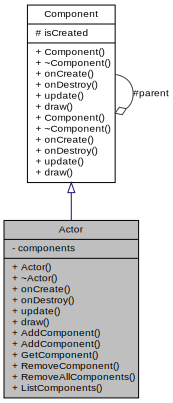
\includegraphics[width=266pt]{classActor__coll__graph}
\end{center}
\end{figure}
\doxysubsection*{Public Member Functions}
\begin{DoxyCompactItemize}
\item 
\mbox{\hyperlink{classActor_a7b296cba96bef9d1cc5893114078f1da}{Actor}} (\mbox{\hyperlink{classComponent}{Component}} $\ast$parent\+\_\+)
\item 
\mbox{\hyperlink{classActor_ad807fe8f85e72ab263a0c05e3231cb39}{$\sim$\+Actor}} ()
\item 
bool \mbox{\hyperlink{classActor_a56a241c949adf52cedceb45a7102ea1a}{on\+Create}} ()
\item 
\mbox{\hyperlink{imgui__impl__opengl3__loader_8h_ac668e7cffd9e2e9cfee428b9b2f34fa7}{void}} \mbox{\hyperlink{classActor_a47101d6275509662bf6c84c3f3439696}{on\+Destroy}} ()
\item 
\mbox{\hyperlink{imgui__impl__opengl3__loader_8h_ac668e7cffd9e2e9cfee428b9b2f34fa7}{void}} \mbox{\hyperlink{classActor_a724ff8f2e9c34f15a6c443a3912504c4}{update}} (const float delta\+Time\+\_\+)
\item 
\mbox{\hyperlink{imgui__impl__opengl3__loader_8h_ac668e7cffd9e2e9cfee428b9b2f34fa7}{void}} \mbox{\hyperlink{classActor_adbbdc379c1a471cc9763d871b0790d7e}{draw}} () const
\item 
{\footnotesize template$<$typename Component\+Template $>$ }\\\mbox{\hyperlink{imgui__impl__opengl3__loader_8h_ac668e7cffd9e2e9cfee428b9b2f34fa7}{void}} \mbox{\hyperlink{classActor_aa8ff3a6ac0f5a1bc18145be0b0de9475}{Add\+Component}} (\mbox{\hyperlink{BStateMachine_2Component_8h_add5e90b302c31b74a46619f240214bcc}{Ref}}$<$ Component\+Template $>$ component\+\_\+)
\item 
{\footnotesize template$<$typename Component\+Template , typename ... Args$>$ }\\\mbox{\hyperlink{imgui__impl__opengl3__loader_8h_ac668e7cffd9e2e9cfee428b9b2f34fa7}{void}} \mbox{\hyperlink{classActor_a279bb9d2c8a6e29cc406c1ff5c4bec31}{Add\+Component}} (Args \&\&... args\+\_\+)
\item 
{\footnotesize template$<$typename Component\+Template $>$ }\\\mbox{\hyperlink{BStateMachine_2Component_8h_add5e90b302c31b74a46619f240214bcc}{Ref}}$<$ Component\+Template $>$ \mbox{\hyperlink{classActor_aea332ed79b7b46b238dd3bb6cdae42df}{Get\+Component}} () const
\item 
{\footnotesize template$<$typename Component\+Template $>$ }\\\mbox{\hyperlink{imgui__impl__opengl3__loader_8h_ac668e7cffd9e2e9cfee428b9b2f34fa7}{void}} \mbox{\hyperlink{classActor_ae1c8e36dc78e7faf430e76209319247d}{Remove\+Component}} ()
\item 
\mbox{\hyperlink{imgui__impl__opengl3__loader_8h_ac668e7cffd9e2e9cfee428b9b2f34fa7}{void}} \mbox{\hyperlink{classActor_ac9310e2ea7c464852e901b508a103222}{Remove\+All\+Components}} ()
\item 
\mbox{\hyperlink{imgui__impl__opengl3__loader_8h_ac668e7cffd9e2e9cfee428b9b2f34fa7}{void}} \mbox{\hyperlink{classActor_aa296fdff7201b411576f757da1dc335c}{List\+Components}} () const
\end{DoxyCompactItemize}
\doxysubsection*{Private Member Functions}
\begin{DoxyCompactItemize}
\item 
\mbox{\hyperlink{classActor_a22f32e3ce430a9f5c6dc9eab2ed7224c}{Actor}} (const \mbox{\hyperlink{classActor}{Actor}} \&)=delete
\begin{DoxyCompactList}\small\item\em Unless you know what these do don\textquotesingle{}t allow them to be created implicitly. \end{DoxyCompactList}\item 
\mbox{\hyperlink{classActor_ad2f5e5c51e030e2297b1f934420e1cf8}{Actor}} (\mbox{\hyperlink{classActor}{Actor}} \&\&)=delete
\item 
\mbox{\hyperlink{classActor}{Actor}} \& \mbox{\hyperlink{classActor_a62a71e552c0f51ca443093c604963900}{operator=}} (const \mbox{\hyperlink{classActor}{Actor}} \&)=delete
\item 
\mbox{\hyperlink{classActor}{Actor}} \& \mbox{\hyperlink{classActor_ae2466f1b9fdcb62a7e0cc4b3a2ec7c2b}{operator=}} (\mbox{\hyperlink{classActor}{Actor}} \&\&)=delete
\end{DoxyCompactItemize}
\doxysubsection*{Private Attributes}
\begin{DoxyCompactItemize}
\item 
std\+::vector$<$ \mbox{\hyperlink{BStateMachine_2Component_8h_add5e90b302c31b74a46619f240214bcc}{Ref}}$<$ \mbox{\hyperlink{classComponent}{Component}} $>$ $>$ \mbox{\hyperlink{classActor_a1ec17d9a692715e0afbd28309315da03}{components}}
\end{DoxyCompactItemize}
\doxysubsection*{Additional Inherited Members}


\doxysubsection{Constructor \& Destructor Documentation}
\mbox{\Hypertarget{classActor_a22f32e3ce430a9f5c6dc9eab2ed7224c}\label{classActor_a22f32e3ce430a9f5c6dc9eab2ed7224c}} 
\index{Actor@{Actor}!Actor@{Actor}}
\index{Actor@{Actor}!Actor@{Actor}}
\doxysubsubsection{\texorpdfstring{Actor()}{Actor()}\hspace{0.1cm}{\footnotesize\ttfamily [1/3]}}
{\footnotesize\ttfamily Actor\+::\+Actor (\begin{DoxyParamCaption}\item[{const \mbox{\hyperlink{classActor}{Actor}} \&}]{ }\end{DoxyParamCaption})\hspace{0.3cm}{\ttfamily [private]}, {\ttfamily [delete]}}



Unless you know what these do don\textquotesingle{}t allow them to be created implicitly. 

\mbox{\Hypertarget{classActor_ad2f5e5c51e030e2297b1f934420e1cf8}\label{classActor_ad2f5e5c51e030e2297b1f934420e1cf8}} 
\index{Actor@{Actor}!Actor@{Actor}}
\index{Actor@{Actor}!Actor@{Actor}}
\doxysubsubsection{\texorpdfstring{Actor()}{Actor()}\hspace{0.1cm}{\footnotesize\ttfamily [2/3]}}
{\footnotesize\ttfamily Actor\+::\+Actor (\begin{DoxyParamCaption}\item[{\mbox{\hyperlink{classActor}{Actor}} \&\&}]{ }\end{DoxyParamCaption})\hspace{0.3cm}{\ttfamily [private]}, {\ttfamily [delete]}}

\mbox{\Hypertarget{classActor_a7b296cba96bef9d1cc5893114078f1da}\label{classActor_a7b296cba96bef9d1cc5893114078f1da}} 
\index{Actor@{Actor}!Actor@{Actor}}
\index{Actor@{Actor}!Actor@{Actor}}
\doxysubsubsection{\texorpdfstring{Actor()}{Actor()}\hspace{0.1cm}{\footnotesize\ttfamily [3/3]}}
{\footnotesize\ttfamily Actor\+::\+Actor (\begin{DoxyParamCaption}\item[{\mbox{\hyperlink{classComponent}{Component}} $\ast$}]{parent\+\_\+ }\end{DoxyParamCaption})}

\mbox{\Hypertarget{classActor_ad807fe8f85e72ab263a0c05e3231cb39}\label{classActor_ad807fe8f85e72ab263a0c05e3231cb39}} 
\index{Actor@{Actor}!````~Actor@{$\sim$Actor}}
\index{````~Actor@{$\sim$Actor}!Actor@{Actor}}
\doxysubsubsection{\texorpdfstring{$\sim$Actor()}{~Actor()}}
{\footnotesize\ttfamily Actor\+::$\sim$\+Actor (\begin{DoxyParamCaption}{ }\end{DoxyParamCaption})}



\doxysubsection{Member Function Documentation}
\mbox{\Hypertarget{classActor_a279bb9d2c8a6e29cc406c1ff5c4bec31}\label{classActor_a279bb9d2c8a6e29cc406c1ff5c4bec31}} 
\index{Actor@{Actor}!AddComponent@{AddComponent}}
\index{AddComponent@{AddComponent}!Actor@{Actor}}
\doxysubsubsection{\texorpdfstring{AddComponent()}{AddComponent()}\hspace{0.1cm}{\footnotesize\ttfamily [1/2]}}
{\footnotesize\ttfamily template$<$typename Component\+Template , typename ... Args$>$ \\
\mbox{\hyperlink{imgui__impl__opengl3__loader_8h_ac668e7cffd9e2e9cfee428b9b2f34fa7}{void}} Actor\+::\+Add\+Component (\begin{DoxyParamCaption}\item[{Args \&\&...}]{args\+\_\+ }\end{DoxyParamCaption})\hspace{0.3cm}{\ttfamily [inline]}}

before you add the component ask if you have the component in the list already, if so -\/ don\textquotesingle{}t add a second one. ~\newline


Finish building the component and add the component to the list\mbox{\Hypertarget{classActor_aa8ff3a6ac0f5a1bc18145be0b0de9475}\label{classActor_aa8ff3a6ac0f5a1bc18145be0b0de9475}} 
\index{Actor@{Actor}!AddComponent@{AddComponent}}
\index{AddComponent@{AddComponent}!Actor@{Actor}}
\doxysubsubsection{\texorpdfstring{AddComponent()}{AddComponent()}\hspace{0.1cm}{\footnotesize\ttfamily [2/2]}}
{\footnotesize\ttfamily template$<$typename Component\+Template $>$ \\
\mbox{\hyperlink{imgui__impl__opengl3__loader_8h_ac668e7cffd9e2e9cfee428b9b2f34fa7}{void}} Actor\+::\+Add\+Component (\begin{DoxyParamCaption}\item[{\mbox{\hyperlink{BStateMachine_2Component_8h_add5e90b302c31b74a46619f240214bcc}{Ref}}$<$ Component\+Template $>$}]{component\+\_\+ }\end{DoxyParamCaption})\hspace{0.3cm}{\ttfamily [inline]}}

\mbox{\Hypertarget{classActor_adbbdc379c1a471cc9763d871b0790d7e}\label{classActor_adbbdc379c1a471cc9763d871b0790d7e}} 
\index{Actor@{Actor}!draw@{draw}}
\index{draw@{draw}!Actor@{Actor}}
\doxysubsubsection{\texorpdfstring{draw()}{draw()}}
{\footnotesize\ttfamily \mbox{\hyperlink{imgui__impl__opengl3__loader_8h_ac668e7cffd9e2e9cfee428b9b2f34fa7}{void}} Actor\+::draw (\begin{DoxyParamCaption}{ }\end{DoxyParamCaption}) const\hspace{0.3cm}{\ttfamily [virtual]}}



Implements \mbox{\hyperlink{classComponent_a8f45309003f02191f2bcc8864e8e9ecf}{Component}}.

\mbox{\Hypertarget{classActor_aea332ed79b7b46b238dd3bb6cdae42df}\label{classActor_aea332ed79b7b46b238dd3bb6cdae42df}} 
\index{Actor@{Actor}!GetComponent@{GetComponent}}
\index{GetComponent@{GetComponent}!Actor@{Actor}}
\doxysubsubsection{\texorpdfstring{GetComponent()}{GetComponent()}}
{\footnotesize\ttfamily template$<$typename Component\+Template $>$ \\
\mbox{\hyperlink{BStateMachine_2Component_8h_add5e90b302c31b74a46619f240214bcc}{Ref}}$<$Component\+Template$>$ Actor\+::\+Get\+Component (\begin{DoxyParamCaption}{ }\end{DoxyParamCaption}) const\hspace{0.3cm}{\ttfamily [inline]}}

This is a dynamic cast designed for shared\+\_\+ptr\textquotesingle{}s \href{https://en.cppreference.com/w/cpp/memory/shared_ptr/pointer_cast}{\texttt{ https\+://en.\+cppreference.\+com/w/cpp/memory/shared\+\_\+ptr/pointer\+\_\+cast}}\mbox{\Hypertarget{classActor_aa296fdff7201b411576f757da1dc335c}\label{classActor_aa296fdff7201b411576f757da1dc335c}} 
\index{Actor@{Actor}!ListComponents@{ListComponents}}
\index{ListComponents@{ListComponents}!Actor@{Actor}}
\doxysubsubsection{\texorpdfstring{ListComponents()}{ListComponents()}}
{\footnotesize\ttfamily \mbox{\hyperlink{imgui__impl__opengl3__loader_8h_ac668e7cffd9e2e9cfee428b9b2f34fa7}{void}} Actor\+::\+List\+Components (\begin{DoxyParamCaption}{ }\end{DoxyParamCaption}) const}

\mbox{\Hypertarget{classActor_a56a241c949adf52cedceb45a7102ea1a}\label{classActor_a56a241c949adf52cedceb45a7102ea1a}} 
\index{Actor@{Actor}!onCreate@{onCreate}}
\index{onCreate@{onCreate}!Actor@{Actor}}
\doxysubsubsection{\texorpdfstring{onCreate()}{onCreate()}}
{\footnotesize\ttfamily bool Actor\+::on\+Create (\begin{DoxyParamCaption}{ }\end{DoxyParamCaption})\hspace{0.3cm}{\ttfamily [virtual]}}



Implements \mbox{\hyperlink{classComponent_a3a1537a8b8bcdb2155afbb925c77b0a2}{Component}}.



Reimplemented in \mbox{\hyperlink{classProjectile__Actor_a98e2e2198cd164c35318c04f96e6a3ac}{Projectile\+\_\+\+Actor}}, and \mbox{\hyperlink{classPlatform__Actor_ab902e2540f1d3127dedff632841b4921}{Platform\+\_\+\+Actor}}.

\mbox{\Hypertarget{classActor_a47101d6275509662bf6c84c3f3439696}\label{classActor_a47101d6275509662bf6c84c3f3439696}} 
\index{Actor@{Actor}!onDestroy@{onDestroy}}
\index{onDestroy@{onDestroy}!Actor@{Actor}}
\doxysubsubsection{\texorpdfstring{onDestroy()}{onDestroy()}}
{\footnotesize\ttfamily \mbox{\hyperlink{imgui__impl__opengl3__loader_8h_ac668e7cffd9e2e9cfee428b9b2f34fa7}{void}} Actor\+::on\+Destroy (\begin{DoxyParamCaption}{ }\end{DoxyParamCaption})\hspace{0.3cm}{\ttfamily [virtual]}}



Implements \mbox{\hyperlink{classComponent_a2b198f27162a6caf63917e304295f892}{Component}}.



Reimplemented in \mbox{\hyperlink{classNPC__Actor_ab274d0517bd0cd710efc7df31cd7450b}{N\+P\+C\+\_\+\+Actor}}, \mbox{\hyperlink{classProjectile__Actor_a58d01ff77f0815ca611236f139b7aafa}{Projectile\+\_\+\+Actor}}, \mbox{\hyperlink{classAnimate__Actor_ae67ff6399f3d46696f84c77b2e519ead}{Animate\+\_\+\+Actor}}, \mbox{\hyperlink{classPlayer__Actor_a200b6b956d9c597cbc626ca9bcafb25e}{Player\+\_\+\+Actor}}, \mbox{\hyperlink{classShader__Actor_a16f7f5f30d3f3cd125de9713457a7db2}{Shader\+\_\+\+Actor}}, \mbox{\hyperlink{classTexture__Actor_ac9677f60df27e14ef3550ae2b0678ad5}{Texture\+\_\+\+Actor}}, \mbox{\hyperlink{classEdge__Actor_ae7a429d48b86442154c93eb65bc8b22d}{Edge\+\_\+\+Actor}}, \mbox{\hyperlink{classPlatform__Actor_a34b915aa583cdf659ec29368b6feb7e8}{Platform\+\_\+\+Actor}}, and \mbox{\hyperlink{classText__Actor_af9b25da889aad4aec6f17671c37ac431}{Text\+\_\+\+Actor}}.

\mbox{\Hypertarget{classActor_ae2466f1b9fdcb62a7e0cc4b3a2ec7c2b}\label{classActor_ae2466f1b9fdcb62a7e0cc4b3a2ec7c2b}} 
\index{Actor@{Actor}!operator=@{operator=}}
\index{operator=@{operator=}!Actor@{Actor}}
\doxysubsubsection{\texorpdfstring{operator=()}{operator=()}\hspace{0.1cm}{\footnotesize\ttfamily [1/2]}}
{\footnotesize\ttfamily \mbox{\hyperlink{classActor}{Actor}}\& Actor\+::operator= (\begin{DoxyParamCaption}\item[{\mbox{\hyperlink{classActor}{Actor}} \&\&}]{ }\end{DoxyParamCaption})\hspace{0.3cm}{\ttfamily [private]}, {\ttfamily [delete]}}

\mbox{\Hypertarget{classActor_a62a71e552c0f51ca443093c604963900}\label{classActor_a62a71e552c0f51ca443093c604963900}} 
\index{Actor@{Actor}!operator=@{operator=}}
\index{operator=@{operator=}!Actor@{Actor}}
\doxysubsubsection{\texorpdfstring{operator=()}{operator=()}\hspace{0.1cm}{\footnotesize\ttfamily [2/2]}}
{\footnotesize\ttfamily \mbox{\hyperlink{classActor}{Actor}}\& Actor\+::operator= (\begin{DoxyParamCaption}\item[{const \mbox{\hyperlink{classActor}{Actor}} \&}]{ }\end{DoxyParamCaption})\hspace{0.3cm}{\ttfamily [private]}, {\ttfamily [delete]}}

\mbox{\Hypertarget{classActor_ac9310e2ea7c464852e901b508a103222}\label{classActor_ac9310e2ea7c464852e901b508a103222}} 
\index{Actor@{Actor}!RemoveAllComponents@{RemoveAllComponents}}
\index{RemoveAllComponents@{RemoveAllComponents}!Actor@{Actor}}
\doxysubsubsection{\texorpdfstring{RemoveAllComponents()}{RemoveAllComponents()}}
{\footnotesize\ttfamily \mbox{\hyperlink{imgui__impl__opengl3__loader_8h_ac668e7cffd9e2e9cfee428b9b2f34fa7}{void}} Actor\+::\+Remove\+All\+Components (\begin{DoxyParamCaption}{ }\end{DoxyParamCaption})}

\mbox{\Hypertarget{classActor_ae1c8e36dc78e7faf430e76209319247d}\label{classActor_ae1c8e36dc78e7faf430e76209319247d}} 
\index{Actor@{Actor}!RemoveComponent@{RemoveComponent}}
\index{RemoveComponent@{RemoveComponent}!Actor@{Actor}}
\doxysubsubsection{\texorpdfstring{RemoveComponent()}{RemoveComponent()}}
{\footnotesize\ttfamily template$<$typename Component\+Template $>$ \\
\mbox{\hyperlink{imgui__impl__opengl3__loader_8h_ac668e7cffd9e2e9cfee428b9b2f34fa7}{void}} Actor\+::\+Remove\+Component (\begin{DoxyParamCaption}{ }\end{DoxyParamCaption})\hspace{0.3cm}{\ttfamily [inline]}}

\mbox{\Hypertarget{classActor_a724ff8f2e9c34f15a6c443a3912504c4}\label{classActor_a724ff8f2e9c34f15a6c443a3912504c4}} 
\index{Actor@{Actor}!update@{update}}
\index{update@{update}!Actor@{Actor}}
\doxysubsubsection{\texorpdfstring{update()}{update()}}
{\footnotesize\ttfamily \mbox{\hyperlink{imgui__impl__opengl3__loader_8h_ac668e7cffd9e2e9cfee428b9b2f34fa7}{void}} Actor\+::update (\begin{DoxyParamCaption}\item[{const float}]{delta\+Time\+\_\+ }\end{DoxyParamCaption})\hspace{0.3cm}{\ttfamily [virtual]}}



Implements \mbox{\hyperlink{classComponent_a3448977e6f464df89e77dda7c6f52204}{Component}}.



Reimplemented in \mbox{\hyperlink{classProjectile__Actor_ab61aec7117a93626c3096bef71ab30fc}{Projectile\+\_\+\+Actor}}, \mbox{\hyperlink{classAnimate__Actor_a6bdb436a75efbc01545679b613858201}{Animate\+\_\+\+Actor}}, \mbox{\hyperlink{classGun__Actor_ab5e7b6b7032e1f0353c6c4f08cedebec}{Gun\+\_\+\+Actor}}, \mbox{\hyperlink{classPlayer__Actor_a619a94504523cbfa9eb5490de5361f31}{Player\+\_\+\+Actor}}, \mbox{\hyperlink{classTexture__Actor_afe03163ea0bff0ea0fa3c3fb6c560c79}{Texture\+\_\+\+Actor}}, \mbox{\hyperlink{classEdge__Actor_a8ae8a19c72b58522755d2d0a395fc1ea}{Edge\+\_\+\+Actor}}, \mbox{\hyperlink{classPlatform__Actor_a12b22d88efc384ac35060d04fbbe710d}{Platform\+\_\+\+Actor}}, and \mbox{\hyperlink{classText__Actor_a26181e1102ab2a37ec8b140c999a6f6a}{Text\+\_\+\+Actor}}.



\doxysubsection{Member Data Documentation}
\mbox{\Hypertarget{classActor_a1ec17d9a692715e0afbd28309315da03}\label{classActor_a1ec17d9a692715e0afbd28309315da03}} 
\index{Actor@{Actor}!components@{components}}
\index{components@{components}!Actor@{Actor}}
\doxysubsubsection{\texorpdfstring{components}{components}}
{\footnotesize\ttfamily std\+::vector$<$ \mbox{\hyperlink{BStateMachine_2Component_8h_add5e90b302c31b74a46619f240214bcc}{Ref}}$<$\mbox{\hyperlink{classComponent}{Component}}$>$ $>$ Actor\+::components\hspace{0.3cm}{\ttfamily [private]}}



The documentation for this class was generated from the following files\+:\begin{DoxyCompactItemize}
\item 
/home/fnky/\+C0de/component\+\_\+engine/include/\+Actors/\mbox{\hyperlink{Actor_8h}{Actor.\+h}}\item 
/home/fnky/\+C0de/component\+\_\+engine/src/\+Actors/\mbox{\hyperlink{Actor_8cpp}{Actor.\+cpp}}\end{DoxyCompactItemize}

\hypertarget{classAIComponent}{}\section{A\+I\+Component Class Reference}
\label{classAIComponent}\index{A\+I\+Component@{A\+I\+Component}}


{\ttfamily \#include $<$A\+I\+Component.\+h$>$}



Inheritance diagram for A\+I\+Component\+:
\nopagebreak
\begin{figure}[H]
\begin{center}
\leavevmode
\includegraphics[width=179pt]{classAIComponent__inherit__graph}
\end{center}
\end{figure}


Collaboration diagram for A\+I\+Component\+:
\nopagebreak
\begin{figure}[H]
\begin{center}
\leavevmode
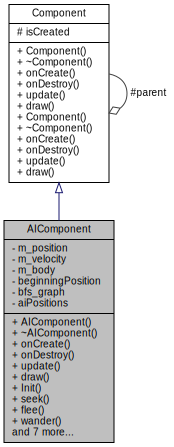
\includegraphics[width=228pt]{classAIComponent__coll__graph}
\end{center}
\end{figure}
\subsection*{Public Member Functions}
\begin{DoxyCompactItemize}
\item 
\hyperlink{classAIComponent_a78108337893807f59557596e2825cbb3}{A\+I\+Component} (\hyperlink{classComponent}{Component} $\ast$parent\+\_\+)
\item 
\hyperlink{classAIComponent_a0ffc6db0d1cb5720b8aaef8ec28f4efe}{$\sim$\+A\+I\+Component} ()
\item 
bool \hyperlink{classAIComponent_a1f7e2f748183cbcba9e3f351025b862c}{on\+Create} () override
\item 
\hyperlink{imgui__impl__opengl3__loader_8h_ac668e7cffd9e2e9cfee428b9b2f34fa7}{void} \hyperlink{classAIComponent_a82e8e79810024e09695545ebf59452f2}{on\+Destroy} () override
\item 
\hyperlink{imgui__impl__opengl3__loader_8h_ac668e7cffd9e2e9cfee428b9b2f34fa7}{void} \hyperlink{classAIComponent_a456939f85de6d6cfc3e4e48ffc9f568c}{update} (const float delta) override
\item 
\hyperlink{imgui__impl__opengl3__loader_8h_ac668e7cffd9e2e9cfee428b9b2f34fa7}{void} \hyperlink{classAIComponent_ab4d6c5c6043cfa275e4edce5b575a8a9}{draw} () const override
\item 
\hyperlink{imgui__impl__opengl3__loader_8h_ac668e7cffd9e2e9cfee428b9b2f34fa7}{void} \hyperlink{classAIComponent_a09ef4a12ea342b7e9cbb0f0e1aeceefe}{Init} (b2\+Body $\ast$body)
\item 
b2\+Vec2 \hyperlink{classAIComponent_a356b7fa667e4aed3fdf790a58916c3b9}{seek} (b2\+Body $\ast$other\+Body, float max\+Speed, float gravity)
\item 
b2\+Vec2 \hyperlink{classAIComponent_adc2c03c2bd20fd66ed26580e2b8d2784}{flee} (b2\+Body $\ast$other\+Body, float max\+Speed, float gravity)
\item 
b2\+Vec2 \hyperlink{classAIComponent_aee1af922a048c44f48cb204d8e153fb5}{wander} (float min\+Distance, float max\+Speed, float max\+Distance)
\item 
bool \hyperlink{classAIComponent_a24853885627e632ae760ae372bb57714}{move\+Position} (b2\+Vec2 positions)
\item 
bool \hyperlink{classAIComponent_aa584e4cfba8281933bfff799c9caf06d}{move\+Left\+Position} (b2\+Vec2 positions)
\item 
bool \hyperlink{classAIComponent_ac7ae5bfd9cf4e5163a4289c096c78f7c}{move\+Right\+Position} (b2\+Vec2 positions)
\item 
std\+::vector$<$ int $>$ \hyperlink{classAIComponent_a81d6ead52253301578f5e25527075899}{search} ()
\item 
std\+::shared\+\_\+ptr$<$ \hyperlink{classGraph}{Graph} $>$ \hyperlink{classAIComponent_aeddece3b6c4aac54c401fb3ebeb657ba}{get\+Graph} ()
\item 
\hyperlink{imgui__impl__opengl3__loader_8h_ac668e7cffd9e2e9cfee428b9b2f34fa7}{void} \hyperlink{classAIComponent_a33f4903d01350f4c17e6275dbf3f9097}{populate\+A\+I\+Positions} (char key, b2\+Vec2 positions)
\item 
std\+::vector$<$ \hyperlink{structAIposition}{A\+Iposition} $\ast$ $>$ \hyperlink{classAIComponent_a8bc910076abb3723183b92fa8d317049}{get\+A\+I\+Positions} ()
\end{DoxyCompactItemize}
\subsection*{Private Attributes}
\begin{DoxyCompactItemize}
\item 
b2\+Vec2 \hyperlink{classAIComponent_a4762eb8f3fc7c56cbedef2074183a7df}{m\+\_\+position}
\item 
b2\+Vec2 \hyperlink{classAIComponent_abdffe34d98dd34e51c777512bce686ca}{m\+\_\+velocity}
\item 
b2\+Body $\ast$ \hyperlink{classAIComponent_a5ae9cb55df68289dc80568e0072b2473}{m\+\_\+body}
\item 
float \hyperlink{classAIComponent_aa0d6c295cf92653b96bad859e0fa330f}{beginning\+Position}
\item 
std\+::shared\+\_\+ptr$<$ \hyperlink{classGraph}{Graph} $>$ \hyperlink{classAIComponent_a7b0b2a7230a851322867a387a81f985a}{bfs\+\_\+graph}
\item 
std\+::vector$<$ \hyperlink{structAIposition}{A\+Iposition} $\ast$ $>$ \hyperlink{classAIComponent_a016b40f3b9d332294a517cbcc28ddcc9}{ai\+Positions}
\end{DoxyCompactItemize}
\subsection*{Additional Inherited Members}


\subsection{Constructor \& Destructor Documentation}
\mbox{\Hypertarget{classAIComponent_a78108337893807f59557596e2825cbb3}\label{classAIComponent_a78108337893807f59557596e2825cbb3}} 
\index{A\+I\+Component@{A\+I\+Component}!A\+I\+Component@{A\+I\+Component}}
\index{A\+I\+Component@{A\+I\+Component}!A\+I\+Component@{A\+I\+Component}}
\subsubsection{\texorpdfstring{A\+I\+Component()}{AIComponent()}}
{\footnotesize\ttfamily A\+I\+Component\+::\+A\+I\+Component (\begin{DoxyParamCaption}\item[{\hyperlink{classComponent}{Component} $\ast$}]{parent\+\_\+ }\end{DoxyParamCaption})}

\mbox{\Hypertarget{classAIComponent_a0ffc6db0d1cb5720b8aaef8ec28f4efe}\label{classAIComponent_a0ffc6db0d1cb5720b8aaef8ec28f4efe}} 
\index{A\+I\+Component@{A\+I\+Component}!````~A\+I\+Component@{$\sim$\+A\+I\+Component}}
\index{````~A\+I\+Component@{$\sim$\+A\+I\+Component}!A\+I\+Component@{A\+I\+Component}}
\subsubsection{\texorpdfstring{$\sim$\+A\+I\+Component()}{~AIComponent()}}
{\footnotesize\ttfamily A\+I\+Component\+::$\sim$\+A\+I\+Component (\begin{DoxyParamCaption}{ }\end{DoxyParamCaption})}



\subsection{Member Function Documentation}
\mbox{\Hypertarget{classAIComponent_ab4d6c5c6043cfa275e4edce5b575a8a9}\label{classAIComponent_ab4d6c5c6043cfa275e4edce5b575a8a9}} 
\index{A\+I\+Component@{A\+I\+Component}!draw@{draw}}
\index{draw@{draw}!A\+I\+Component@{A\+I\+Component}}
\subsubsection{\texorpdfstring{draw()}{draw()}}
{\footnotesize\ttfamily \hyperlink{imgui__impl__opengl3__loader_8h_ac668e7cffd9e2e9cfee428b9b2f34fa7}{void} A\+I\+Component\+::draw (\begin{DoxyParamCaption}{ }\end{DoxyParamCaption}) const\hspace{0.3cm}{\ttfamily [inline]}, {\ttfamily [override]}, {\ttfamily [virtual]}}



Implements \hyperlink{classComponent_a8f45309003f02191f2bcc8864e8e9ecf}{Component}.

\mbox{\Hypertarget{classAIComponent_adc2c03c2bd20fd66ed26580e2b8d2784}\label{classAIComponent_adc2c03c2bd20fd66ed26580e2b8d2784}} 
\index{A\+I\+Component@{A\+I\+Component}!flee@{flee}}
\index{flee@{flee}!A\+I\+Component@{A\+I\+Component}}
\subsubsection{\texorpdfstring{flee()}{flee()}}
{\footnotesize\ttfamily b2\+Vec2 A\+I\+Component\+::flee (\begin{DoxyParamCaption}\item[{b2\+Body $\ast$}]{other\+Body,  }\item[{float}]{max\+Speed,  }\item[{float}]{gravity }\end{DoxyParamCaption})}

\mbox{\Hypertarget{classAIComponent_a8bc910076abb3723183b92fa8d317049}\label{classAIComponent_a8bc910076abb3723183b92fa8d317049}} 
\index{A\+I\+Component@{A\+I\+Component}!get\+A\+I\+Positions@{get\+A\+I\+Positions}}
\index{get\+A\+I\+Positions@{get\+A\+I\+Positions}!A\+I\+Component@{A\+I\+Component}}
\subsubsection{\texorpdfstring{get\+A\+I\+Positions()}{getAIPositions()}}
{\footnotesize\ttfamily std\+::vector$<$\hyperlink{structAIposition}{A\+Iposition}$\ast$$>$ A\+I\+Component\+::get\+A\+I\+Positions (\begin{DoxyParamCaption}{ }\end{DoxyParamCaption})\hspace{0.3cm}{\ttfamily [inline]}}

\mbox{\Hypertarget{classAIComponent_aeddece3b6c4aac54c401fb3ebeb657ba}\label{classAIComponent_aeddece3b6c4aac54c401fb3ebeb657ba}} 
\index{A\+I\+Component@{A\+I\+Component}!get\+Graph@{get\+Graph}}
\index{get\+Graph@{get\+Graph}!A\+I\+Component@{A\+I\+Component}}
\subsubsection{\texorpdfstring{get\+Graph()}{getGraph()}}
{\footnotesize\ttfamily std\+::shared\+\_\+ptr$<$\hyperlink{classGraph}{Graph}$>$ A\+I\+Component\+::get\+Graph (\begin{DoxyParamCaption}{ }\end{DoxyParamCaption})\hspace{0.3cm}{\ttfamily [inline]}}

\mbox{\Hypertarget{classAIComponent_a09ef4a12ea342b7e9cbb0f0e1aeceefe}\label{classAIComponent_a09ef4a12ea342b7e9cbb0f0e1aeceefe}} 
\index{A\+I\+Component@{A\+I\+Component}!Init@{Init}}
\index{Init@{Init}!A\+I\+Component@{A\+I\+Component}}
\subsubsection{\texorpdfstring{Init()}{Init()}}
{\footnotesize\ttfamily \hyperlink{imgui__impl__opengl3__loader_8h_ac668e7cffd9e2e9cfee428b9b2f34fa7}{void} A\+I\+Component\+::\+Init (\begin{DoxyParamCaption}\item[{b2\+Body $\ast$}]{body }\end{DoxyParamCaption})\hspace{0.3cm}{\ttfamily [inline]}}

\mbox{\Hypertarget{classAIComponent_aa584e4cfba8281933bfff799c9caf06d}\label{classAIComponent_aa584e4cfba8281933bfff799c9caf06d}} 
\index{A\+I\+Component@{A\+I\+Component}!move\+Left\+Position@{move\+Left\+Position}}
\index{move\+Left\+Position@{move\+Left\+Position}!A\+I\+Component@{A\+I\+Component}}
\subsubsection{\texorpdfstring{move\+Left\+Position()}{moveLeftPosition()}}
{\footnotesize\ttfamily bool A\+I\+Component\+::move\+Left\+Position (\begin{DoxyParamCaption}\item[{b2\+Vec2}]{positions }\end{DoxyParamCaption})\hspace{0.3cm}{\ttfamily [inline]}}

\mbox{\Hypertarget{classAIComponent_a24853885627e632ae760ae372bb57714}\label{classAIComponent_a24853885627e632ae760ae372bb57714}} 
\index{A\+I\+Component@{A\+I\+Component}!move\+Position@{move\+Position}}
\index{move\+Position@{move\+Position}!A\+I\+Component@{A\+I\+Component}}
\subsubsection{\texorpdfstring{move\+Position()}{movePosition()}}
{\footnotesize\ttfamily bool A\+I\+Component\+::move\+Position (\begin{DoxyParamCaption}\item[{b2\+Vec2}]{positions }\end{DoxyParamCaption})\hspace{0.3cm}{\ttfamily [inline]}}

\mbox{\Hypertarget{classAIComponent_ac7ae5bfd9cf4e5163a4289c096c78f7c}\label{classAIComponent_ac7ae5bfd9cf4e5163a4289c096c78f7c}} 
\index{A\+I\+Component@{A\+I\+Component}!move\+Right\+Position@{move\+Right\+Position}}
\index{move\+Right\+Position@{move\+Right\+Position}!A\+I\+Component@{A\+I\+Component}}
\subsubsection{\texorpdfstring{move\+Right\+Position()}{moveRightPosition()}}
{\footnotesize\ttfamily bool A\+I\+Component\+::move\+Right\+Position (\begin{DoxyParamCaption}\item[{b2\+Vec2}]{positions }\end{DoxyParamCaption})\hspace{0.3cm}{\ttfamily [inline]}}

\mbox{\Hypertarget{classAIComponent_a1f7e2f748183cbcba9e3f351025b862c}\label{classAIComponent_a1f7e2f748183cbcba9e3f351025b862c}} 
\index{A\+I\+Component@{A\+I\+Component}!on\+Create@{on\+Create}}
\index{on\+Create@{on\+Create}!A\+I\+Component@{A\+I\+Component}}
\subsubsection{\texorpdfstring{on\+Create()}{onCreate()}}
{\footnotesize\ttfamily bool A\+I\+Component\+::on\+Create (\begin{DoxyParamCaption}{ }\end{DoxyParamCaption})\hspace{0.3cm}{\ttfamily [inline]}, {\ttfamily [override]}, {\ttfamily [virtual]}}



Implements \hyperlink{classComponent_a3a1537a8b8bcdb2155afbb925c77b0a2}{Component}.

\mbox{\Hypertarget{classAIComponent_a82e8e79810024e09695545ebf59452f2}\label{classAIComponent_a82e8e79810024e09695545ebf59452f2}} 
\index{A\+I\+Component@{A\+I\+Component}!on\+Destroy@{on\+Destroy}}
\index{on\+Destroy@{on\+Destroy}!A\+I\+Component@{A\+I\+Component}}
\subsubsection{\texorpdfstring{on\+Destroy()}{onDestroy()}}
{\footnotesize\ttfamily \hyperlink{imgui__impl__opengl3__loader_8h_ac668e7cffd9e2e9cfee428b9b2f34fa7}{void} A\+I\+Component\+::on\+Destroy (\begin{DoxyParamCaption}{ }\end{DoxyParamCaption})\hspace{0.3cm}{\ttfamily [inline]}, {\ttfamily [override]}, {\ttfamily [virtual]}}



Implements \hyperlink{classComponent_a2b198f27162a6caf63917e304295f892}{Component}.

\mbox{\Hypertarget{classAIComponent_a33f4903d01350f4c17e6275dbf3f9097}\label{classAIComponent_a33f4903d01350f4c17e6275dbf3f9097}} 
\index{A\+I\+Component@{A\+I\+Component}!populate\+A\+I\+Positions@{populate\+A\+I\+Positions}}
\index{populate\+A\+I\+Positions@{populate\+A\+I\+Positions}!A\+I\+Component@{A\+I\+Component}}
\subsubsection{\texorpdfstring{populate\+A\+I\+Positions()}{populateAIPositions()}}
{\footnotesize\ttfamily \hyperlink{imgui__impl__opengl3__loader_8h_ac668e7cffd9e2e9cfee428b9b2f34fa7}{void} A\+I\+Component\+::populate\+A\+I\+Positions (\begin{DoxyParamCaption}\item[{char}]{key,  }\item[{b2\+Vec2}]{positions }\end{DoxyParamCaption})\hspace{0.3cm}{\ttfamily [inline]}}

\mbox{\Hypertarget{classAIComponent_a81d6ead52253301578f5e25527075899}\label{classAIComponent_a81d6ead52253301578f5e25527075899}} 
\index{A\+I\+Component@{A\+I\+Component}!search@{search}}
\index{search@{search}!A\+I\+Component@{A\+I\+Component}}
\subsubsection{\texorpdfstring{search()}{search()}}
{\footnotesize\ttfamily std\+::vector$<$int$>$ A\+I\+Component\+::search (\begin{DoxyParamCaption}{ }\end{DoxyParamCaption})\hspace{0.3cm}{\ttfamily [inline]}}

\mbox{\Hypertarget{classAIComponent_a356b7fa667e4aed3fdf790a58916c3b9}\label{classAIComponent_a356b7fa667e4aed3fdf790a58916c3b9}} 
\index{A\+I\+Component@{A\+I\+Component}!seek@{seek}}
\index{seek@{seek}!A\+I\+Component@{A\+I\+Component}}
\subsubsection{\texorpdfstring{seek()}{seek()}}
{\footnotesize\ttfamily b2\+Vec2 A\+I\+Component\+::seek (\begin{DoxyParamCaption}\item[{b2\+Body $\ast$}]{other\+Body,  }\item[{float}]{max\+Speed,  }\item[{float}]{gravity }\end{DoxyParamCaption})}

\mbox{\Hypertarget{classAIComponent_a456939f85de6d6cfc3e4e48ffc9f568c}\label{classAIComponent_a456939f85de6d6cfc3e4e48ffc9f568c}} 
\index{A\+I\+Component@{A\+I\+Component}!update@{update}}
\index{update@{update}!A\+I\+Component@{A\+I\+Component}}
\subsubsection{\texorpdfstring{update()}{update()}}
{\footnotesize\ttfamily \hyperlink{imgui__impl__opengl3__loader_8h_ac668e7cffd9e2e9cfee428b9b2f34fa7}{void} A\+I\+Component\+::update (\begin{DoxyParamCaption}\item[{const float}]{delta }\end{DoxyParamCaption})\hspace{0.3cm}{\ttfamily [override]}, {\ttfamily [virtual]}}



Implements \hyperlink{classComponent_a3448977e6f464df89e77dda7c6f52204}{Component}.

\mbox{\Hypertarget{classAIComponent_aee1af922a048c44f48cb204d8e153fb5}\label{classAIComponent_aee1af922a048c44f48cb204d8e153fb5}} 
\index{A\+I\+Component@{A\+I\+Component}!wander@{wander}}
\index{wander@{wander}!A\+I\+Component@{A\+I\+Component}}
\subsubsection{\texorpdfstring{wander()}{wander()}}
{\footnotesize\ttfamily b2\+Vec2 A\+I\+Component\+::wander (\begin{DoxyParamCaption}\item[{float}]{min\+Distance,  }\item[{float}]{max\+Speed,  }\item[{float}]{max\+Distance }\end{DoxyParamCaption})}



\subsection{Member Data Documentation}
\mbox{\Hypertarget{classAIComponent_a016b40f3b9d332294a517cbcc28ddcc9}\label{classAIComponent_a016b40f3b9d332294a517cbcc28ddcc9}} 
\index{A\+I\+Component@{A\+I\+Component}!ai\+Positions@{ai\+Positions}}
\index{ai\+Positions@{ai\+Positions}!A\+I\+Component@{A\+I\+Component}}
\subsubsection{\texorpdfstring{ai\+Positions}{aiPositions}}
{\footnotesize\ttfamily std\+::vector$<$\hyperlink{structAIposition}{A\+Iposition}$\ast$$>$ A\+I\+Component\+::ai\+Positions\hspace{0.3cm}{\ttfamily [private]}}

\mbox{\Hypertarget{classAIComponent_aa0d6c295cf92653b96bad859e0fa330f}\label{classAIComponent_aa0d6c295cf92653b96bad859e0fa330f}} 
\index{A\+I\+Component@{A\+I\+Component}!beginning\+Position@{beginning\+Position}}
\index{beginning\+Position@{beginning\+Position}!A\+I\+Component@{A\+I\+Component}}
\subsubsection{\texorpdfstring{beginning\+Position}{beginningPosition}}
{\footnotesize\ttfamily float A\+I\+Component\+::beginning\+Position\hspace{0.3cm}{\ttfamily [private]}}

\mbox{\Hypertarget{classAIComponent_a7b0b2a7230a851322867a387a81f985a}\label{classAIComponent_a7b0b2a7230a851322867a387a81f985a}} 
\index{A\+I\+Component@{A\+I\+Component}!bfs\+\_\+graph@{bfs\+\_\+graph}}
\index{bfs\+\_\+graph@{bfs\+\_\+graph}!A\+I\+Component@{A\+I\+Component}}
\subsubsection{\texorpdfstring{bfs\+\_\+graph}{bfs\_graph}}
{\footnotesize\ttfamily std\+::shared\+\_\+ptr$<$\hyperlink{classGraph}{Graph}$>$ A\+I\+Component\+::bfs\+\_\+graph\hspace{0.3cm}{\ttfamily [private]}}

\mbox{\Hypertarget{classAIComponent_a5ae9cb55df68289dc80568e0072b2473}\label{classAIComponent_a5ae9cb55df68289dc80568e0072b2473}} 
\index{A\+I\+Component@{A\+I\+Component}!m\+\_\+body@{m\+\_\+body}}
\index{m\+\_\+body@{m\+\_\+body}!A\+I\+Component@{A\+I\+Component}}
\subsubsection{\texorpdfstring{m\+\_\+body}{m\_body}}
{\footnotesize\ttfamily b2\+Body$\ast$ A\+I\+Component\+::m\+\_\+body\hspace{0.3cm}{\ttfamily [private]}}

\mbox{\Hypertarget{classAIComponent_a4762eb8f3fc7c56cbedef2074183a7df}\label{classAIComponent_a4762eb8f3fc7c56cbedef2074183a7df}} 
\index{A\+I\+Component@{A\+I\+Component}!m\+\_\+position@{m\+\_\+position}}
\index{m\+\_\+position@{m\+\_\+position}!A\+I\+Component@{A\+I\+Component}}
\subsubsection{\texorpdfstring{m\+\_\+position}{m\_position}}
{\footnotesize\ttfamily b2\+Vec2 A\+I\+Component\+::m\+\_\+position\hspace{0.3cm}{\ttfamily [private]}}

\mbox{\Hypertarget{classAIComponent_abdffe34d98dd34e51c777512bce686ca}\label{classAIComponent_abdffe34d98dd34e51c777512bce686ca}} 
\index{A\+I\+Component@{A\+I\+Component}!m\+\_\+velocity@{m\+\_\+velocity}}
\index{m\+\_\+velocity@{m\+\_\+velocity}!A\+I\+Component@{A\+I\+Component}}
\subsubsection{\texorpdfstring{m\+\_\+velocity}{m\_velocity}}
{\footnotesize\ttfamily b2\+Vec2 A\+I\+Component\+::m\+\_\+velocity\hspace{0.3cm}{\ttfamily [private]}}



The documentation for this class was generated from the following files\+:\begin{DoxyCompactItemize}
\item 
/mnt/hdd/fnky/\+C0de/\+C\+A\+P\+S\+T\+O\+N\+E/clean\+\_\+build/include/\+Components/\hyperlink{AIComponent_8h}{A\+I\+Component.\+h}\item 
/mnt/hdd/fnky/\+C0de/\+C\+A\+P\+S\+T\+O\+N\+E/clean\+\_\+build/src/\+Components/\hyperlink{AIComponent_8cpp}{A\+I\+Component.\+cpp}\end{DoxyCompactItemize}

\hypertarget{structAIposition}{}\section{A\+Iposition Struct Reference}
\label{structAIposition}\index{A\+Iposition@{A\+Iposition}}


{\ttfamily \#include $<$A\+I\+Component.\+h$>$}



Collaboration diagram for A\+Iposition\+:
\nopagebreak
\begin{figure}[H]
\begin{center}
\leavevmode
\includegraphics[width=153pt]{structAIposition__coll__graph}
\end{center}
\end{figure}
\subsection*{Public Attributes}
\begin{DoxyCompactItemize}
\item 
bool \hyperlink{structAIposition_ab257c742a240b65925b4acd16cba0781}{destination}
\item 
char \hyperlink{structAIposition_a47a0e37eaa5513e5a4faa85473d13ed2}{key}
\item 
b2\+Vec2 \hyperlink{structAIposition_a6c93076273538f58a68378957f6baf4c}{position}
\end{DoxyCompactItemize}


\subsection{Member Data Documentation}
\mbox{\Hypertarget{structAIposition_ab257c742a240b65925b4acd16cba0781}\label{structAIposition_ab257c742a240b65925b4acd16cba0781}} 
\index{A\+Iposition@{A\+Iposition}!destination@{destination}}
\index{destination@{destination}!A\+Iposition@{A\+Iposition}}
\subsubsection{\texorpdfstring{destination}{destination}}
{\footnotesize\ttfamily bool A\+Iposition\+::destination}

\mbox{\Hypertarget{structAIposition_a47a0e37eaa5513e5a4faa85473d13ed2}\label{structAIposition_a47a0e37eaa5513e5a4faa85473d13ed2}} 
\index{A\+Iposition@{A\+Iposition}!key@{key}}
\index{key@{key}!A\+Iposition@{A\+Iposition}}
\subsubsection{\texorpdfstring{key}{key}}
{\footnotesize\ttfamily char A\+Iposition\+::key}

\mbox{\Hypertarget{structAIposition_a6c93076273538f58a68378957f6baf4c}\label{structAIposition_a6c93076273538f58a68378957f6baf4c}} 
\index{A\+Iposition@{A\+Iposition}!position@{position}}
\index{position@{position}!A\+Iposition@{A\+Iposition}}
\subsubsection{\texorpdfstring{position}{position}}
{\footnotesize\ttfamily b2\+Vec2 A\+Iposition\+::position}



The documentation for this struct was generated from the following file\+:\begin{DoxyCompactItemize}
\item 
/mnt/hdd/fnky/\+C0de/\+C\+A\+P\+S\+T\+O\+N\+E/clean\+\_\+build/include/\+Components/\hyperlink{AIComponent_8h}{A\+I\+Component.\+h}\end{DoxyCompactItemize}

\hypertarget{classrapidjson_1_1Allocator}{}\section{rapidjson\+:\+:Allocator Class Reference}
\label{classrapidjson_1_1Allocator}\index{rapidjson\+::\+Allocator@{rapidjson\+::\+Allocator}}


Concept for allocating, resizing and freeing memory block.  




{\ttfamily \#include $<$allocators.\+h$>$}



Collaboration diagram for rapidjson\+:\+:Allocator\+:
\nopagebreak
\begin{figure}[H]
\begin{center}
\leavevmode
\includegraphics[width=180pt]{classrapidjson_1_1Allocator__coll__graph}
\end{center}
\end{figure}


\subsection{Detailed Description}
Concept for allocating, resizing and freeing memory block. 

Note that \hyperlink{allocators_8h_ac93f7ec26fdae5fdb712b0cf43ffaf48}{Malloc()} and \hyperlink{allocators_8h_a0fb2bdf1591ab07b8251eebe71de4b19}{Realloc()} are non-\/static but \hyperlink{allocators_8h_a471c182d62d396b7d5d564e8d6a62d9e}{Free()} is static.

So if an allocator need to support \hyperlink{allocators_8h_a471c182d62d396b7d5d564e8d6a62d9e}{Free()}, it needs to put its pointer in the header of memory block.


\begin{DoxyCode}
concept Allocator \{
    \textcolor{keyword}{static} \textcolor{keyword}{const} \textcolor{keywordtype}{bool} kNeedFree;    

    \textcolor{comment}{// Allocate a memory block.}
    \textcolor{comment}{// \(\backslash\)param size of the memory block in bytes.}
    \textcolor{comment}{// \(\backslash\)returns pointer to the memory block.}
    \textcolor{keywordtype}{void}* \hyperlink{allocators_8h_ac93f7ec26fdae5fdb712b0cf43ffaf48}{Malloc}(\textcolor{keywordtype}{size\_t} \hyperlink{imgui__impl__opengl3__loader_8h_a3d1e3edfcf61ca2d831883e1afbad89e}{size});

    \textcolor{comment}{// Resize a memory block.}
    \textcolor{comment}{// \(\backslash\)param originalPtr The pointer to current memory block. Null pointer is permitted.}
    \textcolor{comment}{// \(\backslash\)param originalSize The current size in bytes. (Design issue: since some allocator may not book-keep
       this, explicitly pass to it can save memory.)}
    \textcolor{comment}{// \(\backslash\)param newSize the new size in bytes.}
    \textcolor{keywordtype}{void}* \hyperlink{allocators_8h_a0fb2bdf1591ab07b8251eebe71de4b19}{Realloc}(\textcolor{keywordtype}{void}* originalPtr, \textcolor{keywordtype}{size\_t} originalSize, \textcolor{keywordtype}{size\_t} newSize);

    \textcolor{comment}{// Free a memory block.}
    \textcolor{comment}{// \(\backslash\)param pointer to the memory block. Null pointer is permitted.}
    \textcolor{keyword}{static} \textcolor{keywordtype}{void} \hyperlink{allocators_8h_a471c182d62d396b7d5d564e8d6a62d9e}{Free}(\textcolor{keywordtype}{void} *ptr);
\};
\end{DoxyCode}
 

The documentation for this class was generated from the following file\+:\begin{DoxyCompactItemize}
\item 
/mnt/hdd/fnky/\+C0de/\+C\+A\+P\+S\+T\+O\+N\+E/clean\+\_\+build/include/rapidjson/\hyperlink{allocators_8h}{allocators.\+h}\end{DoxyCompactItemize}

\hypertarget{classAnimate__Actor}{}\doxysection{Animate\+\_\+\+Actor Class Reference}
\label{classAnimate__Actor}\index{Animate\_Actor@{Animate\_Actor}}


{\ttfamily \#include $<$Animate\+\_\+\+Actor.\+h$>$}



Inheritance diagram for Animate\+\_\+\+Actor\+:
\nopagebreak
\begin{figure}[H]
\begin{center}
\leavevmode
\includegraphics[height=550pt]{classAnimate__Actor__inherit__graph}
\end{center}
\end{figure}


Collaboration diagram for Animate\+\_\+\+Actor\+:
\nopagebreak
\begin{figure}[H]
\begin{center}
\leavevmode
\includegraphics[height=550pt]{classAnimate__Actor__coll__graph}
\end{center}
\end{figure}
\doxysubsection*{Public Member Functions}
\begin{DoxyCompactItemize}
\item 
\mbox{\hyperlink{classAnimate__Actor_aee4a76bfca6d5f49f880f20e23e968bc}{Animate\+\_\+\+Actor}} (\mbox{\hyperlink{classComponent}{Component}} $\ast$parent\+\_\+)
\item 
\mbox{\hyperlink{classAnimate__Actor_a7915c06d4d0a12655b1f3290398c109a}{$\sim$\+Animate\+\_\+\+Actor}} ()
\item 
bool \mbox{\hyperlink{classAnimate__Actor_a0e7160b050fd2baf26fa83890f58a154}{on\+Create}} (const char $\ast$file\+Name, glm\+::vec2 position, glm\+::vec2 \mbox{\hyperlink{imgui__impl__opengl3__loader_8h_a3d1e3edfcf61ca2d831883e1afbad89e}{size}}, int num\+X\+Frames, int num\+Y\+Frames, float rotate, glm\+::vec3 colour, glm\+::vec2 current\+Frame, bool is\+Alpha)
\item 
\mbox{\hyperlink{imgui__impl__opengl3__loader_8h_ac668e7cffd9e2e9cfee428b9b2f34fa7}{void}} \mbox{\hyperlink{classAnimate__Actor_ae67ff6399f3d46696f84c77b2e519ead}{on\+Destroy}} ()
\item 
\mbox{\hyperlink{imgui__impl__opengl3__loader_8h_ac668e7cffd9e2e9cfee428b9b2f34fa7}{void}} \mbox{\hyperlink{classAnimate__Actor_a6bdb436a75efbc01545679b613858201}{update}} (const float delta\+Time\+\_\+)
\item 
\mbox{\hyperlink{imgui__impl__opengl3__loader_8h_ac668e7cffd9e2e9cfee428b9b2f34fa7}{void}} \mbox{\hyperlink{classAnimate__Actor_a0b1f2798694dfcc5bc6401d8ed2d95d7}{input}} ()
\item 
\mbox{\hyperlink{imgui__impl__opengl3__loader_8h_ac668e7cffd9e2e9cfee428b9b2f34fa7}{void}} \mbox{\hyperlink{classAnimate__Actor_aff9d0d27d13899605b35524ac52b8324}{draw}} (std\+::shared\+\_\+ptr$<$ \mbox{\hyperlink{classShader__Actor}{Shader\+\_\+\+Actor}} $>$ \mbox{\hyperlink{imgui__impl__opengl3__loader_8h_a57b2a96adb1d51204909a82d861e395e}{shader}}, glm\+::mat4 \mbox{\hyperlink{main__menu__state_8cpp_a565d92bfbcc4a481d2d35f3850a382f7}{projection}}, float xpos, float ypos, float box\+Width, float bow\+Height, float rot) const
\item 
std\+::vector$<$ std\+::shared\+\_\+ptr$<$ \mbox{\hyperlink{classTexture__Actor}{Texture\+\_\+\+Actor}} $>$ $>$ \mbox{\hyperlink{classAnimate__Actor_a9105a1dae4c378c98dc9112476fde7f1}{get\+Animation}} ()
\end{DoxyCompactItemize}
\doxysubsection*{Private Attributes}
\begin{DoxyCompactItemize}
\item 
double \mbox{\hyperlink{classAnimate__Actor_aaec5373c6b5361d9b4281b07269f168a}{animation\+\_\+last\+\_\+time}}
\item 
int \mbox{\hyperlink{classAnimate__Actor_a6ca33dd363ec6295bac6d811dc22ba47}{curr\+\_\+frame}}
\item 
int \mbox{\hyperlink{classAnimate__Actor_acd36b7c0f4ebdac9d7f5672be523f27c}{animation\+\_\+frame}}
\item 
int \mbox{\hyperlink{classAnimate__Actor_a40951dd58ee9db94c4d9c2f8c761c185}{max\+\_\+frame}}
\item 
std\+::vector$<$ std\+::shared\+\_\+ptr$<$ \mbox{\hyperlink{classTexture__Actor}{Texture\+\_\+\+Actor}} $>$ $>$ \mbox{\hyperlink{classAnimate__Actor_aa4b98466c47863249c944ac660712101}{animation}}
\item 
std\+::shared\+\_\+ptr$<$ \mbox{\hyperlink{classTexture__Actor}{Texture\+\_\+\+Actor}} $>$ \mbox{\hyperlink{classAnimate__Actor_a48a940cb5632d01a6aedd57ed3a0d992}{texture}}
\end{DoxyCompactItemize}
\doxysubsection*{Additional Inherited Members}


\doxysubsection{Constructor \& Destructor Documentation}
\mbox{\Hypertarget{classAnimate__Actor_aee4a76bfca6d5f49f880f20e23e968bc}\label{classAnimate__Actor_aee4a76bfca6d5f49f880f20e23e968bc}} 
\index{Animate\_Actor@{Animate\_Actor}!Animate\_Actor@{Animate\_Actor}}
\index{Animate\_Actor@{Animate\_Actor}!Animate\_Actor@{Animate\_Actor}}
\doxysubsubsection{\texorpdfstring{Animate\_Actor()}{Animate\_Actor()}}
{\footnotesize\ttfamily Animate\+\_\+\+Actor\+::\+Animate\+\_\+\+Actor (\begin{DoxyParamCaption}\item[{\mbox{\hyperlink{classComponent}{Component}} $\ast$}]{parent\+\_\+ }\end{DoxyParamCaption})}

\mbox{\Hypertarget{classAnimate__Actor_a7915c06d4d0a12655b1f3290398c109a}\label{classAnimate__Actor_a7915c06d4d0a12655b1f3290398c109a}} 
\index{Animate\_Actor@{Animate\_Actor}!````~Animate\_Actor@{$\sim$Animate\_Actor}}
\index{````~Animate\_Actor@{$\sim$Animate\_Actor}!Animate\_Actor@{Animate\_Actor}}
\doxysubsubsection{\texorpdfstring{$\sim$Animate\_Actor()}{~Animate\_Actor()}}
{\footnotesize\ttfamily Animate\+\_\+\+Actor\+::$\sim$\+Animate\+\_\+\+Actor (\begin{DoxyParamCaption}{ }\end{DoxyParamCaption})}



\doxysubsection{Member Function Documentation}
\mbox{\Hypertarget{classAnimate__Actor_aff9d0d27d13899605b35524ac52b8324}\label{classAnimate__Actor_aff9d0d27d13899605b35524ac52b8324}} 
\index{Animate\_Actor@{Animate\_Actor}!draw@{draw}}
\index{draw@{draw}!Animate\_Actor@{Animate\_Actor}}
\doxysubsubsection{\texorpdfstring{draw()}{draw()}}
{\footnotesize\ttfamily \mbox{\hyperlink{imgui__impl__opengl3__loader_8h_ac668e7cffd9e2e9cfee428b9b2f34fa7}{void}} Animate\+\_\+\+Actor\+::draw (\begin{DoxyParamCaption}\item[{std\+::shared\+\_\+ptr$<$ \mbox{\hyperlink{classShader__Actor}{Shader\+\_\+\+Actor}} $>$}]{shader,  }\item[{glm\+::mat4}]{projection,  }\item[{float}]{xpos,  }\item[{float}]{ypos,  }\item[{float}]{box\+Width,  }\item[{float}]{bow\+Height,  }\item[{float}]{rot }\end{DoxyParamCaption}) const}

\mbox{\Hypertarget{classAnimate__Actor_a9105a1dae4c378c98dc9112476fde7f1}\label{classAnimate__Actor_a9105a1dae4c378c98dc9112476fde7f1}} 
\index{Animate\_Actor@{Animate\_Actor}!getAnimation@{getAnimation}}
\index{getAnimation@{getAnimation}!Animate\_Actor@{Animate\_Actor}}
\doxysubsubsection{\texorpdfstring{getAnimation()}{getAnimation()}}
{\footnotesize\ttfamily std\+::vector$<$std\+::shared\+\_\+ptr$<$\mbox{\hyperlink{classTexture__Actor}{Texture\+\_\+\+Actor}}$>$ $>$ Animate\+\_\+\+Actor\+::get\+Animation (\begin{DoxyParamCaption}{ }\end{DoxyParamCaption})\hspace{0.3cm}{\ttfamily [inline]}}

\mbox{\Hypertarget{classAnimate__Actor_a0b1f2798694dfcc5bc6401d8ed2d95d7}\label{classAnimate__Actor_a0b1f2798694dfcc5bc6401d8ed2d95d7}} 
\index{Animate\_Actor@{Animate\_Actor}!input@{input}}
\index{input@{input}!Animate\_Actor@{Animate\_Actor}}
\doxysubsubsection{\texorpdfstring{input()}{input()}}
{\footnotesize\ttfamily \mbox{\hyperlink{imgui__impl__opengl3__loader_8h_ac668e7cffd9e2e9cfee428b9b2f34fa7}{void}} Animate\+\_\+\+Actor\+::input (\begin{DoxyParamCaption}{ }\end{DoxyParamCaption})}

\mbox{\Hypertarget{classAnimate__Actor_a0e7160b050fd2baf26fa83890f58a154}\label{classAnimate__Actor_a0e7160b050fd2baf26fa83890f58a154}} 
\index{Animate\_Actor@{Animate\_Actor}!onCreate@{onCreate}}
\index{onCreate@{onCreate}!Animate\_Actor@{Animate\_Actor}}
\doxysubsubsection{\texorpdfstring{onCreate()}{onCreate()}}
{\footnotesize\ttfamily bool Animate\+\_\+\+Actor\+::on\+Create (\begin{DoxyParamCaption}\item[{const char $\ast$}]{file\+Name,  }\item[{glm\+::vec2}]{position,  }\item[{glm\+::vec2}]{size,  }\item[{int}]{num\+X\+Frames,  }\item[{int}]{num\+Y\+Frames,  }\item[{float}]{rotate,  }\item[{glm\+::vec3}]{colour,  }\item[{glm\+::vec2}]{current\+Frame,  }\item[{bool}]{is\+Alpha }\end{DoxyParamCaption})}

\mbox{\Hypertarget{classAnimate__Actor_ae67ff6399f3d46696f84c77b2e519ead}\label{classAnimate__Actor_ae67ff6399f3d46696f84c77b2e519ead}} 
\index{Animate\_Actor@{Animate\_Actor}!onDestroy@{onDestroy}}
\index{onDestroy@{onDestroy}!Animate\_Actor@{Animate\_Actor}}
\doxysubsubsection{\texorpdfstring{onDestroy()}{onDestroy()}}
{\footnotesize\ttfamily \mbox{\hyperlink{imgui__impl__opengl3__loader_8h_ac668e7cffd9e2e9cfee428b9b2f34fa7}{void}} Animate\+\_\+\+Actor\+::on\+Destroy (\begin{DoxyParamCaption}{ }\end{DoxyParamCaption})\hspace{0.3cm}{\ttfamily [virtual]}}



Reimplemented from \mbox{\hyperlink{classActor_a47101d6275509662bf6c84c3f3439696}{Actor}}.

\mbox{\Hypertarget{classAnimate__Actor_a6bdb436a75efbc01545679b613858201}\label{classAnimate__Actor_a6bdb436a75efbc01545679b613858201}} 
\index{Animate\_Actor@{Animate\_Actor}!update@{update}}
\index{update@{update}!Animate\_Actor@{Animate\_Actor}}
\doxysubsubsection{\texorpdfstring{update()}{update()}}
{\footnotesize\ttfamily \mbox{\hyperlink{imgui__impl__opengl3__loader_8h_ac668e7cffd9e2e9cfee428b9b2f34fa7}{void}} Animate\+\_\+\+Actor\+::update (\begin{DoxyParamCaption}\item[{const float}]{delta\+Time\+\_\+ }\end{DoxyParamCaption})\hspace{0.3cm}{\ttfamily [virtual]}}



Reimplemented from \mbox{\hyperlink{classActor_a724ff8f2e9c34f15a6c443a3912504c4}{Actor}}.



\doxysubsection{Member Data Documentation}
\mbox{\Hypertarget{classAnimate__Actor_aa4b98466c47863249c944ac660712101}\label{classAnimate__Actor_aa4b98466c47863249c944ac660712101}} 
\index{Animate\_Actor@{Animate\_Actor}!animation@{animation}}
\index{animation@{animation}!Animate\_Actor@{Animate\_Actor}}
\doxysubsubsection{\texorpdfstring{animation}{animation}}
{\footnotesize\ttfamily std\+::vector$<$std\+::shared\+\_\+ptr$<$\mbox{\hyperlink{classTexture__Actor}{Texture\+\_\+\+Actor}}$>$ $>$ Animate\+\_\+\+Actor\+::animation\hspace{0.3cm}{\ttfamily [private]}}

\mbox{\Hypertarget{classAnimate__Actor_acd36b7c0f4ebdac9d7f5672be523f27c}\label{classAnimate__Actor_acd36b7c0f4ebdac9d7f5672be523f27c}} 
\index{Animate\_Actor@{Animate\_Actor}!animation\_frame@{animation\_frame}}
\index{animation\_frame@{animation\_frame}!Animate\_Actor@{Animate\_Actor}}
\doxysubsubsection{\texorpdfstring{animation\_frame}{animation\_frame}}
{\footnotesize\ttfamily int Animate\+\_\+\+Actor\+::animation\+\_\+frame\hspace{0.3cm}{\ttfamily [private]}}

\mbox{\Hypertarget{classAnimate__Actor_aaec5373c6b5361d9b4281b07269f168a}\label{classAnimate__Actor_aaec5373c6b5361d9b4281b07269f168a}} 
\index{Animate\_Actor@{Animate\_Actor}!animation\_last\_time@{animation\_last\_time}}
\index{animation\_last\_time@{animation\_last\_time}!Animate\_Actor@{Animate\_Actor}}
\doxysubsubsection{\texorpdfstring{animation\_last\_time}{animation\_last\_time}}
{\footnotesize\ttfamily double Animate\+\_\+\+Actor\+::animation\+\_\+last\+\_\+time\hspace{0.3cm}{\ttfamily [private]}}

\mbox{\Hypertarget{classAnimate__Actor_a6ca33dd363ec6295bac6d811dc22ba47}\label{classAnimate__Actor_a6ca33dd363ec6295bac6d811dc22ba47}} 
\index{Animate\_Actor@{Animate\_Actor}!curr\_frame@{curr\_frame}}
\index{curr\_frame@{curr\_frame}!Animate\_Actor@{Animate\_Actor}}
\doxysubsubsection{\texorpdfstring{curr\_frame}{curr\_frame}}
{\footnotesize\ttfamily int Animate\+\_\+\+Actor\+::curr\+\_\+frame\hspace{0.3cm}{\ttfamily [private]}}

\mbox{\Hypertarget{classAnimate__Actor_a40951dd58ee9db94c4d9c2f8c761c185}\label{classAnimate__Actor_a40951dd58ee9db94c4d9c2f8c761c185}} 
\index{Animate\_Actor@{Animate\_Actor}!max\_frame@{max\_frame}}
\index{max\_frame@{max\_frame}!Animate\_Actor@{Animate\_Actor}}
\doxysubsubsection{\texorpdfstring{max\_frame}{max\_frame}}
{\footnotesize\ttfamily int Animate\+\_\+\+Actor\+::max\+\_\+frame\hspace{0.3cm}{\ttfamily [private]}}

\mbox{\Hypertarget{classAnimate__Actor_a48a940cb5632d01a6aedd57ed3a0d992}\label{classAnimate__Actor_a48a940cb5632d01a6aedd57ed3a0d992}} 
\index{Animate\_Actor@{Animate\_Actor}!texture@{texture}}
\index{texture@{texture}!Animate\_Actor@{Animate\_Actor}}
\doxysubsubsection{\texorpdfstring{texture}{texture}}
{\footnotesize\ttfamily std\+::shared\+\_\+ptr$<$\mbox{\hyperlink{classTexture__Actor}{Texture\+\_\+\+Actor}}$>$ Animate\+\_\+\+Actor\+::texture\hspace{0.3cm}{\ttfamily [private]}}



The documentation for this class was generated from the following files\+:\begin{DoxyCompactItemize}
\item 
/home/fnky/\+C0de/component\+\_\+engine/include/\+Actors/\mbox{\hyperlink{Animate__Actor_8h}{Animate\+\_\+\+Actor.\+h}}\item 
/home/fnky/\+C0de/component\+\_\+engine/src/\+Actors/\mbox{\hyperlink{Animate__Actor_8cpp}{Animate\+\_\+\+Actor.\+cpp}}\end{DoxyCompactItemize}

\hypertarget{classAnimated__Player__Actor}{}\section{Animated\+\_\+\+Player\+\_\+\+Actor Class Reference}
\label{classAnimated__Player__Actor}\index{Animated\+\_\+\+Player\+\_\+\+Actor@{Animated\+\_\+\+Player\+\_\+\+Actor}}


{\ttfamily \#include $<$Animated\+\_\+\+Player\+\_\+\+Actor.\+h$>$}



Inheritance diagram for Animated\+\_\+\+Player\+\_\+\+Actor\+:
\nopagebreak
\begin{figure}[H]
\begin{center}
\leavevmode
\includegraphics[height=550pt]{classAnimated__Player__Actor__inherit__graph}
\end{center}
\end{figure}


Collaboration diagram for Animated\+\_\+\+Player\+\_\+\+Actor\+:
\nopagebreak
\begin{figure}[H]
\begin{center}
\leavevmode
\includegraphics[height=550pt]{classAnimated__Player__Actor__coll__graph}
\end{center}
\end{figure}
\subsection*{Public Member Functions}
\begin{DoxyCompactItemize}
\item 
\hyperlink{classAnimated__Player__Actor_a223689b724b4983b4122adf665eb61d3}{Animated\+\_\+\+Player\+\_\+\+Actor} (\hyperlink{classComponent}{Component} $\ast$parent\+\_\+)
\item 
\hyperlink{classAnimated__Player__Actor_a34e25dba15914d9dd3596f35c387ffd6}{$\sim$\+Animated\+\_\+\+Player\+\_\+\+Actor} ()
\item 
bool \hyperlink{classAnimated__Player__Actor_aa7ac745ffba6976efc31a31370166017}{on\+Create} (int num\+\_\+x\+\_\+frame, int num\+\_\+y\+\_\+frame, int curr\+\_\+x\+\_\+frame, int curr\+\_\+y\+\_\+frame)
\item 
\hyperlink{imgui__impl__opengl3__loader_8h_ac668e7cffd9e2e9cfee428b9b2f34fa7}{void} \hyperlink{classAnimated__Player__Actor_ac6c4259340bfa000195b69f7eef1ae17}{on\+Destroy} ()
\item 
\hyperlink{imgui__impl__opengl3__loader_8h_ac668e7cffd9e2e9cfee428b9b2f34fa7}{void} \hyperlink{classAnimated__Player__Actor_aa383063c812e8b0015f18485ab000d65}{update} (const float delta\+Time\+\_\+)
\item 
\hyperlink{imgui__impl__opengl3__loader_8h_ac668e7cffd9e2e9cfee428b9b2f34fa7}{void} \hyperlink{classAnimated__Player__Actor_a2528c4e08b2b78ceb360176000f2c585}{input} (\hyperlink{structGameData}{Game\+Data} $\ast$\hyperlink{imgui__impl__opengl3__loader_8h_abd87654504355b4c1bb002dcb1d4d16a}{data})
\item 
\hyperlink{imgui__impl__opengl3__loader_8h_ac668e7cffd9e2e9cfee428b9b2f34fa7}{void} \hyperlink{classAnimated__Player__Actor_a0f47a39cced0b631b6e6ef75243ef181}{draw} (std\+::shared\+\_\+ptr$<$ \hyperlink{classShader__Actor}{Shader\+\_\+\+Actor} $>$ \hyperlink{imgui__impl__opengl3__loader_8h_a57b2a96adb1d51204909a82d861e395e}{shader}, glm\+::mat4 \hyperlink{main__menu__state_8cpp_a565d92bfbcc4a481d2d35f3850a382f7}{projection}, float xpos, float ypos, float box\+Width, float bow\+Height, float rot) const
\item 
\hyperlink{imgui__impl__opengl3__loader_8h_ac668e7cffd9e2e9cfee428b9b2f34fa7}{void} \hyperlink{classAnimated__Player__Actor_a05ff973dde6e3409c66b933407748997}{jump} ()
\item 
\hyperlink{imgui__impl__opengl3__loader_8h_ac668e7cffd9e2e9cfee428b9b2f34fa7}{void} \hyperlink{classAnimated__Player__Actor_a2a16f88ffccdd67e6d7f0df4a9374754}{move\+Left} ()
\item 
\hyperlink{imgui__impl__opengl3__loader_8h_ac668e7cffd9e2e9cfee428b9b2f34fa7}{void} \hyperlink{classAnimated__Player__Actor_a8ddbff2c1e30f700832d987b362669b5}{move\+Right} ()
\item 
\hyperlink{imgui__impl__opengl3__loader_8h_ac668e7cffd9e2e9cfee428b9b2f34fa7}{void} \hyperlink{classAnimated__Player__Actor_a67f7bb9c2544d32c2d35a29c4e245f10}{stop} ()
\item 
\hyperlink{imgui__impl__opengl3__loader_8h_ac668e7cffd9e2e9cfee428b9b2f34fa7}{void} \hyperlink{classAnimated__Player__Actor_acd9a4dee055dd82f0588db375dde0ca7}{check\+\_\+collision\+\_\+edge} (std\+::shared\+\_\+ptr$<$ \hyperlink{classEdge__Actor}{Edge\+\_\+\+Actor} $>$ edge)
\item 
\hyperlink{imgui__impl__opengl3__loader_8h_ac668e7cffd9e2e9cfee428b9b2f34fa7}{void} \hyperlink{classAnimated__Player__Actor_a231e2dd478cf7583529ce058e6da082f}{pressure\+\_\+sensitve\+\_\+jump} (float pressure)
\item 
bool \hyperlink{classAnimated__Player__Actor_a1dc051ee2ceb0b0f4d3be1f02dac5ff0}{pick\+\_\+up\+\_\+gun} (std\+::shared\+\_\+ptr$<$ \hyperlink{classGun__Actor}{Gun\+\_\+\+Actor} $>$ \hyperlink{game__play__state_8cpp_add80b8ad6081fe06bcfb1956a830b5fd}{gun})
\item 
bool \hyperlink{classAnimated__Player__Actor_aac846074a509a83f033258ca84a8d41f}{get\+\_\+jump\+\_\+flag} () const
\item 
\hyperlink{imgui__impl__opengl3__loader_8h_ac668e7cffd9e2e9cfee428b9b2f34fa7}{void} \hyperlink{classAnimated__Player__Actor_a7e0fb150e4e6a0a588b126a7251b059d}{set\+\_\+jump\+\_\+flag} (bool \hyperlink{classAnimated__Player__Actor_a05ff973dde6e3409c66b933407748997}{jump})
\item 
bool \hyperlink{classAnimated__Player__Actor_a68f4ad7c2fb88bf5c608d79157f506b9}{get\+\_\+shooting\+\_\+flag} () const
\item 
\hyperlink{imgui__impl__opengl3__loader_8h_ac668e7cffd9e2e9cfee428b9b2f34fa7}{void} \hyperlink{classAnimated__Player__Actor_a48472acfb2041970e148be3a99d6fcaa}{set\+\_\+shooting\+\_\+flag} (bool \hyperlink{classAnimated__Player__Actor_a05ff973dde6e3409c66b933407748997}{jump})
\item 
bool \hyperlink{classAnimated__Player__Actor_a97607376e26b559e468567ab4ac98569}{get\+\_\+move\+\_\+flag} () const
\item 
\hyperlink{imgui__impl__opengl3__loader_8h_ac668e7cffd9e2e9cfee428b9b2f34fa7}{void} \hyperlink{classAnimated__Player__Actor_a16d5a1c9a0a71b5ce19f7d7efff643be}{set\+\_\+move\+\_\+flag} (bool \hyperlink{classAnimated__Player__Actor_a05ff973dde6e3409c66b933407748997}{jump})
\item 
bool \hyperlink{classAnimated__Player__Actor_aad2d5d5761775d725237d742e22ea79a}{get\+\_\+move\+\_\+left\+\_\+flag} () const
\item 
\hyperlink{imgui__impl__opengl3__loader_8h_ac668e7cffd9e2e9cfee428b9b2f34fa7}{void} \hyperlink{classAnimated__Player__Actor_ac09411ed578cb6415b04b3c6f23cf5b5}{set\+\_\+move\+\_\+left\+\_\+flag} (bool \hyperlink{classAnimated__Player__Actor_a05ff973dde6e3409c66b933407748997}{jump})
\item 
bool \hyperlink{classAnimated__Player__Actor_a5b8cbfd84d0663e73d11f92d91349081}{get\+\_\+floor\+\_\+flag} () const
\item 
\hyperlink{imgui__impl__opengl3__loader_8h_ac668e7cffd9e2e9cfee428b9b2f34fa7}{void} \hyperlink{classAnimated__Player__Actor_accd8fe5d483364886bb677faa7ee9a83}{set\+\_\+floor\+\_\+flag} (bool bfloor)
\item 
bool \hyperlink{classAnimated__Player__Actor_ac9440a10f172d940409e0d8abaa1606c}{get\+\_\+run\+\_\+flag} () const
\item 
\hyperlink{imgui__impl__opengl3__loader_8h_ac668e7cffd9e2e9cfee428b9b2f34fa7}{void} \hyperlink{classAnimated__Player__Actor_a3109b8d2f5fcabfde409edfe5d1d93b3}{set\+\_\+run\+\_\+flag} (bool run)
\item 
bool \hyperlink{classAnimated__Player__Actor_a898d6a22c942403470ce35d21eb38ec9}{get\+\_\+gun\+\_\+equipped\+\_\+flag} () const
\item 
\hyperlink{imgui__impl__opengl3__loader_8h_ac668e7cffd9e2e9cfee428b9b2f34fa7}{void} \hyperlink{classAnimated__Player__Actor_a6e291bd8d34967d94386067affd48998}{set\+\_\+gun\+\_\+equipped\+\_\+flag} (bool \hyperlink{game__play__state_8cpp_add80b8ad6081fe06bcfb1956a830b5fd}{gun})
\end{DoxyCompactItemize}
\subsection*{Public Attributes}
\begin{DoxyCompactItemize}
\item 
float \hyperlink{classAnimated__Player__Actor_a0b42068bb0686dd7009c1bea18ad7c1d}{force\+\_\+x}
\item 
float \hyperlink{classAnimated__Player__Actor_ade36a912f45284335623b4caf62a792c}{force}
\end{DoxyCompactItemize}
\subsection*{Private Attributes}
\begin{DoxyCompactItemize}
\item 
u\+\_\+int16\+\_\+t \hyperlink{classAnimated__Player__Actor_ad060f4c5f7fbc808f517fcfbc183df7b}{counter} = 0
\item 
bool \hyperlink{classAnimated__Player__Actor_a1407bc9c5cb95871ddfcc2560005fe1c}{move\+\_\+flag}
\item 
bool \hyperlink{classAnimated__Player__Actor_aeb1af491d3cb43502b9b3018f954c393}{move\+\_\+left\+\_\+flag}
\item 
bool \hyperlink{classAnimated__Player__Actor_a398ca40ea9a8295d6b056765d93c0296}{jump\+\_\+flag}
\item 
bool \hyperlink{classAnimated__Player__Actor_a534150c13901a7d63cc02ae70f09ac3d}{shooting\+\_\+flag}
\item 
bool \hyperlink{classAnimated__Player__Actor_ac03b324c54c1b0785cfa6fcf9f2a7899}{floor\+\_\+flag}
\item 
bool \hyperlink{classAnimated__Player__Actor_aa9fdf3aad648049b0e371655aca50b71}{run\+\_\+flag}
\item 
bool \hyperlink{classAnimated__Player__Actor_a81feb89124afa146b6c4084d0f439420}{gun\+\_\+equipped}
\item 
bool \hyperlink{classAnimated__Player__Actor_abfa9855e7199bfee3d52caa60c858c2e}{player\+\_\+collision}
\item 
std\+::shared\+\_\+ptr$<$ \hyperlink{classAnimate__Actor}{Animate\+\_\+\+Actor} $>$ \hyperlink{classAnimated__Player__Actor_a5b7c54c2ea4a5fdf3f2c875e116e0679}{idle\+\_\+animation}
\item 
std\+::shared\+\_\+ptr$<$ \hyperlink{classAnimate__Actor}{Animate\+\_\+\+Actor} $>$ \hyperlink{classAnimated__Player__Actor_a449e23d0b58757379207ec4e931af48a}{run\+\_\+animation}
\item 
std\+::shared\+\_\+ptr$<$ \hyperlink{classAnimate__Actor}{Animate\+\_\+\+Actor} $>$ \hyperlink{classAnimated__Player__Actor_a99cfc98df7c52de42a4954d4ce97ee7d}{run\+Left\+\_\+animation}
\item 
std\+::shared\+\_\+ptr$<$ \hyperlink{classAnimate__Actor}{Animate\+\_\+\+Actor} $>$ \hyperlink{classAnimated__Player__Actor_a343da9854c906004cf55e0180e257494}{jump\+\_\+animation}
\end{DoxyCompactItemize}
\subsection*{Additional Inherited Members}


\subsection{Constructor \& Destructor Documentation}
\mbox{\Hypertarget{classAnimated__Player__Actor_a223689b724b4983b4122adf665eb61d3}\label{classAnimated__Player__Actor_a223689b724b4983b4122adf665eb61d3}} 
\index{Animated\+\_\+\+Player\+\_\+\+Actor@{Animated\+\_\+\+Player\+\_\+\+Actor}!Animated\+\_\+\+Player\+\_\+\+Actor@{Animated\+\_\+\+Player\+\_\+\+Actor}}
\index{Animated\+\_\+\+Player\+\_\+\+Actor@{Animated\+\_\+\+Player\+\_\+\+Actor}!Animated\+\_\+\+Player\+\_\+\+Actor@{Animated\+\_\+\+Player\+\_\+\+Actor}}
\subsubsection{\texorpdfstring{Animated\+\_\+\+Player\+\_\+\+Actor()}{Animated\_Player\_Actor()}}
{\footnotesize\ttfamily Animated\+\_\+\+Player\+\_\+\+Actor\+::\+Animated\+\_\+\+Player\+\_\+\+Actor (\begin{DoxyParamCaption}\item[{\hyperlink{classComponent}{Component} $\ast$}]{parent\+\_\+ }\end{DoxyParamCaption})}

\mbox{\Hypertarget{classAnimated__Player__Actor_a34e25dba15914d9dd3596f35c387ffd6}\label{classAnimated__Player__Actor_a34e25dba15914d9dd3596f35c387ffd6}} 
\index{Animated\+\_\+\+Player\+\_\+\+Actor@{Animated\+\_\+\+Player\+\_\+\+Actor}!````~Animated\+\_\+\+Player\+\_\+\+Actor@{$\sim$\+Animated\+\_\+\+Player\+\_\+\+Actor}}
\index{````~Animated\+\_\+\+Player\+\_\+\+Actor@{$\sim$\+Animated\+\_\+\+Player\+\_\+\+Actor}!Animated\+\_\+\+Player\+\_\+\+Actor@{Animated\+\_\+\+Player\+\_\+\+Actor}}
\subsubsection{\texorpdfstring{$\sim$\+Animated\+\_\+\+Player\+\_\+\+Actor()}{~Animated\_Player\_Actor()}}
{\footnotesize\ttfamily Animated\+\_\+\+Player\+\_\+\+Actor\+::$\sim$\+Animated\+\_\+\+Player\+\_\+\+Actor (\begin{DoxyParamCaption}{ }\end{DoxyParamCaption})}



\subsection{Member Function Documentation}
\mbox{\Hypertarget{classAnimated__Player__Actor_acd9a4dee055dd82f0588db375dde0ca7}\label{classAnimated__Player__Actor_acd9a4dee055dd82f0588db375dde0ca7}} 
\index{Animated\+\_\+\+Player\+\_\+\+Actor@{Animated\+\_\+\+Player\+\_\+\+Actor}!check\+\_\+collision\+\_\+edge@{check\+\_\+collision\+\_\+edge}}
\index{check\+\_\+collision\+\_\+edge@{check\+\_\+collision\+\_\+edge}!Animated\+\_\+\+Player\+\_\+\+Actor@{Animated\+\_\+\+Player\+\_\+\+Actor}}
\subsubsection{\texorpdfstring{check\+\_\+collision\+\_\+edge()}{check\_collision\_edge()}}
{\footnotesize\ttfamily \hyperlink{imgui__impl__opengl3__loader_8h_ac668e7cffd9e2e9cfee428b9b2f34fa7}{void} Animated\+\_\+\+Player\+\_\+\+Actor\+::check\+\_\+collision\+\_\+edge (\begin{DoxyParamCaption}\item[{std\+::shared\+\_\+ptr$<$ \hyperlink{classEdge__Actor}{Edge\+\_\+\+Actor} $>$}]{edge }\end{DoxyParamCaption})}

\mbox{\Hypertarget{classAnimated__Player__Actor_a0f47a39cced0b631b6e6ef75243ef181}\label{classAnimated__Player__Actor_a0f47a39cced0b631b6e6ef75243ef181}} 
\index{Animated\+\_\+\+Player\+\_\+\+Actor@{Animated\+\_\+\+Player\+\_\+\+Actor}!draw@{draw}}
\index{draw@{draw}!Animated\+\_\+\+Player\+\_\+\+Actor@{Animated\+\_\+\+Player\+\_\+\+Actor}}
\subsubsection{\texorpdfstring{draw()}{draw()}}
{\footnotesize\ttfamily \hyperlink{imgui__impl__opengl3__loader_8h_ac668e7cffd9e2e9cfee428b9b2f34fa7}{void} Animated\+\_\+\+Player\+\_\+\+Actor\+::draw (\begin{DoxyParamCaption}\item[{std\+::shared\+\_\+ptr$<$ \hyperlink{classShader__Actor}{Shader\+\_\+\+Actor} $>$}]{shader,  }\item[{glm\+::mat4}]{projection,  }\item[{float}]{xpos,  }\item[{float}]{ypos,  }\item[{float}]{box\+Width,  }\item[{float}]{bow\+Height,  }\item[{float}]{rot }\end{DoxyParamCaption}) const}

\mbox{\Hypertarget{classAnimated__Player__Actor_a5b8cbfd84d0663e73d11f92d91349081}\label{classAnimated__Player__Actor_a5b8cbfd84d0663e73d11f92d91349081}} 
\index{Animated\+\_\+\+Player\+\_\+\+Actor@{Animated\+\_\+\+Player\+\_\+\+Actor}!get\+\_\+floor\+\_\+flag@{get\+\_\+floor\+\_\+flag}}
\index{get\+\_\+floor\+\_\+flag@{get\+\_\+floor\+\_\+flag}!Animated\+\_\+\+Player\+\_\+\+Actor@{Animated\+\_\+\+Player\+\_\+\+Actor}}
\subsubsection{\texorpdfstring{get\+\_\+floor\+\_\+flag()}{get\_floor\_flag()}}
{\footnotesize\ttfamily bool Animated\+\_\+\+Player\+\_\+\+Actor\+::get\+\_\+floor\+\_\+flag (\begin{DoxyParamCaption}{ }\end{DoxyParamCaption}) const\hspace{0.3cm}{\ttfamily [inline]}}

\mbox{\Hypertarget{classAnimated__Player__Actor_a898d6a22c942403470ce35d21eb38ec9}\label{classAnimated__Player__Actor_a898d6a22c942403470ce35d21eb38ec9}} 
\index{Animated\+\_\+\+Player\+\_\+\+Actor@{Animated\+\_\+\+Player\+\_\+\+Actor}!get\+\_\+gun\+\_\+equipped\+\_\+flag@{get\+\_\+gun\+\_\+equipped\+\_\+flag}}
\index{get\+\_\+gun\+\_\+equipped\+\_\+flag@{get\+\_\+gun\+\_\+equipped\+\_\+flag}!Animated\+\_\+\+Player\+\_\+\+Actor@{Animated\+\_\+\+Player\+\_\+\+Actor}}
\subsubsection{\texorpdfstring{get\+\_\+gun\+\_\+equipped\+\_\+flag()}{get\_gun\_equipped\_flag()}}
{\footnotesize\ttfamily bool Animated\+\_\+\+Player\+\_\+\+Actor\+::get\+\_\+gun\+\_\+equipped\+\_\+flag (\begin{DoxyParamCaption}{ }\end{DoxyParamCaption}) const\hspace{0.3cm}{\ttfamily [inline]}}

\mbox{\Hypertarget{classAnimated__Player__Actor_aac846074a509a83f033258ca84a8d41f}\label{classAnimated__Player__Actor_aac846074a509a83f033258ca84a8d41f}} 
\index{Animated\+\_\+\+Player\+\_\+\+Actor@{Animated\+\_\+\+Player\+\_\+\+Actor}!get\+\_\+jump\+\_\+flag@{get\+\_\+jump\+\_\+flag}}
\index{get\+\_\+jump\+\_\+flag@{get\+\_\+jump\+\_\+flag}!Animated\+\_\+\+Player\+\_\+\+Actor@{Animated\+\_\+\+Player\+\_\+\+Actor}}
\subsubsection{\texorpdfstring{get\+\_\+jump\+\_\+flag()}{get\_jump\_flag()}}
{\footnotesize\ttfamily bool Animated\+\_\+\+Player\+\_\+\+Actor\+::get\+\_\+jump\+\_\+flag (\begin{DoxyParamCaption}{ }\end{DoxyParamCaption}) const\hspace{0.3cm}{\ttfamily [inline]}}

\mbox{\Hypertarget{classAnimated__Player__Actor_a97607376e26b559e468567ab4ac98569}\label{classAnimated__Player__Actor_a97607376e26b559e468567ab4ac98569}} 
\index{Animated\+\_\+\+Player\+\_\+\+Actor@{Animated\+\_\+\+Player\+\_\+\+Actor}!get\+\_\+move\+\_\+flag@{get\+\_\+move\+\_\+flag}}
\index{get\+\_\+move\+\_\+flag@{get\+\_\+move\+\_\+flag}!Animated\+\_\+\+Player\+\_\+\+Actor@{Animated\+\_\+\+Player\+\_\+\+Actor}}
\subsubsection{\texorpdfstring{get\+\_\+move\+\_\+flag()}{get\_move\_flag()}}
{\footnotesize\ttfamily bool Animated\+\_\+\+Player\+\_\+\+Actor\+::get\+\_\+move\+\_\+flag (\begin{DoxyParamCaption}{ }\end{DoxyParamCaption}) const\hspace{0.3cm}{\ttfamily [inline]}}

\mbox{\Hypertarget{classAnimated__Player__Actor_aad2d5d5761775d725237d742e22ea79a}\label{classAnimated__Player__Actor_aad2d5d5761775d725237d742e22ea79a}} 
\index{Animated\+\_\+\+Player\+\_\+\+Actor@{Animated\+\_\+\+Player\+\_\+\+Actor}!get\+\_\+move\+\_\+left\+\_\+flag@{get\+\_\+move\+\_\+left\+\_\+flag}}
\index{get\+\_\+move\+\_\+left\+\_\+flag@{get\+\_\+move\+\_\+left\+\_\+flag}!Animated\+\_\+\+Player\+\_\+\+Actor@{Animated\+\_\+\+Player\+\_\+\+Actor}}
\subsubsection{\texorpdfstring{get\+\_\+move\+\_\+left\+\_\+flag()}{get\_move\_left\_flag()}}
{\footnotesize\ttfamily bool Animated\+\_\+\+Player\+\_\+\+Actor\+::get\+\_\+move\+\_\+left\+\_\+flag (\begin{DoxyParamCaption}{ }\end{DoxyParamCaption}) const\hspace{0.3cm}{\ttfamily [inline]}}

\mbox{\Hypertarget{classAnimated__Player__Actor_ac9440a10f172d940409e0d8abaa1606c}\label{classAnimated__Player__Actor_ac9440a10f172d940409e0d8abaa1606c}} 
\index{Animated\+\_\+\+Player\+\_\+\+Actor@{Animated\+\_\+\+Player\+\_\+\+Actor}!get\+\_\+run\+\_\+flag@{get\+\_\+run\+\_\+flag}}
\index{get\+\_\+run\+\_\+flag@{get\+\_\+run\+\_\+flag}!Animated\+\_\+\+Player\+\_\+\+Actor@{Animated\+\_\+\+Player\+\_\+\+Actor}}
\subsubsection{\texorpdfstring{get\+\_\+run\+\_\+flag()}{get\_run\_flag()}}
{\footnotesize\ttfamily bool Animated\+\_\+\+Player\+\_\+\+Actor\+::get\+\_\+run\+\_\+flag (\begin{DoxyParamCaption}{ }\end{DoxyParamCaption}) const\hspace{0.3cm}{\ttfamily [inline]}}

\mbox{\Hypertarget{classAnimated__Player__Actor_a68f4ad7c2fb88bf5c608d79157f506b9}\label{classAnimated__Player__Actor_a68f4ad7c2fb88bf5c608d79157f506b9}} 
\index{Animated\+\_\+\+Player\+\_\+\+Actor@{Animated\+\_\+\+Player\+\_\+\+Actor}!get\+\_\+shooting\+\_\+flag@{get\+\_\+shooting\+\_\+flag}}
\index{get\+\_\+shooting\+\_\+flag@{get\+\_\+shooting\+\_\+flag}!Animated\+\_\+\+Player\+\_\+\+Actor@{Animated\+\_\+\+Player\+\_\+\+Actor}}
\subsubsection{\texorpdfstring{get\+\_\+shooting\+\_\+flag()}{get\_shooting\_flag()}}
{\footnotesize\ttfamily bool Animated\+\_\+\+Player\+\_\+\+Actor\+::get\+\_\+shooting\+\_\+flag (\begin{DoxyParamCaption}{ }\end{DoxyParamCaption}) const\hspace{0.3cm}{\ttfamily [inline]}}

\mbox{\Hypertarget{classAnimated__Player__Actor_a2528c4e08b2b78ceb360176000f2c585}\label{classAnimated__Player__Actor_a2528c4e08b2b78ceb360176000f2c585}} 
\index{Animated\+\_\+\+Player\+\_\+\+Actor@{Animated\+\_\+\+Player\+\_\+\+Actor}!input@{input}}
\index{input@{input}!Animated\+\_\+\+Player\+\_\+\+Actor@{Animated\+\_\+\+Player\+\_\+\+Actor}}
\subsubsection{\texorpdfstring{input()}{input()}}
{\footnotesize\ttfamily \hyperlink{imgui__impl__opengl3__loader_8h_ac668e7cffd9e2e9cfee428b9b2f34fa7}{void} Animated\+\_\+\+Player\+\_\+\+Actor\+::input (\begin{DoxyParamCaption}\item[{\hyperlink{structGameData}{Game\+Data} $\ast$}]{data }\end{DoxyParamCaption})}

\mbox{\Hypertarget{classAnimated__Player__Actor_a05ff973dde6e3409c66b933407748997}\label{classAnimated__Player__Actor_a05ff973dde6e3409c66b933407748997}} 
\index{Animated\+\_\+\+Player\+\_\+\+Actor@{Animated\+\_\+\+Player\+\_\+\+Actor}!jump@{jump}}
\index{jump@{jump}!Animated\+\_\+\+Player\+\_\+\+Actor@{Animated\+\_\+\+Player\+\_\+\+Actor}}
\subsubsection{\texorpdfstring{jump()}{jump()}}
{\footnotesize\ttfamily \hyperlink{imgui__impl__opengl3__loader_8h_ac668e7cffd9e2e9cfee428b9b2f34fa7}{void} Animated\+\_\+\+Player\+\_\+\+Actor\+::jump (\begin{DoxyParamCaption}{ }\end{DoxyParamCaption})}

\mbox{\Hypertarget{classAnimated__Player__Actor_a2a16f88ffccdd67e6d7f0df4a9374754}\label{classAnimated__Player__Actor_a2a16f88ffccdd67e6d7f0df4a9374754}} 
\index{Animated\+\_\+\+Player\+\_\+\+Actor@{Animated\+\_\+\+Player\+\_\+\+Actor}!move\+Left@{move\+Left}}
\index{move\+Left@{move\+Left}!Animated\+\_\+\+Player\+\_\+\+Actor@{Animated\+\_\+\+Player\+\_\+\+Actor}}
\subsubsection{\texorpdfstring{move\+Left()}{moveLeft()}}
{\footnotesize\ttfamily \hyperlink{imgui__impl__opengl3__loader_8h_ac668e7cffd9e2e9cfee428b9b2f34fa7}{void} Animated\+\_\+\+Player\+\_\+\+Actor\+::move\+Left (\begin{DoxyParamCaption}{ }\end{DoxyParamCaption})}

\mbox{\Hypertarget{classAnimated__Player__Actor_a8ddbff2c1e30f700832d987b362669b5}\label{classAnimated__Player__Actor_a8ddbff2c1e30f700832d987b362669b5}} 
\index{Animated\+\_\+\+Player\+\_\+\+Actor@{Animated\+\_\+\+Player\+\_\+\+Actor}!move\+Right@{move\+Right}}
\index{move\+Right@{move\+Right}!Animated\+\_\+\+Player\+\_\+\+Actor@{Animated\+\_\+\+Player\+\_\+\+Actor}}
\subsubsection{\texorpdfstring{move\+Right()}{moveRight()}}
{\footnotesize\ttfamily \hyperlink{imgui__impl__opengl3__loader_8h_ac668e7cffd9e2e9cfee428b9b2f34fa7}{void} Animated\+\_\+\+Player\+\_\+\+Actor\+::move\+Right (\begin{DoxyParamCaption}{ }\end{DoxyParamCaption})}

\mbox{\Hypertarget{classAnimated__Player__Actor_aa7ac745ffba6976efc31a31370166017}\label{classAnimated__Player__Actor_aa7ac745ffba6976efc31a31370166017}} 
\index{Animated\+\_\+\+Player\+\_\+\+Actor@{Animated\+\_\+\+Player\+\_\+\+Actor}!on\+Create@{on\+Create}}
\index{on\+Create@{on\+Create}!Animated\+\_\+\+Player\+\_\+\+Actor@{Animated\+\_\+\+Player\+\_\+\+Actor}}
\subsubsection{\texorpdfstring{on\+Create()}{onCreate()}}
{\footnotesize\ttfamily bool Animated\+\_\+\+Player\+\_\+\+Actor\+::on\+Create (\begin{DoxyParamCaption}\item[{int}]{num\+\_\+x\+\_\+frame,  }\item[{int}]{num\+\_\+y\+\_\+frame,  }\item[{int}]{curr\+\_\+x\+\_\+frame,  }\item[{int}]{curr\+\_\+y\+\_\+frame }\end{DoxyParamCaption})}

\mbox{\Hypertarget{classAnimated__Player__Actor_ac6c4259340bfa000195b69f7eef1ae17}\label{classAnimated__Player__Actor_ac6c4259340bfa000195b69f7eef1ae17}} 
\index{Animated\+\_\+\+Player\+\_\+\+Actor@{Animated\+\_\+\+Player\+\_\+\+Actor}!on\+Destroy@{on\+Destroy}}
\index{on\+Destroy@{on\+Destroy}!Animated\+\_\+\+Player\+\_\+\+Actor@{Animated\+\_\+\+Player\+\_\+\+Actor}}
\subsubsection{\texorpdfstring{on\+Destroy()}{onDestroy()}}
{\footnotesize\ttfamily \hyperlink{imgui__impl__opengl3__loader_8h_ac668e7cffd9e2e9cfee428b9b2f34fa7}{void} Animated\+\_\+\+Player\+\_\+\+Actor\+::on\+Destroy (\begin{DoxyParamCaption}{ }\end{DoxyParamCaption})\hspace{0.3cm}{\ttfamily [virtual]}}



Reimplemented from \hyperlink{classActor_a47101d6275509662bf6c84c3f3439696}{Actor}.

\mbox{\Hypertarget{classAnimated__Player__Actor_a1dc051ee2ceb0b0f4d3be1f02dac5ff0}\label{classAnimated__Player__Actor_a1dc051ee2ceb0b0f4d3be1f02dac5ff0}} 
\index{Animated\+\_\+\+Player\+\_\+\+Actor@{Animated\+\_\+\+Player\+\_\+\+Actor}!pick\+\_\+up\+\_\+gun@{pick\+\_\+up\+\_\+gun}}
\index{pick\+\_\+up\+\_\+gun@{pick\+\_\+up\+\_\+gun}!Animated\+\_\+\+Player\+\_\+\+Actor@{Animated\+\_\+\+Player\+\_\+\+Actor}}
\subsubsection{\texorpdfstring{pick\+\_\+up\+\_\+gun()}{pick\_up\_gun()}}
{\footnotesize\ttfamily bool Animated\+\_\+\+Player\+\_\+\+Actor\+::pick\+\_\+up\+\_\+gun (\begin{DoxyParamCaption}\item[{std\+::shared\+\_\+ptr$<$ \hyperlink{classGun__Actor}{Gun\+\_\+\+Actor} $>$}]{gun }\end{DoxyParamCaption})}

\mbox{\Hypertarget{classAnimated__Player__Actor_a231e2dd478cf7583529ce058e6da082f}\label{classAnimated__Player__Actor_a231e2dd478cf7583529ce058e6da082f}} 
\index{Animated\+\_\+\+Player\+\_\+\+Actor@{Animated\+\_\+\+Player\+\_\+\+Actor}!pressure\+\_\+sensitve\+\_\+jump@{pressure\+\_\+sensitve\+\_\+jump}}
\index{pressure\+\_\+sensitve\+\_\+jump@{pressure\+\_\+sensitve\+\_\+jump}!Animated\+\_\+\+Player\+\_\+\+Actor@{Animated\+\_\+\+Player\+\_\+\+Actor}}
\subsubsection{\texorpdfstring{pressure\+\_\+sensitve\+\_\+jump()}{pressure\_sensitve\_jump()}}
{\footnotesize\ttfamily \hyperlink{imgui__impl__opengl3__loader_8h_ac668e7cffd9e2e9cfee428b9b2f34fa7}{void} Animated\+\_\+\+Player\+\_\+\+Actor\+::pressure\+\_\+sensitve\+\_\+jump (\begin{DoxyParamCaption}\item[{float}]{pressure }\end{DoxyParamCaption})}

\mbox{\Hypertarget{classAnimated__Player__Actor_accd8fe5d483364886bb677faa7ee9a83}\label{classAnimated__Player__Actor_accd8fe5d483364886bb677faa7ee9a83}} 
\index{Animated\+\_\+\+Player\+\_\+\+Actor@{Animated\+\_\+\+Player\+\_\+\+Actor}!set\+\_\+floor\+\_\+flag@{set\+\_\+floor\+\_\+flag}}
\index{set\+\_\+floor\+\_\+flag@{set\+\_\+floor\+\_\+flag}!Animated\+\_\+\+Player\+\_\+\+Actor@{Animated\+\_\+\+Player\+\_\+\+Actor}}
\subsubsection{\texorpdfstring{set\+\_\+floor\+\_\+flag()}{set\_floor\_flag()}}
{\footnotesize\ttfamily \hyperlink{imgui__impl__opengl3__loader_8h_ac668e7cffd9e2e9cfee428b9b2f34fa7}{void} Animated\+\_\+\+Player\+\_\+\+Actor\+::set\+\_\+floor\+\_\+flag (\begin{DoxyParamCaption}\item[{bool}]{bfloor }\end{DoxyParamCaption})\hspace{0.3cm}{\ttfamily [inline]}}

\mbox{\Hypertarget{classAnimated__Player__Actor_a6e291bd8d34967d94386067affd48998}\label{classAnimated__Player__Actor_a6e291bd8d34967d94386067affd48998}} 
\index{Animated\+\_\+\+Player\+\_\+\+Actor@{Animated\+\_\+\+Player\+\_\+\+Actor}!set\+\_\+gun\+\_\+equipped\+\_\+flag@{set\+\_\+gun\+\_\+equipped\+\_\+flag}}
\index{set\+\_\+gun\+\_\+equipped\+\_\+flag@{set\+\_\+gun\+\_\+equipped\+\_\+flag}!Animated\+\_\+\+Player\+\_\+\+Actor@{Animated\+\_\+\+Player\+\_\+\+Actor}}
\subsubsection{\texorpdfstring{set\+\_\+gun\+\_\+equipped\+\_\+flag()}{set\_gun\_equipped\_flag()}}
{\footnotesize\ttfamily \hyperlink{imgui__impl__opengl3__loader_8h_ac668e7cffd9e2e9cfee428b9b2f34fa7}{void} Animated\+\_\+\+Player\+\_\+\+Actor\+::set\+\_\+gun\+\_\+equipped\+\_\+flag (\begin{DoxyParamCaption}\item[{bool}]{gun }\end{DoxyParamCaption})\hspace{0.3cm}{\ttfamily [inline]}}

\mbox{\Hypertarget{classAnimated__Player__Actor_a7e0fb150e4e6a0a588b126a7251b059d}\label{classAnimated__Player__Actor_a7e0fb150e4e6a0a588b126a7251b059d}} 
\index{Animated\+\_\+\+Player\+\_\+\+Actor@{Animated\+\_\+\+Player\+\_\+\+Actor}!set\+\_\+jump\+\_\+flag@{set\+\_\+jump\+\_\+flag}}
\index{set\+\_\+jump\+\_\+flag@{set\+\_\+jump\+\_\+flag}!Animated\+\_\+\+Player\+\_\+\+Actor@{Animated\+\_\+\+Player\+\_\+\+Actor}}
\subsubsection{\texorpdfstring{set\+\_\+jump\+\_\+flag()}{set\_jump\_flag()}}
{\footnotesize\ttfamily \hyperlink{imgui__impl__opengl3__loader_8h_ac668e7cffd9e2e9cfee428b9b2f34fa7}{void} Animated\+\_\+\+Player\+\_\+\+Actor\+::set\+\_\+jump\+\_\+flag (\begin{DoxyParamCaption}\item[{bool}]{jump }\end{DoxyParamCaption})\hspace{0.3cm}{\ttfamily [inline]}}

\mbox{\Hypertarget{classAnimated__Player__Actor_a16d5a1c9a0a71b5ce19f7d7efff643be}\label{classAnimated__Player__Actor_a16d5a1c9a0a71b5ce19f7d7efff643be}} 
\index{Animated\+\_\+\+Player\+\_\+\+Actor@{Animated\+\_\+\+Player\+\_\+\+Actor}!set\+\_\+move\+\_\+flag@{set\+\_\+move\+\_\+flag}}
\index{set\+\_\+move\+\_\+flag@{set\+\_\+move\+\_\+flag}!Animated\+\_\+\+Player\+\_\+\+Actor@{Animated\+\_\+\+Player\+\_\+\+Actor}}
\subsubsection{\texorpdfstring{set\+\_\+move\+\_\+flag()}{set\_move\_flag()}}
{\footnotesize\ttfamily \hyperlink{imgui__impl__opengl3__loader_8h_ac668e7cffd9e2e9cfee428b9b2f34fa7}{void} Animated\+\_\+\+Player\+\_\+\+Actor\+::set\+\_\+move\+\_\+flag (\begin{DoxyParamCaption}\item[{bool}]{jump }\end{DoxyParamCaption})\hspace{0.3cm}{\ttfamily [inline]}}

\mbox{\Hypertarget{classAnimated__Player__Actor_ac09411ed578cb6415b04b3c6f23cf5b5}\label{classAnimated__Player__Actor_ac09411ed578cb6415b04b3c6f23cf5b5}} 
\index{Animated\+\_\+\+Player\+\_\+\+Actor@{Animated\+\_\+\+Player\+\_\+\+Actor}!set\+\_\+move\+\_\+left\+\_\+flag@{set\+\_\+move\+\_\+left\+\_\+flag}}
\index{set\+\_\+move\+\_\+left\+\_\+flag@{set\+\_\+move\+\_\+left\+\_\+flag}!Animated\+\_\+\+Player\+\_\+\+Actor@{Animated\+\_\+\+Player\+\_\+\+Actor}}
\subsubsection{\texorpdfstring{set\+\_\+move\+\_\+left\+\_\+flag()}{set\_move\_left\_flag()}}
{\footnotesize\ttfamily \hyperlink{imgui__impl__opengl3__loader_8h_ac668e7cffd9e2e9cfee428b9b2f34fa7}{void} Animated\+\_\+\+Player\+\_\+\+Actor\+::set\+\_\+move\+\_\+left\+\_\+flag (\begin{DoxyParamCaption}\item[{bool}]{jump }\end{DoxyParamCaption})\hspace{0.3cm}{\ttfamily [inline]}}

\mbox{\Hypertarget{classAnimated__Player__Actor_a3109b8d2f5fcabfde409edfe5d1d93b3}\label{classAnimated__Player__Actor_a3109b8d2f5fcabfde409edfe5d1d93b3}} 
\index{Animated\+\_\+\+Player\+\_\+\+Actor@{Animated\+\_\+\+Player\+\_\+\+Actor}!set\+\_\+run\+\_\+flag@{set\+\_\+run\+\_\+flag}}
\index{set\+\_\+run\+\_\+flag@{set\+\_\+run\+\_\+flag}!Animated\+\_\+\+Player\+\_\+\+Actor@{Animated\+\_\+\+Player\+\_\+\+Actor}}
\subsubsection{\texorpdfstring{set\+\_\+run\+\_\+flag()}{set\_run\_flag()}}
{\footnotesize\ttfamily \hyperlink{imgui__impl__opengl3__loader_8h_ac668e7cffd9e2e9cfee428b9b2f34fa7}{void} Animated\+\_\+\+Player\+\_\+\+Actor\+::set\+\_\+run\+\_\+flag (\begin{DoxyParamCaption}\item[{bool}]{run }\end{DoxyParamCaption})\hspace{0.3cm}{\ttfamily [inline]}}

\mbox{\Hypertarget{classAnimated__Player__Actor_a48472acfb2041970e148be3a99d6fcaa}\label{classAnimated__Player__Actor_a48472acfb2041970e148be3a99d6fcaa}} 
\index{Animated\+\_\+\+Player\+\_\+\+Actor@{Animated\+\_\+\+Player\+\_\+\+Actor}!set\+\_\+shooting\+\_\+flag@{set\+\_\+shooting\+\_\+flag}}
\index{set\+\_\+shooting\+\_\+flag@{set\+\_\+shooting\+\_\+flag}!Animated\+\_\+\+Player\+\_\+\+Actor@{Animated\+\_\+\+Player\+\_\+\+Actor}}
\subsubsection{\texorpdfstring{set\+\_\+shooting\+\_\+flag()}{set\_shooting\_flag()}}
{\footnotesize\ttfamily \hyperlink{imgui__impl__opengl3__loader_8h_ac668e7cffd9e2e9cfee428b9b2f34fa7}{void} Animated\+\_\+\+Player\+\_\+\+Actor\+::set\+\_\+shooting\+\_\+flag (\begin{DoxyParamCaption}\item[{bool}]{jump }\end{DoxyParamCaption})\hspace{0.3cm}{\ttfamily [inline]}}

\mbox{\Hypertarget{classAnimated__Player__Actor_a67f7bb9c2544d32c2d35a29c4e245f10}\label{classAnimated__Player__Actor_a67f7bb9c2544d32c2d35a29c4e245f10}} 
\index{Animated\+\_\+\+Player\+\_\+\+Actor@{Animated\+\_\+\+Player\+\_\+\+Actor}!stop@{stop}}
\index{stop@{stop}!Animated\+\_\+\+Player\+\_\+\+Actor@{Animated\+\_\+\+Player\+\_\+\+Actor}}
\subsubsection{\texorpdfstring{stop()}{stop()}}
{\footnotesize\ttfamily \hyperlink{imgui__impl__opengl3__loader_8h_ac668e7cffd9e2e9cfee428b9b2f34fa7}{void} Animated\+\_\+\+Player\+\_\+\+Actor\+::stop (\begin{DoxyParamCaption}{ }\end{DoxyParamCaption})}

\mbox{\Hypertarget{classAnimated__Player__Actor_aa383063c812e8b0015f18485ab000d65}\label{classAnimated__Player__Actor_aa383063c812e8b0015f18485ab000d65}} 
\index{Animated\+\_\+\+Player\+\_\+\+Actor@{Animated\+\_\+\+Player\+\_\+\+Actor}!update@{update}}
\index{update@{update}!Animated\+\_\+\+Player\+\_\+\+Actor@{Animated\+\_\+\+Player\+\_\+\+Actor}}
\subsubsection{\texorpdfstring{update()}{update()}}
{\footnotesize\ttfamily \hyperlink{imgui__impl__opengl3__loader_8h_ac668e7cffd9e2e9cfee428b9b2f34fa7}{void} Animated\+\_\+\+Player\+\_\+\+Actor\+::update (\begin{DoxyParamCaption}\item[{const float}]{delta\+Time\+\_\+ }\end{DoxyParamCaption})\hspace{0.3cm}{\ttfamily [virtual]}}



Reimplemented from \hyperlink{classActor_a724ff8f2e9c34f15a6c443a3912504c4}{Actor}.



\subsection{Member Data Documentation}
\mbox{\Hypertarget{classAnimated__Player__Actor_ad060f4c5f7fbc808f517fcfbc183df7b}\label{classAnimated__Player__Actor_ad060f4c5f7fbc808f517fcfbc183df7b}} 
\index{Animated\+\_\+\+Player\+\_\+\+Actor@{Animated\+\_\+\+Player\+\_\+\+Actor}!counter@{counter}}
\index{counter@{counter}!Animated\+\_\+\+Player\+\_\+\+Actor@{Animated\+\_\+\+Player\+\_\+\+Actor}}
\subsubsection{\texorpdfstring{counter}{counter}}
{\footnotesize\ttfamily u\+\_\+int16\+\_\+t Animated\+\_\+\+Player\+\_\+\+Actor\+::counter = 0\hspace{0.3cm}{\ttfamily [private]}}

\mbox{\Hypertarget{classAnimated__Player__Actor_ac03b324c54c1b0785cfa6fcf9f2a7899}\label{classAnimated__Player__Actor_ac03b324c54c1b0785cfa6fcf9f2a7899}} 
\index{Animated\+\_\+\+Player\+\_\+\+Actor@{Animated\+\_\+\+Player\+\_\+\+Actor}!floor\+\_\+flag@{floor\+\_\+flag}}
\index{floor\+\_\+flag@{floor\+\_\+flag}!Animated\+\_\+\+Player\+\_\+\+Actor@{Animated\+\_\+\+Player\+\_\+\+Actor}}
\subsubsection{\texorpdfstring{floor\+\_\+flag}{floor\_flag}}
{\footnotesize\ttfamily bool Animated\+\_\+\+Player\+\_\+\+Actor\+::floor\+\_\+flag\hspace{0.3cm}{\ttfamily [private]}}

\mbox{\Hypertarget{classAnimated__Player__Actor_ade36a912f45284335623b4caf62a792c}\label{classAnimated__Player__Actor_ade36a912f45284335623b4caf62a792c}} 
\index{Animated\+\_\+\+Player\+\_\+\+Actor@{Animated\+\_\+\+Player\+\_\+\+Actor}!force@{force}}
\index{force@{force}!Animated\+\_\+\+Player\+\_\+\+Actor@{Animated\+\_\+\+Player\+\_\+\+Actor}}
\subsubsection{\texorpdfstring{force}{force}}
{\footnotesize\ttfamily float Animated\+\_\+\+Player\+\_\+\+Actor\+::force}

\mbox{\Hypertarget{classAnimated__Player__Actor_a0b42068bb0686dd7009c1bea18ad7c1d}\label{classAnimated__Player__Actor_a0b42068bb0686dd7009c1bea18ad7c1d}} 
\index{Animated\+\_\+\+Player\+\_\+\+Actor@{Animated\+\_\+\+Player\+\_\+\+Actor}!force\+\_\+x@{force\+\_\+x}}
\index{force\+\_\+x@{force\+\_\+x}!Animated\+\_\+\+Player\+\_\+\+Actor@{Animated\+\_\+\+Player\+\_\+\+Actor}}
\subsubsection{\texorpdfstring{force\+\_\+x}{force\_x}}
{\footnotesize\ttfamily float Animated\+\_\+\+Player\+\_\+\+Actor\+::force\+\_\+x}

\mbox{\Hypertarget{classAnimated__Player__Actor_a81feb89124afa146b6c4084d0f439420}\label{classAnimated__Player__Actor_a81feb89124afa146b6c4084d0f439420}} 
\index{Animated\+\_\+\+Player\+\_\+\+Actor@{Animated\+\_\+\+Player\+\_\+\+Actor}!gun\+\_\+equipped@{gun\+\_\+equipped}}
\index{gun\+\_\+equipped@{gun\+\_\+equipped}!Animated\+\_\+\+Player\+\_\+\+Actor@{Animated\+\_\+\+Player\+\_\+\+Actor}}
\subsubsection{\texorpdfstring{gun\+\_\+equipped}{gun\_equipped}}
{\footnotesize\ttfamily bool Animated\+\_\+\+Player\+\_\+\+Actor\+::gun\+\_\+equipped\hspace{0.3cm}{\ttfamily [private]}}

\mbox{\Hypertarget{classAnimated__Player__Actor_a5b7c54c2ea4a5fdf3f2c875e116e0679}\label{classAnimated__Player__Actor_a5b7c54c2ea4a5fdf3f2c875e116e0679}} 
\index{Animated\+\_\+\+Player\+\_\+\+Actor@{Animated\+\_\+\+Player\+\_\+\+Actor}!idle\+\_\+animation@{idle\+\_\+animation}}
\index{idle\+\_\+animation@{idle\+\_\+animation}!Animated\+\_\+\+Player\+\_\+\+Actor@{Animated\+\_\+\+Player\+\_\+\+Actor}}
\subsubsection{\texorpdfstring{idle\+\_\+animation}{idle\_animation}}
{\footnotesize\ttfamily std\+::shared\+\_\+ptr$<$\hyperlink{classAnimate__Actor}{Animate\+\_\+\+Actor}$>$ Animated\+\_\+\+Player\+\_\+\+Actor\+::idle\+\_\+animation\hspace{0.3cm}{\ttfamily [private]}}

\mbox{\Hypertarget{classAnimated__Player__Actor_a343da9854c906004cf55e0180e257494}\label{classAnimated__Player__Actor_a343da9854c906004cf55e0180e257494}} 
\index{Animated\+\_\+\+Player\+\_\+\+Actor@{Animated\+\_\+\+Player\+\_\+\+Actor}!jump\+\_\+animation@{jump\+\_\+animation}}
\index{jump\+\_\+animation@{jump\+\_\+animation}!Animated\+\_\+\+Player\+\_\+\+Actor@{Animated\+\_\+\+Player\+\_\+\+Actor}}
\subsubsection{\texorpdfstring{jump\+\_\+animation}{jump\_animation}}
{\footnotesize\ttfamily std\+::shared\+\_\+ptr$<$\hyperlink{classAnimate__Actor}{Animate\+\_\+\+Actor}$>$ Animated\+\_\+\+Player\+\_\+\+Actor\+::jump\+\_\+animation\hspace{0.3cm}{\ttfamily [private]}}

\mbox{\Hypertarget{classAnimated__Player__Actor_a398ca40ea9a8295d6b056765d93c0296}\label{classAnimated__Player__Actor_a398ca40ea9a8295d6b056765d93c0296}} 
\index{Animated\+\_\+\+Player\+\_\+\+Actor@{Animated\+\_\+\+Player\+\_\+\+Actor}!jump\+\_\+flag@{jump\+\_\+flag}}
\index{jump\+\_\+flag@{jump\+\_\+flag}!Animated\+\_\+\+Player\+\_\+\+Actor@{Animated\+\_\+\+Player\+\_\+\+Actor}}
\subsubsection{\texorpdfstring{jump\+\_\+flag}{jump\_flag}}
{\footnotesize\ttfamily bool Animated\+\_\+\+Player\+\_\+\+Actor\+::jump\+\_\+flag\hspace{0.3cm}{\ttfamily [private]}}

\mbox{\Hypertarget{classAnimated__Player__Actor_a1407bc9c5cb95871ddfcc2560005fe1c}\label{classAnimated__Player__Actor_a1407bc9c5cb95871ddfcc2560005fe1c}} 
\index{Animated\+\_\+\+Player\+\_\+\+Actor@{Animated\+\_\+\+Player\+\_\+\+Actor}!move\+\_\+flag@{move\+\_\+flag}}
\index{move\+\_\+flag@{move\+\_\+flag}!Animated\+\_\+\+Player\+\_\+\+Actor@{Animated\+\_\+\+Player\+\_\+\+Actor}}
\subsubsection{\texorpdfstring{move\+\_\+flag}{move\_flag}}
{\footnotesize\ttfamily bool Animated\+\_\+\+Player\+\_\+\+Actor\+::move\+\_\+flag\hspace{0.3cm}{\ttfamily [private]}}

\mbox{\Hypertarget{classAnimated__Player__Actor_aeb1af491d3cb43502b9b3018f954c393}\label{classAnimated__Player__Actor_aeb1af491d3cb43502b9b3018f954c393}} 
\index{Animated\+\_\+\+Player\+\_\+\+Actor@{Animated\+\_\+\+Player\+\_\+\+Actor}!move\+\_\+left\+\_\+flag@{move\+\_\+left\+\_\+flag}}
\index{move\+\_\+left\+\_\+flag@{move\+\_\+left\+\_\+flag}!Animated\+\_\+\+Player\+\_\+\+Actor@{Animated\+\_\+\+Player\+\_\+\+Actor}}
\subsubsection{\texorpdfstring{move\+\_\+left\+\_\+flag}{move\_left\_flag}}
{\footnotesize\ttfamily bool Animated\+\_\+\+Player\+\_\+\+Actor\+::move\+\_\+left\+\_\+flag\hspace{0.3cm}{\ttfamily [private]}}

\mbox{\Hypertarget{classAnimated__Player__Actor_abfa9855e7199bfee3d52caa60c858c2e}\label{classAnimated__Player__Actor_abfa9855e7199bfee3d52caa60c858c2e}} 
\index{Animated\+\_\+\+Player\+\_\+\+Actor@{Animated\+\_\+\+Player\+\_\+\+Actor}!player\+\_\+collision@{player\+\_\+collision}}
\index{player\+\_\+collision@{player\+\_\+collision}!Animated\+\_\+\+Player\+\_\+\+Actor@{Animated\+\_\+\+Player\+\_\+\+Actor}}
\subsubsection{\texorpdfstring{player\+\_\+collision}{player\_collision}}
{\footnotesize\ttfamily bool Animated\+\_\+\+Player\+\_\+\+Actor\+::player\+\_\+collision\hspace{0.3cm}{\ttfamily [private]}}

\mbox{\Hypertarget{classAnimated__Player__Actor_a449e23d0b58757379207ec4e931af48a}\label{classAnimated__Player__Actor_a449e23d0b58757379207ec4e931af48a}} 
\index{Animated\+\_\+\+Player\+\_\+\+Actor@{Animated\+\_\+\+Player\+\_\+\+Actor}!run\+\_\+animation@{run\+\_\+animation}}
\index{run\+\_\+animation@{run\+\_\+animation}!Animated\+\_\+\+Player\+\_\+\+Actor@{Animated\+\_\+\+Player\+\_\+\+Actor}}
\subsubsection{\texorpdfstring{run\+\_\+animation}{run\_animation}}
{\footnotesize\ttfamily std\+::shared\+\_\+ptr$<$\hyperlink{classAnimate__Actor}{Animate\+\_\+\+Actor}$>$ Animated\+\_\+\+Player\+\_\+\+Actor\+::run\+\_\+animation\hspace{0.3cm}{\ttfamily [private]}}

\mbox{\Hypertarget{classAnimated__Player__Actor_aa9fdf3aad648049b0e371655aca50b71}\label{classAnimated__Player__Actor_aa9fdf3aad648049b0e371655aca50b71}} 
\index{Animated\+\_\+\+Player\+\_\+\+Actor@{Animated\+\_\+\+Player\+\_\+\+Actor}!run\+\_\+flag@{run\+\_\+flag}}
\index{run\+\_\+flag@{run\+\_\+flag}!Animated\+\_\+\+Player\+\_\+\+Actor@{Animated\+\_\+\+Player\+\_\+\+Actor}}
\subsubsection{\texorpdfstring{run\+\_\+flag}{run\_flag}}
{\footnotesize\ttfamily bool Animated\+\_\+\+Player\+\_\+\+Actor\+::run\+\_\+flag\hspace{0.3cm}{\ttfamily [private]}}

\mbox{\Hypertarget{classAnimated__Player__Actor_a99cfc98df7c52de42a4954d4ce97ee7d}\label{classAnimated__Player__Actor_a99cfc98df7c52de42a4954d4ce97ee7d}} 
\index{Animated\+\_\+\+Player\+\_\+\+Actor@{Animated\+\_\+\+Player\+\_\+\+Actor}!run\+Left\+\_\+animation@{run\+Left\+\_\+animation}}
\index{run\+Left\+\_\+animation@{run\+Left\+\_\+animation}!Animated\+\_\+\+Player\+\_\+\+Actor@{Animated\+\_\+\+Player\+\_\+\+Actor}}
\subsubsection{\texorpdfstring{run\+Left\+\_\+animation}{runLeft\_animation}}
{\footnotesize\ttfamily std\+::shared\+\_\+ptr$<$\hyperlink{classAnimate__Actor}{Animate\+\_\+\+Actor}$>$ Animated\+\_\+\+Player\+\_\+\+Actor\+::run\+Left\+\_\+animation\hspace{0.3cm}{\ttfamily [private]}}

\mbox{\Hypertarget{classAnimated__Player__Actor_a534150c13901a7d63cc02ae70f09ac3d}\label{classAnimated__Player__Actor_a534150c13901a7d63cc02ae70f09ac3d}} 
\index{Animated\+\_\+\+Player\+\_\+\+Actor@{Animated\+\_\+\+Player\+\_\+\+Actor}!shooting\+\_\+flag@{shooting\+\_\+flag}}
\index{shooting\+\_\+flag@{shooting\+\_\+flag}!Animated\+\_\+\+Player\+\_\+\+Actor@{Animated\+\_\+\+Player\+\_\+\+Actor}}
\subsubsection{\texorpdfstring{shooting\+\_\+flag}{shooting\_flag}}
{\footnotesize\ttfamily bool Animated\+\_\+\+Player\+\_\+\+Actor\+::shooting\+\_\+flag\hspace{0.3cm}{\ttfamily [private]}}



The documentation for this class was generated from the following files\+:\begin{DoxyCompactItemize}
\item 
/mnt/hdd/fnky/\+C0de/\+C\+A\+P\+S\+T\+O\+N\+E/clean\+\_\+build/include/\+Actors/\hyperlink{Animated__Player__Actor_8h}{Animated\+\_\+\+Player\+\_\+\+Actor.\+h}\item 
/mnt/hdd/fnky/\+C0de/\+C\+A\+P\+S\+T\+O\+N\+E/clean\+\_\+build/src/\+Actors/\hyperlink{Animated__Player__Actor_8cpp}{Animated\+\_\+\+Player\+\_\+\+Actor.\+cpp}\end{DoxyCompactItemize}

\hypertarget{structGenericValue_1_1ArrayData}{}\section{Generic\+Value$<$ Encoding, Allocator $>$\+:\+:Array\+Data Struct Reference}
\label{structGenericValue_1_1ArrayData}\index{Generic\+Value$<$ Encoding, Allocator $>$\+::\+Array\+Data@{Generic\+Value$<$ Encoding, Allocator $>$\+::\+Array\+Data}}


{\ttfamily \#include $<$document.\+h$>$}



Collaboration diagram for Generic\+Value$<$ Encoding, Allocator $>$\+:\+:Array\+Data\+:
\nopagebreak
\begin{figure}[H]
\begin{center}
\leavevmode
\includegraphics[width=350pt]{structGenericValue_1_1ArrayData__coll__graph}
\end{center}
\end{figure}
\subsection*{Public Attributes}
\begin{DoxyCompactItemize}
\item 
\hyperlink{rapidjson_8h_a5ed6e6e67250fadbd041127e6386dcb5}{Size\+Type} \hyperlink{structGenericValue_1_1ArrayData_a5306856f64aea8ec53abf263ed2a35e2}{size}
\item 
\hyperlink{rapidjson_8h_a5ed6e6e67250fadbd041127e6386dcb5}{Size\+Type} \hyperlink{structGenericValue_1_1ArrayData_a0c6fe03c00e13d14b95abd31048aa1f5}{capacity}
\item 
\hyperlink{classGenericValue}{Generic\+Value} $\ast$ \hyperlink{structGenericValue_1_1ArrayData_a86df976cb6f65924aca20eb9bd35553e}{elements}
\end{DoxyCompactItemize}


\subsection{Member Data Documentation}
\mbox{\Hypertarget{structGenericValue_1_1ArrayData_a0c6fe03c00e13d14b95abd31048aa1f5}\label{structGenericValue_1_1ArrayData_a0c6fe03c00e13d14b95abd31048aa1f5}} 
\index{Generic\+Value\+::\+Array\+Data@{Generic\+Value\+::\+Array\+Data}!capacity@{capacity}}
\index{capacity@{capacity}!Generic\+Value\+::\+Array\+Data@{Generic\+Value\+::\+Array\+Data}}
\subsubsection{\texorpdfstring{capacity}{capacity}}
{\footnotesize\ttfamily template$<$typename Encoding, typename Allocator = R\+A\+P\+I\+D\+J\+S\+O\+N\+\_\+\+D\+E\+F\+A\+U\+L\+T\+\_\+\+A\+L\+L\+O\+C\+A\+T\+OR$>$ \\
\hyperlink{rapidjson_8h_a5ed6e6e67250fadbd041127e6386dcb5}{Size\+Type} \hyperlink{classGenericValue}{Generic\+Value}$<$ Encoding, Allocator $>$\+::Array\+Data\+::capacity}

\mbox{\Hypertarget{structGenericValue_1_1ArrayData_a86df976cb6f65924aca20eb9bd35553e}\label{structGenericValue_1_1ArrayData_a86df976cb6f65924aca20eb9bd35553e}} 
\index{Generic\+Value\+::\+Array\+Data@{Generic\+Value\+::\+Array\+Data}!elements@{elements}}
\index{elements@{elements}!Generic\+Value\+::\+Array\+Data@{Generic\+Value\+::\+Array\+Data}}
\subsubsection{\texorpdfstring{elements}{elements}}
{\footnotesize\ttfamily template$<$typename Encoding, typename Allocator = R\+A\+P\+I\+D\+J\+S\+O\+N\+\_\+\+D\+E\+F\+A\+U\+L\+T\+\_\+\+A\+L\+L\+O\+C\+A\+T\+OR$>$ \\
\hyperlink{classGenericValue}{Generic\+Value}$\ast$ \hyperlink{classGenericValue}{Generic\+Value}$<$ Encoding, Allocator $>$\+::Array\+Data\+::elements}

\mbox{\Hypertarget{structGenericValue_1_1ArrayData_a5306856f64aea8ec53abf263ed2a35e2}\label{structGenericValue_1_1ArrayData_a5306856f64aea8ec53abf263ed2a35e2}} 
\index{Generic\+Value\+::\+Array\+Data@{Generic\+Value\+::\+Array\+Data}!size@{size}}
\index{size@{size}!Generic\+Value\+::\+Array\+Data@{Generic\+Value\+::\+Array\+Data}}
\subsubsection{\texorpdfstring{size}{size}}
{\footnotesize\ttfamily template$<$typename Encoding, typename Allocator = R\+A\+P\+I\+D\+J\+S\+O\+N\+\_\+\+D\+E\+F\+A\+U\+L\+T\+\_\+\+A\+L\+L\+O\+C\+A\+T\+OR$>$ \\
\hyperlink{rapidjson_8h_a5ed6e6e67250fadbd041127e6386dcb5}{Size\+Type} \hyperlink{classGenericValue}{Generic\+Value}$<$ Encoding, Allocator $>$\+::Array\+Data\+::size}



The documentation for this struct was generated from the following file\+:\begin{DoxyCompactItemize}
\item 
/mnt/hdd/fnky/\+C0de/\+C\+A\+P\+S\+T\+O\+N\+E/clean\+\_\+build/include/rapidjson/\hyperlink{document_8h}{document.\+h}\end{DoxyCompactItemize}

\hypertarget{structASCII}{}\section{A\+S\+C\+II$<$ Char\+Type $>$ Struct Template Reference}
\label{structASCII}\index{A\+S\+C\+I\+I$<$ Char\+Type $>$@{A\+S\+C\+I\+I$<$ Char\+Type $>$}}


\hyperlink{structASCII}{A\+S\+C\+II} encoding.  




{\ttfamily \#include $<$encodings.\+h$>$}



Collaboration diagram for A\+S\+C\+II$<$ Char\+Type $>$\+:
\nopagebreak
\begin{figure}[H]
\begin{center}
\leavevmode
\includegraphics[width=184pt]{structASCII__coll__graph}
\end{center}
\end{figure}
\subsection*{Public Types}
\begin{DoxyCompactItemize}
\item 
enum \{ \hyperlink{structASCII_a59193e2783f1ec8e2c4c99a265c5c856a672ec36bd3404c3050a9111a934cbe00}{support\+Unicode} = 0
 \}
\item 
typedef Char\+Type \hyperlink{structASCII_a1baf6e7914f165be952c30db664cefb4}{Ch}
\end{DoxyCompactItemize}
\subsection*{Static Public Member Functions}
\begin{DoxyCompactItemize}
\item 
{\footnotesize template$<$typename Output\+Stream $>$ }\\static \hyperlink{imgui__impl__opengl3__loader_8h_ac668e7cffd9e2e9cfee428b9b2f34fa7}{void} \hyperlink{structASCII_af56b1605fe233c54693facc7de457f72}{Encode} (Output\+Stream \&os, unsigned codepoint)
\item 
{\footnotesize template$<$typename Output\+Stream $>$ }\\static \hyperlink{imgui__impl__opengl3__loader_8h_ac668e7cffd9e2e9cfee428b9b2f34fa7}{void} \hyperlink{structASCII_afeb90d6f04771067b83b35a0f366af46}{Encode\+Unsafe} (Output\+Stream \&os, unsigned codepoint)
\item 
{\footnotesize template$<$typename Input\+Stream $>$ }\\static bool \hyperlink{structASCII_a44844bbfd0a4fc282993fd72f3f58eee}{Decode} (Input\+Stream \&is, unsigned $\ast$codepoint)
\item 
{\footnotesize template$<$typename Input\+Stream , typename Output\+Stream $>$ }\\static bool \hyperlink{structASCII_a398680588a09e6ce9b56e32195047c78}{Validate} (Input\+Stream \&is, Output\+Stream \&os)
\item 
{\footnotesize template$<$typename Input\+Byte\+Stream $>$ }\\static Char\+Type \hyperlink{structASCII_aad78500eb98f45582a4df020e3fb2278}{Take\+B\+OM} (Input\+Byte\+Stream \&is)
\item 
{\footnotesize template$<$typename Input\+Byte\+Stream $>$ }\\static \hyperlink{structASCII_a1baf6e7914f165be952c30db664cefb4}{Ch} \hyperlink{structASCII_ab1b9fdf0a5c05658d62fded913d923a3}{Take} (Input\+Byte\+Stream \&is)
\item 
{\footnotesize template$<$typename Output\+Byte\+Stream $>$ }\\static \hyperlink{imgui__impl__opengl3__loader_8h_ac668e7cffd9e2e9cfee428b9b2f34fa7}{void} \hyperlink{structASCII_a3036dc1d604039c3224ca0a890ee0134}{Put\+B\+OM} (Output\+Byte\+Stream \&os)
\item 
{\footnotesize template$<$typename Output\+Byte\+Stream $>$ }\\static \hyperlink{imgui__impl__opengl3__loader_8h_ac668e7cffd9e2e9cfee428b9b2f34fa7}{void} \hyperlink{structASCII_a218b244b9cd961ea6c5775a734cec20e}{Put} (Output\+Byte\+Stream \&os, \hyperlink{structASCII_a1baf6e7914f165be952c30db664cefb4}{Ch} c)
\end{DoxyCompactItemize}


\subsection{Detailed Description}
\subsubsection*{template$<$typename Char\+Type = char$>$\newline
struct A\+S\+C\+I\+I$<$ Char\+Type $>$}

\hyperlink{structASCII}{A\+S\+C\+II} encoding. 

\href{http://en.wikipedia.org/wiki/ASCII}{\tt http\+://en.\+wikipedia.\+org/wiki/\+A\+S\+C\+II} 
\begin{DoxyTemplParams}{Template Parameters}
{\em Char\+Type} & Code unit for storing 7-\/bit \hyperlink{structASCII}{A\+S\+C\+II} data. Default is char. \\
\hline
\end{DoxyTemplParams}
\begin{DoxyNote}{Note}
implements Encoding concept 
\end{DoxyNote}


\subsection{Member Typedef Documentation}
\mbox{\Hypertarget{structASCII_a1baf6e7914f165be952c30db664cefb4}\label{structASCII_a1baf6e7914f165be952c30db664cefb4}} 
\index{A\+S\+C\+II@{A\+S\+C\+II}!Ch@{Ch}}
\index{Ch@{Ch}!A\+S\+C\+II@{A\+S\+C\+II}}
\subsubsection{\texorpdfstring{Ch}{Ch}}
{\footnotesize\ttfamily template$<$typename Char\+Type  = char$>$ \\
typedef Char\+Type \hyperlink{structASCII}{A\+S\+C\+II}$<$ Char\+Type $>$\+::\hyperlink{structASCII_a1baf6e7914f165be952c30db664cefb4}{Ch}}



\subsection{Member Enumeration Documentation}
\mbox{\Hypertarget{structASCII_a59193e2783f1ec8e2c4c99a265c5c856}\label{structASCII_a59193e2783f1ec8e2c4c99a265c5c856}} 
\subsubsection{\texorpdfstring{anonymous enum}{anonymous enum}}
{\footnotesize\ttfamily template$<$typename Char\+Type  = char$>$ \\
anonymous enum}

\begin{DoxyEnumFields}{Enumerator}
\raisebox{\heightof{T}}[0pt][0pt]{\index{support\+Unicode@{support\+Unicode}!A\+S\+C\+II@{A\+S\+C\+II}}\index{A\+S\+C\+II@{A\+S\+C\+II}!support\+Unicode@{support\+Unicode}}}\mbox{\Hypertarget{structASCII_a59193e2783f1ec8e2c4c99a265c5c856a672ec36bd3404c3050a9111a934cbe00}\label{structASCII_a59193e2783f1ec8e2c4c99a265c5c856a672ec36bd3404c3050a9111a934cbe00}} 
support\+Unicode&\\
\hline

\end{DoxyEnumFields}


\subsection{Member Function Documentation}
\mbox{\Hypertarget{structASCII_a44844bbfd0a4fc282993fd72f3f58eee}\label{structASCII_a44844bbfd0a4fc282993fd72f3f58eee}} 
\index{A\+S\+C\+II@{A\+S\+C\+II}!Decode@{Decode}}
\index{Decode@{Decode}!A\+S\+C\+II@{A\+S\+C\+II}}
\subsubsection{\texorpdfstring{Decode()}{Decode()}}
{\footnotesize\ttfamily template$<$typename Char\+Type  = char$>$ \\
template$<$typename Input\+Stream $>$ \\
static bool \hyperlink{structASCII}{A\+S\+C\+II}$<$ Char\+Type $>$\+::Decode (\begin{DoxyParamCaption}\item[{Input\+Stream \&}]{is,  }\item[{unsigned $\ast$}]{codepoint }\end{DoxyParamCaption})\hspace{0.3cm}{\ttfamily [inline]}, {\ttfamily [static]}}

\mbox{\Hypertarget{structASCII_af56b1605fe233c54693facc7de457f72}\label{structASCII_af56b1605fe233c54693facc7de457f72}} 
\index{A\+S\+C\+II@{A\+S\+C\+II}!Encode@{Encode}}
\index{Encode@{Encode}!A\+S\+C\+II@{A\+S\+C\+II}}
\subsubsection{\texorpdfstring{Encode()}{Encode()}}
{\footnotesize\ttfamily template$<$typename Char\+Type  = char$>$ \\
template$<$typename Output\+Stream $>$ \\
static \hyperlink{imgui__impl__opengl3__loader_8h_ac668e7cffd9e2e9cfee428b9b2f34fa7}{void} \hyperlink{structASCII}{A\+S\+C\+II}$<$ Char\+Type $>$\+::Encode (\begin{DoxyParamCaption}\item[{Output\+Stream \&}]{os,  }\item[{unsigned}]{codepoint }\end{DoxyParamCaption})\hspace{0.3cm}{\ttfamily [inline]}, {\ttfamily [static]}}

\mbox{\Hypertarget{structASCII_afeb90d6f04771067b83b35a0f366af46}\label{structASCII_afeb90d6f04771067b83b35a0f366af46}} 
\index{A\+S\+C\+II@{A\+S\+C\+II}!Encode\+Unsafe@{Encode\+Unsafe}}
\index{Encode\+Unsafe@{Encode\+Unsafe}!A\+S\+C\+II@{A\+S\+C\+II}}
\subsubsection{\texorpdfstring{Encode\+Unsafe()}{EncodeUnsafe()}}
{\footnotesize\ttfamily template$<$typename Char\+Type  = char$>$ \\
template$<$typename Output\+Stream $>$ \\
static \hyperlink{imgui__impl__opengl3__loader_8h_ac668e7cffd9e2e9cfee428b9b2f34fa7}{void} \hyperlink{structASCII}{A\+S\+C\+II}$<$ Char\+Type $>$\+::Encode\+Unsafe (\begin{DoxyParamCaption}\item[{Output\+Stream \&}]{os,  }\item[{unsigned}]{codepoint }\end{DoxyParamCaption})\hspace{0.3cm}{\ttfamily [inline]}, {\ttfamily [static]}}

\mbox{\Hypertarget{structASCII_a218b244b9cd961ea6c5775a734cec20e}\label{structASCII_a218b244b9cd961ea6c5775a734cec20e}} 
\index{A\+S\+C\+II@{A\+S\+C\+II}!Put@{Put}}
\index{Put@{Put}!A\+S\+C\+II@{A\+S\+C\+II}}
\subsubsection{\texorpdfstring{Put()}{Put()}}
{\footnotesize\ttfamily template$<$typename Char\+Type  = char$>$ \\
template$<$typename Output\+Byte\+Stream $>$ \\
static \hyperlink{imgui__impl__opengl3__loader_8h_ac668e7cffd9e2e9cfee428b9b2f34fa7}{void} \hyperlink{structASCII}{A\+S\+C\+II}$<$ Char\+Type $>$\+::Put (\begin{DoxyParamCaption}\item[{Output\+Byte\+Stream \&}]{os,  }\item[{\hyperlink{structASCII_a1baf6e7914f165be952c30db664cefb4}{Ch}}]{c }\end{DoxyParamCaption})\hspace{0.3cm}{\ttfamily [inline]}, {\ttfamily [static]}}

\mbox{\Hypertarget{structASCII_a3036dc1d604039c3224ca0a890ee0134}\label{structASCII_a3036dc1d604039c3224ca0a890ee0134}} 
\index{A\+S\+C\+II@{A\+S\+C\+II}!Put\+B\+OM@{Put\+B\+OM}}
\index{Put\+B\+OM@{Put\+B\+OM}!A\+S\+C\+II@{A\+S\+C\+II}}
\subsubsection{\texorpdfstring{Put\+B\+O\+M()}{PutBOM()}}
{\footnotesize\ttfamily template$<$typename Char\+Type  = char$>$ \\
template$<$typename Output\+Byte\+Stream $>$ \\
static \hyperlink{imgui__impl__opengl3__loader_8h_ac668e7cffd9e2e9cfee428b9b2f34fa7}{void} \hyperlink{structASCII}{A\+S\+C\+II}$<$ Char\+Type $>$\+::Put\+B\+OM (\begin{DoxyParamCaption}\item[{Output\+Byte\+Stream \&}]{os }\end{DoxyParamCaption})\hspace{0.3cm}{\ttfamily [inline]}, {\ttfamily [static]}}

\mbox{\Hypertarget{structASCII_ab1b9fdf0a5c05658d62fded913d923a3}\label{structASCII_ab1b9fdf0a5c05658d62fded913d923a3}} 
\index{A\+S\+C\+II@{A\+S\+C\+II}!Take@{Take}}
\index{Take@{Take}!A\+S\+C\+II@{A\+S\+C\+II}}
\subsubsection{\texorpdfstring{Take()}{Take()}}
{\footnotesize\ttfamily template$<$typename Char\+Type  = char$>$ \\
template$<$typename Input\+Byte\+Stream $>$ \\
static \hyperlink{structASCII_a1baf6e7914f165be952c30db664cefb4}{Ch} \hyperlink{structASCII}{A\+S\+C\+II}$<$ Char\+Type $>$\+::Take (\begin{DoxyParamCaption}\item[{Input\+Byte\+Stream \&}]{is }\end{DoxyParamCaption})\hspace{0.3cm}{\ttfamily [inline]}, {\ttfamily [static]}}

\mbox{\Hypertarget{structASCII_aad78500eb98f45582a4df020e3fb2278}\label{structASCII_aad78500eb98f45582a4df020e3fb2278}} 
\index{A\+S\+C\+II@{A\+S\+C\+II}!Take\+B\+OM@{Take\+B\+OM}}
\index{Take\+B\+OM@{Take\+B\+OM}!A\+S\+C\+II@{A\+S\+C\+II}}
\subsubsection{\texorpdfstring{Take\+B\+O\+M()}{TakeBOM()}}
{\footnotesize\ttfamily template$<$typename Char\+Type  = char$>$ \\
template$<$typename Input\+Byte\+Stream $>$ \\
static Char\+Type \hyperlink{structASCII}{A\+S\+C\+II}$<$ Char\+Type $>$\+::Take\+B\+OM (\begin{DoxyParamCaption}\item[{Input\+Byte\+Stream \&}]{is }\end{DoxyParamCaption})\hspace{0.3cm}{\ttfamily [inline]}, {\ttfamily [static]}}

\mbox{\Hypertarget{structASCII_a398680588a09e6ce9b56e32195047c78}\label{structASCII_a398680588a09e6ce9b56e32195047c78}} 
\index{A\+S\+C\+II@{A\+S\+C\+II}!Validate@{Validate}}
\index{Validate@{Validate}!A\+S\+C\+II@{A\+S\+C\+II}}
\subsubsection{\texorpdfstring{Validate()}{Validate()}}
{\footnotesize\ttfamily template$<$typename Char\+Type  = char$>$ \\
template$<$typename Input\+Stream , typename Output\+Stream $>$ \\
static bool \hyperlink{structASCII}{A\+S\+C\+II}$<$ Char\+Type $>$\+::Validate (\begin{DoxyParamCaption}\item[{Input\+Stream \&}]{is,  }\item[{Output\+Stream \&}]{os }\end{DoxyParamCaption})\hspace{0.3cm}{\ttfamily [inline]}, {\ttfamily [static]}}



The documentation for this struct was generated from the following file\+:\begin{DoxyCompactItemize}
\item 
/mnt/hdd/fnky/\+C0de/\+C\+A\+P\+S\+T\+O\+N\+E/clean\+\_\+build/include/rapidjson/\hyperlink{encodings_8h}{encodings.\+h}\end{DoxyCompactItemize}

\hypertarget{structAutoUTF}{}\section{Auto\+U\+TF$<$ Char\+Type $>$ Struct Template Reference}
\label{structAutoUTF}\index{Auto\+U\+T\+F$<$ Char\+Type $>$@{Auto\+U\+T\+F$<$ Char\+Type $>$}}


Dynamically select encoding according to stream\textquotesingle{}s runtime-\/specified U\+TF encoding type.  




{\ttfamily \#include $<$encodings.\+h$>$}



Collaboration diagram for Auto\+U\+TF$<$ Char\+Type $>$\+:
\nopagebreak
\begin{figure}[H]
\begin{center}
\leavevmode
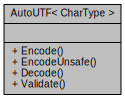
\includegraphics[width=197pt]{structAutoUTF__coll__graph}
\end{center}
\end{figure}
\subsection*{Public Types}
\begin{DoxyCompactItemize}
\item 
enum \{ \hyperlink{structAutoUTF_ac046404cf4770f29218ada39f6b652d3adc86ae046cd64f591495ac635a5c04c2}{support\+Unicode} = 1
 \}
\item 
typedef Char\+Type \hyperlink{structAutoUTF_a0609343de776df3bc31b4c980eb3cf1c}{Ch}
\end{DoxyCompactItemize}
\subsection*{Static Public Member Functions}
\begin{DoxyCompactItemize}
\item 
{\footnotesize template$<$typename Output\+Stream $>$ }\\static R\+A\+P\+I\+D\+J\+S\+O\+N\+\_\+\+F\+O\+R\+C\+E\+I\+N\+L\+I\+NE \hyperlink{imgui__impl__opengl3__loader_8h_ac668e7cffd9e2e9cfee428b9b2f34fa7}{void} \hyperlink{structAutoUTF_a414946115261f886e74dd42cb4b98781}{Encode} (Output\+Stream \&os, unsigned codepoint)
\item 
{\footnotesize template$<$typename Output\+Stream $>$ }\\static R\+A\+P\+I\+D\+J\+S\+O\+N\+\_\+\+F\+O\+R\+C\+E\+I\+N\+L\+I\+NE \hyperlink{imgui__impl__opengl3__loader_8h_ac668e7cffd9e2e9cfee428b9b2f34fa7}{void} \hyperlink{structAutoUTF_a05f5dcd1f153b61b763e44ed452de251}{Encode\+Unsafe} (Output\+Stream \&os, unsigned codepoint)
\item 
{\footnotesize template$<$typename Input\+Stream $>$ }\\static R\+A\+P\+I\+D\+J\+S\+O\+N\+\_\+\+F\+O\+R\+C\+E\+I\+N\+L\+I\+NE bool \hyperlink{structAutoUTF_aa5e3c1dc23dbb75f6442ff69500a35b0}{Decode} (Input\+Stream \&is, unsigned $\ast$codepoint)
\item 
{\footnotesize template$<$typename Input\+Stream , typename Output\+Stream $>$ }\\static R\+A\+P\+I\+D\+J\+S\+O\+N\+\_\+\+F\+O\+R\+C\+E\+I\+N\+L\+I\+NE bool \hyperlink{structAutoUTF_a36dd6f226d6a07c12161e21c0aff20b1}{Validate} (Input\+Stream \&is, Output\+Stream \&os)
\end{DoxyCompactItemize}


\subsection{Detailed Description}
\subsubsection*{template$<$typename Char\+Type$>$\newline
struct Auto\+U\+T\+F$<$ Char\+Type $>$}

Dynamically select encoding according to stream\textquotesingle{}s runtime-\/specified U\+TF encoding type. 

\begin{DoxyNote}{Note}
This class can be used with Auto\+U\+T\+F\+Inputt\+Stream and \hyperlink{classAutoUTFOutputStream}{Auto\+U\+T\+F\+Output\+Stream}, which provides Get\+Type(). 
\end{DoxyNote}


\subsection{Member Typedef Documentation}
\mbox{\Hypertarget{structAutoUTF_a0609343de776df3bc31b4c980eb3cf1c}\label{structAutoUTF_a0609343de776df3bc31b4c980eb3cf1c}} 
\index{Auto\+U\+TF@{Auto\+U\+TF}!Ch@{Ch}}
\index{Ch@{Ch}!Auto\+U\+TF@{Auto\+U\+TF}}
\subsubsection{\texorpdfstring{Ch}{Ch}}
{\footnotesize\ttfamily template$<$typename Char\+Type $>$ \\
typedef Char\+Type \hyperlink{structAutoUTF}{Auto\+U\+TF}$<$ Char\+Type $>$\+::\hyperlink{structAutoUTF_a0609343de776df3bc31b4c980eb3cf1c}{Ch}}



\subsection{Member Enumeration Documentation}
\mbox{\Hypertarget{structAutoUTF_ac046404cf4770f29218ada39f6b652d3}\label{structAutoUTF_ac046404cf4770f29218ada39f6b652d3}} 
\subsubsection{\texorpdfstring{anonymous enum}{anonymous enum}}
{\footnotesize\ttfamily template$<$typename Char\+Type $>$ \\
anonymous enum}

\begin{DoxyEnumFields}{Enumerator}
\raisebox{\heightof{T}}[0pt][0pt]{\index{support\+Unicode@{support\+Unicode}!Auto\+U\+TF@{Auto\+U\+TF}}\index{Auto\+U\+TF@{Auto\+U\+TF}!support\+Unicode@{support\+Unicode}}}\mbox{\Hypertarget{structAutoUTF_ac046404cf4770f29218ada39f6b652d3adc86ae046cd64f591495ac635a5c04c2}\label{structAutoUTF_ac046404cf4770f29218ada39f6b652d3adc86ae046cd64f591495ac635a5c04c2}} 
support\+Unicode&\\
\hline

\end{DoxyEnumFields}


\subsection{Member Function Documentation}
\mbox{\Hypertarget{structAutoUTF_aa5e3c1dc23dbb75f6442ff69500a35b0}\label{structAutoUTF_aa5e3c1dc23dbb75f6442ff69500a35b0}} 
\index{Auto\+U\+TF@{Auto\+U\+TF}!Decode@{Decode}}
\index{Decode@{Decode}!Auto\+U\+TF@{Auto\+U\+TF}}
\subsubsection{\texorpdfstring{Decode()}{Decode()}}
{\footnotesize\ttfamily template$<$typename Char\+Type $>$ \\
template$<$typename Input\+Stream $>$ \\
static R\+A\+P\+I\+D\+J\+S\+O\+N\+\_\+\+F\+O\+R\+C\+E\+I\+N\+L\+I\+NE bool \hyperlink{structAutoUTF}{Auto\+U\+TF}$<$ Char\+Type $>$\+::Decode (\begin{DoxyParamCaption}\item[{Input\+Stream \&}]{is,  }\item[{unsigned $\ast$}]{codepoint }\end{DoxyParamCaption})\hspace{0.3cm}{\ttfamily [inline]}, {\ttfamily [static]}}

\mbox{\Hypertarget{structAutoUTF_a414946115261f886e74dd42cb4b98781}\label{structAutoUTF_a414946115261f886e74dd42cb4b98781}} 
\index{Auto\+U\+TF@{Auto\+U\+TF}!Encode@{Encode}}
\index{Encode@{Encode}!Auto\+U\+TF@{Auto\+U\+TF}}
\subsubsection{\texorpdfstring{Encode()}{Encode()}}
{\footnotesize\ttfamily template$<$typename Char\+Type $>$ \\
template$<$typename Output\+Stream $>$ \\
static R\+A\+P\+I\+D\+J\+S\+O\+N\+\_\+\+F\+O\+R\+C\+E\+I\+N\+L\+I\+NE \hyperlink{imgui__impl__opengl3__loader_8h_ac668e7cffd9e2e9cfee428b9b2f34fa7}{void} \hyperlink{structAutoUTF}{Auto\+U\+TF}$<$ Char\+Type $>$\+::Encode (\begin{DoxyParamCaption}\item[{Output\+Stream \&}]{os,  }\item[{unsigned}]{codepoint }\end{DoxyParamCaption})\hspace{0.3cm}{\ttfamily [inline]}, {\ttfamily [static]}}

\mbox{\Hypertarget{structAutoUTF_a05f5dcd1f153b61b763e44ed452de251}\label{structAutoUTF_a05f5dcd1f153b61b763e44ed452de251}} 
\index{Auto\+U\+TF@{Auto\+U\+TF}!Encode\+Unsafe@{Encode\+Unsafe}}
\index{Encode\+Unsafe@{Encode\+Unsafe}!Auto\+U\+TF@{Auto\+U\+TF}}
\subsubsection{\texorpdfstring{Encode\+Unsafe()}{EncodeUnsafe()}}
{\footnotesize\ttfamily template$<$typename Char\+Type $>$ \\
template$<$typename Output\+Stream $>$ \\
static R\+A\+P\+I\+D\+J\+S\+O\+N\+\_\+\+F\+O\+R\+C\+E\+I\+N\+L\+I\+NE \hyperlink{imgui__impl__opengl3__loader_8h_ac668e7cffd9e2e9cfee428b9b2f34fa7}{void} \hyperlink{structAutoUTF}{Auto\+U\+TF}$<$ Char\+Type $>$\+::Encode\+Unsafe (\begin{DoxyParamCaption}\item[{Output\+Stream \&}]{os,  }\item[{unsigned}]{codepoint }\end{DoxyParamCaption})\hspace{0.3cm}{\ttfamily [inline]}, {\ttfamily [static]}}

\mbox{\Hypertarget{structAutoUTF_a36dd6f226d6a07c12161e21c0aff20b1}\label{structAutoUTF_a36dd6f226d6a07c12161e21c0aff20b1}} 
\index{Auto\+U\+TF@{Auto\+U\+TF}!Validate@{Validate}}
\index{Validate@{Validate}!Auto\+U\+TF@{Auto\+U\+TF}}
\subsubsection{\texorpdfstring{Validate()}{Validate()}}
{\footnotesize\ttfamily template$<$typename Char\+Type $>$ \\
template$<$typename Input\+Stream , typename Output\+Stream $>$ \\
static R\+A\+P\+I\+D\+J\+S\+O\+N\+\_\+\+F\+O\+R\+C\+E\+I\+N\+L\+I\+NE bool \hyperlink{structAutoUTF}{Auto\+U\+TF}$<$ Char\+Type $>$\+::Validate (\begin{DoxyParamCaption}\item[{Input\+Stream \&}]{is,  }\item[{Output\+Stream \&}]{os }\end{DoxyParamCaption})\hspace{0.3cm}{\ttfamily [inline]}, {\ttfamily [static]}}



The documentation for this struct was generated from the following file\+:\begin{DoxyCompactItemize}
\item 
/mnt/hdd/fnky/\+C0de/\+C\+A\+P\+S\+T\+O\+N\+E/clean\+\_\+build/include/rapidjson/\hyperlink{encodings_8h}{encodings.\+h}\end{DoxyCompactItemize}

\hypertarget{classAutoUTFInputStream}{}\section{Auto\+U\+T\+F\+Input\+Stream$<$ Char\+Type, Input\+Byte\+Stream $>$ Class Template Reference}
\label{classAutoUTFInputStream}\index{Auto\+U\+T\+F\+Input\+Stream$<$ Char\+Type, Input\+Byte\+Stream $>$@{Auto\+U\+T\+F\+Input\+Stream$<$ Char\+Type, Input\+Byte\+Stream $>$}}


Input stream wrapper with dynamically bound encoding and automatic encoding detection.  




{\ttfamily \#include $<$encodedstream.\+h$>$}



Collaboration diagram for Auto\+U\+T\+F\+Input\+Stream$<$ Char\+Type, Input\+Byte\+Stream $>$\+:
\nopagebreak
\begin{figure}[H]
\begin{center}
\leavevmode
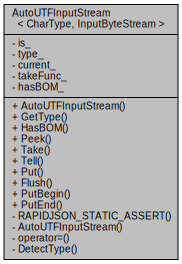
\includegraphics[width=254pt]{classAutoUTFInputStream__coll__graph}
\end{center}
\end{figure}
\subsection*{Public Types}
\begin{DoxyCompactItemize}
\item 
typedef Char\+Type \hyperlink{classAutoUTFInputStream_a3bb3eb46f2c20404a7ac21963cfe348f}{Ch}
\end{DoxyCompactItemize}
\subsection*{Public Member Functions}
\begin{DoxyCompactItemize}
\item 
\hyperlink{classAutoUTFInputStream_a83837fced0971ba26dd9a8ec1575abb0}{Auto\+U\+T\+F\+Input\+Stream} (Input\+Byte\+Stream \&is, \hyperlink{encodings_8h_ac9448aedf514a5bb509bae73a9ce4e58}{U\+T\+F\+Type} \hyperlink{imgui__impl__opengl3__loader_8h_a63267399cd2a2ee217572c11d2e54f07}{type}=\hyperlink{encodings_8h_ac9448aedf514a5bb509bae73a9ce4e58a7fd9945f1c494a4a4ee9446017e790f1}{k\+U\+T\+F8})
\begin{DoxyCompactList}\small\item\em Constructor. \end{DoxyCompactList}\item 
\hyperlink{encodings_8h_ac9448aedf514a5bb509bae73a9ce4e58}{U\+T\+F\+Type} \hyperlink{classAutoUTFInputStream_ad8e8b71e852db11a841fbba40431c5d1}{Get\+Type} () const
\item 
bool \hyperlink{classAutoUTFInputStream_a8831def623c28a3ec1d59b75abe5b20e}{Has\+B\+OM} () const
\item 
\hyperlink{classAutoUTFInputStream_a3bb3eb46f2c20404a7ac21963cfe348f}{Ch} \hyperlink{classAutoUTFInputStream_a616fbe24878a2026fbc7743acb50438c}{Peek} () const
\item 
\hyperlink{classAutoUTFInputStream_a3bb3eb46f2c20404a7ac21963cfe348f}{Ch} \hyperlink{classAutoUTFInputStream_a652cd1ae8bd848a5ecce4efa1ebd0f38}{Take} ()
\item 
size\+\_\+t \hyperlink{classAutoUTFInputStream_a6b847c75309e4ed36957f232b9ce88d1}{Tell} () const
\item 
\hyperlink{imgui__impl__opengl3__loader_8h_ac668e7cffd9e2e9cfee428b9b2f34fa7}{void} \hyperlink{classAutoUTFInputStream_a5ea730d1ab715f58ce4f9e3dcd77810a}{Put} (\hyperlink{classAutoUTFInputStream_a3bb3eb46f2c20404a7ac21963cfe348f}{Ch})
\item 
\hyperlink{imgui__impl__opengl3__loader_8h_ac668e7cffd9e2e9cfee428b9b2f34fa7}{void} \hyperlink{classAutoUTFInputStream_aecc08f52794d761fc1b729907a83dcf8}{Flush} ()
\item 
\hyperlink{classAutoUTFInputStream_a3bb3eb46f2c20404a7ac21963cfe348f}{Ch} $\ast$ \hyperlink{classAutoUTFInputStream_a761841842c147c0bb1a69bfacbc117a2}{Put\+Begin} ()
\item 
size\+\_\+t \hyperlink{classAutoUTFInputStream_a41bd66602f82d344383792feac34f9f7}{Put\+End} (\hyperlink{classAutoUTFInputStream_a3bb3eb46f2c20404a7ac21963cfe348f}{Ch} $\ast$)
\end{DoxyCompactItemize}
\subsection*{Private Types}
\begin{DoxyCompactItemize}
\item 
typedef \hyperlink{classAutoUTFInputStream_a3bb3eb46f2c20404a7ac21963cfe348f}{Ch}($\ast$ \hyperlink{classAutoUTFInputStream_a106a0af4b098cc88e1dba285b8f563ae}{Take\+Func}) (Input\+Byte\+Stream \&is)
\end{DoxyCompactItemize}
\subsection*{Private Member Functions}
\begin{DoxyCompactItemize}
\item 
\hyperlink{classAutoUTFInputStream_a74f5efc9cfc9e9978d81a3282abf17da}{R\+A\+P\+I\+D\+J\+S\+O\+N\+\_\+\+S\+T\+A\+T\+I\+C\+\_\+\+A\+S\+S\+E\+RT} (sizeof(typename Input\+Byte\+Stream\+::\+Ch)==1)
\item 
\hyperlink{classAutoUTFInputStream_a54001615e50304edf4a4ac1b2931f5d7}{Auto\+U\+T\+F\+Input\+Stream} (const \hyperlink{classAutoUTFInputStream}{Auto\+U\+T\+F\+Input\+Stream} \&)
\item 
\hyperlink{classAutoUTFInputStream}{Auto\+U\+T\+F\+Input\+Stream} \& \hyperlink{classAutoUTFInputStream_a043b85d05491e8908611054b37aec38b}{operator=} (const \hyperlink{classAutoUTFInputStream}{Auto\+U\+T\+F\+Input\+Stream} \&)
\item 
\hyperlink{imgui__impl__opengl3__loader_8h_ac668e7cffd9e2e9cfee428b9b2f34fa7}{void} \hyperlink{classAutoUTFInputStream_ae7ec4841acf560cdaee9204d6ad5dec8}{Detect\+Type} ()
\end{DoxyCompactItemize}
\subsection*{Private Attributes}
\begin{DoxyCompactItemize}
\item 
Input\+Byte\+Stream $\ast$ \hyperlink{classAutoUTFInputStream_aee206b352000902d02dac147761a61dc}{is\+\_\+}
\item 
\hyperlink{encodings_8h_ac9448aedf514a5bb509bae73a9ce4e58}{U\+T\+F\+Type} \hyperlink{classAutoUTFInputStream_aef307895f82bc15a7a37ded277aefe2e}{type\+\_\+}
\item 
\hyperlink{classAutoUTFInputStream_a3bb3eb46f2c20404a7ac21963cfe348f}{Ch} \hyperlink{classAutoUTFInputStream_a1b89f7dca4c3c462347bf7bc066a2fe1}{current\+\_\+}
\item 
\hyperlink{classAutoUTFInputStream_a106a0af4b098cc88e1dba285b8f563ae}{Take\+Func} \hyperlink{classAutoUTFInputStream_a8996755d783dcae9049d9f1ad96391fb}{take\+Func\+\_\+}
\item 
bool \hyperlink{classAutoUTFInputStream_ac329c186f5b0dc82433effecaaf1bf46}{has\+B\+O\+M\+\_\+}
\end{DoxyCompactItemize}


\subsection{Detailed Description}
\subsubsection*{template$<$typename Char\+Type, typename Input\+Byte\+Stream$>$\newline
class Auto\+U\+T\+F\+Input\+Stream$<$ Char\+Type, Input\+Byte\+Stream $>$}

Input stream wrapper with dynamically bound encoding and automatic encoding detection. 


\begin{DoxyTemplParams}{Template Parameters}
{\em Char\+Type} & Type of character for reading. \\
\hline
{\em Input\+Byte\+Stream} & type of input byte stream to be wrapped. \\
\hline
\end{DoxyTemplParams}


\subsection{Member Typedef Documentation}
\mbox{\Hypertarget{classAutoUTFInputStream_a3bb3eb46f2c20404a7ac21963cfe348f}\label{classAutoUTFInputStream_a3bb3eb46f2c20404a7ac21963cfe348f}} 
\index{Auto\+U\+T\+F\+Input\+Stream@{Auto\+U\+T\+F\+Input\+Stream}!Ch@{Ch}}
\index{Ch@{Ch}!Auto\+U\+T\+F\+Input\+Stream@{Auto\+U\+T\+F\+Input\+Stream}}
\subsubsection{\texorpdfstring{Ch}{Ch}}
{\footnotesize\ttfamily template$<$typename Char\+Type , typename Input\+Byte\+Stream $>$ \\
typedef Char\+Type \hyperlink{classAutoUTFInputStream}{Auto\+U\+T\+F\+Input\+Stream}$<$ Char\+Type, Input\+Byte\+Stream $>$\+::\hyperlink{classAutoUTFInputStream_a3bb3eb46f2c20404a7ac21963cfe348f}{Ch}}

\mbox{\Hypertarget{classAutoUTFInputStream_a106a0af4b098cc88e1dba285b8f563ae}\label{classAutoUTFInputStream_a106a0af4b098cc88e1dba285b8f563ae}} 
\index{Auto\+U\+T\+F\+Input\+Stream@{Auto\+U\+T\+F\+Input\+Stream}!Take\+Func@{Take\+Func}}
\index{Take\+Func@{Take\+Func}!Auto\+U\+T\+F\+Input\+Stream@{Auto\+U\+T\+F\+Input\+Stream}}
\subsubsection{\texorpdfstring{Take\+Func}{TakeFunc}}
{\footnotesize\ttfamily template$<$typename Char\+Type , typename Input\+Byte\+Stream $>$ \\
typedef \hyperlink{classAutoUTFInputStream_a3bb3eb46f2c20404a7ac21963cfe348f}{Ch}($\ast$ \hyperlink{classAutoUTFInputStream}{Auto\+U\+T\+F\+Input\+Stream}$<$ Char\+Type, Input\+Byte\+Stream $>$\+::Take\+Func) (Input\+Byte\+Stream \&is)\hspace{0.3cm}{\ttfamily [private]}}



\subsection{Constructor \& Destructor Documentation}
\mbox{\Hypertarget{classAutoUTFInputStream_a83837fced0971ba26dd9a8ec1575abb0}\label{classAutoUTFInputStream_a83837fced0971ba26dd9a8ec1575abb0}} 
\index{Auto\+U\+T\+F\+Input\+Stream@{Auto\+U\+T\+F\+Input\+Stream}!Auto\+U\+T\+F\+Input\+Stream@{Auto\+U\+T\+F\+Input\+Stream}}
\index{Auto\+U\+T\+F\+Input\+Stream@{Auto\+U\+T\+F\+Input\+Stream}!Auto\+U\+T\+F\+Input\+Stream@{Auto\+U\+T\+F\+Input\+Stream}}
\subsubsection{\texorpdfstring{Auto\+U\+T\+F\+Input\+Stream()}{AutoUTFInputStream()}\hspace{0.1cm}{\footnotesize\ttfamily [1/2]}}
{\footnotesize\ttfamily template$<$typename Char\+Type , typename Input\+Byte\+Stream $>$ \\
\hyperlink{classAutoUTFInputStream}{Auto\+U\+T\+F\+Input\+Stream}$<$ Char\+Type, Input\+Byte\+Stream $>$\+::\hyperlink{classAutoUTFInputStream}{Auto\+U\+T\+F\+Input\+Stream} (\begin{DoxyParamCaption}\item[{Input\+Byte\+Stream \&}]{is,  }\item[{\hyperlink{encodings_8h_ac9448aedf514a5bb509bae73a9ce4e58}{U\+T\+F\+Type}}]{type = {\ttfamily \hyperlink{encodings_8h_ac9448aedf514a5bb509bae73a9ce4e58a7fd9945f1c494a4a4ee9446017e790f1}{k\+U\+T\+F8}} }\end{DoxyParamCaption})\hspace{0.3cm}{\ttfamily [inline]}}



Constructor. 


\begin{DoxyParams}{Parameters}
{\em is} & input stream to be wrapped. \\
\hline
{\em type} & U\+TF encoding type if it is not detected from the stream. \\
\hline
\end{DoxyParams}
\mbox{\Hypertarget{classAutoUTFInputStream_a54001615e50304edf4a4ac1b2931f5d7}\label{classAutoUTFInputStream_a54001615e50304edf4a4ac1b2931f5d7}} 
\index{Auto\+U\+T\+F\+Input\+Stream@{Auto\+U\+T\+F\+Input\+Stream}!Auto\+U\+T\+F\+Input\+Stream@{Auto\+U\+T\+F\+Input\+Stream}}
\index{Auto\+U\+T\+F\+Input\+Stream@{Auto\+U\+T\+F\+Input\+Stream}!Auto\+U\+T\+F\+Input\+Stream@{Auto\+U\+T\+F\+Input\+Stream}}
\subsubsection{\texorpdfstring{Auto\+U\+T\+F\+Input\+Stream()}{AutoUTFInputStream()}\hspace{0.1cm}{\footnotesize\ttfamily [2/2]}}
{\footnotesize\ttfamily template$<$typename Char\+Type , typename Input\+Byte\+Stream $>$ \\
\hyperlink{classAutoUTFInputStream}{Auto\+U\+T\+F\+Input\+Stream}$<$ Char\+Type, Input\+Byte\+Stream $>$\+::\hyperlink{classAutoUTFInputStream}{Auto\+U\+T\+F\+Input\+Stream} (\begin{DoxyParamCaption}\item[{const \hyperlink{classAutoUTFInputStream}{Auto\+U\+T\+F\+Input\+Stream}$<$ Char\+Type, Input\+Byte\+Stream $>$ \&}]{ }\end{DoxyParamCaption})\hspace{0.3cm}{\ttfamily [private]}}



\subsection{Member Function Documentation}
\mbox{\Hypertarget{classAutoUTFInputStream_ae7ec4841acf560cdaee9204d6ad5dec8}\label{classAutoUTFInputStream_ae7ec4841acf560cdaee9204d6ad5dec8}} 
\index{Auto\+U\+T\+F\+Input\+Stream@{Auto\+U\+T\+F\+Input\+Stream}!Detect\+Type@{Detect\+Type}}
\index{Detect\+Type@{Detect\+Type}!Auto\+U\+T\+F\+Input\+Stream@{Auto\+U\+T\+F\+Input\+Stream}}
\subsubsection{\texorpdfstring{Detect\+Type()}{DetectType()}}
{\footnotesize\ttfamily template$<$typename Char\+Type , typename Input\+Byte\+Stream $>$ \\
\hyperlink{imgui__impl__opengl3__loader_8h_ac668e7cffd9e2e9cfee428b9b2f34fa7}{void} \hyperlink{classAutoUTFInputStream}{Auto\+U\+T\+F\+Input\+Stream}$<$ Char\+Type, Input\+Byte\+Stream $>$\+::Detect\+Type (\begin{DoxyParamCaption}{ }\end{DoxyParamCaption})\hspace{0.3cm}{\ttfamily [inline]}, {\ttfamily [private]}}

\mbox{\Hypertarget{classAutoUTFInputStream_aecc08f52794d761fc1b729907a83dcf8}\label{classAutoUTFInputStream_aecc08f52794d761fc1b729907a83dcf8}} 
\index{Auto\+U\+T\+F\+Input\+Stream@{Auto\+U\+T\+F\+Input\+Stream}!Flush@{Flush}}
\index{Flush@{Flush}!Auto\+U\+T\+F\+Input\+Stream@{Auto\+U\+T\+F\+Input\+Stream}}
\subsubsection{\texorpdfstring{Flush()}{Flush()}}
{\footnotesize\ttfamily template$<$typename Char\+Type , typename Input\+Byte\+Stream $>$ \\
\hyperlink{imgui__impl__opengl3__loader_8h_ac668e7cffd9e2e9cfee428b9b2f34fa7}{void} \hyperlink{classAutoUTFInputStream}{Auto\+U\+T\+F\+Input\+Stream}$<$ Char\+Type, Input\+Byte\+Stream $>$\+::Flush (\begin{DoxyParamCaption}{ }\end{DoxyParamCaption})\hspace{0.3cm}{\ttfamily [inline]}}

\mbox{\Hypertarget{classAutoUTFInputStream_ad8e8b71e852db11a841fbba40431c5d1}\label{classAutoUTFInputStream_ad8e8b71e852db11a841fbba40431c5d1}} 
\index{Auto\+U\+T\+F\+Input\+Stream@{Auto\+U\+T\+F\+Input\+Stream}!Get\+Type@{Get\+Type}}
\index{Get\+Type@{Get\+Type}!Auto\+U\+T\+F\+Input\+Stream@{Auto\+U\+T\+F\+Input\+Stream}}
\subsubsection{\texorpdfstring{Get\+Type()}{GetType()}}
{\footnotesize\ttfamily template$<$typename Char\+Type , typename Input\+Byte\+Stream $>$ \\
\hyperlink{encodings_8h_ac9448aedf514a5bb509bae73a9ce4e58}{U\+T\+F\+Type} \hyperlink{classAutoUTFInputStream}{Auto\+U\+T\+F\+Input\+Stream}$<$ Char\+Type, Input\+Byte\+Stream $>$\+::Get\+Type (\begin{DoxyParamCaption}{ }\end{DoxyParamCaption}) const\hspace{0.3cm}{\ttfamily [inline]}}

\mbox{\Hypertarget{classAutoUTFInputStream_a8831def623c28a3ec1d59b75abe5b20e}\label{classAutoUTFInputStream_a8831def623c28a3ec1d59b75abe5b20e}} 
\index{Auto\+U\+T\+F\+Input\+Stream@{Auto\+U\+T\+F\+Input\+Stream}!Has\+B\+OM@{Has\+B\+OM}}
\index{Has\+B\+OM@{Has\+B\+OM}!Auto\+U\+T\+F\+Input\+Stream@{Auto\+U\+T\+F\+Input\+Stream}}
\subsubsection{\texorpdfstring{Has\+B\+O\+M()}{HasBOM()}}
{\footnotesize\ttfamily template$<$typename Char\+Type , typename Input\+Byte\+Stream $>$ \\
bool \hyperlink{classAutoUTFInputStream}{Auto\+U\+T\+F\+Input\+Stream}$<$ Char\+Type, Input\+Byte\+Stream $>$\+::Has\+B\+OM (\begin{DoxyParamCaption}{ }\end{DoxyParamCaption}) const\hspace{0.3cm}{\ttfamily [inline]}}

\mbox{\Hypertarget{classAutoUTFInputStream_a043b85d05491e8908611054b37aec38b}\label{classAutoUTFInputStream_a043b85d05491e8908611054b37aec38b}} 
\index{Auto\+U\+T\+F\+Input\+Stream@{Auto\+U\+T\+F\+Input\+Stream}!operator=@{operator=}}
\index{operator=@{operator=}!Auto\+U\+T\+F\+Input\+Stream@{Auto\+U\+T\+F\+Input\+Stream}}
\subsubsection{\texorpdfstring{operator=()}{operator=()}}
{\footnotesize\ttfamily template$<$typename Char\+Type , typename Input\+Byte\+Stream $>$ \\
\hyperlink{classAutoUTFInputStream}{Auto\+U\+T\+F\+Input\+Stream}\& \hyperlink{classAutoUTFInputStream}{Auto\+U\+T\+F\+Input\+Stream}$<$ Char\+Type, Input\+Byte\+Stream $>$\+::operator= (\begin{DoxyParamCaption}\item[{const \hyperlink{classAutoUTFInputStream}{Auto\+U\+T\+F\+Input\+Stream}$<$ Char\+Type, Input\+Byte\+Stream $>$ \&}]{ }\end{DoxyParamCaption})\hspace{0.3cm}{\ttfamily [private]}}

\mbox{\Hypertarget{classAutoUTFInputStream_a616fbe24878a2026fbc7743acb50438c}\label{classAutoUTFInputStream_a616fbe24878a2026fbc7743acb50438c}} 
\index{Auto\+U\+T\+F\+Input\+Stream@{Auto\+U\+T\+F\+Input\+Stream}!Peek@{Peek}}
\index{Peek@{Peek}!Auto\+U\+T\+F\+Input\+Stream@{Auto\+U\+T\+F\+Input\+Stream}}
\subsubsection{\texorpdfstring{Peek()}{Peek()}}
{\footnotesize\ttfamily template$<$typename Char\+Type , typename Input\+Byte\+Stream $>$ \\
\hyperlink{classAutoUTFInputStream_a3bb3eb46f2c20404a7ac21963cfe348f}{Ch} \hyperlink{classAutoUTFInputStream}{Auto\+U\+T\+F\+Input\+Stream}$<$ Char\+Type, Input\+Byte\+Stream $>$\+::Peek (\begin{DoxyParamCaption}{ }\end{DoxyParamCaption}) const\hspace{0.3cm}{\ttfamily [inline]}}

\mbox{\Hypertarget{classAutoUTFInputStream_a5ea730d1ab715f58ce4f9e3dcd77810a}\label{classAutoUTFInputStream_a5ea730d1ab715f58ce4f9e3dcd77810a}} 
\index{Auto\+U\+T\+F\+Input\+Stream@{Auto\+U\+T\+F\+Input\+Stream}!Put@{Put}}
\index{Put@{Put}!Auto\+U\+T\+F\+Input\+Stream@{Auto\+U\+T\+F\+Input\+Stream}}
\subsubsection{\texorpdfstring{Put()}{Put()}}
{\footnotesize\ttfamily template$<$typename Char\+Type , typename Input\+Byte\+Stream $>$ \\
\hyperlink{imgui__impl__opengl3__loader_8h_ac668e7cffd9e2e9cfee428b9b2f34fa7}{void} \hyperlink{classAutoUTFInputStream}{Auto\+U\+T\+F\+Input\+Stream}$<$ Char\+Type, Input\+Byte\+Stream $>$\+::Put (\begin{DoxyParamCaption}\item[{\hyperlink{classAutoUTFInputStream_a3bb3eb46f2c20404a7ac21963cfe348f}{Ch}}]{ }\end{DoxyParamCaption})\hspace{0.3cm}{\ttfamily [inline]}}

\mbox{\Hypertarget{classAutoUTFInputStream_a761841842c147c0bb1a69bfacbc117a2}\label{classAutoUTFInputStream_a761841842c147c0bb1a69bfacbc117a2}} 
\index{Auto\+U\+T\+F\+Input\+Stream@{Auto\+U\+T\+F\+Input\+Stream}!Put\+Begin@{Put\+Begin}}
\index{Put\+Begin@{Put\+Begin}!Auto\+U\+T\+F\+Input\+Stream@{Auto\+U\+T\+F\+Input\+Stream}}
\subsubsection{\texorpdfstring{Put\+Begin()}{PutBegin()}}
{\footnotesize\ttfamily template$<$typename Char\+Type , typename Input\+Byte\+Stream $>$ \\
\hyperlink{classAutoUTFInputStream_a3bb3eb46f2c20404a7ac21963cfe348f}{Ch}$\ast$ \hyperlink{classAutoUTFInputStream}{Auto\+U\+T\+F\+Input\+Stream}$<$ Char\+Type, Input\+Byte\+Stream $>$\+::Put\+Begin (\begin{DoxyParamCaption}{ }\end{DoxyParamCaption})\hspace{0.3cm}{\ttfamily [inline]}}

\mbox{\Hypertarget{classAutoUTFInputStream_a41bd66602f82d344383792feac34f9f7}\label{classAutoUTFInputStream_a41bd66602f82d344383792feac34f9f7}} 
\index{Auto\+U\+T\+F\+Input\+Stream@{Auto\+U\+T\+F\+Input\+Stream}!Put\+End@{Put\+End}}
\index{Put\+End@{Put\+End}!Auto\+U\+T\+F\+Input\+Stream@{Auto\+U\+T\+F\+Input\+Stream}}
\subsubsection{\texorpdfstring{Put\+End()}{PutEnd()}}
{\footnotesize\ttfamily template$<$typename Char\+Type , typename Input\+Byte\+Stream $>$ \\
size\+\_\+t \hyperlink{classAutoUTFInputStream}{Auto\+U\+T\+F\+Input\+Stream}$<$ Char\+Type, Input\+Byte\+Stream $>$\+::Put\+End (\begin{DoxyParamCaption}\item[{\hyperlink{classAutoUTFInputStream_a3bb3eb46f2c20404a7ac21963cfe348f}{Ch} $\ast$}]{ }\end{DoxyParamCaption})\hspace{0.3cm}{\ttfamily [inline]}}

\mbox{\Hypertarget{classAutoUTFInputStream_a74f5efc9cfc9e9978d81a3282abf17da}\label{classAutoUTFInputStream_a74f5efc9cfc9e9978d81a3282abf17da}} 
\index{Auto\+U\+T\+F\+Input\+Stream@{Auto\+U\+T\+F\+Input\+Stream}!R\+A\+P\+I\+D\+J\+S\+O\+N\+\_\+\+S\+T\+A\+T\+I\+C\+\_\+\+A\+S\+S\+E\+RT@{R\+A\+P\+I\+D\+J\+S\+O\+N\+\_\+\+S\+T\+A\+T\+I\+C\+\_\+\+A\+S\+S\+E\+RT}}
\index{R\+A\+P\+I\+D\+J\+S\+O\+N\+\_\+\+S\+T\+A\+T\+I\+C\+\_\+\+A\+S\+S\+E\+RT@{R\+A\+P\+I\+D\+J\+S\+O\+N\+\_\+\+S\+T\+A\+T\+I\+C\+\_\+\+A\+S\+S\+E\+RT}!Auto\+U\+T\+F\+Input\+Stream@{Auto\+U\+T\+F\+Input\+Stream}}
\subsubsection{\texorpdfstring{R\+A\+P\+I\+D\+J\+S\+O\+N\+\_\+\+S\+T\+A\+T\+I\+C\+\_\+\+A\+S\+S\+E\+R\+T()}{RAPIDJSON\_STATIC\_ASSERT()}}
{\footnotesize\ttfamily template$<$typename Char\+Type , typename Input\+Byte\+Stream $>$ \\
\hyperlink{classAutoUTFInputStream}{Auto\+U\+T\+F\+Input\+Stream}$<$ Char\+Type, Input\+Byte\+Stream $>$\+::R\+A\+P\+I\+D\+J\+S\+O\+N\+\_\+\+S\+T\+A\+T\+I\+C\+\_\+\+A\+S\+S\+E\+RT (\begin{DoxyParamCaption}\item[{sizeof(typename Input\+Byte\+Stream\+::\+Ch)}]{ = {\ttfamily =1} }\end{DoxyParamCaption})\hspace{0.3cm}{\ttfamily [private]}}

\mbox{\Hypertarget{classAutoUTFInputStream_a652cd1ae8bd848a5ecce4efa1ebd0f38}\label{classAutoUTFInputStream_a652cd1ae8bd848a5ecce4efa1ebd0f38}} 
\index{Auto\+U\+T\+F\+Input\+Stream@{Auto\+U\+T\+F\+Input\+Stream}!Take@{Take}}
\index{Take@{Take}!Auto\+U\+T\+F\+Input\+Stream@{Auto\+U\+T\+F\+Input\+Stream}}
\subsubsection{\texorpdfstring{Take()}{Take()}}
{\footnotesize\ttfamily template$<$typename Char\+Type , typename Input\+Byte\+Stream $>$ \\
\hyperlink{classAutoUTFInputStream_a3bb3eb46f2c20404a7ac21963cfe348f}{Ch} \hyperlink{classAutoUTFInputStream}{Auto\+U\+T\+F\+Input\+Stream}$<$ Char\+Type, Input\+Byte\+Stream $>$\+::Take (\begin{DoxyParamCaption}{ }\end{DoxyParamCaption})\hspace{0.3cm}{\ttfamily [inline]}}

\mbox{\Hypertarget{classAutoUTFInputStream_a6b847c75309e4ed36957f232b9ce88d1}\label{classAutoUTFInputStream_a6b847c75309e4ed36957f232b9ce88d1}} 
\index{Auto\+U\+T\+F\+Input\+Stream@{Auto\+U\+T\+F\+Input\+Stream}!Tell@{Tell}}
\index{Tell@{Tell}!Auto\+U\+T\+F\+Input\+Stream@{Auto\+U\+T\+F\+Input\+Stream}}
\subsubsection{\texorpdfstring{Tell()}{Tell()}}
{\footnotesize\ttfamily template$<$typename Char\+Type , typename Input\+Byte\+Stream $>$ \\
size\+\_\+t \hyperlink{classAutoUTFInputStream}{Auto\+U\+T\+F\+Input\+Stream}$<$ Char\+Type, Input\+Byte\+Stream $>$\+::Tell (\begin{DoxyParamCaption}{ }\end{DoxyParamCaption}) const\hspace{0.3cm}{\ttfamily [inline]}}



\subsection{Member Data Documentation}
\mbox{\Hypertarget{classAutoUTFInputStream_a1b89f7dca4c3c462347bf7bc066a2fe1}\label{classAutoUTFInputStream_a1b89f7dca4c3c462347bf7bc066a2fe1}} 
\index{Auto\+U\+T\+F\+Input\+Stream@{Auto\+U\+T\+F\+Input\+Stream}!current\+\_\+@{current\+\_\+}}
\index{current\+\_\+@{current\+\_\+}!Auto\+U\+T\+F\+Input\+Stream@{Auto\+U\+T\+F\+Input\+Stream}}
\subsubsection{\texorpdfstring{current\+\_\+}{current\_}}
{\footnotesize\ttfamily template$<$typename Char\+Type , typename Input\+Byte\+Stream $>$ \\
\hyperlink{classAutoUTFInputStream_a3bb3eb46f2c20404a7ac21963cfe348f}{Ch} \hyperlink{classAutoUTFInputStream}{Auto\+U\+T\+F\+Input\+Stream}$<$ Char\+Type, Input\+Byte\+Stream $>$\+::current\+\_\+\hspace{0.3cm}{\ttfamily [private]}}

\mbox{\Hypertarget{classAutoUTFInputStream_ac329c186f5b0dc82433effecaaf1bf46}\label{classAutoUTFInputStream_ac329c186f5b0dc82433effecaaf1bf46}} 
\index{Auto\+U\+T\+F\+Input\+Stream@{Auto\+U\+T\+F\+Input\+Stream}!has\+B\+O\+M\+\_\+@{has\+B\+O\+M\+\_\+}}
\index{has\+B\+O\+M\+\_\+@{has\+B\+O\+M\+\_\+}!Auto\+U\+T\+F\+Input\+Stream@{Auto\+U\+T\+F\+Input\+Stream}}
\subsubsection{\texorpdfstring{has\+B\+O\+M\+\_\+}{hasBOM\_}}
{\footnotesize\ttfamily template$<$typename Char\+Type , typename Input\+Byte\+Stream $>$ \\
bool \hyperlink{classAutoUTFInputStream}{Auto\+U\+T\+F\+Input\+Stream}$<$ Char\+Type, Input\+Byte\+Stream $>$\+::has\+B\+O\+M\+\_\+\hspace{0.3cm}{\ttfamily [private]}}

\mbox{\Hypertarget{classAutoUTFInputStream_aee206b352000902d02dac147761a61dc}\label{classAutoUTFInputStream_aee206b352000902d02dac147761a61dc}} 
\index{Auto\+U\+T\+F\+Input\+Stream@{Auto\+U\+T\+F\+Input\+Stream}!is\+\_\+@{is\+\_\+}}
\index{is\+\_\+@{is\+\_\+}!Auto\+U\+T\+F\+Input\+Stream@{Auto\+U\+T\+F\+Input\+Stream}}
\subsubsection{\texorpdfstring{is\+\_\+}{is\_}}
{\footnotesize\ttfamily template$<$typename Char\+Type , typename Input\+Byte\+Stream $>$ \\
Input\+Byte\+Stream$\ast$ \hyperlink{classAutoUTFInputStream}{Auto\+U\+T\+F\+Input\+Stream}$<$ Char\+Type, Input\+Byte\+Stream $>$\+::is\+\_\+\hspace{0.3cm}{\ttfamily [private]}}

\mbox{\Hypertarget{classAutoUTFInputStream_a8996755d783dcae9049d9f1ad96391fb}\label{classAutoUTFInputStream_a8996755d783dcae9049d9f1ad96391fb}} 
\index{Auto\+U\+T\+F\+Input\+Stream@{Auto\+U\+T\+F\+Input\+Stream}!take\+Func\+\_\+@{take\+Func\+\_\+}}
\index{take\+Func\+\_\+@{take\+Func\+\_\+}!Auto\+U\+T\+F\+Input\+Stream@{Auto\+U\+T\+F\+Input\+Stream}}
\subsubsection{\texorpdfstring{take\+Func\+\_\+}{takeFunc\_}}
{\footnotesize\ttfamily template$<$typename Char\+Type , typename Input\+Byte\+Stream $>$ \\
\hyperlink{classAutoUTFInputStream_a106a0af4b098cc88e1dba285b8f563ae}{Take\+Func} \hyperlink{classAutoUTFInputStream}{Auto\+U\+T\+F\+Input\+Stream}$<$ Char\+Type, Input\+Byte\+Stream $>$\+::take\+Func\+\_\+\hspace{0.3cm}{\ttfamily [private]}}

\mbox{\Hypertarget{classAutoUTFInputStream_aef307895f82bc15a7a37ded277aefe2e}\label{classAutoUTFInputStream_aef307895f82bc15a7a37ded277aefe2e}} 
\index{Auto\+U\+T\+F\+Input\+Stream@{Auto\+U\+T\+F\+Input\+Stream}!type\+\_\+@{type\+\_\+}}
\index{type\+\_\+@{type\+\_\+}!Auto\+U\+T\+F\+Input\+Stream@{Auto\+U\+T\+F\+Input\+Stream}}
\subsubsection{\texorpdfstring{type\+\_\+}{type\_}}
{\footnotesize\ttfamily template$<$typename Char\+Type , typename Input\+Byte\+Stream $>$ \\
\hyperlink{encodings_8h_ac9448aedf514a5bb509bae73a9ce4e58}{U\+T\+F\+Type} \hyperlink{classAutoUTFInputStream}{Auto\+U\+T\+F\+Input\+Stream}$<$ Char\+Type, Input\+Byte\+Stream $>$\+::type\+\_\+\hspace{0.3cm}{\ttfamily [private]}}



The documentation for this class was generated from the following file\+:\begin{DoxyCompactItemize}
\item 
/mnt/hdd/fnky/\+C0de/\+C\+A\+P\+S\+T\+O\+N\+E/clean\+\_\+build/include/rapidjson/\hyperlink{encodedstream_8h}{encodedstream.\+h}\end{DoxyCompactItemize}

\hypertarget{classAutoUTFOutputStream}{}\section{Auto\+U\+T\+F\+Output\+Stream$<$ Char\+Type, Output\+Byte\+Stream $>$ Class Template Reference}
\label{classAutoUTFOutputStream}\index{Auto\+U\+T\+F\+Output\+Stream$<$ Char\+Type, Output\+Byte\+Stream $>$@{Auto\+U\+T\+F\+Output\+Stream$<$ Char\+Type, Output\+Byte\+Stream $>$}}


Output stream wrapper with dynamically bound encoding and automatic encoding detection.  




{\ttfamily \#include $<$encodedstream.\+h$>$}



Collaboration diagram for Auto\+U\+T\+F\+Output\+Stream$<$ Char\+Type, Output\+Byte\+Stream $>$\+:
\nopagebreak
\begin{figure}[H]
\begin{center}
\leavevmode
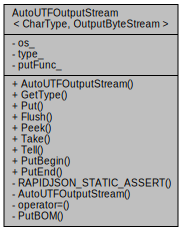
\includegraphics[width=254pt]{classAutoUTFOutputStream__coll__graph}
\end{center}
\end{figure}
\subsection*{Public Types}
\begin{DoxyCompactItemize}
\item 
typedef Char\+Type \hyperlink{classAutoUTFOutputStream_abd8c486101026e11828e86c18991c9c0}{Ch}
\end{DoxyCompactItemize}
\subsection*{Public Member Functions}
\begin{DoxyCompactItemize}
\item 
\hyperlink{classAutoUTFOutputStream_a2fe7dbc8e43d11295f66df5653148137}{Auto\+U\+T\+F\+Output\+Stream} (Output\+Byte\+Stream \&os, \hyperlink{encodings_8h_ac9448aedf514a5bb509bae73a9ce4e58}{U\+T\+F\+Type} \hyperlink{imgui__impl__opengl3__loader_8h_a63267399cd2a2ee217572c11d2e54f07}{type}, bool put\+B\+OM)
\begin{DoxyCompactList}\small\item\em Constructor. \end{DoxyCompactList}\item 
\hyperlink{encodings_8h_ac9448aedf514a5bb509bae73a9ce4e58}{U\+T\+F\+Type} \hyperlink{classAutoUTFOutputStream_a62091565a8103d69002be2e2f4f0ba2c}{Get\+Type} () const
\item 
\hyperlink{imgui__impl__opengl3__loader_8h_ac668e7cffd9e2e9cfee428b9b2f34fa7}{void} \hyperlink{classAutoUTFOutputStream_ad12b33e48c45bdbf2628fd3d5461041a}{Put} (\hyperlink{classAutoUTFOutputStream_abd8c486101026e11828e86c18991c9c0}{Ch} c)
\item 
\hyperlink{imgui__impl__opengl3__loader_8h_ac668e7cffd9e2e9cfee428b9b2f34fa7}{void} \hyperlink{classAutoUTFOutputStream_a38b54c84ba0c479552256ac092529f47}{Flush} ()
\item 
\hyperlink{classAutoUTFOutputStream_abd8c486101026e11828e86c18991c9c0}{Ch} \hyperlink{classAutoUTFOutputStream_ad706f62fd5d22967e5949f3a05087e4e}{Peek} () const
\item 
\hyperlink{classAutoUTFOutputStream_abd8c486101026e11828e86c18991c9c0}{Ch} \hyperlink{classAutoUTFOutputStream_a44ee7d84ba13fece17574d01b7be574b}{Take} ()
\item 
size\+\_\+t \hyperlink{classAutoUTFOutputStream_a81acbe33d84a28b7d5040d576ae22b5a}{Tell} () const
\item 
\hyperlink{classAutoUTFOutputStream_abd8c486101026e11828e86c18991c9c0}{Ch} $\ast$ \hyperlink{classAutoUTFOutputStream_a3c7333661dba3d2210f0b287bdd6c1f3}{Put\+Begin} ()
\item 
size\+\_\+t \hyperlink{classAutoUTFOutputStream_a4b16bda191526c894501fce447e95b8d}{Put\+End} (\hyperlink{classAutoUTFOutputStream_abd8c486101026e11828e86c18991c9c0}{Ch} $\ast$)
\end{DoxyCompactItemize}
\subsection*{Private Types}
\begin{DoxyCompactItemize}
\item 
typedef \hyperlink{imgui__impl__opengl3__loader_8h_ac668e7cffd9e2e9cfee428b9b2f34fa7}{void}($\ast$ \hyperlink{classAutoUTFOutputStream_a398450792738ee1cb865fc96dfde9e1a}{Put\+Func}) (Output\+Byte\+Stream \&, \hyperlink{classAutoUTFOutputStream_abd8c486101026e11828e86c18991c9c0}{Ch})
\end{DoxyCompactItemize}
\subsection*{Private Member Functions}
\begin{DoxyCompactItemize}
\item 
\hyperlink{classAutoUTFOutputStream_a6fbc88c345f0b7beef9053e8a0315fb4}{R\+A\+P\+I\+D\+J\+S\+O\+N\+\_\+\+S\+T\+A\+T\+I\+C\+\_\+\+A\+S\+S\+E\+RT} (sizeof(typename Output\+Byte\+Stream\+::\+Ch)==1)
\item 
\hyperlink{classAutoUTFOutputStream_aceb5330e6fddef6a439a105fe501f1d4}{Auto\+U\+T\+F\+Output\+Stream} (const \hyperlink{classAutoUTFOutputStream}{Auto\+U\+T\+F\+Output\+Stream} \&)
\item 
\hyperlink{classAutoUTFOutputStream}{Auto\+U\+T\+F\+Output\+Stream} \& \hyperlink{classAutoUTFOutputStream_a498613c6dcada9980fea3d6094f21215}{operator=} (const \hyperlink{classAutoUTFOutputStream}{Auto\+U\+T\+F\+Output\+Stream} \&)
\item 
\hyperlink{imgui__impl__opengl3__loader_8h_ac668e7cffd9e2e9cfee428b9b2f34fa7}{void} \hyperlink{classAutoUTFOutputStream_abcfbaa81ceaddf06ae435ba3e78421d7}{Put\+B\+OM} ()
\end{DoxyCompactItemize}
\subsection*{Private Attributes}
\begin{DoxyCompactItemize}
\item 
Output\+Byte\+Stream $\ast$ \hyperlink{classAutoUTFOutputStream_a723efb60d9fdb46e6094db891d24a509}{os\+\_\+}
\item 
\hyperlink{encodings_8h_ac9448aedf514a5bb509bae73a9ce4e58}{U\+T\+F\+Type} \hyperlink{classAutoUTFOutputStream_a767a11d3801e410881972013376d69eb}{type\+\_\+}
\item 
\hyperlink{classAutoUTFOutputStream_a398450792738ee1cb865fc96dfde9e1a}{Put\+Func} \hyperlink{classAutoUTFOutputStream_af15ae56768d0f65b5938eab255493274}{put\+Func\+\_\+}
\end{DoxyCompactItemize}


\subsection{Detailed Description}
\subsubsection*{template$<$typename Char\+Type, typename Output\+Byte\+Stream$>$\newline
class Auto\+U\+T\+F\+Output\+Stream$<$ Char\+Type, Output\+Byte\+Stream $>$}

Output stream wrapper with dynamically bound encoding and automatic encoding detection. 


\begin{DoxyTemplParams}{Template Parameters}
{\em Char\+Type} & Type of character for writing. \\
\hline
{\em Output\+Byte\+Stream} & type of output byte stream to be wrapped. \\
\hline
\end{DoxyTemplParams}


\subsection{Member Typedef Documentation}
\mbox{\Hypertarget{classAutoUTFOutputStream_abd8c486101026e11828e86c18991c9c0}\label{classAutoUTFOutputStream_abd8c486101026e11828e86c18991c9c0}} 
\index{Auto\+U\+T\+F\+Output\+Stream@{Auto\+U\+T\+F\+Output\+Stream}!Ch@{Ch}}
\index{Ch@{Ch}!Auto\+U\+T\+F\+Output\+Stream@{Auto\+U\+T\+F\+Output\+Stream}}
\subsubsection{\texorpdfstring{Ch}{Ch}}
{\footnotesize\ttfamily template$<$typename Char\+Type , typename Output\+Byte\+Stream $>$ \\
typedef Char\+Type \hyperlink{classAutoUTFOutputStream}{Auto\+U\+T\+F\+Output\+Stream}$<$ Char\+Type, Output\+Byte\+Stream $>$\+::\hyperlink{classAutoUTFOutputStream_abd8c486101026e11828e86c18991c9c0}{Ch}}

\mbox{\Hypertarget{classAutoUTFOutputStream_a398450792738ee1cb865fc96dfde9e1a}\label{classAutoUTFOutputStream_a398450792738ee1cb865fc96dfde9e1a}} 
\index{Auto\+U\+T\+F\+Output\+Stream@{Auto\+U\+T\+F\+Output\+Stream}!Put\+Func@{Put\+Func}}
\index{Put\+Func@{Put\+Func}!Auto\+U\+T\+F\+Output\+Stream@{Auto\+U\+T\+F\+Output\+Stream}}
\subsubsection{\texorpdfstring{Put\+Func}{PutFunc}}
{\footnotesize\ttfamily template$<$typename Char\+Type , typename Output\+Byte\+Stream $>$ \\
typedef \hyperlink{imgui__impl__opengl3__loader_8h_ac668e7cffd9e2e9cfee428b9b2f34fa7}{void}($\ast$ \hyperlink{classAutoUTFOutputStream}{Auto\+U\+T\+F\+Output\+Stream}$<$ Char\+Type, Output\+Byte\+Stream $>$\+::Put\+Func) (Output\+Byte\+Stream \&, \hyperlink{classAutoUTFOutputStream_abd8c486101026e11828e86c18991c9c0}{Ch})\hspace{0.3cm}{\ttfamily [private]}}



\subsection{Constructor \& Destructor Documentation}
\mbox{\Hypertarget{classAutoUTFOutputStream_a2fe7dbc8e43d11295f66df5653148137}\label{classAutoUTFOutputStream_a2fe7dbc8e43d11295f66df5653148137}} 
\index{Auto\+U\+T\+F\+Output\+Stream@{Auto\+U\+T\+F\+Output\+Stream}!Auto\+U\+T\+F\+Output\+Stream@{Auto\+U\+T\+F\+Output\+Stream}}
\index{Auto\+U\+T\+F\+Output\+Stream@{Auto\+U\+T\+F\+Output\+Stream}!Auto\+U\+T\+F\+Output\+Stream@{Auto\+U\+T\+F\+Output\+Stream}}
\subsubsection{\texorpdfstring{Auto\+U\+T\+F\+Output\+Stream()}{AutoUTFOutputStream()}\hspace{0.1cm}{\footnotesize\ttfamily [1/2]}}
{\footnotesize\ttfamily template$<$typename Char\+Type , typename Output\+Byte\+Stream $>$ \\
\hyperlink{classAutoUTFOutputStream}{Auto\+U\+T\+F\+Output\+Stream}$<$ Char\+Type, Output\+Byte\+Stream $>$\+::\hyperlink{classAutoUTFOutputStream}{Auto\+U\+T\+F\+Output\+Stream} (\begin{DoxyParamCaption}\item[{Output\+Byte\+Stream \&}]{os,  }\item[{\hyperlink{encodings_8h_ac9448aedf514a5bb509bae73a9ce4e58}{U\+T\+F\+Type}}]{type,  }\item[{bool}]{put\+B\+OM }\end{DoxyParamCaption})\hspace{0.3cm}{\ttfamily [inline]}}



Constructor. 


\begin{DoxyParams}{Parameters}
{\em os} & output stream to be wrapped. \\
\hline
{\em type} & U\+TF encoding type. \\
\hline
{\em put\+B\+OM} & Whether to write B\+OM at the beginning of the stream. \\
\hline
\end{DoxyParams}
\mbox{\Hypertarget{classAutoUTFOutputStream_aceb5330e6fddef6a439a105fe501f1d4}\label{classAutoUTFOutputStream_aceb5330e6fddef6a439a105fe501f1d4}} 
\index{Auto\+U\+T\+F\+Output\+Stream@{Auto\+U\+T\+F\+Output\+Stream}!Auto\+U\+T\+F\+Output\+Stream@{Auto\+U\+T\+F\+Output\+Stream}}
\index{Auto\+U\+T\+F\+Output\+Stream@{Auto\+U\+T\+F\+Output\+Stream}!Auto\+U\+T\+F\+Output\+Stream@{Auto\+U\+T\+F\+Output\+Stream}}
\subsubsection{\texorpdfstring{Auto\+U\+T\+F\+Output\+Stream()}{AutoUTFOutputStream()}\hspace{0.1cm}{\footnotesize\ttfamily [2/2]}}
{\footnotesize\ttfamily template$<$typename Char\+Type , typename Output\+Byte\+Stream $>$ \\
\hyperlink{classAutoUTFOutputStream}{Auto\+U\+T\+F\+Output\+Stream}$<$ Char\+Type, Output\+Byte\+Stream $>$\+::\hyperlink{classAutoUTFOutputStream}{Auto\+U\+T\+F\+Output\+Stream} (\begin{DoxyParamCaption}\item[{const \hyperlink{classAutoUTFOutputStream}{Auto\+U\+T\+F\+Output\+Stream}$<$ Char\+Type, Output\+Byte\+Stream $>$ \&}]{ }\end{DoxyParamCaption})\hspace{0.3cm}{\ttfamily [private]}}



\subsection{Member Function Documentation}
\mbox{\Hypertarget{classAutoUTFOutputStream_a38b54c84ba0c479552256ac092529f47}\label{classAutoUTFOutputStream_a38b54c84ba0c479552256ac092529f47}} 
\index{Auto\+U\+T\+F\+Output\+Stream@{Auto\+U\+T\+F\+Output\+Stream}!Flush@{Flush}}
\index{Flush@{Flush}!Auto\+U\+T\+F\+Output\+Stream@{Auto\+U\+T\+F\+Output\+Stream}}
\subsubsection{\texorpdfstring{Flush()}{Flush()}}
{\footnotesize\ttfamily template$<$typename Char\+Type , typename Output\+Byte\+Stream $>$ \\
\hyperlink{imgui__impl__opengl3__loader_8h_ac668e7cffd9e2e9cfee428b9b2f34fa7}{void} \hyperlink{classAutoUTFOutputStream}{Auto\+U\+T\+F\+Output\+Stream}$<$ Char\+Type, Output\+Byte\+Stream $>$\+::Flush (\begin{DoxyParamCaption}{ }\end{DoxyParamCaption})\hspace{0.3cm}{\ttfamily [inline]}}

\mbox{\Hypertarget{classAutoUTFOutputStream_a62091565a8103d69002be2e2f4f0ba2c}\label{classAutoUTFOutputStream_a62091565a8103d69002be2e2f4f0ba2c}} 
\index{Auto\+U\+T\+F\+Output\+Stream@{Auto\+U\+T\+F\+Output\+Stream}!Get\+Type@{Get\+Type}}
\index{Get\+Type@{Get\+Type}!Auto\+U\+T\+F\+Output\+Stream@{Auto\+U\+T\+F\+Output\+Stream}}
\subsubsection{\texorpdfstring{Get\+Type()}{GetType()}}
{\footnotesize\ttfamily template$<$typename Char\+Type , typename Output\+Byte\+Stream $>$ \\
\hyperlink{encodings_8h_ac9448aedf514a5bb509bae73a9ce4e58}{U\+T\+F\+Type} \hyperlink{classAutoUTFOutputStream}{Auto\+U\+T\+F\+Output\+Stream}$<$ Char\+Type, Output\+Byte\+Stream $>$\+::Get\+Type (\begin{DoxyParamCaption}{ }\end{DoxyParamCaption}) const\hspace{0.3cm}{\ttfamily [inline]}}

\mbox{\Hypertarget{classAutoUTFOutputStream_a498613c6dcada9980fea3d6094f21215}\label{classAutoUTFOutputStream_a498613c6dcada9980fea3d6094f21215}} 
\index{Auto\+U\+T\+F\+Output\+Stream@{Auto\+U\+T\+F\+Output\+Stream}!operator=@{operator=}}
\index{operator=@{operator=}!Auto\+U\+T\+F\+Output\+Stream@{Auto\+U\+T\+F\+Output\+Stream}}
\subsubsection{\texorpdfstring{operator=()}{operator=()}}
{\footnotesize\ttfamily template$<$typename Char\+Type , typename Output\+Byte\+Stream $>$ \\
\hyperlink{classAutoUTFOutputStream}{Auto\+U\+T\+F\+Output\+Stream}\& \hyperlink{classAutoUTFOutputStream}{Auto\+U\+T\+F\+Output\+Stream}$<$ Char\+Type, Output\+Byte\+Stream $>$\+::operator= (\begin{DoxyParamCaption}\item[{const \hyperlink{classAutoUTFOutputStream}{Auto\+U\+T\+F\+Output\+Stream}$<$ Char\+Type, Output\+Byte\+Stream $>$ \&}]{ }\end{DoxyParamCaption})\hspace{0.3cm}{\ttfamily [private]}}

\mbox{\Hypertarget{classAutoUTFOutputStream_ad706f62fd5d22967e5949f3a05087e4e}\label{classAutoUTFOutputStream_ad706f62fd5d22967e5949f3a05087e4e}} 
\index{Auto\+U\+T\+F\+Output\+Stream@{Auto\+U\+T\+F\+Output\+Stream}!Peek@{Peek}}
\index{Peek@{Peek}!Auto\+U\+T\+F\+Output\+Stream@{Auto\+U\+T\+F\+Output\+Stream}}
\subsubsection{\texorpdfstring{Peek()}{Peek()}}
{\footnotesize\ttfamily template$<$typename Char\+Type , typename Output\+Byte\+Stream $>$ \\
\hyperlink{classAutoUTFOutputStream_abd8c486101026e11828e86c18991c9c0}{Ch} \hyperlink{classAutoUTFOutputStream}{Auto\+U\+T\+F\+Output\+Stream}$<$ Char\+Type, Output\+Byte\+Stream $>$\+::Peek (\begin{DoxyParamCaption}{ }\end{DoxyParamCaption}) const\hspace{0.3cm}{\ttfamily [inline]}}

\mbox{\Hypertarget{classAutoUTFOutputStream_ad12b33e48c45bdbf2628fd3d5461041a}\label{classAutoUTFOutputStream_ad12b33e48c45bdbf2628fd3d5461041a}} 
\index{Auto\+U\+T\+F\+Output\+Stream@{Auto\+U\+T\+F\+Output\+Stream}!Put@{Put}}
\index{Put@{Put}!Auto\+U\+T\+F\+Output\+Stream@{Auto\+U\+T\+F\+Output\+Stream}}
\subsubsection{\texorpdfstring{Put()}{Put()}}
{\footnotesize\ttfamily template$<$typename Char\+Type , typename Output\+Byte\+Stream $>$ \\
\hyperlink{imgui__impl__opengl3__loader_8h_ac668e7cffd9e2e9cfee428b9b2f34fa7}{void} \hyperlink{classAutoUTFOutputStream}{Auto\+U\+T\+F\+Output\+Stream}$<$ Char\+Type, Output\+Byte\+Stream $>$\+::Put (\begin{DoxyParamCaption}\item[{\hyperlink{classAutoUTFOutputStream_abd8c486101026e11828e86c18991c9c0}{Ch}}]{c }\end{DoxyParamCaption})\hspace{0.3cm}{\ttfamily [inline]}}

\mbox{\Hypertarget{classAutoUTFOutputStream_a3c7333661dba3d2210f0b287bdd6c1f3}\label{classAutoUTFOutputStream_a3c7333661dba3d2210f0b287bdd6c1f3}} 
\index{Auto\+U\+T\+F\+Output\+Stream@{Auto\+U\+T\+F\+Output\+Stream}!Put\+Begin@{Put\+Begin}}
\index{Put\+Begin@{Put\+Begin}!Auto\+U\+T\+F\+Output\+Stream@{Auto\+U\+T\+F\+Output\+Stream}}
\subsubsection{\texorpdfstring{Put\+Begin()}{PutBegin()}}
{\footnotesize\ttfamily template$<$typename Char\+Type , typename Output\+Byte\+Stream $>$ \\
\hyperlink{classAutoUTFOutputStream_abd8c486101026e11828e86c18991c9c0}{Ch}$\ast$ \hyperlink{classAutoUTFOutputStream}{Auto\+U\+T\+F\+Output\+Stream}$<$ Char\+Type, Output\+Byte\+Stream $>$\+::Put\+Begin (\begin{DoxyParamCaption}{ }\end{DoxyParamCaption})\hspace{0.3cm}{\ttfamily [inline]}}

\mbox{\Hypertarget{classAutoUTFOutputStream_abcfbaa81ceaddf06ae435ba3e78421d7}\label{classAutoUTFOutputStream_abcfbaa81ceaddf06ae435ba3e78421d7}} 
\index{Auto\+U\+T\+F\+Output\+Stream@{Auto\+U\+T\+F\+Output\+Stream}!Put\+B\+OM@{Put\+B\+OM}}
\index{Put\+B\+OM@{Put\+B\+OM}!Auto\+U\+T\+F\+Output\+Stream@{Auto\+U\+T\+F\+Output\+Stream}}
\subsubsection{\texorpdfstring{Put\+B\+O\+M()}{PutBOM()}}
{\footnotesize\ttfamily template$<$typename Char\+Type , typename Output\+Byte\+Stream $>$ \\
\hyperlink{imgui__impl__opengl3__loader_8h_ac668e7cffd9e2e9cfee428b9b2f34fa7}{void} \hyperlink{classAutoUTFOutputStream}{Auto\+U\+T\+F\+Output\+Stream}$<$ Char\+Type, Output\+Byte\+Stream $>$\+::Put\+B\+OM (\begin{DoxyParamCaption}{ }\end{DoxyParamCaption})\hspace{0.3cm}{\ttfamily [inline]}, {\ttfamily [private]}}

\mbox{\Hypertarget{classAutoUTFOutputStream_a4b16bda191526c894501fce447e95b8d}\label{classAutoUTFOutputStream_a4b16bda191526c894501fce447e95b8d}} 
\index{Auto\+U\+T\+F\+Output\+Stream@{Auto\+U\+T\+F\+Output\+Stream}!Put\+End@{Put\+End}}
\index{Put\+End@{Put\+End}!Auto\+U\+T\+F\+Output\+Stream@{Auto\+U\+T\+F\+Output\+Stream}}
\subsubsection{\texorpdfstring{Put\+End()}{PutEnd()}}
{\footnotesize\ttfamily template$<$typename Char\+Type , typename Output\+Byte\+Stream $>$ \\
size\+\_\+t \hyperlink{classAutoUTFOutputStream}{Auto\+U\+T\+F\+Output\+Stream}$<$ Char\+Type, Output\+Byte\+Stream $>$\+::Put\+End (\begin{DoxyParamCaption}\item[{\hyperlink{classAutoUTFOutputStream_abd8c486101026e11828e86c18991c9c0}{Ch} $\ast$}]{ }\end{DoxyParamCaption})\hspace{0.3cm}{\ttfamily [inline]}}

\mbox{\Hypertarget{classAutoUTFOutputStream_a6fbc88c345f0b7beef9053e8a0315fb4}\label{classAutoUTFOutputStream_a6fbc88c345f0b7beef9053e8a0315fb4}} 
\index{Auto\+U\+T\+F\+Output\+Stream@{Auto\+U\+T\+F\+Output\+Stream}!R\+A\+P\+I\+D\+J\+S\+O\+N\+\_\+\+S\+T\+A\+T\+I\+C\+\_\+\+A\+S\+S\+E\+RT@{R\+A\+P\+I\+D\+J\+S\+O\+N\+\_\+\+S\+T\+A\+T\+I\+C\+\_\+\+A\+S\+S\+E\+RT}}
\index{R\+A\+P\+I\+D\+J\+S\+O\+N\+\_\+\+S\+T\+A\+T\+I\+C\+\_\+\+A\+S\+S\+E\+RT@{R\+A\+P\+I\+D\+J\+S\+O\+N\+\_\+\+S\+T\+A\+T\+I\+C\+\_\+\+A\+S\+S\+E\+RT}!Auto\+U\+T\+F\+Output\+Stream@{Auto\+U\+T\+F\+Output\+Stream}}
\subsubsection{\texorpdfstring{R\+A\+P\+I\+D\+J\+S\+O\+N\+\_\+\+S\+T\+A\+T\+I\+C\+\_\+\+A\+S\+S\+E\+R\+T()}{RAPIDJSON\_STATIC\_ASSERT()}}
{\footnotesize\ttfamily template$<$typename Char\+Type , typename Output\+Byte\+Stream $>$ \\
\hyperlink{classAutoUTFOutputStream}{Auto\+U\+T\+F\+Output\+Stream}$<$ Char\+Type, Output\+Byte\+Stream $>$\+::R\+A\+P\+I\+D\+J\+S\+O\+N\+\_\+\+S\+T\+A\+T\+I\+C\+\_\+\+A\+S\+S\+E\+RT (\begin{DoxyParamCaption}\item[{sizeof(typename Output\+Byte\+Stream\+::\+Ch)}]{ = {\ttfamily =1} }\end{DoxyParamCaption})\hspace{0.3cm}{\ttfamily [private]}}

\mbox{\Hypertarget{classAutoUTFOutputStream_a44ee7d84ba13fece17574d01b7be574b}\label{classAutoUTFOutputStream_a44ee7d84ba13fece17574d01b7be574b}} 
\index{Auto\+U\+T\+F\+Output\+Stream@{Auto\+U\+T\+F\+Output\+Stream}!Take@{Take}}
\index{Take@{Take}!Auto\+U\+T\+F\+Output\+Stream@{Auto\+U\+T\+F\+Output\+Stream}}
\subsubsection{\texorpdfstring{Take()}{Take()}}
{\footnotesize\ttfamily template$<$typename Char\+Type , typename Output\+Byte\+Stream $>$ \\
\hyperlink{classAutoUTFOutputStream_abd8c486101026e11828e86c18991c9c0}{Ch} \hyperlink{classAutoUTFOutputStream}{Auto\+U\+T\+F\+Output\+Stream}$<$ Char\+Type, Output\+Byte\+Stream $>$\+::Take (\begin{DoxyParamCaption}{ }\end{DoxyParamCaption})\hspace{0.3cm}{\ttfamily [inline]}}

\mbox{\Hypertarget{classAutoUTFOutputStream_a81acbe33d84a28b7d5040d576ae22b5a}\label{classAutoUTFOutputStream_a81acbe33d84a28b7d5040d576ae22b5a}} 
\index{Auto\+U\+T\+F\+Output\+Stream@{Auto\+U\+T\+F\+Output\+Stream}!Tell@{Tell}}
\index{Tell@{Tell}!Auto\+U\+T\+F\+Output\+Stream@{Auto\+U\+T\+F\+Output\+Stream}}
\subsubsection{\texorpdfstring{Tell()}{Tell()}}
{\footnotesize\ttfamily template$<$typename Char\+Type , typename Output\+Byte\+Stream $>$ \\
size\+\_\+t \hyperlink{classAutoUTFOutputStream}{Auto\+U\+T\+F\+Output\+Stream}$<$ Char\+Type, Output\+Byte\+Stream $>$\+::Tell (\begin{DoxyParamCaption}{ }\end{DoxyParamCaption}) const\hspace{0.3cm}{\ttfamily [inline]}}



\subsection{Member Data Documentation}
\mbox{\Hypertarget{classAutoUTFOutputStream_a723efb60d9fdb46e6094db891d24a509}\label{classAutoUTFOutputStream_a723efb60d9fdb46e6094db891d24a509}} 
\index{Auto\+U\+T\+F\+Output\+Stream@{Auto\+U\+T\+F\+Output\+Stream}!os\+\_\+@{os\+\_\+}}
\index{os\+\_\+@{os\+\_\+}!Auto\+U\+T\+F\+Output\+Stream@{Auto\+U\+T\+F\+Output\+Stream}}
\subsubsection{\texorpdfstring{os\+\_\+}{os\_}}
{\footnotesize\ttfamily template$<$typename Char\+Type , typename Output\+Byte\+Stream $>$ \\
Output\+Byte\+Stream$\ast$ \hyperlink{classAutoUTFOutputStream}{Auto\+U\+T\+F\+Output\+Stream}$<$ Char\+Type, Output\+Byte\+Stream $>$\+::os\+\_\+\hspace{0.3cm}{\ttfamily [private]}}

\mbox{\Hypertarget{classAutoUTFOutputStream_af15ae56768d0f65b5938eab255493274}\label{classAutoUTFOutputStream_af15ae56768d0f65b5938eab255493274}} 
\index{Auto\+U\+T\+F\+Output\+Stream@{Auto\+U\+T\+F\+Output\+Stream}!put\+Func\+\_\+@{put\+Func\+\_\+}}
\index{put\+Func\+\_\+@{put\+Func\+\_\+}!Auto\+U\+T\+F\+Output\+Stream@{Auto\+U\+T\+F\+Output\+Stream}}
\subsubsection{\texorpdfstring{put\+Func\+\_\+}{putFunc\_}}
{\footnotesize\ttfamily template$<$typename Char\+Type , typename Output\+Byte\+Stream $>$ \\
\hyperlink{classAutoUTFOutputStream_a398450792738ee1cb865fc96dfde9e1a}{Put\+Func} \hyperlink{classAutoUTFOutputStream}{Auto\+U\+T\+F\+Output\+Stream}$<$ Char\+Type, Output\+Byte\+Stream $>$\+::put\+Func\+\_\+\hspace{0.3cm}{\ttfamily [private]}}

\mbox{\Hypertarget{classAutoUTFOutputStream_a767a11d3801e410881972013376d69eb}\label{classAutoUTFOutputStream_a767a11d3801e410881972013376d69eb}} 
\index{Auto\+U\+T\+F\+Output\+Stream@{Auto\+U\+T\+F\+Output\+Stream}!type\+\_\+@{type\+\_\+}}
\index{type\+\_\+@{type\+\_\+}!Auto\+U\+T\+F\+Output\+Stream@{Auto\+U\+T\+F\+Output\+Stream}}
\subsubsection{\texorpdfstring{type\+\_\+}{type\_}}
{\footnotesize\ttfamily template$<$typename Char\+Type , typename Output\+Byte\+Stream $>$ \\
\hyperlink{encodings_8h_ac9448aedf514a5bb509bae73a9ce4e58}{U\+T\+F\+Type} \hyperlink{classAutoUTFOutputStream}{Auto\+U\+T\+F\+Output\+Stream}$<$ Char\+Type, Output\+Byte\+Stream $>$\+::type\+\_\+\hspace{0.3cm}{\ttfamily [private]}}



The documentation for this class was generated from the following file\+:\begin{DoxyCompactItemize}
\item 
/mnt/hdd/fnky/\+C0de/\+C\+A\+P\+S\+T\+O\+N\+E/clean\+\_\+build/include/rapidjson/\hyperlink{encodedstream_8h}{encodedstream.\+h}\end{DoxyCompactItemize}

\input{structBaseReaderHandler}
\hypertarget{classBasicIStreamWrapper}{}\section{Basic\+I\+Stream\+Wrapper$<$ Stream\+Type $>$ Class Template Reference}
\label{classBasicIStreamWrapper}\index{Basic\+I\+Stream\+Wrapper$<$ Stream\+Type $>$@{Basic\+I\+Stream\+Wrapper$<$ Stream\+Type $>$}}


Wrapper of {\ttfamily std\+::basic\+\_\+istream} into Rapid\+J\+S\+ON\textquotesingle{}s Stream concept.  




{\ttfamily \#include $<$istreamwrapper.\+h$>$}



Collaboration diagram for Basic\+I\+Stream\+Wrapper$<$ Stream\+Type $>$\+:
\nopagebreak
\begin{figure}[H]
\begin{center}
\leavevmode
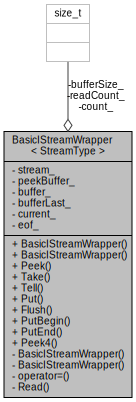
\includegraphics[width=208pt]{classBasicIStreamWrapper__coll__graph}
\end{center}
\end{figure}
\subsection*{Public Types}
\begin{DoxyCompactItemize}
\item 
typedef Stream\+Type\+::char\+\_\+type \hyperlink{classBasicIStreamWrapper_a88e4288ecdaa0d31ddf4e5917b9aa8d7}{Ch}
\end{DoxyCompactItemize}
\subsection*{Public Member Functions}
\begin{DoxyCompactItemize}
\item 
\hyperlink{classBasicIStreamWrapper_a3e9a2dd2b6b28243f8f2a911f67cdf56}{Basic\+I\+Stream\+Wrapper} (Stream\+Type \&stream)
\begin{DoxyCompactList}\small\item\em Constructor. \end{DoxyCompactList}\item 
\hyperlink{classBasicIStreamWrapper_a7a87c6702f1e98256de416ee101a460f}{Basic\+I\+Stream\+Wrapper} (Stream\+Type \&stream, char $\ast$\hyperlink{imgui__impl__opengl3__loader_8h_a3667f558219c90437106b544a3ca00b8}{buffer}, size\+\_\+t buffer\+Size)
\begin{DoxyCompactList}\small\item\em Constructor. \end{DoxyCompactList}\item 
\hyperlink{classBasicIStreamWrapper_a88e4288ecdaa0d31ddf4e5917b9aa8d7}{Ch} \hyperlink{classBasicIStreamWrapper_a0ad1488235b4786dd4f7a16e679dec88}{Peek} () const
\item 
\hyperlink{classBasicIStreamWrapper_a88e4288ecdaa0d31ddf4e5917b9aa8d7}{Ch} \hyperlink{classBasicIStreamWrapper_afb71f0329d0abbbc9b22ebeb5c1464d1}{Take} ()
\item 
size\+\_\+t \hyperlink{classBasicIStreamWrapper_ac212848265f937add49bd973de794e25}{Tell} () const
\item 
\hyperlink{imgui__impl__opengl3__loader_8h_ac668e7cffd9e2e9cfee428b9b2f34fa7}{void} \hyperlink{classBasicIStreamWrapper_afa71cb2f5b7668837d0a81e3bce55e69}{Put} (\hyperlink{classBasicIStreamWrapper_a88e4288ecdaa0d31ddf4e5917b9aa8d7}{Ch})
\item 
\hyperlink{imgui__impl__opengl3__loader_8h_ac668e7cffd9e2e9cfee428b9b2f34fa7}{void} \hyperlink{classBasicIStreamWrapper_a37d5e4cd8fdf3c83dad50737e95886a9}{Flush} ()
\item 
\hyperlink{classBasicIStreamWrapper_a88e4288ecdaa0d31ddf4e5917b9aa8d7}{Ch} $\ast$ \hyperlink{classBasicIStreamWrapper_a62a3fc10b009ea231fb9d2dc958c539c}{Put\+Begin} ()
\item 
size\+\_\+t \hyperlink{classBasicIStreamWrapper_ab2ead53490207a1cb0bdd674a03957f3}{Put\+End} (\hyperlink{classBasicIStreamWrapper_a88e4288ecdaa0d31ddf4e5917b9aa8d7}{Ch} $\ast$)
\item 
const \hyperlink{classBasicIStreamWrapper_a88e4288ecdaa0d31ddf4e5917b9aa8d7}{Ch} $\ast$ \hyperlink{classBasicIStreamWrapper_ae8b52683adc67ca0b91484a427aed660}{Peek4} () const
\end{DoxyCompactItemize}
\subsection*{Private Member Functions}
\begin{DoxyCompactItemize}
\item 
\hyperlink{classBasicIStreamWrapper_a1c72528bd8783cbf79928efbddac0a30}{Basic\+I\+Stream\+Wrapper} ()
\item 
\hyperlink{classBasicIStreamWrapper_a15a415adfc281dc08fe37513f330dc0c}{Basic\+I\+Stream\+Wrapper} (const \hyperlink{classBasicIStreamWrapper}{Basic\+I\+Stream\+Wrapper} \&)
\item 
\hyperlink{classBasicIStreamWrapper}{Basic\+I\+Stream\+Wrapper} \& \hyperlink{classBasicIStreamWrapper_a4a44440921c224c422ec211c9c20e701}{operator=} (const \hyperlink{classBasicIStreamWrapper}{Basic\+I\+Stream\+Wrapper} \&)
\item 
\hyperlink{imgui__impl__opengl3__loader_8h_ac668e7cffd9e2e9cfee428b9b2f34fa7}{void} \hyperlink{classBasicIStreamWrapper_a14f7e115ff06dbf8dda561d156641633}{Read} ()
\end{DoxyCompactItemize}
\subsection*{Private Attributes}
\begin{DoxyCompactItemize}
\item 
Stream\+Type \& \hyperlink{classBasicIStreamWrapper_a08cb5cad6653f35761ef1cdcaa407aa9}{stream\+\_\+}
\item 
\hyperlink{classBasicIStreamWrapper_a88e4288ecdaa0d31ddf4e5917b9aa8d7}{Ch} \hyperlink{classBasicIStreamWrapper_ae85be0f5472085497a21a7e135aba09d}{peek\+Buffer\+\_\+} \mbox{[}4\mbox{]}
\item 
\hyperlink{classBasicIStreamWrapper_a88e4288ecdaa0d31ddf4e5917b9aa8d7}{Ch} $\ast$ \hyperlink{classBasicIStreamWrapper_afcec6ce42add3ff03bbc8f48b1684234}{buffer\+\_\+}
\item 
size\+\_\+t \hyperlink{classBasicIStreamWrapper_a592532cbc0b32f0a7b43800997a898d2}{buffer\+Size\+\_\+}
\item 
\hyperlink{classBasicIStreamWrapper_a88e4288ecdaa0d31ddf4e5917b9aa8d7}{Ch} $\ast$ \hyperlink{classBasicIStreamWrapper_a2e3dcf3716b8525b314b95e4dd67a820}{buffer\+Last\+\_\+}
\item 
\hyperlink{classBasicIStreamWrapper_a88e4288ecdaa0d31ddf4e5917b9aa8d7}{Ch} $\ast$ \hyperlink{classBasicIStreamWrapper_a7c7a177cfffd2793855d160cc0d427c0}{current\+\_\+}
\item 
size\+\_\+t \hyperlink{classBasicIStreamWrapper_aa603c5540319d160fea25702620213ac}{read\+Count\+\_\+}
\item 
size\+\_\+t \hyperlink{classBasicIStreamWrapper_abdc3fc20e4c6e50a8bca468b457b9b79}{count\+\_\+}
\begin{DoxyCompactList}\small\item\em Number of characters read. \end{DoxyCompactList}\item 
bool \hyperlink{classBasicIStreamWrapper_afc35bf604fac076468d3801f85604210}{eof\+\_\+}
\end{DoxyCompactItemize}


\subsection{Detailed Description}
\subsubsection*{template$<$typename Stream\+Type$>$\newline
class Basic\+I\+Stream\+Wrapper$<$ Stream\+Type $>$}

Wrapper of {\ttfamily std\+::basic\+\_\+istream} into Rapid\+J\+S\+ON\textquotesingle{}s Stream concept. 

The classes can be wrapped including but not limited to\+:


\begin{DoxyItemize}
\item {\ttfamily std\+::istringstream} 
\item {\ttfamily std\+::stringstream} 
\item {\ttfamily std\+::wistringstream} 
\item {\ttfamily std\+::wstringstream} 
\item {\ttfamily std\+::ifstream} 
\item {\ttfamily std\+::fstream} 
\item {\ttfamily std\+::wifstream} 
\item {\ttfamily std\+::wfstream} 
\end{DoxyItemize}


\begin{DoxyTemplParams}{Template Parameters}
{\em Stream\+Type} & Class derived from {\ttfamily std\+::basic\+\_\+istream}. \\
\hline
\end{DoxyTemplParams}


\subsection{Member Typedef Documentation}
\mbox{\Hypertarget{classBasicIStreamWrapper_a88e4288ecdaa0d31ddf4e5917b9aa8d7}\label{classBasicIStreamWrapper_a88e4288ecdaa0d31ddf4e5917b9aa8d7}} 
\index{Basic\+I\+Stream\+Wrapper@{Basic\+I\+Stream\+Wrapper}!Ch@{Ch}}
\index{Ch@{Ch}!Basic\+I\+Stream\+Wrapper@{Basic\+I\+Stream\+Wrapper}}
\subsubsection{\texorpdfstring{Ch}{Ch}}
{\footnotesize\ttfamily template$<$typename Stream\+Type $>$ \\
typedef Stream\+Type\+::char\+\_\+type \hyperlink{classBasicIStreamWrapper}{Basic\+I\+Stream\+Wrapper}$<$ Stream\+Type $>$\+::\hyperlink{classBasicIStreamWrapper_a88e4288ecdaa0d31ddf4e5917b9aa8d7}{Ch}}



\subsection{Constructor \& Destructor Documentation}
\mbox{\Hypertarget{classBasicIStreamWrapper_a3e9a2dd2b6b28243f8f2a911f67cdf56}\label{classBasicIStreamWrapper_a3e9a2dd2b6b28243f8f2a911f67cdf56}} 
\index{Basic\+I\+Stream\+Wrapper@{Basic\+I\+Stream\+Wrapper}!Basic\+I\+Stream\+Wrapper@{Basic\+I\+Stream\+Wrapper}}
\index{Basic\+I\+Stream\+Wrapper@{Basic\+I\+Stream\+Wrapper}!Basic\+I\+Stream\+Wrapper@{Basic\+I\+Stream\+Wrapper}}
\subsubsection{\texorpdfstring{Basic\+I\+Stream\+Wrapper()}{BasicIStreamWrapper()}\hspace{0.1cm}{\footnotesize\ttfamily [1/4]}}
{\footnotesize\ttfamily template$<$typename Stream\+Type $>$ \\
\hyperlink{classBasicIStreamWrapper}{Basic\+I\+Stream\+Wrapper}$<$ Stream\+Type $>$\+::\hyperlink{classBasicIStreamWrapper}{Basic\+I\+Stream\+Wrapper} (\begin{DoxyParamCaption}\item[{Stream\+Type \&}]{stream }\end{DoxyParamCaption})\hspace{0.3cm}{\ttfamily [inline]}}



Constructor. 


\begin{DoxyParams}{Parameters}
{\em stream} & stream opened for read. \\
\hline
\end{DoxyParams}
\mbox{\Hypertarget{classBasicIStreamWrapper_a7a87c6702f1e98256de416ee101a460f}\label{classBasicIStreamWrapper_a7a87c6702f1e98256de416ee101a460f}} 
\index{Basic\+I\+Stream\+Wrapper@{Basic\+I\+Stream\+Wrapper}!Basic\+I\+Stream\+Wrapper@{Basic\+I\+Stream\+Wrapper}}
\index{Basic\+I\+Stream\+Wrapper@{Basic\+I\+Stream\+Wrapper}!Basic\+I\+Stream\+Wrapper@{Basic\+I\+Stream\+Wrapper}}
\subsubsection{\texorpdfstring{Basic\+I\+Stream\+Wrapper()}{BasicIStreamWrapper()}\hspace{0.1cm}{\footnotesize\ttfamily [2/4]}}
{\footnotesize\ttfamily template$<$typename Stream\+Type $>$ \\
\hyperlink{classBasicIStreamWrapper}{Basic\+I\+Stream\+Wrapper}$<$ Stream\+Type $>$\+::\hyperlink{classBasicIStreamWrapper}{Basic\+I\+Stream\+Wrapper} (\begin{DoxyParamCaption}\item[{Stream\+Type \&}]{stream,  }\item[{char $\ast$}]{buffer,  }\item[{size\+\_\+t}]{buffer\+Size }\end{DoxyParamCaption})\hspace{0.3cm}{\ttfamily [inline]}}



Constructor. 


\begin{DoxyParams}{Parameters}
{\em stream} & stream opened for read. \\
\hline
{\em buffer} & user-\/supplied buffer. \\
\hline
{\em buffer\+Size} & size of buffer in bytes. Must $>$=4 bytes. \\
\hline
\end{DoxyParams}
\mbox{\Hypertarget{classBasicIStreamWrapper_a1c72528bd8783cbf79928efbddac0a30}\label{classBasicIStreamWrapper_a1c72528bd8783cbf79928efbddac0a30}} 
\index{Basic\+I\+Stream\+Wrapper@{Basic\+I\+Stream\+Wrapper}!Basic\+I\+Stream\+Wrapper@{Basic\+I\+Stream\+Wrapper}}
\index{Basic\+I\+Stream\+Wrapper@{Basic\+I\+Stream\+Wrapper}!Basic\+I\+Stream\+Wrapper@{Basic\+I\+Stream\+Wrapper}}
\subsubsection{\texorpdfstring{Basic\+I\+Stream\+Wrapper()}{BasicIStreamWrapper()}\hspace{0.1cm}{\footnotesize\ttfamily [3/4]}}
{\footnotesize\ttfamily template$<$typename Stream\+Type $>$ \\
\hyperlink{classBasicIStreamWrapper}{Basic\+I\+Stream\+Wrapper}$<$ Stream\+Type $>$\+::\hyperlink{classBasicIStreamWrapper}{Basic\+I\+Stream\+Wrapper} (\begin{DoxyParamCaption}{ }\end{DoxyParamCaption})\hspace{0.3cm}{\ttfamily [private]}}

\mbox{\Hypertarget{classBasicIStreamWrapper_a15a415adfc281dc08fe37513f330dc0c}\label{classBasicIStreamWrapper_a15a415adfc281dc08fe37513f330dc0c}} 
\index{Basic\+I\+Stream\+Wrapper@{Basic\+I\+Stream\+Wrapper}!Basic\+I\+Stream\+Wrapper@{Basic\+I\+Stream\+Wrapper}}
\index{Basic\+I\+Stream\+Wrapper@{Basic\+I\+Stream\+Wrapper}!Basic\+I\+Stream\+Wrapper@{Basic\+I\+Stream\+Wrapper}}
\subsubsection{\texorpdfstring{Basic\+I\+Stream\+Wrapper()}{BasicIStreamWrapper()}\hspace{0.1cm}{\footnotesize\ttfamily [4/4]}}
{\footnotesize\ttfamily template$<$typename Stream\+Type $>$ \\
\hyperlink{classBasicIStreamWrapper}{Basic\+I\+Stream\+Wrapper}$<$ Stream\+Type $>$\+::\hyperlink{classBasicIStreamWrapper}{Basic\+I\+Stream\+Wrapper} (\begin{DoxyParamCaption}\item[{const \hyperlink{classBasicIStreamWrapper}{Basic\+I\+Stream\+Wrapper}$<$ Stream\+Type $>$ \&}]{ }\end{DoxyParamCaption})\hspace{0.3cm}{\ttfamily [private]}}



\subsection{Member Function Documentation}
\mbox{\Hypertarget{classBasicIStreamWrapper_a37d5e4cd8fdf3c83dad50737e95886a9}\label{classBasicIStreamWrapper_a37d5e4cd8fdf3c83dad50737e95886a9}} 
\index{Basic\+I\+Stream\+Wrapper@{Basic\+I\+Stream\+Wrapper}!Flush@{Flush}}
\index{Flush@{Flush}!Basic\+I\+Stream\+Wrapper@{Basic\+I\+Stream\+Wrapper}}
\subsubsection{\texorpdfstring{Flush()}{Flush()}}
{\footnotesize\ttfamily template$<$typename Stream\+Type $>$ \\
\hyperlink{imgui__impl__opengl3__loader_8h_ac668e7cffd9e2e9cfee428b9b2f34fa7}{void} \hyperlink{classBasicIStreamWrapper}{Basic\+I\+Stream\+Wrapper}$<$ Stream\+Type $>$\+::Flush (\begin{DoxyParamCaption}{ }\end{DoxyParamCaption})\hspace{0.3cm}{\ttfamily [inline]}}

\mbox{\Hypertarget{classBasicIStreamWrapper_a4a44440921c224c422ec211c9c20e701}\label{classBasicIStreamWrapper_a4a44440921c224c422ec211c9c20e701}} 
\index{Basic\+I\+Stream\+Wrapper@{Basic\+I\+Stream\+Wrapper}!operator=@{operator=}}
\index{operator=@{operator=}!Basic\+I\+Stream\+Wrapper@{Basic\+I\+Stream\+Wrapper}}
\subsubsection{\texorpdfstring{operator=()}{operator=()}}
{\footnotesize\ttfamily template$<$typename Stream\+Type $>$ \\
\hyperlink{classBasicIStreamWrapper}{Basic\+I\+Stream\+Wrapper}\& \hyperlink{classBasicIStreamWrapper}{Basic\+I\+Stream\+Wrapper}$<$ Stream\+Type $>$\+::operator= (\begin{DoxyParamCaption}\item[{const \hyperlink{classBasicIStreamWrapper}{Basic\+I\+Stream\+Wrapper}$<$ Stream\+Type $>$ \&}]{ }\end{DoxyParamCaption})\hspace{0.3cm}{\ttfamily [private]}}

\mbox{\Hypertarget{classBasicIStreamWrapper_a0ad1488235b4786dd4f7a16e679dec88}\label{classBasicIStreamWrapper_a0ad1488235b4786dd4f7a16e679dec88}} 
\index{Basic\+I\+Stream\+Wrapper@{Basic\+I\+Stream\+Wrapper}!Peek@{Peek}}
\index{Peek@{Peek}!Basic\+I\+Stream\+Wrapper@{Basic\+I\+Stream\+Wrapper}}
\subsubsection{\texorpdfstring{Peek()}{Peek()}}
{\footnotesize\ttfamily template$<$typename Stream\+Type $>$ \\
\hyperlink{classBasicIStreamWrapper_a88e4288ecdaa0d31ddf4e5917b9aa8d7}{Ch} \hyperlink{classBasicIStreamWrapper}{Basic\+I\+Stream\+Wrapper}$<$ Stream\+Type $>$\+::Peek (\begin{DoxyParamCaption}{ }\end{DoxyParamCaption}) const\hspace{0.3cm}{\ttfamily [inline]}}

\mbox{\Hypertarget{classBasicIStreamWrapper_ae8b52683adc67ca0b91484a427aed660}\label{classBasicIStreamWrapper_ae8b52683adc67ca0b91484a427aed660}} 
\index{Basic\+I\+Stream\+Wrapper@{Basic\+I\+Stream\+Wrapper}!Peek4@{Peek4}}
\index{Peek4@{Peek4}!Basic\+I\+Stream\+Wrapper@{Basic\+I\+Stream\+Wrapper}}
\subsubsection{\texorpdfstring{Peek4()}{Peek4()}}
{\footnotesize\ttfamily template$<$typename Stream\+Type $>$ \\
const \hyperlink{classBasicIStreamWrapper_a88e4288ecdaa0d31ddf4e5917b9aa8d7}{Ch}$\ast$ \hyperlink{classBasicIStreamWrapper}{Basic\+I\+Stream\+Wrapper}$<$ Stream\+Type $>$\+::Peek4 (\begin{DoxyParamCaption}{ }\end{DoxyParamCaption}) const\hspace{0.3cm}{\ttfamily [inline]}}

\mbox{\Hypertarget{classBasicIStreamWrapper_afa71cb2f5b7668837d0a81e3bce55e69}\label{classBasicIStreamWrapper_afa71cb2f5b7668837d0a81e3bce55e69}} 
\index{Basic\+I\+Stream\+Wrapper@{Basic\+I\+Stream\+Wrapper}!Put@{Put}}
\index{Put@{Put}!Basic\+I\+Stream\+Wrapper@{Basic\+I\+Stream\+Wrapper}}
\subsubsection{\texorpdfstring{Put()}{Put()}}
{\footnotesize\ttfamily template$<$typename Stream\+Type $>$ \\
\hyperlink{imgui__impl__opengl3__loader_8h_ac668e7cffd9e2e9cfee428b9b2f34fa7}{void} \hyperlink{classBasicIStreamWrapper}{Basic\+I\+Stream\+Wrapper}$<$ Stream\+Type $>$\+::Put (\begin{DoxyParamCaption}\item[{\hyperlink{classBasicIStreamWrapper_a88e4288ecdaa0d31ddf4e5917b9aa8d7}{Ch}}]{ }\end{DoxyParamCaption})\hspace{0.3cm}{\ttfamily [inline]}}

\mbox{\Hypertarget{classBasicIStreamWrapper_a62a3fc10b009ea231fb9d2dc958c539c}\label{classBasicIStreamWrapper_a62a3fc10b009ea231fb9d2dc958c539c}} 
\index{Basic\+I\+Stream\+Wrapper@{Basic\+I\+Stream\+Wrapper}!Put\+Begin@{Put\+Begin}}
\index{Put\+Begin@{Put\+Begin}!Basic\+I\+Stream\+Wrapper@{Basic\+I\+Stream\+Wrapper}}
\subsubsection{\texorpdfstring{Put\+Begin()}{PutBegin()}}
{\footnotesize\ttfamily template$<$typename Stream\+Type $>$ \\
\hyperlink{classBasicIStreamWrapper_a88e4288ecdaa0d31ddf4e5917b9aa8d7}{Ch}$\ast$ \hyperlink{classBasicIStreamWrapper}{Basic\+I\+Stream\+Wrapper}$<$ Stream\+Type $>$\+::Put\+Begin (\begin{DoxyParamCaption}{ }\end{DoxyParamCaption})\hspace{0.3cm}{\ttfamily [inline]}}

\mbox{\Hypertarget{classBasicIStreamWrapper_ab2ead53490207a1cb0bdd674a03957f3}\label{classBasicIStreamWrapper_ab2ead53490207a1cb0bdd674a03957f3}} 
\index{Basic\+I\+Stream\+Wrapper@{Basic\+I\+Stream\+Wrapper}!Put\+End@{Put\+End}}
\index{Put\+End@{Put\+End}!Basic\+I\+Stream\+Wrapper@{Basic\+I\+Stream\+Wrapper}}
\subsubsection{\texorpdfstring{Put\+End()}{PutEnd()}}
{\footnotesize\ttfamily template$<$typename Stream\+Type $>$ \\
size\+\_\+t \hyperlink{classBasicIStreamWrapper}{Basic\+I\+Stream\+Wrapper}$<$ Stream\+Type $>$\+::Put\+End (\begin{DoxyParamCaption}\item[{\hyperlink{classBasicIStreamWrapper_a88e4288ecdaa0d31ddf4e5917b9aa8d7}{Ch} $\ast$}]{ }\end{DoxyParamCaption})\hspace{0.3cm}{\ttfamily [inline]}}

\mbox{\Hypertarget{classBasicIStreamWrapper_a14f7e115ff06dbf8dda561d156641633}\label{classBasicIStreamWrapper_a14f7e115ff06dbf8dda561d156641633}} 
\index{Basic\+I\+Stream\+Wrapper@{Basic\+I\+Stream\+Wrapper}!Read@{Read}}
\index{Read@{Read}!Basic\+I\+Stream\+Wrapper@{Basic\+I\+Stream\+Wrapper}}
\subsubsection{\texorpdfstring{Read()}{Read()}}
{\footnotesize\ttfamily template$<$typename Stream\+Type $>$ \\
\hyperlink{imgui__impl__opengl3__loader_8h_ac668e7cffd9e2e9cfee428b9b2f34fa7}{void} \hyperlink{classBasicIStreamWrapper}{Basic\+I\+Stream\+Wrapper}$<$ Stream\+Type $>$\+::Read (\begin{DoxyParamCaption}{ }\end{DoxyParamCaption})\hspace{0.3cm}{\ttfamily [inline]}, {\ttfamily [private]}}

\mbox{\Hypertarget{classBasicIStreamWrapper_afb71f0329d0abbbc9b22ebeb5c1464d1}\label{classBasicIStreamWrapper_afb71f0329d0abbbc9b22ebeb5c1464d1}} 
\index{Basic\+I\+Stream\+Wrapper@{Basic\+I\+Stream\+Wrapper}!Take@{Take}}
\index{Take@{Take}!Basic\+I\+Stream\+Wrapper@{Basic\+I\+Stream\+Wrapper}}
\subsubsection{\texorpdfstring{Take()}{Take()}}
{\footnotesize\ttfamily template$<$typename Stream\+Type $>$ \\
\hyperlink{classBasicIStreamWrapper_a88e4288ecdaa0d31ddf4e5917b9aa8d7}{Ch} \hyperlink{classBasicIStreamWrapper}{Basic\+I\+Stream\+Wrapper}$<$ Stream\+Type $>$\+::Take (\begin{DoxyParamCaption}{ }\end{DoxyParamCaption})\hspace{0.3cm}{\ttfamily [inline]}}

\mbox{\Hypertarget{classBasicIStreamWrapper_ac212848265f937add49bd973de794e25}\label{classBasicIStreamWrapper_ac212848265f937add49bd973de794e25}} 
\index{Basic\+I\+Stream\+Wrapper@{Basic\+I\+Stream\+Wrapper}!Tell@{Tell}}
\index{Tell@{Tell}!Basic\+I\+Stream\+Wrapper@{Basic\+I\+Stream\+Wrapper}}
\subsubsection{\texorpdfstring{Tell()}{Tell()}}
{\footnotesize\ttfamily template$<$typename Stream\+Type $>$ \\
size\+\_\+t \hyperlink{classBasicIStreamWrapper}{Basic\+I\+Stream\+Wrapper}$<$ Stream\+Type $>$\+::Tell (\begin{DoxyParamCaption}{ }\end{DoxyParamCaption}) const\hspace{0.3cm}{\ttfamily [inline]}}



\subsection{Member Data Documentation}
\mbox{\Hypertarget{classBasicIStreamWrapper_afcec6ce42add3ff03bbc8f48b1684234}\label{classBasicIStreamWrapper_afcec6ce42add3ff03bbc8f48b1684234}} 
\index{Basic\+I\+Stream\+Wrapper@{Basic\+I\+Stream\+Wrapper}!buffer\+\_\+@{buffer\+\_\+}}
\index{buffer\+\_\+@{buffer\+\_\+}!Basic\+I\+Stream\+Wrapper@{Basic\+I\+Stream\+Wrapper}}
\subsubsection{\texorpdfstring{buffer\+\_\+}{buffer\_}}
{\footnotesize\ttfamily template$<$typename Stream\+Type $>$ \\
\hyperlink{classBasicIStreamWrapper_a88e4288ecdaa0d31ddf4e5917b9aa8d7}{Ch} $\ast$ \hyperlink{classBasicIStreamWrapper}{Basic\+I\+Stream\+Wrapper}$<$ Stream\+Type $>$\+::buffer\+\_\+\hspace{0.3cm}{\ttfamily [private]}}

\mbox{\Hypertarget{classBasicIStreamWrapper_a2e3dcf3716b8525b314b95e4dd67a820}\label{classBasicIStreamWrapper_a2e3dcf3716b8525b314b95e4dd67a820}} 
\index{Basic\+I\+Stream\+Wrapper@{Basic\+I\+Stream\+Wrapper}!buffer\+Last\+\_\+@{buffer\+Last\+\_\+}}
\index{buffer\+Last\+\_\+@{buffer\+Last\+\_\+}!Basic\+I\+Stream\+Wrapper@{Basic\+I\+Stream\+Wrapper}}
\subsubsection{\texorpdfstring{buffer\+Last\+\_\+}{bufferLast\_}}
{\footnotesize\ttfamily template$<$typename Stream\+Type $>$ \\
\hyperlink{classBasicIStreamWrapper_a88e4288ecdaa0d31ddf4e5917b9aa8d7}{Ch}$\ast$ \hyperlink{classBasicIStreamWrapper}{Basic\+I\+Stream\+Wrapper}$<$ Stream\+Type $>$\+::buffer\+Last\+\_\+\hspace{0.3cm}{\ttfamily [private]}}

\mbox{\Hypertarget{classBasicIStreamWrapper_a592532cbc0b32f0a7b43800997a898d2}\label{classBasicIStreamWrapper_a592532cbc0b32f0a7b43800997a898d2}} 
\index{Basic\+I\+Stream\+Wrapper@{Basic\+I\+Stream\+Wrapper}!buffer\+Size\+\_\+@{buffer\+Size\+\_\+}}
\index{buffer\+Size\+\_\+@{buffer\+Size\+\_\+}!Basic\+I\+Stream\+Wrapper@{Basic\+I\+Stream\+Wrapper}}
\subsubsection{\texorpdfstring{buffer\+Size\+\_\+}{bufferSize\_}}
{\footnotesize\ttfamily template$<$typename Stream\+Type $>$ \\
size\+\_\+t \hyperlink{classBasicIStreamWrapper}{Basic\+I\+Stream\+Wrapper}$<$ Stream\+Type $>$\+::buffer\+Size\+\_\+\hspace{0.3cm}{\ttfamily [private]}}

\mbox{\Hypertarget{classBasicIStreamWrapper_abdc3fc20e4c6e50a8bca468b457b9b79}\label{classBasicIStreamWrapper_abdc3fc20e4c6e50a8bca468b457b9b79}} 
\index{Basic\+I\+Stream\+Wrapper@{Basic\+I\+Stream\+Wrapper}!count\+\_\+@{count\+\_\+}}
\index{count\+\_\+@{count\+\_\+}!Basic\+I\+Stream\+Wrapper@{Basic\+I\+Stream\+Wrapper}}
\subsubsection{\texorpdfstring{count\+\_\+}{count\_}}
{\footnotesize\ttfamily template$<$typename Stream\+Type $>$ \\
size\+\_\+t \hyperlink{classBasicIStreamWrapper}{Basic\+I\+Stream\+Wrapper}$<$ Stream\+Type $>$\+::count\+\_\+\hspace{0.3cm}{\ttfamily [private]}}



Number of characters read. 

\mbox{\Hypertarget{classBasicIStreamWrapper_a7c7a177cfffd2793855d160cc0d427c0}\label{classBasicIStreamWrapper_a7c7a177cfffd2793855d160cc0d427c0}} 
\index{Basic\+I\+Stream\+Wrapper@{Basic\+I\+Stream\+Wrapper}!current\+\_\+@{current\+\_\+}}
\index{current\+\_\+@{current\+\_\+}!Basic\+I\+Stream\+Wrapper@{Basic\+I\+Stream\+Wrapper}}
\subsubsection{\texorpdfstring{current\+\_\+}{current\_}}
{\footnotesize\ttfamily template$<$typename Stream\+Type $>$ \\
\hyperlink{classBasicIStreamWrapper_a88e4288ecdaa0d31ddf4e5917b9aa8d7}{Ch}$\ast$ \hyperlink{classBasicIStreamWrapper}{Basic\+I\+Stream\+Wrapper}$<$ Stream\+Type $>$\+::current\+\_\+\hspace{0.3cm}{\ttfamily [private]}}

\mbox{\Hypertarget{classBasicIStreamWrapper_afc35bf604fac076468d3801f85604210}\label{classBasicIStreamWrapper_afc35bf604fac076468d3801f85604210}} 
\index{Basic\+I\+Stream\+Wrapper@{Basic\+I\+Stream\+Wrapper}!eof\+\_\+@{eof\+\_\+}}
\index{eof\+\_\+@{eof\+\_\+}!Basic\+I\+Stream\+Wrapper@{Basic\+I\+Stream\+Wrapper}}
\subsubsection{\texorpdfstring{eof\+\_\+}{eof\_}}
{\footnotesize\ttfamily template$<$typename Stream\+Type $>$ \\
bool \hyperlink{classBasicIStreamWrapper}{Basic\+I\+Stream\+Wrapper}$<$ Stream\+Type $>$\+::eof\+\_\+\hspace{0.3cm}{\ttfamily [private]}}

\mbox{\Hypertarget{classBasicIStreamWrapper_ae85be0f5472085497a21a7e135aba09d}\label{classBasicIStreamWrapper_ae85be0f5472085497a21a7e135aba09d}} 
\index{Basic\+I\+Stream\+Wrapper@{Basic\+I\+Stream\+Wrapper}!peek\+Buffer\+\_\+@{peek\+Buffer\+\_\+}}
\index{peek\+Buffer\+\_\+@{peek\+Buffer\+\_\+}!Basic\+I\+Stream\+Wrapper@{Basic\+I\+Stream\+Wrapper}}
\subsubsection{\texorpdfstring{peek\+Buffer\+\_\+}{peekBuffer\_}}
{\footnotesize\ttfamily template$<$typename Stream\+Type $>$ \\
\hyperlink{classBasicIStreamWrapper_a88e4288ecdaa0d31ddf4e5917b9aa8d7}{Ch} \hyperlink{classBasicIStreamWrapper}{Basic\+I\+Stream\+Wrapper}$<$ Stream\+Type $>$\+::peek\+Buffer\+\_\+\mbox{[}4\mbox{]}\hspace{0.3cm}{\ttfamily [private]}}

\mbox{\Hypertarget{classBasicIStreamWrapper_aa603c5540319d160fea25702620213ac}\label{classBasicIStreamWrapper_aa603c5540319d160fea25702620213ac}} 
\index{Basic\+I\+Stream\+Wrapper@{Basic\+I\+Stream\+Wrapper}!read\+Count\+\_\+@{read\+Count\+\_\+}}
\index{read\+Count\+\_\+@{read\+Count\+\_\+}!Basic\+I\+Stream\+Wrapper@{Basic\+I\+Stream\+Wrapper}}
\subsubsection{\texorpdfstring{read\+Count\+\_\+}{readCount\_}}
{\footnotesize\ttfamily template$<$typename Stream\+Type $>$ \\
size\+\_\+t \hyperlink{classBasicIStreamWrapper}{Basic\+I\+Stream\+Wrapper}$<$ Stream\+Type $>$\+::read\+Count\+\_\+\hspace{0.3cm}{\ttfamily [private]}}

\mbox{\Hypertarget{classBasicIStreamWrapper_a08cb5cad6653f35761ef1cdcaa407aa9}\label{classBasicIStreamWrapper_a08cb5cad6653f35761ef1cdcaa407aa9}} 
\index{Basic\+I\+Stream\+Wrapper@{Basic\+I\+Stream\+Wrapper}!stream\+\_\+@{stream\+\_\+}}
\index{stream\+\_\+@{stream\+\_\+}!Basic\+I\+Stream\+Wrapper@{Basic\+I\+Stream\+Wrapper}}
\subsubsection{\texorpdfstring{stream\+\_\+}{stream\_}}
{\footnotesize\ttfamily template$<$typename Stream\+Type $>$ \\
Stream\+Type\& \hyperlink{classBasicIStreamWrapper}{Basic\+I\+Stream\+Wrapper}$<$ Stream\+Type $>$\+::stream\+\_\+\hspace{0.3cm}{\ttfamily [private]}}



The documentation for this class was generated from the following file\+:\begin{DoxyCompactItemize}
\item 
/mnt/hdd/fnky/\+C0de/\+C\+A\+P\+S\+T\+O\+N\+E/clean\+\_\+build/include/rapidjson/\hyperlink{istreamwrapper_8h}{istreamwrapper.\+h}\end{DoxyCompactItemize}

\hypertarget{classBasicOStreamWrapper}{}\section{Basic\+O\+Stream\+Wrapper$<$ Stream\+Type $>$ Class Template Reference}
\label{classBasicOStreamWrapper}\index{Basic\+O\+Stream\+Wrapper$<$ Stream\+Type $>$@{Basic\+O\+Stream\+Wrapper$<$ Stream\+Type $>$}}


Wrapper of {\ttfamily std\+::basic\+\_\+ostream} into Rapid\+J\+S\+ON\textquotesingle{}s Stream concept.  




{\ttfamily \#include $<$ostreamwrapper.\+h$>$}



Collaboration diagram for Basic\+O\+Stream\+Wrapper$<$ Stream\+Type $>$\+:
\nopagebreak
\begin{figure}[H]
\begin{center}
\leavevmode
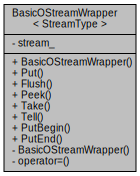
\includegraphics[width=212pt]{classBasicOStreamWrapper__coll__graph}
\end{center}
\end{figure}
\subsection*{Public Types}
\begin{DoxyCompactItemize}
\item 
typedef Stream\+Type\+::char\+\_\+type \hyperlink{classBasicOStreamWrapper_aafc6276f1f5cc0b8d45d137584d380bb}{Ch}
\end{DoxyCompactItemize}
\subsection*{Public Member Functions}
\begin{DoxyCompactItemize}
\item 
\hyperlink{classBasicOStreamWrapper_a067a516c13b7c9d4dacef598d32779ef}{Basic\+O\+Stream\+Wrapper} (Stream\+Type \&stream)
\item 
\hyperlink{imgui__impl__opengl3__loader_8h_ac668e7cffd9e2e9cfee428b9b2f34fa7}{void} \hyperlink{classBasicOStreamWrapper_a7d3ba9d651fbe27fe05387f512154ea8}{Put} (\hyperlink{classBasicOStreamWrapper_aafc6276f1f5cc0b8d45d137584d380bb}{Ch} c)
\item 
\hyperlink{imgui__impl__opengl3__loader_8h_ac668e7cffd9e2e9cfee428b9b2f34fa7}{void} \hyperlink{classBasicOStreamWrapper_a1c48a8b7520b0ab6ca34e665b928b56d}{Flush} ()
\item 
char \hyperlink{classBasicOStreamWrapper_a6dc18ded82487d41a2d123e21a9e050b}{Peek} () const
\item 
char \hyperlink{classBasicOStreamWrapper_a54be63e8d24f4d82329b860a907f65fe}{Take} ()
\item 
size\+\_\+t \hyperlink{classBasicOStreamWrapper_a62f214649fbfb8380a69fe92b864a61b}{Tell} () const
\item 
char $\ast$ \hyperlink{classBasicOStreamWrapper_a564b7b727bdab12185e7a7bd1ac5e822}{Put\+Begin} ()
\item 
size\+\_\+t \hyperlink{classBasicOStreamWrapper_a1da108e43a5a517c4484821fced1fca0}{Put\+End} (char $\ast$)
\end{DoxyCompactItemize}
\subsection*{Private Member Functions}
\begin{DoxyCompactItemize}
\item 
\hyperlink{classBasicOStreamWrapper_a3afe69cbc61a45e824392ca9b691c063}{Basic\+O\+Stream\+Wrapper} (const \hyperlink{classBasicOStreamWrapper}{Basic\+O\+Stream\+Wrapper} \&)
\item 
\hyperlink{classBasicOStreamWrapper}{Basic\+O\+Stream\+Wrapper} \& \hyperlink{classBasicOStreamWrapper_a6c1ce774ea7c0cab85241320de26448c}{operator=} (const \hyperlink{classBasicOStreamWrapper}{Basic\+O\+Stream\+Wrapper} \&)
\end{DoxyCompactItemize}
\subsection*{Private Attributes}
\begin{DoxyCompactItemize}
\item 
Stream\+Type \& \hyperlink{classBasicOStreamWrapper_a21f88a6682bed5b3168baca2a0802736}{stream\+\_\+}
\end{DoxyCompactItemize}


\subsection{Detailed Description}
\subsubsection*{template$<$typename Stream\+Type$>$\newline
class Basic\+O\+Stream\+Wrapper$<$ Stream\+Type $>$}

Wrapper of {\ttfamily std\+::basic\+\_\+ostream} into Rapid\+J\+S\+ON\textquotesingle{}s Stream concept. 

The classes can be wrapped including but not limited to\+:


\begin{DoxyItemize}
\item {\ttfamily std\+::ostringstream} 
\item {\ttfamily std\+::stringstream} 
\item {\ttfamily std\+::wpstringstream} 
\item {\ttfamily std\+::wstringstream} 
\item {\ttfamily std\+::ifstream} 
\item {\ttfamily std\+::fstream} 
\item {\ttfamily std\+::wofstream} 
\item {\ttfamily std\+::wfstream} 
\end{DoxyItemize}


\begin{DoxyTemplParams}{Template Parameters}
{\em Stream\+Type} & Class derived from {\ttfamily std\+::basic\+\_\+ostream}. \\
\hline
\end{DoxyTemplParams}


\subsection{Member Typedef Documentation}
\mbox{\Hypertarget{classBasicOStreamWrapper_aafc6276f1f5cc0b8d45d137584d380bb}\label{classBasicOStreamWrapper_aafc6276f1f5cc0b8d45d137584d380bb}} 
\index{Basic\+O\+Stream\+Wrapper@{Basic\+O\+Stream\+Wrapper}!Ch@{Ch}}
\index{Ch@{Ch}!Basic\+O\+Stream\+Wrapper@{Basic\+O\+Stream\+Wrapper}}
\subsubsection{\texorpdfstring{Ch}{Ch}}
{\footnotesize\ttfamily template$<$typename Stream\+Type $>$ \\
typedef Stream\+Type\+::char\+\_\+type \hyperlink{classBasicOStreamWrapper}{Basic\+O\+Stream\+Wrapper}$<$ Stream\+Type $>$\+::\hyperlink{classBasicOStreamWrapper_aafc6276f1f5cc0b8d45d137584d380bb}{Ch}}



\subsection{Constructor \& Destructor Documentation}
\mbox{\Hypertarget{classBasicOStreamWrapper_a067a516c13b7c9d4dacef598d32779ef}\label{classBasicOStreamWrapper_a067a516c13b7c9d4dacef598d32779ef}} 
\index{Basic\+O\+Stream\+Wrapper@{Basic\+O\+Stream\+Wrapper}!Basic\+O\+Stream\+Wrapper@{Basic\+O\+Stream\+Wrapper}}
\index{Basic\+O\+Stream\+Wrapper@{Basic\+O\+Stream\+Wrapper}!Basic\+O\+Stream\+Wrapper@{Basic\+O\+Stream\+Wrapper}}
\subsubsection{\texorpdfstring{Basic\+O\+Stream\+Wrapper()}{BasicOStreamWrapper()}\hspace{0.1cm}{\footnotesize\ttfamily [1/2]}}
{\footnotesize\ttfamily template$<$typename Stream\+Type $>$ \\
\hyperlink{classBasicOStreamWrapper}{Basic\+O\+Stream\+Wrapper}$<$ Stream\+Type $>$\+::\hyperlink{classBasicOStreamWrapper}{Basic\+O\+Stream\+Wrapper} (\begin{DoxyParamCaption}\item[{Stream\+Type \&}]{stream }\end{DoxyParamCaption})\hspace{0.3cm}{\ttfamily [inline]}}

\mbox{\Hypertarget{classBasicOStreamWrapper_a3afe69cbc61a45e824392ca9b691c063}\label{classBasicOStreamWrapper_a3afe69cbc61a45e824392ca9b691c063}} 
\index{Basic\+O\+Stream\+Wrapper@{Basic\+O\+Stream\+Wrapper}!Basic\+O\+Stream\+Wrapper@{Basic\+O\+Stream\+Wrapper}}
\index{Basic\+O\+Stream\+Wrapper@{Basic\+O\+Stream\+Wrapper}!Basic\+O\+Stream\+Wrapper@{Basic\+O\+Stream\+Wrapper}}
\subsubsection{\texorpdfstring{Basic\+O\+Stream\+Wrapper()}{BasicOStreamWrapper()}\hspace{0.1cm}{\footnotesize\ttfamily [2/2]}}
{\footnotesize\ttfamily template$<$typename Stream\+Type $>$ \\
\hyperlink{classBasicOStreamWrapper}{Basic\+O\+Stream\+Wrapper}$<$ Stream\+Type $>$\+::\hyperlink{classBasicOStreamWrapper}{Basic\+O\+Stream\+Wrapper} (\begin{DoxyParamCaption}\item[{const \hyperlink{classBasicOStreamWrapper}{Basic\+O\+Stream\+Wrapper}$<$ Stream\+Type $>$ \&}]{ }\end{DoxyParamCaption})\hspace{0.3cm}{\ttfamily [private]}}



\subsection{Member Function Documentation}
\mbox{\Hypertarget{classBasicOStreamWrapper_a1c48a8b7520b0ab6ca34e665b928b56d}\label{classBasicOStreamWrapper_a1c48a8b7520b0ab6ca34e665b928b56d}} 
\index{Basic\+O\+Stream\+Wrapper@{Basic\+O\+Stream\+Wrapper}!Flush@{Flush}}
\index{Flush@{Flush}!Basic\+O\+Stream\+Wrapper@{Basic\+O\+Stream\+Wrapper}}
\subsubsection{\texorpdfstring{Flush()}{Flush()}}
{\footnotesize\ttfamily template$<$typename Stream\+Type $>$ \\
\hyperlink{imgui__impl__opengl3__loader_8h_ac668e7cffd9e2e9cfee428b9b2f34fa7}{void} \hyperlink{classBasicOStreamWrapper}{Basic\+O\+Stream\+Wrapper}$<$ Stream\+Type $>$\+::Flush (\begin{DoxyParamCaption}{ }\end{DoxyParamCaption})\hspace{0.3cm}{\ttfamily [inline]}}

\mbox{\Hypertarget{classBasicOStreamWrapper_a6c1ce774ea7c0cab85241320de26448c}\label{classBasicOStreamWrapper_a6c1ce774ea7c0cab85241320de26448c}} 
\index{Basic\+O\+Stream\+Wrapper@{Basic\+O\+Stream\+Wrapper}!operator=@{operator=}}
\index{operator=@{operator=}!Basic\+O\+Stream\+Wrapper@{Basic\+O\+Stream\+Wrapper}}
\subsubsection{\texorpdfstring{operator=()}{operator=()}}
{\footnotesize\ttfamily template$<$typename Stream\+Type $>$ \\
\hyperlink{classBasicOStreamWrapper}{Basic\+O\+Stream\+Wrapper}\& \hyperlink{classBasicOStreamWrapper}{Basic\+O\+Stream\+Wrapper}$<$ Stream\+Type $>$\+::operator= (\begin{DoxyParamCaption}\item[{const \hyperlink{classBasicOStreamWrapper}{Basic\+O\+Stream\+Wrapper}$<$ Stream\+Type $>$ \&}]{ }\end{DoxyParamCaption})\hspace{0.3cm}{\ttfamily [private]}}

\mbox{\Hypertarget{classBasicOStreamWrapper_a6dc18ded82487d41a2d123e21a9e050b}\label{classBasicOStreamWrapper_a6dc18ded82487d41a2d123e21a9e050b}} 
\index{Basic\+O\+Stream\+Wrapper@{Basic\+O\+Stream\+Wrapper}!Peek@{Peek}}
\index{Peek@{Peek}!Basic\+O\+Stream\+Wrapper@{Basic\+O\+Stream\+Wrapper}}
\subsubsection{\texorpdfstring{Peek()}{Peek()}}
{\footnotesize\ttfamily template$<$typename Stream\+Type $>$ \\
char \hyperlink{classBasicOStreamWrapper}{Basic\+O\+Stream\+Wrapper}$<$ Stream\+Type $>$\+::Peek (\begin{DoxyParamCaption}{ }\end{DoxyParamCaption}) const\hspace{0.3cm}{\ttfamily [inline]}}

\mbox{\Hypertarget{classBasicOStreamWrapper_a7d3ba9d651fbe27fe05387f512154ea8}\label{classBasicOStreamWrapper_a7d3ba9d651fbe27fe05387f512154ea8}} 
\index{Basic\+O\+Stream\+Wrapper@{Basic\+O\+Stream\+Wrapper}!Put@{Put}}
\index{Put@{Put}!Basic\+O\+Stream\+Wrapper@{Basic\+O\+Stream\+Wrapper}}
\subsubsection{\texorpdfstring{Put()}{Put()}}
{\footnotesize\ttfamily template$<$typename Stream\+Type $>$ \\
\hyperlink{imgui__impl__opengl3__loader_8h_ac668e7cffd9e2e9cfee428b9b2f34fa7}{void} \hyperlink{classBasicOStreamWrapper}{Basic\+O\+Stream\+Wrapper}$<$ Stream\+Type $>$\+::Put (\begin{DoxyParamCaption}\item[{\hyperlink{classBasicOStreamWrapper_aafc6276f1f5cc0b8d45d137584d380bb}{Ch}}]{c }\end{DoxyParamCaption})\hspace{0.3cm}{\ttfamily [inline]}}

\mbox{\Hypertarget{classBasicOStreamWrapper_a564b7b727bdab12185e7a7bd1ac5e822}\label{classBasicOStreamWrapper_a564b7b727bdab12185e7a7bd1ac5e822}} 
\index{Basic\+O\+Stream\+Wrapper@{Basic\+O\+Stream\+Wrapper}!Put\+Begin@{Put\+Begin}}
\index{Put\+Begin@{Put\+Begin}!Basic\+O\+Stream\+Wrapper@{Basic\+O\+Stream\+Wrapper}}
\subsubsection{\texorpdfstring{Put\+Begin()}{PutBegin()}}
{\footnotesize\ttfamily template$<$typename Stream\+Type $>$ \\
char$\ast$ \hyperlink{classBasicOStreamWrapper}{Basic\+O\+Stream\+Wrapper}$<$ Stream\+Type $>$\+::Put\+Begin (\begin{DoxyParamCaption}{ }\end{DoxyParamCaption})\hspace{0.3cm}{\ttfamily [inline]}}

\mbox{\Hypertarget{classBasicOStreamWrapper_a1da108e43a5a517c4484821fced1fca0}\label{classBasicOStreamWrapper_a1da108e43a5a517c4484821fced1fca0}} 
\index{Basic\+O\+Stream\+Wrapper@{Basic\+O\+Stream\+Wrapper}!Put\+End@{Put\+End}}
\index{Put\+End@{Put\+End}!Basic\+O\+Stream\+Wrapper@{Basic\+O\+Stream\+Wrapper}}
\subsubsection{\texorpdfstring{Put\+End()}{PutEnd()}}
{\footnotesize\ttfamily template$<$typename Stream\+Type $>$ \\
size\+\_\+t \hyperlink{classBasicOStreamWrapper}{Basic\+O\+Stream\+Wrapper}$<$ Stream\+Type $>$\+::Put\+End (\begin{DoxyParamCaption}\item[{char $\ast$}]{ }\end{DoxyParamCaption})\hspace{0.3cm}{\ttfamily [inline]}}

\mbox{\Hypertarget{classBasicOStreamWrapper_a54be63e8d24f4d82329b860a907f65fe}\label{classBasicOStreamWrapper_a54be63e8d24f4d82329b860a907f65fe}} 
\index{Basic\+O\+Stream\+Wrapper@{Basic\+O\+Stream\+Wrapper}!Take@{Take}}
\index{Take@{Take}!Basic\+O\+Stream\+Wrapper@{Basic\+O\+Stream\+Wrapper}}
\subsubsection{\texorpdfstring{Take()}{Take()}}
{\footnotesize\ttfamily template$<$typename Stream\+Type $>$ \\
char \hyperlink{classBasicOStreamWrapper}{Basic\+O\+Stream\+Wrapper}$<$ Stream\+Type $>$\+::Take (\begin{DoxyParamCaption}{ }\end{DoxyParamCaption})\hspace{0.3cm}{\ttfamily [inline]}}

\mbox{\Hypertarget{classBasicOStreamWrapper_a62f214649fbfb8380a69fe92b864a61b}\label{classBasicOStreamWrapper_a62f214649fbfb8380a69fe92b864a61b}} 
\index{Basic\+O\+Stream\+Wrapper@{Basic\+O\+Stream\+Wrapper}!Tell@{Tell}}
\index{Tell@{Tell}!Basic\+O\+Stream\+Wrapper@{Basic\+O\+Stream\+Wrapper}}
\subsubsection{\texorpdfstring{Tell()}{Tell()}}
{\footnotesize\ttfamily template$<$typename Stream\+Type $>$ \\
size\+\_\+t \hyperlink{classBasicOStreamWrapper}{Basic\+O\+Stream\+Wrapper}$<$ Stream\+Type $>$\+::Tell (\begin{DoxyParamCaption}{ }\end{DoxyParamCaption}) const\hspace{0.3cm}{\ttfamily [inline]}}



\subsection{Member Data Documentation}
\mbox{\Hypertarget{classBasicOStreamWrapper_a21f88a6682bed5b3168baca2a0802736}\label{classBasicOStreamWrapper_a21f88a6682bed5b3168baca2a0802736}} 
\index{Basic\+O\+Stream\+Wrapper@{Basic\+O\+Stream\+Wrapper}!stream\+\_\+@{stream\+\_\+}}
\index{stream\+\_\+@{stream\+\_\+}!Basic\+O\+Stream\+Wrapper@{Basic\+O\+Stream\+Wrapper}}
\subsubsection{\texorpdfstring{stream\+\_\+}{stream\_}}
{\footnotesize\ttfamily template$<$typename Stream\+Type $>$ \\
Stream\+Type\& \hyperlink{classBasicOStreamWrapper}{Basic\+O\+Stream\+Wrapper}$<$ Stream\+Type $>$\+::stream\+\_\+\hspace{0.3cm}{\ttfamily [private]}}



The documentation for this class was generated from the following file\+:\begin{DoxyCompactItemize}
\item 
/mnt/hdd/fnky/\+C0de/\+C\+A\+P\+S\+T\+O\+N\+E/clean\+\_\+build/include/rapidjson/\hyperlink{ostreamwrapper_8h}{ostreamwrapper.\+h}\end{DoxyCompactItemize}

\hypertarget{classinternal_1_1BigInteger}{}\section{internal\+:\+:Big\+Integer Class Reference}
\label{classinternal_1_1BigInteger}\index{internal\+::\+Big\+Integer@{internal\+::\+Big\+Integer}}


{\ttfamily \#include $<$biginteger.\+h$>$}



Collaboration diagram for internal\+:\+:Big\+Integer\+:
\nopagebreak
\begin{figure}[H]
\begin{center}
\leavevmode
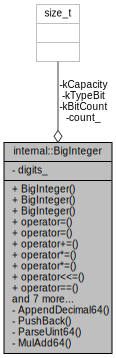
\includegraphics[width=188pt]{classinternal_1_1BigInteger__coll__graph}
\end{center}
\end{figure}
\subsection*{Public Types}
\begin{DoxyCompactItemize}
\item 
typedef \hyperlink{stdint_8h_aec6fcb673ff035718c238c8c9d544c47}{uint64\+\_\+t} \hyperlink{classinternal_1_1BigInteger_a1310812fca26ebae77594ba08678fc4c}{Type}
\end{DoxyCompactItemize}
\subsection*{Public Member Functions}
\begin{DoxyCompactItemize}
\item 
\hyperlink{classinternal_1_1BigInteger_abec623168bc9494dec2f50643b897f72}{Big\+Integer} (const \hyperlink{classinternal_1_1BigInteger}{Big\+Integer} \&rhs)
\item 
\hyperlink{classinternal_1_1BigInteger_ad02b0ef9da203efddd4af07e923732c0}{Big\+Integer} (\hyperlink{stdint_8h_aec6fcb673ff035718c238c8c9d544c47}{uint64\+\_\+t} u)
\item 
{\footnotesize template$<$typename Ch $>$ }\\\hyperlink{classinternal_1_1BigInteger_a4dc2632b2aa2973d18864a127d7c141a}{Big\+Integer} (const Ch $\ast$decimals, size\+\_\+t \hyperlink{imgui__impl__opengl3__loader_8h_a011fc24f10426c01349e94a4edd4b0d5}{length})
\item 
\hyperlink{classinternal_1_1BigInteger}{Big\+Integer} \& \hyperlink{classinternal_1_1BigInteger_ae3eaf1b96cd993511c9f48a14dfc3af2}{operator=} (const \hyperlink{classinternal_1_1BigInteger}{Big\+Integer} \&rhs)
\item 
\hyperlink{classinternal_1_1BigInteger}{Big\+Integer} \& \hyperlink{classinternal_1_1BigInteger_a4002e0b1cf5ee68ab94ab65b35167a38}{operator=} (\hyperlink{stdint_8h_aec6fcb673ff035718c238c8c9d544c47}{uint64\+\_\+t} u)
\item 
\hyperlink{classinternal_1_1BigInteger}{Big\+Integer} \& \hyperlink{classinternal_1_1BigInteger_a09af1d6658d51ad4372649ce1c9c1a62}{operator+=} (\hyperlink{stdint_8h_aec6fcb673ff035718c238c8c9d544c47}{uint64\+\_\+t} u)
\item 
\hyperlink{classinternal_1_1BigInteger}{Big\+Integer} \& \hyperlink{classinternal_1_1BigInteger_a79a52c6135c9783f2e53432dce2cde89}{operator$\ast$=} (\hyperlink{stdint_8h_aec6fcb673ff035718c238c8c9d544c47}{uint64\+\_\+t} u)
\item 
\hyperlink{classinternal_1_1BigInteger}{Big\+Integer} \& \hyperlink{classinternal_1_1BigInteger_a83e8e464b7bc31c8b2c943f8563b2226}{operator$\ast$=} (\hyperlink{stdint_8h_a435d1572bf3f880d55459d9805097f62}{uint32\+\_\+t} u)
\item 
\hyperlink{classinternal_1_1BigInteger}{Big\+Integer} \& \hyperlink{classinternal_1_1BigInteger_a48b12ef4676f19290dfd5816a4ef4a88}{operator$<$$<$=} (size\+\_\+t shift)
\item 
bool \hyperlink{classinternal_1_1BigInteger_a52b424669238bdebc134e793d3b470ae}{operator==} (const \hyperlink{classinternal_1_1BigInteger}{Big\+Integer} \&rhs) const
\item 
bool \hyperlink{classinternal_1_1BigInteger_a8b6ab0d652d461c1136e0388d352628b}{operator==} (const \hyperlink{classinternal_1_1BigInteger_a1310812fca26ebae77594ba08678fc4c}{Type} rhs) const
\item 
\hyperlink{classinternal_1_1BigInteger}{Big\+Integer} \& \hyperlink{classinternal_1_1BigInteger_a98a13f169c27d1acfa57054f37c61763}{Multiply\+Pow5} (unsigned exp)
\item 
bool \hyperlink{classinternal_1_1BigInteger_ad7ad62e6b62af38283ee940eb4015b26}{Difference} (const \hyperlink{classinternal_1_1BigInteger}{Big\+Integer} \&rhs, \hyperlink{classinternal_1_1BigInteger}{Big\+Integer} $\ast$out) const
\item 
int \hyperlink{classinternal_1_1BigInteger_af8e90fff5382de6c1cda5f751017200c}{Compare} (const \hyperlink{classinternal_1_1BigInteger}{Big\+Integer} \&rhs) const
\item 
size\+\_\+t \hyperlink{classinternal_1_1BigInteger_aa0ad6e74839b7c7fe77c9742ec079525}{Get\+Count} () const
\item 
\hyperlink{classinternal_1_1BigInteger_a1310812fca26ebae77594ba08678fc4c}{Type} \hyperlink{classinternal_1_1BigInteger_a7288eefd49735c3c3edec698f56738bd}{Get\+Digit} (size\+\_\+t \hyperlink{imgui__impl__opengl3__loader_8h_a57f14e05b1900f16a2da82ade47d0c6d}{index}) const
\item 
bool \hyperlink{classinternal_1_1BigInteger_ae12dd6759f1f76501db3d1bcafce39cd}{Is\+Zero} () const
\end{DoxyCompactItemize}
\subsection*{Private Member Functions}
\begin{DoxyCompactItemize}
\item 
{\footnotesize template$<$typename Ch $>$ }\\\hyperlink{imgui__impl__opengl3__loader_8h_ac668e7cffd9e2e9cfee428b9b2f34fa7}{void} \hyperlink{classinternal_1_1BigInteger_adcdffd9049832290ce37e283c51e2f50}{Append\+Decimal64} (const Ch $\ast$begin, const Ch $\ast$end)
\item 
\hyperlink{imgui__impl__opengl3__loader_8h_ac668e7cffd9e2e9cfee428b9b2f34fa7}{void} \hyperlink{classinternal_1_1BigInteger_a18a4939a983f296085fed6bc5b56d5c1}{Push\+Back} (\hyperlink{classinternal_1_1BigInteger_a1310812fca26ebae77594ba08678fc4c}{Type} digit)
\end{DoxyCompactItemize}
\subsection*{Static Private Member Functions}
\begin{DoxyCompactItemize}
\item 
{\footnotesize template$<$typename Ch $>$ }\\static \hyperlink{stdint_8h_aec6fcb673ff035718c238c8c9d544c47}{uint64\+\_\+t} \hyperlink{classinternal_1_1BigInteger_acebb94526a2f5f26f0de244b7f76a3db}{Parse\+Uint64} (const Ch $\ast$begin, const Ch $\ast$end)
\item 
static \hyperlink{stdint_8h_aec6fcb673ff035718c238c8c9d544c47}{uint64\+\_\+t} \hyperlink{classinternal_1_1BigInteger_a3857418321694cd20071203b2f08ebfe}{Mul\+Add64} (\hyperlink{stdint_8h_aec6fcb673ff035718c238c8c9d544c47}{uint64\+\_\+t} \hyperlink{pointer_8h_aeeddce917cf130d62c370b8f216026dd}{a}, \hyperlink{stdint_8h_aec6fcb673ff035718c238c8c9d544c47}{uint64\+\_\+t} b, \hyperlink{stdint_8h_aec6fcb673ff035718c238c8c9d544c47}{uint64\+\_\+t} k, \hyperlink{stdint_8h_aec6fcb673ff035718c238c8c9d544c47}{uint64\+\_\+t} $\ast$out\+High)
\end{DoxyCompactItemize}
\subsection*{Private Attributes}
\begin{DoxyCompactItemize}
\item 
\hyperlink{classinternal_1_1BigInteger_a1310812fca26ebae77594ba08678fc4c}{Type} \hyperlink{classinternal_1_1BigInteger_a0b505df38fedd862a748fe1e629d918a}{digits\+\_\+} \mbox{[}\hyperlink{classinternal_1_1BigInteger_a8a908718d685b9bd39fb52f2e511b0c6}{k\+Capacity}\mbox{]}
\item 
size\+\_\+t \hyperlink{classinternal_1_1BigInteger_ad4bf5198afe86d754ec57a82605e644b}{count\+\_\+}
\end{DoxyCompactItemize}
\subsection*{Static Private Attributes}
\begin{DoxyCompactItemize}
\item 
static const size\+\_\+t \hyperlink{classinternal_1_1BigInteger_a89d6a00e78a914d0b873784539416dc5}{k\+Bit\+Count} = 3328
\item 
static const size\+\_\+t \hyperlink{classinternal_1_1BigInteger_a8a908718d685b9bd39fb52f2e511b0c6}{k\+Capacity} = \hyperlink{classinternal_1_1BigInteger_a89d6a00e78a914d0b873784539416dc5}{k\+Bit\+Count} / sizeof(\hyperlink{classinternal_1_1BigInteger_a1310812fca26ebae77594ba08678fc4c}{Type})
\item 
static const size\+\_\+t \hyperlink{classinternal_1_1BigInteger_a662666ad4bc9122cb80ba2ac6e88a745}{k\+Type\+Bit} = sizeof(\hyperlink{classinternal_1_1BigInteger_a1310812fca26ebae77594ba08678fc4c}{Type}) $\ast$ 8
\end{DoxyCompactItemize}


\subsection{Member Typedef Documentation}
\mbox{\Hypertarget{classinternal_1_1BigInteger_a1310812fca26ebae77594ba08678fc4c}\label{classinternal_1_1BigInteger_a1310812fca26ebae77594ba08678fc4c}} 
\index{internal\+::\+Big\+Integer@{internal\+::\+Big\+Integer}!Type@{Type}}
\index{Type@{Type}!internal\+::\+Big\+Integer@{internal\+::\+Big\+Integer}}
\subsubsection{\texorpdfstring{Type}{Type}}
{\footnotesize\ttfamily typedef \hyperlink{stdint_8h_aec6fcb673ff035718c238c8c9d544c47}{uint64\+\_\+t} \hyperlink{classinternal_1_1BigInteger_a1310812fca26ebae77594ba08678fc4c}{internal\+::\+Big\+Integer\+::\+Type}}



\subsection{Constructor \& Destructor Documentation}
\mbox{\Hypertarget{classinternal_1_1BigInteger_abec623168bc9494dec2f50643b897f72}\label{classinternal_1_1BigInteger_abec623168bc9494dec2f50643b897f72}} 
\index{internal\+::\+Big\+Integer@{internal\+::\+Big\+Integer}!Big\+Integer@{Big\+Integer}}
\index{Big\+Integer@{Big\+Integer}!internal\+::\+Big\+Integer@{internal\+::\+Big\+Integer}}
\subsubsection{\texorpdfstring{Big\+Integer()}{BigInteger()}\hspace{0.1cm}{\footnotesize\ttfamily [1/3]}}
{\footnotesize\ttfamily internal\+::\+Big\+Integer\+::\+Big\+Integer (\begin{DoxyParamCaption}\item[{const \hyperlink{classinternal_1_1BigInteger}{Big\+Integer} \&}]{rhs }\end{DoxyParamCaption})\hspace{0.3cm}{\ttfamily [inline]}}

\mbox{\Hypertarget{classinternal_1_1BigInteger_ad02b0ef9da203efddd4af07e923732c0}\label{classinternal_1_1BigInteger_ad02b0ef9da203efddd4af07e923732c0}} 
\index{internal\+::\+Big\+Integer@{internal\+::\+Big\+Integer}!Big\+Integer@{Big\+Integer}}
\index{Big\+Integer@{Big\+Integer}!internal\+::\+Big\+Integer@{internal\+::\+Big\+Integer}}
\subsubsection{\texorpdfstring{Big\+Integer()}{BigInteger()}\hspace{0.1cm}{\footnotesize\ttfamily [2/3]}}
{\footnotesize\ttfamily internal\+::\+Big\+Integer\+::\+Big\+Integer (\begin{DoxyParamCaption}\item[{\hyperlink{stdint_8h_aec6fcb673ff035718c238c8c9d544c47}{uint64\+\_\+t}}]{u }\end{DoxyParamCaption})\hspace{0.3cm}{\ttfamily [inline]}, {\ttfamily [explicit]}}

\mbox{\Hypertarget{classinternal_1_1BigInteger_a4dc2632b2aa2973d18864a127d7c141a}\label{classinternal_1_1BigInteger_a4dc2632b2aa2973d18864a127d7c141a}} 
\index{internal\+::\+Big\+Integer@{internal\+::\+Big\+Integer}!Big\+Integer@{Big\+Integer}}
\index{Big\+Integer@{Big\+Integer}!internal\+::\+Big\+Integer@{internal\+::\+Big\+Integer}}
\subsubsection{\texorpdfstring{Big\+Integer()}{BigInteger()}\hspace{0.1cm}{\footnotesize\ttfamily [3/3]}}
{\footnotesize\ttfamily template$<$typename Ch $>$ \\
internal\+::\+Big\+Integer\+::\+Big\+Integer (\begin{DoxyParamCaption}\item[{const Ch $\ast$}]{decimals,  }\item[{size\+\_\+t}]{length }\end{DoxyParamCaption})\hspace{0.3cm}{\ttfamily [inline]}}



\subsection{Member Function Documentation}
\mbox{\Hypertarget{classinternal_1_1BigInteger_adcdffd9049832290ce37e283c51e2f50}\label{classinternal_1_1BigInteger_adcdffd9049832290ce37e283c51e2f50}} 
\index{internal\+::\+Big\+Integer@{internal\+::\+Big\+Integer}!Append\+Decimal64@{Append\+Decimal64}}
\index{Append\+Decimal64@{Append\+Decimal64}!internal\+::\+Big\+Integer@{internal\+::\+Big\+Integer}}
\subsubsection{\texorpdfstring{Append\+Decimal64()}{AppendDecimal64()}}
{\footnotesize\ttfamily template$<$typename Ch $>$ \\
\hyperlink{imgui__impl__opengl3__loader_8h_ac668e7cffd9e2e9cfee428b9b2f34fa7}{void} internal\+::\+Big\+Integer\+::\+Append\+Decimal64 (\begin{DoxyParamCaption}\item[{const Ch $\ast$}]{begin,  }\item[{const Ch $\ast$}]{end }\end{DoxyParamCaption})\hspace{0.3cm}{\ttfamily [inline]}, {\ttfamily [private]}}

\mbox{\Hypertarget{classinternal_1_1BigInteger_af8e90fff5382de6c1cda5f751017200c}\label{classinternal_1_1BigInteger_af8e90fff5382de6c1cda5f751017200c}} 
\index{internal\+::\+Big\+Integer@{internal\+::\+Big\+Integer}!Compare@{Compare}}
\index{Compare@{Compare}!internal\+::\+Big\+Integer@{internal\+::\+Big\+Integer}}
\subsubsection{\texorpdfstring{Compare()}{Compare()}}
{\footnotesize\ttfamily int internal\+::\+Big\+Integer\+::\+Compare (\begin{DoxyParamCaption}\item[{const \hyperlink{classinternal_1_1BigInteger}{Big\+Integer} \&}]{rhs }\end{DoxyParamCaption}) const\hspace{0.3cm}{\ttfamily [inline]}}

\mbox{\Hypertarget{classinternal_1_1BigInteger_ad7ad62e6b62af38283ee940eb4015b26}\label{classinternal_1_1BigInteger_ad7ad62e6b62af38283ee940eb4015b26}} 
\index{internal\+::\+Big\+Integer@{internal\+::\+Big\+Integer}!Difference@{Difference}}
\index{Difference@{Difference}!internal\+::\+Big\+Integer@{internal\+::\+Big\+Integer}}
\subsubsection{\texorpdfstring{Difference()}{Difference()}}
{\footnotesize\ttfamily bool internal\+::\+Big\+Integer\+::\+Difference (\begin{DoxyParamCaption}\item[{const \hyperlink{classinternal_1_1BigInteger}{Big\+Integer} \&}]{rhs,  }\item[{\hyperlink{classinternal_1_1BigInteger}{Big\+Integer} $\ast$}]{out }\end{DoxyParamCaption}) const\hspace{0.3cm}{\ttfamily [inline]}}

\mbox{\Hypertarget{classinternal_1_1BigInteger_aa0ad6e74839b7c7fe77c9742ec079525}\label{classinternal_1_1BigInteger_aa0ad6e74839b7c7fe77c9742ec079525}} 
\index{internal\+::\+Big\+Integer@{internal\+::\+Big\+Integer}!Get\+Count@{Get\+Count}}
\index{Get\+Count@{Get\+Count}!internal\+::\+Big\+Integer@{internal\+::\+Big\+Integer}}
\subsubsection{\texorpdfstring{Get\+Count()}{GetCount()}}
{\footnotesize\ttfamily size\+\_\+t internal\+::\+Big\+Integer\+::\+Get\+Count (\begin{DoxyParamCaption}{ }\end{DoxyParamCaption}) const\hspace{0.3cm}{\ttfamily [inline]}}

\mbox{\Hypertarget{classinternal_1_1BigInteger_a7288eefd49735c3c3edec698f56738bd}\label{classinternal_1_1BigInteger_a7288eefd49735c3c3edec698f56738bd}} 
\index{internal\+::\+Big\+Integer@{internal\+::\+Big\+Integer}!Get\+Digit@{Get\+Digit}}
\index{Get\+Digit@{Get\+Digit}!internal\+::\+Big\+Integer@{internal\+::\+Big\+Integer}}
\subsubsection{\texorpdfstring{Get\+Digit()}{GetDigit()}}
{\footnotesize\ttfamily \hyperlink{classinternal_1_1BigInteger_a1310812fca26ebae77594ba08678fc4c}{Type} internal\+::\+Big\+Integer\+::\+Get\+Digit (\begin{DoxyParamCaption}\item[{size\+\_\+t}]{index }\end{DoxyParamCaption}) const\hspace{0.3cm}{\ttfamily [inline]}}

\mbox{\Hypertarget{classinternal_1_1BigInteger_ae12dd6759f1f76501db3d1bcafce39cd}\label{classinternal_1_1BigInteger_ae12dd6759f1f76501db3d1bcafce39cd}} 
\index{internal\+::\+Big\+Integer@{internal\+::\+Big\+Integer}!Is\+Zero@{Is\+Zero}}
\index{Is\+Zero@{Is\+Zero}!internal\+::\+Big\+Integer@{internal\+::\+Big\+Integer}}
\subsubsection{\texorpdfstring{Is\+Zero()}{IsZero()}}
{\footnotesize\ttfamily bool internal\+::\+Big\+Integer\+::\+Is\+Zero (\begin{DoxyParamCaption}{ }\end{DoxyParamCaption}) const\hspace{0.3cm}{\ttfamily [inline]}}

\mbox{\Hypertarget{classinternal_1_1BigInteger_a3857418321694cd20071203b2f08ebfe}\label{classinternal_1_1BigInteger_a3857418321694cd20071203b2f08ebfe}} 
\index{internal\+::\+Big\+Integer@{internal\+::\+Big\+Integer}!Mul\+Add64@{Mul\+Add64}}
\index{Mul\+Add64@{Mul\+Add64}!internal\+::\+Big\+Integer@{internal\+::\+Big\+Integer}}
\subsubsection{\texorpdfstring{Mul\+Add64()}{MulAdd64()}}
{\footnotesize\ttfamily static \hyperlink{stdint_8h_aec6fcb673ff035718c238c8c9d544c47}{uint64\+\_\+t} internal\+::\+Big\+Integer\+::\+Mul\+Add64 (\begin{DoxyParamCaption}\item[{\hyperlink{stdint_8h_aec6fcb673ff035718c238c8c9d544c47}{uint64\+\_\+t}}]{a,  }\item[{\hyperlink{stdint_8h_aec6fcb673ff035718c238c8c9d544c47}{uint64\+\_\+t}}]{b,  }\item[{\hyperlink{stdint_8h_aec6fcb673ff035718c238c8c9d544c47}{uint64\+\_\+t}}]{k,  }\item[{\hyperlink{stdint_8h_aec6fcb673ff035718c238c8c9d544c47}{uint64\+\_\+t} $\ast$}]{out\+High }\end{DoxyParamCaption})\hspace{0.3cm}{\ttfamily [inline]}, {\ttfamily [static]}, {\ttfamily [private]}}

\mbox{\Hypertarget{classinternal_1_1BigInteger_a98a13f169c27d1acfa57054f37c61763}\label{classinternal_1_1BigInteger_a98a13f169c27d1acfa57054f37c61763}} 
\index{internal\+::\+Big\+Integer@{internal\+::\+Big\+Integer}!Multiply\+Pow5@{Multiply\+Pow5}}
\index{Multiply\+Pow5@{Multiply\+Pow5}!internal\+::\+Big\+Integer@{internal\+::\+Big\+Integer}}
\subsubsection{\texorpdfstring{Multiply\+Pow5()}{MultiplyPow5()}}
{\footnotesize\ttfamily \hyperlink{classinternal_1_1BigInteger}{Big\+Integer}\& internal\+::\+Big\+Integer\+::\+Multiply\+Pow5 (\begin{DoxyParamCaption}\item[{unsigned}]{exp }\end{DoxyParamCaption})\hspace{0.3cm}{\ttfamily [inline]}}

\mbox{\Hypertarget{classinternal_1_1BigInteger_a79a52c6135c9783f2e53432dce2cde89}\label{classinternal_1_1BigInteger_a79a52c6135c9783f2e53432dce2cde89}} 
\index{internal\+::\+Big\+Integer@{internal\+::\+Big\+Integer}!operator$\ast$=@{operator$\ast$=}}
\index{operator$\ast$=@{operator$\ast$=}!internal\+::\+Big\+Integer@{internal\+::\+Big\+Integer}}
\subsubsection{\texorpdfstring{operator$\ast$=()}{operator*=()}\hspace{0.1cm}{\footnotesize\ttfamily [1/2]}}
{\footnotesize\ttfamily \hyperlink{classinternal_1_1BigInteger}{Big\+Integer}\& internal\+::\+Big\+Integer\+::operator$\ast$= (\begin{DoxyParamCaption}\item[{\hyperlink{stdint_8h_aec6fcb673ff035718c238c8c9d544c47}{uint64\+\_\+t}}]{u }\end{DoxyParamCaption})\hspace{0.3cm}{\ttfamily [inline]}}

\mbox{\Hypertarget{classinternal_1_1BigInteger_a83e8e464b7bc31c8b2c943f8563b2226}\label{classinternal_1_1BigInteger_a83e8e464b7bc31c8b2c943f8563b2226}} 
\index{internal\+::\+Big\+Integer@{internal\+::\+Big\+Integer}!operator$\ast$=@{operator$\ast$=}}
\index{operator$\ast$=@{operator$\ast$=}!internal\+::\+Big\+Integer@{internal\+::\+Big\+Integer}}
\subsubsection{\texorpdfstring{operator$\ast$=()}{operator*=()}\hspace{0.1cm}{\footnotesize\ttfamily [2/2]}}
{\footnotesize\ttfamily \hyperlink{classinternal_1_1BigInteger}{Big\+Integer}\& internal\+::\+Big\+Integer\+::operator$\ast$= (\begin{DoxyParamCaption}\item[{\hyperlink{stdint_8h_a435d1572bf3f880d55459d9805097f62}{uint32\+\_\+t}}]{u }\end{DoxyParamCaption})\hspace{0.3cm}{\ttfamily [inline]}}

\mbox{\Hypertarget{classinternal_1_1BigInteger_a09af1d6658d51ad4372649ce1c9c1a62}\label{classinternal_1_1BigInteger_a09af1d6658d51ad4372649ce1c9c1a62}} 
\index{internal\+::\+Big\+Integer@{internal\+::\+Big\+Integer}!operator+=@{operator+=}}
\index{operator+=@{operator+=}!internal\+::\+Big\+Integer@{internal\+::\+Big\+Integer}}
\subsubsection{\texorpdfstring{operator+=()}{operator+=()}}
{\footnotesize\ttfamily \hyperlink{classinternal_1_1BigInteger}{Big\+Integer}\& internal\+::\+Big\+Integer\+::operator+= (\begin{DoxyParamCaption}\item[{\hyperlink{stdint_8h_aec6fcb673ff035718c238c8c9d544c47}{uint64\+\_\+t}}]{u }\end{DoxyParamCaption})\hspace{0.3cm}{\ttfamily [inline]}}

\mbox{\Hypertarget{classinternal_1_1BigInteger_a48b12ef4676f19290dfd5816a4ef4a88}\label{classinternal_1_1BigInteger_a48b12ef4676f19290dfd5816a4ef4a88}} 
\index{internal\+::\+Big\+Integer@{internal\+::\+Big\+Integer}!operator$<$$<$=@{operator$<$$<$=}}
\index{operator$<$$<$=@{operator$<$$<$=}!internal\+::\+Big\+Integer@{internal\+::\+Big\+Integer}}
\subsubsection{\texorpdfstring{operator$<$$<$=()}{operator<<=()}}
{\footnotesize\ttfamily \hyperlink{classinternal_1_1BigInteger}{Big\+Integer}\& internal\+::\+Big\+Integer\+::operator$<$$<$= (\begin{DoxyParamCaption}\item[{size\+\_\+t}]{shift }\end{DoxyParamCaption})\hspace{0.3cm}{\ttfamily [inline]}}

\mbox{\Hypertarget{classinternal_1_1BigInteger_ae3eaf1b96cd993511c9f48a14dfc3af2}\label{classinternal_1_1BigInteger_ae3eaf1b96cd993511c9f48a14dfc3af2}} 
\index{internal\+::\+Big\+Integer@{internal\+::\+Big\+Integer}!operator=@{operator=}}
\index{operator=@{operator=}!internal\+::\+Big\+Integer@{internal\+::\+Big\+Integer}}
\subsubsection{\texorpdfstring{operator=()}{operator=()}\hspace{0.1cm}{\footnotesize\ttfamily [1/2]}}
{\footnotesize\ttfamily \hyperlink{classinternal_1_1BigInteger}{Big\+Integer}\& internal\+::\+Big\+Integer\+::operator= (\begin{DoxyParamCaption}\item[{const \hyperlink{classinternal_1_1BigInteger}{Big\+Integer} \&}]{rhs }\end{DoxyParamCaption})\hspace{0.3cm}{\ttfamily [inline]}}

\mbox{\Hypertarget{classinternal_1_1BigInteger_a4002e0b1cf5ee68ab94ab65b35167a38}\label{classinternal_1_1BigInteger_a4002e0b1cf5ee68ab94ab65b35167a38}} 
\index{internal\+::\+Big\+Integer@{internal\+::\+Big\+Integer}!operator=@{operator=}}
\index{operator=@{operator=}!internal\+::\+Big\+Integer@{internal\+::\+Big\+Integer}}
\subsubsection{\texorpdfstring{operator=()}{operator=()}\hspace{0.1cm}{\footnotesize\ttfamily [2/2]}}
{\footnotesize\ttfamily \hyperlink{classinternal_1_1BigInteger}{Big\+Integer}\& internal\+::\+Big\+Integer\+::operator= (\begin{DoxyParamCaption}\item[{\hyperlink{stdint_8h_aec6fcb673ff035718c238c8c9d544c47}{uint64\+\_\+t}}]{u }\end{DoxyParamCaption})\hspace{0.3cm}{\ttfamily [inline]}}

\mbox{\Hypertarget{classinternal_1_1BigInteger_a52b424669238bdebc134e793d3b470ae}\label{classinternal_1_1BigInteger_a52b424669238bdebc134e793d3b470ae}} 
\index{internal\+::\+Big\+Integer@{internal\+::\+Big\+Integer}!operator==@{operator==}}
\index{operator==@{operator==}!internal\+::\+Big\+Integer@{internal\+::\+Big\+Integer}}
\subsubsection{\texorpdfstring{operator==()}{operator==()}\hspace{0.1cm}{\footnotesize\ttfamily [1/2]}}
{\footnotesize\ttfamily bool internal\+::\+Big\+Integer\+::operator== (\begin{DoxyParamCaption}\item[{const \hyperlink{classinternal_1_1BigInteger}{Big\+Integer} \&}]{rhs }\end{DoxyParamCaption}) const\hspace{0.3cm}{\ttfamily [inline]}}

\mbox{\Hypertarget{classinternal_1_1BigInteger_a8b6ab0d652d461c1136e0388d352628b}\label{classinternal_1_1BigInteger_a8b6ab0d652d461c1136e0388d352628b}} 
\index{internal\+::\+Big\+Integer@{internal\+::\+Big\+Integer}!operator==@{operator==}}
\index{operator==@{operator==}!internal\+::\+Big\+Integer@{internal\+::\+Big\+Integer}}
\subsubsection{\texorpdfstring{operator==()}{operator==()}\hspace{0.1cm}{\footnotesize\ttfamily [2/2]}}
{\footnotesize\ttfamily bool internal\+::\+Big\+Integer\+::operator== (\begin{DoxyParamCaption}\item[{const \hyperlink{classinternal_1_1BigInteger_a1310812fca26ebae77594ba08678fc4c}{Type}}]{rhs }\end{DoxyParamCaption}) const\hspace{0.3cm}{\ttfamily [inline]}}

\mbox{\Hypertarget{classinternal_1_1BigInteger_acebb94526a2f5f26f0de244b7f76a3db}\label{classinternal_1_1BigInteger_acebb94526a2f5f26f0de244b7f76a3db}} 
\index{internal\+::\+Big\+Integer@{internal\+::\+Big\+Integer}!Parse\+Uint64@{Parse\+Uint64}}
\index{Parse\+Uint64@{Parse\+Uint64}!internal\+::\+Big\+Integer@{internal\+::\+Big\+Integer}}
\subsubsection{\texorpdfstring{Parse\+Uint64()}{ParseUint64()}}
{\footnotesize\ttfamily template$<$typename Ch $>$ \\
static \hyperlink{stdint_8h_aec6fcb673ff035718c238c8c9d544c47}{uint64\+\_\+t} internal\+::\+Big\+Integer\+::\+Parse\+Uint64 (\begin{DoxyParamCaption}\item[{const Ch $\ast$}]{begin,  }\item[{const Ch $\ast$}]{end }\end{DoxyParamCaption})\hspace{0.3cm}{\ttfamily [inline]}, {\ttfamily [static]}, {\ttfamily [private]}}

\mbox{\Hypertarget{classinternal_1_1BigInteger_a18a4939a983f296085fed6bc5b56d5c1}\label{classinternal_1_1BigInteger_a18a4939a983f296085fed6bc5b56d5c1}} 
\index{internal\+::\+Big\+Integer@{internal\+::\+Big\+Integer}!Push\+Back@{Push\+Back}}
\index{Push\+Back@{Push\+Back}!internal\+::\+Big\+Integer@{internal\+::\+Big\+Integer}}
\subsubsection{\texorpdfstring{Push\+Back()}{PushBack()}}
{\footnotesize\ttfamily \hyperlink{imgui__impl__opengl3__loader_8h_ac668e7cffd9e2e9cfee428b9b2f34fa7}{void} internal\+::\+Big\+Integer\+::\+Push\+Back (\begin{DoxyParamCaption}\item[{\hyperlink{classinternal_1_1BigInteger_a1310812fca26ebae77594ba08678fc4c}{Type}}]{digit }\end{DoxyParamCaption})\hspace{0.3cm}{\ttfamily [inline]}, {\ttfamily [private]}}



\subsection{Member Data Documentation}
\mbox{\Hypertarget{classinternal_1_1BigInteger_ad4bf5198afe86d754ec57a82605e644b}\label{classinternal_1_1BigInteger_ad4bf5198afe86d754ec57a82605e644b}} 
\index{internal\+::\+Big\+Integer@{internal\+::\+Big\+Integer}!count\+\_\+@{count\+\_\+}}
\index{count\+\_\+@{count\+\_\+}!internal\+::\+Big\+Integer@{internal\+::\+Big\+Integer}}
\subsubsection{\texorpdfstring{count\+\_\+}{count\_}}
{\footnotesize\ttfamily size\+\_\+t internal\+::\+Big\+Integer\+::count\+\_\+\hspace{0.3cm}{\ttfamily [private]}}

\mbox{\Hypertarget{classinternal_1_1BigInteger_a0b505df38fedd862a748fe1e629d918a}\label{classinternal_1_1BigInteger_a0b505df38fedd862a748fe1e629d918a}} 
\index{internal\+::\+Big\+Integer@{internal\+::\+Big\+Integer}!digits\+\_\+@{digits\+\_\+}}
\index{digits\+\_\+@{digits\+\_\+}!internal\+::\+Big\+Integer@{internal\+::\+Big\+Integer}}
\subsubsection{\texorpdfstring{digits\+\_\+}{digits\_}}
{\footnotesize\ttfamily \hyperlink{classinternal_1_1BigInteger_a1310812fca26ebae77594ba08678fc4c}{Type} internal\+::\+Big\+Integer\+::digits\+\_\+\mbox{[}\hyperlink{classinternal_1_1BigInteger_a8a908718d685b9bd39fb52f2e511b0c6}{k\+Capacity}\mbox{]}\hspace{0.3cm}{\ttfamily [private]}}

\mbox{\Hypertarget{classinternal_1_1BigInteger_a89d6a00e78a914d0b873784539416dc5}\label{classinternal_1_1BigInteger_a89d6a00e78a914d0b873784539416dc5}} 
\index{internal\+::\+Big\+Integer@{internal\+::\+Big\+Integer}!k\+Bit\+Count@{k\+Bit\+Count}}
\index{k\+Bit\+Count@{k\+Bit\+Count}!internal\+::\+Big\+Integer@{internal\+::\+Big\+Integer}}
\subsubsection{\texorpdfstring{k\+Bit\+Count}{kBitCount}}
{\footnotesize\ttfamily const size\+\_\+t internal\+::\+Big\+Integer\+::k\+Bit\+Count = 3328\hspace{0.3cm}{\ttfamily [static]}, {\ttfamily [private]}}

\mbox{\Hypertarget{classinternal_1_1BigInteger_a8a908718d685b9bd39fb52f2e511b0c6}\label{classinternal_1_1BigInteger_a8a908718d685b9bd39fb52f2e511b0c6}} 
\index{internal\+::\+Big\+Integer@{internal\+::\+Big\+Integer}!k\+Capacity@{k\+Capacity}}
\index{k\+Capacity@{k\+Capacity}!internal\+::\+Big\+Integer@{internal\+::\+Big\+Integer}}
\subsubsection{\texorpdfstring{k\+Capacity}{kCapacity}}
{\footnotesize\ttfamily const size\+\_\+t internal\+::\+Big\+Integer\+::k\+Capacity = \hyperlink{classinternal_1_1BigInteger_a89d6a00e78a914d0b873784539416dc5}{k\+Bit\+Count} / sizeof(\hyperlink{classinternal_1_1BigInteger_a1310812fca26ebae77594ba08678fc4c}{Type})\hspace{0.3cm}{\ttfamily [static]}, {\ttfamily [private]}}

\mbox{\Hypertarget{classinternal_1_1BigInteger_a662666ad4bc9122cb80ba2ac6e88a745}\label{classinternal_1_1BigInteger_a662666ad4bc9122cb80ba2ac6e88a745}} 
\index{internal\+::\+Big\+Integer@{internal\+::\+Big\+Integer}!k\+Type\+Bit@{k\+Type\+Bit}}
\index{k\+Type\+Bit@{k\+Type\+Bit}!internal\+::\+Big\+Integer@{internal\+::\+Big\+Integer}}
\subsubsection{\texorpdfstring{k\+Type\+Bit}{kTypeBit}}
{\footnotesize\ttfamily const size\+\_\+t internal\+::\+Big\+Integer\+::k\+Type\+Bit = sizeof(\hyperlink{classinternal_1_1BigInteger_a1310812fca26ebae77594ba08678fc4c}{Type}) $\ast$ 8\hspace{0.3cm}{\ttfamily [static]}, {\ttfamily [private]}}



The documentation for this class was generated from the following file\+:\begin{DoxyCompactItemize}
\item 
/mnt/hdd/fnky/\+C0de/\+C\+A\+P\+S\+T\+O\+N\+E/clean\+\_\+build/include/rapidjson/internal/\hyperlink{biginteger_8h}{biginteger.\+h}\end{DoxyCompactItemize}

\hypertarget{classBState}{}\section{B\+State Class Reference}
\label{classBState}\index{B\+State@{B\+State}}


{\ttfamily \#include $<$B\+State.\+h$>$}



Collaboration diagram for B\+State\+:
\nopagebreak
\begin{figure}[H]
\begin{center}
\leavevmode
\includegraphics[width=180pt]{classBState__coll__graph}
\end{center}
\end{figure}
\subsection*{Public Member Functions}
\begin{DoxyCompactItemize}
\item 
\hyperlink{classBState_ab620431914f2b63b156a108cb47f9f9e}{B\+State} (\hyperlink{BState_8h_a275a67132f10277ada3a0ee3d616b647}{S\+T\+A\+TE} name\+\_\+)
\item 
\hyperlink{classBState_ab7dcf09e84afba8a5f2d1c714468ca5b}{$\sim$\+B\+State} ()
\item 
list$<$ \hyperlink{classTransition}{Transition} $\ast$ $>$ \hyperlink{classBState_a12a62f55d5136baa914a5a9296fc1a94}{get\+Transitions} ()
\item 
list$<$ std\+::shared\+\_\+ptr$<$ \hyperlink{classTransition}{Transition} $>$ $>$ \hyperlink{classBState_a3314d0c5e4a877f3b14c153e285611d9}{get\+S\+Transitions} ()
\item 
\hyperlink{imgui__impl__opengl3__loader_8h_ac668e7cffd9e2e9cfee428b9b2f34fa7}{void} \hyperlink{classBState_a19d39e24d561b72484a026a367aee031}{add\+Transition} (\hyperlink{classTransition}{Transition} $\ast$transition)
\item 
\hyperlink{imgui__impl__opengl3__loader_8h_ac668e7cffd9e2e9cfee428b9b2f34fa7}{void} \hyperlink{classBState_a2e1c33342d2a21e2c11083e0f89e1748}{add\+Transition} (std\+::shared\+\_\+ptr$<$ \hyperlink{classTransition}{Transition} $>$ transition)
\item 
\hyperlink{BState_8h_a275a67132f10277ada3a0ee3d616b647}{S\+T\+A\+TE} \hyperlink{classBState_acf259690a67bd6d34fe78f95501d5b45}{get\+Name} ()
\end{DoxyCompactItemize}
\subsection*{Private Attributes}
\begin{DoxyCompactItemize}
\item 
list$<$ \hyperlink{classTransition}{Transition} $\ast$ $>$ \hyperlink{classBState_a9bd20e613fd32ef9408818eb15f80350}{transitions}
\item 
list$<$ std\+::shared\+\_\+ptr$<$ \hyperlink{classTransition}{Transition} $>$ $>$ \hyperlink{classBState_a5435ea55aa101d3b45474c81e53d1d42}{Stransitions}
\item 
\hyperlink{BState_8h_a275a67132f10277ada3a0ee3d616b647}{S\+T\+A\+TE} \hyperlink{classBState_ac4a447d0ad6729605fd5b0d74f5273bb}{name}
\end{DoxyCompactItemize}


\subsection{Constructor \& Destructor Documentation}
\mbox{\Hypertarget{classBState_ab620431914f2b63b156a108cb47f9f9e}\label{classBState_ab620431914f2b63b156a108cb47f9f9e}} 
\index{B\+State@{B\+State}!B\+State@{B\+State}}
\index{B\+State@{B\+State}!B\+State@{B\+State}}
\subsubsection{\texorpdfstring{B\+State()}{BState()}}
{\footnotesize\ttfamily B\+State\+::\+B\+State (\begin{DoxyParamCaption}\item[{\hyperlink{BState_8h_a275a67132f10277ada3a0ee3d616b647}{S\+T\+A\+TE}}]{name\+\_\+ }\end{DoxyParamCaption})\hspace{0.3cm}{\ttfamily [inline]}}

\mbox{\Hypertarget{classBState_ab7dcf09e84afba8a5f2d1c714468ca5b}\label{classBState_ab7dcf09e84afba8a5f2d1c714468ca5b}} 
\index{B\+State@{B\+State}!````~B\+State@{$\sim$\+B\+State}}
\index{````~B\+State@{$\sim$\+B\+State}!B\+State@{B\+State}}
\subsubsection{\texorpdfstring{$\sim$\+B\+State()}{~BState()}}
{\footnotesize\ttfamily B\+State\+::$\sim$\+B\+State (\begin{DoxyParamCaption}{ }\end{DoxyParamCaption})\hspace{0.3cm}{\ttfamily [inline]}}



\subsection{Member Function Documentation}
\mbox{\Hypertarget{classBState_a19d39e24d561b72484a026a367aee031}\label{classBState_a19d39e24d561b72484a026a367aee031}} 
\index{B\+State@{B\+State}!add\+Transition@{add\+Transition}}
\index{add\+Transition@{add\+Transition}!B\+State@{B\+State}}
\subsubsection{\texorpdfstring{add\+Transition()}{addTransition()}\hspace{0.1cm}{\footnotesize\ttfamily [1/2]}}
{\footnotesize\ttfamily \hyperlink{imgui__impl__opengl3__loader_8h_ac668e7cffd9e2e9cfee428b9b2f34fa7}{void} B\+State\+::add\+Transition (\begin{DoxyParamCaption}\item[{\hyperlink{classTransition}{Transition} $\ast$}]{transition }\end{DoxyParamCaption})}

\mbox{\Hypertarget{classBState_a2e1c33342d2a21e2c11083e0f89e1748}\label{classBState_a2e1c33342d2a21e2c11083e0f89e1748}} 
\index{B\+State@{B\+State}!add\+Transition@{add\+Transition}}
\index{add\+Transition@{add\+Transition}!B\+State@{B\+State}}
\subsubsection{\texorpdfstring{add\+Transition()}{addTransition()}\hspace{0.1cm}{\footnotesize\ttfamily [2/2]}}
{\footnotesize\ttfamily \hyperlink{imgui__impl__opengl3__loader_8h_ac668e7cffd9e2e9cfee428b9b2f34fa7}{void} B\+State\+::add\+Transition (\begin{DoxyParamCaption}\item[{std\+::shared\+\_\+ptr$<$ \hyperlink{classTransition}{Transition} $>$}]{transition }\end{DoxyParamCaption})}

\mbox{\Hypertarget{classBState_acf259690a67bd6d34fe78f95501d5b45}\label{classBState_acf259690a67bd6d34fe78f95501d5b45}} 
\index{B\+State@{B\+State}!get\+Name@{get\+Name}}
\index{get\+Name@{get\+Name}!B\+State@{B\+State}}
\subsubsection{\texorpdfstring{get\+Name()}{getName()}}
{\footnotesize\ttfamily \hyperlink{BState_8h_a275a67132f10277ada3a0ee3d616b647}{S\+T\+A\+TE} B\+State\+::get\+Name (\begin{DoxyParamCaption}{ }\end{DoxyParamCaption})\hspace{0.3cm}{\ttfamily [inline]}}

\mbox{\Hypertarget{classBState_a3314d0c5e4a877f3b14c153e285611d9}\label{classBState_a3314d0c5e4a877f3b14c153e285611d9}} 
\index{B\+State@{B\+State}!get\+S\+Transitions@{get\+S\+Transitions}}
\index{get\+S\+Transitions@{get\+S\+Transitions}!B\+State@{B\+State}}
\subsubsection{\texorpdfstring{get\+S\+Transitions()}{getSTransitions()}}
{\footnotesize\ttfamily list$<$std\+::shared\+\_\+ptr$<$\hyperlink{classTransition}{Transition}$>$ $>$ B\+State\+::get\+S\+Transitions (\begin{DoxyParamCaption}{ }\end{DoxyParamCaption})\hspace{0.3cm}{\ttfamily [inline]}}

\mbox{\Hypertarget{classBState_a12a62f55d5136baa914a5a9296fc1a94}\label{classBState_a12a62f55d5136baa914a5a9296fc1a94}} 
\index{B\+State@{B\+State}!get\+Transitions@{get\+Transitions}}
\index{get\+Transitions@{get\+Transitions}!B\+State@{B\+State}}
\subsubsection{\texorpdfstring{get\+Transitions()}{getTransitions()}}
{\footnotesize\ttfamily list$<$\hyperlink{classTransition}{Transition}$\ast$$>$ B\+State\+::get\+Transitions (\begin{DoxyParamCaption}{ }\end{DoxyParamCaption})\hspace{0.3cm}{\ttfamily [inline]}}



\subsection{Member Data Documentation}
\mbox{\Hypertarget{classBState_ac4a447d0ad6729605fd5b0d74f5273bb}\label{classBState_ac4a447d0ad6729605fd5b0d74f5273bb}} 
\index{B\+State@{B\+State}!name@{name}}
\index{name@{name}!B\+State@{B\+State}}
\subsubsection{\texorpdfstring{name}{name}}
{\footnotesize\ttfamily \hyperlink{BState_8h_a275a67132f10277ada3a0ee3d616b647}{S\+T\+A\+TE} B\+State\+::name\hspace{0.3cm}{\ttfamily [private]}}

\mbox{\Hypertarget{classBState_a5435ea55aa101d3b45474c81e53d1d42}\label{classBState_a5435ea55aa101d3b45474c81e53d1d42}} 
\index{B\+State@{B\+State}!Stransitions@{Stransitions}}
\index{Stransitions@{Stransitions}!B\+State@{B\+State}}
\subsubsection{\texorpdfstring{Stransitions}{Stransitions}}
{\footnotesize\ttfamily list$<$std\+::shared\+\_\+ptr$<$\hyperlink{classTransition}{Transition}$>$ $>$ B\+State\+::\+Stransitions\hspace{0.3cm}{\ttfamily [private]}}

\mbox{\Hypertarget{classBState_a9bd20e613fd32ef9408818eb15f80350}\label{classBState_a9bd20e613fd32ef9408818eb15f80350}} 
\index{B\+State@{B\+State}!transitions@{transitions}}
\index{transitions@{transitions}!B\+State@{B\+State}}
\subsubsection{\texorpdfstring{transitions}{transitions}}
{\footnotesize\ttfamily list$<$\hyperlink{classTransition}{Transition}$\ast$$>$ B\+State\+::transitions\hspace{0.3cm}{\ttfamily [private]}}



The documentation for this class was generated from the following files\+:\begin{DoxyCompactItemize}
\item 
/mnt/hdd/fnky/\+C0de/\+C\+A\+P\+S\+T\+O\+N\+E/clean\+\_\+build/include/\+B\+State\+Machine/\hyperlink{BState_8h}{B\+State.\+h}\item 
/mnt/hdd/fnky/\+C0de/\+C\+A\+P\+S\+T\+O\+N\+E/clean\+\_\+build/src/\+B\+State\+Machine/\hyperlink{BState_8cpp}{B\+State.\+cpp}\end{DoxyCompactItemize}

\hypertarget{classBStateMachine}{}\section{B\+State\+Machine Class Reference}
\label{classBStateMachine}\index{B\+State\+Machine@{B\+State\+Machine}}


{\ttfamily \#include $<$B\+State\+Machine.\+h$>$}



Collaboration diagram for B\+State\+Machine\+:
\nopagebreak
\begin{figure}[H]
\begin{center}
\leavevmode
\includegraphics[height=550pt]{classBStateMachine__coll__graph}
\end{center}
\end{figure}
\subsection*{Public Member Functions}
\begin{DoxyCompactItemize}
\item 
\hyperlink{classBStateMachine_a2adf6b9ddf8c2ee8bac44ba19117b33d}{B\+State\+Machine} (\hyperlink{classNPC__Actor}{N\+P\+C\+\_\+\+Actor} $\ast$owner\+\_\+)
\item 
\hyperlink{classBStateMachine_a6481d45c322e54431313dab96d09fab2}{$\sim$\+B\+State\+Machine} ()
\item 
\hyperlink{imgui__impl__opengl3__loader_8h_ac668e7cffd9e2e9cfee428b9b2f34fa7}{void} \hyperlink{classBStateMachine_aa0b42b7bdb0ab0d870d90e806b3d64e6}{set\+Initial\+State} (\hyperlink{classBState}{B\+State} $\ast$initial)
\item 
\hyperlink{imgui__impl__opengl3__loader_8h_ac668e7cffd9e2e9cfee428b9b2f34fa7}{void} \hyperlink{classBStateMachine_a1cee2bb706e0436296b672c33f54fc87}{update} (\hyperlink{classPlayer__Actor}{Player\+\_\+\+Actor} $\ast$\hyperlink{game__play__state_8cpp_ac65a4bc85dcd7c1cefbc84425f42fc46}{player})
\item 
\hyperlink{BState_8h_a275a67132f10277ada3a0ee3d616b647}{S\+T\+A\+TE} \hyperlink{classBStateMachine_a32d9a3654c1f8d442d7dca4d7051d41d}{get\+Current\+State\+Name} ()
\end{DoxyCompactItemize}
\subsection*{Private Attributes}
\begin{DoxyCompactItemize}
\item 
\hyperlink{classBState}{B\+State} $\ast$ \hyperlink{classBStateMachine_a0119312b98d2eb47ff4bca56f91e1fc9}{initial\+State}
\item 
\hyperlink{classBState}{B\+State} $\ast$ \hyperlink{classBStateMachine_a17df33dd6465b8305bd5ff3a0e23cd35}{current\+State}
\item 
\hyperlink{classNPC__Actor}{N\+P\+C\+\_\+\+Actor} $\ast$ \hyperlink{classBStateMachine_aee8abc0940bb36b601f0a1e43d6ada88}{actor}
\end{DoxyCompactItemize}


\subsection{Constructor \& Destructor Documentation}
\mbox{\Hypertarget{classBStateMachine_a2adf6b9ddf8c2ee8bac44ba19117b33d}\label{classBStateMachine_a2adf6b9ddf8c2ee8bac44ba19117b33d}} 
\index{B\+State\+Machine@{B\+State\+Machine}!B\+State\+Machine@{B\+State\+Machine}}
\index{B\+State\+Machine@{B\+State\+Machine}!B\+State\+Machine@{B\+State\+Machine}}
\subsubsection{\texorpdfstring{B\+State\+Machine()}{BStateMachine()}}
{\footnotesize\ttfamily B\+State\+Machine\+::\+B\+State\+Machine (\begin{DoxyParamCaption}\item[{\hyperlink{classNPC__Actor}{N\+P\+C\+\_\+\+Actor} $\ast$}]{owner\+\_\+ }\end{DoxyParamCaption})\hspace{0.3cm}{\ttfamily [inline]}}

\mbox{\Hypertarget{classBStateMachine_a6481d45c322e54431313dab96d09fab2}\label{classBStateMachine_a6481d45c322e54431313dab96d09fab2}} 
\index{B\+State\+Machine@{B\+State\+Machine}!````~B\+State\+Machine@{$\sim$\+B\+State\+Machine}}
\index{````~B\+State\+Machine@{$\sim$\+B\+State\+Machine}!B\+State\+Machine@{B\+State\+Machine}}
\subsubsection{\texorpdfstring{$\sim$\+B\+State\+Machine()}{~BStateMachine()}}
{\footnotesize\ttfamily B\+State\+Machine\+::$\sim$\+B\+State\+Machine (\begin{DoxyParamCaption}{ }\end{DoxyParamCaption})\hspace{0.3cm}{\ttfamily [inline]}}



\subsection{Member Function Documentation}
\mbox{\Hypertarget{classBStateMachine_a32d9a3654c1f8d442d7dca4d7051d41d}\label{classBStateMachine_a32d9a3654c1f8d442d7dca4d7051d41d}} 
\index{B\+State\+Machine@{B\+State\+Machine}!get\+Current\+State\+Name@{get\+Current\+State\+Name}}
\index{get\+Current\+State\+Name@{get\+Current\+State\+Name}!B\+State\+Machine@{B\+State\+Machine}}
\subsubsection{\texorpdfstring{get\+Current\+State\+Name()}{getCurrentStateName()}}
{\footnotesize\ttfamily \hyperlink{BState_8h_a275a67132f10277ada3a0ee3d616b647}{S\+T\+A\+TE} B\+State\+Machine\+::get\+Current\+State\+Name (\begin{DoxyParamCaption}{ }\end{DoxyParamCaption})\hspace{0.3cm}{\ttfamily [inline]}}

\mbox{\Hypertarget{classBStateMachine_aa0b42b7bdb0ab0d870d90e806b3d64e6}\label{classBStateMachine_aa0b42b7bdb0ab0d870d90e806b3d64e6}} 
\index{B\+State\+Machine@{B\+State\+Machine}!set\+Initial\+State@{set\+Initial\+State}}
\index{set\+Initial\+State@{set\+Initial\+State}!B\+State\+Machine@{B\+State\+Machine}}
\subsubsection{\texorpdfstring{set\+Initial\+State()}{setInitialState()}}
{\footnotesize\ttfamily \hyperlink{imgui__impl__opengl3__loader_8h_ac668e7cffd9e2e9cfee428b9b2f34fa7}{void} B\+State\+Machine\+::set\+Initial\+State (\begin{DoxyParamCaption}\item[{\hyperlink{classBState}{B\+State} $\ast$}]{initial }\end{DoxyParamCaption})}

\mbox{\Hypertarget{classBStateMachine_a1cee2bb706e0436296b672c33f54fc87}\label{classBStateMachine_a1cee2bb706e0436296b672c33f54fc87}} 
\index{B\+State\+Machine@{B\+State\+Machine}!update@{update}}
\index{update@{update}!B\+State\+Machine@{B\+State\+Machine}}
\subsubsection{\texorpdfstring{update()}{update()}}
{\footnotesize\ttfamily \hyperlink{imgui__impl__opengl3__loader_8h_ac668e7cffd9e2e9cfee428b9b2f34fa7}{void} B\+State\+Machine\+::update (\begin{DoxyParamCaption}\item[{\hyperlink{classPlayer__Actor}{Player\+\_\+\+Actor} $\ast$}]{player }\end{DoxyParamCaption})}



\subsection{Member Data Documentation}
\mbox{\Hypertarget{classBStateMachine_aee8abc0940bb36b601f0a1e43d6ada88}\label{classBStateMachine_aee8abc0940bb36b601f0a1e43d6ada88}} 
\index{B\+State\+Machine@{B\+State\+Machine}!actor@{actor}}
\index{actor@{actor}!B\+State\+Machine@{B\+State\+Machine}}
\subsubsection{\texorpdfstring{actor}{actor}}
{\footnotesize\ttfamily \hyperlink{classNPC__Actor}{N\+P\+C\+\_\+\+Actor}$\ast$ B\+State\+Machine\+::actor\hspace{0.3cm}{\ttfamily [private]}}

\mbox{\Hypertarget{classBStateMachine_a17df33dd6465b8305bd5ff3a0e23cd35}\label{classBStateMachine_a17df33dd6465b8305bd5ff3a0e23cd35}} 
\index{B\+State\+Machine@{B\+State\+Machine}!current\+State@{current\+State}}
\index{current\+State@{current\+State}!B\+State\+Machine@{B\+State\+Machine}}
\subsubsection{\texorpdfstring{current\+State}{currentState}}
{\footnotesize\ttfamily \hyperlink{classBState}{B\+State}$\ast$ B\+State\+Machine\+::current\+State\hspace{0.3cm}{\ttfamily [private]}}

\mbox{\Hypertarget{classBStateMachine_a0119312b98d2eb47ff4bca56f91e1fc9}\label{classBStateMachine_a0119312b98d2eb47ff4bca56f91e1fc9}} 
\index{B\+State\+Machine@{B\+State\+Machine}!initial\+State@{initial\+State}}
\index{initial\+State@{initial\+State}!B\+State\+Machine@{B\+State\+Machine}}
\subsubsection{\texorpdfstring{initial\+State}{initialState}}
{\footnotesize\ttfamily \hyperlink{classBState}{B\+State}$\ast$ B\+State\+Machine\+::initial\+State\hspace{0.3cm}{\ttfamily [private]}}



The documentation for this class was generated from the following files\+:\begin{DoxyCompactItemize}
\item 
/mnt/hdd/fnky/\+C0de/\+C\+A\+P\+S\+T\+O\+N\+E/clean\+\_\+build/include/\+B\+State\+Machine/\hyperlink{BStateMachine_8h}{B\+State\+Machine.\+h}\item 
/mnt/hdd/fnky/\+C0de/\+C\+A\+P\+S\+T\+O\+N\+E/clean\+\_\+build/src/\+B\+State\+Machine/\hyperlink{BStateMachine_8cpp}{B\+State\+Machine.\+cpp}\end{DoxyCompactItemize}

\input{structCharacter}
\hypertarget{structMemoryPoolAllocator_1_1ChunkHeader}{}\section{Memory\+Pool\+Allocator$<$ Base\+Allocator $>$\+:\+:Chunk\+Header Struct Reference}
\label{structMemoryPoolAllocator_1_1ChunkHeader}\index{Memory\+Pool\+Allocator$<$ Base\+Allocator $>$\+::\+Chunk\+Header@{Memory\+Pool\+Allocator$<$ Base\+Allocator $>$\+::\+Chunk\+Header}}


Chunk header for perpending to each chunk.  




Collaboration diagram for Memory\+Pool\+Allocator$<$ Base\+Allocator $>$\+:\+:Chunk\+Header\+:
\nopagebreak
\begin{figure}[H]
\begin{center}
\leavevmode
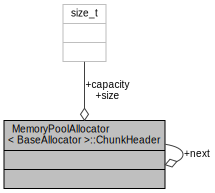
\includegraphics[width=287pt]{structMemoryPoolAllocator_1_1ChunkHeader__coll__graph}
\end{center}
\end{figure}
\subsection*{Public Attributes}
\begin{DoxyCompactItemize}
\item 
size\+\_\+t \hyperlink{structMemoryPoolAllocator_1_1ChunkHeader_ae19df98bce5dd485a23f953112ecde5f}{capacity}
\begin{DoxyCompactList}\small\item\em Capacity of the chunk in bytes (excluding the header itself). \end{DoxyCompactList}\item 
size\+\_\+t \hyperlink{structMemoryPoolAllocator_1_1ChunkHeader_ac9f3868f4cd36cdb7c712c9a48686680}{size}
\begin{DoxyCompactList}\small\item\em Current size of allocated memory in bytes. \end{DoxyCompactList}\item 
\hyperlink{structMemoryPoolAllocator_1_1ChunkHeader}{Chunk\+Header} $\ast$ \hyperlink{structMemoryPoolAllocator_1_1ChunkHeader_a4d24357c177824b3af56ec1098d9d9dc}{next}
\begin{DoxyCompactList}\small\item\em Next chunk in the linked list. \end{DoxyCompactList}\end{DoxyCompactItemize}


\subsection{Detailed Description}
\subsubsection*{template$<$typename Base\+Allocator = Crt\+Allocator$>$\newline
struct Memory\+Pool\+Allocator$<$ Base\+Allocator $>$\+::\+Chunk\+Header}

Chunk header for perpending to each chunk. 

Chunks are stored as a singly linked list. 

\subsection{Member Data Documentation}
\mbox{\Hypertarget{structMemoryPoolAllocator_1_1ChunkHeader_ae19df98bce5dd485a23f953112ecde5f}\label{structMemoryPoolAllocator_1_1ChunkHeader_ae19df98bce5dd485a23f953112ecde5f}} 
\index{Memory\+Pool\+Allocator\+::\+Chunk\+Header@{Memory\+Pool\+Allocator\+::\+Chunk\+Header}!capacity@{capacity}}
\index{capacity@{capacity}!Memory\+Pool\+Allocator\+::\+Chunk\+Header@{Memory\+Pool\+Allocator\+::\+Chunk\+Header}}
\subsubsection{\texorpdfstring{capacity}{capacity}}
{\footnotesize\ttfamily template$<$typename Base\+Allocator = Crt\+Allocator$>$ \\
size\+\_\+t \hyperlink{classMemoryPoolAllocator}{Memory\+Pool\+Allocator}$<$ Base\+Allocator $>$\+::Chunk\+Header\+::capacity}



Capacity of the chunk in bytes (excluding the header itself). 

\mbox{\Hypertarget{structMemoryPoolAllocator_1_1ChunkHeader_a4d24357c177824b3af56ec1098d9d9dc}\label{structMemoryPoolAllocator_1_1ChunkHeader_a4d24357c177824b3af56ec1098d9d9dc}} 
\index{Memory\+Pool\+Allocator\+::\+Chunk\+Header@{Memory\+Pool\+Allocator\+::\+Chunk\+Header}!next@{next}}
\index{next@{next}!Memory\+Pool\+Allocator\+::\+Chunk\+Header@{Memory\+Pool\+Allocator\+::\+Chunk\+Header}}
\subsubsection{\texorpdfstring{next}{next}}
{\footnotesize\ttfamily template$<$typename Base\+Allocator = Crt\+Allocator$>$ \\
\hyperlink{structMemoryPoolAllocator_1_1ChunkHeader}{Chunk\+Header}$\ast$ \hyperlink{classMemoryPoolAllocator}{Memory\+Pool\+Allocator}$<$ Base\+Allocator $>$\+::Chunk\+Header\+::next}



Next chunk in the linked list. 

\mbox{\Hypertarget{structMemoryPoolAllocator_1_1ChunkHeader_ac9f3868f4cd36cdb7c712c9a48686680}\label{structMemoryPoolAllocator_1_1ChunkHeader_ac9f3868f4cd36cdb7c712c9a48686680}} 
\index{Memory\+Pool\+Allocator\+::\+Chunk\+Header@{Memory\+Pool\+Allocator\+::\+Chunk\+Header}!size@{size}}
\index{size@{size}!Memory\+Pool\+Allocator\+::\+Chunk\+Header@{Memory\+Pool\+Allocator\+::\+Chunk\+Header}}
\subsubsection{\texorpdfstring{size}{size}}
{\footnotesize\ttfamily template$<$typename Base\+Allocator = Crt\+Allocator$>$ \\
size\+\_\+t \hyperlink{classMemoryPoolAllocator}{Memory\+Pool\+Allocator}$<$ Base\+Allocator $>$\+::Chunk\+Header\+::size}



Current size of allocated memory in bytes. 



The documentation for this struct was generated from the following file\+:\begin{DoxyCompactItemize}
\item 
/mnt/hdd/fnky/\+C0de/\+C\+A\+P\+S\+T\+O\+N\+E/clean\+\_\+build/include/rapidjson/\hyperlink{allocators_8h}{allocators.\+h}\end{DoxyCompactItemize}

\hypertarget{structGenericDocument_1_1ClearStackOnExit}{}\section{Generic\+Document$<$ Encoding, Allocator, Stack\+Allocator $>$\+:\+:Clear\+Stack\+On\+Exit Struct Reference}
\label{structGenericDocument_1_1ClearStackOnExit}\index{Generic\+Document$<$ Encoding, Allocator, Stack\+Allocator $>$\+::\+Clear\+Stack\+On\+Exit@{Generic\+Document$<$ Encoding, Allocator, Stack\+Allocator $>$\+::\+Clear\+Stack\+On\+Exit}}


Collaboration diagram for Generic\+Document$<$ Encoding, Allocator, Stack\+Allocator $>$\+:\+:Clear\+Stack\+On\+Exit\+:
\nopagebreak
\begin{figure}[H]
\begin{center}
\leavevmode
\includegraphics[width=350pt]{structGenericDocument_1_1ClearStackOnExit__coll__graph}
\end{center}
\end{figure}
\subsection*{Public Member Functions}
\begin{DoxyCompactItemize}
\item 
\hyperlink{structGenericDocument_1_1ClearStackOnExit_a99ba88d8b8ae15ccf5c979fff80c713a}{Clear\+Stack\+On\+Exit} (\hyperlink{classGenericDocument}{Generic\+Document} \&d)
\item 
\hyperlink{structGenericDocument_1_1ClearStackOnExit_aa51248f341ec130a29e4f8c3705c9312}{$\sim$\+Clear\+Stack\+On\+Exit} ()
\end{DoxyCompactItemize}
\subsection*{Private Member Functions}
\begin{DoxyCompactItemize}
\item 
\hyperlink{structGenericDocument_1_1ClearStackOnExit_ae009d5d42300fb5790227d24b4b38921}{Clear\+Stack\+On\+Exit} (const \hyperlink{structGenericDocument_1_1ClearStackOnExit}{Clear\+Stack\+On\+Exit} \&)
\item 
\hyperlink{structGenericDocument_1_1ClearStackOnExit}{Clear\+Stack\+On\+Exit} \& \hyperlink{structGenericDocument_1_1ClearStackOnExit_a474a254254f2deaba8c98ea79dc9c0f1}{operator=} (const \hyperlink{structGenericDocument_1_1ClearStackOnExit}{Clear\+Stack\+On\+Exit} \&)
\end{DoxyCompactItemize}
\subsection*{Private Attributes}
\begin{DoxyCompactItemize}
\item 
\hyperlink{classGenericDocument}{Generic\+Document} \& \hyperlink{structGenericDocument_1_1ClearStackOnExit_a56c2e82730f07911288b42640b029dc3}{d\+\_\+}
\end{DoxyCompactItemize}


\subsection{Constructor \& Destructor Documentation}
\mbox{\Hypertarget{structGenericDocument_1_1ClearStackOnExit_a99ba88d8b8ae15ccf5c979fff80c713a}\label{structGenericDocument_1_1ClearStackOnExit_a99ba88d8b8ae15ccf5c979fff80c713a}} 
\index{Generic\+Document\+::\+Clear\+Stack\+On\+Exit@{Generic\+Document\+::\+Clear\+Stack\+On\+Exit}!Clear\+Stack\+On\+Exit@{Clear\+Stack\+On\+Exit}}
\index{Clear\+Stack\+On\+Exit@{Clear\+Stack\+On\+Exit}!Generic\+Document\+::\+Clear\+Stack\+On\+Exit@{Generic\+Document\+::\+Clear\+Stack\+On\+Exit}}
\subsubsection{\texorpdfstring{Clear\+Stack\+On\+Exit()}{ClearStackOnExit()}\hspace{0.1cm}{\footnotesize\ttfamily [1/2]}}
{\footnotesize\ttfamily template$<$typename Encoding, typename Allocator = R\+A\+P\+I\+D\+J\+S\+O\+N\+\_\+\+D\+E\+F\+A\+U\+L\+T\+\_\+\+A\+L\+L\+O\+C\+A\+T\+OR, typename Stack\+Allocator = R\+A\+P\+I\+D\+J\+S\+O\+N\+\_\+\+D\+E\+F\+A\+U\+L\+T\+\_\+\+S\+T\+A\+C\+K\+\_\+\+A\+L\+L\+O\+C\+A\+T\+OR$>$ \\
\hyperlink{classGenericDocument}{Generic\+Document}$<$ Encoding, Allocator, Stack\+Allocator $>$\+::Clear\+Stack\+On\+Exit\+::\+Clear\+Stack\+On\+Exit (\begin{DoxyParamCaption}\item[{\hyperlink{classGenericDocument}{Generic\+Document} \&}]{d }\end{DoxyParamCaption})\hspace{0.3cm}{\ttfamily [inline]}, {\ttfamily [explicit]}}

\mbox{\Hypertarget{structGenericDocument_1_1ClearStackOnExit_aa51248f341ec130a29e4f8c3705c9312}\label{structGenericDocument_1_1ClearStackOnExit_aa51248f341ec130a29e4f8c3705c9312}} 
\index{Generic\+Document\+::\+Clear\+Stack\+On\+Exit@{Generic\+Document\+::\+Clear\+Stack\+On\+Exit}!````~Clear\+Stack\+On\+Exit@{$\sim$\+Clear\+Stack\+On\+Exit}}
\index{````~Clear\+Stack\+On\+Exit@{$\sim$\+Clear\+Stack\+On\+Exit}!Generic\+Document\+::\+Clear\+Stack\+On\+Exit@{Generic\+Document\+::\+Clear\+Stack\+On\+Exit}}
\subsubsection{\texorpdfstring{$\sim$\+Clear\+Stack\+On\+Exit()}{~ClearStackOnExit()}}
{\footnotesize\ttfamily template$<$typename Encoding, typename Allocator = R\+A\+P\+I\+D\+J\+S\+O\+N\+\_\+\+D\+E\+F\+A\+U\+L\+T\+\_\+\+A\+L\+L\+O\+C\+A\+T\+OR, typename Stack\+Allocator = R\+A\+P\+I\+D\+J\+S\+O\+N\+\_\+\+D\+E\+F\+A\+U\+L\+T\+\_\+\+S\+T\+A\+C\+K\+\_\+\+A\+L\+L\+O\+C\+A\+T\+OR$>$ \\
\hyperlink{classGenericDocument}{Generic\+Document}$<$ Encoding, Allocator, Stack\+Allocator $>$\+::Clear\+Stack\+On\+Exit\+::$\sim$\+Clear\+Stack\+On\+Exit (\begin{DoxyParamCaption}{ }\end{DoxyParamCaption})\hspace{0.3cm}{\ttfamily [inline]}}

\mbox{\Hypertarget{structGenericDocument_1_1ClearStackOnExit_ae009d5d42300fb5790227d24b4b38921}\label{structGenericDocument_1_1ClearStackOnExit_ae009d5d42300fb5790227d24b4b38921}} 
\index{Generic\+Document\+::\+Clear\+Stack\+On\+Exit@{Generic\+Document\+::\+Clear\+Stack\+On\+Exit}!Clear\+Stack\+On\+Exit@{Clear\+Stack\+On\+Exit}}
\index{Clear\+Stack\+On\+Exit@{Clear\+Stack\+On\+Exit}!Generic\+Document\+::\+Clear\+Stack\+On\+Exit@{Generic\+Document\+::\+Clear\+Stack\+On\+Exit}}
\subsubsection{\texorpdfstring{Clear\+Stack\+On\+Exit()}{ClearStackOnExit()}\hspace{0.1cm}{\footnotesize\ttfamily [2/2]}}
{\footnotesize\ttfamily template$<$typename Encoding, typename Allocator = R\+A\+P\+I\+D\+J\+S\+O\+N\+\_\+\+D\+E\+F\+A\+U\+L\+T\+\_\+\+A\+L\+L\+O\+C\+A\+T\+OR, typename Stack\+Allocator = R\+A\+P\+I\+D\+J\+S\+O\+N\+\_\+\+D\+E\+F\+A\+U\+L\+T\+\_\+\+S\+T\+A\+C\+K\+\_\+\+A\+L\+L\+O\+C\+A\+T\+OR$>$ \\
\hyperlink{classGenericDocument}{Generic\+Document}$<$ Encoding, Allocator, Stack\+Allocator $>$\+::Clear\+Stack\+On\+Exit\+::\+Clear\+Stack\+On\+Exit (\begin{DoxyParamCaption}\item[{const \hyperlink{structGenericDocument_1_1ClearStackOnExit}{Clear\+Stack\+On\+Exit} \&}]{ }\end{DoxyParamCaption})\hspace{0.3cm}{\ttfamily [private]}}



\subsection{Member Function Documentation}
\mbox{\Hypertarget{structGenericDocument_1_1ClearStackOnExit_a474a254254f2deaba8c98ea79dc9c0f1}\label{structGenericDocument_1_1ClearStackOnExit_a474a254254f2deaba8c98ea79dc9c0f1}} 
\index{Generic\+Document\+::\+Clear\+Stack\+On\+Exit@{Generic\+Document\+::\+Clear\+Stack\+On\+Exit}!operator=@{operator=}}
\index{operator=@{operator=}!Generic\+Document\+::\+Clear\+Stack\+On\+Exit@{Generic\+Document\+::\+Clear\+Stack\+On\+Exit}}
\subsubsection{\texorpdfstring{operator=()}{operator=()}}
{\footnotesize\ttfamily template$<$typename Encoding, typename Allocator = R\+A\+P\+I\+D\+J\+S\+O\+N\+\_\+\+D\+E\+F\+A\+U\+L\+T\+\_\+\+A\+L\+L\+O\+C\+A\+T\+OR, typename Stack\+Allocator = R\+A\+P\+I\+D\+J\+S\+O\+N\+\_\+\+D\+E\+F\+A\+U\+L\+T\+\_\+\+S\+T\+A\+C\+K\+\_\+\+A\+L\+L\+O\+C\+A\+T\+OR$>$ \\
\hyperlink{structGenericDocument_1_1ClearStackOnExit}{Clear\+Stack\+On\+Exit}\& \hyperlink{classGenericDocument}{Generic\+Document}$<$ Encoding, Allocator, Stack\+Allocator $>$\+::Clear\+Stack\+On\+Exit\+::operator= (\begin{DoxyParamCaption}\item[{const \hyperlink{structGenericDocument_1_1ClearStackOnExit}{Clear\+Stack\+On\+Exit} \&}]{ }\end{DoxyParamCaption})\hspace{0.3cm}{\ttfamily [private]}}



\subsection{Member Data Documentation}
\mbox{\Hypertarget{structGenericDocument_1_1ClearStackOnExit_a56c2e82730f07911288b42640b029dc3}\label{structGenericDocument_1_1ClearStackOnExit_a56c2e82730f07911288b42640b029dc3}} 
\index{Generic\+Document\+::\+Clear\+Stack\+On\+Exit@{Generic\+Document\+::\+Clear\+Stack\+On\+Exit}!d\+\_\+@{d\+\_\+}}
\index{d\+\_\+@{d\+\_\+}!Generic\+Document\+::\+Clear\+Stack\+On\+Exit@{Generic\+Document\+::\+Clear\+Stack\+On\+Exit}}
\subsubsection{\texorpdfstring{d\+\_\+}{d\_}}
{\footnotesize\ttfamily template$<$typename Encoding, typename Allocator = R\+A\+P\+I\+D\+J\+S\+O\+N\+\_\+\+D\+E\+F\+A\+U\+L\+T\+\_\+\+A\+L\+L\+O\+C\+A\+T\+OR, typename Stack\+Allocator = R\+A\+P\+I\+D\+J\+S\+O\+N\+\_\+\+D\+E\+F\+A\+U\+L\+T\+\_\+\+S\+T\+A\+C\+K\+\_\+\+A\+L\+L\+O\+C\+A\+T\+OR$>$ \\
\hyperlink{classGenericDocument}{Generic\+Document}\& \hyperlink{classGenericDocument}{Generic\+Document}$<$ Encoding, Allocator, Stack\+Allocator $>$\+::Clear\+Stack\+On\+Exit\+::d\+\_\+\hspace{0.3cm}{\ttfamily [private]}}



The documentation for this struct was generated from the following file\+:\begin{DoxyCompactItemize}
\item 
/mnt/hdd/fnky/\+C0de/\+C\+A\+P\+S\+T\+O\+N\+E/clean\+\_\+build/include/rapidjson/\hyperlink{document_8h}{document.\+h}\end{DoxyCompactItemize}

\hypertarget{structGenericReader_1_1ClearStackOnExit}{}\section{Generic\+Reader$<$ Source\+Encoding, Target\+Encoding, Stack\+Allocator $>$\+:\+:Clear\+Stack\+On\+Exit Struct Reference}
\label{structGenericReader_1_1ClearStackOnExit}\index{Generic\+Reader$<$ Source\+Encoding, Target\+Encoding, Stack\+Allocator $>$\+::\+Clear\+Stack\+On\+Exit@{Generic\+Reader$<$ Source\+Encoding, Target\+Encoding, Stack\+Allocator $>$\+::\+Clear\+Stack\+On\+Exit}}


Collaboration diagram for Generic\+Reader$<$ Source\+Encoding, Target\+Encoding, Stack\+Allocator $>$\+:\+:Clear\+Stack\+On\+Exit\+:
\nopagebreak
\begin{figure}[H]
\begin{center}
\leavevmode
\includegraphics[height=550pt]{structGenericReader_1_1ClearStackOnExit__coll__graph}
\end{center}
\end{figure}
\subsection*{Public Member Functions}
\begin{DoxyCompactItemize}
\item 
\hyperlink{structGenericReader_1_1ClearStackOnExit_a74f8b1f772229a3b2eb1d26ba4b58eca}{Clear\+Stack\+On\+Exit} (\hyperlink{classGenericReader}{Generic\+Reader} \&r)
\item 
\hyperlink{structGenericReader_1_1ClearStackOnExit_ab6035e502faee35e21fb1c9a9043a230}{$\sim$\+Clear\+Stack\+On\+Exit} ()
\end{DoxyCompactItemize}
\subsection*{Private Member Functions}
\begin{DoxyCompactItemize}
\item 
\hyperlink{structGenericReader_1_1ClearStackOnExit_ab276cf5b396da397f4ec05d6a29139a9}{Clear\+Stack\+On\+Exit} (const \hyperlink{structGenericReader_1_1ClearStackOnExit}{Clear\+Stack\+On\+Exit} \&)
\item 
\hyperlink{structGenericReader_1_1ClearStackOnExit}{Clear\+Stack\+On\+Exit} \& \hyperlink{structGenericReader_1_1ClearStackOnExit_acf3f83e842ebbe256c86d52e36a044c3}{operator=} (const \hyperlink{structGenericReader_1_1ClearStackOnExit}{Clear\+Stack\+On\+Exit} \&)
\end{DoxyCompactItemize}
\subsection*{Private Attributes}
\begin{DoxyCompactItemize}
\item 
\hyperlink{classGenericReader}{Generic\+Reader} \& \hyperlink{structGenericReader_1_1ClearStackOnExit_a6805ebb172f278c65ec7fc61847eb08d}{r\+\_\+}
\end{DoxyCompactItemize}


\subsection{Constructor \& Destructor Documentation}
\mbox{\Hypertarget{structGenericReader_1_1ClearStackOnExit_a74f8b1f772229a3b2eb1d26ba4b58eca}\label{structGenericReader_1_1ClearStackOnExit_a74f8b1f772229a3b2eb1d26ba4b58eca}} 
\index{Generic\+Reader\+::\+Clear\+Stack\+On\+Exit@{Generic\+Reader\+::\+Clear\+Stack\+On\+Exit}!Clear\+Stack\+On\+Exit@{Clear\+Stack\+On\+Exit}}
\index{Clear\+Stack\+On\+Exit@{Clear\+Stack\+On\+Exit}!Generic\+Reader\+::\+Clear\+Stack\+On\+Exit@{Generic\+Reader\+::\+Clear\+Stack\+On\+Exit}}
\subsubsection{\texorpdfstring{Clear\+Stack\+On\+Exit()}{ClearStackOnExit()}\hspace{0.1cm}{\footnotesize\ttfamily [1/2]}}
{\footnotesize\ttfamily template$<$typename Source\+Encoding, typename Target\+Encoding, typename Stack\+Allocator = Crt\+Allocator$>$ \\
\hyperlink{classGenericReader}{Generic\+Reader}$<$ Source\+Encoding, Target\+Encoding, Stack\+Allocator $>$\+::Clear\+Stack\+On\+Exit\+::\+Clear\+Stack\+On\+Exit (\begin{DoxyParamCaption}\item[{\hyperlink{classGenericReader}{Generic\+Reader} \&}]{r }\end{DoxyParamCaption})\hspace{0.3cm}{\ttfamily [inline]}, {\ttfamily [explicit]}}

\mbox{\Hypertarget{structGenericReader_1_1ClearStackOnExit_ab6035e502faee35e21fb1c9a9043a230}\label{structGenericReader_1_1ClearStackOnExit_ab6035e502faee35e21fb1c9a9043a230}} 
\index{Generic\+Reader\+::\+Clear\+Stack\+On\+Exit@{Generic\+Reader\+::\+Clear\+Stack\+On\+Exit}!````~Clear\+Stack\+On\+Exit@{$\sim$\+Clear\+Stack\+On\+Exit}}
\index{````~Clear\+Stack\+On\+Exit@{$\sim$\+Clear\+Stack\+On\+Exit}!Generic\+Reader\+::\+Clear\+Stack\+On\+Exit@{Generic\+Reader\+::\+Clear\+Stack\+On\+Exit}}
\subsubsection{\texorpdfstring{$\sim$\+Clear\+Stack\+On\+Exit()}{~ClearStackOnExit()}}
{\footnotesize\ttfamily template$<$typename Source\+Encoding, typename Target\+Encoding, typename Stack\+Allocator = Crt\+Allocator$>$ \\
\hyperlink{classGenericReader}{Generic\+Reader}$<$ Source\+Encoding, Target\+Encoding, Stack\+Allocator $>$\+::Clear\+Stack\+On\+Exit\+::$\sim$\+Clear\+Stack\+On\+Exit (\begin{DoxyParamCaption}{ }\end{DoxyParamCaption})\hspace{0.3cm}{\ttfamily [inline]}}

\mbox{\Hypertarget{structGenericReader_1_1ClearStackOnExit_ab276cf5b396da397f4ec05d6a29139a9}\label{structGenericReader_1_1ClearStackOnExit_ab276cf5b396da397f4ec05d6a29139a9}} 
\index{Generic\+Reader\+::\+Clear\+Stack\+On\+Exit@{Generic\+Reader\+::\+Clear\+Stack\+On\+Exit}!Clear\+Stack\+On\+Exit@{Clear\+Stack\+On\+Exit}}
\index{Clear\+Stack\+On\+Exit@{Clear\+Stack\+On\+Exit}!Generic\+Reader\+::\+Clear\+Stack\+On\+Exit@{Generic\+Reader\+::\+Clear\+Stack\+On\+Exit}}
\subsubsection{\texorpdfstring{Clear\+Stack\+On\+Exit()}{ClearStackOnExit()}\hspace{0.1cm}{\footnotesize\ttfamily [2/2]}}
{\footnotesize\ttfamily template$<$typename Source\+Encoding, typename Target\+Encoding, typename Stack\+Allocator = Crt\+Allocator$>$ \\
\hyperlink{classGenericReader}{Generic\+Reader}$<$ Source\+Encoding, Target\+Encoding, Stack\+Allocator $>$\+::Clear\+Stack\+On\+Exit\+::\+Clear\+Stack\+On\+Exit (\begin{DoxyParamCaption}\item[{const \hyperlink{structGenericReader_1_1ClearStackOnExit}{Clear\+Stack\+On\+Exit} \&}]{ }\end{DoxyParamCaption})\hspace{0.3cm}{\ttfamily [private]}}



\subsection{Member Function Documentation}
\mbox{\Hypertarget{structGenericReader_1_1ClearStackOnExit_acf3f83e842ebbe256c86d52e36a044c3}\label{structGenericReader_1_1ClearStackOnExit_acf3f83e842ebbe256c86d52e36a044c3}} 
\index{Generic\+Reader\+::\+Clear\+Stack\+On\+Exit@{Generic\+Reader\+::\+Clear\+Stack\+On\+Exit}!operator=@{operator=}}
\index{operator=@{operator=}!Generic\+Reader\+::\+Clear\+Stack\+On\+Exit@{Generic\+Reader\+::\+Clear\+Stack\+On\+Exit}}
\subsubsection{\texorpdfstring{operator=()}{operator=()}}
{\footnotesize\ttfamily template$<$typename Source\+Encoding, typename Target\+Encoding, typename Stack\+Allocator = Crt\+Allocator$>$ \\
\hyperlink{structGenericReader_1_1ClearStackOnExit}{Clear\+Stack\+On\+Exit}\& \hyperlink{classGenericReader}{Generic\+Reader}$<$ Source\+Encoding, Target\+Encoding, Stack\+Allocator $>$\+::Clear\+Stack\+On\+Exit\+::operator= (\begin{DoxyParamCaption}\item[{const \hyperlink{structGenericReader_1_1ClearStackOnExit}{Clear\+Stack\+On\+Exit} \&}]{ }\end{DoxyParamCaption})\hspace{0.3cm}{\ttfamily [private]}}



\subsection{Member Data Documentation}
\mbox{\Hypertarget{structGenericReader_1_1ClearStackOnExit_a6805ebb172f278c65ec7fc61847eb08d}\label{structGenericReader_1_1ClearStackOnExit_a6805ebb172f278c65ec7fc61847eb08d}} 
\index{Generic\+Reader\+::\+Clear\+Stack\+On\+Exit@{Generic\+Reader\+::\+Clear\+Stack\+On\+Exit}!r\+\_\+@{r\+\_\+}}
\index{r\+\_\+@{r\+\_\+}!Generic\+Reader\+::\+Clear\+Stack\+On\+Exit@{Generic\+Reader\+::\+Clear\+Stack\+On\+Exit}}
\subsubsection{\texorpdfstring{r\+\_\+}{r\_}}
{\footnotesize\ttfamily template$<$typename Source\+Encoding, typename Target\+Encoding, typename Stack\+Allocator = Crt\+Allocator$>$ \\
\hyperlink{classGenericReader}{Generic\+Reader}\& \hyperlink{classGenericReader}{Generic\+Reader}$<$ Source\+Encoding, Target\+Encoding, Stack\+Allocator $>$\+::Clear\+Stack\+On\+Exit\+::r\+\_\+\hspace{0.3cm}{\ttfamily [private]}}



The documentation for this struct was generated from the following file\+:\begin{DoxyCompactItemize}
\item 
/mnt/hdd/fnky/\+C0de/\+C\+A\+P\+S\+T\+O\+N\+E/clean\+\_\+build/include/rapidjson/\hyperlink{reader_8h}{reader.\+h}\end{DoxyCompactItemize}

\hypertarget{classComponent}{}\doxysection{Component Class Reference}
\label{classComponent}\index{Component@{Component}}


{\ttfamily \#include $<$Component.\+h$>$}



Inheritance diagram for Component\+:
\nopagebreak
\begin{figure}[H]
\begin{center}
\leavevmode
\includegraphics[width=350pt]{classComponent__inherit__graph}
\end{center}
\end{figure}


Collaboration diagram for Component\+:
\nopagebreak
\begin{figure}[H]
\begin{center}
\leavevmode
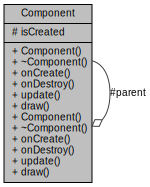
\includegraphics[width=241pt]{classComponent__coll__graph}
\end{center}
\end{figure}
\doxysubsection*{Public Member Functions}
\begin{DoxyCompactItemize}
\item 
\mbox{\hyperlink{classComponent_ad8fd006e351b2722c2e0f79010170a3c}{Component}} (\mbox{\hyperlink{classComponent}{Component}} $\ast$parent\+\_\+)
\item 
virtual \mbox{\hyperlink{classComponent_ad82d7393e339c1b19cc17a0d55b5674d}{$\sim$\+Component}} ()=default
\item 
virtual bool \mbox{\hyperlink{classComponent_a3a1537a8b8bcdb2155afbb925c77b0a2}{on\+Create}} ()=0
\item 
virtual \mbox{\hyperlink{imgui__impl__opengl3__loader_8h_ac668e7cffd9e2e9cfee428b9b2f34fa7}{void}} \mbox{\hyperlink{classComponent_a2b198f27162a6caf63917e304295f892}{on\+Destroy}} ()=0
\item 
virtual \mbox{\hyperlink{imgui__impl__opengl3__loader_8h_ac668e7cffd9e2e9cfee428b9b2f34fa7}{void}} \mbox{\hyperlink{classComponent_a3448977e6f464df89e77dda7c6f52204}{update}} (const float delta\+Time\+\_\+)=0
\item 
virtual \mbox{\hyperlink{imgui__impl__opengl3__loader_8h_ac668e7cffd9e2e9cfee428b9b2f34fa7}{void}} \mbox{\hyperlink{classComponent_a8f45309003f02191f2bcc8864e8e9ecf}{draw}} () const =0
\item 
\mbox{\hyperlink{classComponent_ad8fd006e351b2722c2e0f79010170a3c}{Component}} (\mbox{\hyperlink{classComponent}{Component}} $\ast$parent\+\_\+)
\item 
virtual \mbox{\hyperlink{classComponent_ad82d7393e339c1b19cc17a0d55b5674d}{$\sim$\+Component}} ()=default
\item 
virtual bool \mbox{\hyperlink{classComponent_a3a1537a8b8bcdb2155afbb925c77b0a2}{on\+Create}} ()=0
\item 
virtual \mbox{\hyperlink{imgui__impl__opengl3__loader_8h_ac668e7cffd9e2e9cfee428b9b2f34fa7}{void}} \mbox{\hyperlink{classComponent_a2b198f27162a6caf63917e304295f892}{on\+Destroy}} ()=0
\item 
virtual \mbox{\hyperlink{imgui__impl__opengl3__loader_8h_ac668e7cffd9e2e9cfee428b9b2f34fa7}{void}} \mbox{\hyperlink{classComponent_a3448977e6f464df89e77dda7c6f52204}{update}} (const float delta\+Time\+\_\+)=0
\item 
virtual \mbox{\hyperlink{imgui__impl__opengl3__loader_8h_ac668e7cffd9e2e9cfee428b9b2f34fa7}{void}} \mbox{\hyperlink{classComponent_a8f45309003f02191f2bcc8864e8e9ecf}{draw}} () const =0
\end{DoxyCompactItemize}
\doxysubsection*{Protected Attributes}
\begin{DoxyCompactItemize}
\item 
\mbox{\hyperlink{classComponent}{Component}} $\ast$ \mbox{\hyperlink{classComponent_a8d7b023bf6615e457842e02e28d7ab07}{parent}}
\item 
bool \mbox{\hyperlink{classComponent_addf22788d84ea7450e70e8793dc2fe8d}{is\+Created}}
\end{DoxyCompactItemize}


\doxysubsection{Constructor \& Destructor Documentation}
\mbox{\Hypertarget{classComponent_ad8fd006e351b2722c2e0f79010170a3c}\label{classComponent_ad8fd006e351b2722c2e0f79010170a3c}} 
\index{Component@{Component}!Component@{Component}}
\index{Component@{Component}!Component@{Component}}
\doxysubsubsection{\texorpdfstring{Component()}{Component()}\hspace{0.1cm}{\footnotesize\ttfamily [1/2]}}
{\footnotesize\ttfamily Component\+::\+Component (\begin{DoxyParamCaption}\item[{\mbox{\hyperlink{classComponent}{Component}} $\ast$}]{parent\+\_\+ }\end{DoxyParamCaption})\hspace{0.3cm}{\ttfamily [inline]}}

\mbox{\Hypertarget{classComponent_ad82d7393e339c1b19cc17a0d55b5674d}\label{classComponent_ad82d7393e339c1b19cc17a0d55b5674d}} 
\index{Component@{Component}!````~Component@{$\sim$Component}}
\index{````~Component@{$\sim$Component}!Component@{Component}}
\doxysubsubsection{\texorpdfstring{$\sim$Component()}{~Component()}\hspace{0.1cm}{\footnotesize\ttfamily [1/2]}}
{\footnotesize\ttfamily virtual Component\+::$\sim$\+Component (\begin{DoxyParamCaption}{ }\end{DoxyParamCaption})\hspace{0.3cm}{\ttfamily [virtual]}, {\ttfamily [default]}}

\mbox{\Hypertarget{classComponent_ad8fd006e351b2722c2e0f79010170a3c}\label{classComponent_ad8fd006e351b2722c2e0f79010170a3c}} 
\index{Component@{Component}!Component@{Component}}
\index{Component@{Component}!Component@{Component}}
\doxysubsubsection{\texorpdfstring{Component()}{Component()}\hspace{0.1cm}{\footnotesize\ttfamily [2/2]}}
{\footnotesize\ttfamily Component\+::\+Component (\begin{DoxyParamCaption}\item[{\mbox{\hyperlink{classComponent}{Component}} $\ast$}]{parent\+\_\+ }\end{DoxyParamCaption})\hspace{0.3cm}{\ttfamily [inline]}}

\mbox{\Hypertarget{classComponent_ad82d7393e339c1b19cc17a0d55b5674d}\label{classComponent_ad82d7393e339c1b19cc17a0d55b5674d}} 
\index{Component@{Component}!````~Component@{$\sim$Component}}
\index{````~Component@{$\sim$Component}!Component@{Component}}
\doxysubsubsection{\texorpdfstring{$\sim$Component()}{~Component()}\hspace{0.1cm}{\footnotesize\ttfamily [2/2]}}
{\footnotesize\ttfamily virtual Component\+::$\sim$\+Component (\begin{DoxyParamCaption}{ }\end{DoxyParamCaption})\hspace{0.3cm}{\ttfamily [virtual]}, {\ttfamily [default]}}



\doxysubsection{Member Function Documentation}
\mbox{\Hypertarget{classComponent_a8f45309003f02191f2bcc8864e8e9ecf}\label{classComponent_a8f45309003f02191f2bcc8864e8e9ecf}} 
\index{Component@{Component}!draw@{draw}}
\index{draw@{draw}!Component@{Component}}
\doxysubsubsection{\texorpdfstring{draw()}{draw()}\hspace{0.1cm}{\footnotesize\ttfamily [1/2]}}
{\footnotesize\ttfamily virtual \mbox{\hyperlink{imgui__impl__opengl3__loader_8h_ac668e7cffd9e2e9cfee428b9b2f34fa7}{void}} Component\+::draw (\begin{DoxyParamCaption}{ }\end{DoxyParamCaption}) const\hspace{0.3cm}{\ttfamily [pure virtual]}}



Implemented in \mbox{\hyperlink{classPhysicsComponent_afe1f99cac34411e9de43abebfcef0713}{Physics\+Component}}, \mbox{\hyperlink{classTextRenderComponent_adb02fc97e8e67e7d3035b38c2860bfab}{Text\+Render\+Component}}, \mbox{\hyperlink{classRenderComponent_af2bf016f9a929d97b4c0c31db8e3842f}{Render\+Component}}, \mbox{\hyperlink{classAIComponent_ab4d6c5c6043cfa275e4edce5b575a8a9}{A\+I\+Component}}, \mbox{\hyperlink{classTransformComponent_a5447f13e20359c750f165332015af3ea}{Transform\+Component}}, \mbox{\hyperlink{classActor_adbbdc379c1a471cc9763d871b0790d7e}{Actor}}, and \mbox{\hyperlink{classShaderComponent_a1ac6a772f197d759e9ae11fae0551687}{Shader\+Component}}.

\mbox{\Hypertarget{classComponent_a8f45309003f02191f2bcc8864e8e9ecf}\label{classComponent_a8f45309003f02191f2bcc8864e8e9ecf}} 
\index{Component@{Component}!draw@{draw}}
\index{draw@{draw}!Component@{Component}}
\doxysubsubsection{\texorpdfstring{draw()}{draw()}\hspace{0.1cm}{\footnotesize\ttfamily [2/2]}}
{\footnotesize\ttfamily virtual \mbox{\hyperlink{imgui__impl__opengl3__loader_8h_ac668e7cffd9e2e9cfee428b9b2f34fa7}{void}} Component\+::draw (\begin{DoxyParamCaption}{ }\end{DoxyParamCaption}) const\hspace{0.3cm}{\ttfamily [pure virtual]}}



Implemented in \mbox{\hyperlink{classPhysicsComponent_afe1f99cac34411e9de43abebfcef0713}{Physics\+Component}}, \mbox{\hyperlink{classTextRenderComponent_adb02fc97e8e67e7d3035b38c2860bfab}{Text\+Render\+Component}}, \mbox{\hyperlink{classRenderComponent_af2bf016f9a929d97b4c0c31db8e3842f}{Render\+Component}}, \mbox{\hyperlink{classAIComponent_ab4d6c5c6043cfa275e4edce5b575a8a9}{A\+I\+Component}}, \mbox{\hyperlink{classTransformComponent_a5447f13e20359c750f165332015af3ea}{Transform\+Component}}, \mbox{\hyperlink{classActor_adbbdc379c1a471cc9763d871b0790d7e}{Actor}}, and \mbox{\hyperlink{classShaderComponent_a1ac6a772f197d759e9ae11fae0551687}{Shader\+Component}}.

\mbox{\Hypertarget{classComponent_a3a1537a8b8bcdb2155afbb925c77b0a2}\label{classComponent_a3a1537a8b8bcdb2155afbb925c77b0a2}} 
\index{Component@{Component}!onCreate@{onCreate}}
\index{onCreate@{onCreate}!Component@{Component}}
\doxysubsubsection{\texorpdfstring{onCreate()}{onCreate()}\hspace{0.1cm}{\footnotesize\ttfamily [1/2]}}
{\footnotesize\ttfamily virtual bool Component\+::on\+Create (\begin{DoxyParamCaption}{ }\end{DoxyParamCaption})\hspace{0.3cm}{\ttfamily [pure virtual]}}



Implemented in \mbox{\hyperlink{classRenderComponent_a5ecc72f2a9249c4df22365dbe7ca49b0}{Render\+Component}}, \mbox{\hyperlink{classTextRenderComponent_aafaf33608a83d1ff4af66ef53ba81b29}{Text\+Render\+Component}}, \mbox{\hyperlink{classPhysicsComponent_ad797a2708cfc3c0e88a44341121f594d}{Physics\+Component}}, \mbox{\hyperlink{classAIComponent_a1f7e2f748183cbcba9e3f351025b862c}{A\+I\+Component}}, \mbox{\hyperlink{classTransformComponent_aef9e192f10ac612d6b146136603b3293}{Transform\+Component}}, \mbox{\hyperlink{classActor_a56a241c949adf52cedceb45a7102ea1a}{Actor}}, \mbox{\hyperlink{classProjectile__Actor_a98e2e2198cd164c35318c04f96e6a3ac}{Projectile\+\_\+\+Actor}}, \mbox{\hyperlink{classShaderComponent_a0c42362c7ba178050551e7451b49abe5}{Shader\+Component}}, and \mbox{\hyperlink{classPlatform__Actor_ab902e2540f1d3127dedff632841b4921}{Platform\+\_\+\+Actor}}.

\mbox{\Hypertarget{classComponent_a3a1537a8b8bcdb2155afbb925c77b0a2}\label{classComponent_a3a1537a8b8bcdb2155afbb925c77b0a2}} 
\index{Component@{Component}!onCreate@{onCreate}}
\index{onCreate@{onCreate}!Component@{Component}}
\doxysubsubsection{\texorpdfstring{onCreate()}{onCreate()}\hspace{0.1cm}{\footnotesize\ttfamily [2/2]}}
{\footnotesize\ttfamily virtual bool Component\+::on\+Create (\begin{DoxyParamCaption}{ }\end{DoxyParamCaption})\hspace{0.3cm}{\ttfamily [pure virtual]}}



Implemented in \mbox{\hyperlink{classRenderComponent_a5ecc72f2a9249c4df22365dbe7ca49b0}{Render\+Component}}, \mbox{\hyperlink{classTextRenderComponent_aafaf33608a83d1ff4af66ef53ba81b29}{Text\+Render\+Component}}, \mbox{\hyperlink{classPhysicsComponent_ad797a2708cfc3c0e88a44341121f594d}{Physics\+Component}}, \mbox{\hyperlink{classAIComponent_a1f7e2f748183cbcba9e3f351025b862c}{A\+I\+Component}}, \mbox{\hyperlink{classTransformComponent_aef9e192f10ac612d6b146136603b3293}{Transform\+Component}}, \mbox{\hyperlink{classActor_a56a241c949adf52cedceb45a7102ea1a}{Actor}}, \mbox{\hyperlink{classProjectile__Actor_a98e2e2198cd164c35318c04f96e6a3ac}{Projectile\+\_\+\+Actor}}, \mbox{\hyperlink{classShaderComponent_a0c42362c7ba178050551e7451b49abe5}{Shader\+Component}}, and \mbox{\hyperlink{classPlatform__Actor_ab902e2540f1d3127dedff632841b4921}{Platform\+\_\+\+Actor}}.

\mbox{\Hypertarget{classComponent_a2b198f27162a6caf63917e304295f892}\label{classComponent_a2b198f27162a6caf63917e304295f892}} 
\index{Component@{Component}!onDestroy@{onDestroy}}
\index{onDestroy@{onDestroy}!Component@{Component}}
\doxysubsubsection{\texorpdfstring{onDestroy()}{onDestroy()}\hspace{0.1cm}{\footnotesize\ttfamily [1/2]}}
{\footnotesize\ttfamily virtual \mbox{\hyperlink{imgui__impl__opengl3__loader_8h_ac668e7cffd9e2e9cfee428b9b2f34fa7}{void}} Component\+::on\+Destroy (\begin{DoxyParamCaption}{ }\end{DoxyParamCaption})\hspace{0.3cm}{\ttfamily [pure virtual]}}



Implemented in \mbox{\hyperlink{classPhysicsComponent_a5a5e472f0c6975d4a22e0990c504ec0a}{Physics\+Component}}, \mbox{\hyperlink{classTextRenderComponent_a097fb07ecd0e1feed1c4c2bd7c97d480}{Text\+Render\+Component}}, \mbox{\hyperlink{classRenderComponent_a2d05ddd16edf5d2022d46a640a74a4da}{Render\+Component}}, \mbox{\hyperlink{classAIComponent_a82e8e79810024e09695545ebf59452f2}{A\+I\+Component}}, \mbox{\hyperlink{classNPC__Actor_ab274d0517bd0cd710efc7df31cd7450b}{N\+P\+C\+\_\+\+Actor}}, \mbox{\hyperlink{classTransformComponent_aab0dd130a6c8d4d6f873f81e59e48ee0}{Transform\+Component}}, \mbox{\hyperlink{classActor_a47101d6275509662bf6c84c3f3439696}{Actor}}, \mbox{\hyperlink{classProjectile__Actor_a58d01ff77f0815ca611236f139b7aafa}{Projectile\+\_\+\+Actor}}, \mbox{\hyperlink{classAnimate__Actor_ae67ff6399f3d46696f84c77b2e519ead}{Animate\+\_\+\+Actor}}, \mbox{\hyperlink{classPlayer__Actor_a200b6b956d9c597cbc626ca9bcafb25e}{Player\+\_\+\+Actor}}, \mbox{\hyperlink{classShader__Actor_a16f7f5f30d3f3cd125de9713457a7db2}{Shader\+\_\+\+Actor}}, \mbox{\hyperlink{classTexture__Actor_ac9677f60df27e14ef3550ae2b0678ad5}{Texture\+\_\+\+Actor}}, \mbox{\hyperlink{classShaderComponent_a7ebd7c8ee1b2aea5ad2010a4652bb588}{Shader\+Component}}, \mbox{\hyperlink{classEdge__Actor_ae7a429d48b86442154c93eb65bc8b22d}{Edge\+\_\+\+Actor}}, \mbox{\hyperlink{classPlatform__Actor_a34b915aa583cdf659ec29368b6feb7e8}{Platform\+\_\+\+Actor}}, and \mbox{\hyperlink{classText__Actor_af9b25da889aad4aec6f17671c37ac431}{Text\+\_\+\+Actor}}.

\mbox{\Hypertarget{classComponent_a2b198f27162a6caf63917e304295f892}\label{classComponent_a2b198f27162a6caf63917e304295f892}} 
\index{Component@{Component}!onDestroy@{onDestroy}}
\index{onDestroy@{onDestroy}!Component@{Component}}
\doxysubsubsection{\texorpdfstring{onDestroy()}{onDestroy()}\hspace{0.1cm}{\footnotesize\ttfamily [2/2]}}
{\footnotesize\ttfamily virtual \mbox{\hyperlink{imgui__impl__opengl3__loader_8h_ac668e7cffd9e2e9cfee428b9b2f34fa7}{void}} Component\+::on\+Destroy (\begin{DoxyParamCaption}{ }\end{DoxyParamCaption})\hspace{0.3cm}{\ttfamily [pure virtual]}}



Implemented in \mbox{\hyperlink{classPhysicsComponent_a5a5e472f0c6975d4a22e0990c504ec0a}{Physics\+Component}}, \mbox{\hyperlink{classTextRenderComponent_a097fb07ecd0e1feed1c4c2bd7c97d480}{Text\+Render\+Component}}, \mbox{\hyperlink{classRenderComponent_a2d05ddd16edf5d2022d46a640a74a4da}{Render\+Component}}, \mbox{\hyperlink{classAIComponent_a82e8e79810024e09695545ebf59452f2}{A\+I\+Component}}, \mbox{\hyperlink{classNPC__Actor_ab274d0517bd0cd710efc7df31cd7450b}{N\+P\+C\+\_\+\+Actor}}, \mbox{\hyperlink{classTransformComponent_aab0dd130a6c8d4d6f873f81e59e48ee0}{Transform\+Component}}, \mbox{\hyperlink{classActor_a47101d6275509662bf6c84c3f3439696}{Actor}}, \mbox{\hyperlink{classProjectile__Actor_a58d01ff77f0815ca611236f139b7aafa}{Projectile\+\_\+\+Actor}}, \mbox{\hyperlink{classAnimate__Actor_ae67ff6399f3d46696f84c77b2e519ead}{Animate\+\_\+\+Actor}}, \mbox{\hyperlink{classPlayer__Actor_a200b6b956d9c597cbc626ca9bcafb25e}{Player\+\_\+\+Actor}}, \mbox{\hyperlink{classShader__Actor_a16f7f5f30d3f3cd125de9713457a7db2}{Shader\+\_\+\+Actor}}, \mbox{\hyperlink{classTexture__Actor_ac9677f60df27e14ef3550ae2b0678ad5}{Texture\+\_\+\+Actor}}, \mbox{\hyperlink{classShaderComponent_a7ebd7c8ee1b2aea5ad2010a4652bb588}{Shader\+Component}}, \mbox{\hyperlink{classEdge__Actor_ae7a429d48b86442154c93eb65bc8b22d}{Edge\+\_\+\+Actor}}, \mbox{\hyperlink{classPlatform__Actor_a34b915aa583cdf659ec29368b6feb7e8}{Platform\+\_\+\+Actor}}, and \mbox{\hyperlink{classText__Actor_af9b25da889aad4aec6f17671c37ac431}{Text\+\_\+\+Actor}}.

\mbox{\Hypertarget{classComponent_a3448977e6f464df89e77dda7c6f52204}\label{classComponent_a3448977e6f464df89e77dda7c6f52204}} 
\index{Component@{Component}!update@{update}}
\index{update@{update}!Component@{Component}}
\doxysubsubsection{\texorpdfstring{update()}{update()}\hspace{0.1cm}{\footnotesize\ttfamily [1/2]}}
{\footnotesize\ttfamily virtual \mbox{\hyperlink{imgui__impl__opengl3__loader_8h_ac668e7cffd9e2e9cfee428b9b2f34fa7}{void}} Component\+::update (\begin{DoxyParamCaption}\item[{const float}]{delta\+Time\+\_\+ }\end{DoxyParamCaption})\hspace{0.3cm}{\ttfamily [pure virtual]}}



Implemented in \mbox{\hyperlink{classActor_a724ff8f2e9c34f15a6c443a3912504c4}{Actor}}, \mbox{\hyperlink{classProjectile__Actor_ab61aec7117a93626c3096bef71ab30fc}{Projectile\+\_\+\+Actor}}, \mbox{\hyperlink{classAnimate__Actor_a6bdb436a75efbc01545679b613858201}{Animate\+\_\+\+Actor}}, \mbox{\hyperlink{classGun__Actor_ab5e7b6b7032e1f0353c6c4f08cedebec}{Gun\+\_\+\+Actor}}, \mbox{\hyperlink{classPlayer__Actor_a619a94504523cbfa9eb5490de5361f31}{Player\+\_\+\+Actor}}, \mbox{\hyperlink{classTexture__Actor_afe03163ea0bff0ea0fa3c3fb6c560c79}{Texture\+\_\+\+Actor}}, \mbox{\hyperlink{classEdge__Actor_a8ae8a19c72b58522755d2d0a395fc1ea}{Edge\+\_\+\+Actor}}, \mbox{\hyperlink{classPlatform__Actor_a12b22d88efc384ac35060d04fbbe710d}{Platform\+\_\+\+Actor}}, \mbox{\hyperlink{classText__Actor_a26181e1102ab2a37ec8b140c999a6f6a}{Text\+\_\+\+Actor}}, \mbox{\hyperlink{classTransformComponent_a0cd568e49687464927c79ac7ab03f004}{Transform\+Component}}, \mbox{\hyperlink{classShaderComponent_ab8f4b5e17bf77b20e509ac94c9dddc10}{Shader\+Component}}, \mbox{\hyperlink{classPhysicsComponent_a7494b2fec675132ee3e31050d7d87d30}{Physics\+Component}}, \mbox{\hyperlink{classTextRenderComponent_a73c53ed27b94597551536fda5775fb49}{Text\+Render\+Component}}, \mbox{\hyperlink{classRenderComponent_a93203c887b05a024f70f30e8a71576bd}{Render\+Component}}, and \mbox{\hyperlink{classAIComponent_a456939f85de6d6cfc3e4e48ffc9f568c}{A\+I\+Component}}.

\mbox{\Hypertarget{classComponent_a3448977e6f464df89e77dda7c6f52204}\label{classComponent_a3448977e6f464df89e77dda7c6f52204}} 
\index{Component@{Component}!update@{update}}
\index{update@{update}!Component@{Component}}
\doxysubsubsection{\texorpdfstring{update()}{update()}\hspace{0.1cm}{\footnotesize\ttfamily [2/2]}}
{\footnotesize\ttfamily virtual \mbox{\hyperlink{imgui__impl__opengl3__loader_8h_ac668e7cffd9e2e9cfee428b9b2f34fa7}{void}} Component\+::update (\begin{DoxyParamCaption}\item[{const float}]{delta\+Time\+\_\+ }\end{DoxyParamCaption})\hspace{0.3cm}{\ttfamily [pure virtual]}}



Implemented in \mbox{\hyperlink{classActor_a724ff8f2e9c34f15a6c443a3912504c4}{Actor}}, \mbox{\hyperlink{classProjectile__Actor_ab61aec7117a93626c3096bef71ab30fc}{Projectile\+\_\+\+Actor}}, \mbox{\hyperlink{classAnimate__Actor_a6bdb436a75efbc01545679b613858201}{Animate\+\_\+\+Actor}}, \mbox{\hyperlink{classGun__Actor_ab5e7b6b7032e1f0353c6c4f08cedebec}{Gun\+\_\+\+Actor}}, \mbox{\hyperlink{classPlayer__Actor_a619a94504523cbfa9eb5490de5361f31}{Player\+\_\+\+Actor}}, \mbox{\hyperlink{classTexture__Actor_afe03163ea0bff0ea0fa3c3fb6c560c79}{Texture\+\_\+\+Actor}}, \mbox{\hyperlink{classEdge__Actor_a8ae8a19c72b58522755d2d0a395fc1ea}{Edge\+\_\+\+Actor}}, \mbox{\hyperlink{classPlatform__Actor_a12b22d88efc384ac35060d04fbbe710d}{Platform\+\_\+\+Actor}}, \mbox{\hyperlink{classText__Actor_a26181e1102ab2a37ec8b140c999a6f6a}{Text\+\_\+\+Actor}}, \mbox{\hyperlink{classTransformComponent_a0cd568e49687464927c79ac7ab03f004}{Transform\+Component}}, \mbox{\hyperlink{classShaderComponent_ab8f4b5e17bf77b20e509ac94c9dddc10}{Shader\+Component}}, \mbox{\hyperlink{classPhysicsComponent_a7494b2fec675132ee3e31050d7d87d30}{Physics\+Component}}, \mbox{\hyperlink{classTextRenderComponent_a73c53ed27b94597551536fda5775fb49}{Text\+Render\+Component}}, \mbox{\hyperlink{classRenderComponent_a93203c887b05a024f70f30e8a71576bd}{Render\+Component}}, and \mbox{\hyperlink{classAIComponent_a456939f85de6d6cfc3e4e48ffc9f568c}{A\+I\+Component}}.



\doxysubsection{Member Data Documentation}
\mbox{\Hypertarget{classComponent_addf22788d84ea7450e70e8793dc2fe8d}\label{classComponent_addf22788d84ea7450e70e8793dc2fe8d}} 
\index{Component@{Component}!isCreated@{isCreated}}
\index{isCreated@{isCreated}!Component@{Component}}
\doxysubsubsection{\texorpdfstring{isCreated}{isCreated}}
{\footnotesize\ttfamily bool Component\+::is\+Created\hspace{0.3cm}{\ttfamily [protected]}}

\mbox{\Hypertarget{classComponent_a8d7b023bf6615e457842e02e28d7ab07}\label{classComponent_a8d7b023bf6615e457842e02e28d7ab07}} 
\index{Component@{Component}!parent@{parent}}
\index{parent@{parent}!Component@{Component}}
\doxysubsubsection{\texorpdfstring{parent}{parent}}
{\footnotesize\ttfamily \mbox{\hyperlink{classComponent}{Component}} $\ast$ Component\+::parent\hspace{0.3cm}{\ttfamily [protected]}}



The documentation for this class was generated from the following file\+:\begin{DoxyCompactItemize}
\item 
/home/fnky/\+C0de/component\+\_\+engine/include/\+B\+State\+Machine/\mbox{\hyperlink{BStateMachine_2Component_8h}{Component.\+h}}\end{DoxyCompactItemize}

\hypertarget{classCondition}{}\section{Condition Class Reference}
\label{classCondition}\index{Condition@{Condition}}


{\ttfamily \#include $<$Condition.\+h$>$}



Inheritance diagram for Condition\+:
\nopagebreak
\begin{figure}[H]
\begin{center}
\leavevmode
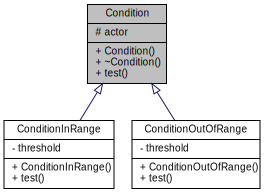
\includegraphics[width=336pt]{classCondition__inherit__graph}
\end{center}
\end{figure}


Collaboration diagram for Condition\+:
\nopagebreak
\begin{figure}[H]
\begin{center}
\leavevmode
\includegraphics[width=350pt]{classCondition__coll__graph}
\end{center}
\end{figure}
\subsection*{Public Member Functions}
\begin{DoxyCompactItemize}
\item 
\hyperlink{classCondition_a85d4a561ea14b94cf86756a984936180}{Condition} (\hyperlink{classNPC__Actor}{N\+P\+C\+\_\+\+Actor} $\ast$owner)
\item 
\hyperlink{classCondition_ab42f6d2dfb2d0de4bed4ed5032d4a8fc}{$\sim$\+Condition} ()
\item 
virtual bool \hyperlink{classCondition_a4826569fb7c6f920884abb7583a081b6}{test} (\hyperlink{classPlayer__Actor}{Player\+\_\+\+Actor} $\ast$\hyperlink{game__play__state_8cpp_ac65a4bc85dcd7c1cefbc84425f42fc46}{player})=0
\end{DoxyCompactItemize}
\subsection*{Protected Attributes}
\begin{DoxyCompactItemize}
\item 
\hyperlink{classNPC__Actor}{N\+P\+C\+\_\+\+Actor} $\ast$ \hyperlink{classCondition_a95c8585457c094a8564ac5111e66620d}{actor}
\end{DoxyCompactItemize}


\subsection{Constructor \& Destructor Documentation}
\mbox{\Hypertarget{classCondition_a85d4a561ea14b94cf86756a984936180}\label{classCondition_a85d4a561ea14b94cf86756a984936180}} 
\index{Condition@{Condition}!Condition@{Condition}}
\index{Condition@{Condition}!Condition@{Condition}}
\subsubsection{\texorpdfstring{Condition()}{Condition()}}
{\footnotesize\ttfamily Condition\+::\+Condition (\begin{DoxyParamCaption}\item[{\hyperlink{classNPC__Actor}{N\+P\+C\+\_\+\+Actor} $\ast$}]{owner }\end{DoxyParamCaption})\hspace{0.3cm}{\ttfamily [inline]}}

\mbox{\Hypertarget{classCondition_ab42f6d2dfb2d0de4bed4ed5032d4a8fc}\label{classCondition_ab42f6d2dfb2d0de4bed4ed5032d4a8fc}} 
\index{Condition@{Condition}!````~Condition@{$\sim$\+Condition}}
\index{````~Condition@{$\sim$\+Condition}!Condition@{Condition}}
\subsubsection{\texorpdfstring{$\sim$\+Condition()}{~Condition()}}
{\footnotesize\ttfamily Condition\+::$\sim$\+Condition (\begin{DoxyParamCaption}{ }\end{DoxyParamCaption})\hspace{0.3cm}{\ttfamily [inline]}}



\subsection{Member Function Documentation}
\mbox{\Hypertarget{classCondition_a4826569fb7c6f920884abb7583a081b6}\label{classCondition_a4826569fb7c6f920884abb7583a081b6}} 
\index{Condition@{Condition}!test@{test}}
\index{test@{test}!Condition@{Condition}}
\subsubsection{\texorpdfstring{test()}{test()}}
{\footnotesize\ttfamily virtual bool Condition\+::test (\begin{DoxyParamCaption}\item[{\hyperlink{classPlayer__Actor}{Player\+\_\+\+Actor} $\ast$}]{player }\end{DoxyParamCaption})\hspace{0.3cm}{\ttfamily [pure virtual]}}



Implemented in \hyperlink{classConditionInRange_a64cc1a7816537a2d8e29972199b3e8f9}{Condition\+In\+Range}, and \hyperlink{classConditionOutOfRange_a8e09e943dedb3c8b482e5934975abc25}{Condition\+Out\+Of\+Range}.



\subsection{Member Data Documentation}
\mbox{\Hypertarget{classCondition_a95c8585457c094a8564ac5111e66620d}\label{classCondition_a95c8585457c094a8564ac5111e66620d}} 
\index{Condition@{Condition}!actor@{actor}}
\index{actor@{actor}!Condition@{Condition}}
\subsubsection{\texorpdfstring{actor}{actor}}
{\footnotesize\ttfamily \hyperlink{classNPC__Actor}{N\+P\+C\+\_\+\+Actor}$\ast$ Condition\+::actor\hspace{0.3cm}{\ttfamily [protected]}}



The documentation for this class was generated from the following file\+:\begin{DoxyCompactItemize}
\item 
/mnt/hdd/fnky/\+C0de/\+C\+A\+P\+S\+T\+O\+N\+E/clean\+\_\+build/include/\+B\+State\+Machine/\hyperlink{Condition_8h}{Condition.\+h}\end{DoxyCompactItemize}

\hypertarget{classConditionInRange}{}\section{Condition\+In\+Range Class Reference}
\label{classConditionInRange}\index{Condition\+In\+Range@{Condition\+In\+Range}}


{\ttfamily \#include $<$Condition\+In\+Range.\+h$>$}



Inheritance diagram for Condition\+In\+Range\+:
\nopagebreak
\begin{figure}[H]
\begin{center}
\leavevmode
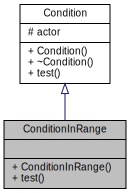
\includegraphics[width=190pt]{classConditionInRange__inherit__graph}
\end{center}
\end{figure}


Collaboration diagram for Condition\+In\+Range\+:
\nopagebreak
\begin{figure}[H]
\begin{center}
\leavevmode
\includegraphics[width=350pt]{classConditionInRange__coll__graph}
\end{center}
\end{figure}
\subsection*{Public Member Functions}
\begin{DoxyCompactItemize}
\item 
\hyperlink{classConditionInRange_ab66b0941b8bb7304f3f4b5eb758d30cc}{Condition\+In\+Range} (\hyperlink{classNPC__Actor}{N\+P\+C\+\_\+\+Actor} $\ast$\hyperlink{classCondition_a95c8585457c094a8564ac5111e66620d}{actor}, float threshold\+\_\+=10)
\item 
bool \hyperlink{classConditionInRange_a64cc1a7816537a2d8e29972199b3e8f9}{test} (\hyperlink{classPlayer__Actor}{Player\+\_\+\+Actor} $\ast$\hyperlink{game__play__state_8cpp_ac65a4bc85dcd7c1cefbc84425f42fc46}{player})
\end{DoxyCompactItemize}
\subsection*{Private Attributes}
\begin{DoxyCompactItemize}
\item 
float \hyperlink{classConditionInRange_a5c54f7654bd6702a93b5166ef657f580}{threshold}
\end{DoxyCompactItemize}
\subsection*{Additional Inherited Members}


\subsection{Constructor \& Destructor Documentation}
\mbox{\Hypertarget{classConditionInRange_ab66b0941b8bb7304f3f4b5eb758d30cc}\label{classConditionInRange_ab66b0941b8bb7304f3f4b5eb758d30cc}} 
\index{Condition\+In\+Range@{Condition\+In\+Range}!Condition\+In\+Range@{Condition\+In\+Range}}
\index{Condition\+In\+Range@{Condition\+In\+Range}!Condition\+In\+Range@{Condition\+In\+Range}}
\subsubsection{\texorpdfstring{Condition\+In\+Range()}{ConditionInRange()}}
{\footnotesize\ttfamily Condition\+In\+Range\+::\+Condition\+In\+Range (\begin{DoxyParamCaption}\item[{\hyperlink{classNPC__Actor}{N\+P\+C\+\_\+\+Actor} $\ast$}]{actor,  }\item[{float}]{threshold\+\_\+ = {\ttfamily 10} }\end{DoxyParamCaption})\hspace{0.3cm}{\ttfamily [inline]}}



\subsection{Member Function Documentation}
\mbox{\Hypertarget{classConditionInRange_a64cc1a7816537a2d8e29972199b3e8f9}\label{classConditionInRange_a64cc1a7816537a2d8e29972199b3e8f9}} 
\index{Condition\+In\+Range@{Condition\+In\+Range}!test@{test}}
\index{test@{test}!Condition\+In\+Range@{Condition\+In\+Range}}
\subsubsection{\texorpdfstring{test()}{test()}}
{\footnotesize\ttfamily bool Condition\+In\+Range\+::test (\begin{DoxyParamCaption}\item[{\hyperlink{classPlayer__Actor}{Player\+\_\+\+Actor} $\ast$}]{player }\end{DoxyParamCaption})\hspace{0.3cm}{\ttfamily [virtual]}}



Implements \hyperlink{classCondition_a4826569fb7c6f920884abb7583a081b6}{Condition}.



\subsection{Member Data Documentation}
\mbox{\Hypertarget{classConditionInRange_a5c54f7654bd6702a93b5166ef657f580}\label{classConditionInRange_a5c54f7654bd6702a93b5166ef657f580}} 
\index{Condition\+In\+Range@{Condition\+In\+Range}!threshold@{threshold}}
\index{threshold@{threshold}!Condition\+In\+Range@{Condition\+In\+Range}}
\subsubsection{\texorpdfstring{threshold}{threshold}}
{\footnotesize\ttfamily float Condition\+In\+Range\+::threshold\hspace{0.3cm}{\ttfamily [private]}}



The documentation for this class was generated from the following files\+:\begin{DoxyCompactItemize}
\item 
/mnt/hdd/fnky/\+C0de/\+C\+A\+P\+S\+T\+O\+N\+E/clean\+\_\+build/include/\+B\+State\+Machine/\hyperlink{ConditionInRange_8h}{Condition\+In\+Range.\+h}\item 
/mnt/hdd/fnky/\+C0de/\+C\+A\+P\+S\+T\+O\+N\+E/clean\+\_\+build/src/\+B\+State\+Machine/\hyperlink{ConditionInRange_8cpp}{Condition\+In\+Range.\+cpp}\end{DoxyCompactItemize}

\hypertarget{classConditionOutOfRange}{}\doxysection{Condition\+Out\+Of\+Range Class Reference}
\label{classConditionOutOfRange}\index{ConditionOutOfRange@{ConditionOutOfRange}}


{\ttfamily \#include $<$Condition\+Out\+Of\+Range.\+h$>$}



Inheritance diagram for Condition\+Out\+Of\+Range\+:
\nopagebreak
\begin{figure}[H]
\begin{center}
\leavevmode
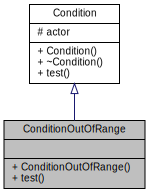
\includegraphics[width=221pt]{classConditionOutOfRange__inherit__graph}
\end{center}
\end{figure}


Collaboration diagram for Condition\+Out\+Of\+Range\+:
\nopagebreak
\begin{figure}[H]
\begin{center}
\leavevmode
\includegraphics[width=350pt]{classConditionOutOfRange__coll__graph}
\end{center}
\end{figure}
\doxysubsection*{Public Member Functions}
\begin{DoxyCompactItemize}
\item 
\mbox{\hyperlink{classConditionOutOfRange_a649b38dad4d85fadef74e603814c2d44}{Condition\+Out\+Of\+Range}} (\mbox{\hyperlink{classNPC__Actor}{N\+P\+C\+\_\+\+Actor}} $\ast$\mbox{\hyperlink{classCondition_a95c8585457c094a8564ac5111e66620d}{actor}})
\item 
bool \mbox{\hyperlink{classConditionOutOfRange_a8e09e943dedb3c8b482e5934975abc25}{test}} (\mbox{\hyperlink{classPlayer__Actor}{Player\+\_\+\+Actor}} $\ast$\mbox{\hyperlink{game__play__state_8cpp_ac65a4bc85dcd7c1cefbc84425f42fc46}{player}})
\end{DoxyCompactItemize}
\doxysubsection*{Additional Inherited Members}


\doxysubsection{Constructor \& Destructor Documentation}
\mbox{\Hypertarget{classConditionOutOfRange_a649b38dad4d85fadef74e603814c2d44}\label{classConditionOutOfRange_a649b38dad4d85fadef74e603814c2d44}} 
\index{ConditionOutOfRange@{ConditionOutOfRange}!ConditionOutOfRange@{ConditionOutOfRange}}
\index{ConditionOutOfRange@{ConditionOutOfRange}!ConditionOutOfRange@{ConditionOutOfRange}}
\doxysubsubsection{\texorpdfstring{ConditionOutOfRange()}{ConditionOutOfRange()}}
{\footnotesize\ttfamily Condition\+Out\+Of\+Range\+::\+Condition\+Out\+Of\+Range (\begin{DoxyParamCaption}\item[{\mbox{\hyperlink{classNPC__Actor}{N\+P\+C\+\_\+\+Actor}} $\ast$}]{actor }\end{DoxyParamCaption})\hspace{0.3cm}{\ttfamily [inline]}}



\doxysubsection{Member Function Documentation}
\mbox{\Hypertarget{classConditionOutOfRange_a8e09e943dedb3c8b482e5934975abc25}\label{classConditionOutOfRange_a8e09e943dedb3c8b482e5934975abc25}} 
\index{ConditionOutOfRange@{ConditionOutOfRange}!test@{test}}
\index{test@{test}!ConditionOutOfRange@{ConditionOutOfRange}}
\doxysubsubsection{\texorpdfstring{test()}{test()}}
{\footnotesize\ttfamily bool Condition\+Out\+Of\+Range\+::test (\begin{DoxyParamCaption}\item[{\mbox{\hyperlink{classPlayer__Actor}{Player\+\_\+\+Actor}} $\ast$}]{player }\end{DoxyParamCaption})\hspace{0.3cm}{\ttfamily [virtual]}}



Implements \mbox{\hyperlink{classCondition_a4826569fb7c6f920884abb7583a081b6}{Condition}}.



The documentation for this class was generated from the following files\+:\begin{DoxyCompactItemize}
\item 
/home/fnky/\+C0de/component\+\_\+engine/include/\+B\+State\+Machine/\mbox{\hyperlink{ConditionOutOfRange_8h}{Condition\+Out\+Of\+Range.\+h}}\item 
/home/fnky/\+C0de/component\+\_\+engine/src/\+B\+State\+Machine/\mbox{\hyperlink{ConditionOutOfRange_8cpp}{Condition\+Out\+Of\+Range.\+cpp}}\end{DoxyCompactItemize}

\hypertarget{classCrtAllocator}{}\section{Crt\+Allocator Class Reference}
\label{classCrtAllocator}\index{Crt\+Allocator@{Crt\+Allocator}}


C-\/runtime library allocator.  




{\ttfamily \#include $<$allocators.\+h$>$}



Collaboration diagram for Crt\+Allocator\+:
\nopagebreak
\begin{figure}[H]
\begin{center}
\leavevmode
\includegraphics[width=159pt]{classCrtAllocator__coll__graph}
\end{center}
\end{figure}
\subsection*{Public Member Functions}
\begin{DoxyCompactItemize}
\item 
\hyperlink{imgui__impl__opengl3__loader_8h_ac668e7cffd9e2e9cfee428b9b2f34fa7}{void} $\ast$ \hyperlink{classCrtAllocator_acd720631f8c094041afa6c7951f0d935}{Malloc} (size\+\_\+t \hyperlink{imgui__impl__opengl3__loader_8h_a3d1e3edfcf61ca2d831883e1afbad89e}{size})
\item 
\hyperlink{imgui__impl__opengl3__loader_8h_ac668e7cffd9e2e9cfee428b9b2f34fa7}{void} $\ast$ \hyperlink{classCrtAllocator_a646bb6f68afe773a62a22f7f14f83e97}{Realloc} (\hyperlink{imgui__impl__opengl3__loader_8h_ac668e7cffd9e2e9cfee428b9b2f34fa7}{void} $\ast$original\+Ptr, size\+\_\+t original\+Size, size\+\_\+t new\+Size)
\item 
bool \hyperlink{classCrtAllocator_ae65fb1b4e1272d05e003be57feac68a6}{operator==} (const \hyperlink{classCrtAllocator}{Crt\+Allocator} \&) const R\+A\+P\+I\+D\+J\+S\+O\+N\+\_\+\+N\+O\+E\+X\+C\+E\+PT
\item 
bool \hyperlink{classCrtAllocator_a1fb8ca99a43c939595e5c0b548d7532c}{operator!=} (const \hyperlink{classCrtAllocator}{Crt\+Allocator} \&) const R\+A\+P\+I\+D\+J\+S\+O\+N\+\_\+\+N\+O\+E\+X\+C\+E\+PT
\end{DoxyCompactItemize}
\subsection*{Static Public Member Functions}
\begin{DoxyCompactItemize}
\item 
static \hyperlink{imgui__impl__opengl3__loader_8h_ac668e7cffd9e2e9cfee428b9b2f34fa7}{void} \hyperlink{classCrtAllocator_aa09ed06f0decbedcaaa2c2a417820a79}{Free} (\hyperlink{imgui__impl__opengl3__loader_8h_ac668e7cffd9e2e9cfee428b9b2f34fa7}{void} $\ast$ptr) R\+A\+P\+I\+D\+J\+S\+O\+N\+\_\+\+N\+O\+E\+X\+C\+E\+PT
\end{DoxyCompactItemize}
\subsection*{Static Public Attributes}
\begin{DoxyCompactItemize}
\item 
static const bool \hyperlink{classCrtAllocator_ac7df8398c529290f0cd5950d9492f524}{k\+Need\+Free} = true
\end{DoxyCompactItemize}


\subsection{Detailed Description}
C-\/runtime library allocator. 

This class is just wrapper for standard C library memory routines. \begin{DoxyNote}{Note}
implements Allocator concept 
\end{DoxyNote}


\subsection{Member Function Documentation}
\mbox{\Hypertarget{classCrtAllocator_aa09ed06f0decbedcaaa2c2a417820a79}\label{classCrtAllocator_aa09ed06f0decbedcaaa2c2a417820a79}} 
\index{Crt\+Allocator@{Crt\+Allocator}!Free@{Free}}
\index{Free@{Free}!Crt\+Allocator@{Crt\+Allocator}}
\subsubsection{\texorpdfstring{Free()}{Free()}}
{\footnotesize\ttfamily static \hyperlink{imgui__impl__opengl3__loader_8h_ac668e7cffd9e2e9cfee428b9b2f34fa7}{void} Crt\+Allocator\+::\+Free (\begin{DoxyParamCaption}\item[{\hyperlink{imgui__impl__opengl3__loader_8h_ac668e7cffd9e2e9cfee428b9b2f34fa7}{void} $\ast$}]{ptr }\end{DoxyParamCaption})\hspace{0.3cm}{\ttfamily [inline]}, {\ttfamily [static]}}

\mbox{\Hypertarget{classCrtAllocator_acd720631f8c094041afa6c7951f0d935}\label{classCrtAllocator_acd720631f8c094041afa6c7951f0d935}} 
\index{Crt\+Allocator@{Crt\+Allocator}!Malloc@{Malloc}}
\index{Malloc@{Malloc}!Crt\+Allocator@{Crt\+Allocator}}
\subsubsection{\texorpdfstring{Malloc()}{Malloc()}}
{\footnotesize\ttfamily \hyperlink{imgui__impl__opengl3__loader_8h_ac668e7cffd9e2e9cfee428b9b2f34fa7}{void}$\ast$ Crt\+Allocator\+::\+Malloc (\begin{DoxyParamCaption}\item[{size\+\_\+t}]{size }\end{DoxyParamCaption})\hspace{0.3cm}{\ttfamily [inline]}}

\mbox{\Hypertarget{classCrtAllocator_a1fb8ca99a43c939595e5c0b548d7532c}\label{classCrtAllocator_a1fb8ca99a43c939595e5c0b548d7532c}} 
\index{Crt\+Allocator@{Crt\+Allocator}!operator"!=@{operator"!=}}
\index{operator"!=@{operator"!=}!Crt\+Allocator@{Crt\+Allocator}}
\subsubsection{\texorpdfstring{operator"!=()}{operator!=()}}
{\footnotesize\ttfamily bool Crt\+Allocator\+::operator!= (\begin{DoxyParamCaption}\item[{const \hyperlink{classCrtAllocator}{Crt\+Allocator} \&}]{ }\end{DoxyParamCaption}) const\hspace{0.3cm}{\ttfamily [inline]}}

\mbox{\Hypertarget{classCrtAllocator_ae65fb1b4e1272d05e003be57feac68a6}\label{classCrtAllocator_ae65fb1b4e1272d05e003be57feac68a6}} 
\index{Crt\+Allocator@{Crt\+Allocator}!operator==@{operator==}}
\index{operator==@{operator==}!Crt\+Allocator@{Crt\+Allocator}}
\subsubsection{\texorpdfstring{operator==()}{operator==()}}
{\footnotesize\ttfamily bool Crt\+Allocator\+::operator== (\begin{DoxyParamCaption}\item[{const \hyperlink{classCrtAllocator}{Crt\+Allocator} \&}]{ }\end{DoxyParamCaption}) const\hspace{0.3cm}{\ttfamily [inline]}}

\mbox{\Hypertarget{classCrtAllocator_a646bb6f68afe773a62a22f7f14f83e97}\label{classCrtAllocator_a646bb6f68afe773a62a22f7f14f83e97}} 
\index{Crt\+Allocator@{Crt\+Allocator}!Realloc@{Realloc}}
\index{Realloc@{Realloc}!Crt\+Allocator@{Crt\+Allocator}}
\subsubsection{\texorpdfstring{Realloc()}{Realloc()}}
{\footnotesize\ttfamily \hyperlink{imgui__impl__opengl3__loader_8h_ac668e7cffd9e2e9cfee428b9b2f34fa7}{void}$\ast$ Crt\+Allocator\+::\+Realloc (\begin{DoxyParamCaption}\item[{\hyperlink{imgui__impl__opengl3__loader_8h_ac668e7cffd9e2e9cfee428b9b2f34fa7}{void} $\ast$}]{original\+Ptr,  }\item[{size\+\_\+t}]{original\+Size,  }\item[{size\+\_\+t}]{new\+Size }\end{DoxyParamCaption})\hspace{0.3cm}{\ttfamily [inline]}}



\subsection{Member Data Documentation}
\mbox{\Hypertarget{classCrtAllocator_ac7df8398c529290f0cd5950d9492f524}\label{classCrtAllocator_ac7df8398c529290f0cd5950d9492f524}} 
\index{Crt\+Allocator@{Crt\+Allocator}!k\+Need\+Free@{k\+Need\+Free}}
\index{k\+Need\+Free@{k\+Need\+Free}!Crt\+Allocator@{Crt\+Allocator}}
\subsubsection{\texorpdfstring{k\+Need\+Free}{kNeedFree}}
{\footnotesize\ttfamily const bool Crt\+Allocator\+::k\+Need\+Free = true\hspace{0.3cm}{\ttfamily [static]}}



The documentation for this class was generated from the following file\+:\begin{DoxyCompactItemize}
\item 
/mnt/hdd/fnky/\+C0de/\+C\+A\+P\+S\+T\+O\+N\+E/clean\+\_\+build/include/rapidjson/\hyperlink{allocators_8h}{allocators.\+h}\end{DoxyCompactItemize}

\hypertarget{classCursorStreamWrapper}{}\section{Cursor\+Stream\+Wrapper$<$ Input\+Stream, Encoding $>$ Class Template Reference}
\label{classCursorStreamWrapper}\index{Cursor\+Stream\+Wrapper$<$ Input\+Stream, Encoding $>$@{Cursor\+Stream\+Wrapper$<$ Input\+Stream, Encoding $>$}}


Cursor stream wrapper for counting line and column number if error exists.  




{\ttfamily \#include $<$cursorstreamwrapper.\+h$>$}



Inheritance diagram for Cursor\+Stream\+Wrapper$<$ Input\+Stream, Encoding $>$\+:
\nopagebreak
\begin{figure}[H]
\begin{center}
\leavevmode
\includegraphics[width=214pt]{classCursorStreamWrapper__inherit__graph}
\end{center}
\end{figure}


Collaboration diagram for Cursor\+Stream\+Wrapper$<$ Input\+Stream, Encoding $>$\+:
\nopagebreak
\begin{figure}[H]
\begin{center}
\leavevmode
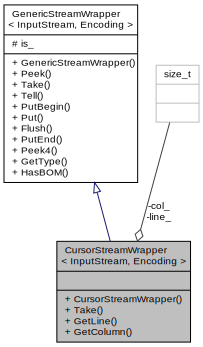
\includegraphics[width=276pt]{classCursorStreamWrapper__coll__graph}
\end{center}
\end{figure}
\subsection*{Public Types}
\begin{DoxyCompactItemize}
\item 
typedef Encoding\+::\+Ch \hyperlink{classCursorStreamWrapper_a4bab1186bfeebbcf00719c2613b0dca6}{Ch}
\end{DoxyCompactItemize}
\subsection*{Public Member Functions}
\begin{DoxyCompactItemize}
\item 
\hyperlink{classCursorStreamWrapper_a8d9a0109e19ab4fb7a79091cefe608a7}{Cursor\+Stream\+Wrapper} (Input\+Stream \&is)
\item 
\hyperlink{classCursorStreamWrapper_a4bab1186bfeebbcf00719c2613b0dca6}{Ch} \hyperlink{classCursorStreamWrapper_af0bbad24ff7ad101cdf9842760deb0f6}{Take} ()
\item 
size\+\_\+t \hyperlink{classCursorStreamWrapper_ad5cc5b06be7fb5afb7c3d4a82b5ef8ce}{Get\+Line} () const
\begin{DoxyCompactList}\small\item\em Get the error line number, if error exists. \end{DoxyCompactList}\item 
size\+\_\+t \hyperlink{classCursorStreamWrapper_afdd243889599c9c9edfacea82674a8f4}{Get\+Column} () const
\begin{DoxyCompactList}\small\item\em Get the error column number, if error exists. \end{DoxyCompactList}\end{DoxyCompactItemize}
\subsection*{Private Attributes}
\begin{DoxyCompactItemize}
\item 
size\+\_\+t \hyperlink{classCursorStreamWrapper_a6f49c4b224ab4210223202696ed1b6b0}{line\+\_\+}
\begin{DoxyCompactList}\small\item\em Current Line. \end{DoxyCompactList}\item 
size\+\_\+t \hyperlink{classCursorStreamWrapper_ac487665a7485024745d82cd0cfa7107d}{col\+\_\+}
\begin{DoxyCompactList}\small\item\em Current Column. \end{DoxyCompactList}\end{DoxyCompactItemize}
\subsection*{Additional Inherited Members}


\subsection{Detailed Description}
\subsubsection*{template$<$typename Input\+Stream, typename Encoding = U\+T\+F8$<$$>$$>$\newline
class Cursor\+Stream\+Wrapper$<$ Input\+Stream, Encoding $>$}

Cursor stream wrapper for counting line and column number if error exists. 


\begin{DoxyTemplParams}{Template Parameters}
{\em Input\+Stream} & Any stream that implements Stream Concept \\
\hline
\end{DoxyTemplParams}


\subsection{Member Typedef Documentation}
\mbox{\Hypertarget{classCursorStreamWrapper_a4bab1186bfeebbcf00719c2613b0dca6}\label{classCursorStreamWrapper_a4bab1186bfeebbcf00719c2613b0dca6}} 
\index{Cursor\+Stream\+Wrapper@{Cursor\+Stream\+Wrapper}!Ch@{Ch}}
\index{Ch@{Ch}!Cursor\+Stream\+Wrapper@{Cursor\+Stream\+Wrapper}}
\subsubsection{\texorpdfstring{Ch}{Ch}}
{\footnotesize\ttfamily template$<$typename Input\+Stream , typename Encoding  = U\+T\+F8$<$$>$$>$ \\
typedef Encoding\+::\+Ch \hyperlink{classCursorStreamWrapper}{Cursor\+Stream\+Wrapper}$<$ Input\+Stream, Encoding $>$\+::\hyperlink{classCursorStreamWrapper_a4bab1186bfeebbcf00719c2613b0dca6}{Ch}}



\subsection{Constructor \& Destructor Documentation}
\mbox{\Hypertarget{classCursorStreamWrapper_a8d9a0109e19ab4fb7a79091cefe608a7}\label{classCursorStreamWrapper_a8d9a0109e19ab4fb7a79091cefe608a7}} 
\index{Cursor\+Stream\+Wrapper@{Cursor\+Stream\+Wrapper}!Cursor\+Stream\+Wrapper@{Cursor\+Stream\+Wrapper}}
\index{Cursor\+Stream\+Wrapper@{Cursor\+Stream\+Wrapper}!Cursor\+Stream\+Wrapper@{Cursor\+Stream\+Wrapper}}
\subsubsection{\texorpdfstring{Cursor\+Stream\+Wrapper()}{CursorStreamWrapper()}}
{\footnotesize\ttfamily template$<$typename Input\+Stream , typename Encoding  = U\+T\+F8$<$$>$$>$ \\
\hyperlink{classCursorStreamWrapper}{Cursor\+Stream\+Wrapper}$<$ Input\+Stream, Encoding $>$\+::\hyperlink{classCursorStreamWrapper}{Cursor\+Stream\+Wrapper} (\begin{DoxyParamCaption}\item[{Input\+Stream \&}]{is }\end{DoxyParamCaption})\hspace{0.3cm}{\ttfamily [inline]}}



\subsection{Member Function Documentation}
\mbox{\Hypertarget{classCursorStreamWrapper_afdd243889599c9c9edfacea82674a8f4}\label{classCursorStreamWrapper_afdd243889599c9c9edfacea82674a8f4}} 
\index{Cursor\+Stream\+Wrapper@{Cursor\+Stream\+Wrapper}!Get\+Column@{Get\+Column}}
\index{Get\+Column@{Get\+Column}!Cursor\+Stream\+Wrapper@{Cursor\+Stream\+Wrapper}}
\subsubsection{\texorpdfstring{Get\+Column()}{GetColumn()}}
{\footnotesize\ttfamily template$<$typename Input\+Stream , typename Encoding  = U\+T\+F8$<$$>$$>$ \\
size\+\_\+t \hyperlink{classCursorStreamWrapper}{Cursor\+Stream\+Wrapper}$<$ Input\+Stream, Encoding $>$\+::Get\+Column (\begin{DoxyParamCaption}{ }\end{DoxyParamCaption}) const\hspace{0.3cm}{\ttfamily [inline]}}



Get the error column number, if error exists. 

\mbox{\Hypertarget{classCursorStreamWrapper_ad5cc5b06be7fb5afb7c3d4a82b5ef8ce}\label{classCursorStreamWrapper_ad5cc5b06be7fb5afb7c3d4a82b5ef8ce}} 
\index{Cursor\+Stream\+Wrapper@{Cursor\+Stream\+Wrapper}!Get\+Line@{Get\+Line}}
\index{Get\+Line@{Get\+Line}!Cursor\+Stream\+Wrapper@{Cursor\+Stream\+Wrapper}}
\subsubsection{\texorpdfstring{Get\+Line()}{GetLine()}}
{\footnotesize\ttfamily template$<$typename Input\+Stream , typename Encoding  = U\+T\+F8$<$$>$$>$ \\
size\+\_\+t \hyperlink{classCursorStreamWrapper}{Cursor\+Stream\+Wrapper}$<$ Input\+Stream, Encoding $>$\+::Get\+Line (\begin{DoxyParamCaption}{ }\end{DoxyParamCaption}) const\hspace{0.3cm}{\ttfamily [inline]}}



Get the error line number, if error exists. 

\mbox{\Hypertarget{classCursorStreamWrapper_af0bbad24ff7ad101cdf9842760deb0f6}\label{classCursorStreamWrapper_af0bbad24ff7ad101cdf9842760deb0f6}} 
\index{Cursor\+Stream\+Wrapper@{Cursor\+Stream\+Wrapper}!Take@{Take}}
\index{Take@{Take}!Cursor\+Stream\+Wrapper@{Cursor\+Stream\+Wrapper}}
\subsubsection{\texorpdfstring{Take()}{Take()}}
{\footnotesize\ttfamily template$<$typename Input\+Stream , typename Encoding  = U\+T\+F8$<$$>$$>$ \\
\hyperlink{classCursorStreamWrapper_a4bab1186bfeebbcf00719c2613b0dca6}{Ch} \hyperlink{classCursorStreamWrapper}{Cursor\+Stream\+Wrapper}$<$ Input\+Stream, Encoding $>$\+::Take (\begin{DoxyParamCaption}{ }\end{DoxyParamCaption})\hspace{0.3cm}{\ttfamily [inline]}}



\subsection{Member Data Documentation}
\mbox{\Hypertarget{classCursorStreamWrapper_ac487665a7485024745d82cd0cfa7107d}\label{classCursorStreamWrapper_ac487665a7485024745d82cd0cfa7107d}} 
\index{Cursor\+Stream\+Wrapper@{Cursor\+Stream\+Wrapper}!col\+\_\+@{col\+\_\+}}
\index{col\+\_\+@{col\+\_\+}!Cursor\+Stream\+Wrapper@{Cursor\+Stream\+Wrapper}}
\subsubsection{\texorpdfstring{col\+\_\+}{col\_}}
{\footnotesize\ttfamily template$<$typename Input\+Stream , typename Encoding  = U\+T\+F8$<$$>$$>$ \\
size\+\_\+t \hyperlink{classCursorStreamWrapper}{Cursor\+Stream\+Wrapper}$<$ Input\+Stream, Encoding $>$\+::col\+\_\+\hspace{0.3cm}{\ttfamily [private]}}



Current Column. 

\mbox{\Hypertarget{classCursorStreamWrapper_a6f49c4b224ab4210223202696ed1b6b0}\label{classCursorStreamWrapper_a6f49c4b224ab4210223202696ed1b6b0}} 
\index{Cursor\+Stream\+Wrapper@{Cursor\+Stream\+Wrapper}!line\+\_\+@{line\+\_\+}}
\index{line\+\_\+@{line\+\_\+}!Cursor\+Stream\+Wrapper@{Cursor\+Stream\+Wrapper}}
\subsubsection{\texorpdfstring{line\+\_\+}{line\_}}
{\footnotesize\ttfamily template$<$typename Input\+Stream , typename Encoding  = U\+T\+F8$<$$>$$>$ \\
size\+\_\+t \hyperlink{classCursorStreamWrapper}{Cursor\+Stream\+Wrapper}$<$ Input\+Stream, Encoding $>$\+::line\+\_\+\hspace{0.3cm}{\ttfamily [private]}}



Current Line. 



The documentation for this class was generated from the following file\+:\begin{DoxyCompactItemize}
\item 
/mnt/hdd/fnky/\+C0de/\+C\+A\+P\+S\+T\+O\+N\+E/clean\+\_\+build/include/rapidjson/\hyperlink{cursorstreamwrapper_8h}{cursorstreamwrapper.\+h}\end{DoxyCompactItemize}

\hypertarget{unionGenericValue_1_1Data}{}\section{Generic\+Value$<$ Encoding, Allocator $>$\+:\+:Data Union Reference}
\label{unionGenericValue_1_1Data}\index{Generic\+Value$<$ Encoding, Allocator $>$\+::\+Data@{Generic\+Value$<$ Encoding, Allocator $>$\+::\+Data}}


{\ttfamily \#include $<$document.\+h$>$}



Collaboration diagram for Generic\+Value$<$ Encoding, Allocator $>$\+:\+:Data\+:
\nopagebreak
\begin{figure}[H]
\begin{center}
\leavevmode
\includegraphics[width=350pt]{unionGenericValue_1_1Data__coll__graph}
\end{center}
\end{figure}
\subsection*{Public Attributes}
\begin{DoxyCompactItemize}
\item 
\hyperlink{structGenericValue_1_1String}{String} \hyperlink{unionGenericValue_1_1Data_a6872a4b93763944063b425e6c001ed2b}{s}
\item 
\hyperlink{structGenericValue_1_1ShortString}{Short\+String} \hyperlink{unionGenericValue_1_1Data_a410e39a5dc296eb3b152b54193740e4c}{ss}
\item 
\hyperlink{unionGenericValue_1_1Number}{Number} \hyperlink{unionGenericValue_1_1Data_a243007cce2f4b75bea3e3c1ee4c3c239}{n}
\item 
\hyperlink{structGenericValue_1_1ObjectData}{Object\+Data} \hyperlink{unionGenericValue_1_1Data_af6417eca530fba0d8bd65d309628eb11}{o}
\item 
\hyperlink{structGenericValue_1_1ArrayData}{Array\+Data} \hyperlink{unionGenericValue_1_1Data_aeac31cf55bf5a024cead5ecb63e4fd48}{a}
\item 
\hyperlink{structGenericValue_1_1Flag}{Flag} \hyperlink{unionGenericValue_1_1Data_ad8572112da083c775ce21bcbca96b2ab}{f}
\end{DoxyCompactItemize}


\subsection{Member Data Documentation}
\mbox{\Hypertarget{unionGenericValue_1_1Data_aeac31cf55bf5a024cead5ecb63e4fd48}\label{unionGenericValue_1_1Data_aeac31cf55bf5a024cead5ecb63e4fd48}} 
\index{Generic\+Value\+::\+Data@{Generic\+Value\+::\+Data}!a@{a}}
\index{a@{a}!Generic\+Value\+::\+Data@{Generic\+Value\+::\+Data}}
\subsubsection{\texorpdfstring{a}{a}}
{\footnotesize\ttfamily template$<$typename Encoding, typename Allocator = R\+A\+P\+I\+D\+J\+S\+O\+N\+\_\+\+D\+E\+F\+A\+U\+L\+T\+\_\+\+A\+L\+L\+O\+C\+A\+T\+OR$>$ \\
\hyperlink{structGenericValue_1_1ArrayData}{Array\+Data} \hyperlink{classGenericValue}{Generic\+Value}$<$ Encoding, Allocator $>$\+::Data\+::a}

\mbox{\Hypertarget{unionGenericValue_1_1Data_ad8572112da083c775ce21bcbca96b2ab}\label{unionGenericValue_1_1Data_ad8572112da083c775ce21bcbca96b2ab}} 
\index{Generic\+Value\+::\+Data@{Generic\+Value\+::\+Data}!f@{f}}
\index{f@{f}!Generic\+Value\+::\+Data@{Generic\+Value\+::\+Data}}
\subsubsection{\texorpdfstring{f}{f}}
{\footnotesize\ttfamily template$<$typename Encoding, typename Allocator = R\+A\+P\+I\+D\+J\+S\+O\+N\+\_\+\+D\+E\+F\+A\+U\+L\+T\+\_\+\+A\+L\+L\+O\+C\+A\+T\+OR$>$ \\
\hyperlink{structGenericValue_1_1Flag}{Flag} \hyperlink{classGenericValue}{Generic\+Value}$<$ Encoding, Allocator $>$\+::Data\+::f}

\mbox{\Hypertarget{unionGenericValue_1_1Data_a243007cce2f4b75bea3e3c1ee4c3c239}\label{unionGenericValue_1_1Data_a243007cce2f4b75bea3e3c1ee4c3c239}} 
\index{Generic\+Value\+::\+Data@{Generic\+Value\+::\+Data}!n@{n}}
\index{n@{n}!Generic\+Value\+::\+Data@{Generic\+Value\+::\+Data}}
\subsubsection{\texorpdfstring{n}{n}}
{\footnotesize\ttfamily template$<$typename Encoding, typename Allocator = R\+A\+P\+I\+D\+J\+S\+O\+N\+\_\+\+D\+E\+F\+A\+U\+L\+T\+\_\+\+A\+L\+L\+O\+C\+A\+T\+OR$>$ \\
\hyperlink{unionGenericValue_1_1Number}{Number} \hyperlink{classGenericValue}{Generic\+Value}$<$ Encoding, Allocator $>$\+::Data\+::n}

\mbox{\Hypertarget{unionGenericValue_1_1Data_af6417eca530fba0d8bd65d309628eb11}\label{unionGenericValue_1_1Data_af6417eca530fba0d8bd65d309628eb11}} 
\index{Generic\+Value\+::\+Data@{Generic\+Value\+::\+Data}!o@{o}}
\index{o@{o}!Generic\+Value\+::\+Data@{Generic\+Value\+::\+Data}}
\subsubsection{\texorpdfstring{o}{o}}
{\footnotesize\ttfamily template$<$typename Encoding, typename Allocator = R\+A\+P\+I\+D\+J\+S\+O\+N\+\_\+\+D\+E\+F\+A\+U\+L\+T\+\_\+\+A\+L\+L\+O\+C\+A\+T\+OR$>$ \\
\hyperlink{structGenericValue_1_1ObjectData}{Object\+Data} \hyperlink{classGenericValue}{Generic\+Value}$<$ Encoding, Allocator $>$\+::Data\+::o}

\mbox{\Hypertarget{unionGenericValue_1_1Data_a6872a4b93763944063b425e6c001ed2b}\label{unionGenericValue_1_1Data_a6872a4b93763944063b425e6c001ed2b}} 
\index{Generic\+Value\+::\+Data@{Generic\+Value\+::\+Data}!s@{s}}
\index{s@{s}!Generic\+Value\+::\+Data@{Generic\+Value\+::\+Data}}
\subsubsection{\texorpdfstring{s}{s}}
{\footnotesize\ttfamily template$<$typename Encoding, typename Allocator = R\+A\+P\+I\+D\+J\+S\+O\+N\+\_\+\+D\+E\+F\+A\+U\+L\+T\+\_\+\+A\+L\+L\+O\+C\+A\+T\+OR$>$ \\
\hyperlink{structGenericValue_1_1String}{String} \hyperlink{classGenericValue}{Generic\+Value}$<$ Encoding, Allocator $>$\+::Data\+::s}

\mbox{\Hypertarget{unionGenericValue_1_1Data_a410e39a5dc296eb3b152b54193740e4c}\label{unionGenericValue_1_1Data_a410e39a5dc296eb3b152b54193740e4c}} 
\index{Generic\+Value\+::\+Data@{Generic\+Value\+::\+Data}!ss@{ss}}
\index{ss@{ss}!Generic\+Value\+::\+Data@{Generic\+Value\+::\+Data}}
\subsubsection{\texorpdfstring{ss}{ss}}
{\footnotesize\ttfamily template$<$typename Encoding, typename Allocator = R\+A\+P\+I\+D\+J\+S\+O\+N\+\_\+\+D\+E\+F\+A\+U\+L\+T\+\_\+\+A\+L\+L\+O\+C\+A\+T\+OR$>$ \\
\hyperlink{structGenericValue_1_1ShortString}{Short\+String} \hyperlink{classGenericValue}{Generic\+Value}$<$ Encoding, Allocator $>$\+::Data\+::ss}



The documentation for this union was generated from the following file\+:\begin{DoxyCompactItemize}
\item 
/mnt/hdd/fnky/\+C0de/\+C\+A\+P\+S\+T\+O\+N\+E/clean\+\_\+build/include/rapidjson/\hyperlink{document_8h}{document.\+h}\end{DoxyCompactItemize}

\hypertarget{classinternal_1_1DecodedStream}{}\section{internal\+:\+:Decoded\+Stream$<$ Source\+Stream, Encoding $>$ Class Template Reference}
\label{classinternal_1_1DecodedStream}\index{internal\+::\+Decoded\+Stream$<$ Source\+Stream, Encoding $>$@{internal\+::\+Decoded\+Stream$<$ Source\+Stream, Encoding $>$}}


{\ttfamily \#include $<$regex.\+h$>$}



Collaboration diagram for internal\+:\+:Decoded\+Stream$<$ Source\+Stream, Encoding $>$\+:
\nopagebreak
\begin{figure}[H]
\begin{center}
\leavevmode
\includegraphics[width=223pt]{classinternal_1_1DecodedStream__coll__graph}
\end{center}
\end{figure}
\subsection*{Public Member Functions}
\begin{DoxyCompactItemize}
\item 
\hyperlink{classinternal_1_1DecodedStream_a45cf40c4e515be8aaa8cd020eaa67595}{Decoded\+Stream} (Source\+Stream \&ss)
\item 
unsigned \hyperlink{classinternal_1_1DecodedStream_ac78f2cbc03ae0d79a0fcfe6d56589d70}{Peek} ()
\item 
unsigned \hyperlink{classinternal_1_1DecodedStream_a62b45969ce169bef1da0600490329857}{Take} ()
\end{DoxyCompactItemize}
\subsection*{Private Member Functions}
\begin{DoxyCompactItemize}
\item 
\hyperlink{imgui__impl__opengl3__loader_8h_ac668e7cffd9e2e9cfee428b9b2f34fa7}{void} \hyperlink{classinternal_1_1DecodedStream_aec6be1692e1f283c1dde407cce1bb873}{Decode} ()
\end{DoxyCompactItemize}
\subsection*{Private Attributes}
\begin{DoxyCompactItemize}
\item 
Source\+Stream \& \hyperlink{classinternal_1_1DecodedStream_ac87f823c7c950f13145dc3c151dcf714}{ss\+\_\+}
\item 
unsigned \hyperlink{classinternal_1_1DecodedStream_ab2d66695cea627ac0b2a53a5ff8d5526}{codepoint\+\_\+}
\end{DoxyCompactItemize}


\subsection{Constructor \& Destructor Documentation}
\mbox{\Hypertarget{classinternal_1_1DecodedStream_a45cf40c4e515be8aaa8cd020eaa67595}\label{classinternal_1_1DecodedStream_a45cf40c4e515be8aaa8cd020eaa67595}} 
\index{internal\+::\+Decoded\+Stream@{internal\+::\+Decoded\+Stream}!Decoded\+Stream@{Decoded\+Stream}}
\index{Decoded\+Stream@{Decoded\+Stream}!internal\+::\+Decoded\+Stream@{internal\+::\+Decoded\+Stream}}
\subsubsection{\texorpdfstring{Decoded\+Stream()}{DecodedStream()}}
{\footnotesize\ttfamily template$<$typename Source\+Stream, typename Encoding$>$ \\
\hyperlink{classinternal_1_1DecodedStream}{internal\+::\+Decoded\+Stream}$<$ Source\+Stream, Encoding $>$\+::\hyperlink{classinternal_1_1DecodedStream}{Decoded\+Stream} (\begin{DoxyParamCaption}\item[{Source\+Stream \&}]{ss }\end{DoxyParamCaption})\hspace{0.3cm}{\ttfamily [inline]}}



\subsection{Member Function Documentation}
\mbox{\Hypertarget{classinternal_1_1DecodedStream_aec6be1692e1f283c1dde407cce1bb873}\label{classinternal_1_1DecodedStream_aec6be1692e1f283c1dde407cce1bb873}} 
\index{internal\+::\+Decoded\+Stream@{internal\+::\+Decoded\+Stream}!Decode@{Decode}}
\index{Decode@{Decode}!internal\+::\+Decoded\+Stream@{internal\+::\+Decoded\+Stream}}
\subsubsection{\texorpdfstring{Decode()}{Decode()}}
{\footnotesize\ttfamily template$<$typename Source\+Stream, typename Encoding$>$ \\
\hyperlink{imgui__impl__opengl3__loader_8h_ac668e7cffd9e2e9cfee428b9b2f34fa7}{void} \hyperlink{classinternal_1_1DecodedStream}{internal\+::\+Decoded\+Stream}$<$ Source\+Stream, Encoding $>$\+::Decode (\begin{DoxyParamCaption}{ }\end{DoxyParamCaption})\hspace{0.3cm}{\ttfamily [inline]}, {\ttfamily [private]}}

\mbox{\Hypertarget{classinternal_1_1DecodedStream_ac78f2cbc03ae0d79a0fcfe6d56589d70}\label{classinternal_1_1DecodedStream_ac78f2cbc03ae0d79a0fcfe6d56589d70}} 
\index{internal\+::\+Decoded\+Stream@{internal\+::\+Decoded\+Stream}!Peek@{Peek}}
\index{Peek@{Peek}!internal\+::\+Decoded\+Stream@{internal\+::\+Decoded\+Stream}}
\subsubsection{\texorpdfstring{Peek()}{Peek()}}
{\footnotesize\ttfamily template$<$typename Source\+Stream, typename Encoding$>$ \\
unsigned \hyperlink{classinternal_1_1DecodedStream}{internal\+::\+Decoded\+Stream}$<$ Source\+Stream, Encoding $>$\+::Peek (\begin{DoxyParamCaption}{ }\end{DoxyParamCaption})\hspace{0.3cm}{\ttfamily [inline]}}

\mbox{\Hypertarget{classinternal_1_1DecodedStream_a62b45969ce169bef1da0600490329857}\label{classinternal_1_1DecodedStream_a62b45969ce169bef1da0600490329857}} 
\index{internal\+::\+Decoded\+Stream@{internal\+::\+Decoded\+Stream}!Take@{Take}}
\index{Take@{Take}!internal\+::\+Decoded\+Stream@{internal\+::\+Decoded\+Stream}}
\subsubsection{\texorpdfstring{Take()}{Take()}}
{\footnotesize\ttfamily template$<$typename Source\+Stream, typename Encoding$>$ \\
unsigned \hyperlink{classinternal_1_1DecodedStream}{internal\+::\+Decoded\+Stream}$<$ Source\+Stream, Encoding $>$\+::Take (\begin{DoxyParamCaption}{ }\end{DoxyParamCaption})\hspace{0.3cm}{\ttfamily [inline]}}



\subsection{Member Data Documentation}
\mbox{\Hypertarget{classinternal_1_1DecodedStream_ab2d66695cea627ac0b2a53a5ff8d5526}\label{classinternal_1_1DecodedStream_ab2d66695cea627ac0b2a53a5ff8d5526}} 
\index{internal\+::\+Decoded\+Stream@{internal\+::\+Decoded\+Stream}!codepoint\+\_\+@{codepoint\+\_\+}}
\index{codepoint\+\_\+@{codepoint\+\_\+}!internal\+::\+Decoded\+Stream@{internal\+::\+Decoded\+Stream}}
\subsubsection{\texorpdfstring{codepoint\+\_\+}{codepoint\_}}
{\footnotesize\ttfamily template$<$typename Source\+Stream, typename Encoding$>$ \\
unsigned \hyperlink{classinternal_1_1DecodedStream}{internal\+::\+Decoded\+Stream}$<$ Source\+Stream, Encoding $>$\+::codepoint\+\_\+\hspace{0.3cm}{\ttfamily [private]}}

\mbox{\Hypertarget{classinternal_1_1DecodedStream_ac87f823c7c950f13145dc3c151dcf714}\label{classinternal_1_1DecodedStream_ac87f823c7c950f13145dc3c151dcf714}} 
\index{internal\+::\+Decoded\+Stream@{internal\+::\+Decoded\+Stream}!ss\+\_\+@{ss\+\_\+}}
\index{ss\+\_\+@{ss\+\_\+}!internal\+::\+Decoded\+Stream@{internal\+::\+Decoded\+Stream}}
\subsubsection{\texorpdfstring{ss\+\_\+}{ss\_}}
{\footnotesize\ttfamily template$<$typename Source\+Stream, typename Encoding$>$ \\
Source\+Stream\& \hyperlink{classinternal_1_1DecodedStream}{internal\+::\+Decoded\+Stream}$<$ Source\+Stream, Encoding $>$\+::ss\+\_\+\hspace{0.3cm}{\ttfamily [private]}}



The documentation for this class was generated from the following file\+:\begin{DoxyCompactItemize}
\item 
/mnt/hdd/fnky/\+C0de/\+C\+A\+P\+S\+T\+O\+N\+E/clean\+\_\+build/include/rapidjson/internal/\hyperlink{regex_8h}{regex.\+h}\end{DoxyCompactItemize}

\input{structinternal_1_1DiyFp}
\hypertarget{classinternal_1_1Double}{}\section{internal\+:\+:Double Class Reference}
\label{classinternal_1_1Double}\index{internal\+::\+Double@{internal\+::\+Double}}


{\ttfamily \#include $<$ieee754.\+h$>$}



Collaboration diagram for internal\+:\+:Double\+:
\nopagebreak
\begin{figure}[H]
\begin{center}
\leavevmode
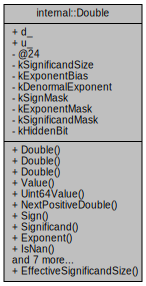
\includegraphics[width=218pt]{classinternal_1_1Double__coll__graph}
\end{center}
\end{figure}
\subsection*{Public Member Functions}
\begin{DoxyCompactItemize}
\item 
\hyperlink{classinternal_1_1Double_a98e2cff9880cd032d174e9721ae40ddd}{Double} ()
\item 
\hyperlink{classinternal_1_1Double_ad66f3b914570ce62e9f16083117f3e4f}{Double} (double d)
\item 
\hyperlink{classinternal_1_1Double_a293a7ca841d847ea3e83ffa28b68601f}{Double} (\hyperlink{stdint_8h_aec6fcb673ff035718c238c8c9d544c47}{uint64\+\_\+t} u)
\item 
double \hyperlink{classinternal_1_1Double_a665c64824d1046528cbc4066a9ed0ef8}{Value} () const
\item 
\hyperlink{stdint_8h_aec6fcb673ff035718c238c8c9d544c47}{uint64\+\_\+t} \hyperlink{classinternal_1_1Double_a1a35be6344c886f159cb36a1498a62ac}{Uint64\+Value} () const
\item 
double \hyperlink{classinternal_1_1Double_a6ffee23d82d9c606b1a53ed87e393e90}{Next\+Positive\+Double} () const
\item 
bool \hyperlink{classinternal_1_1Double_ab09c26873ca4c3e471a97c4559bf317d}{Sign} () const
\item 
\hyperlink{stdint_8h_aec6fcb673ff035718c238c8c9d544c47}{uint64\+\_\+t} \hyperlink{classinternal_1_1Double_ade5d3e893dd6884ccd37632109dae1a6}{Significand} () const
\item 
int \hyperlink{classinternal_1_1Double_ae091055d96d8730f654170613f2cf265}{Exponent} () const
\item 
bool \hyperlink{classinternal_1_1Double_a312312ab2798ee85cbd0e739fcefa386}{Is\+Nan} () const
\item 
bool \hyperlink{classinternal_1_1Double_afe1ce48f7fb9797e1a2044c58a6b226c}{Is\+Inf} () const
\item 
bool \hyperlink{classinternal_1_1Double_a8b9a82e8b99783b7e98b5307756021c0}{Is\+Nan\+Or\+Inf} () const
\item 
bool \hyperlink{classinternal_1_1Double_a8a39cd42010c69681da35d87f1331381}{Is\+Normal} () const
\item 
bool \hyperlink{classinternal_1_1Double_a90a3a1ca614b377b59576955ce987ce2}{Is\+Zero} () const
\item 
\hyperlink{stdint_8h_aec6fcb673ff035718c238c8c9d544c47}{uint64\+\_\+t} \hyperlink{classinternal_1_1Double_a1bf89d77be843f69facec9f2bc4dbc72}{Integer\+Significand} () const
\item 
int \hyperlink{classinternal_1_1Double_a9721e0fdedef4d0fe6c7b411492a88fb}{Integer\+Exponent} () const
\item 
\hyperlink{stdint_8h_aec6fcb673ff035718c238c8c9d544c47}{uint64\+\_\+t} \hyperlink{classinternal_1_1Double_ab3d3a81274e4f4b9b415db7c664d3ac9}{To\+Bias} () const
\end{DoxyCompactItemize}
\subsection*{Static Public Member Functions}
\begin{DoxyCompactItemize}
\item 
static int \hyperlink{classinternal_1_1Double_aa710fa4f5e06b0ff4348a13475688f13}{Effective\+Significand\+Size} (int order)
\end{DoxyCompactItemize}
\subsection*{Private Attributes}
\begin{DoxyCompactItemize}
\item 
\begin{tabbing}
xx\=xx\=xx\=xx\=xx\=xx\=xx\=xx\=xx\=\kill
union \{\\
\>double \hyperlink{classinternal_1_1Double_a9ed5b5245664da8abe6cdeefaed6452e}{d\_}\\
\>\hyperlink{stdint_8h_aec6fcb673ff035718c238c8c9d544c47}{uint64\_t} \hyperlink{classinternal_1_1Double_ad7523f7fe0c47d6aabe34f68b00a3250}{u\_}\\
\}; \\

\end{tabbing}\end{DoxyCompactItemize}
\subsection*{Static Private Attributes}
\begin{DoxyCompactItemize}
\item 
static const int \hyperlink{classinternal_1_1Double_a2e41ff26c6ad85628305c479fbd451aa}{k\+Significand\+Size} = 52
\item 
static const int \hyperlink{classinternal_1_1Double_a7d4436067abd6620d1ed156b3e9d54e2}{k\+Exponent\+Bias} = 0x3\+FF
\item 
static const int \hyperlink{classinternal_1_1Double_a8e8f5769df7c1a7273d83d61233a682f}{k\+Denormal\+Exponent} = 1 -\/ \hyperlink{classinternal_1_1Double_a7d4436067abd6620d1ed156b3e9d54e2}{k\+Exponent\+Bias}
\item 
static const \hyperlink{stdint_8h_aec6fcb673ff035718c238c8c9d544c47}{uint64\+\_\+t} \hyperlink{classinternal_1_1Double_a43d4007b0121278555519de8d4fdc59e}{k\+Sign\+Mask} = \hyperlink{rapidjson_8h_aaee1245f375a71be1ac9b8a07ba5fb8f}{R\+A\+P\+I\+D\+J\+S\+O\+N\+\_\+\+U\+I\+N\+T64\+\_\+\+C2}(0x80000000, 0x00000000)
\item 
static const \hyperlink{stdint_8h_aec6fcb673ff035718c238c8c9d544c47}{uint64\+\_\+t} \hyperlink{classinternal_1_1Double_a39172dca75a2a5ddec868a170f7a7a3e}{k\+Exponent\+Mask} = \hyperlink{rapidjson_8h_aaee1245f375a71be1ac9b8a07ba5fb8f}{R\+A\+P\+I\+D\+J\+S\+O\+N\+\_\+\+U\+I\+N\+T64\+\_\+\+C2}(0x7\+F\+F00000, 0x00000000)
\item 
static const \hyperlink{stdint_8h_aec6fcb673ff035718c238c8c9d544c47}{uint64\+\_\+t} \hyperlink{classinternal_1_1Double_aa34deedf05f755101bf807419d113bf5}{k\+Significand\+Mask} = \hyperlink{rapidjson_8h_aaee1245f375a71be1ac9b8a07ba5fb8f}{R\+A\+P\+I\+D\+J\+S\+O\+N\+\_\+\+U\+I\+N\+T64\+\_\+\+C2}(0x000\+F\+F\+F\+F\+F, 0x\+F\+F\+F\+F\+F\+F\+F\+F)
\item 
static const \hyperlink{stdint_8h_aec6fcb673ff035718c238c8c9d544c47}{uint64\+\_\+t} \hyperlink{classinternal_1_1Double_a93fcf8c6a54766f9239f1d3cb0ca0710}{k\+Hidden\+Bit} = \hyperlink{rapidjson_8h_aaee1245f375a71be1ac9b8a07ba5fb8f}{R\+A\+P\+I\+D\+J\+S\+O\+N\+\_\+\+U\+I\+N\+T64\+\_\+\+C2}(0x00100000, 0x00000000)
\end{DoxyCompactItemize}


\subsection{Constructor \& Destructor Documentation}
\mbox{\Hypertarget{classinternal_1_1Double_a98e2cff9880cd032d174e9721ae40ddd}\label{classinternal_1_1Double_a98e2cff9880cd032d174e9721ae40ddd}} 
\index{internal\+::\+Double@{internal\+::\+Double}!Double@{Double}}
\index{Double@{Double}!internal\+::\+Double@{internal\+::\+Double}}
\subsubsection{\texorpdfstring{Double()}{Double()}\hspace{0.1cm}{\footnotesize\ttfamily [1/3]}}
{\footnotesize\ttfamily internal\+::\+Double\+::\+Double (\begin{DoxyParamCaption}{ }\end{DoxyParamCaption})\hspace{0.3cm}{\ttfamily [inline]}}

\mbox{\Hypertarget{classinternal_1_1Double_ad66f3b914570ce62e9f16083117f3e4f}\label{classinternal_1_1Double_ad66f3b914570ce62e9f16083117f3e4f}} 
\index{internal\+::\+Double@{internal\+::\+Double}!Double@{Double}}
\index{Double@{Double}!internal\+::\+Double@{internal\+::\+Double}}
\subsubsection{\texorpdfstring{Double()}{Double()}\hspace{0.1cm}{\footnotesize\ttfamily [2/3]}}
{\footnotesize\ttfamily internal\+::\+Double\+::\+Double (\begin{DoxyParamCaption}\item[{double}]{d }\end{DoxyParamCaption})\hspace{0.3cm}{\ttfamily [inline]}}

\mbox{\Hypertarget{classinternal_1_1Double_a293a7ca841d847ea3e83ffa28b68601f}\label{classinternal_1_1Double_a293a7ca841d847ea3e83ffa28b68601f}} 
\index{internal\+::\+Double@{internal\+::\+Double}!Double@{Double}}
\index{Double@{Double}!internal\+::\+Double@{internal\+::\+Double}}
\subsubsection{\texorpdfstring{Double()}{Double()}\hspace{0.1cm}{\footnotesize\ttfamily [3/3]}}
{\footnotesize\ttfamily internal\+::\+Double\+::\+Double (\begin{DoxyParamCaption}\item[{\hyperlink{stdint_8h_aec6fcb673ff035718c238c8c9d544c47}{uint64\+\_\+t}}]{u }\end{DoxyParamCaption})\hspace{0.3cm}{\ttfamily [inline]}}



\subsection{Member Function Documentation}
\mbox{\Hypertarget{classinternal_1_1Double_aa710fa4f5e06b0ff4348a13475688f13}\label{classinternal_1_1Double_aa710fa4f5e06b0ff4348a13475688f13}} 
\index{internal\+::\+Double@{internal\+::\+Double}!Effective\+Significand\+Size@{Effective\+Significand\+Size}}
\index{Effective\+Significand\+Size@{Effective\+Significand\+Size}!internal\+::\+Double@{internal\+::\+Double}}
\subsubsection{\texorpdfstring{Effective\+Significand\+Size()}{EffectiveSignificandSize()}}
{\footnotesize\ttfamily static int internal\+::\+Double\+::\+Effective\+Significand\+Size (\begin{DoxyParamCaption}\item[{int}]{order }\end{DoxyParamCaption})\hspace{0.3cm}{\ttfamily [inline]}, {\ttfamily [static]}}

\mbox{\Hypertarget{classinternal_1_1Double_ae091055d96d8730f654170613f2cf265}\label{classinternal_1_1Double_ae091055d96d8730f654170613f2cf265}} 
\index{internal\+::\+Double@{internal\+::\+Double}!Exponent@{Exponent}}
\index{Exponent@{Exponent}!internal\+::\+Double@{internal\+::\+Double}}
\subsubsection{\texorpdfstring{Exponent()}{Exponent()}}
{\footnotesize\ttfamily int internal\+::\+Double\+::\+Exponent (\begin{DoxyParamCaption}{ }\end{DoxyParamCaption}) const\hspace{0.3cm}{\ttfamily [inline]}}

\mbox{\Hypertarget{classinternal_1_1Double_a9721e0fdedef4d0fe6c7b411492a88fb}\label{classinternal_1_1Double_a9721e0fdedef4d0fe6c7b411492a88fb}} 
\index{internal\+::\+Double@{internal\+::\+Double}!Integer\+Exponent@{Integer\+Exponent}}
\index{Integer\+Exponent@{Integer\+Exponent}!internal\+::\+Double@{internal\+::\+Double}}
\subsubsection{\texorpdfstring{Integer\+Exponent()}{IntegerExponent()}}
{\footnotesize\ttfamily int internal\+::\+Double\+::\+Integer\+Exponent (\begin{DoxyParamCaption}{ }\end{DoxyParamCaption}) const\hspace{0.3cm}{\ttfamily [inline]}}

\mbox{\Hypertarget{classinternal_1_1Double_a1bf89d77be843f69facec9f2bc4dbc72}\label{classinternal_1_1Double_a1bf89d77be843f69facec9f2bc4dbc72}} 
\index{internal\+::\+Double@{internal\+::\+Double}!Integer\+Significand@{Integer\+Significand}}
\index{Integer\+Significand@{Integer\+Significand}!internal\+::\+Double@{internal\+::\+Double}}
\subsubsection{\texorpdfstring{Integer\+Significand()}{IntegerSignificand()}}
{\footnotesize\ttfamily \hyperlink{stdint_8h_aec6fcb673ff035718c238c8c9d544c47}{uint64\+\_\+t} internal\+::\+Double\+::\+Integer\+Significand (\begin{DoxyParamCaption}{ }\end{DoxyParamCaption}) const\hspace{0.3cm}{\ttfamily [inline]}}

\mbox{\Hypertarget{classinternal_1_1Double_afe1ce48f7fb9797e1a2044c58a6b226c}\label{classinternal_1_1Double_afe1ce48f7fb9797e1a2044c58a6b226c}} 
\index{internal\+::\+Double@{internal\+::\+Double}!Is\+Inf@{Is\+Inf}}
\index{Is\+Inf@{Is\+Inf}!internal\+::\+Double@{internal\+::\+Double}}
\subsubsection{\texorpdfstring{Is\+Inf()}{IsInf()}}
{\footnotesize\ttfamily bool internal\+::\+Double\+::\+Is\+Inf (\begin{DoxyParamCaption}{ }\end{DoxyParamCaption}) const\hspace{0.3cm}{\ttfamily [inline]}}

\mbox{\Hypertarget{classinternal_1_1Double_a312312ab2798ee85cbd0e739fcefa386}\label{classinternal_1_1Double_a312312ab2798ee85cbd0e739fcefa386}} 
\index{internal\+::\+Double@{internal\+::\+Double}!Is\+Nan@{Is\+Nan}}
\index{Is\+Nan@{Is\+Nan}!internal\+::\+Double@{internal\+::\+Double}}
\subsubsection{\texorpdfstring{Is\+Nan()}{IsNan()}}
{\footnotesize\ttfamily bool internal\+::\+Double\+::\+Is\+Nan (\begin{DoxyParamCaption}{ }\end{DoxyParamCaption}) const\hspace{0.3cm}{\ttfamily [inline]}}

\mbox{\Hypertarget{classinternal_1_1Double_a8b9a82e8b99783b7e98b5307756021c0}\label{classinternal_1_1Double_a8b9a82e8b99783b7e98b5307756021c0}} 
\index{internal\+::\+Double@{internal\+::\+Double}!Is\+Nan\+Or\+Inf@{Is\+Nan\+Or\+Inf}}
\index{Is\+Nan\+Or\+Inf@{Is\+Nan\+Or\+Inf}!internal\+::\+Double@{internal\+::\+Double}}
\subsubsection{\texorpdfstring{Is\+Nan\+Or\+Inf()}{IsNanOrInf()}}
{\footnotesize\ttfamily bool internal\+::\+Double\+::\+Is\+Nan\+Or\+Inf (\begin{DoxyParamCaption}{ }\end{DoxyParamCaption}) const\hspace{0.3cm}{\ttfamily [inline]}}

\mbox{\Hypertarget{classinternal_1_1Double_a8a39cd42010c69681da35d87f1331381}\label{classinternal_1_1Double_a8a39cd42010c69681da35d87f1331381}} 
\index{internal\+::\+Double@{internal\+::\+Double}!Is\+Normal@{Is\+Normal}}
\index{Is\+Normal@{Is\+Normal}!internal\+::\+Double@{internal\+::\+Double}}
\subsubsection{\texorpdfstring{Is\+Normal()}{IsNormal()}}
{\footnotesize\ttfamily bool internal\+::\+Double\+::\+Is\+Normal (\begin{DoxyParamCaption}{ }\end{DoxyParamCaption}) const\hspace{0.3cm}{\ttfamily [inline]}}

\mbox{\Hypertarget{classinternal_1_1Double_a90a3a1ca614b377b59576955ce987ce2}\label{classinternal_1_1Double_a90a3a1ca614b377b59576955ce987ce2}} 
\index{internal\+::\+Double@{internal\+::\+Double}!Is\+Zero@{Is\+Zero}}
\index{Is\+Zero@{Is\+Zero}!internal\+::\+Double@{internal\+::\+Double}}
\subsubsection{\texorpdfstring{Is\+Zero()}{IsZero()}}
{\footnotesize\ttfamily bool internal\+::\+Double\+::\+Is\+Zero (\begin{DoxyParamCaption}{ }\end{DoxyParamCaption}) const\hspace{0.3cm}{\ttfamily [inline]}}

\mbox{\Hypertarget{classinternal_1_1Double_a6ffee23d82d9c606b1a53ed87e393e90}\label{classinternal_1_1Double_a6ffee23d82d9c606b1a53ed87e393e90}} 
\index{internal\+::\+Double@{internal\+::\+Double}!Next\+Positive\+Double@{Next\+Positive\+Double}}
\index{Next\+Positive\+Double@{Next\+Positive\+Double}!internal\+::\+Double@{internal\+::\+Double}}
\subsubsection{\texorpdfstring{Next\+Positive\+Double()}{NextPositiveDouble()}}
{\footnotesize\ttfamily double internal\+::\+Double\+::\+Next\+Positive\+Double (\begin{DoxyParamCaption}{ }\end{DoxyParamCaption}) const\hspace{0.3cm}{\ttfamily [inline]}}

\mbox{\Hypertarget{classinternal_1_1Double_ab09c26873ca4c3e471a97c4559bf317d}\label{classinternal_1_1Double_ab09c26873ca4c3e471a97c4559bf317d}} 
\index{internal\+::\+Double@{internal\+::\+Double}!Sign@{Sign}}
\index{Sign@{Sign}!internal\+::\+Double@{internal\+::\+Double}}
\subsubsection{\texorpdfstring{Sign()}{Sign()}}
{\footnotesize\ttfamily bool internal\+::\+Double\+::\+Sign (\begin{DoxyParamCaption}{ }\end{DoxyParamCaption}) const\hspace{0.3cm}{\ttfamily [inline]}}

\mbox{\Hypertarget{classinternal_1_1Double_ade5d3e893dd6884ccd37632109dae1a6}\label{classinternal_1_1Double_ade5d3e893dd6884ccd37632109dae1a6}} 
\index{internal\+::\+Double@{internal\+::\+Double}!Significand@{Significand}}
\index{Significand@{Significand}!internal\+::\+Double@{internal\+::\+Double}}
\subsubsection{\texorpdfstring{Significand()}{Significand()}}
{\footnotesize\ttfamily \hyperlink{stdint_8h_aec6fcb673ff035718c238c8c9d544c47}{uint64\+\_\+t} internal\+::\+Double\+::\+Significand (\begin{DoxyParamCaption}{ }\end{DoxyParamCaption}) const\hspace{0.3cm}{\ttfamily [inline]}}

\mbox{\Hypertarget{classinternal_1_1Double_ab3d3a81274e4f4b9b415db7c664d3ac9}\label{classinternal_1_1Double_ab3d3a81274e4f4b9b415db7c664d3ac9}} 
\index{internal\+::\+Double@{internal\+::\+Double}!To\+Bias@{To\+Bias}}
\index{To\+Bias@{To\+Bias}!internal\+::\+Double@{internal\+::\+Double}}
\subsubsection{\texorpdfstring{To\+Bias()}{ToBias()}}
{\footnotesize\ttfamily \hyperlink{stdint_8h_aec6fcb673ff035718c238c8c9d544c47}{uint64\+\_\+t} internal\+::\+Double\+::\+To\+Bias (\begin{DoxyParamCaption}{ }\end{DoxyParamCaption}) const\hspace{0.3cm}{\ttfamily [inline]}}

\mbox{\Hypertarget{classinternal_1_1Double_a1a35be6344c886f159cb36a1498a62ac}\label{classinternal_1_1Double_a1a35be6344c886f159cb36a1498a62ac}} 
\index{internal\+::\+Double@{internal\+::\+Double}!Uint64\+Value@{Uint64\+Value}}
\index{Uint64\+Value@{Uint64\+Value}!internal\+::\+Double@{internal\+::\+Double}}
\subsubsection{\texorpdfstring{Uint64\+Value()}{Uint64Value()}}
{\footnotesize\ttfamily \hyperlink{stdint_8h_aec6fcb673ff035718c238c8c9d544c47}{uint64\+\_\+t} internal\+::\+Double\+::\+Uint64\+Value (\begin{DoxyParamCaption}{ }\end{DoxyParamCaption}) const\hspace{0.3cm}{\ttfamily [inline]}}

\mbox{\Hypertarget{classinternal_1_1Double_a665c64824d1046528cbc4066a9ed0ef8}\label{classinternal_1_1Double_a665c64824d1046528cbc4066a9ed0ef8}} 
\index{internal\+::\+Double@{internal\+::\+Double}!Value@{Value}}
\index{Value@{Value}!internal\+::\+Double@{internal\+::\+Double}}
\subsubsection{\texorpdfstring{Value()}{Value()}}
{\footnotesize\ttfamily double internal\+::\+Double\+::\+Value (\begin{DoxyParamCaption}{ }\end{DoxyParamCaption}) const\hspace{0.3cm}{\ttfamily [inline]}}



\subsection{Member Data Documentation}
\mbox{\Hypertarget{classinternal_1_1Double_a01f0bc70c07b670156d5350f0ed9cd14}\label{classinternal_1_1Double_a01f0bc70c07b670156d5350f0ed9cd14}} 
\subsubsection{\texorpdfstring{"@24}{@24}}
{\footnotesize\ttfamily union \{ ... \} \hspace{0.3cm}{\ttfamily [private]}}

\mbox{\Hypertarget{classinternal_1_1Double_a9ed5b5245664da8abe6cdeefaed6452e}\label{classinternal_1_1Double_a9ed5b5245664da8abe6cdeefaed6452e}} 
\index{internal\+::\+Double@{internal\+::\+Double}!d\+\_\+@{d\+\_\+}}
\index{d\+\_\+@{d\+\_\+}!internal\+::\+Double@{internal\+::\+Double}}
\subsubsection{\texorpdfstring{d\+\_\+}{d\_}}
{\footnotesize\ttfamily double internal\+::\+Double\+::d\+\_\+}

\mbox{\Hypertarget{classinternal_1_1Double_a8e8f5769df7c1a7273d83d61233a682f}\label{classinternal_1_1Double_a8e8f5769df7c1a7273d83d61233a682f}} 
\index{internal\+::\+Double@{internal\+::\+Double}!k\+Denormal\+Exponent@{k\+Denormal\+Exponent}}
\index{k\+Denormal\+Exponent@{k\+Denormal\+Exponent}!internal\+::\+Double@{internal\+::\+Double}}
\subsubsection{\texorpdfstring{k\+Denormal\+Exponent}{kDenormalExponent}}
{\footnotesize\ttfamily const int internal\+::\+Double\+::k\+Denormal\+Exponent = 1 -\/ \hyperlink{classinternal_1_1Double_a7d4436067abd6620d1ed156b3e9d54e2}{k\+Exponent\+Bias}\hspace{0.3cm}{\ttfamily [static]}, {\ttfamily [private]}}

\mbox{\Hypertarget{classinternal_1_1Double_a7d4436067abd6620d1ed156b3e9d54e2}\label{classinternal_1_1Double_a7d4436067abd6620d1ed156b3e9d54e2}} 
\index{internal\+::\+Double@{internal\+::\+Double}!k\+Exponent\+Bias@{k\+Exponent\+Bias}}
\index{k\+Exponent\+Bias@{k\+Exponent\+Bias}!internal\+::\+Double@{internal\+::\+Double}}
\subsubsection{\texorpdfstring{k\+Exponent\+Bias}{kExponentBias}}
{\footnotesize\ttfamily const int internal\+::\+Double\+::k\+Exponent\+Bias = 0x3\+FF\hspace{0.3cm}{\ttfamily [static]}, {\ttfamily [private]}}

\mbox{\Hypertarget{classinternal_1_1Double_a39172dca75a2a5ddec868a170f7a7a3e}\label{classinternal_1_1Double_a39172dca75a2a5ddec868a170f7a7a3e}} 
\index{internal\+::\+Double@{internal\+::\+Double}!k\+Exponent\+Mask@{k\+Exponent\+Mask}}
\index{k\+Exponent\+Mask@{k\+Exponent\+Mask}!internal\+::\+Double@{internal\+::\+Double}}
\subsubsection{\texorpdfstring{k\+Exponent\+Mask}{kExponentMask}}
{\footnotesize\ttfamily const \hyperlink{stdint_8h_aec6fcb673ff035718c238c8c9d544c47}{uint64\+\_\+t} internal\+::\+Double\+::k\+Exponent\+Mask = \hyperlink{rapidjson_8h_aaee1245f375a71be1ac9b8a07ba5fb8f}{R\+A\+P\+I\+D\+J\+S\+O\+N\+\_\+\+U\+I\+N\+T64\+\_\+\+C2}(0x7\+F\+F00000, 0x00000000)\hspace{0.3cm}{\ttfamily [static]}, {\ttfamily [private]}}

\mbox{\Hypertarget{classinternal_1_1Double_a93fcf8c6a54766f9239f1d3cb0ca0710}\label{classinternal_1_1Double_a93fcf8c6a54766f9239f1d3cb0ca0710}} 
\index{internal\+::\+Double@{internal\+::\+Double}!k\+Hidden\+Bit@{k\+Hidden\+Bit}}
\index{k\+Hidden\+Bit@{k\+Hidden\+Bit}!internal\+::\+Double@{internal\+::\+Double}}
\subsubsection{\texorpdfstring{k\+Hidden\+Bit}{kHiddenBit}}
{\footnotesize\ttfamily const \hyperlink{stdint_8h_aec6fcb673ff035718c238c8c9d544c47}{uint64\+\_\+t} internal\+::\+Double\+::k\+Hidden\+Bit = \hyperlink{rapidjson_8h_aaee1245f375a71be1ac9b8a07ba5fb8f}{R\+A\+P\+I\+D\+J\+S\+O\+N\+\_\+\+U\+I\+N\+T64\+\_\+\+C2}(0x00100000, 0x00000000)\hspace{0.3cm}{\ttfamily [static]}, {\ttfamily [private]}}

\mbox{\Hypertarget{classinternal_1_1Double_aa34deedf05f755101bf807419d113bf5}\label{classinternal_1_1Double_aa34deedf05f755101bf807419d113bf5}} 
\index{internal\+::\+Double@{internal\+::\+Double}!k\+Significand\+Mask@{k\+Significand\+Mask}}
\index{k\+Significand\+Mask@{k\+Significand\+Mask}!internal\+::\+Double@{internal\+::\+Double}}
\subsubsection{\texorpdfstring{k\+Significand\+Mask}{kSignificandMask}}
{\footnotesize\ttfamily const \hyperlink{stdint_8h_aec6fcb673ff035718c238c8c9d544c47}{uint64\+\_\+t} internal\+::\+Double\+::k\+Significand\+Mask = \hyperlink{rapidjson_8h_aaee1245f375a71be1ac9b8a07ba5fb8f}{R\+A\+P\+I\+D\+J\+S\+O\+N\+\_\+\+U\+I\+N\+T64\+\_\+\+C2}(0x000\+F\+F\+F\+F\+F, 0x\+F\+F\+F\+F\+F\+F\+F\+F)\hspace{0.3cm}{\ttfamily [static]}, {\ttfamily [private]}}

\mbox{\Hypertarget{classinternal_1_1Double_a2e41ff26c6ad85628305c479fbd451aa}\label{classinternal_1_1Double_a2e41ff26c6ad85628305c479fbd451aa}} 
\index{internal\+::\+Double@{internal\+::\+Double}!k\+Significand\+Size@{k\+Significand\+Size}}
\index{k\+Significand\+Size@{k\+Significand\+Size}!internal\+::\+Double@{internal\+::\+Double}}
\subsubsection{\texorpdfstring{k\+Significand\+Size}{kSignificandSize}}
{\footnotesize\ttfamily const int internal\+::\+Double\+::k\+Significand\+Size = 52\hspace{0.3cm}{\ttfamily [static]}, {\ttfamily [private]}}

\mbox{\Hypertarget{classinternal_1_1Double_a43d4007b0121278555519de8d4fdc59e}\label{classinternal_1_1Double_a43d4007b0121278555519de8d4fdc59e}} 
\index{internal\+::\+Double@{internal\+::\+Double}!k\+Sign\+Mask@{k\+Sign\+Mask}}
\index{k\+Sign\+Mask@{k\+Sign\+Mask}!internal\+::\+Double@{internal\+::\+Double}}
\subsubsection{\texorpdfstring{k\+Sign\+Mask}{kSignMask}}
{\footnotesize\ttfamily const \hyperlink{stdint_8h_aec6fcb673ff035718c238c8c9d544c47}{uint64\+\_\+t} internal\+::\+Double\+::k\+Sign\+Mask = \hyperlink{rapidjson_8h_aaee1245f375a71be1ac9b8a07ba5fb8f}{R\+A\+P\+I\+D\+J\+S\+O\+N\+\_\+\+U\+I\+N\+T64\+\_\+\+C2}(0x80000000, 0x00000000)\hspace{0.3cm}{\ttfamily [static]}, {\ttfamily [private]}}

\mbox{\Hypertarget{classinternal_1_1Double_ad7523f7fe0c47d6aabe34f68b00a3250}\label{classinternal_1_1Double_ad7523f7fe0c47d6aabe34f68b00a3250}} 
\index{internal\+::\+Double@{internal\+::\+Double}!u\+\_\+@{u\+\_\+}}
\index{u\+\_\+@{u\+\_\+}!internal\+::\+Double@{internal\+::\+Double}}
\subsubsection{\texorpdfstring{u\+\_\+}{u\_}}
{\footnotesize\ttfamily \hyperlink{stdint_8h_aec6fcb673ff035718c238c8c9d544c47}{uint64\+\_\+t} internal\+::\+Double\+::u\+\_\+}



The documentation for this class was generated from the following file\+:\begin{DoxyCompactItemize}
\item 
/mnt/hdd/fnky/\+C0de/\+C\+A\+P\+S\+T\+O\+N\+E/clean\+\_\+build/include/rapidjson/internal/\hyperlink{ieee754_8h}{ieee754.\+h}\end{DoxyCompactItemize}

\hypertarget{classEdge__Actor}{}\section{Edge\+\_\+\+Actor Class Reference}
\label{classEdge__Actor}\index{Edge\+\_\+\+Actor@{Edge\+\_\+\+Actor}}


{\ttfamily \#include $<$Edge\+\_\+\+Actor.\+h$>$}



Inheritance diagram for Edge\+\_\+\+Actor\+:
\nopagebreak
\begin{figure}[H]
\begin{center}
\leavevmode
\includegraphics[height=550pt]{classEdge__Actor__inherit__graph}
\end{center}
\end{figure}


Collaboration diagram for Edge\+\_\+\+Actor\+:
\nopagebreak
\begin{figure}[H]
\begin{center}
\leavevmode
\includegraphics[height=550pt]{classEdge__Actor__coll__graph}
\end{center}
\end{figure}
\subsection*{Public Member Functions}
\begin{DoxyCompactItemize}
\item 
\hyperlink{classEdge__Actor_ac707b4097a2de1a388deec93ac83de98}{Edge\+\_\+\+Actor} (\hyperlink{classComponent}{Component} $\ast$parent\+\_\+)
\item 
\hyperlink{classEdge__Actor_aee2346e89a348a9725d43c6a11c697f8}{$\sim$\+Edge\+\_\+\+Actor} ()
\item 
bool \hyperlink{classEdge__Actor_a0d8e90af66e85a8f4d1f5b0ecde6e99e}{on\+Create} (glm\+::vec2 orign, glm\+::vec2 dest, float r\+\_\+=1.\+0f, float g\+\_\+=0.\+0f, float b\+\_\+=0.\+0f)
\item 
\hyperlink{imgui__impl__opengl3__loader_8h_ac668e7cffd9e2e9cfee428b9b2f34fa7}{void} \hyperlink{classEdge__Actor_ae7a429d48b86442154c93eb65bc8b22d}{on\+Destroy} ()
\item 
\hyperlink{imgui__impl__opengl3__loader_8h_ac668e7cffd9e2e9cfee428b9b2f34fa7}{void} \hyperlink{classEdge__Actor_a8ae8a19c72b58522755d2d0a395fc1ea}{update} (const float delta\+Time\+\_\+)
\item 
\hyperlink{imgui__impl__opengl3__loader_8h_ac668e7cffd9e2e9cfee428b9b2f34fa7}{void} \hyperlink{classEdge__Actor_a9f2bf6813472357c045d48cd76658e30}{input} ()
\item 
\hyperlink{imgui__impl__opengl3__loader_8h_ac668e7cffd9e2e9cfee428b9b2f34fa7}{void} \hyperlink{classEdge__Actor_a90887ba227fa0edf7cd7fdfd5d13f475}{draw} (std\+::shared\+\_\+ptr$<$ \hyperlink{classShader__Actor}{Shader\+\_\+\+Actor} $>$ \hyperlink{imgui__impl__opengl3__loader_8h_a57b2a96adb1d51204909a82d861e395e}{shader}, glm\+::mat4 \hyperlink{main__menu__state_8cpp_a565d92bfbcc4a481d2d35f3850a382f7}{projection}) const
\item 
bool \hyperlink{classEdge__Actor_ae0c85d2808d37ec71202b545f88e5881}{get\+\_\+edge\+\_\+collision} ()
\item 
\hyperlink{imgui__impl__opengl3__loader_8h_ac668e7cffd9e2e9cfee428b9b2f34fa7}{void} \hyperlink{classEdge__Actor_a4494e28b1ac2a197243f6ad6f76955f9}{set\+\_\+xo} (float xo\+\_\+)
\item 
float \hyperlink{classEdge__Actor_a66b2b088ec38268d42823c7faa6a3547}{get\+\_\+xo} ()
\item 
\hyperlink{imgui__impl__opengl3__loader_8h_ac668e7cffd9e2e9cfee428b9b2f34fa7}{void} \hyperlink{classEdge__Actor_a65bfa5124e666e68fb2a3b1aae8bc203}{set\+\_\+xd} (float xd\+\_\+)
\item 
float \hyperlink{classEdge__Actor_ae9a0cc7d7aab4b9cd426ee99b4ec9ebf}{get\+\_\+xd} ()
\item 
\hyperlink{imgui__impl__opengl3__loader_8h_ac668e7cffd9e2e9cfee428b9b2f34fa7}{void} \hyperlink{classEdge__Actor_a98b808c09e6697fba4d1bf0d51ba0af0}{set\+\_\+yo} (float yo\+\_\+)
\item 
float \hyperlink{classEdge__Actor_a7964c3bdf20a1928abad4ffc59fd11bd}{get\+\_\+yo} ()
\item 
\hyperlink{imgui__impl__opengl3__loader_8h_ac668e7cffd9e2e9cfee428b9b2f34fa7}{void} \hyperlink{classEdge__Actor_a0e73953b56bb2da81152e91ebb17e6ed}{set\+\_\+yd} (float yd\+\_\+)
\item 
float \hyperlink{classEdge__Actor_ab3e262e6353837f0f4e85466550450ae}{get\+\_\+yd} ()
\end{DoxyCompactItemize}
\subsection*{Private Attributes}
\begin{DoxyCompactItemize}
\item 
float \hyperlink{classEdge__Actor_a6b4d171fd575a857159d8c46faf615c8}{r}
\item 
float \hyperlink{classEdge__Actor_aa47166883466f7dd7cc7f685d8218bbc}{g}
\item 
float \hyperlink{classEdge__Actor_aac2a8e353e410854364f0e51326a367d}{b}
\item 
bool \hyperlink{classEdge__Actor_ac945cafdeac9b3f51160e7927e34ac4f}{edge\+\_\+collision}
\item 
float \hyperlink{classEdge__Actor_a17823723d52282b169bca1883f19aa99}{xo}
\item 
float \hyperlink{classEdge__Actor_a74d62448006433516df25448ec8f3cb4}{yo}
\item 
float \hyperlink{classEdge__Actor_a199cf64246d58f774a44cba9d9beb234}{xd}
\item 
float \hyperlink{classEdge__Actor_a0009e7f76e522ae46cc88279f8967205}{yd}
\end{DoxyCompactItemize}
\subsection*{Additional Inherited Members}


\subsection{Constructor \& Destructor Documentation}
\mbox{\Hypertarget{classEdge__Actor_ac707b4097a2de1a388deec93ac83de98}\label{classEdge__Actor_ac707b4097a2de1a388deec93ac83de98}} 
\index{Edge\+\_\+\+Actor@{Edge\+\_\+\+Actor}!Edge\+\_\+\+Actor@{Edge\+\_\+\+Actor}}
\index{Edge\+\_\+\+Actor@{Edge\+\_\+\+Actor}!Edge\+\_\+\+Actor@{Edge\+\_\+\+Actor}}
\subsubsection{\texorpdfstring{Edge\+\_\+\+Actor()}{Edge\_Actor()}}
{\footnotesize\ttfamily Edge\+\_\+\+Actor\+::\+Edge\+\_\+\+Actor (\begin{DoxyParamCaption}\item[{\hyperlink{classComponent}{Component} $\ast$}]{parent\+\_\+ }\end{DoxyParamCaption})}

\mbox{\Hypertarget{classEdge__Actor_aee2346e89a348a9725d43c6a11c697f8}\label{classEdge__Actor_aee2346e89a348a9725d43c6a11c697f8}} 
\index{Edge\+\_\+\+Actor@{Edge\+\_\+\+Actor}!````~Edge\+\_\+\+Actor@{$\sim$\+Edge\+\_\+\+Actor}}
\index{````~Edge\+\_\+\+Actor@{$\sim$\+Edge\+\_\+\+Actor}!Edge\+\_\+\+Actor@{Edge\+\_\+\+Actor}}
\subsubsection{\texorpdfstring{$\sim$\+Edge\+\_\+\+Actor()}{~Edge\_Actor()}}
{\footnotesize\ttfamily Edge\+\_\+\+Actor\+::$\sim$\+Edge\+\_\+\+Actor (\begin{DoxyParamCaption}{ }\end{DoxyParamCaption})}



\subsection{Member Function Documentation}
\mbox{\Hypertarget{classEdge__Actor_a90887ba227fa0edf7cd7fdfd5d13f475}\label{classEdge__Actor_a90887ba227fa0edf7cd7fdfd5d13f475}} 
\index{Edge\+\_\+\+Actor@{Edge\+\_\+\+Actor}!draw@{draw}}
\index{draw@{draw}!Edge\+\_\+\+Actor@{Edge\+\_\+\+Actor}}
\subsubsection{\texorpdfstring{draw()}{draw()}}
{\footnotesize\ttfamily \hyperlink{imgui__impl__opengl3__loader_8h_ac668e7cffd9e2e9cfee428b9b2f34fa7}{void} Edge\+\_\+\+Actor\+::draw (\begin{DoxyParamCaption}\item[{std\+::shared\+\_\+ptr$<$ \hyperlink{classShader__Actor}{Shader\+\_\+\+Actor} $>$}]{shader,  }\item[{glm\+::mat4}]{projection }\end{DoxyParamCaption}) const}

\mbox{\Hypertarget{classEdge__Actor_ae0c85d2808d37ec71202b545f88e5881}\label{classEdge__Actor_ae0c85d2808d37ec71202b545f88e5881}} 
\index{Edge\+\_\+\+Actor@{Edge\+\_\+\+Actor}!get\+\_\+edge\+\_\+collision@{get\+\_\+edge\+\_\+collision}}
\index{get\+\_\+edge\+\_\+collision@{get\+\_\+edge\+\_\+collision}!Edge\+\_\+\+Actor@{Edge\+\_\+\+Actor}}
\subsubsection{\texorpdfstring{get\+\_\+edge\+\_\+collision()}{get\_edge\_collision()}}
{\footnotesize\ttfamily bool Edge\+\_\+\+Actor\+::get\+\_\+edge\+\_\+collision (\begin{DoxyParamCaption}{ }\end{DoxyParamCaption})\hspace{0.3cm}{\ttfamily [inline]}}

\mbox{\Hypertarget{classEdge__Actor_ae9a0cc7d7aab4b9cd426ee99b4ec9ebf}\label{classEdge__Actor_ae9a0cc7d7aab4b9cd426ee99b4ec9ebf}} 
\index{Edge\+\_\+\+Actor@{Edge\+\_\+\+Actor}!get\+\_\+xd@{get\+\_\+xd}}
\index{get\+\_\+xd@{get\+\_\+xd}!Edge\+\_\+\+Actor@{Edge\+\_\+\+Actor}}
\subsubsection{\texorpdfstring{get\+\_\+xd()}{get\_xd()}}
{\footnotesize\ttfamily float Edge\+\_\+\+Actor\+::get\+\_\+xd (\begin{DoxyParamCaption}{ }\end{DoxyParamCaption})\hspace{0.3cm}{\ttfamily [inline]}}

\mbox{\Hypertarget{classEdge__Actor_a66b2b088ec38268d42823c7faa6a3547}\label{classEdge__Actor_a66b2b088ec38268d42823c7faa6a3547}} 
\index{Edge\+\_\+\+Actor@{Edge\+\_\+\+Actor}!get\+\_\+xo@{get\+\_\+xo}}
\index{get\+\_\+xo@{get\+\_\+xo}!Edge\+\_\+\+Actor@{Edge\+\_\+\+Actor}}
\subsubsection{\texorpdfstring{get\+\_\+xo()}{get\_xo()}}
{\footnotesize\ttfamily float Edge\+\_\+\+Actor\+::get\+\_\+xo (\begin{DoxyParamCaption}{ }\end{DoxyParamCaption})\hspace{0.3cm}{\ttfamily [inline]}}

\mbox{\Hypertarget{classEdge__Actor_ab3e262e6353837f0f4e85466550450ae}\label{classEdge__Actor_ab3e262e6353837f0f4e85466550450ae}} 
\index{Edge\+\_\+\+Actor@{Edge\+\_\+\+Actor}!get\+\_\+yd@{get\+\_\+yd}}
\index{get\+\_\+yd@{get\+\_\+yd}!Edge\+\_\+\+Actor@{Edge\+\_\+\+Actor}}
\subsubsection{\texorpdfstring{get\+\_\+yd()}{get\_yd()}}
{\footnotesize\ttfamily float Edge\+\_\+\+Actor\+::get\+\_\+yd (\begin{DoxyParamCaption}{ }\end{DoxyParamCaption})\hspace{0.3cm}{\ttfamily [inline]}}

\mbox{\Hypertarget{classEdge__Actor_a7964c3bdf20a1928abad4ffc59fd11bd}\label{classEdge__Actor_a7964c3bdf20a1928abad4ffc59fd11bd}} 
\index{Edge\+\_\+\+Actor@{Edge\+\_\+\+Actor}!get\+\_\+yo@{get\+\_\+yo}}
\index{get\+\_\+yo@{get\+\_\+yo}!Edge\+\_\+\+Actor@{Edge\+\_\+\+Actor}}
\subsubsection{\texorpdfstring{get\+\_\+yo()}{get\_yo()}}
{\footnotesize\ttfamily float Edge\+\_\+\+Actor\+::get\+\_\+yo (\begin{DoxyParamCaption}{ }\end{DoxyParamCaption})\hspace{0.3cm}{\ttfamily [inline]}}

\mbox{\Hypertarget{classEdge__Actor_a9f2bf6813472357c045d48cd76658e30}\label{classEdge__Actor_a9f2bf6813472357c045d48cd76658e30}} 
\index{Edge\+\_\+\+Actor@{Edge\+\_\+\+Actor}!input@{input}}
\index{input@{input}!Edge\+\_\+\+Actor@{Edge\+\_\+\+Actor}}
\subsubsection{\texorpdfstring{input()}{input()}}
{\footnotesize\ttfamily \hyperlink{imgui__impl__opengl3__loader_8h_ac668e7cffd9e2e9cfee428b9b2f34fa7}{void} Edge\+\_\+\+Actor\+::input (\begin{DoxyParamCaption}{ }\end{DoxyParamCaption})}

\mbox{\Hypertarget{classEdge__Actor_a0d8e90af66e85a8f4d1f5b0ecde6e99e}\label{classEdge__Actor_a0d8e90af66e85a8f4d1f5b0ecde6e99e}} 
\index{Edge\+\_\+\+Actor@{Edge\+\_\+\+Actor}!on\+Create@{on\+Create}}
\index{on\+Create@{on\+Create}!Edge\+\_\+\+Actor@{Edge\+\_\+\+Actor}}
\subsubsection{\texorpdfstring{on\+Create()}{onCreate()}}
{\footnotesize\ttfamily bool Edge\+\_\+\+Actor\+::on\+Create (\begin{DoxyParamCaption}\item[{glm\+::vec2}]{orign,  }\item[{glm\+::vec2}]{dest,  }\item[{float}]{r\+\_\+ = {\ttfamily 1.0f},  }\item[{float}]{g\+\_\+ = {\ttfamily 0.0f},  }\item[{float}]{b\+\_\+ = {\ttfamily 0.0f} }\end{DoxyParamCaption})}

\mbox{\Hypertarget{classEdge__Actor_ae7a429d48b86442154c93eb65bc8b22d}\label{classEdge__Actor_ae7a429d48b86442154c93eb65bc8b22d}} 
\index{Edge\+\_\+\+Actor@{Edge\+\_\+\+Actor}!on\+Destroy@{on\+Destroy}}
\index{on\+Destroy@{on\+Destroy}!Edge\+\_\+\+Actor@{Edge\+\_\+\+Actor}}
\subsubsection{\texorpdfstring{on\+Destroy()}{onDestroy()}}
{\footnotesize\ttfamily \hyperlink{imgui__impl__opengl3__loader_8h_ac668e7cffd9e2e9cfee428b9b2f34fa7}{void} Edge\+\_\+\+Actor\+::on\+Destroy (\begin{DoxyParamCaption}{ }\end{DoxyParamCaption})\hspace{0.3cm}{\ttfamily [virtual]}}



Reimplemented from \hyperlink{classActor_a47101d6275509662bf6c84c3f3439696}{Actor}.

\mbox{\Hypertarget{classEdge__Actor_a65bfa5124e666e68fb2a3b1aae8bc203}\label{classEdge__Actor_a65bfa5124e666e68fb2a3b1aae8bc203}} 
\index{Edge\+\_\+\+Actor@{Edge\+\_\+\+Actor}!set\+\_\+xd@{set\+\_\+xd}}
\index{set\+\_\+xd@{set\+\_\+xd}!Edge\+\_\+\+Actor@{Edge\+\_\+\+Actor}}
\subsubsection{\texorpdfstring{set\+\_\+xd()}{set\_xd()}}
{\footnotesize\ttfamily \hyperlink{imgui__impl__opengl3__loader_8h_ac668e7cffd9e2e9cfee428b9b2f34fa7}{void} Edge\+\_\+\+Actor\+::set\+\_\+xd (\begin{DoxyParamCaption}\item[{float}]{xd\+\_\+ }\end{DoxyParamCaption})\hspace{0.3cm}{\ttfamily [inline]}}

\mbox{\Hypertarget{classEdge__Actor_a4494e28b1ac2a197243f6ad6f76955f9}\label{classEdge__Actor_a4494e28b1ac2a197243f6ad6f76955f9}} 
\index{Edge\+\_\+\+Actor@{Edge\+\_\+\+Actor}!set\+\_\+xo@{set\+\_\+xo}}
\index{set\+\_\+xo@{set\+\_\+xo}!Edge\+\_\+\+Actor@{Edge\+\_\+\+Actor}}
\subsubsection{\texorpdfstring{set\+\_\+xo()}{set\_xo()}}
{\footnotesize\ttfamily \hyperlink{imgui__impl__opengl3__loader_8h_ac668e7cffd9e2e9cfee428b9b2f34fa7}{void} Edge\+\_\+\+Actor\+::set\+\_\+xo (\begin{DoxyParamCaption}\item[{float}]{xo\+\_\+ }\end{DoxyParamCaption})\hspace{0.3cm}{\ttfamily [inline]}}

\mbox{\Hypertarget{classEdge__Actor_a0e73953b56bb2da81152e91ebb17e6ed}\label{classEdge__Actor_a0e73953b56bb2da81152e91ebb17e6ed}} 
\index{Edge\+\_\+\+Actor@{Edge\+\_\+\+Actor}!set\+\_\+yd@{set\+\_\+yd}}
\index{set\+\_\+yd@{set\+\_\+yd}!Edge\+\_\+\+Actor@{Edge\+\_\+\+Actor}}
\subsubsection{\texorpdfstring{set\+\_\+yd()}{set\_yd()}}
{\footnotesize\ttfamily \hyperlink{imgui__impl__opengl3__loader_8h_ac668e7cffd9e2e9cfee428b9b2f34fa7}{void} Edge\+\_\+\+Actor\+::set\+\_\+yd (\begin{DoxyParamCaption}\item[{float}]{yd\+\_\+ }\end{DoxyParamCaption})\hspace{0.3cm}{\ttfamily [inline]}}

\mbox{\Hypertarget{classEdge__Actor_a98b808c09e6697fba4d1bf0d51ba0af0}\label{classEdge__Actor_a98b808c09e6697fba4d1bf0d51ba0af0}} 
\index{Edge\+\_\+\+Actor@{Edge\+\_\+\+Actor}!set\+\_\+yo@{set\+\_\+yo}}
\index{set\+\_\+yo@{set\+\_\+yo}!Edge\+\_\+\+Actor@{Edge\+\_\+\+Actor}}
\subsubsection{\texorpdfstring{set\+\_\+yo()}{set\_yo()}}
{\footnotesize\ttfamily \hyperlink{imgui__impl__opengl3__loader_8h_ac668e7cffd9e2e9cfee428b9b2f34fa7}{void} Edge\+\_\+\+Actor\+::set\+\_\+yo (\begin{DoxyParamCaption}\item[{float}]{yo\+\_\+ }\end{DoxyParamCaption})\hspace{0.3cm}{\ttfamily [inline]}}

\mbox{\Hypertarget{classEdge__Actor_a8ae8a19c72b58522755d2d0a395fc1ea}\label{classEdge__Actor_a8ae8a19c72b58522755d2d0a395fc1ea}} 
\index{Edge\+\_\+\+Actor@{Edge\+\_\+\+Actor}!update@{update}}
\index{update@{update}!Edge\+\_\+\+Actor@{Edge\+\_\+\+Actor}}
\subsubsection{\texorpdfstring{update()}{update()}}
{\footnotesize\ttfamily \hyperlink{imgui__impl__opengl3__loader_8h_ac668e7cffd9e2e9cfee428b9b2f34fa7}{void} Edge\+\_\+\+Actor\+::update (\begin{DoxyParamCaption}\item[{const float}]{delta\+Time\+\_\+ }\end{DoxyParamCaption})\hspace{0.3cm}{\ttfamily [virtual]}}



Reimplemented from \hyperlink{classActor_a724ff8f2e9c34f15a6c443a3912504c4}{Actor}.



\subsection{Member Data Documentation}
\mbox{\Hypertarget{classEdge__Actor_aac2a8e353e410854364f0e51326a367d}\label{classEdge__Actor_aac2a8e353e410854364f0e51326a367d}} 
\index{Edge\+\_\+\+Actor@{Edge\+\_\+\+Actor}!b@{b}}
\index{b@{b}!Edge\+\_\+\+Actor@{Edge\+\_\+\+Actor}}
\subsubsection{\texorpdfstring{b}{b}}
{\footnotesize\ttfamily float Edge\+\_\+\+Actor\+::b\hspace{0.3cm}{\ttfamily [private]}}

\mbox{\Hypertarget{classEdge__Actor_ac945cafdeac9b3f51160e7927e34ac4f}\label{classEdge__Actor_ac945cafdeac9b3f51160e7927e34ac4f}} 
\index{Edge\+\_\+\+Actor@{Edge\+\_\+\+Actor}!edge\+\_\+collision@{edge\+\_\+collision}}
\index{edge\+\_\+collision@{edge\+\_\+collision}!Edge\+\_\+\+Actor@{Edge\+\_\+\+Actor}}
\subsubsection{\texorpdfstring{edge\+\_\+collision}{edge\_collision}}
{\footnotesize\ttfamily bool Edge\+\_\+\+Actor\+::edge\+\_\+collision\hspace{0.3cm}{\ttfamily [private]}}

\mbox{\Hypertarget{classEdge__Actor_aa47166883466f7dd7cc7f685d8218bbc}\label{classEdge__Actor_aa47166883466f7dd7cc7f685d8218bbc}} 
\index{Edge\+\_\+\+Actor@{Edge\+\_\+\+Actor}!g@{g}}
\index{g@{g}!Edge\+\_\+\+Actor@{Edge\+\_\+\+Actor}}
\subsubsection{\texorpdfstring{g}{g}}
{\footnotesize\ttfamily float Edge\+\_\+\+Actor\+::g\hspace{0.3cm}{\ttfamily [private]}}

\mbox{\Hypertarget{classEdge__Actor_a6b4d171fd575a857159d8c46faf615c8}\label{classEdge__Actor_a6b4d171fd575a857159d8c46faf615c8}} 
\index{Edge\+\_\+\+Actor@{Edge\+\_\+\+Actor}!r@{r}}
\index{r@{r}!Edge\+\_\+\+Actor@{Edge\+\_\+\+Actor}}
\subsubsection{\texorpdfstring{r}{r}}
{\footnotesize\ttfamily float Edge\+\_\+\+Actor\+::r\hspace{0.3cm}{\ttfamily [private]}}

\mbox{\Hypertarget{classEdge__Actor_a199cf64246d58f774a44cba9d9beb234}\label{classEdge__Actor_a199cf64246d58f774a44cba9d9beb234}} 
\index{Edge\+\_\+\+Actor@{Edge\+\_\+\+Actor}!xd@{xd}}
\index{xd@{xd}!Edge\+\_\+\+Actor@{Edge\+\_\+\+Actor}}
\subsubsection{\texorpdfstring{xd}{xd}}
{\footnotesize\ttfamily float Edge\+\_\+\+Actor\+::xd\hspace{0.3cm}{\ttfamily [private]}}

\mbox{\Hypertarget{classEdge__Actor_a17823723d52282b169bca1883f19aa99}\label{classEdge__Actor_a17823723d52282b169bca1883f19aa99}} 
\index{Edge\+\_\+\+Actor@{Edge\+\_\+\+Actor}!xo@{xo}}
\index{xo@{xo}!Edge\+\_\+\+Actor@{Edge\+\_\+\+Actor}}
\subsubsection{\texorpdfstring{xo}{xo}}
{\footnotesize\ttfamily float Edge\+\_\+\+Actor\+::xo\hspace{0.3cm}{\ttfamily [private]}}

\mbox{\Hypertarget{classEdge__Actor_a0009e7f76e522ae46cc88279f8967205}\label{classEdge__Actor_a0009e7f76e522ae46cc88279f8967205}} 
\index{Edge\+\_\+\+Actor@{Edge\+\_\+\+Actor}!yd@{yd}}
\index{yd@{yd}!Edge\+\_\+\+Actor@{Edge\+\_\+\+Actor}}
\subsubsection{\texorpdfstring{yd}{yd}}
{\footnotesize\ttfamily float Edge\+\_\+\+Actor\+::yd\hspace{0.3cm}{\ttfamily [private]}}

\mbox{\Hypertarget{classEdge__Actor_a74d62448006433516df25448ec8f3cb4}\label{classEdge__Actor_a74d62448006433516df25448ec8f3cb4}} 
\index{Edge\+\_\+\+Actor@{Edge\+\_\+\+Actor}!yo@{yo}}
\index{yo@{yo}!Edge\+\_\+\+Actor@{Edge\+\_\+\+Actor}}
\subsubsection{\texorpdfstring{yo}{yo}}
{\footnotesize\ttfamily float Edge\+\_\+\+Actor\+::yo\hspace{0.3cm}{\ttfamily [private]}}



The documentation for this class was generated from the following files\+:\begin{DoxyCompactItemize}
\item 
/mnt/hdd/fnky/\+C0de/\+C\+A\+P\+S\+T\+O\+N\+E/clean\+\_\+build/include/\+Actors/\hyperlink{Edge__Actor_8h}{Edge\+\_\+\+Actor.\+h}\item 
/mnt/hdd/fnky/\+C0de/\+C\+A\+P\+S\+T\+O\+N\+E/clean\+\_\+build/src/\+Actors/\hyperlink{Edge__Actor_8cpp}{Edge\+\_\+\+Actor.\+cpp}\end{DoxyCompactItemize}

\hypertarget{classEncodedInputStream}{}\section{Encoded\+Input\+Stream$<$ Encoding, Input\+Byte\+Stream $>$ Class Template Reference}
\label{classEncodedInputStream}\index{Encoded\+Input\+Stream$<$ Encoding, Input\+Byte\+Stream $>$@{Encoded\+Input\+Stream$<$ Encoding, Input\+Byte\+Stream $>$}}


Input byte stream wrapper with a statically bound encoding.  




{\ttfamily \#include $<$encodedstream.\+h$>$}



Collaboration diagram for Encoded\+Input\+Stream$<$ Encoding, Input\+Byte\+Stream $>$\+:
\nopagebreak
\begin{figure}[H]
\begin{center}
\leavevmode
\includegraphics[width=254pt]{classEncodedInputStream__coll__graph}
\end{center}
\end{figure}
\subsection*{Public Types}
\begin{DoxyCompactItemize}
\item 
typedef Encoding\+::\+Ch \hyperlink{classEncodedInputStream_acc387a1364390da244bbb1ab07bdceca}{Ch}
\end{DoxyCompactItemize}
\subsection*{Public Member Functions}
\begin{DoxyCompactItemize}
\item 
\hyperlink{classEncodedInputStream_a17f8e629500f6ae71cb72d1d63bf41fd}{Encoded\+Input\+Stream} (Input\+Byte\+Stream \&is)
\item 
\hyperlink{classEncodedInputStream_acc387a1364390da244bbb1ab07bdceca}{Ch} \hyperlink{classEncodedInputStream_a046ab121d8dd303b9dc14d4b34940fad}{Peek} () const
\item 
\hyperlink{classEncodedInputStream_acc387a1364390da244bbb1ab07bdceca}{Ch} \hyperlink{classEncodedInputStream_ab42cd57581bf62e42af471583e5b8377}{Take} ()
\item 
size\+\_\+t \hyperlink{classEncodedInputStream_afbe4ac0fc57fa992ba3aa5da8dc66527}{Tell} () const
\item 
\hyperlink{imgui__impl__opengl3__loader_8h_ac668e7cffd9e2e9cfee428b9b2f34fa7}{void} \hyperlink{classEncodedInputStream_afea36b666a44bd4adeabfcab7b68a322}{Put} (\hyperlink{classEncodedInputStream_acc387a1364390da244bbb1ab07bdceca}{Ch})
\item 
\hyperlink{imgui__impl__opengl3__loader_8h_ac668e7cffd9e2e9cfee428b9b2f34fa7}{void} \hyperlink{classEncodedInputStream_aa4415bf4b97dd01e8c3de0ad7a161724}{Flush} ()
\item 
\hyperlink{classEncodedInputStream_acc387a1364390da244bbb1ab07bdceca}{Ch} $\ast$ \hyperlink{classEncodedInputStream_ad97f7a549a8622c61b7fb2c63fedd69b}{Put\+Begin} ()
\item 
size\+\_\+t \hyperlink{classEncodedInputStream_a83fe5ed281413d6005d1b324730e8bed}{Put\+End} (\hyperlink{classEncodedInputStream_acc387a1364390da244bbb1ab07bdceca}{Ch} $\ast$)
\end{DoxyCompactItemize}
\subsection*{Private Member Functions}
\begin{DoxyCompactItemize}
\item 
\hyperlink{classEncodedInputStream_acc6c2b46e636edfeb81dfaea80ee384a}{R\+A\+P\+I\+D\+J\+S\+O\+N\+\_\+\+S\+T\+A\+T\+I\+C\+\_\+\+A\+S\+S\+E\+RT} (sizeof(typename Input\+Byte\+Stream\+::\+Ch)==1)
\item 
\hyperlink{classEncodedInputStream_a672ac1977918f6da245de0820d41b77e}{Encoded\+Input\+Stream} (const \hyperlink{classEncodedInputStream}{Encoded\+Input\+Stream} \&)
\item 
\hyperlink{classEncodedInputStream}{Encoded\+Input\+Stream} \& \hyperlink{classEncodedInputStream_aebee85cf36e2aa4ed25881a95678c4c4}{operator=} (const \hyperlink{classEncodedInputStream}{Encoded\+Input\+Stream} \&)
\end{DoxyCompactItemize}
\subsection*{Private Attributes}
\begin{DoxyCompactItemize}
\item 
Input\+Byte\+Stream \& \hyperlink{classEncodedInputStream_ab07b45f34f288184313750af5f7077b6}{is\+\_\+}
\item 
\hyperlink{classEncodedInputStream_acc387a1364390da244bbb1ab07bdceca}{Ch} \hyperlink{classEncodedInputStream_a20b49879c87fdf6d6ba20e99f0cf7893}{current\+\_\+}
\end{DoxyCompactItemize}


\subsection{Detailed Description}
\subsubsection*{template$<$typename Encoding, typename Input\+Byte\+Stream$>$\newline
class Encoded\+Input\+Stream$<$ Encoding, Input\+Byte\+Stream $>$}

Input byte stream wrapper with a statically bound encoding. 


\begin{DoxyTemplParams}{Template Parameters}
{\em Encoding} & The interpretation of encoding of the stream. Either \hyperlink{structUTF8}{U\+T\+F8}, \hyperlink{structUTF16LE}{U\+T\+F16\+LE}, \hyperlink{structUTF16BE}{U\+T\+F16\+BE}, \hyperlink{structUTF32LE}{U\+T\+F32\+LE}, \hyperlink{structUTF32BE}{U\+T\+F32\+BE}. \\
\hline
{\em Input\+Byte\+Stream} & Type of input byte stream. For example, \hyperlink{classFileReadStream}{File\+Read\+Stream}. \\
\hline
\end{DoxyTemplParams}


\subsection{Member Typedef Documentation}
\mbox{\Hypertarget{classEncodedInputStream_acc387a1364390da244bbb1ab07bdceca}\label{classEncodedInputStream_acc387a1364390da244bbb1ab07bdceca}} 
\index{Encoded\+Input\+Stream@{Encoded\+Input\+Stream}!Ch@{Ch}}
\index{Ch@{Ch}!Encoded\+Input\+Stream@{Encoded\+Input\+Stream}}
\subsubsection{\texorpdfstring{Ch}{Ch}}
{\footnotesize\ttfamily template$<$typename Encoding, typename Input\+Byte\+Stream$>$ \\
typedef Encoding\+::\+Ch \hyperlink{classEncodedInputStream}{Encoded\+Input\+Stream}$<$ Encoding, Input\+Byte\+Stream $>$\+::\hyperlink{classEncodedInputStream_acc387a1364390da244bbb1ab07bdceca}{Ch}}



\subsection{Constructor \& Destructor Documentation}
\mbox{\Hypertarget{classEncodedInputStream_a17f8e629500f6ae71cb72d1d63bf41fd}\label{classEncodedInputStream_a17f8e629500f6ae71cb72d1d63bf41fd}} 
\index{Encoded\+Input\+Stream@{Encoded\+Input\+Stream}!Encoded\+Input\+Stream@{Encoded\+Input\+Stream}}
\index{Encoded\+Input\+Stream@{Encoded\+Input\+Stream}!Encoded\+Input\+Stream@{Encoded\+Input\+Stream}}
\subsubsection{\texorpdfstring{Encoded\+Input\+Stream()}{EncodedInputStream()}\hspace{0.1cm}{\footnotesize\ttfamily [1/2]}}
{\footnotesize\ttfamily template$<$typename Encoding, typename Input\+Byte\+Stream$>$ \\
\hyperlink{classEncodedInputStream}{Encoded\+Input\+Stream}$<$ Encoding, Input\+Byte\+Stream $>$\+::\hyperlink{classEncodedInputStream}{Encoded\+Input\+Stream} (\begin{DoxyParamCaption}\item[{Input\+Byte\+Stream \&}]{is }\end{DoxyParamCaption})\hspace{0.3cm}{\ttfamily [inline]}}

\mbox{\Hypertarget{classEncodedInputStream_a672ac1977918f6da245de0820d41b77e}\label{classEncodedInputStream_a672ac1977918f6da245de0820d41b77e}} 
\index{Encoded\+Input\+Stream@{Encoded\+Input\+Stream}!Encoded\+Input\+Stream@{Encoded\+Input\+Stream}}
\index{Encoded\+Input\+Stream@{Encoded\+Input\+Stream}!Encoded\+Input\+Stream@{Encoded\+Input\+Stream}}
\subsubsection{\texorpdfstring{Encoded\+Input\+Stream()}{EncodedInputStream()}\hspace{0.1cm}{\footnotesize\ttfamily [2/2]}}
{\footnotesize\ttfamily template$<$typename Encoding, typename Input\+Byte\+Stream$>$ \\
\hyperlink{classEncodedInputStream}{Encoded\+Input\+Stream}$<$ Encoding, Input\+Byte\+Stream $>$\+::\hyperlink{classEncodedInputStream}{Encoded\+Input\+Stream} (\begin{DoxyParamCaption}\item[{const \hyperlink{classEncodedInputStream}{Encoded\+Input\+Stream}$<$ Encoding, Input\+Byte\+Stream $>$ \&}]{ }\end{DoxyParamCaption})\hspace{0.3cm}{\ttfamily [private]}}



\subsection{Member Function Documentation}
\mbox{\Hypertarget{classEncodedInputStream_aa4415bf4b97dd01e8c3de0ad7a161724}\label{classEncodedInputStream_aa4415bf4b97dd01e8c3de0ad7a161724}} 
\index{Encoded\+Input\+Stream@{Encoded\+Input\+Stream}!Flush@{Flush}}
\index{Flush@{Flush}!Encoded\+Input\+Stream@{Encoded\+Input\+Stream}}
\subsubsection{\texorpdfstring{Flush()}{Flush()}}
{\footnotesize\ttfamily template$<$typename Encoding, typename Input\+Byte\+Stream$>$ \\
\hyperlink{imgui__impl__opengl3__loader_8h_ac668e7cffd9e2e9cfee428b9b2f34fa7}{void} \hyperlink{classEncodedInputStream}{Encoded\+Input\+Stream}$<$ Encoding, Input\+Byte\+Stream $>$\+::Flush (\begin{DoxyParamCaption}{ }\end{DoxyParamCaption})\hspace{0.3cm}{\ttfamily [inline]}}

\mbox{\Hypertarget{classEncodedInputStream_aebee85cf36e2aa4ed25881a95678c4c4}\label{classEncodedInputStream_aebee85cf36e2aa4ed25881a95678c4c4}} 
\index{Encoded\+Input\+Stream@{Encoded\+Input\+Stream}!operator=@{operator=}}
\index{operator=@{operator=}!Encoded\+Input\+Stream@{Encoded\+Input\+Stream}}
\subsubsection{\texorpdfstring{operator=()}{operator=()}}
{\footnotesize\ttfamily template$<$typename Encoding, typename Input\+Byte\+Stream$>$ \\
\hyperlink{classEncodedInputStream}{Encoded\+Input\+Stream}\& \hyperlink{classEncodedInputStream}{Encoded\+Input\+Stream}$<$ Encoding, Input\+Byte\+Stream $>$\+::operator= (\begin{DoxyParamCaption}\item[{const \hyperlink{classEncodedInputStream}{Encoded\+Input\+Stream}$<$ Encoding, Input\+Byte\+Stream $>$ \&}]{ }\end{DoxyParamCaption})\hspace{0.3cm}{\ttfamily [private]}}

\mbox{\Hypertarget{classEncodedInputStream_a046ab121d8dd303b9dc14d4b34940fad}\label{classEncodedInputStream_a046ab121d8dd303b9dc14d4b34940fad}} 
\index{Encoded\+Input\+Stream@{Encoded\+Input\+Stream}!Peek@{Peek}}
\index{Peek@{Peek}!Encoded\+Input\+Stream@{Encoded\+Input\+Stream}}
\subsubsection{\texorpdfstring{Peek()}{Peek()}}
{\footnotesize\ttfamily template$<$typename Encoding, typename Input\+Byte\+Stream$>$ \\
\hyperlink{classEncodedInputStream_acc387a1364390da244bbb1ab07bdceca}{Ch} \hyperlink{classEncodedInputStream}{Encoded\+Input\+Stream}$<$ Encoding, Input\+Byte\+Stream $>$\+::Peek (\begin{DoxyParamCaption}{ }\end{DoxyParamCaption}) const\hspace{0.3cm}{\ttfamily [inline]}}

\mbox{\Hypertarget{classEncodedInputStream_afea36b666a44bd4adeabfcab7b68a322}\label{classEncodedInputStream_afea36b666a44bd4adeabfcab7b68a322}} 
\index{Encoded\+Input\+Stream@{Encoded\+Input\+Stream}!Put@{Put}}
\index{Put@{Put}!Encoded\+Input\+Stream@{Encoded\+Input\+Stream}}
\subsubsection{\texorpdfstring{Put()}{Put()}}
{\footnotesize\ttfamily template$<$typename Encoding, typename Input\+Byte\+Stream$>$ \\
\hyperlink{imgui__impl__opengl3__loader_8h_ac668e7cffd9e2e9cfee428b9b2f34fa7}{void} \hyperlink{classEncodedInputStream}{Encoded\+Input\+Stream}$<$ Encoding, Input\+Byte\+Stream $>$\+::Put (\begin{DoxyParamCaption}\item[{\hyperlink{classEncodedInputStream_acc387a1364390da244bbb1ab07bdceca}{Ch}}]{ }\end{DoxyParamCaption})\hspace{0.3cm}{\ttfamily [inline]}}

\mbox{\Hypertarget{classEncodedInputStream_ad97f7a549a8622c61b7fb2c63fedd69b}\label{classEncodedInputStream_ad97f7a549a8622c61b7fb2c63fedd69b}} 
\index{Encoded\+Input\+Stream@{Encoded\+Input\+Stream}!Put\+Begin@{Put\+Begin}}
\index{Put\+Begin@{Put\+Begin}!Encoded\+Input\+Stream@{Encoded\+Input\+Stream}}
\subsubsection{\texorpdfstring{Put\+Begin()}{PutBegin()}}
{\footnotesize\ttfamily template$<$typename Encoding, typename Input\+Byte\+Stream$>$ \\
\hyperlink{classEncodedInputStream_acc387a1364390da244bbb1ab07bdceca}{Ch}$\ast$ \hyperlink{classEncodedInputStream}{Encoded\+Input\+Stream}$<$ Encoding, Input\+Byte\+Stream $>$\+::Put\+Begin (\begin{DoxyParamCaption}{ }\end{DoxyParamCaption})\hspace{0.3cm}{\ttfamily [inline]}}

\mbox{\Hypertarget{classEncodedInputStream_a83fe5ed281413d6005d1b324730e8bed}\label{classEncodedInputStream_a83fe5ed281413d6005d1b324730e8bed}} 
\index{Encoded\+Input\+Stream@{Encoded\+Input\+Stream}!Put\+End@{Put\+End}}
\index{Put\+End@{Put\+End}!Encoded\+Input\+Stream@{Encoded\+Input\+Stream}}
\subsubsection{\texorpdfstring{Put\+End()}{PutEnd()}}
{\footnotesize\ttfamily template$<$typename Encoding, typename Input\+Byte\+Stream$>$ \\
size\+\_\+t \hyperlink{classEncodedInputStream}{Encoded\+Input\+Stream}$<$ Encoding, Input\+Byte\+Stream $>$\+::Put\+End (\begin{DoxyParamCaption}\item[{\hyperlink{classEncodedInputStream_acc387a1364390da244bbb1ab07bdceca}{Ch} $\ast$}]{ }\end{DoxyParamCaption})\hspace{0.3cm}{\ttfamily [inline]}}

\mbox{\Hypertarget{classEncodedInputStream_acc6c2b46e636edfeb81dfaea80ee384a}\label{classEncodedInputStream_acc6c2b46e636edfeb81dfaea80ee384a}} 
\index{Encoded\+Input\+Stream@{Encoded\+Input\+Stream}!R\+A\+P\+I\+D\+J\+S\+O\+N\+\_\+\+S\+T\+A\+T\+I\+C\+\_\+\+A\+S\+S\+E\+RT@{R\+A\+P\+I\+D\+J\+S\+O\+N\+\_\+\+S\+T\+A\+T\+I\+C\+\_\+\+A\+S\+S\+E\+RT}}
\index{R\+A\+P\+I\+D\+J\+S\+O\+N\+\_\+\+S\+T\+A\+T\+I\+C\+\_\+\+A\+S\+S\+E\+RT@{R\+A\+P\+I\+D\+J\+S\+O\+N\+\_\+\+S\+T\+A\+T\+I\+C\+\_\+\+A\+S\+S\+E\+RT}!Encoded\+Input\+Stream@{Encoded\+Input\+Stream}}
\subsubsection{\texorpdfstring{R\+A\+P\+I\+D\+J\+S\+O\+N\+\_\+\+S\+T\+A\+T\+I\+C\+\_\+\+A\+S\+S\+E\+R\+T()}{RAPIDJSON\_STATIC\_ASSERT()}}
{\footnotesize\ttfamily template$<$typename Encoding, typename Input\+Byte\+Stream$>$ \\
\hyperlink{classEncodedInputStream}{Encoded\+Input\+Stream}$<$ Encoding, Input\+Byte\+Stream $>$\+::R\+A\+P\+I\+D\+J\+S\+O\+N\+\_\+\+S\+T\+A\+T\+I\+C\+\_\+\+A\+S\+S\+E\+RT (\begin{DoxyParamCaption}\item[{sizeof(typename Input\+Byte\+Stream\+::\+Ch)}]{ = {\ttfamily =1} }\end{DoxyParamCaption})\hspace{0.3cm}{\ttfamily [private]}}

\mbox{\Hypertarget{classEncodedInputStream_ab42cd57581bf62e42af471583e5b8377}\label{classEncodedInputStream_ab42cd57581bf62e42af471583e5b8377}} 
\index{Encoded\+Input\+Stream@{Encoded\+Input\+Stream}!Take@{Take}}
\index{Take@{Take}!Encoded\+Input\+Stream@{Encoded\+Input\+Stream}}
\subsubsection{\texorpdfstring{Take()}{Take()}}
{\footnotesize\ttfamily template$<$typename Encoding, typename Input\+Byte\+Stream$>$ \\
\hyperlink{classEncodedInputStream_acc387a1364390da244bbb1ab07bdceca}{Ch} \hyperlink{classEncodedInputStream}{Encoded\+Input\+Stream}$<$ Encoding, Input\+Byte\+Stream $>$\+::Take (\begin{DoxyParamCaption}{ }\end{DoxyParamCaption})\hspace{0.3cm}{\ttfamily [inline]}}

\mbox{\Hypertarget{classEncodedInputStream_afbe4ac0fc57fa992ba3aa5da8dc66527}\label{classEncodedInputStream_afbe4ac0fc57fa992ba3aa5da8dc66527}} 
\index{Encoded\+Input\+Stream@{Encoded\+Input\+Stream}!Tell@{Tell}}
\index{Tell@{Tell}!Encoded\+Input\+Stream@{Encoded\+Input\+Stream}}
\subsubsection{\texorpdfstring{Tell()}{Tell()}}
{\footnotesize\ttfamily template$<$typename Encoding, typename Input\+Byte\+Stream$>$ \\
size\+\_\+t \hyperlink{classEncodedInputStream}{Encoded\+Input\+Stream}$<$ Encoding, Input\+Byte\+Stream $>$\+::Tell (\begin{DoxyParamCaption}{ }\end{DoxyParamCaption}) const\hspace{0.3cm}{\ttfamily [inline]}}



\subsection{Member Data Documentation}
\mbox{\Hypertarget{classEncodedInputStream_a20b49879c87fdf6d6ba20e99f0cf7893}\label{classEncodedInputStream_a20b49879c87fdf6d6ba20e99f0cf7893}} 
\index{Encoded\+Input\+Stream@{Encoded\+Input\+Stream}!current\+\_\+@{current\+\_\+}}
\index{current\+\_\+@{current\+\_\+}!Encoded\+Input\+Stream@{Encoded\+Input\+Stream}}
\subsubsection{\texorpdfstring{current\+\_\+}{current\_}}
{\footnotesize\ttfamily template$<$typename Encoding, typename Input\+Byte\+Stream$>$ \\
\hyperlink{classEncodedInputStream_acc387a1364390da244bbb1ab07bdceca}{Ch} \hyperlink{classEncodedInputStream}{Encoded\+Input\+Stream}$<$ Encoding, Input\+Byte\+Stream $>$\+::current\+\_\+\hspace{0.3cm}{\ttfamily [private]}}

\mbox{\Hypertarget{classEncodedInputStream_ab07b45f34f288184313750af5f7077b6}\label{classEncodedInputStream_ab07b45f34f288184313750af5f7077b6}} 
\index{Encoded\+Input\+Stream@{Encoded\+Input\+Stream}!is\+\_\+@{is\+\_\+}}
\index{is\+\_\+@{is\+\_\+}!Encoded\+Input\+Stream@{Encoded\+Input\+Stream}}
\subsubsection{\texorpdfstring{is\+\_\+}{is\_}}
{\footnotesize\ttfamily template$<$typename Encoding, typename Input\+Byte\+Stream$>$ \\
Input\+Byte\+Stream\& \hyperlink{classEncodedInputStream}{Encoded\+Input\+Stream}$<$ Encoding, Input\+Byte\+Stream $>$\+::is\+\_\+\hspace{0.3cm}{\ttfamily [private]}}



The documentation for this class was generated from the following file\+:\begin{DoxyCompactItemize}
\item 
/mnt/hdd/fnky/\+C0de/\+C\+A\+P\+S\+T\+O\+N\+E/clean\+\_\+build/include/rapidjson/\hyperlink{encodedstream_8h}{encodedstream.\+h}\end{DoxyCompactItemize}

\hypertarget{classEncodedInputStream_3_01UTF8_3_4_00_01MemoryStream_01_4}{}\section{Encoded\+Input\+Stream$<$ U\+T\+F8$<$$>$, Memory\+Stream $>$ Class Template Reference}
\label{classEncodedInputStream_3_01UTF8_3_4_00_01MemoryStream_01_4}\index{Encoded\+Input\+Stream$<$ U\+T\+F8$<$$>$, Memory\+Stream $>$@{Encoded\+Input\+Stream$<$ U\+T\+F8$<$$>$, Memory\+Stream $>$}}


Specialized for \hyperlink{structUTF8}{U\+T\+F8} \hyperlink{structMemoryStream}{Memory\+Stream}.  




{\ttfamily \#include $<$encodedstream.\+h$>$}



Collaboration diagram for Encoded\+Input\+Stream$<$ U\+T\+F8$<$$>$, Memory\+Stream $>$\+:
\nopagebreak
\begin{figure}[H]
\begin{center}
\leavevmode
\includegraphics[height=550pt]{classEncodedInputStream_3_01UTF8_3_4_00_01MemoryStream_01_4__coll__graph}
\end{center}
\end{figure}
\subsection*{Public Types}
\begin{DoxyCompactItemize}
\item 
typedef \hyperlink{structUTF8}{U\+T\+F8} \+::\hyperlink{classEncodedInputStream_3_01UTF8_3_4_00_01MemoryStream_01_4_a091eb31dd2554bf10054148953f9b3bf}{Ch} \hyperlink{classEncodedInputStream_3_01UTF8_3_4_00_01MemoryStream_01_4_a091eb31dd2554bf10054148953f9b3bf}{Ch}
\end{DoxyCompactItemize}
\subsection*{Public Member Functions}
\begin{DoxyCompactItemize}
\item 
\hyperlink{classEncodedInputStream_3_01UTF8_3_4_00_01MemoryStream_01_4_a45ae1fa4f5bb8295df234fa3ac91ddef}{Encoded\+Input\+Stream} (\hyperlink{structMemoryStream}{Memory\+Stream} \&is)
\item 
\hyperlink{classEncodedInputStream_3_01UTF8_3_4_00_01MemoryStream_01_4_a091eb31dd2554bf10054148953f9b3bf}{Ch} \hyperlink{classEncodedInputStream_3_01UTF8_3_4_00_01MemoryStream_01_4_aea936f1f1042f3b759cb95bdedf769b6}{Peek} () const
\item 
\hyperlink{classEncodedInputStream_3_01UTF8_3_4_00_01MemoryStream_01_4_a091eb31dd2554bf10054148953f9b3bf}{Ch} \hyperlink{classEncodedInputStream_3_01UTF8_3_4_00_01MemoryStream_01_4_a29eeabe922bb6c7cbb5c16fe8a3a7859}{Take} ()
\item 
size\+\_\+t \hyperlink{classEncodedInputStream_3_01UTF8_3_4_00_01MemoryStream_01_4_a34ffcddbbfd66aa4ea36ad6944ac9875}{Tell} () const
\item 
\hyperlink{imgui__impl__opengl3__loader_8h_ac668e7cffd9e2e9cfee428b9b2f34fa7}{void} \hyperlink{classEncodedInputStream_3_01UTF8_3_4_00_01MemoryStream_01_4_a39fe296cfa45d7f8ef5adc0dd30036c2}{Put} (\hyperlink{classEncodedInputStream_3_01UTF8_3_4_00_01MemoryStream_01_4_a091eb31dd2554bf10054148953f9b3bf}{Ch})
\item 
\hyperlink{imgui__impl__opengl3__loader_8h_ac668e7cffd9e2e9cfee428b9b2f34fa7}{void} \hyperlink{classEncodedInputStream_3_01UTF8_3_4_00_01MemoryStream_01_4_ad911c889ebd4ded9bcf9d31ca124f9a7}{Flush} ()
\item 
\hyperlink{classEncodedInputStream_3_01UTF8_3_4_00_01MemoryStream_01_4_a091eb31dd2554bf10054148953f9b3bf}{Ch} $\ast$ \hyperlink{classEncodedInputStream_3_01UTF8_3_4_00_01MemoryStream_01_4_a3ca21c33ccc4a12fe2f806b865bd3ebd}{Put\+Begin} ()
\item 
size\+\_\+t \hyperlink{classEncodedInputStream_3_01UTF8_3_4_00_01MemoryStream_01_4_ad87990d605c72529aeb78509d5b393fb}{Put\+End} (\hyperlink{classEncodedInputStream_3_01UTF8_3_4_00_01MemoryStream_01_4_a091eb31dd2554bf10054148953f9b3bf}{Ch} $\ast$)
\end{DoxyCompactItemize}
\subsection*{Public Attributes}
\begin{DoxyCompactItemize}
\item 
\hyperlink{structMemoryStream}{Memory\+Stream} \& \hyperlink{classEncodedInputStream_3_01UTF8_3_4_00_01MemoryStream_01_4_ad5e48564bbd14297a4cc445af3a4aa83}{is\+\_\+}
\end{DoxyCompactItemize}
\subsection*{Private Member Functions}
\begin{DoxyCompactItemize}
\item 
\hyperlink{classEncodedInputStream_3_01UTF8_3_4_00_01MemoryStream_01_4_ad46d0944fcff4ae72790e956d8a57fa2}{Encoded\+Input\+Stream} (const \hyperlink{classEncodedInputStream}{Encoded\+Input\+Stream} \&)
\item 
\hyperlink{classEncodedInputStream}{Encoded\+Input\+Stream} \& \hyperlink{classEncodedInputStream_3_01UTF8_3_4_00_01MemoryStream_01_4_a7c89eb320966f9a82027149eede0c8e9}{operator=} (const \hyperlink{classEncodedInputStream}{Encoded\+Input\+Stream} \&)
\end{DoxyCompactItemize}


\subsection{Detailed Description}
\subsubsection*{template$<$$>$\newline
class Encoded\+Input\+Stream$<$ U\+T\+F8$<$$>$, Memory\+Stream $>$}

Specialized for \hyperlink{structUTF8}{U\+T\+F8} \hyperlink{structMemoryStream}{Memory\+Stream}. 

\subsection{Member Typedef Documentation}
\mbox{\Hypertarget{classEncodedInputStream_3_01UTF8_3_4_00_01MemoryStream_01_4_a091eb31dd2554bf10054148953f9b3bf}\label{classEncodedInputStream_3_01UTF8_3_4_00_01MemoryStream_01_4_a091eb31dd2554bf10054148953f9b3bf}} 
\index{Encoded\+Input\+Stream$<$ U\+T\+F8$<$$>$, Memory\+Stream $>$@{Encoded\+Input\+Stream$<$ U\+T\+F8$<$$>$, Memory\+Stream $>$}!Ch@{Ch}}
\index{Ch@{Ch}!Encoded\+Input\+Stream$<$ U\+T\+F8$<$$>$, Memory\+Stream $>$@{Encoded\+Input\+Stream$<$ U\+T\+F8$<$$>$, Memory\+Stream $>$}}
\subsubsection{\texorpdfstring{Ch}{Ch}}
{\footnotesize\ttfamily typedef \hyperlink{structUTF8}{U\+T\+F8} \+::\hyperlink{classEncodedInputStream_3_01UTF8_3_4_00_01MemoryStream_01_4_a091eb31dd2554bf10054148953f9b3bf}{Ch} \hyperlink{classEncodedInputStream}{Encoded\+Input\+Stream}$<$ \hyperlink{structUTF8}{U\+T\+F8}$<$$>$, \hyperlink{structMemoryStream}{Memory\+Stream} $>$\+::\hyperlink{classEncodedInputStream_3_01UTF8_3_4_00_01MemoryStream_01_4_a091eb31dd2554bf10054148953f9b3bf}{Ch}}



\subsection{Constructor \& Destructor Documentation}
\mbox{\Hypertarget{classEncodedInputStream_3_01UTF8_3_4_00_01MemoryStream_01_4_a45ae1fa4f5bb8295df234fa3ac91ddef}\label{classEncodedInputStream_3_01UTF8_3_4_00_01MemoryStream_01_4_a45ae1fa4f5bb8295df234fa3ac91ddef}} 
\index{Encoded\+Input\+Stream$<$ U\+T\+F8$<$$>$, Memory\+Stream $>$@{Encoded\+Input\+Stream$<$ U\+T\+F8$<$$>$, Memory\+Stream $>$}!Encoded\+Input\+Stream@{Encoded\+Input\+Stream}}
\index{Encoded\+Input\+Stream@{Encoded\+Input\+Stream}!Encoded\+Input\+Stream$<$ U\+T\+F8$<$$>$, Memory\+Stream $>$@{Encoded\+Input\+Stream$<$ U\+T\+F8$<$$>$, Memory\+Stream $>$}}
\subsubsection{\texorpdfstring{Encoded\+Input\+Stream()}{EncodedInputStream()}\hspace{0.1cm}{\footnotesize\ttfamily [1/2]}}
{\footnotesize\ttfamily \hyperlink{classEncodedInputStream}{Encoded\+Input\+Stream}$<$ \hyperlink{structUTF8}{U\+T\+F8}$<$$>$, \hyperlink{structMemoryStream}{Memory\+Stream} $>$\+::\hyperlink{classEncodedInputStream}{Encoded\+Input\+Stream} (\begin{DoxyParamCaption}\item[{\hyperlink{structMemoryStream}{Memory\+Stream} \&}]{is }\end{DoxyParamCaption})\hspace{0.3cm}{\ttfamily [inline]}}

\mbox{\Hypertarget{classEncodedInputStream_3_01UTF8_3_4_00_01MemoryStream_01_4_ad46d0944fcff4ae72790e956d8a57fa2}\label{classEncodedInputStream_3_01UTF8_3_4_00_01MemoryStream_01_4_ad46d0944fcff4ae72790e956d8a57fa2}} 
\index{Encoded\+Input\+Stream$<$ U\+T\+F8$<$$>$, Memory\+Stream $>$@{Encoded\+Input\+Stream$<$ U\+T\+F8$<$$>$, Memory\+Stream $>$}!Encoded\+Input\+Stream@{Encoded\+Input\+Stream}}
\index{Encoded\+Input\+Stream@{Encoded\+Input\+Stream}!Encoded\+Input\+Stream$<$ U\+T\+F8$<$$>$, Memory\+Stream $>$@{Encoded\+Input\+Stream$<$ U\+T\+F8$<$$>$, Memory\+Stream $>$}}
\subsubsection{\texorpdfstring{Encoded\+Input\+Stream()}{EncodedInputStream()}\hspace{0.1cm}{\footnotesize\ttfamily [2/2]}}
{\footnotesize\ttfamily \hyperlink{classEncodedInputStream}{Encoded\+Input\+Stream}$<$ \hyperlink{structUTF8}{U\+T\+F8}$<$$>$, \hyperlink{structMemoryStream}{Memory\+Stream} $>$\+::\hyperlink{classEncodedInputStream}{Encoded\+Input\+Stream} (\begin{DoxyParamCaption}\item[{const \hyperlink{classEncodedInputStream}{Encoded\+Input\+Stream}$<$ \hyperlink{structUTF8}{U\+T\+F8}$<$$>$, \hyperlink{structMemoryStream}{Memory\+Stream} $>$ \&}]{ }\end{DoxyParamCaption})\hspace{0.3cm}{\ttfamily [private]}}



\subsection{Member Function Documentation}
\mbox{\Hypertarget{classEncodedInputStream_3_01UTF8_3_4_00_01MemoryStream_01_4_ad911c889ebd4ded9bcf9d31ca124f9a7}\label{classEncodedInputStream_3_01UTF8_3_4_00_01MemoryStream_01_4_ad911c889ebd4ded9bcf9d31ca124f9a7}} 
\index{Encoded\+Input\+Stream$<$ U\+T\+F8$<$$>$, Memory\+Stream $>$@{Encoded\+Input\+Stream$<$ U\+T\+F8$<$$>$, Memory\+Stream $>$}!Flush@{Flush}}
\index{Flush@{Flush}!Encoded\+Input\+Stream$<$ U\+T\+F8$<$$>$, Memory\+Stream $>$@{Encoded\+Input\+Stream$<$ U\+T\+F8$<$$>$, Memory\+Stream $>$}}
\subsubsection{\texorpdfstring{Flush()}{Flush()}}
{\footnotesize\ttfamily \hyperlink{imgui__impl__opengl3__loader_8h_ac668e7cffd9e2e9cfee428b9b2f34fa7}{void} \hyperlink{classEncodedInputStream}{Encoded\+Input\+Stream}$<$ \hyperlink{structUTF8}{U\+T\+F8}$<$$>$, \hyperlink{structMemoryStream}{Memory\+Stream} $>$\+::Flush (\begin{DoxyParamCaption}{ }\end{DoxyParamCaption})\hspace{0.3cm}{\ttfamily [inline]}}

\mbox{\Hypertarget{classEncodedInputStream_3_01UTF8_3_4_00_01MemoryStream_01_4_a7c89eb320966f9a82027149eede0c8e9}\label{classEncodedInputStream_3_01UTF8_3_4_00_01MemoryStream_01_4_a7c89eb320966f9a82027149eede0c8e9}} 
\index{Encoded\+Input\+Stream$<$ U\+T\+F8$<$$>$, Memory\+Stream $>$@{Encoded\+Input\+Stream$<$ U\+T\+F8$<$$>$, Memory\+Stream $>$}!operator=@{operator=}}
\index{operator=@{operator=}!Encoded\+Input\+Stream$<$ U\+T\+F8$<$$>$, Memory\+Stream $>$@{Encoded\+Input\+Stream$<$ U\+T\+F8$<$$>$, Memory\+Stream $>$}}
\subsubsection{\texorpdfstring{operator=()}{operator=()}}
{\footnotesize\ttfamily \hyperlink{classEncodedInputStream}{Encoded\+Input\+Stream}\& \hyperlink{classEncodedInputStream}{Encoded\+Input\+Stream}$<$ \hyperlink{structUTF8}{U\+T\+F8}$<$$>$, \hyperlink{structMemoryStream}{Memory\+Stream} $>$\+::operator= (\begin{DoxyParamCaption}\item[{const \hyperlink{classEncodedInputStream}{Encoded\+Input\+Stream}$<$ \hyperlink{structUTF8}{U\+T\+F8}$<$$>$, \hyperlink{structMemoryStream}{Memory\+Stream} $>$ \&}]{ }\end{DoxyParamCaption})\hspace{0.3cm}{\ttfamily [private]}}

\mbox{\Hypertarget{classEncodedInputStream_3_01UTF8_3_4_00_01MemoryStream_01_4_aea936f1f1042f3b759cb95bdedf769b6}\label{classEncodedInputStream_3_01UTF8_3_4_00_01MemoryStream_01_4_aea936f1f1042f3b759cb95bdedf769b6}} 
\index{Encoded\+Input\+Stream$<$ U\+T\+F8$<$$>$, Memory\+Stream $>$@{Encoded\+Input\+Stream$<$ U\+T\+F8$<$$>$, Memory\+Stream $>$}!Peek@{Peek}}
\index{Peek@{Peek}!Encoded\+Input\+Stream$<$ U\+T\+F8$<$$>$, Memory\+Stream $>$@{Encoded\+Input\+Stream$<$ U\+T\+F8$<$$>$, Memory\+Stream $>$}}
\subsubsection{\texorpdfstring{Peek()}{Peek()}}
{\footnotesize\ttfamily \hyperlink{classEncodedInputStream_3_01UTF8_3_4_00_01MemoryStream_01_4_a091eb31dd2554bf10054148953f9b3bf}{Ch} \hyperlink{classEncodedInputStream}{Encoded\+Input\+Stream}$<$ \hyperlink{structUTF8}{U\+T\+F8}$<$$>$, \hyperlink{structMemoryStream}{Memory\+Stream} $>$\+::Peek (\begin{DoxyParamCaption}{ }\end{DoxyParamCaption}) const\hspace{0.3cm}{\ttfamily [inline]}}

\mbox{\Hypertarget{classEncodedInputStream_3_01UTF8_3_4_00_01MemoryStream_01_4_a39fe296cfa45d7f8ef5adc0dd30036c2}\label{classEncodedInputStream_3_01UTF8_3_4_00_01MemoryStream_01_4_a39fe296cfa45d7f8ef5adc0dd30036c2}} 
\index{Encoded\+Input\+Stream$<$ U\+T\+F8$<$$>$, Memory\+Stream $>$@{Encoded\+Input\+Stream$<$ U\+T\+F8$<$$>$, Memory\+Stream $>$}!Put@{Put}}
\index{Put@{Put}!Encoded\+Input\+Stream$<$ U\+T\+F8$<$$>$, Memory\+Stream $>$@{Encoded\+Input\+Stream$<$ U\+T\+F8$<$$>$, Memory\+Stream $>$}}
\subsubsection{\texorpdfstring{Put()}{Put()}}
{\footnotesize\ttfamily \hyperlink{imgui__impl__opengl3__loader_8h_ac668e7cffd9e2e9cfee428b9b2f34fa7}{void} \hyperlink{classEncodedInputStream}{Encoded\+Input\+Stream}$<$ \hyperlink{structUTF8}{U\+T\+F8}$<$$>$, \hyperlink{structMemoryStream}{Memory\+Stream} $>$\+::Put (\begin{DoxyParamCaption}\item[{\hyperlink{classEncodedInputStream_3_01UTF8_3_4_00_01MemoryStream_01_4_a091eb31dd2554bf10054148953f9b3bf}{Ch}}]{ }\end{DoxyParamCaption})\hspace{0.3cm}{\ttfamily [inline]}}

\mbox{\Hypertarget{classEncodedInputStream_3_01UTF8_3_4_00_01MemoryStream_01_4_a3ca21c33ccc4a12fe2f806b865bd3ebd}\label{classEncodedInputStream_3_01UTF8_3_4_00_01MemoryStream_01_4_a3ca21c33ccc4a12fe2f806b865bd3ebd}} 
\index{Encoded\+Input\+Stream$<$ U\+T\+F8$<$$>$, Memory\+Stream $>$@{Encoded\+Input\+Stream$<$ U\+T\+F8$<$$>$, Memory\+Stream $>$}!Put\+Begin@{Put\+Begin}}
\index{Put\+Begin@{Put\+Begin}!Encoded\+Input\+Stream$<$ U\+T\+F8$<$$>$, Memory\+Stream $>$@{Encoded\+Input\+Stream$<$ U\+T\+F8$<$$>$, Memory\+Stream $>$}}
\subsubsection{\texorpdfstring{Put\+Begin()}{PutBegin()}}
{\footnotesize\ttfamily \hyperlink{classEncodedInputStream_3_01UTF8_3_4_00_01MemoryStream_01_4_a091eb31dd2554bf10054148953f9b3bf}{Ch}$\ast$ \hyperlink{classEncodedInputStream}{Encoded\+Input\+Stream}$<$ \hyperlink{structUTF8}{U\+T\+F8}$<$$>$, \hyperlink{structMemoryStream}{Memory\+Stream} $>$\+::Put\+Begin (\begin{DoxyParamCaption}{ }\end{DoxyParamCaption})\hspace{0.3cm}{\ttfamily [inline]}}

\mbox{\Hypertarget{classEncodedInputStream_3_01UTF8_3_4_00_01MemoryStream_01_4_ad87990d605c72529aeb78509d5b393fb}\label{classEncodedInputStream_3_01UTF8_3_4_00_01MemoryStream_01_4_ad87990d605c72529aeb78509d5b393fb}} 
\index{Encoded\+Input\+Stream$<$ U\+T\+F8$<$$>$, Memory\+Stream $>$@{Encoded\+Input\+Stream$<$ U\+T\+F8$<$$>$, Memory\+Stream $>$}!Put\+End@{Put\+End}}
\index{Put\+End@{Put\+End}!Encoded\+Input\+Stream$<$ U\+T\+F8$<$$>$, Memory\+Stream $>$@{Encoded\+Input\+Stream$<$ U\+T\+F8$<$$>$, Memory\+Stream $>$}}
\subsubsection{\texorpdfstring{Put\+End()}{PutEnd()}}
{\footnotesize\ttfamily size\+\_\+t \hyperlink{classEncodedInputStream}{Encoded\+Input\+Stream}$<$ \hyperlink{structUTF8}{U\+T\+F8}$<$$>$, \hyperlink{structMemoryStream}{Memory\+Stream} $>$\+::Put\+End (\begin{DoxyParamCaption}\item[{\hyperlink{classEncodedInputStream_3_01UTF8_3_4_00_01MemoryStream_01_4_a091eb31dd2554bf10054148953f9b3bf}{Ch} $\ast$}]{ }\end{DoxyParamCaption})\hspace{0.3cm}{\ttfamily [inline]}}

\mbox{\Hypertarget{classEncodedInputStream_3_01UTF8_3_4_00_01MemoryStream_01_4_a29eeabe922bb6c7cbb5c16fe8a3a7859}\label{classEncodedInputStream_3_01UTF8_3_4_00_01MemoryStream_01_4_a29eeabe922bb6c7cbb5c16fe8a3a7859}} 
\index{Encoded\+Input\+Stream$<$ U\+T\+F8$<$$>$, Memory\+Stream $>$@{Encoded\+Input\+Stream$<$ U\+T\+F8$<$$>$, Memory\+Stream $>$}!Take@{Take}}
\index{Take@{Take}!Encoded\+Input\+Stream$<$ U\+T\+F8$<$$>$, Memory\+Stream $>$@{Encoded\+Input\+Stream$<$ U\+T\+F8$<$$>$, Memory\+Stream $>$}}
\subsubsection{\texorpdfstring{Take()}{Take()}}
{\footnotesize\ttfamily \hyperlink{classEncodedInputStream_3_01UTF8_3_4_00_01MemoryStream_01_4_a091eb31dd2554bf10054148953f9b3bf}{Ch} \hyperlink{classEncodedInputStream}{Encoded\+Input\+Stream}$<$ \hyperlink{structUTF8}{U\+T\+F8}$<$$>$, \hyperlink{structMemoryStream}{Memory\+Stream} $>$\+::Take (\begin{DoxyParamCaption}{ }\end{DoxyParamCaption})\hspace{0.3cm}{\ttfamily [inline]}}

\mbox{\Hypertarget{classEncodedInputStream_3_01UTF8_3_4_00_01MemoryStream_01_4_a34ffcddbbfd66aa4ea36ad6944ac9875}\label{classEncodedInputStream_3_01UTF8_3_4_00_01MemoryStream_01_4_a34ffcddbbfd66aa4ea36ad6944ac9875}} 
\index{Encoded\+Input\+Stream$<$ U\+T\+F8$<$$>$, Memory\+Stream $>$@{Encoded\+Input\+Stream$<$ U\+T\+F8$<$$>$, Memory\+Stream $>$}!Tell@{Tell}}
\index{Tell@{Tell}!Encoded\+Input\+Stream$<$ U\+T\+F8$<$$>$, Memory\+Stream $>$@{Encoded\+Input\+Stream$<$ U\+T\+F8$<$$>$, Memory\+Stream $>$}}
\subsubsection{\texorpdfstring{Tell()}{Tell()}}
{\footnotesize\ttfamily size\+\_\+t \hyperlink{classEncodedInputStream}{Encoded\+Input\+Stream}$<$ \hyperlink{structUTF8}{U\+T\+F8}$<$$>$, \hyperlink{structMemoryStream}{Memory\+Stream} $>$\+::Tell (\begin{DoxyParamCaption}{ }\end{DoxyParamCaption}) const\hspace{0.3cm}{\ttfamily [inline]}}



\subsection{Member Data Documentation}
\mbox{\Hypertarget{classEncodedInputStream_3_01UTF8_3_4_00_01MemoryStream_01_4_ad5e48564bbd14297a4cc445af3a4aa83}\label{classEncodedInputStream_3_01UTF8_3_4_00_01MemoryStream_01_4_ad5e48564bbd14297a4cc445af3a4aa83}} 
\index{Encoded\+Input\+Stream$<$ U\+T\+F8$<$$>$, Memory\+Stream $>$@{Encoded\+Input\+Stream$<$ U\+T\+F8$<$$>$, Memory\+Stream $>$}!is\+\_\+@{is\+\_\+}}
\index{is\+\_\+@{is\+\_\+}!Encoded\+Input\+Stream$<$ U\+T\+F8$<$$>$, Memory\+Stream $>$@{Encoded\+Input\+Stream$<$ U\+T\+F8$<$$>$, Memory\+Stream $>$}}
\subsubsection{\texorpdfstring{is\+\_\+}{is\_}}
{\footnotesize\ttfamily \hyperlink{structMemoryStream}{Memory\+Stream}\& \hyperlink{classEncodedInputStream}{Encoded\+Input\+Stream}$<$ \hyperlink{structUTF8}{U\+T\+F8}$<$$>$, \hyperlink{structMemoryStream}{Memory\+Stream} $>$\+::is\+\_\+}



The documentation for this class was generated from the following file\+:\begin{DoxyCompactItemize}
\item 
/mnt/hdd/fnky/\+C0de/\+C\+A\+P\+S\+T\+O\+N\+E/clean\+\_\+build/include/rapidjson/\hyperlink{encodedstream_8h}{encodedstream.\+h}\end{DoxyCompactItemize}

\hypertarget{classEncodedOutputStream}{}\section{Encoded\+Output\+Stream$<$ Encoding, Output\+Byte\+Stream $>$ Class Template Reference}
\label{classEncodedOutputStream}\index{Encoded\+Output\+Stream$<$ Encoding, Output\+Byte\+Stream $>$@{Encoded\+Output\+Stream$<$ Encoding, Output\+Byte\+Stream $>$}}


Output byte stream wrapper with statically bound encoding.  




{\ttfamily \#include $<$encodedstream.\+h$>$}



Collaboration diagram for Encoded\+Output\+Stream$<$ Encoding, Output\+Byte\+Stream $>$\+:
\nopagebreak
\begin{figure}[H]
\begin{center}
\leavevmode
\includegraphics[width=254pt]{classEncodedOutputStream__coll__graph}
\end{center}
\end{figure}
\subsection*{Public Types}
\begin{DoxyCompactItemize}
\item 
typedef Encoding\+::\+Ch \hyperlink{classEncodedOutputStream_aa8f494d7ee2808307fbc9cd658c0f760}{Ch}
\end{DoxyCompactItemize}
\subsection*{Public Member Functions}
\begin{DoxyCompactItemize}
\item 
\hyperlink{classEncodedOutputStream_ad3360c613a30a6a15526ae9ad63bd004}{Encoded\+Output\+Stream} (Output\+Byte\+Stream \&os, bool put\+B\+OM=true)
\item 
\hyperlink{imgui__impl__opengl3__loader_8h_ac668e7cffd9e2e9cfee428b9b2f34fa7}{void} \hyperlink{classEncodedOutputStream_a0f3c00f94c195a38d78c05ecda497481}{Put} (\hyperlink{classEncodedOutputStream_aa8f494d7ee2808307fbc9cd658c0f760}{Ch} c)
\item 
\hyperlink{imgui__impl__opengl3__loader_8h_ac668e7cffd9e2e9cfee428b9b2f34fa7}{void} \hyperlink{classEncodedOutputStream_a657188f6a9f0fae01a4012c288d3fd46}{Flush} ()
\item 
\hyperlink{classEncodedOutputStream_aa8f494d7ee2808307fbc9cd658c0f760}{Ch} \hyperlink{classEncodedOutputStream_a22e00087e16ad7a12438fb34fb562bb7}{Peek} () const
\item 
\hyperlink{classEncodedOutputStream_aa8f494d7ee2808307fbc9cd658c0f760}{Ch} \hyperlink{classEncodedOutputStream_a90f5a5e1598316a417ef5b6ad3d49f36}{Take} ()
\item 
size\+\_\+t \hyperlink{classEncodedOutputStream_a1c6f6d51999b8d04e4d81d92ff725dbc}{Tell} () const
\item 
\hyperlink{classEncodedOutputStream_aa8f494d7ee2808307fbc9cd658c0f760}{Ch} $\ast$ \hyperlink{classEncodedOutputStream_a78934de4f76c9fa65238e65d3630cbc5}{Put\+Begin} ()
\item 
size\+\_\+t \hyperlink{classEncodedOutputStream_a818695f6d3fa8896e9d7d0fbdc7d4514}{Put\+End} (\hyperlink{classEncodedOutputStream_aa8f494d7ee2808307fbc9cd658c0f760}{Ch} $\ast$)
\end{DoxyCompactItemize}
\subsection*{Private Member Functions}
\begin{DoxyCompactItemize}
\item 
\hyperlink{classEncodedOutputStream_a108d370af476c4c5cbc1eeeb7a171d1e}{R\+A\+P\+I\+D\+J\+S\+O\+N\+\_\+\+S\+T\+A\+T\+I\+C\+\_\+\+A\+S\+S\+E\+RT} (sizeof(typename Output\+Byte\+Stream\+::\+Ch)==1)
\item 
\hyperlink{classEncodedOutputStream_a247a71781f8ba29b7f8e7182bf398c7c}{Encoded\+Output\+Stream} (const \hyperlink{classEncodedOutputStream}{Encoded\+Output\+Stream} \&)
\item 
\hyperlink{classEncodedOutputStream}{Encoded\+Output\+Stream} \& \hyperlink{classEncodedOutputStream_aea0f29efebf92a500632f02f2d961a96}{operator=} (const \hyperlink{classEncodedOutputStream}{Encoded\+Output\+Stream} \&)
\end{DoxyCompactItemize}
\subsection*{Private Attributes}
\begin{DoxyCompactItemize}
\item 
Output\+Byte\+Stream \& \hyperlink{classEncodedOutputStream_a92839793e0a22a1da7a9008187728746}{os\+\_\+}
\end{DoxyCompactItemize}


\subsection{Detailed Description}
\subsubsection*{template$<$typename Encoding, typename Output\+Byte\+Stream$>$\newline
class Encoded\+Output\+Stream$<$ Encoding, Output\+Byte\+Stream $>$}

Output byte stream wrapper with statically bound encoding. 


\begin{DoxyTemplParams}{Template Parameters}
{\em Encoding} & The interpretation of encoding of the stream. Either \hyperlink{structUTF8}{U\+T\+F8}, \hyperlink{structUTF16LE}{U\+T\+F16\+LE}, \hyperlink{structUTF16BE}{U\+T\+F16\+BE}, \hyperlink{structUTF32LE}{U\+T\+F32\+LE}, \hyperlink{structUTF32BE}{U\+T\+F32\+BE}. \\
\hline
{\em Output\+Byte\+Stream} & Type of input byte stream. For example, \hyperlink{classFileWriteStream}{File\+Write\+Stream}. \\
\hline
\end{DoxyTemplParams}


\subsection{Member Typedef Documentation}
\mbox{\Hypertarget{classEncodedOutputStream_aa8f494d7ee2808307fbc9cd658c0f760}\label{classEncodedOutputStream_aa8f494d7ee2808307fbc9cd658c0f760}} 
\index{Encoded\+Output\+Stream@{Encoded\+Output\+Stream}!Ch@{Ch}}
\index{Ch@{Ch}!Encoded\+Output\+Stream@{Encoded\+Output\+Stream}}
\subsubsection{\texorpdfstring{Ch}{Ch}}
{\footnotesize\ttfamily template$<$typename Encoding , typename Output\+Byte\+Stream $>$ \\
typedef Encoding\+::\+Ch \hyperlink{classEncodedOutputStream}{Encoded\+Output\+Stream}$<$ Encoding, Output\+Byte\+Stream $>$\+::\hyperlink{classEncodedOutputStream_aa8f494d7ee2808307fbc9cd658c0f760}{Ch}}



\subsection{Constructor \& Destructor Documentation}
\mbox{\Hypertarget{classEncodedOutputStream_ad3360c613a30a6a15526ae9ad63bd004}\label{classEncodedOutputStream_ad3360c613a30a6a15526ae9ad63bd004}} 
\index{Encoded\+Output\+Stream@{Encoded\+Output\+Stream}!Encoded\+Output\+Stream@{Encoded\+Output\+Stream}}
\index{Encoded\+Output\+Stream@{Encoded\+Output\+Stream}!Encoded\+Output\+Stream@{Encoded\+Output\+Stream}}
\subsubsection{\texorpdfstring{Encoded\+Output\+Stream()}{EncodedOutputStream()}\hspace{0.1cm}{\footnotesize\ttfamily [1/2]}}
{\footnotesize\ttfamily template$<$typename Encoding , typename Output\+Byte\+Stream $>$ \\
\hyperlink{classEncodedOutputStream}{Encoded\+Output\+Stream}$<$ Encoding, Output\+Byte\+Stream $>$\+::\hyperlink{classEncodedOutputStream}{Encoded\+Output\+Stream} (\begin{DoxyParamCaption}\item[{Output\+Byte\+Stream \&}]{os,  }\item[{bool}]{put\+B\+OM = {\ttfamily true} }\end{DoxyParamCaption})\hspace{0.3cm}{\ttfamily [inline]}}

\mbox{\Hypertarget{classEncodedOutputStream_a247a71781f8ba29b7f8e7182bf398c7c}\label{classEncodedOutputStream_a247a71781f8ba29b7f8e7182bf398c7c}} 
\index{Encoded\+Output\+Stream@{Encoded\+Output\+Stream}!Encoded\+Output\+Stream@{Encoded\+Output\+Stream}}
\index{Encoded\+Output\+Stream@{Encoded\+Output\+Stream}!Encoded\+Output\+Stream@{Encoded\+Output\+Stream}}
\subsubsection{\texorpdfstring{Encoded\+Output\+Stream()}{EncodedOutputStream()}\hspace{0.1cm}{\footnotesize\ttfamily [2/2]}}
{\footnotesize\ttfamily template$<$typename Encoding , typename Output\+Byte\+Stream $>$ \\
\hyperlink{classEncodedOutputStream}{Encoded\+Output\+Stream}$<$ Encoding, Output\+Byte\+Stream $>$\+::\hyperlink{classEncodedOutputStream}{Encoded\+Output\+Stream} (\begin{DoxyParamCaption}\item[{const \hyperlink{classEncodedOutputStream}{Encoded\+Output\+Stream}$<$ Encoding, Output\+Byte\+Stream $>$ \&}]{ }\end{DoxyParamCaption})\hspace{0.3cm}{\ttfamily [private]}}



\subsection{Member Function Documentation}
\mbox{\Hypertarget{classEncodedOutputStream_a657188f6a9f0fae01a4012c288d3fd46}\label{classEncodedOutputStream_a657188f6a9f0fae01a4012c288d3fd46}} 
\index{Encoded\+Output\+Stream@{Encoded\+Output\+Stream}!Flush@{Flush}}
\index{Flush@{Flush}!Encoded\+Output\+Stream@{Encoded\+Output\+Stream}}
\subsubsection{\texorpdfstring{Flush()}{Flush()}}
{\footnotesize\ttfamily template$<$typename Encoding , typename Output\+Byte\+Stream $>$ \\
\hyperlink{imgui__impl__opengl3__loader_8h_ac668e7cffd9e2e9cfee428b9b2f34fa7}{void} \hyperlink{classEncodedOutputStream}{Encoded\+Output\+Stream}$<$ Encoding, Output\+Byte\+Stream $>$\+::Flush (\begin{DoxyParamCaption}{ }\end{DoxyParamCaption})\hspace{0.3cm}{\ttfamily [inline]}}

\mbox{\Hypertarget{classEncodedOutputStream_aea0f29efebf92a500632f02f2d961a96}\label{classEncodedOutputStream_aea0f29efebf92a500632f02f2d961a96}} 
\index{Encoded\+Output\+Stream@{Encoded\+Output\+Stream}!operator=@{operator=}}
\index{operator=@{operator=}!Encoded\+Output\+Stream@{Encoded\+Output\+Stream}}
\subsubsection{\texorpdfstring{operator=()}{operator=()}}
{\footnotesize\ttfamily template$<$typename Encoding , typename Output\+Byte\+Stream $>$ \\
\hyperlink{classEncodedOutputStream}{Encoded\+Output\+Stream}\& \hyperlink{classEncodedOutputStream}{Encoded\+Output\+Stream}$<$ Encoding, Output\+Byte\+Stream $>$\+::operator= (\begin{DoxyParamCaption}\item[{const \hyperlink{classEncodedOutputStream}{Encoded\+Output\+Stream}$<$ Encoding, Output\+Byte\+Stream $>$ \&}]{ }\end{DoxyParamCaption})\hspace{0.3cm}{\ttfamily [private]}}

\mbox{\Hypertarget{classEncodedOutputStream_a22e00087e16ad7a12438fb34fb562bb7}\label{classEncodedOutputStream_a22e00087e16ad7a12438fb34fb562bb7}} 
\index{Encoded\+Output\+Stream@{Encoded\+Output\+Stream}!Peek@{Peek}}
\index{Peek@{Peek}!Encoded\+Output\+Stream@{Encoded\+Output\+Stream}}
\subsubsection{\texorpdfstring{Peek()}{Peek()}}
{\footnotesize\ttfamily template$<$typename Encoding , typename Output\+Byte\+Stream $>$ \\
\hyperlink{classEncodedOutputStream_aa8f494d7ee2808307fbc9cd658c0f760}{Ch} \hyperlink{classEncodedOutputStream}{Encoded\+Output\+Stream}$<$ Encoding, Output\+Byte\+Stream $>$\+::Peek (\begin{DoxyParamCaption}{ }\end{DoxyParamCaption}) const\hspace{0.3cm}{\ttfamily [inline]}}

\mbox{\Hypertarget{classEncodedOutputStream_a0f3c00f94c195a38d78c05ecda497481}\label{classEncodedOutputStream_a0f3c00f94c195a38d78c05ecda497481}} 
\index{Encoded\+Output\+Stream@{Encoded\+Output\+Stream}!Put@{Put}}
\index{Put@{Put}!Encoded\+Output\+Stream@{Encoded\+Output\+Stream}}
\subsubsection{\texorpdfstring{Put()}{Put()}}
{\footnotesize\ttfamily template$<$typename Encoding , typename Output\+Byte\+Stream $>$ \\
\hyperlink{imgui__impl__opengl3__loader_8h_ac668e7cffd9e2e9cfee428b9b2f34fa7}{void} \hyperlink{classEncodedOutputStream}{Encoded\+Output\+Stream}$<$ Encoding, Output\+Byte\+Stream $>$\+::Put (\begin{DoxyParamCaption}\item[{\hyperlink{classEncodedOutputStream_aa8f494d7ee2808307fbc9cd658c0f760}{Ch}}]{c }\end{DoxyParamCaption})\hspace{0.3cm}{\ttfamily [inline]}}

\mbox{\Hypertarget{classEncodedOutputStream_a78934de4f76c9fa65238e65d3630cbc5}\label{classEncodedOutputStream_a78934de4f76c9fa65238e65d3630cbc5}} 
\index{Encoded\+Output\+Stream@{Encoded\+Output\+Stream}!Put\+Begin@{Put\+Begin}}
\index{Put\+Begin@{Put\+Begin}!Encoded\+Output\+Stream@{Encoded\+Output\+Stream}}
\subsubsection{\texorpdfstring{Put\+Begin()}{PutBegin()}}
{\footnotesize\ttfamily template$<$typename Encoding , typename Output\+Byte\+Stream $>$ \\
\hyperlink{classEncodedOutputStream_aa8f494d7ee2808307fbc9cd658c0f760}{Ch}$\ast$ \hyperlink{classEncodedOutputStream}{Encoded\+Output\+Stream}$<$ Encoding, Output\+Byte\+Stream $>$\+::Put\+Begin (\begin{DoxyParamCaption}{ }\end{DoxyParamCaption})\hspace{0.3cm}{\ttfamily [inline]}}

\mbox{\Hypertarget{classEncodedOutputStream_a818695f6d3fa8896e9d7d0fbdc7d4514}\label{classEncodedOutputStream_a818695f6d3fa8896e9d7d0fbdc7d4514}} 
\index{Encoded\+Output\+Stream@{Encoded\+Output\+Stream}!Put\+End@{Put\+End}}
\index{Put\+End@{Put\+End}!Encoded\+Output\+Stream@{Encoded\+Output\+Stream}}
\subsubsection{\texorpdfstring{Put\+End()}{PutEnd()}}
{\footnotesize\ttfamily template$<$typename Encoding , typename Output\+Byte\+Stream $>$ \\
size\+\_\+t \hyperlink{classEncodedOutputStream}{Encoded\+Output\+Stream}$<$ Encoding, Output\+Byte\+Stream $>$\+::Put\+End (\begin{DoxyParamCaption}\item[{\hyperlink{classEncodedOutputStream_aa8f494d7ee2808307fbc9cd658c0f760}{Ch} $\ast$}]{ }\end{DoxyParamCaption})\hspace{0.3cm}{\ttfamily [inline]}}

\mbox{\Hypertarget{classEncodedOutputStream_a108d370af476c4c5cbc1eeeb7a171d1e}\label{classEncodedOutputStream_a108d370af476c4c5cbc1eeeb7a171d1e}} 
\index{Encoded\+Output\+Stream@{Encoded\+Output\+Stream}!R\+A\+P\+I\+D\+J\+S\+O\+N\+\_\+\+S\+T\+A\+T\+I\+C\+\_\+\+A\+S\+S\+E\+RT@{R\+A\+P\+I\+D\+J\+S\+O\+N\+\_\+\+S\+T\+A\+T\+I\+C\+\_\+\+A\+S\+S\+E\+RT}}
\index{R\+A\+P\+I\+D\+J\+S\+O\+N\+\_\+\+S\+T\+A\+T\+I\+C\+\_\+\+A\+S\+S\+E\+RT@{R\+A\+P\+I\+D\+J\+S\+O\+N\+\_\+\+S\+T\+A\+T\+I\+C\+\_\+\+A\+S\+S\+E\+RT}!Encoded\+Output\+Stream@{Encoded\+Output\+Stream}}
\subsubsection{\texorpdfstring{R\+A\+P\+I\+D\+J\+S\+O\+N\+\_\+\+S\+T\+A\+T\+I\+C\+\_\+\+A\+S\+S\+E\+R\+T()}{RAPIDJSON\_STATIC\_ASSERT()}}
{\footnotesize\ttfamily template$<$typename Encoding , typename Output\+Byte\+Stream $>$ \\
\hyperlink{classEncodedOutputStream}{Encoded\+Output\+Stream}$<$ Encoding, Output\+Byte\+Stream $>$\+::R\+A\+P\+I\+D\+J\+S\+O\+N\+\_\+\+S\+T\+A\+T\+I\+C\+\_\+\+A\+S\+S\+E\+RT (\begin{DoxyParamCaption}\item[{sizeof(typename Output\+Byte\+Stream\+::\+Ch)}]{ = {\ttfamily =1} }\end{DoxyParamCaption})\hspace{0.3cm}{\ttfamily [private]}}

\mbox{\Hypertarget{classEncodedOutputStream_a90f5a5e1598316a417ef5b6ad3d49f36}\label{classEncodedOutputStream_a90f5a5e1598316a417ef5b6ad3d49f36}} 
\index{Encoded\+Output\+Stream@{Encoded\+Output\+Stream}!Take@{Take}}
\index{Take@{Take}!Encoded\+Output\+Stream@{Encoded\+Output\+Stream}}
\subsubsection{\texorpdfstring{Take()}{Take()}}
{\footnotesize\ttfamily template$<$typename Encoding , typename Output\+Byte\+Stream $>$ \\
\hyperlink{classEncodedOutputStream_aa8f494d7ee2808307fbc9cd658c0f760}{Ch} \hyperlink{classEncodedOutputStream}{Encoded\+Output\+Stream}$<$ Encoding, Output\+Byte\+Stream $>$\+::Take (\begin{DoxyParamCaption}{ }\end{DoxyParamCaption})\hspace{0.3cm}{\ttfamily [inline]}}

\mbox{\Hypertarget{classEncodedOutputStream_a1c6f6d51999b8d04e4d81d92ff725dbc}\label{classEncodedOutputStream_a1c6f6d51999b8d04e4d81d92ff725dbc}} 
\index{Encoded\+Output\+Stream@{Encoded\+Output\+Stream}!Tell@{Tell}}
\index{Tell@{Tell}!Encoded\+Output\+Stream@{Encoded\+Output\+Stream}}
\subsubsection{\texorpdfstring{Tell()}{Tell()}}
{\footnotesize\ttfamily template$<$typename Encoding , typename Output\+Byte\+Stream $>$ \\
size\+\_\+t \hyperlink{classEncodedOutputStream}{Encoded\+Output\+Stream}$<$ Encoding, Output\+Byte\+Stream $>$\+::Tell (\begin{DoxyParamCaption}{ }\end{DoxyParamCaption}) const\hspace{0.3cm}{\ttfamily [inline]}}



\subsection{Member Data Documentation}
\mbox{\Hypertarget{classEncodedOutputStream_a92839793e0a22a1da7a9008187728746}\label{classEncodedOutputStream_a92839793e0a22a1da7a9008187728746}} 
\index{Encoded\+Output\+Stream@{Encoded\+Output\+Stream}!os\+\_\+@{os\+\_\+}}
\index{os\+\_\+@{os\+\_\+}!Encoded\+Output\+Stream@{Encoded\+Output\+Stream}}
\subsubsection{\texorpdfstring{os\+\_\+}{os\_}}
{\footnotesize\ttfamily template$<$typename Encoding , typename Output\+Byte\+Stream $>$ \\
Output\+Byte\+Stream\& \hyperlink{classEncodedOutputStream}{Encoded\+Output\+Stream}$<$ Encoding, Output\+Byte\+Stream $>$\+::os\+\_\+\hspace{0.3cm}{\ttfamily [private]}}



The documentation for this class was generated from the following file\+:\begin{DoxyCompactItemize}
\item 
/mnt/hdd/fnky/\+C0de/\+C\+A\+P\+S\+T\+O\+N\+E/clean\+\_\+build/include/rapidjson/\hyperlink{encodedstream_8h}{encodedstream.\+h}\end{DoxyCompactItemize}

\hypertarget{classrapidjson_1_1Encoding}{}\section{rapidjson\+:\+:Encoding Class Reference}
\label{classrapidjson_1_1Encoding}\index{rapidjson\+::\+Encoding@{rapidjson\+::\+Encoding}}


Concept for encoding of Unicode characters.  




{\ttfamily \#include $<$encodings.\+h$>$}



Collaboration diagram for rapidjson\+:\+:Encoding\+:
\nopagebreak
\begin{figure}[H]
\begin{center}
\leavevmode
\includegraphics[width=182pt]{classrapidjson_1_1Encoding__coll__graph}
\end{center}
\end{figure}


\subsection{Detailed Description}
Concept for encoding of Unicode characters. 


\begin{DoxyCode}
concept Encoding \{
    \textcolor{keyword}{typename} Ch;    

    \textcolor{keyword}{enum} \{ supportUnicode = 1 \}; \textcolor{comment}{// or 0 if not supporting unicode}

    \textcolor{keyword}{template}<\textcolor{keyword}{typename} OutputStream>
    \textcolor{keyword}{static} \textcolor{keywordtype}{void} Encode(OutputStream& os, \textcolor{keywordtype}{unsigned} codepoint);

    \textcolor{keyword}{template} <\textcolor{keyword}{typename} InputStream>
    \textcolor{keyword}{static} \textcolor{keywordtype}{bool} Decode(InputStream& is, \textcolor{keywordtype}{unsigned}* codepoint);

    \textcolor{keyword}{template} <\textcolor{keyword}{typename} InputStream, \textcolor{keyword}{typename} OutputStream>
    \textcolor{keyword}{static} \textcolor{keywordtype}{bool} Validate(InputStream& is, OutputStream& os);

    \textcolor{comment}{// The following functions are deal with byte streams.}

    \textcolor{keyword}{template} <\textcolor{keyword}{typename} InputByteStream>
    \textcolor{keyword}{static} CharType TakeBOM(InputByteStream& is);

    \textcolor{keyword}{template} <\textcolor{keyword}{typename} InputByteStream>
    \textcolor{keyword}{static} Ch Take(InputByteStream& is);

    \textcolor{keyword}{template} <\textcolor{keyword}{typename} OutputByteStream>
    \textcolor{keyword}{static} \textcolor{keywordtype}{void} PutBOM(OutputByteStream& os);

    \textcolor{keyword}{template} <\textcolor{keyword}{typename} OutputByteStream>
    \textcolor{keyword}{static} \textcolor{keywordtype}{void} Put(OutputByteStream& os, Ch c);
\};
\end{DoxyCode}
 

The documentation for this class was generated from the following file\+:\begin{DoxyCompactItemize}
\item 
/mnt/hdd/fnky/\+C0de/\+C\+A\+P\+S\+T\+O\+N\+E/clean\+\_\+build/include/rapidjson/\hyperlink{encodings_8h}{encodings.\+h}\end{DoxyCompactItemize}

\hypertarget{classFileReadStream}{}\section{File\+Read\+Stream Class Reference}
\label{classFileReadStream}\index{File\+Read\+Stream@{File\+Read\+Stream}}


File byte stream for input using fread().  




{\ttfamily \#include $<$filereadstream.\+h$>$}



Collaboration diagram for File\+Read\+Stream\+:
\nopagebreak
\begin{figure}[H]
\begin{center}
\leavevmode
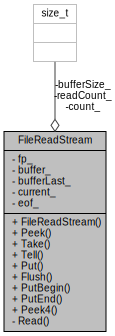
\includegraphics[width=187pt]{classFileReadStream__coll__graph}
\end{center}
\end{figure}
\subsection*{Public Types}
\begin{DoxyCompactItemize}
\item 
typedef char \hyperlink{classFileReadStream_ae1f83d9ca3c76d1d151af0b6c427f046}{Ch}
\begin{DoxyCompactList}\small\item\em \hyperlink{structCharacter}{Character} type (byte). \end{DoxyCompactList}\end{DoxyCompactItemize}
\subsection*{Public Member Functions}
\begin{DoxyCompactItemize}
\item 
\hyperlink{classFileReadStream_adf91191843d50b900f43cb4f35f16f67}{File\+Read\+Stream} (std\+::\+F\+I\+LE $\ast$fp, char $\ast$\hyperlink{imgui__impl__opengl3__loader_8h_a3667f558219c90437106b544a3ca00b8}{buffer}, size\+\_\+t buffer\+Size)
\begin{DoxyCompactList}\small\item\em Constructor. \end{DoxyCompactList}\item 
\hyperlink{classFileReadStream_ae1f83d9ca3c76d1d151af0b6c427f046}{Ch} \hyperlink{classFileReadStream_ab7d47da8952d3fe5856a261ec3c020c9}{Peek} () const
\item 
\hyperlink{classFileReadStream_ae1f83d9ca3c76d1d151af0b6c427f046}{Ch} \hyperlink{classFileReadStream_addcbccc9d86ccbbe6d8e876ba595dbcb}{Take} ()
\item 
size\+\_\+t \hyperlink{classFileReadStream_ae82cfaafe347286b3af8976548bedf86}{Tell} () const
\item 
\hyperlink{imgui__impl__opengl3__loader_8h_ac668e7cffd9e2e9cfee428b9b2f34fa7}{void} \hyperlink{classFileReadStream_a4f2eac5b08033b1527bff517be657a36}{Put} (\hyperlink{classFileReadStream_ae1f83d9ca3c76d1d151af0b6c427f046}{Ch})
\item 
\hyperlink{imgui__impl__opengl3__loader_8h_ac668e7cffd9e2e9cfee428b9b2f34fa7}{void} \hyperlink{classFileReadStream_acd031e3f578b23bc2a792ac41e1e95ae}{Flush} ()
\item 
\hyperlink{classFileReadStream_ae1f83d9ca3c76d1d151af0b6c427f046}{Ch} $\ast$ \hyperlink{classFileReadStream_ac985850ab75f204dc08a01d12a8ef5c6}{Put\+Begin} ()
\item 
size\+\_\+t \hyperlink{classFileReadStream_a886660c89f698ff913d641d61466108f}{Put\+End} (\hyperlink{classFileReadStream_ae1f83d9ca3c76d1d151af0b6c427f046}{Ch} $\ast$)
\item 
const \hyperlink{classFileReadStream_ae1f83d9ca3c76d1d151af0b6c427f046}{Ch} $\ast$ \hyperlink{classFileReadStream_a03f0b804c4c96762d0c6ef536337b7f0}{Peek4} () const
\end{DoxyCompactItemize}
\subsection*{Private Member Functions}
\begin{DoxyCompactItemize}
\item 
\hyperlink{imgui__impl__opengl3__loader_8h_ac668e7cffd9e2e9cfee428b9b2f34fa7}{void} \hyperlink{classFileReadStream_a9213039798b7a07275a451f96a42361a}{Read} ()
\end{DoxyCompactItemize}
\subsection*{Private Attributes}
\begin{DoxyCompactItemize}
\item 
std\+::\+F\+I\+LE $\ast$ \hyperlink{classFileReadStream_a47dc4f7f100bcc02a02e619f9b494a62}{fp\+\_\+}
\item 
\hyperlink{classFileReadStream_ae1f83d9ca3c76d1d151af0b6c427f046}{Ch} $\ast$ \hyperlink{classFileReadStream_a1b5563bcaa959d95f9bc3511a73ebbad}{buffer\+\_\+}
\item 
size\+\_\+t \hyperlink{classFileReadStream_af65abe97e76c94c7f0f6419f94e9105f}{buffer\+Size\+\_\+}
\item 
\hyperlink{classFileReadStream_ae1f83d9ca3c76d1d151af0b6c427f046}{Ch} $\ast$ \hyperlink{classFileReadStream_a5affa127604e77646d7acc94432c7e59}{buffer\+Last\+\_\+}
\item 
\hyperlink{classFileReadStream_ae1f83d9ca3c76d1d151af0b6c427f046}{Ch} $\ast$ \hyperlink{classFileReadStream_a0c7b4824d8742960eba2ac81c1e6b662}{current\+\_\+}
\item 
size\+\_\+t \hyperlink{classFileReadStream_a1b1a7cadb599e83b1f781c0b16d4ed50}{read\+Count\+\_\+}
\item 
size\+\_\+t \hyperlink{classFileReadStream_a55018d0ad821b9ea01e0ec5001008ab2}{count\+\_\+}
\begin{DoxyCompactList}\small\item\em Number of characters read. \end{DoxyCompactList}\item 
bool \hyperlink{classFileReadStream_a02a64d8fc7a4df830834f756b8ac08af}{eof\+\_\+}
\end{DoxyCompactItemize}


\subsection{Detailed Description}
File byte stream for input using fread(). 

\begin{DoxyNote}{Note}
implements Stream concept 
\end{DoxyNote}


\subsection{Member Typedef Documentation}
\mbox{\Hypertarget{classFileReadStream_ae1f83d9ca3c76d1d151af0b6c427f046}\label{classFileReadStream_ae1f83d9ca3c76d1d151af0b6c427f046}} 
\index{File\+Read\+Stream@{File\+Read\+Stream}!Ch@{Ch}}
\index{Ch@{Ch}!File\+Read\+Stream@{File\+Read\+Stream}}
\subsubsection{\texorpdfstring{Ch}{Ch}}
{\footnotesize\ttfamily typedef char \hyperlink{classFileReadStream_ae1f83d9ca3c76d1d151af0b6c427f046}{File\+Read\+Stream\+::\+Ch}}



\hyperlink{structCharacter}{Character} type (byte). 



\subsection{Constructor \& Destructor Documentation}
\mbox{\Hypertarget{classFileReadStream_adf91191843d50b900f43cb4f35f16f67}\label{classFileReadStream_adf91191843d50b900f43cb4f35f16f67}} 
\index{File\+Read\+Stream@{File\+Read\+Stream}!File\+Read\+Stream@{File\+Read\+Stream}}
\index{File\+Read\+Stream@{File\+Read\+Stream}!File\+Read\+Stream@{File\+Read\+Stream}}
\subsubsection{\texorpdfstring{File\+Read\+Stream()}{FileReadStream()}}
{\footnotesize\ttfamily File\+Read\+Stream\+::\+File\+Read\+Stream (\begin{DoxyParamCaption}\item[{std\+::\+F\+I\+LE $\ast$}]{fp,  }\item[{char $\ast$}]{buffer,  }\item[{size\+\_\+t}]{buffer\+Size }\end{DoxyParamCaption})\hspace{0.3cm}{\ttfamily [inline]}}



Constructor. 


\begin{DoxyParams}{Parameters}
{\em fp} & File pointer opened for read. \\
\hline
{\em buffer} & user-\/supplied buffer. \\
\hline
{\em buffer\+Size} & size of buffer in bytes. Must $>$=4 bytes. \\
\hline
\end{DoxyParams}


\subsection{Member Function Documentation}
\mbox{\Hypertarget{classFileReadStream_acd031e3f578b23bc2a792ac41e1e95ae}\label{classFileReadStream_acd031e3f578b23bc2a792ac41e1e95ae}} 
\index{File\+Read\+Stream@{File\+Read\+Stream}!Flush@{Flush}}
\index{Flush@{Flush}!File\+Read\+Stream@{File\+Read\+Stream}}
\subsubsection{\texorpdfstring{Flush()}{Flush()}}
{\footnotesize\ttfamily \hyperlink{imgui__impl__opengl3__loader_8h_ac668e7cffd9e2e9cfee428b9b2f34fa7}{void} File\+Read\+Stream\+::\+Flush (\begin{DoxyParamCaption}{ }\end{DoxyParamCaption})\hspace{0.3cm}{\ttfamily [inline]}}

\mbox{\Hypertarget{classFileReadStream_ab7d47da8952d3fe5856a261ec3c020c9}\label{classFileReadStream_ab7d47da8952d3fe5856a261ec3c020c9}} 
\index{File\+Read\+Stream@{File\+Read\+Stream}!Peek@{Peek}}
\index{Peek@{Peek}!File\+Read\+Stream@{File\+Read\+Stream}}
\subsubsection{\texorpdfstring{Peek()}{Peek()}}
{\footnotesize\ttfamily \hyperlink{classFileReadStream_ae1f83d9ca3c76d1d151af0b6c427f046}{Ch} File\+Read\+Stream\+::\+Peek (\begin{DoxyParamCaption}{ }\end{DoxyParamCaption}) const\hspace{0.3cm}{\ttfamily [inline]}}

\mbox{\Hypertarget{classFileReadStream_a03f0b804c4c96762d0c6ef536337b7f0}\label{classFileReadStream_a03f0b804c4c96762d0c6ef536337b7f0}} 
\index{File\+Read\+Stream@{File\+Read\+Stream}!Peek4@{Peek4}}
\index{Peek4@{Peek4}!File\+Read\+Stream@{File\+Read\+Stream}}
\subsubsection{\texorpdfstring{Peek4()}{Peek4()}}
{\footnotesize\ttfamily const \hyperlink{classFileReadStream_ae1f83d9ca3c76d1d151af0b6c427f046}{Ch}$\ast$ File\+Read\+Stream\+::\+Peek4 (\begin{DoxyParamCaption}{ }\end{DoxyParamCaption}) const\hspace{0.3cm}{\ttfamily [inline]}}

\mbox{\Hypertarget{classFileReadStream_a4f2eac5b08033b1527bff517be657a36}\label{classFileReadStream_a4f2eac5b08033b1527bff517be657a36}} 
\index{File\+Read\+Stream@{File\+Read\+Stream}!Put@{Put}}
\index{Put@{Put}!File\+Read\+Stream@{File\+Read\+Stream}}
\subsubsection{\texorpdfstring{Put()}{Put()}}
{\footnotesize\ttfamily \hyperlink{imgui__impl__opengl3__loader_8h_ac668e7cffd9e2e9cfee428b9b2f34fa7}{void} File\+Read\+Stream\+::\+Put (\begin{DoxyParamCaption}\item[{\hyperlink{classFileReadStream_ae1f83d9ca3c76d1d151af0b6c427f046}{Ch}}]{ }\end{DoxyParamCaption})\hspace{0.3cm}{\ttfamily [inline]}}

\mbox{\Hypertarget{classFileReadStream_ac985850ab75f204dc08a01d12a8ef5c6}\label{classFileReadStream_ac985850ab75f204dc08a01d12a8ef5c6}} 
\index{File\+Read\+Stream@{File\+Read\+Stream}!Put\+Begin@{Put\+Begin}}
\index{Put\+Begin@{Put\+Begin}!File\+Read\+Stream@{File\+Read\+Stream}}
\subsubsection{\texorpdfstring{Put\+Begin()}{PutBegin()}}
{\footnotesize\ttfamily \hyperlink{classFileReadStream_ae1f83d9ca3c76d1d151af0b6c427f046}{Ch}$\ast$ File\+Read\+Stream\+::\+Put\+Begin (\begin{DoxyParamCaption}{ }\end{DoxyParamCaption})\hspace{0.3cm}{\ttfamily [inline]}}

\mbox{\Hypertarget{classFileReadStream_a886660c89f698ff913d641d61466108f}\label{classFileReadStream_a886660c89f698ff913d641d61466108f}} 
\index{File\+Read\+Stream@{File\+Read\+Stream}!Put\+End@{Put\+End}}
\index{Put\+End@{Put\+End}!File\+Read\+Stream@{File\+Read\+Stream}}
\subsubsection{\texorpdfstring{Put\+End()}{PutEnd()}}
{\footnotesize\ttfamily size\+\_\+t File\+Read\+Stream\+::\+Put\+End (\begin{DoxyParamCaption}\item[{\hyperlink{classFileReadStream_ae1f83d9ca3c76d1d151af0b6c427f046}{Ch} $\ast$}]{ }\end{DoxyParamCaption})\hspace{0.3cm}{\ttfamily [inline]}}

\mbox{\Hypertarget{classFileReadStream_a9213039798b7a07275a451f96a42361a}\label{classFileReadStream_a9213039798b7a07275a451f96a42361a}} 
\index{File\+Read\+Stream@{File\+Read\+Stream}!Read@{Read}}
\index{Read@{Read}!File\+Read\+Stream@{File\+Read\+Stream}}
\subsubsection{\texorpdfstring{Read()}{Read()}}
{\footnotesize\ttfamily \hyperlink{imgui__impl__opengl3__loader_8h_ac668e7cffd9e2e9cfee428b9b2f34fa7}{void} File\+Read\+Stream\+::\+Read (\begin{DoxyParamCaption}{ }\end{DoxyParamCaption})\hspace{0.3cm}{\ttfamily [inline]}, {\ttfamily [private]}}

\mbox{\Hypertarget{classFileReadStream_addcbccc9d86ccbbe6d8e876ba595dbcb}\label{classFileReadStream_addcbccc9d86ccbbe6d8e876ba595dbcb}} 
\index{File\+Read\+Stream@{File\+Read\+Stream}!Take@{Take}}
\index{Take@{Take}!File\+Read\+Stream@{File\+Read\+Stream}}
\subsubsection{\texorpdfstring{Take()}{Take()}}
{\footnotesize\ttfamily \hyperlink{classFileReadStream_ae1f83d9ca3c76d1d151af0b6c427f046}{Ch} File\+Read\+Stream\+::\+Take (\begin{DoxyParamCaption}{ }\end{DoxyParamCaption})\hspace{0.3cm}{\ttfamily [inline]}}

\mbox{\Hypertarget{classFileReadStream_ae82cfaafe347286b3af8976548bedf86}\label{classFileReadStream_ae82cfaafe347286b3af8976548bedf86}} 
\index{File\+Read\+Stream@{File\+Read\+Stream}!Tell@{Tell}}
\index{Tell@{Tell}!File\+Read\+Stream@{File\+Read\+Stream}}
\subsubsection{\texorpdfstring{Tell()}{Tell()}}
{\footnotesize\ttfamily size\+\_\+t File\+Read\+Stream\+::\+Tell (\begin{DoxyParamCaption}{ }\end{DoxyParamCaption}) const\hspace{0.3cm}{\ttfamily [inline]}}



\subsection{Member Data Documentation}
\mbox{\Hypertarget{classFileReadStream_a1b5563bcaa959d95f9bc3511a73ebbad}\label{classFileReadStream_a1b5563bcaa959d95f9bc3511a73ebbad}} 
\index{File\+Read\+Stream@{File\+Read\+Stream}!buffer\+\_\+@{buffer\+\_\+}}
\index{buffer\+\_\+@{buffer\+\_\+}!File\+Read\+Stream@{File\+Read\+Stream}}
\subsubsection{\texorpdfstring{buffer\+\_\+}{buffer\_}}
{\footnotesize\ttfamily \hyperlink{classFileReadStream_ae1f83d9ca3c76d1d151af0b6c427f046}{Ch}$\ast$ File\+Read\+Stream\+::buffer\+\_\+\hspace{0.3cm}{\ttfamily [private]}}

\mbox{\Hypertarget{classFileReadStream_a5affa127604e77646d7acc94432c7e59}\label{classFileReadStream_a5affa127604e77646d7acc94432c7e59}} 
\index{File\+Read\+Stream@{File\+Read\+Stream}!buffer\+Last\+\_\+@{buffer\+Last\+\_\+}}
\index{buffer\+Last\+\_\+@{buffer\+Last\+\_\+}!File\+Read\+Stream@{File\+Read\+Stream}}
\subsubsection{\texorpdfstring{buffer\+Last\+\_\+}{bufferLast\_}}
{\footnotesize\ttfamily \hyperlink{classFileReadStream_ae1f83d9ca3c76d1d151af0b6c427f046}{Ch}$\ast$ File\+Read\+Stream\+::buffer\+Last\+\_\+\hspace{0.3cm}{\ttfamily [private]}}

\mbox{\Hypertarget{classFileReadStream_af65abe97e76c94c7f0f6419f94e9105f}\label{classFileReadStream_af65abe97e76c94c7f0f6419f94e9105f}} 
\index{File\+Read\+Stream@{File\+Read\+Stream}!buffer\+Size\+\_\+@{buffer\+Size\+\_\+}}
\index{buffer\+Size\+\_\+@{buffer\+Size\+\_\+}!File\+Read\+Stream@{File\+Read\+Stream}}
\subsubsection{\texorpdfstring{buffer\+Size\+\_\+}{bufferSize\_}}
{\footnotesize\ttfamily size\+\_\+t File\+Read\+Stream\+::buffer\+Size\+\_\+\hspace{0.3cm}{\ttfamily [private]}}

\mbox{\Hypertarget{classFileReadStream_a55018d0ad821b9ea01e0ec5001008ab2}\label{classFileReadStream_a55018d0ad821b9ea01e0ec5001008ab2}} 
\index{File\+Read\+Stream@{File\+Read\+Stream}!count\+\_\+@{count\+\_\+}}
\index{count\+\_\+@{count\+\_\+}!File\+Read\+Stream@{File\+Read\+Stream}}
\subsubsection{\texorpdfstring{count\+\_\+}{count\_}}
{\footnotesize\ttfamily size\+\_\+t File\+Read\+Stream\+::count\+\_\+\hspace{0.3cm}{\ttfamily [private]}}



Number of characters read. 

\mbox{\Hypertarget{classFileReadStream_a0c7b4824d8742960eba2ac81c1e6b662}\label{classFileReadStream_a0c7b4824d8742960eba2ac81c1e6b662}} 
\index{File\+Read\+Stream@{File\+Read\+Stream}!current\+\_\+@{current\+\_\+}}
\index{current\+\_\+@{current\+\_\+}!File\+Read\+Stream@{File\+Read\+Stream}}
\subsubsection{\texorpdfstring{current\+\_\+}{current\_}}
{\footnotesize\ttfamily \hyperlink{classFileReadStream_ae1f83d9ca3c76d1d151af0b6c427f046}{Ch}$\ast$ File\+Read\+Stream\+::current\+\_\+\hspace{0.3cm}{\ttfamily [private]}}

\mbox{\Hypertarget{classFileReadStream_a02a64d8fc7a4df830834f756b8ac08af}\label{classFileReadStream_a02a64d8fc7a4df830834f756b8ac08af}} 
\index{File\+Read\+Stream@{File\+Read\+Stream}!eof\+\_\+@{eof\+\_\+}}
\index{eof\+\_\+@{eof\+\_\+}!File\+Read\+Stream@{File\+Read\+Stream}}
\subsubsection{\texorpdfstring{eof\+\_\+}{eof\_}}
{\footnotesize\ttfamily bool File\+Read\+Stream\+::eof\+\_\+\hspace{0.3cm}{\ttfamily [private]}}

\mbox{\Hypertarget{classFileReadStream_a47dc4f7f100bcc02a02e619f9b494a62}\label{classFileReadStream_a47dc4f7f100bcc02a02e619f9b494a62}} 
\index{File\+Read\+Stream@{File\+Read\+Stream}!fp\+\_\+@{fp\+\_\+}}
\index{fp\+\_\+@{fp\+\_\+}!File\+Read\+Stream@{File\+Read\+Stream}}
\subsubsection{\texorpdfstring{fp\+\_\+}{fp\_}}
{\footnotesize\ttfamily std\+::\+F\+I\+LE$\ast$ File\+Read\+Stream\+::fp\+\_\+\hspace{0.3cm}{\ttfamily [private]}}

\mbox{\Hypertarget{classFileReadStream_a1b1a7cadb599e83b1f781c0b16d4ed50}\label{classFileReadStream_a1b1a7cadb599e83b1f781c0b16d4ed50}} 
\index{File\+Read\+Stream@{File\+Read\+Stream}!read\+Count\+\_\+@{read\+Count\+\_\+}}
\index{read\+Count\+\_\+@{read\+Count\+\_\+}!File\+Read\+Stream@{File\+Read\+Stream}}
\subsubsection{\texorpdfstring{read\+Count\+\_\+}{readCount\_}}
{\footnotesize\ttfamily size\+\_\+t File\+Read\+Stream\+::read\+Count\+\_\+\hspace{0.3cm}{\ttfamily [private]}}



The documentation for this class was generated from the following file\+:\begin{DoxyCompactItemize}
\item 
/mnt/hdd/fnky/\+C0de/\+C\+A\+P\+S\+T\+O\+N\+E/clean\+\_\+build/include/rapidjson/\hyperlink{filereadstream_8h}{filereadstream.\+h}\end{DoxyCompactItemize}

\hypertarget{classFileWriteStream}{}\section{File\+Write\+Stream Class Reference}
\label{classFileWriteStream}\index{File\+Write\+Stream@{File\+Write\+Stream}}


Wrapper of C file stream for output using fwrite().  




{\ttfamily \#include $<$filewritestream.\+h$>$}



Collaboration diagram for File\+Write\+Stream\+:
\nopagebreak
\begin{figure}[H]
\begin{center}
\leavevmode
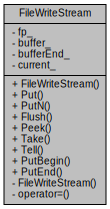
\includegraphics[width=182pt]{classFileWriteStream__coll__graph}
\end{center}
\end{figure}
\subsection*{Public Types}
\begin{DoxyCompactItemize}
\item 
typedef char \hyperlink{classFileWriteStream_abc16aeb69ad4176263ddfcb837fb7b49}{Ch}
\begin{DoxyCompactList}\small\item\em \hyperlink{structCharacter}{Character} type. Only support char. \end{DoxyCompactList}\end{DoxyCompactItemize}
\subsection*{Public Member Functions}
\begin{DoxyCompactItemize}
\item 
\hyperlink{classFileWriteStream_a553ea3e7377a7f7cace2daa3cc90e1a1}{File\+Write\+Stream} (std\+::\+F\+I\+LE $\ast$fp, char $\ast$\hyperlink{imgui__impl__opengl3__loader_8h_a3667f558219c90437106b544a3ca00b8}{buffer}, size\+\_\+t buffer\+Size)
\item 
\hyperlink{imgui__impl__opengl3__loader_8h_ac668e7cffd9e2e9cfee428b9b2f34fa7}{void} \hyperlink{classFileWriteStream_af6a6061d0accd939fa475b9b34427d85}{Put} (char c)
\item 
\hyperlink{imgui__impl__opengl3__loader_8h_ac668e7cffd9e2e9cfee428b9b2f34fa7}{void} \hyperlink{classFileWriteStream_ad9ec108b24316a2c1c83c6ddc75d308a}{PutN} (char c, size\+\_\+t n)
\item 
\hyperlink{imgui__impl__opengl3__loader_8h_ac668e7cffd9e2e9cfee428b9b2f34fa7}{void} \hyperlink{classFileWriteStream_a939fbf183ba36464c5e0837df4329d37}{Flush} ()
\item 
char \hyperlink{classFileWriteStream_ab556c7e26346ddff0e579a53c09c3a13}{Peek} () const
\item 
char \hyperlink{classFileWriteStream_ac927a0ae09a85eaba58a74ceb04b40ed}{Take} ()
\item 
size\+\_\+t \hyperlink{classFileWriteStream_a06272de32d6ac4d10c9bd5deb79a0234}{Tell} () const
\item 
char $\ast$ \hyperlink{classFileWriteStream_a4d1340a64fde3f16ac2afce19537c75e}{Put\+Begin} ()
\item 
size\+\_\+t \hyperlink{classFileWriteStream_a54b14047e4c998db0594290605f8f0dc}{Put\+End} (char $\ast$)
\end{DoxyCompactItemize}
\subsection*{Private Member Functions}
\begin{DoxyCompactItemize}
\item 
\hyperlink{classFileWriteStream_a62cc69f885b946b6bc2935f40c970cbb}{File\+Write\+Stream} (const \hyperlink{classFileWriteStream}{File\+Write\+Stream} \&)
\item 
\hyperlink{classFileWriteStream}{File\+Write\+Stream} \& \hyperlink{classFileWriteStream_a82e33badcc890b78ed482de7f1266f97}{operator=} (const \hyperlink{classFileWriteStream}{File\+Write\+Stream} \&)
\end{DoxyCompactItemize}
\subsection*{Private Attributes}
\begin{DoxyCompactItemize}
\item 
std\+::\+F\+I\+LE $\ast$ \hyperlink{classFileWriteStream_aac23a58bdaa601d276c57b5bcf5b0246}{fp\+\_\+}
\item 
char $\ast$ \hyperlink{classFileWriteStream_a6a1f0fed15eb38f22935f11af493972f}{buffer\+\_\+}
\item 
char $\ast$ \hyperlink{classFileWriteStream_a1f30d1c653f30ca6e069cefb80881c75}{buffer\+End\+\_\+}
\item 
char $\ast$ \hyperlink{classFileWriteStream_a3b3ba8e5deef1b12f0662e9031f05c71}{current\+\_\+}
\end{DoxyCompactItemize}


\subsection{Detailed Description}
Wrapper of C file stream for output using fwrite(). 

\begin{DoxyNote}{Note}
implements Stream concept 
\end{DoxyNote}


\subsection{Member Typedef Documentation}
\mbox{\Hypertarget{classFileWriteStream_abc16aeb69ad4176263ddfcb837fb7b49}\label{classFileWriteStream_abc16aeb69ad4176263ddfcb837fb7b49}} 
\index{File\+Write\+Stream@{File\+Write\+Stream}!Ch@{Ch}}
\index{Ch@{Ch}!File\+Write\+Stream@{File\+Write\+Stream}}
\subsubsection{\texorpdfstring{Ch}{Ch}}
{\footnotesize\ttfamily typedef char \hyperlink{classFileWriteStream_abc16aeb69ad4176263ddfcb837fb7b49}{File\+Write\+Stream\+::\+Ch}}



\hyperlink{structCharacter}{Character} type. Only support char. 



\subsection{Constructor \& Destructor Documentation}
\mbox{\Hypertarget{classFileWriteStream_a553ea3e7377a7f7cace2daa3cc90e1a1}\label{classFileWriteStream_a553ea3e7377a7f7cace2daa3cc90e1a1}} 
\index{File\+Write\+Stream@{File\+Write\+Stream}!File\+Write\+Stream@{File\+Write\+Stream}}
\index{File\+Write\+Stream@{File\+Write\+Stream}!File\+Write\+Stream@{File\+Write\+Stream}}
\subsubsection{\texorpdfstring{File\+Write\+Stream()}{FileWriteStream()}\hspace{0.1cm}{\footnotesize\ttfamily [1/2]}}
{\footnotesize\ttfamily File\+Write\+Stream\+::\+File\+Write\+Stream (\begin{DoxyParamCaption}\item[{std\+::\+F\+I\+LE $\ast$}]{fp,  }\item[{char $\ast$}]{buffer,  }\item[{size\+\_\+t}]{buffer\+Size }\end{DoxyParamCaption})\hspace{0.3cm}{\ttfamily [inline]}}

\mbox{\Hypertarget{classFileWriteStream_a62cc69f885b946b6bc2935f40c970cbb}\label{classFileWriteStream_a62cc69f885b946b6bc2935f40c970cbb}} 
\index{File\+Write\+Stream@{File\+Write\+Stream}!File\+Write\+Stream@{File\+Write\+Stream}}
\index{File\+Write\+Stream@{File\+Write\+Stream}!File\+Write\+Stream@{File\+Write\+Stream}}
\subsubsection{\texorpdfstring{File\+Write\+Stream()}{FileWriteStream()}\hspace{0.1cm}{\footnotesize\ttfamily [2/2]}}
{\footnotesize\ttfamily File\+Write\+Stream\+::\+File\+Write\+Stream (\begin{DoxyParamCaption}\item[{const \hyperlink{classFileWriteStream}{File\+Write\+Stream} \&}]{ }\end{DoxyParamCaption})\hspace{0.3cm}{\ttfamily [private]}}



\subsection{Member Function Documentation}
\mbox{\Hypertarget{classFileWriteStream_a939fbf183ba36464c5e0837df4329d37}\label{classFileWriteStream_a939fbf183ba36464c5e0837df4329d37}} 
\index{File\+Write\+Stream@{File\+Write\+Stream}!Flush@{Flush}}
\index{Flush@{Flush}!File\+Write\+Stream@{File\+Write\+Stream}}
\subsubsection{\texorpdfstring{Flush()}{Flush()}}
{\footnotesize\ttfamily \hyperlink{imgui__impl__opengl3__loader_8h_ac668e7cffd9e2e9cfee428b9b2f34fa7}{void} File\+Write\+Stream\+::\+Flush (\begin{DoxyParamCaption}{ }\end{DoxyParamCaption})\hspace{0.3cm}{\ttfamily [inline]}}

\mbox{\Hypertarget{classFileWriteStream_a82e33badcc890b78ed482de7f1266f97}\label{classFileWriteStream_a82e33badcc890b78ed482de7f1266f97}} 
\index{File\+Write\+Stream@{File\+Write\+Stream}!operator=@{operator=}}
\index{operator=@{operator=}!File\+Write\+Stream@{File\+Write\+Stream}}
\subsubsection{\texorpdfstring{operator=()}{operator=()}}
{\footnotesize\ttfamily \hyperlink{classFileWriteStream}{File\+Write\+Stream}\& File\+Write\+Stream\+::operator= (\begin{DoxyParamCaption}\item[{const \hyperlink{classFileWriteStream}{File\+Write\+Stream} \&}]{ }\end{DoxyParamCaption})\hspace{0.3cm}{\ttfamily [private]}}

\mbox{\Hypertarget{classFileWriteStream_ab556c7e26346ddff0e579a53c09c3a13}\label{classFileWriteStream_ab556c7e26346ddff0e579a53c09c3a13}} 
\index{File\+Write\+Stream@{File\+Write\+Stream}!Peek@{Peek}}
\index{Peek@{Peek}!File\+Write\+Stream@{File\+Write\+Stream}}
\subsubsection{\texorpdfstring{Peek()}{Peek()}}
{\footnotesize\ttfamily char File\+Write\+Stream\+::\+Peek (\begin{DoxyParamCaption}{ }\end{DoxyParamCaption}) const\hspace{0.3cm}{\ttfamily [inline]}}

\mbox{\Hypertarget{classFileWriteStream_af6a6061d0accd939fa475b9b34427d85}\label{classFileWriteStream_af6a6061d0accd939fa475b9b34427d85}} 
\index{File\+Write\+Stream@{File\+Write\+Stream}!Put@{Put}}
\index{Put@{Put}!File\+Write\+Stream@{File\+Write\+Stream}}
\subsubsection{\texorpdfstring{Put()}{Put()}}
{\footnotesize\ttfamily \hyperlink{imgui__impl__opengl3__loader_8h_ac668e7cffd9e2e9cfee428b9b2f34fa7}{void} File\+Write\+Stream\+::\+Put (\begin{DoxyParamCaption}\item[{char}]{c }\end{DoxyParamCaption})\hspace{0.3cm}{\ttfamily [inline]}}

\mbox{\Hypertarget{classFileWriteStream_a4d1340a64fde3f16ac2afce19537c75e}\label{classFileWriteStream_a4d1340a64fde3f16ac2afce19537c75e}} 
\index{File\+Write\+Stream@{File\+Write\+Stream}!Put\+Begin@{Put\+Begin}}
\index{Put\+Begin@{Put\+Begin}!File\+Write\+Stream@{File\+Write\+Stream}}
\subsubsection{\texorpdfstring{Put\+Begin()}{PutBegin()}}
{\footnotesize\ttfamily char$\ast$ File\+Write\+Stream\+::\+Put\+Begin (\begin{DoxyParamCaption}{ }\end{DoxyParamCaption})\hspace{0.3cm}{\ttfamily [inline]}}

\mbox{\Hypertarget{classFileWriteStream_a54b14047e4c998db0594290605f8f0dc}\label{classFileWriteStream_a54b14047e4c998db0594290605f8f0dc}} 
\index{File\+Write\+Stream@{File\+Write\+Stream}!Put\+End@{Put\+End}}
\index{Put\+End@{Put\+End}!File\+Write\+Stream@{File\+Write\+Stream}}
\subsubsection{\texorpdfstring{Put\+End()}{PutEnd()}}
{\footnotesize\ttfamily size\+\_\+t File\+Write\+Stream\+::\+Put\+End (\begin{DoxyParamCaption}\item[{char $\ast$}]{ }\end{DoxyParamCaption})\hspace{0.3cm}{\ttfamily [inline]}}

\mbox{\Hypertarget{classFileWriteStream_ad9ec108b24316a2c1c83c6ddc75d308a}\label{classFileWriteStream_ad9ec108b24316a2c1c83c6ddc75d308a}} 
\index{File\+Write\+Stream@{File\+Write\+Stream}!PutN@{PutN}}
\index{PutN@{PutN}!File\+Write\+Stream@{File\+Write\+Stream}}
\subsubsection{\texorpdfstring{Put\+N()}{PutN()}}
{\footnotesize\ttfamily \hyperlink{imgui__impl__opengl3__loader_8h_ac668e7cffd9e2e9cfee428b9b2f34fa7}{void} File\+Write\+Stream\+::\+PutN (\begin{DoxyParamCaption}\item[{char}]{c,  }\item[{size\+\_\+t}]{n }\end{DoxyParamCaption})\hspace{0.3cm}{\ttfamily [inline]}}

\mbox{\Hypertarget{classFileWriteStream_ac927a0ae09a85eaba58a74ceb04b40ed}\label{classFileWriteStream_ac927a0ae09a85eaba58a74ceb04b40ed}} 
\index{File\+Write\+Stream@{File\+Write\+Stream}!Take@{Take}}
\index{Take@{Take}!File\+Write\+Stream@{File\+Write\+Stream}}
\subsubsection{\texorpdfstring{Take()}{Take()}}
{\footnotesize\ttfamily char File\+Write\+Stream\+::\+Take (\begin{DoxyParamCaption}{ }\end{DoxyParamCaption})\hspace{0.3cm}{\ttfamily [inline]}}

\mbox{\Hypertarget{classFileWriteStream_a06272de32d6ac4d10c9bd5deb79a0234}\label{classFileWriteStream_a06272de32d6ac4d10c9bd5deb79a0234}} 
\index{File\+Write\+Stream@{File\+Write\+Stream}!Tell@{Tell}}
\index{Tell@{Tell}!File\+Write\+Stream@{File\+Write\+Stream}}
\subsubsection{\texorpdfstring{Tell()}{Tell()}}
{\footnotesize\ttfamily size\+\_\+t File\+Write\+Stream\+::\+Tell (\begin{DoxyParamCaption}{ }\end{DoxyParamCaption}) const\hspace{0.3cm}{\ttfamily [inline]}}



\subsection{Member Data Documentation}
\mbox{\Hypertarget{classFileWriteStream_a6a1f0fed15eb38f22935f11af493972f}\label{classFileWriteStream_a6a1f0fed15eb38f22935f11af493972f}} 
\index{File\+Write\+Stream@{File\+Write\+Stream}!buffer\+\_\+@{buffer\+\_\+}}
\index{buffer\+\_\+@{buffer\+\_\+}!File\+Write\+Stream@{File\+Write\+Stream}}
\subsubsection{\texorpdfstring{buffer\+\_\+}{buffer\_}}
{\footnotesize\ttfamily char$\ast$ File\+Write\+Stream\+::buffer\+\_\+\hspace{0.3cm}{\ttfamily [private]}}

\mbox{\Hypertarget{classFileWriteStream_a1f30d1c653f30ca6e069cefb80881c75}\label{classFileWriteStream_a1f30d1c653f30ca6e069cefb80881c75}} 
\index{File\+Write\+Stream@{File\+Write\+Stream}!buffer\+End\+\_\+@{buffer\+End\+\_\+}}
\index{buffer\+End\+\_\+@{buffer\+End\+\_\+}!File\+Write\+Stream@{File\+Write\+Stream}}
\subsubsection{\texorpdfstring{buffer\+End\+\_\+}{bufferEnd\_}}
{\footnotesize\ttfamily char$\ast$ File\+Write\+Stream\+::buffer\+End\+\_\+\hspace{0.3cm}{\ttfamily [private]}}

\mbox{\Hypertarget{classFileWriteStream_a3b3ba8e5deef1b12f0662e9031f05c71}\label{classFileWriteStream_a3b3ba8e5deef1b12f0662e9031f05c71}} 
\index{File\+Write\+Stream@{File\+Write\+Stream}!current\+\_\+@{current\+\_\+}}
\index{current\+\_\+@{current\+\_\+}!File\+Write\+Stream@{File\+Write\+Stream}}
\subsubsection{\texorpdfstring{current\+\_\+}{current\_}}
{\footnotesize\ttfamily char$\ast$ File\+Write\+Stream\+::current\+\_\+\hspace{0.3cm}{\ttfamily [private]}}

\mbox{\Hypertarget{classFileWriteStream_aac23a58bdaa601d276c57b5bcf5b0246}\label{classFileWriteStream_aac23a58bdaa601d276c57b5bcf5b0246}} 
\index{File\+Write\+Stream@{File\+Write\+Stream}!fp\+\_\+@{fp\+\_\+}}
\index{fp\+\_\+@{fp\+\_\+}!File\+Write\+Stream@{File\+Write\+Stream}}
\subsubsection{\texorpdfstring{fp\+\_\+}{fp\_}}
{\footnotesize\ttfamily std\+::\+F\+I\+LE$\ast$ File\+Write\+Stream\+::fp\+\_\+\hspace{0.3cm}{\ttfamily [private]}}



The documentation for this class was generated from the following file\+:\begin{DoxyCompactItemize}
\item 
/mnt/hdd/fnky/\+C0de/\+C\+A\+P\+S\+T\+O\+N\+E/clean\+\_\+build/include/rapidjson/\hyperlink{filewritestream_8h}{filewritestream.\+h}\end{DoxyCompactItemize}

\hypertarget{structGenericValue_1_1Flag}{}\section{Generic\+Value$<$ Encoding, Allocator $>$\+:\+:Flag Struct Reference}
\label{structGenericValue_1_1Flag}\index{Generic\+Value$<$ Encoding, Allocator $>$\+::\+Flag@{Generic\+Value$<$ Encoding, Allocator $>$\+::\+Flag}}


{\ttfamily \#include $<$document.\+h$>$}



Collaboration diagram for Generic\+Value$<$ Encoding, Allocator $>$\+:\+:Flag\+:
\nopagebreak
\begin{figure}[H]
\begin{center}
\leavevmode
\includegraphics[width=208pt]{structGenericValue_1_1Flag__coll__graph}
\end{center}
\end{figure}
\subsection*{Public Attributes}
\begin{DoxyCompactItemize}
\item 
char \hyperlink{structGenericValue_1_1Flag_aced7ede2056a797fb80817d45634e3ea}{payload} \mbox{[}sizeof(\hyperlink{rapidjson_8h_a5ed6e6e67250fadbd041127e6386dcb5}{Size\+Type}) $\ast$2+sizeof(\hyperlink{imgui__impl__opengl3__loader_8h_ac668e7cffd9e2e9cfee428b9b2f34fa7}{void} $\ast$)+2\mbox{]}
\item 
\hyperlink{stdint_8h_a273cf69d639a59973b6019625df33e30}{uint16\+\_\+t} \hyperlink{structGenericValue_1_1Flag_ac91f08067dcc0003fc78e870ca9b2d5d}{flags}
\end{DoxyCompactItemize}


\subsection{Member Data Documentation}
\mbox{\Hypertarget{structGenericValue_1_1Flag_ac91f08067dcc0003fc78e870ca9b2d5d}\label{structGenericValue_1_1Flag_ac91f08067dcc0003fc78e870ca9b2d5d}} 
\index{Generic\+Value\+::\+Flag@{Generic\+Value\+::\+Flag}!flags@{flags}}
\index{flags@{flags}!Generic\+Value\+::\+Flag@{Generic\+Value\+::\+Flag}}
\subsubsection{\texorpdfstring{flags}{flags}}
{\footnotesize\ttfamily template$<$typename Encoding, typename Allocator = R\+A\+P\+I\+D\+J\+S\+O\+N\+\_\+\+D\+E\+F\+A\+U\+L\+T\+\_\+\+A\+L\+L\+O\+C\+A\+T\+OR$>$ \\
\hyperlink{stdint_8h_a273cf69d639a59973b6019625df33e30}{uint16\+\_\+t} \hyperlink{classGenericValue}{Generic\+Value}$<$ Encoding, Allocator $>$\+::Flag\+::flags}

\mbox{\Hypertarget{structGenericValue_1_1Flag_aced7ede2056a797fb80817d45634e3ea}\label{structGenericValue_1_1Flag_aced7ede2056a797fb80817d45634e3ea}} 
\index{Generic\+Value\+::\+Flag@{Generic\+Value\+::\+Flag}!payload@{payload}}
\index{payload@{payload}!Generic\+Value\+::\+Flag@{Generic\+Value\+::\+Flag}}
\subsubsection{\texorpdfstring{payload}{payload}}
{\footnotesize\ttfamily template$<$typename Encoding, typename Allocator = R\+A\+P\+I\+D\+J\+S\+O\+N\+\_\+\+D\+E\+F\+A\+U\+L\+T\+\_\+\+A\+L\+L\+O\+C\+A\+T\+OR$>$ \\
char \hyperlink{classGenericValue}{Generic\+Value}$<$ Encoding, Allocator $>$\+::Flag\+::payload\mbox{[}sizeof(\hyperlink{rapidjson_8h_a5ed6e6e67250fadbd041127e6386dcb5}{Size\+Type}) $\ast$2+sizeof(\hyperlink{imgui__impl__opengl3__loader_8h_ac668e7cffd9e2e9cfee428b9b2f34fa7}{void} $\ast$)+2\mbox{]}}



The documentation for this struct was generated from the following file\+:\begin{DoxyCompactItemize}
\item 
/mnt/hdd/fnky/\+C0de/\+C\+A\+P\+S\+T\+O\+N\+E/clean\+\_\+build/include/rapidjson/\hyperlink{document_8h}{document.\+h}\end{DoxyCompactItemize}

\hypertarget{structinternal_1_1GenericRegex_1_1Frag}{}\section{internal\+:\+:Generic\+Regex$<$ Encoding, Allocator $>$\+:\+:Frag Struct Reference}
\label{structinternal_1_1GenericRegex_1_1Frag}\index{internal\+::\+Generic\+Regex$<$ Encoding, Allocator $>$\+::\+Frag@{internal\+::\+Generic\+Regex$<$ Encoding, Allocator $>$\+::\+Frag}}


Collaboration diagram for internal\+:\+:Generic\+Regex$<$ Encoding, Allocator $>$\+:\+:Frag\+:
\nopagebreak
\begin{figure}[H]
\begin{center}
\leavevmode
\includegraphics[width=196pt]{structinternal_1_1GenericRegex_1_1Frag__coll__graph}
\end{center}
\end{figure}
\subsection*{Public Member Functions}
\begin{DoxyCompactItemize}
\item 
\hyperlink{structinternal_1_1GenericRegex_1_1Frag_a377c8d806013ce14ff941be9427e80ff}{Frag} (\hyperlink{rapidjson_8h_a5ed6e6e67250fadbd041127e6386dcb5}{Size\+Type} s, \hyperlink{rapidjson_8h_a5ed6e6e67250fadbd041127e6386dcb5}{Size\+Type} o, \hyperlink{rapidjson_8h_a5ed6e6e67250fadbd041127e6386dcb5}{Size\+Type} m)
\end{DoxyCompactItemize}
\subsection*{Public Attributes}
\begin{DoxyCompactItemize}
\item 
\hyperlink{rapidjson_8h_a5ed6e6e67250fadbd041127e6386dcb5}{Size\+Type} \hyperlink{structinternal_1_1GenericRegex_1_1Frag_adec8170ccdf14bfc3138a4df0b2e4abd}{start}
\item 
\hyperlink{rapidjson_8h_a5ed6e6e67250fadbd041127e6386dcb5}{Size\+Type} \hyperlink{structinternal_1_1GenericRegex_1_1Frag_a48b23d866d56328e05c187de2d7443d2}{out}
\begin{DoxyCompactList}\small\item\em link-\/list of all output states \end{DoxyCompactList}\item 
\hyperlink{rapidjson_8h_a5ed6e6e67250fadbd041127e6386dcb5}{Size\+Type} \hyperlink{structinternal_1_1GenericRegex_1_1Frag_a8007c1e6c879d1fe3eec2327fed0c664}{min\+Index}
\end{DoxyCompactItemize}


\subsection{Constructor \& Destructor Documentation}
\mbox{\Hypertarget{structinternal_1_1GenericRegex_1_1Frag_a377c8d806013ce14ff941be9427e80ff}\label{structinternal_1_1GenericRegex_1_1Frag_a377c8d806013ce14ff941be9427e80ff}} 
\index{internal\+::\+Generic\+Regex\+::\+Frag@{internal\+::\+Generic\+Regex\+::\+Frag}!Frag@{Frag}}
\index{Frag@{Frag}!internal\+::\+Generic\+Regex\+::\+Frag@{internal\+::\+Generic\+Regex\+::\+Frag}}
\subsubsection{\texorpdfstring{Frag()}{Frag()}}
{\footnotesize\ttfamily template$<$typename Encoding , typename Allocator  = Crt\+Allocator$>$ \\
\hyperlink{classinternal_1_1GenericRegex}{internal\+::\+Generic\+Regex}$<$ Encoding, Allocator $>$\+::Frag\+::\+Frag (\begin{DoxyParamCaption}\item[{\hyperlink{rapidjson_8h_a5ed6e6e67250fadbd041127e6386dcb5}{Size\+Type}}]{s,  }\item[{\hyperlink{rapidjson_8h_a5ed6e6e67250fadbd041127e6386dcb5}{Size\+Type}}]{o,  }\item[{\hyperlink{rapidjson_8h_a5ed6e6e67250fadbd041127e6386dcb5}{Size\+Type}}]{m }\end{DoxyParamCaption})\hspace{0.3cm}{\ttfamily [inline]}}



\subsection{Member Data Documentation}
\mbox{\Hypertarget{structinternal_1_1GenericRegex_1_1Frag_a8007c1e6c879d1fe3eec2327fed0c664}\label{structinternal_1_1GenericRegex_1_1Frag_a8007c1e6c879d1fe3eec2327fed0c664}} 
\index{internal\+::\+Generic\+Regex\+::\+Frag@{internal\+::\+Generic\+Regex\+::\+Frag}!min\+Index@{min\+Index}}
\index{min\+Index@{min\+Index}!internal\+::\+Generic\+Regex\+::\+Frag@{internal\+::\+Generic\+Regex\+::\+Frag}}
\subsubsection{\texorpdfstring{min\+Index}{minIndex}}
{\footnotesize\ttfamily template$<$typename Encoding , typename Allocator  = Crt\+Allocator$>$ \\
\hyperlink{rapidjson_8h_a5ed6e6e67250fadbd041127e6386dcb5}{Size\+Type} \hyperlink{classinternal_1_1GenericRegex}{internal\+::\+Generic\+Regex}$<$ Encoding, Allocator $>$\+::Frag\+::min\+Index}

\mbox{\Hypertarget{structinternal_1_1GenericRegex_1_1Frag_a48b23d866d56328e05c187de2d7443d2}\label{structinternal_1_1GenericRegex_1_1Frag_a48b23d866d56328e05c187de2d7443d2}} 
\index{internal\+::\+Generic\+Regex\+::\+Frag@{internal\+::\+Generic\+Regex\+::\+Frag}!out@{out}}
\index{out@{out}!internal\+::\+Generic\+Regex\+::\+Frag@{internal\+::\+Generic\+Regex\+::\+Frag}}
\subsubsection{\texorpdfstring{out}{out}}
{\footnotesize\ttfamily template$<$typename Encoding , typename Allocator  = Crt\+Allocator$>$ \\
\hyperlink{rapidjson_8h_a5ed6e6e67250fadbd041127e6386dcb5}{Size\+Type} \hyperlink{classinternal_1_1GenericRegex}{internal\+::\+Generic\+Regex}$<$ Encoding, Allocator $>$\+::Frag\+::out}



link-\/list of all output states 

\mbox{\Hypertarget{structinternal_1_1GenericRegex_1_1Frag_adec8170ccdf14bfc3138a4df0b2e4abd}\label{structinternal_1_1GenericRegex_1_1Frag_adec8170ccdf14bfc3138a4df0b2e4abd}} 
\index{internal\+::\+Generic\+Regex\+::\+Frag@{internal\+::\+Generic\+Regex\+::\+Frag}!start@{start}}
\index{start@{start}!internal\+::\+Generic\+Regex\+::\+Frag@{internal\+::\+Generic\+Regex\+::\+Frag}}
\subsubsection{\texorpdfstring{start}{start}}
{\footnotesize\ttfamily template$<$typename Encoding , typename Allocator  = Crt\+Allocator$>$ \\
\hyperlink{rapidjson_8h_a5ed6e6e67250fadbd041127e6386dcb5}{Size\+Type} \hyperlink{classinternal_1_1GenericRegex}{internal\+::\+Generic\+Regex}$<$ Encoding, Allocator $>$\+::Frag\+::start}



The documentation for this struct was generated from the following file\+:\begin{DoxyCompactItemize}
\item 
/mnt/hdd/fnky/\+C0de/\+C\+A\+P\+S\+T\+O\+N\+E/clean\+\_\+build/include/rapidjson/internal/\hyperlink{regex_8h}{regex.\+h}\end{DoxyCompactItemize}

\hypertarget{classGame}{}\section{Game Class Reference}
\label{classGame}\index{Game@{Game}}


{\ttfamily \#include $<$game.\+h$>$}



Collaboration diagram for Game\+:
\nopagebreak
\begin{figure}[H]
\begin{center}
\leavevmode
\includegraphics[width=350pt]{classGame__coll__graph}
\end{center}
\end{figure}
\subsection*{Public Member Functions}
\begin{DoxyCompactItemize}
\item 
\hyperlink{classGame_ad59df6562a58a614fda24622d3715b65}{Game} ()
\item 
\hyperlink{classGame_ae3d112ca6e0e55150d2fdbc704474530}{$\sim$\+Game} ()
\item 
\hyperlink{imgui__impl__opengl3__loader_8h_ac668e7cffd9e2e9cfee428b9b2f34fa7}{void} \hyperlink{classGame_adc01a7fae5261c95f7e6b41024e6c533}{Initialize} ()
\item 
G\+L\+F\+Wwindow $\ast$ \hyperlink{classGame_ad25806b818108918a7e5fc5bd71f5de3}{create\+\_\+open\+G\+L\+\_\+window} (int opengl\+\_\+major\+\_\+ver, int opengl\+\_\+minor\+\_\+ver, const char $\ast$win\+\_\+title, int screen\+\_\+width, int screen\+\_\+height)
\item 
\hyperlink{imgui__impl__opengl3__loader_8h_ac668e7cffd9e2e9cfee428b9b2f34fa7}{void} \hyperlink{classGame_a96341ca5b54d90adc3ecb3bf0bcd2312}{Run} ()
\item 
\hyperlink{imgui__impl__opengl3__loader_8h_ac668e7cffd9e2e9cfee428b9b2f34fa7}{void} \hyperlink{classGame_aad080642dbc2dcfb284e267f2c718a5c}{Network\+Update} ()
\item 
\hyperlink{imgui__impl__opengl3__loader_8h_ac668e7cffd9e2e9cfee428b9b2f34fa7}{void} \hyperlink{classGame_a354ce6e35d03d24914d1ec79a85ce2c4}{Sound\+Update} ()
\item 
\hyperlink{imgui__impl__opengl3__loader_8h_ac668e7cffd9e2e9cfee428b9b2f34fa7}{void} \hyperlink{classGame_a1c5373c68261c54aff03e6abe40fee52}{Update} ()
\item 
\hyperlink{imgui__impl__opengl3__loader_8h_ac668e7cffd9e2e9cfee428b9b2f34fa7}{void} \hyperlink{classGame_a0897730fc9fed789f6c0f11d21a0c14a}{Render} ()
\item 
\hyperlink{imgui__impl__opengl3__loader_8h_ac668e7cffd9e2e9cfee428b9b2f34fa7}{void} \hyperlink{classGame_add1087a248a7e136debe003af25f9fa2}{framebuffer\+\_\+size\+\_\+callback} (G\+L\+F\+Wwindow $\ast$window, int \hyperlink{imgui__impl__opengl3__loader_8h_a6879d830f164725df67adeeabca3ea47}{width}, int \hyperlink{imgui__impl__opengl3__loader_8h_a60075de22f90a1223dc0bea98d2ee4d5}{height})
\item 
\hyperlink{imgui__impl__opengl3__loader_8h_ac668e7cffd9e2e9cfee428b9b2f34fa7}{void} \hyperlink{classGame_a600b6bf8efd1874f5b5bdb8fdc48e549}{process\+Input} (G\+L\+F\+Wwindow $\ast$window)
\item 
\hyperlink{imgui__impl__opengl3__loader_8h_ac668e7cffd9e2e9cfee428b9b2f34fa7}{void} \hyperlink{classGame_ac3931568d19483386124d89aa0e2a762}{scroll\+\_\+callback} (G\+L\+F\+Wwindow $\ast$window, double xoffset, double yoffset)
\item 
\hyperlink{imgui__impl__opengl3__loader_8h_ac668e7cffd9e2e9cfee428b9b2f34fa7}{void} \hyperlink{classGame_ade7c4fb6814172307baa622f1b4bb566}{mouse\+\_\+callback} (G\+L\+F\+Wwindow $\ast$window, double xpos, double ypos)
\item 
\hyperlink{imgui__impl__opengl3__loader_8h_ac668e7cffd9e2e9cfee428b9b2f34fa7}{void} \hyperlink{classGame_a78d191af16100cc28477474bc0b1e2de}{error\+\_\+callback} (int error, const char $\ast$description)
\end{DoxyCompactItemize}
\subsection*{Static Public Member Functions}
\begin{DoxyCompactItemize}
\item 
static \hyperlink{imgui__impl__opengl3__loader_8h_ac668e7cffd9e2e9cfee428b9b2f34fa7}{void} \hyperlink{classGame_a1622ae34c02e33376dabde5294c9a8e8}{key\+\_\+callback} (G\+L\+F\+Wwindow $\ast$window, int key, int scancode, int action, int mods)
\end{DoxyCompactItemize}
\subsection*{Private Attributes}
\begin{DoxyCompactItemize}
\item 
const double \hyperlink{classGame_a269338b3fe217f7cf207d95685c51033}{fps\+Limit} = 1.\+0 / 60.\+0
\item 
double \hyperlink{classGame_a59d87ab06353244285c666f12f4bf1ca}{last\+Render\+Time} = 0
\item 
double \hyperlink{classGame_ae5170b09bb73ca341c7b560bb5fbd5a7}{last\+Update\+Time} = 0
\item 
double \hyperlink{classGame_aa6207a707de7bb0a3c64a775092d88ff}{last\+Frame\+Time} = 0
\item 
unsigned int \hyperlink{classGame_a30d19480d04bb4044cf43fcb93255509}{render\+Frames} = 0
\item 
const unsigned int \hyperlink{classGame_ad2b1545413788030fd7e6188997f6f2e}{S\+C\+R\+\_\+\+W\+I\+D\+TH} = 800
\item 
const unsigned int \hyperlink{classGame_a2c6e67480b144efbf5658a383dc59be6}{S\+C\+R\+\_\+\+H\+E\+I\+G\+HT} = 600
\item 
bool \hyperlink{classGame_a8a125a8e29c0b6ed556ad66a5449b23b}{update\+\_\+flag} = false
\item 
bool \hyperlink{classGame_a2db32f21ba741c6aaa197f7477f97e29}{keep\+Looping} = true
\item 
bool \hyperlink{classGame_ac4ccd2813baff3e067a9cbaba3646033}{process\+\_\+\+Input\+\_\+flag} = false
\item 
std\+::mutex \hyperlink{classGame_a443d6849ad40c5f7361ba33fe70c4eb1}{g\+\_\+\+Mutex}
\item 
\hyperlink{structGameData}{Game\+Data} $\ast$ \hyperlink{classGame_a640913b0033d92e52b6197e1b61f5d23}{\+\_\+data}
\item 
const char $\ast$ \hyperlink{classGame_a6417f1b9fcb97308276693f4fe8eca64}{test}
\item 
std\+::shared\+\_\+ptr$<$ \hyperlink{classActor}{Actor} $>$ \hyperlink{classGame_a8d575d88e432e8c1c8fdfc8d0db03316}{network\+Actor}
\end{DoxyCompactItemize}


\subsection{Constructor \& Destructor Documentation}
\mbox{\Hypertarget{classGame_ad59df6562a58a614fda24622d3715b65}\label{classGame_ad59df6562a58a614fda24622d3715b65}} 
\index{Game@{Game}!Game@{Game}}
\index{Game@{Game}!Game@{Game}}
\subsubsection{\texorpdfstring{Game()}{Game()}}
{\footnotesize\ttfamily Game\+::\+Game (\begin{DoxyParamCaption}{ }\end{DoxyParamCaption})}

\mbox{\Hypertarget{classGame_ae3d112ca6e0e55150d2fdbc704474530}\label{classGame_ae3d112ca6e0e55150d2fdbc704474530}} 
\index{Game@{Game}!````~Game@{$\sim$\+Game}}
\index{````~Game@{$\sim$\+Game}!Game@{Game}}
\subsubsection{\texorpdfstring{$\sim$\+Game()}{~Game()}}
{\footnotesize\ttfamily Game\+::$\sim$\+Game (\begin{DoxyParamCaption}{ }\end{DoxyParamCaption})}



\subsection{Member Function Documentation}
\mbox{\Hypertarget{classGame_ad25806b818108918a7e5fc5bd71f5de3}\label{classGame_ad25806b818108918a7e5fc5bd71f5de3}} 
\index{Game@{Game}!create\+\_\+open\+G\+L\+\_\+window@{create\+\_\+open\+G\+L\+\_\+window}}
\index{create\+\_\+open\+G\+L\+\_\+window@{create\+\_\+open\+G\+L\+\_\+window}!Game@{Game}}
\subsubsection{\texorpdfstring{create\+\_\+open\+G\+L\+\_\+window()}{create\_openGL\_window()}}
{\footnotesize\ttfamily G\+L\+F\+Wwindow $\ast$ Game\+::create\+\_\+open\+G\+L\+\_\+window (\begin{DoxyParamCaption}\item[{int}]{opengl\+\_\+major\+\_\+ver,  }\item[{int}]{opengl\+\_\+minor\+\_\+ver,  }\item[{const char $\ast$}]{win\+\_\+title,  }\item[{int}]{screen\+\_\+width,  }\item[{int}]{screen\+\_\+height }\end{DoxyParamCaption})}

\mbox{\Hypertarget{classGame_a78d191af16100cc28477474bc0b1e2de}\label{classGame_a78d191af16100cc28477474bc0b1e2de}} 
\index{Game@{Game}!error\+\_\+callback@{error\+\_\+callback}}
\index{error\+\_\+callback@{error\+\_\+callback}!Game@{Game}}
\subsubsection{\texorpdfstring{error\+\_\+callback()}{error\_callback()}}
{\footnotesize\ttfamily \hyperlink{imgui__impl__opengl3__loader_8h_ac668e7cffd9e2e9cfee428b9b2f34fa7}{void} Game\+::error\+\_\+callback (\begin{DoxyParamCaption}\item[{int}]{error,  }\item[{const char $\ast$}]{description }\end{DoxyParamCaption})}

\mbox{\Hypertarget{classGame_add1087a248a7e136debe003af25f9fa2}\label{classGame_add1087a248a7e136debe003af25f9fa2}} 
\index{Game@{Game}!framebuffer\+\_\+size\+\_\+callback@{framebuffer\+\_\+size\+\_\+callback}}
\index{framebuffer\+\_\+size\+\_\+callback@{framebuffer\+\_\+size\+\_\+callback}!Game@{Game}}
\subsubsection{\texorpdfstring{framebuffer\+\_\+size\+\_\+callback()}{framebuffer\_size\_callback()}}
{\footnotesize\ttfamily \hyperlink{imgui__impl__opengl3__loader_8h_ac668e7cffd9e2e9cfee428b9b2f34fa7}{void} Game\+::framebuffer\+\_\+size\+\_\+callback (\begin{DoxyParamCaption}\item[{G\+L\+F\+Wwindow $\ast$}]{window,  }\item[{int}]{width,  }\item[{int}]{height }\end{DoxyParamCaption})}

\mbox{\Hypertarget{classGame_adc01a7fae5261c95f7e6b41024e6c533}\label{classGame_adc01a7fae5261c95f7e6b41024e6c533}} 
\index{Game@{Game}!Initialize@{Initialize}}
\index{Initialize@{Initialize}!Game@{Game}}
\subsubsection{\texorpdfstring{Initialize()}{Initialize()}}
{\footnotesize\ttfamily \hyperlink{imgui__impl__opengl3__loader_8h_ac668e7cffd9e2e9cfee428b9b2f34fa7}{void} Game\+::\+Initialize (\begin{DoxyParamCaption}{ }\end{DoxyParamCaption})}

\mbox{\Hypertarget{classGame_a1622ae34c02e33376dabde5294c9a8e8}\label{classGame_a1622ae34c02e33376dabde5294c9a8e8}} 
\index{Game@{Game}!key\+\_\+callback@{key\+\_\+callback}}
\index{key\+\_\+callback@{key\+\_\+callback}!Game@{Game}}
\subsubsection{\texorpdfstring{key\+\_\+callback()}{key\_callback()}}
{\footnotesize\ttfamily static \hyperlink{imgui__impl__opengl3__loader_8h_ac668e7cffd9e2e9cfee428b9b2f34fa7}{void} Game\+::key\+\_\+callback (\begin{DoxyParamCaption}\item[{G\+L\+F\+Wwindow $\ast$}]{window,  }\item[{int}]{key,  }\item[{int}]{scancode,  }\item[{int}]{action,  }\item[{int}]{mods }\end{DoxyParamCaption})\hspace{0.3cm}{\ttfamily [static]}}

\mbox{\Hypertarget{classGame_ade7c4fb6814172307baa622f1b4bb566}\label{classGame_ade7c4fb6814172307baa622f1b4bb566}} 
\index{Game@{Game}!mouse\+\_\+callback@{mouse\+\_\+callback}}
\index{mouse\+\_\+callback@{mouse\+\_\+callback}!Game@{Game}}
\subsubsection{\texorpdfstring{mouse\+\_\+callback()}{mouse\_callback()}}
{\footnotesize\ttfamily \hyperlink{imgui__impl__opengl3__loader_8h_ac668e7cffd9e2e9cfee428b9b2f34fa7}{void} Game\+::mouse\+\_\+callback (\begin{DoxyParamCaption}\item[{G\+L\+F\+Wwindow $\ast$}]{window,  }\item[{double}]{xpos,  }\item[{double}]{ypos }\end{DoxyParamCaption})}

\mbox{\Hypertarget{classGame_aad080642dbc2dcfb284e267f2c718a5c}\label{classGame_aad080642dbc2dcfb284e267f2c718a5c}} 
\index{Game@{Game}!Network\+Update@{Network\+Update}}
\index{Network\+Update@{Network\+Update}!Game@{Game}}
\subsubsection{\texorpdfstring{Network\+Update()}{NetworkUpdate()}}
{\footnotesize\ttfamily \hyperlink{imgui__impl__opengl3__loader_8h_ac668e7cffd9e2e9cfee428b9b2f34fa7}{void} Game\+::\+Network\+Update (\begin{DoxyParamCaption}{ }\end{DoxyParamCaption})}

\mbox{\Hypertarget{classGame_a600b6bf8efd1874f5b5bdb8fdc48e549}\label{classGame_a600b6bf8efd1874f5b5bdb8fdc48e549}} 
\index{Game@{Game}!process\+Input@{process\+Input}}
\index{process\+Input@{process\+Input}!Game@{Game}}
\subsubsection{\texorpdfstring{process\+Input()}{processInput()}}
{\footnotesize\ttfamily \hyperlink{imgui__impl__opengl3__loader_8h_ac668e7cffd9e2e9cfee428b9b2f34fa7}{void} Game\+::process\+Input (\begin{DoxyParamCaption}\item[{G\+L\+F\+Wwindow $\ast$}]{window }\end{DoxyParamCaption})}

\mbox{\Hypertarget{classGame_a0897730fc9fed789f6c0f11d21a0c14a}\label{classGame_a0897730fc9fed789f6c0f11d21a0c14a}} 
\index{Game@{Game}!Render@{Render}}
\index{Render@{Render}!Game@{Game}}
\subsubsection{\texorpdfstring{Render()}{Render()}}
{\footnotesize\ttfamily \hyperlink{imgui__impl__opengl3__loader_8h_ac668e7cffd9e2e9cfee428b9b2f34fa7}{void} Game\+::\+Render (\begin{DoxyParamCaption}{ }\end{DoxyParamCaption})}

\mbox{\Hypertarget{classGame_a96341ca5b54d90adc3ecb3bf0bcd2312}\label{classGame_a96341ca5b54d90adc3ecb3bf0bcd2312}} 
\index{Game@{Game}!Run@{Run}}
\index{Run@{Run}!Game@{Game}}
\subsubsection{\texorpdfstring{Run()}{Run()}}
{\footnotesize\ttfamily \hyperlink{imgui__impl__opengl3__loader_8h_ac668e7cffd9e2e9cfee428b9b2f34fa7}{void} Game\+::\+Run (\begin{DoxyParamCaption}{ }\end{DoxyParamCaption})}

\mbox{\Hypertarget{classGame_ac3931568d19483386124d89aa0e2a762}\label{classGame_ac3931568d19483386124d89aa0e2a762}} 
\index{Game@{Game}!scroll\+\_\+callback@{scroll\+\_\+callback}}
\index{scroll\+\_\+callback@{scroll\+\_\+callback}!Game@{Game}}
\subsubsection{\texorpdfstring{scroll\+\_\+callback()}{scroll\_callback()}}
{\footnotesize\ttfamily \hyperlink{imgui__impl__opengl3__loader_8h_ac668e7cffd9e2e9cfee428b9b2f34fa7}{void} Game\+::scroll\+\_\+callback (\begin{DoxyParamCaption}\item[{G\+L\+F\+Wwindow $\ast$}]{window,  }\item[{double}]{xoffset,  }\item[{double}]{yoffset }\end{DoxyParamCaption})}

\mbox{\Hypertarget{classGame_a354ce6e35d03d24914d1ec79a85ce2c4}\label{classGame_a354ce6e35d03d24914d1ec79a85ce2c4}} 
\index{Game@{Game}!Sound\+Update@{Sound\+Update}}
\index{Sound\+Update@{Sound\+Update}!Game@{Game}}
\subsubsection{\texorpdfstring{Sound\+Update()}{SoundUpdate()}}
{\footnotesize\ttfamily \hyperlink{imgui__impl__opengl3__loader_8h_ac668e7cffd9e2e9cfee428b9b2f34fa7}{void} Game\+::\+Sound\+Update (\begin{DoxyParamCaption}{ }\end{DoxyParamCaption})}

\mbox{\Hypertarget{classGame_a1c5373c68261c54aff03e6abe40fee52}\label{classGame_a1c5373c68261c54aff03e6abe40fee52}} 
\index{Game@{Game}!Update@{Update}}
\index{Update@{Update}!Game@{Game}}
\subsubsection{\texorpdfstring{Update()}{Update()}}
{\footnotesize\ttfamily \hyperlink{imgui__impl__opengl3__loader_8h_ac668e7cffd9e2e9cfee428b9b2f34fa7}{void} Game\+::\+Update (\begin{DoxyParamCaption}{ }\end{DoxyParamCaption})}



\subsection{Member Data Documentation}
\mbox{\Hypertarget{classGame_a640913b0033d92e52b6197e1b61f5d23}\label{classGame_a640913b0033d92e52b6197e1b61f5d23}} 
\index{Game@{Game}!\+\_\+data@{\+\_\+data}}
\index{\+\_\+data@{\+\_\+data}!Game@{Game}}
\subsubsection{\texorpdfstring{\+\_\+data}{\_data}}
{\footnotesize\ttfamily \hyperlink{structGameData}{Game\+Data}$\ast$ Game\+::\+\_\+data\hspace{0.3cm}{\ttfamily [private]}}

\mbox{\Hypertarget{classGame_a269338b3fe217f7cf207d95685c51033}\label{classGame_a269338b3fe217f7cf207d95685c51033}} 
\index{Game@{Game}!fps\+Limit@{fps\+Limit}}
\index{fps\+Limit@{fps\+Limit}!Game@{Game}}
\subsubsection{\texorpdfstring{fps\+Limit}{fpsLimit}}
{\footnotesize\ttfamily const double Game\+::fps\+Limit = 1.\+0 / 60.\+0\hspace{0.3cm}{\ttfamily [private]}}

\mbox{\Hypertarget{classGame_a443d6849ad40c5f7361ba33fe70c4eb1}\label{classGame_a443d6849ad40c5f7361ba33fe70c4eb1}} 
\index{Game@{Game}!g\+\_\+\+Mutex@{g\+\_\+\+Mutex}}
\index{g\+\_\+\+Mutex@{g\+\_\+\+Mutex}!Game@{Game}}
\subsubsection{\texorpdfstring{g\+\_\+\+Mutex}{g\_Mutex}}
{\footnotesize\ttfamily std\+::mutex Game\+::g\+\_\+\+Mutex\hspace{0.3cm}{\ttfamily [private]}}

\mbox{\Hypertarget{classGame_a2db32f21ba741c6aaa197f7477f97e29}\label{classGame_a2db32f21ba741c6aaa197f7477f97e29}} 
\index{Game@{Game}!keep\+Looping@{keep\+Looping}}
\index{keep\+Looping@{keep\+Looping}!Game@{Game}}
\subsubsection{\texorpdfstring{keep\+Looping}{keepLooping}}
{\footnotesize\ttfamily bool Game\+::keep\+Looping = true\hspace{0.3cm}{\ttfamily [private]}}

\mbox{\Hypertarget{classGame_aa6207a707de7bb0a3c64a775092d88ff}\label{classGame_aa6207a707de7bb0a3c64a775092d88ff}} 
\index{Game@{Game}!last\+Frame\+Time@{last\+Frame\+Time}}
\index{last\+Frame\+Time@{last\+Frame\+Time}!Game@{Game}}
\subsubsection{\texorpdfstring{last\+Frame\+Time}{lastFrameTime}}
{\footnotesize\ttfamily double Game\+::last\+Frame\+Time = 0\hspace{0.3cm}{\ttfamily [private]}}

\mbox{\Hypertarget{classGame_a59d87ab06353244285c666f12f4bf1ca}\label{classGame_a59d87ab06353244285c666f12f4bf1ca}} 
\index{Game@{Game}!last\+Render\+Time@{last\+Render\+Time}}
\index{last\+Render\+Time@{last\+Render\+Time}!Game@{Game}}
\subsubsection{\texorpdfstring{last\+Render\+Time}{lastRenderTime}}
{\footnotesize\ttfamily double Game\+::last\+Render\+Time = 0\hspace{0.3cm}{\ttfamily [private]}}

\mbox{\Hypertarget{classGame_ae5170b09bb73ca341c7b560bb5fbd5a7}\label{classGame_ae5170b09bb73ca341c7b560bb5fbd5a7}} 
\index{Game@{Game}!last\+Update\+Time@{last\+Update\+Time}}
\index{last\+Update\+Time@{last\+Update\+Time}!Game@{Game}}
\subsubsection{\texorpdfstring{last\+Update\+Time}{lastUpdateTime}}
{\footnotesize\ttfamily double Game\+::last\+Update\+Time = 0\hspace{0.3cm}{\ttfamily [private]}}

\mbox{\Hypertarget{classGame_a8d575d88e432e8c1c8fdfc8d0db03316}\label{classGame_a8d575d88e432e8c1c8fdfc8d0db03316}} 
\index{Game@{Game}!network\+Actor@{network\+Actor}}
\index{network\+Actor@{network\+Actor}!Game@{Game}}
\subsubsection{\texorpdfstring{network\+Actor}{networkActor}}
{\footnotesize\ttfamily std\+::shared\+\_\+ptr$<$\hyperlink{classActor}{Actor}$>$ Game\+::network\+Actor\hspace{0.3cm}{\ttfamily [private]}}

\mbox{\Hypertarget{classGame_ac4ccd2813baff3e067a9cbaba3646033}\label{classGame_ac4ccd2813baff3e067a9cbaba3646033}} 
\index{Game@{Game}!process\+\_\+\+Input\+\_\+flag@{process\+\_\+\+Input\+\_\+flag}}
\index{process\+\_\+\+Input\+\_\+flag@{process\+\_\+\+Input\+\_\+flag}!Game@{Game}}
\subsubsection{\texorpdfstring{process\+\_\+\+Input\+\_\+flag}{process\_Input\_flag}}
{\footnotesize\ttfamily bool Game\+::process\+\_\+\+Input\+\_\+flag = false\hspace{0.3cm}{\ttfamily [private]}}

\mbox{\Hypertarget{classGame_a30d19480d04bb4044cf43fcb93255509}\label{classGame_a30d19480d04bb4044cf43fcb93255509}} 
\index{Game@{Game}!render\+Frames@{render\+Frames}}
\index{render\+Frames@{render\+Frames}!Game@{Game}}
\subsubsection{\texorpdfstring{render\+Frames}{renderFrames}}
{\footnotesize\ttfamily unsigned int Game\+::render\+Frames = 0\hspace{0.3cm}{\ttfamily [private]}}

\mbox{\Hypertarget{classGame_a2c6e67480b144efbf5658a383dc59be6}\label{classGame_a2c6e67480b144efbf5658a383dc59be6}} 
\index{Game@{Game}!S\+C\+R\+\_\+\+H\+E\+I\+G\+HT@{S\+C\+R\+\_\+\+H\+E\+I\+G\+HT}}
\index{S\+C\+R\+\_\+\+H\+E\+I\+G\+HT@{S\+C\+R\+\_\+\+H\+E\+I\+G\+HT}!Game@{Game}}
\subsubsection{\texorpdfstring{S\+C\+R\+\_\+\+H\+E\+I\+G\+HT}{SCR\_HEIGHT}}
{\footnotesize\ttfamily const unsigned int Game\+::\+S\+C\+R\+\_\+\+H\+E\+I\+G\+HT = 600\hspace{0.3cm}{\ttfamily [private]}}

\mbox{\Hypertarget{classGame_ad2b1545413788030fd7e6188997f6f2e}\label{classGame_ad2b1545413788030fd7e6188997f6f2e}} 
\index{Game@{Game}!S\+C\+R\+\_\+\+W\+I\+D\+TH@{S\+C\+R\+\_\+\+W\+I\+D\+TH}}
\index{S\+C\+R\+\_\+\+W\+I\+D\+TH@{S\+C\+R\+\_\+\+W\+I\+D\+TH}!Game@{Game}}
\subsubsection{\texorpdfstring{S\+C\+R\+\_\+\+W\+I\+D\+TH}{SCR\_WIDTH}}
{\footnotesize\ttfamily const unsigned int Game\+::\+S\+C\+R\+\_\+\+W\+I\+D\+TH = 800\hspace{0.3cm}{\ttfamily [private]}}

\mbox{\Hypertarget{classGame_a6417f1b9fcb97308276693f4fe8eca64}\label{classGame_a6417f1b9fcb97308276693f4fe8eca64}} 
\index{Game@{Game}!test@{test}}
\index{test@{test}!Game@{Game}}
\subsubsection{\texorpdfstring{test}{test}}
{\footnotesize\ttfamily const char$\ast$ Game\+::test\hspace{0.3cm}{\ttfamily [private]}}

\mbox{\Hypertarget{classGame_a8a125a8e29c0b6ed556ad66a5449b23b}\label{classGame_a8a125a8e29c0b6ed556ad66a5449b23b}} 
\index{Game@{Game}!update\+\_\+flag@{update\+\_\+flag}}
\index{update\+\_\+flag@{update\+\_\+flag}!Game@{Game}}
\subsubsection{\texorpdfstring{update\+\_\+flag}{update\_flag}}
{\footnotesize\ttfamily bool Game\+::update\+\_\+flag = false\hspace{0.3cm}{\ttfamily [private]}}



The documentation for this class was generated from the following files\+:\begin{DoxyCompactItemize}
\item 
/mnt/hdd/fnky/\+C0de/\+C\+A\+P\+S\+T\+O\+N\+E/clean\+\_\+build/include/\+Window/\hyperlink{game_8h}{game.\+h}\item 
/mnt/hdd/fnky/\+C0de/\+C\+A\+P\+S\+T\+O\+N\+E/clean\+\_\+build/src/\+Window/\hyperlink{game_8cpp}{game.\+cpp}\end{DoxyCompactItemize}

\hypertarget{structGame__Setting}{}\section{Game\+\_\+\+Setting Struct Reference}
\label{structGame__Setting}\index{Game\+\_\+\+Setting@{Game\+\_\+\+Setting}}


{\ttfamily \#include $<$Game\+Data.\+h$>$}



Collaboration diagram for Game\+\_\+\+Setting\+:
\nopagebreak
\begin{figure}[H]
\begin{center}
\leavevmode
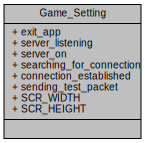
\includegraphics[width=217pt]{structGame__Setting__coll__graph}
\end{center}
\end{figure}
\subsection*{Public Attributes}
\begin{DoxyCompactItemize}
\item 
bool \hyperlink{structGame__Setting_abe1e4e29aba1c9526c96fb3753d6750a}{exit\+\_\+app}
\item 
bool \hyperlink{structGame__Setting_ad9cbe44a8dd0b9bc059344479b2705a4}{server\+\_\+listening}
\item 
bool \hyperlink{structGame__Setting_a89ec65a311660f2c4cac49a1905d1d86}{server\+\_\+on}
\item 
bool \hyperlink{structGame__Setting_a9c411038e08c0bbbec1ec7f9ee42cf10}{searching\+\_\+for\+\_\+connection}
\item 
bool \hyperlink{structGame__Setting_a81a3166bc6bc27b49b3f6ae1bf6a1a11}{connection\+\_\+established}
\item 
bool \hyperlink{structGame__Setting_a2d778c2c0f89e179a1b75f1b587aa643}{sending\+\_\+test\+\_\+packet}
\item 
const unsigned int \hyperlink{structGame__Setting_adff1136dc3fef8223f57720d836c270d}{S\+C\+R\+\_\+\+W\+I\+D\+TH} = 800
\item 
const unsigned int \hyperlink{structGame__Setting_a4ce77601943647de2ab90532987073de}{S\+C\+R\+\_\+\+H\+E\+I\+G\+HT} = 600
\end{DoxyCompactItemize}


\subsection{Member Data Documentation}
\mbox{\Hypertarget{structGame__Setting_a81a3166bc6bc27b49b3f6ae1bf6a1a11}\label{structGame__Setting_a81a3166bc6bc27b49b3f6ae1bf6a1a11}} 
\index{Game\+\_\+\+Setting@{Game\+\_\+\+Setting}!connection\+\_\+established@{connection\+\_\+established}}
\index{connection\+\_\+established@{connection\+\_\+established}!Game\+\_\+\+Setting@{Game\+\_\+\+Setting}}
\subsubsection{\texorpdfstring{connection\+\_\+established}{connection\_established}}
{\footnotesize\ttfamily bool Game\+\_\+\+Setting\+::connection\+\_\+established}

\mbox{\Hypertarget{structGame__Setting_abe1e4e29aba1c9526c96fb3753d6750a}\label{structGame__Setting_abe1e4e29aba1c9526c96fb3753d6750a}} 
\index{Game\+\_\+\+Setting@{Game\+\_\+\+Setting}!exit\+\_\+app@{exit\+\_\+app}}
\index{exit\+\_\+app@{exit\+\_\+app}!Game\+\_\+\+Setting@{Game\+\_\+\+Setting}}
\subsubsection{\texorpdfstring{exit\+\_\+app}{exit\_app}}
{\footnotesize\ttfamily bool Game\+\_\+\+Setting\+::exit\+\_\+app}

\mbox{\Hypertarget{structGame__Setting_a4ce77601943647de2ab90532987073de}\label{structGame__Setting_a4ce77601943647de2ab90532987073de}} 
\index{Game\+\_\+\+Setting@{Game\+\_\+\+Setting}!S\+C\+R\+\_\+\+H\+E\+I\+G\+HT@{S\+C\+R\+\_\+\+H\+E\+I\+G\+HT}}
\index{S\+C\+R\+\_\+\+H\+E\+I\+G\+HT@{S\+C\+R\+\_\+\+H\+E\+I\+G\+HT}!Game\+\_\+\+Setting@{Game\+\_\+\+Setting}}
\subsubsection{\texorpdfstring{S\+C\+R\+\_\+\+H\+E\+I\+G\+HT}{SCR\_HEIGHT}}
{\footnotesize\ttfamily const unsigned int Game\+\_\+\+Setting\+::\+S\+C\+R\+\_\+\+H\+E\+I\+G\+HT = 600}

\mbox{\Hypertarget{structGame__Setting_adff1136dc3fef8223f57720d836c270d}\label{structGame__Setting_adff1136dc3fef8223f57720d836c270d}} 
\index{Game\+\_\+\+Setting@{Game\+\_\+\+Setting}!S\+C\+R\+\_\+\+W\+I\+D\+TH@{S\+C\+R\+\_\+\+W\+I\+D\+TH}}
\index{S\+C\+R\+\_\+\+W\+I\+D\+TH@{S\+C\+R\+\_\+\+W\+I\+D\+TH}!Game\+\_\+\+Setting@{Game\+\_\+\+Setting}}
\subsubsection{\texorpdfstring{S\+C\+R\+\_\+\+W\+I\+D\+TH}{SCR\_WIDTH}}
{\footnotesize\ttfamily const unsigned int Game\+\_\+\+Setting\+::\+S\+C\+R\+\_\+\+W\+I\+D\+TH = 800}

\mbox{\Hypertarget{structGame__Setting_a9c411038e08c0bbbec1ec7f9ee42cf10}\label{structGame__Setting_a9c411038e08c0bbbec1ec7f9ee42cf10}} 
\index{Game\+\_\+\+Setting@{Game\+\_\+\+Setting}!searching\+\_\+for\+\_\+connection@{searching\+\_\+for\+\_\+connection}}
\index{searching\+\_\+for\+\_\+connection@{searching\+\_\+for\+\_\+connection}!Game\+\_\+\+Setting@{Game\+\_\+\+Setting}}
\subsubsection{\texorpdfstring{searching\+\_\+for\+\_\+connection}{searching\_for\_connection}}
{\footnotesize\ttfamily bool Game\+\_\+\+Setting\+::searching\+\_\+for\+\_\+connection}

\mbox{\Hypertarget{structGame__Setting_a2d778c2c0f89e179a1b75f1b587aa643}\label{structGame__Setting_a2d778c2c0f89e179a1b75f1b587aa643}} 
\index{Game\+\_\+\+Setting@{Game\+\_\+\+Setting}!sending\+\_\+test\+\_\+packet@{sending\+\_\+test\+\_\+packet}}
\index{sending\+\_\+test\+\_\+packet@{sending\+\_\+test\+\_\+packet}!Game\+\_\+\+Setting@{Game\+\_\+\+Setting}}
\subsubsection{\texorpdfstring{sending\+\_\+test\+\_\+packet}{sending\_test\_packet}}
{\footnotesize\ttfamily bool Game\+\_\+\+Setting\+::sending\+\_\+test\+\_\+packet}

\mbox{\Hypertarget{structGame__Setting_ad9cbe44a8dd0b9bc059344479b2705a4}\label{structGame__Setting_ad9cbe44a8dd0b9bc059344479b2705a4}} 
\index{Game\+\_\+\+Setting@{Game\+\_\+\+Setting}!server\+\_\+listening@{server\+\_\+listening}}
\index{server\+\_\+listening@{server\+\_\+listening}!Game\+\_\+\+Setting@{Game\+\_\+\+Setting}}
\subsubsection{\texorpdfstring{server\+\_\+listening}{server\_listening}}
{\footnotesize\ttfamily bool Game\+\_\+\+Setting\+::server\+\_\+listening}

\mbox{\Hypertarget{structGame__Setting_a89ec65a311660f2c4cac49a1905d1d86}\label{structGame__Setting_a89ec65a311660f2c4cac49a1905d1d86}} 
\index{Game\+\_\+\+Setting@{Game\+\_\+\+Setting}!server\+\_\+on@{server\+\_\+on}}
\index{server\+\_\+on@{server\+\_\+on}!Game\+\_\+\+Setting@{Game\+\_\+\+Setting}}
\subsubsection{\texorpdfstring{server\+\_\+on}{server\_on}}
{\footnotesize\ttfamily bool Game\+\_\+\+Setting\+::server\+\_\+on}



The documentation for this struct was generated from the following file\+:\begin{DoxyCompactItemize}
\item 
/mnt/hdd/fnky/\+C0de/\+C\+A\+P\+S\+T\+O\+N\+E/clean\+\_\+build/include/\+Game\+Data/\hyperlink{GameData_8h}{Game\+Data.\+h}\end{DoxyCompactItemize}

\hypertarget{structGameData}{}\section{Game\+Data Struct Reference}
\label{structGameData}\index{Game\+Data@{Game\+Data}}


{\ttfamily \#include $<$Game\+Data.\+h$>$}



Collaboration diagram for Game\+Data\+:
\nopagebreak
\begin{figure}[H]
\begin{center}
\leavevmode
\includegraphics[width=350pt]{structGameData__coll__graph}
\end{center}
\end{figure}
\subsection*{Public Member Functions}
\begin{DoxyCompactItemize}
\item 
\hyperlink{structGameData_a67ab18c5a35df618e99983275c7552ab}{Game\+Data} ()
\item 
\hyperlink{structGameData_a943bccfc17785aff39f0fceb643a5f9d}{Game\+Data} (const \hyperlink{structGameData}{Game\+Data} \&game\+Data)
\item 
\hyperlink{structGameData_a2a34c148fd6e7fbf9d3f3e3cc6c4e675}{Game\+Data} (\hyperlink{structGameData}{Game\+Data} \&\&move\+Data) noexcept
\item 
\hyperlink{structGameData_abd51e710bc262e278a8895f2e0b35a9f}{$\sim$\+Game\+Data} ()
\end{DoxyCompactItemize}
\subsection*{Public Attributes}
\begin{DoxyCompactItemize}
\item 
G\+L\+F\+Wwindow $\ast$ \hyperlink{structGameData_af9735787501e4c8c1d26787c322cd6dd}{window}
\item 
\hyperlink{classStateMachine}{State\+Machine} $\ast$ \hyperlink{structGameData_a22d18ba95d18acdf0e77c8c1591c1ec7}{machine}
\item 
\hyperlink{classOrthographic__camera}{Orthographic\+\_\+camera} $\ast$ \hyperlink{structGameData_a9e133f6b5e0d19889e94505db479ca69}{o\+\_\+cam}
\item 
b2\+World $\ast$ \hyperlink{structGameData_a937e7f0334daf0f54ae28d7b92e7cca6}{world}
\item 
\hyperlink{classLoadingGameObjects}{Loading\+Game\+Objects} $\ast$ \hyperlink{structGameData_aaaddd2c1ea34ab4acc9a732879fd92ab}{ld}
\item 
\hyperlink{GameData_8h_a808e5cd4979462d3bbe3070d7d147444}{States} \hyperlink{structGameData_a210154898f11f1d892bd37644290af74}{state\+\_\+switch}
\item 
\hyperlink{GameData_8h_ae06cf0c67532073a49f95f03488d29bf}{Levels} \hyperlink{structGameData_a3dab533c5379ac113066c439f7218967}{level}
\item 
\hyperlink{structPlayer__Data}{Player\+\_\+\+Data} \hyperlink{structGameData_a698738ca3ba6be3f74700c589c63fb3d}{pd}
\item 
\hyperlink{structGame__Setting}{Game\+\_\+\+Setting} \hyperlink{structGameData_ad425129b9abf553f835bf54dd21cd2e5}{gs}
\end{DoxyCompactItemize}


\subsection{Constructor \& Destructor Documentation}
\mbox{\Hypertarget{structGameData_a67ab18c5a35df618e99983275c7552ab}\label{structGameData_a67ab18c5a35df618e99983275c7552ab}} 
\index{Game\+Data@{Game\+Data}!Game\+Data@{Game\+Data}}
\index{Game\+Data@{Game\+Data}!Game\+Data@{Game\+Data}}
\subsubsection{\texorpdfstring{Game\+Data()}{GameData()}\hspace{0.1cm}{\footnotesize\ttfamily [1/3]}}
{\footnotesize\ttfamily Game\+Data\+::\+Game\+Data (\begin{DoxyParamCaption}{ }\end{DoxyParamCaption})\hspace{0.3cm}{\ttfamily [inline]}}

\mbox{\Hypertarget{structGameData_a943bccfc17785aff39f0fceb643a5f9d}\label{structGameData_a943bccfc17785aff39f0fceb643a5f9d}} 
\index{Game\+Data@{Game\+Data}!Game\+Data@{Game\+Data}}
\index{Game\+Data@{Game\+Data}!Game\+Data@{Game\+Data}}
\subsubsection{\texorpdfstring{Game\+Data()}{GameData()}\hspace{0.1cm}{\footnotesize\ttfamily [2/3]}}
{\footnotesize\ttfamily Game\+Data\+::\+Game\+Data (\begin{DoxyParamCaption}\item[{const \hyperlink{structGameData}{Game\+Data} \&}]{game\+Data }\end{DoxyParamCaption})\hspace{0.3cm}{\ttfamily [inline]}}

\mbox{\Hypertarget{structGameData_a2a34c148fd6e7fbf9d3f3e3cc6c4e675}\label{structGameData_a2a34c148fd6e7fbf9d3f3e3cc6c4e675}} 
\index{Game\+Data@{Game\+Data}!Game\+Data@{Game\+Data}}
\index{Game\+Data@{Game\+Data}!Game\+Data@{Game\+Data}}
\subsubsection{\texorpdfstring{Game\+Data()}{GameData()}\hspace{0.1cm}{\footnotesize\ttfamily [3/3]}}
{\footnotesize\ttfamily Game\+Data\+::\+Game\+Data (\begin{DoxyParamCaption}\item[{\hyperlink{structGameData}{Game\+Data} \&\&}]{move\+Data }\end{DoxyParamCaption})\hspace{0.3cm}{\ttfamily [inline]}, {\ttfamily [noexcept]}}

\mbox{\Hypertarget{structGameData_abd51e710bc262e278a8895f2e0b35a9f}\label{structGameData_abd51e710bc262e278a8895f2e0b35a9f}} 
\index{Game\+Data@{Game\+Data}!````~Game\+Data@{$\sim$\+Game\+Data}}
\index{````~Game\+Data@{$\sim$\+Game\+Data}!Game\+Data@{Game\+Data}}
\subsubsection{\texorpdfstring{$\sim$\+Game\+Data()}{~GameData()}}
{\footnotesize\ttfamily Game\+Data\+::$\sim$\+Game\+Data (\begin{DoxyParamCaption}{ }\end{DoxyParamCaption})\hspace{0.3cm}{\ttfamily [inline]}}



\subsection{Member Data Documentation}
\mbox{\Hypertarget{structGameData_ad425129b9abf553f835bf54dd21cd2e5}\label{structGameData_ad425129b9abf553f835bf54dd21cd2e5}} 
\index{Game\+Data@{Game\+Data}!gs@{gs}}
\index{gs@{gs}!Game\+Data@{Game\+Data}}
\subsubsection{\texorpdfstring{gs}{gs}}
{\footnotesize\ttfamily \hyperlink{structGame__Setting}{Game\+\_\+\+Setting} Game\+Data\+::gs}

\mbox{\Hypertarget{structGameData_aaaddd2c1ea34ab4acc9a732879fd92ab}\label{structGameData_aaaddd2c1ea34ab4acc9a732879fd92ab}} 
\index{Game\+Data@{Game\+Data}!ld@{ld}}
\index{ld@{ld}!Game\+Data@{Game\+Data}}
\subsubsection{\texorpdfstring{ld}{ld}}
{\footnotesize\ttfamily \hyperlink{classLoadingGameObjects}{Loading\+Game\+Objects}$\ast$ Game\+Data\+::ld}

\mbox{\Hypertarget{structGameData_a3dab533c5379ac113066c439f7218967}\label{structGameData_a3dab533c5379ac113066c439f7218967}} 
\index{Game\+Data@{Game\+Data}!level@{level}}
\index{level@{level}!Game\+Data@{Game\+Data}}
\subsubsection{\texorpdfstring{level}{level}}
{\footnotesize\ttfamily \hyperlink{GameData_8h_ae06cf0c67532073a49f95f03488d29bf}{Levels} Game\+Data\+::level}

\mbox{\Hypertarget{structGameData_a22d18ba95d18acdf0e77c8c1591c1ec7}\label{structGameData_a22d18ba95d18acdf0e77c8c1591c1ec7}} 
\index{Game\+Data@{Game\+Data}!machine@{machine}}
\index{machine@{machine}!Game\+Data@{Game\+Data}}
\subsubsection{\texorpdfstring{machine}{machine}}
{\footnotesize\ttfamily \hyperlink{classStateMachine}{State\+Machine}$\ast$ Game\+Data\+::machine}

\mbox{\Hypertarget{structGameData_a9e133f6b5e0d19889e94505db479ca69}\label{structGameData_a9e133f6b5e0d19889e94505db479ca69}} 
\index{Game\+Data@{Game\+Data}!o\+\_\+cam@{o\+\_\+cam}}
\index{o\+\_\+cam@{o\+\_\+cam}!Game\+Data@{Game\+Data}}
\subsubsection{\texorpdfstring{o\+\_\+cam}{o\_cam}}
{\footnotesize\ttfamily \hyperlink{classOrthographic__camera}{Orthographic\+\_\+camera}$\ast$ Game\+Data\+::o\+\_\+cam}

\mbox{\Hypertarget{structGameData_a698738ca3ba6be3f74700c589c63fb3d}\label{structGameData_a698738ca3ba6be3f74700c589c63fb3d}} 
\index{Game\+Data@{Game\+Data}!pd@{pd}}
\index{pd@{pd}!Game\+Data@{Game\+Data}}
\subsubsection{\texorpdfstring{pd}{pd}}
{\footnotesize\ttfamily \hyperlink{structPlayer__Data}{Player\+\_\+\+Data} Game\+Data\+::pd}

\mbox{\Hypertarget{structGameData_a210154898f11f1d892bd37644290af74}\label{structGameData_a210154898f11f1d892bd37644290af74}} 
\index{Game\+Data@{Game\+Data}!state\+\_\+switch@{state\+\_\+switch}}
\index{state\+\_\+switch@{state\+\_\+switch}!Game\+Data@{Game\+Data}}
\subsubsection{\texorpdfstring{state\+\_\+switch}{state\_switch}}
{\footnotesize\ttfamily \hyperlink{GameData_8h_a808e5cd4979462d3bbe3070d7d147444}{States} Game\+Data\+::state\+\_\+switch}

\mbox{\Hypertarget{structGameData_af9735787501e4c8c1d26787c322cd6dd}\label{structGameData_af9735787501e4c8c1d26787c322cd6dd}} 
\index{Game\+Data@{Game\+Data}!window@{window}}
\index{window@{window}!Game\+Data@{Game\+Data}}
\subsubsection{\texorpdfstring{window}{window}}
{\footnotesize\ttfamily G\+L\+F\+Wwindow$\ast$ Game\+Data\+::window}

\mbox{\Hypertarget{structGameData_a937e7f0334daf0f54ae28d7b92e7cca6}\label{structGameData_a937e7f0334daf0f54ae28d7b92e7cca6}} 
\index{Game\+Data@{Game\+Data}!world@{world}}
\index{world@{world}!Game\+Data@{Game\+Data}}
\subsubsection{\texorpdfstring{world}{world}}
{\footnotesize\ttfamily b2\+World$\ast$ Game\+Data\+::world}



The documentation for this struct was generated from the following file\+:\begin{DoxyCompactItemize}
\item 
/mnt/hdd/fnky/\+C0de/\+C\+A\+P\+S\+T\+O\+N\+E/clean\+\_\+build/include/\+Game\+Data/\hyperlink{GameData_8h}{Game\+Data.\+h}\end{DoxyCompactItemize}

\hypertarget{classGameOverState}{}\doxysection{Game\+Over\+State Class Reference}
\label{classGameOverState}\index{GameOverState@{GameOverState}}


{\ttfamily \#include $<$game\+\_\+over\+\_\+state.\+h$>$}



Inheritance diagram for Game\+Over\+State\+:
\nopagebreak
\begin{figure}[H]
\begin{center}
\leavevmode
\includegraphics[width=202pt]{classGameOverState__inherit__graph}
\end{center}
\end{figure}


Collaboration diagram for Game\+Over\+State\+:
\nopagebreak
\begin{figure}[H]
\begin{center}
\leavevmode
\includegraphics[width=350pt]{classGameOverState__coll__graph}
\end{center}
\end{figure}
\doxysubsection*{Public Member Functions}
\begin{DoxyCompactItemize}
\item 
\mbox{\hyperlink{classGameOverState_aa96fa2d6ec8131c6295ef8ae189b5dc1}{Game\+Over\+State}} (\mbox{\hyperlink{structGameData}{Game\+Data}} \&\mbox{\hyperlink{imgui__impl__opengl3__loader_8h_abd87654504355b4c1bb002dcb1d4d16a}{data}})
\item 
\mbox{\hyperlink{imgui__impl__opengl3__loader_8h_ac668e7cffd9e2e9cfee428b9b2f34fa7}{void}} \mbox{\hyperlink{classGameOverState_aa3d4f165ff735552f16132e929d369c2}{Init}} ()
\item 
\mbox{\hyperlink{imgui__impl__opengl3__loader_8h_ac668e7cffd9e2e9cfee428b9b2f34fa7}{void}} \mbox{\hyperlink{classGameOverState_adb4be2a5c6292d020999c2da9588ebfc}{Input}} (float delta)
\item 
\mbox{\hyperlink{imgui__impl__opengl3__loader_8h_ac668e7cffd9e2e9cfee428b9b2f34fa7}{void}} \mbox{\hyperlink{classGameOverState_a4dc49d576a9435531f502660119800a9}{Update}} (float delta)
\item 
\mbox{\hyperlink{imgui__impl__opengl3__loader_8h_ac668e7cffd9e2e9cfee428b9b2f34fa7}{void}} \mbox{\hyperlink{classGameOverState_ac9c9ef71b0a12940ac5caa7763f23fdc}{Render}} (float delta)
\item 
\mbox{\hyperlink{imgui__impl__opengl3__loader_8h_ac668e7cffd9e2e9cfee428b9b2f34fa7}{void}} \mbox{\hyperlink{classGameOverState_ab46f47037abd1eeabdbff49f8dfb802b}{Sound\+Update}} ()
\item 
\mbox{\hyperlink{imgui__impl__opengl3__loader_8h_ac668e7cffd9e2e9cfee428b9b2f34fa7}{void}} \mbox{\hyperlink{classGameOverState_afb6fa68ff0c5e4f83725de8059c4f7c8}{Delete\+Data}} ()
\item 
\mbox{\hyperlink{classGameOverState_a6450295ac3a2d64a19bdfe1ad70aacad}{$\sim$\+Game\+Over\+State}} ()
\end{DoxyCompactItemize}
\doxysubsection*{Private Attributes}
\begin{DoxyCompactItemize}
\item 
\mbox{\hyperlink{structGameData}{Game\+Data}} $\ast$ \mbox{\hyperlink{classGameOverState_a1df24a620531ad2a7ebfca275725c2ea}{\+\_\+data}}
\item 
float \mbox{\hyperlink{classGameOverState_a1069a15743773be39ec300b0ed826495}{x\+\_\+cam}}
\item 
float \mbox{\hyperlink{classGameOverState_a1e25279faab5b2551102ef39aa815e2f}{y\+\_\+cam}}
\item 
float \mbox{\hyperlink{classGameOverState_a81afb5a04a07d3697edfc66063154362}{z\+\_\+cam}}
\item 
float \mbox{\hyperlink{classGameOverState_a53e39df9000ba7f88cd8d3beb151e86c}{r\+\_\+cam}}
\item 
glm\+::vec2 \mbox{\hyperlink{classGameOverState_a9b5f78804f2ec06ade38c0e69560f9b4}{z\+\_\+scale}}
\end{DoxyCompactItemize}


\doxysubsection{Constructor \& Destructor Documentation}
\mbox{\Hypertarget{classGameOverState_aa96fa2d6ec8131c6295ef8ae189b5dc1}\label{classGameOverState_aa96fa2d6ec8131c6295ef8ae189b5dc1}} 
\index{GameOverState@{GameOverState}!GameOverState@{GameOverState}}
\index{GameOverState@{GameOverState}!GameOverState@{GameOverState}}
\doxysubsubsection{\texorpdfstring{GameOverState()}{GameOverState()}}
{\footnotesize\ttfamily Game\+Over\+State\+::\+Game\+Over\+State (\begin{DoxyParamCaption}\item[{\mbox{\hyperlink{structGameData}{Game\+Data}} \&}]{data }\end{DoxyParamCaption})}

\mbox{\Hypertarget{classGameOverState_a6450295ac3a2d64a19bdfe1ad70aacad}\label{classGameOverState_a6450295ac3a2d64a19bdfe1ad70aacad}} 
\index{GameOverState@{GameOverState}!````~GameOverState@{$\sim$GameOverState}}
\index{````~GameOverState@{$\sim$GameOverState}!GameOverState@{GameOverState}}
\doxysubsubsection{\texorpdfstring{$\sim$GameOverState()}{~GameOverState()}}
{\footnotesize\ttfamily Game\+Over\+State\+::$\sim$\+Game\+Over\+State (\begin{DoxyParamCaption}{ }\end{DoxyParamCaption})}



\doxysubsection{Member Function Documentation}
\mbox{\Hypertarget{classGameOverState_afb6fa68ff0c5e4f83725de8059c4f7c8}\label{classGameOverState_afb6fa68ff0c5e4f83725de8059c4f7c8}} 
\index{GameOverState@{GameOverState}!DeleteData@{DeleteData}}
\index{DeleteData@{DeleteData}!GameOverState@{GameOverState}}
\doxysubsubsection{\texorpdfstring{DeleteData()}{DeleteData()}}
{\footnotesize\ttfamily \mbox{\hyperlink{imgui__impl__opengl3__loader_8h_ac668e7cffd9e2e9cfee428b9b2f34fa7}{void}} Game\+Over\+State\+::\+Delete\+Data (\begin{DoxyParamCaption}{ }\end{DoxyParamCaption})\hspace{0.3cm}{\ttfamily [virtual]}}



Implements \mbox{\hyperlink{classState_ade502eaa386d570e526eb356ffd73fd8}{State}}.

\mbox{\Hypertarget{classGameOverState_aa3d4f165ff735552f16132e929d369c2}\label{classGameOverState_aa3d4f165ff735552f16132e929d369c2}} 
\index{GameOverState@{GameOverState}!Init@{Init}}
\index{Init@{Init}!GameOverState@{GameOverState}}
\doxysubsubsection{\texorpdfstring{Init()}{Init()}}
{\footnotesize\ttfamily \mbox{\hyperlink{imgui__impl__opengl3__loader_8h_ac668e7cffd9e2e9cfee428b9b2f34fa7}{void}} Game\+Over\+State\+::\+Init (\begin{DoxyParamCaption}{ }\end{DoxyParamCaption})\hspace{0.3cm}{\ttfamily [virtual]}}



Implements \mbox{\hyperlink{classState_a7ab4d8c6aa239a17ed579d89a209b156}{State}}.

\mbox{\Hypertarget{classGameOverState_adb4be2a5c6292d020999c2da9588ebfc}\label{classGameOverState_adb4be2a5c6292d020999c2da9588ebfc}} 
\index{GameOverState@{GameOverState}!Input@{Input}}
\index{Input@{Input}!GameOverState@{GameOverState}}
\doxysubsubsection{\texorpdfstring{Input()}{Input()}}
{\footnotesize\ttfamily \mbox{\hyperlink{imgui__impl__opengl3__loader_8h_ac668e7cffd9e2e9cfee428b9b2f34fa7}{void}} Game\+Over\+State\+::\+Input (\begin{DoxyParamCaption}\item[{float}]{delta }\end{DoxyParamCaption})\hspace{0.3cm}{\ttfamily [virtual]}}



Implements \mbox{\hyperlink{classState_a1705412877f37a5cc8fc712542756076}{State}}.

\mbox{\Hypertarget{classGameOverState_ac9c9ef71b0a12940ac5caa7763f23fdc}\label{classGameOverState_ac9c9ef71b0a12940ac5caa7763f23fdc}} 
\index{GameOverState@{GameOverState}!Render@{Render}}
\index{Render@{Render}!GameOverState@{GameOverState}}
\doxysubsubsection{\texorpdfstring{Render()}{Render()}}
{\footnotesize\ttfamily \mbox{\hyperlink{imgui__impl__opengl3__loader_8h_ac668e7cffd9e2e9cfee428b9b2f34fa7}{void}} Game\+Over\+State\+::\+Render (\begin{DoxyParamCaption}\item[{float}]{delta }\end{DoxyParamCaption})\hspace{0.3cm}{\ttfamily [virtual]}}



Implements \mbox{\hyperlink{classState_a0e48dfae1e3090630475812681417c5f}{State}}.

\mbox{\Hypertarget{classGameOverState_ab46f47037abd1eeabdbff49f8dfb802b}\label{classGameOverState_ab46f47037abd1eeabdbff49f8dfb802b}} 
\index{GameOverState@{GameOverState}!SoundUpdate@{SoundUpdate}}
\index{SoundUpdate@{SoundUpdate}!GameOverState@{GameOverState}}
\doxysubsubsection{\texorpdfstring{SoundUpdate()}{SoundUpdate()}}
{\footnotesize\ttfamily \mbox{\hyperlink{imgui__impl__opengl3__loader_8h_ac668e7cffd9e2e9cfee428b9b2f34fa7}{void}} Game\+Over\+State\+::\+Sound\+Update (\begin{DoxyParamCaption}{ }\end{DoxyParamCaption})\hspace{0.3cm}{\ttfamily [virtual]}}



Implements \mbox{\hyperlink{classState_a6572089fbf2178bf5c582cc27d6d3925}{State}}.

\mbox{\Hypertarget{classGameOverState_a4dc49d576a9435531f502660119800a9}\label{classGameOverState_a4dc49d576a9435531f502660119800a9}} 
\index{GameOverState@{GameOverState}!Update@{Update}}
\index{Update@{Update}!GameOverState@{GameOverState}}
\doxysubsubsection{\texorpdfstring{Update()}{Update()}}
{\footnotesize\ttfamily \mbox{\hyperlink{imgui__impl__opengl3__loader_8h_ac668e7cffd9e2e9cfee428b9b2f34fa7}{void}} Game\+Over\+State\+::\+Update (\begin{DoxyParamCaption}\item[{float}]{delta }\end{DoxyParamCaption})\hspace{0.3cm}{\ttfamily [virtual]}}



Implements \mbox{\hyperlink{classState_aac0d3fdee1341e168af730b8f31a7bf1}{State}}.



\doxysubsection{Member Data Documentation}
\mbox{\Hypertarget{classGameOverState_a1df24a620531ad2a7ebfca275725c2ea}\label{classGameOverState_a1df24a620531ad2a7ebfca275725c2ea}} 
\index{GameOverState@{GameOverState}!\_data@{\_data}}
\index{\_data@{\_data}!GameOverState@{GameOverState}}
\doxysubsubsection{\texorpdfstring{\_data}{\_data}}
{\footnotesize\ttfamily \mbox{\hyperlink{structGameData}{Game\+Data}}$\ast$ Game\+Over\+State\+::\+\_\+data\hspace{0.3cm}{\ttfamily [private]}}

\mbox{\Hypertarget{classGameOverState_a53e39df9000ba7f88cd8d3beb151e86c}\label{classGameOverState_a53e39df9000ba7f88cd8d3beb151e86c}} 
\index{GameOverState@{GameOverState}!r\_cam@{r\_cam}}
\index{r\_cam@{r\_cam}!GameOverState@{GameOverState}}
\doxysubsubsection{\texorpdfstring{r\_cam}{r\_cam}}
{\footnotesize\ttfamily float Game\+Over\+State\+::r\+\_\+cam\hspace{0.3cm}{\ttfamily [private]}}

\mbox{\Hypertarget{classGameOverState_a1069a15743773be39ec300b0ed826495}\label{classGameOverState_a1069a15743773be39ec300b0ed826495}} 
\index{GameOverState@{GameOverState}!x\_cam@{x\_cam}}
\index{x\_cam@{x\_cam}!GameOverState@{GameOverState}}
\doxysubsubsection{\texorpdfstring{x\_cam}{x\_cam}}
{\footnotesize\ttfamily float Game\+Over\+State\+::x\+\_\+cam\hspace{0.3cm}{\ttfamily [private]}}

\mbox{\Hypertarget{classGameOverState_a1e25279faab5b2551102ef39aa815e2f}\label{classGameOverState_a1e25279faab5b2551102ef39aa815e2f}} 
\index{GameOverState@{GameOverState}!y\_cam@{y\_cam}}
\index{y\_cam@{y\_cam}!GameOverState@{GameOverState}}
\doxysubsubsection{\texorpdfstring{y\_cam}{y\_cam}}
{\footnotesize\ttfamily float Game\+Over\+State\+::y\+\_\+cam\hspace{0.3cm}{\ttfamily [private]}}

\mbox{\Hypertarget{classGameOverState_a81afb5a04a07d3697edfc66063154362}\label{classGameOverState_a81afb5a04a07d3697edfc66063154362}} 
\index{GameOverState@{GameOverState}!z\_cam@{z\_cam}}
\index{z\_cam@{z\_cam}!GameOverState@{GameOverState}}
\doxysubsubsection{\texorpdfstring{z\_cam}{z\_cam}}
{\footnotesize\ttfamily float Game\+Over\+State\+::z\+\_\+cam\hspace{0.3cm}{\ttfamily [private]}}

\mbox{\Hypertarget{classGameOverState_a9b5f78804f2ec06ade38c0e69560f9b4}\label{classGameOverState_a9b5f78804f2ec06ade38c0e69560f9b4}} 
\index{GameOverState@{GameOverState}!z\_scale@{z\_scale}}
\index{z\_scale@{z\_scale}!GameOverState@{GameOverState}}
\doxysubsubsection{\texorpdfstring{z\_scale}{z\_scale}}
{\footnotesize\ttfamily glm\+::vec2 Game\+Over\+State\+::z\+\_\+scale\hspace{0.3cm}{\ttfamily [private]}}



The documentation for this class was generated from the following files\+:\begin{DoxyCompactItemize}
\item 
/home/fnky/\+C0de/component\+\_\+engine/include/\+States/\mbox{\hyperlink{game__over__state_8h}{game\+\_\+over\+\_\+state.\+h}}\item 
/home/fnky/\+C0de/component\+\_\+engine/src/\+States/\mbox{\hyperlink{game__over__state_8cpp}{game\+\_\+over\+\_\+state.\+cpp}}\end{DoxyCompactItemize}

\hypertarget{classGamePlayState}{}\doxysection{Game\+Play\+State Class Reference}
\label{classGamePlayState}\index{GamePlayState@{GamePlayState}}


{\ttfamily \#include $<$game\+\_\+play\+\_\+state.\+h$>$}



Inheritance diagram for Game\+Play\+State\+:
\nopagebreak
\begin{figure}[H]
\begin{center}
\leavevmode
\includegraphics[width=199pt]{classGamePlayState__inherit__graph}
\end{center}
\end{figure}


Collaboration diagram for Game\+Play\+State\+:
\nopagebreak
\begin{figure}[H]
\begin{center}
\leavevmode
\includegraphics[height=550pt]{classGamePlayState__coll__graph}
\end{center}
\end{figure}
\doxysubsection*{Public Member Functions}
\begin{DoxyCompactItemize}
\item 
\mbox{\hyperlink{classGamePlayState_ab20bfae56acce9a61770ec97a27ecd73}{Game\+Play\+State}} (\mbox{\hyperlink{structGameData}{Game\+Data}} \&\mbox{\hyperlink{imgui__impl__opengl3__loader_8h_abd87654504355b4c1bb002dcb1d4d16a}{data}})
\item 
\mbox{\hyperlink{imgui__impl__opengl3__loader_8h_ac668e7cffd9e2e9cfee428b9b2f34fa7}{void}} \mbox{\hyperlink{classGamePlayState_ae13389eea1f83f27d18ba200f107937d}{Init}} ()
\item 
\mbox{\hyperlink{imgui__impl__opengl3__loader_8h_ac668e7cffd9e2e9cfee428b9b2f34fa7}{void}} \mbox{\hyperlink{classGamePlayState_a3bc9231fd11546b5dd13581ed2aa1afa}{Input}} (float delta)
\item 
\mbox{\hyperlink{imgui__impl__opengl3__loader_8h_ac668e7cffd9e2e9cfee428b9b2f34fa7}{void}} \mbox{\hyperlink{classGamePlayState_a19bcc1ff2a83a3aa001010ae35d67b85}{Update}} (float delta)
\item 
\mbox{\hyperlink{imgui__impl__opengl3__loader_8h_ac668e7cffd9e2e9cfee428b9b2f34fa7}{void}} \mbox{\hyperlink{classGamePlayState_a4bd296aa04088a3d8249f569e86f21a7}{Render}} (float delta)
\item 
\mbox{\hyperlink{imgui__impl__opengl3__loader_8h_ac668e7cffd9e2e9cfee428b9b2f34fa7}{void}} \mbox{\hyperlink{classGamePlayState_a3367714db85b4d59a52bc1d8b0828d3c}{Sound\+Update}} ()
\item 
\mbox{\hyperlink{imgui__impl__opengl3__loader_8h_ac668e7cffd9e2e9cfee428b9b2f34fa7}{void}} \mbox{\hyperlink{classGamePlayState_a8a393249f2deabe0fe8f236b4e58cb17}{Delete\+Data}} ()
\item 
\mbox{\hyperlink{classGamePlayState_aaa1afd5f6e091e5cb5bda2fa82247d58}{$\sim$\+Game\+Play\+State}} ()
\end{DoxyCompactItemize}
\doxysubsection*{Private Attributes}
\begin{DoxyCompactItemize}
\item 
\mbox{\hyperlink{structGameData}{Game\+Data}} $\ast$ \mbox{\hyperlink{classGamePlayState_a0e1217ba99e0bb8098e73ebaa99bdc77}{\+\_\+data}}
\item 
float \mbox{\hyperlink{classGamePlayState_a055feaf3b4acaaff53dddc571252c4e4}{x}}
\item 
float \mbox{\hyperlink{classGamePlayState_ae1da324a3664591e663d09a5b17f9007}{y}}
\item 
float \mbox{\hyperlink{classGamePlayState_a1f0c5c88f94177891ec0819628d0aa8c}{x\+\_\+cam}}
\item 
float \mbox{\hyperlink{classGamePlayState_ab69b90dcdbb3375687e6e3641d1654da}{y\+\_\+cam}}
\item 
float \mbox{\hyperlink{classGamePlayState_a3b25b85d41324ec556fe81a75bb1811f}{z\+\_\+cam}}
\item 
float \mbox{\hyperlink{classGamePlayState_a430ff4098f9f58fe0b6ab4fe154a89a0}{r\+\_\+cam}}
\item 
glm\+::vec2 \mbox{\hyperlink{classGamePlayState_a9bdc2e5899e9ca4e266019f646d2ba34}{z\+\_\+scale}}
\item 
double \mbox{\hyperlink{classGamePlayState_a28703a4a41c15f3957f76f8ffcdad4f3}{delay}}
\item 
double \mbox{\hyperlink{classGamePlayState_a4a4caf8b02f0dbac194c18947bf84ba6}{jump\+\_\+delay}}
\item 
float \mbox{\hyperlink{classGamePlayState_a739fbcc19589d3b2218664832fd864fe}{counter}}
\item 
uint16\+\_\+t \mbox{\hyperlink{classGamePlayState_ae6d97fab3b6d39625b5ce3d124183c56}{platform\+\_\+delay}} = 0
\item 
bool \mbox{\hyperlink{classGamePlayState_ae17620bd80a3c92dea5bdbde326535ea}{reached\+Pos}} = false
\item 
bool \mbox{\hyperlink{classGamePlayState_a0b574d8b2807e3229e51ec16bc5b74a6}{prev\+Pos}} = true
\item 
int \mbox{\hyperlink{classGamePlayState_a911170373ef52829b49f5466dcfbc539}{x\+\_\+pos}}
\item 
int \mbox{\hyperlink{classGamePlayState_a9b95e9647ae9faa2999c0493eed9eca8}{y\+\_\+pos}}
\item 
float \mbox{\hyperlink{classGamePlayState_a7c1580fcdce88e288e301045fe591c20}{xpos\+\_\+o}} = 0.\+0f
\item 
float \mbox{\hyperlink{classGamePlayState_a865a2610a83319f93d5333a3601df82f}{ypos\+\_\+o}} = 0.\+0f
\item 
float \mbox{\hyperlink{classGamePlayState_ae464f50b3921ada027f527e57cdcff14}{xpos\+\_\+d}} = 0.\+0f
\item 
float \mbox{\hyperlink{classGamePlayState_a467580f211160c869fb9adf6cf71d1d7}{ypos\+\_\+d}} = 0.\+0f
\item 
bool \mbox{\hyperlink{classGamePlayState_a136dd8a52d05f63db0736bf7f79285de}{bullet\+\_\+collides}} = false
\item 
bool \mbox{\hyperlink{classGamePlayState_ae5146d674744d3f43e8541330e8e79a7}{ncp\+\_\+collides}} = false
\item 
float \mbox{\hyperlink{classGamePlayState_aab6a3ae389a4c88378653ab8b60e1249}{gun\+\_\+angle}} = 0.\+0f
\item 
float \mbox{\hyperlink{classGamePlayState_a5211ff451b3f19d974388a33261be88c}{jump\+\_\+counter}} = 0.\+0f
\item 
bool \mbox{\hyperlink{classGamePlayState_aa3ec4c3f5c41617c68771269c3330be0}{jump\+\_\+press}} = false
\item 
bool \mbox{\hyperlink{classGamePlayState_af38249e5d60c38ec0df14acb443b774e}{shooting\+\_\+left}} = false
\item 
bool \mbox{\hyperlink{classGamePlayState_a36d144ba7b2b86df108b38ae3ebc0bb4}{shooting\+\_\+right}} = true
\end{DoxyCompactItemize}


\doxysubsection{Constructor \& Destructor Documentation}
\mbox{\Hypertarget{classGamePlayState_ab20bfae56acce9a61770ec97a27ecd73}\label{classGamePlayState_ab20bfae56acce9a61770ec97a27ecd73}} 
\index{GamePlayState@{GamePlayState}!GamePlayState@{GamePlayState}}
\index{GamePlayState@{GamePlayState}!GamePlayState@{GamePlayState}}
\doxysubsubsection{\texorpdfstring{GamePlayState()}{GamePlayState()}}
{\footnotesize\ttfamily Game\+Play\+State\+::\+Game\+Play\+State (\begin{DoxyParamCaption}\item[{\mbox{\hyperlink{structGameData}{Game\+Data}} \&}]{data }\end{DoxyParamCaption})}

\mbox{\Hypertarget{classGamePlayState_aaa1afd5f6e091e5cb5bda2fa82247d58}\label{classGamePlayState_aaa1afd5f6e091e5cb5bda2fa82247d58}} 
\index{GamePlayState@{GamePlayState}!````~GamePlayState@{$\sim$GamePlayState}}
\index{````~GamePlayState@{$\sim$GamePlayState}!GamePlayState@{GamePlayState}}
\doxysubsubsection{\texorpdfstring{$\sim$GamePlayState()}{~GamePlayState()}}
{\footnotesize\ttfamily Game\+Play\+State\+::$\sim$\+Game\+Play\+State (\begin{DoxyParamCaption}{ }\end{DoxyParamCaption})}



\doxysubsection{Member Function Documentation}
\mbox{\Hypertarget{classGamePlayState_a8a393249f2deabe0fe8f236b4e58cb17}\label{classGamePlayState_a8a393249f2deabe0fe8f236b4e58cb17}} 
\index{GamePlayState@{GamePlayState}!DeleteData@{DeleteData}}
\index{DeleteData@{DeleteData}!GamePlayState@{GamePlayState}}
\doxysubsubsection{\texorpdfstring{DeleteData()}{DeleteData()}}
{\footnotesize\ttfamily \mbox{\hyperlink{imgui__impl__opengl3__loader_8h_ac668e7cffd9e2e9cfee428b9b2f34fa7}{void}} Game\+Play\+State\+::\+Delete\+Data (\begin{DoxyParamCaption}{ }\end{DoxyParamCaption})\hspace{0.3cm}{\ttfamily [virtual]}}



Implements \mbox{\hyperlink{classState_ade502eaa386d570e526eb356ffd73fd8}{State}}.

\mbox{\Hypertarget{classGamePlayState_ae13389eea1f83f27d18ba200f107937d}\label{classGamePlayState_ae13389eea1f83f27d18ba200f107937d}} 
\index{GamePlayState@{GamePlayState}!Init@{Init}}
\index{Init@{Init}!GamePlayState@{GamePlayState}}
\doxysubsubsection{\texorpdfstring{Init()}{Init()}}
{\footnotesize\ttfamily \mbox{\hyperlink{imgui__impl__opengl3__loader_8h_ac668e7cffd9e2e9cfee428b9b2f34fa7}{void}} Game\+Play\+State\+::\+Init (\begin{DoxyParamCaption}{ }\end{DoxyParamCaption})\hspace{0.3cm}{\ttfamily [virtual]}}



Implements \mbox{\hyperlink{classState_a7ab4d8c6aa239a17ed579d89a209b156}{State}}.

\mbox{\Hypertarget{classGamePlayState_a3bc9231fd11546b5dd13581ed2aa1afa}\label{classGamePlayState_a3bc9231fd11546b5dd13581ed2aa1afa}} 
\index{GamePlayState@{GamePlayState}!Input@{Input}}
\index{Input@{Input}!GamePlayState@{GamePlayState}}
\doxysubsubsection{\texorpdfstring{Input()}{Input()}}
{\footnotesize\ttfamily \mbox{\hyperlink{imgui__impl__opengl3__loader_8h_ac668e7cffd9e2e9cfee428b9b2f34fa7}{void}} Game\+Play\+State\+::\+Input (\begin{DoxyParamCaption}\item[{float}]{delta }\end{DoxyParamCaption})\hspace{0.3cm}{\ttfamily [virtual]}}



Implements \mbox{\hyperlink{classState_a1705412877f37a5cc8fc712542756076}{State}}.

\mbox{\Hypertarget{classGamePlayState_a4bd296aa04088a3d8249f569e86f21a7}\label{classGamePlayState_a4bd296aa04088a3d8249f569e86f21a7}} 
\index{GamePlayState@{GamePlayState}!Render@{Render}}
\index{Render@{Render}!GamePlayState@{GamePlayState}}
\doxysubsubsection{\texorpdfstring{Render()}{Render()}}
{\footnotesize\ttfamily \mbox{\hyperlink{imgui__impl__opengl3__loader_8h_ac668e7cffd9e2e9cfee428b9b2f34fa7}{void}} Game\+Play\+State\+::\+Render (\begin{DoxyParamCaption}\item[{float}]{delta }\end{DoxyParamCaption})\hspace{0.3cm}{\ttfamily [virtual]}}



Implements \mbox{\hyperlink{classState_a0e48dfae1e3090630475812681417c5f}{State}}.

\mbox{\Hypertarget{classGamePlayState_a3367714db85b4d59a52bc1d8b0828d3c}\label{classGamePlayState_a3367714db85b4d59a52bc1d8b0828d3c}} 
\index{GamePlayState@{GamePlayState}!SoundUpdate@{SoundUpdate}}
\index{SoundUpdate@{SoundUpdate}!GamePlayState@{GamePlayState}}
\doxysubsubsection{\texorpdfstring{SoundUpdate()}{SoundUpdate()}}
{\footnotesize\ttfamily \mbox{\hyperlink{imgui__impl__opengl3__loader_8h_ac668e7cffd9e2e9cfee428b9b2f34fa7}{void}} Game\+Play\+State\+::\+Sound\+Update (\begin{DoxyParamCaption}{ }\end{DoxyParamCaption})\hspace{0.3cm}{\ttfamily [virtual]}}



Implements \mbox{\hyperlink{classState_a6572089fbf2178bf5c582cc27d6d3925}{State}}.

\mbox{\Hypertarget{classGamePlayState_a19bcc1ff2a83a3aa001010ae35d67b85}\label{classGamePlayState_a19bcc1ff2a83a3aa001010ae35d67b85}} 
\index{GamePlayState@{GamePlayState}!Update@{Update}}
\index{Update@{Update}!GamePlayState@{GamePlayState}}
\doxysubsubsection{\texorpdfstring{Update()}{Update()}}
{\footnotesize\ttfamily \mbox{\hyperlink{imgui__impl__opengl3__loader_8h_ac668e7cffd9e2e9cfee428b9b2f34fa7}{void}} Game\+Play\+State\+::\+Update (\begin{DoxyParamCaption}\item[{float}]{delta }\end{DoxyParamCaption})\hspace{0.3cm}{\ttfamily [virtual]}}



Implements \mbox{\hyperlink{classState_aac0d3fdee1341e168af730b8f31a7bf1}{State}}.



\doxysubsection{Member Data Documentation}
\mbox{\Hypertarget{classGamePlayState_a0e1217ba99e0bb8098e73ebaa99bdc77}\label{classGamePlayState_a0e1217ba99e0bb8098e73ebaa99bdc77}} 
\index{GamePlayState@{GamePlayState}!\_data@{\_data}}
\index{\_data@{\_data}!GamePlayState@{GamePlayState}}
\doxysubsubsection{\texorpdfstring{\_data}{\_data}}
{\footnotesize\ttfamily \mbox{\hyperlink{structGameData}{Game\+Data}}$\ast$ Game\+Play\+State\+::\+\_\+data\hspace{0.3cm}{\ttfamily [private]}}

\mbox{\Hypertarget{classGamePlayState_a136dd8a52d05f63db0736bf7f79285de}\label{classGamePlayState_a136dd8a52d05f63db0736bf7f79285de}} 
\index{GamePlayState@{GamePlayState}!bullet\_collides@{bullet\_collides}}
\index{bullet\_collides@{bullet\_collides}!GamePlayState@{GamePlayState}}
\doxysubsubsection{\texorpdfstring{bullet\_collides}{bullet\_collides}}
{\footnotesize\ttfamily bool Game\+Play\+State\+::bullet\+\_\+collides = false\hspace{0.3cm}{\ttfamily [private]}}

\mbox{\Hypertarget{classGamePlayState_a739fbcc19589d3b2218664832fd864fe}\label{classGamePlayState_a739fbcc19589d3b2218664832fd864fe}} 
\index{GamePlayState@{GamePlayState}!counter@{counter}}
\index{counter@{counter}!GamePlayState@{GamePlayState}}
\doxysubsubsection{\texorpdfstring{counter}{counter}}
{\footnotesize\ttfamily float Game\+Play\+State\+::counter\hspace{0.3cm}{\ttfamily [private]}}

\mbox{\Hypertarget{classGamePlayState_a28703a4a41c15f3957f76f8ffcdad4f3}\label{classGamePlayState_a28703a4a41c15f3957f76f8ffcdad4f3}} 
\index{GamePlayState@{GamePlayState}!delay@{delay}}
\index{delay@{delay}!GamePlayState@{GamePlayState}}
\doxysubsubsection{\texorpdfstring{delay}{delay}}
{\footnotesize\ttfamily double Game\+Play\+State\+::delay\hspace{0.3cm}{\ttfamily [private]}}

\mbox{\Hypertarget{classGamePlayState_aab6a3ae389a4c88378653ab8b60e1249}\label{classGamePlayState_aab6a3ae389a4c88378653ab8b60e1249}} 
\index{GamePlayState@{GamePlayState}!gun\_angle@{gun\_angle}}
\index{gun\_angle@{gun\_angle}!GamePlayState@{GamePlayState}}
\doxysubsubsection{\texorpdfstring{gun\_angle}{gun\_angle}}
{\footnotesize\ttfamily float Game\+Play\+State\+::gun\+\_\+angle = 0.\+0f\hspace{0.3cm}{\ttfamily [private]}}

\mbox{\Hypertarget{classGamePlayState_a5211ff451b3f19d974388a33261be88c}\label{classGamePlayState_a5211ff451b3f19d974388a33261be88c}} 
\index{GamePlayState@{GamePlayState}!jump\_counter@{jump\_counter}}
\index{jump\_counter@{jump\_counter}!GamePlayState@{GamePlayState}}
\doxysubsubsection{\texorpdfstring{jump\_counter}{jump\_counter}}
{\footnotesize\ttfamily float Game\+Play\+State\+::jump\+\_\+counter = 0.\+0f\hspace{0.3cm}{\ttfamily [private]}}

\mbox{\Hypertarget{classGamePlayState_a4a4caf8b02f0dbac194c18947bf84ba6}\label{classGamePlayState_a4a4caf8b02f0dbac194c18947bf84ba6}} 
\index{GamePlayState@{GamePlayState}!jump\_delay@{jump\_delay}}
\index{jump\_delay@{jump\_delay}!GamePlayState@{GamePlayState}}
\doxysubsubsection{\texorpdfstring{jump\_delay}{jump\_delay}}
{\footnotesize\ttfamily double Game\+Play\+State\+::jump\+\_\+delay\hspace{0.3cm}{\ttfamily [private]}}

\mbox{\Hypertarget{classGamePlayState_aa3ec4c3f5c41617c68771269c3330be0}\label{classGamePlayState_aa3ec4c3f5c41617c68771269c3330be0}} 
\index{GamePlayState@{GamePlayState}!jump\_press@{jump\_press}}
\index{jump\_press@{jump\_press}!GamePlayState@{GamePlayState}}
\doxysubsubsection{\texorpdfstring{jump\_press}{jump\_press}}
{\footnotesize\ttfamily bool Game\+Play\+State\+::jump\+\_\+press = false\hspace{0.3cm}{\ttfamily [private]}}

\mbox{\Hypertarget{classGamePlayState_ae5146d674744d3f43e8541330e8e79a7}\label{classGamePlayState_ae5146d674744d3f43e8541330e8e79a7}} 
\index{GamePlayState@{GamePlayState}!ncp\_collides@{ncp\_collides}}
\index{ncp\_collides@{ncp\_collides}!GamePlayState@{GamePlayState}}
\doxysubsubsection{\texorpdfstring{ncp\_collides}{ncp\_collides}}
{\footnotesize\ttfamily bool Game\+Play\+State\+::ncp\+\_\+collides = false\hspace{0.3cm}{\ttfamily [private]}}

\mbox{\Hypertarget{classGamePlayState_ae6d97fab3b6d39625b5ce3d124183c56}\label{classGamePlayState_ae6d97fab3b6d39625b5ce3d124183c56}} 
\index{GamePlayState@{GamePlayState}!platform\_delay@{platform\_delay}}
\index{platform\_delay@{platform\_delay}!GamePlayState@{GamePlayState}}
\doxysubsubsection{\texorpdfstring{platform\_delay}{platform\_delay}}
{\footnotesize\ttfamily uint16\+\_\+t Game\+Play\+State\+::platform\+\_\+delay = 0\hspace{0.3cm}{\ttfamily [private]}}

\mbox{\Hypertarget{classGamePlayState_a0b574d8b2807e3229e51ec16bc5b74a6}\label{classGamePlayState_a0b574d8b2807e3229e51ec16bc5b74a6}} 
\index{GamePlayState@{GamePlayState}!prevPos@{prevPos}}
\index{prevPos@{prevPos}!GamePlayState@{GamePlayState}}
\doxysubsubsection{\texorpdfstring{prevPos}{prevPos}}
{\footnotesize\ttfamily bool Game\+Play\+State\+::prev\+Pos = true\hspace{0.3cm}{\ttfamily [private]}}

\mbox{\Hypertarget{classGamePlayState_a430ff4098f9f58fe0b6ab4fe154a89a0}\label{classGamePlayState_a430ff4098f9f58fe0b6ab4fe154a89a0}} 
\index{GamePlayState@{GamePlayState}!r\_cam@{r\_cam}}
\index{r\_cam@{r\_cam}!GamePlayState@{GamePlayState}}
\doxysubsubsection{\texorpdfstring{r\_cam}{r\_cam}}
{\footnotesize\ttfamily float Game\+Play\+State\+::r\+\_\+cam\hspace{0.3cm}{\ttfamily [private]}}

\mbox{\Hypertarget{classGamePlayState_ae17620bd80a3c92dea5bdbde326535ea}\label{classGamePlayState_ae17620bd80a3c92dea5bdbde326535ea}} 
\index{GamePlayState@{GamePlayState}!reachedPos@{reachedPos}}
\index{reachedPos@{reachedPos}!GamePlayState@{GamePlayState}}
\doxysubsubsection{\texorpdfstring{reachedPos}{reachedPos}}
{\footnotesize\ttfamily bool Game\+Play\+State\+::reached\+Pos = false\hspace{0.3cm}{\ttfamily [private]}}

\mbox{\Hypertarget{classGamePlayState_af38249e5d60c38ec0df14acb443b774e}\label{classGamePlayState_af38249e5d60c38ec0df14acb443b774e}} 
\index{GamePlayState@{GamePlayState}!shooting\_left@{shooting\_left}}
\index{shooting\_left@{shooting\_left}!GamePlayState@{GamePlayState}}
\doxysubsubsection{\texorpdfstring{shooting\_left}{shooting\_left}}
{\footnotesize\ttfamily bool Game\+Play\+State\+::shooting\+\_\+left = false\hspace{0.3cm}{\ttfamily [private]}}

\mbox{\Hypertarget{classGamePlayState_a36d144ba7b2b86df108b38ae3ebc0bb4}\label{classGamePlayState_a36d144ba7b2b86df108b38ae3ebc0bb4}} 
\index{GamePlayState@{GamePlayState}!shooting\_right@{shooting\_right}}
\index{shooting\_right@{shooting\_right}!GamePlayState@{GamePlayState}}
\doxysubsubsection{\texorpdfstring{shooting\_right}{shooting\_right}}
{\footnotesize\ttfamily bool Game\+Play\+State\+::shooting\+\_\+right = true\hspace{0.3cm}{\ttfamily [private]}}

\mbox{\Hypertarget{classGamePlayState_a055feaf3b4acaaff53dddc571252c4e4}\label{classGamePlayState_a055feaf3b4acaaff53dddc571252c4e4}} 
\index{GamePlayState@{GamePlayState}!x@{x}}
\index{x@{x}!GamePlayState@{GamePlayState}}
\doxysubsubsection{\texorpdfstring{x}{x}}
{\footnotesize\ttfamily float Game\+Play\+State\+::x\hspace{0.3cm}{\ttfamily [private]}}

\mbox{\Hypertarget{classGamePlayState_a1f0c5c88f94177891ec0819628d0aa8c}\label{classGamePlayState_a1f0c5c88f94177891ec0819628d0aa8c}} 
\index{GamePlayState@{GamePlayState}!x\_cam@{x\_cam}}
\index{x\_cam@{x\_cam}!GamePlayState@{GamePlayState}}
\doxysubsubsection{\texorpdfstring{x\_cam}{x\_cam}}
{\footnotesize\ttfamily float Game\+Play\+State\+::x\+\_\+cam\hspace{0.3cm}{\ttfamily [private]}}

\mbox{\Hypertarget{classGamePlayState_a911170373ef52829b49f5466dcfbc539}\label{classGamePlayState_a911170373ef52829b49f5466dcfbc539}} 
\index{GamePlayState@{GamePlayState}!x\_pos@{x\_pos}}
\index{x\_pos@{x\_pos}!GamePlayState@{GamePlayState}}
\doxysubsubsection{\texorpdfstring{x\_pos}{x\_pos}}
{\footnotesize\ttfamily int Game\+Play\+State\+::x\+\_\+pos\hspace{0.3cm}{\ttfamily [private]}}

\mbox{\Hypertarget{classGamePlayState_ae464f50b3921ada027f527e57cdcff14}\label{classGamePlayState_ae464f50b3921ada027f527e57cdcff14}} 
\index{GamePlayState@{GamePlayState}!xpos\_d@{xpos\_d}}
\index{xpos\_d@{xpos\_d}!GamePlayState@{GamePlayState}}
\doxysubsubsection{\texorpdfstring{xpos\_d}{xpos\_d}}
{\footnotesize\ttfamily float Game\+Play\+State\+::xpos\+\_\+d = 0.\+0f\hspace{0.3cm}{\ttfamily [private]}}

\mbox{\Hypertarget{classGamePlayState_a7c1580fcdce88e288e301045fe591c20}\label{classGamePlayState_a7c1580fcdce88e288e301045fe591c20}} 
\index{GamePlayState@{GamePlayState}!xpos\_o@{xpos\_o}}
\index{xpos\_o@{xpos\_o}!GamePlayState@{GamePlayState}}
\doxysubsubsection{\texorpdfstring{xpos\_o}{xpos\_o}}
{\footnotesize\ttfamily float Game\+Play\+State\+::xpos\+\_\+o = 0.\+0f\hspace{0.3cm}{\ttfamily [private]}}

\mbox{\Hypertarget{classGamePlayState_ae1da324a3664591e663d09a5b17f9007}\label{classGamePlayState_ae1da324a3664591e663d09a5b17f9007}} 
\index{GamePlayState@{GamePlayState}!y@{y}}
\index{y@{y}!GamePlayState@{GamePlayState}}
\doxysubsubsection{\texorpdfstring{y}{y}}
{\footnotesize\ttfamily float Game\+Play\+State\+::y\hspace{0.3cm}{\ttfamily [private]}}

\mbox{\Hypertarget{classGamePlayState_ab69b90dcdbb3375687e6e3641d1654da}\label{classGamePlayState_ab69b90dcdbb3375687e6e3641d1654da}} 
\index{GamePlayState@{GamePlayState}!y\_cam@{y\_cam}}
\index{y\_cam@{y\_cam}!GamePlayState@{GamePlayState}}
\doxysubsubsection{\texorpdfstring{y\_cam}{y\_cam}}
{\footnotesize\ttfamily float Game\+Play\+State\+::y\+\_\+cam\hspace{0.3cm}{\ttfamily [private]}}

\mbox{\Hypertarget{classGamePlayState_a9b95e9647ae9faa2999c0493eed9eca8}\label{classGamePlayState_a9b95e9647ae9faa2999c0493eed9eca8}} 
\index{GamePlayState@{GamePlayState}!y\_pos@{y\_pos}}
\index{y\_pos@{y\_pos}!GamePlayState@{GamePlayState}}
\doxysubsubsection{\texorpdfstring{y\_pos}{y\_pos}}
{\footnotesize\ttfamily int Game\+Play\+State\+::y\+\_\+pos\hspace{0.3cm}{\ttfamily [private]}}

\mbox{\Hypertarget{classGamePlayState_a467580f211160c869fb9adf6cf71d1d7}\label{classGamePlayState_a467580f211160c869fb9adf6cf71d1d7}} 
\index{GamePlayState@{GamePlayState}!ypos\_d@{ypos\_d}}
\index{ypos\_d@{ypos\_d}!GamePlayState@{GamePlayState}}
\doxysubsubsection{\texorpdfstring{ypos\_d}{ypos\_d}}
{\footnotesize\ttfamily float Game\+Play\+State\+::ypos\+\_\+d = 0.\+0f\hspace{0.3cm}{\ttfamily [private]}}

\mbox{\Hypertarget{classGamePlayState_a865a2610a83319f93d5333a3601df82f}\label{classGamePlayState_a865a2610a83319f93d5333a3601df82f}} 
\index{GamePlayState@{GamePlayState}!ypos\_o@{ypos\_o}}
\index{ypos\_o@{ypos\_o}!GamePlayState@{GamePlayState}}
\doxysubsubsection{\texorpdfstring{ypos\_o}{ypos\_o}}
{\footnotesize\ttfamily float Game\+Play\+State\+::ypos\+\_\+o = 0.\+0f\hspace{0.3cm}{\ttfamily [private]}}

\mbox{\Hypertarget{classGamePlayState_a3b25b85d41324ec556fe81a75bb1811f}\label{classGamePlayState_a3b25b85d41324ec556fe81a75bb1811f}} 
\index{GamePlayState@{GamePlayState}!z\_cam@{z\_cam}}
\index{z\_cam@{z\_cam}!GamePlayState@{GamePlayState}}
\doxysubsubsection{\texorpdfstring{z\_cam}{z\_cam}}
{\footnotesize\ttfamily float Game\+Play\+State\+::z\+\_\+cam\hspace{0.3cm}{\ttfamily [private]}}

\mbox{\Hypertarget{classGamePlayState_a9bdc2e5899e9ca4e266019f646d2ba34}\label{classGamePlayState_a9bdc2e5899e9ca4e266019f646d2ba34}} 
\index{GamePlayState@{GamePlayState}!z\_scale@{z\_scale}}
\index{z\_scale@{z\_scale}!GamePlayState@{GamePlayState}}
\doxysubsubsection{\texorpdfstring{z\_scale}{z\_scale}}
{\footnotesize\ttfamily glm\+::vec2 Game\+Play\+State\+::z\+\_\+scale\hspace{0.3cm}{\ttfamily [private]}}



The documentation for this class was generated from the following files\+:\begin{DoxyCompactItemize}
\item 
/home/fnky/\+C0de/component\+\_\+engine/include/\+States/\mbox{\hyperlink{game__play__state_8h}{game\+\_\+play\+\_\+state.\+h}}\item 
/home/fnky/\+C0de/component\+\_\+engine/src/\+States/\mbox{\hyperlink{game__play__state_8cpp}{game\+\_\+play\+\_\+state.\+cpp}}\end{DoxyCompactItemize}

\hypertarget{classGenericArray}{}\section{Generic\+Array$<$ Const, ValueT $>$ Class Template Reference}
\label{classGenericArray}\index{Generic\+Array$<$ Const, Value\+T $>$@{Generic\+Array$<$ Const, Value\+T $>$}}


Helper class for accessing Value of array type.  




{\ttfamily \#include $<$document.\+h$>$}



Collaboration diagram for Generic\+Array$<$ Const, ValueT $>$\+:
\nopagebreak
\begin{figure}[H]
\begin{center}
\leavevmode
\includegraphics[width=206pt]{classGenericArray__coll__graph}
\end{center}
\end{figure}
\subsection*{Public Types}
\begin{DoxyCompactItemize}
\item 
typedef \hyperlink{classGenericArray}{Generic\+Array}$<$ true, ValueT $>$ \hyperlink{classGenericArray_a84f0b14518bc5cc44b4ff76a7d5ef81b}{Const\+Array}
\item 
typedef \hyperlink{classGenericArray}{Generic\+Array}$<$ false, ValueT $>$ \hyperlink{classGenericArray_a6683902e86c051c2319e873537dca7b1}{Array}
\item 
typedef ValueT \hyperlink{classGenericArray_aecea8be3dca6799bc523f4bffd221839}{Plain\+Type}
\item 
typedef internal\+::\+Maybe\+Add\+Const$<$ Const, \hyperlink{classGenericArray_aecea8be3dca6799bc523f4bffd221839}{Plain\+Type} $>$\+::\hyperlink{rapidjson_8h_a1d1cfd8ffb84e947f82999c682b666a7}{Type} \hyperlink{classGenericArray_a93e53f38a99fc5167eb2a28653de64ed}{Value\+Type}
\item 
typedef \hyperlink{classGenericArray_a93e53f38a99fc5167eb2a28653de64ed}{Value\+Type} $\ast$ \hyperlink{classGenericArray_afc6ad62c3f00531fa378db266182704a}{Value\+Iterator}
\item 
typedef \hyperlink{classGenericArray_a25d2ed55daa117c41db6a5b3f87e9ddc}{const} ValueT $\ast$ \hyperlink{classGenericArray_a1cd7bb3e75ccfeed3e8b0a6bb5563d68}{Const\+Value\+Iterator}
\item 
typedef Value\+Type\+::\+Allocator\+Type \hyperlink{classGenericArray_af9cdc12de03c742b9c33dfc172756b97}{Allocator\+Type}
\item 
typedef Value\+Type\+::\+String\+Ref\+Type \hyperlink{classGenericArray_a8dcb9e2a2e103ce1051c16a7486465b9}{String\+Ref\+Type}
\end{DoxyCompactItemize}
\subsection*{Public Member Functions}
\begin{DoxyCompactItemize}
\item 
\hyperlink{classGenericArray_aa589d897a194b349d5053391a6f1491d}{Generic\+Array} (\hyperlink{classGenericArray_a25d2ed55daa117c41db6a5b3f87e9ddc}{const} \hyperlink{classGenericArray}{Generic\+Array} \&rhs)
\item 
\hyperlink{classGenericArray}{Generic\+Array} \& \hyperlink{classGenericArray_addbff152092d0998b2c550bd575f4b83}{operator=} (\hyperlink{classGenericArray_a25d2ed55daa117c41db6a5b3f87e9ddc}{const} \hyperlink{classGenericArray}{Generic\+Array} \&rhs)
\item 
\hyperlink{classGenericArray_a9c6b8f44efa60f720155f968b662e99e}{$\sim$\+Generic\+Array} ()
\item 
\hyperlink{classGenericArray_a28693c9c06b9e0445df7a5d9c4e8bb18}{operator Value\+Type \&} () \hyperlink{classGenericArray_a25d2ed55daa117c41db6a5b3f87e9ddc}{const}
\item 
\hyperlink{rapidjson_8h_a5ed6e6e67250fadbd041127e6386dcb5}{Size\+Type} \hyperlink{classGenericArray_a62d5b7f423edc2141cd4524c7dfd138b}{Size} () \hyperlink{classGenericArray_a25d2ed55daa117c41db6a5b3f87e9ddc}{const}
\item 
\hyperlink{rapidjson_8h_a5ed6e6e67250fadbd041127e6386dcb5}{Size\+Type} \hyperlink{classGenericArray_ab385434ab7a99de7a0a17e5ee7e09d7f}{Capacity} () \hyperlink{classGenericArray_a25d2ed55daa117c41db6a5b3f87e9ddc}{const}
\item 
bool \hyperlink{classGenericArray_af09e3aaeaeeb5fd825d79cc6663dfcf5}{Empty} () \hyperlink{classGenericArray_a25d2ed55daa117c41db6a5b3f87e9ddc}{const}
\item 
\hyperlink{imgui__impl__opengl3__loader_8h_ac668e7cffd9e2e9cfee428b9b2f34fa7}{void} \hyperlink{classGenericArray_a5e6c158ff76ab8a8ed568fa486e63c80}{Clear} () \hyperlink{classGenericArray_a25d2ed55daa117c41db6a5b3f87e9ddc}{const}
\item 
\hyperlink{classGenericArray_a93e53f38a99fc5167eb2a28653de64ed}{Value\+Type} \& \hyperlink{classGenericArray_aa185d997e7787e9b4f624d5de592b886}{operator\mbox{[}$\,$\mbox{]}} (\hyperlink{rapidjson_8h_a5ed6e6e67250fadbd041127e6386dcb5}{Size\+Type} \hyperlink{imgui__impl__opengl3__loader_8h_a57f14e05b1900f16a2da82ade47d0c6d}{index}) \hyperlink{classGenericArray_a25d2ed55daa117c41db6a5b3f87e9ddc}{const}
\item 
\hyperlink{classGenericArray_afc6ad62c3f00531fa378db266182704a}{Value\+Iterator} \hyperlink{classGenericArray_a3efaa020b29ceed9c1a03465676a32a7}{Begin} () \hyperlink{classGenericArray_a25d2ed55daa117c41db6a5b3f87e9ddc}{const}
\item 
\hyperlink{classGenericArray_afc6ad62c3f00531fa378db266182704a}{Value\+Iterator} \hyperlink{classGenericArray_a396f83d328f4879225106ea14b1dca84}{End} () \hyperlink{classGenericArray_a25d2ed55daa117c41db6a5b3f87e9ddc}{const}
\item 
\hyperlink{classGenericArray}{Generic\+Array} \hyperlink{classGenericArray_a7c74901e8e2174fe4661f4848995f355}{Reserve} (\hyperlink{rapidjson_8h_a5ed6e6e67250fadbd041127e6386dcb5}{Size\+Type} new\+Capacity, \hyperlink{classGenericArray_af9cdc12de03c742b9c33dfc172756b97}{Allocator\+Type} \&allocator) \hyperlink{classGenericArray_a25d2ed55daa117c41db6a5b3f87e9ddc}{const}
\item 
\hyperlink{classGenericArray}{Generic\+Array} \hyperlink{classGenericArray_a2ed88f0630c044bad695a127a866c348}{Push\+Back} (\hyperlink{classGenericArray_a93e53f38a99fc5167eb2a28653de64ed}{Value\+Type} \&\hyperlink{imgui__impl__opengl3__loader_8h_a32aff7c6c4cd253fdf6563677afab5ce}{value}, \hyperlink{classGenericArray_af9cdc12de03c742b9c33dfc172756b97}{Allocator\+Type} \&allocator) \hyperlink{classGenericArray_a25d2ed55daa117c41db6a5b3f87e9ddc}{const}
\item 
\hyperlink{classGenericArray}{Generic\+Array} \hyperlink{classGenericArray_ae599de6aee1167648085672b79dd6bcc}{Push\+Back} (\hyperlink{classGenericArray_a8dcb9e2a2e103ce1051c16a7486465b9}{String\+Ref\+Type} \hyperlink{imgui__impl__opengl3__loader_8h_a32aff7c6c4cd253fdf6563677afab5ce}{value}, \hyperlink{classGenericArray_af9cdc12de03c742b9c33dfc172756b97}{Allocator\+Type} \&allocator) \hyperlink{classGenericArray_a25d2ed55daa117c41db6a5b3f87e9ddc}{const}
\item 
{\footnotesize template$<$typename T $>$ }\\\hyperlink{classGenericArray_a12adff0c1e11aa3be6f4160015a65df0}{R\+A\+P\+I\+D\+J\+S\+O\+N\+\_\+\+D\+I\+S\+A\+B\+L\+E\+I\+F\+\_\+\+R\+E\+T\+U\+RN} ((internal\+::\+Or\+Expr$<$ internal\+::\+Is\+Pointer$<$ T $>$, \hyperlink{structinternal_1_1IsGenericValue}{internal\+::\+Is\+Generic\+Value}$<$ T $>$ $>$),(\hyperlink{classGenericArray_a25d2ed55daa117c41db6a5b3f87e9ddc}{const} \hyperlink{classGenericArray}{Generic\+Array} \&)) \hyperlink{classGenericArray_a2ed88f0630c044bad695a127a866c348}{Push\+Back}(T \hyperlink{imgui__impl__opengl3__loader_8h_a32aff7c6c4cd253fdf6563677afab5ce}{value}
\item 
\hyperlink{classGenericArray}{Generic\+Array} \hyperlink{classGenericArray_afd1c75a82d2fc4366cde18256962edf6}{Pop\+Back} () \hyperlink{classGenericArray_a25d2ed55daa117c41db6a5b3f87e9ddc}{const}
\item 
\hyperlink{classGenericArray_afc6ad62c3f00531fa378db266182704a}{Value\+Iterator} \hyperlink{classGenericArray_aefa57a363accf2ade867583771f8a54b}{Erase} (\hyperlink{classGenericArray_a1cd7bb3e75ccfeed3e8b0a6bb5563d68}{Const\+Value\+Iterator} pos) \hyperlink{classGenericArray_a25d2ed55daa117c41db6a5b3f87e9ddc}{const}
\item 
\hyperlink{classGenericArray_afc6ad62c3f00531fa378db266182704a}{Value\+Iterator} \hyperlink{classGenericArray_ac1be0c701ad3aaf0570a8a1ffc715fd5}{Erase} (\hyperlink{classGenericArray_a1cd7bb3e75ccfeed3e8b0a6bb5563d68}{Const\+Value\+Iterator} first, \hyperlink{classGenericArray_a1cd7bb3e75ccfeed3e8b0a6bb5563d68}{Const\+Value\+Iterator} last) \hyperlink{classGenericArray_a25d2ed55daa117c41db6a5b3f87e9ddc}{const}
\end{DoxyCompactItemize}
\subsection*{Public Attributes}
\begin{DoxyCompactItemize}
\item 
\hyperlink{classGenericArray_af9cdc12de03c742b9c33dfc172756b97}{Allocator\+Type} \&allocator \hyperlink{classGenericArray_a25d2ed55daa117c41db6a5b3f87e9ddc}{const} \{ value\+\_\+.\+Push\+Back(\hyperlink{imgui__impl__opengl3__loader_8h_a32aff7c6c4cd253fdf6563677afab5ce}{value}, allocator)
\item 
return $\ast$ \hyperlink{classGenericArray_aef8b7baa9ec5cd68d8951fa8bad85217}{this}
\end{DoxyCompactItemize}
\subsection*{Private Member Functions}
\begin{DoxyCompactItemize}
\item 
\hyperlink{classGenericArray_ab657142e2eb04a6be8e69d51c84c067a}{Generic\+Array} ()
\item 
\hyperlink{classGenericArray_aefb32b089262f573804bea9faa9c6a22}{Generic\+Array} (\hyperlink{classGenericArray_a93e53f38a99fc5167eb2a28653de64ed}{Value\+Type} \&\hyperlink{imgui__impl__opengl3__loader_8h_a32aff7c6c4cd253fdf6563677afab5ce}{value})
\end{DoxyCompactItemize}
\subsection*{Private Attributes}
\begin{DoxyCompactItemize}
\item 
\hyperlink{classGenericArray_a93e53f38a99fc5167eb2a28653de64ed}{Value\+Type} \& \hyperlink{classGenericArray_afac7de0d842f341d32a36919fd17cad5}{value\+\_\+}
\end{DoxyCompactItemize}
\subsection*{Friends}
\begin{DoxyCompactItemize}
\item 
{\footnotesize template$<$typename , typename $>$ }\\class \hyperlink{classGenericArray_a899449e1a645b5e377af059fb61113d8}{Generic\+Value}
\end{DoxyCompactItemize}


\subsection{Detailed Description}
\subsubsection*{template$<$bool Const, typename ValueT$>$\newline
class Generic\+Array$<$ Const, Value\+T $>$}

Helper class for accessing Value of array type. 

Instance of this helper class is obtained by {\ttfamily Generic\+Value\+::\+Get\+Array()}. In addition to all A\+P\+Is for array type, it provides range-\/based for loop if {\ttfamily R\+A\+P\+I\+D\+J\+S\+O\+N\+\_\+\+H\+A\+S\+\_\+\+C\+X\+X11\+\_\+\+R\+A\+N\+G\+E\+\_\+\+F\+OR=1}. 

\subsection{Member Typedef Documentation}
\mbox{\Hypertarget{classGenericArray_af9cdc12de03c742b9c33dfc172756b97}\label{classGenericArray_af9cdc12de03c742b9c33dfc172756b97}} 
\index{Generic\+Array@{Generic\+Array}!Allocator\+Type@{Allocator\+Type}}
\index{Allocator\+Type@{Allocator\+Type}!Generic\+Array@{Generic\+Array}}
\subsubsection{\texorpdfstring{Allocator\+Type}{AllocatorType}}
{\footnotesize\ttfamily template$<$bool Const, typename ValueT $>$ \\
typedef Value\+Type\+::\+Allocator\+Type \hyperlink{classGenericArray}{Generic\+Array}$<$ Const, ValueT $>$\+::\hyperlink{classGenericArray_af9cdc12de03c742b9c33dfc172756b97}{Allocator\+Type}}

\mbox{\Hypertarget{classGenericArray_a6683902e86c051c2319e873537dca7b1}\label{classGenericArray_a6683902e86c051c2319e873537dca7b1}} 
\index{Generic\+Array@{Generic\+Array}!Array@{Array}}
\index{Array@{Array}!Generic\+Array@{Generic\+Array}}
\subsubsection{\texorpdfstring{Array}{Array}}
{\footnotesize\ttfamily template$<$bool Const, typename ValueT $>$ \\
typedef \hyperlink{classGenericArray}{Generic\+Array}$<$false, ValueT$>$ \hyperlink{classGenericArray}{Generic\+Array}$<$ Const, ValueT $>$\+::\hyperlink{classGenericArray_a6683902e86c051c2319e873537dca7b1}{Array}}

\mbox{\Hypertarget{classGenericArray_a84f0b14518bc5cc44b4ff76a7d5ef81b}\label{classGenericArray_a84f0b14518bc5cc44b4ff76a7d5ef81b}} 
\index{Generic\+Array@{Generic\+Array}!Const\+Array@{Const\+Array}}
\index{Const\+Array@{Const\+Array}!Generic\+Array@{Generic\+Array}}
\subsubsection{\texorpdfstring{Const\+Array}{ConstArray}}
{\footnotesize\ttfamily template$<$bool Const, typename ValueT $>$ \\
typedef \hyperlink{classGenericArray}{Generic\+Array}$<$true, ValueT$>$ \hyperlink{classGenericArray}{Generic\+Array}$<$ Const, ValueT $>$\+::\hyperlink{classGenericArray_a84f0b14518bc5cc44b4ff76a7d5ef81b}{Const\+Array}}

\mbox{\Hypertarget{classGenericArray_a1cd7bb3e75ccfeed3e8b0a6bb5563d68}\label{classGenericArray_a1cd7bb3e75ccfeed3e8b0a6bb5563d68}} 
\index{Generic\+Array@{Generic\+Array}!Const\+Value\+Iterator@{Const\+Value\+Iterator}}
\index{Const\+Value\+Iterator@{Const\+Value\+Iterator}!Generic\+Array@{Generic\+Array}}
\subsubsection{\texorpdfstring{Const\+Value\+Iterator}{ConstValueIterator}}
{\footnotesize\ttfamily template$<$bool Const, typename ValueT $>$ \\
typedef \hyperlink{classGenericArray_a25d2ed55daa117c41db6a5b3f87e9ddc}{const} ValueT$\ast$ \hyperlink{classGenericArray}{Generic\+Array}$<$ Const, ValueT $>$\+::\hyperlink{classGenericArray_a1cd7bb3e75ccfeed3e8b0a6bb5563d68}{Const\+Value\+Iterator}}

\mbox{\Hypertarget{classGenericArray_aecea8be3dca6799bc523f4bffd221839}\label{classGenericArray_aecea8be3dca6799bc523f4bffd221839}} 
\index{Generic\+Array@{Generic\+Array}!Plain\+Type@{Plain\+Type}}
\index{Plain\+Type@{Plain\+Type}!Generic\+Array@{Generic\+Array}}
\subsubsection{\texorpdfstring{Plain\+Type}{PlainType}}
{\footnotesize\ttfamily template$<$bool Const, typename ValueT $>$ \\
typedef ValueT \hyperlink{classGenericArray}{Generic\+Array}$<$ Const, ValueT $>$\+::\hyperlink{classGenericArray_aecea8be3dca6799bc523f4bffd221839}{Plain\+Type}}

\mbox{\Hypertarget{classGenericArray_a8dcb9e2a2e103ce1051c16a7486465b9}\label{classGenericArray_a8dcb9e2a2e103ce1051c16a7486465b9}} 
\index{Generic\+Array@{Generic\+Array}!String\+Ref\+Type@{String\+Ref\+Type}}
\index{String\+Ref\+Type@{String\+Ref\+Type}!Generic\+Array@{Generic\+Array}}
\subsubsection{\texorpdfstring{String\+Ref\+Type}{StringRefType}}
{\footnotesize\ttfamily template$<$bool Const, typename ValueT $>$ \\
typedef Value\+Type\+::\+String\+Ref\+Type \hyperlink{classGenericArray}{Generic\+Array}$<$ Const, ValueT $>$\+::\hyperlink{classGenericArray_a8dcb9e2a2e103ce1051c16a7486465b9}{String\+Ref\+Type}}

\mbox{\Hypertarget{classGenericArray_afc6ad62c3f00531fa378db266182704a}\label{classGenericArray_afc6ad62c3f00531fa378db266182704a}} 
\index{Generic\+Array@{Generic\+Array}!Value\+Iterator@{Value\+Iterator}}
\index{Value\+Iterator@{Value\+Iterator}!Generic\+Array@{Generic\+Array}}
\subsubsection{\texorpdfstring{Value\+Iterator}{ValueIterator}}
{\footnotesize\ttfamily template$<$bool Const, typename ValueT $>$ \\
typedef \hyperlink{classGenericArray_a93e53f38a99fc5167eb2a28653de64ed}{Value\+Type}$\ast$ \hyperlink{classGenericArray}{Generic\+Array}$<$ Const, ValueT $>$\+::\hyperlink{classGenericArray_afc6ad62c3f00531fa378db266182704a}{Value\+Iterator}}

\mbox{\Hypertarget{classGenericArray_a93e53f38a99fc5167eb2a28653de64ed}\label{classGenericArray_a93e53f38a99fc5167eb2a28653de64ed}} 
\index{Generic\+Array@{Generic\+Array}!Value\+Type@{Value\+Type}}
\index{Value\+Type@{Value\+Type}!Generic\+Array@{Generic\+Array}}
\subsubsection{\texorpdfstring{Value\+Type}{ValueType}}
{\footnotesize\ttfamily template$<$bool Const, typename ValueT $>$ \\
typedef internal\+::\+Maybe\+Add\+Const$<$Const,\hyperlink{classGenericArray_aecea8be3dca6799bc523f4bffd221839}{Plain\+Type}$>$\+::\hyperlink{rapidjson_8h_a1d1cfd8ffb84e947f82999c682b666a7}{Type} \hyperlink{classGenericArray}{Generic\+Array}$<$ Const, ValueT $>$\+::\hyperlink{classGenericArray_a93e53f38a99fc5167eb2a28653de64ed}{Value\+Type}}



\subsection{Constructor \& Destructor Documentation}
\mbox{\Hypertarget{classGenericArray_aa589d897a194b349d5053391a6f1491d}\label{classGenericArray_aa589d897a194b349d5053391a6f1491d}} 
\index{Generic\+Array@{Generic\+Array}!Generic\+Array@{Generic\+Array}}
\index{Generic\+Array@{Generic\+Array}!Generic\+Array@{Generic\+Array}}
\subsubsection{\texorpdfstring{Generic\+Array()}{GenericArray()}\hspace{0.1cm}{\footnotesize\ttfamily [1/3]}}
{\footnotesize\ttfamily template$<$bool Const, typename ValueT $>$ \\
\hyperlink{classGenericArray}{Generic\+Array}$<$ Const, ValueT $>$\+::\hyperlink{classGenericArray}{Generic\+Array} (\begin{DoxyParamCaption}\item[{\hyperlink{classGenericArray_a25d2ed55daa117c41db6a5b3f87e9ddc}{const} \hyperlink{classGenericArray}{Generic\+Array}$<$ Const, ValueT $>$ \&}]{rhs }\end{DoxyParamCaption})\hspace{0.3cm}{\ttfamily [inline]}}

\mbox{\Hypertarget{classGenericArray_a9c6b8f44efa60f720155f968b662e99e}\label{classGenericArray_a9c6b8f44efa60f720155f968b662e99e}} 
\index{Generic\+Array@{Generic\+Array}!````~Generic\+Array@{$\sim$\+Generic\+Array}}
\index{````~Generic\+Array@{$\sim$\+Generic\+Array}!Generic\+Array@{Generic\+Array}}
\subsubsection{\texorpdfstring{$\sim$\+Generic\+Array()}{~GenericArray()}}
{\footnotesize\ttfamily template$<$bool Const, typename ValueT $>$ \\
\hyperlink{classGenericArray}{Generic\+Array}$<$ Const, ValueT $>$\+::$\sim$\hyperlink{classGenericArray}{Generic\+Array} (\begin{DoxyParamCaption}{ }\end{DoxyParamCaption})\hspace{0.3cm}{\ttfamily [inline]}}

\mbox{\Hypertarget{classGenericArray_ab657142e2eb04a6be8e69d51c84c067a}\label{classGenericArray_ab657142e2eb04a6be8e69d51c84c067a}} 
\index{Generic\+Array@{Generic\+Array}!Generic\+Array@{Generic\+Array}}
\index{Generic\+Array@{Generic\+Array}!Generic\+Array@{Generic\+Array}}
\subsubsection{\texorpdfstring{Generic\+Array()}{GenericArray()}\hspace{0.1cm}{\footnotesize\ttfamily [2/3]}}
{\footnotesize\ttfamily template$<$bool Const, typename ValueT $>$ \\
\hyperlink{classGenericArray}{Generic\+Array}$<$ Const, ValueT $>$\+::\hyperlink{classGenericArray}{Generic\+Array} (\begin{DoxyParamCaption}{ }\end{DoxyParamCaption})\hspace{0.3cm}{\ttfamily [private]}}

\mbox{\Hypertarget{classGenericArray_aefb32b089262f573804bea9faa9c6a22}\label{classGenericArray_aefb32b089262f573804bea9faa9c6a22}} 
\index{Generic\+Array@{Generic\+Array}!Generic\+Array@{Generic\+Array}}
\index{Generic\+Array@{Generic\+Array}!Generic\+Array@{Generic\+Array}}
\subsubsection{\texorpdfstring{Generic\+Array()}{GenericArray()}\hspace{0.1cm}{\footnotesize\ttfamily [3/3]}}
{\footnotesize\ttfamily template$<$bool Const, typename ValueT $>$ \\
\hyperlink{classGenericArray}{Generic\+Array}$<$ Const, ValueT $>$\+::\hyperlink{classGenericArray}{Generic\+Array} (\begin{DoxyParamCaption}\item[{\hyperlink{classGenericArray_a93e53f38a99fc5167eb2a28653de64ed}{Value\+Type} \&}]{value }\end{DoxyParamCaption})\hspace{0.3cm}{\ttfamily [inline]}, {\ttfamily [private]}}



\subsection{Member Function Documentation}
\mbox{\Hypertarget{classGenericArray_a3efaa020b29ceed9c1a03465676a32a7}\label{classGenericArray_a3efaa020b29ceed9c1a03465676a32a7}} 
\index{Generic\+Array@{Generic\+Array}!Begin@{Begin}}
\index{Begin@{Begin}!Generic\+Array@{Generic\+Array}}
\subsubsection{\texorpdfstring{Begin()}{Begin()}}
{\footnotesize\ttfamily template$<$bool Const, typename ValueT $>$ \\
\hyperlink{classGenericArray_afc6ad62c3f00531fa378db266182704a}{Value\+Iterator} \hyperlink{classGenericArray}{Generic\+Array}$<$ Const, ValueT $>$\+::Begin (\begin{DoxyParamCaption}{ }\end{DoxyParamCaption}) const\hspace{0.3cm}{\ttfamily [inline]}}

\mbox{\Hypertarget{classGenericArray_ab385434ab7a99de7a0a17e5ee7e09d7f}\label{classGenericArray_ab385434ab7a99de7a0a17e5ee7e09d7f}} 
\index{Generic\+Array@{Generic\+Array}!Capacity@{Capacity}}
\index{Capacity@{Capacity}!Generic\+Array@{Generic\+Array}}
\subsubsection{\texorpdfstring{Capacity()}{Capacity()}}
{\footnotesize\ttfamily template$<$bool Const, typename ValueT $>$ \\
\hyperlink{rapidjson_8h_a5ed6e6e67250fadbd041127e6386dcb5}{Size\+Type} \hyperlink{classGenericArray}{Generic\+Array}$<$ Const, ValueT $>$\+::Capacity (\begin{DoxyParamCaption}{ }\end{DoxyParamCaption}) const\hspace{0.3cm}{\ttfamily [inline]}}

\mbox{\Hypertarget{classGenericArray_a5e6c158ff76ab8a8ed568fa486e63c80}\label{classGenericArray_a5e6c158ff76ab8a8ed568fa486e63c80}} 
\index{Generic\+Array@{Generic\+Array}!Clear@{Clear}}
\index{Clear@{Clear}!Generic\+Array@{Generic\+Array}}
\subsubsection{\texorpdfstring{Clear()}{Clear()}}
{\footnotesize\ttfamily template$<$bool Const, typename ValueT $>$ \\
\hyperlink{imgui__impl__opengl3__loader_8h_ac668e7cffd9e2e9cfee428b9b2f34fa7}{void} \hyperlink{classGenericArray}{Generic\+Array}$<$ Const, ValueT $>$\+::Clear (\begin{DoxyParamCaption}{ }\end{DoxyParamCaption}) const\hspace{0.3cm}{\ttfamily [inline]}}

\mbox{\Hypertarget{classGenericArray_af09e3aaeaeeb5fd825d79cc6663dfcf5}\label{classGenericArray_af09e3aaeaeeb5fd825d79cc6663dfcf5}} 
\index{Generic\+Array@{Generic\+Array}!Empty@{Empty}}
\index{Empty@{Empty}!Generic\+Array@{Generic\+Array}}
\subsubsection{\texorpdfstring{Empty()}{Empty()}}
{\footnotesize\ttfamily template$<$bool Const, typename ValueT $>$ \\
bool \hyperlink{classGenericArray}{Generic\+Array}$<$ Const, ValueT $>$\+::Empty (\begin{DoxyParamCaption}{ }\end{DoxyParamCaption}) const\hspace{0.3cm}{\ttfamily [inline]}}

\mbox{\Hypertarget{classGenericArray_a396f83d328f4879225106ea14b1dca84}\label{classGenericArray_a396f83d328f4879225106ea14b1dca84}} 
\index{Generic\+Array@{Generic\+Array}!End@{End}}
\index{End@{End}!Generic\+Array@{Generic\+Array}}
\subsubsection{\texorpdfstring{End()}{End()}}
{\footnotesize\ttfamily template$<$bool Const, typename ValueT $>$ \\
\hyperlink{classGenericArray_afc6ad62c3f00531fa378db266182704a}{Value\+Iterator} \hyperlink{classGenericArray}{Generic\+Array}$<$ Const, ValueT $>$\+::End (\begin{DoxyParamCaption}{ }\end{DoxyParamCaption}) const\hspace{0.3cm}{\ttfamily [inline]}}

\mbox{\Hypertarget{classGenericArray_aefa57a363accf2ade867583771f8a54b}\label{classGenericArray_aefa57a363accf2ade867583771f8a54b}} 
\index{Generic\+Array@{Generic\+Array}!Erase@{Erase}}
\index{Erase@{Erase}!Generic\+Array@{Generic\+Array}}
\subsubsection{\texorpdfstring{Erase()}{Erase()}\hspace{0.1cm}{\footnotesize\ttfamily [1/2]}}
{\footnotesize\ttfamily template$<$bool Const, typename ValueT $>$ \\
\hyperlink{classGenericArray_afc6ad62c3f00531fa378db266182704a}{Value\+Iterator} \hyperlink{classGenericArray}{Generic\+Array}$<$ Const, ValueT $>$\+::Erase (\begin{DoxyParamCaption}\item[{\hyperlink{classGenericArray_a1cd7bb3e75ccfeed3e8b0a6bb5563d68}{Const\+Value\+Iterator}}]{pos }\end{DoxyParamCaption}) const\hspace{0.3cm}{\ttfamily [inline]}}

\mbox{\Hypertarget{classGenericArray_ac1be0c701ad3aaf0570a8a1ffc715fd5}\label{classGenericArray_ac1be0c701ad3aaf0570a8a1ffc715fd5}} 
\index{Generic\+Array@{Generic\+Array}!Erase@{Erase}}
\index{Erase@{Erase}!Generic\+Array@{Generic\+Array}}
\subsubsection{\texorpdfstring{Erase()}{Erase()}\hspace{0.1cm}{\footnotesize\ttfamily [2/2]}}
{\footnotesize\ttfamily template$<$bool Const, typename ValueT $>$ \\
\hyperlink{classGenericArray_afc6ad62c3f00531fa378db266182704a}{Value\+Iterator} \hyperlink{classGenericArray}{Generic\+Array}$<$ Const, ValueT $>$\+::Erase (\begin{DoxyParamCaption}\item[{\hyperlink{classGenericArray_a1cd7bb3e75ccfeed3e8b0a6bb5563d68}{Const\+Value\+Iterator}}]{first,  }\item[{\hyperlink{classGenericArray_a1cd7bb3e75ccfeed3e8b0a6bb5563d68}{Const\+Value\+Iterator}}]{last }\end{DoxyParamCaption}) const\hspace{0.3cm}{\ttfamily [inline]}}

\mbox{\Hypertarget{classGenericArray_a28693c9c06b9e0445df7a5d9c4e8bb18}\label{classGenericArray_a28693c9c06b9e0445df7a5d9c4e8bb18}} 
\index{Generic\+Array@{Generic\+Array}!operator Value\+Type \&@{operator Value\+Type \&}}
\index{operator Value\+Type \&@{operator Value\+Type \&}!Generic\+Array@{Generic\+Array}}
\subsubsection{\texorpdfstring{operator Value\+Type \&()}{operator ValueType \&()}}
{\footnotesize\ttfamily template$<$bool Const, typename ValueT $>$ \\
\hyperlink{classGenericArray}{Generic\+Array}$<$ Const, ValueT $>$\+::operator \hyperlink{classGenericArray_a93e53f38a99fc5167eb2a28653de64ed}{Value\+Type} \& (\begin{DoxyParamCaption}{ }\end{DoxyParamCaption}) const\hspace{0.3cm}{\ttfamily [inline]}}

\mbox{\Hypertarget{classGenericArray_addbff152092d0998b2c550bd575f4b83}\label{classGenericArray_addbff152092d0998b2c550bd575f4b83}} 
\index{Generic\+Array@{Generic\+Array}!operator=@{operator=}}
\index{operator=@{operator=}!Generic\+Array@{Generic\+Array}}
\subsubsection{\texorpdfstring{operator=()}{operator=()}}
{\footnotesize\ttfamily template$<$bool Const, typename ValueT $>$ \\
\hyperlink{classGenericArray}{Generic\+Array}\& \hyperlink{classGenericArray}{Generic\+Array}$<$ Const, ValueT $>$\+::operator= (\begin{DoxyParamCaption}\item[{\hyperlink{classGenericArray_a25d2ed55daa117c41db6a5b3f87e9ddc}{const} \hyperlink{classGenericArray}{Generic\+Array}$<$ Const, ValueT $>$ \&}]{rhs }\end{DoxyParamCaption})\hspace{0.3cm}{\ttfamily [inline]}}

\mbox{\Hypertarget{classGenericArray_aa185d997e7787e9b4f624d5de592b886}\label{classGenericArray_aa185d997e7787e9b4f624d5de592b886}} 
\index{Generic\+Array@{Generic\+Array}!operator\mbox{[}\mbox{]}@{operator[]}}
\index{operator\mbox{[}\mbox{]}@{operator[]}!Generic\+Array@{Generic\+Array}}
\subsubsection{\texorpdfstring{operator[]()}{operator[]()}}
{\footnotesize\ttfamily template$<$bool Const, typename ValueT $>$ \\
\hyperlink{classGenericArray_a93e53f38a99fc5167eb2a28653de64ed}{Value\+Type}\& \hyperlink{classGenericArray}{Generic\+Array}$<$ Const, ValueT $>$\+::operator\mbox{[}$\,$\mbox{]} (\begin{DoxyParamCaption}\item[{\hyperlink{rapidjson_8h_a5ed6e6e67250fadbd041127e6386dcb5}{Size\+Type}}]{index }\end{DoxyParamCaption}) const\hspace{0.3cm}{\ttfamily [inline]}}

\mbox{\Hypertarget{classGenericArray_afd1c75a82d2fc4366cde18256962edf6}\label{classGenericArray_afd1c75a82d2fc4366cde18256962edf6}} 
\index{Generic\+Array@{Generic\+Array}!Pop\+Back@{Pop\+Back}}
\index{Pop\+Back@{Pop\+Back}!Generic\+Array@{Generic\+Array}}
\subsubsection{\texorpdfstring{Pop\+Back()}{PopBack()}}
{\footnotesize\ttfamily template$<$bool Const, typename ValueT $>$ \\
\hyperlink{classGenericArray}{Generic\+Array} \hyperlink{classGenericArray}{Generic\+Array}$<$ Const, ValueT $>$\+::Pop\+Back (\begin{DoxyParamCaption}{ }\end{DoxyParamCaption}) const\hspace{0.3cm}{\ttfamily [inline]}}

\mbox{\Hypertarget{classGenericArray_a2ed88f0630c044bad695a127a866c348}\label{classGenericArray_a2ed88f0630c044bad695a127a866c348}} 
\index{Generic\+Array@{Generic\+Array}!Push\+Back@{Push\+Back}}
\index{Push\+Back@{Push\+Back}!Generic\+Array@{Generic\+Array}}
\subsubsection{\texorpdfstring{Push\+Back()}{PushBack()}\hspace{0.1cm}{\footnotesize\ttfamily [1/2]}}
{\footnotesize\ttfamily template$<$bool Const, typename ValueT $>$ \\
\hyperlink{classGenericArray}{Generic\+Array} \hyperlink{classGenericArray}{Generic\+Array}$<$ Const, ValueT $>$\+::Push\+Back (\begin{DoxyParamCaption}\item[{\hyperlink{classGenericArray_a93e53f38a99fc5167eb2a28653de64ed}{Value\+Type} \&}]{value,  }\item[{\hyperlink{classGenericArray_af9cdc12de03c742b9c33dfc172756b97}{Allocator\+Type} \&}]{allocator }\end{DoxyParamCaption}) const\hspace{0.3cm}{\ttfamily [inline]}}

\mbox{\Hypertarget{classGenericArray_ae599de6aee1167648085672b79dd6bcc}\label{classGenericArray_ae599de6aee1167648085672b79dd6bcc}} 
\index{Generic\+Array@{Generic\+Array}!Push\+Back@{Push\+Back}}
\index{Push\+Back@{Push\+Back}!Generic\+Array@{Generic\+Array}}
\subsubsection{\texorpdfstring{Push\+Back()}{PushBack()}\hspace{0.1cm}{\footnotesize\ttfamily [2/2]}}
{\footnotesize\ttfamily template$<$bool Const, typename ValueT $>$ \\
\hyperlink{classGenericArray}{Generic\+Array} \hyperlink{classGenericArray}{Generic\+Array}$<$ Const, ValueT $>$\+::Push\+Back (\begin{DoxyParamCaption}\item[{\hyperlink{classGenericArray_a8dcb9e2a2e103ce1051c16a7486465b9}{String\+Ref\+Type}}]{value,  }\item[{\hyperlink{classGenericArray_af9cdc12de03c742b9c33dfc172756b97}{Allocator\+Type} \&}]{allocator }\end{DoxyParamCaption}) const\hspace{0.3cm}{\ttfamily [inline]}}

\mbox{\Hypertarget{classGenericArray_a12adff0c1e11aa3be6f4160015a65df0}\label{classGenericArray_a12adff0c1e11aa3be6f4160015a65df0}} 
\index{Generic\+Array@{Generic\+Array}!R\+A\+P\+I\+D\+J\+S\+O\+N\+\_\+\+D\+I\+S\+A\+B\+L\+E\+I\+F\+\_\+\+R\+E\+T\+U\+RN@{R\+A\+P\+I\+D\+J\+S\+O\+N\+\_\+\+D\+I\+S\+A\+B\+L\+E\+I\+F\+\_\+\+R\+E\+T\+U\+RN}}
\index{R\+A\+P\+I\+D\+J\+S\+O\+N\+\_\+\+D\+I\+S\+A\+B\+L\+E\+I\+F\+\_\+\+R\+E\+T\+U\+RN@{R\+A\+P\+I\+D\+J\+S\+O\+N\+\_\+\+D\+I\+S\+A\+B\+L\+E\+I\+F\+\_\+\+R\+E\+T\+U\+RN}!Generic\+Array@{Generic\+Array}}
\subsubsection{\texorpdfstring{R\+A\+P\+I\+D\+J\+S\+O\+N\+\_\+\+D\+I\+S\+A\+B\+L\+E\+I\+F\+\_\+\+R\+E\+T\+U\+R\+N()}{RAPIDJSON\_DISABLEIF\_RETURN()}}
{\footnotesize\ttfamily template$<$bool Const, typename ValueT $>$ \\
template$<$typename T $>$ \\
\hyperlink{classGenericArray}{Generic\+Array}$<$ Const, ValueT $>$\+::R\+A\+P\+I\+D\+J\+S\+O\+N\+\_\+\+D\+I\+S\+A\+B\+L\+E\+I\+F\+\_\+\+R\+E\+T\+U\+RN (\begin{DoxyParamCaption}\item[{(internal\+::\+Or\+Expr$<$ internal\+::\+Is\+Pointer$<$ T $>$, \hyperlink{structinternal_1_1IsGenericValue}{internal\+::\+Is\+Generic\+Value}$<$ T $>$ $>$)}]{,  }\item[{(\hyperlink{classGenericArray_a25d2ed55daa117c41db6a5b3f87e9ddc}{const} \hyperlink{classGenericArray}{Generic\+Array}$<$ Const, ValueT $>$ \&)}]{ }\end{DoxyParamCaption})}

\mbox{\Hypertarget{classGenericArray_a7c74901e8e2174fe4661f4848995f355}\label{classGenericArray_a7c74901e8e2174fe4661f4848995f355}} 
\index{Generic\+Array@{Generic\+Array}!Reserve@{Reserve}}
\index{Reserve@{Reserve}!Generic\+Array@{Generic\+Array}}
\subsubsection{\texorpdfstring{Reserve()}{Reserve()}}
{\footnotesize\ttfamily template$<$bool Const, typename ValueT $>$ \\
\hyperlink{classGenericArray}{Generic\+Array} \hyperlink{classGenericArray}{Generic\+Array}$<$ Const, ValueT $>$\+::Reserve (\begin{DoxyParamCaption}\item[{\hyperlink{rapidjson_8h_a5ed6e6e67250fadbd041127e6386dcb5}{Size\+Type}}]{new\+Capacity,  }\item[{\hyperlink{classGenericArray_af9cdc12de03c742b9c33dfc172756b97}{Allocator\+Type} \&}]{allocator }\end{DoxyParamCaption}) const\hspace{0.3cm}{\ttfamily [inline]}}

\mbox{\Hypertarget{classGenericArray_a62d5b7f423edc2141cd4524c7dfd138b}\label{classGenericArray_a62d5b7f423edc2141cd4524c7dfd138b}} 
\index{Generic\+Array@{Generic\+Array}!Size@{Size}}
\index{Size@{Size}!Generic\+Array@{Generic\+Array}}
\subsubsection{\texorpdfstring{Size()}{Size()}}
{\footnotesize\ttfamily template$<$bool Const, typename ValueT $>$ \\
\hyperlink{rapidjson_8h_a5ed6e6e67250fadbd041127e6386dcb5}{Size\+Type} \hyperlink{classGenericArray}{Generic\+Array}$<$ Const, ValueT $>$\+::Size (\begin{DoxyParamCaption}{ }\end{DoxyParamCaption}) const\hspace{0.3cm}{\ttfamily [inline]}}



\subsection{Friends And Related Function Documentation}
\mbox{\Hypertarget{classGenericArray_a899449e1a645b5e377af059fb61113d8}\label{classGenericArray_a899449e1a645b5e377af059fb61113d8}} 
\index{Generic\+Array@{Generic\+Array}!Generic\+Value@{Generic\+Value}}
\index{Generic\+Value@{Generic\+Value}!Generic\+Array@{Generic\+Array}}
\subsubsection{\texorpdfstring{Generic\+Value}{GenericValue}}
{\footnotesize\ttfamily template$<$bool Const, typename ValueT $>$ \\
template$<$typename , typename $>$ \\
friend class \hyperlink{classGenericValue}{Generic\+Value}\hspace{0.3cm}{\ttfamily [friend]}}



\subsection{Member Data Documentation}
\mbox{\Hypertarget{classGenericArray_a25d2ed55daa117c41db6a5b3f87e9ddc}\label{classGenericArray_a25d2ed55daa117c41db6a5b3f87e9ddc}} 
\index{Generic\+Array@{Generic\+Array}!const@{const}}
\index{const@{const}!Generic\+Array@{Generic\+Array}}
\subsubsection{\texorpdfstring{const}{const}}
{\footnotesize\ttfamily template$<$bool Const, typename ValueT $>$ \\
\hyperlink{classGenericArray_af9cdc12de03c742b9c33dfc172756b97}{Allocator\+Type}\& allocator \hyperlink{classGenericArray}{Generic\+Array}$<$ Const, ValueT $>$\+::const \{ value\+\_\+.\+Push\+Back(\hyperlink{imgui__impl__opengl3__loader_8h_a32aff7c6c4cd253fdf6563677afab5ce}{value}, allocator)}

\mbox{\Hypertarget{classGenericArray_aef8b7baa9ec5cd68d8951fa8bad85217}\label{classGenericArray_aef8b7baa9ec5cd68d8951fa8bad85217}} 
\index{Generic\+Array@{Generic\+Array}!this@{this}}
\index{this@{this}!Generic\+Array@{Generic\+Array}}
\subsubsection{\texorpdfstring{this}{this}}
{\footnotesize\ttfamily template$<$bool Const, typename ValueT $>$ \\
return$\ast$ \hyperlink{classGenericArray}{Generic\+Array}$<$ Const, ValueT $>$\+::this}

\mbox{\Hypertarget{classGenericArray_afac7de0d842f341d32a36919fd17cad5}\label{classGenericArray_afac7de0d842f341d32a36919fd17cad5}} 
\index{Generic\+Array@{Generic\+Array}!value\+\_\+@{value\+\_\+}}
\index{value\+\_\+@{value\+\_\+}!Generic\+Array@{Generic\+Array}}
\subsubsection{\texorpdfstring{value\+\_\+}{value\_}}
{\footnotesize\ttfamily template$<$bool Const, typename ValueT $>$ \\
\hyperlink{classGenericArray_a93e53f38a99fc5167eb2a28653de64ed}{Value\+Type}\& \hyperlink{classGenericArray}{Generic\+Array}$<$ Const, ValueT $>$\+::value\+\_\+\hspace{0.3cm}{\ttfamily [private]}}



The documentation for this class was generated from the following file\+:\begin{DoxyCompactItemize}
\item 
/mnt/hdd/fnky/\+C0de/\+C\+A\+P\+S\+T\+O\+N\+E/clean\+\_\+build/include/rapidjson/\hyperlink{document_8h}{document.\+h}\end{DoxyCompactItemize}

\hypertarget{classGenericDocument}{}\section{Generic\+Document$<$ Encoding, Allocator, Stack\+Allocator $>$ Class Template Reference}
\label{classGenericDocument}\index{Generic\+Document$<$ Encoding, Allocator, Stack\+Allocator $>$@{Generic\+Document$<$ Encoding, Allocator, Stack\+Allocator $>$}}


A document for parsing J\+S\+ON text as D\+OM.  




{\ttfamily \#include $<$document.\+h$>$}



Inheritance diagram for Generic\+Document$<$ Encoding, Allocator, Stack\+Allocator $>$\+:
\nopagebreak
\begin{figure}[H]
\begin{center}
\leavevmode
\includegraphics[height=550pt]{classGenericDocument__inherit__graph}
\end{center}
\end{figure}


Collaboration diagram for Generic\+Document$<$ Encoding, Allocator, Stack\+Allocator $>$\+:
\nopagebreak
\begin{figure}[H]
\begin{center}
\leavevmode
\includegraphics[width=350pt]{classGenericDocument__coll__graph}
\end{center}
\end{figure}
\subsection*{Classes}
\begin{DoxyCompactItemize}
\item 
struct \hyperlink{structGenericDocument_1_1ClearStackOnExit}{Clear\+Stack\+On\+Exit}
\end{DoxyCompactItemize}
\subsection*{Public Types}
\begin{DoxyCompactItemize}
\item 
typedef Encoding\+::\+Ch \hyperlink{classGenericDocument_a6f5b0b7b6626508d094ae67490269700}{Ch}
\begin{DoxyCompactList}\small\item\em \hyperlink{structCharacter}{Character} type derived from Encoding. \end{DoxyCompactList}\item 
typedef \hyperlink{classGenericValue}{Generic\+Value}$<$ Encoding, Allocator $>$ \hyperlink{classGenericDocument_a8936205dc215dda029060d7e835e0549}{Value\+Type}
\begin{DoxyCompactList}\small\item\em Value type of the document. \end{DoxyCompactList}\item 
typedef Allocator \hyperlink{classGenericDocument_a35155b912da66ced38d22e2551364c57}{Allocator\+Type}
\begin{DoxyCompactList}\small\item\em Allocator type from template parameter. \end{DoxyCompactList}\item 
typedef Stack\+Allocator \hyperlink{classGenericDocument_a4765969f2292442eef42b28388e1f75b}{Stack\+Allocator\+Type}
\begin{DoxyCompactList}\small\item\em Stack\+Allocator type from template parameter. \end{DoxyCompactList}\end{DoxyCompactItemize}
\subsection*{Public Member Functions}
\begin{DoxyCompactItemize}
\item 
\hyperlink{classGenericDocument_a3da21e72ec8f26b9da77d86cc1d41cdd}{Generic\+Document} (\hyperlink{rapidjson_8h_a1d1cfd8ffb84e947f82999c682b666a7}{Type} \hyperlink{imgui__impl__opengl3__loader_8h_a63267399cd2a2ee217572c11d2e54f07}{type}, Allocator $\ast$allocator=0, size\+\_\+t stack\+Capacity=\hyperlink{classGenericDocument_a90d452abe8940d8a9c9634d1c49d8f49}{k\+Default\+Stack\+Capacity}, Stack\+Allocator $\ast$stack\+Allocator=0)
\begin{DoxyCompactList}\small\item\em Constructor. \end{DoxyCompactList}\item 
\hyperlink{classGenericDocument_a6b1c313ad538cafc4d23d4bd5f97178c}{Generic\+Document} (Allocator $\ast$allocator=0, size\+\_\+t stack\+Capacity=\hyperlink{classGenericDocument_a90d452abe8940d8a9c9634d1c49d8f49}{k\+Default\+Stack\+Capacity}, Stack\+Allocator $\ast$stack\+Allocator=0)
\begin{DoxyCompactList}\small\item\em Constructor. \end{DoxyCompactList}\item 
\hyperlink{classGenericDocument_aa9f980909298a4de32f66526484820bf}{$\sim$\+Generic\+Document} ()
\item 
\hyperlink{classGenericDocument}{Generic\+Document} \& \hyperlink{classGenericDocument_a6290e1290fad74177625af5938c0c58f}{Swap} (\hyperlink{classGenericDocument}{Generic\+Document} \&rhs) R\+A\+P\+I\+D\+J\+S\+O\+N\+\_\+\+N\+O\+E\+X\+C\+E\+PT
\begin{DoxyCompactList}\small\item\em Exchange the contents of this document with those of another. \end{DoxyCompactList}\item 
{\footnotesize template$<$typename Generator $>$ }\\\hyperlink{classGenericDocument}{Generic\+Document} \& \hyperlink{classGenericDocument_a36fbc7d0a9595d26e0d2c8859d207d1f}{Populate} (Generator \&g)
\begin{DoxyCompactList}\small\item\em Populate this document by a generator which produces S\+AX events. \end{DoxyCompactList}\item 
Allocator \& \hyperlink{classGenericDocument_aa4609d6b19f86aec1a6b96edf2c27686}{Get\+Allocator} ()
\begin{DoxyCompactList}\small\item\em Get the allocator of this document. \end{DoxyCompactList}\item 
size\+\_\+t \hyperlink{classGenericDocument_a9e2e543c326b8b981d4f2c3d6793d15b}{Get\+Stack\+Capacity} () const
\begin{DoxyCompactList}\small\item\em Get the capacity of stack in bytes. \end{DoxyCompactList}\item 
bool \hyperlink{classGenericDocument_a87dc7f66b2b92660b8a43546733f9df2}{Null} ()
\item 
bool \hyperlink{classGenericDocument_a4c44780642518dd34bd241a1ea0ceaf1}{Bool} (bool b)
\item 
bool \hyperlink{classGenericDocument_a8cc986266becaa268474c607489745c7}{Int} (int \hyperlink{game__play__state_8cpp_acb559820d9ca11295b4500f179ef6392}{i})
\item 
bool \hyperlink{classGenericDocument_a530dd899a04a00ba74f52507b488d2c1}{Uint} (unsigned \hyperlink{game__play__state_8cpp_acb559820d9ca11295b4500f179ef6392}{i})
\item 
bool \hyperlink{classGenericDocument_a934b1b7a7ed89917615a5410db77a942}{Int64} (\hyperlink{stdint_8h_a414156feea104f8f75b4ed9e3121b2f6}{int64\+\_\+t} \hyperlink{game__play__state_8cpp_acb559820d9ca11295b4500f179ef6392}{i})
\item 
bool \hyperlink{classGenericDocument_a50ac3451a1afd0ce248dcc023d5e09e8}{Uint64} (\hyperlink{stdint_8h_aec6fcb673ff035718c238c8c9d544c47}{uint64\+\_\+t} \hyperlink{game__play__state_8cpp_acb559820d9ca11295b4500f179ef6392}{i})
\item 
bool \hyperlink{classGenericDocument_a934bf7a5d1ff062ab079756d842e4f6b}{Double} (double d)
\item 
bool \hyperlink{classGenericDocument_af703994dec5af6ef049a24b5243aceab}{Raw\+Number} (const \hyperlink{classGenericValue_ade0e0ce64ccd5d852da57a35e720bafb}{Ch} $\ast$str, \hyperlink{rapidjson_8h_a5ed6e6e67250fadbd041127e6386dcb5}{Size\+Type} \hyperlink{imgui__impl__opengl3__loader_8h_a011fc24f10426c01349e94a4edd4b0d5}{length}, bool copy)
\item 
bool \hyperlink{classGenericDocument_ad319fcc9e13606b6795424b9374a7398}{String} (const \hyperlink{classGenericValue_ade0e0ce64ccd5d852da57a35e720bafb}{Ch} $\ast$str, \hyperlink{rapidjson_8h_a5ed6e6e67250fadbd041127e6386dcb5}{Size\+Type} \hyperlink{imgui__impl__opengl3__loader_8h_a011fc24f10426c01349e94a4edd4b0d5}{length}, bool copy)
\item 
bool \hyperlink{classGenericDocument_abb1417fde52cc34cb340e3b50a3295da}{Start\+Object} ()
\item 
bool \hyperlink{classGenericDocument_a600d0950baabbcab11197cacb1459c7a}{Key} (const \hyperlink{classGenericValue_ade0e0ce64ccd5d852da57a35e720bafb}{Ch} $\ast$str, \hyperlink{rapidjson_8h_a5ed6e6e67250fadbd041127e6386dcb5}{Size\+Type} \hyperlink{imgui__impl__opengl3__loader_8h_a011fc24f10426c01349e94a4edd4b0d5}{length}, bool copy)
\item 
bool \hyperlink{classGenericDocument_a42f2df68f9c9d8b88a15b609716867d9}{End\+Object} (\hyperlink{rapidjson_8h_a5ed6e6e67250fadbd041127e6386dcb5}{Size\+Type} member\+Count)
\item 
bool \hyperlink{classGenericDocument_ae12c513c61745ae731a47b1ca33db063}{Start\+Array} ()
\item 
bool \hyperlink{classGenericDocument_a14097c833bed1a9c7be064ea619c887f}{End\+Array} (\hyperlink{rapidjson_8h_a5ed6e6e67250fadbd041127e6386dcb5}{Size\+Type} element\+Count)
\end{DoxyCompactItemize}
\begin{Indent}\textbf{ Parse from stream}\par
\begin{DoxyCompactItemize}
\item 
{\footnotesize template$<$unsigned parse\+Flags, typename Source\+Encoding , typename Input\+Stream $>$ }\\\hyperlink{classGenericDocument}{Generic\+Document} \& \hyperlink{classGenericDocument_afe94c0abc83a20f2d7dc1ba7677e6238}{Parse\+Stream} (Input\+Stream \&is)
\begin{DoxyCompactList}\small\item\em Parse J\+S\+ON text from an input stream (with Encoding conversion) \end{DoxyCompactList}\item 
{\footnotesize template$<$unsigned parse\+Flags, typename Input\+Stream $>$ }\\\hyperlink{classGenericDocument}{Generic\+Document} \& \hyperlink{classGenericDocument_a6e154066c6f5024b91aaab25e03700e3}{Parse\+Stream} (Input\+Stream \&is)
\begin{DoxyCompactList}\small\item\em Parse J\+S\+ON text from an input stream. \end{DoxyCompactList}\item 
{\footnotesize template$<$typename Input\+Stream $>$ }\\\hyperlink{classGenericDocument}{Generic\+Document} \& \hyperlink{classGenericDocument_abe07ededbe9aaceb0058e3d254892b71}{Parse\+Stream} (Input\+Stream \&is)
\begin{DoxyCompactList}\small\item\em Parse J\+S\+ON text from an input stream (with \hyperlink{reader_8h_ab7be7dabe6ffcba60fad441505583450a9104b0946d648e9467cb7a967401ec80}{k\+Parse\+Default\+Flags}) \end{DoxyCompactList}\end{DoxyCompactItemize}
\end{Indent}
\begin{Indent}\textbf{ Parse in-\/place from mutable string}\par
\begin{DoxyCompactItemize}
\item 
{\footnotesize template$<$unsigned parse\+Flags$>$ }\\\hyperlink{classGenericDocument}{Generic\+Document} \& \hyperlink{classGenericDocument_a301f8f297a5a0da4b6be5459ad766f75}{Parse\+Insitu} (\hyperlink{classGenericValue_ade0e0ce64ccd5d852da57a35e720bafb}{Ch} $\ast$str)
\begin{DoxyCompactList}\small\item\em Parse J\+S\+ON text from a mutable string. \end{DoxyCompactList}\item 
\hyperlink{classGenericDocument}{Generic\+Document} \& \hyperlink{classGenericDocument_a81922881357539d5482d31aea14b5664}{Parse\+Insitu} (\hyperlink{classGenericValue_ade0e0ce64ccd5d852da57a35e720bafb}{Ch} $\ast$str)
\begin{DoxyCompactList}\small\item\em Parse J\+S\+ON text from a mutable string (with \hyperlink{reader_8h_ab7be7dabe6ffcba60fad441505583450a9104b0946d648e9467cb7a967401ec80}{k\+Parse\+Default\+Flags}) \end{DoxyCompactList}\end{DoxyCompactItemize}
\end{Indent}
\begin{Indent}\textbf{ Parse from read-\/only string}\par
\begin{DoxyCompactItemize}
\item 
{\footnotesize template$<$unsigned parse\+Flags, typename Source\+Encoding $>$ }\\\hyperlink{classGenericDocument}{Generic\+Document} \& \hyperlink{classGenericDocument_aadee36db7064cc9894a75c848831cdae}{Parse} (const typename Source\+Encoding\+::\+Ch $\ast$str)
\begin{DoxyCompactList}\small\item\em Parse J\+S\+ON text from a read-\/only string (with Encoding conversion) \end{DoxyCompactList}\item 
{\footnotesize template$<$unsigned parse\+Flags$>$ }\\\hyperlink{classGenericDocument}{Generic\+Document} \& \hyperlink{classGenericDocument_a5e377f840009b5cee6757be29525ce0b}{Parse} (const \hyperlink{classGenericValue_ade0e0ce64ccd5d852da57a35e720bafb}{Ch} $\ast$str)
\begin{DoxyCompactList}\small\item\em Parse J\+S\+ON text from a read-\/only string. \end{DoxyCompactList}\item 
\hyperlink{classGenericDocument}{Generic\+Document} \& \hyperlink{classGenericDocument_a49ae6de6fd0bc820d9864a106c10b4da}{Parse} (const \hyperlink{classGenericValue_ade0e0ce64ccd5d852da57a35e720bafb}{Ch} $\ast$str)
\begin{DoxyCompactList}\small\item\em Parse J\+S\+ON text from a read-\/only string (with \hyperlink{reader_8h_ab7be7dabe6ffcba60fad441505583450a9104b0946d648e9467cb7a967401ec80}{k\+Parse\+Default\+Flags}) \end{DoxyCompactList}\item 
{\footnotesize template$<$unsigned parse\+Flags, typename Source\+Encoding $>$ }\\\hyperlink{classGenericDocument}{Generic\+Document} \& \hyperlink{classGenericDocument_a46b5028cc760c4e915a0d5216af9f7e2}{Parse} (const typename Source\+Encoding\+::\+Ch $\ast$str, size\+\_\+t \hyperlink{imgui__impl__opengl3__loader_8h_a011fc24f10426c01349e94a4edd4b0d5}{length})
\item 
{\footnotesize template$<$unsigned parse\+Flags$>$ }\\\hyperlink{classGenericDocument}{Generic\+Document} \& \hyperlink{classGenericDocument_a93fec16eacec4f4b42075bb3bc242a6b}{Parse} (const \hyperlink{classGenericValue_ade0e0ce64ccd5d852da57a35e720bafb}{Ch} $\ast$str, size\+\_\+t \hyperlink{imgui__impl__opengl3__loader_8h_a011fc24f10426c01349e94a4edd4b0d5}{length})
\item 
\hyperlink{classGenericDocument}{Generic\+Document} \& \hyperlink{classGenericDocument_ab13d8358acc0648e3f91f6b825365e4f}{Parse} (const \hyperlink{classGenericValue_ade0e0ce64ccd5d852da57a35e720bafb}{Ch} $\ast$str, size\+\_\+t \hyperlink{imgui__impl__opengl3__loader_8h_a011fc24f10426c01349e94a4edd4b0d5}{length})
\end{DoxyCompactItemize}
\end{Indent}
\begin{Indent}\textbf{ Handling parse errors}\par
\begin{DoxyCompactItemize}
\item 
bool \hyperlink{classGenericDocument_a510a0588db4eb372f5d81bc3646578fb}{Has\+Parse\+Error} () const
\begin{DoxyCompactList}\small\item\em Whether a parse error has occurred in the last parsing. \end{DoxyCompactList}\item 
\hyperlink{group__RAPIDJSON__ERRORS_ga8d4b32dfc45840bca189ade2bbcb6ba7}{Parse\+Error\+Code} \hyperlink{classGenericDocument_a9400a5bd3169cc6ed545e681ccc06070}{Get\+Parse\+Error} () const
\begin{DoxyCompactList}\small\item\em Get the \hyperlink{group__RAPIDJSON__ERRORS_ga8d4b32dfc45840bca189ade2bbcb6ba7}{Parse\+Error\+Code} of last parsing. \end{DoxyCompactList}\item 
size\+\_\+t \hyperlink{classGenericDocument_ae1ef7ca99ced428e9300c68e5142afdb}{Get\+Error\+Offset} () const
\begin{DoxyCompactList}\small\item\em Get the position of last parsing error in input, 0 otherwise. \end{DoxyCompactList}\item 
\hyperlink{classGenericDocument_af9bb8eade3eae0c039161378e8d2923a}{operator Parse\+Result} () const
\begin{DoxyCompactList}\small\item\em Implicit conversion to get the last parse result. \end{DoxyCompactList}\end{DoxyCompactItemize}
\end{Indent}
\subsection*{Private Member Functions}
\begin{DoxyCompactItemize}
\item 
\hyperlink{classGenericDocument_a58dd6c300949aeb9627de7f9e34796db}{Generic\+Document} (const \hyperlink{classGenericDocument}{Generic\+Document} \&)
\begin{DoxyCompactList}\small\item\em Prohibit copying. \end{DoxyCompactList}\item 
\hyperlink{classGenericDocument}{Generic\+Document} \& \hyperlink{classGenericDocument_ae31cd36a3b677d697d0a3bed68edf3c3}{operator=} (const \hyperlink{classGenericDocument}{Generic\+Document} \&)
\begin{DoxyCompactList}\small\item\em Prohibit assignment. \end{DoxyCompactList}\item 
\hyperlink{imgui__impl__opengl3__loader_8h_ac668e7cffd9e2e9cfee428b9b2f34fa7}{void} \hyperlink{classGenericDocument_aa6f040219ed1d4cdd48f7ed9353942a4}{Clear\+Stack} ()
\item 
\hyperlink{imgui__impl__opengl3__loader_8h_ac668e7cffd9e2e9cfee428b9b2f34fa7}{void} \hyperlink{classGenericDocument_ad72f36087f5129ad4b5321cf8418c923}{Destroy} ()
\end{DoxyCompactItemize}
\subsection*{Private Attributes}
\begin{DoxyCompactItemize}
\item 
Allocator $\ast$ \hyperlink{classGenericDocument_a9b5f15fc75c8035612c37f796548e87a}{allocator\+\_\+}
\item 
Allocator $\ast$ \hyperlink{classGenericDocument_ada153f6865201106b3a753861c870266}{own\+Allocator\+\_\+}
\item 
\hyperlink{classinternal_1_1Stack}{internal\+::\+Stack}$<$ Stack\+Allocator $>$ \hyperlink{classGenericDocument_ad2169359326bdf8a7180338fec77e77f}{stack\+\_\+}
\item 
\hyperlink{structParseResult}{Parse\+Result} \hyperlink{classGenericDocument_a499058f1c615928337d96cfaf374373e}{parse\+Result\+\_\+}
\end{DoxyCompactItemize}
\subsection*{Static Private Attributes}
\begin{DoxyCompactItemize}
\item 
static const size\+\_\+t \hyperlink{classGenericDocument_a90d452abe8940d8a9c9634d1c49d8f49}{k\+Default\+Stack\+Capacity} = 1024
\end{DoxyCompactItemize}
\subsection*{Friends}
\begin{DoxyCompactItemize}
\item 
{\footnotesize template$<$typename , typename $>$ }\\class \hyperlink{classGenericDocument_a899449e1a645b5e377af059fb61113d8}{Generic\+Value}
\item 
\hyperlink{imgui__impl__opengl3__loader_8h_ac668e7cffd9e2e9cfee428b9b2f34fa7}{void} \hyperlink{classGenericDocument_a0d63efcc43758ac3aed77e868233369d}{swap} (\hyperlink{classGenericDocument}{Generic\+Document} \&\hyperlink{pointer_8h_aeeddce917cf130d62c370b8f216026dd}{a}, \hyperlink{classGenericDocument}{Generic\+Document} \&b) R\+A\+P\+I\+D\+J\+S\+O\+N\+\_\+\+N\+O\+E\+X\+C\+E\+PT
\begin{DoxyCompactList}\small\item\em free-\/standing swap function helper \end{DoxyCompactList}\end{DoxyCompactItemize}
\subsection*{Additional Inherited Members}


\subsection{Detailed Description}
\subsubsection*{template$<$typename Encoding, typename Allocator = R\+A\+P\+I\+D\+J\+S\+O\+N\+\_\+\+D\+E\+F\+A\+U\+L\+T\+\_\+\+A\+L\+L\+O\+C\+A\+T\+OR, typename Stack\+Allocator = R\+A\+P\+I\+D\+J\+S\+O\+N\+\_\+\+D\+E\+F\+A\+U\+L\+T\+\_\+\+S\+T\+A\+C\+K\+\_\+\+A\+L\+L\+O\+C\+A\+T\+OR$>$\newline
class Generic\+Document$<$ Encoding, Allocator, Stack\+Allocator $>$}

A document for parsing J\+S\+ON text as D\+OM. 

\begin{DoxyNote}{Note}
implements Handler concept 
\end{DoxyNote}

\begin{DoxyTemplParams}{Template Parameters}
{\em Encoding} & Encoding for both parsing and string storage. \\
\hline
{\em Allocator} & Allocator for allocating memory for the D\+OM \\
\hline
{\em Stack\+Allocator} & Allocator for allocating memory for stack during parsing. \\
\hline
\end{DoxyTemplParams}
\begin{DoxyWarning}{Warning}
Although \hyperlink{classGenericDocument}{Generic\+Document} inherits from \hyperlink{classGenericValue}{Generic\+Value}, the A\+PI does {\bfseries not} provide any virtual functions, especially no virtual destructor. To avoid memory leaks, do not {\ttfamily delete} a \hyperlink{classGenericDocument}{Generic\+Document} object via a pointer to a \hyperlink{classGenericValue}{Generic\+Value}. 
\end{DoxyWarning}


\subsection{Member Typedef Documentation}
\mbox{\Hypertarget{classGenericDocument_a35155b912da66ced38d22e2551364c57}\label{classGenericDocument_a35155b912da66ced38d22e2551364c57}} 
\index{Generic\+Document@{Generic\+Document}!Allocator\+Type@{Allocator\+Type}}
\index{Allocator\+Type@{Allocator\+Type}!Generic\+Document@{Generic\+Document}}
\subsubsection{\texorpdfstring{Allocator\+Type}{AllocatorType}}
{\footnotesize\ttfamily template$<$typename Encoding, typename Allocator = R\+A\+P\+I\+D\+J\+S\+O\+N\+\_\+\+D\+E\+F\+A\+U\+L\+T\+\_\+\+A\+L\+L\+O\+C\+A\+T\+OR, typename Stack\+Allocator = R\+A\+P\+I\+D\+J\+S\+O\+N\+\_\+\+D\+E\+F\+A\+U\+L\+T\+\_\+\+S\+T\+A\+C\+K\+\_\+\+A\+L\+L\+O\+C\+A\+T\+OR$>$ \\
typedef Allocator \hyperlink{classGenericDocument}{Generic\+Document}$<$ Encoding, Allocator, Stack\+Allocator $>$\+::\hyperlink{classGenericValue_a7beb83860c1b8d2a0e2a7da9796b2fa1}{Allocator\+Type}}



Allocator type from template parameter. 

\mbox{\Hypertarget{classGenericDocument_a6f5b0b7b6626508d094ae67490269700}\label{classGenericDocument_a6f5b0b7b6626508d094ae67490269700}} 
\index{Generic\+Document@{Generic\+Document}!Ch@{Ch}}
\index{Ch@{Ch}!Generic\+Document@{Generic\+Document}}
\subsubsection{\texorpdfstring{Ch}{Ch}}
{\footnotesize\ttfamily template$<$typename Encoding, typename Allocator = R\+A\+P\+I\+D\+J\+S\+O\+N\+\_\+\+D\+E\+F\+A\+U\+L\+T\+\_\+\+A\+L\+L\+O\+C\+A\+T\+OR, typename Stack\+Allocator = R\+A\+P\+I\+D\+J\+S\+O\+N\+\_\+\+D\+E\+F\+A\+U\+L\+T\+\_\+\+S\+T\+A\+C\+K\+\_\+\+A\+L\+L\+O\+C\+A\+T\+OR$>$ \\
typedef Encoding\+::\+Ch \hyperlink{classGenericDocument}{Generic\+Document}$<$ Encoding, Allocator, Stack\+Allocator $>$\+::\hyperlink{classGenericValue_ade0e0ce64ccd5d852da57a35e720bafb}{Ch}}



\hyperlink{structCharacter}{Character} type derived from Encoding. 

\mbox{\Hypertarget{classGenericDocument_a4765969f2292442eef42b28388e1f75b}\label{classGenericDocument_a4765969f2292442eef42b28388e1f75b}} 
\index{Generic\+Document@{Generic\+Document}!Stack\+Allocator\+Type@{Stack\+Allocator\+Type}}
\index{Stack\+Allocator\+Type@{Stack\+Allocator\+Type}!Generic\+Document@{Generic\+Document}}
\subsubsection{\texorpdfstring{Stack\+Allocator\+Type}{StackAllocatorType}}
{\footnotesize\ttfamily template$<$typename Encoding, typename Allocator = R\+A\+P\+I\+D\+J\+S\+O\+N\+\_\+\+D\+E\+F\+A\+U\+L\+T\+\_\+\+A\+L\+L\+O\+C\+A\+T\+OR, typename Stack\+Allocator = R\+A\+P\+I\+D\+J\+S\+O\+N\+\_\+\+D\+E\+F\+A\+U\+L\+T\+\_\+\+S\+T\+A\+C\+K\+\_\+\+A\+L\+L\+O\+C\+A\+T\+OR$>$ \\
typedef Stack\+Allocator \hyperlink{classGenericDocument}{Generic\+Document}$<$ Encoding, Allocator, Stack\+Allocator $>$\+::\hyperlink{classGenericDocument_a4765969f2292442eef42b28388e1f75b}{Stack\+Allocator\+Type}}



Stack\+Allocator type from template parameter. 

\mbox{\Hypertarget{classGenericDocument_a8936205dc215dda029060d7e835e0549}\label{classGenericDocument_a8936205dc215dda029060d7e835e0549}} 
\index{Generic\+Document@{Generic\+Document}!Value\+Type@{Value\+Type}}
\index{Value\+Type@{Value\+Type}!Generic\+Document@{Generic\+Document}}
\subsubsection{\texorpdfstring{Value\+Type}{ValueType}}
{\footnotesize\ttfamily template$<$typename Encoding, typename Allocator = R\+A\+P\+I\+D\+J\+S\+O\+N\+\_\+\+D\+E\+F\+A\+U\+L\+T\+\_\+\+A\+L\+L\+O\+C\+A\+T\+OR, typename Stack\+Allocator = R\+A\+P\+I\+D\+J\+S\+O\+N\+\_\+\+D\+E\+F\+A\+U\+L\+T\+\_\+\+S\+T\+A\+C\+K\+\_\+\+A\+L\+L\+O\+C\+A\+T\+OR$>$ \\
typedef \hyperlink{classGenericValue}{Generic\+Value}$<$Encoding, Allocator$>$ \hyperlink{classGenericDocument}{Generic\+Document}$<$ Encoding, Allocator, Stack\+Allocator $>$\+::\hyperlink{classGenericValue_a43a39bb4fca9b9d3de3da6ac353d25ce}{Value\+Type}}



Value type of the document. 



\subsection{Constructor \& Destructor Documentation}
\mbox{\Hypertarget{classGenericDocument_a3da21e72ec8f26b9da77d86cc1d41cdd}\label{classGenericDocument_a3da21e72ec8f26b9da77d86cc1d41cdd}} 
\index{Generic\+Document@{Generic\+Document}!Generic\+Document@{Generic\+Document}}
\index{Generic\+Document@{Generic\+Document}!Generic\+Document@{Generic\+Document}}
\subsubsection{\texorpdfstring{Generic\+Document()}{GenericDocument()}\hspace{0.1cm}{\footnotesize\ttfamily [1/3]}}
{\footnotesize\ttfamily template$<$typename Encoding, typename Allocator = R\+A\+P\+I\+D\+J\+S\+O\+N\+\_\+\+D\+E\+F\+A\+U\+L\+T\+\_\+\+A\+L\+L\+O\+C\+A\+T\+OR, typename Stack\+Allocator = R\+A\+P\+I\+D\+J\+S\+O\+N\+\_\+\+D\+E\+F\+A\+U\+L\+T\+\_\+\+S\+T\+A\+C\+K\+\_\+\+A\+L\+L\+O\+C\+A\+T\+OR$>$ \\
\hyperlink{classGenericDocument}{Generic\+Document}$<$ Encoding, Allocator, Stack\+Allocator $>$\+::\hyperlink{classGenericDocument}{Generic\+Document} (\begin{DoxyParamCaption}\item[{\hyperlink{rapidjson_8h_a1d1cfd8ffb84e947f82999c682b666a7}{Type}}]{type,  }\item[{Allocator $\ast$}]{allocator = {\ttfamily 0},  }\item[{size\+\_\+t}]{stack\+Capacity = {\ttfamily \hyperlink{classGenericDocument_a90d452abe8940d8a9c9634d1c49d8f49}{k\+Default\+Stack\+Capacity}},  }\item[{Stack\+Allocator $\ast$}]{stack\+Allocator = {\ttfamily 0} }\end{DoxyParamCaption})\hspace{0.3cm}{\ttfamily [inline]}, {\ttfamily [explicit]}}



Constructor. 

Creates an empty document of specified type. 
\begin{DoxyParams}{Parameters}
{\em type} & Mandatory type of object to create. \\
\hline
{\em allocator} & Optional allocator for allocating memory. \\
\hline
{\em stack\+Capacity} & Optional initial capacity of stack in bytes. \\
\hline
{\em stack\+Allocator} & Optional allocator for allocating memory for stack. \\
\hline
\end{DoxyParams}
\mbox{\Hypertarget{classGenericDocument_a6b1c313ad538cafc4d23d4bd5f97178c}\label{classGenericDocument_a6b1c313ad538cafc4d23d4bd5f97178c}} 
\index{Generic\+Document@{Generic\+Document}!Generic\+Document@{Generic\+Document}}
\index{Generic\+Document@{Generic\+Document}!Generic\+Document@{Generic\+Document}}
\subsubsection{\texorpdfstring{Generic\+Document()}{GenericDocument()}\hspace{0.1cm}{\footnotesize\ttfamily [2/3]}}
{\footnotesize\ttfamily template$<$typename Encoding, typename Allocator = R\+A\+P\+I\+D\+J\+S\+O\+N\+\_\+\+D\+E\+F\+A\+U\+L\+T\+\_\+\+A\+L\+L\+O\+C\+A\+T\+OR, typename Stack\+Allocator = R\+A\+P\+I\+D\+J\+S\+O\+N\+\_\+\+D\+E\+F\+A\+U\+L\+T\+\_\+\+S\+T\+A\+C\+K\+\_\+\+A\+L\+L\+O\+C\+A\+T\+OR$>$ \\
\hyperlink{classGenericDocument}{Generic\+Document}$<$ Encoding, Allocator, Stack\+Allocator $>$\+::\hyperlink{classGenericDocument}{Generic\+Document} (\begin{DoxyParamCaption}\item[{Allocator $\ast$}]{allocator = {\ttfamily 0},  }\item[{size\+\_\+t}]{stack\+Capacity = {\ttfamily \hyperlink{classGenericDocument_a90d452abe8940d8a9c9634d1c49d8f49}{k\+Default\+Stack\+Capacity}},  }\item[{Stack\+Allocator $\ast$}]{stack\+Allocator = {\ttfamily 0} }\end{DoxyParamCaption})\hspace{0.3cm}{\ttfamily [inline]}}



Constructor. 

Creates an empty document which type is Null. 
\begin{DoxyParams}{Parameters}
{\em allocator} & Optional allocator for allocating memory. \\
\hline
{\em stack\+Capacity} & Optional initial capacity of stack in bytes. \\
\hline
{\em stack\+Allocator} & Optional allocator for allocating memory for stack. \\
\hline
\end{DoxyParams}
\mbox{\Hypertarget{classGenericDocument_aa9f980909298a4de32f66526484820bf}\label{classGenericDocument_aa9f980909298a4de32f66526484820bf}} 
\index{Generic\+Document@{Generic\+Document}!````~Generic\+Document@{$\sim$\+Generic\+Document}}
\index{````~Generic\+Document@{$\sim$\+Generic\+Document}!Generic\+Document@{Generic\+Document}}
\subsubsection{\texorpdfstring{$\sim$\+Generic\+Document()}{~GenericDocument()}}
{\footnotesize\ttfamily template$<$typename Encoding, typename Allocator = R\+A\+P\+I\+D\+J\+S\+O\+N\+\_\+\+D\+E\+F\+A\+U\+L\+T\+\_\+\+A\+L\+L\+O\+C\+A\+T\+OR, typename Stack\+Allocator = R\+A\+P\+I\+D\+J\+S\+O\+N\+\_\+\+D\+E\+F\+A\+U\+L\+T\+\_\+\+S\+T\+A\+C\+K\+\_\+\+A\+L\+L\+O\+C\+A\+T\+OR$>$ \\
\hyperlink{classGenericDocument}{Generic\+Document}$<$ Encoding, Allocator, Stack\+Allocator $>$\+::$\sim$\hyperlink{classGenericDocument}{Generic\+Document} (\begin{DoxyParamCaption}{ }\end{DoxyParamCaption})\hspace{0.3cm}{\ttfamily [inline]}}

\mbox{\Hypertarget{classGenericDocument_a58dd6c300949aeb9627de7f9e34796db}\label{classGenericDocument_a58dd6c300949aeb9627de7f9e34796db}} 
\index{Generic\+Document@{Generic\+Document}!Generic\+Document@{Generic\+Document}}
\index{Generic\+Document@{Generic\+Document}!Generic\+Document@{Generic\+Document}}
\subsubsection{\texorpdfstring{Generic\+Document()}{GenericDocument()}\hspace{0.1cm}{\footnotesize\ttfamily [3/3]}}
{\footnotesize\ttfamily template$<$typename Encoding, typename Allocator = R\+A\+P\+I\+D\+J\+S\+O\+N\+\_\+\+D\+E\+F\+A\+U\+L\+T\+\_\+\+A\+L\+L\+O\+C\+A\+T\+OR, typename Stack\+Allocator = R\+A\+P\+I\+D\+J\+S\+O\+N\+\_\+\+D\+E\+F\+A\+U\+L\+T\+\_\+\+S\+T\+A\+C\+K\+\_\+\+A\+L\+L\+O\+C\+A\+T\+OR$>$ \\
\hyperlink{classGenericDocument}{Generic\+Document}$<$ Encoding, Allocator, Stack\+Allocator $>$\+::\hyperlink{classGenericDocument}{Generic\+Document} (\begin{DoxyParamCaption}\item[{const \hyperlink{classGenericDocument}{Generic\+Document}$<$ Encoding, Allocator, Stack\+Allocator $>$ \&}]{ }\end{DoxyParamCaption})\hspace{0.3cm}{\ttfamily [private]}}



Prohibit copying. 



\subsection{Member Function Documentation}
\mbox{\Hypertarget{classGenericDocument_a4c44780642518dd34bd241a1ea0ceaf1}\label{classGenericDocument_a4c44780642518dd34bd241a1ea0ceaf1}} 
\index{Generic\+Document@{Generic\+Document}!Bool@{Bool}}
\index{Bool@{Bool}!Generic\+Document@{Generic\+Document}}
\subsubsection{\texorpdfstring{Bool()}{Bool()}}
{\footnotesize\ttfamily template$<$typename Encoding, typename Allocator = R\+A\+P\+I\+D\+J\+S\+O\+N\+\_\+\+D\+E\+F\+A\+U\+L\+T\+\_\+\+A\+L\+L\+O\+C\+A\+T\+OR, typename Stack\+Allocator = R\+A\+P\+I\+D\+J\+S\+O\+N\+\_\+\+D\+E\+F\+A\+U\+L\+T\+\_\+\+S\+T\+A\+C\+K\+\_\+\+A\+L\+L\+O\+C\+A\+T\+OR$>$ \\
bool \hyperlink{classGenericDocument}{Generic\+Document}$<$ Encoding, Allocator, Stack\+Allocator $>$\+::Bool (\begin{DoxyParamCaption}\item[{bool}]{b }\end{DoxyParamCaption})\hspace{0.3cm}{\ttfamily [inline]}}

\mbox{\Hypertarget{classGenericDocument_aa6f040219ed1d4cdd48f7ed9353942a4}\label{classGenericDocument_aa6f040219ed1d4cdd48f7ed9353942a4}} 
\index{Generic\+Document@{Generic\+Document}!Clear\+Stack@{Clear\+Stack}}
\index{Clear\+Stack@{Clear\+Stack}!Generic\+Document@{Generic\+Document}}
\subsubsection{\texorpdfstring{Clear\+Stack()}{ClearStack()}}
{\footnotesize\ttfamily template$<$typename Encoding, typename Allocator = R\+A\+P\+I\+D\+J\+S\+O\+N\+\_\+\+D\+E\+F\+A\+U\+L\+T\+\_\+\+A\+L\+L\+O\+C\+A\+T\+OR, typename Stack\+Allocator = R\+A\+P\+I\+D\+J\+S\+O\+N\+\_\+\+D\+E\+F\+A\+U\+L\+T\+\_\+\+S\+T\+A\+C\+K\+\_\+\+A\+L\+L\+O\+C\+A\+T\+OR$>$ \\
\hyperlink{imgui__impl__opengl3__loader_8h_ac668e7cffd9e2e9cfee428b9b2f34fa7}{void} \hyperlink{classGenericDocument}{Generic\+Document}$<$ Encoding, Allocator, Stack\+Allocator $>$\+::Clear\+Stack (\begin{DoxyParamCaption}{ }\end{DoxyParamCaption})\hspace{0.3cm}{\ttfamily [inline]}, {\ttfamily [private]}}

\mbox{\Hypertarget{classGenericDocument_ad72f36087f5129ad4b5321cf8418c923}\label{classGenericDocument_ad72f36087f5129ad4b5321cf8418c923}} 
\index{Generic\+Document@{Generic\+Document}!Destroy@{Destroy}}
\index{Destroy@{Destroy}!Generic\+Document@{Generic\+Document}}
\subsubsection{\texorpdfstring{Destroy()}{Destroy()}}
{\footnotesize\ttfamily template$<$typename Encoding, typename Allocator = R\+A\+P\+I\+D\+J\+S\+O\+N\+\_\+\+D\+E\+F\+A\+U\+L\+T\+\_\+\+A\+L\+L\+O\+C\+A\+T\+OR, typename Stack\+Allocator = R\+A\+P\+I\+D\+J\+S\+O\+N\+\_\+\+D\+E\+F\+A\+U\+L\+T\+\_\+\+S\+T\+A\+C\+K\+\_\+\+A\+L\+L\+O\+C\+A\+T\+OR$>$ \\
\hyperlink{imgui__impl__opengl3__loader_8h_ac668e7cffd9e2e9cfee428b9b2f34fa7}{void} \hyperlink{classGenericDocument}{Generic\+Document}$<$ Encoding, Allocator, Stack\+Allocator $>$\+::Destroy (\begin{DoxyParamCaption}{ }\end{DoxyParamCaption})\hspace{0.3cm}{\ttfamily [inline]}, {\ttfamily [private]}}

\mbox{\Hypertarget{classGenericDocument_a934bf7a5d1ff062ab079756d842e4f6b}\label{classGenericDocument_a934bf7a5d1ff062ab079756d842e4f6b}} 
\index{Generic\+Document@{Generic\+Document}!Double@{Double}}
\index{Double@{Double}!Generic\+Document@{Generic\+Document}}
\subsubsection{\texorpdfstring{Double()}{Double()}}
{\footnotesize\ttfamily template$<$typename Encoding, typename Allocator = R\+A\+P\+I\+D\+J\+S\+O\+N\+\_\+\+D\+E\+F\+A\+U\+L\+T\+\_\+\+A\+L\+L\+O\+C\+A\+T\+OR, typename Stack\+Allocator = R\+A\+P\+I\+D\+J\+S\+O\+N\+\_\+\+D\+E\+F\+A\+U\+L\+T\+\_\+\+S\+T\+A\+C\+K\+\_\+\+A\+L\+L\+O\+C\+A\+T\+OR$>$ \\
bool \hyperlink{classGenericDocument}{Generic\+Document}$<$ Encoding, Allocator, Stack\+Allocator $>$\+::Double (\begin{DoxyParamCaption}\item[{double}]{d }\end{DoxyParamCaption})\hspace{0.3cm}{\ttfamily [inline]}}

\mbox{\Hypertarget{classGenericDocument_a14097c833bed1a9c7be064ea619c887f}\label{classGenericDocument_a14097c833bed1a9c7be064ea619c887f}} 
\index{Generic\+Document@{Generic\+Document}!End\+Array@{End\+Array}}
\index{End\+Array@{End\+Array}!Generic\+Document@{Generic\+Document}}
\subsubsection{\texorpdfstring{End\+Array()}{EndArray()}}
{\footnotesize\ttfamily template$<$typename Encoding, typename Allocator = R\+A\+P\+I\+D\+J\+S\+O\+N\+\_\+\+D\+E\+F\+A\+U\+L\+T\+\_\+\+A\+L\+L\+O\+C\+A\+T\+OR, typename Stack\+Allocator = R\+A\+P\+I\+D\+J\+S\+O\+N\+\_\+\+D\+E\+F\+A\+U\+L\+T\+\_\+\+S\+T\+A\+C\+K\+\_\+\+A\+L\+L\+O\+C\+A\+T\+OR$>$ \\
bool \hyperlink{classGenericDocument}{Generic\+Document}$<$ Encoding, Allocator, Stack\+Allocator $>$\+::End\+Array (\begin{DoxyParamCaption}\item[{\hyperlink{rapidjson_8h_a5ed6e6e67250fadbd041127e6386dcb5}{Size\+Type}}]{element\+Count }\end{DoxyParamCaption})\hspace{0.3cm}{\ttfamily [inline]}}

\mbox{\Hypertarget{classGenericDocument_a42f2df68f9c9d8b88a15b609716867d9}\label{classGenericDocument_a42f2df68f9c9d8b88a15b609716867d9}} 
\index{Generic\+Document@{Generic\+Document}!End\+Object@{End\+Object}}
\index{End\+Object@{End\+Object}!Generic\+Document@{Generic\+Document}}
\subsubsection{\texorpdfstring{End\+Object()}{EndObject()}}
{\footnotesize\ttfamily template$<$typename Encoding, typename Allocator = R\+A\+P\+I\+D\+J\+S\+O\+N\+\_\+\+D\+E\+F\+A\+U\+L\+T\+\_\+\+A\+L\+L\+O\+C\+A\+T\+OR, typename Stack\+Allocator = R\+A\+P\+I\+D\+J\+S\+O\+N\+\_\+\+D\+E\+F\+A\+U\+L\+T\+\_\+\+S\+T\+A\+C\+K\+\_\+\+A\+L\+L\+O\+C\+A\+T\+OR$>$ \\
bool \hyperlink{classGenericDocument}{Generic\+Document}$<$ Encoding, Allocator, Stack\+Allocator $>$\+::End\+Object (\begin{DoxyParamCaption}\item[{\hyperlink{rapidjson_8h_a5ed6e6e67250fadbd041127e6386dcb5}{Size\+Type}}]{member\+Count }\end{DoxyParamCaption})\hspace{0.3cm}{\ttfamily [inline]}}

\mbox{\Hypertarget{classGenericDocument_aa4609d6b19f86aec1a6b96edf2c27686}\label{classGenericDocument_aa4609d6b19f86aec1a6b96edf2c27686}} 
\index{Generic\+Document@{Generic\+Document}!Get\+Allocator@{Get\+Allocator}}
\index{Get\+Allocator@{Get\+Allocator}!Generic\+Document@{Generic\+Document}}
\subsubsection{\texorpdfstring{Get\+Allocator()}{GetAllocator()}}
{\footnotesize\ttfamily template$<$typename Encoding, typename Allocator = R\+A\+P\+I\+D\+J\+S\+O\+N\+\_\+\+D\+E\+F\+A\+U\+L\+T\+\_\+\+A\+L\+L\+O\+C\+A\+T\+OR, typename Stack\+Allocator = R\+A\+P\+I\+D\+J\+S\+O\+N\+\_\+\+D\+E\+F\+A\+U\+L\+T\+\_\+\+S\+T\+A\+C\+K\+\_\+\+A\+L\+L\+O\+C\+A\+T\+OR$>$ \\
Allocator\& \hyperlink{classGenericDocument}{Generic\+Document}$<$ Encoding, Allocator, Stack\+Allocator $>$\+::Get\+Allocator (\begin{DoxyParamCaption}{ }\end{DoxyParamCaption})\hspace{0.3cm}{\ttfamily [inline]}}



Get the allocator of this document. 

\mbox{\Hypertarget{classGenericDocument_ae1ef7ca99ced428e9300c68e5142afdb}\label{classGenericDocument_ae1ef7ca99ced428e9300c68e5142afdb}} 
\index{Generic\+Document@{Generic\+Document}!Get\+Error\+Offset@{Get\+Error\+Offset}}
\index{Get\+Error\+Offset@{Get\+Error\+Offset}!Generic\+Document@{Generic\+Document}}
\subsubsection{\texorpdfstring{Get\+Error\+Offset()}{GetErrorOffset()}}
{\footnotesize\ttfamily template$<$typename Encoding, typename Allocator = R\+A\+P\+I\+D\+J\+S\+O\+N\+\_\+\+D\+E\+F\+A\+U\+L\+T\+\_\+\+A\+L\+L\+O\+C\+A\+T\+OR, typename Stack\+Allocator = R\+A\+P\+I\+D\+J\+S\+O\+N\+\_\+\+D\+E\+F\+A\+U\+L\+T\+\_\+\+S\+T\+A\+C\+K\+\_\+\+A\+L\+L\+O\+C\+A\+T\+OR$>$ \\
size\+\_\+t \hyperlink{classGenericDocument}{Generic\+Document}$<$ Encoding, Allocator, Stack\+Allocator $>$\+::Get\+Error\+Offset (\begin{DoxyParamCaption}{ }\end{DoxyParamCaption}) const\hspace{0.3cm}{\ttfamily [inline]}}



Get the position of last parsing error in input, 0 otherwise. 

\mbox{\Hypertarget{classGenericDocument_a9400a5bd3169cc6ed545e681ccc06070}\label{classGenericDocument_a9400a5bd3169cc6ed545e681ccc06070}} 
\index{Generic\+Document@{Generic\+Document}!Get\+Parse\+Error@{Get\+Parse\+Error}}
\index{Get\+Parse\+Error@{Get\+Parse\+Error}!Generic\+Document@{Generic\+Document}}
\subsubsection{\texorpdfstring{Get\+Parse\+Error()}{GetParseError()}}
{\footnotesize\ttfamily template$<$typename Encoding, typename Allocator = R\+A\+P\+I\+D\+J\+S\+O\+N\+\_\+\+D\+E\+F\+A\+U\+L\+T\+\_\+\+A\+L\+L\+O\+C\+A\+T\+OR, typename Stack\+Allocator = R\+A\+P\+I\+D\+J\+S\+O\+N\+\_\+\+D\+E\+F\+A\+U\+L\+T\+\_\+\+S\+T\+A\+C\+K\+\_\+\+A\+L\+L\+O\+C\+A\+T\+OR$>$ \\
\hyperlink{group__RAPIDJSON__ERRORS_ga8d4b32dfc45840bca189ade2bbcb6ba7}{Parse\+Error\+Code} \hyperlink{classGenericDocument}{Generic\+Document}$<$ Encoding, Allocator, Stack\+Allocator $>$\+::Get\+Parse\+Error (\begin{DoxyParamCaption}{ }\end{DoxyParamCaption}) const\hspace{0.3cm}{\ttfamily [inline]}}



Get the \hyperlink{group__RAPIDJSON__ERRORS_ga8d4b32dfc45840bca189ade2bbcb6ba7}{Parse\+Error\+Code} of last parsing. 

\mbox{\Hypertarget{classGenericDocument_a9e2e543c326b8b981d4f2c3d6793d15b}\label{classGenericDocument_a9e2e543c326b8b981d4f2c3d6793d15b}} 
\index{Generic\+Document@{Generic\+Document}!Get\+Stack\+Capacity@{Get\+Stack\+Capacity}}
\index{Get\+Stack\+Capacity@{Get\+Stack\+Capacity}!Generic\+Document@{Generic\+Document}}
\subsubsection{\texorpdfstring{Get\+Stack\+Capacity()}{GetStackCapacity()}}
{\footnotesize\ttfamily template$<$typename Encoding, typename Allocator = R\+A\+P\+I\+D\+J\+S\+O\+N\+\_\+\+D\+E\+F\+A\+U\+L\+T\+\_\+\+A\+L\+L\+O\+C\+A\+T\+OR, typename Stack\+Allocator = R\+A\+P\+I\+D\+J\+S\+O\+N\+\_\+\+D\+E\+F\+A\+U\+L\+T\+\_\+\+S\+T\+A\+C\+K\+\_\+\+A\+L\+L\+O\+C\+A\+T\+OR$>$ \\
size\+\_\+t \hyperlink{classGenericDocument}{Generic\+Document}$<$ Encoding, Allocator, Stack\+Allocator $>$\+::Get\+Stack\+Capacity (\begin{DoxyParamCaption}{ }\end{DoxyParamCaption}) const\hspace{0.3cm}{\ttfamily [inline]}}



Get the capacity of stack in bytes. 

\mbox{\Hypertarget{classGenericDocument_a510a0588db4eb372f5d81bc3646578fb}\label{classGenericDocument_a510a0588db4eb372f5d81bc3646578fb}} 
\index{Generic\+Document@{Generic\+Document}!Has\+Parse\+Error@{Has\+Parse\+Error}}
\index{Has\+Parse\+Error@{Has\+Parse\+Error}!Generic\+Document@{Generic\+Document}}
\subsubsection{\texorpdfstring{Has\+Parse\+Error()}{HasParseError()}}
{\footnotesize\ttfamily template$<$typename Encoding, typename Allocator = R\+A\+P\+I\+D\+J\+S\+O\+N\+\_\+\+D\+E\+F\+A\+U\+L\+T\+\_\+\+A\+L\+L\+O\+C\+A\+T\+OR, typename Stack\+Allocator = R\+A\+P\+I\+D\+J\+S\+O\+N\+\_\+\+D\+E\+F\+A\+U\+L\+T\+\_\+\+S\+T\+A\+C\+K\+\_\+\+A\+L\+L\+O\+C\+A\+T\+OR$>$ \\
bool \hyperlink{classGenericDocument}{Generic\+Document}$<$ Encoding, Allocator, Stack\+Allocator $>$\+::Has\+Parse\+Error (\begin{DoxyParamCaption}{ }\end{DoxyParamCaption}) const\hspace{0.3cm}{\ttfamily [inline]}}



Whether a parse error has occurred in the last parsing. 

\mbox{\Hypertarget{classGenericDocument_a8cc986266becaa268474c607489745c7}\label{classGenericDocument_a8cc986266becaa268474c607489745c7}} 
\index{Generic\+Document@{Generic\+Document}!Int@{Int}}
\index{Int@{Int}!Generic\+Document@{Generic\+Document}}
\subsubsection{\texorpdfstring{Int()}{Int()}}
{\footnotesize\ttfamily template$<$typename Encoding, typename Allocator = R\+A\+P\+I\+D\+J\+S\+O\+N\+\_\+\+D\+E\+F\+A\+U\+L\+T\+\_\+\+A\+L\+L\+O\+C\+A\+T\+OR, typename Stack\+Allocator = R\+A\+P\+I\+D\+J\+S\+O\+N\+\_\+\+D\+E\+F\+A\+U\+L\+T\+\_\+\+S\+T\+A\+C\+K\+\_\+\+A\+L\+L\+O\+C\+A\+T\+OR$>$ \\
bool \hyperlink{classGenericDocument}{Generic\+Document}$<$ Encoding, Allocator, Stack\+Allocator $>$\+::Int (\begin{DoxyParamCaption}\item[{int}]{i }\end{DoxyParamCaption})\hspace{0.3cm}{\ttfamily [inline]}}

\mbox{\Hypertarget{classGenericDocument_a934b1b7a7ed89917615a5410db77a942}\label{classGenericDocument_a934b1b7a7ed89917615a5410db77a942}} 
\index{Generic\+Document@{Generic\+Document}!Int64@{Int64}}
\index{Int64@{Int64}!Generic\+Document@{Generic\+Document}}
\subsubsection{\texorpdfstring{Int64()}{Int64()}}
{\footnotesize\ttfamily template$<$typename Encoding, typename Allocator = R\+A\+P\+I\+D\+J\+S\+O\+N\+\_\+\+D\+E\+F\+A\+U\+L\+T\+\_\+\+A\+L\+L\+O\+C\+A\+T\+OR, typename Stack\+Allocator = R\+A\+P\+I\+D\+J\+S\+O\+N\+\_\+\+D\+E\+F\+A\+U\+L\+T\+\_\+\+S\+T\+A\+C\+K\+\_\+\+A\+L\+L\+O\+C\+A\+T\+OR$>$ \\
bool \hyperlink{classGenericDocument}{Generic\+Document}$<$ Encoding, Allocator, Stack\+Allocator $>$\+::Int64 (\begin{DoxyParamCaption}\item[{\hyperlink{stdint_8h_a414156feea104f8f75b4ed9e3121b2f6}{int64\+\_\+t}}]{i }\end{DoxyParamCaption})\hspace{0.3cm}{\ttfamily [inline]}}

\mbox{\Hypertarget{classGenericDocument_a600d0950baabbcab11197cacb1459c7a}\label{classGenericDocument_a600d0950baabbcab11197cacb1459c7a}} 
\index{Generic\+Document@{Generic\+Document}!Key@{Key}}
\index{Key@{Key}!Generic\+Document@{Generic\+Document}}
\subsubsection{\texorpdfstring{Key()}{Key()}}
{\footnotesize\ttfamily template$<$typename Encoding, typename Allocator = R\+A\+P\+I\+D\+J\+S\+O\+N\+\_\+\+D\+E\+F\+A\+U\+L\+T\+\_\+\+A\+L\+L\+O\+C\+A\+T\+OR, typename Stack\+Allocator = R\+A\+P\+I\+D\+J\+S\+O\+N\+\_\+\+D\+E\+F\+A\+U\+L\+T\+\_\+\+S\+T\+A\+C\+K\+\_\+\+A\+L\+L\+O\+C\+A\+T\+OR$>$ \\
bool \hyperlink{classGenericDocument}{Generic\+Document}$<$ Encoding, Allocator, Stack\+Allocator $>$\+::Key (\begin{DoxyParamCaption}\item[{const \hyperlink{classGenericValue_ade0e0ce64ccd5d852da57a35e720bafb}{Ch} $\ast$}]{str,  }\item[{\hyperlink{rapidjson_8h_a5ed6e6e67250fadbd041127e6386dcb5}{Size\+Type}}]{length,  }\item[{bool}]{copy }\end{DoxyParamCaption})\hspace{0.3cm}{\ttfamily [inline]}}

\mbox{\Hypertarget{classGenericDocument_a87dc7f66b2b92660b8a43546733f9df2}\label{classGenericDocument_a87dc7f66b2b92660b8a43546733f9df2}} 
\index{Generic\+Document@{Generic\+Document}!Null@{Null}}
\index{Null@{Null}!Generic\+Document@{Generic\+Document}}
\subsubsection{\texorpdfstring{Null()}{Null()}}
{\footnotesize\ttfamily template$<$typename Encoding, typename Allocator = R\+A\+P\+I\+D\+J\+S\+O\+N\+\_\+\+D\+E\+F\+A\+U\+L\+T\+\_\+\+A\+L\+L\+O\+C\+A\+T\+OR, typename Stack\+Allocator = R\+A\+P\+I\+D\+J\+S\+O\+N\+\_\+\+D\+E\+F\+A\+U\+L\+T\+\_\+\+S\+T\+A\+C\+K\+\_\+\+A\+L\+L\+O\+C\+A\+T\+OR$>$ \\
bool \hyperlink{classGenericDocument}{Generic\+Document}$<$ Encoding, Allocator, Stack\+Allocator $>$\+::Null (\begin{DoxyParamCaption}{ }\end{DoxyParamCaption})\hspace{0.3cm}{\ttfamily [inline]}}

\mbox{\Hypertarget{classGenericDocument_af9bb8eade3eae0c039161378e8d2923a}\label{classGenericDocument_af9bb8eade3eae0c039161378e8d2923a}} 
\index{Generic\+Document@{Generic\+Document}!operator Parse\+Result@{operator Parse\+Result}}
\index{operator Parse\+Result@{operator Parse\+Result}!Generic\+Document@{Generic\+Document}}
\subsubsection{\texorpdfstring{operator Parse\+Result()}{operator ParseResult()}}
{\footnotesize\ttfamily template$<$typename Encoding, typename Allocator = R\+A\+P\+I\+D\+J\+S\+O\+N\+\_\+\+D\+E\+F\+A\+U\+L\+T\+\_\+\+A\+L\+L\+O\+C\+A\+T\+OR, typename Stack\+Allocator = R\+A\+P\+I\+D\+J\+S\+O\+N\+\_\+\+D\+E\+F\+A\+U\+L\+T\+\_\+\+S\+T\+A\+C\+K\+\_\+\+A\+L\+L\+O\+C\+A\+T\+OR$>$ \\
\hyperlink{classGenericDocument}{Generic\+Document}$<$ Encoding, Allocator, Stack\+Allocator $>$\+::operator \hyperlink{structParseResult}{Parse\+Result} (\begin{DoxyParamCaption}{ }\end{DoxyParamCaption}) const\hspace{0.3cm}{\ttfamily [inline]}}



Implicit conversion to get the last parse result. 

\begin{DoxyReturn}{Returns}
\hyperlink{structParseResult}{Parse\+Result} of the last parse operation
\end{DoxyReturn}

\begin{DoxyCode}
\hyperlink{classGenericDocument}{Document} doc;
\hyperlink{structParseResult}{ParseResult} ok = doc.\hyperlink{classGenericDocument_aadee36db7064cc9894a75c848831cdae}{Parse}(json);
\textcolor{keywordflow}{if} (!ok)
  printf( \textcolor{stringliteral}{"JSON parse error: %s (%u)\(\backslash\)n"}, \hyperlink{group__RAPIDJSON__ERRORS_ga755b523205f46c980c80d12e230a3abd}{GetParseError\_En}(ok.
      \hyperlink{structParseResult_a2aae3c2f42b31cc2409ee1e03bc4852e}{Code}()), ok.\hyperlink{structParseResult_afbe762766ac21b2aae266105f1dfa643}{Offset}());
\end{DoxyCode}
 \mbox{\Hypertarget{classGenericDocument_ae31cd36a3b677d697d0a3bed68edf3c3}\label{classGenericDocument_ae31cd36a3b677d697d0a3bed68edf3c3}} 
\index{Generic\+Document@{Generic\+Document}!operator=@{operator=}}
\index{operator=@{operator=}!Generic\+Document@{Generic\+Document}}
\subsubsection{\texorpdfstring{operator=()}{operator=()}}
{\footnotesize\ttfamily template$<$typename Encoding, typename Allocator = R\+A\+P\+I\+D\+J\+S\+O\+N\+\_\+\+D\+E\+F\+A\+U\+L\+T\+\_\+\+A\+L\+L\+O\+C\+A\+T\+OR, typename Stack\+Allocator = R\+A\+P\+I\+D\+J\+S\+O\+N\+\_\+\+D\+E\+F\+A\+U\+L\+T\+\_\+\+S\+T\+A\+C\+K\+\_\+\+A\+L\+L\+O\+C\+A\+T\+OR$>$ \\
\hyperlink{classGenericDocument}{Generic\+Document}\& \hyperlink{classGenericDocument}{Generic\+Document}$<$ Encoding, Allocator, Stack\+Allocator $>$\+::operator= (\begin{DoxyParamCaption}\item[{const \hyperlink{classGenericDocument}{Generic\+Document}$<$ Encoding, Allocator, Stack\+Allocator $>$ \&}]{ }\end{DoxyParamCaption})\hspace{0.3cm}{\ttfamily [private]}}



Prohibit assignment. 

\mbox{\Hypertarget{classGenericDocument_aadee36db7064cc9894a75c848831cdae}\label{classGenericDocument_aadee36db7064cc9894a75c848831cdae}} 
\index{Generic\+Document@{Generic\+Document}!Parse@{Parse}}
\index{Parse@{Parse}!Generic\+Document@{Generic\+Document}}
\subsubsection{\texorpdfstring{Parse()}{Parse()}\hspace{0.1cm}{\footnotesize\ttfamily [1/6]}}
{\footnotesize\ttfamily template$<$typename Encoding, typename Allocator = R\+A\+P\+I\+D\+J\+S\+O\+N\+\_\+\+D\+E\+F\+A\+U\+L\+T\+\_\+\+A\+L\+L\+O\+C\+A\+T\+OR, typename Stack\+Allocator = R\+A\+P\+I\+D\+J\+S\+O\+N\+\_\+\+D\+E\+F\+A\+U\+L\+T\+\_\+\+S\+T\+A\+C\+K\+\_\+\+A\+L\+L\+O\+C\+A\+T\+OR$>$ \\
template$<$unsigned parse\+Flags, typename Source\+Encoding $>$ \\
\hyperlink{classGenericDocument}{Generic\+Document}\& \hyperlink{classGenericDocument}{Generic\+Document}$<$ Encoding, Allocator, Stack\+Allocator $>$\+::Parse (\begin{DoxyParamCaption}\item[{const typename Source\+Encoding\+::\+Ch $\ast$}]{str }\end{DoxyParamCaption})\hspace{0.3cm}{\ttfamily [inline]}}



Parse J\+S\+ON text from a read-\/only string (with Encoding conversion) 


\begin{DoxyTemplParams}{Template Parameters}
{\em parse\+Flags} & Combination of \hyperlink{reader_8h_ab7be7dabe6ffcba60fad441505583450}{Parse\+Flag} (must not contain \hyperlink{reader_8h_ab7be7dabe6ffcba60fad441505583450a13188bd483b4df0b6582bebe2aeb5b01}{k\+Parse\+Insitu\+Flag}). \\
\hline
{\em Source\+Encoding} & Transcoding from input Encoding \\
\hline
\end{DoxyTemplParams}

\begin{DoxyParams}{Parameters}
{\em str} & Read-\/only zero-\/terminated string to be parsed. \\
\hline
\end{DoxyParams}
\mbox{\Hypertarget{classGenericDocument_a5e377f840009b5cee6757be29525ce0b}\label{classGenericDocument_a5e377f840009b5cee6757be29525ce0b}} 
\index{Generic\+Document@{Generic\+Document}!Parse@{Parse}}
\index{Parse@{Parse}!Generic\+Document@{Generic\+Document}}
\subsubsection{\texorpdfstring{Parse()}{Parse()}\hspace{0.1cm}{\footnotesize\ttfamily [2/6]}}
{\footnotesize\ttfamily template$<$typename Encoding, typename Allocator = R\+A\+P\+I\+D\+J\+S\+O\+N\+\_\+\+D\+E\+F\+A\+U\+L\+T\+\_\+\+A\+L\+L\+O\+C\+A\+T\+OR, typename Stack\+Allocator = R\+A\+P\+I\+D\+J\+S\+O\+N\+\_\+\+D\+E\+F\+A\+U\+L\+T\+\_\+\+S\+T\+A\+C\+K\+\_\+\+A\+L\+L\+O\+C\+A\+T\+OR$>$ \\
template$<$unsigned parse\+Flags$>$ \\
\hyperlink{classGenericDocument}{Generic\+Document}\& \hyperlink{classGenericDocument}{Generic\+Document}$<$ Encoding, Allocator, Stack\+Allocator $>$\+::Parse (\begin{DoxyParamCaption}\item[{const \hyperlink{classGenericValue_ade0e0ce64ccd5d852da57a35e720bafb}{Ch} $\ast$}]{str }\end{DoxyParamCaption})\hspace{0.3cm}{\ttfamily [inline]}}



Parse J\+S\+ON text from a read-\/only string. 


\begin{DoxyTemplParams}{Template Parameters}
{\em parse\+Flags} & Combination of \hyperlink{reader_8h_ab7be7dabe6ffcba60fad441505583450}{Parse\+Flag} (must not contain \hyperlink{reader_8h_ab7be7dabe6ffcba60fad441505583450a13188bd483b4df0b6582bebe2aeb5b01}{k\+Parse\+Insitu\+Flag}). \\
\hline
\end{DoxyTemplParams}

\begin{DoxyParams}{Parameters}
{\em str} & Read-\/only zero-\/terminated string to be parsed. \\
\hline
\end{DoxyParams}
\mbox{\Hypertarget{classGenericDocument_a49ae6de6fd0bc820d9864a106c10b4da}\label{classGenericDocument_a49ae6de6fd0bc820d9864a106c10b4da}} 
\index{Generic\+Document@{Generic\+Document}!Parse@{Parse}}
\index{Parse@{Parse}!Generic\+Document@{Generic\+Document}}
\subsubsection{\texorpdfstring{Parse()}{Parse()}\hspace{0.1cm}{\footnotesize\ttfamily [3/6]}}
{\footnotesize\ttfamily template$<$typename Encoding, typename Allocator = R\+A\+P\+I\+D\+J\+S\+O\+N\+\_\+\+D\+E\+F\+A\+U\+L\+T\+\_\+\+A\+L\+L\+O\+C\+A\+T\+OR, typename Stack\+Allocator = R\+A\+P\+I\+D\+J\+S\+O\+N\+\_\+\+D\+E\+F\+A\+U\+L\+T\+\_\+\+S\+T\+A\+C\+K\+\_\+\+A\+L\+L\+O\+C\+A\+T\+OR$>$ \\
\hyperlink{classGenericDocument}{Generic\+Document}\& \hyperlink{classGenericDocument}{Generic\+Document}$<$ Encoding, Allocator, Stack\+Allocator $>$\+::Parse (\begin{DoxyParamCaption}\item[{const \hyperlink{classGenericValue_ade0e0ce64ccd5d852da57a35e720bafb}{Ch} $\ast$}]{str }\end{DoxyParamCaption})\hspace{0.3cm}{\ttfamily [inline]}}



Parse J\+S\+ON text from a read-\/only string (with \hyperlink{reader_8h_ab7be7dabe6ffcba60fad441505583450a9104b0946d648e9467cb7a967401ec80}{k\+Parse\+Default\+Flags}) 


\begin{DoxyParams}{Parameters}
{\em str} & Read-\/only zero-\/terminated string to be parsed. \\
\hline
\end{DoxyParams}
\mbox{\Hypertarget{classGenericDocument_a46b5028cc760c4e915a0d5216af9f7e2}\label{classGenericDocument_a46b5028cc760c4e915a0d5216af9f7e2}} 
\index{Generic\+Document@{Generic\+Document}!Parse@{Parse}}
\index{Parse@{Parse}!Generic\+Document@{Generic\+Document}}
\subsubsection{\texorpdfstring{Parse()}{Parse()}\hspace{0.1cm}{\footnotesize\ttfamily [4/6]}}
{\footnotesize\ttfamily template$<$typename Encoding, typename Allocator = R\+A\+P\+I\+D\+J\+S\+O\+N\+\_\+\+D\+E\+F\+A\+U\+L\+T\+\_\+\+A\+L\+L\+O\+C\+A\+T\+OR, typename Stack\+Allocator = R\+A\+P\+I\+D\+J\+S\+O\+N\+\_\+\+D\+E\+F\+A\+U\+L\+T\+\_\+\+S\+T\+A\+C\+K\+\_\+\+A\+L\+L\+O\+C\+A\+T\+OR$>$ \\
template$<$unsigned parse\+Flags, typename Source\+Encoding $>$ \\
\hyperlink{classGenericDocument}{Generic\+Document}\& \hyperlink{classGenericDocument}{Generic\+Document}$<$ Encoding, Allocator, Stack\+Allocator $>$\+::Parse (\begin{DoxyParamCaption}\item[{const typename Source\+Encoding\+::\+Ch $\ast$}]{str,  }\item[{size\+\_\+t}]{length }\end{DoxyParamCaption})\hspace{0.3cm}{\ttfamily [inline]}}

\mbox{\Hypertarget{classGenericDocument_a93fec16eacec4f4b42075bb3bc242a6b}\label{classGenericDocument_a93fec16eacec4f4b42075bb3bc242a6b}} 
\index{Generic\+Document@{Generic\+Document}!Parse@{Parse}}
\index{Parse@{Parse}!Generic\+Document@{Generic\+Document}}
\subsubsection{\texorpdfstring{Parse()}{Parse()}\hspace{0.1cm}{\footnotesize\ttfamily [5/6]}}
{\footnotesize\ttfamily template$<$typename Encoding, typename Allocator = R\+A\+P\+I\+D\+J\+S\+O\+N\+\_\+\+D\+E\+F\+A\+U\+L\+T\+\_\+\+A\+L\+L\+O\+C\+A\+T\+OR, typename Stack\+Allocator = R\+A\+P\+I\+D\+J\+S\+O\+N\+\_\+\+D\+E\+F\+A\+U\+L\+T\+\_\+\+S\+T\+A\+C\+K\+\_\+\+A\+L\+L\+O\+C\+A\+T\+OR$>$ \\
template$<$unsigned parse\+Flags$>$ \\
\hyperlink{classGenericDocument}{Generic\+Document}\& \hyperlink{classGenericDocument}{Generic\+Document}$<$ Encoding, Allocator, Stack\+Allocator $>$\+::Parse (\begin{DoxyParamCaption}\item[{const \hyperlink{classGenericValue_ade0e0ce64ccd5d852da57a35e720bafb}{Ch} $\ast$}]{str,  }\item[{size\+\_\+t}]{length }\end{DoxyParamCaption})\hspace{0.3cm}{\ttfamily [inline]}}

\mbox{\Hypertarget{classGenericDocument_ab13d8358acc0648e3f91f6b825365e4f}\label{classGenericDocument_ab13d8358acc0648e3f91f6b825365e4f}} 
\index{Generic\+Document@{Generic\+Document}!Parse@{Parse}}
\index{Parse@{Parse}!Generic\+Document@{Generic\+Document}}
\subsubsection{\texorpdfstring{Parse()}{Parse()}\hspace{0.1cm}{\footnotesize\ttfamily [6/6]}}
{\footnotesize\ttfamily template$<$typename Encoding, typename Allocator = R\+A\+P\+I\+D\+J\+S\+O\+N\+\_\+\+D\+E\+F\+A\+U\+L\+T\+\_\+\+A\+L\+L\+O\+C\+A\+T\+OR, typename Stack\+Allocator = R\+A\+P\+I\+D\+J\+S\+O\+N\+\_\+\+D\+E\+F\+A\+U\+L\+T\+\_\+\+S\+T\+A\+C\+K\+\_\+\+A\+L\+L\+O\+C\+A\+T\+OR$>$ \\
\hyperlink{classGenericDocument}{Generic\+Document}\& \hyperlink{classGenericDocument}{Generic\+Document}$<$ Encoding, Allocator, Stack\+Allocator $>$\+::Parse (\begin{DoxyParamCaption}\item[{const \hyperlink{classGenericValue_ade0e0ce64ccd5d852da57a35e720bafb}{Ch} $\ast$}]{str,  }\item[{size\+\_\+t}]{length }\end{DoxyParamCaption})\hspace{0.3cm}{\ttfamily [inline]}}

\mbox{\Hypertarget{classGenericDocument_a301f8f297a5a0da4b6be5459ad766f75}\label{classGenericDocument_a301f8f297a5a0da4b6be5459ad766f75}} 
\index{Generic\+Document@{Generic\+Document}!Parse\+Insitu@{Parse\+Insitu}}
\index{Parse\+Insitu@{Parse\+Insitu}!Generic\+Document@{Generic\+Document}}
\subsubsection{\texorpdfstring{Parse\+Insitu()}{ParseInsitu()}\hspace{0.1cm}{\footnotesize\ttfamily [1/2]}}
{\footnotesize\ttfamily template$<$typename Encoding, typename Allocator = R\+A\+P\+I\+D\+J\+S\+O\+N\+\_\+\+D\+E\+F\+A\+U\+L\+T\+\_\+\+A\+L\+L\+O\+C\+A\+T\+OR, typename Stack\+Allocator = R\+A\+P\+I\+D\+J\+S\+O\+N\+\_\+\+D\+E\+F\+A\+U\+L\+T\+\_\+\+S\+T\+A\+C\+K\+\_\+\+A\+L\+L\+O\+C\+A\+T\+OR$>$ \\
template$<$unsigned parse\+Flags$>$ \\
\hyperlink{classGenericDocument}{Generic\+Document}\& \hyperlink{classGenericDocument}{Generic\+Document}$<$ Encoding, Allocator, Stack\+Allocator $>$\+::Parse\+Insitu (\begin{DoxyParamCaption}\item[{\hyperlink{classGenericValue_ade0e0ce64ccd5d852da57a35e720bafb}{Ch} $\ast$}]{str }\end{DoxyParamCaption})\hspace{0.3cm}{\ttfamily [inline]}}



Parse J\+S\+ON text from a mutable string. 


\begin{DoxyTemplParams}{Template Parameters}
{\em parse\+Flags} & Combination of \hyperlink{reader_8h_ab7be7dabe6ffcba60fad441505583450}{Parse\+Flag}. \\
\hline
\end{DoxyTemplParams}

\begin{DoxyParams}{Parameters}
{\em str} & Mutable zero-\/terminated string to be parsed. \\
\hline
\end{DoxyParams}
\begin{DoxyReturn}{Returns}
The document itself for fluent A\+PI. 
\end{DoxyReturn}
\mbox{\Hypertarget{classGenericDocument_a81922881357539d5482d31aea14b5664}\label{classGenericDocument_a81922881357539d5482d31aea14b5664}} 
\index{Generic\+Document@{Generic\+Document}!Parse\+Insitu@{Parse\+Insitu}}
\index{Parse\+Insitu@{Parse\+Insitu}!Generic\+Document@{Generic\+Document}}
\subsubsection{\texorpdfstring{Parse\+Insitu()}{ParseInsitu()}\hspace{0.1cm}{\footnotesize\ttfamily [2/2]}}
{\footnotesize\ttfamily template$<$typename Encoding, typename Allocator = R\+A\+P\+I\+D\+J\+S\+O\+N\+\_\+\+D\+E\+F\+A\+U\+L\+T\+\_\+\+A\+L\+L\+O\+C\+A\+T\+OR, typename Stack\+Allocator = R\+A\+P\+I\+D\+J\+S\+O\+N\+\_\+\+D\+E\+F\+A\+U\+L\+T\+\_\+\+S\+T\+A\+C\+K\+\_\+\+A\+L\+L\+O\+C\+A\+T\+OR$>$ \\
\hyperlink{classGenericDocument}{Generic\+Document}\& \hyperlink{classGenericDocument}{Generic\+Document}$<$ Encoding, Allocator, Stack\+Allocator $>$\+::Parse\+Insitu (\begin{DoxyParamCaption}\item[{\hyperlink{classGenericValue_ade0e0ce64ccd5d852da57a35e720bafb}{Ch} $\ast$}]{str }\end{DoxyParamCaption})\hspace{0.3cm}{\ttfamily [inline]}}



Parse J\+S\+ON text from a mutable string (with \hyperlink{reader_8h_ab7be7dabe6ffcba60fad441505583450a9104b0946d648e9467cb7a967401ec80}{k\+Parse\+Default\+Flags}) 


\begin{DoxyParams}{Parameters}
{\em str} & Mutable zero-\/terminated string to be parsed. \\
\hline
\end{DoxyParams}
\begin{DoxyReturn}{Returns}
The document itself for fluent A\+PI. 
\end{DoxyReturn}
\mbox{\Hypertarget{classGenericDocument_afe94c0abc83a20f2d7dc1ba7677e6238}\label{classGenericDocument_afe94c0abc83a20f2d7dc1ba7677e6238}} 
\index{Generic\+Document@{Generic\+Document}!Parse\+Stream@{Parse\+Stream}}
\index{Parse\+Stream@{Parse\+Stream}!Generic\+Document@{Generic\+Document}}
\subsubsection{\texorpdfstring{Parse\+Stream()}{ParseStream()}\hspace{0.1cm}{\footnotesize\ttfamily [1/3]}}
{\footnotesize\ttfamily template$<$typename Encoding, typename Allocator = R\+A\+P\+I\+D\+J\+S\+O\+N\+\_\+\+D\+E\+F\+A\+U\+L\+T\+\_\+\+A\+L\+L\+O\+C\+A\+T\+OR, typename Stack\+Allocator = R\+A\+P\+I\+D\+J\+S\+O\+N\+\_\+\+D\+E\+F\+A\+U\+L\+T\+\_\+\+S\+T\+A\+C\+K\+\_\+\+A\+L\+L\+O\+C\+A\+T\+OR$>$ \\
template$<$unsigned parse\+Flags, typename Source\+Encoding , typename Input\+Stream $>$ \\
\hyperlink{classGenericDocument}{Generic\+Document}\& \hyperlink{classGenericDocument}{Generic\+Document}$<$ Encoding, Allocator, Stack\+Allocator $>$\+::Parse\+Stream (\begin{DoxyParamCaption}\item[{Input\+Stream \&}]{is }\end{DoxyParamCaption})\hspace{0.3cm}{\ttfamily [inline]}}



Parse J\+S\+ON text from an input stream (with Encoding conversion) 


\begin{DoxyTemplParams}{Template Parameters}
{\em parse\+Flags} & Combination of \hyperlink{reader_8h_ab7be7dabe6ffcba60fad441505583450}{Parse\+Flag}. \\
\hline
{\em Source\+Encoding} & Encoding of input stream \\
\hline
{\em Input\+Stream} & Type of input stream, implementing Stream concept \\
\hline
\end{DoxyTemplParams}

\begin{DoxyParams}{Parameters}
{\em is} & Input stream to be parsed. \\
\hline
\end{DoxyParams}
\begin{DoxyReturn}{Returns}
The document itself for fluent A\+PI. 
\end{DoxyReturn}
\mbox{\Hypertarget{classGenericDocument_a6e154066c6f5024b91aaab25e03700e3}\label{classGenericDocument_a6e154066c6f5024b91aaab25e03700e3}} 
\index{Generic\+Document@{Generic\+Document}!Parse\+Stream@{Parse\+Stream}}
\index{Parse\+Stream@{Parse\+Stream}!Generic\+Document@{Generic\+Document}}
\subsubsection{\texorpdfstring{Parse\+Stream()}{ParseStream()}\hspace{0.1cm}{\footnotesize\ttfamily [2/3]}}
{\footnotesize\ttfamily template$<$typename Encoding, typename Allocator = R\+A\+P\+I\+D\+J\+S\+O\+N\+\_\+\+D\+E\+F\+A\+U\+L\+T\+\_\+\+A\+L\+L\+O\+C\+A\+T\+OR, typename Stack\+Allocator = R\+A\+P\+I\+D\+J\+S\+O\+N\+\_\+\+D\+E\+F\+A\+U\+L\+T\+\_\+\+S\+T\+A\+C\+K\+\_\+\+A\+L\+L\+O\+C\+A\+T\+OR$>$ \\
template$<$unsigned parse\+Flags, typename Input\+Stream $>$ \\
\hyperlink{classGenericDocument}{Generic\+Document}\& \hyperlink{classGenericDocument}{Generic\+Document}$<$ Encoding, Allocator, Stack\+Allocator $>$\+::Parse\+Stream (\begin{DoxyParamCaption}\item[{Input\+Stream \&}]{is }\end{DoxyParamCaption})\hspace{0.3cm}{\ttfamily [inline]}}



Parse J\+S\+ON text from an input stream. 


\begin{DoxyTemplParams}{Template Parameters}
{\em parse\+Flags} & Combination of \hyperlink{reader_8h_ab7be7dabe6ffcba60fad441505583450}{Parse\+Flag}. \\
\hline
{\em Input\+Stream} & Type of input stream, implementing Stream concept \\
\hline
\end{DoxyTemplParams}

\begin{DoxyParams}{Parameters}
{\em is} & Input stream to be parsed. \\
\hline
\end{DoxyParams}
\begin{DoxyReturn}{Returns}
The document itself for fluent A\+PI. 
\end{DoxyReturn}
\mbox{\Hypertarget{classGenericDocument_abe07ededbe9aaceb0058e3d254892b71}\label{classGenericDocument_abe07ededbe9aaceb0058e3d254892b71}} 
\index{Generic\+Document@{Generic\+Document}!Parse\+Stream@{Parse\+Stream}}
\index{Parse\+Stream@{Parse\+Stream}!Generic\+Document@{Generic\+Document}}
\subsubsection{\texorpdfstring{Parse\+Stream()}{ParseStream()}\hspace{0.1cm}{\footnotesize\ttfamily [3/3]}}
{\footnotesize\ttfamily template$<$typename Encoding, typename Allocator = R\+A\+P\+I\+D\+J\+S\+O\+N\+\_\+\+D\+E\+F\+A\+U\+L\+T\+\_\+\+A\+L\+L\+O\+C\+A\+T\+OR, typename Stack\+Allocator = R\+A\+P\+I\+D\+J\+S\+O\+N\+\_\+\+D\+E\+F\+A\+U\+L\+T\+\_\+\+S\+T\+A\+C\+K\+\_\+\+A\+L\+L\+O\+C\+A\+T\+OR$>$ \\
template$<$typename Input\+Stream $>$ \\
\hyperlink{classGenericDocument}{Generic\+Document}\& \hyperlink{classGenericDocument}{Generic\+Document}$<$ Encoding, Allocator, Stack\+Allocator $>$\+::Parse\+Stream (\begin{DoxyParamCaption}\item[{Input\+Stream \&}]{is }\end{DoxyParamCaption})\hspace{0.3cm}{\ttfamily [inline]}}



Parse J\+S\+ON text from an input stream (with \hyperlink{reader_8h_ab7be7dabe6ffcba60fad441505583450a9104b0946d648e9467cb7a967401ec80}{k\+Parse\+Default\+Flags}) 


\begin{DoxyTemplParams}{Template Parameters}
{\em Input\+Stream} & Type of input stream, implementing Stream concept \\
\hline
\end{DoxyTemplParams}

\begin{DoxyParams}{Parameters}
{\em is} & Input stream to be parsed. \\
\hline
\end{DoxyParams}
\begin{DoxyReturn}{Returns}
The document itself for fluent A\+PI. 
\end{DoxyReturn}
\mbox{\Hypertarget{classGenericDocument_a36fbc7d0a9595d26e0d2c8859d207d1f}\label{classGenericDocument_a36fbc7d0a9595d26e0d2c8859d207d1f}} 
\index{Generic\+Document@{Generic\+Document}!Populate@{Populate}}
\index{Populate@{Populate}!Generic\+Document@{Generic\+Document}}
\subsubsection{\texorpdfstring{Populate()}{Populate()}}
{\footnotesize\ttfamily template$<$typename Encoding, typename Allocator = R\+A\+P\+I\+D\+J\+S\+O\+N\+\_\+\+D\+E\+F\+A\+U\+L\+T\+\_\+\+A\+L\+L\+O\+C\+A\+T\+OR, typename Stack\+Allocator = R\+A\+P\+I\+D\+J\+S\+O\+N\+\_\+\+D\+E\+F\+A\+U\+L\+T\+\_\+\+S\+T\+A\+C\+K\+\_\+\+A\+L\+L\+O\+C\+A\+T\+OR$>$ \\
template$<$typename Generator $>$ \\
\hyperlink{classGenericDocument}{Generic\+Document}\& \hyperlink{classGenericDocument}{Generic\+Document}$<$ Encoding, Allocator, Stack\+Allocator $>$\+::Populate (\begin{DoxyParamCaption}\item[{Generator \&}]{g }\end{DoxyParamCaption})\hspace{0.3cm}{\ttfamily [inline]}}



Populate this document by a generator which produces S\+AX events. 


\begin{DoxyTemplParams}{Template Parameters}
{\em Generator} & A functor with {\ttfamily bool f(\+Handler)} prototype. \\
\hline
\end{DoxyTemplParams}

\begin{DoxyParams}{Parameters}
{\em g} & Generator functor which sends S\+AX events to the parameter. \\
\hline
\end{DoxyParams}
\begin{DoxyReturn}{Returns}
The document itself for fluent A\+PI. 
\end{DoxyReturn}
\mbox{\Hypertarget{classGenericDocument_af703994dec5af6ef049a24b5243aceab}\label{classGenericDocument_af703994dec5af6ef049a24b5243aceab}} 
\index{Generic\+Document@{Generic\+Document}!Raw\+Number@{Raw\+Number}}
\index{Raw\+Number@{Raw\+Number}!Generic\+Document@{Generic\+Document}}
\subsubsection{\texorpdfstring{Raw\+Number()}{RawNumber()}}
{\footnotesize\ttfamily template$<$typename Encoding, typename Allocator = R\+A\+P\+I\+D\+J\+S\+O\+N\+\_\+\+D\+E\+F\+A\+U\+L\+T\+\_\+\+A\+L\+L\+O\+C\+A\+T\+OR, typename Stack\+Allocator = R\+A\+P\+I\+D\+J\+S\+O\+N\+\_\+\+D\+E\+F\+A\+U\+L\+T\+\_\+\+S\+T\+A\+C\+K\+\_\+\+A\+L\+L\+O\+C\+A\+T\+OR$>$ \\
bool \hyperlink{classGenericDocument}{Generic\+Document}$<$ Encoding, Allocator, Stack\+Allocator $>$\+::Raw\+Number (\begin{DoxyParamCaption}\item[{const \hyperlink{classGenericValue_ade0e0ce64ccd5d852da57a35e720bafb}{Ch} $\ast$}]{str,  }\item[{\hyperlink{rapidjson_8h_a5ed6e6e67250fadbd041127e6386dcb5}{Size\+Type}}]{length,  }\item[{bool}]{copy }\end{DoxyParamCaption})\hspace{0.3cm}{\ttfamily [inline]}}

\mbox{\Hypertarget{classGenericDocument_ae12c513c61745ae731a47b1ca33db063}\label{classGenericDocument_ae12c513c61745ae731a47b1ca33db063}} 
\index{Generic\+Document@{Generic\+Document}!Start\+Array@{Start\+Array}}
\index{Start\+Array@{Start\+Array}!Generic\+Document@{Generic\+Document}}
\subsubsection{\texorpdfstring{Start\+Array()}{StartArray()}}
{\footnotesize\ttfamily template$<$typename Encoding, typename Allocator = R\+A\+P\+I\+D\+J\+S\+O\+N\+\_\+\+D\+E\+F\+A\+U\+L\+T\+\_\+\+A\+L\+L\+O\+C\+A\+T\+OR, typename Stack\+Allocator = R\+A\+P\+I\+D\+J\+S\+O\+N\+\_\+\+D\+E\+F\+A\+U\+L\+T\+\_\+\+S\+T\+A\+C\+K\+\_\+\+A\+L\+L\+O\+C\+A\+T\+OR$>$ \\
bool \hyperlink{classGenericDocument}{Generic\+Document}$<$ Encoding, Allocator, Stack\+Allocator $>$\+::Start\+Array (\begin{DoxyParamCaption}{ }\end{DoxyParamCaption})\hspace{0.3cm}{\ttfamily [inline]}}

\mbox{\Hypertarget{classGenericDocument_abb1417fde52cc34cb340e3b50a3295da}\label{classGenericDocument_abb1417fde52cc34cb340e3b50a3295da}} 
\index{Generic\+Document@{Generic\+Document}!Start\+Object@{Start\+Object}}
\index{Start\+Object@{Start\+Object}!Generic\+Document@{Generic\+Document}}
\subsubsection{\texorpdfstring{Start\+Object()}{StartObject()}}
{\footnotesize\ttfamily template$<$typename Encoding, typename Allocator = R\+A\+P\+I\+D\+J\+S\+O\+N\+\_\+\+D\+E\+F\+A\+U\+L\+T\+\_\+\+A\+L\+L\+O\+C\+A\+T\+OR, typename Stack\+Allocator = R\+A\+P\+I\+D\+J\+S\+O\+N\+\_\+\+D\+E\+F\+A\+U\+L\+T\+\_\+\+S\+T\+A\+C\+K\+\_\+\+A\+L\+L\+O\+C\+A\+T\+OR$>$ \\
bool \hyperlink{classGenericDocument}{Generic\+Document}$<$ Encoding, Allocator, Stack\+Allocator $>$\+::Start\+Object (\begin{DoxyParamCaption}{ }\end{DoxyParamCaption})\hspace{0.3cm}{\ttfamily [inline]}}

\mbox{\Hypertarget{classGenericDocument_ad319fcc9e13606b6795424b9374a7398}\label{classGenericDocument_ad319fcc9e13606b6795424b9374a7398}} 
\index{Generic\+Document@{Generic\+Document}!String@{String}}
\index{String@{String}!Generic\+Document@{Generic\+Document}}
\subsubsection{\texorpdfstring{String()}{String()}}
{\footnotesize\ttfamily template$<$typename Encoding, typename Allocator = R\+A\+P\+I\+D\+J\+S\+O\+N\+\_\+\+D\+E\+F\+A\+U\+L\+T\+\_\+\+A\+L\+L\+O\+C\+A\+T\+OR, typename Stack\+Allocator = R\+A\+P\+I\+D\+J\+S\+O\+N\+\_\+\+D\+E\+F\+A\+U\+L\+T\+\_\+\+S\+T\+A\+C\+K\+\_\+\+A\+L\+L\+O\+C\+A\+T\+OR$>$ \\
bool \hyperlink{classGenericDocument}{Generic\+Document}$<$ Encoding, Allocator, Stack\+Allocator $>$\+::\hyperlink{structGenericValue_1_1String}{String} (\begin{DoxyParamCaption}\item[{const \hyperlink{classGenericValue_ade0e0ce64ccd5d852da57a35e720bafb}{Ch} $\ast$}]{str,  }\item[{\hyperlink{rapidjson_8h_a5ed6e6e67250fadbd041127e6386dcb5}{Size\+Type}}]{length,  }\item[{bool}]{copy }\end{DoxyParamCaption})\hspace{0.3cm}{\ttfamily [inline]}}

\mbox{\Hypertarget{classGenericDocument_a6290e1290fad74177625af5938c0c58f}\label{classGenericDocument_a6290e1290fad74177625af5938c0c58f}} 
\index{Generic\+Document@{Generic\+Document}!Swap@{Swap}}
\index{Swap@{Swap}!Generic\+Document@{Generic\+Document}}
\subsubsection{\texorpdfstring{Swap()}{Swap()}}
{\footnotesize\ttfamily template$<$typename Encoding, typename Allocator = R\+A\+P\+I\+D\+J\+S\+O\+N\+\_\+\+D\+E\+F\+A\+U\+L\+T\+\_\+\+A\+L\+L\+O\+C\+A\+T\+OR, typename Stack\+Allocator = R\+A\+P\+I\+D\+J\+S\+O\+N\+\_\+\+D\+E\+F\+A\+U\+L\+T\+\_\+\+S\+T\+A\+C\+K\+\_\+\+A\+L\+L\+O\+C\+A\+T\+OR$>$ \\
\hyperlink{classGenericDocument}{Generic\+Document}\& \hyperlink{classGenericDocument}{Generic\+Document}$<$ Encoding, Allocator, Stack\+Allocator $>$\+::Swap (\begin{DoxyParamCaption}\item[{\hyperlink{classGenericDocument}{Generic\+Document}$<$ Encoding, Allocator, Stack\+Allocator $>$ \&}]{rhs }\end{DoxyParamCaption})\hspace{0.3cm}{\ttfamily [inline]}}



Exchange the contents of this document with those of another. 


\begin{DoxyParams}{Parameters}
{\em rhs} & Another document. \\
\hline
\end{DoxyParams}
\begin{DoxyNote}{Note}
Constant complexity. 
\end{DoxyNote}
\begin{DoxySeeAlso}{See also}
Generic\+Value\+::\+Swap 
\end{DoxySeeAlso}
\mbox{\Hypertarget{classGenericDocument_a530dd899a04a00ba74f52507b488d2c1}\label{classGenericDocument_a530dd899a04a00ba74f52507b488d2c1}} 
\index{Generic\+Document@{Generic\+Document}!Uint@{Uint}}
\index{Uint@{Uint}!Generic\+Document@{Generic\+Document}}
\subsubsection{\texorpdfstring{Uint()}{Uint()}}
{\footnotesize\ttfamily template$<$typename Encoding, typename Allocator = R\+A\+P\+I\+D\+J\+S\+O\+N\+\_\+\+D\+E\+F\+A\+U\+L\+T\+\_\+\+A\+L\+L\+O\+C\+A\+T\+OR, typename Stack\+Allocator = R\+A\+P\+I\+D\+J\+S\+O\+N\+\_\+\+D\+E\+F\+A\+U\+L\+T\+\_\+\+S\+T\+A\+C\+K\+\_\+\+A\+L\+L\+O\+C\+A\+T\+OR$>$ \\
bool \hyperlink{classGenericDocument}{Generic\+Document}$<$ Encoding, Allocator, Stack\+Allocator $>$\+::Uint (\begin{DoxyParamCaption}\item[{unsigned}]{i }\end{DoxyParamCaption})\hspace{0.3cm}{\ttfamily [inline]}}

\mbox{\Hypertarget{classGenericDocument_a50ac3451a1afd0ce248dcc023d5e09e8}\label{classGenericDocument_a50ac3451a1afd0ce248dcc023d5e09e8}} 
\index{Generic\+Document@{Generic\+Document}!Uint64@{Uint64}}
\index{Uint64@{Uint64}!Generic\+Document@{Generic\+Document}}
\subsubsection{\texorpdfstring{Uint64()}{Uint64()}}
{\footnotesize\ttfamily template$<$typename Encoding, typename Allocator = R\+A\+P\+I\+D\+J\+S\+O\+N\+\_\+\+D\+E\+F\+A\+U\+L\+T\+\_\+\+A\+L\+L\+O\+C\+A\+T\+OR, typename Stack\+Allocator = R\+A\+P\+I\+D\+J\+S\+O\+N\+\_\+\+D\+E\+F\+A\+U\+L\+T\+\_\+\+S\+T\+A\+C\+K\+\_\+\+A\+L\+L\+O\+C\+A\+T\+OR$>$ \\
bool \hyperlink{classGenericDocument}{Generic\+Document}$<$ Encoding, Allocator, Stack\+Allocator $>$\+::Uint64 (\begin{DoxyParamCaption}\item[{\hyperlink{stdint_8h_aec6fcb673ff035718c238c8c9d544c47}{uint64\+\_\+t}}]{i }\end{DoxyParamCaption})\hspace{0.3cm}{\ttfamily [inline]}}



\subsection{Friends And Related Function Documentation}
\mbox{\Hypertarget{classGenericDocument_a899449e1a645b5e377af059fb61113d8}\label{classGenericDocument_a899449e1a645b5e377af059fb61113d8}} 
\index{Generic\+Document@{Generic\+Document}!Generic\+Value@{Generic\+Value}}
\index{Generic\+Value@{Generic\+Value}!Generic\+Document@{Generic\+Document}}
\subsubsection{\texorpdfstring{Generic\+Value}{GenericValue}}
{\footnotesize\ttfamily template$<$typename Encoding, typename Allocator = R\+A\+P\+I\+D\+J\+S\+O\+N\+\_\+\+D\+E\+F\+A\+U\+L\+T\+\_\+\+A\+L\+L\+O\+C\+A\+T\+OR, typename Stack\+Allocator = R\+A\+P\+I\+D\+J\+S\+O\+N\+\_\+\+D\+E\+F\+A\+U\+L\+T\+\_\+\+S\+T\+A\+C\+K\+\_\+\+A\+L\+L\+O\+C\+A\+T\+OR$>$ \\
template$<$typename , typename $>$ \\
friend class \hyperlink{classGenericValue}{Generic\+Value}\hspace{0.3cm}{\ttfamily [friend]}}

\mbox{\Hypertarget{classGenericDocument_a0d63efcc43758ac3aed77e868233369d}\label{classGenericDocument_a0d63efcc43758ac3aed77e868233369d}} 
\index{Generic\+Document@{Generic\+Document}!swap@{swap}}
\index{swap@{swap}!Generic\+Document@{Generic\+Document}}
\subsubsection{\texorpdfstring{swap}{swap}}
{\footnotesize\ttfamily template$<$typename Encoding, typename Allocator = R\+A\+P\+I\+D\+J\+S\+O\+N\+\_\+\+D\+E\+F\+A\+U\+L\+T\+\_\+\+A\+L\+L\+O\+C\+A\+T\+OR, typename Stack\+Allocator = R\+A\+P\+I\+D\+J\+S\+O\+N\+\_\+\+D\+E\+F\+A\+U\+L\+T\+\_\+\+S\+T\+A\+C\+K\+\_\+\+A\+L\+L\+O\+C\+A\+T\+OR$>$ \\
\hyperlink{imgui__impl__opengl3__loader_8h_ac668e7cffd9e2e9cfee428b9b2f34fa7}{void} swap (\begin{DoxyParamCaption}\item[{\hyperlink{classGenericDocument}{Generic\+Document}$<$ Encoding, Allocator, Stack\+Allocator $>$ \&}]{a,  }\item[{\hyperlink{classGenericDocument}{Generic\+Document}$<$ Encoding, Allocator, Stack\+Allocator $>$ \&}]{b }\end{DoxyParamCaption})\hspace{0.3cm}{\ttfamily [friend]}}



free-\/standing swap function helper 

Helper function to enable support for common swap implementation pattern based on {\ttfamily std\+::swap\+:} 
\begin{DoxyCode}
\textcolor{keywordtype}{void} \hyperlink{classGenericDocument_a0d63efcc43758ac3aed77e868233369d}{swap}(MyClass& \hyperlink{pointer_8h_aeeddce917cf130d62c370b8f216026dd}{a}, MyClass& b) \{
    \textcolor{keyword}{using} std::swap;
    \hyperlink{classGenericDocument_a0d63efcc43758ac3aed77e868233369d}{swap}(a.doc, b.doc);
    \textcolor{comment}{// ...}
\}
\end{DoxyCode}
 \begin{DoxySeeAlso}{See also}
\hyperlink{classGenericDocument_a6290e1290fad74177625af5938c0c58f}{Swap()} 
\end{DoxySeeAlso}


\subsection{Member Data Documentation}
\mbox{\Hypertarget{classGenericDocument_a9b5f15fc75c8035612c37f796548e87a}\label{classGenericDocument_a9b5f15fc75c8035612c37f796548e87a}} 
\index{Generic\+Document@{Generic\+Document}!allocator\+\_\+@{allocator\+\_\+}}
\index{allocator\+\_\+@{allocator\+\_\+}!Generic\+Document@{Generic\+Document}}
\subsubsection{\texorpdfstring{allocator\+\_\+}{allocator\_}}
{\footnotesize\ttfamily template$<$typename Encoding, typename Allocator = R\+A\+P\+I\+D\+J\+S\+O\+N\+\_\+\+D\+E\+F\+A\+U\+L\+T\+\_\+\+A\+L\+L\+O\+C\+A\+T\+OR, typename Stack\+Allocator = R\+A\+P\+I\+D\+J\+S\+O\+N\+\_\+\+D\+E\+F\+A\+U\+L\+T\+\_\+\+S\+T\+A\+C\+K\+\_\+\+A\+L\+L\+O\+C\+A\+T\+OR$>$ \\
Allocator$\ast$ \hyperlink{classGenericDocument}{Generic\+Document}$<$ Encoding, Allocator, Stack\+Allocator $>$\+::allocator\+\_\+\hspace{0.3cm}{\ttfamily [private]}}

\mbox{\Hypertarget{classGenericDocument_a90d452abe8940d8a9c9634d1c49d8f49}\label{classGenericDocument_a90d452abe8940d8a9c9634d1c49d8f49}} 
\index{Generic\+Document@{Generic\+Document}!k\+Default\+Stack\+Capacity@{k\+Default\+Stack\+Capacity}}
\index{k\+Default\+Stack\+Capacity@{k\+Default\+Stack\+Capacity}!Generic\+Document@{Generic\+Document}}
\subsubsection{\texorpdfstring{k\+Default\+Stack\+Capacity}{kDefaultStackCapacity}}
{\footnotesize\ttfamily template$<$typename Encoding, typename Allocator = R\+A\+P\+I\+D\+J\+S\+O\+N\+\_\+\+D\+E\+F\+A\+U\+L\+T\+\_\+\+A\+L\+L\+O\+C\+A\+T\+OR, typename Stack\+Allocator = R\+A\+P\+I\+D\+J\+S\+O\+N\+\_\+\+D\+E\+F\+A\+U\+L\+T\+\_\+\+S\+T\+A\+C\+K\+\_\+\+A\+L\+L\+O\+C\+A\+T\+OR$>$ \\
const size\+\_\+t \hyperlink{classGenericDocument}{Generic\+Document}$<$ Encoding, Allocator, Stack\+Allocator $>$\+::k\+Default\+Stack\+Capacity = 1024\hspace{0.3cm}{\ttfamily [static]}, {\ttfamily [private]}}

\mbox{\Hypertarget{classGenericDocument_ada153f6865201106b3a753861c870266}\label{classGenericDocument_ada153f6865201106b3a753861c870266}} 
\index{Generic\+Document@{Generic\+Document}!own\+Allocator\+\_\+@{own\+Allocator\+\_\+}}
\index{own\+Allocator\+\_\+@{own\+Allocator\+\_\+}!Generic\+Document@{Generic\+Document}}
\subsubsection{\texorpdfstring{own\+Allocator\+\_\+}{ownAllocator\_}}
{\footnotesize\ttfamily template$<$typename Encoding, typename Allocator = R\+A\+P\+I\+D\+J\+S\+O\+N\+\_\+\+D\+E\+F\+A\+U\+L\+T\+\_\+\+A\+L\+L\+O\+C\+A\+T\+OR, typename Stack\+Allocator = R\+A\+P\+I\+D\+J\+S\+O\+N\+\_\+\+D\+E\+F\+A\+U\+L\+T\+\_\+\+S\+T\+A\+C\+K\+\_\+\+A\+L\+L\+O\+C\+A\+T\+OR$>$ \\
Allocator$\ast$ \hyperlink{classGenericDocument}{Generic\+Document}$<$ Encoding, Allocator, Stack\+Allocator $>$\+::own\+Allocator\+\_\+\hspace{0.3cm}{\ttfamily [private]}}

\mbox{\Hypertarget{classGenericDocument_a499058f1c615928337d96cfaf374373e}\label{classGenericDocument_a499058f1c615928337d96cfaf374373e}} 
\index{Generic\+Document@{Generic\+Document}!parse\+Result\+\_\+@{parse\+Result\+\_\+}}
\index{parse\+Result\+\_\+@{parse\+Result\+\_\+}!Generic\+Document@{Generic\+Document}}
\subsubsection{\texorpdfstring{parse\+Result\+\_\+}{parseResult\_}}
{\footnotesize\ttfamily template$<$typename Encoding, typename Allocator = R\+A\+P\+I\+D\+J\+S\+O\+N\+\_\+\+D\+E\+F\+A\+U\+L\+T\+\_\+\+A\+L\+L\+O\+C\+A\+T\+OR, typename Stack\+Allocator = R\+A\+P\+I\+D\+J\+S\+O\+N\+\_\+\+D\+E\+F\+A\+U\+L\+T\+\_\+\+S\+T\+A\+C\+K\+\_\+\+A\+L\+L\+O\+C\+A\+T\+OR$>$ \\
\hyperlink{structParseResult}{Parse\+Result} \hyperlink{classGenericDocument}{Generic\+Document}$<$ Encoding, Allocator, Stack\+Allocator $>$\+::parse\+Result\+\_\+\hspace{0.3cm}{\ttfamily [private]}}

\mbox{\Hypertarget{classGenericDocument_ad2169359326bdf8a7180338fec77e77f}\label{classGenericDocument_ad2169359326bdf8a7180338fec77e77f}} 
\index{Generic\+Document@{Generic\+Document}!stack\+\_\+@{stack\+\_\+}}
\index{stack\+\_\+@{stack\+\_\+}!Generic\+Document@{Generic\+Document}}
\subsubsection{\texorpdfstring{stack\+\_\+}{stack\_}}
{\footnotesize\ttfamily template$<$typename Encoding, typename Allocator = R\+A\+P\+I\+D\+J\+S\+O\+N\+\_\+\+D\+E\+F\+A\+U\+L\+T\+\_\+\+A\+L\+L\+O\+C\+A\+T\+OR, typename Stack\+Allocator = R\+A\+P\+I\+D\+J\+S\+O\+N\+\_\+\+D\+E\+F\+A\+U\+L\+T\+\_\+\+S\+T\+A\+C\+K\+\_\+\+A\+L\+L\+O\+C\+A\+T\+OR$>$ \\
\hyperlink{classinternal_1_1Stack}{internal\+::\+Stack}$<$Stack\+Allocator$>$ \hyperlink{classGenericDocument}{Generic\+Document}$<$ Encoding, Allocator, Stack\+Allocator $>$\+::stack\+\_\+\hspace{0.3cm}{\ttfamily [private]}}



The documentation for this class was generated from the following file\+:\begin{DoxyCompactItemize}
\item 
/mnt/hdd/fnky/\+C0de/\+C\+A\+P\+S\+T\+O\+N\+E/clean\+\_\+build/include/rapidjson/\hyperlink{document_8h}{document.\+h}\end{DoxyCompactItemize}

\hypertarget{structGenericInsituStringStream}{}\section{Generic\+Insitu\+String\+Stream$<$ Encoding $>$ Struct Template Reference}
\label{structGenericInsituStringStream}\index{Generic\+Insitu\+String\+Stream$<$ Encoding $>$@{Generic\+Insitu\+String\+Stream$<$ Encoding $>$}}


A read-\/write string stream.  




{\ttfamily \#include $<$fwd.\+h$>$}



Collaboration diagram for Generic\+Insitu\+String\+Stream$<$ Encoding $>$\+:
\nopagebreak
\begin{figure}[H]
\begin{center}
\leavevmode
\includegraphics[width=226pt]{structGenericInsituStringStream__coll__graph}
\end{center}
\end{figure}
\subsection*{Public Types}
\begin{DoxyCompactItemize}
\item 
typedef Encoding\+::\+Ch \hyperlink{structGenericInsituStringStream_a277308a58f551f11d0d9a20823702b5a}{Ch}
\end{DoxyCompactItemize}
\subsection*{Public Member Functions}
\begin{DoxyCompactItemize}
\item 
\hyperlink{structGenericInsituStringStream_ad8b8417f0501ac261c7232023292c183}{Generic\+Insitu\+String\+Stream} (\hyperlink{structGenericInsituStringStream_a277308a58f551f11d0d9a20823702b5a}{Ch} $\ast$src)
\item 
\hyperlink{structGenericInsituStringStream_a277308a58f551f11d0d9a20823702b5a}{Ch} \hyperlink{structGenericInsituStringStream_ae21ba3ff4595ccd5caa4a9858e793f3f}{Peek} ()
\item 
\hyperlink{structGenericInsituStringStream_a277308a58f551f11d0d9a20823702b5a}{Ch} \hyperlink{structGenericInsituStringStream_afde4e46663225e4c32cfdbcd261f321e}{Take} ()
\item 
size\+\_\+t \hyperlink{structGenericInsituStringStream_aa9a84abb24e8c93b683a2e7bfea309db}{Tell} ()
\item 
\hyperlink{imgui__impl__opengl3__loader_8h_ac668e7cffd9e2e9cfee428b9b2f34fa7}{void} \hyperlink{structGenericInsituStringStream_a74f92f9a4c34bd65aab4b99f519a543a}{Put} (\hyperlink{structGenericInsituStringStream_a277308a58f551f11d0d9a20823702b5a}{Ch} c)
\item 
\hyperlink{structGenericInsituStringStream_a277308a58f551f11d0d9a20823702b5a}{Ch} $\ast$ \hyperlink{structGenericInsituStringStream_afc671072f56eb6e8d9009061c6565dd4}{Put\+Begin} ()
\item 
size\+\_\+t \hyperlink{structGenericInsituStringStream_a93702b08ff29c66bde389b0d4e9efa5a}{Put\+End} (\hyperlink{structGenericInsituStringStream_a277308a58f551f11d0d9a20823702b5a}{Ch} $\ast$begin)
\item 
\hyperlink{imgui__impl__opengl3__loader_8h_ac668e7cffd9e2e9cfee428b9b2f34fa7}{void} \hyperlink{structGenericInsituStringStream_a53597dc98a03a6a051c37c4f1046bd04}{Flush} ()
\item 
\hyperlink{structGenericInsituStringStream_a277308a58f551f11d0d9a20823702b5a}{Ch} $\ast$ \hyperlink{structGenericInsituStringStream_af91a643e5a93292bc0fbda33320caf20}{Push} (size\+\_\+t \hyperlink{imgui__impl__opengl3__loader_8h_a619bc20e8198de3bd3f3d7fc34de66b2}{count})
\item 
\hyperlink{imgui__impl__opengl3__loader_8h_ac668e7cffd9e2e9cfee428b9b2f34fa7}{void} \hyperlink{structGenericInsituStringStream_ad2c56d9dd64268ad72aab95f981fd761}{Pop} (size\+\_\+t \hyperlink{imgui__impl__opengl3__loader_8h_a619bc20e8198de3bd3f3d7fc34de66b2}{count})
\end{DoxyCompactItemize}
\subsection*{Public Attributes}
\begin{DoxyCompactItemize}
\item 
\hyperlink{structGenericInsituStringStream_a277308a58f551f11d0d9a20823702b5a}{Ch} $\ast$ \hyperlink{structGenericInsituStringStream_af3cc551dd07fcca39db84459f4d4e718}{src\+\_\+}
\item 
\hyperlink{structGenericInsituStringStream_a277308a58f551f11d0d9a20823702b5a}{Ch} $\ast$ \hyperlink{structGenericInsituStringStream_ab0e7a73638a7a8db81aa9b26714b0e3b}{dst\+\_\+}
\item 
\hyperlink{structGenericInsituStringStream_a277308a58f551f11d0d9a20823702b5a}{Ch} $\ast$ \hyperlink{structGenericInsituStringStream_af5a7116bdd9bfde5141c298a5b7566b0}{head\+\_\+}
\end{DoxyCompactItemize}


\subsection{Detailed Description}
\subsubsection*{template$<$typename Encoding$>$\newline
struct Generic\+Insitu\+String\+Stream$<$ Encoding $>$}

A read-\/write string stream. 

This string stream is particularly designed for in-\/situ parsing. \begin{DoxyNote}{Note}
implements Stream concept 
\end{DoxyNote}


\subsection{Member Typedef Documentation}
\mbox{\Hypertarget{structGenericInsituStringStream_a277308a58f551f11d0d9a20823702b5a}\label{structGenericInsituStringStream_a277308a58f551f11d0d9a20823702b5a}} 
\index{Generic\+Insitu\+String\+Stream@{Generic\+Insitu\+String\+Stream}!Ch@{Ch}}
\index{Ch@{Ch}!Generic\+Insitu\+String\+Stream@{Generic\+Insitu\+String\+Stream}}
\subsubsection{\texorpdfstring{Ch}{Ch}}
{\footnotesize\ttfamily template$<$typename Encoding$>$ \\
typedef Encoding\+::\+Ch \hyperlink{structGenericInsituStringStream}{Generic\+Insitu\+String\+Stream}$<$ Encoding $>$\+::\hyperlink{structGenericInsituStringStream_a277308a58f551f11d0d9a20823702b5a}{Ch}}



\subsection{Constructor \& Destructor Documentation}
\mbox{\Hypertarget{structGenericInsituStringStream_ad8b8417f0501ac261c7232023292c183}\label{structGenericInsituStringStream_ad8b8417f0501ac261c7232023292c183}} 
\index{Generic\+Insitu\+String\+Stream@{Generic\+Insitu\+String\+Stream}!Generic\+Insitu\+String\+Stream@{Generic\+Insitu\+String\+Stream}}
\index{Generic\+Insitu\+String\+Stream@{Generic\+Insitu\+String\+Stream}!Generic\+Insitu\+String\+Stream@{Generic\+Insitu\+String\+Stream}}
\subsubsection{\texorpdfstring{Generic\+Insitu\+String\+Stream()}{GenericInsituStringStream()}}
{\footnotesize\ttfamily template$<$typename Encoding$>$ \\
\hyperlink{structGenericInsituStringStream}{Generic\+Insitu\+String\+Stream}$<$ Encoding $>$\+::\hyperlink{structGenericInsituStringStream}{Generic\+Insitu\+String\+Stream} (\begin{DoxyParamCaption}\item[{\hyperlink{structGenericInsituStringStream_a277308a58f551f11d0d9a20823702b5a}{Ch} $\ast$}]{src }\end{DoxyParamCaption})\hspace{0.3cm}{\ttfamily [inline]}}



\subsection{Member Function Documentation}
\mbox{\Hypertarget{structGenericInsituStringStream_a53597dc98a03a6a051c37c4f1046bd04}\label{structGenericInsituStringStream_a53597dc98a03a6a051c37c4f1046bd04}} 
\index{Generic\+Insitu\+String\+Stream@{Generic\+Insitu\+String\+Stream}!Flush@{Flush}}
\index{Flush@{Flush}!Generic\+Insitu\+String\+Stream@{Generic\+Insitu\+String\+Stream}}
\subsubsection{\texorpdfstring{Flush()}{Flush()}}
{\footnotesize\ttfamily template$<$typename Encoding$>$ \\
\hyperlink{imgui__impl__opengl3__loader_8h_ac668e7cffd9e2e9cfee428b9b2f34fa7}{void} \hyperlink{structGenericInsituStringStream}{Generic\+Insitu\+String\+Stream}$<$ Encoding $>$\+::Flush (\begin{DoxyParamCaption}{ }\end{DoxyParamCaption})\hspace{0.3cm}{\ttfamily [inline]}}

\mbox{\Hypertarget{structGenericInsituStringStream_ae21ba3ff4595ccd5caa4a9858e793f3f}\label{structGenericInsituStringStream_ae21ba3ff4595ccd5caa4a9858e793f3f}} 
\index{Generic\+Insitu\+String\+Stream@{Generic\+Insitu\+String\+Stream}!Peek@{Peek}}
\index{Peek@{Peek}!Generic\+Insitu\+String\+Stream@{Generic\+Insitu\+String\+Stream}}
\subsubsection{\texorpdfstring{Peek()}{Peek()}}
{\footnotesize\ttfamily template$<$typename Encoding$>$ \\
\hyperlink{structGenericInsituStringStream_a277308a58f551f11d0d9a20823702b5a}{Ch} \hyperlink{structGenericInsituStringStream}{Generic\+Insitu\+String\+Stream}$<$ Encoding $>$\+::Peek (\begin{DoxyParamCaption}{ }\end{DoxyParamCaption})\hspace{0.3cm}{\ttfamily [inline]}}

\mbox{\Hypertarget{structGenericInsituStringStream_ad2c56d9dd64268ad72aab95f981fd761}\label{structGenericInsituStringStream_ad2c56d9dd64268ad72aab95f981fd761}} 
\index{Generic\+Insitu\+String\+Stream@{Generic\+Insitu\+String\+Stream}!Pop@{Pop}}
\index{Pop@{Pop}!Generic\+Insitu\+String\+Stream@{Generic\+Insitu\+String\+Stream}}
\subsubsection{\texorpdfstring{Pop()}{Pop()}}
{\footnotesize\ttfamily template$<$typename Encoding$>$ \\
\hyperlink{imgui__impl__opengl3__loader_8h_ac668e7cffd9e2e9cfee428b9b2f34fa7}{void} \hyperlink{structGenericInsituStringStream}{Generic\+Insitu\+String\+Stream}$<$ Encoding $>$\+::Pop (\begin{DoxyParamCaption}\item[{size\+\_\+t}]{count }\end{DoxyParamCaption})\hspace{0.3cm}{\ttfamily [inline]}}

\mbox{\Hypertarget{structGenericInsituStringStream_af91a643e5a93292bc0fbda33320caf20}\label{structGenericInsituStringStream_af91a643e5a93292bc0fbda33320caf20}} 
\index{Generic\+Insitu\+String\+Stream@{Generic\+Insitu\+String\+Stream}!Push@{Push}}
\index{Push@{Push}!Generic\+Insitu\+String\+Stream@{Generic\+Insitu\+String\+Stream}}
\subsubsection{\texorpdfstring{Push()}{Push()}}
{\footnotesize\ttfamily template$<$typename Encoding$>$ \\
\hyperlink{structGenericInsituStringStream_a277308a58f551f11d0d9a20823702b5a}{Ch}$\ast$ \hyperlink{structGenericInsituStringStream}{Generic\+Insitu\+String\+Stream}$<$ Encoding $>$\+::Push (\begin{DoxyParamCaption}\item[{size\+\_\+t}]{count }\end{DoxyParamCaption})\hspace{0.3cm}{\ttfamily [inline]}}

\mbox{\Hypertarget{structGenericInsituStringStream_a74f92f9a4c34bd65aab4b99f519a543a}\label{structGenericInsituStringStream_a74f92f9a4c34bd65aab4b99f519a543a}} 
\index{Generic\+Insitu\+String\+Stream@{Generic\+Insitu\+String\+Stream}!Put@{Put}}
\index{Put@{Put}!Generic\+Insitu\+String\+Stream@{Generic\+Insitu\+String\+Stream}}
\subsubsection{\texorpdfstring{Put()}{Put()}}
{\footnotesize\ttfamily template$<$typename Encoding$>$ \\
\hyperlink{imgui__impl__opengl3__loader_8h_ac668e7cffd9e2e9cfee428b9b2f34fa7}{void} \hyperlink{structGenericInsituStringStream}{Generic\+Insitu\+String\+Stream}$<$ Encoding $>$\+::Put (\begin{DoxyParamCaption}\item[{\hyperlink{structGenericInsituStringStream_a277308a58f551f11d0d9a20823702b5a}{Ch}}]{c }\end{DoxyParamCaption})\hspace{0.3cm}{\ttfamily [inline]}}

\mbox{\Hypertarget{structGenericInsituStringStream_afc671072f56eb6e8d9009061c6565dd4}\label{structGenericInsituStringStream_afc671072f56eb6e8d9009061c6565dd4}} 
\index{Generic\+Insitu\+String\+Stream@{Generic\+Insitu\+String\+Stream}!Put\+Begin@{Put\+Begin}}
\index{Put\+Begin@{Put\+Begin}!Generic\+Insitu\+String\+Stream@{Generic\+Insitu\+String\+Stream}}
\subsubsection{\texorpdfstring{Put\+Begin()}{PutBegin()}}
{\footnotesize\ttfamily template$<$typename Encoding$>$ \\
\hyperlink{structGenericInsituStringStream_a277308a58f551f11d0d9a20823702b5a}{Ch}$\ast$ \hyperlink{structGenericInsituStringStream}{Generic\+Insitu\+String\+Stream}$<$ Encoding $>$\+::Put\+Begin (\begin{DoxyParamCaption}{ }\end{DoxyParamCaption})\hspace{0.3cm}{\ttfamily [inline]}}

\mbox{\Hypertarget{structGenericInsituStringStream_a93702b08ff29c66bde389b0d4e9efa5a}\label{structGenericInsituStringStream_a93702b08ff29c66bde389b0d4e9efa5a}} 
\index{Generic\+Insitu\+String\+Stream@{Generic\+Insitu\+String\+Stream}!Put\+End@{Put\+End}}
\index{Put\+End@{Put\+End}!Generic\+Insitu\+String\+Stream@{Generic\+Insitu\+String\+Stream}}
\subsubsection{\texorpdfstring{Put\+End()}{PutEnd()}}
{\footnotesize\ttfamily template$<$typename Encoding$>$ \\
size\+\_\+t \hyperlink{structGenericInsituStringStream}{Generic\+Insitu\+String\+Stream}$<$ Encoding $>$\+::Put\+End (\begin{DoxyParamCaption}\item[{\hyperlink{structGenericInsituStringStream_a277308a58f551f11d0d9a20823702b5a}{Ch} $\ast$}]{begin }\end{DoxyParamCaption})\hspace{0.3cm}{\ttfamily [inline]}}

\mbox{\Hypertarget{structGenericInsituStringStream_afde4e46663225e4c32cfdbcd261f321e}\label{structGenericInsituStringStream_afde4e46663225e4c32cfdbcd261f321e}} 
\index{Generic\+Insitu\+String\+Stream@{Generic\+Insitu\+String\+Stream}!Take@{Take}}
\index{Take@{Take}!Generic\+Insitu\+String\+Stream@{Generic\+Insitu\+String\+Stream}}
\subsubsection{\texorpdfstring{Take()}{Take()}}
{\footnotesize\ttfamily template$<$typename Encoding$>$ \\
\hyperlink{structGenericInsituStringStream_a277308a58f551f11d0d9a20823702b5a}{Ch} \hyperlink{structGenericInsituStringStream}{Generic\+Insitu\+String\+Stream}$<$ Encoding $>$\+::Take (\begin{DoxyParamCaption}{ }\end{DoxyParamCaption})\hspace{0.3cm}{\ttfamily [inline]}}

\mbox{\Hypertarget{structGenericInsituStringStream_aa9a84abb24e8c93b683a2e7bfea309db}\label{structGenericInsituStringStream_aa9a84abb24e8c93b683a2e7bfea309db}} 
\index{Generic\+Insitu\+String\+Stream@{Generic\+Insitu\+String\+Stream}!Tell@{Tell}}
\index{Tell@{Tell}!Generic\+Insitu\+String\+Stream@{Generic\+Insitu\+String\+Stream}}
\subsubsection{\texorpdfstring{Tell()}{Tell()}}
{\footnotesize\ttfamily template$<$typename Encoding$>$ \\
size\+\_\+t \hyperlink{structGenericInsituStringStream}{Generic\+Insitu\+String\+Stream}$<$ Encoding $>$\+::Tell (\begin{DoxyParamCaption}{ }\end{DoxyParamCaption})\hspace{0.3cm}{\ttfamily [inline]}}



\subsection{Member Data Documentation}
\mbox{\Hypertarget{structGenericInsituStringStream_ab0e7a73638a7a8db81aa9b26714b0e3b}\label{structGenericInsituStringStream_ab0e7a73638a7a8db81aa9b26714b0e3b}} 
\index{Generic\+Insitu\+String\+Stream@{Generic\+Insitu\+String\+Stream}!dst\+\_\+@{dst\+\_\+}}
\index{dst\+\_\+@{dst\+\_\+}!Generic\+Insitu\+String\+Stream@{Generic\+Insitu\+String\+Stream}}
\subsubsection{\texorpdfstring{dst\+\_\+}{dst\_}}
{\footnotesize\ttfamily template$<$typename Encoding$>$ \\
\hyperlink{structGenericInsituStringStream_a277308a58f551f11d0d9a20823702b5a}{Ch}$\ast$ \hyperlink{structGenericInsituStringStream}{Generic\+Insitu\+String\+Stream}$<$ Encoding $>$\+::dst\+\_\+}

\mbox{\Hypertarget{structGenericInsituStringStream_af5a7116bdd9bfde5141c298a5b7566b0}\label{structGenericInsituStringStream_af5a7116bdd9bfde5141c298a5b7566b0}} 
\index{Generic\+Insitu\+String\+Stream@{Generic\+Insitu\+String\+Stream}!head\+\_\+@{head\+\_\+}}
\index{head\+\_\+@{head\+\_\+}!Generic\+Insitu\+String\+Stream@{Generic\+Insitu\+String\+Stream}}
\subsubsection{\texorpdfstring{head\+\_\+}{head\_}}
{\footnotesize\ttfamily template$<$typename Encoding$>$ \\
\hyperlink{structGenericInsituStringStream_a277308a58f551f11d0d9a20823702b5a}{Ch}$\ast$ \hyperlink{structGenericInsituStringStream}{Generic\+Insitu\+String\+Stream}$<$ Encoding $>$\+::head\+\_\+}

\mbox{\Hypertarget{structGenericInsituStringStream_af3cc551dd07fcca39db84459f4d4e718}\label{structGenericInsituStringStream_af3cc551dd07fcca39db84459f4d4e718}} 
\index{Generic\+Insitu\+String\+Stream@{Generic\+Insitu\+String\+Stream}!src\+\_\+@{src\+\_\+}}
\index{src\+\_\+@{src\+\_\+}!Generic\+Insitu\+String\+Stream@{Generic\+Insitu\+String\+Stream}}
\subsubsection{\texorpdfstring{src\+\_\+}{src\_}}
{\footnotesize\ttfamily template$<$typename Encoding$>$ \\
\hyperlink{structGenericInsituStringStream_a277308a58f551f11d0d9a20823702b5a}{Ch}$\ast$ \hyperlink{structGenericInsituStringStream}{Generic\+Insitu\+String\+Stream}$<$ Encoding $>$\+::src\+\_\+}



The documentation for this struct was generated from the following files\+:\begin{DoxyCompactItemize}
\item 
/mnt/hdd/fnky/\+C0de/\+C\+A\+P\+S\+T\+O\+N\+E/clean\+\_\+build/include/rapidjson/\hyperlink{fwd_8h}{fwd.\+h}\item 
/mnt/hdd/fnky/\+C0de/\+C\+A\+P\+S\+T\+O\+N\+E/clean\+\_\+build/include/rapidjson/\hyperlink{stream_8h}{stream.\+h}\end{DoxyCompactItemize}

\hypertarget{classGenericMember}{}\section{Generic\+Member$<$ Encoding, Allocator $>$ Class Template Reference}
\label{classGenericMember}\index{Generic\+Member$<$ Encoding, Allocator $>$@{Generic\+Member$<$ Encoding, Allocator $>$}}


Name-\/value pair in a J\+S\+ON object value.  




{\ttfamily \#include $<$document.\+h$>$}



Collaboration diagram for Generic\+Member$<$ Encoding, Allocator $>$\+:
\nopagebreak
\begin{figure}[H]
\begin{center}
\leavevmode
\includegraphics[width=218pt]{classGenericMember__coll__graph}
\end{center}
\end{figure}
\subsection*{Public Member Functions}
\begin{DoxyCompactItemize}
\item 
\hyperlink{classGenericMember}{Generic\+Member} \& \hyperlink{classGenericMember_aa6983171b50bdcbb6a456d369680b379}{operator=} (\hyperlink{classGenericMember}{Generic\+Member} \&rhs) R\+A\+P\+I\+D\+J\+S\+O\+N\+\_\+\+N\+O\+E\+X\+C\+E\+PT
\begin{DoxyCompactList}\small\item\em Assignment with move semantics. \end{DoxyCompactList}\end{DoxyCompactItemize}
\subsection*{Public Attributes}
\begin{DoxyCompactItemize}
\item 
\hyperlink{classGenericValue}{Generic\+Value}$<$ Encoding, Allocator $>$ \hyperlink{classGenericMember_a7124f7ccd67421533d33139938604fac}{name}
\begin{DoxyCompactList}\small\item\em name of member (must be a string) \end{DoxyCompactList}\item 
\hyperlink{classGenericValue}{Generic\+Value}$<$ Encoding, Allocator $>$ \hyperlink{classGenericMember_aad3cfa4f9e8b9018068c8bc865723083}{value}
\begin{DoxyCompactList}\small\item\em value of member. \end{DoxyCompactList}\end{DoxyCompactItemize}
\subsection*{Private Member Functions}
\begin{DoxyCompactItemize}
\item 
\hyperlink{classGenericMember_ab9c79af91543b05cc88af0f930e7556e}{Generic\+Member} (const \hyperlink{classGenericMember}{Generic\+Member} \&rhs)
\begin{DoxyCompactList}\small\item\em Copy constructor is not permitted. \end{DoxyCompactList}\end{DoxyCompactItemize}
\subsection*{Friends}
\begin{DoxyCompactItemize}
\item 
\hyperlink{imgui__impl__opengl3__loader_8h_ac668e7cffd9e2e9cfee428b9b2f34fa7}{void} \hyperlink{classGenericMember_af72094da5f8967de3fab3d2c34bc71cc}{swap} (\hyperlink{classGenericMember}{Generic\+Member} \&\hyperlink{pointer_8h_aeeddce917cf130d62c370b8f216026dd}{a}, \hyperlink{classGenericMember}{Generic\+Member} \&b) R\+A\+P\+I\+D\+J\+S\+O\+N\+\_\+\+N\+O\+E\+X\+C\+E\+PT
\end{DoxyCompactItemize}


\subsection{Detailed Description}
\subsubsection*{template$<$typename Encoding, typename Allocator$>$\newline
class Generic\+Member$<$ Encoding, Allocator $>$}

Name-\/value pair in a J\+S\+ON object value. 

This class was internal to \hyperlink{classGenericValue}{Generic\+Value}. It used to be a inner struct. But a compiler (I\+BM XL C/\+C++ for A\+IX) have reported to have problem with that so it moved as a namespace scope struct. \href{https://code.google.com/p/rapidjson/issues/detail?id=64}{\tt https\+://code.\+google.\+com/p/rapidjson/issues/detail?id=64} 

\subsection{Constructor \& Destructor Documentation}
\mbox{\Hypertarget{classGenericMember_ab9c79af91543b05cc88af0f930e7556e}\label{classGenericMember_ab9c79af91543b05cc88af0f930e7556e}} 
\index{Generic\+Member@{Generic\+Member}!Generic\+Member@{Generic\+Member}}
\index{Generic\+Member@{Generic\+Member}!Generic\+Member@{Generic\+Member}}
\subsubsection{\texorpdfstring{Generic\+Member()}{GenericMember()}}
{\footnotesize\ttfamily template$<$typename Encoding , typename Allocator $>$ \\
\hyperlink{classGenericMember}{Generic\+Member}$<$ Encoding, Allocator $>$\+::\hyperlink{classGenericMember}{Generic\+Member} (\begin{DoxyParamCaption}\item[{const \hyperlink{classGenericMember}{Generic\+Member}$<$ Encoding, Allocator $>$ \&}]{rhs }\end{DoxyParamCaption})\hspace{0.3cm}{\ttfamily [private]}}



Copy constructor is not permitted. 



\subsection{Member Function Documentation}
\mbox{\Hypertarget{classGenericMember_aa6983171b50bdcbb6a456d369680b379}\label{classGenericMember_aa6983171b50bdcbb6a456d369680b379}} 
\index{Generic\+Member@{Generic\+Member}!operator=@{operator=}}
\index{operator=@{operator=}!Generic\+Member@{Generic\+Member}}
\subsubsection{\texorpdfstring{operator=()}{operator=()}}
{\footnotesize\ttfamily template$<$typename Encoding , typename Allocator $>$ \\
\hyperlink{classGenericMember}{Generic\+Member}\& \hyperlink{classGenericMember}{Generic\+Member}$<$ Encoding, Allocator $>$\+::operator= (\begin{DoxyParamCaption}\item[{\hyperlink{classGenericMember}{Generic\+Member}$<$ Encoding, Allocator $>$ \&}]{rhs }\end{DoxyParamCaption})\hspace{0.3cm}{\ttfamily [inline]}}



Assignment with move semantics. 


\begin{DoxyParams}{Parameters}
{\em rhs} & Source of the assignment. Its name and value will become a null value after assignment. \\
\hline
\end{DoxyParams}


\subsection{Friends And Related Function Documentation}
\mbox{\Hypertarget{classGenericMember_af72094da5f8967de3fab3d2c34bc71cc}\label{classGenericMember_af72094da5f8967de3fab3d2c34bc71cc}} 
\index{Generic\+Member@{Generic\+Member}!swap@{swap}}
\index{swap@{swap}!Generic\+Member@{Generic\+Member}}
\subsubsection{\texorpdfstring{swap}{swap}}
{\footnotesize\ttfamily template$<$typename Encoding , typename Allocator $>$ \\
\hyperlink{imgui__impl__opengl3__loader_8h_ac668e7cffd9e2e9cfee428b9b2f34fa7}{void} swap (\begin{DoxyParamCaption}\item[{\hyperlink{classGenericMember}{Generic\+Member}$<$ Encoding, Allocator $>$ \&}]{a,  }\item[{\hyperlink{classGenericMember}{Generic\+Member}$<$ Encoding, Allocator $>$ \&}]{b }\end{DoxyParamCaption})\hspace{0.3cm}{\ttfamily [friend]}}



\subsection{Member Data Documentation}
\mbox{\Hypertarget{classGenericMember_a7124f7ccd67421533d33139938604fac}\label{classGenericMember_a7124f7ccd67421533d33139938604fac}} 
\index{Generic\+Member@{Generic\+Member}!name@{name}}
\index{name@{name}!Generic\+Member@{Generic\+Member}}
\subsubsection{\texorpdfstring{name}{name}}
{\footnotesize\ttfamily template$<$typename Encoding , typename Allocator $>$ \\
\hyperlink{classGenericValue}{Generic\+Value}$<$Encoding, Allocator$>$ \hyperlink{classGenericMember}{Generic\+Member}$<$ Encoding, Allocator $>$\+::\hyperlink{imgui__impl__opengl3__loader_8h_a5c4947d4516dd7cfa3505ce3a648a4ef}{name}}



name of member (must be a string) 

\mbox{\Hypertarget{classGenericMember_aad3cfa4f9e8b9018068c8bc865723083}\label{classGenericMember_aad3cfa4f9e8b9018068c8bc865723083}} 
\index{Generic\+Member@{Generic\+Member}!value@{value}}
\index{value@{value}!Generic\+Member@{Generic\+Member}}
\subsubsection{\texorpdfstring{value}{value}}
{\footnotesize\ttfamily template$<$typename Encoding , typename Allocator $>$ \\
\hyperlink{classGenericValue}{Generic\+Value}$<$Encoding, Allocator$>$ \hyperlink{classGenericMember}{Generic\+Member}$<$ Encoding, Allocator $>$\+::\hyperlink{imgui__impl__opengl3__loader_8h_a32aff7c6c4cd253fdf6563677afab5ce}{value}}



value of member. 



The documentation for this class was generated from the following file\+:\begin{DoxyCompactItemize}
\item 
/mnt/hdd/fnky/\+C0de/\+C\+A\+P\+S\+T\+O\+N\+E/clean\+\_\+build/include/rapidjson/\hyperlink{document_8h}{document.\+h}\end{DoxyCompactItemize}

\hypertarget{classGenericMemberIterator}{}\section{Generic\+Member\+Iterator$<$ Const, Encoding, Allocator $>$ Class Template Reference}
\label{classGenericMemberIterator}\index{Generic\+Member\+Iterator$<$ Const, Encoding, Allocator $>$@{Generic\+Member\+Iterator$<$ Const, Encoding, Allocator $>$}}


(Constant) member iterator for a J\+S\+ON object value  




{\ttfamily \#include $<$document.\+h$>$}



Collaboration diagram for Generic\+Member\+Iterator$<$ Const, Encoding, Allocator $>$\+:
\nopagebreak
\begin{figure}[H]
\begin{center}
\leavevmode
\includegraphics[height=550pt]{classGenericMemberIterator__coll__graph}
\end{center}
\end{figure}
\subsection*{Public Types}
\begin{DoxyCompactItemize}
\item 
typedef \hyperlink{classGenericMemberIterator}{Generic\+Member\+Iterator} \hyperlink{classGenericMemberIterator_ad1cf1ecf6210b47906c9f179c893a8b8}{Iterator}
\begin{DoxyCompactList}\small\item\em Iterator type itself. \end{DoxyCompactList}\item 
typedef \hyperlink{classGenericMemberIterator}{Generic\+Member\+Iterator}$<$ true, Encoding, Allocator $>$ \hyperlink{classGenericMemberIterator_ae5be27a73dce0be58ee2776db896d591}{Const\+Iterator}
\begin{DoxyCompactList}\small\item\em Constant iterator type. \end{DoxyCompactList}\item 
typedef \hyperlink{classGenericMemberIterator}{Generic\+Member\+Iterator}$<$ false, Encoding, Allocator $>$ \hyperlink{classGenericMemberIterator_abc26eb06f2962765b11dcd06ce84ac02}{Non\+Const\+Iterator}
\begin{DoxyCompactList}\small\item\em Non-\/constant iterator type. \end{DoxyCompactList}\item 
typedef \hyperlink{classGenericMemberIterator_a7c3623bc81b06495fd3128398487e99e}{pointer} \hyperlink{classGenericMemberIterator_ac0bd6e77617593892fc13afb00e62f29}{Pointer}
\begin{DoxyCompactList}\small\item\em Pointer to (const) \hyperlink{classGenericMember}{Generic\+Member}. \end{DoxyCompactList}\item 
typedef \hyperlink{classGenericMemberIterator_a182876d698903331bd0b11db6d1beeca}{reference} \hyperlink{classGenericMemberIterator_a8042a85a9e233d65de5b6c66d9a1109a}{Reference}
\begin{DoxyCompactList}\small\item\em Reference to (const) \hyperlink{classGenericMember}{Generic\+Member}. \end{DoxyCompactList}\item 
typedef \hyperlink{classGenericMemberIterator_ae60bbcbaec51d36eef299996543872e6}{difference\+\_\+type} \hyperlink{classGenericMemberIterator_aaa13c83e6e0d1f5b413d62cacd8f6a2e}{Difference\+Type}
\begin{DoxyCompactList}\small\item\em Signed integer type (e.\+g. {\ttfamily ptrdiff\+\_\+t}) \end{DoxyCompactList}\end{DoxyCompactItemize}
\begin{Indent}\textbf{ std\+:\+:iterator\+\_\+traits support}\par
\begin{DoxyCompactItemize}
\item 
typedef \hyperlink{classGenericMemberIterator_a1323c9d064a9c388a1eb62a6e2c17584}{Value\+Type} \hyperlink{classGenericMemberIterator_a79326e02032d06d80e09ded797501553}{value\+\_\+type}
\item 
typedef \hyperlink{classGenericMemberIterator_a1323c9d064a9c388a1eb62a6e2c17584}{Value\+Type} $\ast$ \hyperlink{classGenericMemberIterator_a7c3623bc81b06495fd3128398487e99e}{pointer}
\item 
typedef \hyperlink{classGenericMemberIterator_a1323c9d064a9c388a1eb62a6e2c17584}{Value\+Type} \& \hyperlink{classGenericMemberIterator_a182876d698903331bd0b11db6d1beeca}{reference}
\item 
typedef std\+::ptrdiff\+\_\+t \hyperlink{classGenericMemberIterator_ae60bbcbaec51d36eef299996543872e6}{difference\+\_\+type}
\item 
typedef std\+::random\+\_\+access\+\_\+iterator\+\_\+tag \hyperlink{classGenericMemberIterator_a36cd90aef13c0cce916929f63fdb5c86}{iterator\+\_\+category}
\end{DoxyCompactItemize}
\end{Indent}
\subsection*{Public Member Functions}
\begin{DoxyCompactItemize}
\item 
\hyperlink{classGenericMemberIterator_a2708717d497a0aadacdf75900de4c5b4}{Generic\+Member\+Iterator} ()
\begin{DoxyCompactList}\small\item\em Default constructor (singular value) \end{DoxyCompactList}\item 
\hyperlink{classGenericMemberIterator_a2697fd327a90654b0bf91c988e43f95e}{Generic\+Member\+Iterator} (const \hyperlink{classGenericMemberIterator_abc26eb06f2962765b11dcd06ce84ac02}{Non\+Const\+Iterator} \&it)
\begin{DoxyCompactList}\small\item\em Iterator conversions to more const. \end{DoxyCompactList}\item 
\hyperlink{classGenericMemberIterator_ad1cf1ecf6210b47906c9f179c893a8b8}{Iterator} \& \hyperlink{classGenericMemberIterator_a4ebb2b80e7d70c11802520ae77958df3}{operator=} (const \hyperlink{classGenericMemberIterator_abc26eb06f2962765b11dcd06ce84ac02}{Non\+Const\+Iterator} \&it)
\item 
\hyperlink{classGenericMemberIterator_aaa13c83e6e0d1f5b413d62cacd8f6a2e}{Difference\+Type} \hyperlink{classGenericMemberIterator_ae119ae8ed78dbd980f83d367f59a3c94}{operator-\/} (\hyperlink{classGenericMemberIterator_ae5be27a73dce0be58ee2776db896d591}{Const\+Iterator} that) const
\begin{DoxyCompactList}\small\item\em Distance. \end{DoxyCompactList}\end{DoxyCompactItemize}
\begin{Indent}\textbf{ stepping}\par
\begin{DoxyCompactItemize}
\item 
\hyperlink{classGenericMemberIterator_ad1cf1ecf6210b47906c9f179c893a8b8}{Iterator} \& \hyperlink{classGenericMemberIterator_afd6c9a104e2285d1d0b50bde53c9109e}{operator++} ()
\item 
\hyperlink{classGenericMemberIterator_ad1cf1ecf6210b47906c9f179c893a8b8}{Iterator} \& \hyperlink{classGenericMemberIterator_a6db8972f02d74b663b6ef90ee3ff34f6}{operator-\/-\/} ()
\item 
\hyperlink{classGenericMemberIterator_ad1cf1ecf6210b47906c9f179c893a8b8}{Iterator} \hyperlink{classGenericMemberIterator_a83c8be6d960213ce32d68a880a8d9089}{operator++} (int)
\item 
\hyperlink{classGenericMemberIterator_ad1cf1ecf6210b47906c9f179c893a8b8}{Iterator} \hyperlink{classGenericMemberIterator_a4606c8baec5ea2b5139a503f7caa5444}{operator-\/-\/} (int)
\end{DoxyCompactItemize}
\end{Indent}
\begin{Indent}\textbf{ increment/decrement}\par
\begin{DoxyCompactItemize}
\item 
\hyperlink{classGenericMemberIterator_ad1cf1ecf6210b47906c9f179c893a8b8}{Iterator} \hyperlink{classGenericMemberIterator_a472098839cec785b43a005a23d7a284b}{operator+} (\hyperlink{classGenericMemberIterator_aaa13c83e6e0d1f5b413d62cacd8f6a2e}{Difference\+Type} n) const
\item 
\hyperlink{classGenericMemberIterator_ad1cf1ecf6210b47906c9f179c893a8b8}{Iterator} \hyperlink{classGenericMemberIterator_a343099509473934b40b9a4264c472721}{operator-\/} (\hyperlink{classGenericMemberIterator_aaa13c83e6e0d1f5b413d62cacd8f6a2e}{Difference\+Type} n) const
\item 
\hyperlink{classGenericMemberIterator_ad1cf1ecf6210b47906c9f179c893a8b8}{Iterator} \& \hyperlink{classGenericMemberIterator_a1fc75f09d68b0f5d92f18ae8c4133e6a}{operator+=} (\hyperlink{classGenericMemberIterator_aaa13c83e6e0d1f5b413d62cacd8f6a2e}{Difference\+Type} n)
\item 
\hyperlink{classGenericMemberIterator_ad1cf1ecf6210b47906c9f179c893a8b8}{Iterator} \& \hyperlink{classGenericMemberIterator_a7cd0c5f194007ec24fa9fa5c13e2502a}{operator-\/=} (\hyperlink{classGenericMemberIterator_aaa13c83e6e0d1f5b413d62cacd8f6a2e}{Difference\+Type} n)
\end{DoxyCompactItemize}
\end{Indent}
\begin{Indent}\textbf{ relations}\par
\begin{DoxyCompactItemize}
\item 
{\footnotesize template$<$bool Const\+\_\+$>$ }\\bool \hyperlink{classGenericMemberIterator_a79ec0aac9cd098fddd656b3ce55d0c0a}{operator==} (const \hyperlink{classGenericMemberIterator}{Generic\+Member\+Iterator}$<$ Const\+\_\+, Encoding, Allocator $>$ \&that) const
\item 
{\footnotesize template$<$bool Const\+\_\+$>$ }\\bool \hyperlink{classGenericMemberIterator_ad1d518be7ace72462fc77cd4c6f250e2}{operator!=} (const \hyperlink{classGenericMemberIterator}{Generic\+Member\+Iterator}$<$ Const\+\_\+, Encoding, Allocator $>$ \&that) const
\item 
{\footnotesize template$<$bool Const\+\_\+$>$ }\\bool \hyperlink{classGenericMemberIterator_a1d6b406f68ff02515fdc3e0385057a12}{operator$<$=} (const \hyperlink{classGenericMemberIterator}{Generic\+Member\+Iterator}$<$ Const\+\_\+, Encoding, Allocator $>$ \&that) const
\item 
{\footnotesize template$<$bool Const\+\_\+$>$ }\\bool \hyperlink{classGenericMemberIterator_ab6d9e8fce04a598f10453b3f722c78ac}{operator$>$=} (const \hyperlink{classGenericMemberIterator}{Generic\+Member\+Iterator}$<$ Const\+\_\+, Encoding, Allocator $>$ \&that) const
\item 
{\footnotesize template$<$bool Const\+\_\+$>$ }\\bool \hyperlink{classGenericMemberIterator_aaadf9036c5d4563cf00019ba840dd09a}{operator$<$} (const \hyperlink{classGenericMemberIterator}{Generic\+Member\+Iterator}$<$ Const\+\_\+, Encoding, Allocator $>$ \&that) const
\item 
{\footnotesize template$<$bool Const\+\_\+$>$ }\\bool \hyperlink{classGenericMemberIterator_a1b2faefeb0d9bbc04bd02d69d25828f5}{operator$>$} (const \hyperlink{classGenericMemberIterator}{Generic\+Member\+Iterator}$<$ Const\+\_\+, Encoding, Allocator $>$ \&that) const
\end{DoxyCompactItemize}
\end{Indent}
\begin{Indent}\textbf{ dereference}\par
\begin{DoxyCompactItemize}
\item 
\hyperlink{classGenericMemberIterator_a8042a85a9e233d65de5b6c66d9a1109a}{Reference} \hyperlink{classGenericMemberIterator_a56ad403f7e7a35d6060931685d6cbbe8}{operator$\ast$} () const
\item 
\hyperlink{classGenericMemberIterator_ac0bd6e77617593892fc13afb00e62f29}{Pointer} \hyperlink{classGenericMemberIterator_abc95a8e52653a8baa2927b03239f4be9}{operator-\/$>$} () const
\item 
\hyperlink{classGenericMemberIterator_a8042a85a9e233d65de5b6c66d9a1109a}{Reference} \hyperlink{classGenericMemberIterator_a41b59f1bd367a98ee5d1138cc81e98a7}{operator\mbox{[}$\,$\mbox{]}} (\hyperlink{classGenericMemberIterator_aaa13c83e6e0d1f5b413d62cacd8f6a2e}{Difference\+Type} n) const
\end{DoxyCompactItemize}
\end{Indent}
\subsection*{Private Types}
\begin{DoxyCompactItemize}
\item 
typedef \hyperlink{classGenericMember}{Generic\+Member}$<$ Encoding, Allocator $>$ \hyperlink{classGenericMemberIterator_ac0d50d12ba074e68837964244668c66b}{Plain\+Type}
\item 
typedef internal\+::\+Maybe\+Add\+Const$<$ Const, \hyperlink{classGenericMemberIterator_ac0d50d12ba074e68837964244668c66b}{Plain\+Type} $>$\+::\hyperlink{rapidjson_8h_a1d1cfd8ffb84e947f82999c682b666a7}{Type} \hyperlink{classGenericMemberIterator_a1323c9d064a9c388a1eb62a6e2c17584}{Value\+Type}
\end{DoxyCompactItemize}
\subsection*{Private Member Functions}
\begin{DoxyCompactItemize}
\item 
\hyperlink{classGenericMemberIterator_a76c372cd90c8abff942ab054c4992c74}{Generic\+Member\+Iterator} (\hyperlink{classGenericMemberIterator_ac0bd6e77617593892fc13afb00e62f29}{Pointer} p)
\begin{DoxyCompactList}\small\item\em Internal constructor from plain pointer. \end{DoxyCompactList}\end{DoxyCompactItemize}
\subsection*{Private Attributes}
\begin{DoxyCompactItemize}
\item 
\hyperlink{classGenericMemberIterator_ac0bd6e77617593892fc13afb00e62f29}{Pointer} \hyperlink{classGenericMemberIterator_a86d045bb193c966d92655a73fe813548}{ptr\+\_\+}
\begin{DoxyCompactList}\small\item\em raw pointer \end{DoxyCompactList}\end{DoxyCompactItemize}
\subsection*{Friends}
\begin{DoxyCompactItemize}
\item 
class \hyperlink{classGenericMemberIterator_a82bdd5798f1a5ac0e3e7ba4bd6938cfc}{Generic\+Value$<$ Encoding, Allocator $>$}
\item 
{\footnotesize template$<$bool , typename , typename $>$ }\\class \hyperlink{classGenericMemberIterator_aa375aeb1ffac85cddc3a72a6c24ec6e1}{Generic\+Member\+Iterator}
\end{DoxyCompactItemize}


\subsection{Detailed Description}
\subsubsection*{template$<$bool Const, typename Encoding, typename Allocator$>$\newline
class Generic\+Member\+Iterator$<$ Const, Encoding, Allocator $>$}

(Constant) member iterator for a J\+S\+ON object value 


\begin{DoxyTemplParams}{Template Parameters}
{\em Const} & Is this a constant iterator? \\
\hline
{\em Encoding} & Encoding of the value. (Even non-\/string values need to have the same encoding in a document) \\
\hline
{\em Allocator} & Allocator type for allocating memory of object, array and string.\\
\hline
\end{DoxyTemplParams}
This class implements a Random Access Iterator for \hyperlink{classGenericMember}{Generic\+Member} elements of a \hyperlink{classGenericValue}{Generic\+Value}, see I\+S\+O/\+I\+EC 14882\+:2003(E) C++ standard, 24.\+1 \mbox{[}lib.\+iterator.\+requirements\mbox{]}.

\begin{DoxyNote}{Note}
This iterator implementation is mainly intended to avoid implicit conversions from iterator values to {\ttfamily N\+U\+LL}, e.\+g. from Generic\+Value\+::\+Find\+Member.

Define {\ttfamily R\+A\+P\+I\+D\+J\+S\+O\+N\+\_\+\+N\+O\+M\+E\+M\+B\+E\+R\+I\+T\+E\+R\+A\+T\+O\+R\+C\+L\+A\+SS} to fall back to a pointer-\/based implementation, if your platform doesn\textquotesingle{}t provide the C++ $<$iterator$>$ header.
\end{DoxyNote}
\begin{DoxySeeAlso}{See also}
\hyperlink{classGenericMember}{Generic\+Member}, \hyperlink{classGenericValue_a349b8faae61edc42b4289726820be439}{Generic\+Value\+::\+Member\+Iterator}, \hyperlink{classGenericValue_aac08c3e660a9036d3dcb8b10ff6c61f4}{Generic\+Value\+::\+Const\+Member\+Iterator} 
\end{DoxySeeAlso}


\subsection{Member Typedef Documentation}
\mbox{\Hypertarget{classGenericMemberIterator_ae5be27a73dce0be58ee2776db896d591}\label{classGenericMemberIterator_ae5be27a73dce0be58ee2776db896d591}} 
\index{Generic\+Member\+Iterator@{Generic\+Member\+Iterator}!Const\+Iterator@{Const\+Iterator}}
\index{Const\+Iterator@{Const\+Iterator}!Generic\+Member\+Iterator@{Generic\+Member\+Iterator}}
\subsubsection{\texorpdfstring{Const\+Iterator}{ConstIterator}}
{\footnotesize\ttfamily template$<$bool Const, typename Encoding, typename Allocator$>$ \\
typedef \hyperlink{classGenericMemberIterator}{Generic\+Member\+Iterator}$<$true,Encoding,Allocator$>$ \hyperlink{classGenericMemberIterator}{Generic\+Member\+Iterator}$<$ Const, Encoding, Allocator $>$\+::\hyperlink{classGenericMemberIterator_ae5be27a73dce0be58ee2776db896d591}{Const\+Iterator}}



Constant iterator type. 

\mbox{\Hypertarget{classGenericMemberIterator_ae60bbcbaec51d36eef299996543872e6}\label{classGenericMemberIterator_ae60bbcbaec51d36eef299996543872e6}} 
\index{Generic\+Member\+Iterator@{Generic\+Member\+Iterator}!difference\+\_\+type@{difference\+\_\+type}}
\index{difference\+\_\+type@{difference\+\_\+type}!Generic\+Member\+Iterator@{Generic\+Member\+Iterator}}
\subsubsection{\texorpdfstring{difference\+\_\+type}{difference\_type}}
{\footnotesize\ttfamily template$<$bool Const, typename Encoding, typename Allocator$>$ \\
typedef std\+::ptrdiff\+\_\+t \hyperlink{classGenericMemberIterator}{Generic\+Member\+Iterator}$<$ Const, Encoding, Allocator $>$\+::\hyperlink{classGenericMemberIterator_ae60bbcbaec51d36eef299996543872e6}{difference\+\_\+type}}

\mbox{\Hypertarget{classGenericMemberIterator_aaa13c83e6e0d1f5b413d62cacd8f6a2e}\label{classGenericMemberIterator_aaa13c83e6e0d1f5b413d62cacd8f6a2e}} 
\index{Generic\+Member\+Iterator@{Generic\+Member\+Iterator}!Difference\+Type@{Difference\+Type}}
\index{Difference\+Type@{Difference\+Type}!Generic\+Member\+Iterator@{Generic\+Member\+Iterator}}
\subsubsection{\texorpdfstring{Difference\+Type}{DifferenceType}}
{\footnotesize\ttfamily template$<$bool Const, typename Encoding, typename Allocator$>$ \\
typedef \hyperlink{classGenericMemberIterator_ae60bbcbaec51d36eef299996543872e6}{difference\+\_\+type} \hyperlink{classGenericMemberIterator}{Generic\+Member\+Iterator}$<$ Const, Encoding, Allocator $>$\+::\hyperlink{classGenericMemberIterator_aaa13c83e6e0d1f5b413d62cacd8f6a2e}{Difference\+Type}}



Signed integer type (e.\+g. {\ttfamily ptrdiff\+\_\+t}) 

\mbox{\Hypertarget{classGenericMemberIterator_ad1cf1ecf6210b47906c9f179c893a8b8}\label{classGenericMemberIterator_ad1cf1ecf6210b47906c9f179c893a8b8}} 
\index{Generic\+Member\+Iterator@{Generic\+Member\+Iterator}!Iterator@{Iterator}}
\index{Iterator@{Iterator}!Generic\+Member\+Iterator@{Generic\+Member\+Iterator}}
\subsubsection{\texorpdfstring{Iterator}{Iterator}}
{\footnotesize\ttfamily template$<$bool Const, typename Encoding, typename Allocator$>$ \\
typedef \hyperlink{classGenericMemberIterator}{Generic\+Member\+Iterator} \hyperlink{classGenericMemberIterator}{Generic\+Member\+Iterator}$<$ Const, Encoding, Allocator $>$\+::\hyperlink{classGenericMemberIterator_ad1cf1ecf6210b47906c9f179c893a8b8}{Iterator}}



Iterator type itself. 

\mbox{\Hypertarget{classGenericMemberIterator_a36cd90aef13c0cce916929f63fdb5c86}\label{classGenericMemberIterator_a36cd90aef13c0cce916929f63fdb5c86}} 
\index{Generic\+Member\+Iterator@{Generic\+Member\+Iterator}!iterator\+\_\+category@{iterator\+\_\+category}}
\index{iterator\+\_\+category@{iterator\+\_\+category}!Generic\+Member\+Iterator@{Generic\+Member\+Iterator}}
\subsubsection{\texorpdfstring{iterator\+\_\+category}{iterator\_category}}
{\footnotesize\ttfamily template$<$bool Const, typename Encoding, typename Allocator$>$ \\
typedef std\+::random\+\_\+access\+\_\+iterator\+\_\+tag \hyperlink{classGenericMemberIterator}{Generic\+Member\+Iterator}$<$ Const, Encoding, Allocator $>$\+::\hyperlink{classGenericMemberIterator_a36cd90aef13c0cce916929f63fdb5c86}{iterator\+\_\+category}}

\mbox{\Hypertarget{classGenericMemberIterator_abc26eb06f2962765b11dcd06ce84ac02}\label{classGenericMemberIterator_abc26eb06f2962765b11dcd06ce84ac02}} 
\index{Generic\+Member\+Iterator@{Generic\+Member\+Iterator}!Non\+Const\+Iterator@{Non\+Const\+Iterator}}
\index{Non\+Const\+Iterator@{Non\+Const\+Iterator}!Generic\+Member\+Iterator@{Generic\+Member\+Iterator}}
\subsubsection{\texorpdfstring{Non\+Const\+Iterator}{NonConstIterator}}
{\footnotesize\ttfamily template$<$bool Const, typename Encoding, typename Allocator$>$ \\
typedef \hyperlink{classGenericMemberIterator}{Generic\+Member\+Iterator}$<$false,Encoding,Allocator$>$ \hyperlink{classGenericMemberIterator}{Generic\+Member\+Iterator}$<$ Const, Encoding, Allocator $>$\+::\hyperlink{classGenericMemberIterator_abc26eb06f2962765b11dcd06ce84ac02}{Non\+Const\+Iterator}}



Non-\/constant iterator type. 

\mbox{\Hypertarget{classGenericMemberIterator_ac0d50d12ba074e68837964244668c66b}\label{classGenericMemberIterator_ac0d50d12ba074e68837964244668c66b}} 
\index{Generic\+Member\+Iterator@{Generic\+Member\+Iterator}!Plain\+Type@{Plain\+Type}}
\index{Plain\+Type@{Plain\+Type}!Generic\+Member\+Iterator@{Generic\+Member\+Iterator}}
\subsubsection{\texorpdfstring{Plain\+Type}{PlainType}}
{\footnotesize\ttfamily template$<$bool Const, typename Encoding, typename Allocator$>$ \\
typedef \hyperlink{classGenericMember}{Generic\+Member}$<$Encoding,Allocator$>$ \hyperlink{classGenericMemberIterator}{Generic\+Member\+Iterator}$<$ Const, Encoding, Allocator $>$\+::\hyperlink{classGenericMemberIterator_ac0d50d12ba074e68837964244668c66b}{Plain\+Type}\hspace{0.3cm}{\ttfamily [private]}}

\mbox{\Hypertarget{classGenericMemberIterator_a7c3623bc81b06495fd3128398487e99e}\label{classGenericMemberIterator_a7c3623bc81b06495fd3128398487e99e}} 
\index{Generic\+Member\+Iterator@{Generic\+Member\+Iterator}!pointer@{pointer}}
\index{pointer@{pointer}!Generic\+Member\+Iterator@{Generic\+Member\+Iterator}}
\subsubsection{\texorpdfstring{pointer}{pointer}}
{\footnotesize\ttfamily template$<$bool Const, typename Encoding, typename Allocator$>$ \\
typedef \hyperlink{classGenericMemberIterator_a1323c9d064a9c388a1eb62a6e2c17584}{Value\+Type}$\ast$ \hyperlink{classGenericMemberIterator}{Generic\+Member\+Iterator}$<$ Const, Encoding, Allocator $>$\+::\hyperlink{classGenericMemberIterator_a7c3623bc81b06495fd3128398487e99e}{pointer}}

\mbox{\Hypertarget{classGenericMemberIterator_ac0bd6e77617593892fc13afb00e62f29}\label{classGenericMemberIterator_ac0bd6e77617593892fc13afb00e62f29}} 
\index{Generic\+Member\+Iterator@{Generic\+Member\+Iterator}!Pointer@{Pointer}}
\index{Pointer@{Pointer}!Generic\+Member\+Iterator@{Generic\+Member\+Iterator}}
\subsubsection{\texorpdfstring{Pointer}{Pointer}}
{\footnotesize\ttfamily template$<$bool Const, typename Encoding, typename Allocator$>$ \\
typedef \hyperlink{classGenericMemberIterator_a7c3623bc81b06495fd3128398487e99e}{pointer} \hyperlink{classGenericMemberIterator}{Generic\+Member\+Iterator}$<$ Const, Encoding, Allocator $>$\+::\hyperlink{classGenericMemberIterator_ac0bd6e77617593892fc13afb00e62f29}{Pointer}}



Pointer to (const) \hyperlink{classGenericMember}{Generic\+Member}. 

\mbox{\Hypertarget{classGenericMemberIterator_a182876d698903331bd0b11db6d1beeca}\label{classGenericMemberIterator_a182876d698903331bd0b11db6d1beeca}} 
\index{Generic\+Member\+Iterator@{Generic\+Member\+Iterator}!reference@{reference}}
\index{reference@{reference}!Generic\+Member\+Iterator@{Generic\+Member\+Iterator}}
\subsubsection{\texorpdfstring{reference}{reference}}
{\footnotesize\ttfamily template$<$bool Const, typename Encoding, typename Allocator$>$ \\
typedef \hyperlink{classGenericMemberIterator_a1323c9d064a9c388a1eb62a6e2c17584}{Value\+Type}\& \hyperlink{classGenericMemberIterator}{Generic\+Member\+Iterator}$<$ Const, Encoding, Allocator $>$\+::\hyperlink{classGenericMemberIterator_a182876d698903331bd0b11db6d1beeca}{reference}}

\mbox{\Hypertarget{classGenericMemberIterator_a8042a85a9e233d65de5b6c66d9a1109a}\label{classGenericMemberIterator_a8042a85a9e233d65de5b6c66d9a1109a}} 
\index{Generic\+Member\+Iterator@{Generic\+Member\+Iterator}!Reference@{Reference}}
\index{Reference@{Reference}!Generic\+Member\+Iterator@{Generic\+Member\+Iterator}}
\subsubsection{\texorpdfstring{Reference}{Reference}}
{\footnotesize\ttfamily template$<$bool Const, typename Encoding, typename Allocator$>$ \\
typedef \hyperlink{classGenericMemberIterator_a182876d698903331bd0b11db6d1beeca}{reference} \hyperlink{classGenericMemberIterator}{Generic\+Member\+Iterator}$<$ Const, Encoding, Allocator $>$\+::\hyperlink{classGenericMemberIterator_a8042a85a9e233d65de5b6c66d9a1109a}{Reference}}



Reference to (const) \hyperlink{classGenericMember}{Generic\+Member}. 

\mbox{\Hypertarget{classGenericMemberIterator_a79326e02032d06d80e09ded797501553}\label{classGenericMemberIterator_a79326e02032d06d80e09ded797501553}} 
\index{Generic\+Member\+Iterator@{Generic\+Member\+Iterator}!value\+\_\+type@{value\+\_\+type}}
\index{value\+\_\+type@{value\+\_\+type}!Generic\+Member\+Iterator@{Generic\+Member\+Iterator}}
\subsubsection{\texorpdfstring{value\+\_\+type}{value\_type}}
{\footnotesize\ttfamily template$<$bool Const, typename Encoding, typename Allocator$>$ \\
typedef \hyperlink{classGenericMemberIterator_a1323c9d064a9c388a1eb62a6e2c17584}{Value\+Type} \hyperlink{classGenericMemberIterator}{Generic\+Member\+Iterator}$<$ Const, Encoding, Allocator $>$\+::\hyperlink{classGenericMemberIterator_a79326e02032d06d80e09ded797501553}{value\+\_\+type}}

\mbox{\Hypertarget{classGenericMemberIterator_a1323c9d064a9c388a1eb62a6e2c17584}\label{classGenericMemberIterator_a1323c9d064a9c388a1eb62a6e2c17584}} 
\index{Generic\+Member\+Iterator@{Generic\+Member\+Iterator}!Value\+Type@{Value\+Type}}
\index{Value\+Type@{Value\+Type}!Generic\+Member\+Iterator@{Generic\+Member\+Iterator}}
\subsubsection{\texorpdfstring{Value\+Type}{ValueType}}
{\footnotesize\ttfamily template$<$bool Const, typename Encoding, typename Allocator$>$ \\
typedef internal\+::\+Maybe\+Add\+Const$<$Const,\hyperlink{classGenericMemberIterator_ac0d50d12ba074e68837964244668c66b}{Plain\+Type}$>$\+::\hyperlink{rapidjson_8h_a1d1cfd8ffb84e947f82999c682b666a7}{Type} \hyperlink{classGenericMemberIterator}{Generic\+Member\+Iterator}$<$ Const, Encoding, Allocator $>$\+::\hyperlink{classGenericMemberIterator_a1323c9d064a9c388a1eb62a6e2c17584}{Value\+Type}\hspace{0.3cm}{\ttfamily [private]}}



\subsection{Constructor \& Destructor Documentation}
\mbox{\Hypertarget{classGenericMemberIterator_a2708717d497a0aadacdf75900de4c5b4}\label{classGenericMemberIterator_a2708717d497a0aadacdf75900de4c5b4}} 
\index{Generic\+Member\+Iterator@{Generic\+Member\+Iterator}!Generic\+Member\+Iterator@{Generic\+Member\+Iterator}}
\index{Generic\+Member\+Iterator@{Generic\+Member\+Iterator}!Generic\+Member\+Iterator@{Generic\+Member\+Iterator}}
\subsubsection{\texorpdfstring{Generic\+Member\+Iterator()}{GenericMemberIterator()}\hspace{0.1cm}{\footnotesize\ttfamily [1/3]}}
{\footnotesize\ttfamily template$<$bool Const, typename Encoding, typename Allocator$>$ \\
\hyperlink{classGenericMemberIterator}{Generic\+Member\+Iterator}$<$ Const, Encoding, Allocator $>$\+::\hyperlink{classGenericMemberIterator}{Generic\+Member\+Iterator} (\begin{DoxyParamCaption}{ }\end{DoxyParamCaption})\hspace{0.3cm}{\ttfamily [inline]}}



Default constructor (singular value) 

Creates an iterator pointing to no element. \begin{DoxyNote}{Note}
All operations, except for comparisons, are undefined on such values. 
\end{DoxyNote}
\mbox{\Hypertarget{classGenericMemberIterator_a2697fd327a90654b0bf91c988e43f95e}\label{classGenericMemberIterator_a2697fd327a90654b0bf91c988e43f95e}} 
\index{Generic\+Member\+Iterator@{Generic\+Member\+Iterator}!Generic\+Member\+Iterator@{Generic\+Member\+Iterator}}
\index{Generic\+Member\+Iterator@{Generic\+Member\+Iterator}!Generic\+Member\+Iterator@{Generic\+Member\+Iterator}}
\subsubsection{\texorpdfstring{Generic\+Member\+Iterator()}{GenericMemberIterator()}\hspace{0.1cm}{\footnotesize\ttfamily [2/3]}}
{\footnotesize\ttfamily template$<$bool Const, typename Encoding, typename Allocator$>$ \\
\hyperlink{classGenericMemberIterator}{Generic\+Member\+Iterator}$<$ Const, Encoding, Allocator $>$\+::\hyperlink{classGenericMemberIterator}{Generic\+Member\+Iterator} (\begin{DoxyParamCaption}\item[{const \hyperlink{classGenericMemberIterator_abc26eb06f2962765b11dcd06ce84ac02}{Non\+Const\+Iterator} \&}]{it }\end{DoxyParamCaption})\hspace{0.3cm}{\ttfamily [inline]}}



Iterator conversions to more const. 


\begin{DoxyParams}{Parameters}
{\em it} & (Non-\/const) iterator to copy from\\
\hline
\end{DoxyParams}
Allows the creation of an iterator from another \hyperlink{classGenericMemberIterator}{Generic\+Member\+Iterator} that is \char`\"{}less const\char`\"{}. Especially, creating a non-\/constant iterator from a constant iterator are disabled\+: \begin{DoxyItemize}
\item const -\/$>$ non-\/const (not ok) \item const -\/$>$ const (ok) \item non-\/const -\/$>$ const (ok) \item non-\/const -\/$>$ non-\/const (ok)\end{DoxyItemize}
\begin{DoxyNote}{Note}
If the {\ttfamily Const} template parameter is already {\ttfamily false}, this constructor effectively defines a regular copy-\/constructor. Otherwise, the copy constructor is implicitly defined. 
\end{DoxyNote}
\mbox{\Hypertarget{classGenericMemberIterator_a76c372cd90c8abff942ab054c4992c74}\label{classGenericMemberIterator_a76c372cd90c8abff942ab054c4992c74}} 
\index{Generic\+Member\+Iterator@{Generic\+Member\+Iterator}!Generic\+Member\+Iterator@{Generic\+Member\+Iterator}}
\index{Generic\+Member\+Iterator@{Generic\+Member\+Iterator}!Generic\+Member\+Iterator@{Generic\+Member\+Iterator}}
\subsubsection{\texorpdfstring{Generic\+Member\+Iterator()}{GenericMemberIterator()}\hspace{0.1cm}{\footnotesize\ttfamily [3/3]}}
{\footnotesize\ttfamily template$<$bool Const, typename Encoding, typename Allocator$>$ \\
\hyperlink{classGenericMemberIterator}{Generic\+Member\+Iterator}$<$ Const, Encoding, Allocator $>$\+::\hyperlink{classGenericMemberIterator}{Generic\+Member\+Iterator} (\begin{DoxyParamCaption}\item[{\hyperlink{classGenericMemberIterator_ac0bd6e77617593892fc13afb00e62f29}{Pointer}}]{p }\end{DoxyParamCaption})\hspace{0.3cm}{\ttfamily [inline]}, {\ttfamily [explicit]}, {\ttfamily [private]}}



Internal constructor from plain pointer. 



\subsection{Member Function Documentation}
\mbox{\Hypertarget{classGenericMemberIterator_ad1d518be7ace72462fc77cd4c6f250e2}\label{classGenericMemberIterator_ad1d518be7ace72462fc77cd4c6f250e2}} 
\index{Generic\+Member\+Iterator@{Generic\+Member\+Iterator}!operator"!=@{operator"!=}}
\index{operator"!=@{operator"!=}!Generic\+Member\+Iterator@{Generic\+Member\+Iterator}}
\subsubsection{\texorpdfstring{operator"!=()}{operator!=()}}
{\footnotesize\ttfamily template$<$bool Const, typename Encoding, typename Allocator$>$ \\
template$<$bool Const\+\_\+$>$ \\
bool \hyperlink{classGenericMemberIterator}{Generic\+Member\+Iterator}$<$ Const, Encoding, Allocator $>$\+::operator!= (\begin{DoxyParamCaption}\item[{const \hyperlink{classGenericMemberIterator}{Generic\+Member\+Iterator}$<$ Const\+\_\+, Encoding, Allocator $>$ \&}]{that }\end{DoxyParamCaption}) const\hspace{0.3cm}{\ttfamily [inline]}}

\mbox{\Hypertarget{classGenericMemberIterator_a56ad403f7e7a35d6060931685d6cbbe8}\label{classGenericMemberIterator_a56ad403f7e7a35d6060931685d6cbbe8}} 
\index{Generic\+Member\+Iterator@{Generic\+Member\+Iterator}!operator$\ast$@{operator$\ast$}}
\index{operator$\ast$@{operator$\ast$}!Generic\+Member\+Iterator@{Generic\+Member\+Iterator}}
\subsubsection{\texorpdfstring{operator$\ast$()}{operator*()}}
{\footnotesize\ttfamily template$<$bool Const, typename Encoding, typename Allocator$>$ \\
\hyperlink{classGenericMemberIterator_a8042a85a9e233d65de5b6c66d9a1109a}{Reference} \hyperlink{classGenericMemberIterator}{Generic\+Member\+Iterator}$<$ Const, Encoding, Allocator $>$\+::operator$\ast$ (\begin{DoxyParamCaption}{ }\end{DoxyParamCaption}) const\hspace{0.3cm}{\ttfamily [inline]}}

\mbox{\Hypertarget{classGenericMemberIterator_a472098839cec785b43a005a23d7a284b}\label{classGenericMemberIterator_a472098839cec785b43a005a23d7a284b}} 
\index{Generic\+Member\+Iterator@{Generic\+Member\+Iterator}!operator+@{operator+}}
\index{operator+@{operator+}!Generic\+Member\+Iterator@{Generic\+Member\+Iterator}}
\subsubsection{\texorpdfstring{operator+()}{operator+()}}
{\footnotesize\ttfamily template$<$bool Const, typename Encoding, typename Allocator$>$ \\
\hyperlink{classGenericMemberIterator_ad1cf1ecf6210b47906c9f179c893a8b8}{Iterator} \hyperlink{classGenericMemberIterator}{Generic\+Member\+Iterator}$<$ Const, Encoding, Allocator $>$\+::operator+ (\begin{DoxyParamCaption}\item[{\hyperlink{classGenericMemberIterator_aaa13c83e6e0d1f5b413d62cacd8f6a2e}{Difference\+Type}}]{n }\end{DoxyParamCaption}) const\hspace{0.3cm}{\ttfamily [inline]}}

\mbox{\Hypertarget{classGenericMemberIterator_afd6c9a104e2285d1d0b50bde53c9109e}\label{classGenericMemberIterator_afd6c9a104e2285d1d0b50bde53c9109e}} 
\index{Generic\+Member\+Iterator@{Generic\+Member\+Iterator}!operator++@{operator++}}
\index{operator++@{operator++}!Generic\+Member\+Iterator@{Generic\+Member\+Iterator}}
\subsubsection{\texorpdfstring{operator++()}{operator++()}\hspace{0.1cm}{\footnotesize\ttfamily [1/2]}}
{\footnotesize\ttfamily template$<$bool Const, typename Encoding, typename Allocator$>$ \\
\hyperlink{classGenericMemberIterator_ad1cf1ecf6210b47906c9f179c893a8b8}{Iterator}\& \hyperlink{classGenericMemberIterator}{Generic\+Member\+Iterator}$<$ Const, Encoding, Allocator $>$\+::operator++ (\begin{DoxyParamCaption}{ }\end{DoxyParamCaption})\hspace{0.3cm}{\ttfamily [inline]}}

\mbox{\Hypertarget{classGenericMemberIterator_a83c8be6d960213ce32d68a880a8d9089}\label{classGenericMemberIterator_a83c8be6d960213ce32d68a880a8d9089}} 
\index{Generic\+Member\+Iterator@{Generic\+Member\+Iterator}!operator++@{operator++}}
\index{operator++@{operator++}!Generic\+Member\+Iterator@{Generic\+Member\+Iterator}}
\subsubsection{\texorpdfstring{operator++()}{operator++()}\hspace{0.1cm}{\footnotesize\ttfamily [2/2]}}
{\footnotesize\ttfamily template$<$bool Const, typename Encoding, typename Allocator$>$ \\
\hyperlink{classGenericMemberIterator_ad1cf1ecf6210b47906c9f179c893a8b8}{Iterator} \hyperlink{classGenericMemberIterator}{Generic\+Member\+Iterator}$<$ Const, Encoding, Allocator $>$\+::operator++ (\begin{DoxyParamCaption}\item[{int}]{ }\end{DoxyParamCaption})\hspace{0.3cm}{\ttfamily [inline]}}

\mbox{\Hypertarget{classGenericMemberIterator_a1fc75f09d68b0f5d92f18ae8c4133e6a}\label{classGenericMemberIterator_a1fc75f09d68b0f5d92f18ae8c4133e6a}} 
\index{Generic\+Member\+Iterator@{Generic\+Member\+Iterator}!operator+=@{operator+=}}
\index{operator+=@{operator+=}!Generic\+Member\+Iterator@{Generic\+Member\+Iterator}}
\subsubsection{\texorpdfstring{operator+=()}{operator+=()}}
{\footnotesize\ttfamily template$<$bool Const, typename Encoding, typename Allocator$>$ \\
\hyperlink{classGenericMemberIterator_ad1cf1ecf6210b47906c9f179c893a8b8}{Iterator}\& \hyperlink{classGenericMemberIterator}{Generic\+Member\+Iterator}$<$ Const, Encoding, Allocator $>$\+::operator+= (\begin{DoxyParamCaption}\item[{\hyperlink{classGenericMemberIterator_aaa13c83e6e0d1f5b413d62cacd8f6a2e}{Difference\+Type}}]{n }\end{DoxyParamCaption})\hspace{0.3cm}{\ttfamily [inline]}}

\mbox{\Hypertarget{classGenericMemberIterator_a343099509473934b40b9a4264c472721}\label{classGenericMemberIterator_a343099509473934b40b9a4264c472721}} 
\index{Generic\+Member\+Iterator@{Generic\+Member\+Iterator}!operator-\/@{operator-\/}}
\index{operator-\/@{operator-\/}!Generic\+Member\+Iterator@{Generic\+Member\+Iterator}}
\subsubsection{\texorpdfstring{operator-\/()}{operator-()}\hspace{0.1cm}{\footnotesize\ttfamily [1/2]}}
{\footnotesize\ttfamily template$<$bool Const, typename Encoding, typename Allocator$>$ \\
\hyperlink{classGenericMemberIterator_ad1cf1ecf6210b47906c9f179c893a8b8}{Iterator} \hyperlink{classGenericMemberIterator}{Generic\+Member\+Iterator}$<$ Const, Encoding, Allocator $>$\+::operator-\/ (\begin{DoxyParamCaption}\item[{\hyperlink{classGenericMemberIterator_aaa13c83e6e0d1f5b413d62cacd8f6a2e}{Difference\+Type}}]{n }\end{DoxyParamCaption}) const\hspace{0.3cm}{\ttfamily [inline]}}

\mbox{\Hypertarget{classGenericMemberIterator_ae119ae8ed78dbd980f83d367f59a3c94}\label{classGenericMemberIterator_ae119ae8ed78dbd980f83d367f59a3c94}} 
\index{Generic\+Member\+Iterator@{Generic\+Member\+Iterator}!operator-\/@{operator-\/}}
\index{operator-\/@{operator-\/}!Generic\+Member\+Iterator@{Generic\+Member\+Iterator}}
\subsubsection{\texorpdfstring{operator-\/()}{operator-()}\hspace{0.1cm}{\footnotesize\ttfamily [2/2]}}
{\footnotesize\ttfamily template$<$bool Const, typename Encoding, typename Allocator$>$ \\
\hyperlink{classGenericMemberIterator_aaa13c83e6e0d1f5b413d62cacd8f6a2e}{Difference\+Type} \hyperlink{classGenericMemberIterator}{Generic\+Member\+Iterator}$<$ Const, Encoding, Allocator $>$\+::operator-\/ (\begin{DoxyParamCaption}\item[{\hyperlink{classGenericMemberIterator_ae5be27a73dce0be58ee2776db896d591}{Const\+Iterator}}]{that }\end{DoxyParamCaption}) const\hspace{0.3cm}{\ttfamily [inline]}}



Distance. 

\mbox{\Hypertarget{classGenericMemberIterator_a6db8972f02d74b663b6ef90ee3ff34f6}\label{classGenericMemberIterator_a6db8972f02d74b663b6ef90ee3ff34f6}} 
\index{Generic\+Member\+Iterator@{Generic\+Member\+Iterator}!operator-\/-\/@{operator-\/-\/}}
\index{operator-\/-\/@{operator-\/-\/}!Generic\+Member\+Iterator@{Generic\+Member\+Iterator}}
\subsubsection{\texorpdfstring{operator-\/-\/()}{operator--()}\hspace{0.1cm}{\footnotesize\ttfamily [1/2]}}
{\footnotesize\ttfamily template$<$bool Const, typename Encoding, typename Allocator$>$ \\
\hyperlink{classGenericMemberIterator_ad1cf1ecf6210b47906c9f179c893a8b8}{Iterator}\& \hyperlink{classGenericMemberIterator}{Generic\+Member\+Iterator}$<$ Const, Encoding, Allocator $>$\+::operator-\/-\/ (\begin{DoxyParamCaption}{ }\end{DoxyParamCaption})\hspace{0.3cm}{\ttfamily [inline]}}

\mbox{\Hypertarget{classGenericMemberIterator_a4606c8baec5ea2b5139a503f7caa5444}\label{classGenericMemberIterator_a4606c8baec5ea2b5139a503f7caa5444}} 
\index{Generic\+Member\+Iterator@{Generic\+Member\+Iterator}!operator-\/-\/@{operator-\/-\/}}
\index{operator-\/-\/@{operator-\/-\/}!Generic\+Member\+Iterator@{Generic\+Member\+Iterator}}
\subsubsection{\texorpdfstring{operator-\/-\/()}{operator--()}\hspace{0.1cm}{\footnotesize\ttfamily [2/2]}}
{\footnotesize\ttfamily template$<$bool Const, typename Encoding, typename Allocator$>$ \\
\hyperlink{classGenericMemberIterator_ad1cf1ecf6210b47906c9f179c893a8b8}{Iterator} \hyperlink{classGenericMemberIterator}{Generic\+Member\+Iterator}$<$ Const, Encoding, Allocator $>$\+::operator-\/-\/ (\begin{DoxyParamCaption}\item[{int}]{ }\end{DoxyParamCaption})\hspace{0.3cm}{\ttfamily [inline]}}

\mbox{\Hypertarget{classGenericMemberIterator_a7cd0c5f194007ec24fa9fa5c13e2502a}\label{classGenericMemberIterator_a7cd0c5f194007ec24fa9fa5c13e2502a}} 
\index{Generic\+Member\+Iterator@{Generic\+Member\+Iterator}!operator-\/=@{operator-\/=}}
\index{operator-\/=@{operator-\/=}!Generic\+Member\+Iterator@{Generic\+Member\+Iterator}}
\subsubsection{\texorpdfstring{operator-\/=()}{operator-=()}}
{\footnotesize\ttfamily template$<$bool Const, typename Encoding, typename Allocator$>$ \\
\hyperlink{classGenericMemberIterator_ad1cf1ecf6210b47906c9f179c893a8b8}{Iterator}\& \hyperlink{classGenericMemberIterator}{Generic\+Member\+Iterator}$<$ Const, Encoding, Allocator $>$\+::operator-\/= (\begin{DoxyParamCaption}\item[{\hyperlink{classGenericMemberIterator_aaa13c83e6e0d1f5b413d62cacd8f6a2e}{Difference\+Type}}]{n }\end{DoxyParamCaption})\hspace{0.3cm}{\ttfamily [inline]}}

\mbox{\Hypertarget{classGenericMemberIterator_abc95a8e52653a8baa2927b03239f4be9}\label{classGenericMemberIterator_abc95a8e52653a8baa2927b03239f4be9}} 
\index{Generic\+Member\+Iterator@{Generic\+Member\+Iterator}!operator-\/$>$@{operator-\/$>$}}
\index{operator-\/$>$@{operator-\/$>$}!Generic\+Member\+Iterator@{Generic\+Member\+Iterator}}
\subsubsection{\texorpdfstring{operator-\/$>$()}{operator->()}}
{\footnotesize\ttfamily template$<$bool Const, typename Encoding, typename Allocator$>$ \\
\hyperlink{classGenericMemberIterator_ac0bd6e77617593892fc13afb00e62f29}{Pointer} \hyperlink{classGenericMemberIterator}{Generic\+Member\+Iterator}$<$ Const, Encoding, Allocator $>$\+::operator-\/$>$ (\begin{DoxyParamCaption}{ }\end{DoxyParamCaption}) const\hspace{0.3cm}{\ttfamily [inline]}}

\mbox{\Hypertarget{classGenericMemberIterator_aaadf9036c5d4563cf00019ba840dd09a}\label{classGenericMemberIterator_aaadf9036c5d4563cf00019ba840dd09a}} 
\index{Generic\+Member\+Iterator@{Generic\+Member\+Iterator}!operator$<$@{operator$<$}}
\index{operator$<$@{operator$<$}!Generic\+Member\+Iterator@{Generic\+Member\+Iterator}}
\subsubsection{\texorpdfstring{operator$<$()}{operator<()}}
{\footnotesize\ttfamily template$<$bool Const, typename Encoding, typename Allocator$>$ \\
template$<$bool Const\+\_\+$>$ \\
bool \hyperlink{classGenericMemberIterator}{Generic\+Member\+Iterator}$<$ Const, Encoding, Allocator $>$\+::operator$<$ (\begin{DoxyParamCaption}\item[{const \hyperlink{classGenericMemberIterator}{Generic\+Member\+Iterator}$<$ Const\+\_\+, Encoding, Allocator $>$ \&}]{that }\end{DoxyParamCaption}) const\hspace{0.3cm}{\ttfamily [inline]}}

\mbox{\Hypertarget{classGenericMemberIterator_a1d6b406f68ff02515fdc3e0385057a12}\label{classGenericMemberIterator_a1d6b406f68ff02515fdc3e0385057a12}} 
\index{Generic\+Member\+Iterator@{Generic\+Member\+Iterator}!operator$<$=@{operator$<$=}}
\index{operator$<$=@{operator$<$=}!Generic\+Member\+Iterator@{Generic\+Member\+Iterator}}
\subsubsection{\texorpdfstring{operator$<$=()}{operator<=()}}
{\footnotesize\ttfamily template$<$bool Const, typename Encoding, typename Allocator$>$ \\
template$<$bool Const\+\_\+$>$ \\
bool \hyperlink{classGenericMemberIterator}{Generic\+Member\+Iterator}$<$ Const, Encoding, Allocator $>$\+::operator$<$= (\begin{DoxyParamCaption}\item[{const \hyperlink{classGenericMemberIterator}{Generic\+Member\+Iterator}$<$ Const\+\_\+, Encoding, Allocator $>$ \&}]{that }\end{DoxyParamCaption}) const\hspace{0.3cm}{\ttfamily [inline]}}

\mbox{\Hypertarget{classGenericMemberIterator_a4ebb2b80e7d70c11802520ae77958df3}\label{classGenericMemberIterator_a4ebb2b80e7d70c11802520ae77958df3}} 
\index{Generic\+Member\+Iterator@{Generic\+Member\+Iterator}!operator=@{operator=}}
\index{operator=@{operator=}!Generic\+Member\+Iterator@{Generic\+Member\+Iterator}}
\subsubsection{\texorpdfstring{operator=()}{operator=()}}
{\footnotesize\ttfamily template$<$bool Const, typename Encoding, typename Allocator$>$ \\
\hyperlink{classGenericMemberIterator_ad1cf1ecf6210b47906c9f179c893a8b8}{Iterator}\& \hyperlink{classGenericMemberIterator}{Generic\+Member\+Iterator}$<$ Const, Encoding, Allocator $>$\+::operator= (\begin{DoxyParamCaption}\item[{const \hyperlink{classGenericMemberIterator_abc26eb06f2962765b11dcd06ce84ac02}{Non\+Const\+Iterator} \&}]{it }\end{DoxyParamCaption})\hspace{0.3cm}{\ttfamily [inline]}}

\mbox{\Hypertarget{classGenericMemberIterator_a79ec0aac9cd098fddd656b3ce55d0c0a}\label{classGenericMemberIterator_a79ec0aac9cd098fddd656b3ce55d0c0a}} 
\index{Generic\+Member\+Iterator@{Generic\+Member\+Iterator}!operator==@{operator==}}
\index{operator==@{operator==}!Generic\+Member\+Iterator@{Generic\+Member\+Iterator}}
\subsubsection{\texorpdfstring{operator==()}{operator==()}}
{\footnotesize\ttfamily template$<$bool Const, typename Encoding, typename Allocator$>$ \\
template$<$bool Const\+\_\+$>$ \\
bool \hyperlink{classGenericMemberIterator}{Generic\+Member\+Iterator}$<$ Const, Encoding, Allocator $>$\+::operator== (\begin{DoxyParamCaption}\item[{const \hyperlink{classGenericMemberIterator}{Generic\+Member\+Iterator}$<$ Const\+\_\+, Encoding, Allocator $>$ \&}]{that }\end{DoxyParamCaption}) const\hspace{0.3cm}{\ttfamily [inline]}}

\mbox{\Hypertarget{classGenericMemberIterator_a1b2faefeb0d9bbc04bd02d69d25828f5}\label{classGenericMemberIterator_a1b2faefeb0d9bbc04bd02d69d25828f5}} 
\index{Generic\+Member\+Iterator@{Generic\+Member\+Iterator}!operator$>$@{operator$>$}}
\index{operator$>$@{operator$>$}!Generic\+Member\+Iterator@{Generic\+Member\+Iterator}}
\subsubsection{\texorpdfstring{operator$>$()}{operator>()}}
{\footnotesize\ttfamily template$<$bool Const, typename Encoding, typename Allocator$>$ \\
template$<$bool Const\+\_\+$>$ \\
bool \hyperlink{classGenericMemberIterator}{Generic\+Member\+Iterator}$<$ Const, Encoding, Allocator $>$\+::operator$>$ (\begin{DoxyParamCaption}\item[{const \hyperlink{classGenericMemberIterator}{Generic\+Member\+Iterator}$<$ Const\+\_\+, Encoding, Allocator $>$ \&}]{that }\end{DoxyParamCaption}) const\hspace{0.3cm}{\ttfamily [inline]}}

\mbox{\Hypertarget{classGenericMemberIterator_ab6d9e8fce04a598f10453b3f722c78ac}\label{classGenericMemberIterator_ab6d9e8fce04a598f10453b3f722c78ac}} 
\index{Generic\+Member\+Iterator@{Generic\+Member\+Iterator}!operator$>$=@{operator$>$=}}
\index{operator$>$=@{operator$>$=}!Generic\+Member\+Iterator@{Generic\+Member\+Iterator}}
\subsubsection{\texorpdfstring{operator$>$=()}{operator>=()}}
{\footnotesize\ttfamily template$<$bool Const, typename Encoding, typename Allocator$>$ \\
template$<$bool Const\+\_\+$>$ \\
bool \hyperlink{classGenericMemberIterator}{Generic\+Member\+Iterator}$<$ Const, Encoding, Allocator $>$\+::operator$>$= (\begin{DoxyParamCaption}\item[{const \hyperlink{classGenericMemberIterator}{Generic\+Member\+Iterator}$<$ Const\+\_\+, Encoding, Allocator $>$ \&}]{that }\end{DoxyParamCaption}) const\hspace{0.3cm}{\ttfamily [inline]}}

\mbox{\Hypertarget{classGenericMemberIterator_a41b59f1bd367a98ee5d1138cc81e98a7}\label{classGenericMemberIterator_a41b59f1bd367a98ee5d1138cc81e98a7}} 
\index{Generic\+Member\+Iterator@{Generic\+Member\+Iterator}!operator\mbox{[}\mbox{]}@{operator[]}}
\index{operator\mbox{[}\mbox{]}@{operator[]}!Generic\+Member\+Iterator@{Generic\+Member\+Iterator}}
\subsubsection{\texorpdfstring{operator[]()}{operator[]()}}
{\footnotesize\ttfamily template$<$bool Const, typename Encoding, typename Allocator$>$ \\
\hyperlink{classGenericMemberIterator_a8042a85a9e233d65de5b6c66d9a1109a}{Reference} \hyperlink{classGenericMemberIterator}{Generic\+Member\+Iterator}$<$ Const, Encoding, Allocator $>$\+::operator\mbox{[}$\,$\mbox{]} (\begin{DoxyParamCaption}\item[{\hyperlink{classGenericMemberIterator_aaa13c83e6e0d1f5b413d62cacd8f6a2e}{Difference\+Type}}]{n }\end{DoxyParamCaption}) const\hspace{0.3cm}{\ttfamily [inline]}}



\subsection{Friends And Related Function Documentation}
\mbox{\Hypertarget{classGenericMemberIterator_aa375aeb1ffac85cddc3a72a6c24ec6e1}\label{classGenericMemberIterator_aa375aeb1ffac85cddc3a72a6c24ec6e1}} 
\index{Generic\+Member\+Iterator@{Generic\+Member\+Iterator}!Generic\+Member\+Iterator@{Generic\+Member\+Iterator}}
\index{Generic\+Member\+Iterator@{Generic\+Member\+Iterator}!Generic\+Member\+Iterator@{Generic\+Member\+Iterator}}
\subsubsection{\texorpdfstring{Generic\+Member\+Iterator}{GenericMemberIterator}}
{\footnotesize\ttfamily template$<$bool Const, typename Encoding, typename Allocator$>$ \\
template$<$bool , typename , typename $>$ \\
friend class \hyperlink{classGenericMemberIterator}{Generic\+Member\+Iterator}\hspace{0.3cm}{\ttfamily [friend]}}

\mbox{\Hypertarget{classGenericMemberIterator_a82bdd5798f1a5ac0e3e7ba4bd6938cfc}\label{classGenericMemberIterator_a82bdd5798f1a5ac0e3e7ba4bd6938cfc}} 
\index{Generic\+Member\+Iterator@{Generic\+Member\+Iterator}!Generic\+Value$<$ Encoding, Allocator $>$@{Generic\+Value$<$ Encoding, Allocator $>$}}
\index{Generic\+Value$<$ Encoding, Allocator $>$@{Generic\+Value$<$ Encoding, Allocator $>$}!Generic\+Member\+Iterator@{Generic\+Member\+Iterator}}
\subsubsection{\texorpdfstring{Generic\+Value$<$ Encoding, Allocator $>$}{GenericValue< Encoding, Allocator >}}
{\footnotesize\ttfamily template$<$bool Const, typename Encoding, typename Allocator$>$ \\
friend class \hyperlink{classGenericValue}{Generic\+Value}$<$ Encoding, Allocator $>$\hspace{0.3cm}{\ttfamily [friend]}}



\subsection{Member Data Documentation}
\mbox{\Hypertarget{classGenericMemberIterator_a86d045bb193c966d92655a73fe813548}\label{classGenericMemberIterator_a86d045bb193c966d92655a73fe813548}} 
\index{Generic\+Member\+Iterator@{Generic\+Member\+Iterator}!ptr\+\_\+@{ptr\+\_\+}}
\index{ptr\+\_\+@{ptr\+\_\+}!Generic\+Member\+Iterator@{Generic\+Member\+Iterator}}
\subsubsection{\texorpdfstring{ptr\+\_\+}{ptr\_}}
{\footnotesize\ttfamily template$<$bool Const, typename Encoding, typename Allocator$>$ \\
\hyperlink{classGenericMemberIterator_ac0bd6e77617593892fc13afb00e62f29}{Pointer} \hyperlink{classGenericMemberIterator}{Generic\+Member\+Iterator}$<$ Const, Encoding, Allocator $>$\+::ptr\+\_\+\hspace{0.3cm}{\ttfamily [private]}}



raw pointer 



The documentation for this class was generated from the following file\+:\begin{DoxyCompactItemize}
\item 
/mnt/hdd/fnky/\+C0de/\+C\+A\+P\+S\+T\+O\+N\+E/clean\+\_\+build/include/rapidjson/\hyperlink{document_8h}{document.\+h}\end{DoxyCompactItemize}

\hypertarget{structGenericMemoryBuffer}{}\section{Generic\+Memory\+Buffer$<$ Allocator $>$ Struct Template Reference}
\label{structGenericMemoryBuffer}\index{Generic\+Memory\+Buffer$<$ Allocator $>$@{Generic\+Memory\+Buffer$<$ Allocator $>$}}


Represents an in-\/memory output byte stream.  




{\ttfamily \#include $<$fwd.\+h$>$}



Collaboration diagram for Generic\+Memory\+Buffer$<$ Allocator $>$\+:
\nopagebreak
\begin{figure}[H]
\begin{center}
\leavevmode
\includegraphics[width=229pt]{structGenericMemoryBuffer__coll__graph}
\end{center}
\end{figure}
\subsection*{Public Types}
\begin{DoxyCompactItemize}
\item 
typedef char \hyperlink{structGenericMemoryBuffer_a212f137abfd8bce2ad216b2d960c027f}{Ch}
\end{DoxyCompactItemize}
\subsection*{Public Member Functions}
\begin{DoxyCompactItemize}
\item 
\hyperlink{structGenericMemoryBuffer_ad08f7da47bca43fcdb0c3b10e22dfa1d}{Generic\+Memory\+Buffer} (Allocator $\ast$allocator=0, size\+\_\+t capacity=\hyperlink{structGenericMemoryBuffer_af6ecdbdbb8d3aa53cdef6e788e4980be}{k\+Default\+Capacity})
\item 
\hyperlink{imgui__impl__opengl3__loader_8h_ac668e7cffd9e2e9cfee428b9b2f34fa7}{void} \hyperlink{structGenericMemoryBuffer_a9dfb477983e211893601f8ab637b42d8}{Put} (\hyperlink{structGenericMemoryBuffer_a212f137abfd8bce2ad216b2d960c027f}{Ch} c)
\item 
\hyperlink{imgui__impl__opengl3__loader_8h_ac668e7cffd9e2e9cfee428b9b2f34fa7}{void} \hyperlink{structGenericMemoryBuffer_a9861181cab6f5bec2ec08b601aa53575}{Flush} ()
\item 
\hyperlink{imgui__impl__opengl3__loader_8h_ac668e7cffd9e2e9cfee428b9b2f34fa7}{void} \hyperlink{structGenericMemoryBuffer_a036cbe2556778e1edc525602a9821df2}{Clear} ()
\item 
\hyperlink{imgui__impl__opengl3__loader_8h_ac668e7cffd9e2e9cfee428b9b2f34fa7}{void} \hyperlink{structGenericMemoryBuffer_a3b87deb9bf34c394c8fb262ab53c0c4b}{Shrink\+To\+Fit} ()
\item 
\hyperlink{structGenericMemoryBuffer_a212f137abfd8bce2ad216b2d960c027f}{Ch} $\ast$ \hyperlink{structGenericMemoryBuffer_a56f7b14d2940b682fe592f598d6792ec}{Push} (size\+\_\+t \hyperlink{imgui__impl__opengl3__loader_8h_a619bc20e8198de3bd3f3d7fc34de66b2}{count})
\item 
\hyperlink{imgui__impl__opengl3__loader_8h_ac668e7cffd9e2e9cfee428b9b2f34fa7}{void} \hyperlink{structGenericMemoryBuffer_a82a6706286f1356e1769282f5d496005}{Pop} (size\+\_\+t \hyperlink{imgui__impl__opengl3__loader_8h_a619bc20e8198de3bd3f3d7fc34de66b2}{count})
\item 
const \hyperlink{structGenericMemoryBuffer_a212f137abfd8bce2ad216b2d960c027f}{Ch} $\ast$ \hyperlink{structGenericMemoryBuffer_a8d7be8b1d64285b787571541a7c4bb37}{Get\+Buffer} () const
\item 
size\+\_\+t \hyperlink{structGenericMemoryBuffer_aaab1f18d03109ab01213d3e3d8368ff9}{Get\+Size} () const
\end{DoxyCompactItemize}
\subsection*{Public Attributes}
\begin{DoxyCompactItemize}
\item 
\hyperlink{classinternal_1_1Stack}{internal\+::\+Stack}$<$ Allocator $>$ \hyperlink{structGenericMemoryBuffer_a977b479180bebe8ae14ca1c11d52a486}{stack\+\_\+}
\end{DoxyCompactItemize}
\subsection*{Static Public Attributes}
\begin{DoxyCompactItemize}
\item 
static const size\+\_\+t \hyperlink{structGenericMemoryBuffer_af6ecdbdbb8d3aa53cdef6e788e4980be}{k\+Default\+Capacity} = 256
\end{DoxyCompactItemize}


\subsection{Detailed Description}
\subsubsection*{template$<$typename Allocator = Crt\+Allocator$>$\newline
struct Generic\+Memory\+Buffer$<$ Allocator $>$}

Represents an in-\/memory output byte stream. 

This class is mainly for being wrapped by \hyperlink{classEncodedOutputStream}{Encoded\+Output\+Stream} or \hyperlink{classAutoUTFOutputStream}{Auto\+U\+T\+F\+Output\+Stream}.

It is similar to File\+Write\+Buffer but the destination is an in-\/memory buffer instead of a file.

Differences between Memory\+Buffer and String\+Buffer\+:
\begin{DoxyEnumerate}
\item String\+Buffer has Encoding but Memory\+Buffer is only a byte buffer.
\item \hyperlink{classGenericStringBuffer_ab06b8c5f1385bd3dfd4caea8b7510f0b}{String\+Buffer\+::\+Get\+String()} returns a null-\/terminated string. \hyperlink{structGenericMemoryBuffer_a8d7be8b1d64285b787571541a7c4bb37}{Memory\+Buffer\+::\+Get\+Buffer()} returns a buffer without terminator.
\end{DoxyEnumerate}


\begin{DoxyTemplParams}{Template Parameters}
{\em Allocator} & type for allocating memory buffer. \\
\hline
\end{DoxyTemplParams}
\begin{DoxyNote}{Note}
implements Stream concept 
\end{DoxyNote}


\subsection{Member Typedef Documentation}
\mbox{\Hypertarget{structGenericMemoryBuffer_a212f137abfd8bce2ad216b2d960c027f}\label{structGenericMemoryBuffer_a212f137abfd8bce2ad216b2d960c027f}} 
\index{Generic\+Memory\+Buffer@{Generic\+Memory\+Buffer}!Ch@{Ch}}
\index{Ch@{Ch}!Generic\+Memory\+Buffer@{Generic\+Memory\+Buffer}}
\subsubsection{\texorpdfstring{Ch}{Ch}}
{\footnotesize\ttfamily template$<$typename Allocator  = Crt\+Allocator$>$ \\
typedef char \hyperlink{structGenericMemoryBuffer}{Generic\+Memory\+Buffer}$<$ Allocator $>$\+::\hyperlink{structGenericMemoryBuffer_a212f137abfd8bce2ad216b2d960c027f}{Ch}}



\subsection{Constructor \& Destructor Documentation}
\mbox{\Hypertarget{structGenericMemoryBuffer_ad08f7da47bca43fcdb0c3b10e22dfa1d}\label{structGenericMemoryBuffer_ad08f7da47bca43fcdb0c3b10e22dfa1d}} 
\index{Generic\+Memory\+Buffer@{Generic\+Memory\+Buffer}!Generic\+Memory\+Buffer@{Generic\+Memory\+Buffer}}
\index{Generic\+Memory\+Buffer@{Generic\+Memory\+Buffer}!Generic\+Memory\+Buffer@{Generic\+Memory\+Buffer}}
\subsubsection{\texorpdfstring{Generic\+Memory\+Buffer()}{GenericMemoryBuffer()}}
{\footnotesize\ttfamily template$<$typename Allocator  = Crt\+Allocator$>$ \\
\hyperlink{structGenericMemoryBuffer}{Generic\+Memory\+Buffer}$<$ Allocator $>$\+::\hyperlink{structGenericMemoryBuffer}{Generic\+Memory\+Buffer} (\begin{DoxyParamCaption}\item[{Allocator $\ast$}]{allocator = {\ttfamily 0},  }\item[{size\+\_\+t}]{capacity = {\ttfamily \hyperlink{structGenericMemoryBuffer_af6ecdbdbb8d3aa53cdef6e788e4980be}{k\+Default\+Capacity}} }\end{DoxyParamCaption})\hspace{0.3cm}{\ttfamily [inline]}}



\subsection{Member Function Documentation}
\mbox{\Hypertarget{structGenericMemoryBuffer_a036cbe2556778e1edc525602a9821df2}\label{structGenericMemoryBuffer_a036cbe2556778e1edc525602a9821df2}} 
\index{Generic\+Memory\+Buffer@{Generic\+Memory\+Buffer}!Clear@{Clear}}
\index{Clear@{Clear}!Generic\+Memory\+Buffer@{Generic\+Memory\+Buffer}}
\subsubsection{\texorpdfstring{Clear()}{Clear()}}
{\footnotesize\ttfamily template$<$typename Allocator  = Crt\+Allocator$>$ \\
\hyperlink{imgui__impl__opengl3__loader_8h_ac668e7cffd9e2e9cfee428b9b2f34fa7}{void} \hyperlink{structGenericMemoryBuffer}{Generic\+Memory\+Buffer}$<$ Allocator $>$\+::Clear (\begin{DoxyParamCaption}{ }\end{DoxyParamCaption})\hspace{0.3cm}{\ttfamily [inline]}}

\mbox{\Hypertarget{structGenericMemoryBuffer_a9861181cab6f5bec2ec08b601aa53575}\label{structGenericMemoryBuffer_a9861181cab6f5bec2ec08b601aa53575}} 
\index{Generic\+Memory\+Buffer@{Generic\+Memory\+Buffer}!Flush@{Flush}}
\index{Flush@{Flush}!Generic\+Memory\+Buffer@{Generic\+Memory\+Buffer}}
\subsubsection{\texorpdfstring{Flush()}{Flush()}}
{\footnotesize\ttfamily template$<$typename Allocator  = Crt\+Allocator$>$ \\
\hyperlink{imgui__impl__opengl3__loader_8h_ac668e7cffd9e2e9cfee428b9b2f34fa7}{void} \hyperlink{structGenericMemoryBuffer}{Generic\+Memory\+Buffer}$<$ Allocator $>$\+::Flush (\begin{DoxyParamCaption}{ }\end{DoxyParamCaption})\hspace{0.3cm}{\ttfamily [inline]}}

\mbox{\Hypertarget{structGenericMemoryBuffer_a8d7be8b1d64285b787571541a7c4bb37}\label{structGenericMemoryBuffer_a8d7be8b1d64285b787571541a7c4bb37}} 
\index{Generic\+Memory\+Buffer@{Generic\+Memory\+Buffer}!Get\+Buffer@{Get\+Buffer}}
\index{Get\+Buffer@{Get\+Buffer}!Generic\+Memory\+Buffer@{Generic\+Memory\+Buffer}}
\subsubsection{\texorpdfstring{Get\+Buffer()}{GetBuffer()}}
{\footnotesize\ttfamily template$<$typename Allocator  = Crt\+Allocator$>$ \\
const \hyperlink{structGenericMemoryBuffer_a212f137abfd8bce2ad216b2d960c027f}{Ch}$\ast$ \hyperlink{structGenericMemoryBuffer}{Generic\+Memory\+Buffer}$<$ Allocator $>$\+::Get\+Buffer (\begin{DoxyParamCaption}{ }\end{DoxyParamCaption}) const\hspace{0.3cm}{\ttfamily [inline]}}

\mbox{\Hypertarget{structGenericMemoryBuffer_aaab1f18d03109ab01213d3e3d8368ff9}\label{structGenericMemoryBuffer_aaab1f18d03109ab01213d3e3d8368ff9}} 
\index{Generic\+Memory\+Buffer@{Generic\+Memory\+Buffer}!Get\+Size@{Get\+Size}}
\index{Get\+Size@{Get\+Size}!Generic\+Memory\+Buffer@{Generic\+Memory\+Buffer}}
\subsubsection{\texorpdfstring{Get\+Size()}{GetSize()}}
{\footnotesize\ttfamily template$<$typename Allocator  = Crt\+Allocator$>$ \\
size\+\_\+t \hyperlink{structGenericMemoryBuffer}{Generic\+Memory\+Buffer}$<$ Allocator $>$\+::Get\+Size (\begin{DoxyParamCaption}{ }\end{DoxyParamCaption}) const\hspace{0.3cm}{\ttfamily [inline]}}

\mbox{\Hypertarget{structGenericMemoryBuffer_a82a6706286f1356e1769282f5d496005}\label{structGenericMemoryBuffer_a82a6706286f1356e1769282f5d496005}} 
\index{Generic\+Memory\+Buffer@{Generic\+Memory\+Buffer}!Pop@{Pop}}
\index{Pop@{Pop}!Generic\+Memory\+Buffer@{Generic\+Memory\+Buffer}}
\subsubsection{\texorpdfstring{Pop()}{Pop()}}
{\footnotesize\ttfamily template$<$typename Allocator  = Crt\+Allocator$>$ \\
\hyperlink{imgui__impl__opengl3__loader_8h_ac668e7cffd9e2e9cfee428b9b2f34fa7}{void} \hyperlink{structGenericMemoryBuffer}{Generic\+Memory\+Buffer}$<$ Allocator $>$\+::Pop (\begin{DoxyParamCaption}\item[{size\+\_\+t}]{count }\end{DoxyParamCaption})\hspace{0.3cm}{\ttfamily [inline]}}

\mbox{\Hypertarget{structGenericMemoryBuffer_a56f7b14d2940b682fe592f598d6792ec}\label{structGenericMemoryBuffer_a56f7b14d2940b682fe592f598d6792ec}} 
\index{Generic\+Memory\+Buffer@{Generic\+Memory\+Buffer}!Push@{Push}}
\index{Push@{Push}!Generic\+Memory\+Buffer@{Generic\+Memory\+Buffer}}
\subsubsection{\texorpdfstring{Push()}{Push()}}
{\footnotesize\ttfamily template$<$typename Allocator  = Crt\+Allocator$>$ \\
\hyperlink{structGenericMemoryBuffer_a212f137abfd8bce2ad216b2d960c027f}{Ch}$\ast$ \hyperlink{structGenericMemoryBuffer}{Generic\+Memory\+Buffer}$<$ Allocator $>$\+::Push (\begin{DoxyParamCaption}\item[{size\+\_\+t}]{count }\end{DoxyParamCaption})\hspace{0.3cm}{\ttfamily [inline]}}

\mbox{\Hypertarget{structGenericMemoryBuffer_a9dfb477983e211893601f8ab637b42d8}\label{structGenericMemoryBuffer_a9dfb477983e211893601f8ab637b42d8}} 
\index{Generic\+Memory\+Buffer@{Generic\+Memory\+Buffer}!Put@{Put}}
\index{Put@{Put}!Generic\+Memory\+Buffer@{Generic\+Memory\+Buffer}}
\subsubsection{\texorpdfstring{Put()}{Put()}}
{\footnotesize\ttfamily template$<$typename Allocator  = Crt\+Allocator$>$ \\
\hyperlink{imgui__impl__opengl3__loader_8h_ac668e7cffd9e2e9cfee428b9b2f34fa7}{void} \hyperlink{structGenericMemoryBuffer}{Generic\+Memory\+Buffer}$<$ Allocator $>$\+::Put (\begin{DoxyParamCaption}\item[{\hyperlink{structGenericMemoryBuffer_a212f137abfd8bce2ad216b2d960c027f}{Ch}}]{c }\end{DoxyParamCaption})\hspace{0.3cm}{\ttfamily [inline]}}

\mbox{\Hypertarget{structGenericMemoryBuffer_a3b87deb9bf34c394c8fb262ab53c0c4b}\label{structGenericMemoryBuffer_a3b87deb9bf34c394c8fb262ab53c0c4b}} 
\index{Generic\+Memory\+Buffer@{Generic\+Memory\+Buffer}!Shrink\+To\+Fit@{Shrink\+To\+Fit}}
\index{Shrink\+To\+Fit@{Shrink\+To\+Fit}!Generic\+Memory\+Buffer@{Generic\+Memory\+Buffer}}
\subsubsection{\texorpdfstring{Shrink\+To\+Fit()}{ShrinkToFit()}}
{\footnotesize\ttfamily template$<$typename Allocator  = Crt\+Allocator$>$ \\
\hyperlink{imgui__impl__opengl3__loader_8h_ac668e7cffd9e2e9cfee428b9b2f34fa7}{void} \hyperlink{structGenericMemoryBuffer}{Generic\+Memory\+Buffer}$<$ Allocator $>$\+::Shrink\+To\+Fit (\begin{DoxyParamCaption}{ }\end{DoxyParamCaption})\hspace{0.3cm}{\ttfamily [inline]}}



\subsection{Member Data Documentation}
\mbox{\Hypertarget{structGenericMemoryBuffer_af6ecdbdbb8d3aa53cdef6e788e4980be}\label{structGenericMemoryBuffer_af6ecdbdbb8d3aa53cdef6e788e4980be}} 
\index{Generic\+Memory\+Buffer@{Generic\+Memory\+Buffer}!k\+Default\+Capacity@{k\+Default\+Capacity}}
\index{k\+Default\+Capacity@{k\+Default\+Capacity}!Generic\+Memory\+Buffer@{Generic\+Memory\+Buffer}}
\subsubsection{\texorpdfstring{k\+Default\+Capacity}{kDefaultCapacity}}
{\footnotesize\ttfamily template$<$typename Allocator  = Crt\+Allocator$>$ \\
const size\+\_\+t \hyperlink{structGenericMemoryBuffer}{Generic\+Memory\+Buffer}$<$ Allocator $>$\+::k\+Default\+Capacity = 256\hspace{0.3cm}{\ttfamily [static]}}

\mbox{\Hypertarget{structGenericMemoryBuffer_a977b479180bebe8ae14ca1c11d52a486}\label{structGenericMemoryBuffer_a977b479180bebe8ae14ca1c11d52a486}} 
\index{Generic\+Memory\+Buffer@{Generic\+Memory\+Buffer}!stack\+\_\+@{stack\+\_\+}}
\index{stack\+\_\+@{stack\+\_\+}!Generic\+Memory\+Buffer@{Generic\+Memory\+Buffer}}
\subsubsection{\texorpdfstring{stack\+\_\+}{stack\_}}
{\footnotesize\ttfamily template$<$typename Allocator  = Crt\+Allocator$>$ \\
\hyperlink{classinternal_1_1Stack}{internal\+::\+Stack}$<$Allocator$>$ \hyperlink{structGenericMemoryBuffer}{Generic\+Memory\+Buffer}$<$ Allocator $>$\+::stack\+\_\+\hspace{0.3cm}{\ttfamily [mutable]}}



The documentation for this struct was generated from the following files\+:\begin{DoxyCompactItemize}
\item 
/mnt/hdd/fnky/\+C0de/\+C\+A\+P\+S\+T\+O\+N\+E/clean\+\_\+build/include/rapidjson/\hyperlink{fwd_8h}{fwd.\+h}\item 
/mnt/hdd/fnky/\+C0de/\+C\+A\+P\+S\+T\+O\+N\+E/clean\+\_\+build/include/rapidjson/\hyperlink{memorybuffer_8h}{memorybuffer.\+h}\end{DoxyCompactItemize}

\hypertarget{classGenericObject}{}\section{Generic\+Object$<$ Const, ValueT $>$ Class Template Reference}
\label{classGenericObject}\index{Generic\+Object$<$ Const, Value\+T $>$@{Generic\+Object$<$ Const, Value\+T $>$}}


Helper class for accessing Value of object type.  




{\ttfamily \#include $<$document.\+h$>$}



Collaboration diagram for Generic\+Object$<$ Const, ValueT $>$\+:
\nopagebreak
\begin{figure}[H]
\begin{center}
\leavevmode
\includegraphics[width=206pt]{classGenericObject__coll__graph}
\end{center}
\end{figure}
\subsection*{Public Types}
\begin{DoxyCompactItemize}
\item 
typedef \hyperlink{classGenericObject}{Generic\+Object}$<$ true, ValueT $>$ \hyperlink{classGenericObject_aeee588f9a85e88cac89b7c4dfb6b0bd3}{Const\+Object}
\item 
typedef \hyperlink{classGenericObject}{Generic\+Object}$<$ false, ValueT $>$ \hyperlink{classGenericObject_ae8f5673d0cf8e7ebfd2d4f6ab27b632d}{Object}
\item 
typedef ValueT \hyperlink{classGenericObject_a4c25f4a5f696745c418b91ad9f577f12}{Plain\+Type}
\item 
typedef internal\+::\+Maybe\+Add\+Const$<$ Const, \hyperlink{classGenericObject_a4c25f4a5f696745c418b91ad9f577f12}{Plain\+Type} $>$\+::\hyperlink{rapidjson_8h_a1d1cfd8ffb84e947f82999c682b666a7}{Type} \hyperlink{classGenericObject_a930aa30f89caee7ba7bff60bf9dc21b1}{Value\+Type}
\item 
typedef \hyperlink{classGenericMemberIterator}{Generic\+Member\+Iterator}$<$ Const, typename Value\+T\+::\+Encoding\+Type, typename Value\+T\+::\+Allocator\+Type $>$ \hyperlink{classGenericObject_a1f531d70f8d57ed30199ac445b5935e6}{Member\+Iterator}
\item 
typedef \hyperlink{classGenericMemberIterator}{Generic\+Member\+Iterator}$<$ true, typename Value\+T\+::\+Encoding\+Type, typename Value\+T\+::\+Allocator\+Type $>$ \hyperlink{classGenericObject_af16706c0ad32b957c56e7d0541628cd5}{Const\+Member\+Iterator}
\item 
typedef Value\+Type\+::\+Allocator\+Type \hyperlink{classGenericObject_a00c8cee952d5ebadc5e1c309aa489ad9}{Allocator\+Type}
\item 
typedef Value\+Type\+::\+String\+Ref\+Type \hyperlink{classGenericObject_a9b8381fc96f5f89b2163b052ed66cc59}{String\+Ref\+Type}
\item 
typedef Value\+Type\+::\+Encoding\+Type \hyperlink{classGenericObject_a96ebfdde095e2ce42535d15ae5dc58ef}{Encoding\+Type}
\item 
typedef Value\+Type\+::\+Ch \hyperlink{classGenericObject_ac6747e5baa13e15bcea1658b5624647a}{Ch}
\end{DoxyCompactItemize}
\subsection*{Public Member Functions}
\begin{DoxyCompactItemize}
\item 
\hyperlink{classGenericObject_a10173c42d0e8a71ca0e3ae75d800887a}{Generic\+Object} (\hyperlink{classGenericObject_af70c9646b5e422306c33e98b3d8783a7}{const} \hyperlink{classGenericObject}{Generic\+Object} \&rhs)
\item 
\hyperlink{classGenericObject}{Generic\+Object} \& \hyperlink{classGenericObject_af8984f76d6f3b13039c6d3b8e217f747}{operator=} (\hyperlink{classGenericObject_af70c9646b5e422306c33e98b3d8783a7}{const} \hyperlink{classGenericObject}{Generic\+Object} \&rhs)
\item 
\hyperlink{classGenericObject_a8ac79abb76ac4d2c647681a37fc4ab46}{$\sim$\+Generic\+Object} ()
\item 
\hyperlink{classGenericObject_a2948af90e01df17989cd844d6197eb18}{operator Value\+Type \&} () \hyperlink{classGenericObject_af70c9646b5e422306c33e98b3d8783a7}{const}
\item 
\hyperlink{rapidjson_8h_a5ed6e6e67250fadbd041127e6386dcb5}{Size\+Type} \hyperlink{classGenericObject_a15326564c82f2b545811f753534563e4}{Member\+Count} () \hyperlink{classGenericObject_af70c9646b5e422306c33e98b3d8783a7}{const}
\item 
\hyperlink{rapidjson_8h_a5ed6e6e67250fadbd041127e6386dcb5}{Size\+Type} \hyperlink{classGenericObject_a0389754cbdb435d732bad6edf4f8cdb2}{Member\+Capacity} () \hyperlink{classGenericObject_af70c9646b5e422306c33e98b3d8783a7}{const}
\item 
bool \hyperlink{classGenericObject_a9cc10bfeeb6a5eb95ba1ae587b6e6ad8}{Object\+Empty} () \hyperlink{classGenericObject_af70c9646b5e422306c33e98b3d8783a7}{const}
\item 
{\footnotesize template$<$typename T $>$ }\\\hyperlink{classGenericObject_a930aa30f89caee7ba7bff60bf9dc21b1}{Value\+Type} \& \hyperlink{classGenericObject_a2d8c758d10e7c7ab23e3904d5936b204}{operator\mbox{[}$\,$\mbox{]}} (T $\ast$\hyperlink{imgui__impl__opengl3__loader_8h_a5c4947d4516dd7cfa3505ce3a648a4ef}{name}) \hyperlink{classGenericObject_af70c9646b5e422306c33e98b3d8783a7}{const}
\item 
{\footnotesize template$<$typename Source\+Allocator $>$ }\\\hyperlink{classGenericObject_a930aa30f89caee7ba7bff60bf9dc21b1}{Value\+Type} \& \hyperlink{classGenericObject_a19bfc1bd98b120d42e7d50db0886614a}{operator\mbox{[}$\,$\mbox{]}} (\hyperlink{classGenericObject_af70c9646b5e422306c33e98b3d8783a7}{const} \hyperlink{classGenericValue}{Generic\+Value}$<$ \hyperlink{classGenericObject_a96ebfdde095e2ce42535d15ae5dc58ef}{Encoding\+Type}, Source\+Allocator $>$ \&\hyperlink{imgui__impl__opengl3__loader_8h_a5c4947d4516dd7cfa3505ce3a648a4ef}{name}) \hyperlink{classGenericObject_af70c9646b5e422306c33e98b3d8783a7}{const}
\item 
\hyperlink{classGenericObject_a1f531d70f8d57ed30199ac445b5935e6}{Member\+Iterator} \hyperlink{classGenericObject_af1e80a8a521f05530f9b6a448242ff2d}{Member\+Begin} () \hyperlink{classGenericObject_af70c9646b5e422306c33e98b3d8783a7}{const}
\item 
\hyperlink{classGenericObject_a1f531d70f8d57ed30199ac445b5935e6}{Member\+Iterator} \hyperlink{classGenericObject_a75873786614f67796bfb190008e004dc}{Member\+End} () \hyperlink{classGenericObject_af70c9646b5e422306c33e98b3d8783a7}{const}
\item 
\hyperlink{classGenericObject}{Generic\+Object} \hyperlink{classGenericObject_af750abd40d05136da98705899b4575c2}{Member\+Reserve} (\hyperlink{rapidjson_8h_a5ed6e6e67250fadbd041127e6386dcb5}{Size\+Type} new\+Capacity, \hyperlink{classGenericObject_a00c8cee952d5ebadc5e1c309aa489ad9}{Allocator\+Type} \&allocator) \hyperlink{classGenericObject_af70c9646b5e422306c33e98b3d8783a7}{const}
\item 
bool \hyperlink{classGenericObject_a996d775e52cc7c5cf2aa308cf5a2b2cf}{Has\+Member} (\hyperlink{classGenericObject_af70c9646b5e422306c33e98b3d8783a7}{const} \hyperlink{classGenericObject_ac6747e5baa13e15bcea1658b5624647a}{Ch} $\ast$\hyperlink{imgui__impl__opengl3__loader_8h_a5c4947d4516dd7cfa3505ce3a648a4ef}{name}) \hyperlink{classGenericObject_af70c9646b5e422306c33e98b3d8783a7}{const}
\item 
{\footnotesize template$<$typename Source\+Allocator $>$ }\\bool \hyperlink{classGenericObject_a0b63666ca05c86f9d719350f2302a3f7}{Has\+Member} (\hyperlink{classGenericObject_af70c9646b5e422306c33e98b3d8783a7}{const} \hyperlink{classGenericValue}{Generic\+Value}$<$ \hyperlink{classGenericObject_a96ebfdde095e2ce42535d15ae5dc58ef}{Encoding\+Type}, Source\+Allocator $>$ \&\hyperlink{imgui__impl__opengl3__loader_8h_a5c4947d4516dd7cfa3505ce3a648a4ef}{name}) \hyperlink{classGenericObject_af70c9646b5e422306c33e98b3d8783a7}{const}
\item 
\hyperlink{classGenericObject_a1f531d70f8d57ed30199ac445b5935e6}{Member\+Iterator} \hyperlink{classGenericObject_a979890ccb3b116af19f9e3e77d3d286f}{Find\+Member} (\hyperlink{classGenericObject_af70c9646b5e422306c33e98b3d8783a7}{const} \hyperlink{classGenericObject_ac6747e5baa13e15bcea1658b5624647a}{Ch} $\ast$\hyperlink{imgui__impl__opengl3__loader_8h_a5c4947d4516dd7cfa3505ce3a648a4ef}{name}) \hyperlink{classGenericObject_af70c9646b5e422306c33e98b3d8783a7}{const}
\item 
{\footnotesize template$<$typename Source\+Allocator $>$ }\\\hyperlink{classGenericObject_a1f531d70f8d57ed30199ac445b5935e6}{Member\+Iterator} \hyperlink{classGenericObject_a12a4fbbf2219d6bb43c3d61923830ab4}{Find\+Member} (\hyperlink{classGenericObject_af70c9646b5e422306c33e98b3d8783a7}{const} \hyperlink{classGenericValue}{Generic\+Value}$<$ \hyperlink{classGenericObject_a96ebfdde095e2ce42535d15ae5dc58ef}{Encoding\+Type}, Source\+Allocator $>$ \&\hyperlink{imgui__impl__opengl3__loader_8h_a5c4947d4516dd7cfa3505ce3a648a4ef}{name}) \hyperlink{classGenericObject_af70c9646b5e422306c33e98b3d8783a7}{const}
\item 
\hyperlink{classGenericObject}{Generic\+Object} \hyperlink{classGenericObject_a3668524c8566c46cbae97d938064f5fa}{Add\+Member} (\hyperlink{classGenericObject_a930aa30f89caee7ba7bff60bf9dc21b1}{Value\+Type} \&\hyperlink{imgui__impl__opengl3__loader_8h_a5c4947d4516dd7cfa3505ce3a648a4ef}{name}, \hyperlink{classGenericObject_a930aa30f89caee7ba7bff60bf9dc21b1}{Value\+Type} \&\hyperlink{imgui__impl__opengl3__loader_8h_a32aff7c6c4cd253fdf6563677afab5ce}{value}, \hyperlink{classGenericObject_a00c8cee952d5ebadc5e1c309aa489ad9}{Allocator\+Type} \&allocator) \hyperlink{classGenericObject_af70c9646b5e422306c33e98b3d8783a7}{const}
\item 
\hyperlink{classGenericObject}{Generic\+Object} \hyperlink{classGenericObject_ae871adc8c906a72878b7cf5df279ed1f}{Add\+Member} (\hyperlink{classGenericObject_a930aa30f89caee7ba7bff60bf9dc21b1}{Value\+Type} \&\hyperlink{imgui__impl__opengl3__loader_8h_a5c4947d4516dd7cfa3505ce3a648a4ef}{name}, \hyperlink{classGenericObject_a9b8381fc96f5f89b2163b052ed66cc59}{String\+Ref\+Type} \hyperlink{imgui__impl__opengl3__loader_8h_a32aff7c6c4cd253fdf6563677afab5ce}{value}, \hyperlink{classGenericObject_a00c8cee952d5ebadc5e1c309aa489ad9}{Allocator\+Type} \&allocator) \hyperlink{classGenericObject_af70c9646b5e422306c33e98b3d8783a7}{const}
\item 
{\footnotesize template$<$typename T $>$ }\\\hyperlink{classGenericObject_a98ebcec632c41442d89cd8634b7ecc47}{R\+A\+P\+I\+D\+J\+S\+O\+N\+\_\+\+D\+I\+S\+A\+B\+L\+E\+I\+F\+\_\+\+R\+E\+T\+U\+RN} ((internal\+::\+Or\+Expr$<$ internal\+::\+Is\+Pointer$<$ T $>$, \hyperlink{structinternal_1_1IsGenericValue}{internal\+::\+Is\+Generic\+Value}$<$ T $>$ $>$),(\hyperlink{classGenericObject_a930aa30f89caee7ba7bff60bf9dc21b1}{Value\+Type} \&)) \hyperlink{classGenericObject_a3668524c8566c46cbae97d938064f5fa}{Add\+Member}(\hyperlink{classGenericObject_a930aa30f89caee7ba7bff60bf9dc21b1}{Value\+Type} \&\hyperlink{imgui__impl__opengl3__loader_8h_a5c4947d4516dd7cfa3505ce3a648a4ef}{name}
\item 
\hyperlink{classGenericObject}{Generic\+Object} \hyperlink{classGenericObject_a011a0dd06baf841e3f6e21a3c95db3c1}{Add\+Member} (\hyperlink{classGenericObject_a9b8381fc96f5f89b2163b052ed66cc59}{String\+Ref\+Type} \hyperlink{imgui__impl__opengl3__loader_8h_a5c4947d4516dd7cfa3505ce3a648a4ef}{name}, \hyperlink{classGenericObject_a930aa30f89caee7ba7bff60bf9dc21b1}{Value\+Type} \&\hyperlink{imgui__impl__opengl3__loader_8h_a32aff7c6c4cd253fdf6563677afab5ce}{value}, \hyperlink{classGenericObject_a00c8cee952d5ebadc5e1c309aa489ad9}{Allocator\+Type} \&allocator) \hyperlink{classGenericObject_af70c9646b5e422306c33e98b3d8783a7}{const}
\item 
\hyperlink{classGenericObject}{Generic\+Object} \hyperlink{classGenericObject_a3af43681aea03c4313d689bcbf5e3363}{Add\+Member} (\hyperlink{classGenericObject_a9b8381fc96f5f89b2163b052ed66cc59}{String\+Ref\+Type} \hyperlink{imgui__impl__opengl3__loader_8h_a5c4947d4516dd7cfa3505ce3a648a4ef}{name}, \hyperlink{classGenericObject_a9b8381fc96f5f89b2163b052ed66cc59}{String\+Ref\+Type} \hyperlink{imgui__impl__opengl3__loader_8h_a32aff7c6c4cd253fdf6563677afab5ce}{value}, \hyperlink{classGenericObject_a00c8cee952d5ebadc5e1c309aa489ad9}{Allocator\+Type} \&allocator) \hyperlink{classGenericObject_af70c9646b5e422306c33e98b3d8783a7}{const}
\item 
{\footnotesize template$<$typename T $>$ }\\\hyperlink{classGenericObject_af361a4b677882964789201fc605541d0}{R\+A\+P\+I\+D\+J\+S\+O\+N\+\_\+\+D\+I\+S\+A\+B\+L\+E\+I\+F\+\_\+\+R\+E\+T\+U\+RN} ((internal\+::\+Or\+Expr$<$ internal\+::\+Is\+Pointer$<$ T $>$, \hyperlink{structinternal_1_1IsGenericValue}{internal\+::\+Is\+Generic\+Value}$<$ T $>$ $>$),(\hyperlink{classGenericObject}{Generic\+Object})) \hyperlink{classGenericObject_a3668524c8566c46cbae97d938064f5fa}{Add\+Member}(\hyperlink{classGenericObject_a9b8381fc96f5f89b2163b052ed66cc59}{String\+Ref\+Type} \hyperlink{imgui__impl__opengl3__loader_8h_a5c4947d4516dd7cfa3505ce3a648a4ef}{name}
\item 
\hyperlink{imgui__impl__opengl3__loader_8h_ac668e7cffd9e2e9cfee428b9b2f34fa7}{void} \hyperlink{classGenericObject_a129ce3843a6658e620a7f740d9f44ee1}{Remove\+All\+Members} ()
\item 
bool \hyperlink{classGenericObject_aebeda9c2cac6afd56dda55caaf2c4a0c}{Remove\+Member} (\hyperlink{classGenericObject_af70c9646b5e422306c33e98b3d8783a7}{const} \hyperlink{classGenericObject_ac6747e5baa13e15bcea1658b5624647a}{Ch} $\ast$\hyperlink{imgui__impl__opengl3__loader_8h_a5c4947d4516dd7cfa3505ce3a648a4ef}{name}) \hyperlink{classGenericObject_af70c9646b5e422306c33e98b3d8783a7}{const}
\item 
{\footnotesize template$<$typename Source\+Allocator $>$ }\\bool \hyperlink{classGenericObject_a8e29dc07b992e71e35dd93a57f95842c}{Remove\+Member} (\hyperlink{classGenericObject_af70c9646b5e422306c33e98b3d8783a7}{const} \hyperlink{classGenericValue}{Generic\+Value}$<$ \hyperlink{classGenericObject_a96ebfdde095e2ce42535d15ae5dc58ef}{Encoding\+Type}, Source\+Allocator $>$ \&\hyperlink{imgui__impl__opengl3__loader_8h_a5c4947d4516dd7cfa3505ce3a648a4ef}{name}) \hyperlink{classGenericObject_af70c9646b5e422306c33e98b3d8783a7}{const}
\item 
\hyperlink{classGenericObject_a1f531d70f8d57ed30199ac445b5935e6}{Member\+Iterator} \hyperlink{classGenericObject_a006f76a33dada85c9d13e069cc43623d}{Remove\+Member} (\hyperlink{classGenericObject_a1f531d70f8d57ed30199ac445b5935e6}{Member\+Iterator} m) \hyperlink{classGenericObject_af70c9646b5e422306c33e98b3d8783a7}{const}
\item 
\hyperlink{classGenericObject_a1f531d70f8d57ed30199ac445b5935e6}{Member\+Iterator} \hyperlink{classGenericObject_a29ad0490a4a088d57df7a9884f979a82}{Erase\+Member} (\hyperlink{classGenericObject_af16706c0ad32b957c56e7d0541628cd5}{Const\+Member\+Iterator} pos) \hyperlink{classGenericObject_af70c9646b5e422306c33e98b3d8783a7}{const}
\item 
\hyperlink{classGenericObject_a1f531d70f8d57ed30199ac445b5935e6}{Member\+Iterator} \hyperlink{classGenericObject_a67f85d2da462287dead8e35f2ac974b5}{Erase\+Member} (\hyperlink{classGenericObject_af16706c0ad32b957c56e7d0541628cd5}{Const\+Member\+Iterator} first, \hyperlink{classGenericObject_af16706c0ad32b957c56e7d0541628cd5}{Const\+Member\+Iterator} last) \hyperlink{classGenericObject_af70c9646b5e422306c33e98b3d8783a7}{const}
\item 
bool \hyperlink{classGenericObject_af0d31a8547051624449494a339b20107}{Erase\+Member} (\hyperlink{classGenericObject_af70c9646b5e422306c33e98b3d8783a7}{const} \hyperlink{classGenericObject_ac6747e5baa13e15bcea1658b5624647a}{Ch} $\ast$\hyperlink{imgui__impl__opengl3__loader_8h_a5c4947d4516dd7cfa3505ce3a648a4ef}{name}) \hyperlink{classGenericObject_af70c9646b5e422306c33e98b3d8783a7}{const}
\item 
{\footnotesize template$<$typename Source\+Allocator $>$ }\\bool \hyperlink{classGenericObject_a4cd6f90444f20cc9d5577747d3968da4}{Erase\+Member} (\hyperlink{classGenericObject_af70c9646b5e422306c33e98b3d8783a7}{const} \hyperlink{classGenericValue}{Generic\+Value}$<$ \hyperlink{classGenericObject_a96ebfdde095e2ce42535d15ae5dc58ef}{Encoding\+Type}, Source\+Allocator $>$ \&\hyperlink{imgui__impl__opengl3__loader_8h_a5c4947d4516dd7cfa3505ce3a648a4ef}{name}) \hyperlink{classGenericObject_af70c9646b5e422306c33e98b3d8783a7}{const}
\end{DoxyCompactItemize}
\subsection*{Public Attributes}
\begin{DoxyCompactItemize}
\item 
T \hyperlink{classGenericObject_a131538fbbacbc0a3a5ad15dbea66394f}{value}
\item 
T \hyperlink{classGenericObject_a00c8cee952d5ebadc5e1c309aa489ad9}{Allocator\+Type} \&allocator \hyperlink{classGenericObject_af70c9646b5e422306c33e98b3d8783a7}{const} \{ value\+\_\+.\+Add\+Member(\hyperlink{imgui__impl__opengl3__loader_8h_a5c4947d4516dd7cfa3505ce3a648a4ef}{name}, \hyperlink{imgui__impl__opengl3__loader_8h_a32aff7c6c4cd253fdf6563677afab5ce}{value}, allocator)
\item 
return $\ast$ \hyperlink{classGenericObject_a719a0e5501da825e6f86ce12b46446cb}{this}
\end{DoxyCompactItemize}
\subsection*{Private Member Functions}
\begin{DoxyCompactItemize}
\item 
\hyperlink{classGenericObject_a4bd854dbe7168cf81541fad6fd9d9f12}{Generic\+Object} ()
\item 
\hyperlink{classGenericObject_a56600535a7936f35f53973e358cd4731}{Generic\+Object} (\hyperlink{classGenericObject_a930aa30f89caee7ba7bff60bf9dc21b1}{Value\+Type} \&\hyperlink{imgui__impl__opengl3__loader_8h_a32aff7c6c4cd253fdf6563677afab5ce}{value})
\end{DoxyCompactItemize}
\subsection*{Private Attributes}
\begin{DoxyCompactItemize}
\item 
\hyperlink{classGenericObject_a930aa30f89caee7ba7bff60bf9dc21b1}{Value\+Type} \& \hyperlink{classGenericObject_a2578a62ca4786f6fb056400138623473}{value\+\_\+}
\end{DoxyCompactItemize}
\subsection*{Friends}
\begin{DoxyCompactItemize}
\item 
{\footnotesize template$<$typename , typename $>$ }\\class \hyperlink{classGenericObject_a899449e1a645b5e377af059fb61113d8}{Generic\+Value}
\end{DoxyCompactItemize}


\subsection{Detailed Description}
\subsubsection*{template$<$bool Const, typename ValueT$>$\newline
class Generic\+Object$<$ Const, Value\+T $>$}

Helper class for accessing Value of object type. 

Instance of this helper class is obtained by {\ttfamily Generic\+Value\+::\+Get\+Object()}. In addition to all A\+P\+Is for array type, it provides range-\/based for loop if {\ttfamily R\+A\+P\+I\+D\+J\+S\+O\+N\+\_\+\+H\+A\+S\+\_\+\+C\+X\+X11\+\_\+\+R\+A\+N\+G\+E\+\_\+\+F\+OR=1}. 

\subsection{Member Typedef Documentation}
\mbox{\Hypertarget{classGenericObject_a00c8cee952d5ebadc5e1c309aa489ad9}\label{classGenericObject_a00c8cee952d5ebadc5e1c309aa489ad9}} 
\index{Generic\+Object@{Generic\+Object}!Allocator\+Type@{Allocator\+Type}}
\index{Allocator\+Type@{Allocator\+Type}!Generic\+Object@{Generic\+Object}}
\subsubsection{\texorpdfstring{Allocator\+Type}{AllocatorType}}
{\footnotesize\ttfamily template$<$bool Const, typename ValueT $>$ \\
typedef Value\+Type\+::\+Allocator\+Type \hyperlink{classGenericObject}{Generic\+Object}$<$ Const, ValueT $>$\+::\hyperlink{classGenericObject_a00c8cee952d5ebadc5e1c309aa489ad9}{Allocator\+Type}}

\mbox{\Hypertarget{classGenericObject_ac6747e5baa13e15bcea1658b5624647a}\label{classGenericObject_ac6747e5baa13e15bcea1658b5624647a}} 
\index{Generic\+Object@{Generic\+Object}!Ch@{Ch}}
\index{Ch@{Ch}!Generic\+Object@{Generic\+Object}}
\subsubsection{\texorpdfstring{Ch}{Ch}}
{\footnotesize\ttfamily template$<$bool Const, typename ValueT $>$ \\
typedef Value\+Type\+::\+Ch \hyperlink{classGenericObject}{Generic\+Object}$<$ Const, ValueT $>$\+::\hyperlink{classGenericObject_ac6747e5baa13e15bcea1658b5624647a}{Ch}}

\mbox{\Hypertarget{classGenericObject_af16706c0ad32b957c56e7d0541628cd5}\label{classGenericObject_af16706c0ad32b957c56e7d0541628cd5}} 
\index{Generic\+Object@{Generic\+Object}!Const\+Member\+Iterator@{Const\+Member\+Iterator}}
\index{Const\+Member\+Iterator@{Const\+Member\+Iterator}!Generic\+Object@{Generic\+Object}}
\subsubsection{\texorpdfstring{Const\+Member\+Iterator}{ConstMemberIterator}}
{\footnotesize\ttfamily template$<$bool Const, typename ValueT $>$ \\
typedef \hyperlink{classGenericMemberIterator}{Generic\+Member\+Iterator}$<$true, typename Value\+T\+::\+Encoding\+Type, typename Value\+T\+::\+Allocator\+Type$>$ \hyperlink{classGenericObject}{Generic\+Object}$<$ Const, ValueT $>$\+::\hyperlink{classGenericObject_af16706c0ad32b957c56e7d0541628cd5}{Const\+Member\+Iterator}}

\mbox{\Hypertarget{classGenericObject_aeee588f9a85e88cac89b7c4dfb6b0bd3}\label{classGenericObject_aeee588f9a85e88cac89b7c4dfb6b0bd3}} 
\index{Generic\+Object@{Generic\+Object}!Const\+Object@{Const\+Object}}
\index{Const\+Object@{Const\+Object}!Generic\+Object@{Generic\+Object}}
\subsubsection{\texorpdfstring{Const\+Object}{ConstObject}}
{\footnotesize\ttfamily template$<$bool Const, typename ValueT $>$ \\
typedef \hyperlink{classGenericObject}{Generic\+Object}$<$true, ValueT$>$ \hyperlink{classGenericObject}{Generic\+Object}$<$ Const, ValueT $>$\+::\hyperlink{classGenericObject_aeee588f9a85e88cac89b7c4dfb6b0bd3}{Const\+Object}}

\mbox{\Hypertarget{classGenericObject_a96ebfdde095e2ce42535d15ae5dc58ef}\label{classGenericObject_a96ebfdde095e2ce42535d15ae5dc58ef}} 
\index{Generic\+Object@{Generic\+Object}!Encoding\+Type@{Encoding\+Type}}
\index{Encoding\+Type@{Encoding\+Type}!Generic\+Object@{Generic\+Object}}
\subsubsection{\texorpdfstring{Encoding\+Type}{EncodingType}}
{\footnotesize\ttfamily template$<$bool Const, typename ValueT $>$ \\
typedef Value\+Type\+::\+Encoding\+Type \hyperlink{classGenericObject}{Generic\+Object}$<$ Const, ValueT $>$\+::\hyperlink{classGenericObject_a96ebfdde095e2ce42535d15ae5dc58ef}{Encoding\+Type}}

\mbox{\Hypertarget{classGenericObject_a1f531d70f8d57ed30199ac445b5935e6}\label{classGenericObject_a1f531d70f8d57ed30199ac445b5935e6}} 
\index{Generic\+Object@{Generic\+Object}!Member\+Iterator@{Member\+Iterator}}
\index{Member\+Iterator@{Member\+Iterator}!Generic\+Object@{Generic\+Object}}
\subsubsection{\texorpdfstring{Member\+Iterator}{MemberIterator}}
{\footnotesize\ttfamily template$<$bool Const, typename ValueT $>$ \\
typedef \hyperlink{classGenericMemberIterator}{Generic\+Member\+Iterator}$<$Const, typename Value\+T\+::\+Encoding\+Type, typename Value\+T\+::\+Allocator\+Type$>$ \hyperlink{classGenericObject}{Generic\+Object}$<$ Const, ValueT $>$\+::\hyperlink{classGenericObject_a1f531d70f8d57ed30199ac445b5935e6}{Member\+Iterator}}

\mbox{\Hypertarget{classGenericObject_ae8f5673d0cf8e7ebfd2d4f6ab27b632d}\label{classGenericObject_ae8f5673d0cf8e7ebfd2d4f6ab27b632d}} 
\index{Generic\+Object@{Generic\+Object}!Object@{Object}}
\index{Object@{Object}!Generic\+Object@{Generic\+Object}}
\subsubsection{\texorpdfstring{Object}{Object}}
{\footnotesize\ttfamily template$<$bool Const, typename ValueT $>$ \\
typedef \hyperlink{classGenericObject}{Generic\+Object}$<$false, ValueT$>$ \hyperlink{classGenericObject}{Generic\+Object}$<$ Const, ValueT $>$\+::\hyperlink{classGenericObject_ae8f5673d0cf8e7ebfd2d4f6ab27b632d}{Object}}

\mbox{\Hypertarget{classGenericObject_a4c25f4a5f696745c418b91ad9f577f12}\label{classGenericObject_a4c25f4a5f696745c418b91ad9f577f12}} 
\index{Generic\+Object@{Generic\+Object}!Plain\+Type@{Plain\+Type}}
\index{Plain\+Type@{Plain\+Type}!Generic\+Object@{Generic\+Object}}
\subsubsection{\texorpdfstring{Plain\+Type}{PlainType}}
{\footnotesize\ttfamily template$<$bool Const, typename ValueT $>$ \\
typedef ValueT \hyperlink{classGenericObject}{Generic\+Object}$<$ Const, ValueT $>$\+::\hyperlink{classGenericObject_a4c25f4a5f696745c418b91ad9f577f12}{Plain\+Type}}

\mbox{\Hypertarget{classGenericObject_a9b8381fc96f5f89b2163b052ed66cc59}\label{classGenericObject_a9b8381fc96f5f89b2163b052ed66cc59}} 
\index{Generic\+Object@{Generic\+Object}!String\+Ref\+Type@{String\+Ref\+Type}}
\index{String\+Ref\+Type@{String\+Ref\+Type}!Generic\+Object@{Generic\+Object}}
\subsubsection{\texorpdfstring{String\+Ref\+Type}{StringRefType}}
{\footnotesize\ttfamily template$<$bool Const, typename ValueT $>$ \\
typedef Value\+Type\+::\+String\+Ref\+Type \hyperlink{classGenericObject}{Generic\+Object}$<$ Const, ValueT $>$\+::\hyperlink{classGenericObject_a9b8381fc96f5f89b2163b052ed66cc59}{String\+Ref\+Type}}

\mbox{\Hypertarget{classGenericObject_a930aa30f89caee7ba7bff60bf9dc21b1}\label{classGenericObject_a930aa30f89caee7ba7bff60bf9dc21b1}} 
\index{Generic\+Object@{Generic\+Object}!Value\+Type@{Value\+Type}}
\index{Value\+Type@{Value\+Type}!Generic\+Object@{Generic\+Object}}
\subsubsection{\texorpdfstring{Value\+Type}{ValueType}}
{\footnotesize\ttfamily template$<$bool Const, typename ValueT $>$ \\
typedef internal\+::\+Maybe\+Add\+Const$<$Const,\hyperlink{classGenericObject_a4c25f4a5f696745c418b91ad9f577f12}{Plain\+Type}$>$\+::\hyperlink{rapidjson_8h_a1d1cfd8ffb84e947f82999c682b666a7}{Type} \hyperlink{classGenericObject}{Generic\+Object}$<$ Const, ValueT $>$\+::\hyperlink{classGenericObject_a930aa30f89caee7ba7bff60bf9dc21b1}{Value\+Type}}



\subsection{Constructor \& Destructor Documentation}
\mbox{\Hypertarget{classGenericObject_a10173c42d0e8a71ca0e3ae75d800887a}\label{classGenericObject_a10173c42d0e8a71ca0e3ae75d800887a}} 
\index{Generic\+Object@{Generic\+Object}!Generic\+Object@{Generic\+Object}}
\index{Generic\+Object@{Generic\+Object}!Generic\+Object@{Generic\+Object}}
\subsubsection{\texorpdfstring{Generic\+Object()}{GenericObject()}\hspace{0.1cm}{\footnotesize\ttfamily [1/3]}}
{\footnotesize\ttfamily template$<$bool Const, typename ValueT $>$ \\
\hyperlink{classGenericObject}{Generic\+Object}$<$ Const, ValueT $>$\+::\hyperlink{classGenericObject}{Generic\+Object} (\begin{DoxyParamCaption}\item[{\hyperlink{classGenericObject_af70c9646b5e422306c33e98b3d8783a7}{const} \hyperlink{classGenericObject}{Generic\+Object}$<$ Const, ValueT $>$ \&}]{rhs }\end{DoxyParamCaption})\hspace{0.3cm}{\ttfamily [inline]}}

\mbox{\Hypertarget{classGenericObject_a8ac79abb76ac4d2c647681a37fc4ab46}\label{classGenericObject_a8ac79abb76ac4d2c647681a37fc4ab46}} 
\index{Generic\+Object@{Generic\+Object}!````~Generic\+Object@{$\sim$\+Generic\+Object}}
\index{````~Generic\+Object@{$\sim$\+Generic\+Object}!Generic\+Object@{Generic\+Object}}
\subsubsection{\texorpdfstring{$\sim$\+Generic\+Object()}{~GenericObject()}}
{\footnotesize\ttfamily template$<$bool Const, typename ValueT $>$ \\
\hyperlink{classGenericObject}{Generic\+Object}$<$ Const, ValueT $>$\+::$\sim$\hyperlink{classGenericObject}{Generic\+Object} (\begin{DoxyParamCaption}{ }\end{DoxyParamCaption})\hspace{0.3cm}{\ttfamily [inline]}}

\mbox{\Hypertarget{classGenericObject_a4bd854dbe7168cf81541fad6fd9d9f12}\label{classGenericObject_a4bd854dbe7168cf81541fad6fd9d9f12}} 
\index{Generic\+Object@{Generic\+Object}!Generic\+Object@{Generic\+Object}}
\index{Generic\+Object@{Generic\+Object}!Generic\+Object@{Generic\+Object}}
\subsubsection{\texorpdfstring{Generic\+Object()}{GenericObject()}\hspace{0.1cm}{\footnotesize\ttfamily [2/3]}}
{\footnotesize\ttfamily template$<$bool Const, typename ValueT $>$ \\
\hyperlink{classGenericObject}{Generic\+Object}$<$ Const, ValueT $>$\+::\hyperlink{classGenericObject}{Generic\+Object} (\begin{DoxyParamCaption}{ }\end{DoxyParamCaption})\hspace{0.3cm}{\ttfamily [private]}}

\mbox{\Hypertarget{classGenericObject_a56600535a7936f35f53973e358cd4731}\label{classGenericObject_a56600535a7936f35f53973e358cd4731}} 
\index{Generic\+Object@{Generic\+Object}!Generic\+Object@{Generic\+Object}}
\index{Generic\+Object@{Generic\+Object}!Generic\+Object@{Generic\+Object}}
\subsubsection{\texorpdfstring{Generic\+Object()}{GenericObject()}\hspace{0.1cm}{\footnotesize\ttfamily [3/3]}}
{\footnotesize\ttfamily template$<$bool Const, typename ValueT $>$ \\
\hyperlink{classGenericObject}{Generic\+Object}$<$ Const, ValueT $>$\+::\hyperlink{classGenericObject}{Generic\+Object} (\begin{DoxyParamCaption}\item[{\hyperlink{classGenericObject_a930aa30f89caee7ba7bff60bf9dc21b1}{Value\+Type} \&}]{value }\end{DoxyParamCaption})\hspace{0.3cm}{\ttfamily [inline]}, {\ttfamily [private]}}



\subsection{Member Function Documentation}
\mbox{\Hypertarget{classGenericObject_a3668524c8566c46cbae97d938064f5fa}\label{classGenericObject_a3668524c8566c46cbae97d938064f5fa}} 
\index{Generic\+Object@{Generic\+Object}!Add\+Member@{Add\+Member}}
\index{Add\+Member@{Add\+Member}!Generic\+Object@{Generic\+Object}}
\subsubsection{\texorpdfstring{Add\+Member()}{AddMember()}\hspace{0.1cm}{\footnotesize\ttfamily [1/4]}}
{\footnotesize\ttfamily template$<$bool Const, typename ValueT $>$ \\
\hyperlink{classGenericObject}{Generic\+Object} \hyperlink{classGenericObject}{Generic\+Object}$<$ Const, ValueT $>$\+::Add\+Member (\begin{DoxyParamCaption}\item[{\hyperlink{classGenericObject_a930aa30f89caee7ba7bff60bf9dc21b1}{Value\+Type} \&}]{name,  }\item[{\hyperlink{classGenericObject_a930aa30f89caee7ba7bff60bf9dc21b1}{Value\+Type} \&}]{value,  }\item[{\hyperlink{classGenericObject_a00c8cee952d5ebadc5e1c309aa489ad9}{Allocator\+Type} \&}]{allocator }\end{DoxyParamCaption}) const\hspace{0.3cm}{\ttfamily [inline]}}

\mbox{\Hypertarget{classGenericObject_ae871adc8c906a72878b7cf5df279ed1f}\label{classGenericObject_ae871adc8c906a72878b7cf5df279ed1f}} 
\index{Generic\+Object@{Generic\+Object}!Add\+Member@{Add\+Member}}
\index{Add\+Member@{Add\+Member}!Generic\+Object@{Generic\+Object}}
\subsubsection{\texorpdfstring{Add\+Member()}{AddMember()}\hspace{0.1cm}{\footnotesize\ttfamily [2/4]}}
{\footnotesize\ttfamily template$<$bool Const, typename ValueT $>$ \\
\hyperlink{classGenericObject}{Generic\+Object} \hyperlink{classGenericObject}{Generic\+Object}$<$ Const, ValueT $>$\+::Add\+Member (\begin{DoxyParamCaption}\item[{\hyperlink{classGenericObject_a930aa30f89caee7ba7bff60bf9dc21b1}{Value\+Type} \&}]{name,  }\item[{\hyperlink{classGenericObject_a9b8381fc96f5f89b2163b052ed66cc59}{String\+Ref\+Type}}]{value,  }\item[{\hyperlink{classGenericObject_a00c8cee952d5ebadc5e1c309aa489ad9}{Allocator\+Type} \&}]{allocator }\end{DoxyParamCaption}) const\hspace{0.3cm}{\ttfamily [inline]}}

\mbox{\Hypertarget{classGenericObject_a011a0dd06baf841e3f6e21a3c95db3c1}\label{classGenericObject_a011a0dd06baf841e3f6e21a3c95db3c1}} 
\index{Generic\+Object@{Generic\+Object}!Add\+Member@{Add\+Member}}
\index{Add\+Member@{Add\+Member}!Generic\+Object@{Generic\+Object}}
\subsubsection{\texorpdfstring{Add\+Member()}{AddMember()}\hspace{0.1cm}{\footnotesize\ttfamily [3/4]}}
{\footnotesize\ttfamily template$<$bool Const, typename ValueT $>$ \\
\hyperlink{classGenericObject}{Generic\+Object} \hyperlink{classGenericObject}{Generic\+Object}$<$ Const, ValueT $>$\+::Add\+Member (\begin{DoxyParamCaption}\item[{\hyperlink{classGenericObject_a9b8381fc96f5f89b2163b052ed66cc59}{String\+Ref\+Type}}]{name,  }\item[{\hyperlink{classGenericObject_a930aa30f89caee7ba7bff60bf9dc21b1}{Value\+Type} \&}]{value,  }\item[{\hyperlink{classGenericObject_a00c8cee952d5ebadc5e1c309aa489ad9}{Allocator\+Type} \&}]{allocator }\end{DoxyParamCaption}) const\hspace{0.3cm}{\ttfamily [inline]}}

\mbox{\Hypertarget{classGenericObject_a3af43681aea03c4313d689bcbf5e3363}\label{classGenericObject_a3af43681aea03c4313d689bcbf5e3363}} 
\index{Generic\+Object@{Generic\+Object}!Add\+Member@{Add\+Member}}
\index{Add\+Member@{Add\+Member}!Generic\+Object@{Generic\+Object}}
\subsubsection{\texorpdfstring{Add\+Member()}{AddMember()}\hspace{0.1cm}{\footnotesize\ttfamily [4/4]}}
{\footnotesize\ttfamily template$<$bool Const, typename ValueT $>$ \\
\hyperlink{classGenericObject}{Generic\+Object} \hyperlink{classGenericObject}{Generic\+Object}$<$ Const, ValueT $>$\+::Add\+Member (\begin{DoxyParamCaption}\item[{\hyperlink{classGenericObject_a9b8381fc96f5f89b2163b052ed66cc59}{String\+Ref\+Type}}]{name,  }\item[{\hyperlink{classGenericObject_a9b8381fc96f5f89b2163b052ed66cc59}{String\+Ref\+Type}}]{value,  }\item[{\hyperlink{classGenericObject_a00c8cee952d5ebadc5e1c309aa489ad9}{Allocator\+Type} \&}]{allocator }\end{DoxyParamCaption}) const\hspace{0.3cm}{\ttfamily [inline]}}

\mbox{\Hypertarget{classGenericObject_a29ad0490a4a088d57df7a9884f979a82}\label{classGenericObject_a29ad0490a4a088d57df7a9884f979a82}} 
\index{Generic\+Object@{Generic\+Object}!Erase\+Member@{Erase\+Member}}
\index{Erase\+Member@{Erase\+Member}!Generic\+Object@{Generic\+Object}}
\subsubsection{\texorpdfstring{Erase\+Member()}{EraseMember()}\hspace{0.1cm}{\footnotesize\ttfamily [1/4]}}
{\footnotesize\ttfamily template$<$bool Const, typename ValueT $>$ \\
\hyperlink{classGenericObject_a1f531d70f8d57ed30199ac445b5935e6}{Member\+Iterator} \hyperlink{classGenericObject}{Generic\+Object}$<$ Const, ValueT $>$\+::Erase\+Member (\begin{DoxyParamCaption}\item[{\hyperlink{classGenericObject_af16706c0ad32b957c56e7d0541628cd5}{Const\+Member\+Iterator}}]{pos }\end{DoxyParamCaption}) const\hspace{0.3cm}{\ttfamily [inline]}}

\mbox{\Hypertarget{classGenericObject_a67f85d2da462287dead8e35f2ac974b5}\label{classGenericObject_a67f85d2da462287dead8e35f2ac974b5}} 
\index{Generic\+Object@{Generic\+Object}!Erase\+Member@{Erase\+Member}}
\index{Erase\+Member@{Erase\+Member}!Generic\+Object@{Generic\+Object}}
\subsubsection{\texorpdfstring{Erase\+Member()}{EraseMember()}\hspace{0.1cm}{\footnotesize\ttfamily [2/4]}}
{\footnotesize\ttfamily template$<$bool Const, typename ValueT $>$ \\
\hyperlink{classGenericObject_a1f531d70f8d57ed30199ac445b5935e6}{Member\+Iterator} \hyperlink{classGenericObject}{Generic\+Object}$<$ Const, ValueT $>$\+::Erase\+Member (\begin{DoxyParamCaption}\item[{\hyperlink{classGenericObject_af16706c0ad32b957c56e7d0541628cd5}{Const\+Member\+Iterator}}]{first,  }\item[{\hyperlink{classGenericObject_af16706c0ad32b957c56e7d0541628cd5}{Const\+Member\+Iterator}}]{last }\end{DoxyParamCaption}) const\hspace{0.3cm}{\ttfamily [inline]}}

\mbox{\Hypertarget{classGenericObject_af0d31a8547051624449494a339b20107}\label{classGenericObject_af0d31a8547051624449494a339b20107}} 
\index{Generic\+Object@{Generic\+Object}!Erase\+Member@{Erase\+Member}}
\index{Erase\+Member@{Erase\+Member}!Generic\+Object@{Generic\+Object}}
\subsubsection{\texorpdfstring{Erase\+Member()}{EraseMember()}\hspace{0.1cm}{\footnotesize\ttfamily [3/4]}}
{\footnotesize\ttfamily template$<$bool Const, typename ValueT $>$ \\
bool \hyperlink{classGenericObject}{Generic\+Object}$<$ Const, ValueT $>$\+::Erase\+Member (\begin{DoxyParamCaption}\item[{\hyperlink{classGenericObject_af70c9646b5e422306c33e98b3d8783a7}{const} \hyperlink{classGenericObject_ac6747e5baa13e15bcea1658b5624647a}{Ch} $\ast$}]{name }\end{DoxyParamCaption}) const\hspace{0.3cm}{\ttfamily [inline]}}

\mbox{\Hypertarget{classGenericObject_a4cd6f90444f20cc9d5577747d3968da4}\label{classGenericObject_a4cd6f90444f20cc9d5577747d3968da4}} 
\index{Generic\+Object@{Generic\+Object}!Erase\+Member@{Erase\+Member}}
\index{Erase\+Member@{Erase\+Member}!Generic\+Object@{Generic\+Object}}
\subsubsection{\texorpdfstring{Erase\+Member()}{EraseMember()}\hspace{0.1cm}{\footnotesize\ttfamily [4/4]}}
{\footnotesize\ttfamily template$<$bool Const, typename ValueT $>$ \\
template$<$typename Source\+Allocator $>$ \\
bool \hyperlink{classGenericObject}{Generic\+Object}$<$ Const, ValueT $>$\+::Erase\+Member (\begin{DoxyParamCaption}\item[{\hyperlink{classGenericObject_af70c9646b5e422306c33e98b3d8783a7}{const} \hyperlink{classGenericValue}{Generic\+Value}$<$ \hyperlink{classGenericObject_a96ebfdde095e2ce42535d15ae5dc58ef}{Encoding\+Type}, Source\+Allocator $>$ \&}]{name }\end{DoxyParamCaption}) const\hspace{0.3cm}{\ttfamily [inline]}}

\mbox{\Hypertarget{classGenericObject_a979890ccb3b116af19f9e3e77d3d286f}\label{classGenericObject_a979890ccb3b116af19f9e3e77d3d286f}} 
\index{Generic\+Object@{Generic\+Object}!Find\+Member@{Find\+Member}}
\index{Find\+Member@{Find\+Member}!Generic\+Object@{Generic\+Object}}
\subsubsection{\texorpdfstring{Find\+Member()}{FindMember()}\hspace{0.1cm}{\footnotesize\ttfamily [1/2]}}
{\footnotesize\ttfamily template$<$bool Const, typename ValueT $>$ \\
\hyperlink{classGenericObject_a1f531d70f8d57ed30199ac445b5935e6}{Member\+Iterator} \hyperlink{classGenericObject}{Generic\+Object}$<$ Const, ValueT $>$\+::Find\+Member (\begin{DoxyParamCaption}\item[{\hyperlink{classGenericObject_af70c9646b5e422306c33e98b3d8783a7}{const} \hyperlink{classGenericObject_ac6747e5baa13e15bcea1658b5624647a}{Ch} $\ast$}]{name }\end{DoxyParamCaption}) const\hspace{0.3cm}{\ttfamily [inline]}}

\mbox{\Hypertarget{classGenericObject_a12a4fbbf2219d6bb43c3d61923830ab4}\label{classGenericObject_a12a4fbbf2219d6bb43c3d61923830ab4}} 
\index{Generic\+Object@{Generic\+Object}!Find\+Member@{Find\+Member}}
\index{Find\+Member@{Find\+Member}!Generic\+Object@{Generic\+Object}}
\subsubsection{\texorpdfstring{Find\+Member()}{FindMember()}\hspace{0.1cm}{\footnotesize\ttfamily [2/2]}}
{\footnotesize\ttfamily template$<$bool Const, typename ValueT $>$ \\
template$<$typename Source\+Allocator $>$ \\
\hyperlink{classGenericObject_a1f531d70f8d57ed30199ac445b5935e6}{Member\+Iterator} \hyperlink{classGenericObject}{Generic\+Object}$<$ Const, ValueT $>$\+::Find\+Member (\begin{DoxyParamCaption}\item[{\hyperlink{classGenericObject_af70c9646b5e422306c33e98b3d8783a7}{const} \hyperlink{classGenericValue}{Generic\+Value}$<$ \hyperlink{classGenericObject_a96ebfdde095e2ce42535d15ae5dc58ef}{Encoding\+Type}, Source\+Allocator $>$ \&}]{name }\end{DoxyParamCaption}) const\hspace{0.3cm}{\ttfamily [inline]}}

\mbox{\Hypertarget{classGenericObject_a996d775e52cc7c5cf2aa308cf5a2b2cf}\label{classGenericObject_a996d775e52cc7c5cf2aa308cf5a2b2cf}} 
\index{Generic\+Object@{Generic\+Object}!Has\+Member@{Has\+Member}}
\index{Has\+Member@{Has\+Member}!Generic\+Object@{Generic\+Object}}
\subsubsection{\texorpdfstring{Has\+Member()}{HasMember()}\hspace{0.1cm}{\footnotesize\ttfamily [1/2]}}
{\footnotesize\ttfamily template$<$bool Const, typename ValueT $>$ \\
bool \hyperlink{classGenericObject}{Generic\+Object}$<$ Const, ValueT $>$\+::Has\+Member (\begin{DoxyParamCaption}\item[{\hyperlink{classGenericObject_af70c9646b5e422306c33e98b3d8783a7}{const} \hyperlink{classGenericObject_ac6747e5baa13e15bcea1658b5624647a}{Ch} $\ast$}]{name }\end{DoxyParamCaption}) const\hspace{0.3cm}{\ttfamily [inline]}}

\mbox{\Hypertarget{classGenericObject_a0b63666ca05c86f9d719350f2302a3f7}\label{classGenericObject_a0b63666ca05c86f9d719350f2302a3f7}} 
\index{Generic\+Object@{Generic\+Object}!Has\+Member@{Has\+Member}}
\index{Has\+Member@{Has\+Member}!Generic\+Object@{Generic\+Object}}
\subsubsection{\texorpdfstring{Has\+Member()}{HasMember()}\hspace{0.1cm}{\footnotesize\ttfamily [2/2]}}
{\footnotesize\ttfamily template$<$bool Const, typename ValueT $>$ \\
template$<$typename Source\+Allocator $>$ \\
bool \hyperlink{classGenericObject}{Generic\+Object}$<$ Const, ValueT $>$\+::Has\+Member (\begin{DoxyParamCaption}\item[{\hyperlink{classGenericObject_af70c9646b5e422306c33e98b3d8783a7}{const} \hyperlink{classGenericValue}{Generic\+Value}$<$ \hyperlink{classGenericObject_a96ebfdde095e2ce42535d15ae5dc58ef}{Encoding\+Type}, Source\+Allocator $>$ \&}]{name }\end{DoxyParamCaption}) const\hspace{0.3cm}{\ttfamily [inline]}}

\mbox{\Hypertarget{classGenericObject_af1e80a8a521f05530f9b6a448242ff2d}\label{classGenericObject_af1e80a8a521f05530f9b6a448242ff2d}} 
\index{Generic\+Object@{Generic\+Object}!Member\+Begin@{Member\+Begin}}
\index{Member\+Begin@{Member\+Begin}!Generic\+Object@{Generic\+Object}}
\subsubsection{\texorpdfstring{Member\+Begin()}{MemberBegin()}}
{\footnotesize\ttfamily template$<$bool Const, typename ValueT $>$ \\
\hyperlink{classGenericObject_a1f531d70f8d57ed30199ac445b5935e6}{Member\+Iterator} \hyperlink{classGenericObject}{Generic\+Object}$<$ Const, ValueT $>$\+::Member\+Begin (\begin{DoxyParamCaption}{ }\end{DoxyParamCaption}) const\hspace{0.3cm}{\ttfamily [inline]}}

\mbox{\Hypertarget{classGenericObject_a0389754cbdb435d732bad6edf4f8cdb2}\label{classGenericObject_a0389754cbdb435d732bad6edf4f8cdb2}} 
\index{Generic\+Object@{Generic\+Object}!Member\+Capacity@{Member\+Capacity}}
\index{Member\+Capacity@{Member\+Capacity}!Generic\+Object@{Generic\+Object}}
\subsubsection{\texorpdfstring{Member\+Capacity()}{MemberCapacity()}}
{\footnotesize\ttfamily template$<$bool Const, typename ValueT $>$ \\
\hyperlink{rapidjson_8h_a5ed6e6e67250fadbd041127e6386dcb5}{Size\+Type} \hyperlink{classGenericObject}{Generic\+Object}$<$ Const, ValueT $>$\+::Member\+Capacity (\begin{DoxyParamCaption}{ }\end{DoxyParamCaption}) const\hspace{0.3cm}{\ttfamily [inline]}}

\mbox{\Hypertarget{classGenericObject_a15326564c82f2b545811f753534563e4}\label{classGenericObject_a15326564c82f2b545811f753534563e4}} 
\index{Generic\+Object@{Generic\+Object}!Member\+Count@{Member\+Count}}
\index{Member\+Count@{Member\+Count}!Generic\+Object@{Generic\+Object}}
\subsubsection{\texorpdfstring{Member\+Count()}{MemberCount()}}
{\footnotesize\ttfamily template$<$bool Const, typename ValueT $>$ \\
\hyperlink{rapidjson_8h_a5ed6e6e67250fadbd041127e6386dcb5}{Size\+Type} \hyperlink{classGenericObject}{Generic\+Object}$<$ Const, ValueT $>$\+::Member\+Count (\begin{DoxyParamCaption}{ }\end{DoxyParamCaption}) const\hspace{0.3cm}{\ttfamily [inline]}}

\mbox{\Hypertarget{classGenericObject_a75873786614f67796bfb190008e004dc}\label{classGenericObject_a75873786614f67796bfb190008e004dc}} 
\index{Generic\+Object@{Generic\+Object}!Member\+End@{Member\+End}}
\index{Member\+End@{Member\+End}!Generic\+Object@{Generic\+Object}}
\subsubsection{\texorpdfstring{Member\+End()}{MemberEnd()}}
{\footnotesize\ttfamily template$<$bool Const, typename ValueT $>$ \\
\hyperlink{classGenericObject_a1f531d70f8d57ed30199ac445b5935e6}{Member\+Iterator} \hyperlink{classGenericObject}{Generic\+Object}$<$ Const, ValueT $>$\+::Member\+End (\begin{DoxyParamCaption}{ }\end{DoxyParamCaption}) const\hspace{0.3cm}{\ttfamily [inline]}}

\mbox{\Hypertarget{classGenericObject_af750abd40d05136da98705899b4575c2}\label{classGenericObject_af750abd40d05136da98705899b4575c2}} 
\index{Generic\+Object@{Generic\+Object}!Member\+Reserve@{Member\+Reserve}}
\index{Member\+Reserve@{Member\+Reserve}!Generic\+Object@{Generic\+Object}}
\subsubsection{\texorpdfstring{Member\+Reserve()}{MemberReserve()}}
{\footnotesize\ttfamily template$<$bool Const, typename ValueT $>$ \\
\hyperlink{classGenericObject}{Generic\+Object} \hyperlink{classGenericObject}{Generic\+Object}$<$ Const, ValueT $>$\+::Member\+Reserve (\begin{DoxyParamCaption}\item[{\hyperlink{rapidjson_8h_a5ed6e6e67250fadbd041127e6386dcb5}{Size\+Type}}]{new\+Capacity,  }\item[{\hyperlink{classGenericObject_a00c8cee952d5ebadc5e1c309aa489ad9}{Allocator\+Type} \&}]{allocator }\end{DoxyParamCaption}) const\hspace{0.3cm}{\ttfamily [inline]}}

\mbox{\Hypertarget{classGenericObject_a9cc10bfeeb6a5eb95ba1ae587b6e6ad8}\label{classGenericObject_a9cc10bfeeb6a5eb95ba1ae587b6e6ad8}} 
\index{Generic\+Object@{Generic\+Object}!Object\+Empty@{Object\+Empty}}
\index{Object\+Empty@{Object\+Empty}!Generic\+Object@{Generic\+Object}}
\subsubsection{\texorpdfstring{Object\+Empty()}{ObjectEmpty()}}
{\footnotesize\ttfamily template$<$bool Const, typename ValueT $>$ \\
bool \hyperlink{classGenericObject}{Generic\+Object}$<$ Const, ValueT $>$\+::Object\+Empty (\begin{DoxyParamCaption}{ }\end{DoxyParamCaption}) const\hspace{0.3cm}{\ttfamily [inline]}}

\mbox{\Hypertarget{classGenericObject_a2948af90e01df17989cd844d6197eb18}\label{classGenericObject_a2948af90e01df17989cd844d6197eb18}} 
\index{Generic\+Object@{Generic\+Object}!operator Value\+Type \&@{operator Value\+Type \&}}
\index{operator Value\+Type \&@{operator Value\+Type \&}!Generic\+Object@{Generic\+Object}}
\subsubsection{\texorpdfstring{operator Value\+Type \&()}{operator ValueType \&()}}
{\footnotesize\ttfamily template$<$bool Const, typename ValueT $>$ \\
\hyperlink{classGenericObject}{Generic\+Object}$<$ Const, ValueT $>$\+::operator \hyperlink{classGenericObject_a930aa30f89caee7ba7bff60bf9dc21b1}{Value\+Type} \& (\begin{DoxyParamCaption}{ }\end{DoxyParamCaption}) const\hspace{0.3cm}{\ttfamily [inline]}}

\mbox{\Hypertarget{classGenericObject_af8984f76d6f3b13039c6d3b8e217f747}\label{classGenericObject_af8984f76d6f3b13039c6d3b8e217f747}} 
\index{Generic\+Object@{Generic\+Object}!operator=@{operator=}}
\index{operator=@{operator=}!Generic\+Object@{Generic\+Object}}
\subsubsection{\texorpdfstring{operator=()}{operator=()}}
{\footnotesize\ttfamily template$<$bool Const, typename ValueT $>$ \\
\hyperlink{classGenericObject}{Generic\+Object}\& \hyperlink{classGenericObject}{Generic\+Object}$<$ Const, ValueT $>$\+::operator= (\begin{DoxyParamCaption}\item[{\hyperlink{classGenericObject_af70c9646b5e422306c33e98b3d8783a7}{const} \hyperlink{classGenericObject}{Generic\+Object}$<$ Const, ValueT $>$ \&}]{rhs }\end{DoxyParamCaption})\hspace{0.3cm}{\ttfamily [inline]}}

\mbox{\Hypertarget{classGenericObject_a2d8c758d10e7c7ab23e3904d5936b204}\label{classGenericObject_a2d8c758d10e7c7ab23e3904d5936b204}} 
\index{Generic\+Object@{Generic\+Object}!operator\mbox{[}\mbox{]}@{operator[]}}
\index{operator\mbox{[}\mbox{]}@{operator[]}!Generic\+Object@{Generic\+Object}}
\subsubsection{\texorpdfstring{operator[]()}{operator[]()}\hspace{0.1cm}{\footnotesize\ttfamily [1/2]}}
{\footnotesize\ttfamily template$<$bool Const, typename ValueT $>$ \\
template$<$typename T $>$ \\
\hyperlink{classGenericObject_a930aa30f89caee7ba7bff60bf9dc21b1}{Value\+Type}\& \hyperlink{classGenericObject}{Generic\+Object}$<$ Const, ValueT $>$\+::operator\mbox{[}$\,$\mbox{]} (\begin{DoxyParamCaption}\item[{T $\ast$}]{name }\end{DoxyParamCaption}) const\hspace{0.3cm}{\ttfamily [inline]}}

\mbox{\Hypertarget{classGenericObject_a19bfc1bd98b120d42e7d50db0886614a}\label{classGenericObject_a19bfc1bd98b120d42e7d50db0886614a}} 
\index{Generic\+Object@{Generic\+Object}!operator\mbox{[}\mbox{]}@{operator[]}}
\index{operator\mbox{[}\mbox{]}@{operator[]}!Generic\+Object@{Generic\+Object}}
\subsubsection{\texorpdfstring{operator[]()}{operator[]()}\hspace{0.1cm}{\footnotesize\ttfamily [2/2]}}
{\footnotesize\ttfamily template$<$bool Const, typename ValueT $>$ \\
template$<$typename Source\+Allocator $>$ \\
\hyperlink{classGenericObject_a930aa30f89caee7ba7bff60bf9dc21b1}{Value\+Type}\& \hyperlink{classGenericObject}{Generic\+Object}$<$ Const, ValueT $>$\+::operator\mbox{[}$\,$\mbox{]} (\begin{DoxyParamCaption}\item[{\hyperlink{classGenericObject_af70c9646b5e422306c33e98b3d8783a7}{const} \hyperlink{classGenericValue}{Generic\+Value}$<$ \hyperlink{classGenericObject_a96ebfdde095e2ce42535d15ae5dc58ef}{Encoding\+Type}, Source\+Allocator $>$ \&}]{name }\end{DoxyParamCaption}) const\hspace{0.3cm}{\ttfamily [inline]}}

\mbox{\Hypertarget{classGenericObject_a98ebcec632c41442d89cd8634b7ecc47}\label{classGenericObject_a98ebcec632c41442d89cd8634b7ecc47}} 
\index{Generic\+Object@{Generic\+Object}!R\+A\+P\+I\+D\+J\+S\+O\+N\+\_\+\+D\+I\+S\+A\+B\+L\+E\+I\+F\+\_\+\+R\+E\+T\+U\+RN@{R\+A\+P\+I\+D\+J\+S\+O\+N\+\_\+\+D\+I\+S\+A\+B\+L\+E\+I\+F\+\_\+\+R\+E\+T\+U\+RN}}
\index{R\+A\+P\+I\+D\+J\+S\+O\+N\+\_\+\+D\+I\+S\+A\+B\+L\+E\+I\+F\+\_\+\+R\+E\+T\+U\+RN@{R\+A\+P\+I\+D\+J\+S\+O\+N\+\_\+\+D\+I\+S\+A\+B\+L\+E\+I\+F\+\_\+\+R\+E\+T\+U\+RN}!Generic\+Object@{Generic\+Object}}
\subsubsection{\texorpdfstring{R\+A\+P\+I\+D\+J\+S\+O\+N\+\_\+\+D\+I\+S\+A\+B\+L\+E\+I\+F\+\_\+\+R\+E\+T\+U\+R\+N()}{RAPIDJSON\_DISABLEIF\_RETURN()}\hspace{0.1cm}{\footnotesize\ttfamily [1/2]}}
{\footnotesize\ttfamily template$<$bool Const, typename ValueT $>$ \\
template$<$typename T $>$ \\
\hyperlink{classGenericObject}{Generic\+Object}$<$ Const, ValueT $>$\+::R\+A\+P\+I\+D\+J\+S\+O\+N\+\_\+\+D\+I\+S\+A\+B\+L\+E\+I\+F\+\_\+\+R\+E\+T\+U\+RN (\begin{DoxyParamCaption}\item[{(internal\+::\+Or\+Expr$<$ internal\+::\+Is\+Pointer$<$ T $>$, \hyperlink{structinternal_1_1IsGenericValue}{internal\+::\+Is\+Generic\+Value}$<$ T $>$ $>$)}]{,  }\item[{(\hyperlink{classGenericObject_a930aa30f89caee7ba7bff60bf9dc21b1}{Value\+Type} \&)}]{ }\end{DoxyParamCaption}) \&}

\mbox{\Hypertarget{classGenericObject_af361a4b677882964789201fc605541d0}\label{classGenericObject_af361a4b677882964789201fc605541d0}} 
\index{Generic\+Object@{Generic\+Object}!R\+A\+P\+I\+D\+J\+S\+O\+N\+\_\+\+D\+I\+S\+A\+B\+L\+E\+I\+F\+\_\+\+R\+E\+T\+U\+RN@{R\+A\+P\+I\+D\+J\+S\+O\+N\+\_\+\+D\+I\+S\+A\+B\+L\+E\+I\+F\+\_\+\+R\+E\+T\+U\+RN}}
\index{R\+A\+P\+I\+D\+J\+S\+O\+N\+\_\+\+D\+I\+S\+A\+B\+L\+E\+I\+F\+\_\+\+R\+E\+T\+U\+RN@{R\+A\+P\+I\+D\+J\+S\+O\+N\+\_\+\+D\+I\+S\+A\+B\+L\+E\+I\+F\+\_\+\+R\+E\+T\+U\+RN}!Generic\+Object@{Generic\+Object}}
\subsubsection{\texorpdfstring{R\+A\+P\+I\+D\+J\+S\+O\+N\+\_\+\+D\+I\+S\+A\+B\+L\+E\+I\+F\+\_\+\+R\+E\+T\+U\+R\+N()}{RAPIDJSON\_DISABLEIF\_RETURN()}\hspace{0.1cm}{\footnotesize\ttfamily [2/2]}}
{\footnotesize\ttfamily template$<$bool Const, typename ValueT $>$ \\
template$<$typename T $>$ \\
\hyperlink{classGenericObject}{Generic\+Object}$<$ Const, ValueT $>$\+::R\+A\+P\+I\+D\+J\+S\+O\+N\+\_\+\+D\+I\+S\+A\+B\+L\+E\+I\+F\+\_\+\+R\+E\+T\+U\+RN (\begin{DoxyParamCaption}\item[{(internal\+::\+Or\+Expr$<$ internal\+::\+Is\+Pointer$<$ T $>$, \hyperlink{structinternal_1_1IsGenericValue}{internal\+::\+Is\+Generic\+Value}$<$ T $>$ $>$)}]{,  }\item[{(\hyperlink{classGenericObject}{Generic\+Object}$<$ Const, ValueT $>$)}]{ }\end{DoxyParamCaption})}

\mbox{\Hypertarget{classGenericObject_a129ce3843a6658e620a7f740d9f44ee1}\label{classGenericObject_a129ce3843a6658e620a7f740d9f44ee1}} 
\index{Generic\+Object@{Generic\+Object}!Remove\+All\+Members@{Remove\+All\+Members}}
\index{Remove\+All\+Members@{Remove\+All\+Members}!Generic\+Object@{Generic\+Object}}
\subsubsection{\texorpdfstring{Remove\+All\+Members()}{RemoveAllMembers()}}
{\footnotesize\ttfamily template$<$bool Const, typename ValueT $>$ \\
\hyperlink{imgui__impl__opengl3__loader_8h_ac668e7cffd9e2e9cfee428b9b2f34fa7}{void} \hyperlink{classGenericObject}{Generic\+Object}$<$ Const, ValueT $>$\+::Remove\+All\+Members (\begin{DoxyParamCaption}{ }\end{DoxyParamCaption})\hspace{0.3cm}{\ttfamily [inline]}}

\mbox{\Hypertarget{classGenericObject_aebeda9c2cac6afd56dda55caaf2c4a0c}\label{classGenericObject_aebeda9c2cac6afd56dda55caaf2c4a0c}} 
\index{Generic\+Object@{Generic\+Object}!Remove\+Member@{Remove\+Member}}
\index{Remove\+Member@{Remove\+Member}!Generic\+Object@{Generic\+Object}}
\subsubsection{\texorpdfstring{Remove\+Member()}{RemoveMember()}\hspace{0.1cm}{\footnotesize\ttfamily [1/3]}}
{\footnotesize\ttfamily template$<$bool Const, typename ValueT $>$ \\
bool \hyperlink{classGenericObject}{Generic\+Object}$<$ Const, ValueT $>$\+::Remove\+Member (\begin{DoxyParamCaption}\item[{\hyperlink{classGenericObject_af70c9646b5e422306c33e98b3d8783a7}{const} \hyperlink{classGenericObject_ac6747e5baa13e15bcea1658b5624647a}{Ch} $\ast$}]{name }\end{DoxyParamCaption}) const\hspace{0.3cm}{\ttfamily [inline]}}

\mbox{\Hypertarget{classGenericObject_a8e29dc07b992e71e35dd93a57f95842c}\label{classGenericObject_a8e29dc07b992e71e35dd93a57f95842c}} 
\index{Generic\+Object@{Generic\+Object}!Remove\+Member@{Remove\+Member}}
\index{Remove\+Member@{Remove\+Member}!Generic\+Object@{Generic\+Object}}
\subsubsection{\texorpdfstring{Remove\+Member()}{RemoveMember()}\hspace{0.1cm}{\footnotesize\ttfamily [2/3]}}
{\footnotesize\ttfamily template$<$bool Const, typename ValueT $>$ \\
template$<$typename Source\+Allocator $>$ \\
bool \hyperlink{classGenericObject}{Generic\+Object}$<$ Const, ValueT $>$\+::Remove\+Member (\begin{DoxyParamCaption}\item[{\hyperlink{classGenericObject_af70c9646b5e422306c33e98b3d8783a7}{const} \hyperlink{classGenericValue}{Generic\+Value}$<$ \hyperlink{classGenericObject_a96ebfdde095e2ce42535d15ae5dc58ef}{Encoding\+Type}, Source\+Allocator $>$ \&}]{name }\end{DoxyParamCaption}) const\hspace{0.3cm}{\ttfamily [inline]}}

\mbox{\Hypertarget{classGenericObject_a006f76a33dada85c9d13e069cc43623d}\label{classGenericObject_a006f76a33dada85c9d13e069cc43623d}} 
\index{Generic\+Object@{Generic\+Object}!Remove\+Member@{Remove\+Member}}
\index{Remove\+Member@{Remove\+Member}!Generic\+Object@{Generic\+Object}}
\subsubsection{\texorpdfstring{Remove\+Member()}{RemoveMember()}\hspace{0.1cm}{\footnotesize\ttfamily [3/3]}}
{\footnotesize\ttfamily template$<$bool Const, typename ValueT $>$ \\
\hyperlink{classGenericObject_a1f531d70f8d57ed30199ac445b5935e6}{Member\+Iterator} \hyperlink{classGenericObject}{Generic\+Object}$<$ Const, ValueT $>$\+::Remove\+Member (\begin{DoxyParamCaption}\item[{\hyperlink{classGenericObject_a1f531d70f8d57ed30199ac445b5935e6}{Member\+Iterator}}]{m }\end{DoxyParamCaption}) const\hspace{0.3cm}{\ttfamily [inline]}}



\subsection{Friends And Related Function Documentation}
\mbox{\Hypertarget{classGenericObject_a899449e1a645b5e377af059fb61113d8}\label{classGenericObject_a899449e1a645b5e377af059fb61113d8}} 
\index{Generic\+Object@{Generic\+Object}!Generic\+Value@{Generic\+Value}}
\index{Generic\+Value@{Generic\+Value}!Generic\+Object@{Generic\+Object}}
\subsubsection{\texorpdfstring{Generic\+Value}{GenericValue}}
{\footnotesize\ttfamily template$<$bool Const, typename ValueT $>$ \\
template$<$typename , typename $>$ \\
friend class \hyperlink{classGenericValue}{Generic\+Value}\hspace{0.3cm}{\ttfamily [friend]}}



\subsection{Member Data Documentation}
\mbox{\Hypertarget{classGenericObject_af70c9646b5e422306c33e98b3d8783a7}\label{classGenericObject_af70c9646b5e422306c33e98b3d8783a7}} 
\index{Generic\+Object@{Generic\+Object}!const@{const}}
\index{const@{const}!Generic\+Object@{Generic\+Object}}
\subsubsection{\texorpdfstring{const}{const}}
{\footnotesize\ttfamily template$<$bool Const, typename ValueT $>$ \\
T \hyperlink{classGenericObject_a00c8cee952d5ebadc5e1c309aa489ad9}{Allocator\+Type} \&allocator \hyperlink{classGenericObject}{Generic\+Object}$<$ Const, ValueT $>$\+::const \{ value\+\_\+.\+Add\+Member(\hyperlink{imgui__impl__opengl3__loader_8h_a5c4947d4516dd7cfa3505ce3a648a4ef}{name}, \hyperlink{imgui__impl__opengl3__loader_8h_a32aff7c6c4cd253fdf6563677afab5ce}{value}, allocator)}

\mbox{\Hypertarget{classGenericObject_a719a0e5501da825e6f86ce12b46446cb}\label{classGenericObject_a719a0e5501da825e6f86ce12b46446cb}} 
\index{Generic\+Object@{Generic\+Object}!this@{this}}
\index{this@{this}!Generic\+Object@{Generic\+Object}}
\subsubsection{\texorpdfstring{this}{this}}
{\footnotesize\ttfamily template$<$bool Const, typename ValueT $>$ \\
return $\ast$ \hyperlink{classGenericObject}{Generic\+Object}$<$ Const, ValueT $>$\+::this}

\mbox{\Hypertarget{classGenericObject_a131538fbbacbc0a3a5ad15dbea66394f}\label{classGenericObject_a131538fbbacbc0a3a5ad15dbea66394f}} 
\index{Generic\+Object@{Generic\+Object}!value@{value}}
\index{value@{value}!Generic\+Object@{Generic\+Object}}
\subsubsection{\texorpdfstring{value}{value}}
{\footnotesize\ttfamily template$<$bool Const, typename ValueT $>$ \\
T \hyperlink{classGenericObject}{Generic\+Object}$<$ Const, ValueT $>$\+::\hyperlink{imgui__impl__opengl3__loader_8h_a32aff7c6c4cd253fdf6563677afab5ce}{value}}

\mbox{\Hypertarget{classGenericObject_a2578a62ca4786f6fb056400138623473}\label{classGenericObject_a2578a62ca4786f6fb056400138623473}} 
\index{Generic\+Object@{Generic\+Object}!value\+\_\+@{value\+\_\+}}
\index{value\+\_\+@{value\+\_\+}!Generic\+Object@{Generic\+Object}}
\subsubsection{\texorpdfstring{value\+\_\+}{value\_}}
{\footnotesize\ttfamily template$<$bool Const, typename ValueT $>$ \\
\hyperlink{classGenericObject_a930aa30f89caee7ba7bff60bf9dc21b1}{Value\+Type}\& \hyperlink{classGenericObject}{Generic\+Object}$<$ Const, ValueT $>$\+::value\+\_\+\hspace{0.3cm}{\ttfamily [private]}}



The documentation for this class was generated from the following file\+:\begin{DoxyCompactItemize}
\item 
/mnt/hdd/fnky/\+C0de/\+C\+A\+P\+S\+T\+O\+N\+E/clean\+\_\+build/include/rapidjson/\hyperlink{document_8h}{document.\+h}\end{DoxyCompactItemize}

\hypertarget{classGenericPointer}{}\section{Generic\+Pointer$<$ Value\+Type, Allocator $>$ Class Template Reference}
\label{classGenericPointer}\index{Generic\+Pointer$<$ Value\+Type, Allocator $>$@{Generic\+Pointer$<$ Value\+Type, Allocator $>$}}


Represents a J\+S\+ON Pointer. Use Pointer for \hyperlink{structUTF8}{U\+T\+F8} encoding and default allocator.  




{\ttfamily \#include $<$fwd.\+h$>$}



Collaboration diagram for Generic\+Pointer$<$ Value\+Type, Allocator $>$\+:
\nopagebreak
\begin{figure}[H]
\begin{center}
\leavevmode
\includegraphics[width=329pt]{classGenericPointer__coll__graph}
\end{center}
\end{figure}
\subsection*{Classes}
\begin{DoxyCompactItemize}
\item 
class \hyperlink{classGenericPointer_1_1PercentEncodeStream}{Percent\+Encode\+Stream}
\begin{DoxyCompactList}\small\item\em A helper stream to encode character (U\+T\+F-\/8 code unit) into percent-\/encoded sequence. \end{DoxyCompactList}\item 
struct \hyperlink{structGenericPointer_1_1Token}{Token}
\begin{DoxyCompactList}\small\item\em A token is the basic units of internal representation. \end{DoxyCompactList}\end{DoxyCompactItemize}
\subsection*{Public Types}
\begin{DoxyCompactItemize}
\item 
typedef Value\+Type\+::\+Encoding\+Type \hyperlink{classGenericPointer_a4b802da797a7a0b615fd9611cedb7c3b}{Encoding\+Type}
\begin{DoxyCompactList}\small\item\em Encoding type from Value. \end{DoxyCompactList}\item 
typedef Value\+Type\+::\+Ch \hyperlink{classGenericPointer_ab292356c11b4015c98d21b966b11f285}{Ch}
\begin{DoxyCompactList}\small\item\em \hyperlink{structCharacter}{Character} type from Value. \end{DoxyCompactList}\item 
typedef \hyperlink{classGenericUri}{Generic\+Uri}$<$ Value\+Type, Allocator $>$ \hyperlink{classGenericPointer_ac82bc56506218e49644bbbbe752a86cc}{Uri\+Type}
\end{DoxyCompactItemize}
\subsection*{Public Member Functions}
\begin{Indent}\textbf{ Append token}\par
\begin{DoxyCompactItemize}
\item 
\hyperlink{classGenericPointer}{Generic\+Pointer} \hyperlink{classGenericPointer_aa8f86c0f330807f337351a95ae254b78}{Append} (const \hyperlink{structGenericPointer_1_1Token}{Token} \&token, Allocator $\ast$\hyperlink{classGenericPointer_aeb61ba8e67260b43090791eeca8b90e0}{allocator}=0) const
\begin{DoxyCompactList}\small\item\em Append a token and return a new Pointer. \end{DoxyCompactList}\item 
\hyperlink{classGenericPointer}{Generic\+Pointer} \hyperlink{classGenericPointer_a9f8a1711f5b8e0d951c25c6c65326f77}{Append} (const \hyperlink{classGenericPointer_ab292356c11b4015c98d21b966b11f285}{Ch} $\ast$\hyperlink{imgui__impl__opengl3__loader_8h_a5c4947d4516dd7cfa3505ce3a648a4ef}{name}, \hyperlink{rapidjson_8h_a5ed6e6e67250fadbd041127e6386dcb5}{Size\+Type} \hyperlink{imgui__impl__opengl3__loader_8h_a011fc24f10426c01349e94a4edd4b0d5}{length}, Allocator $\ast$\hyperlink{classGenericPointer_aeb61ba8e67260b43090791eeca8b90e0}{allocator}=0) const
\begin{DoxyCompactList}\small\item\em Append a name token with length, and return a new Pointer. \end{DoxyCompactList}\item 
{\footnotesize template$<$typename T $>$ }\\\hyperlink{classGenericPointer_aaf4d7d852098878d24188d134182d42f}{R\+A\+P\+I\+D\+J\+S\+O\+N\+\_\+\+D\+I\+S\+A\+B\+L\+E\+I\+F\+\_\+\+R\+E\+T\+U\+RN} ((internal\+::\+Not\+Expr$<$ internal\+::\+Is\+Same$<$ typename internal\+::\+Remove\+Const$<$ T $>$\+::\hyperlink{rapidjson_8h_a1d1cfd8ffb84e947f82999c682b666a7}{Type}, \hyperlink{classGenericPointer_ab292356c11b4015c98d21b966b11f285}{Ch} $>$ $>$),(\hyperlink{classGenericPointer}{Generic\+Pointer})) \hyperlink{classGenericPointer_aa8f86c0f330807f337351a95ae254b78}{Append}(T $\ast$\hyperlink{imgui__impl__opengl3__loader_8h_a5c4947d4516dd7cfa3505ce3a648a4ef}{name}
\begin{DoxyCompactList}\small\item\em Append a name token without length, and return a new Pointer. \end{DoxyCompactList}\end{DoxyCompactItemize}
\end{Indent}
\subsection*{Public Attributes}
\begin{DoxyCompactItemize}
\item 
Allocator $\ast$ \hyperlink{classGenericPointer_aeb61ba8e67260b43090791eeca8b90e0}{allocator}
\item 
Allocator $\ast$ \hyperlink{classGenericPointer_a331cffeec161b80ea18ac3f1562851bf}{allocator\+\_\+}
\begin{DoxyCompactList}\small\item\em The current allocator. It is either user-\/supplied or equal to own\+Allocator\+\_\+. \end{DoxyCompactList}\item 
Allocator $\ast$ \hyperlink{classGenericPointer_a99b51c07419ee17d57e97774d8ee63ab}{own\+Allocator\+\_\+}
\begin{DoxyCompactList}\small\item\em Allocator owned by this Pointer. \end{DoxyCompactList}\item 
\hyperlink{classGenericPointer_ab292356c11b4015c98d21b966b11f285}{Ch} $\ast$ \hyperlink{classGenericPointer_a2fd627c663483ad08e4f26707ea5ad86}{name\+Buffer\+\_\+}
\begin{DoxyCompactList}\small\item\em A buffer containing all names in tokens. \end{DoxyCompactList}\item 
\hyperlink{structGenericPointer_1_1Token}{Token} $\ast$ \hyperlink{classGenericPointer_a997793c66ea1a264089c37c8731eb138}{tokens\+\_\+}
\begin{DoxyCompactList}\small\item\em A list of tokens. \end{DoxyCompactList}\item 
size\+\_\+t \hyperlink{classGenericPointer_a7051cf59af6622542a050bd0ff0340f8}{token\+Count\+\_\+}
\begin{DoxyCompactList}\small\item\em Number of tokens in tokens\+\_\+. \end{DoxyCompactList}\item 
size\+\_\+t \hyperlink{classGenericPointer_ad103ed62e206319f1f0f4aa271866e37}{parse\+Error\+Offset\+\_\+}
\begin{DoxyCompactList}\small\item\em Offset in code unit when parsing fail. \end{DoxyCompactList}\item 
\hyperlink{group__RAPIDJSON__ERRORS_gacb2e274f33e54d91b96e9883a99a98be}{Pointer\+Parse\+Error\+Code} \hyperlink{classGenericPointer_a8898ec432dc40b28f79db78dc4ca83e0}{parse\+Error\+Code\+\_\+}
\begin{DoxyCompactList}\small\item\em Parsing error code. \end{DoxyCompactList}\end{DoxyCompactItemize}
\subsection*{Constructors and destructor.}
\begin{DoxyCompactItemize}
\item 
\hyperlink{classGenericPointer_a5d85b7dc82719643e8f7adccd5a74fbe}{Generic\+Pointer} (Allocator $\ast$\hyperlink{classGenericPointer_aeb61ba8e67260b43090791eeca8b90e0}{allocator}=0)
\begin{DoxyCompactList}\small\item\em Default constructor. \end{DoxyCompactList}\item 
\hyperlink{classGenericPointer_a4ad549b8a826c3c2dedf03fcc07be9b0}{Generic\+Pointer} (const \hyperlink{classGenericPointer_ab292356c11b4015c98d21b966b11f285}{Ch} $\ast$\hyperlink{pointer_8h_adb82dfe18535e9a30aa97d275f82bd55}{source}, Allocator $\ast$\hyperlink{classGenericPointer_aeb61ba8e67260b43090791eeca8b90e0}{allocator}=0)
\begin{DoxyCompactList}\small\item\em Constructor that parses a string or U\+RI fragment representation. \end{DoxyCompactList}\item 
\hyperlink{classGenericPointer_a9c05684ea95306aac7626e70cb3946cc}{Generic\+Pointer} (const \hyperlink{classGenericPointer_ab292356c11b4015c98d21b966b11f285}{Ch} $\ast$\hyperlink{pointer_8h_adb82dfe18535e9a30aa97d275f82bd55}{source}, size\+\_\+t \hyperlink{imgui__impl__opengl3__loader_8h_a011fc24f10426c01349e94a4edd4b0d5}{length}, Allocator $\ast$\hyperlink{classGenericPointer_aeb61ba8e67260b43090791eeca8b90e0}{allocator}=0)
\begin{DoxyCompactList}\small\item\em Constructor that parses a string or U\+RI fragment representation, with length of the source string. \end{DoxyCompactList}\item 
\hyperlink{classGenericPointer_a524a9921eff68f389a817a20ca7f1d84}{Generic\+Pointer} (const \hyperlink{structGenericPointer_1_1Token}{Token} $\ast$tokens, size\+\_\+t token\+Count)
\begin{DoxyCompactList}\small\item\em Constructor with user-\/supplied tokens. \end{DoxyCompactList}\item 
\hyperlink{classGenericPointer_a7803645e8f7f349ee09c7d50351e9432}{Generic\+Pointer} (const \hyperlink{classGenericPointer}{Generic\+Pointer} \&rhs)
\begin{DoxyCompactList}\small\item\em Copy constructor. \end{DoxyCompactList}\item 
\hyperlink{classGenericPointer_a4395ca3f5c646e47cc9b93d21d1660ae}{Generic\+Pointer} (const \hyperlink{classGenericPointer}{Generic\+Pointer} \&rhs, Allocator $\ast$\hyperlink{classGenericPointer_aeb61ba8e67260b43090791eeca8b90e0}{allocator})
\begin{DoxyCompactList}\small\item\em Copy constructor. \end{DoxyCompactList}\item 
\hyperlink{classGenericPointer_acf3eb2f7c4ebf9256f638aafa17534cb}{$\sim$\+Generic\+Pointer} ()
\begin{DoxyCompactList}\small\item\em Destructor. \end{DoxyCompactList}\item 
\hyperlink{classGenericPointer}{Generic\+Pointer} \& \hyperlink{classGenericPointer_a1d0174a6e72daa4024da9e08ce1e7951}{operator=} (const \hyperlink{classGenericPointer}{Generic\+Pointer} \&rhs)
\begin{DoxyCompactList}\small\item\em Assignment operator. \end{DoxyCompactList}\item 
\hyperlink{classGenericPointer}{Generic\+Pointer} \& \hyperlink{classGenericPointer_a64fd102622f772efefd445cbed56b16e}{Swap} (\hyperlink{classGenericPointer}{Generic\+Pointer} \&other) R\+A\+P\+I\+D\+J\+S\+O\+N\+\_\+\+N\+O\+E\+X\+C\+E\+PT
\begin{DoxyCompactList}\small\item\em Swap the content of this pointer with an other. \end{DoxyCompactList}\item 
\hyperlink{imgui__impl__opengl3__loader_8h_ac668e7cffd9e2e9cfee428b9b2f34fa7}{void} \hyperlink{classGenericPointer_a249c61b5d4bed20c3f8972c57f46a937}{swap} (\hyperlink{classGenericPointer}{Generic\+Pointer} \&\hyperlink{pointer_8h_aeeddce917cf130d62c370b8f216026dd}{a}, \hyperlink{classGenericPointer}{Generic\+Pointer} \&b) R\+A\+P\+I\+D\+J\+S\+O\+N\+\_\+\+N\+O\+E\+X\+C\+E\+PT
\begin{DoxyCompactList}\small\item\em free-\/standing swap function helper \end{DoxyCompactList}\end{DoxyCompactItemize}


\subsection{Detailed Description}
\subsubsection*{template$<$typename Value\+Type, typename Allocator = Crt\+Allocator$>$\newline
class Generic\+Pointer$<$ Value\+Type, Allocator $>$}

Represents a J\+S\+ON Pointer. Use Pointer for \hyperlink{structUTF8}{U\+T\+F8} encoding and default allocator. 

This class implements R\+FC 6901 \char`\"{}\+Java\+Script Object Notation (\+J\+S\+O\+N) Pointer\char`\"{} (\href{https://tools.ietf.org/html/rfc6901}{\tt https\+://tools.\+ietf.\+org/html/rfc6901}).

A J\+S\+ON pointer is for identifying a specific value in a J\+S\+ON document (\hyperlink{classGenericDocument}{Generic\+Document}). It can simplify coding of D\+OM tree manipulation, because it can access multiple-\/level depth of D\+OM tree with single A\+PI call.

After it parses a string representation (e.\+g. \char`\"{}/foo/0\char`\"{} or U\+RI fragment representation (e.\+g. \char`\"{}\#/foo/0\char`\"{}) into its internal representation (tokens), it can be used to resolve a specific value in multiple documents, or sub-\/tree of documents.

Contrary to \hyperlink{classGenericValue}{Generic\+Value}, Pointer can be copy constructed and copy assigned. Apart from assignment, a Pointer cannot be modified after construction.

Although Pointer is very convenient, please aware that constructing Pointer involves parsing and dynamic memory allocation. A special constructor with user-\/ supplied tokens eliminates these.

\hyperlink{classGenericPointer}{Generic\+Pointer} depends on \hyperlink{classGenericDocument}{Generic\+Document} and \hyperlink{classGenericValue}{Generic\+Value}.


\begin{DoxyTemplParams}{Template Parameters}
{\em Value\+Type} & The value type of the D\+OM tree. E.\+g. \hyperlink{classGenericValue}{Generic\+Value}$<$U\+T\+F8$<$$>$ $>$ \\
\hline
{\em Allocator} & The allocator type for allocating memory for internal representation.\\
\hline
\end{DoxyTemplParams}
\begin{DoxyNote}{Note}
\hyperlink{classGenericPointer}{Generic\+Pointer} uses same encoding of Value\+Type. However, Allocator of \hyperlink{classGenericPointer}{Generic\+Pointer} is independent of Allocator of Value. 
\end{DoxyNote}


\subsection{Member Typedef Documentation}
\mbox{\Hypertarget{classGenericPointer_ab292356c11b4015c98d21b966b11f285}\label{classGenericPointer_ab292356c11b4015c98d21b966b11f285}} 
\index{Generic\+Pointer@{Generic\+Pointer}!Ch@{Ch}}
\index{Ch@{Ch}!Generic\+Pointer@{Generic\+Pointer}}
\subsubsection{\texorpdfstring{Ch}{Ch}}
{\footnotesize\ttfamily template$<$typename Value\+Type, typename Allocator = Crt\+Allocator$>$ \\
typedef Value\+Type\+::\+Ch \hyperlink{classGenericPointer}{Generic\+Pointer}$<$ Value\+Type, Allocator $>$\+::\hyperlink{classGenericPointer_ab292356c11b4015c98d21b966b11f285}{Ch}}



\hyperlink{structCharacter}{Character} type from Value. 

\mbox{\Hypertarget{classGenericPointer_a4b802da797a7a0b615fd9611cedb7c3b}\label{classGenericPointer_a4b802da797a7a0b615fd9611cedb7c3b}} 
\index{Generic\+Pointer@{Generic\+Pointer}!Encoding\+Type@{Encoding\+Type}}
\index{Encoding\+Type@{Encoding\+Type}!Generic\+Pointer@{Generic\+Pointer}}
\subsubsection{\texorpdfstring{Encoding\+Type}{EncodingType}}
{\footnotesize\ttfamily template$<$typename Value\+Type, typename Allocator = Crt\+Allocator$>$ \\
typedef Value\+Type\+::\+Encoding\+Type \hyperlink{classGenericPointer}{Generic\+Pointer}$<$ Value\+Type, Allocator $>$\+::\hyperlink{classGenericPointer_a4b802da797a7a0b615fd9611cedb7c3b}{Encoding\+Type}}



Encoding type from Value. 

\mbox{\Hypertarget{classGenericPointer_ac82bc56506218e49644bbbbe752a86cc}\label{classGenericPointer_ac82bc56506218e49644bbbbe752a86cc}} 
\index{Generic\+Pointer@{Generic\+Pointer}!Uri\+Type@{Uri\+Type}}
\index{Uri\+Type@{Uri\+Type}!Generic\+Pointer@{Generic\+Pointer}}
\subsubsection{\texorpdfstring{Uri\+Type}{UriType}}
{\footnotesize\ttfamily template$<$typename Value\+Type, typename Allocator = Crt\+Allocator$>$ \\
typedef \hyperlink{classGenericUri}{Generic\+Uri}$<$Value\+Type, Allocator$>$ \hyperlink{classGenericPointer}{Generic\+Pointer}$<$ Value\+Type, Allocator $>$\+::\hyperlink{classGenericPointer_ac82bc56506218e49644bbbbe752a86cc}{Uri\+Type}}



\subsection{Constructor \& Destructor Documentation}
\mbox{\Hypertarget{classGenericPointer_a5d85b7dc82719643e8f7adccd5a74fbe}\label{classGenericPointer_a5d85b7dc82719643e8f7adccd5a74fbe}} 
\index{Generic\+Pointer@{Generic\+Pointer}!Generic\+Pointer@{Generic\+Pointer}}
\index{Generic\+Pointer@{Generic\+Pointer}!Generic\+Pointer@{Generic\+Pointer}}
\subsubsection{\texorpdfstring{Generic\+Pointer()}{GenericPointer()}\hspace{0.1cm}{\footnotesize\ttfamily [1/6]}}
{\footnotesize\ttfamily template$<$typename Value\+Type, typename Allocator = Crt\+Allocator$>$ \\
\hyperlink{classGenericPointer}{Generic\+Pointer}$<$ Value\+Type, Allocator $>$\+::\hyperlink{classGenericPointer}{Generic\+Pointer} (\begin{DoxyParamCaption}\item[{Allocator $\ast$}]{allocator = {\ttfamily 0} }\end{DoxyParamCaption})\hspace{0.3cm}{\ttfamily [inline]}}



Default constructor. 

\mbox{\Hypertarget{classGenericPointer_a4ad549b8a826c3c2dedf03fcc07be9b0}\label{classGenericPointer_a4ad549b8a826c3c2dedf03fcc07be9b0}} 
\index{Generic\+Pointer@{Generic\+Pointer}!Generic\+Pointer@{Generic\+Pointer}}
\index{Generic\+Pointer@{Generic\+Pointer}!Generic\+Pointer@{Generic\+Pointer}}
\subsubsection{\texorpdfstring{Generic\+Pointer()}{GenericPointer()}\hspace{0.1cm}{\footnotesize\ttfamily [2/6]}}
{\footnotesize\ttfamily template$<$typename Value\+Type, typename Allocator = Crt\+Allocator$>$ \\
\hyperlink{classGenericPointer}{Generic\+Pointer}$<$ Value\+Type, Allocator $>$\+::\hyperlink{classGenericPointer}{Generic\+Pointer} (\begin{DoxyParamCaption}\item[{const \hyperlink{classGenericPointer_ab292356c11b4015c98d21b966b11f285}{Ch} $\ast$}]{source,  }\item[{Allocator $\ast$}]{allocator = {\ttfamily 0} }\end{DoxyParamCaption})\hspace{0.3cm}{\ttfamily [inline]}, {\ttfamily [explicit]}}



Constructor that parses a string or U\+RI fragment representation. 


\begin{DoxyParams}{Parameters}
{\em source} & A null-\/terminated, string or U\+RI fragment representation of J\+S\+ON pointer. \\
\hline
{\em allocator} & User supplied allocator for this pointer. If no allocator is provided, it creates a self-\/owned one. \\
\hline
\end{DoxyParams}
\mbox{\Hypertarget{classGenericPointer_a9c05684ea95306aac7626e70cb3946cc}\label{classGenericPointer_a9c05684ea95306aac7626e70cb3946cc}} 
\index{Generic\+Pointer@{Generic\+Pointer}!Generic\+Pointer@{Generic\+Pointer}}
\index{Generic\+Pointer@{Generic\+Pointer}!Generic\+Pointer@{Generic\+Pointer}}
\subsubsection{\texorpdfstring{Generic\+Pointer()}{GenericPointer()}\hspace{0.1cm}{\footnotesize\ttfamily [3/6]}}
{\footnotesize\ttfamily template$<$typename Value\+Type, typename Allocator = Crt\+Allocator$>$ \\
\hyperlink{classGenericPointer}{Generic\+Pointer}$<$ Value\+Type, Allocator $>$\+::\hyperlink{classGenericPointer}{Generic\+Pointer} (\begin{DoxyParamCaption}\item[{const \hyperlink{classGenericPointer_ab292356c11b4015c98d21b966b11f285}{Ch} $\ast$}]{source,  }\item[{size\+\_\+t}]{length,  }\item[{Allocator $\ast$}]{allocator = {\ttfamily 0} }\end{DoxyParamCaption})\hspace{0.3cm}{\ttfamily [inline]}}



Constructor that parses a string or U\+RI fragment representation, with length of the source string. 


\begin{DoxyParams}{Parameters}
{\em source} & A string or U\+RI fragment representation of J\+S\+ON pointer. \\
\hline
{\em length} & Length of source. \\
\hline
{\em allocator} & User supplied allocator for this pointer. If no allocator is provided, it creates a self-\/owned one. \\
\hline
\end{DoxyParams}
\begin{DoxyNote}{Note}
Slightly faster than the overload without length. 
\end{DoxyNote}
\mbox{\Hypertarget{classGenericPointer_a524a9921eff68f389a817a20ca7f1d84}\label{classGenericPointer_a524a9921eff68f389a817a20ca7f1d84}} 
\index{Generic\+Pointer@{Generic\+Pointer}!Generic\+Pointer@{Generic\+Pointer}}
\index{Generic\+Pointer@{Generic\+Pointer}!Generic\+Pointer@{Generic\+Pointer}}
\subsubsection{\texorpdfstring{Generic\+Pointer()}{GenericPointer()}\hspace{0.1cm}{\footnotesize\ttfamily [4/6]}}
{\footnotesize\ttfamily template$<$typename Value\+Type, typename Allocator = Crt\+Allocator$>$ \\
\hyperlink{classGenericPointer}{Generic\+Pointer}$<$ Value\+Type, Allocator $>$\+::\hyperlink{classGenericPointer}{Generic\+Pointer} (\begin{DoxyParamCaption}\item[{const \hyperlink{structGenericPointer_1_1Token}{Token} $\ast$}]{tokens,  }\item[{size\+\_\+t}]{token\+Count }\end{DoxyParamCaption})\hspace{0.3cm}{\ttfamily [inline]}}



Constructor with user-\/supplied tokens. 

This constructor let user supplies const array of tokens. This prevents the parsing process and eliminates allocation. This is preferred for memory constrained environments.


\begin{DoxyParams}{Parameters}
{\em tokens} & An constant array of tokens representing the J\+S\+ON pointer. \\
\hline
{\em token\+Count} & Number of tokens.\\
\hline
\end{DoxyParams}
{\bfseries Example} 
\begin{DoxyCode}
\textcolor{preprocessor}{#define NAME(s) \{ s, sizeof(s) / sizeof(s[0]) - 1, kPointerInvalidIndex \}}
\textcolor{preprocessor}{#define INDEX(i) \{ #i, sizeof(#i) - 1, i \}}

\textcolor{keyword}{static} \textcolor{keyword}{const} \hyperlink{structGenericPointer_1_1Token}{Pointer::Token} kTokens[] = \{ NAME(\textcolor{stringliteral}{"foo"}), INDEX(123) \};
\textcolor{keyword}{static} \textcolor{keyword}{const} \hyperlink{classGenericPointer}{Pointer} p(kTokens, \textcolor{keyword}{sizeof}(kTokens) / \textcolor{keyword}{sizeof}(kTokens[0]));
\textcolor{comment}{// Equivalent to static const Pointer p("/foo/123");}

\textcolor{preprocessor}{#undef NAME}
\textcolor{preprocessor}{#undef INDEX}
\end{DoxyCode}
 \mbox{\Hypertarget{classGenericPointer_a7803645e8f7f349ee09c7d50351e9432}\label{classGenericPointer_a7803645e8f7f349ee09c7d50351e9432}} 
\index{Generic\+Pointer@{Generic\+Pointer}!Generic\+Pointer@{Generic\+Pointer}}
\index{Generic\+Pointer@{Generic\+Pointer}!Generic\+Pointer@{Generic\+Pointer}}
\subsubsection{\texorpdfstring{Generic\+Pointer()}{GenericPointer()}\hspace{0.1cm}{\footnotesize\ttfamily [5/6]}}
{\footnotesize\ttfamily template$<$typename Value\+Type, typename Allocator = Crt\+Allocator$>$ \\
\hyperlink{classGenericPointer}{Generic\+Pointer}$<$ Value\+Type, Allocator $>$\+::\hyperlink{classGenericPointer}{Generic\+Pointer} (\begin{DoxyParamCaption}\item[{const \hyperlink{classGenericPointer}{Generic\+Pointer}$<$ Value\+Type, Allocator $>$ \&}]{rhs }\end{DoxyParamCaption})\hspace{0.3cm}{\ttfamily [inline]}}



Copy constructor. 

\mbox{\Hypertarget{classGenericPointer_a4395ca3f5c646e47cc9b93d21d1660ae}\label{classGenericPointer_a4395ca3f5c646e47cc9b93d21d1660ae}} 
\index{Generic\+Pointer@{Generic\+Pointer}!Generic\+Pointer@{Generic\+Pointer}}
\index{Generic\+Pointer@{Generic\+Pointer}!Generic\+Pointer@{Generic\+Pointer}}
\subsubsection{\texorpdfstring{Generic\+Pointer()}{GenericPointer()}\hspace{0.1cm}{\footnotesize\ttfamily [6/6]}}
{\footnotesize\ttfamily template$<$typename Value\+Type, typename Allocator = Crt\+Allocator$>$ \\
\hyperlink{classGenericPointer}{Generic\+Pointer}$<$ Value\+Type, Allocator $>$\+::\hyperlink{classGenericPointer}{Generic\+Pointer} (\begin{DoxyParamCaption}\item[{const \hyperlink{classGenericPointer}{Generic\+Pointer}$<$ Value\+Type, Allocator $>$ \&}]{rhs,  }\item[{Allocator $\ast$}]{allocator }\end{DoxyParamCaption})\hspace{0.3cm}{\ttfamily [inline]}}



Copy constructor. 

\mbox{\Hypertarget{classGenericPointer_acf3eb2f7c4ebf9256f638aafa17534cb}\label{classGenericPointer_acf3eb2f7c4ebf9256f638aafa17534cb}} 
\index{Generic\+Pointer@{Generic\+Pointer}!````~Generic\+Pointer@{$\sim$\+Generic\+Pointer}}
\index{````~Generic\+Pointer@{$\sim$\+Generic\+Pointer}!Generic\+Pointer@{Generic\+Pointer}}
\subsubsection{\texorpdfstring{$\sim$\+Generic\+Pointer()}{~GenericPointer()}}
{\footnotesize\ttfamily template$<$typename Value\+Type, typename Allocator = Crt\+Allocator$>$ \\
\hyperlink{classGenericPointer}{Generic\+Pointer}$<$ Value\+Type, Allocator $>$\+::$\sim$\hyperlink{classGenericPointer}{Generic\+Pointer} (\begin{DoxyParamCaption}{ }\end{DoxyParamCaption})\hspace{0.3cm}{\ttfamily [inline]}}



Destructor. 



\subsection{Member Function Documentation}
\mbox{\Hypertarget{classGenericPointer_aa8f86c0f330807f337351a95ae254b78}\label{classGenericPointer_aa8f86c0f330807f337351a95ae254b78}} 
\index{Generic\+Pointer@{Generic\+Pointer}!Append@{Append}}
\index{Append@{Append}!Generic\+Pointer@{Generic\+Pointer}}
\subsubsection{\texorpdfstring{Append()}{Append()}\hspace{0.1cm}{\footnotesize\ttfamily [1/2]}}
{\footnotesize\ttfamily template$<$typename Value\+Type, typename Allocator = Crt\+Allocator$>$ \\
\hyperlink{classGenericPointer}{Generic\+Pointer} \hyperlink{classGenericPointer}{Generic\+Pointer}$<$ Value\+Type, Allocator $>$\+::Append (\begin{DoxyParamCaption}\item[{const \hyperlink{structGenericPointer_1_1Token}{Token} \&}]{token,  }\item[{Allocator $\ast$}]{allocator = {\ttfamily 0} }\end{DoxyParamCaption}) const\hspace{0.3cm}{\ttfamily [inline]}}



Append a token and return a new Pointer. 


\begin{DoxyParams}{Parameters}
{\em token} & \hyperlink{structGenericPointer_1_1Token}{Token} to be appended. \\
\hline
{\em allocator} & Allocator for the newly return Pointer. \\
\hline
\end{DoxyParams}
\begin{DoxyReturn}{Returns}
A new Pointer with appended token. 
\end{DoxyReturn}
\mbox{\Hypertarget{classGenericPointer_a9f8a1711f5b8e0d951c25c6c65326f77}\label{classGenericPointer_a9f8a1711f5b8e0d951c25c6c65326f77}} 
\index{Generic\+Pointer@{Generic\+Pointer}!Append@{Append}}
\index{Append@{Append}!Generic\+Pointer@{Generic\+Pointer}}
\subsubsection{\texorpdfstring{Append()}{Append()}\hspace{0.1cm}{\footnotesize\ttfamily [2/2]}}
{\footnotesize\ttfamily template$<$typename Value\+Type, typename Allocator = Crt\+Allocator$>$ \\
\hyperlink{classGenericPointer}{Generic\+Pointer} \hyperlink{classGenericPointer}{Generic\+Pointer}$<$ Value\+Type, Allocator $>$\+::Append (\begin{DoxyParamCaption}\item[{const \hyperlink{classGenericPointer_ab292356c11b4015c98d21b966b11f285}{Ch} $\ast$}]{name,  }\item[{\hyperlink{rapidjson_8h_a5ed6e6e67250fadbd041127e6386dcb5}{Size\+Type}}]{length,  }\item[{Allocator $\ast$}]{allocator = {\ttfamily 0} }\end{DoxyParamCaption}) const\hspace{0.3cm}{\ttfamily [inline]}}



Append a name token with length, and return a new Pointer. 


\begin{DoxyParams}{Parameters}
{\em name} & Name to be appended. \\
\hline
{\em length} & Length of name. \\
\hline
{\em allocator} & Allocator for the newly return Pointer. \\
\hline
\end{DoxyParams}
\begin{DoxyReturn}{Returns}
A new Pointer with appended token. 
\end{DoxyReturn}
\mbox{\Hypertarget{classGenericPointer_a1d0174a6e72daa4024da9e08ce1e7951}\label{classGenericPointer_a1d0174a6e72daa4024da9e08ce1e7951}} 
\index{Generic\+Pointer@{Generic\+Pointer}!operator=@{operator=}}
\index{operator=@{operator=}!Generic\+Pointer@{Generic\+Pointer}}
\subsubsection{\texorpdfstring{operator=()}{operator=()}}
{\footnotesize\ttfamily template$<$typename Value\+Type, typename Allocator = Crt\+Allocator$>$ \\
\hyperlink{classGenericPointer}{Generic\+Pointer}\& \hyperlink{classGenericPointer}{Generic\+Pointer}$<$ Value\+Type, Allocator $>$\+::operator= (\begin{DoxyParamCaption}\item[{const \hyperlink{classGenericPointer}{Generic\+Pointer}$<$ Value\+Type, Allocator $>$ \&}]{rhs }\end{DoxyParamCaption})\hspace{0.3cm}{\ttfamily [inline]}}



Assignment operator. 

\mbox{\Hypertarget{classGenericPointer_aaf4d7d852098878d24188d134182d42f}\label{classGenericPointer_aaf4d7d852098878d24188d134182d42f}} 
\index{Generic\+Pointer@{Generic\+Pointer}!R\+A\+P\+I\+D\+J\+S\+O\+N\+\_\+\+D\+I\+S\+A\+B\+L\+E\+I\+F\+\_\+\+R\+E\+T\+U\+RN@{R\+A\+P\+I\+D\+J\+S\+O\+N\+\_\+\+D\+I\+S\+A\+B\+L\+E\+I\+F\+\_\+\+R\+E\+T\+U\+RN}}
\index{R\+A\+P\+I\+D\+J\+S\+O\+N\+\_\+\+D\+I\+S\+A\+B\+L\+E\+I\+F\+\_\+\+R\+E\+T\+U\+RN@{R\+A\+P\+I\+D\+J\+S\+O\+N\+\_\+\+D\+I\+S\+A\+B\+L\+E\+I\+F\+\_\+\+R\+E\+T\+U\+RN}!Generic\+Pointer@{Generic\+Pointer}}
\subsubsection{\texorpdfstring{R\+A\+P\+I\+D\+J\+S\+O\+N\+\_\+\+D\+I\+S\+A\+B\+L\+E\+I\+F\+\_\+\+R\+E\+T\+U\+R\+N()}{RAPIDJSON\_DISABLEIF\_RETURN()}}
{\footnotesize\ttfamily template$<$typename Value\+Type, typename Allocator = Crt\+Allocator$>$ \\
template$<$typename T $>$ \\
\hyperlink{classGenericPointer}{Generic\+Pointer}$<$ Value\+Type, Allocator $>$\+::R\+A\+P\+I\+D\+J\+S\+O\+N\+\_\+\+D\+I\+S\+A\+B\+L\+E\+I\+F\+\_\+\+R\+E\+T\+U\+RN (\begin{DoxyParamCaption}\item[{(internal\+::\+Not\+Expr$<$ internal\+::\+Is\+Same$<$ typename internal\+::\+Remove\+Const$<$ T $>$\+::\hyperlink{rapidjson_8h_a1d1cfd8ffb84e947f82999c682b666a7}{Type}, \hyperlink{classGenericPointer_ab292356c11b4015c98d21b966b11f285}{Ch} $>$ $>$)}]{,  }\item[{(\hyperlink{classGenericPointer}{Generic\+Pointer}$<$ Value\+Type, Allocator $>$)}]{ }\end{DoxyParamCaption})}



Append a name token without length, and return a new Pointer. 


\begin{DoxyParams}{Parameters}
{\em name} & Name (const Ch$\ast$) to be appended. \\
\hline
{\em allocator} & Allocator for the newly return Pointer. \\
\hline
\end{DoxyParams}
\begin{DoxyReturn}{Returns}
A new Pointer with appended token. 
\end{DoxyReturn}
\mbox{\Hypertarget{classGenericPointer_a64fd102622f772efefd445cbed56b16e}\label{classGenericPointer_a64fd102622f772efefd445cbed56b16e}} 
\index{Generic\+Pointer@{Generic\+Pointer}!Swap@{Swap}}
\index{Swap@{Swap}!Generic\+Pointer@{Generic\+Pointer}}
\subsubsection{\texorpdfstring{Swap()}{Swap()}}
{\footnotesize\ttfamily template$<$typename Value\+Type, typename Allocator = Crt\+Allocator$>$ \\
\hyperlink{classGenericPointer}{Generic\+Pointer}\& \hyperlink{classGenericPointer}{Generic\+Pointer}$<$ Value\+Type, Allocator $>$\+::Swap (\begin{DoxyParamCaption}\item[{\hyperlink{classGenericPointer}{Generic\+Pointer}$<$ Value\+Type, Allocator $>$ \&}]{other }\end{DoxyParamCaption})\hspace{0.3cm}{\ttfamily [inline]}}



Swap the content of this pointer with an other. 


\begin{DoxyParams}{Parameters}
{\em other} & The pointer to swap with. \\
\hline
\end{DoxyParams}
\begin{DoxyNote}{Note}
Constant complexity. 
\end{DoxyNote}


\subsection{Friends And Related Function Documentation}
\mbox{\Hypertarget{classGenericPointer_a249c61b5d4bed20c3f8972c57f46a937}\label{classGenericPointer_a249c61b5d4bed20c3f8972c57f46a937}} 
\index{Generic\+Pointer@{Generic\+Pointer}!swap@{swap}}
\index{swap@{swap}!Generic\+Pointer@{Generic\+Pointer}}
\subsubsection{\texorpdfstring{swap}{swap}}
{\footnotesize\ttfamily template$<$typename Value\+Type, typename Allocator = Crt\+Allocator$>$ \\
\hyperlink{imgui__impl__opengl3__loader_8h_ac668e7cffd9e2e9cfee428b9b2f34fa7}{void} swap (\begin{DoxyParamCaption}\item[{\hyperlink{classGenericPointer}{Generic\+Pointer}$<$ Value\+Type, Allocator $>$ \&}]{a,  }\item[{\hyperlink{classGenericPointer}{Generic\+Pointer}$<$ Value\+Type, Allocator $>$ \&}]{b }\end{DoxyParamCaption})\hspace{0.3cm}{\ttfamily [friend]}}



free-\/standing swap function helper 

Helper function to enable support for common swap implementation pattern based on {\ttfamily std\+::swap\+:} 
\begin{DoxyCode}
\textcolor{keywordtype}{void} \hyperlink{classGenericPointer_a249c61b5d4bed20c3f8972c57f46a937}{swap}(MyClass& \hyperlink{pointer_8h_aeeddce917cf130d62c370b8f216026dd}{a}, MyClass& b) \{
    \textcolor{keyword}{using} std::swap;
    \hyperlink{classGenericPointer_a249c61b5d4bed20c3f8972c57f46a937}{swap}(a.pointer, b.pointer);
    \textcolor{comment}{// ...}
\}
\end{DoxyCode}
 \begin{DoxySeeAlso}{See also}
\hyperlink{classGenericPointer_a64fd102622f772efefd445cbed56b16e}{Swap()} 
\end{DoxySeeAlso}


\subsection{Member Data Documentation}
\mbox{\Hypertarget{classGenericPointer_aeb61ba8e67260b43090791eeca8b90e0}\label{classGenericPointer_aeb61ba8e67260b43090791eeca8b90e0}} 
\index{Generic\+Pointer@{Generic\+Pointer}!allocator@{allocator}}
\index{allocator@{allocator}!Generic\+Pointer@{Generic\+Pointer}}
\subsubsection{\texorpdfstring{allocator}{allocator}}
{\footnotesize\ttfamily template$<$typename Value\+Type, typename Allocator = Crt\+Allocator$>$ \\
Allocator$\ast$ \hyperlink{classGenericPointer}{Generic\+Pointer}$<$ Value\+Type, Allocator $>$\+::allocator}

\mbox{\Hypertarget{classGenericPointer_a331cffeec161b80ea18ac3f1562851bf}\label{classGenericPointer_a331cffeec161b80ea18ac3f1562851bf}} 
\index{Generic\+Pointer@{Generic\+Pointer}!allocator\+\_\+@{allocator\+\_\+}}
\index{allocator\+\_\+@{allocator\+\_\+}!Generic\+Pointer@{Generic\+Pointer}}
\subsubsection{\texorpdfstring{allocator\+\_\+}{allocator\_}}
{\footnotesize\ttfamily template$<$typename Value\+Type, typename Allocator = Crt\+Allocator$>$ \\
Allocator$\ast$ \hyperlink{classGenericPointer}{Generic\+Pointer}$<$ Value\+Type, Allocator $>$\+::allocator\+\_\+}



The current allocator. It is either user-\/supplied or equal to own\+Allocator\+\_\+. 

\mbox{\Hypertarget{classGenericPointer_a2fd627c663483ad08e4f26707ea5ad86}\label{classGenericPointer_a2fd627c663483ad08e4f26707ea5ad86}} 
\index{Generic\+Pointer@{Generic\+Pointer}!name\+Buffer\+\_\+@{name\+Buffer\+\_\+}}
\index{name\+Buffer\+\_\+@{name\+Buffer\+\_\+}!Generic\+Pointer@{Generic\+Pointer}}
\subsubsection{\texorpdfstring{name\+Buffer\+\_\+}{nameBuffer\_}}
{\footnotesize\ttfamily template$<$typename Value\+Type, typename Allocator = Crt\+Allocator$>$ \\
\hyperlink{classGenericPointer_ab292356c11b4015c98d21b966b11f285}{Ch}$\ast$ \hyperlink{classGenericPointer}{Generic\+Pointer}$<$ Value\+Type, Allocator $>$\+::name\+Buffer\+\_\+}



A buffer containing all names in tokens. 

\mbox{\Hypertarget{classGenericPointer_a99b51c07419ee17d57e97774d8ee63ab}\label{classGenericPointer_a99b51c07419ee17d57e97774d8ee63ab}} 
\index{Generic\+Pointer@{Generic\+Pointer}!own\+Allocator\+\_\+@{own\+Allocator\+\_\+}}
\index{own\+Allocator\+\_\+@{own\+Allocator\+\_\+}!Generic\+Pointer@{Generic\+Pointer}}
\subsubsection{\texorpdfstring{own\+Allocator\+\_\+}{ownAllocator\_}}
{\footnotesize\ttfamily template$<$typename Value\+Type, typename Allocator = Crt\+Allocator$>$ \\
Allocator$\ast$ \hyperlink{classGenericPointer}{Generic\+Pointer}$<$ Value\+Type, Allocator $>$\+::own\+Allocator\+\_\+}



Allocator owned by this Pointer. 

\mbox{\Hypertarget{classGenericPointer_a8898ec432dc40b28f79db78dc4ca83e0}\label{classGenericPointer_a8898ec432dc40b28f79db78dc4ca83e0}} 
\index{Generic\+Pointer@{Generic\+Pointer}!parse\+Error\+Code\+\_\+@{parse\+Error\+Code\+\_\+}}
\index{parse\+Error\+Code\+\_\+@{parse\+Error\+Code\+\_\+}!Generic\+Pointer@{Generic\+Pointer}}
\subsubsection{\texorpdfstring{parse\+Error\+Code\+\_\+}{parseErrorCode\_}}
{\footnotesize\ttfamily template$<$typename Value\+Type, typename Allocator = Crt\+Allocator$>$ \\
\hyperlink{group__RAPIDJSON__ERRORS_gacb2e274f33e54d91b96e9883a99a98be}{Pointer\+Parse\+Error\+Code} \hyperlink{classGenericPointer}{Generic\+Pointer}$<$ Value\+Type, Allocator $>$\+::parse\+Error\+Code\+\_\+}



Parsing error code. 

\mbox{\Hypertarget{classGenericPointer_ad103ed62e206319f1f0f4aa271866e37}\label{classGenericPointer_ad103ed62e206319f1f0f4aa271866e37}} 
\index{Generic\+Pointer@{Generic\+Pointer}!parse\+Error\+Offset\+\_\+@{parse\+Error\+Offset\+\_\+}}
\index{parse\+Error\+Offset\+\_\+@{parse\+Error\+Offset\+\_\+}!Generic\+Pointer@{Generic\+Pointer}}
\subsubsection{\texorpdfstring{parse\+Error\+Offset\+\_\+}{parseErrorOffset\_}}
{\footnotesize\ttfamily template$<$typename Value\+Type, typename Allocator = Crt\+Allocator$>$ \\
size\+\_\+t \hyperlink{classGenericPointer}{Generic\+Pointer}$<$ Value\+Type, Allocator $>$\+::parse\+Error\+Offset\+\_\+}



Offset in code unit when parsing fail. 

\mbox{\Hypertarget{classGenericPointer_a7051cf59af6622542a050bd0ff0340f8}\label{classGenericPointer_a7051cf59af6622542a050bd0ff0340f8}} 
\index{Generic\+Pointer@{Generic\+Pointer}!token\+Count\+\_\+@{token\+Count\+\_\+}}
\index{token\+Count\+\_\+@{token\+Count\+\_\+}!Generic\+Pointer@{Generic\+Pointer}}
\subsubsection{\texorpdfstring{token\+Count\+\_\+}{tokenCount\_}}
{\footnotesize\ttfamily template$<$typename Value\+Type, typename Allocator = Crt\+Allocator$>$ \\
size\+\_\+t \hyperlink{classGenericPointer}{Generic\+Pointer}$<$ Value\+Type, Allocator $>$\+::token\+Count\+\_\+}



Number of tokens in tokens\+\_\+. 

\mbox{\Hypertarget{classGenericPointer_a997793c66ea1a264089c37c8731eb138}\label{classGenericPointer_a997793c66ea1a264089c37c8731eb138}} 
\index{Generic\+Pointer@{Generic\+Pointer}!tokens\+\_\+@{tokens\+\_\+}}
\index{tokens\+\_\+@{tokens\+\_\+}!Generic\+Pointer@{Generic\+Pointer}}
\subsubsection{\texorpdfstring{tokens\+\_\+}{tokens\_}}
{\footnotesize\ttfamily template$<$typename Value\+Type, typename Allocator = Crt\+Allocator$>$ \\
\hyperlink{structGenericPointer_1_1Token}{Token}$\ast$ \hyperlink{classGenericPointer}{Generic\+Pointer}$<$ Value\+Type, Allocator $>$\+::tokens\+\_\+}



A list of tokens. 



The documentation for this class was generated from the following files\+:\begin{DoxyCompactItemize}
\item 
/mnt/hdd/fnky/\+C0de/\+C\+A\+P\+S\+T\+O\+N\+E/clean\+\_\+build/include/rapidjson/\hyperlink{fwd_8h}{fwd.\+h}\item 
/mnt/hdd/fnky/\+C0de/\+C\+A\+P\+S\+T\+O\+N\+E/clean\+\_\+build/include/rapidjson/\hyperlink{pointer_8h}{pointer.\+h}\end{DoxyCompactItemize}

\hypertarget{classGenericReader}{}\section{Generic\+Reader$<$ Source\+Encoding, Target\+Encoding, Stack\+Allocator $>$ Class Template Reference}
\label{classGenericReader}\index{Generic\+Reader$<$ Source\+Encoding, Target\+Encoding, Stack\+Allocator $>$@{Generic\+Reader$<$ Source\+Encoding, Target\+Encoding, Stack\+Allocator $>$}}


S\+A\+X-\/style J\+S\+ON parser. Use \hyperlink{reader_8h_a84f3b66a66647f4ac4267078359188ba}{Reader} for \hyperlink{structUTF8}{U\+T\+F8} encoding and default allocator.  




{\ttfamily \#include $<$fwd.\+h$>$}



Collaboration diagram for Generic\+Reader$<$ Source\+Encoding, Target\+Encoding, Stack\+Allocator $>$\+:
\nopagebreak
\begin{figure}[H]
\begin{center}
\leavevmode
\includegraphics[width=350pt]{classGenericReader__coll__graph}
\end{center}
\end{figure}
\subsection*{Classes}
\begin{DoxyCompactItemize}
\item 
struct \hyperlink{structGenericReader_1_1ClearStackOnExit}{Clear\+Stack\+On\+Exit}
\item 
class \hyperlink{classGenericReader_1_1NumberStream}{Number\+Stream}
\item 
class \hyperlink{classGenericReader_1_1NumberStream_3_01InputStream_00_01StackCharacter_00_01false_00_01false_01_4}{Number\+Stream$<$ Input\+Stream, Stack\+Character, false, false $>$}
\item 
class \hyperlink{classGenericReader_1_1NumberStream_3_01InputStream_00_01StackCharacter_00_01true_00_01false_01_4}{Number\+Stream$<$ Input\+Stream, Stack\+Character, true, false $>$}
\item 
class \hyperlink{classGenericReader_1_1NumberStream_3_01InputStream_00_01StackCharacter_00_01true_00_01true_01_4}{Number\+Stream$<$ Input\+Stream, Stack\+Character, true, true $>$}
\item 
class \hyperlink{classGenericReader_1_1StackStream}{Stack\+Stream}
\end{DoxyCompactItemize}
\subsection*{Public Types}
\begin{DoxyCompactItemize}
\item 
typedef Source\+Encoding\+::\+Ch \hyperlink{classGenericReader_ab39a92bb26d50aee6469df604622218a}{Ch}
\begin{DoxyCompactList}\small\item\em Source\+Encoding character type. \end{DoxyCompactList}\end{DoxyCompactItemize}
\subsection*{Public Member Functions}
\begin{DoxyCompactItemize}
\item 
\hyperlink{classGenericReader_aab875a34b3092df9fb4e2b8eac6dbb96}{Generic\+Reader} (Stack\+Allocator $\ast$stack\+Allocator=0, size\+\_\+t stack\+Capacity=\hyperlink{classGenericReader_ac507ea8672bf2b5d01b35583c0597f15}{k\+Default\+Stack\+Capacity})
\begin{DoxyCompactList}\small\item\em Constructor. \end{DoxyCompactList}\item 
{\footnotesize template$<$unsigned parse\+Flags, typename Input\+Stream , typename Handler $>$ }\\\hyperlink{structParseResult}{Parse\+Result} \hyperlink{classGenericReader_a0c450620d14ff1824e58bb7bd9b42099}{Parse} (Input\+Stream \&is, Handler \&handler)
\begin{DoxyCompactList}\small\item\em Parse J\+S\+ON text. \end{DoxyCompactList}\item 
{\footnotesize template$<$typename Input\+Stream , typename Handler $>$ }\\\hyperlink{structParseResult}{Parse\+Result} \hyperlink{classGenericReader_a76d91e5fd8dfe48aea7dd6d8a51dd6dc}{Parse} (Input\+Stream \&is, Handler \&handler)
\begin{DoxyCompactList}\small\item\em Parse J\+S\+ON text (with \hyperlink{reader_8h_ab7be7dabe6ffcba60fad441505583450a9104b0946d648e9467cb7a967401ec80}{k\+Parse\+Default\+Flags}) \end{DoxyCompactList}\item 
\hyperlink{imgui__impl__opengl3__loader_8h_ac668e7cffd9e2e9cfee428b9b2f34fa7}{void} \hyperlink{classGenericReader_a7de472eda2ad9de13cfd8c1de74f1754}{Iterative\+Parse\+Init} ()
\begin{DoxyCompactList}\small\item\em Initialize J\+S\+ON text token-\/by-\/token parsing. \end{DoxyCompactList}\item 
{\footnotesize template$<$unsigned parse\+Flags, typename Input\+Stream , typename Handler $>$ }\\bool \hyperlink{classGenericReader_a257891331e0c259903e7066fb4cebf92}{Iterative\+Parse\+Next} (Input\+Stream \&is, Handler \&handler)
\begin{DoxyCompactList}\small\item\em Parse one token from J\+S\+ON text. \end{DoxyCompactList}\item 
R\+A\+P\+I\+D\+J\+S\+O\+N\+\_\+\+F\+O\+R\+C\+E\+I\+N\+L\+I\+NE bool \hyperlink{classGenericReader_aa1e9e1eef614fde971550ed2f955151d}{Iterative\+Parse\+Complete} () const
\begin{DoxyCompactList}\small\item\em Check if token-\/by-\/token parsing J\+S\+ON text is complete. \end{DoxyCompactList}\item 
bool \hyperlink{classGenericReader_ac417441794477ea747b63adb6d3653a9}{Has\+Parse\+Error} () const
\begin{DoxyCompactList}\small\item\em Whether a parse error has occurred in the last parsing. \end{DoxyCompactList}\item 
\hyperlink{group__RAPIDJSON__ERRORS_ga8d4b32dfc45840bca189ade2bbcb6ba7}{Parse\+Error\+Code} \hyperlink{classGenericReader_a937bf90919f50e1c370b312cee5833e8}{Get\+Parse\+Error\+Code} () const
\begin{DoxyCompactList}\small\item\em Get the \hyperlink{group__RAPIDJSON__ERRORS_ga8d4b32dfc45840bca189ade2bbcb6ba7}{Parse\+Error\+Code} of last parsing. \end{DoxyCompactList}\item 
size\+\_\+t \hyperlink{classGenericReader_ae9008523ccd06d839a57335835cb4091}{Get\+Error\+Offset} () const
\begin{DoxyCompactList}\small\item\em Get the position of last parsing error in input, 0 otherwise. \end{DoxyCompactList}\end{DoxyCompactItemize}
\subsection*{Protected Member Functions}
\begin{DoxyCompactItemize}
\item 
\hyperlink{imgui__impl__opengl3__loader_8h_ac668e7cffd9e2e9cfee428b9b2f34fa7}{void} \hyperlink{classGenericReader_ae50079444295bf109730c3b708a818a6}{Set\+Parse\+Error} (\hyperlink{group__RAPIDJSON__ERRORS_ga8d4b32dfc45840bca189ade2bbcb6ba7}{Parse\+Error\+Code} code, size\+\_\+t \hyperlink{imgui__impl__opengl3__loader_8h_ae1b92ae085ddef4b1cdca7d749339fb0}{offset})
\end{DoxyCompactItemize}
\subsection*{Private Types}
\begin{DoxyCompactItemize}
\item 
enum \hyperlink{classGenericReader_a269700a68b925db2f3ecc84b75f2277e}{Iterative\+Parsing\+State} \{ \newline
\hyperlink{classGenericReader_a269700a68b925db2f3ecc84b75f2277ea57e40efdbe78a825a306003f45be0166}{Iterative\+Parsing\+Finish\+State} = 0, 
\hyperlink{classGenericReader_a269700a68b925db2f3ecc84b75f2277ea326dd1efe3866f0d57c5f52a270ba8e1}{Iterative\+Parsing\+Error\+State}, 
\hyperlink{classGenericReader_a269700a68b925db2f3ecc84b75f2277eaf17685095fd55d935b9e6b9cf6a54159}{Iterative\+Parsing\+Start\+State}, 
\hyperlink{classGenericReader_a269700a68b925db2f3ecc84b75f2277eaaf54ec0c42830e9b42a9bc2a5bbb71de}{Iterative\+Parsing\+Object\+Initial\+State}, 
\newline
\hyperlink{classGenericReader_a269700a68b925db2f3ecc84b75f2277ea9c1d0b88cbc53c04790d9086c4068e13}{Iterative\+Parsing\+Member\+Key\+State}, 
\hyperlink{classGenericReader_a269700a68b925db2f3ecc84b75f2277ead323d1265edcac75c48038cf73e4d035}{Iterative\+Parsing\+Member\+Value\+State}, 
\hyperlink{classGenericReader_a269700a68b925db2f3ecc84b75f2277ea210d982844ae622f74731acb0e1c37e3}{Iterative\+Parsing\+Object\+Finish\+State}, 
\hyperlink{classGenericReader_a269700a68b925db2f3ecc84b75f2277eaef925723e66b3c1de7e98203774607fd}{Iterative\+Parsing\+Array\+Initial\+State}, 
\newline
\hyperlink{classGenericReader_a269700a68b925db2f3ecc84b75f2277eaf71361a62b9a27ce47ba680502b54138}{Iterative\+Parsing\+Element\+State}, 
\hyperlink{classGenericReader_a269700a68b925db2f3ecc84b75f2277eab25951e89a18765eee6cf80dae400aa4}{Iterative\+Parsing\+Array\+Finish\+State}, 
\hyperlink{classGenericReader_a269700a68b925db2f3ecc84b75f2277eaee2be3de24a8fe605a56a1ac8495b15e}{Iterative\+Parsing\+Value\+State}, 
\hyperlink{classGenericReader_a269700a68b925db2f3ecc84b75f2277ea8b27efdb1104733da9625e0e397442cd}{Iterative\+Parsing\+Element\+Delimiter\+State}, 
\newline
\hyperlink{classGenericReader_a269700a68b925db2f3ecc84b75f2277ea9a246402fe6a9307095cd412a9328f8c}{Iterative\+Parsing\+Member\+Delimiter\+State}, 
\hyperlink{classGenericReader_a269700a68b925db2f3ecc84b75f2277ea04d80601d75bcebcc7c98ad6a4f402cb}{Iterative\+Parsing\+Key\+Value\+Delimiter\+State}, 
\hyperlink{classGenericReader_a269700a68b925db2f3ecc84b75f2277eac7a053fab876f4447b5c034b9e25bf38}{c\+Iterative\+Parsing\+State\+Count}
 \}
\item 
enum \hyperlink{classGenericReader_a78cbc3012843daeaa44cb3c2b779a8a8}{Token} \{ \newline
\hyperlink{classGenericReader_a78cbc3012843daeaa44cb3c2b779a8a8a6b35a147e77cd0bad1eb975e29c2853a}{Left\+Bracket\+Token} = 0, 
\hyperlink{classGenericReader_a78cbc3012843daeaa44cb3c2b779a8a8aa37f043d8a3851436653046e36d72f4f}{Right\+Bracket\+Token}, 
\hyperlink{classGenericReader_a78cbc3012843daeaa44cb3c2b779a8a8abb24015be27f1c42d12cdf7baf1fa59c}{Left\+Curly\+Bracket\+Token}, 
\hyperlink{classGenericReader_a78cbc3012843daeaa44cb3c2b779a8a8a7eb49c93ed5c98df68c843731292984f}{Right\+Curly\+Bracket\+Token}, 
\newline
\hyperlink{classGenericReader_a78cbc3012843daeaa44cb3c2b779a8a8ae8c27b8a8b2e8cd6745e46aab269bbf1}{Comma\+Token}, 
\hyperlink{classGenericReader_a78cbc3012843daeaa44cb3c2b779a8a8a7ae2cccd94aa5c6f02de28c344d99cab}{Colon\+Token}, 
\hyperlink{classGenericReader_a78cbc3012843daeaa44cb3c2b779a8a8a9743581f6cf4c657ad6bec344f31f44b}{String\+Token}, 
\hyperlink{classGenericReader_a78cbc3012843daeaa44cb3c2b779a8a8a017affbd2f29580b93d732733eb455da}{False\+Token}, 
\newline
\hyperlink{classGenericReader_a78cbc3012843daeaa44cb3c2b779a8a8a0cd697f774a54815817a1c3b4bde88eb}{True\+Token}, 
\hyperlink{classGenericReader_a78cbc3012843daeaa44cb3c2b779a8a8abdd797a9fe4ace1702d2fe3561577e3a}{Null\+Token}, 
\hyperlink{classGenericReader_a78cbc3012843daeaa44cb3c2b779a8a8ace41a2b9df4435cf9a1610e1707bd850}{Number\+Token}, 
\hyperlink{classGenericReader_a78cbc3012843daeaa44cb3c2b779a8a8a93abbfd4654e7b17d9557bbc7621be45}{k\+Token\+Count}
 \}
\end{DoxyCompactItemize}
\subsection*{Private Member Functions}
\begin{DoxyCompactItemize}
\item 
\hyperlink{classGenericReader_ac767384e34b7078fa9f97ba57c884328}{Generic\+Reader} (const \hyperlink{classGenericReader}{Generic\+Reader} \&)
\item 
\hyperlink{classGenericReader}{Generic\+Reader} \& \hyperlink{classGenericReader_ab07a979626cfa121365bb09b61558c11}{operator=} (const \hyperlink{classGenericReader}{Generic\+Reader} \&)
\item 
\hyperlink{imgui__impl__opengl3__loader_8h_ac668e7cffd9e2e9cfee428b9b2f34fa7}{void} \hyperlink{classGenericReader_a1c3db4c395db98714ffb257d559fb28e}{Clear\+Stack} ()
\item 
{\footnotesize template$<$unsigned parse\+Flags, typename Input\+Stream $>$ }\\\hyperlink{imgui__impl__opengl3__loader_8h_ac668e7cffd9e2e9cfee428b9b2f34fa7}{void} \hyperlink{classGenericReader_a4d01a1cbfbb63744361af3e1eb98aa52}{Skip\+Whitespace\+And\+Comments} (Input\+Stream \&is)
\item 
{\footnotesize template$<$unsigned parse\+Flags, typename Input\+Stream , typename Handler $>$ }\\\hyperlink{imgui__impl__opengl3__loader_8h_ac668e7cffd9e2e9cfee428b9b2f34fa7}{void} \hyperlink{classGenericReader_af7943451d58ae465e9803d5a78beeb90}{Parse\+Object} (Input\+Stream \&is, Handler \&handler)
\item 
{\footnotesize template$<$unsigned parse\+Flags, typename Input\+Stream , typename Handler $>$ }\\\hyperlink{imgui__impl__opengl3__loader_8h_ac668e7cffd9e2e9cfee428b9b2f34fa7}{void} \hyperlink{classGenericReader_a8f226bb3c17b232ce142594b7620c8a4}{Parse\+Array} (Input\+Stream \&is, Handler \&handler)
\item 
{\footnotesize template$<$unsigned parse\+Flags, typename Input\+Stream , typename Handler $>$ }\\\hyperlink{imgui__impl__opengl3__loader_8h_ac668e7cffd9e2e9cfee428b9b2f34fa7}{void} \hyperlink{classGenericReader_ae624956124c98a85d23decd86a406a0b}{Parse\+Null} (Input\+Stream \&is, Handler \&handler)
\item 
{\footnotesize template$<$unsigned parse\+Flags, typename Input\+Stream , typename Handler $>$ }\\\hyperlink{imgui__impl__opengl3__loader_8h_ac668e7cffd9e2e9cfee428b9b2f34fa7}{void} \hyperlink{classGenericReader_a762f074e0f99c71f0a82cff19bb763cd}{Parse\+True} (Input\+Stream \&is, Handler \&handler)
\item 
{\footnotesize template$<$unsigned parse\+Flags, typename Input\+Stream , typename Handler $>$ }\\\hyperlink{imgui__impl__opengl3__loader_8h_ac668e7cffd9e2e9cfee428b9b2f34fa7}{void} \hyperlink{classGenericReader_af3af2d4e8efa1b8ef2f0bb281d8f0540}{Parse\+False} (Input\+Stream \&is, Handler \&handler)
\item 
{\footnotesize template$<$typename Input\+Stream $>$ }\\unsigned \hyperlink{classGenericReader_afc44000d3b4d538080b09c6a43c00f20}{Parse\+Hex4} (Input\+Stream \&is, size\+\_\+t escape\+Offset)
\item 
{\footnotesize template$<$unsigned parse\+Flags, typename Input\+Stream , typename Handler $>$ }\\\hyperlink{imgui__impl__opengl3__loader_8h_ac668e7cffd9e2e9cfee428b9b2f34fa7}{void} \hyperlink{classGenericReader_ab4d4f63b23b55a72069e2e13eb010cff}{Parse\+String} (Input\+Stream \&is, Handler \&handler, bool is\+Key=false)
\item 
{\footnotesize template$<$unsigned parse\+Flags, typename S\+Encoding , typename T\+Encoding , typename Input\+Stream , typename Output\+Stream $>$ }\\R\+A\+P\+I\+D\+J\+S\+O\+N\+\_\+\+F\+O\+R\+C\+E\+I\+N\+L\+I\+NE \hyperlink{imgui__impl__opengl3__loader_8h_ac668e7cffd9e2e9cfee428b9b2f34fa7}{void} \hyperlink{classGenericReader_a8fa22aded7085b3fe5f9d59467318f8a}{Parse\+String\+To\+Stream} (Input\+Stream \&is, Output\+Stream \&os)
\item 
{\footnotesize template$<$unsigned parse\+Flags, typename Input\+Stream , typename Handler $>$ }\\\hyperlink{imgui__impl__opengl3__loader_8h_ac668e7cffd9e2e9cfee428b9b2f34fa7}{void} \hyperlink{classGenericReader_a2447207fde31185e2bb8fbf1250b72e0}{Parse\+Number} (Input\+Stream \&is, Handler \&handler)
\item 
{\footnotesize template$<$unsigned parse\+Flags, typename Input\+Stream , typename Handler $>$ }\\\hyperlink{imgui__impl__opengl3__loader_8h_ac668e7cffd9e2e9cfee428b9b2f34fa7}{void} \hyperlink{classGenericReader_a8c0d07512c0fa447f45c9e5b00dd2d70}{Parse\+Value} (Input\+Stream \&is, Handler \&handler)
\item 
R\+A\+P\+I\+D\+J\+S\+O\+N\+\_\+\+F\+O\+R\+C\+E\+I\+N\+L\+I\+NE \hyperlink{classGenericReader_a78cbc3012843daeaa44cb3c2b779a8a8}{Token} \hyperlink{classGenericReader_a0871b9653ca8283d92ac753bf63e33ce}{Tokenize} (\hyperlink{classGenericReader_ab39a92bb26d50aee6469df604622218a}{Ch} c) const
\item 
R\+A\+P\+I\+D\+J\+S\+O\+N\+\_\+\+F\+O\+R\+C\+E\+I\+N\+L\+I\+NE \hyperlink{classGenericReader_a269700a68b925db2f3ecc84b75f2277e}{Iterative\+Parsing\+State} \hyperlink{classGenericReader_ad0be8224856167550255d2c9d09f4278}{Predict} (\hyperlink{classGenericReader_a269700a68b925db2f3ecc84b75f2277e}{Iterative\+Parsing\+State} \hyperlink{main__menu__state_8cpp_a59bd38d29733830cd191f2ebe961d501}{state}, \hyperlink{classGenericReader_a78cbc3012843daeaa44cb3c2b779a8a8}{Token} token) const
\item 
{\footnotesize template$<$unsigned parse\+Flags, typename Input\+Stream , typename Handler $>$ }\\R\+A\+P\+I\+D\+J\+S\+O\+N\+\_\+\+F\+O\+R\+C\+E\+I\+N\+L\+I\+NE \hyperlink{classGenericReader_a269700a68b925db2f3ecc84b75f2277e}{Iterative\+Parsing\+State} \hyperlink{classGenericReader_a09637865e7aea8e50fb8f9fc25dd65ad}{Transit} (\hyperlink{classGenericReader_a269700a68b925db2f3ecc84b75f2277e}{Iterative\+Parsing\+State} src, \hyperlink{classGenericReader_a78cbc3012843daeaa44cb3c2b779a8a8}{Token} token, \hyperlink{classGenericReader_a269700a68b925db2f3ecc84b75f2277e}{Iterative\+Parsing\+State} dst, Input\+Stream \&is, Handler \&handler)
\item 
{\footnotesize template$<$typename Input\+Stream $>$ }\\\hyperlink{imgui__impl__opengl3__loader_8h_ac668e7cffd9e2e9cfee428b9b2f34fa7}{void} \hyperlink{classGenericReader_a46660019ff1ed42bc192d9b5f9119b0f}{Handle\+Error} (\hyperlink{classGenericReader_a269700a68b925db2f3ecc84b75f2277e}{Iterative\+Parsing\+State} src, Input\+Stream \&is)
\item 
R\+A\+P\+I\+D\+J\+S\+O\+N\+\_\+\+F\+O\+R\+C\+E\+I\+N\+L\+I\+NE bool \hyperlink{classGenericReader_a115b4d35f57ef8dbe9eef467cba471ae}{Is\+Iterative\+Parsing\+Delimiter\+State} (\hyperlink{classGenericReader_a269700a68b925db2f3ecc84b75f2277e}{Iterative\+Parsing\+State} s) const
\item 
R\+A\+P\+I\+D\+J\+S\+O\+N\+\_\+\+F\+O\+R\+C\+E\+I\+N\+L\+I\+NE bool \hyperlink{classGenericReader_a2907a45d73d2f8cebe1a31bdc3a6e483}{Is\+Iterative\+Parsing\+Complete\+State} (\hyperlink{classGenericReader_a269700a68b925db2f3ecc84b75f2277e}{Iterative\+Parsing\+State} s) const
\item 
{\footnotesize template$<$unsigned parse\+Flags, typename Input\+Stream , typename Handler $>$ }\\\hyperlink{structParseResult}{Parse\+Result} \hyperlink{classGenericReader_a55a2d3fd3d5261f26513ed303724bc3a}{Iterative\+Parse} (Input\+Stream \&is, Handler \&handler)
\end{DoxyCompactItemize}
\subsection*{Static Private Member Functions}
\begin{DoxyCompactItemize}
\item 
{\footnotesize template$<$typename Input\+Stream $>$ }\\static R\+A\+P\+I\+D\+J\+S\+O\+N\+\_\+\+F\+O\+R\+C\+E\+I\+N\+L\+I\+NE bool \hyperlink{classGenericReader_a5552ffdca0c3872ffeab6d35ea7038c2}{Consume} (Input\+Stream \&is, typename Input\+Stream\+::\+Ch expect)
\item 
{\footnotesize template$<$typename Input\+Stream , typename Output\+Stream $>$ }\\static R\+A\+P\+I\+D\+J\+S\+O\+N\+\_\+\+F\+O\+R\+C\+E\+I\+N\+L\+I\+NE \hyperlink{imgui__impl__opengl3__loader_8h_ac668e7cffd9e2e9cfee428b9b2f34fa7}{void} \hyperlink{classGenericReader_a22d69758dcadf454e372226be028483c}{Scan\+Copy\+Unescaped\+String} (Input\+Stream \&, Output\+Stream \&)
\end{DoxyCompactItemize}
\subsection*{Private Attributes}
\begin{DoxyCompactItemize}
\item 
\hyperlink{classinternal_1_1Stack}{internal\+::\+Stack}$<$ Stack\+Allocator $>$ \hyperlink{classGenericReader_a7c04f4aa27561d358376920d06b78cdb}{stack\+\_\+}
\begin{DoxyCompactList}\small\item\em A stack for storing decoded string temporarily during non-\/destructive parsing. \end{DoxyCompactList}\item 
\hyperlink{structParseResult}{Parse\+Result} \hyperlink{classGenericReader_a156018c2805bfa730287314ee9d9257d}{parse\+Result\+\_\+}
\item 
\hyperlink{classGenericReader_a269700a68b925db2f3ecc84b75f2277e}{Iterative\+Parsing\+State} \hyperlink{classGenericReader_ae155ea97ca78d4ee6c8d848b5b1da3dc}{state\+\_\+}
\end{DoxyCompactItemize}
\subsection*{Static Private Attributes}
\begin{DoxyCompactItemize}
\item 
static const size\+\_\+t \hyperlink{classGenericReader_ac507ea8672bf2b5d01b35583c0597f15}{k\+Default\+Stack\+Capacity} = 256
\begin{DoxyCompactList}\small\item\em Default stack capacity in bytes for storing a single decoded string. \end{DoxyCompactList}\end{DoxyCompactItemize}


\subsection{Detailed Description}
\subsubsection*{template$<$typename Source\+Encoding, typename Target\+Encoding, typename Stack\+Allocator = Crt\+Allocator$>$\newline
class Generic\+Reader$<$ Source\+Encoding, Target\+Encoding, Stack\+Allocator $>$}

S\+A\+X-\/style J\+S\+ON parser. Use \hyperlink{reader_8h_a84f3b66a66647f4ac4267078359188ba}{Reader} for \hyperlink{structUTF8}{U\+T\+F8} encoding and default allocator. 

\hyperlink{classGenericReader}{Generic\+Reader} parses J\+S\+ON text from a stream, and send events synchronously to an object implementing Handler concept.

It needs to allocate a stack for storing a single decoded string during non-\/destructive parsing.

For in-\/situ parsing, the decoded string is directly written to the source text string, no temporary buffer is required.

A \hyperlink{classGenericReader}{Generic\+Reader} object can be reused for parsing multiple J\+S\+ON text.


\begin{DoxyTemplParams}{Template Parameters}
{\em Source\+Encoding} & Encoding of the input stream. \\
\hline
{\em Target\+Encoding} & Encoding of the parse output. \\
\hline
{\em Stack\+Allocator} & Allocator type for stack. \\
\hline
\end{DoxyTemplParams}


\subsection{Member Typedef Documentation}
\mbox{\Hypertarget{classGenericReader_ab39a92bb26d50aee6469df604622218a}\label{classGenericReader_ab39a92bb26d50aee6469df604622218a}} 
\index{Generic\+Reader@{Generic\+Reader}!Ch@{Ch}}
\index{Ch@{Ch}!Generic\+Reader@{Generic\+Reader}}
\subsubsection{\texorpdfstring{Ch}{Ch}}
{\footnotesize\ttfamily template$<$typename Source\+Encoding, typename Target\+Encoding, typename Stack\+Allocator = Crt\+Allocator$>$ \\
typedef Source\+Encoding\+::\+Ch \hyperlink{classGenericReader}{Generic\+Reader}$<$ Source\+Encoding, Target\+Encoding, Stack\+Allocator $>$\+::\hyperlink{classGenericReader_ab39a92bb26d50aee6469df604622218a}{Ch}}



Source\+Encoding character type. 



\subsection{Member Enumeration Documentation}
\mbox{\Hypertarget{classGenericReader_a269700a68b925db2f3ecc84b75f2277e}\label{classGenericReader_a269700a68b925db2f3ecc84b75f2277e}} 
\index{Generic\+Reader@{Generic\+Reader}!Iterative\+Parsing\+State@{Iterative\+Parsing\+State}}
\index{Iterative\+Parsing\+State@{Iterative\+Parsing\+State}!Generic\+Reader@{Generic\+Reader}}
\subsubsection{\texorpdfstring{Iterative\+Parsing\+State}{IterativeParsingState}}
{\footnotesize\ttfamily template$<$typename Source\+Encoding, typename Target\+Encoding, typename Stack\+Allocator = Crt\+Allocator$>$ \\
enum \hyperlink{classGenericReader_a269700a68b925db2f3ecc84b75f2277e}{Generic\+Reader\+::\+Iterative\+Parsing\+State}\hspace{0.3cm}{\ttfamily [private]}}

\begin{DoxyEnumFields}{Enumerator}
\raisebox{\heightof{T}}[0pt][0pt]{\index{Iterative\+Parsing\+Finish\+State@{Iterative\+Parsing\+Finish\+State}!Generic\+Reader@{Generic\+Reader}}\index{Generic\+Reader@{Generic\+Reader}!Iterative\+Parsing\+Finish\+State@{Iterative\+Parsing\+Finish\+State}}}\mbox{\Hypertarget{classGenericReader_a269700a68b925db2f3ecc84b75f2277ea57e40efdbe78a825a306003f45be0166}\label{classGenericReader_a269700a68b925db2f3ecc84b75f2277ea57e40efdbe78a825a306003f45be0166}} 
Iterative\+Parsing\+Finish\+State&\\
\hline

\raisebox{\heightof{T}}[0pt][0pt]{\index{Iterative\+Parsing\+Error\+State@{Iterative\+Parsing\+Error\+State}!Generic\+Reader@{Generic\+Reader}}\index{Generic\+Reader@{Generic\+Reader}!Iterative\+Parsing\+Error\+State@{Iterative\+Parsing\+Error\+State}}}\mbox{\Hypertarget{classGenericReader_a269700a68b925db2f3ecc84b75f2277ea326dd1efe3866f0d57c5f52a270ba8e1}\label{classGenericReader_a269700a68b925db2f3ecc84b75f2277ea326dd1efe3866f0d57c5f52a270ba8e1}} 
Iterative\+Parsing\+Error\+State&\\
\hline

\raisebox{\heightof{T}}[0pt][0pt]{\index{Iterative\+Parsing\+Start\+State@{Iterative\+Parsing\+Start\+State}!Generic\+Reader@{Generic\+Reader}}\index{Generic\+Reader@{Generic\+Reader}!Iterative\+Parsing\+Start\+State@{Iterative\+Parsing\+Start\+State}}}\mbox{\Hypertarget{classGenericReader_a269700a68b925db2f3ecc84b75f2277eaf17685095fd55d935b9e6b9cf6a54159}\label{classGenericReader_a269700a68b925db2f3ecc84b75f2277eaf17685095fd55d935b9e6b9cf6a54159}} 
Iterative\+Parsing\+Start\+State&\\
\hline

\raisebox{\heightof{T}}[0pt][0pt]{\index{Iterative\+Parsing\+Object\+Initial\+State@{Iterative\+Parsing\+Object\+Initial\+State}!Generic\+Reader@{Generic\+Reader}}\index{Generic\+Reader@{Generic\+Reader}!Iterative\+Parsing\+Object\+Initial\+State@{Iterative\+Parsing\+Object\+Initial\+State}}}\mbox{\Hypertarget{classGenericReader_a269700a68b925db2f3ecc84b75f2277eaaf54ec0c42830e9b42a9bc2a5bbb71de}\label{classGenericReader_a269700a68b925db2f3ecc84b75f2277eaaf54ec0c42830e9b42a9bc2a5bbb71de}} 
Iterative\+Parsing\+Object\+Initial\+State&\\
\hline

\raisebox{\heightof{T}}[0pt][0pt]{\index{Iterative\+Parsing\+Member\+Key\+State@{Iterative\+Parsing\+Member\+Key\+State}!Generic\+Reader@{Generic\+Reader}}\index{Generic\+Reader@{Generic\+Reader}!Iterative\+Parsing\+Member\+Key\+State@{Iterative\+Parsing\+Member\+Key\+State}}}\mbox{\Hypertarget{classGenericReader_a269700a68b925db2f3ecc84b75f2277ea9c1d0b88cbc53c04790d9086c4068e13}\label{classGenericReader_a269700a68b925db2f3ecc84b75f2277ea9c1d0b88cbc53c04790d9086c4068e13}} 
Iterative\+Parsing\+Member\+Key\+State&\\
\hline

\raisebox{\heightof{T}}[0pt][0pt]{\index{Iterative\+Parsing\+Member\+Value\+State@{Iterative\+Parsing\+Member\+Value\+State}!Generic\+Reader@{Generic\+Reader}}\index{Generic\+Reader@{Generic\+Reader}!Iterative\+Parsing\+Member\+Value\+State@{Iterative\+Parsing\+Member\+Value\+State}}}\mbox{\Hypertarget{classGenericReader_a269700a68b925db2f3ecc84b75f2277ead323d1265edcac75c48038cf73e4d035}\label{classGenericReader_a269700a68b925db2f3ecc84b75f2277ead323d1265edcac75c48038cf73e4d035}} 
Iterative\+Parsing\+Member\+Value\+State&\\
\hline

\raisebox{\heightof{T}}[0pt][0pt]{\index{Iterative\+Parsing\+Object\+Finish\+State@{Iterative\+Parsing\+Object\+Finish\+State}!Generic\+Reader@{Generic\+Reader}}\index{Generic\+Reader@{Generic\+Reader}!Iterative\+Parsing\+Object\+Finish\+State@{Iterative\+Parsing\+Object\+Finish\+State}}}\mbox{\Hypertarget{classGenericReader_a269700a68b925db2f3ecc84b75f2277ea210d982844ae622f74731acb0e1c37e3}\label{classGenericReader_a269700a68b925db2f3ecc84b75f2277ea210d982844ae622f74731acb0e1c37e3}} 
Iterative\+Parsing\+Object\+Finish\+State&\\
\hline

\raisebox{\heightof{T}}[0pt][0pt]{\index{Iterative\+Parsing\+Array\+Initial\+State@{Iterative\+Parsing\+Array\+Initial\+State}!Generic\+Reader@{Generic\+Reader}}\index{Generic\+Reader@{Generic\+Reader}!Iterative\+Parsing\+Array\+Initial\+State@{Iterative\+Parsing\+Array\+Initial\+State}}}\mbox{\Hypertarget{classGenericReader_a269700a68b925db2f3ecc84b75f2277eaef925723e66b3c1de7e98203774607fd}\label{classGenericReader_a269700a68b925db2f3ecc84b75f2277eaef925723e66b3c1de7e98203774607fd}} 
Iterative\+Parsing\+Array\+Initial\+State&\\
\hline

\raisebox{\heightof{T}}[0pt][0pt]{\index{Iterative\+Parsing\+Element\+State@{Iterative\+Parsing\+Element\+State}!Generic\+Reader@{Generic\+Reader}}\index{Generic\+Reader@{Generic\+Reader}!Iterative\+Parsing\+Element\+State@{Iterative\+Parsing\+Element\+State}}}\mbox{\Hypertarget{classGenericReader_a269700a68b925db2f3ecc84b75f2277eaf71361a62b9a27ce47ba680502b54138}\label{classGenericReader_a269700a68b925db2f3ecc84b75f2277eaf71361a62b9a27ce47ba680502b54138}} 
Iterative\+Parsing\+Element\+State&\\
\hline

\raisebox{\heightof{T}}[0pt][0pt]{\index{Iterative\+Parsing\+Array\+Finish\+State@{Iterative\+Parsing\+Array\+Finish\+State}!Generic\+Reader@{Generic\+Reader}}\index{Generic\+Reader@{Generic\+Reader}!Iterative\+Parsing\+Array\+Finish\+State@{Iterative\+Parsing\+Array\+Finish\+State}}}\mbox{\Hypertarget{classGenericReader_a269700a68b925db2f3ecc84b75f2277eab25951e89a18765eee6cf80dae400aa4}\label{classGenericReader_a269700a68b925db2f3ecc84b75f2277eab25951e89a18765eee6cf80dae400aa4}} 
Iterative\+Parsing\+Array\+Finish\+State&\\
\hline

\raisebox{\heightof{T}}[0pt][0pt]{\index{Iterative\+Parsing\+Value\+State@{Iterative\+Parsing\+Value\+State}!Generic\+Reader@{Generic\+Reader}}\index{Generic\+Reader@{Generic\+Reader}!Iterative\+Parsing\+Value\+State@{Iterative\+Parsing\+Value\+State}}}\mbox{\Hypertarget{classGenericReader_a269700a68b925db2f3ecc84b75f2277eaee2be3de24a8fe605a56a1ac8495b15e}\label{classGenericReader_a269700a68b925db2f3ecc84b75f2277eaee2be3de24a8fe605a56a1ac8495b15e}} 
Iterative\+Parsing\+Value\+State&\\
\hline

\raisebox{\heightof{T}}[0pt][0pt]{\index{Iterative\+Parsing\+Element\+Delimiter\+State@{Iterative\+Parsing\+Element\+Delimiter\+State}!Generic\+Reader@{Generic\+Reader}}\index{Generic\+Reader@{Generic\+Reader}!Iterative\+Parsing\+Element\+Delimiter\+State@{Iterative\+Parsing\+Element\+Delimiter\+State}}}\mbox{\Hypertarget{classGenericReader_a269700a68b925db2f3ecc84b75f2277ea8b27efdb1104733da9625e0e397442cd}\label{classGenericReader_a269700a68b925db2f3ecc84b75f2277ea8b27efdb1104733da9625e0e397442cd}} 
Iterative\+Parsing\+Element\+Delimiter\+State&\\
\hline

\raisebox{\heightof{T}}[0pt][0pt]{\index{Iterative\+Parsing\+Member\+Delimiter\+State@{Iterative\+Parsing\+Member\+Delimiter\+State}!Generic\+Reader@{Generic\+Reader}}\index{Generic\+Reader@{Generic\+Reader}!Iterative\+Parsing\+Member\+Delimiter\+State@{Iterative\+Parsing\+Member\+Delimiter\+State}}}\mbox{\Hypertarget{classGenericReader_a269700a68b925db2f3ecc84b75f2277ea9a246402fe6a9307095cd412a9328f8c}\label{classGenericReader_a269700a68b925db2f3ecc84b75f2277ea9a246402fe6a9307095cd412a9328f8c}} 
Iterative\+Parsing\+Member\+Delimiter\+State&\\
\hline

\raisebox{\heightof{T}}[0pt][0pt]{\index{Iterative\+Parsing\+Key\+Value\+Delimiter\+State@{Iterative\+Parsing\+Key\+Value\+Delimiter\+State}!Generic\+Reader@{Generic\+Reader}}\index{Generic\+Reader@{Generic\+Reader}!Iterative\+Parsing\+Key\+Value\+Delimiter\+State@{Iterative\+Parsing\+Key\+Value\+Delimiter\+State}}}\mbox{\Hypertarget{classGenericReader_a269700a68b925db2f3ecc84b75f2277ea04d80601d75bcebcc7c98ad6a4f402cb}\label{classGenericReader_a269700a68b925db2f3ecc84b75f2277ea04d80601d75bcebcc7c98ad6a4f402cb}} 
Iterative\+Parsing\+Key\+Value\+Delimiter\+State&\\
\hline

\raisebox{\heightof{T}}[0pt][0pt]{\index{c\+Iterative\+Parsing\+State\+Count@{c\+Iterative\+Parsing\+State\+Count}!Generic\+Reader@{Generic\+Reader}}\index{Generic\+Reader@{Generic\+Reader}!c\+Iterative\+Parsing\+State\+Count@{c\+Iterative\+Parsing\+State\+Count}}}\mbox{\Hypertarget{classGenericReader_a269700a68b925db2f3ecc84b75f2277eac7a053fab876f4447b5c034b9e25bf38}\label{classGenericReader_a269700a68b925db2f3ecc84b75f2277eac7a053fab876f4447b5c034b9e25bf38}} 
c\+Iterative\+Parsing\+State\+Count&\\
\hline

\end{DoxyEnumFields}
\mbox{\Hypertarget{classGenericReader_a78cbc3012843daeaa44cb3c2b779a8a8}\label{classGenericReader_a78cbc3012843daeaa44cb3c2b779a8a8}} 
\index{Generic\+Reader@{Generic\+Reader}!Token@{Token}}
\index{Token@{Token}!Generic\+Reader@{Generic\+Reader}}
\subsubsection{\texorpdfstring{Token}{Token}}
{\footnotesize\ttfamily template$<$typename Source\+Encoding, typename Target\+Encoding, typename Stack\+Allocator = Crt\+Allocator$>$ \\
enum \hyperlink{classGenericReader_a78cbc3012843daeaa44cb3c2b779a8a8}{Generic\+Reader\+::\+Token}\hspace{0.3cm}{\ttfamily [private]}}

\begin{DoxyEnumFields}{Enumerator}
\raisebox{\heightof{T}}[0pt][0pt]{\index{Left\+Bracket\+Token@{Left\+Bracket\+Token}!Generic\+Reader@{Generic\+Reader}}\index{Generic\+Reader@{Generic\+Reader}!Left\+Bracket\+Token@{Left\+Bracket\+Token}}}\mbox{\Hypertarget{classGenericReader_a78cbc3012843daeaa44cb3c2b779a8a8a6b35a147e77cd0bad1eb975e29c2853a}\label{classGenericReader_a78cbc3012843daeaa44cb3c2b779a8a8a6b35a147e77cd0bad1eb975e29c2853a}} 
Left\+Bracket\+Token&\\
\hline

\raisebox{\heightof{T}}[0pt][0pt]{\index{Right\+Bracket\+Token@{Right\+Bracket\+Token}!Generic\+Reader@{Generic\+Reader}}\index{Generic\+Reader@{Generic\+Reader}!Right\+Bracket\+Token@{Right\+Bracket\+Token}}}\mbox{\Hypertarget{classGenericReader_a78cbc3012843daeaa44cb3c2b779a8a8aa37f043d8a3851436653046e36d72f4f}\label{classGenericReader_a78cbc3012843daeaa44cb3c2b779a8a8aa37f043d8a3851436653046e36d72f4f}} 
Right\+Bracket\+Token&\\
\hline

\raisebox{\heightof{T}}[0pt][0pt]{\index{Left\+Curly\+Bracket\+Token@{Left\+Curly\+Bracket\+Token}!Generic\+Reader@{Generic\+Reader}}\index{Generic\+Reader@{Generic\+Reader}!Left\+Curly\+Bracket\+Token@{Left\+Curly\+Bracket\+Token}}}\mbox{\Hypertarget{classGenericReader_a78cbc3012843daeaa44cb3c2b779a8a8abb24015be27f1c42d12cdf7baf1fa59c}\label{classGenericReader_a78cbc3012843daeaa44cb3c2b779a8a8abb24015be27f1c42d12cdf7baf1fa59c}} 
Left\+Curly\+Bracket\+Token&\\
\hline

\raisebox{\heightof{T}}[0pt][0pt]{\index{Right\+Curly\+Bracket\+Token@{Right\+Curly\+Bracket\+Token}!Generic\+Reader@{Generic\+Reader}}\index{Generic\+Reader@{Generic\+Reader}!Right\+Curly\+Bracket\+Token@{Right\+Curly\+Bracket\+Token}}}\mbox{\Hypertarget{classGenericReader_a78cbc3012843daeaa44cb3c2b779a8a8a7eb49c93ed5c98df68c843731292984f}\label{classGenericReader_a78cbc3012843daeaa44cb3c2b779a8a8a7eb49c93ed5c98df68c843731292984f}} 
Right\+Curly\+Bracket\+Token&\\
\hline

\raisebox{\heightof{T}}[0pt][0pt]{\index{Comma\+Token@{Comma\+Token}!Generic\+Reader@{Generic\+Reader}}\index{Generic\+Reader@{Generic\+Reader}!Comma\+Token@{Comma\+Token}}}\mbox{\Hypertarget{classGenericReader_a78cbc3012843daeaa44cb3c2b779a8a8ae8c27b8a8b2e8cd6745e46aab269bbf1}\label{classGenericReader_a78cbc3012843daeaa44cb3c2b779a8a8ae8c27b8a8b2e8cd6745e46aab269bbf1}} 
Comma\+Token&\\
\hline

\raisebox{\heightof{T}}[0pt][0pt]{\index{Colon\+Token@{Colon\+Token}!Generic\+Reader@{Generic\+Reader}}\index{Generic\+Reader@{Generic\+Reader}!Colon\+Token@{Colon\+Token}}}\mbox{\Hypertarget{classGenericReader_a78cbc3012843daeaa44cb3c2b779a8a8a7ae2cccd94aa5c6f02de28c344d99cab}\label{classGenericReader_a78cbc3012843daeaa44cb3c2b779a8a8a7ae2cccd94aa5c6f02de28c344d99cab}} 
Colon\+Token&\\
\hline

\raisebox{\heightof{T}}[0pt][0pt]{\index{String\+Token@{String\+Token}!Generic\+Reader@{Generic\+Reader}}\index{Generic\+Reader@{Generic\+Reader}!String\+Token@{String\+Token}}}\mbox{\Hypertarget{classGenericReader_a78cbc3012843daeaa44cb3c2b779a8a8a9743581f6cf4c657ad6bec344f31f44b}\label{classGenericReader_a78cbc3012843daeaa44cb3c2b779a8a8a9743581f6cf4c657ad6bec344f31f44b}} 
String\+Token&\\
\hline

\raisebox{\heightof{T}}[0pt][0pt]{\index{False\+Token@{False\+Token}!Generic\+Reader@{Generic\+Reader}}\index{Generic\+Reader@{Generic\+Reader}!False\+Token@{False\+Token}}}\mbox{\Hypertarget{classGenericReader_a78cbc3012843daeaa44cb3c2b779a8a8a017affbd2f29580b93d732733eb455da}\label{classGenericReader_a78cbc3012843daeaa44cb3c2b779a8a8a017affbd2f29580b93d732733eb455da}} 
False\+Token&\\
\hline

\raisebox{\heightof{T}}[0pt][0pt]{\index{True\+Token@{True\+Token}!Generic\+Reader@{Generic\+Reader}}\index{Generic\+Reader@{Generic\+Reader}!True\+Token@{True\+Token}}}\mbox{\Hypertarget{classGenericReader_a78cbc3012843daeaa44cb3c2b779a8a8a0cd697f774a54815817a1c3b4bde88eb}\label{classGenericReader_a78cbc3012843daeaa44cb3c2b779a8a8a0cd697f774a54815817a1c3b4bde88eb}} 
True\+Token&\\
\hline

\raisebox{\heightof{T}}[0pt][0pt]{\index{Null\+Token@{Null\+Token}!Generic\+Reader@{Generic\+Reader}}\index{Generic\+Reader@{Generic\+Reader}!Null\+Token@{Null\+Token}}}\mbox{\Hypertarget{classGenericReader_a78cbc3012843daeaa44cb3c2b779a8a8abdd797a9fe4ace1702d2fe3561577e3a}\label{classGenericReader_a78cbc3012843daeaa44cb3c2b779a8a8abdd797a9fe4ace1702d2fe3561577e3a}} 
Null\+Token&\\
\hline

\raisebox{\heightof{T}}[0pt][0pt]{\index{Number\+Token@{Number\+Token}!Generic\+Reader@{Generic\+Reader}}\index{Generic\+Reader@{Generic\+Reader}!Number\+Token@{Number\+Token}}}\mbox{\Hypertarget{classGenericReader_a78cbc3012843daeaa44cb3c2b779a8a8ace41a2b9df4435cf9a1610e1707bd850}\label{classGenericReader_a78cbc3012843daeaa44cb3c2b779a8a8ace41a2b9df4435cf9a1610e1707bd850}} 
Number\+Token&\\
\hline

\raisebox{\heightof{T}}[0pt][0pt]{\index{k\+Token\+Count@{k\+Token\+Count}!Generic\+Reader@{Generic\+Reader}}\index{Generic\+Reader@{Generic\+Reader}!k\+Token\+Count@{k\+Token\+Count}}}\mbox{\Hypertarget{classGenericReader_a78cbc3012843daeaa44cb3c2b779a8a8a93abbfd4654e7b17d9557bbc7621be45}\label{classGenericReader_a78cbc3012843daeaa44cb3c2b779a8a8a93abbfd4654e7b17d9557bbc7621be45}} 
k\+Token\+Count&\\
\hline

\end{DoxyEnumFields}


\subsection{Constructor \& Destructor Documentation}
\mbox{\Hypertarget{classGenericReader_aab875a34b3092df9fb4e2b8eac6dbb96}\label{classGenericReader_aab875a34b3092df9fb4e2b8eac6dbb96}} 
\index{Generic\+Reader@{Generic\+Reader}!Generic\+Reader@{Generic\+Reader}}
\index{Generic\+Reader@{Generic\+Reader}!Generic\+Reader@{Generic\+Reader}}
\subsubsection{\texorpdfstring{Generic\+Reader()}{GenericReader()}\hspace{0.1cm}{\footnotesize\ttfamily [1/2]}}
{\footnotesize\ttfamily template$<$typename Source\+Encoding, typename Target\+Encoding, typename Stack\+Allocator = Crt\+Allocator$>$ \\
\hyperlink{classGenericReader}{Generic\+Reader}$<$ Source\+Encoding, Target\+Encoding, Stack\+Allocator $>$\+::\hyperlink{classGenericReader}{Generic\+Reader} (\begin{DoxyParamCaption}\item[{Stack\+Allocator $\ast$}]{stack\+Allocator = {\ttfamily 0},  }\item[{size\+\_\+t}]{stack\+Capacity = {\ttfamily \hyperlink{classGenericReader_ac507ea8672bf2b5d01b35583c0597f15}{k\+Default\+Stack\+Capacity}} }\end{DoxyParamCaption})\hspace{0.3cm}{\ttfamily [inline]}}



Constructor. 


\begin{DoxyParams}{Parameters}
{\em stack\+Allocator} & Optional allocator for allocating stack memory. (Only use for non-\/destructive parsing) \\
\hline
{\em stack\+Capacity} & stack capacity in bytes for storing a single decoded string. (Only use for non-\/destructive parsing) \\
\hline
\end{DoxyParams}
\mbox{\Hypertarget{classGenericReader_ac767384e34b7078fa9f97ba57c884328}\label{classGenericReader_ac767384e34b7078fa9f97ba57c884328}} 
\index{Generic\+Reader@{Generic\+Reader}!Generic\+Reader@{Generic\+Reader}}
\index{Generic\+Reader@{Generic\+Reader}!Generic\+Reader@{Generic\+Reader}}
\subsubsection{\texorpdfstring{Generic\+Reader()}{GenericReader()}\hspace{0.1cm}{\footnotesize\ttfamily [2/2]}}
{\footnotesize\ttfamily template$<$typename Source\+Encoding, typename Target\+Encoding, typename Stack\+Allocator = Crt\+Allocator$>$ \\
\hyperlink{classGenericReader}{Generic\+Reader}$<$ Source\+Encoding, Target\+Encoding, Stack\+Allocator $>$\+::\hyperlink{classGenericReader}{Generic\+Reader} (\begin{DoxyParamCaption}\item[{const \hyperlink{classGenericReader}{Generic\+Reader}$<$ Source\+Encoding, Target\+Encoding, Stack\+Allocator $>$ \&}]{ }\end{DoxyParamCaption})\hspace{0.3cm}{\ttfamily [private]}}



\subsection{Member Function Documentation}
\mbox{\Hypertarget{classGenericReader_a1c3db4c395db98714ffb257d559fb28e}\label{classGenericReader_a1c3db4c395db98714ffb257d559fb28e}} 
\index{Generic\+Reader@{Generic\+Reader}!Clear\+Stack@{Clear\+Stack}}
\index{Clear\+Stack@{Clear\+Stack}!Generic\+Reader@{Generic\+Reader}}
\subsubsection{\texorpdfstring{Clear\+Stack()}{ClearStack()}}
{\footnotesize\ttfamily template$<$typename Source\+Encoding, typename Target\+Encoding, typename Stack\+Allocator = Crt\+Allocator$>$ \\
\hyperlink{imgui__impl__opengl3__loader_8h_ac668e7cffd9e2e9cfee428b9b2f34fa7}{void} \hyperlink{classGenericReader}{Generic\+Reader}$<$ Source\+Encoding, Target\+Encoding, Stack\+Allocator $>$\+::Clear\+Stack (\begin{DoxyParamCaption}{ }\end{DoxyParamCaption})\hspace{0.3cm}{\ttfamily [inline]}, {\ttfamily [private]}}

\mbox{\Hypertarget{classGenericReader_a5552ffdca0c3872ffeab6d35ea7038c2}\label{classGenericReader_a5552ffdca0c3872ffeab6d35ea7038c2}} 
\index{Generic\+Reader@{Generic\+Reader}!Consume@{Consume}}
\index{Consume@{Consume}!Generic\+Reader@{Generic\+Reader}}
\subsubsection{\texorpdfstring{Consume()}{Consume()}}
{\footnotesize\ttfamily template$<$typename Source\+Encoding, typename Target\+Encoding, typename Stack\+Allocator = Crt\+Allocator$>$ \\
template$<$typename Input\+Stream $>$ \\
static R\+A\+P\+I\+D\+J\+S\+O\+N\+\_\+\+F\+O\+R\+C\+E\+I\+N\+L\+I\+NE bool \hyperlink{classGenericReader}{Generic\+Reader}$<$ Source\+Encoding, Target\+Encoding, Stack\+Allocator $>$\+::Consume (\begin{DoxyParamCaption}\item[{Input\+Stream \&}]{is,  }\item[{typename Input\+Stream\+::\+Ch}]{expect }\end{DoxyParamCaption})\hspace{0.3cm}{\ttfamily [inline]}, {\ttfamily [static]}, {\ttfamily [private]}}

\mbox{\Hypertarget{classGenericReader_ae9008523ccd06d839a57335835cb4091}\label{classGenericReader_ae9008523ccd06d839a57335835cb4091}} 
\index{Generic\+Reader@{Generic\+Reader}!Get\+Error\+Offset@{Get\+Error\+Offset}}
\index{Get\+Error\+Offset@{Get\+Error\+Offset}!Generic\+Reader@{Generic\+Reader}}
\subsubsection{\texorpdfstring{Get\+Error\+Offset()}{GetErrorOffset()}}
{\footnotesize\ttfamily template$<$typename Source\+Encoding, typename Target\+Encoding, typename Stack\+Allocator = Crt\+Allocator$>$ \\
size\+\_\+t \hyperlink{classGenericReader}{Generic\+Reader}$<$ Source\+Encoding, Target\+Encoding, Stack\+Allocator $>$\+::Get\+Error\+Offset (\begin{DoxyParamCaption}{ }\end{DoxyParamCaption}) const\hspace{0.3cm}{\ttfamily [inline]}}



Get the position of last parsing error in input, 0 otherwise. 

\mbox{\Hypertarget{classGenericReader_a937bf90919f50e1c370b312cee5833e8}\label{classGenericReader_a937bf90919f50e1c370b312cee5833e8}} 
\index{Generic\+Reader@{Generic\+Reader}!Get\+Parse\+Error\+Code@{Get\+Parse\+Error\+Code}}
\index{Get\+Parse\+Error\+Code@{Get\+Parse\+Error\+Code}!Generic\+Reader@{Generic\+Reader}}
\subsubsection{\texorpdfstring{Get\+Parse\+Error\+Code()}{GetParseErrorCode()}}
{\footnotesize\ttfamily template$<$typename Source\+Encoding, typename Target\+Encoding, typename Stack\+Allocator = Crt\+Allocator$>$ \\
\hyperlink{group__RAPIDJSON__ERRORS_ga8d4b32dfc45840bca189ade2bbcb6ba7}{Parse\+Error\+Code} \hyperlink{classGenericReader}{Generic\+Reader}$<$ Source\+Encoding, Target\+Encoding, Stack\+Allocator $>$\+::Get\+Parse\+Error\+Code (\begin{DoxyParamCaption}{ }\end{DoxyParamCaption}) const\hspace{0.3cm}{\ttfamily [inline]}}



Get the \hyperlink{group__RAPIDJSON__ERRORS_ga8d4b32dfc45840bca189ade2bbcb6ba7}{Parse\+Error\+Code} of last parsing. 

\mbox{\Hypertarget{classGenericReader_a46660019ff1ed42bc192d9b5f9119b0f}\label{classGenericReader_a46660019ff1ed42bc192d9b5f9119b0f}} 
\index{Generic\+Reader@{Generic\+Reader}!Handle\+Error@{Handle\+Error}}
\index{Handle\+Error@{Handle\+Error}!Generic\+Reader@{Generic\+Reader}}
\subsubsection{\texorpdfstring{Handle\+Error()}{HandleError()}}
{\footnotesize\ttfamily template$<$typename Source\+Encoding, typename Target\+Encoding, typename Stack\+Allocator = Crt\+Allocator$>$ \\
template$<$typename Input\+Stream $>$ \\
\hyperlink{imgui__impl__opengl3__loader_8h_ac668e7cffd9e2e9cfee428b9b2f34fa7}{void} \hyperlink{classGenericReader}{Generic\+Reader}$<$ Source\+Encoding, Target\+Encoding, Stack\+Allocator $>$\+::Handle\+Error (\begin{DoxyParamCaption}\item[{\hyperlink{classGenericReader_a269700a68b925db2f3ecc84b75f2277e}{Iterative\+Parsing\+State}}]{src,  }\item[{Input\+Stream \&}]{is }\end{DoxyParamCaption})\hspace{0.3cm}{\ttfamily [inline]}, {\ttfamily [private]}}

\mbox{\Hypertarget{classGenericReader_ac417441794477ea747b63adb6d3653a9}\label{classGenericReader_ac417441794477ea747b63adb6d3653a9}} 
\index{Generic\+Reader@{Generic\+Reader}!Has\+Parse\+Error@{Has\+Parse\+Error}}
\index{Has\+Parse\+Error@{Has\+Parse\+Error}!Generic\+Reader@{Generic\+Reader}}
\subsubsection{\texorpdfstring{Has\+Parse\+Error()}{HasParseError()}}
{\footnotesize\ttfamily template$<$typename Source\+Encoding, typename Target\+Encoding, typename Stack\+Allocator = Crt\+Allocator$>$ \\
bool \hyperlink{classGenericReader}{Generic\+Reader}$<$ Source\+Encoding, Target\+Encoding, Stack\+Allocator $>$\+::Has\+Parse\+Error (\begin{DoxyParamCaption}{ }\end{DoxyParamCaption}) const\hspace{0.3cm}{\ttfamily [inline]}}



Whether a parse error has occurred in the last parsing. 

\mbox{\Hypertarget{classGenericReader_a2907a45d73d2f8cebe1a31bdc3a6e483}\label{classGenericReader_a2907a45d73d2f8cebe1a31bdc3a6e483}} 
\index{Generic\+Reader@{Generic\+Reader}!Is\+Iterative\+Parsing\+Complete\+State@{Is\+Iterative\+Parsing\+Complete\+State}}
\index{Is\+Iterative\+Parsing\+Complete\+State@{Is\+Iterative\+Parsing\+Complete\+State}!Generic\+Reader@{Generic\+Reader}}
\subsubsection{\texorpdfstring{Is\+Iterative\+Parsing\+Complete\+State()}{IsIterativeParsingCompleteState()}}
{\footnotesize\ttfamily template$<$typename Source\+Encoding, typename Target\+Encoding, typename Stack\+Allocator = Crt\+Allocator$>$ \\
R\+A\+P\+I\+D\+J\+S\+O\+N\+\_\+\+F\+O\+R\+C\+E\+I\+N\+L\+I\+NE bool \hyperlink{classGenericReader}{Generic\+Reader}$<$ Source\+Encoding, Target\+Encoding, Stack\+Allocator $>$\+::Is\+Iterative\+Parsing\+Complete\+State (\begin{DoxyParamCaption}\item[{\hyperlink{classGenericReader_a269700a68b925db2f3ecc84b75f2277e}{Iterative\+Parsing\+State}}]{s }\end{DoxyParamCaption}) const\hspace{0.3cm}{\ttfamily [inline]}, {\ttfamily [private]}}

\mbox{\Hypertarget{classGenericReader_a115b4d35f57ef8dbe9eef467cba471ae}\label{classGenericReader_a115b4d35f57ef8dbe9eef467cba471ae}} 
\index{Generic\+Reader@{Generic\+Reader}!Is\+Iterative\+Parsing\+Delimiter\+State@{Is\+Iterative\+Parsing\+Delimiter\+State}}
\index{Is\+Iterative\+Parsing\+Delimiter\+State@{Is\+Iterative\+Parsing\+Delimiter\+State}!Generic\+Reader@{Generic\+Reader}}
\subsubsection{\texorpdfstring{Is\+Iterative\+Parsing\+Delimiter\+State()}{IsIterativeParsingDelimiterState()}}
{\footnotesize\ttfamily template$<$typename Source\+Encoding, typename Target\+Encoding, typename Stack\+Allocator = Crt\+Allocator$>$ \\
R\+A\+P\+I\+D\+J\+S\+O\+N\+\_\+\+F\+O\+R\+C\+E\+I\+N\+L\+I\+NE bool \hyperlink{classGenericReader}{Generic\+Reader}$<$ Source\+Encoding, Target\+Encoding, Stack\+Allocator $>$\+::Is\+Iterative\+Parsing\+Delimiter\+State (\begin{DoxyParamCaption}\item[{\hyperlink{classGenericReader_a269700a68b925db2f3ecc84b75f2277e}{Iterative\+Parsing\+State}}]{s }\end{DoxyParamCaption}) const\hspace{0.3cm}{\ttfamily [inline]}, {\ttfamily [private]}}

\mbox{\Hypertarget{classGenericReader_a55a2d3fd3d5261f26513ed303724bc3a}\label{classGenericReader_a55a2d3fd3d5261f26513ed303724bc3a}} 
\index{Generic\+Reader@{Generic\+Reader}!Iterative\+Parse@{Iterative\+Parse}}
\index{Iterative\+Parse@{Iterative\+Parse}!Generic\+Reader@{Generic\+Reader}}
\subsubsection{\texorpdfstring{Iterative\+Parse()}{IterativeParse()}}
{\footnotesize\ttfamily template$<$typename Source\+Encoding, typename Target\+Encoding, typename Stack\+Allocator = Crt\+Allocator$>$ \\
template$<$unsigned parse\+Flags, typename Input\+Stream , typename Handler $>$ \\
\hyperlink{structParseResult}{Parse\+Result} \hyperlink{classGenericReader}{Generic\+Reader}$<$ Source\+Encoding, Target\+Encoding, Stack\+Allocator $>$\+::Iterative\+Parse (\begin{DoxyParamCaption}\item[{Input\+Stream \&}]{is,  }\item[{Handler \&}]{handler }\end{DoxyParamCaption})\hspace{0.3cm}{\ttfamily [inline]}, {\ttfamily [private]}}

\mbox{\Hypertarget{classGenericReader_aa1e9e1eef614fde971550ed2f955151d}\label{classGenericReader_aa1e9e1eef614fde971550ed2f955151d}} 
\index{Generic\+Reader@{Generic\+Reader}!Iterative\+Parse\+Complete@{Iterative\+Parse\+Complete}}
\index{Iterative\+Parse\+Complete@{Iterative\+Parse\+Complete}!Generic\+Reader@{Generic\+Reader}}
\subsubsection{\texorpdfstring{Iterative\+Parse\+Complete()}{IterativeParseComplete()}}
{\footnotesize\ttfamily template$<$typename Source\+Encoding, typename Target\+Encoding, typename Stack\+Allocator = Crt\+Allocator$>$ \\
R\+A\+P\+I\+D\+J\+S\+O\+N\+\_\+\+F\+O\+R\+C\+E\+I\+N\+L\+I\+NE bool \hyperlink{classGenericReader}{Generic\+Reader}$<$ Source\+Encoding, Target\+Encoding, Stack\+Allocator $>$\+::Iterative\+Parse\+Complete (\begin{DoxyParamCaption}{ }\end{DoxyParamCaption}) const\hspace{0.3cm}{\ttfamily [inline]}}



Check if token-\/by-\/token parsing J\+S\+ON text is complete. 

\begin{DoxyReturn}{Returns}
Whether the J\+S\+ON has been fully decoded. 
\end{DoxyReturn}
\mbox{\Hypertarget{classGenericReader_a7de472eda2ad9de13cfd8c1de74f1754}\label{classGenericReader_a7de472eda2ad9de13cfd8c1de74f1754}} 
\index{Generic\+Reader@{Generic\+Reader}!Iterative\+Parse\+Init@{Iterative\+Parse\+Init}}
\index{Iterative\+Parse\+Init@{Iterative\+Parse\+Init}!Generic\+Reader@{Generic\+Reader}}
\subsubsection{\texorpdfstring{Iterative\+Parse\+Init()}{IterativeParseInit()}}
{\footnotesize\ttfamily template$<$typename Source\+Encoding, typename Target\+Encoding, typename Stack\+Allocator = Crt\+Allocator$>$ \\
\hyperlink{imgui__impl__opengl3__loader_8h_ac668e7cffd9e2e9cfee428b9b2f34fa7}{void} \hyperlink{classGenericReader}{Generic\+Reader}$<$ Source\+Encoding, Target\+Encoding, Stack\+Allocator $>$\+::Iterative\+Parse\+Init (\begin{DoxyParamCaption}{ }\end{DoxyParamCaption})\hspace{0.3cm}{\ttfamily [inline]}}



Initialize J\+S\+ON text token-\/by-\/token parsing. 

\mbox{\Hypertarget{classGenericReader_a257891331e0c259903e7066fb4cebf92}\label{classGenericReader_a257891331e0c259903e7066fb4cebf92}} 
\index{Generic\+Reader@{Generic\+Reader}!Iterative\+Parse\+Next@{Iterative\+Parse\+Next}}
\index{Iterative\+Parse\+Next@{Iterative\+Parse\+Next}!Generic\+Reader@{Generic\+Reader}}
\subsubsection{\texorpdfstring{Iterative\+Parse\+Next()}{IterativeParseNext()}}
{\footnotesize\ttfamily template$<$typename Source\+Encoding, typename Target\+Encoding, typename Stack\+Allocator = Crt\+Allocator$>$ \\
template$<$unsigned parse\+Flags, typename Input\+Stream , typename Handler $>$ \\
bool \hyperlink{classGenericReader}{Generic\+Reader}$<$ Source\+Encoding, Target\+Encoding, Stack\+Allocator $>$\+::Iterative\+Parse\+Next (\begin{DoxyParamCaption}\item[{Input\+Stream \&}]{is,  }\item[{Handler \&}]{handler }\end{DoxyParamCaption})\hspace{0.3cm}{\ttfamily [inline]}}



Parse one token from J\+S\+ON text. 


\begin{DoxyTemplParams}{Template Parameters}
{\em Input\+Stream} & Type of input stream, implementing Stream concept \\
\hline
{\em Handler} & Type of handler, implementing Handler concept. \\
\hline
\end{DoxyTemplParams}

\begin{DoxyParams}{Parameters}
{\em is} & Input stream to be parsed. \\
\hline
{\em handler} & The handler to receive events. \\
\hline
\end{DoxyParams}
\begin{DoxyReturn}{Returns}
Whether the parsing is successful. 
\end{DoxyReturn}
\mbox{\Hypertarget{classGenericReader_ab07a979626cfa121365bb09b61558c11}\label{classGenericReader_ab07a979626cfa121365bb09b61558c11}} 
\index{Generic\+Reader@{Generic\+Reader}!operator=@{operator=}}
\index{operator=@{operator=}!Generic\+Reader@{Generic\+Reader}}
\subsubsection{\texorpdfstring{operator=()}{operator=()}}
{\footnotesize\ttfamily template$<$typename Source\+Encoding, typename Target\+Encoding, typename Stack\+Allocator = Crt\+Allocator$>$ \\
\hyperlink{classGenericReader}{Generic\+Reader}\& \hyperlink{classGenericReader}{Generic\+Reader}$<$ Source\+Encoding, Target\+Encoding, Stack\+Allocator $>$\+::operator= (\begin{DoxyParamCaption}\item[{const \hyperlink{classGenericReader}{Generic\+Reader}$<$ Source\+Encoding, Target\+Encoding, Stack\+Allocator $>$ \&}]{ }\end{DoxyParamCaption})\hspace{0.3cm}{\ttfamily [private]}}

\mbox{\Hypertarget{classGenericReader_a0c450620d14ff1824e58bb7bd9b42099}\label{classGenericReader_a0c450620d14ff1824e58bb7bd9b42099}} 
\index{Generic\+Reader@{Generic\+Reader}!Parse@{Parse}}
\index{Parse@{Parse}!Generic\+Reader@{Generic\+Reader}}
\subsubsection{\texorpdfstring{Parse()}{Parse()}\hspace{0.1cm}{\footnotesize\ttfamily [1/2]}}
{\footnotesize\ttfamily template$<$typename Source\+Encoding, typename Target\+Encoding, typename Stack\+Allocator = Crt\+Allocator$>$ \\
template$<$unsigned parse\+Flags, typename Input\+Stream , typename Handler $>$ \\
\hyperlink{structParseResult}{Parse\+Result} \hyperlink{classGenericReader}{Generic\+Reader}$<$ Source\+Encoding, Target\+Encoding, Stack\+Allocator $>$\+::Parse (\begin{DoxyParamCaption}\item[{Input\+Stream \&}]{is,  }\item[{Handler \&}]{handler }\end{DoxyParamCaption})\hspace{0.3cm}{\ttfamily [inline]}}



Parse J\+S\+ON text. 


\begin{DoxyTemplParams}{Template Parameters}
{\em parse\+Flags} & Combination of \hyperlink{reader_8h_ab7be7dabe6ffcba60fad441505583450}{Parse\+Flag}. \\
\hline
{\em Input\+Stream} & Type of input stream, implementing Stream concept. \\
\hline
{\em Handler} & Type of handler, implementing Handler concept. \\
\hline
\end{DoxyTemplParams}

\begin{DoxyParams}{Parameters}
{\em is} & Input stream to be parsed. \\
\hline
{\em handler} & The handler to receive events. \\
\hline
\end{DoxyParams}
\begin{DoxyReturn}{Returns}
Whether the parsing is successful. 
\end{DoxyReturn}
\mbox{\Hypertarget{classGenericReader_a76d91e5fd8dfe48aea7dd6d8a51dd6dc}\label{classGenericReader_a76d91e5fd8dfe48aea7dd6d8a51dd6dc}} 
\index{Generic\+Reader@{Generic\+Reader}!Parse@{Parse}}
\index{Parse@{Parse}!Generic\+Reader@{Generic\+Reader}}
\subsubsection{\texorpdfstring{Parse()}{Parse()}\hspace{0.1cm}{\footnotesize\ttfamily [2/2]}}
{\footnotesize\ttfamily template$<$typename Source\+Encoding, typename Target\+Encoding, typename Stack\+Allocator = Crt\+Allocator$>$ \\
template$<$typename Input\+Stream , typename Handler $>$ \\
\hyperlink{structParseResult}{Parse\+Result} \hyperlink{classGenericReader}{Generic\+Reader}$<$ Source\+Encoding, Target\+Encoding, Stack\+Allocator $>$\+::Parse (\begin{DoxyParamCaption}\item[{Input\+Stream \&}]{is,  }\item[{Handler \&}]{handler }\end{DoxyParamCaption})\hspace{0.3cm}{\ttfamily [inline]}}



Parse J\+S\+ON text (with \hyperlink{reader_8h_ab7be7dabe6ffcba60fad441505583450a9104b0946d648e9467cb7a967401ec80}{k\+Parse\+Default\+Flags}) 


\begin{DoxyTemplParams}{Template Parameters}
{\em Input\+Stream} & Type of input stream, implementing Stream concept \\
\hline
{\em Handler} & Type of handler, implementing Handler concept. \\
\hline
\end{DoxyTemplParams}

\begin{DoxyParams}{Parameters}
{\em is} & Input stream to be parsed. \\
\hline
{\em handler} & The handler to receive events. \\
\hline
\end{DoxyParams}
\begin{DoxyReturn}{Returns}
Whether the parsing is successful. 
\end{DoxyReturn}
\mbox{\Hypertarget{classGenericReader_a8f226bb3c17b232ce142594b7620c8a4}\label{classGenericReader_a8f226bb3c17b232ce142594b7620c8a4}} 
\index{Generic\+Reader@{Generic\+Reader}!Parse\+Array@{Parse\+Array}}
\index{Parse\+Array@{Parse\+Array}!Generic\+Reader@{Generic\+Reader}}
\subsubsection{\texorpdfstring{Parse\+Array()}{ParseArray()}}
{\footnotesize\ttfamily template$<$typename Source\+Encoding, typename Target\+Encoding, typename Stack\+Allocator = Crt\+Allocator$>$ \\
template$<$unsigned parse\+Flags, typename Input\+Stream , typename Handler $>$ \\
\hyperlink{imgui__impl__opengl3__loader_8h_ac668e7cffd9e2e9cfee428b9b2f34fa7}{void} \hyperlink{classGenericReader}{Generic\+Reader}$<$ Source\+Encoding, Target\+Encoding, Stack\+Allocator $>$\+::Parse\+Array (\begin{DoxyParamCaption}\item[{Input\+Stream \&}]{is,  }\item[{Handler \&}]{handler }\end{DoxyParamCaption})\hspace{0.3cm}{\ttfamily [inline]}, {\ttfamily [private]}}

\mbox{\Hypertarget{classGenericReader_af3af2d4e8efa1b8ef2f0bb281d8f0540}\label{classGenericReader_af3af2d4e8efa1b8ef2f0bb281d8f0540}} 
\index{Generic\+Reader@{Generic\+Reader}!Parse\+False@{Parse\+False}}
\index{Parse\+False@{Parse\+False}!Generic\+Reader@{Generic\+Reader}}
\subsubsection{\texorpdfstring{Parse\+False()}{ParseFalse()}}
{\footnotesize\ttfamily template$<$typename Source\+Encoding, typename Target\+Encoding, typename Stack\+Allocator = Crt\+Allocator$>$ \\
template$<$unsigned parse\+Flags, typename Input\+Stream , typename Handler $>$ \\
\hyperlink{imgui__impl__opengl3__loader_8h_ac668e7cffd9e2e9cfee428b9b2f34fa7}{void} \hyperlink{classGenericReader}{Generic\+Reader}$<$ Source\+Encoding, Target\+Encoding, Stack\+Allocator $>$\+::Parse\+False (\begin{DoxyParamCaption}\item[{Input\+Stream \&}]{is,  }\item[{Handler \&}]{handler }\end{DoxyParamCaption})\hspace{0.3cm}{\ttfamily [inline]}, {\ttfamily [private]}}

\mbox{\Hypertarget{classGenericReader_afc44000d3b4d538080b09c6a43c00f20}\label{classGenericReader_afc44000d3b4d538080b09c6a43c00f20}} 
\index{Generic\+Reader@{Generic\+Reader}!Parse\+Hex4@{Parse\+Hex4}}
\index{Parse\+Hex4@{Parse\+Hex4}!Generic\+Reader@{Generic\+Reader}}
\subsubsection{\texorpdfstring{Parse\+Hex4()}{ParseHex4()}}
{\footnotesize\ttfamily template$<$typename Source\+Encoding, typename Target\+Encoding, typename Stack\+Allocator = Crt\+Allocator$>$ \\
template$<$typename Input\+Stream $>$ \\
unsigned \hyperlink{classGenericReader}{Generic\+Reader}$<$ Source\+Encoding, Target\+Encoding, Stack\+Allocator $>$\+::Parse\+Hex4 (\begin{DoxyParamCaption}\item[{Input\+Stream \&}]{is,  }\item[{size\+\_\+t}]{escape\+Offset }\end{DoxyParamCaption})\hspace{0.3cm}{\ttfamily [inline]}, {\ttfamily [private]}}

\mbox{\Hypertarget{classGenericReader_ae624956124c98a85d23decd86a406a0b}\label{classGenericReader_ae624956124c98a85d23decd86a406a0b}} 
\index{Generic\+Reader@{Generic\+Reader}!Parse\+Null@{Parse\+Null}}
\index{Parse\+Null@{Parse\+Null}!Generic\+Reader@{Generic\+Reader}}
\subsubsection{\texorpdfstring{Parse\+Null()}{ParseNull()}}
{\footnotesize\ttfamily template$<$typename Source\+Encoding, typename Target\+Encoding, typename Stack\+Allocator = Crt\+Allocator$>$ \\
template$<$unsigned parse\+Flags, typename Input\+Stream , typename Handler $>$ \\
\hyperlink{imgui__impl__opengl3__loader_8h_ac668e7cffd9e2e9cfee428b9b2f34fa7}{void} \hyperlink{classGenericReader}{Generic\+Reader}$<$ Source\+Encoding, Target\+Encoding, Stack\+Allocator $>$\+::Parse\+Null (\begin{DoxyParamCaption}\item[{Input\+Stream \&}]{is,  }\item[{Handler \&}]{handler }\end{DoxyParamCaption})\hspace{0.3cm}{\ttfamily [inline]}, {\ttfamily [private]}}

\mbox{\Hypertarget{classGenericReader_a2447207fde31185e2bb8fbf1250b72e0}\label{classGenericReader_a2447207fde31185e2bb8fbf1250b72e0}} 
\index{Generic\+Reader@{Generic\+Reader}!Parse\+Number@{Parse\+Number}}
\index{Parse\+Number@{Parse\+Number}!Generic\+Reader@{Generic\+Reader}}
\subsubsection{\texorpdfstring{Parse\+Number()}{ParseNumber()}}
{\footnotesize\ttfamily template$<$typename Source\+Encoding, typename Target\+Encoding, typename Stack\+Allocator = Crt\+Allocator$>$ \\
template$<$unsigned parse\+Flags, typename Input\+Stream , typename Handler $>$ \\
\hyperlink{imgui__impl__opengl3__loader_8h_ac668e7cffd9e2e9cfee428b9b2f34fa7}{void} \hyperlink{classGenericReader}{Generic\+Reader}$<$ Source\+Encoding, Target\+Encoding, Stack\+Allocator $>$\+::Parse\+Number (\begin{DoxyParamCaption}\item[{Input\+Stream \&}]{is,  }\item[{Handler \&}]{handler }\end{DoxyParamCaption})\hspace{0.3cm}{\ttfamily [inline]}, {\ttfamily [private]}}

\mbox{\Hypertarget{classGenericReader_af7943451d58ae465e9803d5a78beeb90}\label{classGenericReader_af7943451d58ae465e9803d5a78beeb90}} 
\index{Generic\+Reader@{Generic\+Reader}!Parse\+Object@{Parse\+Object}}
\index{Parse\+Object@{Parse\+Object}!Generic\+Reader@{Generic\+Reader}}
\subsubsection{\texorpdfstring{Parse\+Object()}{ParseObject()}}
{\footnotesize\ttfamily template$<$typename Source\+Encoding, typename Target\+Encoding, typename Stack\+Allocator = Crt\+Allocator$>$ \\
template$<$unsigned parse\+Flags, typename Input\+Stream , typename Handler $>$ \\
\hyperlink{imgui__impl__opengl3__loader_8h_ac668e7cffd9e2e9cfee428b9b2f34fa7}{void} \hyperlink{classGenericReader}{Generic\+Reader}$<$ Source\+Encoding, Target\+Encoding, Stack\+Allocator $>$\+::Parse\+Object (\begin{DoxyParamCaption}\item[{Input\+Stream \&}]{is,  }\item[{Handler \&}]{handler }\end{DoxyParamCaption})\hspace{0.3cm}{\ttfamily [inline]}, {\ttfamily [private]}}

\mbox{\Hypertarget{classGenericReader_ab4d4f63b23b55a72069e2e13eb010cff}\label{classGenericReader_ab4d4f63b23b55a72069e2e13eb010cff}} 
\index{Generic\+Reader@{Generic\+Reader}!Parse\+String@{Parse\+String}}
\index{Parse\+String@{Parse\+String}!Generic\+Reader@{Generic\+Reader}}
\subsubsection{\texorpdfstring{Parse\+String()}{ParseString()}}
{\footnotesize\ttfamily template$<$typename Source\+Encoding, typename Target\+Encoding, typename Stack\+Allocator = Crt\+Allocator$>$ \\
template$<$unsigned parse\+Flags, typename Input\+Stream , typename Handler $>$ \\
\hyperlink{imgui__impl__opengl3__loader_8h_ac668e7cffd9e2e9cfee428b9b2f34fa7}{void} \hyperlink{classGenericReader}{Generic\+Reader}$<$ Source\+Encoding, Target\+Encoding, Stack\+Allocator $>$\+::Parse\+String (\begin{DoxyParamCaption}\item[{Input\+Stream \&}]{is,  }\item[{Handler \&}]{handler,  }\item[{bool}]{is\+Key = {\ttfamily false} }\end{DoxyParamCaption})\hspace{0.3cm}{\ttfamily [inline]}, {\ttfamily [private]}}

\mbox{\Hypertarget{classGenericReader_a8fa22aded7085b3fe5f9d59467318f8a}\label{classGenericReader_a8fa22aded7085b3fe5f9d59467318f8a}} 
\index{Generic\+Reader@{Generic\+Reader}!Parse\+String\+To\+Stream@{Parse\+String\+To\+Stream}}
\index{Parse\+String\+To\+Stream@{Parse\+String\+To\+Stream}!Generic\+Reader@{Generic\+Reader}}
\subsubsection{\texorpdfstring{Parse\+String\+To\+Stream()}{ParseStringToStream()}}
{\footnotesize\ttfamily template$<$typename Source\+Encoding, typename Target\+Encoding, typename Stack\+Allocator = Crt\+Allocator$>$ \\
template$<$unsigned parse\+Flags, typename S\+Encoding , typename T\+Encoding , typename Input\+Stream , typename Output\+Stream $>$ \\
R\+A\+P\+I\+D\+J\+S\+O\+N\+\_\+\+F\+O\+R\+C\+E\+I\+N\+L\+I\+NE \hyperlink{imgui__impl__opengl3__loader_8h_ac668e7cffd9e2e9cfee428b9b2f34fa7}{void} \hyperlink{classGenericReader}{Generic\+Reader}$<$ Source\+Encoding, Target\+Encoding, Stack\+Allocator $>$\+::Parse\+String\+To\+Stream (\begin{DoxyParamCaption}\item[{Input\+Stream \&}]{is,  }\item[{Output\+Stream \&}]{os }\end{DoxyParamCaption})\hspace{0.3cm}{\ttfamily [inline]}, {\ttfamily [private]}}

\mbox{\Hypertarget{classGenericReader_a762f074e0f99c71f0a82cff19bb763cd}\label{classGenericReader_a762f074e0f99c71f0a82cff19bb763cd}} 
\index{Generic\+Reader@{Generic\+Reader}!Parse\+True@{Parse\+True}}
\index{Parse\+True@{Parse\+True}!Generic\+Reader@{Generic\+Reader}}
\subsubsection{\texorpdfstring{Parse\+True()}{ParseTrue()}}
{\footnotesize\ttfamily template$<$typename Source\+Encoding, typename Target\+Encoding, typename Stack\+Allocator = Crt\+Allocator$>$ \\
template$<$unsigned parse\+Flags, typename Input\+Stream , typename Handler $>$ \\
\hyperlink{imgui__impl__opengl3__loader_8h_ac668e7cffd9e2e9cfee428b9b2f34fa7}{void} \hyperlink{classGenericReader}{Generic\+Reader}$<$ Source\+Encoding, Target\+Encoding, Stack\+Allocator $>$\+::Parse\+True (\begin{DoxyParamCaption}\item[{Input\+Stream \&}]{is,  }\item[{Handler \&}]{handler }\end{DoxyParamCaption})\hspace{0.3cm}{\ttfamily [inline]}, {\ttfamily [private]}}

\mbox{\Hypertarget{classGenericReader_a8c0d07512c0fa447f45c9e5b00dd2d70}\label{classGenericReader_a8c0d07512c0fa447f45c9e5b00dd2d70}} 
\index{Generic\+Reader@{Generic\+Reader}!Parse\+Value@{Parse\+Value}}
\index{Parse\+Value@{Parse\+Value}!Generic\+Reader@{Generic\+Reader}}
\subsubsection{\texorpdfstring{Parse\+Value()}{ParseValue()}}
{\footnotesize\ttfamily template$<$typename Source\+Encoding, typename Target\+Encoding, typename Stack\+Allocator = Crt\+Allocator$>$ \\
template$<$unsigned parse\+Flags, typename Input\+Stream , typename Handler $>$ \\
\hyperlink{imgui__impl__opengl3__loader_8h_ac668e7cffd9e2e9cfee428b9b2f34fa7}{void} \hyperlink{classGenericReader}{Generic\+Reader}$<$ Source\+Encoding, Target\+Encoding, Stack\+Allocator $>$\+::Parse\+Value (\begin{DoxyParamCaption}\item[{Input\+Stream \&}]{is,  }\item[{Handler \&}]{handler }\end{DoxyParamCaption})\hspace{0.3cm}{\ttfamily [inline]}, {\ttfamily [private]}}

\mbox{\Hypertarget{classGenericReader_ad0be8224856167550255d2c9d09f4278}\label{classGenericReader_ad0be8224856167550255d2c9d09f4278}} 
\index{Generic\+Reader@{Generic\+Reader}!Predict@{Predict}}
\index{Predict@{Predict}!Generic\+Reader@{Generic\+Reader}}
\subsubsection{\texorpdfstring{Predict()}{Predict()}}
{\footnotesize\ttfamily template$<$typename Source\+Encoding, typename Target\+Encoding, typename Stack\+Allocator = Crt\+Allocator$>$ \\
R\+A\+P\+I\+D\+J\+S\+O\+N\+\_\+\+F\+O\+R\+C\+E\+I\+N\+L\+I\+NE \hyperlink{classGenericReader_a269700a68b925db2f3ecc84b75f2277e}{Iterative\+Parsing\+State} \hyperlink{classGenericReader}{Generic\+Reader}$<$ Source\+Encoding, Target\+Encoding, Stack\+Allocator $>$\+::Predict (\begin{DoxyParamCaption}\item[{\hyperlink{classGenericReader_a269700a68b925db2f3ecc84b75f2277e}{Iterative\+Parsing\+State}}]{state,  }\item[{\hyperlink{classGenericReader_a78cbc3012843daeaa44cb3c2b779a8a8}{Token}}]{token }\end{DoxyParamCaption}) const\hspace{0.3cm}{\ttfamily [inline]}, {\ttfamily [private]}}

\mbox{\Hypertarget{classGenericReader_a22d69758dcadf454e372226be028483c}\label{classGenericReader_a22d69758dcadf454e372226be028483c}} 
\index{Generic\+Reader@{Generic\+Reader}!Scan\+Copy\+Unescaped\+String@{Scan\+Copy\+Unescaped\+String}}
\index{Scan\+Copy\+Unescaped\+String@{Scan\+Copy\+Unescaped\+String}!Generic\+Reader@{Generic\+Reader}}
\subsubsection{\texorpdfstring{Scan\+Copy\+Unescaped\+String()}{ScanCopyUnescapedString()}}
{\footnotesize\ttfamily template$<$typename Source\+Encoding, typename Target\+Encoding, typename Stack\+Allocator = Crt\+Allocator$>$ \\
template$<$typename Input\+Stream , typename Output\+Stream $>$ \\
static R\+A\+P\+I\+D\+J\+S\+O\+N\+\_\+\+F\+O\+R\+C\+E\+I\+N\+L\+I\+NE \hyperlink{imgui__impl__opengl3__loader_8h_ac668e7cffd9e2e9cfee428b9b2f34fa7}{void} \hyperlink{classGenericReader}{Generic\+Reader}$<$ Source\+Encoding, Target\+Encoding, Stack\+Allocator $>$\+::Scan\+Copy\+Unescaped\+String (\begin{DoxyParamCaption}\item[{Input\+Stream \&}]{,  }\item[{Output\+Stream \&}]{ }\end{DoxyParamCaption})\hspace{0.3cm}{\ttfamily [inline]}, {\ttfamily [static]}, {\ttfamily [private]}}

\mbox{\Hypertarget{classGenericReader_ae50079444295bf109730c3b708a818a6}\label{classGenericReader_ae50079444295bf109730c3b708a818a6}} 
\index{Generic\+Reader@{Generic\+Reader}!Set\+Parse\+Error@{Set\+Parse\+Error}}
\index{Set\+Parse\+Error@{Set\+Parse\+Error}!Generic\+Reader@{Generic\+Reader}}
\subsubsection{\texorpdfstring{Set\+Parse\+Error()}{SetParseError()}}
{\footnotesize\ttfamily template$<$typename Source\+Encoding, typename Target\+Encoding, typename Stack\+Allocator = Crt\+Allocator$>$ \\
\hyperlink{imgui__impl__opengl3__loader_8h_ac668e7cffd9e2e9cfee428b9b2f34fa7}{void} \hyperlink{classGenericReader}{Generic\+Reader}$<$ Source\+Encoding, Target\+Encoding, Stack\+Allocator $>$\+::Set\+Parse\+Error (\begin{DoxyParamCaption}\item[{\hyperlink{group__RAPIDJSON__ERRORS_ga8d4b32dfc45840bca189ade2bbcb6ba7}{Parse\+Error\+Code}}]{code,  }\item[{size\+\_\+t}]{offset }\end{DoxyParamCaption})\hspace{0.3cm}{\ttfamily [inline]}, {\ttfamily [protected]}}

\mbox{\Hypertarget{classGenericReader_a4d01a1cbfbb63744361af3e1eb98aa52}\label{classGenericReader_a4d01a1cbfbb63744361af3e1eb98aa52}} 
\index{Generic\+Reader@{Generic\+Reader}!Skip\+Whitespace\+And\+Comments@{Skip\+Whitespace\+And\+Comments}}
\index{Skip\+Whitespace\+And\+Comments@{Skip\+Whitespace\+And\+Comments}!Generic\+Reader@{Generic\+Reader}}
\subsubsection{\texorpdfstring{Skip\+Whitespace\+And\+Comments()}{SkipWhitespaceAndComments()}}
{\footnotesize\ttfamily template$<$typename Source\+Encoding, typename Target\+Encoding, typename Stack\+Allocator = Crt\+Allocator$>$ \\
template$<$unsigned parse\+Flags, typename Input\+Stream $>$ \\
\hyperlink{imgui__impl__opengl3__loader_8h_ac668e7cffd9e2e9cfee428b9b2f34fa7}{void} \hyperlink{classGenericReader}{Generic\+Reader}$<$ Source\+Encoding, Target\+Encoding, Stack\+Allocator $>$\+::Skip\+Whitespace\+And\+Comments (\begin{DoxyParamCaption}\item[{Input\+Stream \&}]{is }\end{DoxyParamCaption})\hspace{0.3cm}{\ttfamily [inline]}, {\ttfamily [private]}}

\mbox{\Hypertarget{classGenericReader_a0871b9653ca8283d92ac753bf63e33ce}\label{classGenericReader_a0871b9653ca8283d92ac753bf63e33ce}} 
\index{Generic\+Reader@{Generic\+Reader}!Tokenize@{Tokenize}}
\index{Tokenize@{Tokenize}!Generic\+Reader@{Generic\+Reader}}
\subsubsection{\texorpdfstring{Tokenize()}{Tokenize()}}
{\footnotesize\ttfamily template$<$typename Source\+Encoding, typename Target\+Encoding, typename Stack\+Allocator = Crt\+Allocator$>$ \\
R\+A\+P\+I\+D\+J\+S\+O\+N\+\_\+\+F\+O\+R\+C\+E\+I\+N\+L\+I\+NE \hyperlink{classGenericReader_a78cbc3012843daeaa44cb3c2b779a8a8}{Token} \hyperlink{classGenericReader}{Generic\+Reader}$<$ Source\+Encoding, Target\+Encoding, Stack\+Allocator $>$\+::Tokenize (\begin{DoxyParamCaption}\item[{\hyperlink{classGenericReader_ab39a92bb26d50aee6469df604622218a}{Ch}}]{c }\end{DoxyParamCaption}) const\hspace{0.3cm}{\ttfamily [inline]}, {\ttfamily [private]}}

\mbox{\Hypertarget{classGenericReader_a09637865e7aea8e50fb8f9fc25dd65ad}\label{classGenericReader_a09637865e7aea8e50fb8f9fc25dd65ad}} 
\index{Generic\+Reader@{Generic\+Reader}!Transit@{Transit}}
\index{Transit@{Transit}!Generic\+Reader@{Generic\+Reader}}
\subsubsection{\texorpdfstring{Transit()}{Transit()}}
{\footnotesize\ttfamily template$<$typename Source\+Encoding, typename Target\+Encoding, typename Stack\+Allocator = Crt\+Allocator$>$ \\
template$<$unsigned parse\+Flags, typename Input\+Stream , typename Handler $>$ \\
R\+A\+P\+I\+D\+J\+S\+O\+N\+\_\+\+F\+O\+R\+C\+E\+I\+N\+L\+I\+NE \hyperlink{classGenericReader_a269700a68b925db2f3ecc84b75f2277e}{Iterative\+Parsing\+State} \hyperlink{classGenericReader}{Generic\+Reader}$<$ Source\+Encoding, Target\+Encoding, Stack\+Allocator $>$\+::Transit (\begin{DoxyParamCaption}\item[{\hyperlink{classGenericReader_a269700a68b925db2f3ecc84b75f2277e}{Iterative\+Parsing\+State}}]{src,  }\item[{\hyperlink{classGenericReader_a78cbc3012843daeaa44cb3c2b779a8a8}{Token}}]{token,  }\item[{\hyperlink{classGenericReader_a269700a68b925db2f3ecc84b75f2277e}{Iterative\+Parsing\+State}}]{dst,  }\item[{Input\+Stream \&}]{is,  }\item[{Handler \&}]{handler }\end{DoxyParamCaption})\hspace{0.3cm}{\ttfamily [inline]}, {\ttfamily [private]}}



\subsection{Member Data Documentation}
\mbox{\Hypertarget{classGenericReader_ac507ea8672bf2b5d01b35583c0597f15}\label{classGenericReader_ac507ea8672bf2b5d01b35583c0597f15}} 
\index{Generic\+Reader@{Generic\+Reader}!k\+Default\+Stack\+Capacity@{k\+Default\+Stack\+Capacity}}
\index{k\+Default\+Stack\+Capacity@{k\+Default\+Stack\+Capacity}!Generic\+Reader@{Generic\+Reader}}
\subsubsection{\texorpdfstring{k\+Default\+Stack\+Capacity}{kDefaultStackCapacity}}
{\footnotesize\ttfamily template$<$typename Source\+Encoding, typename Target\+Encoding, typename Stack\+Allocator = Crt\+Allocator$>$ \\
const size\+\_\+t \hyperlink{classGenericReader}{Generic\+Reader}$<$ Source\+Encoding, Target\+Encoding, Stack\+Allocator $>$\+::k\+Default\+Stack\+Capacity = 256\hspace{0.3cm}{\ttfamily [static]}, {\ttfamily [private]}}



Default stack capacity in bytes for storing a single decoded string. 

\mbox{\Hypertarget{classGenericReader_a156018c2805bfa730287314ee9d9257d}\label{classGenericReader_a156018c2805bfa730287314ee9d9257d}} 
\index{Generic\+Reader@{Generic\+Reader}!parse\+Result\+\_\+@{parse\+Result\+\_\+}}
\index{parse\+Result\+\_\+@{parse\+Result\+\_\+}!Generic\+Reader@{Generic\+Reader}}
\subsubsection{\texorpdfstring{parse\+Result\+\_\+}{parseResult\_}}
{\footnotesize\ttfamily template$<$typename Source\+Encoding, typename Target\+Encoding, typename Stack\+Allocator = Crt\+Allocator$>$ \\
\hyperlink{structParseResult}{Parse\+Result} \hyperlink{classGenericReader}{Generic\+Reader}$<$ Source\+Encoding, Target\+Encoding, Stack\+Allocator $>$\+::parse\+Result\+\_\+\hspace{0.3cm}{\ttfamily [private]}}

\mbox{\Hypertarget{classGenericReader_a7c04f4aa27561d358376920d06b78cdb}\label{classGenericReader_a7c04f4aa27561d358376920d06b78cdb}} 
\index{Generic\+Reader@{Generic\+Reader}!stack\+\_\+@{stack\+\_\+}}
\index{stack\+\_\+@{stack\+\_\+}!Generic\+Reader@{Generic\+Reader}}
\subsubsection{\texorpdfstring{stack\+\_\+}{stack\_}}
{\footnotesize\ttfamily template$<$typename Source\+Encoding, typename Target\+Encoding, typename Stack\+Allocator = Crt\+Allocator$>$ \\
\hyperlink{classinternal_1_1Stack}{internal\+::\+Stack}$<$Stack\+Allocator$>$ \hyperlink{classGenericReader}{Generic\+Reader}$<$ Source\+Encoding, Target\+Encoding, Stack\+Allocator $>$\+::stack\+\_\+\hspace{0.3cm}{\ttfamily [private]}}



A stack for storing decoded string temporarily during non-\/destructive parsing. 

\mbox{\Hypertarget{classGenericReader_ae155ea97ca78d4ee6c8d848b5b1da3dc}\label{classGenericReader_ae155ea97ca78d4ee6c8d848b5b1da3dc}} 
\index{Generic\+Reader@{Generic\+Reader}!state\+\_\+@{state\+\_\+}}
\index{state\+\_\+@{state\+\_\+}!Generic\+Reader@{Generic\+Reader}}
\subsubsection{\texorpdfstring{state\+\_\+}{state\_}}
{\footnotesize\ttfamily template$<$typename Source\+Encoding, typename Target\+Encoding, typename Stack\+Allocator = Crt\+Allocator$>$ \\
\hyperlink{classGenericReader_a269700a68b925db2f3ecc84b75f2277e}{Iterative\+Parsing\+State} \hyperlink{classGenericReader}{Generic\+Reader}$<$ Source\+Encoding, Target\+Encoding, Stack\+Allocator $>$\+::state\+\_\+\hspace{0.3cm}{\ttfamily [private]}}



The documentation for this class was generated from the following files\+:\begin{DoxyCompactItemize}
\item 
/mnt/hdd/fnky/\+C0de/\+C\+A\+P\+S\+T\+O\+N\+E/clean\+\_\+build/include/rapidjson/\hyperlink{fwd_8h}{fwd.\+h}\item 
/mnt/hdd/fnky/\+C0de/\+C\+A\+P\+S\+T\+O\+N\+E/clean\+\_\+build/include/rapidjson/\hyperlink{reader_8h}{reader.\+h}\end{DoxyCompactItemize}

\hypertarget{classinternal_1_1GenericRegex}{}\section{internal\+:\+:Generic\+Regex$<$ Encoding, Allocator $>$ Class Template Reference}
\label{classinternal_1_1GenericRegex}\index{internal\+::\+Generic\+Regex$<$ Encoding, Allocator $>$@{internal\+::\+Generic\+Regex$<$ Encoding, Allocator $>$}}


Regular expression engine with subset of E\+C\+M\+Ascript grammar.  




{\ttfamily \#include $<$regex.\+h$>$}



Collaboration diagram for internal\+:\+:Generic\+Regex$<$ Encoding, Allocator $>$\+:
\nopagebreak
\begin{figure}[H]
\begin{center}
\leavevmode
\includegraphics[width=205pt]{classinternal_1_1GenericRegex__coll__graph}
\end{center}
\end{figure}
\subsection*{Classes}
\begin{DoxyCompactItemize}
\item 
struct \hyperlink{structinternal_1_1GenericRegex_1_1Frag}{Frag}
\item 
struct \hyperlink{structinternal_1_1GenericRegex_1_1Range}{Range}
\item 
struct \hyperlink{structinternal_1_1GenericRegex_1_1State}{State}
\end{DoxyCompactItemize}
\subsection*{Public Types}
\begin{DoxyCompactItemize}
\item 
typedef Encoding \hyperlink{classinternal_1_1GenericRegex_a8d0eb2f6a71868b2a8f03382b7836d30}{Encoding\+Type}
\item 
typedef Encoding\+::\+Ch \hyperlink{classinternal_1_1GenericRegex_a44e1a86ec27e1c5628a7d91c8c3daace}{Ch}
\end{DoxyCompactItemize}
\subsection*{Public Member Functions}
\begin{DoxyCompactItemize}
\item 
\hyperlink{classinternal_1_1GenericRegex_a35c3a49bc4545a991ab039858227df0f}{Generic\+Regex} (const \hyperlink{classinternal_1_1GenericRegex_a44e1a86ec27e1c5628a7d91c8c3daace}{Ch} $\ast$\hyperlink{pointer_8h_adb82dfe18535e9a30aa97d275f82bd55}{source}, Allocator $\ast$allocator=0)
\item 
\hyperlink{classinternal_1_1GenericRegex_a6a4956c0391bccbf8580b2e047d5bc35}{$\sim$\+Generic\+Regex} ()
\item 
bool \hyperlink{classinternal_1_1GenericRegex_a34ddb18fa3a2c70203d0fb740443c2a8}{Is\+Valid} () const
\end{DoxyCompactItemize}
\subsection*{Private Types}
\begin{DoxyCompactItemize}
\item 
enum \hyperlink{classinternal_1_1GenericRegex_acd9c0338546415c6d6dabdb76f8be673}{Operator} \{ \newline
\hyperlink{classinternal_1_1GenericRegex_acd9c0338546415c6d6dabdb76f8be673ad4577594ddb5fee3be7138b0759c35b3}{k\+Zero\+Or\+One}, 
\hyperlink{classinternal_1_1GenericRegex_acd9c0338546415c6d6dabdb76f8be673aa4482f5484f4db6675095aaec3286e4f}{k\+Zero\+Or\+More}, 
\hyperlink{classinternal_1_1GenericRegex_acd9c0338546415c6d6dabdb76f8be673a5640dadf6c1cff543463686f2f2903e3}{k\+One\+Or\+More}, 
\hyperlink{classinternal_1_1GenericRegex_acd9c0338546415c6d6dabdb76f8be673a989378c9dfab87e3faf7b5e7db8885a2}{k\+Concatenation}, 
\newline
\hyperlink{classinternal_1_1GenericRegex_acd9c0338546415c6d6dabdb76f8be673a6c251a26f84dc6bc21717ef5fe8504d4}{k\+Alternation}, 
\hyperlink{classinternal_1_1GenericRegex_acd9c0338546415c6d6dabdb76f8be673ae2f7e4cfde06337266fa1ac3a8b47d54}{k\+Left\+Parenthesis}
 \}
\end{DoxyCompactItemize}
\subsection*{Private Member Functions}
\begin{DoxyCompactItemize}
\item 
\hyperlink{structinternal_1_1GenericRegex_1_1State}{State} \& \hyperlink{classinternal_1_1GenericRegex_a25b5411bf4c332cba932006712d50ab7}{Get\+State} (\hyperlink{rapidjson_8h_a5ed6e6e67250fadbd041127e6386dcb5}{Size\+Type} \hyperlink{imgui__impl__opengl3__loader_8h_a57f14e05b1900f16a2da82ade47d0c6d}{index})
\item 
const \hyperlink{structinternal_1_1GenericRegex_1_1State}{State} \& \hyperlink{classinternal_1_1GenericRegex_a5c489eebc2f2fa12866029de0a3f0a01}{Get\+State} (\hyperlink{rapidjson_8h_a5ed6e6e67250fadbd041127e6386dcb5}{Size\+Type} \hyperlink{imgui__impl__opengl3__loader_8h_a57f14e05b1900f16a2da82ade47d0c6d}{index}) const
\item 
\hyperlink{structinternal_1_1GenericRegex_1_1Range}{Range} \& \hyperlink{classinternal_1_1GenericRegex_aa81705b924ba862a7b26177a9eabb2af}{Get\+Range} (\hyperlink{rapidjson_8h_a5ed6e6e67250fadbd041127e6386dcb5}{Size\+Type} \hyperlink{imgui__impl__opengl3__loader_8h_a57f14e05b1900f16a2da82ade47d0c6d}{index})
\item 
const \hyperlink{structinternal_1_1GenericRegex_1_1Range}{Range} \& \hyperlink{classinternal_1_1GenericRegex_ae79baed3a6003bd2f4e682f2f07df8a9}{Get\+Range} (\hyperlink{rapidjson_8h_a5ed6e6e67250fadbd041127e6386dcb5}{Size\+Type} \hyperlink{imgui__impl__opengl3__loader_8h_a57f14e05b1900f16a2da82ade47d0c6d}{index}) const
\item 
{\footnotesize template$<$typename Input\+Stream $>$ }\\\hyperlink{imgui__impl__opengl3__loader_8h_ac668e7cffd9e2e9cfee428b9b2f34fa7}{void} \hyperlink{classinternal_1_1GenericRegex_a038af33f370a14f987fb79d78f0d1c75}{Parse} (\hyperlink{classinternal_1_1DecodedStream}{Decoded\+Stream}$<$ Input\+Stream, Encoding $>$ \&ds)
\item 
\hyperlink{rapidjson_8h_a5ed6e6e67250fadbd041127e6386dcb5}{Size\+Type} \hyperlink{classinternal_1_1GenericRegex_ad57a48991e61750ef7426c48b1d3e51b}{New\+State} (\hyperlink{rapidjson_8h_a5ed6e6e67250fadbd041127e6386dcb5}{Size\+Type} out, \hyperlink{rapidjson_8h_a5ed6e6e67250fadbd041127e6386dcb5}{Size\+Type} out1, unsigned codepoint)
\item 
\hyperlink{imgui__impl__opengl3__loader_8h_ac668e7cffd9e2e9cfee428b9b2f34fa7}{void} \hyperlink{classinternal_1_1GenericRegex_a1a3ea65f584e0dba5815a1232f9a770e}{Push\+Operand} (\hyperlink{classinternal_1_1Stack}{Stack}$<$ Allocator $>$ \&operand\+Stack, unsigned codepoint)
\item 
\hyperlink{imgui__impl__opengl3__loader_8h_ac668e7cffd9e2e9cfee428b9b2f34fa7}{void} \hyperlink{classinternal_1_1GenericRegex_a3b6d21989c3e41e33f6d2a7897ffdd6b}{Implicit\+Concatenation} (\hyperlink{classinternal_1_1Stack}{Stack}$<$ Allocator $>$ \&atom\+Count\+Stack, \hyperlink{classinternal_1_1Stack}{Stack}$<$ Allocator $>$ \&operator\+Stack)
\item 
\hyperlink{rapidjson_8h_a5ed6e6e67250fadbd041127e6386dcb5}{Size\+Type} \hyperlink{classinternal_1_1GenericRegex_a96b270e845e58787b624604531598517}{Append} (\hyperlink{rapidjson_8h_a5ed6e6e67250fadbd041127e6386dcb5}{Size\+Type} l1, \hyperlink{rapidjson_8h_a5ed6e6e67250fadbd041127e6386dcb5}{Size\+Type} l2)
\item 
\hyperlink{imgui__impl__opengl3__loader_8h_ac668e7cffd9e2e9cfee428b9b2f34fa7}{void} \hyperlink{classinternal_1_1GenericRegex_a90c5c230de4794560971c48e15861f8e}{Patch} (\hyperlink{rapidjson_8h_a5ed6e6e67250fadbd041127e6386dcb5}{Size\+Type} l, \hyperlink{rapidjson_8h_a5ed6e6e67250fadbd041127e6386dcb5}{Size\+Type} s)
\item 
bool \hyperlink{classinternal_1_1GenericRegex_a0cc7e9e0fa434ded7ed37de54c49ce26}{Eval} (\hyperlink{classinternal_1_1Stack}{Stack}$<$ Allocator $>$ \&operand\+Stack, \hyperlink{classinternal_1_1GenericRegex_acd9c0338546415c6d6dabdb76f8be673}{Operator} op)
\item 
bool \hyperlink{classinternal_1_1GenericRegex_a71f934ac6c4b2b4f63b0c5fc68797933}{Eval\+Quantifier} (\hyperlink{classinternal_1_1Stack}{Stack}$<$ Allocator $>$ \&operand\+Stack, unsigned n, unsigned m)
\item 
\hyperlink{imgui__impl__opengl3__loader_8h_ac668e7cffd9e2e9cfee428b9b2f34fa7}{void} \hyperlink{classinternal_1_1GenericRegex_a44a907caf47179a3f0edcf46a4be8b2f}{Clone\+Top\+Operand} (\hyperlink{classinternal_1_1Stack}{Stack}$<$ Allocator $>$ \&operand\+Stack)
\item 
{\footnotesize template$<$typename Input\+Stream $>$ }\\bool \hyperlink{classinternal_1_1GenericRegex_a16d0bf927741c666f46eed1c66f04150}{Parse\+Unsigned} (\hyperlink{classinternal_1_1DecodedStream}{Decoded\+Stream}$<$ Input\+Stream, Encoding $>$ \&ds, unsigned $\ast$u)
\item 
{\footnotesize template$<$typename Input\+Stream $>$ }\\bool \hyperlink{classinternal_1_1GenericRegex_aa7336514ba21536ec90aaf2188581c1e}{Parse\+Range} (\hyperlink{classinternal_1_1DecodedStream}{Decoded\+Stream}$<$ Input\+Stream, Encoding $>$ \&ds, \hyperlink{rapidjson_8h_a5ed6e6e67250fadbd041127e6386dcb5}{Size\+Type} $\ast$range)
\item 
\hyperlink{rapidjson_8h_a5ed6e6e67250fadbd041127e6386dcb5}{Size\+Type} \hyperlink{classinternal_1_1GenericRegex_a868d6e44d0782e9fbdd476243daa578f}{New\+Range} (unsigned codepoint)
\item 
{\footnotesize template$<$typename Input\+Stream $>$ }\\bool \hyperlink{classinternal_1_1GenericRegex_ae46593a63a93b8bc34d044800777b72d}{Character\+Escape} (\hyperlink{classinternal_1_1DecodedStream}{Decoded\+Stream}$<$ Input\+Stream, Encoding $>$ \&ds, unsigned $\ast$escaped\+Codepoint)
\end{DoxyCompactItemize}
\subsection*{Static Private Member Functions}
\begin{DoxyCompactItemize}
\item 
static \hyperlink{rapidjson_8h_a5ed6e6e67250fadbd041127e6386dcb5}{Size\+Type} \hyperlink{classinternal_1_1GenericRegex_a064e15b8c9c222a07e143ec5847c6ec6}{Min} (\hyperlink{rapidjson_8h_a5ed6e6e67250fadbd041127e6386dcb5}{Size\+Type} \hyperlink{pointer_8h_aeeddce917cf130d62c370b8f216026dd}{a}, \hyperlink{rapidjson_8h_a5ed6e6e67250fadbd041127e6386dcb5}{Size\+Type} b)
\end{DoxyCompactItemize}
\subsection*{Private Attributes}
\begin{DoxyCompactItemize}
\item 
Allocator $\ast$ \hyperlink{classinternal_1_1GenericRegex_a63f4d8c4e3d61fcd9f1489347708ded8}{own\+Allocator\+\_\+}
\item 
Allocator $\ast$ \hyperlink{classinternal_1_1GenericRegex_a2fb2543ae1c5ec68f891745fa69af0e3}{allocator\+\_\+}
\item 
\hyperlink{classinternal_1_1Stack}{Stack}$<$ Allocator $>$ \hyperlink{classinternal_1_1GenericRegex_a5391b182b60bb8967dd0a6d99db9c9f0}{states\+\_\+}
\item 
\hyperlink{classinternal_1_1Stack}{Stack}$<$ Allocator $>$ \hyperlink{classinternal_1_1GenericRegex_af94c64023502147345303d70ff594140}{ranges\+\_\+}
\item 
\hyperlink{rapidjson_8h_a5ed6e6e67250fadbd041127e6386dcb5}{Size\+Type} \hyperlink{classinternal_1_1GenericRegex_a2af8c29234a2229b509fdf60cf265201}{root\+\_\+}
\item 
\hyperlink{rapidjson_8h_a5ed6e6e67250fadbd041127e6386dcb5}{Size\+Type} \hyperlink{classinternal_1_1GenericRegex_af47146f067e491bb9cb23b13a88a26db}{state\+Count\+\_\+}
\item 
\hyperlink{rapidjson_8h_a5ed6e6e67250fadbd041127e6386dcb5}{Size\+Type} \hyperlink{classinternal_1_1GenericRegex_ad65c6144b7dc5b0441ef20dc4ef81619}{range\+Count\+\_\+}
\item 
bool \hyperlink{classinternal_1_1GenericRegex_ac99b045cc5250649ea3708bee95a56e8}{anchor\+Begin\+\_\+}
\item 
bool \hyperlink{classinternal_1_1GenericRegex_adbd19f8921ece1563d02e74f479d2e13}{anchor\+End\+\_\+}
\end{DoxyCompactItemize}
\subsection*{Static Private Attributes}
\begin{DoxyCompactItemize}
\item 
static const unsigned \hyperlink{classinternal_1_1GenericRegex_a1f3b72c56d5eab221ba46a473ff611dd}{k\+Any\+Character\+Class} = 0x\+F\+F\+F\+F\+F\+F\+FF
\begin{DoxyCompactList}\small\item\em For \textquotesingle{}.\textquotesingle{}. \end{DoxyCompactList}\item 
static const unsigned \hyperlink{classinternal_1_1GenericRegex_aec665a90fdb2372dbc18a6ca0971e886}{k\+Range\+Character\+Class} = 0x\+F\+F\+F\+F\+F\+F\+FE
\item 
static const unsigned \hyperlink{classinternal_1_1GenericRegex_ae435570506343e24811e588614f6842b}{k\+Range\+Negation\+Flag} = 0x80000000
\item 
static const unsigned \hyperlink{classinternal_1_1GenericRegex_a12955d17d702f2fa9cf39421666c3ff3}{k\+Infinity\+Quantifier} = $\sim$0u
\end{DoxyCompactItemize}
\subsection*{Friends}
\begin{DoxyCompactItemize}
\item 
{\footnotesize template$<$typename , typename $>$ }\\class \hyperlink{classinternal_1_1GenericRegex_a919008cc046ab9f1c09609f1fc143986}{Generic\+Regex\+Search}
\end{DoxyCompactItemize}


\subsection{Detailed Description}
\subsubsection*{template$<$typename Encoding, typename Allocator = Crt\+Allocator$>$\newline
class internal\+::\+Generic\+Regex$<$ Encoding, Allocator $>$}

Regular expression engine with subset of E\+C\+M\+Ascript grammar. 

Supported regular expression syntax\+:
\begin{DoxyItemize}
\item {\ttfamily ab} Concatenation
\item {\ttfamily a$\vert$b} Alternation
\item {\ttfamily a}? Zero or one
\item {\ttfamily a$\ast$} Zero or more
\item {\ttfamily a+} One or more
\item {\ttfamily a\{3\}} Exactly 3 times
\item {\ttfamily a\{3},\} At least 3 times
\item {\ttfamily a\{3},5\} 3 to 5 times
\item {\ttfamily }(ab) Grouping
\item {\ttfamily $^\wedge$a} At the beginning
\item {\ttfamily a\$} At the end
\item {\ttfamily }. Any character
\item {\ttfamily }\mbox{[}abc\mbox{]} \hyperlink{structCharacter}{Character} classes
\item {\ttfamily }\mbox{[}a-\/c\mbox{]} \hyperlink{structCharacter}{Character} class range
\item {\ttfamily }\mbox{[}a-\/z0-\/9\+\_\+\mbox{]} \hyperlink{structCharacter}{Character} class combination
\item {\ttfamily }\mbox{[}$^\wedge$abc\mbox{]} Negated character classes
\item {\ttfamily }\mbox{[}$^\wedge$a-\/c\mbox{]} Negated character class range
\item {\ttfamily }\mbox{[}{\bfseries }\mbox{]} Backspace (U+0008)
\item {\ttfamily \textbackslash{}}$\vert$ \textbackslash{}\textbackslash{} ... Escape characters
\item {\ttfamily \textbackslash{}f} Form feed (U+000C)
\item {\ttfamily \textbackslash{}n} Line feed (U+000A)
\item {\ttfamily \textbackslash{}r} Carriage return (U+000D)
\item {\ttfamily \textbackslash{}t} Tab (U+0009)
\item {\ttfamily \textbackslash{}v} Vertical tab (U+000B)
\end{DoxyItemize}

\begin{DoxyNote}{Note}
This is a Thompson N\+FA engine, implemented with reference to Cox, Russ. \char`\"{}\+Regular Expression Matching Can Be Simple And Fast (but is slow in Java, Perl, P\+H\+P, Python, Ruby,...).\char`\"{}, \href{https://swtch.com/~rsc/regexp/regexp1.html}{\tt https\+://swtch.\+com/$\sim$rsc/regexp/regexp1.\+html} 
\end{DoxyNote}


\subsection{Member Typedef Documentation}
\mbox{\Hypertarget{classinternal_1_1GenericRegex_a44e1a86ec27e1c5628a7d91c8c3daace}\label{classinternal_1_1GenericRegex_a44e1a86ec27e1c5628a7d91c8c3daace}} 
\index{internal\+::\+Generic\+Regex@{internal\+::\+Generic\+Regex}!Ch@{Ch}}
\index{Ch@{Ch}!internal\+::\+Generic\+Regex@{internal\+::\+Generic\+Regex}}
\subsubsection{\texorpdfstring{Ch}{Ch}}
{\footnotesize\ttfamily template$<$typename Encoding , typename Allocator  = Crt\+Allocator$>$ \\
typedef Encoding\+::\+Ch \hyperlink{classinternal_1_1GenericRegex}{internal\+::\+Generic\+Regex}$<$ Encoding, Allocator $>$\+::\hyperlink{classinternal_1_1GenericRegex_a44e1a86ec27e1c5628a7d91c8c3daace}{Ch}}

\mbox{\Hypertarget{classinternal_1_1GenericRegex_a8d0eb2f6a71868b2a8f03382b7836d30}\label{classinternal_1_1GenericRegex_a8d0eb2f6a71868b2a8f03382b7836d30}} 
\index{internal\+::\+Generic\+Regex@{internal\+::\+Generic\+Regex}!Encoding\+Type@{Encoding\+Type}}
\index{Encoding\+Type@{Encoding\+Type}!internal\+::\+Generic\+Regex@{internal\+::\+Generic\+Regex}}
\subsubsection{\texorpdfstring{Encoding\+Type}{EncodingType}}
{\footnotesize\ttfamily template$<$typename Encoding , typename Allocator  = Crt\+Allocator$>$ \\
typedef Encoding \hyperlink{classinternal_1_1GenericRegex}{internal\+::\+Generic\+Regex}$<$ Encoding, Allocator $>$\+::\hyperlink{classinternal_1_1GenericRegex_a8d0eb2f6a71868b2a8f03382b7836d30}{Encoding\+Type}}



\subsection{Member Enumeration Documentation}
\mbox{\Hypertarget{classinternal_1_1GenericRegex_acd9c0338546415c6d6dabdb76f8be673}\label{classinternal_1_1GenericRegex_acd9c0338546415c6d6dabdb76f8be673}} 
\index{internal\+::\+Generic\+Regex@{internal\+::\+Generic\+Regex}!Operator@{Operator}}
\index{Operator@{Operator}!internal\+::\+Generic\+Regex@{internal\+::\+Generic\+Regex}}
\subsubsection{\texorpdfstring{Operator}{Operator}}
{\footnotesize\ttfamily template$<$typename Encoding , typename Allocator  = Crt\+Allocator$>$ \\
enum \hyperlink{classinternal_1_1GenericRegex_acd9c0338546415c6d6dabdb76f8be673}{internal\+::\+Generic\+Regex\+::\+Operator}\hspace{0.3cm}{\ttfamily [private]}}

\begin{DoxyEnumFields}{Enumerator}
\raisebox{\heightof{T}}[0pt][0pt]{\index{k\+Zero\+Or\+One@{k\+Zero\+Or\+One}!internal\+::\+Generic\+Regex@{internal\+::\+Generic\+Regex}}\index{internal\+::\+Generic\+Regex@{internal\+::\+Generic\+Regex}!k\+Zero\+Or\+One@{k\+Zero\+Or\+One}}}\mbox{\Hypertarget{classinternal_1_1GenericRegex_acd9c0338546415c6d6dabdb76f8be673ad4577594ddb5fee3be7138b0759c35b3}\label{classinternal_1_1GenericRegex_acd9c0338546415c6d6dabdb76f8be673ad4577594ddb5fee3be7138b0759c35b3}} 
k\+Zero\+Or\+One&\\
\hline

\raisebox{\heightof{T}}[0pt][0pt]{\index{k\+Zero\+Or\+More@{k\+Zero\+Or\+More}!internal\+::\+Generic\+Regex@{internal\+::\+Generic\+Regex}}\index{internal\+::\+Generic\+Regex@{internal\+::\+Generic\+Regex}!k\+Zero\+Or\+More@{k\+Zero\+Or\+More}}}\mbox{\Hypertarget{classinternal_1_1GenericRegex_acd9c0338546415c6d6dabdb76f8be673aa4482f5484f4db6675095aaec3286e4f}\label{classinternal_1_1GenericRegex_acd9c0338546415c6d6dabdb76f8be673aa4482f5484f4db6675095aaec3286e4f}} 
k\+Zero\+Or\+More&\\
\hline

\raisebox{\heightof{T}}[0pt][0pt]{\index{k\+One\+Or\+More@{k\+One\+Or\+More}!internal\+::\+Generic\+Regex@{internal\+::\+Generic\+Regex}}\index{internal\+::\+Generic\+Regex@{internal\+::\+Generic\+Regex}!k\+One\+Or\+More@{k\+One\+Or\+More}}}\mbox{\Hypertarget{classinternal_1_1GenericRegex_acd9c0338546415c6d6dabdb76f8be673a5640dadf6c1cff543463686f2f2903e3}\label{classinternal_1_1GenericRegex_acd9c0338546415c6d6dabdb76f8be673a5640dadf6c1cff543463686f2f2903e3}} 
k\+One\+Or\+More&\\
\hline

\raisebox{\heightof{T}}[0pt][0pt]{\index{k\+Concatenation@{k\+Concatenation}!internal\+::\+Generic\+Regex@{internal\+::\+Generic\+Regex}}\index{internal\+::\+Generic\+Regex@{internal\+::\+Generic\+Regex}!k\+Concatenation@{k\+Concatenation}}}\mbox{\Hypertarget{classinternal_1_1GenericRegex_acd9c0338546415c6d6dabdb76f8be673a989378c9dfab87e3faf7b5e7db8885a2}\label{classinternal_1_1GenericRegex_acd9c0338546415c6d6dabdb76f8be673a989378c9dfab87e3faf7b5e7db8885a2}} 
k\+Concatenation&\\
\hline

\raisebox{\heightof{T}}[0pt][0pt]{\index{k\+Alternation@{k\+Alternation}!internal\+::\+Generic\+Regex@{internal\+::\+Generic\+Regex}}\index{internal\+::\+Generic\+Regex@{internal\+::\+Generic\+Regex}!k\+Alternation@{k\+Alternation}}}\mbox{\Hypertarget{classinternal_1_1GenericRegex_acd9c0338546415c6d6dabdb76f8be673a6c251a26f84dc6bc21717ef5fe8504d4}\label{classinternal_1_1GenericRegex_acd9c0338546415c6d6dabdb76f8be673a6c251a26f84dc6bc21717ef5fe8504d4}} 
k\+Alternation&\\
\hline

\raisebox{\heightof{T}}[0pt][0pt]{\index{k\+Left\+Parenthesis@{k\+Left\+Parenthesis}!internal\+::\+Generic\+Regex@{internal\+::\+Generic\+Regex}}\index{internal\+::\+Generic\+Regex@{internal\+::\+Generic\+Regex}!k\+Left\+Parenthesis@{k\+Left\+Parenthesis}}}\mbox{\Hypertarget{classinternal_1_1GenericRegex_acd9c0338546415c6d6dabdb76f8be673ae2f7e4cfde06337266fa1ac3a8b47d54}\label{classinternal_1_1GenericRegex_acd9c0338546415c6d6dabdb76f8be673ae2f7e4cfde06337266fa1ac3a8b47d54}} 
k\+Left\+Parenthesis&\\
\hline

\end{DoxyEnumFields}


\subsection{Constructor \& Destructor Documentation}
\mbox{\Hypertarget{classinternal_1_1GenericRegex_a35c3a49bc4545a991ab039858227df0f}\label{classinternal_1_1GenericRegex_a35c3a49bc4545a991ab039858227df0f}} 
\index{internal\+::\+Generic\+Regex@{internal\+::\+Generic\+Regex}!Generic\+Regex@{Generic\+Regex}}
\index{Generic\+Regex@{Generic\+Regex}!internal\+::\+Generic\+Regex@{internal\+::\+Generic\+Regex}}
\subsubsection{\texorpdfstring{Generic\+Regex()}{GenericRegex()}}
{\footnotesize\ttfamily template$<$typename Encoding , typename Allocator  = Crt\+Allocator$>$ \\
\hyperlink{classinternal_1_1GenericRegex}{internal\+::\+Generic\+Regex}$<$ Encoding, Allocator $>$\+::\hyperlink{classinternal_1_1GenericRegex}{Generic\+Regex} (\begin{DoxyParamCaption}\item[{const \hyperlink{classinternal_1_1GenericRegex_a44e1a86ec27e1c5628a7d91c8c3daace}{Ch} $\ast$}]{source,  }\item[{Allocator $\ast$}]{allocator = {\ttfamily 0} }\end{DoxyParamCaption})\hspace{0.3cm}{\ttfamily [inline]}}

\mbox{\Hypertarget{classinternal_1_1GenericRegex_a6a4956c0391bccbf8580b2e047d5bc35}\label{classinternal_1_1GenericRegex_a6a4956c0391bccbf8580b2e047d5bc35}} 
\index{internal\+::\+Generic\+Regex@{internal\+::\+Generic\+Regex}!````~Generic\+Regex@{$\sim$\+Generic\+Regex}}
\index{````~Generic\+Regex@{$\sim$\+Generic\+Regex}!internal\+::\+Generic\+Regex@{internal\+::\+Generic\+Regex}}
\subsubsection{\texorpdfstring{$\sim$\+Generic\+Regex()}{~GenericRegex()}}
{\footnotesize\ttfamily template$<$typename Encoding , typename Allocator  = Crt\+Allocator$>$ \\
\hyperlink{classinternal_1_1GenericRegex}{internal\+::\+Generic\+Regex}$<$ Encoding, Allocator $>$\+::$\sim$\hyperlink{classinternal_1_1GenericRegex}{Generic\+Regex} (\begin{DoxyParamCaption}{ }\end{DoxyParamCaption})\hspace{0.3cm}{\ttfamily [inline]}}



\subsection{Member Function Documentation}
\mbox{\Hypertarget{classinternal_1_1GenericRegex_a96b270e845e58787b624604531598517}\label{classinternal_1_1GenericRegex_a96b270e845e58787b624604531598517}} 
\index{internal\+::\+Generic\+Regex@{internal\+::\+Generic\+Regex}!Append@{Append}}
\index{Append@{Append}!internal\+::\+Generic\+Regex@{internal\+::\+Generic\+Regex}}
\subsubsection{\texorpdfstring{Append()}{Append()}}
{\footnotesize\ttfamily template$<$typename Encoding , typename Allocator  = Crt\+Allocator$>$ \\
\hyperlink{rapidjson_8h_a5ed6e6e67250fadbd041127e6386dcb5}{Size\+Type} \hyperlink{classinternal_1_1GenericRegex}{internal\+::\+Generic\+Regex}$<$ Encoding, Allocator $>$\+::Append (\begin{DoxyParamCaption}\item[{\hyperlink{rapidjson_8h_a5ed6e6e67250fadbd041127e6386dcb5}{Size\+Type}}]{l1,  }\item[{\hyperlink{rapidjson_8h_a5ed6e6e67250fadbd041127e6386dcb5}{Size\+Type}}]{l2 }\end{DoxyParamCaption})\hspace{0.3cm}{\ttfamily [inline]}, {\ttfamily [private]}}

\mbox{\Hypertarget{classinternal_1_1GenericRegex_ae46593a63a93b8bc34d044800777b72d}\label{classinternal_1_1GenericRegex_ae46593a63a93b8bc34d044800777b72d}} 
\index{internal\+::\+Generic\+Regex@{internal\+::\+Generic\+Regex}!Character\+Escape@{Character\+Escape}}
\index{Character\+Escape@{Character\+Escape}!internal\+::\+Generic\+Regex@{internal\+::\+Generic\+Regex}}
\subsubsection{\texorpdfstring{Character\+Escape()}{CharacterEscape()}}
{\footnotesize\ttfamily template$<$typename Encoding , typename Allocator  = Crt\+Allocator$>$ \\
template$<$typename Input\+Stream $>$ \\
bool \hyperlink{classinternal_1_1GenericRegex}{internal\+::\+Generic\+Regex}$<$ Encoding, Allocator $>$\+::Character\+Escape (\begin{DoxyParamCaption}\item[{\hyperlink{classinternal_1_1DecodedStream}{Decoded\+Stream}$<$ Input\+Stream, Encoding $>$ \&}]{ds,  }\item[{unsigned $\ast$}]{escaped\+Codepoint }\end{DoxyParamCaption})\hspace{0.3cm}{\ttfamily [inline]}, {\ttfamily [private]}}

\mbox{\Hypertarget{classinternal_1_1GenericRegex_a44a907caf47179a3f0edcf46a4be8b2f}\label{classinternal_1_1GenericRegex_a44a907caf47179a3f0edcf46a4be8b2f}} 
\index{internal\+::\+Generic\+Regex@{internal\+::\+Generic\+Regex}!Clone\+Top\+Operand@{Clone\+Top\+Operand}}
\index{Clone\+Top\+Operand@{Clone\+Top\+Operand}!internal\+::\+Generic\+Regex@{internal\+::\+Generic\+Regex}}
\subsubsection{\texorpdfstring{Clone\+Top\+Operand()}{CloneTopOperand()}}
{\footnotesize\ttfamily template$<$typename Encoding , typename Allocator  = Crt\+Allocator$>$ \\
\hyperlink{imgui__impl__opengl3__loader_8h_ac668e7cffd9e2e9cfee428b9b2f34fa7}{void} \hyperlink{classinternal_1_1GenericRegex}{internal\+::\+Generic\+Regex}$<$ Encoding, Allocator $>$\+::Clone\+Top\+Operand (\begin{DoxyParamCaption}\item[{\hyperlink{classinternal_1_1Stack}{Stack}$<$ Allocator $>$ \&}]{operand\+Stack }\end{DoxyParamCaption})\hspace{0.3cm}{\ttfamily [inline]}, {\ttfamily [private]}}

\mbox{\Hypertarget{classinternal_1_1GenericRegex_a0cc7e9e0fa434ded7ed37de54c49ce26}\label{classinternal_1_1GenericRegex_a0cc7e9e0fa434ded7ed37de54c49ce26}} 
\index{internal\+::\+Generic\+Regex@{internal\+::\+Generic\+Regex}!Eval@{Eval}}
\index{Eval@{Eval}!internal\+::\+Generic\+Regex@{internal\+::\+Generic\+Regex}}
\subsubsection{\texorpdfstring{Eval()}{Eval()}}
{\footnotesize\ttfamily template$<$typename Encoding , typename Allocator  = Crt\+Allocator$>$ \\
bool \hyperlink{classinternal_1_1GenericRegex}{internal\+::\+Generic\+Regex}$<$ Encoding, Allocator $>$\+::Eval (\begin{DoxyParamCaption}\item[{\hyperlink{classinternal_1_1Stack}{Stack}$<$ Allocator $>$ \&}]{operand\+Stack,  }\item[{\hyperlink{classinternal_1_1GenericRegex_acd9c0338546415c6d6dabdb76f8be673}{Operator}}]{op }\end{DoxyParamCaption})\hspace{0.3cm}{\ttfamily [inline]}, {\ttfamily [private]}}

\mbox{\Hypertarget{classinternal_1_1GenericRegex_a71f934ac6c4b2b4f63b0c5fc68797933}\label{classinternal_1_1GenericRegex_a71f934ac6c4b2b4f63b0c5fc68797933}} 
\index{internal\+::\+Generic\+Regex@{internal\+::\+Generic\+Regex}!Eval\+Quantifier@{Eval\+Quantifier}}
\index{Eval\+Quantifier@{Eval\+Quantifier}!internal\+::\+Generic\+Regex@{internal\+::\+Generic\+Regex}}
\subsubsection{\texorpdfstring{Eval\+Quantifier()}{EvalQuantifier()}}
{\footnotesize\ttfamily template$<$typename Encoding , typename Allocator  = Crt\+Allocator$>$ \\
bool \hyperlink{classinternal_1_1GenericRegex}{internal\+::\+Generic\+Regex}$<$ Encoding, Allocator $>$\+::Eval\+Quantifier (\begin{DoxyParamCaption}\item[{\hyperlink{classinternal_1_1Stack}{Stack}$<$ Allocator $>$ \&}]{operand\+Stack,  }\item[{unsigned}]{n,  }\item[{unsigned}]{m }\end{DoxyParamCaption})\hspace{0.3cm}{\ttfamily [inline]}, {\ttfamily [private]}}

\mbox{\Hypertarget{classinternal_1_1GenericRegex_aa81705b924ba862a7b26177a9eabb2af}\label{classinternal_1_1GenericRegex_aa81705b924ba862a7b26177a9eabb2af}} 
\index{internal\+::\+Generic\+Regex@{internal\+::\+Generic\+Regex}!Get\+Range@{Get\+Range}}
\index{Get\+Range@{Get\+Range}!internal\+::\+Generic\+Regex@{internal\+::\+Generic\+Regex}}
\subsubsection{\texorpdfstring{Get\+Range()}{GetRange()}\hspace{0.1cm}{\footnotesize\ttfamily [1/2]}}
{\footnotesize\ttfamily template$<$typename Encoding , typename Allocator  = Crt\+Allocator$>$ \\
\hyperlink{structinternal_1_1GenericRegex_1_1Range}{Range}\& \hyperlink{classinternal_1_1GenericRegex}{internal\+::\+Generic\+Regex}$<$ Encoding, Allocator $>$\+::Get\+Range (\begin{DoxyParamCaption}\item[{\hyperlink{rapidjson_8h_a5ed6e6e67250fadbd041127e6386dcb5}{Size\+Type}}]{index }\end{DoxyParamCaption})\hspace{0.3cm}{\ttfamily [inline]}, {\ttfamily [private]}}

\mbox{\Hypertarget{classinternal_1_1GenericRegex_ae79baed3a6003bd2f4e682f2f07df8a9}\label{classinternal_1_1GenericRegex_ae79baed3a6003bd2f4e682f2f07df8a9}} 
\index{internal\+::\+Generic\+Regex@{internal\+::\+Generic\+Regex}!Get\+Range@{Get\+Range}}
\index{Get\+Range@{Get\+Range}!internal\+::\+Generic\+Regex@{internal\+::\+Generic\+Regex}}
\subsubsection{\texorpdfstring{Get\+Range()}{GetRange()}\hspace{0.1cm}{\footnotesize\ttfamily [2/2]}}
{\footnotesize\ttfamily template$<$typename Encoding , typename Allocator  = Crt\+Allocator$>$ \\
const \hyperlink{structinternal_1_1GenericRegex_1_1Range}{Range}\& \hyperlink{classinternal_1_1GenericRegex}{internal\+::\+Generic\+Regex}$<$ Encoding, Allocator $>$\+::Get\+Range (\begin{DoxyParamCaption}\item[{\hyperlink{rapidjson_8h_a5ed6e6e67250fadbd041127e6386dcb5}{Size\+Type}}]{index }\end{DoxyParamCaption}) const\hspace{0.3cm}{\ttfamily [inline]}, {\ttfamily [private]}}

\mbox{\Hypertarget{classinternal_1_1GenericRegex_a25b5411bf4c332cba932006712d50ab7}\label{classinternal_1_1GenericRegex_a25b5411bf4c332cba932006712d50ab7}} 
\index{internal\+::\+Generic\+Regex@{internal\+::\+Generic\+Regex}!Get\+State@{Get\+State}}
\index{Get\+State@{Get\+State}!internal\+::\+Generic\+Regex@{internal\+::\+Generic\+Regex}}
\subsubsection{\texorpdfstring{Get\+State()}{GetState()}\hspace{0.1cm}{\footnotesize\ttfamily [1/2]}}
{\footnotesize\ttfamily template$<$typename Encoding , typename Allocator  = Crt\+Allocator$>$ \\
\hyperlink{structinternal_1_1GenericRegex_1_1State}{State}\& \hyperlink{classinternal_1_1GenericRegex}{internal\+::\+Generic\+Regex}$<$ Encoding, Allocator $>$\+::Get\+State (\begin{DoxyParamCaption}\item[{\hyperlink{rapidjson_8h_a5ed6e6e67250fadbd041127e6386dcb5}{Size\+Type}}]{index }\end{DoxyParamCaption})\hspace{0.3cm}{\ttfamily [inline]}, {\ttfamily [private]}}

\mbox{\Hypertarget{classinternal_1_1GenericRegex_a5c489eebc2f2fa12866029de0a3f0a01}\label{classinternal_1_1GenericRegex_a5c489eebc2f2fa12866029de0a3f0a01}} 
\index{internal\+::\+Generic\+Regex@{internal\+::\+Generic\+Regex}!Get\+State@{Get\+State}}
\index{Get\+State@{Get\+State}!internal\+::\+Generic\+Regex@{internal\+::\+Generic\+Regex}}
\subsubsection{\texorpdfstring{Get\+State()}{GetState()}\hspace{0.1cm}{\footnotesize\ttfamily [2/2]}}
{\footnotesize\ttfamily template$<$typename Encoding , typename Allocator  = Crt\+Allocator$>$ \\
const \hyperlink{structinternal_1_1GenericRegex_1_1State}{State}\& \hyperlink{classinternal_1_1GenericRegex}{internal\+::\+Generic\+Regex}$<$ Encoding, Allocator $>$\+::Get\+State (\begin{DoxyParamCaption}\item[{\hyperlink{rapidjson_8h_a5ed6e6e67250fadbd041127e6386dcb5}{Size\+Type}}]{index }\end{DoxyParamCaption}) const\hspace{0.3cm}{\ttfamily [inline]}, {\ttfamily [private]}}

\mbox{\Hypertarget{classinternal_1_1GenericRegex_a3b6d21989c3e41e33f6d2a7897ffdd6b}\label{classinternal_1_1GenericRegex_a3b6d21989c3e41e33f6d2a7897ffdd6b}} 
\index{internal\+::\+Generic\+Regex@{internal\+::\+Generic\+Regex}!Implicit\+Concatenation@{Implicit\+Concatenation}}
\index{Implicit\+Concatenation@{Implicit\+Concatenation}!internal\+::\+Generic\+Regex@{internal\+::\+Generic\+Regex}}
\subsubsection{\texorpdfstring{Implicit\+Concatenation()}{ImplicitConcatenation()}}
{\footnotesize\ttfamily template$<$typename Encoding , typename Allocator  = Crt\+Allocator$>$ \\
\hyperlink{imgui__impl__opengl3__loader_8h_ac668e7cffd9e2e9cfee428b9b2f34fa7}{void} \hyperlink{classinternal_1_1GenericRegex}{internal\+::\+Generic\+Regex}$<$ Encoding, Allocator $>$\+::Implicit\+Concatenation (\begin{DoxyParamCaption}\item[{\hyperlink{classinternal_1_1Stack}{Stack}$<$ Allocator $>$ \&}]{atom\+Count\+Stack,  }\item[{\hyperlink{classinternal_1_1Stack}{Stack}$<$ Allocator $>$ \&}]{operator\+Stack }\end{DoxyParamCaption})\hspace{0.3cm}{\ttfamily [inline]}, {\ttfamily [private]}}

\mbox{\Hypertarget{classinternal_1_1GenericRegex_a34ddb18fa3a2c70203d0fb740443c2a8}\label{classinternal_1_1GenericRegex_a34ddb18fa3a2c70203d0fb740443c2a8}} 
\index{internal\+::\+Generic\+Regex@{internal\+::\+Generic\+Regex}!Is\+Valid@{Is\+Valid}}
\index{Is\+Valid@{Is\+Valid}!internal\+::\+Generic\+Regex@{internal\+::\+Generic\+Regex}}
\subsubsection{\texorpdfstring{Is\+Valid()}{IsValid()}}
{\footnotesize\ttfamily template$<$typename Encoding , typename Allocator  = Crt\+Allocator$>$ \\
bool \hyperlink{classinternal_1_1GenericRegex}{internal\+::\+Generic\+Regex}$<$ Encoding, Allocator $>$\+::Is\+Valid (\begin{DoxyParamCaption}{ }\end{DoxyParamCaption}) const\hspace{0.3cm}{\ttfamily [inline]}}

\mbox{\Hypertarget{classinternal_1_1GenericRegex_a064e15b8c9c222a07e143ec5847c6ec6}\label{classinternal_1_1GenericRegex_a064e15b8c9c222a07e143ec5847c6ec6}} 
\index{internal\+::\+Generic\+Regex@{internal\+::\+Generic\+Regex}!Min@{Min}}
\index{Min@{Min}!internal\+::\+Generic\+Regex@{internal\+::\+Generic\+Regex}}
\subsubsection{\texorpdfstring{Min()}{Min()}}
{\footnotesize\ttfamily template$<$typename Encoding , typename Allocator  = Crt\+Allocator$>$ \\
static \hyperlink{rapidjson_8h_a5ed6e6e67250fadbd041127e6386dcb5}{Size\+Type} \hyperlink{classinternal_1_1GenericRegex}{internal\+::\+Generic\+Regex}$<$ Encoding, Allocator $>$\+::Min (\begin{DoxyParamCaption}\item[{\hyperlink{rapidjson_8h_a5ed6e6e67250fadbd041127e6386dcb5}{Size\+Type}}]{a,  }\item[{\hyperlink{rapidjson_8h_a5ed6e6e67250fadbd041127e6386dcb5}{Size\+Type}}]{b }\end{DoxyParamCaption})\hspace{0.3cm}{\ttfamily [inline]}, {\ttfamily [static]}, {\ttfamily [private]}}

\mbox{\Hypertarget{classinternal_1_1GenericRegex_a868d6e44d0782e9fbdd476243daa578f}\label{classinternal_1_1GenericRegex_a868d6e44d0782e9fbdd476243daa578f}} 
\index{internal\+::\+Generic\+Regex@{internal\+::\+Generic\+Regex}!New\+Range@{New\+Range}}
\index{New\+Range@{New\+Range}!internal\+::\+Generic\+Regex@{internal\+::\+Generic\+Regex}}
\subsubsection{\texorpdfstring{New\+Range()}{NewRange()}}
{\footnotesize\ttfamily template$<$typename Encoding , typename Allocator  = Crt\+Allocator$>$ \\
\hyperlink{rapidjson_8h_a5ed6e6e67250fadbd041127e6386dcb5}{Size\+Type} \hyperlink{classinternal_1_1GenericRegex}{internal\+::\+Generic\+Regex}$<$ Encoding, Allocator $>$\+::New\+Range (\begin{DoxyParamCaption}\item[{unsigned}]{codepoint }\end{DoxyParamCaption})\hspace{0.3cm}{\ttfamily [inline]}, {\ttfamily [private]}}

\mbox{\Hypertarget{classinternal_1_1GenericRegex_ad57a48991e61750ef7426c48b1d3e51b}\label{classinternal_1_1GenericRegex_ad57a48991e61750ef7426c48b1d3e51b}} 
\index{internal\+::\+Generic\+Regex@{internal\+::\+Generic\+Regex}!New\+State@{New\+State}}
\index{New\+State@{New\+State}!internal\+::\+Generic\+Regex@{internal\+::\+Generic\+Regex}}
\subsubsection{\texorpdfstring{New\+State()}{NewState()}}
{\footnotesize\ttfamily template$<$typename Encoding , typename Allocator  = Crt\+Allocator$>$ \\
\hyperlink{rapidjson_8h_a5ed6e6e67250fadbd041127e6386dcb5}{Size\+Type} \hyperlink{classinternal_1_1GenericRegex}{internal\+::\+Generic\+Regex}$<$ Encoding, Allocator $>$\+::New\+State (\begin{DoxyParamCaption}\item[{\hyperlink{rapidjson_8h_a5ed6e6e67250fadbd041127e6386dcb5}{Size\+Type}}]{out,  }\item[{\hyperlink{rapidjson_8h_a5ed6e6e67250fadbd041127e6386dcb5}{Size\+Type}}]{out1,  }\item[{unsigned}]{codepoint }\end{DoxyParamCaption})\hspace{0.3cm}{\ttfamily [inline]}, {\ttfamily [private]}}

\mbox{\Hypertarget{classinternal_1_1GenericRegex_a038af33f370a14f987fb79d78f0d1c75}\label{classinternal_1_1GenericRegex_a038af33f370a14f987fb79d78f0d1c75}} 
\index{internal\+::\+Generic\+Regex@{internal\+::\+Generic\+Regex}!Parse@{Parse}}
\index{Parse@{Parse}!internal\+::\+Generic\+Regex@{internal\+::\+Generic\+Regex}}
\subsubsection{\texorpdfstring{Parse()}{Parse()}}
{\footnotesize\ttfamily template$<$typename Encoding , typename Allocator  = Crt\+Allocator$>$ \\
template$<$typename Input\+Stream $>$ \\
\hyperlink{imgui__impl__opengl3__loader_8h_ac668e7cffd9e2e9cfee428b9b2f34fa7}{void} \hyperlink{classinternal_1_1GenericRegex}{internal\+::\+Generic\+Regex}$<$ Encoding, Allocator $>$\+::Parse (\begin{DoxyParamCaption}\item[{\hyperlink{classinternal_1_1DecodedStream}{Decoded\+Stream}$<$ Input\+Stream, Encoding $>$ \&}]{ds }\end{DoxyParamCaption})\hspace{0.3cm}{\ttfamily [inline]}, {\ttfamily [private]}}

\mbox{\Hypertarget{classinternal_1_1GenericRegex_aa7336514ba21536ec90aaf2188581c1e}\label{classinternal_1_1GenericRegex_aa7336514ba21536ec90aaf2188581c1e}} 
\index{internal\+::\+Generic\+Regex@{internal\+::\+Generic\+Regex}!Parse\+Range@{Parse\+Range}}
\index{Parse\+Range@{Parse\+Range}!internal\+::\+Generic\+Regex@{internal\+::\+Generic\+Regex}}
\subsubsection{\texorpdfstring{Parse\+Range()}{ParseRange()}}
{\footnotesize\ttfamily template$<$typename Encoding , typename Allocator  = Crt\+Allocator$>$ \\
template$<$typename Input\+Stream $>$ \\
bool \hyperlink{classinternal_1_1GenericRegex}{internal\+::\+Generic\+Regex}$<$ Encoding, Allocator $>$\+::Parse\+Range (\begin{DoxyParamCaption}\item[{\hyperlink{classinternal_1_1DecodedStream}{Decoded\+Stream}$<$ Input\+Stream, Encoding $>$ \&}]{ds,  }\item[{\hyperlink{rapidjson_8h_a5ed6e6e67250fadbd041127e6386dcb5}{Size\+Type} $\ast$}]{range }\end{DoxyParamCaption})\hspace{0.3cm}{\ttfamily [inline]}, {\ttfamily [private]}}

\mbox{\Hypertarget{classinternal_1_1GenericRegex_a16d0bf927741c666f46eed1c66f04150}\label{classinternal_1_1GenericRegex_a16d0bf927741c666f46eed1c66f04150}} 
\index{internal\+::\+Generic\+Regex@{internal\+::\+Generic\+Regex}!Parse\+Unsigned@{Parse\+Unsigned}}
\index{Parse\+Unsigned@{Parse\+Unsigned}!internal\+::\+Generic\+Regex@{internal\+::\+Generic\+Regex}}
\subsubsection{\texorpdfstring{Parse\+Unsigned()}{ParseUnsigned()}}
{\footnotesize\ttfamily template$<$typename Encoding , typename Allocator  = Crt\+Allocator$>$ \\
template$<$typename Input\+Stream $>$ \\
bool \hyperlink{classinternal_1_1GenericRegex}{internal\+::\+Generic\+Regex}$<$ Encoding, Allocator $>$\+::Parse\+Unsigned (\begin{DoxyParamCaption}\item[{\hyperlink{classinternal_1_1DecodedStream}{Decoded\+Stream}$<$ Input\+Stream, Encoding $>$ \&}]{ds,  }\item[{unsigned $\ast$}]{u }\end{DoxyParamCaption})\hspace{0.3cm}{\ttfamily [inline]}, {\ttfamily [private]}}

\mbox{\Hypertarget{classinternal_1_1GenericRegex_a90c5c230de4794560971c48e15861f8e}\label{classinternal_1_1GenericRegex_a90c5c230de4794560971c48e15861f8e}} 
\index{internal\+::\+Generic\+Regex@{internal\+::\+Generic\+Regex}!Patch@{Patch}}
\index{Patch@{Patch}!internal\+::\+Generic\+Regex@{internal\+::\+Generic\+Regex}}
\subsubsection{\texorpdfstring{Patch()}{Patch()}}
{\footnotesize\ttfamily template$<$typename Encoding , typename Allocator  = Crt\+Allocator$>$ \\
\hyperlink{imgui__impl__opengl3__loader_8h_ac668e7cffd9e2e9cfee428b9b2f34fa7}{void} \hyperlink{classinternal_1_1GenericRegex}{internal\+::\+Generic\+Regex}$<$ Encoding, Allocator $>$\+::Patch (\begin{DoxyParamCaption}\item[{\hyperlink{rapidjson_8h_a5ed6e6e67250fadbd041127e6386dcb5}{Size\+Type}}]{l,  }\item[{\hyperlink{rapidjson_8h_a5ed6e6e67250fadbd041127e6386dcb5}{Size\+Type}}]{s }\end{DoxyParamCaption})\hspace{0.3cm}{\ttfamily [inline]}, {\ttfamily [private]}}

\mbox{\Hypertarget{classinternal_1_1GenericRegex_a1a3ea65f584e0dba5815a1232f9a770e}\label{classinternal_1_1GenericRegex_a1a3ea65f584e0dba5815a1232f9a770e}} 
\index{internal\+::\+Generic\+Regex@{internal\+::\+Generic\+Regex}!Push\+Operand@{Push\+Operand}}
\index{Push\+Operand@{Push\+Operand}!internal\+::\+Generic\+Regex@{internal\+::\+Generic\+Regex}}
\subsubsection{\texorpdfstring{Push\+Operand()}{PushOperand()}}
{\footnotesize\ttfamily template$<$typename Encoding , typename Allocator  = Crt\+Allocator$>$ \\
\hyperlink{imgui__impl__opengl3__loader_8h_ac668e7cffd9e2e9cfee428b9b2f34fa7}{void} \hyperlink{classinternal_1_1GenericRegex}{internal\+::\+Generic\+Regex}$<$ Encoding, Allocator $>$\+::Push\+Operand (\begin{DoxyParamCaption}\item[{\hyperlink{classinternal_1_1Stack}{Stack}$<$ Allocator $>$ \&}]{operand\+Stack,  }\item[{unsigned}]{codepoint }\end{DoxyParamCaption})\hspace{0.3cm}{\ttfamily [inline]}, {\ttfamily [private]}}



\subsection{Friends And Related Function Documentation}
\mbox{\Hypertarget{classinternal_1_1GenericRegex_a919008cc046ab9f1c09609f1fc143986}\label{classinternal_1_1GenericRegex_a919008cc046ab9f1c09609f1fc143986}} 
\index{internal\+::\+Generic\+Regex@{internal\+::\+Generic\+Regex}!Generic\+Regex\+Search@{Generic\+Regex\+Search}}
\index{Generic\+Regex\+Search@{Generic\+Regex\+Search}!internal\+::\+Generic\+Regex@{internal\+::\+Generic\+Regex}}
\subsubsection{\texorpdfstring{Generic\+Regex\+Search}{GenericRegexSearch}}
{\footnotesize\ttfamily template$<$typename Encoding , typename Allocator  = Crt\+Allocator$>$ \\
template$<$typename , typename $>$ \\
friend class \hyperlink{classinternal_1_1GenericRegexSearch}{Generic\+Regex\+Search}\hspace{0.3cm}{\ttfamily [friend]}}



\subsection{Member Data Documentation}
\mbox{\Hypertarget{classinternal_1_1GenericRegex_a2fb2543ae1c5ec68f891745fa69af0e3}\label{classinternal_1_1GenericRegex_a2fb2543ae1c5ec68f891745fa69af0e3}} 
\index{internal\+::\+Generic\+Regex@{internal\+::\+Generic\+Regex}!allocator\+\_\+@{allocator\+\_\+}}
\index{allocator\+\_\+@{allocator\+\_\+}!internal\+::\+Generic\+Regex@{internal\+::\+Generic\+Regex}}
\subsubsection{\texorpdfstring{allocator\+\_\+}{allocator\_}}
{\footnotesize\ttfamily template$<$typename Encoding , typename Allocator  = Crt\+Allocator$>$ \\
Allocator$\ast$ \hyperlink{classinternal_1_1GenericRegex}{internal\+::\+Generic\+Regex}$<$ Encoding, Allocator $>$\+::allocator\+\_\+\hspace{0.3cm}{\ttfamily [private]}}

\mbox{\Hypertarget{classinternal_1_1GenericRegex_ac99b045cc5250649ea3708bee95a56e8}\label{classinternal_1_1GenericRegex_ac99b045cc5250649ea3708bee95a56e8}} 
\index{internal\+::\+Generic\+Regex@{internal\+::\+Generic\+Regex}!anchor\+Begin\+\_\+@{anchor\+Begin\+\_\+}}
\index{anchor\+Begin\+\_\+@{anchor\+Begin\+\_\+}!internal\+::\+Generic\+Regex@{internal\+::\+Generic\+Regex}}
\subsubsection{\texorpdfstring{anchor\+Begin\+\_\+}{anchorBegin\_}}
{\footnotesize\ttfamily template$<$typename Encoding , typename Allocator  = Crt\+Allocator$>$ \\
bool \hyperlink{classinternal_1_1GenericRegex}{internal\+::\+Generic\+Regex}$<$ Encoding, Allocator $>$\+::anchor\+Begin\+\_\+\hspace{0.3cm}{\ttfamily [private]}}

\mbox{\Hypertarget{classinternal_1_1GenericRegex_adbd19f8921ece1563d02e74f479d2e13}\label{classinternal_1_1GenericRegex_adbd19f8921ece1563d02e74f479d2e13}} 
\index{internal\+::\+Generic\+Regex@{internal\+::\+Generic\+Regex}!anchor\+End\+\_\+@{anchor\+End\+\_\+}}
\index{anchor\+End\+\_\+@{anchor\+End\+\_\+}!internal\+::\+Generic\+Regex@{internal\+::\+Generic\+Regex}}
\subsubsection{\texorpdfstring{anchor\+End\+\_\+}{anchorEnd\_}}
{\footnotesize\ttfamily template$<$typename Encoding , typename Allocator  = Crt\+Allocator$>$ \\
bool \hyperlink{classinternal_1_1GenericRegex}{internal\+::\+Generic\+Regex}$<$ Encoding, Allocator $>$\+::anchor\+End\+\_\+\hspace{0.3cm}{\ttfamily [private]}}

\mbox{\Hypertarget{classinternal_1_1GenericRegex_a1f3b72c56d5eab221ba46a473ff611dd}\label{classinternal_1_1GenericRegex_a1f3b72c56d5eab221ba46a473ff611dd}} 
\index{internal\+::\+Generic\+Regex@{internal\+::\+Generic\+Regex}!k\+Any\+Character\+Class@{k\+Any\+Character\+Class}}
\index{k\+Any\+Character\+Class@{k\+Any\+Character\+Class}!internal\+::\+Generic\+Regex@{internal\+::\+Generic\+Regex}}
\subsubsection{\texorpdfstring{k\+Any\+Character\+Class}{kAnyCharacterClass}}
{\footnotesize\ttfamily template$<$typename Encoding , typename Allocator  = Crt\+Allocator$>$ \\
const unsigned \hyperlink{classinternal_1_1GenericRegex}{internal\+::\+Generic\+Regex}$<$ Encoding, Allocator $>$\+::k\+Any\+Character\+Class = 0x\+F\+F\+F\+F\+F\+F\+FF\hspace{0.3cm}{\ttfamily [static]}, {\ttfamily [private]}}



For \textquotesingle{}.\textquotesingle{}. 

\mbox{\Hypertarget{classinternal_1_1GenericRegex_a12955d17d702f2fa9cf39421666c3ff3}\label{classinternal_1_1GenericRegex_a12955d17d702f2fa9cf39421666c3ff3}} 
\index{internal\+::\+Generic\+Regex@{internal\+::\+Generic\+Regex}!k\+Infinity\+Quantifier@{k\+Infinity\+Quantifier}}
\index{k\+Infinity\+Quantifier@{k\+Infinity\+Quantifier}!internal\+::\+Generic\+Regex@{internal\+::\+Generic\+Regex}}
\subsubsection{\texorpdfstring{k\+Infinity\+Quantifier}{kInfinityQuantifier}}
{\footnotesize\ttfamily template$<$typename Encoding , typename Allocator  = Crt\+Allocator$>$ \\
const unsigned \hyperlink{classinternal_1_1GenericRegex}{internal\+::\+Generic\+Regex}$<$ Encoding, Allocator $>$\+::k\+Infinity\+Quantifier = $\sim$0u\hspace{0.3cm}{\ttfamily [static]}, {\ttfamily [private]}}

\mbox{\Hypertarget{classinternal_1_1GenericRegex_aec665a90fdb2372dbc18a6ca0971e886}\label{classinternal_1_1GenericRegex_aec665a90fdb2372dbc18a6ca0971e886}} 
\index{internal\+::\+Generic\+Regex@{internal\+::\+Generic\+Regex}!k\+Range\+Character\+Class@{k\+Range\+Character\+Class}}
\index{k\+Range\+Character\+Class@{k\+Range\+Character\+Class}!internal\+::\+Generic\+Regex@{internal\+::\+Generic\+Regex}}
\subsubsection{\texorpdfstring{k\+Range\+Character\+Class}{kRangeCharacterClass}}
{\footnotesize\ttfamily template$<$typename Encoding , typename Allocator  = Crt\+Allocator$>$ \\
const unsigned \hyperlink{classinternal_1_1GenericRegex}{internal\+::\+Generic\+Regex}$<$ Encoding, Allocator $>$\+::k\+Range\+Character\+Class = 0x\+F\+F\+F\+F\+F\+F\+FE\hspace{0.3cm}{\ttfamily [static]}, {\ttfamily [private]}}

\mbox{\Hypertarget{classinternal_1_1GenericRegex_ae435570506343e24811e588614f6842b}\label{classinternal_1_1GenericRegex_ae435570506343e24811e588614f6842b}} 
\index{internal\+::\+Generic\+Regex@{internal\+::\+Generic\+Regex}!k\+Range\+Negation\+Flag@{k\+Range\+Negation\+Flag}}
\index{k\+Range\+Negation\+Flag@{k\+Range\+Negation\+Flag}!internal\+::\+Generic\+Regex@{internal\+::\+Generic\+Regex}}
\subsubsection{\texorpdfstring{k\+Range\+Negation\+Flag}{kRangeNegationFlag}}
{\footnotesize\ttfamily template$<$typename Encoding , typename Allocator  = Crt\+Allocator$>$ \\
const unsigned \hyperlink{classinternal_1_1GenericRegex}{internal\+::\+Generic\+Regex}$<$ Encoding, Allocator $>$\+::k\+Range\+Negation\+Flag = 0x80000000\hspace{0.3cm}{\ttfamily [static]}, {\ttfamily [private]}}

\mbox{\Hypertarget{classinternal_1_1GenericRegex_a63f4d8c4e3d61fcd9f1489347708ded8}\label{classinternal_1_1GenericRegex_a63f4d8c4e3d61fcd9f1489347708ded8}} 
\index{internal\+::\+Generic\+Regex@{internal\+::\+Generic\+Regex}!own\+Allocator\+\_\+@{own\+Allocator\+\_\+}}
\index{own\+Allocator\+\_\+@{own\+Allocator\+\_\+}!internal\+::\+Generic\+Regex@{internal\+::\+Generic\+Regex}}
\subsubsection{\texorpdfstring{own\+Allocator\+\_\+}{ownAllocator\_}}
{\footnotesize\ttfamily template$<$typename Encoding , typename Allocator  = Crt\+Allocator$>$ \\
Allocator$\ast$ \hyperlink{classinternal_1_1GenericRegex}{internal\+::\+Generic\+Regex}$<$ Encoding, Allocator $>$\+::own\+Allocator\+\_\+\hspace{0.3cm}{\ttfamily [private]}}

\mbox{\Hypertarget{classinternal_1_1GenericRegex_ad65c6144b7dc5b0441ef20dc4ef81619}\label{classinternal_1_1GenericRegex_ad65c6144b7dc5b0441ef20dc4ef81619}} 
\index{internal\+::\+Generic\+Regex@{internal\+::\+Generic\+Regex}!range\+Count\+\_\+@{range\+Count\+\_\+}}
\index{range\+Count\+\_\+@{range\+Count\+\_\+}!internal\+::\+Generic\+Regex@{internal\+::\+Generic\+Regex}}
\subsubsection{\texorpdfstring{range\+Count\+\_\+}{rangeCount\_}}
{\footnotesize\ttfamily template$<$typename Encoding , typename Allocator  = Crt\+Allocator$>$ \\
\hyperlink{rapidjson_8h_a5ed6e6e67250fadbd041127e6386dcb5}{Size\+Type} \hyperlink{classinternal_1_1GenericRegex}{internal\+::\+Generic\+Regex}$<$ Encoding, Allocator $>$\+::range\+Count\+\_\+\hspace{0.3cm}{\ttfamily [private]}}

\mbox{\Hypertarget{classinternal_1_1GenericRegex_af94c64023502147345303d70ff594140}\label{classinternal_1_1GenericRegex_af94c64023502147345303d70ff594140}} 
\index{internal\+::\+Generic\+Regex@{internal\+::\+Generic\+Regex}!ranges\+\_\+@{ranges\+\_\+}}
\index{ranges\+\_\+@{ranges\+\_\+}!internal\+::\+Generic\+Regex@{internal\+::\+Generic\+Regex}}
\subsubsection{\texorpdfstring{ranges\+\_\+}{ranges\_}}
{\footnotesize\ttfamily template$<$typename Encoding , typename Allocator  = Crt\+Allocator$>$ \\
\hyperlink{classinternal_1_1Stack}{Stack}$<$Allocator$>$ \hyperlink{classinternal_1_1GenericRegex}{internal\+::\+Generic\+Regex}$<$ Encoding, Allocator $>$\+::ranges\+\_\+\hspace{0.3cm}{\ttfamily [private]}}

\mbox{\Hypertarget{classinternal_1_1GenericRegex_a2af8c29234a2229b509fdf60cf265201}\label{classinternal_1_1GenericRegex_a2af8c29234a2229b509fdf60cf265201}} 
\index{internal\+::\+Generic\+Regex@{internal\+::\+Generic\+Regex}!root\+\_\+@{root\+\_\+}}
\index{root\+\_\+@{root\+\_\+}!internal\+::\+Generic\+Regex@{internal\+::\+Generic\+Regex}}
\subsubsection{\texorpdfstring{root\+\_\+}{root\_}}
{\footnotesize\ttfamily template$<$typename Encoding , typename Allocator  = Crt\+Allocator$>$ \\
\hyperlink{rapidjson_8h_a5ed6e6e67250fadbd041127e6386dcb5}{Size\+Type} \hyperlink{classinternal_1_1GenericRegex}{internal\+::\+Generic\+Regex}$<$ Encoding, Allocator $>$\+::root\+\_\+\hspace{0.3cm}{\ttfamily [private]}}

\mbox{\Hypertarget{classinternal_1_1GenericRegex_af47146f067e491bb9cb23b13a88a26db}\label{classinternal_1_1GenericRegex_af47146f067e491bb9cb23b13a88a26db}} 
\index{internal\+::\+Generic\+Regex@{internal\+::\+Generic\+Regex}!state\+Count\+\_\+@{state\+Count\+\_\+}}
\index{state\+Count\+\_\+@{state\+Count\+\_\+}!internal\+::\+Generic\+Regex@{internal\+::\+Generic\+Regex}}
\subsubsection{\texorpdfstring{state\+Count\+\_\+}{stateCount\_}}
{\footnotesize\ttfamily template$<$typename Encoding , typename Allocator  = Crt\+Allocator$>$ \\
\hyperlink{rapidjson_8h_a5ed6e6e67250fadbd041127e6386dcb5}{Size\+Type} \hyperlink{classinternal_1_1GenericRegex}{internal\+::\+Generic\+Regex}$<$ Encoding, Allocator $>$\+::state\+Count\+\_\+\hspace{0.3cm}{\ttfamily [private]}}

\mbox{\Hypertarget{classinternal_1_1GenericRegex_a5391b182b60bb8967dd0a6d99db9c9f0}\label{classinternal_1_1GenericRegex_a5391b182b60bb8967dd0a6d99db9c9f0}} 
\index{internal\+::\+Generic\+Regex@{internal\+::\+Generic\+Regex}!states\+\_\+@{states\+\_\+}}
\index{states\+\_\+@{states\+\_\+}!internal\+::\+Generic\+Regex@{internal\+::\+Generic\+Regex}}
\subsubsection{\texorpdfstring{states\+\_\+}{states\_}}
{\footnotesize\ttfamily template$<$typename Encoding , typename Allocator  = Crt\+Allocator$>$ \\
\hyperlink{classinternal_1_1Stack}{Stack}$<$Allocator$>$ \hyperlink{classinternal_1_1GenericRegex}{internal\+::\+Generic\+Regex}$<$ Encoding, Allocator $>$\+::states\+\_\+\hspace{0.3cm}{\ttfamily [private]}}



The documentation for this class was generated from the following file\+:\begin{DoxyCompactItemize}
\item 
/mnt/hdd/fnky/\+C0de/\+C\+A\+P\+S\+T\+O\+N\+E/clean\+\_\+build/include/rapidjson/internal/\hyperlink{regex_8h}{regex.\+h}\end{DoxyCompactItemize}

\hypertarget{classinternal_1_1GenericRegexSearch}{}\section{internal\+:\+:Generic\+Regex\+Search$<$ Regex\+Type, Allocator $>$ Class Template Reference}
\label{classinternal_1_1GenericRegexSearch}\index{internal\+::\+Generic\+Regex\+Search$<$ Regex\+Type, Allocator $>$@{internal\+::\+Generic\+Regex\+Search$<$ Regex\+Type, Allocator $>$}}


{\ttfamily \#include $<$regex.\+h$>$}



Collaboration diagram for internal\+:\+:Generic\+Regex\+Search$<$ Regex\+Type, Allocator $>$\+:
\nopagebreak
\begin{figure}[H]
\begin{center}
\leavevmode
\includegraphics[width=227pt]{classinternal_1_1GenericRegexSearch__coll__graph}
\end{center}
\end{figure}
\subsection*{Public Types}
\begin{DoxyCompactItemize}
\item 
typedef Regex\+Type\+::\+Encoding\+Type \hyperlink{classinternal_1_1GenericRegexSearch_a7b1f81c580c33200c83e1529c2fdbf54}{Encoding}
\item 
typedef Encoding\+::\+Ch \hyperlink{classinternal_1_1GenericRegexSearch_a966f3a62fc838b5e9350f4c6a624d9a1}{Ch}
\end{DoxyCompactItemize}
\subsection*{Public Member Functions}
\begin{DoxyCompactItemize}
\item 
\hyperlink{classinternal_1_1GenericRegexSearch_a72f70e210a4bc944dba62655a008750b}{Generic\+Regex\+Search} (const Regex\+Type \&regex, Allocator $\ast$allocator=0)
\item 
\hyperlink{classinternal_1_1GenericRegexSearch_ad14ee51edf6f9bfe3b7cffa59c4c19c9}{$\sim$\+Generic\+Regex\+Search} ()
\item 
{\footnotesize template$<$typename Input\+Stream $>$ }\\bool \hyperlink{classinternal_1_1GenericRegexSearch_ad204164a20e3ac403b405683b51c2d0b}{Match} (Input\+Stream \&is)
\item 
bool \hyperlink{classinternal_1_1GenericRegexSearch_a9d3fe83905549d2fd4c513b8eacd14de}{Match} (const \hyperlink{classinternal_1_1GenericRegexSearch_a966f3a62fc838b5e9350f4c6a624d9a1}{Ch} $\ast$s)
\item 
{\footnotesize template$<$typename Input\+Stream $>$ }\\bool \hyperlink{classinternal_1_1GenericRegexSearch_a766c684321471b468ff468648f186cf0}{Search} (Input\+Stream \&is)
\item 
bool \hyperlink{classinternal_1_1GenericRegexSearch_a97398161c60f3ed3e4aabaff952c6f1e}{Search} (const \hyperlink{classinternal_1_1GenericRegexSearch_a966f3a62fc838b5e9350f4c6a624d9a1}{Ch} $\ast$s)
\end{DoxyCompactItemize}
\subsection*{Private Types}
\begin{DoxyCompactItemize}
\item 
typedef Regex\+Type\+::\+State \hyperlink{classinternal_1_1GenericRegexSearch_a0586261735313d8cf20042e50ee75c92}{State}
\item 
typedef Regex\+Type\+::\+Range \hyperlink{classinternal_1_1GenericRegexSearch_aaceb6517b628e447c6df61a8b7b33c7c}{Range}
\end{DoxyCompactItemize}
\subsection*{Private Member Functions}
\begin{DoxyCompactItemize}
\item 
{\footnotesize template$<$typename Input\+Stream $>$ }\\bool \hyperlink{classinternal_1_1GenericRegexSearch_a850b4f0e1cf3f7e0f6c02ae3d7da654a}{Search\+With\+Anchoring} (Input\+Stream \&is, bool anchor\+Begin, bool anchor\+End)
\item 
size\+\_\+t \hyperlink{classinternal_1_1GenericRegexSearch_a12ddb6629c0be52801d291a8e5005c06}{Get\+State\+Set\+Size} () const
\item 
bool \hyperlink{classinternal_1_1GenericRegexSearch_aa16ed718784de143ec64861b2b662ea4}{Add\+State} (\hyperlink{classinternal_1_1Stack}{Stack}$<$ Allocator $>$ \&l, \hyperlink{rapidjson_8h_a5ed6e6e67250fadbd041127e6386dcb5}{Size\+Type} \hyperlink{imgui__impl__opengl3__loader_8h_a57f14e05b1900f16a2da82ade47d0c6d}{index})
\item 
bool \hyperlink{classinternal_1_1GenericRegexSearch_a1a9c7b4f977805912d1c1f1866442fbe}{Match\+Range} (\hyperlink{rapidjson_8h_a5ed6e6e67250fadbd041127e6386dcb5}{Size\+Type} range\+Index, unsigned codepoint) const
\end{DoxyCompactItemize}
\subsection*{Private Attributes}
\begin{DoxyCompactItemize}
\item 
const Regex\+Type \& \hyperlink{classinternal_1_1GenericRegexSearch_aaec69557b0641a19b337ebd44b6d7a7b}{regex\+\_\+}
\item 
Allocator $\ast$ \hyperlink{classinternal_1_1GenericRegexSearch_aa87a7caf0054f4e65446ecd91aba367c}{allocator\+\_\+}
\item 
Allocator $\ast$ \hyperlink{classinternal_1_1GenericRegexSearch_a804573e03eb673a9633f638fe3e3b62f}{own\+Allocator\+\_\+}
\item 
\hyperlink{classinternal_1_1Stack}{Stack}$<$ Allocator $>$ \hyperlink{classinternal_1_1GenericRegexSearch_a6b44c058a10cff21c2e3d20d32b84eba}{state0\+\_\+}
\item 
\hyperlink{classinternal_1_1Stack}{Stack}$<$ Allocator $>$ \hyperlink{classinternal_1_1GenericRegexSearch_a029a67ab36e5cb1b1394fc7a688c7cda}{state1\+\_\+}
\item 
\hyperlink{stdint_8h_a435d1572bf3f880d55459d9805097f62}{uint32\+\_\+t} $\ast$ \hyperlink{classinternal_1_1GenericRegexSearch_a2f697f3edbd1e1f91d3f4535e494f4c2}{state\+Set\+\_\+}
\end{DoxyCompactItemize}


\subsection{Member Typedef Documentation}
\mbox{\Hypertarget{classinternal_1_1GenericRegexSearch_a966f3a62fc838b5e9350f4c6a624d9a1}\label{classinternal_1_1GenericRegexSearch_a966f3a62fc838b5e9350f4c6a624d9a1}} 
\index{internal\+::\+Generic\+Regex\+Search@{internal\+::\+Generic\+Regex\+Search}!Ch@{Ch}}
\index{Ch@{Ch}!internal\+::\+Generic\+Regex\+Search@{internal\+::\+Generic\+Regex\+Search}}
\subsubsection{\texorpdfstring{Ch}{Ch}}
{\footnotesize\ttfamily template$<$typename Regex\+Type, typename Allocator = Crt\+Allocator$>$ \\
typedef Encoding\+::\+Ch \hyperlink{classinternal_1_1GenericRegexSearch}{internal\+::\+Generic\+Regex\+Search}$<$ Regex\+Type, Allocator $>$\+::\hyperlink{classinternal_1_1GenericRegexSearch_a966f3a62fc838b5e9350f4c6a624d9a1}{Ch}}

\mbox{\Hypertarget{classinternal_1_1GenericRegexSearch_a7b1f81c580c33200c83e1529c2fdbf54}\label{classinternal_1_1GenericRegexSearch_a7b1f81c580c33200c83e1529c2fdbf54}} 
\index{internal\+::\+Generic\+Regex\+Search@{internal\+::\+Generic\+Regex\+Search}!Encoding@{Encoding}}
\index{Encoding@{Encoding}!internal\+::\+Generic\+Regex\+Search@{internal\+::\+Generic\+Regex\+Search}}
\subsubsection{\texorpdfstring{Encoding}{Encoding}}
{\footnotesize\ttfamily template$<$typename Regex\+Type, typename Allocator = Crt\+Allocator$>$ \\
typedef Regex\+Type\+::\+Encoding\+Type \hyperlink{classinternal_1_1GenericRegexSearch}{internal\+::\+Generic\+Regex\+Search}$<$ Regex\+Type, Allocator $>$\+::\hyperlink{classinternal_1_1GenericRegexSearch_a7b1f81c580c33200c83e1529c2fdbf54}{Encoding}}

\mbox{\Hypertarget{classinternal_1_1GenericRegexSearch_aaceb6517b628e447c6df61a8b7b33c7c}\label{classinternal_1_1GenericRegexSearch_aaceb6517b628e447c6df61a8b7b33c7c}} 
\index{internal\+::\+Generic\+Regex\+Search@{internal\+::\+Generic\+Regex\+Search}!Range@{Range}}
\index{Range@{Range}!internal\+::\+Generic\+Regex\+Search@{internal\+::\+Generic\+Regex\+Search}}
\subsubsection{\texorpdfstring{Range}{Range}}
{\footnotesize\ttfamily template$<$typename Regex\+Type, typename Allocator = Crt\+Allocator$>$ \\
typedef Regex\+Type\+::\+Range \hyperlink{classinternal_1_1GenericRegexSearch}{internal\+::\+Generic\+Regex\+Search}$<$ Regex\+Type, Allocator $>$\+::\hyperlink{classinternal_1_1GenericRegexSearch_aaceb6517b628e447c6df61a8b7b33c7c}{Range}\hspace{0.3cm}{\ttfamily [private]}}

\mbox{\Hypertarget{classinternal_1_1GenericRegexSearch_a0586261735313d8cf20042e50ee75c92}\label{classinternal_1_1GenericRegexSearch_a0586261735313d8cf20042e50ee75c92}} 
\index{internal\+::\+Generic\+Regex\+Search@{internal\+::\+Generic\+Regex\+Search}!State@{State}}
\index{State@{State}!internal\+::\+Generic\+Regex\+Search@{internal\+::\+Generic\+Regex\+Search}}
\subsubsection{\texorpdfstring{State}{State}}
{\footnotesize\ttfamily template$<$typename Regex\+Type, typename Allocator = Crt\+Allocator$>$ \\
typedef Regex\+Type\+::\+State \hyperlink{classinternal_1_1GenericRegexSearch}{internal\+::\+Generic\+Regex\+Search}$<$ Regex\+Type, Allocator $>$\+::\hyperlink{classinternal_1_1GenericRegexSearch_a0586261735313d8cf20042e50ee75c92}{State}\hspace{0.3cm}{\ttfamily [private]}}



\subsection{Constructor \& Destructor Documentation}
\mbox{\Hypertarget{classinternal_1_1GenericRegexSearch_a72f70e210a4bc944dba62655a008750b}\label{classinternal_1_1GenericRegexSearch_a72f70e210a4bc944dba62655a008750b}} 
\index{internal\+::\+Generic\+Regex\+Search@{internal\+::\+Generic\+Regex\+Search}!Generic\+Regex\+Search@{Generic\+Regex\+Search}}
\index{Generic\+Regex\+Search@{Generic\+Regex\+Search}!internal\+::\+Generic\+Regex\+Search@{internal\+::\+Generic\+Regex\+Search}}
\subsubsection{\texorpdfstring{Generic\+Regex\+Search()}{GenericRegexSearch()}}
{\footnotesize\ttfamily template$<$typename Regex\+Type, typename Allocator = Crt\+Allocator$>$ \\
\hyperlink{classinternal_1_1GenericRegexSearch}{internal\+::\+Generic\+Regex\+Search}$<$ Regex\+Type, Allocator $>$\+::\hyperlink{classinternal_1_1GenericRegexSearch}{Generic\+Regex\+Search} (\begin{DoxyParamCaption}\item[{const Regex\+Type \&}]{regex,  }\item[{Allocator $\ast$}]{allocator = {\ttfamily 0} }\end{DoxyParamCaption})\hspace{0.3cm}{\ttfamily [inline]}}

\mbox{\Hypertarget{classinternal_1_1GenericRegexSearch_ad14ee51edf6f9bfe3b7cffa59c4c19c9}\label{classinternal_1_1GenericRegexSearch_ad14ee51edf6f9bfe3b7cffa59c4c19c9}} 
\index{internal\+::\+Generic\+Regex\+Search@{internal\+::\+Generic\+Regex\+Search}!````~Generic\+Regex\+Search@{$\sim$\+Generic\+Regex\+Search}}
\index{````~Generic\+Regex\+Search@{$\sim$\+Generic\+Regex\+Search}!internal\+::\+Generic\+Regex\+Search@{internal\+::\+Generic\+Regex\+Search}}
\subsubsection{\texorpdfstring{$\sim$\+Generic\+Regex\+Search()}{~GenericRegexSearch()}}
{\footnotesize\ttfamily template$<$typename Regex\+Type, typename Allocator = Crt\+Allocator$>$ \\
\hyperlink{classinternal_1_1GenericRegexSearch}{internal\+::\+Generic\+Regex\+Search}$<$ Regex\+Type, Allocator $>$\+::$\sim$\hyperlink{classinternal_1_1GenericRegexSearch}{Generic\+Regex\+Search} (\begin{DoxyParamCaption}{ }\end{DoxyParamCaption})\hspace{0.3cm}{\ttfamily [inline]}}



\subsection{Member Function Documentation}
\mbox{\Hypertarget{classinternal_1_1GenericRegexSearch_aa16ed718784de143ec64861b2b662ea4}\label{classinternal_1_1GenericRegexSearch_aa16ed718784de143ec64861b2b662ea4}} 
\index{internal\+::\+Generic\+Regex\+Search@{internal\+::\+Generic\+Regex\+Search}!Add\+State@{Add\+State}}
\index{Add\+State@{Add\+State}!internal\+::\+Generic\+Regex\+Search@{internal\+::\+Generic\+Regex\+Search}}
\subsubsection{\texorpdfstring{Add\+State()}{AddState()}}
{\footnotesize\ttfamily template$<$typename Regex\+Type, typename Allocator = Crt\+Allocator$>$ \\
bool \hyperlink{classinternal_1_1GenericRegexSearch}{internal\+::\+Generic\+Regex\+Search}$<$ Regex\+Type, Allocator $>$\+::Add\+State (\begin{DoxyParamCaption}\item[{\hyperlink{classinternal_1_1Stack}{Stack}$<$ Allocator $>$ \&}]{l,  }\item[{\hyperlink{rapidjson_8h_a5ed6e6e67250fadbd041127e6386dcb5}{Size\+Type}}]{index }\end{DoxyParamCaption})\hspace{0.3cm}{\ttfamily [inline]}, {\ttfamily [private]}}

\mbox{\Hypertarget{classinternal_1_1GenericRegexSearch_a12ddb6629c0be52801d291a8e5005c06}\label{classinternal_1_1GenericRegexSearch_a12ddb6629c0be52801d291a8e5005c06}} 
\index{internal\+::\+Generic\+Regex\+Search@{internal\+::\+Generic\+Regex\+Search}!Get\+State\+Set\+Size@{Get\+State\+Set\+Size}}
\index{Get\+State\+Set\+Size@{Get\+State\+Set\+Size}!internal\+::\+Generic\+Regex\+Search@{internal\+::\+Generic\+Regex\+Search}}
\subsubsection{\texorpdfstring{Get\+State\+Set\+Size()}{GetStateSetSize()}}
{\footnotesize\ttfamily template$<$typename Regex\+Type, typename Allocator = Crt\+Allocator$>$ \\
size\+\_\+t \hyperlink{classinternal_1_1GenericRegexSearch}{internal\+::\+Generic\+Regex\+Search}$<$ Regex\+Type, Allocator $>$\+::Get\+State\+Set\+Size (\begin{DoxyParamCaption}{ }\end{DoxyParamCaption}) const\hspace{0.3cm}{\ttfamily [inline]}, {\ttfamily [private]}}

\mbox{\Hypertarget{classinternal_1_1GenericRegexSearch_ad204164a20e3ac403b405683b51c2d0b}\label{classinternal_1_1GenericRegexSearch_ad204164a20e3ac403b405683b51c2d0b}} 
\index{internal\+::\+Generic\+Regex\+Search@{internal\+::\+Generic\+Regex\+Search}!Match@{Match}}
\index{Match@{Match}!internal\+::\+Generic\+Regex\+Search@{internal\+::\+Generic\+Regex\+Search}}
\subsubsection{\texorpdfstring{Match()}{Match()}\hspace{0.1cm}{\footnotesize\ttfamily [1/2]}}
{\footnotesize\ttfamily template$<$typename Regex\+Type, typename Allocator = Crt\+Allocator$>$ \\
template$<$typename Input\+Stream $>$ \\
bool \hyperlink{classinternal_1_1GenericRegexSearch}{internal\+::\+Generic\+Regex\+Search}$<$ Regex\+Type, Allocator $>$\+::Match (\begin{DoxyParamCaption}\item[{Input\+Stream \&}]{is }\end{DoxyParamCaption})\hspace{0.3cm}{\ttfamily [inline]}}

\mbox{\Hypertarget{classinternal_1_1GenericRegexSearch_a9d3fe83905549d2fd4c513b8eacd14de}\label{classinternal_1_1GenericRegexSearch_a9d3fe83905549d2fd4c513b8eacd14de}} 
\index{internal\+::\+Generic\+Regex\+Search@{internal\+::\+Generic\+Regex\+Search}!Match@{Match}}
\index{Match@{Match}!internal\+::\+Generic\+Regex\+Search@{internal\+::\+Generic\+Regex\+Search}}
\subsubsection{\texorpdfstring{Match()}{Match()}\hspace{0.1cm}{\footnotesize\ttfamily [2/2]}}
{\footnotesize\ttfamily template$<$typename Regex\+Type, typename Allocator = Crt\+Allocator$>$ \\
bool \hyperlink{classinternal_1_1GenericRegexSearch}{internal\+::\+Generic\+Regex\+Search}$<$ Regex\+Type, Allocator $>$\+::Match (\begin{DoxyParamCaption}\item[{const \hyperlink{classinternal_1_1GenericRegexSearch_a966f3a62fc838b5e9350f4c6a624d9a1}{Ch} $\ast$}]{s }\end{DoxyParamCaption})\hspace{0.3cm}{\ttfamily [inline]}}

\mbox{\Hypertarget{classinternal_1_1GenericRegexSearch_a1a9c7b4f977805912d1c1f1866442fbe}\label{classinternal_1_1GenericRegexSearch_a1a9c7b4f977805912d1c1f1866442fbe}} 
\index{internal\+::\+Generic\+Regex\+Search@{internal\+::\+Generic\+Regex\+Search}!Match\+Range@{Match\+Range}}
\index{Match\+Range@{Match\+Range}!internal\+::\+Generic\+Regex\+Search@{internal\+::\+Generic\+Regex\+Search}}
\subsubsection{\texorpdfstring{Match\+Range()}{MatchRange()}}
{\footnotesize\ttfamily template$<$typename Regex\+Type, typename Allocator = Crt\+Allocator$>$ \\
bool \hyperlink{classinternal_1_1GenericRegexSearch}{internal\+::\+Generic\+Regex\+Search}$<$ Regex\+Type, Allocator $>$\+::Match\+Range (\begin{DoxyParamCaption}\item[{\hyperlink{rapidjson_8h_a5ed6e6e67250fadbd041127e6386dcb5}{Size\+Type}}]{range\+Index,  }\item[{unsigned}]{codepoint }\end{DoxyParamCaption}) const\hspace{0.3cm}{\ttfamily [inline]}, {\ttfamily [private]}}

\mbox{\Hypertarget{classinternal_1_1GenericRegexSearch_a766c684321471b468ff468648f186cf0}\label{classinternal_1_1GenericRegexSearch_a766c684321471b468ff468648f186cf0}} 
\index{internal\+::\+Generic\+Regex\+Search@{internal\+::\+Generic\+Regex\+Search}!Search@{Search}}
\index{Search@{Search}!internal\+::\+Generic\+Regex\+Search@{internal\+::\+Generic\+Regex\+Search}}
\subsubsection{\texorpdfstring{Search()}{Search()}\hspace{0.1cm}{\footnotesize\ttfamily [1/2]}}
{\footnotesize\ttfamily template$<$typename Regex\+Type, typename Allocator = Crt\+Allocator$>$ \\
template$<$typename Input\+Stream $>$ \\
bool \hyperlink{classinternal_1_1GenericRegexSearch}{internal\+::\+Generic\+Regex\+Search}$<$ Regex\+Type, Allocator $>$\+::Search (\begin{DoxyParamCaption}\item[{Input\+Stream \&}]{is }\end{DoxyParamCaption})\hspace{0.3cm}{\ttfamily [inline]}}

\mbox{\Hypertarget{classinternal_1_1GenericRegexSearch_a97398161c60f3ed3e4aabaff952c6f1e}\label{classinternal_1_1GenericRegexSearch_a97398161c60f3ed3e4aabaff952c6f1e}} 
\index{internal\+::\+Generic\+Regex\+Search@{internal\+::\+Generic\+Regex\+Search}!Search@{Search}}
\index{Search@{Search}!internal\+::\+Generic\+Regex\+Search@{internal\+::\+Generic\+Regex\+Search}}
\subsubsection{\texorpdfstring{Search()}{Search()}\hspace{0.1cm}{\footnotesize\ttfamily [2/2]}}
{\footnotesize\ttfamily template$<$typename Regex\+Type, typename Allocator = Crt\+Allocator$>$ \\
bool \hyperlink{classinternal_1_1GenericRegexSearch}{internal\+::\+Generic\+Regex\+Search}$<$ Regex\+Type, Allocator $>$\+::Search (\begin{DoxyParamCaption}\item[{const \hyperlink{classinternal_1_1GenericRegexSearch_a966f3a62fc838b5e9350f4c6a624d9a1}{Ch} $\ast$}]{s }\end{DoxyParamCaption})\hspace{0.3cm}{\ttfamily [inline]}}

\mbox{\Hypertarget{classinternal_1_1GenericRegexSearch_a850b4f0e1cf3f7e0f6c02ae3d7da654a}\label{classinternal_1_1GenericRegexSearch_a850b4f0e1cf3f7e0f6c02ae3d7da654a}} 
\index{internal\+::\+Generic\+Regex\+Search@{internal\+::\+Generic\+Regex\+Search}!Search\+With\+Anchoring@{Search\+With\+Anchoring}}
\index{Search\+With\+Anchoring@{Search\+With\+Anchoring}!internal\+::\+Generic\+Regex\+Search@{internal\+::\+Generic\+Regex\+Search}}
\subsubsection{\texorpdfstring{Search\+With\+Anchoring()}{SearchWithAnchoring()}}
{\footnotesize\ttfamily template$<$typename Regex\+Type, typename Allocator = Crt\+Allocator$>$ \\
template$<$typename Input\+Stream $>$ \\
bool \hyperlink{classinternal_1_1GenericRegexSearch}{internal\+::\+Generic\+Regex\+Search}$<$ Regex\+Type, Allocator $>$\+::Search\+With\+Anchoring (\begin{DoxyParamCaption}\item[{Input\+Stream \&}]{is,  }\item[{bool}]{anchor\+Begin,  }\item[{bool}]{anchor\+End }\end{DoxyParamCaption})\hspace{0.3cm}{\ttfamily [inline]}, {\ttfamily [private]}}



\subsection{Member Data Documentation}
\mbox{\Hypertarget{classinternal_1_1GenericRegexSearch_aa87a7caf0054f4e65446ecd91aba367c}\label{classinternal_1_1GenericRegexSearch_aa87a7caf0054f4e65446ecd91aba367c}} 
\index{internal\+::\+Generic\+Regex\+Search@{internal\+::\+Generic\+Regex\+Search}!allocator\+\_\+@{allocator\+\_\+}}
\index{allocator\+\_\+@{allocator\+\_\+}!internal\+::\+Generic\+Regex\+Search@{internal\+::\+Generic\+Regex\+Search}}
\subsubsection{\texorpdfstring{allocator\+\_\+}{allocator\_}}
{\footnotesize\ttfamily template$<$typename Regex\+Type, typename Allocator = Crt\+Allocator$>$ \\
Allocator$\ast$ \hyperlink{classinternal_1_1GenericRegexSearch}{internal\+::\+Generic\+Regex\+Search}$<$ Regex\+Type, Allocator $>$\+::allocator\+\_\+\hspace{0.3cm}{\ttfamily [private]}}

\mbox{\Hypertarget{classinternal_1_1GenericRegexSearch_a804573e03eb673a9633f638fe3e3b62f}\label{classinternal_1_1GenericRegexSearch_a804573e03eb673a9633f638fe3e3b62f}} 
\index{internal\+::\+Generic\+Regex\+Search@{internal\+::\+Generic\+Regex\+Search}!own\+Allocator\+\_\+@{own\+Allocator\+\_\+}}
\index{own\+Allocator\+\_\+@{own\+Allocator\+\_\+}!internal\+::\+Generic\+Regex\+Search@{internal\+::\+Generic\+Regex\+Search}}
\subsubsection{\texorpdfstring{own\+Allocator\+\_\+}{ownAllocator\_}}
{\footnotesize\ttfamily template$<$typename Regex\+Type, typename Allocator = Crt\+Allocator$>$ \\
Allocator$\ast$ \hyperlink{classinternal_1_1GenericRegexSearch}{internal\+::\+Generic\+Regex\+Search}$<$ Regex\+Type, Allocator $>$\+::own\+Allocator\+\_\+\hspace{0.3cm}{\ttfamily [private]}}

\mbox{\Hypertarget{classinternal_1_1GenericRegexSearch_aaec69557b0641a19b337ebd44b6d7a7b}\label{classinternal_1_1GenericRegexSearch_aaec69557b0641a19b337ebd44b6d7a7b}} 
\index{internal\+::\+Generic\+Regex\+Search@{internal\+::\+Generic\+Regex\+Search}!regex\+\_\+@{regex\+\_\+}}
\index{regex\+\_\+@{regex\+\_\+}!internal\+::\+Generic\+Regex\+Search@{internal\+::\+Generic\+Regex\+Search}}
\subsubsection{\texorpdfstring{regex\+\_\+}{regex\_}}
{\footnotesize\ttfamily template$<$typename Regex\+Type, typename Allocator = Crt\+Allocator$>$ \\
const Regex\+Type\& \hyperlink{classinternal_1_1GenericRegexSearch}{internal\+::\+Generic\+Regex\+Search}$<$ Regex\+Type, Allocator $>$\+::regex\+\_\+\hspace{0.3cm}{\ttfamily [private]}}

\mbox{\Hypertarget{classinternal_1_1GenericRegexSearch_a6b44c058a10cff21c2e3d20d32b84eba}\label{classinternal_1_1GenericRegexSearch_a6b44c058a10cff21c2e3d20d32b84eba}} 
\index{internal\+::\+Generic\+Regex\+Search@{internal\+::\+Generic\+Regex\+Search}!state0\+\_\+@{state0\+\_\+}}
\index{state0\+\_\+@{state0\+\_\+}!internal\+::\+Generic\+Regex\+Search@{internal\+::\+Generic\+Regex\+Search}}
\subsubsection{\texorpdfstring{state0\+\_\+}{state0\_}}
{\footnotesize\ttfamily template$<$typename Regex\+Type, typename Allocator = Crt\+Allocator$>$ \\
\hyperlink{classinternal_1_1Stack}{Stack}$<$Allocator$>$ \hyperlink{classinternal_1_1GenericRegexSearch}{internal\+::\+Generic\+Regex\+Search}$<$ Regex\+Type, Allocator $>$\+::state0\+\_\+\hspace{0.3cm}{\ttfamily [private]}}

\mbox{\Hypertarget{classinternal_1_1GenericRegexSearch_a029a67ab36e5cb1b1394fc7a688c7cda}\label{classinternal_1_1GenericRegexSearch_a029a67ab36e5cb1b1394fc7a688c7cda}} 
\index{internal\+::\+Generic\+Regex\+Search@{internal\+::\+Generic\+Regex\+Search}!state1\+\_\+@{state1\+\_\+}}
\index{state1\+\_\+@{state1\+\_\+}!internal\+::\+Generic\+Regex\+Search@{internal\+::\+Generic\+Regex\+Search}}
\subsubsection{\texorpdfstring{state1\+\_\+}{state1\_}}
{\footnotesize\ttfamily template$<$typename Regex\+Type, typename Allocator = Crt\+Allocator$>$ \\
\hyperlink{classinternal_1_1Stack}{Stack}$<$Allocator$>$ \hyperlink{classinternal_1_1GenericRegexSearch}{internal\+::\+Generic\+Regex\+Search}$<$ Regex\+Type, Allocator $>$\+::state1\+\_\+\hspace{0.3cm}{\ttfamily [private]}}

\mbox{\Hypertarget{classinternal_1_1GenericRegexSearch_a2f697f3edbd1e1f91d3f4535e494f4c2}\label{classinternal_1_1GenericRegexSearch_a2f697f3edbd1e1f91d3f4535e494f4c2}} 
\index{internal\+::\+Generic\+Regex\+Search@{internal\+::\+Generic\+Regex\+Search}!state\+Set\+\_\+@{state\+Set\+\_\+}}
\index{state\+Set\+\_\+@{state\+Set\+\_\+}!internal\+::\+Generic\+Regex\+Search@{internal\+::\+Generic\+Regex\+Search}}
\subsubsection{\texorpdfstring{state\+Set\+\_\+}{stateSet\_}}
{\footnotesize\ttfamily template$<$typename Regex\+Type, typename Allocator = Crt\+Allocator$>$ \\
\hyperlink{stdint_8h_a435d1572bf3f880d55459d9805097f62}{uint32\+\_\+t}$\ast$ \hyperlink{classinternal_1_1GenericRegexSearch}{internal\+::\+Generic\+Regex\+Search}$<$ Regex\+Type, Allocator $>$\+::state\+Set\+\_\+\hspace{0.3cm}{\ttfamily [private]}}



The documentation for this class was generated from the following file\+:\begin{DoxyCompactItemize}
\item 
/mnt/hdd/fnky/\+C0de/\+C\+A\+P\+S\+T\+O\+N\+E/clean\+\_\+build/include/rapidjson/internal/\hyperlink{regex_8h}{regex.\+h}\end{DoxyCompactItemize}

\hypertarget{classGenericSchemaDocument}{}\section{Generic\+Schema\+Document$<$ ValueT, Allocator $>$ Class Template Reference}
\label{classGenericSchemaDocument}\index{Generic\+Schema\+Document$<$ Value\+T, Allocator $>$@{Generic\+Schema\+Document$<$ Value\+T, Allocator $>$}}


J\+S\+ON schema document.  




{\ttfamily \#include $<$fwd.\+h$>$}



Collaboration diagram for Generic\+Schema\+Document$<$ ValueT, Allocator $>$\+:
\nopagebreak
\begin{figure}[H]
\begin{center}
\leavevmode
\includegraphics[width=350pt]{classGenericSchemaDocument__coll__graph}
\end{center}
\end{figure}
\subsection*{Classes}
\begin{DoxyCompactItemize}
\item 
struct \hyperlink{structGenericSchemaDocument_1_1SchemaEntry}{Schema\+Entry}
\end{DoxyCompactItemize}
\subsection*{Public Types}
\begin{DoxyCompactItemize}
\item 
typedef ValueT \hyperlink{classGenericSchemaDocument_ae246f1b6573a5a8a2c0d73d4eb64d53a}{Value\+Type}
\item 
typedef \hyperlink{classIGenericRemoteSchemaDocumentProvider}{I\+Generic\+Remote\+Schema\+Document\+Provider}$<$ \hyperlink{classGenericSchemaDocument}{Generic\+Schema\+Document} $>$ \hyperlink{classGenericSchemaDocument_aa53ca323efce50f88aea6fa0d03e9785}{I\+Remote\+Schema\+Document\+Provider\+Type}
\item 
typedef Allocator \hyperlink{classGenericSchemaDocument_ac0d88adf8c86917d8bc9563ffdab6a6d}{Allocator\+Type}
\item 
typedef Value\+Type\+::\+Encoding\+Type \hyperlink{classGenericSchemaDocument_ad0293c28c9ffe80ab1f8ec86efee35c8}{Encoding\+Type}
\item 
typedef Encoding\+Type\+::\+Ch \hyperlink{classGenericSchemaDocument_ab1dec56a78b29649eb8e4b85b101ec7c}{Ch}
\item 
typedef \hyperlink{classinternal_1_1Schema}{internal\+::\+Schema}$<$ \hyperlink{classGenericSchemaDocument}{Generic\+Schema\+Document} $>$ \hyperlink{classGenericSchemaDocument_acaf115202b159a2eb72c97c3dc6c3895}{Schema\+Type}
\item 
typedef \hyperlink{classGenericPointer}{Generic\+Pointer}$<$ \hyperlink{classGenericSchemaDocument_ae246f1b6573a5a8a2c0d73d4eb64d53a}{Value\+Type}, Allocator $>$ \hyperlink{classGenericSchemaDocument_aeb62f562d4dc024402b00f97cbcef747}{Pointer\+Type}
\item 
typedef \hyperlink{classGenericValue}{Generic\+Value}$<$ \hyperlink{classGenericSchemaDocument_ad0293c28c9ffe80ab1f8ec86efee35c8}{Encoding\+Type}, \hyperlink{classGenericSchemaDocument_ac0d88adf8c86917d8bc9563ffdab6a6d}{Allocator\+Type} $>$ \hyperlink{classGenericSchemaDocument_a777505b09fff6cf23b8cfed9e0350eec}{G\+Value}
\item 
typedef \hyperlink{classGenericUri}{Generic\+Uri}$<$ \hyperlink{classGenericSchemaDocument_ae246f1b6573a5a8a2c0d73d4eb64d53a}{Value\+Type}, Allocator $>$ \hyperlink{classGenericSchemaDocument_afcfefaab7eecec6849d478557392e23c}{Uri\+Type}
\item 
typedef \hyperlink{structGenericStringRef}{Generic\+String\+Ref}$<$ \hyperlink{classGenericSchemaDocument_ab1dec56a78b29649eb8e4b85b101ec7c}{Ch} $>$ \hyperlink{classGenericSchemaDocument_adc77ed1f500a224582385ff730de1aa3}{String\+Ref\+Type}
\end{DoxyCompactItemize}
\subsection*{Public Member Functions}
\begin{DoxyCompactItemize}
\item 
\hyperlink{classGenericSchemaDocument_a00e74506bb3da4e1c82b62c955f717f6}{Generic\+Schema\+Document} (const \hyperlink{classGenericSchemaDocument_ae246f1b6573a5a8a2c0d73d4eb64d53a}{Value\+Type} \&document, const \hyperlink{classGenericSchemaDocument_ab1dec56a78b29649eb8e4b85b101ec7c}{Ch} $\ast$uri=0, \hyperlink{rapidjson_8h_a5ed6e6e67250fadbd041127e6386dcb5}{Size\+Type} uri\+Length=0, \hyperlink{classGenericSchemaDocument_aa53ca323efce50f88aea6fa0d03e9785}{I\+Remote\+Schema\+Document\+Provider\+Type} $\ast$remote\+Provider=0, Allocator $\ast$allocator=0, const \hyperlink{classGenericSchemaDocument_aeb62f562d4dc024402b00f97cbcef747}{Pointer\+Type} \&\hyperlink{imgui__impl__opengl3__loader_8h_aae1f8d263916ad71bd415381591549c0}{pointer}=\hyperlink{classGenericSchemaDocument_aeb62f562d4dc024402b00f97cbcef747}{Pointer\+Type}(), const \hyperlink{structSpecification}{Specification} \&spec=\hyperlink{structSpecification}{Specification}(\hyperlink{schema_8h_a9804f9d7d7bd63131facb12bbeed41a9aa83888819bf813bd89c4c50f8c3275e4}{k\+Draft04}))
\begin{DoxyCompactList}\small\item\em Constructor. \end{DoxyCompactList}\item 
\hyperlink{classGenericSchemaDocument_a6a54dfd1aec0f560f7e47e08f3fcb8f1}{$\sim$\+Generic\+Schema\+Document} ()
\begin{DoxyCompactList}\small\item\em Destructor. \end{DoxyCompactList}\item 
const \hyperlink{classGenericSchemaDocument_a777505b09fff6cf23b8cfed9e0350eec}{G\+Value} \& \hyperlink{classGenericSchemaDocument_a9cec414e479ff5ce2917eb48e53d46b4}{Get\+U\+RI} () const
\item 
const \hyperlink{structSpecification}{Specification} \& \hyperlink{classGenericSchemaDocument_a88b62382579b70f769f95de5474a59b1}{Get\+Specification} () const
\item 
bool \hyperlink{classGenericSchemaDocument_ad4869fab7911c5680a2aedc7f6a6b1c0}{Is\+Supported\+Specification} () const
\item 
const \hyperlink{classGenericSchemaDocument_acaf115202b159a2eb72c97c3dc6c3895}{Schema\+Type} \& \hyperlink{classGenericSchemaDocument_a3b86ad6eab393014cc5b3c52da5c4bc2}{Get\+Root} () const
\begin{DoxyCompactList}\small\item\em Get the root schema. \end{DoxyCompactList}\item 
\hyperlink{classGenericSchemaDocument_a777505b09fff6cf23b8cfed9e0350eec}{G\+Value} \& \hyperlink{classGenericSchemaDocument_a2e3e3628b352678ff459f6e4ad613ba4}{Get\+Error} ()
\begin{DoxyCompactList}\small\item\em Gets the error object. \end{DoxyCompactList}\item 
const \hyperlink{classGenericSchemaDocument_a777505b09fff6cf23b8cfed9e0350eec}{G\+Value} \& \hyperlink{classGenericSchemaDocument_a03bdd7040e3aa840678d4fc05d3624c0}{Get\+Error} () const
\item 
\hyperlink{imgui__impl__opengl3__loader_8h_ac668e7cffd9e2e9cfee428b9b2f34fa7}{void} \hyperlink{classGenericSchemaDocument_a78661bc8f6e235a06f803e8d53e823c2}{Schema\+Error} (const \hyperlink{group__RAPIDJSON__ERRORS_ga64f496d2cee8c9673f3105ec6008f290}{Schema\+Error\+Code} code, const \hyperlink{classGenericSchemaDocument_aeb62f562d4dc024402b00f97cbcef747}{Pointer\+Type} \&location)
\begin{DoxyCompactList}\small\item\em Default error method. \end{DoxyCompactList}\item 
\hyperlink{imgui__impl__opengl3__loader_8h_ac668e7cffd9e2e9cfee428b9b2f34fa7}{void} \hyperlink{classGenericSchemaDocument_a99e6557e5945ca5a003f025a33b4ac76}{Schema\+Error\+Value} (const \hyperlink{group__RAPIDJSON__ERRORS_ga64f496d2cee8c9673f3105ec6008f290}{Schema\+Error\+Code} code, const \hyperlink{classGenericSchemaDocument_aeb62f562d4dc024402b00f97cbcef747}{Pointer\+Type} \&location, const \hyperlink{classGenericSchemaDocument_ab1dec56a78b29649eb8e4b85b101ec7c}{Ch} $\ast$\hyperlink{imgui__impl__opengl3__loader_8h_a32aff7c6c4cd253fdf6563677afab5ce}{value}, \hyperlink{rapidjson_8h_a5ed6e6e67250fadbd041127e6386dcb5}{Size\+Type} \hyperlink{imgui__impl__opengl3__loader_8h_a011fc24f10426c01349e94a4edd4b0d5}{length})
\begin{DoxyCompactList}\small\item\em Method for error with single string value insert. \end{DoxyCompactList}\item 
\hyperlink{imgui__impl__opengl3__loader_8h_ac668e7cffd9e2e9cfee428b9b2f34fa7}{void} \hyperlink{classGenericSchemaDocument_aff66d9c52fad15e3bba4e5743598ab71}{Schema\+Error\+Pointer} (const \hyperlink{group__RAPIDJSON__ERRORS_ga64f496d2cee8c9673f3105ec6008f290}{Schema\+Error\+Code} code, const \hyperlink{classGenericSchemaDocument_aeb62f562d4dc024402b00f97cbcef747}{Pointer\+Type} \&location, const \hyperlink{classGenericSchemaDocument_ab1dec56a78b29649eb8e4b85b101ec7c}{Ch} $\ast$\hyperlink{imgui__impl__opengl3__loader_8h_a32aff7c6c4cd253fdf6563677afab5ce}{value}, \hyperlink{rapidjson_8h_a5ed6e6e67250fadbd041127e6386dcb5}{Size\+Type} \hyperlink{imgui__impl__opengl3__loader_8h_a011fc24f10426c01349e94a4edd4b0d5}{length}, const \hyperlink{classGenericSchemaDocument_aeb62f562d4dc024402b00f97cbcef747}{Pointer\+Type} \&\hyperlink{imgui__impl__opengl3__loader_8h_aae1f8d263916ad71bd415381591549c0}{pointer})
\begin{DoxyCompactList}\small\item\em Method for error with invalid pointer. \end{DoxyCompactList}\end{DoxyCompactItemize}
\subsection*{Static Public Member Functions}
\begin{DoxyCompactItemize}
\item 
static const \hyperlink{structSpecification}{Specification} \hyperlink{classGenericSchemaDocument_a9c47f4621a9e782f0de037bb1449ba9c}{Get\+Specification} (const \hyperlink{classGenericSchemaDocument_ae246f1b6573a5a8a2c0d73d4eb64d53a}{Value\+Type} \&document)
\begin{DoxyCompactList}\small\item\em Static method to get the specification of any schema document. \end{DoxyCompactList}\item 
static const \hyperlink{classGenericSchemaDocument_adc77ed1f500a224582385ff730de1aa3}{String\+Ref\+Type} \& \hyperlink{classGenericSchemaDocument_ab4a5e8f045c9d912e1078b55267174f9}{Get\+Schema\+Error\+Keyword} (\hyperlink{group__RAPIDJSON__ERRORS_ga64f496d2cee8c9673f3105ec6008f290}{Schema\+Error\+Code} schema\+Error\+Code)
\end{DoxyCompactItemize}
\subsection*{Private Types}
\begin{DoxyCompactItemize}
\item 
typedef const \hyperlink{classGenericSchemaDocument_aeb62f562d4dc024402b00f97cbcef747}{Pointer\+Type} $\ast$ \hyperlink{classGenericSchemaDocument_a2d829a5745e7d28aa3b1e33366b9861d}{Schema\+Ref\+Ptr}
\end{DoxyCompactItemize}
\subsection*{Private Member Functions}
\begin{DoxyCompactItemize}
\item 
\hyperlink{classGenericSchemaDocument_ae5e4d5f87964ea7bfda2df824416d6da}{Generic\+Schema\+Document} (const \hyperlink{classGenericSchemaDocument}{Generic\+Schema\+Document} \&)
\begin{DoxyCompactList}\small\item\em Prohibit copying. \end{DoxyCompactList}\item 
\hyperlink{classGenericSchemaDocument}{Generic\+Schema\+Document} \& \hyperlink{classGenericSchemaDocument_a5f3a7cedd15e3568776af2f47df0fb66}{operator=} (const \hyperlink{classGenericSchemaDocument}{Generic\+Schema\+Document} \&)
\begin{DoxyCompactList}\small\item\em Prohibit assignment. \end{DoxyCompactList}\item 
\hyperlink{imgui__impl__opengl3__loader_8h_ac668e7cffd9e2e9cfee428b9b2f34fa7}{void} \hyperlink{classGenericSchemaDocument_accef2a20f4db6fc878ebdedbc0b39abb}{Add\+Error\+Instance\+Location} (\hyperlink{classGenericSchemaDocument_a777505b09fff6cf23b8cfed9e0350eec}{G\+Value} \&\hyperlink{imgui__impl__opengl3__loader_8h_aa7f56a70231ed8bc64f97aa7c37fcb19}{result}, const \hyperlink{classGenericSchemaDocument_aeb62f562d4dc024402b00f97cbcef747}{Pointer\+Type} \&location)
\item 
\hyperlink{imgui__impl__opengl3__loader_8h_ac668e7cffd9e2e9cfee428b9b2f34fa7}{void} \hyperlink{classGenericSchemaDocument_a28c66c5092582dd64225d1a534098266}{Add\+Error} (\hyperlink{classGenericSchemaDocument_a777505b09fff6cf23b8cfed9e0350eec}{G\+Value} \&keyword, \hyperlink{classGenericSchemaDocument_a777505b09fff6cf23b8cfed9e0350eec}{G\+Value} \&error)
\item 
\hyperlink{imgui__impl__opengl3__loader_8h_ac668e7cffd9e2e9cfee428b9b2f34fa7}{void} \hyperlink{classGenericSchemaDocument_ad2d783f0d0ec9944d06d01788c5bbee6}{Add\+Current\+Error} (const \hyperlink{group__RAPIDJSON__ERRORS_ga64f496d2cee8c9673f3105ec6008f290}{Schema\+Error\+Code} code, const \hyperlink{classGenericSchemaDocument_aeb62f562d4dc024402b00f97cbcef747}{Pointer\+Type} \&location)
\item 
\hyperlink{imgui__impl__opengl3__loader_8h_ac668e7cffd9e2e9cfee428b9b2f34fa7}{void} \hyperlink{classGenericSchemaDocument_a4af54b9334ca195cb5f8de1d8aae9ade}{Set\+Schema\+Specification} (const \hyperlink{classGenericSchemaDocument_ae246f1b6573a5a8a2c0d73d4eb64d53a}{Value\+Type} \&document)
\item 
\hyperlink{imgui__impl__opengl3__loader_8h_ac668e7cffd9e2e9cfee428b9b2f34fa7}{void} \hyperlink{classGenericSchemaDocument_a8f07ad5a43a7b70ecdaf362463544f25}{Create\+Schema\+Recursive} (const \hyperlink{classGenericSchemaDocument_acaf115202b159a2eb72c97c3dc6c3895}{Schema\+Type} $\ast$$\ast$schema, const \hyperlink{classGenericSchemaDocument_aeb62f562d4dc024402b00f97cbcef747}{Pointer\+Type} \&\hyperlink{imgui__impl__opengl3__loader_8h_aae1f8d263916ad71bd415381591549c0}{pointer}, const \hyperlink{classGenericSchemaDocument_ae246f1b6573a5a8a2c0d73d4eb64d53a}{Value\+Type} \&v, const \hyperlink{classGenericSchemaDocument_ae246f1b6573a5a8a2c0d73d4eb64d53a}{Value\+Type} \&document, const \hyperlink{classGenericSchemaDocument_afcfefaab7eecec6849d478557392e23c}{Uri\+Type} \&id)
\item 
const \hyperlink{classGenericSchemaDocument_afcfefaab7eecec6849d478557392e23c}{Uri\+Type} \& \hyperlink{classGenericSchemaDocument_a8f191b70ab7706a6507e6bcb19102bee}{Create\+Schema} (const \hyperlink{classGenericSchemaDocument_acaf115202b159a2eb72c97c3dc6c3895}{Schema\+Type} $\ast$$\ast$schema, const \hyperlink{classGenericSchemaDocument_aeb62f562d4dc024402b00f97cbcef747}{Pointer\+Type} \&\hyperlink{imgui__impl__opengl3__loader_8h_aae1f8d263916ad71bd415381591549c0}{pointer}, const \hyperlink{classGenericSchemaDocument_ae246f1b6573a5a8a2c0d73d4eb64d53a}{Value\+Type} \&v, const \hyperlink{classGenericSchemaDocument_ae246f1b6573a5a8a2c0d73d4eb64d53a}{Value\+Type} \&document, const \hyperlink{classGenericSchemaDocument_afcfefaab7eecec6849d478557392e23c}{Uri\+Type} \&id)
\item 
bool \hyperlink{classGenericSchemaDocument_a3debb209124c74e4498334a42f6f0244}{Handle\+Ref\+Schema} (const \hyperlink{classGenericSchemaDocument_aeb62f562d4dc024402b00f97cbcef747}{Pointer\+Type} \&\hyperlink{pointer_8h_adb82dfe18535e9a30aa97d275f82bd55}{source}, const \hyperlink{classGenericSchemaDocument_acaf115202b159a2eb72c97c3dc6c3895}{Schema\+Type} $\ast$$\ast$schema, const \hyperlink{classGenericSchemaDocument_ae246f1b6573a5a8a2c0d73d4eb64d53a}{Value\+Type} \&v, const \hyperlink{classGenericSchemaDocument_ae246f1b6573a5a8a2c0d73d4eb64d53a}{Value\+Type} \&document, const \hyperlink{classGenericSchemaDocument_afcfefaab7eecec6849d478557392e23c}{Uri\+Type} \&id)
\item 
\hyperlink{classGenericSchemaDocument_ae246f1b6573a5a8a2c0d73d4eb64d53a}{Value\+Type} $\ast$ \hyperlink{classGenericSchemaDocument_a69ee6ba6de390d1fad9bf5e359997f8e}{Find\+Id} (const \hyperlink{classGenericSchemaDocument_ae246f1b6573a5a8a2c0d73d4eb64d53a}{Value\+Type} \&doc, const \hyperlink{classGenericSchemaDocument_afcfefaab7eecec6849d478557392e23c}{Uri\+Type} \&finduri, \hyperlink{classGenericSchemaDocument_aeb62f562d4dc024402b00f97cbcef747}{Pointer\+Type} \&resptr, const \hyperlink{classGenericSchemaDocument_afcfefaab7eecec6849d478557392e23c}{Uri\+Type} \&baseuri, bool full, const \hyperlink{classGenericSchemaDocument_aeb62f562d4dc024402b00f97cbcef747}{Pointer\+Type} \&here=\hyperlink{classGenericSchemaDocument_aeb62f562d4dc024402b00f97cbcef747}{Pointer\+Type}()) const
\begin{DoxyCompactList}\small\item\em Find the first subschema with a resolved \textquotesingle{}id\textquotesingle{} that matches the specified U\+RI. \end{DoxyCompactList}\item 
\hyperlink{imgui__impl__opengl3__loader_8h_ac668e7cffd9e2e9cfee428b9b2f34fa7}{void} \hyperlink{classGenericSchemaDocument_a36fa45023cbd5caada24ea7fed87202a}{Add\+Schema\+Refs} (\hyperlink{classGenericSchemaDocument_acaf115202b159a2eb72c97c3dc6c3895}{Schema\+Type} $\ast$schema)
\item 
bool \hyperlink{classGenericSchemaDocument_ab3c0518a161f39dea52280e5ebb97e51}{Is\+Cyclic\+Ref} (const \hyperlink{classGenericSchemaDocument_aeb62f562d4dc024402b00f97cbcef747}{Pointer\+Type} \&\hyperlink{imgui__impl__opengl3__loader_8h_aae1f8d263916ad71bd415381591549c0}{pointer}) const
\item 
const \hyperlink{classGenericSchemaDocument_acaf115202b159a2eb72c97c3dc6c3895}{Schema\+Type} $\ast$ \hyperlink{classGenericSchemaDocument_a683d864da98a955e02aea2bf3035f463}{Get\+Schema} (const \hyperlink{classGenericSchemaDocument_aeb62f562d4dc024402b00f97cbcef747}{Pointer\+Type} \&\hyperlink{imgui__impl__opengl3__loader_8h_aae1f8d263916ad71bd415381591549c0}{pointer}) const
\item 
\hyperlink{classGenericSchemaDocument_aeb62f562d4dc024402b00f97cbcef747}{Pointer\+Type} \hyperlink{classGenericSchemaDocument_ad359e04187039fe6e61b279383e7360e}{Get\+Pointer} (const \hyperlink{classGenericSchemaDocument_acaf115202b159a2eb72c97c3dc6c3895}{Schema\+Type} $\ast$schema) const
\item 
const \hyperlink{classGenericSchemaDocument_acaf115202b159a2eb72c97c3dc6c3895}{Schema\+Type} $\ast$ \hyperlink{classGenericSchemaDocument_a06f43ff144ff68938fedc855bcb357f2}{Get\+Typeless} () const
\end{DoxyCompactItemize}
\subsection*{Static Private Member Functions}
\begin{DoxyCompactItemize}
\item 
static \hyperlink{schema_8h_a9804f9d7d7bd63131facb12bbeed41a9}{Schema\+Draft} \hyperlink{classGenericSchemaDocument_ae7b00375e9c9e228e5c544296596070f}{Get\+Schema\+Draft} (const \hyperlink{classGenericSchemaDocument_ae246f1b6573a5a8a2c0d73d4eb64d53a}{Value\+Type} \&document)
\item 
static \hyperlink{schema_8h_adb8b5aa4bb19e8e6920000a9ceebf0cd}{Open\+Api\+Version} \hyperlink{classGenericSchemaDocument_ac4b3edcad9e8bbd5f6785778bddd8aa8}{Get\+Open\+Api\+Version} (const \hyperlink{classGenericSchemaDocument_ae246f1b6573a5a8a2c0d73d4eb64d53a}{Value\+Type} \&document)
\end{DoxyCompactItemize}
\subsection*{Private Attributes}
\begin{DoxyCompactItemize}
\item 
\hyperlink{classGenericSchemaDocument_aa53ca323efce50f88aea6fa0d03e9785}{I\+Remote\+Schema\+Document\+Provider\+Type} $\ast$ \hyperlink{classGenericSchemaDocument_ae71c9925eaf2f51f26ce1083d3f4edf4}{remote\+Provider\+\_\+}
\item 
Allocator $\ast$ \hyperlink{classGenericSchemaDocument_a8a7df889c7e1deab679c1ee165ba59f0}{allocator\+\_\+}
\item 
Allocator $\ast$ \hyperlink{classGenericSchemaDocument_a95ba649b2911b91297321093876f1cab}{own\+Allocator\+\_\+}
\item 
const \hyperlink{classGenericSchemaDocument_acaf115202b159a2eb72c97c3dc6c3895}{Schema\+Type} $\ast$ \hyperlink{classGenericSchemaDocument_a50ee80c40478d090c98900d4e6949737}{root\+\_\+}
\begin{DoxyCompactList}\small\item\em Root schema. \end{DoxyCompactList}\item 
\hyperlink{classGenericSchemaDocument_acaf115202b159a2eb72c97c3dc6c3895}{Schema\+Type} $\ast$ \hyperlink{classGenericSchemaDocument_a7393ecd4d607c1f81ce9eac5becf92a8}{typeless\+\_\+}
\item 
\hyperlink{classinternal_1_1Stack}{internal\+::\+Stack}$<$ Allocator $>$ \hyperlink{classGenericSchemaDocument_a75a97c9f8cd1cc8cd67f3b6364d93744}{schema\+Map\+\_\+}
\item 
\hyperlink{classinternal_1_1Stack}{internal\+::\+Stack}$<$ Allocator $>$ \hyperlink{classGenericSchemaDocument_a0c3ee68d07de1c96f1954ad66c6e6d23}{schema\+Ref\+\_\+}
\item 
\hyperlink{classGenericSchemaDocument_a777505b09fff6cf23b8cfed9e0350eec}{G\+Value} \hyperlink{classGenericSchemaDocument_ab5574f32bd1778690ac0d2cb992c1eaf}{uri\+\_\+}
\item 
\hyperlink{classGenericSchemaDocument_afcfefaab7eecec6849d478557392e23c}{Uri\+Type} \hyperlink{classGenericSchemaDocument_ab6b6e5654c0563a3ece3ae7a970c0f0f}{doc\+Id\+\_\+}
\item 
\hyperlink{structSpecification}{Specification} \hyperlink{classGenericSchemaDocument_a1e844ef6ec640afa79f184c0484aa7d1}{spec\+\_\+}
\item 
\hyperlink{classGenericSchemaDocument_a777505b09fff6cf23b8cfed9e0350eec}{G\+Value} \hyperlink{classGenericSchemaDocument_ac5acc747fac790c69ae35fd4b62e3aa6}{error\+\_\+}
\item 
\hyperlink{classGenericSchemaDocument_a777505b09fff6cf23b8cfed9e0350eec}{G\+Value} \hyperlink{classGenericSchemaDocument_a0829007785ae6f16ff45a9d3d844628f}{current\+Error\+\_\+}
\end{DoxyCompactItemize}
\subsection*{Static Private Attributes}
\begin{DoxyCompactItemize}
\item 
static const size\+\_\+t \hyperlink{classGenericSchemaDocument_a3b0a57801ee25f2ba84ce61770291c33}{k\+Initial\+Schema\+Map\+Size} = 64
\item 
static const size\+\_\+t \hyperlink{classGenericSchemaDocument_a5a3e961495b724dc65682d6a0a681d03}{k\+Initial\+Schema\+Ref\+Size} = 64
\end{DoxyCompactItemize}
\subsection*{Friends}
\begin{DoxyCompactItemize}
\item 
class \hyperlink{classGenericSchemaDocument_a706511849688d9245fc37109f02a03c4}{internal\+::\+Schema$<$ Generic\+Schema\+Document $>$}
\item 
{\footnotesize template$<$typename , typename , typename $>$ }\\class \hyperlink{classGenericSchemaDocument_afcc03e6ba8f1a819e1a028c31ad38347}{Generic\+Schema\+Validator}
\end{DoxyCompactItemize}


\subsection{Detailed Description}
\subsubsection*{template$<$typename ValueT, typename Allocator = Crt\+Allocator$>$\newline
class Generic\+Schema\+Document$<$ Value\+T, Allocator $>$}

J\+S\+ON schema document. 

A J\+S\+ON schema document is a compiled version of a J\+S\+ON schema. It is basically a tree of \hyperlink{classinternal_1_1Schema}{internal\+::\+Schema}.

\begin{DoxyNote}{Note}
This is an immutable class (i.\+e. its instance cannot be modified after construction). 
\end{DoxyNote}

\begin{DoxyTemplParams}{Template Parameters}
{\em ValueT} & Type of J\+S\+ON value (e.\+g. {\ttfamily Value} ), which also determine the encoding. \\
\hline
{\em Allocator} & Allocator type for allocating memory of this document. \\
\hline
\end{DoxyTemplParams}


\subsection{Member Typedef Documentation}
\mbox{\Hypertarget{classGenericSchemaDocument_ac0d88adf8c86917d8bc9563ffdab6a6d}\label{classGenericSchemaDocument_ac0d88adf8c86917d8bc9563ffdab6a6d}} 
\index{Generic\+Schema\+Document@{Generic\+Schema\+Document}!Allocator\+Type@{Allocator\+Type}}
\index{Allocator\+Type@{Allocator\+Type}!Generic\+Schema\+Document@{Generic\+Schema\+Document}}
\subsubsection{\texorpdfstring{Allocator\+Type}{AllocatorType}}
{\footnotesize\ttfamily template$<$typename ValueT , typename Allocator  = Crt\+Allocator$>$ \\
typedef Allocator \hyperlink{classGenericSchemaDocument}{Generic\+Schema\+Document}$<$ ValueT, Allocator $>$\+::\hyperlink{classGenericSchemaDocument_ac0d88adf8c86917d8bc9563ffdab6a6d}{Allocator\+Type}}

\mbox{\Hypertarget{classGenericSchemaDocument_ab1dec56a78b29649eb8e4b85b101ec7c}\label{classGenericSchemaDocument_ab1dec56a78b29649eb8e4b85b101ec7c}} 
\index{Generic\+Schema\+Document@{Generic\+Schema\+Document}!Ch@{Ch}}
\index{Ch@{Ch}!Generic\+Schema\+Document@{Generic\+Schema\+Document}}
\subsubsection{\texorpdfstring{Ch}{Ch}}
{\footnotesize\ttfamily template$<$typename ValueT , typename Allocator  = Crt\+Allocator$>$ \\
typedef Encoding\+Type\+::\+Ch \hyperlink{classGenericSchemaDocument}{Generic\+Schema\+Document}$<$ ValueT, Allocator $>$\+::\hyperlink{classGenericSchemaDocument_ab1dec56a78b29649eb8e4b85b101ec7c}{Ch}}

\mbox{\Hypertarget{classGenericSchemaDocument_ad0293c28c9ffe80ab1f8ec86efee35c8}\label{classGenericSchemaDocument_ad0293c28c9ffe80ab1f8ec86efee35c8}} 
\index{Generic\+Schema\+Document@{Generic\+Schema\+Document}!Encoding\+Type@{Encoding\+Type}}
\index{Encoding\+Type@{Encoding\+Type}!Generic\+Schema\+Document@{Generic\+Schema\+Document}}
\subsubsection{\texorpdfstring{Encoding\+Type}{EncodingType}}
{\footnotesize\ttfamily template$<$typename ValueT , typename Allocator  = Crt\+Allocator$>$ \\
typedef Value\+Type\+::\+Encoding\+Type \hyperlink{classGenericSchemaDocument}{Generic\+Schema\+Document}$<$ ValueT, Allocator $>$\+::\hyperlink{classGenericSchemaDocument_ad0293c28c9ffe80ab1f8ec86efee35c8}{Encoding\+Type}}

\mbox{\Hypertarget{classGenericSchemaDocument_a777505b09fff6cf23b8cfed9e0350eec}\label{classGenericSchemaDocument_a777505b09fff6cf23b8cfed9e0350eec}} 
\index{Generic\+Schema\+Document@{Generic\+Schema\+Document}!G\+Value@{G\+Value}}
\index{G\+Value@{G\+Value}!Generic\+Schema\+Document@{Generic\+Schema\+Document}}
\subsubsection{\texorpdfstring{G\+Value}{GValue}}
{\footnotesize\ttfamily template$<$typename ValueT , typename Allocator  = Crt\+Allocator$>$ \\
typedef \hyperlink{classGenericValue}{Generic\+Value}$<$\hyperlink{classGenericSchemaDocument_ad0293c28c9ffe80ab1f8ec86efee35c8}{Encoding\+Type}, \hyperlink{classGenericSchemaDocument_ac0d88adf8c86917d8bc9563ffdab6a6d}{Allocator\+Type}$>$ \hyperlink{classGenericSchemaDocument}{Generic\+Schema\+Document}$<$ ValueT, Allocator $>$\+::\hyperlink{classGenericSchemaDocument_a777505b09fff6cf23b8cfed9e0350eec}{G\+Value}}

\mbox{\Hypertarget{classGenericSchemaDocument_aa53ca323efce50f88aea6fa0d03e9785}\label{classGenericSchemaDocument_aa53ca323efce50f88aea6fa0d03e9785}} 
\index{Generic\+Schema\+Document@{Generic\+Schema\+Document}!I\+Remote\+Schema\+Document\+Provider\+Type@{I\+Remote\+Schema\+Document\+Provider\+Type}}
\index{I\+Remote\+Schema\+Document\+Provider\+Type@{I\+Remote\+Schema\+Document\+Provider\+Type}!Generic\+Schema\+Document@{Generic\+Schema\+Document}}
\subsubsection{\texorpdfstring{I\+Remote\+Schema\+Document\+Provider\+Type}{IRemoteSchemaDocumentProviderType}}
{\footnotesize\ttfamily template$<$typename ValueT , typename Allocator  = Crt\+Allocator$>$ \\
typedef \hyperlink{classIGenericRemoteSchemaDocumentProvider}{I\+Generic\+Remote\+Schema\+Document\+Provider}$<$\hyperlink{classGenericSchemaDocument}{Generic\+Schema\+Document}$>$ \hyperlink{classGenericSchemaDocument}{Generic\+Schema\+Document}$<$ ValueT, Allocator $>$\+::\hyperlink{classGenericSchemaDocument_aa53ca323efce50f88aea6fa0d03e9785}{I\+Remote\+Schema\+Document\+Provider\+Type}}

\mbox{\Hypertarget{classGenericSchemaDocument_aeb62f562d4dc024402b00f97cbcef747}\label{classGenericSchemaDocument_aeb62f562d4dc024402b00f97cbcef747}} 
\index{Generic\+Schema\+Document@{Generic\+Schema\+Document}!Pointer\+Type@{Pointer\+Type}}
\index{Pointer\+Type@{Pointer\+Type}!Generic\+Schema\+Document@{Generic\+Schema\+Document}}
\subsubsection{\texorpdfstring{Pointer\+Type}{PointerType}}
{\footnotesize\ttfamily template$<$typename ValueT , typename Allocator  = Crt\+Allocator$>$ \\
typedef \hyperlink{classGenericPointer}{Generic\+Pointer}$<$\hyperlink{classGenericSchemaDocument_ae246f1b6573a5a8a2c0d73d4eb64d53a}{Value\+Type}, Allocator$>$ \hyperlink{classGenericSchemaDocument}{Generic\+Schema\+Document}$<$ ValueT, Allocator $>$\+::\hyperlink{classGenericSchemaDocument_aeb62f562d4dc024402b00f97cbcef747}{Pointer\+Type}}

\mbox{\Hypertarget{classGenericSchemaDocument_a2d829a5745e7d28aa3b1e33366b9861d}\label{classGenericSchemaDocument_a2d829a5745e7d28aa3b1e33366b9861d}} 
\index{Generic\+Schema\+Document@{Generic\+Schema\+Document}!Schema\+Ref\+Ptr@{Schema\+Ref\+Ptr}}
\index{Schema\+Ref\+Ptr@{Schema\+Ref\+Ptr}!Generic\+Schema\+Document@{Generic\+Schema\+Document}}
\subsubsection{\texorpdfstring{Schema\+Ref\+Ptr}{SchemaRefPtr}}
{\footnotesize\ttfamily template$<$typename ValueT , typename Allocator  = Crt\+Allocator$>$ \\
typedef const \hyperlink{classGenericSchemaDocument_aeb62f562d4dc024402b00f97cbcef747}{Pointer\+Type}$\ast$ \hyperlink{classGenericSchemaDocument}{Generic\+Schema\+Document}$<$ ValueT, Allocator $>$\+::\hyperlink{classGenericSchemaDocument_a2d829a5745e7d28aa3b1e33366b9861d}{Schema\+Ref\+Ptr}\hspace{0.3cm}{\ttfamily [private]}}

\mbox{\Hypertarget{classGenericSchemaDocument_acaf115202b159a2eb72c97c3dc6c3895}\label{classGenericSchemaDocument_acaf115202b159a2eb72c97c3dc6c3895}} 
\index{Generic\+Schema\+Document@{Generic\+Schema\+Document}!Schema\+Type@{Schema\+Type}}
\index{Schema\+Type@{Schema\+Type}!Generic\+Schema\+Document@{Generic\+Schema\+Document}}
\subsubsection{\texorpdfstring{Schema\+Type}{SchemaType}}
{\footnotesize\ttfamily template$<$typename ValueT , typename Allocator  = Crt\+Allocator$>$ \\
typedef \hyperlink{classinternal_1_1Schema}{internal\+::\+Schema}$<$\hyperlink{classGenericSchemaDocument}{Generic\+Schema\+Document}$>$ \hyperlink{classGenericSchemaDocument}{Generic\+Schema\+Document}$<$ ValueT, Allocator $>$\+::\hyperlink{classGenericSchemaDocument_acaf115202b159a2eb72c97c3dc6c3895}{Schema\+Type}}

\mbox{\Hypertarget{classGenericSchemaDocument_adc77ed1f500a224582385ff730de1aa3}\label{classGenericSchemaDocument_adc77ed1f500a224582385ff730de1aa3}} 
\index{Generic\+Schema\+Document@{Generic\+Schema\+Document}!String\+Ref\+Type@{String\+Ref\+Type}}
\index{String\+Ref\+Type@{String\+Ref\+Type}!Generic\+Schema\+Document@{Generic\+Schema\+Document}}
\subsubsection{\texorpdfstring{String\+Ref\+Type}{StringRefType}}
{\footnotesize\ttfamily template$<$typename ValueT , typename Allocator  = Crt\+Allocator$>$ \\
typedef \hyperlink{structGenericStringRef}{Generic\+String\+Ref}$<$\hyperlink{classGenericSchemaDocument_ab1dec56a78b29649eb8e4b85b101ec7c}{Ch}$>$ \hyperlink{classGenericSchemaDocument}{Generic\+Schema\+Document}$<$ ValueT, Allocator $>$\+::\hyperlink{classGenericSchemaDocument_adc77ed1f500a224582385ff730de1aa3}{String\+Ref\+Type}}

\mbox{\Hypertarget{classGenericSchemaDocument_afcfefaab7eecec6849d478557392e23c}\label{classGenericSchemaDocument_afcfefaab7eecec6849d478557392e23c}} 
\index{Generic\+Schema\+Document@{Generic\+Schema\+Document}!Uri\+Type@{Uri\+Type}}
\index{Uri\+Type@{Uri\+Type}!Generic\+Schema\+Document@{Generic\+Schema\+Document}}
\subsubsection{\texorpdfstring{Uri\+Type}{UriType}}
{\footnotesize\ttfamily template$<$typename ValueT , typename Allocator  = Crt\+Allocator$>$ \\
typedef \hyperlink{classGenericUri}{Generic\+Uri}$<$\hyperlink{classGenericSchemaDocument_ae246f1b6573a5a8a2c0d73d4eb64d53a}{Value\+Type}, Allocator$>$ \hyperlink{classGenericSchemaDocument}{Generic\+Schema\+Document}$<$ ValueT, Allocator $>$\+::\hyperlink{classGenericSchemaDocument_afcfefaab7eecec6849d478557392e23c}{Uri\+Type}}

\mbox{\Hypertarget{classGenericSchemaDocument_ae246f1b6573a5a8a2c0d73d4eb64d53a}\label{classGenericSchemaDocument_ae246f1b6573a5a8a2c0d73d4eb64d53a}} 
\index{Generic\+Schema\+Document@{Generic\+Schema\+Document}!Value\+Type@{Value\+Type}}
\index{Value\+Type@{Value\+Type}!Generic\+Schema\+Document@{Generic\+Schema\+Document}}
\subsubsection{\texorpdfstring{Value\+Type}{ValueType}}
{\footnotesize\ttfamily template$<$typename ValueT , typename Allocator  = Crt\+Allocator$>$ \\
typedef ValueT \hyperlink{classGenericSchemaDocument}{Generic\+Schema\+Document}$<$ ValueT, Allocator $>$\+::\hyperlink{classGenericSchemaDocument_ae246f1b6573a5a8a2c0d73d4eb64d53a}{Value\+Type}}



\subsection{Constructor \& Destructor Documentation}
\mbox{\Hypertarget{classGenericSchemaDocument_a00e74506bb3da4e1c82b62c955f717f6}\label{classGenericSchemaDocument_a00e74506bb3da4e1c82b62c955f717f6}} 
\index{Generic\+Schema\+Document@{Generic\+Schema\+Document}!Generic\+Schema\+Document@{Generic\+Schema\+Document}}
\index{Generic\+Schema\+Document@{Generic\+Schema\+Document}!Generic\+Schema\+Document@{Generic\+Schema\+Document}}
\subsubsection{\texorpdfstring{Generic\+Schema\+Document()}{GenericSchemaDocument()}\hspace{0.1cm}{\footnotesize\ttfamily [1/2]}}
{\footnotesize\ttfamily template$<$typename ValueT , typename Allocator  = Crt\+Allocator$>$ \\
\hyperlink{classGenericSchemaDocument}{Generic\+Schema\+Document}$<$ ValueT, Allocator $>$\+::\hyperlink{classGenericSchemaDocument}{Generic\+Schema\+Document} (\begin{DoxyParamCaption}\item[{const \hyperlink{classGenericSchemaDocument_ae246f1b6573a5a8a2c0d73d4eb64d53a}{Value\+Type} \&}]{document,  }\item[{const \hyperlink{classGenericSchemaDocument_ab1dec56a78b29649eb8e4b85b101ec7c}{Ch} $\ast$}]{uri = {\ttfamily 0},  }\item[{\hyperlink{rapidjson_8h_a5ed6e6e67250fadbd041127e6386dcb5}{Size\+Type}}]{uri\+Length = {\ttfamily 0},  }\item[{\hyperlink{classGenericSchemaDocument_aa53ca323efce50f88aea6fa0d03e9785}{I\+Remote\+Schema\+Document\+Provider\+Type} $\ast$}]{remote\+Provider = {\ttfamily 0},  }\item[{Allocator $\ast$}]{allocator = {\ttfamily 0},  }\item[{const \hyperlink{classGenericSchemaDocument_aeb62f562d4dc024402b00f97cbcef747}{Pointer\+Type} \&}]{pointer = {\ttfamily \hyperlink{classGenericSchemaDocument_aeb62f562d4dc024402b00f97cbcef747}{Pointer\+Type}()},  }\item[{const \hyperlink{structSpecification}{Specification} \&}]{spec = {\ttfamily \hyperlink{structSpecification}{Specification}(\hyperlink{schema_8h_a9804f9d7d7bd63131facb12bbeed41a9aa83888819bf813bd89c4c50f8c3275e4}{k\+Draft04})} }\end{DoxyParamCaption})\hspace{0.3cm}{\ttfamily [inline]}, {\ttfamily [explicit]}}



Constructor. 

Compile a J\+S\+ON document into schema document.


\begin{DoxyParams}{Parameters}
{\em document} & A J\+S\+ON document as source. \\
\hline
{\em uri} & The base U\+RI of this schema document for purposes of violation reporting. \\
\hline
{\em uri\+Length} & Length of {\ttfamily name}, in code points. \\
\hline
{\em remote\+Provider} & An optional remote schema document provider for resolving remote reference. Can be null. \\
\hline
{\em allocator} & An optional allocator instance for allocating memory. Can be null. \\
\hline
{\em pointer} & An optional J\+S\+ON pointer to the start of the schema document \\
\hline
{\em spec} & Optional schema draft or Open\+A\+PI version. Used if no specification in document. Defaults to draft-\/04. \\
\hline
\end{DoxyParams}
\mbox{\Hypertarget{classGenericSchemaDocument_a6a54dfd1aec0f560f7e47e08f3fcb8f1}\label{classGenericSchemaDocument_a6a54dfd1aec0f560f7e47e08f3fcb8f1}} 
\index{Generic\+Schema\+Document@{Generic\+Schema\+Document}!````~Generic\+Schema\+Document@{$\sim$\+Generic\+Schema\+Document}}
\index{````~Generic\+Schema\+Document@{$\sim$\+Generic\+Schema\+Document}!Generic\+Schema\+Document@{Generic\+Schema\+Document}}
\subsubsection{\texorpdfstring{$\sim$\+Generic\+Schema\+Document()}{~GenericSchemaDocument()}}
{\footnotesize\ttfamily template$<$typename ValueT , typename Allocator  = Crt\+Allocator$>$ \\
\hyperlink{classGenericSchemaDocument}{Generic\+Schema\+Document}$<$ ValueT, Allocator $>$\+::$\sim$\hyperlink{classGenericSchemaDocument}{Generic\+Schema\+Document} (\begin{DoxyParamCaption}{ }\end{DoxyParamCaption})\hspace{0.3cm}{\ttfamily [inline]}}



Destructor. 

\mbox{\Hypertarget{classGenericSchemaDocument_ae5e4d5f87964ea7bfda2df824416d6da}\label{classGenericSchemaDocument_ae5e4d5f87964ea7bfda2df824416d6da}} 
\index{Generic\+Schema\+Document@{Generic\+Schema\+Document}!Generic\+Schema\+Document@{Generic\+Schema\+Document}}
\index{Generic\+Schema\+Document@{Generic\+Schema\+Document}!Generic\+Schema\+Document@{Generic\+Schema\+Document}}
\subsubsection{\texorpdfstring{Generic\+Schema\+Document()}{GenericSchemaDocument()}\hspace{0.1cm}{\footnotesize\ttfamily [2/2]}}
{\footnotesize\ttfamily template$<$typename ValueT , typename Allocator  = Crt\+Allocator$>$ \\
\hyperlink{classGenericSchemaDocument}{Generic\+Schema\+Document}$<$ ValueT, Allocator $>$\+::\hyperlink{classGenericSchemaDocument}{Generic\+Schema\+Document} (\begin{DoxyParamCaption}\item[{const \hyperlink{classGenericSchemaDocument}{Generic\+Schema\+Document}$<$ ValueT, Allocator $>$ \&}]{ }\end{DoxyParamCaption})\hspace{0.3cm}{\ttfamily [private]}}



Prohibit copying. 



\subsection{Member Function Documentation}
\mbox{\Hypertarget{classGenericSchemaDocument_ad2d783f0d0ec9944d06d01788c5bbee6}\label{classGenericSchemaDocument_ad2d783f0d0ec9944d06d01788c5bbee6}} 
\index{Generic\+Schema\+Document@{Generic\+Schema\+Document}!Add\+Current\+Error@{Add\+Current\+Error}}
\index{Add\+Current\+Error@{Add\+Current\+Error}!Generic\+Schema\+Document@{Generic\+Schema\+Document}}
\subsubsection{\texorpdfstring{Add\+Current\+Error()}{AddCurrentError()}}
{\footnotesize\ttfamily template$<$typename ValueT , typename Allocator  = Crt\+Allocator$>$ \\
\hyperlink{imgui__impl__opengl3__loader_8h_ac668e7cffd9e2e9cfee428b9b2f34fa7}{void} \hyperlink{classGenericSchemaDocument}{Generic\+Schema\+Document}$<$ ValueT, Allocator $>$\+::Add\+Current\+Error (\begin{DoxyParamCaption}\item[{const \hyperlink{group__RAPIDJSON__ERRORS_ga64f496d2cee8c9673f3105ec6008f290}{Schema\+Error\+Code}}]{code,  }\item[{const \hyperlink{classGenericSchemaDocument_aeb62f562d4dc024402b00f97cbcef747}{Pointer\+Type} \&}]{location }\end{DoxyParamCaption})\hspace{0.3cm}{\ttfamily [inline]}, {\ttfamily [private]}}

\mbox{\Hypertarget{classGenericSchemaDocument_a28c66c5092582dd64225d1a534098266}\label{classGenericSchemaDocument_a28c66c5092582dd64225d1a534098266}} 
\index{Generic\+Schema\+Document@{Generic\+Schema\+Document}!Add\+Error@{Add\+Error}}
\index{Add\+Error@{Add\+Error}!Generic\+Schema\+Document@{Generic\+Schema\+Document}}
\subsubsection{\texorpdfstring{Add\+Error()}{AddError()}}
{\footnotesize\ttfamily template$<$typename ValueT , typename Allocator  = Crt\+Allocator$>$ \\
\hyperlink{imgui__impl__opengl3__loader_8h_ac668e7cffd9e2e9cfee428b9b2f34fa7}{void} \hyperlink{classGenericSchemaDocument}{Generic\+Schema\+Document}$<$ ValueT, Allocator $>$\+::Add\+Error (\begin{DoxyParamCaption}\item[{\hyperlink{classGenericSchemaDocument_a777505b09fff6cf23b8cfed9e0350eec}{G\+Value} \&}]{keyword,  }\item[{\hyperlink{classGenericSchemaDocument_a777505b09fff6cf23b8cfed9e0350eec}{G\+Value} \&}]{error }\end{DoxyParamCaption})\hspace{0.3cm}{\ttfamily [inline]}, {\ttfamily [private]}}

\mbox{\Hypertarget{classGenericSchemaDocument_accef2a20f4db6fc878ebdedbc0b39abb}\label{classGenericSchemaDocument_accef2a20f4db6fc878ebdedbc0b39abb}} 
\index{Generic\+Schema\+Document@{Generic\+Schema\+Document}!Add\+Error\+Instance\+Location@{Add\+Error\+Instance\+Location}}
\index{Add\+Error\+Instance\+Location@{Add\+Error\+Instance\+Location}!Generic\+Schema\+Document@{Generic\+Schema\+Document}}
\subsubsection{\texorpdfstring{Add\+Error\+Instance\+Location()}{AddErrorInstanceLocation()}}
{\footnotesize\ttfamily template$<$typename ValueT , typename Allocator  = Crt\+Allocator$>$ \\
\hyperlink{imgui__impl__opengl3__loader_8h_ac668e7cffd9e2e9cfee428b9b2f34fa7}{void} \hyperlink{classGenericSchemaDocument}{Generic\+Schema\+Document}$<$ ValueT, Allocator $>$\+::Add\+Error\+Instance\+Location (\begin{DoxyParamCaption}\item[{\hyperlink{classGenericSchemaDocument_a777505b09fff6cf23b8cfed9e0350eec}{G\+Value} \&}]{result,  }\item[{const \hyperlink{classGenericSchemaDocument_aeb62f562d4dc024402b00f97cbcef747}{Pointer\+Type} \&}]{location }\end{DoxyParamCaption})\hspace{0.3cm}{\ttfamily [inline]}, {\ttfamily [private]}}

\mbox{\Hypertarget{classGenericSchemaDocument_a36fa45023cbd5caada24ea7fed87202a}\label{classGenericSchemaDocument_a36fa45023cbd5caada24ea7fed87202a}} 
\index{Generic\+Schema\+Document@{Generic\+Schema\+Document}!Add\+Schema\+Refs@{Add\+Schema\+Refs}}
\index{Add\+Schema\+Refs@{Add\+Schema\+Refs}!Generic\+Schema\+Document@{Generic\+Schema\+Document}}
\subsubsection{\texorpdfstring{Add\+Schema\+Refs()}{AddSchemaRefs()}}
{\footnotesize\ttfamily template$<$typename ValueT , typename Allocator  = Crt\+Allocator$>$ \\
\hyperlink{imgui__impl__opengl3__loader_8h_ac668e7cffd9e2e9cfee428b9b2f34fa7}{void} \hyperlink{classGenericSchemaDocument}{Generic\+Schema\+Document}$<$ ValueT, Allocator $>$\+::Add\+Schema\+Refs (\begin{DoxyParamCaption}\item[{\hyperlink{classGenericSchemaDocument_acaf115202b159a2eb72c97c3dc6c3895}{Schema\+Type} $\ast$}]{schema }\end{DoxyParamCaption})\hspace{0.3cm}{\ttfamily [inline]}, {\ttfamily [private]}}

\mbox{\Hypertarget{classGenericSchemaDocument_a8f191b70ab7706a6507e6bcb19102bee}\label{classGenericSchemaDocument_a8f191b70ab7706a6507e6bcb19102bee}} 
\index{Generic\+Schema\+Document@{Generic\+Schema\+Document}!Create\+Schema@{Create\+Schema}}
\index{Create\+Schema@{Create\+Schema}!Generic\+Schema\+Document@{Generic\+Schema\+Document}}
\subsubsection{\texorpdfstring{Create\+Schema()}{CreateSchema()}}
{\footnotesize\ttfamily template$<$typename ValueT , typename Allocator  = Crt\+Allocator$>$ \\
const \hyperlink{classGenericSchemaDocument_afcfefaab7eecec6849d478557392e23c}{Uri\+Type}\& \hyperlink{classGenericSchemaDocument}{Generic\+Schema\+Document}$<$ ValueT, Allocator $>$\+::Create\+Schema (\begin{DoxyParamCaption}\item[{const \hyperlink{classGenericSchemaDocument_acaf115202b159a2eb72c97c3dc6c3895}{Schema\+Type} $\ast$$\ast$}]{schema,  }\item[{const \hyperlink{classGenericSchemaDocument_aeb62f562d4dc024402b00f97cbcef747}{Pointer\+Type} \&}]{pointer,  }\item[{const \hyperlink{classGenericSchemaDocument_ae246f1b6573a5a8a2c0d73d4eb64d53a}{Value\+Type} \&}]{v,  }\item[{const \hyperlink{classGenericSchemaDocument_ae246f1b6573a5a8a2c0d73d4eb64d53a}{Value\+Type} \&}]{document,  }\item[{const \hyperlink{classGenericSchemaDocument_afcfefaab7eecec6849d478557392e23c}{Uri\+Type} \&}]{id }\end{DoxyParamCaption})\hspace{0.3cm}{\ttfamily [inline]}, {\ttfamily [private]}}

\mbox{\Hypertarget{classGenericSchemaDocument_a8f07ad5a43a7b70ecdaf362463544f25}\label{classGenericSchemaDocument_a8f07ad5a43a7b70ecdaf362463544f25}} 
\index{Generic\+Schema\+Document@{Generic\+Schema\+Document}!Create\+Schema\+Recursive@{Create\+Schema\+Recursive}}
\index{Create\+Schema\+Recursive@{Create\+Schema\+Recursive}!Generic\+Schema\+Document@{Generic\+Schema\+Document}}
\subsubsection{\texorpdfstring{Create\+Schema\+Recursive()}{CreateSchemaRecursive()}}
{\footnotesize\ttfamily template$<$typename ValueT , typename Allocator  = Crt\+Allocator$>$ \\
\hyperlink{imgui__impl__opengl3__loader_8h_ac668e7cffd9e2e9cfee428b9b2f34fa7}{void} \hyperlink{classGenericSchemaDocument}{Generic\+Schema\+Document}$<$ ValueT, Allocator $>$\+::Create\+Schema\+Recursive (\begin{DoxyParamCaption}\item[{const \hyperlink{classGenericSchemaDocument_acaf115202b159a2eb72c97c3dc6c3895}{Schema\+Type} $\ast$$\ast$}]{schema,  }\item[{const \hyperlink{classGenericSchemaDocument_aeb62f562d4dc024402b00f97cbcef747}{Pointer\+Type} \&}]{pointer,  }\item[{const \hyperlink{classGenericSchemaDocument_ae246f1b6573a5a8a2c0d73d4eb64d53a}{Value\+Type} \&}]{v,  }\item[{const \hyperlink{classGenericSchemaDocument_ae246f1b6573a5a8a2c0d73d4eb64d53a}{Value\+Type} \&}]{document,  }\item[{const \hyperlink{classGenericSchemaDocument_afcfefaab7eecec6849d478557392e23c}{Uri\+Type} \&}]{id }\end{DoxyParamCaption})\hspace{0.3cm}{\ttfamily [inline]}, {\ttfamily [private]}}

\mbox{\Hypertarget{classGenericSchemaDocument_a69ee6ba6de390d1fad9bf5e359997f8e}\label{classGenericSchemaDocument_a69ee6ba6de390d1fad9bf5e359997f8e}} 
\index{Generic\+Schema\+Document@{Generic\+Schema\+Document}!Find\+Id@{Find\+Id}}
\index{Find\+Id@{Find\+Id}!Generic\+Schema\+Document@{Generic\+Schema\+Document}}
\subsubsection{\texorpdfstring{Find\+Id()}{FindId()}}
{\footnotesize\ttfamily template$<$typename ValueT , typename Allocator  = Crt\+Allocator$>$ \\
\hyperlink{classGenericSchemaDocument_ae246f1b6573a5a8a2c0d73d4eb64d53a}{Value\+Type}$\ast$ \hyperlink{classGenericSchemaDocument}{Generic\+Schema\+Document}$<$ ValueT, Allocator $>$\+::Find\+Id (\begin{DoxyParamCaption}\item[{const \hyperlink{classGenericSchemaDocument_ae246f1b6573a5a8a2c0d73d4eb64d53a}{Value\+Type} \&}]{doc,  }\item[{const \hyperlink{classGenericSchemaDocument_afcfefaab7eecec6849d478557392e23c}{Uri\+Type} \&}]{finduri,  }\item[{\hyperlink{classGenericSchemaDocument_aeb62f562d4dc024402b00f97cbcef747}{Pointer\+Type} \&}]{resptr,  }\item[{const \hyperlink{classGenericSchemaDocument_afcfefaab7eecec6849d478557392e23c}{Uri\+Type} \&}]{baseuri,  }\item[{bool}]{full,  }\item[{const \hyperlink{classGenericSchemaDocument_aeb62f562d4dc024402b00f97cbcef747}{Pointer\+Type} \&}]{here = {\ttfamily \hyperlink{classGenericSchemaDocument_aeb62f562d4dc024402b00f97cbcef747}{Pointer\+Type}()} }\end{DoxyParamCaption}) const\hspace{0.3cm}{\ttfamily [inline]}, {\ttfamily [private]}}



Find the first subschema with a resolved \textquotesingle{}id\textquotesingle{} that matches the specified U\+RI. 

\mbox{\Hypertarget{classGenericSchemaDocument_a2e3e3628b352678ff459f6e4ad613ba4}\label{classGenericSchemaDocument_a2e3e3628b352678ff459f6e4ad613ba4}} 
\index{Generic\+Schema\+Document@{Generic\+Schema\+Document}!Get\+Error@{Get\+Error}}
\index{Get\+Error@{Get\+Error}!Generic\+Schema\+Document@{Generic\+Schema\+Document}}
\subsubsection{\texorpdfstring{Get\+Error()}{GetError()}\hspace{0.1cm}{\footnotesize\ttfamily [1/2]}}
{\footnotesize\ttfamily template$<$typename ValueT , typename Allocator  = Crt\+Allocator$>$ \\
\hyperlink{classGenericSchemaDocument_a777505b09fff6cf23b8cfed9e0350eec}{G\+Value}\& \hyperlink{classGenericSchemaDocument}{Generic\+Schema\+Document}$<$ ValueT, Allocator $>$\+::Get\+Error (\begin{DoxyParamCaption}{ }\end{DoxyParamCaption})\hspace{0.3cm}{\ttfamily [inline]}}



Gets the error object. 

\mbox{\Hypertarget{classGenericSchemaDocument_a03bdd7040e3aa840678d4fc05d3624c0}\label{classGenericSchemaDocument_a03bdd7040e3aa840678d4fc05d3624c0}} 
\index{Generic\+Schema\+Document@{Generic\+Schema\+Document}!Get\+Error@{Get\+Error}}
\index{Get\+Error@{Get\+Error}!Generic\+Schema\+Document@{Generic\+Schema\+Document}}
\subsubsection{\texorpdfstring{Get\+Error()}{GetError()}\hspace{0.1cm}{\footnotesize\ttfamily [2/2]}}
{\footnotesize\ttfamily template$<$typename ValueT , typename Allocator  = Crt\+Allocator$>$ \\
const \hyperlink{classGenericSchemaDocument_a777505b09fff6cf23b8cfed9e0350eec}{G\+Value}\& \hyperlink{classGenericSchemaDocument}{Generic\+Schema\+Document}$<$ ValueT, Allocator $>$\+::Get\+Error (\begin{DoxyParamCaption}{ }\end{DoxyParamCaption}) const\hspace{0.3cm}{\ttfamily [inline]}}

\mbox{\Hypertarget{classGenericSchemaDocument_ac4b3edcad9e8bbd5f6785778bddd8aa8}\label{classGenericSchemaDocument_ac4b3edcad9e8bbd5f6785778bddd8aa8}} 
\index{Generic\+Schema\+Document@{Generic\+Schema\+Document}!Get\+Open\+Api\+Version@{Get\+Open\+Api\+Version}}
\index{Get\+Open\+Api\+Version@{Get\+Open\+Api\+Version}!Generic\+Schema\+Document@{Generic\+Schema\+Document}}
\subsubsection{\texorpdfstring{Get\+Open\+Api\+Version()}{GetOpenApiVersion()}}
{\footnotesize\ttfamily template$<$typename ValueT , typename Allocator  = Crt\+Allocator$>$ \\
static \hyperlink{schema_8h_adb8b5aa4bb19e8e6920000a9ceebf0cd}{Open\+Api\+Version} \hyperlink{classGenericSchemaDocument}{Generic\+Schema\+Document}$<$ ValueT, Allocator $>$\+::Get\+Open\+Api\+Version (\begin{DoxyParamCaption}\item[{const \hyperlink{classGenericSchemaDocument_ae246f1b6573a5a8a2c0d73d4eb64d53a}{Value\+Type} \&}]{document }\end{DoxyParamCaption})\hspace{0.3cm}{\ttfamily [inline]}, {\ttfamily [static]}, {\ttfamily [private]}}

\mbox{\Hypertarget{classGenericSchemaDocument_ad359e04187039fe6e61b279383e7360e}\label{classGenericSchemaDocument_ad359e04187039fe6e61b279383e7360e}} 
\index{Generic\+Schema\+Document@{Generic\+Schema\+Document}!Get\+Pointer@{Get\+Pointer}}
\index{Get\+Pointer@{Get\+Pointer}!Generic\+Schema\+Document@{Generic\+Schema\+Document}}
\subsubsection{\texorpdfstring{Get\+Pointer()}{GetPointer()}}
{\footnotesize\ttfamily template$<$typename ValueT , typename Allocator  = Crt\+Allocator$>$ \\
\hyperlink{classGenericSchemaDocument_aeb62f562d4dc024402b00f97cbcef747}{Pointer\+Type} \hyperlink{classGenericSchemaDocument}{Generic\+Schema\+Document}$<$ ValueT, Allocator $>$\+::Get\+Pointer (\begin{DoxyParamCaption}\item[{const \hyperlink{classGenericSchemaDocument_acaf115202b159a2eb72c97c3dc6c3895}{Schema\+Type} $\ast$}]{schema }\end{DoxyParamCaption}) const\hspace{0.3cm}{\ttfamily [inline]}, {\ttfamily [private]}}

\mbox{\Hypertarget{classGenericSchemaDocument_a3b86ad6eab393014cc5b3c52da5c4bc2}\label{classGenericSchemaDocument_a3b86ad6eab393014cc5b3c52da5c4bc2}} 
\index{Generic\+Schema\+Document@{Generic\+Schema\+Document}!Get\+Root@{Get\+Root}}
\index{Get\+Root@{Get\+Root}!Generic\+Schema\+Document@{Generic\+Schema\+Document}}
\subsubsection{\texorpdfstring{Get\+Root()}{GetRoot()}}
{\footnotesize\ttfamily template$<$typename ValueT , typename Allocator  = Crt\+Allocator$>$ \\
const \hyperlink{classGenericSchemaDocument_acaf115202b159a2eb72c97c3dc6c3895}{Schema\+Type}\& \hyperlink{classGenericSchemaDocument}{Generic\+Schema\+Document}$<$ ValueT, Allocator $>$\+::Get\+Root (\begin{DoxyParamCaption}{ }\end{DoxyParamCaption}) const\hspace{0.3cm}{\ttfamily [inline]}}



Get the root schema. 

\mbox{\Hypertarget{classGenericSchemaDocument_a683d864da98a955e02aea2bf3035f463}\label{classGenericSchemaDocument_a683d864da98a955e02aea2bf3035f463}} 
\index{Generic\+Schema\+Document@{Generic\+Schema\+Document}!Get\+Schema@{Get\+Schema}}
\index{Get\+Schema@{Get\+Schema}!Generic\+Schema\+Document@{Generic\+Schema\+Document}}
\subsubsection{\texorpdfstring{Get\+Schema()}{GetSchema()}}
{\footnotesize\ttfamily template$<$typename ValueT , typename Allocator  = Crt\+Allocator$>$ \\
const \hyperlink{classGenericSchemaDocument_acaf115202b159a2eb72c97c3dc6c3895}{Schema\+Type}$\ast$ \hyperlink{classGenericSchemaDocument}{Generic\+Schema\+Document}$<$ ValueT, Allocator $>$\+::Get\+Schema (\begin{DoxyParamCaption}\item[{const \hyperlink{classGenericSchemaDocument_aeb62f562d4dc024402b00f97cbcef747}{Pointer\+Type} \&}]{pointer }\end{DoxyParamCaption}) const\hspace{0.3cm}{\ttfamily [inline]}, {\ttfamily [private]}}

\mbox{\Hypertarget{classGenericSchemaDocument_ae7b00375e9c9e228e5c544296596070f}\label{classGenericSchemaDocument_ae7b00375e9c9e228e5c544296596070f}} 
\index{Generic\+Schema\+Document@{Generic\+Schema\+Document}!Get\+Schema\+Draft@{Get\+Schema\+Draft}}
\index{Get\+Schema\+Draft@{Get\+Schema\+Draft}!Generic\+Schema\+Document@{Generic\+Schema\+Document}}
\subsubsection{\texorpdfstring{Get\+Schema\+Draft()}{GetSchemaDraft()}}
{\footnotesize\ttfamily template$<$typename ValueT , typename Allocator  = Crt\+Allocator$>$ \\
static \hyperlink{schema_8h_a9804f9d7d7bd63131facb12bbeed41a9}{Schema\+Draft} \hyperlink{classGenericSchemaDocument}{Generic\+Schema\+Document}$<$ ValueT, Allocator $>$\+::Get\+Schema\+Draft (\begin{DoxyParamCaption}\item[{const \hyperlink{classGenericSchemaDocument_ae246f1b6573a5a8a2c0d73d4eb64d53a}{Value\+Type} \&}]{document }\end{DoxyParamCaption})\hspace{0.3cm}{\ttfamily [inline]}, {\ttfamily [static]}, {\ttfamily [private]}}

\mbox{\Hypertarget{classGenericSchemaDocument_ab4a5e8f045c9d912e1078b55267174f9}\label{classGenericSchemaDocument_ab4a5e8f045c9d912e1078b55267174f9}} 
\index{Generic\+Schema\+Document@{Generic\+Schema\+Document}!Get\+Schema\+Error\+Keyword@{Get\+Schema\+Error\+Keyword}}
\index{Get\+Schema\+Error\+Keyword@{Get\+Schema\+Error\+Keyword}!Generic\+Schema\+Document@{Generic\+Schema\+Document}}
\subsubsection{\texorpdfstring{Get\+Schema\+Error\+Keyword()}{GetSchemaErrorKeyword()}}
{\footnotesize\ttfamily template$<$typename ValueT , typename Allocator  = Crt\+Allocator$>$ \\
static const \hyperlink{classGenericSchemaDocument_adc77ed1f500a224582385ff730de1aa3}{String\+Ref\+Type}\& \hyperlink{classGenericSchemaDocument}{Generic\+Schema\+Document}$<$ ValueT, Allocator $>$\+::Get\+Schema\+Error\+Keyword (\begin{DoxyParamCaption}\item[{\hyperlink{group__RAPIDJSON__ERRORS_ga64f496d2cee8c9673f3105ec6008f290}{Schema\+Error\+Code}}]{schema\+Error\+Code }\end{DoxyParamCaption})\hspace{0.3cm}{\ttfamily [inline]}, {\ttfamily [static]}}

\mbox{\Hypertarget{classGenericSchemaDocument_a88b62382579b70f769f95de5474a59b1}\label{classGenericSchemaDocument_a88b62382579b70f769f95de5474a59b1}} 
\index{Generic\+Schema\+Document@{Generic\+Schema\+Document}!Get\+Specification@{Get\+Specification}}
\index{Get\+Specification@{Get\+Specification}!Generic\+Schema\+Document@{Generic\+Schema\+Document}}
\subsubsection{\texorpdfstring{Get\+Specification()}{GetSpecification()}\hspace{0.1cm}{\footnotesize\ttfamily [1/2]}}
{\footnotesize\ttfamily template$<$typename ValueT , typename Allocator  = Crt\+Allocator$>$ \\
const \hyperlink{structSpecification}{Specification}\& \hyperlink{classGenericSchemaDocument}{Generic\+Schema\+Document}$<$ ValueT, Allocator $>$\+::Get\+Specification (\begin{DoxyParamCaption}{ }\end{DoxyParamCaption}) const\hspace{0.3cm}{\ttfamily [inline]}}

\mbox{\Hypertarget{classGenericSchemaDocument_a9c47f4621a9e782f0de037bb1449ba9c}\label{classGenericSchemaDocument_a9c47f4621a9e782f0de037bb1449ba9c}} 
\index{Generic\+Schema\+Document@{Generic\+Schema\+Document}!Get\+Specification@{Get\+Specification}}
\index{Get\+Specification@{Get\+Specification}!Generic\+Schema\+Document@{Generic\+Schema\+Document}}
\subsubsection{\texorpdfstring{Get\+Specification()}{GetSpecification()}\hspace{0.1cm}{\footnotesize\ttfamily [2/2]}}
{\footnotesize\ttfamily template$<$typename ValueT , typename Allocator  = Crt\+Allocator$>$ \\
static const \hyperlink{structSpecification}{Specification} \hyperlink{classGenericSchemaDocument}{Generic\+Schema\+Document}$<$ ValueT, Allocator $>$\+::Get\+Specification (\begin{DoxyParamCaption}\item[{const \hyperlink{classGenericSchemaDocument_ae246f1b6573a5a8a2c0d73d4eb64d53a}{Value\+Type} \&}]{document }\end{DoxyParamCaption})\hspace{0.3cm}{\ttfamily [inline]}, {\ttfamily [static]}}



Static method to get the specification of any schema document. 

\mbox{\Hypertarget{classGenericSchemaDocument_a06f43ff144ff68938fedc855bcb357f2}\label{classGenericSchemaDocument_a06f43ff144ff68938fedc855bcb357f2}} 
\index{Generic\+Schema\+Document@{Generic\+Schema\+Document}!Get\+Typeless@{Get\+Typeless}}
\index{Get\+Typeless@{Get\+Typeless}!Generic\+Schema\+Document@{Generic\+Schema\+Document}}
\subsubsection{\texorpdfstring{Get\+Typeless()}{GetTypeless()}}
{\footnotesize\ttfamily template$<$typename ValueT , typename Allocator  = Crt\+Allocator$>$ \\
const \hyperlink{classGenericSchemaDocument_acaf115202b159a2eb72c97c3dc6c3895}{Schema\+Type}$\ast$ \hyperlink{classGenericSchemaDocument}{Generic\+Schema\+Document}$<$ ValueT, Allocator $>$\+::Get\+Typeless (\begin{DoxyParamCaption}{ }\end{DoxyParamCaption}) const\hspace{0.3cm}{\ttfamily [inline]}, {\ttfamily [private]}}

\mbox{\Hypertarget{classGenericSchemaDocument_a9cec414e479ff5ce2917eb48e53d46b4}\label{classGenericSchemaDocument_a9cec414e479ff5ce2917eb48e53d46b4}} 
\index{Generic\+Schema\+Document@{Generic\+Schema\+Document}!Get\+U\+RI@{Get\+U\+RI}}
\index{Get\+U\+RI@{Get\+U\+RI}!Generic\+Schema\+Document@{Generic\+Schema\+Document}}
\subsubsection{\texorpdfstring{Get\+U\+R\+I()}{GetURI()}}
{\footnotesize\ttfamily template$<$typename ValueT , typename Allocator  = Crt\+Allocator$>$ \\
const \hyperlink{classGenericSchemaDocument_a777505b09fff6cf23b8cfed9e0350eec}{G\+Value}\& \hyperlink{classGenericSchemaDocument}{Generic\+Schema\+Document}$<$ ValueT, Allocator $>$\+::Get\+U\+RI (\begin{DoxyParamCaption}{ }\end{DoxyParamCaption}) const\hspace{0.3cm}{\ttfamily [inline]}}

\mbox{\Hypertarget{classGenericSchemaDocument_a3debb209124c74e4498334a42f6f0244}\label{classGenericSchemaDocument_a3debb209124c74e4498334a42f6f0244}} 
\index{Generic\+Schema\+Document@{Generic\+Schema\+Document}!Handle\+Ref\+Schema@{Handle\+Ref\+Schema}}
\index{Handle\+Ref\+Schema@{Handle\+Ref\+Schema}!Generic\+Schema\+Document@{Generic\+Schema\+Document}}
\subsubsection{\texorpdfstring{Handle\+Ref\+Schema()}{HandleRefSchema()}}
{\footnotesize\ttfamily template$<$typename ValueT , typename Allocator  = Crt\+Allocator$>$ \\
bool \hyperlink{classGenericSchemaDocument}{Generic\+Schema\+Document}$<$ ValueT, Allocator $>$\+::Handle\+Ref\+Schema (\begin{DoxyParamCaption}\item[{const \hyperlink{classGenericSchemaDocument_aeb62f562d4dc024402b00f97cbcef747}{Pointer\+Type} \&}]{source,  }\item[{const \hyperlink{classGenericSchemaDocument_acaf115202b159a2eb72c97c3dc6c3895}{Schema\+Type} $\ast$$\ast$}]{schema,  }\item[{const \hyperlink{classGenericSchemaDocument_ae246f1b6573a5a8a2c0d73d4eb64d53a}{Value\+Type} \&}]{v,  }\item[{const \hyperlink{classGenericSchemaDocument_ae246f1b6573a5a8a2c0d73d4eb64d53a}{Value\+Type} \&}]{document,  }\item[{const \hyperlink{classGenericSchemaDocument_afcfefaab7eecec6849d478557392e23c}{Uri\+Type} \&}]{id }\end{DoxyParamCaption})\hspace{0.3cm}{\ttfamily [inline]}, {\ttfamily [private]}}

\mbox{\Hypertarget{classGenericSchemaDocument_ab3c0518a161f39dea52280e5ebb97e51}\label{classGenericSchemaDocument_ab3c0518a161f39dea52280e5ebb97e51}} 
\index{Generic\+Schema\+Document@{Generic\+Schema\+Document}!Is\+Cyclic\+Ref@{Is\+Cyclic\+Ref}}
\index{Is\+Cyclic\+Ref@{Is\+Cyclic\+Ref}!Generic\+Schema\+Document@{Generic\+Schema\+Document}}
\subsubsection{\texorpdfstring{Is\+Cyclic\+Ref()}{IsCyclicRef()}}
{\footnotesize\ttfamily template$<$typename ValueT , typename Allocator  = Crt\+Allocator$>$ \\
bool \hyperlink{classGenericSchemaDocument}{Generic\+Schema\+Document}$<$ ValueT, Allocator $>$\+::Is\+Cyclic\+Ref (\begin{DoxyParamCaption}\item[{const \hyperlink{classGenericSchemaDocument_aeb62f562d4dc024402b00f97cbcef747}{Pointer\+Type} \&}]{pointer }\end{DoxyParamCaption}) const\hspace{0.3cm}{\ttfamily [inline]}, {\ttfamily [private]}}

\mbox{\Hypertarget{classGenericSchemaDocument_ad4869fab7911c5680a2aedc7f6a6b1c0}\label{classGenericSchemaDocument_ad4869fab7911c5680a2aedc7f6a6b1c0}} 
\index{Generic\+Schema\+Document@{Generic\+Schema\+Document}!Is\+Supported\+Specification@{Is\+Supported\+Specification}}
\index{Is\+Supported\+Specification@{Is\+Supported\+Specification}!Generic\+Schema\+Document@{Generic\+Schema\+Document}}
\subsubsection{\texorpdfstring{Is\+Supported\+Specification()}{IsSupportedSpecification()}}
{\footnotesize\ttfamily template$<$typename ValueT , typename Allocator  = Crt\+Allocator$>$ \\
bool \hyperlink{classGenericSchemaDocument}{Generic\+Schema\+Document}$<$ ValueT, Allocator $>$\+::Is\+Supported\+Specification (\begin{DoxyParamCaption}{ }\end{DoxyParamCaption}) const\hspace{0.3cm}{\ttfamily [inline]}}

\mbox{\Hypertarget{classGenericSchemaDocument_a5f3a7cedd15e3568776af2f47df0fb66}\label{classGenericSchemaDocument_a5f3a7cedd15e3568776af2f47df0fb66}} 
\index{Generic\+Schema\+Document@{Generic\+Schema\+Document}!operator=@{operator=}}
\index{operator=@{operator=}!Generic\+Schema\+Document@{Generic\+Schema\+Document}}
\subsubsection{\texorpdfstring{operator=()}{operator=()}}
{\footnotesize\ttfamily template$<$typename ValueT , typename Allocator  = Crt\+Allocator$>$ \\
\hyperlink{classGenericSchemaDocument}{Generic\+Schema\+Document}\& \hyperlink{classGenericSchemaDocument}{Generic\+Schema\+Document}$<$ ValueT, Allocator $>$\+::operator= (\begin{DoxyParamCaption}\item[{const \hyperlink{classGenericSchemaDocument}{Generic\+Schema\+Document}$<$ ValueT, Allocator $>$ \&}]{ }\end{DoxyParamCaption})\hspace{0.3cm}{\ttfamily [private]}}



Prohibit assignment. 

\mbox{\Hypertarget{classGenericSchemaDocument_a78661bc8f6e235a06f803e8d53e823c2}\label{classGenericSchemaDocument_a78661bc8f6e235a06f803e8d53e823c2}} 
\index{Generic\+Schema\+Document@{Generic\+Schema\+Document}!Schema\+Error@{Schema\+Error}}
\index{Schema\+Error@{Schema\+Error}!Generic\+Schema\+Document@{Generic\+Schema\+Document}}
\subsubsection{\texorpdfstring{Schema\+Error()}{SchemaError()}}
{\footnotesize\ttfamily template$<$typename ValueT , typename Allocator  = Crt\+Allocator$>$ \\
\hyperlink{imgui__impl__opengl3__loader_8h_ac668e7cffd9e2e9cfee428b9b2f34fa7}{void} \hyperlink{classGenericSchemaDocument}{Generic\+Schema\+Document}$<$ ValueT, Allocator $>$\+::Schema\+Error (\begin{DoxyParamCaption}\item[{const \hyperlink{group__RAPIDJSON__ERRORS_ga64f496d2cee8c9673f3105ec6008f290}{Schema\+Error\+Code}}]{code,  }\item[{const \hyperlink{classGenericSchemaDocument_aeb62f562d4dc024402b00f97cbcef747}{Pointer\+Type} \&}]{location }\end{DoxyParamCaption})\hspace{0.3cm}{\ttfamily [inline]}}



Default error method. 

\mbox{\Hypertarget{classGenericSchemaDocument_aff66d9c52fad15e3bba4e5743598ab71}\label{classGenericSchemaDocument_aff66d9c52fad15e3bba4e5743598ab71}} 
\index{Generic\+Schema\+Document@{Generic\+Schema\+Document}!Schema\+Error\+Pointer@{Schema\+Error\+Pointer}}
\index{Schema\+Error\+Pointer@{Schema\+Error\+Pointer}!Generic\+Schema\+Document@{Generic\+Schema\+Document}}
\subsubsection{\texorpdfstring{Schema\+Error\+Pointer()}{SchemaErrorPointer()}}
{\footnotesize\ttfamily template$<$typename ValueT , typename Allocator  = Crt\+Allocator$>$ \\
\hyperlink{imgui__impl__opengl3__loader_8h_ac668e7cffd9e2e9cfee428b9b2f34fa7}{void} \hyperlink{classGenericSchemaDocument}{Generic\+Schema\+Document}$<$ ValueT, Allocator $>$\+::Schema\+Error\+Pointer (\begin{DoxyParamCaption}\item[{const \hyperlink{group__RAPIDJSON__ERRORS_ga64f496d2cee8c9673f3105ec6008f290}{Schema\+Error\+Code}}]{code,  }\item[{const \hyperlink{classGenericSchemaDocument_aeb62f562d4dc024402b00f97cbcef747}{Pointer\+Type} \&}]{location,  }\item[{const \hyperlink{classGenericSchemaDocument_ab1dec56a78b29649eb8e4b85b101ec7c}{Ch} $\ast$}]{value,  }\item[{\hyperlink{rapidjson_8h_a5ed6e6e67250fadbd041127e6386dcb5}{Size\+Type}}]{length,  }\item[{const \hyperlink{classGenericSchemaDocument_aeb62f562d4dc024402b00f97cbcef747}{Pointer\+Type} \&}]{pointer }\end{DoxyParamCaption})\hspace{0.3cm}{\ttfamily [inline]}}



Method for error with invalid pointer. 

\mbox{\Hypertarget{classGenericSchemaDocument_a99e6557e5945ca5a003f025a33b4ac76}\label{classGenericSchemaDocument_a99e6557e5945ca5a003f025a33b4ac76}} 
\index{Generic\+Schema\+Document@{Generic\+Schema\+Document}!Schema\+Error\+Value@{Schema\+Error\+Value}}
\index{Schema\+Error\+Value@{Schema\+Error\+Value}!Generic\+Schema\+Document@{Generic\+Schema\+Document}}
\subsubsection{\texorpdfstring{Schema\+Error\+Value()}{SchemaErrorValue()}}
{\footnotesize\ttfamily template$<$typename ValueT , typename Allocator  = Crt\+Allocator$>$ \\
\hyperlink{imgui__impl__opengl3__loader_8h_ac668e7cffd9e2e9cfee428b9b2f34fa7}{void} \hyperlink{classGenericSchemaDocument}{Generic\+Schema\+Document}$<$ ValueT, Allocator $>$\+::Schema\+Error\+Value (\begin{DoxyParamCaption}\item[{const \hyperlink{group__RAPIDJSON__ERRORS_ga64f496d2cee8c9673f3105ec6008f290}{Schema\+Error\+Code}}]{code,  }\item[{const \hyperlink{classGenericSchemaDocument_aeb62f562d4dc024402b00f97cbcef747}{Pointer\+Type} \&}]{location,  }\item[{const \hyperlink{classGenericSchemaDocument_ab1dec56a78b29649eb8e4b85b101ec7c}{Ch} $\ast$}]{value,  }\item[{\hyperlink{rapidjson_8h_a5ed6e6e67250fadbd041127e6386dcb5}{Size\+Type}}]{length }\end{DoxyParamCaption})\hspace{0.3cm}{\ttfamily [inline]}}



Method for error with single string value insert. 

\mbox{\Hypertarget{classGenericSchemaDocument_a4af54b9334ca195cb5f8de1d8aae9ade}\label{classGenericSchemaDocument_a4af54b9334ca195cb5f8de1d8aae9ade}} 
\index{Generic\+Schema\+Document@{Generic\+Schema\+Document}!Set\+Schema\+Specification@{Set\+Schema\+Specification}}
\index{Set\+Schema\+Specification@{Set\+Schema\+Specification}!Generic\+Schema\+Document@{Generic\+Schema\+Document}}
\subsubsection{\texorpdfstring{Set\+Schema\+Specification()}{SetSchemaSpecification()}}
{\footnotesize\ttfamily template$<$typename ValueT , typename Allocator  = Crt\+Allocator$>$ \\
\hyperlink{imgui__impl__opengl3__loader_8h_ac668e7cffd9e2e9cfee428b9b2f34fa7}{void} \hyperlink{classGenericSchemaDocument}{Generic\+Schema\+Document}$<$ ValueT, Allocator $>$\+::Set\+Schema\+Specification (\begin{DoxyParamCaption}\item[{const \hyperlink{classGenericSchemaDocument_ae246f1b6573a5a8a2c0d73d4eb64d53a}{Value\+Type} \&}]{document }\end{DoxyParamCaption})\hspace{0.3cm}{\ttfamily [inline]}, {\ttfamily [private]}}



\subsection{Friends And Related Function Documentation}
\mbox{\Hypertarget{classGenericSchemaDocument_afcc03e6ba8f1a819e1a028c31ad38347}\label{classGenericSchemaDocument_afcc03e6ba8f1a819e1a028c31ad38347}} 
\index{Generic\+Schema\+Document@{Generic\+Schema\+Document}!Generic\+Schema\+Validator@{Generic\+Schema\+Validator}}
\index{Generic\+Schema\+Validator@{Generic\+Schema\+Validator}!Generic\+Schema\+Document@{Generic\+Schema\+Document}}
\subsubsection{\texorpdfstring{Generic\+Schema\+Validator}{GenericSchemaValidator}}
{\footnotesize\ttfamily template$<$typename ValueT , typename Allocator  = Crt\+Allocator$>$ \\
template$<$typename , typename , typename $>$ \\
friend class \hyperlink{classGenericSchemaValidator}{Generic\+Schema\+Validator}\hspace{0.3cm}{\ttfamily [friend]}}

\mbox{\Hypertarget{classGenericSchemaDocument_a706511849688d9245fc37109f02a03c4}\label{classGenericSchemaDocument_a706511849688d9245fc37109f02a03c4}} 
\index{Generic\+Schema\+Document@{Generic\+Schema\+Document}!internal\+::\+Schema$<$ Generic\+Schema\+Document $>$@{internal\+::\+Schema$<$ Generic\+Schema\+Document $>$}}
\index{internal\+::\+Schema$<$ Generic\+Schema\+Document $>$@{internal\+::\+Schema$<$ Generic\+Schema\+Document $>$}!Generic\+Schema\+Document@{Generic\+Schema\+Document}}
\subsubsection{\texorpdfstring{internal\+::\+Schema$<$ Generic\+Schema\+Document $>$}{internal::Schema< GenericSchemaDocument >}}
{\footnotesize\ttfamily template$<$typename ValueT , typename Allocator  = Crt\+Allocator$>$ \\
friend class \hyperlink{classinternal_1_1Schema}{internal\+::\+Schema}$<$ \hyperlink{classGenericSchemaDocument}{Generic\+Schema\+Document} $>$\hspace{0.3cm}{\ttfamily [friend]}}



\subsection{Member Data Documentation}
\mbox{\Hypertarget{classGenericSchemaDocument_a8a7df889c7e1deab679c1ee165ba59f0}\label{classGenericSchemaDocument_a8a7df889c7e1deab679c1ee165ba59f0}} 
\index{Generic\+Schema\+Document@{Generic\+Schema\+Document}!allocator\+\_\+@{allocator\+\_\+}}
\index{allocator\+\_\+@{allocator\+\_\+}!Generic\+Schema\+Document@{Generic\+Schema\+Document}}
\subsubsection{\texorpdfstring{allocator\+\_\+}{allocator\_}}
{\footnotesize\ttfamily template$<$typename ValueT , typename Allocator  = Crt\+Allocator$>$ \\
Allocator$\ast$ \hyperlink{classGenericSchemaDocument}{Generic\+Schema\+Document}$<$ ValueT, Allocator $>$\+::allocator\+\_\+\hspace{0.3cm}{\ttfamily [private]}}

\mbox{\Hypertarget{classGenericSchemaDocument_a0829007785ae6f16ff45a9d3d844628f}\label{classGenericSchemaDocument_a0829007785ae6f16ff45a9d3d844628f}} 
\index{Generic\+Schema\+Document@{Generic\+Schema\+Document}!current\+Error\+\_\+@{current\+Error\+\_\+}}
\index{current\+Error\+\_\+@{current\+Error\+\_\+}!Generic\+Schema\+Document@{Generic\+Schema\+Document}}
\subsubsection{\texorpdfstring{current\+Error\+\_\+}{currentError\_}}
{\footnotesize\ttfamily template$<$typename ValueT , typename Allocator  = Crt\+Allocator$>$ \\
\hyperlink{classGenericSchemaDocument_a777505b09fff6cf23b8cfed9e0350eec}{G\+Value} \hyperlink{classGenericSchemaDocument}{Generic\+Schema\+Document}$<$ ValueT, Allocator $>$\+::current\+Error\+\_\+\hspace{0.3cm}{\ttfamily [private]}}

\mbox{\Hypertarget{classGenericSchemaDocument_ab6b6e5654c0563a3ece3ae7a970c0f0f}\label{classGenericSchemaDocument_ab6b6e5654c0563a3ece3ae7a970c0f0f}} 
\index{Generic\+Schema\+Document@{Generic\+Schema\+Document}!doc\+Id\+\_\+@{doc\+Id\+\_\+}}
\index{doc\+Id\+\_\+@{doc\+Id\+\_\+}!Generic\+Schema\+Document@{Generic\+Schema\+Document}}
\subsubsection{\texorpdfstring{doc\+Id\+\_\+}{docId\_}}
{\footnotesize\ttfamily template$<$typename ValueT , typename Allocator  = Crt\+Allocator$>$ \\
\hyperlink{classGenericSchemaDocument_afcfefaab7eecec6849d478557392e23c}{Uri\+Type} \hyperlink{classGenericSchemaDocument}{Generic\+Schema\+Document}$<$ ValueT, Allocator $>$\+::doc\+Id\+\_\+\hspace{0.3cm}{\ttfamily [private]}}

\mbox{\Hypertarget{classGenericSchemaDocument_ac5acc747fac790c69ae35fd4b62e3aa6}\label{classGenericSchemaDocument_ac5acc747fac790c69ae35fd4b62e3aa6}} 
\index{Generic\+Schema\+Document@{Generic\+Schema\+Document}!error\+\_\+@{error\+\_\+}}
\index{error\+\_\+@{error\+\_\+}!Generic\+Schema\+Document@{Generic\+Schema\+Document}}
\subsubsection{\texorpdfstring{error\+\_\+}{error\_}}
{\footnotesize\ttfamily template$<$typename ValueT , typename Allocator  = Crt\+Allocator$>$ \\
\hyperlink{classGenericSchemaDocument_a777505b09fff6cf23b8cfed9e0350eec}{G\+Value} \hyperlink{classGenericSchemaDocument}{Generic\+Schema\+Document}$<$ ValueT, Allocator $>$\+::error\+\_\+\hspace{0.3cm}{\ttfamily [private]}}

\mbox{\Hypertarget{classGenericSchemaDocument_a3b0a57801ee25f2ba84ce61770291c33}\label{classGenericSchemaDocument_a3b0a57801ee25f2ba84ce61770291c33}} 
\index{Generic\+Schema\+Document@{Generic\+Schema\+Document}!k\+Initial\+Schema\+Map\+Size@{k\+Initial\+Schema\+Map\+Size}}
\index{k\+Initial\+Schema\+Map\+Size@{k\+Initial\+Schema\+Map\+Size}!Generic\+Schema\+Document@{Generic\+Schema\+Document}}
\subsubsection{\texorpdfstring{k\+Initial\+Schema\+Map\+Size}{kInitialSchemaMapSize}}
{\footnotesize\ttfamily template$<$typename ValueT , typename Allocator  = Crt\+Allocator$>$ \\
const size\+\_\+t \hyperlink{classGenericSchemaDocument}{Generic\+Schema\+Document}$<$ ValueT, Allocator $>$\+::k\+Initial\+Schema\+Map\+Size = 64\hspace{0.3cm}{\ttfamily [static]}, {\ttfamily [private]}}

\mbox{\Hypertarget{classGenericSchemaDocument_a5a3e961495b724dc65682d6a0a681d03}\label{classGenericSchemaDocument_a5a3e961495b724dc65682d6a0a681d03}} 
\index{Generic\+Schema\+Document@{Generic\+Schema\+Document}!k\+Initial\+Schema\+Ref\+Size@{k\+Initial\+Schema\+Ref\+Size}}
\index{k\+Initial\+Schema\+Ref\+Size@{k\+Initial\+Schema\+Ref\+Size}!Generic\+Schema\+Document@{Generic\+Schema\+Document}}
\subsubsection{\texorpdfstring{k\+Initial\+Schema\+Ref\+Size}{kInitialSchemaRefSize}}
{\footnotesize\ttfamily template$<$typename ValueT , typename Allocator  = Crt\+Allocator$>$ \\
const size\+\_\+t \hyperlink{classGenericSchemaDocument}{Generic\+Schema\+Document}$<$ ValueT, Allocator $>$\+::k\+Initial\+Schema\+Ref\+Size = 64\hspace{0.3cm}{\ttfamily [static]}, {\ttfamily [private]}}

\mbox{\Hypertarget{classGenericSchemaDocument_a95ba649b2911b91297321093876f1cab}\label{classGenericSchemaDocument_a95ba649b2911b91297321093876f1cab}} 
\index{Generic\+Schema\+Document@{Generic\+Schema\+Document}!own\+Allocator\+\_\+@{own\+Allocator\+\_\+}}
\index{own\+Allocator\+\_\+@{own\+Allocator\+\_\+}!Generic\+Schema\+Document@{Generic\+Schema\+Document}}
\subsubsection{\texorpdfstring{own\+Allocator\+\_\+}{ownAllocator\_}}
{\footnotesize\ttfamily template$<$typename ValueT , typename Allocator  = Crt\+Allocator$>$ \\
Allocator$\ast$ \hyperlink{classGenericSchemaDocument}{Generic\+Schema\+Document}$<$ ValueT, Allocator $>$\+::own\+Allocator\+\_\+\hspace{0.3cm}{\ttfamily [private]}}

\mbox{\Hypertarget{classGenericSchemaDocument_ae71c9925eaf2f51f26ce1083d3f4edf4}\label{classGenericSchemaDocument_ae71c9925eaf2f51f26ce1083d3f4edf4}} 
\index{Generic\+Schema\+Document@{Generic\+Schema\+Document}!remote\+Provider\+\_\+@{remote\+Provider\+\_\+}}
\index{remote\+Provider\+\_\+@{remote\+Provider\+\_\+}!Generic\+Schema\+Document@{Generic\+Schema\+Document}}
\subsubsection{\texorpdfstring{remote\+Provider\+\_\+}{remoteProvider\_}}
{\footnotesize\ttfamily template$<$typename ValueT , typename Allocator  = Crt\+Allocator$>$ \\
\hyperlink{classGenericSchemaDocument_aa53ca323efce50f88aea6fa0d03e9785}{I\+Remote\+Schema\+Document\+Provider\+Type}$\ast$ \hyperlink{classGenericSchemaDocument}{Generic\+Schema\+Document}$<$ ValueT, Allocator $>$\+::remote\+Provider\+\_\+\hspace{0.3cm}{\ttfamily [private]}}

\mbox{\Hypertarget{classGenericSchemaDocument_a50ee80c40478d090c98900d4e6949737}\label{classGenericSchemaDocument_a50ee80c40478d090c98900d4e6949737}} 
\index{Generic\+Schema\+Document@{Generic\+Schema\+Document}!root\+\_\+@{root\+\_\+}}
\index{root\+\_\+@{root\+\_\+}!Generic\+Schema\+Document@{Generic\+Schema\+Document}}
\subsubsection{\texorpdfstring{root\+\_\+}{root\_}}
{\footnotesize\ttfamily template$<$typename ValueT , typename Allocator  = Crt\+Allocator$>$ \\
const \hyperlink{classGenericSchemaDocument_acaf115202b159a2eb72c97c3dc6c3895}{Schema\+Type}$\ast$ \hyperlink{classGenericSchemaDocument}{Generic\+Schema\+Document}$<$ ValueT, Allocator $>$\+::root\+\_\+\hspace{0.3cm}{\ttfamily [private]}}



Root schema. 

\mbox{\Hypertarget{classGenericSchemaDocument_a75a97c9f8cd1cc8cd67f3b6364d93744}\label{classGenericSchemaDocument_a75a97c9f8cd1cc8cd67f3b6364d93744}} 
\index{Generic\+Schema\+Document@{Generic\+Schema\+Document}!schema\+Map\+\_\+@{schema\+Map\+\_\+}}
\index{schema\+Map\+\_\+@{schema\+Map\+\_\+}!Generic\+Schema\+Document@{Generic\+Schema\+Document}}
\subsubsection{\texorpdfstring{schema\+Map\+\_\+}{schemaMap\_}}
{\footnotesize\ttfamily template$<$typename ValueT , typename Allocator  = Crt\+Allocator$>$ \\
\hyperlink{classinternal_1_1Stack}{internal\+::\+Stack}$<$Allocator$>$ \hyperlink{classGenericSchemaDocument}{Generic\+Schema\+Document}$<$ ValueT, Allocator $>$\+::schema\+Map\+\_\+\hspace{0.3cm}{\ttfamily [private]}}

\mbox{\Hypertarget{classGenericSchemaDocument_a0c3ee68d07de1c96f1954ad66c6e6d23}\label{classGenericSchemaDocument_a0c3ee68d07de1c96f1954ad66c6e6d23}} 
\index{Generic\+Schema\+Document@{Generic\+Schema\+Document}!schema\+Ref\+\_\+@{schema\+Ref\+\_\+}}
\index{schema\+Ref\+\_\+@{schema\+Ref\+\_\+}!Generic\+Schema\+Document@{Generic\+Schema\+Document}}
\subsubsection{\texorpdfstring{schema\+Ref\+\_\+}{schemaRef\_}}
{\footnotesize\ttfamily template$<$typename ValueT , typename Allocator  = Crt\+Allocator$>$ \\
\hyperlink{classinternal_1_1Stack}{internal\+::\+Stack}$<$Allocator$>$ \hyperlink{classGenericSchemaDocument}{Generic\+Schema\+Document}$<$ ValueT, Allocator $>$\+::schema\+Ref\+\_\+\hspace{0.3cm}{\ttfamily [private]}}

\mbox{\Hypertarget{classGenericSchemaDocument_a1e844ef6ec640afa79f184c0484aa7d1}\label{classGenericSchemaDocument_a1e844ef6ec640afa79f184c0484aa7d1}} 
\index{Generic\+Schema\+Document@{Generic\+Schema\+Document}!spec\+\_\+@{spec\+\_\+}}
\index{spec\+\_\+@{spec\+\_\+}!Generic\+Schema\+Document@{Generic\+Schema\+Document}}
\subsubsection{\texorpdfstring{spec\+\_\+}{spec\_}}
{\footnotesize\ttfamily template$<$typename ValueT , typename Allocator  = Crt\+Allocator$>$ \\
\hyperlink{structSpecification}{Specification} \hyperlink{classGenericSchemaDocument}{Generic\+Schema\+Document}$<$ ValueT, Allocator $>$\+::spec\+\_\+\hspace{0.3cm}{\ttfamily [private]}}

\mbox{\Hypertarget{classGenericSchemaDocument_a7393ecd4d607c1f81ce9eac5becf92a8}\label{classGenericSchemaDocument_a7393ecd4d607c1f81ce9eac5becf92a8}} 
\index{Generic\+Schema\+Document@{Generic\+Schema\+Document}!typeless\+\_\+@{typeless\+\_\+}}
\index{typeless\+\_\+@{typeless\+\_\+}!Generic\+Schema\+Document@{Generic\+Schema\+Document}}
\subsubsection{\texorpdfstring{typeless\+\_\+}{typeless\_}}
{\footnotesize\ttfamily template$<$typename ValueT , typename Allocator  = Crt\+Allocator$>$ \\
\hyperlink{classGenericSchemaDocument_acaf115202b159a2eb72c97c3dc6c3895}{Schema\+Type}$\ast$ \hyperlink{classGenericSchemaDocument}{Generic\+Schema\+Document}$<$ ValueT, Allocator $>$\+::typeless\+\_\+\hspace{0.3cm}{\ttfamily [private]}}

\mbox{\Hypertarget{classGenericSchemaDocument_ab5574f32bd1778690ac0d2cb992c1eaf}\label{classGenericSchemaDocument_ab5574f32bd1778690ac0d2cb992c1eaf}} 
\index{Generic\+Schema\+Document@{Generic\+Schema\+Document}!uri\+\_\+@{uri\+\_\+}}
\index{uri\+\_\+@{uri\+\_\+}!Generic\+Schema\+Document@{Generic\+Schema\+Document}}
\subsubsection{\texorpdfstring{uri\+\_\+}{uri\_}}
{\footnotesize\ttfamily template$<$typename ValueT , typename Allocator  = Crt\+Allocator$>$ \\
\hyperlink{classGenericSchemaDocument_a777505b09fff6cf23b8cfed9e0350eec}{G\+Value} \hyperlink{classGenericSchemaDocument}{Generic\+Schema\+Document}$<$ ValueT, Allocator $>$\+::uri\+\_\+\hspace{0.3cm}{\ttfamily [private]}}



The documentation for this class was generated from the following files\+:\begin{DoxyCompactItemize}
\item 
/mnt/hdd/fnky/\+C0de/\+C\+A\+P\+S\+T\+O\+N\+E/clean\+\_\+build/include/rapidjson/\hyperlink{fwd_8h}{fwd.\+h}\item 
/mnt/hdd/fnky/\+C0de/\+C\+A\+P\+S\+T\+O\+N\+E/clean\+\_\+build/include/rapidjson/\hyperlink{schema_8h}{schema.\+h}\end{DoxyCompactItemize}

\hypertarget{classGenericSchemaValidator}{}\section{Generic\+Schema\+Validator$<$ Schema\+Document\+Type, Output\+Handler, State\+Allocator $>$ Class Template Reference}
\label{classGenericSchemaValidator}\index{Generic\+Schema\+Validator$<$ Schema\+Document\+Type, Output\+Handler, State\+Allocator $>$@{Generic\+Schema\+Validator$<$ Schema\+Document\+Type, Output\+Handler, State\+Allocator $>$}}


J\+S\+ON Schema Validator.  




{\ttfamily \#include $<$fwd.\+h$>$}



Inheritance diagram for Generic\+Schema\+Validator$<$ Schema\+Document\+Type, Output\+Handler, State\+Allocator $>$\+:
\nopagebreak
\begin{figure}[H]
\begin{center}
\leavevmode
\includegraphics[width=350pt]{classGenericSchemaValidator__inherit__graph}
\end{center}
\end{figure}


Collaboration diagram for Generic\+Schema\+Validator$<$ Schema\+Document\+Type, Output\+Handler, State\+Allocator $>$\+:
\nopagebreak
\begin{figure}[H]
\begin{center}
\leavevmode
\includegraphics[width=350pt]{classGenericSchemaValidator__coll__graph}
\end{center}
\end{figure}
\subsection*{Public Types}
\begin{DoxyCompactItemize}
\item 
typedef Schema\+Document\+Type\+::\+Schema\+Type \hyperlink{classGenericSchemaValidator_ac79628f00f6720bbabb70b44f0d076a0}{Schema\+Type}
\item 
typedef Schema\+Document\+Type\+::\+Pointer\+Type \hyperlink{classGenericSchemaValidator_ae0c6c9a9c0ff6bae80e75c6705f2668b}{Pointer\+Type}
\item 
typedef Schema\+Type\+::\+Encoding\+Type \hyperlink{classGenericSchemaValidator_acf1c5361bb96da87d23167d8720b1ea5}{Encoding\+Type}
\item 
typedef Schema\+Type\+::\+S\+Value \hyperlink{classGenericSchemaValidator_a3c004e35c7eb9fa5a28c0ccfb8ac62dc}{S\+Value}
\item 
typedef Encoding\+Type\+::\+Ch \hyperlink{classGenericSchemaValidator_a8b7dab5a0cda9cc0adaefb4401d260c1}{Ch}
\item 
typedef \hyperlink{structGenericStringRef}{Generic\+String\+Ref}$<$ \hyperlink{classGenericSchemaValidator_a8b7dab5a0cda9cc0adaefb4401d260c1}{Ch} $>$ \hyperlink{classGenericSchemaValidator_a604160fcd6af7582e0deccc205309dcf}{String\+Ref\+Type}
\item 
typedef \hyperlink{classGenericValue}{Generic\+Value}$<$ \hyperlink{classGenericSchemaValidator_acf1c5361bb96da87d23167d8720b1ea5}{Encoding\+Type}, State\+Allocator $>$ \hyperlink{classGenericSchemaValidator_a435890a2dddeecb896d4ac76de03ca68}{Value\+Type}
\end{DoxyCompactItemize}
\subsection*{Public Member Functions}
\begin{DoxyCompactItemize}
\item 
\hyperlink{classGenericSchemaValidator_a202ee6fdbe5ae9eab3e77a81ecdfeb6d}{Generic\+Schema\+Validator} (const Schema\+Document\+Type \&schema\+Document, State\+Allocator $\ast$allocator=0, size\+\_\+t schema\+Stack\+Capacity=\hyperlink{classGenericSchemaValidator_aab8510602779c91bc5b55ea81fd7385b}{k\+Default\+Schema\+Stack\+Capacity}, size\+\_\+t document\+Stack\+Capacity=\hyperlink{classGenericSchemaValidator_a0052a86778575179422064167a95c405}{k\+Default\+Document\+Stack\+Capacity})
\begin{DoxyCompactList}\small\item\em Constructor without output handler. \end{DoxyCompactList}\item 
\hyperlink{classGenericSchemaValidator_ac2027be8ca55b01cd6f38b45f4e233b4}{Generic\+Schema\+Validator} (const Schema\+Document\+Type \&schema\+Document, Output\+Handler \&output\+Handler, State\+Allocator $\ast$allocator=0, size\+\_\+t schema\+Stack\+Capacity=\hyperlink{classGenericSchemaValidator_aab8510602779c91bc5b55ea81fd7385b}{k\+Default\+Schema\+Stack\+Capacity}, size\+\_\+t document\+Stack\+Capacity=\hyperlink{classGenericSchemaValidator_a0052a86778575179422064167a95c405}{k\+Default\+Document\+Stack\+Capacity})
\begin{DoxyCompactList}\small\item\em Constructor with output handler. \end{DoxyCompactList}\item 
\hyperlink{classGenericSchemaValidator_a3eab83d483a50efb0c0390adf3291963}{$\sim$\+Generic\+Schema\+Validator} ()
\begin{DoxyCompactList}\small\item\em Destructor. \end{DoxyCompactList}\item 
\hyperlink{imgui__impl__opengl3__loader_8h_ac668e7cffd9e2e9cfee428b9b2f34fa7}{void} \hyperlink{classGenericSchemaValidator_a49efbbe098cb77728be3d48cafed17e4}{Reset} ()
\begin{DoxyCompactList}\small\item\em Reset the internal states. \end{DoxyCompactList}\item 
\hyperlink{imgui__impl__opengl3__loader_8h_ac668e7cffd9e2e9cfee428b9b2f34fa7}{void} \hyperlink{classGenericSchemaValidator_a8374dd359e572f653c49293545ad3ef4}{Reset\+Error} ()
\begin{DoxyCompactList}\small\item\em Reset the error state. \end{DoxyCompactList}\item 
\hyperlink{imgui__impl__opengl3__loader_8h_ac668e7cffd9e2e9cfee428b9b2f34fa7}{void} \hyperlink{classGenericSchemaValidator_af4840dac2410bcfe73912c30eb95b875}{Set\+Validate\+Flags} (unsigned flags)
\begin{DoxyCompactList}\small\item\em Implementation of I\+Schema\+Validator. \end{DoxyCompactList}\item 
virtual unsigned \hyperlink{classGenericSchemaValidator_a318bf1cf98d2f18074edd336b1bc684d}{Get\+Validate\+Flags} () const
\item 
virtual bool \hyperlink{classGenericSchemaValidator_a8ebda4da3d8b1fc41e57f15dd62e8f19}{Is\+Valid} () const
\item 
\hyperlink{classGenericSchemaValidator_a435890a2dddeecb896d4ac76de03ca68}{Value\+Type} \& \hyperlink{classGenericSchemaValidator_a7af476e6940d935efcf79d823c933035}{Get\+Error} ()
\begin{DoxyCompactList}\small\item\em End of Implementation of I\+Schema\+Validator. \end{DoxyCompactList}\item 
const \hyperlink{classGenericSchemaValidator_a435890a2dddeecb896d4ac76de03ca68}{Value\+Type} \& \hyperlink{classGenericSchemaValidator_a15bad1493265a83928c869dbeb034ef0}{Get\+Error} () const
\item 
\hyperlink{classGenericSchemaValidator_ae0c6c9a9c0ff6bae80e75c6705f2668b}{Pointer\+Type} \hyperlink{classGenericSchemaValidator_a5b8f2d5c466b2a362e2e4c3bcfbfc5a8}{Get\+Invalid\+Schema\+Pointer} () const
\begin{DoxyCompactList}\small\item\em Gets the J\+S\+ON pointer pointed to the invalid schema. \end{DoxyCompactList}\item 
const \hyperlink{classGenericSchemaValidator_a8b7dab5a0cda9cc0adaefb4401d260c1}{Ch} $\ast$ \hyperlink{classGenericSchemaValidator_ab71ec18e5a013e5153a10b312a4f03bc}{Get\+Invalid\+Schema\+Keyword} () const
\begin{DoxyCompactList}\small\item\em Gets the keyword of invalid schema. \end{DoxyCompactList}\item 
\hyperlink{group__RAPIDJSON__ERRORS_ga2e1f88f94a5d9a6817a5de0ed2f0105a}{Validate\+Error\+Code} \hyperlink{classGenericSchemaValidator_aeba2093eb93f77b239e9b4c27219c982}{Get\+Invalid\+Schema\+Code} () const
\begin{DoxyCompactList}\small\item\em Gets the error code of invalid schema. \end{DoxyCompactList}\item 
\hyperlink{classGenericSchemaValidator_ae0c6c9a9c0ff6bae80e75c6705f2668b}{Pointer\+Type} \hyperlink{classGenericSchemaValidator_ac10a88c4dc138bbdbe2afd041658a3b0}{Get\+Invalid\+Document\+Pointer} () const
\begin{DoxyCompactList}\small\item\em Gets the J\+S\+ON pointer pointed to the invalid value. \end{DoxyCompactList}\item 
\hyperlink{imgui__impl__opengl3__loader_8h_ac668e7cffd9e2e9cfee428b9b2f34fa7}{void} \hyperlink{classGenericSchemaValidator_ab2f08413a2b23d73d4bbd09c8ca1f547}{Not\+Multiple\+Of} (\hyperlink{stdint_8h_a414156feea104f8f75b4ed9e3121b2f6}{int64\+\_\+t} actual, const \hyperlink{classGenericSchemaValidator_a3c004e35c7eb9fa5a28c0ccfb8ac62dc}{S\+Value} \&expected)
\item 
\hyperlink{imgui__impl__opengl3__loader_8h_ac668e7cffd9e2e9cfee428b9b2f34fa7}{void} \hyperlink{classGenericSchemaValidator_a5c59d25dc44d85404cc587ebfa7455cd}{Not\+Multiple\+Of} (\hyperlink{stdint_8h_aec6fcb673ff035718c238c8c9d544c47}{uint64\+\_\+t} actual, const \hyperlink{classGenericSchemaValidator_a3c004e35c7eb9fa5a28c0ccfb8ac62dc}{S\+Value} \&expected)
\item 
\hyperlink{imgui__impl__opengl3__loader_8h_ac668e7cffd9e2e9cfee428b9b2f34fa7}{void} \hyperlink{classGenericSchemaValidator_ae5fc8a4545fed53955ec6c57b79ca949}{Not\+Multiple\+Of} (double actual, const \hyperlink{classGenericSchemaValidator_a3c004e35c7eb9fa5a28c0ccfb8ac62dc}{S\+Value} \&expected)
\item 
\hyperlink{imgui__impl__opengl3__loader_8h_ac668e7cffd9e2e9cfee428b9b2f34fa7}{void} \hyperlink{classGenericSchemaValidator_a4c9c7db8a3488f84a5a86681ad1d8194}{Above\+Maximum} (\hyperlink{stdint_8h_a414156feea104f8f75b4ed9e3121b2f6}{int64\+\_\+t} actual, const \hyperlink{classGenericSchemaValidator_a3c004e35c7eb9fa5a28c0ccfb8ac62dc}{S\+Value} \&expected, bool exclusive)
\item 
\hyperlink{imgui__impl__opengl3__loader_8h_ac668e7cffd9e2e9cfee428b9b2f34fa7}{void} \hyperlink{classGenericSchemaValidator_a9262c73768789eb7cf8dc271cfec7f96}{Above\+Maximum} (\hyperlink{stdint_8h_aec6fcb673ff035718c238c8c9d544c47}{uint64\+\_\+t} actual, const \hyperlink{classGenericSchemaValidator_a3c004e35c7eb9fa5a28c0ccfb8ac62dc}{S\+Value} \&expected, bool exclusive)
\item 
\hyperlink{imgui__impl__opengl3__loader_8h_ac668e7cffd9e2e9cfee428b9b2f34fa7}{void} \hyperlink{classGenericSchemaValidator_abcf1f5b46bdae8ca20a80858d603483d}{Above\+Maximum} (double actual, const \hyperlink{classGenericSchemaValidator_a3c004e35c7eb9fa5a28c0ccfb8ac62dc}{S\+Value} \&expected, bool exclusive)
\item 
\hyperlink{imgui__impl__opengl3__loader_8h_ac668e7cffd9e2e9cfee428b9b2f34fa7}{void} \hyperlink{classGenericSchemaValidator_a15a12306bc14f16357b4f2edea8396b7}{Below\+Minimum} (\hyperlink{stdint_8h_a414156feea104f8f75b4ed9e3121b2f6}{int64\+\_\+t} actual, const \hyperlink{classGenericSchemaValidator_a3c004e35c7eb9fa5a28c0ccfb8ac62dc}{S\+Value} \&expected, bool exclusive)
\item 
\hyperlink{imgui__impl__opengl3__loader_8h_ac668e7cffd9e2e9cfee428b9b2f34fa7}{void} \hyperlink{classGenericSchemaValidator_ad3db1f3852a1b2e6fada43fbcad401ea}{Below\+Minimum} (\hyperlink{stdint_8h_aec6fcb673ff035718c238c8c9d544c47}{uint64\+\_\+t} actual, const \hyperlink{classGenericSchemaValidator_a3c004e35c7eb9fa5a28c0ccfb8ac62dc}{S\+Value} \&expected, bool exclusive)
\item 
\hyperlink{imgui__impl__opengl3__loader_8h_ac668e7cffd9e2e9cfee428b9b2f34fa7}{void} \hyperlink{classGenericSchemaValidator_afdd4a9787239a6fc3eeb56d34fd531f4}{Below\+Minimum} (double actual, const \hyperlink{classGenericSchemaValidator_a3c004e35c7eb9fa5a28c0ccfb8ac62dc}{S\+Value} \&expected, bool exclusive)
\item 
\hyperlink{imgui__impl__opengl3__loader_8h_ac668e7cffd9e2e9cfee428b9b2f34fa7}{void} \hyperlink{classGenericSchemaValidator_a227dce44e0684a73accbfb062200eb26}{Too\+Long} (const \hyperlink{classGenericSchemaValidator_a8b7dab5a0cda9cc0adaefb4401d260c1}{Ch} $\ast$str, \hyperlink{rapidjson_8h_a5ed6e6e67250fadbd041127e6386dcb5}{Size\+Type} \hyperlink{imgui__impl__opengl3__loader_8h_a011fc24f10426c01349e94a4edd4b0d5}{length}, \hyperlink{rapidjson_8h_a5ed6e6e67250fadbd041127e6386dcb5}{Size\+Type} expected)
\item 
\hyperlink{imgui__impl__opengl3__loader_8h_ac668e7cffd9e2e9cfee428b9b2f34fa7}{void} \hyperlink{classGenericSchemaValidator_a7711071f95ead18c0dd99f69c09a4c11}{Too\+Short} (const \hyperlink{classGenericSchemaValidator_a8b7dab5a0cda9cc0adaefb4401d260c1}{Ch} $\ast$str, \hyperlink{rapidjson_8h_a5ed6e6e67250fadbd041127e6386dcb5}{Size\+Type} \hyperlink{imgui__impl__opengl3__loader_8h_a011fc24f10426c01349e94a4edd4b0d5}{length}, \hyperlink{rapidjson_8h_a5ed6e6e67250fadbd041127e6386dcb5}{Size\+Type} expected)
\item 
\hyperlink{imgui__impl__opengl3__loader_8h_ac668e7cffd9e2e9cfee428b9b2f34fa7}{void} \hyperlink{classGenericSchemaValidator_af1be05889e634936c223f24c6e5f6ec5}{Does\+Not\+Match} (const \hyperlink{classGenericSchemaValidator_a8b7dab5a0cda9cc0adaefb4401d260c1}{Ch} $\ast$str, \hyperlink{rapidjson_8h_a5ed6e6e67250fadbd041127e6386dcb5}{Size\+Type} \hyperlink{imgui__impl__opengl3__loader_8h_a011fc24f10426c01349e94a4edd4b0d5}{length})
\item 
\hyperlink{imgui__impl__opengl3__loader_8h_ac668e7cffd9e2e9cfee428b9b2f34fa7}{void} \hyperlink{classGenericSchemaValidator_a2d47a88a3d9fb82466b5bda480b6e70f}{Disallowed\+Item} (\hyperlink{rapidjson_8h_a5ed6e6e67250fadbd041127e6386dcb5}{Size\+Type} \hyperlink{imgui__impl__opengl3__loader_8h_a57f14e05b1900f16a2da82ade47d0c6d}{index})
\item 
\hyperlink{imgui__impl__opengl3__loader_8h_ac668e7cffd9e2e9cfee428b9b2f34fa7}{void} \hyperlink{classGenericSchemaValidator_af39007d9bf43126dab231961a1c5064f}{Too\+Few\+Items} (\hyperlink{rapidjson_8h_a5ed6e6e67250fadbd041127e6386dcb5}{Size\+Type} actual\+Count, \hyperlink{rapidjson_8h_a5ed6e6e67250fadbd041127e6386dcb5}{Size\+Type} expected\+Count)
\item 
\hyperlink{imgui__impl__opengl3__loader_8h_ac668e7cffd9e2e9cfee428b9b2f34fa7}{void} \hyperlink{classGenericSchemaValidator_a78e85eeae0e2bdef827815672a7fbbc9}{Too\+Many\+Items} (\hyperlink{rapidjson_8h_a5ed6e6e67250fadbd041127e6386dcb5}{Size\+Type} actual\+Count, \hyperlink{rapidjson_8h_a5ed6e6e67250fadbd041127e6386dcb5}{Size\+Type} expected\+Count)
\item 
\hyperlink{imgui__impl__opengl3__loader_8h_ac668e7cffd9e2e9cfee428b9b2f34fa7}{void} \hyperlink{classGenericSchemaValidator_a82aa865146069e3ba5010d25346a71f2}{Duplicate\+Items} (\hyperlink{rapidjson_8h_a5ed6e6e67250fadbd041127e6386dcb5}{Size\+Type} index1, \hyperlink{rapidjson_8h_a5ed6e6e67250fadbd041127e6386dcb5}{Size\+Type} index2)
\item 
\hyperlink{imgui__impl__opengl3__loader_8h_ac668e7cffd9e2e9cfee428b9b2f34fa7}{void} \hyperlink{classGenericSchemaValidator_ad7ca0a327420c110e9ee6e70b2cdbc87}{Too\+Many\+Properties} (\hyperlink{rapidjson_8h_a5ed6e6e67250fadbd041127e6386dcb5}{Size\+Type} actual\+Count, \hyperlink{rapidjson_8h_a5ed6e6e67250fadbd041127e6386dcb5}{Size\+Type} expected\+Count)
\item 
\hyperlink{imgui__impl__opengl3__loader_8h_ac668e7cffd9e2e9cfee428b9b2f34fa7}{void} \hyperlink{classGenericSchemaValidator_aaebaf28aa289826a3c39dc953b0ca466}{Too\+Few\+Properties} (\hyperlink{rapidjson_8h_a5ed6e6e67250fadbd041127e6386dcb5}{Size\+Type} actual\+Count, \hyperlink{rapidjson_8h_a5ed6e6e67250fadbd041127e6386dcb5}{Size\+Type} expected\+Count)
\item 
\hyperlink{imgui__impl__opengl3__loader_8h_ac668e7cffd9e2e9cfee428b9b2f34fa7}{void} \hyperlink{classGenericSchemaValidator_a41c4d67e349561f13948a5045bfc50c9}{Start\+Missing\+Properties} ()
\item 
\hyperlink{imgui__impl__opengl3__loader_8h_ac668e7cffd9e2e9cfee428b9b2f34fa7}{void} \hyperlink{classGenericSchemaValidator_a8d355eeb25364e414d9a2f8121aa0eaa}{Add\+Missing\+Property} (const \hyperlink{classGenericSchemaValidator_a3c004e35c7eb9fa5a28c0ccfb8ac62dc}{S\+Value} \&\hyperlink{imgui__impl__opengl3__loader_8h_a5c4947d4516dd7cfa3505ce3a648a4ef}{name})
\item 
bool \hyperlink{classGenericSchemaValidator_a557b7aa531ff94a6355fed8f8575fed5}{End\+Missing\+Properties} ()
\item 
\hyperlink{imgui__impl__opengl3__loader_8h_ac668e7cffd9e2e9cfee428b9b2f34fa7}{void} \hyperlink{classGenericSchemaValidator_a29fa7c6f787450b2df1f9d440436aeab}{Property\+Violations} (I\+Schema\+Validator $\ast$$\ast$subvalidators, \hyperlink{rapidjson_8h_a5ed6e6e67250fadbd041127e6386dcb5}{Size\+Type} \hyperlink{imgui__impl__opengl3__loader_8h_a619bc20e8198de3bd3f3d7fc34de66b2}{count})
\item 
\hyperlink{imgui__impl__opengl3__loader_8h_ac668e7cffd9e2e9cfee428b9b2f34fa7}{void} \hyperlink{classGenericSchemaValidator_a44f06b99edfb650c6088f17e8af5b5a8}{Disallowed\+Property} (const \hyperlink{classGenericSchemaValidator_a8b7dab5a0cda9cc0adaefb4401d260c1}{Ch} $\ast$\hyperlink{imgui__impl__opengl3__loader_8h_a5c4947d4516dd7cfa3505ce3a648a4ef}{name}, \hyperlink{rapidjson_8h_a5ed6e6e67250fadbd041127e6386dcb5}{Size\+Type} \hyperlink{imgui__impl__opengl3__loader_8h_a011fc24f10426c01349e94a4edd4b0d5}{length})
\item 
\hyperlink{imgui__impl__opengl3__loader_8h_ac668e7cffd9e2e9cfee428b9b2f34fa7}{void} \hyperlink{classGenericSchemaValidator_a767f115cc90e0f2f5bdd1c9fbdbf75df}{Start\+Dependency\+Errors} ()
\item 
\hyperlink{imgui__impl__opengl3__loader_8h_ac668e7cffd9e2e9cfee428b9b2f34fa7}{void} \hyperlink{classGenericSchemaValidator_ac4faa073bc4671f42e98a59a9e9cb01a}{Start\+Missing\+Dependent\+Properties} ()
\item 
\hyperlink{imgui__impl__opengl3__loader_8h_ac668e7cffd9e2e9cfee428b9b2f34fa7}{void} \hyperlink{classGenericSchemaValidator_a85f2be483f0ddfc402a97665aff6eca9}{Add\+Missing\+Dependent\+Property} (const \hyperlink{classGenericSchemaValidator_a3c004e35c7eb9fa5a28c0ccfb8ac62dc}{S\+Value} \&target\+Name)
\item 
\hyperlink{imgui__impl__opengl3__loader_8h_ac668e7cffd9e2e9cfee428b9b2f34fa7}{void} \hyperlink{classGenericSchemaValidator_afdcd2ff7b5f7e24f4f3d6976fa5b803e}{End\+Missing\+Dependent\+Properties} (const \hyperlink{classGenericSchemaValidator_a3c004e35c7eb9fa5a28c0ccfb8ac62dc}{S\+Value} \&source\+Name)
\item 
\hyperlink{imgui__impl__opengl3__loader_8h_ac668e7cffd9e2e9cfee428b9b2f34fa7}{void} \hyperlink{classGenericSchemaValidator_a27542a75617cdc28f6846b594fe01229}{Add\+Dependency\+Schema\+Error} (const \hyperlink{classGenericSchemaValidator_a3c004e35c7eb9fa5a28c0ccfb8ac62dc}{S\+Value} \&source\+Name, I\+Schema\+Validator $\ast$subvalidator)
\item 
bool \hyperlink{classGenericSchemaValidator_ab6d1c964faaa0f86f9da51a0f66dc1e4}{End\+Dependency\+Errors} ()
\item 
\hyperlink{imgui__impl__opengl3__loader_8h_ac668e7cffd9e2e9cfee428b9b2f34fa7}{void} \hyperlink{classGenericSchemaValidator_afc9082d5e9733762e64df3faa88e0160}{Disallowed\+Value} (const \hyperlink{group__RAPIDJSON__ERRORS_ga2e1f88f94a5d9a6817a5de0ed2f0105a}{Validate\+Error\+Code} code=\hyperlink{group__RAPIDJSON__ERRORS_gga2e1f88f94a5d9a6817a5de0ed2f0105aa3c12e9cbc8a479b77776ceccbda4c289}{k\+Validate\+Error\+Enum})
\item 
\hyperlink{imgui__impl__opengl3__loader_8h_ac668e7cffd9e2e9cfee428b9b2f34fa7}{void} \hyperlink{classGenericSchemaValidator_a9904719420fd91200f80772e92fe225f}{Start\+Disallowed\+Type} ()
\item 
\hyperlink{imgui__impl__opengl3__loader_8h_ac668e7cffd9e2e9cfee428b9b2f34fa7}{void} \hyperlink{classGenericSchemaValidator_a68e5308e5ca9726ee66139a212b63bcc}{Add\+Expected\+Type} (const typename Schema\+Type\+::\+Value\+Type \&expected\+Type)
\item 
\hyperlink{imgui__impl__opengl3__loader_8h_ac668e7cffd9e2e9cfee428b9b2f34fa7}{void} \hyperlink{classGenericSchemaValidator_ae0f99bfee3e2021c05322fd5d6de2f6e}{End\+Disallowed\+Type} (const typename Schema\+Type\+::\+Value\+Type \&actual\+Type)
\item 
\hyperlink{imgui__impl__opengl3__loader_8h_ac668e7cffd9e2e9cfee428b9b2f34fa7}{void} \hyperlink{classGenericSchemaValidator_a4275b02cdd86bfe11b42afe94817eae5}{Not\+All\+Of} (I\+Schema\+Validator $\ast$$\ast$subvalidators, \hyperlink{rapidjson_8h_a5ed6e6e67250fadbd041127e6386dcb5}{Size\+Type} \hyperlink{imgui__impl__opengl3__loader_8h_a619bc20e8198de3bd3f3d7fc34de66b2}{count})
\item 
\hyperlink{imgui__impl__opengl3__loader_8h_ac668e7cffd9e2e9cfee428b9b2f34fa7}{void} \hyperlink{classGenericSchemaValidator_aae9c45082721c650b91f8418cecc7293}{None\+Of} (I\+Schema\+Validator $\ast$$\ast$subvalidators, \hyperlink{rapidjson_8h_a5ed6e6e67250fadbd041127e6386dcb5}{Size\+Type} \hyperlink{imgui__impl__opengl3__loader_8h_a619bc20e8198de3bd3f3d7fc34de66b2}{count})
\item 
\hyperlink{imgui__impl__opengl3__loader_8h_ac668e7cffd9e2e9cfee428b9b2f34fa7}{void} \hyperlink{classGenericSchemaValidator_ad4819a91a42d781391760f26014cd315}{Not\+One\+Of} (I\+Schema\+Validator $\ast$$\ast$subvalidators, \hyperlink{rapidjson_8h_a5ed6e6e67250fadbd041127e6386dcb5}{Size\+Type} \hyperlink{imgui__impl__opengl3__loader_8h_a619bc20e8198de3bd3f3d7fc34de66b2}{count})
\item 
\hyperlink{imgui__impl__opengl3__loader_8h_ac668e7cffd9e2e9cfee428b9b2f34fa7}{void} \hyperlink{classGenericSchemaValidator_a53c37b0dba5f2ca79d2c7c13488e5ffd}{Multiple\+One\+Of} (\hyperlink{rapidjson_8h_a5ed6e6e67250fadbd041127e6386dcb5}{Size\+Type} index1, \hyperlink{rapidjson_8h_a5ed6e6e67250fadbd041127e6386dcb5}{Size\+Type} index2)
\item 
\hyperlink{imgui__impl__opengl3__loader_8h_ac668e7cffd9e2e9cfee428b9b2f34fa7}{void} \hyperlink{classGenericSchemaValidator_acc65a322086c792d6534e306c7a091cf}{Disallowed} ()
\item 
\hyperlink{imgui__impl__opengl3__loader_8h_ac668e7cffd9e2e9cfee428b9b2f34fa7}{void} \hyperlink{classGenericSchemaValidator_aa66173c9e71ed6143fa2b35ce777f36a}{Disallowed\+When\+Writing} ()
\item 
\hyperlink{imgui__impl__opengl3__loader_8h_ac668e7cffd9e2e9cfee428b9b2f34fa7}{void} \hyperlink{classGenericSchemaValidator_aa8bee0b3cbf45421151cf1b4040c4df7}{Disallowed\+When\+Reading} ()
\item 
bool \hyperlink{classGenericSchemaValidator_a7137af73e934f50c66cbb8a9aa802ea6}{Null} ()
\item 
bool \hyperlink{classGenericSchemaValidator_aa25fa7456f2f308a105e400f01a4afde}{Bool} (bool b)
\item 
bool \hyperlink{classGenericSchemaValidator_ad823c29990225661a4df69d34647b659}{Int} (int \hyperlink{game__play__state_8cpp_acb559820d9ca11295b4500f179ef6392}{i})
\item 
bool \hyperlink{classGenericSchemaValidator_aa688665c5274f93543c84a4b6cabe8da}{Uint} (unsigned u)
\item 
bool \hyperlink{classGenericSchemaValidator_ac5a9e416e18129a7b787f251019a828f}{Int64} (\hyperlink{stdint_8h_a414156feea104f8f75b4ed9e3121b2f6}{int64\+\_\+t} \hyperlink{game__play__state_8cpp_acb559820d9ca11295b4500f179ef6392}{i})
\item 
bool \hyperlink{classGenericSchemaValidator_abfc56c58cf0b65318e376fc5f2879292}{Uint64} (\hyperlink{stdint_8h_aec6fcb673ff035718c238c8c9d544c47}{uint64\+\_\+t} u)
\item 
bool \hyperlink{classGenericSchemaValidator_aed0532dbda3ac6f3ca7196af06066b86}{Double} (double d)
\item 
bool \hyperlink{classGenericSchemaValidator_ae4f024145421d2c1dde08a9de528722a}{Raw\+Number} (const \hyperlink{classGenericSchemaValidator_a8b7dab5a0cda9cc0adaefb4401d260c1}{Ch} $\ast$str, \hyperlink{rapidjson_8h_a5ed6e6e67250fadbd041127e6386dcb5}{Size\+Type} \hyperlink{imgui__impl__opengl3__loader_8h_a011fc24f10426c01349e94a4edd4b0d5}{length}, bool copy)
\item 
bool \hyperlink{classGenericSchemaValidator_a33cf3f83307a8fea38c3238ef75c3d58}{String} (const \hyperlink{classGenericSchemaValidator_a8b7dab5a0cda9cc0adaefb4401d260c1}{Ch} $\ast$str, \hyperlink{rapidjson_8h_a5ed6e6e67250fadbd041127e6386dcb5}{Size\+Type} \hyperlink{imgui__impl__opengl3__loader_8h_a011fc24f10426c01349e94a4edd4b0d5}{length}, bool copy)
\item 
bool \hyperlink{classGenericSchemaValidator_a59972d612c3d37aae9a30222e428d216}{Start\+Object} ()
\item 
bool \hyperlink{classGenericSchemaValidator_a6d08b458216ec4a09eed9d94800d05c1}{Key} (const \hyperlink{classGenericSchemaValidator_a8b7dab5a0cda9cc0adaefb4401d260c1}{Ch} $\ast$str, \hyperlink{rapidjson_8h_a5ed6e6e67250fadbd041127e6386dcb5}{Size\+Type} len, bool copy)
\item 
bool \hyperlink{classGenericSchemaValidator_aa89e14f0f731f6acdec22a0f7e003037}{End\+Object} (\hyperlink{rapidjson_8h_a5ed6e6e67250fadbd041127e6386dcb5}{Size\+Type} member\+Count)
\item 
bool \hyperlink{classGenericSchemaValidator_aba13751f802531ed8cbd850778ea993c}{Start\+Array} ()
\item 
bool \hyperlink{classGenericSchemaValidator_a67b501f0f65d40e0086ca8216882b34f}{End\+Array} (\hyperlink{rapidjson_8h_a5ed6e6e67250fadbd041127e6386dcb5}{Size\+Type} element\+Count)
\item 
virtual I\+Schema\+Validator $\ast$ \hyperlink{classGenericSchemaValidator_a48c724c1255cf1fcc53df75c791423a9}{Create\+Schema\+Validator} (const \hyperlink{classGenericSchemaValidator_ac79628f00f6720bbabb70b44f0d076a0}{Schema\+Type} \&root, const bool inherit\+Continue\+On\+Errors)
\item 
virtual \hyperlink{imgui__impl__opengl3__loader_8h_ac668e7cffd9e2e9cfee428b9b2f34fa7}{void} \hyperlink{classGenericSchemaValidator_ae24fa298e328f1fd7dda2ef6267156d2}{Destroy\+Schema\+Validator} (I\+Schema\+Validator $\ast$validator)
\item 
virtual \hyperlink{imgui__impl__opengl3__loader_8h_ac668e7cffd9e2e9cfee428b9b2f34fa7}{void} $\ast$ \hyperlink{classGenericSchemaValidator_abc377481583ca2095fb784be88887faa}{Create\+Hasher} ()
\item 
virtual \hyperlink{stdint_8h_aec6fcb673ff035718c238c8c9d544c47}{uint64\+\_\+t} \hyperlink{classGenericSchemaValidator_ac01c45982a1f512e1ca06fe5544b0c0f}{Get\+Hash\+Code} (\hyperlink{imgui__impl__opengl3__loader_8h_ac668e7cffd9e2e9cfee428b9b2f34fa7}{void} $\ast$hasher)
\item 
virtual \hyperlink{imgui__impl__opengl3__loader_8h_ac668e7cffd9e2e9cfee428b9b2f34fa7}{void} \hyperlink{classGenericSchemaValidator_a007eef58be575dc562543d069ddd2710}{Destrory\+Hasher} (\hyperlink{imgui__impl__opengl3__loader_8h_ac668e7cffd9e2e9cfee428b9b2f34fa7}{void} $\ast$hasher)
\item 
virtual \hyperlink{imgui__impl__opengl3__loader_8h_ac668e7cffd9e2e9cfee428b9b2f34fa7}{void} $\ast$ \hyperlink{classGenericSchemaValidator_a7c999dfb3118aaa08495d60eee6d3732}{Malloc\+State} (size\+\_\+t \hyperlink{imgui__impl__opengl3__loader_8h_a3d1e3edfcf61ca2d831883e1afbad89e}{size})
\item 
virtual \hyperlink{imgui__impl__opengl3__loader_8h_ac668e7cffd9e2e9cfee428b9b2f34fa7}{void} \hyperlink{classGenericSchemaValidator_a4e250737a411af2969a9e585a7da4187}{Free\+State} (\hyperlink{imgui__impl__opengl3__loader_8h_ac668e7cffd9e2e9cfee428b9b2f34fa7}{void} $\ast$p)
\end{DoxyCompactItemize}
\subsection*{Private Types}
\begin{DoxyCompactItemize}
\item 
typedef Schema\+Type\+::\+Context \hyperlink{classGenericSchemaValidator_ac6403619afb8aa8729e1e15d8c34d350}{Context}
\item 
typedef \hyperlink{classGenericValue}{Generic\+Value}$<$ \hyperlink{structUTF8}{U\+T\+F8}$<$$>$, State\+Allocator $>$ \hyperlink{classGenericSchemaValidator_ae1cb713f267c2df2f8c5d4fbfe427ea4}{Hash\+Code\+Array}
\item 
typedef \hyperlink{classinternal_1_1Hasher}{internal\+::\+Hasher}$<$ \hyperlink{classGenericSchemaValidator_acf1c5361bb96da87d23167d8720b1ea5}{Encoding\+Type}, State\+Allocator $>$ \hyperlink{classGenericSchemaValidator_ab7df29495a3ba8f3f5dc828f90a40936}{Hasher\+Type}
\end{DoxyCompactItemize}
\subsection*{Private Member Functions}
\begin{DoxyCompactItemize}
\item 
\hyperlink{classGenericSchemaValidator_a639e2060d70c0788e3d9e87f0c770a7c}{Generic\+Schema\+Validator} (const Schema\+Document\+Type \&schema\+Document, const \hyperlink{classGenericSchemaValidator_ac79628f00f6720bbabb70b44f0d076a0}{Schema\+Type} \&root, const char $\ast$base\+Path, size\+\_\+t base\+Path\+Size, unsigned depth, State\+Allocator $\ast$allocator=0, size\+\_\+t schema\+Stack\+Capacity=\hyperlink{classGenericSchemaValidator_aab8510602779c91bc5b55ea81fd7385b}{k\+Default\+Schema\+Stack\+Capacity}, size\+\_\+t document\+Stack\+Capacity=\hyperlink{classGenericSchemaValidator_a0052a86778575179422064167a95c405}{k\+Default\+Document\+Stack\+Capacity})
\item 
State\+Allocator \& \hyperlink{classGenericSchemaValidator_a84115d2b389b82723a90987c08684cbb}{Get\+State\+Allocator} ()
\item 
bool \hyperlink{classGenericSchemaValidator_a9f679277e023babf6a62ef8087ffd459}{Get\+Continue\+On\+Errors} () const
\item 
bool \hyperlink{classGenericSchemaValidator_a3a701bdd690fa33db03431c8336a7653}{Begin\+Value} ()
\item 
bool \hyperlink{classGenericSchemaValidator_ae78fc24af2c112de5d7651f0755257db}{End\+Value} ()
\item 
\hyperlink{imgui__impl__opengl3__loader_8h_ac668e7cffd9e2e9cfee428b9b2f34fa7}{void} \hyperlink{classGenericSchemaValidator_acf4db1d2b158d7220adc228d872938ba}{Append\+Token} (const \hyperlink{classGenericSchemaValidator_a8b7dab5a0cda9cc0adaefb4401d260c1}{Ch} $\ast$str, \hyperlink{rapidjson_8h_a5ed6e6e67250fadbd041127e6386dcb5}{Size\+Type} len)
\item 
R\+A\+P\+I\+D\+J\+S\+O\+N\+\_\+\+F\+O\+R\+C\+E\+I\+N\+L\+I\+NE \hyperlink{imgui__impl__opengl3__loader_8h_ac668e7cffd9e2e9cfee428b9b2f34fa7}{void} \hyperlink{classGenericSchemaValidator_ae7302da6df72e7af0451a78998eb624d}{Push\+Schema} (const \hyperlink{classGenericSchemaValidator_ac79628f00f6720bbabb70b44f0d076a0}{Schema\+Type} \&schema)
\item 
R\+A\+P\+I\+D\+J\+S\+O\+N\+\_\+\+F\+O\+R\+C\+E\+I\+N\+L\+I\+NE \hyperlink{imgui__impl__opengl3__loader_8h_ac668e7cffd9e2e9cfee428b9b2f34fa7}{void} \hyperlink{classGenericSchemaValidator_a6cc7f347eace3847c428fce684c97b56}{Pop\+Schema} ()
\item 
\hyperlink{imgui__impl__opengl3__loader_8h_ac668e7cffd9e2e9cfee428b9b2f34fa7}{void} \hyperlink{classGenericSchemaValidator_adabc1745041f939572aae7e2e6477f8e}{Add\+Error\+Instance\+Location} (\hyperlink{classGenericSchemaValidator_a435890a2dddeecb896d4ac76de03ca68}{Value\+Type} \&\hyperlink{imgui__impl__opengl3__loader_8h_aa7f56a70231ed8bc64f97aa7c37fcb19}{result}, bool parent)
\item 
\hyperlink{imgui__impl__opengl3__loader_8h_ac668e7cffd9e2e9cfee428b9b2f34fa7}{void} \hyperlink{classGenericSchemaValidator_abc04c7dc0ec538a08f62c76a41ce0e9a}{Add\+Error\+Schema\+Location} (\hyperlink{classGenericSchemaValidator_a435890a2dddeecb896d4ac76de03ca68}{Value\+Type} \&\hyperlink{imgui__impl__opengl3__loader_8h_aa7f56a70231ed8bc64f97aa7c37fcb19}{result}, \hyperlink{classGenericSchemaValidator_ae0c6c9a9c0ff6bae80e75c6705f2668b}{Pointer\+Type} schema=\hyperlink{classGenericSchemaValidator_ae0c6c9a9c0ff6bae80e75c6705f2668b}{Pointer\+Type}())
\item 
\hyperlink{imgui__impl__opengl3__loader_8h_ac668e7cffd9e2e9cfee428b9b2f34fa7}{void} \hyperlink{classGenericSchemaValidator_a437bd3210074af1b0df90b72e15e9b7e}{Add\+Error\+Code} (\hyperlink{classGenericSchemaValidator_a435890a2dddeecb896d4ac76de03ca68}{Value\+Type} \&\hyperlink{imgui__impl__opengl3__loader_8h_aa7f56a70231ed8bc64f97aa7c37fcb19}{result}, const \hyperlink{group__RAPIDJSON__ERRORS_ga2e1f88f94a5d9a6817a5de0ed2f0105a}{Validate\+Error\+Code} code)
\item 
\hyperlink{imgui__impl__opengl3__loader_8h_ac668e7cffd9e2e9cfee428b9b2f34fa7}{void} \hyperlink{classGenericSchemaValidator_a0dcd3dedf97c2ccff9de5b194447f175}{Add\+Error} (\hyperlink{classGenericSchemaValidator_a435890a2dddeecb896d4ac76de03ca68}{Value\+Type} \&keyword, \hyperlink{classGenericSchemaValidator_a435890a2dddeecb896d4ac76de03ca68}{Value\+Type} \&error)
\item 
\hyperlink{imgui__impl__opengl3__loader_8h_ac668e7cffd9e2e9cfee428b9b2f34fa7}{void} \hyperlink{classGenericSchemaValidator_a9553b3f47b319674386ecafa513f0489}{Add\+Current\+Error} (const \hyperlink{group__RAPIDJSON__ERRORS_ga2e1f88f94a5d9a6817a5de0ed2f0105a}{Validate\+Error\+Code} code, bool parent=false)
\item 
\hyperlink{imgui__impl__opengl3__loader_8h_ac668e7cffd9e2e9cfee428b9b2f34fa7}{void} \hyperlink{classGenericSchemaValidator_a55995260e5ef46a7b0706823d2985446}{Merge\+Error} (\hyperlink{classGenericSchemaValidator_a435890a2dddeecb896d4ac76de03ca68}{Value\+Type} \&other)
\item 
\hyperlink{imgui__impl__opengl3__loader_8h_ac668e7cffd9e2e9cfee428b9b2f34fa7}{void} \hyperlink{classGenericSchemaValidator_a752965fdb585b99db45201579f8ff04a}{Add\+Number\+Error} (const \hyperlink{group__RAPIDJSON__ERRORS_ga2e1f88f94a5d9a6817a5de0ed2f0105a}{Validate\+Error\+Code} code, \hyperlink{classGenericSchemaValidator_a435890a2dddeecb896d4ac76de03ca68}{Value\+Type} \&actual, const \hyperlink{classGenericSchemaValidator_a3c004e35c7eb9fa5a28c0ccfb8ac62dc}{S\+Value} \&expected, const typename Schema\+Type\+::\+Value\+Type \&($\ast$exclusive)()=0)
\item 
\hyperlink{imgui__impl__opengl3__loader_8h_ac668e7cffd9e2e9cfee428b9b2f34fa7}{void} \hyperlink{classGenericSchemaValidator_aeaad9469f70e135ac75983e796818970}{Add\+Error\+Array} (const \hyperlink{group__RAPIDJSON__ERRORS_ga2e1f88f94a5d9a6817a5de0ed2f0105a}{Validate\+Error\+Code} code, I\+Schema\+Validator $\ast$$\ast$subvalidators, \hyperlink{rapidjson_8h_a5ed6e6e67250fadbd041127e6386dcb5}{Size\+Type} \hyperlink{imgui__impl__opengl3__loader_8h_a619bc20e8198de3bd3f3d7fc34de66b2}{count})
\item 
const \hyperlink{classGenericSchemaValidator_ac79628f00f6720bbabb70b44f0d076a0}{Schema\+Type} \& \hyperlink{classGenericSchemaValidator_ad00ad0a27d466e975de5e0f104e6962d}{Current\+Schema} () const
\item 
\hyperlink{classGenericSchemaValidator_ac6403619afb8aa8729e1e15d8c34d350}{Context} \& \hyperlink{classGenericSchemaValidator_a057dffa977f78cb7447a0850500cb2e0}{Current\+Context} ()
\item 
const \hyperlink{classGenericSchemaValidator_ac6403619afb8aa8729e1e15d8c34d350}{Context} \& \hyperlink{classGenericSchemaValidator_a9008095198e2f892e91f018db2fc0536}{Current\+Context} () const
\end{DoxyCompactItemize}
\subsection*{Private Attributes}
\begin{DoxyCompactItemize}
\item 
const Schema\+Document\+Type $\ast$ \hyperlink{classGenericSchemaValidator_a433e6fe22bea392d1dbd57e9f581bd7a}{schema\+Document\+\_\+}
\item 
const \hyperlink{classGenericSchemaValidator_ac79628f00f6720bbabb70b44f0d076a0}{Schema\+Type} \& \hyperlink{classGenericSchemaValidator_a7517bd5334a8fc4696fe298dbab2ce31}{root\+\_\+}
\item 
State\+Allocator $\ast$ \hyperlink{classGenericSchemaValidator_a1fea37905619d085cb3d3c6699b209a5}{state\+Allocator\+\_\+}
\item 
State\+Allocator $\ast$ \hyperlink{classGenericSchemaValidator_a1f8233bfa10ae88aac6137a0e979174b}{own\+State\+Allocator\+\_\+}
\item 
\hyperlink{classinternal_1_1Stack}{internal\+::\+Stack}$<$ State\+Allocator $>$ \hyperlink{classGenericSchemaValidator_ae5775fdd9f94b8a2581f774d97135670}{schema\+Stack\+\_\+}
\begin{DoxyCompactList}\small\item\em stack to store the current path of schema (Base\+Schema\+Type $\ast$) \end{DoxyCompactList}\item 
\hyperlink{classinternal_1_1Stack}{internal\+::\+Stack}$<$ State\+Allocator $>$ \hyperlink{classGenericSchemaValidator_a98a99734991555b5458398b01f0cce44}{document\+Stack\+\_\+}
\begin{DoxyCompactList}\small\item\em stack to store the current path of validating document (Ch) \end{DoxyCompactList}\item 
Output\+Handler $\ast$ \hyperlink{classGenericSchemaValidator_ac03855c6eb85ffcae993105082e09fc1}{output\+Handler\+\_\+}
\item 
\hyperlink{classGenericSchemaValidator_a435890a2dddeecb896d4ac76de03ca68}{Value\+Type} \hyperlink{classGenericSchemaValidator_a9c3e6efc65a62225a83ae9d0f377c074}{error\+\_\+}
\item 
\hyperlink{classGenericSchemaValidator_a435890a2dddeecb896d4ac76de03ca68}{Value\+Type} \hyperlink{classGenericSchemaValidator_afa09db405ea6ce3f35d04401c89023f4}{current\+Error\+\_\+}
\item 
\hyperlink{classGenericSchemaValidator_a435890a2dddeecb896d4ac76de03ca68}{Value\+Type} \hyperlink{classGenericSchemaValidator_a08633a530070c002f9f0016991a22187}{missing\+Dependents\+\_\+}
\item 
bool \hyperlink{classGenericSchemaValidator_a637361bc6c37c60278576169f01c84bb}{valid\+\_\+}
\item 
unsigned \hyperlink{classGenericSchemaValidator_ab56d66840b9f7afe8a806e31afa10a10}{flags\+\_\+}
\item 
unsigned \hyperlink{classGenericSchemaValidator_ac90e249c2d8d5e68631e3f8ce44b15fe}{depth\+\_\+}
\end{DoxyCompactItemize}
\subsection*{Static Private Attributes}
\begin{DoxyCompactItemize}
\item 
static const size\+\_\+t \hyperlink{classGenericSchemaValidator_aab8510602779c91bc5b55ea81fd7385b}{k\+Default\+Schema\+Stack\+Capacity} = 1024
\item 
static const size\+\_\+t \hyperlink{classGenericSchemaValidator_a0052a86778575179422064167a95c405}{k\+Default\+Document\+Stack\+Capacity} = 256
\end{DoxyCompactItemize}


\subsection{Detailed Description}
\subsubsection*{template$<$typename Schema\+Document\+Type, typename Output\+Handler = Base\+Reader\+Handler$<$typename Schema\+Document\+Type\+::\+Schema\+Type\+::\+Encoding\+Type$>$, typename State\+Allocator = Crt\+Allocator$>$\newline
class Generic\+Schema\+Validator$<$ Schema\+Document\+Type, Output\+Handler, State\+Allocator $>$}

J\+S\+ON Schema Validator. 

A S\+AX style J\+S\+ON schema validator. It uses a {\ttfamily \hyperlink{classGenericSchemaDocument}{Generic\+Schema\+Document}} to validate S\+AX events. It delegates the incoming S\+AX events to an output handler. The default output handler does nothing. It can be reused multiple times by calling {\ttfamily \hyperlink{classGenericSchemaValidator_a49efbbe098cb77728be3d48cafed17e4}{Reset()}}.


\begin{DoxyTemplParams}{Template Parameters}
{\em Schema\+Document\+Type} & Type of schema document. \\
\hline
{\em Output\+Handler} & Type of output handler. Default handler does nothing. \\
\hline
{\em State\+Allocator} & Allocator for storing the internal validation states. \\
\hline
\end{DoxyTemplParams}


\subsection{Member Typedef Documentation}
\mbox{\Hypertarget{classGenericSchemaValidator_a8b7dab5a0cda9cc0adaefb4401d260c1}\label{classGenericSchemaValidator_a8b7dab5a0cda9cc0adaefb4401d260c1}} 
\index{Generic\+Schema\+Validator@{Generic\+Schema\+Validator}!Ch@{Ch}}
\index{Ch@{Ch}!Generic\+Schema\+Validator@{Generic\+Schema\+Validator}}
\subsubsection{\texorpdfstring{Ch}{Ch}}
{\footnotesize\ttfamily template$<$typename Schema\+Document\+Type, typename Output\+Handler = Base\+Reader\+Handler$<$typename Schema\+Document\+Type\+::\+Schema\+Type\+::\+Encoding\+Type$>$, typename State\+Allocator = Crt\+Allocator$>$ \\
typedef Encoding\+Type\+::\+Ch \hyperlink{classGenericSchemaValidator}{Generic\+Schema\+Validator}$<$ Schema\+Document\+Type, Output\+Handler, State\+Allocator $>$\+::\hyperlink{classGenericSchemaValidator_a8b7dab5a0cda9cc0adaefb4401d260c1}{Ch}}

\mbox{\Hypertarget{classGenericSchemaValidator_ac6403619afb8aa8729e1e15d8c34d350}\label{classGenericSchemaValidator_ac6403619afb8aa8729e1e15d8c34d350}} 
\index{Generic\+Schema\+Validator@{Generic\+Schema\+Validator}!Context@{Context}}
\index{Context@{Context}!Generic\+Schema\+Validator@{Generic\+Schema\+Validator}}
\subsubsection{\texorpdfstring{Context}{Context}}
{\footnotesize\ttfamily template$<$typename Schema\+Document\+Type, typename Output\+Handler = Base\+Reader\+Handler$<$typename Schema\+Document\+Type\+::\+Schema\+Type\+::\+Encoding\+Type$>$, typename State\+Allocator = Crt\+Allocator$>$ \\
typedef Schema\+Type\+::\+Context \hyperlink{classGenericSchemaValidator}{Generic\+Schema\+Validator}$<$ Schema\+Document\+Type, Output\+Handler, State\+Allocator $>$\+::\hyperlink{classGenericSchemaValidator_ac6403619afb8aa8729e1e15d8c34d350}{Context}\hspace{0.3cm}{\ttfamily [private]}}

\mbox{\Hypertarget{classGenericSchemaValidator_acf1c5361bb96da87d23167d8720b1ea5}\label{classGenericSchemaValidator_acf1c5361bb96da87d23167d8720b1ea5}} 
\index{Generic\+Schema\+Validator@{Generic\+Schema\+Validator}!Encoding\+Type@{Encoding\+Type}}
\index{Encoding\+Type@{Encoding\+Type}!Generic\+Schema\+Validator@{Generic\+Schema\+Validator}}
\subsubsection{\texorpdfstring{Encoding\+Type}{EncodingType}}
{\footnotesize\ttfamily template$<$typename Schema\+Document\+Type, typename Output\+Handler = Base\+Reader\+Handler$<$typename Schema\+Document\+Type\+::\+Schema\+Type\+::\+Encoding\+Type$>$, typename State\+Allocator = Crt\+Allocator$>$ \\
typedef Schema\+Type\+::\+Encoding\+Type \hyperlink{classGenericSchemaValidator}{Generic\+Schema\+Validator}$<$ Schema\+Document\+Type, Output\+Handler, State\+Allocator $>$\+::\hyperlink{classGenericSchemaValidator_acf1c5361bb96da87d23167d8720b1ea5}{Encoding\+Type}}

\mbox{\Hypertarget{classGenericSchemaValidator_ae1cb713f267c2df2f8c5d4fbfe427ea4}\label{classGenericSchemaValidator_ae1cb713f267c2df2f8c5d4fbfe427ea4}} 
\index{Generic\+Schema\+Validator@{Generic\+Schema\+Validator}!Hash\+Code\+Array@{Hash\+Code\+Array}}
\index{Hash\+Code\+Array@{Hash\+Code\+Array}!Generic\+Schema\+Validator@{Generic\+Schema\+Validator}}
\subsubsection{\texorpdfstring{Hash\+Code\+Array}{HashCodeArray}}
{\footnotesize\ttfamily template$<$typename Schema\+Document\+Type, typename Output\+Handler = Base\+Reader\+Handler$<$typename Schema\+Document\+Type\+::\+Schema\+Type\+::\+Encoding\+Type$>$, typename State\+Allocator = Crt\+Allocator$>$ \\
typedef \hyperlink{classGenericValue}{Generic\+Value}$<$\hyperlink{structUTF8}{U\+T\+F8}$<$$>$, State\+Allocator$>$ \hyperlink{classGenericSchemaValidator}{Generic\+Schema\+Validator}$<$ Schema\+Document\+Type, Output\+Handler, State\+Allocator $>$\+::\hyperlink{classGenericSchemaValidator_ae1cb713f267c2df2f8c5d4fbfe427ea4}{Hash\+Code\+Array}\hspace{0.3cm}{\ttfamily [private]}}

\mbox{\Hypertarget{classGenericSchemaValidator_ab7df29495a3ba8f3f5dc828f90a40936}\label{classGenericSchemaValidator_ab7df29495a3ba8f3f5dc828f90a40936}} 
\index{Generic\+Schema\+Validator@{Generic\+Schema\+Validator}!Hasher\+Type@{Hasher\+Type}}
\index{Hasher\+Type@{Hasher\+Type}!Generic\+Schema\+Validator@{Generic\+Schema\+Validator}}
\subsubsection{\texorpdfstring{Hasher\+Type}{HasherType}}
{\footnotesize\ttfamily template$<$typename Schema\+Document\+Type, typename Output\+Handler = Base\+Reader\+Handler$<$typename Schema\+Document\+Type\+::\+Schema\+Type\+::\+Encoding\+Type$>$, typename State\+Allocator = Crt\+Allocator$>$ \\
typedef \hyperlink{classinternal_1_1Hasher}{internal\+::\+Hasher}$<$\hyperlink{classGenericSchemaValidator_acf1c5361bb96da87d23167d8720b1ea5}{Encoding\+Type}, State\+Allocator$>$ \hyperlink{classGenericSchemaValidator}{Generic\+Schema\+Validator}$<$ Schema\+Document\+Type, Output\+Handler, State\+Allocator $>$\+::\hyperlink{classGenericSchemaValidator_ab7df29495a3ba8f3f5dc828f90a40936}{Hasher\+Type}\hspace{0.3cm}{\ttfamily [private]}}

\mbox{\Hypertarget{classGenericSchemaValidator_ae0c6c9a9c0ff6bae80e75c6705f2668b}\label{classGenericSchemaValidator_ae0c6c9a9c0ff6bae80e75c6705f2668b}} 
\index{Generic\+Schema\+Validator@{Generic\+Schema\+Validator}!Pointer\+Type@{Pointer\+Type}}
\index{Pointer\+Type@{Pointer\+Type}!Generic\+Schema\+Validator@{Generic\+Schema\+Validator}}
\subsubsection{\texorpdfstring{Pointer\+Type}{PointerType}}
{\footnotesize\ttfamily template$<$typename Schema\+Document\+Type, typename Output\+Handler = Base\+Reader\+Handler$<$typename Schema\+Document\+Type\+::\+Schema\+Type\+::\+Encoding\+Type$>$, typename State\+Allocator = Crt\+Allocator$>$ \\
typedef Schema\+Document\+Type\+::\+Pointer\+Type \hyperlink{classGenericSchemaValidator}{Generic\+Schema\+Validator}$<$ Schema\+Document\+Type, Output\+Handler, State\+Allocator $>$\+::\hyperlink{classGenericSchemaValidator_ae0c6c9a9c0ff6bae80e75c6705f2668b}{Pointer\+Type}}

\mbox{\Hypertarget{classGenericSchemaValidator_ac79628f00f6720bbabb70b44f0d076a0}\label{classGenericSchemaValidator_ac79628f00f6720bbabb70b44f0d076a0}} 
\index{Generic\+Schema\+Validator@{Generic\+Schema\+Validator}!Schema\+Type@{Schema\+Type}}
\index{Schema\+Type@{Schema\+Type}!Generic\+Schema\+Validator@{Generic\+Schema\+Validator}}
\subsubsection{\texorpdfstring{Schema\+Type}{SchemaType}}
{\footnotesize\ttfamily template$<$typename Schema\+Document\+Type, typename Output\+Handler = Base\+Reader\+Handler$<$typename Schema\+Document\+Type\+::\+Schema\+Type\+::\+Encoding\+Type$>$, typename State\+Allocator = Crt\+Allocator$>$ \\
typedef Schema\+Document\+Type\+::\+Schema\+Type \hyperlink{classGenericSchemaValidator}{Generic\+Schema\+Validator}$<$ Schema\+Document\+Type, Output\+Handler, State\+Allocator $>$\+::\hyperlink{classGenericSchemaValidator_ac79628f00f6720bbabb70b44f0d076a0}{Schema\+Type}}

\mbox{\Hypertarget{classGenericSchemaValidator_a604160fcd6af7582e0deccc205309dcf}\label{classGenericSchemaValidator_a604160fcd6af7582e0deccc205309dcf}} 
\index{Generic\+Schema\+Validator@{Generic\+Schema\+Validator}!String\+Ref\+Type@{String\+Ref\+Type}}
\index{String\+Ref\+Type@{String\+Ref\+Type}!Generic\+Schema\+Validator@{Generic\+Schema\+Validator}}
\subsubsection{\texorpdfstring{String\+Ref\+Type}{StringRefType}}
{\footnotesize\ttfamily template$<$typename Schema\+Document\+Type, typename Output\+Handler = Base\+Reader\+Handler$<$typename Schema\+Document\+Type\+::\+Schema\+Type\+::\+Encoding\+Type$>$, typename State\+Allocator = Crt\+Allocator$>$ \\
typedef \hyperlink{structGenericStringRef}{Generic\+String\+Ref}$<$\hyperlink{classGenericSchemaValidator_a8b7dab5a0cda9cc0adaefb4401d260c1}{Ch}$>$ \hyperlink{classGenericSchemaValidator}{Generic\+Schema\+Validator}$<$ Schema\+Document\+Type, Output\+Handler, State\+Allocator $>$\+::\hyperlink{classGenericSchemaValidator_a604160fcd6af7582e0deccc205309dcf}{String\+Ref\+Type}}

\mbox{\Hypertarget{classGenericSchemaValidator_a3c004e35c7eb9fa5a28c0ccfb8ac62dc}\label{classGenericSchemaValidator_a3c004e35c7eb9fa5a28c0ccfb8ac62dc}} 
\index{Generic\+Schema\+Validator@{Generic\+Schema\+Validator}!S\+Value@{S\+Value}}
\index{S\+Value@{S\+Value}!Generic\+Schema\+Validator@{Generic\+Schema\+Validator}}
\subsubsection{\texorpdfstring{S\+Value}{SValue}}
{\footnotesize\ttfamily template$<$typename Schema\+Document\+Type, typename Output\+Handler = Base\+Reader\+Handler$<$typename Schema\+Document\+Type\+::\+Schema\+Type\+::\+Encoding\+Type$>$, typename State\+Allocator = Crt\+Allocator$>$ \\
typedef Schema\+Type\+::\+S\+Value \hyperlink{classGenericSchemaValidator}{Generic\+Schema\+Validator}$<$ Schema\+Document\+Type, Output\+Handler, State\+Allocator $>$\+::\hyperlink{classGenericSchemaValidator_a3c004e35c7eb9fa5a28c0ccfb8ac62dc}{S\+Value}}

\mbox{\Hypertarget{classGenericSchemaValidator_a435890a2dddeecb896d4ac76de03ca68}\label{classGenericSchemaValidator_a435890a2dddeecb896d4ac76de03ca68}} 
\index{Generic\+Schema\+Validator@{Generic\+Schema\+Validator}!Value\+Type@{Value\+Type}}
\index{Value\+Type@{Value\+Type}!Generic\+Schema\+Validator@{Generic\+Schema\+Validator}}
\subsubsection{\texorpdfstring{Value\+Type}{ValueType}}
{\footnotesize\ttfamily template$<$typename Schema\+Document\+Type, typename Output\+Handler = Base\+Reader\+Handler$<$typename Schema\+Document\+Type\+::\+Schema\+Type\+::\+Encoding\+Type$>$, typename State\+Allocator = Crt\+Allocator$>$ \\
typedef \hyperlink{classGenericValue}{Generic\+Value}$<$\hyperlink{classGenericSchemaValidator_acf1c5361bb96da87d23167d8720b1ea5}{Encoding\+Type}, State\+Allocator$>$ \hyperlink{classGenericSchemaValidator}{Generic\+Schema\+Validator}$<$ Schema\+Document\+Type, Output\+Handler, State\+Allocator $>$\+::\hyperlink{classGenericSchemaValidator_a435890a2dddeecb896d4ac76de03ca68}{Value\+Type}}



\subsection{Constructor \& Destructor Documentation}
\mbox{\Hypertarget{classGenericSchemaValidator_a202ee6fdbe5ae9eab3e77a81ecdfeb6d}\label{classGenericSchemaValidator_a202ee6fdbe5ae9eab3e77a81ecdfeb6d}} 
\index{Generic\+Schema\+Validator@{Generic\+Schema\+Validator}!Generic\+Schema\+Validator@{Generic\+Schema\+Validator}}
\index{Generic\+Schema\+Validator@{Generic\+Schema\+Validator}!Generic\+Schema\+Validator@{Generic\+Schema\+Validator}}
\subsubsection{\texorpdfstring{Generic\+Schema\+Validator()}{GenericSchemaValidator()}\hspace{0.1cm}{\footnotesize\ttfamily [1/3]}}
{\footnotesize\ttfamily template$<$typename Schema\+Document\+Type, typename Output\+Handler = Base\+Reader\+Handler$<$typename Schema\+Document\+Type\+::\+Schema\+Type\+::\+Encoding\+Type$>$, typename State\+Allocator = Crt\+Allocator$>$ \\
\hyperlink{classGenericSchemaValidator}{Generic\+Schema\+Validator}$<$ Schema\+Document\+Type, Output\+Handler, State\+Allocator $>$\+::\hyperlink{classGenericSchemaValidator}{Generic\+Schema\+Validator} (\begin{DoxyParamCaption}\item[{const Schema\+Document\+Type \&}]{schema\+Document,  }\item[{State\+Allocator $\ast$}]{allocator = {\ttfamily 0},  }\item[{size\+\_\+t}]{schema\+Stack\+Capacity = {\ttfamily \hyperlink{classGenericSchemaValidator_aab8510602779c91bc5b55ea81fd7385b}{k\+Default\+Schema\+Stack\+Capacity}},  }\item[{size\+\_\+t}]{document\+Stack\+Capacity = {\ttfamily \hyperlink{classGenericSchemaValidator_a0052a86778575179422064167a95c405}{k\+Default\+Document\+Stack\+Capacity}} }\end{DoxyParamCaption})\hspace{0.3cm}{\ttfamily [inline]}}



Constructor without output handler. 


\begin{DoxyParams}{Parameters}
{\em schema\+Document} & The schema document to conform to. \\
\hline
{\em allocator} & Optional allocator for storing internal validation states. \\
\hline
{\em schema\+Stack\+Capacity} & Optional initial capacity of schema path stack. \\
\hline
{\em document\+Stack\+Capacity} & Optional initial capacity of document path stack. \\
\hline
\end{DoxyParams}
\mbox{\Hypertarget{classGenericSchemaValidator_ac2027be8ca55b01cd6f38b45f4e233b4}\label{classGenericSchemaValidator_ac2027be8ca55b01cd6f38b45f4e233b4}} 
\index{Generic\+Schema\+Validator@{Generic\+Schema\+Validator}!Generic\+Schema\+Validator@{Generic\+Schema\+Validator}}
\index{Generic\+Schema\+Validator@{Generic\+Schema\+Validator}!Generic\+Schema\+Validator@{Generic\+Schema\+Validator}}
\subsubsection{\texorpdfstring{Generic\+Schema\+Validator()}{GenericSchemaValidator()}\hspace{0.1cm}{\footnotesize\ttfamily [2/3]}}
{\footnotesize\ttfamily template$<$typename Schema\+Document\+Type, typename Output\+Handler = Base\+Reader\+Handler$<$typename Schema\+Document\+Type\+::\+Schema\+Type\+::\+Encoding\+Type$>$, typename State\+Allocator = Crt\+Allocator$>$ \\
\hyperlink{classGenericSchemaValidator}{Generic\+Schema\+Validator}$<$ Schema\+Document\+Type, Output\+Handler, State\+Allocator $>$\+::\hyperlink{classGenericSchemaValidator}{Generic\+Schema\+Validator} (\begin{DoxyParamCaption}\item[{const Schema\+Document\+Type \&}]{schema\+Document,  }\item[{Output\+Handler \&}]{output\+Handler,  }\item[{State\+Allocator $\ast$}]{allocator = {\ttfamily 0},  }\item[{size\+\_\+t}]{schema\+Stack\+Capacity = {\ttfamily \hyperlink{classGenericSchemaValidator_aab8510602779c91bc5b55ea81fd7385b}{k\+Default\+Schema\+Stack\+Capacity}},  }\item[{size\+\_\+t}]{document\+Stack\+Capacity = {\ttfamily \hyperlink{classGenericSchemaValidator_a0052a86778575179422064167a95c405}{k\+Default\+Document\+Stack\+Capacity}} }\end{DoxyParamCaption})\hspace{0.3cm}{\ttfamily [inline]}}



Constructor with output handler. 


\begin{DoxyParams}{Parameters}
{\em schema\+Document} & The schema document to conform to. \\
\hline
{\em allocator} & Optional allocator for storing internal validation states. \\
\hline
{\em schema\+Stack\+Capacity} & Optional initial capacity of schema path stack. \\
\hline
{\em document\+Stack\+Capacity} & Optional initial capacity of document path stack. \\
\hline
\end{DoxyParams}
\mbox{\Hypertarget{classGenericSchemaValidator_a3eab83d483a50efb0c0390adf3291963}\label{classGenericSchemaValidator_a3eab83d483a50efb0c0390adf3291963}} 
\index{Generic\+Schema\+Validator@{Generic\+Schema\+Validator}!````~Generic\+Schema\+Validator@{$\sim$\+Generic\+Schema\+Validator}}
\index{````~Generic\+Schema\+Validator@{$\sim$\+Generic\+Schema\+Validator}!Generic\+Schema\+Validator@{Generic\+Schema\+Validator}}
\subsubsection{\texorpdfstring{$\sim$\+Generic\+Schema\+Validator()}{~GenericSchemaValidator()}}
{\footnotesize\ttfamily template$<$typename Schema\+Document\+Type, typename Output\+Handler = Base\+Reader\+Handler$<$typename Schema\+Document\+Type\+::\+Schema\+Type\+::\+Encoding\+Type$>$, typename State\+Allocator = Crt\+Allocator$>$ \\
\hyperlink{classGenericSchemaValidator}{Generic\+Schema\+Validator}$<$ Schema\+Document\+Type, Output\+Handler, State\+Allocator $>$\+::$\sim$\hyperlink{classGenericSchemaValidator}{Generic\+Schema\+Validator} (\begin{DoxyParamCaption}{ }\end{DoxyParamCaption})\hspace{0.3cm}{\ttfamily [inline]}}



Destructor. 

\mbox{\Hypertarget{classGenericSchemaValidator_a639e2060d70c0788e3d9e87f0c770a7c}\label{classGenericSchemaValidator_a639e2060d70c0788e3d9e87f0c770a7c}} 
\index{Generic\+Schema\+Validator@{Generic\+Schema\+Validator}!Generic\+Schema\+Validator@{Generic\+Schema\+Validator}}
\index{Generic\+Schema\+Validator@{Generic\+Schema\+Validator}!Generic\+Schema\+Validator@{Generic\+Schema\+Validator}}
\subsubsection{\texorpdfstring{Generic\+Schema\+Validator()}{GenericSchemaValidator()}\hspace{0.1cm}{\footnotesize\ttfamily [3/3]}}
{\footnotesize\ttfamily template$<$typename Schema\+Document\+Type, typename Output\+Handler = Base\+Reader\+Handler$<$typename Schema\+Document\+Type\+::\+Schema\+Type\+::\+Encoding\+Type$>$, typename State\+Allocator = Crt\+Allocator$>$ \\
\hyperlink{classGenericSchemaValidator}{Generic\+Schema\+Validator}$<$ Schema\+Document\+Type, Output\+Handler, State\+Allocator $>$\+::\hyperlink{classGenericSchemaValidator}{Generic\+Schema\+Validator} (\begin{DoxyParamCaption}\item[{const Schema\+Document\+Type \&}]{schema\+Document,  }\item[{const \hyperlink{classGenericSchemaValidator_ac79628f00f6720bbabb70b44f0d076a0}{Schema\+Type} \&}]{root,  }\item[{const char $\ast$}]{base\+Path,  }\item[{size\+\_\+t}]{base\+Path\+Size,  }\item[{unsigned}]{depth,  }\item[{State\+Allocator $\ast$}]{allocator = {\ttfamily 0},  }\item[{size\+\_\+t}]{schema\+Stack\+Capacity = {\ttfamily \hyperlink{classGenericSchemaValidator_aab8510602779c91bc5b55ea81fd7385b}{k\+Default\+Schema\+Stack\+Capacity}},  }\item[{size\+\_\+t}]{document\+Stack\+Capacity = {\ttfamily \hyperlink{classGenericSchemaValidator_a0052a86778575179422064167a95c405}{k\+Default\+Document\+Stack\+Capacity}} }\end{DoxyParamCaption})\hspace{0.3cm}{\ttfamily [inline]}, {\ttfamily [private]}}



\subsection{Member Function Documentation}
\mbox{\Hypertarget{classGenericSchemaValidator_a4c9c7db8a3488f84a5a86681ad1d8194}\label{classGenericSchemaValidator_a4c9c7db8a3488f84a5a86681ad1d8194}} 
\index{Generic\+Schema\+Validator@{Generic\+Schema\+Validator}!Above\+Maximum@{Above\+Maximum}}
\index{Above\+Maximum@{Above\+Maximum}!Generic\+Schema\+Validator@{Generic\+Schema\+Validator}}
\subsubsection{\texorpdfstring{Above\+Maximum()}{AboveMaximum()}\hspace{0.1cm}{\footnotesize\ttfamily [1/3]}}
{\footnotesize\ttfamily template$<$typename Schema\+Document\+Type, typename Output\+Handler = Base\+Reader\+Handler$<$typename Schema\+Document\+Type\+::\+Schema\+Type\+::\+Encoding\+Type$>$, typename State\+Allocator = Crt\+Allocator$>$ \\
\hyperlink{imgui__impl__opengl3__loader_8h_ac668e7cffd9e2e9cfee428b9b2f34fa7}{void} \hyperlink{classGenericSchemaValidator}{Generic\+Schema\+Validator}$<$ Schema\+Document\+Type, Output\+Handler, State\+Allocator $>$\+::Above\+Maximum (\begin{DoxyParamCaption}\item[{\hyperlink{stdint_8h_a414156feea104f8f75b4ed9e3121b2f6}{int64\+\_\+t}}]{actual,  }\item[{const \hyperlink{classGenericSchemaValidator_a3c004e35c7eb9fa5a28c0ccfb8ac62dc}{S\+Value} \&}]{expected,  }\item[{bool}]{exclusive }\end{DoxyParamCaption})\hspace{0.3cm}{\ttfamily [inline]}}

\mbox{\Hypertarget{classGenericSchemaValidator_a9262c73768789eb7cf8dc271cfec7f96}\label{classGenericSchemaValidator_a9262c73768789eb7cf8dc271cfec7f96}} 
\index{Generic\+Schema\+Validator@{Generic\+Schema\+Validator}!Above\+Maximum@{Above\+Maximum}}
\index{Above\+Maximum@{Above\+Maximum}!Generic\+Schema\+Validator@{Generic\+Schema\+Validator}}
\subsubsection{\texorpdfstring{Above\+Maximum()}{AboveMaximum()}\hspace{0.1cm}{\footnotesize\ttfamily [2/3]}}
{\footnotesize\ttfamily template$<$typename Schema\+Document\+Type, typename Output\+Handler = Base\+Reader\+Handler$<$typename Schema\+Document\+Type\+::\+Schema\+Type\+::\+Encoding\+Type$>$, typename State\+Allocator = Crt\+Allocator$>$ \\
\hyperlink{imgui__impl__opengl3__loader_8h_ac668e7cffd9e2e9cfee428b9b2f34fa7}{void} \hyperlink{classGenericSchemaValidator}{Generic\+Schema\+Validator}$<$ Schema\+Document\+Type, Output\+Handler, State\+Allocator $>$\+::Above\+Maximum (\begin{DoxyParamCaption}\item[{\hyperlink{stdint_8h_aec6fcb673ff035718c238c8c9d544c47}{uint64\+\_\+t}}]{actual,  }\item[{const \hyperlink{classGenericSchemaValidator_a3c004e35c7eb9fa5a28c0ccfb8ac62dc}{S\+Value} \&}]{expected,  }\item[{bool}]{exclusive }\end{DoxyParamCaption})\hspace{0.3cm}{\ttfamily [inline]}}

\mbox{\Hypertarget{classGenericSchemaValidator_abcf1f5b46bdae8ca20a80858d603483d}\label{classGenericSchemaValidator_abcf1f5b46bdae8ca20a80858d603483d}} 
\index{Generic\+Schema\+Validator@{Generic\+Schema\+Validator}!Above\+Maximum@{Above\+Maximum}}
\index{Above\+Maximum@{Above\+Maximum}!Generic\+Schema\+Validator@{Generic\+Schema\+Validator}}
\subsubsection{\texorpdfstring{Above\+Maximum()}{AboveMaximum()}\hspace{0.1cm}{\footnotesize\ttfamily [3/3]}}
{\footnotesize\ttfamily template$<$typename Schema\+Document\+Type, typename Output\+Handler = Base\+Reader\+Handler$<$typename Schema\+Document\+Type\+::\+Schema\+Type\+::\+Encoding\+Type$>$, typename State\+Allocator = Crt\+Allocator$>$ \\
\hyperlink{imgui__impl__opengl3__loader_8h_ac668e7cffd9e2e9cfee428b9b2f34fa7}{void} \hyperlink{classGenericSchemaValidator}{Generic\+Schema\+Validator}$<$ Schema\+Document\+Type, Output\+Handler, State\+Allocator $>$\+::Above\+Maximum (\begin{DoxyParamCaption}\item[{double}]{actual,  }\item[{const \hyperlink{classGenericSchemaValidator_a3c004e35c7eb9fa5a28c0ccfb8ac62dc}{S\+Value} \&}]{expected,  }\item[{bool}]{exclusive }\end{DoxyParamCaption})\hspace{0.3cm}{\ttfamily [inline]}}

\mbox{\Hypertarget{classGenericSchemaValidator_a9553b3f47b319674386ecafa513f0489}\label{classGenericSchemaValidator_a9553b3f47b319674386ecafa513f0489}} 
\index{Generic\+Schema\+Validator@{Generic\+Schema\+Validator}!Add\+Current\+Error@{Add\+Current\+Error}}
\index{Add\+Current\+Error@{Add\+Current\+Error}!Generic\+Schema\+Validator@{Generic\+Schema\+Validator}}
\subsubsection{\texorpdfstring{Add\+Current\+Error()}{AddCurrentError()}}
{\footnotesize\ttfamily template$<$typename Schema\+Document\+Type, typename Output\+Handler = Base\+Reader\+Handler$<$typename Schema\+Document\+Type\+::\+Schema\+Type\+::\+Encoding\+Type$>$, typename State\+Allocator = Crt\+Allocator$>$ \\
\hyperlink{imgui__impl__opengl3__loader_8h_ac668e7cffd9e2e9cfee428b9b2f34fa7}{void} \hyperlink{classGenericSchemaValidator}{Generic\+Schema\+Validator}$<$ Schema\+Document\+Type, Output\+Handler, State\+Allocator $>$\+::Add\+Current\+Error (\begin{DoxyParamCaption}\item[{const \hyperlink{group__RAPIDJSON__ERRORS_ga2e1f88f94a5d9a6817a5de0ed2f0105a}{Validate\+Error\+Code}}]{code,  }\item[{bool}]{parent = {\ttfamily false} }\end{DoxyParamCaption})\hspace{0.3cm}{\ttfamily [inline]}, {\ttfamily [private]}}

\mbox{\Hypertarget{classGenericSchemaValidator_a27542a75617cdc28f6846b594fe01229}\label{classGenericSchemaValidator_a27542a75617cdc28f6846b594fe01229}} 
\index{Generic\+Schema\+Validator@{Generic\+Schema\+Validator}!Add\+Dependency\+Schema\+Error@{Add\+Dependency\+Schema\+Error}}
\index{Add\+Dependency\+Schema\+Error@{Add\+Dependency\+Schema\+Error}!Generic\+Schema\+Validator@{Generic\+Schema\+Validator}}
\subsubsection{\texorpdfstring{Add\+Dependency\+Schema\+Error()}{AddDependencySchemaError()}}
{\footnotesize\ttfamily template$<$typename Schema\+Document\+Type, typename Output\+Handler = Base\+Reader\+Handler$<$typename Schema\+Document\+Type\+::\+Schema\+Type\+::\+Encoding\+Type$>$, typename State\+Allocator = Crt\+Allocator$>$ \\
\hyperlink{imgui__impl__opengl3__loader_8h_ac668e7cffd9e2e9cfee428b9b2f34fa7}{void} \hyperlink{classGenericSchemaValidator}{Generic\+Schema\+Validator}$<$ Schema\+Document\+Type, Output\+Handler, State\+Allocator $>$\+::Add\+Dependency\+Schema\+Error (\begin{DoxyParamCaption}\item[{const \hyperlink{classGenericSchemaValidator_a3c004e35c7eb9fa5a28c0ccfb8ac62dc}{S\+Value} \&}]{source\+Name,  }\item[{I\+Schema\+Validator $\ast$}]{subvalidator }\end{DoxyParamCaption})\hspace{0.3cm}{\ttfamily [inline]}}

\mbox{\Hypertarget{classGenericSchemaValidator_a0dcd3dedf97c2ccff9de5b194447f175}\label{classGenericSchemaValidator_a0dcd3dedf97c2ccff9de5b194447f175}} 
\index{Generic\+Schema\+Validator@{Generic\+Schema\+Validator}!Add\+Error@{Add\+Error}}
\index{Add\+Error@{Add\+Error}!Generic\+Schema\+Validator@{Generic\+Schema\+Validator}}
\subsubsection{\texorpdfstring{Add\+Error()}{AddError()}}
{\footnotesize\ttfamily template$<$typename Schema\+Document\+Type, typename Output\+Handler = Base\+Reader\+Handler$<$typename Schema\+Document\+Type\+::\+Schema\+Type\+::\+Encoding\+Type$>$, typename State\+Allocator = Crt\+Allocator$>$ \\
\hyperlink{imgui__impl__opengl3__loader_8h_ac668e7cffd9e2e9cfee428b9b2f34fa7}{void} \hyperlink{classGenericSchemaValidator}{Generic\+Schema\+Validator}$<$ Schema\+Document\+Type, Output\+Handler, State\+Allocator $>$\+::Add\+Error (\begin{DoxyParamCaption}\item[{\hyperlink{classGenericSchemaValidator_a435890a2dddeecb896d4ac76de03ca68}{Value\+Type} \&}]{keyword,  }\item[{\hyperlink{classGenericSchemaValidator_a435890a2dddeecb896d4ac76de03ca68}{Value\+Type} \&}]{error }\end{DoxyParamCaption})\hspace{0.3cm}{\ttfamily [inline]}, {\ttfamily [private]}}

\mbox{\Hypertarget{classGenericSchemaValidator_aeaad9469f70e135ac75983e796818970}\label{classGenericSchemaValidator_aeaad9469f70e135ac75983e796818970}} 
\index{Generic\+Schema\+Validator@{Generic\+Schema\+Validator}!Add\+Error\+Array@{Add\+Error\+Array}}
\index{Add\+Error\+Array@{Add\+Error\+Array}!Generic\+Schema\+Validator@{Generic\+Schema\+Validator}}
\subsubsection{\texorpdfstring{Add\+Error\+Array()}{AddErrorArray()}}
{\footnotesize\ttfamily template$<$typename Schema\+Document\+Type, typename Output\+Handler = Base\+Reader\+Handler$<$typename Schema\+Document\+Type\+::\+Schema\+Type\+::\+Encoding\+Type$>$, typename State\+Allocator = Crt\+Allocator$>$ \\
\hyperlink{imgui__impl__opengl3__loader_8h_ac668e7cffd9e2e9cfee428b9b2f34fa7}{void} \hyperlink{classGenericSchemaValidator}{Generic\+Schema\+Validator}$<$ Schema\+Document\+Type, Output\+Handler, State\+Allocator $>$\+::Add\+Error\+Array (\begin{DoxyParamCaption}\item[{const \hyperlink{group__RAPIDJSON__ERRORS_ga2e1f88f94a5d9a6817a5de0ed2f0105a}{Validate\+Error\+Code}}]{code,  }\item[{I\+Schema\+Validator $\ast$$\ast$}]{subvalidators,  }\item[{\hyperlink{rapidjson_8h_a5ed6e6e67250fadbd041127e6386dcb5}{Size\+Type}}]{count }\end{DoxyParamCaption})\hspace{0.3cm}{\ttfamily [inline]}, {\ttfamily [private]}}

\mbox{\Hypertarget{classGenericSchemaValidator_a437bd3210074af1b0df90b72e15e9b7e}\label{classGenericSchemaValidator_a437bd3210074af1b0df90b72e15e9b7e}} 
\index{Generic\+Schema\+Validator@{Generic\+Schema\+Validator}!Add\+Error\+Code@{Add\+Error\+Code}}
\index{Add\+Error\+Code@{Add\+Error\+Code}!Generic\+Schema\+Validator@{Generic\+Schema\+Validator}}
\subsubsection{\texorpdfstring{Add\+Error\+Code()}{AddErrorCode()}}
{\footnotesize\ttfamily template$<$typename Schema\+Document\+Type, typename Output\+Handler = Base\+Reader\+Handler$<$typename Schema\+Document\+Type\+::\+Schema\+Type\+::\+Encoding\+Type$>$, typename State\+Allocator = Crt\+Allocator$>$ \\
\hyperlink{imgui__impl__opengl3__loader_8h_ac668e7cffd9e2e9cfee428b9b2f34fa7}{void} \hyperlink{classGenericSchemaValidator}{Generic\+Schema\+Validator}$<$ Schema\+Document\+Type, Output\+Handler, State\+Allocator $>$\+::Add\+Error\+Code (\begin{DoxyParamCaption}\item[{\hyperlink{classGenericSchemaValidator_a435890a2dddeecb896d4ac76de03ca68}{Value\+Type} \&}]{result,  }\item[{const \hyperlink{group__RAPIDJSON__ERRORS_ga2e1f88f94a5d9a6817a5de0ed2f0105a}{Validate\+Error\+Code}}]{code }\end{DoxyParamCaption})\hspace{0.3cm}{\ttfamily [inline]}, {\ttfamily [private]}}

\mbox{\Hypertarget{classGenericSchemaValidator_adabc1745041f939572aae7e2e6477f8e}\label{classGenericSchemaValidator_adabc1745041f939572aae7e2e6477f8e}} 
\index{Generic\+Schema\+Validator@{Generic\+Schema\+Validator}!Add\+Error\+Instance\+Location@{Add\+Error\+Instance\+Location}}
\index{Add\+Error\+Instance\+Location@{Add\+Error\+Instance\+Location}!Generic\+Schema\+Validator@{Generic\+Schema\+Validator}}
\subsubsection{\texorpdfstring{Add\+Error\+Instance\+Location()}{AddErrorInstanceLocation()}}
{\footnotesize\ttfamily template$<$typename Schema\+Document\+Type, typename Output\+Handler = Base\+Reader\+Handler$<$typename Schema\+Document\+Type\+::\+Schema\+Type\+::\+Encoding\+Type$>$, typename State\+Allocator = Crt\+Allocator$>$ \\
\hyperlink{imgui__impl__opengl3__loader_8h_ac668e7cffd9e2e9cfee428b9b2f34fa7}{void} \hyperlink{classGenericSchemaValidator}{Generic\+Schema\+Validator}$<$ Schema\+Document\+Type, Output\+Handler, State\+Allocator $>$\+::Add\+Error\+Instance\+Location (\begin{DoxyParamCaption}\item[{\hyperlink{classGenericSchemaValidator_a435890a2dddeecb896d4ac76de03ca68}{Value\+Type} \&}]{result,  }\item[{bool}]{parent }\end{DoxyParamCaption})\hspace{0.3cm}{\ttfamily [inline]}, {\ttfamily [private]}}

\mbox{\Hypertarget{classGenericSchemaValidator_abc04c7dc0ec538a08f62c76a41ce0e9a}\label{classGenericSchemaValidator_abc04c7dc0ec538a08f62c76a41ce0e9a}} 
\index{Generic\+Schema\+Validator@{Generic\+Schema\+Validator}!Add\+Error\+Schema\+Location@{Add\+Error\+Schema\+Location}}
\index{Add\+Error\+Schema\+Location@{Add\+Error\+Schema\+Location}!Generic\+Schema\+Validator@{Generic\+Schema\+Validator}}
\subsubsection{\texorpdfstring{Add\+Error\+Schema\+Location()}{AddErrorSchemaLocation()}}
{\footnotesize\ttfamily template$<$typename Schema\+Document\+Type, typename Output\+Handler = Base\+Reader\+Handler$<$typename Schema\+Document\+Type\+::\+Schema\+Type\+::\+Encoding\+Type$>$, typename State\+Allocator = Crt\+Allocator$>$ \\
\hyperlink{imgui__impl__opengl3__loader_8h_ac668e7cffd9e2e9cfee428b9b2f34fa7}{void} \hyperlink{classGenericSchemaValidator}{Generic\+Schema\+Validator}$<$ Schema\+Document\+Type, Output\+Handler, State\+Allocator $>$\+::Add\+Error\+Schema\+Location (\begin{DoxyParamCaption}\item[{\hyperlink{classGenericSchemaValidator_a435890a2dddeecb896d4ac76de03ca68}{Value\+Type} \&}]{result,  }\item[{\hyperlink{classGenericSchemaValidator_ae0c6c9a9c0ff6bae80e75c6705f2668b}{Pointer\+Type}}]{schema = {\ttfamily \hyperlink{classGenericSchemaValidator_ae0c6c9a9c0ff6bae80e75c6705f2668b}{Pointer\+Type}()} }\end{DoxyParamCaption})\hspace{0.3cm}{\ttfamily [inline]}, {\ttfamily [private]}}

\mbox{\Hypertarget{classGenericSchemaValidator_a68e5308e5ca9726ee66139a212b63bcc}\label{classGenericSchemaValidator_a68e5308e5ca9726ee66139a212b63bcc}} 
\index{Generic\+Schema\+Validator@{Generic\+Schema\+Validator}!Add\+Expected\+Type@{Add\+Expected\+Type}}
\index{Add\+Expected\+Type@{Add\+Expected\+Type}!Generic\+Schema\+Validator@{Generic\+Schema\+Validator}}
\subsubsection{\texorpdfstring{Add\+Expected\+Type()}{AddExpectedType()}}
{\footnotesize\ttfamily template$<$typename Schema\+Document\+Type, typename Output\+Handler = Base\+Reader\+Handler$<$typename Schema\+Document\+Type\+::\+Schema\+Type\+::\+Encoding\+Type$>$, typename State\+Allocator = Crt\+Allocator$>$ \\
\hyperlink{imgui__impl__opengl3__loader_8h_ac668e7cffd9e2e9cfee428b9b2f34fa7}{void} \hyperlink{classGenericSchemaValidator}{Generic\+Schema\+Validator}$<$ Schema\+Document\+Type, Output\+Handler, State\+Allocator $>$\+::Add\+Expected\+Type (\begin{DoxyParamCaption}\item[{const typename Schema\+Type\+::\+Value\+Type \&}]{expected\+Type }\end{DoxyParamCaption})\hspace{0.3cm}{\ttfamily [inline]}}

\mbox{\Hypertarget{classGenericSchemaValidator_a85f2be483f0ddfc402a97665aff6eca9}\label{classGenericSchemaValidator_a85f2be483f0ddfc402a97665aff6eca9}} 
\index{Generic\+Schema\+Validator@{Generic\+Schema\+Validator}!Add\+Missing\+Dependent\+Property@{Add\+Missing\+Dependent\+Property}}
\index{Add\+Missing\+Dependent\+Property@{Add\+Missing\+Dependent\+Property}!Generic\+Schema\+Validator@{Generic\+Schema\+Validator}}
\subsubsection{\texorpdfstring{Add\+Missing\+Dependent\+Property()}{AddMissingDependentProperty()}}
{\footnotesize\ttfamily template$<$typename Schema\+Document\+Type, typename Output\+Handler = Base\+Reader\+Handler$<$typename Schema\+Document\+Type\+::\+Schema\+Type\+::\+Encoding\+Type$>$, typename State\+Allocator = Crt\+Allocator$>$ \\
\hyperlink{imgui__impl__opengl3__loader_8h_ac668e7cffd9e2e9cfee428b9b2f34fa7}{void} \hyperlink{classGenericSchemaValidator}{Generic\+Schema\+Validator}$<$ Schema\+Document\+Type, Output\+Handler, State\+Allocator $>$\+::Add\+Missing\+Dependent\+Property (\begin{DoxyParamCaption}\item[{const \hyperlink{classGenericSchemaValidator_a3c004e35c7eb9fa5a28c0ccfb8ac62dc}{S\+Value} \&}]{target\+Name }\end{DoxyParamCaption})\hspace{0.3cm}{\ttfamily [inline]}}

\mbox{\Hypertarget{classGenericSchemaValidator_a8d355eeb25364e414d9a2f8121aa0eaa}\label{classGenericSchemaValidator_a8d355eeb25364e414d9a2f8121aa0eaa}} 
\index{Generic\+Schema\+Validator@{Generic\+Schema\+Validator}!Add\+Missing\+Property@{Add\+Missing\+Property}}
\index{Add\+Missing\+Property@{Add\+Missing\+Property}!Generic\+Schema\+Validator@{Generic\+Schema\+Validator}}
\subsubsection{\texorpdfstring{Add\+Missing\+Property()}{AddMissingProperty()}}
{\footnotesize\ttfamily template$<$typename Schema\+Document\+Type, typename Output\+Handler = Base\+Reader\+Handler$<$typename Schema\+Document\+Type\+::\+Schema\+Type\+::\+Encoding\+Type$>$, typename State\+Allocator = Crt\+Allocator$>$ \\
\hyperlink{imgui__impl__opengl3__loader_8h_ac668e7cffd9e2e9cfee428b9b2f34fa7}{void} \hyperlink{classGenericSchemaValidator}{Generic\+Schema\+Validator}$<$ Schema\+Document\+Type, Output\+Handler, State\+Allocator $>$\+::Add\+Missing\+Property (\begin{DoxyParamCaption}\item[{const \hyperlink{classGenericSchemaValidator_a3c004e35c7eb9fa5a28c0ccfb8ac62dc}{S\+Value} \&}]{name }\end{DoxyParamCaption})\hspace{0.3cm}{\ttfamily [inline]}}

\mbox{\Hypertarget{classGenericSchemaValidator_a752965fdb585b99db45201579f8ff04a}\label{classGenericSchemaValidator_a752965fdb585b99db45201579f8ff04a}} 
\index{Generic\+Schema\+Validator@{Generic\+Schema\+Validator}!Add\+Number\+Error@{Add\+Number\+Error}}
\index{Add\+Number\+Error@{Add\+Number\+Error}!Generic\+Schema\+Validator@{Generic\+Schema\+Validator}}
\subsubsection{\texorpdfstring{Add\+Number\+Error()}{AddNumberError()}}
{\footnotesize\ttfamily template$<$typename Schema\+Document\+Type, typename Output\+Handler = Base\+Reader\+Handler$<$typename Schema\+Document\+Type\+::\+Schema\+Type\+::\+Encoding\+Type$>$, typename State\+Allocator = Crt\+Allocator$>$ \\
\hyperlink{imgui__impl__opengl3__loader_8h_ac668e7cffd9e2e9cfee428b9b2f34fa7}{void} \hyperlink{classGenericSchemaValidator}{Generic\+Schema\+Validator}$<$ Schema\+Document\+Type, Output\+Handler, State\+Allocator $>$\+::Add\+Number\+Error (\begin{DoxyParamCaption}\item[{const \hyperlink{group__RAPIDJSON__ERRORS_ga2e1f88f94a5d9a6817a5de0ed2f0105a}{Validate\+Error\+Code}}]{code,  }\item[{\hyperlink{classGenericSchemaValidator_a435890a2dddeecb896d4ac76de03ca68}{Value\+Type} \&}]{actual,  }\item[{const \hyperlink{classGenericSchemaValidator_a3c004e35c7eb9fa5a28c0ccfb8ac62dc}{S\+Value} \&}]{expected,  }\item[{const typename Schema\+Type\+::\+Value\+Type \&($\ast$)()}]{exclusive = {\ttfamily 0} }\end{DoxyParamCaption})\hspace{0.3cm}{\ttfamily [inline]}, {\ttfamily [private]}}

\mbox{\Hypertarget{classGenericSchemaValidator_acf4db1d2b158d7220adc228d872938ba}\label{classGenericSchemaValidator_acf4db1d2b158d7220adc228d872938ba}} 
\index{Generic\+Schema\+Validator@{Generic\+Schema\+Validator}!Append\+Token@{Append\+Token}}
\index{Append\+Token@{Append\+Token}!Generic\+Schema\+Validator@{Generic\+Schema\+Validator}}
\subsubsection{\texorpdfstring{Append\+Token()}{AppendToken()}}
{\footnotesize\ttfamily template$<$typename Schema\+Document\+Type, typename Output\+Handler = Base\+Reader\+Handler$<$typename Schema\+Document\+Type\+::\+Schema\+Type\+::\+Encoding\+Type$>$, typename State\+Allocator = Crt\+Allocator$>$ \\
\hyperlink{imgui__impl__opengl3__loader_8h_ac668e7cffd9e2e9cfee428b9b2f34fa7}{void} \hyperlink{classGenericSchemaValidator}{Generic\+Schema\+Validator}$<$ Schema\+Document\+Type, Output\+Handler, State\+Allocator $>$\+::Append\+Token (\begin{DoxyParamCaption}\item[{const \hyperlink{classGenericSchemaValidator_a8b7dab5a0cda9cc0adaefb4401d260c1}{Ch} $\ast$}]{str,  }\item[{\hyperlink{rapidjson_8h_a5ed6e6e67250fadbd041127e6386dcb5}{Size\+Type}}]{len }\end{DoxyParamCaption})\hspace{0.3cm}{\ttfamily [inline]}, {\ttfamily [private]}}

\mbox{\Hypertarget{classGenericSchemaValidator_a3a701bdd690fa33db03431c8336a7653}\label{classGenericSchemaValidator_a3a701bdd690fa33db03431c8336a7653}} 
\index{Generic\+Schema\+Validator@{Generic\+Schema\+Validator}!Begin\+Value@{Begin\+Value}}
\index{Begin\+Value@{Begin\+Value}!Generic\+Schema\+Validator@{Generic\+Schema\+Validator}}
\subsubsection{\texorpdfstring{Begin\+Value()}{BeginValue()}}
{\footnotesize\ttfamily template$<$typename Schema\+Document\+Type, typename Output\+Handler = Base\+Reader\+Handler$<$typename Schema\+Document\+Type\+::\+Schema\+Type\+::\+Encoding\+Type$>$, typename State\+Allocator = Crt\+Allocator$>$ \\
bool \hyperlink{classGenericSchemaValidator}{Generic\+Schema\+Validator}$<$ Schema\+Document\+Type, Output\+Handler, State\+Allocator $>$\+::Begin\+Value (\begin{DoxyParamCaption}{ }\end{DoxyParamCaption})\hspace{0.3cm}{\ttfamily [inline]}, {\ttfamily [private]}}

\mbox{\Hypertarget{classGenericSchemaValidator_a15a12306bc14f16357b4f2edea8396b7}\label{classGenericSchemaValidator_a15a12306bc14f16357b4f2edea8396b7}} 
\index{Generic\+Schema\+Validator@{Generic\+Schema\+Validator}!Below\+Minimum@{Below\+Minimum}}
\index{Below\+Minimum@{Below\+Minimum}!Generic\+Schema\+Validator@{Generic\+Schema\+Validator}}
\subsubsection{\texorpdfstring{Below\+Minimum()}{BelowMinimum()}\hspace{0.1cm}{\footnotesize\ttfamily [1/3]}}
{\footnotesize\ttfamily template$<$typename Schema\+Document\+Type, typename Output\+Handler = Base\+Reader\+Handler$<$typename Schema\+Document\+Type\+::\+Schema\+Type\+::\+Encoding\+Type$>$, typename State\+Allocator = Crt\+Allocator$>$ \\
\hyperlink{imgui__impl__opengl3__loader_8h_ac668e7cffd9e2e9cfee428b9b2f34fa7}{void} \hyperlink{classGenericSchemaValidator}{Generic\+Schema\+Validator}$<$ Schema\+Document\+Type, Output\+Handler, State\+Allocator $>$\+::Below\+Minimum (\begin{DoxyParamCaption}\item[{\hyperlink{stdint_8h_a414156feea104f8f75b4ed9e3121b2f6}{int64\+\_\+t}}]{actual,  }\item[{const \hyperlink{classGenericSchemaValidator_a3c004e35c7eb9fa5a28c0ccfb8ac62dc}{S\+Value} \&}]{expected,  }\item[{bool}]{exclusive }\end{DoxyParamCaption})\hspace{0.3cm}{\ttfamily [inline]}}

\mbox{\Hypertarget{classGenericSchemaValidator_ad3db1f3852a1b2e6fada43fbcad401ea}\label{classGenericSchemaValidator_ad3db1f3852a1b2e6fada43fbcad401ea}} 
\index{Generic\+Schema\+Validator@{Generic\+Schema\+Validator}!Below\+Minimum@{Below\+Minimum}}
\index{Below\+Minimum@{Below\+Minimum}!Generic\+Schema\+Validator@{Generic\+Schema\+Validator}}
\subsubsection{\texorpdfstring{Below\+Minimum()}{BelowMinimum()}\hspace{0.1cm}{\footnotesize\ttfamily [2/3]}}
{\footnotesize\ttfamily template$<$typename Schema\+Document\+Type, typename Output\+Handler = Base\+Reader\+Handler$<$typename Schema\+Document\+Type\+::\+Schema\+Type\+::\+Encoding\+Type$>$, typename State\+Allocator = Crt\+Allocator$>$ \\
\hyperlink{imgui__impl__opengl3__loader_8h_ac668e7cffd9e2e9cfee428b9b2f34fa7}{void} \hyperlink{classGenericSchemaValidator}{Generic\+Schema\+Validator}$<$ Schema\+Document\+Type, Output\+Handler, State\+Allocator $>$\+::Below\+Minimum (\begin{DoxyParamCaption}\item[{\hyperlink{stdint_8h_aec6fcb673ff035718c238c8c9d544c47}{uint64\+\_\+t}}]{actual,  }\item[{const \hyperlink{classGenericSchemaValidator_a3c004e35c7eb9fa5a28c0ccfb8ac62dc}{S\+Value} \&}]{expected,  }\item[{bool}]{exclusive }\end{DoxyParamCaption})\hspace{0.3cm}{\ttfamily [inline]}}

\mbox{\Hypertarget{classGenericSchemaValidator_afdd4a9787239a6fc3eeb56d34fd531f4}\label{classGenericSchemaValidator_afdd4a9787239a6fc3eeb56d34fd531f4}} 
\index{Generic\+Schema\+Validator@{Generic\+Schema\+Validator}!Below\+Minimum@{Below\+Minimum}}
\index{Below\+Minimum@{Below\+Minimum}!Generic\+Schema\+Validator@{Generic\+Schema\+Validator}}
\subsubsection{\texorpdfstring{Below\+Minimum()}{BelowMinimum()}\hspace{0.1cm}{\footnotesize\ttfamily [3/3]}}
{\footnotesize\ttfamily template$<$typename Schema\+Document\+Type, typename Output\+Handler = Base\+Reader\+Handler$<$typename Schema\+Document\+Type\+::\+Schema\+Type\+::\+Encoding\+Type$>$, typename State\+Allocator = Crt\+Allocator$>$ \\
\hyperlink{imgui__impl__opengl3__loader_8h_ac668e7cffd9e2e9cfee428b9b2f34fa7}{void} \hyperlink{classGenericSchemaValidator}{Generic\+Schema\+Validator}$<$ Schema\+Document\+Type, Output\+Handler, State\+Allocator $>$\+::Below\+Minimum (\begin{DoxyParamCaption}\item[{double}]{actual,  }\item[{const \hyperlink{classGenericSchemaValidator_a3c004e35c7eb9fa5a28c0ccfb8ac62dc}{S\+Value} \&}]{expected,  }\item[{bool}]{exclusive }\end{DoxyParamCaption})\hspace{0.3cm}{\ttfamily [inline]}}

\mbox{\Hypertarget{classGenericSchemaValidator_aa25fa7456f2f308a105e400f01a4afde}\label{classGenericSchemaValidator_aa25fa7456f2f308a105e400f01a4afde}} 
\index{Generic\+Schema\+Validator@{Generic\+Schema\+Validator}!Bool@{Bool}}
\index{Bool@{Bool}!Generic\+Schema\+Validator@{Generic\+Schema\+Validator}}
\subsubsection{\texorpdfstring{Bool()}{Bool()}}
{\footnotesize\ttfamily template$<$typename Schema\+Document\+Type, typename Output\+Handler = Base\+Reader\+Handler$<$typename Schema\+Document\+Type\+::\+Schema\+Type\+::\+Encoding\+Type$>$, typename State\+Allocator = Crt\+Allocator$>$ \\
bool \hyperlink{classGenericSchemaValidator}{Generic\+Schema\+Validator}$<$ Schema\+Document\+Type, Output\+Handler, State\+Allocator $>$\+::Bool (\begin{DoxyParamCaption}\item[{bool}]{b }\end{DoxyParamCaption})\hspace{0.3cm}{\ttfamily [inline]}}

\mbox{\Hypertarget{classGenericSchemaValidator_abc377481583ca2095fb784be88887faa}\label{classGenericSchemaValidator_abc377481583ca2095fb784be88887faa}} 
\index{Generic\+Schema\+Validator@{Generic\+Schema\+Validator}!Create\+Hasher@{Create\+Hasher}}
\index{Create\+Hasher@{Create\+Hasher}!Generic\+Schema\+Validator@{Generic\+Schema\+Validator}}
\subsubsection{\texorpdfstring{Create\+Hasher()}{CreateHasher()}}
{\footnotesize\ttfamily template$<$typename Schema\+Document\+Type, typename Output\+Handler = Base\+Reader\+Handler$<$typename Schema\+Document\+Type\+::\+Schema\+Type\+::\+Encoding\+Type$>$, typename State\+Allocator = Crt\+Allocator$>$ \\
virtual \hyperlink{imgui__impl__opengl3__loader_8h_ac668e7cffd9e2e9cfee428b9b2f34fa7}{void}$\ast$ \hyperlink{classGenericSchemaValidator}{Generic\+Schema\+Validator}$<$ Schema\+Document\+Type, Output\+Handler, State\+Allocator $>$\+::Create\+Hasher (\begin{DoxyParamCaption}{ }\end{DoxyParamCaption})\hspace{0.3cm}{\ttfamily [inline]}, {\ttfamily [virtual]}}



Implements \hyperlink{classinternal_1_1ISchemaStateFactory_a4ac37b9d3e9526004c82692473f978f4}{internal\+::\+I\+Schema\+State\+Factory$<$ Schema\+Document\+Type\+::\+Schema\+Type $>$}.

\mbox{\Hypertarget{classGenericSchemaValidator_a48c724c1255cf1fcc53df75c791423a9}\label{classGenericSchemaValidator_a48c724c1255cf1fcc53df75c791423a9}} 
\index{Generic\+Schema\+Validator@{Generic\+Schema\+Validator}!Create\+Schema\+Validator@{Create\+Schema\+Validator}}
\index{Create\+Schema\+Validator@{Create\+Schema\+Validator}!Generic\+Schema\+Validator@{Generic\+Schema\+Validator}}
\subsubsection{\texorpdfstring{Create\+Schema\+Validator()}{CreateSchemaValidator()}}
{\footnotesize\ttfamily template$<$typename Schema\+Document\+Type, typename Output\+Handler = Base\+Reader\+Handler$<$typename Schema\+Document\+Type\+::\+Schema\+Type\+::\+Encoding\+Type$>$, typename State\+Allocator = Crt\+Allocator$>$ \\
virtual I\+Schema\+Validator$\ast$ \hyperlink{classGenericSchemaValidator}{Generic\+Schema\+Validator}$<$ Schema\+Document\+Type, Output\+Handler, State\+Allocator $>$\+::Create\+Schema\+Validator (\begin{DoxyParamCaption}\item[{const \hyperlink{classGenericSchemaValidator_ac79628f00f6720bbabb70b44f0d076a0}{Schema\+Type} \&}]{root,  }\item[{const bool}]{inherit\+Continue\+On\+Errors }\end{DoxyParamCaption})\hspace{0.3cm}{\ttfamily [inline]}, {\ttfamily [virtual]}}



Implements \hyperlink{classinternal_1_1ISchemaStateFactory_aa9420905f406101f930bca3c9ca3a865}{internal\+::\+I\+Schema\+State\+Factory$<$ Schema\+Document\+Type\+::\+Schema\+Type $>$}.

\mbox{\Hypertarget{classGenericSchemaValidator_a057dffa977f78cb7447a0850500cb2e0}\label{classGenericSchemaValidator_a057dffa977f78cb7447a0850500cb2e0}} 
\index{Generic\+Schema\+Validator@{Generic\+Schema\+Validator}!Current\+Context@{Current\+Context}}
\index{Current\+Context@{Current\+Context}!Generic\+Schema\+Validator@{Generic\+Schema\+Validator}}
\subsubsection{\texorpdfstring{Current\+Context()}{CurrentContext()}\hspace{0.1cm}{\footnotesize\ttfamily [1/2]}}
{\footnotesize\ttfamily template$<$typename Schema\+Document\+Type, typename Output\+Handler = Base\+Reader\+Handler$<$typename Schema\+Document\+Type\+::\+Schema\+Type\+::\+Encoding\+Type$>$, typename State\+Allocator = Crt\+Allocator$>$ \\
\hyperlink{classGenericSchemaValidator_ac6403619afb8aa8729e1e15d8c34d350}{Context}\& \hyperlink{classGenericSchemaValidator}{Generic\+Schema\+Validator}$<$ Schema\+Document\+Type, Output\+Handler, State\+Allocator $>$\+::Current\+Context (\begin{DoxyParamCaption}{ }\end{DoxyParamCaption})\hspace{0.3cm}{\ttfamily [inline]}, {\ttfamily [private]}}

\mbox{\Hypertarget{classGenericSchemaValidator_a9008095198e2f892e91f018db2fc0536}\label{classGenericSchemaValidator_a9008095198e2f892e91f018db2fc0536}} 
\index{Generic\+Schema\+Validator@{Generic\+Schema\+Validator}!Current\+Context@{Current\+Context}}
\index{Current\+Context@{Current\+Context}!Generic\+Schema\+Validator@{Generic\+Schema\+Validator}}
\subsubsection{\texorpdfstring{Current\+Context()}{CurrentContext()}\hspace{0.1cm}{\footnotesize\ttfamily [2/2]}}
{\footnotesize\ttfamily template$<$typename Schema\+Document\+Type, typename Output\+Handler = Base\+Reader\+Handler$<$typename Schema\+Document\+Type\+::\+Schema\+Type\+::\+Encoding\+Type$>$, typename State\+Allocator = Crt\+Allocator$>$ \\
const \hyperlink{classGenericSchemaValidator_ac6403619afb8aa8729e1e15d8c34d350}{Context}\& \hyperlink{classGenericSchemaValidator}{Generic\+Schema\+Validator}$<$ Schema\+Document\+Type, Output\+Handler, State\+Allocator $>$\+::Current\+Context (\begin{DoxyParamCaption}{ }\end{DoxyParamCaption}) const\hspace{0.3cm}{\ttfamily [inline]}, {\ttfamily [private]}}

\mbox{\Hypertarget{classGenericSchemaValidator_ad00ad0a27d466e975de5e0f104e6962d}\label{classGenericSchemaValidator_ad00ad0a27d466e975de5e0f104e6962d}} 
\index{Generic\+Schema\+Validator@{Generic\+Schema\+Validator}!Current\+Schema@{Current\+Schema}}
\index{Current\+Schema@{Current\+Schema}!Generic\+Schema\+Validator@{Generic\+Schema\+Validator}}
\subsubsection{\texorpdfstring{Current\+Schema()}{CurrentSchema()}}
{\footnotesize\ttfamily template$<$typename Schema\+Document\+Type, typename Output\+Handler = Base\+Reader\+Handler$<$typename Schema\+Document\+Type\+::\+Schema\+Type\+::\+Encoding\+Type$>$, typename State\+Allocator = Crt\+Allocator$>$ \\
const \hyperlink{classGenericSchemaValidator_ac79628f00f6720bbabb70b44f0d076a0}{Schema\+Type}\& \hyperlink{classGenericSchemaValidator}{Generic\+Schema\+Validator}$<$ Schema\+Document\+Type, Output\+Handler, State\+Allocator $>$\+::Current\+Schema (\begin{DoxyParamCaption}{ }\end{DoxyParamCaption}) const\hspace{0.3cm}{\ttfamily [inline]}, {\ttfamily [private]}}

\mbox{\Hypertarget{classGenericSchemaValidator_a007eef58be575dc562543d069ddd2710}\label{classGenericSchemaValidator_a007eef58be575dc562543d069ddd2710}} 
\index{Generic\+Schema\+Validator@{Generic\+Schema\+Validator}!Destrory\+Hasher@{Destrory\+Hasher}}
\index{Destrory\+Hasher@{Destrory\+Hasher}!Generic\+Schema\+Validator@{Generic\+Schema\+Validator}}
\subsubsection{\texorpdfstring{Destrory\+Hasher()}{DestroryHasher()}}
{\footnotesize\ttfamily template$<$typename Schema\+Document\+Type, typename Output\+Handler = Base\+Reader\+Handler$<$typename Schema\+Document\+Type\+::\+Schema\+Type\+::\+Encoding\+Type$>$, typename State\+Allocator = Crt\+Allocator$>$ \\
virtual \hyperlink{imgui__impl__opengl3__loader_8h_ac668e7cffd9e2e9cfee428b9b2f34fa7}{void} \hyperlink{classGenericSchemaValidator}{Generic\+Schema\+Validator}$<$ Schema\+Document\+Type, Output\+Handler, State\+Allocator $>$\+::Destrory\+Hasher (\begin{DoxyParamCaption}\item[{\hyperlink{imgui__impl__opengl3__loader_8h_ac668e7cffd9e2e9cfee428b9b2f34fa7}{void} $\ast$}]{hasher }\end{DoxyParamCaption})\hspace{0.3cm}{\ttfamily [inline]}, {\ttfamily [virtual]}}



Implements \hyperlink{classinternal_1_1ISchemaStateFactory_a70b8d88180d2e6993105b17f19101635}{internal\+::\+I\+Schema\+State\+Factory$<$ Schema\+Document\+Type\+::\+Schema\+Type $>$}.

\mbox{\Hypertarget{classGenericSchemaValidator_ae24fa298e328f1fd7dda2ef6267156d2}\label{classGenericSchemaValidator_ae24fa298e328f1fd7dda2ef6267156d2}} 
\index{Generic\+Schema\+Validator@{Generic\+Schema\+Validator}!Destroy\+Schema\+Validator@{Destroy\+Schema\+Validator}}
\index{Destroy\+Schema\+Validator@{Destroy\+Schema\+Validator}!Generic\+Schema\+Validator@{Generic\+Schema\+Validator}}
\subsubsection{\texorpdfstring{Destroy\+Schema\+Validator()}{DestroySchemaValidator()}}
{\footnotesize\ttfamily template$<$typename Schema\+Document\+Type, typename Output\+Handler = Base\+Reader\+Handler$<$typename Schema\+Document\+Type\+::\+Schema\+Type\+::\+Encoding\+Type$>$, typename State\+Allocator = Crt\+Allocator$>$ \\
virtual \hyperlink{imgui__impl__opengl3__loader_8h_ac668e7cffd9e2e9cfee428b9b2f34fa7}{void} \hyperlink{classGenericSchemaValidator}{Generic\+Schema\+Validator}$<$ Schema\+Document\+Type, Output\+Handler, State\+Allocator $>$\+::Destroy\+Schema\+Validator (\begin{DoxyParamCaption}\item[{I\+Schema\+Validator $\ast$}]{validator }\end{DoxyParamCaption})\hspace{0.3cm}{\ttfamily [inline]}, {\ttfamily [virtual]}}

\mbox{\Hypertarget{classGenericSchemaValidator_acc65a322086c792d6534e306c7a091cf}\label{classGenericSchemaValidator_acc65a322086c792d6534e306c7a091cf}} 
\index{Generic\+Schema\+Validator@{Generic\+Schema\+Validator}!Disallowed@{Disallowed}}
\index{Disallowed@{Disallowed}!Generic\+Schema\+Validator@{Generic\+Schema\+Validator}}
\subsubsection{\texorpdfstring{Disallowed()}{Disallowed()}}
{\footnotesize\ttfamily template$<$typename Schema\+Document\+Type, typename Output\+Handler = Base\+Reader\+Handler$<$typename Schema\+Document\+Type\+::\+Schema\+Type\+::\+Encoding\+Type$>$, typename State\+Allocator = Crt\+Allocator$>$ \\
\hyperlink{imgui__impl__opengl3__loader_8h_ac668e7cffd9e2e9cfee428b9b2f34fa7}{void} \hyperlink{classGenericSchemaValidator}{Generic\+Schema\+Validator}$<$ Schema\+Document\+Type, Output\+Handler, State\+Allocator $>$\+::Disallowed (\begin{DoxyParamCaption}{ }\end{DoxyParamCaption})\hspace{0.3cm}{\ttfamily [inline]}, {\ttfamily [virtual]}}



Implements \hyperlink{classinternal_1_1IValidationErrorHandler_a570a6723282e6c0576a47c492ffe5602}{internal\+::\+I\+Validation\+Error\+Handler$<$ Schema\+Document\+Type\+::\+Schema\+Type $>$}.

\mbox{\Hypertarget{classGenericSchemaValidator_a2d47a88a3d9fb82466b5bda480b6e70f}\label{classGenericSchemaValidator_a2d47a88a3d9fb82466b5bda480b6e70f}} 
\index{Generic\+Schema\+Validator@{Generic\+Schema\+Validator}!Disallowed\+Item@{Disallowed\+Item}}
\index{Disallowed\+Item@{Disallowed\+Item}!Generic\+Schema\+Validator@{Generic\+Schema\+Validator}}
\subsubsection{\texorpdfstring{Disallowed\+Item()}{DisallowedItem()}}
{\footnotesize\ttfamily template$<$typename Schema\+Document\+Type, typename Output\+Handler = Base\+Reader\+Handler$<$typename Schema\+Document\+Type\+::\+Schema\+Type\+::\+Encoding\+Type$>$, typename State\+Allocator = Crt\+Allocator$>$ \\
\hyperlink{imgui__impl__opengl3__loader_8h_ac668e7cffd9e2e9cfee428b9b2f34fa7}{void} \hyperlink{classGenericSchemaValidator}{Generic\+Schema\+Validator}$<$ Schema\+Document\+Type, Output\+Handler, State\+Allocator $>$\+::Disallowed\+Item (\begin{DoxyParamCaption}\item[{\hyperlink{rapidjson_8h_a5ed6e6e67250fadbd041127e6386dcb5}{Size\+Type}}]{index }\end{DoxyParamCaption})\hspace{0.3cm}{\ttfamily [inline]}, {\ttfamily [virtual]}}



Implements \hyperlink{classinternal_1_1IValidationErrorHandler_a0ac36d4217d9a14205cbe392601f3ee7}{internal\+::\+I\+Validation\+Error\+Handler$<$ Schema\+Document\+Type\+::\+Schema\+Type $>$}.

\mbox{\Hypertarget{classGenericSchemaValidator_a44f06b99edfb650c6088f17e8af5b5a8}\label{classGenericSchemaValidator_a44f06b99edfb650c6088f17e8af5b5a8}} 
\index{Generic\+Schema\+Validator@{Generic\+Schema\+Validator}!Disallowed\+Property@{Disallowed\+Property}}
\index{Disallowed\+Property@{Disallowed\+Property}!Generic\+Schema\+Validator@{Generic\+Schema\+Validator}}
\subsubsection{\texorpdfstring{Disallowed\+Property()}{DisallowedProperty()}}
{\footnotesize\ttfamily template$<$typename Schema\+Document\+Type, typename Output\+Handler = Base\+Reader\+Handler$<$typename Schema\+Document\+Type\+::\+Schema\+Type\+::\+Encoding\+Type$>$, typename State\+Allocator = Crt\+Allocator$>$ \\
\hyperlink{imgui__impl__opengl3__loader_8h_ac668e7cffd9e2e9cfee428b9b2f34fa7}{void} \hyperlink{classGenericSchemaValidator}{Generic\+Schema\+Validator}$<$ Schema\+Document\+Type, Output\+Handler, State\+Allocator $>$\+::Disallowed\+Property (\begin{DoxyParamCaption}\item[{const \hyperlink{classGenericSchemaValidator_a8b7dab5a0cda9cc0adaefb4401d260c1}{Ch} $\ast$}]{name,  }\item[{\hyperlink{rapidjson_8h_a5ed6e6e67250fadbd041127e6386dcb5}{Size\+Type}}]{length }\end{DoxyParamCaption})\hspace{0.3cm}{\ttfamily [inline]}}

\mbox{\Hypertarget{classGenericSchemaValidator_afc9082d5e9733762e64df3faa88e0160}\label{classGenericSchemaValidator_afc9082d5e9733762e64df3faa88e0160}} 
\index{Generic\+Schema\+Validator@{Generic\+Schema\+Validator}!Disallowed\+Value@{Disallowed\+Value}}
\index{Disallowed\+Value@{Disallowed\+Value}!Generic\+Schema\+Validator@{Generic\+Schema\+Validator}}
\subsubsection{\texorpdfstring{Disallowed\+Value()}{DisallowedValue()}}
{\footnotesize\ttfamily template$<$typename Schema\+Document\+Type, typename Output\+Handler = Base\+Reader\+Handler$<$typename Schema\+Document\+Type\+::\+Schema\+Type\+::\+Encoding\+Type$>$, typename State\+Allocator = Crt\+Allocator$>$ \\
\hyperlink{imgui__impl__opengl3__loader_8h_ac668e7cffd9e2e9cfee428b9b2f34fa7}{void} \hyperlink{classGenericSchemaValidator}{Generic\+Schema\+Validator}$<$ Schema\+Document\+Type, Output\+Handler, State\+Allocator $>$\+::Disallowed\+Value (\begin{DoxyParamCaption}\item[{const \hyperlink{group__RAPIDJSON__ERRORS_ga2e1f88f94a5d9a6817a5de0ed2f0105a}{Validate\+Error\+Code}}]{code = {\ttfamily \hyperlink{group__RAPIDJSON__ERRORS_gga2e1f88f94a5d9a6817a5de0ed2f0105aa3c12e9cbc8a479b77776ceccbda4c289}{k\+Validate\+Error\+Enum}} }\end{DoxyParamCaption})\hspace{0.3cm}{\ttfamily [inline]}, {\ttfamily [virtual]}}



Implements \hyperlink{classinternal_1_1IValidationErrorHandler_a67531a59c1dd8db20db72b17f0933d03}{internal\+::\+I\+Validation\+Error\+Handler$<$ Schema\+Document\+Type\+::\+Schema\+Type $>$}.

\mbox{\Hypertarget{classGenericSchemaValidator_aa8bee0b3cbf45421151cf1b4040c4df7}\label{classGenericSchemaValidator_aa8bee0b3cbf45421151cf1b4040c4df7}} 
\index{Generic\+Schema\+Validator@{Generic\+Schema\+Validator}!Disallowed\+When\+Reading@{Disallowed\+When\+Reading}}
\index{Disallowed\+When\+Reading@{Disallowed\+When\+Reading}!Generic\+Schema\+Validator@{Generic\+Schema\+Validator}}
\subsubsection{\texorpdfstring{Disallowed\+When\+Reading()}{DisallowedWhenReading()}}
{\footnotesize\ttfamily template$<$typename Schema\+Document\+Type, typename Output\+Handler = Base\+Reader\+Handler$<$typename Schema\+Document\+Type\+::\+Schema\+Type\+::\+Encoding\+Type$>$, typename State\+Allocator = Crt\+Allocator$>$ \\
\hyperlink{imgui__impl__opengl3__loader_8h_ac668e7cffd9e2e9cfee428b9b2f34fa7}{void} \hyperlink{classGenericSchemaValidator}{Generic\+Schema\+Validator}$<$ Schema\+Document\+Type, Output\+Handler, State\+Allocator $>$\+::Disallowed\+When\+Reading (\begin{DoxyParamCaption}{ }\end{DoxyParamCaption})\hspace{0.3cm}{\ttfamily [inline]}, {\ttfamily [virtual]}}



Implements \hyperlink{classinternal_1_1IValidationErrorHandler_ac53a7125383d8051f4522ea222c3c5d5}{internal\+::\+I\+Validation\+Error\+Handler$<$ Schema\+Document\+Type\+::\+Schema\+Type $>$}.

\mbox{\Hypertarget{classGenericSchemaValidator_aa66173c9e71ed6143fa2b35ce777f36a}\label{classGenericSchemaValidator_aa66173c9e71ed6143fa2b35ce777f36a}} 
\index{Generic\+Schema\+Validator@{Generic\+Schema\+Validator}!Disallowed\+When\+Writing@{Disallowed\+When\+Writing}}
\index{Disallowed\+When\+Writing@{Disallowed\+When\+Writing}!Generic\+Schema\+Validator@{Generic\+Schema\+Validator}}
\subsubsection{\texorpdfstring{Disallowed\+When\+Writing()}{DisallowedWhenWriting()}}
{\footnotesize\ttfamily template$<$typename Schema\+Document\+Type, typename Output\+Handler = Base\+Reader\+Handler$<$typename Schema\+Document\+Type\+::\+Schema\+Type\+::\+Encoding\+Type$>$, typename State\+Allocator = Crt\+Allocator$>$ \\
\hyperlink{imgui__impl__opengl3__loader_8h_ac668e7cffd9e2e9cfee428b9b2f34fa7}{void} \hyperlink{classGenericSchemaValidator}{Generic\+Schema\+Validator}$<$ Schema\+Document\+Type, Output\+Handler, State\+Allocator $>$\+::Disallowed\+When\+Writing (\begin{DoxyParamCaption}{ }\end{DoxyParamCaption})\hspace{0.3cm}{\ttfamily [inline]}, {\ttfamily [virtual]}}



Implements \hyperlink{classinternal_1_1IValidationErrorHandler_a1a7e9f0a384be3e0d6ae63d8fe366363}{internal\+::\+I\+Validation\+Error\+Handler$<$ Schema\+Document\+Type\+::\+Schema\+Type $>$}.

\mbox{\Hypertarget{classGenericSchemaValidator_af1be05889e634936c223f24c6e5f6ec5}\label{classGenericSchemaValidator_af1be05889e634936c223f24c6e5f6ec5}} 
\index{Generic\+Schema\+Validator@{Generic\+Schema\+Validator}!Does\+Not\+Match@{Does\+Not\+Match}}
\index{Does\+Not\+Match@{Does\+Not\+Match}!Generic\+Schema\+Validator@{Generic\+Schema\+Validator}}
\subsubsection{\texorpdfstring{Does\+Not\+Match()}{DoesNotMatch()}}
{\footnotesize\ttfamily template$<$typename Schema\+Document\+Type, typename Output\+Handler = Base\+Reader\+Handler$<$typename Schema\+Document\+Type\+::\+Schema\+Type\+::\+Encoding\+Type$>$, typename State\+Allocator = Crt\+Allocator$>$ \\
\hyperlink{imgui__impl__opengl3__loader_8h_ac668e7cffd9e2e9cfee428b9b2f34fa7}{void} \hyperlink{classGenericSchemaValidator}{Generic\+Schema\+Validator}$<$ Schema\+Document\+Type, Output\+Handler, State\+Allocator $>$\+::Does\+Not\+Match (\begin{DoxyParamCaption}\item[{const \hyperlink{classGenericSchemaValidator_a8b7dab5a0cda9cc0adaefb4401d260c1}{Ch} $\ast$}]{str,  }\item[{\hyperlink{rapidjson_8h_a5ed6e6e67250fadbd041127e6386dcb5}{Size\+Type}}]{length }\end{DoxyParamCaption})\hspace{0.3cm}{\ttfamily [inline]}}

\mbox{\Hypertarget{classGenericSchemaValidator_aed0532dbda3ac6f3ca7196af06066b86}\label{classGenericSchemaValidator_aed0532dbda3ac6f3ca7196af06066b86}} 
\index{Generic\+Schema\+Validator@{Generic\+Schema\+Validator}!Double@{Double}}
\index{Double@{Double}!Generic\+Schema\+Validator@{Generic\+Schema\+Validator}}
\subsubsection{\texorpdfstring{Double()}{Double()}}
{\footnotesize\ttfamily template$<$typename Schema\+Document\+Type, typename Output\+Handler = Base\+Reader\+Handler$<$typename Schema\+Document\+Type\+::\+Schema\+Type\+::\+Encoding\+Type$>$, typename State\+Allocator = Crt\+Allocator$>$ \\
bool \hyperlink{classGenericSchemaValidator}{Generic\+Schema\+Validator}$<$ Schema\+Document\+Type, Output\+Handler, State\+Allocator $>$\+::Double (\begin{DoxyParamCaption}\item[{double}]{d }\end{DoxyParamCaption})\hspace{0.3cm}{\ttfamily [inline]}}

\mbox{\Hypertarget{classGenericSchemaValidator_a82aa865146069e3ba5010d25346a71f2}\label{classGenericSchemaValidator_a82aa865146069e3ba5010d25346a71f2}} 
\index{Generic\+Schema\+Validator@{Generic\+Schema\+Validator}!Duplicate\+Items@{Duplicate\+Items}}
\index{Duplicate\+Items@{Duplicate\+Items}!Generic\+Schema\+Validator@{Generic\+Schema\+Validator}}
\subsubsection{\texorpdfstring{Duplicate\+Items()}{DuplicateItems()}}
{\footnotesize\ttfamily template$<$typename Schema\+Document\+Type, typename Output\+Handler = Base\+Reader\+Handler$<$typename Schema\+Document\+Type\+::\+Schema\+Type\+::\+Encoding\+Type$>$, typename State\+Allocator = Crt\+Allocator$>$ \\
\hyperlink{imgui__impl__opengl3__loader_8h_ac668e7cffd9e2e9cfee428b9b2f34fa7}{void} \hyperlink{classGenericSchemaValidator}{Generic\+Schema\+Validator}$<$ Schema\+Document\+Type, Output\+Handler, State\+Allocator $>$\+::Duplicate\+Items (\begin{DoxyParamCaption}\item[{\hyperlink{rapidjson_8h_a5ed6e6e67250fadbd041127e6386dcb5}{Size\+Type}}]{index1,  }\item[{\hyperlink{rapidjson_8h_a5ed6e6e67250fadbd041127e6386dcb5}{Size\+Type}}]{index2 }\end{DoxyParamCaption})\hspace{0.3cm}{\ttfamily [inline]}, {\ttfamily [virtual]}}



Implements \hyperlink{classinternal_1_1IValidationErrorHandler_a3a0836796f39c946f31f87b80ddd6cf1}{internal\+::\+I\+Validation\+Error\+Handler$<$ Schema\+Document\+Type\+::\+Schema\+Type $>$}.

\mbox{\Hypertarget{classGenericSchemaValidator_a67b501f0f65d40e0086ca8216882b34f}\label{classGenericSchemaValidator_a67b501f0f65d40e0086ca8216882b34f}} 
\index{Generic\+Schema\+Validator@{Generic\+Schema\+Validator}!End\+Array@{End\+Array}}
\index{End\+Array@{End\+Array}!Generic\+Schema\+Validator@{Generic\+Schema\+Validator}}
\subsubsection{\texorpdfstring{End\+Array()}{EndArray()}}
{\footnotesize\ttfamily template$<$typename Schema\+Document\+Type, typename Output\+Handler = Base\+Reader\+Handler$<$typename Schema\+Document\+Type\+::\+Schema\+Type\+::\+Encoding\+Type$>$, typename State\+Allocator = Crt\+Allocator$>$ \\
bool \hyperlink{classGenericSchemaValidator}{Generic\+Schema\+Validator}$<$ Schema\+Document\+Type, Output\+Handler, State\+Allocator $>$\+::End\+Array (\begin{DoxyParamCaption}\item[{\hyperlink{rapidjson_8h_a5ed6e6e67250fadbd041127e6386dcb5}{Size\+Type}}]{element\+Count }\end{DoxyParamCaption})\hspace{0.3cm}{\ttfamily [inline]}}

\mbox{\Hypertarget{classGenericSchemaValidator_ab6d1c964faaa0f86f9da51a0f66dc1e4}\label{classGenericSchemaValidator_ab6d1c964faaa0f86f9da51a0f66dc1e4}} 
\index{Generic\+Schema\+Validator@{Generic\+Schema\+Validator}!End\+Dependency\+Errors@{End\+Dependency\+Errors}}
\index{End\+Dependency\+Errors@{End\+Dependency\+Errors}!Generic\+Schema\+Validator@{Generic\+Schema\+Validator}}
\subsubsection{\texorpdfstring{End\+Dependency\+Errors()}{EndDependencyErrors()}}
{\footnotesize\ttfamily template$<$typename Schema\+Document\+Type, typename Output\+Handler = Base\+Reader\+Handler$<$typename Schema\+Document\+Type\+::\+Schema\+Type\+::\+Encoding\+Type$>$, typename State\+Allocator = Crt\+Allocator$>$ \\
bool \hyperlink{classGenericSchemaValidator}{Generic\+Schema\+Validator}$<$ Schema\+Document\+Type, Output\+Handler, State\+Allocator $>$\+::End\+Dependency\+Errors (\begin{DoxyParamCaption}{ }\end{DoxyParamCaption})\hspace{0.3cm}{\ttfamily [inline]}, {\ttfamily [virtual]}}



Implements \hyperlink{classinternal_1_1IValidationErrorHandler_a817c1e3e9cc62603997a2fcdc564820b}{internal\+::\+I\+Validation\+Error\+Handler$<$ Schema\+Document\+Type\+::\+Schema\+Type $>$}.

\mbox{\Hypertarget{classGenericSchemaValidator_ae0f99bfee3e2021c05322fd5d6de2f6e}\label{classGenericSchemaValidator_ae0f99bfee3e2021c05322fd5d6de2f6e}} 
\index{Generic\+Schema\+Validator@{Generic\+Schema\+Validator}!End\+Disallowed\+Type@{End\+Disallowed\+Type}}
\index{End\+Disallowed\+Type@{End\+Disallowed\+Type}!Generic\+Schema\+Validator@{Generic\+Schema\+Validator}}
\subsubsection{\texorpdfstring{End\+Disallowed\+Type()}{EndDisallowedType()}}
{\footnotesize\ttfamily template$<$typename Schema\+Document\+Type, typename Output\+Handler = Base\+Reader\+Handler$<$typename Schema\+Document\+Type\+::\+Schema\+Type\+::\+Encoding\+Type$>$, typename State\+Allocator = Crt\+Allocator$>$ \\
\hyperlink{imgui__impl__opengl3__loader_8h_ac668e7cffd9e2e9cfee428b9b2f34fa7}{void} \hyperlink{classGenericSchemaValidator}{Generic\+Schema\+Validator}$<$ Schema\+Document\+Type, Output\+Handler, State\+Allocator $>$\+::End\+Disallowed\+Type (\begin{DoxyParamCaption}\item[{const typename Schema\+Type\+::\+Value\+Type \&}]{actual\+Type }\end{DoxyParamCaption})\hspace{0.3cm}{\ttfamily [inline]}}

\mbox{\Hypertarget{classGenericSchemaValidator_afdcd2ff7b5f7e24f4f3d6976fa5b803e}\label{classGenericSchemaValidator_afdcd2ff7b5f7e24f4f3d6976fa5b803e}} 
\index{Generic\+Schema\+Validator@{Generic\+Schema\+Validator}!End\+Missing\+Dependent\+Properties@{End\+Missing\+Dependent\+Properties}}
\index{End\+Missing\+Dependent\+Properties@{End\+Missing\+Dependent\+Properties}!Generic\+Schema\+Validator@{Generic\+Schema\+Validator}}
\subsubsection{\texorpdfstring{End\+Missing\+Dependent\+Properties()}{EndMissingDependentProperties()}}
{\footnotesize\ttfamily template$<$typename Schema\+Document\+Type, typename Output\+Handler = Base\+Reader\+Handler$<$typename Schema\+Document\+Type\+::\+Schema\+Type\+::\+Encoding\+Type$>$, typename State\+Allocator = Crt\+Allocator$>$ \\
\hyperlink{imgui__impl__opengl3__loader_8h_ac668e7cffd9e2e9cfee428b9b2f34fa7}{void} \hyperlink{classGenericSchemaValidator}{Generic\+Schema\+Validator}$<$ Schema\+Document\+Type, Output\+Handler, State\+Allocator $>$\+::End\+Missing\+Dependent\+Properties (\begin{DoxyParamCaption}\item[{const \hyperlink{classGenericSchemaValidator_a3c004e35c7eb9fa5a28c0ccfb8ac62dc}{S\+Value} \&}]{source\+Name }\end{DoxyParamCaption})\hspace{0.3cm}{\ttfamily [inline]}}

\mbox{\Hypertarget{classGenericSchemaValidator_a557b7aa531ff94a6355fed8f8575fed5}\label{classGenericSchemaValidator_a557b7aa531ff94a6355fed8f8575fed5}} 
\index{Generic\+Schema\+Validator@{Generic\+Schema\+Validator}!End\+Missing\+Properties@{End\+Missing\+Properties}}
\index{End\+Missing\+Properties@{End\+Missing\+Properties}!Generic\+Schema\+Validator@{Generic\+Schema\+Validator}}
\subsubsection{\texorpdfstring{End\+Missing\+Properties()}{EndMissingProperties()}}
{\footnotesize\ttfamily template$<$typename Schema\+Document\+Type, typename Output\+Handler = Base\+Reader\+Handler$<$typename Schema\+Document\+Type\+::\+Schema\+Type\+::\+Encoding\+Type$>$, typename State\+Allocator = Crt\+Allocator$>$ \\
bool \hyperlink{classGenericSchemaValidator}{Generic\+Schema\+Validator}$<$ Schema\+Document\+Type, Output\+Handler, State\+Allocator $>$\+::End\+Missing\+Properties (\begin{DoxyParamCaption}{ }\end{DoxyParamCaption})\hspace{0.3cm}{\ttfamily [inline]}, {\ttfamily [virtual]}}



Implements \hyperlink{classinternal_1_1IValidationErrorHandler_a3a01eec1a969cfb600340a2bad157c9c}{internal\+::\+I\+Validation\+Error\+Handler$<$ Schema\+Document\+Type\+::\+Schema\+Type $>$}.

\mbox{\Hypertarget{classGenericSchemaValidator_aa89e14f0f731f6acdec22a0f7e003037}\label{classGenericSchemaValidator_aa89e14f0f731f6acdec22a0f7e003037}} 
\index{Generic\+Schema\+Validator@{Generic\+Schema\+Validator}!End\+Object@{End\+Object}}
\index{End\+Object@{End\+Object}!Generic\+Schema\+Validator@{Generic\+Schema\+Validator}}
\subsubsection{\texorpdfstring{End\+Object()}{EndObject()}}
{\footnotesize\ttfamily template$<$typename Schema\+Document\+Type, typename Output\+Handler = Base\+Reader\+Handler$<$typename Schema\+Document\+Type\+::\+Schema\+Type\+::\+Encoding\+Type$>$, typename State\+Allocator = Crt\+Allocator$>$ \\
bool \hyperlink{classGenericSchemaValidator}{Generic\+Schema\+Validator}$<$ Schema\+Document\+Type, Output\+Handler, State\+Allocator $>$\+::End\+Object (\begin{DoxyParamCaption}\item[{\hyperlink{rapidjson_8h_a5ed6e6e67250fadbd041127e6386dcb5}{Size\+Type}}]{member\+Count }\end{DoxyParamCaption})\hspace{0.3cm}{\ttfamily [inline]}}

\mbox{\Hypertarget{classGenericSchemaValidator_ae78fc24af2c112de5d7651f0755257db}\label{classGenericSchemaValidator_ae78fc24af2c112de5d7651f0755257db}} 
\index{Generic\+Schema\+Validator@{Generic\+Schema\+Validator}!End\+Value@{End\+Value}}
\index{End\+Value@{End\+Value}!Generic\+Schema\+Validator@{Generic\+Schema\+Validator}}
\subsubsection{\texorpdfstring{End\+Value()}{EndValue()}}
{\footnotesize\ttfamily template$<$typename Schema\+Document\+Type, typename Output\+Handler = Base\+Reader\+Handler$<$typename Schema\+Document\+Type\+::\+Schema\+Type\+::\+Encoding\+Type$>$, typename State\+Allocator = Crt\+Allocator$>$ \\
bool \hyperlink{classGenericSchemaValidator}{Generic\+Schema\+Validator}$<$ Schema\+Document\+Type, Output\+Handler, State\+Allocator $>$\+::End\+Value (\begin{DoxyParamCaption}{ }\end{DoxyParamCaption})\hspace{0.3cm}{\ttfamily [inline]}, {\ttfamily [private]}}

\mbox{\Hypertarget{classGenericSchemaValidator_a4e250737a411af2969a9e585a7da4187}\label{classGenericSchemaValidator_a4e250737a411af2969a9e585a7da4187}} 
\index{Generic\+Schema\+Validator@{Generic\+Schema\+Validator}!Free\+State@{Free\+State}}
\index{Free\+State@{Free\+State}!Generic\+Schema\+Validator@{Generic\+Schema\+Validator}}
\subsubsection{\texorpdfstring{Free\+State()}{FreeState()}}
{\footnotesize\ttfamily template$<$typename Schema\+Document\+Type, typename Output\+Handler = Base\+Reader\+Handler$<$typename Schema\+Document\+Type\+::\+Schema\+Type\+::\+Encoding\+Type$>$, typename State\+Allocator = Crt\+Allocator$>$ \\
virtual \hyperlink{imgui__impl__opengl3__loader_8h_ac668e7cffd9e2e9cfee428b9b2f34fa7}{void} \hyperlink{classGenericSchemaValidator}{Generic\+Schema\+Validator}$<$ Schema\+Document\+Type, Output\+Handler, State\+Allocator $>$\+::Free\+State (\begin{DoxyParamCaption}\item[{\hyperlink{imgui__impl__opengl3__loader_8h_ac668e7cffd9e2e9cfee428b9b2f34fa7}{void} $\ast$}]{p }\end{DoxyParamCaption})\hspace{0.3cm}{\ttfamily [inline]}, {\ttfamily [virtual]}}



Implements \hyperlink{classinternal_1_1ISchemaStateFactory_a27bd2138940cac3c330dd8399c49b22b}{internal\+::\+I\+Schema\+State\+Factory$<$ Schema\+Document\+Type\+::\+Schema\+Type $>$}.

\mbox{\Hypertarget{classGenericSchemaValidator_a9f679277e023babf6a62ef8087ffd459}\label{classGenericSchemaValidator_a9f679277e023babf6a62ef8087ffd459}} 
\index{Generic\+Schema\+Validator@{Generic\+Schema\+Validator}!Get\+Continue\+On\+Errors@{Get\+Continue\+On\+Errors}}
\index{Get\+Continue\+On\+Errors@{Get\+Continue\+On\+Errors}!Generic\+Schema\+Validator@{Generic\+Schema\+Validator}}
\subsubsection{\texorpdfstring{Get\+Continue\+On\+Errors()}{GetContinueOnErrors()}}
{\footnotesize\ttfamily template$<$typename Schema\+Document\+Type, typename Output\+Handler = Base\+Reader\+Handler$<$typename Schema\+Document\+Type\+::\+Schema\+Type\+::\+Encoding\+Type$>$, typename State\+Allocator = Crt\+Allocator$>$ \\
bool \hyperlink{classGenericSchemaValidator}{Generic\+Schema\+Validator}$<$ Schema\+Document\+Type, Output\+Handler, State\+Allocator $>$\+::Get\+Continue\+On\+Errors (\begin{DoxyParamCaption}{ }\end{DoxyParamCaption}) const\hspace{0.3cm}{\ttfamily [inline]}, {\ttfamily [private]}}

\mbox{\Hypertarget{classGenericSchemaValidator_a7af476e6940d935efcf79d823c933035}\label{classGenericSchemaValidator_a7af476e6940d935efcf79d823c933035}} 
\index{Generic\+Schema\+Validator@{Generic\+Schema\+Validator}!Get\+Error@{Get\+Error}}
\index{Get\+Error@{Get\+Error}!Generic\+Schema\+Validator@{Generic\+Schema\+Validator}}
\subsubsection{\texorpdfstring{Get\+Error()}{GetError()}\hspace{0.1cm}{\footnotesize\ttfamily [1/2]}}
{\footnotesize\ttfamily template$<$typename Schema\+Document\+Type, typename Output\+Handler = Base\+Reader\+Handler$<$typename Schema\+Document\+Type\+::\+Schema\+Type\+::\+Encoding\+Type$>$, typename State\+Allocator = Crt\+Allocator$>$ \\
\hyperlink{classGenericSchemaValidator_a435890a2dddeecb896d4ac76de03ca68}{Value\+Type}\& \hyperlink{classGenericSchemaValidator}{Generic\+Schema\+Validator}$<$ Schema\+Document\+Type, Output\+Handler, State\+Allocator $>$\+::Get\+Error (\begin{DoxyParamCaption}{ }\end{DoxyParamCaption})\hspace{0.3cm}{\ttfamily [inline]}}



End of Implementation of I\+Schema\+Validator. 

Gets the error object. \mbox{\Hypertarget{classGenericSchemaValidator_a15bad1493265a83928c869dbeb034ef0}\label{classGenericSchemaValidator_a15bad1493265a83928c869dbeb034ef0}} 
\index{Generic\+Schema\+Validator@{Generic\+Schema\+Validator}!Get\+Error@{Get\+Error}}
\index{Get\+Error@{Get\+Error}!Generic\+Schema\+Validator@{Generic\+Schema\+Validator}}
\subsubsection{\texorpdfstring{Get\+Error()}{GetError()}\hspace{0.1cm}{\footnotesize\ttfamily [2/2]}}
{\footnotesize\ttfamily template$<$typename Schema\+Document\+Type, typename Output\+Handler = Base\+Reader\+Handler$<$typename Schema\+Document\+Type\+::\+Schema\+Type\+::\+Encoding\+Type$>$, typename State\+Allocator = Crt\+Allocator$>$ \\
const \hyperlink{classGenericSchemaValidator_a435890a2dddeecb896d4ac76de03ca68}{Value\+Type}\& \hyperlink{classGenericSchemaValidator}{Generic\+Schema\+Validator}$<$ Schema\+Document\+Type, Output\+Handler, State\+Allocator $>$\+::Get\+Error (\begin{DoxyParamCaption}{ }\end{DoxyParamCaption}) const\hspace{0.3cm}{\ttfamily [inline]}}

\mbox{\Hypertarget{classGenericSchemaValidator_ac01c45982a1f512e1ca06fe5544b0c0f}\label{classGenericSchemaValidator_ac01c45982a1f512e1ca06fe5544b0c0f}} 
\index{Generic\+Schema\+Validator@{Generic\+Schema\+Validator}!Get\+Hash\+Code@{Get\+Hash\+Code}}
\index{Get\+Hash\+Code@{Get\+Hash\+Code}!Generic\+Schema\+Validator@{Generic\+Schema\+Validator}}
\subsubsection{\texorpdfstring{Get\+Hash\+Code()}{GetHashCode()}}
{\footnotesize\ttfamily template$<$typename Schema\+Document\+Type, typename Output\+Handler = Base\+Reader\+Handler$<$typename Schema\+Document\+Type\+::\+Schema\+Type\+::\+Encoding\+Type$>$, typename State\+Allocator = Crt\+Allocator$>$ \\
virtual \hyperlink{stdint_8h_aec6fcb673ff035718c238c8c9d544c47}{uint64\+\_\+t} \hyperlink{classGenericSchemaValidator}{Generic\+Schema\+Validator}$<$ Schema\+Document\+Type, Output\+Handler, State\+Allocator $>$\+::Get\+Hash\+Code (\begin{DoxyParamCaption}\item[{\hyperlink{imgui__impl__opengl3__loader_8h_ac668e7cffd9e2e9cfee428b9b2f34fa7}{void} $\ast$}]{hasher }\end{DoxyParamCaption})\hspace{0.3cm}{\ttfamily [inline]}, {\ttfamily [virtual]}}



Implements \hyperlink{classinternal_1_1ISchemaStateFactory_addfcf00963cc777edf642b204f07c8d6}{internal\+::\+I\+Schema\+State\+Factory$<$ Schema\+Document\+Type\+::\+Schema\+Type $>$}.

\mbox{\Hypertarget{classGenericSchemaValidator_ac10a88c4dc138bbdbe2afd041658a3b0}\label{classGenericSchemaValidator_ac10a88c4dc138bbdbe2afd041658a3b0}} 
\index{Generic\+Schema\+Validator@{Generic\+Schema\+Validator}!Get\+Invalid\+Document\+Pointer@{Get\+Invalid\+Document\+Pointer}}
\index{Get\+Invalid\+Document\+Pointer@{Get\+Invalid\+Document\+Pointer}!Generic\+Schema\+Validator@{Generic\+Schema\+Validator}}
\subsubsection{\texorpdfstring{Get\+Invalid\+Document\+Pointer()}{GetInvalidDocumentPointer()}}
{\footnotesize\ttfamily template$<$typename Schema\+Document\+Type, typename Output\+Handler = Base\+Reader\+Handler$<$typename Schema\+Document\+Type\+::\+Schema\+Type\+::\+Encoding\+Type$>$, typename State\+Allocator = Crt\+Allocator$>$ \\
\hyperlink{classGenericSchemaValidator_ae0c6c9a9c0ff6bae80e75c6705f2668b}{Pointer\+Type} \hyperlink{classGenericSchemaValidator}{Generic\+Schema\+Validator}$<$ Schema\+Document\+Type, Output\+Handler, State\+Allocator $>$\+::Get\+Invalid\+Document\+Pointer (\begin{DoxyParamCaption}{ }\end{DoxyParamCaption}) const\hspace{0.3cm}{\ttfamily [inline]}}



Gets the J\+S\+ON pointer pointed to the invalid value. 

\mbox{\Hypertarget{classGenericSchemaValidator_aeba2093eb93f77b239e9b4c27219c982}\label{classGenericSchemaValidator_aeba2093eb93f77b239e9b4c27219c982}} 
\index{Generic\+Schema\+Validator@{Generic\+Schema\+Validator}!Get\+Invalid\+Schema\+Code@{Get\+Invalid\+Schema\+Code}}
\index{Get\+Invalid\+Schema\+Code@{Get\+Invalid\+Schema\+Code}!Generic\+Schema\+Validator@{Generic\+Schema\+Validator}}
\subsubsection{\texorpdfstring{Get\+Invalid\+Schema\+Code()}{GetInvalidSchemaCode()}}
{\footnotesize\ttfamily template$<$typename Schema\+Document\+Type, typename Output\+Handler = Base\+Reader\+Handler$<$typename Schema\+Document\+Type\+::\+Schema\+Type\+::\+Encoding\+Type$>$, typename State\+Allocator = Crt\+Allocator$>$ \\
\hyperlink{group__RAPIDJSON__ERRORS_ga2e1f88f94a5d9a6817a5de0ed2f0105a}{Validate\+Error\+Code} \hyperlink{classGenericSchemaValidator}{Generic\+Schema\+Validator}$<$ Schema\+Document\+Type, Output\+Handler, State\+Allocator $>$\+::Get\+Invalid\+Schema\+Code (\begin{DoxyParamCaption}{ }\end{DoxyParamCaption}) const\hspace{0.3cm}{\ttfamily [inline]}}



Gets the error code of invalid schema. 

\mbox{\Hypertarget{classGenericSchemaValidator_ab71ec18e5a013e5153a10b312a4f03bc}\label{classGenericSchemaValidator_ab71ec18e5a013e5153a10b312a4f03bc}} 
\index{Generic\+Schema\+Validator@{Generic\+Schema\+Validator}!Get\+Invalid\+Schema\+Keyword@{Get\+Invalid\+Schema\+Keyword}}
\index{Get\+Invalid\+Schema\+Keyword@{Get\+Invalid\+Schema\+Keyword}!Generic\+Schema\+Validator@{Generic\+Schema\+Validator}}
\subsubsection{\texorpdfstring{Get\+Invalid\+Schema\+Keyword()}{GetInvalidSchemaKeyword()}}
{\footnotesize\ttfamily template$<$typename Schema\+Document\+Type, typename Output\+Handler = Base\+Reader\+Handler$<$typename Schema\+Document\+Type\+::\+Schema\+Type\+::\+Encoding\+Type$>$, typename State\+Allocator = Crt\+Allocator$>$ \\
const \hyperlink{classGenericSchemaValidator_a8b7dab5a0cda9cc0adaefb4401d260c1}{Ch}$\ast$ \hyperlink{classGenericSchemaValidator}{Generic\+Schema\+Validator}$<$ Schema\+Document\+Type, Output\+Handler, State\+Allocator $>$\+::Get\+Invalid\+Schema\+Keyword (\begin{DoxyParamCaption}{ }\end{DoxyParamCaption}) const\hspace{0.3cm}{\ttfamily [inline]}}



Gets the keyword of invalid schema. 

\mbox{\Hypertarget{classGenericSchemaValidator_a5b8f2d5c466b2a362e2e4c3bcfbfc5a8}\label{classGenericSchemaValidator_a5b8f2d5c466b2a362e2e4c3bcfbfc5a8}} 
\index{Generic\+Schema\+Validator@{Generic\+Schema\+Validator}!Get\+Invalid\+Schema\+Pointer@{Get\+Invalid\+Schema\+Pointer}}
\index{Get\+Invalid\+Schema\+Pointer@{Get\+Invalid\+Schema\+Pointer}!Generic\+Schema\+Validator@{Generic\+Schema\+Validator}}
\subsubsection{\texorpdfstring{Get\+Invalid\+Schema\+Pointer()}{GetInvalidSchemaPointer()}}
{\footnotesize\ttfamily template$<$typename Schema\+Document\+Type, typename Output\+Handler = Base\+Reader\+Handler$<$typename Schema\+Document\+Type\+::\+Schema\+Type\+::\+Encoding\+Type$>$, typename State\+Allocator = Crt\+Allocator$>$ \\
\hyperlink{classGenericSchemaValidator_ae0c6c9a9c0ff6bae80e75c6705f2668b}{Pointer\+Type} \hyperlink{classGenericSchemaValidator}{Generic\+Schema\+Validator}$<$ Schema\+Document\+Type, Output\+Handler, State\+Allocator $>$\+::Get\+Invalid\+Schema\+Pointer (\begin{DoxyParamCaption}{ }\end{DoxyParamCaption}) const\hspace{0.3cm}{\ttfamily [inline]}}



Gets the J\+S\+ON pointer pointed to the invalid schema. 

\mbox{\Hypertarget{classGenericSchemaValidator_a84115d2b389b82723a90987c08684cbb}\label{classGenericSchemaValidator_a84115d2b389b82723a90987c08684cbb}} 
\index{Generic\+Schema\+Validator@{Generic\+Schema\+Validator}!Get\+State\+Allocator@{Get\+State\+Allocator}}
\index{Get\+State\+Allocator@{Get\+State\+Allocator}!Generic\+Schema\+Validator@{Generic\+Schema\+Validator}}
\subsubsection{\texorpdfstring{Get\+State\+Allocator()}{GetStateAllocator()}}
{\footnotesize\ttfamily template$<$typename Schema\+Document\+Type, typename Output\+Handler = Base\+Reader\+Handler$<$typename Schema\+Document\+Type\+::\+Schema\+Type\+::\+Encoding\+Type$>$, typename State\+Allocator = Crt\+Allocator$>$ \\
State\+Allocator\& \hyperlink{classGenericSchemaValidator}{Generic\+Schema\+Validator}$<$ Schema\+Document\+Type, Output\+Handler, State\+Allocator $>$\+::Get\+State\+Allocator (\begin{DoxyParamCaption}{ }\end{DoxyParamCaption})\hspace{0.3cm}{\ttfamily [inline]}, {\ttfamily [private]}}

\mbox{\Hypertarget{classGenericSchemaValidator_a318bf1cf98d2f18074edd336b1bc684d}\label{classGenericSchemaValidator_a318bf1cf98d2f18074edd336b1bc684d}} 
\index{Generic\+Schema\+Validator@{Generic\+Schema\+Validator}!Get\+Validate\+Flags@{Get\+Validate\+Flags}}
\index{Get\+Validate\+Flags@{Get\+Validate\+Flags}!Generic\+Schema\+Validator@{Generic\+Schema\+Validator}}
\subsubsection{\texorpdfstring{Get\+Validate\+Flags()}{GetValidateFlags()}}
{\footnotesize\ttfamily template$<$typename Schema\+Document\+Type, typename Output\+Handler = Base\+Reader\+Handler$<$typename Schema\+Document\+Type\+::\+Schema\+Type\+::\+Encoding\+Type$>$, typename State\+Allocator = Crt\+Allocator$>$ \\
virtual unsigned \hyperlink{classGenericSchemaValidator}{Generic\+Schema\+Validator}$<$ Schema\+Document\+Type, Output\+Handler, State\+Allocator $>$\+::Get\+Validate\+Flags (\begin{DoxyParamCaption}{ }\end{DoxyParamCaption}) const\hspace{0.3cm}{\ttfamily [inline]}, {\ttfamily [virtual]}}



Implements \hyperlink{classinternal_1_1ISchemaValidator_aa27d587f8e6fa2b95235a6ffa077429d}{internal\+::\+I\+Schema\+Validator}.

\mbox{\Hypertarget{classGenericSchemaValidator_ad823c29990225661a4df69d34647b659}\label{classGenericSchemaValidator_ad823c29990225661a4df69d34647b659}} 
\index{Generic\+Schema\+Validator@{Generic\+Schema\+Validator}!Int@{Int}}
\index{Int@{Int}!Generic\+Schema\+Validator@{Generic\+Schema\+Validator}}
\subsubsection{\texorpdfstring{Int()}{Int()}}
{\footnotesize\ttfamily template$<$typename Schema\+Document\+Type, typename Output\+Handler = Base\+Reader\+Handler$<$typename Schema\+Document\+Type\+::\+Schema\+Type\+::\+Encoding\+Type$>$, typename State\+Allocator = Crt\+Allocator$>$ \\
bool \hyperlink{classGenericSchemaValidator}{Generic\+Schema\+Validator}$<$ Schema\+Document\+Type, Output\+Handler, State\+Allocator $>$\+::Int (\begin{DoxyParamCaption}\item[{int}]{i }\end{DoxyParamCaption})\hspace{0.3cm}{\ttfamily [inline]}}

\mbox{\Hypertarget{classGenericSchemaValidator_ac5a9e416e18129a7b787f251019a828f}\label{classGenericSchemaValidator_ac5a9e416e18129a7b787f251019a828f}} 
\index{Generic\+Schema\+Validator@{Generic\+Schema\+Validator}!Int64@{Int64}}
\index{Int64@{Int64}!Generic\+Schema\+Validator@{Generic\+Schema\+Validator}}
\subsubsection{\texorpdfstring{Int64()}{Int64()}}
{\footnotesize\ttfamily template$<$typename Schema\+Document\+Type, typename Output\+Handler = Base\+Reader\+Handler$<$typename Schema\+Document\+Type\+::\+Schema\+Type\+::\+Encoding\+Type$>$, typename State\+Allocator = Crt\+Allocator$>$ \\
bool \hyperlink{classGenericSchemaValidator}{Generic\+Schema\+Validator}$<$ Schema\+Document\+Type, Output\+Handler, State\+Allocator $>$\+::Int64 (\begin{DoxyParamCaption}\item[{\hyperlink{stdint_8h_a414156feea104f8f75b4ed9e3121b2f6}{int64\+\_\+t}}]{i }\end{DoxyParamCaption})\hspace{0.3cm}{\ttfamily [inline]}}

\mbox{\Hypertarget{classGenericSchemaValidator_a8ebda4da3d8b1fc41e57f15dd62e8f19}\label{classGenericSchemaValidator_a8ebda4da3d8b1fc41e57f15dd62e8f19}} 
\index{Generic\+Schema\+Validator@{Generic\+Schema\+Validator}!Is\+Valid@{Is\+Valid}}
\index{Is\+Valid@{Is\+Valid}!Generic\+Schema\+Validator@{Generic\+Schema\+Validator}}
\subsubsection{\texorpdfstring{Is\+Valid()}{IsValid()}}
{\footnotesize\ttfamily template$<$typename Schema\+Document\+Type, typename Output\+Handler = Base\+Reader\+Handler$<$typename Schema\+Document\+Type\+::\+Schema\+Type\+::\+Encoding\+Type$>$, typename State\+Allocator = Crt\+Allocator$>$ \\
virtual bool \hyperlink{classGenericSchemaValidator}{Generic\+Schema\+Validator}$<$ Schema\+Document\+Type, Output\+Handler, State\+Allocator $>$\+::Is\+Valid (\begin{DoxyParamCaption}{ }\end{DoxyParamCaption}) const\hspace{0.3cm}{\ttfamily [inline]}, {\ttfamily [virtual]}}



Implements \hyperlink{classinternal_1_1ISchemaValidator_a94f61f24b1447497279ef12ee0127285}{internal\+::\+I\+Schema\+Validator}.

\mbox{\Hypertarget{classGenericSchemaValidator_a6d08b458216ec4a09eed9d94800d05c1}\label{classGenericSchemaValidator_a6d08b458216ec4a09eed9d94800d05c1}} 
\index{Generic\+Schema\+Validator@{Generic\+Schema\+Validator}!Key@{Key}}
\index{Key@{Key}!Generic\+Schema\+Validator@{Generic\+Schema\+Validator}}
\subsubsection{\texorpdfstring{Key()}{Key()}}
{\footnotesize\ttfamily template$<$typename Schema\+Document\+Type, typename Output\+Handler = Base\+Reader\+Handler$<$typename Schema\+Document\+Type\+::\+Schema\+Type\+::\+Encoding\+Type$>$, typename State\+Allocator = Crt\+Allocator$>$ \\
bool \hyperlink{classGenericSchemaValidator}{Generic\+Schema\+Validator}$<$ Schema\+Document\+Type, Output\+Handler, State\+Allocator $>$\+::Key (\begin{DoxyParamCaption}\item[{const \hyperlink{classGenericSchemaValidator_a8b7dab5a0cda9cc0adaefb4401d260c1}{Ch} $\ast$}]{str,  }\item[{\hyperlink{rapidjson_8h_a5ed6e6e67250fadbd041127e6386dcb5}{Size\+Type}}]{len,  }\item[{bool}]{copy }\end{DoxyParamCaption})\hspace{0.3cm}{\ttfamily [inline]}}

\mbox{\Hypertarget{classGenericSchemaValidator_a7c999dfb3118aaa08495d60eee6d3732}\label{classGenericSchemaValidator_a7c999dfb3118aaa08495d60eee6d3732}} 
\index{Generic\+Schema\+Validator@{Generic\+Schema\+Validator}!Malloc\+State@{Malloc\+State}}
\index{Malloc\+State@{Malloc\+State}!Generic\+Schema\+Validator@{Generic\+Schema\+Validator}}
\subsubsection{\texorpdfstring{Malloc\+State()}{MallocState()}}
{\footnotesize\ttfamily template$<$typename Schema\+Document\+Type, typename Output\+Handler = Base\+Reader\+Handler$<$typename Schema\+Document\+Type\+::\+Schema\+Type\+::\+Encoding\+Type$>$, typename State\+Allocator = Crt\+Allocator$>$ \\
virtual \hyperlink{imgui__impl__opengl3__loader_8h_ac668e7cffd9e2e9cfee428b9b2f34fa7}{void}$\ast$ \hyperlink{classGenericSchemaValidator}{Generic\+Schema\+Validator}$<$ Schema\+Document\+Type, Output\+Handler, State\+Allocator $>$\+::Malloc\+State (\begin{DoxyParamCaption}\item[{size\+\_\+t}]{size }\end{DoxyParamCaption})\hspace{0.3cm}{\ttfamily [inline]}, {\ttfamily [virtual]}}



Implements \hyperlink{classinternal_1_1ISchemaStateFactory_ada92ebf8e9ef994f7e20a0f7f9750519}{internal\+::\+I\+Schema\+State\+Factory$<$ Schema\+Document\+Type\+::\+Schema\+Type $>$}.

\mbox{\Hypertarget{classGenericSchemaValidator_a55995260e5ef46a7b0706823d2985446}\label{classGenericSchemaValidator_a55995260e5ef46a7b0706823d2985446}} 
\index{Generic\+Schema\+Validator@{Generic\+Schema\+Validator}!Merge\+Error@{Merge\+Error}}
\index{Merge\+Error@{Merge\+Error}!Generic\+Schema\+Validator@{Generic\+Schema\+Validator}}
\subsubsection{\texorpdfstring{Merge\+Error()}{MergeError()}}
{\footnotesize\ttfamily template$<$typename Schema\+Document\+Type, typename Output\+Handler = Base\+Reader\+Handler$<$typename Schema\+Document\+Type\+::\+Schema\+Type\+::\+Encoding\+Type$>$, typename State\+Allocator = Crt\+Allocator$>$ \\
\hyperlink{imgui__impl__opengl3__loader_8h_ac668e7cffd9e2e9cfee428b9b2f34fa7}{void} \hyperlink{classGenericSchemaValidator}{Generic\+Schema\+Validator}$<$ Schema\+Document\+Type, Output\+Handler, State\+Allocator $>$\+::Merge\+Error (\begin{DoxyParamCaption}\item[{\hyperlink{classGenericSchemaValidator_a435890a2dddeecb896d4ac76de03ca68}{Value\+Type} \&}]{other }\end{DoxyParamCaption})\hspace{0.3cm}{\ttfamily [inline]}, {\ttfamily [private]}}

\mbox{\Hypertarget{classGenericSchemaValidator_a53c37b0dba5f2ca79d2c7c13488e5ffd}\label{classGenericSchemaValidator_a53c37b0dba5f2ca79d2c7c13488e5ffd}} 
\index{Generic\+Schema\+Validator@{Generic\+Schema\+Validator}!Multiple\+One\+Of@{Multiple\+One\+Of}}
\index{Multiple\+One\+Of@{Multiple\+One\+Of}!Generic\+Schema\+Validator@{Generic\+Schema\+Validator}}
\subsubsection{\texorpdfstring{Multiple\+One\+Of()}{MultipleOneOf()}}
{\footnotesize\ttfamily template$<$typename Schema\+Document\+Type, typename Output\+Handler = Base\+Reader\+Handler$<$typename Schema\+Document\+Type\+::\+Schema\+Type\+::\+Encoding\+Type$>$, typename State\+Allocator = Crt\+Allocator$>$ \\
\hyperlink{imgui__impl__opengl3__loader_8h_ac668e7cffd9e2e9cfee428b9b2f34fa7}{void} \hyperlink{classGenericSchemaValidator}{Generic\+Schema\+Validator}$<$ Schema\+Document\+Type, Output\+Handler, State\+Allocator $>$\+::Multiple\+One\+Of (\begin{DoxyParamCaption}\item[{\hyperlink{rapidjson_8h_a5ed6e6e67250fadbd041127e6386dcb5}{Size\+Type}}]{index1,  }\item[{\hyperlink{rapidjson_8h_a5ed6e6e67250fadbd041127e6386dcb5}{Size\+Type}}]{index2 }\end{DoxyParamCaption})\hspace{0.3cm}{\ttfamily [inline]}, {\ttfamily [virtual]}}



Implements \hyperlink{classinternal_1_1IValidationErrorHandler_aea207ebba88ff7d198b55b04f0ff43e0}{internal\+::\+I\+Validation\+Error\+Handler$<$ Schema\+Document\+Type\+::\+Schema\+Type $>$}.

\mbox{\Hypertarget{classGenericSchemaValidator_aae9c45082721c650b91f8418cecc7293}\label{classGenericSchemaValidator_aae9c45082721c650b91f8418cecc7293}} 
\index{Generic\+Schema\+Validator@{Generic\+Schema\+Validator}!None\+Of@{None\+Of}}
\index{None\+Of@{None\+Of}!Generic\+Schema\+Validator@{Generic\+Schema\+Validator}}
\subsubsection{\texorpdfstring{None\+Of()}{NoneOf()}}
{\footnotesize\ttfamily template$<$typename Schema\+Document\+Type, typename Output\+Handler = Base\+Reader\+Handler$<$typename Schema\+Document\+Type\+::\+Schema\+Type\+::\+Encoding\+Type$>$, typename State\+Allocator = Crt\+Allocator$>$ \\
\hyperlink{imgui__impl__opengl3__loader_8h_ac668e7cffd9e2e9cfee428b9b2f34fa7}{void} \hyperlink{classGenericSchemaValidator}{Generic\+Schema\+Validator}$<$ Schema\+Document\+Type, Output\+Handler, State\+Allocator $>$\+::None\+Of (\begin{DoxyParamCaption}\item[{I\+Schema\+Validator $\ast$$\ast$}]{subvalidators,  }\item[{\hyperlink{rapidjson_8h_a5ed6e6e67250fadbd041127e6386dcb5}{Size\+Type}}]{count }\end{DoxyParamCaption})\hspace{0.3cm}{\ttfamily [inline]}}

\mbox{\Hypertarget{classGenericSchemaValidator_a4275b02cdd86bfe11b42afe94817eae5}\label{classGenericSchemaValidator_a4275b02cdd86bfe11b42afe94817eae5}} 
\index{Generic\+Schema\+Validator@{Generic\+Schema\+Validator}!Not\+All\+Of@{Not\+All\+Of}}
\index{Not\+All\+Of@{Not\+All\+Of}!Generic\+Schema\+Validator@{Generic\+Schema\+Validator}}
\subsubsection{\texorpdfstring{Not\+All\+Of()}{NotAllOf()}}
{\footnotesize\ttfamily template$<$typename Schema\+Document\+Type, typename Output\+Handler = Base\+Reader\+Handler$<$typename Schema\+Document\+Type\+::\+Schema\+Type\+::\+Encoding\+Type$>$, typename State\+Allocator = Crt\+Allocator$>$ \\
\hyperlink{imgui__impl__opengl3__loader_8h_ac668e7cffd9e2e9cfee428b9b2f34fa7}{void} \hyperlink{classGenericSchemaValidator}{Generic\+Schema\+Validator}$<$ Schema\+Document\+Type, Output\+Handler, State\+Allocator $>$\+::Not\+All\+Of (\begin{DoxyParamCaption}\item[{I\+Schema\+Validator $\ast$$\ast$}]{subvalidators,  }\item[{\hyperlink{rapidjson_8h_a5ed6e6e67250fadbd041127e6386dcb5}{Size\+Type}}]{count }\end{DoxyParamCaption})\hspace{0.3cm}{\ttfamily [inline]}}

\mbox{\Hypertarget{classGenericSchemaValidator_ab2f08413a2b23d73d4bbd09c8ca1f547}\label{classGenericSchemaValidator_ab2f08413a2b23d73d4bbd09c8ca1f547}} 
\index{Generic\+Schema\+Validator@{Generic\+Schema\+Validator}!Not\+Multiple\+Of@{Not\+Multiple\+Of}}
\index{Not\+Multiple\+Of@{Not\+Multiple\+Of}!Generic\+Schema\+Validator@{Generic\+Schema\+Validator}}
\subsubsection{\texorpdfstring{Not\+Multiple\+Of()}{NotMultipleOf()}\hspace{0.1cm}{\footnotesize\ttfamily [1/3]}}
{\footnotesize\ttfamily template$<$typename Schema\+Document\+Type, typename Output\+Handler = Base\+Reader\+Handler$<$typename Schema\+Document\+Type\+::\+Schema\+Type\+::\+Encoding\+Type$>$, typename State\+Allocator = Crt\+Allocator$>$ \\
\hyperlink{imgui__impl__opengl3__loader_8h_ac668e7cffd9e2e9cfee428b9b2f34fa7}{void} \hyperlink{classGenericSchemaValidator}{Generic\+Schema\+Validator}$<$ Schema\+Document\+Type, Output\+Handler, State\+Allocator $>$\+::Not\+Multiple\+Of (\begin{DoxyParamCaption}\item[{\hyperlink{stdint_8h_a414156feea104f8f75b4ed9e3121b2f6}{int64\+\_\+t}}]{actual,  }\item[{const \hyperlink{classGenericSchemaValidator_a3c004e35c7eb9fa5a28c0ccfb8ac62dc}{S\+Value} \&}]{expected }\end{DoxyParamCaption})\hspace{0.3cm}{\ttfamily [inline]}}

\mbox{\Hypertarget{classGenericSchemaValidator_a5c59d25dc44d85404cc587ebfa7455cd}\label{classGenericSchemaValidator_a5c59d25dc44d85404cc587ebfa7455cd}} 
\index{Generic\+Schema\+Validator@{Generic\+Schema\+Validator}!Not\+Multiple\+Of@{Not\+Multiple\+Of}}
\index{Not\+Multiple\+Of@{Not\+Multiple\+Of}!Generic\+Schema\+Validator@{Generic\+Schema\+Validator}}
\subsubsection{\texorpdfstring{Not\+Multiple\+Of()}{NotMultipleOf()}\hspace{0.1cm}{\footnotesize\ttfamily [2/3]}}
{\footnotesize\ttfamily template$<$typename Schema\+Document\+Type, typename Output\+Handler = Base\+Reader\+Handler$<$typename Schema\+Document\+Type\+::\+Schema\+Type\+::\+Encoding\+Type$>$, typename State\+Allocator = Crt\+Allocator$>$ \\
\hyperlink{imgui__impl__opengl3__loader_8h_ac668e7cffd9e2e9cfee428b9b2f34fa7}{void} \hyperlink{classGenericSchemaValidator}{Generic\+Schema\+Validator}$<$ Schema\+Document\+Type, Output\+Handler, State\+Allocator $>$\+::Not\+Multiple\+Of (\begin{DoxyParamCaption}\item[{\hyperlink{stdint_8h_aec6fcb673ff035718c238c8c9d544c47}{uint64\+\_\+t}}]{actual,  }\item[{const \hyperlink{classGenericSchemaValidator_a3c004e35c7eb9fa5a28c0ccfb8ac62dc}{S\+Value} \&}]{expected }\end{DoxyParamCaption})\hspace{0.3cm}{\ttfamily [inline]}}

\mbox{\Hypertarget{classGenericSchemaValidator_ae5fc8a4545fed53955ec6c57b79ca949}\label{classGenericSchemaValidator_ae5fc8a4545fed53955ec6c57b79ca949}} 
\index{Generic\+Schema\+Validator@{Generic\+Schema\+Validator}!Not\+Multiple\+Of@{Not\+Multiple\+Of}}
\index{Not\+Multiple\+Of@{Not\+Multiple\+Of}!Generic\+Schema\+Validator@{Generic\+Schema\+Validator}}
\subsubsection{\texorpdfstring{Not\+Multiple\+Of()}{NotMultipleOf()}\hspace{0.1cm}{\footnotesize\ttfamily [3/3]}}
{\footnotesize\ttfamily template$<$typename Schema\+Document\+Type, typename Output\+Handler = Base\+Reader\+Handler$<$typename Schema\+Document\+Type\+::\+Schema\+Type\+::\+Encoding\+Type$>$, typename State\+Allocator = Crt\+Allocator$>$ \\
\hyperlink{imgui__impl__opengl3__loader_8h_ac668e7cffd9e2e9cfee428b9b2f34fa7}{void} \hyperlink{classGenericSchemaValidator}{Generic\+Schema\+Validator}$<$ Schema\+Document\+Type, Output\+Handler, State\+Allocator $>$\+::Not\+Multiple\+Of (\begin{DoxyParamCaption}\item[{double}]{actual,  }\item[{const \hyperlink{classGenericSchemaValidator_a3c004e35c7eb9fa5a28c0ccfb8ac62dc}{S\+Value} \&}]{expected }\end{DoxyParamCaption})\hspace{0.3cm}{\ttfamily [inline]}}

\mbox{\Hypertarget{classGenericSchemaValidator_ad4819a91a42d781391760f26014cd315}\label{classGenericSchemaValidator_ad4819a91a42d781391760f26014cd315}} 
\index{Generic\+Schema\+Validator@{Generic\+Schema\+Validator}!Not\+One\+Of@{Not\+One\+Of}}
\index{Not\+One\+Of@{Not\+One\+Of}!Generic\+Schema\+Validator@{Generic\+Schema\+Validator}}
\subsubsection{\texorpdfstring{Not\+One\+Of()}{NotOneOf()}}
{\footnotesize\ttfamily template$<$typename Schema\+Document\+Type, typename Output\+Handler = Base\+Reader\+Handler$<$typename Schema\+Document\+Type\+::\+Schema\+Type\+::\+Encoding\+Type$>$, typename State\+Allocator = Crt\+Allocator$>$ \\
\hyperlink{imgui__impl__opengl3__loader_8h_ac668e7cffd9e2e9cfee428b9b2f34fa7}{void} \hyperlink{classGenericSchemaValidator}{Generic\+Schema\+Validator}$<$ Schema\+Document\+Type, Output\+Handler, State\+Allocator $>$\+::Not\+One\+Of (\begin{DoxyParamCaption}\item[{I\+Schema\+Validator $\ast$$\ast$}]{subvalidators,  }\item[{\hyperlink{rapidjson_8h_a5ed6e6e67250fadbd041127e6386dcb5}{Size\+Type}}]{count }\end{DoxyParamCaption})\hspace{0.3cm}{\ttfamily [inline]}}

\mbox{\Hypertarget{classGenericSchemaValidator_a7137af73e934f50c66cbb8a9aa802ea6}\label{classGenericSchemaValidator_a7137af73e934f50c66cbb8a9aa802ea6}} 
\index{Generic\+Schema\+Validator@{Generic\+Schema\+Validator}!Null@{Null}}
\index{Null@{Null}!Generic\+Schema\+Validator@{Generic\+Schema\+Validator}}
\subsubsection{\texorpdfstring{Null()}{Null()}}
{\footnotesize\ttfamily template$<$typename Schema\+Document\+Type, typename Output\+Handler = Base\+Reader\+Handler$<$typename Schema\+Document\+Type\+::\+Schema\+Type\+::\+Encoding\+Type$>$, typename State\+Allocator = Crt\+Allocator$>$ \\
bool \hyperlink{classGenericSchemaValidator}{Generic\+Schema\+Validator}$<$ Schema\+Document\+Type, Output\+Handler, State\+Allocator $>$\+::Null (\begin{DoxyParamCaption}{ }\end{DoxyParamCaption})\hspace{0.3cm}{\ttfamily [inline]}}

\mbox{\Hypertarget{classGenericSchemaValidator_a6cc7f347eace3847c428fce684c97b56}\label{classGenericSchemaValidator_a6cc7f347eace3847c428fce684c97b56}} 
\index{Generic\+Schema\+Validator@{Generic\+Schema\+Validator}!Pop\+Schema@{Pop\+Schema}}
\index{Pop\+Schema@{Pop\+Schema}!Generic\+Schema\+Validator@{Generic\+Schema\+Validator}}
\subsubsection{\texorpdfstring{Pop\+Schema()}{PopSchema()}}
{\footnotesize\ttfamily template$<$typename Schema\+Document\+Type, typename Output\+Handler = Base\+Reader\+Handler$<$typename Schema\+Document\+Type\+::\+Schema\+Type\+::\+Encoding\+Type$>$, typename State\+Allocator = Crt\+Allocator$>$ \\
R\+A\+P\+I\+D\+J\+S\+O\+N\+\_\+\+F\+O\+R\+C\+E\+I\+N\+L\+I\+NE \hyperlink{imgui__impl__opengl3__loader_8h_ac668e7cffd9e2e9cfee428b9b2f34fa7}{void} \hyperlink{classGenericSchemaValidator}{Generic\+Schema\+Validator}$<$ Schema\+Document\+Type, Output\+Handler, State\+Allocator $>$\+::Pop\+Schema (\begin{DoxyParamCaption}{ }\end{DoxyParamCaption})\hspace{0.3cm}{\ttfamily [inline]}, {\ttfamily [private]}}

\mbox{\Hypertarget{classGenericSchemaValidator_a29fa7c6f787450b2df1f9d440436aeab}\label{classGenericSchemaValidator_a29fa7c6f787450b2df1f9d440436aeab}} 
\index{Generic\+Schema\+Validator@{Generic\+Schema\+Validator}!Property\+Violations@{Property\+Violations}}
\index{Property\+Violations@{Property\+Violations}!Generic\+Schema\+Validator@{Generic\+Schema\+Validator}}
\subsubsection{\texorpdfstring{Property\+Violations()}{PropertyViolations()}}
{\footnotesize\ttfamily template$<$typename Schema\+Document\+Type, typename Output\+Handler = Base\+Reader\+Handler$<$typename Schema\+Document\+Type\+::\+Schema\+Type\+::\+Encoding\+Type$>$, typename State\+Allocator = Crt\+Allocator$>$ \\
\hyperlink{imgui__impl__opengl3__loader_8h_ac668e7cffd9e2e9cfee428b9b2f34fa7}{void} \hyperlink{classGenericSchemaValidator}{Generic\+Schema\+Validator}$<$ Schema\+Document\+Type, Output\+Handler, State\+Allocator $>$\+::Property\+Violations (\begin{DoxyParamCaption}\item[{I\+Schema\+Validator $\ast$$\ast$}]{subvalidators,  }\item[{\hyperlink{rapidjson_8h_a5ed6e6e67250fadbd041127e6386dcb5}{Size\+Type}}]{count }\end{DoxyParamCaption})\hspace{0.3cm}{\ttfamily [inline]}}

\mbox{\Hypertarget{classGenericSchemaValidator_ae7302da6df72e7af0451a78998eb624d}\label{classGenericSchemaValidator_ae7302da6df72e7af0451a78998eb624d}} 
\index{Generic\+Schema\+Validator@{Generic\+Schema\+Validator}!Push\+Schema@{Push\+Schema}}
\index{Push\+Schema@{Push\+Schema}!Generic\+Schema\+Validator@{Generic\+Schema\+Validator}}
\subsubsection{\texorpdfstring{Push\+Schema()}{PushSchema()}}
{\footnotesize\ttfamily template$<$typename Schema\+Document\+Type, typename Output\+Handler = Base\+Reader\+Handler$<$typename Schema\+Document\+Type\+::\+Schema\+Type\+::\+Encoding\+Type$>$, typename State\+Allocator = Crt\+Allocator$>$ \\
R\+A\+P\+I\+D\+J\+S\+O\+N\+\_\+\+F\+O\+R\+C\+E\+I\+N\+L\+I\+NE \hyperlink{imgui__impl__opengl3__loader_8h_ac668e7cffd9e2e9cfee428b9b2f34fa7}{void} \hyperlink{classGenericSchemaValidator}{Generic\+Schema\+Validator}$<$ Schema\+Document\+Type, Output\+Handler, State\+Allocator $>$\+::Push\+Schema (\begin{DoxyParamCaption}\item[{const \hyperlink{classGenericSchemaValidator_ac79628f00f6720bbabb70b44f0d076a0}{Schema\+Type} \&}]{schema }\end{DoxyParamCaption})\hspace{0.3cm}{\ttfamily [inline]}, {\ttfamily [private]}}

\mbox{\Hypertarget{classGenericSchemaValidator_ae4f024145421d2c1dde08a9de528722a}\label{classGenericSchemaValidator_ae4f024145421d2c1dde08a9de528722a}} 
\index{Generic\+Schema\+Validator@{Generic\+Schema\+Validator}!Raw\+Number@{Raw\+Number}}
\index{Raw\+Number@{Raw\+Number}!Generic\+Schema\+Validator@{Generic\+Schema\+Validator}}
\subsubsection{\texorpdfstring{Raw\+Number()}{RawNumber()}}
{\footnotesize\ttfamily template$<$typename Schema\+Document\+Type, typename Output\+Handler = Base\+Reader\+Handler$<$typename Schema\+Document\+Type\+::\+Schema\+Type\+::\+Encoding\+Type$>$, typename State\+Allocator = Crt\+Allocator$>$ \\
bool \hyperlink{classGenericSchemaValidator}{Generic\+Schema\+Validator}$<$ Schema\+Document\+Type, Output\+Handler, State\+Allocator $>$\+::Raw\+Number (\begin{DoxyParamCaption}\item[{const \hyperlink{classGenericSchemaValidator_a8b7dab5a0cda9cc0adaefb4401d260c1}{Ch} $\ast$}]{str,  }\item[{\hyperlink{rapidjson_8h_a5ed6e6e67250fadbd041127e6386dcb5}{Size\+Type}}]{length,  }\item[{bool}]{copy }\end{DoxyParamCaption})\hspace{0.3cm}{\ttfamily [inline]}}

\mbox{\Hypertarget{classGenericSchemaValidator_a49efbbe098cb77728be3d48cafed17e4}\label{classGenericSchemaValidator_a49efbbe098cb77728be3d48cafed17e4}} 
\index{Generic\+Schema\+Validator@{Generic\+Schema\+Validator}!Reset@{Reset}}
\index{Reset@{Reset}!Generic\+Schema\+Validator@{Generic\+Schema\+Validator}}
\subsubsection{\texorpdfstring{Reset()}{Reset()}}
{\footnotesize\ttfamily template$<$typename Schema\+Document\+Type, typename Output\+Handler = Base\+Reader\+Handler$<$typename Schema\+Document\+Type\+::\+Schema\+Type\+::\+Encoding\+Type$>$, typename State\+Allocator = Crt\+Allocator$>$ \\
\hyperlink{imgui__impl__opengl3__loader_8h_ac668e7cffd9e2e9cfee428b9b2f34fa7}{void} \hyperlink{classGenericSchemaValidator}{Generic\+Schema\+Validator}$<$ Schema\+Document\+Type, Output\+Handler, State\+Allocator $>$\+::Reset (\begin{DoxyParamCaption}{ }\end{DoxyParamCaption})\hspace{0.3cm}{\ttfamily [inline]}}



Reset the internal states. 

\mbox{\Hypertarget{classGenericSchemaValidator_a8374dd359e572f653c49293545ad3ef4}\label{classGenericSchemaValidator_a8374dd359e572f653c49293545ad3ef4}} 
\index{Generic\+Schema\+Validator@{Generic\+Schema\+Validator}!Reset\+Error@{Reset\+Error}}
\index{Reset\+Error@{Reset\+Error}!Generic\+Schema\+Validator@{Generic\+Schema\+Validator}}
\subsubsection{\texorpdfstring{Reset\+Error()}{ResetError()}}
{\footnotesize\ttfamily template$<$typename Schema\+Document\+Type, typename Output\+Handler = Base\+Reader\+Handler$<$typename Schema\+Document\+Type\+::\+Schema\+Type\+::\+Encoding\+Type$>$, typename State\+Allocator = Crt\+Allocator$>$ \\
\hyperlink{imgui__impl__opengl3__loader_8h_ac668e7cffd9e2e9cfee428b9b2f34fa7}{void} \hyperlink{classGenericSchemaValidator}{Generic\+Schema\+Validator}$<$ Schema\+Document\+Type, Output\+Handler, State\+Allocator $>$\+::Reset\+Error (\begin{DoxyParamCaption}{ }\end{DoxyParamCaption})\hspace{0.3cm}{\ttfamily [inline]}}



Reset the error state. 

\mbox{\Hypertarget{classGenericSchemaValidator_af4840dac2410bcfe73912c30eb95b875}\label{classGenericSchemaValidator_af4840dac2410bcfe73912c30eb95b875}} 
\index{Generic\+Schema\+Validator@{Generic\+Schema\+Validator}!Set\+Validate\+Flags@{Set\+Validate\+Flags}}
\index{Set\+Validate\+Flags@{Set\+Validate\+Flags}!Generic\+Schema\+Validator@{Generic\+Schema\+Validator}}
\subsubsection{\texorpdfstring{Set\+Validate\+Flags()}{SetValidateFlags()}}
{\footnotesize\ttfamily template$<$typename Schema\+Document\+Type, typename Output\+Handler = Base\+Reader\+Handler$<$typename Schema\+Document\+Type\+::\+Schema\+Type\+::\+Encoding\+Type$>$, typename State\+Allocator = Crt\+Allocator$>$ \\
\hyperlink{imgui__impl__opengl3__loader_8h_ac668e7cffd9e2e9cfee428b9b2f34fa7}{void} \hyperlink{classGenericSchemaValidator}{Generic\+Schema\+Validator}$<$ Schema\+Document\+Type, Output\+Handler, State\+Allocator $>$\+::Set\+Validate\+Flags (\begin{DoxyParamCaption}\item[{unsigned}]{flags }\end{DoxyParamCaption})\hspace{0.3cm}{\ttfamily [inline]}, {\ttfamily [virtual]}}



Implementation of I\+Schema\+Validator. 



Implements \hyperlink{classinternal_1_1ISchemaValidator_a29b7df0935c87630bbb70c1e19d4c722}{internal\+::\+I\+Schema\+Validator}.

\mbox{\Hypertarget{classGenericSchemaValidator_aba13751f802531ed8cbd850778ea993c}\label{classGenericSchemaValidator_aba13751f802531ed8cbd850778ea993c}} 
\index{Generic\+Schema\+Validator@{Generic\+Schema\+Validator}!Start\+Array@{Start\+Array}}
\index{Start\+Array@{Start\+Array}!Generic\+Schema\+Validator@{Generic\+Schema\+Validator}}
\subsubsection{\texorpdfstring{Start\+Array()}{StartArray()}}
{\footnotesize\ttfamily template$<$typename Schema\+Document\+Type, typename Output\+Handler = Base\+Reader\+Handler$<$typename Schema\+Document\+Type\+::\+Schema\+Type\+::\+Encoding\+Type$>$, typename State\+Allocator = Crt\+Allocator$>$ \\
bool \hyperlink{classGenericSchemaValidator}{Generic\+Schema\+Validator}$<$ Schema\+Document\+Type, Output\+Handler, State\+Allocator $>$\+::Start\+Array (\begin{DoxyParamCaption}{ }\end{DoxyParamCaption})\hspace{0.3cm}{\ttfamily [inline]}}

\mbox{\Hypertarget{classGenericSchemaValidator_a767f115cc90e0f2f5bdd1c9fbdbf75df}\label{classGenericSchemaValidator_a767f115cc90e0f2f5bdd1c9fbdbf75df}} 
\index{Generic\+Schema\+Validator@{Generic\+Schema\+Validator}!Start\+Dependency\+Errors@{Start\+Dependency\+Errors}}
\index{Start\+Dependency\+Errors@{Start\+Dependency\+Errors}!Generic\+Schema\+Validator@{Generic\+Schema\+Validator}}
\subsubsection{\texorpdfstring{Start\+Dependency\+Errors()}{StartDependencyErrors()}}
{\footnotesize\ttfamily template$<$typename Schema\+Document\+Type, typename Output\+Handler = Base\+Reader\+Handler$<$typename Schema\+Document\+Type\+::\+Schema\+Type\+::\+Encoding\+Type$>$, typename State\+Allocator = Crt\+Allocator$>$ \\
\hyperlink{imgui__impl__opengl3__loader_8h_ac668e7cffd9e2e9cfee428b9b2f34fa7}{void} \hyperlink{classGenericSchemaValidator}{Generic\+Schema\+Validator}$<$ Schema\+Document\+Type, Output\+Handler, State\+Allocator $>$\+::Start\+Dependency\+Errors (\begin{DoxyParamCaption}{ }\end{DoxyParamCaption})\hspace{0.3cm}{\ttfamily [inline]}, {\ttfamily [virtual]}}



Implements \hyperlink{classinternal_1_1IValidationErrorHandler_ab3cf4b9fe450ff76f52d70a2888f0342}{internal\+::\+I\+Validation\+Error\+Handler$<$ Schema\+Document\+Type\+::\+Schema\+Type $>$}.

\mbox{\Hypertarget{classGenericSchemaValidator_a9904719420fd91200f80772e92fe225f}\label{classGenericSchemaValidator_a9904719420fd91200f80772e92fe225f}} 
\index{Generic\+Schema\+Validator@{Generic\+Schema\+Validator}!Start\+Disallowed\+Type@{Start\+Disallowed\+Type}}
\index{Start\+Disallowed\+Type@{Start\+Disallowed\+Type}!Generic\+Schema\+Validator@{Generic\+Schema\+Validator}}
\subsubsection{\texorpdfstring{Start\+Disallowed\+Type()}{StartDisallowedType()}}
{\footnotesize\ttfamily template$<$typename Schema\+Document\+Type, typename Output\+Handler = Base\+Reader\+Handler$<$typename Schema\+Document\+Type\+::\+Schema\+Type\+::\+Encoding\+Type$>$, typename State\+Allocator = Crt\+Allocator$>$ \\
\hyperlink{imgui__impl__opengl3__loader_8h_ac668e7cffd9e2e9cfee428b9b2f34fa7}{void} \hyperlink{classGenericSchemaValidator}{Generic\+Schema\+Validator}$<$ Schema\+Document\+Type, Output\+Handler, State\+Allocator $>$\+::Start\+Disallowed\+Type (\begin{DoxyParamCaption}{ }\end{DoxyParamCaption})\hspace{0.3cm}{\ttfamily [inline]}, {\ttfamily [virtual]}}



Implements \hyperlink{classinternal_1_1IValidationErrorHandler_a994a8b1526a79737b9d7b7575def4f65}{internal\+::\+I\+Validation\+Error\+Handler$<$ Schema\+Document\+Type\+::\+Schema\+Type $>$}.

\mbox{\Hypertarget{classGenericSchemaValidator_ac4faa073bc4671f42e98a59a9e9cb01a}\label{classGenericSchemaValidator_ac4faa073bc4671f42e98a59a9e9cb01a}} 
\index{Generic\+Schema\+Validator@{Generic\+Schema\+Validator}!Start\+Missing\+Dependent\+Properties@{Start\+Missing\+Dependent\+Properties}}
\index{Start\+Missing\+Dependent\+Properties@{Start\+Missing\+Dependent\+Properties}!Generic\+Schema\+Validator@{Generic\+Schema\+Validator}}
\subsubsection{\texorpdfstring{Start\+Missing\+Dependent\+Properties()}{StartMissingDependentProperties()}}
{\footnotesize\ttfamily template$<$typename Schema\+Document\+Type, typename Output\+Handler = Base\+Reader\+Handler$<$typename Schema\+Document\+Type\+::\+Schema\+Type\+::\+Encoding\+Type$>$, typename State\+Allocator = Crt\+Allocator$>$ \\
\hyperlink{imgui__impl__opengl3__loader_8h_ac668e7cffd9e2e9cfee428b9b2f34fa7}{void} \hyperlink{classGenericSchemaValidator}{Generic\+Schema\+Validator}$<$ Schema\+Document\+Type, Output\+Handler, State\+Allocator $>$\+::Start\+Missing\+Dependent\+Properties (\begin{DoxyParamCaption}{ }\end{DoxyParamCaption})\hspace{0.3cm}{\ttfamily [inline]}, {\ttfamily [virtual]}}



Implements \hyperlink{classinternal_1_1IValidationErrorHandler_ae312aea74718dda0411af023c0c78ef6}{internal\+::\+I\+Validation\+Error\+Handler$<$ Schema\+Document\+Type\+::\+Schema\+Type $>$}.

\mbox{\Hypertarget{classGenericSchemaValidator_a41c4d67e349561f13948a5045bfc50c9}\label{classGenericSchemaValidator_a41c4d67e349561f13948a5045bfc50c9}} 
\index{Generic\+Schema\+Validator@{Generic\+Schema\+Validator}!Start\+Missing\+Properties@{Start\+Missing\+Properties}}
\index{Start\+Missing\+Properties@{Start\+Missing\+Properties}!Generic\+Schema\+Validator@{Generic\+Schema\+Validator}}
\subsubsection{\texorpdfstring{Start\+Missing\+Properties()}{StartMissingProperties()}}
{\footnotesize\ttfamily template$<$typename Schema\+Document\+Type, typename Output\+Handler = Base\+Reader\+Handler$<$typename Schema\+Document\+Type\+::\+Schema\+Type\+::\+Encoding\+Type$>$, typename State\+Allocator = Crt\+Allocator$>$ \\
\hyperlink{imgui__impl__opengl3__loader_8h_ac668e7cffd9e2e9cfee428b9b2f34fa7}{void} \hyperlink{classGenericSchemaValidator}{Generic\+Schema\+Validator}$<$ Schema\+Document\+Type, Output\+Handler, State\+Allocator $>$\+::Start\+Missing\+Properties (\begin{DoxyParamCaption}{ }\end{DoxyParamCaption})\hspace{0.3cm}{\ttfamily [inline]}, {\ttfamily [virtual]}}



Implements \hyperlink{classinternal_1_1IValidationErrorHandler_ac0073bef86b572b4517876b304aada0f}{internal\+::\+I\+Validation\+Error\+Handler$<$ Schema\+Document\+Type\+::\+Schema\+Type $>$}.

\mbox{\Hypertarget{classGenericSchemaValidator_a59972d612c3d37aae9a30222e428d216}\label{classGenericSchemaValidator_a59972d612c3d37aae9a30222e428d216}} 
\index{Generic\+Schema\+Validator@{Generic\+Schema\+Validator}!Start\+Object@{Start\+Object}}
\index{Start\+Object@{Start\+Object}!Generic\+Schema\+Validator@{Generic\+Schema\+Validator}}
\subsubsection{\texorpdfstring{Start\+Object()}{StartObject()}}
{\footnotesize\ttfamily template$<$typename Schema\+Document\+Type, typename Output\+Handler = Base\+Reader\+Handler$<$typename Schema\+Document\+Type\+::\+Schema\+Type\+::\+Encoding\+Type$>$, typename State\+Allocator = Crt\+Allocator$>$ \\
bool \hyperlink{classGenericSchemaValidator}{Generic\+Schema\+Validator}$<$ Schema\+Document\+Type, Output\+Handler, State\+Allocator $>$\+::Start\+Object (\begin{DoxyParamCaption}{ }\end{DoxyParamCaption})\hspace{0.3cm}{\ttfamily [inline]}}

\mbox{\Hypertarget{classGenericSchemaValidator_a33cf3f83307a8fea38c3238ef75c3d58}\label{classGenericSchemaValidator_a33cf3f83307a8fea38c3238ef75c3d58}} 
\index{Generic\+Schema\+Validator@{Generic\+Schema\+Validator}!String@{String}}
\index{String@{String}!Generic\+Schema\+Validator@{Generic\+Schema\+Validator}}
\subsubsection{\texorpdfstring{String()}{String()}}
{\footnotesize\ttfamily template$<$typename Schema\+Document\+Type, typename Output\+Handler = Base\+Reader\+Handler$<$typename Schema\+Document\+Type\+::\+Schema\+Type\+::\+Encoding\+Type$>$, typename State\+Allocator = Crt\+Allocator$>$ \\
bool \hyperlink{classGenericSchemaValidator}{Generic\+Schema\+Validator}$<$ Schema\+Document\+Type, Output\+Handler, State\+Allocator $>$\+::String (\begin{DoxyParamCaption}\item[{const \hyperlink{classGenericSchemaValidator_a8b7dab5a0cda9cc0adaefb4401d260c1}{Ch} $\ast$}]{str,  }\item[{\hyperlink{rapidjson_8h_a5ed6e6e67250fadbd041127e6386dcb5}{Size\+Type}}]{length,  }\item[{bool}]{copy }\end{DoxyParamCaption})\hspace{0.3cm}{\ttfamily [inline]}}

\mbox{\Hypertarget{classGenericSchemaValidator_af39007d9bf43126dab231961a1c5064f}\label{classGenericSchemaValidator_af39007d9bf43126dab231961a1c5064f}} 
\index{Generic\+Schema\+Validator@{Generic\+Schema\+Validator}!Too\+Few\+Items@{Too\+Few\+Items}}
\index{Too\+Few\+Items@{Too\+Few\+Items}!Generic\+Schema\+Validator@{Generic\+Schema\+Validator}}
\subsubsection{\texorpdfstring{Too\+Few\+Items()}{TooFewItems()}}
{\footnotesize\ttfamily template$<$typename Schema\+Document\+Type, typename Output\+Handler = Base\+Reader\+Handler$<$typename Schema\+Document\+Type\+::\+Schema\+Type\+::\+Encoding\+Type$>$, typename State\+Allocator = Crt\+Allocator$>$ \\
\hyperlink{imgui__impl__opengl3__loader_8h_ac668e7cffd9e2e9cfee428b9b2f34fa7}{void} \hyperlink{classGenericSchemaValidator}{Generic\+Schema\+Validator}$<$ Schema\+Document\+Type, Output\+Handler, State\+Allocator $>$\+::Too\+Few\+Items (\begin{DoxyParamCaption}\item[{\hyperlink{rapidjson_8h_a5ed6e6e67250fadbd041127e6386dcb5}{Size\+Type}}]{actual\+Count,  }\item[{\hyperlink{rapidjson_8h_a5ed6e6e67250fadbd041127e6386dcb5}{Size\+Type}}]{expected\+Count }\end{DoxyParamCaption})\hspace{0.3cm}{\ttfamily [inline]}, {\ttfamily [virtual]}}



Implements \hyperlink{classinternal_1_1IValidationErrorHandler_afc144690ba0e24636a72f541efd32c3b}{internal\+::\+I\+Validation\+Error\+Handler$<$ Schema\+Document\+Type\+::\+Schema\+Type $>$}.

\mbox{\Hypertarget{classGenericSchemaValidator_aaebaf28aa289826a3c39dc953b0ca466}\label{classGenericSchemaValidator_aaebaf28aa289826a3c39dc953b0ca466}} 
\index{Generic\+Schema\+Validator@{Generic\+Schema\+Validator}!Too\+Few\+Properties@{Too\+Few\+Properties}}
\index{Too\+Few\+Properties@{Too\+Few\+Properties}!Generic\+Schema\+Validator@{Generic\+Schema\+Validator}}
\subsubsection{\texorpdfstring{Too\+Few\+Properties()}{TooFewProperties()}}
{\footnotesize\ttfamily template$<$typename Schema\+Document\+Type, typename Output\+Handler = Base\+Reader\+Handler$<$typename Schema\+Document\+Type\+::\+Schema\+Type\+::\+Encoding\+Type$>$, typename State\+Allocator = Crt\+Allocator$>$ \\
\hyperlink{imgui__impl__opengl3__loader_8h_ac668e7cffd9e2e9cfee428b9b2f34fa7}{void} \hyperlink{classGenericSchemaValidator}{Generic\+Schema\+Validator}$<$ Schema\+Document\+Type, Output\+Handler, State\+Allocator $>$\+::Too\+Few\+Properties (\begin{DoxyParamCaption}\item[{\hyperlink{rapidjson_8h_a5ed6e6e67250fadbd041127e6386dcb5}{Size\+Type}}]{actual\+Count,  }\item[{\hyperlink{rapidjson_8h_a5ed6e6e67250fadbd041127e6386dcb5}{Size\+Type}}]{expected\+Count }\end{DoxyParamCaption})\hspace{0.3cm}{\ttfamily [inline]}, {\ttfamily [virtual]}}



Implements \hyperlink{classinternal_1_1IValidationErrorHandler_adf515d2fad2e55bc0735a6fb16eec9e6}{internal\+::\+I\+Validation\+Error\+Handler$<$ Schema\+Document\+Type\+::\+Schema\+Type $>$}.

\mbox{\Hypertarget{classGenericSchemaValidator_a227dce44e0684a73accbfb062200eb26}\label{classGenericSchemaValidator_a227dce44e0684a73accbfb062200eb26}} 
\index{Generic\+Schema\+Validator@{Generic\+Schema\+Validator}!Too\+Long@{Too\+Long}}
\index{Too\+Long@{Too\+Long}!Generic\+Schema\+Validator@{Generic\+Schema\+Validator}}
\subsubsection{\texorpdfstring{Too\+Long()}{TooLong()}}
{\footnotesize\ttfamily template$<$typename Schema\+Document\+Type, typename Output\+Handler = Base\+Reader\+Handler$<$typename Schema\+Document\+Type\+::\+Schema\+Type\+::\+Encoding\+Type$>$, typename State\+Allocator = Crt\+Allocator$>$ \\
\hyperlink{imgui__impl__opengl3__loader_8h_ac668e7cffd9e2e9cfee428b9b2f34fa7}{void} \hyperlink{classGenericSchemaValidator}{Generic\+Schema\+Validator}$<$ Schema\+Document\+Type, Output\+Handler, State\+Allocator $>$\+::Too\+Long (\begin{DoxyParamCaption}\item[{const \hyperlink{classGenericSchemaValidator_a8b7dab5a0cda9cc0adaefb4401d260c1}{Ch} $\ast$}]{str,  }\item[{\hyperlink{rapidjson_8h_a5ed6e6e67250fadbd041127e6386dcb5}{Size\+Type}}]{length,  }\item[{\hyperlink{rapidjson_8h_a5ed6e6e67250fadbd041127e6386dcb5}{Size\+Type}}]{expected }\end{DoxyParamCaption})\hspace{0.3cm}{\ttfamily [inline]}}

\mbox{\Hypertarget{classGenericSchemaValidator_a78e85eeae0e2bdef827815672a7fbbc9}\label{classGenericSchemaValidator_a78e85eeae0e2bdef827815672a7fbbc9}} 
\index{Generic\+Schema\+Validator@{Generic\+Schema\+Validator}!Too\+Many\+Items@{Too\+Many\+Items}}
\index{Too\+Many\+Items@{Too\+Many\+Items}!Generic\+Schema\+Validator@{Generic\+Schema\+Validator}}
\subsubsection{\texorpdfstring{Too\+Many\+Items()}{TooManyItems()}}
{\footnotesize\ttfamily template$<$typename Schema\+Document\+Type, typename Output\+Handler = Base\+Reader\+Handler$<$typename Schema\+Document\+Type\+::\+Schema\+Type\+::\+Encoding\+Type$>$, typename State\+Allocator = Crt\+Allocator$>$ \\
\hyperlink{imgui__impl__opengl3__loader_8h_ac668e7cffd9e2e9cfee428b9b2f34fa7}{void} \hyperlink{classGenericSchemaValidator}{Generic\+Schema\+Validator}$<$ Schema\+Document\+Type, Output\+Handler, State\+Allocator $>$\+::Too\+Many\+Items (\begin{DoxyParamCaption}\item[{\hyperlink{rapidjson_8h_a5ed6e6e67250fadbd041127e6386dcb5}{Size\+Type}}]{actual\+Count,  }\item[{\hyperlink{rapidjson_8h_a5ed6e6e67250fadbd041127e6386dcb5}{Size\+Type}}]{expected\+Count }\end{DoxyParamCaption})\hspace{0.3cm}{\ttfamily [inline]}, {\ttfamily [virtual]}}



Implements \hyperlink{classinternal_1_1IValidationErrorHandler_a9371ca15622897a429971f69c07c47ef}{internal\+::\+I\+Validation\+Error\+Handler$<$ Schema\+Document\+Type\+::\+Schema\+Type $>$}.

\mbox{\Hypertarget{classGenericSchemaValidator_ad7ca0a327420c110e9ee6e70b2cdbc87}\label{classGenericSchemaValidator_ad7ca0a327420c110e9ee6e70b2cdbc87}} 
\index{Generic\+Schema\+Validator@{Generic\+Schema\+Validator}!Too\+Many\+Properties@{Too\+Many\+Properties}}
\index{Too\+Many\+Properties@{Too\+Many\+Properties}!Generic\+Schema\+Validator@{Generic\+Schema\+Validator}}
\subsubsection{\texorpdfstring{Too\+Many\+Properties()}{TooManyProperties()}}
{\footnotesize\ttfamily template$<$typename Schema\+Document\+Type, typename Output\+Handler = Base\+Reader\+Handler$<$typename Schema\+Document\+Type\+::\+Schema\+Type\+::\+Encoding\+Type$>$, typename State\+Allocator = Crt\+Allocator$>$ \\
\hyperlink{imgui__impl__opengl3__loader_8h_ac668e7cffd9e2e9cfee428b9b2f34fa7}{void} \hyperlink{classGenericSchemaValidator}{Generic\+Schema\+Validator}$<$ Schema\+Document\+Type, Output\+Handler, State\+Allocator $>$\+::Too\+Many\+Properties (\begin{DoxyParamCaption}\item[{\hyperlink{rapidjson_8h_a5ed6e6e67250fadbd041127e6386dcb5}{Size\+Type}}]{actual\+Count,  }\item[{\hyperlink{rapidjson_8h_a5ed6e6e67250fadbd041127e6386dcb5}{Size\+Type}}]{expected\+Count }\end{DoxyParamCaption})\hspace{0.3cm}{\ttfamily [inline]}, {\ttfamily [virtual]}}



Implements \hyperlink{classinternal_1_1IValidationErrorHandler_a3494e9d2bff94979649e186aba71b32e}{internal\+::\+I\+Validation\+Error\+Handler$<$ Schema\+Document\+Type\+::\+Schema\+Type $>$}.

\mbox{\Hypertarget{classGenericSchemaValidator_a7711071f95ead18c0dd99f69c09a4c11}\label{classGenericSchemaValidator_a7711071f95ead18c0dd99f69c09a4c11}} 
\index{Generic\+Schema\+Validator@{Generic\+Schema\+Validator}!Too\+Short@{Too\+Short}}
\index{Too\+Short@{Too\+Short}!Generic\+Schema\+Validator@{Generic\+Schema\+Validator}}
\subsubsection{\texorpdfstring{Too\+Short()}{TooShort()}}
{\footnotesize\ttfamily template$<$typename Schema\+Document\+Type, typename Output\+Handler = Base\+Reader\+Handler$<$typename Schema\+Document\+Type\+::\+Schema\+Type\+::\+Encoding\+Type$>$, typename State\+Allocator = Crt\+Allocator$>$ \\
\hyperlink{imgui__impl__opengl3__loader_8h_ac668e7cffd9e2e9cfee428b9b2f34fa7}{void} \hyperlink{classGenericSchemaValidator}{Generic\+Schema\+Validator}$<$ Schema\+Document\+Type, Output\+Handler, State\+Allocator $>$\+::Too\+Short (\begin{DoxyParamCaption}\item[{const \hyperlink{classGenericSchemaValidator_a8b7dab5a0cda9cc0adaefb4401d260c1}{Ch} $\ast$}]{str,  }\item[{\hyperlink{rapidjson_8h_a5ed6e6e67250fadbd041127e6386dcb5}{Size\+Type}}]{length,  }\item[{\hyperlink{rapidjson_8h_a5ed6e6e67250fadbd041127e6386dcb5}{Size\+Type}}]{expected }\end{DoxyParamCaption})\hspace{0.3cm}{\ttfamily [inline]}}

\mbox{\Hypertarget{classGenericSchemaValidator_aa688665c5274f93543c84a4b6cabe8da}\label{classGenericSchemaValidator_aa688665c5274f93543c84a4b6cabe8da}} 
\index{Generic\+Schema\+Validator@{Generic\+Schema\+Validator}!Uint@{Uint}}
\index{Uint@{Uint}!Generic\+Schema\+Validator@{Generic\+Schema\+Validator}}
\subsubsection{\texorpdfstring{Uint()}{Uint()}}
{\footnotesize\ttfamily template$<$typename Schema\+Document\+Type, typename Output\+Handler = Base\+Reader\+Handler$<$typename Schema\+Document\+Type\+::\+Schema\+Type\+::\+Encoding\+Type$>$, typename State\+Allocator = Crt\+Allocator$>$ \\
bool \hyperlink{classGenericSchemaValidator}{Generic\+Schema\+Validator}$<$ Schema\+Document\+Type, Output\+Handler, State\+Allocator $>$\+::Uint (\begin{DoxyParamCaption}\item[{unsigned}]{u }\end{DoxyParamCaption})\hspace{0.3cm}{\ttfamily [inline]}}

\mbox{\Hypertarget{classGenericSchemaValidator_abfc56c58cf0b65318e376fc5f2879292}\label{classGenericSchemaValidator_abfc56c58cf0b65318e376fc5f2879292}} 
\index{Generic\+Schema\+Validator@{Generic\+Schema\+Validator}!Uint64@{Uint64}}
\index{Uint64@{Uint64}!Generic\+Schema\+Validator@{Generic\+Schema\+Validator}}
\subsubsection{\texorpdfstring{Uint64()}{Uint64()}}
{\footnotesize\ttfamily template$<$typename Schema\+Document\+Type, typename Output\+Handler = Base\+Reader\+Handler$<$typename Schema\+Document\+Type\+::\+Schema\+Type\+::\+Encoding\+Type$>$, typename State\+Allocator = Crt\+Allocator$>$ \\
bool \hyperlink{classGenericSchemaValidator}{Generic\+Schema\+Validator}$<$ Schema\+Document\+Type, Output\+Handler, State\+Allocator $>$\+::Uint64 (\begin{DoxyParamCaption}\item[{\hyperlink{stdint_8h_aec6fcb673ff035718c238c8c9d544c47}{uint64\+\_\+t}}]{u }\end{DoxyParamCaption})\hspace{0.3cm}{\ttfamily [inline]}}



\subsection{Member Data Documentation}
\mbox{\Hypertarget{classGenericSchemaValidator_afa09db405ea6ce3f35d04401c89023f4}\label{classGenericSchemaValidator_afa09db405ea6ce3f35d04401c89023f4}} 
\index{Generic\+Schema\+Validator@{Generic\+Schema\+Validator}!current\+Error\+\_\+@{current\+Error\+\_\+}}
\index{current\+Error\+\_\+@{current\+Error\+\_\+}!Generic\+Schema\+Validator@{Generic\+Schema\+Validator}}
\subsubsection{\texorpdfstring{current\+Error\+\_\+}{currentError\_}}
{\footnotesize\ttfamily template$<$typename Schema\+Document\+Type, typename Output\+Handler = Base\+Reader\+Handler$<$typename Schema\+Document\+Type\+::\+Schema\+Type\+::\+Encoding\+Type$>$, typename State\+Allocator = Crt\+Allocator$>$ \\
\hyperlink{classGenericSchemaValidator_a435890a2dddeecb896d4ac76de03ca68}{Value\+Type} \hyperlink{classGenericSchemaValidator}{Generic\+Schema\+Validator}$<$ Schema\+Document\+Type, Output\+Handler, State\+Allocator $>$\+::current\+Error\+\_\+\hspace{0.3cm}{\ttfamily [private]}}

\mbox{\Hypertarget{classGenericSchemaValidator_ac90e249c2d8d5e68631e3f8ce44b15fe}\label{classGenericSchemaValidator_ac90e249c2d8d5e68631e3f8ce44b15fe}} 
\index{Generic\+Schema\+Validator@{Generic\+Schema\+Validator}!depth\+\_\+@{depth\+\_\+}}
\index{depth\+\_\+@{depth\+\_\+}!Generic\+Schema\+Validator@{Generic\+Schema\+Validator}}
\subsubsection{\texorpdfstring{depth\+\_\+}{depth\_}}
{\footnotesize\ttfamily template$<$typename Schema\+Document\+Type, typename Output\+Handler = Base\+Reader\+Handler$<$typename Schema\+Document\+Type\+::\+Schema\+Type\+::\+Encoding\+Type$>$, typename State\+Allocator = Crt\+Allocator$>$ \\
unsigned \hyperlink{classGenericSchemaValidator}{Generic\+Schema\+Validator}$<$ Schema\+Document\+Type, Output\+Handler, State\+Allocator $>$\+::depth\+\_\+\hspace{0.3cm}{\ttfamily [private]}}

\mbox{\Hypertarget{classGenericSchemaValidator_a98a99734991555b5458398b01f0cce44}\label{classGenericSchemaValidator_a98a99734991555b5458398b01f0cce44}} 
\index{Generic\+Schema\+Validator@{Generic\+Schema\+Validator}!document\+Stack\+\_\+@{document\+Stack\+\_\+}}
\index{document\+Stack\+\_\+@{document\+Stack\+\_\+}!Generic\+Schema\+Validator@{Generic\+Schema\+Validator}}
\subsubsection{\texorpdfstring{document\+Stack\+\_\+}{documentStack\_}}
{\footnotesize\ttfamily template$<$typename Schema\+Document\+Type, typename Output\+Handler = Base\+Reader\+Handler$<$typename Schema\+Document\+Type\+::\+Schema\+Type\+::\+Encoding\+Type$>$, typename State\+Allocator = Crt\+Allocator$>$ \\
\hyperlink{classinternal_1_1Stack}{internal\+::\+Stack}$<$State\+Allocator$>$ \hyperlink{classGenericSchemaValidator}{Generic\+Schema\+Validator}$<$ Schema\+Document\+Type, Output\+Handler, State\+Allocator $>$\+::document\+Stack\+\_\+\hspace{0.3cm}{\ttfamily [private]}}



stack to store the current path of validating document (Ch) 

\mbox{\Hypertarget{classGenericSchemaValidator_a9c3e6efc65a62225a83ae9d0f377c074}\label{classGenericSchemaValidator_a9c3e6efc65a62225a83ae9d0f377c074}} 
\index{Generic\+Schema\+Validator@{Generic\+Schema\+Validator}!error\+\_\+@{error\+\_\+}}
\index{error\+\_\+@{error\+\_\+}!Generic\+Schema\+Validator@{Generic\+Schema\+Validator}}
\subsubsection{\texorpdfstring{error\+\_\+}{error\_}}
{\footnotesize\ttfamily template$<$typename Schema\+Document\+Type, typename Output\+Handler = Base\+Reader\+Handler$<$typename Schema\+Document\+Type\+::\+Schema\+Type\+::\+Encoding\+Type$>$, typename State\+Allocator = Crt\+Allocator$>$ \\
\hyperlink{classGenericSchemaValidator_a435890a2dddeecb896d4ac76de03ca68}{Value\+Type} \hyperlink{classGenericSchemaValidator}{Generic\+Schema\+Validator}$<$ Schema\+Document\+Type, Output\+Handler, State\+Allocator $>$\+::error\+\_\+\hspace{0.3cm}{\ttfamily [private]}}

\mbox{\Hypertarget{classGenericSchemaValidator_ab56d66840b9f7afe8a806e31afa10a10}\label{classGenericSchemaValidator_ab56d66840b9f7afe8a806e31afa10a10}} 
\index{Generic\+Schema\+Validator@{Generic\+Schema\+Validator}!flags\+\_\+@{flags\+\_\+}}
\index{flags\+\_\+@{flags\+\_\+}!Generic\+Schema\+Validator@{Generic\+Schema\+Validator}}
\subsubsection{\texorpdfstring{flags\+\_\+}{flags\_}}
{\footnotesize\ttfamily template$<$typename Schema\+Document\+Type, typename Output\+Handler = Base\+Reader\+Handler$<$typename Schema\+Document\+Type\+::\+Schema\+Type\+::\+Encoding\+Type$>$, typename State\+Allocator = Crt\+Allocator$>$ \\
unsigned \hyperlink{classGenericSchemaValidator}{Generic\+Schema\+Validator}$<$ Schema\+Document\+Type, Output\+Handler, State\+Allocator $>$\+::flags\+\_\+\hspace{0.3cm}{\ttfamily [private]}}

\mbox{\Hypertarget{classGenericSchemaValidator_a0052a86778575179422064167a95c405}\label{classGenericSchemaValidator_a0052a86778575179422064167a95c405}} 
\index{Generic\+Schema\+Validator@{Generic\+Schema\+Validator}!k\+Default\+Document\+Stack\+Capacity@{k\+Default\+Document\+Stack\+Capacity}}
\index{k\+Default\+Document\+Stack\+Capacity@{k\+Default\+Document\+Stack\+Capacity}!Generic\+Schema\+Validator@{Generic\+Schema\+Validator}}
\subsubsection{\texorpdfstring{k\+Default\+Document\+Stack\+Capacity}{kDefaultDocumentStackCapacity}}
{\footnotesize\ttfamily template$<$typename Schema\+Document\+Type, typename Output\+Handler = Base\+Reader\+Handler$<$typename Schema\+Document\+Type\+::\+Schema\+Type\+::\+Encoding\+Type$>$, typename State\+Allocator = Crt\+Allocator$>$ \\
const size\+\_\+t \hyperlink{classGenericSchemaValidator}{Generic\+Schema\+Validator}$<$ Schema\+Document\+Type, Output\+Handler, State\+Allocator $>$\+::k\+Default\+Document\+Stack\+Capacity = 256\hspace{0.3cm}{\ttfamily [static]}, {\ttfamily [private]}}

\mbox{\Hypertarget{classGenericSchemaValidator_aab8510602779c91bc5b55ea81fd7385b}\label{classGenericSchemaValidator_aab8510602779c91bc5b55ea81fd7385b}} 
\index{Generic\+Schema\+Validator@{Generic\+Schema\+Validator}!k\+Default\+Schema\+Stack\+Capacity@{k\+Default\+Schema\+Stack\+Capacity}}
\index{k\+Default\+Schema\+Stack\+Capacity@{k\+Default\+Schema\+Stack\+Capacity}!Generic\+Schema\+Validator@{Generic\+Schema\+Validator}}
\subsubsection{\texorpdfstring{k\+Default\+Schema\+Stack\+Capacity}{kDefaultSchemaStackCapacity}}
{\footnotesize\ttfamily template$<$typename Schema\+Document\+Type, typename Output\+Handler = Base\+Reader\+Handler$<$typename Schema\+Document\+Type\+::\+Schema\+Type\+::\+Encoding\+Type$>$, typename State\+Allocator = Crt\+Allocator$>$ \\
const size\+\_\+t \hyperlink{classGenericSchemaValidator}{Generic\+Schema\+Validator}$<$ Schema\+Document\+Type, Output\+Handler, State\+Allocator $>$\+::k\+Default\+Schema\+Stack\+Capacity = 1024\hspace{0.3cm}{\ttfamily [static]}, {\ttfamily [private]}}

\mbox{\Hypertarget{classGenericSchemaValidator_a08633a530070c002f9f0016991a22187}\label{classGenericSchemaValidator_a08633a530070c002f9f0016991a22187}} 
\index{Generic\+Schema\+Validator@{Generic\+Schema\+Validator}!missing\+Dependents\+\_\+@{missing\+Dependents\+\_\+}}
\index{missing\+Dependents\+\_\+@{missing\+Dependents\+\_\+}!Generic\+Schema\+Validator@{Generic\+Schema\+Validator}}
\subsubsection{\texorpdfstring{missing\+Dependents\+\_\+}{missingDependents\_}}
{\footnotesize\ttfamily template$<$typename Schema\+Document\+Type, typename Output\+Handler = Base\+Reader\+Handler$<$typename Schema\+Document\+Type\+::\+Schema\+Type\+::\+Encoding\+Type$>$, typename State\+Allocator = Crt\+Allocator$>$ \\
\hyperlink{classGenericSchemaValidator_a435890a2dddeecb896d4ac76de03ca68}{Value\+Type} \hyperlink{classGenericSchemaValidator}{Generic\+Schema\+Validator}$<$ Schema\+Document\+Type, Output\+Handler, State\+Allocator $>$\+::missing\+Dependents\+\_\+\hspace{0.3cm}{\ttfamily [private]}}

\mbox{\Hypertarget{classGenericSchemaValidator_ac03855c6eb85ffcae993105082e09fc1}\label{classGenericSchemaValidator_ac03855c6eb85ffcae993105082e09fc1}} 
\index{Generic\+Schema\+Validator@{Generic\+Schema\+Validator}!output\+Handler\+\_\+@{output\+Handler\+\_\+}}
\index{output\+Handler\+\_\+@{output\+Handler\+\_\+}!Generic\+Schema\+Validator@{Generic\+Schema\+Validator}}
\subsubsection{\texorpdfstring{output\+Handler\+\_\+}{outputHandler\_}}
{\footnotesize\ttfamily template$<$typename Schema\+Document\+Type, typename Output\+Handler = Base\+Reader\+Handler$<$typename Schema\+Document\+Type\+::\+Schema\+Type\+::\+Encoding\+Type$>$, typename State\+Allocator = Crt\+Allocator$>$ \\
Output\+Handler$\ast$ \hyperlink{classGenericSchemaValidator}{Generic\+Schema\+Validator}$<$ Schema\+Document\+Type, Output\+Handler, State\+Allocator $>$\+::output\+Handler\+\_\+\hspace{0.3cm}{\ttfamily [private]}}

\mbox{\Hypertarget{classGenericSchemaValidator_a1f8233bfa10ae88aac6137a0e979174b}\label{classGenericSchemaValidator_a1f8233bfa10ae88aac6137a0e979174b}} 
\index{Generic\+Schema\+Validator@{Generic\+Schema\+Validator}!own\+State\+Allocator\+\_\+@{own\+State\+Allocator\+\_\+}}
\index{own\+State\+Allocator\+\_\+@{own\+State\+Allocator\+\_\+}!Generic\+Schema\+Validator@{Generic\+Schema\+Validator}}
\subsubsection{\texorpdfstring{own\+State\+Allocator\+\_\+}{ownStateAllocator\_}}
{\footnotesize\ttfamily template$<$typename Schema\+Document\+Type, typename Output\+Handler = Base\+Reader\+Handler$<$typename Schema\+Document\+Type\+::\+Schema\+Type\+::\+Encoding\+Type$>$, typename State\+Allocator = Crt\+Allocator$>$ \\
State\+Allocator$\ast$ \hyperlink{classGenericSchemaValidator}{Generic\+Schema\+Validator}$<$ Schema\+Document\+Type, Output\+Handler, State\+Allocator $>$\+::own\+State\+Allocator\+\_\+\hspace{0.3cm}{\ttfamily [private]}}

\mbox{\Hypertarget{classGenericSchemaValidator_a7517bd5334a8fc4696fe298dbab2ce31}\label{classGenericSchemaValidator_a7517bd5334a8fc4696fe298dbab2ce31}} 
\index{Generic\+Schema\+Validator@{Generic\+Schema\+Validator}!root\+\_\+@{root\+\_\+}}
\index{root\+\_\+@{root\+\_\+}!Generic\+Schema\+Validator@{Generic\+Schema\+Validator}}
\subsubsection{\texorpdfstring{root\+\_\+}{root\_}}
{\footnotesize\ttfamily template$<$typename Schema\+Document\+Type, typename Output\+Handler = Base\+Reader\+Handler$<$typename Schema\+Document\+Type\+::\+Schema\+Type\+::\+Encoding\+Type$>$, typename State\+Allocator = Crt\+Allocator$>$ \\
const \hyperlink{classGenericSchemaValidator_ac79628f00f6720bbabb70b44f0d076a0}{Schema\+Type}\& \hyperlink{classGenericSchemaValidator}{Generic\+Schema\+Validator}$<$ Schema\+Document\+Type, Output\+Handler, State\+Allocator $>$\+::root\+\_\+\hspace{0.3cm}{\ttfamily [private]}}

\mbox{\Hypertarget{classGenericSchemaValidator_a433e6fe22bea392d1dbd57e9f581bd7a}\label{classGenericSchemaValidator_a433e6fe22bea392d1dbd57e9f581bd7a}} 
\index{Generic\+Schema\+Validator@{Generic\+Schema\+Validator}!schema\+Document\+\_\+@{schema\+Document\+\_\+}}
\index{schema\+Document\+\_\+@{schema\+Document\+\_\+}!Generic\+Schema\+Validator@{Generic\+Schema\+Validator}}
\subsubsection{\texorpdfstring{schema\+Document\+\_\+}{schemaDocument\_}}
{\footnotesize\ttfamily template$<$typename Schema\+Document\+Type, typename Output\+Handler = Base\+Reader\+Handler$<$typename Schema\+Document\+Type\+::\+Schema\+Type\+::\+Encoding\+Type$>$, typename State\+Allocator = Crt\+Allocator$>$ \\
const Schema\+Document\+Type$\ast$ \hyperlink{classGenericSchemaValidator}{Generic\+Schema\+Validator}$<$ Schema\+Document\+Type, Output\+Handler, State\+Allocator $>$\+::schema\+Document\+\_\+\hspace{0.3cm}{\ttfamily [private]}}

\mbox{\Hypertarget{classGenericSchemaValidator_ae5775fdd9f94b8a2581f774d97135670}\label{classGenericSchemaValidator_ae5775fdd9f94b8a2581f774d97135670}} 
\index{Generic\+Schema\+Validator@{Generic\+Schema\+Validator}!schema\+Stack\+\_\+@{schema\+Stack\+\_\+}}
\index{schema\+Stack\+\_\+@{schema\+Stack\+\_\+}!Generic\+Schema\+Validator@{Generic\+Schema\+Validator}}
\subsubsection{\texorpdfstring{schema\+Stack\+\_\+}{schemaStack\_}}
{\footnotesize\ttfamily template$<$typename Schema\+Document\+Type, typename Output\+Handler = Base\+Reader\+Handler$<$typename Schema\+Document\+Type\+::\+Schema\+Type\+::\+Encoding\+Type$>$, typename State\+Allocator = Crt\+Allocator$>$ \\
\hyperlink{classinternal_1_1Stack}{internal\+::\+Stack}$<$State\+Allocator$>$ \hyperlink{classGenericSchemaValidator}{Generic\+Schema\+Validator}$<$ Schema\+Document\+Type, Output\+Handler, State\+Allocator $>$\+::schema\+Stack\+\_\+\hspace{0.3cm}{\ttfamily [private]}}



stack to store the current path of schema (Base\+Schema\+Type $\ast$) 

\mbox{\Hypertarget{classGenericSchemaValidator_a1fea37905619d085cb3d3c6699b209a5}\label{classGenericSchemaValidator_a1fea37905619d085cb3d3c6699b209a5}} 
\index{Generic\+Schema\+Validator@{Generic\+Schema\+Validator}!state\+Allocator\+\_\+@{state\+Allocator\+\_\+}}
\index{state\+Allocator\+\_\+@{state\+Allocator\+\_\+}!Generic\+Schema\+Validator@{Generic\+Schema\+Validator}}
\subsubsection{\texorpdfstring{state\+Allocator\+\_\+}{stateAllocator\_}}
{\footnotesize\ttfamily template$<$typename Schema\+Document\+Type, typename Output\+Handler = Base\+Reader\+Handler$<$typename Schema\+Document\+Type\+::\+Schema\+Type\+::\+Encoding\+Type$>$, typename State\+Allocator = Crt\+Allocator$>$ \\
State\+Allocator$\ast$ \hyperlink{classGenericSchemaValidator}{Generic\+Schema\+Validator}$<$ Schema\+Document\+Type, Output\+Handler, State\+Allocator $>$\+::state\+Allocator\+\_\+\hspace{0.3cm}{\ttfamily [private]}}

\mbox{\Hypertarget{classGenericSchemaValidator_a637361bc6c37c60278576169f01c84bb}\label{classGenericSchemaValidator_a637361bc6c37c60278576169f01c84bb}} 
\index{Generic\+Schema\+Validator@{Generic\+Schema\+Validator}!valid\+\_\+@{valid\+\_\+}}
\index{valid\+\_\+@{valid\+\_\+}!Generic\+Schema\+Validator@{Generic\+Schema\+Validator}}
\subsubsection{\texorpdfstring{valid\+\_\+}{valid\_}}
{\footnotesize\ttfamily template$<$typename Schema\+Document\+Type, typename Output\+Handler = Base\+Reader\+Handler$<$typename Schema\+Document\+Type\+::\+Schema\+Type\+::\+Encoding\+Type$>$, typename State\+Allocator = Crt\+Allocator$>$ \\
bool \hyperlink{classGenericSchemaValidator}{Generic\+Schema\+Validator}$<$ Schema\+Document\+Type, Output\+Handler, State\+Allocator $>$\+::valid\+\_\+\hspace{0.3cm}{\ttfamily [private]}}



The documentation for this class was generated from the following files\+:\begin{DoxyCompactItemize}
\item 
/mnt/hdd/fnky/\+C0de/\+C\+A\+P\+S\+T\+O\+N\+E/clean\+\_\+build/include/rapidjson/\hyperlink{fwd_8h}{fwd.\+h}\item 
/mnt/hdd/fnky/\+C0de/\+C\+A\+P\+S\+T\+O\+N\+E/clean\+\_\+build/include/rapidjson/\hyperlink{schema_8h}{schema.\+h}\end{DoxyCompactItemize}

\hypertarget{classGenericStreamWrapper}{}\section{Generic\+Stream\+Wrapper$<$ Input\+Stream, Encoding $>$ Class Template Reference}
\label{classGenericStreamWrapper}\index{Generic\+Stream\+Wrapper$<$ Input\+Stream, Encoding $>$@{Generic\+Stream\+Wrapper$<$ Input\+Stream, Encoding $>$}}


A Stream Wrapper.  




{\ttfamily \#include $<$stream.\+h$>$}



Inheritance diagram for Generic\+Stream\+Wrapper$<$ Input\+Stream, Encoding $>$\+:
\nopagebreak
\begin{figure}[H]
\begin{center}
\leavevmode
\includegraphics[width=214pt]{classGenericStreamWrapper__inherit__graph}
\end{center}
\end{figure}


Collaboration diagram for Generic\+Stream\+Wrapper$<$ Input\+Stream, Encoding $>$\+:
\nopagebreak
\begin{figure}[H]
\begin{center}
\leavevmode
\includegraphics[width=214pt]{classGenericStreamWrapper__coll__graph}
\end{center}
\end{figure}
\subsection*{Public Types}
\begin{DoxyCompactItemize}
\item 
typedef Encoding\+::\+Ch \hyperlink{classGenericStreamWrapper_aef9e89bc4997497315bde1b60e8bb848}{Ch}
\end{DoxyCompactItemize}
\subsection*{Public Member Functions}
\begin{DoxyCompactItemize}
\item 
\hyperlink{classGenericStreamWrapper_a7b12b1de6337d3f8e635b650e372c803}{Generic\+Stream\+Wrapper} (Input\+Stream \&is)
\item 
\hyperlink{classGenericStreamWrapper_aef9e89bc4997497315bde1b60e8bb848}{Ch} \hyperlink{classGenericStreamWrapper_a98d22642dfdd2626ee25ad1db9fe287e}{Peek} () const
\item 
\hyperlink{classGenericStreamWrapper_aef9e89bc4997497315bde1b60e8bb848}{Ch} \hyperlink{classGenericStreamWrapper_a1c0bc67a233e08ed89b4ff37455e7754}{Take} ()
\item 
size\+\_\+t \hyperlink{classGenericStreamWrapper_a5068a627e0a2deffa985db39f89c5378}{Tell} ()
\item 
\hyperlink{classGenericStreamWrapper_aef9e89bc4997497315bde1b60e8bb848}{Ch} $\ast$ \hyperlink{classGenericStreamWrapper_a4b35b8e9b6feba4d7f1d99ffce17f83d}{Put\+Begin} ()
\item 
\hyperlink{imgui__impl__opengl3__loader_8h_ac668e7cffd9e2e9cfee428b9b2f34fa7}{void} \hyperlink{classGenericStreamWrapper_a458b9f3e00ad41dadb069839ab53f0ba}{Put} (\hyperlink{classGenericStreamWrapper_aef9e89bc4997497315bde1b60e8bb848}{Ch} ch)
\item 
\hyperlink{imgui__impl__opengl3__loader_8h_ac668e7cffd9e2e9cfee428b9b2f34fa7}{void} \hyperlink{classGenericStreamWrapper_a210c0864fbff3cc72f2f62ed461105fb}{Flush} ()
\item 
size\+\_\+t \hyperlink{classGenericStreamWrapper_a84f8d6e1f95d53c4e8e22892d5113fd3}{Put\+End} (\hyperlink{classGenericStreamWrapper_aef9e89bc4997497315bde1b60e8bb848}{Ch} $\ast$ch)
\item 
const \hyperlink{classGenericStreamWrapper_aef9e89bc4997497315bde1b60e8bb848}{Ch} $\ast$ \hyperlink{classGenericStreamWrapper_af86225b2d81fec1ad7321546d5a8669a}{Peek4} () const
\item 
\hyperlink{encodings_8h_ac9448aedf514a5bb509bae73a9ce4e58}{U\+T\+F\+Type} \hyperlink{classGenericStreamWrapper_a5978422ff38fbacee201d4123da37e4f}{Get\+Type} () const
\item 
bool \hyperlink{classGenericStreamWrapper_a50f13a9be06f9b29032ca6c655b099ef}{Has\+B\+OM} () const
\end{DoxyCompactItemize}
\subsection*{Protected Attributes}
\begin{DoxyCompactItemize}
\item 
Input\+Stream \& \hyperlink{classGenericStreamWrapper_a2b44ae2c9460c2e18aca6ba25c537cc5}{is\+\_\+}
\end{DoxyCompactItemize}


\subsection{Detailed Description}
\subsubsection*{template$<$typename Input\+Stream, typename Encoding = U\+T\+F8$<$$>$$>$\newline
class Generic\+Stream\+Wrapper$<$ Input\+Stream, Encoding $>$}

A Stream Wrapper. 

string stream is a wrapper for any stream by just forwarding any  message to the origin stream. \begin{DoxyNote}{Note}
implements Stream concept 
\end{DoxyNote}


\subsection{Member Typedef Documentation}
\mbox{\Hypertarget{classGenericStreamWrapper_aef9e89bc4997497315bde1b60e8bb848}\label{classGenericStreamWrapper_aef9e89bc4997497315bde1b60e8bb848}} 
\index{Generic\+Stream\+Wrapper@{Generic\+Stream\+Wrapper}!Ch@{Ch}}
\index{Ch@{Ch}!Generic\+Stream\+Wrapper@{Generic\+Stream\+Wrapper}}
\subsubsection{\texorpdfstring{Ch}{Ch}}
{\footnotesize\ttfamily template$<$typename Input\+Stream , typename Encoding  = U\+T\+F8$<$$>$$>$ \\
typedef Encoding\+::\+Ch \hyperlink{classGenericStreamWrapper}{Generic\+Stream\+Wrapper}$<$ Input\+Stream, Encoding $>$\+::\hyperlink{classGenericStreamWrapper_aef9e89bc4997497315bde1b60e8bb848}{Ch}}



\subsection{Constructor \& Destructor Documentation}
\mbox{\Hypertarget{classGenericStreamWrapper_a7b12b1de6337d3f8e635b650e372c803}\label{classGenericStreamWrapper_a7b12b1de6337d3f8e635b650e372c803}} 
\index{Generic\+Stream\+Wrapper@{Generic\+Stream\+Wrapper}!Generic\+Stream\+Wrapper@{Generic\+Stream\+Wrapper}}
\index{Generic\+Stream\+Wrapper@{Generic\+Stream\+Wrapper}!Generic\+Stream\+Wrapper@{Generic\+Stream\+Wrapper}}
\subsubsection{\texorpdfstring{Generic\+Stream\+Wrapper()}{GenericStreamWrapper()}}
{\footnotesize\ttfamily template$<$typename Input\+Stream , typename Encoding  = U\+T\+F8$<$$>$$>$ \\
\hyperlink{classGenericStreamWrapper}{Generic\+Stream\+Wrapper}$<$ Input\+Stream, Encoding $>$\+::\hyperlink{classGenericStreamWrapper}{Generic\+Stream\+Wrapper} (\begin{DoxyParamCaption}\item[{Input\+Stream \&}]{is }\end{DoxyParamCaption})\hspace{0.3cm}{\ttfamily [inline]}}



\subsection{Member Function Documentation}
\mbox{\Hypertarget{classGenericStreamWrapper_a210c0864fbff3cc72f2f62ed461105fb}\label{classGenericStreamWrapper_a210c0864fbff3cc72f2f62ed461105fb}} 
\index{Generic\+Stream\+Wrapper@{Generic\+Stream\+Wrapper}!Flush@{Flush}}
\index{Flush@{Flush}!Generic\+Stream\+Wrapper@{Generic\+Stream\+Wrapper}}
\subsubsection{\texorpdfstring{Flush()}{Flush()}}
{\footnotesize\ttfamily template$<$typename Input\+Stream , typename Encoding  = U\+T\+F8$<$$>$$>$ \\
\hyperlink{imgui__impl__opengl3__loader_8h_ac668e7cffd9e2e9cfee428b9b2f34fa7}{void} \hyperlink{classGenericStreamWrapper}{Generic\+Stream\+Wrapper}$<$ Input\+Stream, Encoding $>$\+::Flush (\begin{DoxyParamCaption}{ }\end{DoxyParamCaption})\hspace{0.3cm}{\ttfamily [inline]}}

\mbox{\Hypertarget{classGenericStreamWrapper_a5978422ff38fbacee201d4123da37e4f}\label{classGenericStreamWrapper_a5978422ff38fbacee201d4123da37e4f}} 
\index{Generic\+Stream\+Wrapper@{Generic\+Stream\+Wrapper}!Get\+Type@{Get\+Type}}
\index{Get\+Type@{Get\+Type}!Generic\+Stream\+Wrapper@{Generic\+Stream\+Wrapper}}
\subsubsection{\texorpdfstring{Get\+Type()}{GetType()}}
{\footnotesize\ttfamily template$<$typename Input\+Stream , typename Encoding  = U\+T\+F8$<$$>$$>$ \\
\hyperlink{encodings_8h_ac9448aedf514a5bb509bae73a9ce4e58}{U\+T\+F\+Type} \hyperlink{classGenericStreamWrapper}{Generic\+Stream\+Wrapper}$<$ Input\+Stream, Encoding $>$\+::Get\+Type (\begin{DoxyParamCaption}{ }\end{DoxyParamCaption}) const\hspace{0.3cm}{\ttfamily [inline]}}

\mbox{\Hypertarget{classGenericStreamWrapper_a50f13a9be06f9b29032ca6c655b099ef}\label{classGenericStreamWrapper_a50f13a9be06f9b29032ca6c655b099ef}} 
\index{Generic\+Stream\+Wrapper@{Generic\+Stream\+Wrapper}!Has\+B\+OM@{Has\+B\+OM}}
\index{Has\+B\+OM@{Has\+B\+OM}!Generic\+Stream\+Wrapper@{Generic\+Stream\+Wrapper}}
\subsubsection{\texorpdfstring{Has\+B\+O\+M()}{HasBOM()}}
{\footnotesize\ttfamily template$<$typename Input\+Stream , typename Encoding  = U\+T\+F8$<$$>$$>$ \\
bool \hyperlink{classGenericStreamWrapper}{Generic\+Stream\+Wrapper}$<$ Input\+Stream, Encoding $>$\+::Has\+B\+OM (\begin{DoxyParamCaption}{ }\end{DoxyParamCaption}) const\hspace{0.3cm}{\ttfamily [inline]}}

\mbox{\Hypertarget{classGenericStreamWrapper_a98d22642dfdd2626ee25ad1db9fe287e}\label{classGenericStreamWrapper_a98d22642dfdd2626ee25ad1db9fe287e}} 
\index{Generic\+Stream\+Wrapper@{Generic\+Stream\+Wrapper}!Peek@{Peek}}
\index{Peek@{Peek}!Generic\+Stream\+Wrapper@{Generic\+Stream\+Wrapper}}
\subsubsection{\texorpdfstring{Peek()}{Peek()}}
{\footnotesize\ttfamily template$<$typename Input\+Stream , typename Encoding  = U\+T\+F8$<$$>$$>$ \\
\hyperlink{classGenericStreamWrapper_aef9e89bc4997497315bde1b60e8bb848}{Ch} \hyperlink{classGenericStreamWrapper}{Generic\+Stream\+Wrapper}$<$ Input\+Stream, Encoding $>$\+::Peek (\begin{DoxyParamCaption}{ }\end{DoxyParamCaption}) const\hspace{0.3cm}{\ttfamily [inline]}}

\mbox{\Hypertarget{classGenericStreamWrapper_af86225b2d81fec1ad7321546d5a8669a}\label{classGenericStreamWrapper_af86225b2d81fec1ad7321546d5a8669a}} 
\index{Generic\+Stream\+Wrapper@{Generic\+Stream\+Wrapper}!Peek4@{Peek4}}
\index{Peek4@{Peek4}!Generic\+Stream\+Wrapper@{Generic\+Stream\+Wrapper}}
\subsubsection{\texorpdfstring{Peek4()}{Peek4()}}
{\footnotesize\ttfamily template$<$typename Input\+Stream , typename Encoding  = U\+T\+F8$<$$>$$>$ \\
const \hyperlink{classGenericStreamWrapper_aef9e89bc4997497315bde1b60e8bb848}{Ch}$\ast$ \hyperlink{classGenericStreamWrapper}{Generic\+Stream\+Wrapper}$<$ Input\+Stream, Encoding $>$\+::Peek4 (\begin{DoxyParamCaption}{ }\end{DoxyParamCaption}) const\hspace{0.3cm}{\ttfamily [inline]}}

\mbox{\Hypertarget{classGenericStreamWrapper_a458b9f3e00ad41dadb069839ab53f0ba}\label{classGenericStreamWrapper_a458b9f3e00ad41dadb069839ab53f0ba}} 
\index{Generic\+Stream\+Wrapper@{Generic\+Stream\+Wrapper}!Put@{Put}}
\index{Put@{Put}!Generic\+Stream\+Wrapper@{Generic\+Stream\+Wrapper}}
\subsubsection{\texorpdfstring{Put()}{Put()}}
{\footnotesize\ttfamily template$<$typename Input\+Stream , typename Encoding  = U\+T\+F8$<$$>$$>$ \\
\hyperlink{imgui__impl__opengl3__loader_8h_ac668e7cffd9e2e9cfee428b9b2f34fa7}{void} \hyperlink{classGenericStreamWrapper}{Generic\+Stream\+Wrapper}$<$ Input\+Stream, Encoding $>$\+::Put (\begin{DoxyParamCaption}\item[{\hyperlink{classGenericStreamWrapper_aef9e89bc4997497315bde1b60e8bb848}{Ch}}]{ch }\end{DoxyParamCaption})\hspace{0.3cm}{\ttfamily [inline]}}

\mbox{\Hypertarget{classGenericStreamWrapper_a4b35b8e9b6feba4d7f1d99ffce17f83d}\label{classGenericStreamWrapper_a4b35b8e9b6feba4d7f1d99ffce17f83d}} 
\index{Generic\+Stream\+Wrapper@{Generic\+Stream\+Wrapper}!Put\+Begin@{Put\+Begin}}
\index{Put\+Begin@{Put\+Begin}!Generic\+Stream\+Wrapper@{Generic\+Stream\+Wrapper}}
\subsubsection{\texorpdfstring{Put\+Begin()}{PutBegin()}}
{\footnotesize\ttfamily template$<$typename Input\+Stream , typename Encoding  = U\+T\+F8$<$$>$$>$ \\
\hyperlink{classGenericStreamWrapper_aef9e89bc4997497315bde1b60e8bb848}{Ch}$\ast$ \hyperlink{classGenericStreamWrapper}{Generic\+Stream\+Wrapper}$<$ Input\+Stream, Encoding $>$\+::Put\+Begin (\begin{DoxyParamCaption}{ }\end{DoxyParamCaption})\hspace{0.3cm}{\ttfamily [inline]}}

\mbox{\Hypertarget{classGenericStreamWrapper_a84f8d6e1f95d53c4e8e22892d5113fd3}\label{classGenericStreamWrapper_a84f8d6e1f95d53c4e8e22892d5113fd3}} 
\index{Generic\+Stream\+Wrapper@{Generic\+Stream\+Wrapper}!Put\+End@{Put\+End}}
\index{Put\+End@{Put\+End}!Generic\+Stream\+Wrapper@{Generic\+Stream\+Wrapper}}
\subsubsection{\texorpdfstring{Put\+End()}{PutEnd()}}
{\footnotesize\ttfamily template$<$typename Input\+Stream , typename Encoding  = U\+T\+F8$<$$>$$>$ \\
size\+\_\+t \hyperlink{classGenericStreamWrapper}{Generic\+Stream\+Wrapper}$<$ Input\+Stream, Encoding $>$\+::Put\+End (\begin{DoxyParamCaption}\item[{\hyperlink{classGenericStreamWrapper_aef9e89bc4997497315bde1b60e8bb848}{Ch} $\ast$}]{ch }\end{DoxyParamCaption})\hspace{0.3cm}{\ttfamily [inline]}}

\mbox{\Hypertarget{classGenericStreamWrapper_a1c0bc67a233e08ed89b4ff37455e7754}\label{classGenericStreamWrapper_a1c0bc67a233e08ed89b4ff37455e7754}} 
\index{Generic\+Stream\+Wrapper@{Generic\+Stream\+Wrapper}!Take@{Take}}
\index{Take@{Take}!Generic\+Stream\+Wrapper@{Generic\+Stream\+Wrapper}}
\subsubsection{\texorpdfstring{Take()}{Take()}}
{\footnotesize\ttfamily template$<$typename Input\+Stream , typename Encoding  = U\+T\+F8$<$$>$$>$ \\
\hyperlink{classGenericStreamWrapper_aef9e89bc4997497315bde1b60e8bb848}{Ch} \hyperlink{classGenericStreamWrapper}{Generic\+Stream\+Wrapper}$<$ Input\+Stream, Encoding $>$\+::Take (\begin{DoxyParamCaption}{ }\end{DoxyParamCaption})\hspace{0.3cm}{\ttfamily [inline]}}

\mbox{\Hypertarget{classGenericStreamWrapper_a5068a627e0a2deffa985db39f89c5378}\label{classGenericStreamWrapper_a5068a627e0a2deffa985db39f89c5378}} 
\index{Generic\+Stream\+Wrapper@{Generic\+Stream\+Wrapper}!Tell@{Tell}}
\index{Tell@{Tell}!Generic\+Stream\+Wrapper@{Generic\+Stream\+Wrapper}}
\subsubsection{\texorpdfstring{Tell()}{Tell()}}
{\footnotesize\ttfamily template$<$typename Input\+Stream , typename Encoding  = U\+T\+F8$<$$>$$>$ \\
size\+\_\+t \hyperlink{classGenericStreamWrapper}{Generic\+Stream\+Wrapper}$<$ Input\+Stream, Encoding $>$\+::Tell (\begin{DoxyParamCaption}{ }\end{DoxyParamCaption})\hspace{0.3cm}{\ttfamily [inline]}}



\subsection{Member Data Documentation}
\mbox{\Hypertarget{classGenericStreamWrapper_a2b44ae2c9460c2e18aca6ba25c537cc5}\label{classGenericStreamWrapper_a2b44ae2c9460c2e18aca6ba25c537cc5}} 
\index{Generic\+Stream\+Wrapper@{Generic\+Stream\+Wrapper}!is\+\_\+@{is\+\_\+}}
\index{is\+\_\+@{is\+\_\+}!Generic\+Stream\+Wrapper@{Generic\+Stream\+Wrapper}}
\subsubsection{\texorpdfstring{is\+\_\+}{is\_}}
{\footnotesize\ttfamily template$<$typename Input\+Stream , typename Encoding  = U\+T\+F8$<$$>$$>$ \\
Input\+Stream\& \hyperlink{classGenericStreamWrapper}{Generic\+Stream\+Wrapper}$<$ Input\+Stream, Encoding $>$\+::is\+\_\+\hspace{0.3cm}{\ttfamily [protected]}}



The documentation for this class was generated from the following file\+:\begin{DoxyCompactItemize}
\item 
/mnt/hdd/fnky/\+C0de/\+C\+A\+P\+S\+T\+O\+N\+E/clean\+\_\+build/include/rapidjson/\hyperlink{stream_8h}{stream.\+h}\end{DoxyCompactItemize}

\hypertarget{classGenericStringBuffer}{}\section{Generic\+String\+Buffer$<$ Encoding, Allocator $>$ Class Template Reference}
\label{classGenericStringBuffer}\index{Generic\+String\+Buffer$<$ Encoding, Allocator $>$@{Generic\+String\+Buffer$<$ Encoding, Allocator $>$}}


Represents an in-\/memory output stream.  




{\ttfamily \#include $<$fwd.\+h$>$}



Collaboration diagram for Generic\+String\+Buffer$<$ Encoding, Allocator $>$\+:
\nopagebreak
\begin{figure}[H]
\begin{center}
\leavevmode
\includegraphics[width=225pt]{classGenericStringBuffer__coll__graph}
\end{center}
\end{figure}
\subsection*{Public Types}
\begin{DoxyCompactItemize}
\item 
typedef Encoding\+::\+Ch \hyperlink{classGenericStringBuffer_a735b75db076ffe86d0d294be49655d46}{Ch}
\end{DoxyCompactItemize}
\subsection*{Public Member Functions}
\begin{DoxyCompactItemize}
\item 
\hyperlink{classGenericStringBuffer_a62f5ea1a53a2a3f98088f8c152b6183e}{Generic\+String\+Buffer} (Allocator $\ast$allocator=0, size\+\_\+t capacity=\hyperlink{classGenericStringBuffer_ae74f9df854dd5a7db4315ef44b016d22}{k\+Default\+Capacity})
\item 
\hyperlink{imgui__impl__opengl3__loader_8h_ac668e7cffd9e2e9cfee428b9b2f34fa7}{void} \hyperlink{classGenericStringBuffer_a8be5c8fadccacdcf40e20220f38e0afa}{Put} (\hyperlink{classGenericStringBuffer_a735b75db076ffe86d0d294be49655d46}{Ch} c)
\item 
\hyperlink{imgui__impl__opengl3__loader_8h_ac668e7cffd9e2e9cfee428b9b2f34fa7}{void} \hyperlink{classGenericStringBuffer_a9225468d11fdddfc3a9a4e48bf4d3ba4}{Put\+Unsafe} (\hyperlink{classGenericStringBuffer_a735b75db076ffe86d0d294be49655d46}{Ch} c)
\item 
\hyperlink{imgui__impl__opengl3__loader_8h_ac668e7cffd9e2e9cfee428b9b2f34fa7}{void} \hyperlink{classGenericStringBuffer_a28bb539487db17b07314a532f3b8847c}{Flush} ()
\item 
\hyperlink{imgui__impl__opengl3__loader_8h_ac668e7cffd9e2e9cfee428b9b2f34fa7}{void} \hyperlink{classGenericStringBuffer_a42f15c959046d899cb74c3120a6995f9}{Clear} ()
\item 
\hyperlink{imgui__impl__opengl3__loader_8h_ac668e7cffd9e2e9cfee428b9b2f34fa7}{void} \hyperlink{classGenericStringBuffer_a0dbdb77489b95923795011a24f705be5}{Shrink\+To\+Fit} ()
\item 
\hyperlink{imgui__impl__opengl3__loader_8h_ac668e7cffd9e2e9cfee428b9b2f34fa7}{void} \hyperlink{classGenericStringBuffer_a4d6becae201b98c122746298882a318f}{Reserve} (size\+\_\+t \hyperlink{imgui__impl__opengl3__loader_8h_a619bc20e8198de3bd3f3d7fc34de66b2}{count})
\item 
\hyperlink{classGenericStringBuffer_a735b75db076ffe86d0d294be49655d46}{Ch} $\ast$ \hyperlink{classGenericStringBuffer_a49fd10cdd5dd97a4cf9813d01334d660}{Push} (size\+\_\+t \hyperlink{imgui__impl__opengl3__loader_8h_a619bc20e8198de3bd3f3d7fc34de66b2}{count})
\item 
\hyperlink{classGenericStringBuffer_a735b75db076ffe86d0d294be49655d46}{Ch} $\ast$ \hyperlink{classGenericStringBuffer_a4e396f55323ca54f949685c7c6ef2060}{Push\+Unsafe} (size\+\_\+t \hyperlink{imgui__impl__opengl3__loader_8h_a619bc20e8198de3bd3f3d7fc34de66b2}{count})
\item 
\hyperlink{imgui__impl__opengl3__loader_8h_ac668e7cffd9e2e9cfee428b9b2f34fa7}{void} \hyperlink{classGenericStringBuffer_a0038e53ba03c271bc4cbbac403ec4de4}{Pop} (size\+\_\+t \hyperlink{imgui__impl__opengl3__loader_8h_a619bc20e8198de3bd3f3d7fc34de66b2}{count})
\item 
const \hyperlink{classGenericStringBuffer_a735b75db076ffe86d0d294be49655d46}{Ch} $\ast$ \hyperlink{classGenericStringBuffer_ab06b8c5f1385bd3dfd4caea8b7510f0b}{Get\+String} () const
\item 
size\+\_\+t \hyperlink{classGenericStringBuffer_a725e862b9a78375f5363b0b61ad789f3}{Get\+Size} () const
\begin{DoxyCompactList}\small\item\em Get the size of string in bytes in the string buffer. \end{DoxyCompactList}\item 
size\+\_\+t \hyperlink{classGenericStringBuffer_ad324b8154be3354dda3aa4a0a7361499}{Get\+Length} () const
\begin{DoxyCompactList}\small\item\em Get the length of string in Ch in the string buffer. \end{DoxyCompactList}\end{DoxyCompactItemize}
\subsection*{Public Attributes}
\begin{DoxyCompactItemize}
\item 
\hyperlink{classinternal_1_1Stack}{internal\+::\+Stack}$<$ Allocator $>$ \hyperlink{classGenericStringBuffer_aaef716643febb9de5957dbf8ff904409}{stack\+\_\+}
\end{DoxyCompactItemize}
\subsection*{Static Public Attributes}
\begin{DoxyCompactItemize}
\item 
static const size\+\_\+t \hyperlink{classGenericStringBuffer_ae74f9df854dd5a7db4315ef44b016d22}{k\+Default\+Capacity} = 256
\end{DoxyCompactItemize}
\subsection*{Private Member Functions}
\begin{DoxyCompactItemize}
\item 
\hyperlink{classGenericStringBuffer_aec9340c9906ce399bb142706a61a9501}{Generic\+String\+Buffer} (const \hyperlink{classGenericStringBuffer}{Generic\+String\+Buffer} \&)
\item 
\hyperlink{classGenericStringBuffer}{Generic\+String\+Buffer} \& \hyperlink{classGenericStringBuffer_a09937913fd2f426be04ae6d6a8abb0f6}{operator=} (const \hyperlink{classGenericStringBuffer}{Generic\+String\+Buffer} \&)
\end{DoxyCompactItemize}


\subsection{Detailed Description}
\subsubsection*{template$<$typename Encoding, typename Allocator = Crt\+Allocator$>$\newline
class Generic\+String\+Buffer$<$ Encoding, Allocator $>$}

Represents an in-\/memory output stream. 


\begin{DoxyTemplParams}{Template Parameters}
{\em Encoding} & Encoding of the stream. \\
\hline
{\em Allocator} & type for allocating memory buffer. \\
\hline
\end{DoxyTemplParams}
\begin{DoxyNote}{Note}
implements Stream concept 
\end{DoxyNote}


\subsection{Member Typedef Documentation}
\mbox{\Hypertarget{classGenericStringBuffer_a735b75db076ffe86d0d294be49655d46}\label{classGenericStringBuffer_a735b75db076ffe86d0d294be49655d46}} 
\index{Generic\+String\+Buffer@{Generic\+String\+Buffer}!Ch@{Ch}}
\index{Ch@{Ch}!Generic\+String\+Buffer@{Generic\+String\+Buffer}}
\subsubsection{\texorpdfstring{Ch}{Ch}}
{\footnotesize\ttfamily template$<$typename Encoding, typename Allocator = Crt\+Allocator$>$ \\
typedef Encoding\+::\+Ch \hyperlink{classGenericStringBuffer}{Generic\+String\+Buffer}$<$ Encoding, Allocator $>$\+::\hyperlink{classGenericStringBuffer_a735b75db076ffe86d0d294be49655d46}{Ch}}



\subsection{Constructor \& Destructor Documentation}
\mbox{\Hypertarget{classGenericStringBuffer_a62f5ea1a53a2a3f98088f8c152b6183e}\label{classGenericStringBuffer_a62f5ea1a53a2a3f98088f8c152b6183e}} 
\index{Generic\+String\+Buffer@{Generic\+String\+Buffer}!Generic\+String\+Buffer@{Generic\+String\+Buffer}}
\index{Generic\+String\+Buffer@{Generic\+String\+Buffer}!Generic\+String\+Buffer@{Generic\+String\+Buffer}}
\subsubsection{\texorpdfstring{Generic\+String\+Buffer()}{GenericStringBuffer()}\hspace{0.1cm}{\footnotesize\ttfamily [1/2]}}
{\footnotesize\ttfamily template$<$typename Encoding, typename Allocator = Crt\+Allocator$>$ \\
\hyperlink{classGenericStringBuffer}{Generic\+String\+Buffer}$<$ Encoding, Allocator $>$\+::\hyperlink{classGenericStringBuffer}{Generic\+String\+Buffer} (\begin{DoxyParamCaption}\item[{Allocator $\ast$}]{allocator = {\ttfamily 0},  }\item[{size\+\_\+t}]{capacity = {\ttfamily \hyperlink{classGenericStringBuffer_ae74f9df854dd5a7db4315ef44b016d22}{k\+Default\+Capacity}} }\end{DoxyParamCaption})\hspace{0.3cm}{\ttfamily [inline]}}

\mbox{\Hypertarget{classGenericStringBuffer_aec9340c9906ce399bb142706a61a9501}\label{classGenericStringBuffer_aec9340c9906ce399bb142706a61a9501}} 
\index{Generic\+String\+Buffer@{Generic\+String\+Buffer}!Generic\+String\+Buffer@{Generic\+String\+Buffer}}
\index{Generic\+String\+Buffer@{Generic\+String\+Buffer}!Generic\+String\+Buffer@{Generic\+String\+Buffer}}
\subsubsection{\texorpdfstring{Generic\+String\+Buffer()}{GenericStringBuffer()}\hspace{0.1cm}{\footnotesize\ttfamily [2/2]}}
{\footnotesize\ttfamily template$<$typename Encoding, typename Allocator = Crt\+Allocator$>$ \\
\hyperlink{classGenericStringBuffer}{Generic\+String\+Buffer}$<$ Encoding, Allocator $>$\+::\hyperlink{classGenericStringBuffer}{Generic\+String\+Buffer} (\begin{DoxyParamCaption}\item[{const \hyperlink{classGenericStringBuffer}{Generic\+String\+Buffer}$<$ Encoding, Allocator $>$ \&}]{ }\end{DoxyParamCaption})\hspace{0.3cm}{\ttfamily [private]}}



\subsection{Member Function Documentation}
\mbox{\Hypertarget{classGenericStringBuffer_a42f15c959046d899cb74c3120a6995f9}\label{classGenericStringBuffer_a42f15c959046d899cb74c3120a6995f9}} 
\index{Generic\+String\+Buffer@{Generic\+String\+Buffer}!Clear@{Clear}}
\index{Clear@{Clear}!Generic\+String\+Buffer@{Generic\+String\+Buffer}}
\subsubsection{\texorpdfstring{Clear()}{Clear()}}
{\footnotesize\ttfamily template$<$typename Encoding, typename Allocator = Crt\+Allocator$>$ \\
\hyperlink{imgui__impl__opengl3__loader_8h_ac668e7cffd9e2e9cfee428b9b2f34fa7}{void} \hyperlink{classGenericStringBuffer}{Generic\+String\+Buffer}$<$ Encoding, Allocator $>$\+::Clear (\begin{DoxyParamCaption}{ }\end{DoxyParamCaption})\hspace{0.3cm}{\ttfamily [inline]}}

\mbox{\Hypertarget{classGenericStringBuffer_a28bb539487db17b07314a532f3b8847c}\label{classGenericStringBuffer_a28bb539487db17b07314a532f3b8847c}} 
\index{Generic\+String\+Buffer@{Generic\+String\+Buffer}!Flush@{Flush}}
\index{Flush@{Flush}!Generic\+String\+Buffer@{Generic\+String\+Buffer}}
\subsubsection{\texorpdfstring{Flush()}{Flush()}}
{\footnotesize\ttfamily template$<$typename Encoding, typename Allocator = Crt\+Allocator$>$ \\
\hyperlink{imgui__impl__opengl3__loader_8h_ac668e7cffd9e2e9cfee428b9b2f34fa7}{void} \hyperlink{classGenericStringBuffer}{Generic\+String\+Buffer}$<$ Encoding, Allocator $>$\+::Flush (\begin{DoxyParamCaption}{ }\end{DoxyParamCaption})\hspace{0.3cm}{\ttfamily [inline]}}

\mbox{\Hypertarget{classGenericStringBuffer_ad324b8154be3354dda3aa4a0a7361499}\label{classGenericStringBuffer_ad324b8154be3354dda3aa4a0a7361499}} 
\index{Generic\+String\+Buffer@{Generic\+String\+Buffer}!Get\+Length@{Get\+Length}}
\index{Get\+Length@{Get\+Length}!Generic\+String\+Buffer@{Generic\+String\+Buffer}}
\subsubsection{\texorpdfstring{Get\+Length()}{GetLength()}}
{\footnotesize\ttfamily template$<$typename Encoding, typename Allocator = Crt\+Allocator$>$ \\
size\+\_\+t \hyperlink{classGenericStringBuffer}{Generic\+String\+Buffer}$<$ Encoding, Allocator $>$\+::Get\+Length (\begin{DoxyParamCaption}{ }\end{DoxyParamCaption}) const\hspace{0.3cm}{\ttfamily [inline]}}



Get the length of string in Ch in the string buffer. 

\mbox{\Hypertarget{classGenericStringBuffer_a725e862b9a78375f5363b0b61ad789f3}\label{classGenericStringBuffer_a725e862b9a78375f5363b0b61ad789f3}} 
\index{Generic\+String\+Buffer@{Generic\+String\+Buffer}!Get\+Size@{Get\+Size}}
\index{Get\+Size@{Get\+Size}!Generic\+String\+Buffer@{Generic\+String\+Buffer}}
\subsubsection{\texorpdfstring{Get\+Size()}{GetSize()}}
{\footnotesize\ttfamily template$<$typename Encoding, typename Allocator = Crt\+Allocator$>$ \\
size\+\_\+t \hyperlink{classGenericStringBuffer}{Generic\+String\+Buffer}$<$ Encoding, Allocator $>$\+::Get\+Size (\begin{DoxyParamCaption}{ }\end{DoxyParamCaption}) const\hspace{0.3cm}{\ttfamily [inline]}}



Get the size of string in bytes in the string buffer. 

\mbox{\Hypertarget{classGenericStringBuffer_ab06b8c5f1385bd3dfd4caea8b7510f0b}\label{classGenericStringBuffer_ab06b8c5f1385bd3dfd4caea8b7510f0b}} 
\index{Generic\+String\+Buffer@{Generic\+String\+Buffer}!Get\+String@{Get\+String}}
\index{Get\+String@{Get\+String}!Generic\+String\+Buffer@{Generic\+String\+Buffer}}
\subsubsection{\texorpdfstring{Get\+String()}{GetString()}}
{\footnotesize\ttfamily template$<$typename Encoding, typename Allocator = Crt\+Allocator$>$ \\
const \hyperlink{classGenericStringBuffer_a735b75db076ffe86d0d294be49655d46}{Ch}$\ast$ \hyperlink{classGenericStringBuffer}{Generic\+String\+Buffer}$<$ Encoding, Allocator $>$\+::Get\+String (\begin{DoxyParamCaption}{ }\end{DoxyParamCaption}) const\hspace{0.3cm}{\ttfamily [inline]}}

\mbox{\Hypertarget{classGenericStringBuffer_a09937913fd2f426be04ae6d6a8abb0f6}\label{classGenericStringBuffer_a09937913fd2f426be04ae6d6a8abb0f6}} 
\index{Generic\+String\+Buffer@{Generic\+String\+Buffer}!operator=@{operator=}}
\index{operator=@{operator=}!Generic\+String\+Buffer@{Generic\+String\+Buffer}}
\subsubsection{\texorpdfstring{operator=()}{operator=()}}
{\footnotesize\ttfamily template$<$typename Encoding, typename Allocator = Crt\+Allocator$>$ \\
\hyperlink{classGenericStringBuffer}{Generic\+String\+Buffer}\& \hyperlink{classGenericStringBuffer}{Generic\+String\+Buffer}$<$ Encoding, Allocator $>$\+::operator= (\begin{DoxyParamCaption}\item[{const \hyperlink{classGenericStringBuffer}{Generic\+String\+Buffer}$<$ Encoding, Allocator $>$ \&}]{ }\end{DoxyParamCaption})\hspace{0.3cm}{\ttfamily [private]}}

\mbox{\Hypertarget{classGenericStringBuffer_a0038e53ba03c271bc4cbbac403ec4de4}\label{classGenericStringBuffer_a0038e53ba03c271bc4cbbac403ec4de4}} 
\index{Generic\+String\+Buffer@{Generic\+String\+Buffer}!Pop@{Pop}}
\index{Pop@{Pop}!Generic\+String\+Buffer@{Generic\+String\+Buffer}}
\subsubsection{\texorpdfstring{Pop()}{Pop()}}
{\footnotesize\ttfamily template$<$typename Encoding, typename Allocator = Crt\+Allocator$>$ \\
\hyperlink{imgui__impl__opengl3__loader_8h_ac668e7cffd9e2e9cfee428b9b2f34fa7}{void} \hyperlink{classGenericStringBuffer}{Generic\+String\+Buffer}$<$ Encoding, Allocator $>$\+::Pop (\begin{DoxyParamCaption}\item[{size\+\_\+t}]{count }\end{DoxyParamCaption})\hspace{0.3cm}{\ttfamily [inline]}}

\mbox{\Hypertarget{classGenericStringBuffer_a49fd10cdd5dd97a4cf9813d01334d660}\label{classGenericStringBuffer_a49fd10cdd5dd97a4cf9813d01334d660}} 
\index{Generic\+String\+Buffer@{Generic\+String\+Buffer}!Push@{Push}}
\index{Push@{Push}!Generic\+String\+Buffer@{Generic\+String\+Buffer}}
\subsubsection{\texorpdfstring{Push()}{Push()}}
{\footnotesize\ttfamily template$<$typename Encoding, typename Allocator = Crt\+Allocator$>$ \\
\hyperlink{classGenericStringBuffer_a735b75db076ffe86d0d294be49655d46}{Ch}$\ast$ \hyperlink{classGenericStringBuffer}{Generic\+String\+Buffer}$<$ Encoding, Allocator $>$\+::Push (\begin{DoxyParamCaption}\item[{size\+\_\+t}]{count }\end{DoxyParamCaption})\hspace{0.3cm}{\ttfamily [inline]}}

\mbox{\Hypertarget{classGenericStringBuffer_a4e396f55323ca54f949685c7c6ef2060}\label{classGenericStringBuffer_a4e396f55323ca54f949685c7c6ef2060}} 
\index{Generic\+String\+Buffer@{Generic\+String\+Buffer}!Push\+Unsafe@{Push\+Unsafe}}
\index{Push\+Unsafe@{Push\+Unsafe}!Generic\+String\+Buffer@{Generic\+String\+Buffer}}
\subsubsection{\texorpdfstring{Push\+Unsafe()}{PushUnsafe()}}
{\footnotesize\ttfamily template$<$typename Encoding, typename Allocator = Crt\+Allocator$>$ \\
\hyperlink{classGenericStringBuffer_a735b75db076ffe86d0d294be49655d46}{Ch}$\ast$ \hyperlink{classGenericStringBuffer}{Generic\+String\+Buffer}$<$ Encoding, Allocator $>$\+::Push\+Unsafe (\begin{DoxyParamCaption}\item[{size\+\_\+t}]{count }\end{DoxyParamCaption})\hspace{0.3cm}{\ttfamily [inline]}}

\mbox{\Hypertarget{classGenericStringBuffer_a8be5c8fadccacdcf40e20220f38e0afa}\label{classGenericStringBuffer_a8be5c8fadccacdcf40e20220f38e0afa}} 
\index{Generic\+String\+Buffer@{Generic\+String\+Buffer}!Put@{Put}}
\index{Put@{Put}!Generic\+String\+Buffer@{Generic\+String\+Buffer}}
\subsubsection{\texorpdfstring{Put()}{Put()}}
{\footnotesize\ttfamily template$<$typename Encoding, typename Allocator = Crt\+Allocator$>$ \\
\hyperlink{imgui__impl__opengl3__loader_8h_ac668e7cffd9e2e9cfee428b9b2f34fa7}{void} \hyperlink{classGenericStringBuffer}{Generic\+String\+Buffer}$<$ Encoding, Allocator $>$\+::Put (\begin{DoxyParamCaption}\item[{\hyperlink{classGenericStringBuffer_a735b75db076ffe86d0d294be49655d46}{Ch}}]{c }\end{DoxyParamCaption})\hspace{0.3cm}{\ttfamily [inline]}}

\mbox{\Hypertarget{classGenericStringBuffer_a9225468d11fdddfc3a9a4e48bf4d3ba4}\label{classGenericStringBuffer_a9225468d11fdddfc3a9a4e48bf4d3ba4}} 
\index{Generic\+String\+Buffer@{Generic\+String\+Buffer}!Put\+Unsafe@{Put\+Unsafe}}
\index{Put\+Unsafe@{Put\+Unsafe}!Generic\+String\+Buffer@{Generic\+String\+Buffer}}
\subsubsection{\texorpdfstring{Put\+Unsafe()}{PutUnsafe()}}
{\footnotesize\ttfamily template$<$typename Encoding, typename Allocator = Crt\+Allocator$>$ \\
\hyperlink{imgui__impl__opengl3__loader_8h_ac668e7cffd9e2e9cfee428b9b2f34fa7}{void} \hyperlink{classGenericStringBuffer}{Generic\+String\+Buffer}$<$ Encoding, Allocator $>$\+::Put\+Unsafe (\begin{DoxyParamCaption}\item[{\hyperlink{classGenericStringBuffer_a735b75db076ffe86d0d294be49655d46}{Ch}}]{c }\end{DoxyParamCaption})\hspace{0.3cm}{\ttfamily [inline]}}

\mbox{\Hypertarget{classGenericStringBuffer_a4d6becae201b98c122746298882a318f}\label{classGenericStringBuffer_a4d6becae201b98c122746298882a318f}} 
\index{Generic\+String\+Buffer@{Generic\+String\+Buffer}!Reserve@{Reserve}}
\index{Reserve@{Reserve}!Generic\+String\+Buffer@{Generic\+String\+Buffer}}
\subsubsection{\texorpdfstring{Reserve()}{Reserve()}}
{\footnotesize\ttfamily template$<$typename Encoding, typename Allocator = Crt\+Allocator$>$ \\
\hyperlink{imgui__impl__opengl3__loader_8h_ac668e7cffd9e2e9cfee428b9b2f34fa7}{void} \hyperlink{classGenericStringBuffer}{Generic\+String\+Buffer}$<$ Encoding, Allocator $>$\+::Reserve (\begin{DoxyParamCaption}\item[{size\+\_\+t}]{count }\end{DoxyParamCaption})\hspace{0.3cm}{\ttfamily [inline]}}

\mbox{\Hypertarget{classGenericStringBuffer_a0dbdb77489b95923795011a24f705be5}\label{classGenericStringBuffer_a0dbdb77489b95923795011a24f705be5}} 
\index{Generic\+String\+Buffer@{Generic\+String\+Buffer}!Shrink\+To\+Fit@{Shrink\+To\+Fit}}
\index{Shrink\+To\+Fit@{Shrink\+To\+Fit}!Generic\+String\+Buffer@{Generic\+String\+Buffer}}
\subsubsection{\texorpdfstring{Shrink\+To\+Fit()}{ShrinkToFit()}}
{\footnotesize\ttfamily template$<$typename Encoding, typename Allocator = Crt\+Allocator$>$ \\
\hyperlink{imgui__impl__opengl3__loader_8h_ac668e7cffd9e2e9cfee428b9b2f34fa7}{void} \hyperlink{classGenericStringBuffer}{Generic\+String\+Buffer}$<$ Encoding, Allocator $>$\+::Shrink\+To\+Fit (\begin{DoxyParamCaption}{ }\end{DoxyParamCaption})\hspace{0.3cm}{\ttfamily [inline]}}



\subsection{Member Data Documentation}
\mbox{\Hypertarget{classGenericStringBuffer_ae74f9df854dd5a7db4315ef44b016d22}\label{classGenericStringBuffer_ae74f9df854dd5a7db4315ef44b016d22}} 
\index{Generic\+String\+Buffer@{Generic\+String\+Buffer}!k\+Default\+Capacity@{k\+Default\+Capacity}}
\index{k\+Default\+Capacity@{k\+Default\+Capacity}!Generic\+String\+Buffer@{Generic\+String\+Buffer}}
\subsubsection{\texorpdfstring{k\+Default\+Capacity}{kDefaultCapacity}}
{\footnotesize\ttfamily template$<$typename Encoding, typename Allocator = Crt\+Allocator$>$ \\
const size\+\_\+t \hyperlink{classGenericStringBuffer}{Generic\+String\+Buffer}$<$ Encoding, Allocator $>$\+::k\+Default\+Capacity = 256\hspace{0.3cm}{\ttfamily [static]}}

\mbox{\Hypertarget{classGenericStringBuffer_aaef716643febb9de5957dbf8ff904409}\label{classGenericStringBuffer_aaef716643febb9de5957dbf8ff904409}} 
\index{Generic\+String\+Buffer@{Generic\+String\+Buffer}!stack\+\_\+@{stack\+\_\+}}
\index{stack\+\_\+@{stack\+\_\+}!Generic\+String\+Buffer@{Generic\+String\+Buffer}}
\subsubsection{\texorpdfstring{stack\+\_\+}{stack\_}}
{\footnotesize\ttfamily template$<$typename Encoding, typename Allocator = Crt\+Allocator$>$ \\
\hyperlink{classinternal_1_1Stack}{internal\+::\+Stack}$<$Allocator$>$ \hyperlink{classGenericStringBuffer}{Generic\+String\+Buffer}$<$ Encoding, Allocator $>$\+::stack\+\_\+\hspace{0.3cm}{\ttfamily [mutable]}}



The documentation for this class was generated from the following files\+:\begin{DoxyCompactItemize}
\item 
/mnt/hdd/fnky/\+C0de/\+C\+A\+P\+S\+T\+O\+N\+E/clean\+\_\+build/include/rapidjson/\hyperlink{fwd_8h}{fwd.\+h}\item 
/mnt/hdd/fnky/\+C0de/\+C\+A\+P\+S\+T\+O\+N\+E/clean\+\_\+build/include/rapidjson/\hyperlink{stringbuffer_8h}{stringbuffer.\+h}\end{DoxyCompactItemize}

\hypertarget{structGenericStringRef}{}\section{Generic\+String\+Ref$<$ Char\+Type $>$ Struct Template Reference}
\label{structGenericStringRef}\index{Generic\+String\+Ref$<$ Char\+Type $>$@{Generic\+String\+Ref$<$ Char\+Type $>$}}


Reference to a constant string (not taking a copy)  




{\ttfamily \#include $<$document.\+h$>$}



Collaboration diagram for Generic\+String\+Ref$<$ Char\+Type $>$\+:
\nopagebreak
\begin{figure}[H]
\begin{center}
\leavevmode
\includegraphics[width=232pt]{structGenericStringRef__coll__graph}
\end{center}
\end{figure}
\subsection*{Public Types}
\begin{DoxyCompactItemize}
\item 
typedef Char\+Type \hyperlink{structGenericStringRef_a16908c3fce41be380061330c14ba2140}{Ch}
\begin{DoxyCompactList}\small\item\em character type of the string \end{DoxyCompactList}\end{DoxyCompactItemize}
\subsection*{Public Member Functions}
\begin{DoxyCompactItemize}
\item 
{\footnotesize template$<$Size\+Type N$>$ }\\\hyperlink{structGenericStringRef_aae0c070f914d2486a560150a927c22dc}{Generic\+String\+Ref} (const Char\+Type(\&str)\mbox{[}N\mbox{]}) R\+A\+P\+I\+D\+J\+S\+O\+N\+\_\+\+N\+O\+E\+X\+C\+E\+PT
\begin{DoxyCompactList}\small\item\em Create string reference from {\ttfamily const} character array. \end{DoxyCompactList}\item 
\hyperlink{structGenericStringRef_a9e80d81d5ad49cf0fb4128ace8c548d9}{Generic\+String\+Ref} (const Char\+Type $\ast$str)
\begin{DoxyCompactList}\small\item\em Explicitly create string reference from {\ttfamily const} character pointer. \end{DoxyCompactList}\item 
\hyperlink{structGenericStringRef_a8b2c6a7fdc4da1e7055f7fdcf0ac517f}{Generic\+String\+Ref} (const Char\+Type $\ast$str, \hyperlink{rapidjson_8h_a5ed6e6e67250fadbd041127e6386dcb5}{Size\+Type} len)
\begin{DoxyCompactList}\small\item\em Create constant string reference from pointer and length. \end{DoxyCompactList}\item 
\hyperlink{structGenericStringRef_ab049693082c0b8f5066c00212e780aec}{Generic\+String\+Ref} (const \hyperlink{structGenericStringRef}{Generic\+String\+Ref} \&rhs)
\item 
\hyperlink{structGenericStringRef_a4e652ee3a398d0eb8ece1835d15274d0}{operator const Ch $\ast$} () const
\begin{DoxyCompactList}\small\item\em implicit conversion to plain Char\+Type pointer \end{DoxyCompactList}\end{DoxyCompactItemize}
\subsection*{Public Attributes}
\begin{DoxyCompactItemize}
\item 
const \hyperlink{structGenericStringRef_a16908c3fce41be380061330c14ba2140}{Ch} $\ast$const \hyperlink{structGenericStringRef_ac555994afd329bc9bc1780acf2f9d9be}{s}
\begin{DoxyCompactList}\small\item\em plain Char\+Type pointer \end{DoxyCompactList}\item 
const \hyperlink{rapidjson_8h_a5ed6e6e67250fadbd041127e6386dcb5}{Size\+Type} \hyperlink{structGenericStringRef_a4a96d618744ad73f766a1551b1d517fe}{length}
\begin{DoxyCompactList}\small\item\em length of the string (excluding the trailing N\+U\+LL terminator) \end{DoxyCompactList}\end{DoxyCompactItemize}
\subsection*{Private Member Functions}
\begin{DoxyCompactItemize}
\item 
\hyperlink{rapidjson_8h_a5ed6e6e67250fadbd041127e6386dcb5}{Size\+Type} \hyperlink{structGenericStringRef_af51482556048c13920f5564a48e8ad7d}{Not\+Null\+Str\+Len} (const Char\+Type $\ast$str)
\item 
{\footnotesize template$<$Size\+Type N$>$ }\\\hyperlink{structGenericStringRef_ac0d64ff2d8a84b4f5a4b4dc687f49301}{Generic\+String\+Ref} (Char\+Type(\&str)\mbox{[}N\mbox{]})
\begin{DoxyCompactList}\small\item\em Disallow construction from non-\/const array. \end{DoxyCompactList}\item 
\hyperlink{structGenericStringRef}{Generic\+String\+Ref} \& \hyperlink{structGenericStringRef_a261406ab4ca7aa3fdd02fc3d152f0d0b}{operator=} (const \hyperlink{structGenericStringRef}{Generic\+String\+Ref} \&rhs)
\begin{DoxyCompactList}\small\item\em Copy assignment operator not permitted -\/ immutable type. \end{DoxyCompactList}\end{DoxyCompactItemize}
\subsection*{Static Private Attributes}
\begin{DoxyCompactItemize}
\item 
static const \hyperlink{structGenericStringRef_a16908c3fce41be380061330c14ba2140}{Ch} \hyperlink{structGenericStringRef_aeb7a469eea3ca2a9fd9fcb2e33df4a6c}{empty\+String} \mbox{[}$\,$\mbox{]} = \{ Char\+Type() \}
\begin{DoxyCompactList}\small\item\em Empty string -\/ used when passing in a N\+U\+LL pointer. \end{DoxyCompactList}\end{DoxyCompactItemize}
\subsection*{Related Functions}
(Note that these are not member functions.) \begin{DoxyCompactItemize}
\item 
{\footnotesize template$<$typename Char\+Type $>$ }\\\hyperlink{structGenericStringRef}{Generic\+String\+Ref}$<$ Char\+Type $>$ \hyperlink{structGenericStringRef_aa6b9fd9f6aa49405a574c362ba9af6b5}{String\+Ref} (const Char\+Type $\ast$str)
\begin{DoxyCompactList}\small\item\em Mark a character pointer as constant string. \end{DoxyCompactList}\item 
{\footnotesize template$<$typename Char\+Type $>$ }\\\hyperlink{structGenericStringRef}{Generic\+String\+Ref}$<$ Char\+Type $>$ \hyperlink{structGenericStringRef_a578c51ab574a50a9c760b9da7c7562f2}{String\+Ref} (const Char\+Type $\ast$str, size\+\_\+t \hyperlink{imgui__impl__opengl3__loader_8h_a011fc24f10426c01349e94a4edd4b0d5}{length})
\begin{DoxyCompactList}\small\item\em Mark a character pointer as constant string. \end{DoxyCompactList}\end{DoxyCompactItemize}


\subsection{Detailed Description}
\subsubsection*{template$<$typename Char\+Type$>$\newline
struct Generic\+String\+Ref$<$ Char\+Type $>$}

Reference to a constant string (not taking a copy) 


\begin{DoxyTemplParams}{Template Parameters}
{\em Char\+Type} & character type of the string\\
\hline
\end{DoxyTemplParams}
This helper class is used to automatically infer constant string references for string literals, especially from {\ttfamily const} {\bfseries }(!) character arrays.

The main use is for creating J\+S\+ON string values without copying the source string via an Allocator. This requires that the referenced string pointers have a sufficient lifetime, which exceeds the lifetime of the associated \hyperlink{classGenericValue}{Generic\+Value}.

{\bfseries Example} 
\begin{DoxyCode}
\hyperlink{classGenericValue}{Value} v(\textcolor{stringliteral}{"foo"});   \textcolor{comment}{// ok, no need to copy & calculate length}
\textcolor{keyword}{const} \textcolor{keywordtype}{char} foo[] = \textcolor{stringliteral}{"foo"};
v.SetString(foo); \textcolor{comment}{// ok}

\textcolor{keyword}{const} \textcolor{keywordtype}{char}* bar = foo;
\textcolor{comment}{// Value x(bar); // not ok, can't rely on bar's lifetime}
\hyperlink{classGenericValue}{Value} x(\hyperlink{structGenericStringRef_aa6b9fd9f6aa49405a574c362ba9af6b5}{StringRef}(bar)); \textcolor{comment}{// lifetime explicitly guaranteed by user}
\hyperlink{classGenericValue}{Value} \hyperlink{imgui__impl__opengl3__loader_8h_a5e247fc24ceb70d83f6ad59149b8910a}{y}(\hyperlink{structGenericStringRef_aa6b9fd9f6aa49405a574c362ba9af6b5}{StringRef}(bar, 3));  \textcolor{comment}{// ok, explicitly pass length}
\end{DoxyCode}


\begin{DoxySeeAlso}{See also}
\hyperlink{structGenericStringRef_aa6b9fd9f6aa49405a574c362ba9af6b5}{String\+Ref}, Generic\+Value\+::\+Set\+String 
\end{DoxySeeAlso}


\subsection{Member Typedef Documentation}
\mbox{\Hypertarget{structGenericStringRef_a16908c3fce41be380061330c14ba2140}\label{structGenericStringRef_a16908c3fce41be380061330c14ba2140}} 
\index{Generic\+String\+Ref@{Generic\+String\+Ref}!Ch@{Ch}}
\index{Ch@{Ch}!Generic\+String\+Ref@{Generic\+String\+Ref}}
\subsubsection{\texorpdfstring{Ch}{Ch}}
{\footnotesize\ttfamily template$<$typename Char\+Type$>$ \\
typedef Char\+Type \hyperlink{structGenericStringRef}{Generic\+String\+Ref}$<$ Char\+Type $>$\+::\hyperlink{structGenericStringRef_a16908c3fce41be380061330c14ba2140}{Ch}}



character type of the string 



\subsection{Constructor \& Destructor Documentation}
\mbox{\Hypertarget{structGenericStringRef_aae0c070f914d2486a560150a927c22dc}\label{structGenericStringRef_aae0c070f914d2486a560150a927c22dc}} 
\index{Generic\+String\+Ref@{Generic\+String\+Ref}!Generic\+String\+Ref@{Generic\+String\+Ref}}
\index{Generic\+String\+Ref@{Generic\+String\+Ref}!Generic\+String\+Ref@{Generic\+String\+Ref}}
\subsubsection{\texorpdfstring{Generic\+String\+Ref()}{GenericStringRef()}\hspace{0.1cm}{\footnotesize\ttfamily [1/5]}}
{\footnotesize\ttfamily template$<$typename Char\+Type$>$ \\
template$<$Size\+Type N$>$ \\
\hyperlink{structGenericStringRef}{Generic\+String\+Ref}$<$ Char\+Type $>$\+::\hyperlink{structGenericStringRef}{Generic\+String\+Ref} (\begin{DoxyParamCaption}\item[{const Char\+Type(\&)}]{str\mbox{[}\+N\mbox{]} }\end{DoxyParamCaption})\hspace{0.3cm}{\ttfamily [inline]}}



Create string reference from {\ttfamily const} character array. 

This constructor implicitly creates a constant string reference from a {\ttfamily const} character array. It has better performance than \hyperlink{structGenericStringRef_aa6b9fd9f6aa49405a574c362ba9af6b5}{String\+Ref(const Char\+Type$\ast$)} by inferring the string \hyperlink{structGenericStringRef_a4a96d618744ad73f766a1551b1d517fe}{length} from the array length, and also supports strings containing null characters.


\begin{DoxyTemplParams}{Template Parameters}
{\em N} & length of the string, automatically inferred\\
\hline
\end{DoxyTemplParams}

\begin{DoxyParams}{Parameters}
{\em str} & Constant character array, lifetime assumed to be longer than the use of the string in e.\+g. a \hyperlink{classGenericValue}{Generic\+Value}\\
\hline
\end{DoxyParams}
\begin{DoxyPostcond}{Postcondition}
\hyperlink{structGenericStringRef_ac555994afd329bc9bc1780acf2f9d9be}{s} == str
\end{DoxyPostcond}
\begin{DoxyNote}{Note}
Constant complexity. 

There is a hidden, private overload to disallow references to non-\/const character arrays to be created via this constructor. By this, e.\+g. function-\/scope arrays used to be filled via {\ttfamily snprintf} are excluded from consideration. In such cases, the referenced string should be {\bfseries copied} to the \hyperlink{classGenericValue}{Generic\+Value} instead. 
\end{DoxyNote}
\mbox{\Hypertarget{structGenericStringRef_a9e80d81d5ad49cf0fb4128ace8c548d9}\label{structGenericStringRef_a9e80d81d5ad49cf0fb4128ace8c548d9}} 
\index{Generic\+String\+Ref@{Generic\+String\+Ref}!Generic\+String\+Ref@{Generic\+String\+Ref}}
\index{Generic\+String\+Ref@{Generic\+String\+Ref}!Generic\+String\+Ref@{Generic\+String\+Ref}}
\subsubsection{\texorpdfstring{Generic\+String\+Ref()}{GenericStringRef()}\hspace{0.1cm}{\footnotesize\ttfamily [2/5]}}
{\footnotesize\ttfamily template$<$typename Char\+Type$>$ \\
\hyperlink{structGenericStringRef}{Generic\+String\+Ref}$<$ Char\+Type $>$\+::\hyperlink{structGenericStringRef}{Generic\+String\+Ref} (\begin{DoxyParamCaption}\item[{const Char\+Type $\ast$}]{str }\end{DoxyParamCaption})\hspace{0.3cm}{\ttfamily [inline]}, {\ttfamily [explicit]}}



Explicitly create string reference from {\ttfamily const} character pointer. 

This constructor can be used to {\bfseries explicitly} create a reference to a constant string pointer.

\begin{DoxySeeAlso}{See also}
\hyperlink{structGenericStringRef_aa6b9fd9f6aa49405a574c362ba9af6b5}{String\+Ref(const Char\+Type$\ast$)}
\end{DoxySeeAlso}

\begin{DoxyParams}{Parameters}
{\em str} & Constant character pointer, lifetime assumed to be longer than the use of the string in e.\+g. a \hyperlink{classGenericValue}{Generic\+Value}\\
\hline
\end{DoxyParams}
\begin{DoxyPostcond}{Postcondition}
\hyperlink{structGenericStringRef_ac555994afd329bc9bc1780acf2f9d9be}{s} == str
\end{DoxyPostcond}
\begin{DoxyNote}{Note}
There is a hidden, private overload to disallow references to non-\/const character arrays to be created via this constructor. By this, e.\+g. function-\/scope arrays used to be filled via {\ttfamily snprintf} are excluded from consideration. In such cases, the referenced string should be {\bfseries copied} to the \hyperlink{classGenericValue}{Generic\+Value} instead. 
\end{DoxyNote}
\mbox{\Hypertarget{structGenericStringRef_a8b2c6a7fdc4da1e7055f7fdcf0ac517f}\label{structGenericStringRef_a8b2c6a7fdc4da1e7055f7fdcf0ac517f}} 
\index{Generic\+String\+Ref@{Generic\+String\+Ref}!Generic\+String\+Ref@{Generic\+String\+Ref}}
\index{Generic\+String\+Ref@{Generic\+String\+Ref}!Generic\+String\+Ref@{Generic\+String\+Ref}}
\subsubsection{\texorpdfstring{Generic\+String\+Ref()}{GenericStringRef()}\hspace{0.1cm}{\footnotesize\ttfamily [3/5]}}
{\footnotesize\ttfamily template$<$typename Char\+Type$>$ \\
\hyperlink{structGenericStringRef}{Generic\+String\+Ref}$<$ Char\+Type $>$\+::\hyperlink{structGenericStringRef}{Generic\+String\+Ref} (\begin{DoxyParamCaption}\item[{const Char\+Type $\ast$}]{str,  }\item[{\hyperlink{rapidjson_8h_a5ed6e6e67250fadbd041127e6386dcb5}{Size\+Type}}]{len }\end{DoxyParamCaption})\hspace{0.3cm}{\ttfamily [inline]}}



Create constant string reference from pointer and length. 


\begin{DoxyParams}{Parameters}
{\em str} & constant string, lifetime assumed to be longer than the use of the string in e.\+g. a \hyperlink{classGenericValue}{Generic\+Value} \\
\hline
{\em len} & length of the string, excluding the trailing N\+U\+LL terminator\\
\hline
\end{DoxyParams}
\begin{DoxyPostcond}{Postcondition}
\hyperlink{structGenericStringRef_ac555994afd329bc9bc1780acf2f9d9be}{s} == str \&\& \hyperlink{structGenericStringRef_a4a96d618744ad73f766a1551b1d517fe}{length} == len 
\end{DoxyPostcond}
\begin{DoxyNote}{Note}
Constant complexity. 
\end{DoxyNote}
\mbox{\Hypertarget{structGenericStringRef_ab049693082c0b8f5066c00212e780aec}\label{structGenericStringRef_ab049693082c0b8f5066c00212e780aec}} 
\index{Generic\+String\+Ref@{Generic\+String\+Ref}!Generic\+String\+Ref@{Generic\+String\+Ref}}
\index{Generic\+String\+Ref@{Generic\+String\+Ref}!Generic\+String\+Ref@{Generic\+String\+Ref}}
\subsubsection{\texorpdfstring{Generic\+String\+Ref()}{GenericStringRef()}\hspace{0.1cm}{\footnotesize\ttfamily [4/5]}}
{\footnotesize\ttfamily template$<$typename Char\+Type$>$ \\
\hyperlink{structGenericStringRef}{Generic\+String\+Ref}$<$ Char\+Type $>$\+::\hyperlink{structGenericStringRef}{Generic\+String\+Ref} (\begin{DoxyParamCaption}\item[{const \hyperlink{structGenericStringRef}{Generic\+String\+Ref}$<$ Char\+Type $>$ \&}]{rhs }\end{DoxyParamCaption})\hspace{0.3cm}{\ttfamily [inline]}}

\mbox{\Hypertarget{structGenericStringRef_ac0d64ff2d8a84b4f5a4b4dc687f49301}\label{structGenericStringRef_ac0d64ff2d8a84b4f5a4b4dc687f49301}} 
\index{Generic\+String\+Ref@{Generic\+String\+Ref}!Generic\+String\+Ref@{Generic\+String\+Ref}}
\index{Generic\+String\+Ref@{Generic\+String\+Ref}!Generic\+String\+Ref@{Generic\+String\+Ref}}
\subsubsection{\texorpdfstring{Generic\+String\+Ref()}{GenericStringRef()}\hspace{0.1cm}{\footnotesize\ttfamily [5/5]}}
{\footnotesize\ttfamily template$<$typename Char\+Type$>$ \\
template$<$Size\+Type N$>$ \\
\hyperlink{structGenericStringRef}{Generic\+String\+Ref}$<$ Char\+Type $>$\+::\hyperlink{structGenericStringRef}{Generic\+String\+Ref} (\begin{DoxyParamCaption}\item[{Char\+Type(\&)}]{str\mbox{[}\+N\mbox{]} }\end{DoxyParamCaption})\hspace{0.3cm}{\ttfamily [private]}}



Disallow construction from non-\/const array. 



\subsection{Member Function Documentation}
\mbox{\Hypertarget{structGenericStringRef_af51482556048c13920f5564a48e8ad7d}\label{structGenericStringRef_af51482556048c13920f5564a48e8ad7d}} 
\index{Generic\+String\+Ref@{Generic\+String\+Ref}!Not\+Null\+Str\+Len@{Not\+Null\+Str\+Len}}
\index{Not\+Null\+Str\+Len@{Not\+Null\+Str\+Len}!Generic\+String\+Ref@{Generic\+String\+Ref}}
\subsubsection{\texorpdfstring{Not\+Null\+Str\+Len()}{NotNullStrLen()}}
{\footnotesize\ttfamily template$<$typename Char\+Type$>$ \\
\hyperlink{rapidjson_8h_a5ed6e6e67250fadbd041127e6386dcb5}{Size\+Type} \hyperlink{structGenericStringRef}{Generic\+String\+Ref}$<$ Char\+Type $>$\+::Not\+Null\+Str\+Len (\begin{DoxyParamCaption}\item[{const Char\+Type $\ast$}]{str }\end{DoxyParamCaption})\hspace{0.3cm}{\ttfamily [inline]}, {\ttfamily [private]}}

\mbox{\Hypertarget{structGenericStringRef_a4e652ee3a398d0eb8ece1835d15274d0}\label{structGenericStringRef_a4e652ee3a398d0eb8ece1835d15274d0}} 
\index{Generic\+String\+Ref@{Generic\+String\+Ref}!operator const Ch $\ast$@{operator const Ch $\ast$}}
\index{operator const Ch $\ast$@{operator const Ch $\ast$}!Generic\+String\+Ref@{Generic\+String\+Ref}}
\subsubsection{\texorpdfstring{operator const Ch $\ast$()}{operator const Ch *()}}
{\footnotesize\ttfamily template$<$typename Char\+Type$>$ \\
\hyperlink{structGenericStringRef}{Generic\+String\+Ref}$<$ Char\+Type $>$\+::operator const \hyperlink{structGenericStringRef_a16908c3fce41be380061330c14ba2140}{Ch} $\ast$ (\begin{DoxyParamCaption}{ }\end{DoxyParamCaption}) const\hspace{0.3cm}{\ttfamily [inline]}}



implicit conversion to plain Char\+Type pointer 

\mbox{\Hypertarget{structGenericStringRef_a261406ab4ca7aa3fdd02fc3d152f0d0b}\label{structGenericStringRef_a261406ab4ca7aa3fdd02fc3d152f0d0b}} 
\index{Generic\+String\+Ref@{Generic\+String\+Ref}!operator=@{operator=}}
\index{operator=@{operator=}!Generic\+String\+Ref@{Generic\+String\+Ref}}
\subsubsection{\texorpdfstring{operator=()}{operator=()}}
{\footnotesize\ttfamily template$<$typename Char\+Type$>$ \\
\hyperlink{structGenericStringRef}{Generic\+String\+Ref}\& \hyperlink{structGenericStringRef}{Generic\+String\+Ref}$<$ Char\+Type $>$\+::operator= (\begin{DoxyParamCaption}\item[{const \hyperlink{structGenericStringRef}{Generic\+String\+Ref}$<$ Char\+Type $>$ \&}]{rhs }\end{DoxyParamCaption})\hspace{0.3cm}{\ttfamily [private]}}



Copy assignment operator not permitted -\/ immutable type. 



\subsection{Friends And Related Function Documentation}
\mbox{\Hypertarget{structGenericStringRef_aa6b9fd9f6aa49405a574c362ba9af6b5}\label{structGenericStringRef_aa6b9fd9f6aa49405a574c362ba9af6b5}} 
\index{Generic\+String\+Ref@{Generic\+String\+Ref}!String\+Ref@{String\+Ref}}
\index{String\+Ref@{String\+Ref}!Generic\+String\+Ref@{Generic\+String\+Ref}}
\subsubsection{\texorpdfstring{String\+Ref()}{StringRef()}\hspace{0.1cm}{\footnotesize\ttfamily [1/2]}}
{\footnotesize\ttfamily template$<$typename Char\+Type $>$ \\
\hyperlink{structGenericStringRef}{Generic\+String\+Ref}$<$ Char\+Type $>$ String\+Ref (\begin{DoxyParamCaption}\item[{const Char\+Type $\ast$}]{str }\end{DoxyParamCaption})\hspace{0.3cm}{\ttfamily [related]}}



Mark a character pointer as constant string. 

Mark a plain character pointer as a \char`\"{}string literal\char`\"{}. This function can be used to avoid copying a character string to be referenced as a value in a J\+S\+ON \hyperlink{classGenericValue}{Generic\+Value} object, if the string\textquotesingle{}s lifetime is known to be valid long enough. 
\begin{DoxyTemplParams}{Template Parameters}
{\em Char\+Type} & \hyperlink{structCharacter}{Character} type of the string \\
\hline
\end{DoxyTemplParams}

\begin{DoxyParams}{Parameters}
{\em str} & Constant string, lifetime assumed to be longer than the use of the string in e.\+g. a \hyperlink{classGenericValue}{Generic\+Value} \\
\hline
\end{DoxyParams}
\begin{DoxyReturn}{Returns}
\hyperlink{structGenericStringRef}{Generic\+String\+Ref} string reference object
\end{DoxyReturn}
\begin{DoxySeeAlso}{See also}
\hyperlink{classGenericValue_abb2887958974fef1b2b5c8e32cc72ddb}{Generic\+Value\+::\+Generic\+Value(\+String\+Ref\+Type)}, \hyperlink{classGenericValue_a386708557555e6389184de608af5e6a6}{Generic\+Value\+::operator=(\+String\+Ref\+Type)}, Generic\+Value\+::\+Set\+String(\+String\+Ref\+Type), Generic\+Value\+::\+Push\+Back(\+String\+Ref\+Type, Allocator\&), Generic\+Value\+::\+Add\+Member 
\end{DoxySeeAlso}
\mbox{\Hypertarget{structGenericStringRef_a578c51ab574a50a9c760b9da7c7562f2}\label{structGenericStringRef_a578c51ab574a50a9c760b9da7c7562f2}} 
\index{Generic\+String\+Ref@{Generic\+String\+Ref}!String\+Ref@{String\+Ref}}
\index{String\+Ref@{String\+Ref}!Generic\+String\+Ref@{Generic\+String\+Ref}}
\subsubsection{\texorpdfstring{String\+Ref()}{StringRef()}\hspace{0.1cm}{\footnotesize\ttfamily [2/2]}}
{\footnotesize\ttfamily template$<$typename Char\+Type $>$ \\
\hyperlink{structGenericStringRef}{Generic\+String\+Ref}$<$ Char\+Type $>$ String\+Ref (\begin{DoxyParamCaption}\item[{const Char\+Type $\ast$}]{str,  }\item[{size\+\_\+t}]{length }\end{DoxyParamCaption})\hspace{0.3cm}{\ttfamily [related]}}



Mark a character pointer as constant string. 

Mark a plain character pointer as a \char`\"{}string literal\char`\"{}. This function can be used to avoid copying a character string to be referenced as a value in a J\+S\+ON \hyperlink{classGenericValue}{Generic\+Value} object, if the string\textquotesingle{}s lifetime is known to be valid long enough.

This version has better performance with supplied length, and also supports string containing null characters.


\begin{DoxyTemplParams}{Template Parameters}
{\em Char\+Type} & character type of the string \\
\hline
\end{DoxyTemplParams}

\begin{DoxyParams}{Parameters}
{\em str} & Constant string, lifetime assumed to be longer than the use of the string in e.\+g. a \hyperlink{classGenericValue}{Generic\+Value} \\
\hline
{\em length} & The length of source string. \\
\hline
\end{DoxyParams}
\begin{DoxyReturn}{Returns}
\hyperlink{structGenericStringRef}{Generic\+String\+Ref} string reference object 
\end{DoxyReturn}


\subsection{Member Data Documentation}
\mbox{\Hypertarget{structGenericStringRef_aeb7a469eea3ca2a9fd9fcb2e33df4a6c}\label{structGenericStringRef_aeb7a469eea3ca2a9fd9fcb2e33df4a6c}} 
\index{Generic\+String\+Ref@{Generic\+String\+Ref}!empty\+String@{empty\+String}}
\index{empty\+String@{empty\+String}!Generic\+String\+Ref@{Generic\+String\+Ref}}
\subsubsection{\texorpdfstring{empty\+String}{emptyString}}
{\footnotesize\ttfamily template$<$typename Char\+Type$>$ \\
const Char\+Type \hyperlink{structGenericStringRef}{Generic\+String\+Ref}$<$ Char\+Type $>$\+::empty\+String = \{ Char\+Type() \}\hspace{0.3cm}{\ttfamily [static]}, {\ttfamily [private]}}



Empty string -\/ used when passing in a N\+U\+LL pointer. 

\mbox{\Hypertarget{structGenericStringRef_a4a96d618744ad73f766a1551b1d517fe}\label{structGenericStringRef_a4a96d618744ad73f766a1551b1d517fe}} 
\index{Generic\+String\+Ref@{Generic\+String\+Ref}!length@{length}}
\index{length@{length}!Generic\+String\+Ref@{Generic\+String\+Ref}}
\subsubsection{\texorpdfstring{length}{length}}
{\footnotesize\ttfamily template$<$typename Char\+Type$>$ \\
const \hyperlink{rapidjson_8h_a5ed6e6e67250fadbd041127e6386dcb5}{Size\+Type} \hyperlink{structGenericStringRef}{Generic\+String\+Ref}$<$ Char\+Type $>$\+::\hyperlink{imgui__impl__opengl3__loader_8h_a011fc24f10426c01349e94a4edd4b0d5}{length}}



length of the string (excluding the trailing N\+U\+LL terminator) 

\mbox{\Hypertarget{structGenericStringRef_ac555994afd329bc9bc1780acf2f9d9be}\label{structGenericStringRef_ac555994afd329bc9bc1780acf2f9d9be}} 
\index{Generic\+String\+Ref@{Generic\+String\+Ref}!s@{s}}
\index{s@{s}!Generic\+String\+Ref@{Generic\+String\+Ref}}
\subsubsection{\texorpdfstring{s}{s}}
{\footnotesize\ttfamily template$<$typename Char\+Type$>$ \\
const \hyperlink{structGenericStringRef_a16908c3fce41be380061330c14ba2140}{Ch}$\ast$ const \hyperlink{structGenericStringRef}{Generic\+String\+Ref}$<$ Char\+Type $>$\+::s}



plain Char\+Type pointer 



The documentation for this struct was generated from the following file\+:\begin{DoxyCompactItemize}
\item 
/mnt/hdd/fnky/\+C0de/\+C\+A\+P\+S\+T\+O\+N\+E/clean\+\_\+build/include/rapidjson/\hyperlink{document_8h}{document.\+h}\end{DoxyCompactItemize}

\hypertarget{structGenericStringStream}{}\section{Generic\+String\+Stream$<$ Encoding $>$ Struct Template Reference}
\label{structGenericStringStream}\index{Generic\+String\+Stream$<$ Encoding $>$@{Generic\+String\+Stream$<$ Encoding $>$}}


Read-\/only string stream.  




{\ttfamily \#include $<$fwd.\+h$>$}



Collaboration diagram for Generic\+String\+Stream$<$ Encoding $>$\+:
\nopagebreak
\begin{figure}[H]
\begin{center}
\leavevmode
\includegraphics[width=202pt]{structGenericStringStream__coll__graph}
\end{center}
\end{figure}
\subsection*{Public Types}
\begin{DoxyCompactItemize}
\item 
typedef Encoding\+::\+Ch \hyperlink{structGenericStringStream_a4289aca895330084ff3168e37e4f08bd}{Ch}
\end{DoxyCompactItemize}
\subsection*{Public Member Functions}
\begin{DoxyCompactItemize}
\item 
\hyperlink{structGenericStringStream_a6b20885ed64e33f5d081a1e83b07da06}{Generic\+String\+Stream} (const \hyperlink{structGenericStringStream_a4289aca895330084ff3168e37e4f08bd}{Ch} $\ast$src)
\item 
\hyperlink{structGenericStringStream_a4289aca895330084ff3168e37e4f08bd}{Ch} \hyperlink{structGenericStringStream_a0c8fea9c2740c2953af9b3bb28bd469b}{Peek} () const
\item 
\hyperlink{structGenericStringStream_a4289aca895330084ff3168e37e4f08bd}{Ch} \hyperlink{structGenericStringStream_a0d26e3e77e4fca64a87c2d71f48ac5e5}{Take} ()
\item 
size\+\_\+t \hyperlink{structGenericStringStream_abc73d04baf4c7c58f383bc52536e8ac4}{Tell} () const
\item 
\hyperlink{structGenericStringStream_a4289aca895330084ff3168e37e4f08bd}{Ch} $\ast$ \hyperlink{structGenericStringStream_a88c908b4dac9773240ce4bca4b6dd837}{Put\+Begin} ()
\item 
\hyperlink{imgui__impl__opengl3__loader_8h_ac668e7cffd9e2e9cfee428b9b2f34fa7}{void} \hyperlink{structGenericStringStream_aaa59dc5313151a4125bf7840f87a33eb}{Put} (\hyperlink{structGenericStringStream_a4289aca895330084ff3168e37e4f08bd}{Ch})
\item 
\hyperlink{imgui__impl__opengl3__loader_8h_ac668e7cffd9e2e9cfee428b9b2f34fa7}{void} \hyperlink{structGenericStringStream_a5ff1a870d9334cd054cf4ca34c86ddc3}{Flush} ()
\item 
size\+\_\+t \hyperlink{structGenericStringStream_a07b942bacda494afb3b2f7629cef14af}{Put\+End} (\hyperlink{structGenericStringStream_a4289aca895330084ff3168e37e4f08bd}{Ch} $\ast$)
\end{DoxyCompactItemize}
\subsection*{Public Attributes}
\begin{DoxyCompactItemize}
\item 
const \hyperlink{structGenericStringStream_a4289aca895330084ff3168e37e4f08bd}{Ch} $\ast$ \hyperlink{structGenericStringStream_aeda813798e3f2d6bfdac86afc11b6b80}{src\+\_\+}
\begin{DoxyCompactList}\small\item\em Current read position. \end{DoxyCompactList}\item 
const \hyperlink{structGenericStringStream_a4289aca895330084ff3168e37e4f08bd}{Ch} $\ast$ \hyperlink{structGenericStringStream_a3c86ef1e1f0655028cb8a3afce11ee4f}{head\+\_\+}
\begin{DoxyCompactList}\small\item\em Original head of the string. \end{DoxyCompactList}\end{DoxyCompactItemize}


\subsection{Detailed Description}
\subsubsection*{template$<$typename Encoding$>$\newline
struct Generic\+String\+Stream$<$ Encoding $>$}

Read-\/only string stream. 

\begin{DoxyNote}{Note}
implements Stream concept 
\end{DoxyNote}


\subsection{Member Typedef Documentation}
\mbox{\Hypertarget{structGenericStringStream_a4289aca895330084ff3168e37e4f08bd}\label{structGenericStringStream_a4289aca895330084ff3168e37e4f08bd}} 
\index{Generic\+String\+Stream@{Generic\+String\+Stream}!Ch@{Ch}}
\index{Ch@{Ch}!Generic\+String\+Stream@{Generic\+String\+Stream}}
\subsubsection{\texorpdfstring{Ch}{Ch}}
{\footnotesize\ttfamily template$<$typename Encoding$>$ \\
typedef Encoding\+::\+Ch \hyperlink{structGenericStringStream}{Generic\+String\+Stream}$<$ Encoding $>$\+::\hyperlink{structGenericStringStream_a4289aca895330084ff3168e37e4f08bd}{Ch}}



\subsection{Constructor \& Destructor Documentation}
\mbox{\Hypertarget{structGenericStringStream_a6b20885ed64e33f5d081a1e83b07da06}\label{structGenericStringStream_a6b20885ed64e33f5d081a1e83b07da06}} 
\index{Generic\+String\+Stream@{Generic\+String\+Stream}!Generic\+String\+Stream@{Generic\+String\+Stream}}
\index{Generic\+String\+Stream@{Generic\+String\+Stream}!Generic\+String\+Stream@{Generic\+String\+Stream}}
\subsubsection{\texorpdfstring{Generic\+String\+Stream()}{GenericStringStream()}}
{\footnotesize\ttfamily template$<$typename Encoding$>$ \\
\hyperlink{structGenericStringStream}{Generic\+String\+Stream}$<$ Encoding $>$\+::\hyperlink{structGenericStringStream}{Generic\+String\+Stream} (\begin{DoxyParamCaption}\item[{const \hyperlink{structGenericStringStream_a4289aca895330084ff3168e37e4f08bd}{Ch} $\ast$}]{src }\end{DoxyParamCaption})\hspace{0.3cm}{\ttfamily [inline]}}



\subsection{Member Function Documentation}
\mbox{\Hypertarget{structGenericStringStream_a5ff1a870d9334cd054cf4ca34c86ddc3}\label{structGenericStringStream_a5ff1a870d9334cd054cf4ca34c86ddc3}} 
\index{Generic\+String\+Stream@{Generic\+String\+Stream}!Flush@{Flush}}
\index{Flush@{Flush}!Generic\+String\+Stream@{Generic\+String\+Stream}}
\subsubsection{\texorpdfstring{Flush()}{Flush()}}
{\footnotesize\ttfamily template$<$typename Encoding$>$ \\
\hyperlink{imgui__impl__opengl3__loader_8h_ac668e7cffd9e2e9cfee428b9b2f34fa7}{void} \hyperlink{structGenericStringStream}{Generic\+String\+Stream}$<$ Encoding $>$\+::Flush (\begin{DoxyParamCaption}{ }\end{DoxyParamCaption})\hspace{0.3cm}{\ttfamily [inline]}}

\mbox{\Hypertarget{structGenericStringStream_a0c8fea9c2740c2953af9b3bb28bd469b}\label{structGenericStringStream_a0c8fea9c2740c2953af9b3bb28bd469b}} 
\index{Generic\+String\+Stream@{Generic\+String\+Stream}!Peek@{Peek}}
\index{Peek@{Peek}!Generic\+String\+Stream@{Generic\+String\+Stream}}
\subsubsection{\texorpdfstring{Peek()}{Peek()}}
{\footnotesize\ttfamily template$<$typename Encoding$>$ \\
\hyperlink{structGenericStringStream_a4289aca895330084ff3168e37e4f08bd}{Ch} \hyperlink{structGenericStringStream}{Generic\+String\+Stream}$<$ Encoding $>$\+::Peek (\begin{DoxyParamCaption}{ }\end{DoxyParamCaption}) const\hspace{0.3cm}{\ttfamily [inline]}}

\mbox{\Hypertarget{structGenericStringStream_aaa59dc5313151a4125bf7840f87a33eb}\label{structGenericStringStream_aaa59dc5313151a4125bf7840f87a33eb}} 
\index{Generic\+String\+Stream@{Generic\+String\+Stream}!Put@{Put}}
\index{Put@{Put}!Generic\+String\+Stream@{Generic\+String\+Stream}}
\subsubsection{\texorpdfstring{Put()}{Put()}}
{\footnotesize\ttfamily template$<$typename Encoding$>$ \\
\hyperlink{imgui__impl__opengl3__loader_8h_ac668e7cffd9e2e9cfee428b9b2f34fa7}{void} \hyperlink{structGenericStringStream}{Generic\+String\+Stream}$<$ Encoding $>$\+::Put (\begin{DoxyParamCaption}\item[{\hyperlink{structGenericStringStream_a4289aca895330084ff3168e37e4f08bd}{Ch}}]{ }\end{DoxyParamCaption})\hspace{0.3cm}{\ttfamily [inline]}}

\mbox{\Hypertarget{structGenericStringStream_a88c908b4dac9773240ce4bca4b6dd837}\label{structGenericStringStream_a88c908b4dac9773240ce4bca4b6dd837}} 
\index{Generic\+String\+Stream@{Generic\+String\+Stream}!Put\+Begin@{Put\+Begin}}
\index{Put\+Begin@{Put\+Begin}!Generic\+String\+Stream@{Generic\+String\+Stream}}
\subsubsection{\texorpdfstring{Put\+Begin()}{PutBegin()}}
{\footnotesize\ttfamily template$<$typename Encoding$>$ \\
\hyperlink{structGenericStringStream_a4289aca895330084ff3168e37e4f08bd}{Ch}$\ast$ \hyperlink{structGenericStringStream}{Generic\+String\+Stream}$<$ Encoding $>$\+::Put\+Begin (\begin{DoxyParamCaption}{ }\end{DoxyParamCaption})\hspace{0.3cm}{\ttfamily [inline]}}

\mbox{\Hypertarget{structGenericStringStream_a07b942bacda494afb3b2f7629cef14af}\label{structGenericStringStream_a07b942bacda494afb3b2f7629cef14af}} 
\index{Generic\+String\+Stream@{Generic\+String\+Stream}!Put\+End@{Put\+End}}
\index{Put\+End@{Put\+End}!Generic\+String\+Stream@{Generic\+String\+Stream}}
\subsubsection{\texorpdfstring{Put\+End()}{PutEnd()}}
{\footnotesize\ttfamily template$<$typename Encoding$>$ \\
size\+\_\+t \hyperlink{structGenericStringStream}{Generic\+String\+Stream}$<$ Encoding $>$\+::Put\+End (\begin{DoxyParamCaption}\item[{\hyperlink{structGenericStringStream_a4289aca895330084ff3168e37e4f08bd}{Ch} $\ast$}]{ }\end{DoxyParamCaption})\hspace{0.3cm}{\ttfamily [inline]}}

\mbox{\Hypertarget{structGenericStringStream_a0d26e3e77e4fca64a87c2d71f48ac5e5}\label{structGenericStringStream_a0d26e3e77e4fca64a87c2d71f48ac5e5}} 
\index{Generic\+String\+Stream@{Generic\+String\+Stream}!Take@{Take}}
\index{Take@{Take}!Generic\+String\+Stream@{Generic\+String\+Stream}}
\subsubsection{\texorpdfstring{Take()}{Take()}}
{\footnotesize\ttfamily template$<$typename Encoding$>$ \\
\hyperlink{structGenericStringStream_a4289aca895330084ff3168e37e4f08bd}{Ch} \hyperlink{structGenericStringStream}{Generic\+String\+Stream}$<$ Encoding $>$\+::Take (\begin{DoxyParamCaption}{ }\end{DoxyParamCaption})\hspace{0.3cm}{\ttfamily [inline]}}

\mbox{\Hypertarget{structGenericStringStream_abc73d04baf4c7c58f383bc52536e8ac4}\label{structGenericStringStream_abc73d04baf4c7c58f383bc52536e8ac4}} 
\index{Generic\+String\+Stream@{Generic\+String\+Stream}!Tell@{Tell}}
\index{Tell@{Tell}!Generic\+String\+Stream@{Generic\+String\+Stream}}
\subsubsection{\texorpdfstring{Tell()}{Tell()}}
{\footnotesize\ttfamily template$<$typename Encoding$>$ \\
size\+\_\+t \hyperlink{structGenericStringStream}{Generic\+String\+Stream}$<$ Encoding $>$\+::Tell (\begin{DoxyParamCaption}{ }\end{DoxyParamCaption}) const\hspace{0.3cm}{\ttfamily [inline]}}



\subsection{Member Data Documentation}
\mbox{\Hypertarget{structGenericStringStream_a3c86ef1e1f0655028cb8a3afce11ee4f}\label{structGenericStringStream_a3c86ef1e1f0655028cb8a3afce11ee4f}} 
\index{Generic\+String\+Stream@{Generic\+String\+Stream}!head\+\_\+@{head\+\_\+}}
\index{head\+\_\+@{head\+\_\+}!Generic\+String\+Stream@{Generic\+String\+Stream}}
\subsubsection{\texorpdfstring{head\+\_\+}{head\_}}
{\footnotesize\ttfamily template$<$typename Encoding$>$ \\
const \hyperlink{structGenericStringStream_a4289aca895330084ff3168e37e4f08bd}{Ch}$\ast$ \hyperlink{structGenericStringStream}{Generic\+String\+Stream}$<$ Encoding $>$\+::head\+\_\+}



Original head of the string. 

\mbox{\Hypertarget{structGenericStringStream_aeda813798e3f2d6bfdac86afc11b6b80}\label{structGenericStringStream_aeda813798e3f2d6bfdac86afc11b6b80}} 
\index{Generic\+String\+Stream@{Generic\+String\+Stream}!src\+\_\+@{src\+\_\+}}
\index{src\+\_\+@{src\+\_\+}!Generic\+String\+Stream@{Generic\+String\+Stream}}
\subsubsection{\texorpdfstring{src\+\_\+}{src\_}}
{\footnotesize\ttfamily template$<$typename Encoding$>$ \\
const \hyperlink{structGenericStringStream_a4289aca895330084ff3168e37e4f08bd}{Ch}$\ast$ \hyperlink{structGenericStringStream}{Generic\+String\+Stream}$<$ Encoding $>$\+::src\+\_\+}



Current read position. 



The documentation for this struct was generated from the following files\+:\begin{DoxyCompactItemize}
\item 
/mnt/hdd/fnky/\+C0de/\+C\+A\+P\+S\+T\+O\+N\+E/clean\+\_\+build/include/rapidjson/\hyperlink{fwd_8h}{fwd.\+h}\item 
/mnt/hdd/fnky/\+C0de/\+C\+A\+P\+S\+T\+O\+N\+E/clean\+\_\+build/include/rapidjson/\hyperlink{stream_8h}{stream.\+h}\end{DoxyCompactItemize}

\hypertarget{classGenericUri}{}\section{Generic\+Uri$<$ Value\+Type, Allocator $>$ Class Template Reference}
\label{classGenericUri}\index{Generic\+Uri$<$ Value\+Type, Allocator $>$@{Generic\+Uri$<$ Value\+Type, Allocator $>$}}


{\ttfamily \#include $<$uri.\+h$>$}



Collaboration diagram for Generic\+Uri$<$ Value\+Type, Allocator $>$\+:
\nopagebreak
\begin{figure}[H]
\begin{center}
\leavevmode
\includegraphics[width=208pt]{classGenericUri__coll__graph}
\end{center}
\end{figure}
\subsection*{Public Types}
\begin{DoxyCompactItemize}
\item 
typedef Value\+Type\+::\+Ch \hyperlink{classGenericUri_a20d0602cff62211d89bc4b25963beeee}{Ch}
\end{DoxyCompactItemize}
\subsection*{Public Member Functions}
\begin{DoxyCompactItemize}
\item 
\hyperlink{classGenericUri_ae9e702382446e760e66e45872567b59e}{Generic\+Uri} (Allocator $\ast$allocator=0)
\begin{DoxyCompactList}\small\item\em Constructors. \end{DoxyCompactList}\item 
\hyperlink{classGenericUri_a188f7f9d11aac1c7647e6f43e05fcbd4}{Generic\+Uri} (const \hyperlink{classGenericUri_a20d0602cff62211d89bc4b25963beeee}{Ch} $\ast$uri, \hyperlink{rapidjson_8h_a5ed6e6e67250fadbd041127e6386dcb5}{Size\+Type} len, Allocator $\ast$allocator=0)
\item 
\hyperlink{classGenericUri_a2077917cd430c4893a3eee2fc5133727}{Generic\+Uri} (const \hyperlink{classGenericUri_a20d0602cff62211d89bc4b25963beeee}{Ch} $\ast$uri, Allocator $\ast$allocator=0)
\item 
{\footnotesize template$<$typename T $>$ }\\\hyperlink{classGenericUri_ae0d105ae4ae9a2edc6489835f3bf62a5}{Generic\+Uri} (const T \&uri, Allocator $\ast$allocator=0)
\item 
\hyperlink{classGenericUri_a701930adaab51f0da0b2fba64bb67b25}{Generic\+Uri} (const \hyperlink{classGenericUri}{Generic\+Uri} \&rhs)
\begin{DoxyCompactList}\small\item\em Copy constructor. \end{DoxyCompactList}\item 
\hyperlink{classGenericUri_a233ee45aeaeb5ee3a6ccea5a720d67b2}{Generic\+Uri} (const \hyperlink{classGenericUri}{Generic\+Uri} \&rhs, Allocator $\ast$allocator)
\begin{DoxyCompactList}\small\item\em Copy constructor. \end{DoxyCompactList}\item 
\hyperlink{classGenericUri_a6479d97f05ba77b27f06778ce17590d0}{$\sim$\+Generic\+Uri} ()
\begin{DoxyCompactList}\small\item\em Destructor. \end{DoxyCompactList}\item 
\hyperlink{classGenericUri}{Generic\+Uri} \& \hyperlink{classGenericUri_a0d6608816d2eb6a7846bec4ddcc293d0}{operator=} (const \hyperlink{classGenericUri}{Generic\+Uri} \&rhs)
\begin{DoxyCompactList}\small\item\em Assignment operator. \end{DoxyCompactList}\item 
{\footnotesize template$<$typename T $>$ }\\\hyperlink{imgui__impl__opengl3__loader_8h_ac668e7cffd9e2e9cfee428b9b2f34fa7}{void} \hyperlink{classGenericUri_ae3d2e835bd683e41720379260c2f1e04}{Get} (T \&uri, Allocator \&allocator)
\begin{DoxyCompactList}\small\item\em Getters. \end{DoxyCompactList}\item 
const \hyperlink{classGenericUri_a20d0602cff62211d89bc4b25963beeee}{Ch} $\ast$ \hyperlink{classGenericUri_a14b9fd6884cf1d18a126907e83337cee}{Get\+String} () const
\item 
\hyperlink{rapidjson_8h_a5ed6e6e67250fadbd041127e6386dcb5}{Size\+Type} \hyperlink{classGenericUri_ad8f54ebb7d47030b4b0900b6987d76f7}{Get\+String\+Length} () const
\item 
const \hyperlink{classGenericUri_a20d0602cff62211d89bc4b25963beeee}{Ch} $\ast$ \hyperlink{classGenericUri_aba5afd6c680598660fa74c5b4107c563}{Get\+Base\+String} () const
\item 
\hyperlink{rapidjson_8h_a5ed6e6e67250fadbd041127e6386dcb5}{Size\+Type} \hyperlink{classGenericUri_a87075603b398cc925d04180343443aca}{Get\+Base\+String\+Length} () const
\item 
const \hyperlink{classGenericUri_a20d0602cff62211d89bc4b25963beeee}{Ch} $\ast$ \hyperlink{classGenericUri_ab692ff35e7bf2363adcc16f03c3ebc62}{Get\+Scheme\+String} () const
\item 
\hyperlink{rapidjson_8h_a5ed6e6e67250fadbd041127e6386dcb5}{Size\+Type} \hyperlink{classGenericUri_ac3337c9af8f61c56301e2c51b9c03183}{Get\+Scheme\+String\+Length} () const
\item 
const \hyperlink{classGenericUri_a20d0602cff62211d89bc4b25963beeee}{Ch} $\ast$ \hyperlink{classGenericUri_af9b39ae6698d523c715d73fbddfcaa27}{Get\+Auth\+String} () const
\item 
\hyperlink{rapidjson_8h_a5ed6e6e67250fadbd041127e6386dcb5}{Size\+Type} \hyperlink{classGenericUri_a6c7e9223173511e2c8addf0a5fbb4719}{Get\+Auth\+String\+Length} () const
\item 
const \hyperlink{classGenericUri_a20d0602cff62211d89bc4b25963beeee}{Ch} $\ast$ \hyperlink{classGenericUri_ac49bd4ca9eb8ea2533dfb97f2318d8c4}{Get\+Path\+String} () const
\item 
\hyperlink{rapidjson_8h_a5ed6e6e67250fadbd041127e6386dcb5}{Size\+Type} \hyperlink{classGenericUri_a7d6e5a13cb64cb5b65439bfd9ea82674}{Get\+Path\+String\+Length} () const
\item 
const \hyperlink{classGenericUri_a20d0602cff62211d89bc4b25963beeee}{Ch} $\ast$ \hyperlink{classGenericUri_a305864abbde795e2864ae01f5c299071}{Get\+Query\+String} () const
\item 
\hyperlink{rapidjson_8h_a5ed6e6e67250fadbd041127e6386dcb5}{Size\+Type} \hyperlink{classGenericUri_a6ef50d8c3d2d57ce653d88f0fb6297ce}{Get\+Query\+String\+Length} () const
\item 
const \hyperlink{classGenericUri_a20d0602cff62211d89bc4b25963beeee}{Ch} $\ast$ \hyperlink{classGenericUri_a03ad0639273683a6f0141156e68d02ab}{Get\+Frag\+String} () const
\item 
\hyperlink{rapidjson_8h_a5ed6e6e67250fadbd041127e6386dcb5}{Size\+Type} \hyperlink{classGenericUri_a808ac934c8cb8aaf57f63b216a40a9b9}{Get\+Frag\+String\+Length} () const
\item 
bool \hyperlink{classGenericUri_aa2a0b3b540a2736ba253feddf848ff46}{operator==} (const \hyperlink{classGenericUri}{Generic\+Uri} \&rhs) const
\begin{DoxyCompactList}\small\item\em Equality operators. \end{DoxyCompactList}\item 
bool \hyperlink{classGenericUri_af220805902de60eda9f4286c017c9c95}{operator!=} (const \hyperlink{classGenericUri}{Generic\+Uri} \&rhs) const
\item 
bool \hyperlink{classGenericUri_a1a35d339917489a66064d21642788aab}{Match} (const \hyperlink{classGenericUri}{Generic\+Uri} \&uri, bool full=true) const
\item 
\hyperlink{classGenericUri}{Generic\+Uri} \hyperlink{classGenericUri_a7de4b3a28c8046f2293658bc9c0b44e1}{Resolve} (const \hyperlink{classGenericUri}{Generic\+Uri} \&baseuri, Allocator $\ast$allocator=0)
\begin{DoxyCompactList}\small\item\em Resolve this U\+RI against another (base) U\+RI in accordance with U\+RI resolution rules. \end{DoxyCompactList}\item 
Allocator \& \hyperlink{classGenericUri_a7dfc2c65b606611f2f19292f375c741a}{Get\+Allocator} ()
\begin{DoxyCompactList}\small\item\em Get the allocator of this \hyperlink{classGenericUri}{Generic\+Uri}. \end{DoxyCompactList}\end{DoxyCompactItemize}
\subsection*{Private Member Functions}
\begin{DoxyCompactItemize}
\item 
std\+::size\+\_\+t \hyperlink{classGenericUri_a408da6c9ee1bdbc8502ea9bcabf6ab72}{Allocate} (std\+::size\+\_\+t len)
\item 
\hyperlink{imgui__impl__opengl3__loader_8h_ac668e7cffd9e2e9cfee428b9b2f34fa7}{void} \hyperlink{classGenericUri_adf9b1230a24c35979fb6d2ce4ba0a705}{Free} ()
\item 
\hyperlink{imgui__impl__opengl3__loader_8h_ac668e7cffd9e2e9cfee428b9b2f34fa7}{void} \hyperlink{classGenericUri_a8e1b49e53460e21b8aebfdf203d985d6}{Parse} (const \hyperlink{classGenericUri_a20d0602cff62211d89bc4b25963beeee}{Ch} $\ast$uri, std\+::size\+\_\+t len)
\item 
\hyperlink{imgui__impl__opengl3__loader_8h_ac668e7cffd9e2e9cfee428b9b2f34fa7}{void} \hyperlink{classGenericUri_ad367483b60312ed435f952ad18da1650}{Set\+Base} ()
\item 
\hyperlink{imgui__impl__opengl3__loader_8h_ac668e7cffd9e2e9cfee428b9b2f34fa7}{void} \hyperlink{classGenericUri_a23fa250dbf260506ca9137de13a56361}{Set\+Uri} ()
\item 
\hyperlink{classGenericUri_a20d0602cff62211d89bc4b25963beeee}{Ch} $\ast$ \hyperlink{classGenericUri_a418f26d11faf27ccdcf3e354abf82be7}{Copy\+Part} (\hyperlink{classGenericUri_a20d0602cff62211d89bc4b25963beeee}{Ch} $\ast$to, \hyperlink{classGenericUri_a20d0602cff62211d89bc4b25963beeee}{Ch} $\ast$from, std\+::size\+\_\+t len)
\item 
\hyperlink{imgui__impl__opengl3__loader_8h_ac668e7cffd9e2e9cfee428b9b2f34fa7}{void} \hyperlink{classGenericUri_ab3eb283c9e6e004451430bd9c7580ec8}{Remove\+Dot\+Segments} ()
\end{DoxyCompactItemize}
\subsection*{Private Attributes}
\begin{DoxyCompactItemize}
\item 
\hyperlink{classGenericUri_a20d0602cff62211d89bc4b25963beeee}{Ch} $\ast$ \hyperlink{classGenericUri_a41d10afd782236002b18b8cb681a2e3f}{uri\+\_\+}
\item 
\hyperlink{classGenericUri_a20d0602cff62211d89bc4b25963beeee}{Ch} $\ast$ \hyperlink{classGenericUri_a0f4b06d9f60105fe6f47f16b0a258bc2}{base\+\_\+}
\item 
\hyperlink{classGenericUri_a20d0602cff62211d89bc4b25963beeee}{Ch} $\ast$ \hyperlink{classGenericUri_a0a7f212c8f2c7a4d50bb855d6f85db7e}{scheme\+\_\+}
\item 
\hyperlink{classGenericUri_a20d0602cff62211d89bc4b25963beeee}{Ch} $\ast$ \hyperlink{classGenericUri_a639baa36906d6b2b8fe035e225fc2723}{auth\+\_\+}
\item 
\hyperlink{classGenericUri_a20d0602cff62211d89bc4b25963beeee}{Ch} $\ast$ \hyperlink{classGenericUri_a234d1bbd4ad0aa541ddb112324112c0c}{path\+\_\+}
\item 
\hyperlink{classGenericUri_a20d0602cff62211d89bc4b25963beeee}{Ch} $\ast$ \hyperlink{classGenericUri_a4e48c494a9ce691cf1e582110d591a5a}{query\+\_\+}
\item 
\hyperlink{classGenericUri_a20d0602cff62211d89bc4b25963beeee}{Ch} $\ast$ \hyperlink{classGenericUri_a0776231ad42838ccb66484fa12fa80ac}{frag\+\_\+}
\item 
Allocator $\ast$ \hyperlink{classGenericUri_a7dfc227fe6ffd380d4f9f69dc7ecc3b1}{allocator\+\_\+}
\begin{DoxyCompactList}\small\item\em The current allocator. It is either user-\/supplied or equal to own\+Allocator\+\_\+. \end{DoxyCompactList}\item 
Allocator $\ast$ \hyperlink{classGenericUri_af17ffab721cedc6db5ad2000bb13a06e}{own\+Allocator\+\_\+}
\begin{DoxyCompactList}\small\item\em Allocator owned by this Uri. \end{DoxyCompactList}\end{DoxyCompactItemize}


\subsection{Member Typedef Documentation}
\mbox{\Hypertarget{classGenericUri_a20d0602cff62211d89bc4b25963beeee}\label{classGenericUri_a20d0602cff62211d89bc4b25963beeee}} 
\index{Generic\+Uri@{Generic\+Uri}!Ch@{Ch}}
\index{Ch@{Ch}!Generic\+Uri@{Generic\+Uri}}
\subsubsection{\texorpdfstring{Ch}{Ch}}
{\footnotesize\ttfamily template$<$typename Value\+Type, typename Allocator = Crt\+Allocator$>$ \\
typedef Value\+Type\+::\+Ch \hyperlink{classGenericUri}{Generic\+Uri}$<$ Value\+Type, Allocator $>$\+::\hyperlink{classGenericUri_a20d0602cff62211d89bc4b25963beeee}{Ch}}



\subsection{Constructor \& Destructor Documentation}
\mbox{\Hypertarget{classGenericUri_ae9e702382446e760e66e45872567b59e}\label{classGenericUri_ae9e702382446e760e66e45872567b59e}} 
\index{Generic\+Uri@{Generic\+Uri}!Generic\+Uri@{Generic\+Uri}}
\index{Generic\+Uri@{Generic\+Uri}!Generic\+Uri@{Generic\+Uri}}
\subsubsection{\texorpdfstring{Generic\+Uri()}{GenericUri()}\hspace{0.1cm}{\footnotesize\ttfamily [1/6]}}
{\footnotesize\ttfamily template$<$typename Value\+Type, typename Allocator = Crt\+Allocator$>$ \\
\hyperlink{classGenericUri}{Generic\+Uri}$<$ Value\+Type, Allocator $>$\+::\hyperlink{classGenericUri}{Generic\+Uri} (\begin{DoxyParamCaption}\item[{Allocator $\ast$}]{allocator = {\ttfamily 0} }\end{DoxyParamCaption})\hspace{0.3cm}{\ttfamily [inline]}}



Constructors. 

\mbox{\Hypertarget{classGenericUri_a188f7f9d11aac1c7647e6f43e05fcbd4}\label{classGenericUri_a188f7f9d11aac1c7647e6f43e05fcbd4}} 
\index{Generic\+Uri@{Generic\+Uri}!Generic\+Uri@{Generic\+Uri}}
\index{Generic\+Uri@{Generic\+Uri}!Generic\+Uri@{Generic\+Uri}}
\subsubsection{\texorpdfstring{Generic\+Uri()}{GenericUri()}\hspace{0.1cm}{\footnotesize\ttfamily [2/6]}}
{\footnotesize\ttfamily template$<$typename Value\+Type, typename Allocator = Crt\+Allocator$>$ \\
\hyperlink{classGenericUri}{Generic\+Uri}$<$ Value\+Type, Allocator $>$\+::\hyperlink{classGenericUri}{Generic\+Uri} (\begin{DoxyParamCaption}\item[{const \hyperlink{classGenericUri_a20d0602cff62211d89bc4b25963beeee}{Ch} $\ast$}]{uri,  }\item[{\hyperlink{rapidjson_8h_a5ed6e6e67250fadbd041127e6386dcb5}{Size\+Type}}]{len,  }\item[{Allocator $\ast$}]{allocator = {\ttfamily 0} }\end{DoxyParamCaption})\hspace{0.3cm}{\ttfamily [inline]}}

\mbox{\Hypertarget{classGenericUri_a2077917cd430c4893a3eee2fc5133727}\label{classGenericUri_a2077917cd430c4893a3eee2fc5133727}} 
\index{Generic\+Uri@{Generic\+Uri}!Generic\+Uri@{Generic\+Uri}}
\index{Generic\+Uri@{Generic\+Uri}!Generic\+Uri@{Generic\+Uri}}
\subsubsection{\texorpdfstring{Generic\+Uri()}{GenericUri()}\hspace{0.1cm}{\footnotesize\ttfamily [3/6]}}
{\footnotesize\ttfamily template$<$typename Value\+Type, typename Allocator = Crt\+Allocator$>$ \\
\hyperlink{classGenericUri}{Generic\+Uri}$<$ Value\+Type, Allocator $>$\+::\hyperlink{classGenericUri}{Generic\+Uri} (\begin{DoxyParamCaption}\item[{const \hyperlink{classGenericUri_a20d0602cff62211d89bc4b25963beeee}{Ch} $\ast$}]{uri,  }\item[{Allocator $\ast$}]{allocator = {\ttfamily 0} }\end{DoxyParamCaption})\hspace{0.3cm}{\ttfamily [inline]}}

\mbox{\Hypertarget{classGenericUri_ae0d105ae4ae9a2edc6489835f3bf62a5}\label{classGenericUri_ae0d105ae4ae9a2edc6489835f3bf62a5}} 
\index{Generic\+Uri@{Generic\+Uri}!Generic\+Uri@{Generic\+Uri}}
\index{Generic\+Uri@{Generic\+Uri}!Generic\+Uri@{Generic\+Uri}}
\subsubsection{\texorpdfstring{Generic\+Uri()}{GenericUri()}\hspace{0.1cm}{\footnotesize\ttfamily [4/6]}}
{\footnotesize\ttfamily template$<$typename Value\+Type, typename Allocator = Crt\+Allocator$>$ \\
template$<$typename T $>$ \\
\hyperlink{classGenericUri}{Generic\+Uri}$<$ Value\+Type, Allocator $>$\+::\hyperlink{classGenericUri}{Generic\+Uri} (\begin{DoxyParamCaption}\item[{const T \&}]{uri,  }\item[{Allocator $\ast$}]{allocator = {\ttfamily 0} }\end{DoxyParamCaption})\hspace{0.3cm}{\ttfamily [inline]}}

\mbox{\Hypertarget{classGenericUri_a701930adaab51f0da0b2fba64bb67b25}\label{classGenericUri_a701930adaab51f0da0b2fba64bb67b25}} 
\index{Generic\+Uri@{Generic\+Uri}!Generic\+Uri@{Generic\+Uri}}
\index{Generic\+Uri@{Generic\+Uri}!Generic\+Uri@{Generic\+Uri}}
\subsubsection{\texorpdfstring{Generic\+Uri()}{GenericUri()}\hspace{0.1cm}{\footnotesize\ttfamily [5/6]}}
{\footnotesize\ttfamily template$<$typename Value\+Type, typename Allocator = Crt\+Allocator$>$ \\
\hyperlink{classGenericUri}{Generic\+Uri}$<$ Value\+Type, Allocator $>$\+::\hyperlink{classGenericUri}{Generic\+Uri} (\begin{DoxyParamCaption}\item[{const \hyperlink{classGenericUri}{Generic\+Uri}$<$ Value\+Type, Allocator $>$ \&}]{rhs }\end{DoxyParamCaption})\hspace{0.3cm}{\ttfamily [inline]}}



Copy constructor. 

\mbox{\Hypertarget{classGenericUri_a233ee45aeaeb5ee3a6ccea5a720d67b2}\label{classGenericUri_a233ee45aeaeb5ee3a6ccea5a720d67b2}} 
\index{Generic\+Uri@{Generic\+Uri}!Generic\+Uri@{Generic\+Uri}}
\index{Generic\+Uri@{Generic\+Uri}!Generic\+Uri@{Generic\+Uri}}
\subsubsection{\texorpdfstring{Generic\+Uri()}{GenericUri()}\hspace{0.1cm}{\footnotesize\ttfamily [6/6]}}
{\footnotesize\ttfamily template$<$typename Value\+Type, typename Allocator = Crt\+Allocator$>$ \\
\hyperlink{classGenericUri}{Generic\+Uri}$<$ Value\+Type, Allocator $>$\+::\hyperlink{classGenericUri}{Generic\+Uri} (\begin{DoxyParamCaption}\item[{const \hyperlink{classGenericUri}{Generic\+Uri}$<$ Value\+Type, Allocator $>$ \&}]{rhs,  }\item[{Allocator $\ast$}]{allocator }\end{DoxyParamCaption})\hspace{0.3cm}{\ttfamily [inline]}}



Copy constructor. 

\mbox{\Hypertarget{classGenericUri_a6479d97f05ba77b27f06778ce17590d0}\label{classGenericUri_a6479d97f05ba77b27f06778ce17590d0}} 
\index{Generic\+Uri@{Generic\+Uri}!````~Generic\+Uri@{$\sim$\+Generic\+Uri}}
\index{````~Generic\+Uri@{$\sim$\+Generic\+Uri}!Generic\+Uri@{Generic\+Uri}}
\subsubsection{\texorpdfstring{$\sim$\+Generic\+Uri()}{~GenericUri()}}
{\footnotesize\ttfamily template$<$typename Value\+Type, typename Allocator = Crt\+Allocator$>$ \\
\hyperlink{classGenericUri}{Generic\+Uri}$<$ Value\+Type, Allocator $>$\+::$\sim$\hyperlink{classGenericUri}{Generic\+Uri} (\begin{DoxyParamCaption}{ }\end{DoxyParamCaption})\hspace{0.3cm}{\ttfamily [inline]}}



Destructor. 



\subsection{Member Function Documentation}
\mbox{\Hypertarget{classGenericUri_a408da6c9ee1bdbc8502ea9bcabf6ab72}\label{classGenericUri_a408da6c9ee1bdbc8502ea9bcabf6ab72}} 
\index{Generic\+Uri@{Generic\+Uri}!Allocate@{Allocate}}
\index{Allocate@{Allocate}!Generic\+Uri@{Generic\+Uri}}
\subsubsection{\texorpdfstring{Allocate()}{Allocate()}}
{\footnotesize\ttfamily template$<$typename Value\+Type, typename Allocator = Crt\+Allocator$>$ \\
std\+::size\+\_\+t \hyperlink{classGenericUri}{Generic\+Uri}$<$ Value\+Type, Allocator $>$\+::Allocate (\begin{DoxyParamCaption}\item[{std\+::size\+\_\+t}]{len }\end{DoxyParamCaption})\hspace{0.3cm}{\ttfamily [inline]}, {\ttfamily [private]}}

\mbox{\Hypertarget{classGenericUri_a418f26d11faf27ccdcf3e354abf82be7}\label{classGenericUri_a418f26d11faf27ccdcf3e354abf82be7}} 
\index{Generic\+Uri@{Generic\+Uri}!Copy\+Part@{Copy\+Part}}
\index{Copy\+Part@{Copy\+Part}!Generic\+Uri@{Generic\+Uri}}
\subsubsection{\texorpdfstring{Copy\+Part()}{CopyPart()}}
{\footnotesize\ttfamily template$<$typename Value\+Type, typename Allocator = Crt\+Allocator$>$ \\
\hyperlink{classGenericUri_a20d0602cff62211d89bc4b25963beeee}{Ch}$\ast$ \hyperlink{classGenericUri}{Generic\+Uri}$<$ Value\+Type, Allocator $>$\+::Copy\+Part (\begin{DoxyParamCaption}\item[{\hyperlink{classGenericUri_a20d0602cff62211d89bc4b25963beeee}{Ch} $\ast$}]{to,  }\item[{\hyperlink{classGenericUri_a20d0602cff62211d89bc4b25963beeee}{Ch} $\ast$}]{from,  }\item[{std\+::size\+\_\+t}]{len }\end{DoxyParamCaption})\hspace{0.3cm}{\ttfamily [inline]}, {\ttfamily [private]}}

\mbox{\Hypertarget{classGenericUri_adf9b1230a24c35979fb6d2ce4ba0a705}\label{classGenericUri_adf9b1230a24c35979fb6d2ce4ba0a705}} 
\index{Generic\+Uri@{Generic\+Uri}!Free@{Free}}
\index{Free@{Free}!Generic\+Uri@{Generic\+Uri}}
\subsubsection{\texorpdfstring{Free()}{Free()}}
{\footnotesize\ttfamily template$<$typename Value\+Type, typename Allocator = Crt\+Allocator$>$ \\
\hyperlink{imgui__impl__opengl3__loader_8h_ac668e7cffd9e2e9cfee428b9b2f34fa7}{void} \hyperlink{classGenericUri}{Generic\+Uri}$<$ Value\+Type, Allocator $>$\+::Free (\begin{DoxyParamCaption}{ }\end{DoxyParamCaption})\hspace{0.3cm}{\ttfamily [inline]}, {\ttfamily [private]}}

\mbox{\Hypertarget{classGenericUri_ae3d2e835bd683e41720379260c2f1e04}\label{classGenericUri_ae3d2e835bd683e41720379260c2f1e04}} 
\index{Generic\+Uri@{Generic\+Uri}!Get@{Get}}
\index{Get@{Get}!Generic\+Uri@{Generic\+Uri}}
\subsubsection{\texorpdfstring{Get()}{Get()}}
{\footnotesize\ttfamily template$<$typename Value\+Type, typename Allocator = Crt\+Allocator$>$ \\
template$<$typename T $>$ \\
\hyperlink{imgui__impl__opengl3__loader_8h_ac668e7cffd9e2e9cfee428b9b2f34fa7}{void} \hyperlink{classGenericUri}{Generic\+Uri}$<$ Value\+Type, Allocator $>$\+::Get (\begin{DoxyParamCaption}\item[{T \&}]{uri,  }\item[{Allocator \&}]{allocator }\end{DoxyParamCaption})\hspace{0.3cm}{\ttfamily [inline]}}



Getters. 

\mbox{\Hypertarget{classGenericUri_a7dfc2c65b606611f2f19292f375c741a}\label{classGenericUri_a7dfc2c65b606611f2f19292f375c741a}} 
\index{Generic\+Uri@{Generic\+Uri}!Get\+Allocator@{Get\+Allocator}}
\index{Get\+Allocator@{Get\+Allocator}!Generic\+Uri@{Generic\+Uri}}
\subsubsection{\texorpdfstring{Get\+Allocator()}{GetAllocator()}}
{\footnotesize\ttfamily template$<$typename Value\+Type, typename Allocator = Crt\+Allocator$>$ \\
Allocator\& \hyperlink{classGenericUri}{Generic\+Uri}$<$ Value\+Type, Allocator $>$\+::Get\+Allocator (\begin{DoxyParamCaption}{ }\end{DoxyParamCaption})\hspace{0.3cm}{\ttfamily [inline]}}



Get the allocator of this \hyperlink{classGenericUri}{Generic\+Uri}. 

\mbox{\Hypertarget{classGenericUri_af9b39ae6698d523c715d73fbddfcaa27}\label{classGenericUri_af9b39ae6698d523c715d73fbddfcaa27}} 
\index{Generic\+Uri@{Generic\+Uri}!Get\+Auth\+String@{Get\+Auth\+String}}
\index{Get\+Auth\+String@{Get\+Auth\+String}!Generic\+Uri@{Generic\+Uri}}
\subsubsection{\texorpdfstring{Get\+Auth\+String()}{GetAuthString()}}
{\footnotesize\ttfamily template$<$typename Value\+Type, typename Allocator = Crt\+Allocator$>$ \\
const \hyperlink{classGenericUri_a20d0602cff62211d89bc4b25963beeee}{Ch}$\ast$ \hyperlink{classGenericUri}{Generic\+Uri}$<$ Value\+Type, Allocator $>$\+::Get\+Auth\+String (\begin{DoxyParamCaption}{ }\end{DoxyParamCaption}) const\hspace{0.3cm}{\ttfamily [inline]}}

\mbox{\Hypertarget{classGenericUri_a6c7e9223173511e2c8addf0a5fbb4719}\label{classGenericUri_a6c7e9223173511e2c8addf0a5fbb4719}} 
\index{Generic\+Uri@{Generic\+Uri}!Get\+Auth\+String\+Length@{Get\+Auth\+String\+Length}}
\index{Get\+Auth\+String\+Length@{Get\+Auth\+String\+Length}!Generic\+Uri@{Generic\+Uri}}
\subsubsection{\texorpdfstring{Get\+Auth\+String\+Length()}{GetAuthStringLength()}}
{\footnotesize\ttfamily template$<$typename Value\+Type, typename Allocator = Crt\+Allocator$>$ \\
\hyperlink{rapidjson_8h_a5ed6e6e67250fadbd041127e6386dcb5}{Size\+Type} \hyperlink{classGenericUri}{Generic\+Uri}$<$ Value\+Type, Allocator $>$\+::Get\+Auth\+String\+Length (\begin{DoxyParamCaption}{ }\end{DoxyParamCaption}) const\hspace{0.3cm}{\ttfamily [inline]}}

\mbox{\Hypertarget{classGenericUri_aba5afd6c680598660fa74c5b4107c563}\label{classGenericUri_aba5afd6c680598660fa74c5b4107c563}} 
\index{Generic\+Uri@{Generic\+Uri}!Get\+Base\+String@{Get\+Base\+String}}
\index{Get\+Base\+String@{Get\+Base\+String}!Generic\+Uri@{Generic\+Uri}}
\subsubsection{\texorpdfstring{Get\+Base\+String()}{GetBaseString()}}
{\footnotesize\ttfamily template$<$typename Value\+Type, typename Allocator = Crt\+Allocator$>$ \\
const \hyperlink{classGenericUri_a20d0602cff62211d89bc4b25963beeee}{Ch}$\ast$ \hyperlink{classGenericUri}{Generic\+Uri}$<$ Value\+Type, Allocator $>$\+::Get\+Base\+String (\begin{DoxyParamCaption}{ }\end{DoxyParamCaption}) const\hspace{0.3cm}{\ttfamily [inline]}}

\mbox{\Hypertarget{classGenericUri_a87075603b398cc925d04180343443aca}\label{classGenericUri_a87075603b398cc925d04180343443aca}} 
\index{Generic\+Uri@{Generic\+Uri}!Get\+Base\+String\+Length@{Get\+Base\+String\+Length}}
\index{Get\+Base\+String\+Length@{Get\+Base\+String\+Length}!Generic\+Uri@{Generic\+Uri}}
\subsubsection{\texorpdfstring{Get\+Base\+String\+Length()}{GetBaseStringLength()}}
{\footnotesize\ttfamily template$<$typename Value\+Type, typename Allocator = Crt\+Allocator$>$ \\
\hyperlink{rapidjson_8h_a5ed6e6e67250fadbd041127e6386dcb5}{Size\+Type} \hyperlink{classGenericUri}{Generic\+Uri}$<$ Value\+Type, Allocator $>$\+::Get\+Base\+String\+Length (\begin{DoxyParamCaption}{ }\end{DoxyParamCaption}) const\hspace{0.3cm}{\ttfamily [inline]}}

\mbox{\Hypertarget{classGenericUri_a03ad0639273683a6f0141156e68d02ab}\label{classGenericUri_a03ad0639273683a6f0141156e68d02ab}} 
\index{Generic\+Uri@{Generic\+Uri}!Get\+Frag\+String@{Get\+Frag\+String}}
\index{Get\+Frag\+String@{Get\+Frag\+String}!Generic\+Uri@{Generic\+Uri}}
\subsubsection{\texorpdfstring{Get\+Frag\+String()}{GetFragString()}}
{\footnotesize\ttfamily template$<$typename Value\+Type, typename Allocator = Crt\+Allocator$>$ \\
const \hyperlink{classGenericUri_a20d0602cff62211d89bc4b25963beeee}{Ch}$\ast$ \hyperlink{classGenericUri}{Generic\+Uri}$<$ Value\+Type, Allocator $>$\+::Get\+Frag\+String (\begin{DoxyParamCaption}{ }\end{DoxyParamCaption}) const\hspace{0.3cm}{\ttfamily [inline]}}

\mbox{\Hypertarget{classGenericUri_a808ac934c8cb8aaf57f63b216a40a9b9}\label{classGenericUri_a808ac934c8cb8aaf57f63b216a40a9b9}} 
\index{Generic\+Uri@{Generic\+Uri}!Get\+Frag\+String\+Length@{Get\+Frag\+String\+Length}}
\index{Get\+Frag\+String\+Length@{Get\+Frag\+String\+Length}!Generic\+Uri@{Generic\+Uri}}
\subsubsection{\texorpdfstring{Get\+Frag\+String\+Length()}{GetFragStringLength()}}
{\footnotesize\ttfamily template$<$typename Value\+Type, typename Allocator = Crt\+Allocator$>$ \\
\hyperlink{rapidjson_8h_a5ed6e6e67250fadbd041127e6386dcb5}{Size\+Type} \hyperlink{classGenericUri}{Generic\+Uri}$<$ Value\+Type, Allocator $>$\+::Get\+Frag\+String\+Length (\begin{DoxyParamCaption}{ }\end{DoxyParamCaption}) const\hspace{0.3cm}{\ttfamily [inline]}}

\mbox{\Hypertarget{classGenericUri_ac49bd4ca9eb8ea2533dfb97f2318d8c4}\label{classGenericUri_ac49bd4ca9eb8ea2533dfb97f2318d8c4}} 
\index{Generic\+Uri@{Generic\+Uri}!Get\+Path\+String@{Get\+Path\+String}}
\index{Get\+Path\+String@{Get\+Path\+String}!Generic\+Uri@{Generic\+Uri}}
\subsubsection{\texorpdfstring{Get\+Path\+String()}{GetPathString()}}
{\footnotesize\ttfamily template$<$typename Value\+Type, typename Allocator = Crt\+Allocator$>$ \\
const \hyperlink{classGenericUri_a20d0602cff62211d89bc4b25963beeee}{Ch}$\ast$ \hyperlink{classGenericUri}{Generic\+Uri}$<$ Value\+Type, Allocator $>$\+::Get\+Path\+String (\begin{DoxyParamCaption}{ }\end{DoxyParamCaption}) const\hspace{0.3cm}{\ttfamily [inline]}}

\mbox{\Hypertarget{classGenericUri_a7d6e5a13cb64cb5b65439bfd9ea82674}\label{classGenericUri_a7d6e5a13cb64cb5b65439bfd9ea82674}} 
\index{Generic\+Uri@{Generic\+Uri}!Get\+Path\+String\+Length@{Get\+Path\+String\+Length}}
\index{Get\+Path\+String\+Length@{Get\+Path\+String\+Length}!Generic\+Uri@{Generic\+Uri}}
\subsubsection{\texorpdfstring{Get\+Path\+String\+Length()}{GetPathStringLength()}}
{\footnotesize\ttfamily template$<$typename Value\+Type, typename Allocator = Crt\+Allocator$>$ \\
\hyperlink{rapidjson_8h_a5ed6e6e67250fadbd041127e6386dcb5}{Size\+Type} \hyperlink{classGenericUri}{Generic\+Uri}$<$ Value\+Type, Allocator $>$\+::Get\+Path\+String\+Length (\begin{DoxyParamCaption}{ }\end{DoxyParamCaption}) const\hspace{0.3cm}{\ttfamily [inline]}}

\mbox{\Hypertarget{classGenericUri_a305864abbde795e2864ae01f5c299071}\label{classGenericUri_a305864abbde795e2864ae01f5c299071}} 
\index{Generic\+Uri@{Generic\+Uri}!Get\+Query\+String@{Get\+Query\+String}}
\index{Get\+Query\+String@{Get\+Query\+String}!Generic\+Uri@{Generic\+Uri}}
\subsubsection{\texorpdfstring{Get\+Query\+String()}{GetQueryString()}}
{\footnotesize\ttfamily template$<$typename Value\+Type, typename Allocator = Crt\+Allocator$>$ \\
const \hyperlink{classGenericUri_a20d0602cff62211d89bc4b25963beeee}{Ch}$\ast$ \hyperlink{classGenericUri}{Generic\+Uri}$<$ Value\+Type, Allocator $>$\+::Get\+Query\+String (\begin{DoxyParamCaption}{ }\end{DoxyParamCaption}) const\hspace{0.3cm}{\ttfamily [inline]}}

\mbox{\Hypertarget{classGenericUri_a6ef50d8c3d2d57ce653d88f0fb6297ce}\label{classGenericUri_a6ef50d8c3d2d57ce653d88f0fb6297ce}} 
\index{Generic\+Uri@{Generic\+Uri}!Get\+Query\+String\+Length@{Get\+Query\+String\+Length}}
\index{Get\+Query\+String\+Length@{Get\+Query\+String\+Length}!Generic\+Uri@{Generic\+Uri}}
\subsubsection{\texorpdfstring{Get\+Query\+String\+Length()}{GetQueryStringLength()}}
{\footnotesize\ttfamily template$<$typename Value\+Type, typename Allocator = Crt\+Allocator$>$ \\
\hyperlink{rapidjson_8h_a5ed6e6e67250fadbd041127e6386dcb5}{Size\+Type} \hyperlink{classGenericUri}{Generic\+Uri}$<$ Value\+Type, Allocator $>$\+::Get\+Query\+String\+Length (\begin{DoxyParamCaption}{ }\end{DoxyParamCaption}) const\hspace{0.3cm}{\ttfamily [inline]}}

\mbox{\Hypertarget{classGenericUri_ab692ff35e7bf2363adcc16f03c3ebc62}\label{classGenericUri_ab692ff35e7bf2363adcc16f03c3ebc62}} 
\index{Generic\+Uri@{Generic\+Uri}!Get\+Scheme\+String@{Get\+Scheme\+String}}
\index{Get\+Scheme\+String@{Get\+Scheme\+String}!Generic\+Uri@{Generic\+Uri}}
\subsubsection{\texorpdfstring{Get\+Scheme\+String()}{GetSchemeString()}}
{\footnotesize\ttfamily template$<$typename Value\+Type, typename Allocator = Crt\+Allocator$>$ \\
const \hyperlink{classGenericUri_a20d0602cff62211d89bc4b25963beeee}{Ch}$\ast$ \hyperlink{classGenericUri}{Generic\+Uri}$<$ Value\+Type, Allocator $>$\+::Get\+Scheme\+String (\begin{DoxyParamCaption}{ }\end{DoxyParamCaption}) const\hspace{0.3cm}{\ttfamily [inline]}}

\mbox{\Hypertarget{classGenericUri_ac3337c9af8f61c56301e2c51b9c03183}\label{classGenericUri_ac3337c9af8f61c56301e2c51b9c03183}} 
\index{Generic\+Uri@{Generic\+Uri}!Get\+Scheme\+String\+Length@{Get\+Scheme\+String\+Length}}
\index{Get\+Scheme\+String\+Length@{Get\+Scheme\+String\+Length}!Generic\+Uri@{Generic\+Uri}}
\subsubsection{\texorpdfstring{Get\+Scheme\+String\+Length()}{GetSchemeStringLength()}}
{\footnotesize\ttfamily template$<$typename Value\+Type, typename Allocator = Crt\+Allocator$>$ \\
\hyperlink{rapidjson_8h_a5ed6e6e67250fadbd041127e6386dcb5}{Size\+Type} \hyperlink{classGenericUri}{Generic\+Uri}$<$ Value\+Type, Allocator $>$\+::Get\+Scheme\+String\+Length (\begin{DoxyParamCaption}{ }\end{DoxyParamCaption}) const\hspace{0.3cm}{\ttfamily [inline]}}

\mbox{\Hypertarget{classGenericUri_a14b9fd6884cf1d18a126907e83337cee}\label{classGenericUri_a14b9fd6884cf1d18a126907e83337cee}} 
\index{Generic\+Uri@{Generic\+Uri}!Get\+String@{Get\+String}}
\index{Get\+String@{Get\+String}!Generic\+Uri@{Generic\+Uri}}
\subsubsection{\texorpdfstring{Get\+String()}{GetString()}}
{\footnotesize\ttfamily template$<$typename Value\+Type, typename Allocator = Crt\+Allocator$>$ \\
const \hyperlink{classGenericUri_a20d0602cff62211d89bc4b25963beeee}{Ch}$\ast$ \hyperlink{classGenericUri}{Generic\+Uri}$<$ Value\+Type, Allocator $>$\+::Get\+String (\begin{DoxyParamCaption}{ }\end{DoxyParamCaption}) const\hspace{0.3cm}{\ttfamily [inline]}}

\mbox{\Hypertarget{classGenericUri_ad8f54ebb7d47030b4b0900b6987d76f7}\label{classGenericUri_ad8f54ebb7d47030b4b0900b6987d76f7}} 
\index{Generic\+Uri@{Generic\+Uri}!Get\+String\+Length@{Get\+String\+Length}}
\index{Get\+String\+Length@{Get\+String\+Length}!Generic\+Uri@{Generic\+Uri}}
\subsubsection{\texorpdfstring{Get\+String\+Length()}{GetStringLength()}}
{\footnotesize\ttfamily template$<$typename Value\+Type, typename Allocator = Crt\+Allocator$>$ \\
\hyperlink{rapidjson_8h_a5ed6e6e67250fadbd041127e6386dcb5}{Size\+Type} \hyperlink{classGenericUri}{Generic\+Uri}$<$ Value\+Type, Allocator $>$\+::Get\+String\+Length (\begin{DoxyParamCaption}{ }\end{DoxyParamCaption}) const\hspace{0.3cm}{\ttfamily [inline]}}

\mbox{\Hypertarget{classGenericUri_a1a35d339917489a66064d21642788aab}\label{classGenericUri_a1a35d339917489a66064d21642788aab}} 
\index{Generic\+Uri@{Generic\+Uri}!Match@{Match}}
\index{Match@{Match}!Generic\+Uri@{Generic\+Uri}}
\subsubsection{\texorpdfstring{Match()}{Match()}}
{\footnotesize\ttfamily template$<$typename Value\+Type, typename Allocator = Crt\+Allocator$>$ \\
bool \hyperlink{classGenericUri}{Generic\+Uri}$<$ Value\+Type, Allocator $>$\+::Match (\begin{DoxyParamCaption}\item[{const \hyperlink{classGenericUri}{Generic\+Uri}$<$ Value\+Type, Allocator $>$ \&}]{uri,  }\item[{bool}]{full = {\ttfamily true} }\end{DoxyParamCaption}) const\hspace{0.3cm}{\ttfamily [inline]}}

\mbox{\Hypertarget{classGenericUri_af220805902de60eda9f4286c017c9c95}\label{classGenericUri_af220805902de60eda9f4286c017c9c95}} 
\index{Generic\+Uri@{Generic\+Uri}!operator"!=@{operator"!=}}
\index{operator"!=@{operator"!=}!Generic\+Uri@{Generic\+Uri}}
\subsubsection{\texorpdfstring{operator"!=()}{operator!=()}}
{\footnotesize\ttfamily template$<$typename Value\+Type, typename Allocator = Crt\+Allocator$>$ \\
bool \hyperlink{classGenericUri}{Generic\+Uri}$<$ Value\+Type, Allocator $>$\+::operator!= (\begin{DoxyParamCaption}\item[{const \hyperlink{classGenericUri}{Generic\+Uri}$<$ Value\+Type, Allocator $>$ \&}]{rhs }\end{DoxyParamCaption}) const\hspace{0.3cm}{\ttfamily [inline]}}

\mbox{\Hypertarget{classGenericUri_a0d6608816d2eb6a7846bec4ddcc293d0}\label{classGenericUri_a0d6608816d2eb6a7846bec4ddcc293d0}} 
\index{Generic\+Uri@{Generic\+Uri}!operator=@{operator=}}
\index{operator=@{operator=}!Generic\+Uri@{Generic\+Uri}}
\subsubsection{\texorpdfstring{operator=()}{operator=()}}
{\footnotesize\ttfamily template$<$typename Value\+Type, typename Allocator = Crt\+Allocator$>$ \\
\hyperlink{classGenericUri}{Generic\+Uri}\& \hyperlink{classGenericUri}{Generic\+Uri}$<$ Value\+Type, Allocator $>$\+::operator= (\begin{DoxyParamCaption}\item[{const \hyperlink{classGenericUri}{Generic\+Uri}$<$ Value\+Type, Allocator $>$ \&}]{rhs }\end{DoxyParamCaption})\hspace{0.3cm}{\ttfamily [inline]}}



Assignment operator. 

\mbox{\Hypertarget{classGenericUri_aa2a0b3b540a2736ba253feddf848ff46}\label{classGenericUri_aa2a0b3b540a2736ba253feddf848ff46}} 
\index{Generic\+Uri@{Generic\+Uri}!operator==@{operator==}}
\index{operator==@{operator==}!Generic\+Uri@{Generic\+Uri}}
\subsubsection{\texorpdfstring{operator==()}{operator==()}}
{\footnotesize\ttfamily template$<$typename Value\+Type, typename Allocator = Crt\+Allocator$>$ \\
bool \hyperlink{classGenericUri}{Generic\+Uri}$<$ Value\+Type, Allocator $>$\+::operator== (\begin{DoxyParamCaption}\item[{const \hyperlink{classGenericUri}{Generic\+Uri}$<$ Value\+Type, Allocator $>$ \&}]{rhs }\end{DoxyParamCaption}) const\hspace{0.3cm}{\ttfamily [inline]}}



Equality operators. 

\mbox{\Hypertarget{classGenericUri_a8e1b49e53460e21b8aebfdf203d985d6}\label{classGenericUri_a8e1b49e53460e21b8aebfdf203d985d6}} 
\index{Generic\+Uri@{Generic\+Uri}!Parse@{Parse}}
\index{Parse@{Parse}!Generic\+Uri@{Generic\+Uri}}
\subsubsection{\texorpdfstring{Parse()}{Parse()}}
{\footnotesize\ttfamily template$<$typename Value\+Type, typename Allocator = Crt\+Allocator$>$ \\
\hyperlink{imgui__impl__opengl3__loader_8h_ac668e7cffd9e2e9cfee428b9b2f34fa7}{void} \hyperlink{classGenericUri}{Generic\+Uri}$<$ Value\+Type, Allocator $>$\+::Parse (\begin{DoxyParamCaption}\item[{const \hyperlink{classGenericUri_a20d0602cff62211d89bc4b25963beeee}{Ch} $\ast$}]{uri,  }\item[{std\+::size\+\_\+t}]{len }\end{DoxyParamCaption})\hspace{0.3cm}{\ttfamily [inline]}, {\ttfamily [private]}}

\mbox{\Hypertarget{classGenericUri_ab3eb283c9e6e004451430bd9c7580ec8}\label{classGenericUri_ab3eb283c9e6e004451430bd9c7580ec8}} 
\index{Generic\+Uri@{Generic\+Uri}!Remove\+Dot\+Segments@{Remove\+Dot\+Segments}}
\index{Remove\+Dot\+Segments@{Remove\+Dot\+Segments}!Generic\+Uri@{Generic\+Uri}}
\subsubsection{\texorpdfstring{Remove\+Dot\+Segments()}{RemoveDotSegments()}}
{\footnotesize\ttfamily template$<$typename Value\+Type, typename Allocator = Crt\+Allocator$>$ \\
\hyperlink{imgui__impl__opengl3__loader_8h_ac668e7cffd9e2e9cfee428b9b2f34fa7}{void} \hyperlink{classGenericUri}{Generic\+Uri}$<$ Value\+Type, Allocator $>$\+::Remove\+Dot\+Segments (\begin{DoxyParamCaption}{ }\end{DoxyParamCaption})\hspace{0.3cm}{\ttfamily [inline]}, {\ttfamily [private]}}

\mbox{\Hypertarget{classGenericUri_a7de4b3a28c8046f2293658bc9c0b44e1}\label{classGenericUri_a7de4b3a28c8046f2293658bc9c0b44e1}} 
\index{Generic\+Uri@{Generic\+Uri}!Resolve@{Resolve}}
\index{Resolve@{Resolve}!Generic\+Uri@{Generic\+Uri}}
\subsubsection{\texorpdfstring{Resolve()}{Resolve()}}
{\footnotesize\ttfamily template$<$typename Value\+Type, typename Allocator = Crt\+Allocator$>$ \\
\hyperlink{classGenericUri}{Generic\+Uri} \hyperlink{classGenericUri}{Generic\+Uri}$<$ Value\+Type, Allocator $>$\+::Resolve (\begin{DoxyParamCaption}\item[{const \hyperlink{classGenericUri}{Generic\+Uri}$<$ Value\+Type, Allocator $>$ \&}]{baseuri,  }\item[{Allocator $\ast$}]{allocator = {\ttfamily 0} }\end{DoxyParamCaption})\hspace{0.3cm}{\ttfamily [inline]}}



Resolve this U\+RI against another (base) U\+RI in accordance with U\+RI resolution rules. 

\mbox{\Hypertarget{classGenericUri_ad367483b60312ed435f952ad18da1650}\label{classGenericUri_ad367483b60312ed435f952ad18da1650}} 
\index{Generic\+Uri@{Generic\+Uri}!Set\+Base@{Set\+Base}}
\index{Set\+Base@{Set\+Base}!Generic\+Uri@{Generic\+Uri}}
\subsubsection{\texorpdfstring{Set\+Base()}{SetBase()}}
{\footnotesize\ttfamily template$<$typename Value\+Type, typename Allocator = Crt\+Allocator$>$ \\
\hyperlink{imgui__impl__opengl3__loader_8h_ac668e7cffd9e2e9cfee428b9b2f34fa7}{void} \hyperlink{classGenericUri}{Generic\+Uri}$<$ Value\+Type, Allocator $>$\+::Set\+Base (\begin{DoxyParamCaption}{ }\end{DoxyParamCaption})\hspace{0.3cm}{\ttfamily [inline]}, {\ttfamily [private]}}

\mbox{\Hypertarget{classGenericUri_a23fa250dbf260506ca9137de13a56361}\label{classGenericUri_a23fa250dbf260506ca9137de13a56361}} 
\index{Generic\+Uri@{Generic\+Uri}!Set\+Uri@{Set\+Uri}}
\index{Set\+Uri@{Set\+Uri}!Generic\+Uri@{Generic\+Uri}}
\subsubsection{\texorpdfstring{Set\+Uri()}{SetUri()}}
{\footnotesize\ttfamily template$<$typename Value\+Type, typename Allocator = Crt\+Allocator$>$ \\
\hyperlink{imgui__impl__opengl3__loader_8h_ac668e7cffd9e2e9cfee428b9b2f34fa7}{void} \hyperlink{classGenericUri}{Generic\+Uri}$<$ Value\+Type, Allocator $>$\+::Set\+Uri (\begin{DoxyParamCaption}{ }\end{DoxyParamCaption})\hspace{0.3cm}{\ttfamily [inline]}, {\ttfamily [private]}}



\subsection{Member Data Documentation}
\mbox{\Hypertarget{classGenericUri_a7dfc227fe6ffd380d4f9f69dc7ecc3b1}\label{classGenericUri_a7dfc227fe6ffd380d4f9f69dc7ecc3b1}} 
\index{Generic\+Uri@{Generic\+Uri}!allocator\+\_\+@{allocator\+\_\+}}
\index{allocator\+\_\+@{allocator\+\_\+}!Generic\+Uri@{Generic\+Uri}}
\subsubsection{\texorpdfstring{allocator\+\_\+}{allocator\_}}
{\footnotesize\ttfamily template$<$typename Value\+Type, typename Allocator = Crt\+Allocator$>$ \\
Allocator$\ast$ \hyperlink{classGenericUri}{Generic\+Uri}$<$ Value\+Type, Allocator $>$\+::allocator\+\_\+\hspace{0.3cm}{\ttfamily [private]}}



The current allocator. It is either user-\/supplied or equal to own\+Allocator\+\_\+. 

\mbox{\Hypertarget{classGenericUri_a639baa36906d6b2b8fe035e225fc2723}\label{classGenericUri_a639baa36906d6b2b8fe035e225fc2723}} 
\index{Generic\+Uri@{Generic\+Uri}!auth\+\_\+@{auth\+\_\+}}
\index{auth\+\_\+@{auth\+\_\+}!Generic\+Uri@{Generic\+Uri}}
\subsubsection{\texorpdfstring{auth\+\_\+}{auth\_}}
{\footnotesize\ttfamily template$<$typename Value\+Type, typename Allocator = Crt\+Allocator$>$ \\
\hyperlink{classGenericUri_a20d0602cff62211d89bc4b25963beeee}{Ch}$\ast$ \hyperlink{classGenericUri}{Generic\+Uri}$<$ Value\+Type, Allocator $>$\+::auth\+\_\+\hspace{0.3cm}{\ttfamily [private]}}

\mbox{\Hypertarget{classGenericUri_a0f4b06d9f60105fe6f47f16b0a258bc2}\label{classGenericUri_a0f4b06d9f60105fe6f47f16b0a258bc2}} 
\index{Generic\+Uri@{Generic\+Uri}!base\+\_\+@{base\+\_\+}}
\index{base\+\_\+@{base\+\_\+}!Generic\+Uri@{Generic\+Uri}}
\subsubsection{\texorpdfstring{base\+\_\+}{base\_}}
{\footnotesize\ttfamily template$<$typename Value\+Type, typename Allocator = Crt\+Allocator$>$ \\
\hyperlink{classGenericUri_a20d0602cff62211d89bc4b25963beeee}{Ch}$\ast$ \hyperlink{classGenericUri}{Generic\+Uri}$<$ Value\+Type, Allocator $>$\+::base\+\_\+\hspace{0.3cm}{\ttfamily [private]}}

\mbox{\Hypertarget{classGenericUri_a0776231ad42838ccb66484fa12fa80ac}\label{classGenericUri_a0776231ad42838ccb66484fa12fa80ac}} 
\index{Generic\+Uri@{Generic\+Uri}!frag\+\_\+@{frag\+\_\+}}
\index{frag\+\_\+@{frag\+\_\+}!Generic\+Uri@{Generic\+Uri}}
\subsubsection{\texorpdfstring{frag\+\_\+}{frag\_}}
{\footnotesize\ttfamily template$<$typename Value\+Type, typename Allocator = Crt\+Allocator$>$ \\
\hyperlink{classGenericUri_a20d0602cff62211d89bc4b25963beeee}{Ch}$\ast$ \hyperlink{classGenericUri}{Generic\+Uri}$<$ Value\+Type, Allocator $>$\+::frag\+\_\+\hspace{0.3cm}{\ttfamily [private]}}

\mbox{\Hypertarget{classGenericUri_af17ffab721cedc6db5ad2000bb13a06e}\label{classGenericUri_af17ffab721cedc6db5ad2000bb13a06e}} 
\index{Generic\+Uri@{Generic\+Uri}!own\+Allocator\+\_\+@{own\+Allocator\+\_\+}}
\index{own\+Allocator\+\_\+@{own\+Allocator\+\_\+}!Generic\+Uri@{Generic\+Uri}}
\subsubsection{\texorpdfstring{own\+Allocator\+\_\+}{ownAllocator\_}}
{\footnotesize\ttfamily template$<$typename Value\+Type, typename Allocator = Crt\+Allocator$>$ \\
Allocator$\ast$ \hyperlink{classGenericUri}{Generic\+Uri}$<$ Value\+Type, Allocator $>$\+::own\+Allocator\+\_\+\hspace{0.3cm}{\ttfamily [private]}}



Allocator owned by this Uri. 

\mbox{\Hypertarget{classGenericUri_a234d1bbd4ad0aa541ddb112324112c0c}\label{classGenericUri_a234d1bbd4ad0aa541ddb112324112c0c}} 
\index{Generic\+Uri@{Generic\+Uri}!path\+\_\+@{path\+\_\+}}
\index{path\+\_\+@{path\+\_\+}!Generic\+Uri@{Generic\+Uri}}
\subsubsection{\texorpdfstring{path\+\_\+}{path\_}}
{\footnotesize\ttfamily template$<$typename Value\+Type, typename Allocator = Crt\+Allocator$>$ \\
\hyperlink{classGenericUri_a20d0602cff62211d89bc4b25963beeee}{Ch}$\ast$ \hyperlink{classGenericUri}{Generic\+Uri}$<$ Value\+Type, Allocator $>$\+::path\+\_\+\hspace{0.3cm}{\ttfamily [private]}}

\mbox{\Hypertarget{classGenericUri_a4e48c494a9ce691cf1e582110d591a5a}\label{classGenericUri_a4e48c494a9ce691cf1e582110d591a5a}} 
\index{Generic\+Uri@{Generic\+Uri}!query\+\_\+@{query\+\_\+}}
\index{query\+\_\+@{query\+\_\+}!Generic\+Uri@{Generic\+Uri}}
\subsubsection{\texorpdfstring{query\+\_\+}{query\_}}
{\footnotesize\ttfamily template$<$typename Value\+Type, typename Allocator = Crt\+Allocator$>$ \\
\hyperlink{classGenericUri_a20d0602cff62211d89bc4b25963beeee}{Ch}$\ast$ \hyperlink{classGenericUri}{Generic\+Uri}$<$ Value\+Type, Allocator $>$\+::query\+\_\+\hspace{0.3cm}{\ttfamily [private]}}

\mbox{\Hypertarget{classGenericUri_a0a7f212c8f2c7a4d50bb855d6f85db7e}\label{classGenericUri_a0a7f212c8f2c7a4d50bb855d6f85db7e}} 
\index{Generic\+Uri@{Generic\+Uri}!scheme\+\_\+@{scheme\+\_\+}}
\index{scheme\+\_\+@{scheme\+\_\+}!Generic\+Uri@{Generic\+Uri}}
\subsubsection{\texorpdfstring{scheme\+\_\+}{scheme\_}}
{\footnotesize\ttfamily template$<$typename Value\+Type, typename Allocator = Crt\+Allocator$>$ \\
\hyperlink{classGenericUri_a20d0602cff62211d89bc4b25963beeee}{Ch}$\ast$ \hyperlink{classGenericUri}{Generic\+Uri}$<$ Value\+Type, Allocator $>$\+::scheme\+\_\+\hspace{0.3cm}{\ttfamily [private]}}

\mbox{\Hypertarget{classGenericUri_a41d10afd782236002b18b8cb681a2e3f}\label{classGenericUri_a41d10afd782236002b18b8cb681a2e3f}} 
\index{Generic\+Uri@{Generic\+Uri}!uri\+\_\+@{uri\+\_\+}}
\index{uri\+\_\+@{uri\+\_\+}!Generic\+Uri@{Generic\+Uri}}
\subsubsection{\texorpdfstring{uri\+\_\+}{uri\_}}
{\footnotesize\ttfamily template$<$typename Value\+Type, typename Allocator = Crt\+Allocator$>$ \\
\hyperlink{classGenericUri_a20d0602cff62211d89bc4b25963beeee}{Ch}$\ast$ \hyperlink{classGenericUri}{Generic\+Uri}$<$ Value\+Type, Allocator $>$\+::uri\+\_\+\hspace{0.3cm}{\ttfamily [private]}}



The documentation for this class was generated from the following file\+:\begin{DoxyCompactItemize}
\item 
/mnt/hdd/fnky/\+C0de/\+C\+A\+P\+S\+T\+O\+N\+E/clean\+\_\+build/include/rapidjson/\hyperlink{uri_8h}{uri.\+h}\end{DoxyCompactItemize}

\hypertarget{classGenericValue}{}\section{Generic\+Value$<$ Encoding, Allocator $>$ Class Template Reference}
\label{classGenericValue}\index{Generic\+Value$<$ Encoding, Allocator $>$@{Generic\+Value$<$ Encoding, Allocator $>$}}


Represents a J\+S\+ON value. Use Value for \hyperlink{structUTF8}{U\+T\+F8} encoding and default allocator.  




{\ttfamily \#include $<$document.\+h$>$}



Inheritance diagram for Generic\+Value$<$ Encoding, Allocator $>$\+:
\nopagebreak
\begin{figure}[H]
\begin{center}
\leavevmode
\includegraphics[height=550pt]{classGenericValue__inherit__graph}
\end{center}
\end{figure}


Collaboration diagram for Generic\+Value$<$ Encoding, Allocator $>$\+:
\nopagebreak
\begin{figure}[H]
\begin{center}
\leavevmode
\includegraphics[width=350pt]{classGenericValue__coll__graph}
\end{center}
\end{figure}
\subsection*{Classes}
\begin{DoxyCompactItemize}
\item 
struct \hyperlink{structGenericValue_1_1ArrayData}{Array\+Data}
\item 
union \hyperlink{unionGenericValue_1_1Data}{Data}
\item 
struct \hyperlink{structGenericValue_1_1Flag}{Flag}
\item 
union \hyperlink{unionGenericValue_1_1Number}{Number}
\item 
struct \hyperlink{structGenericValue_1_1ObjectData}{Object\+Data}
\item 
struct \hyperlink{structGenericValue_1_1ShortString}{Short\+String}
\item 
struct \hyperlink{structGenericValue_1_1String}{String}
\end{DoxyCompactItemize}
\subsection*{Public Types}
\begin{DoxyCompactItemize}
\item 
enum \{ \newline
\hyperlink{classGenericValue_a04e3cc12ba3721aad00063678d466912ac48966386b231124da7c3fb870e237ee}{k\+Bool\+Flag} = 0x0008, 
\hyperlink{classGenericValue_a04e3cc12ba3721aad00063678d466912aa4776df2584fe4f341b183cdf3e00a79}{k\+Number\+Flag} = 0x0010, 
\hyperlink{classGenericValue_a04e3cc12ba3721aad00063678d466912ae3fb211193e0067efaddeb5a067120fb}{k\+Int\+Flag} = 0x0020, 
\hyperlink{classGenericValue_a04e3cc12ba3721aad00063678d466912a7eba561e6cc6dcd704f907c5a005f3ce}{k\+Uint\+Flag} = 0x0040, 
\newline
\hyperlink{classGenericValue_a04e3cc12ba3721aad00063678d466912a87c567a71dfa5a63363d82d32346884a}{k\+Int64\+Flag} = 0x0080, 
\hyperlink{classGenericValue_a04e3cc12ba3721aad00063678d466912ac9200c78f749b6efaae640167a370c94}{k\+Uint64\+Flag} = 0x0100, 
\hyperlink{classGenericValue_a04e3cc12ba3721aad00063678d466912a70c741e7c488835892aa857f50090d7c}{k\+Double\+Flag} = 0x0200, 
\hyperlink{classGenericValue_a04e3cc12ba3721aad00063678d466912af3bf3661275a38c86addba900c52dccb}{k\+String\+Flag} = 0x0400, 
\newline
\hyperlink{classGenericValue_a04e3cc12ba3721aad00063678d466912a10ef921aef1773bc1f88796bf1828f92}{k\+Copy\+Flag} = 0x0800, 
\hyperlink{classGenericValue_a04e3cc12ba3721aad00063678d466912ae58a76d504c6a67566aebfa4a6bd2e55}{k\+Inline\+Str\+Flag} = 0x1000, 
\hyperlink{classGenericValue_a04e3cc12ba3721aad00063678d466912a8c5507cf143edac6e50abec2d89cc40d}{k\+Null\+Flag} = k\+Null\+Type, 
\hyperlink{classGenericValue_a04e3cc12ba3721aad00063678d466912a75dbcdbacc82f9379c602f0b6c41cf07}{k\+True\+Flag} = static\+\_\+cast$<$int$>$(k\+True\+Type) $\vert$ static\+\_\+cast$<$int$>$(k\+Bool\+Flag), 
\newline
\hyperlink{classGenericValue_a04e3cc12ba3721aad00063678d466912a66d3877b074bb1a0455a6f6d3f7f91a3}{k\+False\+Flag} = static\+\_\+cast$<$int$>$(k\+False\+Type) $\vert$ static\+\_\+cast$<$int$>$(k\+Bool\+Flag), 
\hyperlink{classGenericValue_a04e3cc12ba3721aad00063678d466912acfe8b720220d0a2e378683367386cbaf}{k\+Number\+Int\+Flag} = static\+\_\+cast$<$int$>$(k\+Number\+Type) $\vert$ static\+\_\+cast$<$int$>$(k\+Number\+Flag $\vert$ k\+Int\+Flag $\vert$ k\+Int64\+Flag), 
\hyperlink{classGenericValue_a04e3cc12ba3721aad00063678d466912ae8c6c6286edf9c309e77af0ea0cf039c}{k\+Number\+Uint\+Flag} = static\+\_\+cast$<$int$>$(k\+Number\+Type) $\vert$ static\+\_\+cast$<$int$>$(k\+Number\+Flag $\vert$ k\+Uint\+Flag $\vert$ k\+Uint64\+Flag $\vert$ k\+Int64\+Flag), 
\hyperlink{classGenericValue_a04e3cc12ba3721aad00063678d466912ad117eb41bb8015a76aadf6149bbd8ce5}{k\+Number\+Int64\+Flag} = static\+\_\+cast$<$int$>$(k\+Number\+Type) $\vert$ static\+\_\+cast$<$int$>$(k\+Number\+Flag $\vert$ k\+Int64\+Flag), 
\newline
\hyperlink{classGenericValue_a04e3cc12ba3721aad00063678d466912aaa1ee6a546d4db67f4bdef41d1f54f02}{k\+Number\+Uint64\+Flag} = static\+\_\+cast$<$int$>$(k\+Number\+Type) $\vert$ static\+\_\+cast$<$int$>$(k\+Number\+Flag $\vert$ k\+Uint64\+Flag), 
\hyperlink{classGenericValue_a04e3cc12ba3721aad00063678d466912a29bc91c155577923abd8f19aa050058b}{k\+Number\+Double\+Flag} = static\+\_\+cast$<$int$>$(k\+Number\+Type) $\vert$ static\+\_\+cast$<$int$>$(k\+Number\+Flag $\vert$ k\+Double\+Flag), 
\hyperlink{classGenericValue_a04e3cc12ba3721aad00063678d466912ab7805b1908fd181afc8d70fe07b17e18}{k\+Number\+Any\+Flag} = static\+\_\+cast$<$int$>$(k\+Number\+Type) $\vert$ static\+\_\+cast$<$int$>$(k\+Number\+Flag $\vert$ k\+Int\+Flag $\vert$ k\+Int64\+Flag $\vert$ k\+Uint\+Flag $\vert$ k\+Uint64\+Flag $\vert$ k\+Double\+Flag), 
\hyperlink{classGenericValue_a04e3cc12ba3721aad00063678d466912a5d26a84f26833eafd0028c0102a388a9}{k\+Const\+String\+Flag} = static\+\_\+cast$<$int$>$(k\+String\+Type) $\vert$ static\+\_\+cast$<$int$>$(k\+String\+Flag), 
\newline
\hyperlink{classGenericValue_a04e3cc12ba3721aad00063678d466912a10c83f7f191dce81bb0273adc0d838de}{k\+Copy\+String\+Flag} = static\+\_\+cast$<$int$>$(k\+String\+Type) $\vert$ static\+\_\+cast$<$int$>$(k\+String\+Flag $\vert$ k\+Copy\+Flag), 
\hyperlink{classGenericValue_a04e3cc12ba3721aad00063678d466912aca24fa09485fa10b17071509a985ff01}{k\+Short\+String\+Flag} = static\+\_\+cast$<$int$>$(k\+String\+Type) $\vert$ static\+\_\+cast$<$int$>$(k\+String\+Flag $\vert$ k\+Copy\+Flag $\vert$ k\+Inline\+Str\+Flag), 
\hyperlink{classGenericValue_a04e3cc12ba3721aad00063678d466912aba5811d4baeb56dc793a6510fe28748c}{k\+Object\+Flag} = k\+Object\+Type, 
\hyperlink{classGenericValue_a04e3cc12ba3721aad00063678d466912af7d99965ba807c718b482a9a7fb28b47}{k\+Array\+Flag} = k\+Array\+Type, 
\newline
\hyperlink{classGenericValue_a04e3cc12ba3721aad00063678d466912a793e0bc40e0abe1ed8bcb3e6fbba65c2}{k\+Type\+Mask} = 0x07
 \}
\item 
typedef \hyperlink{classGenericMember}{Generic\+Member}$<$ Encoding, Allocator $>$ \hyperlink{classGenericValue_a7ccf27c44058b4c11c3efc6473afb886}{Member}
\begin{DoxyCompactList}\small\item\em Name-\/value pair in an object. \end{DoxyCompactList}\item 
typedef Encoding \hyperlink{classGenericValue_a28c2cb8d04d12566c1af37597a46d209}{Encoding\+Type}
\begin{DoxyCompactList}\small\item\em Encoding type from template parameter. \end{DoxyCompactList}\item 
typedef Allocator \hyperlink{classGenericValue_a7beb83860c1b8d2a0e2a7da9796b2fa1}{Allocator\+Type}
\begin{DoxyCompactList}\small\item\em Allocator type from template parameter. \end{DoxyCompactList}\item 
typedef Encoding\+::\+Ch \hyperlink{classGenericValue_ade0e0ce64ccd5d852da57a35e720bafb}{Ch}
\begin{DoxyCompactList}\small\item\em \hyperlink{structCharacter}{Character} type derived from Encoding. \end{DoxyCompactList}\item 
typedef \hyperlink{structGenericStringRef}{Generic\+String\+Ref}$<$ \hyperlink{classGenericValue_ade0e0ce64ccd5d852da57a35e720bafb}{Ch} $>$ \hyperlink{classGenericValue_a32e0f30ee278072374c8168b14d3317f}{String\+Ref\+Type}
\begin{DoxyCompactList}\small\item\em Reference to a constant string. \end{DoxyCompactList}\item 
typedef \hyperlink{classGenericMemberIterator}{Generic\+Member\+Iterator}$<$ false, Encoding, Allocator $>$\+::Iterator \hyperlink{classGenericValue_a349b8faae61edc42b4289726820be439}{Member\+Iterator}
\begin{DoxyCompactList}\small\item\em Member iterator for iterating in object. \end{DoxyCompactList}\item 
typedef \hyperlink{classGenericMemberIterator}{Generic\+Member\+Iterator}$<$ true, Encoding, Allocator $>$\+::Iterator \hyperlink{classGenericValue_aac08c3e660a9036d3dcb8b10ff6c61f4}{Const\+Member\+Iterator}
\begin{DoxyCompactList}\small\item\em Constant member iterator for iterating in object. \end{DoxyCompactList}\item 
typedef \hyperlink{classGenericValue}{Generic\+Value} $\ast$ \hyperlink{classGenericValue_aee30721a49688ba0f865f5d581eb6be9}{Value\+Iterator}
\begin{DoxyCompactList}\small\item\em Value iterator for iterating in array. \end{DoxyCompactList}\item 
typedef const \hyperlink{classGenericValue}{Generic\+Value} $\ast$ \hyperlink{classGenericValue_a49010c6d6886f96ff0b0c51bccc7f6ea}{Const\+Value\+Iterator}
\begin{DoxyCompactList}\small\item\em Constant value iterator for iterating in array. \end{DoxyCompactList}\item 
typedef \hyperlink{classGenericValue}{Generic\+Value}$<$ Encoding, Allocator $>$ \hyperlink{classGenericValue_a43a39bb4fca9b9d3de3da6ac353d25ce}{Value\+Type}
\begin{DoxyCompactList}\small\item\em Value type of itself. \end{DoxyCompactList}\item 
typedef \hyperlink{classGenericArray}{Generic\+Array}$<$ false, \hyperlink{classGenericValue_a43a39bb4fca9b9d3de3da6ac353d25ce}{Value\+Type} $>$ \hyperlink{classGenericValue_a149e12992b8f6064c865a4cf55981b89}{Array}
\item 
typedef \hyperlink{classGenericArray}{Generic\+Array}$<$ true, \hyperlink{classGenericValue_a43a39bb4fca9b9d3de3da6ac353d25ce}{Value\+Type} $>$ \hyperlink{classGenericValue_a8f1d2728de56600b5f3df596e2a8a181}{Const\+Array}
\item 
typedef \hyperlink{classGenericObject}{Generic\+Object}$<$ false, \hyperlink{classGenericValue_a43a39bb4fca9b9d3de3da6ac353d25ce}{Value\+Type} $>$ \hyperlink{classGenericValue_aee3606d69d411ce0d98f29639585989b}{Object}
\item 
typedef \hyperlink{classGenericObject}{Generic\+Object}$<$ true, \hyperlink{classGenericValue_a43a39bb4fca9b9d3de3da6ac353d25ce}{Value\+Type} $>$ \hyperlink{classGenericValue_a55ad310f5434e0e4a93df616b326ba7e}{Const\+Object}
\end{DoxyCompactItemize}
\subsection*{Public Member Functions}
\begin{DoxyCompactItemize}
\item 
{\footnotesize template$<$typename T $>$ }\\\hyperlink{classGenericValue_a4a4418a93777942e1fb7ea71f8aaf680}{R\+A\+P\+I\+D\+J\+S\+O\+N\+\_\+\+D\+I\+S\+A\+B\+L\+E\+I\+F\+\_\+\+R\+E\+T\+U\+RN} ((internal\+::\+Is\+Pointer$<$ T $>$),(\hyperlink{classGenericValue}{Generic\+Value} \&)) operator
\begin{DoxyCompactList}\small\item\em Assignment with primitive types. \end{DoxyCompactList}\item 
R\+A\+P\+I\+D\+J\+S\+O\+N\+\_\+\+F\+O\+R\+C\+E\+I\+N\+L\+I\+NE const \hyperlink{classGenericValue_ade0e0ce64ccd5d852da57a35e720bafb}{Ch} $\ast$ \hyperlink{classGenericValue_a0f54466a07c496300b15987e1b1915f8}{Get\+String\+Pointer} () const
\item 
R\+A\+P\+I\+D\+J\+S\+O\+N\+\_\+\+F\+O\+R\+C\+E\+I\+N\+L\+I\+NE const \hyperlink{classGenericValue_ade0e0ce64ccd5d852da57a35e720bafb}{Ch} $\ast$ \hyperlink{classGenericValue_aa3d65011422b4aba50bf035b21a522e1}{Set\+String\+Pointer} (const \hyperlink{classGenericValue_ade0e0ce64ccd5d852da57a35e720bafb}{Ch} $\ast$str)
\item 
R\+A\+P\+I\+D\+J\+S\+O\+N\+\_\+\+F\+O\+R\+C\+E\+I\+N\+L\+I\+NE \hyperlink{classGenericValue}{Generic\+Value} $\ast$ \hyperlink{classGenericValue_aea7b87806555825ab36ebaaff57440bf}{Get\+Elements\+Pointer} () const
\item 
R\+A\+P\+I\+D\+J\+S\+O\+N\+\_\+\+F\+O\+R\+C\+E\+I\+N\+L\+I\+NE \hyperlink{classGenericValue}{Generic\+Value} $\ast$ \hyperlink{classGenericValue_ad8ac8518160251babea5065f9eea8982}{Set\+Elements\+Pointer} (\hyperlink{classGenericValue}{Generic\+Value} $\ast$elements)
\item 
R\+A\+P\+I\+D\+J\+S\+O\+N\+\_\+\+F\+O\+R\+C\+E\+I\+N\+L\+I\+NE \hyperlink{classGenericValue_a7ccf27c44058b4c11c3efc6473afb886}{Member} $\ast$ \hyperlink{classGenericValue_a04412a15687feb103f917cdd91b32298}{Get\+Members\+Pointer} () const
\item 
R\+A\+P\+I\+D\+J\+S\+O\+N\+\_\+\+F\+O\+R\+C\+E\+I\+N\+L\+I\+NE \hyperlink{classGenericValue_a7ccf27c44058b4c11c3efc6473afb886}{Member} $\ast$ \hyperlink{classGenericValue_a0b488cb0120b154eadde27dc0e694019}{Set\+Members\+Pointer} (\hyperlink{classGenericValue_a7ccf27c44058b4c11c3efc6473afb886}{Member} $\ast$members)
\item 
R\+A\+P\+I\+D\+J\+S\+O\+N\+\_\+\+F\+O\+R\+C\+E\+I\+N\+L\+I\+NE \hyperlink{classGenericValue_a7ccf27c44058b4c11c3efc6473afb886}{Member} $\ast$ \hyperlink{classGenericValue_af1c2af5189d3522bc885cb4101d1019d}{Do\+Alloc\+Members} (\hyperlink{rapidjson_8h_a5ed6e6e67250fadbd041127e6386dcb5}{Size\+Type} capacity, Allocator \&allocator)
\item 
\hyperlink{imgui__impl__opengl3__loader_8h_ac668e7cffd9e2e9cfee428b9b2f34fa7}{void} \hyperlink{classGenericValue_a37e400c98968dec21293861983db9b06}{Do\+Reserve\+Members} (\hyperlink{rapidjson_8h_a5ed6e6e67250fadbd041127e6386dcb5}{Size\+Type} new\+Capacity, Allocator \&allocator)
\item 
{\footnotesize template$<$typename Source\+Allocator $>$ }\\\hyperlink{classGenericValue_a349b8faae61edc42b4289726820be439}{Member\+Iterator} \hyperlink{classGenericValue_a62e070232ca1bab936de08b8dbf41a5d}{Do\+Find\+Member} (const \hyperlink{classGenericValue}{Generic\+Value}$<$ Encoding, Source\+Allocator $>$ \&\hyperlink{imgui__impl__opengl3__loader_8h_a5c4947d4516dd7cfa3505ce3a648a4ef}{name})
\item 
\hyperlink{imgui__impl__opengl3__loader_8h_ac668e7cffd9e2e9cfee428b9b2f34fa7}{void} \hyperlink{classGenericValue_a4e2fbcde9054e87b591f79e6202a80d6}{Do\+Clear\+Members} ()
\item 
\hyperlink{imgui__impl__opengl3__loader_8h_ac668e7cffd9e2e9cfee428b9b2f34fa7}{void} \hyperlink{classGenericValue_aab3a51f8207a44ad87a1f8b0bbf53fe9}{Do\+Free\+Members} ()
\item 
\hyperlink{imgui__impl__opengl3__loader_8h_ac668e7cffd9e2e9cfee428b9b2f34fa7}{void} \hyperlink{classGenericValue_a741c527ec9552ec0a7dce92f7b22d1c6}{Do\+Add\+Member} (\hyperlink{classGenericValue}{Generic\+Value} \&\hyperlink{imgui__impl__opengl3__loader_8h_a5c4947d4516dd7cfa3505ce3a648a4ef}{name}, \hyperlink{classGenericValue}{Generic\+Value} \&\hyperlink{imgui__impl__opengl3__loader_8h_a32aff7c6c4cd253fdf6563677afab5ce}{value}, Allocator \&allocator)
\item 
\hyperlink{classGenericValue_a349b8faae61edc42b4289726820be439}{Member\+Iterator} \hyperlink{classGenericValue_a6db9c0ed0d2417d00b135195e3546f50}{Do\+Remove\+Member} (\hyperlink{classGenericValue_a349b8faae61edc42b4289726820be439}{Member\+Iterator} m)
\item 
\hyperlink{classGenericValue_a349b8faae61edc42b4289726820be439}{Member\+Iterator} \hyperlink{classGenericValue_a786fc0f1116ef209216884b13f814158}{Do\+Erase\+Members} (\hyperlink{classGenericValue_aac08c3e660a9036d3dcb8b10ff6c61f4}{Const\+Member\+Iterator} first, \hyperlink{classGenericValue_aac08c3e660a9036d3dcb8b10ff6c61f4}{Const\+Member\+Iterator} last)
\item 
{\footnotesize template$<$typename Source\+Allocator $>$ }\\\hyperlink{imgui__impl__opengl3__loader_8h_ac668e7cffd9e2e9cfee428b9b2f34fa7}{void} \hyperlink{classGenericValue_a17e90627a90a4e97e8425e0ca4a22cbb}{Do\+Copy\+Members} (const \hyperlink{classGenericValue}{Generic\+Value}$<$ Encoding, Source\+Allocator $>$ \&rhs, Allocator \&allocator, bool copy\+Const\+Strings)
\item 
\hyperlink{imgui__impl__opengl3__loader_8h_ac668e7cffd9e2e9cfee428b9b2f34fa7}{void} \hyperlink{classGenericValue_a8f5f309065479de40a16cf28a340da65}{Set\+Array\+Raw} (\hyperlink{classGenericValue}{Generic\+Value} $\ast$values, \hyperlink{rapidjson_8h_a5ed6e6e67250fadbd041127e6386dcb5}{Size\+Type} \hyperlink{imgui__impl__opengl3__loader_8h_a619bc20e8198de3bd3f3d7fc34de66b2}{count}, Allocator \&allocator)
\item 
\hyperlink{imgui__impl__opengl3__loader_8h_ac668e7cffd9e2e9cfee428b9b2f34fa7}{void} \hyperlink{classGenericValue_a26c8ec7d68858df1038506df7fcff22d}{Set\+Object\+Raw} (\hyperlink{classGenericValue_a7ccf27c44058b4c11c3efc6473afb886}{Member} $\ast$members, \hyperlink{rapidjson_8h_a5ed6e6e67250fadbd041127e6386dcb5}{Size\+Type} \hyperlink{imgui__impl__opengl3__loader_8h_a619bc20e8198de3bd3f3d7fc34de66b2}{count}, Allocator \&allocator)
\begin{DoxyCompactList}\small\item\em Initialize this value as object with initial data, without calling destructor. \end{DoxyCompactList}\item 
\hyperlink{imgui__impl__opengl3__loader_8h_ac668e7cffd9e2e9cfee428b9b2f34fa7}{void} \hyperlink{classGenericValue_a1451603922dcdf34976f125dc60f70ee}{Set\+String\+Raw} (\hyperlink{classGenericValue_a32e0f30ee278072374c8168b14d3317f}{String\+Ref\+Type} s) R\+A\+P\+I\+D\+J\+S\+O\+N\+\_\+\+N\+O\+E\+X\+C\+E\+PT
\begin{DoxyCompactList}\small\item\em Initialize this value as constant string, without calling destructor. \end{DoxyCompactList}\item 
\hyperlink{imgui__impl__opengl3__loader_8h_ac668e7cffd9e2e9cfee428b9b2f34fa7}{void} \hyperlink{classGenericValue_ad3d91db36dfdbfc1af40a79aae07723c}{Set\+String\+Raw} (\hyperlink{classGenericValue_a32e0f30ee278072374c8168b14d3317f}{String\+Ref\+Type} s, Allocator \&allocator)
\begin{DoxyCompactList}\small\item\em Initialize this value as copy string with initial data, without calling destructor. \end{DoxyCompactList}\item 
\hyperlink{imgui__impl__opengl3__loader_8h_ac668e7cffd9e2e9cfee428b9b2f34fa7}{void} \hyperlink{classGenericValue_abb8ea2dfbe74ff4ee7dac6be31317f81}{Raw\+Assign} (\hyperlink{classGenericValue}{Generic\+Value} \&rhs) R\+A\+P\+I\+D\+J\+S\+O\+N\+\_\+\+N\+O\+E\+X\+C\+E\+PT
\begin{DoxyCompactList}\small\item\em Assignment without calling destructor. \end{DoxyCompactList}\item 
{\footnotesize template$<$typename Source\+Allocator $>$ }\\bool \hyperlink{classGenericValue_ad4d088dc601d99fea9d16300a7ec7ee1}{String\+Equal} (const \hyperlink{classGenericValue}{Generic\+Value}$<$ Encoding, Source\+Allocator $>$ \&rhs) const
\end{DoxyCompactItemize}
\begin{Indent}\textbf{ Assignment operators}\par
\begin{DoxyCompactItemize}
\item 
\hyperlink{classGenericValue}{Generic\+Value} \& \hyperlink{classGenericValue_a9018a40d7c52efc00daf803c51d3236c}{operator=} (\hyperlink{classGenericValue}{Generic\+Value} \&rhs) R\+A\+P\+I\+D\+J\+S\+O\+N\+\_\+\+N\+O\+E\+X\+C\+E\+PT
\begin{DoxyCompactList}\small\item\em Assignment with move semantics. \end{DoxyCompactList}\item 
\hyperlink{classGenericValue}{Generic\+Value} \& \hyperlink{classGenericValue_a386708557555e6389184de608af5e6a6}{operator=} (\hyperlink{classGenericValue_a32e0f30ee278072374c8168b14d3317f}{String\+Ref\+Type} str) R\+A\+P\+I\+D\+J\+S\+O\+N\+\_\+\+N\+O\+E\+X\+C\+E\+PT
\begin{DoxyCompactList}\small\item\em Assignment of constant string reference (no copy) \end{DoxyCompactList}\end{DoxyCompactItemize}
\end{Indent}
\subsection*{Static Public Member Functions}
\begin{DoxyCompactItemize}
\item 
static R\+A\+P\+I\+D\+J\+S\+O\+N\+\_\+\+F\+O\+R\+C\+E\+I\+N\+L\+I\+NE const \hyperlink{classGenericValue_ade0e0ce64ccd5d852da57a35e720bafb}{Ch} $\ast$ \hyperlink{classGenericValue_ad5b083fc57cf2d89db29209a18ee72cb}{Data\+String} (const \hyperlink{unionGenericValue_1_1Data}{Data} \&\hyperlink{imgui__impl__opengl3__loader_8h_abd87654504355b4c1bb002dcb1d4d16a}{data})
\item 
static R\+A\+P\+I\+D\+J\+S\+O\+N\+\_\+\+F\+O\+R\+C\+E\+I\+N\+L\+I\+NE \hyperlink{rapidjson_8h_a5ed6e6e67250fadbd041127e6386dcb5}{Size\+Type} \hyperlink{classGenericValue_a1373c36e6bdffc6ed79143f47c1024ee}{Data\+String\+Length} (const \hyperlink{unionGenericValue_1_1Data}{Data} \&\hyperlink{imgui__impl__opengl3__loader_8h_abd87654504355b4c1bb002dcb1d4d16a}{data})
\end{DoxyCompactItemize}
\subsection*{Public Attributes}
\begin{DoxyCompactItemize}
\item 
\hyperlink{unionGenericValue_1_1Data}{Data} \hyperlink{classGenericValue_aaf80f2c91d26fdde60b9edeeecd3509f}{data\+\_\+}
\end{DoxyCompactItemize}
\subsection*{Static Public Attributes}
\begin{DoxyCompactItemize}
\item 
static const \hyperlink{rapidjson_8h_a5ed6e6e67250fadbd041127e6386dcb5}{Size\+Type} \hyperlink{classGenericValue_a188f57bdb1923c1fefe74baa995871a3}{k\+Default\+Array\+Capacity} = \hyperlink{group__RAPIDJSON__CONFIG_ga10ba0ee06d0ac2803d0f2290d46b19f7}{R\+A\+P\+I\+D\+J\+S\+O\+N\+\_\+\+V\+A\+L\+U\+E\+\_\+\+D\+E\+F\+A\+U\+L\+T\+\_\+\+A\+R\+R\+A\+Y\+\_\+\+C\+A\+P\+A\+C\+I\+TY}
\item 
static const \hyperlink{rapidjson_8h_a5ed6e6e67250fadbd041127e6386dcb5}{Size\+Type} \hyperlink{classGenericValue_a284d018914629aed9a4bd97fe2dc5899}{k\+Default\+Object\+Capacity} = \hyperlink{group__RAPIDJSON__CONFIG_ga5c88aa612939b592d15d3fc4bdf54272}{R\+A\+P\+I\+D\+J\+S\+O\+N\+\_\+\+V\+A\+L\+U\+E\+\_\+\+D\+E\+F\+A\+U\+L\+T\+\_\+\+O\+B\+J\+E\+C\+T\+\_\+\+C\+A\+P\+A\+C\+I\+TY}
\end{DoxyCompactItemize}
\subsection*{Friends}
\begin{DoxyCompactItemize}
\item 
{\footnotesize template$<$typename , typename , typename $>$ }\\class \hyperlink{classGenericValue_ab05bc9e52e201a2867ea5bac141ee1ae}{Generic\+Document}
\end{DoxyCompactItemize}
\subsection*{Constructors and destructor.}
\begin{DoxyCompactItemize}
\item 
\hyperlink{classGenericValue_ab0205d57176d83814ea4e4598c596fe8}{Generic\+Value} () R\+A\+P\+I\+D\+J\+S\+O\+N\+\_\+\+N\+O\+E\+X\+C\+E\+PT
\begin{DoxyCompactList}\small\item\em Default constructor creates a null value. \end{DoxyCompactList}\item 
\hyperlink{classGenericValue_a83c8f84b8e61f2f40414b703b75aea61}{Generic\+Value} (\hyperlink{rapidjson_8h_a1d1cfd8ffb84e947f82999c682b666a7}{Type} \hyperlink{imgui__impl__opengl3__loader_8h_a63267399cd2a2ee217572c11d2e54f07}{type}) R\+A\+P\+I\+D\+J\+S\+O\+N\+\_\+\+N\+O\+E\+X\+C\+E\+PT
\begin{DoxyCompactList}\small\item\em Constructor with J\+S\+ON value type. \end{DoxyCompactList}\item 
{\footnotesize template$<$typename Source\+Allocator $>$ }\\\hyperlink{classGenericValue_a76c68b72723a06045776dbd425f9e8b6}{Generic\+Value} (const \hyperlink{classGenericValue}{Generic\+Value}$<$ Encoding, Source\+Allocator $>$ \&rhs, Allocator \&allocator, bool copy\+Const\+Strings=false)
\begin{DoxyCompactList}\small\item\em Explicit copy constructor (with allocator) \end{DoxyCompactList}\item 
{\footnotesize template$<$typename T $>$ }\\\hyperlink{classGenericValue_a0f6a0394bfffaedde88e433b2265194c}{Generic\+Value} (T b, R\+A\+P\+I\+D\+J\+S\+O\+N\+\_\+\+E\+N\+A\+B\+L\+E\+IF((internal\+::\+Is\+Same$<$ bool, T $>$))) R\+A\+P\+I\+D\+J\+S\+O\+N\+\_\+\+N\+O\+E\+X\+C\+E\+PT
\begin{DoxyCompactList}\small\item\em Constructor for boolean value. \end{DoxyCompactList}\item 
\hyperlink{classGenericValue_aafc754ade38421c179f5c8933ecbaf45}{Generic\+Value} (int \hyperlink{game__play__state_8cpp_acb559820d9ca11295b4500f179ef6392}{i}) R\+A\+P\+I\+D\+J\+S\+O\+N\+\_\+\+N\+O\+E\+X\+C\+E\+PT
\begin{DoxyCompactList}\small\item\em Constructor for int value. \end{DoxyCompactList}\item 
\hyperlink{classGenericValue_a972bff6c56ac3d04622ff7fad8d98331}{Generic\+Value} (unsigned u) R\+A\+P\+I\+D\+J\+S\+O\+N\+\_\+\+N\+O\+E\+X\+C\+E\+PT
\begin{DoxyCompactList}\small\item\em Constructor for unsigned value. \end{DoxyCompactList}\item 
\hyperlink{classGenericValue_a964b69f1d2596f75ded5421b6db01a14}{Generic\+Value} (\hyperlink{stdint_8h_a414156feea104f8f75b4ed9e3121b2f6}{int64\+\_\+t} i64) R\+A\+P\+I\+D\+J\+S\+O\+N\+\_\+\+N\+O\+E\+X\+C\+E\+PT
\begin{DoxyCompactList}\small\item\em Constructor for int64\+\_\+t value. \end{DoxyCompactList}\item 
\hyperlink{classGenericValue_ad04805a57f5050c8e04be469ba64d6f3}{Generic\+Value} (\hyperlink{stdint_8h_aec6fcb673ff035718c238c8c9d544c47}{uint64\+\_\+t} u64) R\+A\+P\+I\+D\+J\+S\+O\+N\+\_\+\+N\+O\+E\+X\+C\+E\+PT
\begin{DoxyCompactList}\small\item\em Constructor for uint64\+\_\+t value. \end{DoxyCompactList}\item 
\hyperlink{classGenericValue_a267d05b7e98c3507908eaf085fe41155}{Generic\+Value} (double d) R\+A\+P\+I\+D\+J\+S\+O\+N\+\_\+\+N\+O\+E\+X\+C\+E\+PT
\begin{DoxyCompactList}\small\item\em Constructor for double value. \end{DoxyCompactList}\item 
\hyperlink{classGenericValue_acad11ab781251634a3c079aa64a6d283}{Generic\+Value} (float f) R\+A\+P\+I\+D\+J\+S\+O\+N\+\_\+\+N\+O\+E\+X\+C\+E\+PT
\begin{DoxyCompactList}\small\item\em Constructor for float value. \end{DoxyCompactList}\item 
\hyperlink{classGenericValue_a4d9af98141360cd801daab4ed1ca2c91}{Generic\+Value} (const \hyperlink{classGenericValue_ade0e0ce64ccd5d852da57a35e720bafb}{Ch} $\ast$s, \hyperlink{rapidjson_8h_a5ed6e6e67250fadbd041127e6386dcb5}{Size\+Type} \hyperlink{imgui__impl__opengl3__loader_8h_a011fc24f10426c01349e94a4edd4b0d5}{length}) R\+A\+P\+I\+D\+J\+S\+O\+N\+\_\+\+N\+O\+E\+X\+C\+E\+PT
\begin{DoxyCompactList}\small\item\em Constructor for constant string (i.\+e. do not make a copy of string) \end{DoxyCompactList}\item 
\hyperlink{classGenericValue_abb2887958974fef1b2b5c8e32cc72ddb}{Generic\+Value} (\hyperlink{classGenericValue_a32e0f30ee278072374c8168b14d3317f}{String\+Ref\+Type} s) R\+A\+P\+I\+D\+J\+S\+O\+N\+\_\+\+N\+O\+E\+X\+C\+E\+PT
\begin{DoxyCompactList}\small\item\em Constructor for constant string (i.\+e. do not make a copy of string) \end{DoxyCompactList}\item 
\hyperlink{classGenericValue_a9ec2c7cda8c8845acfa3565c6b1b4e10}{Generic\+Value} (const \hyperlink{classGenericValue_ade0e0ce64ccd5d852da57a35e720bafb}{Ch} $\ast$s, \hyperlink{rapidjson_8h_a5ed6e6e67250fadbd041127e6386dcb5}{Size\+Type} \hyperlink{imgui__impl__opengl3__loader_8h_a011fc24f10426c01349e94a4edd4b0d5}{length}, Allocator \&allocator)
\begin{DoxyCompactList}\small\item\em Constructor for copy-\/string (i.\+e. do make a copy of string) \end{DoxyCompactList}\item 
\hyperlink{classGenericValue_a9b72b2e3347d4cd77b16c3b45e8decf1}{Generic\+Value} (const \hyperlink{classGenericValue_ade0e0ce64ccd5d852da57a35e720bafb}{Ch} $\ast$s, Allocator \&allocator)
\begin{DoxyCompactList}\small\item\em Constructor for copy-\/string (i.\+e. do make a copy of string) \end{DoxyCompactList}\item 
\hyperlink{classGenericValue_a953052ef91e54aabe9bdb9f9eaebf6cc}{Generic\+Value} (\hyperlink{classGenericValue_a149e12992b8f6064c865a4cf55981b89}{Array} \hyperlink{pointer_8h_aeeddce917cf130d62c370b8f216026dd}{a}) R\+A\+P\+I\+D\+J\+S\+O\+N\+\_\+\+N\+O\+E\+X\+C\+E\+PT
\begin{DoxyCompactList}\small\item\em Constructor for Array. \end{DoxyCompactList}\item 
\hyperlink{classGenericValue_a9c294e56f4ab940f845f7c171b183483}{Generic\+Value} (\hyperlink{classGenericValue_aee3606d69d411ce0d98f29639585989b}{Object} o) R\+A\+P\+I\+D\+J\+S\+O\+N\+\_\+\+N\+O\+E\+X\+C\+E\+PT
\begin{DoxyCompactList}\small\item\em Constructor for Object. \end{DoxyCompactList}\item 
\hyperlink{classGenericValue_a213ba89ef5ef961a5e655bd8c78ac9f4}{$\sim$\+Generic\+Value} ()
\begin{DoxyCompactList}\small\item\em Destructor. \end{DoxyCompactList}\item 
\hyperlink{classGenericValue_ac5bfd54b6bdea215716df69c501d5cf3}{Generic\+Value} (const \hyperlink{classGenericValue}{Generic\+Value} \&rhs)
\begin{DoxyCompactList}\small\item\em Copy constructor is not permitted. \end{DoxyCompactList}\end{DoxyCompactItemize}


\subsection{Detailed Description}
\subsubsection*{template$<$typename Encoding, typename Allocator = R\+A\+P\+I\+D\+J\+S\+O\+N\+\_\+\+D\+E\+F\+A\+U\+L\+T\+\_\+\+A\+L\+L\+O\+C\+A\+T\+OR$>$\newline
class Generic\+Value$<$ Encoding, Allocator $>$}

Represents a J\+S\+ON value. Use Value for \hyperlink{structUTF8}{U\+T\+F8} encoding and default allocator. 

A J\+S\+ON value can be one of 7 types. This class is a variant type supporting these types.

Use the Value if \hyperlink{structUTF8}{U\+T\+F8} and default allocator


\begin{DoxyTemplParams}{Template Parameters}
{\em Encoding} & Encoding of the value. (Even non-\/string values need to have the same encoding in a document) \\
\hline
{\em Allocator} & Allocator type for allocating memory of object, array and string. \\
\hline
\end{DoxyTemplParams}


\subsection{Member Typedef Documentation}
\mbox{\Hypertarget{classGenericValue_a7beb83860c1b8d2a0e2a7da9796b2fa1}\label{classGenericValue_a7beb83860c1b8d2a0e2a7da9796b2fa1}} 
\index{Generic\+Value@{Generic\+Value}!Allocator\+Type@{Allocator\+Type}}
\index{Allocator\+Type@{Allocator\+Type}!Generic\+Value@{Generic\+Value}}
\subsubsection{\texorpdfstring{Allocator\+Type}{AllocatorType}}
{\footnotesize\ttfamily template$<$typename Encoding, typename Allocator = R\+A\+P\+I\+D\+J\+S\+O\+N\+\_\+\+D\+E\+F\+A\+U\+L\+T\+\_\+\+A\+L\+L\+O\+C\+A\+T\+OR$>$ \\
typedef Allocator \hyperlink{classGenericValue}{Generic\+Value}$<$ Encoding, Allocator $>$\+::\hyperlink{classGenericValue_a7beb83860c1b8d2a0e2a7da9796b2fa1}{Allocator\+Type}}



Allocator type from template parameter. 

\mbox{\Hypertarget{classGenericValue_a149e12992b8f6064c865a4cf55981b89}\label{classGenericValue_a149e12992b8f6064c865a4cf55981b89}} 
\index{Generic\+Value@{Generic\+Value}!Array@{Array}}
\index{Array@{Array}!Generic\+Value@{Generic\+Value}}
\subsubsection{\texorpdfstring{Array}{Array}}
{\footnotesize\ttfamily template$<$typename Encoding, typename Allocator = R\+A\+P\+I\+D\+J\+S\+O\+N\+\_\+\+D\+E\+F\+A\+U\+L\+T\+\_\+\+A\+L\+L\+O\+C\+A\+T\+OR$>$ \\
typedef \hyperlink{classGenericArray}{Generic\+Array}$<$false, \hyperlink{classGenericValue_a43a39bb4fca9b9d3de3da6ac353d25ce}{Value\+Type}$>$ \hyperlink{classGenericValue}{Generic\+Value}$<$ Encoding, Allocator $>$\+::\hyperlink{classGenericValue_a149e12992b8f6064c865a4cf55981b89}{Array}}

\mbox{\Hypertarget{classGenericValue_ade0e0ce64ccd5d852da57a35e720bafb}\label{classGenericValue_ade0e0ce64ccd5d852da57a35e720bafb}} 
\index{Generic\+Value@{Generic\+Value}!Ch@{Ch}}
\index{Ch@{Ch}!Generic\+Value@{Generic\+Value}}
\subsubsection{\texorpdfstring{Ch}{Ch}}
{\footnotesize\ttfamily template$<$typename Encoding, typename Allocator = R\+A\+P\+I\+D\+J\+S\+O\+N\+\_\+\+D\+E\+F\+A\+U\+L\+T\+\_\+\+A\+L\+L\+O\+C\+A\+T\+OR$>$ \\
typedef Encoding\+::\+Ch \hyperlink{classGenericValue}{Generic\+Value}$<$ Encoding, Allocator $>$\+::\hyperlink{classGenericValue_ade0e0ce64ccd5d852da57a35e720bafb}{Ch}}



\hyperlink{structCharacter}{Character} type derived from Encoding. 

\mbox{\Hypertarget{classGenericValue_a8f1d2728de56600b5f3df596e2a8a181}\label{classGenericValue_a8f1d2728de56600b5f3df596e2a8a181}} 
\index{Generic\+Value@{Generic\+Value}!Const\+Array@{Const\+Array}}
\index{Const\+Array@{Const\+Array}!Generic\+Value@{Generic\+Value}}
\subsubsection{\texorpdfstring{Const\+Array}{ConstArray}}
{\footnotesize\ttfamily template$<$typename Encoding, typename Allocator = R\+A\+P\+I\+D\+J\+S\+O\+N\+\_\+\+D\+E\+F\+A\+U\+L\+T\+\_\+\+A\+L\+L\+O\+C\+A\+T\+OR$>$ \\
typedef \hyperlink{classGenericArray}{Generic\+Array}$<$true, \hyperlink{classGenericValue_a43a39bb4fca9b9d3de3da6ac353d25ce}{Value\+Type}$>$ \hyperlink{classGenericValue}{Generic\+Value}$<$ Encoding, Allocator $>$\+::\hyperlink{classGenericValue_a8f1d2728de56600b5f3df596e2a8a181}{Const\+Array}}

\mbox{\Hypertarget{classGenericValue_aac08c3e660a9036d3dcb8b10ff6c61f4}\label{classGenericValue_aac08c3e660a9036d3dcb8b10ff6c61f4}} 
\index{Generic\+Value@{Generic\+Value}!Const\+Member\+Iterator@{Const\+Member\+Iterator}}
\index{Const\+Member\+Iterator@{Const\+Member\+Iterator}!Generic\+Value@{Generic\+Value}}
\subsubsection{\texorpdfstring{Const\+Member\+Iterator}{ConstMemberIterator}}
{\footnotesize\ttfamily template$<$typename Encoding, typename Allocator = R\+A\+P\+I\+D\+J\+S\+O\+N\+\_\+\+D\+E\+F\+A\+U\+L\+T\+\_\+\+A\+L\+L\+O\+C\+A\+T\+OR$>$ \\
typedef \hyperlink{classGenericMemberIterator}{Generic\+Member\+Iterator}$<$true,Encoding,Allocator$>$\+::Iterator \hyperlink{classGenericValue}{Generic\+Value}$<$ Encoding, Allocator $>$\+::\hyperlink{classGenericValue_aac08c3e660a9036d3dcb8b10ff6c61f4}{Const\+Member\+Iterator}}



Constant member iterator for iterating in object. 

\mbox{\Hypertarget{classGenericValue_a55ad310f5434e0e4a93df616b326ba7e}\label{classGenericValue_a55ad310f5434e0e4a93df616b326ba7e}} 
\index{Generic\+Value@{Generic\+Value}!Const\+Object@{Const\+Object}}
\index{Const\+Object@{Const\+Object}!Generic\+Value@{Generic\+Value}}
\subsubsection{\texorpdfstring{Const\+Object}{ConstObject}}
{\footnotesize\ttfamily template$<$typename Encoding, typename Allocator = R\+A\+P\+I\+D\+J\+S\+O\+N\+\_\+\+D\+E\+F\+A\+U\+L\+T\+\_\+\+A\+L\+L\+O\+C\+A\+T\+OR$>$ \\
typedef \hyperlink{classGenericObject}{Generic\+Object}$<$true, \hyperlink{classGenericValue_a43a39bb4fca9b9d3de3da6ac353d25ce}{Value\+Type}$>$ \hyperlink{classGenericValue}{Generic\+Value}$<$ Encoding, Allocator $>$\+::\hyperlink{classGenericValue_a55ad310f5434e0e4a93df616b326ba7e}{Const\+Object}}

\mbox{\Hypertarget{classGenericValue_a49010c6d6886f96ff0b0c51bccc7f6ea}\label{classGenericValue_a49010c6d6886f96ff0b0c51bccc7f6ea}} 
\index{Generic\+Value@{Generic\+Value}!Const\+Value\+Iterator@{Const\+Value\+Iterator}}
\index{Const\+Value\+Iterator@{Const\+Value\+Iterator}!Generic\+Value@{Generic\+Value}}
\subsubsection{\texorpdfstring{Const\+Value\+Iterator}{ConstValueIterator}}
{\footnotesize\ttfamily template$<$typename Encoding, typename Allocator = R\+A\+P\+I\+D\+J\+S\+O\+N\+\_\+\+D\+E\+F\+A\+U\+L\+T\+\_\+\+A\+L\+L\+O\+C\+A\+T\+OR$>$ \\
typedef const \hyperlink{classGenericValue}{Generic\+Value}$\ast$ \hyperlink{classGenericValue}{Generic\+Value}$<$ Encoding, Allocator $>$\+::\hyperlink{classGenericValue_a49010c6d6886f96ff0b0c51bccc7f6ea}{Const\+Value\+Iterator}}



Constant value iterator for iterating in array. 

\mbox{\Hypertarget{classGenericValue_a28c2cb8d04d12566c1af37597a46d209}\label{classGenericValue_a28c2cb8d04d12566c1af37597a46d209}} 
\index{Generic\+Value@{Generic\+Value}!Encoding\+Type@{Encoding\+Type}}
\index{Encoding\+Type@{Encoding\+Type}!Generic\+Value@{Generic\+Value}}
\subsubsection{\texorpdfstring{Encoding\+Type}{EncodingType}}
{\footnotesize\ttfamily template$<$typename Encoding, typename Allocator = R\+A\+P\+I\+D\+J\+S\+O\+N\+\_\+\+D\+E\+F\+A\+U\+L\+T\+\_\+\+A\+L\+L\+O\+C\+A\+T\+OR$>$ \\
typedef Encoding \hyperlink{classGenericValue}{Generic\+Value}$<$ Encoding, Allocator $>$\+::\hyperlink{classGenericValue_a28c2cb8d04d12566c1af37597a46d209}{Encoding\+Type}}



Encoding type from template parameter. 

\mbox{\Hypertarget{classGenericValue_a7ccf27c44058b4c11c3efc6473afb886}\label{classGenericValue_a7ccf27c44058b4c11c3efc6473afb886}} 
\index{Generic\+Value@{Generic\+Value}!Member@{Member}}
\index{Member@{Member}!Generic\+Value@{Generic\+Value}}
\subsubsection{\texorpdfstring{Member}{Member}}
{\footnotesize\ttfamily template$<$typename Encoding, typename Allocator = R\+A\+P\+I\+D\+J\+S\+O\+N\+\_\+\+D\+E\+F\+A\+U\+L\+T\+\_\+\+A\+L\+L\+O\+C\+A\+T\+OR$>$ \\
typedef \hyperlink{classGenericMember}{Generic\+Member}$<$Encoding, Allocator$>$ \hyperlink{classGenericValue}{Generic\+Value}$<$ Encoding, Allocator $>$\+::\hyperlink{classGenericValue_a7ccf27c44058b4c11c3efc6473afb886}{Member}}



Name-\/value pair in an object. 

\mbox{\Hypertarget{classGenericValue_a349b8faae61edc42b4289726820be439}\label{classGenericValue_a349b8faae61edc42b4289726820be439}} 
\index{Generic\+Value@{Generic\+Value}!Member\+Iterator@{Member\+Iterator}}
\index{Member\+Iterator@{Member\+Iterator}!Generic\+Value@{Generic\+Value}}
\subsubsection{\texorpdfstring{Member\+Iterator}{MemberIterator}}
{\footnotesize\ttfamily template$<$typename Encoding, typename Allocator = R\+A\+P\+I\+D\+J\+S\+O\+N\+\_\+\+D\+E\+F\+A\+U\+L\+T\+\_\+\+A\+L\+L\+O\+C\+A\+T\+OR$>$ \\
typedef \hyperlink{classGenericMemberIterator}{Generic\+Member\+Iterator}$<$false,Encoding,Allocator$>$\+::Iterator \hyperlink{classGenericValue}{Generic\+Value}$<$ Encoding, Allocator $>$\+::\hyperlink{classGenericValue_a349b8faae61edc42b4289726820be439}{Member\+Iterator}}



Member iterator for iterating in object. 

\mbox{\Hypertarget{classGenericValue_aee3606d69d411ce0d98f29639585989b}\label{classGenericValue_aee3606d69d411ce0d98f29639585989b}} 
\index{Generic\+Value@{Generic\+Value}!Object@{Object}}
\index{Object@{Object}!Generic\+Value@{Generic\+Value}}
\subsubsection{\texorpdfstring{Object}{Object}}
{\footnotesize\ttfamily template$<$typename Encoding, typename Allocator = R\+A\+P\+I\+D\+J\+S\+O\+N\+\_\+\+D\+E\+F\+A\+U\+L\+T\+\_\+\+A\+L\+L\+O\+C\+A\+T\+OR$>$ \\
typedef \hyperlink{classGenericObject}{Generic\+Object}$<$false, \hyperlink{classGenericValue_a43a39bb4fca9b9d3de3da6ac353d25ce}{Value\+Type}$>$ \hyperlink{classGenericValue}{Generic\+Value}$<$ Encoding, Allocator $>$\+::\hyperlink{classGenericValue_aee3606d69d411ce0d98f29639585989b}{Object}}

\mbox{\Hypertarget{classGenericValue_a32e0f30ee278072374c8168b14d3317f}\label{classGenericValue_a32e0f30ee278072374c8168b14d3317f}} 
\index{Generic\+Value@{Generic\+Value}!String\+Ref\+Type@{String\+Ref\+Type}}
\index{String\+Ref\+Type@{String\+Ref\+Type}!Generic\+Value@{Generic\+Value}}
\subsubsection{\texorpdfstring{String\+Ref\+Type}{StringRefType}}
{\footnotesize\ttfamily template$<$typename Encoding, typename Allocator = R\+A\+P\+I\+D\+J\+S\+O\+N\+\_\+\+D\+E\+F\+A\+U\+L\+T\+\_\+\+A\+L\+L\+O\+C\+A\+T\+OR$>$ \\
typedef \hyperlink{structGenericStringRef}{Generic\+String\+Ref}$<$\hyperlink{classGenericValue_ade0e0ce64ccd5d852da57a35e720bafb}{Ch}$>$ \hyperlink{classGenericValue}{Generic\+Value}$<$ Encoding, Allocator $>$\+::\hyperlink{classGenericValue_a32e0f30ee278072374c8168b14d3317f}{String\+Ref\+Type}}



Reference to a constant string. 

\mbox{\Hypertarget{classGenericValue_aee30721a49688ba0f865f5d581eb6be9}\label{classGenericValue_aee30721a49688ba0f865f5d581eb6be9}} 
\index{Generic\+Value@{Generic\+Value}!Value\+Iterator@{Value\+Iterator}}
\index{Value\+Iterator@{Value\+Iterator}!Generic\+Value@{Generic\+Value}}
\subsubsection{\texorpdfstring{Value\+Iterator}{ValueIterator}}
{\footnotesize\ttfamily template$<$typename Encoding, typename Allocator = R\+A\+P\+I\+D\+J\+S\+O\+N\+\_\+\+D\+E\+F\+A\+U\+L\+T\+\_\+\+A\+L\+L\+O\+C\+A\+T\+OR$>$ \\
typedef \hyperlink{classGenericValue}{Generic\+Value}$\ast$ \hyperlink{classGenericValue}{Generic\+Value}$<$ Encoding, Allocator $>$\+::\hyperlink{classGenericValue_aee30721a49688ba0f865f5d581eb6be9}{Value\+Iterator}}



Value iterator for iterating in array. 

\mbox{\Hypertarget{classGenericValue_a43a39bb4fca9b9d3de3da6ac353d25ce}\label{classGenericValue_a43a39bb4fca9b9d3de3da6ac353d25ce}} 
\index{Generic\+Value@{Generic\+Value}!Value\+Type@{Value\+Type}}
\index{Value\+Type@{Value\+Type}!Generic\+Value@{Generic\+Value}}
\subsubsection{\texorpdfstring{Value\+Type}{ValueType}}
{\footnotesize\ttfamily template$<$typename Encoding, typename Allocator = R\+A\+P\+I\+D\+J\+S\+O\+N\+\_\+\+D\+E\+F\+A\+U\+L\+T\+\_\+\+A\+L\+L\+O\+C\+A\+T\+OR$>$ \\
typedef \hyperlink{classGenericValue}{Generic\+Value}$<$Encoding, Allocator$>$ \hyperlink{classGenericValue}{Generic\+Value}$<$ Encoding, Allocator $>$\+::\hyperlink{classGenericValue_a43a39bb4fca9b9d3de3da6ac353d25ce}{Value\+Type}}



Value type of itself. 



\subsection{Member Enumeration Documentation}
\mbox{\Hypertarget{classGenericValue_a04e3cc12ba3721aad00063678d466912}\label{classGenericValue_a04e3cc12ba3721aad00063678d466912}} 
\subsubsection{\texorpdfstring{anonymous enum}{anonymous enum}}
{\footnotesize\ttfamily template$<$typename Encoding, typename Allocator = R\+A\+P\+I\+D\+J\+S\+O\+N\+\_\+\+D\+E\+F\+A\+U\+L\+T\+\_\+\+A\+L\+L\+O\+C\+A\+T\+OR$>$ \\
anonymous enum}

\begin{DoxyEnumFields}{Enumerator}
\raisebox{\heightof{T}}[0pt][0pt]{\index{k\+Bool\+Flag@{k\+Bool\+Flag}!Generic\+Value@{Generic\+Value}}\index{Generic\+Value@{Generic\+Value}!k\+Bool\+Flag@{k\+Bool\+Flag}}}\mbox{\Hypertarget{classGenericValue_a04e3cc12ba3721aad00063678d466912ac48966386b231124da7c3fb870e237ee}\label{classGenericValue_a04e3cc12ba3721aad00063678d466912ac48966386b231124da7c3fb870e237ee}} 
k\+Bool\+Flag&\\
\hline

\raisebox{\heightof{T}}[0pt][0pt]{\index{k\+Number\+Flag@{k\+Number\+Flag}!Generic\+Value@{Generic\+Value}}\index{Generic\+Value@{Generic\+Value}!k\+Number\+Flag@{k\+Number\+Flag}}}\mbox{\Hypertarget{classGenericValue_a04e3cc12ba3721aad00063678d466912aa4776df2584fe4f341b183cdf3e00a79}\label{classGenericValue_a04e3cc12ba3721aad00063678d466912aa4776df2584fe4f341b183cdf3e00a79}} 
k\+Number\+Flag&\\
\hline

\raisebox{\heightof{T}}[0pt][0pt]{\index{k\+Int\+Flag@{k\+Int\+Flag}!Generic\+Value@{Generic\+Value}}\index{Generic\+Value@{Generic\+Value}!k\+Int\+Flag@{k\+Int\+Flag}}}\mbox{\Hypertarget{classGenericValue_a04e3cc12ba3721aad00063678d466912ae3fb211193e0067efaddeb5a067120fb}\label{classGenericValue_a04e3cc12ba3721aad00063678d466912ae3fb211193e0067efaddeb5a067120fb}} 
k\+Int\+Flag&\\
\hline

\raisebox{\heightof{T}}[0pt][0pt]{\index{k\+Uint\+Flag@{k\+Uint\+Flag}!Generic\+Value@{Generic\+Value}}\index{Generic\+Value@{Generic\+Value}!k\+Uint\+Flag@{k\+Uint\+Flag}}}\mbox{\Hypertarget{classGenericValue_a04e3cc12ba3721aad00063678d466912a7eba561e6cc6dcd704f907c5a005f3ce}\label{classGenericValue_a04e3cc12ba3721aad00063678d466912a7eba561e6cc6dcd704f907c5a005f3ce}} 
k\+Uint\+Flag&\\
\hline

\raisebox{\heightof{T}}[0pt][0pt]{\index{k\+Int64\+Flag@{k\+Int64\+Flag}!Generic\+Value@{Generic\+Value}}\index{Generic\+Value@{Generic\+Value}!k\+Int64\+Flag@{k\+Int64\+Flag}}}\mbox{\Hypertarget{classGenericValue_a04e3cc12ba3721aad00063678d466912a87c567a71dfa5a63363d82d32346884a}\label{classGenericValue_a04e3cc12ba3721aad00063678d466912a87c567a71dfa5a63363d82d32346884a}} 
k\+Int64\+Flag&\\
\hline

\raisebox{\heightof{T}}[0pt][0pt]{\index{k\+Uint64\+Flag@{k\+Uint64\+Flag}!Generic\+Value@{Generic\+Value}}\index{Generic\+Value@{Generic\+Value}!k\+Uint64\+Flag@{k\+Uint64\+Flag}}}\mbox{\Hypertarget{classGenericValue_a04e3cc12ba3721aad00063678d466912ac9200c78f749b6efaae640167a370c94}\label{classGenericValue_a04e3cc12ba3721aad00063678d466912ac9200c78f749b6efaae640167a370c94}} 
k\+Uint64\+Flag&\\
\hline

\raisebox{\heightof{T}}[0pt][0pt]{\index{k\+Double\+Flag@{k\+Double\+Flag}!Generic\+Value@{Generic\+Value}}\index{Generic\+Value@{Generic\+Value}!k\+Double\+Flag@{k\+Double\+Flag}}}\mbox{\Hypertarget{classGenericValue_a04e3cc12ba3721aad00063678d466912a70c741e7c488835892aa857f50090d7c}\label{classGenericValue_a04e3cc12ba3721aad00063678d466912a70c741e7c488835892aa857f50090d7c}} 
k\+Double\+Flag&\\
\hline

\raisebox{\heightof{T}}[0pt][0pt]{\index{k\+String\+Flag@{k\+String\+Flag}!Generic\+Value@{Generic\+Value}}\index{Generic\+Value@{Generic\+Value}!k\+String\+Flag@{k\+String\+Flag}}}\mbox{\Hypertarget{classGenericValue_a04e3cc12ba3721aad00063678d466912af3bf3661275a38c86addba900c52dccb}\label{classGenericValue_a04e3cc12ba3721aad00063678d466912af3bf3661275a38c86addba900c52dccb}} 
k\+String\+Flag&\\
\hline

\raisebox{\heightof{T}}[0pt][0pt]{\index{k\+Copy\+Flag@{k\+Copy\+Flag}!Generic\+Value@{Generic\+Value}}\index{Generic\+Value@{Generic\+Value}!k\+Copy\+Flag@{k\+Copy\+Flag}}}\mbox{\Hypertarget{classGenericValue_a04e3cc12ba3721aad00063678d466912a10ef921aef1773bc1f88796bf1828f92}\label{classGenericValue_a04e3cc12ba3721aad00063678d466912a10ef921aef1773bc1f88796bf1828f92}} 
k\+Copy\+Flag&\\
\hline

\raisebox{\heightof{T}}[0pt][0pt]{\index{k\+Inline\+Str\+Flag@{k\+Inline\+Str\+Flag}!Generic\+Value@{Generic\+Value}}\index{Generic\+Value@{Generic\+Value}!k\+Inline\+Str\+Flag@{k\+Inline\+Str\+Flag}}}\mbox{\Hypertarget{classGenericValue_a04e3cc12ba3721aad00063678d466912ae58a76d504c6a67566aebfa4a6bd2e55}\label{classGenericValue_a04e3cc12ba3721aad00063678d466912ae58a76d504c6a67566aebfa4a6bd2e55}} 
k\+Inline\+Str\+Flag&\\
\hline

\raisebox{\heightof{T}}[0pt][0pt]{\index{k\+Null\+Flag@{k\+Null\+Flag}!Generic\+Value@{Generic\+Value}}\index{Generic\+Value@{Generic\+Value}!k\+Null\+Flag@{k\+Null\+Flag}}}\mbox{\Hypertarget{classGenericValue_a04e3cc12ba3721aad00063678d466912a8c5507cf143edac6e50abec2d89cc40d}\label{classGenericValue_a04e3cc12ba3721aad00063678d466912a8c5507cf143edac6e50abec2d89cc40d}} 
k\+Null\+Flag&\\
\hline

\raisebox{\heightof{T}}[0pt][0pt]{\index{k\+True\+Flag@{k\+True\+Flag}!Generic\+Value@{Generic\+Value}}\index{Generic\+Value@{Generic\+Value}!k\+True\+Flag@{k\+True\+Flag}}}\mbox{\Hypertarget{classGenericValue_a04e3cc12ba3721aad00063678d466912a75dbcdbacc82f9379c602f0b6c41cf07}\label{classGenericValue_a04e3cc12ba3721aad00063678d466912a75dbcdbacc82f9379c602f0b6c41cf07}} 
k\+True\+Flag&\\
\hline

\raisebox{\heightof{T}}[0pt][0pt]{\index{k\+False\+Flag@{k\+False\+Flag}!Generic\+Value@{Generic\+Value}}\index{Generic\+Value@{Generic\+Value}!k\+False\+Flag@{k\+False\+Flag}}}\mbox{\Hypertarget{classGenericValue_a04e3cc12ba3721aad00063678d466912a66d3877b074bb1a0455a6f6d3f7f91a3}\label{classGenericValue_a04e3cc12ba3721aad00063678d466912a66d3877b074bb1a0455a6f6d3f7f91a3}} 
k\+False\+Flag&\\
\hline

\raisebox{\heightof{T}}[0pt][0pt]{\index{k\+Number\+Int\+Flag@{k\+Number\+Int\+Flag}!Generic\+Value@{Generic\+Value}}\index{Generic\+Value@{Generic\+Value}!k\+Number\+Int\+Flag@{k\+Number\+Int\+Flag}}}\mbox{\Hypertarget{classGenericValue_a04e3cc12ba3721aad00063678d466912acfe8b720220d0a2e378683367386cbaf}\label{classGenericValue_a04e3cc12ba3721aad00063678d466912acfe8b720220d0a2e378683367386cbaf}} 
k\+Number\+Int\+Flag&\\
\hline

\raisebox{\heightof{T}}[0pt][0pt]{\index{k\+Number\+Uint\+Flag@{k\+Number\+Uint\+Flag}!Generic\+Value@{Generic\+Value}}\index{Generic\+Value@{Generic\+Value}!k\+Number\+Uint\+Flag@{k\+Number\+Uint\+Flag}}}\mbox{\Hypertarget{classGenericValue_a04e3cc12ba3721aad00063678d466912ae8c6c6286edf9c309e77af0ea0cf039c}\label{classGenericValue_a04e3cc12ba3721aad00063678d466912ae8c6c6286edf9c309e77af0ea0cf039c}} 
k\+Number\+Uint\+Flag&\\
\hline

\raisebox{\heightof{T}}[0pt][0pt]{\index{k\+Number\+Int64\+Flag@{k\+Number\+Int64\+Flag}!Generic\+Value@{Generic\+Value}}\index{Generic\+Value@{Generic\+Value}!k\+Number\+Int64\+Flag@{k\+Number\+Int64\+Flag}}}\mbox{\Hypertarget{classGenericValue_a04e3cc12ba3721aad00063678d466912ad117eb41bb8015a76aadf6149bbd8ce5}\label{classGenericValue_a04e3cc12ba3721aad00063678d466912ad117eb41bb8015a76aadf6149bbd8ce5}} 
k\+Number\+Int64\+Flag&\\
\hline

\raisebox{\heightof{T}}[0pt][0pt]{\index{k\+Number\+Uint64\+Flag@{k\+Number\+Uint64\+Flag}!Generic\+Value@{Generic\+Value}}\index{Generic\+Value@{Generic\+Value}!k\+Number\+Uint64\+Flag@{k\+Number\+Uint64\+Flag}}}\mbox{\Hypertarget{classGenericValue_a04e3cc12ba3721aad00063678d466912aaa1ee6a546d4db67f4bdef41d1f54f02}\label{classGenericValue_a04e3cc12ba3721aad00063678d466912aaa1ee6a546d4db67f4bdef41d1f54f02}} 
k\+Number\+Uint64\+Flag&\\
\hline

\raisebox{\heightof{T}}[0pt][0pt]{\index{k\+Number\+Double\+Flag@{k\+Number\+Double\+Flag}!Generic\+Value@{Generic\+Value}}\index{Generic\+Value@{Generic\+Value}!k\+Number\+Double\+Flag@{k\+Number\+Double\+Flag}}}\mbox{\Hypertarget{classGenericValue_a04e3cc12ba3721aad00063678d466912a29bc91c155577923abd8f19aa050058b}\label{classGenericValue_a04e3cc12ba3721aad00063678d466912a29bc91c155577923abd8f19aa050058b}} 
k\+Number\+Double\+Flag&\\
\hline

\raisebox{\heightof{T}}[0pt][0pt]{\index{k\+Number\+Any\+Flag@{k\+Number\+Any\+Flag}!Generic\+Value@{Generic\+Value}}\index{Generic\+Value@{Generic\+Value}!k\+Number\+Any\+Flag@{k\+Number\+Any\+Flag}}}\mbox{\Hypertarget{classGenericValue_a04e3cc12ba3721aad00063678d466912ab7805b1908fd181afc8d70fe07b17e18}\label{classGenericValue_a04e3cc12ba3721aad00063678d466912ab7805b1908fd181afc8d70fe07b17e18}} 
k\+Number\+Any\+Flag&\\
\hline

\raisebox{\heightof{T}}[0pt][0pt]{\index{k\+Const\+String\+Flag@{k\+Const\+String\+Flag}!Generic\+Value@{Generic\+Value}}\index{Generic\+Value@{Generic\+Value}!k\+Const\+String\+Flag@{k\+Const\+String\+Flag}}}\mbox{\Hypertarget{classGenericValue_a04e3cc12ba3721aad00063678d466912a5d26a84f26833eafd0028c0102a388a9}\label{classGenericValue_a04e3cc12ba3721aad00063678d466912a5d26a84f26833eafd0028c0102a388a9}} 
k\+Const\+String\+Flag&\\
\hline

\raisebox{\heightof{T}}[0pt][0pt]{\index{k\+Copy\+String\+Flag@{k\+Copy\+String\+Flag}!Generic\+Value@{Generic\+Value}}\index{Generic\+Value@{Generic\+Value}!k\+Copy\+String\+Flag@{k\+Copy\+String\+Flag}}}\mbox{\Hypertarget{classGenericValue_a04e3cc12ba3721aad00063678d466912a10c83f7f191dce81bb0273adc0d838de}\label{classGenericValue_a04e3cc12ba3721aad00063678d466912a10c83f7f191dce81bb0273adc0d838de}} 
k\+Copy\+String\+Flag&\\
\hline

\raisebox{\heightof{T}}[0pt][0pt]{\index{k\+Short\+String\+Flag@{k\+Short\+String\+Flag}!Generic\+Value@{Generic\+Value}}\index{Generic\+Value@{Generic\+Value}!k\+Short\+String\+Flag@{k\+Short\+String\+Flag}}}\mbox{\Hypertarget{classGenericValue_a04e3cc12ba3721aad00063678d466912aca24fa09485fa10b17071509a985ff01}\label{classGenericValue_a04e3cc12ba3721aad00063678d466912aca24fa09485fa10b17071509a985ff01}} 
k\+Short\+String\+Flag&\\
\hline

\raisebox{\heightof{T}}[0pt][0pt]{\index{k\+Object\+Flag@{k\+Object\+Flag}!Generic\+Value@{Generic\+Value}}\index{Generic\+Value@{Generic\+Value}!k\+Object\+Flag@{k\+Object\+Flag}}}\mbox{\Hypertarget{classGenericValue_a04e3cc12ba3721aad00063678d466912aba5811d4baeb56dc793a6510fe28748c}\label{classGenericValue_a04e3cc12ba3721aad00063678d466912aba5811d4baeb56dc793a6510fe28748c}} 
k\+Object\+Flag&\\
\hline

\raisebox{\heightof{T}}[0pt][0pt]{\index{k\+Array\+Flag@{k\+Array\+Flag}!Generic\+Value@{Generic\+Value}}\index{Generic\+Value@{Generic\+Value}!k\+Array\+Flag@{k\+Array\+Flag}}}\mbox{\Hypertarget{classGenericValue_a04e3cc12ba3721aad00063678d466912af7d99965ba807c718b482a9a7fb28b47}\label{classGenericValue_a04e3cc12ba3721aad00063678d466912af7d99965ba807c718b482a9a7fb28b47}} 
k\+Array\+Flag&\\
\hline

\raisebox{\heightof{T}}[0pt][0pt]{\index{k\+Type\+Mask@{k\+Type\+Mask}!Generic\+Value@{Generic\+Value}}\index{Generic\+Value@{Generic\+Value}!k\+Type\+Mask@{k\+Type\+Mask}}}\mbox{\Hypertarget{classGenericValue_a04e3cc12ba3721aad00063678d466912a793e0bc40e0abe1ed8bcb3e6fbba65c2}\label{classGenericValue_a04e3cc12ba3721aad00063678d466912a793e0bc40e0abe1ed8bcb3e6fbba65c2}} 
k\+Type\+Mask&\\
\hline

\end{DoxyEnumFields}


\subsection{Constructor \& Destructor Documentation}
\mbox{\Hypertarget{classGenericValue_ab0205d57176d83814ea4e4598c596fe8}\label{classGenericValue_ab0205d57176d83814ea4e4598c596fe8}} 
\index{Generic\+Value@{Generic\+Value}!Generic\+Value@{Generic\+Value}}
\index{Generic\+Value@{Generic\+Value}!Generic\+Value@{Generic\+Value}}
\subsubsection{\texorpdfstring{Generic\+Value()}{GenericValue()}\hspace{0.1cm}{\footnotesize\ttfamily [1/17]}}
{\footnotesize\ttfamily template$<$typename Encoding, typename Allocator = R\+A\+P\+I\+D\+J\+S\+O\+N\+\_\+\+D\+E\+F\+A\+U\+L\+T\+\_\+\+A\+L\+L\+O\+C\+A\+T\+OR$>$ \\
\hyperlink{classGenericValue}{Generic\+Value}$<$ Encoding, Allocator $>$\+::\hyperlink{classGenericValue}{Generic\+Value} (\begin{DoxyParamCaption}{ }\end{DoxyParamCaption})\hspace{0.3cm}{\ttfamily [inline]}}



Default constructor creates a null value. 

\mbox{\Hypertarget{classGenericValue_ac5bfd54b6bdea215716df69c501d5cf3}\label{classGenericValue_ac5bfd54b6bdea215716df69c501d5cf3}} 
\index{Generic\+Value@{Generic\+Value}!Generic\+Value@{Generic\+Value}}
\index{Generic\+Value@{Generic\+Value}!Generic\+Value@{Generic\+Value}}
\subsubsection{\texorpdfstring{Generic\+Value()}{GenericValue()}\hspace{0.1cm}{\footnotesize\ttfamily [2/17]}}
{\footnotesize\ttfamily template$<$typename Encoding, typename Allocator = R\+A\+P\+I\+D\+J\+S\+O\+N\+\_\+\+D\+E\+F\+A\+U\+L\+T\+\_\+\+A\+L\+L\+O\+C\+A\+T\+OR$>$ \\
\hyperlink{classGenericValue}{Generic\+Value}$<$ Encoding, Allocator $>$\+::\hyperlink{classGenericValue}{Generic\+Value} (\begin{DoxyParamCaption}\item[{const \hyperlink{classGenericValue}{Generic\+Value}$<$ Encoding, Allocator $>$ \&}]{rhs }\end{DoxyParamCaption})\hspace{0.3cm}{\ttfamily [private]}}



Copy constructor is not permitted. 

\mbox{\Hypertarget{classGenericValue_a83c8f84b8e61f2f40414b703b75aea61}\label{classGenericValue_a83c8f84b8e61f2f40414b703b75aea61}} 
\index{Generic\+Value@{Generic\+Value}!Generic\+Value@{Generic\+Value}}
\index{Generic\+Value@{Generic\+Value}!Generic\+Value@{Generic\+Value}}
\subsubsection{\texorpdfstring{Generic\+Value()}{GenericValue()}\hspace{0.1cm}{\footnotesize\ttfamily [3/17]}}
{\footnotesize\ttfamily template$<$typename Encoding, typename Allocator = R\+A\+P\+I\+D\+J\+S\+O\+N\+\_\+\+D\+E\+F\+A\+U\+L\+T\+\_\+\+A\+L\+L\+O\+C\+A\+T\+OR$>$ \\
\hyperlink{classGenericValue}{Generic\+Value}$<$ Encoding, Allocator $>$\+::\hyperlink{classGenericValue}{Generic\+Value} (\begin{DoxyParamCaption}\item[{\hyperlink{rapidjson_8h_a1d1cfd8ffb84e947f82999c682b666a7}{Type}}]{type }\end{DoxyParamCaption})\hspace{0.3cm}{\ttfamily [inline]}, {\ttfamily [explicit]}}



Constructor with J\+S\+ON value type. 

This creates a Value of specified type with default content. 
\begin{DoxyParams}{Parameters}
{\em type} & Type of the value. \\
\hline
\end{DoxyParams}
\begin{DoxyNote}{Note}
Default content for number is zero. 
\end{DoxyNote}
\mbox{\Hypertarget{classGenericValue_a76c68b72723a06045776dbd425f9e8b6}\label{classGenericValue_a76c68b72723a06045776dbd425f9e8b6}} 
\index{Generic\+Value@{Generic\+Value}!Generic\+Value@{Generic\+Value}}
\index{Generic\+Value@{Generic\+Value}!Generic\+Value@{Generic\+Value}}
\subsubsection{\texorpdfstring{Generic\+Value()}{GenericValue()}\hspace{0.1cm}{\footnotesize\ttfamily [4/17]}}
{\footnotesize\ttfamily template$<$typename Encoding, typename Allocator = R\+A\+P\+I\+D\+J\+S\+O\+N\+\_\+\+D\+E\+F\+A\+U\+L\+T\+\_\+\+A\+L\+L\+O\+C\+A\+T\+OR$>$ \\
template$<$typename Source\+Allocator $>$ \\
\hyperlink{classGenericValue}{Generic\+Value}$<$ Encoding, Allocator $>$\+::\hyperlink{classGenericValue}{Generic\+Value} (\begin{DoxyParamCaption}\item[{const \hyperlink{classGenericValue}{Generic\+Value}$<$ Encoding, Source\+Allocator $>$ \&}]{rhs,  }\item[{Allocator \&}]{allocator,  }\item[{bool}]{copy\+Const\+Strings = {\ttfamily false} }\end{DoxyParamCaption})\hspace{0.3cm}{\ttfamily [inline]}}



Explicit copy constructor (with allocator) 

Creates a copy of a Value by using the given Allocator 
\begin{DoxyTemplParams}{Template Parameters}
{\em Source\+Allocator} & allocator of {\ttfamily rhs} \\
\hline
\end{DoxyTemplParams}

\begin{DoxyParams}{Parameters}
{\em rhs} & Value to copy from (read-\/only) \\
\hline
{\em allocator} & Allocator for allocating copied elements and buffers. Commonly use \hyperlink{classGenericDocument_aa4609d6b19f86aec1a6b96edf2c27686}{Generic\+Document\+::\+Get\+Allocator()}. \\
\hline
{\em copy\+Const\+Strings} & Force copying of constant strings (e.\+g. referencing an in-\/situ buffer) \\
\hline
\end{DoxyParams}
\begin{DoxySeeAlso}{See also}
Copy\+From() 
\end{DoxySeeAlso}
\mbox{\Hypertarget{classGenericValue_a0f6a0394bfffaedde88e433b2265194c}\label{classGenericValue_a0f6a0394bfffaedde88e433b2265194c}} 
\index{Generic\+Value@{Generic\+Value}!Generic\+Value@{Generic\+Value}}
\index{Generic\+Value@{Generic\+Value}!Generic\+Value@{Generic\+Value}}
\subsubsection{\texorpdfstring{Generic\+Value()}{GenericValue()}\hspace{0.1cm}{\footnotesize\ttfamily [5/17]}}
{\footnotesize\ttfamily template$<$typename Encoding, typename Allocator = R\+A\+P\+I\+D\+J\+S\+O\+N\+\_\+\+D\+E\+F\+A\+U\+L\+T\+\_\+\+A\+L\+L\+O\+C\+A\+T\+OR$>$ \\
template$<$typename T $>$ \\
\hyperlink{classGenericValue}{Generic\+Value}$<$ Encoding, Allocator $>$\+::\hyperlink{classGenericValue}{Generic\+Value} (\begin{DoxyParamCaption}\item[{T}]{b,  }\item[{R\+A\+P\+I\+D\+J\+S\+O\+N\+\_\+\+E\+N\+A\+B\+L\+E\+IF((internal\+::\+Is\+Same$<$ bool, T $>$))}]{ }\end{DoxyParamCaption})\hspace{0.3cm}{\ttfamily [inline]}, {\ttfamily [explicit]}}



Constructor for boolean value. 


\begin{DoxyParams}{Parameters}
{\em b} & Boolean value \\
\hline
\end{DoxyParams}
\begin{DoxyNote}{Note}
This constructor is limited to {\itshape real} boolean values and rejects implicitly converted types like arbitrary pointers. Use an explicit cast to {\ttfamily bool}, if you want to construct a boolean J\+S\+ON value in such cases. 
\end{DoxyNote}
\mbox{\Hypertarget{classGenericValue_aafc754ade38421c179f5c8933ecbaf45}\label{classGenericValue_aafc754ade38421c179f5c8933ecbaf45}} 
\index{Generic\+Value@{Generic\+Value}!Generic\+Value@{Generic\+Value}}
\index{Generic\+Value@{Generic\+Value}!Generic\+Value@{Generic\+Value}}
\subsubsection{\texorpdfstring{Generic\+Value()}{GenericValue()}\hspace{0.1cm}{\footnotesize\ttfamily [6/17]}}
{\footnotesize\ttfamily template$<$typename Encoding, typename Allocator = R\+A\+P\+I\+D\+J\+S\+O\+N\+\_\+\+D\+E\+F\+A\+U\+L\+T\+\_\+\+A\+L\+L\+O\+C\+A\+T\+OR$>$ \\
\hyperlink{classGenericValue}{Generic\+Value}$<$ Encoding, Allocator $>$\+::\hyperlink{classGenericValue}{Generic\+Value} (\begin{DoxyParamCaption}\item[{int}]{i }\end{DoxyParamCaption})\hspace{0.3cm}{\ttfamily [inline]}, {\ttfamily [explicit]}}



Constructor for int value. 

\mbox{\Hypertarget{classGenericValue_a972bff6c56ac3d04622ff7fad8d98331}\label{classGenericValue_a972bff6c56ac3d04622ff7fad8d98331}} 
\index{Generic\+Value@{Generic\+Value}!Generic\+Value@{Generic\+Value}}
\index{Generic\+Value@{Generic\+Value}!Generic\+Value@{Generic\+Value}}
\subsubsection{\texorpdfstring{Generic\+Value()}{GenericValue()}\hspace{0.1cm}{\footnotesize\ttfamily [7/17]}}
{\footnotesize\ttfamily template$<$typename Encoding, typename Allocator = R\+A\+P\+I\+D\+J\+S\+O\+N\+\_\+\+D\+E\+F\+A\+U\+L\+T\+\_\+\+A\+L\+L\+O\+C\+A\+T\+OR$>$ \\
\hyperlink{classGenericValue}{Generic\+Value}$<$ Encoding, Allocator $>$\+::\hyperlink{classGenericValue}{Generic\+Value} (\begin{DoxyParamCaption}\item[{unsigned}]{u }\end{DoxyParamCaption})\hspace{0.3cm}{\ttfamily [inline]}, {\ttfamily [explicit]}}



Constructor for unsigned value. 

\mbox{\Hypertarget{classGenericValue_a964b69f1d2596f75ded5421b6db01a14}\label{classGenericValue_a964b69f1d2596f75ded5421b6db01a14}} 
\index{Generic\+Value@{Generic\+Value}!Generic\+Value@{Generic\+Value}}
\index{Generic\+Value@{Generic\+Value}!Generic\+Value@{Generic\+Value}}
\subsubsection{\texorpdfstring{Generic\+Value()}{GenericValue()}\hspace{0.1cm}{\footnotesize\ttfamily [8/17]}}
{\footnotesize\ttfamily template$<$typename Encoding, typename Allocator = R\+A\+P\+I\+D\+J\+S\+O\+N\+\_\+\+D\+E\+F\+A\+U\+L\+T\+\_\+\+A\+L\+L\+O\+C\+A\+T\+OR$>$ \\
\hyperlink{classGenericValue}{Generic\+Value}$<$ Encoding, Allocator $>$\+::\hyperlink{classGenericValue}{Generic\+Value} (\begin{DoxyParamCaption}\item[{\hyperlink{stdint_8h_a414156feea104f8f75b4ed9e3121b2f6}{int64\+\_\+t}}]{i64 }\end{DoxyParamCaption})\hspace{0.3cm}{\ttfamily [inline]}, {\ttfamily [explicit]}}



Constructor for int64\+\_\+t value. 

\mbox{\Hypertarget{classGenericValue_ad04805a57f5050c8e04be469ba64d6f3}\label{classGenericValue_ad04805a57f5050c8e04be469ba64d6f3}} 
\index{Generic\+Value@{Generic\+Value}!Generic\+Value@{Generic\+Value}}
\index{Generic\+Value@{Generic\+Value}!Generic\+Value@{Generic\+Value}}
\subsubsection{\texorpdfstring{Generic\+Value()}{GenericValue()}\hspace{0.1cm}{\footnotesize\ttfamily [9/17]}}
{\footnotesize\ttfamily template$<$typename Encoding, typename Allocator = R\+A\+P\+I\+D\+J\+S\+O\+N\+\_\+\+D\+E\+F\+A\+U\+L\+T\+\_\+\+A\+L\+L\+O\+C\+A\+T\+OR$>$ \\
\hyperlink{classGenericValue}{Generic\+Value}$<$ Encoding, Allocator $>$\+::\hyperlink{classGenericValue}{Generic\+Value} (\begin{DoxyParamCaption}\item[{\hyperlink{stdint_8h_aec6fcb673ff035718c238c8c9d544c47}{uint64\+\_\+t}}]{u64 }\end{DoxyParamCaption})\hspace{0.3cm}{\ttfamily [inline]}, {\ttfamily [explicit]}}



Constructor for uint64\+\_\+t value. 

\mbox{\Hypertarget{classGenericValue_a267d05b7e98c3507908eaf085fe41155}\label{classGenericValue_a267d05b7e98c3507908eaf085fe41155}} 
\index{Generic\+Value@{Generic\+Value}!Generic\+Value@{Generic\+Value}}
\index{Generic\+Value@{Generic\+Value}!Generic\+Value@{Generic\+Value}}
\subsubsection{\texorpdfstring{Generic\+Value()}{GenericValue()}\hspace{0.1cm}{\footnotesize\ttfamily [10/17]}}
{\footnotesize\ttfamily template$<$typename Encoding, typename Allocator = R\+A\+P\+I\+D\+J\+S\+O\+N\+\_\+\+D\+E\+F\+A\+U\+L\+T\+\_\+\+A\+L\+L\+O\+C\+A\+T\+OR$>$ \\
\hyperlink{classGenericValue}{Generic\+Value}$<$ Encoding, Allocator $>$\+::\hyperlink{classGenericValue}{Generic\+Value} (\begin{DoxyParamCaption}\item[{double}]{d }\end{DoxyParamCaption})\hspace{0.3cm}{\ttfamily [inline]}, {\ttfamily [explicit]}}



Constructor for double value. 

\mbox{\Hypertarget{classGenericValue_acad11ab781251634a3c079aa64a6d283}\label{classGenericValue_acad11ab781251634a3c079aa64a6d283}} 
\index{Generic\+Value@{Generic\+Value}!Generic\+Value@{Generic\+Value}}
\index{Generic\+Value@{Generic\+Value}!Generic\+Value@{Generic\+Value}}
\subsubsection{\texorpdfstring{Generic\+Value()}{GenericValue()}\hspace{0.1cm}{\footnotesize\ttfamily [11/17]}}
{\footnotesize\ttfamily template$<$typename Encoding, typename Allocator = R\+A\+P\+I\+D\+J\+S\+O\+N\+\_\+\+D\+E\+F\+A\+U\+L\+T\+\_\+\+A\+L\+L\+O\+C\+A\+T\+OR$>$ \\
\hyperlink{classGenericValue}{Generic\+Value}$<$ Encoding, Allocator $>$\+::\hyperlink{classGenericValue}{Generic\+Value} (\begin{DoxyParamCaption}\item[{float}]{f }\end{DoxyParamCaption})\hspace{0.3cm}{\ttfamily [inline]}, {\ttfamily [explicit]}}



Constructor for float value. 

\mbox{\Hypertarget{classGenericValue_a4d9af98141360cd801daab4ed1ca2c91}\label{classGenericValue_a4d9af98141360cd801daab4ed1ca2c91}} 
\index{Generic\+Value@{Generic\+Value}!Generic\+Value@{Generic\+Value}}
\index{Generic\+Value@{Generic\+Value}!Generic\+Value@{Generic\+Value}}
\subsubsection{\texorpdfstring{Generic\+Value()}{GenericValue()}\hspace{0.1cm}{\footnotesize\ttfamily [12/17]}}
{\footnotesize\ttfamily template$<$typename Encoding, typename Allocator = R\+A\+P\+I\+D\+J\+S\+O\+N\+\_\+\+D\+E\+F\+A\+U\+L\+T\+\_\+\+A\+L\+L\+O\+C\+A\+T\+OR$>$ \\
\hyperlink{classGenericValue}{Generic\+Value}$<$ Encoding, Allocator $>$\+::\hyperlink{classGenericValue}{Generic\+Value} (\begin{DoxyParamCaption}\item[{const \hyperlink{classGenericValue_ade0e0ce64ccd5d852da57a35e720bafb}{Ch} $\ast$}]{s,  }\item[{\hyperlink{rapidjson_8h_a5ed6e6e67250fadbd041127e6386dcb5}{Size\+Type}}]{length }\end{DoxyParamCaption})\hspace{0.3cm}{\ttfamily [inline]}}



Constructor for constant string (i.\+e. do not make a copy of string) 

\mbox{\Hypertarget{classGenericValue_abb2887958974fef1b2b5c8e32cc72ddb}\label{classGenericValue_abb2887958974fef1b2b5c8e32cc72ddb}} 
\index{Generic\+Value@{Generic\+Value}!Generic\+Value@{Generic\+Value}}
\index{Generic\+Value@{Generic\+Value}!Generic\+Value@{Generic\+Value}}
\subsubsection{\texorpdfstring{Generic\+Value()}{GenericValue()}\hspace{0.1cm}{\footnotesize\ttfamily [13/17]}}
{\footnotesize\ttfamily template$<$typename Encoding, typename Allocator = R\+A\+P\+I\+D\+J\+S\+O\+N\+\_\+\+D\+E\+F\+A\+U\+L\+T\+\_\+\+A\+L\+L\+O\+C\+A\+T\+OR$>$ \\
\hyperlink{classGenericValue}{Generic\+Value}$<$ Encoding, Allocator $>$\+::\hyperlink{classGenericValue}{Generic\+Value} (\begin{DoxyParamCaption}\item[{\hyperlink{classGenericValue_a32e0f30ee278072374c8168b14d3317f}{String\+Ref\+Type}}]{s }\end{DoxyParamCaption})\hspace{0.3cm}{\ttfamily [inline]}, {\ttfamily [explicit]}}



Constructor for constant string (i.\+e. do not make a copy of string) 

\mbox{\Hypertarget{classGenericValue_a9ec2c7cda8c8845acfa3565c6b1b4e10}\label{classGenericValue_a9ec2c7cda8c8845acfa3565c6b1b4e10}} 
\index{Generic\+Value@{Generic\+Value}!Generic\+Value@{Generic\+Value}}
\index{Generic\+Value@{Generic\+Value}!Generic\+Value@{Generic\+Value}}
\subsubsection{\texorpdfstring{Generic\+Value()}{GenericValue()}\hspace{0.1cm}{\footnotesize\ttfamily [14/17]}}
{\footnotesize\ttfamily template$<$typename Encoding, typename Allocator = R\+A\+P\+I\+D\+J\+S\+O\+N\+\_\+\+D\+E\+F\+A\+U\+L\+T\+\_\+\+A\+L\+L\+O\+C\+A\+T\+OR$>$ \\
\hyperlink{classGenericValue}{Generic\+Value}$<$ Encoding, Allocator $>$\+::\hyperlink{classGenericValue}{Generic\+Value} (\begin{DoxyParamCaption}\item[{const \hyperlink{classGenericValue_ade0e0ce64ccd5d852da57a35e720bafb}{Ch} $\ast$}]{s,  }\item[{\hyperlink{rapidjson_8h_a5ed6e6e67250fadbd041127e6386dcb5}{Size\+Type}}]{length,  }\item[{Allocator \&}]{allocator }\end{DoxyParamCaption})\hspace{0.3cm}{\ttfamily [inline]}}



Constructor for copy-\/string (i.\+e. do make a copy of string) 

\mbox{\Hypertarget{classGenericValue_a9b72b2e3347d4cd77b16c3b45e8decf1}\label{classGenericValue_a9b72b2e3347d4cd77b16c3b45e8decf1}} 
\index{Generic\+Value@{Generic\+Value}!Generic\+Value@{Generic\+Value}}
\index{Generic\+Value@{Generic\+Value}!Generic\+Value@{Generic\+Value}}
\subsubsection{\texorpdfstring{Generic\+Value()}{GenericValue()}\hspace{0.1cm}{\footnotesize\ttfamily [15/17]}}
{\footnotesize\ttfamily template$<$typename Encoding, typename Allocator = R\+A\+P\+I\+D\+J\+S\+O\+N\+\_\+\+D\+E\+F\+A\+U\+L\+T\+\_\+\+A\+L\+L\+O\+C\+A\+T\+OR$>$ \\
\hyperlink{classGenericValue}{Generic\+Value}$<$ Encoding, Allocator $>$\+::\hyperlink{classGenericValue}{Generic\+Value} (\begin{DoxyParamCaption}\item[{const \hyperlink{classGenericValue_ade0e0ce64ccd5d852da57a35e720bafb}{Ch} $\ast$}]{s,  }\item[{Allocator \&}]{allocator }\end{DoxyParamCaption})\hspace{0.3cm}{\ttfamily [inline]}}



Constructor for copy-\/string (i.\+e. do make a copy of string) 

\mbox{\Hypertarget{classGenericValue_a953052ef91e54aabe9bdb9f9eaebf6cc}\label{classGenericValue_a953052ef91e54aabe9bdb9f9eaebf6cc}} 
\index{Generic\+Value@{Generic\+Value}!Generic\+Value@{Generic\+Value}}
\index{Generic\+Value@{Generic\+Value}!Generic\+Value@{Generic\+Value}}
\subsubsection{\texorpdfstring{Generic\+Value()}{GenericValue()}\hspace{0.1cm}{\footnotesize\ttfamily [16/17]}}
{\footnotesize\ttfamily template$<$typename Encoding, typename Allocator = R\+A\+P\+I\+D\+J\+S\+O\+N\+\_\+\+D\+E\+F\+A\+U\+L\+T\+\_\+\+A\+L\+L\+O\+C\+A\+T\+OR$>$ \\
\hyperlink{classGenericValue}{Generic\+Value}$<$ Encoding, Allocator $>$\+::\hyperlink{classGenericValue}{Generic\+Value} (\begin{DoxyParamCaption}\item[{\hyperlink{classGenericValue_a149e12992b8f6064c865a4cf55981b89}{Array}}]{a }\end{DoxyParamCaption})\hspace{0.3cm}{\ttfamily [inline]}}



Constructor for Array. 


\begin{DoxyParams}{Parameters}
{\em a} & An array obtained by {\ttfamily Get\+Array()}. \\
\hline
\end{DoxyParams}
\begin{DoxyNote}{Note}
{\ttfamily Array} is always pass-\/by-\/value. 

the source array is moved into this value and the sourec array becomes empty. 
\end{DoxyNote}
\mbox{\Hypertarget{classGenericValue_a9c294e56f4ab940f845f7c171b183483}\label{classGenericValue_a9c294e56f4ab940f845f7c171b183483}} 
\index{Generic\+Value@{Generic\+Value}!Generic\+Value@{Generic\+Value}}
\index{Generic\+Value@{Generic\+Value}!Generic\+Value@{Generic\+Value}}
\subsubsection{\texorpdfstring{Generic\+Value()}{GenericValue()}\hspace{0.1cm}{\footnotesize\ttfamily [17/17]}}
{\footnotesize\ttfamily template$<$typename Encoding, typename Allocator = R\+A\+P\+I\+D\+J\+S\+O\+N\+\_\+\+D\+E\+F\+A\+U\+L\+T\+\_\+\+A\+L\+L\+O\+C\+A\+T\+OR$>$ \\
\hyperlink{classGenericValue}{Generic\+Value}$<$ Encoding, Allocator $>$\+::\hyperlink{classGenericValue}{Generic\+Value} (\begin{DoxyParamCaption}\item[{\hyperlink{classGenericValue_aee3606d69d411ce0d98f29639585989b}{Object}}]{o }\end{DoxyParamCaption})\hspace{0.3cm}{\ttfamily [inline]}}



Constructor for Object. 


\begin{DoxyParams}{Parameters}
{\em o} & An object obtained by {\ttfamily Get\+Object()}. \\
\hline
\end{DoxyParams}
\begin{DoxyNote}{Note}
{\ttfamily Object} is always pass-\/by-\/value. 

the source object is moved into this value and the sourec object becomes empty. 
\end{DoxyNote}
\mbox{\Hypertarget{classGenericValue_a213ba89ef5ef961a5e655bd8c78ac9f4}\label{classGenericValue_a213ba89ef5ef961a5e655bd8c78ac9f4}} 
\index{Generic\+Value@{Generic\+Value}!````~Generic\+Value@{$\sim$\+Generic\+Value}}
\index{````~Generic\+Value@{$\sim$\+Generic\+Value}!Generic\+Value@{Generic\+Value}}
\subsubsection{\texorpdfstring{$\sim$\+Generic\+Value()}{~GenericValue()}}
{\footnotesize\ttfamily template$<$typename Encoding, typename Allocator = R\+A\+P\+I\+D\+J\+S\+O\+N\+\_\+\+D\+E\+F\+A\+U\+L\+T\+\_\+\+A\+L\+L\+O\+C\+A\+T\+OR$>$ \\
\hyperlink{classGenericValue}{Generic\+Value}$<$ Encoding, Allocator $>$\+::$\sim$\hyperlink{classGenericValue}{Generic\+Value} (\begin{DoxyParamCaption}{ }\end{DoxyParamCaption})\hspace{0.3cm}{\ttfamily [inline]}}



Destructor. 

Need to destruct elements of array, members of object, or copy-\/string. 

\subsection{Member Function Documentation}
\mbox{\Hypertarget{classGenericValue_ad5b083fc57cf2d89db29209a18ee72cb}\label{classGenericValue_ad5b083fc57cf2d89db29209a18ee72cb}} 
\index{Generic\+Value@{Generic\+Value}!Data\+String@{Data\+String}}
\index{Data\+String@{Data\+String}!Generic\+Value@{Generic\+Value}}
\subsubsection{\texorpdfstring{Data\+String()}{DataString()}}
{\footnotesize\ttfamily template$<$typename Encoding, typename Allocator = R\+A\+P\+I\+D\+J\+S\+O\+N\+\_\+\+D\+E\+F\+A\+U\+L\+T\+\_\+\+A\+L\+L\+O\+C\+A\+T\+OR$>$ \\
static R\+A\+P\+I\+D\+J\+S\+O\+N\+\_\+\+F\+O\+R\+C\+E\+I\+N\+L\+I\+NE const \hyperlink{classGenericValue_ade0e0ce64ccd5d852da57a35e720bafb}{Ch}$\ast$ \hyperlink{classGenericValue}{Generic\+Value}$<$ Encoding, Allocator $>$\+::Data\+String (\begin{DoxyParamCaption}\item[{const \hyperlink{unionGenericValue_1_1Data}{Data} \&}]{data }\end{DoxyParamCaption})\hspace{0.3cm}{\ttfamily [inline]}, {\ttfamily [static]}}

\mbox{\Hypertarget{classGenericValue_a1373c36e6bdffc6ed79143f47c1024ee}\label{classGenericValue_a1373c36e6bdffc6ed79143f47c1024ee}} 
\index{Generic\+Value@{Generic\+Value}!Data\+String\+Length@{Data\+String\+Length}}
\index{Data\+String\+Length@{Data\+String\+Length}!Generic\+Value@{Generic\+Value}}
\subsubsection{\texorpdfstring{Data\+String\+Length()}{DataStringLength()}}
{\footnotesize\ttfamily template$<$typename Encoding, typename Allocator = R\+A\+P\+I\+D\+J\+S\+O\+N\+\_\+\+D\+E\+F\+A\+U\+L\+T\+\_\+\+A\+L\+L\+O\+C\+A\+T\+OR$>$ \\
static R\+A\+P\+I\+D\+J\+S\+O\+N\+\_\+\+F\+O\+R\+C\+E\+I\+N\+L\+I\+NE \hyperlink{rapidjson_8h_a5ed6e6e67250fadbd041127e6386dcb5}{Size\+Type} \hyperlink{classGenericValue}{Generic\+Value}$<$ Encoding, Allocator $>$\+::Data\+String\+Length (\begin{DoxyParamCaption}\item[{const \hyperlink{unionGenericValue_1_1Data}{Data} \&}]{data }\end{DoxyParamCaption})\hspace{0.3cm}{\ttfamily [inline]}, {\ttfamily [static]}}

\mbox{\Hypertarget{classGenericValue_a741c527ec9552ec0a7dce92f7b22d1c6}\label{classGenericValue_a741c527ec9552ec0a7dce92f7b22d1c6}} 
\index{Generic\+Value@{Generic\+Value}!Do\+Add\+Member@{Do\+Add\+Member}}
\index{Do\+Add\+Member@{Do\+Add\+Member}!Generic\+Value@{Generic\+Value}}
\subsubsection{\texorpdfstring{Do\+Add\+Member()}{DoAddMember()}}
{\footnotesize\ttfamily template$<$typename Encoding, typename Allocator = R\+A\+P\+I\+D\+J\+S\+O\+N\+\_\+\+D\+E\+F\+A\+U\+L\+T\+\_\+\+A\+L\+L\+O\+C\+A\+T\+OR$>$ \\
\hyperlink{imgui__impl__opengl3__loader_8h_ac668e7cffd9e2e9cfee428b9b2f34fa7}{void} \hyperlink{classGenericValue}{Generic\+Value}$<$ Encoding, Allocator $>$\+::Do\+Add\+Member (\begin{DoxyParamCaption}\item[{\hyperlink{classGenericValue}{Generic\+Value}$<$ Encoding, Allocator $>$ \&}]{name,  }\item[{\hyperlink{classGenericValue}{Generic\+Value}$<$ Encoding, Allocator $>$ \&}]{value,  }\item[{Allocator \&}]{allocator }\end{DoxyParamCaption})\hspace{0.3cm}{\ttfamily [inline]}}

\mbox{\Hypertarget{classGenericValue_af1c2af5189d3522bc885cb4101d1019d}\label{classGenericValue_af1c2af5189d3522bc885cb4101d1019d}} 
\index{Generic\+Value@{Generic\+Value}!Do\+Alloc\+Members@{Do\+Alloc\+Members}}
\index{Do\+Alloc\+Members@{Do\+Alloc\+Members}!Generic\+Value@{Generic\+Value}}
\subsubsection{\texorpdfstring{Do\+Alloc\+Members()}{DoAllocMembers()}}
{\footnotesize\ttfamily template$<$typename Encoding, typename Allocator = R\+A\+P\+I\+D\+J\+S\+O\+N\+\_\+\+D\+E\+F\+A\+U\+L\+T\+\_\+\+A\+L\+L\+O\+C\+A\+T\+OR$>$ \\
R\+A\+P\+I\+D\+J\+S\+O\+N\+\_\+\+F\+O\+R\+C\+E\+I\+N\+L\+I\+NE \hyperlink{classGenericValue_a7ccf27c44058b4c11c3efc6473afb886}{Member}$\ast$ \hyperlink{classGenericValue}{Generic\+Value}$<$ Encoding, Allocator $>$\+::Do\+Alloc\+Members (\begin{DoxyParamCaption}\item[{\hyperlink{rapidjson_8h_a5ed6e6e67250fadbd041127e6386dcb5}{Size\+Type}}]{capacity,  }\item[{Allocator \&}]{allocator }\end{DoxyParamCaption})\hspace{0.3cm}{\ttfamily [inline]}}

\mbox{\Hypertarget{classGenericValue_a4e2fbcde9054e87b591f79e6202a80d6}\label{classGenericValue_a4e2fbcde9054e87b591f79e6202a80d6}} 
\index{Generic\+Value@{Generic\+Value}!Do\+Clear\+Members@{Do\+Clear\+Members}}
\index{Do\+Clear\+Members@{Do\+Clear\+Members}!Generic\+Value@{Generic\+Value}}
\subsubsection{\texorpdfstring{Do\+Clear\+Members()}{DoClearMembers()}}
{\footnotesize\ttfamily template$<$typename Encoding, typename Allocator = R\+A\+P\+I\+D\+J\+S\+O\+N\+\_\+\+D\+E\+F\+A\+U\+L\+T\+\_\+\+A\+L\+L\+O\+C\+A\+T\+OR$>$ \\
\hyperlink{imgui__impl__opengl3__loader_8h_ac668e7cffd9e2e9cfee428b9b2f34fa7}{void} \hyperlink{classGenericValue}{Generic\+Value}$<$ Encoding, Allocator $>$\+::Do\+Clear\+Members (\begin{DoxyParamCaption}{ }\end{DoxyParamCaption})\hspace{0.3cm}{\ttfamily [inline]}}

\mbox{\Hypertarget{classGenericValue_a17e90627a90a4e97e8425e0ca4a22cbb}\label{classGenericValue_a17e90627a90a4e97e8425e0ca4a22cbb}} 
\index{Generic\+Value@{Generic\+Value}!Do\+Copy\+Members@{Do\+Copy\+Members}}
\index{Do\+Copy\+Members@{Do\+Copy\+Members}!Generic\+Value@{Generic\+Value}}
\subsubsection{\texorpdfstring{Do\+Copy\+Members()}{DoCopyMembers()}}
{\footnotesize\ttfamily template$<$typename Encoding, typename Allocator = R\+A\+P\+I\+D\+J\+S\+O\+N\+\_\+\+D\+E\+F\+A\+U\+L\+T\+\_\+\+A\+L\+L\+O\+C\+A\+T\+OR$>$ \\
template$<$typename Source\+Allocator $>$ \\
\hyperlink{imgui__impl__opengl3__loader_8h_ac668e7cffd9e2e9cfee428b9b2f34fa7}{void} \hyperlink{classGenericValue}{Generic\+Value}$<$ Encoding, Allocator $>$\+::Do\+Copy\+Members (\begin{DoxyParamCaption}\item[{const \hyperlink{classGenericValue}{Generic\+Value}$<$ Encoding, Source\+Allocator $>$ \&}]{rhs,  }\item[{Allocator \&}]{allocator,  }\item[{bool}]{copy\+Const\+Strings }\end{DoxyParamCaption})\hspace{0.3cm}{\ttfamily [inline]}}

\mbox{\Hypertarget{classGenericValue_a786fc0f1116ef209216884b13f814158}\label{classGenericValue_a786fc0f1116ef209216884b13f814158}} 
\index{Generic\+Value@{Generic\+Value}!Do\+Erase\+Members@{Do\+Erase\+Members}}
\index{Do\+Erase\+Members@{Do\+Erase\+Members}!Generic\+Value@{Generic\+Value}}
\subsubsection{\texorpdfstring{Do\+Erase\+Members()}{DoEraseMembers()}}
{\footnotesize\ttfamily template$<$typename Encoding, typename Allocator = R\+A\+P\+I\+D\+J\+S\+O\+N\+\_\+\+D\+E\+F\+A\+U\+L\+T\+\_\+\+A\+L\+L\+O\+C\+A\+T\+OR$>$ \\
\hyperlink{classGenericValue_a349b8faae61edc42b4289726820be439}{Member\+Iterator} \hyperlink{classGenericValue}{Generic\+Value}$<$ Encoding, Allocator $>$\+::Do\+Erase\+Members (\begin{DoxyParamCaption}\item[{\hyperlink{classGenericValue_aac08c3e660a9036d3dcb8b10ff6c61f4}{Const\+Member\+Iterator}}]{first,  }\item[{\hyperlink{classGenericValue_aac08c3e660a9036d3dcb8b10ff6c61f4}{Const\+Member\+Iterator}}]{last }\end{DoxyParamCaption})\hspace{0.3cm}{\ttfamily [inline]}}

\mbox{\Hypertarget{classGenericValue_a62e070232ca1bab936de08b8dbf41a5d}\label{classGenericValue_a62e070232ca1bab936de08b8dbf41a5d}} 
\index{Generic\+Value@{Generic\+Value}!Do\+Find\+Member@{Do\+Find\+Member}}
\index{Do\+Find\+Member@{Do\+Find\+Member}!Generic\+Value@{Generic\+Value}}
\subsubsection{\texorpdfstring{Do\+Find\+Member()}{DoFindMember()}}
{\footnotesize\ttfamily template$<$typename Encoding, typename Allocator = R\+A\+P\+I\+D\+J\+S\+O\+N\+\_\+\+D\+E\+F\+A\+U\+L\+T\+\_\+\+A\+L\+L\+O\+C\+A\+T\+OR$>$ \\
template$<$typename Source\+Allocator $>$ \\
\hyperlink{classGenericValue_a349b8faae61edc42b4289726820be439}{Member\+Iterator} \hyperlink{classGenericValue}{Generic\+Value}$<$ Encoding, Allocator $>$\+::Do\+Find\+Member (\begin{DoxyParamCaption}\item[{const \hyperlink{classGenericValue}{Generic\+Value}$<$ Encoding, Source\+Allocator $>$ \&}]{name }\end{DoxyParamCaption})\hspace{0.3cm}{\ttfamily [inline]}}

\mbox{\Hypertarget{classGenericValue_aab3a51f8207a44ad87a1f8b0bbf53fe9}\label{classGenericValue_aab3a51f8207a44ad87a1f8b0bbf53fe9}} 
\index{Generic\+Value@{Generic\+Value}!Do\+Free\+Members@{Do\+Free\+Members}}
\index{Do\+Free\+Members@{Do\+Free\+Members}!Generic\+Value@{Generic\+Value}}
\subsubsection{\texorpdfstring{Do\+Free\+Members()}{DoFreeMembers()}}
{\footnotesize\ttfamily template$<$typename Encoding, typename Allocator = R\+A\+P\+I\+D\+J\+S\+O\+N\+\_\+\+D\+E\+F\+A\+U\+L\+T\+\_\+\+A\+L\+L\+O\+C\+A\+T\+OR$>$ \\
\hyperlink{imgui__impl__opengl3__loader_8h_ac668e7cffd9e2e9cfee428b9b2f34fa7}{void} \hyperlink{classGenericValue}{Generic\+Value}$<$ Encoding, Allocator $>$\+::Do\+Free\+Members (\begin{DoxyParamCaption}{ }\end{DoxyParamCaption})\hspace{0.3cm}{\ttfamily [inline]}}

\mbox{\Hypertarget{classGenericValue_a6db9c0ed0d2417d00b135195e3546f50}\label{classGenericValue_a6db9c0ed0d2417d00b135195e3546f50}} 
\index{Generic\+Value@{Generic\+Value}!Do\+Remove\+Member@{Do\+Remove\+Member}}
\index{Do\+Remove\+Member@{Do\+Remove\+Member}!Generic\+Value@{Generic\+Value}}
\subsubsection{\texorpdfstring{Do\+Remove\+Member()}{DoRemoveMember()}}
{\footnotesize\ttfamily template$<$typename Encoding, typename Allocator = R\+A\+P\+I\+D\+J\+S\+O\+N\+\_\+\+D\+E\+F\+A\+U\+L\+T\+\_\+\+A\+L\+L\+O\+C\+A\+T\+OR$>$ \\
\hyperlink{classGenericValue_a349b8faae61edc42b4289726820be439}{Member\+Iterator} \hyperlink{classGenericValue}{Generic\+Value}$<$ Encoding, Allocator $>$\+::Do\+Remove\+Member (\begin{DoxyParamCaption}\item[{\hyperlink{classGenericValue_a349b8faae61edc42b4289726820be439}{Member\+Iterator}}]{m }\end{DoxyParamCaption})\hspace{0.3cm}{\ttfamily [inline]}}

\mbox{\Hypertarget{classGenericValue_a37e400c98968dec21293861983db9b06}\label{classGenericValue_a37e400c98968dec21293861983db9b06}} 
\index{Generic\+Value@{Generic\+Value}!Do\+Reserve\+Members@{Do\+Reserve\+Members}}
\index{Do\+Reserve\+Members@{Do\+Reserve\+Members}!Generic\+Value@{Generic\+Value}}
\subsubsection{\texorpdfstring{Do\+Reserve\+Members()}{DoReserveMembers()}}
{\footnotesize\ttfamily template$<$typename Encoding, typename Allocator = R\+A\+P\+I\+D\+J\+S\+O\+N\+\_\+\+D\+E\+F\+A\+U\+L\+T\+\_\+\+A\+L\+L\+O\+C\+A\+T\+OR$>$ \\
\hyperlink{imgui__impl__opengl3__loader_8h_ac668e7cffd9e2e9cfee428b9b2f34fa7}{void} \hyperlink{classGenericValue}{Generic\+Value}$<$ Encoding, Allocator $>$\+::Do\+Reserve\+Members (\begin{DoxyParamCaption}\item[{\hyperlink{rapidjson_8h_a5ed6e6e67250fadbd041127e6386dcb5}{Size\+Type}}]{new\+Capacity,  }\item[{Allocator \&}]{allocator }\end{DoxyParamCaption})\hspace{0.3cm}{\ttfamily [inline]}}

\mbox{\Hypertarget{classGenericValue_aea7b87806555825ab36ebaaff57440bf}\label{classGenericValue_aea7b87806555825ab36ebaaff57440bf}} 
\index{Generic\+Value@{Generic\+Value}!Get\+Elements\+Pointer@{Get\+Elements\+Pointer}}
\index{Get\+Elements\+Pointer@{Get\+Elements\+Pointer}!Generic\+Value@{Generic\+Value}}
\subsubsection{\texorpdfstring{Get\+Elements\+Pointer()}{GetElementsPointer()}}
{\footnotesize\ttfamily template$<$typename Encoding, typename Allocator = R\+A\+P\+I\+D\+J\+S\+O\+N\+\_\+\+D\+E\+F\+A\+U\+L\+T\+\_\+\+A\+L\+L\+O\+C\+A\+T\+OR$>$ \\
R\+A\+P\+I\+D\+J\+S\+O\+N\+\_\+\+F\+O\+R\+C\+E\+I\+N\+L\+I\+NE \hyperlink{classGenericValue}{Generic\+Value}$\ast$ \hyperlink{classGenericValue}{Generic\+Value}$<$ Encoding, Allocator $>$\+::Get\+Elements\+Pointer (\begin{DoxyParamCaption}{ }\end{DoxyParamCaption}) const\hspace{0.3cm}{\ttfamily [inline]}}

\mbox{\Hypertarget{classGenericValue_a04412a15687feb103f917cdd91b32298}\label{classGenericValue_a04412a15687feb103f917cdd91b32298}} 
\index{Generic\+Value@{Generic\+Value}!Get\+Members\+Pointer@{Get\+Members\+Pointer}}
\index{Get\+Members\+Pointer@{Get\+Members\+Pointer}!Generic\+Value@{Generic\+Value}}
\subsubsection{\texorpdfstring{Get\+Members\+Pointer()}{GetMembersPointer()}}
{\footnotesize\ttfamily template$<$typename Encoding, typename Allocator = R\+A\+P\+I\+D\+J\+S\+O\+N\+\_\+\+D\+E\+F\+A\+U\+L\+T\+\_\+\+A\+L\+L\+O\+C\+A\+T\+OR$>$ \\
R\+A\+P\+I\+D\+J\+S\+O\+N\+\_\+\+F\+O\+R\+C\+E\+I\+N\+L\+I\+NE \hyperlink{classGenericValue_a7ccf27c44058b4c11c3efc6473afb886}{Member}$\ast$ \hyperlink{classGenericValue}{Generic\+Value}$<$ Encoding, Allocator $>$\+::Get\+Members\+Pointer (\begin{DoxyParamCaption}{ }\end{DoxyParamCaption}) const\hspace{0.3cm}{\ttfamily [inline]}}

\mbox{\Hypertarget{classGenericValue_a0f54466a07c496300b15987e1b1915f8}\label{classGenericValue_a0f54466a07c496300b15987e1b1915f8}} 
\index{Generic\+Value@{Generic\+Value}!Get\+String\+Pointer@{Get\+String\+Pointer}}
\index{Get\+String\+Pointer@{Get\+String\+Pointer}!Generic\+Value@{Generic\+Value}}
\subsubsection{\texorpdfstring{Get\+String\+Pointer()}{GetStringPointer()}}
{\footnotesize\ttfamily template$<$typename Encoding, typename Allocator = R\+A\+P\+I\+D\+J\+S\+O\+N\+\_\+\+D\+E\+F\+A\+U\+L\+T\+\_\+\+A\+L\+L\+O\+C\+A\+T\+OR$>$ \\
R\+A\+P\+I\+D\+J\+S\+O\+N\+\_\+\+F\+O\+R\+C\+E\+I\+N\+L\+I\+NE const \hyperlink{classGenericValue_ade0e0ce64ccd5d852da57a35e720bafb}{Ch}$\ast$ \hyperlink{classGenericValue}{Generic\+Value}$<$ Encoding, Allocator $>$\+::Get\+String\+Pointer (\begin{DoxyParamCaption}{ }\end{DoxyParamCaption}) const\hspace{0.3cm}{\ttfamily [inline]}}

\mbox{\Hypertarget{classGenericValue_a9018a40d7c52efc00daf803c51d3236c}\label{classGenericValue_a9018a40d7c52efc00daf803c51d3236c}} 
\index{Generic\+Value@{Generic\+Value}!operator=@{operator=}}
\index{operator=@{operator=}!Generic\+Value@{Generic\+Value}}
\subsubsection{\texorpdfstring{operator=()}{operator=()}\hspace{0.1cm}{\footnotesize\ttfamily [1/2]}}
{\footnotesize\ttfamily template$<$typename Encoding, typename Allocator = R\+A\+P\+I\+D\+J\+S\+O\+N\+\_\+\+D\+E\+F\+A\+U\+L\+T\+\_\+\+A\+L\+L\+O\+C\+A\+T\+OR$>$ \\
\hyperlink{classGenericValue}{Generic\+Value}\& \hyperlink{classGenericValue}{Generic\+Value}$<$ Encoding, Allocator $>$\+::operator= (\begin{DoxyParamCaption}\item[{\hyperlink{classGenericValue}{Generic\+Value}$<$ Encoding, Allocator $>$ \&}]{rhs }\end{DoxyParamCaption})\hspace{0.3cm}{\ttfamily [inline]}}



Assignment with move semantics. 


\begin{DoxyParams}{Parameters}
{\em rhs} & Source of the assignment. It will become a null value after assignment. \\
\hline
\end{DoxyParams}
\mbox{\Hypertarget{classGenericValue_a386708557555e6389184de608af5e6a6}\label{classGenericValue_a386708557555e6389184de608af5e6a6}} 
\index{Generic\+Value@{Generic\+Value}!operator=@{operator=}}
\index{operator=@{operator=}!Generic\+Value@{Generic\+Value}}
\subsubsection{\texorpdfstring{operator=()}{operator=()}\hspace{0.1cm}{\footnotesize\ttfamily [2/2]}}
{\footnotesize\ttfamily template$<$typename Encoding, typename Allocator = R\+A\+P\+I\+D\+J\+S\+O\+N\+\_\+\+D\+E\+F\+A\+U\+L\+T\+\_\+\+A\+L\+L\+O\+C\+A\+T\+OR$>$ \\
\hyperlink{classGenericValue}{Generic\+Value}\& \hyperlink{classGenericValue}{Generic\+Value}$<$ Encoding, Allocator $>$\+::operator= (\begin{DoxyParamCaption}\item[{\hyperlink{classGenericValue_a32e0f30ee278072374c8168b14d3317f}{String\+Ref\+Type}}]{str }\end{DoxyParamCaption})\hspace{0.3cm}{\ttfamily [inline]}}



Assignment of constant string reference (no copy) 


\begin{DoxyParams}{Parameters}
{\em str} & Constant string reference to be assigned \\
\hline
\end{DoxyParams}
\begin{DoxyNote}{Note}
This overload is needed to avoid clashes with the generic primitive type assignment overload below. 
\end{DoxyNote}
\begin{DoxySeeAlso}{See also}
\hyperlink{structGenericStringRef}{Generic\+String\+Ref}, operator=(\+T) 
\end{DoxySeeAlso}
\mbox{\Hypertarget{classGenericValue_a4a4418a93777942e1fb7ea71f8aaf680}\label{classGenericValue_a4a4418a93777942e1fb7ea71f8aaf680}} 
\index{Generic\+Value@{Generic\+Value}!R\+A\+P\+I\+D\+J\+S\+O\+N\+\_\+\+D\+I\+S\+A\+B\+L\+E\+I\+F\+\_\+\+R\+E\+T\+U\+RN@{R\+A\+P\+I\+D\+J\+S\+O\+N\+\_\+\+D\+I\+S\+A\+B\+L\+E\+I\+F\+\_\+\+R\+E\+T\+U\+RN}}
\index{R\+A\+P\+I\+D\+J\+S\+O\+N\+\_\+\+D\+I\+S\+A\+B\+L\+E\+I\+F\+\_\+\+R\+E\+T\+U\+RN@{R\+A\+P\+I\+D\+J\+S\+O\+N\+\_\+\+D\+I\+S\+A\+B\+L\+E\+I\+F\+\_\+\+R\+E\+T\+U\+RN}!Generic\+Value@{Generic\+Value}}
\subsubsection{\texorpdfstring{R\+A\+P\+I\+D\+J\+S\+O\+N\+\_\+\+D\+I\+S\+A\+B\+L\+E\+I\+F\+\_\+\+R\+E\+T\+U\+R\+N()}{RAPIDJSON\_DISABLEIF\_RETURN()}}
{\footnotesize\ttfamily template$<$typename Encoding, typename Allocator = R\+A\+P\+I\+D\+J\+S\+O\+N\+\_\+\+D\+E\+F\+A\+U\+L\+T\+\_\+\+A\+L\+L\+O\+C\+A\+T\+OR$>$ \\
template$<$typename T $>$ \\
\hyperlink{classGenericValue}{Generic\+Value}$<$ Encoding, Allocator $>$\+::R\+A\+P\+I\+D\+J\+S\+O\+N\+\_\+\+D\+I\+S\+A\+B\+L\+E\+I\+F\+\_\+\+R\+E\+T\+U\+RN (\begin{DoxyParamCaption}\item[{(internal\+::\+Is\+Pointer$<$ T $>$)}]{,  }\item[{(\hyperlink{classGenericValue}{Generic\+Value}$<$ Encoding, Allocator $>$ \&)}]{ }\end{DoxyParamCaption})}



Assignment with primitive types. 


\begin{DoxyTemplParams}{Template Parameters}
{\em T} & Either \hyperlink{rapidjson_8h_a1d1cfd8ffb84e947f82999c682b666a7}{Type}, {\ttfamily int}, {\ttfamily unsigned}, {\ttfamily int64\+\_\+t}, {\ttfamily uint64\+\_\+t} \\
\hline
\end{DoxyTemplParams}

\begin{DoxyParams}{Parameters}
{\em value} & The value to be assigned.\\
\hline
\end{DoxyParams}
\begin{DoxyNote}{Note}
The source type {\ttfamily T} explicitly disallows all pointer types, especially ({\ttfamily const}) \hyperlink{classGenericValue_ade0e0ce64ccd5d852da57a35e720bafb}{Ch}$\ast$. This helps avoiding implicitly referencing character strings with insufficient lifetime, use Set\+String(const Ch$\ast$, Allocator\&) (for copying) or \hyperlink{document_8h_aa6b9fd9f6aa49405a574c362ba9af6b5}{String\+Ref()} (to explicitly mark the pointer as constant) instead. All other pointer types would implicitly convert to {\ttfamily bool}, use Set\+Bool() instead.\+Set boolean value 
\end{DoxyNote}
\mbox{\Hypertarget{classGenericValue_abb8ea2dfbe74ff4ee7dac6be31317f81}\label{classGenericValue_abb8ea2dfbe74ff4ee7dac6be31317f81}} 
\index{Generic\+Value@{Generic\+Value}!Raw\+Assign@{Raw\+Assign}}
\index{Raw\+Assign@{Raw\+Assign}!Generic\+Value@{Generic\+Value}}
\subsubsection{\texorpdfstring{Raw\+Assign()}{RawAssign()}}
{\footnotesize\ttfamily template$<$typename Encoding, typename Allocator = R\+A\+P\+I\+D\+J\+S\+O\+N\+\_\+\+D\+E\+F\+A\+U\+L\+T\+\_\+\+A\+L\+L\+O\+C\+A\+T\+OR$>$ \\
\hyperlink{imgui__impl__opengl3__loader_8h_ac668e7cffd9e2e9cfee428b9b2f34fa7}{void} \hyperlink{classGenericValue}{Generic\+Value}$<$ Encoding, Allocator $>$\+::Raw\+Assign (\begin{DoxyParamCaption}\item[{\hyperlink{classGenericValue}{Generic\+Value}$<$ Encoding, Allocator $>$ \&}]{rhs }\end{DoxyParamCaption})\hspace{0.3cm}{\ttfamily [inline]}}



Assignment without calling destructor. 

\mbox{\Hypertarget{classGenericValue_a8f5f309065479de40a16cf28a340da65}\label{classGenericValue_a8f5f309065479de40a16cf28a340da65}} 
\index{Generic\+Value@{Generic\+Value}!Set\+Array\+Raw@{Set\+Array\+Raw}}
\index{Set\+Array\+Raw@{Set\+Array\+Raw}!Generic\+Value@{Generic\+Value}}
\subsubsection{\texorpdfstring{Set\+Array\+Raw()}{SetArrayRaw()}}
{\footnotesize\ttfamily template$<$typename Encoding, typename Allocator = R\+A\+P\+I\+D\+J\+S\+O\+N\+\_\+\+D\+E\+F\+A\+U\+L\+T\+\_\+\+A\+L\+L\+O\+C\+A\+T\+OR$>$ \\
\hyperlink{imgui__impl__opengl3__loader_8h_ac668e7cffd9e2e9cfee428b9b2f34fa7}{void} \hyperlink{classGenericValue}{Generic\+Value}$<$ Encoding, Allocator $>$\+::Set\+Array\+Raw (\begin{DoxyParamCaption}\item[{\hyperlink{classGenericValue}{Generic\+Value}$<$ Encoding, Allocator $>$ $\ast$}]{values,  }\item[{\hyperlink{rapidjson_8h_a5ed6e6e67250fadbd041127e6386dcb5}{Size\+Type}}]{count,  }\item[{Allocator \&}]{allocator }\end{DoxyParamCaption})\hspace{0.3cm}{\ttfamily [inline]}}

\mbox{\Hypertarget{classGenericValue_ad8ac8518160251babea5065f9eea8982}\label{classGenericValue_ad8ac8518160251babea5065f9eea8982}} 
\index{Generic\+Value@{Generic\+Value}!Set\+Elements\+Pointer@{Set\+Elements\+Pointer}}
\index{Set\+Elements\+Pointer@{Set\+Elements\+Pointer}!Generic\+Value@{Generic\+Value}}
\subsubsection{\texorpdfstring{Set\+Elements\+Pointer()}{SetElementsPointer()}}
{\footnotesize\ttfamily template$<$typename Encoding, typename Allocator = R\+A\+P\+I\+D\+J\+S\+O\+N\+\_\+\+D\+E\+F\+A\+U\+L\+T\+\_\+\+A\+L\+L\+O\+C\+A\+T\+OR$>$ \\
R\+A\+P\+I\+D\+J\+S\+O\+N\+\_\+\+F\+O\+R\+C\+E\+I\+N\+L\+I\+NE \hyperlink{classGenericValue}{Generic\+Value}$\ast$ \hyperlink{classGenericValue}{Generic\+Value}$<$ Encoding, Allocator $>$\+::Set\+Elements\+Pointer (\begin{DoxyParamCaption}\item[{\hyperlink{classGenericValue}{Generic\+Value}$<$ Encoding, Allocator $>$ $\ast$}]{elements }\end{DoxyParamCaption})\hspace{0.3cm}{\ttfamily [inline]}}

\mbox{\Hypertarget{classGenericValue_a0b488cb0120b154eadde27dc0e694019}\label{classGenericValue_a0b488cb0120b154eadde27dc0e694019}} 
\index{Generic\+Value@{Generic\+Value}!Set\+Members\+Pointer@{Set\+Members\+Pointer}}
\index{Set\+Members\+Pointer@{Set\+Members\+Pointer}!Generic\+Value@{Generic\+Value}}
\subsubsection{\texorpdfstring{Set\+Members\+Pointer()}{SetMembersPointer()}}
{\footnotesize\ttfamily template$<$typename Encoding, typename Allocator = R\+A\+P\+I\+D\+J\+S\+O\+N\+\_\+\+D\+E\+F\+A\+U\+L\+T\+\_\+\+A\+L\+L\+O\+C\+A\+T\+OR$>$ \\
R\+A\+P\+I\+D\+J\+S\+O\+N\+\_\+\+F\+O\+R\+C\+E\+I\+N\+L\+I\+NE \hyperlink{classGenericValue_a7ccf27c44058b4c11c3efc6473afb886}{Member}$\ast$ \hyperlink{classGenericValue}{Generic\+Value}$<$ Encoding, Allocator $>$\+::Set\+Members\+Pointer (\begin{DoxyParamCaption}\item[{\hyperlink{classGenericValue_a7ccf27c44058b4c11c3efc6473afb886}{Member} $\ast$}]{members }\end{DoxyParamCaption})\hspace{0.3cm}{\ttfamily [inline]}}

\mbox{\Hypertarget{classGenericValue_a26c8ec7d68858df1038506df7fcff22d}\label{classGenericValue_a26c8ec7d68858df1038506df7fcff22d}} 
\index{Generic\+Value@{Generic\+Value}!Set\+Object\+Raw@{Set\+Object\+Raw}}
\index{Set\+Object\+Raw@{Set\+Object\+Raw}!Generic\+Value@{Generic\+Value}}
\subsubsection{\texorpdfstring{Set\+Object\+Raw()}{SetObjectRaw()}}
{\footnotesize\ttfamily template$<$typename Encoding, typename Allocator = R\+A\+P\+I\+D\+J\+S\+O\+N\+\_\+\+D\+E\+F\+A\+U\+L\+T\+\_\+\+A\+L\+L\+O\+C\+A\+T\+OR$>$ \\
\hyperlink{imgui__impl__opengl3__loader_8h_ac668e7cffd9e2e9cfee428b9b2f34fa7}{void} \hyperlink{classGenericValue}{Generic\+Value}$<$ Encoding, Allocator $>$\+::Set\+Object\+Raw (\begin{DoxyParamCaption}\item[{\hyperlink{classGenericValue_a7ccf27c44058b4c11c3efc6473afb886}{Member} $\ast$}]{members,  }\item[{\hyperlink{rapidjson_8h_a5ed6e6e67250fadbd041127e6386dcb5}{Size\+Type}}]{count,  }\item[{Allocator \&}]{allocator }\end{DoxyParamCaption})\hspace{0.3cm}{\ttfamily [inline]}}



Initialize this value as object with initial data, without calling destructor. 

\mbox{\Hypertarget{classGenericValue_aa3d65011422b4aba50bf035b21a522e1}\label{classGenericValue_aa3d65011422b4aba50bf035b21a522e1}} 
\index{Generic\+Value@{Generic\+Value}!Set\+String\+Pointer@{Set\+String\+Pointer}}
\index{Set\+String\+Pointer@{Set\+String\+Pointer}!Generic\+Value@{Generic\+Value}}
\subsubsection{\texorpdfstring{Set\+String\+Pointer()}{SetStringPointer()}}
{\footnotesize\ttfamily template$<$typename Encoding, typename Allocator = R\+A\+P\+I\+D\+J\+S\+O\+N\+\_\+\+D\+E\+F\+A\+U\+L\+T\+\_\+\+A\+L\+L\+O\+C\+A\+T\+OR$>$ \\
R\+A\+P\+I\+D\+J\+S\+O\+N\+\_\+\+F\+O\+R\+C\+E\+I\+N\+L\+I\+NE const \hyperlink{classGenericValue_ade0e0ce64ccd5d852da57a35e720bafb}{Ch}$\ast$ \hyperlink{classGenericValue}{Generic\+Value}$<$ Encoding, Allocator $>$\+::Set\+String\+Pointer (\begin{DoxyParamCaption}\item[{const \hyperlink{classGenericValue_ade0e0ce64ccd5d852da57a35e720bafb}{Ch} $\ast$}]{str }\end{DoxyParamCaption})\hspace{0.3cm}{\ttfamily [inline]}}

\mbox{\Hypertarget{classGenericValue_a1451603922dcdf34976f125dc60f70ee}\label{classGenericValue_a1451603922dcdf34976f125dc60f70ee}} 
\index{Generic\+Value@{Generic\+Value}!Set\+String\+Raw@{Set\+String\+Raw}}
\index{Set\+String\+Raw@{Set\+String\+Raw}!Generic\+Value@{Generic\+Value}}
\subsubsection{\texorpdfstring{Set\+String\+Raw()}{SetStringRaw()}\hspace{0.1cm}{\footnotesize\ttfamily [1/2]}}
{\footnotesize\ttfamily template$<$typename Encoding, typename Allocator = R\+A\+P\+I\+D\+J\+S\+O\+N\+\_\+\+D\+E\+F\+A\+U\+L\+T\+\_\+\+A\+L\+L\+O\+C\+A\+T\+OR$>$ \\
\hyperlink{imgui__impl__opengl3__loader_8h_ac668e7cffd9e2e9cfee428b9b2f34fa7}{void} \hyperlink{classGenericValue}{Generic\+Value}$<$ Encoding, Allocator $>$\+::Set\+String\+Raw (\begin{DoxyParamCaption}\item[{\hyperlink{classGenericValue_a32e0f30ee278072374c8168b14d3317f}{String\+Ref\+Type}}]{s }\end{DoxyParamCaption})\hspace{0.3cm}{\ttfamily [inline]}}



Initialize this value as constant string, without calling destructor. 

\mbox{\Hypertarget{classGenericValue_ad3d91db36dfdbfc1af40a79aae07723c}\label{classGenericValue_ad3d91db36dfdbfc1af40a79aae07723c}} 
\index{Generic\+Value@{Generic\+Value}!Set\+String\+Raw@{Set\+String\+Raw}}
\index{Set\+String\+Raw@{Set\+String\+Raw}!Generic\+Value@{Generic\+Value}}
\subsubsection{\texorpdfstring{Set\+String\+Raw()}{SetStringRaw()}\hspace{0.1cm}{\footnotesize\ttfamily [2/2]}}
{\footnotesize\ttfamily template$<$typename Encoding, typename Allocator = R\+A\+P\+I\+D\+J\+S\+O\+N\+\_\+\+D\+E\+F\+A\+U\+L\+T\+\_\+\+A\+L\+L\+O\+C\+A\+T\+OR$>$ \\
\hyperlink{imgui__impl__opengl3__loader_8h_ac668e7cffd9e2e9cfee428b9b2f34fa7}{void} \hyperlink{classGenericValue}{Generic\+Value}$<$ Encoding, Allocator $>$\+::Set\+String\+Raw (\begin{DoxyParamCaption}\item[{\hyperlink{classGenericValue_a32e0f30ee278072374c8168b14d3317f}{String\+Ref\+Type}}]{s,  }\item[{Allocator \&}]{allocator }\end{DoxyParamCaption})\hspace{0.3cm}{\ttfamily [inline]}}



Initialize this value as copy string with initial data, without calling destructor. 

\mbox{\Hypertarget{classGenericValue_ad4d088dc601d99fea9d16300a7ec7ee1}\label{classGenericValue_ad4d088dc601d99fea9d16300a7ec7ee1}} 
\index{Generic\+Value@{Generic\+Value}!String\+Equal@{String\+Equal}}
\index{String\+Equal@{String\+Equal}!Generic\+Value@{Generic\+Value}}
\subsubsection{\texorpdfstring{String\+Equal()}{StringEqual()}}
{\footnotesize\ttfamily template$<$typename Encoding, typename Allocator = R\+A\+P\+I\+D\+J\+S\+O\+N\+\_\+\+D\+E\+F\+A\+U\+L\+T\+\_\+\+A\+L\+L\+O\+C\+A\+T\+OR$>$ \\
template$<$typename Source\+Allocator $>$ \\
bool \hyperlink{classGenericValue}{Generic\+Value}$<$ Encoding, Allocator $>$\+::String\+Equal (\begin{DoxyParamCaption}\item[{const \hyperlink{classGenericValue}{Generic\+Value}$<$ Encoding, Source\+Allocator $>$ \&}]{rhs }\end{DoxyParamCaption}) const\hspace{0.3cm}{\ttfamily [inline]}}



\subsection{Friends And Related Function Documentation}
\mbox{\Hypertarget{classGenericValue_ab05bc9e52e201a2867ea5bac141ee1ae}\label{classGenericValue_ab05bc9e52e201a2867ea5bac141ee1ae}} 
\index{Generic\+Value@{Generic\+Value}!Generic\+Document@{Generic\+Document}}
\index{Generic\+Document@{Generic\+Document}!Generic\+Value@{Generic\+Value}}
\subsubsection{\texorpdfstring{Generic\+Document}{GenericDocument}}
{\footnotesize\ttfamily template$<$typename Encoding, typename Allocator = R\+A\+P\+I\+D\+J\+S\+O\+N\+\_\+\+D\+E\+F\+A\+U\+L\+T\+\_\+\+A\+L\+L\+O\+C\+A\+T\+OR$>$ \\
template$<$typename , typename , typename $>$ \\
friend class \hyperlink{classGenericDocument}{Generic\+Document}\hspace{0.3cm}{\ttfamily [friend]}}



\subsection{Member Data Documentation}
\mbox{\Hypertarget{classGenericValue_aaf80f2c91d26fdde60b9edeeecd3509f}\label{classGenericValue_aaf80f2c91d26fdde60b9edeeecd3509f}} 
\index{Generic\+Value@{Generic\+Value}!data\+\_\+@{data\+\_\+}}
\index{data\+\_\+@{data\+\_\+}!Generic\+Value@{Generic\+Value}}
\subsubsection{\texorpdfstring{data\+\_\+}{data\_}}
{\footnotesize\ttfamily template$<$typename Encoding, typename Allocator = R\+A\+P\+I\+D\+J\+S\+O\+N\+\_\+\+D\+E\+F\+A\+U\+L\+T\+\_\+\+A\+L\+L\+O\+C\+A\+T\+OR$>$ \\
\hyperlink{unionGenericValue_1_1Data}{Data} \hyperlink{classGenericValue}{Generic\+Value}$<$ Encoding, Allocator $>$\+::data\+\_\+}

\mbox{\Hypertarget{classGenericValue_a188f57bdb1923c1fefe74baa995871a3}\label{classGenericValue_a188f57bdb1923c1fefe74baa995871a3}} 
\index{Generic\+Value@{Generic\+Value}!k\+Default\+Array\+Capacity@{k\+Default\+Array\+Capacity}}
\index{k\+Default\+Array\+Capacity@{k\+Default\+Array\+Capacity}!Generic\+Value@{Generic\+Value}}
\subsubsection{\texorpdfstring{k\+Default\+Array\+Capacity}{kDefaultArrayCapacity}}
{\footnotesize\ttfamily template$<$typename Encoding, typename Allocator = R\+A\+P\+I\+D\+J\+S\+O\+N\+\_\+\+D\+E\+F\+A\+U\+L\+T\+\_\+\+A\+L\+L\+O\+C\+A\+T\+OR$>$ \\
const \hyperlink{rapidjson_8h_a5ed6e6e67250fadbd041127e6386dcb5}{Size\+Type} \hyperlink{classGenericValue}{Generic\+Value}$<$ Encoding, Allocator $>$\+::k\+Default\+Array\+Capacity = \hyperlink{group__RAPIDJSON__CONFIG_ga10ba0ee06d0ac2803d0f2290d46b19f7}{R\+A\+P\+I\+D\+J\+S\+O\+N\+\_\+\+V\+A\+L\+U\+E\+\_\+\+D\+E\+F\+A\+U\+L\+T\+\_\+\+A\+R\+R\+A\+Y\+\_\+\+C\+A\+P\+A\+C\+I\+TY}\hspace{0.3cm}{\ttfamily [static]}}

\mbox{\Hypertarget{classGenericValue_a284d018914629aed9a4bd97fe2dc5899}\label{classGenericValue_a284d018914629aed9a4bd97fe2dc5899}} 
\index{Generic\+Value@{Generic\+Value}!k\+Default\+Object\+Capacity@{k\+Default\+Object\+Capacity}}
\index{k\+Default\+Object\+Capacity@{k\+Default\+Object\+Capacity}!Generic\+Value@{Generic\+Value}}
\subsubsection{\texorpdfstring{k\+Default\+Object\+Capacity}{kDefaultObjectCapacity}}
{\footnotesize\ttfamily template$<$typename Encoding, typename Allocator = R\+A\+P\+I\+D\+J\+S\+O\+N\+\_\+\+D\+E\+F\+A\+U\+L\+T\+\_\+\+A\+L\+L\+O\+C\+A\+T\+OR$>$ \\
const \hyperlink{rapidjson_8h_a5ed6e6e67250fadbd041127e6386dcb5}{Size\+Type} \hyperlink{classGenericValue}{Generic\+Value}$<$ Encoding, Allocator $>$\+::k\+Default\+Object\+Capacity = \hyperlink{group__RAPIDJSON__CONFIG_ga5c88aa612939b592d15d3fc4bdf54272}{R\+A\+P\+I\+D\+J\+S\+O\+N\+\_\+\+V\+A\+L\+U\+E\+\_\+\+D\+E\+F\+A\+U\+L\+T\+\_\+\+O\+B\+J\+E\+C\+T\+\_\+\+C\+A\+P\+A\+C\+I\+TY}\hspace{0.3cm}{\ttfamily [static]}}



The documentation for this class was generated from the following file\+:\begin{DoxyCompactItemize}
\item 
/mnt/hdd/fnky/\+C0de/\+C\+A\+P\+S\+T\+O\+N\+E/clean\+\_\+build/include/rapidjson/\hyperlink{document_8h}{document.\+h}\end{DoxyCompactItemize}

\hypertarget{unionGL3WProcs}{}\section{G\+L3\+W\+Procs Union Reference}
\label{unionGL3WProcs}\index{G\+L3\+W\+Procs@{G\+L3\+W\+Procs}}


{\ttfamily \#include $<$imgui\+\_\+impl\+\_\+opengl3\+\_\+loader.\+h$>$}



Collaboration diagram for G\+L3\+W\+Procs\+:
\nopagebreak
\begin{figure}[H]
\begin{center}
\leavevmode
\includegraphics[width=208pt]{unionGL3WProcs__coll__graph}
\end{center}
\end{figure}
\subsection*{Public Attributes}
\begin{DoxyCompactItemize}
\item 
\hyperlink{imgui__impl__opengl3__loader_8h_ab3b2dd5b9cba7f31de0317722d9375b7}{G\+L3\+Wgl\+Proc} \hyperlink{unionGL3WProcs_a08020d1bd79649b8746cd577ba342884}{ptr} \mbox{[}58\mbox{]}
\item 
\begin{tabbing}
xx\=xx\=xx\=xx\=xx\=xx\=xx\=xx\=xx\=\kill
struct \{\\
\>PFNGLACTIVETEXTUREPROC \hyperlink{unionGL3WProcs_a1fa26081b7b2b7f69470fb759374ee42}{ActiveTexture}\\
\>PFNGLATTACHSHADERPROC \hyperlink{unionGL3WProcs_a6cb4161d70caada26c0ecc3cc427aab7}{AttachShader}\\
\>PFNGLBINDBUFFERPROC \hyperlink{unionGL3WProcs_a863653112afda615b3f1797a21170328}{BindBuffer}\\
\>PFNGLBINDSAMPLERPROC \hyperlink{unionGL3WProcs_a75e6db55398ff3af23b763211788d9c3}{BindSampler}\\
\>PFNGLBINDTEXTUREPROC \hyperlink{unionGL3WProcs_a0ce3dabb1cf42c163b64fd5f290703fe}{BindTexture}\\
\>PFNGLBINDVERTEXARRAYPROC \hyperlink{unionGL3WProcs_a92f4e3f7b7a3660d2d117acd9db0d381}{BindVertexArray}\\
\>PFNGLBLENDEQUATIONPROC \hyperlink{unionGL3WProcs_af64b4960c88e27cfb061fa321866dffd}{BlendEquation}\\
\>PFNGLBLENDEQUATIONSEPARATEPROC \hyperlink{unionGL3WProcs_ab39a5b164adc89fc93b02dfbf9acef51}{BlendEquationSeparate}\\
\>PFNGLBLENDFUNCSEPARATEPROC \hyperlink{unionGL3WProcs_ad305d2caa76d011e5a61ebc9f1079f4a}{BlendFuncSeparate}\\
\>PFNGLBUFFERDATAPROC \hyperlink{unionGL3WProcs_af8a0c601b0c22b35f8a23e37a753422e}{BufferData}\\
\>PFNGLBUFFERSUBDATAPROC \hyperlink{unionGL3WProcs_a5a380ca42ed64d2754decf8ee17642f8}{BufferSubData}\\
\>PFNGLCLEARPROC \hyperlink{unionGL3WProcs_a327a3c6d29c7786ebd84832ffa034f92}{Clear}\\
\>PFNGLCLEARCOLORPROC \hyperlink{unionGL3WProcs_a46f838d2b1fb9d492c841e1a5a454b8a}{ClearColor}\\
\>PFNGLCOMPILESHADERPROC \hyperlink{unionGL3WProcs_a9add6a0518701c95fe76a4c543433748}{CompileShader}\\
\>PFNGLCREATEPROGRAMPROC \hyperlink{unionGL3WProcs_ab453b1a27c54b03d6d8d5eab94acfdd9}{CreateProgram}\\
\>PFNGLCREATESHADERPROC \hyperlink{unionGL3WProcs_a3a66c71fa393f2eddd16192f5675fae8}{CreateShader}\\
\>PFNGLDELETEBUFFERSPROC \hyperlink{unionGL3WProcs_a3be9651ae3b0d38a41f47d6ba037d088}{DeleteBuffers}\\
\>PFNGLDELETEPROGRAMPROC \hyperlink{unionGL3WProcs_ae6a798bb90df0799f2ef9f030b1dfa08}{DeleteProgram}\\
\>PFNGLDELETESHADERPROC \hyperlink{unionGL3WProcs_a271e26392c79c6ecf896df75f38064c8}{DeleteShader}\\
\>PFNGLDELETETEXTURESPROC \hyperlink{unionGL3WProcs_a856ff0792a211d2a5a4ccf1a94d75cbc}{DeleteTextures}\\
\>PFNGLDELETEVERTEXARRAYSPROC \hyperlink{unionGL3WProcs_afacb4828e16d94f950e836e4b454a416}{DeleteVertexArrays}\\
\>PFNGLDETACHSHADERPROC \hyperlink{unionGL3WProcs_a1220dc93f4623c94111f892622f5ca62}{DetachShader}\\
\>PFNGLDISABLEPROC \hyperlink{unionGL3WProcs_ac144930662e8e0d04d2169f098583b28}{Disable}\\
\>PFNGLDISABLEVERTEXATTRIBARRAYPROC \hyperlink{unionGL3WProcs_acd197c1e133c71189c44ade37aa79d54}{DisableVertexAttribArray}\\
\>PFNGLDRAWELEMENTSPROC \hyperlink{unionGL3WProcs_a4a4b2180a54475eb5ec3f3ea5ce7c4d3}{DrawElements}\\
\>PFNGLDRAWELEMENTSBASEVERTEXPROC \hyperlink{unionGL3WProcs_a73ac7502a8c8bbdfcca3de301daa68b4}{DrawElementsBaseVertex}\\
\>PFNGLENABLEPROC \hyperlink{unionGL3WProcs_aaeaaa0ddd0a9554437682724694988e4}{Enable}\\
\>PFNGLENABLEVERTEXATTRIBARRAYPROC \hyperlink{unionGL3WProcs_a95108e8f79aca72223d19ea9877529d4}{EnableVertexAttribArray}\\
\>PFNGLFLUSHPROC \hyperlink{unionGL3WProcs_aa2467ca005d7ad5fccdc2b0394190379}{Flush}\\
\>PFNGLGENBUFFERSPROC \hyperlink{unionGL3WProcs_a3b65a7d91db863d8f17270ade0e7e175}{GenBuffers}\\
\>PFNGLGENTEXTURESPROC \hyperlink{unionGL3WProcs_a39fbccf86a733c5bb8518a9b808b89f5}{GenTextures}\\
\>PFNGLGENVERTEXARRAYSPROC \hyperlink{unionGL3WProcs_aac111f14e7afd68e8dd71a380058a1fe}{GenVertexArrays}\\
\>PFNGLGETATTRIBLOCATIONPROC \hyperlink{unionGL3WProcs_a5f23fd14bae4d40f155864dba3dace6f}{GetAttribLocation}\\
\>PFNGLGETERRORPROC \hyperlink{unionGL3WProcs_a4e2cb52b854ef200ca3671ab14e60adf}{GetError}\\
\>PFNGLGETINTEGERVPROC \hyperlink{unionGL3WProcs_ae620958f5527f0dc49b414acce64cf93}{GetIntegerv}\\
\>PFNGLGETPROGRAMINFOLOGPROC \hyperlink{unionGL3WProcs_ac6030e7e729d02f606d899beb44f622a}{GetProgramInfoLog}\\
\>PFNGLGETPROGRAMIVPROC \hyperlink{unionGL3WProcs_a337c8d71098b49f4efe66e6d0a6fbeeb}{GetProgramiv}\\
\>PFNGLGETSHADERINFOLOGPROC \hyperlink{unionGL3WProcs_ab9f1406ea039132b79153b1cc78ec5bc}{GetShaderInfoLog}\\
\>PFNGLGETSHADERIVPROC \hyperlink{unionGL3WProcs_a853cde3f7eaf190fe7ab80fa65a9691e}{GetShaderiv}\\
\>\hyperlink{imgui__impl__opengl3__loader_8h_ada30dc3fccd01b4d8b4744092b7bc93f}{PFNGLGETSTRINGPROC} \hyperlink{unionGL3WProcs_a3e880d6e6e66fc2c3ddea786d1e1be3c}{GetString}\\
\>\hyperlink{imgui__impl__opengl3__loader_8h_a75bad8d467f959c6d5b724ed03c0d092}{PFNGLGETSTRINGIPROC} \hyperlink{unionGL3WProcs_a884f9d98a08bf16a7b84d7a19483ba2b}{GetStringi}\\
\>PFNGLGETUNIFORMLOCATIONPROC \hyperlink{unionGL3WProcs_a572bcb6d7a82b9466c85e3c85ca6e79d}{GetUniformLocation}\\
\>PFNGLGETVERTEXATTRIBPOINTERVPROC \hyperlink{unionGL3WProcs_ac041e41659596788dc75ab2efbee1612}{GetVertexAttribPointerv}\\
\>PFNGLGETVERTEXATTRIBIVPROC \hyperlink{unionGL3WProcs_a202bcb53f9d9007bb1a94e62ec6e591d}{GetVertexAttribiv}\\
\>PFNGLISENABLEDPROC \hyperlink{unionGL3WProcs_ac3d6d68f4def0fe5842707dd4fb5bc68}{IsEnabled}\\
\>PFNGLLINKPROGRAMPROC \hyperlink{unionGL3WProcs_ab2ac4332e7c954a9c8c661974bc46750}{LinkProgram}\\
\>PFNGLPIXELSTOREIPROC \hyperlink{unionGL3WProcs_ab650313cf63e8d77cf2f6b295f3ab95e}{PixelStorei}\\
\>PFNGLPOLYGONMODEPROC \hyperlink{unionGL3WProcs_a9a7bf767c62a9fa7206637538e8ecdb0}{PolygonMode}\\
\>PFNGLREADPIXELSPROC \hyperlink{unionGL3WProcs_a043a9f43deb82e71ef9955db4d0b8524}{ReadPixels}\\
\>PFNGLSCISSORPROC \hyperlink{unionGL3WProcs_a07a530d18695ae338e4c4da804572aa3}{Scissor}\\
\>PFNGLSHADERSOURCEPROC \hyperlink{unionGL3WProcs_a8be83ac93d1efc2727039c61d6e7b85f}{ShaderSource}\\
\>PFNGLTEXIMAGE2DPROC \hyperlink{unionGL3WProcs_a4dea3792bcd39447e0292a1b792ce3f6}{TexImage2D}\\
\>PFNGLTEXPARAMETERIPROC \hyperlink{unionGL3WProcs_acfa1a15cd9ef9725e3ede4d51303129a}{TexParameteri}\\
\>PFNGLUNIFORM1IPROC \hyperlink{unionGL3WProcs_af81776f0c70be61b60238c271082a793}{Uniform1i}\\
\>PFNGLUNIFORMMATRIX4FVPROC \hyperlink{unionGL3WProcs_a6caeb4032f438537c3849c3bbd546817}{UniformMatrix4fv}\\
\>PFNGLUSEPROGRAMPROC \hyperlink{unionGL3WProcs_abc5123d25a1c7680a5c492c2b744e450}{UseProgram}\\
\>PFNGLVERTEXATTRIBPOINTERPROC \hyperlink{unionGL3WProcs_a46534eed48091b8e77429901430eb4fc}{VertexAttribPointer}\\
\>PFNGLVIEWPORTPROC \hyperlink{unionGL3WProcs_ad40451fef55ebd6722450b1024fa4a5c}{Viewport}\\
\} \hyperlink{unionGL3WProcs_a4d900d58aa2cea3989e994b822deb0b8}{gl}\\

\end{tabbing}\end{DoxyCompactItemize}


\subsection{Member Data Documentation}
\mbox{\Hypertarget{unionGL3WProcs_a1fa26081b7b2b7f69470fb759374ee42}\label{unionGL3WProcs_a1fa26081b7b2b7f69470fb759374ee42}} 
\index{G\+L3\+W\+Procs@{G\+L3\+W\+Procs}!Active\+Texture@{Active\+Texture}}
\index{Active\+Texture@{Active\+Texture}!G\+L3\+W\+Procs@{G\+L3\+W\+Procs}}
\subsubsection{\texorpdfstring{Active\+Texture}{ActiveTexture}}
{\footnotesize\ttfamily P\+F\+N\+G\+L\+A\+C\+T\+I\+V\+E\+T\+E\+X\+T\+U\+R\+E\+P\+R\+OC G\+L3\+W\+Procs\+::\+Active\+Texture}

\mbox{\Hypertarget{unionGL3WProcs_a6cb4161d70caada26c0ecc3cc427aab7}\label{unionGL3WProcs_a6cb4161d70caada26c0ecc3cc427aab7}} 
\index{G\+L3\+W\+Procs@{G\+L3\+W\+Procs}!Attach\+Shader@{Attach\+Shader}}
\index{Attach\+Shader@{Attach\+Shader}!G\+L3\+W\+Procs@{G\+L3\+W\+Procs}}
\subsubsection{\texorpdfstring{Attach\+Shader}{AttachShader}}
{\footnotesize\ttfamily P\+F\+N\+G\+L\+A\+T\+T\+A\+C\+H\+S\+H\+A\+D\+E\+R\+P\+R\+OC G\+L3\+W\+Procs\+::\+Attach\+Shader}

\mbox{\Hypertarget{unionGL3WProcs_a863653112afda615b3f1797a21170328}\label{unionGL3WProcs_a863653112afda615b3f1797a21170328}} 
\index{G\+L3\+W\+Procs@{G\+L3\+W\+Procs}!Bind\+Buffer@{Bind\+Buffer}}
\index{Bind\+Buffer@{Bind\+Buffer}!G\+L3\+W\+Procs@{G\+L3\+W\+Procs}}
\subsubsection{\texorpdfstring{Bind\+Buffer}{BindBuffer}}
{\footnotesize\ttfamily P\+F\+N\+G\+L\+B\+I\+N\+D\+B\+U\+F\+F\+E\+R\+P\+R\+OC G\+L3\+W\+Procs\+::\+Bind\+Buffer}

\mbox{\Hypertarget{unionGL3WProcs_a75e6db55398ff3af23b763211788d9c3}\label{unionGL3WProcs_a75e6db55398ff3af23b763211788d9c3}} 
\index{G\+L3\+W\+Procs@{G\+L3\+W\+Procs}!Bind\+Sampler@{Bind\+Sampler}}
\index{Bind\+Sampler@{Bind\+Sampler}!G\+L3\+W\+Procs@{G\+L3\+W\+Procs}}
\subsubsection{\texorpdfstring{Bind\+Sampler}{BindSampler}}
{\footnotesize\ttfamily P\+F\+N\+G\+L\+B\+I\+N\+D\+S\+A\+M\+P\+L\+E\+R\+P\+R\+OC G\+L3\+W\+Procs\+::\+Bind\+Sampler}

\mbox{\Hypertarget{unionGL3WProcs_a0ce3dabb1cf42c163b64fd5f290703fe}\label{unionGL3WProcs_a0ce3dabb1cf42c163b64fd5f290703fe}} 
\index{G\+L3\+W\+Procs@{G\+L3\+W\+Procs}!Bind\+Texture@{Bind\+Texture}}
\index{Bind\+Texture@{Bind\+Texture}!G\+L3\+W\+Procs@{G\+L3\+W\+Procs}}
\subsubsection{\texorpdfstring{Bind\+Texture}{BindTexture}}
{\footnotesize\ttfamily P\+F\+N\+G\+L\+B\+I\+N\+D\+T\+E\+X\+T\+U\+R\+E\+P\+R\+OC G\+L3\+W\+Procs\+::\+Bind\+Texture}

\mbox{\Hypertarget{unionGL3WProcs_a92f4e3f7b7a3660d2d117acd9db0d381}\label{unionGL3WProcs_a92f4e3f7b7a3660d2d117acd9db0d381}} 
\index{G\+L3\+W\+Procs@{G\+L3\+W\+Procs}!Bind\+Vertex\+Array@{Bind\+Vertex\+Array}}
\index{Bind\+Vertex\+Array@{Bind\+Vertex\+Array}!G\+L3\+W\+Procs@{G\+L3\+W\+Procs}}
\subsubsection{\texorpdfstring{Bind\+Vertex\+Array}{BindVertexArray}}
{\footnotesize\ttfamily P\+F\+N\+G\+L\+B\+I\+N\+D\+V\+E\+R\+T\+E\+X\+A\+R\+R\+A\+Y\+P\+R\+OC G\+L3\+W\+Procs\+::\+Bind\+Vertex\+Array}

\mbox{\Hypertarget{unionGL3WProcs_af64b4960c88e27cfb061fa321866dffd}\label{unionGL3WProcs_af64b4960c88e27cfb061fa321866dffd}} 
\index{G\+L3\+W\+Procs@{G\+L3\+W\+Procs}!Blend\+Equation@{Blend\+Equation}}
\index{Blend\+Equation@{Blend\+Equation}!G\+L3\+W\+Procs@{G\+L3\+W\+Procs}}
\subsubsection{\texorpdfstring{Blend\+Equation}{BlendEquation}}
{\footnotesize\ttfamily P\+F\+N\+G\+L\+B\+L\+E\+N\+D\+E\+Q\+U\+A\+T\+I\+O\+N\+P\+R\+OC G\+L3\+W\+Procs\+::\+Blend\+Equation}

\mbox{\Hypertarget{unionGL3WProcs_ab39a5b164adc89fc93b02dfbf9acef51}\label{unionGL3WProcs_ab39a5b164adc89fc93b02dfbf9acef51}} 
\index{G\+L3\+W\+Procs@{G\+L3\+W\+Procs}!Blend\+Equation\+Separate@{Blend\+Equation\+Separate}}
\index{Blend\+Equation\+Separate@{Blend\+Equation\+Separate}!G\+L3\+W\+Procs@{G\+L3\+W\+Procs}}
\subsubsection{\texorpdfstring{Blend\+Equation\+Separate}{BlendEquationSeparate}}
{\footnotesize\ttfamily P\+F\+N\+G\+L\+B\+L\+E\+N\+D\+E\+Q\+U\+A\+T\+I\+O\+N\+S\+E\+P\+A\+R\+A\+T\+E\+P\+R\+OC G\+L3\+W\+Procs\+::\+Blend\+Equation\+Separate}

\mbox{\Hypertarget{unionGL3WProcs_ad305d2caa76d011e5a61ebc9f1079f4a}\label{unionGL3WProcs_ad305d2caa76d011e5a61ebc9f1079f4a}} 
\index{G\+L3\+W\+Procs@{G\+L3\+W\+Procs}!Blend\+Func\+Separate@{Blend\+Func\+Separate}}
\index{Blend\+Func\+Separate@{Blend\+Func\+Separate}!G\+L3\+W\+Procs@{G\+L3\+W\+Procs}}
\subsubsection{\texorpdfstring{Blend\+Func\+Separate}{BlendFuncSeparate}}
{\footnotesize\ttfamily P\+F\+N\+G\+L\+B\+L\+E\+N\+D\+F\+U\+N\+C\+S\+E\+P\+A\+R\+A\+T\+E\+P\+R\+OC G\+L3\+W\+Procs\+::\+Blend\+Func\+Separate}

\mbox{\Hypertarget{unionGL3WProcs_af8a0c601b0c22b35f8a23e37a753422e}\label{unionGL3WProcs_af8a0c601b0c22b35f8a23e37a753422e}} 
\index{G\+L3\+W\+Procs@{G\+L3\+W\+Procs}!Buffer\+Data@{Buffer\+Data}}
\index{Buffer\+Data@{Buffer\+Data}!G\+L3\+W\+Procs@{G\+L3\+W\+Procs}}
\subsubsection{\texorpdfstring{Buffer\+Data}{BufferData}}
{\footnotesize\ttfamily P\+F\+N\+G\+L\+B\+U\+F\+F\+E\+R\+D\+A\+T\+A\+P\+R\+OC G\+L3\+W\+Procs\+::\+Buffer\+Data}

\mbox{\Hypertarget{unionGL3WProcs_a5a380ca42ed64d2754decf8ee17642f8}\label{unionGL3WProcs_a5a380ca42ed64d2754decf8ee17642f8}} 
\index{G\+L3\+W\+Procs@{G\+L3\+W\+Procs}!Buffer\+Sub\+Data@{Buffer\+Sub\+Data}}
\index{Buffer\+Sub\+Data@{Buffer\+Sub\+Data}!G\+L3\+W\+Procs@{G\+L3\+W\+Procs}}
\subsubsection{\texorpdfstring{Buffer\+Sub\+Data}{BufferSubData}}
{\footnotesize\ttfamily P\+F\+N\+G\+L\+B\+U\+F\+F\+E\+R\+S\+U\+B\+D\+A\+T\+A\+P\+R\+OC G\+L3\+W\+Procs\+::\+Buffer\+Sub\+Data}

\mbox{\Hypertarget{unionGL3WProcs_a327a3c6d29c7786ebd84832ffa034f92}\label{unionGL3WProcs_a327a3c6d29c7786ebd84832ffa034f92}} 
\index{G\+L3\+W\+Procs@{G\+L3\+W\+Procs}!Clear@{Clear}}
\index{Clear@{Clear}!G\+L3\+W\+Procs@{G\+L3\+W\+Procs}}
\subsubsection{\texorpdfstring{Clear}{Clear}}
{\footnotesize\ttfamily P\+F\+N\+G\+L\+C\+L\+E\+A\+R\+P\+R\+OC G\+L3\+W\+Procs\+::\+Clear}

\mbox{\Hypertarget{unionGL3WProcs_a46f838d2b1fb9d492c841e1a5a454b8a}\label{unionGL3WProcs_a46f838d2b1fb9d492c841e1a5a454b8a}} 
\index{G\+L3\+W\+Procs@{G\+L3\+W\+Procs}!Clear\+Color@{Clear\+Color}}
\index{Clear\+Color@{Clear\+Color}!G\+L3\+W\+Procs@{G\+L3\+W\+Procs}}
\subsubsection{\texorpdfstring{Clear\+Color}{ClearColor}}
{\footnotesize\ttfamily P\+F\+N\+G\+L\+C\+L\+E\+A\+R\+C\+O\+L\+O\+R\+P\+R\+OC G\+L3\+W\+Procs\+::\+Clear\+Color}

\mbox{\Hypertarget{unionGL3WProcs_a9add6a0518701c95fe76a4c543433748}\label{unionGL3WProcs_a9add6a0518701c95fe76a4c543433748}} 
\index{G\+L3\+W\+Procs@{G\+L3\+W\+Procs}!Compile\+Shader@{Compile\+Shader}}
\index{Compile\+Shader@{Compile\+Shader}!G\+L3\+W\+Procs@{G\+L3\+W\+Procs}}
\subsubsection{\texorpdfstring{Compile\+Shader}{CompileShader}}
{\footnotesize\ttfamily P\+F\+N\+G\+L\+C\+O\+M\+P\+I\+L\+E\+S\+H\+A\+D\+E\+R\+P\+R\+OC G\+L3\+W\+Procs\+::\+Compile\+Shader}

\mbox{\Hypertarget{unionGL3WProcs_ab453b1a27c54b03d6d8d5eab94acfdd9}\label{unionGL3WProcs_ab453b1a27c54b03d6d8d5eab94acfdd9}} 
\index{G\+L3\+W\+Procs@{G\+L3\+W\+Procs}!Create\+Program@{Create\+Program}}
\index{Create\+Program@{Create\+Program}!G\+L3\+W\+Procs@{G\+L3\+W\+Procs}}
\subsubsection{\texorpdfstring{Create\+Program}{CreateProgram}}
{\footnotesize\ttfamily P\+F\+N\+G\+L\+C\+R\+E\+A\+T\+E\+P\+R\+O\+G\+R\+A\+M\+P\+R\+OC G\+L3\+W\+Procs\+::\+Create\+Program}

\mbox{\Hypertarget{unionGL3WProcs_a3a66c71fa393f2eddd16192f5675fae8}\label{unionGL3WProcs_a3a66c71fa393f2eddd16192f5675fae8}} 
\index{G\+L3\+W\+Procs@{G\+L3\+W\+Procs}!Create\+Shader@{Create\+Shader}}
\index{Create\+Shader@{Create\+Shader}!G\+L3\+W\+Procs@{G\+L3\+W\+Procs}}
\subsubsection{\texorpdfstring{Create\+Shader}{CreateShader}}
{\footnotesize\ttfamily P\+F\+N\+G\+L\+C\+R\+E\+A\+T\+E\+S\+H\+A\+D\+E\+R\+P\+R\+OC G\+L3\+W\+Procs\+::\+Create\+Shader}

\mbox{\Hypertarget{unionGL3WProcs_a3be9651ae3b0d38a41f47d6ba037d088}\label{unionGL3WProcs_a3be9651ae3b0d38a41f47d6ba037d088}} 
\index{G\+L3\+W\+Procs@{G\+L3\+W\+Procs}!Delete\+Buffers@{Delete\+Buffers}}
\index{Delete\+Buffers@{Delete\+Buffers}!G\+L3\+W\+Procs@{G\+L3\+W\+Procs}}
\subsubsection{\texorpdfstring{Delete\+Buffers}{DeleteBuffers}}
{\footnotesize\ttfamily P\+F\+N\+G\+L\+D\+E\+L\+E\+T\+E\+B\+U\+F\+F\+E\+R\+S\+P\+R\+OC G\+L3\+W\+Procs\+::\+Delete\+Buffers}

\mbox{\Hypertarget{unionGL3WProcs_ae6a798bb90df0799f2ef9f030b1dfa08}\label{unionGL3WProcs_ae6a798bb90df0799f2ef9f030b1dfa08}} 
\index{G\+L3\+W\+Procs@{G\+L3\+W\+Procs}!Delete\+Program@{Delete\+Program}}
\index{Delete\+Program@{Delete\+Program}!G\+L3\+W\+Procs@{G\+L3\+W\+Procs}}
\subsubsection{\texorpdfstring{Delete\+Program}{DeleteProgram}}
{\footnotesize\ttfamily P\+F\+N\+G\+L\+D\+E\+L\+E\+T\+E\+P\+R\+O\+G\+R\+A\+M\+P\+R\+OC G\+L3\+W\+Procs\+::\+Delete\+Program}

\mbox{\Hypertarget{unionGL3WProcs_a271e26392c79c6ecf896df75f38064c8}\label{unionGL3WProcs_a271e26392c79c6ecf896df75f38064c8}} 
\index{G\+L3\+W\+Procs@{G\+L3\+W\+Procs}!Delete\+Shader@{Delete\+Shader}}
\index{Delete\+Shader@{Delete\+Shader}!G\+L3\+W\+Procs@{G\+L3\+W\+Procs}}
\subsubsection{\texorpdfstring{Delete\+Shader}{DeleteShader}}
{\footnotesize\ttfamily P\+F\+N\+G\+L\+D\+E\+L\+E\+T\+E\+S\+H\+A\+D\+E\+R\+P\+R\+OC G\+L3\+W\+Procs\+::\+Delete\+Shader}

\mbox{\Hypertarget{unionGL3WProcs_a856ff0792a211d2a5a4ccf1a94d75cbc}\label{unionGL3WProcs_a856ff0792a211d2a5a4ccf1a94d75cbc}} 
\index{G\+L3\+W\+Procs@{G\+L3\+W\+Procs}!Delete\+Textures@{Delete\+Textures}}
\index{Delete\+Textures@{Delete\+Textures}!G\+L3\+W\+Procs@{G\+L3\+W\+Procs}}
\subsubsection{\texorpdfstring{Delete\+Textures}{DeleteTextures}}
{\footnotesize\ttfamily P\+F\+N\+G\+L\+D\+E\+L\+E\+T\+E\+T\+E\+X\+T\+U\+R\+E\+S\+P\+R\+OC G\+L3\+W\+Procs\+::\+Delete\+Textures}

\mbox{\Hypertarget{unionGL3WProcs_afacb4828e16d94f950e836e4b454a416}\label{unionGL3WProcs_afacb4828e16d94f950e836e4b454a416}} 
\index{G\+L3\+W\+Procs@{G\+L3\+W\+Procs}!Delete\+Vertex\+Arrays@{Delete\+Vertex\+Arrays}}
\index{Delete\+Vertex\+Arrays@{Delete\+Vertex\+Arrays}!G\+L3\+W\+Procs@{G\+L3\+W\+Procs}}
\subsubsection{\texorpdfstring{Delete\+Vertex\+Arrays}{DeleteVertexArrays}}
{\footnotesize\ttfamily P\+F\+N\+G\+L\+D\+E\+L\+E\+T\+E\+V\+E\+R\+T\+E\+X\+A\+R\+R\+A\+Y\+S\+P\+R\+OC G\+L3\+W\+Procs\+::\+Delete\+Vertex\+Arrays}

\mbox{\Hypertarget{unionGL3WProcs_a1220dc93f4623c94111f892622f5ca62}\label{unionGL3WProcs_a1220dc93f4623c94111f892622f5ca62}} 
\index{G\+L3\+W\+Procs@{G\+L3\+W\+Procs}!Detach\+Shader@{Detach\+Shader}}
\index{Detach\+Shader@{Detach\+Shader}!G\+L3\+W\+Procs@{G\+L3\+W\+Procs}}
\subsubsection{\texorpdfstring{Detach\+Shader}{DetachShader}}
{\footnotesize\ttfamily P\+F\+N\+G\+L\+D\+E\+T\+A\+C\+H\+S\+H\+A\+D\+E\+R\+P\+R\+OC G\+L3\+W\+Procs\+::\+Detach\+Shader}

\mbox{\Hypertarget{unionGL3WProcs_ac144930662e8e0d04d2169f098583b28}\label{unionGL3WProcs_ac144930662e8e0d04d2169f098583b28}} 
\index{G\+L3\+W\+Procs@{G\+L3\+W\+Procs}!Disable@{Disable}}
\index{Disable@{Disable}!G\+L3\+W\+Procs@{G\+L3\+W\+Procs}}
\subsubsection{\texorpdfstring{Disable}{Disable}}
{\footnotesize\ttfamily P\+F\+N\+G\+L\+D\+I\+S\+A\+B\+L\+E\+P\+R\+OC G\+L3\+W\+Procs\+::\+Disable}

\mbox{\Hypertarget{unionGL3WProcs_acd197c1e133c71189c44ade37aa79d54}\label{unionGL3WProcs_acd197c1e133c71189c44ade37aa79d54}} 
\index{G\+L3\+W\+Procs@{G\+L3\+W\+Procs}!Disable\+Vertex\+Attrib\+Array@{Disable\+Vertex\+Attrib\+Array}}
\index{Disable\+Vertex\+Attrib\+Array@{Disable\+Vertex\+Attrib\+Array}!G\+L3\+W\+Procs@{G\+L3\+W\+Procs}}
\subsubsection{\texorpdfstring{Disable\+Vertex\+Attrib\+Array}{DisableVertexAttribArray}}
{\footnotesize\ttfamily P\+F\+N\+G\+L\+D\+I\+S\+A\+B\+L\+E\+V\+E\+R\+T\+E\+X\+A\+T\+T\+R\+I\+B\+A\+R\+R\+A\+Y\+P\+R\+OC G\+L3\+W\+Procs\+::\+Disable\+Vertex\+Attrib\+Array}

\mbox{\Hypertarget{unionGL3WProcs_a4a4b2180a54475eb5ec3f3ea5ce7c4d3}\label{unionGL3WProcs_a4a4b2180a54475eb5ec3f3ea5ce7c4d3}} 
\index{G\+L3\+W\+Procs@{G\+L3\+W\+Procs}!Draw\+Elements@{Draw\+Elements}}
\index{Draw\+Elements@{Draw\+Elements}!G\+L3\+W\+Procs@{G\+L3\+W\+Procs}}
\subsubsection{\texorpdfstring{Draw\+Elements}{DrawElements}}
{\footnotesize\ttfamily P\+F\+N\+G\+L\+D\+R\+A\+W\+E\+L\+E\+M\+E\+N\+T\+S\+P\+R\+OC G\+L3\+W\+Procs\+::\+Draw\+Elements}

\mbox{\Hypertarget{unionGL3WProcs_a73ac7502a8c8bbdfcca3de301daa68b4}\label{unionGL3WProcs_a73ac7502a8c8bbdfcca3de301daa68b4}} 
\index{G\+L3\+W\+Procs@{G\+L3\+W\+Procs}!Draw\+Elements\+Base\+Vertex@{Draw\+Elements\+Base\+Vertex}}
\index{Draw\+Elements\+Base\+Vertex@{Draw\+Elements\+Base\+Vertex}!G\+L3\+W\+Procs@{G\+L3\+W\+Procs}}
\subsubsection{\texorpdfstring{Draw\+Elements\+Base\+Vertex}{DrawElementsBaseVertex}}
{\footnotesize\ttfamily P\+F\+N\+G\+L\+D\+R\+A\+W\+E\+L\+E\+M\+E\+N\+T\+S\+B\+A\+S\+E\+V\+E\+R\+T\+E\+X\+P\+R\+OC G\+L3\+W\+Procs\+::\+Draw\+Elements\+Base\+Vertex}

\mbox{\Hypertarget{unionGL3WProcs_aaeaaa0ddd0a9554437682724694988e4}\label{unionGL3WProcs_aaeaaa0ddd0a9554437682724694988e4}} 
\index{G\+L3\+W\+Procs@{G\+L3\+W\+Procs}!Enable@{Enable}}
\index{Enable@{Enable}!G\+L3\+W\+Procs@{G\+L3\+W\+Procs}}
\subsubsection{\texorpdfstring{Enable}{Enable}}
{\footnotesize\ttfamily P\+F\+N\+G\+L\+E\+N\+A\+B\+L\+E\+P\+R\+OC G\+L3\+W\+Procs\+::\+Enable}

\mbox{\Hypertarget{unionGL3WProcs_a95108e8f79aca72223d19ea9877529d4}\label{unionGL3WProcs_a95108e8f79aca72223d19ea9877529d4}} 
\index{G\+L3\+W\+Procs@{G\+L3\+W\+Procs}!Enable\+Vertex\+Attrib\+Array@{Enable\+Vertex\+Attrib\+Array}}
\index{Enable\+Vertex\+Attrib\+Array@{Enable\+Vertex\+Attrib\+Array}!G\+L3\+W\+Procs@{G\+L3\+W\+Procs}}
\subsubsection{\texorpdfstring{Enable\+Vertex\+Attrib\+Array}{EnableVertexAttribArray}}
{\footnotesize\ttfamily P\+F\+N\+G\+L\+E\+N\+A\+B\+L\+E\+V\+E\+R\+T\+E\+X\+A\+T\+T\+R\+I\+B\+A\+R\+R\+A\+Y\+P\+R\+OC G\+L3\+W\+Procs\+::\+Enable\+Vertex\+Attrib\+Array}

\mbox{\Hypertarget{unionGL3WProcs_aa2467ca005d7ad5fccdc2b0394190379}\label{unionGL3WProcs_aa2467ca005d7ad5fccdc2b0394190379}} 
\index{G\+L3\+W\+Procs@{G\+L3\+W\+Procs}!Flush@{Flush}}
\index{Flush@{Flush}!G\+L3\+W\+Procs@{G\+L3\+W\+Procs}}
\subsubsection{\texorpdfstring{Flush}{Flush}}
{\footnotesize\ttfamily P\+F\+N\+G\+L\+F\+L\+U\+S\+H\+P\+R\+OC G\+L3\+W\+Procs\+::\+Flush}

\mbox{\Hypertarget{unionGL3WProcs_a3b65a7d91db863d8f17270ade0e7e175}\label{unionGL3WProcs_a3b65a7d91db863d8f17270ade0e7e175}} 
\index{G\+L3\+W\+Procs@{G\+L3\+W\+Procs}!Gen\+Buffers@{Gen\+Buffers}}
\index{Gen\+Buffers@{Gen\+Buffers}!G\+L3\+W\+Procs@{G\+L3\+W\+Procs}}
\subsubsection{\texorpdfstring{Gen\+Buffers}{GenBuffers}}
{\footnotesize\ttfamily P\+F\+N\+G\+L\+G\+E\+N\+B\+U\+F\+F\+E\+R\+S\+P\+R\+OC G\+L3\+W\+Procs\+::\+Gen\+Buffers}

\mbox{\Hypertarget{unionGL3WProcs_a39fbccf86a733c5bb8518a9b808b89f5}\label{unionGL3WProcs_a39fbccf86a733c5bb8518a9b808b89f5}} 
\index{G\+L3\+W\+Procs@{G\+L3\+W\+Procs}!Gen\+Textures@{Gen\+Textures}}
\index{Gen\+Textures@{Gen\+Textures}!G\+L3\+W\+Procs@{G\+L3\+W\+Procs}}
\subsubsection{\texorpdfstring{Gen\+Textures}{GenTextures}}
{\footnotesize\ttfamily P\+F\+N\+G\+L\+G\+E\+N\+T\+E\+X\+T\+U\+R\+E\+S\+P\+R\+OC G\+L3\+W\+Procs\+::\+Gen\+Textures}

\mbox{\Hypertarget{unionGL3WProcs_aac111f14e7afd68e8dd71a380058a1fe}\label{unionGL3WProcs_aac111f14e7afd68e8dd71a380058a1fe}} 
\index{G\+L3\+W\+Procs@{G\+L3\+W\+Procs}!Gen\+Vertex\+Arrays@{Gen\+Vertex\+Arrays}}
\index{Gen\+Vertex\+Arrays@{Gen\+Vertex\+Arrays}!G\+L3\+W\+Procs@{G\+L3\+W\+Procs}}
\subsubsection{\texorpdfstring{Gen\+Vertex\+Arrays}{GenVertexArrays}}
{\footnotesize\ttfamily P\+F\+N\+G\+L\+G\+E\+N\+V\+E\+R\+T\+E\+X\+A\+R\+R\+A\+Y\+S\+P\+R\+OC G\+L3\+W\+Procs\+::\+Gen\+Vertex\+Arrays}

\mbox{\Hypertarget{unionGL3WProcs_a5f23fd14bae4d40f155864dba3dace6f}\label{unionGL3WProcs_a5f23fd14bae4d40f155864dba3dace6f}} 
\index{G\+L3\+W\+Procs@{G\+L3\+W\+Procs}!Get\+Attrib\+Location@{Get\+Attrib\+Location}}
\index{Get\+Attrib\+Location@{Get\+Attrib\+Location}!G\+L3\+W\+Procs@{G\+L3\+W\+Procs}}
\subsubsection{\texorpdfstring{Get\+Attrib\+Location}{GetAttribLocation}}
{\footnotesize\ttfamily P\+F\+N\+G\+L\+G\+E\+T\+A\+T\+T\+R\+I\+B\+L\+O\+C\+A\+T\+I\+O\+N\+P\+R\+OC G\+L3\+W\+Procs\+::\+Get\+Attrib\+Location}

\mbox{\Hypertarget{unionGL3WProcs_a4e2cb52b854ef200ca3671ab14e60adf}\label{unionGL3WProcs_a4e2cb52b854ef200ca3671ab14e60adf}} 
\index{G\+L3\+W\+Procs@{G\+L3\+W\+Procs}!Get\+Error@{Get\+Error}}
\index{Get\+Error@{Get\+Error}!G\+L3\+W\+Procs@{G\+L3\+W\+Procs}}
\subsubsection{\texorpdfstring{Get\+Error}{GetError}}
{\footnotesize\ttfamily P\+F\+N\+G\+L\+G\+E\+T\+E\+R\+R\+O\+R\+P\+R\+OC G\+L3\+W\+Procs\+::\+Get\+Error}

\mbox{\Hypertarget{unionGL3WProcs_ae620958f5527f0dc49b414acce64cf93}\label{unionGL3WProcs_ae620958f5527f0dc49b414acce64cf93}} 
\index{G\+L3\+W\+Procs@{G\+L3\+W\+Procs}!Get\+Integerv@{Get\+Integerv}}
\index{Get\+Integerv@{Get\+Integerv}!G\+L3\+W\+Procs@{G\+L3\+W\+Procs}}
\subsubsection{\texorpdfstring{Get\+Integerv}{GetIntegerv}}
{\footnotesize\ttfamily P\+F\+N\+G\+L\+G\+E\+T\+I\+N\+T\+E\+G\+E\+R\+V\+P\+R\+OC G\+L3\+W\+Procs\+::\+Get\+Integerv}

\mbox{\Hypertarget{unionGL3WProcs_ac6030e7e729d02f606d899beb44f622a}\label{unionGL3WProcs_ac6030e7e729d02f606d899beb44f622a}} 
\index{G\+L3\+W\+Procs@{G\+L3\+W\+Procs}!Get\+Program\+Info\+Log@{Get\+Program\+Info\+Log}}
\index{Get\+Program\+Info\+Log@{Get\+Program\+Info\+Log}!G\+L3\+W\+Procs@{G\+L3\+W\+Procs}}
\subsubsection{\texorpdfstring{Get\+Program\+Info\+Log}{GetProgramInfoLog}}
{\footnotesize\ttfamily P\+F\+N\+G\+L\+G\+E\+T\+P\+R\+O\+G\+R\+A\+M\+I\+N\+F\+O\+L\+O\+G\+P\+R\+OC G\+L3\+W\+Procs\+::\+Get\+Program\+Info\+Log}

\mbox{\Hypertarget{unionGL3WProcs_a337c8d71098b49f4efe66e6d0a6fbeeb}\label{unionGL3WProcs_a337c8d71098b49f4efe66e6d0a6fbeeb}} 
\index{G\+L3\+W\+Procs@{G\+L3\+W\+Procs}!Get\+Programiv@{Get\+Programiv}}
\index{Get\+Programiv@{Get\+Programiv}!G\+L3\+W\+Procs@{G\+L3\+W\+Procs}}
\subsubsection{\texorpdfstring{Get\+Programiv}{GetProgramiv}}
{\footnotesize\ttfamily P\+F\+N\+G\+L\+G\+E\+T\+P\+R\+O\+G\+R\+A\+M\+I\+V\+P\+R\+OC G\+L3\+W\+Procs\+::\+Get\+Programiv}

\mbox{\Hypertarget{unionGL3WProcs_ab9f1406ea039132b79153b1cc78ec5bc}\label{unionGL3WProcs_ab9f1406ea039132b79153b1cc78ec5bc}} 
\index{G\+L3\+W\+Procs@{G\+L3\+W\+Procs}!Get\+Shader\+Info\+Log@{Get\+Shader\+Info\+Log}}
\index{Get\+Shader\+Info\+Log@{Get\+Shader\+Info\+Log}!G\+L3\+W\+Procs@{G\+L3\+W\+Procs}}
\subsubsection{\texorpdfstring{Get\+Shader\+Info\+Log}{GetShaderInfoLog}}
{\footnotesize\ttfamily P\+F\+N\+G\+L\+G\+E\+T\+S\+H\+A\+D\+E\+R\+I\+N\+F\+O\+L\+O\+G\+P\+R\+OC G\+L3\+W\+Procs\+::\+Get\+Shader\+Info\+Log}

\mbox{\Hypertarget{unionGL3WProcs_a853cde3f7eaf190fe7ab80fa65a9691e}\label{unionGL3WProcs_a853cde3f7eaf190fe7ab80fa65a9691e}} 
\index{G\+L3\+W\+Procs@{G\+L3\+W\+Procs}!Get\+Shaderiv@{Get\+Shaderiv}}
\index{Get\+Shaderiv@{Get\+Shaderiv}!G\+L3\+W\+Procs@{G\+L3\+W\+Procs}}
\subsubsection{\texorpdfstring{Get\+Shaderiv}{GetShaderiv}}
{\footnotesize\ttfamily P\+F\+N\+G\+L\+G\+E\+T\+S\+H\+A\+D\+E\+R\+I\+V\+P\+R\+OC G\+L3\+W\+Procs\+::\+Get\+Shaderiv}

\mbox{\Hypertarget{unionGL3WProcs_a3e880d6e6e66fc2c3ddea786d1e1be3c}\label{unionGL3WProcs_a3e880d6e6e66fc2c3ddea786d1e1be3c}} 
\index{G\+L3\+W\+Procs@{G\+L3\+W\+Procs}!Get\+String@{Get\+String}}
\index{Get\+String@{Get\+String}!G\+L3\+W\+Procs@{G\+L3\+W\+Procs}}
\subsubsection{\texorpdfstring{Get\+String}{GetString}}
{\footnotesize\ttfamily \hyperlink{imgui__impl__opengl3__loader_8h_ada30dc3fccd01b4d8b4744092b7bc93f}{P\+F\+N\+G\+L\+G\+E\+T\+S\+T\+R\+I\+N\+G\+P\+R\+OC} G\+L3\+W\+Procs\+::\+Get\+String}

\mbox{\Hypertarget{unionGL3WProcs_a884f9d98a08bf16a7b84d7a19483ba2b}\label{unionGL3WProcs_a884f9d98a08bf16a7b84d7a19483ba2b}} 
\index{G\+L3\+W\+Procs@{G\+L3\+W\+Procs}!Get\+Stringi@{Get\+Stringi}}
\index{Get\+Stringi@{Get\+Stringi}!G\+L3\+W\+Procs@{G\+L3\+W\+Procs}}
\subsubsection{\texorpdfstring{Get\+Stringi}{GetStringi}}
{\footnotesize\ttfamily \hyperlink{imgui__impl__opengl3__loader_8h_a75bad8d467f959c6d5b724ed03c0d092}{P\+F\+N\+G\+L\+G\+E\+T\+S\+T\+R\+I\+N\+G\+I\+P\+R\+OC} G\+L3\+W\+Procs\+::\+Get\+Stringi}

\mbox{\Hypertarget{unionGL3WProcs_a572bcb6d7a82b9466c85e3c85ca6e79d}\label{unionGL3WProcs_a572bcb6d7a82b9466c85e3c85ca6e79d}} 
\index{G\+L3\+W\+Procs@{G\+L3\+W\+Procs}!Get\+Uniform\+Location@{Get\+Uniform\+Location}}
\index{Get\+Uniform\+Location@{Get\+Uniform\+Location}!G\+L3\+W\+Procs@{G\+L3\+W\+Procs}}
\subsubsection{\texorpdfstring{Get\+Uniform\+Location}{GetUniformLocation}}
{\footnotesize\ttfamily P\+F\+N\+G\+L\+G\+E\+T\+U\+N\+I\+F\+O\+R\+M\+L\+O\+C\+A\+T\+I\+O\+N\+P\+R\+OC G\+L3\+W\+Procs\+::\+Get\+Uniform\+Location}

\mbox{\Hypertarget{unionGL3WProcs_a202bcb53f9d9007bb1a94e62ec6e591d}\label{unionGL3WProcs_a202bcb53f9d9007bb1a94e62ec6e591d}} 
\index{G\+L3\+W\+Procs@{G\+L3\+W\+Procs}!Get\+Vertex\+Attribiv@{Get\+Vertex\+Attribiv}}
\index{Get\+Vertex\+Attribiv@{Get\+Vertex\+Attribiv}!G\+L3\+W\+Procs@{G\+L3\+W\+Procs}}
\subsubsection{\texorpdfstring{Get\+Vertex\+Attribiv}{GetVertexAttribiv}}
{\footnotesize\ttfamily P\+F\+N\+G\+L\+G\+E\+T\+V\+E\+R\+T\+E\+X\+A\+T\+T\+R\+I\+B\+I\+V\+P\+R\+OC G\+L3\+W\+Procs\+::\+Get\+Vertex\+Attribiv}

\mbox{\Hypertarget{unionGL3WProcs_ac041e41659596788dc75ab2efbee1612}\label{unionGL3WProcs_ac041e41659596788dc75ab2efbee1612}} 
\index{G\+L3\+W\+Procs@{G\+L3\+W\+Procs}!Get\+Vertex\+Attrib\+Pointerv@{Get\+Vertex\+Attrib\+Pointerv}}
\index{Get\+Vertex\+Attrib\+Pointerv@{Get\+Vertex\+Attrib\+Pointerv}!G\+L3\+W\+Procs@{G\+L3\+W\+Procs}}
\subsubsection{\texorpdfstring{Get\+Vertex\+Attrib\+Pointerv}{GetVertexAttribPointerv}}
{\footnotesize\ttfamily P\+F\+N\+G\+L\+G\+E\+T\+V\+E\+R\+T\+E\+X\+A\+T\+T\+R\+I\+B\+P\+O\+I\+N\+T\+E\+R\+V\+P\+R\+OC G\+L3\+W\+Procs\+::\+Get\+Vertex\+Attrib\+Pointerv}

\mbox{\Hypertarget{unionGL3WProcs_a4d900d58aa2cea3989e994b822deb0b8}\label{unionGL3WProcs_a4d900d58aa2cea3989e994b822deb0b8}} 
\index{G\+L3\+W\+Procs@{G\+L3\+W\+Procs}!gl@{gl}}
\index{gl@{gl}!G\+L3\+W\+Procs@{G\+L3\+W\+Procs}}
\subsubsection{\texorpdfstring{gl}{gl}}
{\footnotesize\ttfamily struct \{ ... \}   G\+L3\+W\+Procs\+::gl}

\mbox{\Hypertarget{unionGL3WProcs_ac3d6d68f4def0fe5842707dd4fb5bc68}\label{unionGL3WProcs_ac3d6d68f4def0fe5842707dd4fb5bc68}} 
\index{G\+L3\+W\+Procs@{G\+L3\+W\+Procs}!Is\+Enabled@{Is\+Enabled}}
\index{Is\+Enabled@{Is\+Enabled}!G\+L3\+W\+Procs@{G\+L3\+W\+Procs}}
\subsubsection{\texorpdfstring{Is\+Enabled}{IsEnabled}}
{\footnotesize\ttfamily P\+F\+N\+G\+L\+I\+S\+E\+N\+A\+B\+L\+E\+D\+P\+R\+OC G\+L3\+W\+Procs\+::\+Is\+Enabled}

\mbox{\Hypertarget{unionGL3WProcs_ab2ac4332e7c954a9c8c661974bc46750}\label{unionGL3WProcs_ab2ac4332e7c954a9c8c661974bc46750}} 
\index{G\+L3\+W\+Procs@{G\+L3\+W\+Procs}!Link\+Program@{Link\+Program}}
\index{Link\+Program@{Link\+Program}!G\+L3\+W\+Procs@{G\+L3\+W\+Procs}}
\subsubsection{\texorpdfstring{Link\+Program}{LinkProgram}}
{\footnotesize\ttfamily P\+F\+N\+G\+L\+L\+I\+N\+K\+P\+R\+O\+G\+R\+A\+M\+P\+R\+OC G\+L3\+W\+Procs\+::\+Link\+Program}

\mbox{\Hypertarget{unionGL3WProcs_ab650313cf63e8d77cf2f6b295f3ab95e}\label{unionGL3WProcs_ab650313cf63e8d77cf2f6b295f3ab95e}} 
\index{G\+L3\+W\+Procs@{G\+L3\+W\+Procs}!Pixel\+Storei@{Pixel\+Storei}}
\index{Pixel\+Storei@{Pixel\+Storei}!G\+L3\+W\+Procs@{G\+L3\+W\+Procs}}
\subsubsection{\texorpdfstring{Pixel\+Storei}{PixelStorei}}
{\footnotesize\ttfamily P\+F\+N\+G\+L\+P\+I\+X\+E\+L\+S\+T\+O\+R\+E\+I\+P\+R\+OC G\+L3\+W\+Procs\+::\+Pixel\+Storei}

\mbox{\Hypertarget{unionGL3WProcs_a9a7bf767c62a9fa7206637538e8ecdb0}\label{unionGL3WProcs_a9a7bf767c62a9fa7206637538e8ecdb0}} 
\index{G\+L3\+W\+Procs@{G\+L3\+W\+Procs}!Polygon\+Mode@{Polygon\+Mode}}
\index{Polygon\+Mode@{Polygon\+Mode}!G\+L3\+W\+Procs@{G\+L3\+W\+Procs}}
\subsubsection{\texorpdfstring{Polygon\+Mode}{PolygonMode}}
{\footnotesize\ttfamily P\+F\+N\+G\+L\+P\+O\+L\+Y\+G\+O\+N\+M\+O\+D\+E\+P\+R\+OC G\+L3\+W\+Procs\+::\+Polygon\+Mode}

\mbox{\Hypertarget{unionGL3WProcs_a08020d1bd79649b8746cd577ba342884}\label{unionGL3WProcs_a08020d1bd79649b8746cd577ba342884}} 
\index{G\+L3\+W\+Procs@{G\+L3\+W\+Procs}!ptr@{ptr}}
\index{ptr@{ptr}!G\+L3\+W\+Procs@{G\+L3\+W\+Procs}}
\subsubsection{\texorpdfstring{ptr}{ptr}}
{\footnotesize\ttfamily \hyperlink{imgui__impl__opengl3__loader_8h_ab3b2dd5b9cba7f31de0317722d9375b7}{G\+L3\+Wgl\+Proc} G\+L3\+W\+Procs\+::ptr\mbox{[}58\mbox{]}}

\mbox{\Hypertarget{unionGL3WProcs_a043a9f43deb82e71ef9955db4d0b8524}\label{unionGL3WProcs_a043a9f43deb82e71ef9955db4d0b8524}} 
\index{G\+L3\+W\+Procs@{G\+L3\+W\+Procs}!Read\+Pixels@{Read\+Pixels}}
\index{Read\+Pixels@{Read\+Pixels}!G\+L3\+W\+Procs@{G\+L3\+W\+Procs}}
\subsubsection{\texorpdfstring{Read\+Pixels}{ReadPixels}}
{\footnotesize\ttfamily P\+F\+N\+G\+L\+R\+E\+A\+D\+P\+I\+X\+E\+L\+S\+P\+R\+OC G\+L3\+W\+Procs\+::\+Read\+Pixels}

\mbox{\Hypertarget{unionGL3WProcs_a07a530d18695ae338e4c4da804572aa3}\label{unionGL3WProcs_a07a530d18695ae338e4c4da804572aa3}} 
\index{G\+L3\+W\+Procs@{G\+L3\+W\+Procs}!Scissor@{Scissor}}
\index{Scissor@{Scissor}!G\+L3\+W\+Procs@{G\+L3\+W\+Procs}}
\subsubsection{\texorpdfstring{Scissor}{Scissor}}
{\footnotesize\ttfamily P\+F\+N\+G\+L\+S\+C\+I\+S\+S\+O\+R\+P\+R\+OC G\+L3\+W\+Procs\+::\+Scissor}

\mbox{\Hypertarget{unionGL3WProcs_a8be83ac93d1efc2727039c61d6e7b85f}\label{unionGL3WProcs_a8be83ac93d1efc2727039c61d6e7b85f}} 
\index{G\+L3\+W\+Procs@{G\+L3\+W\+Procs}!Shader\+Source@{Shader\+Source}}
\index{Shader\+Source@{Shader\+Source}!G\+L3\+W\+Procs@{G\+L3\+W\+Procs}}
\subsubsection{\texorpdfstring{Shader\+Source}{ShaderSource}}
{\footnotesize\ttfamily P\+F\+N\+G\+L\+S\+H\+A\+D\+E\+R\+S\+O\+U\+R\+C\+E\+P\+R\+OC G\+L3\+W\+Procs\+::\+Shader\+Source}

\mbox{\Hypertarget{unionGL3WProcs_a4dea3792bcd39447e0292a1b792ce3f6}\label{unionGL3WProcs_a4dea3792bcd39447e0292a1b792ce3f6}} 
\index{G\+L3\+W\+Procs@{G\+L3\+W\+Procs}!Tex\+Image2D@{Tex\+Image2D}}
\index{Tex\+Image2D@{Tex\+Image2D}!G\+L3\+W\+Procs@{G\+L3\+W\+Procs}}
\subsubsection{\texorpdfstring{Tex\+Image2D}{TexImage2D}}
{\footnotesize\ttfamily P\+F\+N\+G\+L\+T\+E\+X\+I\+M\+A\+G\+E2\+D\+P\+R\+OC G\+L3\+W\+Procs\+::\+Tex\+Image2D}

\mbox{\Hypertarget{unionGL3WProcs_acfa1a15cd9ef9725e3ede4d51303129a}\label{unionGL3WProcs_acfa1a15cd9ef9725e3ede4d51303129a}} 
\index{G\+L3\+W\+Procs@{G\+L3\+W\+Procs}!Tex\+Parameteri@{Tex\+Parameteri}}
\index{Tex\+Parameteri@{Tex\+Parameteri}!G\+L3\+W\+Procs@{G\+L3\+W\+Procs}}
\subsubsection{\texorpdfstring{Tex\+Parameteri}{TexParameteri}}
{\footnotesize\ttfamily P\+F\+N\+G\+L\+T\+E\+X\+P\+A\+R\+A\+M\+E\+T\+E\+R\+I\+P\+R\+OC G\+L3\+W\+Procs\+::\+Tex\+Parameteri}

\mbox{\Hypertarget{unionGL3WProcs_af81776f0c70be61b60238c271082a793}\label{unionGL3WProcs_af81776f0c70be61b60238c271082a793}} 
\index{G\+L3\+W\+Procs@{G\+L3\+W\+Procs}!Uniform1i@{Uniform1i}}
\index{Uniform1i@{Uniform1i}!G\+L3\+W\+Procs@{G\+L3\+W\+Procs}}
\subsubsection{\texorpdfstring{Uniform1i}{Uniform1i}}
{\footnotesize\ttfamily P\+F\+N\+G\+L\+U\+N\+I\+F\+O\+R\+M1\+I\+P\+R\+OC G\+L3\+W\+Procs\+::\+Uniform1i}

\mbox{\Hypertarget{unionGL3WProcs_a6caeb4032f438537c3849c3bbd546817}\label{unionGL3WProcs_a6caeb4032f438537c3849c3bbd546817}} 
\index{G\+L3\+W\+Procs@{G\+L3\+W\+Procs}!Uniform\+Matrix4fv@{Uniform\+Matrix4fv}}
\index{Uniform\+Matrix4fv@{Uniform\+Matrix4fv}!G\+L3\+W\+Procs@{G\+L3\+W\+Procs}}
\subsubsection{\texorpdfstring{Uniform\+Matrix4fv}{UniformMatrix4fv}}
{\footnotesize\ttfamily P\+F\+N\+G\+L\+U\+N\+I\+F\+O\+R\+M\+M\+A\+T\+R\+I\+X4\+F\+V\+P\+R\+OC G\+L3\+W\+Procs\+::\+Uniform\+Matrix4fv}

\mbox{\Hypertarget{unionGL3WProcs_abc5123d25a1c7680a5c492c2b744e450}\label{unionGL3WProcs_abc5123d25a1c7680a5c492c2b744e450}} 
\index{G\+L3\+W\+Procs@{G\+L3\+W\+Procs}!Use\+Program@{Use\+Program}}
\index{Use\+Program@{Use\+Program}!G\+L3\+W\+Procs@{G\+L3\+W\+Procs}}
\subsubsection{\texorpdfstring{Use\+Program}{UseProgram}}
{\footnotesize\ttfamily P\+F\+N\+G\+L\+U\+S\+E\+P\+R\+O\+G\+R\+A\+M\+P\+R\+OC G\+L3\+W\+Procs\+::\+Use\+Program}

\mbox{\Hypertarget{unionGL3WProcs_a46534eed48091b8e77429901430eb4fc}\label{unionGL3WProcs_a46534eed48091b8e77429901430eb4fc}} 
\index{G\+L3\+W\+Procs@{G\+L3\+W\+Procs}!Vertex\+Attrib\+Pointer@{Vertex\+Attrib\+Pointer}}
\index{Vertex\+Attrib\+Pointer@{Vertex\+Attrib\+Pointer}!G\+L3\+W\+Procs@{G\+L3\+W\+Procs}}
\subsubsection{\texorpdfstring{Vertex\+Attrib\+Pointer}{VertexAttribPointer}}
{\footnotesize\ttfamily P\+F\+N\+G\+L\+V\+E\+R\+T\+E\+X\+A\+T\+T\+R\+I\+B\+P\+O\+I\+N\+T\+E\+R\+P\+R\+OC G\+L3\+W\+Procs\+::\+Vertex\+Attrib\+Pointer}

\mbox{\Hypertarget{unionGL3WProcs_ad40451fef55ebd6722450b1024fa4a5c}\label{unionGL3WProcs_ad40451fef55ebd6722450b1024fa4a5c}} 
\index{G\+L3\+W\+Procs@{G\+L3\+W\+Procs}!Viewport@{Viewport}}
\index{Viewport@{Viewport}!G\+L3\+W\+Procs@{G\+L3\+W\+Procs}}
\subsubsection{\texorpdfstring{Viewport}{Viewport}}
{\footnotesize\ttfamily P\+F\+N\+G\+L\+V\+I\+E\+W\+P\+O\+R\+T\+P\+R\+OC G\+L3\+W\+Procs\+::\+Viewport}



The documentation for this union was generated from the following file\+:\begin{DoxyCompactItemize}
\item 
/mnt/hdd/fnky/\+C0de/\+C\+A\+P\+S\+T\+O\+N\+E/clean\+\_\+build/include/\+I\+M\+G\+U\+I/\hyperlink{imgui__impl__opengl3__loader_8h}{imgui\+\_\+impl\+\_\+opengl3\+\_\+loader.\+h}\end{DoxyCompactItemize}

\hypertarget{classGraph}{}\doxysection{Graph Class Reference}
\label{classGraph}\index{Graph@{Graph}}


{\ttfamily \#include $<$B\+F\+S\+\_\+graph.\+h$>$}



Collaboration diagram for Graph\+:
\nopagebreak
\begin{figure}[H]
\begin{center}
\leavevmode
\includegraphics[width=196pt]{classGraph__coll__graph}
\end{center}
\end{figure}
\doxysubsection*{Public Member Functions}
\begin{DoxyCompactItemize}
\item 
\mbox{\hyperlink{classGraph_af3ff6b295df8bf3bee0bafd7c7d56915}{Graph}} (int \mbox{\hyperlink{classGraph_a2b722f7cfa7a21e4cb5fae488b3d4dcc}{V}})
\item 
int \mbox{\hyperlink{classGraph_aadc98e5429733e558f1f767cba1dde9e}{get\+Vertex\+Visited}} ()
\item 
vector$<$ int $>$ \mbox{\hyperlink{classGraph_a6f9b74116cdced24d19fe71f85744bb3}{get\+Visited\+Nodes}} ()
\item 
vector$<$ bool $>$ \mbox{\hyperlink{classGraph_a5d0ad2cf2f8ea740e15960de96a50997}{get\+Visited}} ()
\item 
\mbox{\hyperlink{imgui__impl__opengl3__loader_8h_ac668e7cffd9e2e9cfee428b9b2f34fa7}{void}} \mbox{\hyperlink{classGraph_a8a3b5afce00f9d260b01c188fbe73f53}{add\+Edge}} (int v, int w)
\item 
\mbox{\hyperlink{imgui__impl__opengl3__loader_8h_ac668e7cffd9e2e9cfee428b9b2f34fa7}{void}} \mbox{\hyperlink{classGraph_a8f2fda3cb9843eaeee715cc4906ea347}{B\+FS}} (int s)
\end{DoxyCompactItemize}
\doxysubsection*{Private Attributes}
\begin{DoxyCompactItemize}
\item 
int \mbox{\hyperlink{classGraph_a2b722f7cfa7a21e4cb5fae488b3d4dcc}{V}}
\item 
vector$<$ list$<$ int $>$ $>$ \mbox{\hyperlink{classGraph_a0bcadc2d6bda9074a2dabb77096f1a50}{adj}}
\item 
int \mbox{\hyperlink{classGraph_a4390b102c7989b10c39f9ed8297abdfc}{vertex\+Visted}} = 0
\item 
vector$<$ bool $>$ \mbox{\hyperlink{classGraph_a72f7d2d5c434ca7006cff083124e1ef2}{visited}}
\item 
vector$<$ int $>$ \mbox{\hyperlink{classGraph_a51d47fdc341faa7db5e4191ee29854cf}{visted\+Nodes}} = \{\}
\end{DoxyCompactItemize}


\doxysubsection{Constructor \& Destructor Documentation}
\mbox{\Hypertarget{classGraph_af3ff6b295df8bf3bee0bafd7c7d56915}\label{classGraph_af3ff6b295df8bf3bee0bafd7c7d56915}} 
\index{Graph@{Graph}!Graph@{Graph}}
\index{Graph@{Graph}!Graph@{Graph}}
\doxysubsubsection{\texorpdfstring{Graph()}{Graph()}}
{\footnotesize\ttfamily Graph\+::\+Graph (\begin{DoxyParamCaption}\item[{int}]{V }\end{DoxyParamCaption})\hspace{0.3cm}{\ttfamily [inline]}}



\doxysubsection{Member Function Documentation}
\mbox{\Hypertarget{classGraph_a8a3b5afce00f9d260b01c188fbe73f53}\label{classGraph_a8a3b5afce00f9d260b01c188fbe73f53}} 
\index{Graph@{Graph}!addEdge@{addEdge}}
\index{addEdge@{addEdge}!Graph@{Graph}}
\doxysubsubsection{\texorpdfstring{addEdge()}{addEdge()}}
{\footnotesize\ttfamily \mbox{\hyperlink{imgui__impl__opengl3__loader_8h_ac668e7cffd9e2e9cfee428b9b2f34fa7}{void}} Graph\+::add\+Edge (\begin{DoxyParamCaption}\item[{int}]{v,  }\item[{int}]{w }\end{DoxyParamCaption})\hspace{0.3cm}{\ttfamily [inline]}}

\mbox{\Hypertarget{classGraph_a8f2fda3cb9843eaeee715cc4906ea347}\label{classGraph_a8f2fda3cb9843eaeee715cc4906ea347}} 
\index{Graph@{Graph}!BFS@{BFS}}
\index{BFS@{BFS}!Graph@{Graph}}
\doxysubsubsection{\texorpdfstring{BFS()}{BFS()}}
{\footnotesize\ttfamily \mbox{\hyperlink{imgui__impl__opengl3__loader_8h_ac668e7cffd9e2e9cfee428b9b2f34fa7}{void}} Graph\+::\+B\+FS (\begin{DoxyParamCaption}\item[{int}]{s }\end{DoxyParamCaption})\hspace{0.3cm}{\ttfamily [inline]}}

\mbox{\Hypertarget{classGraph_aadc98e5429733e558f1f767cba1dde9e}\label{classGraph_aadc98e5429733e558f1f767cba1dde9e}} 
\index{Graph@{Graph}!getVertexVisited@{getVertexVisited}}
\index{getVertexVisited@{getVertexVisited}!Graph@{Graph}}
\doxysubsubsection{\texorpdfstring{getVertexVisited()}{getVertexVisited()}}
{\footnotesize\ttfamily int Graph\+::get\+Vertex\+Visited (\begin{DoxyParamCaption}{ }\end{DoxyParamCaption})\hspace{0.3cm}{\ttfamily [inline]}}

\mbox{\Hypertarget{classGraph_a5d0ad2cf2f8ea740e15960de96a50997}\label{classGraph_a5d0ad2cf2f8ea740e15960de96a50997}} 
\index{Graph@{Graph}!getVisited@{getVisited}}
\index{getVisited@{getVisited}!Graph@{Graph}}
\doxysubsubsection{\texorpdfstring{getVisited()}{getVisited()}}
{\footnotesize\ttfamily vector$<$bool$>$ Graph\+::get\+Visited (\begin{DoxyParamCaption}{ }\end{DoxyParamCaption})\hspace{0.3cm}{\ttfamily [inline]}}

\mbox{\Hypertarget{classGraph_a6f9b74116cdced24d19fe71f85744bb3}\label{classGraph_a6f9b74116cdced24d19fe71f85744bb3}} 
\index{Graph@{Graph}!getVisitedNodes@{getVisitedNodes}}
\index{getVisitedNodes@{getVisitedNodes}!Graph@{Graph}}
\doxysubsubsection{\texorpdfstring{getVisitedNodes()}{getVisitedNodes()}}
{\footnotesize\ttfamily vector$<$int$>$ Graph\+::get\+Visited\+Nodes (\begin{DoxyParamCaption}{ }\end{DoxyParamCaption})\hspace{0.3cm}{\ttfamily [inline]}}



\doxysubsection{Member Data Documentation}
\mbox{\Hypertarget{classGraph_a0bcadc2d6bda9074a2dabb77096f1a50}\label{classGraph_a0bcadc2d6bda9074a2dabb77096f1a50}} 
\index{Graph@{Graph}!adj@{adj}}
\index{adj@{adj}!Graph@{Graph}}
\doxysubsubsection{\texorpdfstring{adj}{adj}}
{\footnotesize\ttfamily vector$<$list$<$int$>$ $>$ Graph\+::adj\hspace{0.3cm}{\ttfamily [private]}}

\mbox{\Hypertarget{classGraph_a2b722f7cfa7a21e4cb5fae488b3d4dcc}\label{classGraph_a2b722f7cfa7a21e4cb5fae488b3d4dcc}} 
\index{Graph@{Graph}!V@{V}}
\index{V@{V}!Graph@{Graph}}
\doxysubsubsection{\texorpdfstring{V}{V}}
{\footnotesize\ttfamily int Graph\+::V\hspace{0.3cm}{\ttfamily [private]}}

\mbox{\Hypertarget{classGraph_a4390b102c7989b10c39f9ed8297abdfc}\label{classGraph_a4390b102c7989b10c39f9ed8297abdfc}} 
\index{Graph@{Graph}!vertexVisted@{vertexVisted}}
\index{vertexVisted@{vertexVisted}!Graph@{Graph}}
\doxysubsubsection{\texorpdfstring{vertexVisted}{vertexVisted}}
{\footnotesize\ttfamily int Graph\+::vertex\+Visted = 0\hspace{0.3cm}{\ttfamily [private]}}

\mbox{\Hypertarget{classGraph_a72f7d2d5c434ca7006cff083124e1ef2}\label{classGraph_a72f7d2d5c434ca7006cff083124e1ef2}} 
\index{Graph@{Graph}!visited@{visited}}
\index{visited@{visited}!Graph@{Graph}}
\doxysubsubsection{\texorpdfstring{visited}{visited}}
{\footnotesize\ttfamily vector$<$bool$>$ Graph\+::visited\hspace{0.3cm}{\ttfamily [private]}}

\mbox{\Hypertarget{classGraph_a51d47fdc341faa7db5e4191ee29854cf}\label{classGraph_a51d47fdc341faa7db5e4191ee29854cf}} 
\index{Graph@{Graph}!vistedNodes@{vistedNodes}}
\index{vistedNodes@{vistedNodes}!Graph@{Graph}}
\doxysubsubsection{\texorpdfstring{vistedNodes}{vistedNodes}}
{\footnotesize\ttfamily vector$<$int$>$ Graph\+::visted\+Nodes = \{\}\hspace{0.3cm}{\ttfamily [private]}}



The documentation for this class was generated from the following file\+:\begin{DoxyCompactItemize}
\item 
/home/fnky/\+C0de/component\+\_\+engine/include/\+Graphs/\mbox{\hyperlink{BFS__graph_8h}{B\+F\+S\+\_\+graph.\+h}}\end{DoxyCompactItemize}

\hypertarget{classGun__Actor}{}\doxysection{Gun\+\_\+\+Actor Class Reference}
\label{classGun__Actor}\index{Gun\_Actor@{Gun\_Actor}}


{\ttfamily \#include $<$Gun\+\_\+\+Actor.\+h$>$}



Inheritance diagram for Gun\+\_\+\+Actor\+:
\nopagebreak
\begin{figure}[H]
\begin{center}
\leavevmode
\includegraphics[height=550pt]{classGun__Actor__inherit__graph}
\end{center}
\end{figure}


Collaboration diagram for Gun\+\_\+\+Actor\+:
\nopagebreak
\begin{figure}[H]
\begin{center}
\leavevmode
\includegraphics[height=550pt]{classGun__Actor__coll__graph}
\end{center}
\end{figure}
\doxysubsection*{Public Member Functions}
\begin{DoxyCompactItemize}
\item 
\mbox{\hyperlink{classGun__Actor_afd0e2b7b3e6aa2606a7c82b093ba61ec}{Gun\+\_\+\+Actor}} (\mbox{\hyperlink{classComponent}{Component}} $\ast$parent\+\_\+)
\item 
\mbox{\hyperlink{classGun__Actor_a571f2e9d82ff8de46951bfc4eda8a21a}{$\sim$\+Gun\+\_\+\+Actor}} ()
\item 
bool \mbox{\hyperlink{classGun__Actor_afd8cf48e6c4a2371b0b00d6ba5dd0392}{on\+Create}} (b2\+World \&world)
\item 
\mbox{\hyperlink{imgui__impl__opengl3__loader_8h_ac668e7cffd9e2e9cfee428b9b2f34fa7}{void}} \mbox{\hyperlink{classGun__Actor_a75a41d18a0217acbc38bc65c4578d33c}{on\+Destroy}} (b2\+World \&world)
\item 
\mbox{\hyperlink{imgui__impl__opengl3__loader_8h_ac668e7cffd9e2e9cfee428b9b2f34fa7}{void}} \mbox{\hyperlink{classGun__Actor_ab5e7b6b7032e1f0353c6c4f08cedebec}{update}} (const float delta\+Time\+\_\+)
\item 
\mbox{\hyperlink{imgui__impl__opengl3__loader_8h_ac668e7cffd9e2e9cfee428b9b2f34fa7}{void}} \mbox{\hyperlink{classGun__Actor_a71644f2f094ac3d33fd8018c4290f46a}{input}} ()
\item 
\mbox{\hyperlink{imgui__impl__opengl3__loader_8h_ac668e7cffd9e2e9cfee428b9b2f34fa7}{void}} \mbox{\hyperlink{classGun__Actor_a79adbc60417d353f22f0f21653cc0e60}{draw}} (std\+::shared\+\_\+ptr$<$ \mbox{\hyperlink{classShader__Actor}{Shader\+\_\+\+Actor}} $>$ \mbox{\hyperlink{imgui__impl__opengl3__loader_8h_a57b2a96adb1d51204909a82d861e395e}{shader}}, std\+::shared\+\_\+ptr$<$ \mbox{\hyperlink{classShader__Actor}{Shader\+\_\+\+Actor}} $>$ bullet\+\_\+shader, glm\+::mat4 \mbox{\hyperlink{main__menu__state_8cpp_a565d92bfbcc4a481d2d35f3850a382f7}{projection}}, float xpos, float ypos, float box\+Width, float bow\+Height, float rot) const
\item 
\mbox{\hyperlink{imgui__impl__opengl3__loader_8h_ac668e7cffd9e2e9cfee428b9b2f34fa7}{void}} \mbox{\hyperlink{classGun__Actor_aa28e6b811ff8d9348693c01baba1c513}{shoot\+\_\+projectiles}} ()
\item 
std\+::vector$<$ std\+::shared\+\_\+ptr$<$ \mbox{\hyperlink{classProjectile__Actor}{Projectile\+\_\+\+Actor}} $>$ $>$ \mbox{\hyperlink{classGun__Actor_ac24b6aa92132d453ce19eee3c1b0e5e2}{get\+\_\+projectile\+\_\+list}} ()
\end{DoxyCompactItemize}
\doxysubsection*{Private Attributes}
\begin{DoxyCompactItemize}
\item 
std\+::vector$<$ std\+::shared\+\_\+ptr$<$ \mbox{\hyperlink{classProjectile__Actor}{Projectile\+\_\+\+Actor}} $>$ $>$ \mbox{\hyperlink{classGun__Actor_a86eb484d33540f3e62678672adf921df}{bullets}}
\end{DoxyCompactItemize}
\doxysubsection*{Additional Inherited Members}


\doxysubsection{Constructor \& Destructor Documentation}
\mbox{\Hypertarget{classGun__Actor_afd0e2b7b3e6aa2606a7c82b093ba61ec}\label{classGun__Actor_afd0e2b7b3e6aa2606a7c82b093ba61ec}} 
\index{Gun\_Actor@{Gun\_Actor}!Gun\_Actor@{Gun\_Actor}}
\index{Gun\_Actor@{Gun\_Actor}!Gun\_Actor@{Gun\_Actor}}
\doxysubsubsection{\texorpdfstring{Gun\_Actor()}{Gun\_Actor()}}
{\footnotesize\ttfamily Gun\+\_\+\+Actor\+::\+Gun\+\_\+\+Actor (\begin{DoxyParamCaption}\item[{\mbox{\hyperlink{classComponent}{Component}} $\ast$}]{parent\+\_\+ }\end{DoxyParamCaption})}

\mbox{\Hypertarget{classGun__Actor_a571f2e9d82ff8de46951bfc4eda8a21a}\label{classGun__Actor_a571f2e9d82ff8de46951bfc4eda8a21a}} 
\index{Gun\_Actor@{Gun\_Actor}!````~Gun\_Actor@{$\sim$Gun\_Actor}}
\index{````~Gun\_Actor@{$\sim$Gun\_Actor}!Gun\_Actor@{Gun\_Actor}}
\doxysubsubsection{\texorpdfstring{$\sim$Gun\_Actor()}{~Gun\_Actor()}}
{\footnotesize\ttfamily Gun\+\_\+\+Actor\+::$\sim$\+Gun\+\_\+\+Actor (\begin{DoxyParamCaption}{ }\end{DoxyParamCaption})}



\doxysubsection{Member Function Documentation}
\mbox{\Hypertarget{classGun__Actor_a79adbc60417d353f22f0f21653cc0e60}\label{classGun__Actor_a79adbc60417d353f22f0f21653cc0e60}} 
\index{Gun\_Actor@{Gun\_Actor}!draw@{draw}}
\index{draw@{draw}!Gun\_Actor@{Gun\_Actor}}
\doxysubsubsection{\texorpdfstring{draw()}{draw()}}
{\footnotesize\ttfamily \mbox{\hyperlink{imgui__impl__opengl3__loader_8h_ac668e7cffd9e2e9cfee428b9b2f34fa7}{void}} Gun\+\_\+\+Actor\+::draw (\begin{DoxyParamCaption}\item[{std\+::shared\+\_\+ptr$<$ \mbox{\hyperlink{classShader__Actor}{Shader\+\_\+\+Actor}} $>$}]{shader,  }\item[{std\+::shared\+\_\+ptr$<$ \mbox{\hyperlink{classShader__Actor}{Shader\+\_\+\+Actor}} $>$}]{bullet\+\_\+shader,  }\item[{glm\+::mat4}]{projection,  }\item[{float}]{xpos,  }\item[{float}]{ypos,  }\item[{float}]{box\+Width,  }\item[{float}]{bow\+Height,  }\item[{float}]{rot }\end{DoxyParamCaption}) const}

\mbox{\Hypertarget{classGun__Actor_ac24b6aa92132d453ce19eee3c1b0e5e2}\label{classGun__Actor_ac24b6aa92132d453ce19eee3c1b0e5e2}} 
\index{Gun\_Actor@{Gun\_Actor}!get\_projectile\_list@{get\_projectile\_list}}
\index{get\_projectile\_list@{get\_projectile\_list}!Gun\_Actor@{Gun\_Actor}}
\doxysubsubsection{\texorpdfstring{get\_projectile\_list()}{get\_projectile\_list()}}
{\footnotesize\ttfamily std\+::vector$<$std\+::shared\+\_\+ptr$<$\mbox{\hyperlink{classProjectile__Actor}{Projectile\+\_\+\+Actor}}$>$ $>$ Gun\+\_\+\+Actor\+::get\+\_\+projectile\+\_\+list (\begin{DoxyParamCaption}{ }\end{DoxyParamCaption})\hspace{0.3cm}{\ttfamily [inline]}}

\mbox{\Hypertarget{classGun__Actor_a71644f2f094ac3d33fd8018c4290f46a}\label{classGun__Actor_a71644f2f094ac3d33fd8018c4290f46a}} 
\index{Gun\_Actor@{Gun\_Actor}!input@{input}}
\index{input@{input}!Gun\_Actor@{Gun\_Actor}}
\doxysubsubsection{\texorpdfstring{input()}{input()}}
{\footnotesize\ttfamily \mbox{\hyperlink{imgui__impl__opengl3__loader_8h_ac668e7cffd9e2e9cfee428b9b2f34fa7}{void}} Gun\+\_\+\+Actor\+::input (\begin{DoxyParamCaption}{ }\end{DoxyParamCaption})}

\mbox{\Hypertarget{classGun__Actor_afd8cf48e6c4a2371b0b00d6ba5dd0392}\label{classGun__Actor_afd8cf48e6c4a2371b0b00d6ba5dd0392}} 
\index{Gun\_Actor@{Gun\_Actor}!onCreate@{onCreate}}
\index{onCreate@{onCreate}!Gun\_Actor@{Gun\_Actor}}
\doxysubsubsection{\texorpdfstring{onCreate()}{onCreate()}}
{\footnotesize\ttfamily bool Gun\+\_\+\+Actor\+::on\+Create (\begin{DoxyParamCaption}\item[{b2\+World \&}]{world }\end{DoxyParamCaption})}

\mbox{\Hypertarget{classGun__Actor_a75a41d18a0217acbc38bc65c4578d33c}\label{classGun__Actor_a75a41d18a0217acbc38bc65c4578d33c}} 
\index{Gun\_Actor@{Gun\_Actor}!onDestroy@{onDestroy}}
\index{onDestroy@{onDestroy}!Gun\_Actor@{Gun\_Actor}}
\doxysubsubsection{\texorpdfstring{onDestroy()}{onDestroy()}}
{\footnotesize\ttfamily \mbox{\hyperlink{imgui__impl__opengl3__loader_8h_ac668e7cffd9e2e9cfee428b9b2f34fa7}{void}} Gun\+\_\+\+Actor\+::on\+Destroy (\begin{DoxyParamCaption}\item[{b2\+World \&}]{world }\end{DoxyParamCaption})}

\mbox{\Hypertarget{classGun__Actor_aa28e6b811ff8d9348693c01baba1c513}\label{classGun__Actor_aa28e6b811ff8d9348693c01baba1c513}} 
\index{Gun\_Actor@{Gun\_Actor}!shoot\_projectiles@{shoot\_projectiles}}
\index{shoot\_projectiles@{shoot\_projectiles}!Gun\_Actor@{Gun\_Actor}}
\doxysubsubsection{\texorpdfstring{shoot\_projectiles()}{shoot\_projectiles()}}
{\footnotesize\ttfamily \mbox{\hyperlink{imgui__impl__opengl3__loader_8h_ac668e7cffd9e2e9cfee428b9b2f34fa7}{void}} Gun\+\_\+\+Actor\+::shoot\+\_\+projectiles (\begin{DoxyParamCaption}{ }\end{DoxyParamCaption})}

\mbox{\Hypertarget{classGun__Actor_ab5e7b6b7032e1f0353c6c4f08cedebec}\label{classGun__Actor_ab5e7b6b7032e1f0353c6c4f08cedebec}} 
\index{Gun\_Actor@{Gun\_Actor}!update@{update}}
\index{update@{update}!Gun\_Actor@{Gun\_Actor}}
\doxysubsubsection{\texorpdfstring{update()}{update()}}
{\footnotesize\ttfamily \mbox{\hyperlink{imgui__impl__opengl3__loader_8h_ac668e7cffd9e2e9cfee428b9b2f34fa7}{void}} Gun\+\_\+\+Actor\+::update (\begin{DoxyParamCaption}\item[{const float}]{delta\+Time\+\_\+ }\end{DoxyParamCaption})\hspace{0.3cm}{\ttfamily [virtual]}}



Reimplemented from \mbox{\hyperlink{classActor_a724ff8f2e9c34f15a6c443a3912504c4}{Actor}}.



\doxysubsection{Member Data Documentation}
\mbox{\Hypertarget{classGun__Actor_a86eb484d33540f3e62678672adf921df}\label{classGun__Actor_a86eb484d33540f3e62678672adf921df}} 
\index{Gun\_Actor@{Gun\_Actor}!bullets@{bullets}}
\index{bullets@{bullets}!Gun\_Actor@{Gun\_Actor}}
\doxysubsubsection{\texorpdfstring{bullets}{bullets}}
{\footnotesize\ttfamily std\+::vector$<$std\+::shared\+\_\+ptr$<$\mbox{\hyperlink{classProjectile__Actor}{Projectile\+\_\+\+Actor}}$>$ $>$ Gun\+\_\+\+Actor\+::bullets\hspace{0.3cm}{\ttfamily [private]}}



The documentation for this class was generated from the following files\+:\begin{DoxyCompactItemize}
\item 
/home/fnky/\+C0de/component\+\_\+engine/include/\+Actors/\mbox{\hyperlink{Gun__Actor_8h}{Gun\+\_\+\+Actor.\+h}}\item 
/home/fnky/\+C0de/component\+\_\+engine/src/\+Actors/\mbox{\hyperlink{Gun__Actor_8cpp}{Gun\+\_\+\+Actor.\+cpp}}\end{DoxyCompactItemize}

\hypertarget{classrapidjson_1_1Handler}{}\section{rapidjson\+:\+:Handler Class Reference}
\label{classrapidjson_1_1Handler}\index{rapidjson\+::\+Handler@{rapidjson\+::\+Handler}}


Concept for receiving events from \hyperlink{classGenericReader}{Generic\+Reader} upon parsing. The functions return true if no error occurs. If they return false, the event publisher should terminate the process.  




{\ttfamily \#include $<$reader.\+h$>$}



Collaboration diagram for rapidjson\+:\+:Handler\+:
\nopagebreak
\begin{figure}[H]
\begin{center}
\leavevmode
\includegraphics[width=175pt]{classrapidjson_1_1Handler__coll__graph}
\end{center}
\end{figure}


\subsection{Detailed Description}
Concept for receiving events from \hyperlink{classGenericReader}{Generic\+Reader} upon parsing. The functions return true if no error occurs. If they return false, the event publisher should terminate the process. 


\begin{DoxyCode}
concept Handler \{
    \textcolor{keyword}{typename} Ch;

    \textcolor{keywordtype}{bool} Null();
    \textcolor{keywordtype}{bool} Bool(\textcolor{keywordtype}{bool} b);
    \textcolor{keywordtype}{bool} Int(\textcolor{keywordtype}{int} \hyperlink{game__play__state_8cpp_acb559820d9ca11295b4500f179ef6392}{i});
    \textcolor{keywordtype}{bool} Uint(\textcolor{keywordtype}{unsigned} \hyperlink{game__play__state_8cpp_acb559820d9ca11295b4500f179ef6392}{i});
    \textcolor{keywordtype}{bool} Int64(\hyperlink{stdint_8h_a414156feea104f8f75b4ed9e3121b2f6}{int64\_t} \hyperlink{game__play__state_8cpp_acb559820d9ca11295b4500f179ef6392}{i});
    \textcolor{keywordtype}{bool} Uint64(\hyperlink{stdint_8h_aec6fcb673ff035718c238c8c9d544c47}{uint64\_t} \hyperlink{game__play__state_8cpp_acb559820d9ca11295b4500f179ef6392}{i});
    \textcolor{keywordtype}{bool} Double(\textcolor{keywordtype}{double} d);
    \textcolor{keywordtype}{bool} RawNumber(\textcolor{keyword}{const} Ch* str, \hyperlink{rapidjson_8h_a5ed6e6e67250fadbd041127e6386dcb5}{SizeType} \hyperlink{imgui__impl__opengl3__loader_8h_a011fc24f10426c01349e94a4edd4b0d5}{length}, \textcolor{keywordtype}{bool} copy);
    \textcolor{keywordtype}{bool} String(\textcolor{keyword}{const} Ch* str, \hyperlink{rapidjson_8h_a5ed6e6e67250fadbd041127e6386dcb5}{SizeType} \hyperlink{imgui__impl__opengl3__loader_8h_a011fc24f10426c01349e94a4edd4b0d5}{length}, \textcolor{keywordtype}{bool} copy);
    \textcolor{keywordtype}{bool} StartObject();
    \textcolor{keywordtype}{bool} Key(\textcolor{keyword}{const} Ch* str, \hyperlink{rapidjson_8h_a5ed6e6e67250fadbd041127e6386dcb5}{SizeType} \hyperlink{imgui__impl__opengl3__loader_8h_a011fc24f10426c01349e94a4edd4b0d5}{length}, \textcolor{keywordtype}{bool} copy);
    \textcolor{keywordtype}{bool} EndObject(\hyperlink{rapidjson_8h_a5ed6e6e67250fadbd041127e6386dcb5}{SizeType} memberCount);
    \textcolor{keywordtype}{bool} StartArray();
    \textcolor{keywordtype}{bool} EndArray(\hyperlink{rapidjson_8h_a5ed6e6e67250fadbd041127e6386dcb5}{SizeType} elementCount);
\};
\end{DoxyCode}
 

The documentation for this class was generated from the following file\+:\begin{DoxyCompactItemize}
\item 
/mnt/hdd/fnky/\+C0de/\+C\+A\+P\+S\+T\+O\+N\+E/clean\+\_\+build/include/rapidjson/\hyperlink{reader_8h}{reader.\+h}\end{DoxyCompactItemize}

\hypertarget{classinternal_1_1Hasher}{}\section{internal\+:\+:Hasher$<$ Encoding, Allocator $>$ Class Template Reference}
\label{classinternal_1_1Hasher}\index{internal\+::\+Hasher$<$ Encoding, Allocator $>$@{internal\+::\+Hasher$<$ Encoding, Allocator $>$}}


{\ttfamily \#include $<$schema.\+h$>$}



Collaboration diagram for internal\+:\+:Hasher$<$ Encoding, Allocator $>$\+:
\nopagebreak
\begin{figure}[H]
\begin{center}
\leavevmode
\includegraphics[width=218pt]{classinternal_1_1Hasher__coll__graph}
\end{center}
\end{figure}
\subsection*{Classes}
\begin{DoxyCompactItemize}
\item 
struct \hyperlink{structinternal_1_1Hasher_1_1Number}{Number}
\end{DoxyCompactItemize}
\subsection*{Public Types}
\begin{DoxyCompactItemize}
\item 
typedef Encoding\+::\+Ch \hyperlink{classinternal_1_1Hasher_a415970af68a067615c3c95306cff6d43}{Ch}
\end{DoxyCompactItemize}
\subsection*{Public Member Functions}
\begin{DoxyCompactItemize}
\item 
\hyperlink{classinternal_1_1Hasher_a7b6abfdd3bdc60064a2322cdd20708c1}{Hasher} (Allocator $\ast$allocator=0, size\+\_\+t stack\+Capacity=\hyperlink{classinternal_1_1Hasher_a0a07e0306af8d4a3a87e88423c9e47a7}{k\+Default\+Size})
\item 
bool \hyperlink{classinternal_1_1Hasher_a57c656866aa08cc7c448ce47b7a243c3}{Null} ()
\item 
bool \hyperlink{classinternal_1_1Hasher_a11efd784a4e9c4f8a3dc281552df0486}{Bool} (bool b)
\item 
bool \hyperlink{classinternal_1_1Hasher_aadbadf98ee7c9ab03a636e0f06d38bac}{Int} (int \hyperlink{game__play__state_8cpp_acb559820d9ca11295b4500f179ef6392}{i})
\item 
bool \hyperlink{classinternal_1_1Hasher_a4401600c24c817a45cea6c281438e5b4}{Uint} (unsigned u)
\item 
bool \hyperlink{classinternal_1_1Hasher_ae0579cd54b3c545f77452543793b9a97}{Int64} (\hyperlink{stdint_8h_a414156feea104f8f75b4ed9e3121b2f6}{int64\+\_\+t} \hyperlink{game__play__state_8cpp_acb559820d9ca11295b4500f179ef6392}{i})
\item 
bool \hyperlink{classinternal_1_1Hasher_a14832ac4ec204f1065b929df2c255457}{Uint64} (\hyperlink{stdint_8h_aec6fcb673ff035718c238c8c9d544c47}{uint64\+\_\+t} u)
\item 
bool \hyperlink{classinternal_1_1Hasher_a83abe847e24ed88d5aab092d840e37c1}{Double} (double d)
\item 
bool \hyperlink{classinternal_1_1Hasher_ae277289ad2fb3a938a6507e566d3c5e2}{Raw\+Number} (const \hyperlink{classinternal_1_1Hasher_a415970af68a067615c3c95306cff6d43}{Ch} $\ast$str, \hyperlink{rapidjson_8h_a5ed6e6e67250fadbd041127e6386dcb5}{Size\+Type} len, bool)
\item 
bool \hyperlink{classinternal_1_1Hasher_a885f2bf42f2bb64d6f9443129dce3883}{String} (const \hyperlink{classinternal_1_1Hasher_a415970af68a067615c3c95306cff6d43}{Ch} $\ast$str, \hyperlink{rapidjson_8h_a5ed6e6e67250fadbd041127e6386dcb5}{Size\+Type} len, bool)
\item 
bool \hyperlink{classinternal_1_1Hasher_a1607d6cac3daab9725e442e38d121028}{Start\+Object} ()
\item 
bool \hyperlink{classinternal_1_1Hasher_a1b34d88f85f9c6a739c1f9038f14f078}{Key} (const \hyperlink{classinternal_1_1Hasher_a415970af68a067615c3c95306cff6d43}{Ch} $\ast$str, \hyperlink{rapidjson_8h_a5ed6e6e67250fadbd041127e6386dcb5}{Size\+Type} len, bool copy)
\item 
bool \hyperlink{classinternal_1_1Hasher_a7050f1552d88967944195163a6a0b08e}{End\+Object} (\hyperlink{rapidjson_8h_a5ed6e6e67250fadbd041127e6386dcb5}{Size\+Type} member\+Count)
\item 
bool \hyperlink{classinternal_1_1Hasher_a2ceb3cc00216f6b6ce66907856a16404}{Start\+Array} ()
\item 
bool \hyperlink{classinternal_1_1Hasher_ad445b2730be23e18b4dec2c4d1033419}{End\+Array} (\hyperlink{rapidjson_8h_a5ed6e6e67250fadbd041127e6386dcb5}{Size\+Type} element\+Count)
\item 
bool \hyperlink{classinternal_1_1Hasher_ae09fee05c56194031e8af94a1b1be145}{Is\+Valid} () const
\item 
\hyperlink{stdint_8h_aec6fcb673ff035718c238c8c9d544c47}{uint64\+\_\+t} \hyperlink{classinternal_1_1Hasher_ac221aaaa0d643aae553125e76aed7b47}{Get\+Hash\+Code} () const
\end{DoxyCompactItemize}
\subsection*{Private Member Functions}
\begin{DoxyCompactItemize}
\item 
bool \hyperlink{classinternal_1_1Hasher_af104a27e689e3771872cbf271dc34914}{Write\+Type} (\hyperlink{rapidjson_8h_a1d1cfd8ffb84e947f82999c682b666a7}{Type} \hyperlink{imgui__impl__opengl3__loader_8h_a63267399cd2a2ee217572c11d2e54f07}{type})
\item 
bool \hyperlink{classinternal_1_1Hasher_abf8802d137174e04ec9975fbbf1075e1}{Write\+Number} (const \hyperlink{structinternal_1_1Hasher_1_1Number}{Number} \&n)
\item 
bool \hyperlink{classinternal_1_1Hasher_a028d5bf406cea4ae85678f454aacc6ee}{Write\+Buffer} (\hyperlink{rapidjson_8h_a1d1cfd8ffb84e947f82999c682b666a7}{Type} \hyperlink{imgui__impl__opengl3__loader_8h_a63267399cd2a2ee217572c11d2e54f07}{type}, const \hyperlink{imgui__impl__opengl3__loader_8h_ac668e7cffd9e2e9cfee428b9b2f34fa7}{void} $\ast$\hyperlink{imgui__impl__opengl3__loader_8h_abd87654504355b4c1bb002dcb1d4d16a}{data}, size\+\_\+t len)
\end{DoxyCompactItemize}
\subsection*{Static Private Member Functions}
\begin{DoxyCompactItemize}
\item 
static \hyperlink{stdint_8h_aec6fcb673ff035718c238c8c9d544c47}{uint64\+\_\+t} \hyperlink{classinternal_1_1Hasher_ac8c84069bfdefdc503e4446f7adc1e12}{Hash} (\hyperlink{stdint_8h_aec6fcb673ff035718c238c8c9d544c47}{uint64\+\_\+t} h, \hyperlink{stdint_8h_aec6fcb673ff035718c238c8c9d544c47}{uint64\+\_\+t} d)
\end{DoxyCompactItemize}
\subsection*{Private Attributes}
\begin{DoxyCompactItemize}
\item 
\hyperlink{classinternal_1_1Stack}{Stack}$<$ Allocator $>$ \hyperlink{classinternal_1_1Hasher_aeae42411c1a82c0f26d2e0bff68ac4f4}{stack\+\_\+}
\end{DoxyCompactItemize}
\subsection*{Static Private Attributes}
\begin{DoxyCompactItemize}
\item 
static const size\+\_\+t \hyperlink{classinternal_1_1Hasher_a0a07e0306af8d4a3a87e88423c9e47a7}{k\+Default\+Size} = 256
\end{DoxyCompactItemize}


\subsection{Member Typedef Documentation}
\mbox{\Hypertarget{classinternal_1_1Hasher_a415970af68a067615c3c95306cff6d43}\label{classinternal_1_1Hasher_a415970af68a067615c3c95306cff6d43}} 
\index{internal\+::\+Hasher@{internal\+::\+Hasher}!Ch@{Ch}}
\index{Ch@{Ch}!internal\+::\+Hasher@{internal\+::\+Hasher}}
\subsubsection{\texorpdfstring{Ch}{Ch}}
{\footnotesize\ttfamily template$<$typename Encoding , typename Allocator $>$ \\
typedef Encoding\+::\+Ch \hyperlink{classinternal_1_1Hasher}{internal\+::\+Hasher}$<$ Encoding, Allocator $>$\+::\hyperlink{classinternal_1_1Hasher_a415970af68a067615c3c95306cff6d43}{Ch}}



\subsection{Constructor \& Destructor Documentation}
\mbox{\Hypertarget{classinternal_1_1Hasher_a7b6abfdd3bdc60064a2322cdd20708c1}\label{classinternal_1_1Hasher_a7b6abfdd3bdc60064a2322cdd20708c1}} 
\index{internal\+::\+Hasher@{internal\+::\+Hasher}!Hasher@{Hasher}}
\index{Hasher@{Hasher}!internal\+::\+Hasher@{internal\+::\+Hasher}}
\subsubsection{\texorpdfstring{Hasher()}{Hasher()}}
{\footnotesize\ttfamily template$<$typename Encoding , typename Allocator $>$ \\
\hyperlink{classinternal_1_1Hasher}{internal\+::\+Hasher}$<$ Encoding, Allocator $>$\+::\hyperlink{classinternal_1_1Hasher}{Hasher} (\begin{DoxyParamCaption}\item[{Allocator $\ast$}]{allocator = {\ttfamily 0},  }\item[{size\+\_\+t}]{stack\+Capacity = {\ttfamily \hyperlink{classinternal_1_1Hasher_a0a07e0306af8d4a3a87e88423c9e47a7}{k\+Default\+Size}} }\end{DoxyParamCaption})\hspace{0.3cm}{\ttfamily [inline]}}



\subsection{Member Function Documentation}
\mbox{\Hypertarget{classinternal_1_1Hasher_a11efd784a4e9c4f8a3dc281552df0486}\label{classinternal_1_1Hasher_a11efd784a4e9c4f8a3dc281552df0486}} 
\index{internal\+::\+Hasher@{internal\+::\+Hasher}!Bool@{Bool}}
\index{Bool@{Bool}!internal\+::\+Hasher@{internal\+::\+Hasher}}
\subsubsection{\texorpdfstring{Bool()}{Bool()}}
{\footnotesize\ttfamily template$<$typename Encoding , typename Allocator $>$ \\
bool \hyperlink{classinternal_1_1Hasher}{internal\+::\+Hasher}$<$ Encoding, Allocator $>$\+::Bool (\begin{DoxyParamCaption}\item[{bool}]{b }\end{DoxyParamCaption})\hspace{0.3cm}{\ttfamily [inline]}}

\mbox{\Hypertarget{classinternal_1_1Hasher_a83abe847e24ed88d5aab092d840e37c1}\label{classinternal_1_1Hasher_a83abe847e24ed88d5aab092d840e37c1}} 
\index{internal\+::\+Hasher@{internal\+::\+Hasher}!Double@{Double}}
\index{Double@{Double}!internal\+::\+Hasher@{internal\+::\+Hasher}}
\subsubsection{\texorpdfstring{Double()}{Double()}}
{\footnotesize\ttfamily template$<$typename Encoding , typename Allocator $>$ \\
bool \hyperlink{classinternal_1_1Hasher}{internal\+::\+Hasher}$<$ Encoding, Allocator $>$\+::\hyperlink{classinternal_1_1Double}{Double} (\begin{DoxyParamCaption}\item[{double}]{d }\end{DoxyParamCaption})\hspace{0.3cm}{\ttfamily [inline]}}

\mbox{\Hypertarget{classinternal_1_1Hasher_ad445b2730be23e18b4dec2c4d1033419}\label{classinternal_1_1Hasher_ad445b2730be23e18b4dec2c4d1033419}} 
\index{internal\+::\+Hasher@{internal\+::\+Hasher}!End\+Array@{End\+Array}}
\index{End\+Array@{End\+Array}!internal\+::\+Hasher@{internal\+::\+Hasher}}
\subsubsection{\texorpdfstring{End\+Array()}{EndArray()}}
{\footnotesize\ttfamily template$<$typename Encoding , typename Allocator $>$ \\
bool \hyperlink{classinternal_1_1Hasher}{internal\+::\+Hasher}$<$ Encoding, Allocator $>$\+::End\+Array (\begin{DoxyParamCaption}\item[{\hyperlink{rapidjson_8h_a5ed6e6e67250fadbd041127e6386dcb5}{Size\+Type}}]{element\+Count }\end{DoxyParamCaption})\hspace{0.3cm}{\ttfamily [inline]}}

\mbox{\Hypertarget{classinternal_1_1Hasher_a7050f1552d88967944195163a6a0b08e}\label{classinternal_1_1Hasher_a7050f1552d88967944195163a6a0b08e}} 
\index{internal\+::\+Hasher@{internal\+::\+Hasher}!End\+Object@{End\+Object}}
\index{End\+Object@{End\+Object}!internal\+::\+Hasher@{internal\+::\+Hasher}}
\subsubsection{\texorpdfstring{End\+Object()}{EndObject()}}
{\footnotesize\ttfamily template$<$typename Encoding , typename Allocator $>$ \\
bool \hyperlink{classinternal_1_1Hasher}{internal\+::\+Hasher}$<$ Encoding, Allocator $>$\+::End\+Object (\begin{DoxyParamCaption}\item[{\hyperlink{rapidjson_8h_a5ed6e6e67250fadbd041127e6386dcb5}{Size\+Type}}]{member\+Count }\end{DoxyParamCaption})\hspace{0.3cm}{\ttfamily [inline]}}

\mbox{\Hypertarget{classinternal_1_1Hasher_ac221aaaa0d643aae553125e76aed7b47}\label{classinternal_1_1Hasher_ac221aaaa0d643aae553125e76aed7b47}} 
\index{internal\+::\+Hasher@{internal\+::\+Hasher}!Get\+Hash\+Code@{Get\+Hash\+Code}}
\index{Get\+Hash\+Code@{Get\+Hash\+Code}!internal\+::\+Hasher@{internal\+::\+Hasher}}
\subsubsection{\texorpdfstring{Get\+Hash\+Code()}{GetHashCode()}}
{\footnotesize\ttfamily template$<$typename Encoding , typename Allocator $>$ \\
\hyperlink{stdint_8h_aec6fcb673ff035718c238c8c9d544c47}{uint64\+\_\+t} \hyperlink{classinternal_1_1Hasher}{internal\+::\+Hasher}$<$ Encoding, Allocator $>$\+::Get\+Hash\+Code (\begin{DoxyParamCaption}{ }\end{DoxyParamCaption}) const\hspace{0.3cm}{\ttfamily [inline]}}

\mbox{\Hypertarget{classinternal_1_1Hasher_ac8c84069bfdefdc503e4446f7adc1e12}\label{classinternal_1_1Hasher_ac8c84069bfdefdc503e4446f7adc1e12}} 
\index{internal\+::\+Hasher@{internal\+::\+Hasher}!Hash@{Hash}}
\index{Hash@{Hash}!internal\+::\+Hasher@{internal\+::\+Hasher}}
\subsubsection{\texorpdfstring{Hash()}{Hash()}}
{\footnotesize\ttfamily template$<$typename Encoding , typename Allocator $>$ \\
static \hyperlink{stdint_8h_aec6fcb673ff035718c238c8c9d544c47}{uint64\+\_\+t} \hyperlink{classinternal_1_1Hasher}{internal\+::\+Hasher}$<$ Encoding, Allocator $>$\+::Hash (\begin{DoxyParamCaption}\item[{\hyperlink{stdint_8h_aec6fcb673ff035718c238c8c9d544c47}{uint64\+\_\+t}}]{h,  }\item[{\hyperlink{stdint_8h_aec6fcb673ff035718c238c8c9d544c47}{uint64\+\_\+t}}]{d }\end{DoxyParamCaption})\hspace{0.3cm}{\ttfamily [inline]}, {\ttfamily [static]}, {\ttfamily [private]}}

\mbox{\Hypertarget{classinternal_1_1Hasher_aadbadf98ee7c9ab03a636e0f06d38bac}\label{classinternal_1_1Hasher_aadbadf98ee7c9ab03a636e0f06d38bac}} 
\index{internal\+::\+Hasher@{internal\+::\+Hasher}!Int@{Int}}
\index{Int@{Int}!internal\+::\+Hasher@{internal\+::\+Hasher}}
\subsubsection{\texorpdfstring{Int()}{Int()}}
{\footnotesize\ttfamily template$<$typename Encoding , typename Allocator $>$ \\
bool \hyperlink{classinternal_1_1Hasher}{internal\+::\+Hasher}$<$ Encoding, Allocator $>$\+::Int (\begin{DoxyParamCaption}\item[{int}]{i }\end{DoxyParamCaption})\hspace{0.3cm}{\ttfamily [inline]}}

\mbox{\Hypertarget{classinternal_1_1Hasher_ae0579cd54b3c545f77452543793b9a97}\label{classinternal_1_1Hasher_ae0579cd54b3c545f77452543793b9a97}} 
\index{internal\+::\+Hasher@{internal\+::\+Hasher}!Int64@{Int64}}
\index{Int64@{Int64}!internal\+::\+Hasher@{internal\+::\+Hasher}}
\subsubsection{\texorpdfstring{Int64()}{Int64()}}
{\footnotesize\ttfamily template$<$typename Encoding , typename Allocator $>$ \\
bool \hyperlink{classinternal_1_1Hasher}{internal\+::\+Hasher}$<$ Encoding, Allocator $>$\+::Int64 (\begin{DoxyParamCaption}\item[{\hyperlink{stdint_8h_a414156feea104f8f75b4ed9e3121b2f6}{int64\+\_\+t}}]{i }\end{DoxyParamCaption})\hspace{0.3cm}{\ttfamily [inline]}}

\mbox{\Hypertarget{classinternal_1_1Hasher_ae09fee05c56194031e8af94a1b1be145}\label{classinternal_1_1Hasher_ae09fee05c56194031e8af94a1b1be145}} 
\index{internal\+::\+Hasher@{internal\+::\+Hasher}!Is\+Valid@{Is\+Valid}}
\index{Is\+Valid@{Is\+Valid}!internal\+::\+Hasher@{internal\+::\+Hasher}}
\subsubsection{\texorpdfstring{Is\+Valid()}{IsValid()}}
{\footnotesize\ttfamily template$<$typename Encoding , typename Allocator $>$ \\
bool \hyperlink{classinternal_1_1Hasher}{internal\+::\+Hasher}$<$ Encoding, Allocator $>$\+::Is\+Valid (\begin{DoxyParamCaption}{ }\end{DoxyParamCaption}) const\hspace{0.3cm}{\ttfamily [inline]}}

\mbox{\Hypertarget{classinternal_1_1Hasher_a1b34d88f85f9c6a739c1f9038f14f078}\label{classinternal_1_1Hasher_a1b34d88f85f9c6a739c1f9038f14f078}} 
\index{internal\+::\+Hasher@{internal\+::\+Hasher}!Key@{Key}}
\index{Key@{Key}!internal\+::\+Hasher@{internal\+::\+Hasher}}
\subsubsection{\texorpdfstring{Key()}{Key()}}
{\footnotesize\ttfamily template$<$typename Encoding , typename Allocator $>$ \\
bool \hyperlink{classinternal_1_1Hasher}{internal\+::\+Hasher}$<$ Encoding, Allocator $>$\+::Key (\begin{DoxyParamCaption}\item[{const \hyperlink{classinternal_1_1Hasher_a415970af68a067615c3c95306cff6d43}{Ch} $\ast$}]{str,  }\item[{\hyperlink{rapidjson_8h_a5ed6e6e67250fadbd041127e6386dcb5}{Size\+Type}}]{len,  }\item[{bool}]{copy }\end{DoxyParamCaption})\hspace{0.3cm}{\ttfamily [inline]}}

\mbox{\Hypertarget{classinternal_1_1Hasher_a57c656866aa08cc7c448ce47b7a243c3}\label{classinternal_1_1Hasher_a57c656866aa08cc7c448ce47b7a243c3}} 
\index{internal\+::\+Hasher@{internal\+::\+Hasher}!Null@{Null}}
\index{Null@{Null}!internal\+::\+Hasher@{internal\+::\+Hasher}}
\subsubsection{\texorpdfstring{Null()}{Null()}}
{\footnotesize\ttfamily template$<$typename Encoding , typename Allocator $>$ \\
bool \hyperlink{classinternal_1_1Hasher}{internal\+::\+Hasher}$<$ Encoding, Allocator $>$\+::Null (\begin{DoxyParamCaption}{ }\end{DoxyParamCaption})\hspace{0.3cm}{\ttfamily [inline]}}

\mbox{\Hypertarget{classinternal_1_1Hasher_ae277289ad2fb3a938a6507e566d3c5e2}\label{classinternal_1_1Hasher_ae277289ad2fb3a938a6507e566d3c5e2}} 
\index{internal\+::\+Hasher@{internal\+::\+Hasher}!Raw\+Number@{Raw\+Number}}
\index{Raw\+Number@{Raw\+Number}!internal\+::\+Hasher@{internal\+::\+Hasher}}
\subsubsection{\texorpdfstring{Raw\+Number()}{RawNumber()}}
{\footnotesize\ttfamily template$<$typename Encoding , typename Allocator $>$ \\
bool \hyperlink{classinternal_1_1Hasher}{internal\+::\+Hasher}$<$ Encoding, Allocator $>$\+::Raw\+Number (\begin{DoxyParamCaption}\item[{const \hyperlink{classinternal_1_1Hasher_a415970af68a067615c3c95306cff6d43}{Ch} $\ast$}]{str,  }\item[{\hyperlink{rapidjson_8h_a5ed6e6e67250fadbd041127e6386dcb5}{Size\+Type}}]{len,  }\item[{bool}]{ }\end{DoxyParamCaption})\hspace{0.3cm}{\ttfamily [inline]}}

\mbox{\Hypertarget{classinternal_1_1Hasher_a2ceb3cc00216f6b6ce66907856a16404}\label{classinternal_1_1Hasher_a2ceb3cc00216f6b6ce66907856a16404}} 
\index{internal\+::\+Hasher@{internal\+::\+Hasher}!Start\+Array@{Start\+Array}}
\index{Start\+Array@{Start\+Array}!internal\+::\+Hasher@{internal\+::\+Hasher}}
\subsubsection{\texorpdfstring{Start\+Array()}{StartArray()}}
{\footnotesize\ttfamily template$<$typename Encoding , typename Allocator $>$ \\
bool \hyperlink{classinternal_1_1Hasher}{internal\+::\+Hasher}$<$ Encoding, Allocator $>$\+::Start\+Array (\begin{DoxyParamCaption}{ }\end{DoxyParamCaption})\hspace{0.3cm}{\ttfamily [inline]}}

\mbox{\Hypertarget{classinternal_1_1Hasher_a1607d6cac3daab9725e442e38d121028}\label{classinternal_1_1Hasher_a1607d6cac3daab9725e442e38d121028}} 
\index{internal\+::\+Hasher@{internal\+::\+Hasher}!Start\+Object@{Start\+Object}}
\index{Start\+Object@{Start\+Object}!internal\+::\+Hasher@{internal\+::\+Hasher}}
\subsubsection{\texorpdfstring{Start\+Object()}{StartObject()}}
{\footnotesize\ttfamily template$<$typename Encoding , typename Allocator $>$ \\
bool \hyperlink{classinternal_1_1Hasher}{internal\+::\+Hasher}$<$ Encoding, Allocator $>$\+::Start\+Object (\begin{DoxyParamCaption}{ }\end{DoxyParamCaption})\hspace{0.3cm}{\ttfamily [inline]}}

\mbox{\Hypertarget{classinternal_1_1Hasher_a885f2bf42f2bb64d6f9443129dce3883}\label{classinternal_1_1Hasher_a885f2bf42f2bb64d6f9443129dce3883}} 
\index{internal\+::\+Hasher@{internal\+::\+Hasher}!String@{String}}
\index{String@{String}!internal\+::\+Hasher@{internal\+::\+Hasher}}
\subsubsection{\texorpdfstring{String()}{String()}}
{\footnotesize\ttfamily template$<$typename Encoding , typename Allocator $>$ \\
bool \hyperlink{classinternal_1_1Hasher}{internal\+::\+Hasher}$<$ Encoding, Allocator $>$\+::String (\begin{DoxyParamCaption}\item[{const \hyperlink{classinternal_1_1Hasher_a415970af68a067615c3c95306cff6d43}{Ch} $\ast$}]{str,  }\item[{\hyperlink{rapidjson_8h_a5ed6e6e67250fadbd041127e6386dcb5}{Size\+Type}}]{len,  }\item[{bool}]{ }\end{DoxyParamCaption})\hspace{0.3cm}{\ttfamily [inline]}}

\mbox{\Hypertarget{classinternal_1_1Hasher_a4401600c24c817a45cea6c281438e5b4}\label{classinternal_1_1Hasher_a4401600c24c817a45cea6c281438e5b4}} 
\index{internal\+::\+Hasher@{internal\+::\+Hasher}!Uint@{Uint}}
\index{Uint@{Uint}!internal\+::\+Hasher@{internal\+::\+Hasher}}
\subsubsection{\texorpdfstring{Uint()}{Uint()}}
{\footnotesize\ttfamily template$<$typename Encoding , typename Allocator $>$ \\
bool \hyperlink{classinternal_1_1Hasher}{internal\+::\+Hasher}$<$ Encoding, Allocator $>$\+::Uint (\begin{DoxyParamCaption}\item[{unsigned}]{u }\end{DoxyParamCaption})\hspace{0.3cm}{\ttfamily [inline]}}

\mbox{\Hypertarget{classinternal_1_1Hasher_a14832ac4ec204f1065b929df2c255457}\label{classinternal_1_1Hasher_a14832ac4ec204f1065b929df2c255457}} 
\index{internal\+::\+Hasher@{internal\+::\+Hasher}!Uint64@{Uint64}}
\index{Uint64@{Uint64}!internal\+::\+Hasher@{internal\+::\+Hasher}}
\subsubsection{\texorpdfstring{Uint64()}{Uint64()}}
{\footnotesize\ttfamily template$<$typename Encoding , typename Allocator $>$ \\
bool \hyperlink{classinternal_1_1Hasher}{internal\+::\+Hasher}$<$ Encoding, Allocator $>$\+::Uint64 (\begin{DoxyParamCaption}\item[{\hyperlink{stdint_8h_aec6fcb673ff035718c238c8c9d544c47}{uint64\+\_\+t}}]{u }\end{DoxyParamCaption})\hspace{0.3cm}{\ttfamily [inline]}}

\mbox{\Hypertarget{classinternal_1_1Hasher_a028d5bf406cea4ae85678f454aacc6ee}\label{classinternal_1_1Hasher_a028d5bf406cea4ae85678f454aacc6ee}} 
\index{internal\+::\+Hasher@{internal\+::\+Hasher}!Write\+Buffer@{Write\+Buffer}}
\index{Write\+Buffer@{Write\+Buffer}!internal\+::\+Hasher@{internal\+::\+Hasher}}
\subsubsection{\texorpdfstring{Write\+Buffer()}{WriteBuffer()}}
{\footnotesize\ttfamily template$<$typename Encoding , typename Allocator $>$ \\
bool \hyperlink{classinternal_1_1Hasher}{internal\+::\+Hasher}$<$ Encoding, Allocator $>$\+::Write\+Buffer (\begin{DoxyParamCaption}\item[{\hyperlink{rapidjson_8h_a1d1cfd8ffb84e947f82999c682b666a7}{Type}}]{type,  }\item[{const \hyperlink{imgui__impl__opengl3__loader_8h_ac668e7cffd9e2e9cfee428b9b2f34fa7}{void} $\ast$}]{data,  }\item[{size\+\_\+t}]{len }\end{DoxyParamCaption})\hspace{0.3cm}{\ttfamily [inline]}, {\ttfamily [private]}}

\mbox{\Hypertarget{classinternal_1_1Hasher_abf8802d137174e04ec9975fbbf1075e1}\label{classinternal_1_1Hasher_abf8802d137174e04ec9975fbbf1075e1}} 
\index{internal\+::\+Hasher@{internal\+::\+Hasher}!Write\+Number@{Write\+Number}}
\index{Write\+Number@{Write\+Number}!internal\+::\+Hasher@{internal\+::\+Hasher}}
\subsubsection{\texorpdfstring{Write\+Number()}{WriteNumber()}}
{\footnotesize\ttfamily template$<$typename Encoding , typename Allocator $>$ \\
bool \hyperlink{classinternal_1_1Hasher}{internal\+::\+Hasher}$<$ Encoding, Allocator $>$\+::Write\+Number (\begin{DoxyParamCaption}\item[{const \hyperlink{structinternal_1_1Hasher_1_1Number}{Number} \&}]{n }\end{DoxyParamCaption})\hspace{0.3cm}{\ttfamily [inline]}, {\ttfamily [private]}}

\mbox{\Hypertarget{classinternal_1_1Hasher_af104a27e689e3771872cbf271dc34914}\label{classinternal_1_1Hasher_af104a27e689e3771872cbf271dc34914}} 
\index{internal\+::\+Hasher@{internal\+::\+Hasher}!Write\+Type@{Write\+Type}}
\index{Write\+Type@{Write\+Type}!internal\+::\+Hasher@{internal\+::\+Hasher}}
\subsubsection{\texorpdfstring{Write\+Type()}{WriteType()}}
{\footnotesize\ttfamily template$<$typename Encoding , typename Allocator $>$ \\
bool \hyperlink{classinternal_1_1Hasher}{internal\+::\+Hasher}$<$ Encoding, Allocator $>$\+::Write\+Type (\begin{DoxyParamCaption}\item[{\hyperlink{rapidjson_8h_a1d1cfd8ffb84e947f82999c682b666a7}{Type}}]{type }\end{DoxyParamCaption})\hspace{0.3cm}{\ttfamily [inline]}, {\ttfamily [private]}}



\subsection{Member Data Documentation}
\mbox{\Hypertarget{classinternal_1_1Hasher_a0a07e0306af8d4a3a87e88423c9e47a7}\label{classinternal_1_1Hasher_a0a07e0306af8d4a3a87e88423c9e47a7}} 
\index{internal\+::\+Hasher@{internal\+::\+Hasher}!k\+Default\+Size@{k\+Default\+Size}}
\index{k\+Default\+Size@{k\+Default\+Size}!internal\+::\+Hasher@{internal\+::\+Hasher}}
\subsubsection{\texorpdfstring{k\+Default\+Size}{kDefaultSize}}
{\footnotesize\ttfamily template$<$typename Encoding , typename Allocator $>$ \\
const size\+\_\+t \hyperlink{classinternal_1_1Hasher}{internal\+::\+Hasher}$<$ Encoding, Allocator $>$\+::k\+Default\+Size = 256\hspace{0.3cm}{\ttfamily [static]}, {\ttfamily [private]}}

\mbox{\Hypertarget{classinternal_1_1Hasher_aeae42411c1a82c0f26d2e0bff68ac4f4}\label{classinternal_1_1Hasher_aeae42411c1a82c0f26d2e0bff68ac4f4}} 
\index{internal\+::\+Hasher@{internal\+::\+Hasher}!stack\+\_\+@{stack\+\_\+}}
\index{stack\+\_\+@{stack\+\_\+}!internal\+::\+Hasher@{internal\+::\+Hasher}}
\subsubsection{\texorpdfstring{stack\+\_\+}{stack\_}}
{\footnotesize\ttfamily template$<$typename Encoding , typename Allocator $>$ \\
\hyperlink{classinternal_1_1Stack}{Stack}$<$Allocator$>$ \hyperlink{classinternal_1_1Hasher}{internal\+::\+Hasher}$<$ Encoding, Allocator $>$\+::stack\+\_\+\hspace{0.3cm}{\ttfamily [private]}}



The documentation for this class was generated from the following file\+:\begin{DoxyCompactItemize}
\item 
/mnt/hdd/fnky/\+C0de/\+C\+A\+P\+S\+T\+O\+N\+E/clean\+\_\+build/include/rapidjson/\hyperlink{schema_8h}{schema.\+h}\end{DoxyCompactItemize}

\hypertarget{structGenericValue_1_1Number_1_1I}{}\section{Generic\+Value$<$ Encoding, Allocator $>$\+:\+:Number\+:\+:I Struct Reference}
\label{structGenericValue_1_1Number_1_1I}\index{Generic\+Value$<$ Encoding, Allocator $>$\+::\+Number\+::I@{Generic\+Value$<$ Encoding, Allocator $>$\+::\+Number\+::I}}


{\ttfamily \#include $<$document.\+h$>$}



Collaboration diagram for Generic\+Value$<$ Encoding, Allocator $>$\+:\+:Number\+:\+:I\+:
\nopagebreak
\begin{figure}[H]
\begin{center}
\leavevmode
\includegraphics[width=208pt]{structGenericValue_1_1Number_1_1I__coll__graph}
\end{center}
\end{figure}
\subsection*{Public Attributes}
\begin{DoxyCompactItemize}
\item 
int \hyperlink{structGenericValue_1_1Number_1_1I_ae0b250dc448d284cf9019f3932bfc380}{i}
\item 
char \hyperlink{structGenericValue_1_1Number_1_1I_aefc064997f30c9c0b2bdce187d1d4cce}{padding} \mbox{[}4\mbox{]}
\end{DoxyCompactItemize}


\subsection{Member Data Documentation}
\mbox{\Hypertarget{structGenericValue_1_1Number_1_1I_ae0b250dc448d284cf9019f3932bfc380}\label{structGenericValue_1_1Number_1_1I_ae0b250dc448d284cf9019f3932bfc380}} 
\index{Generic\+Value\+::\+Number\+::I@{Generic\+Value\+::\+Number\+::I}!i@{i}}
\index{i@{i}!Generic\+Value\+::\+Number\+::I@{Generic\+Value\+::\+Number\+::I}}
\subsubsection{\texorpdfstring{i}{i}}
{\footnotesize\ttfamily template$<$typename Encoding, typename Allocator = R\+A\+P\+I\+D\+J\+S\+O\+N\+\_\+\+D\+E\+F\+A\+U\+L\+T\+\_\+\+A\+L\+L\+O\+C\+A\+T\+OR$>$ \\
int \hyperlink{classGenericValue}{Generic\+Value}$<$ Encoding, Allocator $>$\+::Number\+::\+I\+::i}

\mbox{\Hypertarget{structGenericValue_1_1Number_1_1I_aefc064997f30c9c0b2bdce187d1d4cce}\label{structGenericValue_1_1Number_1_1I_aefc064997f30c9c0b2bdce187d1d4cce}} 
\index{Generic\+Value\+::\+Number\+::I@{Generic\+Value\+::\+Number\+::I}!padding@{padding}}
\index{padding@{padding}!Generic\+Value\+::\+Number\+::I@{Generic\+Value\+::\+Number\+::I}}
\subsubsection{\texorpdfstring{padding}{padding}}
{\footnotesize\ttfamily template$<$typename Encoding, typename Allocator = R\+A\+P\+I\+D\+J\+S\+O\+N\+\_\+\+D\+E\+F\+A\+U\+L\+T\+\_\+\+A\+L\+L\+O\+C\+A\+T\+OR$>$ \\
char \hyperlink{classGenericValue}{Generic\+Value}$<$ Encoding, Allocator $>$\+::Number\+::\+I\+::padding\mbox{[}4\mbox{]}}



The documentation for this struct was generated from the following file\+:\begin{DoxyCompactItemize}
\item 
/mnt/hdd/fnky/\+C0de/\+C\+A\+P\+S\+T\+O\+N\+E/clean\+\_\+build/include/rapidjson/\hyperlink{document_8h}{document.\+h}\end{DoxyCompactItemize}

\hypertarget{classIGenericRemoteSchemaDocumentProvider}{}\section{I\+Generic\+Remote\+Schema\+Document\+Provider$<$ Schema\+Document\+Type $>$ Class Template Reference}
\label{classIGenericRemoteSchemaDocumentProvider}\index{I\+Generic\+Remote\+Schema\+Document\+Provider$<$ Schema\+Document\+Type $>$@{I\+Generic\+Remote\+Schema\+Document\+Provider$<$ Schema\+Document\+Type $>$}}


{\ttfamily \#include $<$fwd.\+h$>$}



Collaboration diagram for I\+Generic\+Remote\+Schema\+Document\+Provider$<$ Schema\+Document\+Type $>$\+:
\nopagebreak
\begin{figure}[H]
\begin{center}
\leavevmode
\includegraphics[width=264pt]{classIGenericRemoteSchemaDocumentProvider__coll__graph}
\end{center}
\end{figure}
\subsection*{Public Types}
\begin{DoxyCompactItemize}
\item 
typedef Schema\+Document\+Type\+::\+Ch \hyperlink{classIGenericRemoteSchemaDocumentProvider_acfcd5492c3df8ff56cd2d84d36cc0ceb}{Ch}
\item 
typedef Schema\+Document\+Type\+::\+Value\+Type \hyperlink{classIGenericRemoteSchemaDocumentProvider_aefaefd0d3fc938b6a81634edf1646205}{Value\+Type}
\item 
typedef Schema\+Document\+Type\+::\+Allocator\+Type \hyperlink{classIGenericRemoteSchemaDocumentProvider_a79476f0e0f4d51ca7244685698dadbd0}{Allocator\+Type}
\end{DoxyCompactItemize}
\subsection*{Public Member Functions}
\begin{DoxyCompactItemize}
\item 
virtual \hyperlink{classIGenericRemoteSchemaDocumentProvider_a8465954888b127a2ef966ed01c3692bb}{$\sim$\+I\+Generic\+Remote\+Schema\+Document\+Provider} ()
\item 
virtual const Schema\+Document\+Type $\ast$ \hyperlink{classIGenericRemoteSchemaDocumentProvider_aad112a069dd57fe850fafd04cbb4777b}{Get\+Remote\+Document} (const \hyperlink{classIGenericRemoteSchemaDocumentProvider_acfcd5492c3df8ff56cd2d84d36cc0ceb}{Ch} $\ast$uri, \hyperlink{rapidjson_8h_a5ed6e6e67250fadbd041127e6386dcb5}{Size\+Type} \hyperlink{imgui__impl__opengl3__loader_8h_a011fc24f10426c01349e94a4edd4b0d5}{length})=0
\item 
virtual const Schema\+Document\+Type $\ast$ \hyperlink{classIGenericRemoteSchemaDocumentProvider_a71b8b9eda5b5009df44fffdce0a3eb6f}{Get\+Remote\+Document} (const \hyperlink{classGenericUri}{Generic\+Uri}$<$ \hyperlink{classIGenericRemoteSchemaDocumentProvider_aefaefd0d3fc938b6a81634edf1646205}{Value\+Type}, \hyperlink{classIGenericRemoteSchemaDocumentProvider_a79476f0e0f4d51ca7244685698dadbd0}{Allocator\+Type} $>$ uri, \hyperlink{structSpecification}{Specification} \&spec)
\end{DoxyCompactItemize}


\subsection{Member Typedef Documentation}
\mbox{\Hypertarget{classIGenericRemoteSchemaDocumentProvider_a79476f0e0f4d51ca7244685698dadbd0}\label{classIGenericRemoteSchemaDocumentProvider_a79476f0e0f4d51ca7244685698dadbd0}} 
\index{I\+Generic\+Remote\+Schema\+Document\+Provider@{I\+Generic\+Remote\+Schema\+Document\+Provider}!Allocator\+Type@{Allocator\+Type}}
\index{Allocator\+Type@{Allocator\+Type}!I\+Generic\+Remote\+Schema\+Document\+Provider@{I\+Generic\+Remote\+Schema\+Document\+Provider}}
\subsubsection{\texorpdfstring{Allocator\+Type}{AllocatorType}}
{\footnotesize\ttfamily template$<$typename Schema\+Document\+Type $>$ \\
typedef Schema\+Document\+Type\+::\+Allocator\+Type \hyperlink{classIGenericRemoteSchemaDocumentProvider}{I\+Generic\+Remote\+Schema\+Document\+Provider}$<$ Schema\+Document\+Type $>$\+::\hyperlink{classIGenericRemoteSchemaDocumentProvider_a79476f0e0f4d51ca7244685698dadbd0}{Allocator\+Type}}

\mbox{\Hypertarget{classIGenericRemoteSchemaDocumentProvider_acfcd5492c3df8ff56cd2d84d36cc0ceb}\label{classIGenericRemoteSchemaDocumentProvider_acfcd5492c3df8ff56cd2d84d36cc0ceb}} 
\index{I\+Generic\+Remote\+Schema\+Document\+Provider@{I\+Generic\+Remote\+Schema\+Document\+Provider}!Ch@{Ch}}
\index{Ch@{Ch}!I\+Generic\+Remote\+Schema\+Document\+Provider@{I\+Generic\+Remote\+Schema\+Document\+Provider}}
\subsubsection{\texorpdfstring{Ch}{Ch}}
{\footnotesize\ttfamily template$<$typename Schema\+Document\+Type $>$ \\
typedef Schema\+Document\+Type\+::\+Ch \hyperlink{classIGenericRemoteSchemaDocumentProvider}{I\+Generic\+Remote\+Schema\+Document\+Provider}$<$ Schema\+Document\+Type $>$\+::\hyperlink{classIGenericRemoteSchemaDocumentProvider_acfcd5492c3df8ff56cd2d84d36cc0ceb}{Ch}}

\mbox{\Hypertarget{classIGenericRemoteSchemaDocumentProvider_aefaefd0d3fc938b6a81634edf1646205}\label{classIGenericRemoteSchemaDocumentProvider_aefaefd0d3fc938b6a81634edf1646205}} 
\index{I\+Generic\+Remote\+Schema\+Document\+Provider@{I\+Generic\+Remote\+Schema\+Document\+Provider}!Value\+Type@{Value\+Type}}
\index{Value\+Type@{Value\+Type}!I\+Generic\+Remote\+Schema\+Document\+Provider@{I\+Generic\+Remote\+Schema\+Document\+Provider}}
\subsubsection{\texorpdfstring{Value\+Type}{ValueType}}
{\footnotesize\ttfamily template$<$typename Schema\+Document\+Type $>$ \\
typedef Schema\+Document\+Type\+::\+Value\+Type \hyperlink{classIGenericRemoteSchemaDocumentProvider}{I\+Generic\+Remote\+Schema\+Document\+Provider}$<$ Schema\+Document\+Type $>$\+::\hyperlink{classIGenericRemoteSchemaDocumentProvider_aefaefd0d3fc938b6a81634edf1646205}{Value\+Type}}



\subsection{Constructor \& Destructor Documentation}
\mbox{\Hypertarget{classIGenericRemoteSchemaDocumentProvider_a8465954888b127a2ef966ed01c3692bb}\label{classIGenericRemoteSchemaDocumentProvider_a8465954888b127a2ef966ed01c3692bb}} 
\index{I\+Generic\+Remote\+Schema\+Document\+Provider@{I\+Generic\+Remote\+Schema\+Document\+Provider}!````~I\+Generic\+Remote\+Schema\+Document\+Provider@{$\sim$\+I\+Generic\+Remote\+Schema\+Document\+Provider}}
\index{````~I\+Generic\+Remote\+Schema\+Document\+Provider@{$\sim$\+I\+Generic\+Remote\+Schema\+Document\+Provider}!I\+Generic\+Remote\+Schema\+Document\+Provider@{I\+Generic\+Remote\+Schema\+Document\+Provider}}
\subsubsection{\texorpdfstring{$\sim$\+I\+Generic\+Remote\+Schema\+Document\+Provider()}{~IGenericRemoteSchemaDocumentProvider()}}
{\footnotesize\ttfamily template$<$typename Schema\+Document\+Type $>$ \\
virtual \hyperlink{classIGenericRemoteSchemaDocumentProvider}{I\+Generic\+Remote\+Schema\+Document\+Provider}$<$ Schema\+Document\+Type $>$\+::$\sim$\hyperlink{classIGenericRemoteSchemaDocumentProvider}{I\+Generic\+Remote\+Schema\+Document\+Provider} (\begin{DoxyParamCaption}{ }\end{DoxyParamCaption})\hspace{0.3cm}{\ttfamily [inline]}, {\ttfamily [virtual]}}



\subsection{Member Function Documentation}
\mbox{\Hypertarget{classIGenericRemoteSchemaDocumentProvider_aad112a069dd57fe850fafd04cbb4777b}\label{classIGenericRemoteSchemaDocumentProvider_aad112a069dd57fe850fafd04cbb4777b}} 
\index{I\+Generic\+Remote\+Schema\+Document\+Provider@{I\+Generic\+Remote\+Schema\+Document\+Provider}!Get\+Remote\+Document@{Get\+Remote\+Document}}
\index{Get\+Remote\+Document@{Get\+Remote\+Document}!I\+Generic\+Remote\+Schema\+Document\+Provider@{I\+Generic\+Remote\+Schema\+Document\+Provider}}
\subsubsection{\texorpdfstring{Get\+Remote\+Document()}{GetRemoteDocument()}\hspace{0.1cm}{\footnotesize\ttfamily [1/2]}}
{\footnotesize\ttfamily template$<$typename Schema\+Document\+Type $>$ \\
virtual const Schema\+Document\+Type$\ast$ \hyperlink{classIGenericRemoteSchemaDocumentProvider}{I\+Generic\+Remote\+Schema\+Document\+Provider}$<$ Schema\+Document\+Type $>$\+::Get\+Remote\+Document (\begin{DoxyParamCaption}\item[{const \hyperlink{classIGenericRemoteSchemaDocumentProvider_acfcd5492c3df8ff56cd2d84d36cc0ceb}{Ch} $\ast$}]{uri,  }\item[{\hyperlink{rapidjson_8h_a5ed6e6e67250fadbd041127e6386dcb5}{Size\+Type}}]{length }\end{DoxyParamCaption})\hspace{0.3cm}{\ttfamily [pure virtual]}}

\mbox{\Hypertarget{classIGenericRemoteSchemaDocumentProvider_a71b8b9eda5b5009df44fffdce0a3eb6f}\label{classIGenericRemoteSchemaDocumentProvider_a71b8b9eda5b5009df44fffdce0a3eb6f}} 
\index{I\+Generic\+Remote\+Schema\+Document\+Provider@{I\+Generic\+Remote\+Schema\+Document\+Provider}!Get\+Remote\+Document@{Get\+Remote\+Document}}
\index{Get\+Remote\+Document@{Get\+Remote\+Document}!I\+Generic\+Remote\+Schema\+Document\+Provider@{I\+Generic\+Remote\+Schema\+Document\+Provider}}
\subsubsection{\texorpdfstring{Get\+Remote\+Document()}{GetRemoteDocument()}\hspace{0.1cm}{\footnotesize\ttfamily [2/2]}}
{\footnotesize\ttfamily template$<$typename Schema\+Document\+Type $>$ \\
virtual const Schema\+Document\+Type$\ast$ \hyperlink{classIGenericRemoteSchemaDocumentProvider}{I\+Generic\+Remote\+Schema\+Document\+Provider}$<$ Schema\+Document\+Type $>$\+::Get\+Remote\+Document (\begin{DoxyParamCaption}\item[{const \hyperlink{classGenericUri}{Generic\+Uri}$<$ \hyperlink{classIGenericRemoteSchemaDocumentProvider_aefaefd0d3fc938b6a81634edf1646205}{Value\+Type}, \hyperlink{classIGenericRemoteSchemaDocumentProvider_a79476f0e0f4d51ca7244685698dadbd0}{Allocator\+Type} $>$}]{uri,  }\item[{\hyperlink{structSpecification}{Specification} \&}]{spec }\end{DoxyParamCaption})\hspace{0.3cm}{\ttfamily [inline]}, {\ttfamily [virtual]}}



The documentation for this class was generated from the following files\+:\begin{DoxyCompactItemize}
\item 
/mnt/hdd/fnky/\+C0de/\+C\+A\+P\+S\+T\+O\+N\+E/clean\+\_\+build/include/rapidjson/\hyperlink{fwd_8h}{fwd.\+h}\item 
/mnt/hdd/fnky/\+C0de/\+C\+A\+P\+S\+T\+O\+N\+E/clean\+\_\+build/include/rapidjson/\hyperlink{schema_8h}{schema.\+h}\end{DoxyCompactItemize}

\hypertarget{structimaxdiv__t}{}\section{imaxdiv\+\_\+t Struct Reference}
\label{structimaxdiv__t}\index{imaxdiv\+\_\+t@{imaxdiv\+\_\+t}}


{\ttfamily \#include $<$inttypes.\+h$>$}



Collaboration diagram for imaxdiv\+\_\+t\+:
\nopagebreak
\begin{figure}[H]
\begin{center}
\leavevmode
\includegraphics[width=139pt]{structimaxdiv__t__coll__graph}
\end{center}
\end{figure}
\subsection*{Public Attributes}
\begin{DoxyCompactItemize}
\item 
\hyperlink{stdint_8h_a036cd61bb4b30bb510b9538af4cebd1d}{intmax\+\_\+t} \hyperlink{structimaxdiv__t_a9339814cbb7610c72fb7d30c6573b393}{quot}
\item 
\hyperlink{stdint_8h_a036cd61bb4b30bb510b9538af4cebd1d}{intmax\+\_\+t} \hyperlink{structimaxdiv__t_a6c9701ad10bff81edae7ff679cae7850}{rem}
\end{DoxyCompactItemize}


\subsection{Member Data Documentation}
\mbox{\Hypertarget{structimaxdiv__t_a9339814cbb7610c72fb7d30c6573b393}\label{structimaxdiv__t_a9339814cbb7610c72fb7d30c6573b393}} 
\index{imaxdiv\+\_\+t@{imaxdiv\+\_\+t}!quot@{quot}}
\index{quot@{quot}!imaxdiv\+\_\+t@{imaxdiv\+\_\+t}}
\subsubsection{\texorpdfstring{quot}{quot}}
{\footnotesize\ttfamily \hyperlink{stdint_8h_a036cd61bb4b30bb510b9538af4cebd1d}{intmax\+\_\+t} imaxdiv\+\_\+t\+::quot}

\mbox{\Hypertarget{structimaxdiv__t_a6c9701ad10bff81edae7ff679cae7850}\label{structimaxdiv__t_a6c9701ad10bff81edae7ff679cae7850}} 
\index{imaxdiv\+\_\+t@{imaxdiv\+\_\+t}!rem@{rem}}
\index{rem@{rem}!imaxdiv\+\_\+t@{imaxdiv\+\_\+t}}
\subsubsection{\texorpdfstring{rem}{rem}}
{\footnotesize\ttfamily \hyperlink{stdint_8h_a036cd61bb4b30bb510b9538af4cebd1d}{intmax\+\_\+t} imaxdiv\+\_\+t\+::rem}



The documentation for this struct was generated from the following file\+:\begin{DoxyCompactItemize}
\item 
/mnt/hdd/fnky/\+C0de/\+C\+A\+P\+S\+T\+O\+N\+E/clean\+\_\+build/include/rapidjson/msinttypes/\hyperlink{inttypes_8h}{inttypes.\+h}\end{DoxyCompactItemize}

\hypertarget{structImBitArray}{}\doxysection{Im\+Bit\+Array$<$ B\+I\+T\+C\+O\+U\+NT, O\+F\+F\+S\+ET $>$ Struct Template Reference}
\label{structImBitArray}\index{ImBitArray$<$ BITCOUNT, OFFSET $>$@{ImBitArray$<$ BITCOUNT, OFFSET $>$}}


{\ttfamily \#include $<$imgui\+\_\+internal.\+h$>$}



Collaboration diagram for Im\+Bit\+Array$<$ B\+I\+T\+C\+O\+U\+NT, O\+F\+F\+S\+ET $>$\+:
\nopagebreak
\begin{figure}[H]
\begin{center}
\leavevmode
\includegraphics[width=214pt]{structImBitArray__coll__graph}
\end{center}
\end{figure}
\doxysubsection*{Public Member Functions}
\begin{DoxyCompactItemize}
\item 
\mbox{\hyperlink{structImBitArray_a243a21e76a7355afc5820f3a64168327}{Im\+Bit\+Array}} ()
\item 
\mbox{\hyperlink{imgui__impl__opengl3__loader_8h_ac668e7cffd9e2e9cfee428b9b2f34fa7}{void}} \mbox{\hyperlink{structImBitArray_ae0cc61bba70a3f2994f28130d9de76f4}{Clear\+All\+Bits}} ()
\item 
\mbox{\hyperlink{imgui__impl__opengl3__loader_8h_ac668e7cffd9e2e9cfee428b9b2f34fa7}{void}} \mbox{\hyperlink{structImBitArray_a52c1f3ec6a89c91e2090bf75e00152ac}{Set\+All\+Bits}} ()
\item 
bool \mbox{\hyperlink{structImBitArray_a803e52b9d1653dca6cac959cb84d64e9}{Test\+Bit}} (int n) const
\item 
\mbox{\hyperlink{imgui__impl__opengl3__loader_8h_ac668e7cffd9e2e9cfee428b9b2f34fa7}{void}} \mbox{\hyperlink{structImBitArray_a8c4d1a352cbd565200c8fe983c879022}{Set\+Bit}} (int n)
\item 
\mbox{\hyperlink{imgui__impl__opengl3__loader_8h_ac668e7cffd9e2e9cfee428b9b2f34fa7}{void}} \mbox{\hyperlink{structImBitArray_a48d77393cf81d3a7c4b94a90be6ee66f}{Clear\+Bit}} (int n)
\item 
\mbox{\hyperlink{imgui__impl__opengl3__loader_8h_ac668e7cffd9e2e9cfee428b9b2f34fa7}{void}} \mbox{\hyperlink{structImBitArray_a7a3a4472aaf1eb8a6fe5f7aeed155b54}{Set\+Bit\+Range}} (int n, int n2)
\item 
bool \mbox{\hyperlink{structImBitArray_ae1b3a57b35efd1f1ffb51629cce38c14}{operator\mbox{[}$\,$\mbox{]}}} (int n) const
\end{DoxyCompactItemize}
\doxysubsection*{Public Attributes}
\begin{DoxyCompactItemize}
\item 
Im\+U32 \mbox{\hyperlink{structImBitArray_abcacf6438b637293c8b3d475079b7eb6}{Storage}} \mbox{[}(B\+I\+T\+C\+O\+U\+NT+31) $>$$>$ 5\mbox{]}
\end{DoxyCompactItemize}


\doxysubsection{Constructor \& Destructor Documentation}
\mbox{\Hypertarget{structImBitArray_a243a21e76a7355afc5820f3a64168327}\label{structImBitArray_a243a21e76a7355afc5820f3a64168327}} 
\index{ImBitArray$<$ BITCOUNT, OFFSET $>$@{ImBitArray$<$ BITCOUNT, OFFSET $>$}!ImBitArray@{ImBitArray}}
\index{ImBitArray@{ImBitArray}!ImBitArray$<$ BITCOUNT, OFFSET $>$@{ImBitArray$<$ BITCOUNT, OFFSET $>$}}
\doxysubsubsection{\texorpdfstring{ImBitArray()}{ImBitArray()}}
{\footnotesize\ttfamily template$<$int B\+I\+T\+C\+O\+U\+NT, int O\+F\+F\+S\+ET = 0$>$ \\
\mbox{\hyperlink{structImBitArray}{Im\+Bit\+Array}}$<$ B\+I\+T\+C\+O\+U\+NT, O\+F\+F\+S\+ET $>$\+::\mbox{\hyperlink{structImBitArray}{Im\+Bit\+Array}} (\begin{DoxyParamCaption}{ }\end{DoxyParamCaption})\hspace{0.3cm}{\ttfamily [inline]}}



\doxysubsection{Member Function Documentation}
\mbox{\Hypertarget{structImBitArray_ae0cc61bba70a3f2994f28130d9de76f4}\label{structImBitArray_ae0cc61bba70a3f2994f28130d9de76f4}} 
\index{ImBitArray$<$ BITCOUNT, OFFSET $>$@{ImBitArray$<$ BITCOUNT, OFFSET $>$}!ClearAllBits@{ClearAllBits}}
\index{ClearAllBits@{ClearAllBits}!ImBitArray$<$ BITCOUNT, OFFSET $>$@{ImBitArray$<$ BITCOUNT, OFFSET $>$}}
\doxysubsubsection{\texorpdfstring{ClearAllBits()}{ClearAllBits()}}
{\footnotesize\ttfamily template$<$int B\+I\+T\+C\+O\+U\+NT, int O\+F\+F\+S\+ET = 0$>$ \\
\mbox{\hyperlink{imgui__impl__opengl3__loader_8h_ac668e7cffd9e2e9cfee428b9b2f34fa7}{void}} \mbox{\hyperlink{structImBitArray}{Im\+Bit\+Array}}$<$ B\+I\+T\+C\+O\+U\+NT, O\+F\+F\+S\+ET $>$\+::Clear\+All\+Bits (\begin{DoxyParamCaption}{ }\end{DoxyParamCaption})\hspace{0.3cm}{\ttfamily [inline]}}

\mbox{\Hypertarget{structImBitArray_a48d77393cf81d3a7c4b94a90be6ee66f}\label{structImBitArray_a48d77393cf81d3a7c4b94a90be6ee66f}} 
\index{ImBitArray$<$ BITCOUNT, OFFSET $>$@{ImBitArray$<$ BITCOUNT, OFFSET $>$}!ClearBit@{ClearBit}}
\index{ClearBit@{ClearBit}!ImBitArray$<$ BITCOUNT, OFFSET $>$@{ImBitArray$<$ BITCOUNT, OFFSET $>$}}
\doxysubsubsection{\texorpdfstring{ClearBit()}{ClearBit()}}
{\footnotesize\ttfamily template$<$int B\+I\+T\+C\+O\+U\+NT, int O\+F\+F\+S\+ET = 0$>$ \\
\mbox{\hyperlink{imgui__impl__opengl3__loader_8h_ac668e7cffd9e2e9cfee428b9b2f34fa7}{void}} \mbox{\hyperlink{structImBitArray}{Im\+Bit\+Array}}$<$ B\+I\+T\+C\+O\+U\+NT, O\+F\+F\+S\+ET $>$\+::Clear\+Bit (\begin{DoxyParamCaption}\item[{int}]{n }\end{DoxyParamCaption})\hspace{0.3cm}{\ttfamily [inline]}}

\mbox{\Hypertarget{structImBitArray_ae1b3a57b35efd1f1ffb51629cce38c14}\label{structImBitArray_ae1b3a57b35efd1f1ffb51629cce38c14}} 
\index{ImBitArray$<$ BITCOUNT, OFFSET $>$@{ImBitArray$<$ BITCOUNT, OFFSET $>$}!operator\mbox{[}\mbox{]}@{operator[]}}
\index{operator\mbox{[}\mbox{]}@{operator[]}!ImBitArray$<$ BITCOUNT, OFFSET $>$@{ImBitArray$<$ BITCOUNT, OFFSET $>$}}
\doxysubsubsection{\texorpdfstring{operator[]()}{operator[]()}}
{\footnotesize\ttfamily template$<$int B\+I\+T\+C\+O\+U\+NT, int O\+F\+F\+S\+ET = 0$>$ \\
bool \mbox{\hyperlink{structImBitArray}{Im\+Bit\+Array}}$<$ B\+I\+T\+C\+O\+U\+NT, O\+F\+F\+S\+ET $>$\+::operator\mbox{[}$\,$\mbox{]} (\begin{DoxyParamCaption}\item[{int}]{n }\end{DoxyParamCaption}) const\hspace{0.3cm}{\ttfamily [inline]}}

\mbox{\Hypertarget{structImBitArray_a52c1f3ec6a89c91e2090bf75e00152ac}\label{structImBitArray_a52c1f3ec6a89c91e2090bf75e00152ac}} 
\index{ImBitArray$<$ BITCOUNT, OFFSET $>$@{ImBitArray$<$ BITCOUNT, OFFSET $>$}!SetAllBits@{SetAllBits}}
\index{SetAllBits@{SetAllBits}!ImBitArray$<$ BITCOUNT, OFFSET $>$@{ImBitArray$<$ BITCOUNT, OFFSET $>$}}
\doxysubsubsection{\texorpdfstring{SetAllBits()}{SetAllBits()}}
{\footnotesize\ttfamily template$<$int B\+I\+T\+C\+O\+U\+NT, int O\+F\+F\+S\+ET = 0$>$ \\
\mbox{\hyperlink{imgui__impl__opengl3__loader_8h_ac668e7cffd9e2e9cfee428b9b2f34fa7}{void}} \mbox{\hyperlink{structImBitArray}{Im\+Bit\+Array}}$<$ B\+I\+T\+C\+O\+U\+NT, O\+F\+F\+S\+ET $>$\+::Set\+All\+Bits (\begin{DoxyParamCaption}{ }\end{DoxyParamCaption})\hspace{0.3cm}{\ttfamily [inline]}}

\mbox{\Hypertarget{structImBitArray_a8c4d1a352cbd565200c8fe983c879022}\label{structImBitArray_a8c4d1a352cbd565200c8fe983c879022}} 
\index{ImBitArray$<$ BITCOUNT, OFFSET $>$@{ImBitArray$<$ BITCOUNT, OFFSET $>$}!SetBit@{SetBit}}
\index{SetBit@{SetBit}!ImBitArray$<$ BITCOUNT, OFFSET $>$@{ImBitArray$<$ BITCOUNT, OFFSET $>$}}
\doxysubsubsection{\texorpdfstring{SetBit()}{SetBit()}}
{\footnotesize\ttfamily template$<$int B\+I\+T\+C\+O\+U\+NT, int O\+F\+F\+S\+ET = 0$>$ \\
\mbox{\hyperlink{imgui__impl__opengl3__loader_8h_ac668e7cffd9e2e9cfee428b9b2f34fa7}{void}} \mbox{\hyperlink{structImBitArray}{Im\+Bit\+Array}}$<$ B\+I\+T\+C\+O\+U\+NT, O\+F\+F\+S\+ET $>$\+::Set\+Bit (\begin{DoxyParamCaption}\item[{int}]{n }\end{DoxyParamCaption})\hspace{0.3cm}{\ttfamily [inline]}}

\mbox{\Hypertarget{structImBitArray_a7a3a4472aaf1eb8a6fe5f7aeed155b54}\label{structImBitArray_a7a3a4472aaf1eb8a6fe5f7aeed155b54}} 
\index{ImBitArray$<$ BITCOUNT, OFFSET $>$@{ImBitArray$<$ BITCOUNT, OFFSET $>$}!SetBitRange@{SetBitRange}}
\index{SetBitRange@{SetBitRange}!ImBitArray$<$ BITCOUNT, OFFSET $>$@{ImBitArray$<$ BITCOUNT, OFFSET $>$}}
\doxysubsubsection{\texorpdfstring{SetBitRange()}{SetBitRange()}}
{\footnotesize\ttfamily template$<$int B\+I\+T\+C\+O\+U\+NT, int O\+F\+F\+S\+ET = 0$>$ \\
\mbox{\hyperlink{imgui__impl__opengl3__loader_8h_ac668e7cffd9e2e9cfee428b9b2f34fa7}{void}} \mbox{\hyperlink{structImBitArray}{Im\+Bit\+Array}}$<$ B\+I\+T\+C\+O\+U\+NT, O\+F\+F\+S\+ET $>$\+::Set\+Bit\+Range (\begin{DoxyParamCaption}\item[{int}]{n,  }\item[{int}]{n2 }\end{DoxyParamCaption})\hspace{0.3cm}{\ttfamily [inline]}}

\mbox{\Hypertarget{structImBitArray_a803e52b9d1653dca6cac959cb84d64e9}\label{structImBitArray_a803e52b9d1653dca6cac959cb84d64e9}} 
\index{ImBitArray$<$ BITCOUNT, OFFSET $>$@{ImBitArray$<$ BITCOUNT, OFFSET $>$}!TestBit@{TestBit}}
\index{TestBit@{TestBit}!ImBitArray$<$ BITCOUNT, OFFSET $>$@{ImBitArray$<$ BITCOUNT, OFFSET $>$}}
\doxysubsubsection{\texorpdfstring{TestBit()}{TestBit()}}
{\footnotesize\ttfamily template$<$int B\+I\+T\+C\+O\+U\+NT, int O\+F\+F\+S\+ET = 0$>$ \\
bool \mbox{\hyperlink{structImBitArray}{Im\+Bit\+Array}}$<$ B\+I\+T\+C\+O\+U\+NT, O\+F\+F\+S\+ET $>$\+::Test\+Bit (\begin{DoxyParamCaption}\item[{int}]{n }\end{DoxyParamCaption}) const\hspace{0.3cm}{\ttfamily [inline]}}



\doxysubsection{Member Data Documentation}
\mbox{\Hypertarget{structImBitArray_abcacf6438b637293c8b3d475079b7eb6}\label{structImBitArray_abcacf6438b637293c8b3d475079b7eb6}} 
\index{ImBitArray$<$ BITCOUNT, OFFSET $>$@{ImBitArray$<$ BITCOUNT, OFFSET $>$}!Storage@{Storage}}
\index{Storage@{Storage}!ImBitArray$<$ BITCOUNT, OFFSET $>$@{ImBitArray$<$ BITCOUNT, OFFSET $>$}}
\doxysubsubsection{\texorpdfstring{Storage}{Storage}}
{\footnotesize\ttfamily template$<$int B\+I\+T\+C\+O\+U\+NT, int O\+F\+F\+S\+ET = 0$>$ \\
Im\+U32 \mbox{\hyperlink{structImBitArray}{Im\+Bit\+Array}}$<$ B\+I\+T\+C\+O\+U\+NT, O\+F\+F\+S\+ET $>$\+::Storage\mbox{[}(B\+I\+T\+C\+O\+U\+NT+31) $>$$>$ 5\mbox{]}}



The documentation for this struct was generated from the following file\+:\begin{DoxyCompactItemize}
\item 
/home/fnky/\+C0de/component\+\_\+engine/include/\+I\+M\+G\+U\+I/\mbox{\hyperlink{imgui__internal_8h}{imgui\+\_\+internal.\+h}}\end{DoxyCompactItemize}

\hypertarget{structImBitVector}{}\section{Im\+Bit\+Vector Struct Reference}
\label{structImBitVector}\index{Im\+Bit\+Vector@{Im\+Bit\+Vector}}


{\ttfamily \#include $<$imgui\+\_\+internal.\+h$>$}



Collaboration diagram for Im\+Bit\+Vector\+:
\nopagebreak
\begin{figure}[H]
\begin{center}
\leavevmode
\includegraphics[width=184pt]{structImBitVector__coll__graph}
\end{center}
\end{figure}
\subsection*{Public Member Functions}
\begin{DoxyCompactItemize}
\item 
\hyperlink{imgui__impl__opengl3__loader_8h_ac668e7cffd9e2e9cfee428b9b2f34fa7}{void} \hyperlink{structImBitVector_a2e25a0809000ad27bfc3fb89f3d04829}{Create} (int sz)
\item 
\hyperlink{imgui__impl__opengl3__loader_8h_ac668e7cffd9e2e9cfee428b9b2f34fa7}{void} \hyperlink{structImBitVector_a6486ac9a357400a42af07909f937a659}{Clear} ()
\item 
bool \hyperlink{structImBitVector_ac472600d0eb12fabafae58db68ab7e2b}{Test\+Bit} (int n) const
\item 
\hyperlink{imgui__impl__opengl3__loader_8h_ac668e7cffd9e2e9cfee428b9b2f34fa7}{void} \hyperlink{structImBitVector_afab0abbd320b1f33d1988760be7cd39b}{Set\+Bit} (int n)
\item 
\hyperlink{imgui__impl__opengl3__loader_8h_ac668e7cffd9e2e9cfee428b9b2f34fa7}{void} \hyperlink{structImBitVector_aeca31d497bf4ceb032dfb92bf5515a40}{Clear\+Bit} (int n)
\end{DoxyCompactItemize}
\subsection*{Public Attributes}
\begin{DoxyCompactItemize}
\item 
\hyperlink{structImVector}{Im\+Vector}$<$ Im\+U32 $>$ \hyperlink{structImBitVector_a419abda300de5270b4475eac6ce250c2}{Storage}
\end{DoxyCompactItemize}


\subsection{Member Function Documentation}
\mbox{\Hypertarget{structImBitVector_a6486ac9a357400a42af07909f937a659}\label{structImBitVector_a6486ac9a357400a42af07909f937a659}} 
\index{Im\+Bit\+Vector@{Im\+Bit\+Vector}!Clear@{Clear}}
\index{Clear@{Clear}!Im\+Bit\+Vector@{Im\+Bit\+Vector}}
\subsubsection{\texorpdfstring{Clear()}{Clear()}}
{\footnotesize\ttfamily \hyperlink{imgui__impl__opengl3__loader_8h_ac668e7cffd9e2e9cfee428b9b2f34fa7}{void} Im\+Bit\+Vector\+::\+Clear (\begin{DoxyParamCaption}{ }\end{DoxyParamCaption})\hspace{0.3cm}{\ttfamily [inline]}}

\mbox{\Hypertarget{structImBitVector_aeca31d497bf4ceb032dfb92bf5515a40}\label{structImBitVector_aeca31d497bf4ceb032dfb92bf5515a40}} 
\index{Im\+Bit\+Vector@{Im\+Bit\+Vector}!Clear\+Bit@{Clear\+Bit}}
\index{Clear\+Bit@{Clear\+Bit}!Im\+Bit\+Vector@{Im\+Bit\+Vector}}
\subsubsection{\texorpdfstring{Clear\+Bit()}{ClearBit()}}
{\footnotesize\ttfamily \hyperlink{imgui__impl__opengl3__loader_8h_ac668e7cffd9e2e9cfee428b9b2f34fa7}{void} Im\+Bit\+Vector\+::\+Clear\+Bit (\begin{DoxyParamCaption}\item[{int}]{n }\end{DoxyParamCaption})\hspace{0.3cm}{\ttfamily [inline]}}

\mbox{\Hypertarget{structImBitVector_a2e25a0809000ad27bfc3fb89f3d04829}\label{structImBitVector_a2e25a0809000ad27bfc3fb89f3d04829}} 
\index{Im\+Bit\+Vector@{Im\+Bit\+Vector}!Create@{Create}}
\index{Create@{Create}!Im\+Bit\+Vector@{Im\+Bit\+Vector}}
\subsubsection{\texorpdfstring{Create()}{Create()}}
{\footnotesize\ttfamily \hyperlink{imgui__impl__opengl3__loader_8h_ac668e7cffd9e2e9cfee428b9b2f34fa7}{void} Im\+Bit\+Vector\+::\+Create (\begin{DoxyParamCaption}\item[{int}]{sz }\end{DoxyParamCaption})\hspace{0.3cm}{\ttfamily [inline]}}

\mbox{\Hypertarget{structImBitVector_afab0abbd320b1f33d1988760be7cd39b}\label{structImBitVector_afab0abbd320b1f33d1988760be7cd39b}} 
\index{Im\+Bit\+Vector@{Im\+Bit\+Vector}!Set\+Bit@{Set\+Bit}}
\index{Set\+Bit@{Set\+Bit}!Im\+Bit\+Vector@{Im\+Bit\+Vector}}
\subsubsection{\texorpdfstring{Set\+Bit()}{SetBit()}}
{\footnotesize\ttfamily \hyperlink{imgui__impl__opengl3__loader_8h_ac668e7cffd9e2e9cfee428b9b2f34fa7}{void} Im\+Bit\+Vector\+::\+Set\+Bit (\begin{DoxyParamCaption}\item[{int}]{n }\end{DoxyParamCaption})\hspace{0.3cm}{\ttfamily [inline]}}

\mbox{\Hypertarget{structImBitVector_ac472600d0eb12fabafae58db68ab7e2b}\label{structImBitVector_ac472600d0eb12fabafae58db68ab7e2b}} 
\index{Im\+Bit\+Vector@{Im\+Bit\+Vector}!Test\+Bit@{Test\+Bit}}
\index{Test\+Bit@{Test\+Bit}!Im\+Bit\+Vector@{Im\+Bit\+Vector}}
\subsubsection{\texorpdfstring{Test\+Bit()}{TestBit()}}
{\footnotesize\ttfamily bool Im\+Bit\+Vector\+::\+Test\+Bit (\begin{DoxyParamCaption}\item[{int}]{n }\end{DoxyParamCaption}) const\hspace{0.3cm}{\ttfamily [inline]}}



\subsection{Member Data Documentation}
\mbox{\Hypertarget{structImBitVector_a419abda300de5270b4475eac6ce250c2}\label{structImBitVector_a419abda300de5270b4475eac6ce250c2}} 
\index{Im\+Bit\+Vector@{Im\+Bit\+Vector}!Storage@{Storage}}
\index{Storage@{Storage}!Im\+Bit\+Vector@{Im\+Bit\+Vector}}
\subsubsection{\texorpdfstring{Storage}{Storage}}
{\footnotesize\ttfamily \hyperlink{structImVector}{Im\+Vector}$<$Im\+U32$>$ Im\+Bit\+Vector\+::\+Storage}



The documentation for this struct was generated from the following file\+:\begin{DoxyCompactItemize}
\item 
/mnt/hdd/fnky/\+C0de/\+C\+A\+P\+S\+T\+O\+N\+E/clean\+\_\+build/include/\+I\+M\+G\+U\+I/\hyperlink{imgui__internal_8h}{imgui\+\_\+internal.\+h}\end{DoxyCompactItemize}

\hypertarget{structImChunkStream}{}\doxysection{Im\+Chunk\+Stream$<$ T $>$ Struct Template Reference}
\label{structImChunkStream}\index{ImChunkStream$<$ T $>$@{ImChunkStream$<$ T $>$}}


{\ttfamily \#include $<$imgui\+\_\+internal.\+h$>$}



Collaboration diagram for Im\+Chunk\+Stream$<$ T $>$\+:
\nopagebreak
\begin{figure}[H]
\begin{center}
\leavevmode
\includegraphics[width=204pt]{structImChunkStream__coll__graph}
\end{center}
\end{figure}
\doxysubsection*{Public Member Functions}
\begin{DoxyCompactItemize}
\item 
\mbox{\hyperlink{imgui__impl__opengl3__loader_8h_ac668e7cffd9e2e9cfee428b9b2f34fa7}{void}} \mbox{\hyperlink{structImChunkStream_a3bf3babbba7a8edafce99be0589379a3}{clear}} ()
\item 
bool \mbox{\hyperlink{structImChunkStream_aef1d3eeb4c1aa2980da6a14ae96d2499}{empty}} () const
\item 
int \mbox{\hyperlink{structImChunkStream_a0454c7345104dad27a52828584765edb}{size}} () const
\item 
T $\ast$ \mbox{\hyperlink{structImChunkStream_abe839ee96b7507850073541509998d1f}{alloc\+\_\+chunk}} (size\+\_\+t sz)
\item 
T $\ast$ \mbox{\hyperlink{structImChunkStream_a7cf0b26462edf55fba30b1a32de10117}{begin}} ()
\item 
T $\ast$ \mbox{\hyperlink{structImChunkStream_a279ef3799a73ef047ca26a55aefb726e}{next\+\_\+chunk}} (T $\ast$p)
\item 
int \mbox{\hyperlink{structImChunkStream_a1a83609aaee47cf8b59a8ae09a04a06b}{chunk\+\_\+size}} (const T $\ast$p)
\item 
T $\ast$ \mbox{\hyperlink{structImChunkStream_a4dd3a6cf7c30406b0fe1ee5e99ab2084}{end}} ()
\item 
int \mbox{\hyperlink{structImChunkStream_ab3dccb857d0b35ae295d14ff7f9dd0ac}{offset\+\_\+from\+\_\+ptr}} (const T $\ast$p)
\item 
T $\ast$ \mbox{\hyperlink{structImChunkStream_a88e60ac2db2c90e8bccff3b48a2a03b3}{ptr\+\_\+from\+\_\+offset}} (int off)
\item 
\mbox{\hyperlink{imgui__impl__opengl3__loader_8h_ac668e7cffd9e2e9cfee428b9b2f34fa7}{void}} \mbox{\hyperlink{structImChunkStream_adbd734ea08939c0bce519e90b26c9d28}{swap}} (\mbox{\hyperlink{structImChunkStream}{Im\+Chunk\+Stream}}$<$ T $>$ \&rhs)
\end{DoxyCompactItemize}
\doxysubsection*{Public Attributes}
\begin{DoxyCompactItemize}
\item 
\mbox{\hyperlink{structImVector}{Im\+Vector}}$<$ char $>$ \mbox{\hyperlink{structImChunkStream_ac6036044bd7eae552342b430527cc620}{Buf}}
\end{DoxyCompactItemize}


\doxysubsection{Member Function Documentation}
\mbox{\Hypertarget{structImChunkStream_abe839ee96b7507850073541509998d1f}\label{structImChunkStream_abe839ee96b7507850073541509998d1f}} 
\index{ImChunkStream$<$ T $>$@{ImChunkStream$<$ T $>$}!alloc\_chunk@{alloc\_chunk}}
\index{alloc\_chunk@{alloc\_chunk}!ImChunkStream$<$ T $>$@{ImChunkStream$<$ T $>$}}
\doxysubsubsection{\texorpdfstring{alloc\_chunk()}{alloc\_chunk()}}
{\footnotesize\ttfamily template$<$typename T $>$ \\
T$\ast$ \mbox{\hyperlink{structImChunkStream}{Im\+Chunk\+Stream}}$<$ T $>$\+::alloc\+\_\+chunk (\begin{DoxyParamCaption}\item[{size\+\_\+t}]{sz }\end{DoxyParamCaption})\hspace{0.3cm}{\ttfamily [inline]}}

\mbox{\Hypertarget{structImChunkStream_a7cf0b26462edf55fba30b1a32de10117}\label{structImChunkStream_a7cf0b26462edf55fba30b1a32de10117}} 
\index{ImChunkStream$<$ T $>$@{ImChunkStream$<$ T $>$}!begin@{begin}}
\index{begin@{begin}!ImChunkStream$<$ T $>$@{ImChunkStream$<$ T $>$}}
\doxysubsubsection{\texorpdfstring{begin()}{begin()}}
{\footnotesize\ttfamily template$<$typename T $>$ \\
T$\ast$ \mbox{\hyperlink{structImChunkStream}{Im\+Chunk\+Stream}}$<$ T $>$\+::begin (\begin{DoxyParamCaption}{ }\end{DoxyParamCaption})\hspace{0.3cm}{\ttfamily [inline]}}

\mbox{\Hypertarget{structImChunkStream_a1a83609aaee47cf8b59a8ae09a04a06b}\label{structImChunkStream_a1a83609aaee47cf8b59a8ae09a04a06b}} 
\index{ImChunkStream$<$ T $>$@{ImChunkStream$<$ T $>$}!chunk\_size@{chunk\_size}}
\index{chunk\_size@{chunk\_size}!ImChunkStream$<$ T $>$@{ImChunkStream$<$ T $>$}}
\doxysubsubsection{\texorpdfstring{chunk\_size()}{chunk\_size()}}
{\footnotesize\ttfamily template$<$typename T $>$ \\
int \mbox{\hyperlink{structImChunkStream}{Im\+Chunk\+Stream}}$<$ T $>$\+::chunk\+\_\+size (\begin{DoxyParamCaption}\item[{const T $\ast$}]{p }\end{DoxyParamCaption})\hspace{0.3cm}{\ttfamily [inline]}}

\mbox{\Hypertarget{structImChunkStream_a3bf3babbba7a8edafce99be0589379a3}\label{structImChunkStream_a3bf3babbba7a8edafce99be0589379a3}} 
\index{ImChunkStream$<$ T $>$@{ImChunkStream$<$ T $>$}!clear@{clear}}
\index{clear@{clear}!ImChunkStream$<$ T $>$@{ImChunkStream$<$ T $>$}}
\doxysubsubsection{\texorpdfstring{clear()}{clear()}}
{\footnotesize\ttfamily template$<$typename T $>$ \\
\mbox{\hyperlink{imgui__impl__opengl3__loader_8h_ac668e7cffd9e2e9cfee428b9b2f34fa7}{void}} \mbox{\hyperlink{structImChunkStream}{Im\+Chunk\+Stream}}$<$ T $>$\+::clear (\begin{DoxyParamCaption}{ }\end{DoxyParamCaption})\hspace{0.3cm}{\ttfamily [inline]}}

\mbox{\Hypertarget{structImChunkStream_aef1d3eeb4c1aa2980da6a14ae96d2499}\label{structImChunkStream_aef1d3eeb4c1aa2980da6a14ae96d2499}} 
\index{ImChunkStream$<$ T $>$@{ImChunkStream$<$ T $>$}!empty@{empty}}
\index{empty@{empty}!ImChunkStream$<$ T $>$@{ImChunkStream$<$ T $>$}}
\doxysubsubsection{\texorpdfstring{empty()}{empty()}}
{\footnotesize\ttfamily template$<$typename T $>$ \\
bool \mbox{\hyperlink{structImChunkStream}{Im\+Chunk\+Stream}}$<$ T $>$\+::empty (\begin{DoxyParamCaption}{ }\end{DoxyParamCaption}) const\hspace{0.3cm}{\ttfamily [inline]}}

\mbox{\Hypertarget{structImChunkStream_a4dd3a6cf7c30406b0fe1ee5e99ab2084}\label{structImChunkStream_a4dd3a6cf7c30406b0fe1ee5e99ab2084}} 
\index{ImChunkStream$<$ T $>$@{ImChunkStream$<$ T $>$}!end@{end}}
\index{end@{end}!ImChunkStream$<$ T $>$@{ImChunkStream$<$ T $>$}}
\doxysubsubsection{\texorpdfstring{end()}{end()}}
{\footnotesize\ttfamily template$<$typename T $>$ \\
T$\ast$ \mbox{\hyperlink{structImChunkStream}{Im\+Chunk\+Stream}}$<$ T $>$\+::end (\begin{DoxyParamCaption}{ }\end{DoxyParamCaption})\hspace{0.3cm}{\ttfamily [inline]}}

\mbox{\Hypertarget{structImChunkStream_a279ef3799a73ef047ca26a55aefb726e}\label{structImChunkStream_a279ef3799a73ef047ca26a55aefb726e}} 
\index{ImChunkStream$<$ T $>$@{ImChunkStream$<$ T $>$}!next\_chunk@{next\_chunk}}
\index{next\_chunk@{next\_chunk}!ImChunkStream$<$ T $>$@{ImChunkStream$<$ T $>$}}
\doxysubsubsection{\texorpdfstring{next\_chunk()}{next\_chunk()}}
{\footnotesize\ttfamily template$<$typename T $>$ \\
T$\ast$ \mbox{\hyperlink{structImChunkStream}{Im\+Chunk\+Stream}}$<$ T $>$\+::next\+\_\+chunk (\begin{DoxyParamCaption}\item[{T $\ast$}]{p }\end{DoxyParamCaption})\hspace{0.3cm}{\ttfamily [inline]}}

\mbox{\Hypertarget{structImChunkStream_ab3dccb857d0b35ae295d14ff7f9dd0ac}\label{structImChunkStream_ab3dccb857d0b35ae295d14ff7f9dd0ac}} 
\index{ImChunkStream$<$ T $>$@{ImChunkStream$<$ T $>$}!offset\_from\_ptr@{offset\_from\_ptr}}
\index{offset\_from\_ptr@{offset\_from\_ptr}!ImChunkStream$<$ T $>$@{ImChunkStream$<$ T $>$}}
\doxysubsubsection{\texorpdfstring{offset\_from\_ptr()}{offset\_from\_ptr()}}
{\footnotesize\ttfamily template$<$typename T $>$ \\
int \mbox{\hyperlink{structImChunkStream}{Im\+Chunk\+Stream}}$<$ T $>$\+::offset\+\_\+from\+\_\+ptr (\begin{DoxyParamCaption}\item[{const T $\ast$}]{p }\end{DoxyParamCaption})\hspace{0.3cm}{\ttfamily [inline]}}

\mbox{\Hypertarget{structImChunkStream_a88e60ac2db2c90e8bccff3b48a2a03b3}\label{structImChunkStream_a88e60ac2db2c90e8bccff3b48a2a03b3}} 
\index{ImChunkStream$<$ T $>$@{ImChunkStream$<$ T $>$}!ptr\_from\_offset@{ptr\_from\_offset}}
\index{ptr\_from\_offset@{ptr\_from\_offset}!ImChunkStream$<$ T $>$@{ImChunkStream$<$ T $>$}}
\doxysubsubsection{\texorpdfstring{ptr\_from\_offset()}{ptr\_from\_offset()}}
{\footnotesize\ttfamily template$<$typename T $>$ \\
T$\ast$ \mbox{\hyperlink{structImChunkStream}{Im\+Chunk\+Stream}}$<$ T $>$\+::ptr\+\_\+from\+\_\+offset (\begin{DoxyParamCaption}\item[{int}]{off }\end{DoxyParamCaption})\hspace{0.3cm}{\ttfamily [inline]}}

\mbox{\Hypertarget{structImChunkStream_a0454c7345104dad27a52828584765edb}\label{structImChunkStream_a0454c7345104dad27a52828584765edb}} 
\index{ImChunkStream$<$ T $>$@{ImChunkStream$<$ T $>$}!size@{size}}
\index{size@{size}!ImChunkStream$<$ T $>$@{ImChunkStream$<$ T $>$}}
\doxysubsubsection{\texorpdfstring{size()}{size()}}
{\footnotesize\ttfamily template$<$typename T $>$ \\
int \mbox{\hyperlink{structImChunkStream}{Im\+Chunk\+Stream}}$<$ T $>$\+::\mbox{\hyperlink{imgui__impl__opengl3__loader_8h_a3d1e3edfcf61ca2d831883e1afbad89e}{size}} (\begin{DoxyParamCaption}{ }\end{DoxyParamCaption}) const\hspace{0.3cm}{\ttfamily [inline]}}

\mbox{\Hypertarget{structImChunkStream_adbd734ea08939c0bce519e90b26c9d28}\label{structImChunkStream_adbd734ea08939c0bce519e90b26c9d28}} 
\index{ImChunkStream$<$ T $>$@{ImChunkStream$<$ T $>$}!swap@{swap}}
\index{swap@{swap}!ImChunkStream$<$ T $>$@{ImChunkStream$<$ T $>$}}
\doxysubsubsection{\texorpdfstring{swap()}{swap()}}
{\footnotesize\ttfamily template$<$typename T $>$ \\
\mbox{\hyperlink{imgui__impl__opengl3__loader_8h_ac668e7cffd9e2e9cfee428b9b2f34fa7}{void}} \mbox{\hyperlink{structImChunkStream}{Im\+Chunk\+Stream}}$<$ T $>$\+::swap (\begin{DoxyParamCaption}\item[{\mbox{\hyperlink{structImChunkStream}{Im\+Chunk\+Stream}}$<$ T $>$ \&}]{rhs }\end{DoxyParamCaption})\hspace{0.3cm}{\ttfamily [inline]}}



\doxysubsection{Member Data Documentation}
\mbox{\Hypertarget{structImChunkStream_ac6036044bd7eae552342b430527cc620}\label{structImChunkStream_ac6036044bd7eae552342b430527cc620}} 
\index{ImChunkStream$<$ T $>$@{ImChunkStream$<$ T $>$}!Buf@{Buf}}
\index{Buf@{Buf}!ImChunkStream$<$ T $>$@{ImChunkStream$<$ T $>$}}
\doxysubsubsection{\texorpdfstring{Buf}{Buf}}
{\footnotesize\ttfamily template$<$typename T $>$ \\
\mbox{\hyperlink{structImVector}{Im\+Vector}}$<$char$>$ \mbox{\hyperlink{structImChunkStream}{Im\+Chunk\+Stream}}$<$ T $>$\+::Buf}



The documentation for this struct was generated from the following file\+:\begin{DoxyCompactItemize}
\item 
/home/fnky/\+C0de/component\+\_\+engine/include/\+I\+M\+G\+U\+I/\mbox{\hyperlink{imgui__internal_8h}{imgui\+\_\+internal.\+h}}\end{DoxyCompactItemize}

\hypertarget{structImColor}{}\doxysection{Im\+Color Struct Reference}
\label{structImColor}\index{ImColor@{ImColor}}


{\ttfamily \#include $<$imgui.\+h$>$}



Collaboration diagram for Im\+Color\+:
\nopagebreak
\begin{figure}[H]
\begin{center}
\leavevmode
\includegraphics[width=196pt]{structImColor__coll__graph}
\end{center}
\end{figure}
\doxysubsection*{Public Member Functions}
\begin{DoxyCompactItemize}
\item 
constexpr \mbox{\hyperlink{structImColor_afcac85caf0653c8c73048b79f98a1933}{Im\+Color}} ()
\item 
constexpr \mbox{\hyperlink{structImColor_af43ef7c778b4eb6cd43285379026929b}{Im\+Color}} (float r, float g, float b, float a=1.\+0f)
\item 
constexpr \mbox{\hyperlink{structImColor_ab013c0baa756972b6ad5c01b8f3159ab}{Im\+Color}} (const \mbox{\hyperlink{structImVec4}{Im\+Vec4}} \&col)
\item 
\mbox{\hyperlink{structImColor_ab4ba02f8290d5dadc1ebc57b2c8a9cbe}{Im\+Color}} (int r, int g, int b, int a=255)
\item 
\mbox{\hyperlink{structImColor_ad306332841a2b1f903f40262a19f9412}{Im\+Color}} (Im\+U32 rgba)
\item 
\mbox{\hyperlink{structImColor_a4f4fc53e0676d50404d6d5ffcf16637f}{operator Im\+U32}} () const
\item 
\mbox{\hyperlink{structImColor_a10f1de242f13c93f8be64545e4cbcb0a}{operator Im\+Vec4}} () const
\item 
\mbox{\hyperlink{imgui__impl__opengl3__loader_8h_ac668e7cffd9e2e9cfee428b9b2f34fa7}{void}} \mbox{\hyperlink{structImColor_afcff20160db703b956d56e5a9fa88e24}{Set\+H\+SV}} (float h, float s, float v, float a=1.\+0f)
\end{DoxyCompactItemize}
\doxysubsection*{Static Public Member Functions}
\begin{DoxyCompactItemize}
\item 
static \mbox{\hyperlink{structImColor}{Im\+Color}} \mbox{\hyperlink{structImColor_ac8cb52119648523038818a613becf010}{H\+SV}} (float h, float s, float v, float a=1.\+0f)
\end{DoxyCompactItemize}
\doxysubsection*{Public Attributes}
\begin{DoxyCompactItemize}
\item 
\mbox{\hyperlink{structImVec4}{Im\+Vec4}} \mbox{\hyperlink{structImColor_a4cf43bd58e30decaa0248f839fc85e95}{Value}}
\end{DoxyCompactItemize}


\doxysubsection{Constructor \& Destructor Documentation}
\mbox{\Hypertarget{structImColor_afcac85caf0653c8c73048b79f98a1933}\label{structImColor_afcac85caf0653c8c73048b79f98a1933}} 
\index{ImColor@{ImColor}!ImColor@{ImColor}}
\index{ImColor@{ImColor}!ImColor@{ImColor}}
\doxysubsubsection{\texorpdfstring{ImColor()}{ImColor()}\hspace{0.1cm}{\footnotesize\ttfamily [1/5]}}
{\footnotesize\ttfamily constexpr Im\+Color\+::\+Im\+Color (\begin{DoxyParamCaption}{ }\end{DoxyParamCaption})\hspace{0.3cm}{\ttfamily [inline]}, {\ttfamily [constexpr]}}

\mbox{\Hypertarget{structImColor_af43ef7c778b4eb6cd43285379026929b}\label{structImColor_af43ef7c778b4eb6cd43285379026929b}} 
\index{ImColor@{ImColor}!ImColor@{ImColor}}
\index{ImColor@{ImColor}!ImColor@{ImColor}}
\doxysubsubsection{\texorpdfstring{ImColor()}{ImColor()}\hspace{0.1cm}{\footnotesize\ttfamily [2/5]}}
{\footnotesize\ttfamily constexpr Im\+Color\+::\+Im\+Color (\begin{DoxyParamCaption}\item[{float}]{r,  }\item[{float}]{g,  }\item[{float}]{b,  }\item[{float}]{a = {\ttfamily 1.0f} }\end{DoxyParamCaption})\hspace{0.3cm}{\ttfamily [inline]}, {\ttfamily [constexpr]}}

\mbox{\Hypertarget{structImColor_ab013c0baa756972b6ad5c01b8f3159ab}\label{structImColor_ab013c0baa756972b6ad5c01b8f3159ab}} 
\index{ImColor@{ImColor}!ImColor@{ImColor}}
\index{ImColor@{ImColor}!ImColor@{ImColor}}
\doxysubsubsection{\texorpdfstring{ImColor()}{ImColor()}\hspace{0.1cm}{\footnotesize\ttfamily [3/5]}}
{\footnotesize\ttfamily constexpr Im\+Color\+::\+Im\+Color (\begin{DoxyParamCaption}\item[{const \mbox{\hyperlink{structImVec4}{Im\+Vec4}} \&}]{col }\end{DoxyParamCaption})\hspace{0.3cm}{\ttfamily [inline]}, {\ttfamily [constexpr]}}

\mbox{\Hypertarget{structImColor_ab4ba02f8290d5dadc1ebc57b2c8a9cbe}\label{structImColor_ab4ba02f8290d5dadc1ebc57b2c8a9cbe}} 
\index{ImColor@{ImColor}!ImColor@{ImColor}}
\index{ImColor@{ImColor}!ImColor@{ImColor}}
\doxysubsubsection{\texorpdfstring{ImColor()}{ImColor()}\hspace{0.1cm}{\footnotesize\ttfamily [4/5]}}
{\footnotesize\ttfamily Im\+Color\+::\+Im\+Color (\begin{DoxyParamCaption}\item[{int}]{r,  }\item[{int}]{g,  }\item[{int}]{b,  }\item[{int}]{a = {\ttfamily 255} }\end{DoxyParamCaption})\hspace{0.3cm}{\ttfamily [inline]}}

\mbox{\Hypertarget{structImColor_ad306332841a2b1f903f40262a19f9412}\label{structImColor_ad306332841a2b1f903f40262a19f9412}} 
\index{ImColor@{ImColor}!ImColor@{ImColor}}
\index{ImColor@{ImColor}!ImColor@{ImColor}}
\doxysubsubsection{\texorpdfstring{ImColor()}{ImColor()}\hspace{0.1cm}{\footnotesize\ttfamily [5/5]}}
{\footnotesize\ttfamily Im\+Color\+::\+Im\+Color (\begin{DoxyParamCaption}\item[{Im\+U32}]{rgba }\end{DoxyParamCaption})\hspace{0.3cm}{\ttfamily [inline]}}



\doxysubsection{Member Function Documentation}
\mbox{\Hypertarget{structImColor_ac8cb52119648523038818a613becf010}\label{structImColor_ac8cb52119648523038818a613becf010}} 
\index{ImColor@{ImColor}!HSV@{HSV}}
\index{HSV@{HSV}!ImColor@{ImColor}}
\doxysubsubsection{\texorpdfstring{HSV()}{HSV()}}
{\footnotesize\ttfamily static \mbox{\hyperlink{structImColor}{Im\+Color}} Im\+Color\+::\+H\+SV (\begin{DoxyParamCaption}\item[{float}]{h,  }\item[{float}]{s,  }\item[{float}]{v,  }\item[{float}]{a = {\ttfamily 1.0f} }\end{DoxyParamCaption})\hspace{0.3cm}{\ttfamily [inline]}, {\ttfamily [static]}}

\mbox{\Hypertarget{structImColor_a4f4fc53e0676d50404d6d5ffcf16637f}\label{structImColor_a4f4fc53e0676d50404d6d5ffcf16637f}} 
\index{ImColor@{ImColor}!operator ImU32@{operator ImU32}}
\index{operator ImU32@{operator ImU32}!ImColor@{ImColor}}
\doxysubsubsection{\texorpdfstring{operator ImU32()}{operator ImU32()}}
{\footnotesize\ttfamily Im\+Color\+::operator Im\+U32 (\begin{DoxyParamCaption}{ }\end{DoxyParamCaption}) const\hspace{0.3cm}{\ttfamily [inline]}}

\mbox{\Hypertarget{structImColor_a10f1de242f13c93f8be64545e4cbcb0a}\label{structImColor_a10f1de242f13c93f8be64545e4cbcb0a}} 
\index{ImColor@{ImColor}!operator ImVec4@{operator ImVec4}}
\index{operator ImVec4@{operator ImVec4}!ImColor@{ImColor}}
\doxysubsubsection{\texorpdfstring{operator ImVec4()}{operator ImVec4()}}
{\footnotesize\ttfamily Im\+Color\+::operator \mbox{\hyperlink{structImVec4}{Im\+Vec4}} (\begin{DoxyParamCaption}{ }\end{DoxyParamCaption}) const\hspace{0.3cm}{\ttfamily [inline]}}

\mbox{\Hypertarget{structImColor_afcff20160db703b956d56e5a9fa88e24}\label{structImColor_afcff20160db703b956d56e5a9fa88e24}} 
\index{ImColor@{ImColor}!SetHSV@{SetHSV}}
\index{SetHSV@{SetHSV}!ImColor@{ImColor}}
\doxysubsubsection{\texorpdfstring{SetHSV()}{SetHSV()}}
{\footnotesize\ttfamily \mbox{\hyperlink{imgui__impl__opengl3__loader_8h_ac668e7cffd9e2e9cfee428b9b2f34fa7}{void}} Im\+Color\+::\+Set\+H\+SV (\begin{DoxyParamCaption}\item[{float}]{h,  }\item[{float}]{s,  }\item[{float}]{v,  }\item[{float}]{a = {\ttfamily 1.0f} }\end{DoxyParamCaption})\hspace{0.3cm}{\ttfamily [inline]}}



\doxysubsection{Member Data Documentation}
\mbox{\Hypertarget{structImColor_a4cf43bd58e30decaa0248f839fc85e95}\label{structImColor_a4cf43bd58e30decaa0248f839fc85e95}} 
\index{ImColor@{ImColor}!Value@{Value}}
\index{Value@{Value}!ImColor@{ImColor}}
\doxysubsubsection{\texorpdfstring{Value}{Value}}
{\footnotesize\ttfamily \mbox{\hyperlink{structImVec4}{Im\+Vec4}} Im\+Color\+::\+Value}



The documentation for this struct was generated from the following file\+:\begin{DoxyCompactItemize}
\item 
/home/fnky/\+C0de/component\+\_\+engine/include/\+I\+M\+G\+U\+I/\mbox{\hyperlink{imgui_8h}{imgui.\+h}}\end{DoxyCompactItemize}

\hypertarget{structImDrawChannel}{}\section{Im\+Draw\+Channel Struct Reference}
\label{structImDrawChannel}\index{Im\+Draw\+Channel@{Im\+Draw\+Channel}}


{\ttfamily \#include $<$imgui.\+h$>$}



Collaboration diagram for Im\+Draw\+Channel\+:
\nopagebreak
\begin{figure}[H]
\begin{center}
\leavevmode
\includegraphics[width=350pt]{structImDrawChannel__coll__graph}
\end{center}
\end{figure}
\subsection*{Public Attributes}
\begin{DoxyCompactItemize}
\item 
\hyperlink{structImVector}{Im\+Vector}$<$ \hyperlink{structImDrawCmd}{Im\+Draw\+Cmd} $>$ \hyperlink{structImDrawChannel_a8bb018bc09e2a1f4389c78390a437f78}{\+\_\+\+Cmd\+Buffer}
\item 
\hyperlink{structImVector}{Im\+Vector}$<$ Im\+Draw\+Idx $>$ \hyperlink{structImDrawChannel_abf48aaacbb4908d4b1ff8b54ee85a45f}{\+\_\+\+Idx\+Buffer}
\end{DoxyCompactItemize}


\subsection{Member Data Documentation}
\mbox{\Hypertarget{structImDrawChannel_a8bb018bc09e2a1f4389c78390a437f78}\label{structImDrawChannel_a8bb018bc09e2a1f4389c78390a437f78}} 
\index{Im\+Draw\+Channel@{Im\+Draw\+Channel}!\+\_\+\+Cmd\+Buffer@{\+\_\+\+Cmd\+Buffer}}
\index{\+\_\+\+Cmd\+Buffer@{\+\_\+\+Cmd\+Buffer}!Im\+Draw\+Channel@{Im\+Draw\+Channel}}
\subsubsection{\texorpdfstring{\+\_\+\+Cmd\+Buffer}{\_CmdBuffer}}
{\footnotesize\ttfamily \hyperlink{structImVector}{Im\+Vector}$<$\hyperlink{structImDrawCmd}{Im\+Draw\+Cmd}$>$ Im\+Draw\+Channel\+::\+\_\+\+Cmd\+Buffer}

\mbox{\Hypertarget{structImDrawChannel_abf48aaacbb4908d4b1ff8b54ee85a45f}\label{structImDrawChannel_abf48aaacbb4908d4b1ff8b54ee85a45f}} 
\index{Im\+Draw\+Channel@{Im\+Draw\+Channel}!\+\_\+\+Idx\+Buffer@{\+\_\+\+Idx\+Buffer}}
\index{\+\_\+\+Idx\+Buffer@{\+\_\+\+Idx\+Buffer}!Im\+Draw\+Channel@{Im\+Draw\+Channel}}
\subsubsection{\texorpdfstring{\+\_\+\+Idx\+Buffer}{\_IdxBuffer}}
{\footnotesize\ttfamily \hyperlink{structImVector}{Im\+Vector}$<$Im\+Draw\+Idx$>$ Im\+Draw\+Channel\+::\+\_\+\+Idx\+Buffer}



The documentation for this struct was generated from the following file\+:\begin{DoxyCompactItemize}
\item 
/mnt/hdd/fnky/\+C0de/\+C\+A\+P\+S\+T\+O\+N\+E/clean\+\_\+build/include/\+I\+M\+G\+U\+I/\hyperlink{imgui_8h}{imgui.\+h}\end{DoxyCompactItemize}

\hypertarget{structImDrawCmd}{}\doxysection{Im\+Draw\+Cmd Struct Reference}
\label{structImDrawCmd}\index{ImDrawCmd@{ImDrawCmd}}


{\ttfamily \#include $<$imgui.\+h$>$}



Collaboration diagram for Im\+Draw\+Cmd\+:
\nopagebreak
\begin{figure}[H]
\begin{center}
\leavevmode
\includegraphics[width=350pt]{structImDrawCmd__coll__graph}
\end{center}
\end{figure}
\doxysubsection*{Public Member Functions}
\begin{DoxyCompactItemize}
\item 
\mbox{\hyperlink{structImDrawCmd_adcf30cacb8e6b747e90000603c87f1e3}{Im\+Draw\+Cmd}} ()
\item 
Im\+Texture\+ID \mbox{\hyperlink{structImDrawCmd_a8ba7df6d136db6e33d850acc9291224f}{Get\+Tex\+ID}} () const
\end{DoxyCompactItemize}
\doxysubsection*{Public Attributes}
\begin{DoxyCompactItemize}
\item 
\mbox{\hyperlink{structImVec4}{Im\+Vec4}} \mbox{\hyperlink{structImDrawCmd_a838918f420ff81cb8dc7265077592daa}{Clip\+Rect}}
\item 
Im\+Texture\+ID \mbox{\hyperlink{structImDrawCmd_a4f3b5985ece9ca6b71e7a8e7d85a82e5}{Texture\+Id}}
\item 
unsigned int \mbox{\hyperlink{structImDrawCmd_a604086d3c94a18b3a79f171ee37edabb}{Vtx\+Offset}}
\item 
unsigned int \mbox{\hyperlink{structImDrawCmd_adec5adcd0cc6cf0da193bf0437fbba47}{Idx\+Offset}}
\item 
unsigned int \mbox{\hyperlink{structImDrawCmd_aafe2532964fb1f6905d67d84dd3e8730}{Elem\+Count}}
\item 
\mbox{\hyperlink{imgui_8h_a232a477233f9e3ab7640720bf94674de}{Im\+Draw\+Callback}} \mbox{\hyperlink{structImDrawCmd_ad26dac4e939f5c4bb892cbca0f9e3af8}{User\+Callback}}
\item 
\mbox{\hyperlink{imgui__impl__opengl3__loader_8h_ac668e7cffd9e2e9cfee428b9b2f34fa7}{void}} $\ast$ \mbox{\hyperlink{structImDrawCmd_ae2f5a0baf4a0b25942237b8ce6adb42d}{User\+Callback\+Data}}
\end{DoxyCompactItemize}


\doxysubsection{Constructor \& Destructor Documentation}
\mbox{\Hypertarget{structImDrawCmd_adcf30cacb8e6b747e90000603c87f1e3}\label{structImDrawCmd_adcf30cacb8e6b747e90000603c87f1e3}} 
\index{ImDrawCmd@{ImDrawCmd}!ImDrawCmd@{ImDrawCmd}}
\index{ImDrawCmd@{ImDrawCmd}!ImDrawCmd@{ImDrawCmd}}
\doxysubsubsection{\texorpdfstring{ImDrawCmd()}{ImDrawCmd()}}
{\footnotesize\ttfamily Im\+Draw\+Cmd\+::\+Im\+Draw\+Cmd (\begin{DoxyParamCaption}{ }\end{DoxyParamCaption})\hspace{0.3cm}{\ttfamily [inline]}}



\doxysubsection{Member Function Documentation}
\mbox{\Hypertarget{structImDrawCmd_a8ba7df6d136db6e33d850acc9291224f}\label{structImDrawCmd_a8ba7df6d136db6e33d850acc9291224f}} 
\index{ImDrawCmd@{ImDrawCmd}!GetTexID@{GetTexID}}
\index{GetTexID@{GetTexID}!ImDrawCmd@{ImDrawCmd}}
\doxysubsubsection{\texorpdfstring{GetTexID()}{GetTexID()}}
{\footnotesize\ttfamily Im\+Texture\+ID Im\+Draw\+Cmd\+::\+Get\+Tex\+ID (\begin{DoxyParamCaption}{ }\end{DoxyParamCaption}) const\hspace{0.3cm}{\ttfamily [inline]}}



\doxysubsection{Member Data Documentation}
\mbox{\Hypertarget{structImDrawCmd_a838918f420ff81cb8dc7265077592daa}\label{structImDrawCmd_a838918f420ff81cb8dc7265077592daa}} 
\index{ImDrawCmd@{ImDrawCmd}!ClipRect@{ClipRect}}
\index{ClipRect@{ClipRect}!ImDrawCmd@{ImDrawCmd}}
\doxysubsubsection{\texorpdfstring{ClipRect}{ClipRect}}
{\footnotesize\ttfamily \mbox{\hyperlink{structImVec4}{Im\+Vec4}} Im\+Draw\+Cmd\+::\+Clip\+Rect}

\mbox{\Hypertarget{structImDrawCmd_aafe2532964fb1f6905d67d84dd3e8730}\label{structImDrawCmd_aafe2532964fb1f6905d67d84dd3e8730}} 
\index{ImDrawCmd@{ImDrawCmd}!ElemCount@{ElemCount}}
\index{ElemCount@{ElemCount}!ImDrawCmd@{ImDrawCmd}}
\doxysubsubsection{\texorpdfstring{ElemCount}{ElemCount}}
{\footnotesize\ttfamily unsigned int Im\+Draw\+Cmd\+::\+Elem\+Count}

\mbox{\Hypertarget{structImDrawCmd_adec5adcd0cc6cf0da193bf0437fbba47}\label{structImDrawCmd_adec5adcd0cc6cf0da193bf0437fbba47}} 
\index{ImDrawCmd@{ImDrawCmd}!IdxOffset@{IdxOffset}}
\index{IdxOffset@{IdxOffset}!ImDrawCmd@{ImDrawCmd}}
\doxysubsubsection{\texorpdfstring{IdxOffset}{IdxOffset}}
{\footnotesize\ttfamily unsigned int Im\+Draw\+Cmd\+::\+Idx\+Offset}

\mbox{\Hypertarget{structImDrawCmd_a4f3b5985ece9ca6b71e7a8e7d85a82e5}\label{structImDrawCmd_a4f3b5985ece9ca6b71e7a8e7d85a82e5}} 
\index{ImDrawCmd@{ImDrawCmd}!TextureId@{TextureId}}
\index{TextureId@{TextureId}!ImDrawCmd@{ImDrawCmd}}
\doxysubsubsection{\texorpdfstring{TextureId}{TextureId}}
{\footnotesize\ttfamily Im\+Texture\+ID Im\+Draw\+Cmd\+::\+Texture\+Id}

\mbox{\Hypertarget{structImDrawCmd_ad26dac4e939f5c4bb892cbca0f9e3af8}\label{structImDrawCmd_ad26dac4e939f5c4bb892cbca0f9e3af8}} 
\index{ImDrawCmd@{ImDrawCmd}!UserCallback@{UserCallback}}
\index{UserCallback@{UserCallback}!ImDrawCmd@{ImDrawCmd}}
\doxysubsubsection{\texorpdfstring{UserCallback}{UserCallback}}
{\footnotesize\ttfamily \mbox{\hyperlink{imgui_8h_a232a477233f9e3ab7640720bf94674de}{Im\+Draw\+Callback}} Im\+Draw\+Cmd\+::\+User\+Callback}

\mbox{\Hypertarget{structImDrawCmd_ae2f5a0baf4a0b25942237b8ce6adb42d}\label{structImDrawCmd_ae2f5a0baf4a0b25942237b8ce6adb42d}} 
\index{ImDrawCmd@{ImDrawCmd}!UserCallbackData@{UserCallbackData}}
\index{UserCallbackData@{UserCallbackData}!ImDrawCmd@{ImDrawCmd}}
\doxysubsubsection{\texorpdfstring{UserCallbackData}{UserCallbackData}}
{\footnotesize\ttfamily \mbox{\hyperlink{imgui__impl__opengl3__loader_8h_ac668e7cffd9e2e9cfee428b9b2f34fa7}{void}}$\ast$ Im\+Draw\+Cmd\+::\+User\+Callback\+Data}

\mbox{\Hypertarget{structImDrawCmd_a604086d3c94a18b3a79f171ee37edabb}\label{structImDrawCmd_a604086d3c94a18b3a79f171ee37edabb}} 
\index{ImDrawCmd@{ImDrawCmd}!VtxOffset@{VtxOffset}}
\index{VtxOffset@{VtxOffset}!ImDrawCmd@{ImDrawCmd}}
\doxysubsubsection{\texorpdfstring{VtxOffset}{VtxOffset}}
{\footnotesize\ttfamily unsigned int Im\+Draw\+Cmd\+::\+Vtx\+Offset}



The documentation for this struct was generated from the following file\+:\begin{DoxyCompactItemize}
\item 
/home/fnky/\+C0de/component\+\_\+engine/include/\+I\+M\+G\+U\+I/\mbox{\hyperlink{imgui_8h}{imgui.\+h}}\end{DoxyCompactItemize}

\hypertarget{structImDrawCmdHeader}{}\doxysection{Im\+Draw\+Cmd\+Header Struct Reference}
\label{structImDrawCmdHeader}\index{ImDrawCmdHeader@{ImDrawCmdHeader}}


{\ttfamily \#include $<$imgui.\+h$>$}



Collaboration diagram for Im\+Draw\+Cmd\+Header\+:
\nopagebreak
\begin{figure}[H]
\begin{center}
\leavevmode
\includegraphics[width=193pt]{structImDrawCmdHeader__coll__graph}
\end{center}
\end{figure}
\doxysubsection*{Public Attributes}
\begin{DoxyCompactItemize}
\item 
\mbox{\hyperlink{structImVec4}{Im\+Vec4}} \mbox{\hyperlink{structImDrawCmdHeader_a576deba50bb9b646ddee16d4fd096bf4}{Clip\+Rect}}
\item 
Im\+Texture\+ID \mbox{\hyperlink{structImDrawCmdHeader_a09a7455ca6cbce7e64b1604da08b9ad1}{Texture\+Id}}
\item 
unsigned int \mbox{\hyperlink{structImDrawCmdHeader_a88b7d50043b0a8b299aaa94a9a3cf121}{Vtx\+Offset}}
\end{DoxyCompactItemize}


\doxysubsection{Member Data Documentation}
\mbox{\Hypertarget{structImDrawCmdHeader_a576deba50bb9b646ddee16d4fd096bf4}\label{structImDrawCmdHeader_a576deba50bb9b646ddee16d4fd096bf4}} 
\index{ImDrawCmdHeader@{ImDrawCmdHeader}!ClipRect@{ClipRect}}
\index{ClipRect@{ClipRect}!ImDrawCmdHeader@{ImDrawCmdHeader}}
\doxysubsubsection{\texorpdfstring{ClipRect}{ClipRect}}
{\footnotesize\ttfamily \mbox{\hyperlink{structImVec4}{Im\+Vec4}} Im\+Draw\+Cmd\+Header\+::\+Clip\+Rect}

\mbox{\Hypertarget{structImDrawCmdHeader_a09a7455ca6cbce7e64b1604da08b9ad1}\label{structImDrawCmdHeader_a09a7455ca6cbce7e64b1604da08b9ad1}} 
\index{ImDrawCmdHeader@{ImDrawCmdHeader}!TextureId@{TextureId}}
\index{TextureId@{TextureId}!ImDrawCmdHeader@{ImDrawCmdHeader}}
\doxysubsubsection{\texorpdfstring{TextureId}{TextureId}}
{\footnotesize\ttfamily Im\+Texture\+ID Im\+Draw\+Cmd\+Header\+::\+Texture\+Id}

\mbox{\Hypertarget{structImDrawCmdHeader_a88b7d50043b0a8b299aaa94a9a3cf121}\label{structImDrawCmdHeader_a88b7d50043b0a8b299aaa94a9a3cf121}} 
\index{ImDrawCmdHeader@{ImDrawCmdHeader}!VtxOffset@{VtxOffset}}
\index{VtxOffset@{VtxOffset}!ImDrawCmdHeader@{ImDrawCmdHeader}}
\doxysubsubsection{\texorpdfstring{VtxOffset}{VtxOffset}}
{\footnotesize\ttfamily unsigned int Im\+Draw\+Cmd\+Header\+::\+Vtx\+Offset}



The documentation for this struct was generated from the following file\+:\begin{DoxyCompactItemize}
\item 
/home/fnky/\+C0de/component\+\_\+engine/include/\+I\+M\+G\+U\+I/\mbox{\hyperlink{imgui_8h}{imgui.\+h}}\end{DoxyCompactItemize}

\hypertarget{structImDrawData}{}\doxysection{Im\+Draw\+Data Struct Reference}
\label{structImDrawData}\index{ImDrawData@{ImDrawData}}


{\ttfamily \#include $<$imgui.\+h$>$}



Collaboration diagram for Im\+Draw\+Data\+:
\nopagebreak
\begin{figure}[H]
\begin{center}
\leavevmode
\includegraphics[width=350pt]{structImDrawData__coll__graph}
\end{center}
\end{figure}
\doxysubsection*{Public Member Functions}
\begin{DoxyCompactItemize}
\item 
\mbox{\hyperlink{structImDrawData_a96b50c40107c997e9eea7ac3ba1a6138}{Im\+Draw\+Data}} ()
\item 
\mbox{\hyperlink{imgui__impl__opengl3__loader_8h_ac668e7cffd9e2e9cfee428b9b2f34fa7}{void}} \mbox{\hyperlink{structImDrawData_ab6a90612bd22eaff0d42539875e2e5c9}{Clear}} ()
\item 
\mbox{\hyperlink{imgui_8h_a43829975e84e45d1149597467a14bbf5}{I\+M\+G\+U\+I\+\_\+\+A\+PI}} \mbox{\hyperlink{imgui__impl__opengl3__loader_8h_ac668e7cffd9e2e9cfee428b9b2f34fa7}{void}} \mbox{\hyperlink{structImDrawData_a88ae746e958b79ee527fe94dee29d57c}{De\+Index\+All\+Buffers}} ()
\item 
\mbox{\hyperlink{imgui_8h_a43829975e84e45d1149597467a14bbf5}{I\+M\+G\+U\+I\+\_\+\+A\+PI}} \mbox{\hyperlink{imgui__impl__opengl3__loader_8h_ac668e7cffd9e2e9cfee428b9b2f34fa7}{void}} \mbox{\hyperlink{structImDrawData_a951fbe824674c7a5c2f6a478f3654ca8}{Scale\+Clip\+Rects}} (const \mbox{\hyperlink{structImVec2}{Im\+Vec2}} \&fb\+\_\+scale)
\end{DoxyCompactItemize}
\doxysubsection*{Public Attributes}
\begin{DoxyCompactItemize}
\item 
bool \mbox{\hyperlink{structImDrawData_ad01ab9ce5e8843b7860ccbb3eb9a6554}{Valid}}
\item 
int \mbox{\hyperlink{structImDrawData_adc0bbc2881c15f78bdabe51d82582f4e}{Cmd\+Lists\+Count}}
\item 
int \mbox{\hyperlink{structImDrawData_a1ac8a5d441f464628295ef91a0602fc5}{Total\+Idx\+Count}}
\item 
int \mbox{\hyperlink{structImDrawData_af0035b52cdf91932b25eaf2da853965a}{Total\+Vtx\+Count}}
\item 
\mbox{\hyperlink{structImDrawList}{Im\+Draw\+List}} $\ast$$\ast$ \mbox{\hyperlink{structImDrawData_a9e93fe7e620eb2e9f61e3b689d617edc}{Cmd\+Lists}}
\item 
\mbox{\hyperlink{structImVec2}{Im\+Vec2}} \mbox{\hyperlink{structImDrawData_a1e7755e98f5e24b1f4d9152766e6346e}{Display\+Pos}}
\item 
\mbox{\hyperlink{structImVec2}{Im\+Vec2}} \mbox{\hyperlink{structImDrawData_a74d53447c8882a3ce6dc7aaa3e081f39}{Display\+Size}}
\item 
\mbox{\hyperlink{structImVec2}{Im\+Vec2}} \mbox{\hyperlink{structImDrawData_ad57d704d2e5aecd79454c98c8a8111ec}{Framebuffer\+Scale}}
\end{DoxyCompactItemize}


\doxysubsection{Constructor \& Destructor Documentation}
\mbox{\Hypertarget{structImDrawData_a96b50c40107c997e9eea7ac3ba1a6138}\label{structImDrawData_a96b50c40107c997e9eea7ac3ba1a6138}} 
\index{ImDrawData@{ImDrawData}!ImDrawData@{ImDrawData}}
\index{ImDrawData@{ImDrawData}!ImDrawData@{ImDrawData}}
\doxysubsubsection{\texorpdfstring{ImDrawData()}{ImDrawData()}}
{\footnotesize\ttfamily Im\+Draw\+Data\+::\+Im\+Draw\+Data (\begin{DoxyParamCaption}{ }\end{DoxyParamCaption})\hspace{0.3cm}{\ttfamily [inline]}}



\doxysubsection{Member Function Documentation}
\mbox{\Hypertarget{structImDrawData_ab6a90612bd22eaff0d42539875e2e5c9}\label{structImDrawData_ab6a90612bd22eaff0d42539875e2e5c9}} 
\index{ImDrawData@{ImDrawData}!Clear@{Clear}}
\index{Clear@{Clear}!ImDrawData@{ImDrawData}}
\doxysubsubsection{\texorpdfstring{Clear()}{Clear()}}
{\footnotesize\ttfamily \mbox{\hyperlink{imgui__impl__opengl3__loader_8h_ac668e7cffd9e2e9cfee428b9b2f34fa7}{void}} Im\+Draw\+Data\+::\+Clear (\begin{DoxyParamCaption}{ }\end{DoxyParamCaption})\hspace{0.3cm}{\ttfamily [inline]}}

\mbox{\Hypertarget{structImDrawData_a88ae746e958b79ee527fe94dee29d57c}\label{structImDrawData_a88ae746e958b79ee527fe94dee29d57c}} 
\index{ImDrawData@{ImDrawData}!DeIndexAllBuffers@{DeIndexAllBuffers}}
\index{DeIndexAllBuffers@{DeIndexAllBuffers}!ImDrawData@{ImDrawData}}
\doxysubsubsection{\texorpdfstring{DeIndexAllBuffers()}{DeIndexAllBuffers()}}
{\footnotesize\ttfamily \mbox{\hyperlink{imgui__impl__opengl3__loader_8h_ac668e7cffd9e2e9cfee428b9b2f34fa7}{void}} Im\+Draw\+Data\+::\+De\+Index\+All\+Buffers (\begin{DoxyParamCaption}{ }\end{DoxyParamCaption})}

\mbox{\Hypertarget{structImDrawData_a951fbe824674c7a5c2f6a478f3654ca8}\label{structImDrawData_a951fbe824674c7a5c2f6a478f3654ca8}} 
\index{ImDrawData@{ImDrawData}!ScaleClipRects@{ScaleClipRects}}
\index{ScaleClipRects@{ScaleClipRects}!ImDrawData@{ImDrawData}}
\doxysubsubsection{\texorpdfstring{ScaleClipRects()}{ScaleClipRects()}}
{\footnotesize\ttfamily \mbox{\hyperlink{imgui__impl__opengl3__loader_8h_ac668e7cffd9e2e9cfee428b9b2f34fa7}{void}} Im\+Draw\+Data\+::\+Scale\+Clip\+Rects (\begin{DoxyParamCaption}\item[{const \mbox{\hyperlink{structImVec2}{Im\+Vec2}} \&}]{fb\+\_\+scale }\end{DoxyParamCaption})}



\doxysubsection{Member Data Documentation}
\mbox{\Hypertarget{structImDrawData_a9e93fe7e620eb2e9f61e3b689d617edc}\label{structImDrawData_a9e93fe7e620eb2e9f61e3b689d617edc}} 
\index{ImDrawData@{ImDrawData}!CmdLists@{CmdLists}}
\index{CmdLists@{CmdLists}!ImDrawData@{ImDrawData}}
\doxysubsubsection{\texorpdfstring{CmdLists}{CmdLists}}
{\footnotesize\ttfamily \mbox{\hyperlink{structImDrawList}{Im\+Draw\+List}}$\ast$$\ast$ Im\+Draw\+Data\+::\+Cmd\+Lists}

\mbox{\Hypertarget{structImDrawData_adc0bbc2881c15f78bdabe51d82582f4e}\label{structImDrawData_adc0bbc2881c15f78bdabe51d82582f4e}} 
\index{ImDrawData@{ImDrawData}!CmdListsCount@{CmdListsCount}}
\index{CmdListsCount@{CmdListsCount}!ImDrawData@{ImDrawData}}
\doxysubsubsection{\texorpdfstring{CmdListsCount}{CmdListsCount}}
{\footnotesize\ttfamily int Im\+Draw\+Data\+::\+Cmd\+Lists\+Count}

\mbox{\Hypertarget{structImDrawData_a1e7755e98f5e24b1f4d9152766e6346e}\label{structImDrawData_a1e7755e98f5e24b1f4d9152766e6346e}} 
\index{ImDrawData@{ImDrawData}!DisplayPos@{DisplayPos}}
\index{DisplayPos@{DisplayPos}!ImDrawData@{ImDrawData}}
\doxysubsubsection{\texorpdfstring{DisplayPos}{DisplayPos}}
{\footnotesize\ttfamily \mbox{\hyperlink{structImVec2}{Im\+Vec2}} Im\+Draw\+Data\+::\+Display\+Pos}

\mbox{\Hypertarget{structImDrawData_a74d53447c8882a3ce6dc7aaa3e081f39}\label{structImDrawData_a74d53447c8882a3ce6dc7aaa3e081f39}} 
\index{ImDrawData@{ImDrawData}!DisplaySize@{DisplaySize}}
\index{DisplaySize@{DisplaySize}!ImDrawData@{ImDrawData}}
\doxysubsubsection{\texorpdfstring{DisplaySize}{DisplaySize}}
{\footnotesize\ttfamily \mbox{\hyperlink{structImVec2}{Im\+Vec2}} Im\+Draw\+Data\+::\+Display\+Size}

\mbox{\Hypertarget{structImDrawData_ad57d704d2e5aecd79454c98c8a8111ec}\label{structImDrawData_ad57d704d2e5aecd79454c98c8a8111ec}} 
\index{ImDrawData@{ImDrawData}!FramebufferScale@{FramebufferScale}}
\index{FramebufferScale@{FramebufferScale}!ImDrawData@{ImDrawData}}
\doxysubsubsection{\texorpdfstring{FramebufferScale}{FramebufferScale}}
{\footnotesize\ttfamily \mbox{\hyperlink{structImVec2}{Im\+Vec2}} Im\+Draw\+Data\+::\+Framebuffer\+Scale}

\mbox{\Hypertarget{structImDrawData_a1ac8a5d441f464628295ef91a0602fc5}\label{structImDrawData_a1ac8a5d441f464628295ef91a0602fc5}} 
\index{ImDrawData@{ImDrawData}!TotalIdxCount@{TotalIdxCount}}
\index{TotalIdxCount@{TotalIdxCount}!ImDrawData@{ImDrawData}}
\doxysubsubsection{\texorpdfstring{TotalIdxCount}{TotalIdxCount}}
{\footnotesize\ttfamily int Im\+Draw\+Data\+::\+Total\+Idx\+Count}

\mbox{\Hypertarget{structImDrawData_af0035b52cdf91932b25eaf2da853965a}\label{structImDrawData_af0035b52cdf91932b25eaf2da853965a}} 
\index{ImDrawData@{ImDrawData}!TotalVtxCount@{TotalVtxCount}}
\index{TotalVtxCount@{TotalVtxCount}!ImDrawData@{ImDrawData}}
\doxysubsubsection{\texorpdfstring{TotalVtxCount}{TotalVtxCount}}
{\footnotesize\ttfamily int Im\+Draw\+Data\+::\+Total\+Vtx\+Count}

\mbox{\Hypertarget{structImDrawData_ad01ab9ce5e8843b7860ccbb3eb9a6554}\label{structImDrawData_ad01ab9ce5e8843b7860ccbb3eb9a6554}} 
\index{ImDrawData@{ImDrawData}!Valid@{Valid}}
\index{Valid@{Valid}!ImDrawData@{ImDrawData}}
\doxysubsubsection{\texorpdfstring{Valid}{Valid}}
{\footnotesize\ttfamily bool Im\+Draw\+Data\+::\+Valid}



The documentation for this struct was generated from the following files\+:\begin{DoxyCompactItemize}
\item 
/home/fnky/\+C0de/component\+\_\+engine/include/\+I\+M\+G\+U\+I/\mbox{\hyperlink{imgui_8h}{imgui.\+h}}\item 
/home/fnky/\+C0de/component\+\_\+engine/src/\+I\+M\+G\+U\+I/\mbox{\hyperlink{imgui__draw_8cpp}{imgui\+\_\+draw.\+cpp}}\end{DoxyCompactItemize}

\hypertarget{structImDrawDataBuilder}{}\section{Im\+Draw\+Data\+Builder Struct Reference}
\label{structImDrawDataBuilder}\index{Im\+Draw\+Data\+Builder@{Im\+Draw\+Data\+Builder}}


{\ttfamily \#include $<$imgui\+\_\+internal.\+h$>$}



Collaboration diagram for Im\+Draw\+Data\+Builder\+:
\nopagebreak
\begin{figure}[H]
\begin{center}
\leavevmode
\includegraphics[width=350pt]{structImDrawDataBuilder__coll__graph}
\end{center}
\end{figure}
\subsection*{Public Member Functions}
\begin{DoxyCompactItemize}
\item 
\hyperlink{imgui__impl__opengl3__loader_8h_ac668e7cffd9e2e9cfee428b9b2f34fa7}{void} \hyperlink{structImDrawDataBuilder_a5306e78438b48a74f2d65d0e10d36d53}{Clear} ()
\item 
\hyperlink{imgui__impl__opengl3__loader_8h_ac668e7cffd9e2e9cfee428b9b2f34fa7}{void} \hyperlink{structImDrawDataBuilder_a469040fce189f1225043171a3b58420d}{Clear\+Free\+Memory} ()
\item 
int \hyperlink{structImDrawDataBuilder_aeddff40f1bb595a44c909f94d2f1fe46}{Get\+Draw\+List\+Count} () const
\item 
\hyperlink{imgui_8h_a43829975e84e45d1149597467a14bbf5}{I\+M\+G\+U\+I\+\_\+\+A\+PI} \hyperlink{imgui__impl__opengl3__loader_8h_ac668e7cffd9e2e9cfee428b9b2f34fa7}{void} \hyperlink{structImDrawDataBuilder_a3893445f97c62e9755fa61e37b698487}{Flatten\+Into\+Single\+Layer} ()
\end{DoxyCompactItemize}
\subsection*{Public Attributes}
\begin{DoxyCompactItemize}
\item 
\hyperlink{structImVector}{Im\+Vector}$<$ \hyperlink{structImDrawList}{Im\+Draw\+List} $\ast$ $>$ \hyperlink{structImDrawDataBuilder_a2d03f8c80dac68fc0e2565dd79307dea}{Layers} \mbox{[}2\mbox{]}
\end{DoxyCompactItemize}


\subsection{Member Function Documentation}
\mbox{\Hypertarget{structImDrawDataBuilder_a5306e78438b48a74f2d65d0e10d36d53}\label{structImDrawDataBuilder_a5306e78438b48a74f2d65d0e10d36d53}} 
\index{Im\+Draw\+Data\+Builder@{Im\+Draw\+Data\+Builder}!Clear@{Clear}}
\index{Clear@{Clear}!Im\+Draw\+Data\+Builder@{Im\+Draw\+Data\+Builder}}
\subsubsection{\texorpdfstring{Clear()}{Clear()}}
{\footnotesize\ttfamily \hyperlink{imgui__impl__opengl3__loader_8h_ac668e7cffd9e2e9cfee428b9b2f34fa7}{void} Im\+Draw\+Data\+Builder\+::\+Clear (\begin{DoxyParamCaption}{ }\end{DoxyParamCaption})\hspace{0.3cm}{\ttfamily [inline]}}

\mbox{\Hypertarget{structImDrawDataBuilder_a469040fce189f1225043171a3b58420d}\label{structImDrawDataBuilder_a469040fce189f1225043171a3b58420d}} 
\index{Im\+Draw\+Data\+Builder@{Im\+Draw\+Data\+Builder}!Clear\+Free\+Memory@{Clear\+Free\+Memory}}
\index{Clear\+Free\+Memory@{Clear\+Free\+Memory}!Im\+Draw\+Data\+Builder@{Im\+Draw\+Data\+Builder}}
\subsubsection{\texorpdfstring{Clear\+Free\+Memory()}{ClearFreeMemory()}}
{\footnotesize\ttfamily \hyperlink{imgui__impl__opengl3__loader_8h_ac668e7cffd9e2e9cfee428b9b2f34fa7}{void} Im\+Draw\+Data\+Builder\+::\+Clear\+Free\+Memory (\begin{DoxyParamCaption}{ }\end{DoxyParamCaption})\hspace{0.3cm}{\ttfamily [inline]}}

\mbox{\Hypertarget{structImDrawDataBuilder_a3893445f97c62e9755fa61e37b698487}\label{structImDrawDataBuilder_a3893445f97c62e9755fa61e37b698487}} 
\index{Im\+Draw\+Data\+Builder@{Im\+Draw\+Data\+Builder}!Flatten\+Into\+Single\+Layer@{Flatten\+Into\+Single\+Layer}}
\index{Flatten\+Into\+Single\+Layer@{Flatten\+Into\+Single\+Layer}!Im\+Draw\+Data\+Builder@{Im\+Draw\+Data\+Builder}}
\subsubsection{\texorpdfstring{Flatten\+Into\+Single\+Layer()}{FlattenIntoSingleLayer()}}
{\footnotesize\ttfamily \hyperlink{imgui__impl__opengl3__loader_8h_ac668e7cffd9e2e9cfee428b9b2f34fa7}{void} Im\+Draw\+Data\+Builder\+::\+Flatten\+Into\+Single\+Layer (\begin{DoxyParamCaption}{ }\end{DoxyParamCaption})}

\mbox{\Hypertarget{structImDrawDataBuilder_aeddff40f1bb595a44c909f94d2f1fe46}\label{structImDrawDataBuilder_aeddff40f1bb595a44c909f94d2f1fe46}} 
\index{Im\+Draw\+Data\+Builder@{Im\+Draw\+Data\+Builder}!Get\+Draw\+List\+Count@{Get\+Draw\+List\+Count}}
\index{Get\+Draw\+List\+Count@{Get\+Draw\+List\+Count}!Im\+Draw\+Data\+Builder@{Im\+Draw\+Data\+Builder}}
\subsubsection{\texorpdfstring{Get\+Draw\+List\+Count()}{GetDrawListCount()}}
{\footnotesize\ttfamily int Im\+Draw\+Data\+Builder\+::\+Get\+Draw\+List\+Count (\begin{DoxyParamCaption}{ }\end{DoxyParamCaption}) const\hspace{0.3cm}{\ttfamily [inline]}}



\subsection{Member Data Documentation}
\mbox{\Hypertarget{structImDrawDataBuilder_a2d03f8c80dac68fc0e2565dd79307dea}\label{structImDrawDataBuilder_a2d03f8c80dac68fc0e2565dd79307dea}} 
\index{Im\+Draw\+Data\+Builder@{Im\+Draw\+Data\+Builder}!Layers@{Layers}}
\index{Layers@{Layers}!Im\+Draw\+Data\+Builder@{Im\+Draw\+Data\+Builder}}
\subsubsection{\texorpdfstring{Layers}{Layers}}
{\footnotesize\ttfamily \hyperlink{structImVector}{Im\+Vector}$<$\hyperlink{structImDrawList}{Im\+Draw\+List}$\ast$$>$ Im\+Draw\+Data\+Builder\+::\+Layers\mbox{[}2\mbox{]}}



The documentation for this struct was generated from the following files\+:\begin{DoxyCompactItemize}
\item 
/mnt/hdd/fnky/\+C0de/\+C\+A\+P\+S\+T\+O\+N\+E/clean\+\_\+build/include/\+I\+M\+G\+U\+I/\hyperlink{imgui__internal_8h}{imgui\+\_\+internal.\+h}\item 
/mnt/hdd/fnky/\+C0de/\+C\+A\+P\+S\+T\+O\+N\+E/clean\+\_\+build/src/\+I\+M\+G\+U\+I/\hyperlink{imgui_8cpp}{imgui.\+cpp}\end{DoxyCompactItemize}

\hypertarget{structImDrawList}{}\section{Im\+Draw\+List Struct Reference}
\label{structImDrawList}\index{Im\+Draw\+List@{Im\+Draw\+List}}


{\ttfamily \#include $<$imgui.\+h$>$}



Collaboration diagram for Im\+Draw\+List\+:
\nopagebreak
\begin{figure}[H]
\begin{center}
\leavevmode
\includegraphics[width=350pt]{structImDrawList__coll__graph}
\end{center}
\end{figure}
\subsection*{Public Member Functions}
\begin{DoxyCompactItemize}
\item 
\hyperlink{structImDrawList_a6360ccc7ce978f1497d6291a4a6f87eb}{Im\+Draw\+List} (\hyperlink{structImDrawListSharedData}{Im\+Draw\+List\+Shared\+Data} $\ast$shared\+\_\+data)
\item 
\hyperlink{structImDrawList_a19fd8d920c202cf8ba5f5c55c43d1d2a}{$\sim$\+Im\+Draw\+List} ()
\item 
\hyperlink{imgui_8h_a43829975e84e45d1149597467a14bbf5}{I\+M\+G\+U\+I\+\_\+\+A\+PI} \hyperlink{imgui__impl__opengl3__loader_8h_ac668e7cffd9e2e9cfee428b9b2f34fa7}{void} \hyperlink{structImDrawList_a608a9d9a83715ba87dced8321ed64329}{Push\+Clip\+Rect} (const \hyperlink{structImVec2}{Im\+Vec2} \&clip\+\_\+rect\+\_\+min, const \hyperlink{structImVec2}{Im\+Vec2} \&clip\+\_\+rect\+\_\+max, bool intersect\+\_\+with\+\_\+current\+\_\+clip\+\_\+rect=false)
\item 
\hyperlink{imgui_8h_a43829975e84e45d1149597467a14bbf5}{I\+M\+G\+U\+I\+\_\+\+A\+PI} \hyperlink{imgui__impl__opengl3__loader_8h_ac668e7cffd9e2e9cfee428b9b2f34fa7}{void} \hyperlink{structImDrawList_a0ab1ab409f0e269755e50a77901bae39}{Push\+Clip\+Rect\+Full\+Screen} ()
\item 
\hyperlink{imgui_8h_a43829975e84e45d1149597467a14bbf5}{I\+M\+G\+U\+I\+\_\+\+A\+PI} \hyperlink{imgui__impl__opengl3__loader_8h_ac668e7cffd9e2e9cfee428b9b2f34fa7}{void} \hyperlink{structImDrawList_a44f40c59ca755f559020f5a7fa81103a}{Pop\+Clip\+Rect} ()
\item 
\hyperlink{imgui_8h_a43829975e84e45d1149597467a14bbf5}{I\+M\+G\+U\+I\+\_\+\+A\+PI} \hyperlink{imgui__impl__opengl3__loader_8h_ac668e7cffd9e2e9cfee428b9b2f34fa7}{void} \hyperlink{structImDrawList_a7ac41e329a9df911b4823ef0150cee16}{Push\+Texture\+ID} (Im\+Texture\+ID texture\+\_\+id)
\item 
\hyperlink{imgui_8h_a43829975e84e45d1149597467a14bbf5}{I\+M\+G\+U\+I\+\_\+\+A\+PI} \hyperlink{imgui__impl__opengl3__loader_8h_ac668e7cffd9e2e9cfee428b9b2f34fa7}{void} \hyperlink{structImDrawList_ade9286c5ca58753f7bd571b30e2ff76c}{Pop\+Texture\+ID} ()
\item 
\hyperlink{structImVec2}{Im\+Vec2} \hyperlink{structImDrawList_a9d83896d3eb434a9e1072d56523a2754}{Get\+Clip\+Rect\+Min} () const
\item 
\hyperlink{structImVec2}{Im\+Vec2} \hyperlink{structImDrawList_a8e484a61eab501c1c1c416a8b45bb08e}{Get\+Clip\+Rect\+Max} () const
\item 
\hyperlink{imgui_8h_a43829975e84e45d1149597467a14bbf5}{I\+M\+G\+U\+I\+\_\+\+A\+PI} \hyperlink{imgui__impl__opengl3__loader_8h_ac668e7cffd9e2e9cfee428b9b2f34fa7}{void} \hyperlink{structImDrawList_aa21e5a1c6e00239581f97d344fc0db61}{Add\+Line} (const \hyperlink{structImVec2}{Im\+Vec2} \&p1, const \hyperlink{structImVec2}{Im\+Vec2} \&p2, Im\+U32 col, float thickness=1.\+0f)
\item 
\hyperlink{imgui_8h_a43829975e84e45d1149597467a14bbf5}{I\+M\+G\+U\+I\+\_\+\+A\+PI} \hyperlink{imgui__impl__opengl3__loader_8h_ac668e7cffd9e2e9cfee428b9b2f34fa7}{void} \hyperlink{structImDrawList_ad96f10a3e954fe0c5b7c96d4e205af7b}{Add\+Rect} (const \hyperlink{structImVec2}{Im\+Vec2} \&p\+\_\+min, const \hyperlink{structImVec2}{Im\+Vec2} \&p\+\_\+max, Im\+U32 col, float rounding=0.\+0f, Im\+Draw\+Flags flags=0, float thickness=1.\+0f)
\item 
\hyperlink{imgui_8h_a43829975e84e45d1149597467a14bbf5}{I\+M\+G\+U\+I\+\_\+\+A\+PI} \hyperlink{imgui__impl__opengl3__loader_8h_ac668e7cffd9e2e9cfee428b9b2f34fa7}{void} \hyperlink{structImDrawList_a6b16ab764160b0251d2e7b3bd08c1ffc}{Add\+Rect\+Filled} (const \hyperlink{structImVec2}{Im\+Vec2} \&p\+\_\+min, const \hyperlink{structImVec2}{Im\+Vec2} \&p\+\_\+max, Im\+U32 col, float rounding=0.\+0f, Im\+Draw\+Flags flags=0)
\item 
\hyperlink{imgui_8h_a43829975e84e45d1149597467a14bbf5}{I\+M\+G\+U\+I\+\_\+\+A\+PI} \hyperlink{imgui__impl__opengl3__loader_8h_ac668e7cffd9e2e9cfee428b9b2f34fa7}{void} \hyperlink{structImDrawList_a6282e85ad78b01ebb74832336e9a2a55}{Add\+Rect\+Filled\+Multi\+Color} (const \hyperlink{structImVec2}{Im\+Vec2} \&p\+\_\+min, const \hyperlink{structImVec2}{Im\+Vec2} \&p\+\_\+max, Im\+U32 col\+\_\+upr\+\_\+left, Im\+U32 col\+\_\+upr\+\_\+right, Im\+U32 col\+\_\+bot\+\_\+right, Im\+U32 col\+\_\+bot\+\_\+left)
\item 
\hyperlink{imgui_8h_a43829975e84e45d1149597467a14bbf5}{I\+M\+G\+U\+I\+\_\+\+A\+PI} \hyperlink{imgui__impl__opengl3__loader_8h_ac668e7cffd9e2e9cfee428b9b2f34fa7}{void} \hyperlink{structImDrawList_a57b014138de51397db0570d88c770d9f}{Add\+Quad} (const \hyperlink{structImVec2}{Im\+Vec2} \&p1, const \hyperlink{structImVec2}{Im\+Vec2} \&p2, const \hyperlink{structImVec2}{Im\+Vec2} \&p3, const \hyperlink{structImVec2}{Im\+Vec2} \&p4, Im\+U32 col, float thickness=1.\+0f)
\item 
\hyperlink{imgui_8h_a43829975e84e45d1149597467a14bbf5}{I\+M\+G\+U\+I\+\_\+\+A\+PI} \hyperlink{imgui__impl__opengl3__loader_8h_ac668e7cffd9e2e9cfee428b9b2f34fa7}{void} \hyperlink{structImDrawList_a2b982fbad35f8736fdfc9d6e7db2ca94}{Add\+Quad\+Filled} (const \hyperlink{structImVec2}{Im\+Vec2} \&p1, const \hyperlink{structImVec2}{Im\+Vec2} \&p2, const \hyperlink{structImVec2}{Im\+Vec2} \&p3, const \hyperlink{structImVec2}{Im\+Vec2} \&p4, Im\+U32 col)
\item 
\hyperlink{imgui_8h_a43829975e84e45d1149597467a14bbf5}{I\+M\+G\+U\+I\+\_\+\+A\+PI} \hyperlink{imgui__impl__opengl3__loader_8h_ac668e7cffd9e2e9cfee428b9b2f34fa7}{void} \hyperlink{structImDrawList_a04bde432891d0392e7d98d957c1fd9b3}{Add\+Triangle} (const \hyperlink{structImVec2}{Im\+Vec2} \&p1, const \hyperlink{structImVec2}{Im\+Vec2} \&p2, const \hyperlink{structImVec2}{Im\+Vec2} \&p3, Im\+U32 col, float thickness=1.\+0f)
\item 
\hyperlink{imgui_8h_a43829975e84e45d1149597467a14bbf5}{I\+M\+G\+U\+I\+\_\+\+A\+PI} \hyperlink{imgui__impl__opengl3__loader_8h_ac668e7cffd9e2e9cfee428b9b2f34fa7}{void} \hyperlink{structImDrawList_af1dd4a3888034c5f71b66a38e44edf31}{Add\+Triangle\+Filled} (const \hyperlink{structImVec2}{Im\+Vec2} \&p1, const \hyperlink{structImVec2}{Im\+Vec2} \&p2, const \hyperlink{structImVec2}{Im\+Vec2} \&p3, Im\+U32 col)
\item 
\hyperlink{imgui_8h_a43829975e84e45d1149597467a14bbf5}{I\+M\+G\+U\+I\+\_\+\+A\+PI} \hyperlink{imgui__impl__opengl3__loader_8h_ac668e7cffd9e2e9cfee428b9b2f34fa7}{void} \hyperlink{structImDrawList_a9b73eea0ebf7a9f02bc8a104deb7de9d}{Add\+Circle} (const \hyperlink{structImVec2}{Im\+Vec2} \&center, float radius, Im\+U32 col, int num\+\_\+segments=0, float thickness=1.\+0f)
\item 
\hyperlink{imgui_8h_a43829975e84e45d1149597467a14bbf5}{I\+M\+G\+U\+I\+\_\+\+A\+PI} \hyperlink{imgui__impl__opengl3__loader_8h_ac668e7cffd9e2e9cfee428b9b2f34fa7}{void} \hyperlink{structImDrawList_aef950cf8b0293b2c5e4708af72de045b}{Add\+Circle\+Filled} (const \hyperlink{structImVec2}{Im\+Vec2} \&center, float radius, Im\+U32 col, int num\+\_\+segments=0)
\item 
\hyperlink{imgui_8h_a43829975e84e45d1149597467a14bbf5}{I\+M\+G\+U\+I\+\_\+\+A\+PI} \hyperlink{imgui__impl__opengl3__loader_8h_ac668e7cffd9e2e9cfee428b9b2f34fa7}{void} \hyperlink{structImDrawList_abd004dec93d106eb867c9c6554d85989}{Add\+Ngon} (const \hyperlink{structImVec2}{Im\+Vec2} \&center, float radius, Im\+U32 col, int num\+\_\+segments, float thickness=1.\+0f)
\item 
\hyperlink{imgui_8h_a43829975e84e45d1149597467a14bbf5}{I\+M\+G\+U\+I\+\_\+\+A\+PI} \hyperlink{imgui__impl__opengl3__loader_8h_ac668e7cffd9e2e9cfee428b9b2f34fa7}{void} \hyperlink{structImDrawList_a75bf382ddc70429f82a570c2782c4491}{Add\+Ngon\+Filled} (const \hyperlink{structImVec2}{Im\+Vec2} \&center, float radius, Im\+U32 col, int num\+\_\+segments)
\item 
\hyperlink{imgui_8h_a43829975e84e45d1149597467a14bbf5}{I\+M\+G\+U\+I\+\_\+\+A\+PI} \hyperlink{imgui__impl__opengl3__loader_8h_ac668e7cffd9e2e9cfee428b9b2f34fa7}{void} \hyperlink{structImDrawList_ac5221bd86b3429f6d5b6e6ffe454942d}{Add\+Text} (const \hyperlink{structImVec2}{Im\+Vec2} \&pos, Im\+U32 col, const char $\ast$text\+\_\+begin, const char $\ast$text\+\_\+end=N\+U\+LL)
\item 
\hyperlink{imgui_8h_a43829975e84e45d1149597467a14bbf5}{I\+M\+G\+U\+I\+\_\+\+A\+PI} \hyperlink{imgui__impl__opengl3__loader_8h_ac668e7cffd9e2e9cfee428b9b2f34fa7}{void} \hyperlink{structImDrawList_a0a226cbe9bb1480428e145d8535cda26}{Add\+Text} (const \hyperlink{structImFont}{Im\+Font} $\ast$font, float font\+\_\+size, const \hyperlink{structImVec2}{Im\+Vec2} \&pos, Im\+U32 col, const char $\ast$text\+\_\+begin, const char $\ast$text\+\_\+end=N\+U\+LL, float wrap\+\_\+width=0.\+0f, const Im\+Vec4 $\ast$cpu\+\_\+fine\+\_\+clip\+\_\+rect=\+N\+U\+L\+L)
\item 
\hyperlink{imgui_8h_a43829975e84e45d1149597467a14bbf5}{I\+M\+G\+U\+I\+\_\+\+A\+PI} \hyperlink{imgui__impl__opengl3__loader_8h_ac668e7cffd9e2e9cfee428b9b2f34fa7}{void} \hyperlink{structImDrawList_abc568847b1113e624456436bfab1b307}{Add\+Polyline} (const \hyperlink{structImVec2}{Im\+Vec2} $\ast$points, int num\+\_\+points, Im\+U32 col, Im\+Draw\+Flags flags, float thickness)
\item 
\hyperlink{imgui_8h_a43829975e84e45d1149597467a14bbf5}{I\+M\+G\+U\+I\+\_\+\+A\+PI} \hyperlink{imgui__impl__opengl3__loader_8h_ac668e7cffd9e2e9cfee428b9b2f34fa7}{void} \hyperlink{structImDrawList_ad2accc0a74845b08bd0e6fae6183d6d0}{Add\+Convex\+Poly\+Filled} (const \hyperlink{structImVec2}{Im\+Vec2} $\ast$points, int num\+\_\+points, Im\+U32 col)
\item 
\hyperlink{imgui_8h_a43829975e84e45d1149597467a14bbf5}{I\+M\+G\+U\+I\+\_\+\+A\+PI} \hyperlink{imgui__impl__opengl3__loader_8h_ac668e7cffd9e2e9cfee428b9b2f34fa7}{void} \hyperlink{structImDrawList_a90ebb3c38b997ef3a3adb4d211a1b2a8}{Add\+Bezier\+Cubic} (const \hyperlink{structImVec2}{Im\+Vec2} \&p1, const \hyperlink{structImVec2}{Im\+Vec2} \&p2, const \hyperlink{structImVec2}{Im\+Vec2} \&p3, const \hyperlink{structImVec2}{Im\+Vec2} \&p4, Im\+U32 col, float thickness, int num\+\_\+segments=0)
\item 
\hyperlink{imgui_8h_a43829975e84e45d1149597467a14bbf5}{I\+M\+G\+U\+I\+\_\+\+A\+PI} \hyperlink{imgui__impl__opengl3__loader_8h_ac668e7cffd9e2e9cfee428b9b2f34fa7}{void} \hyperlink{structImDrawList_a2ca1f97b873778fc53fa4c1f1ca8bb1f}{Add\+Bezier\+Quadratic} (const \hyperlink{structImVec2}{Im\+Vec2} \&p1, const \hyperlink{structImVec2}{Im\+Vec2} \&p2, const \hyperlink{structImVec2}{Im\+Vec2} \&p3, Im\+U32 col, float thickness, int num\+\_\+segments=0)
\item 
\hyperlink{imgui_8h_a43829975e84e45d1149597467a14bbf5}{I\+M\+G\+U\+I\+\_\+\+A\+PI} \hyperlink{imgui__impl__opengl3__loader_8h_ac668e7cffd9e2e9cfee428b9b2f34fa7}{void} \hyperlink{structImDrawList_ac1f529d53d7ba118484e47e49218c603}{Add\+Image} (Im\+Texture\+ID user\+\_\+texture\+\_\+id, const \hyperlink{structImVec2}{Im\+Vec2} \&p\+\_\+min, const \hyperlink{structImVec2}{Im\+Vec2} \&p\+\_\+max, const \hyperlink{structImVec2}{Im\+Vec2} \&uv\+\_\+min=\hyperlink{structImVec2}{Im\+Vec2}(0, 0), const \hyperlink{structImVec2}{Im\+Vec2} \&uv\+\_\+max=\hyperlink{structImVec2}{Im\+Vec2}(1, 1), Im\+U32 col=\hyperlink{imgui_8h_a08fc9855cd3e3fcbb7fcd93b38bd7057}{I\+M\+\_\+\+C\+O\+L32\+\_\+\+W\+H\+I\+TE})
\item 
\hyperlink{imgui_8h_a43829975e84e45d1149597467a14bbf5}{I\+M\+G\+U\+I\+\_\+\+A\+PI} \hyperlink{imgui__impl__opengl3__loader_8h_ac668e7cffd9e2e9cfee428b9b2f34fa7}{void} \hyperlink{structImDrawList_abf9199e08d17fd33736fd67598485341}{Add\+Image\+Quad} (Im\+Texture\+ID user\+\_\+texture\+\_\+id, const \hyperlink{structImVec2}{Im\+Vec2} \&p1, const \hyperlink{structImVec2}{Im\+Vec2} \&p2, const \hyperlink{structImVec2}{Im\+Vec2} \&p3, const \hyperlink{structImVec2}{Im\+Vec2} \&p4, const \hyperlink{structImVec2}{Im\+Vec2} \&uv1=\hyperlink{structImVec2}{Im\+Vec2}(0, 0), const \hyperlink{structImVec2}{Im\+Vec2} \&uv2=\hyperlink{structImVec2}{Im\+Vec2}(1, 0), const \hyperlink{structImVec2}{Im\+Vec2} \&uv3=\hyperlink{structImVec2}{Im\+Vec2}(1, 1), const \hyperlink{structImVec2}{Im\+Vec2} \&uv4=\hyperlink{structImVec2}{Im\+Vec2}(0, 1), Im\+U32 col=\hyperlink{imgui_8h_a08fc9855cd3e3fcbb7fcd93b38bd7057}{I\+M\+\_\+\+C\+O\+L32\+\_\+\+W\+H\+I\+TE})
\item 
\hyperlink{imgui_8h_a43829975e84e45d1149597467a14bbf5}{I\+M\+G\+U\+I\+\_\+\+A\+PI} \hyperlink{imgui__impl__opengl3__loader_8h_ac668e7cffd9e2e9cfee428b9b2f34fa7}{void} \hyperlink{structImDrawList_a864ccce7a012e9c1ffb4d5693311d847}{Add\+Image\+Rounded} (Im\+Texture\+ID user\+\_\+texture\+\_\+id, const \hyperlink{structImVec2}{Im\+Vec2} \&p\+\_\+min, const \hyperlink{structImVec2}{Im\+Vec2} \&p\+\_\+max, const \hyperlink{structImVec2}{Im\+Vec2} \&uv\+\_\+min, const \hyperlink{structImVec2}{Im\+Vec2} \&uv\+\_\+max, Im\+U32 col, float rounding, Im\+Draw\+Flags flags=0)
\item 
\hyperlink{imgui__impl__opengl3__loader_8h_ac668e7cffd9e2e9cfee428b9b2f34fa7}{void} \hyperlink{structImDrawList_ae9ad5f4d638b1bfd9383618dc60e3f18}{Path\+Clear} ()
\item 
\hyperlink{imgui__impl__opengl3__loader_8h_ac668e7cffd9e2e9cfee428b9b2f34fa7}{void} \hyperlink{structImDrawList_a828d944325ed58d8b57abd3647bffaaf}{Path\+Line\+To} (const \hyperlink{structImVec2}{Im\+Vec2} \&pos)
\item 
\hyperlink{imgui__impl__opengl3__loader_8h_ac668e7cffd9e2e9cfee428b9b2f34fa7}{void} \hyperlink{structImDrawList_aa3dd11945fb62495f8b9e1392ed724e3}{Path\+Line\+To\+Merge\+Duplicate} (const \hyperlink{structImVec2}{Im\+Vec2} \&pos)
\item 
\hyperlink{imgui__impl__opengl3__loader_8h_ac668e7cffd9e2e9cfee428b9b2f34fa7}{void} \hyperlink{structImDrawList_aea9301cb99ebf4b27f5d3959017567c9}{Path\+Fill\+Convex} (Im\+U32 col)
\item 
\hyperlink{imgui__impl__opengl3__loader_8h_ac668e7cffd9e2e9cfee428b9b2f34fa7}{void} \hyperlink{structImDrawList_a60bf9040ef3d09b39c4ba8f5a2a68ae9}{Path\+Stroke} (Im\+U32 col, Im\+Draw\+Flags flags=0, float thickness=1.\+0f)
\item 
\hyperlink{imgui_8h_a43829975e84e45d1149597467a14bbf5}{I\+M\+G\+U\+I\+\_\+\+A\+PI} \hyperlink{imgui__impl__opengl3__loader_8h_ac668e7cffd9e2e9cfee428b9b2f34fa7}{void} \hyperlink{structImDrawList_af86073403f1557cccb4ff45dfad0a74a}{Path\+Arc\+To} (const \hyperlink{structImVec2}{Im\+Vec2} \&center, float radius, float a\+\_\+min, float a\+\_\+max, int num\+\_\+segments=0)
\item 
\hyperlink{imgui_8h_a43829975e84e45d1149597467a14bbf5}{I\+M\+G\+U\+I\+\_\+\+A\+PI} \hyperlink{imgui__impl__opengl3__loader_8h_ac668e7cffd9e2e9cfee428b9b2f34fa7}{void} \hyperlink{structImDrawList_a6d307c6de1a6522e76fa410e8fe96fcc}{Path\+Arc\+To\+Fast} (const \hyperlink{structImVec2}{Im\+Vec2} \&center, float radius, int a\+\_\+min\+\_\+of\+\_\+12, int a\+\_\+max\+\_\+of\+\_\+12)
\item 
\hyperlink{imgui_8h_a43829975e84e45d1149597467a14bbf5}{I\+M\+G\+U\+I\+\_\+\+A\+PI} \hyperlink{imgui__impl__opengl3__loader_8h_ac668e7cffd9e2e9cfee428b9b2f34fa7}{void} \hyperlink{structImDrawList_a48358bf6904dfd09906c6bfa3ef88777}{Path\+Bezier\+Cubic\+Curve\+To} (const \hyperlink{structImVec2}{Im\+Vec2} \&p2, const \hyperlink{structImVec2}{Im\+Vec2} \&p3, const \hyperlink{structImVec2}{Im\+Vec2} \&p4, int num\+\_\+segments=0)
\item 
\hyperlink{imgui_8h_a43829975e84e45d1149597467a14bbf5}{I\+M\+G\+U\+I\+\_\+\+A\+PI} \hyperlink{imgui__impl__opengl3__loader_8h_ac668e7cffd9e2e9cfee428b9b2f34fa7}{void} \hyperlink{structImDrawList_af48c5212d06ca5967f70da33ffadbc86}{Path\+Bezier\+Quadratic\+Curve\+To} (const \hyperlink{structImVec2}{Im\+Vec2} \&p2, const \hyperlink{structImVec2}{Im\+Vec2} \&p3, int num\+\_\+segments=0)
\item 
\hyperlink{imgui_8h_a43829975e84e45d1149597467a14bbf5}{I\+M\+G\+U\+I\+\_\+\+A\+PI} \hyperlink{imgui__impl__opengl3__loader_8h_ac668e7cffd9e2e9cfee428b9b2f34fa7}{void} \hyperlink{structImDrawList_a2251eb264ed8b17a253c409787375053}{Path\+Rect} (const \hyperlink{structImVec2}{Im\+Vec2} \&rect\+\_\+min, const \hyperlink{structImVec2}{Im\+Vec2} \&rect\+\_\+max, float rounding=0.\+0f, Im\+Draw\+Flags flags=0)
\item 
\hyperlink{imgui_8h_a43829975e84e45d1149597467a14bbf5}{I\+M\+G\+U\+I\+\_\+\+A\+PI} \hyperlink{imgui__impl__opengl3__loader_8h_ac668e7cffd9e2e9cfee428b9b2f34fa7}{void} \hyperlink{structImDrawList_a14073d60ef9db9dc663dc7717a4893a5}{Add\+Callback} (\hyperlink{imgui_8h_a232a477233f9e3ab7640720bf94674de}{Im\+Draw\+Callback} callback, \hyperlink{imgui__impl__opengl3__loader_8h_ac668e7cffd9e2e9cfee428b9b2f34fa7}{void} $\ast$callback\+\_\+data)
\item 
\hyperlink{imgui_8h_a43829975e84e45d1149597467a14bbf5}{I\+M\+G\+U\+I\+\_\+\+A\+PI} \hyperlink{imgui__impl__opengl3__loader_8h_ac668e7cffd9e2e9cfee428b9b2f34fa7}{void} \hyperlink{structImDrawList_a846714bb0321c6f1f908767abc8559e6}{Add\+Draw\+Cmd} ()
\item 
\hyperlink{imgui_8h_a43829975e84e45d1149597467a14bbf5}{I\+M\+G\+U\+I\+\_\+\+A\+PI} \hyperlink{structImDrawList}{Im\+Draw\+List} $\ast$ \hyperlink{structImDrawList_a24c853c3976c77e7b361fab39adde686}{Clone\+Output} () const
\item 
\hyperlink{imgui__impl__opengl3__loader_8h_ac668e7cffd9e2e9cfee428b9b2f34fa7}{void} \hyperlink{structImDrawList_acd7bcb6c4c5043876cfc169a98abc24a}{Channels\+Split} (int \hyperlink{imgui__impl__opengl3__loader_8h_a619bc20e8198de3bd3f3d7fc34de66b2}{count})
\item 
\hyperlink{imgui__impl__opengl3__loader_8h_ac668e7cffd9e2e9cfee428b9b2f34fa7}{void} \hyperlink{structImDrawList_a2ed82c3f663cda520c90c55b94196274}{Channels\+Merge} ()
\item 
\hyperlink{imgui__impl__opengl3__loader_8h_ac668e7cffd9e2e9cfee428b9b2f34fa7}{void} \hyperlink{structImDrawList_aba9e93d0bf1c3884beb726e96360d2e2}{Channels\+Set\+Current} (int n)
\item 
\hyperlink{imgui_8h_a43829975e84e45d1149597467a14bbf5}{I\+M\+G\+U\+I\+\_\+\+A\+PI} \hyperlink{imgui__impl__opengl3__loader_8h_ac668e7cffd9e2e9cfee428b9b2f34fa7}{void} \hyperlink{structImDrawList_a879aa38dbfb0344e3e023d65c002c7d7}{Prim\+Reserve} (int idx\+\_\+count, int vtx\+\_\+count)
\item 
\hyperlink{imgui_8h_a43829975e84e45d1149597467a14bbf5}{I\+M\+G\+U\+I\+\_\+\+A\+PI} \hyperlink{imgui__impl__opengl3__loader_8h_ac668e7cffd9e2e9cfee428b9b2f34fa7}{void} \hyperlink{structImDrawList_a618a5e0efdefce08daa888b45bf8a1d1}{Prim\+Unreserve} (int idx\+\_\+count, int vtx\+\_\+count)
\item 
\hyperlink{imgui_8h_a43829975e84e45d1149597467a14bbf5}{I\+M\+G\+U\+I\+\_\+\+A\+PI} \hyperlink{imgui__impl__opengl3__loader_8h_ac668e7cffd9e2e9cfee428b9b2f34fa7}{void} \hyperlink{structImDrawList_ae2be093563f1d20b8190b7c423113925}{Prim\+Rect} (const \hyperlink{structImVec2}{Im\+Vec2} \&\hyperlink{pointer_8h_aeeddce917cf130d62c370b8f216026dd}{a}, const \hyperlink{structImVec2}{Im\+Vec2} \&b, Im\+U32 col)
\item 
\hyperlink{imgui_8h_a43829975e84e45d1149597467a14bbf5}{I\+M\+G\+U\+I\+\_\+\+A\+PI} \hyperlink{imgui__impl__opengl3__loader_8h_ac668e7cffd9e2e9cfee428b9b2f34fa7}{void} \hyperlink{structImDrawList_a77d48ed5b33ccdd908824c0a3bebfff8}{Prim\+Rect\+UV} (const \hyperlink{structImVec2}{Im\+Vec2} \&\hyperlink{pointer_8h_aeeddce917cf130d62c370b8f216026dd}{a}, const \hyperlink{structImVec2}{Im\+Vec2} \&b, const \hyperlink{structImVec2}{Im\+Vec2} \&uv\+\_\+a, const \hyperlink{structImVec2}{Im\+Vec2} \&uv\+\_\+b, Im\+U32 col)
\item 
\hyperlink{imgui_8h_a43829975e84e45d1149597467a14bbf5}{I\+M\+G\+U\+I\+\_\+\+A\+PI} \hyperlink{imgui__impl__opengl3__loader_8h_ac668e7cffd9e2e9cfee428b9b2f34fa7}{void} \hyperlink{structImDrawList_a9df27414aaca5f34ac3664a8b82582b5}{Prim\+Quad\+UV} (const \hyperlink{structImVec2}{Im\+Vec2} \&\hyperlink{pointer_8h_aeeddce917cf130d62c370b8f216026dd}{a}, const \hyperlink{structImVec2}{Im\+Vec2} \&b, const \hyperlink{structImVec2}{Im\+Vec2} \&c, const \hyperlink{structImVec2}{Im\+Vec2} \&d, const \hyperlink{structImVec2}{Im\+Vec2} \&uv\+\_\+a, const \hyperlink{structImVec2}{Im\+Vec2} \&uv\+\_\+b, const \hyperlink{structImVec2}{Im\+Vec2} \&uv\+\_\+c, const \hyperlink{structImVec2}{Im\+Vec2} \&uv\+\_\+d, Im\+U32 col)
\item 
\hyperlink{imgui__impl__opengl3__loader_8h_ac668e7cffd9e2e9cfee428b9b2f34fa7}{void} \hyperlink{structImDrawList_af86de4faf6c8e978fb712ea14c5d0c5f}{Prim\+Write\+Vtx} (const \hyperlink{structImVec2}{Im\+Vec2} \&pos, const \hyperlink{structImVec2}{Im\+Vec2} \&uv, Im\+U32 col)
\item 
\hyperlink{imgui__impl__opengl3__loader_8h_ac668e7cffd9e2e9cfee428b9b2f34fa7}{void} \hyperlink{structImDrawList_a42b72f87a0084c02f11dcd1560c8bbc7}{Prim\+Write\+Idx} (Im\+Draw\+Idx idx)
\item 
\hyperlink{imgui__impl__opengl3__loader_8h_ac668e7cffd9e2e9cfee428b9b2f34fa7}{void} \hyperlink{structImDrawList_a405377158f0028ad8b4fb6509eef4532}{Prim\+Vtx} (const \hyperlink{structImVec2}{Im\+Vec2} \&pos, const \hyperlink{structImVec2}{Im\+Vec2} \&uv, Im\+U32 col)
\item 
\hyperlink{imgui__impl__opengl3__loader_8h_ac668e7cffd9e2e9cfee428b9b2f34fa7}{void} \hyperlink{structImDrawList_ab815c52f29fa5579bad8142ae2e89ced}{Add\+Bezier\+Curve} (const \hyperlink{structImVec2}{Im\+Vec2} \&p1, const \hyperlink{structImVec2}{Im\+Vec2} \&p2, const \hyperlink{structImVec2}{Im\+Vec2} \&p3, const \hyperlink{structImVec2}{Im\+Vec2} \&p4, Im\+U32 col, float thickness, int num\+\_\+segments=0)
\item 
\hyperlink{imgui__impl__opengl3__loader_8h_ac668e7cffd9e2e9cfee428b9b2f34fa7}{void} \hyperlink{structImDrawList_a9a9dc4a62a26718014e9dc67f40a19e3}{Path\+Bezier\+Curve\+To} (const \hyperlink{structImVec2}{Im\+Vec2} \&p2, const \hyperlink{structImVec2}{Im\+Vec2} \&p3, const \hyperlink{structImVec2}{Im\+Vec2} \&p4, int num\+\_\+segments=0)
\item 
\hyperlink{imgui_8h_a43829975e84e45d1149597467a14bbf5}{I\+M\+G\+U\+I\+\_\+\+A\+PI} \hyperlink{imgui__impl__opengl3__loader_8h_ac668e7cffd9e2e9cfee428b9b2f34fa7}{void} \hyperlink{structImDrawList_a5f78fe195b2507e5926560f591141ff3}{\+\_\+\+Reset\+For\+New\+Frame} ()
\item 
\hyperlink{imgui_8h_a43829975e84e45d1149597467a14bbf5}{I\+M\+G\+U\+I\+\_\+\+A\+PI} \hyperlink{imgui__impl__opengl3__loader_8h_ac668e7cffd9e2e9cfee428b9b2f34fa7}{void} \hyperlink{structImDrawList_a61a886a16655c810e04c0ccebb228f9a}{\+\_\+\+Clear\+Free\+Memory} ()
\item 
\hyperlink{imgui_8h_a43829975e84e45d1149597467a14bbf5}{I\+M\+G\+U\+I\+\_\+\+A\+PI} \hyperlink{imgui__impl__opengl3__loader_8h_ac668e7cffd9e2e9cfee428b9b2f34fa7}{void} \hyperlink{structImDrawList_a2cb0295fcd3062bfedbebbad55865455}{\+\_\+\+Pop\+Unused\+Draw\+Cmd} ()
\item 
\hyperlink{imgui_8h_a43829975e84e45d1149597467a14bbf5}{I\+M\+G\+U\+I\+\_\+\+A\+PI} \hyperlink{imgui__impl__opengl3__loader_8h_ac668e7cffd9e2e9cfee428b9b2f34fa7}{void} \hyperlink{structImDrawList_abdba85bbdc26a98eac56ed04683d5fc7}{\+\_\+\+Try\+Merge\+Draw\+Cmds} ()
\item 
\hyperlink{imgui_8h_a43829975e84e45d1149597467a14bbf5}{I\+M\+G\+U\+I\+\_\+\+A\+PI} \hyperlink{imgui__impl__opengl3__loader_8h_ac668e7cffd9e2e9cfee428b9b2f34fa7}{void} \hyperlink{structImDrawList_a8e51ddbe1f9732bc271ce807bec23f54}{\+\_\+\+On\+Changed\+Clip\+Rect} ()
\item 
\hyperlink{imgui_8h_a43829975e84e45d1149597467a14bbf5}{I\+M\+G\+U\+I\+\_\+\+A\+PI} \hyperlink{imgui__impl__opengl3__loader_8h_ac668e7cffd9e2e9cfee428b9b2f34fa7}{void} \hyperlink{structImDrawList_a7c14ae666a0df75214ecb97cdb9bd8f4}{\+\_\+\+On\+Changed\+Texture\+ID} ()
\item 
\hyperlink{imgui_8h_a43829975e84e45d1149597467a14bbf5}{I\+M\+G\+U\+I\+\_\+\+A\+PI} \hyperlink{imgui__impl__opengl3__loader_8h_ac668e7cffd9e2e9cfee428b9b2f34fa7}{void} \hyperlink{structImDrawList_a7f2e315f147acd8b555d86d1557659cc}{\+\_\+\+On\+Changed\+Vtx\+Offset} ()
\item 
\hyperlink{imgui_8h_a43829975e84e45d1149597467a14bbf5}{I\+M\+G\+U\+I\+\_\+\+A\+PI} int \hyperlink{structImDrawList_a52afa32aaab6d581cda90dc5d8726ed6}{\+\_\+\+Calc\+Circle\+Auto\+Segment\+Count} (float radius) const
\item 
\hyperlink{imgui_8h_a43829975e84e45d1149597467a14bbf5}{I\+M\+G\+U\+I\+\_\+\+A\+PI} \hyperlink{imgui__impl__opengl3__loader_8h_ac668e7cffd9e2e9cfee428b9b2f34fa7}{void} \hyperlink{structImDrawList_ac25f3a7693ed13ba2dac455675be8654}{\+\_\+\+Path\+Arc\+To\+Fast\+Ex} (const \hyperlink{structImVec2}{Im\+Vec2} \&center, float radius, int a\+\_\+min\+\_\+sample, int a\+\_\+max\+\_\+sample, int a\+\_\+step)
\item 
\hyperlink{imgui_8h_a43829975e84e45d1149597467a14bbf5}{I\+M\+G\+U\+I\+\_\+\+A\+PI} \hyperlink{imgui__impl__opengl3__loader_8h_ac668e7cffd9e2e9cfee428b9b2f34fa7}{void} \hyperlink{structImDrawList_a855fcd28cd12b81975e8a61ea2e80e96}{\+\_\+\+Path\+Arc\+ToN} (const \hyperlink{structImVec2}{Im\+Vec2} \&center, float radius, float a\+\_\+min, float a\+\_\+max, int num\+\_\+segments)
\end{DoxyCompactItemize}
\subsection*{Public Attributes}
\begin{DoxyCompactItemize}
\item 
\hyperlink{structImVector}{Im\+Vector}$<$ \hyperlink{structImDrawCmd}{Im\+Draw\+Cmd} $>$ \hyperlink{structImDrawList_a67a4b5cc4c83bc3b81d96c46cbd38a07}{Cmd\+Buffer}
\item 
\hyperlink{structImVector}{Im\+Vector}$<$ Im\+Draw\+Idx $>$ \hyperlink{structImDrawList_adf292ff70a954d82daf061c609e75dfc}{Idx\+Buffer}
\item 
\hyperlink{structImVector}{Im\+Vector}$<$ \hyperlink{structImDrawVert}{Im\+Draw\+Vert} $>$ \hyperlink{structImDrawList_aa8ff4aee39cf3c3791b7e29a7b4264be}{Vtx\+Buffer}
\item 
Im\+Draw\+List\+Flags \hyperlink{structImDrawList_ada2c004661663ef875f4d4c7ec0b4557}{Flags}
\item 
unsigned int \hyperlink{structImDrawList_a2228793183665bc3d8612795555fe505}{\+\_\+\+Vtx\+Current\+Idx}
\item 
\hyperlink{structImDrawListSharedData}{Im\+Draw\+List\+Shared\+Data} $\ast$ \hyperlink{structImDrawList_ad5a67c6f1487a812410e9979d1cf4a02}{\+\_\+\+Data}
\item 
const char $\ast$ \hyperlink{structImDrawList_a643f385fb9d5fc35a431e72a10a212f5}{\+\_\+\+Owner\+Name}
\item 
\hyperlink{structImDrawVert}{Im\+Draw\+Vert} $\ast$ \hyperlink{structImDrawList_a67f870f5140bf1cab14b8515b7386073}{\+\_\+\+Vtx\+Write\+Ptr}
\item 
Im\+Draw\+Idx $\ast$ \hyperlink{structImDrawList_a771f4c7f71873852fe030c3e498e5843}{\+\_\+\+Idx\+Write\+Ptr}
\item 
\hyperlink{structImVector}{Im\+Vector}$<$ \hyperlink{structImVec4}{Im\+Vec4} $>$ \hyperlink{structImDrawList_ae950024f053f3c94dc2c763d20be609d}{\+\_\+\+Clip\+Rect\+Stack}
\item 
\hyperlink{structImVector}{Im\+Vector}$<$ Im\+Texture\+ID $>$ \hyperlink{structImDrawList_a848faddd121da050214b8d8159e5e704}{\+\_\+\+Texture\+Id\+Stack}
\item 
\hyperlink{structImVector}{Im\+Vector}$<$ \hyperlink{structImVec2}{Im\+Vec2} $>$ \hyperlink{structImDrawList_a5bdc39abf351360500048628b8dc1b07}{\+\_\+\+Path}
\item 
\hyperlink{structImDrawCmdHeader}{Im\+Draw\+Cmd\+Header} \hyperlink{structImDrawList_a87d1ec89ec6a742fd4d097d2b924e92b}{\+\_\+\+Cmd\+Header}
\item 
\hyperlink{structImDrawListSplitter}{Im\+Draw\+List\+Splitter} \hyperlink{structImDrawList_a2893207705100e8a5da8122da56bd162}{\+\_\+\+Splitter}
\item 
float \hyperlink{structImDrawList_aa667eca45099e5679b161c17ac6ec7e0}{\+\_\+\+Fringe\+Scale}
\end{DoxyCompactItemize}


\subsection{Constructor \& Destructor Documentation}
\mbox{\Hypertarget{structImDrawList_a6360ccc7ce978f1497d6291a4a6f87eb}\label{structImDrawList_a6360ccc7ce978f1497d6291a4a6f87eb}} 
\index{Im\+Draw\+List@{Im\+Draw\+List}!Im\+Draw\+List@{Im\+Draw\+List}}
\index{Im\+Draw\+List@{Im\+Draw\+List}!Im\+Draw\+List@{Im\+Draw\+List}}
\subsubsection{\texorpdfstring{Im\+Draw\+List()}{ImDrawList()}}
{\footnotesize\ttfamily Im\+Draw\+List\+::\+Im\+Draw\+List (\begin{DoxyParamCaption}\item[{\hyperlink{structImDrawListSharedData}{Im\+Draw\+List\+Shared\+Data} $\ast$}]{shared\+\_\+data }\end{DoxyParamCaption})\hspace{0.3cm}{\ttfamily [inline]}}

\mbox{\Hypertarget{structImDrawList_a19fd8d920c202cf8ba5f5c55c43d1d2a}\label{structImDrawList_a19fd8d920c202cf8ba5f5c55c43d1d2a}} 
\index{Im\+Draw\+List@{Im\+Draw\+List}!````~Im\+Draw\+List@{$\sim$\+Im\+Draw\+List}}
\index{````~Im\+Draw\+List@{$\sim$\+Im\+Draw\+List}!Im\+Draw\+List@{Im\+Draw\+List}}
\subsubsection{\texorpdfstring{$\sim$\+Im\+Draw\+List()}{~ImDrawList()}}
{\footnotesize\ttfamily Im\+Draw\+List\+::$\sim$\+Im\+Draw\+List (\begin{DoxyParamCaption}{ }\end{DoxyParamCaption})\hspace{0.3cm}{\ttfamily [inline]}}



\subsection{Member Function Documentation}
\mbox{\Hypertarget{structImDrawList_a52afa32aaab6d581cda90dc5d8726ed6}\label{structImDrawList_a52afa32aaab6d581cda90dc5d8726ed6}} 
\index{Im\+Draw\+List@{Im\+Draw\+List}!\+\_\+\+Calc\+Circle\+Auto\+Segment\+Count@{\+\_\+\+Calc\+Circle\+Auto\+Segment\+Count}}
\index{\+\_\+\+Calc\+Circle\+Auto\+Segment\+Count@{\+\_\+\+Calc\+Circle\+Auto\+Segment\+Count}!Im\+Draw\+List@{Im\+Draw\+List}}
\subsubsection{\texorpdfstring{\+\_\+\+Calc\+Circle\+Auto\+Segment\+Count()}{\_CalcCircleAutoSegmentCount()}}
{\footnotesize\ttfamily int Im\+Draw\+List\+::\+\_\+\+Calc\+Circle\+Auto\+Segment\+Count (\begin{DoxyParamCaption}\item[{float}]{radius }\end{DoxyParamCaption}) const}

\mbox{\Hypertarget{structImDrawList_a61a886a16655c810e04c0ccebb228f9a}\label{structImDrawList_a61a886a16655c810e04c0ccebb228f9a}} 
\index{Im\+Draw\+List@{Im\+Draw\+List}!\+\_\+\+Clear\+Free\+Memory@{\+\_\+\+Clear\+Free\+Memory}}
\index{\+\_\+\+Clear\+Free\+Memory@{\+\_\+\+Clear\+Free\+Memory}!Im\+Draw\+List@{Im\+Draw\+List}}
\subsubsection{\texorpdfstring{\+\_\+\+Clear\+Free\+Memory()}{\_ClearFreeMemory()}}
{\footnotesize\ttfamily \hyperlink{imgui__impl__opengl3__loader_8h_ac668e7cffd9e2e9cfee428b9b2f34fa7}{void} Im\+Draw\+List\+::\+\_\+\+Clear\+Free\+Memory (\begin{DoxyParamCaption}{ }\end{DoxyParamCaption})}

\mbox{\Hypertarget{structImDrawList_a8e51ddbe1f9732bc271ce807bec23f54}\label{structImDrawList_a8e51ddbe1f9732bc271ce807bec23f54}} 
\index{Im\+Draw\+List@{Im\+Draw\+List}!\+\_\+\+On\+Changed\+Clip\+Rect@{\+\_\+\+On\+Changed\+Clip\+Rect}}
\index{\+\_\+\+On\+Changed\+Clip\+Rect@{\+\_\+\+On\+Changed\+Clip\+Rect}!Im\+Draw\+List@{Im\+Draw\+List}}
\subsubsection{\texorpdfstring{\+\_\+\+On\+Changed\+Clip\+Rect()}{\_OnChangedClipRect()}}
{\footnotesize\ttfamily \hyperlink{imgui__impl__opengl3__loader_8h_ac668e7cffd9e2e9cfee428b9b2f34fa7}{void} Im\+Draw\+List\+::\+\_\+\+On\+Changed\+Clip\+Rect (\begin{DoxyParamCaption}{ }\end{DoxyParamCaption})}

\mbox{\Hypertarget{structImDrawList_a7c14ae666a0df75214ecb97cdb9bd8f4}\label{structImDrawList_a7c14ae666a0df75214ecb97cdb9bd8f4}} 
\index{Im\+Draw\+List@{Im\+Draw\+List}!\+\_\+\+On\+Changed\+Texture\+ID@{\+\_\+\+On\+Changed\+Texture\+ID}}
\index{\+\_\+\+On\+Changed\+Texture\+ID@{\+\_\+\+On\+Changed\+Texture\+ID}!Im\+Draw\+List@{Im\+Draw\+List}}
\subsubsection{\texorpdfstring{\+\_\+\+On\+Changed\+Texture\+I\+D()}{\_OnChangedTextureID()}}
{\footnotesize\ttfamily \hyperlink{imgui__impl__opengl3__loader_8h_ac668e7cffd9e2e9cfee428b9b2f34fa7}{void} Im\+Draw\+List\+::\+\_\+\+On\+Changed\+Texture\+ID (\begin{DoxyParamCaption}{ }\end{DoxyParamCaption})}

\mbox{\Hypertarget{structImDrawList_a7f2e315f147acd8b555d86d1557659cc}\label{structImDrawList_a7f2e315f147acd8b555d86d1557659cc}} 
\index{Im\+Draw\+List@{Im\+Draw\+List}!\+\_\+\+On\+Changed\+Vtx\+Offset@{\+\_\+\+On\+Changed\+Vtx\+Offset}}
\index{\+\_\+\+On\+Changed\+Vtx\+Offset@{\+\_\+\+On\+Changed\+Vtx\+Offset}!Im\+Draw\+List@{Im\+Draw\+List}}
\subsubsection{\texorpdfstring{\+\_\+\+On\+Changed\+Vtx\+Offset()}{\_OnChangedVtxOffset()}}
{\footnotesize\ttfamily \hyperlink{imgui__impl__opengl3__loader_8h_ac668e7cffd9e2e9cfee428b9b2f34fa7}{void} Im\+Draw\+List\+::\+\_\+\+On\+Changed\+Vtx\+Offset (\begin{DoxyParamCaption}{ }\end{DoxyParamCaption})}

\mbox{\Hypertarget{structImDrawList_ac25f3a7693ed13ba2dac455675be8654}\label{structImDrawList_ac25f3a7693ed13ba2dac455675be8654}} 
\index{Im\+Draw\+List@{Im\+Draw\+List}!\+\_\+\+Path\+Arc\+To\+Fast\+Ex@{\+\_\+\+Path\+Arc\+To\+Fast\+Ex}}
\index{\+\_\+\+Path\+Arc\+To\+Fast\+Ex@{\+\_\+\+Path\+Arc\+To\+Fast\+Ex}!Im\+Draw\+List@{Im\+Draw\+List}}
\subsubsection{\texorpdfstring{\+\_\+\+Path\+Arc\+To\+Fast\+Ex()}{\_PathArcToFastEx()}}
{\footnotesize\ttfamily \hyperlink{imgui__impl__opengl3__loader_8h_ac668e7cffd9e2e9cfee428b9b2f34fa7}{void} Im\+Draw\+List\+::\+\_\+\+Path\+Arc\+To\+Fast\+Ex (\begin{DoxyParamCaption}\item[{const \hyperlink{structImVec2}{Im\+Vec2} \&}]{center,  }\item[{float}]{radius,  }\item[{int}]{a\+\_\+min\+\_\+sample,  }\item[{int}]{a\+\_\+max\+\_\+sample,  }\item[{int}]{a\+\_\+step }\end{DoxyParamCaption})}

\mbox{\Hypertarget{structImDrawList_a855fcd28cd12b81975e8a61ea2e80e96}\label{structImDrawList_a855fcd28cd12b81975e8a61ea2e80e96}} 
\index{Im\+Draw\+List@{Im\+Draw\+List}!\+\_\+\+Path\+Arc\+ToN@{\+\_\+\+Path\+Arc\+ToN}}
\index{\+\_\+\+Path\+Arc\+ToN@{\+\_\+\+Path\+Arc\+ToN}!Im\+Draw\+List@{Im\+Draw\+List}}
\subsubsection{\texorpdfstring{\+\_\+\+Path\+Arc\+To\+N()}{\_PathArcToN()}}
{\footnotesize\ttfamily \hyperlink{imgui__impl__opengl3__loader_8h_ac668e7cffd9e2e9cfee428b9b2f34fa7}{void} Im\+Draw\+List\+::\+\_\+\+Path\+Arc\+ToN (\begin{DoxyParamCaption}\item[{const \hyperlink{structImVec2}{Im\+Vec2} \&}]{center,  }\item[{float}]{radius,  }\item[{float}]{a\+\_\+min,  }\item[{float}]{a\+\_\+max,  }\item[{int}]{num\+\_\+segments }\end{DoxyParamCaption})}

\mbox{\Hypertarget{structImDrawList_a2cb0295fcd3062bfedbebbad55865455}\label{structImDrawList_a2cb0295fcd3062bfedbebbad55865455}} 
\index{Im\+Draw\+List@{Im\+Draw\+List}!\+\_\+\+Pop\+Unused\+Draw\+Cmd@{\+\_\+\+Pop\+Unused\+Draw\+Cmd}}
\index{\+\_\+\+Pop\+Unused\+Draw\+Cmd@{\+\_\+\+Pop\+Unused\+Draw\+Cmd}!Im\+Draw\+List@{Im\+Draw\+List}}
\subsubsection{\texorpdfstring{\+\_\+\+Pop\+Unused\+Draw\+Cmd()}{\_PopUnusedDrawCmd()}}
{\footnotesize\ttfamily \hyperlink{imgui__impl__opengl3__loader_8h_ac668e7cffd9e2e9cfee428b9b2f34fa7}{void} Im\+Draw\+List\+::\+\_\+\+Pop\+Unused\+Draw\+Cmd (\begin{DoxyParamCaption}{ }\end{DoxyParamCaption})}

\mbox{\Hypertarget{structImDrawList_a5f78fe195b2507e5926560f591141ff3}\label{structImDrawList_a5f78fe195b2507e5926560f591141ff3}} 
\index{Im\+Draw\+List@{Im\+Draw\+List}!\+\_\+\+Reset\+For\+New\+Frame@{\+\_\+\+Reset\+For\+New\+Frame}}
\index{\+\_\+\+Reset\+For\+New\+Frame@{\+\_\+\+Reset\+For\+New\+Frame}!Im\+Draw\+List@{Im\+Draw\+List}}
\subsubsection{\texorpdfstring{\+\_\+\+Reset\+For\+New\+Frame()}{\_ResetForNewFrame()}}
{\footnotesize\ttfamily \hyperlink{imgui__impl__opengl3__loader_8h_ac668e7cffd9e2e9cfee428b9b2f34fa7}{void} Im\+Draw\+List\+::\+\_\+\+Reset\+For\+New\+Frame (\begin{DoxyParamCaption}{ }\end{DoxyParamCaption})}

\mbox{\Hypertarget{structImDrawList_abdba85bbdc26a98eac56ed04683d5fc7}\label{structImDrawList_abdba85bbdc26a98eac56ed04683d5fc7}} 
\index{Im\+Draw\+List@{Im\+Draw\+List}!\+\_\+\+Try\+Merge\+Draw\+Cmds@{\+\_\+\+Try\+Merge\+Draw\+Cmds}}
\index{\+\_\+\+Try\+Merge\+Draw\+Cmds@{\+\_\+\+Try\+Merge\+Draw\+Cmds}!Im\+Draw\+List@{Im\+Draw\+List}}
\subsubsection{\texorpdfstring{\+\_\+\+Try\+Merge\+Draw\+Cmds()}{\_TryMergeDrawCmds()}}
{\footnotesize\ttfamily \hyperlink{imgui__impl__opengl3__loader_8h_ac668e7cffd9e2e9cfee428b9b2f34fa7}{void} Im\+Draw\+List\+::\+\_\+\+Try\+Merge\+Draw\+Cmds (\begin{DoxyParamCaption}{ }\end{DoxyParamCaption})}

\mbox{\Hypertarget{structImDrawList_a90ebb3c38b997ef3a3adb4d211a1b2a8}\label{structImDrawList_a90ebb3c38b997ef3a3adb4d211a1b2a8}} 
\index{Im\+Draw\+List@{Im\+Draw\+List}!Add\+Bezier\+Cubic@{Add\+Bezier\+Cubic}}
\index{Add\+Bezier\+Cubic@{Add\+Bezier\+Cubic}!Im\+Draw\+List@{Im\+Draw\+List}}
\subsubsection{\texorpdfstring{Add\+Bezier\+Cubic()}{AddBezierCubic()}}
{\footnotesize\ttfamily \hyperlink{imgui__impl__opengl3__loader_8h_ac668e7cffd9e2e9cfee428b9b2f34fa7}{void} Im\+Draw\+List\+::\+Add\+Bezier\+Cubic (\begin{DoxyParamCaption}\item[{const \hyperlink{structImVec2}{Im\+Vec2} \&}]{p1,  }\item[{const \hyperlink{structImVec2}{Im\+Vec2} \&}]{p2,  }\item[{const \hyperlink{structImVec2}{Im\+Vec2} \&}]{p3,  }\item[{const \hyperlink{structImVec2}{Im\+Vec2} \&}]{p4,  }\item[{Im\+U32}]{col,  }\item[{float}]{thickness,  }\item[{int}]{num\+\_\+segments = {\ttfamily 0} }\end{DoxyParamCaption})}

\mbox{\Hypertarget{structImDrawList_ab815c52f29fa5579bad8142ae2e89ced}\label{structImDrawList_ab815c52f29fa5579bad8142ae2e89ced}} 
\index{Im\+Draw\+List@{Im\+Draw\+List}!Add\+Bezier\+Curve@{Add\+Bezier\+Curve}}
\index{Add\+Bezier\+Curve@{Add\+Bezier\+Curve}!Im\+Draw\+List@{Im\+Draw\+List}}
\subsubsection{\texorpdfstring{Add\+Bezier\+Curve()}{AddBezierCurve()}}
{\footnotesize\ttfamily \hyperlink{imgui__impl__opengl3__loader_8h_ac668e7cffd9e2e9cfee428b9b2f34fa7}{void} Im\+Draw\+List\+::\+Add\+Bezier\+Curve (\begin{DoxyParamCaption}\item[{const \hyperlink{structImVec2}{Im\+Vec2} \&}]{p1,  }\item[{const \hyperlink{structImVec2}{Im\+Vec2} \&}]{p2,  }\item[{const \hyperlink{structImVec2}{Im\+Vec2} \&}]{p3,  }\item[{const \hyperlink{structImVec2}{Im\+Vec2} \&}]{p4,  }\item[{Im\+U32}]{col,  }\item[{float}]{thickness,  }\item[{int}]{num\+\_\+segments = {\ttfamily 0} }\end{DoxyParamCaption})\hspace{0.3cm}{\ttfamily [inline]}}

\mbox{\Hypertarget{structImDrawList_a2ca1f97b873778fc53fa4c1f1ca8bb1f}\label{structImDrawList_a2ca1f97b873778fc53fa4c1f1ca8bb1f}} 
\index{Im\+Draw\+List@{Im\+Draw\+List}!Add\+Bezier\+Quadratic@{Add\+Bezier\+Quadratic}}
\index{Add\+Bezier\+Quadratic@{Add\+Bezier\+Quadratic}!Im\+Draw\+List@{Im\+Draw\+List}}
\subsubsection{\texorpdfstring{Add\+Bezier\+Quadratic()}{AddBezierQuadratic()}}
{\footnotesize\ttfamily \hyperlink{imgui__impl__opengl3__loader_8h_ac668e7cffd9e2e9cfee428b9b2f34fa7}{void} Im\+Draw\+List\+::\+Add\+Bezier\+Quadratic (\begin{DoxyParamCaption}\item[{const \hyperlink{structImVec2}{Im\+Vec2} \&}]{p1,  }\item[{const \hyperlink{structImVec2}{Im\+Vec2} \&}]{p2,  }\item[{const \hyperlink{structImVec2}{Im\+Vec2} \&}]{p3,  }\item[{Im\+U32}]{col,  }\item[{float}]{thickness,  }\item[{int}]{num\+\_\+segments = {\ttfamily 0} }\end{DoxyParamCaption})}

\mbox{\Hypertarget{structImDrawList_a14073d60ef9db9dc663dc7717a4893a5}\label{structImDrawList_a14073d60ef9db9dc663dc7717a4893a5}} 
\index{Im\+Draw\+List@{Im\+Draw\+List}!Add\+Callback@{Add\+Callback}}
\index{Add\+Callback@{Add\+Callback}!Im\+Draw\+List@{Im\+Draw\+List}}
\subsubsection{\texorpdfstring{Add\+Callback()}{AddCallback()}}
{\footnotesize\ttfamily \hyperlink{imgui__impl__opengl3__loader_8h_ac668e7cffd9e2e9cfee428b9b2f34fa7}{void} Im\+Draw\+List\+::\+Add\+Callback (\begin{DoxyParamCaption}\item[{\hyperlink{imgui_8h_a232a477233f9e3ab7640720bf94674de}{Im\+Draw\+Callback}}]{callback,  }\item[{\hyperlink{imgui__impl__opengl3__loader_8h_ac668e7cffd9e2e9cfee428b9b2f34fa7}{void} $\ast$}]{callback\+\_\+data }\end{DoxyParamCaption})}

\mbox{\Hypertarget{structImDrawList_a9b73eea0ebf7a9f02bc8a104deb7de9d}\label{structImDrawList_a9b73eea0ebf7a9f02bc8a104deb7de9d}} 
\index{Im\+Draw\+List@{Im\+Draw\+List}!Add\+Circle@{Add\+Circle}}
\index{Add\+Circle@{Add\+Circle}!Im\+Draw\+List@{Im\+Draw\+List}}
\subsubsection{\texorpdfstring{Add\+Circle()}{AddCircle()}}
{\footnotesize\ttfamily \hyperlink{imgui__impl__opengl3__loader_8h_ac668e7cffd9e2e9cfee428b9b2f34fa7}{void} Im\+Draw\+List\+::\+Add\+Circle (\begin{DoxyParamCaption}\item[{const \hyperlink{structImVec2}{Im\+Vec2} \&}]{center,  }\item[{float}]{radius,  }\item[{Im\+U32}]{col,  }\item[{int}]{num\+\_\+segments = {\ttfamily 0},  }\item[{float}]{thickness = {\ttfamily 1.0f} }\end{DoxyParamCaption})}

\mbox{\Hypertarget{structImDrawList_aef950cf8b0293b2c5e4708af72de045b}\label{structImDrawList_aef950cf8b0293b2c5e4708af72de045b}} 
\index{Im\+Draw\+List@{Im\+Draw\+List}!Add\+Circle\+Filled@{Add\+Circle\+Filled}}
\index{Add\+Circle\+Filled@{Add\+Circle\+Filled}!Im\+Draw\+List@{Im\+Draw\+List}}
\subsubsection{\texorpdfstring{Add\+Circle\+Filled()}{AddCircleFilled()}}
{\footnotesize\ttfamily \hyperlink{imgui__impl__opengl3__loader_8h_ac668e7cffd9e2e9cfee428b9b2f34fa7}{void} Im\+Draw\+List\+::\+Add\+Circle\+Filled (\begin{DoxyParamCaption}\item[{const \hyperlink{structImVec2}{Im\+Vec2} \&}]{center,  }\item[{float}]{radius,  }\item[{Im\+U32}]{col,  }\item[{int}]{num\+\_\+segments = {\ttfamily 0} }\end{DoxyParamCaption})}

\mbox{\Hypertarget{structImDrawList_ad2accc0a74845b08bd0e6fae6183d6d0}\label{structImDrawList_ad2accc0a74845b08bd0e6fae6183d6d0}} 
\index{Im\+Draw\+List@{Im\+Draw\+List}!Add\+Convex\+Poly\+Filled@{Add\+Convex\+Poly\+Filled}}
\index{Add\+Convex\+Poly\+Filled@{Add\+Convex\+Poly\+Filled}!Im\+Draw\+List@{Im\+Draw\+List}}
\subsubsection{\texorpdfstring{Add\+Convex\+Poly\+Filled()}{AddConvexPolyFilled()}}
{\footnotesize\ttfamily \hyperlink{imgui__impl__opengl3__loader_8h_ac668e7cffd9e2e9cfee428b9b2f34fa7}{void} Im\+Draw\+List\+::\+Add\+Convex\+Poly\+Filled (\begin{DoxyParamCaption}\item[{const \hyperlink{structImVec2}{Im\+Vec2} $\ast$}]{points,  }\item[{int}]{num\+\_\+points,  }\item[{Im\+U32}]{col }\end{DoxyParamCaption})}

\mbox{\Hypertarget{structImDrawList_a846714bb0321c6f1f908767abc8559e6}\label{structImDrawList_a846714bb0321c6f1f908767abc8559e6}} 
\index{Im\+Draw\+List@{Im\+Draw\+List}!Add\+Draw\+Cmd@{Add\+Draw\+Cmd}}
\index{Add\+Draw\+Cmd@{Add\+Draw\+Cmd}!Im\+Draw\+List@{Im\+Draw\+List}}
\subsubsection{\texorpdfstring{Add\+Draw\+Cmd()}{AddDrawCmd()}}
{\footnotesize\ttfamily \hyperlink{imgui__impl__opengl3__loader_8h_ac668e7cffd9e2e9cfee428b9b2f34fa7}{void} Im\+Draw\+List\+::\+Add\+Draw\+Cmd (\begin{DoxyParamCaption}{ }\end{DoxyParamCaption})}

\mbox{\Hypertarget{structImDrawList_ac1f529d53d7ba118484e47e49218c603}\label{structImDrawList_ac1f529d53d7ba118484e47e49218c603}} 
\index{Im\+Draw\+List@{Im\+Draw\+List}!Add\+Image@{Add\+Image}}
\index{Add\+Image@{Add\+Image}!Im\+Draw\+List@{Im\+Draw\+List}}
\subsubsection{\texorpdfstring{Add\+Image()}{AddImage()}}
{\footnotesize\ttfamily \hyperlink{imgui__impl__opengl3__loader_8h_ac668e7cffd9e2e9cfee428b9b2f34fa7}{void} Im\+Draw\+List\+::\+Add\+Image (\begin{DoxyParamCaption}\item[{Im\+Texture\+ID}]{user\+\_\+texture\+\_\+id,  }\item[{const \hyperlink{structImVec2}{Im\+Vec2} \&}]{p\+\_\+min,  }\item[{const \hyperlink{structImVec2}{Im\+Vec2} \&}]{p\+\_\+max,  }\item[{const \hyperlink{structImVec2}{Im\+Vec2} \&}]{uv\+\_\+min = {\ttfamily \hyperlink{structImVec2}{Im\+Vec2}(0,~0)},  }\item[{const \hyperlink{structImVec2}{Im\+Vec2} \&}]{uv\+\_\+max = {\ttfamily \hyperlink{structImVec2}{Im\+Vec2}(1,~1)},  }\item[{Im\+U32}]{col = {\ttfamily \hyperlink{imgui_8h_a08fc9855cd3e3fcbb7fcd93b38bd7057}{I\+M\+\_\+\+C\+O\+L32\+\_\+\+W\+H\+I\+TE}} }\end{DoxyParamCaption})}

\mbox{\Hypertarget{structImDrawList_abf9199e08d17fd33736fd67598485341}\label{structImDrawList_abf9199e08d17fd33736fd67598485341}} 
\index{Im\+Draw\+List@{Im\+Draw\+List}!Add\+Image\+Quad@{Add\+Image\+Quad}}
\index{Add\+Image\+Quad@{Add\+Image\+Quad}!Im\+Draw\+List@{Im\+Draw\+List}}
\subsubsection{\texorpdfstring{Add\+Image\+Quad()}{AddImageQuad()}}
{\footnotesize\ttfamily \hyperlink{imgui__impl__opengl3__loader_8h_ac668e7cffd9e2e9cfee428b9b2f34fa7}{void} Im\+Draw\+List\+::\+Add\+Image\+Quad (\begin{DoxyParamCaption}\item[{Im\+Texture\+ID}]{user\+\_\+texture\+\_\+id,  }\item[{const \hyperlink{structImVec2}{Im\+Vec2} \&}]{p1,  }\item[{const \hyperlink{structImVec2}{Im\+Vec2} \&}]{p2,  }\item[{const \hyperlink{structImVec2}{Im\+Vec2} \&}]{p3,  }\item[{const \hyperlink{structImVec2}{Im\+Vec2} \&}]{p4,  }\item[{const \hyperlink{structImVec2}{Im\+Vec2} \&}]{uv1 = {\ttfamily \hyperlink{structImVec2}{Im\+Vec2}(0,~0)},  }\item[{const \hyperlink{structImVec2}{Im\+Vec2} \&}]{uv2 = {\ttfamily \hyperlink{structImVec2}{Im\+Vec2}(1,~0)},  }\item[{const \hyperlink{structImVec2}{Im\+Vec2} \&}]{uv3 = {\ttfamily \hyperlink{structImVec2}{Im\+Vec2}(1,~1)},  }\item[{const \hyperlink{structImVec2}{Im\+Vec2} \&}]{uv4 = {\ttfamily \hyperlink{structImVec2}{Im\+Vec2}(0,~1)},  }\item[{Im\+U32}]{col = {\ttfamily \hyperlink{imgui_8h_a08fc9855cd3e3fcbb7fcd93b38bd7057}{I\+M\+\_\+\+C\+O\+L32\+\_\+\+W\+H\+I\+TE}} }\end{DoxyParamCaption})}

\mbox{\Hypertarget{structImDrawList_a864ccce7a012e9c1ffb4d5693311d847}\label{structImDrawList_a864ccce7a012e9c1ffb4d5693311d847}} 
\index{Im\+Draw\+List@{Im\+Draw\+List}!Add\+Image\+Rounded@{Add\+Image\+Rounded}}
\index{Add\+Image\+Rounded@{Add\+Image\+Rounded}!Im\+Draw\+List@{Im\+Draw\+List}}
\subsubsection{\texorpdfstring{Add\+Image\+Rounded()}{AddImageRounded()}}
{\footnotesize\ttfamily \hyperlink{imgui__impl__opengl3__loader_8h_ac668e7cffd9e2e9cfee428b9b2f34fa7}{void} Im\+Draw\+List\+::\+Add\+Image\+Rounded (\begin{DoxyParamCaption}\item[{Im\+Texture\+ID}]{user\+\_\+texture\+\_\+id,  }\item[{const \hyperlink{structImVec2}{Im\+Vec2} \&}]{p\+\_\+min,  }\item[{const \hyperlink{structImVec2}{Im\+Vec2} \&}]{p\+\_\+max,  }\item[{const \hyperlink{structImVec2}{Im\+Vec2} \&}]{uv\+\_\+min,  }\item[{const \hyperlink{structImVec2}{Im\+Vec2} \&}]{uv\+\_\+max,  }\item[{Im\+U32}]{col,  }\item[{float}]{rounding,  }\item[{Im\+Draw\+Flags}]{flags = {\ttfamily 0} }\end{DoxyParamCaption})}

\mbox{\Hypertarget{structImDrawList_aa21e5a1c6e00239581f97d344fc0db61}\label{structImDrawList_aa21e5a1c6e00239581f97d344fc0db61}} 
\index{Im\+Draw\+List@{Im\+Draw\+List}!Add\+Line@{Add\+Line}}
\index{Add\+Line@{Add\+Line}!Im\+Draw\+List@{Im\+Draw\+List}}
\subsubsection{\texorpdfstring{Add\+Line()}{AddLine()}}
{\footnotesize\ttfamily \hyperlink{imgui__impl__opengl3__loader_8h_ac668e7cffd9e2e9cfee428b9b2f34fa7}{void} Im\+Draw\+List\+::\+Add\+Line (\begin{DoxyParamCaption}\item[{const \hyperlink{structImVec2}{Im\+Vec2} \&}]{p1,  }\item[{const \hyperlink{structImVec2}{Im\+Vec2} \&}]{p2,  }\item[{Im\+U32}]{col,  }\item[{float}]{thickness = {\ttfamily 1.0f} }\end{DoxyParamCaption})}

\mbox{\Hypertarget{structImDrawList_abd004dec93d106eb867c9c6554d85989}\label{structImDrawList_abd004dec93d106eb867c9c6554d85989}} 
\index{Im\+Draw\+List@{Im\+Draw\+List}!Add\+Ngon@{Add\+Ngon}}
\index{Add\+Ngon@{Add\+Ngon}!Im\+Draw\+List@{Im\+Draw\+List}}
\subsubsection{\texorpdfstring{Add\+Ngon()}{AddNgon()}}
{\footnotesize\ttfamily \hyperlink{imgui__impl__opengl3__loader_8h_ac668e7cffd9e2e9cfee428b9b2f34fa7}{void} Im\+Draw\+List\+::\+Add\+Ngon (\begin{DoxyParamCaption}\item[{const \hyperlink{structImVec2}{Im\+Vec2} \&}]{center,  }\item[{float}]{radius,  }\item[{Im\+U32}]{col,  }\item[{int}]{num\+\_\+segments,  }\item[{float}]{thickness = {\ttfamily 1.0f} }\end{DoxyParamCaption})}

\mbox{\Hypertarget{structImDrawList_a75bf382ddc70429f82a570c2782c4491}\label{structImDrawList_a75bf382ddc70429f82a570c2782c4491}} 
\index{Im\+Draw\+List@{Im\+Draw\+List}!Add\+Ngon\+Filled@{Add\+Ngon\+Filled}}
\index{Add\+Ngon\+Filled@{Add\+Ngon\+Filled}!Im\+Draw\+List@{Im\+Draw\+List}}
\subsubsection{\texorpdfstring{Add\+Ngon\+Filled()}{AddNgonFilled()}}
{\footnotesize\ttfamily \hyperlink{imgui__impl__opengl3__loader_8h_ac668e7cffd9e2e9cfee428b9b2f34fa7}{void} Im\+Draw\+List\+::\+Add\+Ngon\+Filled (\begin{DoxyParamCaption}\item[{const \hyperlink{structImVec2}{Im\+Vec2} \&}]{center,  }\item[{float}]{radius,  }\item[{Im\+U32}]{col,  }\item[{int}]{num\+\_\+segments }\end{DoxyParamCaption})}

\mbox{\Hypertarget{structImDrawList_abc568847b1113e624456436bfab1b307}\label{structImDrawList_abc568847b1113e624456436bfab1b307}} 
\index{Im\+Draw\+List@{Im\+Draw\+List}!Add\+Polyline@{Add\+Polyline}}
\index{Add\+Polyline@{Add\+Polyline}!Im\+Draw\+List@{Im\+Draw\+List}}
\subsubsection{\texorpdfstring{Add\+Polyline()}{AddPolyline()}}
{\footnotesize\ttfamily \hyperlink{imgui__impl__opengl3__loader_8h_ac668e7cffd9e2e9cfee428b9b2f34fa7}{void} Im\+Draw\+List\+::\+Add\+Polyline (\begin{DoxyParamCaption}\item[{const \hyperlink{structImVec2}{Im\+Vec2} $\ast$}]{points,  }\item[{int}]{num\+\_\+points,  }\item[{Im\+U32}]{col,  }\item[{Im\+Draw\+Flags}]{flags,  }\item[{float}]{thickness }\end{DoxyParamCaption})}

\mbox{\Hypertarget{structImDrawList_a57b014138de51397db0570d88c770d9f}\label{structImDrawList_a57b014138de51397db0570d88c770d9f}} 
\index{Im\+Draw\+List@{Im\+Draw\+List}!Add\+Quad@{Add\+Quad}}
\index{Add\+Quad@{Add\+Quad}!Im\+Draw\+List@{Im\+Draw\+List}}
\subsubsection{\texorpdfstring{Add\+Quad()}{AddQuad()}}
{\footnotesize\ttfamily \hyperlink{imgui__impl__opengl3__loader_8h_ac668e7cffd9e2e9cfee428b9b2f34fa7}{void} Im\+Draw\+List\+::\+Add\+Quad (\begin{DoxyParamCaption}\item[{const \hyperlink{structImVec2}{Im\+Vec2} \&}]{p1,  }\item[{const \hyperlink{structImVec2}{Im\+Vec2} \&}]{p2,  }\item[{const \hyperlink{structImVec2}{Im\+Vec2} \&}]{p3,  }\item[{const \hyperlink{structImVec2}{Im\+Vec2} \&}]{p4,  }\item[{Im\+U32}]{col,  }\item[{float}]{thickness = {\ttfamily 1.0f} }\end{DoxyParamCaption})}

\mbox{\Hypertarget{structImDrawList_a2b982fbad35f8736fdfc9d6e7db2ca94}\label{structImDrawList_a2b982fbad35f8736fdfc9d6e7db2ca94}} 
\index{Im\+Draw\+List@{Im\+Draw\+List}!Add\+Quad\+Filled@{Add\+Quad\+Filled}}
\index{Add\+Quad\+Filled@{Add\+Quad\+Filled}!Im\+Draw\+List@{Im\+Draw\+List}}
\subsubsection{\texorpdfstring{Add\+Quad\+Filled()}{AddQuadFilled()}}
{\footnotesize\ttfamily \hyperlink{imgui__impl__opengl3__loader_8h_ac668e7cffd9e2e9cfee428b9b2f34fa7}{void} Im\+Draw\+List\+::\+Add\+Quad\+Filled (\begin{DoxyParamCaption}\item[{const \hyperlink{structImVec2}{Im\+Vec2} \&}]{p1,  }\item[{const \hyperlink{structImVec2}{Im\+Vec2} \&}]{p2,  }\item[{const \hyperlink{structImVec2}{Im\+Vec2} \&}]{p3,  }\item[{const \hyperlink{structImVec2}{Im\+Vec2} \&}]{p4,  }\item[{Im\+U32}]{col }\end{DoxyParamCaption})}

\mbox{\Hypertarget{structImDrawList_ad96f10a3e954fe0c5b7c96d4e205af7b}\label{structImDrawList_ad96f10a3e954fe0c5b7c96d4e205af7b}} 
\index{Im\+Draw\+List@{Im\+Draw\+List}!Add\+Rect@{Add\+Rect}}
\index{Add\+Rect@{Add\+Rect}!Im\+Draw\+List@{Im\+Draw\+List}}
\subsubsection{\texorpdfstring{Add\+Rect()}{AddRect()}}
{\footnotesize\ttfamily \hyperlink{imgui__impl__opengl3__loader_8h_ac668e7cffd9e2e9cfee428b9b2f34fa7}{void} Im\+Draw\+List\+::\+Add\+Rect (\begin{DoxyParamCaption}\item[{const \hyperlink{structImVec2}{Im\+Vec2} \&}]{p\+\_\+min,  }\item[{const \hyperlink{structImVec2}{Im\+Vec2} \&}]{p\+\_\+max,  }\item[{Im\+U32}]{col,  }\item[{float}]{rounding = {\ttfamily 0.0f},  }\item[{Im\+Draw\+Flags}]{flags = {\ttfamily 0},  }\item[{float}]{thickness = {\ttfamily 1.0f} }\end{DoxyParamCaption})}

\mbox{\Hypertarget{structImDrawList_a6b16ab764160b0251d2e7b3bd08c1ffc}\label{structImDrawList_a6b16ab764160b0251d2e7b3bd08c1ffc}} 
\index{Im\+Draw\+List@{Im\+Draw\+List}!Add\+Rect\+Filled@{Add\+Rect\+Filled}}
\index{Add\+Rect\+Filled@{Add\+Rect\+Filled}!Im\+Draw\+List@{Im\+Draw\+List}}
\subsubsection{\texorpdfstring{Add\+Rect\+Filled()}{AddRectFilled()}}
{\footnotesize\ttfamily \hyperlink{imgui__impl__opengl3__loader_8h_ac668e7cffd9e2e9cfee428b9b2f34fa7}{void} Im\+Draw\+List\+::\+Add\+Rect\+Filled (\begin{DoxyParamCaption}\item[{const \hyperlink{structImVec2}{Im\+Vec2} \&}]{p\+\_\+min,  }\item[{const \hyperlink{structImVec2}{Im\+Vec2} \&}]{p\+\_\+max,  }\item[{Im\+U32}]{col,  }\item[{float}]{rounding = {\ttfamily 0.0f},  }\item[{Im\+Draw\+Flags}]{flags = {\ttfamily 0} }\end{DoxyParamCaption})}

\mbox{\Hypertarget{structImDrawList_a6282e85ad78b01ebb74832336e9a2a55}\label{structImDrawList_a6282e85ad78b01ebb74832336e9a2a55}} 
\index{Im\+Draw\+List@{Im\+Draw\+List}!Add\+Rect\+Filled\+Multi\+Color@{Add\+Rect\+Filled\+Multi\+Color}}
\index{Add\+Rect\+Filled\+Multi\+Color@{Add\+Rect\+Filled\+Multi\+Color}!Im\+Draw\+List@{Im\+Draw\+List}}
\subsubsection{\texorpdfstring{Add\+Rect\+Filled\+Multi\+Color()}{AddRectFilledMultiColor()}}
{\footnotesize\ttfamily \hyperlink{imgui__impl__opengl3__loader_8h_ac668e7cffd9e2e9cfee428b9b2f34fa7}{void} Im\+Draw\+List\+::\+Add\+Rect\+Filled\+Multi\+Color (\begin{DoxyParamCaption}\item[{const \hyperlink{structImVec2}{Im\+Vec2} \&}]{p\+\_\+min,  }\item[{const \hyperlink{structImVec2}{Im\+Vec2} \&}]{p\+\_\+max,  }\item[{Im\+U32}]{col\+\_\+upr\+\_\+left,  }\item[{Im\+U32}]{col\+\_\+upr\+\_\+right,  }\item[{Im\+U32}]{col\+\_\+bot\+\_\+right,  }\item[{Im\+U32}]{col\+\_\+bot\+\_\+left }\end{DoxyParamCaption})}

\mbox{\Hypertarget{structImDrawList_ac5221bd86b3429f6d5b6e6ffe454942d}\label{structImDrawList_ac5221bd86b3429f6d5b6e6ffe454942d}} 
\index{Im\+Draw\+List@{Im\+Draw\+List}!Add\+Text@{Add\+Text}}
\index{Add\+Text@{Add\+Text}!Im\+Draw\+List@{Im\+Draw\+List}}
\subsubsection{\texorpdfstring{Add\+Text()}{AddText()}\hspace{0.1cm}{\footnotesize\ttfamily [1/2]}}
{\footnotesize\ttfamily \hyperlink{imgui__impl__opengl3__loader_8h_ac668e7cffd9e2e9cfee428b9b2f34fa7}{void} Im\+Draw\+List\+::\+Add\+Text (\begin{DoxyParamCaption}\item[{const \hyperlink{structImVec2}{Im\+Vec2} \&}]{pos,  }\item[{Im\+U32}]{col,  }\item[{const char $\ast$}]{text\+\_\+begin,  }\item[{const char $\ast$}]{text\+\_\+end = {\ttfamily NULL} }\end{DoxyParamCaption})}

\mbox{\Hypertarget{structImDrawList_a0a226cbe9bb1480428e145d8535cda26}\label{structImDrawList_a0a226cbe9bb1480428e145d8535cda26}} 
\index{Im\+Draw\+List@{Im\+Draw\+List}!Add\+Text@{Add\+Text}}
\index{Add\+Text@{Add\+Text}!Im\+Draw\+List@{Im\+Draw\+List}}
\subsubsection{\texorpdfstring{Add\+Text()}{AddText()}\hspace{0.1cm}{\footnotesize\ttfamily [2/2]}}
{\footnotesize\ttfamily \hyperlink{imgui__impl__opengl3__loader_8h_ac668e7cffd9e2e9cfee428b9b2f34fa7}{void} Im\+Draw\+List\+::\+Add\+Text (\begin{DoxyParamCaption}\item[{const \hyperlink{structImFont}{Im\+Font} $\ast$}]{font,  }\item[{float}]{font\+\_\+size,  }\item[{const \hyperlink{structImVec2}{Im\+Vec2} \&}]{pos,  }\item[{Im\+U32}]{col,  }\item[{const char $\ast$}]{text\+\_\+begin,  }\item[{const char $\ast$}]{text\+\_\+end = {\ttfamily NULL},  }\item[{float}]{wrap\+\_\+width = {\ttfamily 0.0f},  }\item[{const \hyperlink{structImVec4}{Im\+Vec4} $\ast$}]{cpu\+\_\+fine\+\_\+clip\+\_\+rect = {\ttfamily NULL} }\end{DoxyParamCaption})}

\mbox{\Hypertarget{structImDrawList_a04bde432891d0392e7d98d957c1fd9b3}\label{structImDrawList_a04bde432891d0392e7d98d957c1fd9b3}} 
\index{Im\+Draw\+List@{Im\+Draw\+List}!Add\+Triangle@{Add\+Triangle}}
\index{Add\+Triangle@{Add\+Triangle}!Im\+Draw\+List@{Im\+Draw\+List}}
\subsubsection{\texorpdfstring{Add\+Triangle()}{AddTriangle()}}
{\footnotesize\ttfamily \hyperlink{imgui__impl__opengl3__loader_8h_ac668e7cffd9e2e9cfee428b9b2f34fa7}{void} Im\+Draw\+List\+::\+Add\+Triangle (\begin{DoxyParamCaption}\item[{const \hyperlink{structImVec2}{Im\+Vec2} \&}]{p1,  }\item[{const \hyperlink{structImVec2}{Im\+Vec2} \&}]{p2,  }\item[{const \hyperlink{structImVec2}{Im\+Vec2} \&}]{p3,  }\item[{Im\+U32}]{col,  }\item[{float}]{thickness = {\ttfamily 1.0f} }\end{DoxyParamCaption})}

\mbox{\Hypertarget{structImDrawList_af1dd4a3888034c5f71b66a38e44edf31}\label{structImDrawList_af1dd4a3888034c5f71b66a38e44edf31}} 
\index{Im\+Draw\+List@{Im\+Draw\+List}!Add\+Triangle\+Filled@{Add\+Triangle\+Filled}}
\index{Add\+Triangle\+Filled@{Add\+Triangle\+Filled}!Im\+Draw\+List@{Im\+Draw\+List}}
\subsubsection{\texorpdfstring{Add\+Triangle\+Filled()}{AddTriangleFilled()}}
{\footnotesize\ttfamily \hyperlink{imgui__impl__opengl3__loader_8h_ac668e7cffd9e2e9cfee428b9b2f34fa7}{void} Im\+Draw\+List\+::\+Add\+Triangle\+Filled (\begin{DoxyParamCaption}\item[{const \hyperlink{structImVec2}{Im\+Vec2} \&}]{p1,  }\item[{const \hyperlink{structImVec2}{Im\+Vec2} \&}]{p2,  }\item[{const \hyperlink{structImVec2}{Im\+Vec2} \&}]{p3,  }\item[{Im\+U32}]{col }\end{DoxyParamCaption})}

\mbox{\Hypertarget{structImDrawList_a2ed82c3f663cda520c90c55b94196274}\label{structImDrawList_a2ed82c3f663cda520c90c55b94196274}} 
\index{Im\+Draw\+List@{Im\+Draw\+List}!Channels\+Merge@{Channels\+Merge}}
\index{Channels\+Merge@{Channels\+Merge}!Im\+Draw\+List@{Im\+Draw\+List}}
\subsubsection{\texorpdfstring{Channels\+Merge()}{ChannelsMerge()}}
{\footnotesize\ttfamily \hyperlink{imgui__impl__opengl3__loader_8h_ac668e7cffd9e2e9cfee428b9b2f34fa7}{void} Im\+Draw\+List\+::\+Channels\+Merge (\begin{DoxyParamCaption}{ }\end{DoxyParamCaption})\hspace{0.3cm}{\ttfamily [inline]}}

\mbox{\Hypertarget{structImDrawList_aba9e93d0bf1c3884beb726e96360d2e2}\label{structImDrawList_aba9e93d0bf1c3884beb726e96360d2e2}} 
\index{Im\+Draw\+List@{Im\+Draw\+List}!Channels\+Set\+Current@{Channels\+Set\+Current}}
\index{Channels\+Set\+Current@{Channels\+Set\+Current}!Im\+Draw\+List@{Im\+Draw\+List}}
\subsubsection{\texorpdfstring{Channels\+Set\+Current()}{ChannelsSetCurrent()}}
{\footnotesize\ttfamily \hyperlink{imgui__impl__opengl3__loader_8h_ac668e7cffd9e2e9cfee428b9b2f34fa7}{void} Im\+Draw\+List\+::\+Channels\+Set\+Current (\begin{DoxyParamCaption}\item[{int}]{n }\end{DoxyParamCaption})\hspace{0.3cm}{\ttfamily [inline]}}

\mbox{\Hypertarget{structImDrawList_acd7bcb6c4c5043876cfc169a98abc24a}\label{structImDrawList_acd7bcb6c4c5043876cfc169a98abc24a}} 
\index{Im\+Draw\+List@{Im\+Draw\+List}!Channels\+Split@{Channels\+Split}}
\index{Channels\+Split@{Channels\+Split}!Im\+Draw\+List@{Im\+Draw\+List}}
\subsubsection{\texorpdfstring{Channels\+Split()}{ChannelsSplit()}}
{\footnotesize\ttfamily \hyperlink{imgui__impl__opengl3__loader_8h_ac668e7cffd9e2e9cfee428b9b2f34fa7}{void} Im\+Draw\+List\+::\+Channels\+Split (\begin{DoxyParamCaption}\item[{int}]{count }\end{DoxyParamCaption})\hspace{0.3cm}{\ttfamily [inline]}}

\mbox{\Hypertarget{structImDrawList_a24c853c3976c77e7b361fab39adde686}\label{structImDrawList_a24c853c3976c77e7b361fab39adde686}} 
\index{Im\+Draw\+List@{Im\+Draw\+List}!Clone\+Output@{Clone\+Output}}
\index{Clone\+Output@{Clone\+Output}!Im\+Draw\+List@{Im\+Draw\+List}}
\subsubsection{\texorpdfstring{Clone\+Output()}{CloneOutput()}}
{\footnotesize\ttfamily \hyperlink{structImDrawList}{Im\+Draw\+List} $\ast$ Im\+Draw\+List\+::\+Clone\+Output (\begin{DoxyParamCaption}{ }\end{DoxyParamCaption}) const}

\mbox{\Hypertarget{structImDrawList_a8e484a61eab501c1c1c416a8b45bb08e}\label{structImDrawList_a8e484a61eab501c1c1c416a8b45bb08e}} 
\index{Im\+Draw\+List@{Im\+Draw\+List}!Get\+Clip\+Rect\+Max@{Get\+Clip\+Rect\+Max}}
\index{Get\+Clip\+Rect\+Max@{Get\+Clip\+Rect\+Max}!Im\+Draw\+List@{Im\+Draw\+List}}
\subsubsection{\texorpdfstring{Get\+Clip\+Rect\+Max()}{GetClipRectMax()}}
{\footnotesize\ttfamily \hyperlink{structImVec2}{Im\+Vec2} Im\+Draw\+List\+::\+Get\+Clip\+Rect\+Max (\begin{DoxyParamCaption}{ }\end{DoxyParamCaption}) const\hspace{0.3cm}{\ttfamily [inline]}}

\mbox{\Hypertarget{structImDrawList_a9d83896d3eb434a9e1072d56523a2754}\label{structImDrawList_a9d83896d3eb434a9e1072d56523a2754}} 
\index{Im\+Draw\+List@{Im\+Draw\+List}!Get\+Clip\+Rect\+Min@{Get\+Clip\+Rect\+Min}}
\index{Get\+Clip\+Rect\+Min@{Get\+Clip\+Rect\+Min}!Im\+Draw\+List@{Im\+Draw\+List}}
\subsubsection{\texorpdfstring{Get\+Clip\+Rect\+Min()}{GetClipRectMin()}}
{\footnotesize\ttfamily \hyperlink{structImVec2}{Im\+Vec2} Im\+Draw\+List\+::\+Get\+Clip\+Rect\+Min (\begin{DoxyParamCaption}{ }\end{DoxyParamCaption}) const\hspace{0.3cm}{\ttfamily [inline]}}

\mbox{\Hypertarget{structImDrawList_af86073403f1557cccb4ff45dfad0a74a}\label{structImDrawList_af86073403f1557cccb4ff45dfad0a74a}} 
\index{Im\+Draw\+List@{Im\+Draw\+List}!Path\+Arc\+To@{Path\+Arc\+To}}
\index{Path\+Arc\+To@{Path\+Arc\+To}!Im\+Draw\+List@{Im\+Draw\+List}}
\subsubsection{\texorpdfstring{Path\+Arc\+To()}{PathArcTo()}}
{\footnotesize\ttfamily \hyperlink{imgui__impl__opengl3__loader_8h_ac668e7cffd9e2e9cfee428b9b2f34fa7}{void} Im\+Draw\+List\+::\+Path\+Arc\+To (\begin{DoxyParamCaption}\item[{const \hyperlink{structImVec2}{Im\+Vec2} \&}]{center,  }\item[{float}]{radius,  }\item[{float}]{a\+\_\+min,  }\item[{float}]{a\+\_\+max,  }\item[{int}]{num\+\_\+segments = {\ttfamily 0} }\end{DoxyParamCaption})}

\mbox{\Hypertarget{structImDrawList_a6d307c6de1a6522e76fa410e8fe96fcc}\label{structImDrawList_a6d307c6de1a6522e76fa410e8fe96fcc}} 
\index{Im\+Draw\+List@{Im\+Draw\+List}!Path\+Arc\+To\+Fast@{Path\+Arc\+To\+Fast}}
\index{Path\+Arc\+To\+Fast@{Path\+Arc\+To\+Fast}!Im\+Draw\+List@{Im\+Draw\+List}}
\subsubsection{\texorpdfstring{Path\+Arc\+To\+Fast()}{PathArcToFast()}}
{\footnotesize\ttfamily \hyperlink{imgui__impl__opengl3__loader_8h_ac668e7cffd9e2e9cfee428b9b2f34fa7}{void} Im\+Draw\+List\+::\+Path\+Arc\+To\+Fast (\begin{DoxyParamCaption}\item[{const \hyperlink{structImVec2}{Im\+Vec2} \&}]{center,  }\item[{float}]{radius,  }\item[{int}]{a\+\_\+min\+\_\+of\+\_\+12,  }\item[{int}]{a\+\_\+max\+\_\+of\+\_\+12 }\end{DoxyParamCaption})}

\mbox{\Hypertarget{structImDrawList_a48358bf6904dfd09906c6bfa3ef88777}\label{structImDrawList_a48358bf6904dfd09906c6bfa3ef88777}} 
\index{Im\+Draw\+List@{Im\+Draw\+List}!Path\+Bezier\+Cubic\+Curve\+To@{Path\+Bezier\+Cubic\+Curve\+To}}
\index{Path\+Bezier\+Cubic\+Curve\+To@{Path\+Bezier\+Cubic\+Curve\+To}!Im\+Draw\+List@{Im\+Draw\+List}}
\subsubsection{\texorpdfstring{Path\+Bezier\+Cubic\+Curve\+To()}{PathBezierCubicCurveTo()}}
{\footnotesize\ttfamily \hyperlink{imgui__impl__opengl3__loader_8h_ac668e7cffd9e2e9cfee428b9b2f34fa7}{void} Im\+Draw\+List\+::\+Path\+Bezier\+Cubic\+Curve\+To (\begin{DoxyParamCaption}\item[{const \hyperlink{structImVec2}{Im\+Vec2} \&}]{p2,  }\item[{const \hyperlink{structImVec2}{Im\+Vec2} \&}]{p3,  }\item[{const \hyperlink{structImVec2}{Im\+Vec2} \&}]{p4,  }\item[{int}]{num\+\_\+segments = {\ttfamily 0} }\end{DoxyParamCaption})}

\mbox{\Hypertarget{structImDrawList_a9a9dc4a62a26718014e9dc67f40a19e3}\label{structImDrawList_a9a9dc4a62a26718014e9dc67f40a19e3}} 
\index{Im\+Draw\+List@{Im\+Draw\+List}!Path\+Bezier\+Curve\+To@{Path\+Bezier\+Curve\+To}}
\index{Path\+Bezier\+Curve\+To@{Path\+Bezier\+Curve\+To}!Im\+Draw\+List@{Im\+Draw\+List}}
\subsubsection{\texorpdfstring{Path\+Bezier\+Curve\+To()}{PathBezierCurveTo()}}
{\footnotesize\ttfamily \hyperlink{imgui__impl__opengl3__loader_8h_ac668e7cffd9e2e9cfee428b9b2f34fa7}{void} Im\+Draw\+List\+::\+Path\+Bezier\+Curve\+To (\begin{DoxyParamCaption}\item[{const \hyperlink{structImVec2}{Im\+Vec2} \&}]{p2,  }\item[{const \hyperlink{structImVec2}{Im\+Vec2} \&}]{p3,  }\item[{const \hyperlink{structImVec2}{Im\+Vec2} \&}]{p4,  }\item[{int}]{num\+\_\+segments = {\ttfamily 0} }\end{DoxyParamCaption})\hspace{0.3cm}{\ttfamily [inline]}}

\mbox{\Hypertarget{structImDrawList_af48c5212d06ca5967f70da33ffadbc86}\label{structImDrawList_af48c5212d06ca5967f70da33ffadbc86}} 
\index{Im\+Draw\+List@{Im\+Draw\+List}!Path\+Bezier\+Quadratic\+Curve\+To@{Path\+Bezier\+Quadratic\+Curve\+To}}
\index{Path\+Bezier\+Quadratic\+Curve\+To@{Path\+Bezier\+Quadratic\+Curve\+To}!Im\+Draw\+List@{Im\+Draw\+List}}
\subsubsection{\texorpdfstring{Path\+Bezier\+Quadratic\+Curve\+To()}{PathBezierQuadraticCurveTo()}}
{\footnotesize\ttfamily \hyperlink{imgui__impl__opengl3__loader_8h_ac668e7cffd9e2e9cfee428b9b2f34fa7}{void} Im\+Draw\+List\+::\+Path\+Bezier\+Quadratic\+Curve\+To (\begin{DoxyParamCaption}\item[{const \hyperlink{structImVec2}{Im\+Vec2} \&}]{p2,  }\item[{const \hyperlink{structImVec2}{Im\+Vec2} \&}]{p3,  }\item[{int}]{num\+\_\+segments = {\ttfamily 0} }\end{DoxyParamCaption})}

\mbox{\Hypertarget{structImDrawList_ae9ad5f4d638b1bfd9383618dc60e3f18}\label{structImDrawList_ae9ad5f4d638b1bfd9383618dc60e3f18}} 
\index{Im\+Draw\+List@{Im\+Draw\+List}!Path\+Clear@{Path\+Clear}}
\index{Path\+Clear@{Path\+Clear}!Im\+Draw\+List@{Im\+Draw\+List}}
\subsubsection{\texorpdfstring{Path\+Clear()}{PathClear()}}
{\footnotesize\ttfamily \hyperlink{imgui__impl__opengl3__loader_8h_ac668e7cffd9e2e9cfee428b9b2f34fa7}{void} Im\+Draw\+List\+::\+Path\+Clear (\begin{DoxyParamCaption}{ }\end{DoxyParamCaption})\hspace{0.3cm}{\ttfamily [inline]}}

\mbox{\Hypertarget{structImDrawList_aea9301cb99ebf4b27f5d3959017567c9}\label{structImDrawList_aea9301cb99ebf4b27f5d3959017567c9}} 
\index{Im\+Draw\+List@{Im\+Draw\+List}!Path\+Fill\+Convex@{Path\+Fill\+Convex}}
\index{Path\+Fill\+Convex@{Path\+Fill\+Convex}!Im\+Draw\+List@{Im\+Draw\+List}}
\subsubsection{\texorpdfstring{Path\+Fill\+Convex()}{PathFillConvex()}}
{\footnotesize\ttfamily \hyperlink{imgui__impl__opengl3__loader_8h_ac668e7cffd9e2e9cfee428b9b2f34fa7}{void} Im\+Draw\+List\+::\+Path\+Fill\+Convex (\begin{DoxyParamCaption}\item[{Im\+U32}]{col }\end{DoxyParamCaption})\hspace{0.3cm}{\ttfamily [inline]}}

\mbox{\Hypertarget{structImDrawList_a828d944325ed58d8b57abd3647bffaaf}\label{structImDrawList_a828d944325ed58d8b57abd3647bffaaf}} 
\index{Im\+Draw\+List@{Im\+Draw\+List}!Path\+Line\+To@{Path\+Line\+To}}
\index{Path\+Line\+To@{Path\+Line\+To}!Im\+Draw\+List@{Im\+Draw\+List}}
\subsubsection{\texorpdfstring{Path\+Line\+To()}{PathLineTo()}}
{\footnotesize\ttfamily \hyperlink{imgui__impl__opengl3__loader_8h_ac668e7cffd9e2e9cfee428b9b2f34fa7}{void} Im\+Draw\+List\+::\+Path\+Line\+To (\begin{DoxyParamCaption}\item[{const \hyperlink{structImVec2}{Im\+Vec2} \&}]{pos }\end{DoxyParamCaption})\hspace{0.3cm}{\ttfamily [inline]}}

\mbox{\Hypertarget{structImDrawList_aa3dd11945fb62495f8b9e1392ed724e3}\label{structImDrawList_aa3dd11945fb62495f8b9e1392ed724e3}} 
\index{Im\+Draw\+List@{Im\+Draw\+List}!Path\+Line\+To\+Merge\+Duplicate@{Path\+Line\+To\+Merge\+Duplicate}}
\index{Path\+Line\+To\+Merge\+Duplicate@{Path\+Line\+To\+Merge\+Duplicate}!Im\+Draw\+List@{Im\+Draw\+List}}
\subsubsection{\texorpdfstring{Path\+Line\+To\+Merge\+Duplicate()}{PathLineToMergeDuplicate()}}
{\footnotesize\ttfamily \hyperlink{imgui__impl__opengl3__loader_8h_ac668e7cffd9e2e9cfee428b9b2f34fa7}{void} Im\+Draw\+List\+::\+Path\+Line\+To\+Merge\+Duplicate (\begin{DoxyParamCaption}\item[{const \hyperlink{structImVec2}{Im\+Vec2} \&}]{pos }\end{DoxyParamCaption})\hspace{0.3cm}{\ttfamily [inline]}}

\mbox{\Hypertarget{structImDrawList_a2251eb264ed8b17a253c409787375053}\label{structImDrawList_a2251eb264ed8b17a253c409787375053}} 
\index{Im\+Draw\+List@{Im\+Draw\+List}!Path\+Rect@{Path\+Rect}}
\index{Path\+Rect@{Path\+Rect}!Im\+Draw\+List@{Im\+Draw\+List}}
\subsubsection{\texorpdfstring{Path\+Rect()}{PathRect()}}
{\footnotesize\ttfamily \hyperlink{imgui__impl__opengl3__loader_8h_ac668e7cffd9e2e9cfee428b9b2f34fa7}{void} Im\+Draw\+List\+::\+Path\+Rect (\begin{DoxyParamCaption}\item[{const \hyperlink{structImVec2}{Im\+Vec2} \&}]{rect\+\_\+min,  }\item[{const \hyperlink{structImVec2}{Im\+Vec2} \&}]{rect\+\_\+max,  }\item[{float}]{rounding = {\ttfamily 0.0f},  }\item[{Im\+Draw\+Flags}]{flags = {\ttfamily 0} }\end{DoxyParamCaption})}

\mbox{\Hypertarget{structImDrawList_a60bf9040ef3d09b39c4ba8f5a2a68ae9}\label{structImDrawList_a60bf9040ef3d09b39c4ba8f5a2a68ae9}} 
\index{Im\+Draw\+List@{Im\+Draw\+List}!Path\+Stroke@{Path\+Stroke}}
\index{Path\+Stroke@{Path\+Stroke}!Im\+Draw\+List@{Im\+Draw\+List}}
\subsubsection{\texorpdfstring{Path\+Stroke()}{PathStroke()}}
{\footnotesize\ttfamily \hyperlink{imgui__impl__opengl3__loader_8h_ac668e7cffd9e2e9cfee428b9b2f34fa7}{void} Im\+Draw\+List\+::\+Path\+Stroke (\begin{DoxyParamCaption}\item[{Im\+U32}]{col,  }\item[{Im\+Draw\+Flags}]{flags = {\ttfamily 0},  }\item[{float}]{thickness = {\ttfamily 1.0f} }\end{DoxyParamCaption})\hspace{0.3cm}{\ttfamily [inline]}}

\mbox{\Hypertarget{structImDrawList_a44f40c59ca755f559020f5a7fa81103a}\label{structImDrawList_a44f40c59ca755f559020f5a7fa81103a}} 
\index{Im\+Draw\+List@{Im\+Draw\+List}!Pop\+Clip\+Rect@{Pop\+Clip\+Rect}}
\index{Pop\+Clip\+Rect@{Pop\+Clip\+Rect}!Im\+Draw\+List@{Im\+Draw\+List}}
\subsubsection{\texorpdfstring{Pop\+Clip\+Rect()}{PopClipRect()}}
{\footnotesize\ttfamily \hyperlink{imgui__impl__opengl3__loader_8h_ac668e7cffd9e2e9cfee428b9b2f34fa7}{void} Im\+Draw\+List\+::\+Pop\+Clip\+Rect (\begin{DoxyParamCaption}{ }\end{DoxyParamCaption})}

\mbox{\Hypertarget{structImDrawList_ade9286c5ca58753f7bd571b30e2ff76c}\label{structImDrawList_ade9286c5ca58753f7bd571b30e2ff76c}} 
\index{Im\+Draw\+List@{Im\+Draw\+List}!Pop\+Texture\+ID@{Pop\+Texture\+ID}}
\index{Pop\+Texture\+ID@{Pop\+Texture\+ID}!Im\+Draw\+List@{Im\+Draw\+List}}
\subsubsection{\texorpdfstring{Pop\+Texture\+I\+D()}{PopTextureID()}}
{\footnotesize\ttfamily \hyperlink{imgui__impl__opengl3__loader_8h_ac668e7cffd9e2e9cfee428b9b2f34fa7}{void} Im\+Draw\+List\+::\+Pop\+Texture\+ID (\begin{DoxyParamCaption}{ }\end{DoxyParamCaption})}

\mbox{\Hypertarget{structImDrawList_a9df27414aaca5f34ac3664a8b82582b5}\label{structImDrawList_a9df27414aaca5f34ac3664a8b82582b5}} 
\index{Im\+Draw\+List@{Im\+Draw\+List}!Prim\+Quad\+UV@{Prim\+Quad\+UV}}
\index{Prim\+Quad\+UV@{Prim\+Quad\+UV}!Im\+Draw\+List@{Im\+Draw\+List}}
\subsubsection{\texorpdfstring{Prim\+Quad\+U\+V()}{PrimQuadUV()}}
{\footnotesize\ttfamily \hyperlink{imgui__impl__opengl3__loader_8h_ac668e7cffd9e2e9cfee428b9b2f34fa7}{void} Im\+Draw\+List\+::\+Prim\+Quad\+UV (\begin{DoxyParamCaption}\item[{const \hyperlink{structImVec2}{Im\+Vec2} \&}]{a,  }\item[{const \hyperlink{structImVec2}{Im\+Vec2} \&}]{b,  }\item[{const \hyperlink{structImVec2}{Im\+Vec2} \&}]{c,  }\item[{const \hyperlink{structImVec2}{Im\+Vec2} \&}]{d,  }\item[{const \hyperlink{structImVec2}{Im\+Vec2} \&}]{uv\+\_\+a,  }\item[{const \hyperlink{structImVec2}{Im\+Vec2} \&}]{uv\+\_\+b,  }\item[{const \hyperlink{structImVec2}{Im\+Vec2} \&}]{uv\+\_\+c,  }\item[{const \hyperlink{structImVec2}{Im\+Vec2} \&}]{uv\+\_\+d,  }\item[{Im\+U32}]{col }\end{DoxyParamCaption})}

\mbox{\Hypertarget{structImDrawList_ae2be093563f1d20b8190b7c423113925}\label{structImDrawList_ae2be093563f1d20b8190b7c423113925}} 
\index{Im\+Draw\+List@{Im\+Draw\+List}!Prim\+Rect@{Prim\+Rect}}
\index{Prim\+Rect@{Prim\+Rect}!Im\+Draw\+List@{Im\+Draw\+List}}
\subsubsection{\texorpdfstring{Prim\+Rect()}{PrimRect()}}
{\footnotesize\ttfamily \hyperlink{imgui__impl__opengl3__loader_8h_ac668e7cffd9e2e9cfee428b9b2f34fa7}{void} Im\+Draw\+List\+::\+Prim\+Rect (\begin{DoxyParamCaption}\item[{const \hyperlink{structImVec2}{Im\+Vec2} \&}]{a,  }\item[{const \hyperlink{structImVec2}{Im\+Vec2} \&}]{b,  }\item[{Im\+U32}]{col }\end{DoxyParamCaption})}

\mbox{\Hypertarget{structImDrawList_a77d48ed5b33ccdd908824c0a3bebfff8}\label{structImDrawList_a77d48ed5b33ccdd908824c0a3bebfff8}} 
\index{Im\+Draw\+List@{Im\+Draw\+List}!Prim\+Rect\+UV@{Prim\+Rect\+UV}}
\index{Prim\+Rect\+UV@{Prim\+Rect\+UV}!Im\+Draw\+List@{Im\+Draw\+List}}
\subsubsection{\texorpdfstring{Prim\+Rect\+U\+V()}{PrimRectUV()}}
{\footnotesize\ttfamily \hyperlink{imgui__impl__opengl3__loader_8h_ac668e7cffd9e2e9cfee428b9b2f34fa7}{void} Im\+Draw\+List\+::\+Prim\+Rect\+UV (\begin{DoxyParamCaption}\item[{const \hyperlink{structImVec2}{Im\+Vec2} \&}]{a,  }\item[{const \hyperlink{structImVec2}{Im\+Vec2} \&}]{b,  }\item[{const \hyperlink{structImVec2}{Im\+Vec2} \&}]{uv\+\_\+a,  }\item[{const \hyperlink{structImVec2}{Im\+Vec2} \&}]{uv\+\_\+b,  }\item[{Im\+U32}]{col }\end{DoxyParamCaption})}

\mbox{\Hypertarget{structImDrawList_a879aa38dbfb0344e3e023d65c002c7d7}\label{structImDrawList_a879aa38dbfb0344e3e023d65c002c7d7}} 
\index{Im\+Draw\+List@{Im\+Draw\+List}!Prim\+Reserve@{Prim\+Reserve}}
\index{Prim\+Reserve@{Prim\+Reserve}!Im\+Draw\+List@{Im\+Draw\+List}}
\subsubsection{\texorpdfstring{Prim\+Reserve()}{PrimReserve()}}
{\footnotesize\ttfamily \hyperlink{imgui__impl__opengl3__loader_8h_ac668e7cffd9e2e9cfee428b9b2f34fa7}{void} Im\+Draw\+List\+::\+Prim\+Reserve (\begin{DoxyParamCaption}\item[{int}]{idx\+\_\+count,  }\item[{int}]{vtx\+\_\+count }\end{DoxyParamCaption})}

\mbox{\Hypertarget{structImDrawList_a618a5e0efdefce08daa888b45bf8a1d1}\label{structImDrawList_a618a5e0efdefce08daa888b45bf8a1d1}} 
\index{Im\+Draw\+List@{Im\+Draw\+List}!Prim\+Unreserve@{Prim\+Unreserve}}
\index{Prim\+Unreserve@{Prim\+Unreserve}!Im\+Draw\+List@{Im\+Draw\+List}}
\subsubsection{\texorpdfstring{Prim\+Unreserve()}{PrimUnreserve()}}
{\footnotesize\ttfamily \hyperlink{imgui__impl__opengl3__loader_8h_ac668e7cffd9e2e9cfee428b9b2f34fa7}{void} Im\+Draw\+List\+::\+Prim\+Unreserve (\begin{DoxyParamCaption}\item[{int}]{idx\+\_\+count,  }\item[{int}]{vtx\+\_\+count }\end{DoxyParamCaption})}

\mbox{\Hypertarget{structImDrawList_a405377158f0028ad8b4fb6509eef4532}\label{structImDrawList_a405377158f0028ad8b4fb6509eef4532}} 
\index{Im\+Draw\+List@{Im\+Draw\+List}!Prim\+Vtx@{Prim\+Vtx}}
\index{Prim\+Vtx@{Prim\+Vtx}!Im\+Draw\+List@{Im\+Draw\+List}}
\subsubsection{\texorpdfstring{Prim\+Vtx()}{PrimVtx()}}
{\footnotesize\ttfamily \hyperlink{imgui__impl__opengl3__loader_8h_ac668e7cffd9e2e9cfee428b9b2f34fa7}{void} Im\+Draw\+List\+::\+Prim\+Vtx (\begin{DoxyParamCaption}\item[{const \hyperlink{structImVec2}{Im\+Vec2} \&}]{pos,  }\item[{const \hyperlink{structImVec2}{Im\+Vec2} \&}]{uv,  }\item[{Im\+U32}]{col }\end{DoxyParamCaption})\hspace{0.3cm}{\ttfamily [inline]}}

\mbox{\Hypertarget{structImDrawList_a42b72f87a0084c02f11dcd1560c8bbc7}\label{structImDrawList_a42b72f87a0084c02f11dcd1560c8bbc7}} 
\index{Im\+Draw\+List@{Im\+Draw\+List}!Prim\+Write\+Idx@{Prim\+Write\+Idx}}
\index{Prim\+Write\+Idx@{Prim\+Write\+Idx}!Im\+Draw\+List@{Im\+Draw\+List}}
\subsubsection{\texorpdfstring{Prim\+Write\+Idx()}{PrimWriteIdx()}}
{\footnotesize\ttfamily \hyperlink{imgui__impl__opengl3__loader_8h_ac668e7cffd9e2e9cfee428b9b2f34fa7}{void} Im\+Draw\+List\+::\+Prim\+Write\+Idx (\begin{DoxyParamCaption}\item[{Im\+Draw\+Idx}]{idx }\end{DoxyParamCaption})\hspace{0.3cm}{\ttfamily [inline]}}

\mbox{\Hypertarget{structImDrawList_af86de4faf6c8e978fb712ea14c5d0c5f}\label{structImDrawList_af86de4faf6c8e978fb712ea14c5d0c5f}} 
\index{Im\+Draw\+List@{Im\+Draw\+List}!Prim\+Write\+Vtx@{Prim\+Write\+Vtx}}
\index{Prim\+Write\+Vtx@{Prim\+Write\+Vtx}!Im\+Draw\+List@{Im\+Draw\+List}}
\subsubsection{\texorpdfstring{Prim\+Write\+Vtx()}{PrimWriteVtx()}}
{\footnotesize\ttfamily \hyperlink{imgui__impl__opengl3__loader_8h_ac668e7cffd9e2e9cfee428b9b2f34fa7}{void} Im\+Draw\+List\+::\+Prim\+Write\+Vtx (\begin{DoxyParamCaption}\item[{const \hyperlink{structImVec2}{Im\+Vec2} \&}]{pos,  }\item[{const \hyperlink{structImVec2}{Im\+Vec2} \&}]{uv,  }\item[{Im\+U32}]{col }\end{DoxyParamCaption})\hspace{0.3cm}{\ttfamily [inline]}}

\mbox{\Hypertarget{structImDrawList_a608a9d9a83715ba87dced8321ed64329}\label{structImDrawList_a608a9d9a83715ba87dced8321ed64329}} 
\index{Im\+Draw\+List@{Im\+Draw\+List}!Push\+Clip\+Rect@{Push\+Clip\+Rect}}
\index{Push\+Clip\+Rect@{Push\+Clip\+Rect}!Im\+Draw\+List@{Im\+Draw\+List}}
\subsubsection{\texorpdfstring{Push\+Clip\+Rect()}{PushClipRect()}}
{\footnotesize\ttfamily \hyperlink{imgui__impl__opengl3__loader_8h_ac668e7cffd9e2e9cfee428b9b2f34fa7}{void} Im\+Draw\+List\+::\+Push\+Clip\+Rect (\begin{DoxyParamCaption}\item[{const \hyperlink{structImVec2}{Im\+Vec2} \&}]{clip\+\_\+rect\+\_\+min,  }\item[{const \hyperlink{structImVec2}{Im\+Vec2} \&}]{clip\+\_\+rect\+\_\+max,  }\item[{bool}]{intersect\+\_\+with\+\_\+current\+\_\+clip\+\_\+rect = {\ttfamily false} }\end{DoxyParamCaption})}

\mbox{\Hypertarget{structImDrawList_a0ab1ab409f0e269755e50a77901bae39}\label{structImDrawList_a0ab1ab409f0e269755e50a77901bae39}} 
\index{Im\+Draw\+List@{Im\+Draw\+List}!Push\+Clip\+Rect\+Full\+Screen@{Push\+Clip\+Rect\+Full\+Screen}}
\index{Push\+Clip\+Rect\+Full\+Screen@{Push\+Clip\+Rect\+Full\+Screen}!Im\+Draw\+List@{Im\+Draw\+List}}
\subsubsection{\texorpdfstring{Push\+Clip\+Rect\+Full\+Screen()}{PushClipRectFullScreen()}}
{\footnotesize\ttfamily \hyperlink{imgui__impl__opengl3__loader_8h_ac668e7cffd9e2e9cfee428b9b2f34fa7}{void} Im\+Draw\+List\+::\+Push\+Clip\+Rect\+Full\+Screen (\begin{DoxyParamCaption}{ }\end{DoxyParamCaption})}

\mbox{\Hypertarget{structImDrawList_a7ac41e329a9df911b4823ef0150cee16}\label{structImDrawList_a7ac41e329a9df911b4823ef0150cee16}} 
\index{Im\+Draw\+List@{Im\+Draw\+List}!Push\+Texture\+ID@{Push\+Texture\+ID}}
\index{Push\+Texture\+ID@{Push\+Texture\+ID}!Im\+Draw\+List@{Im\+Draw\+List}}
\subsubsection{\texorpdfstring{Push\+Texture\+I\+D()}{PushTextureID()}}
{\footnotesize\ttfamily \hyperlink{imgui__impl__opengl3__loader_8h_ac668e7cffd9e2e9cfee428b9b2f34fa7}{void} Im\+Draw\+List\+::\+Push\+Texture\+ID (\begin{DoxyParamCaption}\item[{Im\+Texture\+ID}]{texture\+\_\+id }\end{DoxyParamCaption})}



\subsection{Member Data Documentation}
\mbox{\Hypertarget{structImDrawList_ae950024f053f3c94dc2c763d20be609d}\label{structImDrawList_ae950024f053f3c94dc2c763d20be609d}} 
\index{Im\+Draw\+List@{Im\+Draw\+List}!\+\_\+\+Clip\+Rect\+Stack@{\+\_\+\+Clip\+Rect\+Stack}}
\index{\+\_\+\+Clip\+Rect\+Stack@{\+\_\+\+Clip\+Rect\+Stack}!Im\+Draw\+List@{Im\+Draw\+List}}
\subsubsection{\texorpdfstring{\+\_\+\+Clip\+Rect\+Stack}{\_ClipRectStack}}
{\footnotesize\ttfamily \hyperlink{structImVector}{Im\+Vector}$<$\hyperlink{structImVec4}{Im\+Vec4}$>$ Im\+Draw\+List\+::\+\_\+\+Clip\+Rect\+Stack}

\mbox{\Hypertarget{structImDrawList_a87d1ec89ec6a742fd4d097d2b924e92b}\label{structImDrawList_a87d1ec89ec6a742fd4d097d2b924e92b}} 
\index{Im\+Draw\+List@{Im\+Draw\+List}!\+\_\+\+Cmd\+Header@{\+\_\+\+Cmd\+Header}}
\index{\+\_\+\+Cmd\+Header@{\+\_\+\+Cmd\+Header}!Im\+Draw\+List@{Im\+Draw\+List}}
\subsubsection{\texorpdfstring{\+\_\+\+Cmd\+Header}{\_CmdHeader}}
{\footnotesize\ttfamily \hyperlink{structImDrawCmdHeader}{Im\+Draw\+Cmd\+Header} Im\+Draw\+List\+::\+\_\+\+Cmd\+Header}

\mbox{\Hypertarget{structImDrawList_ad5a67c6f1487a812410e9979d1cf4a02}\label{structImDrawList_ad5a67c6f1487a812410e9979d1cf4a02}} 
\index{Im\+Draw\+List@{Im\+Draw\+List}!\+\_\+\+Data@{\+\_\+\+Data}}
\index{\+\_\+\+Data@{\+\_\+\+Data}!Im\+Draw\+List@{Im\+Draw\+List}}
\subsubsection{\texorpdfstring{\+\_\+\+Data}{\_Data}}
{\footnotesize\ttfamily \hyperlink{structImDrawListSharedData}{Im\+Draw\+List\+Shared\+Data}$\ast$ Im\+Draw\+List\+::\+\_\+\+Data}

\mbox{\Hypertarget{structImDrawList_aa667eca45099e5679b161c17ac6ec7e0}\label{structImDrawList_aa667eca45099e5679b161c17ac6ec7e0}} 
\index{Im\+Draw\+List@{Im\+Draw\+List}!\+\_\+\+Fringe\+Scale@{\+\_\+\+Fringe\+Scale}}
\index{\+\_\+\+Fringe\+Scale@{\+\_\+\+Fringe\+Scale}!Im\+Draw\+List@{Im\+Draw\+List}}
\subsubsection{\texorpdfstring{\+\_\+\+Fringe\+Scale}{\_FringeScale}}
{\footnotesize\ttfamily float Im\+Draw\+List\+::\+\_\+\+Fringe\+Scale}

\mbox{\Hypertarget{structImDrawList_a771f4c7f71873852fe030c3e498e5843}\label{structImDrawList_a771f4c7f71873852fe030c3e498e5843}} 
\index{Im\+Draw\+List@{Im\+Draw\+List}!\+\_\+\+Idx\+Write\+Ptr@{\+\_\+\+Idx\+Write\+Ptr}}
\index{\+\_\+\+Idx\+Write\+Ptr@{\+\_\+\+Idx\+Write\+Ptr}!Im\+Draw\+List@{Im\+Draw\+List}}
\subsubsection{\texorpdfstring{\+\_\+\+Idx\+Write\+Ptr}{\_IdxWritePtr}}
{\footnotesize\ttfamily Im\+Draw\+Idx$\ast$ Im\+Draw\+List\+::\+\_\+\+Idx\+Write\+Ptr}

\mbox{\Hypertarget{structImDrawList_a643f385fb9d5fc35a431e72a10a212f5}\label{structImDrawList_a643f385fb9d5fc35a431e72a10a212f5}} 
\index{Im\+Draw\+List@{Im\+Draw\+List}!\+\_\+\+Owner\+Name@{\+\_\+\+Owner\+Name}}
\index{\+\_\+\+Owner\+Name@{\+\_\+\+Owner\+Name}!Im\+Draw\+List@{Im\+Draw\+List}}
\subsubsection{\texorpdfstring{\+\_\+\+Owner\+Name}{\_OwnerName}}
{\footnotesize\ttfamily const char$\ast$ Im\+Draw\+List\+::\+\_\+\+Owner\+Name}

\mbox{\Hypertarget{structImDrawList_a5bdc39abf351360500048628b8dc1b07}\label{structImDrawList_a5bdc39abf351360500048628b8dc1b07}} 
\index{Im\+Draw\+List@{Im\+Draw\+List}!\+\_\+\+Path@{\+\_\+\+Path}}
\index{\+\_\+\+Path@{\+\_\+\+Path}!Im\+Draw\+List@{Im\+Draw\+List}}
\subsubsection{\texorpdfstring{\+\_\+\+Path}{\_Path}}
{\footnotesize\ttfamily \hyperlink{structImVector}{Im\+Vector}$<$\hyperlink{structImVec2}{Im\+Vec2}$>$ Im\+Draw\+List\+::\+\_\+\+Path}

\mbox{\Hypertarget{structImDrawList_a2893207705100e8a5da8122da56bd162}\label{structImDrawList_a2893207705100e8a5da8122da56bd162}} 
\index{Im\+Draw\+List@{Im\+Draw\+List}!\+\_\+\+Splitter@{\+\_\+\+Splitter}}
\index{\+\_\+\+Splitter@{\+\_\+\+Splitter}!Im\+Draw\+List@{Im\+Draw\+List}}
\subsubsection{\texorpdfstring{\+\_\+\+Splitter}{\_Splitter}}
{\footnotesize\ttfamily \hyperlink{structImDrawListSplitter}{Im\+Draw\+List\+Splitter} Im\+Draw\+List\+::\+\_\+\+Splitter}

\mbox{\Hypertarget{structImDrawList_a848faddd121da050214b8d8159e5e704}\label{structImDrawList_a848faddd121da050214b8d8159e5e704}} 
\index{Im\+Draw\+List@{Im\+Draw\+List}!\+\_\+\+Texture\+Id\+Stack@{\+\_\+\+Texture\+Id\+Stack}}
\index{\+\_\+\+Texture\+Id\+Stack@{\+\_\+\+Texture\+Id\+Stack}!Im\+Draw\+List@{Im\+Draw\+List}}
\subsubsection{\texorpdfstring{\+\_\+\+Texture\+Id\+Stack}{\_TextureIdStack}}
{\footnotesize\ttfamily \hyperlink{structImVector}{Im\+Vector}$<$Im\+Texture\+ID$>$ Im\+Draw\+List\+::\+\_\+\+Texture\+Id\+Stack}

\mbox{\Hypertarget{structImDrawList_a2228793183665bc3d8612795555fe505}\label{structImDrawList_a2228793183665bc3d8612795555fe505}} 
\index{Im\+Draw\+List@{Im\+Draw\+List}!\+\_\+\+Vtx\+Current\+Idx@{\+\_\+\+Vtx\+Current\+Idx}}
\index{\+\_\+\+Vtx\+Current\+Idx@{\+\_\+\+Vtx\+Current\+Idx}!Im\+Draw\+List@{Im\+Draw\+List}}
\subsubsection{\texorpdfstring{\+\_\+\+Vtx\+Current\+Idx}{\_VtxCurrentIdx}}
{\footnotesize\ttfamily unsigned int Im\+Draw\+List\+::\+\_\+\+Vtx\+Current\+Idx}

\mbox{\Hypertarget{structImDrawList_a67f870f5140bf1cab14b8515b7386073}\label{structImDrawList_a67f870f5140bf1cab14b8515b7386073}} 
\index{Im\+Draw\+List@{Im\+Draw\+List}!\+\_\+\+Vtx\+Write\+Ptr@{\+\_\+\+Vtx\+Write\+Ptr}}
\index{\+\_\+\+Vtx\+Write\+Ptr@{\+\_\+\+Vtx\+Write\+Ptr}!Im\+Draw\+List@{Im\+Draw\+List}}
\subsubsection{\texorpdfstring{\+\_\+\+Vtx\+Write\+Ptr}{\_VtxWritePtr}}
{\footnotesize\ttfamily \hyperlink{structImDrawVert}{Im\+Draw\+Vert}$\ast$ Im\+Draw\+List\+::\+\_\+\+Vtx\+Write\+Ptr}

\mbox{\Hypertarget{structImDrawList_a67a4b5cc4c83bc3b81d96c46cbd38a07}\label{structImDrawList_a67a4b5cc4c83bc3b81d96c46cbd38a07}} 
\index{Im\+Draw\+List@{Im\+Draw\+List}!Cmd\+Buffer@{Cmd\+Buffer}}
\index{Cmd\+Buffer@{Cmd\+Buffer}!Im\+Draw\+List@{Im\+Draw\+List}}
\subsubsection{\texorpdfstring{Cmd\+Buffer}{CmdBuffer}}
{\footnotesize\ttfamily \hyperlink{structImVector}{Im\+Vector}$<$\hyperlink{structImDrawCmd}{Im\+Draw\+Cmd}$>$ Im\+Draw\+List\+::\+Cmd\+Buffer}

\mbox{\Hypertarget{structImDrawList_ada2c004661663ef875f4d4c7ec0b4557}\label{structImDrawList_ada2c004661663ef875f4d4c7ec0b4557}} 
\index{Im\+Draw\+List@{Im\+Draw\+List}!Flags@{Flags}}
\index{Flags@{Flags}!Im\+Draw\+List@{Im\+Draw\+List}}
\subsubsection{\texorpdfstring{Flags}{Flags}}
{\footnotesize\ttfamily Im\+Draw\+List\+Flags Im\+Draw\+List\+::\+Flags}

\mbox{\Hypertarget{structImDrawList_adf292ff70a954d82daf061c609e75dfc}\label{structImDrawList_adf292ff70a954d82daf061c609e75dfc}} 
\index{Im\+Draw\+List@{Im\+Draw\+List}!Idx\+Buffer@{Idx\+Buffer}}
\index{Idx\+Buffer@{Idx\+Buffer}!Im\+Draw\+List@{Im\+Draw\+List}}
\subsubsection{\texorpdfstring{Idx\+Buffer}{IdxBuffer}}
{\footnotesize\ttfamily \hyperlink{structImVector}{Im\+Vector}$<$Im\+Draw\+Idx$>$ Im\+Draw\+List\+::\+Idx\+Buffer}

\mbox{\Hypertarget{structImDrawList_aa8ff4aee39cf3c3791b7e29a7b4264be}\label{structImDrawList_aa8ff4aee39cf3c3791b7e29a7b4264be}} 
\index{Im\+Draw\+List@{Im\+Draw\+List}!Vtx\+Buffer@{Vtx\+Buffer}}
\index{Vtx\+Buffer@{Vtx\+Buffer}!Im\+Draw\+List@{Im\+Draw\+List}}
\subsubsection{\texorpdfstring{Vtx\+Buffer}{VtxBuffer}}
{\footnotesize\ttfamily \hyperlink{structImVector}{Im\+Vector}$<$\hyperlink{structImDrawVert}{Im\+Draw\+Vert}$>$ Im\+Draw\+List\+::\+Vtx\+Buffer}



The documentation for this struct was generated from the following files\+:\begin{DoxyCompactItemize}
\item 
/mnt/hdd/fnky/\+C0de/\+C\+A\+P\+S\+T\+O\+N\+E/clean\+\_\+build/include/\+I\+M\+G\+U\+I/\hyperlink{imgui_8h}{imgui.\+h}\item 
/mnt/hdd/fnky/\+C0de/\+C\+A\+P\+S\+T\+O\+N\+E/clean\+\_\+build/src/\+I\+M\+G\+U\+I/\hyperlink{imgui__draw_8cpp}{imgui\+\_\+draw.\+cpp}\end{DoxyCompactItemize}

\hypertarget{structImDrawListSharedData}{}\section{Im\+Draw\+List\+Shared\+Data Struct Reference}
\label{structImDrawListSharedData}\index{Im\+Draw\+List\+Shared\+Data@{Im\+Draw\+List\+Shared\+Data}}


{\ttfamily \#include $<$imgui\+\_\+internal.\+h$>$}



Collaboration diagram for Im\+Draw\+List\+Shared\+Data\+:
\nopagebreak
\begin{figure}[H]
\begin{center}
\leavevmode
\includegraphics[height=550pt]{structImDrawListSharedData__coll__graph}
\end{center}
\end{figure}
\subsection*{Public Member Functions}
\begin{DoxyCompactItemize}
\item 
\hyperlink{structImDrawListSharedData_a3fe9d30c0df68cce4db9d2033ba9a589}{Im\+Draw\+List\+Shared\+Data} ()
\item 
\hyperlink{imgui__impl__opengl3__loader_8h_ac668e7cffd9e2e9cfee428b9b2f34fa7}{void} \hyperlink{structImDrawListSharedData_adc947304370a6d5ee55a44190e923c8d}{Set\+Circle\+Tessellation\+Max\+Error} (float max\+\_\+error)
\end{DoxyCompactItemize}
\subsection*{Public Attributes}
\begin{DoxyCompactItemize}
\item 
\hyperlink{structImVec2}{Im\+Vec2} \hyperlink{structImDrawListSharedData_a8dff5fc643cab17128012383d75d9ad8}{Tex\+Uv\+White\+Pixel}
\item 
\hyperlink{structImFont}{Im\+Font} $\ast$ \hyperlink{structImDrawListSharedData_a4542431d4afe5320a965fbe52a3cc39f}{Font}
\item 
float \hyperlink{structImDrawListSharedData_a189a412fcd4f66a1d60501ad758d04bd}{Font\+Size}
\item 
float \hyperlink{structImDrawListSharedData_a5b5bb46f5fd714b43e4b73a131b7f6f7}{Curve\+Tessellation\+Tol}
\item 
float \hyperlink{structImDrawListSharedData_a2343a659b6e750ab09401615b967df10}{Circle\+Segment\+Max\+Error}
\item 
\hyperlink{structImVec4}{Im\+Vec4} \hyperlink{structImDrawListSharedData_ac8737a7aae92c55d75998a6c9f6f3882}{Clip\+Rect\+Fullscreen}
\item 
Im\+Draw\+List\+Flags \hyperlink{structImDrawListSharedData_a7e00a317793f4ed3ff592b050dfee450}{Initial\+Flags}
\item 
\hyperlink{structImVector}{Im\+Vector}$<$ \hyperlink{structImVec2}{Im\+Vec2} $>$ \hyperlink{structImDrawListSharedData_a1f58df8c68099f8ab1e00c2d4040af5d}{Temp\+Buffer}
\item 
\hyperlink{structImVec2}{Im\+Vec2} \hyperlink{structImDrawListSharedData_ab0c46ef010a2a9d20c0995def13abfe8}{Arc\+Fast\+Vtx} \mbox{[}\hyperlink{imgui__internal_8h_ac149be83e162f3775a56cd66590fc092}{I\+M\+\_\+\+D\+R\+A\+W\+L\+I\+S\+T\+\_\+\+A\+R\+C\+F\+A\+S\+T\+\_\+\+T\+A\+B\+L\+E\+\_\+\+S\+I\+ZE}\mbox{]}
\item 
float \hyperlink{structImDrawListSharedData_aef9a6fbf913823bd0b22aafb7f797c05}{Arc\+Fast\+Radius\+Cutoff}
\item 
Im\+U8 \hyperlink{structImDrawListSharedData_addb4f657df1c707b878e90e86ac776e0}{Circle\+Segment\+Counts} \mbox{[}64\mbox{]}
\item 
const \hyperlink{structImVec4}{Im\+Vec4} $\ast$ \hyperlink{structImDrawListSharedData_a188daa23d26c80699041dee094254754}{Tex\+Uv\+Lines}
\end{DoxyCompactItemize}


\subsection{Constructor \& Destructor Documentation}
\mbox{\Hypertarget{structImDrawListSharedData_a3fe9d30c0df68cce4db9d2033ba9a589}\label{structImDrawListSharedData_a3fe9d30c0df68cce4db9d2033ba9a589}} 
\index{Im\+Draw\+List\+Shared\+Data@{Im\+Draw\+List\+Shared\+Data}!Im\+Draw\+List\+Shared\+Data@{Im\+Draw\+List\+Shared\+Data}}
\index{Im\+Draw\+List\+Shared\+Data@{Im\+Draw\+List\+Shared\+Data}!Im\+Draw\+List\+Shared\+Data@{Im\+Draw\+List\+Shared\+Data}}
\subsubsection{\texorpdfstring{Im\+Draw\+List\+Shared\+Data()}{ImDrawListSharedData()}}
{\footnotesize\ttfamily Im\+Draw\+List\+Shared\+Data\+::\+Im\+Draw\+List\+Shared\+Data (\begin{DoxyParamCaption}{ }\end{DoxyParamCaption})}



\subsection{Member Function Documentation}
\mbox{\Hypertarget{structImDrawListSharedData_adc947304370a6d5ee55a44190e923c8d}\label{structImDrawListSharedData_adc947304370a6d5ee55a44190e923c8d}} 
\index{Im\+Draw\+List\+Shared\+Data@{Im\+Draw\+List\+Shared\+Data}!Set\+Circle\+Tessellation\+Max\+Error@{Set\+Circle\+Tessellation\+Max\+Error}}
\index{Set\+Circle\+Tessellation\+Max\+Error@{Set\+Circle\+Tessellation\+Max\+Error}!Im\+Draw\+List\+Shared\+Data@{Im\+Draw\+List\+Shared\+Data}}
\subsubsection{\texorpdfstring{Set\+Circle\+Tessellation\+Max\+Error()}{SetCircleTessellationMaxError()}}
{\footnotesize\ttfamily \hyperlink{imgui__impl__opengl3__loader_8h_ac668e7cffd9e2e9cfee428b9b2f34fa7}{void} Im\+Draw\+List\+Shared\+Data\+::\+Set\+Circle\+Tessellation\+Max\+Error (\begin{DoxyParamCaption}\item[{float}]{max\+\_\+error }\end{DoxyParamCaption})}



\subsection{Member Data Documentation}
\mbox{\Hypertarget{structImDrawListSharedData_aef9a6fbf913823bd0b22aafb7f797c05}\label{structImDrawListSharedData_aef9a6fbf913823bd0b22aafb7f797c05}} 
\index{Im\+Draw\+List\+Shared\+Data@{Im\+Draw\+List\+Shared\+Data}!Arc\+Fast\+Radius\+Cutoff@{Arc\+Fast\+Radius\+Cutoff}}
\index{Arc\+Fast\+Radius\+Cutoff@{Arc\+Fast\+Radius\+Cutoff}!Im\+Draw\+List\+Shared\+Data@{Im\+Draw\+List\+Shared\+Data}}
\subsubsection{\texorpdfstring{Arc\+Fast\+Radius\+Cutoff}{ArcFastRadiusCutoff}}
{\footnotesize\ttfamily float Im\+Draw\+List\+Shared\+Data\+::\+Arc\+Fast\+Radius\+Cutoff}

\mbox{\Hypertarget{structImDrawListSharedData_ab0c46ef010a2a9d20c0995def13abfe8}\label{structImDrawListSharedData_ab0c46ef010a2a9d20c0995def13abfe8}} 
\index{Im\+Draw\+List\+Shared\+Data@{Im\+Draw\+List\+Shared\+Data}!Arc\+Fast\+Vtx@{Arc\+Fast\+Vtx}}
\index{Arc\+Fast\+Vtx@{Arc\+Fast\+Vtx}!Im\+Draw\+List\+Shared\+Data@{Im\+Draw\+List\+Shared\+Data}}
\subsubsection{\texorpdfstring{Arc\+Fast\+Vtx}{ArcFastVtx}}
{\footnotesize\ttfamily \hyperlink{structImVec2}{Im\+Vec2} Im\+Draw\+List\+Shared\+Data\+::\+Arc\+Fast\+Vtx\mbox{[}\hyperlink{imgui__internal_8h_ac149be83e162f3775a56cd66590fc092}{I\+M\+\_\+\+D\+R\+A\+W\+L\+I\+S\+T\+\_\+\+A\+R\+C\+F\+A\+S\+T\+\_\+\+T\+A\+B\+L\+E\+\_\+\+S\+I\+ZE}\mbox{]}}

\mbox{\Hypertarget{structImDrawListSharedData_addb4f657df1c707b878e90e86ac776e0}\label{structImDrawListSharedData_addb4f657df1c707b878e90e86ac776e0}} 
\index{Im\+Draw\+List\+Shared\+Data@{Im\+Draw\+List\+Shared\+Data}!Circle\+Segment\+Counts@{Circle\+Segment\+Counts}}
\index{Circle\+Segment\+Counts@{Circle\+Segment\+Counts}!Im\+Draw\+List\+Shared\+Data@{Im\+Draw\+List\+Shared\+Data}}
\subsubsection{\texorpdfstring{Circle\+Segment\+Counts}{CircleSegmentCounts}}
{\footnotesize\ttfamily Im\+U8 Im\+Draw\+List\+Shared\+Data\+::\+Circle\+Segment\+Counts\mbox{[}64\mbox{]}}

\mbox{\Hypertarget{structImDrawListSharedData_a2343a659b6e750ab09401615b967df10}\label{structImDrawListSharedData_a2343a659b6e750ab09401615b967df10}} 
\index{Im\+Draw\+List\+Shared\+Data@{Im\+Draw\+List\+Shared\+Data}!Circle\+Segment\+Max\+Error@{Circle\+Segment\+Max\+Error}}
\index{Circle\+Segment\+Max\+Error@{Circle\+Segment\+Max\+Error}!Im\+Draw\+List\+Shared\+Data@{Im\+Draw\+List\+Shared\+Data}}
\subsubsection{\texorpdfstring{Circle\+Segment\+Max\+Error}{CircleSegmentMaxError}}
{\footnotesize\ttfamily float Im\+Draw\+List\+Shared\+Data\+::\+Circle\+Segment\+Max\+Error}

\mbox{\Hypertarget{structImDrawListSharedData_ac8737a7aae92c55d75998a6c9f6f3882}\label{structImDrawListSharedData_ac8737a7aae92c55d75998a6c9f6f3882}} 
\index{Im\+Draw\+List\+Shared\+Data@{Im\+Draw\+List\+Shared\+Data}!Clip\+Rect\+Fullscreen@{Clip\+Rect\+Fullscreen}}
\index{Clip\+Rect\+Fullscreen@{Clip\+Rect\+Fullscreen}!Im\+Draw\+List\+Shared\+Data@{Im\+Draw\+List\+Shared\+Data}}
\subsubsection{\texorpdfstring{Clip\+Rect\+Fullscreen}{ClipRectFullscreen}}
{\footnotesize\ttfamily \hyperlink{structImVec4}{Im\+Vec4} Im\+Draw\+List\+Shared\+Data\+::\+Clip\+Rect\+Fullscreen}

\mbox{\Hypertarget{structImDrawListSharedData_a5b5bb46f5fd714b43e4b73a131b7f6f7}\label{structImDrawListSharedData_a5b5bb46f5fd714b43e4b73a131b7f6f7}} 
\index{Im\+Draw\+List\+Shared\+Data@{Im\+Draw\+List\+Shared\+Data}!Curve\+Tessellation\+Tol@{Curve\+Tessellation\+Tol}}
\index{Curve\+Tessellation\+Tol@{Curve\+Tessellation\+Tol}!Im\+Draw\+List\+Shared\+Data@{Im\+Draw\+List\+Shared\+Data}}
\subsubsection{\texorpdfstring{Curve\+Tessellation\+Tol}{CurveTessellationTol}}
{\footnotesize\ttfamily float Im\+Draw\+List\+Shared\+Data\+::\+Curve\+Tessellation\+Tol}

\mbox{\Hypertarget{structImDrawListSharedData_a4542431d4afe5320a965fbe52a3cc39f}\label{structImDrawListSharedData_a4542431d4afe5320a965fbe52a3cc39f}} 
\index{Im\+Draw\+List\+Shared\+Data@{Im\+Draw\+List\+Shared\+Data}!Font@{Font}}
\index{Font@{Font}!Im\+Draw\+List\+Shared\+Data@{Im\+Draw\+List\+Shared\+Data}}
\subsubsection{\texorpdfstring{Font}{Font}}
{\footnotesize\ttfamily \hyperlink{structImFont}{Im\+Font}$\ast$ Im\+Draw\+List\+Shared\+Data\+::\+Font}

\mbox{\Hypertarget{structImDrawListSharedData_a189a412fcd4f66a1d60501ad758d04bd}\label{structImDrawListSharedData_a189a412fcd4f66a1d60501ad758d04bd}} 
\index{Im\+Draw\+List\+Shared\+Data@{Im\+Draw\+List\+Shared\+Data}!Font\+Size@{Font\+Size}}
\index{Font\+Size@{Font\+Size}!Im\+Draw\+List\+Shared\+Data@{Im\+Draw\+List\+Shared\+Data}}
\subsubsection{\texorpdfstring{Font\+Size}{FontSize}}
{\footnotesize\ttfamily float Im\+Draw\+List\+Shared\+Data\+::\+Font\+Size}

\mbox{\Hypertarget{structImDrawListSharedData_a7e00a317793f4ed3ff592b050dfee450}\label{structImDrawListSharedData_a7e00a317793f4ed3ff592b050dfee450}} 
\index{Im\+Draw\+List\+Shared\+Data@{Im\+Draw\+List\+Shared\+Data}!Initial\+Flags@{Initial\+Flags}}
\index{Initial\+Flags@{Initial\+Flags}!Im\+Draw\+List\+Shared\+Data@{Im\+Draw\+List\+Shared\+Data}}
\subsubsection{\texorpdfstring{Initial\+Flags}{InitialFlags}}
{\footnotesize\ttfamily Im\+Draw\+List\+Flags Im\+Draw\+List\+Shared\+Data\+::\+Initial\+Flags}

\mbox{\Hypertarget{structImDrawListSharedData_a1f58df8c68099f8ab1e00c2d4040af5d}\label{structImDrawListSharedData_a1f58df8c68099f8ab1e00c2d4040af5d}} 
\index{Im\+Draw\+List\+Shared\+Data@{Im\+Draw\+List\+Shared\+Data}!Temp\+Buffer@{Temp\+Buffer}}
\index{Temp\+Buffer@{Temp\+Buffer}!Im\+Draw\+List\+Shared\+Data@{Im\+Draw\+List\+Shared\+Data}}
\subsubsection{\texorpdfstring{Temp\+Buffer}{TempBuffer}}
{\footnotesize\ttfamily \hyperlink{structImVector}{Im\+Vector}$<$\hyperlink{structImVec2}{Im\+Vec2}$>$ Im\+Draw\+List\+Shared\+Data\+::\+Temp\+Buffer}

\mbox{\Hypertarget{structImDrawListSharedData_a188daa23d26c80699041dee094254754}\label{structImDrawListSharedData_a188daa23d26c80699041dee094254754}} 
\index{Im\+Draw\+List\+Shared\+Data@{Im\+Draw\+List\+Shared\+Data}!Tex\+Uv\+Lines@{Tex\+Uv\+Lines}}
\index{Tex\+Uv\+Lines@{Tex\+Uv\+Lines}!Im\+Draw\+List\+Shared\+Data@{Im\+Draw\+List\+Shared\+Data}}
\subsubsection{\texorpdfstring{Tex\+Uv\+Lines}{TexUvLines}}
{\footnotesize\ttfamily const \hyperlink{structImVec4}{Im\+Vec4}$\ast$ Im\+Draw\+List\+Shared\+Data\+::\+Tex\+Uv\+Lines}

\mbox{\Hypertarget{structImDrawListSharedData_a8dff5fc643cab17128012383d75d9ad8}\label{structImDrawListSharedData_a8dff5fc643cab17128012383d75d9ad8}} 
\index{Im\+Draw\+List\+Shared\+Data@{Im\+Draw\+List\+Shared\+Data}!Tex\+Uv\+White\+Pixel@{Tex\+Uv\+White\+Pixel}}
\index{Tex\+Uv\+White\+Pixel@{Tex\+Uv\+White\+Pixel}!Im\+Draw\+List\+Shared\+Data@{Im\+Draw\+List\+Shared\+Data}}
\subsubsection{\texorpdfstring{Tex\+Uv\+White\+Pixel}{TexUvWhitePixel}}
{\footnotesize\ttfamily \hyperlink{structImVec2}{Im\+Vec2} Im\+Draw\+List\+Shared\+Data\+::\+Tex\+Uv\+White\+Pixel}



The documentation for this struct was generated from the following files\+:\begin{DoxyCompactItemize}
\item 
/mnt/hdd/fnky/\+C0de/\+C\+A\+P\+S\+T\+O\+N\+E/clean\+\_\+build/include/\+I\+M\+G\+U\+I/\hyperlink{imgui__internal_8h}{imgui\+\_\+internal.\+h}\item 
/mnt/hdd/fnky/\+C0de/\+C\+A\+P\+S\+T\+O\+N\+E/clean\+\_\+build/src/\+I\+M\+G\+U\+I/\hyperlink{imgui__draw_8cpp}{imgui\+\_\+draw.\+cpp}\end{DoxyCompactItemize}

\hypertarget{structImDrawListSplitter}{}\section{Im\+Draw\+List\+Splitter Struct Reference}
\label{structImDrawListSplitter}\index{Im\+Draw\+List\+Splitter@{Im\+Draw\+List\+Splitter}}


{\ttfamily \#include $<$imgui.\+h$>$}



Collaboration diagram for Im\+Draw\+List\+Splitter\+:
\nopagebreak
\begin{figure}[H]
\begin{center}
\leavevmode
\includegraphics[width=350pt]{structImDrawListSplitter__coll__graph}
\end{center}
\end{figure}
\subsection*{Public Member Functions}
\begin{DoxyCompactItemize}
\item 
\hyperlink{structImDrawListSplitter_a2f832d1adedde7663c991af366847c75}{Im\+Draw\+List\+Splitter} ()
\item 
\hyperlink{structImDrawListSplitter_a712b8ba85de1e4095db67a86a3b80e21}{$\sim$\+Im\+Draw\+List\+Splitter} ()
\item 
\hyperlink{imgui__impl__opengl3__loader_8h_ac668e7cffd9e2e9cfee428b9b2f34fa7}{void} \hyperlink{structImDrawListSplitter_ac6865e5a2f180419fa282b681bf08c9c}{Clear} ()
\item 
\hyperlink{imgui_8h_a43829975e84e45d1149597467a14bbf5}{I\+M\+G\+U\+I\+\_\+\+A\+PI} \hyperlink{imgui__impl__opengl3__loader_8h_ac668e7cffd9e2e9cfee428b9b2f34fa7}{void} \hyperlink{structImDrawListSplitter_a95dbdaa7ea2a0328a85732ed210a549b}{Clear\+Free\+Memory} ()
\item 
\hyperlink{imgui_8h_a43829975e84e45d1149597467a14bbf5}{I\+M\+G\+U\+I\+\_\+\+A\+PI} \hyperlink{imgui__impl__opengl3__loader_8h_ac668e7cffd9e2e9cfee428b9b2f34fa7}{void} \hyperlink{structImDrawListSplitter_aa491c5b1e10b2f5340e7db4949d31255}{Split} (\hyperlink{structImDrawList}{Im\+Draw\+List} $\ast$draw\+\_\+list, int \hyperlink{imgui__impl__opengl3__loader_8h_a619bc20e8198de3bd3f3d7fc34de66b2}{count})
\item 
\hyperlink{imgui_8h_a43829975e84e45d1149597467a14bbf5}{I\+M\+G\+U\+I\+\_\+\+A\+PI} \hyperlink{imgui__impl__opengl3__loader_8h_ac668e7cffd9e2e9cfee428b9b2f34fa7}{void} \hyperlink{structImDrawListSplitter_af3fc4bad2abca9e481d476d1877ba5be}{Merge} (\hyperlink{structImDrawList}{Im\+Draw\+List} $\ast$draw\+\_\+list)
\item 
\hyperlink{imgui_8h_a43829975e84e45d1149597467a14bbf5}{I\+M\+G\+U\+I\+\_\+\+A\+PI} \hyperlink{imgui__impl__opengl3__loader_8h_ac668e7cffd9e2e9cfee428b9b2f34fa7}{void} \hyperlink{structImDrawListSplitter_ad3797b0755caa07f3d69a9e3566eb0e5}{Set\+Current\+Channel} (\hyperlink{structImDrawList}{Im\+Draw\+List} $\ast$draw\+\_\+list, int channel\+\_\+idx)
\end{DoxyCompactItemize}
\subsection*{Public Attributes}
\begin{DoxyCompactItemize}
\item 
int \hyperlink{structImDrawListSplitter_a99a46d62e09810f31d0a6efd4a0d2b09}{\+\_\+\+Current}
\item 
int \hyperlink{structImDrawListSplitter_ae3a1593ee05bc52e6284943eab3c97a2}{\+\_\+\+Count}
\item 
\hyperlink{structImVector}{Im\+Vector}$<$ \hyperlink{structImDrawChannel}{Im\+Draw\+Channel} $>$ \hyperlink{structImDrawListSplitter_ab3b0bdddacaa7b347c41735c2d9952dc}{\+\_\+\+Channels}
\end{DoxyCompactItemize}


\subsection{Constructor \& Destructor Documentation}
\mbox{\Hypertarget{structImDrawListSplitter_a2f832d1adedde7663c991af366847c75}\label{structImDrawListSplitter_a2f832d1adedde7663c991af366847c75}} 
\index{Im\+Draw\+List\+Splitter@{Im\+Draw\+List\+Splitter}!Im\+Draw\+List\+Splitter@{Im\+Draw\+List\+Splitter}}
\index{Im\+Draw\+List\+Splitter@{Im\+Draw\+List\+Splitter}!Im\+Draw\+List\+Splitter@{Im\+Draw\+List\+Splitter}}
\subsubsection{\texorpdfstring{Im\+Draw\+List\+Splitter()}{ImDrawListSplitter()}}
{\footnotesize\ttfamily Im\+Draw\+List\+Splitter\+::\+Im\+Draw\+List\+Splitter (\begin{DoxyParamCaption}{ }\end{DoxyParamCaption})\hspace{0.3cm}{\ttfamily [inline]}}

\mbox{\Hypertarget{structImDrawListSplitter_a712b8ba85de1e4095db67a86a3b80e21}\label{structImDrawListSplitter_a712b8ba85de1e4095db67a86a3b80e21}} 
\index{Im\+Draw\+List\+Splitter@{Im\+Draw\+List\+Splitter}!````~Im\+Draw\+List\+Splitter@{$\sim$\+Im\+Draw\+List\+Splitter}}
\index{````~Im\+Draw\+List\+Splitter@{$\sim$\+Im\+Draw\+List\+Splitter}!Im\+Draw\+List\+Splitter@{Im\+Draw\+List\+Splitter}}
\subsubsection{\texorpdfstring{$\sim$\+Im\+Draw\+List\+Splitter()}{~ImDrawListSplitter()}}
{\footnotesize\ttfamily Im\+Draw\+List\+Splitter\+::$\sim$\+Im\+Draw\+List\+Splitter (\begin{DoxyParamCaption}{ }\end{DoxyParamCaption})\hspace{0.3cm}{\ttfamily [inline]}}



\subsection{Member Function Documentation}
\mbox{\Hypertarget{structImDrawListSplitter_ac6865e5a2f180419fa282b681bf08c9c}\label{structImDrawListSplitter_ac6865e5a2f180419fa282b681bf08c9c}} 
\index{Im\+Draw\+List\+Splitter@{Im\+Draw\+List\+Splitter}!Clear@{Clear}}
\index{Clear@{Clear}!Im\+Draw\+List\+Splitter@{Im\+Draw\+List\+Splitter}}
\subsubsection{\texorpdfstring{Clear()}{Clear()}}
{\footnotesize\ttfamily \hyperlink{imgui__impl__opengl3__loader_8h_ac668e7cffd9e2e9cfee428b9b2f34fa7}{void} Im\+Draw\+List\+Splitter\+::\+Clear (\begin{DoxyParamCaption}{ }\end{DoxyParamCaption})\hspace{0.3cm}{\ttfamily [inline]}}

\mbox{\Hypertarget{structImDrawListSplitter_a95dbdaa7ea2a0328a85732ed210a549b}\label{structImDrawListSplitter_a95dbdaa7ea2a0328a85732ed210a549b}} 
\index{Im\+Draw\+List\+Splitter@{Im\+Draw\+List\+Splitter}!Clear\+Free\+Memory@{Clear\+Free\+Memory}}
\index{Clear\+Free\+Memory@{Clear\+Free\+Memory}!Im\+Draw\+List\+Splitter@{Im\+Draw\+List\+Splitter}}
\subsubsection{\texorpdfstring{Clear\+Free\+Memory()}{ClearFreeMemory()}}
{\footnotesize\ttfamily \hyperlink{imgui__impl__opengl3__loader_8h_ac668e7cffd9e2e9cfee428b9b2f34fa7}{void} Im\+Draw\+List\+Splitter\+::\+Clear\+Free\+Memory (\begin{DoxyParamCaption}{ }\end{DoxyParamCaption})}

\mbox{\Hypertarget{structImDrawListSplitter_af3fc4bad2abca9e481d476d1877ba5be}\label{structImDrawListSplitter_af3fc4bad2abca9e481d476d1877ba5be}} 
\index{Im\+Draw\+List\+Splitter@{Im\+Draw\+List\+Splitter}!Merge@{Merge}}
\index{Merge@{Merge}!Im\+Draw\+List\+Splitter@{Im\+Draw\+List\+Splitter}}
\subsubsection{\texorpdfstring{Merge()}{Merge()}}
{\footnotesize\ttfamily \hyperlink{imgui__impl__opengl3__loader_8h_ac668e7cffd9e2e9cfee428b9b2f34fa7}{void} Im\+Draw\+List\+Splitter\+::\+Merge (\begin{DoxyParamCaption}\item[{\hyperlink{structImDrawList}{Im\+Draw\+List} $\ast$}]{draw\+\_\+list }\end{DoxyParamCaption})}

\mbox{\Hypertarget{structImDrawListSplitter_ad3797b0755caa07f3d69a9e3566eb0e5}\label{structImDrawListSplitter_ad3797b0755caa07f3d69a9e3566eb0e5}} 
\index{Im\+Draw\+List\+Splitter@{Im\+Draw\+List\+Splitter}!Set\+Current\+Channel@{Set\+Current\+Channel}}
\index{Set\+Current\+Channel@{Set\+Current\+Channel}!Im\+Draw\+List\+Splitter@{Im\+Draw\+List\+Splitter}}
\subsubsection{\texorpdfstring{Set\+Current\+Channel()}{SetCurrentChannel()}}
{\footnotesize\ttfamily \hyperlink{imgui__impl__opengl3__loader_8h_ac668e7cffd9e2e9cfee428b9b2f34fa7}{void} Im\+Draw\+List\+Splitter\+::\+Set\+Current\+Channel (\begin{DoxyParamCaption}\item[{\hyperlink{structImDrawList}{Im\+Draw\+List} $\ast$}]{draw\+\_\+list,  }\item[{int}]{channel\+\_\+idx }\end{DoxyParamCaption})}

\mbox{\Hypertarget{structImDrawListSplitter_aa491c5b1e10b2f5340e7db4949d31255}\label{structImDrawListSplitter_aa491c5b1e10b2f5340e7db4949d31255}} 
\index{Im\+Draw\+List\+Splitter@{Im\+Draw\+List\+Splitter}!Split@{Split}}
\index{Split@{Split}!Im\+Draw\+List\+Splitter@{Im\+Draw\+List\+Splitter}}
\subsubsection{\texorpdfstring{Split()}{Split()}}
{\footnotesize\ttfamily \hyperlink{imgui__impl__opengl3__loader_8h_ac668e7cffd9e2e9cfee428b9b2f34fa7}{void} Im\+Draw\+List\+Splitter\+::\+Split (\begin{DoxyParamCaption}\item[{\hyperlink{structImDrawList}{Im\+Draw\+List} $\ast$}]{draw\+\_\+list,  }\item[{int}]{count }\end{DoxyParamCaption})}



\subsection{Member Data Documentation}
\mbox{\Hypertarget{structImDrawListSplitter_ab3b0bdddacaa7b347c41735c2d9952dc}\label{structImDrawListSplitter_ab3b0bdddacaa7b347c41735c2d9952dc}} 
\index{Im\+Draw\+List\+Splitter@{Im\+Draw\+List\+Splitter}!\+\_\+\+Channels@{\+\_\+\+Channels}}
\index{\+\_\+\+Channels@{\+\_\+\+Channels}!Im\+Draw\+List\+Splitter@{Im\+Draw\+List\+Splitter}}
\subsubsection{\texorpdfstring{\+\_\+\+Channels}{\_Channels}}
{\footnotesize\ttfamily \hyperlink{structImVector}{Im\+Vector}$<$\hyperlink{structImDrawChannel}{Im\+Draw\+Channel}$>$ Im\+Draw\+List\+Splitter\+::\+\_\+\+Channels}

\mbox{\Hypertarget{structImDrawListSplitter_ae3a1593ee05bc52e6284943eab3c97a2}\label{structImDrawListSplitter_ae3a1593ee05bc52e6284943eab3c97a2}} 
\index{Im\+Draw\+List\+Splitter@{Im\+Draw\+List\+Splitter}!\+\_\+\+Count@{\+\_\+\+Count}}
\index{\+\_\+\+Count@{\+\_\+\+Count}!Im\+Draw\+List\+Splitter@{Im\+Draw\+List\+Splitter}}
\subsubsection{\texorpdfstring{\+\_\+\+Count}{\_Count}}
{\footnotesize\ttfamily int Im\+Draw\+List\+Splitter\+::\+\_\+\+Count}

\mbox{\Hypertarget{structImDrawListSplitter_a99a46d62e09810f31d0a6efd4a0d2b09}\label{structImDrawListSplitter_a99a46d62e09810f31d0a6efd4a0d2b09}} 
\index{Im\+Draw\+List\+Splitter@{Im\+Draw\+List\+Splitter}!\+\_\+\+Current@{\+\_\+\+Current}}
\index{\+\_\+\+Current@{\+\_\+\+Current}!Im\+Draw\+List\+Splitter@{Im\+Draw\+List\+Splitter}}
\subsubsection{\texorpdfstring{\+\_\+\+Current}{\_Current}}
{\footnotesize\ttfamily int Im\+Draw\+List\+Splitter\+::\+\_\+\+Current}



The documentation for this struct was generated from the following files\+:\begin{DoxyCompactItemize}
\item 
/mnt/hdd/fnky/\+C0de/\+C\+A\+P\+S\+T\+O\+N\+E/clean\+\_\+build/include/\+I\+M\+G\+U\+I/\hyperlink{imgui_8h}{imgui.\+h}\item 
/mnt/hdd/fnky/\+C0de/\+C\+A\+P\+S\+T\+O\+N\+E/clean\+\_\+build/src/\+I\+M\+G\+U\+I/\hyperlink{imgui__draw_8cpp}{imgui\+\_\+draw.\+cpp}\end{DoxyCompactItemize}

\hypertarget{structImDrawVert}{}\section{Im\+Draw\+Vert Struct Reference}
\label{structImDrawVert}\index{Im\+Draw\+Vert@{Im\+Draw\+Vert}}


{\ttfamily \#include $<$imgui.\+h$>$}



Collaboration diagram for Im\+Draw\+Vert\+:
\nopagebreak
\begin{figure}[H]
\begin{center}
\leavevmode
\includegraphics[width=153pt]{structImDrawVert__coll__graph}
\end{center}
\end{figure}
\subsection*{Public Attributes}
\begin{DoxyCompactItemize}
\item 
\hyperlink{structImVec2}{Im\+Vec2} \hyperlink{structImDrawVert_aedc578bbf364ddea71be12b4f177a5b4}{pos}
\item 
\hyperlink{structImVec2}{Im\+Vec2} \hyperlink{structImDrawVert_abdf3183529055a6c3f709b23a4bf06b1}{uv}
\item 
Im\+U32 \hyperlink{structImDrawVert_ab98ba53ce2690b56f5ba94682ed83940}{col}
\end{DoxyCompactItemize}


\subsection{Member Data Documentation}
\mbox{\Hypertarget{structImDrawVert_ab98ba53ce2690b56f5ba94682ed83940}\label{structImDrawVert_ab98ba53ce2690b56f5ba94682ed83940}} 
\index{Im\+Draw\+Vert@{Im\+Draw\+Vert}!col@{col}}
\index{col@{col}!Im\+Draw\+Vert@{Im\+Draw\+Vert}}
\subsubsection{\texorpdfstring{col}{col}}
{\footnotesize\ttfamily Im\+U32 Im\+Draw\+Vert\+::col}

\mbox{\Hypertarget{structImDrawVert_aedc578bbf364ddea71be12b4f177a5b4}\label{structImDrawVert_aedc578bbf364ddea71be12b4f177a5b4}} 
\index{Im\+Draw\+Vert@{Im\+Draw\+Vert}!pos@{pos}}
\index{pos@{pos}!Im\+Draw\+Vert@{Im\+Draw\+Vert}}
\subsubsection{\texorpdfstring{pos}{pos}}
{\footnotesize\ttfamily \hyperlink{structImVec2}{Im\+Vec2} Im\+Draw\+Vert\+::pos}

\mbox{\Hypertarget{structImDrawVert_abdf3183529055a6c3f709b23a4bf06b1}\label{structImDrawVert_abdf3183529055a6c3f709b23a4bf06b1}} 
\index{Im\+Draw\+Vert@{Im\+Draw\+Vert}!uv@{uv}}
\index{uv@{uv}!Im\+Draw\+Vert@{Im\+Draw\+Vert}}
\subsubsection{\texorpdfstring{uv}{uv}}
{\footnotesize\ttfamily \hyperlink{structImVec2}{Im\+Vec2} Im\+Draw\+Vert\+::uv}



The documentation for this struct was generated from the following file\+:\begin{DoxyCompactItemize}
\item 
/mnt/hdd/fnky/\+C0de/\+C\+A\+P\+S\+T\+O\+N\+E/clean\+\_\+build/include/\+I\+M\+G\+U\+I/\hyperlink{imgui_8h}{imgui.\+h}\end{DoxyCompactItemize}

\hypertarget{structImFont}{}\doxysection{Im\+Font Struct Reference}
\label{structImFont}\index{ImFont@{ImFont}}


{\ttfamily \#include $<$imgui.\+h$>$}



Collaboration diagram for Im\+Font\+:
\nopagebreak
\begin{figure}[H]
\begin{center}
\leavevmode
\includegraphics[height=550pt]{structImFont__coll__graph}
\end{center}
\end{figure}
\doxysubsection*{Public Member Functions}
\begin{DoxyCompactItemize}
\item 
\mbox{\hyperlink{imgui_8h_a43829975e84e45d1149597467a14bbf5}{I\+M\+G\+U\+I\+\_\+\+A\+PI}} \mbox{\hyperlink{structImFont_a1d35b1eb7c2f6a3a648308531e88e7f1}{Im\+Font}} ()
\item 
\mbox{\hyperlink{imgui_8h_a43829975e84e45d1149597467a14bbf5}{I\+M\+G\+U\+I\+\_\+\+A\+PI}} \mbox{\hyperlink{structImFont_a377366ed7c5d076363ad4760aeff63ec}{$\sim$\+Im\+Font}} ()
\item 
const \mbox{\hyperlink{imgui_8h_a43829975e84e45d1149597467a14bbf5}{I\+M\+G\+U\+I\+\_\+\+A\+PI}} \mbox{\hyperlink{structImFontGlyph}{Im\+Font\+Glyph}} $\ast$ \mbox{\hyperlink{structImFont_ac6a773b73c6406fd8f08c4c93213a501}{Find\+Glyph}} (Im\+Wchar c) const
\item 
const \mbox{\hyperlink{imgui_8h_a43829975e84e45d1149597467a14bbf5}{I\+M\+G\+U\+I\+\_\+\+A\+PI}} \mbox{\hyperlink{structImFontGlyph}{Im\+Font\+Glyph}} $\ast$ \mbox{\hyperlink{structImFont_aa9ce4765070dfdee66bf5e5e81acaac3}{Find\+Glyph\+No\+Fallback}} (Im\+Wchar c) const
\item 
float \mbox{\hyperlink{structImFont_adffcff4e4e2d17455410bd4ba76b42e4}{Get\+Char\+Advance}} (Im\+Wchar c) const
\item 
bool \mbox{\hyperlink{structImFont_a97dafa61cc94e84be396d69b0d42b1ce}{Is\+Loaded}} () const
\item 
const char $\ast$ \mbox{\hyperlink{structImFont_a11843ed46aaa122264d0da87ffafd627}{Get\+Debug\+Name}} () const
\item 
\mbox{\hyperlink{imgui_8h_a43829975e84e45d1149597467a14bbf5}{I\+M\+G\+U\+I\+\_\+\+A\+PI}} \mbox{\hyperlink{structImVec2}{Im\+Vec2}} \mbox{\hyperlink{structImFont_ad67f64fd206ad197f4b93b1a1ae27cfe}{Calc\+Text\+SizeA}} (float \mbox{\hyperlink{imgui__impl__opengl3__loader_8h_a3d1e3edfcf61ca2d831883e1afbad89e}{size}}, float max\+\_\+width, float wrap\+\_\+width, const char $\ast$text\+\_\+begin, const char $\ast$text\+\_\+end=N\+U\+LL, const char $\ast$$\ast$remaining=N\+U\+LL) const
\item 
const \mbox{\hyperlink{imgui_8h_a43829975e84e45d1149597467a14bbf5}{I\+M\+G\+U\+I\+\_\+\+A\+PI}} char $\ast$ \mbox{\hyperlink{structImFont_a3781bb82a1ceba919cb6c98a398c7a67}{Calc\+Word\+Wrap\+PositionA}} (float scale, const char $\ast$\mbox{\hyperlink{game__play__state_8cpp_a295b62c787445f811e691da4b10f6be4}{text}}, const char $\ast$text\+\_\+end, float wrap\+\_\+width) const
\item 
\mbox{\hyperlink{imgui_8h_a43829975e84e45d1149597467a14bbf5}{I\+M\+G\+U\+I\+\_\+\+A\+PI}} \mbox{\hyperlink{imgui__impl__opengl3__loader_8h_ac668e7cffd9e2e9cfee428b9b2f34fa7}{void}} \mbox{\hyperlink{structImFont_a56d4d67f36cbabafd20b95ae55541a3d}{Render\+Char}} (\mbox{\hyperlink{structImDrawList}{Im\+Draw\+List}} $\ast$draw\+\_\+list, float \mbox{\hyperlink{imgui__impl__opengl3__loader_8h_a3d1e3edfcf61ca2d831883e1afbad89e}{size}}, const \mbox{\hyperlink{structImVec2}{Im\+Vec2}} \&pos, Im\+U32 col, Im\+Wchar c) const
\item 
\mbox{\hyperlink{imgui_8h_a43829975e84e45d1149597467a14bbf5}{I\+M\+G\+U\+I\+\_\+\+A\+PI}} \mbox{\hyperlink{imgui__impl__opengl3__loader_8h_ac668e7cffd9e2e9cfee428b9b2f34fa7}{void}} \mbox{\hyperlink{structImFont_a3259517a0d648a40d77beb0c2817382a}{Render\+Text}} (\mbox{\hyperlink{structImDrawList}{Im\+Draw\+List}} $\ast$draw\+\_\+list, float \mbox{\hyperlink{imgui__impl__opengl3__loader_8h_a3d1e3edfcf61ca2d831883e1afbad89e}{size}}, const \mbox{\hyperlink{structImVec2}{Im\+Vec2}} \&pos, Im\+U32 col, const \mbox{\hyperlink{structImVec4}{Im\+Vec4}} \&clip\+\_\+rect, const char $\ast$text\+\_\+begin, const char $\ast$text\+\_\+end, float wrap\+\_\+width=0.\+0f, bool cpu\+\_\+fine\+\_\+clip=false) const
\item 
\mbox{\hyperlink{imgui_8h_a43829975e84e45d1149597467a14bbf5}{I\+M\+G\+U\+I\+\_\+\+A\+PI}} \mbox{\hyperlink{imgui__impl__opengl3__loader_8h_ac668e7cffd9e2e9cfee428b9b2f34fa7}{void}} \mbox{\hyperlink{structImFont_a04b3a1437bd0032722bbbd3613941162}{Build\+Lookup\+Table}} ()
\item 
\mbox{\hyperlink{imgui_8h_a43829975e84e45d1149597467a14bbf5}{I\+M\+G\+U\+I\+\_\+\+A\+PI}} \mbox{\hyperlink{imgui__impl__opengl3__loader_8h_ac668e7cffd9e2e9cfee428b9b2f34fa7}{void}} \mbox{\hyperlink{structImFont_aecf7773b1c40b433f91ee245f463de12}{Clear\+Output\+Data}} ()
\item 
\mbox{\hyperlink{imgui_8h_a43829975e84e45d1149597467a14bbf5}{I\+M\+G\+U\+I\+\_\+\+A\+PI}} \mbox{\hyperlink{imgui__impl__opengl3__loader_8h_ac668e7cffd9e2e9cfee428b9b2f34fa7}{void}} \mbox{\hyperlink{structImFont_ab7865a365d9653b4636b198d2f222fd6}{Grow\+Index}} (int new\+\_\+size)
\item 
\mbox{\hyperlink{imgui_8h_a43829975e84e45d1149597467a14bbf5}{I\+M\+G\+U\+I\+\_\+\+A\+PI}} \mbox{\hyperlink{imgui__impl__opengl3__loader_8h_ac668e7cffd9e2e9cfee428b9b2f34fa7}{void}} \mbox{\hyperlink{structImFont_a1badad96fa8d41b4754fc7bdb826e6b2}{Add\+Glyph}} (const \mbox{\hyperlink{structImFontConfig}{Im\+Font\+Config}} $\ast$src\+\_\+cfg, Im\+Wchar c, float x0, float y0, float x1, float y1, float u0, float \mbox{\hyperlink{imgui__impl__opengl3__loader_8h_a8f5597b6002609ead33af221dcf29790}{v0}}, float u1, float v1, float advance\+\_\+x)
\item 
\mbox{\hyperlink{imgui_8h_a43829975e84e45d1149597467a14bbf5}{I\+M\+G\+U\+I\+\_\+\+A\+PI}} \mbox{\hyperlink{imgui__impl__opengl3__loader_8h_ac668e7cffd9e2e9cfee428b9b2f34fa7}{void}} \mbox{\hyperlink{structImFont_aba8cd20f14ba47175d45d3f2063aa329}{Add\+Remap\+Char}} (Im\+Wchar dst, Im\+Wchar src, bool overwrite\+\_\+dst=true)
\item 
\mbox{\hyperlink{imgui_8h_a43829975e84e45d1149597467a14bbf5}{I\+M\+G\+U\+I\+\_\+\+A\+PI}} \mbox{\hyperlink{imgui__impl__opengl3__loader_8h_ac668e7cffd9e2e9cfee428b9b2f34fa7}{void}} \mbox{\hyperlink{structImFont_a52fbd5caef22c68bb8e0e251c6bfcc53}{Set\+Glyph\+Visible}} (Im\+Wchar c, bool visible)
\item 
\mbox{\hyperlink{imgui_8h_a43829975e84e45d1149597467a14bbf5}{I\+M\+G\+U\+I\+\_\+\+A\+PI}} bool \mbox{\hyperlink{structImFont_a4374ffca4f2d9a23599aac21c57e2a66}{Is\+Glyph\+Range\+Unused}} (unsigned int c\+\_\+begin, unsigned int c\+\_\+last)
\end{DoxyCompactItemize}
\doxysubsection*{Public Attributes}
\begin{DoxyCompactItemize}
\item 
\mbox{\hyperlink{structImVector}{Im\+Vector}}$<$ float $>$ \mbox{\hyperlink{structImFont_af906476eda06d8a842d0a843a247f530}{Index\+AdvanceX}}
\item 
float \mbox{\hyperlink{structImFont_ad58a5ee4492a3a9fa56f73e5a40d728d}{Fallback\+AdvanceX}}
\item 
float \mbox{\hyperlink{structImFont_a423e36d1594281f1a5a537e5b0d0a3d4}{Font\+Size}}
\item 
\mbox{\hyperlink{structImVector}{Im\+Vector}}$<$ Im\+Wchar $>$ \mbox{\hyperlink{structImFont_a0c948f3741da03da9bc1731e236173c8}{Index\+Lookup}}
\item 
\mbox{\hyperlink{structImVector}{Im\+Vector}}$<$ \mbox{\hyperlink{structImFontGlyph}{Im\+Font\+Glyph}} $>$ \mbox{\hyperlink{structImFont_a1a0901fc1a8cbd41d582d6cef4946bc9}{Glyphs}}
\item 
const \mbox{\hyperlink{structImFontGlyph}{Im\+Font\+Glyph}} $\ast$ \mbox{\hyperlink{structImFont_a0e666b0c49646bd294103f4d288df4b8}{Fallback\+Glyph}}
\item 
\mbox{\hyperlink{structImFontAtlas}{Im\+Font\+Atlas}} $\ast$ \mbox{\hyperlink{structImFont_a8a5e0df6be5e3cabe91ae830524db960}{Container\+Atlas}}
\item 
const \mbox{\hyperlink{structImFontConfig}{Im\+Font\+Config}} $\ast$ \mbox{\hyperlink{structImFont_afff4a317b215a37599589941d6131fd0}{Config\+Data}}
\item 
short \mbox{\hyperlink{structImFont_a4a30fc7711d628ad582ccb3188a51ddd}{Config\+Data\+Count}}
\item 
Im\+Wchar \mbox{\hyperlink{structImFont_ae54c2c4184bfcbc7b8f6da9cbc4f93c0}{Fallback\+Char}}
\item 
Im\+Wchar \mbox{\hyperlink{structImFont_a51df9d341917235207db60e775b11621}{Ellipsis\+Char}}
\item 
Im\+Wchar \mbox{\hyperlink{structImFont_a5b3a02d55d614aad63487421e05ce1e2}{Dot\+Char}}
\item 
bool \mbox{\hyperlink{structImFont_a3858e851f69b3abbbefad76030a546ff}{Dirty\+Lookup\+Tables}}
\item 
float \mbox{\hyperlink{structImFont_ae98fb07fd8862a7243d77b11f38bba19}{Scale}}
\item 
float \mbox{\hyperlink{structImFont_a5238ef18f8ad02b783fb8b3a195b708e}{Ascent}}
\item 
float \mbox{\hyperlink{structImFont_abcca12aa908bf7105433e7db6088a5e5}{Descent}}
\item 
int \mbox{\hyperlink{structImFont_a8087b2ee8b27dcf5c6e30a8318f87cc7}{Metrics\+Total\+Surface}}
\item 
Im\+U8 \mbox{\hyperlink{structImFont_a95184d1095ecc7da9c843579052e1009}{Used4k\+Pages\+Map}} \mbox{[}(\mbox{\hyperlink{imgui_8h_aefe19804994a49c4e39032acbfe49e0d}{I\+M\+\_\+\+U\+N\+I\+C\+O\+D\+E\+\_\+\+C\+O\+D\+E\+P\+O\+I\+N\+T\+\_\+\+M\+AX}}+1)/4096/8\mbox{]}
\end{DoxyCompactItemize}


\doxysubsection{Constructor \& Destructor Documentation}
\mbox{\Hypertarget{structImFont_a1d35b1eb7c2f6a3a648308531e88e7f1}\label{structImFont_a1d35b1eb7c2f6a3a648308531e88e7f1}} 
\index{ImFont@{ImFont}!ImFont@{ImFont}}
\index{ImFont@{ImFont}!ImFont@{ImFont}}
\doxysubsubsection{\texorpdfstring{ImFont()}{ImFont()}}
{\footnotesize\ttfamily Im\+Font\+::\+Im\+Font (\begin{DoxyParamCaption}{ }\end{DoxyParamCaption})}

\mbox{\Hypertarget{structImFont_a377366ed7c5d076363ad4760aeff63ec}\label{structImFont_a377366ed7c5d076363ad4760aeff63ec}} 
\index{ImFont@{ImFont}!````~ImFont@{$\sim$ImFont}}
\index{````~ImFont@{$\sim$ImFont}!ImFont@{ImFont}}
\doxysubsubsection{\texorpdfstring{$\sim$ImFont()}{~ImFont()}}
{\footnotesize\ttfamily Im\+Font\+::$\sim$\+Im\+Font (\begin{DoxyParamCaption}{ }\end{DoxyParamCaption})}



\doxysubsection{Member Function Documentation}
\mbox{\Hypertarget{structImFont_a1badad96fa8d41b4754fc7bdb826e6b2}\label{structImFont_a1badad96fa8d41b4754fc7bdb826e6b2}} 
\index{ImFont@{ImFont}!AddGlyph@{AddGlyph}}
\index{AddGlyph@{AddGlyph}!ImFont@{ImFont}}
\doxysubsubsection{\texorpdfstring{AddGlyph()}{AddGlyph()}}
{\footnotesize\ttfamily \mbox{\hyperlink{imgui__impl__opengl3__loader_8h_ac668e7cffd9e2e9cfee428b9b2f34fa7}{void}} Im\+Font\+::\+Add\+Glyph (\begin{DoxyParamCaption}\item[{const \mbox{\hyperlink{structImFontConfig}{Im\+Font\+Config}} $\ast$}]{src\+\_\+cfg,  }\item[{Im\+Wchar}]{c,  }\item[{float}]{x0,  }\item[{float}]{y0,  }\item[{float}]{x1,  }\item[{float}]{y1,  }\item[{float}]{u0,  }\item[{float}]{v0,  }\item[{float}]{u1,  }\item[{float}]{v1,  }\item[{float}]{advance\+\_\+x }\end{DoxyParamCaption})}

\mbox{\Hypertarget{structImFont_aba8cd20f14ba47175d45d3f2063aa329}\label{structImFont_aba8cd20f14ba47175d45d3f2063aa329}} 
\index{ImFont@{ImFont}!AddRemapChar@{AddRemapChar}}
\index{AddRemapChar@{AddRemapChar}!ImFont@{ImFont}}
\doxysubsubsection{\texorpdfstring{AddRemapChar()}{AddRemapChar()}}
{\footnotesize\ttfamily \mbox{\hyperlink{imgui__impl__opengl3__loader_8h_ac668e7cffd9e2e9cfee428b9b2f34fa7}{void}} Im\+Font\+::\+Add\+Remap\+Char (\begin{DoxyParamCaption}\item[{Im\+Wchar}]{dst,  }\item[{Im\+Wchar}]{src,  }\item[{bool}]{overwrite\+\_\+dst = {\ttfamily true} }\end{DoxyParamCaption})}

\mbox{\Hypertarget{structImFont_a04b3a1437bd0032722bbbd3613941162}\label{structImFont_a04b3a1437bd0032722bbbd3613941162}} 
\index{ImFont@{ImFont}!BuildLookupTable@{BuildLookupTable}}
\index{BuildLookupTable@{BuildLookupTable}!ImFont@{ImFont}}
\doxysubsubsection{\texorpdfstring{BuildLookupTable()}{BuildLookupTable()}}
{\footnotesize\ttfamily \mbox{\hyperlink{imgui__impl__opengl3__loader_8h_ac668e7cffd9e2e9cfee428b9b2f34fa7}{void}} Im\+Font\+::\+Build\+Lookup\+Table (\begin{DoxyParamCaption}{ }\end{DoxyParamCaption})}

\mbox{\Hypertarget{structImFont_ad67f64fd206ad197f4b93b1a1ae27cfe}\label{structImFont_ad67f64fd206ad197f4b93b1a1ae27cfe}} 
\index{ImFont@{ImFont}!CalcTextSizeA@{CalcTextSizeA}}
\index{CalcTextSizeA@{CalcTextSizeA}!ImFont@{ImFont}}
\doxysubsubsection{\texorpdfstring{CalcTextSizeA()}{CalcTextSizeA()}}
{\footnotesize\ttfamily \mbox{\hyperlink{structImVec2}{Im\+Vec2}} Im\+Font\+::\+Calc\+Text\+SizeA (\begin{DoxyParamCaption}\item[{float}]{size,  }\item[{float}]{max\+\_\+width,  }\item[{float}]{wrap\+\_\+width,  }\item[{const char $\ast$}]{text\+\_\+begin,  }\item[{const char $\ast$}]{text\+\_\+end = {\ttfamily NULL},  }\item[{const char $\ast$$\ast$}]{remaining = {\ttfamily NULL} }\end{DoxyParamCaption}) const}

\mbox{\Hypertarget{structImFont_a3781bb82a1ceba919cb6c98a398c7a67}\label{structImFont_a3781bb82a1ceba919cb6c98a398c7a67}} 
\index{ImFont@{ImFont}!CalcWordWrapPositionA@{CalcWordWrapPositionA}}
\index{CalcWordWrapPositionA@{CalcWordWrapPositionA}!ImFont@{ImFont}}
\doxysubsubsection{\texorpdfstring{CalcWordWrapPositionA()}{CalcWordWrapPositionA()}}
{\footnotesize\ttfamily const char $\ast$ Im\+Font\+::\+Calc\+Word\+Wrap\+PositionA (\begin{DoxyParamCaption}\item[{float}]{scale,  }\item[{const char $\ast$}]{text,  }\item[{const char $\ast$}]{text\+\_\+end,  }\item[{float}]{wrap\+\_\+width }\end{DoxyParamCaption}) const}

\mbox{\Hypertarget{structImFont_aecf7773b1c40b433f91ee245f463de12}\label{structImFont_aecf7773b1c40b433f91ee245f463de12}} 
\index{ImFont@{ImFont}!ClearOutputData@{ClearOutputData}}
\index{ClearOutputData@{ClearOutputData}!ImFont@{ImFont}}
\doxysubsubsection{\texorpdfstring{ClearOutputData()}{ClearOutputData()}}
{\footnotesize\ttfamily \mbox{\hyperlink{imgui__impl__opengl3__loader_8h_ac668e7cffd9e2e9cfee428b9b2f34fa7}{void}} Im\+Font\+::\+Clear\+Output\+Data (\begin{DoxyParamCaption}{ }\end{DoxyParamCaption})}

\mbox{\Hypertarget{structImFont_ac6a773b73c6406fd8f08c4c93213a501}\label{structImFont_ac6a773b73c6406fd8f08c4c93213a501}} 
\index{ImFont@{ImFont}!FindGlyph@{FindGlyph}}
\index{FindGlyph@{FindGlyph}!ImFont@{ImFont}}
\doxysubsubsection{\texorpdfstring{FindGlyph()}{FindGlyph()}}
{\footnotesize\ttfamily const \mbox{\hyperlink{structImFontGlyph}{Im\+Font\+Glyph}} $\ast$ Im\+Font\+::\+Find\+Glyph (\begin{DoxyParamCaption}\item[{Im\+Wchar}]{c }\end{DoxyParamCaption}) const}

\mbox{\Hypertarget{structImFont_aa9ce4765070dfdee66bf5e5e81acaac3}\label{structImFont_aa9ce4765070dfdee66bf5e5e81acaac3}} 
\index{ImFont@{ImFont}!FindGlyphNoFallback@{FindGlyphNoFallback}}
\index{FindGlyphNoFallback@{FindGlyphNoFallback}!ImFont@{ImFont}}
\doxysubsubsection{\texorpdfstring{FindGlyphNoFallback()}{FindGlyphNoFallback()}}
{\footnotesize\ttfamily const \mbox{\hyperlink{structImFontGlyph}{Im\+Font\+Glyph}} $\ast$ Im\+Font\+::\+Find\+Glyph\+No\+Fallback (\begin{DoxyParamCaption}\item[{Im\+Wchar}]{c }\end{DoxyParamCaption}) const}

\mbox{\Hypertarget{structImFont_adffcff4e4e2d17455410bd4ba76b42e4}\label{structImFont_adffcff4e4e2d17455410bd4ba76b42e4}} 
\index{ImFont@{ImFont}!GetCharAdvance@{GetCharAdvance}}
\index{GetCharAdvance@{GetCharAdvance}!ImFont@{ImFont}}
\doxysubsubsection{\texorpdfstring{GetCharAdvance()}{GetCharAdvance()}}
{\footnotesize\ttfamily float Im\+Font\+::\+Get\+Char\+Advance (\begin{DoxyParamCaption}\item[{Im\+Wchar}]{c }\end{DoxyParamCaption}) const\hspace{0.3cm}{\ttfamily [inline]}}

\mbox{\Hypertarget{structImFont_a11843ed46aaa122264d0da87ffafd627}\label{structImFont_a11843ed46aaa122264d0da87ffafd627}} 
\index{ImFont@{ImFont}!GetDebugName@{GetDebugName}}
\index{GetDebugName@{GetDebugName}!ImFont@{ImFont}}
\doxysubsubsection{\texorpdfstring{GetDebugName()}{GetDebugName()}}
{\footnotesize\ttfamily const char$\ast$ Im\+Font\+::\+Get\+Debug\+Name (\begin{DoxyParamCaption}{ }\end{DoxyParamCaption}) const\hspace{0.3cm}{\ttfamily [inline]}}

\mbox{\Hypertarget{structImFont_ab7865a365d9653b4636b198d2f222fd6}\label{structImFont_ab7865a365d9653b4636b198d2f222fd6}} 
\index{ImFont@{ImFont}!GrowIndex@{GrowIndex}}
\index{GrowIndex@{GrowIndex}!ImFont@{ImFont}}
\doxysubsubsection{\texorpdfstring{GrowIndex()}{GrowIndex()}}
{\footnotesize\ttfamily \mbox{\hyperlink{imgui__impl__opengl3__loader_8h_ac668e7cffd9e2e9cfee428b9b2f34fa7}{void}} Im\+Font\+::\+Grow\+Index (\begin{DoxyParamCaption}\item[{int}]{new\+\_\+size }\end{DoxyParamCaption})}

\mbox{\Hypertarget{structImFont_a4374ffca4f2d9a23599aac21c57e2a66}\label{structImFont_a4374ffca4f2d9a23599aac21c57e2a66}} 
\index{ImFont@{ImFont}!IsGlyphRangeUnused@{IsGlyphRangeUnused}}
\index{IsGlyphRangeUnused@{IsGlyphRangeUnused}!ImFont@{ImFont}}
\doxysubsubsection{\texorpdfstring{IsGlyphRangeUnused()}{IsGlyphRangeUnused()}}
{\footnotesize\ttfamily bool Im\+Font\+::\+Is\+Glyph\+Range\+Unused (\begin{DoxyParamCaption}\item[{unsigned int}]{c\+\_\+begin,  }\item[{unsigned int}]{c\+\_\+last }\end{DoxyParamCaption})}

\mbox{\Hypertarget{structImFont_a97dafa61cc94e84be396d69b0d42b1ce}\label{structImFont_a97dafa61cc94e84be396d69b0d42b1ce}} 
\index{ImFont@{ImFont}!IsLoaded@{IsLoaded}}
\index{IsLoaded@{IsLoaded}!ImFont@{ImFont}}
\doxysubsubsection{\texorpdfstring{IsLoaded()}{IsLoaded()}}
{\footnotesize\ttfamily bool Im\+Font\+::\+Is\+Loaded (\begin{DoxyParamCaption}{ }\end{DoxyParamCaption}) const\hspace{0.3cm}{\ttfamily [inline]}}

\mbox{\Hypertarget{structImFont_a56d4d67f36cbabafd20b95ae55541a3d}\label{structImFont_a56d4d67f36cbabafd20b95ae55541a3d}} 
\index{ImFont@{ImFont}!RenderChar@{RenderChar}}
\index{RenderChar@{RenderChar}!ImFont@{ImFont}}
\doxysubsubsection{\texorpdfstring{RenderChar()}{RenderChar()}}
{\footnotesize\ttfamily \mbox{\hyperlink{imgui__impl__opengl3__loader_8h_ac668e7cffd9e2e9cfee428b9b2f34fa7}{void}} Im\+Font\+::\+Render\+Char (\begin{DoxyParamCaption}\item[{\mbox{\hyperlink{structImDrawList}{Im\+Draw\+List}} $\ast$}]{draw\+\_\+list,  }\item[{float}]{size,  }\item[{const \mbox{\hyperlink{structImVec2}{Im\+Vec2}} \&}]{pos,  }\item[{Im\+U32}]{col,  }\item[{Im\+Wchar}]{c }\end{DoxyParamCaption}) const}

\mbox{\Hypertarget{structImFont_a3259517a0d648a40d77beb0c2817382a}\label{structImFont_a3259517a0d648a40d77beb0c2817382a}} 
\index{ImFont@{ImFont}!RenderText@{RenderText}}
\index{RenderText@{RenderText}!ImFont@{ImFont}}
\doxysubsubsection{\texorpdfstring{RenderText()}{RenderText()}}
{\footnotesize\ttfamily \mbox{\hyperlink{imgui__impl__opengl3__loader_8h_ac668e7cffd9e2e9cfee428b9b2f34fa7}{void}} Im\+Font\+::\+Render\+Text (\begin{DoxyParamCaption}\item[{\mbox{\hyperlink{structImDrawList}{Im\+Draw\+List}} $\ast$}]{draw\+\_\+list,  }\item[{float}]{size,  }\item[{const \mbox{\hyperlink{structImVec2}{Im\+Vec2}} \&}]{pos,  }\item[{Im\+U32}]{col,  }\item[{const \mbox{\hyperlink{structImVec4}{Im\+Vec4}} \&}]{clip\+\_\+rect,  }\item[{const char $\ast$}]{text\+\_\+begin,  }\item[{const char $\ast$}]{text\+\_\+end,  }\item[{float}]{wrap\+\_\+width = {\ttfamily 0.0f},  }\item[{bool}]{cpu\+\_\+fine\+\_\+clip = {\ttfamily false} }\end{DoxyParamCaption}) const}

\mbox{\Hypertarget{structImFont_a52fbd5caef22c68bb8e0e251c6bfcc53}\label{structImFont_a52fbd5caef22c68bb8e0e251c6bfcc53}} 
\index{ImFont@{ImFont}!SetGlyphVisible@{SetGlyphVisible}}
\index{SetGlyphVisible@{SetGlyphVisible}!ImFont@{ImFont}}
\doxysubsubsection{\texorpdfstring{SetGlyphVisible()}{SetGlyphVisible()}}
{\footnotesize\ttfamily \mbox{\hyperlink{imgui__impl__opengl3__loader_8h_ac668e7cffd9e2e9cfee428b9b2f34fa7}{void}} Im\+Font\+::\+Set\+Glyph\+Visible (\begin{DoxyParamCaption}\item[{Im\+Wchar}]{c,  }\item[{bool}]{visible }\end{DoxyParamCaption})}



\doxysubsection{Member Data Documentation}
\mbox{\Hypertarget{structImFont_a5238ef18f8ad02b783fb8b3a195b708e}\label{structImFont_a5238ef18f8ad02b783fb8b3a195b708e}} 
\index{ImFont@{ImFont}!Ascent@{Ascent}}
\index{Ascent@{Ascent}!ImFont@{ImFont}}
\doxysubsubsection{\texorpdfstring{Ascent}{Ascent}}
{\footnotesize\ttfamily float Im\+Font\+::\+Ascent}

\mbox{\Hypertarget{structImFont_afff4a317b215a37599589941d6131fd0}\label{structImFont_afff4a317b215a37599589941d6131fd0}} 
\index{ImFont@{ImFont}!ConfigData@{ConfigData}}
\index{ConfigData@{ConfigData}!ImFont@{ImFont}}
\doxysubsubsection{\texorpdfstring{ConfigData}{ConfigData}}
{\footnotesize\ttfamily const \mbox{\hyperlink{structImFontConfig}{Im\+Font\+Config}}$\ast$ Im\+Font\+::\+Config\+Data}

\mbox{\Hypertarget{structImFont_a4a30fc7711d628ad582ccb3188a51ddd}\label{structImFont_a4a30fc7711d628ad582ccb3188a51ddd}} 
\index{ImFont@{ImFont}!ConfigDataCount@{ConfigDataCount}}
\index{ConfigDataCount@{ConfigDataCount}!ImFont@{ImFont}}
\doxysubsubsection{\texorpdfstring{ConfigDataCount}{ConfigDataCount}}
{\footnotesize\ttfamily short Im\+Font\+::\+Config\+Data\+Count}

\mbox{\Hypertarget{structImFont_a8a5e0df6be5e3cabe91ae830524db960}\label{structImFont_a8a5e0df6be5e3cabe91ae830524db960}} 
\index{ImFont@{ImFont}!ContainerAtlas@{ContainerAtlas}}
\index{ContainerAtlas@{ContainerAtlas}!ImFont@{ImFont}}
\doxysubsubsection{\texorpdfstring{ContainerAtlas}{ContainerAtlas}}
{\footnotesize\ttfamily \mbox{\hyperlink{structImFontAtlas}{Im\+Font\+Atlas}}$\ast$ Im\+Font\+::\+Container\+Atlas}

\mbox{\Hypertarget{structImFont_abcca12aa908bf7105433e7db6088a5e5}\label{structImFont_abcca12aa908bf7105433e7db6088a5e5}} 
\index{ImFont@{ImFont}!Descent@{Descent}}
\index{Descent@{Descent}!ImFont@{ImFont}}
\doxysubsubsection{\texorpdfstring{Descent}{Descent}}
{\footnotesize\ttfamily float Im\+Font\+::\+Descent}

\mbox{\Hypertarget{structImFont_a3858e851f69b3abbbefad76030a546ff}\label{structImFont_a3858e851f69b3abbbefad76030a546ff}} 
\index{ImFont@{ImFont}!DirtyLookupTables@{DirtyLookupTables}}
\index{DirtyLookupTables@{DirtyLookupTables}!ImFont@{ImFont}}
\doxysubsubsection{\texorpdfstring{DirtyLookupTables}{DirtyLookupTables}}
{\footnotesize\ttfamily bool Im\+Font\+::\+Dirty\+Lookup\+Tables}

\mbox{\Hypertarget{structImFont_a5b3a02d55d614aad63487421e05ce1e2}\label{structImFont_a5b3a02d55d614aad63487421e05ce1e2}} 
\index{ImFont@{ImFont}!DotChar@{DotChar}}
\index{DotChar@{DotChar}!ImFont@{ImFont}}
\doxysubsubsection{\texorpdfstring{DotChar}{DotChar}}
{\footnotesize\ttfamily Im\+Wchar Im\+Font\+::\+Dot\+Char}

\mbox{\Hypertarget{structImFont_a51df9d341917235207db60e775b11621}\label{structImFont_a51df9d341917235207db60e775b11621}} 
\index{ImFont@{ImFont}!EllipsisChar@{EllipsisChar}}
\index{EllipsisChar@{EllipsisChar}!ImFont@{ImFont}}
\doxysubsubsection{\texorpdfstring{EllipsisChar}{EllipsisChar}}
{\footnotesize\ttfamily Im\+Wchar Im\+Font\+::\+Ellipsis\+Char}

\mbox{\Hypertarget{structImFont_ad58a5ee4492a3a9fa56f73e5a40d728d}\label{structImFont_ad58a5ee4492a3a9fa56f73e5a40d728d}} 
\index{ImFont@{ImFont}!FallbackAdvanceX@{FallbackAdvanceX}}
\index{FallbackAdvanceX@{FallbackAdvanceX}!ImFont@{ImFont}}
\doxysubsubsection{\texorpdfstring{FallbackAdvanceX}{FallbackAdvanceX}}
{\footnotesize\ttfamily float Im\+Font\+::\+Fallback\+AdvanceX}

\mbox{\Hypertarget{structImFont_ae54c2c4184bfcbc7b8f6da9cbc4f93c0}\label{structImFont_ae54c2c4184bfcbc7b8f6da9cbc4f93c0}} 
\index{ImFont@{ImFont}!FallbackChar@{FallbackChar}}
\index{FallbackChar@{FallbackChar}!ImFont@{ImFont}}
\doxysubsubsection{\texorpdfstring{FallbackChar}{FallbackChar}}
{\footnotesize\ttfamily Im\+Wchar Im\+Font\+::\+Fallback\+Char}

\mbox{\Hypertarget{structImFont_a0e666b0c49646bd294103f4d288df4b8}\label{structImFont_a0e666b0c49646bd294103f4d288df4b8}} 
\index{ImFont@{ImFont}!FallbackGlyph@{FallbackGlyph}}
\index{FallbackGlyph@{FallbackGlyph}!ImFont@{ImFont}}
\doxysubsubsection{\texorpdfstring{FallbackGlyph}{FallbackGlyph}}
{\footnotesize\ttfamily const \mbox{\hyperlink{structImFontGlyph}{Im\+Font\+Glyph}}$\ast$ Im\+Font\+::\+Fallback\+Glyph}

\mbox{\Hypertarget{structImFont_a423e36d1594281f1a5a537e5b0d0a3d4}\label{structImFont_a423e36d1594281f1a5a537e5b0d0a3d4}} 
\index{ImFont@{ImFont}!FontSize@{FontSize}}
\index{FontSize@{FontSize}!ImFont@{ImFont}}
\doxysubsubsection{\texorpdfstring{FontSize}{FontSize}}
{\footnotesize\ttfamily float Im\+Font\+::\+Font\+Size}

\mbox{\Hypertarget{structImFont_a1a0901fc1a8cbd41d582d6cef4946bc9}\label{structImFont_a1a0901fc1a8cbd41d582d6cef4946bc9}} 
\index{ImFont@{ImFont}!Glyphs@{Glyphs}}
\index{Glyphs@{Glyphs}!ImFont@{ImFont}}
\doxysubsubsection{\texorpdfstring{Glyphs}{Glyphs}}
{\footnotesize\ttfamily \mbox{\hyperlink{structImVector}{Im\+Vector}}$<$\mbox{\hyperlink{structImFontGlyph}{Im\+Font\+Glyph}}$>$ Im\+Font\+::\+Glyphs}

\mbox{\Hypertarget{structImFont_af906476eda06d8a842d0a843a247f530}\label{structImFont_af906476eda06d8a842d0a843a247f530}} 
\index{ImFont@{ImFont}!IndexAdvanceX@{IndexAdvanceX}}
\index{IndexAdvanceX@{IndexAdvanceX}!ImFont@{ImFont}}
\doxysubsubsection{\texorpdfstring{IndexAdvanceX}{IndexAdvanceX}}
{\footnotesize\ttfamily \mbox{\hyperlink{structImVector}{Im\+Vector}}$<$float$>$ Im\+Font\+::\+Index\+AdvanceX}

\mbox{\Hypertarget{structImFont_a0c948f3741da03da9bc1731e236173c8}\label{structImFont_a0c948f3741da03da9bc1731e236173c8}} 
\index{ImFont@{ImFont}!IndexLookup@{IndexLookup}}
\index{IndexLookup@{IndexLookup}!ImFont@{ImFont}}
\doxysubsubsection{\texorpdfstring{IndexLookup}{IndexLookup}}
{\footnotesize\ttfamily \mbox{\hyperlink{structImVector}{Im\+Vector}}$<$Im\+Wchar$>$ Im\+Font\+::\+Index\+Lookup}

\mbox{\Hypertarget{structImFont_a8087b2ee8b27dcf5c6e30a8318f87cc7}\label{structImFont_a8087b2ee8b27dcf5c6e30a8318f87cc7}} 
\index{ImFont@{ImFont}!MetricsTotalSurface@{MetricsTotalSurface}}
\index{MetricsTotalSurface@{MetricsTotalSurface}!ImFont@{ImFont}}
\doxysubsubsection{\texorpdfstring{MetricsTotalSurface}{MetricsTotalSurface}}
{\footnotesize\ttfamily int Im\+Font\+::\+Metrics\+Total\+Surface}

\mbox{\Hypertarget{structImFont_ae98fb07fd8862a7243d77b11f38bba19}\label{structImFont_ae98fb07fd8862a7243d77b11f38bba19}} 
\index{ImFont@{ImFont}!Scale@{Scale}}
\index{Scale@{Scale}!ImFont@{ImFont}}
\doxysubsubsection{\texorpdfstring{Scale}{Scale}}
{\footnotesize\ttfamily float Im\+Font\+::\+Scale}

\mbox{\Hypertarget{structImFont_a95184d1095ecc7da9c843579052e1009}\label{structImFont_a95184d1095ecc7da9c843579052e1009}} 
\index{ImFont@{ImFont}!Used4kPagesMap@{Used4kPagesMap}}
\index{Used4kPagesMap@{Used4kPagesMap}!ImFont@{ImFont}}
\doxysubsubsection{\texorpdfstring{Used4kPagesMap}{Used4kPagesMap}}
{\footnotesize\ttfamily Im\+U8 Im\+Font\+::\+Used4k\+Pages\+Map\mbox{[}(\mbox{\hyperlink{imgui_8h_aefe19804994a49c4e39032acbfe49e0d}{I\+M\+\_\+\+U\+N\+I\+C\+O\+D\+E\+\_\+\+C\+O\+D\+E\+P\+O\+I\+N\+T\+\_\+\+M\+AX}}+1)/4096/8\mbox{]}}



The documentation for this struct was generated from the following files\+:\begin{DoxyCompactItemize}
\item 
/home/fnky/\+C0de/component\+\_\+engine/include/\+I\+M\+G\+U\+I/\mbox{\hyperlink{imgui_8h}{imgui.\+h}}\item 
/home/fnky/\+C0de/component\+\_\+engine/src/\+I\+M\+G\+U\+I/\mbox{\hyperlink{imgui__draw_8cpp}{imgui\+\_\+draw.\+cpp}}\end{DoxyCompactItemize}

\hypertarget{structImFontAtlas}{}\doxysection{Im\+Font\+Atlas Struct Reference}
\label{structImFontAtlas}\index{ImFontAtlas@{ImFontAtlas}}


{\ttfamily \#include $<$imgui.\+h$>$}



Collaboration diagram for Im\+Font\+Atlas\+:
\nopagebreak
\begin{figure}[H]
\begin{center}
\leavevmode
\includegraphics[width=350pt]{structImFontAtlas__coll__graph}
\end{center}
\end{figure}
\doxysubsection*{Public Member Functions}
\begin{DoxyCompactItemize}
\item 
\mbox{\hyperlink{imgui_8h_a43829975e84e45d1149597467a14bbf5}{I\+M\+G\+U\+I\+\_\+\+A\+PI}} \mbox{\hyperlink{structImFontAtlas_aa34e7909d30440d5c35aaef990ac741e}{Im\+Font\+Atlas}} ()
\item 
\mbox{\hyperlink{imgui_8h_a43829975e84e45d1149597467a14bbf5}{I\+M\+G\+U\+I\+\_\+\+A\+PI}} \mbox{\hyperlink{structImFontAtlas_a950b4f7586ad7786ae251b957d67a268}{$\sim$\+Im\+Font\+Atlas}} ()
\item 
\mbox{\hyperlink{imgui_8h_a43829975e84e45d1149597467a14bbf5}{I\+M\+G\+U\+I\+\_\+\+A\+PI}} \mbox{\hyperlink{structImFont}{Im\+Font}} $\ast$ \mbox{\hyperlink{structImFontAtlas_ad01c0f19a95d37a9e5ebab1e54525625}{Add\+Font}} (const \mbox{\hyperlink{structImFontConfig}{Im\+Font\+Config}} $\ast$font\+\_\+cfg)
\item 
\mbox{\hyperlink{imgui_8h_a43829975e84e45d1149597467a14bbf5}{I\+M\+G\+U\+I\+\_\+\+A\+PI}} \mbox{\hyperlink{structImFont}{Im\+Font}} $\ast$ \mbox{\hyperlink{structImFontAtlas_a9d2b4a94579bf603a0d2662cd8348cbd}{Add\+Font\+Default}} (const \mbox{\hyperlink{structImFontConfig}{Im\+Font\+Config}} $\ast$font\+\_\+cfg=N\+U\+LL)
\item 
\mbox{\hyperlink{imgui_8h_a43829975e84e45d1149597467a14bbf5}{I\+M\+G\+U\+I\+\_\+\+A\+PI}} \mbox{\hyperlink{structImFont}{Im\+Font}} $\ast$ \mbox{\hyperlink{structImFontAtlas_a26d0333bae95222ca2c2fd2886eae562}{Add\+Font\+From\+File\+T\+TF}} (const char $\ast$filename, float size\+\_\+pixels, const \mbox{\hyperlink{structImFontConfig}{Im\+Font\+Config}} $\ast$font\+\_\+cfg=N\+U\+LL, const Im\+Wchar $\ast$glyph\+\_\+ranges=N\+U\+LL)
\item 
\mbox{\hyperlink{imgui_8h_a43829975e84e45d1149597467a14bbf5}{I\+M\+G\+U\+I\+\_\+\+A\+PI}} \mbox{\hyperlink{structImFont}{Im\+Font}} $\ast$ \mbox{\hyperlink{structImFontAtlas_adb01397920998a18e25bd8fed3f791a7}{Add\+Font\+From\+Memory\+T\+TF}} (\mbox{\hyperlink{imgui__impl__opengl3__loader_8h_ac668e7cffd9e2e9cfee428b9b2f34fa7}{void}} $\ast$font\+\_\+data, int font\+\_\+size, float size\+\_\+pixels, const \mbox{\hyperlink{structImFontConfig}{Im\+Font\+Config}} $\ast$font\+\_\+cfg=N\+U\+LL, const Im\+Wchar $\ast$glyph\+\_\+ranges=N\+U\+LL)
\item 
\mbox{\hyperlink{imgui_8h_a43829975e84e45d1149597467a14bbf5}{I\+M\+G\+U\+I\+\_\+\+A\+PI}} \mbox{\hyperlink{structImFont}{Im\+Font}} $\ast$ \mbox{\hyperlink{structImFontAtlas_a579bb434bd116ea9ac4f892652ccefdb}{Add\+Font\+From\+Memory\+Compressed\+T\+TF}} (const \mbox{\hyperlink{imgui__impl__opengl3__loader_8h_ac668e7cffd9e2e9cfee428b9b2f34fa7}{void}} $\ast$compressed\+\_\+font\+\_\+data, int compressed\+\_\+font\+\_\+size, float size\+\_\+pixels, const \mbox{\hyperlink{structImFontConfig}{Im\+Font\+Config}} $\ast$font\+\_\+cfg=N\+U\+LL, const Im\+Wchar $\ast$glyph\+\_\+ranges=N\+U\+LL)
\item 
\mbox{\hyperlink{imgui_8h_a43829975e84e45d1149597467a14bbf5}{I\+M\+G\+U\+I\+\_\+\+A\+PI}} \mbox{\hyperlink{structImFont}{Im\+Font}} $\ast$ \mbox{\hyperlink{structImFontAtlas_ab43b930beb57c0b998f42f4586677956}{Add\+Font\+From\+Memory\+Compressed\+Base85\+T\+TF}} (const char $\ast$compressed\+\_\+font\+\_\+data\+\_\+base85, float size\+\_\+pixels, const \mbox{\hyperlink{structImFontConfig}{Im\+Font\+Config}} $\ast$font\+\_\+cfg=N\+U\+LL, const Im\+Wchar $\ast$glyph\+\_\+ranges=N\+U\+LL)
\item 
\mbox{\hyperlink{imgui_8h_a43829975e84e45d1149597467a14bbf5}{I\+M\+G\+U\+I\+\_\+\+A\+PI}} \mbox{\hyperlink{imgui__impl__opengl3__loader_8h_ac668e7cffd9e2e9cfee428b9b2f34fa7}{void}} \mbox{\hyperlink{structImFontAtlas_a3f5bcbb7a2683b1af106fcf4e1217662}{Clear\+Input\+Data}} ()
\item 
\mbox{\hyperlink{imgui_8h_a43829975e84e45d1149597467a14bbf5}{I\+M\+G\+U\+I\+\_\+\+A\+PI}} \mbox{\hyperlink{imgui__impl__opengl3__loader_8h_ac668e7cffd9e2e9cfee428b9b2f34fa7}{void}} \mbox{\hyperlink{structImFontAtlas_a3ede4bd513bec044c77ac392ad9c6e86}{Clear\+Tex\+Data}} ()
\item 
\mbox{\hyperlink{imgui_8h_a43829975e84e45d1149597467a14bbf5}{I\+M\+G\+U\+I\+\_\+\+A\+PI}} \mbox{\hyperlink{imgui__impl__opengl3__loader_8h_ac668e7cffd9e2e9cfee428b9b2f34fa7}{void}} \mbox{\hyperlink{structImFontAtlas_ad5c2560d708bd0c389e9bd9da2d9b055}{Clear\+Fonts}} ()
\item 
\mbox{\hyperlink{imgui_8h_a43829975e84e45d1149597467a14bbf5}{I\+M\+G\+U\+I\+\_\+\+A\+PI}} \mbox{\hyperlink{imgui__impl__opengl3__loader_8h_ac668e7cffd9e2e9cfee428b9b2f34fa7}{void}} \mbox{\hyperlink{structImFontAtlas_a8f6d01c671d8670f991ba651bbaf7e77}{Clear}} ()
\item 
\mbox{\hyperlink{imgui_8h_a43829975e84e45d1149597467a14bbf5}{I\+M\+G\+U\+I\+\_\+\+A\+PI}} bool \mbox{\hyperlink{structImFontAtlas_a81e39e30dffa4dd7e458a53297451e27}{Build}} ()
\item 
\mbox{\hyperlink{imgui_8h_a43829975e84e45d1149597467a14bbf5}{I\+M\+G\+U\+I\+\_\+\+A\+PI}} \mbox{\hyperlink{imgui__impl__opengl3__loader_8h_ac668e7cffd9e2e9cfee428b9b2f34fa7}{void}} \mbox{\hyperlink{structImFontAtlas_aeff1a1044a1ab68d8f27bb2819cd9f44}{Get\+Tex\+Data\+As\+Alpha8}} (unsigned char $\ast$$\ast$out\+\_\+pixels, int $\ast$out\+\_\+width, int $\ast$out\+\_\+height, int $\ast$out\+\_\+bytes\+\_\+per\+\_\+pixel=N\+U\+LL)
\item 
\mbox{\hyperlink{imgui_8h_a43829975e84e45d1149597467a14bbf5}{I\+M\+G\+U\+I\+\_\+\+A\+PI}} \mbox{\hyperlink{imgui__impl__opengl3__loader_8h_ac668e7cffd9e2e9cfee428b9b2f34fa7}{void}} \mbox{\hyperlink{structImFontAtlas_a8abb0c4e67ebb38249d4df71218c4eec}{Get\+Tex\+Data\+As\+R\+G\+B\+A32}} (unsigned char $\ast$$\ast$out\+\_\+pixels, int $\ast$out\+\_\+width, int $\ast$out\+\_\+height, int $\ast$out\+\_\+bytes\+\_\+per\+\_\+pixel=N\+U\+LL)
\item 
bool \mbox{\hyperlink{structImFontAtlas_a142ba1470099bbd4b67bdb47be92d475}{Is\+Built}} () const
\item 
\mbox{\hyperlink{imgui__impl__opengl3__loader_8h_ac668e7cffd9e2e9cfee428b9b2f34fa7}{void}} \mbox{\hyperlink{structImFontAtlas_a96ffd1956c11dac4f79b43c095828445}{Set\+Tex\+ID}} (Im\+Texture\+ID id)
\item 
const \mbox{\hyperlink{imgui_8h_a43829975e84e45d1149597467a14bbf5}{I\+M\+G\+U\+I\+\_\+\+A\+PI}} Im\+Wchar $\ast$ \mbox{\hyperlink{structImFontAtlas_adec0df140eb1dc01c2a22a5253d62820}{Get\+Glyph\+Ranges\+Default}} ()
\item 
const \mbox{\hyperlink{imgui_8h_a43829975e84e45d1149597467a14bbf5}{I\+M\+G\+U\+I\+\_\+\+A\+PI}} Im\+Wchar $\ast$ \mbox{\hyperlink{structImFontAtlas_a46d65b05462b548396d3a8ee6644f3ee}{Get\+Glyph\+Ranges\+Greek}} ()
\item 
const \mbox{\hyperlink{imgui_8h_a43829975e84e45d1149597467a14bbf5}{I\+M\+G\+U\+I\+\_\+\+A\+PI}} Im\+Wchar $\ast$ \mbox{\hyperlink{structImFontAtlas_ac70e07bd35913661c8fc50413b3bf969}{Get\+Glyph\+Ranges\+Korean}} ()
\item 
const \mbox{\hyperlink{imgui_8h_a43829975e84e45d1149597467a14bbf5}{I\+M\+G\+U\+I\+\_\+\+A\+PI}} Im\+Wchar $\ast$ \mbox{\hyperlink{structImFontAtlas_a2654afbbf73835bf08278cdc6c181a96}{Get\+Glyph\+Ranges\+Japanese}} ()
\item 
const \mbox{\hyperlink{imgui_8h_a43829975e84e45d1149597467a14bbf5}{I\+M\+G\+U\+I\+\_\+\+A\+PI}} Im\+Wchar $\ast$ \mbox{\hyperlink{structImFontAtlas_ab32e8e79cc4f3b36ef447f70034e7c57}{Get\+Glyph\+Ranges\+Chinese\+Full}} ()
\item 
const \mbox{\hyperlink{imgui_8h_a43829975e84e45d1149597467a14bbf5}{I\+M\+G\+U\+I\+\_\+\+A\+PI}} Im\+Wchar $\ast$ \mbox{\hyperlink{structImFontAtlas_a3a6b1a8afb01ba5e7c4d86957d6d2625}{Get\+Glyph\+Ranges\+Chinese\+Simplified\+Common}} ()
\item 
const \mbox{\hyperlink{imgui_8h_a43829975e84e45d1149597467a14bbf5}{I\+M\+G\+U\+I\+\_\+\+A\+PI}} Im\+Wchar $\ast$ \mbox{\hyperlink{structImFontAtlas_a5aaff3357d9ed401ce451c39942e869e}{Get\+Glyph\+Ranges\+Cyrillic}} ()
\item 
const \mbox{\hyperlink{imgui_8h_a43829975e84e45d1149597467a14bbf5}{I\+M\+G\+U\+I\+\_\+\+A\+PI}} Im\+Wchar $\ast$ \mbox{\hyperlink{structImFontAtlas_a4985c51d8a5270ff027f13fa44a14371}{Get\+Glyph\+Ranges\+Thai}} ()
\item 
const \mbox{\hyperlink{imgui_8h_a43829975e84e45d1149597467a14bbf5}{I\+M\+G\+U\+I\+\_\+\+A\+PI}} Im\+Wchar $\ast$ \mbox{\hyperlink{structImFontAtlas_acc0e66fd4637600ad344c2f415a0ef60}{Get\+Glyph\+Ranges\+Vietnamese}} ()
\item 
\mbox{\hyperlink{imgui_8h_a43829975e84e45d1149597467a14bbf5}{I\+M\+G\+U\+I\+\_\+\+A\+PI}} int \mbox{\hyperlink{structImFontAtlas_af048760e2d58ec93446e345deb887259}{Add\+Custom\+Rect\+Regular}} (int \mbox{\hyperlink{imgui__impl__opengl3__loader_8h_a6879d830f164725df67adeeabca3ea47}{width}}, int \mbox{\hyperlink{imgui__impl__opengl3__loader_8h_a60075de22f90a1223dc0bea98d2ee4d5}{height}})
\item 
\mbox{\hyperlink{imgui_8h_a43829975e84e45d1149597467a14bbf5}{I\+M\+G\+U\+I\+\_\+\+A\+PI}} int \mbox{\hyperlink{structImFontAtlas_a5643182be4e3f1a442cfa6cdc0321c7c}{Add\+Custom\+Rect\+Font\+Glyph}} (\mbox{\hyperlink{structImFont}{Im\+Font}} $\ast$font, Im\+Wchar id, int \mbox{\hyperlink{imgui__impl__opengl3__loader_8h_a6879d830f164725df67adeeabca3ea47}{width}}, int \mbox{\hyperlink{imgui__impl__opengl3__loader_8h_a60075de22f90a1223dc0bea98d2ee4d5}{height}}, float advance\+\_\+x, const \mbox{\hyperlink{structImVec2}{Im\+Vec2}} \&\mbox{\hyperlink{imgui__impl__opengl3__loader_8h_ae1b92ae085ddef4b1cdca7d749339fb0}{offset}}=\mbox{\hyperlink{structImVec2}{Im\+Vec2}}(0, 0))
\item 
\mbox{\hyperlink{structImFontAtlasCustomRect}{Im\+Font\+Atlas\+Custom\+Rect}} $\ast$ \mbox{\hyperlink{structImFontAtlas_a82db74e25651eafb39c5aca90f1cf22a}{Get\+Custom\+Rect\+By\+Index}} (int \mbox{\hyperlink{imgui__impl__opengl3__loader_8h_a57f14e05b1900f16a2da82ade47d0c6d}{index}})
\item 
\mbox{\hyperlink{imgui_8h_a43829975e84e45d1149597467a14bbf5}{I\+M\+G\+U\+I\+\_\+\+A\+PI}} \mbox{\hyperlink{imgui__impl__opengl3__loader_8h_ac668e7cffd9e2e9cfee428b9b2f34fa7}{void}} \mbox{\hyperlink{structImFontAtlas_a66bb70a3c3dab00bd714fc52e2195882}{Calc\+Custom\+Rect\+UV}} (const \mbox{\hyperlink{structImFontAtlasCustomRect}{Im\+Font\+Atlas\+Custom\+Rect}} $\ast$rect, \mbox{\hyperlink{structImVec2}{Im\+Vec2}} $\ast$out\+\_\+uv\+\_\+min, \mbox{\hyperlink{structImVec2}{Im\+Vec2}} $\ast$out\+\_\+uv\+\_\+max) const
\item 
\mbox{\hyperlink{imgui_8h_a43829975e84e45d1149597467a14bbf5}{I\+M\+G\+U\+I\+\_\+\+A\+PI}} bool \mbox{\hyperlink{structImFontAtlas_a6d27a36fe034851310dd00d7dc5253c3}{Get\+Mouse\+Cursor\+Tex\+Data}} (Im\+Gui\+Mouse\+Cursor cursor, \mbox{\hyperlink{structImVec2}{Im\+Vec2}} $\ast$out\+\_\+offset, \mbox{\hyperlink{structImVec2}{Im\+Vec2}} $\ast$out\+\_\+size, \mbox{\hyperlink{structImVec2}{Im\+Vec2}} out\+\_\+uv\+\_\+border\mbox{[}2\mbox{]}, \mbox{\hyperlink{structImVec2}{Im\+Vec2}} out\+\_\+uv\+\_\+fill\mbox{[}2\mbox{]})
\end{DoxyCompactItemize}
\doxysubsection*{Public Attributes}
\begin{DoxyCompactItemize}
\item 
Im\+Font\+Atlas\+Flags \mbox{\hyperlink{structImFontAtlas_adf2f2d04b46911ad01cfbef0f59e1f11}{Flags}}
\item 
Im\+Texture\+ID \mbox{\hyperlink{structImFontAtlas_a1d7be9a6190c75706f80bda16c87f28e}{Tex\+ID}}
\item 
int \mbox{\hyperlink{structImFontAtlas_aa1d62d7da5633f894dbe881547e9de7c}{Tex\+Desired\+Width}}
\item 
int \mbox{\hyperlink{structImFontAtlas_a32034b2aac4616d8c27ee666a1fd1b62}{Tex\+Glyph\+Padding}}
\item 
bool \mbox{\hyperlink{structImFontAtlas_a2222ff64ba974a8ee7a286617f879f9b}{Locked}}
\item 
bool \mbox{\hyperlink{structImFontAtlas_a9d28236e71f9a21a21d8f4f7eac39299}{Tex\+Ready}}
\item 
bool \mbox{\hyperlink{structImFontAtlas_a4bc426a6a9c2fd3ab1ad3893142613ff}{Tex\+Pixels\+Use\+Colors}}
\item 
unsigned char $\ast$ \mbox{\hyperlink{structImFontAtlas_a443ea9e7c4cf85ee791ffe891280eff3}{Tex\+Pixels\+Alpha8}}
\item 
unsigned int $\ast$ \mbox{\hyperlink{structImFontAtlas_a41163489a5b8060f405c56e22590cba5}{Tex\+Pixels\+R\+G\+B\+A32}}
\item 
int \mbox{\hyperlink{structImFontAtlas_a2d0662502433e7a87b3aa4681ba17aa3}{Tex\+Width}}
\item 
int \mbox{\hyperlink{structImFontAtlas_a5ef74d37ec01d9e8aac5c57433296ce3}{Tex\+Height}}
\item 
\mbox{\hyperlink{structImVec2}{Im\+Vec2}} \mbox{\hyperlink{structImFontAtlas_adbe3a6b1fd501108649fe04f882b8664}{Tex\+Uv\+Scale}}
\item 
\mbox{\hyperlink{structImVec2}{Im\+Vec2}} \mbox{\hyperlink{structImFontAtlas_af1d05221e9a1607d7f625df92a4f9b7e}{Tex\+Uv\+White\+Pixel}}
\item 
\mbox{\hyperlink{structImVector}{Im\+Vector}}$<$ \mbox{\hyperlink{structImFont}{Im\+Font}} $\ast$ $>$ \mbox{\hyperlink{structImFontAtlas_a0198aeb17ef8bb810ccc8db103b93b1f}{Fonts}}
\item 
\mbox{\hyperlink{structImVector}{Im\+Vector}}$<$ \mbox{\hyperlink{structImFontAtlasCustomRect}{Im\+Font\+Atlas\+Custom\+Rect}} $>$ \mbox{\hyperlink{structImFontAtlas_ae3752e66f7454a42e5ae5ec052af537c}{Custom\+Rects}}
\item 
\mbox{\hyperlink{structImVector}{Im\+Vector}}$<$ \mbox{\hyperlink{structImFontConfig}{Im\+Font\+Config}} $>$ \mbox{\hyperlink{structImFontAtlas_afa4f7459807763d032fe2d0022fc0823}{Config\+Data}}
\item 
\mbox{\hyperlink{structImVec4}{Im\+Vec4}} \mbox{\hyperlink{structImFontAtlas_abf794895d5fb9597bf2a96ab68eb7048}{Tex\+Uv\+Lines}} \mbox{[}\mbox{\hyperlink{imgui_8h_a2e0fd3c4182b90dfde08210254eaeccf}{I\+M\+\_\+\+D\+R\+A\+W\+L\+I\+S\+T\+\_\+\+T\+E\+X\+\_\+\+L\+I\+N\+E\+S\+\_\+\+W\+I\+D\+T\+H\+\_\+\+M\+AX}}+1\mbox{]}
\item 
const \mbox{\hyperlink{structImFontBuilderIO}{Im\+Font\+Builder\+IO}} $\ast$ \mbox{\hyperlink{structImFontAtlas_a43337693a61cd40ec0110c83da628f09}{Font\+Builder\+IO}}
\item 
unsigned int \mbox{\hyperlink{structImFontAtlas_ad149b9a00b3dd033c0568abaf45256c3}{Font\+Builder\+Flags}}
\item 
int \mbox{\hyperlink{structImFontAtlas_afc92fd54d52cab4fe787e364e7e4f652}{Pack\+Id\+Mouse\+Cursors}}
\item 
int \mbox{\hyperlink{structImFontAtlas_a0964aa42e665dbd423066309b3c7461b}{Pack\+Id\+Lines}}
\end{DoxyCompactItemize}


\doxysubsection{Constructor \& Destructor Documentation}
\mbox{\Hypertarget{structImFontAtlas_aa34e7909d30440d5c35aaef990ac741e}\label{structImFontAtlas_aa34e7909d30440d5c35aaef990ac741e}} 
\index{ImFontAtlas@{ImFontAtlas}!ImFontAtlas@{ImFontAtlas}}
\index{ImFontAtlas@{ImFontAtlas}!ImFontAtlas@{ImFontAtlas}}
\doxysubsubsection{\texorpdfstring{ImFontAtlas()}{ImFontAtlas()}}
{\footnotesize\ttfamily Im\+Font\+Atlas\+::\+Im\+Font\+Atlas (\begin{DoxyParamCaption}{ }\end{DoxyParamCaption})}

\mbox{\Hypertarget{structImFontAtlas_a950b4f7586ad7786ae251b957d67a268}\label{structImFontAtlas_a950b4f7586ad7786ae251b957d67a268}} 
\index{ImFontAtlas@{ImFontAtlas}!````~ImFontAtlas@{$\sim$ImFontAtlas}}
\index{````~ImFontAtlas@{$\sim$ImFontAtlas}!ImFontAtlas@{ImFontAtlas}}
\doxysubsubsection{\texorpdfstring{$\sim$ImFontAtlas()}{~ImFontAtlas()}}
{\footnotesize\ttfamily Im\+Font\+Atlas\+::$\sim$\+Im\+Font\+Atlas (\begin{DoxyParamCaption}{ }\end{DoxyParamCaption})}



\doxysubsection{Member Function Documentation}
\mbox{\Hypertarget{structImFontAtlas_a5643182be4e3f1a442cfa6cdc0321c7c}\label{structImFontAtlas_a5643182be4e3f1a442cfa6cdc0321c7c}} 
\index{ImFontAtlas@{ImFontAtlas}!AddCustomRectFontGlyph@{AddCustomRectFontGlyph}}
\index{AddCustomRectFontGlyph@{AddCustomRectFontGlyph}!ImFontAtlas@{ImFontAtlas}}
\doxysubsubsection{\texorpdfstring{AddCustomRectFontGlyph()}{AddCustomRectFontGlyph()}}
{\footnotesize\ttfamily int Im\+Font\+Atlas\+::\+Add\+Custom\+Rect\+Font\+Glyph (\begin{DoxyParamCaption}\item[{\mbox{\hyperlink{structImFont}{Im\+Font}} $\ast$}]{font,  }\item[{Im\+Wchar}]{id,  }\item[{int}]{width,  }\item[{int}]{height,  }\item[{float}]{advance\+\_\+x,  }\item[{const \mbox{\hyperlink{structImVec2}{Im\+Vec2}} \&}]{offset = {\ttfamily \mbox{\hyperlink{structImVec2}{Im\+Vec2}}(0,~0)} }\end{DoxyParamCaption})}

\mbox{\Hypertarget{structImFontAtlas_af048760e2d58ec93446e345deb887259}\label{structImFontAtlas_af048760e2d58ec93446e345deb887259}} 
\index{ImFontAtlas@{ImFontAtlas}!AddCustomRectRegular@{AddCustomRectRegular}}
\index{AddCustomRectRegular@{AddCustomRectRegular}!ImFontAtlas@{ImFontAtlas}}
\doxysubsubsection{\texorpdfstring{AddCustomRectRegular()}{AddCustomRectRegular()}}
{\footnotesize\ttfamily int Im\+Font\+Atlas\+::\+Add\+Custom\+Rect\+Regular (\begin{DoxyParamCaption}\item[{int}]{width,  }\item[{int}]{height }\end{DoxyParamCaption})}

\mbox{\Hypertarget{structImFontAtlas_ad01c0f19a95d37a9e5ebab1e54525625}\label{structImFontAtlas_ad01c0f19a95d37a9e5ebab1e54525625}} 
\index{ImFontAtlas@{ImFontAtlas}!AddFont@{AddFont}}
\index{AddFont@{AddFont}!ImFontAtlas@{ImFontAtlas}}
\doxysubsubsection{\texorpdfstring{AddFont()}{AddFont()}}
{\footnotesize\ttfamily \mbox{\hyperlink{structImFont}{Im\+Font}} $\ast$ Im\+Font\+Atlas\+::\+Add\+Font (\begin{DoxyParamCaption}\item[{const \mbox{\hyperlink{structImFontConfig}{Im\+Font\+Config}} $\ast$}]{font\+\_\+cfg }\end{DoxyParamCaption})}

\mbox{\Hypertarget{structImFontAtlas_a9d2b4a94579bf603a0d2662cd8348cbd}\label{structImFontAtlas_a9d2b4a94579bf603a0d2662cd8348cbd}} 
\index{ImFontAtlas@{ImFontAtlas}!AddFontDefault@{AddFontDefault}}
\index{AddFontDefault@{AddFontDefault}!ImFontAtlas@{ImFontAtlas}}
\doxysubsubsection{\texorpdfstring{AddFontDefault()}{AddFontDefault()}}
{\footnotesize\ttfamily \mbox{\hyperlink{structImFont}{Im\+Font}} $\ast$ Im\+Font\+Atlas\+::\+Add\+Font\+Default (\begin{DoxyParamCaption}\item[{const \mbox{\hyperlink{structImFontConfig}{Im\+Font\+Config}} $\ast$}]{font\+\_\+cfg = {\ttfamily NULL} }\end{DoxyParamCaption})}

\mbox{\Hypertarget{structImFontAtlas_a26d0333bae95222ca2c2fd2886eae562}\label{structImFontAtlas_a26d0333bae95222ca2c2fd2886eae562}} 
\index{ImFontAtlas@{ImFontAtlas}!AddFontFromFileTTF@{AddFontFromFileTTF}}
\index{AddFontFromFileTTF@{AddFontFromFileTTF}!ImFontAtlas@{ImFontAtlas}}
\doxysubsubsection{\texorpdfstring{AddFontFromFileTTF()}{AddFontFromFileTTF()}}
{\footnotesize\ttfamily \mbox{\hyperlink{structImFont}{Im\+Font}} $\ast$ Im\+Font\+Atlas\+::\+Add\+Font\+From\+File\+T\+TF (\begin{DoxyParamCaption}\item[{const char $\ast$}]{filename,  }\item[{float}]{size\+\_\+pixels,  }\item[{const \mbox{\hyperlink{structImFontConfig}{Im\+Font\+Config}} $\ast$}]{font\+\_\+cfg = {\ttfamily NULL},  }\item[{const Im\+Wchar $\ast$}]{glyph\+\_\+ranges = {\ttfamily NULL} }\end{DoxyParamCaption})}

\mbox{\Hypertarget{structImFontAtlas_ab43b930beb57c0b998f42f4586677956}\label{structImFontAtlas_ab43b930beb57c0b998f42f4586677956}} 
\index{ImFontAtlas@{ImFontAtlas}!AddFontFromMemoryCompressedBase85TTF@{AddFontFromMemoryCompressedBase85TTF}}
\index{AddFontFromMemoryCompressedBase85TTF@{AddFontFromMemoryCompressedBase85TTF}!ImFontAtlas@{ImFontAtlas}}
\doxysubsubsection{\texorpdfstring{AddFontFromMemoryCompressedBase85TTF()}{AddFontFromMemoryCompressedBase85TTF()}}
{\footnotesize\ttfamily \mbox{\hyperlink{structImFont}{Im\+Font}} $\ast$ Im\+Font\+Atlas\+::\+Add\+Font\+From\+Memory\+Compressed\+Base85\+T\+TF (\begin{DoxyParamCaption}\item[{const char $\ast$}]{compressed\+\_\+font\+\_\+data\+\_\+base85,  }\item[{float}]{size\+\_\+pixels,  }\item[{const \mbox{\hyperlink{structImFontConfig}{Im\+Font\+Config}} $\ast$}]{font\+\_\+cfg = {\ttfamily NULL},  }\item[{const Im\+Wchar $\ast$}]{glyph\+\_\+ranges = {\ttfamily NULL} }\end{DoxyParamCaption})}

\mbox{\Hypertarget{structImFontAtlas_a579bb434bd116ea9ac4f892652ccefdb}\label{structImFontAtlas_a579bb434bd116ea9ac4f892652ccefdb}} 
\index{ImFontAtlas@{ImFontAtlas}!AddFontFromMemoryCompressedTTF@{AddFontFromMemoryCompressedTTF}}
\index{AddFontFromMemoryCompressedTTF@{AddFontFromMemoryCompressedTTF}!ImFontAtlas@{ImFontAtlas}}
\doxysubsubsection{\texorpdfstring{AddFontFromMemoryCompressedTTF()}{AddFontFromMemoryCompressedTTF()}}
{\footnotesize\ttfamily \mbox{\hyperlink{structImFont}{Im\+Font}} $\ast$ Im\+Font\+Atlas\+::\+Add\+Font\+From\+Memory\+Compressed\+T\+TF (\begin{DoxyParamCaption}\item[{const \mbox{\hyperlink{imgui__impl__opengl3__loader_8h_ac668e7cffd9e2e9cfee428b9b2f34fa7}{void}} $\ast$}]{compressed\+\_\+font\+\_\+data,  }\item[{int}]{compressed\+\_\+font\+\_\+size,  }\item[{float}]{size\+\_\+pixels,  }\item[{const \mbox{\hyperlink{structImFontConfig}{Im\+Font\+Config}} $\ast$}]{font\+\_\+cfg = {\ttfamily NULL},  }\item[{const Im\+Wchar $\ast$}]{glyph\+\_\+ranges = {\ttfamily NULL} }\end{DoxyParamCaption})}

\mbox{\Hypertarget{structImFontAtlas_adb01397920998a18e25bd8fed3f791a7}\label{structImFontAtlas_adb01397920998a18e25bd8fed3f791a7}} 
\index{ImFontAtlas@{ImFontAtlas}!AddFontFromMemoryTTF@{AddFontFromMemoryTTF}}
\index{AddFontFromMemoryTTF@{AddFontFromMemoryTTF}!ImFontAtlas@{ImFontAtlas}}
\doxysubsubsection{\texorpdfstring{AddFontFromMemoryTTF()}{AddFontFromMemoryTTF()}}
{\footnotesize\ttfamily \mbox{\hyperlink{structImFont}{Im\+Font}} $\ast$ Im\+Font\+Atlas\+::\+Add\+Font\+From\+Memory\+T\+TF (\begin{DoxyParamCaption}\item[{\mbox{\hyperlink{imgui__impl__opengl3__loader_8h_ac668e7cffd9e2e9cfee428b9b2f34fa7}{void}} $\ast$}]{font\+\_\+data,  }\item[{int}]{font\+\_\+size,  }\item[{float}]{size\+\_\+pixels,  }\item[{const \mbox{\hyperlink{structImFontConfig}{Im\+Font\+Config}} $\ast$}]{font\+\_\+cfg = {\ttfamily NULL},  }\item[{const Im\+Wchar $\ast$}]{glyph\+\_\+ranges = {\ttfamily NULL} }\end{DoxyParamCaption})}

\mbox{\Hypertarget{structImFontAtlas_a81e39e30dffa4dd7e458a53297451e27}\label{structImFontAtlas_a81e39e30dffa4dd7e458a53297451e27}} 
\index{ImFontAtlas@{ImFontAtlas}!Build@{Build}}
\index{Build@{Build}!ImFontAtlas@{ImFontAtlas}}
\doxysubsubsection{\texorpdfstring{Build()}{Build()}}
{\footnotesize\ttfamily bool Im\+Font\+Atlas\+::\+Build (\begin{DoxyParamCaption}{ }\end{DoxyParamCaption})}

\mbox{\Hypertarget{structImFontAtlas_a66bb70a3c3dab00bd714fc52e2195882}\label{structImFontAtlas_a66bb70a3c3dab00bd714fc52e2195882}} 
\index{ImFontAtlas@{ImFontAtlas}!CalcCustomRectUV@{CalcCustomRectUV}}
\index{CalcCustomRectUV@{CalcCustomRectUV}!ImFontAtlas@{ImFontAtlas}}
\doxysubsubsection{\texorpdfstring{CalcCustomRectUV()}{CalcCustomRectUV()}}
{\footnotesize\ttfamily \mbox{\hyperlink{imgui__impl__opengl3__loader_8h_ac668e7cffd9e2e9cfee428b9b2f34fa7}{void}} Im\+Font\+Atlas\+::\+Calc\+Custom\+Rect\+UV (\begin{DoxyParamCaption}\item[{const \mbox{\hyperlink{structImFontAtlasCustomRect}{Im\+Font\+Atlas\+Custom\+Rect}} $\ast$}]{rect,  }\item[{\mbox{\hyperlink{structImVec2}{Im\+Vec2}} $\ast$}]{out\+\_\+uv\+\_\+min,  }\item[{\mbox{\hyperlink{structImVec2}{Im\+Vec2}} $\ast$}]{out\+\_\+uv\+\_\+max }\end{DoxyParamCaption}) const}

\mbox{\Hypertarget{structImFontAtlas_a8f6d01c671d8670f991ba651bbaf7e77}\label{structImFontAtlas_a8f6d01c671d8670f991ba651bbaf7e77}} 
\index{ImFontAtlas@{ImFontAtlas}!Clear@{Clear}}
\index{Clear@{Clear}!ImFontAtlas@{ImFontAtlas}}
\doxysubsubsection{\texorpdfstring{Clear()}{Clear()}}
{\footnotesize\ttfamily \mbox{\hyperlink{imgui__impl__opengl3__loader_8h_ac668e7cffd9e2e9cfee428b9b2f34fa7}{void}} Im\+Font\+Atlas\+::\+Clear (\begin{DoxyParamCaption}{ }\end{DoxyParamCaption})}

\mbox{\Hypertarget{structImFontAtlas_ad5c2560d708bd0c389e9bd9da2d9b055}\label{structImFontAtlas_ad5c2560d708bd0c389e9bd9da2d9b055}} 
\index{ImFontAtlas@{ImFontAtlas}!ClearFonts@{ClearFonts}}
\index{ClearFonts@{ClearFonts}!ImFontAtlas@{ImFontAtlas}}
\doxysubsubsection{\texorpdfstring{ClearFonts()}{ClearFonts()}}
{\footnotesize\ttfamily \mbox{\hyperlink{imgui__impl__opengl3__loader_8h_ac668e7cffd9e2e9cfee428b9b2f34fa7}{void}} Im\+Font\+Atlas\+::\+Clear\+Fonts (\begin{DoxyParamCaption}{ }\end{DoxyParamCaption})}

\mbox{\Hypertarget{structImFontAtlas_a3f5bcbb7a2683b1af106fcf4e1217662}\label{structImFontAtlas_a3f5bcbb7a2683b1af106fcf4e1217662}} 
\index{ImFontAtlas@{ImFontAtlas}!ClearInputData@{ClearInputData}}
\index{ClearInputData@{ClearInputData}!ImFontAtlas@{ImFontAtlas}}
\doxysubsubsection{\texorpdfstring{ClearInputData()}{ClearInputData()}}
{\footnotesize\ttfamily \mbox{\hyperlink{imgui__impl__opengl3__loader_8h_ac668e7cffd9e2e9cfee428b9b2f34fa7}{void}} Im\+Font\+Atlas\+::\+Clear\+Input\+Data (\begin{DoxyParamCaption}{ }\end{DoxyParamCaption})}

\mbox{\Hypertarget{structImFontAtlas_a3ede4bd513bec044c77ac392ad9c6e86}\label{structImFontAtlas_a3ede4bd513bec044c77ac392ad9c6e86}} 
\index{ImFontAtlas@{ImFontAtlas}!ClearTexData@{ClearTexData}}
\index{ClearTexData@{ClearTexData}!ImFontAtlas@{ImFontAtlas}}
\doxysubsubsection{\texorpdfstring{ClearTexData()}{ClearTexData()}}
{\footnotesize\ttfamily \mbox{\hyperlink{imgui__impl__opengl3__loader_8h_ac668e7cffd9e2e9cfee428b9b2f34fa7}{void}} Im\+Font\+Atlas\+::\+Clear\+Tex\+Data (\begin{DoxyParamCaption}{ }\end{DoxyParamCaption})}

\mbox{\Hypertarget{structImFontAtlas_a82db74e25651eafb39c5aca90f1cf22a}\label{structImFontAtlas_a82db74e25651eafb39c5aca90f1cf22a}} 
\index{ImFontAtlas@{ImFontAtlas}!GetCustomRectByIndex@{GetCustomRectByIndex}}
\index{GetCustomRectByIndex@{GetCustomRectByIndex}!ImFontAtlas@{ImFontAtlas}}
\doxysubsubsection{\texorpdfstring{GetCustomRectByIndex()}{GetCustomRectByIndex()}}
{\footnotesize\ttfamily \mbox{\hyperlink{structImFontAtlasCustomRect}{Im\+Font\+Atlas\+Custom\+Rect}}$\ast$ Im\+Font\+Atlas\+::\+Get\+Custom\+Rect\+By\+Index (\begin{DoxyParamCaption}\item[{int}]{index }\end{DoxyParamCaption})\hspace{0.3cm}{\ttfamily [inline]}}

\mbox{\Hypertarget{structImFontAtlas_ab32e8e79cc4f3b36ef447f70034e7c57}\label{structImFontAtlas_ab32e8e79cc4f3b36ef447f70034e7c57}} 
\index{ImFontAtlas@{ImFontAtlas}!GetGlyphRangesChineseFull@{GetGlyphRangesChineseFull}}
\index{GetGlyphRangesChineseFull@{GetGlyphRangesChineseFull}!ImFontAtlas@{ImFontAtlas}}
\doxysubsubsection{\texorpdfstring{GetGlyphRangesChineseFull()}{GetGlyphRangesChineseFull()}}
{\footnotesize\ttfamily const Im\+Wchar $\ast$ Im\+Font\+Atlas\+::\+Get\+Glyph\+Ranges\+Chinese\+Full (\begin{DoxyParamCaption}{ }\end{DoxyParamCaption})}

\mbox{\Hypertarget{structImFontAtlas_a3a6b1a8afb01ba5e7c4d86957d6d2625}\label{structImFontAtlas_a3a6b1a8afb01ba5e7c4d86957d6d2625}} 
\index{ImFontAtlas@{ImFontAtlas}!GetGlyphRangesChineseSimplifiedCommon@{GetGlyphRangesChineseSimplifiedCommon}}
\index{GetGlyphRangesChineseSimplifiedCommon@{GetGlyphRangesChineseSimplifiedCommon}!ImFontAtlas@{ImFontAtlas}}
\doxysubsubsection{\texorpdfstring{GetGlyphRangesChineseSimplifiedCommon()}{GetGlyphRangesChineseSimplifiedCommon()}}
{\footnotesize\ttfamily const Im\+Wchar $\ast$ Im\+Font\+Atlas\+::\+Get\+Glyph\+Ranges\+Chinese\+Simplified\+Common (\begin{DoxyParamCaption}{ }\end{DoxyParamCaption})}

\mbox{\Hypertarget{structImFontAtlas_a5aaff3357d9ed401ce451c39942e869e}\label{structImFontAtlas_a5aaff3357d9ed401ce451c39942e869e}} 
\index{ImFontAtlas@{ImFontAtlas}!GetGlyphRangesCyrillic@{GetGlyphRangesCyrillic}}
\index{GetGlyphRangesCyrillic@{GetGlyphRangesCyrillic}!ImFontAtlas@{ImFontAtlas}}
\doxysubsubsection{\texorpdfstring{GetGlyphRangesCyrillic()}{GetGlyphRangesCyrillic()}}
{\footnotesize\ttfamily const Im\+Wchar $\ast$ Im\+Font\+Atlas\+::\+Get\+Glyph\+Ranges\+Cyrillic (\begin{DoxyParamCaption}{ }\end{DoxyParamCaption})}

\mbox{\Hypertarget{structImFontAtlas_adec0df140eb1dc01c2a22a5253d62820}\label{structImFontAtlas_adec0df140eb1dc01c2a22a5253d62820}} 
\index{ImFontAtlas@{ImFontAtlas}!GetGlyphRangesDefault@{GetGlyphRangesDefault}}
\index{GetGlyphRangesDefault@{GetGlyphRangesDefault}!ImFontAtlas@{ImFontAtlas}}
\doxysubsubsection{\texorpdfstring{GetGlyphRangesDefault()}{GetGlyphRangesDefault()}}
{\footnotesize\ttfamily const Im\+Wchar $\ast$ Im\+Font\+Atlas\+::\+Get\+Glyph\+Ranges\+Default (\begin{DoxyParamCaption}{ }\end{DoxyParamCaption})}

\mbox{\Hypertarget{structImFontAtlas_a46d65b05462b548396d3a8ee6644f3ee}\label{structImFontAtlas_a46d65b05462b548396d3a8ee6644f3ee}} 
\index{ImFontAtlas@{ImFontAtlas}!GetGlyphRangesGreek@{GetGlyphRangesGreek}}
\index{GetGlyphRangesGreek@{GetGlyphRangesGreek}!ImFontAtlas@{ImFontAtlas}}
\doxysubsubsection{\texorpdfstring{GetGlyphRangesGreek()}{GetGlyphRangesGreek()}}
{\footnotesize\ttfamily const Im\+Wchar $\ast$ Im\+Font\+Atlas\+::\+Get\+Glyph\+Ranges\+Greek (\begin{DoxyParamCaption}{ }\end{DoxyParamCaption})}

\mbox{\Hypertarget{structImFontAtlas_a2654afbbf73835bf08278cdc6c181a96}\label{structImFontAtlas_a2654afbbf73835bf08278cdc6c181a96}} 
\index{ImFontAtlas@{ImFontAtlas}!GetGlyphRangesJapanese@{GetGlyphRangesJapanese}}
\index{GetGlyphRangesJapanese@{GetGlyphRangesJapanese}!ImFontAtlas@{ImFontAtlas}}
\doxysubsubsection{\texorpdfstring{GetGlyphRangesJapanese()}{GetGlyphRangesJapanese()}}
{\footnotesize\ttfamily const Im\+Wchar $\ast$ Im\+Font\+Atlas\+::\+Get\+Glyph\+Ranges\+Japanese (\begin{DoxyParamCaption}{ }\end{DoxyParamCaption})}

\mbox{\Hypertarget{structImFontAtlas_ac70e07bd35913661c8fc50413b3bf969}\label{structImFontAtlas_ac70e07bd35913661c8fc50413b3bf969}} 
\index{ImFontAtlas@{ImFontAtlas}!GetGlyphRangesKorean@{GetGlyphRangesKorean}}
\index{GetGlyphRangesKorean@{GetGlyphRangesKorean}!ImFontAtlas@{ImFontAtlas}}
\doxysubsubsection{\texorpdfstring{GetGlyphRangesKorean()}{GetGlyphRangesKorean()}}
{\footnotesize\ttfamily const Im\+Wchar $\ast$ Im\+Font\+Atlas\+::\+Get\+Glyph\+Ranges\+Korean (\begin{DoxyParamCaption}{ }\end{DoxyParamCaption})}

\mbox{\Hypertarget{structImFontAtlas_a4985c51d8a5270ff027f13fa44a14371}\label{structImFontAtlas_a4985c51d8a5270ff027f13fa44a14371}} 
\index{ImFontAtlas@{ImFontAtlas}!GetGlyphRangesThai@{GetGlyphRangesThai}}
\index{GetGlyphRangesThai@{GetGlyphRangesThai}!ImFontAtlas@{ImFontAtlas}}
\doxysubsubsection{\texorpdfstring{GetGlyphRangesThai()}{GetGlyphRangesThai()}}
{\footnotesize\ttfamily const Im\+Wchar $\ast$ Im\+Font\+Atlas\+::\+Get\+Glyph\+Ranges\+Thai (\begin{DoxyParamCaption}{ }\end{DoxyParamCaption})}

\mbox{\Hypertarget{structImFontAtlas_acc0e66fd4637600ad344c2f415a0ef60}\label{structImFontAtlas_acc0e66fd4637600ad344c2f415a0ef60}} 
\index{ImFontAtlas@{ImFontAtlas}!GetGlyphRangesVietnamese@{GetGlyphRangesVietnamese}}
\index{GetGlyphRangesVietnamese@{GetGlyphRangesVietnamese}!ImFontAtlas@{ImFontAtlas}}
\doxysubsubsection{\texorpdfstring{GetGlyphRangesVietnamese()}{GetGlyphRangesVietnamese()}}
{\footnotesize\ttfamily const Im\+Wchar $\ast$ Im\+Font\+Atlas\+::\+Get\+Glyph\+Ranges\+Vietnamese (\begin{DoxyParamCaption}{ }\end{DoxyParamCaption})}

\mbox{\Hypertarget{structImFontAtlas_a6d27a36fe034851310dd00d7dc5253c3}\label{structImFontAtlas_a6d27a36fe034851310dd00d7dc5253c3}} 
\index{ImFontAtlas@{ImFontAtlas}!GetMouseCursorTexData@{GetMouseCursorTexData}}
\index{GetMouseCursorTexData@{GetMouseCursorTexData}!ImFontAtlas@{ImFontAtlas}}
\doxysubsubsection{\texorpdfstring{GetMouseCursorTexData()}{GetMouseCursorTexData()}}
{\footnotesize\ttfamily bool Im\+Font\+Atlas\+::\+Get\+Mouse\+Cursor\+Tex\+Data (\begin{DoxyParamCaption}\item[{Im\+Gui\+Mouse\+Cursor}]{cursor,  }\item[{\mbox{\hyperlink{structImVec2}{Im\+Vec2}} $\ast$}]{out\+\_\+offset,  }\item[{\mbox{\hyperlink{structImVec2}{Im\+Vec2}} $\ast$}]{out\+\_\+size,  }\item[{\mbox{\hyperlink{structImVec2}{Im\+Vec2}}}]{out\+\_\+uv\+\_\+border\mbox{[}2\mbox{]},  }\item[{\mbox{\hyperlink{structImVec2}{Im\+Vec2}}}]{out\+\_\+uv\+\_\+fill\mbox{[}2\mbox{]} }\end{DoxyParamCaption})}

\mbox{\Hypertarget{structImFontAtlas_aeff1a1044a1ab68d8f27bb2819cd9f44}\label{structImFontAtlas_aeff1a1044a1ab68d8f27bb2819cd9f44}} 
\index{ImFontAtlas@{ImFontAtlas}!GetTexDataAsAlpha8@{GetTexDataAsAlpha8}}
\index{GetTexDataAsAlpha8@{GetTexDataAsAlpha8}!ImFontAtlas@{ImFontAtlas}}
\doxysubsubsection{\texorpdfstring{GetTexDataAsAlpha8()}{GetTexDataAsAlpha8()}}
{\footnotesize\ttfamily \mbox{\hyperlink{imgui__impl__opengl3__loader_8h_ac668e7cffd9e2e9cfee428b9b2f34fa7}{void}} Im\+Font\+Atlas\+::\+Get\+Tex\+Data\+As\+Alpha8 (\begin{DoxyParamCaption}\item[{unsigned char $\ast$$\ast$}]{out\+\_\+pixels,  }\item[{int $\ast$}]{out\+\_\+width,  }\item[{int $\ast$}]{out\+\_\+height,  }\item[{int $\ast$}]{out\+\_\+bytes\+\_\+per\+\_\+pixel = {\ttfamily NULL} }\end{DoxyParamCaption})}

\mbox{\Hypertarget{structImFontAtlas_a8abb0c4e67ebb38249d4df71218c4eec}\label{structImFontAtlas_a8abb0c4e67ebb38249d4df71218c4eec}} 
\index{ImFontAtlas@{ImFontAtlas}!GetTexDataAsRGBA32@{GetTexDataAsRGBA32}}
\index{GetTexDataAsRGBA32@{GetTexDataAsRGBA32}!ImFontAtlas@{ImFontAtlas}}
\doxysubsubsection{\texorpdfstring{GetTexDataAsRGBA32()}{GetTexDataAsRGBA32()}}
{\footnotesize\ttfamily \mbox{\hyperlink{imgui__impl__opengl3__loader_8h_ac668e7cffd9e2e9cfee428b9b2f34fa7}{void}} Im\+Font\+Atlas\+::\+Get\+Tex\+Data\+As\+R\+G\+B\+A32 (\begin{DoxyParamCaption}\item[{unsigned char $\ast$$\ast$}]{out\+\_\+pixels,  }\item[{int $\ast$}]{out\+\_\+width,  }\item[{int $\ast$}]{out\+\_\+height,  }\item[{int $\ast$}]{out\+\_\+bytes\+\_\+per\+\_\+pixel = {\ttfamily NULL} }\end{DoxyParamCaption})}

\mbox{\Hypertarget{structImFontAtlas_a142ba1470099bbd4b67bdb47be92d475}\label{structImFontAtlas_a142ba1470099bbd4b67bdb47be92d475}} 
\index{ImFontAtlas@{ImFontAtlas}!IsBuilt@{IsBuilt}}
\index{IsBuilt@{IsBuilt}!ImFontAtlas@{ImFontAtlas}}
\doxysubsubsection{\texorpdfstring{IsBuilt()}{IsBuilt()}}
{\footnotesize\ttfamily bool Im\+Font\+Atlas\+::\+Is\+Built (\begin{DoxyParamCaption}{ }\end{DoxyParamCaption}) const\hspace{0.3cm}{\ttfamily [inline]}}

\mbox{\Hypertarget{structImFontAtlas_a96ffd1956c11dac4f79b43c095828445}\label{structImFontAtlas_a96ffd1956c11dac4f79b43c095828445}} 
\index{ImFontAtlas@{ImFontAtlas}!SetTexID@{SetTexID}}
\index{SetTexID@{SetTexID}!ImFontAtlas@{ImFontAtlas}}
\doxysubsubsection{\texorpdfstring{SetTexID()}{SetTexID()}}
{\footnotesize\ttfamily \mbox{\hyperlink{imgui__impl__opengl3__loader_8h_ac668e7cffd9e2e9cfee428b9b2f34fa7}{void}} Im\+Font\+Atlas\+::\+Set\+Tex\+ID (\begin{DoxyParamCaption}\item[{Im\+Texture\+ID}]{id }\end{DoxyParamCaption})\hspace{0.3cm}{\ttfamily [inline]}}



\doxysubsection{Member Data Documentation}
\mbox{\Hypertarget{structImFontAtlas_afa4f7459807763d032fe2d0022fc0823}\label{structImFontAtlas_afa4f7459807763d032fe2d0022fc0823}} 
\index{ImFontAtlas@{ImFontAtlas}!ConfigData@{ConfigData}}
\index{ConfigData@{ConfigData}!ImFontAtlas@{ImFontAtlas}}
\doxysubsubsection{\texorpdfstring{ConfigData}{ConfigData}}
{\footnotesize\ttfamily \mbox{\hyperlink{structImVector}{Im\+Vector}}$<$\mbox{\hyperlink{structImFontConfig}{Im\+Font\+Config}}$>$ Im\+Font\+Atlas\+::\+Config\+Data}

\mbox{\Hypertarget{structImFontAtlas_ae3752e66f7454a42e5ae5ec052af537c}\label{structImFontAtlas_ae3752e66f7454a42e5ae5ec052af537c}} 
\index{ImFontAtlas@{ImFontAtlas}!CustomRects@{CustomRects}}
\index{CustomRects@{CustomRects}!ImFontAtlas@{ImFontAtlas}}
\doxysubsubsection{\texorpdfstring{CustomRects}{CustomRects}}
{\footnotesize\ttfamily \mbox{\hyperlink{structImVector}{Im\+Vector}}$<$\mbox{\hyperlink{structImFontAtlasCustomRect}{Im\+Font\+Atlas\+Custom\+Rect}}$>$ Im\+Font\+Atlas\+::\+Custom\+Rects}

\mbox{\Hypertarget{structImFontAtlas_adf2f2d04b46911ad01cfbef0f59e1f11}\label{structImFontAtlas_adf2f2d04b46911ad01cfbef0f59e1f11}} 
\index{ImFontAtlas@{ImFontAtlas}!Flags@{Flags}}
\index{Flags@{Flags}!ImFontAtlas@{ImFontAtlas}}
\doxysubsubsection{\texorpdfstring{Flags}{Flags}}
{\footnotesize\ttfamily Im\+Font\+Atlas\+Flags Im\+Font\+Atlas\+::\+Flags}

\mbox{\Hypertarget{structImFontAtlas_ad149b9a00b3dd033c0568abaf45256c3}\label{structImFontAtlas_ad149b9a00b3dd033c0568abaf45256c3}} 
\index{ImFontAtlas@{ImFontAtlas}!FontBuilderFlags@{FontBuilderFlags}}
\index{FontBuilderFlags@{FontBuilderFlags}!ImFontAtlas@{ImFontAtlas}}
\doxysubsubsection{\texorpdfstring{FontBuilderFlags}{FontBuilderFlags}}
{\footnotesize\ttfamily unsigned int Im\+Font\+Atlas\+::\+Font\+Builder\+Flags}

\mbox{\Hypertarget{structImFontAtlas_a43337693a61cd40ec0110c83da628f09}\label{structImFontAtlas_a43337693a61cd40ec0110c83da628f09}} 
\index{ImFontAtlas@{ImFontAtlas}!FontBuilderIO@{FontBuilderIO}}
\index{FontBuilderIO@{FontBuilderIO}!ImFontAtlas@{ImFontAtlas}}
\doxysubsubsection{\texorpdfstring{FontBuilderIO}{FontBuilderIO}}
{\footnotesize\ttfamily const \mbox{\hyperlink{structImFontBuilderIO}{Im\+Font\+Builder\+IO}}$\ast$ Im\+Font\+Atlas\+::\+Font\+Builder\+IO}

\mbox{\Hypertarget{structImFontAtlas_a0198aeb17ef8bb810ccc8db103b93b1f}\label{structImFontAtlas_a0198aeb17ef8bb810ccc8db103b93b1f}} 
\index{ImFontAtlas@{ImFontAtlas}!Fonts@{Fonts}}
\index{Fonts@{Fonts}!ImFontAtlas@{ImFontAtlas}}
\doxysubsubsection{\texorpdfstring{Fonts}{Fonts}}
{\footnotesize\ttfamily \mbox{\hyperlink{structImVector}{Im\+Vector}}$<$\mbox{\hyperlink{structImFont}{Im\+Font}}$\ast$$>$ Im\+Font\+Atlas\+::\+Fonts}

\mbox{\Hypertarget{structImFontAtlas_a2222ff64ba974a8ee7a286617f879f9b}\label{structImFontAtlas_a2222ff64ba974a8ee7a286617f879f9b}} 
\index{ImFontAtlas@{ImFontAtlas}!Locked@{Locked}}
\index{Locked@{Locked}!ImFontAtlas@{ImFontAtlas}}
\doxysubsubsection{\texorpdfstring{Locked}{Locked}}
{\footnotesize\ttfamily bool Im\+Font\+Atlas\+::\+Locked}

\mbox{\Hypertarget{structImFontAtlas_a0964aa42e665dbd423066309b3c7461b}\label{structImFontAtlas_a0964aa42e665dbd423066309b3c7461b}} 
\index{ImFontAtlas@{ImFontAtlas}!PackIdLines@{PackIdLines}}
\index{PackIdLines@{PackIdLines}!ImFontAtlas@{ImFontAtlas}}
\doxysubsubsection{\texorpdfstring{PackIdLines}{PackIdLines}}
{\footnotesize\ttfamily int Im\+Font\+Atlas\+::\+Pack\+Id\+Lines}

\mbox{\Hypertarget{structImFontAtlas_afc92fd54d52cab4fe787e364e7e4f652}\label{structImFontAtlas_afc92fd54d52cab4fe787e364e7e4f652}} 
\index{ImFontAtlas@{ImFontAtlas}!PackIdMouseCursors@{PackIdMouseCursors}}
\index{PackIdMouseCursors@{PackIdMouseCursors}!ImFontAtlas@{ImFontAtlas}}
\doxysubsubsection{\texorpdfstring{PackIdMouseCursors}{PackIdMouseCursors}}
{\footnotesize\ttfamily int Im\+Font\+Atlas\+::\+Pack\+Id\+Mouse\+Cursors}

\mbox{\Hypertarget{structImFontAtlas_aa1d62d7da5633f894dbe881547e9de7c}\label{structImFontAtlas_aa1d62d7da5633f894dbe881547e9de7c}} 
\index{ImFontAtlas@{ImFontAtlas}!TexDesiredWidth@{TexDesiredWidth}}
\index{TexDesiredWidth@{TexDesiredWidth}!ImFontAtlas@{ImFontAtlas}}
\doxysubsubsection{\texorpdfstring{TexDesiredWidth}{TexDesiredWidth}}
{\footnotesize\ttfamily int Im\+Font\+Atlas\+::\+Tex\+Desired\+Width}

\mbox{\Hypertarget{structImFontAtlas_a32034b2aac4616d8c27ee666a1fd1b62}\label{structImFontAtlas_a32034b2aac4616d8c27ee666a1fd1b62}} 
\index{ImFontAtlas@{ImFontAtlas}!TexGlyphPadding@{TexGlyphPadding}}
\index{TexGlyphPadding@{TexGlyphPadding}!ImFontAtlas@{ImFontAtlas}}
\doxysubsubsection{\texorpdfstring{TexGlyphPadding}{TexGlyphPadding}}
{\footnotesize\ttfamily int Im\+Font\+Atlas\+::\+Tex\+Glyph\+Padding}

\mbox{\Hypertarget{structImFontAtlas_a5ef74d37ec01d9e8aac5c57433296ce3}\label{structImFontAtlas_a5ef74d37ec01d9e8aac5c57433296ce3}} 
\index{ImFontAtlas@{ImFontAtlas}!TexHeight@{TexHeight}}
\index{TexHeight@{TexHeight}!ImFontAtlas@{ImFontAtlas}}
\doxysubsubsection{\texorpdfstring{TexHeight}{TexHeight}}
{\footnotesize\ttfamily int Im\+Font\+Atlas\+::\+Tex\+Height}

\mbox{\Hypertarget{structImFontAtlas_a1d7be9a6190c75706f80bda16c87f28e}\label{structImFontAtlas_a1d7be9a6190c75706f80bda16c87f28e}} 
\index{ImFontAtlas@{ImFontAtlas}!TexID@{TexID}}
\index{TexID@{TexID}!ImFontAtlas@{ImFontAtlas}}
\doxysubsubsection{\texorpdfstring{TexID}{TexID}}
{\footnotesize\ttfamily Im\+Texture\+ID Im\+Font\+Atlas\+::\+Tex\+ID}

\mbox{\Hypertarget{structImFontAtlas_a443ea9e7c4cf85ee791ffe891280eff3}\label{structImFontAtlas_a443ea9e7c4cf85ee791ffe891280eff3}} 
\index{ImFontAtlas@{ImFontAtlas}!TexPixelsAlpha8@{TexPixelsAlpha8}}
\index{TexPixelsAlpha8@{TexPixelsAlpha8}!ImFontAtlas@{ImFontAtlas}}
\doxysubsubsection{\texorpdfstring{TexPixelsAlpha8}{TexPixelsAlpha8}}
{\footnotesize\ttfamily unsigned char$\ast$ Im\+Font\+Atlas\+::\+Tex\+Pixels\+Alpha8}

\mbox{\Hypertarget{structImFontAtlas_a41163489a5b8060f405c56e22590cba5}\label{structImFontAtlas_a41163489a5b8060f405c56e22590cba5}} 
\index{ImFontAtlas@{ImFontAtlas}!TexPixelsRGBA32@{TexPixelsRGBA32}}
\index{TexPixelsRGBA32@{TexPixelsRGBA32}!ImFontAtlas@{ImFontAtlas}}
\doxysubsubsection{\texorpdfstring{TexPixelsRGBA32}{TexPixelsRGBA32}}
{\footnotesize\ttfamily unsigned int$\ast$ Im\+Font\+Atlas\+::\+Tex\+Pixels\+R\+G\+B\+A32}

\mbox{\Hypertarget{structImFontAtlas_a4bc426a6a9c2fd3ab1ad3893142613ff}\label{structImFontAtlas_a4bc426a6a9c2fd3ab1ad3893142613ff}} 
\index{ImFontAtlas@{ImFontAtlas}!TexPixelsUseColors@{TexPixelsUseColors}}
\index{TexPixelsUseColors@{TexPixelsUseColors}!ImFontAtlas@{ImFontAtlas}}
\doxysubsubsection{\texorpdfstring{TexPixelsUseColors}{TexPixelsUseColors}}
{\footnotesize\ttfamily bool Im\+Font\+Atlas\+::\+Tex\+Pixels\+Use\+Colors}

\mbox{\Hypertarget{structImFontAtlas_a9d28236e71f9a21a21d8f4f7eac39299}\label{structImFontAtlas_a9d28236e71f9a21a21d8f4f7eac39299}} 
\index{ImFontAtlas@{ImFontAtlas}!TexReady@{TexReady}}
\index{TexReady@{TexReady}!ImFontAtlas@{ImFontAtlas}}
\doxysubsubsection{\texorpdfstring{TexReady}{TexReady}}
{\footnotesize\ttfamily bool Im\+Font\+Atlas\+::\+Tex\+Ready}

\mbox{\Hypertarget{structImFontAtlas_abf794895d5fb9597bf2a96ab68eb7048}\label{structImFontAtlas_abf794895d5fb9597bf2a96ab68eb7048}} 
\index{ImFontAtlas@{ImFontAtlas}!TexUvLines@{TexUvLines}}
\index{TexUvLines@{TexUvLines}!ImFontAtlas@{ImFontAtlas}}
\doxysubsubsection{\texorpdfstring{TexUvLines}{TexUvLines}}
{\footnotesize\ttfamily \mbox{\hyperlink{structImVec4}{Im\+Vec4}} Im\+Font\+Atlas\+::\+Tex\+Uv\+Lines\mbox{[}\mbox{\hyperlink{imgui_8h_a2e0fd3c4182b90dfde08210254eaeccf}{I\+M\+\_\+\+D\+R\+A\+W\+L\+I\+S\+T\+\_\+\+T\+E\+X\+\_\+\+L\+I\+N\+E\+S\+\_\+\+W\+I\+D\+T\+H\+\_\+\+M\+AX}}+1\mbox{]}}

\mbox{\Hypertarget{structImFontAtlas_adbe3a6b1fd501108649fe04f882b8664}\label{structImFontAtlas_adbe3a6b1fd501108649fe04f882b8664}} 
\index{ImFontAtlas@{ImFontAtlas}!TexUvScale@{TexUvScale}}
\index{TexUvScale@{TexUvScale}!ImFontAtlas@{ImFontAtlas}}
\doxysubsubsection{\texorpdfstring{TexUvScale}{TexUvScale}}
{\footnotesize\ttfamily \mbox{\hyperlink{structImVec2}{Im\+Vec2}} Im\+Font\+Atlas\+::\+Tex\+Uv\+Scale}

\mbox{\Hypertarget{structImFontAtlas_af1d05221e9a1607d7f625df92a4f9b7e}\label{structImFontAtlas_af1d05221e9a1607d7f625df92a4f9b7e}} 
\index{ImFontAtlas@{ImFontAtlas}!TexUvWhitePixel@{TexUvWhitePixel}}
\index{TexUvWhitePixel@{TexUvWhitePixel}!ImFontAtlas@{ImFontAtlas}}
\doxysubsubsection{\texorpdfstring{TexUvWhitePixel}{TexUvWhitePixel}}
{\footnotesize\ttfamily \mbox{\hyperlink{structImVec2}{Im\+Vec2}} Im\+Font\+Atlas\+::\+Tex\+Uv\+White\+Pixel}

\mbox{\Hypertarget{structImFontAtlas_a2d0662502433e7a87b3aa4681ba17aa3}\label{structImFontAtlas_a2d0662502433e7a87b3aa4681ba17aa3}} 
\index{ImFontAtlas@{ImFontAtlas}!TexWidth@{TexWidth}}
\index{TexWidth@{TexWidth}!ImFontAtlas@{ImFontAtlas}}
\doxysubsubsection{\texorpdfstring{TexWidth}{TexWidth}}
{\footnotesize\ttfamily int Im\+Font\+Atlas\+::\+Tex\+Width}



The documentation for this struct was generated from the following files\+:\begin{DoxyCompactItemize}
\item 
/home/fnky/\+C0de/component\+\_\+engine/include/\+I\+M\+G\+U\+I/\mbox{\hyperlink{imgui_8h}{imgui.\+h}}\item 
/home/fnky/\+C0de/component\+\_\+engine/src/\+I\+M\+G\+U\+I/\mbox{\hyperlink{imgui__draw_8cpp}{imgui\+\_\+draw.\+cpp}}\end{DoxyCompactItemize}

\hypertarget{structImFontAtlasCustomRect}{}\section{Im\+Font\+Atlas\+Custom\+Rect Struct Reference}
\label{structImFontAtlasCustomRect}\index{Im\+Font\+Atlas\+Custom\+Rect@{Im\+Font\+Atlas\+Custom\+Rect}}


{\ttfamily \#include $<$imgui.\+h$>$}



Collaboration diagram for Im\+Font\+Atlas\+Custom\+Rect\+:
\nopagebreak
\begin{figure}[H]
\begin{center}
\leavevmode
\includegraphics[height=550pt]{structImFontAtlasCustomRect__coll__graph}
\end{center}
\end{figure}
\subsection*{Public Member Functions}
\begin{DoxyCompactItemize}
\item 
\hyperlink{structImFontAtlasCustomRect_adbff2d8e8b86be21e28406aaa913becf}{Im\+Font\+Atlas\+Custom\+Rect} ()
\item 
bool \hyperlink{structImFontAtlasCustomRect_a8829c3c64981078ba03d75c2b07e2abc}{Is\+Packed} () const
\end{DoxyCompactItemize}
\subsection*{Public Attributes}
\begin{DoxyCompactItemize}
\item 
unsigned short \hyperlink{structImFontAtlasCustomRect_ada0c5ae3700d9074280c0801dd9ae20e}{Width}
\item 
unsigned short \hyperlink{structImFontAtlasCustomRect_a94a6da45f46f0cc5abfd6580abfb2f0c}{Height}
\item 
unsigned short \hyperlink{structImFontAtlasCustomRect_a4e653e0c1855c48c4fc0b830ed696aed}{X}
\item 
unsigned short \hyperlink{structImFontAtlasCustomRect_adda5fb1f5bfeb194bd5fc27b635db338}{Y}
\item 
unsigned int \hyperlink{structImFontAtlasCustomRect_a697df6d4ccdaac2077c43cdc1b5435a4}{Glyph\+ID}
\item 
float \hyperlink{structImFontAtlasCustomRect_a062a08fee260f08e669231e602682617}{Glyph\+AdvanceX}
\item 
\hyperlink{structImVec2}{Im\+Vec2} \hyperlink{structImFontAtlasCustomRect_a03f4d8c267b53dd7981560b0fb5b8b03}{Glyph\+Offset}
\item 
\hyperlink{structImFont}{Im\+Font} $\ast$ \hyperlink{structImFontAtlasCustomRect_ae0b05bcab100beb72c96c4a606c61b3a}{Font}
\end{DoxyCompactItemize}


\subsection{Constructor \& Destructor Documentation}
\mbox{\Hypertarget{structImFontAtlasCustomRect_adbff2d8e8b86be21e28406aaa913becf}\label{structImFontAtlasCustomRect_adbff2d8e8b86be21e28406aaa913becf}} 
\index{Im\+Font\+Atlas\+Custom\+Rect@{Im\+Font\+Atlas\+Custom\+Rect}!Im\+Font\+Atlas\+Custom\+Rect@{Im\+Font\+Atlas\+Custom\+Rect}}
\index{Im\+Font\+Atlas\+Custom\+Rect@{Im\+Font\+Atlas\+Custom\+Rect}!Im\+Font\+Atlas\+Custom\+Rect@{Im\+Font\+Atlas\+Custom\+Rect}}
\subsubsection{\texorpdfstring{Im\+Font\+Atlas\+Custom\+Rect()}{ImFontAtlasCustomRect()}}
{\footnotesize\ttfamily Im\+Font\+Atlas\+Custom\+Rect\+::\+Im\+Font\+Atlas\+Custom\+Rect (\begin{DoxyParamCaption}{ }\end{DoxyParamCaption})\hspace{0.3cm}{\ttfamily [inline]}}



\subsection{Member Function Documentation}
\mbox{\Hypertarget{structImFontAtlasCustomRect_a8829c3c64981078ba03d75c2b07e2abc}\label{structImFontAtlasCustomRect_a8829c3c64981078ba03d75c2b07e2abc}} 
\index{Im\+Font\+Atlas\+Custom\+Rect@{Im\+Font\+Atlas\+Custom\+Rect}!Is\+Packed@{Is\+Packed}}
\index{Is\+Packed@{Is\+Packed}!Im\+Font\+Atlas\+Custom\+Rect@{Im\+Font\+Atlas\+Custom\+Rect}}
\subsubsection{\texorpdfstring{Is\+Packed()}{IsPacked()}}
{\footnotesize\ttfamily bool Im\+Font\+Atlas\+Custom\+Rect\+::\+Is\+Packed (\begin{DoxyParamCaption}{ }\end{DoxyParamCaption}) const\hspace{0.3cm}{\ttfamily [inline]}}



\subsection{Member Data Documentation}
\mbox{\Hypertarget{structImFontAtlasCustomRect_ae0b05bcab100beb72c96c4a606c61b3a}\label{structImFontAtlasCustomRect_ae0b05bcab100beb72c96c4a606c61b3a}} 
\index{Im\+Font\+Atlas\+Custom\+Rect@{Im\+Font\+Atlas\+Custom\+Rect}!Font@{Font}}
\index{Font@{Font}!Im\+Font\+Atlas\+Custom\+Rect@{Im\+Font\+Atlas\+Custom\+Rect}}
\subsubsection{\texorpdfstring{Font}{Font}}
{\footnotesize\ttfamily \hyperlink{structImFont}{Im\+Font}$\ast$ Im\+Font\+Atlas\+Custom\+Rect\+::\+Font}

\mbox{\Hypertarget{structImFontAtlasCustomRect_a062a08fee260f08e669231e602682617}\label{structImFontAtlasCustomRect_a062a08fee260f08e669231e602682617}} 
\index{Im\+Font\+Atlas\+Custom\+Rect@{Im\+Font\+Atlas\+Custom\+Rect}!Glyph\+AdvanceX@{Glyph\+AdvanceX}}
\index{Glyph\+AdvanceX@{Glyph\+AdvanceX}!Im\+Font\+Atlas\+Custom\+Rect@{Im\+Font\+Atlas\+Custom\+Rect}}
\subsubsection{\texorpdfstring{Glyph\+AdvanceX}{GlyphAdvanceX}}
{\footnotesize\ttfamily float Im\+Font\+Atlas\+Custom\+Rect\+::\+Glyph\+AdvanceX}

\mbox{\Hypertarget{structImFontAtlasCustomRect_a697df6d4ccdaac2077c43cdc1b5435a4}\label{structImFontAtlasCustomRect_a697df6d4ccdaac2077c43cdc1b5435a4}} 
\index{Im\+Font\+Atlas\+Custom\+Rect@{Im\+Font\+Atlas\+Custom\+Rect}!Glyph\+ID@{Glyph\+ID}}
\index{Glyph\+ID@{Glyph\+ID}!Im\+Font\+Atlas\+Custom\+Rect@{Im\+Font\+Atlas\+Custom\+Rect}}
\subsubsection{\texorpdfstring{Glyph\+ID}{GlyphID}}
{\footnotesize\ttfamily unsigned int Im\+Font\+Atlas\+Custom\+Rect\+::\+Glyph\+ID}

\mbox{\Hypertarget{structImFontAtlasCustomRect_a03f4d8c267b53dd7981560b0fb5b8b03}\label{structImFontAtlasCustomRect_a03f4d8c267b53dd7981560b0fb5b8b03}} 
\index{Im\+Font\+Atlas\+Custom\+Rect@{Im\+Font\+Atlas\+Custom\+Rect}!Glyph\+Offset@{Glyph\+Offset}}
\index{Glyph\+Offset@{Glyph\+Offset}!Im\+Font\+Atlas\+Custom\+Rect@{Im\+Font\+Atlas\+Custom\+Rect}}
\subsubsection{\texorpdfstring{Glyph\+Offset}{GlyphOffset}}
{\footnotesize\ttfamily \hyperlink{structImVec2}{Im\+Vec2} Im\+Font\+Atlas\+Custom\+Rect\+::\+Glyph\+Offset}

\mbox{\Hypertarget{structImFontAtlasCustomRect_a94a6da45f46f0cc5abfd6580abfb2f0c}\label{structImFontAtlasCustomRect_a94a6da45f46f0cc5abfd6580abfb2f0c}} 
\index{Im\+Font\+Atlas\+Custom\+Rect@{Im\+Font\+Atlas\+Custom\+Rect}!Height@{Height}}
\index{Height@{Height}!Im\+Font\+Atlas\+Custom\+Rect@{Im\+Font\+Atlas\+Custom\+Rect}}
\subsubsection{\texorpdfstring{Height}{Height}}
{\footnotesize\ttfamily unsigned short Im\+Font\+Atlas\+Custom\+Rect\+::\+Height}

\mbox{\Hypertarget{structImFontAtlasCustomRect_ada0c5ae3700d9074280c0801dd9ae20e}\label{structImFontAtlasCustomRect_ada0c5ae3700d9074280c0801dd9ae20e}} 
\index{Im\+Font\+Atlas\+Custom\+Rect@{Im\+Font\+Atlas\+Custom\+Rect}!Width@{Width}}
\index{Width@{Width}!Im\+Font\+Atlas\+Custom\+Rect@{Im\+Font\+Atlas\+Custom\+Rect}}
\subsubsection{\texorpdfstring{Width}{Width}}
{\footnotesize\ttfamily unsigned short Im\+Font\+Atlas\+Custom\+Rect\+::\+Width}

\mbox{\Hypertarget{structImFontAtlasCustomRect_a4e653e0c1855c48c4fc0b830ed696aed}\label{structImFontAtlasCustomRect_a4e653e0c1855c48c4fc0b830ed696aed}} 
\index{Im\+Font\+Atlas\+Custom\+Rect@{Im\+Font\+Atlas\+Custom\+Rect}!X@{X}}
\index{X@{X}!Im\+Font\+Atlas\+Custom\+Rect@{Im\+Font\+Atlas\+Custom\+Rect}}
\subsubsection{\texorpdfstring{X}{X}}
{\footnotesize\ttfamily unsigned short Im\+Font\+Atlas\+Custom\+Rect\+::X}

\mbox{\Hypertarget{structImFontAtlasCustomRect_adda5fb1f5bfeb194bd5fc27b635db338}\label{structImFontAtlasCustomRect_adda5fb1f5bfeb194bd5fc27b635db338}} 
\index{Im\+Font\+Atlas\+Custom\+Rect@{Im\+Font\+Atlas\+Custom\+Rect}!Y@{Y}}
\index{Y@{Y}!Im\+Font\+Atlas\+Custom\+Rect@{Im\+Font\+Atlas\+Custom\+Rect}}
\subsubsection{\texorpdfstring{Y}{Y}}
{\footnotesize\ttfamily unsigned short Im\+Font\+Atlas\+Custom\+Rect\+::Y}



The documentation for this struct was generated from the following file\+:\begin{DoxyCompactItemize}
\item 
/mnt/hdd/fnky/\+C0de/\+C\+A\+P\+S\+T\+O\+N\+E/clean\+\_\+build/include/\+I\+M\+G\+U\+I/\hyperlink{imgui_8h}{imgui.\+h}\end{DoxyCompactItemize}

\hypertarget{structImFontBuildDstData}{}\doxysection{Im\+Font\+Build\+Dst\+Data Struct Reference}
\label{structImFontBuildDstData}\index{ImFontBuildDstData@{ImFontBuildDstData}}


Collaboration diagram for Im\+Font\+Build\+Dst\+Data\+:
\nopagebreak
\begin{figure}[H]
\begin{center}
\leavevmode
\includegraphics[height=550pt]{structImFontBuildDstData__coll__graph}
\end{center}
\end{figure}
\doxysubsection*{Public Attributes}
\begin{DoxyCompactItemize}
\item 
int \mbox{\hyperlink{structImFontBuildDstData_ab13d637daba34891db2968684647a728}{Src\+Count}}
\item 
int \mbox{\hyperlink{structImFontBuildDstData_a2c0592f57b8381a9d106b6881491b29c}{Glyphs\+Highest}}
\item 
int \mbox{\hyperlink{structImFontBuildDstData_aeb9950177ed2ec156332ec8c3683c2e2}{Glyphs\+Count}}
\item 
\mbox{\hyperlink{structImBitVector}{Im\+Bit\+Vector}} \mbox{\hyperlink{structImFontBuildDstData_acb81b9abe454d0a989ae467a5b208d9a}{Glyphs\+Set}}
\end{DoxyCompactItemize}


\doxysubsection{Member Data Documentation}
\mbox{\Hypertarget{structImFontBuildDstData_aeb9950177ed2ec156332ec8c3683c2e2}\label{structImFontBuildDstData_aeb9950177ed2ec156332ec8c3683c2e2}} 
\index{ImFontBuildDstData@{ImFontBuildDstData}!GlyphsCount@{GlyphsCount}}
\index{GlyphsCount@{GlyphsCount}!ImFontBuildDstData@{ImFontBuildDstData}}
\doxysubsubsection{\texorpdfstring{GlyphsCount}{GlyphsCount}}
{\footnotesize\ttfamily int Im\+Font\+Build\+Dst\+Data\+::\+Glyphs\+Count}

\mbox{\Hypertarget{structImFontBuildDstData_a2c0592f57b8381a9d106b6881491b29c}\label{structImFontBuildDstData_a2c0592f57b8381a9d106b6881491b29c}} 
\index{ImFontBuildDstData@{ImFontBuildDstData}!GlyphsHighest@{GlyphsHighest}}
\index{GlyphsHighest@{GlyphsHighest}!ImFontBuildDstData@{ImFontBuildDstData}}
\doxysubsubsection{\texorpdfstring{GlyphsHighest}{GlyphsHighest}}
{\footnotesize\ttfamily int Im\+Font\+Build\+Dst\+Data\+::\+Glyphs\+Highest}

\mbox{\Hypertarget{structImFontBuildDstData_acb81b9abe454d0a989ae467a5b208d9a}\label{structImFontBuildDstData_acb81b9abe454d0a989ae467a5b208d9a}} 
\index{ImFontBuildDstData@{ImFontBuildDstData}!GlyphsSet@{GlyphsSet}}
\index{GlyphsSet@{GlyphsSet}!ImFontBuildDstData@{ImFontBuildDstData}}
\doxysubsubsection{\texorpdfstring{GlyphsSet}{GlyphsSet}}
{\footnotesize\ttfamily \mbox{\hyperlink{structImBitVector}{Im\+Bit\+Vector}} Im\+Font\+Build\+Dst\+Data\+::\+Glyphs\+Set}

\mbox{\Hypertarget{structImFontBuildDstData_ab13d637daba34891db2968684647a728}\label{structImFontBuildDstData_ab13d637daba34891db2968684647a728}} 
\index{ImFontBuildDstData@{ImFontBuildDstData}!SrcCount@{SrcCount}}
\index{SrcCount@{SrcCount}!ImFontBuildDstData@{ImFontBuildDstData}}
\doxysubsubsection{\texorpdfstring{SrcCount}{SrcCount}}
{\footnotesize\ttfamily int Im\+Font\+Build\+Dst\+Data\+::\+Src\+Count}



The documentation for this struct was generated from the following file\+:\begin{DoxyCompactItemize}
\item 
/home/fnky/\+C0de/component\+\_\+engine/src/\+I\+M\+G\+U\+I/\mbox{\hyperlink{imgui__draw_8cpp}{imgui\+\_\+draw.\+cpp}}\end{DoxyCompactItemize}

\hypertarget{structImFontBuilderIO}{}\doxysection{Im\+Font\+Builder\+IO Struct Reference}
\label{structImFontBuilderIO}\index{ImFontBuilderIO@{ImFontBuilderIO}}


{\ttfamily \#include $<$imgui\+\_\+internal.\+h$>$}



Collaboration diagram for Im\+Font\+Builder\+IO\+:
\nopagebreak
\begin{figure}[H]
\begin{center}
\leavevmode
\includegraphics[width=193pt]{structImFontBuilderIO__coll__graph}
\end{center}
\end{figure}
\doxysubsection*{Public Attributes}
\begin{DoxyCompactItemize}
\item 
bool($\ast$ \mbox{\hyperlink{structImFontBuilderIO_a81018973af73c727705382fe8c4155b5}{Font\+Builder\+\_\+\+Build}} )(\mbox{\hyperlink{structImFontAtlas}{Im\+Font\+Atlas}} $\ast$atlas)
\end{DoxyCompactItemize}


\doxysubsection{Member Data Documentation}
\mbox{\Hypertarget{structImFontBuilderIO_a81018973af73c727705382fe8c4155b5}\label{structImFontBuilderIO_a81018973af73c727705382fe8c4155b5}} 
\index{ImFontBuilderIO@{ImFontBuilderIO}!FontBuilder\_Build@{FontBuilder\_Build}}
\index{FontBuilder\_Build@{FontBuilder\_Build}!ImFontBuilderIO@{ImFontBuilderIO}}
\doxysubsubsection{\texorpdfstring{FontBuilder\_Build}{FontBuilder\_Build}}
{\footnotesize\ttfamily bool($\ast$ Im\+Font\+Builder\+I\+O\+::\+Font\+Builder\+\_\+\+Build) (\mbox{\hyperlink{structImFontAtlas}{Im\+Font\+Atlas}} $\ast$atlas)}



The documentation for this struct was generated from the following file\+:\begin{DoxyCompactItemize}
\item 
/home/fnky/\+C0de/component\+\_\+engine/include/\+I\+M\+G\+U\+I/\mbox{\hyperlink{imgui__internal_8h}{imgui\+\_\+internal.\+h}}\end{DoxyCompactItemize}

\hypertarget{structImFontBuildSrcData}{}\section{Im\+Font\+Build\+Src\+Data Struct Reference}
\label{structImFontBuildSrcData}\index{Im\+Font\+Build\+Src\+Data@{Im\+Font\+Build\+Src\+Data}}


Collaboration diagram for Im\+Font\+Build\+Src\+Data\+:
\nopagebreak
\begin{figure}[H]
\begin{center}
\leavevmode
\includegraphics[width=350pt]{structImFontBuildSrcData__coll__graph}
\end{center}
\end{figure}
\subsection*{Public Attributes}
\begin{DoxyCompactItemize}
\item 
\hyperlink{structstbtt__fontinfo}{stbtt\+\_\+fontinfo} \hyperlink{structImFontBuildSrcData_aa7499553235c2f084be3d2e2e030c3cc}{Font\+Info}
\item 
\hyperlink{structstbtt__pack__range}{stbtt\+\_\+pack\+\_\+range} \hyperlink{structImFontBuildSrcData_a98c6b58804c9be957ea6ce5b1732ad52}{Pack\+Range}
\item 
\hyperlink{structstbrp__rect}{stbrp\+\_\+rect} $\ast$ \hyperlink{structImFontBuildSrcData_a918baffa45001ec6ba866ad18a338969}{Rects}
\item 
\hyperlink{structstbtt__packedchar}{stbtt\+\_\+packedchar} $\ast$ \hyperlink{structImFontBuildSrcData_a7c85b2866a23a42357f19c05df2b7f3f}{Packed\+Chars}
\item 
const Im\+Wchar $\ast$ \hyperlink{structImFontBuildSrcData_a30187b934b16d7bef600887f1cc6614f}{Src\+Ranges}
\item 
int \hyperlink{structImFontBuildSrcData_a1fa5c70e2d29e53743557d55050ab912}{Dst\+Index}
\item 
int \hyperlink{structImFontBuildSrcData_a40ce6c1a652c3d3c67d094e064691da1}{Glyphs\+Highest}
\item 
int \hyperlink{structImFontBuildSrcData_a73600dcc4e6c8d6b499c032c4ed0e823}{Glyphs\+Count}
\item 
\hyperlink{structImBitVector}{Im\+Bit\+Vector} \hyperlink{structImFontBuildSrcData_ad767ca332169ff5df851170eb970b96a}{Glyphs\+Set}
\item 
\hyperlink{structImVector}{Im\+Vector}$<$ int $>$ \hyperlink{structImFontBuildSrcData_ae4d653fb221fc19a30a2117f73043377}{Glyphs\+List}
\end{DoxyCompactItemize}


\subsection{Member Data Documentation}
\mbox{\Hypertarget{structImFontBuildSrcData_a1fa5c70e2d29e53743557d55050ab912}\label{structImFontBuildSrcData_a1fa5c70e2d29e53743557d55050ab912}} 
\index{Im\+Font\+Build\+Src\+Data@{Im\+Font\+Build\+Src\+Data}!Dst\+Index@{Dst\+Index}}
\index{Dst\+Index@{Dst\+Index}!Im\+Font\+Build\+Src\+Data@{Im\+Font\+Build\+Src\+Data}}
\subsubsection{\texorpdfstring{Dst\+Index}{DstIndex}}
{\footnotesize\ttfamily int Im\+Font\+Build\+Src\+Data\+::\+Dst\+Index}

\mbox{\Hypertarget{structImFontBuildSrcData_aa7499553235c2f084be3d2e2e030c3cc}\label{structImFontBuildSrcData_aa7499553235c2f084be3d2e2e030c3cc}} 
\index{Im\+Font\+Build\+Src\+Data@{Im\+Font\+Build\+Src\+Data}!Font\+Info@{Font\+Info}}
\index{Font\+Info@{Font\+Info}!Im\+Font\+Build\+Src\+Data@{Im\+Font\+Build\+Src\+Data}}
\subsubsection{\texorpdfstring{Font\+Info}{FontInfo}}
{\footnotesize\ttfamily \hyperlink{structstbtt__fontinfo}{stbtt\+\_\+fontinfo} Im\+Font\+Build\+Src\+Data\+::\+Font\+Info}

\mbox{\Hypertarget{structImFontBuildSrcData_a73600dcc4e6c8d6b499c032c4ed0e823}\label{structImFontBuildSrcData_a73600dcc4e6c8d6b499c032c4ed0e823}} 
\index{Im\+Font\+Build\+Src\+Data@{Im\+Font\+Build\+Src\+Data}!Glyphs\+Count@{Glyphs\+Count}}
\index{Glyphs\+Count@{Glyphs\+Count}!Im\+Font\+Build\+Src\+Data@{Im\+Font\+Build\+Src\+Data}}
\subsubsection{\texorpdfstring{Glyphs\+Count}{GlyphsCount}}
{\footnotesize\ttfamily int Im\+Font\+Build\+Src\+Data\+::\+Glyphs\+Count}

\mbox{\Hypertarget{structImFontBuildSrcData_a40ce6c1a652c3d3c67d094e064691da1}\label{structImFontBuildSrcData_a40ce6c1a652c3d3c67d094e064691da1}} 
\index{Im\+Font\+Build\+Src\+Data@{Im\+Font\+Build\+Src\+Data}!Glyphs\+Highest@{Glyphs\+Highest}}
\index{Glyphs\+Highest@{Glyphs\+Highest}!Im\+Font\+Build\+Src\+Data@{Im\+Font\+Build\+Src\+Data}}
\subsubsection{\texorpdfstring{Glyphs\+Highest}{GlyphsHighest}}
{\footnotesize\ttfamily int Im\+Font\+Build\+Src\+Data\+::\+Glyphs\+Highest}

\mbox{\Hypertarget{structImFontBuildSrcData_ae4d653fb221fc19a30a2117f73043377}\label{structImFontBuildSrcData_ae4d653fb221fc19a30a2117f73043377}} 
\index{Im\+Font\+Build\+Src\+Data@{Im\+Font\+Build\+Src\+Data}!Glyphs\+List@{Glyphs\+List}}
\index{Glyphs\+List@{Glyphs\+List}!Im\+Font\+Build\+Src\+Data@{Im\+Font\+Build\+Src\+Data}}
\subsubsection{\texorpdfstring{Glyphs\+List}{GlyphsList}}
{\footnotesize\ttfamily \hyperlink{structImVector}{Im\+Vector}$<$int$>$ Im\+Font\+Build\+Src\+Data\+::\+Glyphs\+List}

\mbox{\Hypertarget{structImFontBuildSrcData_ad767ca332169ff5df851170eb970b96a}\label{structImFontBuildSrcData_ad767ca332169ff5df851170eb970b96a}} 
\index{Im\+Font\+Build\+Src\+Data@{Im\+Font\+Build\+Src\+Data}!Glyphs\+Set@{Glyphs\+Set}}
\index{Glyphs\+Set@{Glyphs\+Set}!Im\+Font\+Build\+Src\+Data@{Im\+Font\+Build\+Src\+Data}}
\subsubsection{\texorpdfstring{Glyphs\+Set}{GlyphsSet}}
{\footnotesize\ttfamily \hyperlink{structImBitVector}{Im\+Bit\+Vector} Im\+Font\+Build\+Src\+Data\+::\+Glyphs\+Set}

\mbox{\Hypertarget{structImFontBuildSrcData_a7c85b2866a23a42357f19c05df2b7f3f}\label{structImFontBuildSrcData_a7c85b2866a23a42357f19c05df2b7f3f}} 
\index{Im\+Font\+Build\+Src\+Data@{Im\+Font\+Build\+Src\+Data}!Packed\+Chars@{Packed\+Chars}}
\index{Packed\+Chars@{Packed\+Chars}!Im\+Font\+Build\+Src\+Data@{Im\+Font\+Build\+Src\+Data}}
\subsubsection{\texorpdfstring{Packed\+Chars}{PackedChars}}
{\footnotesize\ttfamily \hyperlink{structstbtt__packedchar}{stbtt\+\_\+packedchar}$\ast$ Im\+Font\+Build\+Src\+Data\+::\+Packed\+Chars}

\mbox{\Hypertarget{structImFontBuildSrcData_a98c6b58804c9be957ea6ce5b1732ad52}\label{structImFontBuildSrcData_a98c6b58804c9be957ea6ce5b1732ad52}} 
\index{Im\+Font\+Build\+Src\+Data@{Im\+Font\+Build\+Src\+Data}!Pack\+Range@{Pack\+Range}}
\index{Pack\+Range@{Pack\+Range}!Im\+Font\+Build\+Src\+Data@{Im\+Font\+Build\+Src\+Data}}
\subsubsection{\texorpdfstring{Pack\+Range}{PackRange}}
{\footnotesize\ttfamily \hyperlink{structstbtt__pack__range}{stbtt\+\_\+pack\+\_\+range} Im\+Font\+Build\+Src\+Data\+::\+Pack\+Range}

\mbox{\Hypertarget{structImFontBuildSrcData_a918baffa45001ec6ba866ad18a338969}\label{structImFontBuildSrcData_a918baffa45001ec6ba866ad18a338969}} 
\index{Im\+Font\+Build\+Src\+Data@{Im\+Font\+Build\+Src\+Data}!Rects@{Rects}}
\index{Rects@{Rects}!Im\+Font\+Build\+Src\+Data@{Im\+Font\+Build\+Src\+Data}}
\subsubsection{\texorpdfstring{Rects}{Rects}}
{\footnotesize\ttfamily \hyperlink{structstbrp__rect}{stbrp\+\_\+rect}$\ast$ Im\+Font\+Build\+Src\+Data\+::\+Rects}

\mbox{\Hypertarget{structImFontBuildSrcData_a30187b934b16d7bef600887f1cc6614f}\label{structImFontBuildSrcData_a30187b934b16d7bef600887f1cc6614f}} 
\index{Im\+Font\+Build\+Src\+Data@{Im\+Font\+Build\+Src\+Data}!Src\+Ranges@{Src\+Ranges}}
\index{Src\+Ranges@{Src\+Ranges}!Im\+Font\+Build\+Src\+Data@{Im\+Font\+Build\+Src\+Data}}
\subsubsection{\texorpdfstring{Src\+Ranges}{SrcRanges}}
{\footnotesize\ttfamily const Im\+Wchar$\ast$ Im\+Font\+Build\+Src\+Data\+::\+Src\+Ranges}



The documentation for this struct was generated from the following file\+:\begin{DoxyCompactItemize}
\item 
/mnt/hdd/fnky/\+C0de/\+C\+A\+P\+S\+T\+O\+N\+E/clean\+\_\+build/src/\+I\+M\+G\+U\+I/\hyperlink{imgui__draw_8cpp}{imgui\+\_\+draw.\+cpp}\end{DoxyCompactItemize}

\hypertarget{structImFontConfig}{}\doxysection{Im\+Font\+Config Struct Reference}
\label{structImFontConfig}\index{ImFontConfig@{ImFontConfig}}


{\ttfamily \#include $<$imgui.\+h$>$}



Collaboration diagram for Im\+Font\+Config\+:
\nopagebreak
\begin{figure}[H]
\begin{center}
\leavevmode
\includegraphics[height=550pt]{structImFontConfig__coll__graph}
\end{center}
\end{figure}
\doxysubsection*{Public Member Functions}
\begin{DoxyCompactItemize}
\item 
\mbox{\hyperlink{imgui_8h_a43829975e84e45d1149597467a14bbf5}{I\+M\+G\+U\+I\+\_\+\+A\+PI}} \mbox{\hyperlink{structImFontConfig_af56ce39ce94ce0fb5171f4d8aa93f79c}{Im\+Font\+Config}} ()
\end{DoxyCompactItemize}
\doxysubsection*{Public Attributes}
\begin{DoxyCompactItemize}
\item 
\mbox{\hyperlink{imgui__impl__opengl3__loader_8h_ac668e7cffd9e2e9cfee428b9b2f34fa7}{void}} $\ast$ \mbox{\hyperlink{structImFontConfig_a0265861de7ba7b0d953e1c97e7a50cf3}{Font\+Data}}
\item 
int \mbox{\hyperlink{structImFontConfig_a39df7ad3bb496421ce2cc5d2428345ef}{Font\+Data\+Size}}
\item 
bool \mbox{\hyperlink{structImFontConfig_a99dfbf61ef79cee89b6f03e17cbe63b4}{Font\+Data\+Owned\+By\+Atlas}}
\item 
int \mbox{\hyperlink{structImFontConfig_ab37ee3d5cf76000a4000e9296161e527}{Font\+No}}
\item 
float \mbox{\hyperlink{structImFontConfig_a2eff9cc7a11461414402f08ab910d277}{Size\+Pixels}}
\item 
int \mbox{\hyperlink{structImFontConfig_ab460df0d8019ffa8d124e8988c710910}{OversampleH}}
\item 
int \mbox{\hyperlink{structImFontConfig_a8018f84c60bfafb2b4629aeb77a047cb}{OversampleV}}
\item 
bool \mbox{\hyperlink{structImFontConfig_a635b5fa03934467891fa949a037b5b89}{Pixel\+SnapH}}
\item 
\mbox{\hyperlink{structImVec2}{Im\+Vec2}} \mbox{\hyperlink{structImFontConfig_a82db103689b1c434ec92875721967c07}{Glyph\+Extra\+Spacing}}
\item 
\mbox{\hyperlink{structImVec2}{Im\+Vec2}} \mbox{\hyperlink{structImFontConfig_a290a81956fdcb7ad3b5e3152594db121}{Glyph\+Offset}}
\item 
const Im\+Wchar $\ast$ \mbox{\hyperlink{structImFontConfig_aa174ceff80323012cd1b717d864258dd}{Glyph\+Ranges}}
\item 
float \mbox{\hyperlink{structImFontConfig_a3015c4ad464a7b5abeb5b926e8896bf6}{Glyph\+Min\+AdvanceX}}
\item 
float \mbox{\hyperlink{structImFontConfig_af9040efaa5998aef3add4b629d7dc255}{Glyph\+Max\+AdvanceX}}
\item 
bool \mbox{\hyperlink{structImFontConfig_ad5cab281622e5bdec8e2d55cadc5601e}{Merge\+Mode}}
\item 
unsigned int \mbox{\hyperlink{structImFontConfig_a2582eeaf361f50881a4f02fb1e96d085}{Font\+Builder\+Flags}}
\item 
float \mbox{\hyperlink{structImFontConfig_a9365265cc52098a8ecf89ff47f6106f2}{Rasterizer\+Multiply}}
\item 
Im\+Wchar \mbox{\hyperlink{structImFontConfig_af58c73936500737189bbcfa3480f8c3c}{Ellipsis\+Char}}
\item 
char \mbox{\hyperlink{structImFontConfig_a12d3c014914d3b77533e219a013dc750}{Name}} \mbox{[}40\mbox{]}
\item 
\mbox{\hyperlink{structImFont}{Im\+Font}} $\ast$ \mbox{\hyperlink{structImFontConfig_a561773c311f6cf6de00642c2801e7b92}{Dst\+Font}}
\end{DoxyCompactItemize}


\doxysubsection{Constructor \& Destructor Documentation}
\mbox{\Hypertarget{structImFontConfig_af56ce39ce94ce0fb5171f4d8aa93f79c}\label{structImFontConfig_af56ce39ce94ce0fb5171f4d8aa93f79c}} 
\index{ImFontConfig@{ImFontConfig}!ImFontConfig@{ImFontConfig}}
\index{ImFontConfig@{ImFontConfig}!ImFontConfig@{ImFontConfig}}
\doxysubsubsection{\texorpdfstring{ImFontConfig()}{ImFontConfig()}}
{\footnotesize\ttfamily Im\+Font\+Config\+::\+Im\+Font\+Config (\begin{DoxyParamCaption}{ }\end{DoxyParamCaption})}



\doxysubsection{Member Data Documentation}
\mbox{\Hypertarget{structImFontConfig_a561773c311f6cf6de00642c2801e7b92}\label{structImFontConfig_a561773c311f6cf6de00642c2801e7b92}} 
\index{ImFontConfig@{ImFontConfig}!DstFont@{DstFont}}
\index{DstFont@{DstFont}!ImFontConfig@{ImFontConfig}}
\doxysubsubsection{\texorpdfstring{DstFont}{DstFont}}
{\footnotesize\ttfamily \mbox{\hyperlink{structImFont}{Im\+Font}}$\ast$ Im\+Font\+Config\+::\+Dst\+Font}

\mbox{\Hypertarget{structImFontConfig_af58c73936500737189bbcfa3480f8c3c}\label{structImFontConfig_af58c73936500737189bbcfa3480f8c3c}} 
\index{ImFontConfig@{ImFontConfig}!EllipsisChar@{EllipsisChar}}
\index{EllipsisChar@{EllipsisChar}!ImFontConfig@{ImFontConfig}}
\doxysubsubsection{\texorpdfstring{EllipsisChar}{EllipsisChar}}
{\footnotesize\ttfamily Im\+Wchar Im\+Font\+Config\+::\+Ellipsis\+Char}

\mbox{\Hypertarget{structImFontConfig_a2582eeaf361f50881a4f02fb1e96d085}\label{structImFontConfig_a2582eeaf361f50881a4f02fb1e96d085}} 
\index{ImFontConfig@{ImFontConfig}!FontBuilderFlags@{FontBuilderFlags}}
\index{FontBuilderFlags@{FontBuilderFlags}!ImFontConfig@{ImFontConfig}}
\doxysubsubsection{\texorpdfstring{FontBuilderFlags}{FontBuilderFlags}}
{\footnotesize\ttfamily unsigned int Im\+Font\+Config\+::\+Font\+Builder\+Flags}

\mbox{\Hypertarget{structImFontConfig_a0265861de7ba7b0d953e1c97e7a50cf3}\label{structImFontConfig_a0265861de7ba7b0d953e1c97e7a50cf3}} 
\index{ImFontConfig@{ImFontConfig}!FontData@{FontData}}
\index{FontData@{FontData}!ImFontConfig@{ImFontConfig}}
\doxysubsubsection{\texorpdfstring{FontData}{FontData}}
{\footnotesize\ttfamily \mbox{\hyperlink{imgui__impl__opengl3__loader_8h_ac668e7cffd9e2e9cfee428b9b2f34fa7}{void}}$\ast$ Im\+Font\+Config\+::\+Font\+Data}

\mbox{\Hypertarget{structImFontConfig_a99dfbf61ef79cee89b6f03e17cbe63b4}\label{structImFontConfig_a99dfbf61ef79cee89b6f03e17cbe63b4}} 
\index{ImFontConfig@{ImFontConfig}!FontDataOwnedByAtlas@{FontDataOwnedByAtlas}}
\index{FontDataOwnedByAtlas@{FontDataOwnedByAtlas}!ImFontConfig@{ImFontConfig}}
\doxysubsubsection{\texorpdfstring{FontDataOwnedByAtlas}{FontDataOwnedByAtlas}}
{\footnotesize\ttfamily bool Im\+Font\+Config\+::\+Font\+Data\+Owned\+By\+Atlas}

\mbox{\Hypertarget{structImFontConfig_a39df7ad3bb496421ce2cc5d2428345ef}\label{structImFontConfig_a39df7ad3bb496421ce2cc5d2428345ef}} 
\index{ImFontConfig@{ImFontConfig}!FontDataSize@{FontDataSize}}
\index{FontDataSize@{FontDataSize}!ImFontConfig@{ImFontConfig}}
\doxysubsubsection{\texorpdfstring{FontDataSize}{FontDataSize}}
{\footnotesize\ttfamily int Im\+Font\+Config\+::\+Font\+Data\+Size}

\mbox{\Hypertarget{structImFontConfig_ab37ee3d5cf76000a4000e9296161e527}\label{structImFontConfig_ab37ee3d5cf76000a4000e9296161e527}} 
\index{ImFontConfig@{ImFontConfig}!FontNo@{FontNo}}
\index{FontNo@{FontNo}!ImFontConfig@{ImFontConfig}}
\doxysubsubsection{\texorpdfstring{FontNo}{FontNo}}
{\footnotesize\ttfamily int Im\+Font\+Config\+::\+Font\+No}

\mbox{\Hypertarget{structImFontConfig_a82db103689b1c434ec92875721967c07}\label{structImFontConfig_a82db103689b1c434ec92875721967c07}} 
\index{ImFontConfig@{ImFontConfig}!GlyphExtraSpacing@{GlyphExtraSpacing}}
\index{GlyphExtraSpacing@{GlyphExtraSpacing}!ImFontConfig@{ImFontConfig}}
\doxysubsubsection{\texorpdfstring{GlyphExtraSpacing}{GlyphExtraSpacing}}
{\footnotesize\ttfamily \mbox{\hyperlink{structImVec2}{Im\+Vec2}} Im\+Font\+Config\+::\+Glyph\+Extra\+Spacing}

\mbox{\Hypertarget{structImFontConfig_af9040efaa5998aef3add4b629d7dc255}\label{structImFontConfig_af9040efaa5998aef3add4b629d7dc255}} 
\index{ImFontConfig@{ImFontConfig}!GlyphMaxAdvanceX@{GlyphMaxAdvanceX}}
\index{GlyphMaxAdvanceX@{GlyphMaxAdvanceX}!ImFontConfig@{ImFontConfig}}
\doxysubsubsection{\texorpdfstring{GlyphMaxAdvanceX}{GlyphMaxAdvanceX}}
{\footnotesize\ttfamily float Im\+Font\+Config\+::\+Glyph\+Max\+AdvanceX}

\mbox{\Hypertarget{structImFontConfig_a3015c4ad464a7b5abeb5b926e8896bf6}\label{structImFontConfig_a3015c4ad464a7b5abeb5b926e8896bf6}} 
\index{ImFontConfig@{ImFontConfig}!GlyphMinAdvanceX@{GlyphMinAdvanceX}}
\index{GlyphMinAdvanceX@{GlyphMinAdvanceX}!ImFontConfig@{ImFontConfig}}
\doxysubsubsection{\texorpdfstring{GlyphMinAdvanceX}{GlyphMinAdvanceX}}
{\footnotesize\ttfamily float Im\+Font\+Config\+::\+Glyph\+Min\+AdvanceX}

\mbox{\Hypertarget{structImFontConfig_a290a81956fdcb7ad3b5e3152594db121}\label{structImFontConfig_a290a81956fdcb7ad3b5e3152594db121}} 
\index{ImFontConfig@{ImFontConfig}!GlyphOffset@{GlyphOffset}}
\index{GlyphOffset@{GlyphOffset}!ImFontConfig@{ImFontConfig}}
\doxysubsubsection{\texorpdfstring{GlyphOffset}{GlyphOffset}}
{\footnotesize\ttfamily \mbox{\hyperlink{structImVec2}{Im\+Vec2}} Im\+Font\+Config\+::\+Glyph\+Offset}

\mbox{\Hypertarget{structImFontConfig_aa174ceff80323012cd1b717d864258dd}\label{structImFontConfig_aa174ceff80323012cd1b717d864258dd}} 
\index{ImFontConfig@{ImFontConfig}!GlyphRanges@{GlyphRanges}}
\index{GlyphRanges@{GlyphRanges}!ImFontConfig@{ImFontConfig}}
\doxysubsubsection{\texorpdfstring{GlyphRanges}{GlyphRanges}}
{\footnotesize\ttfamily const Im\+Wchar$\ast$ Im\+Font\+Config\+::\+Glyph\+Ranges}

\mbox{\Hypertarget{structImFontConfig_ad5cab281622e5bdec8e2d55cadc5601e}\label{structImFontConfig_ad5cab281622e5bdec8e2d55cadc5601e}} 
\index{ImFontConfig@{ImFontConfig}!MergeMode@{MergeMode}}
\index{MergeMode@{MergeMode}!ImFontConfig@{ImFontConfig}}
\doxysubsubsection{\texorpdfstring{MergeMode}{MergeMode}}
{\footnotesize\ttfamily bool Im\+Font\+Config\+::\+Merge\+Mode}

\mbox{\Hypertarget{structImFontConfig_a12d3c014914d3b77533e219a013dc750}\label{structImFontConfig_a12d3c014914d3b77533e219a013dc750}} 
\index{ImFontConfig@{ImFontConfig}!Name@{Name}}
\index{Name@{Name}!ImFontConfig@{ImFontConfig}}
\doxysubsubsection{\texorpdfstring{Name}{Name}}
{\footnotesize\ttfamily char Im\+Font\+Config\+::\+Name\mbox{[}40\mbox{]}}

\mbox{\Hypertarget{structImFontConfig_ab460df0d8019ffa8d124e8988c710910}\label{structImFontConfig_ab460df0d8019ffa8d124e8988c710910}} 
\index{ImFontConfig@{ImFontConfig}!OversampleH@{OversampleH}}
\index{OversampleH@{OversampleH}!ImFontConfig@{ImFontConfig}}
\doxysubsubsection{\texorpdfstring{OversampleH}{OversampleH}}
{\footnotesize\ttfamily int Im\+Font\+Config\+::\+OversampleH}

\mbox{\Hypertarget{structImFontConfig_a8018f84c60bfafb2b4629aeb77a047cb}\label{structImFontConfig_a8018f84c60bfafb2b4629aeb77a047cb}} 
\index{ImFontConfig@{ImFontConfig}!OversampleV@{OversampleV}}
\index{OversampleV@{OversampleV}!ImFontConfig@{ImFontConfig}}
\doxysubsubsection{\texorpdfstring{OversampleV}{OversampleV}}
{\footnotesize\ttfamily int Im\+Font\+Config\+::\+OversampleV}

\mbox{\Hypertarget{structImFontConfig_a635b5fa03934467891fa949a037b5b89}\label{structImFontConfig_a635b5fa03934467891fa949a037b5b89}} 
\index{ImFontConfig@{ImFontConfig}!PixelSnapH@{PixelSnapH}}
\index{PixelSnapH@{PixelSnapH}!ImFontConfig@{ImFontConfig}}
\doxysubsubsection{\texorpdfstring{PixelSnapH}{PixelSnapH}}
{\footnotesize\ttfamily bool Im\+Font\+Config\+::\+Pixel\+SnapH}

\mbox{\Hypertarget{structImFontConfig_a9365265cc52098a8ecf89ff47f6106f2}\label{structImFontConfig_a9365265cc52098a8ecf89ff47f6106f2}} 
\index{ImFontConfig@{ImFontConfig}!RasterizerMultiply@{RasterizerMultiply}}
\index{RasterizerMultiply@{RasterizerMultiply}!ImFontConfig@{ImFontConfig}}
\doxysubsubsection{\texorpdfstring{RasterizerMultiply}{RasterizerMultiply}}
{\footnotesize\ttfamily float Im\+Font\+Config\+::\+Rasterizer\+Multiply}

\mbox{\Hypertarget{structImFontConfig_a2eff9cc7a11461414402f08ab910d277}\label{structImFontConfig_a2eff9cc7a11461414402f08ab910d277}} 
\index{ImFontConfig@{ImFontConfig}!SizePixels@{SizePixels}}
\index{SizePixels@{SizePixels}!ImFontConfig@{ImFontConfig}}
\doxysubsubsection{\texorpdfstring{SizePixels}{SizePixels}}
{\footnotesize\ttfamily float Im\+Font\+Config\+::\+Size\+Pixels}



The documentation for this struct was generated from the following files\+:\begin{DoxyCompactItemize}
\item 
/home/fnky/\+C0de/component\+\_\+engine/include/\+I\+M\+G\+U\+I/\mbox{\hyperlink{imgui_8h}{imgui.\+h}}\item 
/home/fnky/\+C0de/component\+\_\+engine/src/\+I\+M\+G\+U\+I/\mbox{\hyperlink{imgui__draw_8cpp}{imgui\+\_\+draw.\+cpp}}\end{DoxyCompactItemize}

\input{structImFontGlyph}
\hypertarget{structImFontGlyphRangesBuilder}{}\section{Im\+Font\+Glyph\+Ranges\+Builder Struct Reference}
\label{structImFontGlyphRangesBuilder}\index{Im\+Font\+Glyph\+Ranges\+Builder@{Im\+Font\+Glyph\+Ranges\+Builder}}


{\ttfamily \#include $<$imgui.\+h$>$}



Collaboration diagram for Im\+Font\+Glyph\+Ranges\+Builder\+:
\nopagebreak
\begin{figure}[H]
\begin{center}
\leavevmode
\includegraphics[width=232pt]{structImFontGlyphRangesBuilder__coll__graph}
\end{center}
\end{figure}
\subsection*{Public Member Functions}
\begin{DoxyCompactItemize}
\item 
\hyperlink{structImFontGlyphRangesBuilder_aaee7673423cb7e29d43ea3901628c870}{Im\+Font\+Glyph\+Ranges\+Builder} ()
\item 
\hyperlink{imgui__impl__opengl3__loader_8h_ac668e7cffd9e2e9cfee428b9b2f34fa7}{void} \hyperlink{structImFontGlyphRangesBuilder_a918c20b2291c13acd86b5fbbf6097b7f}{Clear} ()
\item 
bool \hyperlink{structImFontGlyphRangesBuilder_a6b1480f843b82db098205872b1309f47}{Get\+Bit} (size\+\_\+t n) const
\item 
\hyperlink{imgui__impl__opengl3__loader_8h_ac668e7cffd9e2e9cfee428b9b2f34fa7}{void} \hyperlink{structImFontGlyphRangesBuilder_a12474f5e042b7097a515db0abb71e3e6}{Set\+Bit} (size\+\_\+t n)
\item 
\hyperlink{imgui__impl__opengl3__loader_8h_ac668e7cffd9e2e9cfee428b9b2f34fa7}{void} \hyperlink{structImFontGlyphRangesBuilder_a6d3f5e3e377a73f4f4324c4cf98600dd}{Add\+Char} (Im\+Wchar c)
\item 
\hyperlink{imgui_8h_a43829975e84e45d1149597467a14bbf5}{I\+M\+G\+U\+I\+\_\+\+A\+PI} \hyperlink{imgui__impl__opengl3__loader_8h_ac668e7cffd9e2e9cfee428b9b2f34fa7}{void} \hyperlink{structImFontGlyphRangesBuilder_ade9770bde0f63b4630df30402f3619cf}{Add\+Text} (const char $\ast$\hyperlink{game__play__state_8cpp_a295b62c787445f811e691da4b10f6be4}{text}, const char $\ast$text\+\_\+end=N\+U\+LL)
\item 
\hyperlink{imgui_8h_a43829975e84e45d1149597467a14bbf5}{I\+M\+G\+U\+I\+\_\+\+A\+PI} \hyperlink{imgui__impl__opengl3__loader_8h_ac668e7cffd9e2e9cfee428b9b2f34fa7}{void} \hyperlink{structImFontGlyphRangesBuilder_ac28bc574d4d34d3a2889cda34470ae71}{Add\+Ranges} (const Im\+Wchar $\ast$ranges)
\item 
\hyperlink{imgui_8h_a43829975e84e45d1149597467a14bbf5}{I\+M\+G\+U\+I\+\_\+\+A\+PI} \hyperlink{imgui__impl__opengl3__loader_8h_ac668e7cffd9e2e9cfee428b9b2f34fa7}{void} \hyperlink{structImFontGlyphRangesBuilder_abc11a683e1b345299c42abd8b6c422a5}{Build\+Ranges} (\hyperlink{structImVector}{Im\+Vector}$<$ Im\+Wchar $>$ $\ast$out\+\_\+ranges)
\end{DoxyCompactItemize}
\subsection*{Public Attributes}
\begin{DoxyCompactItemize}
\item 
\hyperlink{structImVector}{Im\+Vector}$<$ Im\+U32 $>$ \hyperlink{structImFontGlyphRangesBuilder_af83d63600e78e2454a78f0d736ba8ee4}{Used\+Chars}
\end{DoxyCompactItemize}


\subsection{Constructor \& Destructor Documentation}
\mbox{\Hypertarget{structImFontGlyphRangesBuilder_aaee7673423cb7e29d43ea3901628c870}\label{structImFontGlyphRangesBuilder_aaee7673423cb7e29d43ea3901628c870}} 
\index{Im\+Font\+Glyph\+Ranges\+Builder@{Im\+Font\+Glyph\+Ranges\+Builder}!Im\+Font\+Glyph\+Ranges\+Builder@{Im\+Font\+Glyph\+Ranges\+Builder}}
\index{Im\+Font\+Glyph\+Ranges\+Builder@{Im\+Font\+Glyph\+Ranges\+Builder}!Im\+Font\+Glyph\+Ranges\+Builder@{Im\+Font\+Glyph\+Ranges\+Builder}}
\subsubsection{\texorpdfstring{Im\+Font\+Glyph\+Ranges\+Builder()}{ImFontGlyphRangesBuilder()}}
{\footnotesize\ttfamily Im\+Font\+Glyph\+Ranges\+Builder\+::\+Im\+Font\+Glyph\+Ranges\+Builder (\begin{DoxyParamCaption}{ }\end{DoxyParamCaption})\hspace{0.3cm}{\ttfamily [inline]}}



\subsection{Member Function Documentation}
\mbox{\Hypertarget{structImFontGlyphRangesBuilder_a6d3f5e3e377a73f4f4324c4cf98600dd}\label{structImFontGlyphRangesBuilder_a6d3f5e3e377a73f4f4324c4cf98600dd}} 
\index{Im\+Font\+Glyph\+Ranges\+Builder@{Im\+Font\+Glyph\+Ranges\+Builder}!Add\+Char@{Add\+Char}}
\index{Add\+Char@{Add\+Char}!Im\+Font\+Glyph\+Ranges\+Builder@{Im\+Font\+Glyph\+Ranges\+Builder}}
\subsubsection{\texorpdfstring{Add\+Char()}{AddChar()}}
{\footnotesize\ttfamily \hyperlink{imgui__impl__opengl3__loader_8h_ac668e7cffd9e2e9cfee428b9b2f34fa7}{void} Im\+Font\+Glyph\+Ranges\+Builder\+::\+Add\+Char (\begin{DoxyParamCaption}\item[{Im\+Wchar}]{c }\end{DoxyParamCaption})\hspace{0.3cm}{\ttfamily [inline]}}

\mbox{\Hypertarget{structImFontGlyphRangesBuilder_ac28bc574d4d34d3a2889cda34470ae71}\label{structImFontGlyphRangesBuilder_ac28bc574d4d34d3a2889cda34470ae71}} 
\index{Im\+Font\+Glyph\+Ranges\+Builder@{Im\+Font\+Glyph\+Ranges\+Builder}!Add\+Ranges@{Add\+Ranges}}
\index{Add\+Ranges@{Add\+Ranges}!Im\+Font\+Glyph\+Ranges\+Builder@{Im\+Font\+Glyph\+Ranges\+Builder}}
\subsubsection{\texorpdfstring{Add\+Ranges()}{AddRanges()}}
{\footnotesize\ttfamily \hyperlink{imgui__impl__opengl3__loader_8h_ac668e7cffd9e2e9cfee428b9b2f34fa7}{void} Im\+Font\+Glyph\+Ranges\+Builder\+::\+Add\+Ranges (\begin{DoxyParamCaption}\item[{const Im\+Wchar $\ast$}]{ranges }\end{DoxyParamCaption})}

\mbox{\Hypertarget{structImFontGlyphRangesBuilder_ade9770bde0f63b4630df30402f3619cf}\label{structImFontGlyphRangesBuilder_ade9770bde0f63b4630df30402f3619cf}} 
\index{Im\+Font\+Glyph\+Ranges\+Builder@{Im\+Font\+Glyph\+Ranges\+Builder}!Add\+Text@{Add\+Text}}
\index{Add\+Text@{Add\+Text}!Im\+Font\+Glyph\+Ranges\+Builder@{Im\+Font\+Glyph\+Ranges\+Builder}}
\subsubsection{\texorpdfstring{Add\+Text()}{AddText()}}
{\footnotesize\ttfamily \hyperlink{imgui__impl__opengl3__loader_8h_ac668e7cffd9e2e9cfee428b9b2f34fa7}{void} Im\+Font\+Glyph\+Ranges\+Builder\+::\+Add\+Text (\begin{DoxyParamCaption}\item[{const char $\ast$}]{text,  }\item[{const char $\ast$}]{text\+\_\+end = {\ttfamily NULL} }\end{DoxyParamCaption})}

\mbox{\Hypertarget{structImFontGlyphRangesBuilder_abc11a683e1b345299c42abd8b6c422a5}\label{structImFontGlyphRangesBuilder_abc11a683e1b345299c42abd8b6c422a5}} 
\index{Im\+Font\+Glyph\+Ranges\+Builder@{Im\+Font\+Glyph\+Ranges\+Builder}!Build\+Ranges@{Build\+Ranges}}
\index{Build\+Ranges@{Build\+Ranges}!Im\+Font\+Glyph\+Ranges\+Builder@{Im\+Font\+Glyph\+Ranges\+Builder}}
\subsubsection{\texorpdfstring{Build\+Ranges()}{BuildRanges()}}
{\footnotesize\ttfamily \hyperlink{imgui__impl__opengl3__loader_8h_ac668e7cffd9e2e9cfee428b9b2f34fa7}{void} Im\+Font\+Glyph\+Ranges\+Builder\+::\+Build\+Ranges (\begin{DoxyParamCaption}\item[{\hyperlink{structImVector}{Im\+Vector}$<$ Im\+Wchar $>$ $\ast$}]{out\+\_\+ranges }\end{DoxyParamCaption})}

\mbox{\Hypertarget{structImFontGlyphRangesBuilder_a918c20b2291c13acd86b5fbbf6097b7f}\label{structImFontGlyphRangesBuilder_a918c20b2291c13acd86b5fbbf6097b7f}} 
\index{Im\+Font\+Glyph\+Ranges\+Builder@{Im\+Font\+Glyph\+Ranges\+Builder}!Clear@{Clear}}
\index{Clear@{Clear}!Im\+Font\+Glyph\+Ranges\+Builder@{Im\+Font\+Glyph\+Ranges\+Builder}}
\subsubsection{\texorpdfstring{Clear()}{Clear()}}
{\footnotesize\ttfamily \hyperlink{imgui__impl__opengl3__loader_8h_ac668e7cffd9e2e9cfee428b9b2f34fa7}{void} Im\+Font\+Glyph\+Ranges\+Builder\+::\+Clear (\begin{DoxyParamCaption}{ }\end{DoxyParamCaption})\hspace{0.3cm}{\ttfamily [inline]}}

\mbox{\Hypertarget{structImFontGlyphRangesBuilder_a6b1480f843b82db098205872b1309f47}\label{structImFontGlyphRangesBuilder_a6b1480f843b82db098205872b1309f47}} 
\index{Im\+Font\+Glyph\+Ranges\+Builder@{Im\+Font\+Glyph\+Ranges\+Builder}!Get\+Bit@{Get\+Bit}}
\index{Get\+Bit@{Get\+Bit}!Im\+Font\+Glyph\+Ranges\+Builder@{Im\+Font\+Glyph\+Ranges\+Builder}}
\subsubsection{\texorpdfstring{Get\+Bit()}{GetBit()}}
{\footnotesize\ttfamily bool Im\+Font\+Glyph\+Ranges\+Builder\+::\+Get\+Bit (\begin{DoxyParamCaption}\item[{size\+\_\+t}]{n }\end{DoxyParamCaption}) const\hspace{0.3cm}{\ttfamily [inline]}}

\mbox{\Hypertarget{structImFontGlyphRangesBuilder_a12474f5e042b7097a515db0abb71e3e6}\label{structImFontGlyphRangesBuilder_a12474f5e042b7097a515db0abb71e3e6}} 
\index{Im\+Font\+Glyph\+Ranges\+Builder@{Im\+Font\+Glyph\+Ranges\+Builder}!Set\+Bit@{Set\+Bit}}
\index{Set\+Bit@{Set\+Bit}!Im\+Font\+Glyph\+Ranges\+Builder@{Im\+Font\+Glyph\+Ranges\+Builder}}
\subsubsection{\texorpdfstring{Set\+Bit()}{SetBit()}}
{\footnotesize\ttfamily \hyperlink{imgui__impl__opengl3__loader_8h_ac668e7cffd9e2e9cfee428b9b2f34fa7}{void} Im\+Font\+Glyph\+Ranges\+Builder\+::\+Set\+Bit (\begin{DoxyParamCaption}\item[{size\+\_\+t}]{n }\end{DoxyParamCaption})\hspace{0.3cm}{\ttfamily [inline]}}



\subsection{Member Data Documentation}
\mbox{\Hypertarget{structImFontGlyphRangesBuilder_af83d63600e78e2454a78f0d736ba8ee4}\label{structImFontGlyphRangesBuilder_af83d63600e78e2454a78f0d736ba8ee4}} 
\index{Im\+Font\+Glyph\+Ranges\+Builder@{Im\+Font\+Glyph\+Ranges\+Builder}!Used\+Chars@{Used\+Chars}}
\index{Used\+Chars@{Used\+Chars}!Im\+Font\+Glyph\+Ranges\+Builder@{Im\+Font\+Glyph\+Ranges\+Builder}}
\subsubsection{\texorpdfstring{Used\+Chars}{UsedChars}}
{\footnotesize\ttfamily \hyperlink{structImVector}{Im\+Vector}$<$Im\+U32$>$ Im\+Font\+Glyph\+Ranges\+Builder\+::\+Used\+Chars}



The documentation for this struct was generated from the following files\+:\begin{DoxyCompactItemize}
\item 
/mnt/hdd/fnky/\+C0de/\+C\+A\+P\+S\+T\+O\+N\+E/clean\+\_\+build/include/\+I\+M\+G\+U\+I/\hyperlink{imgui_8h}{imgui.\+h}\item 
/mnt/hdd/fnky/\+C0de/\+C\+A\+P\+S\+T\+O\+N\+E/clean\+\_\+build/src/\+I\+M\+G\+U\+I/\hyperlink{imgui__draw_8cpp}{imgui\+\_\+draw.\+cpp}\end{DoxyCompactItemize}

\hypertarget{structImGui__ImplGlfw__Data}{}\section{Im\+Gui\+\_\+\+Impl\+Glfw\+\_\+\+Data Struct Reference}
\label{structImGui__ImplGlfw__Data}\index{Im\+Gui\+\_\+\+Impl\+Glfw\+\_\+\+Data@{Im\+Gui\+\_\+\+Impl\+Glfw\+\_\+\+Data}}


Collaboration diagram for Im\+Gui\+\_\+\+Impl\+Glfw\+\_\+\+Data\+:
\nopagebreak
\begin{figure}[H]
\begin{center}
\leavevmode
\includegraphics[width=261pt]{structImGui__ImplGlfw__Data__coll__graph}
\end{center}
\end{figure}
\subsection*{Public Member Functions}
\begin{DoxyCompactItemize}
\item 
\hyperlink{structImGui__ImplGlfw__Data_ae3a69538a90536f112b99b968d385be7}{Im\+Gui\+\_\+\+Impl\+Glfw\+\_\+\+Data} ()
\end{DoxyCompactItemize}
\subsection*{Public Attributes}
\begin{DoxyCompactItemize}
\item 
G\+L\+F\+Wwindow $\ast$ \hyperlink{structImGui__ImplGlfw__Data_aad8ecdab1cb486c427254f2032214da7}{Window}
\item 
\hyperlink{imgui__impl__glfw_8cpp_abfd5392e93ee3c4e7f86cc5515e2d413}{Glfw\+Client\+Api} \hyperlink{structImGui__ImplGlfw__Data_a089d00194b9c811ee8da7a4976ea6ab9}{Client\+Api}
\item 
double \hyperlink{structImGui__ImplGlfw__Data_a63f538471c9e5113975333df9494d526}{Time}
\item 
G\+L\+F\+Wwindow $\ast$ \hyperlink{structImGui__ImplGlfw__Data_a0cd83054e5f18b548ad7030e56e44fa7}{Mouse\+Window}
\item 
G\+L\+F\+Wcursor $\ast$ \hyperlink{structImGui__ImplGlfw__Data_ad7072d22c235f2e6d53e1a5a0e54cc0c}{Mouse\+Cursors} \mbox{[}\hyperlink{imgui_8h_a2eb1181cc1d7872a061df8731141dde9a4c24ccc8f37a57d6341da1cfd3b337a5}{Im\+Gui\+Mouse\+Cursor\+\_\+\+C\+O\+U\+NT}\mbox{]}
\item 
\hyperlink{structImVec2}{Im\+Vec2} \hyperlink{structImGui__ImplGlfw__Data_a71c8194d82a00e458884c50552e21933}{Last\+Valid\+Mouse\+Pos}
\item 
bool \hyperlink{structImGui__ImplGlfw__Data_a2cd25c9a1afd831a20c9ec5a6dc52b91}{Installed\+Callbacks}
\item 
G\+L\+F\+Wwindowfocusfun \hyperlink{structImGui__ImplGlfw__Data_ab2d6f0997eee54b310ab657e48b50033}{Prev\+User\+Callback\+Window\+Focus}
\item 
G\+L\+F\+Wcursorposfun \hyperlink{structImGui__ImplGlfw__Data_a58577fb2f4a4f9657802712f728e5d17}{Prev\+User\+Callback\+Cursor\+Pos}
\item 
G\+L\+F\+Wcursorenterfun \hyperlink{structImGui__ImplGlfw__Data_a0bb12cf6a91ce6e42900a5c1fb58369e}{Prev\+User\+Callback\+Cursor\+Enter}
\item 
G\+L\+F\+Wmousebuttonfun \hyperlink{structImGui__ImplGlfw__Data_a4f072029ab315c801b69849648bd5e86}{Prev\+User\+Callback\+Mousebutton}
\item 
G\+L\+F\+Wscrollfun \hyperlink{structImGui__ImplGlfw__Data_a37a806957eff842793b1010bf55b3a49}{Prev\+User\+Callback\+Scroll}
\item 
G\+L\+F\+Wkeyfun \hyperlink{structImGui__ImplGlfw__Data_a61c7fb5bae79f2296c361912ef0c7179}{Prev\+User\+Callback\+Key}
\item 
G\+L\+F\+Wcharfun \hyperlink{structImGui__ImplGlfw__Data_a537697690bd14a0a11be72f3ef874793}{Prev\+User\+Callback\+Char}
\item 
G\+L\+F\+Wmonitorfun \hyperlink{structImGui__ImplGlfw__Data_a874ea29cb2f17f07255a738b9eda8118}{Prev\+User\+Callback\+Monitor}
\end{DoxyCompactItemize}


\subsection{Constructor \& Destructor Documentation}
\mbox{\Hypertarget{structImGui__ImplGlfw__Data_ae3a69538a90536f112b99b968d385be7}\label{structImGui__ImplGlfw__Data_ae3a69538a90536f112b99b968d385be7}} 
\index{Im\+Gui\+\_\+\+Impl\+Glfw\+\_\+\+Data@{Im\+Gui\+\_\+\+Impl\+Glfw\+\_\+\+Data}!Im\+Gui\+\_\+\+Impl\+Glfw\+\_\+\+Data@{Im\+Gui\+\_\+\+Impl\+Glfw\+\_\+\+Data}}
\index{Im\+Gui\+\_\+\+Impl\+Glfw\+\_\+\+Data@{Im\+Gui\+\_\+\+Impl\+Glfw\+\_\+\+Data}!Im\+Gui\+\_\+\+Impl\+Glfw\+\_\+\+Data@{Im\+Gui\+\_\+\+Impl\+Glfw\+\_\+\+Data}}
\subsubsection{\texorpdfstring{Im\+Gui\+\_\+\+Impl\+Glfw\+\_\+\+Data()}{ImGui\_ImplGlfw\_Data()}}
{\footnotesize\ttfamily Im\+Gui\+\_\+\+Impl\+Glfw\+\_\+\+Data\+::\+Im\+Gui\+\_\+\+Impl\+Glfw\+\_\+\+Data (\begin{DoxyParamCaption}{ }\end{DoxyParamCaption})\hspace{0.3cm}{\ttfamily [inline]}}



\subsection{Member Data Documentation}
\mbox{\Hypertarget{structImGui__ImplGlfw__Data_a089d00194b9c811ee8da7a4976ea6ab9}\label{structImGui__ImplGlfw__Data_a089d00194b9c811ee8da7a4976ea6ab9}} 
\index{Im\+Gui\+\_\+\+Impl\+Glfw\+\_\+\+Data@{Im\+Gui\+\_\+\+Impl\+Glfw\+\_\+\+Data}!Client\+Api@{Client\+Api}}
\index{Client\+Api@{Client\+Api}!Im\+Gui\+\_\+\+Impl\+Glfw\+\_\+\+Data@{Im\+Gui\+\_\+\+Impl\+Glfw\+\_\+\+Data}}
\subsubsection{\texorpdfstring{Client\+Api}{ClientApi}}
{\footnotesize\ttfamily \hyperlink{imgui__impl__glfw_8cpp_abfd5392e93ee3c4e7f86cc5515e2d413}{Glfw\+Client\+Api} Im\+Gui\+\_\+\+Impl\+Glfw\+\_\+\+Data\+::\+Client\+Api}

\mbox{\Hypertarget{structImGui__ImplGlfw__Data_a2cd25c9a1afd831a20c9ec5a6dc52b91}\label{structImGui__ImplGlfw__Data_a2cd25c9a1afd831a20c9ec5a6dc52b91}} 
\index{Im\+Gui\+\_\+\+Impl\+Glfw\+\_\+\+Data@{Im\+Gui\+\_\+\+Impl\+Glfw\+\_\+\+Data}!Installed\+Callbacks@{Installed\+Callbacks}}
\index{Installed\+Callbacks@{Installed\+Callbacks}!Im\+Gui\+\_\+\+Impl\+Glfw\+\_\+\+Data@{Im\+Gui\+\_\+\+Impl\+Glfw\+\_\+\+Data}}
\subsubsection{\texorpdfstring{Installed\+Callbacks}{InstalledCallbacks}}
{\footnotesize\ttfamily bool Im\+Gui\+\_\+\+Impl\+Glfw\+\_\+\+Data\+::\+Installed\+Callbacks}

\mbox{\Hypertarget{structImGui__ImplGlfw__Data_a71c8194d82a00e458884c50552e21933}\label{structImGui__ImplGlfw__Data_a71c8194d82a00e458884c50552e21933}} 
\index{Im\+Gui\+\_\+\+Impl\+Glfw\+\_\+\+Data@{Im\+Gui\+\_\+\+Impl\+Glfw\+\_\+\+Data}!Last\+Valid\+Mouse\+Pos@{Last\+Valid\+Mouse\+Pos}}
\index{Last\+Valid\+Mouse\+Pos@{Last\+Valid\+Mouse\+Pos}!Im\+Gui\+\_\+\+Impl\+Glfw\+\_\+\+Data@{Im\+Gui\+\_\+\+Impl\+Glfw\+\_\+\+Data}}
\subsubsection{\texorpdfstring{Last\+Valid\+Mouse\+Pos}{LastValidMousePos}}
{\footnotesize\ttfamily \hyperlink{structImVec2}{Im\+Vec2} Im\+Gui\+\_\+\+Impl\+Glfw\+\_\+\+Data\+::\+Last\+Valid\+Mouse\+Pos}

\mbox{\Hypertarget{structImGui__ImplGlfw__Data_ad7072d22c235f2e6d53e1a5a0e54cc0c}\label{structImGui__ImplGlfw__Data_ad7072d22c235f2e6d53e1a5a0e54cc0c}} 
\index{Im\+Gui\+\_\+\+Impl\+Glfw\+\_\+\+Data@{Im\+Gui\+\_\+\+Impl\+Glfw\+\_\+\+Data}!Mouse\+Cursors@{Mouse\+Cursors}}
\index{Mouse\+Cursors@{Mouse\+Cursors}!Im\+Gui\+\_\+\+Impl\+Glfw\+\_\+\+Data@{Im\+Gui\+\_\+\+Impl\+Glfw\+\_\+\+Data}}
\subsubsection{\texorpdfstring{Mouse\+Cursors}{MouseCursors}}
{\footnotesize\ttfamily G\+L\+F\+Wcursor$\ast$ Im\+Gui\+\_\+\+Impl\+Glfw\+\_\+\+Data\+::\+Mouse\+Cursors\mbox{[}\hyperlink{imgui_8h_a2eb1181cc1d7872a061df8731141dde9a4c24ccc8f37a57d6341da1cfd3b337a5}{Im\+Gui\+Mouse\+Cursor\+\_\+\+C\+O\+U\+NT}\mbox{]}}

\mbox{\Hypertarget{structImGui__ImplGlfw__Data_a0cd83054e5f18b548ad7030e56e44fa7}\label{structImGui__ImplGlfw__Data_a0cd83054e5f18b548ad7030e56e44fa7}} 
\index{Im\+Gui\+\_\+\+Impl\+Glfw\+\_\+\+Data@{Im\+Gui\+\_\+\+Impl\+Glfw\+\_\+\+Data}!Mouse\+Window@{Mouse\+Window}}
\index{Mouse\+Window@{Mouse\+Window}!Im\+Gui\+\_\+\+Impl\+Glfw\+\_\+\+Data@{Im\+Gui\+\_\+\+Impl\+Glfw\+\_\+\+Data}}
\subsubsection{\texorpdfstring{Mouse\+Window}{MouseWindow}}
{\footnotesize\ttfamily G\+L\+F\+Wwindow$\ast$ Im\+Gui\+\_\+\+Impl\+Glfw\+\_\+\+Data\+::\+Mouse\+Window}

\mbox{\Hypertarget{structImGui__ImplGlfw__Data_a537697690bd14a0a11be72f3ef874793}\label{structImGui__ImplGlfw__Data_a537697690bd14a0a11be72f3ef874793}} 
\index{Im\+Gui\+\_\+\+Impl\+Glfw\+\_\+\+Data@{Im\+Gui\+\_\+\+Impl\+Glfw\+\_\+\+Data}!Prev\+User\+Callback\+Char@{Prev\+User\+Callback\+Char}}
\index{Prev\+User\+Callback\+Char@{Prev\+User\+Callback\+Char}!Im\+Gui\+\_\+\+Impl\+Glfw\+\_\+\+Data@{Im\+Gui\+\_\+\+Impl\+Glfw\+\_\+\+Data}}
\subsubsection{\texorpdfstring{Prev\+User\+Callback\+Char}{PrevUserCallbackChar}}
{\footnotesize\ttfamily G\+L\+F\+Wcharfun Im\+Gui\+\_\+\+Impl\+Glfw\+\_\+\+Data\+::\+Prev\+User\+Callback\+Char}

\mbox{\Hypertarget{structImGui__ImplGlfw__Data_a0bb12cf6a91ce6e42900a5c1fb58369e}\label{structImGui__ImplGlfw__Data_a0bb12cf6a91ce6e42900a5c1fb58369e}} 
\index{Im\+Gui\+\_\+\+Impl\+Glfw\+\_\+\+Data@{Im\+Gui\+\_\+\+Impl\+Glfw\+\_\+\+Data}!Prev\+User\+Callback\+Cursor\+Enter@{Prev\+User\+Callback\+Cursor\+Enter}}
\index{Prev\+User\+Callback\+Cursor\+Enter@{Prev\+User\+Callback\+Cursor\+Enter}!Im\+Gui\+\_\+\+Impl\+Glfw\+\_\+\+Data@{Im\+Gui\+\_\+\+Impl\+Glfw\+\_\+\+Data}}
\subsubsection{\texorpdfstring{Prev\+User\+Callback\+Cursor\+Enter}{PrevUserCallbackCursorEnter}}
{\footnotesize\ttfamily G\+L\+F\+Wcursorenterfun Im\+Gui\+\_\+\+Impl\+Glfw\+\_\+\+Data\+::\+Prev\+User\+Callback\+Cursor\+Enter}

\mbox{\Hypertarget{structImGui__ImplGlfw__Data_a58577fb2f4a4f9657802712f728e5d17}\label{structImGui__ImplGlfw__Data_a58577fb2f4a4f9657802712f728e5d17}} 
\index{Im\+Gui\+\_\+\+Impl\+Glfw\+\_\+\+Data@{Im\+Gui\+\_\+\+Impl\+Glfw\+\_\+\+Data}!Prev\+User\+Callback\+Cursor\+Pos@{Prev\+User\+Callback\+Cursor\+Pos}}
\index{Prev\+User\+Callback\+Cursor\+Pos@{Prev\+User\+Callback\+Cursor\+Pos}!Im\+Gui\+\_\+\+Impl\+Glfw\+\_\+\+Data@{Im\+Gui\+\_\+\+Impl\+Glfw\+\_\+\+Data}}
\subsubsection{\texorpdfstring{Prev\+User\+Callback\+Cursor\+Pos}{PrevUserCallbackCursorPos}}
{\footnotesize\ttfamily G\+L\+F\+Wcursorposfun Im\+Gui\+\_\+\+Impl\+Glfw\+\_\+\+Data\+::\+Prev\+User\+Callback\+Cursor\+Pos}

\mbox{\Hypertarget{structImGui__ImplGlfw__Data_a61c7fb5bae79f2296c361912ef0c7179}\label{structImGui__ImplGlfw__Data_a61c7fb5bae79f2296c361912ef0c7179}} 
\index{Im\+Gui\+\_\+\+Impl\+Glfw\+\_\+\+Data@{Im\+Gui\+\_\+\+Impl\+Glfw\+\_\+\+Data}!Prev\+User\+Callback\+Key@{Prev\+User\+Callback\+Key}}
\index{Prev\+User\+Callback\+Key@{Prev\+User\+Callback\+Key}!Im\+Gui\+\_\+\+Impl\+Glfw\+\_\+\+Data@{Im\+Gui\+\_\+\+Impl\+Glfw\+\_\+\+Data}}
\subsubsection{\texorpdfstring{Prev\+User\+Callback\+Key}{PrevUserCallbackKey}}
{\footnotesize\ttfamily G\+L\+F\+Wkeyfun Im\+Gui\+\_\+\+Impl\+Glfw\+\_\+\+Data\+::\+Prev\+User\+Callback\+Key}

\mbox{\Hypertarget{structImGui__ImplGlfw__Data_a874ea29cb2f17f07255a738b9eda8118}\label{structImGui__ImplGlfw__Data_a874ea29cb2f17f07255a738b9eda8118}} 
\index{Im\+Gui\+\_\+\+Impl\+Glfw\+\_\+\+Data@{Im\+Gui\+\_\+\+Impl\+Glfw\+\_\+\+Data}!Prev\+User\+Callback\+Monitor@{Prev\+User\+Callback\+Monitor}}
\index{Prev\+User\+Callback\+Monitor@{Prev\+User\+Callback\+Monitor}!Im\+Gui\+\_\+\+Impl\+Glfw\+\_\+\+Data@{Im\+Gui\+\_\+\+Impl\+Glfw\+\_\+\+Data}}
\subsubsection{\texorpdfstring{Prev\+User\+Callback\+Monitor}{PrevUserCallbackMonitor}}
{\footnotesize\ttfamily G\+L\+F\+Wmonitorfun Im\+Gui\+\_\+\+Impl\+Glfw\+\_\+\+Data\+::\+Prev\+User\+Callback\+Monitor}

\mbox{\Hypertarget{structImGui__ImplGlfw__Data_a4f072029ab315c801b69849648bd5e86}\label{structImGui__ImplGlfw__Data_a4f072029ab315c801b69849648bd5e86}} 
\index{Im\+Gui\+\_\+\+Impl\+Glfw\+\_\+\+Data@{Im\+Gui\+\_\+\+Impl\+Glfw\+\_\+\+Data}!Prev\+User\+Callback\+Mousebutton@{Prev\+User\+Callback\+Mousebutton}}
\index{Prev\+User\+Callback\+Mousebutton@{Prev\+User\+Callback\+Mousebutton}!Im\+Gui\+\_\+\+Impl\+Glfw\+\_\+\+Data@{Im\+Gui\+\_\+\+Impl\+Glfw\+\_\+\+Data}}
\subsubsection{\texorpdfstring{Prev\+User\+Callback\+Mousebutton}{PrevUserCallbackMousebutton}}
{\footnotesize\ttfamily G\+L\+F\+Wmousebuttonfun Im\+Gui\+\_\+\+Impl\+Glfw\+\_\+\+Data\+::\+Prev\+User\+Callback\+Mousebutton}

\mbox{\Hypertarget{structImGui__ImplGlfw__Data_a37a806957eff842793b1010bf55b3a49}\label{structImGui__ImplGlfw__Data_a37a806957eff842793b1010bf55b3a49}} 
\index{Im\+Gui\+\_\+\+Impl\+Glfw\+\_\+\+Data@{Im\+Gui\+\_\+\+Impl\+Glfw\+\_\+\+Data}!Prev\+User\+Callback\+Scroll@{Prev\+User\+Callback\+Scroll}}
\index{Prev\+User\+Callback\+Scroll@{Prev\+User\+Callback\+Scroll}!Im\+Gui\+\_\+\+Impl\+Glfw\+\_\+\+Data@{Im\+Gui\+\_\+\+Impl\+Glfw\+\_\+\+Data}}
\subsubsection{\texorpdfstring{Prev\+User\+Callback\+Scroll}{PrevUserCallbackScroll}}
{\footnotesize\ttfamily G\+L\+F\+Wscrollfun Im\+Gui\+\_\+\+Impl\+Glfw\+\_\+\+Data\+::\+Prev\+User\+Callback\+Scroll}

\mbox{\Hypertarget{structImGui__ImplGlfw__Data_ab2d6f0997eee54b310ab657e48b50033}\label{structImGui__ImplGlfw__Data_ab2d6f0997eee54b310ab657e48b50033}} 
\index{Im\+Gui\+\_\+\+Impl\+Glfw\+\_\+\+Data@{Im\+Gui\+\_\+\+Impl\+Glfw\+\_\+\+Data}!Prev\+User\+Callback\+Window\+Focus@{Prev\+User\+Callback\+Window\+Focus}}
\index{Prev\+User\+Callback\+Window\+Focus@{Prev\+User\+Callback\+Window\+Focus}!Im\+Gui\+\_\+\+Impl\+Glfw\+\_\+\+Data@{Im\+Gui\+\_\+\+Impl\+Glfw\+\_\+\+Data}}
\subsubsection{\texorpdfstring{Prev\+User\+Callback\+Window\+Focus}{PrevUserCallbackWindowFocus}}
{\footnotesize\ttfamily G\+L\+F\+Wwindowfocusfun Im\+Gui\+\_\+\+Impl\+Glfw\+\_\+\+Data\+::\+Prev\+User\+Callback\+Window\+Focus}

\mbox{\Hypertarget{structImGui__ImplGlfw__Data_a63f538471c9e5113975333df9494d526}\label{structImGui__ImplGlfw__Data_a63f538471c9e5113975333df9494d526}} 
\index{Im\+Gui\+\_\+\+Impl\+Glfw\+\_\+\+Data@{Im\+Gui\+\_\+\+Impl\+Glfw\+\_\+\+Data}!Time@{Time}}
\index{Time@{Time}!Im\+Gui\+\_\+\+Impl\+Glfw\+\_\+\+Data@{Im\+Gui\+\_\+\+Impl\+Glfw\+\_\+\+Data}}
\subsubsection{\texorpdfstring{Time}{Time}}
{\footnotesize\ttfamily double Im\+Gui\+\_\+\+Impl\+Glfw\+\_\+\+Data\+::\+Time}

\mbox{\Hypertarget{structImGui__ImplGlfw__Data_aad8ecdab1cb486c427254f2032214da7}\label{structImGui__ImplGlfw__Data_aad8ecdab1cb486c427254f2032214da7}} 
\index{Im\+Gui\+\_\+\+Impl\+Glfw\+\_\+\+Data@{Im\+Gui\+\_\+\+Impl\+Glfw\+\_\+\+Data}!Window@{Window}}
\index{Window@{Window}!Im\+Gui\+\_\+\+Impl\+Glfw\+\_\+\+Data@{Im\+Gui\+\_\+\+Impl\+Glfw\+\_\+\+Data}}
\subsubsection{\texorpdfstring{Window}{Window}}
{\footnotesize\ttfamily G\+L\+F\+Wwindow$\ast$ Im\+Gui\+\_\+\+Impl\+Glfw\+\_\+\+Data\+::\+Window}



The documentation for this struct was generated from the following file\+:\begin{DoxyCompactItemize}
\item 
/mnt/hdd/fnky/\+C0de/\+C\+A\+P\+S\+T\+O\+N\+E/clean\+\_\+build/src/\+I\+M\+G\+U\+I/\hyperlink{imgui__impl__glfw_8cpp}{imgui\+\_\+impl\+\_\+glfw.\+cpp}\end{DoxyCompactItemize}

\hypertarget{structImGui__ImplOpenGL3__Data}{}\section{Im\+Gui\+\_\+\+Impl\+Open\+G\+L3\+\_\+\+Data Struct Reference}
\label{structImGui__ImplOpenGL3__Data}\index{Im\+Gui\+\_\+\+Impl\+Open\+G\+L3\+\_\+\+Data@{Im\+Gui\+\_\+\+Impl\+Open\+G\+L3\+\_\+\+Data}}


Collaboration diagram for Im\+Gui\+\_\+\+Impl\+Open\+G\+L3\+\_\+\+Data\+:
\nopagebreak
\begin{figure}[H]
\begin{center}
\leavevmode
\includegraphics[width=229pt]{structImGui__ImplOpenGL3__Data__coll__graph}
\end{center}
\end{figure}
\subsection*{Public Member Functions}
\begin{DoxyCompactItemize}
\item 
\hyperlink{structImGui__ImplOpenGL3__Data_a6bc713060002e1ac64f1daa7b7cecb59}{Im\+Gui\+\_\+\+Impl\+Open\+G\+L3\+\_\+\+Data} ()
\end{DoxyCompactItemize}
\subsection*{Public Attributes}
\begin{DoxyCompactItemize}
\item 
\hyperlink{imgui__impl__opengl3__loader_8h_a68c4714e43d8e827d80759f9cb864f3c}{G\+Luint} \hyperlink{structImGui__ImplOpenGL3__Data_ad26fc0f928dab8b5e47fc5c8d7226314}{Gl\+Version}
\item 
char \hyperlink{structImGui__ImplOpenGL3__Data_a207e0bc0e956f26b8a3279e7242707c5}{Glsl\+Version\+String} \mbox{[}32\mbox{]}
\item 
\hyperlink{imgui__impl__opengl3__loader_8h_a68c4714e43d8e827d80759f9cb864f3c}{G\+Luint} \hyperlink{structImGui__ImplOpenGL3__Data_a4fd7c22c817ba322c6e7d708c7eceed4}{Font\+Texture}
\item 
\hyperlink{imgui__impl__opengl3__loader_8h_a68c4714e43d8e827d80759f9cb864f3c}{G\+Luint} \hyperlink{structImGui__ImplOpenGL3__Data_ab3fde53e314b2d7e6192c2bdb33c1a2c}{Shader\+Handle}
\item 
\hyperlink{imgui__impl__opengl3__loader_8h_acebcc1c5663f14ebde1d16831e5fed94}{G\+Lint} \hyperlink{structImGui__ImplOpenGL3__Data_af2b8d0074411d6ddc4a8b33e092aa297}{Attrib\+Location\+Tex}
\item 
\hyperlink{imgui__impl__opengl3__loader_8h_acebcc1c5663f14ebde1d16831e5fed94}{G\+Lint} \hyperlink{structImGui__ImplOpenGL3__Data_a0fe508e011d4b62e6a27883c1fc0b19a}{Attrib\+Location\+Proj\+Mtx}
\item 
\hyperlink{imgui__impl__opengl3__loader_8h_a68c4714e43d8e827d80759f9cb864f3c}{G\+Luint} \hyperlink{structImGui__ImplOpenGL3__Data_a9b6dcb44ef2b2bcfaa1415973b8bbe0b}{Attrib\+Location\+Vtx\+Pos}
\item 
\hyperlink{imgui__impl__opengl3__loader_8h_a68c4714e43d8e827d80759f9cb864f3c}{G\+Luint} \hyperlink{structImGui__ImplOpenGL3__Data_ab02168ff54e9054e1dcc662861ac20ab}{Attrib\+Location\+Vtx\+UV}
\item 
\hyperlink{imgui__impl__opengl3__loader_8h_a68c4714e43d8e827d80759f9cb864f3c}{G\+Luint} \hyperlink{structImGui__ImplOpenGL3__Data_abf21e94d95a5faec538d101f0cd941de}{Attrib\+Location\+Vtx\+Color}
\item 
unsigned int \hyperlink{structImGui__ImplOpenGL3__Data_a53b57a562a470fa751e2f8fe78576ebd}{Vbo\+Handle}
\item 
unsigned int \hyperlink{structImGui__ImplOpenGL3__Data_aa32b349732369524312429a49cedd7d6}{Elements\+Handle}
\item 
\hyperlink{imgui__impl__opengl3__loader_8h_a45f630b0dfee935f0aed0010167cddb5}{G\+Lsizeiptr} \hyperlink{structImGui__ImplOpenGL3__Data_a8f348c0ed41f34ec5ca6032537526491}{Vertex\+Buffer\+Size}
\item 
\hyperlink{imgui__impl__opengl3__loader_8h_a45f630b0dfee935f0aed0010167cddb5}{G\+Lsizeiptr} \hyperlink{structImGui__ImplOpenGL3__Data_a4fff755aff6cc130aab106a8b20e3041}{Index\+Buffer\+Size}
\item 
bool \hyperlink{structImGui__ImplOpenGL3__Data_a2778e5caad83bc7b69981c53d5e9ed5e}{Has\+Clip\+Origin}
\item 
bool \hyperlink{structImGui__ImplOpenGL3__Data_a7e52bd10bd4d2688df2fbdc915f0e075}{Use\+Buffer\+Sub\+Data}
\end{DoxyCompactItemize}


\subsection{Constructor \& Destructor Documentation}
\mbox{\Hypertarget{structImGui__ImplOpenGL3__Data_a6bc713060002e1ac64f1daa7b7cecb59}\label{structImGui__ImplOpenGL3__Data_a6bc713060002e1ac64f1daa7b7cecb59}} 
\index{Im\+Gui\+\_\+\+Impl\+Open\+G\+L3\+\_\+\+Data@{Im\+Gui\+\_\+\+Impl\+Open\+G\+L3\+\_\+\+Data}!Im\+Gui\+\_\+\+Impl\+Open\+G\+L3\+\_\+\+Data@{Im\+Gui\+\_\+\+Impl\+Open\+G\+L3\+\_\+\+Data}}
\index{Im\+Gui\+\_\+\+Impl\+Open\+G\+L3\+\_\+\+Data@{Im\+Gui\+\_\+\+Impl\+Open\+G\+L3\+\_\+\+Data}!Im\+Gui\+\_\+\+Impl\+Open\+G\+L3\+\_\+\+Data@{Im\+Gui\+\_\+\+Impl\+Open\+G\+L3\+\_\+\+Data}}
\subsubsection{\texorpdfstring{Im\+Gui\+\_\+\+Impl\+Open\+G\+L3\+\_\+\+Data()}{ImGui\_ImplOpenGL3\_Data()}}
{\footnotesize\ttfamily Im\+Gui\+\_\+\+Impl\+Open\+G\+L3\+\_\+\+Data\+::\+Im\+Gui\+\_\+\+Impl\+Open\+G\+L3\+\_\+\+Data (\begin{DoxyParamCaption}{ }\end{DoxyParamCaption})\hspace{0.3cm}{\ttfamily [inline]}}



\subsection{Member Data Documentation}
\mbox{\Hypertarget{structImGui__ImplOpenGL3__Data_a0fe508e011d4b62e6a27883c1fc0b19a}\label{structImGui__ImplOpenGL3__Data_a0fe508e011d4b62e6a27883c1fc0b19a}} 
\index{Im\+Gui\+\_\+\+Impl\+Open\+G\+L3\+\_\+\+Data@{Im\+Gui\+\_\+\+Impl\+Open\+G\+L3\+\_\+\+Data}!Attrib\+Location\+Proj\+Mtx@{Attrib\+Location\+Proj\+Mtx}}
\index{Attrib\+Location\+Proj\+Mtx@{Attrib\+Location\+Proj\+Mtx}!Im\+Gui\+\_\+\+Impl\+Open\+G\+L3\+\_\+\+Data@{Im\+Gui\+\_\+\+Impl\+Open\+G\+L3\+\_\+\+Data}}
\subsubsection{\texorpdfstring{Attrib\+Location\+Proj\+Mtx}{AttribLocationProjMtx}}
{\footnotesize\ttfamily \hyperlink{imgui__impl__opengl3__loader_8h_acebcc1c5663f14ebde1d16831e5fed94}{G\+Lint} Im\+Gui\+\_\+\+Impl\+Open\+G\+L3\+\_\+\+Data\+::\+Attrib\+Location\+Proj\+Mtx}

\mbox{\Hypertarget{structImGui__ImplOpenGL3__Data_af2b8d0074411d6ddc4a8b33e092aa297}\label{structImGui__ImplOpenGL3__Data_af2b8d0074411d6ddc4a8b33e092aa297}} 
\index{Im\+Gui\+\_\+\+Impl\+Open\+G\+L3\+\_\+\+Data@{Im\+Gui\+\_\+\+Impl\+Open\+G\+L3\+\_\+\+Data}!Attrib\+Location\+Tex@{Attrib\+Location\+Tex}}
\index{Attrib\+Location\+Tex@{Attrib\+Location\+Tex}!Im\+Gui\+\_\+\+Impl\+Open\+G\+L3\+\_\+\+Data@{Im\+Gui\+\_\+\+Impl\+Open\+G\+L3\+\_\+\+Data}}
\subsubsection{\texorpdfstring{Attrib\+Location\+Tex}{AttribLocationTex}}
{\footnotesize\ttfamily \hyperlink{imgui__impl__opengl3__loader_8h_acebcc1c5663f14ebde1d16831e5fed94}{G\+Lint} Im\+Gui\+\_\+\+Impl\+Open\+G\+L3\+\_\+\+Data\+::\+Attrib\+Location\+Tex}

\mbox{\Hypertarget{structImGui__ImplOpenGL3__Data_abf21e94d95a5faec538d101f0cd941de}\label{structImGui__ImplOpenGL3__Data_abf21e94d95a5faec538d101f0cd941de}} 
\index{Im\+Gui\+\_\+\+Impl\+Open\+G\+L3\+\_\+\+Data@{Im\+Gui\+\_\+\+Impl\+Open\+G\+L3\+\_\+\+Data}!Attrib\+Location\+Vtx\+Color@{Attrib\+Location\+Vtx\+Color}}
\index{Attrib\+Location\+Vtx\+Color@{Attrib\+Location\+Vtx\+Color}!Im\+Gui\+\_\+\+Impl\+Open\+G\+L3\+\_\+\+Data@{Im\+Gui\+\_\+\+Impl\+Open\+G\+L3\+\_\+\+Data}}
\subsubsection{\texorpdfstring{Attrib\+Location\+Vtx\+Color}{AttribLocationVtxColor}}
{\footnotesize\ttfamily \hyperlink{imgui__impl__opengl3__loader_8h_a68c4714e43d8e827d80759f9cb864f3c}{G\+Luint} Im\+Gui\+\_\+\+Impl\+Open\+G\+L3\+\_\+\+Data\+::\+Attrib\+Location\+Vtx\+Color}

\mbox{\Hypertarget{structImGui__ImplOpenGL3__Data_a9b6dcb44ef2b2bcfaa1415973b8bbe0b}\label{structImGui__ImplOpenGL3__Data_a9b6dcb44ef2b2bcfaa1415973b8bbe0b}} 
\index{Im\+Gui\+\_\+\+Impl\+Open\+G\+L3\+\_\+\+Data@{Im\+Gui\+\_\+\+Impl\+Open\+G\+L3\+\_\+\+Data}!Attrib\+Location\+Vtx\+Pos@{Attrib\+Location\+Vtx\+Pos}}
\index{Attrib\+Location\+Vtx\+Pos@{Attrib\+Location\+Vtx\+Pos}!Im\+Gui\+\_\+\+Impl\+Open\+G\+L3\+\_\+\+Data@{Im\+Gui\+\_\+\+Impl\+Open\+G\+L3\+\_\+\+Data}}
\subsubsection{\texorpdfstring{Attrib\+Location\+Vtx\+Pos}{AttribLocationVtxPos}}
{\footnotesize\ttfamily \hyperlink{imgui__impl__opengl3__loader_8h_a68c4714e43d8e827d80759f9cb864f3c}{G\+Luint} Im\+Gui\+\_\+\+Impl\+Open\+G\+L3\+\_\+\+Data\+::\+Attrib\+Location\+Vtx\+Pos}

\mbox{\Hypertarget{structImGui__ImplOpenGL3__Data_ab02168ff54e9054e1dcc662861ac20ab}\label{structImGui__ImplOpenGL3__Data_ab02168ff54e9054e1dcc662861ac20ab}} 
\index{Im\+Gui\+\_\+\+Impl\+Open\+G\+L3\+\_\+\+Data@{Im\+Gui\+\_\+\+Impl\+Open\+G\+L3\+\_\+\+Data}!Attrib\+Location\+Vtx\+UV@{Attrib\+Location\+Vtx\+UV}}
\index{Attrib\+Location\+Vtx\+UV@{Attrib\+Location\+Vtx\+UV}!Im\+Gui\+\_\+\+Impl\+Open\+G\+L3\+\_\+\+Data@{Im\+Gui\+\_\+\+Impl\+Open\+G\+L3\+\_\+\+Data}}
\subsubsection{\texorpdfstring{Attrib\+Location\+Vtx\+UV}{AttribLocationVtxUV}}
{\footnotesize\ttfamily \hyperlink{imgui__impl__opengl3__loader_8h_a68c4714e43d8e827d80759f9cb864f3c}{G\+Luint} Im\+Gui\+\_\+\+Impl\+Open\+G\+L3\+\_\+\+Data\+::\+Attrib\+Location\+Vtx\+UV}

\mbox{\Hypertarget{structImGui__ImplOpenGL3__Data_aa32b349732369524312429a49cedd7d6}\label{structImGui__ImplOpenGL3__Data_aa32b349732369524312429a49cedd7d6}} 
\index{Im\+Gui\+\_\+\+Impl\+Open\+G\+L3\+\_\+\+Data@{Im\+Gui\+\_\+\+Impl\+Open\+G\+L3\+\_\+\+Data}!Elements\+Handle@{Elements\+Handle}}
\index{Elements\+Handle@{Elements\+Handle}!Im\+Gui\+\_\+\+Impl\+Open\+G\+L3\+\_\+\+Data@{Im\+Gui\+\_\+\+Impl\+Open\+G\+L3\+\_\+\+Data}}
\subsubsection{\texorpdfstring{Elements\+Handle}{ElementsHandle}}
{\footnotesize\ttfamily unsigned int Im\+Gui\+\_\+\+Impl\+Open\+G\+L3\+\_\+\+Data\+::\+Elements\+Handle}

\mbox{\Hypertarget{structImGui__ImplOpenGL3__Data_a4fd7c22c817ba322c6e7d708c7eceed4}\label{structImGui__ImplOpenGL3__Data_a4fd7c22c817ba322c6e7d708c7eceed4}} 
\index{Im\+Gui\+\_\+\+Impl\+Open\+G\+L3\+\_\+\+Data@{Im\+Gui\+\_\+\+Impl\+Open\+G\+L3\+\_\+\+Data}!Font\+Texture@{Font\+Texture}}
\index{Font\+Texture@{Font\+Texture}!Im\+Gui\+\_\+\+Impl\+Open\+G\+L3\+\_\+\+Data@{Im\+Gui\+\_\+\+Impl\+Open\+G\+L3\+\_\+\+Data}}
\subsubsection{\texorpdfstring{Font\+Texture}{FontTexture}}
{\footnotesize\ttfamily \hyperlink{imgui__impl__opengl3__loader_8h_a68c4714e43d8e827d80759f9cb864f3c}{G\+Luint} Im\+Gui\+\_\+\+Impl\+Open\+G\+L3\+\_\+\+Data\+::\+Font\+Texture}

\mbox{\Hypertarget{structImGui__ImplOpenGL3__Data_a207e0bc0e956f26b8a3279e7242707c5}\label{structImGui__ImplOpenGL3__Data_a207e0bc0e956f26b8a3279e7242707c5}} 
\index{Im\+Gui\+\_\+\+Impl\+Open\+G\+L3\+\_\+\+Data@{Im\+Gui\+\_\+\+Impl\+Open\+G\+L3\+\_\+\+Data}!Glsl\+Version\+String@{Glsl\+Version\+String}}
\index{Glsl\+Version\+String@{Glsl\+Version\+String}!Im\+Gui\+\_\+\+Impl\+Open\+G\+L3\+\_\+\+Data@{Im\+Gui\+\_\+\+Impl\+Open\+G\+L3\+\_\+\+Data}}
\subsubsection{\texorpdfstring{Glsl\+Version\+String}{GlslVersionString}}
{\footnotesize\ttfamily char Im\+Gui\+\_\+\+Impl\+Open\+G\+L3\+\_\+\+Data\+::\+Glsl\+Version\+String\mbox{[}32\mbox{]}}

\mbox{\Hypertarget{structImGui__ImplOpenGL3__Data_ad26fc0f928dab8b5e47fc5c8d7226314}\label{structImGui__ImplOpenGL3__Data_ad26fc0f928dab8b5e47fc5c8d7226314}} 
\index{Im\+Gui\+\_\+\+Impl\+Open\+G\+L3\+\_\+\+Data@{Im\+Gui\+\_\+\+Impl\+Open\+G\+L3\+\_\+\+Data}!Gl\+Version@{Gl\+Version}}
\index{Gl\+Version@{Gl\+Version}!Im\+Gui\+\_\+\+Impl\+Open\+G\+L3\+\_\+\+Data@{Im\+Gui\+\_\+\+Impl\+Open\+G\+L3\+\_\+\+Data}}
\subsubsection{\texorpdfstring{Gl\+Version}{GlVersion}}
{\footnotesize\ttfamily \hyperlink{imgui__impl__opengl3__loader_8h_a68c4714e43d8e827d80759f9cb864f3c}{G\+Luint} Im\+Gui\+\_\+\+Impl\+Open\+G\+L3\+\_\+\+Data\+::\+Gl\+Version}

\mbox{\Hypertarget{structImGui__ImplOpenGL3__Data_a2778e5caad83bc7b69981c53d5e9ed5e}\label{structImGui__ImplOpenGL3__Data_a2778e5caad83bc7b69981c53d5e9ed5e}} 
\index{Im\+Gui\+\_\+\+Impl\+Open\+G\+L3\+\_\+\+Data@{Im\+Gui\+\_\+\+Impl\+Open\+G\+L3\+\_\+\+Data}!Has\+Clip\+Origin@{Has\+Clip\+Origin}}
\index{Has\+Clip\+Origin@{Has\+Clip\+Origin}!Im\+Gui\+\_\+\+Impl\+Open\+G\+L3\+\_\+\+Data@{Im\+Gui\+\_\+\+Impl\+Open\+G\+L3\+\_\+\+Data}}
\subsubsection{\texorpdfstring{Has\+Clip\+Origin}{HasClipOrigin}}
{\footnotesize\ttfamily bool Im\+Gui\+\_\+\+Impl\+Open\+G\+L3\+\_\+\+Data\+::\+Has\+Clip\+Origin}

\mbox{\Hypertarget{structImGui__ImplOpenGL3__Data_a4fff755aff6cc130aab106a8b20e3041}\label{structImGui__ImplOpenGL3__Data_a4fff755aff6cc130aab106a8b20e3041}} 
\index{Im\+Gui\+\_\+\+Impl\+Open\+G\+L3\+\_\+\+Data@{Im\+Gui\+\_\+\+Impl\+Open\+G\+L3\+\_\+\+Data}!Index\+Buffer\+Size@{Index\+Buffer\+Size}}
\index{Index\+Buffer\+Size@{Index\+Buffer\+Size}!Im\+Gui\+\_\+\+Impl\+Open\+G\+L3\+\_\+\+Data@{Im\+Gui\+\_\+\+Impl\+Open\+G\+L3\+\_\+\+Data}}
\subsubsection{\texorpdfstring{Index\+Buffer\+Size}{IndexBufferSize}}
{\footnotesize\ttfamily \hyperlink{imgui__impl__opengl3__loader_8h_a45f630b0dfee935f0aed0010167cddb5}{G\+Lsizeiptr} Im\+Gui\+\_\+\+Impl\+Open\+G\+L3\+\_\+\+Data\+::\+Index\+Buffer\+Size}

\mbox{\Hypertarget{structImGui__ImplOpenGL3__Data_ab3fde53e314b2d7e6192c2bdb33c1a2c}\label{structImGui__ImplOpenGL3__Data_ab3fde53e314b2d7e6192c2bdb33c1a2c}} 
\index{Im\+Gui\+\_\+\+Impl\+Open\+G\+L3\+\_\+\+Data@{Im\+Gui\+\_\+\+Impl\+Open\+G\+L3\+\_\+\+Data}!Shader\+Handle@{Shader\+Handle}}
\index{Shader\+Handle@{Shader\+Handle}!Im\+Gui\+\_\+\+Impl\+Open\+G\+L3\+\_\+\+Data@{Im\+Gui\+\_\+\+Impl\+Open\+G\+L3\+\_\+\+Data}}
\subsubsection{\texorpdfstring{Shader\+Handle}{ShaderHandle}}
{\footnotesize\ttfamily \hyperlink{imgui__impl__opengl3__loader_8h_a68c4714e43d8e827d80759f9cb864f3c}{G\+Luint} Im\+Gui\+\_\+\+Impl\+Open\+G\+L3\+\_\+\+Data\+::\+Shader\+Handle}

\mbox{\Hypertarget{structImGui__ImplOpenGL3__Data_a7e52bd10bd4d2688df2fbdc915f0e075}\label{structImGui__ImplOpenGL3__Data_a7e52bd10bd4d2688df2fbdc915f0e075}} 
\index{Im\+Gui\+\_\+\+Impl\+Open\+G\+L3\+\_\+\+Data@{Im\+Gui\+\_\+\+Impl\+Open\+G\+L3\+\_\+\+Data}!Use\+Buffer\+Sub\+Data@{Use\+Buffer\+Sub\+Data}}
\index{Use\+Buffer\+Sub\+Data@{Use\+Buffer\+Sub\+Data}!Im\+Gui\+\_\+\+Impl\+Open\+G\+L3\+\_\+\+Data@{Im\+Gui\+\_\+\+Impl\+Open\+G\+L3\+\_\+\+Data}}
\subsubsection{\texorpdfstring{Use\+Buffer\+Sub\+Data}{UseBufferSubData}}
{\footnotesize\ttfamily bool Im\+Gui\+\_\+\+Impl\+Open\+G\+L3\+\_\+\+Data\+::\+Use\+Buffer\+Sub\+Data}

\mbox{\Hypertarget{structImGui__ImplOpenGL3__Data_a53b57a562a470fa751e2f8fe78576ebd}\label{structImGui__ImplOpenGL3__Data_a53b57a562a470fa751e2f8fe78576ebd}} 
\index{Im\+Gui\+\_\+\+Impl\+Open\+G\+L3\+\_\+\+Data@{Im\+Gui\+\_\+\+Impl\+Open\+G\+L3\+\_\+\+Data}!Vbo\+Handle@{Vbo\+Handle}}
\index{Vbo\+Handle@{Vbo\+Handle}!Im\+Gui\+\_\+\+Impl\+Open\+G\+L3\+\_\+\+Data@{Im\+Gui\+\_\+\+Impl\+Open\+G\+L3\+\_\+\+Data}}
\subsubsection{\texorpdfstring{Vbo\+Handle}{VboHandle}}
{\footnotesize\ttfamily unsigned int Im\+Gui\+\_\+\+Impl\+Open\+G\+L3\+\_\+\+Data\+::\+Vbo\+Handle}

\mbox{\Hypertarget{structImGui__ImplOpenGL3__Data_a8f348c0ed41f34ec5ca6032537526491}\label{structImGui__ImplOpenGL3__Data_a8f348c0ed41f34ec5ca6032537526491}} 
\index{Im\+Gui\+\_\+\+Impl\+Open\+G\+L3\+\_\+\+Data@{Im\+Gui\+\_\+\+Impl\+Open\+G\+L3\+\_\+\+Data}!Vertex\+Buffer\+Size@{Vertex\+Buffer\+Size}}
\index{Vertex\+Buffer\+Size@{Vertex\+Buffer\+Size}!Im\+Gui\+\_\+\+Impl\+Open\+G\+L3\+\_\+\+Data@{Im\+Gui\+\_\+\+Impl\+Open\+G\+L3\+\_\+\+Data}}
\subsubsection{\texorpdfstring{Vertex\+Buffer\+Size}{VertexBufferSize}}
{\footnotesize\ttfamily \hyperlink{imgui__impl__opengl3__loader_8h_a45f630b0dfee935f0aed0010167cddb5}{G\+Lsizeiptr} Im\+Gui\+\_\+\+Impl\+Open\+G\+L3\+\_\+\+Data\+::\+Vertex\+Buffer\+Size}



The documentation for this struct was generated from the following file\+:\begin{DoxyCompactItemize}
\item 
/mnt/hdd/fnky/\+C0de/\+C\+A\+P\+S\+T\+O\+N\+E/clean\+\_\+build/src/\+I\+M\+G\+U\+I/\hyperlink{imgui__impl__opengl3_8cpp}{imgui\+\_\+impl\+\_\+opengl3.\+cpp}\end{DoxyCompactItemize}

\hypertarget{structImGuiColorMod}{}\section{Im\+Gui\+Color\+Mod Struct Reference}
\label{structImGuiColorMod}\index{Im\+Gui\+Color\+Mod@{Im\+Gui\+Color\+Mod}}


{\ttfamily \#include $<$imgui\+\_\+internal.\+h$>$}



Collaboration diagram for Im\+Gui\+Color\+Mod\+:
\nopagebreak
\begin{figure}[H]
\begin{center}
\leavevmode
\includegraphics[width=190pt]{structImGuiColorMod__coll__graph}
\end{center}
\end{figure}
\subsection*{Public Attributes}
\begin{DoxyCompactItemize}
\item 
Im\+Gui\+Col \hyperlink{structImGuiColorMod_a211171bd30d39348fc9b91289d253e1c}{Col}
\item 
\hyperlink{structImVec4}{Im\+Vec4} \hyperlink{structImGuiColorMod_a99134f8cabbe0c2c45bf7d693bd6dae7}{Backup\+Value}
\end{DoxyCompactItemize}


\subsection{Member Data Documentation}
\mbox{\Hypertarget{structImGuiColorMod_a99134f8cabbe0c2c45bf7d693bd6dae7}\label{structImGuiColorMod_a99134f8cabbe0c2c45bf7d693bd6dae7}} 
\index{Im\+Gui\+Color\+Mod@{Im\+Gui\+Color\+Mod}!Backup\+Value@{Backup\+Value}}
\index{Backup\+Value@{Backup\+Value}!Im\+Gui\+Color\+Mod@{Im\+Gui\+Color\+Mod}}
\subsubsection{\texorpdfstring{Backup\+Value}{BackupValue}}
{\footnotesize\ttfamily \hyperlink{structImVec4}{Im\+Vec4} Im\+Gui\+Color\+Mod\+::\+Backup\+Value}

\mbox{\Hypertarget{structImGuiColorMod_a211171bd30d39348fc9b91289d253e1c}\label{structImGuiColorMod_a211171bd30d39348fc9b91289d253e1c}} 
\index{Im\+Gui\+Color\+Mod@{Im\+Gui\+Color\+Mod}!Col@{Col}}
\index{Col@{Col}!Im\+Gui\+Color\+Mod@{Im\+Gui\+Color\+Mod}}
\subsubsection{\texorpdfstring{Col}{Col}}
{\footnotesize\ttfamily Im\+Gui\+Col Im\+Gui\+Color\+Mod\+::\+Col}



The documentation for this struct was generated from the following file\+:\begin{DoxyCompactItemize}
\item 
/mnt/hdd/fnky/\+C0de/\+C\+A\+P\+S\+T\+O\+N\+E/clean\+\_\+build/include/\+I\+M\+G\+U\+I/\hyperlink{imgui__internal_8h}{imgui\+\_\+internal.\+h}\end{DoxyCompactItemize}

\hypertarget{structImGuiComboPreviewData}{}\section{Im\+Gui\+Combo\+Preview\+Data Struct Reference}
\label{structImGuiComboPreviewData}\index{Im\+Gui\+Combo\+Preview\+Data@{Im\+Gui\+Combo\+Preview\+Data}}


{\ttfamily \#include $<$imgui\+\_\+internal.\+h$>$}



Collaboration diagram for Im\+Gui\+Combo\+Preview\+Data\+:
\nopagebreak
\begin{figure}[H]
\begin{center}
\leavevmode
\includegraphics[width=350pt]{structImGuiComboPreviewData__coll__graph}
\end{center}
\end{figure}
\subsection*{Public Member Functions}
\begin{DoxyCompactItemize}
\item 
\hyperlink{structImGuiComboPreviewData_a52eb1c065997a765a30d18ad369e7c2c}{Im\+Gui\+Combo\+Preview\+Data} ()
\end{DoxyCompactItemize}
\subsection*{Public Attributes}
\begin{DoxyCompactItemize}
\item 
\hyperlink{structImRect}{Im\+Rect} \hyperlink{structImGuiComboPreviewData_a1a3c9147f5b869275d7a6d51fd6c9ba2}{Preview\+Rect}
\item 
\hyperlink{structImVec2}{Im\+Vec2} \hyperlink{structImGuiComboPreviewData_a590261014878e7fd5ef3926ed4877d06}{Backup\+Cursor\+Pos}
\item 
\hyperlink{structImVec2}{Im\+Vec2} \hyperlink{structImGuiComboPreviewData_af0bb3913110d97fa885b1c0062b5a224}{Backup\+Cursor\+Max\+Pos}
\item 
\hyperlink{structImVec2}{Im\+Vec2} \hyperlink{structImGuiComboPreviewData_a4953f30f667c2988a54f627bd36523af}{Backup\+Cursor\+Pos\+Prev\+Line}
\item 
float \hyperlink{structImGuiComboPreviewData_a5563d91e33a46488ba26d2cfc5576bb4}{Backup\+Prev\+Line\+Text\+Base\+Offset}
\item 
\hyperlink{imgui__internal_8h_a86d7bb2ee8297d38b131d8ea7e6430c6}{Im\+Gui\+Layout\+Type} \hyperlink{structImGuiComboPreviewData_a0f923b567fb82135b4980c4a5e9ea0ab}{Backup\+Layout}
\end{DoxyCompactItemize}


\subsection{Constructor \& Destructor Documentation}
\mbox{\Hypertarget{structImGuiComboPreviewData_a52eb1c065997a765a30d18ad369e7c2c}\label{structImGuiComboPreviewData_a52eb1c065997a765a30d18ad369e7c2c}} 
\index{Im\+Gui\+Combo\+Preview\+Data@{Im\+Gui\+Combo\+Preview\+Data}!Im\+Gui\+Combo\+Preview\+Data@{Im\+Gui\+Combo\+Preview\+Data}}
\index{Im\+Gui\+Combo\+Preview\+Data@{Im\+Gui\+Combo\+Preview\+Data}!Im\+Gui\+Combo\+Preview\+Data@{Im\+Gui\+Combo\+Preview\+Data}}
\subsubsection{\texorpdfstring{Im\+Gui\+Combo\+Preview\+Data()}{ImGuiComboPreviewData()}}
{\footnotesize\ttfamily Im\+Gui\+Combo\+Preview\+Data\+::\+Im\+Gui\+Combo\+Preview\+Data (\begin{DoxyParamCaption}{ }\end{DoxyParamCaption})\hspace{0.3cm}{\ttfamily [inline]}}



\subsection{Member Data Documentation}
\mbox{\Hypertarget{structImGuiComboPreviewData_af0bb3913110d97fa885b1c0062b5a224}\label{structImGuiComboPreviewData_af0bb3913110d97fa885b1c0062b5a224}} 
\index{Im\+Gui\+Combo\+Preview\+Data@{Im\+Gui\+Combo\+Preview\+Data}!Backup\+Cursor\+Max\+Pos@{Backup\+Cursor\+Max\+Pos}}
\index{Backup\+Cursor\+Max\+Pos@{Backup\+Cursor\+Max\+Pos}!Im\+Gui\+Combo\+Preview\+Data@{Im\+Gui\+Combo\+Preview\+Data}}
\subsubsection{\texorpdfstring{Backup\+Cursor\+Max\+Pos}{BackupCursorMaxPos}}
{\footnotesize\ttfamily \hyperlink{structImVec2}{Im\+Vec2} Im\+Gui\+Combo\+Preview\+Data\+::\+Backup\+Cursor\+Max\+Pos}

\mbox{\Hypertarget{structImGuiComboPreviewData_a590261014878e7fd5ef3926ed4877d06}\label{structImGuiComboPreviewData_a590261014878e7fd5ef3926ed4877d06}} 
\index{Im\+Gui\+Combo\+Preview\+Data@{Im\+Gui\+Combo\+Preview\+Data}!Backup\+Cursor\+Pos@{Backup\+Cursor\+Pos}}
\index{Backup\+Cursor\+Pos@{Backup\+Cursor\+Pos}!Im\+Gui\+Combo\+Preview\+Data@{Im\+Gui\+Combo\+Preview\+Data}}
\subsubsection{\texorpdfstring{Backup\+Cursor\+Pos}{BackupCursorPos}}
{\footnotesize\ttfamily \hyperlink{structImVec2}{Im\+Vec2} Im\+Gui\+Combo\+Preview\+Data\+::\+Backup\+Cursor\+Pos}

\mbox{\Hypertarget{structImGuiComboPreviewData_a4953f30f667c2988a54f627bd36523af}\label{structImGuiComboPreviewData_a4953f30f667c2988a54f627bd36523af}} 
\index{Im\+Gui\+Combo\+Preview\+Data@{Im\+Gui\+Combo\+Preview\+Data}!Backup\+Cursor\+Pos\+Prev\+Line@{Backup\+Cursor\+Pos\+Prev\+Line}}
\index{Backup\+Cursor\+Pos\+Prev\+Line@{Backup\+Cursor\+Pos\+Prev\+Line}!Im\+Gui\+Combo\+Preview\+Data@{Im\+Gui\+Combo\+Preview\+Data}}
\subsubsection{\texorpdfstring{Backup\+Cursor\+Pos\+Prev\+Line}{BackupCursorPosPrevLine}}
{\footnotesize\ttfamily \hyperlink{structImVec2}{Im\+Vec2} Im\+Gui\+Combo\+Preview\+Data\+::\+Backup\+Cursor\+Pos\+Prev\+Line}

\mbox{\Hypertarget{structImGuiComboPreviewData_a0f923b567fb82135b4980c4a5e9ea0ab}\label{structImGuiComboPreviewData_a0f923b567fb82135b4980c4a5e9ea0ab}} 
\index{Im\+Gui\+Combo\+Preview\+Data@{Im\+Gui\+Combo\+Preview\+Data}!Backup\+Layout@{Backup\+Layout}}
\index{Backup\+Layout@{Backup\+Layout}!Im\+Gui\+Combo\+Preview\+Data@{Im\+Gui\+Combo\+Preview\+Data}}
\subsubsection{\texorpdfstring{Backup\+Layout}{BackupLayout}}
{\footnotesize\ttfamily \hyperlink{imgui__internal_8h_a86d7bb2ee8297d38b131d8ea7e6430c6}{Im\+Gui\+Layout\+Type} Im\+Gui\+Combo\+Preview\+Data\+::\+Backup\+Layout}

\mbox{\Hypertarget{structImGuiComboPreviewData_a5563d91e33a46488ba26d2cfc5576bb4}\label{structImGuiComboPreviewData_a5563d91e33a46488ba26d2cfc5576bb4}} 
\index{Im\+Gui\+Combo\+Preview\+Data@{Im\+Gui\+Combo\+Preview\+Data}!Backup\+Prev\+Line\+Text\+Base\+Offset@{Backup\+Prev\+Line\+Text\+Base\+Offset}}
\index{Backup\+Prev\+Line\+Text\+Base\+Offset@{Backup\+Prev\+Line\+Text\+Base\+Offset}!Im\+Gui\+Combo\+Preview\+Data@{Im\+Gui\+Combo\+Preview\+Data}}
\subsubsection{\texorpdfstring{Backup\+Prev\+Line\+Text\+Base\+Offset}{BackupPrevLineTextBaseOffset}}
{\footnotesize\ttfamily float Im\+Gui\+Combo\+Preview\+Data\+::\+Backup\+Prev\+Line\+Text\+Base\+Offset}

\mbox{\Hypertarget{structImGuiComboPreviewData_a1a3c9147f5b869275d7a6d51fd6c9ba2}\label{structImGuiComboPreviewData_a1a3c9147f5b869275d7a6d51fd6c9ba2}} 
\index{Im\+Gui\+Combo\+Preview\+Data@{Im\+Gui\+Combo\+Preview\+Data}!Preview\+Rect@{Preview\+Rect}}
\index{Preview\+Rect@{Preview\+Rect}!Im\+Gui\+Combo\+Preview\+Data@{Im\+Gui\+Combo\+Preview\+Data}}
\subsubsection{\texorpdfstring{Preview\+Rect}{PreviewRect}}
{\footnotesize\ttfamily \hyperlink{structImRect}{Im\+Rect} Im\+Gui\+Combo\+Preview\+Data\+::\+Preview\+Rect}



The documentation for this struct was generated from the following file\+:\begin{DoxyCompactItemize}
\item 
/mnt/hdd/fnky/\+C0de/\+C\+A\+P\+S\+T\+O\+N\+E/clean\+\_\+build/include/\+I\+M\+G\+U\+I/\hyperlink{imgui__internal_8h}{imgui\+\_\+internal.\+h}\end{DoxyCompactItemize}

\hypertarget{structImGuiContext}{}\doxysection{Im\+Gui\+Context Struct Reference}
\label{structImGuiContext}\index{ImGuiContext@{ImGuiContext}}


{\ttfamily \#include $<$imgui\+\_\+internal.\+h$>$}



Collaboration diagram for Im\+Gui\+Context\+:
\nopagebreak
\begin{figure}[H]
\begin{center}
\leavevmode
\includegraphics[width=350pt]{structImGuiContext__coll__graph}
\end{center}
\end{figure}
\doxysubsection*{Public Member Functions}
\begin{DoxyCompactItemize}
\item 
\mbox{\hyperlink{structImGuiContext_a5842ccae7b18271370b6d5f7f698d8bd}{Im\+Gui\+Context}} (\mbox{\hyperlink{structImFontAtlas}{Im\+Font\+Atlas}} $\ast$shared\+\_\+font\+\_\+atlas)
\end{DoxyCompactItemize}
\doxysubsection*{Public Attributes}
\begin{DoxyCompactItemize}
\item 
bool \mbox{\hyperlink{structImGuiContext_a71b32432f5c4658b4772b293640a66c0}{Initialized}}
\item 
bool \mbox{\hyperlink{structImGuiContext_a06996a09451ec85ef2a34c4de4280441}{Font\+Atlas\+Owned\+By\+Context}}
\item 
\mbox{\hyperlink{structImGuiIO}{Im\+Gui\+IO}} \mbox{\hyperlink{structImGuiContext_add4fdcc8c6a437d8f8e7c837418be83c}{IO}}
\item 
\mbox{\hyperlink{structImVector}{Im\+Vector}}$<$ \mbox{\hyperlink{structImGuiInputEvent}{Im\+Gui\+Input\+Event}} $>$ \mbox{\hyperlink{structImGuiContext_ae6d16d6a5d17963c289c2403f8857399}{Input\+Events\+Queue}}
\item 
\mbox{\hyperlink{structImVector}{Im\+Vector}}$<$ \mbox{\hyperlink{structImGuiInputEvent}{Im\+Gui\+Input\+Event}} $>$ \mbox{\hyperlink{structImGuiContext_aea1526d4c9879d8a70f1f11ea84d4339}{Input\+Events\+Trail}}
\item 
\mbox{\hyperlink{structImGuiStyle}{Im\+Gui\+Style}} \mbox{\hyperlink{structImGuiContext_a2e682502e1a3d2c399171dd3c4fc969d}{Style}}
\item 
\mbox{\hyperlink{structImFont}{Im\+Font}} $\ast$ \mbox{\hyperlink{structImGuiContext_aec64e774018a7d74515baeb9e06fb4e3}{Font}}
\item 
float \mbox{\hyperlink{structImGuiContext_af4022d1866887cdc400131fc6a65b200}{Font\+Size}}
\item 
float \mbox{\hyperlink{structImGuiContext_a0fcbda57d25b80111283ed7305ee3ee8}{Font\+Base\+Size}}
\item 
\mbox{\hyperlink{structImDrawListSharedData}{Im\+Draw\+List\+Shared\+Data}} \mbox{\hyperlink{structImGuiContext_a71045e6879ff2d074836273ba00674e6}{Draw\+List\+Shared\+Data}}
\item 
double \mbox{\hyperlink{structImGuiContext_a2b4eb26da74e5b80bdc7efa34d267570}{Time}}
\item 
int \mbox{\hyperlink{structImGuiContext_ab9a1f3b3f15f0a6c5f29aef85f1a8ea2}{Frame\+Count}}
\item 
int \mbox{\hyperlink{structImGuiContext_aa4cc3099c789be981d665c617b6d78a9}{Frame\+Count\+Ended}}
\item 
int \mbox{\hyperlink{structImGuiContext_a64a96ecd43f4b10c1fec8eb3fc9bff89}{Frame\+Count\+Rendered}}
\item 
bool \mbox{\hyperlink{structImGuiContext_a76ea955f2691b0c034e78127e6788c44}{Within\+Frame\+Scope}}
\item 
bool \mbox{\hyperlink{structImGuiContext_aad225e155364262380ea2e6ea306381a}{Within\+Frame\+Scope\+With\+Implicit\+Window}}
\item 
bool \mbox{\hyperlink{structImGuiContext_a87f71757a5e647648ad9417cb21091d6}{Within\+End\+Child}}
\item 
bool \mbox{\hyperlink{structImGuiContext_a76187b6c38ef1c4024852baae5bb26d9}{Gc\+Compact\+All}}
\item 
bool \mbox{\hyperlink{structImGuiContext_ae2909a189f72609068a9f1ef429f9540}{Test\+Engine\+Hook\+Items}}
\item 
\mbox{\hyperlink{imgui__impl__opengl3__loader_8h_ac668e7cffd9e2e9cfee428b9b2f34fa7}{void}} $\ast$ \mbox{\hyperlink{structImGuiContext_a41245f5433674e8e818058692e68c27f}{Test\+Engine}}
\item 
\mbox{\hyperlink{structImVector}{Im\+Vector}}$<$ \mbox{\hyperlink{structImGuiWindow}{Im\+Gui\+Window}} $\ast$ $>$ \mbox{\hyperlink{structImGuiContext_a0f59a9a861d097be066c6cc106e40f3e}{Windows}}
\item 
\mbox{\hyperlink{structImVector}{Im\+Vector}}$<$ \mbox{\hyperlink{structImGuiWindow}{Im\+Gui\+Window}} $\ast$ $>$ \mbox{\hyperlink{structImGuiContext_a1fd9e62737932c069dce5f137a4a4fab}{Windows\+Focus\+Order}}
\item 
\mbox{\hyperlink{structImVector}{Im\+Vector}}$<$ \mbox{\hyperlink{structImGuiWindow}{Im\+Gui\+Window}} $\ast$ $>$ \mbox{\hyperlink{structImGuiContext_a21665657dd462ee265755c99fe7b94e2}{Windows\+Temp\+Sort\+Buffer}}
\item 
\mbox{\hyperlink{structImVector}{Im\+Vector}}$<$ \mbox{\hyperlink{structImGuiWindowStackData}{Im\+Gui\+Window\+Stack\+Data}} $>$ \mbox{\hyperlink{structImGuiContext_a9ab54092f94cbf9b8e8b9bc3bdbc0759}{Current\+Window\+Stack}}
\item 
\mbox{\hyperlink{structImGuiStorage}{Im\+Gui\+Storage}} \mbox{\hyperlink{structImGuiContext_adc1e46e1c1582a0f0eb74d957efedf98}{Windows\+By\+Id}}
\item 
int \mbox{\hyperlink{structImGuiContext_a95237c5f9eb869da0f1947c54a521489}{Windows\+Active\+Count}}
\item 
\mbox{\hyperlink{structImVec2}{Im\+Vec2}} \mbox{\hyperlink{structImGuiContext_a21d3704971b7f7fc8454828bf8747c2b}{Windows\+Hover\+Padding}}
\item 
\mbox{\hyperlink{structImGuiWindow}{Im\+Gui\+Window}} $\ast$ \mbox{\hyperlink{structImGuiContext_aa923044f396241668aef5ed2f4c4d847}{Current\+Window}}
\item 
\mbox{\hyperlink{structImGuiWindow}{Im\+Gui\+Window}} $\ast$ \mbox{\hyperlink{structImGuiContext_a6dd89693704216a036d2676b8c6610f8}{Hovered\+Window}}
\item 
\mbox{\hyperlink{structImGuiWindow}{Im\+Gui\+Window}} $\ast$ \mbox{\hyperlink{structImGuiContext_ace3d84fd6e57f608eb90d7bc0b928cf5}{Hovered\+Window\+Under\+Moving\+Window}}
\item 
\mbox{\hyperlink{structImGuiWindow}{Im\+Gui\+Window}} $\ast$ \mbox{\hyperlink{structImGuiContext_a28078cc22f615213fd8544016cd6ae20}{Moving\+Window}}
\item 
\mbox{\hyperlink{structImGuiWindow}{Im\+Gui\+Window}} $\ast$ \mbox{\hyperlink{structImGuiContext_a30c249bb99dd335b71b437e9240cfcb2}{Wheeling\+Window}}
\item 
\mbox{\hyperlink{structImVec2}{Im\+Vec2}} \mbox{\hyperlink{structImGuiContext_ae9d2a8e67d3518f7170495fa2eef9f08}{Wheeling\+Window\+Ref\+Mouse\+Pos}}
\item 
float \mbox{\hyperlink{structImGuiContext_a38b81373d35b6e0afc4d5954e87fc544}{Wheeling\+Window\+Release\+Timer}}
\item 
Im\+Gui\+ID \mbox{\hyperlink{structImGuiContext_a07b7e4db124eaf368cf52dedee426fe1}{Debug\+Hook\+Id\+Info}}
\item 
Im\+Gui\+ID \mbox{\hyperlink{structImGuiContext_a32bef5a7740179ad8076643b001f15e4}{Hovered\+Id}}
\item 
Im\+Gui\+ID \mbox{\hyperlink{structImGuiContext_a08742c14087e26304ff47fb9212d8eb6}{Hovered\+Id\+Previous\+Frame}}
\item 
bool \mbox{\hyperlink{structImGuiContext_a171f67ac705994d413a0bccf491aa4e1}{Hovered\+Id\+Allow\+Overlap}}
\item 
bool \mbox{\hyperlink{structImGuiContext_a6eef87012f6162b74eba1adfb3b3bc12}{Hovered\+Id\+Using\+Mouse\+Wheel}}
\item 
bool \mbox{\hyperlink{structImGuiContext_a82fd6bea3b303ee8aa341040759750dd}{Hovered\+Id\+Previous\+Frame\+Using\+Mouse\+Wheel}}
\item 
bool \mbox{\hyperlink{structImGuiContext_a5d969e8f2ff39c038893e15e3e4f216f}{Hovered\+Id\+Disabled}}
\item 
float \mbox{\hyperlink{structImGuiContext_a07a6bd929503077394ea0f80965470f9}{Hovered\+Id\+Timer}}
\item 
float \mbox{\hyperlink{structImGuiContext_ac2d1b0663e1ece41f9347fb299789b32}{Hovered\+Id\+Not\+Active\+Timer}}
\item 
Im\+Gui\+ID \mbox{\hyperlink{structImGuiContext_a11c874eb6cf74ba9162bd1d01c4ccbcc}{Active\+Id}}
\item 
Im\+Gui\+ID \mbox{\hyperlink{structImGuiContext_a91563e660064da31449958c97f70ceb0}{Active\+Id\+Is\+Alive}}
\item 
float \mbox{\hyperlink{structImGuiContext_a9deb2b22abfb5a4fd306371b19e2b9c4}{Active\+Id\+Timer}}
\item 
bool \mbox{\hyperlink{structImGuiContext_aa539096bf2b0ab28e0dbf73d595c64d8}{Active\+Id\+Is\+Just\+Activated}}
\item 
bool \mbox{\hyperlink{structImGuiContext_ab3234556023eabcfed157b79ba4c5869}{Active\+Id\+Allow\+Overlap}}
\item 
bool \mbox{\hyperlink{structImGuiContext_aea817da782a375aa3911f35521a9090a}{Active\+Id\+No\+Clear\+On\+Focus\+Loss}}
\item 
bool \mbox{\hyperlink{structImGuiContext_aa2767e20ba942d8e962d02c9cb533a3f}{Active\+Id\+Has\+Been\+Pressed\+Before}}
\item 
bool \mbox{\hyperlink{structImGuiContext_acf057448394a0ecf0ac84e2ea166cfe5}{Active\+Id\+Has\+Been\+Edited\+Before}}
\item 
bool \mbox{\hyperlink{structImGuiContext_ae7b64858c8ca5a15d62173401ca07c50}{Active\+Id\+Has\+Been\+Edited\+This\+Frame}}
\item 
\mbox{\hyperlink{structImVec2}{Im\+Vec2}} \mbox{\hyperlink{structImGuiContext_a28afb4e9b4ac155825f4b4c94cdc516c}{Active\+Id\+Click\+Offset}}
\item 
\mbox{\hyperlink{structImGuiWindow}{Im\+Gui\+Window}} $\ast$ \mbox{\hyperlink{structImGuiContext_a95a35b5d82d3fdea28b71580dc6a9618}{Active\+Id\+Window}}
\item 
\mbox{\hyperlink{imgui__internal_8h_a8ee603a145a3a4f4ab5c93c8c8333b78}{Im\+Gui\+Input\+Source}} \mbox{\hyperlink{structImGuiContext_a315c9fa88996fa84c260c93322941bf1}{Active\+Id\+Source}}
\item 
int \mbox{\hyperlink{structImGuiContext_a106b9339c22785c0f707edd87b46566e}{Active\+Id\+Mouse\+Button}}
\item 
Im\+Gui\+ID \mbox{\hyperlink{structImGuiContext_af58aa479f6c97819694f1709b62c70d8}{Active\+Id\+Previous\+Frame}}
\item 
bool \mbox{\hyperlink{structImGuiContext_aaaf25ebc4878ed8b203106accfc6b896}{Active\+Id\+Previous\+Frame\+Is\+Alive}}
\item 
bool \mbox{\hyperlink{structImGuiContext_a47f47219d46552ceb11dc1eea8415cbb}{Active\+Id\+Previous\+Frame\+Has\+Been\+Edited\+Before}}
\item 
\mbox{\hyperlink{structImGuiWindow}{Im\+Gui\+Window}} $\ast$ \mbox{\hyperlink{structImGuiContext_ac164cf439dcb5d37f0e572f5e27eea25}{Active\+Id\+Previous\+Frame\+Window}}
\item 
Im\+Gui\+ID \mbox{\hyperlink{structImGuiContext_a8609dbb667eced2b9f1eb1f0c0aff838}{Last\+Active\+Id}}
\item 
float \mbox{\hyperlink{structImGuiContext_a7296c8f2a4794c561cfb4ad0af563928}{Last\+Active\+Id\+Timer}}
\item 
Im\+U32 \mbox{\hyperlink{structImGuiContext_a6b69393a8ff5153f6c5adac6eff7f130}{Active\+Id\+Using\+Nav\+Dir\+Mask}}
\item 
\mbox{\hyperlink{imgui__internal_8h_a35d93a6af4467a5b0762da6bd3bd1bd6}{Im\+Bit\+Array\+For\+Named\+Keys}} \mbox{\hyperlink{structImGuiContext_ad1d1dc1f7d29ce091b12d3d37b3ccdb0}{Active\+Id\+Using\+Key\+Input\+Mask}}
\item 
Im\+U32 \mbox{\hyperlink{structImGuiContext_ac5c2b9d6a845be44a96d22ca24d4ffc3}{Active\+Id\+Using\+Nav\+Input\+Mask}}
\item 
\mbox{\hyperlink{imgui__internal_8h_abcf9eafab4557e911b2c0d8fe2feeb38}{Im\+Gui\+Item\+Flags}} \mbox{\hyperlink{structImGuiContext_a2b9e83b70baf004df8bd1ccf2a640ed4}{Current\+Item\+Flags}}
\item 
\mbox{\hyperlink{structImGuiNextItemData}{Im\+Gui\+Next\+Item\+Data}} \mbox{\hyperlink{structImGuiContext_a3c05fda47e3d35e3279387a2524ac6cb}{Next\+Item\+Data}}
\item 
\mbox{\hyperlink{structImGuiLastItemData}{Im\+Gui\+Last\+Item\+Data}} \mbox{\hyperlink{structImGuiContext_a47a03a88886e1700f40be15d9fd9329e}{Last\+Item\+Data}}
\item 
\mbox{\hyperlink{structImGuiNextWindowData}{Im\+Gui\+Next\+Window\+Data}} \mbox{\hyperlink{structImGuiContext_a1220ef65a7464ef2dc4a6020cd1b9c47}{Next\+Window\+Data}}
\item 
\mbox{\hyperlink{structImVector}{Im\+Vector}}$<$ \mbox{\hyperlink{structImGuiColorMod}{Im\+Gui\+Color\+Mod}} $>$ \mbox{\hyperlink{structImGuiContext_ae3c32dfddf77ff73f122b8ed644176ca}{Color\+Stack}}
\item 
\mbox{\hyperlink{structImVector}{Im\+Vector}}$<$ \mbox{\hyperlink{structImGuiStyleMod}{Im\+Gui\+Style\+Mod}} $>$ \mbox{\hyperlink{structImGuiContext_abc0ca120e14467083bee0400d9abbabe}{Style\+Var\+Stack}}
\item 
\mbox{\hyperlink{structImVector}{Im\+Vector}}$<$ \mbox{\hyperlink{structImFont}{Im\+Font}} $\ast$ $>$ \mbox{\hyperlink{structImGuiContext_a8a6a9f23604fe0d0b51c78e45e4432b0}{Font\+Stack}}
\item 
\mbox{\hyperlink{structImVector}{Im\+Vector}}$<$ Im\+Gui\+ID $>$ \mbox{\hyperlink{structImGuiContext_a56ca0a9debefb6f4e96b03602b8cb551}{Focus\+Scope\+Stack}}
\item 
\mbox{\hyperlink{structImVector}{Im\+Vector}}$<$ \mbox{\hyperlink{imgui__internal_8h_abcf9eafab4557e911b2c0d8fe2feeb38}{Im\+Gui\+Item\+Flags}} $>$ \mbox{\hyperlink{structImGuiContext_a85e81a50ff68aaf925faab072b710edd}{Item\+Flags\+Stack}}
\item 
\mbox{\hyperlink{structImVector}{Im\+Vector}}$<$ \mbox{\hyperlink{structImGuiGroupData}{Im\+Gui\+Group\+Data}} $>$ \mbox{\hyperlink{structImGuiContext_a77874099397573e207c03405508e3637}{Group\+Stack}}
\item 
\mbox{\hyperlink{structImVector}{Im\+Vector}}$<$ \mbox{\hyperlink{structImGuiPopupData}{Im\+Gui\+Popup\+Data}} $>$ \mbox{\hyperlink{structImGuiContext_a0f175fa6d802c77e1c3bda0555bffaef}{Open\+Popup\+Stack}}
\item 
\mbox{\hyperlink{structImVector}{Im\+Vector}}$<$ \mbox{\hyperlink{structImGuiPopupData}{Im\+Gui\+Popup\+Data}} $>$ \mbox{\hyperlink{structImGuiContext_a4f9f576391ae6d84f32ad57ff9ba43ed}{Begin\+Popup\+Stack}}
\item 
int \mbox{\hyperlink{structImGuiContext_a24ba56fe96b392fa230a8f901697f5df}{Begin\+Menu\+Count}}
\item 
\mbox{\hyperlink{structImVector}{Im\+Vector}}$<$ \mbox{\hyperlink{structImGuiViewportP}{Im\+Gui\+ViewportP}} $\ast$ $>$ \mbox{\hyperlink{structImGuiContext_aa8958dc7c05b83d00ad6439f3d539c44}{Viewports}}
\item 
\mbox{\hyperlink{structImGuiWindow}{Im\+Gui\+Window}} $\ast$ \mbox{\hyperlink{structImGuiContext_ae06077e45c894488b28baaf2d7ff8e41}{Nav\+Window}}
\item 
Im\+Gui\+ID \mbox{\hyperlink{structImGuiContext_a0416d655ac426f9923dab220d95a4b6b}{Nav\+Id}}
\item 
Im\+Gui\+ID \mbox{\hyperlink{structImGuiContext_ac286ff64f5d18ec35bb8214825107557}{Nav\+Focus\+Scope\+Id}}
\item 
Im\+Gui\+ID \mbox{\hyperlink{structImGuiContext_a809b5fc440a6198e4266b36150dc3396}{Nav\+Activate\+Id}}
\item 
Im\+Gui\+ID \mbox{\hyperlink{structImGuiContext_a07e49e172b0aad8b1ff2ac3df71b788b}{Nav\+Activate\+Down\+Id}}
\item 
Im\+Gui\+ID \mbox{\hyperlink{structImGuiContext_a24929a88fa69cfb49cfd41c8cb4225d0}{Nav\+Activate\+Pressed\+Id}}
\item 
Im\+Gui\+ID \mbox{\hyperlink{structImGuiContext_a0f8907e7a87f3199f9f07ed41c90e810}{Nav\+Activate\+Input\+Id}}
\item 
\mbox{\hyperlink{imgui__internal_8h_a69818e5784f8f39375ee58059c449ab2}{Im\+Gui\+Activate\+Flags}} \mbox{\hyperlink{structImGuiContext_ae0b1af7b04d34fd89806da19c15e3ca9}{Nav\+Activate\+Flags}}
\item 
Im\+Gui\+ID \mbox{\hyperlink{structImGuiContext_a1ad32892bff3773daf74bf39f525e2c0}{Nav\+Just\+Moved\+To\+Id}}
\item 
Im\+Gui\+ID \mbox{\hyperlink{structImGuiContext_aec90740a5c2a6ab58738e54333ec05cd}{Nav\+Just\+Moved\+To\+Focus\+Scope\+Id}}
\item 
Im\+Gui\+Key\+Chord \mbox{\hyperlink{structImGuiContext_adc549ea338799169bef4c7c8018a53bb}{Nav\+Just\+Moved\+To\+Key\+Mods}}
\item 
Im\+Gui\+ID \mbox{\hyperlink{structImGuiContext_abc1fa0d9750d44d4595905a0ce178ded}{Nav\+Next\+Activate\+Id}}
\item 
\mbox{\hyperlink{imgui__internal_8h_a69818e5784f8f39375ee58059c449ab2}{Im\+Gui\+Activate\+Flags}} \mbox{\hyperlink{structImGuiContext_a498c30d93a56d5cc173687ab25d86f85}{Nav\+Next\+Activate\+Flags}}
\item 
\mbox{\hyperlink{imgui__internal_8h_a8ee603a145a3a4f4ab5c93c8c8333b78}{Im\+Gui\+Input\+Source}} \mbox{\hyperlink{structImGuiContext_a3054bc5ed01af6c56159cd8de77e7b44}{Nav\+Input\+Source}}
\item 
\mbox{\hyperlink{imgui__internal_8h_afb412215b8327dc2c6af2c19fdca64c6}{Im\+Gui\+Nav\+Layer}} \mbox{\hyperlink{structImGuiContext_a19072bf282ae59f30d55478d74195d45}{Nav\+Layer}}
\item 
bool \mbox{\hyperlink{structImGuiContext_aabd1e23f5be55f6331281f2c2ea9e411}{Nav\+Id\+Is\+Alive}}
\item 
bool \mbox{\hyperlink{structImGuiContext_a45d87c28d8ea54ea82cb5d26c12c13db}{Nav\+Mouse\+Pos\+Dirty}}
\item 
bool \mbox{\hyperlink{structImGuiContext_a15bae5126d0c9f911ff5eacda9e6958f}{Nav\+Disable\+Highlight}}
\item 
bool \mbox{\hyperlink{structImGuiContext_aee7132fe5dfc3afdecf13c319da7dbf6}{Nav\+Disable\+Mouse\+Hover}}
\item 
bool \mbox{\hyperlink{structImGuiContext_a2bb94ad4b29cd6359f5e2a6d0f24e617}{Nav\+Any\+Request}}
\item 
bool \mbox{\hyperlink{structImGuiContext_ac1e37ea3392df255f52f8cc53bf8180a}{Nav\+Init\+Request}}
\item 
bool \mbox{\hyperlink{structImGuiContext_a92dbda9104ae60cea64926e9e7d98702}{Nav\+Init\+Request\+From\+Move}}
\item 
Im\+Gui\+ID \mbox{\hyperlink{structImGuiContext_a1a4e4062115647df8cfc566e595fe3e1}{Nav\+Init\+Result\+Id}}
\item 
\mbox{\hyperlink{structImRect}{Im\+Rect}} \mbox{\hyperlink{structImGuiContext_a4d59fe60fd93303628212a3d52f6c9e0}{Nav\+Init\+Result\+Rect\+Rel}}
\item 
bool \mbox{\hyperlink{structImGuiContext_a64c70fc7feea0cbc0aac843d2bf32b6e}{Nav\+Move\+Submitted}}
\item 
bool \mbox{\hyperlink{structImGuiContext_ae6b106c2ed61604aea063be16fc60408}{Nav\+Move\+Scoring\+Items}}
\item 
bool \mbox{\hyperlink{structImGuiContext_ad11b07c5a723bfe0aae33849719d41c8}{Nav\+Move\+Forward\+To\+Next\+Frame}}
\item 
\mbox{\hyperlink{imgui__internal_8h_aff7a453b89555bb074f2fe46a159ac25}{Im\+Gui\+Nav\+Move\+Flags}} \mbox{\hyperlink{structImGuiContext_ae43522d6c3e4615fdc2d78a43870b33b}{Nav\+Move\+Flags}}
\item 
\mbox{\hyperlink{imgui__internal_8h_a3c23ec9366e4bede0fedb065a79dcbc1}{Im\+Gui\+Scroll\+Flags}} \mbox{\hyperlink{structImGuiContext_a5153d4b5c4ffcfb34cb3d1c45b3506bf}{Nav\+Move\+Scroll\+Flags}}
\item 
Im\+Gui\+Key\+Chord \mbox{\hyperlink{structImGuiContext_ad849198b8d97239808739aafe4754d2e}{Nav\+Move\+Key\+Mods}}
\item 
Im\+Gui\+Dir \mbox{\hyperlink{structImGuiContext_a20208736529ff4a1067d8d15ef17400b}{Nav\+Move\+Dir}}
\item 
Im\+Gui\+Dir \mbox{\hyperlink{structImGuiContext_a955774256450d53d8466e28495741ac8}{Nav\+Move\+Dir\+For\+Debug}}
\item 
Im\+Gui\+Dir \mbox{\hyperlink{structImGuiContext_a445c588479dbf5122c062ba8bcdb99e2}{Nav\+Move\+Clip\+Dir}}
\item 
\mbox{\hyperlink{structImRect}{Im\+Rect}} \mbox{\hyperlink{structImGuiContext_a39fb4271af9f1e60e3e5d4c3707e2773}{Nav\+Scoring\+Rect}}
\item 
\mbox{\hyperlink{structImRect}{Im\+Rect}} \mbox{\hyperlink{structImGuiContext_adfc19aa2d5bf8c7e7bb8944946cfd6ba}{Nav\+Scoring\+No\+Clip\+Rect}}
\item 
int \mbox{\hyperlink{structImGuiContext_aad0534754076c6f8d877bd19c5760a6a}{Nav\+Scoring\+Debug\+Count}}
\item 
int \mbox{\hyperlink{structImGuiContext_acb60e5e6a41146db87fea98a4c3332f2}{Nav\+Tabbing\+Dir}}
\item 
int \mbox{\hyperlink{structImGuiContext_af1fa9ff1a1315592ff9ddf1802579411}{Nav\+Tabbing\+Counter}}
\item 
\mbox{\hyperlink{structImGuiNavItemData}{Im\+Gui\+Nav\+Item\+Data}} \mbox{\hyperlink{structImGuiContext_a59df70904cc425fd2bba56b20655bb9b}{Nav\+Move\+Result\+Local}}
\item 
\mbox{\hyperlink{structImGuiNavItemData}{Im\+Gui\+Nav\+Item\+Data}} \mbox{\hyperlink{structImGuiContext_ae408e3ce0610927e94f065aeb32869ac}{Nav\+Move\+Result\+Local\+Visible}}
\item 
\mbox{\hyperlink{structImGuiNavItemData}{Im\+Gui\+Nav\+Item\+Data}} \mbox{\hyperlink{structImGuiContext_a68660b4bf8e33143cd8b490dc8bb2ebb}{Nav\+Move\+Result\+Other}}
\item 
\mbox{\hyperlink{structImGuiNavItemData}{Im\+Gui\+Nav\+Item\+Data}} \mbox{\hyperlink{structImGuiContext_a7eb64dfe2b4ae995bbbe8afbd53c8fce}{Nav\+Tabbing\+Result\+First}}
\item 
\mbox{\hyperlink{structImGuiWindow}{Im\+Gui\+Window}} $\ast$ \mbox{\hyperlink{structImGuiContext_a90cb834d237027d39e0d2efbe3d90d04}{Nav\+Windowing\+Target}}
\item 
\mbox{\hyperlink{structImGuiWindow}{Im\+Gui\+Window}} $\ast$ \mbox{\hyperlink{structImGuiContext_aaaf83b57ad918ef20a653bc8f5dbcde7}{Nav\+Windowing\+Target\+Anim}}
\item 
\mbox{\hyperlink{structImGuiWindow}{Im\+Gui\+Window}} $\ast$ \mbox{\hyperlink{structImGuiContext_aa9d5283b6d3fc1d02d8dd75debe735f7}{Nav\+Windowing\+List\+Window}}
\item 
float \mbox{\hyperlink{structImGuiContext_a412d61294f8c686db6ecc366c845bd08}{Nav\+Windowing\+Timer}}
\item 
float \mbox{\hyperlink{structImGuiContext_a58906b21765f83b753e33b4733fa596c}{Nav\+Windowing\+Highlight\+Alpha}}
\item 
bool \mbox{\hyperlink{structImGuiContext_a324b59dc38e7121a1aef959218d3563a}{Nav\+Windowing\+Toggle\+Layer}}
\item 
\mbox{\hyperlink{structImVec2}{Im\+Vec2}} \mbox{\hyperlink{structImGuiContext_a6f84faac2ec580ffb83bf9f20e04a1ba}{Nav\+Windowing\+Accum\+Delta\+Pos}}
\item 
\mbox{\hyperlink{structImVec2}{Im\+Vec2}} \mbox{\hyperlink{structImGuiContext_ab9e19fbe32a73581cbad3f93b631f3b2}{Nav\+Windowing\+Accum\+Delta\+Size}}
\item 
float \mbox{\hyperlink{structImGuiContext_af5761a79ad40a0b0fbdb1376ce0af4a1}{Dim\+Bg\+Ratio}}
\item 
Im\+Gui\+Mouse\+Cursor \mbox{\hyperlink{structImGuiContext_ab60730c7f9f601fd0b22dac060a822e3}{Mouse\+Cursor}}
\item 
bool \mbox{\hyperlink{structImGuiContext_a2de4fe755e10ccfee6b06aa84b3d9c0d}{Drag\+Drop\+Active}}
\item 
bool \mbox{\hyperlink{structImGuiContext_a5e6e55130cd0bdf76fd716b767e15046}{Drag\+Drop\+Within\+Source}}
\item 
bool \mbox{\hyperlink{structImGuiContext_abb22625c9c2f9b3b339c2ea696def2bb}{Drag\+Drop\+Within\+Target}}
\item 
Im\+Gui\+Drag\+Drop\+Flags \mbox{\hyperlink{structImGuiContext_a61d6d8dbd670e2f4e70d50248caac012}{Drag\+Drop\+Source\+Flags}}
\item 
int \mbox{\hyperlink{structImGuiContext_a03bca20dc62ae39fb6c7eb047babf12c}{Drag\+Drop\+Source\+Frame\+Count}}
\item 
int \mbox{\hyperlink{structImGuiContext_a0efbd88ee7334cb922fccb1487ba496c}{Drag\+Drop\+Mouse\+Button}}
\item 
\mbox{\hyperlink{structImGuiPayload}{Im\+Gui\+Payload}} \mbox{\hyperlink{structImGuiContext_a35f39762769e30c083758c21fbde3e78}{Drag\+Drop\+Payload}}
\item 
\mbox{\hyperlink{structImRect}{Im\+Rect}} \mbox{\hyperlink{structImGuiContext_a9c0b11750492d186c9b96b75d824e91b}{Drag\+Drop\+Target\+Rect}}
\item 
Im\+Gui\+ID \mbox{\hyperlink{structImGuiContext_af8641ca16b62736c6af16364e65666ab}{Drag\+Drop\+Target\+Id}}
\item 
Im\+Gui\+Drag\+Drop\+Flags \mbox{\hyperlink{structImGuiContext_a7342ae93b69ed2c9d3ba08d184df2827}{Drag\+Drop\+Accept\+Flags}}
\item 
float \mbox{\hyperlink{structImGuiContext_a4a3aa38a5b88e2be8fd73b29e39e3fbc}{Drag\+Drop\+Accept\+Id\+Curr\+Rect\+Surface}}
\item 
Im\+Gui\+ID \mbox{\hyperlink{structImGuiContext_af0ac51e2f6bd98443fe5f135f3e2ecac}{Drag\+Drop\+Accept\+Id\+Curr}}
\item 
Im\+Gui\+ID \mbox{\hyperlink{structImGuiContext_ab835f6cb1536a4e91b6d589a100612f9}{Drag\+Drop\+Accept\+Id\+Prev}}
\item 
int \mbox{\hyperlink{structImGuiContext_a8163ed15c1f157390a3215dcb28feb9e}{Drag\+Drop\+Accept\+Frame\+Count}}
\item 
Im\+Gui\+ID \mbox{\hyperlink{structImGuiContext_a8367a60f9f9e1584bfb4e1352c70dcff}{Drag\+Drop\+Hold\+Just\+Pressed\+Id}}
\item 
\mbox{\hyperlink{structImVector}{Im\+Vector}}$<$ unsigned char $>$ \mbox{\hyperlink{structImGuiContext_af4797d5b38c5c659d1aa0160d46549d8}{Drag\+Drop\+Payload\+Buf\+Heap}}
\item 
unsigned char \mbox{\hyperlink{structImGuiContext_ac209d61ab1857e5e060a3b9d18254685}{Drag\+Drop\+Payload\+Buf\+Local}} \mbox{[}16\mbox{]}
\item 
int \mbox{\hyperlink{structImGuiContext_a87984176b7d56f1ff9968dbc2503974e}{Clipper\+Temp\+Data\+Stacked}}
\item 
\mbox{\hyperlink{structImVector}{Im\+Vector}}$<$ \mbox{\hyperlink{structImGuiListClipperData}{Im\+Gui\+List\+Clipper\+Data}} $>$ \mbox{\hyperlink{structImGuiContext_aa96236b841852cd5b6609d40dc19095b}{Clipper\+Temp\+Data}}
\item 
\mbox{\hyperlink{structImGuiTable}{Im\+Gui\+Table}} $\ast$ \mbox{\hyperlink{structImGuiContext_adbba564ef36512258c8e63b55c41c77e}{Current\+Table}}
\item 
int \mbox{\hyperlink{structImGuiContext_abc9df715f3ce4d380ac9687e11d2c9d3}{Tables\+Temp\+Data\+Stacked}}
\item 
\mbox{\hyperlink{structImVector}{Im\+Vector}}$<$ \mbox{\hyperlink{structImGuiTableTempData}{Im\+Gui\+Table\+Temp\+Data}} $>$ \mbox{\hyperlink{structImGuiContext_a63e5713a11fb1dd32218a5185b4ee920}{Tables\+Temp\+Data}}
\item 
\mbox{\hyperlink{structImPool}{Im\+Pool}}$<$ \mbox{\hyperlink{structImGuiTable}{Im\+Gui\+Table}} $>$ \mbox{\hyperlink{structImGuiContext_af98791565876933c63b1db9df4118116}{Tables}}
\item 
\mbox{\hyperlink{structImVector}{Im\+Vector}}$<$ float $>$ \mbox{\hyperlink{structImGuiContext_aa98196e3c920ef448851d1da5922305e}{Tables\+Last\+Time\+Active}}
\item 
\mbox{\hyperlink{structImVector}{Im\+Vector}}$<$ \mbox{\hyperlink{structImDrawChannel}{Im\+Draw\+Channel}} $>$ \mbox{\hyperlink{structImGuiContext_abdd495b0ffbf1fd1b0a8cf7656bf4d5a}{Draw\+Channels\+Temp\+Merge\+Buffer}}
\item 
\mbox{\hyperlink{structImGuiTabBar}{Im\+Gui\+Tab\+Bar}} $\ast$ \mbox{\hyperlink{structImGuiContext_ae0289628e3d91b5e56ed46369c55ef47}{Current\+Tab\+Bar}}
\item 
\mbox{\hyperlink{structImPool}{Im\+Pool}}$<$ \mbox{\hyperlink{structImGuiTabBar}{Im\+Gui\+Tab\+Bar}} $>$ \mbox{\hyperlink{structImGuiContext_a8ed1e9dd2d6cf69e7aaded9a70c5c712}{Tab\+Bars}}
\item 
\mbox{\hyperlink{structImVector}{Im\+Vector}}$<$ \mbox{\hyperlink{structImGuiPtrOrIndex}{Im\+Gui\+Ptr\+Or\+Index}} $>$ \mbox{\hyperlink{structImGuiContext_a50e1ec3f51a0a362b770b6e4630b085c}{Current\+Tab\+Bar\+Stack}}
\item 
\mbox{\hyperlink{structImVector}{Im\+Vector}}$<$ \mbox{\hyperlink{structImGuiShrinkWidthItem}{Im\+Gui\+Shrink\+Width\+Item}} $>$ \mbox{\hyperlink{structImGuiContext_a835de1c6d4630fbe87831dcc1db80715}{Shrink\+Width\+Buffer}}
\item 
Im\+Gui\+ID \mbox{\hyperlink{structImGuiContext_a8ba7dfc669640bc79692174839fe3bae}{Hover\+Delay\+Id}}
\item 
Im\+Gui\+ID \mbox{\hyperlink{structImGuiContext_a773f461aa362aaf80ea16eeb6055065c}{Hover\+Delay\+Id\+Previous\+Frame}}
\item 
float \mbox{\hyperlink{structImGuiContext_a04dee166528789c059f18fe835f3453f}{Hover\+Delay\+Timer}}
\item 
float \mbox{\hyperlink{structImGuiContext_ad3aee5220720e8f293ad8dfc4ec9ed59}{Hover\+Delay\+Clear\+Timer}}
\item 
\mbox{\hyperlink{structImVec2}{Im\+Vec2}} \mbox{\hyperlink{structImGuiContext_abb075f88a3d5919045be0746a128f7fc}{Mouse\+Last\+Valid\+Pos}}
\item 
\mbox{\hyperlink{structImGuiInputTextState}{Im\+Gui\+Input\+Text\+State}} \mbox{\hyperlink{structImGuiContext_ab6f5d3daaa248a26bdbcb098d73640c1}{Input\+Text\+State}}
\item 
\mbox{\hyperlink{structImFont}{Im\+Font}} \mbox{\hyperlink{structImGuiContext_a6aa67b9b778bd741d9866ec34cc8ee8b}{Input\+Text\+Password\+Font}}
\item 
Im\+Gui\+ID \mbox{\hyperlink{structImGuiContext_aecd3835b2891bcdb78d14d7005daf4c0}{Temp\+Input\+Id}}
\item 
Im\+Gui\+Color\+Edit\+Flags \mbox{\hyperlink{structImGuiContext_a122394766b40cdb6cbd8a40fbe6ac680}{Color\+Edit\+Options}}
\item 
float \mbox{\hyperlink{structImGuiContext_ade0cf1b5cc1f4f0ff3c9b11d6d7891d3}{Color\+Edit\+Last\+Hue}}
\item 
float \mbox{\hyperlink{structImGuiContext_ad0086b7953d297b854643c51bfaa5fd1}{Color\+Edit\+Last\+Sat}}
\item 
Im\+U32 \mbox{\hyperlink{structImGuiContext_ace0c2c7f35f8526148179465b1c87adb}{Color\+Edit\+Last\+Color}}
\item 
\mbox{\hyperlink{structImVec4}{Im\+Vec4}} \mbox{\hyperlink{structImGuiContext_ae3a119a9a71b31ede7ccc87447627b68}{Color\+Picker\+Ref}}
\item 
\mbox{\hyperlink{structImGuiComboPreviewData}{Im\+Gui\+Combo\+Preview\+Data}} \mbox{\hyperlink{structImGuiContext_a9df05c31c613ac0093ed4171c0ac8f0e}{Combo\+Preview\+Data}}
\item 
float \mbox{\hyperlink{structImGuiContext_a9009d501a2af6783bb4dd3a59b45f6b7}{Slider\+Grab\+Click\+Offset}}
\item 
float \mbox{\hyperlink{structImGuiContext_a44af675b4e2e615fe768cd5ce677c34e}{Slider\+Current\+Accum}}
\item 
bool \mbox{\hyperlink{structImGuiContext_a5e31703c42698a572be557ec57c5cbe7}{Slider\+Current\+Accum\+Dirty}}
\item 
bool \mbox{\hyperlink{structImGuiContext_a2a465bca097a53eba66b613d01765636}{Drag\+Current\+Accum\+Dirty}}
\item 
float \mbox{\hyperlink{structImGuiContext_a524267e65a0b5c3c96a2b629902b4db2}{Drag\+Current\+Accum}}
\item 
float \mbox{\hyperlink{structImGuiContext_aea2d961c03a1d0879088385d8cf602dd}{Drag\+Speed\+Default\+Ratio}}
\item 
float \mbox{\hyperlink{structImGuiContext_a2922e36c1eed77cc0ec707e9771cf07a}{Scrollbar\+Click\+Delta\+To\+Grab\+Center}}
\item 
float \mbox{\hyperlink{structImGuiContext_a3fcd07940c700bf8b106e414d28db79c}{Disabled\+Alpha\+Backup}}
\item 
short \mbox{\hyperlink{structImGuiContext_a4d61d8b3551b138a415455d74a44521b}{Disabled\+Stack\+Size}}
\item 
short \mbox{\hyperlink{structImGuiContext_ae73720b1df3224bb90d0c860dc090f01}{Tooltip\+Override\+Count}}
\item 
\mbox{\hyperlink{structImVector}{Im\+Vector}}$<$ char $>$ \mbox{\hyperlink{structImGuiContext_aadf9cd99ab2805e433e09214742fcbc5}{Clipboard\+Handler\+Data}}
\item 
\mbox{\hyperlink{structImVector}{Im\+Vector}}$<$ Im\+Gui\+ID $>$ \mbox{\hyperlink{structImGuiContext_a2e6135b1a52d2dcf7ef18c301caa943b}{Menus\+Id\+Submitted\+This\+Frame}}
\item 
\mbox{\hyperlink{structImGuiPlatformImeData}{Im\+Gui\+Platform\+Ime\+Data}} \mbox{\hyperlink{structImGuiContext_a084e716b3a64cf2ad9de9a5f7cb32c31}{Platform\+Ime\+Data}}
\item 
\mbox{\hyperlink{structImGuiPlatformImeData}{Im\+Gui\+Platform\+Ime\+Data}} \mbox{\hyperlink{structImGuiContext_ad2719ffa6b669a551932a6c4b2fd43f0}{Platform\+Ime\+Data\+Prev}}
\item 
char \mbox{\hyperlink{structImGuiContext_a5d5fd7d993ebbec34ca233ee3846a548}{Platform\+Locale\+Decimal\+Point}}
\item 
bool \mbox{\hyperlink{structImGuiContext_a1043af3ac30119c12c2e85923e1ec20b}{Settings\+Loaded}}
\item 
float \mbox{\hyperlink{structImGuiContext_a7e0dd3aef4a4f0fd85ed39e13824f2ab}{Settings\+Dirty\+Timer}}
\item 
\mbox{\hyperlink{structImGuiTextBuffer}{Im\+Gui\+Text\+Buffer}} \mbox{\hyperlink{structImGuiContext_a5b4bad72af7065aa7e57b32fedd5ea0e}{Settings\+Ini\+Data}}
\item 
\mbox{\hyperlink{structImVector}{Im\+Vector}}$<$ \mbox{\hyperlink{structImGuiSettingsHandler}{Im\+Gui\+Settings\+Handler}} $>$ \mbox{\hyperlink{structImGuiContext_aded9a2cb80c805407734b8bf7d0ef515}{Settings\+Handlers}}
\item 
\mbox{\hyperlink{structImChunkStream}{Im\+Chunk\+Stream}}$<$ \mbox{\hyperlink{structImGuiWindowSettings}{Im\+Gui\+Window\+Settings}} $>$ \mbox{\hyperlink{structImGuiContext_a17f0de5b1060388d02bec8ee2cb164ae}{Settings\+Windows}}
\item 
\mbox{\hyperlink{structImChunkStream}{Im\+Chunk\+Stream}}$<$ \mbox{\hyperlink{structImGuiTableSettings}{Im\+Gui\+Table\+Settings}} $>$ \mbox{\hyperlink{structImGuiContext_ad2ede9b6bf347485792dbd3c9ec4f5eb}{Settings\+Tables}}
\item 
\mbox{\hyperlink{structImVector}{Im\+Vector}}$<$ \mbox{\hyperlink{structImGuiContextHook}{Im\+Gui\+Context\+Hook}} $>$ \mbox{\hyperlink{structImGuiContext_a68184290b56a87584f085608790caef5}{Hooks}}
\item 
Im\+Gui\+ID \mbox{\hyperlink{structImGuiContext_a4c1de2c1a15e1dda468035b774b84ee1}{Hook\+Id\+Next}}
\item 
bool \mbox{\hyperlink{structImGuiContext_a2508bec1862aa4477eca2c79d6924b82}{Log\+Enabled}}
\item 
\mbox{\hyperlink{imgui__internal_8h_ac65915203eef19cd87f2ff1cde435c1e}{Im\+Gui\+Log\+Type}} \mbox{\hyperlink{structImGuiContext_a832ec584c0e3558c15b342ac077515d5}{Log\+Type}}
\item 
\mbox{\hyperlink{imgui__internal_8h_a5c58fe70d0547f85609b2b99ab451efe}{Im\+File\+Handle}} \mbox{\hyperlink{structImGuiContext_af533c63d15c334b863f9e95f11aca78a}{Log\+File}}
\item 
\mbox{\hyperlink{structImGuiTextBuffer}{Im\+Gui\+Text\+Buffer}} \mbox{\hyperlink{structImGuiContext_a7ee6cc4eb7d913073f7f65245f74b44b}{Log\+Buffer}}
\item 
const char $\ast$ \mbox{\hyperlink{structImGuiContext_a48d9613d2debdc972cf22f98c241faa9}{Log\+Next\+Prefix}}
\item 
const char $\ast$ \mbox{\hyperlink{structImGuiContext_a877334cd40755e94cad5549f30774767}{Log\+Next\+Suffix}}
\item 
float \mbox{\hyperlink{structImGuiContext_a8da8ba7ae9201ae085630a396d226244}{Log\+Line\+PosY}}
\item 
bool \mbox{\hyperlink{structImGuiContext_ab011a2f260e200403d6177bdccc3b20b}{Log\+Line\+First\+Item}}
\item 
int \mbox{\hyperlink{structImGuiContext_a56710f298126b4a30a9d45c433ec66be}{Log\+Depth\+Ref}}
\item 
int \mbox{\hyperlink{structImGuiContext_a03a52c2f6ed034934140180049e1ad93}{Log\+Depth\+To\+Expand}}
\item 
int \mbox{\hyperlink{structImGuiContext_a48b837ab4012447dde42bab75406abdd}{Log\+Depth\+To\+Expand\+Default}}
\item 
\mbox{\hyperlink{imgui__internal_8h_abfc6be9b71a71c8bb18e502a6d577b66}{Im\+Gui\+Debug\+Log\+Flags}} \mbox{\hyperlink{structImGuiContext_a418d69aff01c536fc3af893b517eaf78}{Debug\+Log\+Flags}}
\item 
\mbox{\hyperlink{structImGuiTextBuffer}{Im\+Gui\+Text\+Buffer}} \mbox{\hyperlink{structImGuiContext_a2ccb382cc1097db9c226126fb0726a6d}{Debug\+Log\+Buf}}
\item 
bool \mbox{\hyperlink{structImGuiContext_a166e3b48f51fc46f01145dbaf695ef4f}{Debug\+Item\+Picker\+Active}}
\item 
Im\+U8 \mbox{\hyperlink{structImGuiContext_a2b48e945853da5587a0f6feb8525923d}{Debug\+Item\+Picker\+Mouse\+Button}}
\item 
Im\+Gui\+ID \mbox{\hyperlink{structImGuiContext_a87f10f1e5b4c2a3550cf9bc1ca57bac5}{Debug\+Item\+Picker\+Break\+Id}}
\item 
\mbox{\hyperlink{structImGuiMetricsConfig}{Im\+Gui\+Metrics\+Config}} \mbox{\hyperlink{structImGuiContext_a31e8817483f05c9b790788636190ee47}{Debug\+Metrics\+Config}}
\item 
\mbox{\hyperlink{structImGuiStackTool}{Im\+Gui\+Stack\+Tool}} \mbox{\hyperlink{structImGuiContext_a4b26a74f8ba51543730fb526c2c2c663}{Debug\+Stack\+Tool}}
\item 
float \mbox{\hyperlink{structImGuiContext_a0c6faa7d9727acc9a3cc320dd056873f}{Framerate\+Sec\+Per\+Frame}} \mbox{[}60\mbox{]}
\item 
int \mbox{\hyperlink{structImGuiContext_a64a96ad72dd7009dba134f6214a4936e}{Framerate\+Sec\+Per\+Frame\+Idx}}
\item 
int \mbox{\hyperlink{structImGuiContext_a65a399070bea994471e5d935fa419651}{Framerate\+Sec\+Per\+Frame\+Count}}
\item 
float \mbox{\hyperlink{structImGuiContext_abcd18f2f8fedf0f45c3148b3e956e653}{Framerate\+Sec\+Per\+Frame\+Accum}}
\item 
int \mbox{\hyperlink{structImGuiContext_a7e7a9bbeaac9519abe29818ce6c2cc3b}{Want\+Capture\+Mouse\+Next\+Frame}}
\item 
int \mbox{\hyperlink{structImGuiContext_a0372056c72eac8b3e6de06c404caa5b3}{Want\+Capture\+Keyboard\+Next\+Frame}}
\item 
int \mbox{\hyperlink{structImGuiContext_abe551d35ea5c1aa61a4d5c785c8e0d9d}{Want\+Text\+Input\+Next\+Frame}}
\item 
\mbox{\hyperlink{structImVector}{Im\+Vector}}$<$ char $>$ \mbox{\hyperlink{structImGuiContext_aaf438bcb822841e3fc19a36d05219634}{Temp\+Buffer}}
\end{DoxyCompactItemize}


\doxysubsection{Constructor \& Destructor Documentation}
\mbox{\Hypertarget{structImGuiContext_a5842ccae7b18271370b6d5f7f698d8bd}\label{structImGuiContext_a5842ccae7b18271370b6d5f7f698d8bd}} 
\index{ImGuiContext@{ImGuiContext}!ImGuiContext@{ImGuiContext}}
\index{ImGuiContext@{ImGuiContext}!ImGuiContext@{ImGuiContext}}
\doxysubsubsection{\texorpdfstring{ImGuiContext()}{ImGuiContext()}}
{\footnotesize\ttfamily Im\+Gui\+Context\+::\+Im\+Gui\+Context (\begin{DoxyParamCaption}\item[{\mbox{\hyperlink{structImFontAtlas}{Im\+Font\+Atlas}} $\ast$}]{shared\+\_\+font\+\_\+atlas }\end{DoxyParamCaption})\hspace{0.3cm}{\ttfamily [inline]}}



\doxysubsection{Member Data Documentation}
\mbox{\Hypertarget{structImGuiContext_a11c874eb6cf74ba9162bd1d01c4ccbcc}\label{structImGuiContext_a11c874eb6cf74ba9162bd1d01c4ccbcc}} 
\index{ImGuiContext@{ImGuiContext}!ActiveId@{ActiveId}}
\index{ActiveId@{ActiveId}!ImGuiContext@{ImGuiContext}}
\doxysubsubsection{\texorpdfstring{ActiveId}{ActiveId}}
{\footnotesize\ttfamily Im\+Gui\+ID Im\+Gui\+Context\+::\+Active\+Id}

\mbox{\Hypertarget{structImGuiContext_ab3234556023eabcfed157b79ba4c5869}\label{structImGuiContext_ab3234556023eabcfed157b79ba4c5869}} 
\index{ImGuiContext@{ImGuiContext}!ActiveIdAllowOverlap@{ActiveIdAllowOverlap}}
\index{ActiveIdAllowOverlap@{ActiveIdAllowOverlap}!ImGuiContext@{ImGuiContext}}
\doxysubsubsection{\texorpdfstring{ActiveIdAllowOverlap}{ActiveIdAllowOverlap}}
{\footnotesize\ttfamily bool Im\+Gui\+Context\+::\+Active\+Id\+Allow\+Overlap}

\mbox{\Hypertarget{structImGuiContext_a28afb4e9b4ac155825f4b4c94cdc516c}\label{structImGuiContext_a28afb4e9b4ac155825f4b4c94cdc516c}} 
\index{ImGuiContext@{ImGuiContext}!ActiveIdClickOffset@{ActiveIdClickOffset}}
\index{ActiveIdClickOffset@{ActiveIdClickOffset}!ImGuiContext@{ImGuiContext}}
\doxysubsubsection{\texorpdfstring{ActiveIdClickOffset}{ActiveIdClickOffset}}
{\footnotesize\ttfamily \mbox{\hyperlink{structImVec2}{Im\+Vec2}} Im\+Gui\+Context\+::\+Active\+Id\+Click\+Offset}

\mbox{\Hypertarget{structImGuiContext_acf057448394a0ecf0ac84e2ea166cfe5}\label{structImGuiContext_acf057448394a0ecf0ac84e2ea166cfe5}} 
\index{ImGuiContext@{ImGuiContext}!ActiveIdHasBeenEditedBefore@{ActiveIdHasBeenEditedBefore}}
\index{ActiveIdHasBeenEditedBefore@{ActiveIdHasBeenEditedBefore}!ImGuiContext@{ImGuiContext}}
\doxysubsubsection{\texorpdfstring{ActiveIdHasBeenEditedBefore}{ActiveIdHasBeenEditedBefore}}
{\footnotesize\ttfamily bool Im\+Gui\+Context\+::\+Active\+Id\+Has\+Been\+Edited\+Before}

\mbox{\Hypertarget{structImGuiContext_ae7b64858c8ca5a15d62173401ca07c50}\label{structImGuiContext_ae7b64858c8ca5a15d62173401ca07c50}} 
\index{ImGuiContext@{ImGuiContext}!ActiveIdHasBeenEditedThisFrame@{ActiveIdHasBeenEditedThisFrame}}
\index{ActiveIdHasBeenEditedThisFrame@{ActiveIdHasBeenEditedThisFrame}!ImGuiContext@{ImGuiContext}}
\doxysubsubsection{\texorpdfstring{ActiveIdHasBeenEditedThisFrame}{ActiveIdHasBeenEditedThisFrame}}
{\footnotesize\ttfamily bool Im\+Gui\+Context\+::\+Active\+Id\+Has\+Been\+Edited\+This\+Frame}

\mbox{\Hypertarget{structImGuiContext_aa2767e20ba942d8e962d02c9cb533a3f}\label{structImGuiContext_aa2767e20ba942d8e962d02c9cb533a3f}} 
\index{ImGuiContext@{ImGuiContext}!ActiveIdHasBeenPressedBefore@{ActiveIdHasBeenPressedBefore}}
\index{ActiveIdHasBeenPressedBefore@{ActiveIdHasBeenPressedBefore}!ImGuiContext@{ImGuiContext}}
\doxysubsubsection{\texorpdfstring{ActiveIdHasBeenPressedBefore}{ActiveIdHasBeenPressedBefore}}
{\footnotesize\ttfamily bool Im\+Gui\+Context\+::\+Active\+Id\+Has\+Been\+Pressed\+Before}

\mbox{\Hypertarget{structImGuiContext_a91563e660064da31449958c97f70ceb0}\label{structImGuiContext_a91563e660064da31449958c97f70ceb0}} 
\index{ImGuiContext@{ImGuiContext}!ActiveIdIsAlive@{ActiveIdIsAlive}}
\index{ActiveIdIsAlive@{ActiveIdIsAlive}!ImGuiContext@{ImGuiContext}}
\doxysubsubsection{\texorpdfstring{ActiveIdIsAlive}{ActiveIdIsAlive}}
{\footnotesize\ttfamily Im\+Gui\+ID Im\+Gui\+Context\+::\+Active\+Id\+Is\+Alive}

\mbox{\Hypertarget{structImGuiContext_aa539096bf2b0ab28e0dbf73d595c64d8}\label{structImGuiContext_aa539096bf2b0ab28e0dbf73d595c64d8}} 
\index{ImGuiContext@{ImGuiContext}!ActiveIdIsJustActivated@{ActiveIdIsJustActivated}}
\index{ActiveIdIsJustActivated@{ActiveIdIsJustActivated}!ImGuiContext@{ImGuiContext}}
\doxysubsubsection{\texorpdfstring{ActiveIdIsJustActivated}{ActiveIdIsJustActivated}}
{\footnotesize\ttfamily bool Im\+Gui\+Context\+::\+Active\+Id\+Is\+Just\+Activated}

\mbox{\Hypertarget{structImGuiContext_a106b9339c22785c0f707edd87b46566e}\label{structImGuiContext_a106b9339c22785c0f707edd87b46566e}} 
\index{ImGuiContext@{ImGuiContext}!ActiveIdMouseButton@{ActiveIdMouseButton}}
\index{ActiveIdMouseButton@{ActiveIdMouseButton}!ImGuiContext@{ImGuiContext}}
\doxysubsubsection{\texorpdfstring{ActiveIdMouseButton}{ActiveIdMouseButton}}
{\footnotesize\ttfamily int Im\+Gui\+Context\+::\+Active\+Id\+Mouse\+Button}

\mbox{\Hypertarget{structImGuiContext_aea817da782a375aa3911f35521a9090a}\label{structImGuiContext_aea817da782a375aa3911f35521a9090a}} 
\index{ImGuiContext@{ImGuiContext}!ActiveIdNoClearOnFocusLoss@{ActiveIdNoClearOnFocusLoss}}
\index{ActiveIdNoClearOnFocusLoss@{ActiveIdNoClearOnFocusLoss}!ImGuiContext@{ImGuiContext}}
\doxysubsubsection{\texorpdfstring{ActiveIdNoClearOnFocusLoss}{ActiveIdNoClearOnFocusLoss}}
{\footnotesize\ttfamily bool Im\+Gui\+Context\+::\+Active\+Id\+No\+Clear\+On\+Focus\+Loss}

\mbox{\Hypertarget{structImGuiContext_af58aa479f6c97819694f1709b62c70d8}\label{structImGuiContext_af58aa479f6c97819694f1709b62c70d8}} 
\index{ImGuiContext@{ImGuiContext}!ActiveIdPreviousFrame@{ActiveIdPreviousFrame}}
\index{ActiveIdPreviousFrame@{ActiveIdPreviousFrame}!ImGuiContext@{ImGuiContext}}
\doxysubsubsection{\texorpdfstring{ActiveIdPreviousFrame}{ActiveIdPreviousFrame}}
{\footnotesize\ttfamily Im\+Gui\+ID Im\+Gui\+Context\+::\+Active\+Id\+Previous\+Frame}

\mbox{\Hypertarget{structImGuiContext_a47f47219d46552ceb11dc1eea8415cbb}\label{structImGuiContext_a47f47219d46552ceb11dc1eea8415cbb}} 
\index{ImGuiContext@{ImGuiContext}!ActiveIdPreviousFrameHasBeenEditedBefore@{ActiveIdPreviousFrameHasBeenEditedBefore}}
\index{ActiveIdPreviousFrameHasBeenEditedBefore@{ActiveIdPreviousFrameHasBeenEditedBefore}!ImGuiContext@{ImGuiContext}}
\doxysubsubsection{\texorpdfstring{ActiveIdPreviousFrameHasBeenEditedBefore}{ActiveIdPreviousFrameHasBeenEditedBefore}}
{\footnotesize\ttfamily bool Im\+Gui\+Context\+::\+Active\+Id\+Previous\+Frame\+Has\+Been\+Edited\+Before}

\mbox{\Hypertarget{structImGuiContext_aaaf25ebc4878ed8b203106accfc6b896}\label{structImGuiContext_aaaf25ebc4878ed8b203106accfc6b896}} 
\index{ImGuiContext@{ImGuiContext}!ActiveIdPreviousFrameIsAlive@{ActiveIdPreviousFrameIsAlive}}
\index{ActiveIdPreviousFrameIsAlive@{ActiveIdPreviousFrameIsAlive}!ImGuiContext@{ImGuiContext}}
\doxysubsubsection{\texorpdfstring{ActiveIdPreviousFrameIsAlive}{ActiveIdPreviousFrameIsAlive}}
{\footnotesize\ttfamily bool Im\+Gui\+Context\+::\+Active\+Id\+Previous\+Frame\+Is\+Alive}

\mbox{\Hypertarget{structImGuiContext_ac164cf439dcb5d37f0e572f5e27eea25}\label{structImGuiContext_ac164cf439dcb5d37f0e572f5e27eea25}} 
\index{ImGuiContext@{ImGuiContext}!ActiveIdPreviousFrameWindow@{ActiveIdPreviousFrameWindow}}
\index{ActiveIdPreviousFrameWindow@{ActiveIdPreviousFrameWindow}!ImGuiContext@{ImGuiContext}}
\doxysubsubsection{\texorpdfstring{ActiveIdPreviousFrameWindow}{ActiveIdPreviousFrameWindow}}
{\footnotesize\ttfamily \mbox{\hyperlink{structImGuiWindow}{Im\+Gui\+Window}}$\ast$ Im\+Gui\+Context\+::\+Active\+Id\+Previous\+Frame\+Window}

\mbox{\Hypertarget{structImGuiContext_a315c9fa88996fa84c260c93322941bf1}\label{structImGuiContext_a315c9fa88996fa84c260c93322941bf1}} 
\index{ImGuiContext@{ImGuiContext}!ActiveIdSource@{ActiveIdSource}}
\index{ActiveIdSource@{ActiveIdSource}!ImGuiContext@{ImGuiContext}}
\doxysubsubsection{\texorpdfstring{ActiveIdSource}{ActiveIdSource}}
{\footnotesize\ttfamily \mbox{\hyperlink{imgui__internal_8h_a8ee603a145a3a4f4ab5c93c8c8333b78}{Im\+Gui\+Input\+Source}} Im\+Gui\+Context\+::\+Active\+Id\+Source}

\mbox{\Hypertarget{structImGuiContext_a9deb2b22abfb5a4fd306371b19e2b9c4}\label{structImGuiContext_a9deb2b22abfb5a4fd306371b19e2b9c4}} 
\index{ImGuiContext@{ImGuiContext}!ActiveIdTimer@{ActiveIdTimer}}
\index{ActiveIdTimer@{ActiveIdTimer}!ImGuiContext@{ImGuiContext}}
\doxysubsubsection{\texorpdfstring{ActiveIdTimer}{ActiveIdTimer}}
{\footnotesize\ttfamily float Im\+Gui\+Context\+::\+Active\+Id\+Timer}

\mbox{\Hypertarget{structImGuiContext_ad1d1dc1f7d29ce091b12d3d37b3ccdb0}\label{structImGuiContext_ad1d1dc1f7d29ce091b12d3d37b3ccdb0}} 
\index{ImGuiContext@{ImGuiContext}!ActiveIdUsingKeyInputMask@{ActiveIdUsingKeyInputMask}}
\index{ActiveIdUsingKeyInputMask@{ActiveIdUsingKeyInputMask}!ImGuiContext@{ImGuiContext}}
\doxysubsubsection{\texorpdfstring{ActiveIdUsingKeyInputMask}{ActiveIdUsingKeyInputMask}}
{\footnotesize\ttfamily \mbox{\hyperlink{imgui__internal_8h_a35d93a6af4467a5b0762da6bd3bd1bd6}{Im\+Bit\+Array\+For\+Named\+Keys}} Im\+Gui\+Context\+::\+Active\+Id\+Using\+Key\+Input\+Mask}

\mbox{\Hypertarget{structImGuiContext_a6b69393a8ff5153f6c5adac6eff7f130}\label{structImGuiContext_a6b69393a8ff5153f6c5adac6eff7f130}} 
\index{ImGuiContext@{ImGuiContext}!ActiveIdUsingNavDirMask@{ActiveIdUsingNavDirMask}}
\index{ActiveIdUsingNavDirMask@{ActiveIdUsingNavDirMask}!ImGuiContext@{ImGuiContext}}
\doxysubsubsection{\texorpdfstring{ActiveIdUsingNavDirMask}{ActiveIdUsingNavDirMask}}
{\footnotesize\ttfamily Im\+U32 Im\+Gui\+Context\+::\+Active\+Id\+Using\+Nav\+Dir\+Mask}

\mbox{\Hypertarget{structImGuiContext_ac5c2b9d6a845be44a96d22ca24d4ffc3}\label{structImGuiContext_ac5c2b9d6a845be44a96d22ca24d4ffc3}} 
\index{ImGuiContext@{ImGuiContext}!ActiveIdUsingNavInputMask@{ActiveIdUsingNavInputMask}}
\index{ActiveIdUsingNavInputMask@{ActiveIdUsingNavInputMask}!ImGuiContext@{ImGuiContext}}
\doxysubsubsection{\texorpdfstring{ActiveIdUsingNavInputMask}{ActiveIdUsingNavInputMask}}
{\footnotesize\ttfamily Im\+U32 Im\+Gui\+Context\+::\+Active\+Id\+Using\+Nav\+Input\+Mask}

\mbox{\Hypertarget{structImGuiContext_a95a35b5d82d3fdea28b71580dc6a9618}\label{structImGuiContext_a95a35b5d82d3fdea28b71580dc6a9618}} 
\index{ImGuiContext@{ImGuiContext}!ActiveIdWindow@{ActiveIdWindow}}
\index{ActiveIdWindow@{ActiveIdWindow}!ImGuiContext@{ImGuiContext}}
\doxysubsubsection{\texorpdfstring{ActiveIdWindow}{ActiveIdWindow}}
{\footnotesize\ttfamily \mbox{\hyperlink{structImGuiWindow}{Im\+Gui\+Window}}$\ast$ Im\+Gui\+Context\+::\+Active\+Id\+Window}

\mbox{\Hypertarget{structImGuiContext_a24ba56fe96b392fa230a8f901697f5df}\label{structImGuiContext_a24ba56fe96b392fa230a8f901697f5df}} 
\index{ImGuiContext@{ImGuiContext}!BeginMenuCount@{BeginMenuCount}}
\index{BeginMenuCount@{BeginMenuCount}!ImGuiContext@{ImGuiContext}}
\doxysubsubsection{\texorpdfstring{BeginMenuCount}{BeginMenuCount}}
{\footnotesize\ttfamily int Im\+Gui\+Context\+::\+Begin\+Menu\+Count}

\mbox{\Hypertarget{structImGuiContext_a4f9f576391ae6d84f32ad57ff9ba43ed}\label{structImGuiContext_a4f9f576391ae6d84f32ad57ff9ba43ed}} 
\index{ImGuiContext@{ImGuiContext}!BeginPopupStack@{BeginPopupStack}}
\index{BeginPopupStack@{BeginPopupStack}!ImGuiContext@{ImGuiContext}}
\doxysubsubsection{\texorpdfstring{BeginPopupStack}{BeginPopupStack}}
{\footnotesize\ttfamily \mbox{\hyperlink{structImVector}{Im\+Vector}}$<$\mbox{\hyperlink{structImGuiPopupData}{Im\+Gui\+Popup\+Data}}$>$ Im\+Gui\+Context\+::\+Begin\+Popup\+Stack}

\mbox{\Hypertarget{structImGuiContext_aadf9cd99ab2805e433e09214742fcbc5}\label{structImGuiContext_aadf9cd99ab2805e433e09214742fcbc5}} 
\index{ImGuiContext@{ImGuiContext}!ClipboardHandlerData@{ClipboardHandlerData}}
\index{ClipboardHandlerData@{ClipboardHandlerData}!ImGuiContext@{ImGuiContext}}
\doxysubsubsection{\texorpdfstring{ClipboardHandlerData}{ClipboardHandlerData}}
{\footnotesize\ttfamily \mbox{\hyperlink{structImVector}{Im\+Vector}}$<$char$>$ Im\+Gui\+Context\+::\+Clipboard\+Handler\+Data}

\mbox{\Hypertarget{structImGuiContext_aa96236b841852cd5b6609d40dc19095b}\label{structImGuiContext_aa96236b841852cd5b6609d40dc19095b}} 
\index{ImGuiContext@{ImGuiContext}!ClipperTempData@{ClipperTempData}}
\index{ClipperTempData@{ClipperTempData}!ImGuiContext@{ImGuiContext}}
\doxysubsubsection{\texorpdfstring{ClipperTempData}{ClipperTempData}}
{\footnotesize\ttfamily \mbox{\hyperlink{structImVector}{Im\+Vector}}$<$\mbox{\hyperlink{structImGuiListClipperData}{Im\+Gui\+List\+Clipper\+Data}}$>$ Im\+Gui\+Context\+::\+Clipper\+Temp\+Data}

\mbox{\Hypertarget{structImGuiContext_a87984176b7d56f1ff9968dbc2503974e}\label{structImGuiContext_a87984176b7d56f1ff9968dbc2503974e}} 
\index{ImGuiContext@{ImGuiContext}!ClipperTempDataStacked@{ClipperTempDataStacked}}
\index{ClipperTempDataStacked@{ClipperTempDataStacked}!ImGuiContext@{ImGuiContext}}
\doxysubsubsection{\texorpdfstring{ClipperTempDataStacked}{ClipperTempDataStacked}}
{\footnotesize\ttfamily int Im\+Gui\+Context\+::\+Clipper\+Temp\+Data\+Stacked}

\mbox{\Hypertarget{structImGuiContext_ace0c2c7f35f8526148179465b1c87adb}\label{structImGuiContext_ace0c2c7f35f8526148179465b1c87adb}} 
\index{ImGuiContext@{ImGuiContext}!ColorEditLastColor@{ColorEditLastColor}}
\index{ColorEditLastColor@{ColorEditLastColor}!ImGuiContext@{ImGuiContext}}
\doxysubsubsection{\texorpdfstring{ColorEditLastColor}{ColorEditLastColor}}
{\footnotesize\ttfamily Im\+U32 Im\+Gui\+Context\+::\+Color\+Edit\+Last\+Color}

\mbox{\Hypertarget{structImGuiContext_ade0cf1b5cc1f4f0ff3c9b11d6d7891d3}\label{structImGuiContext_ade0cf1b5cc1f4f0ff3c9b11d6d7891d3}} 
\index{ImGuiContext@{ImGuiContext}!ColorEditLastHue@{ColorEditLastHue}}
\index{ColorEditLastHue@{ColorEditLastHue}!ImGuiContext@{ImGuiContext}}
\doxysubsubsection{\texorpdfstring{ColorEditLastHue}{ColorEditLastHue}}
{\footnotesize\ttfamily float Im\+Gui\+Context\+::\+Color\+Edit\+Last\+Hue}

\mbox{\Hypertarget{structImGuiContext_ad0086b7953d297b854643c51bfaa5fd1}\label{structImGuiContext_ad0086b7953d297b854643c51bfaa5fd1}} 
\index{ImGuiContext@{ImGuiContext}!ColorEditLastSat@{ColorEditLastSat}}
\index{ColorEditLastSat@{ColorEditLastSat}!ImGuiContext@{ImGuiContext}}
\doxysubsubsection{\texorpdfstring{ColorEditLastSat}{ColorEditLastSat}}
{\footnotesize\ttfamily float Im\+Gui\+Context\+::\+Color\+Edit\+Last\+Sat}

\mbox{\Hypertarget{structImGuiContext_a122394766b40cdb6cbd8a40fbe6ac680}\label{structImGuiContext_a122394766b40cdb6cbd8a40fbe6ac680}} 
\index{ImGuiContext@{ImGuiContext}!ColorEditOptions@{ColorEditOptions}}
\index{ColorEditOptions@{ColorEditOptions}!ImGuiContext@{ImGuiContext}}
\doxysubsubsection{\texorpdfstring{ColorEditOptions}{ColorEditOptions}}
{\footnotesize\ttfamily Im\+Gui\+Color\+Edit\+Flags Im\+Gui\+Context\+::\+Color\+Edit\+Options}

\mbox{\Hypertarget{structImGuiContext_ae3a119a9a71b31ede7ccc87447627b68}\label{structImGuiContext_ae3a119a9a71b31ede7ccc87447627b68}} 
\index{ImGuiContext@{ImGuiContext}!ColorPickerRef@{ColorPickerRef}}
\index{ColorPickerRef@{ColorPickerRef}!ImGuiContext@{ImGuiContext}}
\doxysubsubsection{\texorpdfstring{ColorPickerRef}{ColorPickerRef}}
{\footnotesize\ttfamily \mbox{\hyperlink{structImVec4}{Im\+Vec4}} Im\+Gui\+Context\+::\+Color\+Picker\+Ref}

\mbox{\Hypertarget{structImGuiContext_ae3c32dfddf77ff73f122b8ed644176ca}\label{structImGuiContext_ae3c32dfddf77ff73f122b8ed644176ca}} 
\index{ImGuiContext@{ImGuiContext}!ColorStack@{ColorStack}}
\index{ColorStack@{ColorStack}!ImGuiContext@{ImGuiContext}}
\doxysubsubsection{\texorpdfstring{ColorStack}{ColorStack}}
{\footnotesize\ttfamily \mbox{\hyperlink{structImVector}{Im\+Vector}}$<$\mbox{\hyperlink{structImGuiColorMod}{Im\+Gui\+Color\+Mod}}$>$ Im\+Gui\+Context\+::\+Color\+Stack}

\mbox{\Hypertarget{structImGuiContext_a9df05c31c613ac0093ed4171c0ac8f0e}\label{structImGuiContext_a9df05c31c613ac0093ed4171c0ac8f0e}} 
\index{ImGuiContext@{ImGuiContext}!ComboPreviewData@{ComboPreviewData}}
\index{ComboPreviewData@{ComboPreviewData}!ImGuiContext@{ImGuiContext}}
\doxysubsubsection{\texorpdfstring{ComboPreviewData}{ComboPreviewData}}
{\footnotesize\ttfamily \mbox{\hyperlink{structImGuiComboPreviewData}{Im\+Gui\+Combo\+Preview\+Data}} Im\+Gui\+Context\+::\+Combo\+Preview\+Data}

\mbox{\Hypertarget{structImGuiContext_a2b9e83b70baf004df8bd1ccf2a640ed4}\label{structImGuiContext_a2b9e83b70baf004df8bd1ccf2a640ed4}} 
\index{ImGuiContext@{ImGuiContext}!CurrentItemFlags@{CurrentItemFlags}}
\index{CurrentItemFlags@{CurrentItemFlags}!ImGuiContext@{ImGuiContext}}
\doxysubsubsection{\texorpdfstring{CurrentItemFlags}{CurrentItemFlags}}
{\footnotesize\ttfamily \mbox{\hyperlink{imgui__internal_8h_abcf9eafab4557e911b2c0d8fe2feeb38}{Im\+Gui\+Item\+Flags}} Im\+Gui\+Context\+::\+Current\+Item\+Flags}

\mbox{\Hypertarget{structImGuiContext_ae0289628e3d91b5e56ed46369c55ef47}\label{structImGuiContext_ae0289628e3d91b5e56ed46369c55ef47}} 
\index{ImGuiContext@{ImGuiContext}!CurrentTabBar@{CurrentTabBar}}
\index{CurrentTabBar@{CurrentTabBar}!ImGuiContext@{ImGuiContext}}
\doxysubsubsection{\texorpdfstring{CurrentTabBar}{CurrentTabBar}}
{\footnotesize\ttfamily \mbox{\hyperlink{structImGuiTabBar}{Im\+Gui\+Tab\+Bar}}$\ast$ Im\+Gui\+Context\+::\+Current\+Tab\+Bar}

\mbox{\Hypertarget{structImGuiContext_a50e1ec3f51a0a362b770b6e4630b085c}\label{structImGuiContext_a50e1ec3f51a0a362b770b6e4630b085c}} 
\index{ImGuiContext@{ImGuiContext}!CurrentTabBarStack@{CurrentTabBarStack}}
\index{CurrentTabBarStack@{CurrentTabBarStack}!ImGuiContext@{ImGuiContext}}
\doxysubsubsection{\texorpdfstring{CurrentTabBarStack}{CurrentTabBarStack}}
{\footnotesize\ttfamily \mbox{\hyperlink{structImVector}{Im\+Vector}}$<$\mbox{\hyperlink{structImGuiPtrOrIndex}{Im\+Gui\+Ptr\+Or\+Index}}$>$ Im\+Gui\+Context\+::\+Current\+Tab\+Bar\+Stack}

\mbox{\Hypertarget{structImGuiContext_adbba564ef36512258c8e63b55c41c77e}\label{structImGuiContext_adbba564ef36512258c8e63b55c41c77e}} 
\index{ImGuiContext@{ImGuiContext}!CurrentTable@{CurrentTable}}
\index{CurrentTable@{CurrentTable}!ImGuiContext@{ImGuiContext}}
\doxysubsubsection{\texorpdfstring{CurrentTable}{CurrentTable}}
{\footnotesize\ttfamily \mbox{\hyperlink{structImGuiTable}{Im\+Gui\+Table}}$\ast$ Im\+Gui\+Context\+::\+Current\+Table}

\mbox{\Hypertarget{structImGuiContext_aa923044f396241668aef5ed2f4c4d847}\label{structImGuiContext_aa923044f396241668aef5ed2f4c4d847}} 
\index{ImGuiContext@{ImGuiContext}!CurrentWindow@{CurrentWindow}}
\index{CurrentWindow@{CurrentWindow}!ImGuiContext@{ImGuiContext}}
\doxysubsubsection{\texorpdfstring{CurrentWindow}{CurrentWindow}}
{\footnotesize\ttfamily \mbox{\hyperlink{structImGuiWindow}{Im\+Gui\+Window}}$\ast$ Im\+Gui\+Context\+::\+Current\+Window}

\mbox{\Hypertarget{structImGuiContext_a9ab54092f94cbf9b8e8b9bc3bdbc0759}\label{structImGuiContext_a9ab54092f94cbf9b8e8b9bc3bdbc0759}} 
\index{ImGuiContext@{ImGuiContext}!CurrentWindowStack@{CurrentWindowStack}}
\index{CurrentWindowStack@{CurrentWindowStack}!ImGuiContext@{ImGuiContext}}
\doxysubsubsection{\texorpdfstring{CurrentWindowStack}{CurrentWindowStack}}
{\footnotesize\ttfamily \mbox{\hyperlink{structImVector}{Im\+Vector}}$<$\mbox{\hyperlink{structImGuiWindowStackData}{Im\+Gui\+Window\+Stack\+Data}}$>$ Im\+Gui\+Context\+::\+Current\+Window\+Stack}

\mbox{\Hypertarget{structImGuiContext_a07b7e4db124eaf368cf52dedee426fe1}\label{structImGuiContext_a07b7e4db124eaf368cf52dedee426fe1}} 
\index{ImGuiContext@{ImGuiContext}!DebugHookIdInfo@{DebugHookIdInfo}}
\index{DebugHookIdInfo@{DebugHookIdInfo}!ImGuiContext@{ImGuiContext}}
\doxysubsubsection{\texorpdfstring{DebugHookIdInfo}{DebugHookIdInfo}}
{\footnotesize\ttfamily Im\+Gui\+ID Im\+Gui\+Context\+::\+Debug\+Hook\+Id\+Info}

\mbox{\Hypertarget{structImGuiContext_a166e3b48f51fc46f01145dbaf695ef4f}\label{structImGuiContext_a166e3b48f51fc46f01145dbaf695ef4f}} 
\index{ImGuiContext@{ImGuiContext}!DebugItemPickerActive@{DebugItemPickerActive}}
\index{DebugItemPickerActive@{DebugItemPickerActive}!ImGuiContext@{ImGuiContext}}
\doxysubsubsection{\texorpdfstring{DebugItemPickerActive}{DebugItemPickerActive}}
{\footnotesize\ttfamily bool Im\+Gui\+Context\+::\+Debug\+Item\+Picker\+Active}

\mbox{\Hypertarget{structImGuiContext_a87f10f1e5b4c2a3550cf9bc1ca57bac5}\label{structImGuiContext_a87f10f1e5b4c2a3550cf9bc1ca57bac5}} 
\index{ImGuiContext@{ImGuiContext}!DebugItemPickerBreakId@{DebugItemPickerBreakId}}
\index{DebugItemPickerBreakId@{DebugItemPickerBreakId}!ImGuiContext@{ImGuiContext}}
\doxysubsubsection{\texorpdfstring{DebugItemPickerBreakId}{DebugItemPickerBreakId}}
{\footnotesize\ttfamily Im\+Gui\+ID Im\+Gui\+Context\+::\+Debug\+Item\+Picker\+Break\+Id}

\mbox{\Hypertarget{structImGuiContext_a2b48e945853da5587a0f6feb8525923d}\label{structImGuiContext_a2b48e945853da5587a0f6feb8525923d}} 
\index{ImGuiContext@{ImGuiContext}!DebugItemPickerMouseButton@{DebugItemPickerMouseButton}}
\index{DebugItemPickerMouseButton@{DebugItemPickerMouseButton}!ImGuiContext@{ImGuiContext}}
\doxysubsubsection{\texorpdfstring{DebugItemPickerMouseButton}{DebugItemPickerMouseButton}}
{\footnotesize\ttfamily Im\+U8 Im\+Gui\+Context\+::\+Debug\+Item\+Picker\+Mouse\+Button}

\mbox{\Hypertarget{structImGuiContext_a2ccb382cc1097db9c226126fb0726a6d}\label{structImGuiContext_a2ccb382cc1097db9c226126fb0726a6d}} 
\index{ImGuiContext@{ImGuiContext}!DebugLogBuf@{DebugLogBuf}}
\index{DebugLogBuf@{DebugLogBuf}!ImGuiContext@{ImGuiContext}}
\doxysubsubsection{\texorpdfstring{DebugLogBuf}{DebugLogBuf}}
{\footnotesize\ttfamily \mbox{\hyperlink{structImGuiTextBuffer}{Im\+Gui\+Text\+Buffer}} Im\+Gui\+Context\+::\+Debug\+Log\+Buf}

\mbox{\Hypertarget{structImGuiContext_a418d69aff01c536fc3af893b517eaf78}\label{structImGuiContext_a418d69aff01c536fc3af893b517eaf78}} 
\index{ImGuiContext@{ImGuiContext}!DebugLogFlags@{DebugLogFlags}}
\index{DebugLogFlags@{DebugLogFlags}!ImGuiContext@{ImGuiContext}}
\doxysubsubsection{\texorpdfstring{DebugLogFlags}{DebugLogFlags}}
{\footnotesize\ttfamily \mbox{\hyperlink{imgui__internal_8h_abfc6be9b71a71c8bb18e502a6d577b66}{Im\+Gui\+Debug\+Log\+Flags}} Im\+Gui\+Context\+::\+Debug\+Log\+Flags}

\mbox{\Hypertarget{structImGuiContext_a31e8817483f05c9b790788636190ee47}\label{structImGuiContext_a31e8817483f05c9b790788636190ee47}} 
\index{ImGuiContext@{ImGuiContext}!DebugMetricsConfig@{DebugMetricsConfig}}
\index{DebugMetricsConfig@{DebugMetricsConfig}!ImGuiContext@{ImGuiContext}}
\doxysubsubsection{\texorpdfstring{DebugMetricsConfig}{DebugMetricsConfig}}
{\footnotesize\ttfamily \mbox{\hyperlink{structImGuiMetricsConfig}{Im\+Gui\+Metrics\+Config}} Im\+Gui\+Context\+::\+Debug\+Metrics\+Config}

\mbox{\Hypertarget{structImGuiContext_a4b26a74f8ba51543730fb526c2c2c663}\label{structImGuiContext_a4b26a74f8ba51543730fb526c2c2c663}} 
\index{ImGuiContext@{ImGuiContext}!DebugStackTool@{DebugStackTool}}
\index{DebugStackTool@{DebugStackTool}!ImGuiContext@{ImGuiContext}}
\doxysubsubsection{\texorpdfstring{DebugStackTool}{DebugStackTool}}
{\footnotesize\ttfamily \mbox{\hyperlink{structImGuiStackTool}{Im\+Gui\+Stack\+Tool}} Im\+Gui\+Context\+::\+Debug\+Stack\+Tool}

\mbox{\Hypertarget{structImGuiContext_af5761a79ad40a0b0fbdb1376ce0af4a1}\label{structImGuiContext_af5761a79ad40a0b0fbdb1376ce0af4a1}} 
\index{ImGuiContext@{ImGuiContext}!DimBgRatio@{DimBgRatio}}
\index{DimBgRatio@{DimBgRatio}!ImGuiContext@{ImGuiContext}}
\doxysubsubsection{\texorpdfstring{DimBgRatio}{DimBgRatio}}
{\footnotesize\ttfamily float Im\+Gui\+Context\+::\+Dim\+Bg\+Ratio}

\mbox{\Hypertarget{structImGuiContext_a3fcd07940c700bf8b106e414d28db79c}\label{structImGuiContext_a3fcd07940c700bf8b106e414d28db79c}} 
\index{ImGuiContext@{ImGuiContext}!DisabledAlphaBackup@{DisabledAlphaBackup}}
\index{DisabledAlphaBackup@{DisabledAlphaBackup}!ImGuiContext@{ImGuiContext}}
\doxysubsubsection{\texorpdfstring{DisabledAlphaBackup}{DisabledAlphaBackup}}
{\footnotesize\ttfamily float Im\+Gui\+Context\+::\+Disabled\+Alpha\+Backup}

\mbox{\Hypertarget{structImGuiContext_a4d61d8b3551b138a415455d74a44521b}\label{structImGuiContext_a4d61d8b3551b138a415455d74a44521b}} 
\index{ImGuiContext@{ImGuiContext}!DisabledStackSize@{DisabledStackSize}}
\index{DisabledStackSize@{DisabledStackSize}!ImGuiContext@{ImGuiContext}}
\doxysubsubsection{\texorpdfstring{DisabledStackSize}{DisabledStackSize}}
{\footnotesize\ttfamily short Im\+Gui\+Context\+::\+Disabled\+Stack\+Size}

\mbox{\Hypertarget{structImGuiContext_a524267e65a0b5c3c96a2b629902b4db2}\label{structImGuiContext_a524267e65a0b5c3c96a2b629902b4db2}} 
\index{ImGuiContext@{ImGuiContext}!DragCurrentAccum@{DragCurrentAccum}}
\index{DragCurrentAccum@{DragCurrentAccum}!ImGuiContext@{ImGuiContext}}
\doxysubsubsection{\texorpdfstring{DragCurrentAccum}{DragCurrentAccum}}
{\footnotesize\ttfamily float Im\+Gui\+Context\+::\+Drag\+Current\+Accum}

\mbox{\Hypertarget{structImGuiContext_a2a465bca097a53eba66b613d01765636}\label{structImGuiContext_a2a465bca097a53eba66b613d01765636}} 
\index{ImGuiContext@{ImGuiContext}!DragCurrentAccumDirty@{DragCurrentAccumDirty}}
\index{DragCurrentAccumDirty@{DragCurrentAccumDirty}!ImGuiContext@{ImGuiContext}}
\doxysubsubsection{\texorpdfstring{DragCurrentAccumDirty}{DragCurrentAccumDirty}}
{\footnotesize\ttfamily bool Im\+Gui\+Context\+::\+Drag\+Current\+Accum\+Dirty}

\mbox{\Hypertarget{structImGuiContext_a7342ae93b69ed2c9d3ba08d184df2827}\label{structImGuiContext_a7342ae93b69ed2c9d3ba08d184df2827}} 
\index{ImGuiContext@{ImGuiContext}!DragDropAcceptFlags@{DragDropAcceptFlags}}
\index{DragDropAcceptFlags@{DragDropAcceptFlags}!ImGuiContext@{ImGuiContext}}
\doxysubsubsection{\texorpdfstring{DragDropAcceptFlags}{DragDropAcceptFlags}}
{\footnotesize\ttfamily Im\+Gui\+Drag\+Drop\+Flags Im\+Gui\+Context\+::\+Drag\+Drop\+Accept\+Flags}

\mbox{\Hypertarget{structImGuiContext_a8163ed15c1f157390a3215dcb28feb9e}\label{structImGuiContext_a8163ed15c1f157390a3215dcb28feb9e}} 
\index{ImGuiContext@{ImGuiContext}!DragDropAcceptFrameCount@{DragDropAcceptFrameCount}}
\index{DragDropAcceptFrameCount@{DragDropAcceptFrameCount}!ImGuiContext@{ImGuiContext}}
\doxysubsubsection{\texorpdfstring{DragDropAcceptFrameCount}{DragDropAcceptFrameCount}}
{\footnotesize\ttfamily int Im\+Gui\+Context\+::\+Drag\+Drop\+Accept\+Frame\+Count}

\mbox{\Hypertarget{structImGuiContext_af0ac51e2f6bd98443fe5f135f3e2ecac}\label{structImGuiContext_af0ac51e2f6bd98443fe5f135f3e2ecac}} 
\index{ImGuiContext@{ImGuiContext}!DragDropAcceptIdCurr@{DragDropAcceptIdCurr}}
\index{DragDropAcceptIdCurr@{DragDropAcceptIdCurr}!ImGuiContext@{ImGuiContext}}
\doxysubsubsection{\texorpdfstring{DragDropAcceptIdCurr}{DragDropAcceptIdCurr}}
{\footnotesize\ttfamily Im\+Gui\+ID Im\+Gui\+Context\+::\+Drag\+Drop\+Accept\+Id\+Curr}

\mbox{\Hypertarget{structImGuiContext_a4a3aa38a5b88e2be8fd73b29e39e3fbc}\label{structImGuiContext_a4a3aa38a5b88e2be8fd73b29e39e3fbc}} 
\index{ImGuiContext@{ImGuiContext}!DragDropAcceptIdCurrRectSurface@{DragDropAcceptIdCurrRectSurface}}
\index{DragDropAcceptIdCurrRectSurface@{DragDropAcceptIdCurrRectSurface}!ImGuiContext@{ImGuiContext}}
\doxysubsubsection{\texorpdfstring{DragDropAcceptIdCurrRectSurface}{DragDropAcceptIdCurrRectSurface}}
{\footnotesize\ttfamily float Im\+Gui\+Context\+::\+Drag\+Drop\+Accept\+Id\+Curr\+Rect\+Surface}

\mbox{\Hypertarget{structImGuiContext_ab835f6cb1536a4e91b6d589a100612f9}\label{structImGuiContext_ab835f6cb1536a4e91b6d589a100612f9}} 
\index{ImGuiContext@{ImGuiContext}!DragDropAcceptIdPrev@{DragDropAcceptIdPrev}}
\index{DragDropAcceptIdPrev@{DragDropAcceptIdPrev}!ImGuiContext@{ImGuiContext}}
\doxysubsubsection{\texorpdfstring{DragDropAcceptIdPrev}{DragDropAcceptIdPrev}}
{\footnotesize\ttfamily Im\+Gui\+ID Im\+Gui\+Context\+::\+Drag\+Drop\+Accept\+Id\+Prev}

\mbox{\Hypertarget{structImGuiContext_a2de4fe755e10ccfee6b06aa84b3d9c0d}\label{structImGuiContext_a2de4fe755e10ccfee6b06aa84b3d9c0d}} 
\index{ImGuiContext@{ImGuiContext}!DragDropActive@{DragDropActive}}
\index{DragDropActive@{DragDropActive}!ImGuiContext@{ImGuiContext}}
\doxysubsubsection{\texorpdfstring{DragDropActive}{DragDropActive}}
{\footnotesize\ttfamily bool Im\+Gui\+Context\+::\+Drag\+Drop\+Active}

\mbox{\Hypertarget{structImGuiContext_a8367a60f9f9e1584bfb4e1352c70dcff}\label{structImGuiContext_a8367a60f9f9e1584bfb4e1352c70dcff}} 
\index{ImGuiContext@{ImGuiContext}!DragDropHoldJustPressedId@{DragDropHoldJustPressedId}}
\index{DragDropHoldJustPressedId@{DragDropHoldJustPressedId}!ImGuiContext@{ImGuiContext}}
\doxysubsubsection{\texorpdfstring{DragDropHoldJustPressedId}{DragDropHoldJustPressedId}}
{\footnotesize\ttfamily Im\+Gui\+ID Im\+Gui\+Context\+::\+Drag\+Drop\+Hold\+Just\+Pressed\+Id}

\mbox{\Hypertarget{structImGuiContext_a0efbd88ee7334cb922fccb1487ba496c}\label{structImGuiContext_a0efbd88ee7334cb922fccb1487ba496c}} 
\index{ImGuiContext@{ImGuiContext}!DragDropMouseButton@{DragDropMouseButton}}
\index{DragDropMouseButton@{DragDropMouseButton}!ImGuiContext@{ImGuiContext}}
\doxysubsubsection{\texorpdfstring{DragDropMouseButton}{DragDropMouseButton}}
{\footnotesize\ttfamily int Im\+Gui\+Context\+::\+Drag\+Drop\+Mouse\+Button}

\mbox{\Hypertarget{structImGuiContext_a35f39762769e30c083758c21fbde3e78}\label{structImGuiContext_a35f39762769e30c083758c21fbde3e78}} 
\index{ImGuiContext@{ImGuiContext}!DragDropPayload@{DragDropPayload}}
\index{DragDropPayload@{DragDropPayload}!ImGuiContext@{ImGuiContext}}
\doxysubsubsection{\texorpdfstring{DragDropPayload}{DragDropPayload}}
{\footnotesize\ttfamily \mbox{\hyperlink{structImGuiPayload}{Im\+Gui\+Payload}} Im\+Gui\+Context\+::\+Drag\+Drop\+Payload}

\mbox{\Hypertarget{structImGuiContext_af4797d5b38c5c659d1aa0160d46549d8}\label{structImGuiContext_af4797d5b38c5c659d1aa0160d46549d8}} 
\index{ImGuiContext@{ImGuiContext}!DragDropPayloadBufHeap@{DragDropPayloadBufHeap}}
\index{DragDropPayloadBufHeap@{DragDropPayloadBufHeap}!ImGuiContext@{ImGuiContext}}
\doxysubsubsection{\texorpdfstring{DragDropPayloadBufHeap}{DragDropPayloadBufHeap}}
{\footnotesize\ttfamily \mbox{\hyperlink{structImVector}{Im\+Vector}}$<$unsigned char$>$ Im\+Gui\+Context\+::\+Drag\+Drop\+Payload\+Buf\+Heap}

\mbox{\Hypertarget{structImGuiContext_ac209d61ab1857e5e060a3b9d18254685}\label{structImGuiContext_ac209d61ab1857e5e060a3b9d18254685}} 
\index{ImGuiContext@{ImGuiContext}!DragDropPayloadBufLocal@{DragDropPayloadBufLocal}}
\index{DragDropPayloadBufLocal@{DragDropPayloadBufLocal}!ImGuiContext@{ImGuiContext}}
\doxysubsubsection{\texorpdfstring{DragDropPayloadBufLocal}{DragDropPayloadBufLocal}}
{\footnotesize\ttfamily unsigned char Im\+Gui\+Context\+::\+Drag\+Drop\+Payload\+Buf\+Local\mbox{[}16\mbox{]}}

\mbox{\Hypertarget{structImGuiContext_a61d6d8dbd670e2f4e70d50248caac012}\label{structImGuiContext_a61d6d8dbd670e2f4e70d50248caac012}} 
\index{ImGuiContext@{ImGuiContext}!DragDropSourceFlags@{DragDropSourceFlags}}
\index{DragDropSourceFlags@{DragDropSourceFlags}!ImGuiContext@{ImGuiContext}}
\doxysubsubsection{\texorpdfstring{DragDropSourceFlags}{DragDropSourceFlags}}
{\footnotesize\ttfamily Im\+Gui\+Drag\+Drop\+Flags Im\+Gui\+Context\+::\+Drag\+Drop\+Source\+Flags}

\mbox{\Hypertarget{structImGuiContext_a03bca20dc62ae39fb6c7eb047babf12c}\label{structImGuiContext_a03bca20dc62ae39fb6c7eb047babf12c}} 
\index{ImGuiContext@{ImGuiContext}!DragDropSourceFrameCount@{DragDropSourceFrameCount}}
\index{DragDropSourceFrameCount@{DragDropSourceFrameCount}!ImGuiContext@{ImGuiContext}}
\doxysubsubsection{\texorpdfstring{DragDropSourceFrameCount}{DragDropSourceFrameCount}}
{\footnotesize\ttfamily int Im\+Gui\+Context\+::\+Drag\+Drop\+Source\+Frame\+Count}

\mbox{\Hypertarget{structImGuiContext_af8641ca16b62736c6af16364e65666ab}\label{structImGuiContext_af8641ca16b62736c6af16364e65666ab}} 
\index{ImGuiContext@{ImGuiContext}!DragDropTargetId@{DragDropTargetId}}
\index{DragDropTargetId@{DragDropTargetId}!ImGuiContext@{ImGuiContext}}
\doxysubsubsection{\texorpdfstring{DragDropTargetId}{DragDropTargetId}}
{\footnotesize\ttfamily Im\+Gui\+ID Im\+Gui\+Context\+::\+Drag\+Drop\+Target\+Id}

\mbox{\Hypertarget{structImGuiContext_a9c0b11750492d186c9b96b75d824e91b}\label{structImGuiContext_a9c0b11750492d186c9b96b75d824e91b}} 
\index{ImGuiContext@{ImGuiContext}!DragDropTargetRect@{DragDropTargetRect}}
\index{DragDropTargetRect@{DragDropTargetRect}!ImGuiContext@{ImGuiContext}}
\doxysubsubsection{\texorpdfstring{DragDropTargetRect}{DragDropTargetRect}}
{\footnotesize\ttfamily \mbox{\hyperlink{structImRect}{Im\+Rect}} Im\+Gui\+Context\+::\+Drag\+Drop\+Target\+Rect}

\mbox{\Hypertarget{structImGuiContext_a5e6e55130cd0bdf76fd716b767e15046}\label{structImGuiContext_a5e6e55130cd0bdf76fd716b767e15046}} 
\index{ImGuiContext@{ImGuiContext}!DragDropWithinSource@{DragDropWithinSource}}
\index{DragDropWithinSource@{DragDropWithinSource}!ImGuiContext@{ImGuiContext}}
\doxysubsubsection{\texorpdfstring{DragDropWithinSource}{DragDropWithinSource}}
{\footnotesize\ttfamily bool Im\+Gui\+Context\+::\+Drag\+Drop\+Within\+Source}

\mbox{\Hypertarget{structImGuiContext_abb22625c9c2f9b3b339c2ea696def2bb}\label{structImGuiContext_abb22625c9c2f9b3b339c2ea696def2bb}} 
\index{ImGuiContext@{ImGuiContext}!DragDropWithinTarget@{DragDropWithinTarget}}
\index{DragDropWithinTarget@{DragDropWithinTarget}!ImGuiContext@{ImGuiContext}}
\doxysubsubsection{\texorpdfstring{DragDropWithinTarget}{DragDropWithinTarget}}
{\footnotesize\ttfamily bool Im\+Gui\+Context\+::\+Drag\+Drop\+Within\+Target}

\mbox{\Hypertarget{structImGuiContext_aea2d961c03a1d0879088385d8cf602dd}\label{structImGuiContext_aea2d961c03a1d0879088385d8cf602dd}} 
\index{ImGuiContext@{ImGuiContext}!DragSpeedDefaultRatio@{DragSpeedDefaultRatio}}
\index{DragSpeedDefaultRatio@{DragSpeedDefaultRatio}!ImGuiContext@{ImGuiContext}}
\doxysubsubsection{\texorpdfstring{DragSpeedDefaultRatio}{DragSpeedDefaultRatio}}
{\footnotesize\ttfamily float Im\+Gui\+Context\+::\+Drag\+Speed\+Default\+Ratio}

\mbox{\Hypertarget{structImGuiContext_abdd495b0ffbf1fd1b0a8cf7656bf4d5a}\label{structImGuiContext_abdd495b0ffbf1fd1b0a8cf7656bf4d5a}} 
\index{ImGuiContext@{ImGuiContext}!DrawChannelsTempMergeBuffer@{DrawChannelsTempMergeBuffer}}
\index{DrawChannelsTempMergeBuffer@{DrawChannelsTempMergeBuffer}!ImGuiContext@{ImGuiContext}}
\doxysubsubsection{\texorpdfstring{DrawChannelsTempMergeBuffer}{DrawChannelsTempMergeBuffer}}
{\footnotesize\ttfamily \mbox{\hyperlink{structImVector}{Im\+Vector}}$<$\mbox{\hyperlink{structImDrawChannel}{Im\+Draw\+Channel}}$>$ Im\+Gui\+Context\+::\+Draw\+Channels\+Temp\+Merge\+Buffer}

\mbox{\Hypertarget{structImGuiContext_a71045e6879ff2d074836273ba00674e6}\label{structImGuiContext_a71045e6879ff2d074836273ba00674e6}} 
\index{ImGuiContext@{ImGuiContext}!DrawListSharedData@{DrawListSharedData}}
\index{DrawListSharedData@{DrawListSharedData}!ImGuiContext@{ImGuiContext}}
\doxysubsubsection{\texorpdfstring{DrawListSharedData}{DrawListSharedData}}
{\footnotesize\ttfamily \mbox{\hyperlink{structImDrawListSharedData}{Im\+Draw\+List\+Shared\+Data}} Im\+Gui\+Context\+::\+Draw\+List\+Shared\+Data}

\mbox{\Hypertarget{structImGuiContext_a56ca0a9debefb6f4e96b03602b8cb551}\label{structImGuiContext_a56ca0a9debefb6f4e96b03602b8cb551}} 
\index{ImGuiContext@{ImGuiContext}!FocusScopeStack@{FocusScopeStack}}
\index{FocusScopeStack@{FocusScopeStack}!ImGuiContext@{ImGuiContext}}
\doxysubsubsection{\texorpdfstring{FocusScopeStack}{FocusScopeStack}}
{\footnotesize\ttfamily \mbox{\hyperlink{structImVector}{Im\+Vector}}$<$Im\+Gui\+ID$>$ Im\+Gui\+Context\+::\+Focus\+Scope\+Stack}

\mbox{\Hypertarget{structImGuiContext_aec64e774018a7d74515baeb9e06fb4e3}\label{structImGuiContext_aec64e774018a7d74515baeb9e06fb4e3}} 
\index{ImGuiContext@{ImGuiContext}!Font@{Font}}
\index{Font@{Font}!ImGuiContext@{ImGuiContext}}
\doxysubsubsection{\texorpdfstring{Font}{Font}}
{\footnotesize\ttfamily \mbox{\hyperlink{structImFont}{Im\+Font}}$\ast$ Im\+Gui\+Context\+::\+Font}

\mbox{\Hypertarget{structImGuiContext_a06996a09451ec85ef2a34c4de4280441}\label{structImGuiContext_a06996a09451ec85ef2a34c4de4280441}} 
\index{ImGuiContext@{ImGuiContext}!FontAtlasOwnedByContext@{FontAtlasOwnedByContext}}
\index{FontAtlasOwnedByContext@{FontAtlasOwnedByContext}!ImGuiContext@{ImGuiContext}}
\doxysubsubsection{\texorpdfstring{FontAtlasOwnedByContext}{FontAtlasOwnedByContext}}
{\footnotesize\ttfamily bool Im\+Gui\+Context\+::\+Font\+Atlas\+Owned\+By\+Context}

\mbox{\Hypertarget{structImGuiContext_a0fcbda57d25b80111283ed7305ee3ee8}\label{structImGuiContext_a0fcbda57d25b80111283ed7305ee3ee8}} 
\index{ImGuiContext@{ImGuiContext}!FontBaseSize@{FontBaseSize}}
\index{FontBaseSize@{FontBaseSize}!ImGuiContext@{ImGuiContext}}
\doxysubsubsection{\texorpdfstring{FontBaseSize}{FontBaseSize}}
{\footnotesize\ttfamily float Im\+Gui\+Context\+::\+Font\+Base\+Size}

\mbox{\Hypertarget{structImGuiContext_af4022d1866887cdc400131fc6a65b200}\label{structImGuiContext_af4022d1866887cdc400131fc6a65b200}} 
\index{ImGuiContext@{ImGuiContext}!FontSize@{FontSize}}
\index{FontSize@{FontSize}!ImGuiContext@{ImGuiContext}}
\doxysubsubsection{\texorpdfstring{FontSize}{FontSize}}
{\footnotesize\ttfamily float Im\+Gui\+Context\+::\+Font\+Size}

\mbox{\Hypertarget{structImGuiContext_a8a6a9f23604fe0d0b51c78e45e4432b0}\label{structImGuiContext_a8a6a9f23604fe0d0b51c78e45e4432b0}} 
\index{ImGuiContext@{ImGuiContext}!FontStack@{FontStack}}
\index{FontStack@{FontStack}!ImGuiContext@{ImGuiContext}}
\doxysubsubsection{\texorpdfstring{FontStack}{FontStack}}
{\footnotesize\ttfamily \mbox{\hyperlink{structImVector}{Im\+Vector}}$<$\mbox{\hyperlink{structImFont}{Im\+Font}}$\ast$$>$ Im\+Gui\+Context\+::\+Font\+Stack}

\mbox{\Hypertarget{structImGuiContext_ab9a1f3b3f15f0a6c5f29aef85f1a8ea2}\label{structImGuiContext_ab9a1f3b3f15f0a6c5f29aef85f1a8ea2}} 
\index{ImGuiContext@{ImGuiContext}!FrameCount@{FrameCount}}
\index{FrameCount@{FrameCount}!ImGuiContext@{ImGuiContext}}
\doxysubsubsection{\texorpdfstring{FrameCount}{FrameCount}}
{\footnotesize\ttfamily int Im\+Gui\+Context\+::\+Frame\+Count}

\mbox{\Hypertarget{structImGuiContext_aa4cc3099c789be981d665c617b6d78a9}\label{structImGuiContext_aa4cc3099c789be981d665c617b6d78a9}} 
\index{ImGuiContext@{ImGuiContext}!FrameCountEnded@{FrameCountEnded}}
\index{FrameCountEnded@{FrameCountEnded}!ImGuiContext@{ImGuiContext}}
\doxysubsubsection{\texorpdfstring{FrameCountEnded}{FrameCountEnded}}
{\footnotesize\ttfamily int Im\+Gui\+Context\+::\+Frame\+Count\+Ended}

\mbox{\Hypertarget{structImGuiContext_a64a96ecd43f4b10c1fec8eb3fc9bff89}\label{structImGuiContext_a64a96ecd43f4b10c1fec8eb3fc9bff89}} 
\index{ImGuiContext@{ImGuiContext}!FrameCountRendered@{FrameCountRendered}}
\index{FrameCountRendered@{FrameCountRendered}!ImGuiContext@{ImGuiContext}}
\doxysubsubsection{\texorpdfstring{FrameCountRendered}{FrameCountRendered}}
{\footnotesize\ttfamily int Im\+Gui\+Context\+::\+Frame\+Count\+Rendered}

\mbox{\Hypertarget{structImGuiContext_a0c6faa7d9727acc9a3cc320dd056873f}\label{structImGuiContext_a0c6faa7d9727acc9a3cc320dd056873f}} 
\index{ImGuiContext@{ImGuiContext}!FramerateSecPerFrame@{FramerateSecPerFrame}}
\index{FramerateSecPerFrame@{FramerateSecPerFrame}!ImGuiContext@{ImGuiContext}}
\doxysubsubsection{\texorpdfstring{FramerateSecPerFrame}{FramerateSecPerFrame}}
{\footnotesize\ttfamily float Im\+Gui\+Context\+::\+Framerate\+Sec\+Per\+Frame\mbox{[}60\mbox{]}}

\mbox{\Hypertarget{structImGuiContext_abcd18f2f8fedf0f45c3148b3e956e653}\label{structImGuiContext_abcd18f2f8fedf0f45c3148b3e956e653}} 
\index{ImGuiContext@{ImGuiContext}!FramerateSecPerFrameAccum@{FramerateSecPerFrameAccum}}
\index{FramerateSecPerFrameAccum@{FramerateSecPerFrameAccum}!ImGuiContext@{ImGuiContext}}
\doxysubsubsection{\texorpdfstring{FramerateSecPerFrameAccum}{FramerateSecPerFrameAccum}}
{\footnotesize\ttfamily float Im\+Gui\+Context\+::\+Framerate\+Sec\+Per\+Frame\+Accum}

\mbox{\Hypertarget{structImGuiContext_a65a399070bea994471e5d935fa419651}\label{structImGuiContext_a65a399070bea994471e5d935fa419651}} 
\index{ImGuiContext@{ImGuiContext}!FramerateSecPerFrameCount@{FramerateSecPerFrameCount}}
\index{FramerateSecPerFrameCount@{FramerateSecPerFrameCount}!ImGuiContext@{ImGuiContext}}
\doxysubsubsection{\texorpdfstring{FramerateSecPerFrameCount}{FramerateSecPerFrameCount}}
{\footnotesize\ttfamily int Im\+Gui\+Context\+::\+Framerate\+Sec\+Per\+Frame\+Count}

\mbox{\Hypertarget{structImGuiContext_a64a96ad72dd7009dba134f6214a4936e}\label{structImGuiContext_a64a96ad72dd7009dba134f6214a4936e}} 
\index{ImGuiContext@{ImGuiContext}!FramerateSecPerFrameIdx@{FramerateSecPerFrameIdx}}
\index{FramerateSecPerFrameIdx@{FramerateSecPerFrameIdx}!ImGuiContext@{ImGuiContext}}
\doxysubsubsection{\texorpdfstring{FramerateSecPerFrameIdx}{FramerateSecPerFrameIdx}}
{\footnotesize\ttfamily int Im\+Gui\+Context\+::\+Framerate\+Sec\+Per\+Frame\+Idx}

\mbox{\Hypertarget{structImGuiContext_a76187b6c38ef1c4024852baae5bb26d9}\label{structImGuiContext_a76187b6c38ef1c4024852baae5bb26d9}} 
\index{ImGuiContext@{ImGuiContext}!GcCompactAll@{GcCompactAll}}
\index{GcCompactAll@{GcCompactAll}!ImGuiContext@{ImGuiContext}}
\doxysubsubsection{\texorpdfstring{GcCompactAll}{GcCompactAll}}
{\footnotesize\ttfamily bool Im\+Gui\+Context\+::\+Gc\+Compact\+All}

\mbox{\Hypertarget{structImGuiContext_a77874099397573e207c03405508e3637}\label{structImGuiContext_a77874099397573e207c03405508e3637}} 
\index{ImGuiContext@{ImGuiContext}!GroupStack@{GroupStack}}
\index{GroupStack@{GroupStack}!ImGuiContext@{ImGuiContext}}
\doxysubsubsection{\texorpdfstring{GroupStack}{GroupStack}}
{\footnotesize\ttfamily \mbox{\hyperlink{structImVector}{Im\+Vector}}$<$\mbox{\hyperlink{structImGuiGroupData}{Im\+Gui\+Group\+Data}}$>$ Im\+Gui\+Context\+::\+Group\+Stack}

\mbox{\Hypertarget{structImGuiContext_a4c1de2c1a15e1dda468035b774b84ee1}\label{structImGuiContext_a4c1de2c1a15e1dda468035b774b84ee1}} 
\index{ImGuiContext@{ImGuiContext}!HookIdNext@{HookIdNext}}
\index{HookIdNext@{HookIdNext}!ImGuiContext@{ImGuiContext}}
\doxysubsubsection{\texorpdfstring{HookIdNext}{HookIdNext}}
{\footnotesize\ttfamily Im\+Gui\+ID Im\+Gui\+Context\+::\+Hook\+Id\+Next}

\mbox{\Hypertarget{structImGuiContext_a68184290b56a87584f085608790caef5}\label{structImGuiContext_a68184290b56a87584f085608790caef5}} 
\index{ImGuiContext@{ImGuiContext}!Hooks@{Hooks}}
\index{Hooks@{Hooks}!ImGuiContext@{ImGuiContext}}
\doxysubsubsection{\texorpdfstring{Hooks}{Hooks}}
{\footnotesize\ttfamily \mbox{\hyperlink{structImVector}{Im\+Vector}}$<$\mbox{\hyperlink{structImGuiContextHook}{Im\+Gui\+Context\+Hook}}$>$ Im\+Gui\+Context\+::\+Hooks}

\mbox{\Hypertarget{structImGuiContext_ad3aee5220720e8f293ad8dfc4ec9ed59}\label{structImGuiContext_ad3aee5220720e8f293ad8dfc4ec9ed59}} 
\index{ImGuiContext@{ImGuiContext}!HoverDelayClearTimer@{HoverDelayClearTimer}}
\index{HoverDelayClearTimer@{HoverDelayClearTimer}!ImGuiContext@{ImGuiContext}}
\doxysubsubsection{\texorpdfstring{HoverDelayClearTimer}{HoverDelayClearTimer}}
{\footnotesize\ttfamily float Im\+Gui\+Context\+::\+Hover\+Delay\+Clear\+Timer}

\mbox{\Hypertarget{structImGuiContext_a8ba7dfc669640bc79692174839fe3bae}\label{structImGuiContext_a8ba7dfc669640bc79692174839fe3bae}} 
\index{ImGuiContext@{ImGuiContext}!HoverDelayId@{HoverDelayId}}
\index{HoverDelayId@{HoverDelayId}!ImGuiContext@{ImGuiContext}}
\doxysubsubsection{\texorpdfstring{HoverDelayId}{HoverDelayId}}
{\footnotesize\ttfamily Im\+Gui\+ID Im\+Gui\+Context\+::\+Hover\+Delay\+Id}

\mbox{\Hypertarget{structImGuiContext_a773f461aa362aaf80ea16eeb6055065c}\label{structImGuiContext_a773f461aa362aaf80ea16eeb6055065c}} 
\index{ImGuiContext@{ImGuiContext}!HoverDelayIdPreviousFrame@{HoverDelayIdPreviousFrame}}
\index{HoverDelayIdPreviousFrame@{HoverDelayIdPreviousFrame}!ImGuiContext@{ImGuiContext}}
\doxysubsubsection{\texorpdfstring{HoverDelayIdPreviousFrame}{HoverDelayIdPreviousFrame}}
{\footnotesize\ttfamily Im\+Gui\+ID Im\+Gui\+Context\+::\+Hover\+Delay\+Id\+Previous\+Frame}

\mbox{\Hypertarget{structImGuiContext_a04dee166528789c059f18fe835f3453f}\label{structImGuiContext_a04dee166528789c059f18fe835f3453f}} 
\index{ImGuiContext@{ImGuiContext}!HoverDelayTimer@{HoverDelayTimer}}
\index{HoverDelayTimer@{HoverDelayTimer}!ImGuiContext@{ImGuiContext}}
\doxysubsubsection{\texorpdfstring{HoverDelayTimer}{HoverDelayTimer}}
{\footnotesize\ttfamily float Im\+Gui\+Context\+::\+Hover\+Delay\+Timer}

\mbox{\Hypertarget{structImGuiContext_a32bef5a7740179ad8076643b001f15e4}\label{structImGuiContext_a32bef5a7740179ad8076643b001f15e4}} 
\index{ImGuiContext@{ImGuiContext}!HoveredId@{HoveredId}}
\index{HoveredId@{HoveredId}!ImGuiContext@{ImGuiContext}}
\doxysubsubsection{\texorpdfstring{HoveredId}{HoveredId}}
{\footnotesize\ttfamily Im\+Gui\+ID Im\+Gui\+Context\+::\+Hovered\+Id}

\mbox{\Hypertarget{structImGuiContext_a171f67ac705994d413a0bccf491aa4e1}\label{structImGuiContext_a171f67ac705994d413a0bccf491aa4e1}} 
\index{ImGuiContext@{ImGuiContext}!HoveredIdAllowOverlap@{HoveredIdAllowOverlap}}
\index{HoveredIdAllowOverlap@{HoveredIdAllowOverlap}!ImGuiContext@{ImGuiContext}}
\doxysubsubsection{\texorpdfstring{HoveredIdAllowOverlap}{HoveredIdAllowOverlap}}
{\footnotesize\ttfamily bool Im\+Gui\+Context\+::\+Hovered\+Id\+Allow\+Overlap}

\mbox{\Hypertarget{structImGuiContext_a5d969e8f2ff39c038893e15e3e4f216f}\label{structImGuiContext_a5d969e8f2ff39c038893e15e3e4f216f}} 
\index{ImGuiContext@{ImGuiContext}!HoveredIdDisabled@{HoveredIdDisabled}}
\index{HoveredIdDisabled@{HoveredIdDisabled}!ImGuiContext@{ImGuiContext}}
\doxysubsubsection{\texorpdfstring{HoveredIdDisabled}{HoveredIdDisabled}}
{\footnotesize\ttfamily bool Im\+Gui\+Context\+::\+Hovered\+Id\+Disabled}

\mbox{\Hypertarget{structImGuiContext_ac2d1b0663e1ece41f9347fb299789b32}\label{structImGuiContext_ac2d1b0663e1ece41f9347fb299789b32}} 
\index{ImGuiContext@{ImGuiContext}!HoveredIdNotActiveTimer@{HoveredIdNotActiveTimer}}
\index{HoveredIdNotActiveTimer@{HoveredIdNotActiveTimer}!ImGuiContext@{ImGuiContext}}
\doxysubsubsection{\texorpdfstring{HoveredIdNotActiveTimer}{HoveredIdNotActiveTimer}}
{\footnotesize\ttfamily float Im\+Gui\+Context\+::\+Hovered\+Id\+Not\+Active\+Timer}

\mbox{\Hypertarget{structImGuiContext_a08742c14087e26304ff47fb9212d8eb6}\label{structImGuiContext_a08742c14087e26304ff47fb9212d8eb6}} 
\index{ImGuiContext@{ImGuiContext}!HoveredIdPreviousFrame@{HoveredIdPreviousFrame}}
\index{HoveredIdPreviousFrame@{HoveredIdPreviousFrame}!ImGuiContext@{ImGuiContext}}
\doxysubsubsection{\texorpdfstring{HoveredIdPreviousFrame}{HoveredIdPreviousFrame}}
{\footnotesize\ttfamily Im\+Gui\+ID Im\+Gui\+Context\+::\+Hovered\+Id\+Previous\+Frame}

\mbox{\Hypertarget{structImGuiContext_a82fd6bea3b303ee8aa341040759750dd}\label{structImGuiContext_a82fd6bea3b303ee8aa341040759750dd}} 
\index{ImGuiContext@{ImGuiContext}!HoveredIdPreviousFrameUsingMouseWheel@{HoveredIdPreviousFrameUsingMouseWheel}}
\index{HoveredIdPreviousFrameUsingMouseWheel@{HoveredIdPreviousFrameUsingMouseWheel}!ImGuiContext@{ImGuiContext}}
\doxysubsubsection{\texorpdfstring{HoveredIdPreviousFrameUsingMouseWheel}{HoveredIdPreviousFrameUsingMouseWheel}}
{\footnotesize\ttfamily bool Im\+Gui\+Context\+::\+Hovered\+Id\+Previous\+Frame\+Using\+Mouse\+Wheel}

\mbox{\Hypertarget{structImGuiContext_a07a6bd929503077394ea0f80965470f9}\label{structImGuiContext_a07a6bd929503077394ea0f80965470f9}} 
\index{ImGuiContext@{ImGuiContext}!HoveredIdTimer@{HoveredIdTimer}}
\index{HoveredIdTimer@{HoveredIdTimer}!ImGuiContext@{ImGuiContext}}
\doxysubsubsection{\texorpdfstring{HoveredIdTimer}{HoveredIdTimer}}
{\footnotesize\ttfamily float Im\+Gui\+Context\+::\+Hovered\+Id\+Timer}

\mbox{\Hypertarget{structImGuiContext_a6eef87012f6162b74eba1adfb3b3bc12}\label{structImGuiContext_a6eef87012f6162b74eba1adfb3b3bc12}} 
\index{ImGuiContext@{ImGuiContext}!HoveredIdUsingMouseWheel@{HoveredIdUsingMouseWheel}}
\index{HoveredIdUsingMouseWheel@{HoveredIdUsingMouseWheel}!ImGuiContext@{ImGuiContext}}
\doxysubsubsection{\texorpdfstring{HoveredIdUsingMouseWheel}{HoveredIdUsingMouseWheel}}
{\footnotesize\ttfamily bool Im\+Gui\+Context\+::\+Hovered\+Id\+Using\+Mouse\+Wheel}

\mbox{\Hypertarget{structImGuiContext_a6dd89693704216a036d2676b8c6610f8}\label{structImGuiContext_a6dd89693704216a036d2676b8c6610f8}} 
\index{ImGuiContext@{ImGuiContext}!HoveredWindow@{HoveredWindow}}
\index{HoveredWindow@{HoveredWindow}!ImGuiContext@{ImGuiContext}}
\doxysubsubsection{\texorpdfstring{HoveredWindow}{HoveredWindow}}
{\footnotesize\ttfamily \mbox{\hyperlink{structImGuiWindow}{Im\+Gui\+Window}}$\ast$ Im\+Gui\+Context\+::\+Hovered\+Window}

\mbox{\Hypertarget{structImGuiContext_ace3d84fd6e57f608eb90d7bc0b928cf5}\label{structImGuiContext_ace3d84fd6e57f608eb90d7bc0b928cf5}} 
\index{ImGuiContext@{ImGuiContext}!HoveredWindowUnderMovingWindow@{HoveredWindowUnderMovingWindow}}
\index{HoveredWindowUnderMovingWindow@{HoveredWindowUnderMovingWindow}!ImGuiContext@{ImGuiContext}}
\doxysubsubsection{\texorpdfstring{HoveredWindowUnderMovingWindow}{HoveredWindowUnderMovingWindow}}
{\footnotesize\ttfamily \mbox{\hyperlink{structImGuiWindow}{Im\+Gui\+Window}}$\ast$ Im\+Gui\+Context\+::\+Hovered\+Window\+Under\+Moving\+Window}

\mbox{\Hypertarget{structImGuiContext_a71b32432f5c4658b4772b293640a66c0}\label{structImGuiContext_a71b32432f5c4658b4772b293640a66c0}} 
\index{ImGuiContext@{ImGuiContext}!Initialized@{Initialized}}
\index{Initialized@{Initialized}!ImGuiContext@{ImGuiContext}}
\doxysubsubsection{\texorpdfstring{Initialized}{Initialized}}
{\footnotesize\ttfamily bool Im\+Gui\+Context\+::\+Initialized}

\mbox{\Hypertarget{structImGuiContext_ae6d16d6a5d17963c289c2403f8857399}\label{structImGuiContext_ae6d16d6a5d17963c289c2403f8857399}} 
\index{ImGuiContext@{ImGuiContext}!InputEventsQueue@{InputEventsQueue}}
\index{InputEventsQueue@{InputEventsQueue}!ImGuiContext@{ImGuiContext}}
\doxysubsubsection{\texorpdfstring{InputEventsQueue}{InputEventsQueue}}
{\footnotesize\ttfamily \mbox{\hyperlink{structImVector}{Im\+Vector}}$<$\mbox{\hyperlink{structImGuiInputEvent}{Im\+Gui\+Input\+Event}}$>$ Im\+Gui\+Context\+::\+Input\+Events\+Queue}

\mbox{\Hypertarget{structImGuiContext_aea1526d4c9879d8a70f1f11ea84d4339}\label{structImGuiContext_aea1526d4c9879d8a70f1f11ea84d4339}} 
\index{ImGuiContext@{ImGuiContext}!InputEventsTrail@{InputEventsTrail}}
\index{InputEventsTrail@{InputEventsTrail}!ImGuiContext@{ImGuiContext}}
\doxysubsubsection{\texorpdfstring{InputEventsTrail}{InputEventsTrail}}
{\footnotesize\ttfamily \mbox{\hyperlink{structImVector}{Im\+Vector}}$<$\mbox{\hyperlink{structImGuiInputEvent}{Im\+Gui\+Input\+Event}}$>$ Im\+Gui\+Context\+::\+Input\+Events\+Trail}

\mbox{\Hypertarget{structImGuiContext_a6aa67b9b778bd741d9866ec34cc8ee8b}\label{structImGuiContext_a6aa67b9b778bd741d9866ec34cc8ee8b}} 
\index{ImGuiContext@{ImGuiContext}!InputTextPasswordFont@{InputTextPasswordFont}}
\index{InputTextPasswordFont@{InputTextPasswordFont}!ImGuiContext@{ImGuiContext}}
\doxysubsubsection{\texorpdfstring{InputTextPasswordFont}{InputTextPasswordFont}}
{\footnotesize\ttfamily \mbox{\hyperlink{structImFont}{Im\+Font}} Im\+Gui\+Context\+::\+Input\+Text\+Password\+Font}

\mbox{\Hypertarget{structImGuiContext_ab6f5d3daaa248a26bdbcb098d73640c1}\label{structImGuiContext_ab6f5d3daaa248a26bdbcb098d73640c1}} 
\index{ImGuiContext@{ImGuiContext}!InputTextState@{InputTextState}}
\index{InputTextState@{InputTextState}!ImGuiContext@{ImGuiContext}}
\doxysubsubsection{\texorpdfstring{InputTextState}{InputTextState}}
{\footnotesize\ttfamily \mbox{\hyperlink{structImGuiInputTextState}{Im\+Gui\+Input\+Text\+State}} Im\+Gui\+Context\+::\+Input\+Text\+State}

\mbox{\Hypertarget{structImGuiContext_add4fdcc8c6a437d8f8e7c837418be83c}\label{structImGuiContext_add4fdcc8c6a437d8f8e7c837418be83c}} 
\index{ImGuiContext@{ImGuiContext}!IO@{IO}}
\index{IO@{IO}!ImGuiContext@{ImGuiContext}}
\doxysubsubsection{\texorpdfstring{IO}{IO}}
{\footnotesize\ttfamily \mbox{\hyperlink{structImGuiIO}{Im\+Gui\+IO}} Im\+Gui\+Context\+::\+IO}

\mbox{\Hypertarget{structImGuiContext_a85e81a50ff68aaf925faab072b710edd}\label{structImGuiContext_a85e81a50ff68aaf925faab072b710edd}} 
\index{ImGuiContext@{ImGuiContext}!ItemFlagsStack@{ItemFlagsStack}}
\index{ItemFlagsStack@{ItemFlagsStack}!ImGuiContext@{ImGuiContext}}
\doxysubsubsection{\texorpdfstring{ItemFlagsStack}{ItemFlagsStack}}
{\footnotesize\ttfamily \mbox{\hyperlink{structImVector}{Im\+Vector}}$<$\mbox{\hyperlink{imgui__internal_8h_abcf9eafab4557e911b2c0d8fe2feeb38}{Im\+Gui\+Item\+Flags}}$>$ Im\+Gui\+Context\+::\+Item\+Flags\+Stack}

\mbox{\Hypertarget{structImGuiContext_a8609dbb667eced2b9f1eb1f0c0aff838}\label{structImGuiContext_a8609dbb667eced2b9f1eb1f0c0aff838}} 
\index{ImGuiContext@{ImGuiContext}!LastActiveId@{LastActiveId}}
\index{LastActiveId@{LastActiveId}!ImGuiContext@{ImGuiContext}}
\doxysubsubsection{\texorpdfstring{LastActiveId}{LastActiveId}}
{\footnotesize\ttfamily Im\+Gui\+ID Im\+Gui\+Context\+::\+Last\+Active\+Id}

\mbox{\Hypertarget{structImGuiContext_a7296c8f2a4794c561cfb4ad0af563928}\label{structImGuiContext_a7296c8f2a4794c561cfb4ad0af563928}} 
\index{ImGuiContext@{ImGuiContext}!LastActiveIdTimer@{LastActiveIdTimer}}
\index{LastActiveIdTimer@{LastActiveIdTimer}!ImGuiContext@{ImGuiContext}}
\doxysubsubsection{\texorpdfstring{LastActiveIdTimer}{LastActiveIdTimer}}
{\footnotesize\ttfamily float Im\+Gui\+Context\+::\+Last\+Active\+Id\+Timer}

\mbox{\Hypertarget{structImGuiContext_a47a03a88886e1700f40be15d9fd9329e}\label{structImGuiContext_a47a03a88886e1700f40be15d9fd9329e}} 
\index{ImGuiContext@{ImGuiContext}!LastItemData@{LastItemData}}
\index{LastItemData@{LastItemData}!ImGuiContext@{ImGuiContext}}
\doxysubsubsection{\texorpdfstring{LastItemData}{LastItemData}}
{\footnotesize\ttfamily \mbox{\hyperlink{structImGuiLastItemData}{Im\+Gui\+Last\+Item\+Data}} Im\+Gui\+Context\+::\+Last\+Item\+Data}

\mbox{\Hypertarget{structImGuiContext_a7ee6cc4eb7d913073f7f65245f74b44b}\label{structImGuiContext_a7ee6cc4eb7d913073f7f65245f74b44b}} 
\index{ImGuiContext@{ImGuiContext}!LogBuffer@{LogBuffer}}
\index{LogBuffer@{LogBuffer}!ImGuiContext@{ImGuiContext}}
\doxysubsubsection{\texorpdfstring{LogBuffer}{LogBuffer}}
{\footnotesize\ttfamily \mbox{\hyperlink{structImGuiTextBuffer}{Im\+Gui\+Text\+Buffer}} Im\+Gui\+Context\+::\+Log\+Buffer}

\mbox{\Hypertarget{structImGuiContext_a56710f298126b4a30a9d45c433ec66be}\label{structImGuiContext_a56710f298126b4a30a9d45c433ec66be}} 
\index{ImGuiContext@{ImGuiContext}!LogDepthRef@{LogDepthRef}}
\index{LogDepthRef@{LogDepthRef}!ImGuiContext@{ImGuiContext}}
\doxysubsubsection{\texorpdfstring{LogDepthRef}{LogDepthRef}}
{\footnotesize\ttfamily int Im\+Gui\+Context\+::\+Log\+Depth\+Ref}

\mbox{\Hypertarget{structImGuiContext_a03a52c2f6ed034934140180049e1ad93}\label{structImGuiContext_a03a52c2f6ed034934140180049e1ad93}} 
\index{ImGuiContext@{ImGuiContext}!LogDepthToExpand@{LogDepthToExpand}}
\index{LogDepthToExpand@{LogDepthToExpand}!ImGuiContext@{ImGuiContext}}
\doxysubsubsection{\texorpdfstring{LogDepthToExpand}{LogDepthToExpand}}
{\footnotesize\ttfamily int Im\+Gui\+Context\+::\+Log\+Depth\+To\+Expand}

\mbox{\Hypertarget{structImGuiContext_a48b837ab4012447dde42bab75406abdd}\label{structImGuiContext_a48b837ab4012447dde42bab75406abdd}} 
\index{ImGuiContext@{ImGuiContext}!LogDepthToExpandDefault@{LogDepthToExpandDefault}}
\index{LogDepthToExpandDefault@{LogDepthToExpandDefault}!ImGuiContext@{ImGuiContext}}
\doxysubsubsection{\texorpdfstring{LogDepthToExpandDefault}{LogDepthToExpandDefault}}
{\footnotesize\ttfamily int Im\+Gui\+Context\+::\+Log\+Depth\+To\+Expand\+Default}

\mbox{\Hypertarget{structImGuiContext_a2508bec1862aa4477eca2c79d6924b82}\label{structImGuiContext_a2508bec1862aa4477eca2c79d6924b82}} 
\index{ImGuiContext@{ImGuiContext}!LogEnabled@{LogEnabled}}
\index{LogEnabled@{LogEnabled}!ImGuiContext@{ImGuiContext}}
\doxysubsubsection{\texorpdfstring{LogEnabled}{LogEnabled}}
{\footnotesize\ttfamily bool Im\+Gui\+Context\+::\+Log\+Enabled}

\mbox{\Hypertarget{structImGuiContext_af533c63d15c334b863f9e95f11aca78a}\label{structImGuiContext_af533c63d15c334b863f9e95f11aca78a}} 
\index{ImGuiContext@{ImGuiContext}!LogFile@{LogFile}}
\index{LogFile@{LogFile}!ImGuiContext@{ImGuiContext}}
\doxysubsubsection{\texorpdfstring{LogFile}{LogFile}}
{\footnotesize\ttfamily \mbox{\hyperlink{imgui__internal_8h_a5c58fe70d0547f85609b2b99ab451efe}{Im\+File\+Handle}} Im\+Gui\+Context\+::\+Log\+File}

\mbox{\Hypertarget{structImGuiContext_ab011a2f260e200403d6177bdccc3b20b}\label{structImGuiContext_ab011a2f260e200403d6177bdccc3b20b}} 
\index{ImGuiContext@{ImGuiContext}!LogLineFirstItem@{LogLineFirstItem}}
\index{LogLineFirstItem@{LogLineFirstItem}!ImGuiContext@{ImGuiContext}}
\doxysubsubsection{\texorpdfstring{LogLineFirstItem}{LogLineFirstItem}}
{\footnotesize\ttfamily bool Im\+Gui\+Context\+::\+Log\+Line\+First\+Item}

\mbox{\Hypertarget{structImGuiContext_a8da8ba7ae9201ae085630a396d226244}\label{structImGuiContext_a8da8ba7ae9201ae085630a396d226244}} 
\index{ImGuiContext@{ImGuiContext}!LogLinePosY@{LogLinePosY}}
\index{LogLinePosY@{LogLinePosY}!ImGuiContext@{ImGuiContext}}
\doxysubsubsection{\texorpdfstring{LogLinePosY}{LogLinePosY}}
{\footnotesize\ttfamily float Im\+Gui\+Context\+::\+Log\+Line\+PosY}

\mbox{\Hypertarget{structImGuiContext_a48d9613d2debdc972cf22f98c241faa9}\label{structImGuiContext_a48d9613d2debdc972cf22f98c241faa9}} 
\index{ImGuiContext@{ImGuiContext}!LogNextPrefix@{LogNextPrefix}}
\index{LogNextPrefix@{LogNextPrefix}!ImGuiContext@{ImGuiContext}}
\doxysubsubsection{\texorpdfstring{LogNextPrefix}{LogNextPrefix}}
{\footnotesize\ttfamily const char$\ast$ Im\+Gui\+Context\+::\+Log\+Next\+Prefix}

\mbox{\Hypertarget{structImGuiContext_a877334cd40755e94cad5549f30774767}\label{structImGuiContext_a877334cd40755e94cad5549f30774767}} 
\index{ImGuiContext@{ImGuiContext}!LogNextSuffix@{LogNextSuffix}}
\index{LogNextSuffix@{LogNextSuffix}!ImGuiContext@{ImGuiContext}}
\doxysubsubsection{\texorpdfstring{LogNextSuffix}{LogNextSuffix}}
{\footnotesize\ttfamily const char$\ast$ Im\+Gui\+Context\+::\+Log\+Next\+Suffix}

\mbox{\Hypertarget{structImGuiContext_a832ec584c0e3558c15b342ac077515d5}\label{structImGuiContext_a832ec584c0e3558c15b342ac077515d5}} 
\index{ImGuiContext@{ImGuiContext}!LogType@{LogType}}
\index{LogType@{LogType}!ImGuiContext@{ImGuiContext}}
\doxysubsubsection{\texorpdfstring{LogType}{LogType}}
{\footnotesize\ttfamily \mbox{\hyperlink{imgui__internal_8h_ac65915203eef19cd87f2ff1cde435c1e}{Im\+Gui\+Log\+Type}} Im\+Gui\+Context\+::\+Log\+Type}

\mbox{\Hypertarget{structImGuiContext_a2e6135b1a52d2dcf7ef18c301caa943b}\label{structImGuiContext_a2e6135b1a52d2dcf7ef18c301caa943b}} 
\index{ImGuiContext@{ImGuiContext}!MenusIdSubmittedThisFrame@{MenusIdSubmittedThisFrame}}
\index{MenusIdSubmittedThisFrame@{MenusIdSubmittedThisFrame}!ImGuiContext@{ImGuiContext}}
\doxysubsubsection{\texorpdfstring{MenusIdSubmittedThisFrame}{MenusIdSubmittedThisFrame}}
{\footnotesize\ttfamily \mbox{\hyperlink{structImVector}{Im\+Vector}}$<$Im\+Gui\+ID$>$ Im\+Gui\+Context\+::\+Menus\+Id\+Submitted\+This\+Frame}

\mbox{\Hypertarget{structImGuiContext_ab60730c7f9f601fd0b22dac060a822e3}\label{structImGuiContext_ab60730c7f9f601fd0b22dac060a822e3}} 
\index{ImGuiContext@{ImGuiContext}!MouseCursor@{MouseCursor}}
\index{MouseCursor@{MouseCursor}!ImGuiContext@{ImGuiContext}}
\doxysubsubsection{\texorpdfstring{MouseCursor}{MouseCursor}}
{\footnotesize\ttfamily Im\+Gui\+Mouse\+Cursor Im\+Gui\+Context\+::\+Mouse\+Cursor}

\mbox{\Hypertarget{structImGuiContext_abb075f88a3d5919045be0746a128f7fc}\label{structImGuiContext_abb075f88a3d5919045be0746a128f7fc}} 
\index{ImGuiContext@{ImGuiContext}!MouseLastValidPos@{MouseLastValidPos}}
\index{MouseLastValidPos@{MouseLastValidPos}!ImGuiContext@{ImGuiContext}}
\doxysubsubsection{\texorpdfstring{MouseLastValidPos}{MouseLastValidPos}}
{\footnotesize\ttfamily \mbox{\hyperlink{structImVec2}{Im\+Vec2}} Im\+Gui\+Context\+::\+Mouse\+Last\+Valid\+Pos}

\mbox{\Hypertarget{structImGuiContext_a28078cc22f615213fd8544016cd6ae20}\label{structImGuiContext_a28078cc22f615213fd8544016cd6ae20}} 
\index{ImGuiContext@{ImGuiContext}!MovingWindow@{MovingWindow}}
\index{MovingWindow@{MovingWindow}!ImGuiContext@{ImGuiContext}}
\doxysubsubsection{\texorpdfstring{MovingWindow}{MovingWindow}}
{\footnotesize\ttfamily \mbox{\hyperlink{structImGuiWindow}{Im\+Gui\+Window}}$\ast$ Im\+Gui\+Context\+::\+Moving\+Window}

\mbox{\Hypertarget{structImGuiContext_a07e49e172b0aad8b1ff2ac3df71b788b}\label{structImGuiContext_a07e49e172b0aad8b1ff2ac3df71b788b}} 
\index{ImGuiContext@{ImGuiContext}!NavActivateDownId@{NavActivateDownId}}
\index{NavActivateDownId@{NavActivateDownId}!ImGuiContext@{ImGuiContext}}
\doxysubsubsection{\texorpdfstring{NavActivateDownId}{NavActivateDownId}}
{\footnotesize\ttfamily Im\+Gui\+ID Im\+Gui\+Context\+::\+Nav\+Activate\+Down\+Id}

\mbox{\Hypertarget{structImGuiContext_ae0b1af7b04d34fd89806da19c15e3ca9}\label{structImGuiContext_ae0b1af7b04d34fd89806da19c15e3ca9}} 
\index{ImGuiContext@{ImGuiContext}!NavActivateFlags@{NavActivateFlags}}
\index{NavActivateFlags@{NavActivateFlags}!ImGuiContext@{ImGuiContext}}
\doxysubsubsection{\texorpdfstring{NavActivateFlags}{NavActivateFlags}}
{\footnotesize\ttfamily \mbox{\hyperlink{imgui__internal_8h_a69818e5784f8f39375ee58059c449ab2}{Im\+Gui\+Activate\+Flags}} Im\+Gui\+Context\+::\+Nav\+Activate\+Flags}

\mbox{\Hypertarget{structImGuiContext_a809b5fc440a6198e4266b36150dc3396}\label{structImGuiContext_a809b5fc440a6198e4266b36150dc3396}} 
\index{ImGuiContext@{ImGuiContext}!NavActivateId@{NavActivateId}}
\index{NavActivateId@{NavActivateId}!ImGuiContext@{ImGuiContext}}
\doxysubsubsection{\texorpdfstring{NavActivateId}{NavActivateId}}
{\footnotesize\ttfamily Im\+Gui\+ID Im\+Gui\+Context\+::\+Nav\+Activate\+Id}

\mbox{\Hypertarget{structImGuiContext_a0f8907e7a87f3199f9f07ed41c90e810}\label{structImGuiContext_a0f8907e7a87f3199f9f07ed41c90e810}} 
\index{ImGuiContext@{ImGuiContext}!NavActivateInputId@{NavActivateInputId}}
\index{NavActivateInputId@{NavActivateInputId}!ImGuiContext@{ImGuiContext}}
\doxysubsubsection{\texorpdfstring{NavActivateInputId}{NavActivateInputId}}
{\footnotesize\ttfamily Im\+Gui\+ID Im\+Gui\+Context\+::\+Nav\+Activate\+Input\+Id}

\mbox{\Hypertarget{structImGuiContext_a24929a88fa69cfb49cfd41c8cb4225d0}\label{structImGuiContext_a24929a88fa69cfb49cfd41c8cb4225d0}} 
\index{ImGuiContext@{ImGuiContext}!NavActivatePressedId@{NavActivatePressedId}}
\index{NavActivatePressedId@{NavActivatePressedId}!ImGuiContext@{ImGuiContext}}
\doxysubsubsection{\texorpdfstring{NavActivatePressedId}{NavActivatePressedId}}
{\footnotesize\ttfamily Im\+Gui\+ID Im\+Gui\+Context\+::\+Nav\+Activate\+Pressed\+Id}

\mbox{\Hypertarget{structImGuiContext_a2bb94ad4b29cd6359f5e2a6d0f24e617}\label{structImGuiContext_a2bb94ad4b29cd6359f5e2a6d0f24e617}} 
\index{ImGuiContext@{ImGuiContext}!NavAnyRequest@{NavAnyRequest}}
\index{NavAnyRequest@{NavAnyRequest}!ImGuiContext@{ImGuiContext}}
\doxysubsubsection{\texorpdfstring{NavAnyRequest}{NavAnyRequest}}
{\footnotesize\ttfamily bool Im\+Gui\+Context\+::\+Nav\+Any\+Request}

\mbox{\Hypertarget{structImGuiContext_a15bae5126d0c9f911ff5eacda9e6958f}\label{structImGuiContext_a15bae5126d0c9f911ff5eacda9e6958f}} 
\index{ImGuiContext@{ImGuiContext}!NavDisableHighlight@{NavDisableHighlight}}
\index{NavDisableHighlight@{NavDisableHighlight}!ImGuiContext@{ImGuiContext}}
\doxysubsubsection{\texorpdfstring{NavDisableHighlight}{NavDisableHighlight}}
{\footnotesize\ttfamily bool Im\+Gui\+Context\+::\+Nav\+Disable\+Highlight}

\mbox{\Hypertarget{structImGuiContext_aee7132fe5dfc3afdecf13c319da7dbf6}\label{structImGuiContext_aee7132fe5dfc3afdecf13c319da7dbf6}} 
\index{ImGuiContext@{ImGuiContext}!NavDisableMouseHover@{NavDisableMouseHover}}
\index{NavDisableMouseHover@{NavDisableMouseHover}!ImGuiContext@{ImGuiContext}}
\doxysubsubsection{\texorpdfstring{NavDisableMouseHover}{NavDisableMouseHover}}
{\footnotesize\ttfamily bool Im\+Gui\+Context\+::\+Nav\+Disable\+Mouse\+Hover}

\mbox{\Hypertarget{structImGuiContext_ac286ff64f5d18ec35bb8214825107557}\label{structImGuiContext_ac286ff64f5d18ec35bb8214825107557}} 
\index{ImGuiContext@{ImGuiContext}!NavFocusScopeId@{NavFocusScopeId}}
\index{NavFocusScopeId@{NavFocusScopeId}!ImGuiContext@{ImGuiContext}}
\doxysubsubsection{\texorpdfstring{NavFocusScopeId}{NavFocusScopeId}}
{\footnotesize\ttfamily Im\+Gui\+ID Im\+Gui\+Context\+::\+Nav\+Focus\+Scope\+Id}

\mbox{\Hypertarget{structImGuiContext_a0416d655ac426f9923dab220d95a4b6b}\label{structImGuiContext_a0416d655ac426f9923dab220d95a4b6b}} 
\index{ImGuiContext@{ImGuiContext}!NavId@{NavId}}
\index{NavId@{NavId}!ImGuiContext@{ImGuiContext}}
\doxysubsubsection{\texorpdfstring{NavId}{NavId}}
{\footnotesize\ttfamily Im\+Gui\+ID Im\+Gui\+Context\+::\+Nav\+Id}

\mbox{\Hypertarget{structImGuiContext_aabd1e23f5be55f6331281f2c2ea9e411}\label{structImGuiContext_aabd1e23f5be55f6331281f2c2ea9e411}} 
\index{ImGuiContext@{ImGuiContext}!NavIdIsAlive@{NavIdIsAlive}}
\index{NavIdIsAlive@{NavIdIsAlive}!ImGuiContext@{ImGuiContext}}
\doxysubsubsection{\texorpdfstring{NavIdIsAlive}{NavIdIsAlive}}
{\footnotesize\ttfamily bool Im\+Gui\+Context\+::\+Nav\+Id\+Is\+Alive}

\mbox{\Hypertarget{structImGuiContext_ac1e37ea3392df255f52f8cc53bf8180a}\label{structImGuiContext_ac1e37ea3392df255f52f8cc53bf8180a}} 
\index{ImGuiContext@{ImGuiContext}!NavInitRequest@{NavInitRequest}}
\index{NavInitRequest@{NavInitRequest}!ImGuiContext@{ImGuiContext}}
\doxysubsubsection{\texorpdfstring{NavInitRequest}{NavInitRequest}}
{\footnotesize\ttfamily bool Im\+Gui\+Context\+::\+Nav\+Init\+Request}

\mbox{\Hypertarget{structImGuiContext_a92dbda9104ae60cea64926e9e7d98702}\label{structImGuiContext_a92dbda9104ae60cea64926e9e7d98702}} 
\index{ImGuiContext@{ImGuiContext}!NavInitRequestFromMove@{NavInitRequestFromMove}}
\index{NavInitRequestFromMove@{NavInitRequestFromMove}!ImGuiContext@{ImGuiContext}}
\doxysubsubsection{\texorpdfstring{NavInitRequestFromMove}{NavInitRequestFromMove}}
{\footnotesize\ttfamily bool Im\+Gui\+Context\+::\+Nav\+Init\+Request\+From\+Move}

\mbox{\Hypertarget{structImGuiContext_a1a4e4062115647df8cfc566e595fe3e1}\label{structImGuiContext_a1a4e4062115647df8cfc566e595fe3e1}} 
\index{ImGuiContext@{ImGuiContext}!NavInitResultId@{NavInitResultId}}
\index{NavInitResultId@{NavInitResultId}!ImGuiContext@{ImGuiContext}}
\doxysubsubsection{\texorpdfstring{NavInitResultId}{NavInitResultId}}
{\footnotesize\ttfamily Im\+Gui\+ID Im\+Gui\+Context\+::\+Nav\+Init\+Result\+Id}

\mbox{\Hypertarget{structImGuiContext_a4d59fe60fd93303628212a3d52f6c9e0}\label{structImGuiContext_a4d59fe60fd93303628212a3d52f6c9e0}} 
\index{ImGuiContext@{ImGuiContext}!NavInitResultRectRel@{NavInitResultRectRel}}
\index{NavInitResultRectRel@{NavInitResultRectRel}!ImGuiContext@{ImGuiContext}}
\doxysubsubsection{\texorpdfstring{NavInitResultRectRel}{NavInitResultRectRel}}
{\footnotesize\ttfamily \mbox{\hyperlink{structImRect}{Im\+Rect}} Im\+Gui\+Context\+::\+Nav\+Init\+Result\+Rect\+Rel}

\mbox{\Hypertarget{structImGuiContext_a3054bc5ed01af6c56159cd8de77e7b44}\label{structImGuiContext_a3054bc5ed01af6c56159cd8de77e7b44}} 
\index{ImGuiContext@{ImGuiContext}!NavInputSource@{NavInputSource}}
\index{NavInputSource@{NavInputSource}!ImGuiContext@{ImGuiContext}}
\doxysubsubsection{\texorpdfstring{NavInputSource}{NavInputSource}}
{\footnotesize\ttfamily \mbox{\hyperlink{imgui__internal_8h_a8ee603a145a3a4f4ab5c93c8c8333b78}{Im\+Gui\+Input\+Source}} Im\+Gui\+Context\+::\+Nav\+Input\+Source}

\mbox{\Hypertarget{structImGuiContext_aec90740a5c2a6ab58738e54333ec05cd}\label{structImGuiContext_aec90740a5c2a6ab58738e54333ec05cd}} 
\index{ImGuiContext@{ImGuiContext}!NavJustMovedToFocusScopeId@{NavJustMovedToFocusScopeId}}
\index{NavJustMovedToFocusScopeId@{NavJustMovedToFocusScopeId}!ImGuiContext@{ImGuiContext}}
\doxysubsubsection{\texorpdfstring{NavJustMovedToFocusScopeId}{NavJustMovedToFocusScopeId}}
{\footnotesize\ttfamily Im\+Gui\+ID Im\+Gui\+Context\+::\+Nav\+Just\+Moved\+To\+Focus\+Scope\+Id}

\mbox{\Hypertarget{structImGuiContext_a1ad32892bff3773daf74bf39f525e2c0}\label{structImGuiContext_a1ad32892bff3773daf74bf39f525e2c0}} 
\index{ImGuiContext@{ImGuiContext}!NavJustMovedToId@{NavJustMovedToId}}
\index{NavJustMovedToId@{NavJustMovedToId}!ImGuiContext@{ImGuiContext}}
\doxysubsubsection{\texorpdfstring{NavJustMovedToId}{NavJustMovedToId}}
{\footnotesize\ttfamily Im\+Gui\+ID Im\+Gui\+Context\+::\+Nav\+Just\+Moved\+To\+Id}

\mbox{\Hypertarget{structImGuiContext_adc549ea338799169bef4c7c8018a53bb}\label{structImGuiContext_adc549ea338799169bef4c7c8018a53bb}} 
\index{ImGuiContext@{ImGuiContext}!NavJustMovedToKeyMods@{NavJustMovedToKeyMods}}
\index{NavJustMovedToKeyMods@{NavJustMovedToKeyMods}!ImGuiContext@{ImGuiContext}}
\doxysubsubsection{\texorpdfstring{NavJustMovedToKeyMods}{NavJustMovedToKeyMods}}
{\footnotesize\ttfamily Im\+Gui\+Key\+Chord Im\+Gui\+Context\+::\+Nav\+Just\+Moved\+To\+Key\+Mods}

\mbox{\Hypertarget{structImGuiContext_a19072bf282ae59f30d55478d74195d45}\label{structImGuiContext_a19072bf282ae59f30d55478d74195d45}} 
\index{ImGuiContext@{ImGuiContext}!NavLayer@{NavLayer}}
\index{NavLayer@{NavLayer}!ImGuiContext@{ImGuiContext}}
\doxysubsubsection{\texorpdfstring{NavLayer}{NavLayer}}
{\footnotesize\ttfamily \mbox{\hyperlink{imgui__internal_8h_afb412215b8327dc2c6af2c19fdca64c6}{Im\+Gui\+Nav\+Layer}} Im\+Gui\+Context\+::\+Nav\+Layer}

\mbox{\Hypertarget{structImGuiContext_a45d87c28d8ea54ea82cb5d26c12c13db}\label{structImGuiContext_a45d87c28d8ea54ea82cb5d26c12c13db}} 
\index{ImGuiContext@{ImGuiContext}!NavMousePosDirty@{NavMousePosDirty}}
\index{NavMousePosDirty@{NavMousePosDirty}!ImGuiContext@{ImGuiContext}}
\doxysubsubsection{\texorpdfstring{NavMousePosDirty}{NavMousePosDirty}}
{\footnotesize\ttfamily bool Im\+Gui\+Context\+::\+Nav\+Mouse\+Pos\+Dirty}

\mbox{\Hypertarget{structImGuiContext_a445c588479dbf5122c062ba8bcdb99e2}\label{structImGuiContext_a445c588479dbf5122c062ba8bcdb99e2}} 
\index{ImGuiContext@{ImGuiContext}!NavMoveClipDir@{NavMoveClipDir}}
\index{NavMoveClipDir@{NavMoveClipDir}!ImGuiContext@{ImGuiContext}}
\doxysubsubsection{\texorpdfstring{NavMoveClipDir}{NavMoveClipDir}}
{\footnotesize\ttfamily Im\+Gui\+Dir Im\+Gui\+Context\+::\+Nav\+Move\+Clip\+Dir}

\mbox{\Hypertarget{structImGuiContext_a20208736529ff4a1067d8d15ef17400b}\label{structImGuiContext_a20208736529ff4a1067d8d15ef17400b}} 
\index{ImGuiContext@{ImGuiContext}!NavMoveDir@{NavMoveDir}}
\index{NavMoveDir@{NavMoveDir}!ImGuiContext@{ImGuiContext}}
\doxysubsubsection{\texorpdfstring{NavMoveDir}{NavMoveDir}}
{\footnotesize\ttfamily Im\+Gui\+Dir Im\+Gui\+Context\+::\+Nav\+Move\+Dir}

\mbox{\Hypertarget{structImGuiContext_a955774256450d53d8466e28495741ac8}\label{structImGuiContext_a955774256450d53d8466e28495741ac8}} 
\index{ImGuiContext@{ImGuiContext}!NavMoveDirForDebug@{NavMoveDirForDebug}}
\index{NavMoveDirForDebug@{NavMoveDirForDebug}!ImGuiContext@{ImGuiContext}}
\doxysubsubsection{\texorpdfstring{NavMoveDirForDebug}{NavMoveDirForDebug}}
{\footnotesize\ttfamily Im\+Gui\+Dir Im\+Gui\+Context\+::\+Nav\+Move\+Dir\+For\+Debug}

\mbox{\Hypertarget{structImGuiContext_ae43522d6c3e4615fdc2d78a43870b33b}\label{structImGuiContext_ae43522d6c3e4615fdc2d78a43870b33b}} 
\index{ImGuiContext@{ImGuiContext}!NavMoveFlags@{NavMoveFlags}}
\index{NavMoveFlags@{NavMoveFlags}!ImGuiContext@{ImGuiContext}}
\doxysubsubsection{\texorpdfstring{NavMoveFlags}{NavMoveFlags}}
{\footnotesize\ttfamily \mbox{\hyperlink{imgui__internal_8h_aff7a453b89555bb074f2fe46a159ac25}{Im\+Gui\+Nav\+Move\+Flags}} Im\+Gui\+Context\+::\+Nav\+Move\+Flags}

\mbox{\Hypertarget{structImGuiContext_ad11b07c5a723bfe0aae33849719d41c8}\label{structImGuiContext_ad11b07c5a723bfe0aae33849719d41c8}} 
\index{ImGuiContext@{ImGuiContext}!NavMoveForwardToNextFrame@{NavMoveForwardToNextFrame}}
\index{NavMoveForwardToNextFrame@{NavMoveForwardToNextFrame}!ImGuiContext@{ImGuiContext}}
\doxysubsubsection{\texorpdfstring{NavMoveForwardToNextFrame}{NavMoveForwardToNextFrame}}
{\footnotesize\ttfamily bool Im\+Gui\+Context\+::\+Nav\+Move\+Forward\+To\+Next\+Frame}

\mbox{\Hypertarget{structImGuiContext_ad849198b8d97239808739aafe4754d2e}\label{structImGuiContext_ad849198b8d97239808739aafe4754d2e}} 
\index{ImGuiContext@{ImGuiContext}!NavMoveKeyMods@{NavMoveKeyMods}}
\index{NavMoveKeyMods@{NavMoveKeyMods}!ImGuiContext@{ImGuiContext}}
\doxysubsubsection{\texorpdfstring{NavMoveKeyMods}{NavMoveKeyMods}}
{\footnotesize\ttfamily Im\+Gui\+Key\+Chord Im\+Gui\+Context\+::\+Nav\+Move\+Key\+Mods}

\mbox{\Hypertarget{structImGuiContext_a59df70904cc425fd2bba56b20655bb9b}\label{structImGuiContext_a59df70904cc425fd2bba56b20655bb9b}} 
\index{ImGuiContext@{ImGuiContext}!NavMoveResultLocal@{NavMoveResultLocal}}
\index{NavMoveResultLocal@{NavMoveResultLocal}!ImGuiContext@{ImGuiContext}}
\doxysubsubsection{\texorpdfstring{NavMoveResultLocal}{NavMoveResultLocal}}
{\footnotesize\ttfamily \mbox{\hyperlink{structImGuiNavItemData}{Im\+Gui\+Nav\+Item\+Data}} Im\+Gui\+Context\+::\+Nav\+Move\+Result\+Local}

\mbox{\Hypertarget{structImGuiContext_ae408e3ce0610927e94f065aeb32869ac}\label{structImGuiContext_ae408e3ce0610927e94f065aeb32869ac}} 
\index{ImGuiContext@{ImGuiContext}!NavMoveResultLocalVisible@{NavMoveResultLocalVisible}}
\index{NavMoveResultLocalVisible@{NavMoveResultLocalVisible}!ImGuiContext@{ImGuiContext}}
\doxysubsubsection{\texorpdfstring{NavMoveResultLocalVisible}{NavMoveResultLocalVisible}}
{\footnotesize\ttfamily \mbox{\hyperlink{structImGuiNavItemData}{Im\+Gui\+Nav\+Item\+Data}} Im\+Gui\+Context\+::\+Nav\+Move\+Result\+Local\+Visible}

\mbox{\Hypertarget{structImGuiContext_a68660b4bf8e33143cd8b490dc8bb2ebb}\label{structImGuiContext_a68660b4bf8e33143cd8b490dc8bb2ebb}} 
\index{ImGuiContext@{ImGuiContext}!NavMoveResultOther@{NavMoveResultOther}}
\index{NavMoveResultOther@{NavMoveResultOther}!ImGuiContext@{ImGuiContext}}
\doxysubsubsection{\texorpdfstring{NavMoveResultOther}{NavMoveResultOther}}
{\footnotesize\ttfamily \mbox{\hyperlink{structImGuiNavItemData}{Im\+Gui\+Nav\+Item\+Data}} Im\+Gui\+Context\+::\+Nav\+Move\+Result\+Other}

\mbox{\Hypertarget{structImGuiContext_ae6b106c2ed61604aea063be16fc60408}\label{structImGuiContext_ae6b106c2ed61604aea063be16fc60408}} 
\index{ImGuiContext@{ImGuiContext}!NavMoveScoringItems@{NavMoveScoringItems}}
\index{NavMoveScoringItems@{NavMoveScoringItems}!ImGuiContext@{ImGuiContext}}
\doxysubsubsection{\texorpdfstring{NavMoveScoringItems}{NavMoveScoringItems}}
{\footnotesize\ttfamily bool Im\+Gui\+Context\+::\+Nav\+Move\+Scoring\+Items}

\mbox{\Hypertarget{structImGuiContext_a5153d4b5c4ffcfb34cb3d1c45b3506bf}\label{structImGuiContext_a5153d4b5c4ffcfb34cb3d1c45b3506bf}} 
\index{ImGuiContext@{ImGuiContext}!NavMoveScrollFlags@{NavMoveScrollFlags}}
\index{NavMoveScrollFlags@{NavMoveScrollFlags}!ImGuiContext@{ImGuiContext}}
\doxysubsubsection{\texorpdfstring{NavMoveScrollFlags}{NavMoveScrollFlags}}
{\footnotesize\ttfamily \mbox{\hyperlink{imgui__internal_8h_a3c23ec9366e4bede0fedb065a79dcbc1}{Im\+Gui\+Scroll\+Flags}} Im\+Gui\+Context\+::\+Nav\+Move\+Scroll\+Flags}

\mbox{\Hypertarget{structImGuiContext_a64c70fc7feea0cbc0aac843d2bf32b6e}\label{structImGuiContext_a64c70fc7feea0cbc0aac843d2bf32b6e}} 
\index{ImGuiContext@{ImGuiContext}!NavMoveSubmitted@{NavMoveSubmitted}}
\index{NavMoveSubmitted@{NavMoveSubmitted}!ImGuiContext@{ImGuiContext}}
\doxysubsubsection{\texorpdfstring{NavMoveSubmitted}{NavMoveSubmitted}}
{\footnotesize\ttfamily bool Im\+Gui\+Context\+::\+Nav\+Move\+Submitted}

\mbox{\Hypertarget{structImGuiContext_a498c30d93a56d5cc173687ab25d86f85}\label{structImGuiContext_a498c30d93a56d5cc173687ab25d86f85}} 
\index{ImGuiContext@{ImGuiContext}!NavNextActivateFlags@{NavNextActivateFlags}}
\index{NavNextActivateFlags@{NavNextActivateFlags}!ImGuiContext@{ImGuiContext}}
\doxysubsubsection{\texorpdfstring{NavNextActivateFlags}{NavNextActivateFlags}}
{\footnotesize\ttfamily \mbox{\hyperlink{imgui__internal_8h_a69818e5784f8f39375ee58059c449ab2}{Im\+Gui\+Activate\+Flags}} Im\+Gui\+Context\+::\+Nav\+Next\+Activate\+Flags}

\mbox{\Hypertarget{structImGuiContext_abc1fa0d9750d44d4595905a0ce178ded}\label{structImGuiContext_abc1fa0d9750d44d4595905a0ce178ded}} 
\index{ImGuiContext@{ImGuiContext}!NavNextActivateId@{NavNextActivateId}}
\index{NavNextActivateId@{NavNextActivateId}!ImGuiContext@{ImGuiContext}}
\doxysubsubsection{\texorpdfstring{NavNextActivateId}{NavNextActivateId}}
{\footnotesize\ttfamily Im\+Gui\+ID Im\+Gui\+Context\+::\+Nav\+Next\+Activate\+Id}

\mbox{\Hypertarget{structImGuiContext_aad0534754076c6f8d877bd19c5760a6a}\label{structImGuiContext_aad0534754076c6f8d877bd19c5760a6a}} 
\index{ImGuiContext@{ImGuiContext}!NavScoringDebugCount@{NavScoringDebugCount}}
\index{NavScoringDebugCount@{NavScoringDebugCount}!ImGuiContext@{ImGuiContext}}
\doxysubsubsection{\texorpdfstring{NavScoringDebugCount}{NavScoringDebugCount}}
{\footnotesize\ttfamily int Im\+Gui\+Context\+::\+Nav\+Scoring\+Debug\+Count}

\mbox{\Hypertarget{structImGuiContext_adfc19aa2d5bf8c7e7bb8944946cfd6ba}\label{structImGuiContext_adfc19aa2d5bf8c7e7bb8944946cfd6ba}} 
\index{ImGuiContext@{ImGuiContext}!NavScoringNoClipRect@{NavScoringNoClipRect}}
\index{NavScoringNoClipRect@{NavScoringNoClipRect}!ImGuiContext@{ImGuiContext}}
\doxysubsubsection{\texorpdfstring{NavScoringNoClipRect}{NavScoringNoClipRect}}
{\footnotesize\ttfamily \mbox{\hyperlink{structImRect}{Im\+Rect}} Im\+Gui\+Context\+::\+Nav\+Scoring\+No\+Clip\+Rect}

\mbox{\Hypertarget{structImGuiContext_a39fb4271af9f1e60e3e5d4c3707e2773}\label{structImGuiContext_a39fb4271af9f1e60e3e5d4c3707e2773}} 
\index{ImGuiContext@{ImGuiContext}!NavScoringRect@{NavScoringRect}}
\index{NavScoringRect@{NavScoringRect}!ImGuiContext@{ImGuiContext}}
\doxysubsubsection{\texorpdfstring{NavScoringRect}{NavScoringRect}}
{\footnotesize\ttfamily \mbox{\hyperlink{structImRect}{Im\+Rect}} Im\+Gui\+Context\+::\+Nav\+Scoring\+Rect}

\mbox{\Hypertarget{structImGuiContext_af1fa9ff1a1315592ff9ddf1802579411}\label{structImGuiContext_af1fa9ff1a1315592ff9ddf1802579411}} 
\index{ImGuiContext@{ImGuiContext}!NavTabbingCounter@{NavTabbingCounter}}
\index{NavTabbingCounter@{NavTabbingCounter}!ImGuiContext@{ImGuiContext}}
\doxysubsubsection{\texorpdfstring{NavTabbingCounter}{NavTabbingCounter}}
{\footnotesize\ttfamily int Im\+Gui\+Context\+::\+Nav\+Tabbing\+Counter}

\mbox{\Hypertarget{structImGuiContext_acb60e5e6a41146db87fea98a4c3332f2}\label{structImGuiContext_acb60e5e6a41146db87fea98a4c3332f2}} 
\index{ImGuiContext@{ImGuiContext}!NavTabbingDir@{NavTabbingDir}}
\index{NavTabbingDir@{NavTabbingDir}!ImGuiContext@{ImGuiContext}}
\doxysubsubsection{\texorpdfstring{NavTabbingDir}{NavTabbingDir}}
{\footnotesize\ttfamily int Im\+Gui\+Context\+::\+Nav\+Tabbing\+Dir}

\mbox{\Hypertarget{structImGuiContext_a7eb64dfe2b4ae995bbbe8afbd53c8fce}\label{structImGuiContext_a7eb64dfe2b4ae995bbbe8afbd53c8fce}} 
\index{ImGuiContext@{ImGuiContext}!NavTabbingResultFirst@{NavTabbingResultFirst}}
\index{NavTabbingResultFirst@{NavTabbingResultFirst}!ImGuiContext@{ImGuiContext}}
\doxysubsubsection{\texorpdfstring{NavTabbingResultFirst}{NavTabbingResultFirst}}
{\footnotesize\ttfamily \mbox{\hyperlink{structImGuiNavItemData}{Im\+Gui\+Nav\+Item\+Data}} Im\+Gui\+Context\+::\+Nav\+Tabbing\+Result\+First}

\mbox{\Hypertarget{structImGuiContext_ae06077e45c894488b28baaf2d7ff8e41}\label{structImGuiContext_ae06077e45c894488b28baaf2d7ff8e41}} 
\index{ImGuiContext@{ImGuiContext}!NavWindow@{NavWindow}}
\index{NavWindow@{NavWindow}!ImGuiContext@{ImGuiContext}}
\doxysubsubsection{\texorpdfstring{NavWindow}{NavWindow}}
{\footnotesize\ttfamily \mbox{\hyperlink{structImGuiWindow}{Im\+Gui\+Window}}$\ast$ Im\+Gui\+Context\+::\+Nav\+Window}

\mbox{\Hypertarget{structImGuiContext_a6f84faac2ec580ffb83bf9f20e04a1ba}\label{structImGuiContext_a6f84faac2ec580ffb83bf9f20e04a1ba}} 
\index{ImGuiContext@{ImGuiContext}!NavWindowingAccumDeltaPos@{NavWindowingAccumDeltaPos}}
\index{NavWindowingAccumDeltaPos@{NavWindowingAccumDeltaPos}!ImGuiContext@{ImGuiContext}}
\doxysubsubsection{\texorpdfstring{NavWindowingAccumDeltaPos}{NavWindowingAccumDeltaPos}}
{\footnotesize\ttfamily \mbox{\hyperlink{structImVec2}{Im\+Vec2}} Im\+Gui\+Context\+::\+Nav\+Windowing\+Accum\+Delta\+Pos}

\mbox{\Hypertarget{structImGuiContext_ab9e19fbe32a73581cbad3f93b631f3b2}\label{structImGuiContext_ab9e19fbe32a73581cbad3f93b631f3b2}} 
\index{ImGuiContext@{ImGuiContext}!NavWindowingAccumDeltaSize@{NavWindowingAccumDeltaSize}}
\index{NavWindowingAccumDeltaSize@{NavWindowingAccumDeltaSize}!ImGuiContext@{ImGuiContext}}
\doxysubsubsection{\texorpdfstring{NavWindowingAccumDeltaSize}{NavWindowingAccumDeltaSize}}
{\footnotesize\ttfamily \mbox{\hyperlink{structImVec2}{Im\+Vec2}} Im\+Gui\+Context\+::\+Nav\+Windowing\+Accum\+Delta\+Size}

\mbox{\Hypertarget{structImGuiContext_a58906b21765f83b753e33b4733fa596c}\label{structImGuiContext_a58906b21765f83b753e33b4733fa596c}} 
\index{ImGuiContext@{ImGuiContext}!NavWindowingHighlightAlpha@{NavWindowingHighlightAlpha}}
\index{NavWindowingHighlightAlpha@{NavWindowingHighlightAlpha}!ImGuiContext@{ImGuiContext}}
\doxysubsubsection{\texorpdfstring{NavWindowingHighlightAlpha}{NavWindowingHighlightAlpha}}
{\footnotesize\ttfamily float Im\+Gui\+Context\+::\+Nav\+Windowing\+Highlight\+Alpha}

\mbox{\Hypertarget{structImGuiContext_aa9d5283b6d3fc1d02d8dd75debe735f7}\label{structImGuiContext_aa9d5283b6d3fc1d02d8dd75debe735f7}} 
\index{ImGuiContext@{ImGuiContext}!NavWindowingListWindow@{NavWindowingListWindow}}
\index{NavWindowingListWindow@{NavWindowingListWindow}!ImGuiContext@{ImGuiContext}}
\doxysubsubsection{\texorpdfstring{NavWindowingListWindow}{NavWindowingListWindow}}
{\footnotesize\ttfamily \mbox{\hyperlink{structImGuiWindow}{Im\+Gui\+Window}}$\ast$ Im\+Gui\+Context\+::\+Nav\+Windowing\+List\+Window}

\mbox{\Hypertarget{structImGuiContext_a90cb834d237027d39e0d2efbe3d90d04}\label{structImGuiContext_a90cb834d237027d39e0d2efbe3d90d04}} 
\index{ImGuiContext@{ImGuiContext}!NavWindowingTarget@{NavWindowingTarget}}
\index{NavWindowingTarget@{NavWindowingTarget}!ImGuiContext@{ImGuiContext}}
\doxysubsubsection{\texorpdfstring{NavWindowingTarget}{NavWindowingTarget}}
{\footnotesize\ttfamily \mbox{\hyperlink{structImGuiWindow}{Im\+Gui\+Window}}$\ast$ Im\+Gui\+Context\+::\+Nav\+Windowing\+Target}

\mbox{\Hypertarget{structImGuiContext_aaaf83b57ad918ef20a653bc8f5dbcde7}\label{structImGuiContext_aaaf83b57ad918ef20a653bc8f5dbcde7}} 
\index{ImGuiContext@{ImGuiContext}!NavWindowingTargetAnim@{NavWindowingTargetAnim}}
\index{NavWindowingTargetAnim@{NavWindowingTargetAnim}!ImGuiContext@{ImGuiContext}}
\doxysubsubsection{\texorpdfstring{NavWindowingTargetAnim}{NavWindowingTargetAnim}}
{\footnotesize\ttfamily \mbox{\hyperlink{structImGuiWindow}{Im\+Gui\+Window}}$\ast$ Im\+Gui\+Context\+::\+Nav\+Windowing\+Target\+Anim}

\mbox{\Hypertarget{structImGuiContext_a412d61294f8c686db6ecc366c845bd08}\label{structImGuiContext_a412d61294f8c686db6ecc366c845bd08}} 
\index{ImGuiContext@{ImGuiContext}!NavWindowingTimer@{NavWindowingTimer}}
\index{NavWindowingTimer@{NavWindowingTimer}!ImGuiContext@{ImGuiContext}}
\doxysubsubsection{\texorpdfstring{NavWindowingTimer}{NavWindowingTimer}}
{\footnotesize\ttfamily float Im\+Gui\+Context\+::\+Nav\+Windowing\+Timer}

\mbox{\Hypertarget{structImGuiContext_a324b59dc38e7121a1aef959218d3563a}\label{structImGuiContext_a324b59dc38e7121a1aef959218d3563a}} 
\index{ImGuiContext@{ImGuiContext}!NavWindowingToggleLayer@{NavWindowingToggleLayer}}
\index{NavWindowingToggleLayer@{NavWindowingToggleLayer}!ImGuiContext@{ImGuiContext}}
\doxysubsubsection{\texorpdfstring{NavWindowingToggleLayer}{NavWindowingToggleLayer}}
{\footnotesize\ttfamily bool Im\+Gui\+Context\+::\+Nav\+Windowing\+Toggle\+Layer}

\mbox{\Hypertarget{structImGuiContext_a3c05fda47e3d35e3279387a2524ac6cb}\label{structImGuiContext_a3c05fda47e3d35e3279387a2524ac6cb}} 
\index{ImGuiContext@{ImGuiContext}!NextItemData@{NextItemData}}
\index{NextItemData@{NextItemData}!ImGuiContext@{ImGuiContext}}
\doxysubsubsection{\texorpdfstring{NextItemData}{NextItemData}}
{\footnotesize\ttfamily \mbox{\hyperlink{structImGuiNextItemData}{Im\+Gui\+Next\+Item\+Data}} Im\+Gui\+Context\+::\+Next\+Item\+Data}

\mbox{\Hypertarget{structImGuiContext_a1220ef65a7464ef2dc4a6020cd1b9c47}\label{structImGuiContext_a1220ef65a7464ef2dc4a6020cd1b9c47}} 
\index{ImGuiContext@{ImGuiContext}!NextWindowData@{NextWindowData}}
\index{NextWindowData@{NextWindowData}!ImGuiContext@{ImGuiContext}}
\doxysubsubsection{\texorpdfstring{NextWindowData}{NextWindowData}}
{\footnotesize\ttfamily \mbox{\hyperlink{structImGuiNextWindowData}{Im\+Gui\+Next\+Window\+Data}} Im\+Gui\+Context\+::\+Next\+Window\+Data}

\mbox{\Hypertarget{structImGuiContext_a0f175fa6d802c77e1c3bda0555bffaef}\label{structImGuiContext_a0f175fa6d802c77e1c3bda0555bffaef}} 
\index{ImGuiContext@{ImGuiContext}!OpenPopupStack@{OpenPopupStack}}
\index{OpenPopupStack@{OpenPopupStack}!ImGuiContext@{ImGuiContext}}
\doxysubsubsection{\texorpdfstring{OpenPopupStack}{OpenPopupStack}}
{\footnotesize\ttfamily \mbox{\hyperlink{structImVector}{Im\+Vector}}$<$\mbox{\hyperlink{structImGuiPopupData}{Im\+Gui\+Popup\+Data}}$>$ Im\+Gui\+Context\+::\+Open\+Popup\+Stack}

\mbox{\Hypertarget{structImGuiContext_a084e716b3a64cf2ad9de9a5f7cb32c31}\label{structImGuiContext_a084e716b3a64cf2ad9de9a5f7cb32c31}} 
\index{ImGuiContext@{ImGuiContext}!PlatformImeData@{PlatformImeData}}
\index{PlatformImeData@{PlatformImeData}!ImGuiContext@{ImGuiContext}}
\doxysubsubsection{\texorpdfstring{PlatformImeData}{PlatformImeData}}
{\footnotesize\ttfamily \mbox{\hyperlink{structImGuiPlatformImeData}{Im\+Gui\+Platform\+Ime\+Data}} Im\+Gui\+Context\+::\+Platform\+Ime\+Data}

\mbox{\Hypertarget{structImGuiContext_ad2719ffa6b669a551932a6c4b2fd43f0}\label{structImGuiContext_ad2719ffa6b669a551932a6c4b2fd43f0}} 
\index{ImGuiContext@{ImGuiContext}!PlatformImeDataPrev@{PlatformImeDataPrev}}
\index{PlatformImeDataPrev@{PlatformImeDataPrev}!ImGuiContext@{ImGuiContext}}
\doxysubsubsection{\texorpdfstring{PlatformImeDataPrev}{PlatformImeDataPrev}}
{\footnotesize\ttfamily \mbox{\hyperlink{structImGuiPlatformImeData}{Im\+Gui\+Platform\+Ime\+Data}} Im\+Gui\+Context\+::\+Platform\+Ime\+Data\+Prev}

\mbox{\Hypertarget{structImGuiContext_a5d5fd7d993ebbec34ca233ee3846a548}\label{structImGuiContext_a5d5fd7d993ebbec34ca233ee3846a548}} 
\index{ImGuiContext@{ImGuiContext}!PlatformLocaleDecimalPoint@{PlatformLocaleDecimalPoint}}
\index{PlatformLocaleDecimalPoint@{PlatformLocaleDecimalPoint}!ImGuiContext@{ImGuiContext}}
\doxysubsubsection{\texorpdfstring{PlatformLocaleDecimalPoint}{PlatformLocaleDecimalPoint}}
{\footnotesize\ttfamily char Im\+Gui\+Context\+::\+Platform\+Locale\+Decimal\+Point}

\mbox{\Hypertarget{structImGuiContext_a2922e36c1eed77cc0ec707e9771cf07a}\label{structImGuiContext_a2922e36c1eed77cc0ec707e9771cf07a}} 
\index{ImGuiContext@{ImGuiContext}!ScrollbarClickDeltaToGrabCenter@{ScrollbarClickDeltaToGrabCenter}}
\index{ScrollbarClickDeltaToGrabCenter@{ScrollbarClickDeltaToGrabCenter}!ImGuiContext@{ImGuiContext}}
\doxysubsubsection{\texorpdfstring{ScrollbarClickDeltaToGrabCenter}{ScrollbarClickDeltaToGrabCenter}}
{\footnotesize\ttfamily float Im\+Gui\+Context\+::\+Scrollbar\+Click\+Delta\+To\+Grab\+Center}

\mbox{\Hypertarget{structImGuiContext_a7e0dd3aef4a4f0fd85ed39e13824f2ab}\label{structImGuiContext_a7e0dd3aef4a4f0fd85ed39e13824f2ab}} 
\index{ImGuiContext@{ImGuiContext}!SettingsDirtyTimer@{SettingsDirtyTimer}}
\index{SettingsDirtyTimer@{SettingsDirtyTimer}!ImGuiContext@{ImGuiContext}}
\doxysubsubsection{\texorpdfstring{SettingsDirtyTimer}{SettingsDirtyTimer}}
{\footnotesize\ttfamily float Im\+Gui\+Context\+::\+Settings\+Dirty\+Timer}

\mbox{\Hypertarget{structImGuiContext_aded9a2cb80c805407734b8bf7d0ef515}\label{structImGuiContext_aded9a2cb80c805407734b8bf7d0ef515}} 
\index{ImGuiContext@{ImGuiContext}!SettingsHandlers@{SettingsHandlers}}
\index{SettingsHandlers@{SettingsHandlers}!ImGuiContext@{ImGuiContext}}
\doxysubsubsection{\texorpdfstring{SettingsHandlers}{SettingsHandlers}}
{\footnotesize\ttfamily \mbox{\hyperlink{structImVector}{Im\+Vector}}$<$\mbox{\hyperlink{structImGuiSettingsHandler}{Im\+Gui\+Settings\+Handler}}$>$ Im\+Gui\+Context\+::\+Settings\+Handlers}

\mbox{\Hypertarget{structImGuiContext_a5b4bad72af7065aa7e57b32fedd5ea0e}\label{structImGuiContext_a5b4bad72af7065aa7e57b32fedd5ea0e}} 
\index{ImGuiContext@{ImGuiContext}!SettingsIniData@{SettingsIniData}}
\index{SettingsIniData@{SettingsIniData}!ImGuiContext@{ImGuiContext}}
\doxysubsubsection{\texorpdfstring{SettingsIniData}{SettingsIniData}}
{\footnotesize\ttfamily \mbox{\hyperlink{structImGuiTextBuffer}{Im\+Gui\+Text\+Buffer}} Im\+Gui\+Context\+::\+Settings\+Ini\+Data}

\mbox{\Hypertarget{structImGuiContext_a1043af3ac30119c12c2e85923e1ec20b}\label{structImGuiContext_a1043af3ac30119c12c2e85923e1ec20b}} 
\index{ImGuiContext@{ImGuiContext}!SettingsLoaded@{SettingsLoaded}}
\index{SettingsLoaded@{SettingsLoaded}!ImGuiContext@{ImGuiContext}}
\doxysubsubsection{\texorpdfstring{SettingsLoaded}{SettingsLoaded}}
{\footnotesize\ttfamily bool Im\+Gui\+Context\+::\+Settings\+Loaded}

\mbox{\Hypertarget{structImGuiContext_ad2ede9b6bf347485792dbd3c9ec4f5eb}\label{structImGuiContext_ad2ede9b6bf347485792dbd3c9ec4f5eb}} 
\index{ImGuiContext@{ImGuiContext}!SettingsTables@{SettingsTables}}
\index{SettingsTables@{SettingsTables}!ImGuiContext@{ImGuiContext}}
\doxysubsubsection{\texorpdfstring{SettingsTables}{SettingsTables}}
{\footnotesize\ttfamily \mbox{\hyperlink{structImChunkStream}{Im\+Chunk\+Stream}}$<$\mbox{\hyperlink{structImGuiTableSettings}{Im\+Gui\+Table\+Settings}}$>$ Im\+Gui\+Context\+::\+Settings\+Tables}

\mbox{\Hypertarget{structImGuiContext_a17f0de5b1060388d02bec8ee2cb164ae}\label{structImGuiContext_a17f0de5b1060388d02bec8ee2cb164ae}} 
\index{ImGuiContext@{ImGuiContext}!SettingsWindows@{SettingsWindows}}
\index{SettingsWindows@{SettingsWindows}!ImGuiContext@{ImGuiContext}}
\doxysubsubsection{\texorpdfstring{SettingsWindows}{SettingsWindows}}
{\footnotesize\ttfamily \mbox{\hyperlink{structImChunkStream}{Im\+Chunk\+Stream}}$<$\mbox{\hyperlink{structImGuiWindowSettings}{Im\+Gui\+Window\+Settings}}$>$ Im\+Gui\+Context\+::\+Settings\+Windows}

\mbox{\Hypertarget{structImGuiContext_a835de1c6d4630fbe87831dcc1db80715}\label{structImGuiContext_a835de1c6d4630fbe87831dcc1db80715}} 
\index{ImGuiContext@{ImGuiContext}!ShrinkWidthBuffer@{ShrinkWidthBuffer}}
\index{ShrinkWidthBuffer@{ShrinkWidthBuffer}!ImGuiContext@{ImGuiContext}}
\doxysubsubsection{\texorpdfstring{ShrinkWidthBuffer}{ShrinkWidthBuffer}}
{\footnotesize\ttfamily \mbox{\hyperlink{structImVector}{Im\+Vector}}$<$\mbox{\hyperlink{structImGuiShrinkWidthItem}{Im\+Gui\+Shrink\+Width\+Item}}$>$ Im\+Gui\+Context\+::\+Shrink\+Width\+Buffer}

\mbox{\Hypertarget{structImGuiContext_a44af675b4e2e615fe768cd5ce677c34e}\label{structImGuiContext_a44af675b4e2e615fe768cd5ce677c34e}} 
\index{ImGuiContext@{ImGuiContext}!SliderCurrentAccum@{SliderCurrentAccum}}
\index{SliderCurrentAccum@{SliderCurrentAccum}!ImGuiContext@{ImGuiContext}}
\doxysubsubsection{\texorpdfstring{SliderCurrentAccum}{SliderCurrentAccum}}
{\footnotesize\ttfamily float Im\+Gui\+Context\+::\+Slider\+Current\+Accum}

\mbox{\Hypertarget{structImGuiContext_a5e31703c42698a572be557ec57c5cbe7}\label{structImGuiContext_a5e31703c42698a572be557ec57c5cbe7}} 
\index{ImGuiContext@{ImGuiContext}!SliderCurrentAccumDirty@{SliderCurrentAccumDirty}}
\index{SliderCurrentAccumDirty@{SliderCurrentAccumDirty}!ImGuiContext@{ImGuiContext}}
\doxysubsubsection{\texorpdfstring{SliderCurrentAccumDirty}{SliderCurrentAccumDirty}}
{\footnotesize\ttfamily bool Im\+Gui\+Context\+::\+Slider\+Current\+Accum\+Dirty}

\mbox{\Hypertarget{structImGuiContext_a9009d501a2af6783bb4dd3a59b45f6b7}\label{structImGuiContext_a9009d501a2af6783bb4dd3a59b45f6b7}} 
\index{ImGuiContext@{ImGuiContext}!SliderGrabClickOffset@{SliderGrabClickOffset}}
\index{SliderGrabClickOffset@{SliderGrabClickOffset}!ImGuiContext@{ImGuiContext}}
\doxysubsubsection{\texorpdfstring{SliderGrabClickOffset}{SliderGrabClickOffset}}
{\footnotesize\ttfamily float Im\+Gui\+Context\+::\+Slider\+Grab\+Click\+Offset}

\mbox{\Hypertarget{structImGuiContext_a2e682502e1a3d2c399171dd3c4fc969d}\label{structImGuiContext_a2e682502e1a3d2c399171dd3c4fc969d}} 
\index{ImGuiContext@{ImGuiContext}!Style@{Style}}
\index{Style@{Style}!ImGuiContext@{ImGuiContext}}
\doxysubsubsection{\texorpdfstring{Style}{Style}}
{\footnotesize\ttfamily \mbox{\hyperlink{structImGuiStyle}{Im\+Gui\+Style}} Im\+Gui\+Context\+::\+Style}

\mbox{\Hypertarget{structImGuiContext_abc0ca120e14467083bee0400d9abbabe}\label{structImGuiContext_abc0ca120e14467083bee0400d9abbabe}} 
\index{ImGuiContext@{ImGuiContext}!StyleVarStack@{StyleVarStack}}
\index{StyleVarStack@{StyleVarStack}!ImGuiContext@{ImGuiContext}}
\doxysubsubsection{\texorpdfstring{StyleVarStack}{StyleVarStack}}
{\footnotesize\ttfamily \mbox{\hyperlink{structImVector}{Im\+Vector}}$<$\mbox{\hyperlink{structImGuiStyleMod}{Im\+Gui\+Style\+Mod}}$>$ Im\+Gui\+Context\+::\+Style\+Var\+Stack}

\mbox{\Hypertarget{structImGuiContext_a8ed1e9dd2d6cf69e7aaded9a70c5c712}\label{structImGuiContext_a8ed1e9dd2d6cf69e7aaded9a70c5c712}} 
\index{ImGuiContext@{ImGuiContext}!TabBars@{TabBars}}
\index{TabBars@{TabBars}!ImGuiContext@{ImGuiContext}}
\doxysubsubsection{\texorpdfstring{TabBars}{TabBars}}
{\footnotesize\ttfamily \mbox{\hyperlink{structImPool}{Im\+Pool}}$<$\mbox{\hyperlink{structImGuiTabBar}{Im\+Gui\+Tab\+Bar}}$>$ Im\+Gui\+Context\+::\+Tab\+Bars}

\mbox{\Hypertarget{structImGuiContext_af98791565876933c63b1db9df4118116}\label{structImGuiContext_af98791565876933c63b1db9df4118116}} 
\index{ImGuiContext@{ImGuiContext}!Tables@{Tables}}
\index{Tables@{Tables}!ImGuiContext@{ImGuiContext}}
\doxysubsubsection{\texorpdfstring{Tables}{Tables}}
{\footnotesize\ttfamily \mbox{\hyperlink{structImPool}{Im\+Pool}}$<$\mbox{\hyperlink{structImGuiTable}{Im\+Gui\+Table}}$>$ Im\+Gui\+Context\+::\+Tables}

\mbox{\Hypertarget{structImGuiContext_aa98196e3c920ef448851d1da5922305e}\label{structImGuiContext_aa98196e3c920ef448851d1da5922305e}} 
\index{ImGuiContext@{ImGuiContext}!TablesLastTimeActive@{TablesLastTimeActive}}
\index{TablesLastTimeActive@{TablesLastTimeActive}!ImGuiContext@{ImGuiContext}}
\doxysubsubsection{\texorpdfstring{TablesLastTimeActive}{TablesLastTimeActive}}
{\footnotesize\ttfamily \mbox{\hyperlink{structImVector}{Im\+Vector}}$<$float$>$ Im\+Gui\+Context\+::\+Tables\+Last\+Time\+Active}

\mbox{\Hypertarget{structImGuiContext_a63e5713a11fb1dd32218a5185b4ee920}\label{structImGuiContext_a63e5713a11fb1dd32218a5185b4ee920}} 
\index{ImGuiContext@{ImGuiContext}!TablesTempData@{TablesTempData}}
\index{TablesTempData@{TablesTempData}!ImGuiContext@{ImGuiContext}}
\doxysubsubsection{\texorpdfstring{TablesTempData}{TablesTempData}}
{\footnotesize\ttfamily \mbox{\hyperlink{structImVector}{Im\+Vector}}$<$\mbox{\hyperlink{structImGuiTableTempData}{Im\+Gui\+Table\+Temp\+Data}}$>$ Im\+Gui\+Context\+::\+Tables\+Temp\+Data}

\mbox{\Hypertarget{structImGuiContext_abc9df715f3ce4d380ac9687e11d2c9d3}\label{structImGuiContext_abc9df715f3ce4d380ac9687e11d2c9d3}} 
\index{ImGuiContext@{ImGuiContext}!TablesTempDataStacked@{TablesTempDataStacked}}
\index{TablesTempDataStacked@{TablesTempDataStacked}!ImGuiContext@{ImGuiContext}}
\doxysubsubsection{\texorpdfstring{TablesTempDataStacked}{TablesTempDataStacked}}
{\footnotesize\ttfamily int Im\+Gui\+Context\+::\+Tables\+Temp\+Data\+Stacked}

\mbox{\Hypertarget{structImGuiContext_aaf438bcb822841e3fc19a36d05219634}\label{structImGuiContext_aaf438bcb822841e3fc19a36d05219634}} 
\index{ImGuiContext@{ImGuiContext}!TempBuffer@{TempBuffer}}
\index{TempBuffer@{TempBuffer}!ImGuiContext@{ImGuiContext}}
\doxysubsubsection{\texorpdfstring{TempBuffer}{TempBuffer}}
{\footnotesize\ttfamily \mbox{\hyperlink{structImVector}{Im\+Vector}}$<$char$>$ Im\+Gui\+Context\+::\+Temp\+Buffer}

\mbox{\Hypertarget{structImGuiContext_aecd3835b2891bcdb78d14d7005daf4c0}\label{structImGuiContext_aecd3835b2891bcdb78d14d7005daf4c0}} 
\index{ImGuiContext@{ImGuiContext}!TempInputId@{TempInputId}}
\index{TempInputId@{TempInputId}!ImGuiContext@{ImGuiContext}}
\doxysubsubsection{\texorpdfstring{TempInputId}{TempInputId}}
{\footnotesize\ttfamily Im\+Gui\+ID Im\+Gui\+Context\+::\+Temp\+Input\+Id}

\mbox{\Hypertarget{structImGuiContext_a41245f5433674e8e818058692e68c27f}\label{structImGuiContext_a41245f5433674e8e818058692e68c27f}} 
\index{ImGuiContext@{ImGuiContext}!TestEngine@{TestEngine}}
\index{TestEngine@{TestEngine}!ImGuiContext@{ImGuiContext}}
\doxysubsubsection{\texorpdfstring{TestEngine}{TestEngine}}
{\footnotesize\ttfamily \mbox{\hyperlink{imgui__impl__opengl3__loader_8h_ac668e7cffd9e2e9cfee428b9b2f34fa7}{void}}$\ast$ Im\+Gui\+Context\+::\+Test\+Engine}

\mbox{\Hypertarget{structImGuiContext_ae2909a189f72609068a9f1ef429f9540}\label{structImGuiContext_ae2909a189f72609068a9f1ef429f9540}} 
\index{ImGuiContext@{ImGuiContext}!TestEngineHookItems@{TestEngineHookItems}}
\index{TestEngineHookItems@{TestEngineHookItems}!ImGuiContext@{ImGuiContext}}
\doxysubsubsection{\texorpdfstring{TestEngineHookItems}{TestEngineHookItems}}
{\footnotesize\ttfamily bool Im\+Gui\+Context\+::\+Test\+Engine\+Hook\+Items}

\mbox{\Hypertarget{structImGuiContext_a2b4eb26da74e5b80bdc7efa34d267570}\label{structImGuiContext_a2b4eb26da74e5b80bdc7efa34d267570}} 
\index{ImGuiContext@{ImGuiContext}!Time@{Time}}
\index{Time@{Time}!ImGuiContext@{ImGuiContext}}
\doxysubsubsection{\texorpdfstring{Time}{Time}}
{\footnotesize\ttfamily double Im\+Gui\+Context\+::\+Time}

\mbox{\Hypertarget{structImGuiContext_ae73720b1df3224bb90d0c860dc090f01}\label{structImGuiContext_ae73720b1df3224bb90d0c860dc090f01}} 
\index{ImGuiContext@{ImGuiContext}!TooltipOverrideCount@{TooltipOverrideCount}}
\index{TooltipOverrideCount@{TooltipOverrideCount}!ImGuiContext@{ImGuiContext}}
\doxysubsubsection{\texorpdfstring{TooltipOverrideCount}{TooltipOverrideCount}}
{\footnotesize\ttfamily short Im\+Gui\+Context\+::\+Tooltip\+Override\+Count}

\mbox{\Hypertarget{structImGuiContext_aa8958dc7c05b83d00ad6439f3d539c44}\label{structImGuiContext_aa8958dc7c05b83d00ad6439f3d539c44}} 
\index{ImGuiContext@{ImGuiContext}!Viewports@{Viewports}}
\index{Viewports@{Viewports}!ImGuiContext@{ImGuiContext}}
\doxysubsubsection{\texorpdfstring{Viewports}{Viewports}}
{\footnotesize\ttfamily \mbox{\hyperlink{structImVector}{Im\+Vector}}$<$\mbox{\hyperlink{structImGuiViewportP}{Im\+Gui\+ViewportP}}$\ast$$>$ Im\+Gui\+Context\+::\+Viewports}

\mbox{\Hypertarget{structImGuiContext_a0372056c72eac8b3e6de06c404caa5b3}\label{structImGuiContext_a0372056c72eac8b3e6de06c404caa5b3}} 
\index{ImGuiContext@{ImGuiContext}!WantCaptureKeyboardNextFrame@{WantCaptureKeyboardNextFrame}}
\index{WantCaptureKeyboardNextFrame@{WantCaptureKeyboardNextFrame}!ImGuiContext@{ImGuiContext}}
\doxysubsubsection{\texorpdfstring{WantCaptureKeyboardNextFrame}{WantCaptureKeyboardNextFrame}}
{\footnotesize\ttfamily int Im\+Gui\+Context\+::\+Want\+Capture\+Keyboard\+Next\+Frame}

\mbox{\Hypertarget{structImGuiContext_a7e7a9bbeaac9519abe29818ce6c2cc3b}\label{structImGuiContext_a7e7a9bbeaac9519abe29818ce6c2cc3b}} 
\index{ImGuiContext@{ImGuiContext}!WantCaptureMouseNextFrame@{WantCaptureMouseNextFrame}}
\index{WantCaptureMouseNextFrame@{WantCaptureMouseNextFrame}!ImGuiContext@{ImGuiContext}}
\doxysubsubsection{\texorpdfstring{WantCaptureMouseNextFrame}{WantCaptureMouseNextFrame}}
{\footnotesize\ttfamily int Im\+Gui\+Context\+::\+Want\+Capture\+Mouse\+Next\+Frame}

\mbox{\Hypertarget{structImGuiContext_abe551d35ea5c1aa61a4d5c785c8e0d9d}\label{structImGuiContext_abe551d35ea5c1aa61a4d5c785c8e0d9d}} 
\index{ImGuiContext@{ImGuiContext}!WantTextInputNextFrame@{WantTextInputNextFrame}}
\index{WantTextInputNextFrame@{WantTextInputNextFrame}!ImGuiContext@{ImGuiContext}}
\doxysubsubsection{\texorpdfstring{WantTextInputNextFrame}{WantTextInputNextFrame}}
{\footnotesize\ttfamily int Im\+Gui\+Context\+::\+Want\+Text\+Input\+Next\+Frame}

\mbox{\Hypertarget{structImGuiContext_a30c249bb99dd335b71b437e9240cfcb2}\label{structImGuiContext_a30c249bb99dd335b71b437e9240cfcb2}} 
\index{ImGuiContext@{ImGuiContext}!WheelingWindow@{WheelingWindow}}
\index{WheelingWindow@{WheelingWindow}!ImGuiContext@{ImGuiContext}}
\doxysubsubsection{\texorpdfstring{WheelingWindow}{WheelingWindow}}
{\footnotesize\ttfamily \mbox{\hyperlink{structImGuiWindow}{Im\+Gui\+Window}}$\ast$ Im\+Gui\+Context\+::\+Wheeling\+Window}

\mbox{\Hypertarget{structImGuiContext_ae9d2a8e67d3518f7170495fa2eef9f08}\label{structImGuiContext_ae9d2a8e67d3518f7170495fa2eef9f08}} 
\index{ImGuiContext@{ImGuiContext}!WheelingWindowRefMousePos@{WheelingWindowRefMousePos}}
\index{WheelingWindowRefMousePos@{WheelingWindowRefMousePos}!ImGuiContext@{ImGuiContext}}
\doxysubsubsection{\texorpdfstring{WheelingWindowRefMousePos}{WheelingWindowRefMousePos}}
{\footnotesize\ttfamily \mbox{\hyperlink{structImVec2}{Im\+Vec2}} Im\+Gui\+Context\+::\+Wheeling\+Window\+Ref\+Mouse\+Pos}

\mbox{\Hypertarget{structImGuiContext_a38b81373d35b6e0afc4d5954e87fc544}\label{structImGuiContext_a38b81373d35b6e0afc4d5954e87fc544}} 
\index{ImGuiContext@{ImGuiContext}!WheelingWindowReleaseTimer@{WheelingWindowReleaseTimer}}
\index{WheelingWindowReleaseTimer@{WheelingWindowReleaseTimer}!ImGuiContext@{ImGuiContext}}
\doxysubsubsection{\texorpdfstring{WheelingWindowReleaseTimer}{WheelingWindowReleaseTimer}}
{\footnotesize\ttfamily float Im\+Gui\+Context\+::\+Wheeling\+Window\+Release\+Timer}

\mbox{\Hypertarget{structImGuiContext_a0f59a9a861d097be066c6cc106e40f3e}\label{structImGuiContext_a0f59a9a861d097be066c6cc106e40f3e}} 
\index{ImGuiContext@{ImGuiContext}!Windows@{Windows}}
\index{Windows@{Windows}!ImGuiContext@{ImGuiContext}}
\doxysubsubsection{\texorpdfstring{Windows}{Windows}}
{\footnotesize\ttfamily \mbox{\hyperlink{structImVector}{Im\+Vector}}$<$\mbox{\hyperlink{structImGuiWindow}{Im\+Gui\+Window}}$\ast$$>$ Im\+Gui\+Context\+::\+Windows}

\mbox{\Hypertarget{structImGuiContext_a95237c5f9eb869da0f1947c54a521489}\label{structImGuiContext_a95237c5f9eb869da0f1947c54a521489}} 
\index{ImGuiContext@{ImGuiContext}!WindowsActiveCount@{WindowsActiveCount}}
\index{WindowsActiveCount@{WindowsActiveCount}!ImGuiContext@{ImGuiContext}}
\doxysubsubsection{\texorpdfstring{WindowsActiveCount}{WindowsActiveCount}}
{\footnotesize\ttfamily int Im\+Gui\+Context\+::\+Windows\+Active\+Count}

\mbox{\Hypertarget{structImGuiContext_adc1e46e1c1582a0f0eb74d957efedf98}\label{structImGuiContext_adc1e46e1c1582a0f0eb74d957efedf98}} 
\index{ImGuiContext@{ImGuiContext}!WindowsById@{WindowsById}}
\index{WindowsById@{WindowsById}!ImGuiContext@{ImGuiContext}}
\doxysubsubsection{\texorpdfstring{WindowsById}{WindowsById}}
{\footnotesize\ttfamily \mbox{\hyperlink{structImGuiStorage}{Im\+Gui\+Storage}} Im\+Gui\+Context\+::\+Windows\+By\+Id}

\mbox{\Hypertarget{structImGuiContext_a1fd9e62737932c069dce5f137a4a4fab}\label{structImGuiContext_a1fd9e62737932c069dce5f137a4a4fab}} 
\index{ImGuiContext@{ImGuiContext}!WindowsFocusOrder@{WindowsFocusOrder}}
\index{WindowsFocusOrder@{WindowsFocusOrder}!ImGuiContext@{ImGuiContext}}
\doxysubsubsection{\texorpdfstring{WindowsFocusOrder}{WindowsFocusOrder}}
{\footnotesize\ttfamily \mbox{\hyperlink{structImVector}{Im\+Vector}}$<$\mbox{\hyperlink{structImGuiWindow}{Im\+Gui\+Window}}$\ast$$>$ Im\+Gui\+Context\+::\+Windows\+Focus\+Order}

\mbox{\Hypertarget{structImGuiContext_a21d3704971b7f7fc8454828bf8747c2b}\label{structImGuiContext_a21d3704971b7f7fc8454828bf8747c2b}} 
\index{ImGuiContext@{ImGuiContext}!WindowsHoverPadding@{WindowsHoverPadding}}
\index{WindowsHoverPadding@{WindowsHoverPadding}!ImGuiContext@{ImGuiContext}}
\doxysubsubsection{\texorpdfstring{WindowsHoverPadding}{WindowsHoverPadding}}
{\footnotesize\ttfamily \mbox{\hyperlink{structImVec2}{Im\+Vec2}} Im\+Gui\+Context\+::\+Windows\+Hover\+Padding}

\mbox{\Hypertarget{structImGuiContext_a21665657dd462ee265755c99fe7b94e2}\label{structImGuiContext_a21665657dd462ee265755c99fe7b94e2}} 
\index{ImGuiContext@{ImGuiContext}!WindowsTempSortBuffer@{WindowsTempSortBuffer}}
\index{WindowsTempSortBuffer@{WindowsTempSortBuffer}!ImGuiContext@{ImGuiContext}}
\doxysubsubsection{\texorpdfstring{WindowsTempSortBuffer}{WindowsTempSortBuffer}}
{\footnotesize\ttfamily \mbox{\hyperlink{structImVector}{Im\+Vector}}$<$\mbox{\hyperlink{structImGuiWindow}{Im\+Gui\+Window}}$\ast$$>$ Im\+Gui\+Context\+::\+Windows\+Temp\+Sort\+Buffer}

\mbox{\Hypertarget{structImGuiContext_a87f71757a5e647648ad9417cb21091d6}\label{structImGuiContext_a87f71757a5e647648ad9417cb21091d6}} 
\index{ImGuiContext@{ImGuiContext}!WithinEndChild@{WithinEndChild}}
\index{WithinEndChild@{WithinEndChild}!ImGuiContext@{ImGuiContext}}
\doxysubsubsection{\texorpdfstring{WithinEndChild}{WithinEndChild}}
{\footnotesize\ttfamily bool Im\+Gui\+Context\+::\+Within\+End\+Child}

\mbox{\Hypertarget{structImGuiContext_a76ea955f2691b0c034e78127e6788c44}\label{structImGuiContext_a76ea955f2691b0c034e78127e6788c44}} 
\index{ImGuiContext@{ImGuiContext}!WithinFrameScope@{WithinFrameScope}}
\index{WithinFrameScope@{WithinFrameScope}!ImGuiContext@{ImGuiContext}}
\doxysubsubsection{\texorpdfstring{WithinFrameScope}{WithinFrameScope}}
{\footnotesize\ttfamily bool Im\+Gui\+Context\+::\+Within\+Frame\+Scope}

\mbox{\Hypertarget{structImGuiContext_aad225e155364262380ea2e6ea306381a}\label{structImGuiContext_aad225e155364262380ea2e6ea306381a}} 
\index{ImGuiContext@{ImGuiContext}!WithinFrameScopeWithImplicitWindow@{WithinFrameScopeWithImplicitWindow}}
\index{WithinFrameScopeWithImplicitWindow@{WithinFrameScopeWithImplicitWindow}!ImGuiContext@{ImGuiContext}}
\doxysubsubsection{\texorpdfstring{WithinFrameScopeWithImplicitWindow}{WithinFrameScopeWithImplicitWindow}}
{\footnotesize\ttfamily bool Im\+Gui\+Context\+::\+Within\+Frame\+Scope\+With\+Implicit\+Window}



The documentation for this struct was generated from the following file\+:\begin{DoxyCompactItemize}
\item 
/home/fnky/\+C0de/component\+\_\+engine/include/\+I\+M\+G\+U\+I/\mbox{\hyperlink{imgui__internal_8h}{imgui\+\_\+internal.\+h}}\end{DoxyCompactItemize}

\hypertarget{structImGuiContextHook}{}\section{Im\+Gui\+Context\+Hook Struct Reference}
\label{structImGuiContextHook}\index{Im\+Gui\+Context\+Hook@{Im\+Gui\+Context\+Hook}}


{\ttfamily \#include $<$imgui\+\_\+internal.\+h$>$}



Collaboration diagram for Im\+Gui\+Context\+Hook\+:
\nopagebreak
\begin{figure}[H]
\begin{center}
\leavevmode
\includegraphics[width=350pt]{structImGuiContextHook__coll__graph}
\end{center}
\end{figure}
\subsection*{Public Member Functions}
\begin{DoxyCompactItemize}
\item 
\hyperlink{structImGuiContextHook_aa6179093519760cda23818d58d0b040f}{Im\+Gui\+Context\+Hook} ()
\end{DoxyCompactItemize}
\subsection*{Public Attributes}
\begin{DoxyCompactItemize}
\item 
Im\+Gui\+ID \hyperlink{structImGuiContextHook_ac97fa11f1ba8c8ff04c1ede25437ecdf}{Hook\+Id}
\item 
\hyperlink{imgui__internal_8h_a00ee5484f4006a8b98ed323d1dc37944}{Im\+Gui\+Context\+Hook\+Type} \hyperlink{structImGuiContextHook_a86f1cb04f4624448c9a508f6d299c2f9}{Type}
\item 
Im\+Gui\+ID \hyperlink{structImGuiContextHook_a7b6ce62215c093535dd36c4a1303befc}{Owner}
\item 
\hyperlink{imgui__internal_8h_aa99029b7d107c7769178a5ca13ddfa6f}{Im\+Gui\+Context\+Hook\+Callback} \hyperlink{structImGuiContextHook_ac95bc416ed24b5ad3cfa7c2199adcaf9}{Callback}
\item 
\hyperlink{imgui__impl__opengl3__loader_8h_ac668e7cffd9e2e9cfee428b9b2f34fa7}{void} $\ast$ \hyperlink{structImGuiContextHook_a334cf9cae105a3636f13aa1f2bc25e60}{User\+Data}
\end{DoxyCompactItemize}


\subsection{Constructor \& Destructor Documentation}
\mbox{\Hypertarget{structImGuiContextHook_aa6179093519760cda23818d58d0b040f}\label{structImGuiContextHook_aa6179093519760cda23818d58d0b040f}} 
\index{Im\+Gui\+Context\+Hook@{Im\+Gui\+Context\+Hook}!Im\+Gui\+Context\+Hook@{Im\+Gui\+Context\+Hook}}
\index{Im\+Gui\+Context\+Hook@{Im\+Gui\+Context\+Hook}!Im\+Gui\+Context\+Hook@{Im\+Gui\+Context\+Hook}}
\subsubsection{\texorpdfstring{Im\+Gui\+Context\+Hook()}{ImGuiContextHook()}}
{\footnotesize\ttfamily Im\+Gui\+Context\+Hook\+::\+Im\+Gui\+Context\+Hook (\begin{DoxyParamCaption}{ }\end{DoxyParamCaption})\hspace{0.3cm}{\ttfamily [inline]}}



\subsection{Member Data Documentation}
\mbox{\Hypertarget{structImGuiContextHook_ac95bc416ed24b5ad3cfa7c2199adcaf9}\label{structImGuiContextHook_ac95bc416ed24b5ad3cfa7c2199adcaf9}} 
\index{Im\+Gui\+Context\+Hook@{Im\+Gui\+Context\+Hook}!Callback@{Callback}}
\index{Callback@{Callback}!Im\+Gui\+Context\+Hook@{Im\+Gui\+Context\+Hook}}
\subsubsection{\texorpdfstring{Callback}{Callback}}
{\footnotesize\ttfamily \hyperlink{imgui__internal_8h_aa99029b7d107c7769178a5ca13ddfa6f}{Im\+Gui\+Context\+Hook\+Callback} Im\+Gui\+Context\+Hook\+::\+Callback}

\mbox{\Hypertarget{structImGuiContextHook_ac97fa11f1ba8c8ff04c1ede25437ecdf}\label{structImGuiContextHook_ac97fa11f1ba8c8ff04c1ede25437ecdf}} 
\index{Im\+Gui\+Context\+Hook@{Im\+Gui\+Context\+Hook}!Hook\+Id@{Hook\+Id}}
\index{Hook\+Id@{Hook\+Id}!Im\+Gui\+Context\+Hook@{Im\+Gui\+Context\+Hook}}
\subsubsection{\texorpdfstring{Hook\+Id}{HookId}}
{\footnotesize\ttfamily Im\+Gui\+ID Im\+Gui\+Context\+Hook\+::\+Hook\+Id}

\mbox{\Hypertarget{structImGuiContextHook_a7b6ce62215c093535dd36c4a1303befc}\label{structImGuiContextHook_a7b6ce62215c093535dd36c4a1303befc}} 
\index{Im\+Gui\+Context\+Hook@{Im\+Gui\+Context\+Hook}!Owner@{Owner}}
\index{Owner@{Owner}!Im\+Gui\+Context\+Hook@{Im\+Gui\+Context\+Hook}}
\subsubsection{\texorpdfstring{Owner}{Owner}}
{\footnotesize\ttfamily Im\+Gui\+ID Im\+Gui\+Context\+Hook\+::\+Owner}

\mbox{\Hypertarget{structImGuiContextHook_a86f1cb04f4624448c9a508f6d299c2f9}\label{structImGuiContextHook_a86f1cb04f4624448c9a508f6d299c2f9}} 
\index{Im\+Gui\+Context\+Hook@{Im\+Gui\+Context\+Hook}!Type@{Type}}
\index{Type@{Type}!Im\+Gui\+Context\+Hook@{Im\+Gui\+Context\+Hook}}
\subsubsection{\texorpdfstring{Type}{Type}}
{\footnotesize\ttfamily \hyperlink{imgui__internal_8h_a00ee5484f4006a8b98ed323d1dc37944}{Im\+Gui\+Context\+Hook\+Type} Im\+Gui\+Context\+Hook\+::\+Type}

\mbox{\Hypertarget{structImGuiContextHook_a334cf9cae105a3636f13aa1f2bc25e60}\label{structImGuiContextHook_a334cf9cae105a3636f13aa1f2bc25e60}} 
\index{Im\+Gui\+Context\+Hook@{Im\+Gui\+Context\+Hook}!User\+Data@{User\+Data}}
\index{User\+Data@{User\+Data}!Im\+Gui\+Context\+Hook@{Im\+Gui\+Context\+Hook}}
\subsubsection{\texorpdfstring{User\+Data}{UserData}}
{\footnotesize\ttfamily \hyperlink{imgui__impl__opengl3__loader_8h_ac668e7cffd9e2e9cfee428b9b2f34fa7}{void}$\ast$ Im\+Gui\+Context\+Hook\+::\+User\+Data}



The documentation for this struct was generated from the following file\+:\begin{DoxyCompactItemize}
\item 
/mnt/hdd/fnky/\+C0de/\+C\+A\+P\+S\+T\+O\+N\+E/clean\+\_\+build/include/\+I\+M\+G\+U\+I/\hyperlink{imgui__internal_8h}{imgui\+\_\+internal.\+h}\end{DoxyCompactItemize}

\hypertarget{structImGuiDataTypeInfo}{}\section{Im\+Gui\+Data\+Type\+Info Struct Reference}
\label{structImGuiDataTypeInfo}\index{Im\+Gui\+Data\+Type\+Info@{Im\+Gui\+Data\+Type\+Info}}


{\ttfamily \#include $<$imgui\+\_\+internal.\+h$>$}



Collaboration diagram for Im\+Gui\+Data\+Type\+Info\+:
\nopagebreak
\begin{figure}[H]
\begin{center}
\leavevmode
\includegraphics[width=182pt]{structImGuiDataTypeInfo__coll__graph}
\end{center}
\end{figure}
\subsection*{Public Attributes}
\begin{DoxyCompactItemize}
\item 
size\+\_\+t \hyperlink{structImGuiDataTypeInfo_a49a2b2d99b93b7db968a74d92380ecbf}{Size}
\item 
const char $\ast$ \hyperlink{structImGuiDataTypeInfo_aa5c27272fbfabde6b42f1bfe19d1a730}{Name}
\item 
const char $\ast$ \hyperlink{structImGuiDataTypeInfo_aa66ad5a40cbfe164121fcd0f35abd438}{Print\+Fmt}
\item 
const char $\ast$ \hyperlink{structImGuiDataTypeInfo_aaa2d211e7cc5f03786f82650b69e9cf3}{Scan\+Fmt}
\end{DoxyCompactItemize}


\subsection{Member Data Documentation}
\mbox{\Hypertarget{structImGuiDataTypeInfo_aa5c27272fbfabde6b42f1bfe19d1a730}\label{structImGuiDataTypeInfo_aa5c27272fbfabde6b42f1bfe19d1a730}} 
\index{Im\+Gui\+Data\+Type\+Info@{Im\+Gui\+Data\+Type\+Info}!Name@{Name}}
\index{Name@{Name}!Im\+Gui\+Data\+Type\+Info@{Im\+Gui\+Data\+Type\+Info}}
\subsubsection{\texorpdfstring{Name}{Name}}
{\footnotesize\ttfamily const char$\ast$ Im\+Gui\+Data\+Type\+Info\+::\+Name}

\mbox{\Hypertarget{structImGuiDataTypeInfo_aa66ad5a40cbfe164121fcd0f35abd438}\label{structImGuiDataTypeInfo_aa66ad5a40cbfe164121fcd0f35abd438}} 
\index{Im\+Gui\+Data\+Type\+Info@{Im\+Gui\+Data\+Type\+Info}!Print\+Fmt@{Print\+Fmt}}
\index{Print\+Fmt@{Print\+Fmt}!Im\+Gui\+Data\+Type\+Info@{Im\+Gui\+Data\+Type\+Info}}
\subsubsection{\texorpdfstring{Print\+Fmt}{PrintFmt}}
{\footnotesize\ttfamily const char$\ast$ Im\+Gui\+Data\+Type\+Info\+::\+Print\+Fmt}

\mbox{\Hypertarget{structImGuiDataTypeInfo_aaa2d211e7cc5f03786f82650b69e9cf3}\label{structImGuiDataTypeInfo_aaa2d211e7cc5f03786f82650b69e9cf3}} 
\index{Im\+Gui\+Data\+Type\+Info@{Im\+Gui\+Data\+Type\+Info}!Scan\+Fmt@{Scan\+Fmt}}
\index{Scan\+Fmt@{Scan\+Fmt}!Im\+Gui\+Data\+Type\+Info@{Im\+Gui\+Data\+Type\+Info}}
\subsubsection{\texorpdfstring{Scan\+Fmt}{ScanFmt}}
{\footnotesize\ttfamily const char$\ast$ Im\+Gui\+Data\+Type\+Info\+::\+Scan\+Fmt}

\mbox{\Hypertarget{structImGuiDataTypeInfo_a49a2b2d99b93b7db968a74d92380ecbf}\label{structImGuiDataTypeInfo_a49a2b2d99b93b7db968a74d92380ecbf}} 
\index{Im\+Gui\+Data\+Type\+Info@{Im\+Gui\+Data\+Type\+Info}!Size@{Size}}
\index{Size@{Size}!Im\+Gui\+Data\+Type\+Info@{Im\+Gui\+Data\+Type\+Info}}
\subsubsection{\texorpdfstring{Size}{Size}}
{\footnotesize\ttfamily size\+\_\+t Im\+Gui\+Data\+Type\+Info\+::\+Size}



The documentation for this struct was generated from the following file\+:\begin{DoxyCompactItemize}
\item 
/mnt/hdd/fnky/\+C0de/\+C\+A\+P\+S\+T\+O\+N\+E/clean\+\_\+build/include/\+I\+M\+G\+U\+I/\hyperlink{imgui__internal_8h}{imgui\+\_\+internal.\+h}\end{DoxyCompactItemize}

\hypertarget{structImGuiDataTypeTempStorage}{}\section{Im\+Gui\+Data\+Type\+Temp\+Storage Struct Reference}
\label{structImGuiDataTypeTempStorage}\index{Im\+Gui\+Data\+Type\+Temp\+Storage@{Im\+Gui\+Data\+Type\+Temp\+Storage}}


{\ttfamily \#include $<$imgui\+\_\+internal.\+h$>$}



Collaboration diagram for Im\+Gui\+Data\+Type\+Temp\+Storage\+:
\nopagebreak
\begin{figure}[H]
\begin{center}
\leavevmode
\includegraphics[width=224pt]{structImGuiDataTypeTempStorage__coll__graph}
\end{center}
\end{figure}
\subsection*{Public Attributes}
\begin{DoxyCompactItemize}
\item 
Im\+U8 \hyperlink{structImGuiDataTypeTempStorage_a3fcf6289f880d7b1c44e13760b73ea51}{Data} \mbox{[}8\mbox{]}
\end{DoxyCompactItemize}


\subsection{Member Data Documentation}
\mbox{\Hypertarget{structImGuiDataTypeTempStorage_a3fcf6289f880d7b1c44e13760b73ea51}\label{structImGuiDataTypeTempStorage_a3fcf6289f880d7b1c44e13760b73ea51}} 
\index{Im\+Gui\+Data\+Type\+Temp\+Storage@{Im\+Gui\+Data\+Type\+Temp\+Storage}!Data@{Data}}
\index{Data@{Data}!Im\+Gui\+Data\+Type\+Temp\+Storage@{Im\+Gui\+Data\+Type\+Temp\+Storage}}
\subsubsection{\texorpdfstring{Data}{Data}}
{\footnotesize\ttfamily Im\+U8 Im\+Gui\+Data\+Type\+Temp\+Storage\+::\+Data\mbox{[}8\mbox{]}}



The documentation for this struct was generated from the following file\+:\begin{DoxyCompactItemize}
\item 
/mnt/hdd/fnky/\+C0de/\+C\+A\+P\+S\+T\+O\+N\+E/clean\+\_\+build/include/\+I\+M\+G\+U\+I/\hyperlink{imgui__internal_8h}{imgui\+\_\+internal.\+h}\end{DoxyCompactItemize}

\hypertarget{structImGuiGroupData}{}\section{Im\+Gui\+Group\+Data Struct Reference}
\label{structImGuiGroupData}\index{Im\+Gui\+Group\+Data@{Im\+Gui\+Group\+Data}}


{\ttfamily \#include $<$imgui\+\_\+internal.\+h$>$}



Collaboration diagram for Im\+Gui\+Group\+Data\+:
\nopagebreak
\begin{figure}[H]
\begin{center}
\leavevmode
\includegraphics[width=326pt]{structImGuiGroupData__coll__graph}
\end{center}
\end{figure}
\subsection*{Public Attributes}
\begin{DoxyCompactItemize}
\item 
Im\+Gui\+ID \hyperlink{structImGuiGroupData_acf765c14fa580e9ce791af7da68c5aa9}{Window\+ID}
\item 
\hyperlink{structImVec2}{Im\+Vec2} \hyperlink{structImGuiGroupData_a8b29e2d9081876fd4847b1cd86c60500}{Backup\+Cursor\+Pos}
\item 
\hyperlink{structImVec2}{Im\+Vec2} \hyperlink{structImGuiGroupData_abb83c4db050ef7d20485902cc14c4a0d}{Backup\+Cursor\+Max\+Pos}
\item 
\hyperlink{structImVec1}{Im\+Vec1} \hyperlink{structImGuiGroupData_a0eea82f9d3952d538431a23295e1beaa}{Backup\+Indent}
\item 
\hyperlink{structImVec1}{Im\+Vec1} \hyperlink{structImGuiGroupData_aebda25ad372538e8209c8fc3df9d64aa}{Backup\+Group\+Offset}
\item 
\hyperlink{structImVec2}{Im\+Vec2} \hyperlink{structImGuiGroupData_ae5220218236b037bce2e0775ab017f4a}{Backup\+Curr\+Line\+Size}
\item 
float \hyperlink{structImGuiGroupData_a1e6ccaa9ced52afc9763ede5d9c374b8}{Backup\+Curr\+Line\+Text\+Base\+Offset}
\item 
Im\+Gui\+ID \hyperlink{structImGuiGroupData_aacd18774380f912245f8be65f36889cc}{Backup\+Active\+Id\+Is\+Alive}
\item 
bool \hyperlink{structImGuiGroupData_afbb6878b27a6183b10af7b07fa16daa4}{Backup\+Active\+Id\+Previous\+Frame\+Is\+Alive}
\item 
bool \hyperlink{structImGuiGroupData_a641a75c7c4fab1ee5f24fa8dec85192b}{Backup\+Hovered\+Id\+Is\+Alive}
\item 
bool \hyperlink{structImGuiGroupData_ac7b2be78e0fb1f07e6c7bd564b8035d3}{Emit\+Item}
\end{DoxyCompactItemize}


\subsection{Member Data Documentation}
\mbox{\Hypertarget{structImGuiGroupData_aacd18774380f912245f8be65f36889cc}\label{structImGuiGroupData_aacd18774380f912245f8be65f36889cc}} 
\index{Im\+Gui\+Group\+Data@{Im\+Gui\+Group\+Data}!Backup\+Active\+Id\+Is\+Alive@{Backup\+Active\+Id\+Is\+Alive}}
\index{Backup\+Active\+Id\+Is\+Alive@{Backup\+Active\+Id\+Is\+Alive}!Im\+Gui\+Group\+Data@{Im\+Gui\+Group\+Data}}
\subsubsection{\texorpdfstring{Backup\+Active\+Id\+Is\+Alive}{BackupActiveIdIsAlive}}
{\footnotesize\ttfamily Im\+Gui\+ID Im\+Gui\+Group\+Data\+::\+Backup\+Active\+Id\+Is\+Alive}

\mbox{\Hypertarget{structImGuiGroupData_afbb6878b27a6183b10af7b07fa16daa4}\label{structImGuiGroupData_afbb6878b27a6183b10af7b07fa16daa4}} 
\index{Im\+Gui\+Group\+Data@{Im\+Gui\+Group\+Data}!Backup\+Active\+Id\+Previous\+Frame\+Is\+Alive@{Backup\+Active\+Id\+Previous\+Frame\+Is\+Alive}}
\index{Backup\+Active\+Id\+Previous\+Frame\+Is\+Alive@{Backup\+Active\+Id\+Previous\+Frame\+Is\+Alive}!Im\+Gui\+Group\+Data@{Im\+Gui\+Group\+Data}}
\subsubsection{\texorpdfstring{Backup\+Active\+Id\+Previous\+Frame\+Is\+Alive}{BackupActiveIdPreviousFrameIsAlive}}
{\footnotesize\ttfamily bool Im\+Gui\+Group\+Data\+::\+Backup\+Active\+Id\+Previous\+Frame\+Is\+Alive}

\mbox{\Hypertarget{structImGuiGroupData_ae5220218236b037bce2e0775ab017f4a}\label{structImGuiGroupData_ae5220218236b037bce2e0775ab017f4a}} 
\index{Im\+Gui\+Group\+Data@{Im\+Gui\+Group\+Data}!Backup\+Curr\+Line\+Size@{Backup\+Curr\+Line\+Size}}
\index{Backup\+Curr\+Line\+Size@{Backup\+Curr\+Line\+Size}!Im\+Gui\+Group\+Data@{Im\+Gui\+Group\+Data}}
\subsubsection{\texorpdfstring{Backup\+Curr\+Line\+Size}{BackupCurrLineSize}}
{\footnotesize\ttfamily \hyperlink{structImVec2}{Im\+Vec2} Im\+Gui\+Group\+Data\+::\+Backup\+Curr\+Line\+Size}

\mbox{\Hypertarget{structImGuiGroupData_a1e6ccaa9ced52afc9763ede5d9c374b8}\label{structImGuiGroupData_a1e6ccaa9ced52afc9763ede5d9c374b8}} 
\index{Im\+Gui\+Group\+Data@{Im\+Gui\+Group\+Data}!Backup\+Curr\+Line\+Text\+Base\+Offset@{Backup\+Curr\+Line\+Text\+Base\+Offset}}
\index{Backup\+Curr\+Line\+Text\+Base\+Offset@{Backup\+Curr\+Line\+Text\+Base\+Offset}!Im\+Gui\+Group\+Data@{Im\+Gui\+Group\+Data}}
\subsubsection{\texorpdfstring{Backup\+Curr\+Line\+Text\+Base\+Offset}{BackupCurrLineTextBaseOffset}}
{\footnotesize\ttfamily float Im\+Gui\+Group\+Data\+::\+Backup\+Curr\+Line\+Text\+Base\+Offset}

\mbox{\Hypertarget{structImGuiGroupData_abb83c4db050ef7d20485902cc14c4a0d}\label{structImGuiGroupData_abb83c4db050ef7d20485902cc14c4a0d}} 
\index{Im\+Gui\+Group\+Data@{Im\+Gui\+Group\+Data}!Backup\+Cursor\+Max\+Pos@{Backup\+Cursor\+Max\+Pos}}
\index{Backup\+Cursor\+Max\+Pos@{Backup\+Cursor\+Max\+Pos}!Im\+Gui\+Group\+Data@{Im\+Gui\+Group\+Data}}
\subsubsection{\texorpdfstring{Backup\+Cursor\+Max\+Pos}{BackupCursorMaxPos}}
{\footnotesize\ttfamily \hyperlink{structImVec2}{Im\+Vec2} Im\+Gui\+Group\+Data\+::\+Backup\+Cursor\+Max\+Pos}

\mbox{\Hypertarget{structImGuiGroupData_a8b29e2d9081876fd4847b1cd86c60500}\label{structImGuiGroupData_a8b29e2d9081876fd4847b1cd86c60500}} 
\index{Im\+Gui\+Group\+Data@{Im\+Gui\+Group\+Data}!Backup\+Cursor\+Pos@{Backup\+Cursor\+Pos}}
\index{Backup\+Cursor\+Pos@{Backup\+Cursor\+Pos}!Im\+Gui\+Group\+Data@{Im\+Gui\+Group\+Data}}
\subsubsection{\texorpdfstring{Backup\+Cursor\+Pos}{BackupCursorPos}}
{\footnotesize\ttfamily \hyperlink{structImVec2}{Im\+Vec2} Im\+Gui\+Group\+Data\+::\+Backup\+Cursor\+Pos}

\mbox{\Hypertarget{structImGuiGroupData_aebda25ad372538e8209c8fc3df9d64aa}\label{structImGuiGroupData_aebda25ad372538e8209c8fc3df9d64aa}} 
\index{Im\+Gui\+Group\+Data@{Im\+Gui\+Group\+Data}!Backup\+Group\+Offset@{Backup\+Group\+Offset}}
\index{Backup\+Group\+Offset@{Backup\+Group\+Offset}!Im\+Gui\+Group\+Data@{Im\+Gui\+Group\+Data}}
\subsubsection{\texorpdfstring{Backup\+Group\+Offset}{BackupGroupOffset}}
{\footnotesize\ttfamily \hyperlink{structImVec1}{Im\+Vec1} Im\+Gui\+Group\+Data\+::\+Backup\+Group\+Offset}

\mbox{\Hypertarget{structImGuiGroupData_a641a75c7c4fab1ee5f24fa8dec85192b}\label{structImGuiGroupData_a641a75c7c4fab1ee5f24fa8dec85192b}} 
\index{Im\+Gui\+Group\+Data@{Im\+Gui\+Group\+Data}!Backup\+Hovered\+Id\+Is\+Alive@{Backup\+Hovered\+Id\+Is\+Alive}}
\index{Backup\+Hovered\+Id\+Is\+Alive@{Backup\+Hovered\+Id\+Is\+Alive}!Im\+Gui\+Group\+Data@{Im\+Gui\+Group\+Data}}
\subsubsection{\texorpdfstring{Backup\+Hovered\+Id\+Is\+Alive}{BackupHoveredIdIsAlive}}
{\footnotesize\ttfamily bool Im\+Gui\+Group\+Data\+::\+Backup\+Hovered\+Id\+Is\+Alive}

\mbox{\Hypertarget{structImGuiGroupData_a0eea82f9d3952d538431a23295e1beaa}\label{structImGuiGroupData_a0eea82f9d3952d538431a23295e1beaa}} 
\index{Im\+Gui\+Group\+Data@{Im\+Gui\+Group\+Data}!Backup\+Indent@{Backup\+Indent}}
\index{Backup\+Indent@{Backup\+Indent}!Im\+Gui\+Group\+Data@{Im\+Gui\+Group\+Data}}
\subsubsection{\texorpdfstring{Backup\+Indent}{BackupIndent}}
{\footnotesize\ttfamily \hyperlink{structImVec1}{Im\+Vec1} Im\+Gui\+Group\+Data\+::\+Backup\+Indent}

\mbox{\Hypertarget{structImGuiGroupData_ac7b2be78e0fb1f07e6c7bd564b8035d3}\label{structImGuiGroupData_ac7b2be78e0fb1f07e6c7bd564b8035d3}} 
\index{Im\+Gui\+Group\+Data@{Im\+Gui\+Group\+Data}!Emit\+Item@{Emit\+Item}}
\index{Emit\+Item@{Emit\+Item}!Im\+Gui\+Group\+Data@{Im\+Gui\+Group\+Data}}
\subsubsection{\texorpdfstring{Emit\+Item}{EmitItem}}
{\footnotesize\ttfamily bool Im\+Gui\+Group\+Data\+::\+Emit\+Item}

\mbox{\Hypertarget{structImGuiGroupData_acf765c14fa580e9ce791af7da68c5aa9}\label{structImGuiGroupData_acf765c14fa580e9ce791af7da68c5aa9}} 
\index{Im\+Gui\+Group\+Data@{Im\+Gui\+Group\+Data}!Window\+ID@{Window\+ID}}
\index{Window\+ID@{Window\+ID}!Im\+Gui\+Group\+Data@{Im\+Gui\+Group\+Data}}
\subsubsection{\texorpdfstring{Window\+ID}{WindowID}}
{\footnotesize\ttfamily Im\+Gui\+ID Im\+Gui\+Group\+Data\+::\+Window\+ID}



The documentation for this struct was generated from the following file\+:\begin{DoxyCompactItemize}
\item 
/mnt/hdd/fnky/\+C0de/\+C\+A\+P\+S\+T\+O\+N\+E/clean\+\_\+build/include/\+I\+M\+G\+U\+I/\hyperlink{imgui__internal_8h}{imgui\+\_\+internal.\+h}\end{DoxyCompactItemize}

\hypertarget{structImGuiInputEvent}{}\doxysection{Im\+Gui\+Input\+Event Struct Reference}
\label{structImGuiInputEvent}\index{ImGuiInputEvent@{ImGuiInputEvent}}


{\ttfamily \#include $<$imgui\+\_\+internal.\+h$>$}



Collaboration diagram for Im\+Gui\+Input\+Event\+:
\nopagebreak
\begin{figure}[H]
\begin{center}
\leavevmode
\includegraphics[width=350pt]{structImGuiInputEvent__coll__graph}
\end{center}
\end{figure}
\doxysubsection*{Public Member Functions}
\begin{DoxyCompactItemize}
\item 
\mbox{\hyperlink{structImGuiInputEvent_a0245c48f5f48b23defb78940c3a4a5ba}{Im\+Gui\+Input\+Event}} ()
\end{DoxyCompactItemize}
\doxysubsection*{Public Attributes}
\begin{DoxyCompactItemize}
\item 
\mbox{\hyperlink{imgui__internal_8h_a8baf1d40f4b383b021ecbc6719a69aec}{Im\+Gui\+Input\+Event\+Type}} \mbox{\hyperlink{structImGuiInputEvent_a21d31c722ff155e2e8896a8012850acd}{Type}}
\item 
\mbox{\hyperlink{imgui__internal_8h_a8ee603a145a3a4f4ab5c93c8c8333b78}{Im\+Gui\+Input\+Source}} \mbox{\hyperlink{structImGuiInputEvent_a8780562e8dbed9ae613760399e8be8df}{Source}}
\item 
\begin{tabbing}
xx\=xx\=xx\=xx\=xx\=xx\=xx\=xx\=xx\=\kill
union \{\\
\>\mbox{\hyperlink{structImGuiInputEventMousePos}{ImGuiInputEventMousePos}} \mbox{\hyperlink{structImGuiInputEvent_aa5259390b6478192287966a5f87dd311}{MousePos}}\\
\>\mbox{\hyperlink{structImGuiInputEventMouseWheel}{ImGuiInputEventMouseWheel}} \mbox{\hyperlink{structImGuiInputEvent_aa0d1ebe2404e336b61d44fa95874093f}{MouseWheel}}\\
\>\mbox{\hyperlink{structImGuiInputEventMouseButton}{ImGuiInputEventMouseButton}} \mbox{\hyperlink{structImGuiInputEvent_a7e75a2c5682fc93bcded186ddb5ccfab}{MouseButton}}\\
\>\mbox{\hyperlink{structImGuiInputEventKey}{ImGuiInputEventKey}} \mbox{\hyperlink{structImGuiInputEvent_a7739f48af4f0fbad1ca79b5d9f82707e}{Key}}\\
\>\mbox{\hyperlink{structImGuiInputEventText}{ImGuiInputEventText}} \mbox{\hyperlink{structImGuiInputEvent_aae5e3f7f631cef154a0831e89f608655}{Text}}\\
\>\mbox{\hyperlink{structImGuiInputEventAppFocused}{ImGuiInputEventAppFocused}} \mbox{\hyperlink{structImGuiInputEvent_a74fbb441887d8a49f07df0d6dac48692}{AppFocused}}\\
\}; \\

\end{tabbing}\item 
bool \mbox{\hyperlink{structImGuiInputEvent_a87ff836d8c98d03adc91cdd592a13e0d}{Added\+By\+Test\+Engine}}
\end{DoxyCompactItemize}


\doxysubsection{Constructor \& Destructor Documentation}
\mbox{\Hypertarget{structImGuiInputEvent_a0245c48f5f48b23defb78940c3a4a5ba}\label{structImGuiInputEvent_a0245c48f5f48b23defb78940c3a4a5ba}} 
\index{ImGuiInputEvent@{ImGuiInputEvent}!ImGuiInputEvent@{ImGuiInputEvent}}
\index{ImGuiInputEvent@{ImGuiInputEvent}!ImGuiInputEvent@{ImGuiInputEvent}}
\doxysubsubsection{\texorpdfstring{ImGuiInputEvent()}{ImGuiInputEvent()}}
{\footnotesize\ttfamily Im\+Gui\+Input\+Event\+::\+Im\+Gui\+Input\+Event (\begin{DoxyParamCaption}{ }\end{DoxyParamCaption})\hspace{0.3cm}{\ttfamily [inline]}}



\doxysubsection{Member Data Documentation}
\mbox{\Hypertarget{structImGuiInputEvent_a8f1d016e48cd5366de5c25ea21fd5e46}\label{structImGuiInputEvent_a8f1d016e48cd5366de5c25ea21fd5e46}} 
\doxysubsubsection{\texorpdfstring{"@7}{@7}}
{\footnotesize\ttfamily union \{ ... \} }

\mbox{\Hypertarget{structImGuiInputEvent_a87ff836d8c98d03adc91cdd592a13e0d}\label{structImGuiInputEvent_a87ff836d8c98d03adc91cdd592a13e0d}} 
\index{ImGuiInputEvent@{ImGuiInputEvent}!AddedByTestEngine@{AddedByTestEngine}}
\index{AddedByTestEngine@{AddedByTestEngine}!ImGuiInputEvent@{ImGuiInputEvent}}
\doxysubsubsection{\texorpdfstring{AddedByTestEngine}{AddedByTestEngine}}
{\footnotesize\ttfamily bool Im\+Gui\+Input\+Event\+::\+Added\+By\+Test\+Engine}

\mbox{\Hypertarget{structImGuiInputEvent_a74fbb441887d8a49f07df0d6dac48692}\label{structImGuiInputEvent_a74fbb441887d8a49f07df0d6dac48692}} 
\index{ImGuiInputEvent@{ImGuiInputEvent}!AppFocused@{AppFocused}}
\index{AppFocused@{AppFocused}!ImGuiInputEvent@{ImGuiInputEvent}}
\doxysubsubsection{\texorpdfstring{AppFocused}{AppFocused}}
{\footnotesize\ttfamily \mbox{\hyperlink{structImGuiInputEventAppFocused}{Im\+Gui\+Input\+Event\+App\+Focused}} Im\+Gui\+Input\+Event\+::\+App\+Focused}

\mbox{\Hypertarget{structImGuiInputEvent_a7739f48af4f0fbad1ca79b5d9f82707e}\label{structImGuiInputEvent_a7739f48af4f0fbad1ca79b5d9f82707e}} 
\index{ImGuiInputEvent@{ImGuiInputEvent}!Key@{Key}}
\index{Key@{Key}!ImGuiInputEvent@{ImGuiInputEvent}}
\doxysubsubsection{\texorpdfstring{Key}{Key}}
{\footnotesize\ttfamily \mbox{\hyperlink{structImGuiInputEventKey}{Im\+Gui\+Input\+Event\+Key}} Im\+Gui\+Input\+Event\+::\+Key}

\mbox{\Hypertarget{structImGuiInputEvent_a7e75a2c5682fc93bcded186ddb5ccfab}\label{structImGuiInputEvent_a7e75a2c5682fc93bcded186ddb5ccfab}} 
\index{ImGuiInputEvent@{ImGuiInputEvent}!MouseButton@{MouseButton}}
\index{MouseButton@{MouseButton}!ImGuiInputEvent@{ImGuiInputEvent}}
\doxysubsubsection{\texorpdfstring{MouseButton}{MouseButton}}
{\footnotesize\ttfamily \mbox{\hyperlink{structImGuiInputEventMouseButton}{Im\+Gui\+Input\+Event\+Mouse\+Button}} Im\+Gui\+Input\+Event\+::\+Mouse\+Button}

\mbox{\Hypertarget{structImGuiInputEvent_aa5259390b6478192287966a5f87dd311}\label{structImGuiInputEvent_aa5259390b6478192287966a5f87dd311}} 
\index{ImGuiInputEvent@{ImGuiInputEvent}!MousePos@{MousePos}}
\index{MousePos@{MousePos}!ImGuiInputEvent@{ImGuiInputEvent}}
\doxysubsubsection{\texorpdfstring{MousePos}{MousePos}}
{\footnotesize\ttfamily \mbox{\hyperlink{structImGuiInputEventMousePos}{Im\+Gui\+Input\+Event\+Mouse\+Pos}} Im\+Gui\+Input\+Event\+::\+Mouse\+Pos}

\mbox{\Hypertarget{structImGuiInputEvent_aa0d1ebe2404e336b61d44fa95874093f}\label{structImGuiInputEvent_aa0d1ebe2404e336b61d44fa95874093f}} 
\index{ImGuiInputEvent@{ImGuiInputEvent}!MouseWheel@{MouseWheel}}
\index{MouseWheel@{MouseWheel}!ImGuiInputEvent@{ImGuiInputEvent}}
\doxysubsubsection{\texorpdfstring{MouseWheel}{MouseWheel}}
{\footnotesize\ttfamily \mbox{\hyperlink{structImGuiInputEventMouseWheel}{Im\+Gui\+Input\+Event\+Mouse\+Wheel}} Im\+Gui\+Input\+Event\+::\+Mouse\+Wheel}

\mbox{\Hypertarget{structImGuiInputEvent_a8780562e8dbed9ae613760399e8be8df}\label{structImGuiInputEvent_a8780562e8dbed9ae613760399e8be8df}} 
\index{ImGuiInputEvent@{ImGuiInputEvent}!Source@{Source}}
\index{Source@{Source}!ImGuiInputEvent@{ImGuiInputEvent}}
\doxysubsubsection{\texorpdfstring{Source}{Source}}
{\footnotesize\ttfamily \mbox{\hyperlink{imgui__internal_8h_a8ee603a145a3a4f4ab5c93c8c8333b78}{Im\+Gui\+Input\+Source}} Im\+Gui\+Input\+Event\+::\+Source}

\mbox{\Hypertarget{structImGuiInputEvent_aae5e3f7f631cef154a0831e89f608655}\label{structImGuiInputEvent_aae5e3f7f631cef154a0831e89f608655}} 
\index{ImGuiInputEvent@{ImGuiInputEvent}!Text@{Text}}
\index{Text@{Text}!ImGuiInputEvent@{ImGuiInputEvent}}
\doxysubsubsection{\texorpdfstring{Text}{Text}}
{\footnotesize\ttfamily \mbox{\hyperlink{structImGuiInputEventText}{Im\+Gui\+Input\+Event\+Text}} Im\+Gui\+Input\+Event\+::\+Text}

\mbox{\Hypertarget{structImGuiInputEvent_a21d31c722ff155e2e8896a8012850acd}\label{structImGuiInputEvent_a21d31c722ff155e2e8896a8012850acd}} 
\index{ImGuiInputEvent@{ImGuiInputEvent}!Type@{Type}}
\index{Type@{Type}!ImGuiInputEvent@{ImGuiInputEvent}}
\doxysubsubsection{\texorpdfstring{Type}{Type}}
{\footnotesize\ttfamily \mbox{\hyperlink{imgui__internal_8h_a8baf1d40f4b383b021ecbc6719a69aec}{Im\+Gui\+Input\+Event\+Type}} Im\+Gui\+Input\+Event\+::\+Type}



The documentation for this struct was generated from the following file\+:\begin{DoxyCompactItemize}
\item 
/home/fnky/\+C0de/component\+\_\+engine/include/\+I\+M\+G\+U\+I/\mbox{\hyperlink{imgui__internal_8h}{imgui\+\_\+internal.\+h}}\end{DoxyCompactItemize}

\hypertarget{structImGuiInputEventAppFocused}{}\doxysection{Im\+Gui\+Input\+Event\+App\+Focused Struct Reference}
\label{structImGuiInputEventAppFocused}\index{ImGuiInputEventAppFocused@{ImGuiInputEventAppFocused}}


{\ttfamily \#include $<$imgui\+\_\+internal.\+h$>$}



Collaboration diagram for Im\+Gui\+Input\+Event\+App\+Focused\+:
\nopagebreak
\begin{figure}[H]
\begin{center}
\leavevmode
\includegraphics[width=237pt]{structImGuiInputEventAppFocused__coll__graph}
\end{center}
\end{figure}
\doxysubsection*{Public Attributes}
\begin{DoxyCompactItemize}
\item 
bool \mbox{\hyperlink{structImGuiInputEventAppFocused_a5da1aaa6b0be42c9a46c788bb86b8d93}{Focused}}
\end{DoxyCompactItemize}


\doxysubsection{Member Data Documentation}
\mbox{\Hypertarget{structImGuiInputEventAppFocused_a5da1aaa6b0be42c9a46c788bb86b8d93}\label{structImGuiInputEventAppFocused_a5da1aaa6b0be42c9a46c788bb86b8d93}} 
\index{ImGuiInputEventAppFocused@{ImGuiInputEventAppFocused}!Focused@{Focused}}
\index{Focused@{Focused}!ImGuiInputEventAppFocused@{ImGuiInputEventAppFocused}}
\doxysubsubsection{\texorpdfstring{Focused}{Focused}}
{\footnotesize\ttfamily bool Im\+Gui\+Input\+Event\+App\+Focused\+::\+Focused}



The documentation for this struct was generated from the following file\+:\begin{DoxyCompactItemize}
\item 
/home/fnky/\+C0de/component\+\_\+engine/include/\+I\+M\+G\+U\+I/\mbox{\hyperlink{imgui__internal_8h}{imgui\+\_\+internal.\+h}}\end{DoxyCompactItemize}

\hypertarget{structImGuiInputEventKey}{}\section{Im\+Gui\+Input\+Event\+Key Struct Reference}
\label{structImGuiInputEventKey}\index{Im\+Gui\+Input\+Event\+Key@{Im\+Gui\+Input\+Event\+Key}}


{\ttfamily \#include $<$imgui\+\_\+internal.\+h$>$}



Collaboration diagram for Im\+Gui\+Input\+Event\+Key\+:
\nopagebreak
\begin{figure}[H]
\begin{center}
\leavevmode
\includegraphics[width=187pt]{structImGuiInputEventKey__coll__graph}
\end{center}
\end{figure}
\subsection*{Public Attributes}
\begin{DoxyCompactItemize}
\item 
\hyperlink{imgui_8h_aa22ffe36b188427d712447ec465203d4}{Im\+Gui\+Key} \hyperlink{structImGuiInputEventKey_aa4efa74612b817e41b2a73f2f0d41b1c}{Key}
\item 
bool \hyperlink{structImGuiInputEventKey_a44a873572239dde28b0e332b6e8582bf}{Down}
\item 
float \hyperlink{structImGuiInputEventKey_a4f464b98784a0b94e33a5b4a55b03bc0}{Analog\+Value}
\end{DoxyCompactItemize}


\subsection{Member Data Documentation}
\mbox{\Hypertarget{structImGuiInputEventKey_a4f464b98784a0b94e33a5b4a55b03bc0}\label{structImGuiInputEventKey_a4f464b98784a0b94e33a5b4a55b03bc0}} 
\index{Im\+Gui\+Input\+Event\+Key@{Im\+Gui\+Input\+Event\+Key}!Analog\+Value@{Analog\+Value}}
\index{Analog\+Value@{Analog\+Value}!Im\+Gui\+Input\+Event\+Key@{Im\+Gui\+Input\+Event\+Key}}
\subsubsection{\texorpdfstring{Analog\+Value}{AnalogValue}}
{\footnotesize\ttfamily float Im\+Gui\+Input\+Event\+Key\+::\+Analog\+Value}

\mbox{\Hypertarget{structImGuiInputEventKey_a44a873572239dde28b0e332b6e8582bf}\label{structImGuiInputEventKey_a44a873572239dde28b0e332b6e8582bf}} 
\index{Im\+Gui\+Input\+Event\+Key@{Im\+Gui\+Input\+Event\+Key}!Down@{Down}}
\index{Down@{Down}!Im\+Gui\+Input\+Event\+Key@{Im\+Gui\+Input\+Event\+Key}}
\subsubsection{\texorpdfstring{Down}{Down}}
{\footnotesize\ttfamily bool Im\+Gui\+Input\+Event\+Key\+::\+Down}

\mbox{\Hypertarget{structImGuiInputEventKey_aa4efa74612b817e41b2a73f2f0d41b1c}\label{structImGuiInputEventKey_aa4efa74612b817e41b2a73f2f0d41b1c}} 
\index{Im\+Gui\+Input\+Event\+Key@{Im\+Gui\+Input\+Event\+Key}!Key@{Key}}
\index{Key@{Key}!Im\+Gui\+Input\+Event\+Key@{Im\+Gui\+Input\+Event\+Key}}
\subsubsection{\texorpdfstring{Key}{Key}}
{\footnotesize\ttfamily \hyperlink{imgui_8h_aa22ffe36b188427d712447ec465203d4}{Im\+Gui\+Key} Im\+Gui\+Input\+Event\+Key\+::\+Key}



The documentation for this struct was generated from the following file\+:\begin{DoxyCompactItemize}
\item 
/mnt/hdd/fnky/\+C0de/\+C\+A\+P\+S\+T\+O\+N\+E/clean\+\_\+build/include/\+I\+M\+G\+U\+I/\hyperlink{imgui__internal_8h}{imgui\+\_\+internal.\+h}\end{DoxyCompactItemize}

\hypertarget{structImGuiInputEventMouseButton}{}\section{Im\+Gui\+Input\+Event\+Mouse\+Button Struct Reference}
\label{structImGuiInputEventMouseButton}\index{Im\+Gui\+Input\+Event\+Mouse\+Button@{Im\+Gui\+Input\+Event\+Mouse\+Button}}


{\ttfamily \#include $<$imgui\+\_\+internal.\+h$>$}



Collaboration diagram for Im\+Gui\+Input\+Event\+Mouse\+Button\+:
\nopagebreak
\begin{figure}[H]
\begin{center}
\leavevmode
\includegraphics[width=228pt]{structImGuiInputEventMouseButton__coll__graph}
\end{center}
\end{figure}
\subsection*{Public Attributes}
\begin{DoxyCompactItemize}
\item 
int \hyperlink{structImGuiInputEventMouseButton_a6ecd75641eda3da1c42f977cd705ff03}{Button}
\item 
bool \hyperlink{structImGuiInputEventMouseButton_a9a669f2168a719da17c26dc3ad154d65}{Down}
\end{DoxyCompactItemize}


\subsection{Member Data Documentation}
\mbox{\Hypertarget{structImGuiInputEventMouseButton_a6ecd75641eda3da1c42f977cd705ff03}\label{structImGuiInputEventMouseButton_a6ecd75641eda3da1c42f977cd705ff03}} 
\index{Im\+Gui\+Input\+Event\+Mouse\+Button@{Im\+Gui\+Input\+Event\+Mouse\+Button}!Button@{Button}}
\index{Button@{Button}!Im\+Gui\+Input\+Event\+Mouse\+Button@{Im\+Gui\+Input\+Event\+Mouse\+Button}}
\subsubsection{\texorpdfstring{Button}{Button}}
{\footnotesize\ttfamily int Im\+Gui\+Input\+Event\+Mouse\+Button\+::\+Button}

\mbox{\Hypertarget{structImGuiInputEventMouseButton_a9a669f2168a719da17c26dc3ad154d65}\label{structImGuiInputEventMouseButton_a9a669f2168a719da17c26dc3ad154d65}} 
\index{Im\+Gui\+Input\+Event\+Mouse\+Button@{Im\+Gui\+Input\+Event\+Mouse\+Button}!Down@{Down}}
\index{Down@{Down}!Im\+Gui\+Input\+Event\+Mouse\+Button@{Im\+Gui\+Input\+Event\+Mouse\+Button}}
\subsubsection{\texorpdfstring{Down}{Down}}
{\footnotesize\ttfamily bool Im\+Gui\+Input\+Event\+Mouse\+Button\+::\+Down}



The documentation for this struct was generated from the following file\+:\begin{DoxyCompactItemize}
\item 
/mnt/hdd/fnky/\+C0de/\+C\+A\+P\+S\+T\+O\+N\+E/clean\+\_\+build/include/\+I\+M\+G\+U\+I/\hyperlink{imgui__internal_8h}{imgui\+\_\+internal.\+h}\end{DoxyCompactItemize}

\hypertarget{structImGuiInputEventMousePos}{}\section{Im\+Gui\+Input\+Event\+Mouse\+Pos Struct Reference}
\label{structImGuiInputEventMousePos}\index{Im\+Gui\+Input\+Event\+Mouse\+Pos@{Im\+Gui\+Input\+Event\+Mouse\+Pos}}


{\ttfamily \#include $<$imgui\+\_\+internal.\+h$>$}



Collaboration diagram for Im\+Gui\+Input\+Event\+Mouse\+Pos\+:
\nopagebreak
\begin{figure}[H]
\begin{center}
\leavevmode
\includegraphics[width=217pt]{structImGuiInputEventMousePos__coll__graph}
\end{center}
\end{figure}
\subsection*{Public Attributes}
\begin{DoxyCompactItemize}
\item 
float \hyperlink{structImGuiInputEventMousePos_a74df17b1a446071618fcd868a32102d8}{PosX}
\item 
float \hyperlink{structImGuiInputEventMousePos_a515eb4e5c6cb604fabdb26dc99d14c6f}{PosY}
\end{DoxyCompactItemize}


\subsection{Member Data Documentation}
\mbox{\Hypertarget{structImGuiInputEventMousePos_a74df17b1a446071618fcd868a32102d8}\label{structImGuiInputEventMousePos_a74df17b1a446071618fcd868a32102d8}} 
\index{Im\+Gui\+Input\+Event\+Mouse\+Pos@{Im\+Gui\+Input\+Event\+Mouse\+Pos}!PosX@{PosX}}
\index{PosX@{PosX}!Im\+Gui\+Input\+Event\+Mouse\+Pos@{Im\+Gui\+Input\+Event\+Mouse\+Pos}}
\subsubsection{\texorpdfstring{PosX}{PosX}}
{\footnotesize\ttfamily float Im\+Gui\+Input\+Event\+Mouse\+Pos\+::\+PosX}

\mbox{\Hypertarget{structImGuiInputEventMousePos_a515eb4e5c6cb604fabdb26dc99d14c6f}\label{structImGuiInputEventMousePos_a515eb4e5c6cb604fabdb26dc99d14c6f}} 
\index{Im\+Gui\+Input\+Event\+Mouse\+Pos@{Im\+Gui\+Input\+Event\+Mouse\+Pos}!PosY@{PosY}}
\index{PosY@{PosY}!Im\+Gui\+Input\+Event\+Mouse\+Pos@{Im\+Gui\+Input\+Event\+Mouse\+Pos}}
\subsubsection{\texorpdfstring{PosY}{PosY}}
{\footnotesize\ttfamily float Im\+Gui\+Input\+Event\+Mouse\+Pos\+::\+PosY}



The documentation for this struct was generated from the following file\+:\begin{DoxyCompactItemize}
\item 
/mnt/hdd/fnky/\+C0de/\+C\+A\+P\+S\+T\+O\+N\+E/clean\+\_\+build/include/\+I\+M\+G\+U\+I/\hyperlink{imgui__internal_8h}{imgui\+\_\+internal.\+h}\end{DoxyCompactItemize}

\hypertarget{structImGuiInputEventMouseWheel}{}\section{Im\+Gui\+Input\+Event\+Mouse\+Wheel Struct Reference}
\label{structImGuiInputEventMouseWheel}\index{Im\+Gui\+Input\+Event\+Mouse\+Wheel@{Im\+Gui\+Input\+Event\+Mouse\+Wheel}}


{\ttfamily \#include $<$imgui\+\_\+internal.\+h$>$}



Collaboration diagram for Im\+Gui\+Input\+Event\+Mouse\+Wheel\+:
\nopagebreak
\begin{figure}[H]
\begin{center}
\leavevmode
\includegraphics[width=227pt]{structImGuiInputEventMouseWheel__coll__graph}
\end{center}
\end{figure}
\subsection*{Public Attributes}
\begin{DoxyCompactItemize}
\item 
float \hyperlink{structImGuiInputEventMouseWheel_a73befbdbdd99ebf390a7fb6aa803712b}{WheelX}
\item 
float \hyperlink{structImGuiInputEventMouseWheel_a78146a6a771f9154fc1901d48e819fdb}{WheelY}
\end{DoxyCompactItemize}


\subsection{Member Data Documentation}
\mbox{\Hypertarget{structImGuiInputEventMouseWheel_a73befbdbdd99ebf390a7fb6aa803712b}\label{structImGuiInputEventMouseWheel_a73befbdbdd99ebf390a7fb6aa803712b}} 
\index{Im\+Gui\+Input\+Event\+Mouse\+Wheel@{Im\+Gui\+Input\+Event\+Mouse\+Wheel}!WheelX@{WheelX}}
\index{WheelX@{WheelX}!Im\+Gui\+Input\+Event\+Mouse\+Wheel@{Im\+Gui\+Input\+Event\+Mouse\+Wheel}}
\subsubsection{\texorpdfstring{WheelX}{WheelX}}
{\footnotesize\ttfamily float Im\+Gui\+Input\+Event\+Mouse\+Wheel\+::\+WheelX}

\mbox{\Hypertarget{structImGuiInputEventMouseWheel_a78146a6a771f9154fc1901d48e819fdb}\label{structImGuiInputEventMouseWheel_a78146a6a771f9154fc1901d48e819fdb}} 
\index{Im\+Gui\+Input\+Event\+Mouse\+Wheel@{Im\+Gui\+Input\+Event\+Mouse\+Wheel}!WheelY@{WheelY}}
\index{WheelY@{WheelY}!Im\+Gui\+Input\+Event\+Mouse\+Wheel@{Im\+Gui\+Input\+Event\+Mouse\+Wheel}}
\subsubsection{\texorpdfstring{WheelY}{WheelY}}
{\footnotesize\ttfamily float Im\+Gui\+Input\+Event\+Mouse\+Wheel\+::\+WheelY}



The documentation for this struct was generated from the following file\+:\begin{DoxyCompactItemize}
\item 
/mnt/hdd/fnky/\+C0de/\+C\+A\+P\+S\+T\+O\+N\+E/clean\+\_\+build/include/\+I\+M\+G\+U\+I/\hyperlink{imgui__internal_8h}{imgui\+\_\+internal.\+h}\end{DoxyCompactItemize}

\hypertarget{structImGuiInputEventText}{}\section{Im\+Gui\+Input\+Event\+Text Struct Reference}
\label{structImGuiInputEventText}\index{Im\+Gui\+Input\+Event\+Text@{Im\+Gui\+Input\+Event\+Text}}


{\ttfamily \#include $<$imgui\+\_\+internal.\+h$>$}



Collaboration diagram for Im\+Gui\+Input\+Event\+Text\+:
\nopagebreak
\begin{figure}[H]
\begin{center}
\leavevmode
\includegraphics[width=190pt]{structImGuiInputEventText__coll__graph}
\end{center}
\end{figure}
\subsection*{Public Attributes}
\begin{DoxyCompactItemize}
\item 
unsigned int \hyperlink{structImGuiInputEventText_a746d36ebae9d10620c1400bf9cd6c14f}{Char}
\end{DoxyCompactItemize}


\subsection{Member Data Documentation}
\mbox{\Hypertarget{structImGuiInputEventText_a746d36ebae9d10620c1400bf9cd6c14f}\label{structImGuiInputEventText_a746d36ebae9d10620c1400bf9cd6c14f}} 
\index{Im\+Gui\+Input\+Event\+Text@{Im\+Gui\+Input\+Event\+Text}!Char@{Char}}
\index{Char@{Char}!Im\+Gui\+Input\+Event\+Text@{Im\+Gui\+Input\+Event\+Text}}
\subsubsection{\texorpdfstring{Char}{Char}}
{\footnotesize\ttfamily unsigned int Im\+Gui\+Input\+Event\+Text\+::\+Char}



The documentation for this struct was generated from the following file\+:\begin{DoxyCompactItemize}
\item 
/mnt/hdd/fnky/\+C0de/\+C\+A\+P\+S\+T\+O\+N\+E/clean\+\_\+build/include/\+I\+M\+G\+U\+I/\hyperlink{imgui__internal_8h}{imgui\+\_\+internal.\+h}\end{DoxyCompactItemize}

\hypertarget{structImGuiInputTextCallbackData}{}\section{Im\+Gui\+Input\+Text\+Callback\+Data Struct Reference}
\label{structImGuiInputTextCallbackData}\index{Im\+Gui\+Input\+Text\+Callback\+Data@{Im\+Gui\+Input\+Text\+Callback\+Data}}


{\ttfamily \#include $<$imgui.\+h$>$}



Collaboration diagram for Im\+Gui\+Input\+Text\+Callback\+Data\+:
\nopagebreak
\begin{figure}[H]
\begin{center}
\leavevmode
\includegraphics[width=238pt]{structImGuiInputTextCallbackData__coll__graph}
\end{center}
\end{figure}
\subsection*{Public Member Functions}
\begin{DoxyCompactItemize}
\item 
\hyperlink{imgui_8h_a43829975e84e45d1149597467a14bbf5}{I\+M\+G\+U\+I\+\_\+\+A\+PI} \hyperlink{structImGuiInputTextCallbackData_ae19641bad15c1a163928d121075ca09c}{Im\+Gui\+Input\+Text\+Callback\+Data} ()
\item 
\hyperlink{imgui_8h_a43829975e84e45d1149597467a14bbf5}{I\+M\+G\+U\+I\+\_\+\+A\+PI} \hyperlink{imgui__impl__opengl3__loader_8h_ac668e7cffd9e2e9cfee428b9b2f34fa7}{void} \hyperlink{structImGuiInputTextCallbackData_ab5dc30d7edcf60efbd5bb8e677dab8bf}{Delete\+Chars} (int pos, int bytes\+\_\+count)
\item 
\hyperlink{imgui_8h_a43829975e84e45d1149597467a14bbf5}{I\+M\+G\+U\+I\+\_\+\+A\+PI} \hyperlink{imgui__impl__opengl3__loader_8h_ac668e7cffd9e2e9cfee428b9b2f34fa7}{void} \hyperlink{structImGuiInputTextCallbackData_a9963937f48aba00466c2af404dad1e25}{Insert\+Chars} (int pos, const char $\ast$\hyperlink{game__play__state_8cpp_a295b62c787445f811e691da4b10f6be4}{text}, const char $\ast$text\+\_\+end=N\+U\+LL)
\item 
\hyperlink{imgui__impl__opengl3__loader_8h_ac668e7cffd9e2e9cfee428b9b2f34fa7}{void} \hyperlink{structImGuiInputTextCallbackData_aabbc96c73ebcec89f06811dba531bc56}{Select\+All} ()
\item 
\hyperlink{imgui__impl__opengl3__loader_8h_ac668e7cffd9e2e9cfee428b9b2f34fa7}{void} \hyperlink{structImGuiInputTextCallbackData_a14dacdd841c76dfd171ffca8a96d7c22}{Clear\+Selection} ()
\item 
bool \hyperlink{structImGuiInputTextCallbackData_aae1b69a904053961be171d7f47ef430e}{Has\+Selection} () const
\end{DoxyCompactItemize}
\subsection*{Public Attributes}
\begin{DoxyCompactItemize}
\item 
Im\+Gui\+Input\+Text\+Flags \hyperlink{structImGuiInputTextCallbackData_a6ad2f8e385c68e56e6682fc0c4e79949}{Event\+Flag}
\item 
Im\+Gui\+Input\+Text\+Flags \hyperlink{structImGuiInputTextCallbackData_aac3133cf2c9d194142481e54192d8fa1}{Flags}
\item 
\hyperlink{imgui__impl__opengl3__loader_8h_ac668e7cffd9e2e9cfee428b9b2f34fa7}{void} $\ast$ \hyperlink{structImGuiInputTextCallbackData_ae8358ea4135032204fcba6c9ada7c49f}{User\+Data}
\item 
Im\+Wchar \hyperlink{structImGuiInputTextCallbackData_a7a6e9a43c5db8f236cde912b913fe707}{Event\+Char}
\item 
\hyperlink{imgui_8h_aa22ffe36b188427d712447ec465203d4}{Im\+Gui\+Key} \hyperlink{structImGuiInputTextCallbackData_a2db52e1da5e8109d4eeb5b0ab22200a9}{Event\+Key}
\item 
char $\ast$ \hyperlink{structImGuiInputTextCallbackData_ac8cd46c3473851c2822aae8240289069}{Buf}
\item 
int \hyperlink{structImGuiInputTextCallbackData_aa4db7629a772cfc3286a5a3fd1e5f1ab}{Buf\+Text\+Len}
\item 
int \hyperlink{structImGuiInputTextCallbackData_a0e391986e9359f6777ab27a3b08229a6}{Buf\+Size}
\item 
bool \hyperlink{structImGuiInputTextCallbackData_aa2d91cca2b46de3f2b218573579f122b}{Buf\+Dirty}
\item 
int \hyperlink{structImGuiInputTextCallbackData_a45b3cc4d7625b1bc38d5b995ca149b43}{Cursor\+Pos}
\item 
int \hyperlink{structImGuiInputTextCallbackData_a72642ac2ce877eaade95386cad70ee8a}{Selection\+Start}
\item 
int \hyperlink{structImGuiInputTextCallbackData_a616bf3a1f0c2d73b9133931f22ab44a7}{Selection\+End}
\end{DoxyCompactItemize}


\subsection{Constructor \& Destructor Documentation}
\mbox{\Hypertarget{structImGuiInputTextCallbackData_ae19641bad15c1a163928d121075ca09c}\label{structImGuiInputTextCallbackData_ae19641bad15c1a163928d121075ca09c}} 
\index{Im\+Gui\+Input\+Text\+Callback\+Data@{Im\+Gui\+Input\+Text\+Callback\+Data}!Im\+Gui\+Input\+Text\+Callback\+Data@{Im\+Gui\+Input\+Text\+Callback\+Data}}
\index{Im\+Gui\+Input\+Text\+Callback\+Data@{Im\+Gui\+Input\+Text\+Callback\+Data}!Im\+Gui\+Input\+Text\+Callback\+Data@{Im\+Gui\+Input\+Text\+Callback\+Data}}
\subsubsection{\texorpdfstring{Im\+Gui\+Input\+Text\+Callback\+Data()}{ImGuiInputTextCallbackData()}}
{\footnotesize\ttfamily Im\+Gui\+Input\+Text\+Callback\+Data\+::\+Im\+Gui\+Input\+Text\+Callback\+Data (\begin{DoxyParamCaption}{ }\end{DoxyParamCaption})}



\subsection{Member Function Documentation}
\mbox{\Hypertarget{structImGuiInputTextCallbackData_a14dacdd841c76dfd171ffca8a96d7c22}\label{structImGuiInputTextCallbackData_a14dacdd841c76dfd171ffca8a96d7c22}} 
\index{Im\+Gui\+Input\+Text\+Callback\+Data@{Im\+Gui\+Input\+Text\+Callback\+Data}!Clear\+Selection@{Clear\+Selection}}
\index{Clear\+Selection@{Clear\+Selection}!Im\+Gui\+Input\+Text\+Callback\+Data@{Im\+Gui\+Input\+Text\+Callback\+Data}}
\subsubsection{\texorpdfstring{Clear\+Selection()}{ClearSelection()}}
{\footnotesize\ttfamily \hyperlink{imgui__impl__opengl3__loader_8h_ac668e7cffd9e2e9cfee428b9b2f34fa7}{void} Im\+Gui\+Input\+Text\+Callback\+Data\+::\+Clear\+Selection (\begin{DoxyParamCaption}{ }\end{DoxyParamCaption})\hspace{0.3cm}{\ttfamily [inline]}}

\mbox{\Hypertarget{structImGuiInputTextCallbackData_ab5dc30d7edcf60efbd5bb8e677dab8bf}\label{structImGuiInputTextCallbackData_ab5dc30d7edcf60efbd5bb8e677dab8bf}} 
\index{Im\+Gui\+Input\+Text\+Callback\+Data@{Im\+Gui\+Input\+Text\+Callback\+Data}!Delete\+Chars@{Delete\+Chars}}
\index{Delete\+Chars@{Delete\+Chars}!Im\+Gui\+Input\+Text\+Callback\+Data@{Im\+Gui\+Input\+Text\+Callback\+Data}}
\subsubsection{\texorpdfstring{Delete\+Chars()}{DeleteChars()}}
{\footnotesize\ttfamily \hyperlink{imgui__impl__opengl3__loader_8h_ac668e7cffd9e2e9cfee428b9b2f34fa7}{void} Im\+Gui\+Input\+Text\+Callback\+Data\+::\+Delete\+Chars (\begin{DoxyParamCaption}\item[{int}]{pos,  }\item[{int}]{bytes\+\_\+count }\end{DoxyParamCaption})}

\mbox{\Hypertarget{structImGuiInputTextCallbackData_aae1b69a904053961be171d7f47ef430e}\label{structImGuiInputTextCallbackData_aae1b69a904053961be171d7f47ef430e}} 
\index{Im\+Gui\+Input\+Text\+Callback\+Data@{Im\+Gui\+Input\+Text\+Callback\+Data}!Has\+Selection@{Has\+Selection}}
\index{Has\+Selection@{Has\+Selection}!Im\+Gui\+Input\+Text\+Callback\+Data@{Im\+Gui\+Input\+Text\+Callback\+Data}}
\subsubsection{\texorpdfstring{Has\+Selection()}{HasSelection()}}
{\footnotesize\ttfamily bool Im\+Gui\+Input\+Text\+Callback\+Data\+::\+Has\+Selection (\begin{DoxyParamCaption}{ }\end{DoxyParamCaption}) const\hspace{0.3cm}{\ttfamily [inline]}}

\mbox{\Hypertarget{structImGuiInputTextCallbackData_a9963937f48aba00466c2af404dad1e25}\label{structImGuiInputTextCallbackData_a9963937f48aba00466c2af404dad1e25}} 
\index{Im\+Gui\+Input\+Text\+Callback\+Data@{Im\+Gui\+Input\+Text\+Callback\+Data}!Insert\+Chars@{Insert\+Chars}}
\index{Insert\+Chars@{Insert\+Chars}!Im\+Gui\+Input\+Text\+Callback\+Data@{Im\+Gui\+Input\+Text\+Callback\+Data}}
\subsubsection{\texorpdfstring{Insert\+Chars()}{InsertChars()}}
{\footnotesize\ttfamily \hyperlink{imgui__impl__opengl3__loader_8h_ac668e7cffd9e2e9cfee428b9b2f34fa7}{void} Im\+Gui\+Input\+Text\+Callback\+Data\+::\+Insert\+Chars (\begin{DoxyParamCaption}\item[{int}]{pos,  }\item[{const char $\ast$}]{text,  }\item[{const char $\ast$}]{text\+\_\+end = {\ttfamily NULL} }\end{DoxyParamCaption})}

\mbox{\Hypertarget{structImGuiInputTextCallbackData_aabbc96c73ebcec89f06811dba531bc56}\label{structImGuiInputTextCallbackData_aabbc96c73ebcec89f06811dba531bc56}} 
\index{Im\+Gui\+Input\+Text\+Callback\+Data@{Im\+Gui\+Input\+Text\+Callback\+Data}!Select\+All@{Select\+All}}
\index{Select\+All@{Select\+All}!Im\+Gui\+Input\+Text\+Callback\+Data@{Im\+Gui\+Input\+Text\+Callback\+Data}}
\subsubsection{\texorpdfstring{Select\+All()}{SelectAll()}}
{\footnotesize\ttfamily \hyperlink{imgui__impl__opengl3__loader_8h_ac668e7cffd9e2e9cfee428b9b2f34fa7}{void} Im\+Gui\+Input\+Text\+Callback\+Data\+::\+Select\+All (\begin{DoxyParamCaption}{ }\end{DoxyParamCaption})\hspace{0.3cm}{\ttfamily [inline]}}



\subsection{Member Data Documentation}
\mbox{\Hypertarget{structImGuiInputTextCallbackData_ac8cd46c3473851c2822aae8240289069}\label{structImGuiInputTextCallbackData_ac8cd46c3473851c2822aae8240289069}} 
\index{Im\+Gui\+Input\+Text\+Callback\+Data@{Im\+Gui\+Input\+Text\+Callback\+Data}!Buf@{Buf}}
\index{Buf@{Buf}!Im\+Gui\+Input\+Text\+Callback\+Data@{Im\+Gui\+Input\+Text\+Callback\+Data}}
\subsubsection{\texorpdfstring{Buf}{Buf}}
{\footnotesize\ttfamily char$\ast$ Im\+Gui\+Input\+Text\+Callback\+Data\+::\+Buf}

\mbox{\Hypertarget{structImGuiInputTextCallbackData_aa2d91cca2b46de3f2b218573579f122b}\label{structImGuiInputTextCallbackData_aa2d91cca2b46de3f2b218573579f122b}} 
\index{Im\+Gui\+Input\+Text\+Callback\+Data@{Im\+Gui\+Input\+Text\+Callback\+Data}!Buf\+Dirty@{Buf\+Dirty}}
\index{Buf\+Dirty@{Buf\+Dirty}!Im\+Gui\+Input\+Text\+Callback\+Data@{Im\+Gui\+Input\+Text\+Callback\+Data}}
\subsubsection{\texorpdfstring{Buf\+Dirty}{BufDirty}}
{\footnotesize\ttfamily bool Im\+Gui\+Input\+Text\+Callback\+Data\+::\+Buf\+Dirty}

\mbox{\Hypertarget{structImGuiInputTextCallbackData_a0e391986e9359f6777ab27a3b08229a6}\label{structImGuiInputTextCallbackData_a0e391986e9359f6777ab27a3b08229a6}} 
\index{Im\+Gui\+Input\+Text\+Callback\+Data@{Im\+Gui\+Input\+Text\+Callback\+Data}!Buf\+Size@{Buf\+Size}}
\index{Buf\+Size@{Buf\+Size}!Im\+Gui\+Input\+Text\+Callback\+Data@{Im\+Gui\+Input\+Text\+Callback\+Data}}
\subsubsection{\texorpdfstring{Buf\+Size}{BufSize}}
{\footnotesize\ttfamily int Im\+Gui\+Input\+Text\+Callback\+Data\+::\+Buf\+Size}

\mbox{\Hypertarget{structImGuiInputTextCallbackData_aa4db7629a772cfc3286a5a3fd1e5f1ab}\label{structImGuiInputTextCallbackData_aa4db7629a772cfc3286a5a3fd1e5f1ab}} 
\index{Im\+Gui\+Input\+Text\+Callback\+Data@{Im\+Gui\+Input\+Text\+Callback\+Data}!Buf\+Text\+Len@{Buf\+Text\+Len}}
\index{Buf\+Text\+Len@{Buf\+Text\+Len}!Im\+Gui\+Input\+Text\+Callback\+Data@{Im\+Gui\+Input\+Text\+Callback\+Data}}
\subsubsection{\texorpdfstring{Buf\+Text\+Len}{BufTextLen}}
{\footnotesize\ttfamily int Im\+Gui\+Input\+Text\+Callback\+Data\+::\+Buf\+Text\+Len}

\mbox{\Hypertarget{structImGuiInputTextCallbackData_a45b3cc4d7625b1bc38d5b995ca149b43}\label{structImGuiInputTextCallbackData_a45b3cc4d7625b1bc38d5b995ca149b43}} 
\index{Im\+Gui\+Input\+Text\+Callback\+Data@{Im\+Gui\+Input\+Text\+Callback\+Data}!Cursor\+Pos@{Cursor\+Pos}}
\index{Cursor\+Pos@{Cursor\+Pos}!Im\+Gui\+Input\+Text\+Callback\+Data@{Im\+Gui\+Input\+Text\+Callback\+Data}}
\subsubsection{\texorpdfstring{Cursor\+Pos}{CursorPos}}
{\footnotesize\ttfamily int Im\+Gui\+Input\+Text\+Callback\+Data\+::\+Cursor\+Pos}

\mbox{\Hypertarget{structImGuiInputTextCallbackData_a7a6e9a43c5db8f236cde912b913fe707}\label{structImGuiInputTextCallbackData_a7a6e9a43c5db8f236cde912b913fe707}} 
\index{Im\+Gui\+Input\+Text\+Callback\+Data@{Im\+Gui\+Input\+Text\+Callback\+Data}!Event\+Char@{Event\+Char}}
\index{Event\+Char@{Event\+Char}!Im\+Gui\+Input\+Text\+Callback\+Data@{Im\+Gui\+Input\+Text\+Callback\+Data}}
\subsubsection{\texorpdfstring{Event\+Char}{EventChar}}
{\footnotesize\ttfamily Im\+Wchar Im\+Gui\+Input\+Text\+Callback\+Data\+::\+Event\+Char}

\mbox{\Hypertarget{structImGuiInputTextCallbackData_a6ad2f8e385c68e56e6682fc0c4e79949}\label{structImGuiInputTextCallbackData_a6ad2f8e385c68e56e6682fc0c4e79949}} 
\index{Im\+Gui\+Input\+Text\+Callback\+Data@{Im\+Gui\+Input\+Text\+Callback\+Data}!Event\+Flag@{Event\+Flag}}
\index{Event\+Flag@{Event\+Flag}!Im\+Gui\+Input\+Text\+Callback\+Data@{Im\+Gui\+Input\+Text\+Callback\+Data}}
\subsubsection{\texorpdfstring{Event\+Flag}{EventFlag}}
{\footnotesize\ttfamily Im\+Gui\+Input\+Text\+Flags Im\+Gui\+Input\+Text\+Callback\+Data\+::\+Event\+Flag}

\mbox{\Hypertarget{structImGuiInputTextCallbackData_a2db52e1da5e8109d4eeb5b0ab22200a9}\label{structImGuiInputTextCallbackData_a2db52e1da5e8109d4eeb5b0ab22200a9}} 
\index{Im\+Gui\+Input\+Text\+Callback\+Data@{Im\+Gui\+Input\+Text\+Callback\+Data}!Event\+Key@{Event\+Key}}
\index{Event\+Key@{Event\+Key}!Im\+Gui\+Input\+Text\+Callback\+Data@{Im\+Gui\+Input\+Text\+Callback\+Data}}
\subsubsection{\texorpdfstring{Event\+Key}{EventKey}}
{\footnotesize\ttfamily \hyperlink{imgui_8h_aa22ffe36b188427d712447ec465203d4}{Im\+Gui\+Key} Im\+Gui\+Input\+Text\+Callback\+Data\+::\+Event\+Key}

\mbox{\Hypertarget{structImGuiInputTextCallbackData_aac3133cf2c9d194142481e54192d8fa1}\label{structImGuiInputTextCallbackData_aac3133cf2c9d194142481e54192d8fa1}} 
\index{Im\+Gui\+Input\+Text\+Callback\+Data@{Im\+Gui\+Input\+Text\+Callback\+Data}!Flags@{Flags}}
\index{Flags@{Flags}!Im\+Gui\+Input\+Text\+Callback\+Data@{Im\+Gui\+Input\+Text\+Callback\+Data}}
\subsubsection{\texorpdfstring{Flags}{Flags}}
{\footnotesize\ttfamily Im\+Gui\+Input\+Text\+Flags Im\+Gui\+Input\+Text\+Callback\+Data\+::\+Flags}

\mbox{\Hypertarget{structImGuiInputTextCallbackData_a616bf3a1f0c2d73b9133931f22ab44a7}\label{structImGuiInputTextCallbackData_a616bf3a1f0c2d73b9133931f22ab44a7}} 
\index{Im\+Gui\+Input\+Text\+Callback\+Data@{Im\+Gui\+Input\+Text\+Callback\+Data}!Selection\+End@{Selection\+End}}
\index{Selection\+End@{Selection\+End}!Im\+Gui\+Input\+Text\+Callback\+Data@{Im\+Gui\+Input\+Text\+Callback\+Data}}
\subsubsection{\texorpdfstring{Selection\+End}{SelectionEnd}}
{\footnotesize\ttfamily int Im\+Gui\+Input\+Text\+Callback\+Data\+::\+Selection\+End}

\mbox{\Hypertarget{structImGuiInputTextCallbackData_a72642ac2ce877eaade95386cad70ee8a}\label{structImGuiInputTextCallbackData_a72642ac2ce877eaade95386cad70ee8a}} 
\index{Im\+Gui\+Input\+Text\+Callback\+Data@{Im\+Gui\+Input\+Text\+Callback\+Data}!Selection\+Start@{Selection\+Start}}
\index{Selection\+Start@{Selection\+Start}!Im\+Gui\+Input\+Text\+Callback\+Data@{Im\+Gui\+Input\+Text\+Callback\+Data}}
\subsubsection{\texorpdfstring{Selection\+Start}{SelectionStart}}
{\footnotesize\ttfamily int Im\+Gui\+Input\+Text\+Callback\+Data\+::\+Selection\+Start}

\mbox{\Hypertarget{structImGuiInputTextCallbackData_ae8358ea4135032204fcba6c9ada7c49f}\label{structImGuiInputTextCallbackData_ae8358ea4135032204fcba6c9ada7c49f}} 
\index{Im\+Gui\+Input\+Text\+Callback\+Data@{Im\+Gui\+Input\+Text\+Callback\+Data}!User\+Data@{User\+Data}}
\index{User\+Data@{User\+Data}!Im\+Gui\+Input\+Text\+Callback\+Data@{Im\+Gui\+Input\+Text\+Callback\+Data}}
\subsubsection{\texorpdfstring{User\+Data}{UserData}}
{\footnotesize\ttfamily \hyperlink{imgui__impl__opengl3__loader_8h_ac668e7cffd9e2e9cfee428b9b2f34fa7}{void}$\ast$ Im\+Gui\+Input\+Text\+Callback\+Data\+::\+User\+Data}



The documentation for this struct was generated from the following files\+:\begin{DoxyCompactItemize}
\item 
/mnt/hdd/fnky/\+C0de/\+C\+A\+P\+S\+T\+O\+N\+E/clean\+\_\+build/include/\+I\+M\+G\+U\+I/\hyperlink{imgui_8h}{imgui.\+h}\item 
/mnt/hdd/fnky/\+C0de/\+C\+A\+P\+S\+T\+O\+N\+E/clean\+\_\+build/src/\+I\+M\+G\+U\+I/\hyperlink{imgui__widgets_8cpp}{imgui\+\_\+widgets.\+cpp}\end{DoxyCompactItemize}

\hypertarget{structImGuiInputTextState}{}\doxysection{Im\+Gui\+Input\+Text\+State Struct Reference}
\label{structImGuiInputTextState}\index{ImGuiInputTextState@{ImGuiInputTextState}}


{\ttfamily \#include $<$imgui\+\_\+internal.\+h$>$}



Collaboration diagram for Im\+Gui\+Input\+Text\+State\+:
\nopagebreak
\begin{figure}[H]
\begin{center}
\leavevmode
\includegraphics[height=550pt]{structImGuiInputTextState__coll__graph}
\end{center}
\end{figure}
\doxysubsection*{Public Member Functions}
\begin{DoxyCompactItemize}
\item 
\mbox{\hyperlink{structImGuiInputTextState_adc973b2e610237bdbede8e1fc01dcc5f}{Im\+Gui\+Input\+Text\+State}} ()
\item 
\mbox{\hyperlink{imgui__impl__opengl3__loader_8h_ac668e7cffd9e2e9cfee428b9b2f34fa7}{void}} \mbox{\hyperlink{structImGuiInputTextState_a451153353e47a2aee5ca6c4b362fe2c1}{Clear\+Text}} ()
\item 
\mbox{\hyperlink{imgui__impl__opengl3__loader_8h_ac668e7cffd9e2e9cfee428b9b2f34fa7}{void}} \mbox{\hyperlink{structImGuiInputTextState_a8be5f345ea5de89842d5a6716cb19b27}{Clear\+Free\+Memory}} ()
\item 
int \mbox{\hyperlink{structImGuiInputTextState_a466373ea612d3b3d2fe1449193850d5f}{Get\+Undo\+Avail\+Count}} () const
\item 
int \mbox{\hyperlink{structImGuiInputTextState_a96f6741c8556dbfe9c92f28faee063e3}{Get\+Redo\+Avail\+Count}} () const
\item 
\mbox{\hyperlink{imgui__impl__opengl3__loader_8h_ac668e7cffd9e2e9cfee428b9b2f34fa7}{void}} \mbox{\hyperlink{structImGuiInputTextState_a2cd5083f820d0012479bb706a45b04b0}{On\+Key\+Pressed}} (int key)
\item 
\mbox{\hyperlink{imgui__impl__opengl3__loader_8h_ac668e7cffd9e2e9cfee428b9b2f34fa7}{void}} \mbox{\hyperlink{structImGuiInputTextState_a78a05f36dbfd38b9026a4980a15a6a3e}{Cursor\+Anim\+Reset}} ()
\item 
\mbox{\hyperlink{imgui__impl__opengl3__loader_8h_ac668e7cffd9e2e9cfee428b9b2f34fa7}{void}} \mbox{\hyperlink{structImGuiInputTextState_a0924f1eead76c7d58090aa603cea4301}{Cursor\+Clamp}} ()
\item 
bool \mbox{\hyperlink{structImGuiInputTextState_ab17832413ff121a5663319c06bbb989a}{Has\+Selection}} () const
\item 
\mbox{\hyperlink{imgui__impl__opengl3__loader_8h_ac668e7cffd9e2e9cfee428b9b2f34fa7}{void}} \mbox{\hyperlink{structImGuiInputTextState_aa834c6b6c9f3d589b55eb22ca9a01c3e}{Clear\+Selection}} ()
\item 
int \mbox{\hyperlink{structImGuiInputTextState_a061d099bd9dad94fe86a435f48c7fe1e}{Get\+Cursor\+Pos}} () const
\item 
int \mbox{\hyperlink{structImGuiInputTextState_a408b8e34844be9aa85120589126e57d1}{Get\+Selection\+Start}} () const
\item 
int \mbox{\hyperlink{structImGuiInputTextState_a8b85a91b83de6605f251eb6d6f31a2e4}{Get\+Selection\+End}} () const
\item 
\mbox{\hyperlink{imgui__impl__opengl3__loader_8h_ac668e7cffd9e2e9cfee428b9b2f34fa7}{void}} \mbox{\hyperlink{structImGuiInputTextState_ac9ceb16a3551dc82a1e8be716236b811}{Select\+All}} ()
\end{DoxyCompactItemize}
\doxysubsection*{Public Attributes}
\begin{DoxyCompactItemize}
\item 
Im\+Gui\+ID \mbox{\hyperlink{structImGuiInputTextState_a919642a77fb872cab950a011877c092b}{ID}}
\item 
int \mbox{\hyperlink{structImGuiInputTextState_a5e0304d69cd5fa3fab05a1fd7b991375}{Cur\+LenW}}
\item 
int \mbox{\hyperlink{structImGuiInputTextState_abdba2cb00ac67ee3464c469d7ada163b}{Cur\+LenA}}
\item 
\mbox{\hyperlink{structImVector}{Im\+Vector}}$<$ Im\+Wchar $>$ \mbox{\hyperlink{structImGuiInputTextState_ad49ccde379925fb4238dcfa308aab418}{TextW}}
\item 
\mbox{\hyperlink{structImVector}{Im\+Vector}}$<$ char $>$ \mbox{\hyperlink{structImGuiInputTextState_ac206ad70804e4ea3db983fe8a558c5dc}{TextA}}
\item 
\mbox{\hyperlink{structImVector}{Im\+Vector}}$<$ char $>$ \mbox{\hyperlink{structImGuiInputTextState_ae0de344794e316aec169edfb3e76e552}{Initial\+TextA}}
\item 
bool \mbox{\hyperlink{structImGuiInputTextState_ac9fd681d8bb37d77b6b4ee9f58b779b5}{Text\+A\+Is\+Valid}}
\item 
int \mbox{\hyperlink{structImGuiInputTextState_a0dcf0134962cfb09d085f14538a59dac}{Buf\+CapacityA}}
\item 
float \mbox{\hyperlink{structImGuiInputTextState_a730a350758ad428d845d895f85770b7f}{ScrollX}}
\item 
Im\+Stb\+::\+S\+T\+B\+\_\+\+Textedit\+State \mbox{\hyperlink{structImGuiInputTextState_a60c8aa1efca5c77f73aee5cdd27c68b9}{Stb}}
\item 
float \mbox{\hyperlink{structImGuiInputTextState_a95520b8289da18da2ca6480a64894516}{Cursor\+Anim}}
\item 
bool \mbox{\hyperlink{structImGuiInputTextState_a8cfd858a20e7154e235cc6288fdae6f0}{Cursor\+Follow}}
\item 
bool \mbox{\hyperlink{structImGuiInputTextState_a3ea23fdc7d6cc4983230055ba92bc422}{Selected\+All\+Mouse\+Lock}}
\item 
bool \mbox{\hyperlink{structImGuiInputTextState_af1fb8309908443c5d892a635d03a317e}{Edited}}
\item 
Im\+Gui\+Input\+Text\+Flags \mbox{\hyperlink{structImGuiInputTextState_a3753c19d56d0e7db97df938719594c38}{Flags}}
\end{DoxyCompactItemize}


\doxysubsection{Constructor \& Destructor Documentation}
\mbox{\Hypertarget{structImGuiInputTextState_adc973b2e610237bdbede8e1fc01dcc5f}\label{structImGuiInputTextState_adc973b2e610237bdbede8e1fc01dcc5f}} 
\index{ImGuiInputTextState@{ImGuiInputTextState}!ImGuiInputTextState@{ImGuiInputTextState}}
\index{ImGuiInputTextState@{ImGuiInputTextState}!ImGuiInputTextState@{ImGuiInputTextState}}
\doxysubsubsection{\texorpdfstring{ImGuiInputTextState()}{ImGuiInputTextState()}}
{\footnotesize\ttfamily Im\+Gui\+Input\+Text\+State\+::\+Im\+Gui\+Input\+Text\+State (\begin{DoxyParamCaption}{ }\end{DoxyParamCaption})\hspace{0.3cm}{\ttfamily [inline]}}



\doxysubsection{Member Function Documentation}
\mbox{\Hypertarget{structImGuiInputTextState_a8be5f345ea5de89842d5a6716cb19b27}\label{structImGuiInputTextState_a8be5f345ea5de89842d5a6716cb19b27}} 
\index{ImGuiInputTextState@{ImGuiInputTextState}!ClearFreeMemory@{ClearFreeMemory}}
\index{ClearFreeMemory@{ClearFreeMemory}!ImGuiInputTextState@{ImGuiInputTextState}}
\doxysubsubsection{\texorpdfstring{ClearFreeMemory()}{ClearFreeMemory()}}
{\footnotesize\ttfamily \mbox{\hyperlink{imgui__impl__opengl3__loader_8h_ac668e7cffd9e2e9cfee428b9b2f34fa7}{void}} Im\+Gui\+Input\+Text\+State\+::\+Clear\+Free\+Memory (\begin{DoxyParamCaption}{ }\end{DoxyParamCaption})\hspace{0.3cm}{\ttfamily [inline]}}

\mbox{\Hypertarget{structImGuiInputTextState_aa834c6b6c9f3d589b55eb22ca9a01c3e}\label{structImGuiInputTextState_aa834c6b6c9f3d589b55eb22ca9a01c3e}} 
\index{ImGuiInputTextState@{ImGuiInputTextState}!ClearSelection@{ClearSelection}}
\index{ClearSelection@{ClearSelection}!ImGuiInputTextState@{ImGuiInputTextState}}
\doxysubsubsection{\texorpdfstring{ClearSelection()}{ClearSelection()}}
{\footnotesize\ttfamily \mbox{\hyperlink{imgui__impl__opengl3__loader_8h_ac668e7cffd9e2e9cfee428b9b2f34fa7}{void}} Im\+Gui\+Input\+Text\+State\+::\+Clear\+Selection (\begin{DoxyParamCaption}{ }\end{DoxyParamCaption})\hspace{0.3cm}{\ttfamily [inline]}}

\mbox{\Hypertarget{structImGuiInputTextState_a451153353e47a2aee5ca6c4b362fe2c1}\label{structImGuiInputTextState_a451153353e47a2aee5ca6c4b362fe2c1}} 
\index{ImGuiInputTextState@{ImGuiInputTextState}!ClearText@{ClearText}}
\index{ClearText@{ClearText}!ImGuiInputTextState@{ImGuiInputTextState}}
\doxysubsubsection{\texorpdfstring{ClearText()}{ClearText()}}
{\footnotesize\ttfamily \mbox{\hyperlink{imgui__impl__opengl3__loader_8h_ac668e7cffd9e2e9cfee428b9b2f34fa7}{void}} Im\+Gui\+Input\+Text\+State\+::\+Clear\+Text (\begin{DoxyParamCaption}{ }\end{DoxyParamCaption})\hspace{0.3cm}{\ttfamily [inline]}}

\mbox{\Hypertarget{structImGuiInputTextState_a78a05f36dbfd38b9026a4980a15a6a3e}\label{structImGuiInputTextState_a78a05f36dbfd38b9026a4980a15a6a3e}} 
\index{ImGuiInputTextState@{ImGuiInputTextState}!CursorAnimReset@{CursorAnimReset}}
\index{CursorAnimReset@{CursorAnimReset}!ImGuiInputTextState@{ImGuiInputTextState}}
\doxysubsubsection{\texorpdfstring{CursorAnimReset()}{CursorAnimReset()}}
{\footnotesize\ttfamily \mbox{\hyperlink{imgui__impl__opengl3__loader_8h_ac668e7cffd9e2e9cfee428b9b2f34fa7}{void}} Im\+Gui\+Input\+Text\+State\+::\+Cursor\+Anim\+Reset (\begin{DoxyParamCaption}{ }\end{DoxyParamCaption})\hspace{0.3cm}{\ttfamily [inline]}}

\mbox{\Hypertarget{structImGuiInputTextState_a0924f1eead76c7d58090aa603cea4301}\label{structImGuiInputTextState_a0924f1eead76c7d58090aa603cea4301}} 
\index{ImGuiInputTextState@{ImGuiInputTextState}!CursorClamp@{CursorClamp}}
\index{CursorClamp@{CursorClamp}!ImGuiInputTextState@{ImGuiInputTextState}}
\doxysubsubsection{\texorpdfstring{CursorClamp()}{CursorClamp()}}
{\footnotesize\ttfamily \mbox{\hyperlink{imgui__impl__opengl3__loader_8h_ac668e7cffd9e2e9cfee428b9b2f34fa7}{void}} Im\+Gui\+Input\+Text\+State\+::\+Cursor\+Clamp (\begin{DoxyParamCaption}{ }\end{DoxyParamCaption})\hspace{0.3cm}{\ttfamily [inline]}}

\mbox{\Hypertarget{structImGuiInputTextState_a061d099bd9dad94fe86a435f48c7fe1e}\label{structImGuiInputTextState_a061d099bd9dad94fe86a435f48c7fe1e}} 
\index{ImGuiInputTextState@{ImGuiInputTextState}!GetCursorPos@{GetCursorPos}}
\index{GetCursorPos@{GetCursorPos}!ImGuiInputTextState@{ImGuiInputTextState}}
\doxysubsubsection{\texorpdfstring{GetCursorPos()}{GetCursorPos()}}
{\footnotesize\ttfamily int Im\+Gui\+Input\+Text\+State\+::\+Get\+Cursor\+Pos (\begin{DoxyParamCaption}{ }\end{DoxyParamCaption}) const\hspace{0.3cm}{\ttfamily [inline]}}

\mbox{\Hypertarget{structImGuiInputTextState_a96f6741c8556dbfe9c92f28faee063e3}\label{structImGuiInputTextState_a96f6741c8556dbfe9c92f28faee063e3}} 
\index{ImGuiInputTextState@{ImGuiInputTextState}!GetRedoAvailCount@{GetRedoAvailCount}}
\index{GetRedoAvailCount@{GetRedoAvailCount}!ImGuiInputTextState@{ImGuiInputTextState}}
\doxysubsubsection{\texorpdfstring{GetRedoAvailCount()}{GetRedoAvailCount()}}
{\footnotesize\ttfamily int Im\+Gui\+Input\+Text\+State\+::\+Get\+Redo\+Avail\+Count (\begin{DoxyParamCaption}{ }\end{DoxyParamCaption}) const\hspace{0.3cm}{\ttfamily [inline]}}

\mbox{\Hypertarget{structImGuiInputTextState_a8b85a91b83de6605f251eb6d6f31a2e4}\label{structImGuiInputTextState_a8b85a91b83de6605f251eb6d6f31a2e4}} 
\index{ImGuiInputTextState@{ImGuiInputTextState}!GetSelectionEnd@{GetSelectionEnd}}
\index{GetSelectionEnd@{GetSelectionEnd}!ImGuiInputTextState@{ImGuiInputTextState}}
\doxysubsubsection{\texorpdfstring{GetSelectionEnd()}{GetSelectionEnd()}}
{\footnotesize\ttfamily int Im\+Gui\+Input\+Text\+State\+::\+Get\+Selection\+End (\begin{DoxyParamCaption}{ }\end{DoxyParamCaption}) const\hspace{0.3cm}{\ttfamily [inline]}}

\mbox{\Hypertarget{structImGuiInputTextState_a408b8e34844be9aa85120589126e57d1}\label{structImGuiInputTextState_a408b8e34844be9aa85120589126e57d1}} 
\index{ImGuiInputTextState@{ImGuiInputTextState}!GetSelectionStart@{GetSelectionStart}}
\index{GetSelectionStart@{GetSelectionStart}!ImGuiInputTextState@{ImGuiInputTextState}}
\doxysubsubsection{\texorpdfstring{GetSelectionStart()}{GetSelectionStart()}}
{\footnotesize\ttfamily int Im\+Gui\+Input\+Text\+State\+::\+Get\+Selection\+Start (\begin{DoxyParamCaption}{ }\end{DoxyParamCaption}) const\hspace{0.3cm}{\ttfamily [inline]}}

\mbox{\Hypertarget{structImGuiInputTextState_a466373ea612d3b3d2fe1449193850d5f}\label{structImGuiInputTextState_a466373ea612d3b3d2fe1449193850d5f}} 
\index{ImGuiInputTextState@{ImGuiInputTextState}!GetUndoAvailCount@{GetUndoAvailCount}}
\index{GetUndoAvailCount@{GetUndoAvailCount}!ImGuiInputTextState@{ImGuiInputTextState}}
\doxysubsubsection{\texorpdfstring{GetUndoAvailCount()}{GetUndoAvailCount()}}
{\footnotesize\ttfamily int Im\+Gui\+Input\+Text\+State\+::\+Get\+Undo\+Avail\+Count (\begin{DoxyParamCaption}{ }\end{DoxyParamCaption}) const\hspace{0.3cm}{\ttfamily [inline]}}

\mbox{\Hypertarget{structImGuiInputTextState_ab17832413ff121a5663319c06bbb989a}\label{structImGuiInputTextState_ab17832413ff121a5663319c06bbb989a}} 
\index{ImGuiInputTextState@{ImGuiInputTextState}!HasSelection@{HasSelection}}
\index{HasSelection@{HasSelection}!ImGuiInputTextState@{ImGuiInputTextState}}
\doxysubsubsection{\texorpdfstring{HasSelection()}{HasSelection()}}
{\footnotesize\ttfamily bool Im\+Gui\+Input\+Text\+State\+::\+Has\+Selection (\begin{DoxyParamCaption}{ }\end{DoxyParamCaption}) const\hspace{0.3cm}{\ttfamily [inline]}}

\mbox{\Hypertarget{structImGuiInputTextState_a2cd5083f820d0012479bb706a45b04b0}\label{structImGuiInputTextState_a2cd5083f820d0012479bb706a45b04b0}} 
\index{ImGuiInputTextState@{ImGuiInputTextState}!OnKeyPressed@{OnKeyPressed}}
\index{OnKeyPressed@{OnKeyPressed}!ImGuiInputTextState@{ImGuiInputTextState}}
\doxysubsubsection{\texorpdfstring{OnKeyPressed()}{OnKeyPressed()}}
{\footnotesize\ttfamily \mbox{\hyperlink{imgui__impl__opengl3__loader_8h_ac668e7cffd9e2e9cfee428b9b2f34fa7}{void}} Im\+Gui\+Input\+Text\+State\+::\+On\+Key\+Pressed (\begin{DoxyParamCaption}\item[{int}]{key }\end{DoxyParamCaption})}

\mbox{\Hypertarget{structImGuiInputTextState_ac9ceb16a3551dc82a1e8be716236b811}\label{structImGuiInputTextState_ac9ceb16a3551dc82a1e8be716236b811}} 
\index{ImGuiInputTextState@{ImGuiInputTextState}!SelectAll@{SelectAll}}
\index{SelectAll@{SelectAll}!ImGuiInputTextState@{ImGuiInputTextState}}
\doxysubsubsection{\texorpdfstring{SelectAll()}{SelectAll()}}
{\footnotesize\ttfamily \mbox{\hyperlink{imgui__impl__opengl3__loader_8h_ac668e7cffd9e2e9cfee428b9b2f34fa7}{void}} Im\+Gui\+Input\+Text\+State\+::\+Select\+All (\begin{DoxyParamCaption}{ }\end{DoxyParamCaption})\hspace{0.3cm}{\ttfamily [inline]}}



\doxysubsection{Member Data Documentation}
\mbox{\Hypertarget{structImGuiInputTextState_a0dcf0134962cfb09d085f14538a59dac}\label{structImGuiInputTextState_a0dcf0134962cfb09d085f14538a59dac}} 
\index{ImGuiInputTextState@{ImGuiInputTextState}!BufCapacityA@{BufCapacityA}}
\index{BufCapacityA@{BufCapacityA}!ImGuiInputTextState@{ImGuiInputTextState}}
\doxysubsubsection{\texorpdfstring{BufCapacityA}{BufCapacityA}}
{\footnotesize\ttfamily int Im\+Gui\+Input\+Text\+State\+::\+Buf\+CapacityA}

\mbox{\Hypertarget{structImGuiInputTextState_abdba2cb00ac67ee3464c469d7ada163b}\label{structImGuiInputTextState_abdba2cb00ac67ee3464c469d7ada163b}} 
\index{ImGuiInputTextState@{ImGuiInputTextState}!CurLenA@{CurLenA}}
\index{CurLenA@{CurLenA}!ImGuiInputTextState@{ImGuiInputTextState}}
\doxysubsubsection{\texorpdfstring{CurLenA}{CurLenA}}
{\footnotesize\ttfamily int Im\+Gui\+Input\+Text\+State\+::\+Cur\+LenA}

\mbox{\Hypertarget{structImGuiInputTextState_a5e0304d69cd5fa3fab05a1fd7b991375}\label{structImGuiInputTextState_a5e0304d69cd5fa3fab05a1fd7b991375}} 
\index{ImGuiInputTextState@{ImGuiInputTextState}!CurLenW@{CurLenW}}
\index{CurLenW@{CurLenW}!ImGuiInputTextState@{ImGuiInputTextState}}
\doxysubsubsection{\texorpdfstring{CurLenW}{CurLenW}}
{\footnotesize\ttfamily int Im\+Gui\+Input\+Text\+State\+::\+Cur\+LenW}

\mbox{\Hypertarget{structImGuiInputTextState_a95520b8289da18da2ca6480a64894516}\label{structImGuiInputTextState_a95520b8289da18da2ca6480a64894516}} 
\index{ImGuiInputTextState@{ImGuiInputTextState}!CursorAnim@{CursorAnim}}
\index{CursorAnim@{CursorAnim}!ImGuiInputTextState@{ImGuiInputTextState}}
\doxysubsubsection{\texorpdfstring{CursorAnim}{CursorAnim}}
{\footnotesize\ttfamily float Im\+Gui\+Input\+Text\+State\+::\+Cursor\+Anim}

\mbox{\Hypertarget{structImGuiInputTextState_a8cfd858a20e7154e235cc6288fdae6f0}\label{structImGuiInputTextState_a8cfd858a20e7154e235cc6288fdae6f0}} 
\index{ImGuiInputTextState@{ImGuiInputTextState}!CursorFollow@{CursorFollow}}
\index{CursorFollow@{CursorFollow}!ImGuiInputTextState@{ImGuiInputTextState}}
\doxysubsubsection{\texorpdfstring{CursorFollow}{CursorFollow}}
{\footnotesize\ttfamily bool Im\+Gui\+Input\+Text\+State\+::\+Cursor\+Follow}

\mbox{\Hypertarget{structImGuiInputTextState_af1fb8309908443c5d892a635d03a317e}\label{structImGuiInputTextState_af1fb8309908443c5d892a635d03a317e}} 
\index{ImGuiInputTextState@{ImGuiInputTextState}!Edited@{Edited}}
\index{Edited@{Edited}!ImGuiInputTextState@{ImGuiInputTextState}}
\doxysubsubsection{\texorpdfstring{Edited}{Edited}}
{\footnotesize\ttfamily bool Im\+Gui\+Input\+Text\+State\+::\+Edited}

\mbox{\Hypertarget{structImGuiInputTextState_a3753c19d56d0e7db97df938719594c38}\label{structImGuiInputTextState_a3753c19d56d0e7db97df938719594c38}} 
\index{ImGuiInputTextState@{ImGuiInputTextState}!Flags@{Flags}}
\index{Flags@{Flags}!ImGuiInputTextState@{ImGuiInputTextState}}
\doxysubsubsection{\texorpdfstring{Flags}{Flags}}
{\footnotesize\ttfamily Im\+Gui\+Input\+Text\+Flags Im\+Gui\+Input\+Text\+State\+::\+Flags}

\mbox{\Hypertarget{structImGuiInputTextState_a919642a77fb872cab950a011877c092b}\label{structImGuiInputTextState_a919642a77fb872cab950a011877c092b}} 
\index{ImGuiInputTextState@{ImGuiInputTextState}!ID@{ID}}
\index{ID@{ID}!ImGuiInputTextState@{ImGuiInputTextState}}
\doxysubsubsection{\texorpdfstring{ID}{ID}}
{\footnotesize\ttfamily Im\+Gui\+ID Im\+Gui\+Input\+Text\+State\+::\+ID}

\mbox{\Hypertarget{structImGuiInputTextState_ae0de344794e316aec169edfb3e76e552}\label{structImGuiInputTextState_ae0de344794e316aec169edfb3e76e552}} 
\index{ImGuiInputTextState@{ImGuiInputTextState}!InitialTextA@{InitialTextA}}
\index{InitialTextA@{InitialTextA}!ImGuiInputTextState@{ImGuiInputTextState}}
\doxysubsubsection{\texorpdfstring{InitialTextA}{InitialTextA}}
{\footnotesize\ttfamily \mbox{\hyperlink{structImVector}{Im\+Vector}}$<$char$>$ Im\+Gui\+Input\+Text\+State\+::\+Initial\+TextA}

\mbox{\Hypertarget{structImGuiInputTextState_a730a350758ad428d845d895f85770b7f}\label{structImGuiInputTextState_a730a350758ad428d845d895f85770b7f}} 
\index{ImGuiInputTextState@{ImGuiInputTextState}!ScrollX@{ScrollX}}
\index{ScrollX@{ScrollX}!ImGuiInputTextState@{ImGuiInputTextState}}
\doxysubsubsection{\texorpdfstring{ScrollX}{ScrollX}}
{\footnotesize\ttfamily float Im\+Gui\+Input\+Text\+State\+::\+ScrollX}

\mbox{\Hypertarget{structImGuiInputTextState_a3ea23fdc7d6cc4983230055ba92bc422}\label{structImGuiInputTextState_a3ea23fdc7d6cc4983230055ba92bc422}} 
\index{ImGuiInputTextState@{ImGuiInputTextState}!SelectedAllMouseLock@{SelectedAllMouseLock}}
\index{SelectedAllMouseLock@{SelectedAllMouseLock}!ImGuiInputTextState@{ImGuiInputTextState}}
\doxysubsubsection{\texorpdfstring{SelectedAllMouseLock}{SelectedAllMouseLock}}
{\footnotesize\ttfamily bool Im\+Gui\+Input\+Text\+State\+::\+Selected\+All\+Mouse\+Lock}

\mbox{\Hypertarget{structImGuiInputTextState_a60c8aa1efca5c77f73aee5cdd27c68b9}\label{structImGuiInputTextState_a60c8aa1efca5c77f73aee5cdd27c68b9}} 
\index{ImGuiInputTextState@{ImGuiInputTextState}!Stb@{Stb}}
\index{Stb@{Stb}!ImGuiInputTextState@{ImGuiInputTextState}}
\doxysubsubsection{\texorpdfstring{Stb}{Stb}}
{\footnotesize\ttfamily Im\+Stb\+::\+S\+T\+B\+\_\+\+Textedit\+State Im\+Gui\+Input\+Text\+State\+::\+Stb}

\mbox{\Hypertarget{structImGuiInputTextState_ac206ad70804e4ea3db983fe8a558c5dc}\label{structImGuiInputTextState_ac206ad70804e4ea3db983fe8a558c5dc}} 
\index{ImGuiInputTextState@{ImGuiInputTextState}!TextA@{TextA}}
\index{TextA@{TextA}!ImGuiInputTextState@{ImGuiInputTextState}}
\doxysubsubsection{\texorpdfstring{TextA}{TextA}}
{\footnotesize\ttfamily \mbox{\hyperlink{structImVector}{Im\+Vector}}$<$char$>$ Im\+Gui\+Input\+Text\+State\+::\+TextA}

\mbox{\Hypertarget{structImGuiInputTextState_ac9fd681d8bb37d77b6b4ee9f58b779b5}\label{structImGuiInputTextState_ac9fd681d8bb37d77b6b4ee9f58b779b5}} 
\index{ImGuiInputTextState@{ImGuiInputTextState}!TextAIsValid@{TextAIsValid}}
\index{TextAIsValid@{TextAIsValid}!ImGuiInputTextState@{ImGuiInputTextState}}
\doxysubsubsection{\texorpdfstring{TextAIsValid}{TextAIsValid}}
{\footnotesize\ttfamily bool Im\+Gui\+Input\+Text\+State\+::\+Text\+A\+Is\+Valid}

\mbox{\Hypertarget{structImGuiInputTextState_ad49ccde379925fb4238dcfa308aab418}\label{structImGuiInputTextState_ad49ccde379925fb4238dcfa308aab418}} 
\index{ImGuiInputTextState@{ImGuiInputTextState}!TextW@{TextW}}
\index{TextW@{TextW}!ImGuiInputTextState@{ImGuiInputTextState}}
\doxysubsubsection{\texorpdfstring{TextW}{TextW}}
{\footnotesize\ttfamily \mbox{\hyperlink{structImVector}{Im\+Vector}}$<$Im\+Wchar$>$ Im\+Gui\+Input\+Text\+State\+::\+TextW}



The documentation for this struct was generated from the following files\+:\begin{DoxyCompactItemize}
\item 
/home/fnky/\+C0de/component\+\_\+engine/include/\+I\+M\+G\+U\+I/\mbox{\hyperlink{imgui__internal_8h}{imgui\+\_\+internal.\+h}}\item 
/home/fnky/\+C0de/component\+\_\+engine/src/\+I\+M\+G\+U\+I/\mbox{\hyperlink{imgui__widgets_8cpp}{imgui\+\_\+widgets.\+cpp}}\end{DoxyCompactItemize}

\hypertarget{structImGuiIO}{}\doxysection{Im\+Gui\+IO Struct Reference}
\label{structImGuiIO}\index{ImGuiIO@{ImGuiIO}}


{\ttfamily \#include $<$imgui.\+h$>$}



Collaboration diagram for Im\+Gui\+IO\+:
\nopagebreak
\begin{figure}[H]
\begin{center}
\leavevmode
\includegraphics[width=350pt]{structImGuiIO__coll__graph}
\end{center}
\end{figure}
\doxysubsection*{Public Member Functions}
\begin{DoxyCompactItemize}
\item 
\mbox{\hyperlink{imgui_8h_a43829975e84e45d1149597467a14bbf5}{I\+M\+G\+U\+I\+\_\+\+A\+PI}} \mbox{\hyperlink{imgui__impl__opengl3__loader_8h_ac668e7cffd9e2e9cfee428b9b2f34fa7}{void}} \mbox{\hyperlink{structImGuiIO_a50c3ab6883647aacdf5153a4dbe2cdbe}{Add\+Key\+Event}} (\mbox{\hyperlink{imgui_8h_aa22ffe36b188427d712447ec465203d4}{Im\+Gui\+Key}} key, bool down)
\item 
\mbox{\hyperlink{imgui_8h_a43829975e84e45d1149597467a14bbf5}{I\+M\+G\+U\+I\+\_\+\+A\+PI}} \mbox{\hyperlink{imgui__impl__opengl3__loader_8h_ac668e7cffd9e2e9cfee428b9b2f34fa7}{void}} \mbox{\hyperlink{structImGuiIO_ac88dcffd1c6785d00eedd5616315e48c}{Add\+Key\+Analog\+Event}} (\mbox{\hyperlink{imgui_8h_aa22ffe36b188427d712447ec465203d4}{Im\+Gui\+Key}} key, bool down, float v)
\item 
\mbox{\hyperlink{imgui_8h_a43829975e84e45d1149597467a14bbf5}{I\+M\+G\+U\+I\+\_\+\+A\+PI}} \mbox{\hyperlink{imgui__impl__opengl3__loader_8h_ac668e7cffd9e2e9cfee428b9b2f34fa7}{void}} \mbox{\hyperlink{structImGuiIO_ab6423058bbb3503c3cf66e0e45ee606d}{Add\+Mouse\+Pos\+Event}} (float x, float \mbox{\hyperlink{imgui__impl__opengl3__loader_8h_a5e247fc24ceb70d83f6ad59149b8910a}{y}})
\item 
\mbox{\hyperlink{imgui_8h_a43829975e84e45d1149597467a14bbf5}{I\+M\+G\+U\+I\+\_\+\+A\+PI}} \mbox{\hyperlink{imgui__impl__opengl3__loader_8h_ac668e7cffd9e2e9cfee428b9b2f34fa7}{void}} \mbox{\hyperlink{structImGuiIO_a9fa5df74047424bb03d7cb29c6fb6ea1}{Add\+Mouse\+Button\+Event}} (int button, bool down)
\item 
\mbox{\hyperlink{imgui_8h_a43829975e84e45d1149597467a14bbf5}{I\+M\+G\+U\+I\+\_\+\+A\+PI}} \mbox{\hyperlink{imgui__impl__opengl3__loader_8h_ac668e7cffd9e2e9cfee428b9b2f34fa7}{void}} \mbox{\hyperlink{structImGuiIO_ad3b1a263e8a6e346dd1bef89ce3fb946}{Add\+Mouse\+Wheel\+Event}} (float wh\+\_\+x, float wh\+\_\+y)
\item 
\mbox{\hyperlink{imgui_8h_a43829975e84e45d1149597467a14bbf5}{I\+M\+G\+U\+I\+\_\+\+A\+PI}} \mbox{\hyperlink{imgui__impl__opengl3__loader_8h_ac668e7cffd9e2e9cfee428b9b2f34fa7}{void}} \mbox{\hyperlink{structImGuiIO_a051243815ff6305cdcd3db8f84c2dfef}{Add\+Focus\+Event}} (bool focused)
\item 
\mbox{\hyperlink{imgui_8h_a43829975e84e45d1149597467a14bbf5}{I\+M\+G\+U\+I\+\_\+\+A\+PI}} \mbox{\hyperlink{imgui__impl__opengl3__loader_8h_ac668e7cffd9e2e9cfee428b9b2f34fa7}{void}} \mbox{\hyperlink{structImGuiIO_a0ded7ab1043ea14b65e1d81819878ccc}{Add\+Input\+Character}} (unsigned int c)
\item 
\mbox{\hyperlink{imgui_8h_a43829975e84e45d1149597467a14bbf5}{I\+M\+G\+U\+I\+\_\+\+A\+PI}} \mbox{\hyperlink{imgui__impl__opengl3__loader_8h_ac668e7cffd9e2e9cfee428b9b2f34fa7}{void}} \mbox{\hyperlink{structImGuiIO_a09ce496becb406f0fbe94dc35915af64}{Add\+Input\+Character\+U\+T\+F16}} (Im\+Wchar16 c)
\item 
\mbox{\hyperlink{imgui_8h_a43829975e84e45d1149597467a14bbf5}{I\+M\+G\+U\+I\+\_\+\+A\+PI}} \mbox{\hyperlink{imgui__impl__opengl3__loader_8h_ac668e7cffd9e2e9cfee428b9b2f34fa7}{void}} \mbox{\hyperlink{structImGuiIO_abf60d6dc365fab19136059f64680bdcc}{Add\+Input\+Characters\+U\+T\+F8}} (const char $\ast$str)
\item 
\mbox{\hyperlink{imgui_8h_a43829975e84e45d1149597467a14bbf5}{I\+M\+G\+U\+I\+\_\+\+A\+PI}} \mbox{\hyperlink{imgui__impl__opengl3__loader_8h_ac668e7cffd9e2e9cfee428b9b2f34fa7}{void}} \mbox{\hyperlink{structImGuiIO_a6b2fa57fb6af5aa1c99f58115542e1dc}{Set\+Key\+Event\+Native\+Data}} (\mbox{\hyperlink{imgui_8h_aa22ffe36b188427d712447ec465203d4}{Im\+Gui\+Key}} key, int native\+\_\+keycode, int native\+\_\+scancode, int native\+\_\+legacy\+\_\+index=-\/1)
\item 
\mbox{\hyperlink{imgui_8h_a43829975e84e45d1149597467a14bbf5}{I\+M\+G\+U\+I\+\_\+\+A\+PI}} \mbox{\hyperlink{imgui__impl__opengl3__loader_8h_ac668e7cffd9e2e9cfee428b9b2f34fa7}{void}} \mbox{\hyperlink{structImGuiIO_a8ec563cbffee4818a89840654b8c4404}{Set\+App\+Accepting\+Events}} (bool accepting\+\_\+events)
\item 
\mbox{\hyperlink{imgui_8h_a43829975e84e45d1149597467a14bbf5}{I\+M\+G\+U\+I\+\_\+\+A\+PI}} \mbox{\hyperlink{imgui__impl__opengl3__loader_8h_ac668e7cffd9e2e9cfee428b9b2f34fa7}{void}} \mbox{\hyperlink{structImGuiIO_a82d8794e14e628efbb026af4202c70ca}{Clear\+Input\+Characters}} ()
\item 
\mbox{\hyperlink{imgui_8h_a43829975e84e45d1149597467a14bbf5}{I\+M\+G\+U\+I\+\_\+\+A\+PI}} \mbox{\hyperlink{imgui__impl__opengl3__loader_8h_ac668e7cffd9e2e9cfee428b9b2f34fa7}{void}} \mbox{\hyperlink{structImGuiIO_a5d87fb4f10e366ef8a4603ac57e39da1}{Clear\+Input\+Keys}} ()
\item 
\mbox{\hyperlink{imgui_8h_a43829975e84e45d1149597467a14bbf5}{I\+M\+G\+U\+I\+\_\+\+A\+PI}} \mbox{\hyperlink{structImGuiIO_a0ad8d993e50108b81b0d279d2d43f69d}{Im\+Gui\+IO}} ()
\end{DoxyCompactItemize}
\doxysubsection*{Public Attributes}
\begin{DoxyCompactItemize}
\item 
Im\+Gui\+Config\+Flags \mbox{\hyperlink{structImGuiIO_a6267b8a1ffa964035e6540f5e4296e39}{Config\+Flags}}
\item 
Im\+Gui\+Backend\+Flags \mbox{\hyperlink{structImGuiIO_a92288d3e802788c8c408eac2c12e709c}{Backend\+Flags}}
\item 
\mbox{\hyperlink{structImVec2}{Im\+Vec2}} \mbox{\hyperlink{structImGuiIO_a042cfb90bdc9ccfe37f86b92ade759fd}{Display\+Size}}
\item 
float \mbox{\hyperlink{structImGuiIO_a5068d5414a19c2a1bf58029bd732a7c7}{Delta\+Time}}
\item 
float \mbox{\hyperlink{structImGuiIO_a9b37eea17baa240a93b1288673a6eeb9}{Ini\+Saving\+Rate}}
\item 
const char $\ast$ \mbox{\hyperlink{structImGuiIO_a89e8efe8f82b539c961dc22cc2499402}{Ini\+Filename}}
\item 
const char $\ast$ \mbox{\hyperlink{structImGuiIO_ae77a1beed11820366800645232a6ad1c}{Log\+Filename}}
\item 
float \mbox{\hyperlink{structImGuiIO_aee056f6ed15363e0bcd8d879b312da7c}{Mouse\+Double\+Click\+Time}}
\item 
float \mbox{\hyperlink{structImGuiIO_a13334c1522aadc12af0ce3b31b0eb3a1}{Mouse\+Double\+Click\+Max\+Dist}}
\item 
float \mbox{\hyperlink{structImGuiIO_ad8b9a9924b0d6bde6a0fa35c17aa54ae}{Mouse\+Drag\+Threshold}}
\item 
float \mbox{\hyperlink{structImGuiIO_a390537e7cba21b98a8f89df857ea59fb}{Key\+Repeat\+Delay}}
\item 
float \mbox{\hyperlink{structImGuiIO_accd71987c895c4aec6d1a8c368cc9e0e}{Key\+Repeat\+Rate}}
\item 
float \mbox{\hyperlink{structImGuiIO_adf38bc0b3d5f77249b444f0872edc039}{Hover\+Delay\+Normal}}
\item 
float \mbox{\hyperlink{structImGuiIO_a1908fcfa605ff6ae0591891fee77c88d}{Hover\+Delay\+Short}}
\item 
\mbox{\hyperlink{imgui__impl__opengl3__loader_8h_ac668e7cffd9e2e9cfee428b9b2f34fa7}{void}} $\ast$ \mbox{\hyperlink{structImGuiIO_a8c5e74fd39c2655455329e09529da7d3}{User\+Data}}
\item 
\mbox{\hyperlink{structImFontAtlas}{Im\+Font\+Atlas}} $\ast$ \mbox{\hyperlink{structImGuiIO_a24e4f5201fe8780267abc2acfc24254c}{Fonts}}
\item 
float \mbox{\hyperlink{structImGuiIO_a74a64a74dcbe2a6ef0c1ef56ba328094}{Font\+Global\+Scale}}
\item 
bool \mbox{\hyperlink{structImGuiIO_af5fc6eae7ce68cce8473f006431f530e}{Font\+Allow\+User\+Scaling}}
\item 
\mbox{\hyperlink{structImFont}{Im\+Font}} $\ast$ \mbox{\hyperlink{structImGuiIO_a11016e4aefa603523bce61315b66bf00}{Font\+Default}}
\item 
\mbox{\hyperlink{structImVec2}{Im\+Vec2}} \mbox{\hyperlink{structImGuiIO_a703cad6bd4c9e8972d056116104d27e8}{Display\+Framebuffer\+Scale}}
\item 
bool \mbox{\hyperlink{structImGuiIO_a9b240460966bf2bd35c30f27b8db4028}{Mouse\+Draw\+Cursor}}
\item 
bool \mbox{\hyperlink{structImGuiIO_ab2b62c3ee538d4037e7467bf934fd7a2}{Config\+Mac\+O\+S\+X\+Behaviors}}
\item 
bool \mbox{\hyperlink{structImGuiIO_af38a4c1ec57a1721dc1bbf81ccc16dc7}{Config\+Input\+Trickle\+Event\+Queue}}
\item 
bool \mbox{\hyperlink{structImGuiIO_ad17e398044a43d0020f692af8a72a9ac}{Config\+Input\+Text\+Cursor\+Blink}}
\item 
bool \mbox{\hyperlink{structImGuiIO_abdd7e183fe87d70c779c2d28ee63eb4d}{Config\+Input\+Text\+Enter\+Keep\+Active}}
\item 
bool \mbox{\hyperlink{structImGuiIO_a8ecd103855fbd0bb9090d5998bc994bc}{Config\+Drag\+Click\+To\+Input\+Text}}
\item 
bool \mbox{\hyperlink{structImGuiIO_aaa627c27ae9e957f738e74a67629bed6}{Config\+Windows\+Resize\+From\+Edges}}
\item 
bool \mbox{\hyperlink{structImGuiIO_a17f4703e015c69263170396441b321d9}{Config\+Windows\+Move\+From\+Title\+Bar\+Only}}
\item 
float \mbox{\hyperlink{structImGuiIO_aedd3ba8bfc9c682e5a7a66ffdd480df2}{Config\+Memory\+Compact\+Timer}}
\item 
const char $\ast$ \mbox{\hyperlink{structImGuiIO_a58510e764707bf979d086f6bc4c8b670}{Backend\+Platform\+Name}}
\item 
const char $\ast$ \mbox{\hyperlink{structImGuiIO_ad0902d7c892cff675fc0a685e8f1481d}{Backend\+Renderer\+Name}}
\item 
\mbox{\hyperlink{imgui__impl__opengl3__loader_8h_ac668e7cffd9e2e9cfee428b9b2f34fa7}{void}} $\ast$ \mbox{\hyperlink{structImGuiIO_a6c0c878d0d5ca6ef90f0968bd59309d3}{Backend\+Platform\+User\+Data}}
\item 
\mbox{\hyperlink{imgui__impl__opengl3__loader_8h_ac668e7cffd9e2e9cfee428b9b2f34fa7}{void}} $\ast$ \mbox{\hyperlink{structImGuiIO_a9d1b2553e914286e9f92ab62f3d38265}{Backend\+Renderer\+User\+Data}}
\item 
\mbox{\hyperlink{imgui__impl__opengl3__loader_8h_ac668e7cffd9e2e9cfee428b9b2f34fa7}{void}} $\ast$ \mbox{\hyperlink{structImGuiIO_ad5dc2e55e630b44208ef07bbbef161ea}{Backend\+Language\+User\+Data}}
\item 
const char $\ast$($\ast$ \mbox{\hyperlink{structImGuiIO_ab7face2b2efef720a22a7fb2143d415c}{Get\+Clipboard\+Text\+Fn}} )(\mbox{\hyperlink{imgui__impl__opengl3__loader_8h_ac668e7cffd9e2e9cfee428b9b2f34fa7}{void}} $\ast$user\+\_\+data)
\item 
\mbox{\hyperlink{imgui__impl__opengl3__loader_8h_ac668e7cffd9e2e9cfee428b9b2f34fa7}{void}}($\ast$ \mbox{\hyperlink{structImGuiIO_a1ee9c0763df33f7f3a9819235ce85078}{Set\+Clipboard\+Text\+Fn}} )(\mbox{\hyperlink{imgui__impl__opengl3__loader_8h_ac668e7cffd9e2e9cfee428b9b2f34fa7}{void}} $\ast$user\+\_\+data, const char $\ast$\mbox{\hyperlink{game__play__state_8cpp_a295b62c787445f811e691da4b10f6be4}{text}})
\item 
\mbox{\hyperlink{imgui__impl__opengl3__loader_8h_ac668e7cffd9e2e9cfee428b9b2f34fa7}{void}} $\ast$ \mbox{\hyperlink{structImGuiIO_a162d9da988e8985df05d262640f2f91c}{Clipboard\+User\+Data}}
\item 
\mbox{\hyperlink{imgui__impl__opengl3__loader_8h_ac668e7cffd9e2e9cfee428b9b2f34fa7}{void}}($\ast$ \mbox{\hyperlink{structImGuiIO_a000283dfba912e6af1b607ea19677fd2}{Set\+Platform\+Ime\+Data\+Fn}} )(\mbox{\hyperlink{structImGuiViewport}{Im\+Gui\+Viewport}} $\ast$viewport, \mbox{\hyperlink{structImGuiPlatformImeData}{Im\+Gui\+Platform\+Ime\+Data}} $\ast$\mbox{\hyperlink{imgui__impl__opengl3__loader_8h_abd87654504355b4c1bb002dcb1d4d16a}{data}})
\item 
\mbox{\hyperlink{imgui__impl__opengl3__loader_8h_ac668e7cffd9e2e9cfee428b9b2f34fa7}{void}} $\ast$ \mbox{\hyperlink{structImGuiIO_a8baa252c4f76764eb866b920f227cfa2}{Ime\+Window\+Handle}}
\item 
bool \mbox{\hyperlink{structImGuiIO_af5b8add76c5d833a65df19b5456acd7e}{Want\+Capture\+Mouse}}
\item 
bool \mbox{\hyperlink{structImGuiIO_a458e4ca98d896adb16e3a41ec6d2b811}{Want\+Capture\+Keyboard}}
\item 
bool \mbox{\hyperlink{structImGuiIO_a0e53197e96187a57b2d86720bf163f4d}{Want\+Text\+Input}}
\item 
bool \mbox{\hyperlink{structImGuiIO_a877f6adba2c961f361df7697f908649a}{Want\+Set\+Mouse\+Pos}}
\item 
bool \mbox{\hyperlink{structImGuiIO_a68d3fb726b3f243fa974107fae291d8e}{Want\+Save\+Ini\+Settings}}
\item 
bool \mbox{\hyperlink{structImGuiIO_aa63cf74a15e9dd0ad469ff09ca840ddf}{Nav\+Active}}
\item 
bool \mbox{\hyperlink{structImGuiIO_a904bb563ee00c92cc6b6b072df2c7405}{Nav\+Visible}}
\item 
float \mbox{\hyperlink{structImGuiIO_a8c6c2be54ddeda3cfb4a73cf95701a54}{Framerate}}
\item 
int \mbox{\hyperlink{structImGuiIO_a8ec9d203f4543047a8820366c5734529}{Metrics\+Render\+Vertices}}
\item 
int \mbox{\hyperlink{structImGuiIO_a19daed6a7fa22819fe187dfc2a2f5683}{Metrics\+Render\+Indices}}
\item 
int \mbox{\hyperlink{structImGuiIO_aec04d38a9b3799d12259a672c42e7c7e}{Metrics\+Render\+Windows}}
\item 
int \mbox{\hyperlink{structImGuiIO_ae47a71018cc9b0c7b55912a4bfa9149c}{Metrics\+Active\+Windows}}
\item 
int \mbox{\hyperlink{structImGuiIO_a206a2d9a6b3adf9503b4d4c40abc6f7a}{Metrics\+Active\+Allocations}}
\item 
\mbox{\hyperlink{structImVec2}{Im\+Vec2}} \mbox{\hyperlink{structImGuiIO_a5b5cc0c171104337e3e7e13a8f7b0938}{Mouse\+Delta}}
\item 
int \mbox{\hyperlink{structImGuiIO_aa1cd0083960f8e5361eb6d49973c8823}{Key\+Map}} \mbox{[}\mbox{\hyperlink{imgui_8h_aa22ffe36b188427d712447ec465203d4aec3107a9dcdc5632cdcd57d4f8bbed18}{Im\+Gui\+Key\+\_\+\+C\+O\+U\+NT}}\mbox{]}
\item 
bool \mbox{\hyperlink{structImGuiIO_a59f88f4933f391741450f8548cb46eab}{Keys\+Down}} \mbox{[}\mbox{\hyperlink{imgui_8h_aa22ffe36b188427d712447ec465203d4aec3107a9dcdc5632cdcd57d4f8bbed18}{Im\+Gui\+Key\+\_\+\+C\+O\+U\+NT}}\mbox{]}
\item 
float \mbox{\hyperlink{structImGuiIO_a1e6e8142c2c2e09a715fa5efaa0db9fa}{Nav\+Inputs}} \mbox{[}\mbox{\hyperlink{imgui_8h_ac127e1a0a29c7abca4922e206d0c2991a649aced582f4c80f70b83814051ffcb3}{Im\+Gui\+Nav\+Input\+\_\+\+C\+O\+U\+NT}}\mbox{]}
\item 
\mbox{\hyperlink{structImVec2}{Im\+Vec2}} \mbox{\hyperlink{structImGuiIO_ad2e9e547cb4d2abe8e7d27407efffeb8}{Mouse\+Pos}}
\item 
bool \mbox{\hyperlink{structImGuiIO_a8f4613baafc93026175d9cdaf4e82d21}{Mouse\+Down}} \mbox{[}5\mbox{]}
\item 
float \mbox{\hyperlink{structImGuiIO_a21d3ca4928989a2c838b7b4ea95e5824}{Mouse\+Wheel}}
\item 
float \mbox{\hyperlink{structImGuiIO_a25bed9de908b086e583854438ca7927d}{Mouse\+WheelH}}
\item 
bool \mbox{\hyperlink{structImGuiIO_a51de8f65dcabb80ef4e0d3c759ffcd7f}{Key\+Ctrl}}
\item 
bool \mbox{\hyperlink{structImGuiIO_a3c7642214f88862af5b8467f98ac35c9}{Key\+Shift}}
\item 
bool \mbox{\hyperlink{structImGuiIO_a1e64ef08a4448a2cac874496130992cb}{Key\+Alt}}
\item 
bool \mbox{\hyperlink{structImGuiIO_afda9e11e21b7ba21573671c38d9f4a81}{Key\+Super}}
\item 
Im\+Gui\+Key\+Chord \mbox{\hyperlink{structImGuiIO_a77133a351ecaf34ea5df82866690dcaa}{Key\+Mods}}
\item 
\mbox{\hyperlink{structImGuiKeyData}{Im\+Gui\+Key\+Data}} \mbox{\hyperlink{structImGuiIO_a6efeb8f2a11a463a0c7b1f8401532e88}{Keys\+Data}} \mbox{[}\mbox{\hyperlink{imgui_8h_aa22ffe36b188427d712447ec465203d4ae037761d4aeb8d78ce9e4684151c825b}{Im\+Gui\+Key\+\_\+\+Keys\+Data\+\_\+\+S\+I\+ZE}}\mbox{]}
\item 
bool \mbox{\hyperlink{structImGuiIO_a088bdc608b0c695eb3a8fac4a06e859b}{Want\+Capture\+Mouse\+Unless\+Popup\+Close}}
\item 
\mbox{\hyperlink{structImVec2}{Im\+Vec2}} \mbox{\hyperlink{structImGuiIO_a0fa6601a709eb9e34460e6abc7e77ad7}{Mouse\+Pos\+Prev}}
\item 
\mbox{\hyperlink{structImVec2}{Im\+Vec2}} \mbox{\hyperlink{structImGuiIO_a23c9c6c48a51774fee36b7f0bb75d331}{Mouse\+Clicked\+Pos}} \mbox{[}5\mbox{]}
\item 
double \mbox{\hyperlink{structImGuiIO_afc5a5a5250fdee3c558f45c4f0268308}{Mouse\+Clicked\+Time}} \mbox{[}5\mbox{]}
\item 
bool \mbox{\hyperlink{structImGuiIO_a8655587202ff9001e5b0ccc6ade42d93}{Mouse\+Clicked}} \mbox{[}5\mbox{]}
\item 
bool \mbox{\hyperlink{structImGuiIO_a8bc01048733dc554de3d03f40f57b9ca}{Mouse\+Double\+Clicked}} \mbox{[}5\mbox{]}
\item 
Im\+U16 \mbox{\hyperlink{structImGuiIO_ac3e700b171e730f8e527b4fa08cf6fad}{Mouse\+Clicked\+Count}} \mbox{[}5\mbox{]}
\item 
Im\+U16 \mbox{\hyperlink{structImGuiIO_aef8407268836888e9954c86afcc0b42a}{Mouse\+Clicked\+Last\+Count}} \mbox{[}5\mbox{]}
\item 
bool \mbox{\hyperlink{structImGuiIO_a3a2e7d52289eecfdbe8571e034e41b53}{Mouse\+Released}} \mbox{[}5\mbox{]}
\item 
bool \mbox{\hyperlink{structImGuiIO_a682f98d817f99058136cb47cf8a9bcc3}{Mouse\+Down\+Owned}} \mbox{[}5\mbox{]}
\item 
bool \mbox{\hyperlink{structImGuiIO_a5ed7eb38ec2cb214981671f1bc48fb38}{Mouse\+Down\+Owned\+Unless\+Popup\+Close}} \mbox{[}5\mbox{]}
\item 
float \mbox{\hyperlink{structImGuiIO_ab464bf317051bbdf1c93ab36802fe3b7}{Mouse\+Down\+Duration}} \mbox{[}5\mbox{]}
\item 
float \mbox{\hyperlink{structImGuiIO_a59d19cf7ad831e57ce15f90295871881}{Mouse\+Down\+Duration\+Prev}} \mbox{[}5\mbox{]}
\item 
float \mbox{\hyperlink{structImGuiIO_a86c7fe77349fd82a60ab7a279aa27f01}{Mouse\+Drag\+Max\+Distance\+Sqr}} \mbox{[}5\mbox{]}
\item 
float \mbox{\hyperlink{structImGuiIO_adb663a185ac88f81cad4ece4d67beea5}{Pen\+Pressure}}
\item 
bool \mbox{\hyperlink{structImGuiIO_a6f907c3044fe77b706f48ee6d7eaa1b2}{App\+Focus\+Lost}}
\item 
bool \mbox{\hyperlink{structImGuiIO_aadb8a762b7a874e9d1f47230a5d62239}{App\+Accepting\+Events}}
\item 
Im\+S8 \mbox{\hyperlink{structImGuiIO_a71d9fa7f004072892216d3504163cd12}{Backend\+Using\+Legacy\+Key\+Arrays}}
\item 
bool \mbox{\hyperlink{structImGuiIO_aa9a50114735531c89671b9c591bf1f3b}{Backend\+Using\+Legacy\+Nav\+Input\+Array}}
\item 
Im\+Wchar16 \mbox{\hyperlink{structImGuiIO_a4740dc94f803920e809747d2c602d571}{Input\+Queue\+Surrogate}}
\item 
\mbox{\hyperlink{structImVector}{Im\+Vector}}$<$ Im\+Wchar $>$ \mbox{\hyperlink{structImGuiIO_a4d9fb1151f10f1f6f7597bb3a21e1447}{Input\+Queue\+Characters}}
\end{DoxyCompactItemize}


\doxysubsection{Constructor \& Destructor Documentation}
\mbox{\Hypertarget{structImGuiIO_a0ad8d993e50108b81b0d279d2d43f69d}\label{structImGuiIO_a0ad8d993e50108b81b0d279d2d43f69d}} 
\index{ImGuiIO@{ImGuiIO}!ImGuiIO@{ImGuiIO}}
\index{ImGuiIO@{ImGuiIO}!ImGuiIO@{ImGuiIO}}
\doxysubsubsection{\texorpdfstring{ImGuiIO()}{ImGuiIO()}}
{\footnotesize\ttfamily Im\+Gui\+I\+O\+::\+Im\+Gui\+IO (\begin{DoxyParamCaption}{ }\end{DoxyParamCaption})}



\doxysubsection{Member Function Documentation}
\mbox{\Hypertarget{structImGuiIO_a051243815ff6305cdcd3db8f84c2dfef}\label{structImGuiIO_a051243815ff6305cdcd3db8f84c2dfef}} 
\index{ImGuiIO@{ImGuiIO}!AddFocusEvent@{AddFocusEvent}}
\index{AddFocusEvent@{AddFocusEvent}!ImGuiIO@{ImGuiIO}}
\doxysubsubsection{\texorpdfstring{AddFocusEvent()}{AddFocusEvent()}}
{\footnotesize\ttfamily \mbox{\hyperlink{imgui__impl__opengl3__loader_8h_ac668e7cffd9e2e9cfee428b9b2f34fa7}{void}} Im\+Gui\+I\+O\+::\+Add\+Focus\+Event (\begin{DoxyParamCaption}\item[{bool}]{focused }\end{DoxyParamCaption})}

\mbox{\Hypertarget{structImGuiIO_a0ded7ab1043ea14b65e1d81819878ccc}\label{structImGuiIO_a0ded7ab1043ea14b65e1d81819878ccc}} 
\index{ImGuiIO@{ImGuiIO}!AddInputCharacter@{AddInputCharacter}}
\index{AddInputCharacter@{AddInputCharacter}!ImGuiIO@{ImGuiIO}}
\doxysubsubsection{\texorpdfstring{AddInputCharacter()}{AddInputCharacter()}}
{\footnotesize\ttfamily \mbox{\hyperlink{imgui__impl__opengl3__loader_8h_ac668e7cffd9e2e9cfee428b9b2f34fa7}{void}} Im\+Gui\+I\+O\+::\+Add\+Input\+Character (\begin{DoxyParamCaption}\item[{unsigned int}]{c }\end{DoxyParamCaption})}

\mbox{\Hypertarget{structImGuiIO_abf60d6dc365fab19136059f64680bdcc}\label{structImGuiIO_abf60d6dc365fab19136059f64680bdcc}} 
\index{ImGuiIO@{ImGuiIO}!AddInputCharactersUTF8@{AddInputCharactersUTF8}}
\index{AddInputCharactersUTF8@{AddInputCharactersUTF8}!ImGuiIO@{ImGuiIO}}
\doxysubsubsection{\texorpdfstring{AddInputCharactersUTF8()}{AddInputCharactersUTF8()}}
{\footnotesize\ttfamily \mbox{\hyperlink{imgui__impl__opengl3__loader_8h_ac668e7cffd9e2e9cfee428b9b2f34fa7}{void}} Im\+Gui\+I\+O\+::\+Add\+Input\+Characters\+U\+T\+F8 (\begin{DoxyParamCaption}\item[{const char $\ast$}]{str }\end{DoxyParamCaption})}

\mbox{\Hypertarget{structImGuiIO_a09ce496becb406f0fbe94dc35915af64}\label{structImGuiIO_a09ce496becb406f0fbe94dc35915af64}} 
\index{ImGuiIO@{ImGuiIO}!AddInputCharacterUTF16@{AddInputCharacterUTF16}}
\index{AddInputCharacterUTF16@{AddInputCharacterUTF16}!ImGuiIO@{ImGuiIO}}
\doxysubsubsection{\texorpdfstring{AddInputCharacterUTF16()}{AddInputCharacterUTF16()}}
{\footnotesize\ttfamily \mbox{\hyperlink{imgui__impl__opengl3__loader_8h_ac668e7cffd9e2e9cfee428b9b2f34fa7}{void}} Im\+Gui\+I\+O\+::\+Add\+Input\+Character\+U\+T\+F16 (\begin{DoxyParamCaption}\item[{Im\+Wchar16}]{c }\end{DoxyParamCaption})}

\mbox{\Hypertarget{structImGuiIO_ac88dcffd1c6785d00eedd5616315e48c}\label{structImGuiIO_ac88dcffd1c6785d00eedd5616315e48c}} 
\index{ImGuiIO@{ImGuiIO}!AddKeyAnalogEvent@{AddKeyAnalogEvent}}
\index{AddKeyAnalogEvent@{AddKeyAnalogEvent}!ImGuiIO@{ImGuiIO}}
\doxysubsubsection{\texorpdfstring{AddKeyAnalogEvent()}{AddKeyAnalogEvent()}}
{\footnotesize\ttfamily \mbox{\hyperlink{imgui__impl__opengl3__loader_8h_ac668e7cffd9e2e9cfee428b9b2f34fa7}{void}} Im\+Gui\+I\+O\+::\+Add\+Key\+Analog\+Event (\begin{DoxyParamCaption}\item[{\mbox{\hyperlink{imgui_8h_aa22ffe36b188427d712447ec465203d4}{Im\+Gui\+Key}}}]{key,  }\item[{bool}]{down,  }\item[{float}]{v }\end{DoxyParamCaption})}

\mbox{\Hypertarget{structImGuiIO_a50c3ab6883647aacdf5153a4dbe2cdbe}\label{structImGuiIO_a50c3ab6883647aacdf5153a4dbe2cdbe}} 
\index{ImGuiIO@{ImGuiIO}!AddKeyEvent@{AddKeyEvent}}
\index{AddKeyEvent@{AddKeyEvent}!ImGuiIO@{ImGuiIO}}
\doxysubsubsection{\texorpdfstring{AddKeyEvent()}{AddKeyEvent()}}
{\footnotesize\ttfamily \mbox{\hyperlink{imgui__impl__opengl3__loader_8h_ac668e7cffd9e2e9cfee428b9b2f34fa7}{void}} Im\+Gui\+I\+O\+::\+Add\+Key\+Event (\begin{DoxyParamCaption}\item[{\mbox{\hyperlink{imgui_8h_aa22ffe36b188427d712447ec465203d4}{Im\+Gui\+Key}}}]{key,  }\item[{bool}]{down }\end{DoxyParamCaption})}

\mbox{\Hypertarget{structImGuiIO_a9fa5df74047424bb03d7cb29c6fb6ea1}\label{structImGuiIO_a9fa5df74047424bb03d7cb29c6fb6ea1}} 
\index{ImGuiIO@{ImGuiIO}!AddMouseButtonEvent@{AddMouseButtonEvent}}
\index{AddMouseButtonEvent@{AddMouseButtonEvent}!ImGuiIO@{ImGuiIO}}
\doxysubsubsection{\texorpdfstring{AddMouseButtonEvent()}{AddMouseButtonEvent()}}
{\footnotesize\ttfamily \mbox{\hyperlink{imgui__impl__opengl3__loader_8h_ac668e7cffd9e2e9cfee428b9b2f34fa7}{void}} Im\+Gui\+I\+O\+::\+Add\+Mouse\+Button\+Event (\begin{DoxyParamCaption}\item[{int}]{button,  }\item[{bool}]{down }\end{DoxyParamCaption})}

\mbox{\Hypertarget{structImGuiIO_ab6423058bbb3503c3cf66e0e45ee606d}\label{structImGuiIO_ab6423058bbb3503c3cf66e0e45ee606d}} 
\index{ImGuiIO@{ImGuiIO}!AddMousePosEvent@{AddMousePosEvent}}
\index{AddMousePosEvent@{AddMousePosEvent}!ImGuiIO@{ImGuiIO}}
\doxysubsubsection{\texorpdfstring{AddMousePosEvent()}{AddMousePosEvent()}}
{\footnotesize\ttfamily \mbox{\hyperlink{imgui__impl__opengl3__loader_8h_ac668e7cffd9e2e9cfee428b9b2f34fa7}{void}} Im\+Gui\+I\+O\+::\+Add\+Mouse\+Pos\+Event (\begin{DoxyParamCaption}\item[{float}]{x,  }\item[{float}]{y }\end{DoxyParamCaption})}

\mbox{\Hypertarget{structImGuiIO_ad3b1a263e8a6e346dd1bef89ce3fb946}\label{structImGuiIO_ad3b1a263e8a6e346dd1bef89ce3fb946}} 
\index{ImGuiIO@{ImGuiIO}!AddMouseWheelEvent@{AddMouseWheelEvent}}
\index{AddMouseWheelEvent@{AddMouseWheelEvent}!ImGuiIO@{ImGuiIO}}
\doxysubsubsection{\texorpdfstring{AddMouseWheelEvent()}{AddMouseWheelEvent()}}
{\footnotesize\ttfamily \mbox{\hyperlink{imgui__impl__opengl3__loader_8h_ac668e7cffd9e2e9cfee428b9b2f34fa7}{void}} Im\+Gui\+I\+O\+::\+Add\+Mouse\+Wheel\+Event (\begin{DoxyParamCaption}\item[{float}]{wh\+\_\+x,  }\item[{float}]{wh\+\_\+y }\end{DoxyParamCaption})}

\mbox{\Hypertarget{structImGuiIO_a82d8794e14e628efbb026af4202c70ca}\label{structImGuiIO_a82d8794e14e628efbb026af4202c70ca}} 
\index{ImGuiIO@{ImGuiIO}!ClearInputCharacters@{ClearInputCharacters}}
\index{ClearInputCharacters@{ClearInputCharacters}!ImGuiIO@{ImGuiIO}}
\doxysubsubsection{\texorpdfstring{ClearInputCharacters()}{ClearInputCharacters()}}
{\footnotesize\ttfamily \mbox{\hyperlink{imgui__impl__opengl3__loader_8h_ac668e7cffd9e2e9cfee428b9b2f34fa7}{void}} Im\+Gui\+I\+O\+::\+Clear\+Input\+Characters (\begin{DoxyParamCaption}{ }\end{DoxyParamCaption})}

\mbox{\Hypertarget{structImGuiIO_a5d87fb4f10e366ef8a4603ac57e39da1}\label{structImGuiIO_a5d87fb4f10e366ef8a4603ac57e39da1}} 
\index{ImGuiIO@{ImGuiIO}!ClearInputKeys@{ClearInputKeys}}
\index{ClearInputKeys@{ClearInputKeys}!ImGuiIO@{ImGuiIO}}
\doxysubsubsection{\texorpdfstring{ClearInputKeys()}{ClearInputKeys()}}
{\footnotesize\ttfamily \mbox{\hyperlink{imgui__impl__opengl3__loader_8h_ac668e7cffd9e2e9cfee428b9b2f34fa7}{void}} Im\+Gui\+I\+O\+::\+Clear\+Input\+Keys (\begin{DoxyParamCaption}{ }\end{DoxyParamCaption})}

\mbox{\Hypertarget{structImGuiIO_a8ec563cbffee4818a89840654b8c4404}\label{structImGuiIO_a8ec563cbffee4818a89840654b8c4404}} 
\index{ImGuiIO@{ImGuiIO}!SetAppAcceptingEvents@{SetAppAcceptingEvents}}
\index{SetAppAcceptingEvents@{SetAppAcceptingEvents}!ImGuiIO@{ImGuiIO}}
\doxysubsubsection{\texorpdfstring{SetAppAcceptingEvents()}{SetAppAcceptingEvents()}}
{\footnotesize\ttfamily \mbox{\hyperlink{imgui__impl__opengl3__loader_8h_ac668e7cffd9e2e9cfee428b9b2f34fa7}{void}} Im\+Gui\+I\+O\+::\+Set\+App\+Accepting\+Events (\begin{DoxyParamCaption}\item[{bool}]{accepting\+\_\+events }\end{DoxyParamCaption})}

\mbox{\Hypertarget{structImGuiIO_a6b2fa57fb6af5aa1c99f58115542e1dc}\label{structImGuiIO_a6b2fa57fb6af5aa1c99f58115542e1dc}} 
\index{ImGuiIO@{ImGuiIO}!SetKeyEventNativeData@{SetKeyEventNativeData}}
\index{SetKeyEventNativeData@{SetKeyEventNativeData}!ImGuiIO@{ImGuiIO}}
\doxysubsubsection{\texorpdfstring{SetKeyEventNativeData()}{SetKeyEventNativeData()}}
{\footnotesize\ttfamily \mbox{\hyperlink{imgui__impl__opengl3__loader_8h_ac668e7cffd9e2e9cfee428b9b2f34fa7}{void}} Im\+Gui\+I\+O\+::\+Set\+Key\+Event\+Native\+Data (\begin{DoxyParamCaption}\item[{\mbox{\hyperlink{imgui_8h_aa22ffe36b188427d712447ec465203d4}{Im\+Gui\+Key}}}]{key,  }\item[{int}]{native\+\_\+keycode,  }\item[{int}]{native\+\_\+scancode,  }\item[{int}]{native\+\_\+legacy\+\_\+index = {\ttfamily -\/1} }\end{DoxyParamCaption})}



\doxysubsection{Member Data Documentation}
\mbox{\Hypertarget{structImGuiIO_aadb8a762b7a874e9d1f47230a5d62239}\label{structImGuiIO_aadb8a762b7a874e9d1f47230a5d62239}} 
\index{ImGuiIO@{ImGuiIO}!AppAcceptingEvents@{AppAcceptingEvents}}
\index{AppAcceptingEvents@{AppAcceptingEvents}!ImGuiIO@{ImGuiIO}}
\doxysubsubsection{\texorpdfstring{AppAcceptingEvents}{AppAcceptingEvents}}
{\footnotesize\ttfamily bool Im\+Gui\+I\+O\+::\+App\+Accepting\+Events}

\mbox{\Hypertarget{structImGuiIO_a6f907c3044fe77b706f48ee6d7eaa1b2}\label{structImGuiIO_a6f907c3044fe77b706f48ee6d7eaa1b2}} 
\index{ImGuiIO@{ImGuiIO}!AppFocusLost@{AppFocusLost}}
\index{AppFocusLost@{AppFocusLost}!ImGuiIO@{ImGuiIO}}
\doxysubsubsection{\texorpdfstring{AppFocusLost}{AppFocusLost}}
{\footnotesize\ttfamily bool Im\+Gui\+I\+O\+::\+App\+Focus\+Lost}

\mbox{\Hypertarget{structImGuiIO_a92288d3e802788c8c408eac2c12e709c}\label{structImGuiIO_a92288d3e802788c8c408eac2c12e709c}} 
\index{ImGuiIO@{ImGuiIO}!BackendFlags@{BackendFlags}}
\index{BackendFlags@{BackendFlags}!ImGuiIO@{ImGuiIO}}
\doxysubsubsection{\texorpdfstring{BackendFlags}{BackendFlags}}
{\footnotesize\ttfamily Im\+Gui\+Backend\+Flags Im\+Gui\+I\+O\+::\+Backend\+Flags}

\mbox{\Hypertarget{structImGuiIO_ad5dc2e55e630b44208ef07bbbef161ea}\label{structImGuiIO_ad5dc2e55e630b44208ef07bbbef161ea}} 
\index{ImGuiIO@{ImGuiIO}!BackendLanguageUserData@{BackendLanguageUserData}}
\index{BackendLanguageUserData@{BackendLanguageUserData}!ImGuiIO@{ImGuiIO}}
\doxysubsubsection{\texorpdfstring{BackendLanguageUserData}{BackendLanguageUserData}}
{\footnotesize\ttfamily \mbox{\hyperlink{imgui__impl__opengl3__loader_8h_ac668e7cffd9e2e9cfee428b9b2f34fa7}{void}}$\ast$ Im\+Gui\+I\+O\+::\+Backend\+Language\+User\+Data}

\mbox{\Hypertarget{structImGuiIO_a58510e764707bf979d086f6bc4c8b670}\label{structImGuiIO_a58510e764707bf979d086f6bc4c8b670}} 
\index{ImGuiIO@{ImGuiIO}!BackendPlatformName@{BackendPlatformName}}
\index{BackendPlatformName@{BackendPlatformName}!ImGuiIO@{ImGuiIO}}
\doxysubsubsection{\texorpdfstring{BackendPlatformName}{BackendPlatformName}}
{\footnotesize\ttfamily const char$\ast$ Im\+Gui\+I\+O\+::\+Backend\+Platform\+Name}

\mbox{\Hypertarget{structImGuiIO_a6c0c878d0d5ca6ef90f0968bd59309d3}\label{structImGuiIO_a6c0c878d0d5ca6ef90f0968bd59309d3}} 
\index{ImGuiIO@{ImGuiIO}!BackendPlatformUserData@{BackendPlatformUserData}}
\index{BackendPlatformUserData@{BackendPlatformUserData}!ImGuiIO@{ImGuiIO}}
\doxysubsubsection{\texorpdfstring{BackendPlatformUserData}{BackendPlatformUserData}}
{\footnotesize\ttfamily \mbox{\hyperlink{imgui__impl__opengl3__loader_8h_ac668e7cffd9e2e9cfee428b9b2f34fa7}{void}}$\ast$ Im\+Gui\+I\+O\+::\+Backend\+Platform\+User\+Data}

\mbox{\Hypertarget{structImGuiIO_ad0902d7c892cff675fc0a685e8f1481d}\label{structImGuiIO_ad0902d7c892cff675fc0a685e8f1481d}} 
\index{ImGuiIO@{ImGuiIO}!BackendRendererName@{BackendRendererName}}
\index{BackendRendererName@{BackendRendererName}!ImGuiIO@{ImGuiIO}}
\doxysubsubsection{\texorpdfstring{BackendRendererName}{BackendRendererName}}
{\footnotesize\ttfamily const char$\ast$ Im\+Gui\+I\+O\+::\+Backend\+Renderer\+Name}

\mbox{\Hypertarget{structImGuiIO_a9d1b2553e914286e9f92ab62f3d38265}\label{structImGuiIO_a9d1b2553e914286e9f92ab62f3d38265}} 
\index{ImGuiIO@{ImGuiIO}!BackendRendererUserData@{BackendRendererUserData}}
\index{BackendRendererUserData@{BackendRendererUserData}!ImGuiIO@{ImGuiIO}}
\doxysubsubsection{\texorpdfstring{BackendRendererUserData}{BackendRendererUserData}}
{\footnotesize\ttfamily \mbox{\hyperlink{imgui__impl__opengl3__loader_8h_ac668e7cffd9e2e9cfee428b9b2f34fa7}{void}}$\ast$ Im\+Gui\+I\+O\+::\+Backend\+Renderer\+User\+Data}

\mbox{\Hypertarget{structImGuiIO_a71d9fa7f004072892216d3504163cd12}\label{structImGuiIO_a71d9fa7f004072892216d3504163cd12}} 
\index{ImGuiIO@{ImGuiIO}!BackendUsingLegacyKeyArrays@{BackendUsingLegacyKeyArrays}}
\index{BackendUsingLegacyKeyArrays@{BackendUsingLegacyKeyArrays}!ImGuiIO@{ImGuiIO}}
\doxysubsubsection{\texorpdfstring{BackendUsingLegacyKeyArrays}{BackendUsingLegacyKeyArrays}}
{\footnotesize\ttfamily Im\+S8 Im\+Gui\+I\+O\+::\+Backend\+Using\+Legacy\+Key\+Arrays}

\mbox{\Hypertarget{structImGuiIO_aa9a50114735531c89671b9c591bf1f3b}\label{structImGuiIO_aa9a50114735531c89671b9c591bf1f3b}} 
\index{ImGuiIO@{ImGuiIO}!BackendUsingLegacyNavInputArray@{BackendUsingLegacyNavInputArray}}
\index{BackendUsingLegacyNavInputArray@{BackendUsingLegacyNavInputArray}!ImGuiIO@{ImGuiIO}}
\doxysubsubsection{\texorpdfstring{BackendUsingLegacyNavInputArray}{BackendUsingLegacyNavInputArray}}
{\footnotesize\ttfamily bool Im\+Gui\+I\+O\+::\+Backend\+Using\+Legacy\+Nav\+Input\+Array}

\mbox{\Hypertarget{structImGuiIO_a162d9da988e8985df05d262640f2f91c}\label{structImGuiIO_a162d9da988e8985df05d262640f2f91c}} 
\index{ImGuiIO@{ImGuiIO}!ClipboardUserData@{ClipboardUserData}}
\index{ClipboardUserData@{ClipboardUserData}!ImGuiIO@{ImGuiIO}}
\doxysubsubsection{\texorpdfstring{ClipboardUserData}{ClipboardUserData}}
{\footnotesize\ttfamily \mbox{\hyperlink{imgui__impl__opengl3__loader_8h_ac668e7cffd9e2e9cfee428b9b2f34fa7}{void}}$\ast$ Im\+Gui\+I\+O\+::\+Clipboard\+User\+Data}

\mbox{\Hypertarget{structImGuiIO_a8ecd103855fbd0bb9090d5998bc994bc}\label{structImGuiIO_a8ecd103855fbd0bb9090d5998bc994bc}} 
\index{ImGuiIO@{ImGuiIO}!ConfigDragClickToInputText@{ConfigDragClickToInputText}}
\index{ConfigDragClickToInputText@{ConfigDragClickToInputText}!ImGuiIO@{ImGuiIO}}
\doxysubsubsection{\texorpdfstring{ConfigDragClickToInputText}{ConfigDragClickToInputText}}
{\footnotesize\ttfamily bool Im\+Gui\+I\+O\+::\+Config\+Drag\+Click\+To\+Input\+Text}

\mbox{\Hypertarget{structImGuiIO_a6267b8a1ffa964035e6540f5e4296e39}\label{structImGuiIO_a6267b8a1ffa964035e6540f5e4296e39}} 
\index{ImGuiIO@{ImGuiIO}!ConfigFlags@{ConfigFlags}}
\index{ConfigFlags@{ConfigFlags}!ImGuiIO@{ImGuiIO}}
\doxysubsubsection{\texorpdfstring{ConfigFlags}{ConfigFlags}}
{\footnotesize\ttfamily Im\+Gui\+Config\+Flags Im\+Gui\+I\+O\+::\+Config\+Flags}

\mbox{\Hypertarget{structImGuiIO_ad17e398044a43d0020f692af8a72a9ac}\label{structImGuiIO_ad17e398044a43d0020f692af8a72a9ac}} 
\index{ImGuiIO@{ImGuiIO}!ConfigInputTextCursorBlink@{ConfigInputTextCursorBlink}}
\index{ConfigInputTextCursorBlink@{ConfigInputTextCursorBlink}!ImGuiIO@{ImGuiIO}}
\doxysubsubsection{\texorpdfstring{ConfigInputTextCursorBlink}{ConfigInputTextCursorBlink}}
{\footnotesize\ttfamily bool Im\+Gui\+I\+O\+::\+Config\+Input\+Text\+Cursor\+Blink}

\mbox{\Hypertarget{structImGuiIO_abdd7e183fe87d70c779c2d28ee63eb4d}\label{structImGuiIO_abdd7e183fe87d70c779c2d28ee63eb4d}} 
\index{ImGuiIO@{ImGuiIO}!ConfigInputTextEnterKeepActive@{ConfigInputTextEnterKeepActive}}
\index{ConfigInputTextEnterKeepActive@{ConfigInputTextEnterKeepActive}!ImGuiIO@{ImGuiIO}}
\doxysubsubsection{\texorpdfstring{ConfigInputTextEnterKeepActive}{ConfigInputTextEnterKeepActive}}
{\footnotesize\ttfamily bool Im\+Gui\+I\+O\+::\+Config\+Input\+Text\+Enter\+Keep\+Active}

\mbox{\Hypertarget{structImGuiIO_af38a4c1ec57a1721dc1bbf81ccc16dc7}\label{structImGuiIO_af38a4c1ec57a1721dc1bbf81ccc16dc7}} 
\index{ImGuiIO@{ImGuiIO}!ConfigInputTrickleEventQueue@{ConfigInputTrickleEventQueue}}
\index{ConfigInputTrickleEventQueue@{ConfigInputTrickleEventQueue}!ImGuiIO@{ImGuiIO}}
\doxysubsubsection{\texorpdfstring{ConfigInputTrickleEventQueue}{ConfigInputTrickleEventQueue}}
{\footnotesize\ttfamily bool Im\+Gui\+I\+O\+::\+Config\+Input\+Trickle\+Event\+Queue}

\mbox{\Hypertarget{structImGuiIO_ab2b62c3ee538d4037e7467bf934fd7a2}\label{structImGuiIO_ab2b62c3ee538d4037e7467bf934fd7a2}} 
\index{ImGuiIO@{ImGuiIO}!ConfigMacOSXBehaviors@{ConfigMacOSXBehaviors}}
\index{ConfigMacOSXBehaviors@{ConfigMacOSXBehaviors}!ImGuiIO@{ImGuiIO}}
\doxysubsubsection{\texorpdfstring{ConfigMacOSXBehaviors}{ConfigMacOSXBehaviors}}
{\footnotesize\ttfamily bool Im\+Gui\+I\+O\+::\+Config\+Mac\+O\+S\+X\+Behaviors}

\mbox{\Hypertarget{structImGuiIO_aedd3ba8bfc9c682e5a7a66ffdd480df2}\label{structImGuiIO_aedd3ba8bfc9c682e5a7a66ffdd480df2}} 
\index{ImGuiIO@{ImGuiIO}!ConfigMemoryCompactTimer@{ConfigMemoryCompactTimer}}
\index{ConfigMemoryCompactTimer@{ConfigMemoryCompactTimer}!ImGuiIO@{ImGuiIO}}
\doxysubsubsection{\texorpdfstring{ConfigMemoryCompactTimer}{ConfigMemoryCompactTimer}}
{\footnotesize\ttfamily float Im\+Gui\+I\+O\+::\+Config\+Memory\+Compact\+Timer}

\mbox{\Hypertarget{structImGuiIO_a17f4703e015c69263170396441b321d9}\label{structImGuiIO_a17f4703e015c69263170396441b321d9}} 
\index{ImGuiIO@{ImGuiIO}!ConfigWindowsMoveFromTitleBarOnly@{ConfigWindowsMoveFromTitleBarOnly}}
\index{ConfigWindowsMoveFromTitleBarOnly@{ConfigWindowsMoveFromTitleBarOnly}!ImGuiIO@{ImGuiIO}}
\doxysubsubsection{\texorpdfstring{ConfigWindowsMoveFromTitleBarOnly}{ConfigWindowsMoveFromTitleBarOnly}}
{\footnotesize\ttfamily bool Im\+Gui\+I\+O\+::\+Config\+Windows\+Move\+From\+Title\+Bar\+Only}

\mbox{\Hypertarget{structImGuiIO_aaa627c27ae9e957f738e74a67629bed6}\label{structImGuiIO_aaa627c27ae9e957f738e74a67629bed6}} 
\index{ImGuiIO@{ImGuiIO}!ConfigWindowsResizeFromEdges@{ConfigWindowsResizeFromEdges}}
\index{ConfigWindowsResizeFromEdges@{ConfigWindowsResizeFromEdges}!ImGuiIO@{ImGuiIO}}
\doxysubsubsection{\texorpdfstring{ConfigWindowsResizeFromEdges}{ConfigWindowsResizeFromEdges}}
{\footnotesize\ttfamily bool Im\+Gui\+I\+O\+::\+Config\+Windows\+Resize\+From\+Edges}

\mbox{\Hypertarget{structImGuiIO_a5068d5414a19c2a1bf58029bd732a7c7}\label{structImGuiIO_a5068d5414a19c2a1bf58029bd732a7c7}} 
\index{ImGuiIO@{ImGuiIO}!DeltaTime@{DeltaTime}}
\index{DeltaTime@{DeltaTime}!ImGuiIO@{ImGuiIO}}
\doxysubsubsection{\texorpdfstring{DeltaTime}{DeltaTime}}
{\footnotesize\ttfamily float Im\+Gui\+I\+O\+::\+Delta\+Time}

\mbox{\Hypertarget{structImGuiIO_a703cad6bd4c9e8972d056116104d27e8}\label{structImGuiIO_a703cad6bd4c9e8972d056116104d27e8}} 
\index{ImGuiIO@{ImGuiIO}!DisplayFramebufferScale@{DisplayFramebufferScale}}
\index{DisplayFramebufferScale@{DisplayFramebufferScale}!ImGuiIO@{ImGuiIO}}
\doxysubsubsection{\texorpdfstring{DisplayFramebufferScale}{DisplayFramebufferScale}}
{\footnotesize\ttfamily \mbox{\hyperlink{structImVec2}{Im\+Vec2}} Im\+Gui\+I\+O\+::\+Display\+Framebuffer\+Scale}

\mbox{\Hypertarget{structImGuiIO_a042cfb90bdc9ccfe37f86b92ade759fd}\label{structImGuiIO_a042cfb90bdc9ccfe37f86b92ade759fd}} 
\index{ImGuiIO@{ImGuiIO}!DisplaySize@{DisplaySize}}
\index{DisplaySize@{DisplaySize}!ImGuiIO@{ImGuiIO}}
\doxysubsubsection{\texorpdfstring{DisplaySize}{DisplaySize}}
{\footnotesize\ttfamily \mbox{\hyperlink{structImVec2}{Im\+Vec2}} Im\+Gui\+I\+O\+::\+Display\+Size}

\mbox{\Hypertarget{structImGuiIO_af5fc6eae7ce68cce8473f006431f530e}\label{structImGuiIO_af5fc6eae7ce68cce8473f006431f530e}} 
\index{ImGuiIO@{ImGuiIO}!FontAllowUserScaling@{FontAllowUserScaling}}
\index{FontAllowUserScaling@{FontAllowUserScaling}!ImGuiIO@{ImGuiIO}}
\doxysubsubsection{\texorpdfstring{FontAllowUserScaling}{FontAllowUserScaling}}
{\footnotesize\ttfamily bool Im\+Gui\+I\+O\+::\+Font\+Allow\+User\+Scaling}

\mbox{\Hypertarget{structImGuiIO_a11016e4aefa603523bce61315b66bf00}\label{structImGuiIO_a11016e4aefa603523bce61315b66bf00}} 
\index{ImGuiIO@{ImGuiIO}!FontDefault@{FontDefault}}
\index{FontDefault@{FontDefault}!ImGuiIO@{ImGuiIO}}
\doxysubsubsection{\texorpdfstring{FontDefault}{FontDefault}}
{\footnotesize\ttfamily \mbox{\hyperlink{structImFont}{Im\+Font}}$\ast$ Im\+Gui\+I\+O\+::\+Font\+Default}

\mbox{\Hypertarget{structImGuiIO_a74a64a74dcbe2a6ef0c1ef56ba328094}\label{structImGuiIO_a74a64a74dcbe2a6ef0c1ef56ba328094}} 
\index{ImGuiIO@{ImGuiIO}!FontGlobalScale@{FontGlobalScale}}
\index{FontGlobalScale@{FontGlobalScale}!ImGuiIO@{ImGuiIO}}
\doxysubsubsection{\texorpdfstring{FontGlobalScale}{FontGlobalScale}}
{\footnotesize\ttfamily float Im\+Gui\+I\+O\+::\+Font\+Global\+Scale}

\mbox{\Hypertarget{structImGuiIO_a24e4f5201fe8780267abc2acfc24254c}\label{structImGuiIO_a24e4f5201fe8780267abc2acfc24254c}} 
\index{ImGuiIO@{ImGuiIO}!Fonts@{Fonts}}
\index{Fonts@{Fonts}!ImGuiIO@{ImGuiIO}}
\doxysubsubsection{\texorpdfstring{Fonts}{Fonts}}
{\footnotesize\ttfamily \mbox{\hyperlink{structImFontAtlas}{Im\+Font\+Atlas}}$\ast$ Im\+Gui\+I\+O\+::\+Fonts}

\mbox{\Hypertarget{structImGuiIO_a8c6c2be54ddeda3cfb4a73cf95701a54}\label{structImGuiIO_a8c6c2be54ddeda3cfb4a73cf95701a54}} 
\index{ImGuiIO@{ImGuiIO}!Framerate@{Framerate}}
\index{Framerate@{Framerate}!ImGuiIO@{ImGuiIO}}
\doxysubsubsection{\texorpdfstring{Framerate}{Framerate}}
{\footnotesize\ttfamily float Im\+Gui\+I\+O\+::\+Framerate}

\mbox{\Hypertarget{structImGuiIO_ab7face2b2efef720a22a7fb2143d415c}\label{structImGuiIO_ab7face2b2efef720a22a7fb2143d415c}} 
\index{ImGuiIO@{ImGuiIO}!GetClipboardTextFn@{GetClipboardTextFn}}
\index{GetClipboardTextFn@{GetClipboardTextFn}!ImGuiIO@{ImGuiIO}}
\doxysubsubsection{\texorpdfstring{GetClipboardTextFn}{GetClipboardTextFn}}
{\footnotesize\ttfamily const char$\ast$($\ast$ Im\+Gui\+I\+O\+::\+Get\+Clipboard\+Text\+Fn) (\mbox{\hyperlink{imgui__impl__opengl3__loader_8h_ac668e7cffd9e2e9cfee428b9b2f34fa7}{void}} $\ast$user\+\_\+data)}

\mbox{\Hypertarget{structImGuiIO_adf38bc0b3d5f77249b444f0872edc039}\label{structImGuiIO_adf38bc0b3d5f77249b444f0872edc039}} 
\index{ImGuiIO@{ImGuiIO}!HoverDelayNormal@{HoverDelayNormal}}
\index{HoverDelayNormal@{HoverDelayNormal}!ImGuiIO@{ImGuiIO}}
\doxysubsubsection{\texorpdfstring{HoverDelayNormal}{HoverDelayNormal}}
{\footnotesize\ttfamily float Im\+Gui\+I\+O\+::\+Hover\+Delay\+Normal}

\mbox{\Hypertarget{structImGuiIO_a1908fcfa605ff6ae0591891fee77c88d}\label{structImGuiIO_a1908fcfa605ff6ae0591891fee77c88d}} 
\index{ImGuiIO@{ImGuiIO}!HoverDelayShort@{HoverDelayShort}}
\index{HoverDelayShort@{HoverDelayShort}!ImGuiIO@{ImGuiIO}}
\doxysubsubsection{\texorpdfstring{HoverDelayShort}{HoverDelayShort}}
{\footnotesize\ttfamily float Im\+Gui\+I\+O\+::\+Hover\+Delay\+Short}

\mbox{\Hypertarget{structImGuiIO_a8baa252c4f76764eb866b920f227cfa2}\label{structImGuiIO_a8baa252c4f76764eb866b920f227cfa2}} 
\index{ImGuiIO@{ImGuiIO}!ImeWindowHandle@{ImeWindowHandle}}
\index{ImeWindowHandle@{ImeWindowHandle}!ImGuiIO@{ImGuiIO}}
\doxysubsubsection{\texorpdfstring{ImeWindowHandle}{ImeWindowHandle}}
{\footnotesize\ttfamily \mbox{\hyperlink{imgui__impl__opengl3__loader_8h_ac668e7cffd9e2e9cfee428b9b2f34fa7}{void}}$\ast$ Im\+Gui\+I\+O\+::\+Ime\+Window\+Handle}

\mbox{\Hypertarget{structImGuiIO_a89e8efe8f82b539c961dc22cc2499402}\label{structImGuiIO_a89e8efe8f82b539c961dc22cc2499402}} 
\index{ImGuiIO@{ImGuiIO}!IniFilename@{IniFilename}}
\index{IniFilename@{IniFilename}!ImGuiIO@{ImGuiIO}}
\doxysubsubsection{\texorpdfstring{IniFilename}{IniFilename}}
{\footnotesize\ttfamily const char$\ast$ Im\+Gui\+I\+O\+::\+Ini\+Filename}

\mbox{\Hypertarget{structImGuiIO_a9b37eea17baa240a93b1288673a6eeb9}\label{structImGuiIO_a9b37eea17baa240a93b1288673a6eeb9}} 
\index{ImGuiIO@{ImGuiIO}!IniSavingRate@{IniSavingRate}}
\index{IniSavingRate@{IniSavingRate}!ImGuiIO@{ImGuiIO}}
\doxysubsubsection{\texorpdfstring{IniSavingRate}{IniSavingRate}}
{\footnotesize\ttfamily float Im\+Gui\+I\+O\+::\+Ini\+Saving\+Rate}

\mbox{\Hypertarget{structImGuiIO_a4d9fb1151f10f1f6f7597bb3a21e1447}\label{structImGuiIO_a4d9fb1151f10f1f6f7597bb3a21e1447}} 
\index{ImGuiIO@{ImGuiIO}!InputQueueCharacters@{InputQueueCharacters}}
\index{InputQueueCharacters@{InputQueueCharacters}!ImGuiIO@{ImGuiIO}}
\doxysubsubsection{\texorpdfstring{InputQueueCharacters}{InputQueueCharacters}}
{\footnotesize\ttfamily \mbox{\hyperlink{structImVector}{Im\+Vector}}$<$Im\+Wchar$>$ Im\+Gui\+I\+O\+::\+Input\+Queue\+Characters}

\mbox{\Hypertarget{structImGuiIO_a4740dc94f803920e809747d2c602d571}\label{structImGuiIO_a4740dc94f803920e809747d2c602d571}} 
\index{ImGuiIO@{ImGuiIO}!InputQueueSurrogate@{InputQueueSurrogate}}
\index{InputQueueSurrogate@{InputQueueSurrogate}!ImGuiIO@{ImGuiIO}}
\doxysubsubsection{\texorpdfstring{InputQueueSurrogate}{InputQueueSurrogate}}
{\footnotesize\ttfamily Im\+Wchar16 Im\+Gui\+I\+O\+::\+Input\+Queue\+Surrogate}

\mbox{\Hypertarget{structImGuiIO_a1e64ef08a4448a2cac874496130992cb}\label{structImGuiIO_a1e64ef08a4448a2cac874496130992cb}} 
\index{ImGuiIO@{ImGuiIO}!KeyAlt@{KeyAlt}}
\index{KeyAlt@{KeyAlt}!ImGuiIO@{ImGuiIO}}
\doxysubsubsection{\texorpdfstring{KeyAlt}{KeyAlt}}
{\footnotesize\ttfamily bool Im\+Gui\+I\+O\+::\+Key\+Alt}

\mbox{\Hypertarget{structImGuiIO_a51de8f65dcabb80ef4e0d3c759ffcd7f}\label{structImGuiIO_a51de8f65dcabb80ef4e0d3c759ffcd7f}} 
\index{ImGuiIO@{ImGuiIO}!KeyCtrl@{KeyCtrl}}
\index{KeyCtrl@{KeyCtrl}!ImGuiIO@{ImGuiIO}}
\doxysubsubsection{\texorpdfstring{KeyCtrl}{KeyCtrl}}
{\footnotesize\ttfamily bool Im\+Gui\+I\+O\+::\+Key\+Ctrl}

\mbox{\Hypertarget{structImGuiIO_aa1cd0083960f8e5361eb6d49973c8823}\label{structImGuiIO_aa1cd0083960f8e5361eb6d49973c8823}} 
\index{ImGuiIO@{ImGuiIO}!KeyMap@{KeyMap}}
\index{KeyMap@{KeyMap}!ImGuiIO@{ImGuiIO}}
\doxysubsubsection{\texorpdfstring{KeyMap}{KeyMap}}
{\footnotesize\ttfamily int Im\+Gui\+I\+O\+::\+Key\+Map\mbox{[}\mbox{\hyperlink{imgui_8h_aa22ffe36b188427d712447ec465203d4aec3107a9dcdc5632cdcd57d4f8bbed18}{Im\+Gui\+Key\+\_\+\+C\+O\+U\+NT}}\mbox{]}}

\mbox{\Hypertarget{structImGuiIO_a77133a351ecaf34ea5df82866690dcaa}\label{structImGuiIO_a77133a351ecaf34ea5df82866690dcaa}} 
\index{ImGuiIO@{ImGuiIO}!KeyMods@{KeyMods}}
\index{KeyMods@{KeyMods}!ImGuiIO@{ImGuiIO}}
\doxysubsubsection{\texorpdfstring{KeyMods}{KeyMods}}
{\footnotesize\ttfamily Im\+Gui\+Key\+Chord Im\+Gui\+I\+O\+::\+Key\+Mods}

\mbox{\Hypertarget{structImGuiIO_a390537e7cba21b98a8f89df857ea59fb}\label{structImGuiIO_a390537e7cba21b98a8f89df857ea59fb}} 
\index{ImGuiIO@{ImGuiIO}!KeyRepeatDelay@{KeyRepeatDelay}}
\index{KeyRepeatDelay@{KeyRepeatDelay}!ImGuiIO@{ImGuiIO}}
\doxysubsubsection{\texorpdfstring{KeyRepeatDelay}{KeyRepeatDelay}}
{\footnotesize\ttfamily float Im\+Gui\+I\+O\+::\+Key\+Repeat\+Delay}

\mbox{\Hypertarget{structImGuiIO_accd71987c895c4aec6d1a8c368cc9e0e}\label{structImGuiIO_accd71987c895c4aec6d1a8c368cc9e0e}} 
\index{ImGuiIO@{ImGuiIO}!KeyRepeatRate@{KeyRepeatRate}}
\index{KeyRepeatRate@{KeyRepeatRate}!ImGuiIO@{ImGuiIO}}
\doxysubsubsection{\texorpdfstring{KeyRepeatRate}{KeyRepeatRate}}
{\footnotesize\ttfamily float Im\+Gui\+I\+O\+::\+Key\+Repeat\+Rate}

\mbox{\Hypertarget{structImGuiIO_a6efeb8f2a11a463a0c7b1f8401532e88}\label{structImGuiIO_a6efeb8f2a11a463a0c7b1f8401532e88}} 
\index{ImGuiIO@{ImGuiIO}!KeysData@{KeysData}}
\index{KeysData@{KeysData}!ImGuiIO@{ImGuiIO}}
\doxysubsubsection{\texorpdfstring{KeysData}{KeysData}}
{\footnotesize\ttfamily \mbox{\hyperlink{structImGuiKeyData}{Im\+Gui\+Key\+Data}} Im\+Gui\+I\+O\+::\+Keys\+Data\mbox{[}\mbox{\hyperlink{imgui_8h_aa22ffe36b188427d712447ec465203d4ae037761d4aeb8d78ce9e4684151c825b}{Im\+Gui\+Key\+\_\+\+Keys\+Data\+\_\+\+S\+I\+ZE}}\mbox{]}}

\mbox{\Hypertarget{structImGuiIO_a59f88f4933f391741450f8548cb46eab}\label{structImGuiIO_a59f88f4933f391741450f8548cb46eab}} 
\index{ImGuiIO@{ImGuiIO}!KeysDown@{KeysDown}}
\index{KeysDown@{KeysDown}!ImGuiIO@{ImGuiIO}}
\doxysubsubsection{\texorpdfstring{KeysDown}{KeysDown}}
{\footnotesize\ttfamily bool Im\+Gui\+I\+O\+::\+Keys\+Down\mbox{[}\mbox{\hyperlink{imgui_8h_aa22ffe36b188427d712447ec465203d4aec3107a9dcdc5632cdcd57d4f8bbed18}{Im\+Gui\+Key\+\_\+\+C\+O\+U\+NT}}\mbox{]}}

\mbox{\Hypertarget{structImGuiIO_a3c7642214f88862af5b8467f98ac35c9}\label{structImGuiIO_a3c7642214f88862af5b8467f98ac35c9}} 
\index{ImGuiIO@{ImGuiIO}!KeyShift@{KeyShift}}
\index{KeyShift@{KeyShift}!ImGuiIO@{ImGuiIO}}
\doxysubsubsection{\texorpdfstring{KeyShift}{KeyShift}}
{\footnotesize\ttfamily bool Im\+Gui\+I\+O\+::\+Key\+Shift}

\mbox{\Hypertarget{structImGuiIO_afda9e11e21b7ba21573671c38d9f4a81}\label{structImGuiIO_afda9e11e21b7ba21573671c38d9f4a81}} 
\index{ImGuiIO@{ImGuiIO}!KeySuper@{KeySuper}}
\index{KeySuper@{KeySuper}!ImGuiIO@{ImGuiIO}}
\doxysubsubsection{\texorpdfstring{KeySuper}{KeySuper}}
{\footnotesize\ttfamily bool Im\+Gui\+I\+O\+::\+Key\+Super}

\mbox{\Hypertarget{structImGuiIO_ae77a1beed11820366800645232a6ad1c}\label{structImGuiIO_ae77a1beed11820366800645232a6ad1c}} 
\index{ImGuiIO@{ImGuiIO}!LogFilename@{LogFilename}}
\index{LogFilename@{LogFilename}!ImGuiIO@{ImGuiIO}}
\doxysubsubsection{\texorpdfstring{LogFilename}{LogFilename}}
{\footnotesize\ttfamily const char$\ast$ Im\+Gui\+I\+O\+::\+Log\+Filename}

\mbox{\Hypertarget{structImGuiIO_a206a2d9a6b3adf9503b4d4c40abc6f7a}\label{structImGuiIO_a206a2d9a6b3adf9503b4d4c40abc6f7a}} 
\index{ImGuiIO@{ImGuiIO}!MetricsActiveAllocations@{MetricsActiveAllocations}}
\index{MetricsActiveAllocations@{MetricsActiveAllocations}!ImGuiIO@{ImGuiIO}}
\doxysubsubsection{\texorpdfstring{MetricsActiveAllocations}{MetricsActiveAllocations}}
{\footnotesize\ttfamily int Im\+Gui\+I\+O\+::\+Metrics\+Active\+Allocations}

\mbox{\Hypertarget{structImGuiIO_ae47a71018cc9b0c7b55912a4bfa9149c}\label{structImGuiIO_ae47a71018cc9b0c7b55912a4bfa9149c}} 
\index{ImGuiIO@{ImGuiIO}!MetricsActiveWindows@{MetricsActiveWindows}}
\index{MetricsActiveWindows@{MetricsActiveWindows}!ImGuiIO@{ImGuiIO}}
\doxysubsubsection{\texorpdfstring{MetricsActiveWindows}{MetricsActiveWindows}}
{\footnotesize\ttfamily int Im\+Gui\+I\+O\+::\+Metrics\+Active\+Windows}

\mbox{\Hypertarget{structImGuiIO_a19daed6a7fa22819fe187dfc2a2f5683}\label{structImGuiIO_a19daed6a7fa22819fe187dfc2a2f5683}} 
\index{ImGuiIO@{ImGuiIO}!MetricsRenderIndices@{MetricsRenderIndices}}
\index{MetricsRenderIndices@{MetricsRenderIndices}!ImGuiIO@{ImGuiIO}}
\doxysubsubsection{\texorpdfstring{MetricsRenderIndices}{MetricsRenderIndices}}
{\footnotesize\ttfamily int Im\+Gui\+I\+O\+::\+Metrics\+Render\+Indices}

\mbox{\Hypertarget{structImGuiIO_a8ec9d203f4543047a8820366c5734529}\label{structImGuiIO_a8ec9d203f4543047a8820366c5734529}} 
\index{ImGuiIO@{ImGuiIO}!MetricsRenderVertices@{MetricsRenderVertices}}
\index{MetricsRenderVertices@{MetricsRenderVertices}!ImGuiIO@{ImGuiIO}}
\doxysubsubsection{\texorpdfstring{MetricsRenderVertices}{MetricsRenderVertices}}
{\footnotesize\ttfamily int Im\+Gui\+I\+O\+::\+Metrics\+Render\+Vertices}

\mbox{\Hypertarget{structImGuiIO_aec04d38a9b3799d12259a672c42e7c7e}\label{structImGuiIO_aec04d38a9b3799d12259a672c42e7c7e}} 
\index{ImGuiIO@{ImGuiIO}!MetricsRenderWindows@{MetricsRenderWindows}}
\index{MetricsRenderWindows@{MetricsRenderWindows}!ImGuiIO@{ImGuiIO}}
\doxysubsubsection{\texorpdfstring{MetricsRenderWindows}{MetricsRenderWindows}}
{\footnotesize\ttfamily int Im\+Gui\+I\+O\+::\+Metrics\+Render\+Windows}

\mbox{\Hypertarget{structImGuiIO_a8655587202ff9001e5b0ccc6ade42d93}\label{structImGuiIO_a8655587202ff9001e5b0ccc6ade42d93}} 
\index{ImGuiIO@{ImGuiIO}!MouseClicked@{MouseClicked}}
\index{MouseClicked@{MouseClicked}!ImGuiIO@{ImGuiIO}}
\doxysubsubsection{\texorpdfstring{MouseClicked}{MouseClicked}}
{\footnotesize\ttfamily bool Im\+Gui\+I\+O\+::\+Mouse\+Clicked\mbox{[}5\mbox{]}}

\mbox{\Hypertarget{structImGuiIO_ac3e700b171e730f8e527b4fa08cf6fad}\label{structImGuiIO_ac3e700b171e730f8e527b4fa08cf6fad}} 
\index{ImGuiIO@{ImGuiIO}!MouseClickedCount@{MouseClickedCount}}
\index{MouseClickedCount@{MouseClickedCount}!ImGuiIO@{ImGuiIO}}
\doxysubsubsection{\texorpdfstring{MouseClickedCount}{MouseClickedCount}}
{\footnotesize\ttfamily Im\+U16 Im\+Gui\+I\+O\+::\+Mouse\+Clicked\+Count\mbox{[}5\mbox{]}}

\mbox{\Hypertarget{structImGuiIO_aef8407268836888e9954c86afcc0b42a}\label{structImGuiIO_aef8407268836888e9954c86afcc0b42a}} 
\index{ImGuiIO@{ImGuiIO}!MouseClickedLastCount@{MouseClickedLastCount}}
\index{MouseClickedLastCount@{MouseClickedLastCount}!ImGuiIO@{ImGuiIO}}
\doxysubsubsection{\texorpdfstring{MouseClickedLastCount}{MouseClickedLastCount}}
{\footnotesize\ttfamily Im\+U16 Im\+Gui\+I\+O\+::\+Mouse\+Clicked\+Last\+Count\mbox{[}5\mbox{]}}

\mbox{\Hypertarget{structImGuiIO_a23c9c6c48a51774fee36b7f0bb75d331}\label{structImGuiIO_a23c9c6c48a51774fee36b7f0bb75d331}} 
\index{ImGuiIO@{ImGuiIO}!MouseClickedPos@{MouseClickedPos}}
\index{MouseClickedPos@{MouseClickedPos}!ImGuiIO@{ImGuiIO}}
\doxysubsubsection{\texorpdfstring{MouseClickedPos}{MouseClickedPos}}
{\footnotesize\ttfamily \mbox{\hyperlink{structImVec2}{Im\+Vec2}} Im\+Gui\+I\+O\+::\+Mouse\+Clicked\+Pos\mbox{[}5\mbox{]}}

\mbox{\Hypertarget{structImGuiIO_afc5a5a5250fdee3c558f45c4f0268308}\label{structImGuiIO_afc5a5a5250fdee3c558f45c4f0268308}} 
\index{ImGuiIO@{ImGuiIO}!MouseClickedTime@{MouseClickedTime}}
\index{MouseClickedTime@{MouseClickedTime}!ImGuiIO@{ImGuiIO}}
\doxysubsubsection{\texorpdfstring{MouseClickedTime}{MouseClickedTime}}
{\footnotesize\ttfamily double Im\+Gui\+I\+O\+::\+Mouse\+Clicked\+Time\mbox{[}5\mbox{]}}

\mbox{\Hypertarget{structImGuiIO_a5b5cc0c171104337e3e7e13a8f7b0938}\label{structImGuiIO_a5b5cc0c171104337e3e7e13a8f7b0938}} 
\index{ImGuiIO@{ImGuiIO}!MouseDelta@{MouseDelta}}
\index{MouseDelta@{MouseDelta}!ImGuiIO@{ImGuiIO}}
\doxysubsubsection{\texorpdfstring{MouseDelta}{MouseDelta}}
{\footnotesize\ttfamily \mbox{\hyperlink{structImVec2}{Im\+Vec2}} Im\+Gui\+I\+O\+::\+Mouse\+Delta}

\mbox{\Hypertarget{structImGuiIO_a8bc01048733dc554de3d03f40f57b9ca}\label{structImGuiIO_a8bc01048733dc554de3d03f40f57b9ca}} 
\index{ImGuiIO@{ImGuiIO}!MouseDoubleClicked@{MouseDoubleClicked}}
\index{MouseDoubleClicked@{MouseDoubleClicked}!ImGuiIO@{ImGuiIO}}
\doxysubsubsection{\texorpdfstring{MouseDoubleClicked}{MouseDoubleClicked}}
{\footnotesize\ttfamily bool Im\+Gui\+I\+O\+::\+Mouse\+Double\+Clicked\mbox{[}5\mbox{]}}

\mbox{\Hypertarget{structImGuiIO_a13334c1522aadc12af0ce3b31b0eb3a1}\label{structImGuiIO_a13334c1522aadc12af0ce3b31b0eb3a1}} 
\index{ImGuiIO@{ImGuiIO}!MouseDoubleClickMaxDist@{MouseDoubleClickMaxDist}}
\index{MouseDoubleClickMaxDist@{MouseDoubleClickMaxDist}!ImGuiIO@{ImGuiIO}}
\doxysubsubsection{\texorpdfstring{MouseDoubleClickMaxDist}{MouseDoubleClickMaxDist}}
{\footnotesize\ttfamily float Im\+Gui\+I\+O\+::\+Mouse\+Double\+Click\+Max\+Dist}

\mbox{\Hypertarget{structImGuiIO_aee056f6ed15363e0bcd8d879b312da7c}\label{structImGuiIO_aee056f6ed15363e0bcd8d879b312da7c}} 
\index{ImGuiIO@{ImGuiIO}!MouseDoubleClickTime@{MouseDoubleClickTime}}
\index{MouseDoubleClickTime@{MouseDoubleClickTime}!ImGuiIO@{ImGuiIO}}
\doxysubsubsection{\texorpdfstring{MouseDoubleClickTime}{MouseDoubleClickTime}}
{\footnotesize\ttfamily float Im\+Gui\+I\+O\+::\+Mouse\+Double\+Click\+Time}

\mbox{\Hypertarget{structImGuiIO_a8f4613baafc93026175d9cdaf4e82d21}\label{structImGuiIO_a8f4613baafc93026175d9cdaf4e82d21}} 
\index{ImGuiIO@{ImGuiIO}!MouseDown@{MouseDown}}
\index{MouseDown@{MouseDown}!ImGuiIO@{ImGuiIO}}
\doxysubsubsection{\texorpdfstring{MouseDown}{MouseDown}}
{\footnotesize\ttfamily bool Im\+Gui\+I\+O\+::\+Mouse\+Down\mbox{[}5\mbox{]}}

\mbox{\Hypertarget{structImGuiIO_ab464bf317051bbdf1c93ab36802fe3b7}\label{structImGuiIO_ab464bf317051bbdf1c93ab36802fe3b7}} 
\index{ImGuiIO@{ImGuiIO}!MouseDownDuration@{MouseDownDuration}}
\index{MouseDownDuration@{MouseDownDuration}!ImGuiIO@{ImGuiIO}}
\doxysubsubsection{\texorpdfstring{MouseDownDuration}{MouseDownDuration}}
{\footnotesize\ttfamily float Im\+Gui\+I\+O\+::\+Mouse\+Down\+Duration\mbox{[}5\mbox{]}}

\mbox{\Hypertarget{structImGuiIO_a59d19cf7ad831e57ce15f90295871881}\label{structImGuiIO_a59d19cf7ad831e57ce15f90295871881}} 
\index{ImGuiIO@{ImGuiIO}!MouseDownDurationPrev@{MouseDownDurationPrev}}
\index{MouseDownDurationPrev@{MouseDownDurationPrev}!ImGuiIO@{ImGuiIO}}
\doxysubsubsection{\texorpdfstring{MouseDownDurationPrev}{MouseDownDurationPrev}}
{\footnotesize\ttfamily float Im\+Gui\+I\+O\+::\+Mouse\+Down\+Duration\+Prev\mbox{[}5\mbox{]}}

\mbox{\Hypertarget{structImGuiIO_a682f98d817f99058136cb47cf8a9bcc3}\label{structImGuiIO_a682f98d817f99058136cb47cf8a9bcc3}} 
\index{ImGuiIO@{ImGuiIO}!MouseDownOwned@{MouseDownOwned}}
\index{MouseDownOwned@{MouseDownOwned}!ImGuiIO@{ImGuiIO}}
\doxysubsubsection{\texorpdfstring{MouseDownOwned}{MouseDownOwned}}
{\footnotesize\ttfamily bool Im\+Gui\+I\+O\+::\+Mouse\+Down\+Owned\mbox{[}5\mbox{]}}

\mbox{\Hypertarget{structImGuiIO_a5ed7eb38ec2cb214981671f1bc48fb38}\label{structImGuiIO_a5ed7eb38ec2cb214981671f1bc48fb38}} 
\index{ImGuiIO@{ImGuiIO}!MouseDownOwnedUnlessPopupClose@{MouseDownOwnedUnlessPopupClose}}
\index{MouseDownOwnedUnlessPopupClose@{MouseDownOwnedUnlessPopupClose}!ImGuiIO@{ImGuiIO}}
\doxysubsubsection{\texorpdfstring{MouseDownOwnedUnlessPopupClose}{MouseDownOwnedUnlessPopupClose}}
{\footnotesize\ttfamily bool Im\+Gui\+I\+O\+::\+Mouse\+Down\+Owned\+Unless\+Popup\+Close\mbox{[}5\mbox{]}}

\mbox{\Hypertarget{structImGuiIO_a86c7fe77349fd82a60ab7a279aa27f01}\label{structImGuiIO_a86c7fe77349fd82a60ab7a279aa27f01}} 
\index{ImGuiIO@{ImGuiIO}!MouseDragMaxDistanceSqr@{MouseDragMaxDistanceSqr}}
\index{MouseDragMaxDistanceSqr@{MouseDragMaxDistanceSqr}!ImGuiIO@{ImGuiIO}}
\doxysubsubsection{\texorpdfstring{MouseDragMaxDistanceSqr}{MouseDragMaxDistanceSqr}}
{\footnotesize\ttfamily float Im\+Gui\+I\+O\+::\+Mouse\+Drag\+Max\+Distance\+Sqr\mbox{[}5\mbox{]}}

\mbox{\Hypertarget{structImGuiIO_ad8b9a9924b0d6bde6a0fa35c17aa54ae}\label{structImGuiIO_ad8b9a9924b0d6bde6a0fa35c17aa54ae}} 
\index{ImGuiIO@{ImGuiIO}!MouseDragThreshold@{MouseDragThreshold}}
\index{MouseDragThreshold@{MouseDragThreshold}!ImGuiIO@{ImGuiIO}}
\doxysubsubsection{\texorpdfstring{MouseDragThreshold}{MouseDragThreshold}}
{\footnotesize\ttfamily float Im\+Gui\+I\+O\+::\+Mouse\+Drag\+Threshold}

\mbox{\Hypertarget{structImGuiIO_a9b240460966bf2bd35c30f27b8db4028}\label{structImGuiIO_a9b240460966bf2bd35c30f27b8db4028}} 
\index{ImGuiIO@{ImGuiIO}!MouseDrawCursor@{MouseDrawCursor}}
\index{MouseDrawCursor@{MouseDrawCursor}!ImGuiIO@{ImGuiIO}}
\doxysubsubsection{\texorpdfstring{MouseDrawCursor}{MouseDrawCursor}}
{\footnotesize\ttfamily bool Im\+Gui\+I\+O\+::\+Mouse\+Draw\+Cursor}

\mbox{\Hypertarget{structImGuiIO_ad2e9e547cb4d2abe8e7d27407efffeb8}\label{structImGuiIO_ad2e9e547cb4d2abe8e7d27407efffeb8}} 
\index{ImGuiIO@{ImGuiIO}!MousePos@{MousePos}}
\index{MousePos@{MousePos}!ImGuiIO@{ImGuiIO}}
\doxysubsubsection{\texorpdfstring{MousePos}{MousePos}}
{\footnotesize\ttfamily \mbox{\hyperlink{structImVec2}{Im\+Vec2}} Im\+Gui\+I\+O\+::\+Mouse\+Pos}

\mbox{\Hypertarget{structImGuiIO_a0fa6601a709eb9e34460e6abc7e77ad7}\label{structImGuiIO_a0fa6601a709eb9e34460e6abc7e77ad7}} 
\index{ImGuiIO@{ImGuiIO}!MousePosPrev@{MousePosPrev}}
\index{MousePosPrev@{MousePosPrev}!ImGuiIO@{ImGuiIO}}
\doxysubsubsection{\texorpdfstring{MousePosPrev}{MousePosPrev}}
{\footnotesize\ttfamily \mbox{\hyperlink{structImVec2}{Im\+Vec2}} Im\+Gui\+I\+O\+::\+Mouse\+Pos\+Prev}

\mbox{\Hypertarget{structImGuiIO_a3a2e7d52289eecfdbe8571e034e41b53}\label{structImGuiIO_a3a2e7d52289eecfdbe8571e034e41b53}} 
\index{ImGuiIO@{ImGuiIO}!MouseReleased@{MouseReleased}}
\index{MouseReleased@{MouseReleased}!ImGuiIO@{ImGuiIO}}
\doxysubsubsection{\texorpdfstring{MouseReleased}{MouseReleased}}
{\footnotesize\ttfamily bool Im\+Gui\+I\+O\+::\+Mouse\+Released\mbox{[}5\mbox{]}}

\mbox{\Hypertarget{structImGuiIO_a21d3ca4928989a2c838b7b4ea95e5824}\label{structImGuiIO_a21d3ca4928989a2c838b7b4ea95e5824}} 
\index{ImGuiIO@{ImGuiIO}!MouseWheel@{MouseWheel}}
\index{MouseWheel@{MouseWheel}!ImGuiIO@{ImGuiIO}}
\doxysubsubsection{\texorpdfstring{MouseWheel}{MouseWheel}}
{\footnotesize\ttfamily float Im\+Gui\+I\+O\+::\+Mouse\+Wheel}

\mbox{\Hypertarget{structImGuiIO_a25bed9de908b086e583854438ca7927d}\label{structImGuiIO_a25bed9de908b086e583854438ca7927d}} 
\index{ImGuiIO@{ImGuiIO}!MouseWheelH@{MouseWheelH}}
\index{MouseWheelH@{MouseWheelH}!ImGuiIO@{ImGuiIO}}
\doxysubsubsection{\texorpdfstring{MouseWheelH}{MouseWheelH}}
{\footnotesize\ttfamily float Im\+Gui\+I\+O\+::\+Mouse\+WheelH}

\mbox{\Hypertarget{structImGuiIO_aa63cf74a15e9dd0ad469ff09ca840ddf}\label{structImGuiIO_aa63cf74a15e9dd0ad469ff09ca840ddf}} 
\index{ImGuiIO@{ImGuiIO}!NavActive@{NavActive}}
\index{NavActive@{NavActive}!ImGuiIO@{ImGuiIO}}
\doxysubsubsection{\texorpdfstring{NavActive}{NavActive}}
{\footnotesize\ttfamily bool Im\+Gui\+I\+O\+::\+Nav\+Active}

\mbox{\Hypertarget{structImGuiIO_a1e6e8142c2c2e09a715fa5efaa0db9fa}\label{structImGuiIO_a1e6e8142c2c2e09a715fa5efaa0db9fa}} 
\index{ImGuiIO@{ImGuiIO}!NavInputs@{NavInputs}}
\index{NavInputs@{NavInputs}!ImGuiIO@{ImGuiIO}}
\doxysubsubsection{\texorpdfstring{NavInputs}{NavInputs}}
{\footnotesize\ttfamily float Im\+Gui\+I\+O\+::\+Nav\+Inputs\mbox{[}\mbox{\hyperlink{imgui_8h_ac127e1a0a29c7abca4922e206d0c2991a649aced582f4c80f70b83814051ffcb3}{Im\+Gui\+Nav\+Input\+\_\+\+C\+O\+U\+NT}}\mbox{]}}

\mbox{\Hypertarget{structImGuiIO_a904bb563ee00c92cc6b6b072df2c7405}\label{structImGuiIO_a904bb563ee00c92cc6b6b072df2c7405}} 
\index{ImGuiIO@{ImGuiIO}!NavVisible@{NavVisible}}
\index{NavVisible@{NavVisible}!ImGuiIO@{ImGuiIO}}
\doxysubsubsection{\texorpdfstring{NavVisible}{NavVisible}}
{\footnotesize\ttfamily bool Im\+Gui\+I\+O\+::\+Nav\+Visible}

\mbox{\Hypertarget{structImGuiIO_adb663a185ac88f81cad4ece4d67beea5}\label{structImGuiIO_adb663a185ac88f81cad4ece4d67beea5}} 
\index{ImGuiIO@{ImGuiIO}!PenPressure@{PenPressure}}
\index{PenPressure@{PenPressure}!ImGuiIO@{ImGuiIO}}
\doxysubsubsection{\texorpdfstring{PenPressure}{PenPressure}}
{\footnotesize\ttfamily float Im\+Gui\+I\+O\+::\+Pen\+Pressure}

\mbox{\Hypertarget{structImGuiIO_a1ee9c0763df33f7f3a9819235ce85078}\label{structImGuiIO_a1ee9c0763df33f7f3a9819235ce85078}} 
\index{ImGuiIO@{ImGuiIO}!SetClipboardTextFn@{SetClipboardTextFn}}
\index{SetClipboardTextFn@{SetClipboardTextFn}!ImGuiIO@{ImGuiIO}}
\doxysubsubsection{\texorpdfstring{SetClipboardTextFn}{SetClipboardTextFn}}
{\footnotesize\ttfamily \mbox{\hyperlink{imgui__impl__opengl3__loader_8h_ac668e7cffd9e2e9cfee428b9b2f34fa7}{void}}($\ast$ Im\+Gui\+I\+O\+::\+Set\+Clipboard\+Text\+Fn) (\mbox{\hyperlink{imgui__impl__opengl3__loader_8h_ac668e7cffd9e2e9cfee428b9b2f34fa7}{void}} $\ast$user\+\_\+data, const char $\ast$\mbox{\hyperlink{game__play__state_8cpp_a295b62c787445f811e691da4b10f6be4}{text}})}

\mbox{\Hypertarget{structImGuiIO_a000283dfba912e6af1b607ea19677fd2}\label{structImGuiIO_a000283dfba912e6af1b607ea19677fd2}} 
\index{ImGuiIO@{ImGuiIO}!SetPlatformImeDataFn@{SetPlatformImeDataFn}}
\index{SetPlatformImeDataFn@{SetPlatformImeDataFn}!ImGuiIO@{ImGuiIO}}
\doxysubsubsection{\texorpdfstring{SetPlatformImeDataFn}{SetPlatformImeDataFn}}
{\footnotesize\ttfamily \mbox{\hyperlink{imgui__impl__opengl3__loader_8h_ac668e7cffd9e2e9cfee428b9b2f34fa7}{void}}($\ast$ Im\+Gui\+I\+O\+::\+Set\+Platform\+Ime\+Data\+Fn) (\mbox{\hyperlink{structImGuiViewport}{Im\+Gui\+Viewport}} $\ast$viewport, \mbox{\hyperlink{structImGuiPlatformImeData}{Im\+Gui\+Platform\+Ime\+Data}} $\ast$\mbox{\hyperlink{imgui__impl__opengl3__loader_8h_abd87654504355b4c1bb002dcb1d4d16a}{data}})}

\mbox{\Hypertarget{structImGuiIO_a8c5e74fd39c2655455329e09529da7d3}\label{structImGuiIO_a8c5e74fd39c2655455329e09529da7d3}} 
\index{ImGuiIO@{ImGuiIO}!UserData@{UserData}}
\index{UserData@{UserData}!ImGuiIO@{ImGuiIO}}
\doxysubsubsection{\texorpdfstring{UserData}{UserData}}
{\footnotesize\ttfamily \mbox{\hyperlink{imgui__impl__opengl3__loader_8h_ac668e7cffd9e2e9cfee428b9b2f34fa7}{void}}$\ast$ Im\+Gui\+I\+O\+::\+User\+Data}

\mbox{\Hypertarget{structImGuiIO_a458e4ca98d896adb16e3a41ec6d2b811}\label{structImGuiIO_a458e4ca98d896adb16e3a41ec6d2b811}} 
\index{ImGuiIO@{ImGuiIO}!WantCaptureKeyboard@{WantCaptureKeyboard}}
\index{WantCaptureKeyboard@{WantCaptureKeyboard}!ImGuiIO@{ImGuiIO}}
\doxysubsubsection{\texorpdfstring{WantCaptureKeyboard}{WantCaptureKeyboard}}
{\footnotesize\ttfamily bool Im\+Gui\+I\+O\+::\+Want\+Capture\+Keyboard}

\mbox{\Hypertarget{structImGuiIO_af5b8add76c5d833a65df19b5456acd7e}\label{structImGuiIO_af5b8add76c5d833a65df19b5456acd7e}} 
\index{ImGuiIO@{ImGuiIO}!WantCaptureMouse@{WantCaptureMouse}}
\index{WantCaptureMouse@{WantCaptureMouse}!ImGuiIO@{ImGuiIO}}
\doxysubsubsection{\texorpdfstring{WantCaptureMouse}{WantCaptureMouse}}
{\footnotesize\ttfamily bool Im\+Gui\+I\+O\+::\+Want\+Capture\+Mouse}

\mbox{\Hypertarget{structImGuiIO_a088bdc608b0c695eb3a8fac4a06e859b}\label{structImGuiIO_a088bdc608b0c695eb3a8fac4a06e859b}} 
\index{ImGuiIO@{ImGuiIO}!WantCaptureMouseUnlessPopupClose@{WantCaptureMouseUnlessPopupClose}}
\index{WantCaptureMouseUnlessPopupClose@{WantCaptureMouseUnlessPopupClose}!ImGuiIO@{ImGuiIO}}
\doxysubsubsection{\texorpdfstring{WantCaptureMouseUnlessPopupClose}{WantCaptureMouseUnlessPopupClose}}
{\footnotesize\ttfamily bool Im\+Gui\+I\+O\+::\+Want\+Capture\+Mouse\+Unless\+Popup\+Close}

\mbox{\Hypertarget{structImGuiIO_a68d3fb726b3f243fa974107fae291d8e}\label{structImGuiIO_a68d3fb726b3f243fa974107fae291d8e}} 
\index{ImGuiIO@{ImGuiIO}!WantSaveIniSettings@{WantSaveIniSettings}}
\index{WantSaveIniSettings@{WantSaveIniSettings}!ImGuiIO@{ImGuiIO}}
\doxysubsubsection{\texorpdfstring{WantSaveIniSettings}{WantSaveIniSettings}}
{\footnotesize\ttfamily bool Im\+Gui\+I\+O\+::\+Want\+Save\+Ini\+Settings}

\mbox{\Hypertarget{structImGuiIO_a877f6adba2c961f361df7697f908649a}\label{structImGuiIO_a877f6adba2c961f361df7697f908649a}} 
\index{ImGuiIO@{ImGuiIO}!WantSetMousePos@{WantSetMousePos}}
\index{WantSetMousePos@{WantSetMousePos}!ImGuiIO@{ImGuiIO}}
\doxysubsubsection{\texorpdfstring{WantSetMousePos}{WantSetMousePos}}
{\footnotesize\ttfamily bool Im\+Gui\+I\+O\+::\+Want\+Set\+Mouse\+Pos}

\mbox{\Hypertarget{structImGuiIO_a0e53197e96187a57b2d86720bf163f4d}\label{structImGuiIO_a0e53197e96187a57b2d86720bf163f4d}} 
\index{ImGuiIO@{ImGuiIO}!WantTextInput@{WantTextInput}}
\index{WantTextInput@{WantTextInput}!ImGuiIO@{ImGuiIO}}
\doxysubsubsection{\texorpdfstring{WantTextInput}{WantTextInput}}
{\footnotesize\ttfamily bool Im\+Gui\+I\+O\+::\+Want\+Text\+Input}



The documentation for this struct was generated from the following files\+:\begin{DoxyCompactItemize}
\item 
/home/fnky/\+C0de/component\+\_\+engine/include/\+I\+M\+G\+U\+I/\mbox{\hyperlink{imgui_8h}{imgui.\+h}}\item 
/home/fnky/\+C0de/component\+\_\+engine/src/\+I\+M\+G\+U\+I/\mbox{\hyperlink{imgui_8cpp}{imgui.\+cpp}}\end{DoxyCompactItemize}

\hypertarget{structImGuiKeyData}{}\doxysection{Im\+Gui\+Key\+Data Struct Reference}
\label{structImGuiKeyData}\index{ImGuiKeyData@{ImGuiKeyData}}


{\ttfamily \#include $<$imgui.\+h$>$}



Collaboration diagram for Im\+Gui\+Key\+Data\+:
\nopagebreak
\begin{figure}[H]
\begin{center}
\leavevmode
\includegraphics[width=199pt]{structImGuiKeyData__coll__graph}
\end{center}
\end{figure}
\doxysubsection*{Public Attributes}
\begin{DoxyCompactItemize}
\item 
bool \mbox{\hyperlink{structImGuiKeyData_a19d68bb25ef2f7f384564ca155afb028}{Down}}
\item 
float \mbox{\hyperlink{structImGuiKeyData_a54e78495804cdf28458762bad06dc0ac}{Down\+Duration}}
\item 
float \mbox{\hyperlink{structImGuiKeyData_a3adf13e47cc5db980332aff9012975d8}{Down\+Duration\+Prev}}
\item 
float \mbox{\hyperlink{structImGuiKeyData_adc039f599a1385e1572d741641731ee7}{Analog\+Value}}
\end{DoxyCompactItemize}


\doxysubsection{Member Data Documentation}
\mbox{\Hypertarget{structImGuiKeyData_adc039f599a1385e1572d741641731ee7}\label{structImGuiKeyData_adc039f599a1385e1572d741641731ee7}} 
\index{ImGuiKeyData@{ImGuiKeyData}!AnalogValue@{AnalogValue}}
\index{AnalogValue@{AnalogValue}!ImGuiKeyData@{ImGuiKeyData}}
\doxysubsubsection{\texorpdfstring{AnalogValue}{AnalogValue}}
{\footnotesize\ttfamily float Im\+Gui\+Key\+Data\+::\+Analog\+Value}

\mbox{\Hypertarget{structImGuiKeyData_a19d68bb25ef2f7f384564ca155afb028}\label{structImGuiKeyData_a19d68bb25ef2f7f384564ca155afb028}} 
\index{ImGuiKeyData@{ImGuiKeyData}!Down@{Down}}
\index{Down@{Down}!ImGuiKeyData@{ImGuiKeyData}}
\doxysubsubsection{\texorpdfstring{Down}{Down}}
{\footnotesize\ttfamily bool Im\+Gui\+Key\+Data\+::\+Down}

\mbox{\Hypertarget{structImGuiKeyData_a54e78495804cdf28458762bad06dc0ac}\label{structImGuiKeyData_a54e78495804cdf28458762bad06dc0ac}} 
\index{ImGuiKeyData@{ImGuiKeyData}!DownDuration@{DownDuration}}
\index{DownDuration@{DownDuration}!ImGuiKeyData@{ImGuiKeyData}}
\doxysubsubsection{\texorpdfstring{DownDuration}{DownDuration}}
{\footnotesize\ttfamily float Im\+Gui\+Key\+Data\+::\+Down\+Duration}

\mbox{\Hypertarget{structImGuiKeyData_a3adf13e47cc5db980332aff9012975d8}\label{structImGuiKeyData_a3adf13e47cc5db980332aff9012975d8}} 
\index{ImGuiKeyData@{ImGuiKeyData}!DownDurationPrev@{DownDurationPrev}}
\index{DownDurationPrev@{DownDurationPrev}!ImGuiKeyData@{ImGuiKeyData}}
\doxysubsubsection{\texorpdfstring{DownDurationPrev}{DownDurationPrev}}
{\footnotesize\ttfamily float Im\+Gui\+Key\+Data\+::\+Down\+Duration\+Prev}



The documentation for this struct was generated from the following file\+:\begin{DoxyCompactItemize}
\item 
/home/fnky/\+C0de/component\+\_\+engine/include/\+I\+M\+G\+U\+I/\mbox{\hyperlink{imgui_8h}{imgui.\+h}}\end{DoxyCompactItemize}

\hypertarget{structImGuiLastItemData}{}\section{Im\+Gui\+Last\+Item\+Data Struct Reference}
\label{structImGuiLastItemData}\index{Im\+Gui\+Last\+Item\+Data@{Im\+Gui\+Last\+Item\+Data}}


{\ttfamily \#include $<$imgui\+\_\+internal.\+h$>$}



Collaboration diagram for Im\+Gui\+Last\+Item\+Data\+:
\nopagebreak
\begin{figure}[H]
\begin{center}
\leavevmode
\includegraphics[height=550pt]{structImGuiLastItemData__coll__graph}
\end{center}
\end{figure}
\subsection*{Public Member Functions}
\begin{DoxyCompactItemize}
\item 
\hyperlink{structImGuiLastItemData_aa613ef14a952dd56b5056c5f7087cc7f}{Im\+Gui\+Last\+Item\+Data} ()
\end{DoxyCompactItemize}
\subsection*{Public Attributes}
\begin{DoxyCompactItemize}
\item 
Im\+Gui\+ID \hyperlink{structImGuiLastItemData_a0d2baf2d2e0933f1006bb47c105c356a}{ID}
\item 
\hyperlink{imgui__internal_8h_abcf9eafab4557e911b2c0d8fe2feeb38}{Im\+Gui\+Item\+Flags} \hyperlink{structImGuiLastItemData_a3aa559c1c783c295b48cacdf22a56d1e}{In\+Flags}
\item 
\hyperlink{imgui__internal_8h_a86b8f9e2fd4084fb2112f003070b53fa}{Im\+Gui\+Item\+Status\+Flags} \hyperlink{structImGuiLastItemData_a31712c73aac65b9ecd049308c511ed3b}{Status\+Flags}
\item 
\hyperlink{structImRect}{Im\+Rect} \hyperlink{structImGuiLastItemData_ad6ff8db4173ff40874ef015e58d726ae}{Rect}
\item 
\hyperlink{structImRect}{Im\+Rect} \hyperlink{structImGuiLastItemData_a3cc19e619fb0f0ac5f410e32a0ff34ca}{Nav\+Rect}
\item 
\hyperlink{structImRect}{Im\+Rect} \hyperlink{structImGuiLastItemData_ae4b3a4f52ea710910ef8c2365fdab79e}{Display\+Rect}
\end{DoxyCompactItemize}


\subsection{Constructor \& Destructor Documentation}
\mbox{\Hypertarget{structImGuiLastItemData_aa613ef14a952dd56b5056c5f7087cc7f}\label{structImGuiLastItemData_aa613ef14a952dd56b5056c5f7087cc7f}} 
\index{Im\+Gui\+Last\+Item\+Data@{Im\+Gui\+Last\+Item\+Data}!Im\+Gui\+Last\+Item\+Data@{Im\+Gui\+Last\+Item\+Data}}
\index{Im\+Gui\+Last\+Item\+Data@{Im\+Gui\+Last\+Item\+Data}!Im\+Gui\+Last\+Item\+Data@{Im\+Gui\+Last\+Item\+Data}}
\subsubsection{\texorpdfstring{Im\+Gui\+Last\+Item\+Data()}{ImGuiLastItemData()}}
{\footnotesize\ttfamily Im\+Gui\+Last\+Item\+Data\+::\+Im\+Gui\+Last\+Item\+Data (\begin{DoxyParamCaption}{ }\end{DoxyParamCaption})\hspace{0.3cm}{\ttfamily [inline]}}



\subsection{Member Data Documentation}
\mbox{\Hypertarget{structImGuiLastItemData_ae4b3a4f52ea710910ef8c2365fdab79e}\label{structImGuiLastItemData_ae4b3a4f52ea710910ef8c2365fdab79e}} 
\index{Im\+Gui\+Last\+Item\+Data@{Im\+Gui\+Last\+Item\+Data}!Display\+Rect@{Display\+Rect}}
\index{Display\+Rect@{Display\+Rect}!Im\+Gui\+Last\+Item\+Data@{Im\+Gui\+Last\+Item\+Data}}
\subsubsection{\texorpdfstring{Display\+Rect}{DisplayRect}}
{\footnotesize\ttfamily \hyperlink{structImRect}{Im\+Rect} Im\+Gui\+Last\+Item\+Data\+::\+Display\+Rect}

\mbox{\Hypertarget{structImGuiLastItemData_a0d2baf2d2e0933f1006bb47c105c356a}\label{structImGuiLastItemData_a0d2baf2d2e0933f1006bb47c105c356a}} 
\index{Im\+Gui\+Last\+Item\+Data@{Im\+Gui\+Last\+Item\+Data}!ID@{ID}}
\index{ID@{ID}!Im\+Gui\+Last\+Item\+Data@{Im\+Gui\+Last\+Item\+Data}}
\subsubsection{\texorpdfstring{ID}{ID}}
{\footnotesize\ttfamily Im\+Gui\+ID Im\+Gui\+Last\+Item\+Data\+::\+ID}

\mbox{\Hypertarget{structImGuiLastItemData_a3aa559c1c783c295b48cacdf22a56d1e}\label{structImGuiLastItemData_a3aa559c1c783c295b48cacdf22a56d1e}} 
\index{Im\+Gui\+Last\+Item\+Data@{Im\+Gui\+Last\+Item\+Data}!In\+Flags@{In\+Flags}}
\index{In\+Flags@{In\+Flags}!Im\+Gui\+Last\+Item\+Data@{Im\+Gui\+Last\+Item\+Data}}
\subsubsection{\texorpdfstring{In\+Flags}{InFlags}}
{\footnotesize\ttfamily \hyperlink{imgui__internal_8h_abcf9eafab4557e911b2c0d8fe2feeb38}{Im\+Gui\+Item\+Flags} Im\+Gui\+Last\+Item\+Data\+::\+In\+Flags}

\mbox{\Hypertarget{structImGuiLastItemData_a3cc19e619fb0f0ac5f410e32a0ff34ca}\label{structImGuiLastItemData_a3cc19e619fb0f0ac5f410e32a0ff34ca}} 
\index{Im\+Gui\+Last\+Item\+Data@{Im\+Gui\+Last\+Item\+Data}!Nav\+Rect@{Nav\+Rect}}
\index{Nav\+Rect@{Nav\+Rect}!Im\+Gui\+Last\+Item\+Data@{Im\+Gui\+Last\+Item\+Data}}
\subsubsection{\texorpdfstring{Nav\+Rect}{NavRect}}
{\footnotesize\ttfamily \hyperlink{structImRect}{Im\+Rect} Im\+Gui\+Last\+Item\+Data\+::\+Nav\+Rect}

\mbox{\Hypertarget{structImGuiLastItemData_ad6ff8db4173ff40874ef015e58d726ae}\label{structImGuiLastItemData_ad6ff8db4173ff40874ef015e58d726ae}} 
\index{Im\+Gui\+Last\+Item\+Data@{Im\+Gui\+Last\+Item\+Data}!Rect@{Rect}}
\index{Rect@{Rect}!Im\+Gui\+Last\+Item\+Data@{Im\+Gui\+Last\+Item\+Data}}
\subsubsection{\texorpdfstring{Rect}{Rect}}
{\footnotesize\ttfamily \hyperlink{structImRect}{Im\+Rect} Im\+Gui\+Last\+Item\+Data\+::\+Rect}

\mbox{\Hypertarget{structImGuiLastItemData_a31712c73aac65b9ecd049308c511ed3b}\label{structImGuiLastItemData_a31712c73aac65b9ecd049308c511ed3b}} 
\index{Im\+Gui\+Last\+Item\+Data@{Im\+Gui\+Last\+Item\+Data}!Status\+Flags@{Status\+Flags}}
\index{Status\+Flags@{Status\+Flags}!Im\+Gui\+Last\+Item\+Data@{Im\+Gui\+Last\+Item\+Data}}
\subsubsection{\texorpdfstring{Status\+Flags}{StatusFlags}}
{\footnotesize\ttfamily \hyperlink{imgui__internal_8h_a86b8f9e2fd4084fb2112f003070b53fa}{Im\+Gui\+Item\+Status\+Flags} Im\+Gui\+Last\+Item\+Data\+::\+Status\+Flags}



The documentation for this struct was generated from the following file\+:\begin{DoxyCompactItemize}
\item 
/mnt/hdd/fnky/\+C0de/\+C\+A\+P\+S\+T\+O\+N\+E/clean\+\_\+build/include/\+I\+M\+G\+U\+I/\hyperlink{imgui__internal_8h}{imgui\+\_\+internal.\+h}\end{DoxyCompactItemize}

\hypertarget{structImGuiListClipper}{}\doxysection{Im\+Gui\+List\+Clipper Struct Reference}
\label{structImGuiListClipper}\index{ImGuiListClipper@{ImGuiListClipper}}


{\ttfamily \#include $<$imgui.\+h$>$}



Collaboration diagram for Im\+Gui\+List\+Clipper\+:
\nopagebreak
\begin{figure}[H]
\begin{center}
\leavevmode
\includegraphics[width=256pt]{structImGuiListClipper__coll__graph}
\end{center}
\end{figure}
\doxysubsection*{Public Member Functions}
\begin{DoxyCompactItemize}
\item 
\mbox{\hyperlink{imgui_8h_a43829975e84e45d1149597467a14bbf5}{I\+M\+G\+U\+I\+\_\+\+A\+PI}} \mbox{\hyperlink{structImGuiListClipper_af42c878888a906ead11489a600cb6768}{Im\+Gui\+List\+Clipper}} ()
\item 
\mbox{\hyperlink{imgui_8h_a43829975e84e45d1149597467a14bbf5}{I\+M\+G\+U\+I\+\_\+\+A\+PI}} \mbox{\hyperlink{structImGuiListClipper_ada915f0ae4446df73c1a2372bde65293}{$\sim$\+Im\+Gui\+List\+Clipper}} ()
\item 
\mbox{\hyperlink{imgui_8h_a43829975e84e45d1149597467a14bbf5}{I\+M\+G\+U\+I\+\_\+\+A\+PI}} \mbox{\hyperlink{imgui__impl__opengl3__loader_8h_ac668e7cffd9e2e9cfee428b9b2f34fa7}{void}} \mbox{\hyperlink{structImGuiListClipper_a746fbd724a41dbe88fef4875a2b1e9c7}{Begin}} (int items\+\_\+count, float items\+\_\+height=-\/1.\+0f)
\item 
\mbox{\hyperlink{imgui_8h_a43829975e84e45d1149597467a14bbf5}{I\+M\+G\+U\+I\+\_\+\+A\+PI}} \mbox{\hyperlink{imgui__impl__opengl3__loader_8h_ac668e7cffd9e2e9cfee428b9b2f34fa7}{void}} \mbox{\hyperlink{structImGuiListClipper_a3e6aec0db317985319a78513fc2c8068}{End}} ()
\item 
\mbox{\hyperlink{imgui_8h_a43829975e84e45d1149597467a14bbf5}{I\+M\+G\+U\+I\+\_\+\+A\+PI}} bool \mbox{\hyperlink{structImGuiListClipper_ac3e115812c3c4e5a39578a7aa955379a}{Step}} ()
\item 
\mbox{\hyperlink{imgui_8h_a43829975e84e45d1149597467a14bbf5}{I\+M\+G\+U\+I\+\_\+\+A\+PI}} \mbox{\hyperlink{imgui__impl__opengl3__loader_8h_ac668e7cffd9e2e9cfee428b9b2f34fa7}{void}} \mbox{\hyperlink{structImGuiListClipper_a65dabd7fe41071f079c83a3615f48be9}{Force\+Display\+Range\+By\+Indices}} (int item\+\_\+min, int item\+\_\+max)
\item 
\mbox{\hyperlink{structImGuiListClipper_aa102d8c5cde9d8bf8dc5707c1d6fb96e}{Im\+Gui\+List\+Clipper}} (int items\+\_\+count, float items\+\_\+height=-\/1.\+0f)
\end{DoxyCompactItemize}
\doxysubsection*{Public Attributes}
\begin{DoxyCompactItemize}
\item 
int \mbox{\hyperlink{structImGuiListClipper_a9d096e06e5633fd77a8a209c00fe454a}{Display\+Start}}
\item 
int \mbox{\hyperlink{structImGuiListClipper_aa49e30d04ad8f8b95fbaa62dfbb4ea3e}{Display\+End}}
\item 
int \mbox{\hyperlink{structImGuiListClipper_a4e2b4e8efe10615d04ad2aeea467f522}{Items\+Count}}
\item 
float \mbox{\hyperlink{structImGuiListClipper_a19762cb78ff0adccb414027c25678a60}{Items\+Height}}
\item 
float \mbox{\hyperlink{structImGuiListClipper_affee91b338520cd4bd59b5b680dcb5ae}{Start\+PosY}}
\item 
\mbox{\hyperlink{imgui__impl__opengl3__loader_8h_ac668e7cffd9e2e9cfee428b9b2f34fa7}{void}} $\ast$ \mbox{\hyperlink{structImGuiListClipper_a596215ed18fa6d4094d9bf4da975e1be}{Temp\+Data}}
\end{DoxyCompactItemize}


\doxysubsection{Constructor \& Destructor Documentation}
\mbox{\Hypertarget{structImGuiListClipper_af42c878888a906ead11489a600cb6768}\label{structImGuiListClipper_af42c878888a906ead11489a600cb6768}} 
\index{ImGuiListClipper@{ImGuiListClipper}!ImGuiListClipper@{ImGuiListClipper}}
\index{ImGuiListClipper@{ImGuiListClipper}!ImGuiListClipper@{ImGuiListClipper}}
\doxysubsubsection{\texorpdfstring{ImGuiListClipper()}{ImGuiListClipper()}\hspace{0.1cm}{\footnotesize\ttfamily [1/2]}}
{\footnotesize\ttfamily Im\+Gui\+List\+Clipper\+::\+Im\+Gui\+List\+Clipper (\begin{DoxyParamCaption}{ }\end{DoxyParamCaption})}

\mbox{\Hypertarget{structImGuiListClipper_ada915f0ae4446df73c1a2372bde65293}\label{structImGuiListClipper_ada915f0ae4446df73c1a2372bde65293}} 
\index{ImGuiListClipper@{ImGuiListClipper}!````~ImGuiListClipper@{$\sim$ImGuiListClipper}}
\index{````~ImGuiListClipper@{$\sim$ImGuiListClipper}!ImGuiListClipper@{ImGuiListClipper}}
\doxysubsubsection{\texorpdfstring{$\sim$ImGuiListClipper()}{~ImGuiListClipper()}}
{\footnotesize\ttfamily Im\+Gui\+List\+Clipper\+::$\sim$\+Im\+Gui\+List\+Clipper (\begin{DoxyParamCaption}{ }\end{DoxyParamCaption})}

\mbox{\Hypertarget{structImGuiListClipper_aa102d8c5cde9d8bf8dc5707c1d6fb96e}\label{structImGuiListClipper_aa102d8c5cde9d8bf8dc5707c1d6fb96e}} 
\index{ImGuiListClipper@{ImGuiListClipper}!ImGuiListClipper@{ImGuiListClipper}}
\index{ImGuiListClipper@{ImGuiListClipper}!ImGuiListClipper@{ImGuiListClipper}}
\doxysubsubsection{\texorpdfstring{ImGuiListClipper()}{ImGuiListClipper()}\hspace{0.1cm}{\footnotesize\ttfamily [2/2]}}
{\footnotesize\ttfamily Im\+Gui\+List\+Clipper\+::\+Im\+Gui\+List\+Clipper (\begin{DoxyParamCaption}\item[{int}]{items\+\_\+count,  }\item[{float}]{items\+\_\+height = {\ttfamily -\/1.0f} }\end{DoxyParamCaption})\hspace{0.3cm}{\ttfamily [inline]}}



\doxysubsection{Member Function Documentation}
\mbox{\Hypertarget{structImGuiListClipper_a746fbd724a41dbe88fef4875a2b1e9c7}\label{structImGuiListClipper_a746fbd724a41dbe88fef4875a2b1e9c7}} 
\index{ImGuiListClipper@{ImGuiListClipper}!Begin@{Begin}}
\index{Begin@{Begin}!ImGuiListClipper@{ImGuiListClipper}}
\doxysubsubsection{\texorpdfstring{Begin()}{Begin()}}
{\footnotesize\ttfamily \mbox{\hyperlink{imgui__impl__opengl3__loader_8h_ac668e7cffd9e2e9cfee428b9b2f34fa7}{void}} Im\+Gui\+List\+Clipper\+::\+Begin (\begin{DoxyParamCaption}\item[{int}]{items\+\_\+count,  }\item[{float}]{items\+\_\+height = {\ttfamily -\/1.0f} }\end{DoxyParamCaption})}

\mbox{\Hypertarget{structImGuiListClipper_a3e6aec0db317985319a78513fc2c8068}\label{structImGuiListClipper_a3e6aec0db317985319a78513fc2c8068}} 
\index{ImGuiListClipper@{ImGuiListClipper}!End@{End}}
\index{End@{End}!ImGuiListClipper@{ImGuiListClipper}}
\doxysubsubsection{\texorpdfstring{End()}{End()}}
{\footnotesize\ttfamily \mbox{\hyperlink{imgui__impl__opengl3__loader_8h_ac668e7cffd9e2e9cfee428b9b2f34fa7}{void}} Im\+Gui\+List\+Clipper\+::\+End (\begin{DoxyParamCaption}{ }\end{DoxyParamCaption})}

\mbox{\Hypertarget{structImGuiListClipper_a65dabd7fe41071f079c83a3615f48be9}\label{structImGuiListClipper_a65dabd7fe41071f079c83a3615f48be9}} 
\index{ImGuiListClipper@{ImGuiListClipper}!ForceDisplayRangeByIndices@{ForceDisplayRangeByIndices}}
\index{ForceDisplayRangeByIndices@{ForceDisplayRangeByIndices}!ImGuiListClipper@{ImGuiListClipper}}
\doxysubsubsection{\texorpdfstring{ForceDisplayRangeByIndices()}{ForceDisplayRangeByIndices()}}
{\footnotesize\ttfamily \mbox{\hyperlink{imgui__impl__opengl3__loader_8h_ac668e7cffd9e2e9cfee428b9b2f34fa7}{void}} Im\+Gui\+List\+Clipper\+::\+Force\+Display\+Range\+By\+Indices (\begin{DoxyParamCaption}\item[{int}]{item\+\_\+min,  }\item[{int}]{item\+\_\+max }\end{DoxyParamCaption})}

\mbox{\Hypertarget{structImGuiListClipper_ac3e115812c3c4e5a39578a7aa955379a}\label{structImGuiListClipper_ac3e115812c3c4e5a39578a7aa955379a}} 
\index{ImGuiListClipper@{ImGuiListClipper}!Step@{Step}}
\index{Step@{Step}!ImGuiListClipper@{ImGuiListClipper}}
\doxysubsubsection{\texorpdfstring{Step()}{Step()}}
{\footnotesize\ttfamily bool Im\+Gui\+List\+Clipper\+::\+Step (\begin{DoxyParamCaption}{ }\end{DoxyParamCaption})}



\doxysubsection{Member Data Documentation}
\mbox{\Hypertarget{structImGuiListClipper_aa49e30d04ad8f8b95fbaa62dfbb4ea3e}\label{structImGuiListClipper_aa49e30d04ad8f8b95fbaa62dfbb4ea3e}} 
\index{ImGuiListClipper@{ImGuiListClipper}!DisplayEnd@{DisplayEnd}}
\index{DisplayEnd@{DisplayEnd}!ImGuiListClipper@{ImGuiListClipper}}
\doxysubsubsection{\texorpdfstring{DisplayEnd}{DisplayEnd}}
{\footnotesize\ttfamily int Im\+Gui\+List\+Clipper\+::\+Display\+End}

\mbox{\Hypertarget{structImGuiListClipper_a9d096e06e5633fd77a8a209c00fe454a}\label{structImGuiListClipper_a9d096e06e5633fd77a8a209c00fe454a}} 
\index{ImGuiListClipper@{ImGuiListClipper}!DisplayStart@{DisplayStart}}
\index{DisplayStart@{DisplayStart}!ImGuiListClipper@{ImGuiListClipper}}
\doxysubsubsection{\texorpdfstring{DisplayStart}{DisplayStart}}
{\footnotesize\ttfamily int Im\+Gui\+List\+Clipper\+::\+Display\+Start}

\mbox{\Hypertarget{structImGuiListClipper_a4e2b4e8efe10615d04ad2aeea467f522}\label{structImGuiListClipper_a4e2b4e8efe10615d04ad2aeea467f522}} 
\index{ImGuiListClipper@{ImGuiListClipper}!ItemsCount@{ItemsCount}}
\index{ItemsCount@{ItemsCount}!ImGuiListClipper@{ImGuiListClipper}}
\doxysubsubsection{\texorpdfstring{ItemsCount}{ItemsCount}}
{\footnotesize\ttfamily int Im\+Gui\+List\+Clipper\+::\+Items\+Count}

\mbox{\Hypertarget{structImGuiListClipper_a19762cb78ff0adccb414027c25678a60}\label{structImGuiListClipper_a19762cb78ff0adccb414027c25678a60}} 
\index{ImGuiListClipper@{ImGuiListClipper}!ItemsHeight@{ItemsHeight}}
\index{ItemsHeight@{ItemsHeight}!ImGuiListClipper@{ImGuiListClipper}}
\doxysubsubsection{\texorpdfstring{ItemsHeight}{ItemsHeight}}
{\footnotesize\ttfamily float Im\+Gui\+List\+Clipper\+::\+Items\+Height}

\mbox{\Hypertarget{structImGuiListClipper_affee91b338520cd4bd59b5b680dcb5ae}\label{structImGuiListClipper_affee91b338520cd4bd59b5b680dcb5ae}} 
\index{ImGuiListClipper@{ImGuiListClipper}!StartPosY@{StartPosY}}
\index{StartPosY@{StartPosY}!ImGuiListClipper@{ImGuiListClipper}}
\doxysubsubsection{\texorpdfstring{StartPosY}{StartPosY}}
{\footnotesize\ttfamily float Im\+Gui\+List\+Clipper\+::\+Start\+PosY}

\mbox{\Hypertarget{structImGuiListClipper_a596215ed18fa6d4094d9bf4da975e1be}\label{structImGuiListClipper_a596215ed18fa6d4094d9bf4da975e1be}} 
\index{ImGuiListClipper@{ImGuiListClipper}!TempData@{TempData}}
\index{TempData@{TempData}!ImGuiListClipper@{ImGuiListClipper}}
\doxysubsubsection{\texorpdfstring{TempData}{TempData}}
{\footnotesize\ttfamily \mbox{\hyperlink{imgui__impl__opengl3__loader_8h_ac668e7cffd9e2e9cfee428b9b2f34fa7}{void}}$\ast$ Im\+Gui\+List\+Clipper\+::\+Temp\+Data}



The documentation for this struct was generated from the following files\+:\begin{DoxyCompactItemize}
\item 
/home/fnky/\+C0de/component\+\_\+engine/include/\+I\+M\+G\+U\+I/\mbox{\hyperlink{imgui_8h}{imgui.\+h}}\item 
/home/fnky/\+C0de/component\+\_\+engine/src/\+I\+M\+G\+U\+I/\mbox{\hyperlink{imgui_8cpp}{imgui.\+cpp}}\end{DoxyCompactItemize}

\hypertarget{structImGuiListClipperData}{}\section{Im\+Gui\+List\+Clipper\+Data Struct Reference}
\label{structImGuiListClipperData}\index{Im\+Gui\+List\+Clipper\+Data@{Im\+Gui\+List\+Clipper\+Data}}


{\ttfamily \#include $<$imgui\+\_\+internal.\+h$>$}



Collaboration diagram for Im\+Gui\+List\+Clipper\+Data\+:
\nopagebreak
\begin{figure}[H]
\begin{center}
\leavevmode
\includegraphics[width=350pt]{structImGuiListClipperData__coll__graph}
\end{center}
\end{figure}
\subsection*{Public Member Functions}
\begin{DoxyCompactItemize}
\item 
\hyperlink{structImGuiListClipperData_a05ce3a593cc4a9530fce8c89804cee5d}{Im\+Gui\+List\+Clipper\+Data} ()
\item 
\hyperlink{imgui__impl__opengl3__loader_8h_ac668e7cffd9e2e9cfee428b9b2f34fa7}{void} \hyperlink{structImGuiListClipperData_a2fd1f3adb3fda313acddc1203fec0d1c}{Reset} (\hyperlink{structImGuiListClipper}{Im\+Gui\+List\+Clipper} $\ast$clipper)
\end{DoxyCompactItemize}
\subsection*{Public Attributes}
\begin{DoxyCompactItemize}
\item 
\hyperlink{structImGuiListClipper}{Im\+Gui\+List\+Clipper} $\ast$ \hyperlink{structImGuiListClipperData_aeb787db0ff6a9e2e784a4d511b8f8728}{List\+Clipper}
\item 
float \hyperlink{structImGuiListClipperData_a34eda33d4bf1e848709b0360fe4e743f}{Lossyness\+Offset}
\item 
int \hyperlink{structImGuiListClipperData_a6751b323ebd8a24488d8745a3551079f}{Step\+No}
\item 
int \hyperlink{structImGuiListClipperData_ad12218579f16b91051aac83d84b3a7fe}{Items\+Frozen}
\item 
\hyperlink{structImVector}{Im\+Vector}$<$ \hyperlink{structImGuiListClipperRange}{Im\+Gui\+List\+Clipper\+Range} $>$ \hyperlink{structImGuiListClipperData_ab0960f6b46ef337c649db08bb73b3fd2}{Ranges}
\end{DoxyCompactItemize}


\subsection{Constructor \& Destructor Documentation}
\mbox{\Hypertarget{structImGuiListClipperData_a05ce3a593cc4a9530fce8c89804cee5d}\label{structImGuiListClipperData_a05ce3a593cc4a9530fce8c89804cee5d}} 
\index{Im\+Gui\+List\+Clipper\+Data@{Im\+Gui\+List\+Clipper\+Data}!Im\+Gui\+List\+Clipper\+Data@{Im\+Gui\+List\+Clipper\+Data}}
\index{Im\+Gui\+List\+Clipper\+Data@{Im\+Gui\+List\+Clipper\+Data}!Im\+Gui\+List\+Clipper\+Data@{Im\+Gui\+List\+Clipper\+Data}}
\subsubsection{\texorpdfstring{Im\+Gui\+List\+Clipper\+Data()}{ImGuiListClipperData()}}
{\footnotesize\ttfamily Im\+Gui\+List\+Clipper\+Data\+::\+Im\+Gui\+List\+Clipper\+Data (\begin{DoxyParamCaption}{ }\end{DoxyParamCaption})\hspace{0.3cm}{\ttfamily [inline]}}



\subsection{Member Function Documentation}
\mbox{\Hypertarget{structImGuiListClipperData_a2fd1f3adb3fda313acddc1203fec0d1c}\label{structImGuiListClipperData_a2fd1f3adb3fda313acddc1203fec0d1c}} 
\index{Im\+Gui\+List\+Clipper\+Data@{Im\+Gui\+List\+Clipper\+Data}!Reset@{Reset}}
\index{Reset@{Reset}!Im\+Gui\+List\+Clipper\+Data@{Im\+Gui\+List\+Clipper\+Data}}
\subsubsection{\texorpdfstring{Reset()}{Reset()}}
{\footnotesize\ttfamily \hyperlink{imgui__impl__opengl3__loader_8h_ac668e7cffd9e2e9cfee428b9b2f34fa7}{void} Im\+Gui\+List\+Clipper\+Data\+::\+Reset (\begin{DoxyParamCaption}\item[{\hyperlink{structImGuiListClipper}{Im\+Gui\+List\+Clipper} $\ast$}]{clipper }\end{DoxyParamCaption})\hspace{0.3cm}{\ttfamily [inline]}}



\subsection{Member Data Documentation}
\mbox{\Hypertarget{structImGuiListClipperData_ad12218579f16b91051aac83d84b3a7fe}\label{structImGuiListClipperData_ad12218579f16b91051aac83d84b3a7fe}} 
\index{Im\+Gui\+List\+Clipper\+Data@{Im\+Gui\+List\+Clipper\+Data}!Items\+Frozen@{Items\+Frozen}}
\index{Items\+Frozen@{Items\+Frozen}!Im\+Gui\+List\+Clipper\+Data@{Im\+Gui\+List\+Clipper\+Data}}
\subsubsection{\texorpdfstring{Items\+Frozen}{ItemsFrozen}}
{\footnotesize\ttfamily int Im\+Gui\+List\+Clipper\+Data\+::\+Items\+Frozen}

\mbox{\Hypertarget{structImGuiListClipperData_aeb787db0ff6a9e2e784a4d511b8f8728}\label{structImGuiListClipperData_aeb787db0ff6a9e2e784a4d511b8f8728}} 
\index{Im\+Gui\+List\+Clipper\+Data@{Im\+Gui\+List\+Clipper\+Data}!List\+Clipper@{List\+Clipper}}
\index{List\+Clipper@{List\+Clipper}!Im\+Gui\+List\+Clipper\+Data@{Im\+Gui\+List\+Clipper\+Data}}
\subsubsection{\texorpdfstring{List\+Clipper}{ListClipper}}
{\footnotesize\ttfamily \hyperlink{structImGuiListClipper}{Im\+Gui\+List\+Clipper}$\ast$ Im\+Gui\+List\+Clipper\+Data\+::\+List\+Clipper}

\mbox{\Hypertarget{structImGuiListClipperData_a34eda33d4bf1e848709b0360fe4e743f}\label{structImGuiListClipperData_a34eda33d4bf1e848709b0360fe4e743f}} 
\index{Im\+Gui\+List\+Clipper\+Data@{Im\+Gui\+List\+Clipper\+Data}!Lossyness\+Offset@{Lossyness\+Offset}}
\index{Lossyness\+Offset@{Lossyness\+Offset}!Im\+Gui\+List\+Clipper\+Data@{Im\+Gui\+List\+Clipper\+Data}}
\subsubsection{\texorpdfstring{Lossyness\+Offset}{LossynessOffset}}
{\footnotesize\ttfamily float Im\+Gui\+List\+Clipper\+Data\+::\+Lossyness\+Offset}

\mbox{\Hypertarget{structImGuiListClipperData_ab0960f6b46ef337c649db08bb73b3fd2}\label{structImGuiListClipperData_ab0960f6b46ef337c649db08bb73b3fd2}} 
\index{Im\+Gui\+List\+Clipper\+Data@{Im\+Gui\+List\+Clipper\+Data}!Ranges@{Ranges}}
\index{Ranges@{Ranges}!Im\+Gui\+List\+Clipper\+Data@{Im\+Gui\+List\+Clipper\+Data}}
\subsubsection{\texorpdfstring{Ranges}{Ranges}}
{\footnotesize\ttfamily \hyperlink{structImVector}{Im\+Vector}$<$\hyperlink{structImGuiListClipperRange}{Im\+Gui\+List\+Clipper\+Range}$>$ Im\+Gui\+List\+Clipper\+Data\+::\+Ranges}

\mbox{\Hypertarget{structImGuiListClipperData_a6751b323ebd8a24488d8745a3551079f}\label{structImGuiListClipperData_a6751b323ebd8a24488d8745a3551079f}} 
\index{Im\+Gui\+List\+Clipper\+Data@{Im\+Gui\+List\+Clipper\+Data}!Step\+No@{Step\+No}}
\index{Step\+No@{Step\+No}!Im\+Gui\+List\+Clipper\+Data@{Im\+Gui\+List\+Clipper\+Data}}
\subsubsection{\texorpdfstring{Step\+No}{StepNo}}
{\footnotesize\ttfamily int Im\+Gui\+List\+Clipper\+Data\+::\+Step\+No}



The documentation for this struct was generated from the following file\+:\begin{DoxyCompactItemize}
\item 
/mnt/hdd/fnky/\+C0de/\+C\+A\+P\+S\+T\+O\+N\+E/clean\+\_\+build/include/\+I\+M\+G\+U\+I/\hyperlink{imgui__internal_8h}{imgui\+\_\+internal.\+h}\end{DoxyCompactItemize}

\hypertarget{structImGuiListClipperRange}{}\section{Im\+Gui\+List\+Clipper\+Range Struct Reference}
\label{structImGuiListClipperRange}\index{Im\+Gui\+List\+Clipper\+Range@{Im\+Gui\+List\+Clipper\+Range}}


{\ttfamily \#include $<$imgui\+\_\+internal.\+h$>$}



Collaboration diagram for Im\+Gui\+List\+Clipper\+Range\+:
\nopagebreak
\begin{figure}[H]
\begin{center}
\leavevmode
\includegraphics[width=204pt]{structImGuiListClipperRange__coll__graph}
\end{center}
\end{figure}
\subsection*{Static Public Member Functions}
\begin{DoxyCompactItemize}
\item 
static \hyperlink{structImGuiListClipperRange}{Im\+Gui\+List\+Clipper\+Range} \hyperlink{structImGuiListClipperRange_ae04d9b8993b4fafcbf416fbaeed316b1}{From\+Indices} (int min, int max)
\item 
static \hyperlink{structImGuiListClipperRange}{Im\+Gui\+List\+Clipper\+Range} \hyperlink{structImGuiListClipperRange_a3aa356015543dd8c9096e412390aacf0}{From\+Positions} (float y1, float y2, int off\+\_\+min, int off\+\_\+max)
\end{DoxyCompactItemize}
\subsection*{Public Attributes}
\begin{DoxyCompactItemize}
\item 
int \hyperlink{structImGuiListClipperRange_a5d0f961e00fadc1aa57fb72c197e6bf4}{Min}
\item 
int \hyperlink{structImGuiListClipperRange_a4086dae7cf99d5fba97956acc3a2263b}{Max}
\item 
bool \hyperlink{structImGuiListClipperRange_ad78789e655a72bcf19d33a77c09dfe6d}{Pos\+To\+Index\+Convert}
\item 
Im\+S8 \hyperlink{structImGuiListClipperRange_a7ea08ac3ce07bf99b1579ef29d911dba}{Pos\+To\+Index\+Offset\+Min}
\item 
Im\+S8 \hyperlink{structImGuiListClipperRange_a263e4c13cf54c0f5c402af04f3e84a30}{Pos\+To\+Index\+Offset\+Max}
\end{DoxyCompactItemize}


\subsection{Member Function Documentation}
\mbox{\Hypertarget{structImGuiListClipperRange_ae04d9b8993b4fafcbf416fbaeed316b1}\label{structImGuiListClipperRange_ae04d9b8993b4fafcbf416fbaeed316b1}} 
\index{Im\+Gui\+List\+Clipper\+Range@{Im\+Gui\+List\+Clipper\+Range}!From\+Indices@{From\+Indices}}
\index{From\+Indices@{From\+Indices}!Im\+Gui\+List\+Clipper\+Range@{Im\+Gui\+List\+Clipper\+Range}}
\subsubsection{\texorpdfstring{From\+Indices()}{FromIndices()}}
{\footnotesize\ttfamily static \hyperlink{structImGuiListClipperRange}{Im\+Gui\+List\+Clipper\+Range} Im\+Gui\+List\+Clipper\+Range\+::\+From\+Indices (\begin{DoxyParamCaption}\item[{int}]{min,  }\item[{int}]{max }\end{DoxyParamCaption})\hspace{0.3cm}{\ttfamily [inline]}, {\ttfamily [static]}}

\mbox{\Hypertarget{structImGuiListClipperRange_a3aa356015543dd8c9096e412390aacf0}\label{structImGuiListClipperRange_a3aa356015543dd8c9096e412390aacf0}} 
\index{Im\+Gui\+List\+Clipper\+Range@{Im\+Gui\+List\+Clipper\+Range}!From\+Positions@{From\+Positions}}
\index{From\+Positions@{From\+Positions}!Im\+Gui\+List\+Clipper\+Range@{Im\+Gui\+List\+Clipper\+Range}}
\subsubsection{\texorpdfstring{From\+Positions()}{FromPositions()}}
{\footnotesize\ttfamily static \hyperlink{structImGuiListClipperRange}{Im\+Gui\+List\+Clipper\+Range} Im\+Gui\+List\+Clipper\+Range\+::\+From\+Positions (\begin{DoxyParamCaption}\item[{float}]{y1,  }\item[{float}]{y2,  }\item[{int}]{off\+\_\+min,  }\item[{int}]{off\+\_\+max }\end{DoxyParamCaption})\hspace{0.3cm}{\ttfamily [inline]}, {\ttfamily [static]}}



\subsection{Member Data Documentation}
\mbox{\Hypertarget{structImGuiListClipperRange_a4086dae7cf99d5fba97956acc3a2263b}\label{structImGuiListClipperRange_a4086dae7cf99d5fba97956acc3a2263b}} 
\index{Im\+Gui\+List\+Clipper\+Range@{Im\+Gui\+List\+Clipper\+Range}!Max@{Max}}
\index{Max@{Max}!Im\+Gui\+List\+Clipper\+Range@{Im\+Gui\+List\+Clipper\+Range}}
\subsubsection{\texorpdfstring{Max}{Max}}
{\footnotesize\ttfamily int Im\+Gui\+List\+Clipper\+Range\+::\+Max}

\mbox{\Hypertarget{structImGuiListClipperRange_a5d0f961e00fadc1aa57fb72c197e6bf4}\label{structImGuiListClipperRange_a5d0f961e00fadc1aa57fb72c197e6bf4}} 
\index{Im\+Gui\+List\+Clipper\+Range@{Im\+Gui\+List\+Clipper\+Range}!Min@{Min}}
\index{Min@{Min}!Im\+Gui\+List\+Clipper\+Range@{Im\+Gui\+List\+Clipper\+Range}}
\subsubsection{\texorpdfstring{Min}{Min}}
{\footnotesize\ttfamily int Im\+Gui\+List\+Clipper\+Range\+::\+Min}

\mbox{\Hypertarget{structImGuiListClipperRange_ad78789e655a72bcf19d33a77c09dfe6d}\label{structImGuiListClipperRange_ad78789e655a72bcf19d33a77c09dfe6d}} 
\index{Im\+Gui\+List\+Clipper\+Range@{Im\+Gui\+List\+Clipper\+Range}!Pos\+To\+Index\+Convert@{Pos\+To\+Index\+Convert}}
\index{Pos\+To\+Index\+Convert@{Pos\+To\+Index\+Convert}!Im\+Gui\+List\+Clipper\+Range@{Im\+Gui\+List\+Clipper\+Range}}
\subsubsection{\texorpdfstring{Pos\+To\+Index\+Convert}{PosToIndexConvert}}
{\footnotesize\ttfamily bool Im\+Gui\+List\+Clipper\+Range\+::\+Pos\+To\+Index\+Convert}

\mbox{\Hypertarget{structImGuiListClipperRange_a263e4c13cf54c0f5c402af04f3e84a30}\label{structImGuiListClipperRange_a263e4c13cf54c0f5c402af04f3e84a30}} 
\index{Im\+Gui\+List\+Clipper\+Range@{Im\+Gui\+List\+Clipper\+Range}!Pos\+To\+Index\+Offset\+Max@{Pos\+To\+Index\+Offset\+Max}}
\index{Pos\+To\+Index\+Offset\+Max@{Pos\+To\+Index\+Offset\+Max}!Im\+Gui\+List\+Clipper\+Range@{Im\+Gui\+List\+Clipper\+Range}}
\subsubsection{\texorpdfstring{Pos\+To\+Index\+Offset\+Max}{PosToIndexOffsetMax}}
{\footnotesize\ttfamily Im\+S8 Im\+Gui\+List\+Clipper\+Range\+::\+Pos\+To\+Index\+Offset\+Max}

\mbox{\Hypertarget{structImGuiListClipperRange_a7ea08ac3ce07bf99b1579ef29d911dba}\label{structImGuiListClipperRange_a7ea08ac3ce07bf99b1579ef29d911dba}} 
\index{Im\+Gui\+List\+Clipper\+Range@{Im\+Gui\+List\+Clipper\+Range}!Pos\+To\+Index\+Offset\+Min@{Pos\+To\+Index\+Offset\+Min}}
\index{Pos\+To\+Index\+Offset\+Min@{Pos\+To\+Index\+Offset\+Min}!Im\+Gui\+List\+Clipper\+Range@{Im\+Gui\+List\+Clipper\+Range}}
\subsubsection{\texorpdfstring{Pos\+To\+Index\+Offset\+Min}{PosToIndexOffsetMin}}
{\footnotesize\ttfamily Im\+S8 Im\+Gui\+List\+Clipper\+Range\+::\+Pos\+To\+Index\+Offset\+Min}



The documentation for this struct was generated from the following file\+:\begin{DoxyCompactItemize}
\item 
/mnt/hdd/fnky/\+C0de/\+C\+A\+P\+S\+T\+O\+N\+E/clean\+\_\+build/include/\+I\+M\+G\+U\+I/\hyperlink{imgui__internal_8h}{imgui\+\_\+internal.\+h}\end{DoxyCompactItemize}

\hypertarget{structImGuiMenuColumns}{}\doxysection{Im\+Gui\+Menu\+Columns Struct Reference}
\label{structImGuiMenuColumns}\index{ImGuiMenuColumns@{ImGuiMenuColumns}}


{\ttfamily \#include $<$imgui\+\_\+internal.\+h$>$}



Collaboration diagram for Im\+Gui\+Menu\+Columns\+:
\nopagebreak
\begin{figure}[H]
\begin{center}
\leavevmode
\includegraphics[width=214pt]{structImGuiMenuColumns__coll__graph}
\end{center}
\end{figure}
\doxysubsection*{Public Member Functions}
\begin{DoxyCompactItemize}
\item 
\mbox{\hyperlink{structImGuiMenuColumns_ac476e04a9d907280b3ccdfc429845803}{Im\+Gui\+Menu\+Columns}} ()
\item 
\mbox{\hyperlink{imgui__impl__opengl3__loader_8h_ac668e7cffd9e2e9cfee428b9b2f34fa7}{void}} \mbox{\hyperlink{structImGuiMenuColumns_aae99240b9c8e9380f829921da5e337f2}{Update}} (float spacing, bool window\+\_\+reappearing)
\item 
float \mbox{\hyperlink{structImGuiMenuColumns_a85fedb03fec0c73555220b74ceaa2bb8}{Decl\+Columns}} (float w\+\_\+icon, float w\+\_\+label, float w\+\_\+shortcut, float w\+\_\+mark)
\item 
\mbox{\hyperlink{imgui__impl__opengl3__loader_8h_ac668e7cffd9e2e9cfee428b9b2f34fa7}{void}} \mbox{\hyperlink{structImGuiMenuColumns_a76bf28ca1ad728afce787f48e1645138}{Calc\+Next\+Total\+Width}} (bool update\+\_\+offsets)
\end{DoxyCompactItemize}
\doxysubsection*{Public Attributes}
\begin{DoxyCompactItemize}
\item 
Im\+U32 \mbox{\hyperlink{structImGuiMenuColumns_a4384d90f9c7974425ad9165eed996297}{Total\+Width}}
\item 
Im\+U32 \mbox{\hyperlink{structImGuiMenuColumns_ab6c94ddd6147a8ef1fc37a20ca0990dd}{Next\+Total\+Width}}
\item 
Im\+U16 \mbox{\hyperlink{structImGuiMenuColumns_ad3ff6a7b69d0e73dbe80b949d871fbec}{Spacing}}
\item 
Im\+U16 \mbox{\hyperlink{structImGuiMenuColumns_a9f591cacefd793c3f3bbfcee7ccedaf7}{Offset\+Icon}}
\item 
Im\+U16 \mbox{\hyperlink{structImGuiMenuColumns_aad3c73c88286f0f65abdc9ec56e7f84f}{Offset\+Label}}
\item 
Im\+U16 \mbox{\hyperlink{structImGuiMenuColumns_ab33e02f4291fec8296ebc2bebc86f1a5}{Offset\+Shortcut}}
\item 
Im\+U16 \mbox{\hyperlink{structImGuiMenuColumns_adc12e8f6950487652995fc705459f7fc}{Offset\+Mark}}
\item 
Im\+U16 \mbox{\hyperlink{structImGuiMenuColumns_a1b977a8fbffb965ba5db5066ff6a7eef}{Widths}} \mbox{[}4\mbox{]}
\end{DoxyCompactItemize}


\doxysubsection{Constructor \& Destructor Documentation}
\mbox{\Hypertarget{structImGuiMenuColumns_ac476e04a9d907280b3ccdfc429845803}\label{structImGuiMenuColumns_ac476e04a9d907280b3ccdfc429845803}} 
\index{ImGuiMenuColumns@{ImGuiMenuColumns}!ImGuiMenuColumns@{ImGuiMenuColumns}}
\index{ImGuiMenuColumns@{ImGuiMenuColumns}!ImGuiMenuColumns@{ImGuiMenuColumns}}
\doxysubsubsection{\texorpdfstring{ImGuiMenuColumns()}{ImGuiMenuColumns()}}
{\footnotesize\ttfamily Im\+Gui\+Menu\+Columns\+::\+Im\+Gui\+Menu\+Columns (\begin{DoxyParamCaption}{ }\end{DoxyParamCaption})\hspace{0.3cm}{\ttfamily [inline]}}



\doxysubsection{Member Function Documentation}
\mbox{\Hypertarget{structImGuiMenuColumns_a76bf28ca1ad728afce787f48e1645138}\label{structImGuiMenuColumns_a76bf28ca1ad728afce787f48e1645138}} 
\index{ImGuiMenuColumns@{ImGuiMenuColumns}!CalcNextTotalWidth@{CalcNextTotalWidth}}
\index{CalcNextTotalWidth@{CalcNextTotalWidth}!ImGuiMenuColumns@{ImGuiMenuColumns}}
\doxysubsubsection{\texorpdfstring{CalcNextTotalWidth()}{CalcNextTotalWidth()}}
{\footnotesize\ttfamily \mbox{\hyperlink{imgui__impl__opengl3__loader_8h_ac668e7cffd9e2e9cfee428b9b2f34fa7}{void}} Im\+Gui\+Menu\+Columns\+::\+Calc\+Next\+Total\+Width (\begin{DoxyParamCaption}\item[{bool}]{update\+\_\+offsets }\end{DoxyParamCaption})}

\mbox{\Hypertarget{structImGuiMenuColumns_a85fedb03fec0c73555220b74ceaa2bb8}\label{structImGuiMenuColumns_a85fedb03fec0c73555220b74ceaa2bb8}} 
\index{ImGuiMenuColumns@{ImGuiMenuColumns}!DeclColumns@{DeclColumns}}
\index{DeclColumns@{DeclColumns}!ImGuiMenuColumns@{ImGuiMenuColumns}}
\doxysubsubsection{\texorpdfstring{DeclColumns()}{DeclColumns()}}
{\footnotesize\ttfamily float Im\+Gui\+Menu\+Columns\+::\+Decl\+Columns (\begin{DoxyParamCaption}\item[{float}]{w\+\_\+icon,  }\item[{float}]{w\+\_\+label,  }\item[{float}]{w\+\_\+shortcut,  }\item[{float}]{w\+\_\+mark }\end{DoxyParamCaption})}

\mbox{\Hypertarget{structImGuiMenuColumns_aae99240b9c8e9380f829921da5e337f2}\label{structImGuiMenuColumns_aae99240b9c8e9380f829921da5e337f2}} 
\index{ImGuiMenuColumns@{ImGuiMenuColumns}!Update@{Update}}
\index{Update@{Update}!ImGuiMenuColumns@{ImGuiMenuColumns}}
\doxysubsubsection{\texorpdfstring{Update()}{Update()}}
{\footnotesize\ttfamily \mbox{\hyperlink{imgui__impl__opengl3__loader_8h_ac668e7cffd9e2e9cfee428b9b2f34fa7}{void}} Im\+Gui\+Menu\+Columns\+::\+Update (\begin{DoxyParamCaption}\item[{float}]{spacing,  }\item[{bool}]{window\+\_\+reappearing }\end{DoxyParamCaption})}



\doxysubsection{Member Data Documentation}
\mbox{\Hypertarget{structImGuiMenuColumns_ab6c94ddd6147a8ef1fc37a20ca0990dd}\label{structImGuiMenuColumns_ab6c94ddd6147a8ef1fc37a20ca0990dd}} 
\index{ImGuiMenuColumns@{ImGuiMenuColumns}!NextTotalWidth@{NextTotalWidth}}
\index{NextTotalWidth@{NextTotalWidth}!ImGuiMenuColumns@{ImGuiMenuColumns}}
\doxysubsubsection{\texorpdfstring{NextTotalWidth}{NextTotalWidth}}
{\footnotesize\ttfamily Im\+U32 Im\+Gui\+Menu\+Columns\+::\+Next\+Total\+Width}

\mbox{\Hypertarget{structImGuiMenuColumns_a9f591cacefd793c3f3bbfcee7ccedaf7}\label{structImGuiMenuColumns_a9f591cacefd793c3f3bbfcee7ccedaf7}} 
\index{ImGuiMenuColumns@{ImGuiMenuColumns}!OffsetIcon@{OffsetIcon}}
\index{OffsetIcon@{OffsetIcon}!ImGuiMenuColumns@{ImGuiMenuColumns}}
\doxysubsubsection{\texorpdfstring{OffsetIcon}{OffsetIcon}}
{\footnotesize\ttfamily Im\+U16 Im\+Gui\+Menu\+Columns\+::\+Offset\+Icon}

\mbox{\Hypertarget{structImGuiMenuColumns_aad3c73c88286f0f65abdc9ec56e7f84f}\label{structImGuiMenuColumns_aad3c73c88286f0f65abdc9ec56e7f84f}} 
\index{ImGuiMenuColumns@{ImGuiMenuColumns}!OffsetLabel@{OffsetLabel}}
\index{OffsetLabel@{OffsetLabel}!ImGuiMenuColumns@{ImGuiMenuColumns}}
\doxysubsubsection{\texorpdfstring{OffsetLabel}{OffsetLabel}}
{\footnotesize\ttfamily Im\+U16 Im\+Gui\+Menu\+Columns\+::\+Offset\+Label}

\mbox{\Hypertarget{structImGuiMenuColumns_adc12e8f6950487652995fc705459f7fc}\label{structImGuiMenuColumns_adc12e8f6950487652995fc705459f7fc}} 
\index{ImGuiMenuColumns@{ImGuiMenuColumns}!OffsetMark@{OffsetMark}}
\index{OffsetMark@{OffsetMark}!ImGuiMenuColumns@{ImGuiMenuColumns}}
\doxysubsubsection{\texorpdfstring{OffsetMark}{OffsetMark}}
{\footnotesize\ttfamily Im\+U16 Im\+Gui\+Menu\+Columns\+::\+Offset\+Mark}

\mbox{\Hypertarget{structImGuiMenuColumns_ab33e02f4291fec8296ebc2bebc86f1a5}\label{structImGuiMenuColumns_ab33e02f4291fec8296ebc2bebc86f1a5}} 
\index{ImGuiMenuColumns@{ImGuiMenuColumns}!OffsetShortcut@{OffsetShortcut}}
\index{OffsetShortcut@{OffsetShortcut}!ImGuiMenuColumns@{ImGuiMenuColumns}}
\doxysubsubsection{\texorpdfstring{OffsetShortcut}{OffsetShortcut}}
{\footnotesize\ttfamily Im\+U16 Im\+Gui\+Menu\+Columns\+::\+Offset\+Shortcut}

\mbox{\Hypertarget{structImGuiMenuColumns_ad3ff6a7b69d0e73dbe80b949d871fbec}\label{structImGuiMenuColumns_ad3ff6a7b69d0e73dbe80b949d871fbec}} 
\index{ImGuiMenuColumns@{ImGuiMenuColumns}!Spacing@{Spacing}}
\index{Spacing@{Spacing}!ImGuiMenuColumns@{ImGuiMenuColumns}}
\doxysubsubsection{\texorpdfstring{Spacing}{Spacing}}
{\footnotesize\ttfamily Im\+U16 Im\+Gui\+Menu\+Columns\+::\+Spacing}

\mbox{\Hypertarget{structImGuiMenuColumns_a4384d90f9c7974425ad9165eed996297}\label{structImGuiMenuColumns_a4384d90f9c7974425ad9165eed996297}} 
\index{ImGuiMenuColumns@{ImGuiMenuColumns}!TotalWidth@{TotalWidth}}
\index{TotalWidth@{TotalWidth}!ImGuiMenuColumns@{ImGuiMenuColumns}}
\doxysubsubsection{\texorpdfstring{TotalWidth}{TotalWidth}}
{\footnotesize\ttfamily Im\+U32 Im\+Gui\+Menu\+Columns\+::\+Total\+Width}

\mbox{\Hypertarget{structImGuiMenuColumns_a1b977a8fbffb965ba5db5066ff6a7eef}\label{structImGuiMenuColumns_a1b977a8fbffb965ba5db5066ff6a7eef}} 
\index{ImGuiMenuColumns@{ImGuiMenuColumns}!Widths@{Widths}}
\index{Widths@{Widths}!ImGuiMenuColumns@{ImGuiMenuColumns}}
\doxysubsubsection{\texorpdfstring{Widths}{Widths}}
{\footnotesize\ttfamily Im\+U16 Im\+Gui\+Menu\+Columns\+::\+Widths\mbox{[}4\mbox{]}}



The documentation for this struct was generated from the following files\+:\begin{DoxyCompactItemize}
\item 
/home/fnky/\+C0de/component\+\_\+engine/include/\+I\+M\+G\+U\+I/\mbox{\hyperlink{imgui__internal_8h}{imgui\+\_\+internal.\+h}}\item 
/home/fnky/\+C0de/component\+\_\+engine/src/\+I\+M\+G\+U\+I/\mbox{\hyperlink{imgui__widgets_8cpp}{imgui\+\_\+widgets.\+cpp}}\end{DoxyCompactItemize}

\hypertarget{structImGuiMetricsConfig}{}\section{Im\+Gui\+Metrics\+Config Struct Reference}
\label{structImGuiMetricsConfig}\index{Im\+Gui\+Metrics\+Config@{Im\+Gui\+Metrics\+Config}}


{\ttfamily \#include $<$imgui\+\_\+internal.\+h$>$}



Collaboration diagram for Im\+Gui\+Metrics\+Config\+:
\nopagebreak
\begin{figure}[H]
\begin{center}
\leavevmode
\includegraphics[width=243pt]{structImGuiMetricsConfig__coll__graph}
\end{center}
\end{figure}
\subsection*{Public Member Functions}
\begin{DoxyCompactItemize}
\item 
\hyperlink{structImGuiMetricsConfig_a7b531b4106a6f34ce645a3969b213920}{Im\+Gui\+Metrics\+Config} ()
\end{DoxyCompactItemize}
\subsection*{Public Attributes}
\begin{DoxyCompactItemize}
\item 
bool \hyperlink{structImGuiMetricsConfig_a5e637464de86ff6692dc730b220b7202}{Show\+Debug\+Log}
\item 
bool \hyperlink{structImGuiMetricsConfig_afa80556717003dc548dc7d915c70a648}{Show\+Stack\+Tool}
\item 
bool \hyperlink{structImGuiMetricsConfig_a8a87adc63e607b6e96a82ed60fbeb027}{Show\+Windows\+Rects}
\item 
bool \hyperlink{structImGuiMetricsConfig_acebcecb922457f3cacee40fba2d249c9}{Show\+Windows\+Begin\+Order}
\item 
bool \hyperlink{structImGuiMetricsConfig_ab26775b8699841443de659a2364116a7}{Show\+Tables\+Rects}
\item 
bool \hyperlink{structImGuiMetricsConfig_a66b6a4e19bb9c307d379d3172154d6a2}{Show\+Draw\+Cmd\+Mesh}
\item 
bool \hyperlink{structImGuiMetricsConfig_a47db2daf9b53e765a41e76bcc46a3e94}{Show\+Draw\+Cmd\+Bounding\+Boxes}
\item 
int \hyperlink{structImGuiMetricsConfig_a227d685106a6496fc3ddec60af5278e1}{Show\+Windows\+Rects\+Type}
\item 
int \hyperlink{structImGuiMetricsConfig_a6cba724d2914e668a0d07e590e2bbac2}{Show\+Tables\+Rects\+Type}
\end{DoxyCompactItemize}


\subsection{Constructor \& Destructor Documentation}
\mbox{\Hypertarget{structImGuiMetricsConfig_a7b531b4106a6f34ce645a3969b213920}\label{structImGuiMetricsConfig_a7b531b4106a6f34ce645a3969b213920}} 
\index{Im\+Gui\+Metrics\+Config@{Im\+Gui\+Metrics\+Config}!Im\+Gui\+Metrics\+Config@{Im\+Gui\+Metrics\+Config}}
\index{Im\+Gui\+Metrics\+Config@{Im\+Gui\+Metrics\+Config}!Im\+Gui\+Metrics\+Config@{Im\+Gui\+Metrics\+Config}}
\subsubsection{\texorpdfstring{Im\+Gui\+Metrics\+Config()}{ImGuiMetricsConfig()}}
{\footnotesize\ttfamily Im\+Gui\+Metrics\+Config\+::\+Im\+Gui\+Metrics\+Config (\begin{DoxyParamCaption}{ }\end{DoxyParamCaption})\hspace{0.3cm}{\ttfamily [inline]}}



\subsection{Member Data Documentation}
\mbox{\Hypertarget{structImGuiMetricsConfig_a5e637464de86ff6692dc730b220b7202}\label{structImGuiMetricsConfig_a5e637464de86ff6692dc730b220b7202}} 
\index{Im\+Gui\+Metrics\+Config@{Im\+Gui\+Metrics\+Config}!Show\+Debug\+Log@{Show\+Debug\+Log}}
\index{Show\+Debug\+Log@{Show\+Debug\+Log}!Im\+Gui\+Metrics\+Config@{Im\+Gui\+Metrics\+Config}}
\subsubsection{\texorpdfstring{Show\+Debug\+Log}{ShowDebugLog}}
{\footnotesize\ttfamily bool Im\+Gui\+Metrics\+Config\+::\+Show\+Debug\+Log}

\mbox{\Hypertarget{structImGuiMetricsConfig_a47db2daf9b53e765a41e76bcc46a3e94}\label{structImGuiMetricsConfig_a47db2daf9b53e765a41e76bcc46a3e94}} 
\index{Im\+Gui\+Metrics\+Config@{Im\+Gui\+Metrics\+Config}!Show\+Draw\+Cmd\+Bounding\+Boxes@{Show\+Draw\+Cmd\+Bounding\+Boxes}}
\index{Show\+Draw\+Cmd\+Bounding\+Boxes@{Show\+Draw\+Cmd\+Bounding\+Boxes}!Im\+Gui\+Metrics\+Config@{Im\+Gui\+Metrics\+Config}}
\subsubsection{\texorpdfstring{Show\+Draw\+Cmd\+Bounding\+Boxes}{ShowDrawCmdBoundingBoxes}}
{\footnotesize\ttfamily bool Im\+Gui\+Metrics\+Config\+::\+Show\+Draw\+Cmd\+Bounding\+Boxes}

\mbox{\Hypertarget{structImGuiMetricsConfig_a66b6a4e19bb9c307d379d3172154d6a2}\label{structImGuiMetricsConfig_a66b6a4e19bb9c307d379d3172154d6a2}} 
\index{Im\+Gui\+Metrics\+Config@{Im\+Gui\+Metrics\+Config}!Show\+Draw\+Cmd\+Mesh@{Show\+Draw\+Cmd\+Mesh}}
\index{Show\+Draw\+Cmd\+Mesh@{Show\+Draw\+Cmd\+Mesh}!Im\+Gui\+Metrics\+Config@{Im\+Gui\+Metrics\+Config}}
\subsubsection{\texorpdfstring{Show\+Draw\+Cmd\+Mesh}{ShowDrawCmdMesh}}
{\footnotesize\ttfamily bool Im\+Gui\+Metrics\+Config\+::\+Show\+Draw\+Cmd\+Mesh}

\mbox{\Hypertarget{structImGuiMetricsConfig_afa80556717003dc548dc7d915c70a648}\label{structImGuiMetricsConfig_afa80556717003dc548dc7d915c70a648}} 
\index{Im\+Gui\+Metrics\+Config@{Im\+Gui\+Metrics\+Config}!Show\+Stack\+Tool@{Show\+Stack\+Tool}}
\index{Show\+Stack\+Tool@{Show\+Stack\+Tool}!Im\+Gui\+Metrics\+Config@{Im\+Gui\+Metrics\+Config}}
\subsubsection{\texorpdfstring{Show\+Stack\+Tool}{ShowStackTool}}
{\footnotesize\ttfamily bool Im\+Gui\+Metrics\+Config\+::\+Show\+Stack\+Tool}

\mbox{\Hypertarget{structImGuiMetricsConfig_ab26775b8699841443de659a2364116a7}\label{structImGuiMetricsConfig_ab26775b8699841443de659a2364116a7}} 
\index{Im\+Gui\+Metrics\+Config@{Im\+Gui\+Metrics\+Config}!Show\+Tables\+Rects@{Show\+Tables\+Rects}}
\index{Show\+Tables\+Rects@{Show\+Tables\+Rects}!Im\+Gui\+Metrics\+Config@{Im\+Gui\+Metrics\+Config}}
\subsubsection{\texorpdfstring{Show\+Tables\+Rects}{ShowTablesRects}}
{\footnotesize\ttfamily bool Im\+Gui\+Metrics\+Config\+::\+Show\+Tables\+Rects}

\mbox{\Hypertarget{structImGuiMetricsConfig_a6cba724d2914e668a0d07e590e2bbac2}\label{structImGuiMetricsConfig_a6cba724d2914e668a0d07e590e2bbac2}} 
\index{Im\+Gui\+Metrics\+Config@{Im\+Gui\+Metrics\+Config}!Show\+Tables\+Rects\+Type@{Show\+Tables\+Rects\+Type}}
\index{Show\+Tables\+Rects\+Type@{Show\+Tables\+Rects\+Type}!Im\+Gui\+Metrics\+Config@{Im\+Gui\+Metrics\+Config}}
\subsubsection{\texorpdfstring{Show\+Tables\+Rects\+Type}{ShowTablesRectsType}}
{\footnotesize\ttfamily int Im\+Gui\+Metrics\+Config\+::\+Show\+Tables\+Rects\+Type}

\mbox{\Hypertarget{structImGuiMetricsConfig_acebcecb922457f3cacee40fba2d249c9}\label{structImGuiMetricsConfig_acebcecb922457f3cacee40fba2d249c9}} 
\index{Im\+Gui\+Metrics\+Config@{Im\+Gui\+Metrics\+Config}!Show\+Windows\+Begin\+Order@{Show\+Windows\+Begin\+Order}}
\index{Show\+Windows\+Begin\+Order@{Show\+Windows\+Begin\+Order}!Im\+Gui\+Metrics\+Config@{Im\+Gui\+Metrics\+Config}}
\subsubsection{\texorpdfstring{Show\+Windows\+Begin\+Order}{ShowWindowsBeginOrder}}
{\footnotesize\ttfamily bool Im\+Gui\+Metrics\+Config\+::\+Show\+Windows\+Begin\+Order}

\mbox{\Hypertarget{structImGuiMetricsConfig_a8a87adc63e607b6e96a82ed60fbeb027}\label{structImGuiMetricsConfig_a8a87adc63e607b6e96a82ed60fbeb027}} 
\index{Im\+Gui\+Metrics\+Config@{Im\+Gui\+Metrics\+Config}!Show\+Windows\+Rects@{Show\+Windows\+Rects}}
\index{Show\+Windows\+Rects@{Show\+Windows\+Rects}!Im\+Gui\+Metrics\+Config@{Im\+Gui\+Metrics\+Config}}
\subsubsection{\texorpdfstring{Show\+Windows\+Rects}{ShowWindowsRects}}
{\footnotesize\ttfamily bool Im\+Gui\+Metrics\+Config\+::\+Show\+Windows\+Rects}

\mbox{\Hypertarget{structImGuiMetricsConfig_a227d685106a6496fc3ddec60af5278e1}\label{structImGuiMetricsConfig_a227d685106a6496fc3ddec60af5278e1}} 
\index{Im\+Gui\+Metrics\+Config@{Im\+Gui\+Metrics\+Config}!Show\+Windows\+Rects\+Type@{Show\+Windows\+Rects\+Type}}
\index{Show\+Windows\+Rects\+Type@{Show\+Windows\+Rects\+Type}!Im\+Gui\+Metrics\+Config@{Im\+Gui\+Metrics\+Config}}
\subsubsection{\texorpdfstring{Show\+Windows\+Rects\+Type}{ShowWindowsRectsType}}
{\footnotesize\ttfamily int Im\+Gui\+Metrics\+Config\+::\+Show\+Windows\+Rects\+Type}



The documentation for this struct was generated from the following file\+:\begin{DoxyCompactItemize}
\item 
/mnt/hdd/fnky/\+C0de/\+C\+A\+P\+S\+T\+O\+N\+E/clean\+\_\+build/include/\+I\+M\+G\+U\+I/\hyperlink{imgui__internal_8h}{imgui\+\_\+internal.\+h}\end{DoxyCompactItemize}

\hypertarget{structImGuiNavItemData}{}\doxysection{Im\+Gui\+Nav\+Item\+Data Struct Reference}
\label{structImGuiNavItemData}\index{ImGuiNavItemData@{ImGuiNavItemData}}


{\ttfamily \#include $<$imgui\+\_\+internal.\+h$>$}



Collaboration diagram for Im\+Gui\+Nav\+Item\+Data\+:
\nopagebreak
\begin{figure}[H]
\begin{center}
\leavevmode
\includegraphics[height=550pt]{structImGuiNavItemData__coll__graph}
\end{center}
\end{figure}
\doxysubsection*{Public Member Functions}
\begin{DoxyCompactItemize}
\item 
\mbox{\hyperlink{structImGuiNavItemData_a205c145590dd784050377c628c2a1e44}{Im\+Gui\+Nav\+Item\+Data}} ()
\item 
\mbox{\hyperlink{imgui__impl__opengl3__loader_8h_ac668e7cffd9e2e9cfee428b9b2f34fa7}{void}} \mbox{\hyperlink{structImGuiNavItemData_a9da855d3d6ce1467b62ca21fbc0a4f09}{Clear}} ()
\end{DoxyCompactItemize}
\doxysubsection*{Public Attributes}
\begin{DoxyCompactItemize}
\item 
\mbox{\hyperlink{structImGuiWindow}{Im\+Gui\+Window}} $\ast$ \mbox{\hyperlink{structImGuiNavItemData_ac2aefd3b2555404e8f5fd08f1fac7478}{Window}}
\item 
Im\+Gui\+ID \mbox{\hyperlink{structImGuiNavItemData_a055e520017f3ad0eb5f169547a1f6e04}{ID}}
\item 
Im\+Gui\+ID \mbox{\hyperlink{structImGuiNavItemData_ab48345d37b5469f750b9a2b22f54cc2c}{Focus\+Scope\+Id}}
\item 
\mbox{\hyperlink{structImRect}{Im\+Rect}} \mbox{\hyperlink{structImGuiNavItemData_a62029a2962e6eb2969306437bcada51d}{Rect\+Rel}}
\item 
\mbox{\hyperlink{imgui__internal_8h_abcf9eafab4557e911b2c0d8fe2feeb38}{Im\+Gui\+Item\+Flags}} \mbox{\hyperlink{structImGuiNavItemData_a422d45cb5778d98b95ff666962cdb1c0}{In\+Flags}}
\item 
float \mbox{\hyperlink{structImGuiNavItemData_a0cb7602721b84ab0c0e72bd9b0fc80ec}{Dist\+Box}}
\item 
float \mbox{\hyperlink{structImGuiNavItemData_aac9e18ba8cd4c7d7ab63fc94c845d296}{Dist\+Center}}
\item 
float \mbox{\hyperlink{structImGuiNavItemData_ad3259244c14b9f899582d047e8da1bf3}{Dist\+Axial}}
\end{DoxyCompactItemize}


\doxysubsection{Constructor \& Destructor Documentation}
\mbox{\Hypertarget{structImGuiNavItemData_a205c145590dd784050377c628c2a1e44}\label{structImGuiNavItemData_a205c145590dd784050377c628c2a1e44}} 
\index{ImGuiNavItemData@{ImGuiNavItemData}!ImGuiNavItemData@{ImGuiNavItemData}}
\index{ImGuiNavItemData@{ImGuiNavItemData}!ImGuiNavItemData@{ImGuiNavItemData}}
\doxysubsubsection{\texorpdfstring{ImGuiNavItemData()}{ImGuiNavItemData()}}
{\footnotesize\ttfamily Im\+Gui\+Nav\+Item\+Data\+::\+Im\+Gui\+Nav\+Item\+Data (\begin{DoxyParamCaption}{ }\end{DoxyParamCaption})\hspace{0.3cm}{\ttfamily [inline]}}



\doxysubsection{Member Function Documentation}
\mbox{\Hypertarget{structImGuiNavItemData_a9da855d3d6ce1467b62ca21fbc0a4f09}\label{structImGuiNavItemData_a9da855d3d6ce1467b62ca21fbc0a4f09}} 
\index{ImGuiNavItemData@{ImGuiNavItemData}!Clear@{Clear}}
\index{Clear@{Clear}!ImGuiNavItemData@{ImGuiNavItemData}}
\doxysubsubsection{\texorpdfstring{Clear()}{Clear()}}
{\footnotesize\ttfamily \mbox{\hyperlink{imgui__impl__opengl3__loader_8h_ac668e7cffd9e2e9cfee428b9b2f34fa7}{void}} Im\+Gui\+Nav\+Item\+Data\+::\+Clear (\begin{DoxyParamCaption}{ }\end{DoxyParamCaption})\hspace{0.3cm}{\ttfamily [inline]}}



\doxysubsection{Member Data Documentation}
\mbox{\Hypertarget{structImGuiNavItemData_ad3259244c14b9f899582d047e8da1bf3}\label{structImGuiNavItemData_ad3259244c14b9f899582d047e8da1bf3}} 
\index{ImGuiNavItemData@{ImGuiNavItemData}!DistAxial@{DistAxial}}
\index{DistAxial@{DistAxial}!ImGuiNavItemData@{ImGuiNavItemData}}
\doxysubsubsection{\texorpdfstring{DistAxial}{DistAxial}}
{\footnotesize\ttfamily float Im\+Gui\+Nav\+Item\+Data\+::\+Dist\+Axial}

\mbox{\Hypertarget{structImGuiNavItemData_a0cb7602721b84ab0c0e72bd9b0fc80ec}\label{structImGuiNavItemData_a0cb7602721b84ab0c0e72bd9b0fc80ec}} 
\index{ImGuiNavItemData@{ImGuiNavItemData}!DistBox@{DistBox}}
\index{DistBox@{DistBox}!ImGuiNavItemData@{ImGuiNavItemData}}
\doxysubsubsection{\texorpdfstring{DistBox}{DistBox}}
{\footnotesize\ttfamily float Im\+Gui\+Nav\+Item\+Data\+::\+Dist\+Box}

\mbox{\Hypertarget{structImGuiNavItemData_aac9e18ba8cd4c7d7ab63fc94c845d296}\label{structImGuiNavItemData_aac9e18ba8cd4c7d7ab63fc94c845d296}} 
\index{ImGuiNavItemData@{ImGuiNavItemData}!DistCenter@{DistCenter}}
\index{DistCenter@{DistCenter}!ImGuiNavItemData@{ImGuiNavItemData}}
\doxysubsubsection{\texorpdfstring{DistCenter}{DistCenter}}
{\footnotesize\ttfamily float Im\+Gui\+Nav\+Item\+Data\+::\+Dist\+Center}

\mbox{\Hypertarget{structImGuiNavItemData_ab48345d37b5469f750b9a2b22f54cc2c}\label{structImGuiNavItemData_ab48345d37b5469f750b9a2b22f54cc2c}} 
\index{ImGuiNavItemData@{ImGuiNavItemData}!FocusScopeId@{FocusScopeId}}
\index{FocusScopeId@{FocusScopeId}!ImGuiNavItemData@{ImGuiNavItemData}}
\doxysubsubsection{\texorpdfstring{FocusScopeId}{FocusScopeId}}
{\footnotesize\ttfamily Im\+Gui\+ID Im\+Gui\+Nav\+Item\+Data\+::\+Focus\+Scope\+Id}

\mbox{\Hypertarget{structImGuiNavItemData_a055e520017f3ad0eb5f169547a1f6e04}\label{structImGuiNavItemData_a055e520017f3ad0eb5f169547a1f6e04}} 
\index{ImGuiNavItemData@{ImGuiNavItemData}!ID@{ID}}
\index{ID@{ID}!ImGuiNavItemData@{ImGuiNavItemData}}
\doxysubsubsection{\texorpdfstring{ID}{ID}}
{\footnotesize\ttfamily Im\+Gui\+ID Im\+Gui\+Nav\+Item\+Data\+::\+ID}

\mbox{\Hypertarget{structImGuiNavItemData_a422d45cb5778d98b95ff666962cdb1c0}\label{structImGuiNavItemData_a422d45cb5778d98b95ff666962cdb1c0}} 
\index{ImGuiNavItemData@{ImGuiNavItemData}!InFlags@{InFlags}}
\index{InFlags@{InFlags}!ImGuiNavItemData@{ImGuiNavItemData}}
\doxysubsubsection{\texorpdfstring{InFlags}{InFlags}}
{\footnotesize\ttfamily \mbox{\hyperlink{imgui__internal_8h_abcf9eafab4557e911b2c0d8fe2feeb38}{Im\+Gui\+Item\+Flags}} Im\+Gui\+Nav\+Item\+Data\+::\+In\+Flags}

\mbox{\Hypertarget{structImGuiNavItemData_a62029a2962e6eb2969306437bcada51d}\label{structImGuiNavItemData_a62029a2962e6eb2969306437bcada51d}} 
\index{ImGuiNavItemData@{ImGuiNavItemData}!RectRel@{RectRel}}
\index{RectRel@{RectRel}!ImGuiNavItemData@{ImGuiNavItemData}}
\doxysubsubsection{\texorpdfstring{RectRel}{RectRel}}
{\footnotesize\ttfamily \mbox{\hyperlink{structImRect}{Im\+Rect}} Im\+Gui\+Nav\+Item\+Data\+::\+Rect\+Rel}

\mbox{\Hypertarget{structImGuiNavItemData_ac2aefd3b2555404e8f5fd08f1fac7478}\label{structImGuiNavItemData_ac2aefd3b2555404e8f5fd08f1fac7478}} 
\index{ImGuiNavItemData@{ImGuiNavItemData}!Window@{Window}}
\index{Window@{Window}!ImGuiNavItemData@{ImGuiNavItemData}}
\doxysubsubsection{\texorpdfstring{Window}{Window}}
{\footnotesize\ttfamily \mbox{\hyperlink{structImGuiWindow}{Im\+Gui\+Window}}$\ast$ Im\+Gui\+Nav\+Item\+Data\+::\+Window}



The documentation for this struct was generated from the following file\+:\begin{DoxyCompactItemize}
\item 
/home/fnky/\+C0de/component\+\_\+engine/include/\+I\+M\+G\+U\+I/\mbox{\hyperlink{imgui__internal_8h}{imgui\+\_\+internal.\+h}}\end{DoxyCompactItemize}

\hypertarget{structImGuiNextItemData}{}\section{Im\+Gui\+Next\+Item\+Data Struct Reference}
\label{structImGuiNextItemData}\index{Im\+Gui\+Next\+Item\+Data@{Im\+Gui\+Next\+Item\+Data}}


{\ttfamily \#include $<$imgui\+\_\+internal.\+h$>$}



Collaboration diagram for Im\+Gui\+Next\+Item\+Data\+:
\nopagebreak
\begin{figure}[H]
\begin{center}
\leavevmode
\includegraphics[width=199pt]{structImGuiNextItemData__coll__graph}
\end{center}
\end{figure}
\subsection*{Public Member Functions}
\begin{DoxyCompactItemize}
\item 
\hyperlink{structImGuiNextItemData_a2226fdff5fce11de421b28f9af4f268a}{Im\+Gui\+Next\+Item\+Data} ()
\item 
\hyperlink{imgui__impl__opengl3__loader_8h_ac668e7cffd9e2e9cfee428b9b2f34fa7}{void} \hyperlink{structImGuiNextItemData_a0159fd0bdffe71c29271a3dbdde9013b}{Clear\+Flags} ()
\end{DoxyCompactItemize}
\subsection*{Public Attributes}
\begin{DoxyCompactItemize}
\item 
\hyperlink{imgui__internal_8h_a24c816e161b249fa062cec22451bd863}{Im\+Gui\+Next\+Item\+Data\+Flags} \hyperlink{structImGuiNextItemData_aa05b7c79d02ab92ff23038cede65265b}{Flags}
\item 
float \hyperlink{structImGuiNextItemData_ab4e2f2f28801cc1d449ccaa105168938}{Width}
\item 
Im\+Gui\+ID \hyperlink{structImGuiNextItemData_a30942426eed492893c157bb155cf9201}{Focus\+Scope\+Id}
\item 
Im\+Gui\+Cond \hyperlink{structImGuiNextItemData_ac9550c80e18abf14a4dffdca9211d719}{Open\+Cond}
\item 
bool \hyperlink{structImGuiNextItemData_a72e212148815fefe93e7a7723d5db97b}{Open\+Val}
\end{DoxyCompactItemize}


\subsection{Constructor \& Destructor Documentation}
\mbox{\Hypertarget{structImGuiNextItemData_a2226fdff5fce11de421b28f9af4f268a}\label{structImGuiNextItemData_a2226fdff5fce11de421b28f9af4f268a}} 
\index{Im\+Gui\+Next\+Item\+Data@{Im\+Gui\+Next\+Item\+Data}!Im\+Gui\+Next\+Item\+Data@{Im\+Gui\+Next\+Item\+Data}}
\index{Im\+Gui\+Next\+Item\+Data@{Im\+Gui\+Next\+Item\+Data}!Im\+Gui\+Next\+Item\+Data@{Im\+Gui\+Next\+Item\+Data}}
\subsubsection{\texorpdfstring{Im\+Gui\+Next\+Item\+Data()}{ImGuiNextItemData()}}
{\footnotesize\ttfamily Im\+Gui\+Next\+Item\+Data\+::\+Im\+Gui\+Next\+Item\+Data (\begin{DoxyParamCaption}{ }\end{DoxyParamCaption})\hspace{0.3cm}{\ttfamily [inline]}}



\subsection{Member Function Documentation}
\mbox{\Hypertarget{structImGuiNextItemData_a0159fd0bdffe71c29271a3dbdde9013b}\label{structImGuiNextItemData_a0159fd0bdffe71c29271a3dbdde9013b}} 
\index{Im\+Gui\+Next\+Item\+Data@{Im\+Gui\+Next\+Item\+Data}!Clear\+Flags@{Clear\+Flags}}
\index{Clear\+Flags@{Clear\+Flags}!Im\+Gui\+Next\+Item\+Data@{Im\+Gui\+Next\+Item\+Data}}
\subsubsection{\texorpdfstring{Clear\+Flags()}{ClearFlags()}}
{\footnotesize\ttfamily \hyperlink{imgui__impl__opengl3__loader_8h_ac668e7cffd9e2e9cfee428b9b2f34fa7}{void} Im\+Gui\+Next\+Item\+Data\+::\+Clear\+Flags (\begin{DoxyParamCaption}{ }\end{DoxyParamCaption})\hspace{0.3cm}{\ttfamily [inline]}}



\subsection{Member Data Documentation}
\mbox{\Hypertarget{structImGuiNextItemData_aa05b7c79d02ab92ff23038cede65265b}\label{structImGuiNextItemData_aa05b7c79d02ab92ff23038cede65265b}} 
\index{Im\+Gui\+Next\+Item\+Data@{Im\+Gui\+Next\+Item\+Data}!Flags@{Flags}}
\index{Flags@{Flags}!Im\+Gui\+Next\+Item\+Data@{Im\+Gui\+Next\+Item\+Data}}
\subsubsection{\texorpdfstring{Flags}{Flags}}
{\footnotesize\ttfamily \hyperlink{imgui__internal_8h_a24c816e161b249fa062cec22451bd863}{Im\+Gui\+Next\+Item\+Data\+Flags} Im\+Gui\+Next\+Item\+Data\+::\+Flags}

\mbox{\Hypertarget{structImGuiNextItemData_a30942426eed492893c157bb155cf9201}\label{structImGuiNextItemData_a30942426eed492893c157bb155cf9201}} 
\index{Im\+Gui\+Next\+Item\+Data@{Im\+Gui\+Next\+Item\+Data}!Focus\+Scope\+Id@{Focus\+Scope\+Id}}
\index{Focus\+Scope\+Id@{Focus\+Scope\+Id}!Im\+Gui\+Next\+Item\+Data@{Im\+Gui\+Next\+Item\+Data}}
\subsubsection{\texorpdfstring{Focus\+Scope\+Id}{FocusScopeId}}
{\footnotesize\ttfamily Im\+Gui\+ID Im\+Gui\+Next\+Item\+Data\+::\+Focus\+Scope\+Id}

\mbox{\Hypertarget{structImGuiNextItemData_ac9550c80e18abf14a4dffdca9211d719}\label{structImGuiNextItemData_ac9550c80e18abf14a4dffdca9211d719}} 
\index{Im\+Gui\+Next\+Item\+Data@{Im\+Gui\+Next\+Item\+Data}!Open\+Cond@{Open\+Cond}}
\index{Open\+Cond@{Open\+Cond}!Im\+Gui\+Next\+Item\+Data@{Im\+Gui\+Next\+Item\+Data}}
\subsubsection{\texorpdfstring{Open\+Cond}{OpenCond}}
{\footnotesize\ttfamily Im\+Gui\+Cond Im\+Gui\+Next\+Item\+Data\+::\+Open\+Cond}

\mbox{\Hypertarget{structImGuiNextItemData_a72e212148815fefe93e7a7723d5db97b}\label{structImGuiNextItemData_a72e212148815fefe93e7a7723d5db97b}} 
\index{Im\+Gui\+Next\+Item\+Data@{Im\+Gui\+Next\+Item\+Data}!Open\+Val@{Open\+Val}}
\index{Open\+Val@{Open\+Val}!Im\+Gui\+Next\+Item\+Data@{Im\+Gui\+Next\+Item\+Data}}
\subsubsection{\texorpdfstring{Open\+Val}{OpenVal}}
{\footnotesize\ttfamily bool Im\+Gui\+Next\+Item\+Data\+::\+Open\+Val}

\mbox{\Hypertarget{structImGuiNextItemData_ab4e2f2f28801cc1d449ccaa105168938}\label{structImGuiNextItemData_ab4e2f2f28801cc1d449ccaa105168938}} 
\index{Im\+Gui\+Next\+Item\+Data@{Im\+Gui\+Next\+Item\+Data}!Width@{Width}}
\index{Width@{Width}!Im\+Gui\+Next\+Item\+Data@{Im\+Gui\+Next\+Item\+Data}}
\subsubsection{\texorpdfstring{Width}{Width}}
{\footnotesize\ttfamily float Im\+Gui\+Next\+Item\+Data\+::\+Width}



The documentation for this struct was generated from the following file\+:\begin{DoxyCompactItemize}
\item 
/mnt/hdd/fnky/\+C0de/\+C\+A\+P\+S\+T\+O\+N\+E/clean\+\_\+build/include/\+I\+M\+G\+U\+I/\hyperlink{imgui__internal_8h}{imgui\+\_\+internal.\+h}\end{DoxyCompactItemize}

\hypertarget{structImGuiNextWindowData}{}\doxysection{Im\+Gui\+Next\+Window\+Data Struct Reference}
\label{structImGuiNextWindowData}\index{ImGuiNextWindowData@{ImGuiNextWindowData}}


{\ttfamily \#include $<$imgui\+\_\+internal.\+h$>$}



Collaboration diagram for Im\+Gui\+Next\+Window\+Data\+:
\nopagebreak
\begin{figure}[H]
\begin{center}
\leavevmode
\includegraphics[width=350pt]{structImGuiNextWindowData__coll__graph}
\end{center}
\end{figure}
\doxysubsection*{Public Member Functions}
\begin{DoxyCompactItemize}
\item 
\mbox{\hyperlink{structImGuiNextWindowData_a0471ae42c04fce2e38c9cd8c37690b09}{Im\+Gui\+Next\+Window\+Data}} ()
\item 
\mbox{\hyperlink{imgui__impl__opengl3__loader_8h_ac668e7cffd9e2e9cfee428b9b2f34fa7}{void}} \mbox{\hyperlink{structImGuiNextWindowData_a9543431fafe3d0627fdecc5fa839487c}{Clear\+Flags}} ()
\end{DoxyCompactItemize}
\doxysubsection*{Public Attributes}
\begin{DoxyCompactItemize}
\item 
\mbox{\hyperlink{imgui__internal_8h_a55b45c183ddf8a1b8a70fbce77fa5d26}{Im\+Gui\+Next\+Window\+Data\+Flags}} \mbox{\hyperlink{structImGuiNextWindowData_a9c92b3e6b1c0c89a9d9ec8430c58af88}{Flags}}
\item 
Im\+Gui\+Cond \mbox{\hyperlink{structImGuiNextWindowData_adb6dfd7cba17293b0610afa0d16d9491}{Pos\+Cond}}
\item 
Im\+Gui\+Cond \mbox{\hyperlink{structImGuiNextWindowData_a2a34b7d39111d51f8309eb886575d47d}{Size\+Cond}}
\item 
Im\+Gui\+Cond \mbox{\hyperlink{structImGuiNextWindowData_a864d3d1bf0dbf81ba4cf9cefd75fe06b}{Collapsed\+Cond}}
\item 
\mbox{\hyperlink{structImVec2}{Im\+Vec2}} \mbox{\hyperlink{structImGuiNextWindowData_aacc1478ee81850d0d6aff6569469911d}{Pos\+Val}}
\item 
\mbox{\hyperlink{structImVec2}{Im\+Vec2}} \mbox{\hyperlink{structImGuiNextWindowData_a334b4a364e72d96277a1d7d9d3c5474c}{Pos\+Pivot\+Val}}
\item 
\mbox{\hyperlink{structImVec2}{Im\+Vec2}} \mbox{\hyperlink{structImGuiNextWindowData_af399c9c679b8f9c315af8583bf63aa68}{Size\+Val}}
\item 
\mbox{\hyperlink{structImVec2}{Im\+Vec2}} \mbox{\hyperlink{structImGuiNextWindowData_a050058f58709d637bc6a0468ee48548f}{Content\+Size\+Val}}
\item 
\mbox{\hyperlink{structImVec2}{Im\+Vec2}} \mbox{\hyperlink{structImGuiNextWindowData_ae6b6651b219549de2844261363be5d75}{Scroll\+Val}}
\item 
bool \mbox{\hyperlink{structImGuiNextWindowData_a0c4c81bf78a6ac094f794d2cf318037a}{Collapsed\+Val}}
\item 
\mbox{\hyperlink{structImRect}{Im\+Rect}} \mbox{\hyperlink{structImGuiNextWindowData_a63e7f1aa93d6bf9eed7452d57d3930c9}{Size\+Constraint\+Rect}}
\item 
\mbox{\hyperlink{imgui_8h_a1cccf55557c2153a9d4af6db73dc3a91}{Im\+Gui\+Size\+Callback}} \mbox{\hyperlink{structImGuiNextWindowData_acab3905da227922b52f03943b355b27a}{Size\+Callback}}
\item 
\mbox{\hyperlink{imgui__impl__opengl3__loader_8h_ac668e7cffd9e2e9cfee428b9b2f34fa7}{void}} $\ast$ \mbox{\hyperlink{structImGuiNextWindowData_a3b80639b573e9a009da8aa9f9ca1a250}{Size\+Callback\+User\+Data}}
\item 
float \mbox{\hyperlink{structImGuiNextWindowData_a3597005fb1cdd4d3fa06296bbbb5a2c2}{Bg\+Alpha\+Val}}
\item 
\mbox{\hyperlink{structImVec2}{Im\+Vec2}} \mbox{\hyperlink{structImGuiNextWindowData_ab2b226f215bfdf2639f620e6d84157f6}{Menu\+Bar\+Offset\+Min\+Val}}
\end{DoxyCompactItemize}


\doxysubsection{Constructor \& Destructor Documentation}
\mbox{\Hypertarget{structImGuiNextWindowData_a0471ae42c04fce2e38c9cd8c37690b09}\label{structImGuiNextWindowData_a0471ae42c04fce2e38c9cd8c37690b09}} 
\index{ImGuiNextWindowData@{ImGuiNextWindowData}!ImGuiNextWindowData@{ImGuiNextWindowData}}
\index{ImGuiNextWindowData@{ImGuiNextWindowData}!ImGuiNextWindowData@{ImGuiNextWindowData}}
\doxysubsubsection{\texorpdfstring{ImGuiNextWindowData()}{ImGuiNextWindowData()}}
{\footnotesize\ttfamily Im\+Gui\+Next\+Window\+Data\+::\+Im\+Gui\+Next\+Window\+Data (\begin{DoxyParamCaption}{ }\end{DoxyParamCaption})\hspace{0.3cm}{\ttfamily [inline]}}



\doxysubsection{Member Function Documentation}
\mbox{\Hypertarget{structImGuiNextWindowData_a9543431fafe3d0627fdecc5fa839487c}\label{structImGuiNextWindowData_a9543431fafe3d0627fdecc5fa839487c}} 
\index{ImGuiNextWindowData@{ImGuiNextWindowData}!ClearFlags@{ClearFlags}}
\index{ClearFlags@{ClearFlags}!ImGuiNextWindowData@{ImGuiNextWindowData}}
\doxysubsubsection{\texorpdfstring{ClearFlags()}{ClearFlags()}}
{\footnotesize\ttfamily \mbox{\hyperlink{imgui__impl__opengl3__loader_8h_ac668e7cffd9e2e9cfee428b9b2f34fa7}{void}} Im\+Gui\+Next\+Window\+Data\+::\+Clear\+Flags (\begin{DoxyParamCaption}{ }\end{DoxyParamCaption})\hspace{0.3cm}{\ttfamily [inline]}}



\doxysubsection{Member Data Documentation}
\mbox{\Hypertarget{structImGuiNextWindowData_a3597005fb1cdd4d3fa06296bbbb5a2c2}\label{structImGuiNextWindowData_a3597005fb1cdd4d3fa06296bbbb5a2c2}} 
\index{ImGuiNextWindowData@{ImGuiNextWindowData}!BgAlphaVal@{BgAlphaVal}}
\index{BgAlphaVal@{BgAlphaVal}!ImGuiNextWindowData@{ImGuiNextWindowData}}
\doxysubsubsection{\texorpdfstring{BgAlphaVal}{BgAlphaVal}}
{\footnotesize\ttfamily float Im\+Gui\+Next\+Window\+Data\+::\+Bg\+Alpha\+Val}

\mbox{\Hypertarget{structImGuiNextWindowData_a864d3d1bf0dbf81ba4cf9cefd75fe06b}\label{structImGuiNextWindowData_a864d3d1bf0dbf81ba4cf9cefd75fe06b}} 
\index{ImGuiNextWindowData@{ImGuiNextWindowData}!CollapsedCond@{CollapsedCond}}
\index{CollapsedCond@{CollapsedCond}!ImGuiNextWindowData@{ImGuiNextWindowData}}
\doxysubsubsection{\texorpdfstring{CollapsedCond}{CollapsedCond}}
{\footnotesize\ttfamily Im\+Gui\+Cond Im\+Gui\+Next\+Window\+Data\+::\+Collapsed\+Cond}

\mbox{\Hypertarget{structImGuiNextWindowData_a0c4c81bf78a6ac094f794d2cf318037a}\label{structImGuiNextWindowData_a0c4c81bf78a6ac094f794d2cf318037a}} 
\index{ImGuiNextWindowData@{ImGuiNextWindowData}!CollapsedVal@{CollapsedVal}}
\index{CollapsedVal@{CollapsedVal}!ImGuiNextWindowData@{ImGuiNextWindowData}}
\doxysubsubsection{\texorpdfstring{CollapsedVal}{CollapsedVal}}
{\footnotesize\ttfamily bool Im\+Gui\+Next\+Window\+Data\+::\+Collapsed\+Val}

\mbox{\Hypertarget{structImGuiNextWindowData_a050058f58709d637bc6a0468ee48548f}\label{structImGuiNextWindowData_a050058f58709d637bc6a0468ee48548f}} 
\index{ImGuiNextWindowData@{ImGuiNextWindowData}!ContentSizeVal@{ContentSizeVal}}
\index{ContentSizeVal@{ContentSizeVal}!ImGuiNextWindowData@{ImGuiNextWindowData}}
\doxysubsubsection{\texorpdfstring{ContentSizeVal}{ContentSizeVal}}
{\footnotesize\ttfamily \mbox{\hyperlink{structImVec2}{Im\+Vec2}} Im\+Gui\+Next\+Window\+Data\+::\+Content\+Size\+Val}

\mbox{\Hypertarget{structImGuiNextWindowData_a9c92b3e6b1c0c89a9d9ec8430c58af88}\label{structImGuiNextWindowData_a9c92b3e6b1c0c89a9d9ec8430c58af88}} 
\index{ImGuiNextWindowData@{ImGuiNextWindowData}!Flags@{Flags}}
\index{Flags@{Flags}!ImGuiNextWindowData@{ImGuiNextWindowData}}
\doxysubsubsection{\texorpdfstring{Flags}{Flags}}
{\footnotesize\ttfamily \mbox{\hyperlink{imgui__internal_8h_a55b45c183ddf8a1b8a70fbce77fa5d26}{Im\+Gui\+Next\+Window\+Data\+Flags}} Im\+Gui\+Next\+Window\+Data\+::\+Flags}

\mbox{\Hypertarget{structImGuiNextWindowData_ab2b226f215bfdf2639f620e6d84157f6}\label{structImGuiNextWindowData_ab2b226f215bfdf2639f620e6d84157f6}} 
\index{ImGuiNextWindowData@{ImGuiNextWindowData}!MenuBarOffsetMinVal@{MenuBarOffsetMinVal}}
\index{MenuBarOffsetMinVal@{MenuBarOffsetMinVal}!ImGuiNextWindowData@{ImGuiNextWindowData}}
\doxysubsubsection{\texorpdfstring{MenuBarOffsetMinVal}{MenuBarOffsetMinVal}}
{\footnotesize\ttfamily \mbox{\hyperlink{structImVec2}{Im\+Vec2}} Im\+Gui\+Next\+Window\+Data\+::\+Menu\+Bar\+Offset\+Min\+Val}

\mbox{\Hypertarget{structImGuiNextWindowData_adb6dfd7cba17293b0610afa0d16d9491}\label{structImGuiNextWindowData_adb6dfd7cba17293b0610afa0d16d9491}} 
\index{ImGuiNextWindowData@{ImGuiNextWindowData}!PosCond@{PosCond}}
\index{PosCond@{PosCond}!ImGuiNextWindowData@{ImGuiNextWindowData}}
\doxysubsubsection{\texorpdfstring{PosCond}{PosCond}}
{\footnotesize\ttfamily Im\+Gui\+Cond Im\+Gui\+Next\+Window\+Data\+::\+Pos\+Cond}

\mbox{\Hypertarget{structImGuiNextWindowData_a334b4a364e72d96277a1d7d9d3c5474c}\label{structImGuiNextWindowData_a334b4a364e72d96277a1d7d9d3c5474c}} 
\index{ImGuiNextWindowData@{ImGuiNextWindowData}!PosPivotVal@{PosPivotVal}}
\index{PosPivotVal@{PosPivotVal}!ImGuiNextWindowData@{ImGuiNextWindowData}}
\doxysubsubsection{\texorpdfstring{PosPivotVal}{PosPivotVal}}
{\footnotesize\ttfamily \mbox{\hyperlink{structImVec2}{Im\+Vec2}} Im\+Gui\+Next\+Window\+Data\+::\+Pos\+Pivot\+Val}

\mbox{\Hypertarget{structImGuiNextWindowData_aacc1478ee81850d0d6aff6569469911d}\label{structImGuiNextWindowData_aacc1478ee81850d0d6aff6569469911d}} 
\index{ImGuiNextWindowData@{ImGuiNextWindowData}!PosVal@{PosVal}}
\index{PosVal@{PosVal}!ImGuiNextWindowData@{ImGuiNextWindowData}}
\doxysubsubsection{\texorpdfstring{PosVal}{PosVal}}
{\footnotesize\ttfamily \mbox{\hyperlink{structImVec2}{Im\+Vec2}} Im\+Gui\+Next\+Window\+Data\+::\+Pos\+Val}

\mbox{\Hypertarget{structImGuiNextWindowData_ae6b6651b219549de2844261363be5d75}\label{structImGuiNextWindowData_ae6b6651b219549de2844261363be5d75}} 
\index{ImGuiNextWindowData@{ImGuiNextWindowData}!ScrollVal@{ScrollVal}}
\index{ScrollVal@{ScrollVal}!ImGuiNextWindowData@{ImGuiNextWindowData}}
\doxysubsubsection{\texorpdfstring{ScrollVal}{ScrollVal}}
{\footnotesize\ttfamily \mbox{\hyperlink{structImVec2}{Im\+Vec2}} Im\+Gui\+Next\+Window\+Data\+::\+Scroll\+Val}

\mbox{\Hypertarget{structImGuiNextWindowData_acab3905da227922b52f03943b355b27a}\label{structImGuiNextWindowData_acab3905da227922b52f03943b355b27a}} 
\index{ImGuiNextWindowData@{ImGuiNextWindowData}!SizeCallback@{SizeCallback}}
\index{SizeCallback@{SizeCallback}!ImGuiNextWindowData@{ImGuiNextWindowData}}
\doxysubsubsection{\texorpdfstring{SizeCallback}{SizeCallback}}
{\footnotesize\ttfamily \mbox{\hyperlink{imgui_8h_a1cccf55557c2153a9d4af6db73dc3a91}{Im\+Gui\+Size\+Callback}} Im\+Gui\+Next\+Window\+Data\+::\+Size\+Callback}

\mbox{\Hypertarget{structImGuiNextWindowData_a3b80639b573e9a009da8aa9f9ca1a250}\label{structImGuiNextWindowData_a3b80639b573e9a009da8aa9f9ca1a250}} 
\index{ImGuiNextWindowData@{ImGuiNextWindowData}!SizeCallbackUserData@{SizeCallbackUserData}}
\index{SizeCallbackUserData@{SizeCallbackUserData}!ImGuiNextWindowData@{ImGuiNextWindowData}}
\doxysubsubsection{\texorpdfstring{SizeCallbackUserData}{SizeCallbackUserData}}
{\footnotesize\ttfamily \mbox{\hyperlink{imgui__impl__opengl3__loader_8h_ac668e7cffd9e2e9cfee428b9b2f34fa7}{void}}$\ast$ Im\+Gui\+Next\+Window\+Data\+::\+Size\+Callback\+User\+Data}

\mbox{\Hypertarget{structImGuiNextWindowData_a2a34b7d39111d51f8309eb886575d47d}\label{structImGuiNextWindowData_a2a34b7d39111d51f8309eb886575d47d}} 
\index{ImGuiNextWindowData@{ImGuiNextWindowData}!SizeCond@{SizeCond}}
\index{SizeCond@{SizeCond}!ImGuiNextWindowData@{ImGuiNextWindowData}}
\doxysubsubsection{\texorpdfstring{SizeCond}{SizeCond}}
{\footnotesize\ttfamily Im\+Gui\+Cond Im\+Gui\+Next\+Window\+Data\+::\+Size\+Cond}

\mbox{\Hypertarget{structImGuiNextWindowData_a63e7f1aa93d6bf9eed7452d57d3930c9}\label{structImGuiNextWindowData_a63e7f1aa93d6bf9eed7452d57d3930c9}} 
\index{ImGuiNextWindowData@{ImGuiNextWindowData}!SizeConstraintRect@{SizeConstraintRect}}
\index{SizeConstraintRect@{SizeConstraintRect}!ImGuiNextWindowData@{ImGuiNextWindowData}}
\doxysubsubsection{\texorpdfstring{SizeConstraintRect}{SizeConstraintRect}}
{\footnotesize\ttfamily \mbox{\hyperlink{structImRect}{Im\+Rect}} Im\+Gui\+Next\+Window\+Data\+::\+Size\+Constraint\+Rect}

\mbox{\Hypertarget{structImGuiNextWindowData_af399c9c679b8f9c315af8583bf63aa68}\label{structImGuiNextWindowData_af399c9c679b8f9c315af8583bf63aa68}} 
\index{ImGuiNextWindowData@{ImGuiNextWindowData}!SizeVal@{SizeVal}}
\index{SizeVal@{SizeVal}!ImGuiNextWindowData@{ImGuiNextWindowData}}
\doxysubsubsection{\texorpdfstring{SizeVal}{SizeVal}}
{\footnotesize\ttfamily \mbox{\hyperlink{structImVec2}{Im\+Vec2}} Im\+Gui\+Next\+Window\+Data\+::\+Size\+Val}



The documentation for this struct was generated from the following file\+:\begin{DoxyCompactItemize}
\item 
/home/fnky/\+C0de/component\+\_\+engine/include/\+I\+M\+G\+U\+I/\mbox{\hyperlink{imgui__internal_8h}{imgui\+\_\+internal.\+h}}\end{DoxyCompactItemize}

\hypertarget{structImGuiOldColumnData}{}\section{Im\+Gui\+Old\+Column\+Data Struct Reference}
\label{structImGuiOldColumnData}\index{Im\+Gui\+Old\+Column\+Data@{Im\+Gui\+Old\+Column\+Data}}


{\ttfamily \#include $<$imgui\+\_\+internal.\+h$>$}



Collaboration diagram for Im\+Gui\+Old\+Column\+Data\+:
\nopagebreak
\begin{figure}[H]
\begin{center}
\leavevmode
\includegraphics[width=216pt]{structImGuiOldColumnData__coll__graph}
\end{center}
\end{figure}
\subsection*{Public Member Functions}
\begin{DoxyCompactItemize}
\item 
\hyperlink{structImGuiOldColumnData_a6fd70ab5181a2615ac83ffb7813b31e3}{Im\+Gui\+Old\+Column\+Data} ()
\end{DoxyCompactItemize}
\subsection*{Public Attributes}
\begin{DoxyCompactItemize}
\item 
float \hyperlink{structImGuiOldColumnData_a87f711016d4006d7fb9fa21815fe6f8f}{Offset\+Norm}
\item 
float \hyperlink{structImGuiOldColumnData_aacf1574d1907c9afaadd5a702d6803ef}{Offset\+Norm\+Before\+Resize}
\item 
\hyperlink{imgui__internal_8h_a930931ec4c54582a278a461676df4dda}{Im\+Gui\+Old\+Column\+Flags} \hyperlink{structImGuiOldColumnData_ac31f2d6cf8d454163d2d5c46b7cb16ad}{Flags}
\item 
\hyperlink{structImRect}{Im\+Rect} \hyperlink{structImGuiOldColumnData_a2eef22c9f568b9020ee0f6ec682b1415}{Clip\+Rect}
\end{DoxyCompactItemize}


\subsection{Constructor \& Destructor Documentation}
\mbox{\Hypertarget{structImGuiOldColumnData_a6fd70ab5181a2615ac83ffb7813b31e3}\label{structImGuiOldColumnData_a6fd70ab5181a2615ac83ffb7813b31e3}} 
\index{Im\+Gui\+Old\+Column\+Data@{Im\+Gui\+Old\+Column\+Data}!Im\+Gui\+Old\+Column\+Data@{Im\+Gui\+Old\+Column\+Data}}
\index{Im\+Gui\+Old\+Column\+Data@{Im\+Gui\+Old\+Column\+Data}!Im\+Gui\+Old\+Column\+Data@{Im\+Gui\+Old\+Column\+Data}}
\subsubsection{\texorpdfstring{Im\+Gui\+Old\+Column\+Data()}{ImGuiOldColumnData()}}
{\footnotesize\ttfamily Im\+Gui\+Old\+Column\+Data\+::\+Im\+Gui\+Old\+Column\+Data (\begin{DoxyParamCaption}{ }\end{DoxyParamCaption})\hspace{0.3cm}{\ttfamily [inline]}}



\subsection{Member Data Documentation}
\mbox{\Hypertarget{structImGuiOldColumnData_a2eef22c9f568b9020ee0f6ec682b1415}\label{structImGuiOldColumnData_a2eef22c9f568b9020ee0f6ec682b1415}} 
\index{Im\+Gui\+Old\+Column\+Data@{Im\+Gui\+Old\+Column\+Data}!Clip\+Rect@{Clip\+Rect}}
\index{Clip\+Rect@{Clip\+Rect}!Im\+Gui\+Old\+Column\+Data@{Im\+Gui\+Old\+Column\+Data}}
\subsubsection{\texorpdfstring{Clip\+Rect}{ClipRect}}
{\footnotesize\ttfamily \hyperlink{structImRect}{Im\+Rect} Im\+Gui\+Old\+Column\+Data\+::\+Clip\+Rect}

\mbox{\Hypertarget{structImGuiOldColumnData_ac31f2d6cf8d454163d2d5c46b7cb16ad}\label{structImGuiOldColumnData_ac31f2d6cf8d454163d2d5c46b7cb16ad}} 
\index{Im\+Gui\+Old\+Column\+Data@{Im\+Gui\+Old\+Column\+Data}!Flags@{Flags}}
\index{Flags@{Flags}!Im\+Gui\+Old\+Column\+Data@{Im\+Gui\+Old\+Column\+Data}}
\subsubsection{\texorpdfstring{Flags}{Flags}}
{\footnotesize\ttfamily \hyperlink{imgui__internal_8h_a930931ec4c54582a278a461676df4dda}{Im\+Gui\+Old\+Column\+Flags} Im\+Gui\+Old\+Column\+Data\+::\+Flags}

\mbox{\Hypertarget{structImGuiOldColumnData_a87f711016d4006d7fb9fa21815fe6f8f}\label{structImGuiOldColumnData_a87f711016d4006d7fb9fa21815fe6f8f}} 
\index{Im\+Gui\+Old\+Column\+Data@{Im\+Gui\+Old\+Column\+Data}!Offset\+Norm@{Offset\+Norm}}
\index{Offset\+Norm@{Offset\+Norm}!Im\+Gui\+Old\+Column\+Data@{Im\+Gui\+Old\+Column\+Data}}
\subsubsection{\texorpdfstring{Offset\+Norm}{OffsetNorm}}
{\footnotesize\ttfamily float Im\+Gui\+Old\+Column\+Data\+::\+Offset\+Norm}

\mbox{\Hypertarget{structImGuiOldColumnData_aacf1574d1907c9afaadd5a702d6803ef}\label{structImGuiOldColumnData_aacf1574d1907c9afaadd5a702d6803ef}} 
\index{Im\+Gui\+Old\+Column\+Data@{Im\+Gui\+Old\+Column\+Data}!Offset\+Norm\+Before\+Resize@{Offset\+Norm\+Before\+Resize}}
\index{Offset\+Norm\+Before\+Resize@{Offset\+Norm\+Before\+Resize}!Im\+Gui\+Old\+Column\+Data@{Im\+Gui\+Old\+Column\+Data}}
\subsubsection{\texorpdfstring{Offset\+Norm\+Before\+Resize}{OffsetNormBeforeResize}}
{\footnotesize\ttfamily float Im\+Gui\+Old\+Column\+Data\+::\+Offset\+Norm\+Before\+Resize}



The documentation for this struct was generated from the following file\+:\begin{DoxyCompactItemize}
\item 
/mnt/hdd/fnky/\+C0de/\+C\+A\+P\+S\+T\+O\+N\+E/clean\+\_\+build/include/\+I\+M\+G\+U\+I/\hyperlink{imgui__internal_8h}{imgui\+\_\+internal.\+h}\end{DoxyCompactItemize}

\hypertarget{structImGuiOldColumns}{}\doxysection{Im\+Gui\+Old\+Columns Struct Reference}
\label{structImGuiOldColumns}\index{ImGuiOldColumns@{ImGuiOldColumns}}


{\ttfamily \#include $<$imgui\+\_\+internal.\+h$>$}



Collaboration diagram for Im\+Gui\+Old\+Columns\+:
\nopagebreak
\begin{figure}[H]
\begin{center}
\leavevmode
\includegraphics[width=350pt]{structImGuiOldColumns__coll__graph}
\end{center}
\end{figure}
\doxysubsection*{Public Member Functions}
\begin{DoxyCompactItemize}
\item 
\mbox{\hyperlink{structImGuiOldColumns_ab8cae447d704e5d9ca332af63301fbf9}{Im\+Gui\+Old\+Columns}} ()
\end{DoxyCompactItemize}
\doxysubsection*{Public Attributes}
\begin{DoxyCompactItemize}
\item 
Im\+Gui\+ID \mbox{\hyperlink{structImGuiOldColumns_ae8e14ed159e758560d196a9012ea617d}{ID}}
\item 
\mbox{\hyperlink{imgui__internal_8h_a930931ec4c54582a278a461676df4dda}{Im\+Gui\+Old\+Column\+Flags}} \mbox{\hyperlink{structImGuiOldColumns_aaf37a990d000be9d6d16181edbe1072c}{Flags}}
\item 
bool \mbox{\hyperlink{structImGuiOldColumns_a8597134957b8c1f01b97256978f4b7a1}{Is\+First\+Frame}}
\item 
bool \mbox{\hyperlink{structImGuiOldColumns_a32cc845e4100c21a9cd197d7627a3dd5}{Is\+Being\+Resized}}
\item 
int \mbox{\hyperlink{structImGuiOldColumns_acb97d32d656cf8e96f707e998a107689}{Current}}
\item 
int \mbox{\hyperlink{structImGuiOldColumns_abdbf31a5bf080613d279e149b3c372b6}{Count}}
\item 
float \mbox{\hyperlink{structImGuiOldColumns_a7cbfefcc82a7ca3271c8c0c05cfe9ed4}{Off\+MinX}}
\item 
float \mbox{\hyperlink{structImGuiOldColumns_a19f636d31c2c93d1afe01d9484936b28}{Off\+MaxX}}
\item 
float \mbox{\hyperlink{structImGuiOldColumns_a3b9c843a034e82543a7936e30442704c}{Line\+MinY}}
\item 
float \mbox{\hyperlink{structImGuiOldColumns_a7ba6bbc0231a94ba8c2edcc5029f0d53}{Line\+MaxY}}
\item 
float \mbox{\hyperlink{structImGuiOldColumns_acc41fca916c812950aeb6d479ad4f5f1}{Host\+Cursor\+PosY}}
\item 
float \mbox{\hyperlink{structImGuiOldColumns_a82502dcabe70b52e0e89cbb0b55e7087}{Host\+Cursor\+Max\+PosX}}
\item 
\mbox{\hyperlink{structImRect}{Im\+Rect}} \mbox{\hyperlink{structImGuiOldColumns_aaaaa00e20d7b72ac75c9deea4f09ce15}{Host\+Initial\+Clip\+Rect}}
\item 
\mbox{\hyperlink{structImRect}{Im\+Rect}} \mbox{\hyperlink{structImGuiOldColumns_aa4554860fcb988d5c667d6d7d70d5484}{Host\+Backup\+Clip\+Rect}}
\item 
\mbox{\hyperlink{structImRect}{Im\+Rect}} \mbox{\hyperlink{structImGuiOldColumns_af2350babd38168dc2a605474b6b8aae4}{Host\+Backup\+Parent\+Work\+Rect}}
\item 
\mbox{\hyperlink{structImVector}{Im\+Vector}}$<$ \mbox{\hyperlink{structImGuiOldColumnData}{Im\+Gui\+Old\+Column\+Data}} $>$ \mbox{\hyperlink{structImGuiOldColumns_ab4f542da960ccad64557fe388a8f82eb}{Columns}}
\item 
\mbox{\hyperlink{structImDrawListSplitter}{Im\+Draw\+List\+Splitter}} \mbox{\hyperlink{structImGuiOldColumns_a0bbefb48400e92ca8245dd62bdea7de3}{Splitter}}
\end{DoxyCompactItemize}


\doxysubsection{Constructor \& Destructor Documentation}
\mbox{\Hypertarget{structImGuiOldColumns_ab8cae447d704e5d9ca332af63301fbf9}\label{structImGuiOldColumns_ab8cae447d704e5d9ca332af63301fbf9}} 
\index{ImGuiOldColumns@{ImGuiOldColumns}!ImGuiOldColumns@{ImGuiOldColumns}}
\index{ImGuiOldColumns@{ImGuiOldColumns}!ImGuiOldColumns@{ImGuiOldColumns}}
\doxysubsubsection{\texorpdfstring{ImGuiOldColumns()}{ImGuiOldColumns()}}
{\footnotesize\ttfamily Im\+Gui\+Old\+Columns\+::\+Im\+Gui\+Old\+Columns (\begin{DoxyParamCaption}{ }\end{DoxyParamCaption})\hspace{0.3cm}{\ttfamily [inline]}}



\doxysubsection{Member Data Documentation}
\mbox{\Hypertarget{structImGuiOldColumns_ab4f542da960ccad64557fe388a8f82eb}\label{structImGuiOldColumns_ab4f542da960ccad64557fe388a8f82eb}} 
\index{ImGuiOldColumns@{ImGuiOldColumns}!Columns@{Columns}}
\index{Columns@{Columns}!ImGuiOldColumns@{ImGuiOldColumns}}
\doxysubsubsection{\texorpdfstring{Columns}{Columns}}
{\footnotesize\ttfamily \mbox{\hyperlink{structImVector}{Im\+Vector}}$<$\mbox{\hyperlink{structImGuiOldColumnData}{Im\+Gui\+Old\+Column\+Data}}$>$ Im\+Gui\+Old\+Columns\+::\+Columns}

\mbox{\Hypertarget{structImGuiOldColumns_abdbf31a5bf080613d279e149b3c372b6}\label{structImGuiOldColumns_abdbf31a5bf080613d279e149b3c372b6}} 
\index{ImGuiOldColumns@{ImGuiOldColumns}!Count@{Count}}
\index{Count@{Count}!ImGuiOldColumns@{ImGuiOldColumns}}
\doxysubsubsection{\texorpdfstring{Count}{Count}}
{\footnotesize\ttfamily int Im\+Gui\+Old\+Columns\+::\+Count}

\mbox{\Hypertarget{structImGuiOldColumns_acb97d32d656cf8e96f707e998a107689}\label{structImGuiOldColumns_acb97d32d656cf8e96f707e998a107689}} 
\index{ImGuiOldColumns@{ImGuiOldColumns}!Current@{Current}}
\index{Current@{Current}!ImGuiOldColumns@{ImGuiOldColumns}}
\doxysubsubsection{\texorpdfstring{Current}{Current}}
{\footnotesize\ttfamily int Im\+Gui\+Old\+Columns\+::\+Current}

\mbox{\Hypertarget{structImGuiOldColumns_aaf37a990d000be9d6d16181edbe1072c}\label{structImGuiOldColumns_aaf37a990d000be9d6d16181edbe1072c}} 
\index{ImGuiOldColumns@{ImGuiOldColumns}!Flags@{Flags}}
\index{Flags@{Flags}!ImGuiOldColumns@{ImGuiOldColumns}}
\doxysubsubsection{\texorpdfstring{Flags}{Flags}}
{\footnotesize\ttfamily \mbox{\hyperlink{imgui__internal_8h_a930931ec4c54582a278a461676df4dda}{Im\+Gui\+Old\+Column\+Flags}} Im\+Gui\+Old\+Columns\+::\+Flags}

\mbox{\Hypertarget{structImGuiOldColumns_aa4554860fcb988d5c667d6d7d70d5484}\label{structImGuiOldColumns_aa4554860fcb988d5c667d6d7d70d5484}} 
\index{ImGuiOldColumns@{ImGuiOldColumns}!HostBackupClipRect@{HostBackupClipRect}}
\index{HostBackupClipRect@{HostBackupClipRect}!ImGuiOldColumns@{ImGuiOldColumns}}
\doxysubsubsection{\texorpdfstring{HostBackupClipRect}{HostBackupClipRect}}
{\footnotesize\ttfamily \mbox{\hyperlink{structImRect}{Im\+Rect}} Im\+Gui\+Old\+Columns\+::\+Host\+Backup\+Clip\+Rect}

\mbox{\Hypertarget{structImGuiOldColumns_af2350babd38168dc2a605474b6b8aae4}\label{structImGuiOldColumns_af2350babd38168dc2a605474b6b8aae4}} 
\index{ImGuiOldColumns@{ImGuiOldColumns}!HostBackupParentWorkRect@{HostBackupParentWorkRect}}
\index{HostBackupParentWorkRect@{HostBackupParentWorkRect}!ImGuiOldColumns@{ImGuiOldColumns}}
\doxysubsubsection{\texorpdfstring{HostBackupParentWorkRect}{HostBackupParentWorkRect}}
{\footnotesize\ttfamily \mbox{\hyperlink{structImRect}{Im\+Rect}} Im\+Gui\+Old\+Columns\+::\+Host\+Backup\+Parent\+Work\+Rect}

\mbox{\Hypertarget{structImGuiOldColumns_a82502dcabe70b52e0e89cbb0b55e7087}\label{structImGuiOldColumns_a82502dcabe70b52e0e89cbb0b55e7087}} 
\index{ImGuiOldColumns@{ImGuiOldColumns}!HostCursorMaxPosX@{HostCursorMaxPosX}}
\index{HostCursorMaxPosX@{HostCursorMaxPosX}!ImGuiOldColumns@{ImGuiOldColumns}}
\doxysubsubsection{\texorpdfstring{HostCursorMaxPosX}{HostCursorMaxPosX}}
{\footnotesize\ttfamily float Im\+Gui\+Old\+Columns\+::\+Host\+Cursor\+Max\+PosX}

\mbox{\Hypertarget{structImGuiOldColumns_acc41fca916c812950aeb6d479ad4f5f1}\label{structImGuiOldColumns_acc41fca916c812950aeb6d479ad4f5f1}} 
\index{ImGuiOldColumns@{ImGuiOldColumns}!HostCursorPosY@{HostCursorPosY}}
\index{HostCursorPosY@{HostCursorPosY}!ImGuiOldColumns@{ImGuiOldColumns}}
\doxysubsubsection{\texorpdfstring{HostCursorPosY}{HostCursorPosY}}
{\footnotesize\ttfamily float Im\+Gui\+Old\+Columns\+::\+Host\+Cursor\+PosY}

\mbox{\Hypertarget{structImGuiOldColumns_aaaaa00e20d7b72ac75c9deea4f09ce15}\label{structImGuiOldColumns_aaaaa00e20d7b72ac75c9deea4f09ce15}} 
\index{ImGuiOldColumns@{ImGuiOldColumns}!HostInitialClipRect@{HostInitialClipRect}}
\index{HostInitialClipRect@{HostInitialClipRect}!ImGuiOldColumns@{ImGuiOldColumns}}
\doxysubsubsection{\texorpdfstring{HostInitialClipRect}{HostInitialClipRect}}
{\footnotesize\ttfamily \mbox{\hyperlink{structImRect}{Im\+Rect}} Im\+Gui\+Old\+Columns\+::\+Host\+Initial\+Clip\+Rect}

\mbox{\Hypertarget{structImGuiOldColumns_ae8e14ed159e758560d196a9012ea617d}\label{structImGuiOldColumns_ae8e14ed159e758560d196a9012ea617d}} 
\index{ImGuiOldColumns@{ImGuiOldColumns}!ID@{ID}}
\index{ID@{ID}!ImGuiOldColumns@{ImGuiOldColumns}}
\doxysubsubsection{\texorpdfstring{ID}{ID}}
{\footnotesize\ttfamily Im\+Gui\+ID Im\+Gui\+Old\+Columns\+::\+ID}

\mbox{\Hypertarget{structImGuiOldColumns_a32cc845e4100c21a9cd197d7627a3dd5}\label{structImGuiOldColumns_a32cc845e4100c21a9cd197d7627a3dd5}} 
\index{ImGuiOldColumns@{ImGuiOldColumns}!IsBeingResized@{IsBeingResized}}
\index{IsBeingResized@{IsBeingResized}!ImGuiOldColumns@{ImGuiOldColumns}}
\doxysubsubsection{\texorpdfstring{IsBeingResized}{IsBeingResized}}
{\footnotesize\ttfamily bool Im\+Gui\+Old\+Columns\+::\+Is\+Being\+Resized}

\mbox{\Hypertarget{structImGuiOldColumns_a8597134957b8c1f01b97256978f4b7a1}\label{structImGuiOldColumns_a8597134957b8c1f01b97256978f4b7a1}} 
\index{ImGuiOldColumns@{ImGuiOldColumns}!IsFirstFrame@{IsFirstFrame}}
\index{IsFirstFrame@{IsFirstFrame}!ImGuiOldColumns@{ImGuiOldColumns}}
\doxysubsubsection{\texorpdfstring{IsFirstFrame}{IsFirstFrame}}
{\footnotesize\ttfamily bool Im\+Gui\+Old\+Columns\+::\+Is\+First\+Frame}

\mbox{\Hypertarget{structImGuiOldColumns_a7ba6bbc0231a94ba8c2edcc5029f0d53}\label{structImGuiOldColumns_a7ba6bbc0231a94ba8c2edcc5029f0d53}} 
\index{ImGuiOldColumns@{ImGuiOldColumns}!LineMaxY@{LineMaxY}}
\index{LineMaxY@{LineMaxY}!ImGuiOldColumns@{ImGuiOldColumns}}
\doxysubsubsection{\texorpdfstring{LineMaxY}{LineMaxY}}
{\footnotesize\ttfamily float Im\+Gui\+Old\+Columns\+::\+Line\+MaxY}

\mbox{\Hypertarget{structImGuiOldColumns_a3b9c843a034e82543a7936e30442704c}\label{structImGuiOldColumns_a3b9c843a034e82543a7936e30442704c}} 
\index{ImGuiOldColumns@{ImGuiOldColumns}!LineMinY@{LineMinY}}
\index{LineMinY@{LineMinY}!ImGuiOldColumns@{ImGuiOldColumns}}
\doxysubsubsection{\texorpdfstring{LineMinY}{LineMinY}}
{\footnotesize\ttfamily float Im\+Gui\+Old\+Columns\+::\+Line\+MinY}

\mbox{\Hypertarget{structImGuiOldColumns_a19f636d31c2c93d1afe01d9484936b28}\label{structImGuiOldColumns_a19f636d31c2c93d1afe01d9484936b28}} 
\index{ImGuiOldColumns@{ImGuiOldColumns}!OffMaxX@{OffMaxX}}
\index{OffMaxX@{OffMaxX}!ImGuiOldColumns@{ImGuiOldColumns}}
\doxysubsubsection{\texorpdfstring{OffMaxX}{OffMaxX}}
{\footnotesize\ttfamily float Im\+Gui\+Old\+Columns\+::\+Off\+MaxX}

\mbox{\Hypertarget{structImGuiOldColumns_a7cbfefcc82a7ca3271c8c0c05cfe9ed4}\label{structImGuiOldColumns_a7cbfefcc82a7ca3271c8c0c05cfe9ed4}} 
\index{ImGuiOldColumns@{ImGuiOldColumns}!OffMinX@{OffMinX}}
\index{OffMinX@{OffMinX}!ImGuiOldColumns@{ImGuiOldColumns}}
\doxysubsubsection{\texorpdfstring{OffMinX}{OffMinX}}
{\footnotesize\ttfamily float Im\+Gui\+Old\+Columns\+::\+Off\+MinX}

\mbox{\Hypertarget{structImGuiOldColumns_a0bbefb48400e92ca8245dd62bdea7de3}\label{structImGuiOldColumns_a0bbefb48400e92ca8245dd62bdea7de3}} 
\index{ImGuiOldColumns@{ImGuiOldColumns}!Splitter@{Splitter}}
\index{Splitter@{Splitter}!ImGuiOldColumns@{ImGuiOldColumns}}
\doxysubsubsection{\texorpdfstring{Splitter}{Splitter}}
{\footnotesize\ttfamily \mbox{\hyperlink{structImDrawListSplitter}{Im\+Draw\+List\+Splitter}} Im\+Gui\+Old\+Columns\+::\+Splitter}



The documentation for this struct was generated from the following file\+:\begin{DoxyCompactItemize}
\item 
/home/fnky/\+C0de/component\+\_\+engine/include/\+I\+M\+G\+U\+I/\mbox{\hyperlink{imgui__internal_8h}{imgui\+\_\+internal.\+h}}\end{DoxyCompactItemize}

\hypertarget{structImGuiOnceUponAFrame}{}\doxysection{Im\+Gui\+Once\+Upon\+A\+Frame Struct Reference}
\label{structImGuiOnceUponAFrame}\index{ImGuiOnceUponAFrame@{ImGuiOnceUponAFrame}}


{\ttfamily \#include $<$imgui.\+h$>$}



Collaboration diagram for Im\+Gui\+Once\+Upon\+A\+Frame\+:
\nopagebreak
\begin{figure}[H]
\begin{center}
\leavevmode
\includegraphics[width=232pt]{structImGuiOnceUponAFrame__coll__graph}
\end{center}
\end{figure}
\doxysubsection*{Public Member Functions}
\begin{DoxyCompactItemize}
\item 
\mbox{\hyperlink{structImGuiOnceUponAFrame_ac9513f72a884f6fe844869b157b23f1f}{Im\+Gui\+Once\+Upon\+A\+Frame}} ()
\item 
\mbox{\hyperlink{structImGuiOnceUponAFrame_a3c912b79bc333ce746356001431c2504}{operator bool}} () const
\end{DoxyCompactItemize}
\doxysubsection*{Public Attributes}
\begin{DoxyCompactItemize}
\item 
int \mbox{\hyperlink{structImGuiOnceUponAFrame_a2d44776b8e7bdeec217f88be9f832e08}{Ref\+Frame}}
\end{DoxyCompactItemize}


\doxysubsection{Constructor \& Destructor Documentation}
\mbox{\Hypertarget{structImGuiOnceUponAFrame_ac9513f72a884f6fe844869b157b23f1f}\label{structImGuiOnceUponAFrame_ac9513f72a884f6fe844869b157b23f1f}} 
\index{ImGuiOnceUponAFrame@{ImGuiOnceUponAFrame}!ImGuiOnceUponAFrame@{ImGuiOnceUponAFrame}}
\index{ImGuiOnceUponAFrame@{ImGuiOnceUponAFrame}!ImGuiOnceUponAFrame@{ImGuiOnceUponAFrame}}
\doxysubsubsection{\texorpdfstring{ImGuiOnceUponAFrame()}{ImGuiOnceUponAFrame()}}
{\footnotesize\ttfamily Im\+Gui\+Once\+Upon\+A\+Frame\+::\+Im\+Gui\+Once\+Upon\+A\+Frame (\begin{DoxyParamCaption}{ }\end{DoxyParamCaption})\hspace{0.3cm}{\ttfamily [inline]}}



\doxysubsection{Member Function Documentation}
\mbox{\Hypertarget{structImGuiOnceUponAFrame_a3c912b79bc333ce746356001431c2504}\label{structImGuiOnceUponAFrame_a3c912b79bc333ce746356001431c2504}} 
\index{ImGuiOnceUponAFrame@{ImGuiOnceUponAFrame}!operator bool@{operator bool}}
\index{operator bool@{operator bool}!ImGuiOnceUponAFrame@{ImGuiOnceUponAFrame}}
\doxysubsubsection{\texorpdfstring{operator bool()}{operator bool()}}
{\footnotesize\ttfamily Im\+Gui\+Once\+Upon\+A\+Frame\+::operator bool (\begin{DoxyParamCaption}{ }\end{DoxyParamCaption}) const\hspace{0.3cm}{\ttfamily [inline]}}



\doxysubsection{Member Data Documentation}
\mbox{\Hypertarget{structImGuiOnceUponAFrame_a2d44776b8e7bdeec217f88be9f832e08}\label{structImGuiOnceUponAFrame_a2d44776b8e7bdeec217f88be9f832e08}} 
\index{ImGuiOnceUponAFrame@{ImGuiOnceUponAFrame}!RefFrame@{RefFrame}}
\index{RefFrame@{RefFrame}!ImGuiOnceUponAFrame@{ImGuiOnceUponAFrame}}
\doxysubsubsection{\texorpdfstring{RefFrame}{RefFrame}}
{\footnotesize\ttfamily int Im\+Gui\+Once\+Upon\+A\+Frame\+::\+Ref\+Frame\hspace{0.3cm}{\ttfamily [mutable]}}



The documentation for this struct was generated from the following file\+:\begin{DoxyCompactItemize}
\item 
/home/fnky/\+C0de/component\+\_\+engine/include/\+I\+M\+G\+U\+I/\mbox{\hyperlink{imgui_8h}{imgui.\+h}}\end{DoxyCompactItemize}

\hypertarget{structImGuiPayload}{}\section{Im\+Gui\+Payload Struct Reference}
\label{structImGuiPayload}\index{Im\+Gui\+Payload@{Im\+Gui\+Payload}}


{\ttfamily \#include $<$imgui.\+h$>$}



Collaboration diagram for Im\+Gui\+Payload\+:
\nopagebreak
\begin{figure}[H]
\begin{center}
\leavevmode
\includegraphics[width=181pt]{structImGuiPayload__coll__graph}
\end{center}
\end{figure}
\subsection*{Public Member Functions}
\begin{DoxyCompactItemize}
\item 
\hyperlink{structImGuiPayload_a341c0039af838af0308a7449f8c1308b}{Im\+Gui\+Payload} ()
\item 
\hyperlink{imgui__impl__opengl3__loader_8h_ac668e7cffd9e2e9cfee428b9b2f34fa7}{void} \hyperlink{structImGuiPayload_a88c2293d356eb05e7a30d7693de186f2}{Clear} ()
\item 
bool \hyperlink{structImGuiPayload_a7864aeb80bc28683748d015562eead4d}{Is\+Data\+Type} (const char $\ast$\hyperlink{imgui__impl__opengl3__loader_8h_a63267399cd2a2ee217572c11d2e54f07}{type}) const
\item 
bool \hyperlink{structImGuiPayload_a4a7e17de25fd86c5ada447aaec412070}{Is\+Preview} () const
\item 
bool \hyperlink{structImGuiPayload_adcc193e0d454bf394e76e5498eea808d}{Is\+Delivery} () const
\end{DoxyCompactItemize}
\subsection*{Public Attributes}
\begin{DoxyCompactItemize}
\item 
\hyperlink{imgui__impl__opengl3__loader_8h_ac668e7cffd9e2e9cfee428b9b2f34fa7}{void} $\ast$ \hyperlink{structImGuiPayload_af9f974dfb815e21a1ab925cab3769ab9}{Data}
\item 
int \hyperlink{structImGuiPayload_a6730d3ace5353afe204273995994cd92}{Data\+Size}
\item 
Im\+Gui\+ID \hyperlink{structImGuiPayload_aa574f7e237c6d2172977d142b25c0111}{Source\+Id}
\item 
Im\+Gui\+ID \hyperlink{structImGuiPayload_a1757c714dd47f09b645a8eba2912849d}{Source\+Parent\+Id}
\item 
int \hyperlink{structImGuiPayload_ab9f21d2454197d14896d5812ba70fa33}{Data\+Frame\+Count}
\item 
char \hyperlink{structImGuiPayload_a72ecfe510eb35932e54f11ee56fe7140}{Data\+Type} \mbox{[}32+1\mbox{]}
\item 
bool \hyperlink{structImGuiPayload_a1a5b6456247ef3c213f0706cc9da16e6}{Preview}
\item 
bool \hyperlink{structImGuiPayload_a4c0900e12c8d0bf6869c0ac6f8a66e31}{Delivery}
\end{DoxyCompactItemize}


\subsection{Constructor \& Destructor Documentation}
\mbox{\Hypertarget{structImGuiPayload_a341c0039af838af0308a7449f8c1308b}\label{structImGuiPayload_a341c0039af838af0308a7449f8c1308b}} 
\index{Im\+Gui\+Payload@{Im\+Gui\+Payload}!Im\+Gui\+Payload@{Im\+Gui\+Payload}}
\index{Im\+Gui\+Payload@{Im\+Gui\+Payload}!Im\+Gui\+Payload@{Im\+Gui\+Payload}}
\subsubsection{\texorpdfstring{Im\+Gui\+Payload()}{ImGuiPayload()}}
{\footnotesize\ttfamily Im\+Gui\+Payload\+::\+Im\+Gui\+Payload (\begin{DoxyParamCaption}{ }\end{DoxyParamCaption})\hspace{0.3cm}{\ttfamily [inline]}}



\subsection{Member Function Documentation}
\mbox{\Hypertarget{structImGuiPayload_a88c2293d356eb05e7a30d7693de186f2}\label{structImGuiPayload_a88c2293d356eb05e7a30d7693de186f2}} 
\index{Im\+Gui\+Payload@{Im\+Gui\+Payload}!Clear@{Clear}}
\index{Clear@{Clear}!Im\+Gui\+Payload@{Im\+Gui\+Payload}}
\subsubsection{\texorpdfstring{Clear()}{Clear()}}
{\footnotesize\ttfamily \hyperlink{imgui__impl__opengl3__loader_8h_ac668e7cffd9e2e9cfee428b9b2f34fa7}{void} Im\+Gui\+Payload\+::\+Clear (\begin{DoxyParamCaption}{ }\end{DoxyParamCaption})\hspace{0.3cm}{\ttfamily [inline]}}

\mbox{\Hypertarget{structImGuiPayload_a7864aeb80bc28683748d015562eead4d}\label{structImGuiPayload_a7864aeb80bc28683748d015562eead4d}} 
\index{Im\+Gui\+Payload@{Im\+Gui\+Payload}!Is\+Data\+Type@{Is\+Data\+Type}}
\index{Is\+Data\+Type@{Is\+Data\+Type}!Im\+Gui\+Payload@{Im\+Gui\+Payload}}
\subsubsection{\texorpdfstring{Is\+Data\+Type()}{IsDataType()}}
{\footnotesize\ttfamily bool Im\+Gui\+Payload\+::\+Is\+Data\+Type (\begin{DoxyParamCaption}\item[{const char $\ast$}]{type }\end{DoxyParamCaption}) const\hspace{0.3cm}{\ttfamily [inline]}}

\mbox{\Hypertarget{structImGuiPayload_adcc193e0d454bf394e76e5498eea808d}\label{structImGuiPayload_adcc193e0d454bf394e76e5498eea808d}} 
\index{Im\+Gui\+Payload@{Im\+Gui\+Payload}!Is\+Delivery@{Is\+Delivery}}
\index{Is\+Delivery@{Is\+Delivery}!Im\+Gui\+Payload@{Im\+Gui\+Payload}}
\subsubsection{\texorpdfstring{Is\+Delivery()}{IsDelivery()}}
{\footnotesize\ttfamily bool Im\+Gui\+Payload\+::\+Is\+Delivery (\begin{DoxyParamCaption}{ }\end{DoxyParamCaption}) const\hspace{0.3cm}{\ttfamily [inline]}}

\mbox{\Hypertarget{structImGuiPayload_a4a7e17de25fd86c5ada447aaec412070}\label{structImGuiPayload_a4a7e17de25fd86c5ada447aaec412070}} 
\index{Im\+Gui\+Payload@{Im\+Gui\+Payload}!Is\+Preview@{Is\+Preview}}
\index{Is\+Preview@{Is\+Preview}!Im\+Gui\+Payload@{Im\+Gui\+Payload}}
\subsubsection{\texorpdfstring{Is\+Preview()}{IsPreview()}}
{\footnotesize\ttfamily bool Im\+Gui\+Payload\+::\+Is\+Preview (\begin{DoxyParamCaption}{ }\end{DoxyParamCaption}) const\hspace{0.3cm}{\ttfamily [inline]}}



\subsection{Member Data Documentation}
\mbox{\Hypertarget{structImGuiPayload_af9f974dfb815e21a1ab925cab3769ab9}\label{structImGuiPayload_af9f974dfb815e21a1ab925cab3769ab9}} 
\index{Im\+Gui\+Payload@{Im\+Gui\+Payload}!Data@{Data}}
\index{Data@{Data}!Im\+Gui\+Payload@{Im\+Gui\+Payload}}
\subsubsection{\texorpdfstring{Data}{Data}}
{\footnotesize\ttfamily \hyperlink{imgui__impl__opengl3__loader_8h_ac668e7cffd9e2e9cfee428b9b2f34fa7}{void}$\ast$ Im\+Gui\+Payload\+::\+Data}

\mbox{\Hypertarget{structImGuiPayload_ab9f21d2454197d14896d5812ba70fa33}\label{structImGuiPayload_ab9f21d2454197d14896d5812ba70fa33}} 
\index{Im\+Gui\+Payload@{Im\+Gui\+Payload}!Data\+Frame\+Count@{Data\+Frame\+Count}}
\index{Data\+Frame\+Count@{Data\+Frame\+Count}!Im\+Gui\+Payload@{Im\+Gui\+Payload}}
\subsubsection{\texorpdfstring{Data\+Frame\+Count}{DataFrameCount}}
{\footnotesize\ttfamily int Im\+Gui\+Payload\+::\+Data\+Frame\+Count}

\mbox{\Hypertarget{structImGuiPayload_a6730d3ace5353afe204273995994cd92}\label{structImGuiPayload_a6730d3ace5353afe204273995994cd92}} 
\index{Im\+Gui\+Payload@{Im\+Gui\+Payload}!Data\+Size@{Data\+Size}}
\index{Data\+Size@{Data\+Size}!Im\+Gui\+Payload@{Im\+Gui\+Payload}}
\subsubsection{\texorpdfstring{Data\+Size}{DataSize}}
{\footnotesize\ttfamily int Im\+Gui\+Payload\+::\+Data\+Size}

\mbox{\Hypertarget{structImGuiPayload_a72ecfe510eb35932e54f11ee56fe7140}\label{structImGuiPayload_a72ecfe510eb35932e54f11ee56fe7140}} 
\index{Im\+Gui\+Payload@{Im\+Gui\+Payload}!Data\+Type@{Data\+Type}}
\index{Data\+Type@{Data\+Type}!Im\+Gui\+Payload@{Im\+Gui\+Payload}}
\subsubsection{\texorpdfstring{Data\+Type}{DataType}}
{\footnotesize\ttfamily char Im\+Gui\+Payload\+::\+Data\+Type\mbox{[}32+1\mbox{]}}

\mbox{\Hypertarget{structImGuiPayload_a4c0900e12c8d0bf6869c0ac6f8a66e31}\label{structImGuiPayload_a4c0900e12c8d0bf6869c0ac6f8a66e31}} 
\index{Im\+Gui\+Payload@{Im\+Gui\+Payload}!Delivery@{Delivery}}
\index{Delivery@{Delivery}!Im\+Gui\+Payload@{Im\+Gui\+Payload}}
\subsubsection{\texorpdfstring{Delivery}{Delivery}}
{\footnotesize\ttfamily bool Im\+Gui\+Payload\+::\+Delivery}

\mbox{\Hypertarget{structImGuiPayload_a1a5b6456247ef3c213f0706cc9da16e6}\label{structImGuiPayload_a1a5b6456247ef3c213f0706cc9da16e6}} 
\index{Im\+Gui\+Payload@{Im\+Gui\+Payload}!Preview@{Preview}}
\index{Preview@{Preview}!Im\+Gui\+Payload@{Im\+Gui\+Payload}}
\subsubsection{\texorpdfstring{Preview}{Preview}}
{\footnotesize\ttfamily bool Im\+Gui\+Payload\+::\+Preview}

\mbox{\Hypertarget{structImGuiPayload_aa574f7e237c6d2172977d142b25c0111}\label{structImGuiPayload_aa574f7e237c6d2172977d142b25c0111}} 
\index{Im\+Gui\+Payload@{Im\+Gui\+Payload}!Source\+Id@{Source\+Id}}
\index{Source\+Id@{Source\+Id}!Im\+Gui\+Payload@{Im\+Gui\+Payload}}
\subsubsection{\texorpdfstring{Source\+Id}{SourceId}}
{\footnotesize\ttfamily Im\+Gui\+ID Im\+Gui\+Payload\+::\+Source\+Id}

\mbox{\Hypertarget{structImGuiPayload_a1757c714dd47f09b645a8eba2912849d}\label{structImGuiPayload_a1757c714dd47f09b645a8eba2912849d}} 
\index{Im\+Gui\+Payload@{Im\+Gui\+Payload}!Source\+Parent\+Id@{Source\+Parent\+Id}}
\index{Source\+Parent\+Id@{Source\+Parent\+Id}!Im\+Gui\+Payload@{Im\+Gui\+Payload}}
\subsubsection{\texorpdfstring{Source\+Parent\+Id}{SourceParentId}}
{\footnotesize\ttfamily Im\+Gui\+ID Im\+Gui\+Payload\+::\+Source\+Parent\+Id}



The documentation for this struct was generated from the following file\+:\begin{DoxyCompactItemize}
\item 
/mnt/hdd/fnky/\+C0de/\+C\+A\+P\+S\+T\+O\+N\+E/clean\+\_\+build/include/\+I\+M\+G\+U\+I/\hyperlink{imgui_8h}{imgui.\+h}\end{DoxyCompactItemize}

\hypertarget{structImGuiPlatformImeData}{}\doxysection{Im\+Gui\+Platform\+Ime\+Data Struct Reference}
\label{structImGuiPlatformImeData}\index{ImGuiPlatformImeData@{ImGuiPlatformImeData}}


{\ttfamily \#include $<$imgui.\+h$>$}



Collaboration diagram for Im\+Gui\+Platform\+Ime\+Data\+:
\nopagebreak
\begin{figure}[H]
\begin{center}
\leavevmode
\includegraphics[width=229pt]{structImGuiPlatformImeData__coll__graph}
\end{center}
\end{figure}
\doxysubsection*{Public Member Functions}
\begin{DoxyCompactItemize}
\item 
\mbox{\hyperlink{structImGuiPlatformImeData_a4c632c55f33d8a6c069a8da5dc31a81c}{Im\+Gui\+Platform\+Ime\+Data}} ()
\end{DoxyCompactItemize}
\doxysubsection*{Public Attributes}
\begin{DoxyCompactItemize}
\item 
bool \mbox{\hyperlink{structImGuiPlatformImeData_a92dc237c81108817980aa332bd967d48}{Want\+Visible}}
\item 
\mbox{\hyperlink{structImVec2}{Im\+Vec2}} \mbox{\hyperlink{structImGuiPlatformImeData_a6e3d0f257f1dd4f8cc07eb20dfaddd6b}{Input\+Pos}}
\item 
float \mbox{\hyperlink{structImGuiPlatformImeData_a632e782797251337e8373f2ca6562bc4}{Input\+Line\+Height}}
\end{DoxyCompactItemize}


\doxysubsection{Constructor \& Destructor Documentation}
\mbox{\Hypertarget{structImGuiPlatformImeData_a4c632c55f33d8a6c069a8da5dc31a81c}\label{structImGuiPlatformImeData_a4c632c55f33d8a6c069a8da5dc31a81c}} 
\index{ImGuiPlatformImeData@{ImGuiPlatformImeData}!ImGuiPlatformImeData@{ImGuiPlatformImeData}}
\index{ImGuiPlatformImeData@{ImGuiPlatformImeData}!ImGuiPlatformImeData@{ImGuiPlatformImeData}}
\doxysubsubsection{\texorpdfstring{ImGuiPlatformImeData()}{ImGuiPlatformImeData()}}
{\footnotesize\ttfamily Im\+Gui\+Platform\+Ime\+Data\+::\+Im\+Gui\+Platform\+Ime\+Data (\begin{DoxyParamCaption}{ }\end{DoxyParamCaption})\hspace{0.3cm}{\ttfamily [inline]}}



\doxysubsection{Member Data Documentation}
\mbox{\Hypertarget{structImGuiPlatformImeData_a632e782797251337e8373f2ca6562bc4}\label{structImGuiPlatformImeData_a632e782797251337e8373f2ca6562bc4}} 
\index{ImGuiPlatformImeData@{ImGuiPlatformImeData}!InputLineHeight@{InputLineHeight}}
\index{InputLineHeight@{InputLineHeight}!ImGuiPlatformImeData@{ImGuiPlatformImeData}}
\doxysubsubsection{\texorpdfstring{InputLineHeight}{InputLineHeight}}
{\footnotesize\ttfamily float Im\+Gui\+Platform\+Ime\+Data\+::\+Input\+Line\+Height}

\mbox{\Hypertarget{structImGuiPlatformImeData_a6e3d0f257f1dd4f8cc07eb20dfaddd6b}\label{structImGuiPlatformImeData_a6e3d0f257f1dd4f8cc07eb20dfaddd6b}} 
\index{ImGuiPlatformImeData@{ImGuiPlatformImeData}!InputPos@{InputPos}}
\index{InputPos@{InputPos}!ImGuiPlatformImeData@{ImGuiPlatformImeData}}
\doxysubsubsection{\texorpdfstring{InputPos}{InputPos}}
{\footnotesize\ttfamily \mbox{\hyperlink{structImVec2}{Im\+Vec2}} Im\+Gui\+Platform\+Ime\+Data\+::\+Input\+Pos}

\mbox{\Hypertarget{structImGuiPlatformImeData_a92dc237c81108817980aa332bd967d48}\label{structImGuiPlatformImeData_a92dc237c81108817980aa332bd967d48}} 
\index{ImGuiPlatformImeData@{ImGuiPlatformImeData}!WantVisible@{WantVisible}}
\index{WantVisible@{WantVisible}!ImGuiPlatformImeData@{ImGuiPlatformImeData}}
\doxysubsubsection{\texorpdfstring{WantVisible}{WantVisible}}
{\footnotesize\ttfamily bool Im\+Gui\+Platform\+Ime\+Data\+::\+Want\+Visible}



The documentation for this struct was generated from the following file\+:\begin{DoxyCompactItemize}
\item 
/home/fnky/\+C0de/component\+\_\+engine/include/\+I\+M\+G\+U\+I/\mbox{\hyperlink{imgui_8h}{imgui.\+h}}\end{DoxyCompactItemize}

\hypertarget{structImGuiPlotArrayGetterData}{}\doxysection{Im\+Gui\+Plot\+Array\+Getter\+Data Struct Reference}
\label{structImGuiPlotArrayGetterData}\index{ImGuiPlotArrayGetterData@{ImGuiPlotArrayGetterData}}


Collaboration diagram for Im\+Gui\+Plot\+Array\+Getter\+Data\+:
\nopagebreak
\begin{figure}[H]
\begin{center}
\leavevmode
\includegraphics[width=244pt]{structImGuiPlotArrayGetterData__coll__graph}
\end{center}
\end{figure}
\doxysubsection*{Public Member Functions}
\begin{DoxyCompactItemize}
\item 
\mbox{\hyperlink{structImGuiPlotArrayGetterData_a9c4037621f1c247957c04dc8ae1f2903}{Im\+Gui\+Plot\+Array\+Getter\+Data}} (const float $\ast$values, int \mbox{\hyperlink{imgui__impl__opengl3__loader_8h_adec60f1216ca1b900f8d776c5b6190e0}{stride}})
\end{DoxyCompactItemize}
\doxysubsection*{Public Attributes}
\begin{DoxyCompactItemize}
\item 
const float $\ast$ \mbox{\hyperlink{structImGuiPlotArrayGetterData_aa40ff2e945549744fc622891089ae0fd}{Values}}
\item 
int \mbox{\hyperlink{structImGuiPlotArrayGetterData_aecb2cce4ea91d95ec81937de656cfcd6}{Stride}}
\end{DoxyCompactItemize}


\doxysubsection{Constructor \& Destructor Documentation}
\mbox{\Hypertarget{structImGuiPlotArrayGetterData_a9c4037621f1c247957c04dc8ae1f2903}\label{structImGuiPlotArrayGetterData_a9c4037621f1c247957c04dc8ae1f2903}} 
\index{ImGuiPlotArrayGetterData@{ImGuiPlotArrayGetterData}!ImGuiPlotArrayGetterData@{ImGuiPlotArrayGetterData}}
\index{ImGuiPlotArrayGetterData@{ImGuiPlotArrayGetterData}!ImGuiPlotArrayGetterData@{ImGuiPlotArrayGetterData}}
\doxysubsubsection{\texorpdfstring{ImGuiPlotArrayGetterData()}{ImGuiPlotArrayGetterData()}}
{\footnotesize\ttfamily Im\+Gui\+Plot\+Array\+Getter\+Data\+::\+Im\+Gui\+Plot\+Array\+Getter\+Data (\begin{DoxyParamCaption}\item[{const float $\ast$}]{values,  }\item[{int}]{stride }\end{DoxyParamCaption})\hspace{0.3cm}{\ttfamily [inline]}}



\doxysubsection{Member Data Documentation}
\mbox{\Hypertarget{structImGuiPlotArrayGetterData_aecb2cce4ea91d95ec81937de656cfcd6}\label{structImGuiPlotArrayGetterData_aecb2cce4ea91d95ec81937de656cfcd6}} 
\index{ImGuiPlotArrayGetterData@{ImGuiPlotArrayGetterData}!Stride@{Stride}}
\index{Stride@{Stride}!ImGuiPlotArrayGetterData@{ImGuiPlotArrayGetterData}}
\doxysubsubsection{\texorpdfstring{Stride}{Stride}}
{\footnotesize\ttfamily int Im\+Gui\+Plot\+Array\+Getter\+Data\+::\+Stride}

\mbox{\Hypertarget{structImGuiPlotArrayGetterData_aa40ff2e945549744fc622891089ae0fd}\label{structImGuiPlotArrayGetterData_aa40ff2e945549744fc622891089ae0fd}} 
\index{ImGuiPlotArrayGetterData@{ImGuiPlotArrayGetterData}!Values@{Values}}
\index{Values@{Values}!ImGuiPlotArrayGetterData@{ImGuiPlotArrayGetterData}}
\doxysubsubsection{\texorpdfstring{Values}{Values}}
{\footnotesize\ttfamily const float$\ast$ Im\+Gui\+Plot\+Array\+Getter\+Data\+::\+Values}



The documentation for this struct was generated from the following file\+:\begin{DoxyCompactItemize}
\item 
/home/fnky/\+C0de/component\+\_\+engine/src/\+I\+M\+G\+U\+I/\mbox{\hyperlink{imgui__widgets_8cpp}{imgui\+\_\+widgets.\+cpp}}\end{DoxyCompactItemize}

\hypertarget{structImGuiPopupData}{}\section{Im\+Gui\+Popup\+Data Struct Reference}
\label{structImGuiPopupData}\index{Im\+Gui\+Popup\+Data@{Im\+Gui\+Popup\+Data}}


{\ttfamily \#include $<$imgui\+\_\+internal.\+h$>$}



Collaboration diagram for Im\+Gui\+Popup\+Data\+:
\nopagebreak
\begin{figure}[H]
\begin{center}
\leavevmode
\includegraphics[height=550pt]{structImGuiPopupData__coll__graph}
\end{center}
\end{figure}
\subsection*{Public Member Functions}
\begin{DoxyCompactItemize}
\item 
\hyperlink{structImGuiPopupData_a6db95ae57fd86af23cb2f46451bc3b1b}{Im\+Gui\+Popup\+Data} ()
\end{DoxyCompactItemize}
\subsection*{Public Attributes}
\begin{DoxyCompactItemize}
\item 
Im\+Gui\+ID \hyperlink{structImGuiPopupData_a3cd694871e2313afc9174de18fe76609}{Popup\+Id}
\item 
\hyperlink{structImGuiWindow}{Im\+Gui\+Window} $\ast$ \hyperlink{structImGuiPopupData_ab614c60173f7af6d878122502bd8d87c}{Window}
\item 
\hyperlink{structImGuiWindow}{Im\+Gui\+Window} $\ast$ \hyperlink{structImGuiPopupData_af1a8e6598139994edf1a5747ccd20a01}{Backup\+Nav\+Window}
\item 
int \hyperlink{structImGuiPopupData_ac219865e04d8501f53a6b49a993b7954}{Parent\+Nav\+Layer}
\item 
int \hyperlink{structImGuiPopupData_a31a882f4cd1e73543010c43d056e5edb}{Open\+Frame\+Count}
\item 
Im\+Gui\+ID \hyperlink{structImGuiPopupData_ace5fe62768d9020db88cbba81ca12ad5}{Open\+Parent\+Id}
\item 
\hyperlink{structImVec2}{Im\+Vec2} \hyperlink{structImGuiPopupData_a78925fbd1498d3b92037665535a7a8fc}{Open\+Popup\+Pos}
\item 
\hyperlink{structImVec2}{Im\+Vec2} \hyperlink{structImGuiPopupData_a9d48ffe56872b2e87bc220d619594a55}{Open\+Mouse\+Pos}
\end{DoxyCompactItemize}


\subsection{Constructor \& Destructor Documentation}
\mbox{\Hypertarget{structImGuiPopupData_a6db95ae57fd86af23cb2f46451bc3b1b}\label{structImGuiPopupData_a6db95ae57fd86af23cb2f46451bc3b1b}} 
\index{Im\+Gui\+Popup\+Data@{Im\+Gui\+Popup\+Data}!Im\+Gui\+Popup\+Data@{Im\+Gui\+Popup\+Data}}
\index{Im\+Gui\+Popup\+Data@{Im\+Gui\+Popup\+Data}!Im\+Gui\+Popup\+Data@{Im\+Gui\+Popup\+Data}}
\subsubsection{\texorpdfstring{Im\+Gui\+Popup\+Data()}{ImGuiPopupData()}}
{\footnotesize\ttfamily Im\+Gui\+Popup\+Data\+::\+Im\+Gui\+Popup\+Data (\begin{DoxyParamCaption}{ }\end{DoxyParamCaption})\hspace{0.3cm}{\ttfamily [inline]}}



\subsection{Member Data Documentation}
\mbox{\Hypertarget{structImGuiPopupData_af1a8e6598139994edf1a5747ccd20a01}\label{structImGuiPopupData_af1a8e6598139994edf1a5747ccd20a01}} 
\index{Im\+Gui\+Popup\+Data@{Im\+Gui\+Popup\+Data}!Backup\+Nav\+Window@{Backup\+Nav\+Window}}
\index{Backup\+Nav\+Window@{Backup\+Nav\+Window}!Im\+Gui\+Popup\+Data@{Im\+Gui\+Popup\+Data}}
\subsubsection{\texorpdfstring{Backup\+Nav\+Window}{BackupNavWindow}}
{\footnotesize\ttfamily \hyperlink{structImGuiWindow}{Im\+Gui\+Window}$\ast$ Im\+Gui\+Popup\+Data\+::\+Backup\+Nav\+Window}

\mbox{\Hypertarget{structImGuiPopupData_a31a882f4cd1e73543010c43d056e5edb}\label{structImGuiPopupData_a31a882f4cd1e73543010c43d056e5edb}} 
\index{Im\+Gui\+Popup\+Data@{Im\+Gui\+Popup\+Data}!Open\+Frame\+Count@{Open\+Frame\+Count}}
\index{Open\+Frame\+Count@{Open\+Frame\+Count}!Im\+Gui\+Popup\+Data@{Im\+Gui\+Popup\+Data}}
\subsubsection{\texorpdfstring{Open\+Frame\+Count}{OpenFrameCount}}
{\footnotesize\ttfamily int Im\+Gui\+Popup\+Data\+::\+Open\+Frame\+Count}

\mbox{\Hypertarget{structImGuiPopupData_a9d48ffe56872b2e87bc220d619594a55}\label{structImGuiPopupData_a9d48ffe56872b2e87bc220d619594a55}} 
\index{Im\+Gui\+Popup\+Data@{Im\+Gui\+Popup\+Data}!Open\+Mouse\+Pos@{Open\+Mouse\+Pos}}
\index{Open\+Mouse\+Pos@{Open\+Mouse\+Pos}!Im\+Gui\+Popup\+Data@{Im\+Gui\+Popup\+Data}}
\subsubsection{\texorpdfstring{Open\+Mouse\+Pos}{OpenMousePos}}
{\footnotesize\ttfamily \hyperlink{structImVec2}{Im\+Vec2} Im\+Gui\+Popup\+Data\+::\+Open\+Mouse\+Pos}

\mbox{\Hypertarget{structImGuiPopupData_ace5fe62768d9020db88cbba81ca12ad5}\label{structImGuiPopupData_ace5fe62768d9020db88cbba81ca12ad5}} 
\index{Im\+Gui\+Popup\+Data@{Im\+Gui\+Popup\+Data}!Open\+Parent\+Id@{Open\+Parent\+Id}}
\index{Open\+Parent\+Id@{Open\+Parent\+Id}!Im\+Gui\+Popup\+Data@{Im\+Gui\+Popup\+Data}}
\subsubsection{\texorpdfstring{Open\+Parent\+Id}{OpenParentId}}
{\footnotesize\ttfamily Im\+Gui\+ID Im\+Gui\+Popup\+Data\+::\+Open\+Parent\+Id}

\mbox{\Hypertarget{structImGuiPopupData_a78925fbd1498d3b92037665535a7a8fc}\label{structImGuiPopupData_a78925fbd1498d3b92037665535a7a8fc}} 
\index{Im\+Gui\+Popup\+Data@{Im\+Gui\+Popup\+Data}!Open\+Popup\+Pos@{Open\+Popup\+Pos}}
\index{Open\+Popup\+Pos@{Open\+Popup\+Pos}!Im\+Gui\+Popup\+Data@{Im\+Gui\+Popup\+Data}}
\subsubsection{\texorpdfstring{Open\+Popup\+Pos}{OpenPopupPos}}
{\footnotesize\ttfamily \hyperlink{structImVec2}{Im\+Vec2} Im\+Gui\+Popup\+Data\+::\+Open\+Popup\+Pos}

\mbox{\Hypertarget{structImGuiPopupData_ac219865e04d8501f53a6b49a993b7954}\label{structImGuiPopupData_ac219865e04d8501f53a6b49a993b7954}} 
\index{Im\+Gui\+Popup\+Data@{Im\+Gui\+Popup\+Data}!Parent\+Nav\+Layer@{Parent\+Nav\+Layer}}
\index{Parent\+Nav\+Layer@{Parent\+Nav\+Layer}!Im\+Gui\+Popup\+Data@{Im\+Gui\+Popup\+Data}}
\subsubsection{\texorpdfstring{Parent\+Nav\+Layer}{ParentNavLayer}}
{\footnotesize\ttfamily int Im\+Gui\+Popup\+Data\+::\+Parent\+Nav\+Layer}

\mbox{\Hypertarget{structImGuiPopupData_a3cd694871e2313afc9174de18fe76609}\label{structImGuiPopupData_a3cd694871e2313afc9174de18fe76609}} 
\index{Im\+Gui\+Popup\+Data@{Im\+Gui\+Popup\+Data}!Popup\+Id@{Popup\+Id}}
\index{Popup\+Id@{Popup\+Id}!Im\+Gui\+Popup\+Data@{Im\+Gui\+Popup\+Data}}
\subsubsection{\texorpdfstring{Popup\+Id}{PopupId}}
{\footnotesize\ttfamily Im\+Gui\+ID Im\+Gui\+Popup\+Data\+::\+Popup\+Id}

\mbox{\Hypertarget{structImGuiPopupData_ab614c60173f7af6d878122502bd8d87c}\label{structImGuiPopupData_ab614c60173f7af6d878122502bd8d87c}} 
\index{Im\+Gui\+Popup\+Data@{Im\+Gui\+Popup\+Data}!Window@{Window}}
\index{Window@{Window}!Im\+Gui\+Popup\+Data@{Im\+Gui\+Popup\+Data}}
\subsubsection{\texorpdfstring{Window}{Window}}
{\footnotesize\ttfamily \hyperlink{structImGuiWindow}{Im\+Gui\+Window}$\ast$ Im\+Gui\+Popup\+Data\+::\+Window}



The documentation for this struct was generated from the following file\+:\begin{DoxyCompactItemize}
\item 
/mnt/hdd/fnky/\+C0de/\+C\+A\+P\+S\+T\+O\+N\+E/clean\+\_\+build/include/\+I\+M\+G\+U\+I/\hyperlink{imgui__internal_8h}{imgui\+\_\+internal.\+h}\end{DoxyCompactItemize}

\hypertarget{structImGuiPtrOrIndex}{}\section{Im\+Gui\+Ptr\+Or\+Index Struct Reference}
\label{structImGuiPtrOrIndex}\index{Im\+Gui\+Ptr\+Or\+Index@{Im\+Gui\+Ptr\+Or\+Index}}


{\ttfamily \#include $<$imgui\+\_\+internal.\+h$>$}



Collaboration diagram for Im\+Gui\+Ptr\+Or\+Index\+:
\nopagebreak
\begin{figure}[H]
\begin{center}
\leavevmode
\includegraphics[width=185pt]{structImGuiPtrOrIndex__coll__graph}
\end{center}
\end{figure}
\subsection*{Public Member Functions}
\begin{DoxyCompactItemize}
\item 
\hyperlink{structImGuiPtrOrIndex_a4dd680dd14b154bf7ad6b2c8a2ef508c}{Im\+Gui\+Ptr\+Or\+Index} (\hyperlink{imgui__impl__opengl3__loader_8h_ac668e7cffd9e2e9cfee428b9b2f34fa7}{void} $\ast$ptr)
\item 
\hyperlink{structImGuiPtrOrIndex_a9a7f7991864bc7fa1447d36fc4eb5a3a}{Im\+Gui\+Ptr\+Or\+Index} (int \hyperlink{imgui__impl__opengl3__loader_8h_a57f14e05b1900f16a2da82ade47d0c6d}{index})
\end{DoxyCompactItemize}
\subsection*{Public Attributes}
\begin{DoxyCompactItemize}
\item 
\hyperlink{imgui__impl__opengl3__loader_8h_ac668e7cffd9e2e9cfee428b9b2f34fa7}{void} $\ast$ \hyperlink{structImGuiPtrOrIndex_a9171d3539aed08cc1ffd543c63ce2891}{Ptr}
\item 
int \hyperlink{structImGuiPtrOrIndex_a72a74b99b115fd7de626170dd918e64a}{Index}
\end{DoxyCompactItemize}


\subsection{Constructor \& Destructor Documentation}
\mbox{\Hypertarget{structImGuiPtrOrIndex_a4dd680dd14b154bf7ad6b2c8a2ef508c}\label{structImGuiPtrOrIndex_a4dd680dd14b154bf7ad6b2c8a2ef508c}} 
\index{Im\+Gui\+Ptr\+Or\+Index@{Im\+Gui\+Ptr\+Or\+Index}!Im\+Gui\+Ptr\+Or\+Index@{Im\+Gui\+Ptr\+Or\+Index}}
\index{Im\+Gui\+Ptr\+Or\+Index@{Im\+Gui\+Ptr\+Or\+Index}!Im\+Gui\+Ptr\+Or\+Index@{Im\+Gui\+Ptr\+Or\+Index}}
\subsubsection{\texorpdfstring{Im\+Gui\+Ptr\+Or\+Index()}{ImGuiPtrOrIndex()}\hspace{0.1cm}{\footnotesize\ttfamily [1/2]}}
{\footnotesize\ttfamily Im\+Gui\+Ptr\+Or\+Index\+::\+Im\+Gui\+Ptr\+Or\+Index (\begin{DoxyParamCaption}\item[{\hyperlink{imgui__impl__opengl3__loader_8h_ac668e7cffd9e2e9cfee428b9b2f34fa7}{void} $\ast$}]{ptr }\end{DoxyParamCaption})\hspace{0.3cm}{\ttfamily [inline]}}

\mbox{\Hypertarget{structImGuiPtrOrIndex_a9a7f7991864bc7fa1447d36fc4eb5a3a}\label{structImGuiPtrOrIndex_a9a7f7991864bc7fa1447d36fc4eb5a3a}} 
\index{Im\+Gui\+Ptr\+Or\+Index@{Im\+Gui\+Ptr\+Or\+Index}!Im\+Gui\+Ptr\+Or\+Index@{Im\+Gui\+Ptr\+Or\+Index}}
\index{Im\+Gui\+Ptr\+Or\+Index@{Im\+Gui\+Ptr\+Or\+Index}!Im\+Gui\+Ptr\+Or\+Index@{Im\+Gui\+Ptr\+Or\+Index}}
\subsubsection{\texorpdfstring{Im\+Gui\+Ptr\+Or\+Index()}{ImGuiPtrOrIndex()}\hspace{0.1cm}{\footnotesize\ttfamily [2/2]}}
{\footnotesize\ttfamily Im\+Gui\+Ptr\+Or\+Index\+::\+Im\+Gui\+Ptr\+Or\+Index (\begin{DoxyParamCaption}\item[{int}]{index }\end{DoxyParamCaption})\hspace{0.3cm}{\ttfamily [inline]}}



\subsection{Member Data Documentation}
\mbox{\Hypertarget{structImGuiPtrOrIndex_a72a74b99b115fd7de626170dd918e64a}\label{structImGuiPtrOrIndex_a72a74b99b115fd7de626170dd918e64a}} 
\index{Im\+Gui\+Ptr\+Or\+Index@{Im\+Gui\+Ptr\+Or\+Index}!Index@{Index}}
\index{Index@{Index}!Im\+Gui\+Ptr\+Or\+Index@{Im\+Gui\+Ptr\+Or\+Index}}
\subsubsection{\texorpdfstring{Index}{Index}}
{\footnotesize\ttfamily int Im\+Gui\+Ptr\+Or\+Index\+::\+Index}

\mbox{\Hypertarget{structImGuiPtrOrIndex_a9171d3539aed08cc1ffd543c63ce2891}\label{structImGuiPtrOrIndex_a9171d3539aed08cc1ffd543c63ce2891}} 
\index{Im\+Gui\+Ptr\+Or\+Index@{Im\+Gui\+Ptr\+Or\+Index}!Ptr@{Ptr}}
\index{Ptr@{Ptr}!Im\+Gui\+Ptr\+Or\+Index@{Im\+Gui\+Ptr\+Or\+Index}}
\subsubsection{\texorpdfstring{Ptr}{Ptr}}
{\footnotesize\ttfamily \hyperlink{imgui__impl__opengl3__loader_8h_ac668e7cffd9e2e9cfee428b9b2f34fa7}{void}$\ast$ Im\+Gui\+Ptr\+Or\+Index\+::\+Ptr}



The documentation for this struct was generated from the following file\+:\begin{DoxyCompactItemize}
\item 
/mnt/hdd/fnky/\+C0de/\+C\+A\+P\+S\+T\+O\+N\+E/clean\+\_\+build/include/\+I\+M\+G\+U\+I/\hyperlink{imgui__internal_8h}{imgui\+\_\+internal.\+h}\end{DoxyCompactItemize}

\hypertarget{structImGuiResizeBorderDef}{}\doxysection{Im\+Gui\+Resize\+Border\+Def Struct Reference}
\label{structImGuiResizeBorderDef}\index{ImGuiResizeBorderDef@{ImGuiResizeBorderDef}}


Collaboration diagram for Im\+Gui\+Resize\+Border\+Def\+:
\nopagebreak
\begin{figure}[H]
\begin{center}
\leavevmode
\includegraphics[width=210pt]{structImGuiResizeBorderDef__coll__graph}
\end{center}
\end{figure}
\doxysubsection*{Public Attributes}
\begin{DoxyCompactItemize}
\item 
\mbox{\hyperlink{structImVec2}{Im\+Vec2}} \mbox{\hyperlink{structImGuiResizeBorderDef_ac7561a6f748779d0318a80e6c91cfc10}{Inner\+Dir}}
\item 
\mbox{\hyperlink{structImVec2}{Im\+Vec2}} \mbox{\hyperlink{structImGuiResizeBorderDef_a89ab538c595c476e055ba33dca3451b9}{Segment\+N1}}
\item 
\mbox{\hyperlink{structImVec2}{Im\+Vec2}} \mbox{\hyperlink{structImGuiResizeBorderDef_a8f025428a884a2167a504858a79650a2}{Segment\+N2}}
\item 
float \mbox{\hyperlink{structImGuiResizeBorderDef_a98a0fd1c91fa782c3c4d5093113b2fa9}{Outer\+Angle}}
\end{DoxyCompactItemize}


\doxysubsection{Member Data Documentation}
\mbox{\Hypertarget{structImGuiResizeBorderDef_ac7561a6f748779d0318a80e6c91cfc10}\label{structImGuiResizeBorderDef_ac7561a6f748779d0318a80e6c91cfc10}} 
\index{ImGuiResizeBorderDef@{ImGuiResizeBorderDef}!InnerDir@{InnerDir}}
\index{InnerDir@{InnerDir}!ImGuiResizeBorderDef@{ImGuiResizeBorderDef}}
\doxysubsubsection{\texorpdfstring{InnerDir}{InnerDir}}
{\footnotesize\ttfamily \mbox{\hyperlink{structImVec2}{Im\+Vec2}} Im\+Gui\+Resize\+Border\+Def\+::\+Inner\+Dir}

\mbox{\Hypertarget{structImGuiResizeBorderDef_a98a0fd1c91fa782c3c4d5093113b2fa9}\label{structImGuiResizeBorderDef_a98a0fd1c91fa782c3c4d5093113b2fa9}} 
\index{ImGuiResizeBorderDef@{ImGuiResizeBorderDef}!OuterAngle@{OuterAngle}}
\index{OuterAngle@{OuterAngle}!ImGuiResizeBorderDef@{ImGuiResizeBorderDef}}
\doxysubsubsection{\texorpdfstring{OuterAngle}{OuterAngle}}
{\footnotesize\ttfamily float Im\+Gui\+Resize\+Border\+Def\+::\+Outer\+Angle}

\mbox{\Hypertarget{structImGuiResizeBorderDef_a89ab538c595c476e055ba33dca3451b9}\label{structImGuiResizeBorderDef_a89ab538c595c476e055ba33dca3451b9}} 
\index{ImGuiResizeBorderDef@{ImGuiResizeBorderDef}!SegmentN1@{SegmentN1}}
\index{SegmentN1@{SegmentN1}!ImGuiResizeBorderDef@{ImGuiResizeBorderDef}}
\doxysubsubsection{\texorpdfstring{SegmentN1}{SegmentN1}}
{\footnotesize\ttfamily \mbox{\hyperlink{structImVec2}{Im\+Vec2}} Im\+Gui\+Resize\+Border\+Def\+::\+Segment\+N1}

\mbox{\Hypertarget{structImGuiResizeBorderDef_a8f025428a884a2167a504858a79650a2}\label{structImGuiResizeBorderDef_a8f025428a884a2167a504858a79650a2}} 
\index{ImGuiResizeBorderDef@{ImGuiResizeBorderDef}!SegmentN2@{SegmentN2}}
\index{SegmentN2@{SegmentN2}!ImGuiResizeBorderDef@{ImGuiResizeBorderDef}}
\doxysubsubsection{\texorpdfstring{SegmentN2}{SegmentN2}}
{\footnotesize\ttfamily \mbox{\hyperlink{structImVec2}{Im\+Vec2}} Im\+Gui\+Resize\+Border\+Def\+::\+Segment\+N2}



The documentation for this struct was generated from the following file\+:\begin{DoxyCompactItemize}
\item 
/home/fnky/\+C0de/component\+\_\+engine/src/\+I\+M\+G\+U\+I/\mbox{\hyperlink{imgui_8cpp}{imgui.\+cpp}}\end{DoxyCompactItemize}

\hypertarget{structImGuiResizeGripDef}{}\doxysection{Im\+Gui\+Resize\+Grip\+Def Struct Reference}
\label{structImGuiResizeGripDef}\index{ImGuiResizeGripDef@{ImGuiResizeGripDef}}


Collaboration diagram for Im\+Gui\+Resize\+Grip\+Def\+:
\nopagebreak
\begin{figure}[H]
\begin{center}
\leavevmode
\includegraphics[width=207pt]{structImGuiResizeGripDef__coll__graph}
\end{center}
\end{figure}
\doxysubsection*{Public Attributes}
\begin{DoxyCompactItemize}
\item 
\mbox{\hyperlink{structImVec2}{Im\+Vec2}} \mbox{\hyperlink{structImGuiResizeGripDef_ae2f7763b170625f6413e582c971f1792}{Corner\+PosN}}
\item 
\mbox{\hyperlink{structImVec2}{Im\+Vec2}} \mbox{\hyperlink{structImGuiResizeGripDef_a82a1367d835f206fc24b3f114c60f897}{Inner\+Dir}}
\item 
int \mbox{\hyperlink{structImGuiResizeGripDef_a5b335b7be8f517e38c56a5fd8e01d54c}{Angle\+Min12}}
\item 
int \mbox{\hyperlink{structImGuiResizeGripDef_a697cdecca28177e275ce7ec38ef8e802}{Angle\+Max12}}
\end{DoxyCompactItemize}


\doxysubsection{Member Data Documentation}
\mbox{\Hypertarget{structImGuiResizeGripDef_a697cdecca28177e275ce7ec38ef8e802}\label{structImGuiResizeGripDef_a697cdecca28177e275ce7ec38ef8e802}} 
\index{ImGuiResizeGripDef@{ImGuiResizeGripDef}!AngleMax12@{AngleMax12}}
\index{AngleMax12@{AngleMax12}!ImGuiResizeGripDef@{ImGuiResizeGripDef}}
\doxysubsubsection{\texorpdfstring{AngleMax12}{AngleMax12}}
{\footnotesize\ttfamily int Im\+Gui\+Resize\+Grip\+Def\+::\+Angle\+Max12}

\mbox{\Hypertarget{structImGuiResizeGripDef_a5b335b7be8f517e38c56a5fd8e01d54c}\label{structImGuiResizeGripDef_a5b335b7be8f517e38c56a5fd8e01d54c}} 
\index{ImGuiResizeGripDef@{ImGuiResizeGripDef}!AngleMin12@{AngleMin12}}
\index{AngleMin12@{AngleMin12}!ImGuiResizeGripDef@{ImGuiResizeGripDef}}
\doxysubsubsection{\texorpdfstring{AngleMin12}{AngleMin12}}
{\footnotesize\ttfamily int Im\+Gui\+Resize\+Grip\+Def\+::\+Angle\+Min12}

\mbox{\Hypertarget{structImGuiResizeGripDef_ae2f7763b170625f6413e582c971f1792}\label{structImGuiResizeGripDef_ae2f7763b170625f6413e582c971f1792}} 
\index{ImGuiResizeGripDef@{ImGuiResizeGripDef}!CornerPosN@{CornerPosN}}
\index{CornerPosN@{CornerPosN}!ImGuiResizeGripDef@{ImGuiResizeGripDef}}
\doxysubsubsection{\texorpdfstring{CornerPosN}{CornerPosN}}
{\footnotesize\ttfamily \mbox{\hyperlink{structImVec2}{Im\+Vec2}} Im\+Gui\+Resize\+Grip\+Def\+::\+Corner\+PosN}

\mbox{\Hypertarget{structImGuiResizeGripDef_a82a1367d835f206fc24b3f114c60f897}\label{structImGuiResizeGripDef_a82a1367d835f206fc24b3f114c60f897}} 
\index{ImGuiResizeGripDef@{ImGuiResizeGripDef}!InnerDir@{InnerDir}}
\index{InnerDir@{InnerDir}!ImGuiResizeGripDef@{ImGuiResizeGripDef}}
\doxysubsubsection{\texorpdfstring{InnerDir}{InnerDir}}
{\footnotesize\ttfamily \mbox{\hyperlink{structImVec2}{Im\+Vec2}} Im\+Gui\+Resize\+Grip\+Def\+::\+Inner\+Dir}



The documentation for this struct was generated from the following file\+:\begin{DoxyCompactItemize}
\item 
/home/fnky/\+C0de/component\+\_\+engine/src/\+I\+M\+G\+U\+I/\mbox{\hyperlink{imgui_8cpp}{imgui.\+cpp}}\end{DoxyCompactItemize}

\hypertarget{structImGuiSettingsHandler}{}\doxysection{Im\+Gui\+Settings\+Handler Struct Reference}
\label{structImGuiSettingsHandler}\index{ImGuiSettingsHandler@{ImGuiSettingsHandler}}


{\ttfamily \#include $<$imgui\+\_\+internal.\+h$>$}



Collaboration diagram for Im\+Gui\+Settings\+Handler\+:
\nopagebreak
\begin{figure}[H]
\begin{center}
\leavevmode
\includegraphics[width=223pt]{structImGuiSettingsHandler__coll__graph}
\end{center}
\end{figure}
\doxysubsection*{Public Member Functions}
\begin{DoxyCompactItemize}
\item 
\mbox{\hyperlink{structImGuiSettingsHandler_ab84610a000c843d4e303e41e260fb1df}{Im\+Gui\+Settings\+Handler}} ()
\end{DoxyCompactItemize}
\doxysubsection*{Public Attributes}
\begin{DoxyCompactItemize}
\item 
const char $\ast$ \mbox{\hyperlink{structImGuiSettingsHandler_a2b2821603e32a669c855dd97757c83c8}{Type\+Name}}
\item 
Im\+Gui\+ID \mbox{\hyperlink{structImGuiSettingsHandler_ac2dd47bdb91ae6f50afb5ac14222b552}{Type\+Hash}}
\item 
\mbox{\hyperlink{imgui__impl__opengl3__loader_8h_ac668e7cffd9e2e9cfee428b9b2f34fa7}{void}}($\ast$ \mbox{\hyperlink{structImGuiSettingsHandler_a36355b915f61f94d90ba3f819fa02df0}{Clear\+All\+Fn}} )(\mbox{\hyperlink{structImGuiContext}{Im\+Gui\+Context}} $\ast$ctx, \mbox{\hyperlink{structImGuiSettingsHandler}{Im\+Gui\+Settings\+Handler}} $\ast$handler)
\item 
\mbox{\hyperlink{imgui__impl__opengl3__loader_8h_ac668e7cffd9e2e9cfee428b9b2f34fa7}{void}}($\ast$ \mbox{\hyperlink{structImGuiSettingsHandler_a27706c3cad4a51af70dc2ebc5d3737d4}{Read\+Init\+Fn}} )(\mbox{\hyperlink{structImGuiContext}{Im\+Gui\+Context}} $\ast$ctx, \mbox{\hyperlink{structImGuiSettingsHandler}{Im\+Gui\+Settings\+Handler}} $\ast$handler)
\item 
\mbox{\hyperlink{imgui__impl__opengl3__loader_8h_ac668e7cffd9e2e9cfee428b9b2f34fa7}{void}} $\ast$($\ast$ \mbox{\hyperlink{structImGuiSettingsHandler_accadc3cc1599382b55b58dac53df0b24}{Read\+Open\+Fn}} )(\mbox{\hyperlink{structImGuiContext}{Im\+Gui\+Context}} $\ast$ctx, \mbox{\hyperlink{structImGuiSettingsHandler}{Im\+Gui\+Settings\+Handler}} $\ast$handler, const char $\ast$\mbox{\hyperlink{imgui__impl__opengl3__loader_8h_a5c4947d4516dd7cfa3505ce3a648a4ef}{name}})
\item 
\mbox{\hyperlink{imgui__impl__opengl3__loader_8h_ac668e7cffd9e2e9cfee428b9b2f34fa7}{void}}($\ast$ \mbox{\hyperlink{structImGuiSettingsHandler_a0a02bad8569c2d9f22e1a532d1e2de60}{Read\+Line\+Fn}} )(\mbox{\hyperlink{structImGuiContext}{Im\+Gui\+Context}} $\ast$ctx, \mbox{\hyperlink{structImGuiSettingsHandler}{Im\+Gui\+Settings\+Handler}} $\ast$handler, \mbox{\hyperlink{imgui__impl__opengl3__loader_8h_ac668e7cffd9e2e9cfee428b9b2f34fa7}{void}} $\ast$entry, const char $\ast$line)
\item 
\mbox{\hyperlink{imgui__impl__opengl3__loader_8h_ac668e7cffd9e2e9cfee428b9b2f34fa7}{void}}($\ast$ \mbox{\hyperlink{structImGuiSettingsHandler_a65f1fb45621d42fffcdec7dd09312c20}{Apply\+All\+Fn}} )(\mbox{\hyperlink{structImGuiContext}{Im\+Gui\+Context}} $\ast$ctx, \mbox{\hyperlink{structImGuiSettingsHandler}{Im\+Gui\+Settings\+Handler}} $\ast$handler)
\item 
\mbox{\hyperlink{imgui__impl__opengl3__loader_8h_ac668e7cffd9e2e9cfee428b9b2f34fa7}{void}}($\ast$ \mbox{\hyperlink{structImGuiSettingsHandler_a8f9d8923be4df1b5e6c17f9857b955f4}{Write\+All\+Fn}} )(\mbox{\hyperlink{structImGuiContext}{Im\+Gui\+Context}} $\ast$ctx, \mbox{\hyperlink{structImGuiSettingsHandler}{Im\+Gui\+Settings\+Handler}} $\ast$handler, \mbox{\hyperlink{structImGuiTextBuffer}{Im\+Gui\+Text\+Buffer}} $\ast$out\+\_\+buf)
\item 
\mbox{\hyperlink{imgui__impl__opengl3__loader_8h_ac668e7cffd9e2e9cfee428b9b2f34fa7}{void}} $\ast$ \mbox{\hyperlink{structImGuiSettingsHandler_a4e8dc5a10948568680764a3cdaf9b102}{User\+Data}}
\end{DoxyCompactItemize}


\doxysubsection{Constructor \& Destructor Documentation}
\mbox{\Hypertarget{structImGuiSettingsHandler_ab84610a000c843d4e303e41e260fb1df}\label{structImGuiSettingsHandler_ab84610a000c843d4e303e41e260fb1df}} 
\index{ImGuiSettingsHandler@{ImGuiSettingsHandler}!ImGuiSettingsHandler@{ImGuiSettingsHandler}}
\index{ImGuiSettingsHandler@{ImGuiSettingsHandler}!ImGuiSettingsHandler@{ImGuiSettingsHandler}}
\doxysubsubsection{\texorpdfstring{ImGuiSettingsHandler()}{ImGuiSettingsHandler()}}
{\footnotesize\ttfamily Im\+Gui\+Settings\+Handler\+::\+Im\+Gui\+Settings\+Handler (\begin{DoxyParamCaption}{ }\end{DoxyParamCaption})\hspace{0.3cm}{\ttfamily [inline]}}



\doxysubsection{Member Data Documentation}
\mbox{\Hypertarget{structImGuiSettingsHandler_a65f1fb45621d42fffcdec7dd09312c20}\label{structImGuiSettingsHandler_a65f1fb45621d42fffcdec7dd09312c20}} 
\index{ImGuiSettingsHandler@{ImGuiSettingsHandler}!ApplyAllFn@{ApplyAllFn}}
\index{ApplyAllFn@{ApplyAllFn}!ImGuiSettingsHandler@{ImGuiSettingsHandler}}
\doxysubsubsection{\texorpdfstring{ApplyAllFn}{ApplyAllFn}}
{\footnotesize\ttfamily \mbox{\hyperlink{imgui__impl__opengl3__loader_8h_ac668e7cffd9e2e9cfee428b9b2f34fa7}{void}}($\ast$ Im\+Gui\+Settings\+Handler\+::\+Apply\+All\+Fn) (\mbox{\hyperlink{structImGuiContext}{Im\+Gui\+Context}} $\ast$ctx, \mbox{\hyperlink{structImGuiSettingsHandler}{Im\+Gui\+Settings\+Handler}} $\ast$handler)}

\mbox{\Hypertarget{structImGuiSettingsHandler_a36355b915f61f94d90ba3f819fa02df0}\label{structImGuiSettingsHandler_a36355b915f61f94d90ba3f819fa02df0}} 
\index{ImGuiSettingsHandler@{ImGuiSettingsHandler}!ClearAllFn@{ClearAllFn}}
\index{ClearAllFn@{ClearAllFn}!ImGuiSettingsHandler@{ImGuiSettingsHandler}}
\doxysubsubsection{\texorpdfstring{ClearAllFn}{ClearAllFn}}
{\footnotesize\ttfamily \mbox{\hyperlink{imgui__impl__opengl3__loader_8h_ac668e7cffd9e2e9cfee428b9b2f34fa7}{void}}($\ast$ Im\+Gui\+Settings\+Handler\+::\+Clear\+All\+Fn) (\mbox{\hyperlink{structImGuiContext}{Im\+Gui\+Context}} $\ast$ctx, \mbox{\hyperlink{structImGuiSettingsHandler}{Im\+Gui\+Settings\+Handler}} $\ast$handler)}

\mbox{\Hypertarget{structImGuiSettingsHandler_a27706c3cad4a51af70dc2ebc5d3737d4}\label{structImGuiSettingsHandler_a27706c3cad4a51af70dc2ebc5d3737d4}} 
\index{ImGuiSettingsHandler@{ImGuiSettingsHandler}!ReadInitFn@{ReadInitFn}}
\index{ReadInitFn@{ReadInitFn}!ImGuiSettingsHandler@{ImGuiSettingsHandler}}
\doxysubsubsection{\texorpdfstring{ReadInitFn}{ReadInitFn}}
{\footnotesize\ttfamily \mbox{\hyperlink{imgui__impl__opengl3__loader_8h_ac668e7cffd9e2e9cfee428b9b2f34fa7}{void}}($\ast$ Im\+Gui\+Settings\+Handler\+::\+Read\+Init\+Fn) (\mbox{\hyperlink{structImGuiContext}{Im\+Gui\+Context}} $\ast$ctx, \mbox{\hyperlink{structImGuiSettingsHandler}{Im\+Gui\+Settings\+Handler}} $\ast$handler)}

\mbox{\Hypertarget{structImGuiSettingsHandler_a0a02bad8569c2d9f22e1a532d1e2de60}\label{structImGuiSettingsHandler_a0a02bad8569c2d9f22e1a532d1e2de60}} 
\index{ImGuiSettingsHandler@{ImGuiSettingsHandler}!ReadLineFn@{ReadLineFn}}
\index{ReadLineFn@{ReadLineFn}!ImGuiSettingsHandler@{ImGuiSettingsHandler}}
\doxysubsubsection{\texorpdfstring{ReadLineFn}{ReadLineFn}}
{\footnotesize\ttfamily \mbox{\hyperlink{imgui__impl__opengl3__loader_8h_ac668e7cffd9e2e9cfee428b9b2f34fa7}{void}}($\ast$ Im\+Gui\+Settings\+Handler\+::\+Read\+Line\+Fn) (\mbox{\hyperlink{structImGuiContext}{Im\+Gui\+Context}} $\ast$ctx, \mbox{\hyperlink{structImGuiSettingsHandler}{Im\+Gui\+Settings\+Handler}} $\ast$handler, \mbox{\hyperlink{imgui__impl__opengl3__loader_8h_ac668e7cffd9e2e9cfee428b9b2f34fa7}{void}} $\ast$entry, const char $\ast$line)}

\mbox{\Hypertarget{structImGuiSettingsHandler_accadc3cc1599382b55b58dac53df0b24}\label{structImGuiSettingsHandler_accadc3cc1599382b55b58dac53df0b24}} 
\index{ImGuiSettingsHandler@{ImGuiSettingsHandler}!ReadOpenFn@{ReadOpenFn}}
\index{ReadOpenFn@{ReadOpenFn}!ImGuiSettingsHandler@{ImGuiSettingsHandler}}
\doxysubsubsection{\texorpdfstring{ReadOpenFn}{ReadOpenFn}}
{\footnotesize\ttfamily \mbox{\hyperlink{imgui__impl__opengl3__loader_8h_ac668e7cffd9e2e9cfee428b9b2f34fa7}{void}}$\ast$($\ast$ Im\+Gui\+Settings\+Handler\+::\+Read\+Open\+Fn) (\mbox{\hyperlink{structImGuiContext}{Im\+Gui\+Context}} $\ast$ctx, \mbox{\hyperlink{structImGuiSettingsHandler}{Im\+Gui\+Settings\+Handler}} $\ast$handler, const char $\ast$\mbox{\hyperlink{imgui__impl__opengl3__loader_8h_a5c4947d4516dd7cfa3505ce3a648a4ef}{name}})}

\mbox{\Hypertarget{structImGuiSettingsHandler_ac2dd47bdb91ae6f50afb5ac14222b552}\label{structImGuiSettingsHandler_ac2dd47bdb91ae6f50afb5ac14222b552}} 
\index{ImGuiSettingsHandler@{ImGuiSettingsHandler}!TypeHash@{TypeHash}}
\index{TypeHash@{TypeHash}!ImGuiSettingsHandler@{ImGuiSettingsHandler}}
\doxysubsubsection{\texorpdfstring{TypeHash}{TypeHash}}
{\footnotesize\ttfamily Im\+Gui\+ID Im\+Gui\+Settings\+Handler\+::\+Type\+Hash}

\mbox{\Hypertarget{structImGuiSettingsHandler_a2b2821603e32a669c855dd97757c83c8}\label{structImGuiSettingsHandler_a2b2821603e32a669c855dd97757c83c8}} 
\index{ImGuiSettingsHandler@{ImGuiSettingsHandler}!TypeName@{TypeName}}
\index{TypeName@{TypeName}!ImGuiSettingsHandler@{ImGuiSettingsHandler}}
\doxysubsubsection{\texorpdfstring{TypeName}{TypeName}}
{\footnotesize\ttfamily const char$\ast$ Im\+Gui\+Settings\+Handler\+::\+Type\+Name}

\mbox{\Hypertarget{structImGuiSettingsHandler_a4e8dc5a10948568680764a3cdaf9b102}\label{structImGuiSettingsHandler_a4e8dc5a10948568680764a3cdaf9b102}} 
\index{ImGuiSettingsHandler@{ImGuiSettingsHandler}!UserData@{UserData}}
\index{UserData@{UserData}!ImGuiSettingsHandler@{ImGuiSettingsHandler}}
\doxysubsubsection{\texorpdfstring{UserData}{UserData}}
{\footnotesize\ttfamily \mbox{\hyperlink{imgui__impl__opengl3__loader_8h_ac668e7cffd9e2e9cfee428b9b2f34fa7}{void}}$\ast$ Im\+Gui\+Settings\+Handler\+::\+User\+Data}

\mbox{\Hypertarget{structImGuiSettingsHandler_a8f9d8923be4df1b5e6c17f9857b955f4}\label{structImGuiSettingsHandler_a8f9d8923be4df1b5e6c17f9857b955f4}} 
\index{ImGuiSettingsHandler@{ImGuiSettingsHandler}!WriteAllFn@{WriteAllFn}}
\index{WriteAllFn@{WriteAllFn}!ImGuiSettingsHandler@{ImGuiSettingsHandler}}
\doxysubsubsection{\texorpdfstring{WriteAllFn}{WriteAllFn}}
{\footnotesize\ttfamily \mbox{\hyperlink{imgui__impl__opengl3__loader_8h_ac668e7cffd9e2e9cfee428b9b2f34fa7}{void}}($\ast$ Im\+Gui\+Settings\+Handler\+::\+Write\+All\+Fn) (\mbox{\hyperlink{structImGuiContext}{Im\+Gui\+Context}} $\ast$ctx, \mbox{\hyperlink{structImGuiSettingsHandler}{Im\+Gui\+Settings\+Handler}} $\ast$handler, \mbox{\hyperlink{structImGuiTextBuffer}{Im\+Gui\+Text\+Buffer}} $\ast$out\+\_\+buf)}



The documentation for this struct was generated from the following file\+:\begin{DoxyCompactItemize}
\item 
/home/fnky/\+C0de/component\+\_\+engine/include/\+I\+M\+G\+U\+I/\mbox{\hyperlink{imgui__internal_8h}{imgui\+\_\+internal.\+h}}\end{DoxyCompactItemize}

\hypertarget{structImGuiShrinkWidthItem}{}\doxysection{Im\+Gui\+Shrink\+Width\+Item Struct Reference}
\label{structImGuiShrinkWidthItem}\index{ImGuiShrinkWidthItem@{ImGuiShrinkWidthItem}}


{\ttfamily \#include $<$imgui\+\_\+internal.\+h$>$}



Collaboration diagram for Im\+Gui\+Shrink\+Width\+Item\+:
\nopagebreak
\begin{figure}[H]
\begin{center}
\leavevmode
\includegraphics[width=208pt]{structImGuiShrinkWidthItem__coll__graph}
\end{center}
\end{figure}
\doxysubsection*{Public Attributes}
\begin{DoxyCompactItemize}
\item 
int \mbox{\hyperlink{structImGuiShrinkWidthItem_a5cd3b72ecdf53f6cb6c85f9064a4e256}{Index}}
\item 
float \mbox{\hyperlink{structImGuiShrinkWidthItem_a29ba0dc283a3f57b0725b371f73fe1ed}{Width}}
\item 
float \mbox{\hyperlink{structImGuiShrinkWidthItem_ac9a3ca20449e58374963f32db20bbd87}{Initial\+Width}}
\end{DoxyCompactItemize}


\doxysubsection{Member Data Documentation}
\mbox{\Hypertarget{structImGuiShrinkWidthItem_a5cd3b72ecdf53f6cb6c85f9064a4e256}\label{structImGuiShrinkWidthItem_a5cd3b72ecdf53f6cb6c85f9064a4e256}} 
\index{ImGuiShrinkWidthItem@{ImGuiShrinkWidthItem}!Index@{Index}}
\index{Index@{Index}!ImGuiShrinkWidthItem@{ImGuiShrinkWidthItem}}
\doxysubsubsection{\texorpdfstring{Index}{Index}}
{\footnotesize\ttfamily int Im\+Gui\+Shrink\+Width\+Item\+::\+Index}

\mbox{\Hypertarget{structImGuiShrinkWidthItem_ac9a3ca20449e58374963f32db20bbd87}\label{structImGuiShrinkWidthItem_ac9a3ca20449e58374963f32db20bbd87}} 
\index{ImGuiShrinkWidthItem@{ImGuiShrinkWidthItem}!InitialWidth@{InitialWidth}}
\index{InitialWidth@{InitialWidth}!ImGuiShrinkWidthItem@{ImGuiShrinkWidthItem}}
\doxysubsubsection{\texorpdfstring{InitialWidth}{InitialWidth}}
{\footnotesize\ttfamily float Im\+Gui\+Shrink\+Width\+Item\+::\+Initial\+Width}

\mbox{\Hypertarget{structImGuiShrinkWidthItem_a29ba0dc283a3f57b0725b371f73fe1ed}\label{structImGuiShrinkWidthItem_a29ba0dc283a3f57b0725b371f73fe1ed}} 
\index{ImGuiShrinkWidthItem@{ImGuiShrinkWidthItem}!Width@{Width}}
\index{Width@{Width}!ImGuiShrinkWidthItem@{ImGuiShrinkWidthItem}}
\doxysubsubsection{\texorpdfstring{Width}{Width}}
{\footnotesize\ttfamily float Im\+Gui\+Shrink\+Width\+Item\+::\+Width}



The documentation for this struct was generated from the following file\+:\begin{DoxyCompactItemize}
\item 
/home/fnky/\+C0de/component\+\_\+engine/include/\+I\+M\+G\+U\+I/\mbox{\hyperlink{imgui__internal_8h}{imgui\+\_\+internal.\+h}}\end{DoxyCompactItemize}

\hypertarget{structImGuiSizeCallbackData}{}\doxysection{Im\+Gui\+Size\+Callback\+Data Struct Reference}
\label{structImGuiSizeCallbackData}\index{ImGuiSizeCallbackData@{ImGuiSizeCallbackData}}


{\ttfamily \#include $<$imgui.\+h$>$}



Collaboration diagram for Im\+Gui\+Size\+Callback\+Data\+:
\nopagebreak
\begin{figure}[H]
\begin{center}
\leavevmode
\includegraphics[width=216pt]{structImGuiSizeCallbackData__coll__graph}
\end{center}
\end{figure}
\doxysubsection*{Public Attributes}
\begin{DoxyCompactItemize}
\item 
\mbox{\hyperlink{imgui__impl__opengl3__loader_8h_ac668e7cffd9e2e9cfee428b9b2f34fa7}{void}} $\ast$ \mbox{\hyperlink{structImGuiSizeCallbackData_ae16a4a1b916810b2f69925c527430a39}{User\+Data}}
\item 
\mbox{\hyperlink{structImVec2}{Im\+Vec2}} \mbox{\hyperlink{structImGuiSizeCallbackData_a64fc0959664ddba84e051baaeaa9a042}{Pos}}
\item 
\mbox{\hyperlink{structImVec2}{Im\+Vec2}} \mbox{\hyperlink{structImGuiSizeCallbackData_ac26746d231819ccb5a274ff78c6fa64e}{Current\+Size}}
\item 
\mbox{\hyperlink{structImVec2}{Im\+Vec2}} \mbox{\hyperlink{structImGuiSizeCallbackData_a42be6d99a279942b4f2019a4416f65ba}{Desired\+Size}}
\end{DoxyCompactItemize}


\doxysubsection{Member Data Documentation}
\mbox{\Hypertarget{structImGuiSizeCallbackData_ac26746d231819ccb5a274ff78c6fa64e}\label{structImGuiSizeCallbackData_ac26746d231819ccb5a274ff78c6fa64e}} 
\index{ImGuiSizeCallbackData@{ImGuiSizeCallbackData}!CurrentSize@{CurrentSize}}
\index{CurrentSize@{CurrentSize}!ImGuiSizeCallbackData@{ImGuiSizeCallbackData}}
\doxysubsubsection{\texorpdfstring{CurrentSize}{CurrentSize}}
{\footnotesize\ttfamily \mbox{\hyperlink{structImVec2}{Im\+Vec2}} Im\+Gui\+Size\+Callback\+Data\+::\+Current\+Size}

\mbox{\Hypertarget{structImGuiSizeCallbackData_a42be6d99a279942b4f2019a4416f65ba}\label{structImGuiSizeCallbackData_a42be6d99a279942b4f2019a4416f65ba}} 
\index{ImGuiSizeCallbackData@{ImGuiSizeCallbackData}!DesiredSize@{DesiredSize}}
\index{DesiredSize@{DesiredSize}!ImGuiSizeCallbackData@{ImGuiSizeCallbackData}}
\doxysubsubsection{\texorpdfstring{DesiredSize}{DesiredSize}}
{\footnotesize\ttfamily \mbox{\hyperlink{structImVec2}{Im\+Vec2}} Im\+Gui\+Size\+Callback\+Data\+::\+Desired\+Size}

\mbox{\Hypertarget{structImGuiSizeCallbackData_a64fc0959664ddba84e051baaeaa9a042}\label{structImGuiSizeCallbackData_a64fc0959664ddba84e051baaeaa9a042}} 
\index{ImGuiSizeCallbackData@{ImGuiSizeCallbackData}!Pos@{Pos}}
\index{Pos@{Pos}!ImGuiSizeCallbackData@{ImGuiSizeCallbackData}}
\doxysubsubsection{\texorpdfstring{Pos}{Pos}}
{\footnotesize\ttfamily \mbox{\hyperlink{structImVec2}{Im\+Vec2}} Im\+Gui\+Size\+Callback\+Data\+::\+Pos}

\mbox{\Hypertarget{structImGuiSizeCallbackData_ae16a4a1b916810b2f69925c527430a39}\label{structImGuiSizeCallbackData_ae16a4a1b916810b2f69925c527430a39}} 
\index{ImGuiSizeCallbackData@{ImGuiSizeCallbackData}!UserData@{UserData}}
\index{UserData@{UserData}!ImGuiSizeCallbackData@{ImGuiSizeCallbackData}}
\doxysubsubsection{\texorpdfstring{UserData}{UserData}}
{\footnotesize\ttfamily \mbox{\hyperlink{imgui__impl__opengl3__loader_8h_ac668e7cffd9e2e9cfee428b9b2f34fa7}{void}}$\ast$ Im\+Gui\+Size\+Callback\+Data\+::\+User\+Data}



The documentation for this struct was generated from the following file\+:\begin{DoxyCompactItemize}
\item 
/home/fnky/\+C0de/component\+\_\+engine/include/\+I\+M\+G\+U\+I/\mbox{\hyperlink{imgui_8h}{imgui.\+h}}\end{DoxyCompactItemize}

\hypertarget{structImGuiStackLevelInfo}{}\doxysection{Im\+Gui\+Stack\+Level\+Info Struct Reference}
\label{structImGuiStackLevelInfo}\index{ImGuiStackLevelInfo@{ImGuiStackLevelInfo}}


{\ttfamily \#include $<$imgui\+\_\+internal.\+h$>$}



Collaboration diagram for Im\+Gui\+Stack\+Level\+Info\+:
\nopagebreak
\begin{figure}[H]
\begin{center}
\leavevmode
\includegraphics[width=217pt]{structImGuiStackLevelInfo__coll__graph}
\end{center}
\end{figure}
\doxysubsection*{Public Member Functions}
\begin{DoxyCompactItemize}
\item 
\mbox{\hyperlink{structImGuiStackLevelInfo_a8d159c0fe04c79e2db144ba668a2f7a7}{Im\+Gui\+Stack\+Level\+Info}} ()
\end{DoxyCompactItemize}
\doxysubsection*{Public Attributes}
\begin{DoxyCompactItemize}
\item 
Im\+Gui\+ID \mbox{\hyperlink{structImGuiStackLevelInfo_af13bae3a6f0089fdfe30ef93a47f3617}{ID}}
\item 
Im\+S8 \mbox{\hyperlink{structImGuiStackLevelInfo_a54555db636b1247dd9e0ebcdd781f46f}{Query\+Frame\+Count}}
\item 
bool \mbox{\hyperlink{structImGuiStackLevelInfo_af73a14a915d748f1ebe5c4a4aedd5325}{Query\+Success}}
\item 
Im\+Gui\+Data\+Type \mbox{\hyperlink{structImGuiStackLevelInfo_a07500f6232f21e437a931a1b69805771}{Data\+Type}}\+: 8
\item 
char \mbox{\hyperlink{structImGuiStackLevelInfo_a9111eb5bbd8bdd989210da0453c5f9ff}{Desc}} \mbox{[}57\mbox{]}
\end{DoxyCompactItemize}


\doxysubsection{Constructor \& Destructor Documentation}
\mbox{\Hypertarget{structImGuiStackLevelInfo_a8d159c0fe04c79e2db144ba668a2f7a7}\label{structImGuiStackLevelInfo_a8d159c0fe04c79e2db144ba668a2f7a7}} 
\index{ImGuiStackLevelInfo@{ImGuiStackLevelInfo}!ImGuiStackLevelInfo@{ImGuiStackLevelInfo}}
\index{ImGuiStackLevelInfo@{ImGuiStackLevelInfo}!ImGuiStackLevelInfo@{ImGuiStackLevelInfo}}
\doxysubsubsection{\texorpdfstring{ImGuiStackLevelInfo()}{ImGuiStackLevelInfo()}}
{\footnotesize\ttfamily Im\+Gui\+Stack\+Level\+Info\+::\+Im\+Gui\+Stack\+Level\+Info (\begin{DoxyParamCaption}{ }\end{DoxyParamCaption})\hspace{0.3cm}{\ttfamily [inline]}}



\doxysubsection{Member Data Documentation}
\mbox{\Hypertarget{structImGuiStackLevelInfo_a07500f6232f21e437a931a1b69805771}\label{structImGuiStackLevelInfo_a07500f6232f21e437a931a1b69805771}} 
\index{ImGuiStackLevelInfo@{ImGuiStackLevelInfo}!DataType@{DataType}}
\index{DataType@{DataType}!ImGuiStackLevelInfo@{ImGuiStackLevelInfo}}
\doxysubsubsection{\texorpdfstring{DataType}{DataType}}
{\footnotesize\ttfamily Im\+Gui\+Data\+Type Im\+Gui\+Stack\+Level\+Info\+::\+Data\+Type}

\mbox{\Hypertarget{structImGuiStackLevelInfo_a9111eb5bbd8bdd989210da0453c5f9ff}\label{structImGuiStackLevelInfo_a9111eb5bbd8bdd989210da0453c5f9ff}} 
\index{ImGuiStackLevelInfo@{ImGuiStackLevelInfo}!Desc@{Desc}}
\index{Desc@{Desc}!ImGuiStackLevelInfo@{ImGuiStackLevelInfo}}
\doxysubsubsection{\texorpdfstring{Desc}{Desc}}
{\footnotesize\ttfamily char Im\+Gui\+Stack\+Level\+Info\+::\+Desc\mbox{[}57\mbox{]}}

\mbox{\Hypertarget{structImGuiStackLevelInfo_af13bae3a6f0089fdfe30ef93a47f3617}\label{structImGuiStackLevelInfo_af13bae3a6f0089fdfe30ef93a47f3617}} 
\index{ImGuiStackLevelInfo@{ImGuiStackLevelInfo}!ID@{ID}}
\index{ID@{ID}!ImGuiStackLevelInfo@{ImGuiStackLevelInfo}}
\doxysubsubsection{\texorpdfstring{ID}{ID}}
{\footnotesize\ttfamily Im\+Gui\+ID Im\+Gui\+Stack\+Level\+Info\+::\+ID}

\mbox{\Hypertarget{structImGuiStackLevelInfo_a54555db636b1247dd9e0ebcdd781f46f}\label{structImGuiStackLevelInfo_a54555db636b1247dd9e0ebcdd781f46f}} 
\index{ImGuiStackLevelInfo@{ImGuiStackLevelInfo}!QueryFrameCount@{QueryFrameCount}}
\index{QueryFrameCount@{QueryFrameCount}!ImGuiStackLevelInfo@{ImGuiStackLevelInfo}}
\doxysubsubsection{\texorpdfstring{QueryFrameCount}{QueryFrameCount}}
{\footnotesize\ttfamily Im\+S8 Im\+Gui\+Stack\+Level\+Info\+::\+Query\+Frame\+Count}

\mbox{\Hypertarget{structImGuiStackLevelInfo_af73a14a915d748f1ebe5c4a4aedd5325}\label{structImGuiStackLevelInfo_af73a14a915d748f1ebe5c4a4aedd5325}} 
\index{ImGuiStackLevelInfo@{ImGuiStackLevelInfo}!QuerySuccess@{QuerySuccess}}
\index{QuerySuccess@{QuerySuccess}!ImGuiStackLevelInfo@{ImGuiStackLevelInfo}}
\doxysubsubsection{\texorpdfstring{QuerySuccess}{QuerySuccess}}
{\footnotesize\ttfamily bool Im\+Gui\+Stack\+Level\+Info\+::\+Query\+Success}



The documentation for this struct was generated from the following file\+:\begin{DoxyCompactItemize}
\item 
/home/fnky/\+C0de/component\+\_\+engine/include/\+I\+M\+G\+U\+I/\mbox{\hyperlink{imgui__internal_8h}{imgui\+\_\+internal.\+h}}\end{DoxyCompactItemize}

\hypertarget{structImGuiStackSizes}{}\section{Im\+Gui\+Stack\+Sizes Struct Reference}
\label{structImGuiStackSizes}\index{Im\+Gui\+Stack\+Sizes@{Im\+Gui\+Stack\+Sizes}}


{\ttfamily \#include $<$imgui\+\_\+internal.\+h$>$}



Collaboration diagram for Im\+Gui\+Stack\+Sizes\+:
\nopagebreak
\begin{figure}[H]
\begin{center}
\leavevmode
\includegraphics[width=227pt]{structImGuiStackSizes__coll__graph}
\end{center}
\end{figure}
\subsection*{Public Member Functions}
\begin{DoxyCompactItemize}
\item 
\hyperlink{structImGuiStackSizes_ac8d9f1bb427e2480bbae8acc55ee58a2}{Im\+Gui\+Stack\+Sizes} ()
\item 
\hyperlink{imgui__impl__opengl3__loader_8h_ac668e7cffd9e2e9cfee428b9b2f34fa7}{void} \hyperlink{structImGuiStackSizes_aa938d1ee625e4817918a59bb7aaccb69}{Set\+To\+Current\+State} ()
\item 
\hyperlink{imgui__impl__opengl3__loader_8h_ac668e7cffd9e2e9cfee428b9b2f34fa7}{void} \hyperlink{structImGuiStackSizes_aff8cf412bfbdf0a936cae963c25fac55}{Compare\+With\+Current\+State} ()
\end{DoxyCompactItemize}
\subsection*{Public Attributes}
\begin{DoxyCompactItemize}
\item 
short \hyperlink{structImGuiStackSizes_ace27d02b760e0224c041d44bea926ae6}{Size\+Of\+I\+D\+Stack}
\item 
short \hyperlink{structImGuiStackSizes_ada3c64baaac1256f04d5f1a99dfb6ed2}{Size\+Of\+Color\+Stack}
\item 
short \hyperlink{structImGuiStackSizes_a038e2705132e5561bb187148a8395be0}{Size\+Of\+Style\+Var\+Stack}
\item 
short \hyperlink{structImGuiStackSizes_a5430682ade553552a42a7012b83c212d}{Size\+Of\+Font\+Stack}
\item 
short \hyperlink{structImGuiStackSizes_a99fa2a45397945e6f0209ab556ca19d9}{Size\+Of\+Focus\+Scope\+Stack}
\item 
short \hyperlink{structImGuiStackSizes_a1fd94592cd82ddac79aab6cc01cb8703}{Size\+Of\+Group\+Stack}
\item 
short \hyperlink{structImGuiStackSizes_afa2af2775b3925e0dfd9fac22e097e30}{Size\+Of\+Item\+Flags\+Stack}
\item 
short \hyperlink{structImGuiStackSizes_a6851e33fafec9be3c27412de81ba6e68}{Size\+Of\+Begin\+Popup\+Stack}
\item 
short \hyperlink{structImGuiStackSizes_a955ce6bbb9e231d67d087bd886848dc5}{Size\+Of\+Disabled\+Stack}
\end{DoxyCompactItemize}


\subsection{Constructor \& Destructor Documentation}
\mbox{\Hypertarget{structImGuiStackSizes_ac8d9f1bb427e2480bbae8acc55ee58a2}\label{structImGuiStackSizes_ac8d9f1bb427e2480bbae8acc55ee58a2}} 
\index{Im\+Gui\+Stack\+Sizes@{Im\+Gui\+Stack\+Sizes}!Im\+Gui\+Stack\+Sizes@{Im\+Gui\+Stack\+Sizes}}
\index{Im\+Gui\+Stack\+Sizes@{Im\+Gui\+Stack\+Sizes}!Im\+Gui\+Stack\+Sizes@{Im\+Gui\+Stack\+Sizes}}
\subsubsection{\texorpdfstring{Im\+Gui\+Stack\+Sizes()}{ImGuiStackSizes()}}
{\footnotesize\ttfamily Im\+Gui\+Stack\+Sizes\+::\+Im\+Gui\+Stack\+Sizes (\begin{DoxyParamCaption}{ }\end{DoxyParamCaption})\hspace{0.3cm}{\ttfamily [inline]}}



\subsection{Member Function Documentation}
\mbox{\Hypertarget{structImGuiStackSizes_aff8cf412bfbdf0a936cae963c25fac55}\label{structImGuiStackSizes_aff8cf412bfbdf0a936cae963c25fac55}} 
\index{Im\+Gui\+Stack\+Sizes@{Im\+Gui\+Stack\+Sizes}!Compare\+With\+Current\+State@{Compare\+With\+Current\+State}}
\index{Compare\+With\+Current\+State@{Compare\+With\+Current\+State}!Im\+Gui\+Stack\+Sizes@{Im\+Gui\+Stack\+Sizes}}
\subsubsection{\texorpdfstring{Compare\+With\+Current\+State()}{CompareWithCurrentState()}}
{\footnotesize\ttfamily \hyperlink{imgui__impl__opengl3__loader_8h_ac668e7cffd9e2e9cfee428b9b2f34fa7}{void} Im\+Gui\+Stack\+Sizes\+::\+Compare\+With\+Current\+State (\begin{DoxyParamCaption}{ }\end{DoxyParamCaption})}

\mbox{\Hypertarget{structImGuiStackSizes_aa938d1ee625e4817918a59bb7aaccb69}\label{structImGuiStackSizes_aa938d1ee625e4817918a59bb7aaccb69}} 
\index{Im\+Gui\+Stack\+Sizes@{Im\+Gui\+Stack\+Sizes}!Set\+To\+Current\+State@{Set\+To\+Current\+State}}
\index{Set\+To\+Current\+State@{Set\+To\+Current\+State}!Im\+Gui\+Stack\+Sizes@{Im\+Gui\+Stack\+Sizes}}
\subsubsection{\texorpdfstring{Set\+To\+Current\+State()}{SetToCurrentState()}}
{\footnotesize\ttfamily \hyperlink{imgui__impl__opengl3__loader_8h_ac668e7cffd9e2e9cfee428b9b2f34fa7}{void} Im\+Gui\+Stack\+Sizes\+::\+Set\+To\+Current\+State (\begin{DoxyParamCaption}{ }\end{DoxyParamCaption})}



\subsection{Member Data Documentation}
\mbox{\Hypertarget{structImGuiStackSizes_a6851e33fafec9be3c27412de81ba6e68}\label{structImGuiStackSizes_a6851e33fafec9be3c27412de81ba6e68}} 
\index{Im\+Gui\+Stack\+Sizes@{Im\+Gui\+Stack\+Sizes}!Size\+Of\+Begin\+Popup\+Stack@{Size\+Of\+Begin\+Popup\+Stack}}
\index{Size\+Of\+Begin\+Popup\+Stack@{Size\+Of\+Begin\+Popup\+Stack}!Im\+Gui\+Stack\+Sizes@{Im\+Gui\+Stack\+Sizes}}
\subsubsection{\texorpdfstring{Size\+Of\+Begin\+Popup\+Stack}{SizeOfBeginPopupStack}}
{\footnotesize\ttfamily short Im\+Gui\+Stack\+Sizes\+::\+Size\+Of\+Begin\+Popup\+Stack}

\mbox{\Hypertarget{structImGuiStackSizes_ada3c64baaac1256f04d5f1a99dfb6ed2}\label{structImGuiStackSizes_ada3c64baaac1256f04d5f1a99dfb6ed2}} 
\index{Im\+Gui\+Stack\+Sizes@{Im\+Gui\+Stack\+Sizes}!Size\+Of\+Color\+Stack@{Size\+Of\+Color\+Stack}}
\index{Size\+Of\+Color\+Stack@{Size\+Of\+Color\+Stack}!Im\+Gui\+Stack\+Sizes@{Im\+Gui\+Stack\+Sizes}}
\subsubsection{\texorpdfstring{Size\+Of\+Color\+Stack}{SizeOfColorStack}}
{\footnotesize\ttfamily short Im\+Gui\+Stack\+Sizes\+::\+Size\+Of\+Color\+Stack}

\mbox{\Hypertarget{structImGuiStackSizes_a955ce6bbb9e231d67d087bd886848dc5}\label{structImGuiStackSizes_a955ce6bbb9e231d67d087bd886848dc5}} 
\index{Im\+Gui\+Stack\+Sizes@{Im\+Gui\+Stack\+Sizes}!Size\+Of\+Disabled\+Stack@{Size\+Of\+Disabled\+Stack}}
\index{Size\+Of\+Disabled\+Stack@{Size\+Of\+Disabled\+Stack}!Im\+Gui\+Stack\+Sizes@{Im\+Gui\+Stack\+Sizes}}
\subsubsection{\texorpdfstring{Size\+Of\+Disabled\+Stack}{SizeOfDisabledStack}}
{\footnotesize\ttfamily short Im\+Gui\+Stack\+Sizes\+::\+Size\+Of\+Disabled\+Stack}

\mbox{\Hypertarget{structImGuiStackSizes_a99fa2a45397945e6f0209ab556ca19d9}\label{structImGuiStackSizes_a99fa2a45397945e6f0209ab556ca19d9}} 
\index{Im\+Gui\+Stack\+Sizes@{Im\+Gui\+Stack\+Sizes}!Size\+Of\+Focus\+Scope\+Stack@{Size\+Of\+Focus\+Scope\+Stack}}
\index{Size\+Of\+Focus\+Scope\+Stack@{Size\+Of\+Focus\+Scope\+Stack}!Im\+Gui\+Stack\+Sizes@{Im\+Gui\+Stack\+Sizes}}
\subsubsection{\texorpdfstring{Size\+Of\+Focus\+Scope\+Stack}{SizeOfFocusScopeStack}}
{\footnotesize\ttfamily short Im\+Gui\+Stack\+Sizes\+::\+Size\+Of\+Focus\+Scope\+Stack}

\mbox{\Hypertarget{structImGuiStackSizes_a5430682ade553552a42a7012b83c212d}\label{structImGuiStackSizes_a5430682ade553552a42a7012b83c212d}} 
\index{Im\+Gui\+Stack\+Sizes@{Im\+Gui\+Stack\+Sizes}!Size\+Of\+Font\+Stack@{Size\+Of\+Font\+Stack}}
\index{Size\+Of\+Font\+Stack@{Size\+Of\+Font\+Stack}!Im\+Gui\+Stack\+Sizes@{Im\+Gui\+Stack\+Sizes}}
\subsubsection{\texorpdfstring{Size\+Of\+Font\+Stack}{SizeOfFontStack}}
{\footnotesize\ttfamily short Im\+Gui\+Stack\+Sizes\+::\+Size\+Of\+Font\+Stack}

\mbox{\Hypertarget{structImGuiStackSizes_a1fd94592cd82ddac79aab6cc01cb8703}\label{structImGuiStackSizes_a1fd94592cd82ddac79aab6cc01cb8703}} 
\index{Im\+Gui\+Stack\+Sizes@{Im\+Gui\+Stack\+Sizes}!Size\+Of\+Group\+Stack@{Size\+Of\+Group\+Stack}}
\index{Size\+Of\+Group\+Stack@{Size\+Of\+Group\+Stack}!Im\+Gui\+Stack\+Sizes@{Im\+Gui\+Stack\+Sizes}}
\subsubsection{\texorpdfstring{Size\+Of\+Group\+Stack}{SizeOfGroupStack}}
{\footnotesize\ttfamily short Im\+Gui\+Stack\+Sizes\+::\+Size\+Of\+Group\+Stack}

\mbox{\Hypertarget{structImGuiStackSizes_ace27d02b760e0224c041d44bea926ae6}\label{structImGuiStackSizes_ace27d02b760e0224c041d44bea926ae6}} 
\index{Im\+Gui\+Stack\+Sizes@{Im\+Gui\+Stack\+Sizes}!Size\+Of\+I\+D\+Stack@{Size\+Of\+I\+D\+Stack}}
\index{Size\+Of\+I\+D\+Stack@{Size\+Of\+I\+D\+Stack}!Im\+Gui\+Stack\+Sizes@{Im\+Gui\+Stack\+Sizes}}
\subsubsection{\texorpdfstring{Size\+Of\+I\+D\+Stack}{SizeOfIDStack}}
{\footnotesize\ttfamily short Im\+Gui\+Stack\+Sizes\+::\+Size\+Of\+I\+D\+Stack}

\mbox{\Hypertarget{structImGuiStackSizes_afa2af2775b3925e0dfd9fac22e097e30}\label{structImGuiStackSizes_afa2af2775b3925e0dfd9fac22e097e30}} 
\index{Im\+Gui\+Stack\+Sizes@{Im\+Gui\+Stack\+Sizes}!Size\+Of\+Item\+Flags\+Stack@{Size\+Of\+Item\+Flags\+Stack}}
\index{Size\+Of\+Item\+Flags\+Stack@{Size\+Of\+Item\+Flags\+Stack}!Im\+Gui\+Stack\+Sizes@{Im\+Gui\+Stack\+Sizes}}
\subsubsection{\texorpdfstring{Size\+Of\+Item\+Flags\+Stack}{SizeOfItemFlagsStack}}
{\footnotesize\ttfamily short Im\+Gui\+Stack\+Sizes\+::\+Size\+Of\+Item\+Flags\+Stack}

\mbox{\Hypertarget{structImGuiStackSizes_a038e2705132e5561bb187148a8395be0}\label{structImGuiStackSizes_a038e2705132e5561bb187148a8395be0}} 
\index{Im\+Gui\+Stack\+Sizes@{Im\+Gui\+Stack\+Sizes}!Size\+Of\+Style\+Var\+Stack@{Size\+Of\+Style\+Var\+Stack}}
\index{Size\+Of\+Style\+Var\+Stack@{Size\+Of\+Style\+Var\+Stack}!Im\+Gui\+Stack\+Sizes@{Im\+Gui\+Stack\+Sizes}}
\subsubsection{\texorpdfstring{Size\+Of\+Style\+Var\+Stack}{SizeOfStyleVarStack}}
{\footnotesize\ttfamily short Im\+Gui\+Stack\+Sizes\+::\+Size\+Of\+Style\+Var\+Stack}



The documentation for this struct was generated from the following files\+:\begin{DoxyCompactItemize}
\item 
/mnt/hdd/fnky/\+C0de/\+C\+A\+P\+S\+T\+O\+N\+E/clean\+\_\+build/include/\+I\+M\+G\+U\+I/\hyperlink{imgui__internal_8h}{imgui\+\_\+internal.\+h}\item 
/mnt/hdd/fnky/\+C0de/\+C\+A\+P\+S\+T\+O\+N\+E/clean\+\_\+build/src/\+I\+M\+G\+U\+I/\hyperlink{imgui_8cpp}{imgui.\+cpp}\end{DoxyCompactItemize}

\hypertarget{structImGuiStackTool}{}\doxysection{Im\+Gui\+Stack\+Tool Struct Reference}
\label{structImGuiStackTool}\index{ImGuiStackTool@{ImGuiStackTool}}


{\ttfamily \#include $<$imgui\+\_\+internal.\+h$>$}



Collaboration diagram for Im\+Gui\+Stack\+Tool\+:
\nopagebreak
\begin{figure}[H]
\begin{center}
\leavevmode
\includegraphics[height=550pt]{structImGuiStackTool__coll__graph}
\end{center}
\end{figure}
\doxysubsection*{Public Member Functions}
\begin{DoxyCompactItemize}
\item 
\mbox{\hyperlink{structImGuiStackTool_a5bcd4f8d4df227eded3dc15e4fdf222c}{Im\+Gui\+Stack\+Tool}} ()
\end{DoxyCompactItemize}
\doxysubsection*{Public Attributes}
\begin{DoxyCompactItemize}
\item 
int \mbox{\hyperlink{structImGuiStackTool_afd83892a254086474424a160bc6618cc}{Last\+Active\+Frame}}
\item 
int \mbox{\hyperlink{structImGuiStackTool_a5158be15394b997318c425451b42020e}{Stack\+Level}}
\item 
Im\+Gui\+ID \mbox{\hyperlink{structImGuiStackTool_a9f31eee241cb1b59275d86be902e7e39}{Query\+Id}}
\item 
\mbox{\hyperlink{structImVector}{Im\+Vector}}$<$ \mbox{\hyperlink{structImGuiStackLevelInfo}{Im\+Gui\+Stack\+Level\+Info}} $>$ \mbox{\hyperlink{structImGuiStackTool_acf4427708e2b4cbdfe3bfb5820e2e93d}{Results}}
\item 
bool \mbox{\hyperlink{structImGuiStackTool_a82b9d2c30810c5a636874881f976514d}{Copy\+To\+Clipboard\+On\+CtrlC}}
\item 
float \mbox{\hyperlink{structImGuiStackTool_a7063c4ff8e907219611e5ce96ae51d08}{Copy\+To\+Clipboard\+Last\+Time}}
\end{DoxyCompactItemize}


\doxysubsection{Constructor \& Destructor Documentation}
\mbox{\Hypertarget{structImGuiStackTool_a5bcd4f8d4df227eded3dc15e4fdf222c}\label{structImGuiStackTool_a5bcd4f8d4df227eded3dc15e4fdf222c}} 
\index{ImGuiStackTool@{ImGuiStackTool}!ImGuiStackTool@{ImGuiStackTool}}
\index{ImGuiStackTool@{ImGuiStackTool}!ImGuiStackTool@{ImGuiStackTool}}
\doxysubsubsection{\texorpdfstring{ImGuiStackTool()}{ImGuiStackTool()}}
{\footnotesize\ttfamily Im\+Gui\+Stack\+Tool\+::\+Im\+Gui\+Stack\+Tool (\begin{DoxyParamCaption}{ }\end{DoxyParamCaption})\hspace{0.3cm}{\ttfamily [inline]}}



\doxysubsection{Member Data Documentation}
\mbox{\Hypertarget{structImGuiStackTool_a7063c4ff8e907219611e5ce96ae51d08}\label{structImGuiStackTool_a7063c4ff8e907219611e5ce96ae51d08}} 
\index{ImGuiStackTool@{ImGuiStackTool}!CopyToClipboardLastTime@{CopyToClipboardLastTime}}
\index{CopyToClipboardLastTime@{CopyToClipboardLastTime}!ImGuiStackTool@{ImGuiStackTool}}
\doxysubsubsection{\texorpdfstring{CopyToClipboardLastTime}{CopyToClipboardLastTime}}
{\footnotesize\ttfamily float Im\+Gui\+Stack\+Tool\+::\+Copy\+To\+Clipboard\+Last\+Time}

\mbox{\Hypertarget{structImGuiStackTool_a82b9d2c30810c5a636874881f976514d}\label{structImGuiStackTool_a82b9d2c30810c5a636874881f976514d}} 
\index{ImGuiStackTool@{ImGuiStackTool}!CopyToClipboardOnCtrlC@{CopyToClipboardOnCtrlC}}
\index{CopyToClipboardOnCtrlC@{CopyToClipboardOnCtrlC}!ImGuiStackTool@{ImGuiStackTool}}
\doxysubsubsection{\texorpdfstring{CopyToClipboardOnCtrlC}{CopyToClipboardOnCtrlC}}
{\footnotesize\ttfamily bool Im\+Gui\+Stack\+Tool\+::\+Copy\+To\+Clipboard\+On\+CtrlC}

\mbox{\Hypertarget{structImGuiStackTool_afd83892a254086474424a160bc6618cc}\label{structImGuiStackTool_afd83892a254086474424a160bc6618cc}} 
\index{ImGuiStackTool@{ImGuiStackTool}!LastActiveFrame@{LastActiveFrame}}
\index{LastActiveFrame@{LastActiveFrame}!ImGuiStackTool@{ImGuiStackTool}}
\doxysubsubsection{\texorpdfstring{LastActiveFrame}{LastActiveFrame}}
{\footnotesize\ttfamily int Im\+Gui\+Stack\+Tool\+::\+Last\+Active\+Frame}

\mbox{\Hypertarget{structImGuiStackTool_a9f31eee241cb1b59275d86be902e7e39}\label{structImGuiStackTool_a9f31eee241cb1b59275d86be902e7e39}} 
\index{ImGuiStackTool@{ImGuiStackTool}!QueryId@{QueryId}}
\index{QueryId@{QueryId}!ImGuiStackTool@{ImGuiStackTool}}
\doxysubsubsection{\texorpdfstring{QueryId}{QueryId}}
{\footnotesize\ttfamily Im\+Gui\+ID Im\+Gui\+Stack\+Tool\+::\+Query\+Id}

\mbox{\Hypertarget{structImGuiStackTool_acf4427708e2b4cbdfe3bfb5820e2e93d}\label{structImGuiStackTool_acf4427708e2b4cbdfe3bfb5820e2e93d}} 
\index{ImGuiStackTool@{ImGuiStackTool}!Results@{Results}}
\index{Results@{Results}!ImGuiStackTool@{ImGuiStackTool}}
\doxysubsubsection{\texorpdfstring{Results}{Results}}
{\footnotesize\ttfamily \mbox{\hyperlink{structImVector}{Im\+Vector}}$<$\mbox{\hyperlink{structImGuiStackLevelInfo}{Im\+Gui\+Stack\+Level\+Info}}$>$ Im\+Gui\+Stack\+Tool\+::\+Results}

\mbox{\Hypertarget{structImGuiStackTool_a5158be15394b997318c425451b42020e}\label{structImGuiStackTool_a5158be15394b997318c425451b42020e}} 
\index{ImGuiStackTool@{ImGuiStackTool}!StackLevel@{StackLevel}}
\index{StackLevel@{StackLevel}!ImGuiStackTool@{ImGuiStackTool}}
\doxysubsubsection{\texorpdfstring{StackLevel}{StackLevel}}
{\footnotesize\ttfamily int Im\+Gui\+Stack\+Tool\+::\+Stack\+Level}



The documentation for this struct was generated from the following file\+:\begin{DoxyCompactItemize}
\item 
/home/fnky/\+C0de/component\+\_\+engine/include/\+I\+M\+G\+U\+I/\mbox{\hyperlink{imgui__internal_8h}{imgui\+\_\+internal.\+h}}\end{DoxyCompactItemize}

\hypertarget{structImGuiStorage}{}\section{Im\+Gui\+Storage Struct Reference}
\label{structImGuiStorage}\index{Im\+Gui\+Storage@{Im\+Gui\+Storage}}


{\ttfamily \#include $<$imgui.\+h$>$}



Collaboration diagram for Im\+Gui\+Storage\+:
\nopagebreak
\begin{figure}[H]
\begin{center}
\leavevmode
\includegraphics[height=550pt]{structImGuiStorage__coll__graph}
\end{center}
\end{figure}
\subsection*{Classes}
\begin{DoxyCompactItemize}
\item 
struct \hyperlink{structImGuiStorage_1_1ImGuiStoragePair}{Im\+Gui\+Storage\+Pair}
\end{DoxyCompactItemize}
\subsection*{Public Member Functions}
\begin{DoxyCompactItemize}
\item 
\hyperlink{imgui__impl__opengl3__loader_8h_ac668e7cffd9e2e9cfee428b9b2f34fa7}{void} \hyperlink{structImGuiStorage_a72ceecfbca3d08df8c2a232b77890c20}{Clear} ()
\item 
\hyperlink{imgui_8h_a43829975e84e45d1149597467a14bbf5}{I\+M\+G\+U\+I\+\_\+\+A\+PI} int \hyperlink{structImGuiStorage_ac86b64f5c69a15de6c6c326963eca64a}{Get\+Int} (Im\+Gui\+ID key, int default\+\_\+val=0) const
\item 
\hyperlink{imgui_8h_a43829975e84e45d1149597467a14bbf5}{I\+M\+G\+U\+I\+\_\+\+A\+PI} \hyperlink{imgui__impl__opengl3__loader_8h_ac668e7cffd9e2e9cfee428b9b2f34fa7}{void} \hyperlink{structImGuiStorage_af83975ca841a9bd0e06a6ea0a41bf159}{Set\+Int} (Im\+Gui\+ID key, int val)
\item 
\hyperlink{imgui_8h_a43829975e84e45d1149597467a14bbf5}{I\+M\+G\+U\+I\+\_\+\+A\+PI} bool \hyperlink{structImGuiStorage_a22d34ae6278f86468a3e7df8fbd1b632}{Get\+Bool} (Im\+Gui\+ID key, bool default\+\_\+val=false) const
\item 
\hyperlink{imgui_8h_a43829975e84e45d1149597467a14bbf5}{I\+M\+G\+U\+I\+\_\+\+A\+PI} \hyperlink{imgui__impl__opengl3__loader_8h_ac668e7cffd9e2e9cfee428b9b2f34fa7}{void} \hyperlink{structImGuiStorage_ac5beee31a59b3f5294b41992717be7bf}{Set\+Bool} (Im\+Gui\+ID key, bool val)
\item 
\hyperlink{imgui_8h_a43829975e84e45d1149597467a14bbf5}{I\+M\+G\+U\+I\+\_\+\+A\+PI} float \hyperlink{structImGuiStorage_a0f51ef327f7e548d003b0e006967c1eb}{Get\+Float} (Im\+Gui\+ID key, float default\+\_\+val=0.\+0f) const
\item 
\hyperlink{imgui_8h_a43829975e84e45d1149597467a14bbf5}{I\+M\+G\+U\+I\+\_\+\+A\+PI} \hyperlink{imgui__impl__opengl3__loader_8h_ac668e7cffd9e2e9cfee428b9b2f34fa7}{void} \hyperlink{structImGuiStorage_ab531d90a0e5a1a2453e351c499149756}{Set\+Float} (Im\+Gui\+ID key, float val)
\item 
\hyperlink{imgui_8h_a43829975e84e45d1149597467a14bbf5}{I\+M\+G\+U\+I\+\_\+\+A\+PI} \hyperlink{imgui__impl__opengl3__loader_8h_ac668e7cffd9e2e9cfee428b9b2f34fa7}{void} $\ast$ \hyperlink{structImGuiStorage_aaf87a98ede89da09113b0189f6d878ca}{Get\+Void\+Ptr} (Im\+Gui\+ID key) const
\item 
\hyperlink{imgui_8h_a43829975e84e45d1149597467a14bbf5}{I\+M\+G\+U\+I\+\_\+\+A\+PI} \hyperlink{imgui__impl__opengl3__loader_8h_ac668e7cffd9e2e9cfee428b9b2f34fa7}{void} \hyperlink{structImGuiStorage_a55f840086b3ec9cf63c67f02d159204a}{Set\+Void\+Ptr} (Im\+Gui\+ID key, \hyperlink{imgui__impl__opengl3__loader_8h_ac668e7cffd9e2e9cfee428b9b2f34fa7}{void} $\ast$val)
\item 
\hyperlink{imgui_8h_a43829975e84e45d1149597467a14bbf5}{I\+M\+G\+U\+I\+\_\+\+A\+PI} int $\ast$ \hyperlink{structImGuiStorage_a28673fa7839263f3066ccb8e93e748a9}{Get\+Int\+Ref} (Im\+Gui\+ID key, int default\+\_\+val=0)
\item 
\hyperlink{imgui_8h_a43829975e84e45d1149597467a14bbf5}{I\+M\+G\+U\+I\+\_\+\+A\+PI} bool $\ast$ \hyperlink{structImGuiStorage_aeb0d62100453d710bac5f6ad0a6e6a2e}{Get\+Bool\+Ref} (Im\+Gui\+ID key, bool default\+\_\+val=false)
\item 
\hyperlink{imgui_8h_a43829975e84e45d1149597467a14bbf5}{I\+M\+G\+U\+I\+\_\+\+A\+PI} float $\ast$ \hyperlink{structImGuiStorage_a4b51cc8c92c65d4224af65a8ce7752ee}{Get\+Float\+Ref} (Im\+Gui\+ID key, float default\+\_\+val=0.\+0f)
\item 
\hyperlink{imgui_8h_a43829975e84e45d1149597467a14bbf5}{I\+M\+G\+U\+I\+\_\+\+A\+PI} \hyperlink{imgui__impl__opengl3__loader_8h_ac668e7cffd9e2e9cfee428b9b2f34fa7}{void} $\ast$$\ast$ \hyperlink{structImGuiStorage_a2b203317f3f488818e9b9f416fe35332}{Get\+Void\+Ptr\+Ref} (Im\+Gui\+ID key, \hyperlink{imgui__impl__opengl3__loader_8h_ac668e7cffd9e2e9cfee428b9b2f34fa7}{void} $\ast$default\+\_\+val=N\+U\+LL)
\item 
\hyperlink{imgui_8h_a43829975e84e45d1149597467a14bbf5}{I\+M\+G\+U\+I\+\_\+\+A\+PI} \hyperlink{imgui__impl__opengl3__loader_8h_ac668e7cffd9e2e9cfee428b9b2f34fa7}{void} \hyperlink{structImGuiStorage_ae5ee60618c4ce8e2b4ce0e5543d52992}{Set\+All\+Int} (int val)
\item 
\hyperlink{imgui_8h_a43829975e84e45d1149597467a14bbf5}{I\+M\+G\+U\+I\+\_\+\+A\+PI} \hyperlink{imgui__impl__opengl3__loader_8h_ac668e7cffd9e2e9cfee428b9b2f34fa7}{void} \hyperlink{structImGuiStorage_a5eae75e98a65c146e99898e359225f99}{Build\+Sort\+By\+Key} ()
\end{DoxyCompactItemize}
\subsection*{Public Attributes}
\begin{DoxyCompactItemize}
\item 
\hyperlink{structImVector}{Im\+Vector}$<$ \hyperlink{structImGuiStorage_1_1ImGuiStoragePair}{Im\+Gui\+Storage\+Pair} $>$ \hyperlink{structImGuiStorage_a632c9d57791b68bfe671c748e9c54bc0}{Data}
\end{DoxyCompactItemize}


\subsection{Member Function Documentation}
\mbox{\Hypertarget{structImGuiStorage_a5eae75e98a65c146e99898e359225f99}\label{structImGuiStorage_a5eae75e98a65c146e99898e359225f99}} 
\index{Im\+Gui\+Storage@{Im\+Gui\+Storage}!Build\+Sort\+By\+Key@{Build\+Sort\+By\+Key}}
\index{Build\+Sort\+By\+Key@{Build\+Sort\+By\+Key}!Im\+Gui\+Storage@{Im\+Gui\+Storage}}
\subsubsection{\texorpdfstring{Build\+Sort\+By\+Key()}{BuildSortByKey()}}
{\footnotesize\ttfamily \hyperlink{imgui__impl__opengl3__loader_8h_ac668e7cffd9e2e9cfee428b9b2f34fa7}{void} Im\+Gui\+Storage\+::\+Build\+Sort\+By\+Key (\begin{DoxyParamCaption}{ }\end{DoxyParamCaption})}

\mbox{\Hypertarget{structImGuiStorage_a72ceecfbca3d08df8c2a232b77890c20}\label{structImGuiStorage_a72ceecfbca3d08df8c2a232b77890c20}} 
\index{Im\+Gui\+Storage@{Im\+Gui\+Storage}!Clear@{Clear}}
\index{Clear@{Clear}!Im\+Gui\+Storage@{Im\+Gui\+Storage}}
\subsubsection{\texorpdfstring{Clear()}{Clear()}}
{\footnotesize\ttfamily \hyperlink{imgui__impl__opengl3__loader_8h_ac668e7cffd9e2e9cfee428b9b2f34fa7}{void} Im\+Gui\+Storage\+::\+Clear (\begin{DoxyParamCaption}{ }\end{DoxyParamCaption})\hspace{0.3cm}{\ttfamily [inline]}}

\mbox{\Hypertarget{structImGuiStorage_a22d34ae6278f86468a3e7df8fbd1b632}\label{structImGuiStorage_a22d34ae6278f86468a3e7df8fbd1b632}} 
\index{Im\+Gui\+Storage@{Im\+Gui\+Storage}!Get\+Bool@{Get\+Bool}}
\index{Get\+Bool@{Get\+Bool}!Im\+Gui\+Storage@{Im\+Gui\+Storage}}
\subsubsection{\texorpdfstring{Get\+Bool()}{GetBool()}}
{\footnotesize\ttfamily bool Im\+Gui\+Storage\+::\+Get\+Bool (\begin{DoxyParamCaption}\item[{Im\+Gui\+ID}]{key,  }\item[{bool}]{default\+\_\+val = {\ttfamily false} }\end{DoxyParamCaption}) const}

\mbox{\Hypertarget{structImGuiStorage_aeb0d62100453d710bac5f6ad0a6e6a2e}\label{structImGuiStorage_aeb0d62100453d710bac5f6ad0a6e6a2e}} 
\index{Im\+Gui\+Storage@{Im\+Gui\+Storage}!Get\+Bool\+Ref@{Get\+Bool\+Ref}}
\index{Get\+Bool\+Ref@{Get\+Bool\+Ref}!Im\+Gui\+Storage@{Im\+Gui\+Storage}}
\subsubsection{\texorpdfstring{Get\+Bool\+Ref()}{GetBoolRef()}}
{\footnotesize\ttfamily bool $\ast$ Im\+Gui\+Storage\+::\+Get\+Bool\+Ref (\begin{DoxyParamCaption}\item[{Im\+Gui\+ID}]{key,  }\item[{bool}]{default\+\_\+val = {\ttfamily false} }\end{DoxyParamCaption})}

\mbox{\Hypertarget{structImGuiStorage_a0f51ef327f7e548d003b0e006967c1eb}\label{structImGuiStorage_a0f51ef327f7e548d003b0e006967c1eb}} 
\index{Im\+Gui\+Storage@{Im\+Gui\+Storage}!Get\+Float@{Get\+Float}}
\index{Get\+Float@{Get\+Float}!Im\+Gui\+Storage@{Im\+Gui\+Storage}}
\subsubsection{\texorpdfstring{Get\+Float()}{GetFloat()}}
{\footnotesize\ttfamily float Im\+Gui\+Storage\+::\+Get\+Float (\begin{DoxyParamCaption}\item[{Im\+Gui\+ID}]{key,  }\item[{float}]{default\+\_\+val = {\ttfamily 0.0f} }\end{DoxyParamCaption}) const}

\mbox{\Hypertarget{structImGuiStorage_a4b51cc8c92c65d4224af65a8ce7752ee}\label{structImGuiStorage_a4b51cc8c92c65d4224af65a8ce7752ee}} 
\index{Im\+Gui\+Storage@{Im\+Gui\+Storage}!Get\+Float\+Ref@{Get\+Float\+Ref}}
\index{Get\+Float\+Ref@{Get\+Float\+Ref}!Im\+Gui\+Storage@{Im\+Gui\+Storage}}
\subsubsection{\texorpdfstring{Get\+Float\+Ref()}{GetFloatRef()}}
{\footnotesize\ttfamily float $\ast$ Im\+Gui\+Storage\+::\+Get\+Float\+Ref (\begin{DoxyParamCaption}\item[{Im\+Gui\+ID}]{key,  }\item[{float}]{default\+\_\+val = {\ttfamily 0.0f} }\end{DoxyParamCaption})}

\mbox{\Hypertarget{structImGuiStorage_ac86b64f5c69a15de6c6c326963eca64a}\label{structImGuiStorage_ac86b64f5c69a15de6c6c326963eca64a}} 
\index{Im\+Gui\+Storage@{Im\+Gui\+Storage}!Get\+Int@{Get\+Int}}
\index{Get\+Int@{Get\+Int}!Im\+Gui\+Storage@{Im\+Gui\+Storage}}
\subsubsection{\texorpdfstring{Get\+Int()}{GetInt()}}
{\footnotesize\ttfamily int Im\+Gui\+Storage\+::\+Get\+Int (\begin{DoxyParamCaption}\item[{Im\+Gui\+ID}]{key,  }\item[{int}]{default\+\_\+val = {\ttfamily 0} }\end{DoxyParamCaption}) const}

\mbox{\Hypertarget{structImGuiStorage_a28673fa7839263f3066ccb8e93e748a9}\label{structImGuiStorage_a28673fa7839263f3066ccb8e93e748a9}} 
\index{Im\+Gui\+Storage@{Im\+Gui\+Storage}!Get\+Int\+Ref@{Get\+Int\+Ref}}
\index{Get\+Int\+Ref@{Get\+Int\+Ref}!Im\+Gui\+Storage@{Im\+Gui\+Storage}}
\subsubsection{\texorpdfstring{Get\+Int\+Ref()}{GetIntRef()}}
{\footnotesize\ttfamily int $\ast$ Im\+Gui\+Storage\+::\+Get\+Int\+Ref (\begin{DoxyParamCaption}\item[{Im\+Gui\+ID}]{key,  }\item[{int}]{default\+\_\+val = {\ttfamily 0} }\end{DoxyParamCaption})}

\mbox{\Hypertarget{structImGuiStorage_aaf87a98ede89da09113b0189f6d878ca}\label{structImGuiStorage_aaf87a98ede89da09113b0189f6d878ca}} 
\index{Im\+Gui\+Storage@{Im\+Gui\+Storage}!Get\+Void\+Ptr@{Get\+Void\+Ptr}}
\index{Get\+Void\+Ptr@{Get\+Void\+Ptr}!Im\+Gui\+Storage@{Im\+Gui\+Storage}}
\subsubsection{\texorpdfstring{Get\+Void\+Ptr()}{GetVoidPtr()}}
{\footnotesize\ttfamily \hyperlink{imgui__impl__opengl3__loader_8h_ac668e7cffd9e2e9cfee428b9b2f34fa7}{void} $\ast$ Im\+Gui\+Storage\+::\+Get\+Void\+Ptr (\begin{DoxyParamCaption}\item[{Im\+Gui\+ID}]{key }\end{DoxyParamCaption}) const}

\mbox{\Hypertarget{structImGuiStorage_a2b203317f3f488818e9b9f416fe35332}\label{structImGuiStorage_a2b203317f3f488818e9b9f416fe35332}} 
\index{Im\+Gui\+Storage@{Im\+Gui\+Storage}!Get\+Void\+Ptr\+Ref@{Get\+Void\+Ptr\+Ref}}
\index{Get\+Void\+Ptr\+Ref@{Get\+Void\+Ptr\+Ref}!Im\+Gui\+Storage@{Im\+Gui\+Storage}}
\subsubsection{\texorpdfstring{Get\+Void\+Ptr\+Ref()}{GetVoidPtrRef()}}
{\footnotesize\ttfamily \hyperlink{imgui__impl__opengl3__loader_8h_ac668e7cffd9e2e9cfee428b9b2f34fa7}{void} $\ast$$\ast$ Im\+Gui\+Storage\+::\+Get\+Void\+Ptr\+Ref (\begin{DoxyParamCaption}\item[{Im\+Gui\+ID}]{key,  }\item[{\hyperlink{imgui__impl__opengl3__loader_8h_ac668e7cffd9e2e9cfee428b9b2f34fa7}{void} $\ast$}]{default\+\_\+val = {\ttfamily NULL} }\end{DoxyParamCaption})}

\mbox{\Hypertarget{structImGuiStorage_ae5ee60618c4ce8e2b4ce0e5543d52992}\label{structImGuiStorage_ae5ee60618c4ce8e2b4ce0e5543d52992}} 
\index{Im\+Gui\+Storage@{Im\+Gui\+Storage}!Set\+All\+Int@{Set\+All\+Int}}
\index{Set\+All\+Int@{Set\+All\+Int}!Im\+Gui\+Storage@{Im\+Gui\+Storage}}
\subsubsection{\texorpdfstring{Set\+All\+Int()}{SetAllInt()}}
{\footnotesize\ttfamily \hyperlink{imgui__impl__opengl3__loader_8h_ac668e7cffd9e2e9cfee428b9b2f34fa7}{void} Im\+Gui\+Storage\+::\+Set\+All\+Int (\begin{DoxyParamCaption}\item[{int}]{val }\end{DoxyParamCaption})}

\mbox{\Hypertarget{structImGuiStorage_ac5beee31a59b3f5294b41992717be7bf}\label{structImGuiStorage_ac5beee31a59b3f5294b41992717be7bf}} 
\index{Im\+Gui\+Storage@{Im\+Gui\+Storage}!Set\+Bool@{Set\+Bool}}
\index{Set\+Bool@{Set\+Bool}!Im\+Gui\+Storage@{Im\+Gui\+Storage}}
\subsubsection{\texorpdfstring{Set\+Bool()}{SetBool()}}
{\footnotesize\ttfamily \hyperlink{imgui__impl__opengl3__loader_8h_ac668e7cffd9e2e9cfee428b9b2f34fa7}{void} Im\+Gui\+Storage\+::\+Set\+Bool (\begin{DoxyParamCaption}\item[{Im\+Gui\+ID}]{key,  }\item[{bool}]{val }\end{DoxyParamCaption})}

\mbox{\Hypertarget{structImGuiStorage_ab531d90a0e5a1a2453e351c499149756}\label{structImGuiStorage_ab531d90a0e5a1a2453e351c499149756}} 
\index{Im\+Gui\+Storage@{Im\+Gui\+Storage}!Set\+Float@{Set\+Float}}
\index{Set\+Float@{Set\+Float}!Im\+Gui\+Storage@{Im\+Gui\+Storage}}
\subsubsection{\texorpdfstring{Set\+Float()}{SetFloat()}}
{\footnotesize\ttfamily \hyperlink{imgui__impl__opengl3__loader_8h_ac668e7cffd9e2e9cfee428b9b2f34fa7}{void} Im\+Gui\+Storage\+::\+Set\+Float (\begin{DoxyParamCaption}\item[{Im\+Gui\+ID}]{key,  }\item[{float}]{val }\end{DoxyParamCaption})}

\mbox{\Hypertarget{structImGuiStorage_af83975ca841a9bd0e06a6ea0a41bf159}\label{structImGuiStorage_af83975ca841a9bd0e06a6ea0a41bf159}} 
\index{Im\+Gui\+Storage@{Im\+Gui\+Storage}!Set\+Int@{Set\+Int}}
\index{Set\+Int@{Set\+Int}!Im\+Gui\+Storage@{Im\+Gui\+Storage}}
\subsubsection{\texorpdfstring{Set\+Int()}{SetInt()}}
{\footnotesize\ttfamily \hyperlink{imgui__impl__opengl3__loader_8h_ac668e7cffd9e2e9cfee428b9b2f34fa7}{void} Im\+Gui\+Storage\+::\+Set\+Int (\begin{DoxyParamCaption}\item[{Im\+Gui\+ID}]{key,  }\item[{int}]{val }\end{DoxyParamCaption})}

\mbox{\Hypertarget{structImGuiStorage_a55f840086b3ec9cf63c67f02d159204a}\label{structImGuiStorage_a55f840086b3ec9cf63c67f02d159204a}} 
\index{Im\+Gui\+Storage@{Im\+Gui\+Storage}!Set\+Void\+Ptr@{Set\+Void\+Ptr}}
\index{Set\+Void\+Ptr@{Set\+Void\+Ptr}!Im\+Gui\+Storage@{Im\+Gui\+Storage}}
\subsubsection{\texorpdfstring{Set\+Void\+Ptr()}{SetVoidPtr()}}
{\footnotesize\ttfamily \hyperlink{imgui__impl__opengl3__loader_8h_ac668e7cffd9e2e9cfee428b9b2f34fa7}{void} Im\+Gui\+Storage\+::\+Set\+Void\+Ptr (\begin{DoxyParamCaption}\item[{Im\+Gui\+ID}]{key,  }\item[{\hyperlink{imgui__impl__opengl3__loader_8h_ac668e7cffd9e2e9cfee428b9b2f34fa7}{void} $\ast$}]{val }\end{DoxyParamCaption})}



\subsection{Member Data Documentation}
\mbox{\Hypertarget{structImGuiStorage_a632c9d57791b68bfe671c748e9c54bc0}\label{structImGuiStorage_a632c9d57791b68bfe671c748e9c54bc0}} 
\index{Im\+Gui\+Storage@{Im\+Gui\+Storage}!Data@{Data}}
\index{Data@{Data}!Im\+Gui\+Storage@{Im\+Gui\+Storage}}
\subsubsection{\texorpdfstring{Data}{Data}}
{\footnotesize\ttfamily \hyperlink{structImVector}{Im\+Vector}$<$\hyperlink{structImGuiStorage_1_1ImGuiStoragePair}{Im\+Gui\+Storage\+Pair}$>$ Im\+Gui\+Storage\+::\+Data}



The documentation for this struct was generated from the following files\+:\begin{DoxyCompactItemize}
\item 
/mnt/hdd/fnky/\+C0de/\+C\+A\+P\+S\+T\+O\+N\+E/clean\+\_\+build/include/\+I\+M\+G\+U\+I/\hyperlink{imgui_8h}{imgui.\+h}\item 
/mnt/hdd/fnky/\+C0de/\+C\+A\+P\+S\+T\+O\+N\+E/clean\+\_\+build/src/\+I\+M\+G\+U\+I/\hyperlink{imgui_8cpp}{imgui.\+cpp}\end{DoxyCompactItemize}

\hypertarget{structImGuiStorage_1_1ImGuiStoragePair}{}\doxysection{Im\+Gui\+Storage\+::Im\+Gui\+Storage\+Pair Struct Reference}
\label{structImGuiStorage_1_1ImGuiStoragePair}\index{ImGuiStorage::ImGuiStoragePair@{ImGuiStorage::ImGuiStoragePair}}


{\ttfamily \#include $<$imgui.\+h$>$}



Collaboration diagram for Im\+Gui\+Storage\+::Im\+Gui\+Storage\+Pair\+:
\nopagebreak
\begin{figure}[H]
\begin{center}
\leavevmode
\includegraphics[width=254pt]{structImGuiStorage_1_1ImGuiStoragePair__coll__graph}
\end{center}
\end{figure}
\doxysubsection*{Public Member Functions}
\begin{DoxyCompactItemize}
\item 
\mbox{\hyperlink{structImGuiStorage_1_1ImGuiStoragePair_a8e8914f5b7b84d159ed26ff91881282d}{Im\+Gui\+Storage\+Pair}} (Im\+Gui\+ID \+\_\+key, int \+\_\+val\+\_\+i)
\item 
\mbox{\hyperlink{structImGuiStorage_1_1ImGuiStoragePair_abbbe1e675db68f58be3dd5117bd9731b}{Im\+Gui\+Storage\+Pair}} (Im\+Gui\+ID \+\_\+key, float \+\_\+val\+\_\+f)
\item 
\mbox{\hyperlink{structImGuiStorage_1_1ImGuiStoragePair_a20df144db4c75ceceaa69d55d12da412}{Im\+Gui\+Storage\+Pair}} (Im\+Gui\+ID \+\_\+key, \mbox{\hyperlink{imgui__impl__opengl3__loader_8h_ac668e7cffd9e2e9cfee428b9b2f34fa7}{void}} $\ast$\+\_\+val\+\_\+p)
\end{DoxyCompactItemize}
\doxysubsection*{Public Attributes}
\begin{DoxyCompactItemize}
\item 
Im\+Gui\+ID \mbox{\hyperlink{structImGuiStorage_1_1ImGuiStoragePair_a12f78b9d0f5de30615c9493f58f69e71}{key}}
\item 
\begin{tabbing}
xx\=xx\=xx\=xx\=xx\=xx\=xx\=xx\=xx\=\kill
union \{\\
\>int \mbox{\hyperlink{structImGuiStorage_1_1ImGuiStoragePair_ada14150f288132afbf2138ad8d9f721a}{val\_i}}\\
\>float \mbox{\hyperlink{structImGuiStorage_1_1ImGuiStoragePair_a600368daba0ffede52def40b10bdbd4f}{val\_f}}\\
\>\mbox{\hyperlink{imgui__impl__opengl3__loader_8h_ac668e7cffd9e2e9cfee428b9b2f34fa7}{void}} $\ast$ \mbox{\hyperlink{structImGuiStorage_1_1ImGuiStoragePair_a9b0963410770bb225b1eef58d89ba2ec}{val\_p}}\\
\}; \\

\end{tabbing}\end{DoxyCompactItemize}


\doxysubsection{Constructor \& Destructor Documentation}
\mbox{\Hypertarget{structImGuiStorage_1_1ImGuiStoragePair_a8e8914f5b7b84d159ed26ff91881282d}\label{structImGuiStorage_1_1ImGuiStoragePair_a8e8914f5b7b84d159ed26ff91881282d}} 
\index{ImGuiStorage::ImGuiStoragePair@{ImGuiStorage::ImGuiStoragePair}!ImGuiStoragePair@{ImGuiStoragePair}}
\index{ImGuiStoragePair@{ImGuiStoragePair}!ImGuiStorage::ImGuiStoragePair@{ImGuiStorage::ImGuiStoragePair}}
\doxysubsubsection{\texorpdfstring{ImGuiStoragePair()}{ImGuiStoragePair()}\hspace{0.1cm}{\footnotesize\ttfamily [1/3]}}
{\footnotesize\ttfamily Im\+Gui\+Storage\+::\+Im\+Gui\+Storage\+Pair\+::\+Im\+Gui\+Storage\+Pair (\begin{DoxyParamCaption}\item[{Im\+Gui\+ID}]{\+\_\+key,  }\item[{int}]{\+\_\+val\+\_\+i }\end{DoxyParamCaption})\hspace{0.3cm}{\ttfamily [inline]}}

\mbox{\Hypertarget{structImGuiStorage_1_1ImGuiStoragePair_abbbe1e675db68f58be3dd5117bd9731b}\label{structImGuiStorage_1_1ImGuiStoragePair_abbbe1e675db68f58be3dd5117bd9731b}} 
\index{ImGuiStorage::ImGuiStoragePair@{ImGuiStorage::ImGuiStoragePair}!ImGuiStoragePair@{ImGuiStoragePair}}
\index{ImGuiStoragePair@{ImGuiStoragePair}!ImGuiStorage::ImGuiStoragePair@{ImGuiStorage::ImGuiStoragePair}}
\doxysubsubsection{\texorpdfstring{ImGuiStoragePair()}{ImGuiStoragePair()}\hspace{0.1cm}{\footnotesize\ttfamily [2/3]}}
{\footnotesize\ttfamily Im\+Gui\+Storage\+::\+Im\+Gui\+Storage\+Pair\+::\+Im\+Gui\+Storage\+Pair (\begin{DoxyParamCaption}\item[{Im\+Gui\+ID}]{\+\_\+key,  }\item[{float}]{\+\_\+val\+\_\+f }\end{DoxyParamCaption})\hspace{0.3cm}{\ttfamily [inline]}}

\mbox{\Hypertarget{structImGuiStorage_1_1ImGuiStoragePair_a20df144db4c75ceceaa69d55d12da412}\label{structImGuiStorage_1_1ImGuiStoragePair_a20df144db4c75ceceaa69d55d12da412}} 
\index{ImGuiStorage::ImGuiStoragePair@{ImGuiStorage::ImGuiStoragePair}!ImGuiStoragePair@{ImGuiStoragePair}}
\index{ImGuiStoragePair@{ImGuiStoragePair}!ImGuiStorage::ImGuiStoragePair@{ImGuiStorage::ImGuiStoragePair}}
\doxysubsubsection{\texorpdfstring{ImGuiStoragePair()}{ImGuiStoragePair()}\hspace{0.1cm}{\footnotesize\ttfamily [3/3]}}
{\footnotesize\ttfamily Im\+Gui\+Storage\+::\+Im\+Gui\+Storage\+Pair\+::\+Im\+Gui\+Storage\+Pair (\begin{DoxyParamCaption}\item[{Im\+Gui\+ID}]{\+\_\+key,  }\item[{\mbox{\hyperlink{imgui__impl__opengl3__loader_8h_ac668e7cffd9e2e9cfee428b9b2f34fa7}{void}} $\ast$}]{\+\_\+val\+\_\+p }\end{DoxyParamCaption})\hspace{0.3cm}{\ttfamily [inline]}}



\doxysubsection{Member Data Documentation}
\mbox{\Hypertarget{structImGuiStorage_1_1ImGuiStoragePair_a8cc73270fe053cb19ed385a6abf79b69}\label{structImGuiStorage_1_1ImGuiStoragePair_a8cc73270fe053cb19ed385a6abf79b69}} 
\doxysubsubsection{\texorpdfstring{"@2}{@2}}
{\footnotesize\ttfamily union \{ ... \} }

\mbox{\Hypertarget{structImGuiStorage_1_1ImGuiStoragePair_a12f78b9d0f5de30615c9493f58f69e71}\label{structImGuiStorage_1_1ImGuiStoragePair_a12f78b9d0f5de30615c9493f58f69e71}} 
\index{ImGuiStorage::ImGuiStoragePair@{ImGuiStorage::ImGuiStoragePair}!key@{key}}
\index{key@{key}!ImGuiStorage::ImGuiStoragePair@{ImGuiStorage::ImGuiStoragePair}}
\doxysubsubsection{\texorpdfstring{key}{key}}
{\footnotesize\ttfamily Im\+Gui\+ID Im\+Gui\+Storage\+::\+Im\+Gui\+Storage\+Pair\+::key}

\mbox{\Hypertarget{structImGuiStorage_1_1ImGuiStoragePair_a600368daba0ffede52def40b10bdbd4f}\label{structImGuiStorage_1_1ImGuiStoragePair_a600368daba0ffede52def40b10bdbd4f}} 
\index{ImGuiStorage::ImGuiStoragePair@{ImGuiStorage::ImGuiStoragePair}!val\_f@{val\_f}}
\index{val\_f@{val\_f}!ImGuiStorage::ImGuiStoragePair@{ImGuiStorage::ImGuiStoragePair}}
\doxysubsubsection{\texorpdfstring{val\_f}{val\_f}}
{\footnotesize\ttfamily float Im\+Gui\+Storage\+::\+Im\+Gui\+Storage\+Pair\+::val\+\_\+f}

\mbox{\Hypertarget{structImGuiStorage_1_1ImGuiStoragePair_ada14150f288132afbf2138ad8d9f721a}\label{structImGuiStorage_1_1ImGuiStoragePair_ada14150f288132afbf2138ad8d9f721a}} 
\index{ImGuiStorage::ImGuiStoragePair@{ImGuiStorage::ImGuiStoragePair}!val\_i@{val\_i}}
\index{val\_i@{val\_i}!ImGuiStorage::ImGuiStoragePair@{ImGuiStorage::ImGuiStoragePair}}
\doxysubsubsection{\texorpdfstring{val\_i}{val\_i}}
{\footnotesize\ttfamily int Im\+Gui\+Storage\+::\+Im\+Gui\+Storage\+Pair\+::val\+\_\+i}

\mbox{\Hypertarget{structImGuiStorage_1_1ImGuiStoragePair_a9b0963410770bb225b1eef58d89ba2ec}\label{structImGuiStorage_1_1ImGuiStoragePair_a9b0963410770bb225b1eef58d89ba2ec}} 
\index{ImGuiStorage::ImGuiStoragePair@{ImGuiStorage::ImGuiStoragePair}!val\_p@{val\_p}}
\index{val\_p@{val\_p}!ImGuiStorage::ImGuiStoragePair@{ImGuiStorage::ImGuiStoragePair}}
\doxysubsubsection{\texorpdfstring{val\_p}{val\_p}}
{\footnotesize\ttfamily \mbox{\hyperlink{imgui__impl__opengl3__loader_8h_ac668e7cffd9e2e9cfee428b9b2f34fa7}{void}}$\ast$ Im\+Gui\+Storage\+::\+Im\+Gui\+Storage\+Pair\+::val\+\_\+p}



The documentation for this struct was generated from the following file\+:\begin{DoxyCompactItemize}
\item 
/home/fnky/\+C0de/component\+\_\+engine/include/\+I\+M\+G\+U\+I/\mbox{\hyperlink{imgui_8h}{imgui.\+h}}\end{DoxyCompactItemize}

\hypertarget{structImGuiStyle}{}\section{Im\+Gui\+Style Struct Reference}
\label{structImGuiStyle}\index{Im\+Gui\+Style@{Im\+Gui\+Style}}


{\ttfamily \#include $<$imgui.\+h$>$}



Collaboration diagram for Im\+Gui\+Style\+:
\nopagebreak
\begin{figure}[H]
\begin{center}
\leavevmode
\includegraphics[width=289pt]{structImGuiStyle__coll__graph}
\end{center}
\end{figure}
\subsection*{Public Member Functions}
\begin{DoxyCompactItemize}
\item 
\hyperlink{imgui_8h_a43829975e84e45d1149597467a14bbf5}{I\+M\+G\+U\+I\+\_\+\+A\+PI} \hyperlink{structImGuiStyle_ab0a3ffb3aeec3e6b09b9bde812b28369}{Im\+Gui\+Style} ()
\item 
\hyperlink{imgui_8h_a43829975e84e45d1149597467a14bbf5}{I\+M\+G\+U\+I\+\_\+\+A\+PI} \hyperlink{imgui__impl__opengl3__loader_8h_ac668e7cffd9e2e9cfee428b9b2f34fa7}{void} \hyperlink{structImGuiStyle_a7c9d3e0974a239f65e433cc952be0627}{Scale\+All\+Sizes} (float scale\+\_\+factor)
\end{DoxyCompactItemize}
\subsection*{Public Attributes}
\begin{DoxyCompactItemize}
\item 
float \hyperlink{structImGuiStyle_a993312606e9dcb7ca165245150a4da72}{Alpha}
\item 
float \hyperlink{structImGuiStyle_ac497d4a539ff1daf63a8e6a23bd23b0e}{Disabled\+Alpha}
\item 
\hyperlink{structImVec2}{Im\+Vec2} \hyperlink{structImGuiStyle_a37f156b53e6dcc99ff57366ceafe8b50}{Window\+Padding}
\item 
float \hyperlink{structImGuiStyle_acd902c2ab4b53d4bb0f64da608320894}{Window\+Rounding}
\item 
float \hyperlink{structImGuiStyle_a4e2af4dd711f57ee841f9c843a18bec2}{Window\+Border\+Size}
\item 
\hyperlink{structImVec2}{Im\+Vec2} \hyperlink{structImGuiStyle_a060b2f743a086d0f0fee4cd5b3f372d4}{Window\+Min\+Size}
\item 
\hyperlink{structImVec2}{Im\+Vec2} \hyperlink{structImGuiStyle_a3fc57a15ab8f206045f1e5dfccd8b2e7}{Window\+Title\+Align}
\item 
Im\+Gui\+Dir \hyperlink{structImGuiStyle_ab67a3fe38a4c109fe9de03228fb2c172}{Window\+Menu\+Button\+Position}
\item 
float \hyperlink{structImGuiStyle_aba2b4c6be52366ce2ac06b7849cd5cb2}{Child\+Rounding}
\item 
float \hyperlink{structImGuiStyle_a5dd4fc33733ac7171d88740eb777f2e3}{Child\+Border\+Size}
\item 
float \hyperlink{structImGuiStyle_a44b39e666946eea00001b6e38ab6bdc7}{Popup\+Rounding}
\item 
float \hyperlink{structImGuiStyle_ac3bc5e785e360f72b580d419953c9db4}{Popup\+Border\+Size}
\item 
\hyperlink{structImVec2}{Im\+Vec2} \hyperlink{structImGuiStyle_af58dc4e954ac95fdb3b0df8efb2fa564}{Frame\+Padding}
\item 
float \hyperlink{structImGuiStyle_a15402cededdef985487e986ccce73ad2}{Frame\+Rounding}
\item 
float \hyperlink{structImGuiStyle_a21d8f1680e9f897998d726fdf0123bf2}{Frame\+Border\+Size}
\item 
\hyperlink{structImVec2}{Im\+Vec2} \hyperlink{structImGuiStyle_a6bc07d81e049cd75e86e6b3753c0da4a}{Item\+Spacing}
\item 
\hyperlink{structImVec2}{Im\+Vec2} \hyperlink{structImGuiStyle_a1a12021be99583fb491cff2df75d1ae1}{Item\+Inner\+Spacing}
\item 
\hyperlink{structImVec2}{Im\+Vec2} \hyperlink{structImGuiStyle_aada9069c237335c78e2efadca98c74ca}{Cell\+Padding}
\item 
\hyperlink{structImVec2}{Im\+Vec2} \hyperlink{structImGuiStyle_ab518a0a67df8f14765acc491d7b460f4}{Touch\+Extra\+Padding}
\item 
float \hyperlink{structImGuiStyle_a32ea292dee2b4e178a227acacd061921}{Indent\+Spacing}
\item 
float \hyperlink{structImGuiStyle_a8fed04481e1d75bb95c97819f545e2ba}{Columns\+Min\+Spacing}
\item 
float \hyperlink{structImGuiStyle_a96623380e624d2f2ec207449e700a226}{Scrollbar\+Size}
\item 
float \hyperlink{structImGuiStyle_a00efbadb1ad7daa0ee7384864b147d71}{Scrollbar\+Rounding}
\item 
float \hyperlink{structImGuiStyle_a04db033d001b343815cdcd2491576ef7}{Grab\+Min\+Size}
\item 
float \hyperlink{structImGuiStyle_a42369d83032545066803a7db62936e8f}{Grab\+Rounding}
\item 
float \hyperlink{structImGuiStyle_a6c8674e8aa93236717b36110d7b1f1da}{Log\+Slider\+Deadzone}
\item 
float \hyperlink{structImGuiStyle_a22d2fd87b928e639b4d2d1dbbcf805f8}{Tab\+Rounding}
\item 
float \hyperlink{structImGuiStyle_a25858b1cc9234cbb976c934586fc4d88}{Tab\+Border\+Size}
\item 
float \hyperlink{structImGuiStyle_add208c22be44e1453575f5bce33fa24b}{Tab\+Min\+Width\+For\+Close\+Button}
\item 
Im\+Gui\+Dir \hyperlink{structImGuiStyle_a64b5fdd495573fa07a80dc0071e99802}{Color\+Button\+Position}
\item 
\hyperlink{structImVec2}{Im\+Vec2} \hyperlink{structImGuiStyle_a17246b12f4e069229d21808a87f78514}{Button\+Text\+Align}
\item 
\hyperlink{structImVec2}{Im\+Vec2} \hyperlink{structImGuiStyle_af2dc57060ca88884846dadbf455785c9}{Selectable\+Text\+Align}
\item 
\hyperlink{structImVec2}{Im\+Vec2} \hyperlink{structImGuiStyle_ab06d6f0c6c5f36ab0c14688448de66f6}{Display\+Window\+Padding}
\item 
\hyperlink{structImVec2}{Im\+Vec2} \hyperlink{structImGuiStyle_a8dd02a6a031ec8667e76aab1e28755bd}{Display\+Safe\+Area\+Padding}
\item 
float \hyperlink{structImGuiStyle_a6448eb2273c8868d7ecccf1152857f68}{Mouse\+Cursor\+Scale}
\item 
bool \hyperlink{structImGuiStyle_a0164b54454297971d40f3578b2c1ffeb}{Anti\+Aliased\+Lines}
\item 
bool \hyperlink{structImGuiStyle_acd4afaf40109ed79815b8bfe9ad6b4f2}{Anti\+Aliased\+Lines\+Use\+Tex}
\item 
bool \hyperlink{structImGuiStyle_a1fcc22c258a2a73bd61efd18e7ce7e5a}{Anti\+Aliased\+Fill}
\item 
float \hyperlink{structImGuiStyle_a41eb9377b63b8b85ab807c28e00198e9}{Curve\+Tessellation\+Tol}
\item 
float \hyperlink{structImGuiStyle_acc8b73cb356dfad30703f851ec973c65}{Circle\+Tessellation\+Max\+Error}
\item 
\hyperlink{structImVec4}{Im\+Vec4} \hyperlink{structImGuiStyle_a2b4941240a38d1300c39a7fa4f03d0a3}{Colors} \mbox{[}\hyperlink{imgui_8h_a8e46ef7d0c76fbb1916171edfa4ae9e7ac911e17bec14cc3339cf3901a197628b}{Im\+Gui\+Col\+\_\+\+C\+O\+U\+NT}\mbox{]}
\end{DoxyCompactItemize}


\subsection{Constructor \& Destructor Documentation}
\mbox{\Hypertarget{structImGuiStyle_ab0a3ffb3aeec3e6b09b9bde812b28369}\label{structImGuiStyle_ab0a3ffb3aeec3e6b09b9bde812b28369}} 
\index{Im\+Gui\+Style@{Im\+Gui\+Style}!Im\+Gui\+Style@{Im\+Gui\+Style}}
\index{Im\+Gui\+Style@{Im\+Gui\+Style}!Im\+Gui\+Style@{Im\+Gui\+Style}}
\subsubsection{\texorpdfstring{Im\+Gui\+Style()}{ImGuiStyle()}}
{\footnotesize\ttfamily Im\+Gui\+Style\+::\+Im\+Gui\+Style (\begin{DoxyParamCaption}{ }\end{DoxyParamCaption})}



\subsection{Member Function Documentation}
\mbox{\Hypertarget{structImGuiStyle_a7c9d3e0974a239f65e433cc952be0627}\label{structImGuiStyle_a7c9d3e0974a239f65e433cc952be0627}} 
\index{Im\+Gui\+Style@{Im\+Gui\+Style}!Scale\+All\+Sizes@{Scale\+All\+Sizes}}
\index{Scale\+All\+Sizes@{Scale\+All\+Sizes}!Im\+Gui\+Style@{Im\+Gui\+Style}}
\subsubsection{\texorpdfstring{Scale\+All\+Sizes()}{ScaleAllSizes()}}
{\footnotesize\ttfamily \hyperlink{imgui__impl__opengl3__loader_8h_ac668e7cffd9e2e9cfee428b9b2f34fa7}{void} Im\+Gui\+Style\+::\+Scale\+All\+Sizes (\begin{DoxyParamCaption}\item[{float}]{scale\+\_\+factor }\end{DoxyParamCaption})}



\subsection{Member Data Documentation}
\mbox{\Hypertarget{structImGuiStyle_a993312606e9dcb7ca165245150a4da72}\label{structImGuiStyle_a993312606e9dcb7ca165245150a4da72}} 
\index{Im\+Gui\+Style@{Im\+Gui\+Style}!Alpha@{Alpha}}
\index{Alpha@{Alpha}!Im\+Gui\+Style@{Im\+Gui\+Style}}
\subsubsection{\texorpdfstring{Alpha}{Alpha}}
{\footnotesize\ttfamily float Im\+Gui\+Style\+::\+Alpha}

\mbox{\Hypertarget{structImGuiStyle_a1fcc22c258a2a73bd61efd18e7ce7e5a}\label{structImGuiStyle_a1fcc22c258a2a73bd61efd18e7ce7e5a}} 
\index{Im\+Gui\+Style@{Im\+Gui\+Style}!Anti\+Aliased\+Fill@{Anti\+Aliased\+Fill}}
\index{Anti\+Aliased\+Fill@{Anti\+Aliased\+Fill}!Im\+Gui\+Style@{Im\+Gui\+Style}}
\subsubsection{\texorpdfstring{Anti\+Aliased\+Fill}{AntiAliasedFill}}
{\footnotesize\ttfamily bool Im\+Gui\+Style\+::\+Anti\+Aliased\+Fill}

\mbox{\Hypertarget{structImGuiStyle_a0164b54454297971d40f3578b2c1ffeb}\label{structImGuiStyle_a0164b54454297971d40f3578b2c1ffeb}} 
\index{Im\+Gui\+Style@{Im\+Gui\+Style}!Anti\+Aliased\+Lines@{Anti\+Aliased\+Lines}}
\index{Anti\+Aliased\+Lines@{Anti\+Aliased\+Lines}!Im\+Gui\+Style@{Im\+Gui\+Style}}
\subsubsection{\texorpdfstring{Anti\+Aliased\+Lines}{AntiAliasedLines}}
{\footnotesize\ttfamily bool Im\+Gui\+Style\+::\+Anti\+Aliased\+Lines}

\mbox{\Hypertarget{structImGuiStyle_acd4afaf40109ed79815b8bfe9ad6b4f2}\label{structImGuiStyle_acd4afaf40109ed79815b8bfe9ad6b4f2}} 
\index{Im\+Gui\+Style@{Im\+Gui\+Style}!Anti\+Aliased\+Lines\+Use\+Tex@{Anti\+Aliased\+Lines\+Use\+Tex}}
\index{Anti\+Aliased\+Lines\+Use\+Tex@{Anti\+Aliased\+Lines\+Use\+Tex}!Im\+Gui\+Style@{Im\+Gui\+Style}}
\subsubsection{\texorpdfstring{Anti\+Aliased\+Lines\+Use\+Tex}{AntiAliasedLinesUseTex}}
{\footnotesize\ttfamily bool Im\+Gui\+Style\+::\+Anti\+Aliased\+Lines\+Use\+Tex}

\mbox{\Hypertarget{structImGuiStyle_a17246b12f4e069229d21808a87f78514}\label{structImGuiStyle_a17246b12f4e069229d21808a87f78514}} 
\index{Im\+Gui\+Style@{Im\+Gui\+Style}!Button\+Text\+Align@{Button\+Text\+Align}}
\index{Button\+Text\+Align@{Button\+Text\+Align}!Im\+Gui\+Style@{Im\+Gui\+Style}}
\subsubsection{\texorpdfstring{Button\+Text\+Align}{ButtonTextAlign}}
{\footnotesize\ttfamily \hyperlink{structImVec2}{Im\+Vec2} Im\+Gui\+Style\+::\+Button\+Text\+Align}

\mbox{\Hypertarget{structImGuiStyle_aada9069c237335c78e2efadca98c74ca}\label{structImGuiStyle_aada9069c237335c78e2efadca98c74ca}} 
\index{Im\+Gui\+Style@{Im\+Gui\+Style}!Cell\+Padding@{Cell\+Padding}}
\index{Cell\+Padding@{Cell\+Padding}!Im\+Gui\+Style@{Im\+Gui\+Style}}
\subsubsection{\texorpdfstring{Cell\+Padding}{CellPadding}}
{\footnotesize\ttfamily \hyperlink{structImVec2}{Im\+Vec2} Im\+Gui\+Style\+::\+Cell\+Padding}

\mbox{\Hypertarget{structImGuiStyle_a5dd4fc33733ac7171d88740eb777f2e3}\label{structImGuiStyle_a5dd4fc33733ac7171d88740eb777f2e3}} 
\index{Im\+Gui\+Style@{Im\+Gui\+Style}!Child\+Border\+Size@{Child\+Border\+Size}}
\index{Child\+Border\+Size@{Child\+Border\+Size}!Im\+Gui\+Style@{Im\+Gui\+Style}}
\subsubsection{\texorpdfstring{Child\+Border\+Size}{ChildBorderSize}}
{\footnotesize\ttfamily float Im\+Gui\+Style\+::\+Child\+Border\+Size}

\mbox{\Hypertarget{structImGuiStyle_aba2b4c6be52366ce2ac06b7849cd5cb2}\label{structImGuiStyle_aba2b4c6be52366ce2ac06b7849cd5cb2}} 
\index{Im\+Gui\+Style@{Im\+Gui\+Style}!Child\+Rounding@{Child\+Rounding}}
\index{Child\+Rounding@{Child\+Rounding}!Im\+Gui\+Style@{Im\+Gui\+Style}}
\subsubsection{\texorpdfstring{Child\+Rounding}{ChildRounding}}
{\footnotesize\ttfamily float Im\+Gui\+Style\+::\+Child\+Rounding}

\mbox{\Hypertarget{structImGuiStyle_acc8b73cb356dfad30703f851ec973c65}\label{structImGuiStyle_acc8b73cb356dfad30703f851ec973c65}} 
\index{Im\+Gui\+Style@{Im\+Gui\+Style}!Circle\+Tessellation\+Max\+Error@{Circle\+Tessellation\+Max\+Error}}
\index{Circle\+Tessellation\+Max\+Error@{Circle\+Tessellation\+Max\+Error}!Im\+Gui\+Style@{Im\+Gui\+Style}}
\subsubsection{\texorpdfstring{Circle\+Tessellation\+Max\+Error}{CircleTessellationMaxError}}
{\footnotesize\ttfamily float Im\+Gui\+Style\+::\+Circle\+Tessellation\+Max\+Error}

\mbox{\Hypertarget{structImGuiStyle_a64b5fdd495573fa07a80dc0071e99802}\label{structImGuiStyle_a64b5fdd495573fa07a80dc0071e99802}} 
\index{Im\+Gui\+Style@{Im\+Gui\+Style}!Color\+Button\+Position@{Color\+Button\+Position}}
\index{Color\+Button\+Position@{Color\+Button\+Position}!Im\+Gui\+Style@{Im\+Gui\+Style}}
\subsubsection{\texorpdfstring{Color\+Button\+Position}{ColorButtonPosition}}
{\footnotesize\ttfamily Im\+Gui\+Dir Im\+Gui\+Style\+::\+Color\+Button\+Position}

\mbox{\Hypertarget{structImGuiStyle_a2b4941240a38d1300c39a7fa4f03d0a3}\label{structImGuiStyle_a2b4941240a38d1300c39a7fa4f03d0a3}} 
\index{Im\+Gui\+Style@{Im\+Gui\+Style}!Colors@{Colors}}
\index{Colors@{Colors}!Im\+Gui\+Style@{Im\+Gui\+Style}}
\subsubsection{\texorpdfstring{Colors}{Colors}}
{\footnotesize\ttfamily \hyperlink{structImVec4}{Im\+Vec4} Im\+Gui\+Style\+::\+Colors\mbox{[}\hyperlink{imgui_8h_a8e46ef7d0c76fbb1916171edfa4ae9e7ac911e17bec14cc3339cf3901a197628b}{Im\+Gui\+Col\+\_\+\+C\+O\+U\+NT}\mbox{]}}

\mbox{\Hypertarget{structImGuiStyle_a8fed04481e1d75bb95c97819f545e2ba}\label{structImGuiStyle_a8fed04481e1d75bb95c97819f545e2ba}} 
\index{Im\+Gui\+Style@{Im\+Gui\+Style}!Columns\+Min\+Spacing@{Columns\+Min\+Spacing}}
\index{Columns\+Min\+Spacing@{Columns\+Min\+Spacing}!Im\+Gui\+Style@{Im\+Gui\+Style}}
\subsubsection{\texorpdfstring{Columns\+Min\+Spacing}{ColumnsMinSpacing}}
{\footnotesize\ttfamily float Im\+Gui\+Style\+::\+Columns\+Min\+Spacing}

\mbox{\Hypertarget{structImGuiStyle_a41eb9377b63b8b85ab807c28e00198e9}\label{structImGuiStyle_a41eb9377b63b8b85ab807c28e00198e9}} 
\index{Im\+Gui\+Style@{Im\+Gui\+Style}!Curve\+Tessellation\+Tol@{Curve\+Tessellation\+Tol}}
\index{Curve\+Tessellation\+Tol@{Curve\+Tessellation\+Tol}!Im\+Gui\+Style@{Im\+Gui\+Style}}
\subsubsection{\texorpdfstring{Curve\+Tessellation\+Tol}{CurveTessellationTol}}
{\footnotesize\ttfamily float Im\+Gui\+Style\+::\+Curve\+Tessellation\+Tol}

\mbox{\Hypertarget{structImGuiStyle_ac497d4a539ff1daf63a8e6a23bd23b0e}\label{structImGuiStyle_ac497d4a539ff1daf63a8e6a23bd23b0e}} 
\index{Im\+Gui\+Style@{Im\+Gui\+Style}!Disabled\+Alpha@{Disabled\+Alpha}}
\index{Disabled\+Alpha@{Disabled\+Alpha}!Im\+Gui\+Style@{Im\+Gui\+Style}}
\subsubsection{\texorpdfstring{Disabled\+Alpha}{DisabledAlpha}}
{\footnotesize\ttfamily float Im\+Gui\+Style\+::\+Disabled\+Alpha}

\mbox{\Hypertarget{structImGuiStyle_a8dd02a6a031ec8667e76aab1e28755bd}\label{structImGuiStyle_a8dd02a6a031ec8667e76aab1e28755bd}} 
\index{Im\+Gui\+Style@{Im\+Gui\+Style}!Display\+Safe\+Area\+Padding@{Display\+Safe\+Area\+Padding}}
\index{Display\+Safe\+Area\+Padding@{Display\+Safe\+Area\+Padding}!Im\+Gui\+Style@{Im\+Gui\+Style}}
\subsubsection{\texorpdfstring{Display\+Safe\+Area\+Padding}{DisplaySafeAreaPadding}}
{\footnotesize\ttfamily \hyperlink{structImVec2}{Im\+Vec2} Im\+Gui\+Style\+::\+Display\+Safe\+Area\+Padding}

\mbox{\Hypertarget{structImGuiStyle_ab06d6f0c6c5f36ab0c14688448de66f6}\label{structImGuiStyle_ab06d6f0c6c5f36ab0c14688448de66f6}} 
\index{Im\+Gui\+Style@{Im\+Gui\+Style}!Display\+Window\+Padding@{Display\+Window\+Padding}}
\index{Display\+Window\+Padding@{Display\+Window\+Padding}!Im\+Gui\+Style@{Im\+Gui\+Style}}
\subsubsection{\texorpdfstring{Display\+Window\+Padding}{DisplayWindowPadding}}
{\footnotesize\ttfamily \hyperlink{structImVec2}{Im\+Vec2} Im\+Gui\+Style\+::\+Display\+Window\+Padding}

\mbox{\Hypertarget{structImGuiStyle_a21d8f1680e9f897998d726fdf0123bf2}\label{structImGuiStyle_a21d8f1680e9f897998d726fdf0123bf2}} 
\index{Im\+Gui\+Style@{Im\+Gui\+Style}!Frame\+Border\+Size@{Frame\+Border\+Size}}
\index{Frame\+Border\+Size@{Frame\+Border\+Size}!Im\+Gui\+Style@{Im\+Gui\+Style}}
\subsubsection{\texorpdfstring{Frame\+Border\+Size}{FrameBorderSize}}
{\footnotesize\ttfamily float Im\+Gui\+Style\+::\+Frame\+Border\+Size}

\mbox{\Hypertarget{structImGuiStyle_af58dc4e954ac95fdb3b0df8efb2fa564}\label{structImGuiStyle_af58dc4e954ac95fdb3b0df8efb2fa564}} 
\index{Im\+Gui\+Style@{Im\+Gui\+Style}!Frame\+Padding@{Frame\+Padding}}
\index{Frame\+Padding@{Frame\+Padding}!Im\+Gui\+Style@{Im\+Gui\+Style}}
\subsubsection{\texorpdfstring{Frame\+Padding}{FramePadding}}
{\footnotesize\ttfamily \hyperlink{structImVec2}{Im\+Vec2} Im\+Gui\+Style\+::\+Frame\+Padding}

\mbox{\Hypertarget{structImGuiStyle_a15402cededdef985487e986ccce73ad2}\label{structImGuiStyle_a15402cededdef985487e986ccce73ad2}} 
\index{Im\+Gui\+Style@{Im\+Gui\+Style}!Frame\+Rounding@{Frame\+Rounding}}
\index{Frame\+Rounding@{Frame\+Rounding}!Im\+Gui\+Style@{Im\+Gui\+Style}}
\subsubsection{\texorpdfstring{Frame\+Rounding}{FrameRounding}}
{\footnotesize\ttfamily float Im\+Gui\+Style\+::\+Frame\+Rounding}

\mbox{\Hypertarget{structImGuiStyle_a04db033d001b343815cdcd2491576ef7}\label{structImGuiStyle_a04db033d001b343815cdcd2491576ef7}} 
\index{Im\+Gui\+Style@{Im\+Gui\+Style}!Grab\+Min\+Size@{Grab\+Min\+Size}}
\index{Grab\+Min\+Size@{Grab\+Min\+Size}!Im\+Gui\+Style@{Im\+Gui\+Style}}
\subsubsection{\texorpdfstring{Grab\+Min\+Size}{GrabMinSize}}
{\footnotesize\ttfamily float Im\+Gui\+Style\+::\+Grab\+Min\+Size}

\mbox{\Hypertarget{structImGuiStyle_a42369d83032545066803a7db62936e8f}\label{structImGuiStyle_a42369d83032545066803a7db62936e8f}} 
\index{Im\+Gui\+Style@{Im\+Gui\+Style}!Grab\+Rounding@{Grab\+Rounding}}
\index{Grab\+Rounding@{Grab\+Rounding}!Im\+Gui\+Style@{Im\+Gui\+Style}}
\subsubsection{\texorpdfstring{Grab\+Rounding}{GrabRounding}}
{\footnotesize\ttfamily float Im\+Gui\+Style\+::\+Grab\+Rounding}

\mbox{\Hypertarget{structImGuiStyle_a32ea292dee2b4e178a227acacd061921}\label{structImGuiStyle_a32ea292dee2b4e178a227acacd061921}} 
\index{Im\+Gui\+Style@{Im\+Gui\+Style}!Indent\+Spacing@{Indent\+Spacing}}
\index{Indent\+Spacing@{Indent\+Spacing}!Im\+Gui\+Style@{Im\+Gui\+Style}}
\subsubsection{\texorpdfstring{Indent\+Spacing}{IndentSpacing}}
{\footnotesize\ttfamily float Im\+Gui\+Style\+::\+Indent\+Spacing}

\mbox{\Hypertarget{structImGuiStyle_a1a12021be99583fb491cff2df75d1ae1}\label{structImGuiStyle_a1a12021be99583fb491cff2df75d1ae1}} 
\index{Im\+Gui\+Style@{Im\+Gui\+Style}!Item\+Inner\+Spacing@{Item\+Inner\+Spacing}}
\index{Item\+Inner\+Spacing@{Item\+Inner\+Spacing}!Im\+Gui\+Style@{Im\+Gui\+Style}}
\subsubsection{\texorpdfstring{Item\+Inner\+Spacing}{ItemInnerSpacing}}
{\footnotesize\ttfamily \hyperlink{structImVec2}{Im\+Vec2} Im\+Gui\+Style\+::\+Item\+Inner\+Spacing}

\mbox{\Hypertarget{structImGuiStyle_a6bc07d81e049cd75e86e6b3753c0da4a}\label{structImGuiStyle_a6bc07d81e049cd75e86e6b3753c0da4a}} 
\index{Im\+Gui\+Style@{Im\+Gui\+Style}!Item\+Spacing@{Item\+Spacing}}
\index{Item\+Spacing@{Item\+Spacing}!Im\+Gui\+Style@{Im\+Gui\+Style}}
\subsubsection{\texorpdfstring{Item\+Spacing}{ItemSpacing}}
{\footnotesize\ttfamily \hyperlink{structImVec2}{Im\+Vec2} Im\+Gui\+Style\+::\+Item\+Spacing}

\mbox{\Hypertarget{structImGuiStyle_a6c8674e8aa93236717b36110d7b1f1da}\label{structImGuiStyle_a6c8674e8aa93236717b36110d7b1f1da}} 
\index{Im\+Gui\+Style@{Im\+Gui\+Style}!Log\+Slider\+Deadzone@{Log\+Slider\+Deadzone}}
\index{Log\+Slider\+Deadzone@{Log\+Slider\+Deadzone}!Im\+Gui\+Style@{Im\+Gui\+Style}}
\subsubsection{\texorpdfstring{Log\+Slider\+Deadzone}{LogSliderDeadzone}}
{\footnotesize\ttfamily float Im\+Gui\+Style\+::\+Log\+Slider\+Deadzone}

\mbox{\Hypertarget{structImGuiStyle_a6448eb2273c8868d7ecccf1152857f68}\label{structImGuiStyle_a6448eb2273c8868d7ecccf1152857f68}} 
\index{Im\+Gui\+Style@{Im\+Gui\+Style}!Mouse\+Cursor\+Scale@{Mouse\+Cursor\+Scale}}
\index{Mouse\+Cursor\+Scale@{Mouse\+Cursor\+Scale}!Im\+Gui\+Style@{Im\+Gui\+Style}}
\subsubsection{\texorpdfstring{Mouse\+Cursor\+Scale}{MouseCursorScale}}
{\footnotesize\ttfamily float Im\+Gui\+Style\+::\+Mouse\+Cursor\+Scale}

\mbox{\Hypertarget{structImGuiStyle_ac3bc5e785e360f72b580d419953c9db4}\label{structImGuiStyle_ac3bc5e785e360f72b580d419953c9db4}} 
\index{Im\+Gui\+Style@{Im\+Gui\+Style}!Popup\+Border\+Size@{Popup\+Border\+Size}}
\index{Popup\+Border\+Size@{Popup\+Border\+Size}!Im\+Gui\+Style@{Im\+Gui\+Style}}
\subsubsection{\texorpdfstring{Popup\+Border\+Size}{PopupBorderSize}}
{\footnotesize\ttfamily float Im\+Gui\+Style\+::\+Popup\+Border\+Size}

\mbox{\Hypertarget{structImGuiStyle_a44b39e666946eea00001b6e38ab6bdc7}\label{structImGuiStyle_a44b39e666946eea00001b6e38ab6bdc7}} 
\index{Im\+Gui\+Style@{Im\+Gui\+Style}!Popup\+Rounding@{Popup\+Rounding}}
\index{Popup\+Rounding@{Popup\+Rounding}!Im\+Gui\+Style@{Im\+Gui\+Style}}
\subsubsection{\texorpdfstring{Popup\+Rounding}{PopupRounding}}
{\footnotesize\ttfamily float Im\+Gui\+Style\+::\+Popup\+Rounding}

\mbox{\Hypertarget{structImGuiStyle_a00efbadb1ad7daa0ee7384864b147d71}\label{structImGuiStyle_a00efbadb1ad7daa0ee7384864b147d71}} 
\index{Im\+Gui\+Style@{Im\+Gui\+Style}!Scrollbar\+Rounding@{Scrollbar\+Rounding}}
\index{Scrollbar\+Rounding@{Scrollbar\+Rounding}!Im\+Gui\+Style@{Im\+Gui\+Style}}
\subsubsection{\texorpdfstring{Scrollbar\+Rounding}{ScrollbarRounding}}
{\footnotesize\ttfamily float Im\+Gui\+Style\+::\+Scrollbar\+Rounding}

\mbox{\Hypertarget{structImGuiStyle_a96623380e624d2f2ec207449e700a226}\label{structImGuiStyle_a96623380e624d2f2ec207449e700a226}} 
\index{Im\+Gui\+Style@{Im\+Gui\+Style}!Scrollbar\+Size@{Scrollbar\+Size}}
\index{Scrollbar\+Size@{Scrollbar\+Size}!Im\+Gui\+Style@{Im\+Gui\+Style}}
\subsubsection{\texorpdfstring{Scrollbar\+Size}{ScrollbarSize}}
{\footnotesize\ttfamily float Im\+Gui\+Style\+::\+Scrollbar\+Size}

\mbox{\Hypertarget{structImGuiStyle_af2dc57060ca88884846dadbf455785c9}\label{structImGuiStyle_af2dc57060ca88884846dadbf455785c9}} 
\index{Im\+Gui\+Style@{Im\+Gui\+Style}!Selectable\+Text\+Align@{Selectable\+Text\+Align}}
\index{Selectable\+Text\+Align@{Selectable\+Text\+Align}!Im\+Gui\+Style@{Im\+Gui\+Style}}
\subsubsection{\texorpdfstring{Selectable\+Text\+Align}{SelectableTextAlign}}
{\footnotesize\ttfamily \hyperlink{structImVec2}{Im\+Vec2} Im\+Gui\+Style\+::\+Selectable\+Text\+Align}

\mbox{\Hypertarget{structImGuiStyle_a25858b1cc9234cbb976c934586fc4d88}\label{structImGuiStyle_a25858b1cc9234cbb976c934586fc4d88}} 
\index{Im\+Gui\+Style@{Im\+Gui\+Style}!Tab\+Border\+Size@{Tab\+Border\+Size}}
\index{Tab\+Border\+Size@{Tab\+Border\+Size}!Im\+Gui\+Style@{Im\+Gui\+Style}}
\subsubsection{\texorpdfstring{Tab\+Border\+Size}{TabBorderSize}}
{\footnotesize\ttfamily float Im\+Gui\+Style\+::\+Tab\+Border\+Size}

\mbox{\Hypertarget{structImGuiStyle_add208c22be44e1453575f5bce33fa24b}\label{structImGuiStyle_add208c22be44e1453575f5bce33fa24b}} 
\index{Im\+Gui\+Style@{Im\+Gui\+Style}!Tab\+Min\+Width\+For\+Close\+Button@{Tab\+Min\+Width\+For\+Close\+Button}}
\index{Tab\+Min\+Width\+For\+Close\+Button@{Tab\+Min\+Width\+For\+Close\+Button}!Im\+Gui\+Style@{Im\+Gui\+Style}}
\subsubsection{\texorpdfstring{Tab\+Min\+Width\+For\+Close\+Button}{TabMinWidthForCloseButton}}
{\footnotesize\ttfamily float Im\+Gui\+Style\+::\+Tab\+Min\+Width\+For\+Close\+Button}

\mbox{\Hypertarget{structImGuiStyle_a22d2fd87b928e639b4d2d1dbbcf805f8}\label{structImGuiStyle_a22d2fd87b928e639b4d2d1dbbcf805f8}} 
\index{Im\+Gui\+Style@{Im\+Gui\+Style}!Tab\+Rounding@{Tab\+Rounding}}
\index{Tab\+Rounding@{Tab\+Rounding}!Im\+Gui\+Style@{Im\+Gui\+Style}}
\subsubsection{\texorpdfstring{Tab\+Rounding}{TabRounding}}
{\footnotesize\ttfamily float Im\+Gui\+Style\+::\+Tab\+Rounding}

\mbox{\Hypertarget{structImGuiStyle_ab518a0a67df8f14765acc491d7b460f4}\label{structImGuiStyle_ab518a0a67df8f14765acc491d7b460f4}} 
\index{Im\+Gui\+Style@{Im\+Gui\+Style}!Touch\+Extra\+Padding@{Touch\+Extra\+Padding}}
\index{Touch\+Extra\+Padding@{Touch\+Extra\+Padding}!Im\+Gui\+Style@{Im\+Gui\+Style}}
\subsubsection{\texorpdfstring{Touch\+Extra\+Padding}{TouchExtraPadding}}
{\footnotesize\ttfamily \hyperlink{structImVec2}{Im\+Vec2} Im\+Gui\+Style\+::\+Touch\+Extra\+Padding}

\mbox{\Hypertarget{structImGuiStyle_a4e2af4dd711f57ee841f9c843a18bec2}\label{structImGuiStyle_a4e2af4dd711f57ee841f9c843a18bec2}} 
\index{Im\+Gui\+Style@{Im\+Gui\+Style}!Window\+Border\+Size@{Window\+Border\+Size}}
\index{Window\+Border\+Size@{Window\+Border\+Size}!Im\+Gui\+Style@{Im\+Gui\+Style}}
\subsubsection{\texorpdfstring{Window\+Border\+Size}{WindowBorderSize}}
{\footnotesize\ttfamily float Im\+Gui\+Style\+::\+Window\+Border\+Size}

\mbox{\Hypertarget{structImGuiStyle_ab67a3fe38a4c109fe9de03228fb2c172}\label{structImGuiStyle_ab67a3fe38a4c109fe9de03228fb2c172}} 
\index{Im\+Gui\+Style@{Im\+Gui\+Style}!Window\+Menu\+Button\+Position@{Window\+Menu\+Button\+Position}}
\index{Window\+Menu\+Button\+Position@{Window\+Menu\+Button\+Position}!Im\+Gui\+Style@{Im\+Gui\+Style}}
\subsubsection{\texorpdfstring{Window\+Menu\+Button\+Position}{WindowMenuButtonPosition}}
{\footnotesize\ttfamily Im\+Gui\+Dir Im\+Gui\+Style\+::\+Window\+Menu\+Button\+Position}

\mbox{\Hypertarget{structImGuiStyle_a060b2f743a086d0f0fee4cd5b3f372d4}\label{structImGuiStyle_a060b2f743a086d0f0fee4cd5b3f372d4}} 
\index{Im\+Gui\+Style@{Im\+Gui\+Style}!Window\+Min\+Size@{Window\+Min\+Size}}
\index{Window\+Min\+Size@{Window\+Min\+Size}!Im\+Gui\+Style@{Im\+Gui\+Style}}
\subsubsection{\texorpdfstring{Window\+Min\+Size}{WindowMinSize}}
{\footnotesize\ttfamily \hyperlink{structImVec2}{Im\+Vec2} Im\+Gui\+Style\+::\+Window\+Min\+Size}

\mbox{\Hypertarget{structImGuiStyle_a37f156b53e6dcc99ff57366ceafe8b50}\label{structImGuiStyle_a37f156b53e6dcc99ff57366ceafe8b50}} 
\index{Im\+Gui\+Style@{Im\+Gui\+Style}!Window\+Padding@{Window\+Padding}}
\index{Window\+Padding@{Window\+Padding}!Im\+Gui\+Style@{Im\+Gui\+Style}}
\subsubsection{\texorpdfstring{Window\+Padding}{WindowPadding}}
{\footnotesize\ttfamily \hyperlink{structImVec2}{Im\+Vec2} Im\+Gui\+Style\+::\+Window\+Padding}

\mbox{\Hypertarget{structImGuiStyle_acd902c2ab4b53d4bb0f64da608320894}\label{structImGuiStyle_acd902c2ab4b53d4bb0f64da608320894}} 
\index{Im\+Gui\+Style@{Im\+Gui\+Style}!Window\+Rounding@{Window\+Rounding}}
\index{Window\+Rounding@{Window\+Rounding}!Im\+Gui\+Style@{Im\+Gui\+Style}}
\subsubsection{\texorpdfstring{Window\+Rounding}{WindowRounding}}
{\footnotesize\ttfamily float Im\+Gui\+Style\+::\+Window\+Rounding}

\mbox{\Hypertarget{structImGuiStyle_a3fc57a15ab8f206045f1e5dfccd8b2e7}\label{structImGuiStyle_a3fc57a15ab8f206045f1e5dfccd8b2e7}} 
\index{Im\+Gui\+Style@{Im\+Gui\+Style}!Window\+Title\+Align@{Window\+Title\+Align}}
\index{Window\+Title\+Align@{Window\+Title\+Align}!Im\+Gui\+Style@{Im\+Gui\+Style}}
\subsubsection{\texorpdfstring{Window\+Title\+Align}{WindowTitleAlign}}
{\footnotesize\ttfamily \hyperlink{structImVec2}{Im\+Vec2} Im\+Gui\+Style\+::\+Window\+Title\+Align}



The documentation for this struct was generated from the following files\+:\begin{DoxyCompactItemize}
\item 
/mnt/hdd/fnky/\+C0de/\+C\+A\+P\+S\+T\+O\+N\+E/clean\+\_\+build/include/\+I\+M\+G\+U\+I/\hyperlink{imgui_8h}{imgui.\+h}\item 
/mnt/hdd/fnky/\+C0de/\+C\+A\+P\+S\+T\+O\+N\+E/clean\+\_\+build/src/\+I\+M\+G\+U\+I/\hyperlink{imgui_8cpp}{imgui.\+cpp}\end{DoxyCompactItemize}

\hypertarget{structImGuiStyleMod}{}\doxysection{Im\+Gui\+Style\+Mod Struct Reference}
\label{structImGuiStyleMod}\index{ImGuiStyleMod@{ImGuiStyleMod}}


{\ttfamily \#include $<$imgui\+\_\+internal.\+h$>$}



Collaboration diagram for Im\+Gui\+Style\+Mod\+:
\nopagebreak
\begin{figure}[H]
\begin{center}
\leavevmode
\includegraphics[width=190pt]{structImGuiStyleMod__coll__graph}
\end{center}
\end{figure}
\doxysubsection*{Public Member Functions}
\begin{DoxyCompactItemize}
\item 
\mbox{\hyperlink{structImGuiStyleMod_ae9987273b247f021020034256364bec8}{Im\+Gui\+Style\+Mod}} (Im\+Gui\+Style\+Var idx, int v)
\item 
\mbox{\hyperlink{structImGuiStyleMod_a737c3fad802a8d5d4616f9decc7e402d}{Im\+Gui\+Style\+Mod}} (Im\+Gui\+Style\+Var idx, float v)
\item 
\mbox{\hyperlink{structImGuiStyleMod_a28647cc4ab8b95b8ee30e0fc7401ae07}{Im\+Gui\+Style\+Mod}} (Im\+Gui\+Style\+Var idx, \mbox{\hyperlink{structImVec2}{Im\+Vec2}} v)
\end{DoxyCompactItemize}
\doxysubsection*{Public Attributes}
\begin{DoxyCompactItemize}
\item 
Im\+Gui\+Style\+Var \mbox{\hyperlink{structImGuiStyleMod_ab23c55941dbd0e156ce640a8fecb2feb}{Var\+Idx}}
\item 
\begin{tabbing}
xx\=xx\=xx\=xx\=xx\=xx\=xx\=xx\=xx\=\kill
union \{\\
\>int \mbox{\hyperlink{structImGuiStyleMod_a60491c95989b2a866ebb76403a562f6f}{BackupInt}} \mbox{[}2\mbox{]}\\
\>float \mbox{\hyperlink{structImGuiStyleMod_af36b5cf1100de970d78a53db937be949}{BackupFloat}} \mbox{[}2\mbox{]}\\
\}; \\

\end{tabbing}\end{DoxyCompactItemize}


\doxysubsection{Constructor \& Destructor Documentation}
\mbox{\Hypertarget{structImGuiStyleMod_ae9987273b247f021020034256364bec8}\label{structImGuiStyleMod_ae9987273b247f021020034256364bec8}} 
\index{ImGuiStyleMod@{ImGuiStyleMod}!ImGuiStyleMod@{ImGuiStyleMod}}
\index{ImGuiStyleMod@{ImGuiStyleMod}!ImGuiStyleMod@{ImGuiStyleMod}}
\doxysubsubsection{\texorpdfstring{ImGuiStyleMod()}{ImGuiStyleMod()}\hspace{0.1cm}{\footnotesize\ttfamily [1/3]}}
{\footnotesize\ttfamily Im\+Gui\+Style\+Mod\+::\+Im\+Gui\+Style\+Mod (\begin{DoxyParamCaption}\item[{Im\+Gui\+Style\+Var}]{idx,  }\item[{int}]{v }\end{DoxyParamCaption})\hspace{0.3cm}{\ttfamily [inline]}}

\mbox{\Hypertarget{structImGuiStyleMod_a737c3fad802a8d5d4616f9decc7e402d}\label{structImGuiStyleMod_a737c3fad802a8d5d4616f9decc7e402d}} 
\index{ImGuiStyleMod@{ImGuiStyleMod}!ImGuiStyleMod@{ImGuiStyleMod}}
\index{ImGuiStyleMod@{ImGuiStyleMod}!ImGuiStyleMod@{ImGuiStyleMod}}
\doxysubsubsection{\texorpdfstring{ImGuiStyleMod()}{ImGuiStyleMod()}\hspace{0.1cm}{\footnotesize\ttfamily [2/3]}}
{\footnotesize\ttfamily Im\+Gui\+Style\+Mod\+::\+Im\+Gui\+Style\+Mod (\begin{DoxyParamCaption}\item[{Im\+Gui\+Style\+Var}]{idx,  }\item[{float}]{v }\end{DoxyParamCaption})\hspace{0.3cm}{\ttfamily [inline]}}

\mbox{\Hypertarget{structImGuiStyleMod_a28647cc4ab8b95b8ee30e0fc7401ae07}\label{structImGuiStyleMod_a28647cc4ab8b95b8ee30e0fc7401ae07}} 
\index{ImGuiStyleMod@{ImGuiStyleMod}!ImGuiStyleMod@{ImGuiStyleMod}}
\index{ImGuiStyleMod@{ImGuiStyleMod}!ImGuiStyleMod@{ImGuiStyleMod}}
\doxysubsubsection{\texorpdfstring{ImGuiStyleMod()}{ImGuiStyleMod()}\hspace{0.1cm}{\footnotesize\ttfamily [3/3]}}
{\footnotesize\ttfamily Im\+Gui\+Style\+Mod\+::\+Im\+Gui\+Style\+Mod (\begin{DoxyParamCaption}\item[{Im\+Gui\+Style\+Var}]{idx,  }\item[{\mbox{\hyperlink{structImVec2}{Im\+Vec2}}}]{v }\end{DoxyParamCaption})\hspace{0.3cm}{\ttfamily [inline]}}



\doxysubsection{Member Data Documentation}
\mbox{\Hypertarget{structImGuiStyleMod_a976f5327626997a0b963599c9e453b3c}\label{structImGuiStyleMod_a976f5327626997a0b963599c9e453b3c}} 
\doxysubsubsection{\texorpdfstring{"@5}{@5}}
{\footnotesize\ttfamily union \{ ... \} }

\mbox{\Hypertarget{structImGuiStyleMod_af36b5cf1100de970d78a53db937be949}\label{structImGuiStyleMod_af36b5cf1100de970d78a53db937be949}} 
\index{ImGuiStyleMod@{ImGuiStyleMod}!BackupFloat@{BackupFloat}}
\index{BackupFloat@{BackupFloat}!ImGuiStyleMod@{ImGuiStyleMod}}
\doxysubsubsection{\texorpdfstring{BackupFloat}{BackupFloat}}
{\footnotesize\ttfamily float Im\+Gui\+Style\+Mod\+::\+Backup\+Float\mbox{[}2\mbox{]}}

\mbox{\Hypertarget{structImGuiStyleMod_a60491c95989b2a866ebb76403a562f6f}\label{structImGuiStyleMod_a60491c95989b2a866ebb76403a562f6f}} 
\index{ImGuiStyleMod@{ImGuiStyleMod}!BackupInt@{BackupInt}}
\index{BackupInt@{BackupInt}!ImGuiStyleMod@{ImGuiStyleMod}}
\doxysubsubsection{\texorpdfstring{BackupInt}{BackupInt}}
{\footnotesize\ttfamily int Im\+Gui\+Style\+Mod\+::\+Backup\+Int\mbox{[}2\mbox{]}}

\mbox{\Hypertarget{structImGuiStyleMod_ab23c55941dbd0e156ce640a8fecb2feb}\label{structImGuiStyleMod_ab23c55941dbd0e156ce640a8fecb2feb}} 
\index{ImGuiStyleMod@{ImGuiStyleMod}!VarIdx@{VarIdx}}
\index{VarIdx@{VarIdx}!ImGuiStyleMod@{ImGuiStyleMod}}
\doxysubsubsection{\texorpdfstring{VarIdx}{VarIdx}}
{\footnotesize\ttfamily Im\+Gui\+Style\+Var Im\+Gui\+Style\+Mod\+::\+Var\+Idx}



The documentation for this struct was generated from the following file\+:\begin{DoxyCompactItemize}
\item 
/home/fnky/\+C0de/component\+\_\+engine/include/\+I\+M\+G\+U\+I/\mbox{\hyperlink{imgui__internal_8h}{imgui\+\_\+internal.\+h}}\end{DoxyCompactItemize}

\hypertarget{structImGuiStyleVarInfo}{}\doxysection{Im\+Gui\+Style\+Var\+Info Struct Reference}
\label{structImGuiStyleVarInfo}\index{ImGuiStyleVarInfo@{ImGuiStyleVarInfo}}


Collaboration diagram for Im\+Gui\+Style\+Var\+Info\+:
\nopagebreak
\begin{figure}[H]
\begin{center}
\leavevmode
\includegraphics[width=185pt]{structImGuiStyleVarInfo__coll__graph}
\end{center}
\end{figure}
\doxysubsection*{Public Member Functions}
\begin{DoxyCompactItemize}
\item 
\mbox{\hyperlink{imgui__impl__opengl3__loader_8h_ac668e7cffd9e2e9cfee428b9b2f34fa7}{void}} $\ast$ \mbox{\hyperlink{structImGuiStyleVarInfo_a92aebc5f0d8b2b43b61dbcaf992b5643}{Get\+Var\+Ptr}} (\mbox{\hyperlink{structImGuiStyle}{Im\+Gui\+Style}} $\ast$style) const
\end{DoxyCompactItemize}
\doxysubsection*{Public Attributes}
\begin{DoxyCompactItemize}
\item 
Im\+Gui\+Data\+Type \mbox{\hyperlink{structImGuiStyleVarInfo_a62f42d2bb7b71b7530493e16e622cb81}{Type}}
\item 
Im\+U32 \mbox{\hyperlink{structImGuiStyleVarInfo_acfab57d23ba575db3595da80989b444e}{Count}}
\item 
Im\+U32 \mbox{\hyperlink{structImGuiStyleVarInfo_ae900d6a02166d3d0433c18b95aec10e8}{Offset}}
\end{DoxyCompactItemize}


\doxysubsection{Member Function Documentation}
\mbox{\Hypertarget{structImGuiStyleVarInfo_a92aebc5f0d8b2b43b61dbcaf992b5643}\label{structImGuiStyleVarInfo_a92aebc5f0d8b2b43b61dbcaf992b5643}} 
\index{ImGuiStyleVarInfo@{ImGuiStyleVarInfo}!GetVarPtr@{GetVarPtr}}
\index{GetVarPtr@{GetVarPtr}!ImGuiStyleVarInfo@{ImGuiStyleVarInfo}}
\doxysubsubsection{\texorpdfstring{GetVarPtr()}{GetVarPtr()}}
{\footnotesize\ttfamily \mbox{\hyperlink{imgui__impl__opengl3__loader_8h_ac668e7cffd9e2e9cfee428b9b2f34fa7}{void}}$\ast$ Im\+Gui\+Style\+Var\+Info\+::\+Get\+Var\+Ptr (\begin{DoxyParamCaption}\item[{\mbox{\hyperlink{structImGuiStyle}{Im\+Gui\+Style}} $\ast$}]{style }\end{DoxyParamCaption}) const\hspace{0.3cm}{\ttfamily [inline]}}



\doxysubsection{Member Data Documentation}
\mbox{\Hypertarget{structImGuiStyleVarInfo_acfab57d23ba575db3595da80989b444e}\label{structImGuiStyleVarInfo_acfab57d23ba575db3595da80989b444e}} 
\index{ImGuiStyleVarInfo@{ImGuiStyleVarInfo}!Count@{Count}}
\index{Count@{Count}!ImGuiStyleVarInfo@{ImGuiStyleVarInfo}}
\doxysubsubsection{\texorpdfstring{Count}{Count}}
{\footnotesize\ttfamily Im\+U32 Im\+Gui\+Style\+Var\+Info\+::\+Count}

\mbox{\Hypertarget{structImGuiStyleVarInfo_ae900d6a02166d3d0433c18b95aec10e8}\label{structImGuiStyleVarInfo_ae900d6a02166d3d0433c18b95aec10e8}} 
\index{ImGuiStyleVarInfo@{ImGuiStyleVarInfo}!Offset@{Offset}}
\index{Offset@{Offset}!ImGuiStyleVarInfo@{ImGuiStyleVarInfo}}
\doxysubsubsection{\texorpdfstring{Offset}{Offset}}
{\footnotesize\ttfamily Im\+U32 Im\+Gui\+Style\+Var\+Info\+::\+Offset}

\mbox{\Hypertarget{structImGuiStyleVarInfo_a62f42d2bb7b71b7530493e16e622cb81}\label{structImGuiStyleVarInfo_a62f42d2bb7b71b7530493e16e622cb81}} 
\index{ImGuiStyleVarInfo@{ImGuiStyleVarInfo}!Type@{Type}}
\index{Type@{Type}!ImGuiStyleVarInfo@{ImGuiStyleVarInfo}}
\doxysubsubsection{\texorpdfstring{Type}{Type}}
{\footnotesize\ttfamily Im\+Gui\+Data\+Type Im\+Gui\+Style\+Var\+Info\+::\+Type}



The documentation for this struct was generated from the following file\+:\begin{DoxyCompactItemize}
\item 
/home/fnky/\+C0de/component\+\_\+engine/src/\+I\+M\+G\+U\+I/\mbox{\hyperlink{imgui_8cpp}{imgui.\+cpp}}\end{DoxyCompactItemize}

\hypertarget{structImGuiTabBar}{}\doxysection{Im\+Gui\+Tab\+Bar Struct Reference}
\label{structImGuiTabBar}\index{ImGuiTabBar@{ImGuiTabBar}}


{\ttfamily \#include $<$imgui\+\_\+internal.\+h$>$}



Collaboration diagram for Im\+Gui\+Tab\+Bar\+:
\nopagebreak
\begin{figure}[H]
\begin{center}
\leavevmode
\includegraphics[width=350pt]{structImGuiTabBar__coll__graph}
\end{center}
\end{figure}
\doxysubsection*{Public Member Functions}
\begin{DoxyCompactItemize}
\item 
\mbox{\hyperlink{structImGuiTabBar_a7d04467b887730a184365fdb3cb5bb17}{Im\+Gui\+Tab\+Bar}} ()
\item 
int \mbox{\hyperlink{structImGuiTabBar_aced33dc6164509331b3430239bd7dcbd}{Get\+Tab\+Order}} (const \mbox{\hyperlink{structImGuiTabItem}{Im\+Gui\+Tab\+Item}} $\ast$tab) const
\item 
const char $\ast$ \mbox{\hyperlink{structImGuiTabBar_a9296111fbd2316f354ca4bf952a09b93}{Get\+Tab\+Name}} (const \mbox{\hyperlink{structImGuiTabItem}{Im\+Gui\+Tab\+Item}} $\ast$tab) const
\end{DoxyCompactItemize}
\doxysubsection*{Public Attributes}
\begin{DoxyCompactItemize}
\item 
\mbox{\hyperlink{structImVector}{Im\+Vector}}$<$ \mbox{\hyperlink{structImGuiTabItem}{Im\+Gui\+Tab\+Item}} $>$ \mbox{\hyperlink{structImGuiTabBar_a4d6d0ae42c1189fcdcec50c1e1e9b057}{Tabs}}
\item 
Im\+Gui\+Tab\+Bar\+Flags \mbox{\hyperlink{structImGuiTabBar_aa528c4c6a2b733caf8f4d83828077d87}{Flags}}
\item 
Im\+Gui\+ID \mbox{\hyperlink{structImGuiTabBar_a05b16eabc366d306e18d433ae9a741cc}{ID}}
\item 
Im\+Gui\+ID \mbox{\hyperlink{structImGuiTabBar_a42fa6a88e4533103420edf6095d6c2aa}{Selected\+Tab\+Id}}
\item 
Im\+Gui\+ID \mbox{\hyperlink{structImGuiTabBar_aba7b1f0157f85df2acc09bc107d6dfa0}{Next\+Selected\+Tab\+Id}}
\item 
Im\+Gui\+ID \mbox{\hyperlink{structImGuiTabBar_a1716495ecb746feb37f0b736edb50c89}{Visible\+Tab\+Id}}
\item 
int \mbox{\hyperlink{structImGuiTabBar_a78e5cbb7a8a793e964397f85fca07432}{Curr\+Frame\+Visible}}
\item 
int \mbox{\hyperlink{structImGuiTabBar_ac95b0b476d7545e74adc6a6472dc1f14}{Prev\+Frame\+Visible}}
\item 
\mbox{\hyperlink{structImRect}{Im\+Rect}} \mbox{\hyperlink{structImGuiTabBar_a6cfe603b0077e3ae0dfeec093acce320}{Bar\+Rect}}
\item 
float \mbox{\hyperlink{structImGuiTabBar_ab95ee8e47a23b1a837d8db6d84bb174f}{Curr\+Tabs\+Contents\+Height}}
\item 
float \mbox{\hyperlink{structImGuiTabBar_a00abffebf4f6b8e025cf1dc910a13674}{Prev\+Tabs\+Contents\+Height}}
\item 
float \mbox{\hyperlink{structImGuiTabBar_a399daf37a3468ef8311a2093a575e263}{Width\+All\+Tabs}}
\item 
float \mbox{\hyperlink{structImGuiTabBar_ad096f5f78c82eed61281b41c6d065f0a}{Width\+All\+Tabs\+Ideal}}
\item 
float \mbox{\hyperlink{structImGuiTabBar_a0f8c0995a150b9f9439e2f02afc3936f}{Scrolling\+Anim}}
\item 
float \mbox{\hyperlink{structImGuiTabBar_a1b7c74460402870d7ba50a798ba66365}{Scrolling\+Target}}
\item 
float \mbox{\hyperlink{structImGuiTabBar_abc96e776c9f9d14b3f1fb6bdb8b5e5ac}{Scrolling\+Target\+Dist\+To\+Visibility}}
\item 
float \mbox{\hyperlink{structImGuiTabBar_a402f9de25e4323587d9f289678896fca}{Scrolling\+Speed}}
\item 
float \mbox{\hyperlink{structImGuiTabBar_acce137ab8e247117d97cf10e3d1df9ae}{Scrolling\+Rect\+MinX}}
\item 
float \mbox{\hyperlink{structImGuiTabBar_a0d1248e9b1c325c590084e119e3268a0}{Scrolling\+Rect\+MaxX}}
\item 
Im\+Gui\+ID \mbox{\hyperlink{structImGuiTabBar_a63b10062043a569efbb55462602d7b27}{Reorder\+Request\+Tab\+Id}}
\item 
Im\+S16 \mbox{\hyperlink{structImGuiTabBar_af719bc9df71e0472f4ce4fb11615b53f}{Reorder\+Request\+Offset}}
\item 
Im\+S8 \mbox{\hyperlink{structImGuiTabBar_ae8ab845e23ad911c3a4c45880acfb64f}{Begin\+Count}}
\item 
bool \mbox{\hyperlink{structImGuiTabBar_acf92c2132df97eae310b391d894d261d}{Want\+Layout}}
\item 
bool \mbox{\hyperlink{structImGuiTabBar_a9112067953a14bc707d2660dc1cf93b0}{Visible\+Tab\+Was\+Submitted}}
\item 
bool \mbox{\hyperlink{structImGuiTabBar_a616acfd5a38deb934c5a079b458ca5a9}{Tabs\+Added\+New}}
\item 
Im\+S16 \mbox{\hyperlink{structImGuiTabBar_a577cacc6ee39195b59a48f347549c4e2}{Tabs\+Active\+Count}}
\item 
Im\+S16 \mbox{\hyperlink{structImGuiTabBar_a552e9e99f0e46873b43db1859a5df452}{Last\+Tab\+Item\+Idx}}
\item 
float \mbox{\hyperlink{structImGuiTabBar_afaa62d532c31dded8f5102e8c504ab7e}{Item\+SpacingY}}
\item 
\mbox{\hyperlink{structImVec2}{Im\+Vec2}} \mbox{\hyperlink{structImGuiTabBar_aa0319aebb5c59e026486f60b68642ee6}{Frame\+Padding}}
\item 
\mbox{\hyperlink{structImVec2}{Im\+Vec2}} \mbox{\hyperlink{structImGuiTabBar_a075db95c9c1e0cb223c4ed050b47e9ab}{Backup\+Cursor\+Pos}}
\item 
\mbox{\hyperlink{structImGuiTextBuffer}{Im\+Gui\+Text\+Buffer}} \mbox{\hyperlink{structImGuiTabBar_afe5bda8cfea073a5d51a1d2bc023ef74}{Tabs\+Names}}
\end{DoxyCompactItemize}


\doxysubsection{Constructor \& Destructor Documentation}
\mbox{\Hypertarget{structImGuiTabBar_a7d04467b887730a184365fdb3cb5bb17}\label{structImGuiTabBar_a7d04467b887730a184365fdb3cb5bb17}} 
\index{ImGuiTabBar@{ImGuiTabBar}!ImGuiTabBar@{ImGuiTabBar}}
\index{ImGuiTabBar@{ImGuiTabBar}!ImGuiTabBar@{ImGuiTabBar}}
\doxysubsubsection{\texorpdfstring{ImGuiTabBar()}{ImGuiTabBar()}}
{\footnotesize\ttfamily Im\+Gui\+Tab\+Bar\+::\+Im\+Gui\+Tab\+Bar (\begin{DoxyParamCaption}{ }\end{DoxyParamCaption})}



\doxysubsection{Member Function Documentation}
\mbox{\Hypertarget{structImGuiTabBar_a9296111fbd2316f354ca4bf952a09b93}\label{structImGuiTabBar_a9296111fbd2316f354ca4bf952a09b93}} 
\index{ImGuiTabBar@{ImGuiTabBar}!GetTabName@{GetTabName}}
\index{GetTabName@{GetTabName}!ImGuiTabBar@{ImGuiTabBar}}
\doxysubsubsection{\texorpdfstring{GetTabName()}{GetTabName()}}
{\footnotesize\ttfamily const char$\ast$ Im\+Gui\+Tab\+Bar\+::\+Get\+Tab\+Name (\begin{DoxyParamCaption}\item[{const \mbox{\hyperlink{structImGuiTabItem}{Im\+Gui\+Tab\+Item}} $\ast$}]{tab }\end{DoxyParamCaption}) const\hspace{0.3cm}{\ttfamily [inline]}}

\mbox{\Hypertarget{structImGuiTabBar_aced33dc6164509331b3430239bd7dcbd}\label{structImGuiTabBar_aced33dc6164509331b3430239bd7dcbd}} 
\index{ImGuiTabBar@{ImGuiTabBar}!GetTabOrder@{GetTabOrder}}
\index{GetTabOrder@{GetTabOrder}!ImGuiTabBar@{ImGuiTabBar}}
\doxysubsubsection{\texorpdfstring{GetTabOrder()}{GetTabOrder()}}
{\footnotesize\ttfamily int Im\+Gui\+Tab\+Bar\+::\+Get\+Tab\+Order (\begin{DoxyParamCaption}\item[{const \mbox{\hyperlink{structImGuiTabItem}{Im\+Gui\+Tab\+Item}} $\ast$}]{tab }\end{DoxyParamCaption}) const\hspace{0.3cm}{\ttfamily [inline]}}



\doxysubsection{Member Data Documentation}
\mbox{\Hypertarget{structImGuiTabBar_a075db95c9c1e0cb223c4ed050b47e9ab}\label{structImGuiTabBar_a075db95c9c1e0cb223c4ed050b47e9ab}} 
\index{ImGuiTabBar@{ImGuiTabBar}!BackupCursorPos@{BackupCursorPos}}
\index{BackupCursorPos@{BackupCursorPos}!ImGuiTabBar@{ImGuiTabBar}}
\doxysubsubsection{\texorpdfstring{BackupCursorPos}{BackupCursorPos}}
{\footnotesize\ttfamily \mbox{\hyperlink{structImVec2}{Im\+Vec2}} Im\+Gui\+Tab\+Bar\+::\+Backup\+Cursor\+Pos}

\mbox{\Hypertarget{structImGuiTabBar_a6cfe603b0077e3ae0dfeec093acce320}\label{structImGuiTabBar_a6cfe603b0077e3ae0dfeec093acce320}} 
\index{ImGuiTabBar@{ImGuiTabBar}!BarRect@{BarRect}}
\index{BarRect@{BarRect}!ImGuiTabBar@{ImGuiTabBar}}
\doxysubsubsection{\texorpdfstring{BarRect}{BarRect}}
{\footnotesize\ttfamily \mbox{\hyperlink{structImRect}{Im\+Rect}} Im\+Gui\+Tab\+Bar\+::\+Bar\+Rect}

\mbox{\Hypertarget{structImGuiTabBar_ae8ab845e23ad911c3a4c45880acfb64f}\label{structImGuiTabBar_ae8ab845e23ad911c3a4c45880acfb64f}} 
\index{ImGuiTabBar@{ImGuiTabBar}!BeginCount@{BeginCount}}
\index{BeginCount@{BeginCount}!ImGuiTabBar@{ImGuiTabBar}}
\doxysubsubsection{\texorpdfstring{BeginCount}{BeginCount}}
{\footnotesize\ttfamily Im\+S8 Im\+Gui\+Tab\+Bar\+::\+Begin\+Count}

\mbox{\Hypertarget{structImGuiTabBar_a78e5cbb7a8a793e964397f85fca07432}\label{structImGuiTabBar_a78e5cbb7a8a793e964397f85fca07432}} 
\index{ImGuiTabBar@{ImGuiTabBar}!CurrFrameVisible@{CurrFrameVisible}}
\index{CurrFrameVisible@{CurrFrameVisible}!ImGuiTabBar@{ImGuiTabBar}}
\doxysubsubsection{\texorpdfstring{CurrFrameVisible}{CurrFrameVisible}}
{\footnotesize\ttfamily int Im\+Gui\+Tab\+Bar\+::\+Curr\+Frame\+Visible}

\mbox{\Hypertarget{structImGuiTabBar_ab95ee8e47a23b1a837d8db6d84bb174f}\label{structImGuiTabBar_ab95ee8e47a23b1a837d8db6d84bb174f}} 
\index{ImGuiTabBar@{ImGuiTabBar}!CurrTabsContentsHeight@{CurrTabsContentsHeight}}
\index{CurrTabsContentsHeight@{CurrTabsContentsHeight}!ImGuiTabBar@{ImGuiTabBar}}
\doxysubsubsection{\texorpdfstring{CurrTabsContentsHeight}{CurrTabsContentsHeight}}
{\footnotesize\ttfamily float Im\+Gui\+Tab\+Bar\+::\+Curr\+Tabs\+Contents\+Height}

\mbox{\Hypertarget{structImGuiTabBar_aa528c4c6a2b733caf8f4d83828077d87}\label{structImGuiTabBar_aa528c4c6a2b733caf8f4d83828077d87}} 
\index{ImGuiTabBar@{ImGuiTabBar}!Flags@{Flags}}
\index{Flags@{Flags}!ImGuiTabBar@{ImGuiTabBar}}
\doxysubsubsection{\texorpdfstring{Flags}{Flags}}
{\footnotesize\ttfamily Im\+Gui\+Tab\+Bar\+Flags Im\+Gui\+Tab\+Bar\+::\+Flags}

\mbox{\Hypertarget{structImGuiTabBar_aa0319aebb5c59e026486f60b68642ee6}\label{structImGuiTabBar_aa0319aebb5c59e026486f60b68642ee6}} 
\index{ImGuiTabBar@{ImGuiTabBar}!FramePadding@{FramePadding}}
\index{FramePadding@{FramePadding}!ImGuiTabBar@{ImGuiTabBar}}
\doxysubsubsection{\texorpdfstring{FramePadding}{FramePadding}}
{\footnotesize\ttfamily \mbox{\hyperlink{structImVec2}{Im\+Vec2}} Im\+Gui\+Tab\+Bar\+::\+Frame\+Padding}

\mbox{\Hypertarget{structImGuiTabBar_a05b16eabc366d306e18d433ae9a741cc}\label{structImGuiTabBar_a05b16eabc366d306e18d433ae9a741cc}} 
\index{ImGuiTabBar@{ImGuiTabBar}!ID@{ID}}
\index{ID@{ID}!ImGuiTabBar@{ImGuiTabBar}}
\doxysubsubsection{\texorpdfstring{ID}{ID}}
{\footnotesize\ttfamily Im\+Gui\+ID Im\+Gui\+Tab\+Bar\+::\+ID}

\mbox{\Hypertarget{structImGuiTabBar_afaa62d532c31dded8f5102e8c504ab7e}\label{structImGuiTabBar_afaa62d532c31dded8f5102e8c504ab7e}} 
\index{ImGuiTabBar@{ImGuiTabBar}!ItemSpacingY@{ItemSpacingY}}
\index{ItemSpacingY@{ItemSpacingY}!ImGuiTabBar@{ImGuiTabBar}}
\doxysubsubsection{\texorpdfstring{ItemSpacingY}{ItemSpacingY}}
{\footnotesize\ttfamily float Im\+Gui\+Tab\+Bar\+::\+Item\+SpacingY}

\mbox{\Hypertarget{structImGuiTabBar_a552e9e99f0e46873b43db1859a5df452}\label{structImGuiTabBar_a552e9e99f0e46873b43db1859a5df452}} 
\index{ImGuiTabBar@{ImGuiTabBar}!LastTabItemIdx@{LastTabItemIdx}}
\index{LastTabItemIdx@{LastTabItemIdx}!ImGuiTabBar@{ImGuiTabBar}}
\doxysubsubsection{\texorpdfstring{LastTabItemIdx}{LastTabItemIdx}}
{\footnotesize\ttfamily Im\+S16 Im\+Gui\+Tab\+Bar\+::\+Last\+Tab\+Item\+Idx}

\mbox{\Hypertarget{structImGuiTabBar_aba7b1f0157f85df2acc09bc107d6dfa0}\label{structImGuiTabBar_aba7b1f0157f85df2acc09bc107d6dfa0}} 
\index{ImGuiTabBar@{ImGuiTabBar}!NextSelectedTabId@{NextSelectedTabId}}
\index{NextSelectedTabId@{NextSelectedTabId}!ImGuiTabBar@{ImGuiTabBar}}
\doxysubsubsection{\texorpdfstring{NextSelectedTabId}{NextSelectedTabId}}
{\footnotesize\ttfamily Im\+Gui\+ID Im\+Gui\+Tab\+Bar\+::\+Next\+Selected\+Tab\+Id}

\mbox{\Hypertarget{structImGuiTabBar_ac95b0b476d7545e74adc6a6472dc1f14}\label{structImGuiTabBar_ac95b0b476d7545e74adc6a6472dc1f14}} 
\index{ImGuiTabBar@{ImGuiTabBar}!PrevFrameVisible@{PrevFrameVisible}}
\index{PrevFrameVisible@{PrevFrameVisible}!ImGuiTabBar@{ImGuiTabBar}}
\doxysubsubsection{\texorpdfstring{PrevFrameVisible}{PrevFrameVisible}}
{\footnotesize\ttfamily int Im\+Gui\+Tab\+Bar\+::\+Prev\+Frame\+Visible}

\mbox{\Hypertarget{structImGuiTabBar_a00abffebf4f6b8e025cf1dc910a13674}\label{structImGuiTabBar_a00abffebf4f6b8e025cf1dc910a13674}} 
\index{ImGuiTabBar@{ImGuiTabBar}!PrevTabsContentsHeight@{PrevTabsContentsHeight}}
\index{PrevTabsContentsHeight@{PrevTabsContentsHeight}!ImGuiTabBar@{ImGuiTabBar}}
\doxysubsubsection{\texorpdfstring{PrevTabsContentsHeight}{PrevTabsContentsHeight}}
{\footnotesize\ttfamily float Im\+Gui\+Tab\+Bar\+::\+Prev\+Tabs\+Contents\+Height}

\mbox{\Hypertarget{structImGuiTabBar_af719bc9df71e0472f4ce4fb11615b53f}\label{structImGuiTabBar_af719bc9df71e0472f4ce4fb11615b53f}} 
\index{ImGuiTabBar@{ImGuiTabBar}!ReorderRequestOffset@{ReorderRequestOffset}}
\index{ReorderRequestOffset@{ReorderRequestOffset}!ImGuiTabBar@{ImGuiTabBar}}
\doxysubsubsection{\texorpdfstring{ReorderRequestOffset}{ReorderRequestOffset}}
{\footnotesize\ttfamily Im\+S16 Im\+Gui\+Tab\+Bar\+::\+Reorder\+Request\+Offset}

\mbox{\Hypertarget{structImGuiTabBar_a63b10062043a569efbb55462602d7b27}\label{structImGuiTabBar_a63b10062043a569efbb55462602d7b27}} 
\index{ImGuiTabBar@{ImGuiTabBar}!ReorderRequestTabId@{ReorderRequestTabId}}
\index{ReorderRequestTabId@{ReorderRequestTabId}!ImGuiTabBar@{ImGuiTabBar}}
\doxysubsubsection{\texorpdfstring{ReorderRequestTabId}{ReorderRequestTabId}}
{\footnotesize\ttfamily Im\+Gui\+ID Im\+Gui\+Tab\+Bar\+::\+Reorder\+Request\+Tab\+Id}

\mbox{\Hypertarget{structImGuiTabBar_a0f8c0995a150b9f9439e2f02afc3936f}\label{structImGuiTabBar_a0f8c0995a150b9f9439e2f02afc3936f}} 
\index{ImGuiTabBar@{ImGuiTabBar}!ScrollingAnim@{ScrollingAnim}}
\index{ScrollingAnim@{ScrollingAnim}!ImGuiTabBar@{ImGuiTabBar}}
\doxysubsubsection{\texorpdfstring{ScrollingAnim}{ScrollingAnim}}
{\footnotesize\ttfamily float Im\+Gui\+Tab\+Bar\+::\+Scrolling\+Anim}

\mbox{\Hypertarget{structImGuiTabBar_a0d1248e9b1c325c590084e119e3268a0}\label{structImGuiTabBar_a0d1248e9b1c325c590084e119e3268a0}} 
\index{ImGuiTabBar@{ImGuiTabBar}!ScrollingRectMaxX@{ScrollingRectMaxX}}
\index{ScrollingRectMaxX@{ScrollingRectMaxX}!ImGuiTabBar@{ImGuiTabBar}}
\doxysubsubsection{\texorpdfstring{ScrollingRectMaxX}{ScrollingRectMaxX}}
{\footnotesize\ttfamily float Im\+Gui\+Tab\+Bar\+::\+Scrolling\+Rect\+MaxX}

\mbox{\Hypertarget{structImGuiTabBar_acce137ab8e247117d97cf10e3d1df9ae}\label{structImGuiTabBar_acce137ab8e247117d97cf10e3d1df9ae}} 
\index{ImGuiTabBar@{ImGuiTabBar}!ScrollingRectMinX@{ScrollingRectMinX}}
\index{ScrollingRectMinX@{ScrollingRectMinX}!ImGuiTabBar@{ImGuiTabBar}}
\doxysubsubsection{\texorpdfstring{ScrollingRectMinX}{ScrollingRectMinX}}
{\footnotesize\ttfamily float Im\+Gui\+Tab\+Bar\+::\+Scrolling\+Rect\+MinX}

\mbox{\Hypertarget{structImGuiTabBar_a402f9de25e4323587d9f289678896fca}\label{structImGuiTabBar_a402f9de25e4323587d9f289678896fca}} 
\index{ImGuiTabBar@{ImGuiTabBar}!ScrollingSpeed@{ScrollingSpeed}}
\index{ScrollingSpeed@{ScrollingSpeed}!ImGuiTabBar@{ImGuiTabBar}}
\doxysubsubsection{\texorpdfstring{ScrollingSpeed}{ScrollingSpeed}}
{\footnotesize\ttfamily float Im\+Gui\+Tab\+Bar\+::\+Scrolling\+Speed}

\mbox{\Hypertarget{structImGuiTabBar_a1b7c74460402870d7ba50a798ba66365}\label{structImGuiTabBar_a1b7c74460402870d7ba50a798ba66365}} 
\index{ImGuiTabBar@{ImGuiTabBar}!ScrollingTarget@{ScrollingTarget}}
\index{ScrollingTarget@{ScrollingTarget}!ImGuiTabBar@{ImGuiTabBar}}
\doxysubsubsection{\texorpdfstring{ScrollingTarget}{ScrollingTarget}}
{\footnotesize\ttfamily float Im\+Gui\+Tab\+Bar\+::\+Scrolling\+Target}

\mbox{\Hypertarget{structImGuiTabBar_abc96e776c9f9d14b3f1fb6bdb8b5e5ac}\label{structImGuiTabBar_abc96e776c9f9d14b3f1fb6bdb8b5e5ac}} 
\index{ImGuiTabBar@{ImGuiTabBar}!ScrollingTargetDistToVisibility@{ScrollingTargetDistToVisibility}}
\index{ScrollingTargetDistToVisibility@{ScrollingTargetDistToVisibility}!ImGuiTabBar@{ImGuiTabBar}}
\doxysubsubsection{\texorpdfstring{ScrollingTargetDistToVisibility}{ScrollingTargetDistToVisibility}}
{\footnotesize\ttfamily float Im\+Gui\+Tab\+Bar\+::\+Scrolling\+Target\+Dist\+To\+Visibility}

\mbox{\Hypertarget{structImGuiTabBar_a42fa6a88e4533103420edf6095d6c2aa}\label{structImGuiTabBar_a42fa6a88e4533103420edf6095d6c2aa}} 
\index{ImGuiTabBar@{ImGuiTabBar}!SelectedTabId@{SelectedTabId}}
\index{SelectedTabId@{SelectedTabId}!ImGuiTabBar@{ImGuiTabBar}}
\doxysubsubsection{\texorpdfstring{SelectedTabId}{SelectedTabId}}
{\footnotesize\ttfamily Im\+Gui\+ID Im\+Gui\+Tab\+Bar\+::\+Selected\+Tab\+Id}

\mbox{\Hypertarget{structImGuiTabBar_a4d6d0ae42c1189fcdcec50c1e1e9b057}\label{structImGuiTabBar_a4d6d0ae42c1189fcdcec50c1e1e9b057}} 
\index{ImGuiTabBar@{ImGuiTabBar}!Tabs@{Tabs}}
\index{Tabs@{Tabs}!ImGuiTabBar@{ImGuiTabBar}}
\doxysubsubsection{\texorpdfstring{Tabs}{Tabs}}
{\footnotesize\ttfamily \mbox{\hyperlink{structImVector}{Im\+Vector}}$<$\mbox{\hyperlink{structImGuiTabItem}{Im\+Gui\+Tab\+Item}}$>$ Im\+Gui\+Tab\+Bar\+::\+Tabs}

\mbox{\Hypertarget{structImGuiTabBar_a577cacc6ee39195b59a48f347549c4e2}\label{structImGuiTabBar_a577cacc6ee39195b59a48f347549c4e2}} 
\index{ImGuiTabBar@{ImGuiTabBar}!TabsActiveCount@{TabsActiveCount}}
\index{TabsActiveCount@{TabsActiveCount}!ImGuiTabBar@{ImGuiTabBar}}
\doxysubsubsection{\texorpdfstring{TabsActiveCount}{TabsActiveCount}}
{\footnotesize\ttfamily Im\+S16 Im\+Gui\+Tab\+Bar\+::\+Tabs\+Active\+Count}

\mbox{\Hypertarget{structImGuiTabBar_a616acfd5a38deb934c5a079b458ca5a9}\label{structImGuiTabBar_a616acfd5a38deb934c5a079b458ca5a9}} 
\index{ImGuiTabBar@{ImGuiTabBar}!TabsAddedNew@{TabsAddedNew}}
\index{TabsAddedNew@{TabsAddedNew}!ImGuiTabBar@{ImGuiTabBar}}
\doxysubsubsection{\texorpdfstring{TabsAddedNew}{TabsAddedNew}}
{\footnotesize\ttfamily bool Im\+Gui\+Tab\+Bar\+::\+Tabs\+Added\+New}

\mbox{\Hypertarget{structImGuiTabBar_afe5bda8cfea073a5d51a1d2bc023ef74}\label{structImGuiTabBar_afe5bda8cfea073a5d51a1d2bc023ef74}} 
\index{ImGuiTabBar@{ImGuiTabBar}!TabsNames@{TabsNames}}
\index{TabsNames@{TabsNames}!ImGuiTabBar@{ImGuiTabBar}}
\doxysubsubsection{\texorpdfstring{TabsNames}{TabsNames}}
{\footnotesize\ttfamily \mbox{\hyperlink{structImGuiTextBuffer}{Im\+Gui\+Text\+Buffer}} Im\+Gui\+Tab\+Bar\+::\+Tabs\+Names}

\mbox{\Hypertarget{structImGuiTabBar_a1716495ecb746feb37f0b736edb50c89}\label{structImGuiTabBar_a1716495ecb746feb37f0b736edb50c89}} 
\index{ImGuiTabBar@{ImGuiTabBar}!VisibleTabId@{VisibleTabId}}
\index{VisibleTabId@{VisibleTabId}!ImGuiTabBar@{ImGuiTabBar}}
\doxysubsubsection{\texorpdfstring{VisibleTabId}{VisibleTabId}}
{\footnotesize\ttfamily Im\+Gui\+ID Im\+Gui\+Tab\+Bar\+::\+Visible\+Tab\+Id}

\mbox{\Hypertarget{structImGuiTabBar_a9112067953a14bc707d2660dc1cf93b0}\label{structImGuiTabBar_a9112067953a14bc707d2660dc1cf93b0}} 
\index{ImGuiTabBar@{ImGuiTabBar}!VisibleTabWasSubmitted@{VisibleTabWasSubmitted}}
\index{VisibleTabWasSubmitted@{VisibleTabWasSubmitted}!ImGuiTabBar@{ImGuiTabBar}}
\doxysubsubsection{\texorpdfstring{VisibleTabWasSubmitted}{VisibleTabWasSubmitted}}
{\footnotesize\ttfamily bool Im\+Gui\+Tab\+Bar\+::\+Visible\+Tab\+Was\+Submitted}

\mbox{\Hypertarget{structImGuiTabBar_acf92c2132df97eae310b391d894d261d}\label{structImGuiTabBar_acf92c2132df97eae310b391d894d261d}} 
\index{ImGuiTabBar@{ImGuiTabBar}!WantLayout@{WantLayout}}
\index{WantLayout@{WantLayout}!ImGuiTabBar@{ImGuiTabBar}}
\doxysubsubsection{\texorpdfstring{WantLayout}{WantLayout}}
{\footnotesize\ttfamily bool Im\+Gui\+Tab\+Bar\+::\+Want\+Layout}

\mbox{\Hypertarget{structImGuiTabBar_a399daf37a3468ef8311a2093a575e263}\label{structImGuiTabBar_a399daf37a3468ef8311a2093a575e263}} 
\index{ImGuiTabBar@{ImGuiTabBar}!WidthAllTabs@{WidthAllTabs}}
\index{WidthAllTabs@{WidthAllTabs}!ImGuiTabBar@{ImGuiTabBar}}
\doxysubsubsection{\texorpdfstring{WidthAllTabs}{WidthAllTabs}}
{\footnotesize\ttfamily float Im\+Gui\+Tab\+Bar\+::\+Width\+All\+Tabs}

\mbox{\Hypertarget{structImGuiTabBar_ad096f5f78c82eed61281b41c6d065f0a}\label{structImGuiTabBar_ad096f5f78c82eed61281b41c6d065f0a}} 
\index{ImGuiTabBar@{ImGuiTabBar}!WidthAllTabsIdeal@{WidthAllTabsIdeal}}
\index{WidthAllTabsIdeal@{WidthAllTabsIdeal}!ImGuiTabBar@{ImGuiTabBar}}
\doxysubsubsection{\texorpdfstring{WidthAllTabsIdeal}{WidthAllTabsIdeal}}
{\footnotesize\ttfamily float Im\+Gui\+Tab\+Bar\+::\+Width\+All\+Tabs\+Ideal}



The documentation for this struct was generated from the following files\+:\begin{DoxyCompactItemize}
\item 
/home/fnky/\+C0de/component\+\_\+engine/include/\+I\+M\+G\+U\+I/\mbox{\hyperlink{imgui__internal_8h}{imgui\+\_\+internal.\+h}}\item 
/home/fnky/\+C0de/component\+\_\+engine/src/\+I\+M\+G\+U\+I/\mbox{\hyperlink{imgui__widgets_8cpp}{imgui\+\_\+widgets.\+cpp}}\end{DoxyCompactItemize}

\hypertarget{structImGuiTabBarSection}{}\section{Im\+Gui\+Tab\+Bar\+Section Struct Reference}
\label{structImGuiTabBarSection}\index{Im\+Gui\+Tab\+Bar\+Section@{Im\+Gui\+Tab\+Bar\+Section}}


Collaboration diagram for Im\+Gui\+Tab\+Bar\+Section\+:
\nopagebreak
\begin{figure}[H]
\begin{center}
\leavevmode
\includegraphics[width=202pt]{structImGuiTabBarSection__coll__graph}
\end{center}
\end{figure}
\subsection*{Public Member Functions}
\begin{DoxyCompactItemize}
\item 
\hyperlink{structImGuiTabBarSection_afc668f275240eca04533231081023f33}{Im\+Gui\+Tab\+Bar\+Section} ()
\end{DoxyCompactItemize}
\subsection*{Public Attributes}
\begin{DoxyCompactItemize}
\item 
int \hyperlink{structImGuiTabBarSection_aa9020f621f8429e919c005c9a940b070}{Tab\+Count}
\item 
float \hyperlink{structImGuiTabBarSection_aad93edbb11bab3bb69a267a4239a7954}{Width}
\item 
float \hyperlink{structImGuiTabBarSection_a6fbf7f96db5e422c0c672a5a0943ba91}{Spacing}
\end{DoxyCompactItemize}


\subsection{Constructor \& Destructor Documentation}
\mbox{\Hypertarget{structImGuiTabBarSection_afc668f275240eca04533231081023f33}\label{structImGuiTabBarSection_afc668f275240eca04533231081023f33}} 
\index{Im\+Gui\+Tab\+Bar\+Section@{Im\+Gui\+Tab\+Bar\+Section}!Im\+Gui\+Tab\+Bar\+Section@{Im\+Gui\+Tab\+Bar\+Section}}
\index{Im\+Gui\+Tab\+Bar\+Section@{Im\+Gui\+Tab\+Bar\+Section}!Im\+Gui\+Tab\+Bar\+Section@{Im\+Gui\+Tab\+Bar\+Section}}
\subsubsection{\texorpdfstring{Im\+Gui\+Tab\+Bar\+Section()}{ImGuiTabBarSection()}}
{\footnotesize\ttfamily Im\+Gui\+Tab\+Bar\+Section\+::\+Im\+Gui\+Tab\+Bar\+Section (\begin{DoxyParamCaption}{ }\end{DoxyParamCaption})\hspace{0.3cm}{\ttfamily [inline]}}



\subsection{Member Data Documentation}
\mbox{\Hypertarget{structImGuiTabBarSection_a6fbf7f96db5e422c0c672a5a0943ba91}\label{structImGuiTabBarSection_a6fbf7f96db5e422c0c672a5a0943ba91}} 
\index{Im\+Gui\+Tab\+Bar\+Section@{Im\+Gui\+Tab\+Bar\+Section}!Spacing@{Spacing}}
\index{Spacing@{Spacing}!Im\+Gui\+Tab\+Bar\+Section@{Im\+Gui\+Tab\+Bar\+Section}}
\subsubsection{\texorpdfstring{Spacing}{Spacing}}
{\footnotesize\ttfamily float Im\+Gui\+Tab\+Bar\+Section\+::\+Spacing}

\mbox{\Hypertarget{structImGuiTabBarSection_aa9020f621f8429e919c005c9a940b070}\label{structImGuiTabBarSection_aa9020f621f8429e919c005c9a940b070}} 
\index{Im\+Gui\+Tab\+Bar\+Section@{Im\+Gui\+Tab\+Bar\+Section}!Tab\+Count@{Tab\+Count}}
\index{Tab\+Count@{Tab\+Count}!Im\+Gui\+Tab\+Bar\+Section@{Im\+Gui\+Tab\+Bar\+Section}}
\subsubsection{\texorpdfstring{Tab\+Count}{TabCount}}
{\footnotesize\ttfamily int Im\+Gui\+Tab\+Bar\+Section\+::\+Tab\+Count}

\mbox{\Hypertarget{structImGuiTabBarSection_aad93edbb11bab3bb69a267a4239a7954}\label{structImGuiTabBarSection_aad93edbb11bab3bb69a267a4239a7954}} 
\index{Im\+Gui\+Tab\+Bar\+Section@{Im\+Gui\+Tab\+Bar\+Section}!Width@{Width}}
\index{Width@{Width}!Im\+Gui\+Tab\+Bar\+Section@{Im\+Gui\+Tab\+Bar\+Section}}
\subsubsection{\texorpdfstring{Width}{Width}}
{\footnotesize\ttfamily float Im\+Gui\+Tab\+Bar\+Section\+::\+Width}



The documentation for this struct was generated from the following file\+:\begin{DoxyCompactItemize}
\item 
/mnt/hdd/fnky/\+C0de/\+C\+A\+P\+S\+T\+O\+N\+E/clean\+\_\+build/src/\+I\+M\+G\+U\+I/\hyperlink{imgui__widgets_8cpp}{imgui\+\_\+widgets.\+cpp}\end{DoxyCompactItemize}

\hypertarget{structImGuiTabItem}{}\doxysection{Im\+Gui\+Tab\+Item Struct Reference}
\label{structImGuiTabItem}\index{ImGuiTabItem@{ImGuiTabItem}}


{\ttfamily \#include $<$imgui\+\_\+internal.\+h$>$}



Collaboration diagram for Im\+Gui\+Tab\+Item\+:
\nopagebreak
\begin{figure}[H]
\begin{center}
\leavevmode
\includegraphics[width=201pt]{structImGuiTabItem__coll__graph}
\end{center}
\end{figure}
\doxysubsection*{Public Member Functions}
\begin{DoxyCompactItemize}
\item 
\mbox{\hyperlink{structImGuiTabItem_a325c1e06aa749d2dece9d0d589f9dfd1}{Im\+Gui\+Tab\+Item}} ()
\end{DoxyCompactItemize}
\doxysubsection*{Public Attributes}
\begin{DoxyCompactItemize}
\item 
Im\+Gui\+ID \mbox{\hyperlink{structImGuiTabItem_aa1a225e6ac0ee4dfa815fe5c7c63fe92}{ID}}
\item 
Im\+Gui\+Tab\+Item\+Flags \mbox{\hyperlink{structImGuiTabItem_a68c7537c57324068fbca54861eab5c95}{Flags}}
\item 
int \mbox{\hyperlink{structImGuiTabItem_a5f386218e311d8c84db72316f686112a}{Last\+Frame\+Visible}}
\item 
int \mbox{\hyperlink{structImGuiTabItem_ad57f644ed9813c02a9616711320535ac}{Last\+Frame\+Selected}}
\item 
float \mbox{\hyperlink{structImGuiTabItem_ac09eeb85bebba09f18ac959bc32b5cef}{Offset}}
\item 
float \mbox{\hyperlink{structImGuiTabItem_a215d96577ec4396f224524eb8851ff2a}{Width}}
\item 
float \mbox{\hyperlink{structImGuiTabItem_a148bdc4a3de82e2b7983e6b4937730bc}{Content\+Width}}
\item 
float \mbox{\hyperlink{structImGuiTabItem_a53a1bf7ee4ffff89df56047037af2a29}{Requested\+Width}}
\item 
Im\+S32 \mbox{\hyperlink{structImGuiTabItem_a6560d6c4fac208037a7ea19fca37e3f9}{Name\+Offset}}
\item 
Im\+S16 \mbox{\hyperlink{structImGuiTabItem_a800f006e83941963238ed132712dbf2c}{Begin\+Order}}
\item 
Im\+S16 \mbox{\hyperlink{structImGuiTabItem_a5101980b4bec478c8fc7910522a40dc8}{Index\+During\+Layout}}
\item 
bool \mbox{\hyperlink{structImGuiTabItem_a7feae3ddfc1570b1c13230a0ee040be4}{Want\+Close}}
\end{DoxyCompactItemize}


\doxysubsection{Constructor \& Destructor Documentation}
\mbox{\Hypertarget{structImGuiTabItem_a325c1e06aa749d2dece9d0d589f9dfd1}\label{structImGuiTabItem_a325c1e06aa749d2dece9d0d589f9dfd1}} 
\index{ImGuiTabItem@{ImGuiTabItem}!ImGuiTabItem@{ImGuiTabItem}}
\index{ImGuiTabItem@{ImGuiTabItem}!ImGuiTabItem@{ImGuiTabItem}}
\doxysubsubsection{\texorpdfstring{ImGuiTabItem()}{ImGuiTabItem()}}
{\footnotesize\ttfamily Im\+Gui\+Tab\+Item\+::\+Im\+Gui\+Tab\+Item (\begin{DoxyParamCaption}{ }\end{DoxyParamCaption})\hspace{0.3cm}{\ttfamily [inline]}}



\doxysubsection{Member Data Documentation}
\mbox{\Hypertarget{structImGuiTabItem_a800f006e83941963238ed132712dbf2c}\label{structImGuiTabItem_a800f006e83941963238ed132712dbf2c}} 
\index{ImGuiTabItem@{ImGuiTabItem}!BeginOrder@{BeginOrder}}
\index{BeginOrder@{BeginOrder}!ImGuiTabItem@{ImGuiTabItem}}
\doxysubsubsection{\texorpdfstring{BeginOrder}{BeginOrder}}
{\footnotesize\ttfamily Im\+S16 Im\+Gui\+Tab\+Item\+::\+Begin\+Order}

\mbox{\Hypertarget{structImGuiTabItem_a148bdc4a3de82e2b7983e6b4937730bc}\label{structImGuiTabItem_a148bdc4a3de82e2b7983e6b4937730bc}} 
\index{ImGuiTabItem@{ImGuiTabItem}!ContentWidth@{ContentWidth}}
\index{ContentWidth@{ContentWidth}!ImGuiTabItem@{ImGuiTabItem}}
\doxysubsubsection{\texorpdfstring{ContentWidth}{ContentWidth}}
{\footnotesize\ttfamily float Im\+Gui\+Tab\+Item\+::\+Content\+Width}

\mbox{\Hypertarget{structImGuiTabItem_a68c7537c57324068fbca54861eab5c95}\label{structImGuiTabItem_a68c7537c57324068fbca54861eab5c95}} 
\index{ImGuiTabItem@{ImGuiTabItem}!Flags@{Flags}}
\index{Flags@{Flags}!ImGuiTabItem@{ImGuiTabItem}}
\doxysubsubsection{\texorpdfstring{Flags}{Flags}}
{\footnotesize\ttfamily Im\+Gui\+Tab\+Item\+Flags Im\+Gui\+Tab\+Item\+::\+Flags}

\mbox{\Hypertarget{structImGuiTabItem_aa1a225e6ac0ee4dfa815fe5c7c63fe92}\label{structImGuiTabItem_aa1a225e6ac0ee4dfa815fe5c7c63fe92}} 
\index{ImGuiTabItem@{ImGuiTabItem}!ID@{ID}}
\index{ID@{ID}!ImGuiTabItem@{ImGuiTabItem}}
\doxysubsubsection{\texorpdfstring{ID}{ID}}
{\footnotesize\ttfamily Im\+Gui\+ID Im\+Gui\+Tab\+Item\+::\+ID}

\mbox{\Hypertarget{structImGuiTabItem_a5101980b4bec478c8fc7910522a40dc8}\label{structImGuiTabItem_a5101980b4bec478c8fc7910522a40dc8}} 
\index{ImGuiTabItem@{ImGuiTabItem}!IndexDuringLayout@{IndexDuringLayout}}
\index{IndexDuringLayout@{IndexDuringLayout}!ImGuiTabItem@{ImGuiTabItem}}
\doxysubsubsection{\texorpdfstring{IndexDuringLayout}{IndexDuringLayout}}
{\footnotesize\ttfamily Im\+S16 Im\+Gui\+Tab\+Item\+::\+Index\+During\+Layout}

\mbox{\Hypertarget{structImGuiTabItem_ad57f644ed9813c02a9616711320535ac}\label{structImGuiTabItem_ad57f644ed9813c02a9616711320535ac}} 
\index{ImGuiTabItem@{ImGuiTabItem}!LastFrameSelected@{LastFrameSelected}}
\index{LastFrameSelected@{LastFrameSelected}!ImGuiTabItem@{ImGuiTabItem}}
\doxysubsubsection{\texorpdfstring{LastFrameSelected}{LastFrameSelected}}
{\footnotesize\ttfamily int Im\+Gui\+Tab\+Item\+::\+Last\+Frame\+Selected}

\mbox{\Hypertarget{structImGuiTabItem_a5f386218e311d8c84db72316f686112a}\label{structImGuiTabItem_a5f386218e311d8c84db72316f686112a}} 
\index{ImGuiTabItem@{ImGuiTabItem}!LastFrameVisible@{LastFrameVisible}}
\index{LastFrameVisible@{LastFrameVisible}!ImGuiTabItem@{ImGuiTabItem}}
\doxysubsubsection{\texorpdfstring{LastFrameVisible}{LastFrameVisible}}
{\footnotesize\ttfamily int Im\+Gui\+Tab\+Item\+::\+Last\+Frame\+Visible}

\mbox{\Hypertarget{structImGuiTabItem_a6560d6c4fac208037a7ea19fca37e3f9}\label{structImGuiTabItem_a6560d6c4fac208037a7ea19fca37e3f9}} 
\index{ImGuiTabItem@{ImGuiTabItem}!NameOffset@{NameOffset}}
\index{NameOffset@{NameOffset}!ImGuiTabItem@{ImGuiTabItem}}
\doxysubsubsection{\texorpdfstring{NameOffset}{NameOffset}}
{\footnotesize\ttfamily Im\+S32 Im\+Gui\+Tab\+Item\+::\+Name\+Offset}

\mbox{\Hypertarget{structImGuiTabItem_ac09eeb85bebba09f18ac959bc32b5cef}\label{structImGuiTabItem_ac09eeb85bebba09f18ac959bc32b5cef}} 
\index{ImGuiTabItem@{ImGuiTabItem}!Offset@{Offset}}
\index{Offset@{Offset}!ImGuiTabItem@{ImGuiTabItem}}
\doxysubsubsection{\texorpdfstring{Offset}{Offset}}
{\footnotesize\ttfamily float Im\+Gui\+Tab\+Item\+::\+Offset}

\mbox{\Hypertarget{structImGuiTabItem_a53a1bf7ee4ffff89df56047037af2a29}\label{structImGuiTabItem_a53a1bf7ee4ffff89df56047037af2a29}} 
\index{ImGuiTabItem@{ImGuiTabItem}!RequestedWidth@{RequestedWidth}}
\index{RequestedWidth@{RequestedWidth}!ImGuiTabItem@{ImGuiTabItem}}
\doxysubsubsection{\texorpdfstring{RequestedWidth}{RequestedWidth}}
{\footnotesize\ttfamily float Im\+Gui\+Tab\+Item\+::\+Requested\+Width}

\mbox{\Hypertarget{structImGuiTabItem_a7feae3ddfc1570b1c13230a0ee040be4}\label{structImGuiTabItem_a7feae3ddfc1570b1c13230a0ee040be4}} 
\index{ImGuiTabItem@{ImGuiTabItem}!WantClose@{WantClose}}
\index{WantClose@{WantClose}!ImGuiTabItem@{ImGuiTabItem}}
\doxysubsubsection{\texorpdfstring{WantClose}{WantClose}}
{\footnotesize\ttfamily bool Im\+Gui\+Tab\+Item\+::\+Want\+Close}

\mbox{\Hypertarget{structImGuiTabItem_a215d96577ec4396f224524eb8851ff2a}\label{structImGuiTabItem_a215d96577ec4396f224524eb8851ff2a}} 
\index{ImGuiTabItem@{ImGuiTabItem}!Width@{Width}}
\index{Width@{Width}!ImGuiTabItem@{ImGuiTabItem}}
\doxysubsubsection{\texorpdfstring{Width}{Width}}
{\footnotesize\ttfamily float Im\+Gui\+Tab\+Item\+::\+Width}



The documentation for this struct was generated from the following file\+:\begin{DoxyCompactItemize}
\item 
/home/fnky/\+C0de/component\+\_\+engine/include/\+I\+M\+G\+U\+I/\mbox{\hyperlink{imgui__internal_8h}{imgui\+\_\+internal.\+h}}\end{DoxyCompactItemize}

\hypertarget{structImGuiTable}{}\section{Im\+Gui\+Table Struct Reference}
\label{structImGuiTable}\index{Im\+Gui\+Table@{Im\+Gui\+Table}}


{\ttfamily \#include $<$imgui\+\_\+internal.\+h$>$}



Collaboration diagram for Im\+Gui\+Table\+:
\nopagebreak
\begin{figure}[H]
\begin{center}
\leavevmode
\includegraphics[width=350pt]{structImGuiTable__coll__graph}
\end{center}
\end{figure}
\subsection*{Public Member Functions}
\begin{DoxyCompactItemize}
\item 
\hyperlink{structImGuiTable_ad9cfd8be1defebf32b2b2d7fcd5fd152}{Im\+Gui\+Table} ()
\item 
\hyperlink{structImGuiTable_ac9e489ed577c125c930364a4c903132c}{$\sim$\+Im\+Gui\+Table} ()
\end{DoxyCompactItemize}
\subsection*{Public Attributes}
\begin{DoxyCompactItemize}
\item 
Im\+Gui\+ID \hyperlink{structImGuiTable_a1f7e5dd488328d3a78de80e7ccc64036}{ID}
\item 
Im\+Gui\+Table\+Flags \hyperlink{structImGuiTable_ac232807fd66991e640579fb3b02ae051}{Flags}
\item 
\hyperlink{imgui__impl__opengl3__loader_8h_ac668e7cffd9e2e9cfee428b9b2f34fa7}{void} $\ast$ \hyperlink{structImGuiTable_a7e661eeaca53f374216bf0f45dff29e4}{Raw\+Data}
\item 
\hyperlink{structImGuiTableTempData}{Im\+Gui\+Table\+Temp\+Data} $\ast$ \hyperlink{structImGuiTable_a89db69966920e938cdf67f23164c3a80}{Temp\+Data}
\item 
\hyperlink{structImSpan}{Im\+Span}$<$ \hyperlink{structImGuiTableColumn}{Im\+Gui\+Table\+Column} $>$ \hyperlink{structImGuiTable_a6b39e1812dd524fe2dd4a04b613588cf}{Columns}
\item 
\hyperlink{structImSpan}{Im\+Span}$<$ \hyperlink{imgui__internal_8h_abe1882c8292cd23a77a54eda2407f147}{Im\+Gui\+Table\+Column\+Idx} $>$ \hyperlink{structImGuiTable_a4fca96eb35902fcfa166694087814edd}{Display\+Order\+To\+Index}
\item 
\hyperlink{structImSpan}{Im\+Span}$<$ \hyperlink{structImGuiTableCellData}{Im\+Gui\+Table\+Cell\+Data} $>$ \hyperlink{structImGuiTable_a686734156d60378e2c792c93b554d327}{Row\+Cell\+Data}
\item 
Im\+U64 \hyperlink{structImGuiTable_a48a3e6385222c39b4aff0981ccab7e9e}{Enabled\+Mask\+By\+Display\+Order}
\item 
Im\+U64 \hyperlink{structImGuiTable_a4847a140fb04dbf6446432a720764728}{Enabled\+Mask\+By\+Index}
\item 
Im\+U64 \hyperlink{structImGuiTable_a7c13f14fa0933b15a4430123f49acb05}{Visible\+Mask\+By\+Index}
\item 
Im\+U64 \hyperlink{structImGuiTable_af7746ea46154a9055dd467922dcc3c0c}{Request\+Output\+Mask\+By\+Index}
\item 
Im\+Gui\+Table\+Flags \hyperlink{structImGuiTable_a099a9fc8ad83bf0338221463848315b2}{Settings\+Loaded\+Flags}
\item 
int \hyperlink{structImGuiTable_af300d599c6b3ff9e43ee714da21aac1d}{Settings\+Offset}
\item 
int \hyperlink{structImGuiTable_a6be35e3ea6e5ae9f63949f86aa2a6216}{Last\+Frame\+Active}
\item 
int \hyperlink{structImGuiTable_aff0ebae8e79edf5268133b644fb01ee9}{Columns\+Count}
\item 
int \hyperlink{structImGuiTable_a1e188a304ad3d2d30e7defe542bda5d6}{Current\+Row}
\item 
int \hyperlink{structImGuiTable_a944e033f46b7729d15b8946d06dbe682}{Current\+Column}
\item 
Im\+S16 \hyperlink{structImGuiTable_a79fe77ae5bb4b1280fcfbbd2e98ad882}{Instance\+Current}
\item 
Im\+S16 \hyperlink{structImGuiTable_ac0ff33b9c82c9405189c4130a165cfdc}{Instance\+Interacted}
\item 
float \hyperlink{structImGuiTable_af9b476f4a6582468c0ed0a019548d022}{Row\+Pos\+Y1}
\item 
float \hyperlink{structImGuiTable_a48403ef1b4c11fe3c7d4df835b2f7a82}{Row\+Pos\+Y2}
\item 
float \hyperlink{structImGuiTable_af23ea5ea747d5c2daffc7954cf4df66c}{Row\+Min\+Height}
\item 
float \hyperlink{structImGuiTable_af517dd5ce92ebaf84982083485507634}{Row\+Text\+Baseline}
\item 
float \hyperlink{structImGuiTable_abac804d6f3bd10e7920924eb3bf9067c}{Row\+Indent\+OffsetX}
\item 
Im\+Gui\+Table\+Row\+Flags \hyperlink{structImGuiTable_ae5b7b9728836e1928cc1b838f9aa74ef}{Row\+Flags}\+: 16
\item 
Im\+Gui\+Table\+Row\+Flags \hyperlink{structImGuiTable_adccfcf7b8e9670d762f9df1df0c5d6b6}{Last\+Row\+Flags}\+: 16
\item 
int \hyperlink{structImGuiTable_a6e6aa2309557862d7da9d6970c0f2f0b}{Row\+Bg\+Color\+Counter}
\item 
Im\+U32 \hyperlink{structImGuiTable_a252e602ec807bf532edd501110bdc7b1}{Row\+Bg\+Color} \mbox{[}2\mbox{]}
\item 
Im\+U32 \hyperlink{structImGuiTable_a936d4880c94acaaf59a1bdaafd4fb9cf}{Border\+Color\+Strong}
\item 
Im\+U32 \hyperlink{structImGuiTable_ac79c118ebe0c19a00fd0e6a83c7fcfd5}{Border\+Color\+Light}
\item 
float \hyperlink{structImGuiTable_a5e3562f22a0b19142111c8c5c297dc69}{Border\+X1}
\item 
float \hyperlink{structImGuiTable_a01d72b316dbb8d9af031f0f139ce65f3}{Border\+X2}
\item 
float \hyperlink{structImGuiTable_ad568622dbcfc53bef54e644a74a6abdc}{Host\+IndentX}
\item 
float \hyperlink{structImGuiTable_a4eb7492114618b5c15abdeec7d71ad2f}{Min\+Column\+Width}
\item 
float \hyperlink{structImGuiTable_a05c1d38368970a409eaaf83fb06292cc}{Outer\+PaddingX}
\item 
float \hyperlink{structImGuiTable_a66d3dd51b20c89305d736fdcd0e7a701}{Cell\+PaddingX}
\item 
float \hyperlink{structImGuiTable_ab48f51c68023105a76a062636424700c}{Cell\+PaddingY}
\item 
float \hyperlink{structImGuiTable_a3e07bf133695e0131dcf608aa9ec1143}{Cell\+Spacing\+X1}
\item 
float \hyperlink{structImGuiTable_a5f6b9f6696fa8a32296ee6d859356fcc}{Cell\+Spacing\+X2}
\item 
float \hyperlink{structImGuiTable_acc6781cae73928ba8dca19cae61dccb1}{Inner\+Width}
\item 
float \hyperlink{structImGuiTable_aefc860a8a1fdc36347d1d4224aae810f}{Columns\+Given\+Width}
\item 
float \hyperlink{structImGuiTable_a7c42c7caf5a05ac02305aa356f29a9a4}{Columns\+Auto\+Fit\+Width}
\item 
float \hyperlink{structImGuiTable_a3f24cf9f90a85c11dcfb742d157e31ea}{Columns\+Stretch\+Sum\+Weights}
\item 
float \hyperlink{structImGuiTable_ab1f45cc1c2eca4d78a2c8eaf202a651a}{Resized\+Column\+Next\+Width}
\item 
float \hyperlink{structImGuiTable_a92324407723470ac6b102e2201b09ce2}{Resize\+Lock\+Min\+Contents\+X2}
\item 
float \hyperlink{structImGuiTable_a21f1ccb2537abbf1fd8ba5f5ddcae612}{Ref\+Scale}
\item 
\hyperlink{structImRect}{Im\+Rect} \hyperlink{structImGuiTable_a6f98734a1abb8f866ffd9fc69d35b2a3}{Outer\+Rect}
\item 
\hyperlink{structImRect}{Im\+Rect} \hyperlink{structImGuiTable_a6d2deeb579e5caff1a9fce372003a68c}{Inner\+Rect}
\item 
\hyperlink{structImRect}{Im\+Rect} \hyperlink{structImGuiTable_a4e0fd51349a7bedc8321f3977ff9e48c}{Work\+Rect}
\item 
\hyperlink{structImRect}{Im\+Rect} \hyperlink{structImGuiTable_a695a8cfb51a47bf557de0a2fd10744d2}{Inner\+Clip\+Rect}
\item 
\hyperlink{structImRect}{Im\+Rect} \hyperlink{structImGuiTable_a07e838bd92bd6531121bfde156b23e7d}{Bg\+Clip\+Rect}
\item 
\hyperlink{structImRect}{Im\+Rect} \hyperlink{structImGuiTable_a15d1df65b26a440ffbb941f30b11b948}{Bg0\+Clip\+Rect\+For\+Draw\+Cmd}
\item 
\hyperlink{structImRect}{Im\+Rect} \hyperlink{structImGuiTable_a166018c1f957586c14bc0ee081cc3125}{Bg2\+Clip\+Rect\+For\+Draw\+Cmd}
\item 
\hyperlink{structImRect}{Im\+Rect} \hyperlink{structImGuiTable_a478781580df4716cfe31e8d639c6f2c5}{Host\+Clip\+Rect}
\item 
\hyperlink{structImRect}{Im\+Rect} \hyperlink{structImGuiTable_a3a35f7340d466bac8239fd8f3c626ac2}{Host\+Backup\+Inner\+Clip\+Rect}
\item 
\hyperlink{structImGuiWindow}{Im\+Gui\+Window} $\ast$ \hyperlink{structImGuiTable_ab5a28e3ba666fece11feb5cdee2e1104}{Outer\+Window}
\item 
\hyperlink{structImGuiWindow}{Im\+Gui\+Window} $\ast$ \hyperlink{structImGuiTable_ad4cac002e07c96d3df71e37e3e81485e}{Inner\+Window}
\item 
\hyperlink{structImGuiTextBuffer}{Im\+Gui\+Text\+Buffer} \hyperlink{structImGuiTable_afb12197bd1ad6ae7317b6b0843eb3a60}{Columns\+Names}
\item 
\hyperlink{structImDrawListSplitter}{Im\+Draw\+List\+Splitter} $\ast$ \hyperlink{structImGuiTable_afeda8864273e89f4094a763398652d2a}{Draw\+Splitter}
\item 
\hyperlink{structImGuiTableInstanceData}{Im\+Gui\+Table\+Instance\+Data} \hyperlink{structImGuiTable_a0511f834ebfb52d3ace661fc1f6e82a6}{Instance\+Data\+First}
\item 
\hyperlink{structImVector}{Im\+Vector}$<$ \hyperlink{structImGuiTableInstanceData}{Im\+Gui\+Table\+Instance\+Data} $>$ \hyperlink{structImGuiTable_ae68a68cd4308506c90b3eebf535f388a}{Instance\+Data\+Extra}
\item 
\hyperlink{structImGuiTableColumnSortSpecs}{Im\+Gui\+Table\+Column\+Sort\+Specs} \hyperlink{structImGuiTable_ad111a9b0073e5061f2a847e9ad99519f}{Sort\+Specs\+Single}
\item 
\hyperlink{structImVector}{Im\+Vector}$<$ \hyperlink{structImGuiTableColumnSortSpecs}{Im\+Gui\+Table\+Column\+Sort\+Specs} $>$ \hyperlink{structImGuiTable_aba33a5c466948cb483b0b50c840dd422}{Sort\+Specs\+Multi}
\item 
\hyperlink{structImGuiTableSortSpecs}{Im\+Gui\+Table\+Sort\+Specs} \hyperlink{structImGuiTable_a8770e95686f57cfc9b61a037e95cc5b1}{Sort\+Specs}
\item 
\hyperlink{imgui__internal_8h_abe1882c8292cd23a77a54eda2407f147}{Im\+Gui\+Table\+Column\+Idx} \hyperlink{structImGuiTable_a72d50758681cecf127e6c9a44883ccfd}{Sort\+Specs\+Count}
\item 
\hyperlink{imgui__internal_8h_abe1882c8292cd23a77a54eda2407f147}{Im\+Gui\+Table\+Column\+Idx} \hyperlink{structImGuiTable_a51e7f9180f9739e52406c2192aa627f9}{Columns\+Enabled\+Count}
\item 
\hyperlink{imgui__internal_8h_abe1882c8292cd23a77a54eda2407f147}{Im\+Gui\+Table\+Column\+Idx} \hyperlink{structImGuiTable_aedc6edf409c9668781496fe16d19958b}{Columns\+Enabled\+Fixed\+Count}
\item 
\hyperlink{imgui__internal_8h_abe1882c8292cd23a77a54eda2407f147}{Im\+Gui\+Table\+Column\+Idx} \hyperlink{structImGuiTable_a8f405d885f74a82872edd0dab5790789}{Decl\+Columns\+Count}
\item 
\hyperlink{imgui__internal_8h_abe1882c8292cd23a77a54eda2407f147}{Im\+Gui\+Table\+Column\+Idx} \hyperlink{structImGuiTable_a3a94c100bab9cb7a01a02360aaf3b323}{Hovered\+Column\+Body}
\item 
\hyperlink{imgui__internal_8h_abe1882c8292cd23a77a54eda2407f147}{Im\+Gui\+Table\+Column\+Idx} \hyperlink{structImGuiTable_a1c47654491f288507621e4b2231b4f89}{Hovered\+Column\+Border}
\item 
\hyperlink{imgui__internal_8h_abe1882c8292cd23a77a54eda2407f147}{Im\+Gui\+Table\+Column\+Idx} \hyperlink{structImGuiTable_a393160a00b60d647071b9f2925e5161e}{Auto\+Fit\+Single\+Column}
\item 
\hyperlink{imgui__internal_8h_abe1882c8292cd23a77a54eda2407f147}{Im\+Gui\+Table\+Column\+Idx} \hyperlink{structImGuiTable_af1ef3df199510dd5210d6501ce6c3996}{Resized\+Column}
\item 
\hyperlink{imgui__internal_8h_abe1882c8292cd23a77a54eda2407f147}{Im\+Gui\+Table\+Column\+Idx} \hyperlink{structImGuiTable_ad5ceb30e1aef45ce269fc661c5e89281}{Last\+Resized\+Column}
\item 
\hyperlink{imgui__internal_8h_abe1882c8292cd23a77a54eda2407f147}{Im\+Gui\+Table\+Column\+Idx} \hyperlink{structImGuiTable_af90fbb7f2d6eba59a140c7dc9e163615}{Held\+Header\+Column}
\item 
\hyperlink{imgui__internal_8h_abe1882c8292cd23a77a54eda2407f147}{Im\+Gui\+Table\+Column\+Idx} \hyperlink{structImGuiTable_afe40dc28725db705210bd3a920aea591}{Reorder\+Column}
\item 
\hyperlink{imgui__internal_8h_abe1882c8292cd23a77a54eda2407f147}{Im\+Gui\+Table\+Column\+Idx} \hyperlink{structImGuiTable_a39d9e079bb8f4073e5b02806d890b59b}{Reorder\+Column\+Dir}
\item 
\hyperlink{imgui__internal_8h_abe1882c8292cd23a77a54eda2407f147}{Im\+Gui\+Table\+Column\+Idx} \hyperlink{structImGuiTable_aaf5f34705f41f958a897d211168f083f}{Left\+Most\+Enabled\+Column}
\item 
\hyperlink{imgui__internal_8h_abe1882c8292cd23a77a54eda2407f147}{Im\+Gui\+Table\+Column\+Idx} \hyperlink{structImGuiTable_a8f297cc1ad1839a3039adf00e9f29047}{Right\+Most\+Enabled\+Column}
\item 
\hyperlink{imgui__internal_8h_abe1882c8292cd23a77a54eda2407f147}{Im\+Gui\+Table\+Column\+Idx} \hyperlink{structImGuiTable_a0e6b930bc9743fa9fe1067adf1d66830}{Left\+Most\+Stretched\+Column}
\item 
\hyperlink{imgui__internal_8h_abe1882c8292cd23a77a54eda2407f147}{Im\+Gui\+Table\+Column\+Idx} \hyperlink{structImGuiTable_a40e26ce4a610b6688c956ffa374ad0dc}{Right\+Most\+Stretched\+Column}
\item 
\hyperlink{imgui__internal_8h_abe1882c8292cd23a77a54eda2407f147}{Im\+Gui\+Table\+Column\+Idx} \hyperlink{structImGuiTable_aeda01405560dc7f5ba2a26081bf5499d}{Context\+Popup\+Column}
\item 
\hyperlink{imgui__internal_8h_abe1882c8292cd23a77a54eda2407f147}{Im\+Gui\+Table\+Column\+Idx} \hyperlink{structImGuiTable_aa90d00342e8c46396854b44101c7355d}{Freeze\+Rows\+Request}
\item 
\hyperlink{imgui__internal_8h_abe1882c8292cd23a77a54eda2407f147}{Im\+Gui\+Table\+Column\+Idx} \hyperlink{structImGuiTable_ad982334f307fbe429c1de62ef9da8caf}{Freeze\+Rows\+Count}
\item 
\hyperlink{imgui__internal_8h_abe1882c8292cd23a77a54eda2407f147}{Im\+Gui\+Table\+Column\+Idx} \hyperlink{structImGuiTable_a75f70ed643a861d05a22c566664e0eaf}{Freeze\+Columns\+Request}
\item 
\hyperlink{imgui__internal_8h_abe1882c8292cd23a77a54eda2407f147}{Im\+Gui\+Table\+Column\+Idx} \hyperlink{structImGuiTable_add0b2bf413de36eab591d5e376d2f0b4}{Freeze\+Columns\+Count}
\item 
\hyperlink{imgui__internal_8h_abe1882c8292cd23a77a54eda2407f147}{Im\+Gui\+Table\+Column\+Idx} \hyperlink{structImGuiTable_a3b2630067aff7df6e9111de94fcc5e3b}{Row\+Cell\+Data\+Current}
\item 
\hyperlink{imgui__internal_8h_aad84cfe70f5c1afb2c057b0284cbed03}{Im\+Gui\+Table\+Draw\+Channel\+Idx} \hyperlink{structImGuiTable_a1daad01c8bb3bc4194401c658b61a667}{Dummy\+Draw\+Channel}
\item 
\hyperlink{imgui__internal_8h_aad84cfe70f5c1afb2c057b0284cbed03}{Im\+Gui\+Table\+Draw\+Channel\+Idx} \hyperlink{structImGuiTable_a2963b4f92f924de8c1ef1fcb43a9e597}{Bg2\+Draw\+Channel\+Current}
\item 
\hyperlink{imgui__internal_8h_aad84cfe70f5c1afb2c057b0284cbed03}{Im\+Gui\+Table\+Draw\+Channel\+Idx} \hyperlink{structImGuiTable_aefc8289f98d409d303517159c521a4b0}{Bg2\+Draw\+Channel\+Unfrozen}
\item 
bool \hyperlink{structImGuiTable_a1596be40e96bb5faa7aad3fd50291e33}{Is\+Layout\+Locked}
\item 
bool \hyperlink{structImGuiTable_a32f59376aae5cbe008c49605be3cd007}{Is\+Inside\+Row}
\item 
bool \hyperlink{structImGuiTable_a28cdc6e10e4295c6548660b2c31ad593}{Is\+Initializing}
\item 
bool \hyperlink{structImGuiTable_a066141fe3c9b74ec5492d4acd4f1a21a}{Is\+Sort\+Specs\+Dirty}
\item 
bool \hyperlink{structImGuiTable_aa24819d7de86a33a491b909cfb00251c}{Is\+Using\+Headers}
\item 
bool \hyperlink{structImGuiTable_a5345136b8044075f539c4fbe7cc4b53b}{Is\+Context\+Popup\+Open}
\item 
bool \hyperlink{structImGuiTable_ab1f0c3a1a1c500cb5b3a3e1cd2761519}{Is\+Settings\+Request\+Load}
\item 
bool \hyperlink{structImGuiTable_a4c0a3b840b7a5c111551e1e8a6ad6c3a}{Is\+Settings\+Dirty}
\item 
bool \hyperlink{structImGuiTable_aa7f7e814cd813fd5de652ae315c8c135}{Is\+Default\+Display\+Order}
\item 
bool \hyperlink{structImGuiTable_a2d066ad49460272713bd6c9beba4a1cc}{Is\+Reset\+All\+Request}
\item 
bool \hyperlink{structImGuiTable_ab1e0c549a7c1de0ffbd14c18ae7bb402}{Is\+Reset\+Display\+Order\+Request}
\item 
bool \hyperlink{structImGuiTable_a011cb090506f53f6fed0a395b1ac1c22}{Is\+Unfrozen\+Rows}
\item 
bool \hyperlink{structImGuiTable_a84bfdcc0efeb85cf6f103ddf166e4c65}{Is\+Default\+Sizing\+Policy}
\item 
bool \hyperlink{structImGuiTable_aa6825c0891fe234c20d5f92e33725d0d}{Memory\+Compacted}
\item 
bool \hyperlink{structImGuiTable_a202de697d7aabc75e0d06d4b700cacdd}{Host\+Skip\+Items}
\end{DoxyCompactItemize}


\subsection{Constructor \& Destructor Documentation}
\mbox{\Hypertarget{structImGuiTable_ad9cfd8be1defebf32b2b2d7fcd5fd152}\label{structImGuiTable_ad9cfd8be1defebf32b2b2d7fcd5fd152}} 
\index{Im\+Gui\+Table@{Im\+Gui\+Table}!Im\+Gui\+Table@{Im\+Gui\+Table}}
\index{Im\+Gui\+Table@{Im\+Gui\+Table}!Im\+Gui\+Table@{Im\+Gui\+Table}}
\subsubsection{\texorpdfstring{Im\+Gui\+Table()}{ImGuiTable()}}
{\footnotesize\ttfamily Im\+Gui\+Table\+::\+Im\+Gui\+Table (\begin{DoxyParamCaption}{ }\end{DoxyParamCaption})\hspace{0.3cm}{\ttfamily [inline]}}

\mbox{\Hypertarget{structImGuiTable_ac9e489ed577c125c930364a4c903132c}\label{structImGuiTable_ac9e489ed577c125c930364a4c903132c}} 
\index{Im\+Gui\+Table@{Im\+Gui\+Table}!````~Im\+Gui\+Table@{$\sim$\+Im\+Gui\+Table}}
\index{````~Im\+Gui\+Table@{$\sim$\+Im\+Gui\+Table}!Im\+Gui\+Table@{Im\+Gui\+Table}}
\subsubsection{\texorpdfstring{$\sim$\+Im\+Gui\+Table()}{~ImGuiTable()}}
{\footnotesize\ttfamily Im\+Gui\+Table\+::$\sim$\+Im\+Gui\+Table (\begin{DoxyParamCaption}{ }\end{DoxyParamCaption})\hspace{0.3cm}{\ttfamily [inline]}}



\subsection{Member Data Documentation}
\mbox{\Hypertarget{structImGuiTable_a393160a00b60d647071b9f2925e5161e}\label{structImGuiTable_a393160a00b60d647071b9f2925e5161e}} 
\index{Im\+Gui\+Table@{Im\+Gui\+Table}!Auto\+Fit\+Single\+Column@{Auto\+Fit\+Single\+Column}}
\index{Auto\+Fit\+Single\+Column@{Auto\+Fit\+Single\+Column}!Im\+Gui\+Table@{Im\+Gui\+Table}}
\subsubsection{\texorpdfstring{Auto\+Fit\+Single\+Column}{AutoFitSingleColumn}}
{\footnotesize\ttfamily \hyperlink{imgui__internal_8h_abe1882c8292cd23a77a54eda2407f147}{Im\+Gui\+Table\+Column\+Idx} Im\+Gui\+Table\+::\+Auto\+Fit\+Single\+Column}

\mbox{\Hypertarget{structImGuiTable_a15d1df65b26a440ffbb941f30b11b948}\label{structImGuiTable_a15d1df65b26a440ffbb941f30b11b948}} 
\index{Im\+Gui\+Table@{Im\+Gui\+Table}!Bg0\+Clip\+Rect\+For\+Draw\+Cmd@{Bg0\+Clip\+Rect\+For\+Draw\+Cmd}}
\index{Bg0\+Clip\+Rect\+For\+Draw\+Cmd@{Bg0\+Clip\+Rect\+For\+Draw\+Cmd}!Im\+Gui\+Table@{Im\+Gui\+Table}}
\subsubsection{\texorpdfstring{Bg0\+Clip\+Rect\+For\+Draw\+Cmd}{Bg0ClipRectForDrawCmd}}
{\footnotesize\ttfamily \hyperlink{structImRect}{Im\+Rect} Im\+Gui\+Table\+::\+Bg0\+Clip\+Rect\+For\+Draw\+Cmd}

\mbox{\Hypertarget{structImGuiTable_a166018c1f957586c14bc0ee081cc3125}\label{structImGuiTable_a166018c1f957586c14bc0ee081cc3125}} 
\index{Im\+Gui\+Table@{Im\+Gui\+Table}!Bg2\+Clip\+Rect\+For\+Draw\+Cmd@{Bg2\+Clip\+Rect\+For\+Draw\+Cmd}}
\index{Bg2\+Clip\+Rect\+For\+Draw\+Cmd@{Bg2\+Clip\+Rect\+For\+Draw\+Cmd}!Im\+Gui\+Table@{Im\+Gui\+Table}}
\subsubsection{\texorpdfstring{Bg2\+Clip\+Rect\+For\+Draw\+Cmd}{Bg2ClipRectForDrawCmd}}
{\footnotesize\ttfamily \hyperlink{structImRect}{Im\+Rect} Im\+Gui\+Table\+::\+Bg2\+Clip\+Rect\+For\+Draw\+Cmd}

\mbox{\Hypertarget{structImGuiTable_a2963b4f92f924de8c1ef1fcb43a9e597}\label{structImGuiTable_a2963b4f92f924de8c1ef1fcb43a9e597}} 
\index{Im\+Gui\+Table@{Im\+Gui\+Table}!Bg2\+Draw\+Channel\+Current@{Bg2\+Draw\+Channel\+Current}}
\index{Bg2\+Draw\+Channel\+Current@{Bg2\+Draw\+Channel\+Current}!Im\+Gui\+Table@{Im\+Gui\+Table}}
\subsubsection{\texorpdfstring{Bg2\+Draw\+Channel\+Current}{Bg2DrawChannelCurrent}}
{\footnotesize\ttfamily \hyperlink{imgui__internal_8h_aad84cfe70f5c1afb2c057b0284cbed03}{Im\+Gui\+Table\+Draw\+Channel\+Idx} Im\+Gui\+Table\+::\+Bg2\+Draw\+Channel\+Current}

\mbox{\Hypertarget{structImGuiTable_aefc8289f98d409d303517159c521a4b0}\label{structImGuiTable_aefc8289f98d409d303517159c521a4b0}} 
\index{Im\+Gui\+Table@{Im\+Gui\+Table}!Bg2\+Draw\+Channel\+Unfrozen@{Bg2\+Draw\+Channel\+Unfrozen}}
\index{Bg2\+Draw\+Channel\+Unfrozen@{Bg2\+Draw\+Channel\+Unfrozen}!Im\+Gui\+Table@{Im\+Gui\+Table}}
\subsubsection{\texorpdfstring{Bg2\+Draw\+Channel\+Unfrozen}{Bg2DrawChannelUnfrozen}}
{\footnotesize\ttfamily \hyperlink{imgui__internal_8h_aad84cfe70f5c1afb2c057b0284cbed03}{Im\+Gui\+Table\+Draw\+Channel\+Idx} Im\+Gui\+Table\+::\+Bg2\+Draw\+Channel\+Unfrozen}

\mbox{\Hypertarget{structImGuiTable_a07e838bd92bd6531121bfde156b23e7d}\label{structImGuiTable_a07e838bd92bd6531121bfde156b23e7d}} 
\index{Im\+Gui\+Table@{Im\+Gui\+Table}!Bg\+Clip\+Rect@{Bg\+Clip\+Rect}}
\index{Bg\+Clip\+Rect@{Bg\+Clip\+Rect}!Im\+Gui\+Table@{Im\+Gui\+Table}}
\subsubsection{\texorpdfstring{Bg\+Clip\+Rect}{BgClipRect}}
{\footnotesize\ttfamily \hyperlink{structImRect}{Im\+Rect} Im\+Gui\+Table\+::\+Bg\+Clip\+Rect}

\mbox{\Hypertarget{structImGuiTable_ac79c118ebe0c19a00fd0e6a83c7fcfd5}\label{structImGuiTable_ac79c118ebe0c19a00fd0e6a83c7fcfd5}} 
\index{Im\+Gui\+Table@{Im\+Gui\+Table}!Border\+Color\+Light@{Border\+Color\+Light}}
\index{Border\+Color\+Light@{Border\+Color\+Light}!Im\+Gui\+Table@{Im\+Gui\+Table}}
\subsubsection{\texorpdfstring{Border\+Color\+Light}{BorderColorLight}}
{\footnotesize\ttfamily Im\+U32 Im\+Gui\+Table\+::\+Border\+Color\+Light}

\mbox{\Hypertarget{structImGuiTable_a936d4880c94acaaf59a1bdaafd4fb9cf}\label{structImGuiTable_a936d4880c94acaaf59a1bdaafd4fb9cf}} 
\index{Im\+Gui\+Table@{Im\+Gui\+Table}!Border\+Color\+Strong@{Border\+Color\+Strong}}
\index{Border\+Color\+Strong@{Border\+Color\+Strong}!Im\+Gui\+Table@{Im\+Gui\+Table}}
\subsubsection{\texorpdfstring{Border\+Color\+Strong}{BorderColorStrong}}
{\footnotesize\ttfamily Im\+U32 Im\+Gui\+Table\+::\+Border\+Color\+Strong}

\mbox{\Hypertarget{structImGuiTable_a5e3562f22a0b19142111c8c5c297dc69}\label{structImGuiTable_a5e3562f22a0b19142111c8c5c297dc69}} 
\index{Im\+Gui\+Table@{Im\+Gui\+Table}!Border\+X1@{Border\+X1}}
\index{Border\+X1@{Border\+X1}!Im\+Gui\+Table@{Im\+Gui\+Table}}
\subsubsection{\texorpdfstring{Border\+X1}{BorderX1}}
{\footnotesize\ttfamily float Im\+Gui\+Table\+::\+Border\+X1}

\mbox{\Hypertarget{structImGuiTable_a01d72b316dbb8d9af031f0f139ce65f3}\label{structImGuiTable_a01d72b316dbb8d9af031f0f139ce65f3}} 
\index{Im\+Gui\+Table@{Im\+Gui\+Table}!Border\+X2@{Border\+X2}}
\index{Border\+X2@{Border\+X2}!Im\+Gui\+Table@{Im\+Gui\+Table}}
\subsubsection{\texorpdfstring{Border\+X2}{BorderX2}}
{\footnotesize\ttfamily float Im\+Gui\+Table\+::\+Border\+X2}

\mbox{\Hypertarget{structImGuiTable_a66d3dd51b20c89305d736fdcd0e7a701}\label{structImGuiTable_a66d3dd51b20c89305d736fdcd0e7a701}} 
\index{Im\+Gui\+Table@{Im\+Gui\+Table}!Cell\+PaddingX@{Cell\+PaddingX}}
\index{Cell\+PaddingX@{Cell\+PaddingX}!Im\+Gui\+Table@{Im\+Gui\+Table}}
\subsubsection{\texorpdfstring{Cell\+PaddingX}{CellPaddingX}}
{\footnotesize\ttfamily float Im\+Gui\+Table\+::\+Cell\+PaddingX}

\mbox{\Hypertarget{structImGuiTable_ab48f51c68023105a76a062636424700c}\label{structImGuiTable_ab48f51c68023105a76a062636424700c}} 
\index{Im\+Gui\+Table@{Im\+Gui\+Table}!Cell\+PaddingY@{Cell\+PaddingY}}
\index{Cell\+PaddingY@{Cell\+PaddingY}!Im\+Gui\+Table@{Im\+Gui\+Table}}
\subsubsection{\texorpdfstring{Cell\+PaddingY}{CellPaddingY}}
{\footnotesize\ttfamily float Im\+Gui\+Table\+::\+Cell\+PaddingY}

\mbox{\Hypertarget{structImGuiTable_a3e07bf133695e0131dcf608aa9ec1143}\label{structImGuiTable_a3e07bf133695e0131dcf608aa9ec1143}} 
\index{Im\+Gui\+Table@{Im\+Gui\+Table}!Cell\+Spacing\+X1@{Cell\+Spacing\+X1}}
\index{Cell\+Spacing\+X1@{Cell\+Spacing\+X1}!Im\+Gui\+Table@{Im\+Gui\+Table}}
\subsubsection{\texorpdfstring{Cell\+Spacing\+X1}{CellSpacingX1}}
{\footnotesize\ttfamily float Im\+Gui\+Table\+::\+Cell\+Spacing\+X1}

\mbox{\Hypertarget{structImGuiTable_a5f6b9f6696fa8a32296ee6d859356fcc}\label{structImGuiTable_a5f6b9f6696fa8a32296ee6d859356fcc}} 
\index{Im\+Gui\+Table@{Im\+Gui\+Table}!Cell\+Spacing\+X2@{Cell\+Spacing\+X2}}
\index{Cell\+Spacing\+X2@{Cell\+Spacing\+X2}!Im\+Gui\+Table@{Im\+Gui\+Table}}
\subsubsection{\texorpdfstring{Cell\+Spacing\+X2}{CellSpacingX2}}
{\footnotesize\ttfamily float Im\+Gui\+Table\+::\+Cell\+Spacing\+X2}

\mbox{\Hypertarget{structImGuiTable_a6b39e1812dd524fe2dd4a04b613588cf}\label{structImGuiTable_a6b39e1812dd524fe2dd4a04b613588cf}} 
\index{Im\+Gui\+Table@{Im\+Gui\+Table}!Columns@{Columns}}
\index{Columns@{Columns}!Im\+Gui\+Table@{Im\+Gui\+Table}}
\subsubsection{\texorpdfstring{Columns}{Columns}}
{\footnotesize\ttfamily \hyperlink{structImSpan}{Im\+Span}$<$\hyperlink{structImGuiTableColumn}{Im\+Gui\+Table\+Column}$>$ Im\+Gui\+Table\+::\+Columns}

\mbox{\Hypertarget{structImGuiTable_a7c42c7caf5a05ac02305aa356f29a9a4}\label{structImGuiTable_a7c42c7caf5a05ac02305aa356f29a9a4}} 
\index{Im\+Gui\+Table@{Im\+Gui\+Table}!Columns\+Auto\+Fit\+Width@{Columns\+Auto\+Fit\+Width}}
\index{Columns\+Auto\+Fit\+Width@{Columns\+Auto\+Fit\+Width}!Im\+Gui\+Table@{Im\+Gui\+Table}}
\subsubsection{\texorpdfstring{Columns\+Auto\+Fit\+Width}{ColumnsAutoFitWidth}}
{\footnotesize\ttfamily float Im\+Gui\+Table\+::\+Columns\+Auto\+Fit\+Width}

\mbox{\Hypertarget{structImGuiTable_aff0ebae8e79edf5268133b644fb01ee9}\label{structImGuiTable_aff0ebae8e79edf5268133b644fb01ee9}} 
\index{Im\+Gui\+Table@{Im\+Gui\+Table}!Columns\+Count@{Columns\+Count}}
\index{Columns\+Count@{Columns\+Count}!Im\+Gui\+Table@{Im\+Gui\+Table}}
\subsubsection{\texorpdfstring{Columns\+Count}{ColumnsCount}}
{\footnotesize\ttfamily int Im\+Gui\+Table\+::\+Columns\+Count}

\mbox{\Hypertarget{structImGuiTable_a51e7f9180f9739e52406c2192aa627f9}\label{structImGuiTable_a51e7f9180f9739e52406c2192aa627f9}} 
\index{Im\+Gui\+Table@{Im\+Gui\+Table}!Columns\+Enabled\+Count@{Columns\+Enabled\+Count}}
\index{Columns\+Enabled\+Count@{Columns\+Enabled\+Count}!Im\+Gui\+Table@{Im\+Gui\+Table}}
\subsubsection{\texorpdfstring{Columns\+Enabled\+Count}{ColumnsEnabledCount}}
{\footnotesize\ttfamily \hyperlink{imgui__internal_8h_abe1882c8292cd23a77a54eda2407f147}{Im\+Gui\+Table\+Column\+Idx} Im\+Gui\+Table\+::\+Columns\+Enabled\+Count}

\mbox{\Hypertarget{structImGuiTable_aedc6edf409c9668781496fe16d19958b}\label{structImGuiTable_aedc6edf409c9668781496fe16d19958b}} 
\index{Im\+Gui\+Table@{Im\+Gui\+Table}!Columns\+Enabled\+Fixed\+Count@{Columns\+Enabled\+Fixed\+Count}}
\index{Columns\+Enabled\+Fixed\+Count@{Columns\+Enabled\+Fixed\+Count}!Im\+Gui\+Table@{Im\+Gui\+Table}}
\subsubsection{\texorpdfstring{Columns\+Enabled\+Fixed\+Count}{ColumnsEnabledFixedCount}}
{\footnotesize\ttfamily \hyperlink{imgui__internal_8h_abe1882c8292cd23a77a54eda2407f147}{Im\+Gui\+Table\+Column\+Idx} Im\+Gui\+Table\+::\+Columns\+Enabled\+Fixed\+Count}

\mbox{\Hypertarget{structImGuiTable_aefc860a8a1fdc36347d1d4224aae810f}\label{structImGuiTable_aefc860a8a1fdc36347d1d4224aae810f}} 
\index{Im\+Gui\+Table@{Im\+Gui\+Table}!Columns\+Given\+Width@{Columns\+Given\+Width}}
\index{Columns\+Given\+Width@{Columns\+Given\+Width}!Im\+Gui\+Table@{Im\+Gui\+Table}}
\subsubsection{\texorpdfstring{Columns\+Given\+Width}{ColumnsGivenWidth}}
{\footnotesize\ttfamily float Im\+Gui\+Table\+::\+Columns\+Given\+Width}

\mbox{\Hypertarget{structImGuiTable_afb12197bd1ad6ae7317b6b0843eb3a60}\label{structImGuiTable_afb12197bd1ad6ae7317b6b0843eb3a60}} 
\index{Im\+Gui\+Table@{Im\+Gui\+Table}!Columns\+Names@{Columns\+Names}}
\index{Columns\+Names@{Columns\+Names}!Im\+Gui\+Table@{Im\+Gui\+Table}}
\subsubsection{\texorpdfstring{Columns\+Names}{ColumnsNames}}
{\footnotesize\ttfamily \hyperlink{structImGuiTextBuffer}{Im\+Gui\+Text\+Buffer} Im\+Gui\+Table\+::\+Columns\+Names}

\mbox{\Hypertarget{structImGuiTable_a3f24cf9f90a85c11dcfb742d157e31ea}\label{structImGuiTable_a3f24cf9f90a85c11dcfb742d157e31ea}} 
\index{Im\+Gui\+Table@{Im\+Gui\+Table}!Columns\+Stretch\+Sum\+Weights@{Columns\+Stretch\+Sum\+Weights}}
\index{Columns\+Stretch\+Sum\+Weights@{Columns\+Stretch\+Sum\+Weights}!Im\+Gui\+Table@{Im\+Gui\+Table}}
\subsubsection{\texorpdfstring{Columns\+Stretch\+Sum\+Weights}{ColumnsStretchSumWeights}}
{\footnotesize\ttfamily float Im\+Gui\+Table\+::\+Columns\+Stretch\+Sum\+Weights}

\mbox{\Hypertarget{structImGuiTable_aeda01405560dc7f5ba2a26081bf5499d}\label{structImGuiTable_aeda01405560dc7f5ba2a26081bf5499d}} 
\index{Im\+Gui\+Table@{Im\+Gui\+Table}!Context\+Popup\+Column@{Context\+Popup\+Column}}
\index{Context\+Popup\+Column@{Context\+Popup\+Column}!Im\+Gui\+Table@{Im\+Gui\+Table}}
\subsubsection{\texorpdfstring{Context\+Popup\+Column}{ContextPopupColumn}}
{\footnotesize\ttfamily \hyperlink{imgui__internal_8h_abe1882c8292cd23a77a54eda2407f147}{Im\+Gui\+Table\+Column\+Idx} Im\+Gui\+Table\+::\+Context\+Popup\+Column}

\mbox{\Hypertarget{structImGuiTable_a944e033f46b7729d15b8946d06dbe682}\label{structImGuiTable_a944e033f46b7729d15b8946d06dbe682}} 
\index{Im\+Gui\+Table@{Im\+Gui\+Table}!Current\+Column@{Current\+Column}}
\index{Current\+Column@{Current\+Column}!Im\+Gui\+Table@{Im\+Gui\+Table}}
\subsubsection{\texorpdfstring{Current\+Column}{CurrentColumn}}
{\footnotesize\ttfamily int Im\+Gui\+Table\+::\+Current\+Column}

\mbox{\Hypertarget{structImGuiTable_a1e188a304ad3d2d30e7defe542bda5d6}\label{structImGuiTable_a1e188a304ad3d2d30e7defe542bda5d6}} 
\index{Im\+Gui\+Table@{Im\+Gui\+Table}!Current\+Row@{Current\+Row}}
\index{Current\+Row@{Current\+Row}!Im\+Gui\+Table@{Im\+Gui\+Table}}
\subsubsection{\texorpdfstring{Current\+Row}{CurrentRow}}
{\footnotesize\ttfamily int Im\+Gui\+Table\+::\+Current\+Row}

\mbox{\Hypertarget{structImGuiTable_a8f405d885f74a82872edd0dab5790789}\label{structImGuiTable_a8f405d885f74a82872edd0dab5790789}} 
\index{Im\+Gui\+Table@{Im\+Gui\+Table}!Decl\+Columns\+Count@{Decl\+Columns\+Count}}
\index{Decl\+Columns\+Count@{Decl\+Columns\+Count}!Im\+Gui\+Table@{Im\+Gui\+Table}}
\subsubsection{\texorpdfstring{Decl\+Columns\+Count}{DeclColumnsCount}}
{\footnotesize\ttfamily \hyperlink{imgui__internal_8h_abe1882c8292cd23a77a54eda2407f147}{Im\+Gui\+Table\+Column\+Idx} Im\+Gui\+Table\+::\+Decl\+Columns\+Count}

\mbox{\Hypertarget{structImGuiTable_a4fca96eb35902fcfa166694087814edd}\label{structImGuiTable_a4fca96eb35902fcfa166694087814edd}} 
\index{Im\+Gui\+Table@{Im\+Gui\+Table}!Display\+Order\+To\+Index@{Display\+Order\+To\+Index}}
\index{Display\+Order\+To\+Index@{Display\+Order\+To\+Index}!Im\+Gui\+Table@{Im\+Gui\+Table}}
\subsubsection{\texorpdfstring{Display\+Order\+To\+Index}{DisplayOrderToIndex}}
{\footnotesize\ttfamily \hyperlink{structImSpan}{Im\+Span}$<$\hyperlink{imgui__internal_8h_abe1882c8292cd23a77a54eda2407f147}{Im\+Gui\+Table\+Column\+Idx}$>$ Im\+Gui\+Table\+::\+Display\+Order\+To\+Index}

\mbox{\Hypertarget{structImGuiTable_afeda8864273e89f4094a763398652d2a}\label{structImGuiTable_afeda8864273e89f4094a763398652d2a}} 
\index{Im\+Gui\+Table@{Im\+Gui\+Table}!Draw\+Splitter@{Draw\+Splitter}}
\index{Draw\+Splitter@{Draw\+Splitter}!Im\+Gui\+Table@{Im\+Gui\+Table}}
\subsubsection{\texorpdfstring{Draw\+Splitter}{DrawSplitter}}
{\footnotesize\ttfamily \hyperlink{structImDrawListSplitter}{Im\+Draw\+List\+Splitter}$\ast$ Im\+Gui\+Table\+::\+Draw\+Splitter}

\mbox{\Hypertarget{structImGuiTable_a1daad01c8bb3bc4194401c658b61a667}\label{structImGuiTable_a1daad01c8bb3bc4194401c658b61a667}} 
\index{Im\+Gui\+Table@{Im\+Gui\+Table}!Dummy\+Draw\+Channel@{Dummy\+Draw\+Channel}}
\index{Dummy\+Draw\+Channel@{Dummy\+Draw\+Channel}!Im\+Gui\+Table@{Im\+Gui\+Table}}
\subsubsection{\texorpdfstring{Dummy\+Draw\+Channel}{DummyDrawChannel}}
{\footnotesize\ttfamily \hyperlink{imgui__internal_8h_aad84cfe70f5c1afb2c057b0284cbed03}{Im\+Gui\+Table\+Draw\+Channel\+Idx} Im\+Gui\+Table\+::\+Dummy\+Draw\+Channel}

\mbox{\Hypertarget{structImGuiTable_a48a3e6385222c39b4aff0981ccab7e9e}\label{structImGuiTable_a48a3e6385222c39b4aff0981ccab7e9e}} 
\index{Im\+Gui\+Table@{Im\+Gui\+Table}!Enabled\+Mask\+By\+Display\+Order@{Enabled\+Mask\+By\+Display\+Order}}
\index{Enabled\+Mask\+By\+Display\+Order@{Enabled\+Mask\+By\+Display\+Order}!Im\+Gui\+Table@{Im\+Gui\+Table}}
\subsubsection{\texorpdfstring{Enabled\+Mask\+By\+Display\+Order}{EnabledMaskByDisplayOrder}}
{\footnotesize\ttfamily Im\+U64 Im\+Gui\+Table\+::\+Enabled\+Mask\+By\+Display\+Order}

\mbox{\Hypertarget{structImGuiTable_a4847a140fb04dbf6446432a720764728}\label{structImGuiTable_a4847a140fb04dbf6446432a720764728}} 
\index{Im\+Gui\+Table@{Im\+Gui\+Table}!Enabled\+Mask\+By\+Index@{Enabled\+Mask\+By\+Index}}
\index{Enabled\+Mask\+By\+Index@{Enabled\+Mask\+By\+Index}!Im\+Gui\+Table@{Im\+Gui\+Table}}
\subsubsection{\texorpdfstring{Enabled\+Mask\+By\+Index}{EnabledMaskByIndex}}
{\footnotesize\ttfamily Im\+U64 Im\+Gui\+Table\+::\+Enabled\+Mask\+By\+Index}

\mbox{\Hypertarget{structImGuiTable_ac232807fd66991e640579fb3b02ae051}\label{structImGuiTable_ac232807fd66991e640579fb3b02ae051}} 
\index{Im\+Gui\+Table@{Im\+Gui\+Table}!Flags@{Flags}}
\index{Flags@{Flags}!Im\+Gui\+Table@{Im\+Gui\+Table}}
\subsubsection{\texorpdfstring{Flags}{Flags}}
{\footnotesize\ttfamily Im\+Gui\+Table\+Flags Im\+Gui\+Table\+::\+Flags}

\mbox{\Hypertarget{structImGuiTable_add0b2bf413de36eab591d5e376d2f0b4}\label{structImGuiTable_add0b2bf413de36eab591d5e376d2f0b4}} 
\index{Im\+Gui\+Table@{Im\+Gui\+Table}!Freeze\+Columns\+Count@{Freeze\+Columns\+Count}}
\index{Freeze\+Columns\+Count@{Freeze\+Columns\+Count}!Im\+Gui\+Table@{Im\+Gui\+Table}}
\subsubsection{\texorpdfstring{Freeze\+Columns\+Count}{FreezeColumnsCount}}
{\footnotesize\ttfamily \hyperlink{imgui__internal_8h_abe1882c8292cd23a77a54eda2407f147}{Im\+Gui\+Table\+Column\+Idx} Im\+Gui\+Table\+::\+Freeze\+Columns\+Count}

\mbox{\Hypertarget{structImGuiTable_a75f70ed643a861d05a22c566664e0eaf}\label{structImGuiTable_a75f70ed643a861d05a22c566664e0eaf}} 
\index{Im\+Gui\+Table@{Im\+Gui\+Table}!Freeze\+Columns\+Request@{Freeze\+Columns\+Request}}
\index{Freeze\+Columns\+Request@{Freeze\+Columns\+Request}!Im\+Gui\+Table@{Im\+Gui\+Table}}
\subsubsection{\texorpdfstring{Freeze\+Columns\+Request}{FreezeColumnsRequest}}
{\footnotesize\ttfamily \hyperlink{imgui__internal_8h_abe1882c8292cd23a77a54eda2407f147}{Im\+Gui\+Table\+Column\+Idx} Im\+Gui\+Table\+::\+Freeze\+Columns\+Request}

\mbox{\Hypertarget{structImGuiTable_ad982334f307fbe429c1de62ef9da8caf}\label{structImGuiTable_ad982334f307fbe429c1de62ef9da8caf}} 
\index{Im\+Gui\+Table@{Im\+Gui\+Table}!Freeze\+Rows\+Count@{Freeze\+Rows\+Count}}
\index{Freeze\+Rows\+Count@{Freeze\+Rows\+Count}!Im\+Gui\+Table@{Im\+Gui\+Table}}
\subsubsection{\texorpdfstring{Freeze\+Rows\+Count}{FreezeRowsCount}}
{\footnotesize\ttfamily \hyperlink{imgui__internal_8h_abe1882c8292cd23a77a54eda2407f147}{Im\+Gui\+Table\+Column\+Idx} Im\+Gui\+Table\+::\+Freeze\+Rows\+Count}

\mbox{\Hypertarget{structImGuiTable_aa90d00342e8c46396854b44101c7355d}\label{structImGuiTable_aa90d00342e8c46396854b44101c7355d}} 
\index{Im\+Gui\+Table@{Im\+Gui\+Table}!Freeze\+Rows\+Request@{Freeze\+Rows\+Request}}
\index{Freeze\+Rows\+Request@{Freeze\+Rows\+Request}!Im\+Gui\+Table@{Im\+Gui\+Table}}
\subsubsection{\texorpdfstring{Freeze\+Rows\+Request}{FreezeRowsRequest}}
{\footnotesize\ttfamily \hyperlink{imgui__internal_8h_abe1882c8292cd23a77a54eda2407f147}{Im\+Gui\+Table\+Column\+Idx} Im\+Gui\+Table\+::\+Freeze\+Rows\+Request}

\mbox{\Hypertarget{structImGuiTable_af90fbb7f2d6eba59a140c7dc9e163615}\label{structImGuiTable_af90fbb7f2d6eba59a140c7dc9e163615}} 
\index{Im\+Gui\+Table@{Im\+Gui\+Table}!Held\+Header\+Column@{Held\+Header\+Column}}
\index{Held\+Header\+Column@{Held\+Header\+Column}!Im\+Gui\+Table@{Im\+Gui\+Table}}
\subsubsection{\texorpdfstring{Held\+Header\+Column}{HeldHeaderColumn}}
{\footnotesize\ttfamily \hyperlink{imgui__internal_8h_abe1882c8292cd23a77a54eda2407f147}{Im\+Gui\+Table\+Column\+Idx} Im\+Gui\+Table\+::\+Held\+Header\+Column}

\mbox{\Hypertarget{structImGuiTable_a3a35f7340d466bac8239fd8f3c626ac2}\label{structImGuiTable_a3a35f7340d466bac8239fd8f3c626ac2}} 
\index{Im\+Gui\+Table@{Im\+Gui\+Table}!Host\+Backup\+Inner\+Clip\+Rect@{Host\+Backup\+Inner\+Clip\+Rect}}
\index{Host\+Backup\+Inner\+Clip\+Rect@{Host\+Backup\+Inner\+Clip\+Rect}!Im\+Gui\+Table@{Im\+Gui\+Table}}
\subsubsection{\texorpdfstring{Host\+Backup\+Inner\+Clip\+Rect}{HostBackupInnerClipRect}}
{\footnotesize\ttfamily \hyperlink{structImRect}{Im\+Rect} Im\+Gui\+Table\+::\+Host\+Backup\+Inner\+Clip\+Rect}

\mbox{\Hypertarget{structImGuiTable_a478781580df4716cfe31e8d639c6f2c5}\label{structImGuiTable_a478781580df4716cfe31e8d639c6f2c5}} 
\index{Im\+Gui\+Table@{Im\+Gui\+Table}!Host\+Clip\+Rect@{Host\+Clip\+Rect}}
\index{Host\+Clip\+Rect@{Host\+Clip\+Rect}!Im\+Gui\+Table@{Im\+Gui\+Table}}
\subsubsection{\texorpdfstring{Host\+Clip\+Rect}{HostClipRect}}
{\footnotesize\ttfamily \hyperlink{structImRect}{Im\+Rect} Im\+Gui\+Table\+::\+Host\+Clip\+Rect}

\mbox{\Hypertarget{structImGuiTable_ad568622dbcfc53bef54e644a74a6abdc}\label{structImGuiTable_ad568622dbcfc53bef54e644a74a6abdc}} 
\index{Im\+Gui\+Table@{Im\+Gui\+Table}!Host\+IndentX@{Host\+IndentX}}
\index{Host\+IndentX@{Host\+IndentX}!Im\+Gui\+Table@{Im\+Gui\+Table}}
\subsubsection{\texorpdfstring{Host\+IndentX}{HostIndentX}}
{\footnotesize\ttfamily float Im\+Gui\+Table\+::\+Host\+IndentX}

\mbox{\Hypertarget{structImGuiTable_a202de697d7aabc75e0d06d4b700cacdd}\label{structImGuiTable_a202de697d7aabc75e0d06d4b700cacdd}} 
\index{Im\+Gui\+Table@{Im\+Gui\+Table}!Host\+Skip\+Items@{Host\+Skip\+Items}}
\index{Host\+Skip\+Items@{Host\+Skip\+Items}!Im\+Gui\+Table@{Im\+Gui\+Table}}
\subsubsection{\texorpdfstring{Host\+Skip\+Items}{HostSkipItems}}
{\footnotesize\ttfamily bool Im\+Gui\+Table\+::\+Host\+Skip\+Items}

\mbox{\Hypertarget{structImGuiTable_a3a94c100bab9cb7a01a02360aaf3b323}\label{structImGuiTable_a3a94c100bab9cb7a01a02360aaf3b323}} 
\index{Im\+Gui\+Table@{Im\+Gui\+Table}!Hovered\+Column\+Body@{Hovered\+Column\+Body}}
\index{Hovered\+Column\+Body@{Hovered\+Column\+Body}!Im\+Gui\+Table@{Im\+Gui\+Table}}
\subsubsection{\texorpdfstring{Hovered\+Column\+Body}{HoveredColumnBody}}
{\footnotesize\ttfamily \hyperlink{imgui__internal_8h_abe1882c8292cd23a77a54eda2407f147}{Im\+Gui\+Table\+Column\+Idx} Im\+Gui\+Table\+::\+Hovered\+Column\+Body}

\mbox{\Hypertarget{structImGuiTable_a1c47654491f288507621e4b2231b4f89}\label{structImGuiTable_a1c47654491f288507621e4b2231b4f89}} 
\index{Im\+Gui\+Table@{Im\+Gui\+Table}!Hovered\+Column\+Border@{Hovered\+Column\+Border}}
\index{Hovered\+Column\+Border@{Hovered\+Column\+Border}!Im\+Gui\+Table@{Im\+Gui\+Table}}
\subsubsection{\texorpdfstring{Hovered\+Column\+Border}{HoveredColumnBorder}}
{\footnotesize\ttfamily \hyperlink{imgui__internal_8h_abe1882c8292cd23a77a54eda2407f147}{Im\+Gui\+Table\+Column\+Idx} Im\+Gui\+Table\+::\+Hovered\+Column\+Border}

\mbox{\Hypertarget{structImGuiTable_a1f7e5dd488328d3a78de80e7ccc64036}\label{structImGuiTable_a1f7e5dd488328d3a78de80e7ccc64036}} 
\index{Im\+Gui\+Table@{Im\+Gui\+Table}!ID@{ID}}
\index{ID@{ID}!Im\+Gui\+Table@{Im\+Gui\+Table}}
\subsubsection{\texorpdfstring{ID}{ID}}
{\footnotesize\ttfamily Im\+Gui\+ID Im\+Gui\+Table\+::\+ID}

\mbox{\Hypertarget{structImGuiTable_a695a8cfb51a47bf557de0a2fd10744d2}\label{structImGuiTable_a695a8cfb51a47bf557de0a2fd10744d2}} 
\index{Im\+Gui\+Table@{Im\+Gui\+Table}!Inner\+Clip\+Rect@{Inner\+Clip\+Rect}}
\index{Inner\+Clip\+Rect@{Inner\+Clip\+Rect}!Im\+Gui\+Table@{Im\+Gui\+Table}}
\subsubsection{\texorpdfstring{Inner\+Clip\+Rect}{InnerClipRect}}
{\footnotesize\ttfamily \hyperlink{structImRect}{Im\+Rect} Im\+Gui\+Table\+::\+Inner\+Clip\+Rect}

\mbox{\Hypertarget{structImGuiTable_a6d2deeb579e5caff1a9fce372003a68c}\label{structImGuiTable_a6d2deeb579e5caff1a9fce372003a68c}} 
\index{Im\+Gui\+Table@{Im\+Gui\+Table}!Inner\+Rect@{Inner\+Rect}}
\index{Inner\+Rect@{Inner\+Rect}!Im\+Gui\+Table@{Im\+Gui\+Table}}
\subsubsection{\texorpdfstring{Inner\+Rect}{InnerRect}}
{\footnotesize\ttfamily \hyperlink{structImRect}{Im\+Rect} Im\+Gui\+Table\+::\+Inner\+Rect}

\mbox{\Hypertarget{structImGuiTable_acc6781cae73928ba8dca19cae61dccb1}\label{structImGuiTable_acc6781cae73928ba8dca19cae61dccb1}} 
\index{Im\+Gui\+Table@{Im\+Gui\+Table}!Inner\+Width@{Inner\+Width}}
\index{Inner\+Width@{Inner\+Width}!Im\+Gui\+Table@{Im\+Gui\+Table}}
\subsubsection{\texorpdfstring{Inner\+Width}{InnerWidth}}
{\footnotesize\ttfamily float Im\+Gui\+Table\+::\+Inner\+Width}

\mbox{\Hypertarget{structImGuiTable_ad4cac002e07c96d3df71e37e3e81485e}\label{structImGuiTable_ad4cac002e07c96d3df71e37e3e81485e}} 
\index{Im\+Gui\+Table@{Im\+Gui\+Table}!Inner\+Window@{Inner\+Window}}
\index{Inner\+Window@{Inner\+Window}!Im\+Gui\+Table@{Im\+Gui\+Table}}
\subsubsection{\texorpdfstring{Inner\+Window}{InnerWindow}}
{\footnotesize\ttfamily \hyperlink{structImGuiWindow}{Im\+Gui\+Window}$\ast$ Im\+Gui\+Table\+::\+Inner\+Window}

\mbox{\Hypertarget{structImGuiTable_a79fe77ae5bb4b1280fcfbbd2e98ad882}\label{structImGuiTable_a79fe77ae5bb4b1280fcfbbd2e98ad882}} 
\index{Im\+Gui\+Table@{Im\+Gui\+Table}!Instance\+Current@{Instance\+Current}}
\index{Instance\+Current@{Instance\+Current}!Im\+Gui\+Table@{Im\+Gui\+Table}}
\subsubsection{\texorpdfstring{Instance\+Current}{InstanceCurrent}}
{\footnotesize\ttfamily Im\+S16 Im\+Gui\+Table\+::\+Instance\+Current}

\mbox{\Hypertarget{structImGuiTable_ae68a68cd4308506c90b3eebf535f388a}\label{structImGuiTable_ae68a68cd4308506c90b3eebf535f388a}} 
\index{Im\+Gui\+Table@{Im\+Gui\+Table}!Instance\+Data\+Extra@{Instance\+Data\+Extra}}
\index{Instance\+Data\+Extra@{Instance\+Data\+Extra}!Im\+Gui\+Table@{Im\+Gui\+Table}}
\subsubsection{\texorpdfstring{Instance\+Data\+Extra}{InstanceDataExtra}}
{\footnotesize\ttfamily \hyperlink{structImVector}{Im\+Vector}$<$\hyperlink{structImGuiTableInstanceData}{Im\+Gui\+Table\+Instance\+Data}$>$ Im\+Gui\+Table\+::\+Instance\+Data\+Extra}

\mbox{\Hypertarget{structImGuiTable_a0511f834ebfb52d3ace661fc1f6e82a6}\label{structImGuiTable_a0511f834ebfb52d3ace661fc1f6e82a6}} 
\index{Im\+Gui\+Table@{Im\+Gui\+Table}!Instance\+Data\+First@{Instance\+Data\+First}}
\index{Instance\+Data\+First@{Instance\+Data\+First}!Im\+Gui\+Table@{Im\+Gui\+Table}}
\subsubsection{\texorpdfstring{Instance\+Data\+First}{InstanceDataFirst}}
{\footnotesize\ttfamily \hyperlink{structImGuiTableInstanceData}{Im\+Gui\+Table\+Instance\+Data} Im\+Gui\+Table\+::\+Instance\+Data\+First}

\mbox{\Hypertarget{structImGuiTable_ac0ff33b9c82c9405189c4130a165cfdc}\label{structImGuiTable_ac0ff33b9c82c9405189c4130a165cfdc}} 
\index{Im\+Gui\+Table@{Im\+Gui\+Table}!Instance\+Interacted@{Instance\+Interacted}}
\index{Instance\+Interacted@{Instance\+Interacted}!Im\+Gui\+Table@{Im\+Gui\+Table}}
\subsubsection{\texorpdfstring{Instance\+Interacted}{InstanceInteracted}}
{\footnotesize\ttfamily Im\+S16 Im\+Gui\+Table\+::\+Instance\+Interacted}

\mbox{\Hypertarget{structImGuiTable_a5345136b8044075f539c4fbe7cc4b53b}\label{structImGuiTable_a5345136b8044075f539c4fbe7cc4b53b}} 
\index{Im\+Gui\+Table@{Im\+Gui\+Table}!Is\+Context\+Popup\+Open@{Is\+Context\+Popup\+Open}}
\index{Is\+Context\+Popup\+Open@{Is\+Context\+Popup\+Open}!Im\+Gui\+Table@{Im\+Gui\+Table}}
\subsubsection{\texorpdfstring{Is\+Context\+Popup\+Open}{IsContextPopupOpen}}
{\footnotesize\ttfamily bool Im\+Gui\+Table\+::\+Is\+Context\+Popup\+Open}

\mbox{\Hypertarget{structImGuiTable_aa7f7e814cd813fd5de652ae315c8c135}\label{structImGuiTable_aa7f7e814cd813fd5de652ae315c8c135}} 
\index{Im\+Gui\+Table@{Im\+Gui\+Table}!Is\+Default\+Display\+Order@{Is\+Default\+Display\+Order}}
\index{Is\+Default\+Display\+Order@{Is\+Default\+Display\+Order}!Im\+Gui\+Table@{Im\+Gui\+Table}}
\subsubsection{\texorpdfstring{Is\+Default\+Display\+Order}{IsDefaultDisplayOrder}}
{\footnotesize\ttfamily bool Im\+Gui\+Table\+::\+Is\+Default\+Display\+Order}

\mbox{\Hypertarget{structImGuiTable_a84bfdcc0efeb85cf6f103ddf166e4c65}\label{structImGuiTable_a84bfdcc0efeb85cf6f103ddf166e4c65}} 
\index{Im\+Gui\+Table@{Im\+Gui\+Table}!Is\+Default\+Sizing\+Policy@{Is\+Default\+Sizing\+Policy}}
\index{Is\+Default\+Sizing\+Policy@{Is\+Default\+Sizing\+Policy}!Im\+Gui\+Table@{Im\+Gui\+Table}}
\subsubsection{\texorpdfstring{Is\+Default\+Sizing\+Policy}{IsDefaultSizingPolicy}}
{\footnotesize\ttfamily bool Im\+Gui\+Table\+::\+Is\+Default\+Sizing\+Policy}

\mbox{\Hypertarget{structImGuiTable_a28cdc6e10e4295c6548660b2c31ad593}\label{structImGuiTable_a28cdc6e10e4295c6548660b2c31ad593}} 
\index{Im\+Gui\+Table@{Im\+Gui\+Table}!Is\+Initializing@{Is\+Initializing}}
\index{Is\+Initializing@{Is\+Initializing}!Im\+Gui\+Table@{Im\+Gui\+Table}}
\subsubsection{\texorpdfstring{Is\+Initializing}{IsInitializing}}
{\footnotesize\ttfamily bool Im\+Gui\+Table\+::\+Is\+Initializing}

\mbox{\Hypertarget{structImGuiTable_a32f59376aae5cbe008c49605be3cd007}\label{structImGuiTable_a32f59376aae5cbe008c49605be3cd007}} 
\index{Im\+Gui\+Table@{Im\+Gui\+Table}!Is\+Inside\+Row@{Is\+Inside\+Row}}
\index{Is\+Inside\+Row@{Is\+Inside\+Row}!Im\+Gui\+Table@{Im\+Gui\+Table}}
\subsubsection{\texorpdfstring{Is\+Inside\+Row}{IsInsideRow}}
{\footnotesize\ttfamily bool Im\+Gui\+Table\+::\+Is\+Inside\+Row}

\mbox{\Hypertarget{structImGuiTable_a1596be40e96bb5faa7aad3fd50291e33}\label{structImGuiTable_a1596be40e96bb5faa7aad3fd50291e33}} 
\index{Im\+Gui\+Table@{Im\+Gui\+Table}!Is\+Layout\+Locked@{Is\+Layout\+Locked}}
\index{Is\+Layout\+Locked@{Is\+Layout\+Locked}!Im\+Gui\+Table@{Im\+Gui\+Table}}
\subsubsection{\texorpdfstring{Is\+Layout\+Locked}{IsLayoutLocked}}
{\footnotesize\ttfamily bool Im\+Gui\+Table\+::\+Is\+Layout\+Locked}

\mbox{\Hypertarget{structImGuiTable_a2d066ad49460272713bd6c9beba4a1cc}\label{structImGuiTable_a2d066ad49460272713bd6c9beba4a1cc}} 
\index{Im\+Gui\+Table@{Im\+Gui\+Table}!Is\+Reset\+All\+Request@{Is\+Reset\+All\+Request}}
\index{Is\+Reset\+All\+Request@{Is\+Reset\+All\+Request}!Im\+Gui\+Table@{Im\+Gui\+Table}}
\subsubsection{\texorpdfstring{Is\+Reset\+All\+Request}{IsResetAllRequest}}
{\footnotesize\ttfamily bool Im\+Gui\+Table\+::\+Is\+Reset\+All\+Request}

\mbox{\Hypertarget{structImGuiTable_ab1e0c549a7c1de0ffbd14c18ae7bb402}\label{structImGuiTable_ab1e0c549a7c1de0ffbd14c18ae7bb402}} 
\index{Im\+Gui\+Table@{Im\+Gui\+Table}!Is\+Reset\+Display\+Order\+Request@{Is\+Reset\+Display\+Order\+Request}}
\index{Is\+Reset\+Display\+Order\+Request@{Is\+Reset\+Display\+Order\+Request}!Im\+Gui\+Table@{Im\+Gui\+Table}}
\subsubsection{\texorpdfstring{Is\+Reset\+Display\+Order\+Request}{IsResetDisplayOrderRequest}}
{\footnotesize\ttfamily bool Im\+Gui\+Table\+::\+Is\+Reset\+Display\+Order\+Request}

\mbox{\Hypertarget{structImGuiTable_a4c0a3b840b7a5c111551e1e8a6ad6c3a}\label{structImGuiTable_a4c0a3b840b7a5c111551e1e8a6ad6c3a}} 
\index{Im\+Gui\+Table@{Im\+Gui\+Table}!Is\+Settings\+Dirty@{Is\+Settings\+Dirty}}
\index{Is\+Settings\+Dirty@{Is\+Settings\+Dirty}!Im\+Gui\+Table@{Im\+Gui\+Table}}
\subsubsection{\texorpdfstring{Is\+Settings\+Dirty}{IsSettingsDirty}}
{\footnotesize\ttfamily bool Im\+Gui\+Table\+::\+Is\+Settings\+Dirty}

\mbox{\Hypertarget{structImGuiTable_ab1f0c3a1a1c500cb5b3a3e1cd2761519}\label{structImGuiTable_ab1f0c3a1a1c500cb5b3a3e1cd2761519}} 
\index{Im\+Gui\+Table@{Im\+Gui\+Table}!Is\+Settings\+Request\+Load@{Is\+Settings\+Request\+Load}}
\index{Is\+Settings\+Request\+Load@{Is\+Settings\+Request\+Load}!Im\+Gui\+Table@{Im\+Gui\+Table}}
\subsubsection{\texorpdfstring{Is\+Settings\+Request\+Load}{IsSettingsRequestLoad}}
{\footnotesize\ttfamily bool Im\+Gui\+Table\+::\+Is\+Settings\+Request\+Load}

\mbox{\Hypertarget{structImGuiTable_a066141fe3c9b74ec5492d4acd4f1a21a}\label{structImGuiTable_a066141fe3c9b74ec5492d4acd4f1a21a}} 
\index{Im\+Gui\+Table@{Im\+Gui\+Table}!Is\+Sort\+Specs\+Dirty@{Is\+Sort\+Specs\+Dirty}}
\index{Is\+Sort\+Specs\+Dirty@{Is\+Sort\+Specs\+Dirty}!Im\+Gui\+Table@{Im\+Gui\+Table}}
\subsubsection{\texorpdfstring{Is\+Sort\+Specs\+Dirty}{IsSortSpecsDirty}}
{\footnotesize\ttfamily bool Im\+Gui\+Table\+::\+Is\+Sort\+Specs\+Dirty}

\mbox{\Hypertarget{structImGuiTable_a011cb090506f53f6fed0a395b1ac1c22}\label{structImGuiTable_a011cb090506f53f6fed0a395b1ac1c22}} 
\index{Im\+Gui\+Table@{Im\+Gui\+Table}!Is\+Unfrozen\+Rows@{Is\+Unfrozen\+Rows}}
\index{Is\+Unfrozen\+Rows@{Is\+Unfrozen\+Rows}!Im\+Gui\+Table@{Im\+Gui\+Table}}
\subsubsection{\texorpdfstring{Is\+Unfrozen\+Rows}{IsUnfrozenRows}}
{\footnotesize\ttfamily bool Im\+Gui\+Table\+::\+Is\+Unfrozen\+Rows}

\mbox{\Hypertarget{structImGuiTable_aa24819d7de86a33a491b909cfb00251c}\label{structImGuiTable_aa24819d7de86a33a491b909cfb00251c}} 
\index{Im\+Gui\+Table@{Im\+Gui\+Table}!Is\+Using\+Headers@{Is\+Using\+Headers}}
\index{Is\+Using\+Headers@{Is\+Using\+Headers}!Im\+Gui\+Table@{Im\+Gui\+Table}}
\subsubsection{\texorpdfstring{Is\+Using\+Headers}{IsUsingHeaders}}
{\footnotesize\ttfamily bool Im\+Gui\+Table\+::\+Is\+Using\+Headers}

\mbox{\Hypertarget{structImGuiTable_a6be35e3ea6e5ae9f63949f86aa2a6216}\label{structImGuiTable_a6be35e3ea6e5ae9f63949f86aa2a6216}} 
\index{Im\+Gui\+Table@{Im\+Gui\+Table}!Last\+Frame\+Active@{Last\+Frame\+Active}}
\index{Last\+Frame\+Active@{Last\+Frame\+Active}!Im\+Gui\+Table@{Im\+Gui\+Table}}
\subsubsection{\texorpdfstring{Last\+Frame\+Active}{LastFrameActive}}
{\footnotesize\ttfamily int Im\+Gui\+Table\+::\+Last\+Frame\+Active}

\mbox{\Hypertarget{structImGuiTable_ad5ceb30e1aef45ce269fc661c5e89281}\label{structImGuiTable_ad5ceb30e1aef45ce269fc661c5e89281}} 
\index{Im\+Gui\+Table@{Im\+Gui\+Table}!Last\+Resized\+Column@{Last\+Resized\+Column}}
\index{Last\+Resized\+Column@{Last\+Resized\+Column}!Im\+Gui\+Table@{Im\+Gui\+Table}}
\subsubsection{\texorpdfstring{Last\+Resized\+Column}{LastResizedColumn}}
{\footnotesize\ttfamily \hyperlink{imgui__internal_8h_abe1882c8292cd23a77a54eda2407f147}{Im\+Gui\+Table\+Column\+Idx} Im\+Gui\+Table\+::\+Last\+Resized\+Column}

\mbox{\Hypertarget{structImGuiTable_adccfcf7b8e9670d762f9df1df0c5d6b6}\label{structImGuiTable_adccfcf7b8e9670d762f9df1df0c5d6b6}} 
\index{Im\+Gui\+Table@{Im\+Gui\+Table}!Last\+Row\+Flags@{Last\+Row\+Flags}}
\index{Last\+Row\+Flags@{Last\+Row\+Flags}!Im\+Gui\+Table@{Im\+Gui\+Table}}
\subsubsection{\texorpdfstring{Last\+Row\+Flags}{LastRowFlags}}
{\footnotesize\ttfamily Im\+Gui\+Table\+Row\+Flags Im\+Gui\+Table\+::\+Last\+Row\+Flags}

\mbox{\Hypertarget{structImGuiTable_aaf5f34705f41f958a897d211168f083f}\label{structImGuiTable_aaf5f34705f41f958a897d211168f083f}} 
\index{Im\+Gui\+Table@{Im\+Gui\+Table}!Left\+Most\+Enabled\+Column@{Left\+Most\+Enabled\+Column}}
\index{Left\+Most\+Enabled\+Column@{Left\+Most\+Enabled\+Column}!Im\+Gui\+Table@{Im\+Gui\+Table}}
\subsubsection{\texorpdfstring{Left\+Most\+Enabled\+Column}{LeftMostEnabledColumn}}
{\footnotesize\ttfamily \hyperlink{imgui__internal_8h_abe1882c8292cd23a77a54eda2407f147}{Im\+Gui\+Table\+Column\+Idx} Im\+Gui\+Table\+::\+Left\+Most\+Enabled\+Column}

\mbox{\Hypertarget{structImGuiTable_a0e6b930bc9743fa9fe1067adf1d66830}\label{structImGuiTable_a0e6b930bc9743fa9fe1067adf1d66830}} 
\index{Im\+Gui\+Table@{Im\+Gui\+Table}!Left\+Most\+Stretched\+Column@{Left\+Most\+Stretched\+Column}}
\index{Left\+Most\+Stretched\+Column@{Left\+Most\+Stretched\+Column}!Im\+Gui\+Table@{Im\+Gui\+Table}}
\subsubsection{\texorpdfstring{Left\+Most\+Stretched\+Column}{LeftMostStretchedColumn}}
{\footnotesize\ttfamily \hyperlink{imgui__internal_8h_abe1882c8292cd23a77a54eda2407f147}{Im\+Gui\+Table\+Column\+Idx} Im\+Gui\+Table\+::\+Left\+Most\+Stretched\+Column}

\mbox{\Hypertarget{structImGuiTable_aa6825c0891fe234c20d5f92e33725d0d}\label{structImGuiTable_aa6825c0891fe234c20d5f92e33725d0d}} 
\index{Im\+Gui\+Table@{Im\+Gui\+Table}!Memory\+Compacted@{Memory\+Compacted}}
\index{Memory\+Compacted@{Memory\+Compacted}!Im\+Gui\+Table@{Im\+Gui\+Table}}
\subsubsection{\texorpdfstring{Memory\+Compacted}{MemoryCompacted}}
{\footnotesize\ttfamily bool Im\+Gui\+Table\+::\+Memory\+Compacted}

\mbox{\Hypertarget{structImGuiTable_a4eb7492114618b5c15abdeec7d71ad2f}\label{structImGuiTable_a4eb7492114618b5c15abdeec7d71ad2f}} 
\index{Im\+Gui\+Table@{Im\+Gui\+Table}!Min\+Column\+Width@{Min\+Column\+Width}}
\index{Min\+Column\+Width@{Min\+Column\+Width}!Im\+Gui\+Table@{Im\+Gui\+Table}}
\subsubsection{\texorpdfstring{Min\+Column\+Width}{MinColumnWidth}}
{\footnotesize\ttfamily float Im\+Gui\+Table\+::\+Min\+Column\+Width}

\mbox{\Hypertarget{structImGuiTable_a05c1d38368970a409eaaf83fb06292cc}\label{structImGuiTable_a05c1d38368970a409eaaf83fb06292cc}} 
\index{Im\+Gui\+Table@{Im\+Gui\+Table}!Outer\+PaddingX@{Outer\+PaddingX}}
\index{Outer\+PaddingX@{Outer\+PaddingX}!Im\+Gui\+Table@{Im\+Gui\+Table}}
\subsubsection{\texorpdfstring{Outer\+PaddingX}{OuterPaddingX}}
{\footnotesize\ttfamily float Im\+Gui\+Table\+::\+Outer\+PaddingX}

\mbox{\Hypertarget{structImGuiTable_a6f98734a1abb8f866ffd9fc69d35b2a3}\label{structImGuiTable_a6f98734a1abb8f866ffd9fc69d35b2a3}} 
\index{Im\+Gui\+Table@{Im\+Gui\+Table}!Outer\+Rect@{Outer\+Rect}}
\index{Outer\+Rect@{Outer\+Rect}!Im\+Gui\+Table@{Im\+Gui\+Table}}
\subsubsection{\texorpdfstring{Outer\+Rect}{OuterRect}}
{\footnotesize\ttfamily \hyperlink{structImRect}{Im\+Rect} Im\+Gui\+Table\+::\+Outer\+Rect}

\mbox{\Hypertarget{structImGuiTable_ab5a28e3ba666fece11feb5cdee2e1104}\label{structImGuiTable_ab5a28e3ba666fece11feb5cdee2e1104}} 
\index{Im\+Gui\+Table@{Im\+Gui\+Table}!Outer\+Window@{Outer\+Window}}
\index{Outer\+Window@{Outer\+Window}!Im\+Gui\+Table@{Im\+Gui\+Table}}
\subsubsection{\texorpdfstring{Outer\+Window}{OuterWindow}}
{\footnotesize\ttfamily \hyperlink{structImGuiWindow}{Im\+Gui\+Window}$\ast$ Im\+Gui\+Table\+::\+Outer\+Window}

\mbox{\Hypertarget{structImGuiTable_a7e661eeaca53f374216bf0f45dff29e4}\label{structImGuiTable_a7e661eeaca53f374216bf0f45dff29e4}} 
\index{Im\+Gui\+Table@{Im\+Gui\+Table}!Raw\+Data@{Raw\+Data}}
\index{Raw\+Data@{Raw\+Data}!Im\+Gui\+Table@{Im\+Gui\+Table}}
\subsubsection{\texorpdfstring{Raw\+Data}{RawData}}
{\footnotesize\ttfamily \hyperlink{imgui__impl__opengl3__loader_8h_ac668e7cffd9e2e9cfee428b9b2f34fa7}{void}$\ast$ Im\+Gui\+Table\+::\+Raw\+Data}

\mbox{\Hypertarget{structImGuiTable_a21f1ccb2537abbf1fd8ba5f5ddcae612}\label{structImGuiTable_a21f1ccb2537abbf1fd8ba5f5ddcae612}} 
\index{Im\+Gui\+Table@{Im\+Gui\+Table}!Ref\+Scale@{Ref\+Scale}}
\index{Ref\+Scale@{Ref\+Scale}!Im\+Gui\+Table@{Im\+Gui\+Table}}
\subsubsection{\texorpdfstring{Ref\+Scale}{RefScale}}
{\footnotesize\ttfamily float Im\+Gui\+Table\+::\+Ref\+Scale}

\mbox{\Hypertarget{structImGuiTable_afe40dc28725db705210bd3a920aea591}\label{structImGuiTable_afe40dc28725db705210bd3a920aea591}} 
\index{Im\+Gui\+Table@{Im\+Gui\+Table}!Reorder\+Column@{Reorder\+Column}}
\index{Reorder\+Column@{Reorder\+Column}!Im\+Gui\+Table@{Im\+Gui\+Table}}
\subsubsection{\texorpdfstring{Reorder\+Column}{ReorderColumn}}
{\footnotesize\ttfamily \hyperlink{imgui__internal_8h_abe1882c8292cd23a77a54eda2407f147}{Im\+Gui\+Table\+Column\+Idx} Im\+Gui\+Table\+::\+Reorder\+Column}

\mbox{\Hypertarget{structImGuiTable_a39d9e079bb8f4073e5b02806d890b59b}\label{structImGuiTable_a39d9e079bb8f4073e5b02806d890b59b}} 
\index{Im\+Gui\+Table@{Im\+Gui\+Table}!Reorder\+Column\+Dir@{Reorder\+Column\+Dir}}
\index{Reorder\+Column\+Dir@{Reorder\+Column\+Dir}!Im\+Gui\+Table@{Im\+Gui\+Table}}
\subsubsection{\texorpdfstring{Reorder\+Column\+Dir}{ReorderColumnDir}}
{\footnotesize\ttfamily \hyperlink{imgui__internal_8h_abe1882c8292cd23a77a54eda2407f147}{Im\+Gui\+Table\+Column\+Idx} Im\+Gui\+Table\+::\+Reorder\+Column\+Dir}

\mbox{\Hypertarget{structImGuiTable_af7746ea46154a9055dd467922dcc3c0c}\label{structImGuiTable_af7746ea46154a9055dd467922dcc3c0c}} 
\index{Im\+Gui\+Table@{Im\+Gui\+Table}!Request\+Output\+Mask\+By\+Index@{Request\+Output\+Mask\+By\+Index}}
\index{Request\+Output\+Mask\+By\+Index@{Request\+Output\+Mask\+By\+Index}!Im\+Gui\+Table@{Im\+Gui\+Table}}
\subsubsection{\texorpdfstring{Request\+Output\+Mask\+By\+Index}{RequestOutputMaskByIndex}}
{\footnotesize\ttfamily Im\+U64 Im\+Gui\+Table\+::\+Request\+Output\+Mask\+By\+Index}

\mbox{\Hypertarget{structImGuiTable_af1ef3df199510dd5210d6501ce6c3996}\label{structImGuiTable_af1ef3df199510dd5210d6501ce6c3996}} 
\index{Im\+Gui\+Table@{Im\+Gui\+Table}!Resized\+Column@{Resized\+Column}}
\index{Resized\+Column@{Resized\+Column}!Im\+Gui\+Table@{Im\+Gui\+Table}}
\subsubsection{\texorpdfstring{Resized\+Column}{ResizedColumn}}
{\footnotesize\ttfamily \hyperlink{imgui__internal_8h_abe1882c8292cd23a77a54eda2407f147}{Im\+Gui\+Table\+Column\+Idx} Im\+Gui\+Table\+::\+Resized\+Column}

\mbox{\Hypertarget{structImGuiTable_ab1f45cc1c2eca4d78a2c8eaf202a651a}\label{structImGuiTable_ab1f45cc1c2eca4d78a2c8eaf202a651a}} 
\index{Im\+Gui\+Table@{Im\+Gui\+Table}!Resized\+Column\+Next\+Width@{Resized\+Column\+Next\+Width}}
\index{Resized\+Column\+Next\+Width@{Resized\+Column\+Next\+Width}!Im\+Gui\+Table@{Im\+Gui\+Table}}
\subsubsection{\texorpdfstring{Resized\+Column\+Next\+Width}{ResizedColumnNextWidth}}
{\footnotesize\ttfamily float Im\+Gui\+Table\+::\+Resized\+Column\+Next\+Width}

\mbox{\Hypertarget{structImGuiTable_a92324407723470ac6b102e2201b09ce2}\label{structImGuiTable_a92324407723470ac6b102e2201b09ce2}} 
\index{Im\+Gui\+Table@{Im\+Gui\+Table}!Resize\+Lock\+Min\+Contents\+X2@{Resize\+Lock\+Min\+Contents\+X2}}
\index{Resize\+Lock\+Min\+Contents\+X2@{Resize\+Lock\+Min\+Contents\+X2}!Im\+Gui\+Table@{Im\+Gui\+Table}}
\subsubsection{\texorpdfstring{Resize\+Lock\+Min\+Contents\+X2}{ResizeLockMinContentsX2}}
{\footnotesize\ttfamily float Im\+Gui\+Table\+::\+Resize\+Lock\+Min\+Contents\+X2}

\mbox{\Hypertarget{structImGuiTable_a8f297cc1ad1839a3039adf00e9f29047}\label{structImGuiTable_a8f297cc1ad1839a3039adf00e9f29047}} 
\index{Im\+Gui\+Table@{Im\+Gui\+Table}!Right\+Most\+Enabled\+Column@{Right\+Most\+Enabled\+Column}}
\index{Right\+Most\+Enabled\+Column@{Right\+Most\+Enabled\+Column}!Im\+Gui\+Table@{Im\+Gui\+Table}}
\subsubsection{\texorpdfstring{Right\+Most\+Enabled\+Column}{RightMostEnabledColumn}}
{\footnotesize\ttfamily \hyperlink{imgui__internal_8h_abe1882c8292cd23a77a54eda2407f147}{Im\+Gui\+Table\+Column\+Idx} Im\+Gui\+Table\+::\+Right\+Most\+Enabled\+Column}

\mbox{\Hypertarget{structImGuiTable_a40e26ce4a610b6688c956ffa374ad0dc}\label{structImGuiTable_a40e26ce4a610b6688c956ffa374ad0dc}} 
\index{Im\+Gui\+Table@{Im\+Gui\+Table}!Right\+Most\+Stretched\+Column@{Right\+Most\+Stretched\+Column}}
\index{Right\+Most\+Stretched\+Column@{Right\+Most\+Stretched\+Column}!Im\+Gui\+Table@{Im\+Gui\+Table}}
\subsubsection{\texorpdfstring{Right\+Most\+Stretched\+Column}{RightMostStretchedColumn}}
{\footnotesize\ttfamily \hyperlink{imgui__internal_8h_abe1882c8292cd23a77a54eda2407f147}{Im\+Gui\+Table\+Column\+Idx} Im\+Gui\+Table\+::\+Right\+Most\+Stretched\+Column}

\mbox{\Hypertarget{structImGuiTable_a252e602ec807bf532edd501110bdc7b1}\label{structImGuiTable_a252e602ec807bf532edd501110bdc7b1}} 
\index{Im\+Gui\+Table@{Im\+Gui\+Table}!Row\+Bg\+Color@{Row\+Bg\+Color}}
\index{Row\+Bg\+Color@{Row\+Bg\+Color}!Im\+Gui\+Table@{Im\+Gui\+Table}}
\subsubsection{\texorpdfstring{Row\+Bg\+Color}{RowBgColor}}
{\footnotesize\ttfamily Im\+U32 Im\+Gui\+Table\+::\+Row\+Bg\+Color\mbox{[}2\mbox{]}}

\mbox{\Hypertarget{structImGuiTable_a6e6aa2309557862d7da9d6970c0f2f0b}\label{structImGuiTable_a6e6aa2309557862d7da9d6970c0f2f0b}} 
\index{Im\+Gui\+Table@{Im\+Gui\+Table}!Row\+Bg\+Color\+Counter@{Row\+Bg\+Color\+Counter}}
\index{Row\+Bg\+Color\+Counter@{Row\+Bg\+Color\+Counter}!Im\+Gui\+Table@{Im\+Gui\+Table}}
\subsubsection{\texorpdfstring{Row\+Bg\+Color\+Counter}{RowBgColorCounter}}
{\footnotesize\ttfamily int Im\+Gui\+Table\+::\+Row\+Bg\+Color\+Counter}

\mbox{\Hypertarget{structImGuiTable_a686734156d60378e2c792c93b554d327}\label{structImGuiTable_a686734156d60378e2c792c93b554d327}} 
\index{Im\+Gui\+Table@{Im\+Gui\+Table}!Row\+Cell\+Data@{Row\+Cell\+Data}}
\index{Row\+Cell\+Data@{Row\+Cell\+Data}!Im\+Gui\+Table@{Im\+Gui\+Table}}
\subsubsection{\texorpdfstring{Row\+Cell\+Data}{RowCellData}}
{\footnotesize\ttfamily \hyperlink{structImSpan}{Im\+Span}$<$\hyperlink{structImGuiTableCellData}{Im\+Gui\+Table\+Cell\+Data}$>$ Im\+Gui\+Table\+::\+Row\+Cell\+Data}

\mbox{\Hypertarget{structImGuiTable_a3b2630067aff7df6e9111de94fcc5e3b}\label{structImGuiTable_a3b2630067aff7df6e9111de94fcc5e3b}} 
\index{Im\+Gui\+Table@{Im\+Gui\+Table}!Row\+Cell\+Data\+Current@{Row\+Cell\+Data\+Current}}
\index{Row\+Cell\+Data\+Current@{Row\+Cell\+Data\+Current}!Im\+Gui\+Table@{Im\+Gui\+Table}}
\subsubsection{\texorpdfstring{Row\+Cell\+Data\+Current}{RowCellDataCurrent}}
{\footnotesize\ttfamily \hyperlink{imgui__internal_8h_abe1882c8292cd23a77a54eda2407f147}{Im\+Gui\+Table\+Column\+Idx} Im\+Gui\+Table\+::\+Row\+Cell\+Data\+Current}

\mbox{\Hypertarget{structImGuiTable_ae5b7b9728836e1928cc1b838f9aa74ef}\label{structImGuiTable_ae5b7b9728836e1928cc1b838f9aa74ef}} 
\index{Im\+Gui\+Table@{Im\+Gui\+Table}!Row\+Flags@{Row\+Flags}}
\index{Row\+Flags@{Row\+Flags}!Im\+Gui\+Table@{Im\+Gui\+Table}}
\subsubsection{\texorpdfstring{Row\+Flags}{RowFlags}}
{\footnotesize\ttfamily Im\+Gui\+Table\+Row\+Flags Im\+Gui\+Table\+::\+Row\+Flags}

\mbox{\Hypertarget{structImGuiTable_abac804d6f3bd10e7920924eb3bf9067c}\label{structImGuiTable_abac804d6f3bd10e7920924eb3bf9067c}} 
\index{Im\+Gui\+Table@{Im\+Gui\+Table}!Row\+Indent\+OffsetX@{Row\+Indent\+OffsetX}}
\index{Row\+Indent\+OffsetX@{Row\+Indent\+OffsetX}!Im\+Gui\+Table@{Im\+Gui\+Table}}
\subsubsection{\texorpdfstring{Row\+Indent\+OffsetX}{RowIndentOffsetX}}
{\footnotesize\ttfamily float Im\+Gui\+Table\+::\+Row\+Indent\+OffsetX}

\mbox{\Hypertarget{structImGuiTable_af23ea5ea747d5c2daffc7954cf4df66c}\label{structImGuiTable_af23ea5ea747d5c2daffc7954cf4df66c}} 
\index{Im\+Gui\+Table@{Im\+Gui\+Table}!Row\+Min\+Height@{Row\+Min\+Height}}
\index{Row\+Min\+Height@{Row\+Min\+Height}!Im\+Gui\+Table@{Im\+Gui\+Table}}
\subsubsection{\texorpdfstring{Row\+Min\+Height}{RowMinHeight}}
{\footnotesize\ttfamily float Im\+Gui\+Table\+::\+Row\+Min\+Height}

\mbox{\Hypertarget{structImGuiTable_af9b476f4a6582468c0ed0a019548d022}\label{structImGuiTable_af9b476f4a6582468c0ed0a019548d022}} 
\index{Im\+Gui\+Table@{Im\+Gui\+Table}!Row\+Pos\+Y1@{Row\+Pos\+Y1}}
\index{Row\+Pos\+Y1@{Row\+Pos\+Y1}!Im\+Gui\+Table@{Im\+Gui\+Table}}
\subsubsection{\texorpdfstring{Row\+Pos\+Y1}{RowPosY1}}
{\footnotesize\ttfamily float Im\+Gui\+Table\+::\+Row\+Pos\+Y1}

\mbox{\Hypertarget{structImGuiTable_a48403ef1b4c11fe3c7d4df835b2f7a82}\label{structImGuiTable_a48403ef1b4c11fe3c7d4df835b2f7a82}} 
\index{Im\+Gui\+Table@{Im\+Gui\+Table}!Row\+Pos\+Y2@{Row\+Pos\+Y2}}
\index{Row\+Pos\+Y2@{Row\+Pos\+Y2}!Im\+Gui\+Table@{Im\+Gui\+Table}}
\subsubsection{\texorpdfstring{Row\+Pos\+Y2}{RowPosY2}}
{\footnotesize\ttfamily float Im\+Gui\+Table\+::\+Row\+Pos\+Y2}

\mbox{\Hypertarget{structImGuiTable_af517dd5ce92ebaf84982083485507634}\label{structImGuiTable_af517dd5ce92ebaf84982083485507634}} 
\index{Im\+Gui\+Table@{Im\+Gui\+Table}!Row\+Text\+Baseline@{Row\+Text\+Baseline}}
\index{Row\+Text\+Baseline@{Row\+Text\+Baseline}!Im\+Gui\+Table@{Im\+Gui\+Table}}
\subsubsection{\texorpdfstring{Row\+Text\+Baseline}{RowTextBaseline}}
{\footnotesize\ttfamily float Im\+Gui\+Table\+::\+Row\+Text\+Baseline}

\mbox{\Hypertarget{structImGuiTable_a099a9fc8ad83bf0338221463848315b2}\label{structImGuiTable_a099a9fc8ad83bf0338221463848315b2}} 
\index{Im\+Gui\+Table@{Im\+Gui\+Table}!Settings\+Loaded\+Flags@{Settings\+Loaded\+Flags}}
\index{Settings\+Loaded\+Flags@{Settings\+Loaded\+Flags}!Im\+Gui\+Table@{Im\+Gui\+Table}}
\subsubsection{\texorpdfstring{Settings\+Loaded\+Flags}{SettingsLoadedFlags}}
{\footnotesize\ttfamily Im\+Gui\+Table\+Flags Im\+Gui\+Table\+::\+Settings\+Loaded\+Flags}

\mbox{\Hypertarget{structImGuiTable_af300d599c6b3ff9e43ee714da21aac1d}\label{structImGuiTable_af300d599c6b3ff9e43ee714da21aac1d}} 
\index{Im\+Gui\+Table@{Im\+Gui\+Table}!Settings\+Offset@{Settings\+Offset}}
\index{Settings\+Offset@{Settings\+Offset}!Im\+Gui\+Table@{Im\+Gui\+Table}}
\subsubsection{\texorpdfstring{Settings\+Offset}{SettingsOffset}}
{\footnotesize\ttfamily int Im\+Gui\+Table\+::\+Settings\+Offset}

\mbox{\Hypertarget{structImGuiTable_a8770e95686f57cfc9b61a037e95cc5b1}\label{structImGuiTable_a8770e95686f57cfc9b61a037e95cc5b1}} 
\index{Im\+Gui\+Table@{Im\+Gui\+Table}!Sort\+Specs@{Sort\+Specs}}
\index{Sort\+Specs@{Sort\+Specs}!Im\+Gui\+Table@{Im\+Gui\+Table}}
\subsubsection{\texorpdfstring{Sort\+Specs}{SortSpecs}}
{\footnotesize\ttfamily \hyperlink{structImGuiTableSortSpecs}{Im\+Gui\+Table\+Sort\+Specs} Im\+Gui\+Table\+::\+Sort\+Specs}

\mbox{\Hypertarget{structImGuiTable_a72d50758681cecf127e6c9a44883ccfd}\label{structImGuiTable_a72d50758681cecf127e6c9a44883ccfd}} 
\index{Im\+Gui\+Table@{Im\+Gui\+Table}!Sort\+Specs\+Count@{Sort\+Specs\+Count}}
\index{Sort\+Specs\+Count@{Sort\+Specs\+Count}!Im\+Gui\+Table@{Im\+Gui\+Table}}
\subsubsection{\texorpdfstring{Sort\+Specs\+Count}{SortSpecsCount}}
{\footnotesize\ttfamily \hyperlink{imgui__internal_8h_abe1882c8292cd23a77a54eda2407f147}{Im\+Gui\+Table\+Column\+Idx} Im\+Gui\+Table\+::\+Sort\+Specs\+Count}

\mbox{\Hypertarget{structImGuiTable_aba33a5c466948cb483b0b50c840dd422}\label{structImGuiTable_aba33a5c466948cb483b0b50c840dd422}} 
\index{Im\+Gui\+Table@{Im\+Gui\+Table}!Sort\+Specs\+Multi@{Sort\+Specs\+Multi}}
\index{Sort\+Specs\+Multi@{Sort\+Specs\+Multi}!Im\+Gui\+Table@{Im\+Gui\+Table}}
\subsubsection{\texorpdfstring{Sort\+Specs\+Multi}{SortSpecsMulti}}
{\footnotesize\ttfamily \hyperlink{structImVector}{Im\+Vector}$<$\hyperlink{structImGuiTableColumnSortSpecs}{Im\+Gui\+Table\+Column\+Sort\+Specs}$>$ Im\+Gui\+Table\+::\+Sort\+Specs\+Multi}

\mbox{\Hypertarget{structImGuiTable_ad111a9b0073e5061f2a847e9ad99519f}\label{structImGuiTable_ad111a9b0073e5061f2a847e9ad99519f}} 
\index{Im\+Gui\+Table@{Im\+Gui\+Table}!Sort\+Specs\+Single@{Sort\+Specs\+Single}}
\index{Sort\+Specs\+Single@{Sort\+Specs\+Single}!Im\+Gui\+Table@{Im\+Gui\+Table}}
\subsubsection{\texorpdfstring{Sort\+Specs\+Single}{SortSpecsSingle}}
{\footnotesize\ttfamily \hyperlink{structImGuiTableColumnSortSpecs}{Im\+Gui\+Table\+Column\+Sort\+Specs} Im\+Gui\+Table\+::\+Sort\+Specs\+Single}

\mbox{\Hypertarget{structImGuiTable_a89db69966920e938cdf67f23164c3a80}\label{structImGuiTable_a89db69966920e938cdf67f23164c3a80}} 
\index{Im\+Gui\+Table@{Im\+Gui\+Table}!Temp\+Data@{Temp\+Data}}
\index{Temp\+Data@{Temp\+Data}!Im\+Gui\+Table@{Im\+Gui\+Table}}
\subsubsection{\texorpdfstring{Temp\+Data}{TempData}}
{\footnotesize\ttfamily \hyperlink{structImGuiTableTempData}{Im\+Gui\+Table\+Temp\+Data}$\ast$ Im\+Gui\+Table\+::\+Temp\+Data}

\mbox{\Hypertarget{structImGuiTable_a7c13f14fa0933b15a4430123f49acb05}\label{structImGuiTable_a7c13f14fa0933b15a4430123f49acb05}} 
\index{Im\+Gui\+Table@{Im\+Gui\+Table}!Visible\+Mask\+By\+Index@{Visible\+Mask\+By\+Index}}
\index{Visible\+Mask\+By\+Index@{Visible\+Mask\+By\+Index}!Im\+Gui\+Table@{Im\+Gui\+Table}}
\subsubsection{\texorpdfstring{Visible\+Mask\+By\+Index}{VisibleMaskByIndex}}
{\footnotesize\ttfamily Im\+U64 Im\+Gui\+Table\+::\+Visible\+Mask\+By\+Index}

\mbox{\Hypertarget{structImGuiTable_a4e0fd51349a7bedc8321f3977ff9e48c}\label{structImGuiTable_a4e0fd51349a7bedc8321f3977ff9e48c}} 
\index{Im\+Gui\+Table@{Im\+Gui\+Table}!Work\+Rect@{Work\+Rect}}
\index{Work\+Rect@{Work\+Rect}!Im\+Gui\+Table@{Im\+Gui\+Table}}
\subsubsection{\texorpdfstring{Work\+Rect}{WorkRect}}
{\footnotesize\ttfamily \hyperlink{structImRect}{Im\+Rect} Im\+Gui\+Table\+::\+Work\+Rect}



The documentation for this struct was generated from the following file\+:\begin{DoxyCompactItemize}
\item 
/mnt/hdd/fnky/\+C0de/\+C\+A\+P\+S\+T\+O\+N\+E/clean\+\_\+build/include/\+I\+M\+G\+U\+I/\hyperlink{imgui__internal_8h}{imgui\+\_\+internal.\+h}\end{DoxyCompactItemize}

\hypertarget{structImGuiTableCellData}{}\section{Im\+Gui\+Table\+Cell\+Data Struct Reference}
\label{structImGuiTableCellData}\index{Im\+Gui\+Table\+Cell\+Data@{Im\+Gui\+Table\+Cell\+Data}}


{\ttfamily \#include $<$imgui\+\_\+internal.\+h$>$}



Collaboration diagram for Im\+Gui\+Table\+Cell\+Data\+:
\nopagebreak
\begin{figure}[H]
\begin{center}
\leavevmode
\includegraphics[width=185pt]{structImGuiTableCellData__coll__graph}
\end{center}
\end{figure}
\subsection*{Public Attributes}
\begin{DoxyCompactItemize}
\item 
Im\+U32 \hyperlink{structImGuiTableCellData_a439b292f657214a1e2cfe1ce05c5ab60}{Bg\+Color}
\item 
\hyperlink{imgui__internal_8h_abe1882c8292cd23a77a54eda2407f147}{Im\+Gui\+Table\+Column\+Idx} \hyperlink{structImGuiTableCellData_af7a86d9930e122fcd98c28f076fc68cc}{Column}
\end{DoxyCompactItemize}


\subsection{Member Data Documentation}
\mbox{\Hypertarget{structImGuiTableCellData_a439b292f657214a1e2cfe1ce05c5ab60}\label{structImGuiTableCellData_a439b292f657214a1e2cfe1ce05c5ab60}} 
\index{Im\+Gui\+Table\+Cell\+Data@{Im\+Gui\+Table\+Cell\+Data}!Bg\+Color@{Bg\+Color}}
\index{Bg\+Color@{Bg\+Color}!Im\+Gui\+Table\+Cell\+Data@{Im\+Gui\+Table\+Cell\+Data}}
\subsubsection{\texorpdfstring{Bg\+Color}{BgColor}}
{\footnotesize\ttfamily Im\+U32 Im\+Gui\+Table\+Cell\+Data\+::\+Bg\+Color}

\mbox{\Hypertarget{structImGuiTableCellData_af7a86d9930e122fcd98c28f076fc68cc}\label{structImGuiTableCellData_af7a86d9930e122fcd98c28f076fc68cc}} 
\index{Im\+Gui\+Table\+Cell\+Data@{Im\+Gui\+Table\+Cell\+Data}!Column@{Column}}
\index{Column@{Column}!Im\+Gui\+Table\+Cell\+Data@{Im\+Gui\+Table\+Cell\+Data}}
\subsubsection{\texorpdfstring{Column}{Column}}
{\footnotesize\ttfamily \hyperlink{imgui__internal_8h_abe1882c8292cd23a77a54eda2407f147}{Im\+Gui\+Table\+Column\+Idx} Im\+Gui\+Table\+Cell\+Data\+::\+Column}



The documentation for this struct was generated from the following file\+:\begin{DoxyCompactItemize}
\item 
/mnt/hdd/fnky/\+C0de/\+C\+A\+P\+S\+T\+O\+N\+E/clean\+\_\+build/include/\+I\+M\+G\+U\+I/\hyperlink{imgui__internal_8h}{imgui\+\_\+internal.\+h}\end{DoxyCompactItemize}

\hypertarget{structImGuiTableColumn}{}\doxysection{Im\+Gui\+Table\+Column Struct Reference}
\label{structImGuiTableColumn}\index{ImGuiTableColumn@{ImGuiTableColumn}}


{\ttfamily \#include $<$imgui\+\_\+internal.\+h$>$}



Collaboration diagram for Im\+Gui\+Table\+Column\+:
\nopagebreak
\begin{figure}[H]
\begin{center}
\leavevmode
\includegraphics[height=550pt]{structImGuiTableColumn__coll__graph}
\end{center}
\end{figure}
\doxysubsection*{Public Member Functions}
\begin{DoxyCompactItemize}
\item 
\mbox{\hyperlink{structImGuiTableColumn_a6f0d942628f0d659d9227b1b2645e0dd}{Im\+Gui\+Table\+Column}} ()
\end{DoxyCompactItemize}
\doxysubsection*{Public Attributes}
\begin{DoxyCompactItemize}
\item 
Im\+Gui\+Table\+Column\+Flags \mbox{\hyperlink{structImGuiTableColumn_a46f41e471f2be0a226fef2782d8318e3}{Flags}}
\item 
float \mbox{\hyperlink{structImGuiTableColumn_a691d733038d15e59701033af359f5235}{Width\+Given}}
\item 
float \mbox{\hyperlink{structImGuiTableColumn_a7c1bb1f414d4bccf97cf0c1f9d73fcf2}{MinX}}
\item 
float \mbox{\hyperlink{structImGuiTableColumn_a934fd6769cb9a4d9c0f081acc78c8c0a}{MaxX}}
\item 
float \mbox{\hyperlink{structImGuiTableColumn_a5c620f16932315085b34326466eee489}{Width\+Request}}
\item 
float \mbox{\hyperlink{structImGuiTableColumn_a3cbce4e74538399b950ea94570c47ffd}{Width\+Auto}}
\item 
float \mbox{\hyperlink{structImGuiTableColumn_a1e76d6659e59f751c863f360cdb6bdb9}{Stretch\+Weight}}
\item 
float \mbox{\hyperlink{structImGuiTableColumn_a3b3ca3f9832c94586083f40b4688b92e}{Init\+Stretch\+Weight\+Or\+Width}}
\item 
\mbox{\hyperlink{structImRect}{Im\+Rect}} \mbox{\hyperlink{structImGuiTableColumn_ac4ea2c21bd389213c95bfb4f85e88aa9}{Clip\+Rect}}
\item 
Im\+Gui\+ID \mbox{\hyperlink{structImGuiTableColumn_a41e54f7b02880ad716544c0928338443}{User\+ID}}
\item 
float \mbox{\hyperlink{structImGuiTableColumn_ad16a4e87ef68cfe781678a078b27f601}{Work\+MinX}}
\item 
float \mbox{\hyperlink{structImGuiTableColumn_a54f5dfe34300039711393b058fb9a867}{Work\+MaxX}}
\item 
float \mbox{\hyperlink{structImGuiTableColumn_af3d247d34fe57621c44db385ab087855}{Item\+Width}}
\item 
float \mbox{\hyperlink{structImGuiTableColumn_a2f3464e809b6952d1a429a7bc27b922d}{Content\+Max\+X\+Frozen}}
\item 
float \mbox{\hyperlink{structImGuiTableColumn_ad2f4bb071770649848fab1c64a79c862}{Content\+Max\+X\+Unfrozen}}
\item 
float \mbox{\hyperlink{structImGuiTableColumn_a9936422dc6eb6e2cb36c068cb62c657f}{Content\+Max\+X\+Headers\+Used}}
\item 
float \mbox{\hyperlink{structImGuiTableColumn_a05dbc5998ea7271a51d4acb15c6c4a84}{Content\+Max\+X\+Headers\+Ideal}}
\item 
Im\+S16 \mbox{\hyperlink{structImGuiTableColumn_a533be5aba6d7965ffe6d39afaf189e26}{Name\+Offset}}
\item 
\mbox{\hyperlink{imgui__internal_8h_abe1882c8292cd23a77a54eda2407f147}{Im\+Gui\+Table\+Column\+Idx}} \mbox{\hyperlink{structImGuiTableColumn_a30b397fb788df97b1cf85242a173c31e}{Display\+Order}}
\item 
\mbox{\hyperlink{imgui__internal_8h_abe1882c8292cd23a77a54eda2407f147}{Im\+Gui\+Table\+Column\+Idx}} \mbox{\hyperlink{structImGuiTableColumn_a6a17282517d23f9e7966e86647f4944b}{Index\+Within\+Enabled\+Set}}
\item 
\mbox{\hyperlink{imgui__internal_8h_abe1882c8292cd23a77a54eda2407f147}{Im\+Gui\+Table\+Column\+Idx}} \mbox{\hyperlink{structImGuiTableColumn_a335b58f6a43d6e776327d6a3a4a5f237}{Prev\+Enabled\+Column}}
\item 
\mbox{\hyperlink{imgui__internal_8h_abe1882c8292cd23a77a54eda2407f147}{Im\+Gui\+Table\+Column\+Idx}} \mbox{\hyperlink{structImGuiTableColumn_a716d0d38ad604f8434626cce11e535f3}{Next\+Enabled\+Column}}
\item 
\mbox{\hyperlink{imgui__internal_8h_abe1882c8292cd23a77a54eda2407f147}{Im\+Gui\+Table\+Column\+Idx}} \mbox{\hyperlink{structImGuiTableColumn_ae068aee2c3b454f733a2c1cd5d89ff9b}{Sort\+Order}}
\item 
\mbox{\hyperlink{imgui__internal_8h_aad84cfe70f5c1afb2c057b0284cbed03}{Im\+Gui\+Table\+Draw\+Channel\+Idx}} \mbox{\hyperlink{structImGuiTableColumn_ad7dbb4e750b7664b40742bb56250d64b}{Draw\+Channel\+Current}}
\item 
\mbox{\hyperlink{imgui__internal_8h_aad84cfe70f5c1afb2c057b0284cbed03}{Im\+Gui\+Table\+Draw\+Channel\+Idx}} \mbox{\hyperlink{structImGuiTableColumn_a59c15fb68259b05b9a6fcea792e5366b}{Draw\+Channel\+Frozen}}
\item 
\mbox{\hyperlink{imgui__internal_8h_aad84cfe70f5c1afb2c057b0284cbed03}{Im\+Gui\+Table\+Draw\+Channel\+Idx}} \mbox{\hyperlink{structImGuiTableColumn_a5092f8954b431b15748dfcd6a6338f8b}{Draw\+Channel\+Unfrozen}}
\item 
bool \mbox{\hyperlink{structImGuiTableColumn_ab4b7e8d917934686b0cb30304aa12c4b}{Is\+Enabled}}
\item 
bool \mbox{\hyperlink{structImGuiTableColumn_a0e71a32a995e7e68b50cd88eb93e2098}{Is\+User\+Enabled}}
\item 
bool \mbox{\hyperlink{structImGuiTableColumn_a077efdc7e4bc41077533f4a6c83621a8}{Is\+User\+Enabled\+Next\+Frame}}
\item 
bool \mbox{\hyperlink{structImGuiTableColumn_aedf1340d3ad8ecce3ce153b8c2e35ba9}{Is\+VisibleX}}
\item 
bool \mbox{\hyperlink{structImGuiTableColumn_a8d3dcb4e6e17ce02c2085310f4eb6e8e}{Is\+VisibleY}}
\item 
bool \mbox{\hyperlink{structImGuiTableColumn_a80c3b04e6038eaa8fa1eed8adbc67bab}{Is\+Request\+Output}}
\item 
bool \mbox{\hyperlink{structImGuiTableColumn_aacbea1502cc06a4a98ade4af143009e8}{Is\+Skip\+Items}}
\item 
bool \mbox{\hyperlink{structImGuiTableColumn_a37158a53f49ad89709cde68fb3179611}{Is\+Preserve\+Width\+Auto}}
\item 
Im\+S8 \mbox{\hyperlink{structImGuiTableColumn_a06689bad28c4f67a17cbf4529eb1acc0}{Nav\+Layer\+Current}}
\item 
Im\+U8 \mbox{\hyperlink{structImGuiTableColumn_a0cf98cb70102b97ccccbf5b4fc50117c}{Auto\+Fit\+Queue}}
\item 
Im\+U8 \mbox{\hyperlink{structImGuiTableColumn_abaa9d8ca04ae6e3fa8ee18724ef134ee}{Cannot\+Skip\+Items\+Queue}}
\item 
Im\+U8 \mbox{\hyperlink{structImGuiTableColumn_a5693cdc4775bdba3c1b295c77208e72d}{Sort\+Direction}}\+: 2
\item 
Im\+U8 \mbox{\hyperlink{structImGuiTableColumn_a49adaa46050cecbc2edff0c510973dd8}{Sort\+Directions\+Avail\+Count}}\+: 2
\item 
Im\+U8 \mbox{\hyperlink{structImGuiTableColumn_ae246b9be801b5dac7cfedeb91c5a9e86}{Sort\+Directions\+Avail\+Mask}}\+: 4
\item 
Im\+U8 \mbox{\hyperlink{structImGuiTableColumn_abbbce32f24f22d04bf128d9c58b77c4d}{Sort\+Directions\+Avail\+List}}
\end{DoxyCompactItemize}


\doxysubsection{Constructor \& Destructor Documentation}
\mbox{\Hypertarget{structImGuiTableColumn_a6f0d942628f0d659d9227b1b2645e0dd}\label{structImGuiTableColumn_a6f0d942628f0d659d9227b1b2645e0dd}} 
\index{ImGuiTableColumn@{ImGuiTableColumn}!ImGuiTableColumn@{ImGuiTableColumn}}
\index{ImGuiTableColumn@{ImGuiTableColumn}!ImGuiTableColumn@{ImGuiTableColumn}}
\doxysubsubsection{\texorpdfstring{ImGuiTableColumn()}{ImGuiTableColumn()}}
{\footnotesize\ttfamily Im\+Gui\+Table\+Column\+::\+Im\+Gui\+Table\+Column (\begin{DoxyParamCaption}{ }\end{DoxyParamCaption})\hspace{0.3cm}{\ttfamily [inline]}}



\doxysubsection{Member Data Documentation}
\mbox{\Hypertarget{structImGuiTableColumn_a0cf98cb70102b97ccccbf5b4fc50117c}\label{structImGuiTableColumn_a0cf98cb70102b97ccccbf5b4fc50117c}} 
\index{ImGuiTableColumn@{ImGuiTableColumn}!AutoFitQueue@{AutoFitQueue}}
\index{AutoFitQueue@{AutoFitQueue}!ImGuiTableColumn@{ImGuiTableColumn}}
\doxysubsubsection{\texorpdfstring{AutoFitQueue}{AutoFitQueue}}
{\footnotesize\ttfamily Im\+U8 Im\+Gui\+Table\+Column\+::\+Auto\+Fit\+Queue}

\mbox{\Hypertarget{structImGuiTableColumn_abaa9d8ca04ae6e3fa8ee18724ef134ee}\label{structImGuiTableColumn_abaa9d8ca04ae6e3fa8ee18724ef134ee}} 
\index{ImGuiTableColumn@{ImGuiTableColumn}!CannotSkipItemsQueue@{CannotSkipItemsQueue}}
\index{CannotSkipItemsQueue@{CannotSkipItemsQueue}!ImGuiTableColumn@{ImGuiTableColumn}}
\doxysubsubsection{\texorpdfstring{CannotSkipItemsQueue}{CannotSkipItemsQueue}}
{\footnotesize\ttfamily Im\+U8 Im\+Gui\+Table\+Column\+::\+Cannot\+Skip\+Items\+Queue}

\mbox{\Hypertarget{structImGuiTableColumn_ac4ea2c21bd389213c95bfb4f85e88aa9}\label{structImGuiTableColumn_ac4ea2c21bd389213c95bfb4f85e88aa9}} 
\index{ImGuiTableColumn@{ImGuiTableColumn}!ClipRect@{ClipRect}}
\index{ClipRect@{ClipRect}!ImGuiTableColumn@{ImGuiTableColumn}}
\doxysubsubsection{\texorpdfstring{ClipRect}{ClipRect}}
{\footnotesize\ttfamily \mbox{\hyperlink{structImRect}{Im\+Rect}} Im\+Gui\+Table\+Column\+::\+Clip\+Rect}

\mbox{\Hypertarget{structImGuiTableColumn_a2f3464e809b6952d1a429a7bc27b922d}\label{structImGuiTableColumn_a2f3464e809b6952d1a429a7bc27b922d}} 
\index{ImGuiTableColumn@{ImGuiTableColumn}!ContentMaxXFrozen@{ContentMaxXFrozen}}
\index{ContentMaxXFrozen@{ContentMaxXFrozen}!ImGuiTableColumn@{ImGuiTableColumn}}
\doxysubsubsection{\texorpdfstring{ContentMaxXFrozen}{ContentMaxXFrozen}}
{\footnotesize\ttfamily float Im\+Gui\+Table\+Column\+::\+Content\+Max\+X\+Frozen}

\mbox{\Hypertarget{structImGuiTableColumn_a05dbc5998ea7271a51d4acb15c6c4a84}\label{structImGuiTableColumn_a05dbc5998ea7271a51d4acb15c6c4a84}} 
\index{ImGuiTableColumn@{ImGuiTableColumn}!ContentMaxXHeadersIdeal@{ContentMaxXHeadersIdeal}}
\index{ContentMaxXHeadersIdeal@{ContentMaxXHeadersIdeal}!ImGuiTableColumn@{ImGuiTableColumn}}
\doxysubsubsection{\texorpdfstring{ContentMaxXHeadersIdeal}{ContentMaxXHeadersIdeal}}
{\footnotesize\ttfamily float Im\+Gui\+Table\+Column\+::\+Content\+Max\+X\+Headers\+Ideal}

\mbox{\Hypertarget{structImGuiTableColumn_a9936422dc6eb6e2cb36c068cb62c657f}\label{structImGuiTableColumn_a9936422dc6eb6e2cb36c068cb62c657f}} 
\index{ImGuiTableColumn@{ImGuiTableColumn}!ContentMaxXHeadersUsed@{ContentMaxXHeadersUsed}}
\index{ContentMaxXHeadersUsed@{ContentMaxXHeadersUsed}!ImGuiTableColumn@{ImGuiTableColumn}}
\doxysubsubsection{\texorpdfstring{ContentMaxXHeadersUsed}{ContentMaxXHeadersUsed}}
{\footnotesize\ttfamily float Im\+Gui\+Table\+Column\+::\+Content\+Max\+X\+Headers\+Used}

\mbox{\Hypertarget{structImGuiTableColumn_ad2f4bb071770649848fab1c64a79c862}\label{structImGuiTableColumn_ad2f4bb071770649848fab1c64a79c862}} 
\index{ImGuiTableColumn@{ImGuiTableColumn}!ContentMaxXUnfrozen@{ContentMaxXUnfrozen}}
\index{ContentMaxXUnfrozen@{ContentMaxXUnfrozen}!ImGuiTableColumn@{ImGuiTableColumn}}
\doxysubsubsection{\texorpdfstring{ContentMaxXUnfrozen}{ContentMaxXUnfrozen}}
{\footnotesize\ttfamily float Im\+Gui\+Table\+Column\+::\+Content\+Max\+X\+Unfrozen}

\mbox{\Hypertarget{structImGuiTableColumn_a30b397fb788df97b1cf85242a173c31e}\label{structImGuiTableColumn_a30b397fb788df97b1cf85242a173c31e}} 
\index{ImGuiTableColumn@{ImGuiTableColumn}!DisplayOrder@{DisplayOrder}}
\index{DisplayOrder@{DisplayOrder}!ImGuiTableColumn@{ImGuiTableColumn}}
\doxysubsubsection{\texorpdfstring{DisplayOrder}{DisplayOrder}}
{\footnotesize\ttfamily \mbox{\hyperlink{imgui__internal_8h_abe1882c8292cd23a77a54eda2407f147}{Im\+Gui\+Table\+Column\+Idx}} Im\+Gui\+Table\+Column\+::\+Display\+Order}

\mbox{\Hypertarget{structImGuiTableColumn_ad7dbb4e750b7664b40742bb56250d64b}\label{structImGuiTableColumn_ad7dbb4e750b7664b40742bb56250d64b}} 
\index{ImGuiTableColumn@{ImGuiTableColumn}!DrawChannelCurrent@{DrawChannelCurrent}}
\index{DrawChannelCurrent@{DrawChannelCurrent}!ImGuiTableColumn@{ImGuiTableColumn}}
\doxysubsubsection{\texorpdfstring{DrawChannelCurrent}{DrawChannelCurrent}}
{\footnotesize\ttfamily \mbox{\hyperlink{imgui__internal_8h_aad84cfe70f5c1afb2c057b0284cbed03}{Im\+Gui\+Table\+Draw\+Channel\+Idx}} Im\+Gui\+Table\+Column\+::\+Draw\+Channel\+Current}

\mbox{\Hypertarget{structImGuiTableColumn_a59c15fb68259b05b9a6fcea792e5366b}\label{structImGuiTableColumn_a59c15fb68259b05b9a6fcea792e5366b}} 
\index{ImGuiTableColumn@{ImGuiTableColumn}!DrawChannelFrozen@{DrawChannelFrozen}}
\index{DrawChannelFrozen@{DrawChannelFrozen}!ImGuiTableColumn@{ImGuiTableColumn}}
\doxysubsubsection{\texorpdfstring{DrawChannelFrozen}{DrawChannelFrozen}}
{\footnotesize\ttfamily \mbox{\hyperlink{imgui__internal_8h_aad84cfe70f5c1afb2c057b0284cbed03}{Im\+Gui\+Table\+Draw\+Channel\+Idx}} Im\+Gui\+Table\+Column\+::\+Draw\+Channel\+Frozen}

\mbox{\Hypertarget{structImGuiTableColumn_a5092f8954b431b15748dfcd6a6338f8b}\label{structImGuiTableColumn_a5092f8954b431b15748dfcd6a6338f8b}} 
\index{ImGuiTableColumn@{ImGuiTableColumn}!DrawChannelUnfrozen@{DrawChannelUnfrozen}}
\index{DrawChannelUnfrozen@{DrawChannelUnfrozen}!ImGuiTableColumn@{ImGuiTableColumn}}
\doxysubsubsection{\texorpdfstring{DrawChannelUnfrozen}{DrawChannelUnfrozen}}
{\footnotesize\ttfamily \mbox{\hyperlink{imgui__internal_8h_aad84cfe70f5c1afb2c057b0284cbed03}{Im\+Gui\+Table\+Draw\+Channel\+Idx}} Im\+Gui\+Table\+Column\+::\+Draw\+Channel\+Unfrozen}

\mbox{\Hypertarget{structImGuiTableColumn_a46f41e471f2be0a226fef2782d8318e3}\label{structImGuiTableColumn_a46f41e471f2be0a226fef2782d8318e3}} 
\index{ImGuiTableColumn@{ImGuiTableColumn}!Flags@{Flags}}
\index{Flags@{Flags}!ImGuiTableColumn@{ImGuiTableColumn}}
\doxysubsubsection{\texorpdfstring{Flags}{Flags}}
{\footnotesize\ttfamily Im\+Gui\+Table\+Column\+Flags Im\+Gui\+Table\+Column\+::\+Flags}

\mbox{\Hypertarget{structImGuiTableColumn_a6a17282517d23f9e7966e86647f4944b}\label{structImGuiTableColumn_a6a17282517d23f9e7966e86647f4944b}} 
\index{ImGuiTableColumn@{ImGuiTableColumn}!IndexWithinEnabledSet@{IndexWithinEnabledSet}}
\index{IndexWithinEnabledSet@{IndexWithinEnabledSet}!ImGuiTableColumn@{ImGuiTableColumn}}
\doxysubsubsection{\texorpdfstring{IndexWithinEnabledSet}{IndexWithinEnabledSet}}
{\footnotesize\ttfamily \mbox{\hyperlink{imgui__internal_8h_abe1882c8292cd23a77a54eda2407f147}{Im\+Gui\+Table\+Column\+Idx}} Im\+Gui\+Table\+Column\+::\+Index\+Within\+Enabled\+Set}

\mbox{\Hypertarget{structImGuiTableColumn_a3b3ca3f9832c94586083f40b4688b92e}\label{structImGuiTableColumn_a3b3ca3f9832c94586083f40b4688b92e}} 
\index{ImGuiTableColumn@{ImGuiTableColumn}!InitStretchWeightOrWidth@{InitStretchWeightOrWidth}}
\index{InitStretchWeightOrWidth@{InitStretchWeightOrWidth}!ImGuiTableColumn@{ImGuiTableColumn}}
\doxysubsubsection{\texorpdfstring{InitStretchWeightOrWidth}{InitStretchWeightOrWidth}}
{\footnotesize\ttfamily float Im\+Gui\+Table\+Column\+::\+Init\+Stretch\+Weight\+Or\+Width}

\mbox{\Hypertarget{structImGuiTableColumn_ab4b7e8d917934686b0cb30304aa12c4b}\label{structImGuiTableColumn_ab4b7e8d917934686b0cb30304aa12c4b}} 
\index{ImGuiTableColumn@{ImGuiTableColumn}!IsEnabled@{IsEnabled}}
\index{IsEnabled@{IsEnabled}!ImGuiTableColumn@{ImGuiTableColumn}}
\doxysubsubsection{\texorpdfstring{IsEnabled}{IsEnabled}}
{\footnotesize\ttfamily bool Im\+Gui\+Table\+Column\+::\+Is\+Enabled}

\mbox{\Hypertarget{structImGuiTableColumn_a37158a53f49ad89709cde68fb3179611}\label{structImGuiTableColumn_a37158a53f49ad89709cde68fb3179611}} 
\index{ImGuiTableColumn@{ImGuiTableColumn}!IsPreserveWidthAuto@{IsPreserveWidthAuto}}
\index{IsPreserveWidthAuto@{IsPreserveWidthAuto}!ImGuiTableColumn@{ImGuiTableColumn}}
\doxysubsubsection{\texorpdfstring{IsPreserveWidthAuto}{IsPreserveWidthAuto}}
{\footnotesize\ttfamily bool Im\+Gui\+Table\+Column\+::\+Is\+Preserve\+Width\+Auto}

\mbox{\Hypertarget{structImGuiTableColumn_a80c3b04e6038eaa8fa1eed8adbc67bab}\label{structImGuiTableColumn_a80c3b04e6038eaa8fa1eed8adbc67bab}} 
\index{ImGuiTableColumn@{ImGuiTableColumn}!IsRequestOutput@{IsRequestOutput}}
\index{IsRequestOutput@{IsRequestOutput}!ImGuiTableColumn@{ImGuiTableColumn}}
\doxysubsubsection{\texorpdfstring{IsRequestOutput}{IsRequestOutput}}
{\footnotesize\ttfamily bool Im\+Gui\+Table\+Column\+::\+Is\+Request\+Output}

\mbox{\Hypertarget{structImGuiTableColumn_aacbea1502cc06a4a98ade4af143009e8}\label{structImGuiTableColumn_aacbea1502cc06a4a98ade4af143009e8}} 
\index{ImGuiTableColumn@{ImGuiTableColumn}!IsSkipItems@{IsSkipItems}}
\index{IsSkipItems@{IsSkipItems}!ImGuiTableColumn@{ImGuiTableColumn}}
\doxysubsubsection{\texorpdfstring{IsSkipItems}{IsSkipItems}}
{\footnotesize\ttfamily bool Im\+Gui\+Table\+Column\+::\+Is\+Skip\+Items}

\mbox{\Hypertarget{structImGuiTableColumn_a0e71a32a995e7e68b50cd88eb93e2098}\label{structImGuiTableColumn_a0e71a32a995e7e68b50cd88eb93e2098}} 
\index{ImGuiTableColumn@{ImGuiTableColumn}!IsUserEnabled@{IsUserEnabled}}
\index{IsUserEnabled@{IsUserEnabled}!ImGuiTableColumn@{ImGuiTableColumn}}
\doxysubsubsection{\texorpdfstring{IsUserEnabled}{IsUserEnabled}}
{\footnotesize\ttfamily bool Im\+Gui\+Table\+Column\+::\+Is\+User\+Enabled}

\mbox{\Hypertarget{structImGuiTableColumn_a077efdc7e4bc41077533f4a6c83621a8}\label{structImGuiTableColumn_a077efdc7e4bc41077533f4a6c83621a8}} 
\index{ImGuiTableColumn@{ImGuiTableColumn}!IsUserEnabledNextFrame@{IsUserEnabledNextFrame}}
\index{IsUserEnabledNextFrame@{IsUserEnabledNextFrame}!ImGuiTableColumn@{ImGuiTableColumn}}
\doxysubsubsection{\texorpdfstring{IsUserEnabledNextFrame}{IsUserEnabledNextFrame}}
{\footnotesize\ttfamily bool Im\+Gui\+Table\+Column\+::\+Is\+User\+Enabled\+Next\+Frame}

\mbox{\Hypertarget{structImGuiTableColumn_aedf1340d3ad8ecce3ce153b8c2e35ba9}\label{structImGuiTableColumn_aedf1340d3ad8ecce3ce153b8c2e35ba9}} 
\index{ImGuiTableColumn@{ImGuiTableColumn}!IsVisibleX@{IsVisibleX}}
\index{IsVisibleX@{IsVisibleX}!ImGuiTableColumn@{ImGuiTableColumn}}
\doxysubsubsection{\texorpdfstring{IsVisibleX}{IsVisibleX}}
{\footnotesize\ttfamily bool Im\+Gui\+Table\+Column\+::\+Is\+VisibleX}

\mbox{\Hypertarget{structImGuiTableColumn_a8d3dcb4e6e17ce02c2085310f4eb6e8e}\label{structImGuiTableColumn_a8d3dcb4e6e17ce02c2085310f4eb6e8e}} 
\index{ImGuiTableColumn@{ImGuiTableColumn}!IsVisibleY@{IsVisibleY}}
\index{IsVisibleY@{IsVisibleY}!ImGuiTableColumn@{ImGuiTableColumn}}
\doxysubsubsection{\texorpdfstring{IsVisibleY}{IsVisibleY}}
{\footnotesize\ttfamily bool Im\+Gui\+Table\+Column\+::\+Is\+VisibleY}

\mbox{\Hypertarget{structImGuiTableColumn_af3d247d34fe57621c44db385ab087855}\label{structImGuiTableColumn_af3d247d34fe57621c44db385ab087855}} 
\index{ImGuiTableColumn@{ImGuiTableColumn}!ItemWidth@{ItemWidth}}
\index{ItemWidth@{ItemWidth}!ImGuiTableColumn@{ImGuiTableColumn}}
\doxysubsubsection{\texorpdfstring{ItemWidth}{ItemWidth}}
{\footnotesize\ttfamily float Im\+Gui\+Table\+Column\+::\+Item\+Width}

\mbox{\Hypertarget{structImGuiTableColumn_a934fd6769cb9a4d9c0f081acc78c8c0a}\label{structImGuiTableColumn_a934fd6769cb9a4d9c0f081acc78c8c0a}} 
\index{ImGuiTableColumn@{ImGuiTableColumn}!MaxX@{MaxX}}
\index{MaxX@{MaxX}!ImGuiTableColumn@{ImGuiTableColumn}}
\doxysubsubsection{\texorpdfstring{MaxX}{MaxX}}
{\footnotesize\ttfamily float Im\+Gui\+Table\+Column\+::\+MaxX}

\mbox{\Hypertarget{structImGuiTableColumn_a7c1bb1f414d4bccf97cf0c1f9d73fcf2}\label{structImGuiTableColumn_a7c1bb1f414d4bccf97cf0c1f9d73fcf2}} 
\index{ImGuiTableColumn@{ImGuiTableColumn}!MinX@{MinX}}
\index{MinX@{MinX}!ImGuiTableColumn@{ImGuiTableColumn}}
\doxysubsubsection{\texorpdfstring{MinX}{MinX}}
{\footnotesize\ttfamily float Im\+Gui\+Table\+Column\+::\+MinX}

\mbox{\Hypertarget{structImGuiTableColumn_a533be5aba6d7965ffe6d39afaf189e26}\label{structImGuiTableColumn_a533be5aba6d7965ffe6d39afaf189e26}} 
\index{ImGuiTableColumn@{ImGuiTableColumn}!NameOffset@{NameOffset}}
\index{NameOffset@{NameOffset}!ImGuiTableColumn@{ImGuiTableColumn}}
\doxysubsubsection{\texorpdfstring{NameOffset}{NameOffset}}
{\footnotesize\ttfamily Im\+S16 Im\+Gui\+Table\+Column\+::\+Name\+Offset}

\mbox{\Hypertarget{structImGuiTableColumn_a06689bad28c4f67a17cbf4529eb1acc0}\label{structImGuiTableColumn_a06689bad28c4f67a17cbf4529eb1acc0}} 
\index{ImGuiTableColumn@{ImGuiTableColumn}!NavLayerCurrent@{NavLayerCurrent}}
\index{NavLayerCurrent@{NavLayerCurrent}!ImGuiTableColumn@{ImGuiTableColumn}}
\doxysubsubsection{\texorpdfstring{NavLayerCurrent}{NavLayerCurrent}}
{\footnotesize\ttfamily Im\+S8 Im\+Gui\+Table\+Column\+::\+Nav\+Layer\+Current}

\mbox{\Hypertarget{structImGuiTableColumn_a716d0d38ad604f8434626cce11e535f3}\label{structImGuiTableColumn_a716d0d38ad604f8434626cce11e535f3}} 
\index{ImGuiTableColumn@{ImGuiTableColumn}!NextEnabledColumn@{NextEnabledColumn}}
\index{NextEnabledColumn@{NextEnabledColumn}!ImGuiTableColumn@{ImGuiTableColumn}}
\doxysubsubsection{\texorpdfstring{NextEnabledColumn}{NextEnabledColumn}}
{\footnotesize\ttfamily \mbox{\hyperlink{imgui__internal_8h_abe1882c8292cd23a77a54eda2407f147}{Im\+Gui\+Table\+Column\+Idx}} Im\+Gui\+Table\+Column\+::\+Next\+Enabled\+Column}

\mbox{\Hypertarget{structImGuiTableColumn_a335b58f6a43d6e776327d6a3a4a5f237}\label{structImGuiTableColumn_a335b58f6a43d6e776327d6a3a4a5f237}} 
\index{ImGuiTableColumn@{ImGuiTableColumn}!PrevEnabledColumn@{PrevEnabledColumn}}
\index{PrevEnabledColumn@{PrevEnabledColumn}!ImGuiTableColumn@{ImGuiTableColumn}}
\doxysubsubsection{\texorpdfstring{PrevEnabledColumn}{PrevEnabledColumn}}
{\footnotesize\ttfamily \mbox{\hyperlink{imgui__internal_8h_abe1882c8292cd23a77a54eda2407f147}{Im\+Gui\+Table\+Column\+Idx}} Im\+Gui\+Table\+Column\+::\+Prev\+Enabled\+Column}

\mbox{\Hypertarget{structImGuiTableColumn_a5693cdc4775bdba3c1b295c77208e72d}\label{structImGuiTableColumn_a5693cdc4775bdba3c1b295c77208e72d}} 
\index{ImGuiTableColumn@{ImGuiTableColumn}!SortDirection@{SortDirection}}
\index{SortDirection@{SortDirection}!ImGuiTableColumn@{ImGuiTableColumn}}
\doxysubsubsection{\texorpdfstring{SortDirection}{SortDirection}}
{\footnotesize\ttfamily Im\+U8 Im\+Gui\+Table\+Column\+::\+Sort\+Direction}

\mbox{\Hypertarget{structImGuiTableColumn_a49adaa46050cecbc2edff0c510973dd8}\label{structImGuiTableColumn_a49adaa46050cecbc2edff0c510973dd8}} 
\index{ImGuiTableColumn@{ImGuiTableColumn}!SortDirectionsAvailCount@{SortDirectionsAvailCount}}
\index{SortDirectionsAvailCount@{SortDirectionsAvailCount}!ImGuiTableColumn@{ImGuiTableColumn}}
\doxysubsubsection{\texorpdfstring{SortDirectionsAvailCount}{SortDirectionsAvailCount}}
{\footnotesize\ttfamily Im\+U8 Im\+Gui\+Table\+Column\+::\+Sort\+Directions\+Avail\+Count}

\mbox{\Hypertarget{structImGuiTableColumn_abbbce32f24f22d04bf128d9c58b77c4d}\label{structImGuiTableColumn_abbbce32f24f22d04bf128d9c58b77c4d}} 
\index{ImGuiTableColumn@{ImGuiTableColumn}!SortDirectionsAvailList@{SortDirectionsAvailList}}
\index{SortDirectionsAvailList@{SortDirectionsAvailList}!ImGuiTableColumn@{ImGuiTableColumn}}
\doxysubsubsection{\texorpdfstring{SortDirectionsAvailList}{SortDirectionsAvailList}}
{\footnotesize\ttfamily Im\+U8 Im\+Gui\+Table\+Column\+::\+Sort\+Directions\+Avail\+List}

\mbox{\Hypertarget{structImGuiTableColumn_ae246b9be801b5dac7cfedeb91c5a9e86}\label{structImGuiTableColumn_ae246b9be801b5dac7cfedeb91c5a9e86}} 
\index{ImGuiTableColumn@{ImGuiTableColumn}!SortDirectionsAvailMask@{SortDirectionsAvailMask}}
\index{SortDirectionsAvailMask@{SortDirectionsAvailMask}!ImGuiTableColumn@{ImGuiTableColumn}}
\doxysubsubsection{\texorpdfstring{SortDirectionsAvailMask}{SortDirectionsAvailMask}}
{\footnotesize\ttfamily Im\+U8 Im\+Gui\+Table\+Column\+::\+Sort\+Directions\+Avail\+Mask}

\mbox{\Hypertarget{structImGuiTableColumn_ae068aee2c3b454f733a2c1cd5d89ff9b}\label{structImGuiTableColumn_ae068aee2c3b454f733a2c1cd5d89ff9b}} 
\index{ImGuiTableColumn@{ImGuiTableColumn}!SortOrder@{SortOrder}}
\index{SortOrder@{SortOrder}!ImGuiTableColumn@{ImGuiTableColumn}}
\doxysubsubsection{\texorpdfstring{SortOrder}{SortOrder}}
{\footnotesize\ttfamily \mbox{\hyperlink{imgui__internal_8h_abe1882c8292cd23a77a54eda2407f147}{Im\+Gui\+Table\+Column\+Idx}} Im\+Gui\+Table\+Column\+::\+Sort\+Order}

\mbox{\Hypertarget{structImGuiTableColumn_a1e76d6659e59f751c863f360cdb6bdb9}\label{structImGuiTableColumn_a1e76d6659e59f751c863f360cdb6bdb9}} 
\index{ImGuiTableColumn@{ImGuiTableColumn}!StretchWeight@{StretchWeight}}
\index{StretchWeight@{StretchWeight}!ImGuiTableColumn@{ImGuiTableColumn}}
\doxysubsubsection{\texorpdfstring{StretchWeight}{StretchWeight}}
{\footnotesize\ttfamily float Im\+Gui\+Table\+Column\+::\+Stretch\+Weight}

\mbox{\Hypertarget{structImGuiTableColumn_a41e54f7b02880ad716544c0928338443}\label{structImGuiTableColumn_a41e54f7b02880ad716544c0928338443}} 
\index{ImGuiTableColumn@{ImGuiTableColumn}!UserID@{UserID}}
\index{UserID@{UserID}!ImGuiTableColumn@{ImGuiTableColumn}}
\doxysubsubsection{\texorpdfstring{UserID}{UserID}}
{\footnotesize\ttfamily Im\+Gui\+ID Im\+Gui\+Table\+Column\+::\+User\+ID}

\mbox{\Hypertarget{structImGuiTableColumn_a3cbce4e74538399b950ea94570c47ffd}\label{structImGuiTableColumn_a3cbce4e74538399b950ea94570c47ffd}} 
\index{ImGuiTableColumn@{ImGuiTableColumn}!WidthAuto@{WidthAuto}}
\index{WidthAuto@{WidthAuto}!ImGuiTableColumn@{ImGuiTableColumn}}
\doxysubsubsection{\texorpdfstring{WidthAuto}{WidthAuto}}
{\footnotesize\ttfamily float Im\+Gui\+Table\+Column\+::\+Width\+Auto}

\mbox{\Hypertarget{structImGuiTableColumn_a691d733038d15e59701033af359f5235}\label{structImGuiTableColumn_a691d733038d15e59701033af359f5235}} 
\index{ImGuiTableColumn@{ImGuiTableColumn}!WidthGiven@{WidthGiven}}
\index{WidthGiven@{WidthGiven}!ImGuiTableColumn@{ImGuiTableColumn}}
\doxysubsubsection{\texorpdfstring{WidthGiven}{WidthGiven}}
{\footnotesize\ttfamily float Im\+Gui\+Table\+Column\+::\+Width\+Given}

\mbox{\Hypertarget{structImGuiTableColumn_a5c620f16932315085b34326466eee489}\label{structImGuiTableColumn_a5c620f16932315085b34326466eee489}} 
\index{ImGuiTableColumn@{ImGuiTableColumn}!WidthRequest@{WidthRequest}}
\index{WidthRequest@{WidthRequest}!ImGuiTableColumn@{ImGuiTableColumn}}
\doxysubsubsection{\texorpdfstring{WidthRequest}{WidthRequest}}
{\footnotesize\ttfamily float Im\+Gui\+Table\+Column\+::\+Width\+Request}

\mbox{\Hypertarget{structImGuiTableColumn_a54f5dfe34300039711393b058fb9a867}\label{structImGuiTableColumn_a54f5dfe34300039711393b058fb9a867}} 
\index{ImGuiTableColumn@{ImGuiTableColumn}!WorkMaxX@{WorkMaxX}}
\index{WorkMaxX@{WorkMaxX}!ImGuiTableColumn@{ImGuiTableColumn}}
\doxysubsubsection{\texorpdfstring{WorkMaxX}{WorkMaxX}}
{\footnotesize\ttfamily float Im\+Gui\+Table\+Column\+::\+Work\+MaxX}

\mbox{\Hypertarget{structImGuiTableColumn_ad16a4e87ef68cfe781678a078b27f601}\label{structImGuiTableColumn_ad16a4e87ef68cfe781678a078b27f601}} 
\index{ImGuiTableColumn@{ImGuiTableColumn}!WorkMinX@{WorkMinX}}
\index{WorkMinX@{WorkMinX}!ImGuiTableColumn@{ImGuiTableColumn}}
\doxysubsubsection{\texorpdfstring{WorkMinX}{WorkMinX}}
{\footnotesize\ttfamily float Im\+Gui\+Table\+Column\+::\+Work\+MinX}



The documentation for this struct was generated from the following file\+:\begin{DoxyCompactItemize}
\item 
/home/fnky/\+C0de/component\+\_\+engine/include/\+I\+M\+G\+U\+I/\mbox{\hyperlink{imgui__internal_8h}{imgui\+\_\+internal.\+h}}\end{DoxyCompactItemize}

\hypertarget{structImGuiTableColumnSettings}{}\doxysection{Im\+Gui\+Table\+Column\+Settings Struct Reference}
\label{structImGuiTableColumnSettings}\index{ImGuiTableColumnSettings@{ImGuiTableColumnSettings}}


{\ttfamily \#include $<$imgui\+\_\+internal.\+h$>$}



Collaboration diagram for Im\+Gui\+Table\+Column\+Settings\+:
\nopagebreak
\begin{figure}[H]
\begin{center}
\leavevmode
\includegraphics[width=247pt]{structImGuiTableColumnSettings__coll__graph}
\end{center}
\end{figure}
\doxysubsection*{Public Member Functions}
\begin{DoxyCompactItemize}
\item 
\mbox{\hyperlink{structImGuiTableColumnSettings_ac45c9010562d52674cce08cf2cc41568}{Im\+Gui\+Table\+Column\+Settings}} ()
\end{DoxyCompactItemize}
\doxysubsection*{Public Attributes}
\begin{DoxyCompactItemize}
\item 
float \mbox{\hyperlink{structImGuiTableColumnSettings_aebe7c9f3741414220444af5bc9515244}{Width\+Or\+Weight}}
\item 
Im\+Gui\+ID \mbox{\hyperlink{structImGuiTableColumnSettings_a8b68ca3c4df704ce887e11e9b2a4ac8b}{User\+ID}}
\item 
\mbox{\hyperlink{imgui__internal_8h_abe1882c8292cd23a77a54eda2407f147}{Im\+Gui\+Table\+Column\+Idx}} \mbox{\hyperlink{structImGuiTableColumnSettings_aaead6c42b6af8f565fbc8c927f944cec}{Index}}
\item 
\mbox{\hyperlink{imgui__internal_8h_abe1882c8292cd23a77a54eda2407f147}{Im\+Gui\+Table\+Column\+Idx}} \mbox{\hyperlink{structImGuiTableColumnSettings_aabe71d9f937cfc3dc75c29510ee4c528}{Display\+Order}}
\item 
\mbox{\hyperlink{imgui__internal_8h_abe1882c8292cd23a77a54eda2407f147}{Im\+Gui\+Table\+Column\+Idx}} \mbox{\hyperlink{structImGuiTableColumnSettings_a02bbac8295bbbdc8e5d7b53925340c9e}{Sort\+Order}}
\item 
Im\+U8 \mbox{\hyperlink{structImGuiTableColumnSettings_ac080684798a74d8c0a52e5ee383f5f4c}{Sort\+Direction}}\+: 2
\item 
Im\+U8 \mbox{\hyperlink{structImGuiTableColumnSettings_a0da1644ba45d3b5df029afa27568b8af}{Is\+Enabled}}\+: 1
\item 
Im\+U8 \mbox{\hyperlink{structImGuiTableColumnSettings_aba294c8530cde8eaaafc15423c5ad45b}{Is\+Stretch}}\+: 1
\end{DoxyCompactItemize}


\doxysubsection{Constructor \& Destructor Documentation}
\mbox{\Hypertarget{structImGuiTableColumnSettings_ac45c9010562d52674cce08cf2cc41568}\label{structImGuiTableColumnSettings_ac45c9010562d52674cce08cf2cc41568}} 
\index{ImGuiTableColumnSettings@{ImGuiTableColumnSettings}!ImGuiTableColumnSettings@{ImGuiTableColumnSettings}}
\index{ImGuiTableColumnSettings@{ImGuiTableColumnSettings}!ImGuiTableColumnSettings@{ImGuiTableColumnSettings}}
\doxysubsubsection{\texorpdfstring{ImGuiTableColumnSettings()}{ImGuiTableColumnSettings()}}
{\footnotesize\ttfamily Im\+Gui\+Table\+Column\+Settings\+::\+Im\+Gui\+Table\+Column\+Settings (\begin{DoxyParamCaption}{ }\end{DoxyParamCaption})\hspace{0.3cm}{\ttfamily [inline]}}



\doxysubsection{Member Data Documentation}
\mbox{\Hypertarget{structImGuiTableColumnSettings_aabe71d9f937cfc3dc75c29510ee4c528}\label{structImGuiTableColumnSettings_aabe71d9f937cfc3dc75c29510ee4c528}} 
\index{ImGuiTableColumnSettings@{ImGuiTableColumnSettings}!DisplayOrder@{DisplayOrder}}
\index{DisplayOrder@{DisplayOrder}!ImGuiTableColumnSettings@{ImGuiTableColumnSettings}}
\doxysubsubsection{\texorpdfstring{DisplayOrder}{DisplayOrder}}
{\footnotesize\ttfamily \mbox{\hyperlink{imgui__internal_8h_abe1882c8292cd23a77a54eda2407f147}{Im\+Gui\+Table\+Column\+Idx}} Im\+Gui\+Table\+Column\+Settings\+::\+Display\+Order}

\mbox{\Hypertarget{structImGuiTableColumnSettings_aaead6c42b6af8f565fbc8c927f944cec}\label{structImGuiTableColumnSettings_aaead6c42b6af8f565fbc8c927f944cec}} 
\index{ImGuiTableColumnSettings@{ImGuiTableColumnSettings}!Index@{Index}}
\index{Index@{Index}!ImGuiTableColumnSettings@{ImGuiTableColumnSettings}}
\doxysubsubsection{\texorpdfstring{Index}{Index}}
{\footnotesize\ttfamily \mbox{\hyperlink{imgui__internal_8h_abe1882c8292cd23a77a54eda2407f147}{Im\+Gui\+Table\+Column\+Idx}} Im\+Gui\+Table\+Column\+Settings\+::\+Index}

\mbox{\Hypertarget{structImGuiTableColumnSettings_a0da1644ba45d3b5df029afa27568b8af}\label{structImGuiTableColumnSettings_a0da1644ba45d3b5df029afa27568b8af}} 
\index{ImGuiTableColumnSettings@{ImGuiTableColumnSettings}!IsEnabled@{IsEnabled}}
\index{IsEnabled@{IsEnabled}!ImGuiTableColumnSettings@{ImGuiTableColumnSettings}}
\doxysubsubsection{\texorpdfstring{IsEnabled}{IsEnabled}}
{\footnotesize\ttfamily Im\+U8 Im\+Gui\+Table\+Column\+Settings\+::\+Is\+Enabled}

\mbox{\Hypertarget{structImGuiTableColumnSettings_aba294c8530cde8eaaafc15423c5ad45b}\label{structImGuiTableColumnSettings_aba294c8530cde8eaaafc15423c5ad45b}} 
\index{ImGuiTableColumnSettings@{ImGuiTableColumnSettings}!IsStretch@{IsStretch}}
\index{IsStretch@{IsStretch}!ImGuiTableColumnSettings@{ImGuiTableColumnSettings}}
\doxysubsubsection{\texorpdfstring{IsStretch}{IsStretch}}
{\footnotesize\ttfamily Im\+U8 Im\+Gui\+Table\+Column\+Settings\+::\+Is\+Stretch}

\mbox{\Hypertarget{structImGuiTableColumnSettings_ac080684798a74d8c0a52e5ee383f5f4c}\label{structImGuiTableColumnSettings_ac080684798a74d8c0a52e5ee383f5f4c}} 
\index{ImGuiTableColumnSettings@{ImGuiTableColumnSettings}!SortDirection@{SortDirection}}
\index{SortDirection@{SortDirection}!ImGuiTableColumnSettings@{ImGuiTableColumnSettings}}
\doxysubsubsection{\texorpdfstring{SortDirection}{SortDirection}}
{\footnotesize\ttfamily Im\+U8 Im\+Gui\+Table\+Column\+Settings\+::\+Sort\+Direction}

\mbox{\Hypertarget{structImGuiTableColumnSettings_a02bbac8295bbbdc8e5d7b53925340c9e}\label{structImGuiTableColumnSettings_a02bbac8295bbbdc8e5d7b53925340c9e}} 
\index{ImGuiTableColumnSettings@{ImGuiTableColumnSettings}!SortOrder@{SortOrder}}
\index{SortOrder@{SortOrder}!ImGuiTableColumnSettings@{ImGuiTableColumnSettings}}
\doxysubsubsection{\texorpdfstring{SortOrder}{SortOrder}}
{\footnotesize\ttfamily \mbox{\hyperlink{imgui__internal_8h_abe1882c8292cd23a77a54eda2407f147}{Im\+Gui\+Table\+Column\+Idx}} Im\+Gui\+Table\+Column\+Settings\+::\+Sort\+Order}

\mbox{\Hypertarget{structImGuiTableColumnSettings_a8b68ca3c4df704ce887e11e9b2a4ac8b}\label{structImGuiTableColumnSettings_a8b68ca3c4df704ce887e11e9b2a4ac8b}} 
\index{ImGuiTableColumnSettings@{ImGuiTableColumnSettings}!UserID@{UserID}}
\index{UserID@{UserID}!ImGuiTableColumnSettings@{ImGuiTableColumnSettings}}
\doxysubsubsection{\texorpdfstring{UserID}{UserID}}
{\footnotesize\ttfamily Im\+Gui\+ID Im\+Gui\+Table\+Column\+Settings\+::\+User\+ID}

\mbox{\Hypertarget{structImGuiTableColumnSettings_aebe7c9f3741414220444af5bc9515244}\label{structImGuiTableColumnSettings_aebe7c9f3741414220444af5bc9515244}} 
\index{ImGuiTableColumnSettings@{ImGuiTableColumnSettings}!WidthOrWeight@{WidthOrWeight}}
\index{WidthOrWeight@{WidthOrWeight}!ImGuiTableColumnSettings@{ImGuiTableColumnSettings}}
\doxysubsubsection{\texorpdfstring{WidthOrWeight}{WidthOrWeight}}
{\footnotesize\ttfamily float Im\+Gui\+Table\+Column\+Settings\+::\+Width\+Or\+Weight}



The documentation for this struct was generated from the following file\+:\begin{DoxyCompactItemize}
\item 
/home/fnky/\+C0de/component\+\_\+engine/include/\+I\+M\+G\+U\+I/\mbox{\hyperlink{imgui__internal_8h}{imgui\+\_\+internal.\+h}}\end{DoxyCompactItemize}

\hypertarget{structImGuiTableColumnSortSpecs}{}\section{Im\+Gui\+Table\+Column\+Sort\+Specs Struct Reference}
\label{structImGuiTableColumnSortSpecs}\index{Im\+Gui\+Table\+Column\+Sort\+Specs@{Im\+Gui\+Table\+Column\+Sort\+Specs}}


{\ttfamily \#include $<$imgui.\+h$>$}



Collaboration diagram for Im\+Gui\+Table\+Column\+Sort\+Specs\+:
\nopagebreak
\begin{figure}[H]
\begin{center}
\leavevmode
\includegraphics[width=241pt]{structImGuiTableColumnSortSpecs__coll__graph}
\end{center}
\end{figure}
\subsection*{Public Member Functions}
\begin{DoxyCompactItemize}
\item 
\hyperlink{structImGuiTableColumnSortSpecs_afa6c5d62b412c939e4b5593868521772}{Im\+Gui\+Table\+Column\+Sort\+Specs} ()
\end{DoxyCompactItemize}
\subsection*{Public Attributes}
\begin{DoxyCompactItemize}
\item 
Im\+Gui\+ID \hyperlink{structImGuiTableColumnSortSpecs_a90cc5f61baef5f5a60fb159fd3086b36}{Column\+User\+ID}
\item 
Im\+S16 \hyperlink{structImGuiTableColumnSortSpecs_af0f6581773139ce274e04f4ef781aa46}{Column\+Index}
\item 
Im\+S16 \hyperlink{structImGuiTableColumnSortSpecs_a53bb2301b5c97cce7b44cabb2f505df4}{Sort\+Order}
\item 
Im\+Gui\+Sort\+Direction \hyperlink{structImGuiTableColumnSortSpecs_ab0c2670b73e504825ae3d73b61f3916f}{Sort\+Direction}\+: 8
\end{DoxyCompactItemize}


\subsection{Constructor \& Destructor Documentation}
\mbox{\Hypertarget{structImGuiTableColumnSortSpecs_afa6c5d62b412c939e4b5593868521772}\label{structImGuiTableColumnSortSpecs_afa6c5d62b412c939e4b5593868521772}} 
\index{Im\+Gui\+Table\+Column\+Sort\+Specs@{Im\+Gui\+Table\+Column\+Sort\+Specs}!Im\+Gui\+Table\+Column\+Sort\+Specs@{Im\+Gui\+Table\+Column\+Sort\+Specs}}
\index{Im\+Gui\+Table\+Column\+Sort\+Specs@{Im\+Gui\+Table\+Column\+Sort\+Specs}!Im\+Gui\+Table\+Column\+Sort\+Specs@{Im\+Gui\+Table\+Column\+Sort\+Specs}}
\subsubsection{\texorpdfstring{Im\+Gui\+Table\+Column\+Sort\+Specs()}{ImGuiTableColumnSortSpecs()}}
{\footnotesize\ttfamily Im\+Gui\+Table\+Column\+Sort\+Specs\+::\+Im\+Gui\+Table\+Column\+Sort\+Specs (\begin{DoxyParamCaption}{ }\end{DoxyParamCaption})\hspace{0.3cm}{\ttfamily [inline]}}



\subsection{Member Data Documentation}
\mbox{\Hypertarget{structImGuiTableColumnSortSpecs_af0f6581773139ce274e04f4ef781aa46}\label{structImGuiTableColumnSortSpecs_af0f6581773139ce274e04f4ef781aa46}} 
\index{Im\+Gui\+Table\+Column\+Sort\+Specs@{Im\+Gui\+Table\+Column\+Sort\+Specs}!Column\+Index@{Column\+Index}}
\index{Column\+Index@{Column\+Index}!Im\+Gui\+Table\+Column\+Sort\+Specs@{Im\+Gui\+Table\+Column\+Sort\+Specs}}
\subsubsection{\texorpdfstring{Column\+Index}{ColumnIndex}}
{\footnotesize\ttfamily Im\+S16 Im\+Gui\+Table\+Column\+Sort\+Specs\+::\+Column\+Index}

\mbox{\Hypertarget{structImGuiTableColumnSortSpecs_a90cc5f61baef5f5a60fb159fd3086b36}\label{structImGuiTableColumnSortSpecs_a90cc5f61baef5f5a60fb159fd3086b36}} 
\index{Im\+Gui\+Table\+Column\+Sort\+Specs@{Im\+Gui\+Table\+Column\+Sort\+Specs}!Column\+User\+ID@{Column\+User\+ID}}
\index{Column\+User\+ID@{Column\+User\+ID}!Im\+Gui\+Table\+Column\+Sort\+Specs@{Im\+Gui\+Table\+Column\+Sort\+Specs}}
\subsubsection{\texorpdfstring{Column\+User\+ID}{ColumnUserID}}
{\footnotesize\ttfamily Im\+Gui\+ID Im\+Gui\+Table\+Column\+Sort\+Specs\+::\+Column\+User\+ID}

\mbox{\Hypertarget{structImGuiTableColumnSortSpecs_ab0c2670b73e504825ae3d73b61f3916f}\label{structImGuiTableColumnSortSpecs_ab0c2670b73e504825ae3d73b61f3916f}} 
\index{Im\+Gui\+Table\+Column\+Sort\+Specs@{Im\+Gui\+Table\+Column\+Sort\+Specs}!Sort\+Direction@{Sort\+Direction}}
\index{Sort\+Direction@{Sort\+Direction}!Im\+Gui\+Table\+Column\+Sort\+Specs@{Im\+Gui\+Table\+Column\+Sort\+Specs}}
\subsubsection{\texorpdfstring{Sort\+Direction}{SortDirection}}
{\footnotesize\ttfamily Im\+Gui\+Sort\+Direction Im\+Gui\+Table\+Column\+Sort\+Specs\+::\+Sort\+Direction}

\mbox{\Hypertarget{structImGuiTableColumnSortSpecs_a53bb2301b5c97cce7b44cabb2f505df4}\label{structImGuiTableColumnSortSpecs_a53bb2301b5c97cce7b44cabb2f505df4}} 
\index{Im\+Gui\+Table\+Column\+Sort\+Specs@{Im\+Gui\+Table\+Column\+Sort\+Specs}!Sort\+Order@{Sort\+Order}}
\index{Sort\+Order@{Sort\+Order}!Im\+Gui\+Table\+Column\+Sort\+Specs@{Im\+Gui\+Table\+Column\+Sort\+Specs}}
\subsubsection{\texorpdfstring{Sort\+Order}{SortOrder}}
{\footnotesize\ttfamily Im\+S16 Im\+Gui\+Table\+Column\+Sort\+Specs\+::\+Sort\+Order}



The documentation for this struct was generated from the following file\+:\begin{DoxyCompactItemize}
\item 
/mnt/hdd/fnky/\+C0de/\+C\+A\+P\+S\+T\+O\+N\+E/clean\+\_\+build/include/\+I\+M\+G\+U\+I/\hyperlink{imgui_8h}{imgui.\+h}\end{DoxyCompactItemize}

\hypertarget{structImGuiTableInstanceData}{}\doxysection{Im\+Gui\+Table\+Instance\+Data Struct Reference}
\label{structImGuiTableInstanceData}\index{ImGuiTableInstanceData@{ImGuiTableInstanceData}}


{\ttfamily \#include $<$imgui\+\_\+internal.\+h$>$}



Collaboration diagram for Im\+Gui\+Table\+Instance\+Data\+:
\nopagebreak
\begin{figure}[H]
\begin{center}
\leavevmode
\includegraphics[width=235pt]{structImGuiTableInstanceData__coll__graph}
\end{center}
\end{figure}
\doxysubsection*{Public Member Functions}
\begin{DoxyCompactItemize}
\item 
\mbox{\hyperlink{structImGuiTableInstanceData_ace9c6bc325970e1d41321d55d06cc079}{Im\+Gui\+Table\+Instance\+Data}} ()
\end{DoxyCompactItemize}
\doxysubsection*{Public Attributes}
\begin{DoxyCompactItemize}
\item 
float \mbox{\hyperlink{structImGuiTableInstanceData_a1073630b1f76c3281c40bf9097784961}{Last\+Outer\+Height}}
\item 
float \mbox{\hyperlink{structImGuiTableInstanceData_a741a20bf38ef3d9928d24a6aa480c325}{Last\+First\+Row\+Height}}
\end{DoxyCompactItemize}


\doxysubsection{Constructor \& Destructor Documentation}
\mbox{\Hypertarget{structImGuiTableInstanceData_ace9c6bc325970e1d41321d55d06cc079}\label{structImGuiTableInstanceData_ace9c6bc325970e1d41321d55d06cc079}} 
\index{ImGuiTableInstanceData@{ImGuiTableInstanceData}!ImGuiTableInstanceData@{ImGuiTableInstanceData}}
\index{ImGuiTableInstanceData@{ImGuiTableInstanceData}!ImGuiTableInstanceData@{ImGuiTableInstanceData}}
\doxysubsubsection{\texorpdfstring{ImGuiTableInstanceData()}{ImGuiTableInstanceData()}}
{\footnotesize\ttfamily Im\+Gui\+Table\+Instance\+Data\+::\+Im\+Gui\+Table\+Instance\+Data (\begin{DoxyParamCaption}{ }\end{DoxyParamCaption})\hspace{0.3cm}{\ttfamily [inline]}}



\doxysubsection{Member Data Documentation}
\mbox{\Hypertarget{structImGuiTableInstanceData_a741a20bf38ef3d9928d24a6aa480c325}\label{structImGuiTableInstanceData_a741a20bf38ef3d9928d24a6aa480c325}} 
\index{ImGuiTableInstanceData@{ImGuiTableInstanceData}!LastFirstRowHeight@{LastFirstRowHeight}}
\index{LastFirstRowHeight@{LastFirstRowHeight}!ImGuiTableInstanceData@{ImGuiTableInstanceData}}
\doxysubsubsection{\texorpdfstring{LastFirstRowHeight}{LastFirstRowHeight}}
{\footnotesize\ttfamily float Im\+Gui\+Table\+Instance\+Data\+::\+Last\+First\+Row\+Height}

\mbox{\Hypertarget{structImGuiTableInstanceData_a1073630b1f76c3281c40bf9097784961}\label{structImGuiTableInstanceData_a1073630b1f76c3281c40bf9097784961}} 
\index{ImGuiTableInstanceData@{ImGuiTableInstanceData}!LastOuterHeight@{LastOuterHeight}}
\index{LastOuterHeight@{LastOuterHeight}!ImGuiTableInstanceData@{ImGuiTableInstanceData}}
\doxysubsubsection{\texorpdfstring{LastOuterHeight}{LastOuterHeight}}
{\footnotesize\ttfamily float Im\+Gui\+Table\+Instance\+Data\+::\+Last\+Outer\+Height}



The documentation for this struct was generated from the following file\+:\begin{DoxyCompactItemize}
\item 
/home/fnky/\+C0de/component\+\_\+engine/include/\+I\+M\+G\+U\+I/\mbox{\hyperlink{imgui__internal_8h}{imgui\+\_\+internal.\+h}}\end{DoxyCompactItemize}

\hypertarget{structImGuiTableSettings}{}\section{Im\+Gui\+Table\+Settings Struct Reference}
\label{structImGuiTableSettings}\index{Im\+Gui\+Table\+Settings@{Im\+Gui\+Table\+Settings}}


{\ttfamily \#include $<$imgui\+\_\+internal.\+h$>$}



Collaboration diagram for Im\+Gui\+Table\+Settings\+:
\nopagebreak
\begin{figure}[H]
\begin{center}
\leavevmode
\includegraphics[width=198pt]{structImGuiTableSettings__coll__graph}
\end{center}
\end{figure}
\subsection*{Public Member Functions}
\begin{DoxyCompactItemize}
\item 
\hyperlink{structImGuiTableSettings_ae40bd13d3f4d1bde0d46fe12a0628777}{Im\+Gui\+Table\+Settings} ()
\item 
\hyperlink{structImGuiTableColumnSettings}{Im\+Gui\+Table\+Column\+Settings} $\ast$ \hyperlink{structImGuiTableSettings_ad5bc9a71db18b61d9940c14aec13762d}{Get\+Column\+Settings} ()
\end{DoxyCompactItemize}
\subsection*{Public Attributes}
\begin{DoxyCompactItemize}
\item 
Im\+Gui\+ID \hyperlink{structImGuiTableSettings_affa6cd90f4357ed81f37396094911d96}{ID}
\item 
Im\+Gui\+Table\+Flags \hyperlink{structImGuiTableSettings_a9c936817432e02d76d8f9391aed70d85}{Save\+Flags}
\item 
float \hyperlink{structImGuiTableSettings_a398a341e350a8aaf3758e0d4b773f39b}{Ref\+Scale}
\item 
\hyperlink{imgui__internal_8h_abe1882c8292cd23a77a54eda2407f147}{Im\+Gui\+Table\+Column\+Idx} \hyperlink{structImGuiTableSettings_ae7802faa283782844c7d6f822e51fd98}{Columns\+Count}
\item 
\hyperlink{imgui__internal_8h_abe1882c8292cd23a77a54eda2407f147}{Im\+Gui\+Table\+Column\+Idx} \hyperlink{structImGuiTableSettings_ac8dab6d2b13a5a77217d24ea237eecc1}{Columns\+Count\+Max}
\item 
bool \hyperlink{structImGuiTableSettings_a2b19bf1e2dacda4ee39d3a5c216a53c7}{Want\+Apply}
\end{DoxyCompactItemize}


\subsection{Constructor \& Destructor Documentation}
\mbox{\Hypertarget{structImGuiTableSettings_ae40bd13d3f4d1bde0d46fe12a0628777}\label{structImGuiTableSettings_ae40bd13d3f4d1bde0d46fe12a0628777}} 
\index{Im\+Gui\+Table\+Settings@{Im\+Gui\+Table\+Settings}!Im\+Gui\+Table\+Settings@{Im\+Gui\+Table\+Settings}}
\index{Im\+Gui\+Table\+Settings@{Im\+Gui\+Table\+Settings}!Im\+Gui\+Table\+Settings@{Im\+Gui\+Table\+Settings}}
\subsubsection{\texorpdfstring{Im\+Gui\+Table\+Settings()}{ImGuiTableSettings()}}
{\footnotesize\ttfamily Im\+Gui\+Table\+Settings\+::\+Im\+Gui\+Table\+Settings (\begin{DoxyParamCaption}{ }\end{DoxyParamCaption})\hspace{0.3cm}{\ttfamily [inline]}}



\subsection{Member Function Documentation}
\mbox{\Hypertarget{structImGuiTableSettings_ad5bc9a71db18b61d9940c14aec13762d}\label{structImGuiTableSettings_ad5bc9a71db18b61d9940c14aec13762d}} 
\index{Im\+Gui\+Table\+Settings@{Im\+Gui\+Table\+Settings}!Get\+Column\+Settings@{Get\+Column\+Settings}}
\index{Get\+Column\+Settings@{Get\+Column\+Settings}!Im\+Gui\+Table\+Settings@{Im\+Gui\+Table\+Settings}}
\subsubsection{\texorpdfstring{Get\+Column\+Settings()}{GetColumnSettings()}}
{\footnotesize\ttfamily \hyperlink{structImGuiTableColumnSettings}{Im\+Gui\+Table\+Column\+Settings}$\ast$ Im\+Gui\+Table\+Settings\+::\+Get\+Column\+Settings (\begin{DoxyParamCaption}{ }\end{DoxyParamCaption})\hspace{0.3cm}{\ttfamily [inline]}}



\subsection{Member Data Documentation}
\mbox{\Hypertarget{structImGuiTableSettings_ae7802faa283782844c7d6f822e51fd98}\label{structImGuiTableSettings_ae7802faa283782844c7d6f822e51fd98}} 
\index{Im\+Gui\+Table\+Settings@{Im\+Gui\+Table\+Settings}!Columns\+Count@{Columns\+Count}}
\index{Columns\+Count@{Columns\+Count}!Im\+Gui\+Table\+Settings@{Im\+Gui\+Table\+Settings}}
\subsubsection{\texorpdfstring{Columns\+Count}{ColumnsCount}}
{\footnotesize\ttfamily \hyperlink{imgui__internal_8h_abe1882c8292cd23a77a54eda2407f147}{Im\+Gui\+Table\+Column\+Idx} Im\+Gui\+Table\+Settings\+::\+Columns\+Count}

\mbox{\Hypertarget{structImGuiTableSettings_ac8dab6d2b13a5a77217d24ea237eecc1}\label{structImGuiTableSettings_ac8dab6d2b13a5a77217d24ea237eecc1}} 
\index{Im\+Gui\+Table\+Settings@{Im\+Gui\+Table\+Settings}!Columns\+Count\+Max@{Columns\+Count\+Max}}
\index{Columns\+Count\+Max@{Columns\+Count\+Max}!Im\+Gui\+Table\+Settings@{Im\+Gui\+Table\+Settings}}
\subsubsection{\texorpdfstring{Columns\+Count\+Max}{ColumnsCountMax}}
{\footnotesize\ttfamily \hyperlink{imgui__internal_8h_abe1882c8292cd23a77a54eda2407f147}{Im\+Gui\+Table\+Column\+Idx} Im\+Gui\+Table\+Settings\+::\+Columns\+Count\+Max}

\mbox{\Hypertarget{structImGuiTableSettings_affa6cd90f4357ed81f37396094911d96}\label{structImGuiTableSettings_affa6cd90f4357ed81f37396094911d96}} 
\index{Im\+Gui\+Table\+Settings@{Im\+Gui\+Table\+Settings}!ID@{ID}}
\index{ID@{ID}!Im\+Gui\+Table\+Settings@{Im\+Gui\+Table\+Settings}}
\subsubsection{\texorpdfstring{ID}{ID}}
{\footnotesize\ttfamily Im\+Gui\+ID Im\+Gui\+Table\+Settings\+::\+ID}

\mbox{\Hypertarget{structImGuiTableSettings_a398a341e350a8aaf3758e0d4b773f39b}\label{structImGuiTableSettings_a398a341e350a8aaf3758e0d4b773f39b}} 
\index{Im\+Gui\+Table\+Settings@{Im\+Gui\+Table\+Settings}!Ref\+Scale@{Ref\+Scale}}
\index{Ref\+Scale@{Ref\+Scale}!Im\+Gui\+Table\+Settings@{Im\+Gui\+Table\+Settings}}
\subsubsection{\texorpdfstring{Ref\+Scale}{RefScale}}
{\footnotesize\ttfamily float Im\+Gui\+Table\+Settings\+::\+Ref\+Scale}

\mbox{\Hypertarget{structImGuiTableSettings_a9c936817432e02d76d8f9391aed70d85}\label{structImGuiTableSettings_a9c936817432e02d76d8f9391aed70d85}} 
\index{Im\+Gui\+Table\+Settings@{Im\+Gui\+Table\+Settings}!Save\+Flags@{Save\+Flags}}
\index{Save\+Flags@{Save\+Flags}!Im\+Gui\+Table\+Settings@{Im\+Gui\+Table\+Settings}}
\subsubsection{\texorpdfstring{Save\+Flags}{SaveFlags}}
{\footnotesize\ttfamily Im\+Gui\+Table\+Flags Im\+Gui\+Table\+Settings\+::\+Save\+Flags}

\mbox{\Hypertarget{structImGuiTableSettings_a2b19bf1e2dacda4ee39d3a5c216a53c7}\label{structImGuiTableSettings_a2b19bf1e2dacda4ee39d3a5c216a53c7}} 
\index{Im\+Gui\+Table\+Settings@{Im\+Gui\+Table\+Settings}!Want\+Apply@{Want\+Apply}}
\index{Want\+Apply@{Want\+Apply}!Im\+Gui\+Table\+Settings@{Im\+Gui\+Table\+Settings}}
\subsubsection{\texorpdfstring{Want\+Apply}{WantApply}}
{\footnotesize\ttfamily bool Im\+Gui\+Table\+Settings\+::\+Want\+Apply}



The documentation for this struct was generated from the following file\+:\begin{DoxyCompactItemize}
\item 
/mnt/hdd/fnky/\+C0de/\+C\+A\+P\+S\+T\+O\+N\+E/clean\+\_\+build/include/\+I\+M\+G\+U\+I/\hyperlink{imgui__internal_8h}{imgui\+\_\+internal.\+h}\end{DoxyCompactItemize}

\hypertarget{structImGuiTableSortSpecs}{}\doxysection{Im\+Gui\+Table\+Sort\+Specs Struct Reference}
\label{structImGuiTableSortSpecs}\index{ImGuiTableSortSpecs@{ImGuiTableSortSpecs}}


{\ttfamily \#include $<$imgui.\+h$>$}



Collaboration diagram for Im\+Gui\+Table\+Sort\+Specs\+:
\nopagebreak
\begin{figure}[H]
\begin{center}
\leavevmode
\includegraphics[width=256pt]{structImGuiTableSortSpecs__coll__graph}
\end{center}
\end{figure}
\doxysubsection*{Public Member Functions}
\begin{DoxyCompactItemize}
\item 
\mbox{\hyperlink{structImGuiTableSortSpecs_a656480bca4b2c19d3502e4fc6ce28c65}{Im\+Gui\+Table\+Sort\+Specs}} ()
\end{DoxyCompactItemize}
\doxysubsection*{Public Attributes}
\begin{DoxyCompactItemize}
\item 
const \mbox{\hyperlink{structImGuiTableColumnSortSpecs}{Im\+Gui\+Table\+Column\+Sort\+Specs}} $\ast$ \mbox{\hyperlink{structImGuiTableSortSpecs_ac4699dc1e604ad5be5d8d62f70776847}{Specs}}
\item 
int \mbox{\hyperlink{structImGuiTableSortSpecs_a479ec858bd7f252a91675487f4e7c202}{Specs\+Count}}
\item 
bool \mbox{\hyperlink{structImGuiTableSortSpecs_a9ecfbcaee92c37003bbb723777358ca3}{Specs\+Dirty}}
\end{DoxyCompactItemize}


\doxysubsection{Constructor \& Destructor Documentation}
\mbox{\Hypertarget{structImGuiTableSortSpecs_a656480bca4b2c19d3502e4fc6ce28c65}\label{structImGuiTableSortSpecs_a656480bca4b2c19d3502e4fc6ce28c65}} 
\index{ImGuiTableSortSpecs@{ImGuiTableSortSpecs}!ImGuiTableSortSpecs@{ImGuiTableSortSpecs}}
\index{ImGuiTableSortSpecs@{ImGuiTableSortSpecs}!ImGuiTableSortSpecs@{ImGuiTableSortSpecs}}
\doxysubsubsection{\texorpdfstring{ImGuiTableSortSpecs()}{ImGuiTableSortSpecs()}}
{\footnotesize\ttfamily Im\+Gui\+Table\+Sort\+Specs\+::\+Im\+Gui\+Table\+Sort\+Specs (\begin{DoxyParamCaption}{ }\end{DoxyParamCaption})\hspace{0.3cm}{\ttfamily [inline]}}



\doxysubsection{Member Data Documentation}
\mbox{\Hypertarget{structImGuiTableSortSpecs_ac4699dc1e604ad5be5d8d62f70776847}\label{structImGuiTableSortSpecs_ac4699dc1e604ad5be5d8d62f70776847}} 
\index{ImGuiTableSortSpecs@{ImGuiTableSortSpecs}!Specs@{Specs}}
\index{Specs@{Specs}!ImGuiTableSortSpecs@{ImGuiTableSortSpecs}}
\doxysubsubsection{\texorpdfstring{Specs}{Specs}}
{\footnotesize\ttfamily const \mbox{\hyperlink{structImGuiTableColumnSortSpecs}{Im\+Gui\+Table\+Column\+Sort\+Specs}}$\ast$ Im\+Gui\+Table\+Sort\+Specs\+::\+Specs}

\mbox{\Hypertarget{structImGuiTableSortSpecs_a479ec858bd7f252a91675487f4e7c202}\label{structImGuiTableSortSpecs_a479ec858bd7f252a91675487f4e7c202}} 
\index{ImGuiTableSortSpecs@{ImGuiTableSortSpecs}!SpecsCount@{SpecsCount}}
\index{SpecsCount@{SpecsCount}!ImGuiTableSortSpecs@{ImGuiTableSortSpecs}}
\doxysubsubsection{\texorpdfstring{SpecsCount}{SpecsCount}}
{\footnotesize\ttfamily int Im\+Gui\+Table\+Sort\+Specs\+::\+Specs\+Count}

\mbox{\Hypertarget{structImGuiTableSortSpecs_a9ecfbcaee92c37003bbb723777358ca3}\label{structImGuiTableSortSpecs_a9ecfbcaee92c37003bbb723777358ca3}} 
\index{ImGuiTableSortSpecs@{ImGuiTableSortSpecs}!SpecsDirty@{SpecsDirty}}
\index{SpecsDirty@{SpecsDirty}!ImGuiTableSortSpecs@{ImGuiTableSortSpecs}}
\doxysubsubsection{\texorpdfstring{SpecsDirty}{SpecsDirty}}
{\footnotesize\ttfamily bool Im\+Gui\+Table\+Sort\+Specs\+::\+Specs\+Dirty}



The documentation for this struct was generated from the following file\+:\begin{DoxyCompactItemize}
\item 
/home/fnky/\+C0de/component\+\_\+engine/include/\+I\+M\+G\+U\+I/\mbox{\hyperlink{imgui_8h}{imgui.\+h}}\end{DoxyCompactItemize}

\hypertarget{structImGuiTableTempData}{}\doxysection{Im\+Gui\+Table\+Temp\+Data Struct Reference}
\label{structImGuiTableTempData}\index{ImGuiTableTempData@{ImGuiTableTempData}}


{\ttfamily \#include $<$imgui\+\_\+internal.\+h$>$}



Collaboration diagram for Im\+Gui\+Table\+Temp\+Data\+:
\nopagebreak
\begin{figure}[H]
\begin{center}
\leavevmode
\includegraphics[width=350pt]{structImGuiTableTempData__coll__graph}
\end{center}
\end{figure}
\doxysubsection*{Public Member Functions}
\begin{DoxyCompactItemize}
\item 
\mbox{\hyperlink{structImGuiTableTempData_a89c6bdafaf73ccae9e3dc25b96dc7dab}{Im\+Gui\+Table\+Temp\+Data}} ()
\end{DoxyCompactItemize}
\doxysubsection*{Public Attributes}
\begin{DoxyCompactItemize}
\item 
int \mbox{\hyperlink{structImGuiTableTempData_af849fb1f0115dd53be49419b355487a3}{Table\+Index}}
\item 
float \mbox{\hyperlink{structImGuiTableTempData_a01ecfb0853f61b80562f4efb4d818e00}{Last\+Time\+Active}}
\item 
\mbox{\hyperlink{structImVec2}{Im\+Vec2}} \mbox{\hyperlink{structImGuiTableTempData_aaf4e14bfbf965747f8925825dcb13255}{User\+Outer\+Size}}
\item 
\mbox{\hyperlink{structImDrawListSplitter}{Im\+Draw\+List\+Splitter}} \mbox{\hyperlink{structImGuiTableTempData_a58750d8c40edf42a42388c8de5561d78}{Draw\+Splitter}}
\item 
\mbox{\hyperlink{structImRect}{Im\+Rect}} \mbox{\hyperlink{structImGuiTableTempData_a092004ee9129a9bebbdf2fdc526e719a}{Host\+Backup\+Work\+Rect}}
\item 
\mbox{\hyperlink{structImRect}{Im\+Rect}} \mbox{\hyperlink{structImGuiTableTempData_affc535ee4832dd01bb333429a92468f9}{Host\+Backup\+Parent\+Work\+Rect}}
\item 
\mbox{\hyperlink{structImVec2}{Im\+Vec2}} \mbox{\hyperlink{structImGuiTableTempData_a1b6008b01aeb6e9a6f0fd8f33bfc7321}{Host\+Backup\+Prev\+Line\+Size}}
\item 
\mbox{\hyperlink{structImVec2}{Im\+Vec2}} \mbox{\hyperlink{structImGuiTableTempData_ab0cac17962feb208574b865a0c0b58df}{Host\+Backup\+Curr\+Line\+Size}}
\item 
\mbox{\hyperlink{structImVec2}{Im\+Vec2}} \mbox{\hyperlink{structImGuiTableTempData_a1003b9b8560821ddc837a53138e9ba48}{Host\+Backup\+Cursor\+Max\+Pos}}
\item 
\mbox{\hyperlink{structImVec1}{Im\+Vec1}} \mbox{\hyperlink{structImGuiTableTempData_a5ac89d67a916adeb1347eee3fd45fd3e}{Host\+Backup\+Columns\+Offset}}
\item 
float \mbox{\hyperlink{structImGuiTableTempData_af350c800daf323ab8aa2e3bbb7ae6390}{Host\+Backup\+Item\+Width}}
\item 
int \mbox{\hyperlink{structImGuiTableTempData_ab17dc8ab0c84bc050265601ff01f0dff}{Host\+Backup\+Item\+Width\+Stack\+Size}}
\end{DoxyCompactItemize}


\doxysubsection{Constructor \& Destructor Documentation}
\mbox{\Hypertarget{structImGuiTableTempData_a89c6bdafaf73ccae9e3dc25b96dc7dab}\label{structImGuiTableTempData_a89c6bdafaf73ccae9e3dc25b96dc7dab}} 
\index{ImGuiTableTempData@{ImGuiTableTempData}!ImGuiTableTempData@{ImGuiTableTempData}}
\index{ImGuiTableTempData@{ImGuiTableTempData}!ImGuiTableTempData@{ImGuiTableTempData}}
\doxysubsubsection{\texorpdfstring{ImGuiTableTempData()}{ImGuiTableTempData()}}
{\footnotesize\ttfamily Im\+Gui\+Table\+Temp\+Data\+::\+Im\+Gui\+Table\+Temp\+Data (\begin{DoxyParamCaption}{ }\end{DoxyParamCaption})\hspace{0.3cm}{\ttfamily [inline]}}



\doxysubsection{Member Data Documentation}
\mbox{\Hypertarget{structImGuiTableTempData_a58750d8c40edf42a42388c8de5561d78}\label{structImGuiTableTempData_a58750d8c40edf42a42388c8de5561d78}} 
\index{ImGuiTableTempData@{ImGuiTableTempData}!DrawSplitter@{DrawSplitter}}
\index{DrawSplitter@{DrawSplitter}!ImGuiTableTempData@{ImGuiTableTempData}}
\doxysubsubsection{\texorpdfstring{DrawSplitter}{DrawSplitter}}
{\footnotesize\ttfamily \mbox{\hyperlink{structImDrawListSplitter}{Im\+Draw\+List\+Splitter}} Im\+Gui\+Table\+Temp\+Data\+::\+Draw\+Splitter}

\mbox{\Hypertarget{structImGuiTableTempData_a5ac89d67a916adeb1347eee3fd45fd3e}\label{structImGuiTableTempData_a5ac89d67a916adeb1347eee3fd45fd3e}} 
\index{ImGuiTableTempData@{ImGuiTableTempData}!HostBackupColumnsOffset@{HostBackupColumnsOffset}}
\index{HostBackupColumnsOffset@{HostBackupColumnsOffset}!ImGuiTableTempData@{ImGuiTableTempData}}
\doxysubsubsection{\texorpdfstring{HostBackupColumnsOffset}{HostBackupColumnsOffset}}
{\footnotesize\ttfamily \mbox{\hyperlink{structImVec1}{Im\+Vec1}} Im\+Gui\+Table\+Temp\+Data\+::\+Host\+Backup\+Columns\+Offset}

\mbox{\Hypertarget{structImGuiTableTempData_ab0cac17962feb208574b865a0c0b58df}\label{structImGuiTableTempData_ab0cac17962feb208574b865a0c0b58df}} 
\index{ImGuiTableTempData@{ImGuiTableTempData}!HostBackupCurrLineSize@{HostBackupCurrLineSize}}
\index{HostBackupCurrLineSize@{HostBackupCurrLineSize}!ImGuiTableTempData@{ImGuiTableTempData}}
\doxysubsubsection{\texorpdfstring{HostBackupCurrLineSize}{HostBackupCurrLineSize}}
{\footnotesize\ttfamily \mbox{\hyperlink{structImVec2}{Im\+Vec2}} Im\+Gui\+Table\+Temp\+Data\+::\+Host\+Backup\+Curr\+Line\+Size}

\mbox{\Hypertarget{structImGuiTableTempData_a1003b9b8560821ddc837a53138e9ba48}\label{structImGuiTableTempData_a1003b9b8560821ddc837a53138e9ba48}} 
\index{ImGuiTableTempData@{ImGuiTableTempData}!HostBackupCursorMaxPos@{HostBackupCursorMaxPos}}
\index{HostBackupCursorMaxPos@{HostBackupCursorMaxPos}!ImGuiTableTempData@{ImGuiTableTempData}}
\doxysubsubsection{\texorpdfstring{HostBackupCursorMaxPos}{HostBackupCursorMaxPos}}
{\footnotesize\ttfamily \mbox{\hyperlink{structImVec2}{Im\+Vec2}} Im\+Gui\+Table\+Temp\+Data\+::\+Host\+Backup\+Cursor\+Max\+Pos}

\mbox{\Hypertarget{structImGuiTableTempData_af350c800daf323ab8aa2e3bbb7ae6390}\label{structImGuiTableTempData_af350c800daf323ab8aa2e3bbb7ae6390}} 
\index{ImGuiTableTempData@{ImGuiTableTempData}!HostBackupItemWidth@{HostBackupItemWidth}}
\index{HostBackupItemWidth@{HostBackupItemWidth}!ImGuiTableTempData@{ImGuiTableTempData}}
\doxysubsubsection{\texorpdfstring{HostBackupItemWidth}{HostBackupItemWidth}}
{\footnotesize\ttfamily float Im\+Gui\+Table\+Temp\+Data\+::\+Host\+Backup\+Item\+Width}

\mbox{\Hypertarget{structImGuiTableTempData_ab17dc8ab0c84bc050265601ff01f0dff}\label{structImGuiTableTempData_ab17dc8ab0c84bc050265601ff01f0dff}} 
\index{ImGuiTableTempData@{ImGuiTableTempData}!HostBackupItemWidthStackSize@{HostBackupItemWidthStackSize}}
\index{HostBackupItemWidthStackSize@{HostBackupItemWidthStackSize}!ImGuiTableTempData@{ImGuiTableTempData}}
\doxysubsubsection{\texorpdfstring{HostBackupItemWidthStackSize}{HostBackupItemWidthStackSize}}
{\footnotesize\ttfamily int Im\+Gui\+Table\+Temp\+Data\+::\+Host\+Backup\+Item\+Width\+Stack\+Size}

\mbox{\Hypertarget{structImGuiTableTempData_affc535ee4832dd01bb333429a92468f9}\label{structImGuiTableTempData_affc535ee4832dd01bb333429a92468f9}} 
\index{ImGuiTableTempData@{ImGuiTableTempData}!HostBackupParentWorkRect@{HostBackupParentWorkRect}}
\index{HostBackupParentWorkRect@{HostBackupParentWorkRect}!ImGuiTableTempData@{ImGuiTableTempData}}
\doxysubsubsection{\texorpdfstring{HostBackupParentWorkRect}{HostBackupParentWorkRect}}
{\footnotesize\ttfamily \mbox{\hyperlink{structImRect}{Im\+Rect}} Im\+Gui\+Table\+Temp\+Data\+::\+Host\+Backup\+Parent\+Work\+Rect}

\mbox{\Hypertarget{structImGuiTableTempData_a1b6008b01aeb6e9a6f0fd8f33bfc7321}\label{structImGuiTableTempData_a1b6008b01aeb6e9a6f0fd8f33bfc7321}} 
\index{ImGuiTableTempData@{ImGuiTableTempData}!HostBackupPrevLineSize@{HostBackupPrevLineSize}}
\index{HostBackupPrevLineSize@{HostBackupPrevLineSize}!ImGuiTableTempData@{ImGuiTableTempData}}
\doxysubsubsection{\texorpdfstring{HostBackupPrevLineSize}{HostBackupPrevLineSize}}
{\footnotesize\ttfamily \mbox{\hyperlink{structImVec2}{Im\+Vec2}} Im\+Gui\+Table\+Temp\+Data\+::\+Host\+Backup\+Prev\+Line\+Size}

\mbox{\Hypertarget{structImGuiTableTempData_a092004ee9129a9bebbdf2fdc526e719a}\label{structImGuiTableTempData_a092004ee9129a9bebbdf2fdc526e719a}} 
\index{ImGuiTableTempData@{ImGuiTableTempData}!HostBackupWorkRect@{HostBackupWorkRect}}
\index{HostBackupWorkRect@{HostBackupWorkRect}!ImGuiTableTempData@{ImGuiTableTempData}}
\doxysubsubsection{\texorpdfstring{HostBackupWorkRect}{HostBackupWorkRect}}
{\footnotesize\ttfamily \mbox{\hyperlink{structImRect}{Im\+Rect}} Im\+Gui\+Table\+Temp\+Data\+::\+Host\+Backup\+Work\+Rect}

\mbox{\Hypertarget{structImGuiTableTempData_a01ecfb0853f61b80562f4efb4d818e00}\label{structImGuiTableTempData_a01ecfb0853f61b80562f4efb4d818e00}} 
\index{ImGuiTableTempData@{ImGuiTableTempData}!LastTimeActive@{LastTimeActive}}
\index{LastTimeActive@{LastTimeActive}!ImGuiTableTempData@{ImGuiTableTempData}}
\doxysubsubsection{\texorpdfstring{LastTimeActive}{LastTimeActive}}
{\footnotesize\ttfamily float Im\+Gui\+Table\+Temp\+Data\+::\+Last\+Time\+Active}

\mbox{\Hypertarget{structImGuiTableTempData_af849fb1f0115dd53be49419b355487a3}\label{structImGuiTableTempData_af849fb1f0115dd53be49419b355487a3}} 
\index{ImGuiTableTempData@{ImGuiTableTempData}!TableIndex@{TableIndex}}
\index{TableIndex@{TableIndex}!ImGuiTableTempData@{ImGuiTableTempData}}
\doxysubsubsection{\texorpdfstring{TableIndex}{TableIndex}}
{\footnotesize\ttfamily int Im\+Gui\+Table\+Temp\+Data\+::\+Table\+Index}

\mbox{\Hypertarget{structImGuiTableTempData_aaf4e14bfbf965747f8925825dcb13255}\label{structImGuiTableTempData_aaf4e14bfbf965747f8925825dcb13255}} 
\index{ImGuiTableTempData@{ImGuiTableTempData}!UserOuterSize@{UserOuterSize}}
\index{UserOuterSize@{UserOuterSize}!ImGuiTableTempData@{ImGuiTableTempData}}
\doxysubsubsection{\texorpdfstring{UserOuterSize}{UserOuterSize}}
{\footnotesize\ttfamily \mbox{\hyperlink{structImVec2}{Im\+Vec2}} Im\+Gui\+Table\+Temp\+Data\+::\+User\+Outer\+Size}



The documentation for this struct was generated from the following file\+:\begin{DoxyCompactItemize}
\item 
/home/fnky/\+C0de/component\+\_\+engine/include/\+I\+M\+G\+U\+I/\mbox{\hyperlink{imgui__internal_8h}{imgui\+\_\+internal.\+h}}\end{DoxyCompactItemize}

\hypertarget{structImGuiTextBuffer}{}\section{Im\+Gui\+Text\+Buffer Struct Reference}
\label{structImGuiTextBuffer}\index{Im\+Gui\+Text\+Buffer@{Im\+Gui\+Text\+Buffer}}


{\ttfamily \#include $<$imgui.\+h$>$}



Collaboration diagram for Im\+Gui\+Text\+Buffer\+:
\nopagebreak
\begin{figure}[H]
\begin{center}
\leavevmode
\includegraphics[width=184pt]{structImGuiTextBuffer__coll__graph}
\end{center}
\end{figure}
\subsection*{Public Member Functions}
\begin{DoxyCompactItemize}
\item 
\hyperlink{structImGuiTextBuffer_a4c4369c5e65f591554428b947c498d0d}{Im\+Gui\+Text\+Buffer} ()
\item 
char \hyperlink{structImGuiTextBuffer_a13748a5db12eb77d716d0347a552b310}{operator\mbox{[}$\,$\mbox{]}} (int \hyperlink{game__play__state_8cpp_acb559820d9ca11295b4500f179ef6392}{i}) const
\item 
const char $\ast$ \hyperlink{structImGuiTextBuffer_aab6d83c6b9a8061287a4cb6135c1cab4}{begin} () const
\item 
const char $\ast$ \hyperlink{structImGuiTextBuffer_a2fc30ad0d384f98dfcea722f798d91f2}{end} () const
\item 
int \hyperlink{structImGuiTextBuffer_a2811fcd43e0224eb3bd0f3464b634289}{size} () const
\item 
bool \hyperlink{structImGuiTextBuffer_affd606443a661cd0fcce0d381bc8cf98}{empty} () const
\item 
\hyperlink{imgui__impl__opengl3__loader_8h_ac668e7cffd9e2e9cfee428b9b2f34fa7}{void} \hyperlink{structImGuiTextBuffer_a9e4edc9f950bc9e35d5c3b3071dbc0df}{clear} ()
\item 
\hyperlink{imgui__impl__opengl3__loader_8h_ac668e7cffd9e2e9cfee428b9b2f34fa7}{void} \hyperlink{structImGuiTextBuffer_a3271f361e0f1997f4c3eb77665fdf161}{reserve} (int capacity)
\item 
const char $\ast$ \hyperlink{structImGuiTextBuffer_afb03439bc91723e274bfb9d247a691b9}{c\+\_\+str} () const
\item 
\hyperlink{imgui_8h_a43829975e84e45d1149597467a14bbf5}{I\+M\+G\+U\+I\+\_\+\+A\+PI} \hyperlink{imgui__impl__opengl3__loader_8h_ac668e7cffd9e2e9cfee428b9b2f34fa7}{void} \hyperlink{structImGuiTextBuffer_a9101840866a9e5408ea1e25a779a40dc}{append} (const char $\ast$str, const char $\ast$str\+\_\+end=N\+U\+LL)
\item 
\hyperlink{imgui_8h_a43829975e84e45d1149597467a14bbf5}{I\+M\+G\+U\+I\+\_\+\+A\+PI} \hyperlink{imgui__impl__opengl3__loader_8h_ac668e7cffd9e2e9cfee428b9b2f34fa7}{void} \hyperlink{structImGuiTextBuffer_a1c5892db030c5364823793f472754c9e}{appendf} (const char $\ast$fmt,...) \hyperlink{imgui_8h_a1251c2f9ddac0873dbad8181bd82c9f1}{I\+M\+\_\+\+F\+M\+T\+A\+R\+GS}(2)
\item 
\hyperlink{imgui_8h_a43829975e84e45d1149597467a14bbf5}{I\+M\+G\+U\+I\+\_\+\+A\+PI} \hyperlink{imgui__impl__opengl3__loader_8h_ac668e7cffd9e2e9cfee428b9b2f34fa7}{void} \hyperlink{structImGuiTextBuffer_ac8a6b11834c4cee8113bf6950e66112e}{appendfv} (const char $\ast$fmt, va\+\_\+list args) \hyperlink{imgui_8h_a047693beb7f899f5deab1e20202016b3}{I\+M\+\_\+\+F\+M\+T\+L\+I\+ST}(2)
\end{DoxyCompactItemize}
\subsection*{Public Attributes}
\begin{DoxyCompactItemize}
\item 
\hyperlink{structImVector}{Im\+Vector}$<$ char $>$ \hyperlink{structImGuiTextBuffer_aa6de034b1920cdae5505cc58abf14240}{Buf}
\end{DoxyCompactItemize}
\subsection*{Static Public Attributes}
\begin{DoxyCompactItemize}
\item 
static \hyperlink{imgui_8h_a43829975e84e45d1149597467a14bbf5}{I\+M\+G\+U\+I\+\_\+\+A\+PI} char \hyperlink{structImGuiTextBuffer_a471f810a368ec5f4a8ee12c407330c35}{Empty\+String} \mbox{[}1\mbox{]} = \{ 0 \}
\end{DoxyCompactItemize}


\subsection{Constructor \& Destructor Documentation}
\mbox{\Hypertarget{structImGuiTextBuffer_a4c4369c5e65f591554428b947c498d0d}\label{structImGuiTextBuffer_a4c4369c5e65f591554428b947c498d0d}} 
\index{Im\+Gui\+Text\+Buffer@{Im\+Gui\+Text\+Buffer}!Im\+Gui\+Text\+Buffer@{Im\+Gui\+Text\+Buffer}}
\index{Im\+Gui\+Text\+Buffer@{Im\+Gui\+Text\+Buffer}!Im\+Gui\+Text\+Buffer@{Im\+Gui\+Text\+Buffer}}
\subsubsection{\texorpdfstring{Im\+Gui\+Text\+Buffer()}{ImGuiTextBuffer()}}
{\footnotesize\ttfamily Im\+Gui\+Text\+Buffer\+::\+Im\+Gui\+Text\+Buffer (\begin{DoxyParamCaption}{ }\end{DoxyParamCaption})\hspace{0.3cm}{\ttfamily [inline]}}



\subsection{Member Function Documentation}
\mbox{\Hypertarget{structImGuiTextBuffer_a9101840866a9e5408ea1e25a779a40dc}\label{structImGuiTextBuffer_a9101840866a9e5408ea1e25a779a40dc}} 
\index{Im\+Gui\+Text\+Buffer@{Im\+Gui\+Text\+Buffer}!append@{append}}
\index{append@{append}!Im\+Gui\+Text\+Buffer@{Im\+Gui\+Text\+Buffer}}
\subsubsection{\texorpdfstring{append()}{append()}}
{\footnotesize\ttfamily \hyperlink{imgui__impl__opengl3__loader_8h_ac668e7cffd9e2e9cfee428b9b2f34fa7}{void} Im\+Gui\+Text\+Buffer\+::append (\begin{DoxyParamCaption}\item[{const char $\ast$}]{str,  }\item[{const char $\ast$}]{str\+\_\+end = {\ttfamily NULL} }\end{DoxyParamCaption})}

\mbox{\Hypertarget{structImGuiTextBuffer_a1c5892db030c5364823793f472754c9e}\label{structImGuiTextBuffer_a1c5892db030c5364823793f472754c9e}} 
\index{Im\+Gui\+Text\+Buffer@{Im\+Gui\+Text\+Buffer}!appendf@{appendf}}
\index{appendf@{appendf}!Im\+Gui\+Text\+Buffer@{Im\+Gui\+Text\+Buffer}}
\subsubsection{\texorpdfstring{appendf()}{appendf()}}
{\footnotesize\ttfamily \hyperlink{imgui__impl__opengl3__loader_8h_ac668e7cffd9e2e9cfee428b9b2f34fa7}{void} Im\+Gui\+Text\+Buffer\+::appendf (\begin{DoxyParamCaption}\item[{const char $\ast$}]{fmt,  }\item[{}]{... }\end{DoxyParamCaption})}

\mbox{\Hypertarget{structImGuiTextBuffer_ac8a6b11834c4cee8113bf6950e66112e}\label{structImGuiTextBuffer_ac8a6b11834c4cee8113bf6950e66112e}} 
\index{Im\+Gui\+Text\+Buffer@{Im\+Gui\+Text\+Buffer}!appendfv@{appendfv}}
\index{appendfv@{appendfv}!Im\+Gui\+Text\+Buffer@{Im\+Gui\+Text\+Buffer}}
\subsubsection{\texorpdfstring{appendfv()}{appendfv()}}
{\footnotesize\ttfamily \hyperlink{imgui__impl__opengl3__loader_8h_ac668e7cffd9e2e9cfee428b9b2f34fa7}{void} Im\+Gui\+Text\+Buffer\+::appendfv (\begin{DoxyParamCaption}\item[{const char $\ast$}]{fmt,  }\item[{va\+\_\+list}]{args }\end{DoxyParamCaption})}

\mbox{\Hypertarget{structImGuiTextBuffer_aab6d83c6b9a8061287a4cb6135c1cab4}\label{structImGuiTextBuffer_aab6d83c6b9a8061287a4cb6135c1cab4}} 
\index{Im\+Gui\+Text\+Buffer@{Im\+Gui\+Text\+Buffer}!begin@{begin}}
\index{begin@{begin}!Im\+Gui\+Text\+Buffer@{Im\+Gui\+Text\+Buffer}}
\subsubsection{\texorpdfstring{begin()}{begin()}}
{\footnotesize\ttfamily const char$\ast$ Im\+Gui\+Text\+Buffer\+::begin (\begin{DoxyParamCaption}{ }\end{DoxyParamCaption}) const\hspace{0.3cm}{\ttfamily [inline]}}

\mbox{\Hypertarget{structImGuiTextBuffer_afb03439bc91723e274bfb9d247a691b9}\label{structImGuiTextBuffer_afb03439bc91723e274bfb9d247a691b9}} 
\index{Im\+Gui\+Text\+Buffer@{Im\+Gui\+Text\+Buffer}!c\+\_\+str@{c\+\_\+str}}
\index{c\+\_\+str@{c\+\_\+str}!Im\+Gui\+Text\+Buffer@{Im\+Gui\+Text\+Buffer}}
\subsubsection{\texorpdfstring{c\+\_\+str()}{c\_str()}}
{\footnotesize\ttfamily const char$\ast$ Im\+Gui\+Text\+Buffer\+::c\+\_\+str (\begin{DoxyParamCaption}{ }\end{DoxyParamCaption}) const\hspace{0.3cm}{\ttfamily [inline]}}

\mbox{\Hypertarget{structImGuiTextBuffer_a9e4edc9f950bc9e35d5c3b3071dbc0df}\label{structImGuiTextBuffer_a9e4edc9f950bc9e35d5c3b3071dbc0df}} 
\index{Im\+Gui\+Text\+Buffer@{Im\+Gui\+Text\+Buffer}!clear@{clear}}
\index{clear@{clear}!Im\+Gui\+Text\+Buffer@{Im\+Gui\+Text\+Buffer}}
\subsubsection{\texorpdfstring{clear()}{clear()}}
{\footnotesize\ttfamily \hyperlink{imgui__impl__opengl3__loader_8h_ac668e7cffd9e2e9cfee428b9b2f34fa7}{void} Im\+Gui\+Text\+Buffer\+::clear (\begin{DoxyParamCaption}{ }\end{DoxyParamCaption})\hspace{0.3cm}{\ttfamily [inline]}}

\mbox{\Hypertarget{structImGuiTextBuffer_affd606443a661cd0fcce0d381bc8cf98}\label{structImGuiTextBuffer_affd606443a661cd0fcce0d381bc8cf98}} 
\index{Im\+Gui\+Text\+Buffer@{Im\+Gui\+Text\+Buffer}!empty@{empty}}
\index{empty@{empty}!Im\+Gui\+Text\+Buffer@{Im\+Gui\+Text\+Buffer}}
\subsubsection{\texorpdfstring{empty()}{empty()}}
{\footnotesize\ttfamily bool Im\+Gui\+Text\+Buffer\+::empty (\begin{DoxyParamCaption}{ }\end{DoxyParamCaption}) const\hspace{0.3cm}{\ttfamily [inline]}}

\mbox{\Hypertarget{structImGuiTextBuffer_a2fc30ad0d384f98dfcea722f798d91f2}\label{structImGuiTextBuffer_a2fc30ad0d384f98dfcea722f798d91f2}} 
\index{Im\+Gui\+Text\+Buffer@{Im\+Gui\+Text\+Buffer}!end@{end}}
\index{end@{end}!Im\+Gui\+Text\+Buffer@{Im\+Gui\+Text\+Buffer}}
\subsubsection{\texorpdfstring{end()}{end()}}
{\footnotesize\ttfamily const char$\ast$ Im\+Gui\+Text\+Buffer\+::end (\begin{DoxyParamCaption}{ }\end{DoxyParamCaption}) const\hspace{0.3cm}{\ttfamily [inline]}}

\mbox{\Hypertarget{structImGuiTextBuffer_a13748a5db12eb77d716d0347a552b310}\label{structImGuiTextBuffer_a13748a5db12eb77d716d0347a552b310}} 
\index{Im\+Gui\+Text\+Buffer@{Im\+Gui\+Text\+Buffer}!operator\mbox{[}\mbox{]}@{operator[]}}
\index{operator\mbox{[}\mbox{]}@{operator[]}!Im\+Gui\+Text\+Buffer@{Im\+Gui\+Text\+Buffer}}
\subsubsection{\texorpdfstring{operator[]()}{operator[]()}}
{\footnotesize\ttfamily char Im\+Gui\+Text\+Buffer\+::operator\mbox{[}$\,$\mbox{]} (\begin{DoxyParamCaption}\item[{int}]{i }\end{DoxyParamCaption}) const\hspace{0.3cm}{\ttfamily [inline]}}

\mbox{\Hypertarget{structImGuiTextBuffer_a3271f361e0f1997f4c3eb77665fdf161}\label{structImGuiTextBuffer_a3271f361e0f1997f4c3eb77665fdf161}} 
\index{Im\+Gui\+Text\+Buffer@{Im\+Gui\+Text\+Buffer}!reserve@{reserve}}
\index{reserve@{reserve}!Im\+Gui\+Text\+Buffer@{Im\+Gui\+Text\+Buffer}}
\subsubsection{\texorpdfstring{reserve()}{reserve()}}
{\footnotesize\ttfamily \hyperlink{imgui__impl__opengl3__loader_8h_ac668e7cffd9e2e9cfee428b9b2f34fa7}{void} Im\+Gui\+Text\+Buffer\+::reserve (\begin{DoxyParamCaption}\item[{int}]{capacity }\end{DoxyParamCaption})\hspace{0.3cm}{\ttfamily [inline]}}

\mbox{\Hypertarget{structImGuiTextBuffer_a2811fcd43e0224eb3bd0f3464b634289}\label{structImGuiTextBuffer_a2811fcd43e0224eb3bd0f3464b634289}} 
\index{Im\+Gui\+Text\+Buffer@{Im\+Gui\+Text\+Buffer}!size@{size}}
\index{size@{size}!Im\+Gui\+Text\+Buffer@{Im\+Gui\+Text\+Buffer}}
\subsubsection{\texorpdfstring{size()}{size()}}
{\footnotesize\ttfamily int Im\+Gui\+Text\+Buffer\+::size (\begin{DoxyParamCaption}{ }\end{DoxyParamCaption}) const\hspace{0.3cm}{\ttfamily [inline]}}



\subsection{Member Data Documentation}
\mbox{\Hypertarget{structImGuiTextBuffer_aa6de034b1920cdae5505cc58abf14240}\label{structImGuiTextBuffer_aa6de034b1920cdae5505cc58abf14240}} 
\index{Im\+Gui\+Text\+Buffer@{Im\+Gui\+Text\+Buffer}!Buf@{Buf}}
\index{Buf@{Buf}!Im\+Gui\+Text\+Buffer@{Im\+Gui\+Text\+Buffer}}
\subsubsection{\texorpdfstring{Buf}{Buf}}
{\footnotesize\ttfamily \hyperlink{structImVector}{Im\+Vector}$<$char$>$ Im\+Gui\+Text\+Buffer\+::\+Buf}

\mbox{\Hypertarget{structImGuiTextBuffer_a471f810a368ec5f4a8ee12c407330c35}\label{structImGuiTextBuffer_a471f810a368ec5f4a8ee12c407330c35}} 
\index{Im\+Gui\+Text\+Buffer@{Im\+Gui\+Text\+Buffer}!Empty\+String@{Empty\+String}}
\index{Empty\+String@{Empty\+String}!Im\+Gui\+Text\+Buffer@{Im\+Gui\+Text\+Buffer}}
\subsubsection{\texorpdfstring{Empty\+String}{EmptyString}}
{\footnotesize\ttfamily char Im\+Gui\+Text\+Buffer\+::\+Empty\+String = \{ 0 \}\hspace{0.3cm}{\ttfamily [static]}}



The documentation for this struct was generated from the following files\+:\begin{DoxyCompactItemize}
\item 
/mnt/hdd/fnky/\+C0de/\+C\+A\+P\+S\+T\+O\+N\+E/clean\+\_\+build/include/\+I\+M\+G\+U\+I/\hyperlink{imgui_8h}{imgui.\+h}\item 
/mnt/hdd/fnky/\+C0de/\+C\+A\+P\+S\+T\+O\+N\+E/clean\+\_\+build/src/\+I\+M\+G\+U\+I/\hyperlink{imgui_8cpp}{imgui.\+cpp}\end{DoxyCompactItemize}

\hypertarget{structImGuiTextFilter}{}\doxysection{Im\+Gui\+Text\+Filter Struct Reference}
\label{structImGuiTextFilter}\index{ImGuiTextFilter@{ImGuiTextFilter}}


{\ttfamily \#include $<$imgui.\+h$>$}



Collaboration diagram for Im\+Gui\+Text\+Filter\+:
\nopagebreak
\begin{figure}[H]
\begin{center}
\leavevmode
\includegraphics[height=550pt]{structImGuiTextFilter__coll__graph}
\end{center}
\end{figure}
\doxysubsection*{Classes}
\begin{DoxyCompactItemize}
\item 
struct \mbox{\hyperlink{structImGuiTextFilter_1_1ImGuiTextRange}{Im\+Gui\+Text\+Range}}
\end{DoxyCompactItemize}
\doxysubsection*{Public Member Functions}
\begin{DoxyCompactItemize}
\item 
\mbox{\hyperlink{imgui_8h_a43829975e84e45d1149597467a14bbf5}{I\+M\+G\+U\+I\+\_\+\+A\+PI}} \mbox{\hyperlink{structImGuiTextFilter_a0a61ee76f0b4f3c354791734b06e3140}{Im\+Gui\+Text\+Filter}} (const char $\ast$default\+\_\+filter=\char`\"{}\char`\"{})
\item 
\mbox{\hyperlink{imgui_8h_a43829975e84e45d1149597467a14bbf5}{I\+M\+G\+U\+I\+\_\+\+A\+PI}} bool \mbox{\hyperlink{structImGuiTextFilter_ab93ad5985019ff9d3781606551fc26cc}{Draw}} (const char $\ast$label=\char`\"{}Filter (inc,-\/exc)\char`\"{}, float \mbox{\hyperlink{imgui__impl__opengl3__loader_8h_a6879d830f164725df67adeeabca3ea47}{width}}=0.\+0f)
\item 
\mbox{\hyperlink{imgui_8h_a43829975e84e45d1149597467a14bbf5}{I\+M\+G\+U\+I\+\_\+\+A\+PI}} bool \mbox{\hyperlink{structImGuiTextFilter_a88d73ff8b81fbbd0a129b1bf3498d8aa}{Pass\+Filter}} (const char $\ast$\mbox{\hyperlink{game__play__state_8cpp_a295b62c787445f811e691da4b10f6be4}{text}}, const char $\ast$text\+\_\+end=N\+U\+LL) const
\item 
\mbox{\hyperlink{imgui_8h_a43829975e84e45d1149597467a14bbf5}{I\+M\+G\+U\+I\+\_\+\+A\+PI}} \mbox{\hyperlink{imgui__impl__opengl3__loader_8h_ac668e7cffd9e2e9cfee428b9b2f34fa7}{void}} \mbox{\hyperlink{structImGuiTextFilter_aef362baafaa9dfa62d11bc6101c0f4c1}{Build}} ()
\item 
\mbox{\hyperlink{imgui__impl__opengl3__loader_8h_ac668e7cffd9e2e9cfee428b9b2f34fa7}{void}} \mbox{\hyperlink{structImGuiTextFilter_a9043c1f0c33d29e6fc9b75ae81f9705a}{Clear}} ()
\item 
bool \mbox{\hyperlink{structImGuiTextFilter_a493158f2ab8f45fcf303c3f953be9b88}{Is\+Active}} () const
\end{DoxyCompactItemize}
\doxysubsection*{Public Attributes}
\begin{DoxyCompactItemize}
\item 
char \mbox{\hyperlink{structImGuiTextFilter_ad070acb1038199dd4e8f5d010c5cb5ba}{Input\+Buf}} \mbox{[}256\mbox{]}
\item 
\mbox{\hyperlink{structImVector}{Im\+Vector}}$<$ \mbox{\hyperlink{structImGuiTextFilter_1_1ImGuiTextRange}{Im\+Gui\+Text\+Range}} $>$ \mbox{\hyperlink{structImGuiTextFilter_a39ed87cfdf3cb0cdb8389b017bb00067}{Filters}}
\item 
int \mbox{\hyperlink{structImGuiTextFilter_ac31839c319fe4211c21fc143b7249f86}{Count\+Grep}}
\end{DoxyCompactItemize}


\doxysubsection{Constructor \& Destructor Documentation}
\mbox{\Hypertarget{structImGuiTextFilter_a0a61ee76f0b4f3c354791734b06e3140}\label{structImGuiTextFilter_a0a61ee76f0b4f3c354791734b06e3140}} 
\index{ImGuiTextFilter@{ImGuiTextFilter}!ImGuiTextFilter@{ImGuiTextFilter}}
\index{ImGuiTextFilter@{ImGuiTextFilter}!ImGuiTextFilter@{ImGuiTextFilter}}
\doxysubsubsection{\texorpdfstring{ImGuiTextFilter()}{ImGuiTextFilter()}}
{\footnotesize\ttfamily Im\+Gui\+Text\+Filter\+::\+Im\+Gui\+Text\+Filter (\begin{DoxyParamCaption}\item[{const char $\ast$}]{default\+\_\+filter = {\ttfamily \char`\"{}\char`\"{}} }\end{DoxyParamCaption})}



\doxysubsection{Member Function Documentation}
\mbox{\Hypertarget{structImGuiTextFilter_aef362baafaa9dfa62d11bc6101c0f4c1}\label{structImGuiTextFilter_aef362baafaa9dfa62d11bc6101c0f4c1}} 
\index{ImGuiTextFilter@{ImGuiTextFilter}!Build@{Build}}
\index{Build@{Build}!ImGuiTextFilter@{ImGuiTextFilter}}
\doxysubsubsection{\texorpdfstring{Build()}{Build()}}
{\footnotesize\ttfamily \mbox{\hyperlink{imgui__impl__opengl3__loader_8h_ac668e7cffd9e2e9cfee428b9b2f34fa7}{void}} Im\+Gui\+Text\+Filter\+::\+Build (\begin{DoxyParamCaption}{ }\end{DoxyParamCaption})}

\mbox{\Hypertarget{structImGuiTextFilter_a9043c1f0c33d29e6fc9b75ae81f9705a}\label{structImGuiTextFilter_a9043c1f0c33d29e6fc9b75ae81f9705a}} 
\index{ImGuiTextFilter@{ImGuiTextFilter}!Clear@{Clear}}
\index{Clear@{Clear}!ImGuiTextFilter@{ImGuiTextFilter}}
\doxysubsubsection{\texorpdfstring{Clear()}{Clear()}}
{\footnotesize\ttfamily \mbox{\hyperlink{imgui__impl__opengl3__loader_8h_ac668e7cffd9e2e9cfee428b9b2f34fa7}{void}} Im\+Gui\+Text\+Filter\+::\+Clear (\begin{DoxyParamCaption}{ }\end{DoxyParamCaption})\hspace{0.3cm}{\ttfamily [inline]}}

\mbox{\Hypertarget{structImGuiTextFilter_ab93ad5985019ff9d3781606551fc26cc}\label{structImGuiTextFilter_ab93ad5985019ff9d3781606551fc26cc}} 
\index{ImGuiTextFilter@{ImGuiTextFilter}!Draw@{Draw}}
\index{Draw@{Draw}!ImGuiTextFilter@{ImGuiTextFilter}}
\doxysubsubsection{\texorpdfstring{Draw()}{Draw()}}
{\footnotesize\ttfamily bool Im\+Gui\+Text\+Filter\+::\+Draw (\begin{DoxyParamCaption}\item[{const char $\ast$}]{label = {\ttfamily \char`\"{}Filter~(inc,-\/exc)\char`\"{}},  }\item[{float}]{width = {\ttfamily 0.0f} }\end{DoxyParamCaption})}

\mbox{\Hypertarget{structImGuiTextFilter_a493158f2ab8f45fcf303c3f953be9b88}\label{structImGuiTextFilter_a493158f2ab8f45fcf303c3f953be9b88}} 
\index{ImGuiTextFilter@{ImGuiTextFilter}!IsActive@{IsActive}}
\index{IsActive@{IsActive}!ImGuiTextFilter@{ImGuiTextFilter}}
\doxysubsubsection{\texorpdfstring{IsActive()}{IsActive()}}
{\footnotesize\ttfamily bool Im\+Gui\+Text\+Filter\+::\+Is\+Active (\begin{DoxyParamCaption}{ }\end{DoxyParamCaption}) const\hspace{0.3cm}{\ttfamily [inline]}}

\mbox{\Hypertarget{structImGuiTextFilter_a88d73ff8b81fbbd0a129b1bf3498d8aa}\label{structImGuiTextFilter_a88d73ff8b81fbbd0a129b1bf3498d8aa}} 
\index{ImGuiTextFilter@{ImGuiTextFilter}!PassFilter@{PassFilter}}
\index{PassFilter@{PassFilter}!ImGuiTextFilter@{ImGuiTextFilter}}
\doxysubsubsection{\texorpdfstring{PassFilter()}{PassFilter()}}
{\footnotesize\ttfamily bool Im\+Gui\+Text\+Filter\+::\+Pass\+Filter (\begin{DoxyParamCaption}\item[{const char $\ast$}]{text,  }\item[{const char $\ast$}]{text\+\_\+end = {\ttfamily NULL} }\end{DoxyParamCaption}) const}



\doxysubsection{Member Data Documentation}
\mbox{\Hypertarget{structImGuiTextFilter_ac31839c319fe4211c21fc143b7249f86}\label{structImGuiTextFilter_ac31839c319fe4211c21fc143b7249f86}} 
\index{ImGuiTextFilter@{ImGuiTextFilter}!CountGrep@{CountGrep}}
\index{CountGrep@{CountGrep}!ImGuiTextFilter@{ImGuiTextFilter}}
\doxysubsubsection{\texorpdfstring{CountGrep}{CountGrep}}
{\footnotesize\ttfamily int Im\+Gui\+Text\+Filter\+::\+Count\+Grep}

\mbox{\Hypertarget{structImGuiTextFilter_a39ed87cfdf3cb0cdb8389b017bb00067}\label{structImGuiTextFilter_a39ed87cfdf3cb0cdb8389b017bb00067}} 
\index{ImGuiTextFilter@{ImGuiTextFilter}!Filters@{Filters}}
\index{Filters@{Filters}!ImGuiTextFilter@{ImGuiTextFilter}}
\doxysubsubsection{\texorpdfstring{Filters}{Filters}}
{\footnotesize\ttfamily \mbox{\hyperlink{structImVector}{Im\+Vector}}$<$\mbox{\hyperlink{structImGuiTextFilter_1_1ImGuiTextRange}{Im\+Gui\+Text\+Range}}$>$ Im\+Gui\+Text\+Filter\+::\+Filters}

\mbox{\Hypertarget{structImGuiTextFilter_ad070acb1038199dd4e8f5d010c5cb5ba}\label{structImGuiTextFilter_ad070acb1038199dd4e8f5d010c5cb5ba}} 
\index{ImGuiTextFilter@{ImGuiTextFilter}!InputBuf@{InputBuf}}
\index{InputBuf@{InputBuf}!ImGuiTextFilter@{ImGuiTextFilter}}
\doxysubsubsection{\texorpdfstring{InputBuf}{InputBuf}}
{\footnotesize\ttfamily char Im\+Gui\+Text\+Filter\+::\+Input\+Buf\mbox{[}256\mbox{]}}



The documentation for this struct was generated from the following files\+:\begin{DoxyCompactItemize}
\item 
/home/fnky/\+C0de/component\+\_\+engine/include/\+I\+M\+G\+U\+I/\mbox{\hyperlink{imgui_8h}{imgui.\+h}}\item 
/home/fnky/\+C0de/component\+\_\+engine/src/\+I\+M\+G\+U\+I/\mbox{\hyperlink{imgui_8cpp}{imgui.\+cpp}}\end{DoxyCompactItemize}

\hypertarget{structImGuiTextFilter_1_1ImGuiTextRange}{}\section{Im\+Gui\+Text\+Filter\+:\+:Im\+Gui\+Text\+Range Struct Reference}
\label{structImGuiTextFilter_1_1ImGuiTextRange}\index{Im\+Gui\+Text\+Filter\+::\+Im\+Gui\+Text\+Range@{Im\+Gui\+Text\+Filter\+::\+Im\+Gui\+Text\+Range}}


{\ttfamily \#include $<$imgui.\+h$>$}



Collaboration diagram for Im\+Gui\+Text\+Filter\+:\+:Im\+Gui\+Text\+Range\+:
\nopagebreak
\begin{figure}[H]
\begin{center}
\leavevmode
\includegraphics[width=216pt]{structImGuiTextFilter_1_1ImGuiTextRange__coll__graph}
\end{center}
\end{figure}
\subsection*{Public Member Functions}
\begin{DoxyCompactItemize}
\item 
\hyperlink{structImGuiTextFilter_1_1ImGuiTextRange_a39c1ebebef36566bfec95d2cc4fccc4c}{Im\+Gui\+Text\+Range} ()
\item 
\hyperlink{structImGuiTextFilter_1_1ImGuiTextRange_aa6912a579ec0907976635b89a9a23da0}{Im\+Gui\+Text\+Range} (const char $\ast$\+\_\+b, const char $\ast$\+\_\+e)
\item 
bool \hyperlink{structImGuiTextFilter_1_1ImGuiTextRange_a1861f25905e1f19f979998faf5349b5a}{empty} () const
\item 
\hyperlink{imgui_8h_a43829975e84e45d1149597467a14bbf5}{I\+M\+G\+U\+I\+\_\+\+A\+PI} \hyperlink{imgui__impl__opengl3__loader_8h_ac668e7cffd9e2e9cfee428b9b2f34fa7}{void} \hyperlink{structImGuiTextFilter_1_1ImGuiTextRange_ace58f9b4795033f695344a0e660ee2af}{split} (char separator, \hyperlink{structImVector}{Im\+Vector}$<$ \hyperlink{structImGuiTextFilter_1_1ImGuiTextRange}{Im\+Gui\+Text\+Range} $>$ $\ast$out) const
\end{DoxyCompactItemize}
\subsection*{Public Attributes}
\begin{DoxyCompactItemize}
\item 
const char $\ast$ \hyperlink{structImGuiTextFilter_1_1ImGuiTextRange_a18a2df587336eecc6ba62c4275a4b7c8}{b}
\item 
const char $\ast$ \hyperlink{structImGuiTextFilter_1_1ImGuiTextRange_aa522cbb493ad3e02646938661c37ec0e}{e}
\end{DoxyCompactItemize}


\subsection{Constructor \& Destructor Documentation}
\mbox{\Hypertarget{structImGuiTextFilter_1_1ImGuiTextRange_a39c1ebebef36566bfec95d2cc4fccc4c}\label{structImGuiTextFilter_1_1ImGuiTextRange_a39c1ebebef36566bfec95d2cc4fccc4c}} 
\index{Im\+Gui\+Text\+Filter\+::\+Im\+Gui\+Text\+Range@{Im\+Gui\+Text\+Filter\+::\+Im\+Gui\+Text\+Range}!Im\+Gui\+Text\+Range@{Im\+Gui\+Text\+Range}}
\index{Im\+Gui\+Text\+Range@{Im\+Gui\+Text\+Range}!Im\+Gui\+Text\+Filter\+::\+Im\+Gui\+Text\+Range@{Im\+Gui\+Text\+Filter\+::\+Im\+Gui\+Text\+Range}}
\subsubsection{\texorpdfstring{Im\+Gui\+Text\+Range()}{ImGuiTextRange()}\hspace{0.1cm}{\footnotesize\ttfamily [1/2]}}
{\footnotesize\ttfamily Im\+Gui\+Text\+Filter\+::\+Im\+Gui\+Text\+Range\+::\+Im\+Gui\+Text\+Range (\begin{DoxyParamCaption}{ }\end{DoxyParamCaption})\hspace{0.3cm}{\ttfamily [inline]}}

\mbox{\Hypertarget{structImGuiTextFilter_1_1ImGuiTextRange_aa6912a579ec0907976635b89a9a23da0}\label{structImGuiTextFilter_1_1ImGuiTextRange_aa6912a579ec0907976635b89a9a23da0}} 
\index{Im\+Gui\+Text\+Filter\+::\+Im\+Gui\+Text\+Range@{Im\+Gui\+Text\+Filter\+::\+Im\+Gui\+Text\+Range}!Im\+Gui\+Text\+Range@{Im\+Gui\+Text\+Range}}
\index{Im\+Gui\+Text\+Range@{Im\+Gui\+Text\+Range}!Im\+Gui\+Text\+Filter\+::\+Im\+Gui\+Text\+Range@{Im\+Gui\+Text\+Filter\+::\+Im\+Gui\+Text\+Range}}
\subsubsection{\texorpdfstring{Im\+Gui\+Text\+Range()}{ImGuiTextRange()}\hspace{0.1cm}{\footnotesize\ttfamily [2/2]}}
{\footnotesize\ttfamily Im\+Gui\+Text\+Filter\+::\+Im\+Gui\+Text\+Range\+::\+Im\+Gui\+Text\+Range (\begin{DoxyParamCaption}\item[{const char $\ast$}]{\+\_\+b,  }\item[{const char $\ast$}]{\+\_\+e }\end{DoxyParamCaption})\hspace{0.3cm}{\ttfamily [inline]}}



\subsection{Member Function Documentation}
\mbox{\Hypertarget{structImGuiTextFilter_1_1ImGuiTextRange_a1861f25905e1f19f979998faf5349b5a}\label{structImGuiTextFilter_1_1ImGuiTextRange_a1861f25905e1f19f979998faf5349b5a}} 
\index{Im\+Gui\+Text\+Filter\+::\+Im\+Gui\+Text\+Range@{Im\+Gui\+Text\+Filter\+::\+Im\+Gui\+Text\+Range}!empty@{empty}}
\index{empty@{empty}!Im\+Gui\+Text\+Filter\+::\+Im\+Gui\+Text\+Range@{Im\+Gui\+Text\+Filter\+::\+Im\+Gui\+Text\+Range}}
\subsubsection{\texorpdfstring{empty()}{empty()}}
{\footnotesize\ttfamily bool Im\+Gui\+Text\+Filter\+::\+Im\+Gui\+Text\+Range\+::empty (\begin{DoxyParamCaption}{ }\end{DoxyParamCaption}) const\hspace{0.3cm}{\ttfamily [inline]}}

\mbox{\Hypertarget{structImGuiTextFilter_1_1ImGuiTextRange_ace58f9b4795033f695344a0e660ee2af}\label{structImGuiTextFilter_1_1ImGuiTextRange_ace58f9b4795033f695344a0e660ee2af}} 
\index{Im\+Gui\+Text\+Filter\+::\+Im\+Gui\+Text\+Range@{Im\+Gui\+Text\+Filter\+::\+Im\+Gui\+Text\+Range}!split@{split}}
\index{split@{split}!Im\+Gui\+Text\+Filter\+::\+Im\+Gui\+Text\+Range@{Im\+Gui\+Text\+Filter\+::\+Im\+Gui\+Text\+Range}}
\subsubsection{\texorpdfstring{split()}{split()}}
{\footnotesize\ttfamily \hyperlink{imgui__impl__opengl3__loader_8h_ac668e7cffd9e2e9cfee428b9b2f34fa7}{void} Im\+Gui\+Text\+Filter\+::\+Im\+Gui\+Text\+Range\+::split (\begin{DoxyParamCaption}\item[{char}]{separator,  }\item[{\hyperlink{structImVector}{Im\+Vector}$<$ \hyperlink{structImGuiTextFilter_1_1ImGuiTextRange}{Im\+Gui\+Text\+Range} $>$ $\ast$}]{out }\end{DoxyParamCaption}) const}



\subsection{Member Data Documentation}
\mbox{\Hypertarget{structImGuiTextFilter_1_1ImGuiTextRange_a18a2df587336eecc6ba62c4275a4b7c8}\label{structImGuiTextFilter_1_1ImGuiTextRange_a18a2df587336eecc6ba62c4275a4b7c8}} 
\index{Im\+Gui\+Text\+Filter\+::\+Im\+Gui\+Text\+Range@{Im\+Gui\+Text\+Filter\+::\+Im\+Gui\+Text\+Range}!b@{b}}
\index{b@{b}!Im\+Gui\+Text\+Filter\+::\+Im\+Gui\+Text\+Range@{Im\+Gui\+Text\+Filter\+::\+Im\+Gui\+Text\+Range}}
\subsubsection{\texorpdfstring{b}{b}}
{\footnotesize\ttfamily const char$\ast$ Im\+Gui\+Text\+Filter\+::\+Im\+Gui\+Text\+Range\+::b}

\mbox{\Hypertarget{structImGuiTextFilter_1_1ImGuiTextRange_aa522cbb493ad3e02646938661c37ec0e}\label{structImGuiTextFilter_1_1ImGuiTextRange_aa522cbb493ad3e02646938661c37ec0e}} 
\index{Im\+Gui\+Text\+Filter\+::\+Im\+Gui\+Text\+Range@{Im\+Gui\+Text\+Filter\+::\+Im\+Gui\+Text\+Range}!e@{e}}
\index{e@{e}!Im\+Gui\+Text\+Filter\+::\+Im\+Gui\+Text\+Range@{Im\+Gui\+Text\+Filter\+::\+Im\+Gui\+Text\+Range}}
\subsubsection{\texorpdfstring{e}{e}}
{\footnotesize\ttfamily const char$\ast$ Im\+Gui\+Text\+Filter\+::\+Im\+Gui\+Text\+Range\+::e}



The documentation for this struct was generated from the following files\+:\begin{DoxyCompactItemize}
\item 
/mnt/hdd/fnky/\+C0de/\+C\+A\+P\+S\+T\+O\+N\+E/clean\+\_\+build/include/\+I\+M\+G\+U\+I/\hyperlink{imgui_8h}{imgui.\+h}\item 
/mnt/hdd/fnky/\+C0de/\+C\+A\+P\+S\+T\+O\+N\+E/clean\+\_\+build/src/\+I\+M\+G\+U\+I/\hyperlink{imgui_8cpp}{imgui.\+cpp}\end{DoxyCompactItemize}

\hypertarget{structImGuiViewport}{}\section{Im\+Gui\+Viewport Struct Reference}
\label{structImGuiViewport}\index{Im\+Gui\+Viewport@{Im\+Gui\+Viewport}}


{\ttfamily \#include $<$imgui.\+h$>$}



Inheritance diagram for Im\+Gui\+Viewport\+:
\nopagebreak
\begin{figure}[H]
\begin{center}
\leavevmode
\includegraphics[width=196pt]{structImGuiViewport__inherit__graph}
\end{center}
\end{figure}


Collaboration diagram for Im\+Gui\+Viewport\+:
\nopagebreak
\begin{figure}[H]
\begin{center}
\leavevmode
\includegraphics[width=193pt]{structImGuiViewport__coll__graph}
\end{center}
\end{figure}
\subsection*{Public Member Functions}
\begin{DoxyCompactItemize}
\item 
\hyperlink{structImGuiViewport_aa195d9a5b7ba8905c5064195a059868c}{Im\+Gui\+Viewport} ()
\item 
\hyperlink{structImVec2}{Im\+Vec2} \hyperlink{structImGuiViewport_aecb8b050853aae709f64b82319699bf8}{Get\+Center} () const
\item 
\hyperlink{structImVec2}{Im\+Vec2} \hyperlink{structImGuiViewport_a64a278e84f98efbf67fe0d46b29f686a}{Get\+Work\+Center} () const
\end{DoxyCompactItemize}
\subsection*{Public Attributes}
\begin{DoxyCompactItemize}
\item 
Im\+Gui\+Viewport\+Flags \hyperlink{structImGuiViewport_a126b1ea962a2f400031aa67a20208350}{Flags}
\item 
\hyperlink{structImVec2}{Im\+Vec2} \hyperlink{structImGuiViewport_a271ff4e595757a809f237616dd07d525}{Pos}
\item 
\hyperlink{structImVec2}{Im\+Vec2} \hyperlink{structImGuiViewport_ab44a78f37dd56cc7581f715485485787}{Size}
\item 
\hyperlink{structImVec2}{Im\+Vec2} \hyperlink{structImGuiViewport_a9171354583726d867938e93023334d6b}{Work\+Pos}
\item 
\hyperlink{structImVec2}{Im\+Vec2} \hyperlink{structImGuiViewport_ac4c1ce7d912b72b42a14f00c8cefd8d0}{Work\+Size}
\item 
\hyperlink{imgui__impl__opengl3__loader_8h_ac668e7cffd9e2e9cfee428b9b2f34fa7}{void} $\ast$ \hyperlink{structImGuiViewport_ab0c79a0acf985c75f5cadd56ebab8eb5}{Platform\+Handle\+Raw}
\end{DoxyCompactItemize}


\subsection{Constructor \& Destructor Documentation}
\mbox{\Hypertarget{structImGuiViewport_aa195d9a5b7ba8905c5064195a059868c}\label{structImGuiViewport_aa195d9a5b7ba8905c5064195a059868c}} 
\index{Im\+Gui\+Viewport@{Im\+Gui\+Viewport}!Im\+Gui\+Viewport@{Im\+Gui\+Viewport}}
\index{Im\+Gui\+Viewport@{Im\+Gui\+Viewport}!Im\+Gui\+Viewport@{Im\+Gui\+Viewport}}
\subsubsection{\texorpdfstring{Im\+Gui\+Viewport()}{ImGuiViewport()}}
{\footnotesize\ttfamily Im\+Gui\+Viewport\+::\+Im\+Gui\+Viewport (\begin{DoxyParamCaption}{ }\end{DoxyParamCaption})\hspace{0.3cm}{\ttfamily [inline]}}



\subsection{Member Function Documentation}
\mbox{\Hypertarget{structImGuiViewport_aecb8b050853aae709f64b82319699bf8}\label{structImGuiViewport_aecb8b050853aae709f64b82319699bf8}} 
\index{Im\+Gui\+Viewport@{Im\+Gui\+Viewport}!Get\+Center@{Get\+Center}}
\index{Get\+Center@{Get\+Center}!Im\+Gui\+Viewport@{Im\+Gui\+Viewport}}
\subsubsection{\texorpdfstring{Get\+Center()}{GetCenter()}}
{\footnotesize\ttfamily \hyperlink{structImVec2}{Im\+Vec2} Im\+Gui\+Viewport\+::\+Get\+Center (\begin{DoxyParamCaption}{ }\end{DoxyParamCaption}) const\hspace{0.3cm}{\ttfamily [inline]}}

\mbox{\Hypertarget{structImGuiViewport_a64a278e84f98efbf67fe0d46b29f686a}\label{structImGuiViewport_a64a278e84f98efbf67fe0d46b29f686a}} 
\index{Im\+Gui\+Viewport@{Im\+Gui\+Viewport}!Get\+Work\+Center@{Get\+Work\+Center}}
\index{Get\+Work\+Center@{Get\+Work\+Center}!Im\+Gui\+Viewport@{Im\+Gui\+Viewport}}
\subsubsection{\texorpdfstring{Get\+Work\+Center()}{GetWorkCenter()}}
{\footnotesize\ttfamily \hyperlink{structImVec2}{Im\+Vec2} Im\+Gui\+Viewport\+::\+Get\+Work\+Center (\begin{DoxyParamCaption}{ }\end{DoxyParamCaption}) const\hspace{0.3cm}{\ttfamily [inline]}}



\subsection{Member Data Documentation}
\mbox{\Hypertarget{structImGuiViewport_a126b1ea962a2f400031aa67a20208350}\label{structImGuiViewport_a126b1ea962a2f400031aa67a20208350}} 
\index{Im\+Gui\+Viewport@{Im\+Gui\+Viewport}!Flags@{Flags}}
\index{Flags@{Flags}!Im\+Gui\+Viewport@{Im\+Gui\+Viewport}}
\subsubsection{\texorpdfstring{Flags}{Flags}}
{\footnotesize\ttfamily Im\+Gui\+Viewport\+Flags Im\+Gui\+Viewport\+::\+Flags}

\mbox{\Hypertarget{structImGuiViewport_ab0c79a0acf985c75f5cadd56ebab8eb5}\label{structImGuiViewport_ab0c79a0acf985c75f5cadd56ebab8eb5}} 
\index{Im\+Gui\+Viewport@{Im\+Gui\+Viewport}!Platform\+Handle\+Raw@{Platform\+Handle\+Raw}}
\index{Platform\+Handle\+Raw@{Platform\+Handle\+Raw}!Im\+Gui\+Viewport@{Im\+Gui\+Viewport}}
\subsubsection{\texorpdfstring{Platform\+Handle\+Raw}{PlatformHandleRaw}}
{\footnotesize\ttfamily \hyperlink{imgui__impl__opengl3__loader_8h_ac668e7cffd9e2e9cfee428b9b2f34fa7}{void}$\ast$ Im\+Gui\+Viewport\+::\+Platform\+Handle\+Raw}

\mbox{\Hypertarget{structImGuiViewport_a271ff4e595757a809f237616dd07d525}\label{structImGuiViewport_a271ff4e595757a809f237616dd07d525}} 
\index{Im\+Gui\+Viewport@{Im\+Gui\+Viewport}!Pos@{Pos}}
\index{Pos@{Pos}!Im\+Gui\+Viewport@{Im\+Gui\+Viewport}}
\subsubsection{\texorpdfstring{Pos}{Pos}}
{\footnotesize\ttfamily \hyperlink{structImVec2}{Im\+Vec2} Im\+Gui\+Viewport\+::\+Pos}

\mbox{\Hypertarget{structImGuiViewport_ab44a78f37dd56cc7581f715485485787}\label{structImGuiViewport_ab44a78f37dd56cc7581f715485485787}} 
\index{Im\+Gui\+Viewport@{Im\+Gui\+Viewport}!Size@{Size}}
\index{Size@{Size}!Im\+Gui\+Viewport@{Im\+Gui\+Viewport}}
\subsubsection{\texorpdfstring{Size}{Size}}
{\footnotesize\ttfamily \hyperlink{structImVec2}{Im\+Vec2} Im\+Gui\+Viewport\+::\+Size}

\mbox{\Hypertarget{structImGuiViewport_a9171354583726d867938e93023334d6b}\label{structImGuiViewport_a9171354583726d867938e93023334d6b}} 
\index{Im\+Gui\+Viewport@{Im\+Gui\+Viewport}!Work\+Pos@{Work\+Pos}}
\index{Work\+Pos@{Work\+Pos}!Im\+Gui\+Viewport@{Im\+Gui\+Viewport}}
\subsubsection{\texorpdfstring{Work\+Pos}{WorkPos}}
{\footnotesize\ttfamily \hyperlink{structImVec2}{Im\+Vec2} Im\+Gui\+Viewport\+::\+Work\+Pos}

\mbox{\Hypertarget{structImGuiViewport_ac4c1ce7d912b72b42a14f00c8cefd8d0}\label{structImGuiViewport_ac4c1ce7d912b72b42a14f00c8cefd8d0}} 
\index{Im\+Gui\+Viewport@{Im\+Gui\+Viewport}!Work\+Size@{Work\+Size}}
\index{Work\+Size@{Work\+Size}!Im\+Gui\+Viewport@{Im\+Gui\+Viewport}}
\subsubsection{\texorpdfstring{Work\+Size}{WorkSize}}
{\footnotesize\ttfamily \hyperlink{structImVec2}{Im\+Vec2} Im\+Gui\+Viewport\+::\+Work\+Size}



The documentation for this struct was generated from the following file\+:\begin{DoxyCompactItemize}
\item 
/mnt/hdd/fnky/\+C0de/\+C\+A\+P\+S\+T\+O\+N\+E/clean\+\_\+build/include/\+I\+M\+G\+U\+I/\hyperlink{imgui_8h}{imgui.\+h}\end{DoxyCompactItemize}

\hypertarget{structImGuiViewportP}{}\section{Im\+Gui\+ViewportP Struct Reference}
\label{structImGuiViewportP}\index{Im\+Gui\+ViewportP@{Im\+Gui\+ViewportP}}


{\ttfamily \#include $<$imgui\+\_\+internal.\+h$>$}



Inheritance diagram for Im\+Gui\+ViewportP\+:
\nopagebreak
\begin{figure}[H]
\begin{center}
\leavevmode
\includegraphics[width=196pt]{structImGuiViewportP__inherit__graph}
\end{center}
\end{figure}


Collaboration diagram for Im\+Gui\+ViewportP\+:
\nopagebreak
\begin{figure}[H]
\begin{center}
\leavevmode
\includegraphics[width=350pt]{structImGuiViewportP__coll__graph}
\end{center}
\end{figure}
\subsection*{Public Member Functions}
\begin{DoxyCompactItemize}
\item 
\hyperlink{structImGuiViewportP_a78fca0422ab2cb3ede3676846d92b6aa}{Im\+Gui\+ViewportP} ()
\item 
\hyperlink{structImGuiViewportP_a2110db2d3fff955d9afa36749ca4a90f}{$\sim$\+Im\+Gui\+ViewportP} ()
\item 
\hyperlink{structImVec2}{Im\+Vec2} \hyperlink{structImGuiViewportP_afcfe97edaa5f795bd691433fe11c6ec9}{Calc\+Work\+Rect\+Pos} (const \hyperlink{structImVec2}{Im\+Vec2} \&off\+\_\+min) const
\item 
\hyperlink{structImVec2}{Im\+Vec2} \hyperlink{structImGuiViewportP_a54aa4cd49edc3d6810c35c1f13d094bc}{Calc\+Work\+Rect\+Size} (const \hyperlink{structImVec2}{Im\+Vec2} \&off\+\_\+min, const \hyperlink{structImVec2}{Im\+Vec2} \&off\+\_\+max) const
\item 
\hyperlink{imgui__impl__opengl3__loader_8h_ac668e7cffd9e2e9cfee428b9b2f34fa7}{void} \hyperlink{structImGuiViewportP_a00cd6261263e9637c819908d93580e0c}{Update\+Work\+Rect} ()
\item 
\hyperlink{structImRect}{Im\+Rect} \hyperlink{structImGuiViewportP_adb4c14f0b0a42bff9c1c0ab1971027f7}{Get\+Main\+Rect} () const
\item 
\hyperlink{structImRect}{Im\+Rect} \hyperlink{structImGuiViewportP_ae5c3184b73ea080f14e03ecb344b913e}{Get\+Work\+Rect} () const
\item 
\hyperlink{structImRect}{Im\+Rect} \hyperlink{structImGuiViewportP_a86bd0e71fac71355b11d49d2ba182009}{Get\+Build\+Work\+Rect} () const
\end{DoxyCompactItemize}
\subsection*{Public Attributes}
\begin{DoxyCompactItemize}
\item 
int \hyperlink{structImGuiViewportP_afe1bd2a646a004268252aa7109342cb9}{Draw\+Lists\+Last\+Frame} \mbox{[}2\mbox{]}
\item 
\hyperlink{structImDrawList}{Im\+Draw\+List} $\ast$ \hyperlink{structImGuiViewportP_a3c085fe6ef20e07900e767ac60037b38}{Draw\+Lists} \mbox{[}2\mbox{]}
\item 
\hyperlink{structImDrawData}{Im\+Draw\+Data} \hyperlink{structImGuiViewportP_ac3b300ec36e107ad50e0512b4983d3c8}{Draw\+DataP}
\item 
\hyperlink{structImDrawDataBuilder}{Im\+Draw\+Data\+Builder} \hyperlink{structImGuiViewportP_a2969a07813f0112a37975b2096ee1cc7}{Draw\+Data\+Builder}
\item 
\hyperlink{structImVec2}{Im\+Vec2} \hyperlink{structImGuiViewportP_aa01d12e912859fd6edf710ef377ed960}{Work\+Offset\+Min}
\item 
\hyperlink{structImVec2}{Im\+Vec2} \hyperlink{structImGuiViewportP_a7585ac0a2cd88cf8ff77a05567053f2d}{Work\+Offset\+Max}
\item 
\hyperlink{structImVec2}{Im\+Vec2} \hyperlink{structImGuiViewportP_af495c815dcd3a5c81d0dc38e91227292}{Build\+Work\+Offset\+Min}
\item 
\hyperlink{structImVec2}{Im\+Vec2} \hyperlink{structImGuiViewportP_a31343af32e8e6bdab2649e5e6f5ec812}{Build\+Work\+Offset\+Max}
\end{DoxyCompactItemize}


\subsection{Constructor \& Destructor Documentation}
\mbox{\Hypertarget{structImGuiViewportP_a78fca0422ab2cb3ede3676846d92b6aa}\label{structImGuiViewportP_a78fca0422ab2cb3ede3676846d92b6aa}} 
\index{Im\+Gui\+ViewportP@{Im\+Gui\+ViewportP}!Im\+Gui\+ViewportP@{Im\+Gui\+ViewportP}}
\index{Im\+Gui\+ViewportP@{Im\+Gui\+ViewportP}!Im\+Gui\+ViewportP@{Im\+Gui\+ViewportP}}
\subsubsection{\texorpdfstring{Im\+Gui\+Viewport\+P()}{ImGuiViewportP()}}
{\footnotesize\ttfamily Im\+Gui\+Viewport\+P\+::\+Im\+Gui\+ViewportP (\begin{DoxyParamCaption}{ }\end{DoxyParamCaption})\hspace{0.3cm}{\ttfamily [inline]}}

\mbox{\Hypertarget{structImGuiViewportP_a2110db2d3fff955d9afa36749ca4a90f}\label{structImGuiViewportP_a2110db2d3fff955d9afa36749ca4a90f}} 
\index{Im\+Gui\+ViewportP@{Im\+Gui\+ViewportP}!````~Im\+Gui\+ViewportP@{$\sim$\+Im\+Gui\+ViewportP}}
\index{````~Im\+Gui\+ViewportP@{$\sim$\+Im\+Gui\+ViewportP}!Im\+Gui\+ViewportP@{Im\+Gui\+ViewportP}}
\subsubsection{\texorpdfstring{$\sim$\+Im\+Gui\+Viewport\+P()}{~ImGuiViewportP()}}
{\footnotesize\ttfamily Im\+Gui\+Viewport\+P\+::$\sim$\+Im\+Gui\+ViewportP (\begin{DoxyParamCaption}{ }\end{DoxyParamCaption})\hspace{0.3cm}{\ttfamily [inline]}}



\subsection{Member Function Documentation}
\mbox{\Hypertarget{structImGuiViewportP_afcfe97edaa5f795bd691433fe11c6ec9}\label{structImGuiViewportP_afcfe97edaa5f795bd691433fe11c6ec9}} 
\index{Im\+Gui\+ViewportP@{Im\+Gui\+ViewportP}!Calc\+Work\+Rect\+Pos@{Calc\+Work\+Rect\+Pos}}
\index{Calc\+Work\+Rect\+Pos@{Calc\+Work\+Rect\+Pos}!Im\+Gui\+ViewportP@{Im\+Gui\+ViewportP}}
\subsubsection{\texorpdfstring{Calc\+Work\+Rect\+Pos()}{CalcWorkRectPos()}}
{\footnotesize\ttfamily \hyperlink{structImVec2}{Im\+Vec2} Im\+Gui\+Viewport\+P\+::\+Calc\+Work\+Rect\+Pos (\begin{DoxyParamCaption}\item[{const \hyperlink{structImVec2}{Im\+Vec2} \&}]{off\+\_\+min }\end{DoxyParamCaption}) const\hspace{0.3cm}{\ttfamily [inline]}}

\mbox{\Hypertarget{structImGuiViewportP_a54aa4cd49edc3d6810c35c1f13d094bc}\label{structImGuiViewportP_a54aa4cd49edc3d6810c35c1f13d094bc}} 
\index{Im\+Gui\+ViewportP@{Im\+Gui\+ViewportP}!Calc\+Work\+Rect\+Size@{Calc\+Work\+Rect\+Size}}
\index{Calc\+Work\+Rect\+Size@{Calc\+Work\+Rect\+Size}!Im\+Gui\+ViewportP@{Im\+Gui\+ViewportP}}
\subsubsection{\texorpdfstring{Calc\+Work\+Rect\+Size()}{CalcWorkRectSize()}}
{\footnotesize\ttfamily \hyperlink{structImVec2}{Im\+Vec2} Im\+Gui\+Viewport\+P\+::\+Calc\+Work\+Rect\+Size (\begin{DoxyParamCaption}\item[{const \hyperlink{structImVec2}{Im\+Vec2} \&}]{off\+\_\+min,  }\item[{const \hyperlink{structImVec2}{Im\+Vec2} \&}]{off\+\_\+max }\end{DoxyParamCaption}) const\hspace{0.3cm}{\ttfamily [inline]}}

\mbox{\Hypertarget{structImGuiViewportP_a86bd0e71fac71355b11d49d2ba182009}\label{structImGuiViewportP_a86bd0e71fac71355b11d49d2ba182009}} 
\index{Im\+Gui\+ViewportP@{Im\+Gui\+ViewportP}!Get\+Build\+Work\+Rect@{Get\+Build\+Work\+Rect}}
\index{Get\+Build\+Work\+Rect@{Get\+Build\+Work\+Rect}!Im\+Gui\+ViewportP@{Im\+Gui\+ViewportP}}
\subsubsection{\texorpdfstring{Get\+Build\+Work\+Rect()}{GetBuildWorkRect()}}
{\footnotesize\ttfamily \hyperlink{structImRect}{Im\+Rect} Im\+Gui\+Viewport\+P\+::\+Get\+Build\+Work\+Rect (\begin{DoxyParamCaption}{ }\end{DoxyParamCaption}) const\hspace{0.3cm}{\ttfamily [inline]}}

\mbox{\Hypertarget{structImGuiViewportP_adb4c14f0b0a42bff9c1c0ab1971027f7}\label{structImGuiViewportP_adb4c14f0b0a42bff9c1c0ab1971027f7}} 
\index{Im\+Gui\+ViewportP@{Im\+Gui\+ViewportP}!Get\+Main\+Rect@{Get\+Main\+Rect}}
\index{Get\+Main\+Rect@{Get\+Main\+Rect}!Im\+Gui\+ViewportP@{Im\+Gui\+ViewportP}}
\subsubsection{\texorpdfstring{Get\+Main\+Rect()}{GetMainRect()}}
{\footnotesize\ttfamily \hyperlink{structImRect}{Im\+Rect} Im\+Gui\+Viewport\+P\+::\+Get\+Main\+Rect (\begin{DoxyParamCaption}{ }\end{DoxyParamCaption}) const\hspace{0.3cm}{\ttfamily [inline]}}

\mbox{\Hypertarget{structImGuiViewportP_ae5c3184b73ea080f14e03ecb344b913e}\label{structImGuiViewportP_ae5c3184b73ea080f14e03ecb344b913e}} 
\index{Im\+Gui\+ViewportP@{Im\+Gui\+ViewportP}!Get\+Work\+Rect@{Get\+Work\+Rect}}
\index{Get\+Work\+Rect@{Get\+Work\+Rect}!Im\+Gui\+ViewportP@{Im\+Gui\+ViewportP}}
\subsubsection{\texorpdfstring{Get\+Work\+Rect()}{GetWorkRect()}}
{\footnotesize\ttfamily \hyperlink{structImRect}{Im\+Rect} Im\+Gui\+Viewport\+P\+::\+Get\+Work\+Rect (\begin{DoxyParamCaption}{ }\end{DoxyParamCaption}) const\hspace{0.3cm}{\ttfamily [inline]}}

\mbox{\Hypertarget{structImGuiViewportP_a00cd6261263e9637c819908d93580e0c}\label{structImGuiViewportP_a00cd6261263e9637c819908d93580e0c}} 
\index{Im\+Gui\+ViewportP@{Im\+Gui\+ViewportP}!Update\+Work\+Rect@{Update\+Work\+Rect}}
\index{Update\+Work\+Rect@{Update\+Work\+Rect}!Im\+Gui\+ViewportP@{Im\+Gui\+ViewportP}}
\subsubsection{\texorpdfstring{Update\+Work\+Rect()}{UpdateWorkRect()}}
{\footnotesize\ttfamily \hyperlink{imgui__impl__opengl3__loader_8h_ac668e7cffd9e2e9cfee428b9b2f34fa7}{void} Im\+Gui\+Viewport\+P\+::\+Update\+Work\+Rect (\begin{DoxyParamCaption}{ }\end{DoxyParamCaption})\hspace{0.3cm}{\ttfamily [inline]}}



\subsection{Member Data Documentation}
\mbox{\Hypertarget{structImGuiViewportP_a31343af32e8e6bdab2649e5e6f5ec812}\label{structImGuiViewportP_a31343af32e8e6bdab2649e5e6f5ec812}} 
\index{Im\+Gui\+ViewportP@{Im\+Gui\+ViewportP}!Build\+Work\+Offset\+Max@{Build\+Work\+Offset\+Max}}
\index{Build\+Work\+Offset\+Max@{Build\+Work\+Offset\+Max}!Im\+Gui\+ViewportP@{Im\+Gui\+ViewportP}}
\subsubsection{\texorpdfstring{Build\+Work\+Offset\+Max}{BuildWorkOffsetMax}}
{\footnotesize\ttfamily \hyperlink{structImVec2}{Im\+Vec2} Im\+Gui\+Viewport\+P\+::\+Build\+Work\+Offset\+Max}

\mbox{\Hypertarget{structImGuiViewportP_af495c815dcd3a5c81d0dc38e91227292}\label{structImGuiViewportP_af495c815dcd3a5c81d0dc38e91227292}} 
\index{Im\+Gui\+ViewportP@{Im\+Gui\+ViewportP}!Build\+Work\+Offset\+Min@{Build\+Work\+Offset\+Min}}
\index{Build\+Work\+Offset\+Min@{Build\+Work\+Offset\+Min}!Im\+Gui\+ViewportP@{Im\+Gui\+ViewportP}}
\subsubsection{\texorpdfstring{Build\+Work\+Offset\+Min}{BuildWorkOffsetMin}}
{\footnotesize\ttfamily \hyperlink{structImVec2}{Im\+Vec2} Im\+Gui\+Viewport\+P\+::\+Build\+Work\+Offset\+Min}

\mbox{\Hypertarget{structImGuiViewportP_a2969a07813f0112a37975b2096ee1cc7}\label{structImGuiViewportP_a2969a07813f0112a37975b2096ee1cc7}} 
\index{Im\+Gui\+ViewportP@{Im\+Gui\+ViewportP}!Draw\+Data\+Builder@{Draw\+Data\+Builder}}
\index{Draw\+Data\+Builder@{Draw\+Data\+Builder}!Im\+Gui\+ViewportP@{Im\+Gui\+ViewportP}}
\subsubsection{\texorpdfstring{Draw\+Data\+Builder}{DrawDataBuilder}}
{\footnotesize\ttfamily \hyperlink{structImDrawDataBuilder}{Im\+Draw\+Data\+Builder} Im\+Gui\+Viewport\+P\+::\+Draw\+Data\+Builder}

\mbox{\Hypertarget{structImGuiViewportP_ac3b300ec36e107ad50e0512b4983d3c8}\label{structImGuiViewportP_ac3b300ec36e107ad50e0512b4983d3c8}} 
\index{Im\+Gui\+ViewportP@{Im\+Gui\+ViewportP}!Draw\+DataP@{Draw\+DataP}}
\index{Draw\+DataP@{Draw\+DataP}!Im\+Gui\+ViewportP@{Im\+Gui\+ViewportP}}
\subsubsection{\texorpdfstring{Draw\+DataP}{DrawDataP}}
{\footnotesize\ttfamily \hyperlink{structImDrawData}{Im\+Draw\+Data} Im\+Gui\+Viewport\+P\+::\+Draw\+DataP}

\mbox{\Hypertarget{structImGuiViewportP_a3c085fe6ef20e07900e767ac60037b38}\label{structImGuiViewportP_a3c085fe6ef20e07900e767ac60037b38}} 
\index{Im\+Gui\+ViewportP@{Im\+Gui\+ViewportP}!Draw\+Lists@{Draw\+Lists}}
\index{Draw\+Lists@{Draw\+Lists}!Im\+Gui\+ViewportP@{Im\+Gui\+ViewportP}}
\subsubsection{\texorpdfstring{Draw\+Lists}{DrawLists}}
{\footnotesize\ttfamily \hyperlink{structImDrawList}{Im\+Draw\+List}$\ast$ Im\+Gui\+Viewport\+P\+::\+Draw\+Lists\mbox{[}2\mbox{]}}

\mbox{\Hypertarget{structImGuiViewportP_afe1bd2a646a004268252aa7109342cb9}\label{structImGuiViewportP_afe1bd2a646a004268252aa7109342cb9}} 
\index{Im\+Gui\+ViewportP@{Im\+Gui\+ViewportP}!Draw\+Lists\+Last\+Frame@{Draw\+Lists\+Last\+Frame}}
\index{Draw\+Lists\+Last\+Frame@{Draw\+Lists\+Last\+Frame}!Im\+Gui\+ViewportP@{Im\+Gui\+ViewportP}}
\subsubsection{\texorpdfstring{Draw\+Lists\+Last\+Frame}{DrawListsLastFrame}}
{\footnotesize\ttfamily int Im\+Gui\+Viewport\+P\+::\+Draw\+Lists\+Last\+Frame\mbox{[}2\mbox{]}}

\mbox{\Hypertarget{structImGuiViewportP_a7585ac0a2cd88cf8ff77a05567053f2d}\label{structImGuiViewportP_a7585ac0a2cd88cf8ff77a05567053f2d}} 
\index{Im\+Gui\+ViewportP@{Im\+Gui\+ViewportP}!Work\+Offset\+Max@{Work\+Offset\+Max}}
\index{Work\+Offset\+Max@{Work\+Offset\+Max}!Im\+Gui\+ViewportP@{Im\+Gui\+ViewportP}}
\subsubsection{\texorpdfstring{Work\+Offset\+Max}{WorkOffsetMax}}
{\footnotesize\ttfamily \hyperlink{structImVec2}{Im\+Vec2} Im\+Gui\+Viewport\+P\+::\+Work\+Offset\+Max}

\mbox{\Hypertarget{structImGuiViewportP_aa01d12e912859fd6edf710ef377ed960}\label{structImGuiViewportP_aa01d12e912859fd6edf710ef377ed960}} 
\index{Im\+Gui\+ViewportP@{Im\+Gui\+ViewportP}!Work\+Offset\+Min@{Work\+Offset\+Min}}
\index{Work\+Offset\+Min@{Work\+Offset\+Min}!Im\+Gui\+ViewportP@{Im\+Gui\+ViewportP}}
\subsubsection{\texorpdfstring{Work\+Offset\+Min}{WorkOffsetMin}}
{\footnotesize\ttfamily \hyperlink{structImVec2}{Im\+Vec2} Im\+Gui\+Viewport\+P\+::\+Work\+Offset\+Min}



The documentation for this struct was generated from the following file\+:\begin{DoxyCompactItemize}
\item 
/mnt/hdd/fnky/\+C0de/\+C\+A\+P\+S\+T\+O\+N\+E/clean\+\_\+build/include/\+I\+M\+G\+U\+I/\hyperlink{imgui__internal_8h}{imgui\+\_\+internal.\+h}\end{DoxyCompactItemize}

\hypertarget{structImGuiWindow}{}\doxysection{Im\+Gui\+Window Struct Reference}
\label{structImGuiWindow}\index{ImGuiWindow@{ImGuiWindow}}


{\ttfamily \#include $<$imgui\+\_\+internal.\+h$>$}



Collaboration diagram for Im\+Gui\+Window\+:
\nopagebreak
\begin{figure}[H]
\begin{center}
\leavevmode
\includegraphics[height=550pt]{structImGuiWindow__coll__graph}
\end{center}
\end{figure}
\doxysubsection*{Public Member Functions}
\begin{DoxyCompactItemize}
\item 
\mbox{\hyperlink{structImGuiWindow_acd2909ae3b7079de81d528327cc11dfd}{Im\+Gui\+Window}} (\mbox{\hyperlink{structImGuiContext}{Im\+Gui\+Context}} $\ast$context, const char $\ast$\mbox{\hyperlink{imgui__impl__opengl3__loader_8h_a5c4947d4516dd7cfa3505ce3a648a4ef}{name}})
\item 
\mbox{\hyperlink{structImGuiWindow_a8e81d730c3a39a71e6b6ca4654451c53}{$\sim$\+Im\+Gui\+Window}} ()
\item 
Im\+Gui\+ID \mbox{\hyperlink{structImGuiWindow_a66400a63bc0b54d7d29e08d1b1b1a42b}{Get\+ID}} (const char $\ast$str, const char $\ast$str\+\_\+end=N\+U\+LL)
\item 
Im\+Gui\+ID \mbox{\hyperlink{structImGuiWindow_aae21dffb343cabca9414499b827912a8}{Get\+ID}} (const \mbox{\hyperlink{imgui__impl__opengl3__loader_8h_ac668e7cffd9e2e9cfee428b9b2f34fa7}{void}} $\ast$ptr)
\item 
Im\+Gui\+ID \mbox{\hyperlink{structImGuiWindow_a122c47ded974724a192912883fb8e0e9}{Get\+ID}} (int n)
\item 
Im\+Gui\+ID \mbox{\hyperlink{structImGuiWindow_a44931b6e73248930490d2c89377a8233}{Get\+I\+D\+From\+Rectangle}} (const \mbox{\hyperlink{structImRect}{Im\+Rect}} \&r\+\_\+abs)
\item 
\mbox{\hyperlink{structImRect}{Im\+Rect}} \mbox{\hyperlink{structImGuiWindow_a147da28bf5d167cbe0a363c4a578dea1}{Rect}} () const
\item 
float \mbox{\hyperlink{structImGuiWindow_a6881ed65e208fb6e015d3ae6bccfc794}{Calc\+Font\+Size}} () const
\item 
float \mbox{\hyperlink{structImGuiWindow_ad1580cc8b5bdf981c6ed2eb22ecd7dbb}{Title\+Bar\+Height}} () const
\item 
\mbox{\hyperlink{structImRect}{Im\+Rect}} \mbox{\hyperlink{structImGuiWindow_a06884e1bc80e460e51e1626b5b976196}{Title\+Bar\+Rect}} () const
\item 
float \mbox{\hyperlink{structImGuiWindow_acfb8bdad2e3ea6102589813ae32d0364}{Menu\+Bar\+Height}} () const
\item 
\mbox{\hyperlink{structImRect}{Im\+Rect}} \mbox{\hyperlink{structImGuiWindow_a59df76c1445aaaf0b43456c83c1a88e5}{Menu\+Bar\+Rect}} () const
\end{DoxyCompactItemize}
\doxysubsection*{Public Attributes}
\begin{DoxyCompactItemize}
\item 
char $\ast$ \mbox{\hyperlink{structImGuiWindow_ab44252eb7d02d3f38249f5bac605037c}{Name}}
\item 
Im\+Gui\+ID \mbox{\hyperlink{structImGuiWindow_a5976b8d78bcc543ad7f23561f5cf0b8f}{ID}}
\item 
Im\+Gui\+Window\+Flags \mbox{\hyperlink{structImGuiWindow_a7c29e810a533b9a647cce5d93d45057f}{Flags}}
\item 
\mbox{\hyperlink{structImGuiViewportP}{Im\+Gui\+ViewportP}} $\ast$ \mbox{\hyperlink{structImGuiWindow_ab48fb3ce73e23f55ba883e368e20c607}{Viewport}}
\item 
\mbox{\hyperlink{structImVec2}{Im\+Vec2}} \mbox{\hyperlink{structImGuiWindow_a1453f685401a44f76256fb54a4aac451}{Pos}}
\item 
\mbox{\hyperlink{structImVec2}{Im\+Vec2}} \mbox{\hyperlink{structImGuiWindow_a876e7aaf4cd824c8956238fba61387d5}{Size}}
\item 
\mbox{\hyperlink{structImVec2}{Im\+Vec2}} \mbox{\hyperlink{structImGuiWindow_ac3c7eb6b9cd556d56210cbb37caf0c74}{Size\+Full}}
\item 
\mbox{\hyperlink{structImVec2}{Im\+Vec2}} \mbox{\hyperlink{structImGuiWindow_a6bf8fd3127085039448363101cf3531b}{Content\+Size}}
\item 
\mbox{\hyperlink{structImVec2}{Im\+Vec2}} \mbox{\hyperlink{structImGuiWindow_aaee3ede30f1972506a3b19ae5c424790}{Content\+Size\+Ideal}}
\item 
\mbox{\hyperlink{structImVec2}{Im\+Vec2}} \mbox{\hyperlink{structImGuiWindow_aa87836746dbdb77de62961406624968d}{Content\+Size\+Explicit}}
\item 
\mbox{\hyperlink{structImVec2}{Im\+Vec2}} \mbox{\hyperlink{structImGuiWindow_a538d3d70ad8f71a4ec58a6a0560b2f02}{Window\+Padding}}
\item 
float \mbox{\hyperlink{structImGuiWindow_a871ebbbfdf354600a3833c270d6e6ef4}{Window\+Rounding}}
\item 
float \mbox{\hyperlink{structImGuiWindow_ad51248766b9a815ce20b0d11e13b42b0}{Window\+Border\+Size}}
\item 
int \mbox{\hyperlink{structImGuiWindow_a1e2593b079e43c3603d999474ea84ab6}{Name\+Buf\+Len}}
\item 
Im\+Gui\+ID \mbox{\hyperlink{structImGuiWindow_a680ac2168da85f59c35de8f0813224d6}{Move\+Id}}
\item 
Im\+Gui\+ID \mbox{\hyperlink{structImGuiWindow_a15e577eef56b4cb52424a989a4a8bc8a}{Child\+Id}}
\item 
\mbox{\hyperlink{structImVec2}{Im\+Vec2}} \mbox{\hyperlink{structImGuiWindow_abf20537560b9454a1e39667b8f9e7ff2}{Scroll}}
\item 
\mbox{\hyperlink{structImVec2}{Im\+Vec2}} \mbox{\hyperlink{structImGuiWindow_af0289f66106f5a4443fc17f4284e99c9}{Scroll\+Max}}
\item 
\mbox{\hyperlink{structImVec2}{Im\+Vec2}} \mbox{\hyperlink{structImGuiWindow_a77f86bed14712f73d9fb4b8ba2c4d040}{Scroll\+Target}}
\item 
\mbox{\hyperlink{structImVec2}{Im\+Vec2}} \mbox{\hyperlink{structImGuiWindow_a41f1fde48e59626ea1d19d098cd8ad84}{Scroll\+Target\+Center\+Ratio}}
\item 
\mbox{\hyperlink{structImVec2}{Im\+Vec2}} \mbox{\hyperlink{structImGuiWindow_aa4a1a6f40341140243436c5413a07dcc}{Scroll\+Target\+Edge\+Snap\+Dist}}
\item 
\mbox{\hyperlink{structImVec2}{Im\+Vec2}} \mbox{\hyperlink{structImGuiWindow_a040ebb8ac7de890df6cb6bfe048a72d5}{Scrollbar\+Sizes}}
\item 
bool \mbox{\hyperlink{structImGuiWindow_a5aeada04ca67b0522677f5cdf5c6b483}{ScrollbarX}}
\item 
bool \mbox{\hyperlink{structImGuiWindow_ae95f526590e0777de9cf26581a7d6702}{ScrollbarY}}
\item 
bool \mbox{\hyperlink{structImGuiWindow_a42f141fa0eed059176cb4360df1b1eb2}{Active}}
\item 
bool \mbox{\hyperlink{structImGuiWindow_ab346ec3a2f305948af05ec1871610a8f}{Was\+Active}}
\item 
bool \mbox{\hyperlink{structImGuiWindow_a3c29e870f485d115e7715e149c4dfc4d}{Write\+Accessed}}
\item 
bool \mbox{\hyperlink{structImGuiWindow_a04e6b533b2401d1c7e78b47e31538e7b}{Collapsed}}
\item 
bool \mbox{\hyperlink{structImGuiWindow_a3e26d0e446eb5864d7dacd6847ec8309}{Want\+Collapse\+Toggle}}
\item 
bool \mbox{\hyperlink{structImGuiWindow_ac620c64ec2897561f719db266f5e9b05}{Skip\+Items}}
\item 
bool \mbox{\hyperlink{structImGuiWindow_a158ebb04d20cac09504fdbc4994eb017}{Appearing}}
\item 
bool \mbox{\hyperlink{structImGuiWindow_a49e0f1e5eff5af0df7da7f4d14aedcce}{Hidden}}
\item 
bool \mbox{\hyperlink{structImGuiWindow_af05c51e26301e3245aa8aac0d64f09ab}{Is\+Fallback\+Window}}
\item 
bool \mbox{\hyperlink{structImGuiWindow_aae8365074133751022b381d87da969df}{Is\+Explicit\+Child}}
\item 
bool \mbox{\hyperlink{structImGuiWindow_aebe637a230800210ba67cd8cdd9e71de}{Has\+Close\+Button}}
\item 
signed char \mbox{\hyperlink{structImGuiWindow_a2f7c042fc7e8359d4736cab69fff8490}{Resize\+Border\+Held}}
\item 
short \mbox{\hyperlink{structImGuiWindow_a045526cada44318c4b02ef7e5a80b8af}{Begin\+Count}}
\item 
short \mbox{\hyperlink{structImGuiWindow_a182d724214f2a599feda5dc7ab261115}{Begin\+Count\+Previous\+Frame}}
\item 
short \mbox{\hyperlink{structImGuiWindow_aa7042ce8e41ae11f0100fee9e25dbf38}{Begin\+Order\+Within\+Parent}}
\item 
short \mbox{\hyperlink{structImGuiWindow_af6a2e24ba9291d538d1af269133fec72}{Begin\+Order\+Within\+Context}}
\item 
short \mbox{\hyperlink{structImGuiWindow_a64b10337c3a5a87d9c5cd8683206dbea}{Focus\+Order}}
\item 
Im\+Gui\+ID \mbox{\hyperlink{structImGuiWindow_a319c5f43fa4ee9c76b8a6e551e0c0869}{Popup\+Id}}
\item 
Im\+S8 \mbox{\hyperlink{structImGuiWindow_a6d4f86b634dd0fc124e216282b5a110c}{Auto\+Fit\+FramesX}}
\item 
Im\+S8 \mbox{\hyperlink{structImGuiWindow_a134c07e0db4129ee43fafb1937429839}{Auto\+Fit\+FramesY}}
\item 
Im\+S8 \mbox{\hyperlink{structImGuiWindow_aea6c6eca60515ed1a5afd5d0c1f8601c}{Auto\+Fit\+Child\+Axises}}
\item 
bool \mbox{\hyperlink{structImGuiWindow_a3583d20a57fea8c8491f14f2dcda483c}{Auto\+Fit\+Only\+Grows}}
\item 
Im\+Gui\+Dir \mbox{\hyperlink{structImGuiWindow_aa8219e984ed273d6cfd19fb4b93eff5e}{Auto\+Pos\+Last\+Direction}}
\item 
Im\+S8 \mbox{\hyperlink{structImGuiWindow_af1d2d851f229310e1c9bfdaaa792500e}{Hidden\+Frames\+Can\+Skip\+Items}}
\item 
Im\+S8 \mbox{\hyperlink{structImGuiWindow_a7756e042598a3fd79830288ef04c3e4c}{Hidden\+Frames\+Cannot\+Skip\+Items}}
\item 
Im\+S8 \mbox{\hyperlink{structImGuiWindow_a6439e813f1f2b40b81cba70e86b46d41}{Hidden\+Frames\+For\+Render\+Only}}
\item 
Im\+S8 \mbox{\hyperlink{structImGuiWindow_a2dc5fd6454d55972d9995d3e0dfc9c5a}{Disable\+Inputs\+Frames}}
\item 
Im\+Gui\+Cond \mbox{\hyperlink{structImGuiWindow_a8ff69a8bdc9221c9cc7d8ba656013d84}{Set\+Window\+Pos\+Allow\+Flags}}\+: 8
\item 
Im\+Gui\+Cond \mbox{\hyperlink{structImGuiWindow_a0c9419d95253214cb2a71d6ead1e03d6}{Set\+Window\+Size\+Allow\+Flags}}\+: 8
\item 
Im\+Gui\+Cond \mbox{\hyperlink{structImGuiWindow_a48384a3767252325e5c71b534adc58a9}{Set\+Window\+Collapsed\+Allow\+Flags}}\+: 8
\item 
\mbox{\hyperlink{structImVec2}{Im\+Vec2}} \mbox{\hyperlink{structImGuiWindow_a6caed47ef8e25a2e7a68a6be72c5716a}{Set\+Window\+Pos\+Val}}
\item 
\mbox{\hyperlink{structImVec2}{Im\+Vec2}} \mbox{\hyperlink{structImGuiWindow_a4de5608bf44728447327d832fa84f0c9}{Set\+Window\+Pos\+Pivot}}
\item 
\mbox{\hyperlink{structImVector}{Im\+Vector}}$<$ Im\+Gui\+ID $>$ \mbox{\hyperlink{structImGuiWindow_a1a71724c43e37830ed9b38bd34f26917}{I\+D\+Stack}}
\item 
\mbox{\hyperlink{structImGuiWindowTempData}{Im\+Gui\+Window\+Temp\+Data}} \mbox{\hyperlink{structImGuiWindow_a77e144869bf4ec6565893d9f7b7283eb}{DC}}
\item 
\mbox{\hyperlink{structImRect}{Im\+Rect}} \mbox{\hyperlink{structImGuiWindow_ac3f0ac7cf4d8edb14a8e920e6831b4d8}{Outer\+Rect\+Clipped}}
\item 
\mbox{\hyperlink{structImRect}{Im\+Rect}} \mbox{\hyperlink{structImGuiWindow_a0fd27908ebffb5d9509dc9e7f199d67d}{Inner\+Rect}}
\item 
\mbox{\hyperlink{structImRect}{Im\+Rect}} \mbox{\hyperlink{structImGuiWindow_a5986bee1c08ff742a14c57e99ce6e7c8}{Inner\+Clip\+Rect}}
\item 
\mbox{\hyperlink{structImRect}{Im\+Rect}} \mbox{\hyperlink{structImGuiWindow_a3de436c30b33dac061c09e4334beaa3b}{Work\+Rect}}
\item 
\mbox{\hyperlink{structImRect}{Im\+Rect}} \mbox{\hyperlink{structImGuiWindow_add72d18277b43939929463c062c8975b}{Parent\+Work\+Rect}}
\item 
\mbox{\hyperlink{structImRect}{Im\+Rect}} \mbox{\hyperlink{structImGuiWindow_a9950a40b18de2579c4d3deb0ab33f455}{Clip\+Rect}}
\item 
\mbox{\hyperlink{structImRect}{Im\+Rect}} \mbox{\hyperlink{structImGuiWindow_ae6a48d6e48a4bf5e35fe60e765e17c68}{Content\+Region\+Rect}}
\item 
\mbox{\hyperlink{structImVec2ih}{Im\+Vec2ih}} \mbox{\hyperlink{structImGuiWindow_aad97a90bf66307eaf3d9ad4a5697285d}{Hit\+Test\+Hole\+Size}}
\item 
\mbox{\hyperlink{structImVec2ih}{Im\+Vec2ih}} \mbox{\hyperlink{structImGuiWindow_a656437e7e87dd567069579fb813d6e91}{Hit\+Test\+Hole\+Offset}}
\item 
int \mbox{\hyperlink{structImGuiWindow_a6f3c194efabb4fd0a99be45fa5fe26f1}{Last\+Frame\+Active}}
\item 
float \mbox{\hyperlink{structImGuiWindow_aeb00ca206e69f5ffa373a0bf42ebf2ef}{Last\+Time\+Active}}
\item 
float \mbox{\hyperlink{structImGuiWindow_a5e6be361ee0c71a22a1ff68f6dbf09ff}{Item\+Width\+Default}}
\item 
\mbox{\hyperlink{structImGuiStorage}{Im\+Gui\+Storage}} \mbox{\hyperlink{structImGuiWindow_a2151ab67f2624bd606883ad346179486}{State\+Storage}}
\item 
\mbox{\hyperlink{structImVector}{Im\+Vector}}$<$ \mbox{\hyperlink{structImGuiOldColumns}{Im\+Gui\+Old\+Columns}} $>$ \mbox{\hyperlink{structImGuiWindow_adc3a0fa2c0f86108d6c5374617405bba}{Columns\+Storage}}
\item 
float \mbox{\hyperlink{structImGuiWindow_a566ce9268a466afbbec78532d5cfa3c9}{Font\+Window\+Scale}}
\item 
int \mbox{\hyperlink{structImGuiWindow_a040c6dacad197beb0cd02b8c9ce01d11}{Settings\+Offset}}
\item 
\mbox{\hyperlink{structImDrawList}{Im\+Draw\+List}} $\ast$ \mbox{\hyperlink{structImGuiWindow_a39de4668b09754136c6fd7ab89ab674a}{Draw\+List}}
\item 
\mbox{\hyperlink{structImDrawList}{Im\+Draw\+List}} \mbox{\hyperlink{structImGuiWindow_aa99947e76fbf897c02ce1de44c202031}{Draw\+List\+Inst}}
\item 
\mbox{\hyperlink{structImGuiWindow}{Im\+Gui\+Window}} $\ast$ \mbox{\hyperlink{structImGuiWindow_a5f0b37cb12fbeb3efe00d0cd826d5d65}{Parent\+Window}}
\item 
\mbox{\hyperlink{structImGuiWindow}{Im\+Gui\+Window}} $\ast$ \mbox{\hyperlink{structImGuiWindow_aa08b777f1426ceea4214ff1161819515}{Parent\+Window\+In\+Begin\+Stack}}
\item 
\mbox{\hyperlink{structImGuiWindow}{Im\+Gui\+Window}} $\ast$ \mbox{\hyperlink{structImGuiWindow_aef9281297b0993c8f1b7c1ff7987cb61}{Root\+Window}}
\item 
\mbox{\hyperlink{structImGuiWindow}{Im\+Gui\+Window}} $\ast$ \mbox{\hyperlink{structImGuiWindow_a5b5c4785c370996fbfe7929227ddae53}{Root\+Window\+Popup\+Tree}}
\item 
\mbox{\hyperlink{structImGuiWindow}{Im\+Gui\+Window}} $\ast$ \mbox{\hyperlink{structImGuiWindow_ae5d5c6637b63f35edc415162a5674c1e}{Root\+Window\+For\+Title\+Bar\+Highlight}}
\item 
\mbox{\hyperlink{structImGuiWindow}{Im\+Gui\+Window}} $\ast$ \mbox{\hyperlink{structImGuiWindow_a949a4aa260a21e8a8d2f65ffbe789712}{Root\+Window\+For\+Nav}}
\item 
\mbox{\hyperlink{structImGuiWindow}{Im\+Gui\+Window}} $\ast$ \mbox{\hyperlink{structImGuiWindow_a7255735a59782a09b4536e633e5153dd}{Nav\+Last\+Child\+Nav\+Window}}
\item 
Im\+Gui\+ID \mbox{\hyperlink{structImGuiWindow_a1ff0db084ee889ee5d0846ce4f3dfe97}{Nav\+Last\+Ids}} \mbox{[}\mbox{\hyperlink{imgui__internal_8h_afb412215b8327dc2c6af2c19fdca64c6a7c54ca28f0db8d5e808af0ec3290b05c}{Im\+Gui\+Nav\+Layer\+\_\+\+C\+O\+U\+NT}}\mbox{]}
\item 
\mbox{\hyperlink{structImRect}{Im\+Rect}} \mbox{\hyperlink{structImGuiWindow_ab2115773e21400dc96f7ff6d5a4ce13b}{Nav\+Rect\+Rel}} \mbox{[}\mbox{\hyperlink{imgui__internal_8h_afb412215b8327dc2c6af2c19fdca64c6a7c54ca28f0db8d5e808af0ec3290b05c}{Im\+Gui\+Nav\+Layer\+\_\+\+C\+O\+U\+NT}}\mbox{]}
\item 
int \mbox{\hyperlink{structImGuiWindow_a9bb2a4aceef6f9e2b41b965869a5d069}{Memory\+Draw\+List\+Idx\+Capacity}}
\item 
int \mbox{\hyperlink{structImGuiWindow_a139cb0b35e070634619182cf153901c6}{Memory\+Draw\+List\+Vtx\+Capacity}}
\item 
bool \mbox{\hyperlink{structImGuiWindow_af24dffe06ae301fe592ccb3076ce1147}{Memory\+Compacted}}
\end{DoxyCompactItemize}


\doxysubsection{Constructor \& Destructor Documentation}
\mbox{\Hypertarget{structImGuiWindow_acd2909ae3b7079de81d528327cc11dfd}\label{structImGuiWindow_acd2909ae3b7079de81d528327cc11dfd}} 
\index{ImGuiWindow@{ImGuiWindow}!ImGuiWindow@{ImGuiWindow}}
\index{ImGuiWindow@{ImGuiWindow}!ImGuiWindow@{ImGuiWindow}}
\doxysubsubsection{\texorpdfstring{ImGuiWindow()}{ImGuiWindow()}}
{\footnotesize\ttfamily Im\+Gui\+Window\+::\+Im\+Gui\+Window (\begin{DoxyParamCaption}\item[{\mbox{\hyperlink{structImGuiContext}{Im\+Gui\+Context}} $\ast$}]{context,  }\item[{const char $\ast$}]{name }\end{DoxyParamCaption})}

\mbox{\Hypertarget{structImGuiWindow_a8e81d730c3a39a71e6b6ca4654451c53}\label{structImGuiWindow_a8e81d730c3a39a71e6b6ca4654451c53}} 
\index{ImGuiWindow@{ImGuiWindow}!````~ImGuiWindow@{$\sim$ImGuiWindow}}
\index{````~ImGuiWindow@{$\sim$ImGuiWindow}!ImGuiWindow@{ImGuiWindow}}
\doxysubsubsection{\texorpdfstring{$\sim$ImGuiWindow()}{~ImGuiWindow()}}
{\footnotesize\ttfamily Im\+Gui\+Window\+::$\sim$\+Im\+Gui\+Window (\begin{DoxyParamCaption}{ }\end{DoxyParamCaption})}



\doxysubsection{Member Function Documentation}
\mbox{\Hypertarget{structImGuiWindow_a6881ed65e208fb6e015d3ae6bccfc794}\label{structImGuiWindow_a6881ed65e208fb6e015d3ae6bccfc794}} 
\index{ImGuiWindow@{ImGuiWindow}!CalcFontSize@{CalcFontSize}}
\index{CalcFontSize@{CalcFontSize}!ImGuiWindow@{ImGuiWindow}}
\doxysubsubsection{\texorpdfstring{CalcFontSize()}{CalcFontSize()}}
{\footnotesize\ttfamily float Im\+Gui\+Window\+::\+Calc\+Font\+Size (\begin{DoxyParamCaption}{ }\end{DoxyParamCaption}) const\hspace{0.3cm}{\ttfamily [inline]}}

\mbox{\Hypertarget{structImGuiWindow_a66400a63bc0b54d7d29e08d1b1b1a42b}\label{structImGuiWindow_a66400a63bc0b54d7d29e08d1b1b1a42b}} 
\index{ImGuiWindow@{ImGuiWindow}!GetID@{GetID}}
\index{GetID@{GetID}!ImGuiWindow@{ImGuiWindow}}
\doxysubsubsection{\texorpdfstring{GetID()}{GetID()}\hspace{0.1cm}{\footnotesize\ttfamily [1/3]}}
{\footnotesize\ttfamily Im\+Gui\+ID Im\+Gui\+Window\+::\+Get\+ID (\begin{DoxyParamCaption}\item[{const char $\ast$}]{str,  }\item[{const char $\ast$}]{str\+\_\+end = {\ttfamily NULL} }\end{DoxyParamCaption})}

\mbox{\Hypertarget{structImGuiWindow_aae21dffb343cabca9414499b827912a8}\label{structImGuiWindow_aae21dffb343cabca9414499b827912a8}} 
\index{ImGuiWindow@{ImGuiWindow}!GetID@{GetID}}
\index{GetID@{GetID}!ImGuiWindow@{ImGuiWindow}}
\doxysubsubsection{\texorpdfstring{GetID()}{GetID()}\hspace{0.1cm}{\footnotesize\ttfamily [2/3]}}
{\footnotesize\ttfamily Im\+Gui\+ID Im\+Gui\+Window\+::\+Get\+ID (\begin{DoxyParamCaption}\item[{const \mbox{\hyperlink{imgui__impl__opengl3__loader_8h_ac668e7cffd9e2e9cfee428b9b2f34fa7}{void}} $\ast$}]{ptr }\end{DoxyParamCaption})}

\mbox{\Hypertarget{structImGuiWindow_a122c47ded974724a192912883fb8e0e9}\label{structImGuiWindow_a122c47ded974724a192912883fb8e0e9}} 
\index{ImGuiWindow@{ImGuiWindow}!GetID@{GetID}}
\index{GetID@{GetID}!ImGuiWindow@{ImGuiWindow}}
\doxysubsubsection{\texorpdfstring{GetID()}{GetID()}\hspace{0.1cm}{\footnotesize\ttfamily [3/3]}}
{\footnotesize\ttfamily Im\+Gui\+ID Im\+Gui\+Window\+::\+Get\+ID (\begin{DoxyParamCaption}\item[{int}]{n }\end{DoxyParamCaption})}

\mbox{\Hypertarget{structImGuiWindow_a44931b6e73248930490d2c89377a8233}\label{structImGuiWindow_a44931b6e73248930490d2c89377a8233}} 
\index{ImGuiWindow@{ImGuiWindow}!GetIDFromRectangle@{GetIDFromRectangle}}
\index{GetIDFromRectangle@{GetIDFromRectangle}!ImGuiWindow@{ImGuiWindow}}
\doxysubsubsection{\texorpdfstring{GetIDFromRectangle()}{GetIDFromRectangle()}}
{\footnotesize\ttfamily Im\+Gui\+ID Im\+Gui\+Window\+::\+Get\+I\+D\+From\+Rectangle (\begin{DoxyParamCaption}\item[{const \mbox{\hyperlink{structImRect}{Im\+Rect}} \&}]{r\+\_\+abs }\end{DoxyParamCaption})}

\mbox{\Hypertarget{structImGuiWindow_acfb8bdad2e3ea6102589813ae32d0364}\label{structImGuiWindow_acfb8bdad2e3ea6102589813ae32d0364}} 
\index{ImGuiWindow@{ImGuiWindow}!MenuBarHeight@{MenuBarHeight}}
\index{MenuBarHeight@{MenuBarHeight}!ImGuiWindow@{ImGuiWindow}}
\doxysubsubsection{\texorpdfstring{MenuBarHeight()}{MenuBarHeight()}}
{\footnotesize\ttfamily float Im\+Gui\+Window\+::\+Menu\+Bar\+Height (\begin{DoxyParamCaption}{ }\end{DoxyParamCaption}) const\hspace{0.3cm}{\ttfamily [inline]}}

\mbox{\Hypertarget{structImGuiWindow_a59df76c1445aaaf0b43456c83c1a88e5}\label{structImGuiWindow_a59df76c1445aaaf0b43456c83c1a88e5}} 
\index{ImGuiWindow@{ImGuiWindow}!MenuBarRect@{MenuBarRect}}
\index{MenuBarRect@{MenuBarRect}!ImGuiWindow@{ImGuiWindow}}
\doxysubsubsection{\texorpdfstring{MenuBarRect()}{MenuBarRect()}}
{\footnotesize\ttfamily \mbox{\hyperlink{structImRect}{Im\+Rect}} Im\+Gui\+Window\+::\+Menu\+Bar\+Rect (\begin{DoxyParamCaption}{ }\end{DoxyParamCaption}) const\hspace{0.3cm}{\ttfamily [inline]}}

\mbox{\Hypertarget{structImGuiWindow_a147da28bf5d167cbe0a363c4a578dea1}\label{structImGuiWindow_a147da28bf5d167cbe0a363c4a578dea1}} 
\index{ImGuiWindow@{ImGuiWindow}!Rect@{Rect}}
\index{Rect@{Rect}!ImGuiWindow@{ImGuiWindow}}
\doxysubsubsection{\texorpdfstring{Rect()}{Rect()}}
{\footnotesize\ttfamily \mbox{\hyperlink{structImRect}{Im\+Rect}} Im\+Gui\+Window\+::\+Rect (\begin{DoxyParamCaption}{ }\end{DoxyParamCaption}) const\hspace{0.3cm}{\ttfamily [inline]}}

\mbox{\Hypertarget{structImGuiWindow_ad1580cc8b5bdf981c6ed2eb22ecd7dbb}\label{structImGuiWindow_ad1580cc8b5bdf981c6ed2eb22ecd7dbb}} 
\index{ImGuiWindow@{ImGuiWindow}!TitleBarHeight@{TitleBarHeight}}
\index{TitleBarHeight@{TitleBarHeight}!ImGuiWindow@{ImGuiWindow}}
\doxysubsubsection{\texorpdfstring{TitleBarHeight()}{TitleBarHeight()}}
{\footnotesize\ttfamily float Im\+Gui\+Window\+::\+Title\+Bar\+Height (\begin{DoxyParamCaption}{ }\end{DoxyParamCaption}) const\hspace{0.3cm}{\ttfamily [inline]}}

\mbox{\Hypertarget{structImGuiWindow_a06884e1bc80e460e51e1626b5b976196}\label{structImGuiWindow_a06884e1bc80e460e51e1626b5b976196}} 
\index{ImGuiWindow@{ImGuiWindow}!TitleBarRect@{TitleBarRect}}
\index{TitleBarRect@{TitleBarRect}!ImGuiWindow@{ImGuiWindow}}
\doxysubsubsection{\texorpdfstring{TitleBarRect()}{TitleBarRect()}}
{\footnotesize\ttfamily \mbox{\hyperlink{structImRect}{Im\+Rect}} Im\+Gui\+Window\+::\+Title\+Bar\+Rect (\begin{DoxyParamCaption}{ }\end{DoxyParamCaption}) const\hspace{0.3cm}{\ttfamily [inline]}}



\doxysubsection{Member Data Documentation}
\mbox{\Hypertarget{structImGuiWindow_a42f141fa0eed059176cb4360df1b1eb2}\label{structImGuiWindow_a42f141fa0eed059176cb4360df1b1eb2}} 
\index{ImGuiWindow@{ImGuiWindow}!Active@{Active}}
\index{Active@{Active}!ImGuiWindow@{ImGuiWindow}}
\doxysubsubsection{\texorpdfstring{Active}{Active}}
{\footnotesize\ttfamily bool Im\+Gui\+Window\+::\+Active}

\mbox{\Hypertarget{structImGuiWindow_a158ebb04d20cac09504fdbc4994eb017}\label{structImGuiWindow_a158ebb04d20cac09504fdbc4994eb017}} 
\index{ImGuiWindow@{ImGuiWindow}!Appearing@{Appearing}}
\index{Appearing@{Appearing}!ImGuiWindow@{ImGuiWindow}}
\doxysubsubsection{\texorpdfstring{Appearing}{Appearing}}
{\footnotesize\ttfamily bool Im\+Gui\+Window\+::\+Appearing}

\mbox{\Hypertarget{structImGuiWindow_aea6c6eca60515ed1a5afd5d0c1f8601c}\label{structImGuiWindow_aea6c6eca60515ed1a5afd5d0c1f8601c}} 
\index{ImGuiWindow@{ImGuiWindow}!AutoFitChildAxises@{AutoFitChildAxises}}
\index{AutoFitChildAxises@{AutoFitChildAxises}!ImGuiWindow@{ImGuiWindow}}
\doxysubsubsection{\texorpdfstring{AutoFitChildAxises}{AutoFitChildAxises}}
{\footnotesize\ttfamily Im\+S8 Im\+Gui\+Window\+::\+Auto\+Fit\+Child\+Axises}

\mbox{\Hypertarget{structImGuiWindow_a6d4f86b634dd0fc124e216282b5a110c}\label{structImGuiWindow_a6d4f86b634dd0fc124e216282b5a110c}} 
\index{ImGuiWindow@{ImGuiWindow}!AutoFitFramesX@{AutoFitFramesX}}
\index{AutoFitFramesX@{AutoFitFramesX}!ImGuiWindow@{ImGuiWindow}}
\doxysubsubsection{\texorpdfstring{AutoFitFramesX}{AutoFitFramesX}}
{\footnotesize\ttfamily Im\+S8 Im\+Gui\+Window\+::\+Auto\+Fit\+FramesX}

\mbox{\Hypertarget{structImGuiWindow_a134c07e0db4129ee43fafb1937429839}\label{structImGuiWindow_a134c07e0db4129ee43fafb1937429839}} 
\index{ImGuiWindow@{ImGuiWindow}!AutoFitFramesY@{AutoFitFramesY}}
\index{AutoFitFramesY@{AutoFitFramesY}!ImGuiWindow@{ImGuiWindow}}
\doxysubsubsection{\texorpdfstring{AutoFitFramesY}{AutoFitFramesY}}
{\footnotesize\ttfamily Im\+S8 Im\+Gui\+Window\+::\+Auto\+Fit\+FramesY}

\mbox{\Hypertarget{structImGuiWindow_a3583d20a57fea8c8491f14f2dcda483c}\label{structImGuiWindow_a3583d20a57fea8c8491f14f2dcda483c}} 
\index{ImGuiWindow@{ImGuiWindow}!AutoFitOnlyGrows@{AutoFitOnlyGrows}}
\index{AutoFitOnlyGrows@{AutoFitOnlyGrows}!ImGuiWindow@{ImGuiWindow}}
\doxysubsubsection{\texorpdfstring{AutoFitOnlyGrows}{AutoFitOnlyGrows}}
{\footnotesize\ttfamily bool Im\+Gui\+Window\+::\+Auto\+Fit\+Only\+Grows}

\mbox{\Hypertarget{structImGuiWindow_aa8219e984ed273d6cfd19fb4b93eff5e}\label{structImGuiWindow_aa8219e984ed273d6cfd19fb4b93eff5e}} 
\index{ImGuiWindow@{ImGuiWindow}!AutoPosLastDirection@{AutoPosLastDirection}}
\index{AutoPosLastDirection@{AutoPosLastDirection}!ImGuiWindow@{ImGuiWindow}}
\doxysubsubsection{\texorpdfstring{AutoPosLastDirection}{AutoPosLastDirection}}
{\footnotesize\ttfamily Im\+Gui\+Dir Im\+Gui\+Window\+::\+Auto\+Pos\+Last\+Direction}

\mbox{\Hypertarget{structImGuiWindow_a045526cada44318c4b02ef7e5a80b8af}\label{structImGuiWindow_a045526cada44318c4b02ef7e5a80b8af}} 
\index{ImGuiWindow@{ImGuiWindow}!BeginCount@{BeginCount}}
\index{BeginCount@{BeginCount}!ImGuiWindow@{ImGuiWindow}}
\doxysubsubsection{\texorpdfstring{BeginCount}{BeginCount}}
{\footnotesize\ttfamily short Im\+Gui\+Window\+::\+Begin\+Count}

\mbox{\Hypertarget{structImGuiWindow_a182d724214f2a599feda5dc7ab261115}\label{structImGuiWindow_a182d724214f2a599feda5dc7ab261115}} 
\index{ImGuiWindow@{ImGuiWindow}!BeginCountPreviousFrame@{BeginCountPreviousFrame}}
\index{BeginCountPreviousFrame@{BeginCountPreviousFrame}!ImGuiWindow@{ImGuiWindow}}
\doxysubsubsection{\texorpdfstring{BeginCountPreviousFrame}{BeginCountPreviousFrame}}
{\footnotesize\ttfamily short Im\+Gui\+Window\+::\+Begin\+Count\+Previous\+Frame}

\mbox{\Hypertarget{structImGuiWindow_af6a2e24ba9291d538d1af269133fec72}\label{structImGuiWindow_af6a2e24ba9291d538d1af269133fec72}} 
\index{ImGuiWindow@{ImGuiWindow}!BeginOrderWithinContext@{BeginOrderWithinContext}}
\index{BeginOrderWithinContext@{BeginOrderWithinContext}!ImGuiWindow@{ImGuiWindow}}
\doxysubsubsection{\texorpdfstring{BeginOrderWithinContext}{BeginOrderWithinContext}}
{\footnotesize\ttfamily short Im\+Gui\+Window\+::\+Begin\+Order\+Within\+Context}

\mbox{\Hypertarget{structImGuiWindow_aa7042ce8e41ae11f0100fee9e25dbf38}\label{structImGuiWindow_aa7042ce8e41ae11f0100fee9e25dbf38}} 
\index{ImGuiWindow@{ImGuiWindow}!BeginOrderWithinParent@{BeginOrderWithinParent}}
\index{BeginOrderWithinParent@{BeginOrderWithinParent}!ImGuiWindow@{ImGuiWindow}}
\doxysubsubsection{\texorpdfstring{BeginOrderWithinParent}{BeginOrderWithinParent}}
{\footnotesize\ttfamily short Im\+Gui\+Window\+::\+Begin\+Order\+Within\+Parent}

\mbox{\Hypertarget{structImGuiWindow_a15e577eef56b4cb52424a989a4a8bc8a}\label{structImGuiWindow_a15e577eef56b4cb52424a989a4a8bc8a}} 
\index{ImGuiWindow@{ImGuiWindow}!ChildId@{ChildId}}
\index{ChildId@{ChildId}!ImGuiWindow@{ImGuiWindow}}
\doxysubsubsection{\texorpdfstring{ChildId}{ChildId}}
{\footnotesize\ttfamily Im\+Gui\+ID Im\+Gui\+Window\+::\+Child\+Id}

\mbox{\Hypertarget{structImGuiWindow_a9950a40b18de2579c4d3deb0ab33f455}\label{structImGuiWindow_a9950a40b18de2579c4d3deb0ab33f455}} 
\index{ImGuiWindow@{ImGuiWindow}!ClipRect@{ClipRect}}
\index{ClipRect@{ClipRect}!ImGuiWindow@{ImGuiWindow}}
\doxysubsubsection{\texorpdfstring{ClipRect}{ClipRect}}
{\footnotesize\ttfamily \mbox{\hyperlink{structImRect}{Im\+Rect}} Im\+Gui\+Window\+::\+Clip\+Rect}

\mbox{\Hypertarget{structImGuiWindow_a04e6b533b2401d1c7e78b47e31538e7b}\label{structImGuiWindow_a04e6b533b2401d1c7e78b47e31538e7b}} 
\index{ImGuiWindow@{ImGuiWindow}!Collapsed@{Collapsed}}
\index{Collapsed@{Collapsed}!ImGuiWindow@{ImGuiWindow}}
\doxysubsubsection{\texorpdfstring{Collapsed}{Collapsed}}
{\footnotesize\ttfamily bool Im\+Gui\+Window\+::\+Collapsed}

\mbox{\Hypertarget{structImGuiWindow_adc3a0fa2c0f86108d6c5374617405bba}\label{structImGuiWindow_adc3a0fa2c0f86108d6c5374617405bba}} 
\index{ImGuiWindow@{ImGuiWindow}!ColumnsStorage@{ColumnsStorage}}
\index{ColumnsStorage@{ColumnsStorage}!ImGuiWindow@{ImGuiWindow}}
\doxysubsubsection{\texorpdfstring{ColumnsStorage}{ColumnsStorage}}
{\footnotesize\ttfamily \mbox{\hyperlink{structImVector}{Im\+Vector}}$<$\mbox{\hyperlink{structImGuiOldColumns}{Im\+Gui\+Old\+Columns}}$>$ Im\+Gui\+Window\+::\+Columns\+Storage}

\mbox{\Hypertarget{structImGuiWindow_ae6a48d6e48a4bf5e35fe60e765e17c68}\label{structImGuiWindow_ae6a48d6e48a4bf5e35fe60e765e17c68}} 
\index{ImGuiWindow@{ImGuiWindow}!ContentRegionRect@{ContentRegionRect}}
\index{ContentRegionRect@{ContentRegionRect}!ImGuiWindow@{ImGuiWindow}}
\doxysubsubsection{\texorpdfstring{ContentRegionRect}{ContentRegionRect}}
{\footnotesize\ttfamily \mbox{\hyperlink{structImRect}{Im\+Rect}} Im\+Gui\+Window\+::\+Content\+Region\+Rect}

\mbox{\Hypertarget{structImGuiWindow_a6bf8fd3127085039448363101cf3531b}\label{structImGuiWindow_a6bf8fd3127085039448363101cf3531b}} 
\index{ImGuiWindow@{ImGuiWindow}!ContentSize@{ContentSize}}
\index{ContentSize@{ContentSize}!ImGuiWindow@{ImGuiWindow}}
\doxysubsubsection{\texorpdfstring{ContentSize}{ContentSize}}
{\footnotesize\ttfamily \mbox{\hyperlink{structImVec2}{Im\+Vec2}} Im\+Gui\+Window\+::\+Content\+Size}

\mbox{\Hypertarget{structImGuiWindow_aa87836746dbdb77de62961406624968d}\label{structImGuiWindow_aa87836746dbdb77de62961406624968d}} 
\index{ImGuiWindow@{ImGuiWindow}!ContentSizeExplicit@{ContentSizeExplicit}}
\index{ContentSizeExplicit@{ContentSizeExplicit}!ImGuiWindow@{ImGuiWindow}}
\doxysubsubsection{\texorpdfstring{ContentSizeExplicit}{ContentSizeExplicit}}
{\footnotesize\ttfamily \mbox{\hyperlink{structImVec2}{Im\+Vec2}} Im\+Gui\+Window\+::\+Content\+Size\+Explicit}

\mbox{\Hypertarget{structImGuiWindow_aaee3ede30f1972506a3b19ae5c424790}\label{structImGuiWindow_aaee3ede30f1972506a3b19ae5c424790}} 
\index{ImGuiWindow@{ImGuiWindow}!ContentSizeIdeal@{ContentSizeIdeal}}
\index{ContentSizeIdeal@{ContentSizeIdeal}!ImGuiWindow@{ImGuiWindow}}
\doxysubsubsection{\texorpdfstring{ContentSizeIdeal}{ContentSizeIdeal}}
{\footnotesize\ttfamily \mbox{\hyperlink{structImVec2}{Im\+Vec2}} Im\+Gui\+Window\+::\+Content\+Size\+Ideal}

\mbox{\Hypertarget{structImGuiWindow_a77e144869bf4ec6565893d9f7b7283eb}\label{structImGuiWindow_a77e144869bf4ec6565893d9f7b7283eb}} 
\index{ImGuiWindow@{ImGuiWindow}!DC@{DC}}
\index{DC@{DC}!ImGuiWindow@{ImGuiWindow}}
\doxysubsubsection{\texorpdfstring{DC}{DC}}
{\footnotesize\ttfamily \mbox{\hyperlink{structImGuiWindowTempData}{Im\+Gui\+Window\+Temp\+Data}} Im\+Gui\+Window\+::\+DC}

\mbox{\Hypertarget{structImGuiWindow_a2dc5fd6454d55972d9995d3e0dfc9c5a}\label{structImGuiWindow_a2dc5fd6454d55972d9995d3e0dfc9c5a}} 
\index{ImGuiWindow@{ImGuiWindow}!DisableInputsFrames@{DisableInputsFrames}}
\index{DisableInputsFrames@{DisableInputsFrames}!ImGuiWindow@{ImGuiWindow}}
\doxysubsubsection{\texorpdfstring{DisableInputsFrames}{DisableInputsFrames}}
{\footnotesize\ttfamily Im\+S8 Im\+Gui\+Window\+::\+Disable\+Inputs\+Frames}

\mbox{\Hypertarget{structImGuiWindow_a39de4668b09754136c6fd7ab89ab674a}\label{structImGuiWindow_a39de4668b09754136c6fd7ab89ab674a}} 
\index{ImGuiWindow@{ImGuiWindow}!DrawList@{DrawList}}
\index{DrawList@{DrawList}!ImGuiWindow@{ImGuiWindow}}
\doxysubsubsection{\texorpdfstring{DrawList}{DrawList}}
{\footnotesize\ttfamily \mbox{\hyperlink{structImDrawList}{Im\+Draw\+List}}$\ast$ Im\+Gui\+Window\+::\+Draw\+List}

\mbox{\Hypertarget{structImGuiWindow_aa99947e76fbf897c02ce1de44c202031}\label{structImGuiWindow_aa99947e76fbf897c02ce1de44c202031}} 
\index{ImGuiWindow@{ImGuiWindow}!DrawListInst@{DrawListInst}}
\index{DrawListInst@{DrawListInst}!ImGuiWindow@{ImGuiWindow}}
\doxysubsubsection{\texorpdfstring{DrawListInst}{DrawListInst}}
{\footnotesize\ttfamily \mbox{\hyperlink{structImDrawList}{Im\+Draw\+List}} Im\+Gui\+Window\+::\+Draw\+List\+Inst}

\mbox{\Hypertarget{structImGuiWindow_a7c29e810a533b9a647cce5d93d45057f}\label{structImGuiWindow_a7c29e810a533b9a647cce5d93d45057f}} 
\index{ImGuiWindow@{ImGuiWindow}!Flags@{Flags}}
\index{Flags@{Flags}!ImGuiWindow@{ImGuiWindow}}
\doxysubsubsection{\texorpdfstring{Flags}{Flags}}
{\footnotesize\ttfamily Im\+Gui\+Window\+Flags Im\+Gui\+Window\+::\+Flags}

\mbox{\Hypertarget{structImGuiWindow_a64b10337c3a5a87d9c5cd8683206dbea}\label{structImGuiWindow_a64b10337c3a5a87d9c5cd8683206dbea}} 
\index{ImGuiWindow@{ImGuiWindow}!FocusOrder@{FocusOrder}}
\index{FocusOrder@{FocusOrder}!ImGuiWindow@{ImGuiWindow}}
\doxysubsubsection{\texorpdfstring{FocusOrder}{FocusOrder}}
{\footnotesize\ttfamily short Im\+Gui\+Window\+::\+Focus\+Order}

\mbox{\Hypertarget{structImGuiWindow_a566ce9268a466afbbec78532d5cfa3c9}\label{structImGuiWindow_a566ce9268a466afbbec78532d5cfa3c9}} 
\index{ImGuiWindow@{ImGuiWindow}!FontWindowScale@{FontWindowScale}}
\index{FontWindowScale@{FontWindowScale}!ImGuiWindow@{ImGuiWindow}}
\doxysubsubsection{\texorpdfstring{FontWindowScale}{FontWindowScale}}
{\footnotesize\ttfamily float Im\+Gui\+Window\+::\+Font\+Window\+Scale}

\mbox{\Hypertarget{structImGuiWindow_aebe637a230800210ba67cd8cdd9e71de}\label{structImGuiWindow_aebe637a230800210ba67cd8cdd9e71de}} 
\index{ImGuiWindow@{ImGuiWindow}!HasCloseButton@{HasCloseButton}}
\index{HasCloseButton@{HasCloseButton}!ImGuiWindow@{ImGuiWindow}}
\doxysubsubsection{\texorpdfstring{HasCloseButton}{HasCloseButton}}
{\footnotesize\ttfamily bool Im\+Gui\+Window\+::\+Has\+Close\+Button}

\mbox{\Hypertarget{structImGuiWindow_a49e0f1e5eff5af0df7da7f4d14aedcce}\label{structImGuiWindow_a49e0f1e5eff5af0df7da7f4d14aedcce}} 
\index{ImGuiWindow@{ImGuiWindow}!Hidden@{Hidden}}
\index{Hidden@{Hidden}!ImGuiWindow@{ImGuiWindow}}
\doxysubsubsection{\texorpdfstring{Hidden}{Hidden}}
{\footnotesize\ttfamily bool Im\+Gui\+Window\+::\+Hidden}

\mbox{\Hypertarget{structImGuiWindow_a7756e042598a3fd79830288ef04c3e4c}\label{structImGuiWindow_a7756e042598a3fd79830288ef04c3e4c}} 
\index{ImGuiWindow@{ImGuiWindow}!HiddenFramesCannotSkipItems@{HiddenFramesCannotSkipItems}}
\index{HiddenFramesCannotSkipItems@{HiddenFramesCannotSkipItems}!ImGuiWindow@{ImGuiWindow}}
\doxysubsubsection{\texorpdfstring{HiddenFramesCannotSkipItems}{HiddenFramesCannotSkipItems}}
{\footnotesize\ttfamily Im\+S8 Im\+Gui\+Window\+::\+Hidden\+Frames\+Cannot\+Skip\+Items}

\mbox{\Hypertarget{structImGuiWindow_af1d2d851f229310e1c9bfdaaa792500e}\label{structImGuiWindow_af1d2d851f229310e1c9bfdaaa792500e}} 
\index{ImGuiWindow@{ImGuiWindow}!HiddenFramesCanSkipItems@{HiddenFramesCanSkipItems}}
\index{HiddenFramesCanSkipItems@{HiddenFramesCanSkipItems}!ImGuiWindow@{ImGuiWindow}}
\doxysubsubsection{\texorpdfstring{HiddenFramesCanSkipItems}{HiddenFramesCanSkipItems}}
{\footnotesize\ttfamily Im\+S8 Im\+Gui\+Window\+::\+Hidden\+Frames\+Can\+Skip\+Items}

\mbox{\Hypertarget{structImGuiWindow_a6439e813f1f2b40b81cba70e86b46d41}\label{structImGuiWindow_a6439e813f1f2b40b81cba70e86b46d41}} 
\index{ImGuiWindow@{ImGuiWindow}!HiddenFramesForRenderOnly@{HiddenFramesForRenderOnly}}
\index{HiddenFramesForRenderOnly@{HiddenFramesForRenderOnly}!ImGuiWindow@{ImGuiWindow}}
\doxysubsubsection{\texorpdfstring{HiddenFramesForRenderOnly}{HiddenFramesForRenderOnly}}
{\footnotesize\ttfamily Im\+S8 Im\+Gui\+Window\+::\+Hidden\+Frames\+For\+Render\+Only}

\mbox{\Hypertarget{structImGuiWindow_a656437e7e87dd567069579fb813d6e91}\label{structImGuiWindow_a656437e7e87dd567069579fb813d6e91}} 
\index{ImGuiWindow@{ImGuiWindow}!HitTestHoleOffset@{HitTestHoleOffset}}
\index{HitTestHoleOffset@{HitTestHoleOffset}!ImGuiWindow@{ImGuiWindow}}
\doxysubsubsection{\texorpdfstring{HitTestHoleOffset}{HitTestHoleOffset}}
{\footnotesize\ttfamily \mbox{\hyperlink{structImVec2ih}{Im\+Vec2ih}} Im\+Gui\+Window\+::\+Hit\+Test\+Hole\+Offset}

\mbox{\Hypertarget{structImGuiWindow_aad97a90bf66307eaf3d9ad4a5697285d}\label{structImGuiWindow_aad97a90bf66307eaf3d9ad4a5697285d}} 
\index{ImGuiWindow@{ImGuiWindow}!HitTestHoleSize@{HitTestHoleSize}}
\index{HitTestHoleSize@{HitTestHoleSize}!ImGuiWindow@{ImGuiWindow}}
\doxysubsubsection{\texorpdfstring{HitTestHoleSize}{HitTestHoleSize}}
{\footnotesize\ttfamily \mbox{\hyperlink{structImVec2ih}{Im\+Vec2ih}} Im\+Gui\+Window\+::\+Hit\+Test\+Hole\+Size}

\mbox{\Hypertarget{structImGuiWindow_a5976b8d78bcc543ad7f23561f5cf0b8f}\label{structImGuiWindow_a5976b8d78bcc543ad7f23561f5cf0b8f}} 
\index{ImGuiWindow@{ImGuiWindow}!ID@{ID}}
\index{ID@{ID}!ImGuiWindow@{ImGuiWindow}}
\doxysubsubsection{\texorpdfstring{ID}{ID}}
{\footnotesize\ttfamily Im\+Gui\+ID Im\+Gui\+Window\+::\+ID}

\mbox{\Hypertarget{structImGuiWindow_a1a71724c43e37830ed9b38bd34f26917}\label{structImGuiWindow_a1a71724c43e37830ed9b38bd34f26917}} 
\index{ImGuiWindow@{ImGuiWindow}!IDStack@{IDStack}}
\index{IDStack@{IDStack}!ImGuiWindow@{ImGuiWindow}}
\doxysubsubsection{\texorpdfstring{IDStack}{IDStack}}
{\footnotesize\ttfamily \mbox{\hyperlink{structImVector}{Im\+Vector}}$<$Im\+Gui\+ID$>$ Im\+Gui\+Window\+::\+I\+D\+Stack}

\mbox{\Hypertarget{structImGuiWindow_a5986bee1c08ff742a14c57e99ce6e7c8}\label{structImGuiWindow_a5986bee1c08ff742a14c57e99ce6e7c8}} 
\index{ImGuiWindow@{ImGuiWindow}!InnerClipRect@{InnerClipRect}}
\index{InnerClipRect@{InnerClipRect}!ImGuiWindow@{ImGuiWindow}}
\doxysubsubsection{\texorpdfstring{InnerClipRect}{InnerClipRect}}
{\footnotesize\ttfamily \mbox{\hyperlink{structImRect}{Im\+Rect}} Im\+Gui\+Window\+::\+Inner\+Clip\+Rect}

\mbox{\Hypertarget{structImGuiWindow_a0fd27908ebffb5d9509dc9e7f199d67d}\label{structImGuiWindow_a0fd27908ebffb5d9509dc9e7f199d67d}} 
\index{ImGuiWindow@{ImGuiWindow}!InnerRect@{InnerRect}}
\index{InnerRect@{InnerRect}!ImGuiWindow@{ImGuiWindow}}
\doxysubsubsection{\texorpdfstring{InnerRect}{InnerRect}}
{\footnotesize\ttfamily \mbox{\hyperlink{structImRect}{Im\+Rect}} Im\+Gui\+Window\+::\+Inner\+Rect}

\mbox{\Hypertarget{structImGuiWindow_aae8365074133751022b381d87da969df}\label{structImGuiWindow_aae8365074133751022b381d87da969df}} 
\index{ImGuiWindow@{ImGuiWindow}!IsExplicitChild@{IsExplicitChild}}
\index{IsExplicitChild@{IsExplicitChild}!ImGuiWindow@{ImGuiWindow}}
\doxysubsubsection{\texorpdfstring{IsExplicitChild}{IsExplicitChild}}
{\footnotesize\ttfamily bool Im\+Gui\+Window\+::\+Is\+Explicit\+Child}

\mbox{\Hypertarget{structImGuiWindow_af05c51e26301e3245aa8aac0d64f09ab}\label{structImGuiWindow_af05c51e26301e3245aa8aac0d64f09ab}} 
\index{ImGuiWindow@{ImGuiWindow}!IsFallbackWindow@{IsFallbackWindow}}
\index{IsFallbackWindow@{IsFallbackWindow}!ImGuiWindow@{ImGuiWindow}}
\doxysubsubsection{\texorpdfstring{IsFallbackWindow}{IsFallbackWindow}}
{\footnotesize\ttfamily bool Im\+Gui\+Window\+::\+Is\+Fallback\+Window}

\mbox{\Hypertarget{structImGuiWindow_a5e6be361ee0c71a22a1ff68f6dbf09ff}\label{structImGuiWindow_a5e6be361ee0c71a22a1ff68f6dbf09ff}} 
\index{ImGuiWindow@{ImGuiWindow}!ItemWidthDefault@{ItemWidthDefault}}
\index{ItemWidthDefault@{ItemWidthDefault}!ImGuiWindow@{ImGuiWindow}}
\doxysubsubsection{\texorpdfstring{ItemWidthDefault}{ItemWidthDefault}}
{\footnotesize\ttfamily float Im\+Gui\+Window\+::\+Item\+Width\+Default}

\mbox{\Hypertarget{structImGuiWindow_a6f3c194efabb4fd0a99be45fa5fe26f1}\label{structImGuiWindow_a6f3c194efabb4fd0a99be45fa5fe26f1}} 
\index{ImGuiWindow@{ImGuiWindow}!LastFrameActive@{LastFrameActive}}
\index{LastFrameActive@{LastFrameActive}!ImGuiWindow@{ImGuiWindow}}
\doxysubsubsection{\texorpdfstring{LastFrameActive}{LastFrameActive}}
{\footnotesize\ttfamily int Im\+Gui\+Window\+::\+Last\+Frame\+Active}

\mbox{\Hypertarget{structImGuiWindow_aeb00ca206e69f5ffa373a0bf42ebf2ef}\label{structImGuiWindow_aeb00ca206e69f5ffa373a0bf42ebf2ef}} 
\index{ImGuiWindow@{ImGuiWindow}!LastTimeActive@{LastTimeActive}}
\index{LastTimeActive@{LastTimeActive}!ImGuiWindow@{ImGuiWindow}}
\doxysubsubsection{\texorpdfstring{LastTimeActive}{LastTimeActive}}
{\footnotesize\ttfamily float Im\+Gui\+Window\+::\+Last\+Time\+Active}

\mbox{\Hypertarget{structImGuiWindow_af24dffe06ae301fe592ccb3076ce1147}\label{structImGuiWindow_af24dffe06ae301fe592ccb3076ce1147}} 
\index{ImGuiWindow@{ImGuiWindow}!MemoryCompacted@{MemoryCompacted}}
\index{MemoryCompacted@{MemoryCompacted}!ImGuiWindow@{ImGuiWindow}}
\doxysubsubsection{\texorpdfstring{MemoryCompacted}{MemoryCompacted}}
{\footnotesize\ttfamily bool Im\+Gui\+Window\+::\+Memory\+Compacted}

\mbox{\Hypertarget{structImGuiWindow_a9bb2a4aceef6f9e2b41b965869a5d069}\label{structImGuiWindow_a9bb2a4aceef6f9e2b41b965869a5d069}} 
\index{ImGuiWindow@{ImGuiWindow}!MemoryDrawListIdxCapacity@{MemoryDrawListIdxCapacity}}
\index{MemoryDrawListIdxCapacity@{MemoryDrawListIdxCapacity}!ImGuiWindow@{ImGuiWindow}}
\doxysubsubsection{\texorpdfstring{MemoryDrawListIdxCapacity}{MemoryDrawListIdxCapacity}}
{\footnotesize\ttfamily int Im\+Gui\+Window\+::\+Memory\+Draw\+List\+Idx\+Capacity}

\mbox{\Hypertarget{structImGuiWindow_a139cb0b35e070634619182cf153901c6}\label{structImGuiWindow_a139cb0b35e070634619182cf153901c6}} 
\index{ImGuiWindow@{ImGuiWindow}!MemoryDrawListVtxCapacity@{MemoryDrawListVtxCapacity}}
\index{MemoryDrawListVtxCapacity@{MemoryDrawListVtxCapacity}!ImGuiWindow@{ImGuiWindow}}
\doxysubsubsection{\texorpdfstring{MemoryDrawListVtxCapacity}{MemoryDrawListVtxCapacity}}
{\footnotesize\ttfamily int Im\+Gui\+Window\+::\+Memory\+Draw\+List\+Vtx\+Capacity}

\mbox{\Hypertarget{structImGuiWindow_a680ac2168da85f59c35de8f0813224d6}\label{structImGuiWindow_a680ac2168da85f59c35de8f0813224d6}} 
\index{ImGuiWindow@{ImGuiWindow}!MoveId@{MoveId}}
\index{MoveId@{MoveId}!ImGuiWindow@{ImGuiWindow}}
\doxysubsubsection{\texorpdfstring{MoveId}{MoveId}}
{\footnotesize\ttfamily Im\+Gui\+ID Im\+Gui\+Window\+::\+Move\+Id}

\mbox{\Hypertarget{structImGuiWindow_ab44252eb7d02d3f38249f5bac605037c}\label{structImGuiWindow_ab44252eb7d02d3f38249f5bac605037c}} 
\index{ImGuiWindow@{ImGuiWindow}!Name@{Name}}
\index{Name@{Name}!ImGuiWindow@{ImGuiWindow}}
\doxysubsubsection{\texorpdfstring{Name}{Name}}
{\footnotesize\ttfamily char$\ast$ Im\+Gui\+Window\+::\+Name}

\mbox{\Hypertarget{structImGuiWindow_a1e2593b079e43c3603d999474ea84ab6}\label{structImGuiWindow_a1e2593b079e43c3603d999474ea84ab6}} 
\index{ImGuiWindow@{ImGuiWindow}!NameBufLen@{NameBufLen}}
\index{NameBufLen@{NameBufLen}!ImGuiWindow@{ImGuiWindow}}
\doxysubsubsection{\texorpdfstring{NameBufLen}{NameBufLen}}
{\footnotesize\ttfamily int Im\+Gui\+Window\+::\+Name\+Buf\+Len}

\mbox{\Hypertarget{structImGuiWindow_a7255735a59782a09b4536e633e5153dd}\label{structImGuiWindow_a7255735a59782a09b4536e633e5153dd}} 
\index{ImGuiWindow@{ImGuiWindow}!NavLastChildNavWindow@{NavLastChildNavWindow}}
\index{NavLastChildNavWindow@{NavLastChildNavWindow}!ImGuiWindow@{ImGuiWindow}}
\doxysubsubsection{\texorpdfstring{NavLastChildNavWindow}{NavLastChildNavWindow}}
{\footnotesize\ttfamily \mbox{\hyperlink{structImGuiWindow}{Im\+Gui\+Window}}$\ast$ Im\+Gui\+Window\+::\+Nav\+Last\+Child\+Nav\+Window}

\mbox{\Hypertarget{structImGuiWindow_a1ff0db084ee889ee5d0846ce4f3dfe97}\label{structImGuiWindow_a1ff0db084ee889ee5d0846ce4f3dfe97}} 
\index{ImGuiWindow@{ImGuiWindow}!NavLastIds@{NavLastIds}}
\index{NavLastIds@{NavLastIds}!ImGuiWindow@{ImGuiWindow}}
\doxysubsubsection{\texorpdfstring{NavLastIds}{NavLastIds}}
{\footnotesize\ttfamily Im\+Gui\+ID Im\+Gui\+Window\+::\+Nav\+Last\+Ids\mbox{[}\mbox{\hyperlink{imgui__internal_8h_afb412215b8327dc2c6af2c19fdca64c6a7c54ca28f0db8d5e808af0ec3290b05c}{Im\+Gui\+Nav\+Layer\+\_\+\+C\+O\+U\+NT}}\mbox{]}}

\mbox{\Hypertarget{structImGuiWindow_ab2115773e21400dc96f7ff6d5a4ce13b}\label{structImGuiWindow_ab2115773e21400dc96f7ff6d5a4ce13b}} 
\index{ImGuiWindow@{ImGuiWindow}!NavRectRel@{NavRectRel}}
\index{NavRectRel@{NavRectRel}!ImGuiWindow@{ImGuiWindow}}
\doxysubsubsection{\texorpdfstring{NavRectRel}{NavRectRel}}
{\footnotesize\ttfamily \mbox{\hyperlink{structImRect}{Im\+Rect}} Im\+Gui\+Window\+::\+Nav\+Rect\+Rel\mbox{[}\mbox{\hyperlink{imgui__internal_8h_afb412215b8327dc2c6af2c19fdca64c6a7c54ca28f0db8d5e808af0ec3290b05c}{Im\+Gui\+Nav\+Layer\+\_\+\+C\+O\+U\+NT}}\mbox{]}}

\mbox{\Hypertarget{structImGuiWindow_ac3f0ac7cf4d8edb14a8e920e6831b4d8}\label{structImGuiWindow_ac3f0ac7cf4d8edb14a8e920e6831b4d8}} 
\index{ImGuiWindow@{ImGuiWindow}!OuterRectClipped@{OuterRectClipped}}
\index{OuterRectClipped@{OuterRectClipped}!ImGuiWindow@{ImGuiWindow}}
\doxysubsubsection{\texorpdfstring{OuterRectClipped}{OuterRectClipped}}
{\footnotesize\ttfamily \mbox{\hyperlink{structImRect}{Im\+Rect}} Im\+Gui\+Window\+::\+Outer\+Rect\+Clipped}

\mbox{\Hypertarget{structImGuiWindow_a5f0b37cb12fbeb3efe00d0cd826d5d65}\label{structImGuiWindow_a5f0b37cb12fbeb3efe00d0cd826d5d65}} 
\index{ImGuiWindow@{ImGuiWindow}!ParentWindow@{ParentWindow}}
\index{ParentWindow@{ParentWindow}!ImGuiWindow@{ImGuiWindow}}
\doxysubsubsection{\texorpdfstring{ParentWindow}{ParentWindow}}
{\footnotesize\ttfamily \mbox{\hyperlink{structImGuiWindow}{Im\+Gui\+Window}}$\ast$ Im\+Gui\+Window\+::\+Parent\+Window}

\mbox{\Hypertarget{structImGuiWindow_aa08b777f1426ceea4214ff1161819515}\label{structImGuiWindow_aa08b777f1426ceea4214ff1161819515}} 
\index{ImGuiWindow@{ImGuiWindow}!ParentWindowInBeginStack@{ParentWindowInBeginStack}}
\index{ParentWindowInBeginStack@{ParentWindowInBeginStack}!ImGuiWindow@{ImGuiWindow}}
\doxysubsubsection{\texorpdfstring{ParentWindowInBeginStack}{ParentWindowInBeginStack}}
{\footnotesize\ttfamily \mbox{\hyperlink{structImGuiWindow}{Im\+Gui\+Window}}$\ast$ Im\+Gui\+Window\+::\+Parent\+Window\+In\+Begin\+Stack}

\mbox{\Hypertarget{structImGuiWindow_add72d18277b43939929463c062c8975b}\label{structImGuiWindow_add72d18277b43939929463c062c8975b}} 
\index{ImGuiWindow@{ImGuiWindow}!ParentWorkRect@{ParentWorkRect}}
\index{ParentWorkRect@{ParentWorkRect}!ImGuiWindow@{ImGuiWindow}}
\doxysubsubsection{\texorpdfstring{ParentWorkRect}{ParentWorkRect}}
{\footnotesize\ttfamily \mbox{\hyperlink{structImRect}{Im\+Rect}} Im\+Gui\+Window\+::\+Parent\+Work\+Rect}

\mbox{\Hypertarget{structImGuiWindow_a319c5f43fa4ee9c76b8a6e551e0c0869}\label{structImGuiWindow_a319c5f43fa4ee9c76b8a6e551e0c0869}} 
\index{ImGuiWindow@{ImGuiWindow}!PopupId@{PopupId}}
\index{PopupId@{PopupId}!ImGuiWindow@{ImGuiWindow}}
\doxysubsubsection{\texorpdfstring{PopupId}{PopupId}}
{\footnotesize\ttfamily Im\+Gui\+ID Im\+Gui\+Window\+::\+Popup\+Id}

\mbox{\Hypertarget{structImGuiWindow_a1453f685401a44f76256fb54a4aac451}\label{structImGuiWindow_a1453f685401a44f76256fb54a4aac451}} 
\index{ImGuiWindow@{ImGuiWindow}!Pos@{Pos}}
\index{Pos@{Pos}!ImGuiWindow@{ImGuiWindow}}
\doxysubsubsection{\texorpdfstring{Pos}{Pos}}
{\footnotesize\ttfamily \mbox{\hyperlink{structImVec2}{Im\+Vec2}} Im\+Gui\+Window\+::\+Pos}

\mbox{\Hypertarget{structImGuiWindow_a2f7c042fc7e8359d4736cab69fff8490}\label{structImGuiWindow_a2f7c042fc7e8359d4736cab69fff8490}} 
\index{ImGuiWindow@{ImGuiWindow}!ResizeBorderHeld@{ResizeBorderHeld}}
\index{ResizeBorderHeld@{ResizeBorderHeld}!ImGuiWindow@{ImGuiWindow}}
\doxysubsubsection{\texorpdfstring{ResizeBorderHeld}{ResizeBorderHeld}}
{\footnotesize\ttfamily signed char Im\+Gui\+Window\+::\+Resize\+Border\+Held}

\mbox{\Hypertarget{structImGuiWindow_aef9281297b0993c8f1b7c1ff7987cb61}\label{structImGuiWindow_aef9281297b0993c8f1b7c1ff7987cb61}} 
\index{ImGuiWindow@{ImGuiWindow}!RootWindow@{RootWindow}}
\index{RootWindow@{RootWindow}!ImGuiWindow@{ImGuiWindow}}
\doxysubsubsection{\texorpdfstring{RootWindow}{RootWindow}}
{\footnotesize\ttfamily \mbox{\hyperlink{structImGuiWindow}{Im\+Gui\+Window}}$\ast$ Im\+Gui\+Window\+::\+Root\+Window}

\mbox{\Hypertarget{structImGuiWindow_a949a4aa260a21e8a8d2f65ffbe789712}\label{structImGuiWindow_a949a4aa260a21e8a8d2f65ffbe789712}} 
\index{ImGuiWindow@{ImGuiWindow}!RootWindowForNav@{RootWindowForNav}}
\index{RootWindowForNav@{RootWindowForNav}!ImGuiWindow@{ImGuiWindow}}
\doxysubsubsection{\texorpdfstring{RootWindowForNav}{RootWindowForNav}}
{\footnotesize\ttfamily \mbox{\hyperlink{structImGuiWindow}{Im\+Gui\+Window}}$\ast$ Im\+Gui\+Window\+::\+Root\+Window\+For\+Nav}

\mbox{\Hypertarget{structImGuiWindow_ae5d5c6637b63f35edc415162a5674c1e}\label{structImGuiWindow_ae5d5c6637b63f35edc415162a5674c1e}} 
\index{ImGuiWindow@{ImGuiWindow}!RootWindowForTitleBarHighlight@{RootWindowForTitleBarHighlight}}
\index{RootWindowForTitleBarHighlight@{RootWindowForTitleBarHighlight}!ImGuiWindow@{ImGuiWindow}}
\doxysubsubsection{\texorpdfstring{RootWindowForTitleBarHighlight}{RootWindowForTitleBarHighlight}}
{\footnotesize\ttfamily \mbox{\hyperlink{structImGuiWindow}{Im\+Gui\+Window}}$\ast$ Im\+Gui\+Window\+::\+Root\+Window\+For\+Title\+Bar\+Highlight}

\mbox{\Hypertarget{structImGuiWindow_a5b5c4785c370996fbfe7929227ddae53}\label{structImGuiWindow_a5b5c4785c370996fbfe7929227ddae53}} 
\index{ImGuiWindow@{ImGuiWindow}!RootWindowPopupTree@{RootWindowPopupTree}}
\index{RootWindowPopupTree@{RootWindowPopupTree}!ImGuiWindow@{ImGuiWindow}}
\doxysubsubsection{\texorpdfstring{RootWindowPopupTree}{RootWindowPopupTree}}
{\footnotesize\ttfamily \mbox{\hyperlink{structImGuiWindow}{Im\+Gui\+Window}}$\ast$ Im\+Gui\+Window\+::\+Root\+Window\+Popup\+Tree}

\mbox{\Hypertarget{structImGuiWindow_abf20537560b9454a1e39667b8f9e7ff2}\label{structImGuiWindow_abf20537560b9454a1e39667b8f9e7ff2}} 
\index{ImGuiWindow@{ImGuiWindow}!Scroll@{Scroll}}
\index{Scroll@{Scroll}!ImGuiWindow@{ImGuiWindow}}
\doxysubsubsection{\texorpdfstring{Scroll}{Scroll}}
{\footnotesize\ttfamily \mbox{\hyperlink{structImVec2}{Im\+Vec2}} Im\+Gui\+Window\+::\+Scroll}

\mbox{\Hypertarget{structImGuiWindow_a040ebb8ac7de890df6cb6bfe048a72d5}\label{structImGuiWindow_a040ebb8ac7de890df6cb6bfe048a72d5}} 
\index{ImGuiWindow@{ImGuiWindow}!ScrollbarSizes@{ScrollbarSizes}}
\index{ScrollbarSizes@{ScrollbarSizes}!ImGuiWindow@{ImGuiWindow}}
\doxysubsubsection{\texorpdfstring{ScrollbarSizes}{ScrollbarSizes}}
{\footnotesize\ttfamily \mbox{\hyperlink{structImVec2}{Im\+Vec2}} Im\+Gui\+Window\+::\+Scrollbar\+Sizes}

\mbox{\Hypertarget{structImGuiWindow_a5aeada04ca67b0522677f5cdf5c6b483}\label{structImGuiWindow_a5aeada04ca67b0522677f5cdf5c6b483}} 
\index{ImGuiWindow@{ImGuiWindow}!ScrollbarX@{ScrollbarX}}
\index{ScrollbarX@{ScrollbarX}!ImGuiWindow@{ImGuiWindow}}
\doxysubsubsection{\texorpdfstring{ScrollbarX}{ScrollbarX}}
{\footnotesize\ttfamily bool Im\+Gui\+Window\+::\+ScrollbarX}

\mbox{\Hypertarget{structImGuiWindow_ae95f526590e0777de9cf26581a7d6702}\label{structImGuiWindow_ae95f526590e0777de9cf26581a7d6702}} 
\index{ImGuiWindow@{ImGuiWindow}!ScrollbarY@{ScrollbarY}}
\index{ScrollbarY@{ScrollbarY}!ImGuiWindow@{ImGuiWindow}}
\doxysubsubsection{\texorpdfstring{ScrollbarY}{ScrollbarY}}
{\footnotesize\ttfamily bool Im\+Gui\+Window\+::\+ScrollbarY}

\mbox{\Hypertarget{structImGuiWindow_af0289f66106f5a4443fc17f4284e99c9}\label{structImGuiWindow_af0289f66106f5a4443fc17f4284e99c9}} 
\index{ImGuiWindow@{ImGuiWindow}!ScrollMax@{ScrollMax}}
\index{ScrollMax@{ScrollMax}!ImGuiWindow@{ImGuiWindow}}
\doxysubsubsection{\texorpdfstring{ScrollMax}{ScrollMax}}
{\footnotesize\ttfamily \mbox{\hyperlink{structImVec2}{Im\+Vec2}} Im\+Gui\+Window\+::\+Scroll\+Max}

\mbox{\Hypertarget{structImGuiWindow_a77f86bed14712f73d9fb4b8ba2c4d040}\label{structImGuiWindow_a77f86bed14712f73d9fb4b8ba2c4d040}} 
\index{ImGuiWindow@{ImGuiWindow}!ScrollTarget@{ScrollTarget}}
\index{ScrollTarget@{ScrollTarget}!ImGuiWindow@{ImGuiWindow}}
\doxysubsubsection{\texorpdfstring{ScrollTarget}{ScrollTarget}}
{\footnotesize\ttfamily \mbox{\hyperlink{structImVec2}{Im\+Vec2}} Im\+Gui\+Window\+::\+Scroll\+Target}

\mbox{\Hypertarget{structImGuiWindow_a41f1fde48e59626ea1d19d098cd8ad84}\label{structImGuiWindow_a41f1fde48e59626ea1d19d098cd8ad84}} 
\index{ImGuiWindow@{ImGuiWindow}!ScrollTargetCenterRatio@{ScrollTargetCenterRatio}}
\index{ScrollTargetCenterRatio@{ScrollTargetCenterRatio}!ImGuiWindow@{ImGuiWindow}}
\doxysubsubsection{\texorpdfstring{ScrollTargetCenterRatio}{ScrollTargetCenterRatio}}
{\footnotesize\ttfamily \mbox{\hyperlink{structImVec2}{Im\+Vec2}} Im\+Gui\+Window\+::\+Scroll\+Target\+Center\+Ratio}

\mbox{\Hypertarget{structImGuiWindow_aa4a1a6f40341140243436c5413a07dcc}\label{structImGuiWindow_aa4a1a6f40341140243436c5413a07dcc}} 
\index{ImGuiWindow@{ImGuiWindow}!ScrollTargetEdgeSnapDist@{ScrollTargetEdgeSnapDist}}
\index{ScrollTargetEdgeSnapDist@{ScrollTargetEdgeSnapDist}!ImGuiWindow@{ImGuiWindow}}
\doxysubsubsection{\texorpdfstring{ScrollTargetEdgeSnapDist}{ScrollTargetEdgeSnapDist}}
{\footnotesize\ttfamily \mbox{\hyperlink{structImVec2}{Im\+Vec2}} Im\+Gui\+Window\+::\+Scroll\+Target\+Edge\+Snap\+Dist}

\mbox{\Hypertarget{structImGuiWindow_a040c6dacad197beb0cd02b8c9ce01d11}\label{structImGuiWindow_a040c6dacad197beb0cd02b8c9ce01d11}} 
\index{ImGuiWindow@{ImGuiWindow}!SettingsOffset@{SettingsOffset}}
\index{SettingsOffset@{SettingsOffset}!ImGuiWindow@{ImGuiWindow}}
\doxysubsubsection{\texorpdfstring{SettingsOffset}{SettingsOffset}}
{\footnotesize\ttfamily int Im\+Gui\+Window\+::\+Settings\+Offset}

\mbox{\Hypertarget{structImGuiWindow_a48384a3767252325e5c71b534adc58a9}\label{structImGuiWindow_a48384a3767252325e5c71b534adc58a9}} 
\index{ImGuiWindow@{ImGuiWindow}!SetWindowCollapsedAllowFlags@{SetWindowCollapsedAllowFlags}}
\index{SetWindowCollapsedAllowFlags@{SetWindowCollapsedAllowFlags}!ImGuiWindow@{ImGuiWindow}}
\doxysubsubsection{\texorpdfstring{SetWindowCollapsedAllowFlags}{SetWindowCollapsedAllowFlags}}
{\footnotesize\ttfamily Im\+Gui\+Cond Im\+Gui\+Window\+::\+Set\+Window\+Collapsed\+Allow\+Flags}

\mbox{\Hypertarget{structImGuiWindow_a8ff69a8bdc9221c9cc7d8ba656013d84}\label{structImGuiWindow_a8ff69a8bdc9221c9cc7d8ba656013d84}} 
\index{ImGuiWindow@{ImGuiWindow}!SetWindowPosAllowFlags@{SetWindowPosAllowFlags}}
\index{SetWindowPosAllowFlags@{SetWindowPosAllowFlags}!ImGuiWindow@{ImGuiWindow}}
\doxysubsubsection{\texorpdfstring{SetWindowPosAllowFlags}{SetWindowPosAllowFlags}}
{\footnotesize\ttfamily Im\+Gui\+Cond Im\+Gui\+Window\+::\+Set\+Window\+Pos\+Allow\+Flags}

\mbox{\Hypertarget{structImGuiWindow_a4de5608bf44728447327d832fa84f0c9}\label{structImGuiWindow_a4de5608bf44728447327d832fa84f0c9}} 
\index{ImGuiWindow@{ImGuiWindow}!SetWindowPosPivot@{SetWindowPosPivot}}
\index{SetWindowPosPivot@{SetWindowPosPivot}!ImGuiWindow@{ImGuiWindow}}
\doxysubsubsection{\texorpdfstring{SetWindowPosPivot}{SetWindowPosPivot}}
{\footnotesize\ttfamily \mbox{\hyperlink{structImVec2}{Im\+Vec2}} Im\+Gui\+Window\+::\+Set\+Window\+Pos\+Pivot}

\mbox{\Hypertarget{structImGuiWindow_a6caed47ef8e25a2e7a68a6be72c5716a}\label{structImGuiWindow_a6caed47ef8e25a2e7a68a6be72c5716a}} 
\index{ImGuiWindow@{ImGuiWindow}!SetWindowPosVal@{SetWindowPosVal}}
\index{SetWindowPosVal@{SetWindowPosVal}!ImGuiWindow@{ImGuiWindow}}
\doxysubsubsection{\texorpdfstring{SetWindowPosVal}{SetWindowPosVal}}
{\footnotesize\ttfamily \mbox{\hyperlink{structImVec2}{Im\+Vec2}} Im\+Gui\+Window\+::\+Set\+Window\+Pos\+Val}

\mbox{\Hypertarget{structImGuiWindow_a0c9419d95253214cb2a71d6ead1e03d6}\label{structImGuiWindow_a0c9419d95253214cb2a71d6ead1e03d6}} 
\index{ImGuiWindow@{ImGuiWindow}!SetWindowSizeAllowFlags@{SetWindowSizeAllowFlags}}
\index{SetWindowSizeAllowFlags@{SetWindowSizeAllowFlags}!ImGuiWindow@{ImGuiWindow}}
\doxysubsubsection{\texorpdfstring{SetWindowSizeAllowFlags}{SetWindowSizeAllowFlags}}
{\footnotesize\ttfamily Im\+Gui\+Cond Im\+Gui\+Window\+::\+Set\+Window\+Size\+Allow\+Flags}

\mbox{\Hypertarget{structImGuiWindow_a876e7aaf4cd824c8956238fba61387d5}\label{structImGuiWindow_a876e7aaf4cd824c8956238fba61387d5}} 
\index{ImGuiWindow@{ImGuiWindow}!Size@{Size}}
\index{Size@{Size}!ImGuiWindow@{ImGuiWindow}}
\doxysubsubsection{\texorpdfstring{Size}{Size}}
{\footnotesize\ttfamily \mbox{\hyperlink{structImVec2}{Im\+Vec2}} Im\+Gui\+Window\+::\+Size}

\mbox{\Hypertarget{structImGuiWindow_ac3c7eb6b9cd556d56210cbb37caf0c74}\label{structImGuiWindow_ac3c7eb6b9cd556d56210cbb37caf0c74}} 
\index{ImGuiWindow@{ImGuiWindow}!SizeFull@{SizeFull}}
\index{SizeFull@{SizeFull}!ImGuiWindow@{ImGuiWindow}}
\doxysubsubsection{\texorpdfstring{SizeFull}{SizeFull}}
{\footnotesize\ttfamily \mbox{\hyperlink{structImVec2}{Im\+Vec2}} Im\+Gui\+Window\+::\+Size\+Full}

\mbox{\Hypertarget{structImGuiWindow_ac620c64ec2897561f719db266f5e9b05}\label{structImGuiWindow_ac620c64ec2897561f719db266f5e9b05}} 
\index{ImGuiWindow@{ImGuiWindow}!SkipItems@{SkipItems}}
\index{SkipItems@{SkipItems}!ImGuiWindow@{ImGuiWindow}}
\doxysubsubsection{\texorpdfstring{SkipItems}{SkipItems}}
{\footnotesize\ttfamily bool Im\+Gui\+Window\+::\+Skip\+Items}

\mbox{\Hypertarget{structImGuiWindow_a2151ab67f2624bd606883ad346179486}\label{structImGuiWindow_a2151ab67f2624bd606883ad346179486}} 
\index{ImGuiWindow@{ImGuiWindow}!StateStorage@{StateStorage}}
\index{StateStorage@{StateStorage}!ImGuiWindow@{ImGuiWindow}}
\doxysubsubsection{\texorpdfstring{StateStorage}{StateStorage}}
{\footnotesize\ttfamily \mbox{\hyperlink{structImGuiStorage}{Im\+Gui\+Storage}} Im\+Gui\+Window\+::\+State\+Storage}

\mbox{\Hypertarget{structImGuiWindow_ab48fb3ce73e23f55ba883e368e20c607}\label{structImGuiWindow_ab48fb3ce73e23f55ba883e368e20c607}} 
\index{ImGuiWindow@{ImGuiWindow}!Viewport@{Viewport}}
\index{Viewport@{Viewport}!ImGuiWindow@{ImGuiWindow}}
\doxysubsubsection{\texorpdfstring{Viewport}{Viewport}}
{\footnotesize\ttfamily \mbox{\hyperlink{structImGuiViewportP}{Im\+Gui\+ViewportP}}$\ast$ Im\+Gui\+Window\+::\+Viewport}

\mbox{\Hypertarget{structImGuiWindow_a3e26d0e446eb5864d7dacd6847ec8309}\label{structImGuiWindow_a3e26d0e446eb5864d7dacd6847ec8309}} 
\index{ImGuiWindow@{ImGuiWindow}!WantCollapseToggle@{WantCollapseToggle}}
\index{WantCollapseToggle@{WantCollapseToggle}!ImGuiWindow@{ImGuiWindow}}
\doxysubsubsection{\texorpdfstring{WantCollapseToggle}{WantCollapseToggle}}
{\footnotesize\ttfamily bool Im\+Gui\+Window\+::\+Want\+Collapse\+Toggle}

\mbox{\Hypertarget{structImGuiWindow_ab346ec3a2f305948af05ec1871610a8f}\label{structImGuiWindow_ab346ec3a2f305948af05ec1871610a8f}} 
\index{ImGuiWindow@{ImGuiWindow}!WasActive@{WasActive}}
\index{WasActive@{WasActive}!ImGuiWindow@{ImGuiWindow}}
\doxysubsubsection{\texorpdfstring{WasActive}{WasActive}}
{\footnotesize\ttfamily bool Im\+Gui\+Window\+::\+Was\+Active}

\mbox{\Hypertarget{structImGuiWindow_ad51248766b9a815ce20b0d11e13b42b0}\label{structImGuiWindow_ad51248766b9a815ce20b0d11e13b42b0}} 
\index{ImGuiWindow@{ImGuiWindow}!WindowBorderSize@{WindowBorderSize}}
\index{WindowBorderSize@{WindowBorderSize}!ImGuiWindow@{ImGuiWindow}}
\doxysubsubsection{\texorpdfstring{WindowBorderSize}{WindowBorderSize}}
{\footnotesize\ttfamily float Im\+Gui\+Window\+::\+Window\+Border\+Size}

\mbox{\Hypertarget{structImGuiWindow_a538d3d70ad8f71a4ec58a6a0560b2f02}\label{structImGuiWindow_a538d3d70ad8f71a4ec58a6a0560b2f02}} 
\index{ImGuiWindow@{ImGuiWindow}!WindowPadding@{WindowPadding}}
\index{WindowPadding@{WindowPadding}!ImGuiWindow@{ImGuiWindow}}
\doxysubsubsection{\texorpdfstring{WindowPadding}{WindowPadding}}
{\footnotesize\ttfamily \mbox{\hyperlink{structImVec2}{Im\+Vec2}} Im\+Gui\+Window\+::\+Window\+Padding}

\mbox{\Hypertarget{structImGuiWindow_a871ebbbfdf354600a3833c270d6e6ef4}\label{structImGuiWindow_a871ebbbfdf354600a3833c270d6e6ef4}} 
\index{ImGuiWindow@{ImGuiWindow}!WindowRounding@{WindowRounding}}
\index{WindowRounding@{WindowRounding}!ImGuiWindow@{ImGuiWindow}}
\doxysubsubsection{\texorpdfstring{WindowRounding}{WindowRounding}}
{\footnotesize\ttfamily float Im\+Gui\+Window\+::\+Window\+Rounding}

\mbox{\Hypertarget{structImGuiWindow_a3de436c30b33dac061c09e4334beaa3b}\label{structImGuiWindow_a3de436c30b33dac061c09e4334beaa3b}} 
\index{ImGuiWindow@{ImGuiWindow}!WorkRect@{WorkRect}}
\index{WorkRect@{WorkRect}!ImGuiWindow@{ImGuiWindow}}
\doxysubsubsection{\texorpdfstring{WorkRect}{WorkRect}}
{\footnotesize\ttfamily \mbox{\hyperlink{structImRect}{Im\+Rect}} Im\+Gui\+Window\+::\+Work\+Rect}

\mbox{\Hypertarget{structImGuiWindow_a3c29e870f485d115e7715e149c4dfc4d}\label{structImGuiWindow_a3c29e870f485d115e7715e149c4dfc4d}} 
\index{ImGuiWindow@{ImGuiWindow}!WriteAccessed@{WriteAccessed}}
\index{WriteAccessed@{WriteAccessed}!ImGuiWindow@{ImGuiWindow}}
\doxysubsubsection{\texorpdfstring{WriteAccessed}{WriteAccessed}}
{\footnotesize\ttfamily bool Im\+Gui\+Window\+::\+Write\+Accessed}



The documentation for this struct was generated from the following files\+:\begin{DoxyCompactItemize}
\item 
/home/fnky/\+C0de/component\+\_\+engine/include/\+I\+M\+G\+U\+I/\mbox{\hyperlink{imgui__internal_8h}{imgui\+\_\+internal.\+h}}\item 
/home/fnky/\+C0de/component\+\_\+engine/src/\+I\+M\+G\+U\+I/\mbox{\hyperlink{imgui_8cpp}{imgui.\+cpp}}\end{DoxyCompactItemize}

\hypertarget{structImGuiWindowSettings}{}\doxysection{Im\+Gui\+Window\+Settings Struct Reference}
\label{structImGuiWindowSettings}\index{ImGuiWindowSettings@{ImGuiWindowSettings}}


{\ttfamily \#include $<$imgui\+\_\+internal.\+h$>$}



Collaboration diagram for Im\+Gui\+Window\+Settings\+:
\nopagebreak
\begin{figure}[H]
\begin{center}
\leavevmode
\includegraphics[width=223pt]{structImGuiWindowSettings__coll__graph}
\end{center}
\end{figure}
\doxysubsection*{Public Member Functions}
\begin{DoxyCompactItemize}
\item 
\mbox{\hyperlink{structImGuiWindowSettings_a694e496dba59b5aaabe14cce66309acd}{Im\+Gui\+Window\+Settings}} ()
\item 
char $\ast$ \mbox{\hyperlink{structImGuiWindowSettings_aeb65945139ec9f3bfaf5b11040419373}{Get\+Name}} ()
\end{DoxyCompactItemize}
\doxysubsection*{Public Attributes}
\begin{DoxyCompactItemize}
\item 
Im\+Gui\+ID \mbox{\hyperlink{structImGuiWindowSettings_a5ae7316219230c82a05618c227e5a7b7}{ID}}
\item 
\mbox{\hyperlink{structImVec2ih}{Im\+Vec2ih}} \mbox{\hyperlink{structImGuiWindowSettings_afe2e8f97751166b10042bfd537e77c89}{Pos}}
\item 
\mbox{\hyperlink{structImVec2ih}{Im\+Vec2ih}} \mbox{\hyperlink{structImGuiWindowSettings_a7e4a26f4e4bfaf97a379641dcdbb6d14}{Size}}
\item 
bool \mbox{\hyperlink{structImGuiWindowSettings_a79308182bdab97cb87b3d6284f22c1d2}{Collapsed}}
\item 
bool \mbox{\hyperlink{structImGuiWindowSettings_a4426a1fdde8c99e0bb2b155a9073de93}{Want\+Apply}}
\end{DoxyCompactItemize}


\doxysubsection{Constructor \& Destructor Documentation}
\mbox{\Hypertarget{structImGuiWindowSettings_a694e496dba59b5aaabe14cce66309acd}\label{structImGuiWindowSettings_a694e496dba59b5aaabe14cce66309acd}} 
\index{ImGuiWindowSettings@{ImGuiWindowSettings}!ImGuiWindowSettings@{ImGuiWindowSettings}}
\index{ImGuiWindowSettings@{ImGuiWindowSettings}!ImGuiWindowSettings@{ImGuiWindowSettings}}
\doxysubsubsection{\texorpdfstring{ImGuiWindowSettings()}{ImGuiWindowSettings()}}
{\footnotesize\ttfamily Im\+Gui\+Window\+Settings\+::\+Im\+Gui\+Window\+Settings (\begin{DoxyParamCaption}{ }\end{DoxyParamCaption})\hspace{0.3cm}{\ttfamily [inline]}}



\doxysubsection{Member Function Documentation}
\mbox{\Hypertarget{structImGuiWindowSettings_aeb65945139ec9f3bfaf5b11040419373}\label{structImGuiWindowSettings_aeb65945139ec9f3bfaf5b11040419373}} 
\index{ImGuiWindowSettings@{ImGuiWindowSettings}!GetName@{GetName}}
\index{GetName@{GetName}!ImGuiWindowSettings@{ImGuiWindowSettings}}
\doxysubsubsection{\texorpdfstring{GetName()}{GetName()}}
{\footnotesize\ttfamily char$\ast$ Im\+Gui\+Window\+Settings\+::\+Get\+Name (\begin{DoxyParamCaption}{ }\end{DoxyParamCaption})\hspace{0.3cm}{\ttfamily [inline]}}



\doxysubsection{Member Data Documentation}
\mbox{\Hypertarget{structImGuiWindowSettings_a79308182bdab97cb87b3d6284f22c1d2}\label{structImGuiWindowSettings_a79308182bdab97cb87b3d6284f22c1d2}} 
\index{ImGuiWindowSettings@{ImGuiWindowSettings}!Collapsed@{Collapsed}}
\index{Collapsed@{Collapsed}!ImGuiWindowSettings@{ImGuiWindowSettings}}
\doxysubsubsection{\texorpdfstring{Collapsed}{Collapsed}}
{\footnotesize\ttfamily bool Im\+Gui\+Window\+Settings\+::\+Collapsed}

\mbox{\Hypertarget{structImGuiWindowSettings_a5ae7316219230c82a05618c227e5a7b7}\label{structImGuiWindowSettings_a5ae7316219230c82a05618c227e5a7b7}} 
\index{ImGuiWindowSettings@{ImGuiWindowSettings}!ID@{ID}}
\index{ID@{ID}!ImGuiWindowSettings@{ImGuiWindowSettings}}
\doxysubsubsection{\texorpdfstring{ID}{ID}}
{\footnotesize\ttfamily Im\+Gui\+ID Im\+Gui\+Window\+Settings\+::\+ID}

\mbox{\Hypertarget{structImGuiWindowSettings_afe2e8f97751166b10042bfd537e77c89}\label{structImGuiWindowSettings_afe2e8f97751166b10042bfd537e77c89}} 
\index{ImGuiWindowSettings@{ImGuiWindowSettings}!Pos@{Pos}}
\index{Pos@{Pos}!ImGuiWindowSettings@{ImGuiWindowSettings}}
\doxysubsubsection{\texorpdfstring{Pos}{Pos}}
{\footnotesize\ttfamily \mbox{\hyperlink{structImVec2ih}{Im\+Vec2ih}} Im\+Gui\+Window\+Settings\+::\+Pos}

\mbox{\Hypertarget{structImGuiWindowSettings_a7e4a26f4e4bfaf97a379641dcdbb6d14}\label{structImGuiWindowSettings_a7e4a26f4e4bfaf97a379641dcdbb6d14}} 
\index{ImGuiWindowSettings@{ImGuiWindowSettings}!Size@{Size}}
\index{Size@{Size}!ImGuiWindowSettings@{ImGuiWindowSettings}}
\doxysubsubsection{\texorpdfstring{Size}{Size}}
{\footnotesize\ttfamily \mbox{\hyperlink{structImVec2ih}{Im\+Vec2ih}} Im\+Gui\+Window\+Settings\+::\+Size}

\mbox{\Hypertarget{structImGuiWindowSettings_a4426a1fdde8c99e0bb2b155a9073de93}\label{structImGuiWindowSettings_a4426a1fdde8c99e0bb2b155a9073de93}} 
\index{ImGuiWindowSettings@{ImGuiWindowSettings}!WantApply@{WantApply}}
\index{WantApply@{WantApply}!ImGuiWindowSettings@{ImGuiWindowSettings}}
\doxysubsubsection{\texorpdfstring{WantApply}{WantApply}}
{\footnotesize\ttfamily bool Im\+Gui\+Window\+Settings\+::\+Want\+Apply}



The documentation for this struct was generated from the following file\+:\begin{DoxyCompactItemize}
\item 
/home/fnky/\+C0de/component\+\_\+engine/include/\+I\+M\+G\+U\+I/\mbox{\hyperlink{imgui__internal_8h}{imgui\+\_\+internal.\+h}}\end{DoxyCompactItemize}

\hypertarget{structImGuiWindowStackData}{}\section{Im\+Gui\+Window\+Stack\+Data Struct Reference}
\label{structImGuiWindowStackData}\index{Im\+Gui\+Window\+Stack\+Data@{Im\+Gui\+Window\+Stack\+Data}}


{\ttfamily \#include $<$imgui\+\_\+internal.\+h$>$}



Collaboration diagram for Im\+Gui\+Window\+Stack\+Data\+:
\nopagebreak
\begin{figure}[H]
\begin{center}
\leavevmode
\includegraphics[height=550pt]{structImGuiWindowStackData__coll__graph}
\end{center}
\end{figure}
\subsection*{Public Attributes}
\begin{DoxyCompactItemize}
\item 
\hyperlink{structImGuiWindow}{Im\+Gui\+Window} $\ast$ \hyperlink{structImGuiWindowStackData_afb70ab508cff8113d27a528a7aad4679}{Window}
\item 
\hyperlink{structImGuiLastItemData}{Im\+Gui\+Last\+Item\+Data} \hyperlink{structImGuiWindowStackData_a17e0b0c67ef7780e41d4a0aaea9ab59e}{Parent\+Last\+Item\+Data\+Backup}
\item 
\hyperlink{structImGuiStackSizes}{Im\+Gui\+Stack\+Sizes} \hyperlink{structImGuiWindowStackData_a809355b2963cbe9123f922a96d09c8aa}{Stack\+Sizes\+On\+Begin}
\end{DoxyCompactItemize}


\subsection{Member Data Documentation}
\mbox{\Hypertarget{structImGuiWindowStackData_a17e0b0c67ef7780e41d4a0aaea9ab59e}\label{structImGuiWindowStackData_a17e0b0c67ef7780e41d4a0aaea9ab59e}} 
\index{Im\+Gui\+Window\+Stack\+Data@{Im\+Gui\+Window\+Stack\+Data}!Parent\+Last\+Item\+Data\+Backup@{Parent\+Last\+Item\+Data\+Backup}}
\index{Parent\+Last\+Item\+Data\+Backup@{Parent\+Last\+Item\+Data\+Backup}!Im\+Gui\+Window\+Stack\+Data@{Im\+Gui\+Window\+Stack\+Data}}
\subsubsection{\texorpdfstring{Parent\+Last\+Item\+Data\+Backup}{ParentLastItemDataBackup}}
{\footnotesize\ttfamily \hyperlink{structImGuiLastItemData}{Im\+Gui\+Last\+Item\+Data} Im\+Gui\+Window\+Stack\+Data\+::\+Parent\+Last\+Item\+Data\+Backup}

\mbox{\Hypertarget{structImGuiWindowStackData_a809355b2963cbe9123f922a96d09c8aa}\label{structImGuiWindowStackData_a809355b2963cbe9123f922a96d09c8aa}} 
\index{Im\+Gui\+Window\+Stack\+Data@{Im\+Gui\+Window\+Stack\+Data}!Stack\+Sizes\+On\+Begin@{Stack\+Sizes\+On\+Begin}}
\index{Stack\+Sizes\+On\+Begin@{Stack\+Sizes\+On\+Begin}!Im\+Gui\+Window\+Stack\+Data@{Im\+Gui\+Window\+Stack\+Data}}
\subsubsection{\texorpdfstring{Stack\+Sizes\+On\+Begin}{StackSizesOnBegin}}
{\footnotesize\ttfamily \hyperlink{structImGuiStackSizes}{Im\+Gui\+Stack\+Sizes} Im\+Gui\+Window\+Stack\+Data\+::\+Stack\+Sizes\+On\+Begin}

\mbox{\Hypertarget{structImGuiWindowStackData_afb70ab508cff8113d27a528a7aad4679}\label{structImGuiWindowStackData_afb70ab508cff8113d27a528a7aad4679}} 
\index{Im\+Gui\+Window\+Stack\+Data@{Im\+Gui\+Window\+Stack\+Data}!Window@{Window}}
\index{Window@{Window}!Im\+Gui\+Window\+Stack\+Data@{Im\+Gui\+Window\+Stack\+Data}}
\subsubsection{\texorpdfstring{Window}{Window}}
{\footnotesize\ttfamily \hyperlink{structImGuiWindow}{Im\+Gui\+Window}$\ast$ Im\+Gui\+Window\+Stack\+Data\+::\+Window}



The documentation for this struct was generated from the following file\+:\begin{DoxyCompactItemize}
\item 
/mnt/hdd/fnky/\+C0de/\+C\+A\+P\+S\+T\+O\+N\+E/clean\+\_\+build/include/\+I\+M\+G\+U\+I/\hyperlink{imgui__internal_8h}{imgui\+\_\+internal.\+h}\end{DoxyCompactItemize}

\hypertarget{structImGuiWindowTempData}{}\doxysection{Im\+Gui\+Window\+Temp\+Data Struct Reference}
\label{structImGuiWindowTempData}\index{ImGuiWindowTempData@{ImGuiWindowTempData}}


{\ttfamily \#include $<$imgui\+\_\+internal.\+h$>$}



Collaboration diagram for Im\+Gui\+Window\+Temp\+Data\+:
\nopagebreak
\begin{figure}[H]
\begin{center}
\leavevmode
\includegraphics[height=550pt]{structImGuiWindowTempData__coll__graph}
\end{center}
\end{figure}
\doxysubsection*{Public Attributes}
\begin{DoxyCompactItemize}
\item 
\mbox{\hyperlink{structImVec2}{Im\+Vec2}} \mbox{\hyperlink{structImGuiWindowTempData_aa76e59bf36a6b212c667dbb2706cdc54}{Cursor\+Pos}}
\item 
\mbox{\hyperlink{structImVec2}{Im\+Vec2}} \mbox{\hyperlink{structImGuiWindowTempData_add9d6659678ffce16d2b1653a8c15c35}{Cursor\+Pos\+Prev\+Line}}
\item 
\mbox{\hyperlink{structImVec2}{Im\+Vec2}} \mbox{\hyperlink{structImGuiWindowTempData_a4e5c2b786d40849ce195f670e2e4e78e}{Cursor\+Start\+Pos}}
\item 
\mbox{\hyperlink{structImVec2}{Im\+Vec2}} \mbox{\hyperlink{structImGuiWindowTempData_a2b8a133355700fe72f9c06d67e252d26}{Cursor\+Max\+Pos}}
\item 
\mbox{\hyperlink{structImVec2}{Im\+Vec2}} \mbox{\hyperlink{structImGuiWindowTempData_a100213bfaaee245df5c86539a2e7f538}{Ideal\+Max\+Pos}}
\item 
\mbox{\hyperlink{structImVec2}{Im\+Vec2}} \mbox{\hyperlink{structImGuiWindowTempData_a122b8e79d681562436251472d8e15ff4}{Curr\+Line\+Size}}
\item 
\mbox{\hyperlink{structImVec2}{Im\+Vec2}} \mbox{\hyperlink{structImGuiWindowTempData_aa8959576942c6611ce792490c5adc830}{Prev\+Line\+Size}}
\item 
float \mbox{\hyperlink{structImGuiWindowTempData_a36f5668cdb35d0da1957c12a6258daa9}{Curr\+Line\+Text\+Base\+Offset}}
\item 
float \mbox{\hyperlink{structImGuiWindowTempData_a56ea966c95f667c41f6ef2d6c0ad7aa2}{Prev\+Line\+Text\+Base\+Offset}}
\item 
bool \mbox{\hyperlink{structImGuiWindowTempData_adafbba60314dc97be8090332ac4eab21}{Is\+Same\+Line}}
\item 
bool \mbox{\hyperlink{structImGuiWindowTempData_a334efa30434ebba87b0c37c2872149b2}{Is\+Set\+Pos}}
\item 
\mbox{\hyperlink{structImVec1}{Im\+Vec1}} \mbox{\hyperlink{structImGuiWindowTempData_a1ed2e037a987c8fc7ecdc4f5888657b5}{Indent}}
\item 
\mbox{\hyperlink{structImVec1}{Im\+Vec1}} \mbox{\hyperlink{structImGuiWindowTempData_af86ba9662f7aeb95c49e785d941f4c69}{Columns\+Offset}}
\item 
\mbox{\hyperlink{structImVec1}{Im\+Vec1}} \mbox{\hyperlink{structImGuiWindowTempData_a29dbe26f59a7a8b667cc21a3ea3332a9}{Group\+Offset}}
\item 
\mbox{\hyperlink{structImVec2}{Im\+Vec2}} \mbox{\hyperlink{structImGuiWindowTempData_a390a86bb16c01045a8793e0d60b668d8}{Cursor\+Start\+Pos\+Lossyness}}
\item 
\mbox{\hyperlink{imgui__internal_8h_afb412215b8327dc2c6af2c19fdca64c6}{Im\+Gui\+Nav\+Layer}} \mbox{\hyperlink{structImGuiWindowTempData_a95e11283d6f15aff01b8370267edd61c}{Nav\+Layer\+Current}}
\item 
short \mbox{\hyperlink{structImGuiWindowTempData_a4191d0684aa688e31c69a618490a3f32}{Nav\+Layers\+Active\+Mask}}
\item 
short \mbox{\hyperlink{structImGuiWindowTempData_a585804d9f68a5973a3e1f4d47b18103e}{Nav\+Layers\+Active\+Mask\+Next}}
\item 
Im\+Gui\+ID \mbox{\hyperlink{structImGuiWindowTempData_ae18a095a7a0bca78d8ebe6fd037afd3a}{Nav\+Focus\+Scope\+Id\+Current}}
\item 
bool \mbox{\hyperlink{structImGuiWindowTempData_a039070c94cf3dc0534257becd8d5bce8}{Nav\+Hide\+Highlight\+One\+Frame}}
\item 
bool \mbox{\hyperlink{structImGuiWindowTempData_a5a506f02b64ed01f845a3d473207c3c6}{Nav\+Has\+Scroll}}
\item 
bool \mbox{\hyperlink{structImGuiWindowTempData_a9f0df1a4566ded9c6ec2629f29af20c6}{Menu\+Bar\+Appending}}
\item 
\mbox{\hyperlink{structImVec2}{Im\+Vec2}} \mbox{\hyperlink{structImGuiWindowTempData_ad83c8b499933d7c765dc564e2d75c302}{Menu\+Bar\+Offset}}
\item 
\mbox{\hyperlink{structImGuiMenuColumns}{Im\+Gui\+Menu\+Columns}} \mbox{\hyperlink{structImGuiWindowTempData_a7c8873ea116f452f145e17ce8275072f}{Menu\+Columns}}
\item 
int \mbox{\hyperlink{structImGuiWindowTempData_aaa472783238040464cce2984c1a3ed47}{Tree\+Depth}}
\item 
Im\+U32 \mbox{\hyperlink{structImGuiWindowTempData_a19b841532f2e8997bb6fadcdc9f39cfc}{Tree\+Jump\+To\+Parent\+On\+Pop\+Mask}}
\item 
\mbox{\hyperlink{structImVector}{Im\+Vector}}$<$ \mbox{\hyperlink{structImGuiWindow}{Im\+Gui\+Window}} $\ast$ $>$ \mbox{\hyperlink{structImGuiWindowTempData_ac5ffaaf397b8501b523aa55aa7d34d3d}{Child\+Windows}}
\item 
\mbox{\hyperlink{structImGuiStorage}{Im\+Gui\+Storage}} $\ast$ \mbox{\hyperlink{structImGuiWindowTempData_ae8dad2f03fe834cb6b24cb76efe62c59}{State\+Storage}}
\item 
\mbox{\hyperlink{structImGuiOldColumns}{Im\+Gui\+Old\+Columns}} $\ast$ \mbox{\hyperlink{structImGuiWindowTempData_ad00cc183f6adc8e1bce723de265bf9f6}{Current\+Columns}}
\item 
int \mbox{\hyperlink{structImGuiWindowTempData_a684f9cd8726dc846a633011d22367e90}{Current\+Table\+Idx}}
\item 
\mbox{\hyperlink{imgui__internal_8h_a86d7bb2ee8297d38b131d8ea7e6430c6}{Im\+Gui\+Layout\+Type}} \mbox{\hyperlink{structImGuiWindowTempData_a56c2607a6965314ec05a351ac6b68c83}{Layout\+Type}}
\item 
\mbox{\hyperlink{imgui__internal_8h_a86d7bb2ee8297d38b131d8ea7e6430c6}{Im\+Gui\+Layout\+Type}} \mbox{\hyperlink{structImGuiWindowTempData_af5f90b71ddcca637fdfd84827d096a9a}{Parent\+Layout\+Type}}
\item 
float \mbox{\hyperlink{structImGuiWindowTempData_abc1312710a2091709415d425d2ffc971}{Item\+Width}}
\item 
float \mbox{\hyperlink{structImGuiWindowTempData_a4f9366e24dce97f0cc3ecc0e19436db5}{Text\+Wrap\+Pos}}
\item 
\mbox{\hyperlink{structImVector}{Im\+Vector}}$<$ float $>$ \mbox{\hyperlink{structImGuiWindowTempData_ac3be9bc08a4ab80a67c6ebc48f4e578a}{Item\+Width\+Stack}}
\item 
\mbox{\hyperlink{structImVector}{Im\+Vector}}$<$ float $>$ \mbox{\hyperlink{structImGuiWindowTempData_aa65230cd1350ef584984919a7fa4c92b}{Text\+Wrap\+Pos\+Stack}}
\end{DoxyCompactItemize}


\doxysubsection{Member Data Documentation}
\mbox{\Hypertarget{structImGuiWindowTempData_ac5ffaaf397b8501b523aa55aa7d34d3d}\label{structImGuiWindowTempData_ac5ffaaf397b8501b523aa55aa7d34d3d}} 
\index{ImGuiWindowTempData@{ImGuiWindowTempData}!ChildWindows@{ChildWindows}}
\index{ChildWindows@{ChildWindows}!ImGuiWindowTempData@{ImGuiWindowTempData}}
\doxysubsubsection{\texorpdfstring{ChildWindows}{ChildWindows}}
{\footnotesize\ttfamily \mbox{\hyperlink{structImVector}{Im\+Vector}}$<$\mbox{\hyperlink{structImGuiWindow}{Im\+Gui\+Window}}$\ast$$>$ Im\+Gui\+Window\+Temp\+Data\+::\+Child\+Windows}

\mbox{\Hypertarget{structImGuiWindowTempData_af86ba9662f7aeb95c49e785d941f4c69}\label{structImGuiWindowTempData_af86ba9662f7aeb95c49e785d941f4c69}} 
\index{ImGuiWindowTempData@{ImGuiWindowTempData}!ColumnsOffset@{ColumnsOffset}}
\index{ColumnsOffset@{ColumnsOffset}!ImGuiWindowTempData@{ImGuiWindowTempData}}
\doxysubsubsection{\texorpdfstring{ColumnsOffset}{ColumnsOffset}}
{\footnotesize\ttfamily \mbox{\hyperlink{structImVec1}{Im\+Vec1}} Im\+Gui\+Window\+Temp\+Data\+::\+Columns\+Offset}

\mbox{\Hypertarget{structImGuiWindowTempData_ad00cc183f6adc8e1bce723de265bf9f6}\label{structImGuiWindowTempData_ad00cc183f6adc8e1bce723de265bf9f6}} 
\index{ImGuiWindowTempData@{ImGuiWindowTempData}!CurrentColumns@{CurrentColumns}}
\index{CurrentColumns@{CurrentColumns}!ImGuiWindowTempData@{ImGuiWindowTempData}}
\doxysubsubsection{\texorpdfstring{CurrentColumns}{CurrentColumns}}
{\footnotesize\ttfamily \mbox{\hyperlink{structImGuiOldColumns}{Im\+Gui\+Old\+Columns}}$\ast$ Im\+Gui\+Window\+Temp\+Data\+::\+Current\+Columns}

\mbox{\Hypertarget{structImGuiWindowTempData_a684f9cd8726dc846a633011d22367e90}\label{structImGuiWindowTempData_a684f9cd8726dc846a633011d22367e90}} 
\index{ImGuiWindowTempData@{ImGuiWindowTempData}!CurrentTableIdx@{CurrentTableIdx}}
\index{CurrentTableIdx@{CurrentTableIdx}!ImGuiWindowTempData@{ImGuiWindowTempData}}
\doxysubsubsection{\texorpdfstring{CurrentTableIdx}{CurrentTableIdx}}
{\footnotesize\ttfamily int Im\+Gui\+Window\+Temp\+Data\+::\+Current\+Table\+Idx}

\mbox{\Hypertarget{structImGuiWindowTempData_a122b8e79d681562436251472d8e15ff4}\label{structImGuiWindowTempData_a122b8e79d681562436251472d8e15ff4}} 
\index{ImGuiWindowTempData@{ImGuiWindowTempData}!CurrLineSize@{CurrLineSize}}
\index{CurrLineSize@{CurrLineSize}!ImGuiWindowTempData@{ImGuiWindowTempData}}
\doxysubsubsection{\texorpdfstring{CurrLineSize}{CurrLineSize}}
{\footnotesize\ttfamily \mbox{\hyperlink{structImVec2}{Im\+Vec2}} Im\+Gui\+Window\+Temp\+Data\+::\+Curr\+Line\+Size}

\mbox{\Hypertarget{structImGuiWindowTempData_a36f5668cdb35d0da1957c12a6258daa9}\label{structImGuiWindowTempData_a36f5668cdb35d0da1957c12a6258daa9}} 
\index{ImGuiWindowTempData@{ImGuiWindowTempData}!CurrLineTextBaseOffset@{CurrLineTextBaseOffset}}
\index{CurrLineTextBaseOffset@{CurrLineTextBaseOffset}!ImGuiWindowTempData@{ImGuiWindowTempData}}
\doxysubsubsection{\texorpdfstring{CurrLineTextBaseOffset}{CurrLineTextBaseOffset}}
{\footnotesize\ttfamily float Im\+Gui\+Window\+Temp\+Data\+::\+Curr\+Line\+Text\+Base\+Offset}

\mbox{\Hypertarget{structImGuiWindowTempData_a2b8a133355700fe72f9c06d67e252d26}\label{structImGuiWindowTempData_a2b8a133355700fe72f9c06d67e252d26}} 
\index{ImGuiWindowTempData@{ImGuiWindowTempData}!CursorMaxPos@{CursorMaxPos}}
\index{CursorMaxPos@{CursorMaxPos}!ImGuiWindowTempData@{ImGuiWindowTempData}}
\doxysubsubsection{\texorpdfstring{CursorMaxPos}{CursorMaxPos}}
{\footnotesize\ttfamily \mbox{\hyperlink{structImVec2}{Im\+Vec2}} Im\+Gui\+Window\+Temp\+Data\+::\+Cursor\+Max\+Pos}

\mbox{\Hypertarget{structImGuiWindowTempData_aa76e59bf36a6b212c667dbb2706cdc54}\label{structImGuiWindowTempData_aa76e59bf36a6b212c667dbb2706cdc54}} 
\index{ImGuiWindowTempData@{ImGuiWindowTempData}!CursorPos@{CursorPos}}
\index{CursorPos@{CursorPos}!ImGuiWindowTempData@{ImGuiWindowTempData}}
\doxysubsubsection{\texorpdfstring{CursorPos}{CursorPos}}
{\footnotesize\ttfamily \mbox{\hyperlink{structImVec2}{Im\+Vec2}} Im\+Gui\+Window\+Temp\+Data\+::\+Cursor\+Pos}

\mbox{\Hypertarget{structImGuiWindowTempData_add9d6659678ffce16d2b1653a8c15c35}\label{structImGuiWindowTempData_add9d6659678ffce16d2b1653a8c15c35}} 
\index{ImGuiWindowTempData@{ImGuiWindowTempData}!CursorPosPrevLine@{CursorPosPrevLine}}
\index{CursorPosPrevLine@{CursorPosPrevLine}!ImGuiWindowTempData@{ImGuiWindowTempData}}
\doxysubsubsection{\texorpdfstring{CursorPosPrevLine}{CursorPosPrevLine}}
{\footnotesize\ttfamily \mbox{\hyperlink{structImVec2}{Im\+Vec2}} Im\+Gui\+Window\+Temp\+Data\+::\+Cursor\+Pos\+Prev\+Line}

\mbox{\Hypertarget{structImGuiWindowTempData_a4e5c2b786d40849ce195f670e2e4e78e}\label{structImGuiWindowTempData_a4e5c2b786d40849ce195f670e2e4e78e}} 
\index{ImGuiWindowTempData@{ImGuiWindowTempData}!CursorStartPos@{CursorStartPos}}
\index{CursorStartPos@{CursorStartPos}!ImGuiWindowTempData@{ImGuiWindowTempData}}
\doxysubsubsection{\texorpdfstring{CursorStartPos}{CursorStartPos}}
{\footnotesize\ttfamily \mbox{\hyperlink{structImVec2}{Im\+Vec2}} Im\+Gui\+Window\+Temp\+Data\+::\+Cursor\+Start\+Pos}

\mbox{\Hypertarget{structImGuiWindowTempData_a390a86bb16c01045a8793e0d60b668d8}\label{structImGuiWindowTempData_a390a86bb16c01045a8793e0d60b668d8}} 
\index{ImGuiWindowTempData@{ImGuiWindowTempData}!CursorStartPosLossyness@{CursorStartPosLossyness}}
\index{CursorStartPosLossyness@{CursorStartPosLossyness}!ImGuiWindowTempData@{ImGuiWindowTempData}}
\doxysubsubsection{\texorpdfstring{CursorStartPosLossyness}{CursorStartPosLossyness}}
{\footnotesize\ttfamily \mbox{\hyperlink{structImVec2}{Im\+Vec2}} Im\+Gui\+Window\+Temp\+Data\+::\+Cursor\+Start\+Pos\+Lossyness}

\mbox{\Hypertarget{structImGuiWindowTempData_a29dbe26f59a7a8b667cc21a3ea3332a9}\label{structImGuiWindowTempData_a29dbe26f59a7a8b667cc21a3ea3332a9}} 
\index{ImGuiWindowTempData@{ImGuiWindowTempData}!GroupOffset@{GroupOffset}}
\index{GroupOffset@{GroupOffset}!ImGuiWindowTempData@{ImGuiWindowTempData}}
\doxysubsubsection{\texorpdfstring{GroupOffset}{GroupOffset}}
{\footnotesize\ttfamily \mbox{\hyperlink{structImVec1}{Im\+Vec1}} Im\+Gui\+Window\+Temp\+Data\+::\+Group\+Offset}

\mbox{\Hypertarget{structImGuiWindowTempData_a100213bfaaee245df5c86539a2e7f538}\label{structImGuiWindowTempData_a100213bfaaee245df5c86539a2e7f538}} 
\index{ImGuiWindowTempData@{ImGuiWindowTempData}!IdealMaxPos@{IdealMaxPos}}
\index{IdealMaxPos@{IdealMaxPos}!ImGuiWindowTempData@{ImGuiWindowTempData}}
\doxysubsubsection{\texorpdfstring{IdealMaxPos}{IdealMaxPos}}
{\footnotesize\ttfamily \mbox{\hyperlink{structImVec2}{Im\+Vec2}} Im\+Gui\+Window\+Temp\+Data\+::\+Ideal\+Max\+Pos}

\mbox{\Hypertarget{structImGuiWindowTempData_a1ed2e037a987c8fc7ecdc4f5888657b5}\label{structImGuiWindowTempData_a1ed2e037a987c8fc7ecdc4f5888657b5}} 
\index{ImGuiWindowTempData@{ImGuiWindowTempData}!Indent@{Indent}}
\index{Indent@{Indent}!ImGuiWindowTempData@{ImGuiWindowTempData}}
\doxysubsubsection{\texorpdfstring{Indent}{Indent}}
{\footnotesize\ttfamily \mbox{\hyperlink{structImVec1}{Im\+Vec1}} Im\+Gui\+Window\+Temp\+Data\+::\+Indent}

\mbox{\Hypertarget{structImGuiWindowTempData_adafbba60314dc97be8090332ac4eab21}\label{structImGuiWindowTempData_adafbba60314dc97be8090332ac4eab21}} 
\index{ImGuiWindowTempData@{ImGuiWindowTempData}!IsSameLine@{IsSameLine}}
\index{IsSameLine@{IsSameLine}!ImGuiWindowTempData@{ImGuiWindowTempData}}
\doxysubsubsection{\texorpdfstring{IsSameLine}{IsSameLine}}
{\footnotesize\ttfamily bool Im\+Gui\+Window\+Temp\+Data\+::\+Is\+Same\+Line}

\mbox{\Hypertarget{structImGuiWindowTempData_a334efa30434ebba87b0c37c2872149b2}\label{structImGuiWindowTempData_a334efa30434ebba87b0c37c2872149b2}} 
\index{ImGuiWindowTempData@{ImGuiWindowTempData}!IsSetPos@{IsSetPos}}
\index{IsSetPos@{IsSetPos}!ImGuiWindowTempData@{ImGuiWindowTempData}}
\doxysubsubsection{\texorpdfstring{IsSetPos}{IsSetPos}}
{\footnotesize\ttfamily bool Im\+Gui\+Window\+Temp\+Data\+::\+Is\+Set\+Pos}

\mbox{\Hypertarget{structImGuiWindowTempData_abc1312710a2091709415d425d2ffc971}\label{structImGuiWindowTempData_abc1312710a2091709415d425d2ffc971}} 
\index{ImGuiWindowTempData@{ImGuiWindowTempData}!ItemWidth@{ItemWidth}}
\index{ItemWidth@{ItemWidth}!ImGuiWindowTempData@{ImGuiWindowTempData}}
\doxysubsubsection{\texorpdfstring{ItemWidth}{ItemWidth}}
{\footnotesize\ttfamily float Im\+Gui\+Window\+Temp\+Data\+::\+Item\+Width}

\mbox{\Hypertarget{structImGuiWindowTempData_ac3be9bc08a4ab80a67c6ebc48f4e578a}\label{structImGuiWindowTempData_ac3be9bc08a4ab80a67c6ebc48f4e578a}} 
\index{ImGuiWindowTempData@{ImGuiWindowTempData}!ItemWidthStack@{ItemWidthStack}}
\index{ItemWidthStack@{ItemWidthStack}!ImGuiWindowTempData@{ImGuiWindowTempData}}
\doxysubsubsection{\texorpdfstring{ItemWidthStack}{ItemWidthStack}}
{\footnotesize\ttfamily \mbox{\hyperlink{structImVector}{Im\+Vector}}$<$float$>$ Im\+Gui\+Window\+Temp\+Data\+::\+Item\+Width\+Stack}

\mbox{\Hypertarget{structImGuiWindowTempData_a56c2607a6965314ec05a351ac6b68c83}\label{structImGuiWindowTempData_a56c2607a6965314ec05a351ac6b68c83}} 
\index{ImGuiWindowTempData@{ImGuiWindowTempData}!LayoutType@{LayoutType}}
\index{LayoutType@{LayoutType}!ImGuiWindowTempData@{ImGuiWindowTempData}}
\doxysubsubsection{\texorpdfstring{LayoutType}{LayoutType}}
{\footnotesize\ttfamily \mbox{\hyperlink{imgui__internal_8h_a86d7bb2ee8297d38b131d8ea7e6430c6}{Im\+Gui\+Layout\+Type}} Im\+Gui\+Window\+Temp\+Data\+::\+Layout\+Type}

\mbox{\Hypertarget{structImGuiWindowTempData_a9f0df1a4566ded9c6ec2629f29af20c6}\label{structImGuiWindowTempData_a9f0df1a4566ded9c6ec2629f29af20c6}} 
\index{ImGuiWindowTempData@{ImGuiWindowTempData}!MenuBarAppending@{MenuBarAppending}}
\index{MenuBarAppending@{MenuBarAppending}!ImGuiWindowTempData@{ImGuiWindowTempData}}
\doxysubsubsection{\texorpdfstring{MenuBarAppending}{MenuBarAppending}}
{\footnotesize\ttfamily bool Im\+Gui\+Window\+Temp\+Data\+::\+Menu\+Bar\+Appending}

\mbox{\Hypertarget{structImGuiWindowTempData_ad83c8b499933d7c765dc564e2d75c302}\label{structImGuiWindowTempData_ad83c8b499933d7c765dc564e2d75c302}} 
\index{ImGuiWindowTempData@{ImGuiWindowTempData}!MenuBarOffset@{MenuBarOffset}}
\index{MenuBarOffset@{MenuBarOffset}!ImGuiWindowTempData@{ImGuiWindowTempData}}
\doxysubsubsection{\texorpdfstring{MenuBarOffset}{MenuBarOffset}}
{\footnotesize\ttfamily \mbox{\hyperlink{structImVec2}{Im\+Vec2}} Im\+Gui\+Window\+Temp\+Data\+::\+Menu\+Bar\+Offset}

\mbox{\Hypertarget{structImGuiWindowTempData_a7c8873ea116f452f145e17ce8275072f}\label{structImGuiWindowTempData_a7c8873ea116f452f145e17ce8275072f}} 
\index{ImGuiWindowTempData@{ImGuiWindowTempData}!MenuColumns@{MenuColumns}}
\index{MenuColumns@{MenuColumns}!ImGuiWindowTempData@{ImGuiWindowTempData}}
\doxysubsubsection{\texorpdfstring{MenuColumns}{MenuColumns}}
{\footnotesize\ttfamily \mbox{\hyperlink{structImGuiMenuColumns}{Im\+Gui\+Menu\+Columns}} Im\+Gui\+Window\+Temp\+Data\+::\+Menu\+Columns}

\mbox{\Hypertarget{structImGuiWindowTempData_ae18a095a7a0bca78d8ebe6fd037afd3a}\label{structImGuiWindowTempData_ae18a095a7a0bca78d8ebe6fd037afd3a}} 
\index{ImGuiWindowTempData@{ImGuiWindowTempData}!NavFocusScopeIdCurrent@{NavFocusScopeIdCurrent}}
\index{NavFocusScopeIdCurrent@{NavFocusScopeIdCurrent}!ImGuiWindowTempData@{ImGuiWindowTempData}}
\doxysubsubsection{\texorpdfstring{NavFocusScopeIdCurrent}{NavFocusScopeIdCurrent}}
{\footnotesize\ttfamily Im\+Gui\+ID Im\+Gui\+Window\+Temp\+Data\+::\+Nav\+Focus\+Scope\+Id\+Current}

\mbox{\Hypertarget{structImGuiWindowTempData_a5a506f02b64ed01f845a3d473207c3c6}\label{structImGuiWindowTempData_a5a506f02b64ed01f845a3d473207c3c6}} 
\index{ImGuiWindowTempData@{ImGuiWindowTempData}!NavHasScroll@{NavHasScroll}}
\index{NavHasScroll@{NavHasScroll}!ImGuiWindowTempData@{ImGuiWindowTempData}}
\doxysubsubsection{\texorpdfstring{NavHasScroll}{NavHasScroll}}
{\footnotesize\ttfamily bool Im\+Gui\+Window\+Temp\+Data\+::\+Nav\+Has\+Scroll}

\mbox{\Hypertarget{structImGuiWindowTempData_a039070c94cf3dc0534257becd8d5bce8}\label{structImGuiWindowTempData_a039070c94cf3dc0534257becd8d5bce8}} 
\index{ImGuiWindowTempData@{ImGuiWindowTempData}!NavHideHighlightOneFrame@{NavHideHighlightOneFrame}}
\index{NavHideHighlightOneFrame@{NavHideHighlightOneFrame}!ImGuiWindowTempData@{ImGuiWindowTempData}}
\doxysubsubsection{\texorpdfstring{NavHideHighlightOneFrame}{NavHideHighlightOneFrame}}
{\footnotesize\ttfamily bool Im\+Gui\+Window\+Temp\+Data\+::\+Nav\+Hide\+Highlight\+One\+Frame}

\mbox{\Hypertarget{structImGuiWindowTempData_a95e11283d6f15aff01b8370267edd61c}\label{structImGuiWindowTempData_a95e11283d6f15aff01b8370267edd61c}} 
\index{ImGuiWindowTempData@{ImGuiWindowTempData}!NavLayerCurrent@{NavLayerCurrent}}
\index{NavLayerCurrent@{NavLayerCurrent}!ImGuiWindowTempData@{ImGuiWindowTempData}}
\doxysubsubsection{\texorpdfstring{NavLayerCurrent}{NavLayerCurrent}}
{\footnotesize\ttfamily \mbox{\hyperlink{imgui__internal_8h_afb412215b8327dc2c6af2c19fdca64c6}{Im\+Gui\+Nav\+Layer}} Im\+Gui\+Window\+Temp\+Data\+::\+Nav\+Layer\+Current}

\mbox{\Hypertarget{structImGuiWindowTempData_a4191d0684aa688e31c69a618490a3f32}\label{structImGuiWindowTempData_a4191d0684aa688e31c69a618490a3f32}} 
\index{ImGuiWindowTempData@{ImGuiWindowTempData}!NavLayersActiveMask@{NavLayersActiveMask}}
\index{NavLayersActiveMask@{NavLayersActiveMask}!ImGuiWindowTempData@{ImGuiWindowTempData}}
\doxysubsubsection{\texorpdfstring{NavLayersActiveMask}{NavLayersActiveMask}}
{\footnotesize\ttfamily short Im\+Gui\+Window\+Temp\+Data\+::\+Nav\+Layers\+Active\+Mask}

\mbox{\Hypertarget{structImGuiWindowTempData_a585804d9f68a5973a3e1f4d47b18103e}\label{structImGuiWindowTempData_a585804d9f68a5973a3e1f4d47b18103e}} 
\index{ImGuiWindowTempData@{ImGuiWindowTempData}!NavLayersActiveMaskNext@{NavLayersActiveMaskNext}}
\index{NavLayersActiveMaskNext@{NavLayersActiveMaskNext}!ImGuiWindowTempData@{ImGuiWindowTempData}}
\doxysubsubsection{\texorpdfstring{NavLayersActiveMaskNext}{NavLayersActiveMaskNext}}
{\footnotesize\ttfamily short Im\+Gui\+Window\+Temp\+Data\+::\+Nav\+Layers\+Active\+Mask\+Next}

\mbox{\Hypertarget{structImGuiWindowTempData_af5f90b71ddcca637fdfd84827d096a9a}\label{structImGuiWindowTempData_af5f90b71ddcca637fdfd84827d096a9a}} 
\index{ImGuiWindowTempData@{ImGuiWindowTempData}!ParentLayoutType@{ParentLayoutType}}
\index{ParentLayoutType@{ParentLayoutType}!ImGuiWindowTempData@{ImGuiWindowTempData}}
\doxysubsubsection{\texorpdfstring{ParentLayoutType}{ParentLayoutType}}
{\footnotesize\ttfamily \mbox{\hyperlink{imgui__internal_8h_a86d7bb2ee8297d38b131d8ea7e6430c6}{Im\+Gui\+Layout\+Type}} Im\+Gui\+Window\+Temp\+Data\+::\+Parent\+Layout\+Type}

\mbox{\Hypertarget{structImGuiWindowTempData_aa8959576942c6611ce792490c5adc830}\label{structImGuiWindowTempData_aa8959576942c6611ce792490c5adc830}} 
\index{ImGuiWindowTempData@{ImGuiWindowTempData}!PrevLineSize@{PrevLineSize}}
\index{PrevLineSize@{PrevLineSize}!ImGuiWindowTempData@{ImGuiWindowTempData}}
\doxysubsubsection{\texorpdfstring{PrevLineSize}{PrevLineSize}}
{\footnotesize\ttfamily \mbox{\hyperlink{structImVec2}{Im\+Vec2}} Im\+Gui\+Window\+Temp\+Data\+::\+Prev\+Line\+Size}

\mbox{\Hypertarget{structImGuiWindowTempData_a56ea966c95f667c41f6ef2d6c0ad7aa2}\label{structImGuiWindowTempData_a56ea966c95f667c41f6ef2d6c0ad7aa2}} 
\index{ImGuiWindowTempData@{ImGuiWindowTempData}!PrevLineTextBaseOffset@{PrevLineTextBaseOffset}}
\index{PrevLineTextBaseOffset@{PrevLineTextBaseOffset}!ImGuiWindowTempData@{ImGuiWindowTempData}}
\doxysubsubsection{\texorpdfstring{PrevLineTextBaseOffset}{PrevLineTextBaseOffset}}
{\footnotesize\ttfamily float Im\+Gui\+Window\+Temp\+Data\+::\+Prev\+Line\+Text\+Base\+Offset}

\mbox{\Hypertarget{structImGuiWindowTempData_ae8dad2f03fe834cb6b24cb76efe62c59}\label{structImGuiWindowTempData_ae8dad2f03fe834cb6b24cb76efe62c59}} 
\index{ImGuiWindowTempData@{ImGuiWindowTempData}!StateStorage@{StateStorage}}
\index{StateStorage@{StateStorage}!ImGuiWindowTempData@{ImGuiWindowTempData}}
\doxysubsubsection{\texorpdfstring{StateStorage}{StateStorage}}
{\footnotesize\ttfamily \mbox{\hyperlink{structImGuiStorage}{Im\+Gui\+Storage}}$\ast$ Im\+Gui\+Window\+Temp\+Data\+::\+State\+Storage}

\mbox{\Hypertarget{structImGuiWindowTempData_a4f9366e24dce97f0cc3ecc0e19436db5}\label{structImGuiWindowTempData_a4f9366e24dce97f0cc3ecc0e19436db5}} 
\index{ImGuiWindowTempData@{ImGuiWindowTempData}!TextWrapPos@{TextWrapPos}}
\index{TextWrapPos@{TextWrapPos}!ImGuiWindowTempData@{ImGuiWindowTempData}}
\doxysubsubsection{\texorpdfstring{TextWrapPos}{TextWrapPos}}
{\footnotesize\ttfamily float Im\+Gui\+Window\+Temp\+Data\+::\+Text\+Wrap\+Pos}

\mbox{\Hypertarget{structImGuiWindowTempData_aa65230cd1350ef584984919a7fa4c92b}\label{structImGuiWindowTempData_aa65230cd1350ef584984919a7fa4c92b}} 
\index{ImGuiWindowTempData@{ImGuiWindowTempData}!TextWrapPosStack@{TextWrapPosStack}}
\index{TextWrapPosStack@{TextWrapPosStack}!ImGuiWindowTempData@{ImGuiWindowTempData}}
\doxysubsubsection{\texorpdfstring{TextWrapPosStack}{TextWrapPosStack}}
{\footnotesize\ttfamily \mbox{\hyperlink{structImVector}{Im\+Vector}}$<$float$>$ Im\+Gui\+Window\+Temp\+Data\+::\+Text\+Wrap\+Pos\+Stack}

\mbox{\Hypertarget{structImGuiWindowTempData_aaa472783238040464cce2984c1a3ed47}\label{structImGuiWindowTempData_aaa472783238040464cce2984c1a3ed47}} 
\index{ImGuiWindowTempData@{ImGuiWindowTempData}!TreeDepth@{TreeDepth}}
\index{TreeDepth@{TreeDepth}!ImGuiWindowTempData@{ImGuiWindowTempData}}
\doxysubsubsection{\texorpdfstring{TreeDepth}{TreeDepth}}
{\footnotesize\ttfamily int Im\+Gui\+Window\+Temp\+Data\+::\+Tree\+Depth}

\mbox{\Hypertarget{structImGuiWindowTempData_a19b841532f2e8997bb6fadcdc9f39cfc}\label{structImGuiWindowTempData_a19b841532f2e8997bb6fadcdc9f39cfc}} 
\index{ImGuiWindowTempData@{ImGuiWindowTempData}!TreeJumpToParentOnPopMask@{TreeJumpToParentOnPopMask}}
\index{TreeJumpToParentOnPopMask@{TreeJumpToParentOnPopMask}!ImGuiWindowTempData@{ImGuiWindowTempData}}
\doxysubsubsection{\texorpdfstring{TreeJumpToParentOnPopMask}{TreeJumpToParentOnPopMask}}
{\footnotesize\ttfamily Im\+U32 Im\+Gui\+Window\+Temp\+Data\+::\+Tree\+Jump\+To\+Parent\+On\+Pop\+Mask}



The documentation for this struct was generated from the following file\+:\begin{DoxyCompactItemize}
\item 
/home/fnky/\+C0de/component\+\_\+engine/include/\+I\+M\+G\+U\+I/\mbox{\hyperlink{imgui__internal_8h}{imgui\+\_\+internal.\+h}}\end{DoxyCompactItemize}

\hypertarget{structImNewWrapper}{}\doxysection{Im\+New\+Wrapper Struct Reference}
\label{structImNewWrapper}\index{ImNewWrapper@{ImNewWrapper}}


{\ttfamily \#include $<$imgui.\+h$>$}



Collaboration diagram for Im\+New\+Wrapper\+:
\nopagebreak
\begin{figure}[H]
\begin{center}
\leavevmode
\includegraphics[width=172pt]{structImNewWrapper__coll__graph}
\end{center}
\end{figure}


The documentation for this struct was generated from the following file\+:\begin{DoxyCompactItemize}
\item 
/home/fnky/\+C0de/component\+\_\+engine/include/\+I\+M\+G\+U\+I/\mbox{\hyperlink{imgui_8h}{imgui.\+h}}\end{DoxyCompactItemize}

\hypertarget{structImPool}{}\section{Im\+Pool$<$ T $>$ Struct Template Reference}
\label{structImPool}\index{Im\+Pool$<$ T $>$@{Im\+Pool$<$ T $>$}}


{\ttfamily \#include $<$imgui\+\_\+internal.\+h$>$}



Collaboration diagram for Im\+Pool$<$ T $>$\+:
\nopagebreak
\begin{figure}[H]
\begin{center}
\leavevmode
\includegraphics[height=550pt]{structImPool__coll__graph}
\end{center}
\end{figure}
\subsection*{Public Member Functions}
\begin{DoxyCompactItemize}
\item 
\hyperlink{structImPool_a8377750adcef3c1b858b6271bc6ecff8}{Im\+Pool} ()
\item 
\hyperlink{structImPool_aa0b55e4483e95d6723d51b5106de4bc2}{$\sim$\+Im\+Pool} ()
\item 
T $\ast$ \hyperlink{structImPool_ae287bf93e178ecacead30a8baea62877}{Get\+By\+Key} (Im\+Gui\+ID key)
\item 
T $\ast$ \hyperlink{structImPool_a9f46e2f38f1a02bef31899eeb1f3fdec}{Get\+By\+Index} (\hyperlink{imgui__internal_8h_a2bcd38f7be434db57a9757ebf7aa56d0}{Im\+Pool\+Idx} n)
\item 
\hyperlink{imgui__internal_8h_a2bcd38f7be434db57a9757ebf7aa56d0}{Im\+Pool\+Idx} \hyperlink{structImPool_a3e683876ebd44c7f6f098851ee522870}{Get\+Index} (const T $\ast$p) const
\item 
T $\ast$ \hyperlink{structImPool_a564fd757c33978601849a6091dcd99a0}{Get\+Or\+Add\+By\+Key} (Im\+Gui\+ID key)
\item 
bool \hyperlink{structImPool_a2434a4efa2eab4aeca8e15ac208c18d8}{Contains} (const T $\ast$p) const
\item 
\hyperlink{imgui__impl__opengl3__loader_8h_ac668e7cffd9e2e9cfee428b9b2f34fa7}{void} \hyperlink{structImPool_a613b0fa43ad7457ebde2988d4ea5f0be}{Clear} ()
\item 
T $\ast$ \hyperlink{structImPool_a10328df7e17eb5ab4b91c25ad3b0db4f}{Add} ()
\item 
\hyperlink{imgui__impl__opengl3__loader_8h_ac668e7cffd9e2e9cfee428b9b2f34fa7}{void} \hyperlink{structImPool_a7b2c095ea540dc8afb670e705a37a912}{Remove} (Im\+Gui\+ID key, const T $\ast$p)
\item 
\hyperlink{imgui__impl__opengl3__loader_8h_ac668e7cffd9e2e9cfee428b9b2f34fa7}{void} \hyperlink{structImPool_a967f556412946a33bca3950f9be7a6ae}{Remove} (Im\+Gui\+ID key, \hyperlink{imgui__internal_8h_a2bcd38f7be434db57a9757ebf7aa56d0}{Im\+Pool\+Idx} idx)
\item 
\hyperlink{imgui__impl__opengl3__loader_8h_ac668e7cffd9e2e9cfee428b9b2f34fa7}{void} \hyperlink{structImPool_a62a34bcb3efcaaa3f4402c0c3cc1d600}{Reserve} (int capacity)
\item 
int \hyperlink{structImPool_a3073eefd71bfd53dede8a5d62ad5e019}{Get\+Alive\+Count} () const
\item 
int \hyperlink{structImPool_a4ec15d734fead5c872ee5e309b2294af}{Get\+Buf\+Size} () const
\item 
int \hyperlink{structImPool_a519f3e31d5750c6fef15642720f68a6c}{Get\+Map\+Size} () const
\item 
T $\ast$ \hyperlink{structImPool_a55497f17d4d027e53b8689f1de5356a0}{Try\+Get\+Map\+Data} (\hyperlink{imgui__internal_8h_a2bcd38f7be434db57a9757ebf7aa56d0}{Im\+Pool\+Idx} n)
\item 
int \hyperlink{structImPool_ae71be921586613e7676b1085b5e5676f}{Get\+Size} ()
\end{DoxyCompactItemize}
\subsection*{Public Attributes}
\begin{DoxyCompactItemize}
\item 
\hyperlink{structImVector}{Im\+Vector}$<$ T $>$ \hyperlink{structImPool_ab9368393a8b95f903d77bd49beb84a18}{Buf}
\item 
\hyperlink{structImGuiStorage}{Im\+Gui\+Storage} \hyperlink{structImPool_a6d3b4c9267ef5f496abb97871f9820eb}{Map}
\item 
\hyperlink{imgui__internal_8h_a2bcd38f7be434db57a9757ebf7aa56d0}{Im\+Pool\+Idx} \hyperlink{structImPool_afe057c62cef34c6425dd56a8a396c118}{Free\+Idx}
\item 
\hyperlink{imgui__internal_8h_a2bcd38f7be434db57a9757ebf7aa56d0}{Im\+Pool\+Idx} \hyperlink{structImPool_aa4a1075102fbc90875cc6144b3961e49}{Alive\+Count}
\end{DoxyCompactItemize}


\subsection{Constructor \& Destructor Documentation}
\mbox{\Hypertarget{structImPool_a8377750adcef3c1b858b6271bc6ecff8}\label{structImPool_a8377750adcef3c1b858b6271bc6ecff8}} 
\index{Im\+Pool@{Im\+Pool}!Im\+Pool@{Im\+Pool}}
\index{Im\+Pool@{Im\+Pool}!Im\+Pool@{Im\+Pool}}
\subsubsection{\texorpdfstring{Im\+Pool()}{ImPool()}}
{\footnotesize\ttfamily template$<$typename T$>$ \\
\hyperlink{structImPool}{Im\+Pool}$<$ T $>$\+::\hyperlink{structImPool}{Im\+Pool} (\begin{DoxyParamCaption}{ }\end{DoxyParamCaption})\hspace{0.3cm}{\ttfamily [inline]}}

\mbox{\Hypertarget{structImPool_aa0b55e4483e95d6723d51b5106de4bc2}\label{structImPool_aa0b55e4483e95d6723d51b5106de4bc2}} 
\index{Im\+Pool@{Im\+Pool}!````~Im\+Pool@{$\sim$\+Im\+Pool}}
\index{````~Im\+Pool@{$\sim$\+Im\+Pool}!Im\+Pool@{Im\+Pool}}
\subsubsection{\texorpdfstring{$\sim$\+Im\+Pool()}{~ImPool()}}
{\footnotesize\ttfamily template$<$typename T$>$ \\
\hyperlink{structImPool}{Im\+Pool}$<$ T $>$\+::$\sim$\hyperlink{structImPool}{Im\+Pool} (\begin{DoxyParamCaption}{ }\end{DoxyParamCaption})\hspace{0.3cm}{\ttfamily [inline]}}



\subsection{Member Function Documentation}
\mbox{\Hypertarget{structImPool_a10328df7e17eb5ab4b91c25ad3b0db4f}\label{structImPool_a10328df7e17eb5ab4b91c25ad3b0db4f}} 
\index{Im\+Pool@{Im\+Pool}!Add@{Add}}
\index{Add@{Add}!Im\+Pool@{Im\+Pool}}
\subsubsection{\texorpdfstring{Add()}{Add()}}
{\footnotesize\ttfamily template$<$typename T$>$ \\
T$\ast$ \hyperlink{structImPool}{Im\+Pool}$<$ T $>$\+::Add (\begin{DoxyParamCaption}{ }\end{DoxyParamCaption})\hspace{0.3cm}{\ttfamily [inline]}}

\mbox{\Hypertarget{structImPool_a613b0fa43ad7457ebde2988d4ea5f0be}\label{structImPool_a613b0fa43ad7457ebde2988d4ea5f0be}} 
\index{Im\+Pool@{Im\+Pool}!Clear@{Clear}}
\index{Clear@{Clear}!Im\+Pool@{Im\+Pool}}
\subsubsection{\texorpdfstring{Clear()}{Clear()}}
{\footnotesize\ttfamily template$<$typename T$>$ \\
\hyperlink{imgui__impl__opengl3__loader_8h_ac668e7cffd9e2e9cfee428b9b2f34fa7}{void} \hyperlink{structImPool}{Im\+Pool}$<$ T $>$\+::Clear (\begin{DoxyParamCaption}{ }\end{DoxyParamCaption})\hspace{0.3cm}{\ttfamily [inline]}}

\mbox{\Hypertarget{structImPool_a2434a4efa2eab4aeca8e15ac208c18d8}\label{structImPool_a2434a4efa2eab4aeca8e15ac208c18d8}} 
\index{Im\+Pool@{Im\+Pool}!Contains@{Contains}}
\index{Contains@{Contains}!Im\+Pool@{Im\+Pool}}
\subsubsection{\texorpdfstring{Contains()}{Contains()}}
{\footnotesize\ttfamily template$<$typename T$>$ \\
bool \hyperlink{structImPool}{Im\+Pool}$<$ T $>$\+::Contains (\begin{DoxyParamCaption}\item[{const T $\ast$}]{p }\end{DoxyParamCaption}) const\hspace{0.3cm}{\ttfamily [inline]}}

\mbox{\Hypertarget{structImPool_a3073eefd71bfd53dede8a5d62ad5e019}\label{structImPool_a3073eefd71bfd53dede8a5d62ad5e019}} 
\index{Im\+Pool@{Im\+Pool}!Get\+Alive\+Count@{Get\+Alive\+Count}}
\index{Get\+Alive\+Count@{Get\+Alive\+Count}!Im\+Pool@{Im\+Pool}}
\subsubsection{\texorpdfstring{Get\+Alive\+Count()}{GetAliveCount()}}
{\footnotesize\ttfamily template$<$typename T$>$ \\
int \hyperlink{structImPool}{Im\+Pool}$<$ T $>$\+::Get\+Alive\+Count (\begin{DoxyParamCaption}{ }\end{DoxyParamCaption}) const\hspace{0.3cm}{\ttfamily [inline]}}

\mbox{\Hypertarget{structImPool_a4ec15d734fead5c872ee5e309b2294af}\label{structImPool_a4ec15d734fead5c872ee5e309b2294af}} 
\index{Im\+Pool@{Im\+Pool}!Get\+Buf\+Size@{Get\+Buf\+Size}}
\index{Get\+Buf\+Size@{Get\+Buf\+Size}!Im\+Pool@{Im\+Pool}}
\subsubsection{\texorpdfstring{Get\+Buf\+Size()}{GetBufSize()}}
{\footnotesize\ttfamily template$<$typename T$>$ \\
int \hyperlink{structImPool}{Im\+Pool}$<$ T $>$\+::Get\+Buf\+Size (\begin{DoxyParamCaption}{ }\end{DoxyParamCaption}) const\hspace{0.3cm}{\ttfamily [inline]}}

\mbox{\Hypertarget{structImPool_a9f46e2f38f1a02bef31899eeb1f3fdec}\label{structImPool_a9f46e2f38f1a02bef31899eeb1f3fdec}} 
\index{Im\+Pool@{Im\+Pool}!Get\+By\+Index@{Get\+By\+Index}}
\index{Get\+By\+Index@{Get\+By\+Index}!Im\+Pool@{Im\+Pool}}
\subsubsection{\texorpdfstring{Get\+By\+Index()}{GetByIndex()}}
{\footnotesize\ttfamily template$<$typename T$>$ \\
T$\ast$ \hyperlink{structImPool}{Im\+Pool}$<$ T $>$\+::Get\+By\+Index (\begin{DoxyParamCaption}\item[{\hyperlink{imgui__internal_8h_a2bcd38f7be434db57a9757ebf7aa56d0}{Im\+Pool\+Idx}}]{n }\end{DoxyParamCaption})\hspace{0.3cm}{\ttfamily [inline]}}

\mbox{\Hypertarget{structImPool_ae287bf93e178ecacead30a8baea62877}\label{structImPool_ae287bf93e178ecacead30a8baea62877}} 
\index{Im\+Pool@{Im\+Pool}!Get\+By\+Key@{Get\+By\+Key}}
\index{Get\+By\+Key@{Get\+By\+Key}!Im\+Pool@{Im\+Pool}}
\subsubsection{\texorpdfstring{Get\+By\+Key()}{GetByKey()}}
{\footnotesize\ttfamily template$<$typename T$>$ \\
T$\ast$ \hyperlink{structImPool}{Im\+Pool}$<$ T $>$\+::Get\+By\+Key (\begin{DoxyParamCaption}\item[{Im\+Gui\+ID}]{key }\end{DoxyParamCaption})\hspace{0.3cm}{\ttfamily [inline]}}

\mbox{\Hypertarget{structImPool_a3e683876ebd44c7f6f098851ee522870}\label{structImPool_a3e683876ebd44c7f6f098851ee522870}} 
\index{Im\+Pool@{Im\+Pool}!Get\+Index@{Get\+Index}}
\index{Get\+Index@{Get\+Index}!Im\+Pool@{Im\+Pool}}
\subsubsection{\texorpdfstring{Get\+Index()}{GetIndex()}}
{\footnotesize\ttfamily template$<$typename T$>$ \\
\hyperlink{imgui__internal_8h_a2bcd38f7be434db57a9757ebf7aa56d0}{Im\+Pool\+Idx} \hyperlink{structImPool}{Im\+Pool}$<$ T $>$\+::Get\+Index (\begin{DoxyParamCaption}\item[{const T $\ast$}]{p }\end{DoxyParamCaption}) const\hspace{0.3cm}{\ttfamily [inline]}}

\mbox{\Hypertarget{structImPool_a519f3e31d5750c6fef15642720f68a6c}\label{structImPool_a519f3e31d5750c6fef15642720f68a6c}} 
\index{Im\+Pool@{Im\+Pool}!Get\+Map\+Size@{Get\+Map\+Size}}
\index{Get\+Map\+Size@{Get\+Map\+Size}!Im\+Pool@{Im\+Pool}}
\subsubsection{\texorpdfstring{Get\+Map\+Size()}{GetMapSize()}}
{\footnotesize\ttfamily template$<$typename T$>$ \\
int \hyperlink{structImPool}{Im\+Pool}$<$ T $>$\+::Get\+Map\+Size (\begin{DoxyParamCaption}{ }\end{DoxyParamCaption}) const\hspace{0.3cm}{\ttfamily [inline]}}

\mbox{\Hypertarget{structImPool_a564fd757c33978601849a6091dcd99a0}\label{structImPool_a564fd757c33978601849a6091dcd99a0}} 
\index{Im\+Pool@{Im\+Pool}!Get\+Or\+Add\+By\+Key@{Get\+Or\+Add\+By\+Key}}
\index{Get\+Or\+Add\+By\+Key@{Get\+Or\+Add\+By\+Key}!Im\+Pool@{Im\+Pool}}
\subsubsection{\texorpdfstring{Get\+Or\+Add\+By\+Key()}{GetOrAddByKey()}}
{\footnotesize\ttfamily template$<$typename T$>$ \\
T$\ast$ \hyperlink{structImPool}{Im\+Pool}$<$ T $>$\+::Get\+Or\+Add\+By\+Key (\begin{DoxyParamCaption}\item[{Im\+Gui\+ID}]{key }\end{DoxyParamCaption})\hspace{0.3cm}{\ttfamily [inline]}}

\mbox{\Hypertarget{structImPool_ae71be921586613e7676b1085b5e5676f}\label{structImPool_ae71be921586613e7676b1085b5e5676f}} 
\index{Im\+Pool@{Im\+Pool}!Get\+Size@{Get\+Size}}
\index{Get\+Size@{Get\+Size}!Im\+Pool@{Im\+Pool}}
\subsubsection{\texorpdfstring{Get\+Size()}{GetSize()}}
{\footnotesize\ttfamily template$<$typename T$>$ \\
int \hyperlink{structImPool}{Im\+Pool}$<$ T $>$\+::Get\+Size (\begin{DoxyParamCaption}{ }\end{DoxyParamCaption})\hspace{0.3cm}{\ttfamily [inline]}}

\mbox{\Hypertarget{structImPool_a7b2c095ea540dc8afb670e705a37a912}\label{structImPool_a7b2c095ea540dc8afb670e705a37a912}} 
\index{Im\+Pool@{Im\+Pool}!Remove@{Remove}}
\index{Remove@{Remove}!Im\+Pool@{Im\+Pool}}
\subsubsection{\texorpdfstring{Remove()}{Remove()}\hspace{0.1cm}{\footnotesize\ttfamily [1/2]}}
{\footnotesize\ttfamily template$<$typename T$>$ \\
\hyperlink{imgui__impl__opengl3__loader_8h_ac668e7cffd9e2e9cfee428b9b2f34fa7}{void} \hyperlink{structImPool}{Im\+Pool}$<$ T $>$\+::Remove (\begin{DoxyParamCaption}\item[{Im\+Gui\+ID}]{key,  }\item[{const T $\ast$}]{p }\end{DoxyParamCaption})\hspace{0.3cm}{\ttfamily [inline]}}

\mbox{\Hypertarget{structImPool_a967f556412946a33bca3950f9be7a6ae}\label{structImPool_a967f556412946a33bca3950f9be7a6ae}} 
\index{Im\+Pool@{Im\+Pool}!Remove@{Remove}}
\index{Remove@{Remove}!Im\+Pool@{Im\+Pool}}
\subsubsection{\texorpdfstring{Remove()}{Remove()}\hspace{0.1cm}{\footnotesize\ttfamily [2/2]}}
{\footnotesize\ttfamily template$<$typename T$>$ \\
\hyperlink{imgui__impl__opengl3__loader_8h_ac668e7cffd9e2e9cfee428b9b2f34fa7}{void} \hyperlink{structImPool}{Im\+Pool}$<$ T $>$\+::Remove (\begin{DoxyParamCaption}\item[{Im\+Gui\+ID}]{key,  }\item[{\hyperlink{imgui__internal_8h_a2bcd38f7be434db57a9757ebf7aa56d0}{Im\+Pool\+Idx}}]{idx }\end{DoxyParamCaption})\hspace{0.3cm}{\ttfamily [inline]}}

\mbox{\Hypertarget{structImPool_a62a34bcb3efcaaa3f4402c0c3cc1d600}\label{structImPool_a62a34bcb3efcaaa3f4402c0c3cc1d600}} 
\index{Im\+Pool@{Im\+Pool}!Reserve@{Reserve}}
\index{Reserve@{Reserve}!Im\+Pool@{Im\+Pool}}
\subsubsection{\texorpdfstring{Reserve()}{Reserve()}}
{\footnotesize\ttfamily template$<$typename T$>$ \\
\hyperlink{imgui__impl__opengl3__loader_8h_ac668e7cffd9e2e9cfee428b9b2f34fa7}{void} \hyperlink{structImPool}{Im\+Pool}$<$ T $>$\+::Reserve (\begin{DoxyParamCaption}\item[{int}]{capacity }\end{DoxyParamCaption})\hspace{0.3cm}{\ttfamily [inline]}}

\mbox{\Hypertarget{structImPool_a55497f17d4d027e53b8689f1de5356a0}\label{structImPool_a55497f17d4d027e53b8689f1de5356a0}} 
\index{Im\+Pool@{Im\+Pool}!Try\+Get\+Map\+Data@{Try\+Get\+Map\+Data}}
\index{Try\+Get\+Map\+Data@{Try\+Get\+Map\+Data}!Im\+Pool@{Im\+Pool}}
\subsubsection{\texorpdfstring{Try\+Get\+Map\+Data()}{TryGetMapData()}}
{\footnotesize\ttfamily template$<$typename T$>$ \\
T$\ast$ \hyperlink{structImPool}{Im\+Pool}$<$ T $>$\+::Try\+Get\+Map\+Data (\begin{DoxyParamCaption}\item[{\hyperlink{imgui__internal_8h_a2bcd38f7be434db57a9757ebf7aa56d0}{Im\+Pool\+Idx}}]{n }\end{DoxyParamCaption})\hspace{0.3cm}{\ttfamily [inline]}}



\subsection{Member Data Documentation}
\mbox{\Hypertarget{structImPool_aa4a1075102fbc90875cc6144b3961e49}\label{structImPool_aa4a1075102fbc90875cc6144b3961e49}} 
\index{Im\+Pool@{Im\+Pool}!Alive\+Count@{Alive\+Count}}
\index{Alive\+Count@{Alive\+Count}!Im\+Pool@{Im\+Pool}}
\subsubsection{\texorpdfstring{Alive\+Count}{AliveCount}}
{\footnotesize\ttfamily template$<$typename T$>$ \\
\hyperlink{imgui__internal_8h_a2bcd38f7be434db57a9757ebf7aa56d0}{Im\+Pool\+Idx} \hyperlink{structImPool}{Im\+Pool}$<$ T $>$\+::Alive\+Count}

\mbox{\Hypertarget{structImPool_ab9368393a8b95f903d77bd49beb84a18}\label{structImPool_ab9368393a8b95f903d77bd49beb84a18}} 
\index{Im\+Pool@{Im\+Pool}!Buf@{Buf}}
\index{Buf@{Buf}!Im\+Pool@{Im\+Pool}}
\subsubsection{\texorpdfstring{Buf}{Buf}}
{\footnotesize\ttfamily template$<$typename T$>$ \\
\hyperlink{structImVector}{Im\+Vector}$<$T$>$ \hyperlink{structImPool}{Im\+Pool}$<$ T $>$\+::Buf}

\mbox{\Hypertarget{structImPool_afe057c62cef34c6425dd56a8a396c118}\label{structImPool_afe057c62cef34c6425dd56a8a396c118}} 
\index{Im\+Pool@{Im\+Pool}!Free\+Idx@{Free\+Idx}}
\index{Free\+Idx@{Free\+Idx}!Im\+Pool@{Im\+Pool}}
\subsubsection{\texorpdfstring{Free\+Idx}{FreeIdx}}
{\footnotesize\ttfamily template$<$typename T$>$ \\
\hyperlink{imgui__internal_8h_a2bcd38f7be434db57a9757ebf7aa56d0}{Im\+Pool\+Idx} \hyperlink{structImPool}{Im\+Pool}$<$ T $>$\+::Free\+Idx}

\mbox{\Hypertarget{structImPool_a6d3b4c9267ef5f496abb97871f9820eb}\label{structImPool_a6d3b4c9267ef5f496abb97871f9820eb}} 
\index{Im\+Pool@{Im\+Pool}!Map@{Map}}
\index{Map@{Map}!Im\+Pool@{Im\+Pool}}
\subsubsection{\texorpdfstring{Map}{Map}}
{\footnotesize\ttfamily template$<$typename T$>$ \\
\hyperlink{structImGuiStorage}{Im\+Gui\+Storage} \hyperlink{structImPool}{Im\+Pool}$<$ T $>$\+::Map}



The documentation for this struct was generated from the following file\+:\begin{DoxyCompactItemize}
\item 
/mnt/hdd/fnky/\+C0de/\+C\+A\+P\+S\+T\+O\+N\+E/clean\+\_\+build/include/\+I\+M\+G\+U\+I/\hyperlink{imgui__internal_8h}{imgui\+\_\+internal.\+h}\end{DoxyCompactItemize}

\hypertarget{structImRect}{}\section{Im\+Rect Struct Reference}
\label{structImRect}\index{Im\+Rect@{Im\+Rect}}


{\ttfamily \#include $<$imgui\+\_\+internal.\+h$>$}



Collaboration diagram for Im\+Rect\+:
\nopagebreak
\begin{figure}[H]
\begin{center}
\leavevmode
\includegraphics[width=160pt]{structImRect__coll__graph}
\end{center}
\end{figure}
\subsection*{Public Member Functions}
\begin{DoxyCompactItemize}
\item 
constexpr \hyperlink{structImRect_a1e9548c8a334dfd32eaf4d399aa740e9}{Im\+Rect} ()
\item 
constexpr \hyperlink{structImRect_af7bfb620fd01ea1f7c62c7c04e880ec4}{Im\+Rect} (const \hyperlink{structImVec2}{Im\+Vec2} \&min, const \hyperlink{structImVec2}{Im\+Vec2} \&max)
\item 
constexpr \hyperlink{structImRect_a79261b2cf06a797515ff63332762748a}{Im\+Rect} (const \hyperlink{structImVec4}{Im\+Vec4} \&v)
\item 
constexpr \hyperlink{structImRect_a8293a024ed727cf2873e51742ca629b2}{Im\+Rect} (float x1, float y1, float x2, float y2)
\item 
\hyperlink{structImVec2}{Im\+Vec2} \hyperlink{structImRect_aae13f8003184fd84f29d27c3c074cf43}{Get\+Center} () const
\item 
\hyperlink{structImVec2}{Im\+Vec2} \hyperlink{structImRect_ae459d9c50003058cfb34519a571aaf33}{Get\+Size} () const
\item 
float \hyperlink{structImRect_afa75cb8491f20901c96166d17dcddac4}{Get\+Width} () const
\item 
float \hyperlink{structImRect_a748d8ae9cb26508951ec6e2f2df0625b}{Get\+Height} () const
\item 
float \hyperlink{structImRect_acb166afad83795305190598a7b92a185}{Get\+Area} () const
\item 
\hyperlink{structImVec2}{Im\+Vec2} \hyperlink{structImRect_a1d4d972329722b51dca4499cb5931b4b}{Get\+TL} () const
\item 
\hyperlink{structImVec2}{Im\+Vec2} \hyperlink{structImRect_acae90248a96be4acf1524071fca1c3f3}{Get\+TR} () const
\item 
\hyperlink{structImVec2}{Im\+Vec2} \hyperlink{structImRect_a59d9751bc7be6745dddf5b83b9155669}{Get\+BL} () const
\item 
\hyperlink{structImVec2}{Im\+Vec2} \hyperlink{structImRect_ad2f2687254beed5a9b19bde0d6fa14f5}{Get\+BR} () const
\item 
bool \hyperlink{structImRect_ac583156fd0e9306181fff5d120b262ea}{Contains} (const \hyperlink{structImVec2}{Im\+Vec2} \&p) const
\item 
bool \hyperlink{structImRect_ad6043344d8ac30d5f342c71641cfe24b}{Contains} (const \hyperlink{structImRect}{Im\+Rect} \&r) const
\item 
bool \hyperlink{structImRect_a0af3bade3781e5e7c6afdf71ccfb0d43}{Overlaps} (const \hyperlink{structImRect}{Im\+Rect} \&r) const
\item 
\hyperlink{imgui__impl__opengl3__loader_8h_ac668e7cffd9e2e9cfee428b9b2f34fa7}{void} \hyperlink{structImRect_a68996cb6b16a023f0a051981cd5be89e}{Add} (const \hyperlink{structImVec2}{Im\+Vec2} \&p)
\item 
\hyperlink{imgui__impl__opengl3__loader_8h_ac668e7cffd9e2e9cfee428b9b2f34fa7}{void} \hyperlink{structImRect_ab07f581cc78eee99b42f40f77d9fac8e}{Add} (const \hyperlink{structImRect}{Im\+Rect} \&r)
\item 
\hyperlink{imgui__impl__opengl3__loader_8h_ac668e7cffd9e2e9cfee428b9b2f34fa7}{void} \hyperlink{structImRect_af33a7424c3341d08acd69da30c27c753}{Expand} (const float amount)
\item 
\hyperlink{imgui__impl__opengl3__loader_8h_ac668e7cffd9e2e9cfee428b9b2f34fa7}{void} \hyperlink{structImRect_ac0b0b88fe65725b4694cd7d91d42d382}{Expand} (const \hyperlink{structImVec2}{Im\+Vec2} \&amount)
\item 
\hyperlink{imgui__impl__opengl3__loader_8h_ac668e7cffd9e2e9cfee428b9b2f34fa7}{void} \hyperlink{structImRect_a7f799afba3d1c61212448709d9e1a79b}{Translate} (const \hyperlink{structImVec2}{Im\+Vec2} \&d)
\item 
\hyperlink{imgui__impl__opengl3__loader_8h_ac668e7cffd9e2e9cfee428b9b2f34fa7}{void} \hyperlink{structImRect_a20c399583fc60a1f73715b3c6468a89d}{TranslateX} (float dx)
\item 
\hyperlink{imgui__impl__opengl3__loader_8h_ac668e7cffd9e2e9cfee428b9b2f34fa7}{void} \hyperlink{structImRect_abb777eaa8fd13ad6b7d6dab56d29fe52}{TranslateY} (float dy)
\item 
\hyperlink{imgui__impl__opengl3__loader_8h_ac668e7cffd9e2e9cfee428b9b2f34fa7}{void} \hyperlink{structImRect_ac02d5cf6ce0358aea9ed9df43d368f3f}{Clip\+With} (const \hyperlink{structImRect}{Im\+Rect} \&r)
\item 
\hyperlink{imgui__impl__opengl3__loader_8h_ac668e7cffd9e2e9cfee428b9b2f34fa7}{void} \hyperlink{structImRect_a32a5aaca4161b5ffa3f352d293a449ff}{Clip\+With\+Full} (const \hyperlink{structImRect}{Im\+Rect} \&r)
\item 
\hyperlink{imgui__impl__opengl3__loader_8h_ac668e7cffd9e2e9cfee428b9b2f34fa7}{void} \hyperlink{structImRect_a8fdf75a0c64ff29f65113cd9f8be77ab}{Floor} ()
\item 
bool \hyperlink{structImRect_a140efca57832182e2483e5fe4ba50422}{Is\+Inverted} () const
\item 
\hyperlink{structImVec4}{Im\+Vec4} \hyperlink{structImRect_a2afeb24632fae3848977ff2772036200}{To\+Vec4} () const
\end{DoxyCompactItemize}
\subsection*{Public Attributes}
\begin{DoxyCompactItemize}
\item 
\hyperlink{structImVec2}{Im\+Vec2} \hyperlink{structImRect_af8f3fbf7ec983e03548b88e14ba68aa8}{Min}
\item 
\hyperlink{structImVec2}{Im\+Vec2} \hyperlink{structImRect_aad58c13340d320b350a72a037e3f7628}{Max}
\end{DoxyCompactItemize}


\subsection{Constructor \& Destructor Documentation}
\mbox{\Hypertarget{structImRect_a1e9548c8a334dfd32eaf4d399aa740e9}\label{structImRect_a1e9548c8a334dfd32eaf4d399aa740e9}} 
\index{Im\+Rect@{Im\+Rect}!Im\+Rect@{Im\+Rect}}
\index{Im\+Rect@{Im\+Rect}!Im\+Rect@{Im\+Rect}}
\subsubsection{\texorpdfstring{Im\+Rect()}{ImRect()}\hspace{0.1cm}{\footnotesize\ttfamily [1/4]}}
{\footnotesize\ttfamily constexpr Im\+Rect\+::\+Im\+Rect (\begin{DoxyParamCaption}{ }\end{DoxyParamCaption})\hspace{0.3cm}{\ttfamily [inline]}}

\mbox{\Hypertarget{structImRect_af7bfb620fd01ea1f7c62c7c04e880ec4}\label{structImRect_af7bfb620fd01ea1f7c62c7c04e880ec4}} 
\index{Im\+Rect@{Im\+Rect}!Im\+Rect@{Im\+Rect}}
\index{Im\+Rect@{Im\+Rect}!Im\+Rect@{Im\+Rect}}
\subsubsection{\texorpdfstring{Im\+Rect()}{ImRect()}\hspace{0.1cm}{\footnotesize\ttfamily [2/4]}}
{\footnotesize\ttfamily constexpr Im\+Rect\+::\+Im\+Rect (\begin{DoxyParamCaption}\item[{const \hyperlink{structImVec2}{Im\+Vec2} \&}]{min,  }\item[{const \hyperlink{structImVec2}{Im\+Vec2} \&}]{max }\end{DoxyParamCaption})\hspace{0.3cm}{\ttfamily [inline]}}

\mbox{\Hypertarget{structImRect_a79261b2cf06a797515ff63332762748a}\label{structImRect_a79261b2cf06a797515ff63332762748a}} 
\index{Im\+Rect@{Im\+Rect}!Im\+Rect@{Im\+Rect}}
\index{Im\+Rect@{Im\+Rect}!Im\+Rect@{Im\+Rect}}
\subsubsection{\texorpdfstring{Im\+Rect()}{ImRect()}\hspace{0.1cm}{\footnotesize\ttfamily [3/4]}}
{\footnotesize\ttfamily constexpr Im\+Rect\+::\+Im\+Rect (\begin{DoxyParamCaption}\item[{const \hyperlink{structImVec4}{Im\+Vec4} \&}]{v }\end{DoxyParamCaption})\hspace{0.3cm}{\ttfamily [inline]}}

\mbox{\Hypertarget{structImRect_a8293a024ed727cf2873e51742ca629b2}\label{structImRect_a8293a024ed727cf2873e51742ca629b2}} 
\index{Im\+Rect@{Im\+Rect}!Im\+Rect@{Im\+Rect}}
\index{Im\+Rect@{Im\+Rect}!Im\+Rect@{Im\+Rect}}
\subsubsection{\texorpdfstring{Im\+Rect()}{ImRect()}\hspace{0.1cm}{\footnotesize\ttfamily [4/4]}}
{\footnotesize\ttfamily constexpr Im\+Rect\+::\+Im\+Rect (\begin{DoxyParamCaption}\item[{float}]{x1,  }\item[{float}]{y1,  }\item[{float}]{x2,  }\item[{float}]{y2 }\end{DoxyParamCaption})\hspace{0.3cm}{\ttfamily [inline]}}



\subsection{Member Function Documentation}
\mbox{\Hypertarget{structImRect_a68996cb6b16a023f0a051981cd5be89e}\label{structImRect_a68996cb6b16a023f0a051981cd5be89e}} 
\index{Im\+Rect@{Im\+Rect}!Add@{Add}}
\index{Add@{Add}!Im\+Rect@{Im\+Rect}}
\subsubsection{\texorpdfstring{Add()}{Add()}\hspace{0.1cm}{\footnotesize\ttfamily [1/2]}}
{\footnotesize\ttfamily \hyperlink{imgui__impl__opengl3__loader_8h_ac668e7cffd9e2e9cfee428b9b2f34fa7}{void} Im\+Rect\+::\+Add (\begin{DoxyParamCaption}\item[{const \hyperlink{structImVec2}{Im\+Vec2} \&}]{p }\end{DoxyParamCaption})\hspace{0.3cm}{\ttfamily [inline]}}

\mbox{\Hypertarget{structImRect_ab07f581cc78eee99b42f40f77d9fac8e}\label{structImRect_ab07f581cc78eee99b42f40f77d9fac8e}} 
\index{Im\+Rect@{Im\+Rect}!Add@{Add}}
\index{Add@{Add}!Im\+Rect@{Im\+Rect}}
\subsubsection{\texorpdfstring{Add()}{Add()}\hspace{0.1cm}{\footnotesize\ttfamily [2/2]}}
{\footnotesize\ttfamily \hyperlink{imgui__impl__opengl3__loader_8h_ac668e7cffd9e2e9cfee428b9b2f34fa7}{void} Im\+Rect\+::\+Add (\begin{DoxyParamCaption}\item[{const \hyperlink{structImRect}{Im\+Rect} \&}]{r }\end{DoxyParamCaption})\hspace{0.3cm}{\ttfamily [inline]}}

\mbox{\Hypertarget{structImRect_ac02d5cf6ce0358aea9ed9df43d368f3f}\label{structImRect_ac02d5cf6ce0358aea9ed9df43d368f3f}} 
\index{Im\+Rect@{Im\+Rect}!Clip\+With@{Clip\+With}}
\index{Clip\+With@{Clip\+With}!Im\+Rect@{Im\+Rect}}
\subsubsection{\texorpdfstring{Clip\+With()}{ClipWith()}}
{\footnotesize\ttfamily \hyperlink{imgui__impl__opengl3__loader_8h_ac668e7cffd9e2e9cfee428b9b2f34fa7}{void} Im\+Rect\+::\+Clip\+With (\begin{DoxyParamCaption}\item[{const \hyperlink{structImRect}{Im\+Rect} \&}]{r }\end{DoxyParamCaption})\hspace{0.3cm}{\ttfamily [inline]}}

\mbox{\Hypertarget{structImRect_a32a5aaca4161b5ffa3f352d293a449ff}\label{structImRect_a32a5aaca4161b5ffa3f352d293a449ff}} 
\index{Im\+Rect@{Im\+Rect}!Clip\+With\+Full@{Clip\+With\+Full}}
\index{Clip\+With\+Full@{Clip\+With\+Full}!Im\+Rect@{Im\+Rect}}
\subsubsection{\texorpdfstring{Clip\+With\+Full()}{ClipWithFull()}}
{\footnotesize\ttfamily \hyperlink{imgui__impl__opengl3__loader_8h_ac668e7cffd9e2e9cfee428b9b2f34fa7}{void} Im\+Rect\+::\+Clip\+With\+Full (\begin{DoxyParamCaption}\item[{const \hyperlink{structImRect}{Im\+Rect} \&}]{r }\end{DoxyParamCaption})\hspace{0.3cm}{\ttfamily [inline]}}

\mbox{\Hypertarget{structImRect_ac583156fd0e9306181fff5d120b262ea}\label{structImRect_ac583156fd0e9306181fff5d120b262ea}} 
\index{Im\+Rect@{Im\+Rect}!Contains@{Contains}}
\index{Contains@{Contains}!Im\+Rect@{Im\+Rect}}
\subsubsection{\texorpdfstring{Contains()}{Contains()}\hspace{0.1cm}{\footnotesize\ttfamily [1/2]}}
{\footnotesize\ttfamily bool Im\+Rect\+::\+Contains (\begin{DoxyParamCaption}\item[{const \hyperlink{structImVec2}{Im\+Vec2} \&}]{p }\end{DoxyParamCaption}) const\hspace{0.3cm}{\ttfamily [inline]}}

\mbox{\Hypertarget{structImRect_ad6043344d8ac30d5f342c71641cfe24b}\label{structImRect_ad6043344d8ac30d5f342c71641cfe24b}} 
\index{Im\+Rect@{Im\+Rect}!Contains@{Contains}}
\index{Contains@{Contains}!Im\+Rect@{Im\+Rect}}
\subsubsection{\texorpdfstring{Contains()}{Contains()}\hspace{0.1cm}{\footnotesize\ttfamily [2/2]}}
{\footnotesize\ttfamily bool Im\+Rect\+::\+Contains (\begin{DoxyParamCaption}\item[{const \hyperlink{structImRect}{Im\+Rect} \&}]{r }\end{DoxyParamCaption}) const\hspace{0.3cm}{\ttfamily [inline]}}

\mbox{\Hypertarget{structImRect_af33a7424c3341d08acd69da30c27c753}\label{structImRect_af33a7424c3341d08acd69da30c27c753}} 
\index{Im\+Rect@{Im\+Rect}!Expand@{Expand}}
\index{Expand@{Expand}!Im\+Rect@{Im\+Rect}}
\subsubsection{\texorpdfstring{Expand()}{Expand()}\hspace{0.1cm}{\footnotesize\ttfamily [1/2]}}
{\footnotesize\ttfamily \hyperlink{imgui__impl__opengl3__loader_8h_ac668e7cffd9e2e9cfee428b9b2f34fa7}{void} Im\+Rect\+::\+Expand (\begin{DoxyParamCaption}\item[{const float}]{amount }\end{DoxyParamCaption})\hspace{0.3cm}{\ttfamily [inline]}}

\mbox{\Hypertarget{structImRect_ac0b0b88fe65725b4694cd7d91d42d382}\label{structImRect_ac0b0b88fe65725b4694cd7d91d42d382}} 
\index{Im\+Rect@{Im\+Rect}!Expand@{Expand}}
\index{Expand@{Expand}!Im\+Rect@{Im\+Rect}}
\subsubsection{\texorpdfstring{Expand()}{Expand()}\hspace{0.1cm}{\footnotesize\ttfamily [2/2]}}
{\footnotesize\ttfamily \hyperlink{imgui__impl__opengl3__loader_8h_ac668e7cffd9e2e9cfee428b9b2f34fa7}{void} Im\+Rect\+::\+Expand (\begin{DoxyParamCaption}\item[{const \hyperlink{structImVec2}{Im\+Vec2} \&}]{amount }\end{DoxyParamCaption})\hspace{0.3cm}{\ttfamily [inline]}}

\mbox{\Hypertarget{structImRect_a8fdf75a0c64ff29f65113cd9f8be77ab}\label{structImRect_a8fdf75a0c64ff29f65113cd9f8be77ab}} 
\index{Im\+Rect@{Im\+Rect}!Floor@{Floor}}
\index{Floor@{Floor}!Im\+Rect@{Im\+Rect}}
\subsubsection{\texorpdfstring{Floor()}{Floor()}}
{\footnotesize\ttfamily \hyperlink{imgui__impl__opengl3__loader_8h_ac668e7cffd9e2e9cfee428b9b2f34fa7}{void} Im\+Rect\+::\+Floor (\begin{DoxyParamCaption}{ }\end{DoxyParamCaption})\hspace{0.3cm}{\ttfamily [inline]}}

\mbox{\Hypertarget{structImRect_acb166afad83795305190598a7b92a185}\label{structImRect_acb166afad83795305190598a7b92a185}} 
\index{Im\+Rect@{Im\+Rect}!Get\+Area@{Get\+Area}}
\index{Get\+Area@{Get\+Area}!Im\+Rect@{Im\+Rect}}
\subsubsection{\texorpdfstring{Get\+Area()}{GetArea()}}
{\footnotesize\ttfamily float Im\+Rect\+::\+Get\+Area (\begin{DoxyParamCaption}{ }\end{DoxyParamCaption}) const\hspace{0.3cm}{\ttfamily [inline]}}

\mbox{\Hypertarget{structImRect_a59d9751bc7be6745dddf5b83b9155669}\label{structImRect_a59d9751bc7be6745dddf5b83b9155669}} 
\index{Im\+Rect@{Im\+Rect}!Get\+BL@{Get\+BL}}
\index{Get\+BL@{Get\+BL}!Im\+Rect@{Im\+Rect}}
\subsubsection{\texorpdfstring{Get\+B\+L()}{GetBL()}}
{\footnotesize\ttfamily \hyperlink{structImVec2}{Im\+Vec2} Im\+Rect\+::\+Get\+BL (\begin{DoxyParamCaption}{ }\end{DoxyParamCaption}) const\hspace{0.3cm}{\ttfamily [inline]}}

\mbox{\Hypertarget{structImRect_ad2f2687254beed5a9b19bde0d6fa14f5}\label{structImRect_ad2f2687254beed5a9b19bde0d6fa14f5}} 
\index{Im\+Rect@{Im\+Rect}!Get\+BR@{Get\+BR}}
\index{Get\+BR@{Get\+BR}!Im\+Rect@{Im\+Rect}}
\subsubsection{\texorpdfstring{Get\+B\+R()}{GetBR()}}
{\footnotesize\ttfamily \hyperlink{structImVec2}{Im\+Vec2} Im\+Rect\+::\+Get\+BR (\begin{DoxyParamCaption}{ }\end{DoxyParamCaption}) const\hspace{0.3cm}{\ttfamily [inline]}}

\mbox{\Hypertarget{structImRect_aae13f8003184fd84f29d27c3c074cf43}\label{structImRect_aae13f8003184fd84f29d27c3c074cf43}} 
\index{Im\+Rect@{Im\+Rect}!Get\+Center@{Get\+Center}}
\index{Get\+Center@{Get\+Center}!Im\+Rect@{Im\+Rect}}
\subsubsection{\texorpdfstring{Get\+Center()}{GetCenter()}}
{\footnotesize\ttfamily \hyperlink{structImVec2}{Im\+Vec2} Im\+Rect\+::\+Get\+Center (\begin{DoxyParamCaption}{ }\end{DoxyParamCaption}) const\hspace{0.3cm}{\ttfamily [inline]}}

\mbox{\Hypertarget{structImRect_a748d8ae9cb26508951ec6e2f2df0625b}\label{structImRect_a748d8ae9cb26508951ec6e2f2df0625b}} 
\index{Im\+Rect@{Im\+Rect}!Get\+Height@{Get\+Height}}
\index{Get\+Height@{Get\+Height}!Im\+Rect@{Im\+Rect}}
\subsubsection{\texorpdfstring{Get\+Height()}{GetHeight()}}
{\footnotesize\ttfamily float Im\+Rect\+::\+Get\+Height (\begin{DoxyParamCaption}{ }\end{DoxyParamCaption}) const\hspace{0.3cm}{\ttfamily [inline]}}

\mbox{\Hypertarget{structImRect_ae459d9c50003058cfb34519a571aaf33}\label{structImRect_ae459d9c50003058cfb34519a571aaf33}} 
\index{Im\+Rect@{Im\+Rect}!Get\+Size@{Get\+Size}}
\index{Get\+Size@{Get\+Size}!Im\+Rect@{Im\+Rect}}
\subsubsection{\texorpdfstring{Get\+Size()}{GetSize()}}
{\footnotesize\ttfamily \hyperlink{structImVec2}{Im\+Vec2} Im\+Rect\+::\+Get\+Size (\begin{DoxyParamCaption}{ }\end{DoxyParamCaption}) const\hspace{0.3cm}{\ttfamily [inline]}}

\mbox{\Hypertarget{structImRect_a1d4d972329722b51dca4499cb5931b4b}\label{structImRect_a1d4d972329722b51dca4499cb5931b4b}} 
\index{Im\+Rect@{Im\+Rect}!Get\+TL@{Get\+TL}}
\index{Get\+TL@{Get\+TL}!Im\+Rect@{Im\+Rect}}
\subsubsection{\texorpdfstring{Get\+T\+L()}{GetTL()}}
{\footnotesize\ttfamily \hyperlink{structImVec2}{Im\+Vec2} Im\+Rect\+::\+Get\+TL (\begin{DoxyParamCaption}{ }\end{DoxyParamCaption}) const\hspace{0.3cm}{\ttfamily [inline]}}

\mbox{\Hypertarget{structImRect_acae90248a96be4acf1524071fca1c3f3}\label{structImRect_acae90248a96be4acf1524071fca1c3f3}} 
\index{Im\+Rect@{Im\+Rect}!Get\+TR@{Get\+TR}}
\index{Get\+TR@{Get\+TR}!Im\+Rect@{Im\+Rect}}
\subsubsection{\texorpdfstring{Get\+T\+R()}{GetTR()}}
{\footnotesize\ttfamily \hyperlink{structImVec2}{Im\+Vec2} Im\+Rect\+::\+Get\+TR (\begin{DoxyParamCaption}{ }\end{DoxyParamCaption}) const\hspace{0.3cm}{\ttfamily [inline]}}

\mbox{\Hypertarget{structImRect_afa75cb8491f20901c96166d17dcddac4}\label{structImRect_afa75cb8491f20901c96166d17dcddac4}} 
\index{Im\+Rect@{Im\+Rect}!Get\+Width@{Get\+Width}}
\index{Get\+Width@{Get\+Width}!Im\+Rect@{Im\+Rect}}
\subsubsection{\texorpdfstring{Get\+Width()}{GetWidth()}}
{\footnotesize\ttfamily float Im\+Rect\+::\+Get\+Width (\begin{DoxyParamCaption}{ }\end{DoxyParamCaption}) const\hspace{0.3cm}{\ttfamily [inline]}}

\mbox{\Hypertarget{structImRect_a140efca57832182e2483e5fe4ba50422}\label{structImRect_a140efca57832182e2483e5fe4ba50422}} 
\index{Im\+Rect@{Im\+Rect}!Is\+Inverted@{Is\+Inverted}}
\index{Is\+Inverted@{Is\+Inverted}!Im\+Rect@{Im\+Rect}}
\subsubsection{\texorpdfstring{Is\+Inverted()}{IsInverted()}}
{\footnotesize\ttfamily bool Im\+Rect\+::\+Is\+Inverted (\begin{DoxyParamCaption}{ }\end{DoxyParamCaption}) const\hspace{0.3cm}{\ttfamily [inline]}}

\mbox{\Hypertarget{structImRect_a0af3bade3781e5e7c6afdf71ccfb0d43}\label{structImRect_a0af3bade3781e5e7c6afdf71ccfb0d43}} 
\index{Im\+Rect@{Im\+Rect}!Overlaps@{Overlaps}}
\index{Overlaps@{Overlaps}!Im\+Rect@{Im\+Rect}}
\subsubsection{\texorpdfstring{Overlaps()}{Overlaps()}}
{\footnotesize\ttfamily bool Im\+Rect\+::\+Overlaps (\begin{DoxyParamCaption}\item[{const \hyperlink{structImRect}{Im\+Rect} \&}]{r }\end{DoxyParamCaption}) const\hspace{0.3cm}{\ttfamily [inline]}}

\mbox{\Hypertarget{structImRect_a2afeb24632fae3848977ff2772036200}\label{structImRect_a2afeb24632fae3848977ff2772036200}} 
\index{Im\+Rect@{Im\+Rect}!To\+Vec4@{To\+Vec4}}
\index{To\+Vec4@{To\+Vec4}!Im\+Rect@{Im\+Rect}}
\subsubsection{\texorpdfstring{To\+Vec4()}{ToVec4()}}
{\footnotesize\ttfamily \hyperlink{structImVec4}{Im\+Vec4} Im\+Rect\+::\+To\+Vec4 (\begin{DoxyParamCaption}{ }\end{DoxyParamCaption}) const\hspace{0.3cm}{\ttfamily [inline]}}

\mbox{\Hypertarget{structImRect_a7f799afba3d1c61212448709d9e1a79b}\label{structImRect_a7f799afba3d1c61212448709d9e1a79b}} 
\index{Im\+Rect@{Im\+Rect}!Translate@{Translate}}
\index{Translate@{Translate}!Im\+Rect@{Im\+Rect}}
\subsubsection{\texorpdfstring{Translate()}{Translate()}}
{\footnotesize\ttfamily \hyperlink{imgui__impl__opengl3__loader_8h_ac668e7cffd9e2e9cfee428b9b2f34fa7}{void} Im\+Rect\+::\+Translate (\begin{DoxyParamCaption}\item[{const \hyperlink{structImVec2}{Im\+Vec2} \&}]{d }\end{DoxyParamCaption})\hspace{0.3cm}{\ttfamily [inline]}}

\mbox{\Hypertarget{structImRect_a20c399583fc60a1f73715b3c6468a89d}\label{structImRect_a20c399583fc60a1f73715b3c6468a89d}} 
\index{Im\+Rect@{Im\+Rect}!TranslateX@{TranslateX}}
\index{TranslateX@{TranslateX}!Im\+Rect@{Im\+Rect}}
\subsubsection{\texorpdfstring{Translate\+X()}{TranslateX()}}
{\footnotesize\ttfamily \hyperlink{imgui__impl__opengl3__loader_8h_ac668e7cffd9e2e9cfee428b9b2f34fa7}{void} Im\+Rect\+::\+TranslateX (\begin{DoxyParamCaption}\item[{float}]{dx }\end{DoxyParamCaption})\hspace{0.3cm}{\ttfamily [inline]}}

\mbox{\Hypertarget{structImRect_abb777eaa8fd13ad6b7d6dab56d29fe52}\label{structImRect_abb777eaa8fd13ad6b7d6dab56d29fe52}} 
\index{Im\+Rect@{Im\+Rect}!TranslateY@{TranslateY}}
\index{TranslateY@{TranslateY}!Im\+Rect@{Im\+Rect}}
\subsubsection{\texorpdfstring{Translate\+Y()}{TranslateY()}}
{\footnotesize\ttfamily \hyperlink{imgui__impl__opengl3__loader_8h_ac668e7cffd9e2e9cfee428b9b2f34fa7}{void} Im\+Rect\+::\+TranslateY (\begin{DoxyParamCaption}\item[{float}]{dy }\end{DoxyParamCaption})\hspace{0.3cm}{\ttfamily [inline]}}



\subsection{Member Data Documentation}
\mbox{\Hypertarget{structImRect_aad58c13340d320b350a72a037e3f7628}\label{structImRect_aad58c13340d320b350a72a037e3f7628}} 
\index{Im\+Rect@{Im\+Rect}!Max@{Max}}
\index{Max@{Max}!Im\+Rect@{Im\+Rect}}
\subsubsection{\texorpdfstring{Max}{Max}}
{\footnotesize\ttfamily \hyperlink{structImVec2}{Im\+Vec2} Im\+Rect\+::\+Max}

\mbox{\Hypertarget{structImRect_af8f3fbf7ec983e03548b88e14ba68aa8}\label{structImRect_af8f3fbf7ec983e03548b88e14ba68aa8}} 
\index{Im\+Rect@{Im\+Rect}!Min@{Min}}
\index{Min@{Min}!Im\+Rect@{Im\+Rect}}
\subsubsection{\texorpdfstring{Min}{Min}}
{\footnotesize\ttfamily \hyperlink{structImVec2}{Im\+Vec2} Im\+Rect\+::\+Min}



The documentation for this struct was generated from the following file\+:\begin{DoxyCompactItemize}
\item 
/mnt/hdd/fnky/\+C0de/\+C\+A\+P\+S\+T\+O\+N\+E/clean\+\_\+build/include/\+I\+M\+G\+U\+I/\hyperlink{imgui__internal_8h}{imgui\+\_\+internal.\+h}\end{DoxyCompactItemize}

\hypertarget{structImSpan}{}\doxysection{Im\+Span$<$ T $>$ Struct Template Reference}
\label{structImSpan}\index{ImSpan$<$ T $>$@{ImSpan$<$ T $>$}}


{\ttfamily \#include $<$imgui\+\_\+internal.\+h$>$}



Collaboration diagram for Im\+Span$<$ T $>$\+:
\nopagebreak
\begin{figure}[H]
\begin{center}
\leavevmode
\includegraphics[width=190pt]{structImSpan__coll__graph}
\end{center}
\end{figure}
\doxysubsection*{Public Member Functions}
\begin{DoxyCompactItemize}
\item 
\mbox{\hyperlink{structImSpan_a7321bafbe082a57c06851713da41c42d}{Im\+Span}} ()
\item 
\mbox{\hyperlink{structImSpan_a504d7469748d2ebf782f3993d8f35ad2}{Im\+Span}} (T $\ast$\mbox{\hyperlink{imgui__impl__opengl3__loader_8h_abd87654504355b4c1bb002dcb1d4d16a}{data}}, int \mbox{\hyperlink{imgui__impl__opengl3__loader_8h_a3d1e3edfcf61ca2d831883e1afbad89e}{size}})
\item 
\mbox{\hyperlink{structImSpan_abc89fdbfad2b87dd044a197983c4eddb}{Im\+Span}} (T $\ast$\mbox{\hyperlink{imgui__impl__opengl3__loader_8h_abd87654504355b4c1bb002dcb1d4d16a}{data}}, T $\ast$data\+\_\+end)
\item 
\mbox{\hyperlink{imgui__impl__opengl3__loader_8h_ac668e7cffd9e2e9cfee428b9b2f34fa7}{void}} \mbox{\hyperlink{structImSpan_a0c07dbc18bebd7d02ca1fb866861506a}{set}} (T $\ast$\mbox{\hyperlink{imgui__impl__opengl3__loader_8h_abd87654504355b4c1bb002dcb1d4d16a}{data}}, int \mbox{\hyperlink{imgui__impl__opengl3__loader_8h_a3d1e3edfcf61ca2d831883e1afbad89e}{size}})
\item 
\mbox{\hyperlink{imgui__impl__opengl3__loader_8h_ac668e7cffd9e2e9cfee428b9b2f34fa7}{void}} \mbox{\hyperlink{structImSpan_aa663983a692baf82e44687cc9a373964}{set}} (T $\ast$\mbox{\hyperlink{imgui__impl__opengl3__loader_8h_abd87654504355b4c1bb002dcb1d4d16a}{data}}, T $\ast$data\+\_\+end)
\item 
int \mbox{\hyperlink{structImSpan_a88270b885861b27640003f6a8a3effa0}{size}} () const
\item 
int \mbox{\hyperlink{structImSpan_a23a632e44927fde363df6191531591f2}{size\+\_\+in\+\_\+bytes}} () const
\item 
T \& \mbox{\hyperlink{structImSpan_aaed286a9cac1e66da7339a1f1f3365ee}{operator\mbox{[}$\,$\mbox{]}}} (int \mbox{\hyperlink{game__play__state_8cpp_acb559820d9ca11295b4500f179ef6392}{i}})
\item 
const T \& \mbox{\hyperlink{structImSpan_a84f94165e0b21ed2b9310bead0668a07}{operator\mbox{[}$\,$\mbox{]}}} (int \mbox{\hyperlink{game__play__state_8cpp_acb559820d9ca11295b4500f179ef6392}{i}}) const
\item 
T $\ast$ \mbox{\hyperlink{structImSpan_a4f3db65183b094582006ba5439224358}{begin}} ()
\item 
const T $\ast$ \mbox{\hyperlink{structImSpan_abb2e6461d94d0d73b7a6c458b2c1957e}{begin}} () const
\item 
T $\ast$ \mbox{\hyperlink{structImSpan_a1cb3c66ef0d5b8b5cde4651df83ff0fb}{end}} ()
\item 
const T $\ast$ \mbox{\hyperlink{structImSpan_acae18ccf3579235d6e0bb4dcd2c61dba}{end}} () const
\item 
int \mbox{\hyperlink{structImSpan_a7e80a5146acbfac4bb952f80daf3c305}{index\+\_\+from\+\_\+ptr}} (const T $\ast$it) const
\end{DoxyCompactItemize}
\doxysubsection*{Public Attributes}
\begin{DoxyCompactItemize}
\item 
T $\ast$ \mbox{\hyperlink{structImSpan_a9cb5f8d45dff07a275c97b4d07915878}{Data}}
\item 
T $\ast$ \mbox{\hyperlink{structImSpan_a15a821b2ed71c9e447611cb3fe21d16c}{Data\+End}}
\end{DoxyCompactItemize}


\doxysubsection{Constructor \& Destructor Documentation}
\mbox{\Hypertarget{structImSpan_a7321bafbe082a57c06851713da41c42d}\label{structImSpan_a7321bafbe082a57c06851713da41c42d}} 
\index{ImSpan$<$ T $>$@{ImSpan$<$ T $>$}!ImSpan@{ImSpan}}
\index{ImSpan@{ImSpan}!ImSpan$<$ T $>$@{ImSpan$<$ T $>$}}
\doxysubsubsection{\texorpdfstring{ImSpan()}{ImSpan()}\hspace{0.1cm}{\footnotesize\ttfamily [1/3]}}
{\footnotesize\ttfamily template$<$typename T $>$ \\
\mbox{\hyperlink{structImSpan}{Im\+Span}}$<$ T $>$\+::\mbox{\hyperlink{structImSpan}{Im\+Span}} (\begin{DoxyParamCaption}{ }\end{DoxyParamCaption})\hspace{0.3cm}{\ttfamily [inline]}}

\mbox{\Hypertarget{structImSpan_a504d7469748d2ebf782f3993d8f35ad2}\label{structImSpan_a504d7469748d2ebf782f3993d8f35ad2}} 
\index{ImSpan$<$ T $>$@{ImSpan$<$ T $>$}!ImSpan@{ImSpan}}
\index{ImSpan@{ImSpan}!ImSpan$<$ T $>$@{ImSpan$<$ T $>$}}
\doxysubsubsection{\texorpdfstring{ImSpan()}{ImSpan()}\hspace{0.1cm}{\footnotesize\ttfamily [2/3]}}
{\footnotesize\ttfamily template$<$typename T $>$ \\
\mbox{\hyperlink{structImSpan}{Im\+Span}}$<$ T $>$\+::\mbox{\hyperlink{structImSpan}{Im\+Span}} (\begin{DoxyParamCaption}\item[{T $\ast$}]{data,  }\item[{int}]{size }\end{DoxyParamCaption})\hspace{0.3cm}{\ttfamily [inline]}}

\mbox{\Hypertarget{structImSpan_abc89fdbfad2b87dd044a197983c4eddb}\label{structImSpan_abc89fdbfad2b87dd044a197983c4eddb}} 
\index{ImSpan$<$ T $>$@{ImSpan$<$ T $>$}!ImSpan@{ImSpan}}
\index{ImSpan@{ImSpan}!ImSpan$<$ T $>$@{ImSpan$<$ T $>$}}
\doxysubsubsection{\texorpdfstring{ImSpan()}{ImSpan()}\hspace{0.1cm}{\footnotesize\ttfamily [3/3]}}
{\footnotesize\ttfamily template$<$typename T $>$ \\
\mbox{\hyperlink{structImSpan}{Im\+Span}}$<$ T $>$\+::\mbox{\hyperlink{structImSpan}{Im\+Span}} (\begin{DoxyParamCaption}\item[{T $\ast$}]{data,  }\item[{T $\ast$}]{data\+\_\+end }\end{DoxyParamCaption})\hspace{0.3cm}{\ttfamily [inline]}}



\doxysubsection{Member Function Documentation}
\mbox{\Hypertarget{structImSpan_a4f3db65183b094582006ba5439224358}\label{structImSpan_a4f3db65183b094582006ba5439224358}} 
\index{ImSpan$<$ T $>$@{ImSpan$<$ T $>$}!begin@{begin}}
\index{begin@{begin}!ImSpan$<$ T $>$@{ImSpan$<$ T $>$}}
\doxysubsubsection{\texorpdfstring{begin()}{begin()}\hspace{0.1cm}{\footnotesize\ttfamily [1/2]}}
{\footnotesize\ttfamily template$<$typename T $>$ \\
T$\ast$ \mbox{\hyperlink{structImSpan}{Im\+Span}}$<$ T $>$\+::begin (\begin{DoxyParamCaption}{ }\end{DoxyParamCaption})\hspace{0.3cm}{\ttfamily [inline]}}

\mbox{\Hypertarget{structImSpan_abb2e6461d94d0d73b7a6c458b2c1957e}\label{structImSpan_abb2e6461d94d0d73b7a6c458b2c1957e}} 
\index{ImSpan$<$ T $>$@{ImSpan$<$ T $>$}!begin@{begin}}
\index{begin@{begin}!ImSpan$<$ T $>$@{ImSpan$<$ T $>$}}
\doxysubsubsection{\texorpdfstring{begin()}{begin()}\hspace{0.1cm}{\footnotesize\ttfamily [2/2]}}
{\footnotesize\ttfamily template$<$typename T $>$ \\
const T$\ast$ \mbox{\hyperlink{structImSpan}{Im\+Span}}$<$ T $>$\+::begin (\begin{DoxyParamCaption}{ }\end{DoxyParamCaption}) const\hspace{0.3cm}{\ttfamily [inline]}}

\mbox{\Hypertarget{structImSpan_a1cb3c66ef0d5b8b5cde4651df83ff0fb}\label{structImSpan_a1cb3c66ef0d5b8b5cde4651df83ff0fb}} 
\index{ImSpan$<$ T $>$@{ImSpan$<$ T $>$}!end@{end}}
\index{end@{end}!ImSpan$<$ T $>$@{ImSpan$<$ T $>$}}
\doxysubsubsection{\texorpdfstring{end()}{end()}\hspace{0.1cm}{\footnotesize\ttfamily [1/2]}}
{\footnotesize\ttfamily template$<$typename T $>$ \\
T$\ast$ \mbox{\hyperlink{structImSpan}{Im\+Span}}$<$ T $>$\+::end (\begin{DoxyParamCaption}{ }\end{DoxyParamCaption})\hspace{0.3cm}{\ttfamily [inline]}}

\mbox{\Hypertarget{structImSpan_acae18ccf3579235d6e0bb4dcd2c61dba}\label{structImSpan_acae18ccf3579235d6e0bb4dcd2c61dba}} 
\index{ImSpan$<$ T $>$@{ImSpan$<$ T $>$}!end@{end}}
\index{end@{end}!ImSpan$<$ T $>$@{ImSpan$<$ T $>$}}
\doxysubsubsection{\texorpdfstring{end()}{end()}\hspace{0.1cm}{\footnotesize\ttfamily [2/2]}}
{\footnotesize\ttfamily template$<$typename T $>$ \\
const T$\ast$ \mbox{\hyperlink{structImSpan}{Im\+Span}}$<$ T $>$\+::end (\begin{DoxyParamCaption}{ }\end{DoxyParamCaption}) const\hspace{0.3cm}{\ttfamily [inline]}}

\mbox{\Hypertarget{structImSpan_a7e80a5146acbfac4bb952f80daf3c305}\label{structImSpan_a7e80a5146acbfac4bb952f80daf3c305}} 
\index{ImSpan$<$ T $>$@{ImSpan$<$ T $>$}!index\_from\_ptr@{index\_from\_ptr}}
\index{index\_from\_ptr@{index\_from\_ptr}!ImSpan$<$ T $>$@{ImSpan$<$ T $>$}}
\doxysubsubsection{\texorpdfstring{index\_from\_ptr()}{index\_from\_ptr()}}
{\footnotesize\ttfamily template$<$typename T $>$ \\
int \mbox{\hyperlink{structImSpan}{Im\+Span}}$<$ T $>$\+::index\+\_\+from\+\_\+ptr (\begin{DoxyParamCaption}\item[{const T $\ast$}]{it }\end{DoxyParamCaption}) const\hspace{0.3cm}{\ttfamily [inline]}}

\mbox{\Hypertarget{structImSpan_aaed286a9cac1e66da7339a1f1f3365ee}\label{structImSpan_aaed286a9cac1e66da7339a1f1f3365ee}} 
\index{ImSpan$<$ T $>$@{ImSpan$<$ T $>$}!operator\mbox{[}\mbox{]}@{operator[]}}
\index{operator\mbox{[}\mbox{]}@{operator[]}!ImSpan$<$ T $>$@{ImSpan$<$ T $>$}}
\doxysubsubsection{\texorpdfstring{operator[]()}{operator[]()}\hspace{0.1cm}{\footnotesize\ttfamily [1/2]}}
{\footnotesize\ttfamily template$<$typename T $>$ \\
T\& \mbox{\hyperlink{structImSpan}{Im\+Span}}$<$ T $>$\+::operator\mbox{[}$\,$\mbox{]} (\begin{DoxyParamCaption}\item[{int}]{i }\end{DoxyParamCaption})\hspace{0.3cm}{\ttfamily [inline]}}

\mbox{\Hypertarget{structImSpan_a84f94165e0b21ed2b9310bead0668a07}\label{structImSpan_a84f94165e0b21ed2b9310bead0668a07}} 
\index{ImSpan$<$ T $>$@{ImSpan$<$ T $>$}!operator\mbox{[}\mbox{]}@{operator[]}}
\index{operator\mbox{[}\mbox{]}@{operator[]}!ImSpan$<$ T $>$@{ImSpan$<$ T $>$}}
\doxysubsubsection{\texorpdfstring{operator[]()}{operator[]()}\hspace{0.1cm}{\footnotesize\ttfamily [2/2]}}
{\footnotesize\ttfamily template$<$typename T $>$ \\
const T\& \mbox{\hyperlink{structImSpan}{Im\+Span}}$<$ T $>$\+::operator\mbox{[}$\,$\mbox{]} (\begin{DoxyParamCaption}\item[{int}]{i }\end{DoxyParamCaption}) const\hspace{0.3cm}{\ttfamily [inline]}}

\mbox{\Hypertarget{structImSpan_a0c07dbc18bebd7d02ca1fb866861506a}\label{structImSpan_a0c07dbc18bebd7d02ca1fb866861506a}} 
\index{ImSpan$<$ T $>$@{ImSpan$<$ T $>$}!set@{set}}
\index{set@{set}!ImSpan$<$ T $>$@{ImSpan$<$ T $>$}}
\doxysubsubsection{\texorpdfstring{set()}{set()}\hspace{0.1cm}{\footnotesize\ttfamily [1/2]}}
{\footnotesize\ttfamily template$<$typename T $>$ \\
\mbox{\hyperlink{imgui__impl__opengl3__loader_8h_ac668e7cffd9e2e9cfee428b9b2f34fa7}{void}} \mbox{\hyperlink{structImSpan}{Im\+Span}}$<$ T $>$\+::set (\begin{DoxyParamCaption}\item[{T $\ast$}]{data,  }\item[{int}]{size }\end{DoxyParamCaption})\hspace{0.3cm}{\ttfamily [inline]}}

\mbox{\Hypertarget{structImSpan_aa663983a692baf82e44687cc9a373964}\label{structImSpan_aa663983a692baf82e44687cc9a373964}} 
\index{ImSpan$<$ T $>$@{ImSpan$<$ T $>$}!set@{set}}
\index{set@{set}!ImSpan$<$ T $>$@{ImSpan$<$ T $>$}}
\doxysubsubsection{\texorpdfstring{set()}{set()}\hspace{0.1cm}{\footnotesize\ttfamily [2/2]}}
{\footnotesize\ttfamily template$<$typename T $>$ \\
\mbox{\hyperlink{imgui__impl__opengl3__loader_8h_ac668e7cffd9e2e9cfee428b9b2f34fa7}{void}} \mbox{\hyperlink{structImSpan}{Im\+Span}}$<$ T $>$\+::set (\begin{DoxyParamCaption}\item[{T $\ast$}]{data,  }\item[{T $\ast$}]{data\+\_\+end }\end{DoxyParamCaption})\hspace{0.3cm}{\ttfamily [inline]}}

\mbox{\Hypertarget{structImSpan_a88270b885861b27640003f6a8a3effa0}\label{structImSpan_a88270b885861b27640003f6a8a3effa0}} 
\index{ImSpan$<$ T $>$@{ImSpan$<$ T $>$}!size@{size}}
\index{size@{size}!ImSpan$<$ T $>$@{ImSpan$<$ T $>$}}
\doxysubsubsection{\texorpdfstring{size()}{size()}}
{\footnotesize\ttfamily template$<$typename T $>$ \\
int \mbox{\hyperlink{structImSpan}{Im\+Span}}$<$ T $>$\+::\mbox{\hyperlink{imgui__impl__opengl3__loader_8h_a3d1e3edfcf61ca2d831883e1afbad89e}{size}} (\begin{DoxyParamCaption}{ }\end{DoxyParamCaption}) const\hspace{0.3cm}{\ttfamily [inline]}}

\mbox{\Hypertarget{structImSpan_a23a632e44927fde363df6191531591f2}\label{structImSpan_a23a632e44927fde363df6191531591f2}} 
\index{ImSpan$<$ T $>$@{ImSpan$<$ T $>$}!size\_in\_bytes@{size\_in\_bytes}}
\index{size\_in\_bytes@{size\_in\_bytes}!ImSpan$<$ T $>$@{ImSpan$<$ T $>$}}
\doxysubsubsection{\texorpdfstring{size\_in\_bytes()}{size\_in\_bytes()}}
{\footnotesize\ttfamily template$<$typename T $>$ \\
int \mbox{\hyperlink{structImSpan}{Im\+Span}}$<$ T $>$\+::size\+\_\+in\+\_\+bytes (\begin{DoxyParamCaption}{ }\end{DoxyParamCaption}) const\hspace{0.3cm}{\ttfamily [inline]}}



\doxysubsection{Member Data Documentation}
\mbox{\Hypertarget{structImSpan_a9cb5f8d45dff07a275c97b4d07915878}\label{structImSpan_a9cb5f8d45dff07a275c97b4d07915878}} 
\index{ImSpan$<$ T $>$@{ImSpan$<$ T $>$}!Data@{Data}}
\index{Data@{Data}!ImSpan$<$ T $>$@{ImSpan$<$ T $>$}}
\doxysubsubsection{\texorpdfstring{Data}{Data}}
{\footnotesize\ttfamily template$<$typename T $>$ \\
T$\ast$ \mbox{\hyperlink{structImSpan}{Im\+Span}}$<$ T $>$\+::Data}

\mbox{\Hypertarget{structImSpan_a15a821b2ed71c9e447611cb3fe21d16c}\label{structImSpan_a15a821b2ed71c9e447611cb3fe21d16c}} 
\index{ImSpan$<$ T $>$@{ImSpan$<$ T $>$}!DataEnd@{DataEnd}}
\index{DataEnd@{DataEnd}!ImSpan$<$ T $>$@{ImSpan$<$ T $>$}}
\doxysubsubsection{\texorpdfstring{DataEnd}{DataEnd}}
{\footnotesize\ttfamily template$<$typename T $>$ \\
T$\ast$ \mbox{\hyperlink{structImSpan}{Im\+Span}}$<$ T $>$\+::Data\+End}



The documentation for this struct was generated from the following file\+:\begin{DoxyCompactItemize}
\item 
/home/fnky/\+C0de/component\+\_\+engine/include/\+I\+M\+G\+U\+I/\mbox{\hyperlink{imgui__internal_8h}{imgui\+\_\+internal.\+h}}\end{DoxyCompactItemize}

\hypertarget{structImSpanAllocator}{}\section{Im\+Span\+Allocator$<$ C\+H\+U\+N\+KS $>$ Struct Template Reference}
\label{structImSpanAllocator}\index{Im\+Span\+Allocator$<$ C\+H\+U\+N\+K\+S $>$@{Im\+Span\+Allocator$<$ C\+H\+U\+N\+K\+S $>$}}


{\ttfamily \#include $<$imgui\+\_\+internal.\+h$>$}



Collaboration diagram for Im\+Span\+Allocator$<$ C\+H\+U\+N\+KS $>$\+:
\nopagebreak
\begin{figure}[H]
\begin{center}
\leavevmode
\includegraphics[width=230pt]{structImSpanAllocator__coll__graph}
\end{center}
\end{figure}
\subsection*{Public Member Functions}
\begin{DoxyCompactItemize}
\item 
\hyperlink{structImSpanAllocator_afdf8fba72df5de9e2f42fabb2e8f62b6}{Im\+Span\+Allocator} ()
\item 
\hyperlink{imgui__impl__opengl3__loader_8h_ac668e7cffd9e2e9cfee428b9b2f34fa7}{void} \hyperlink{structImSpanAllocator_a89b08935873f324a44642c9be7388004}{Reserve} (int n, size\+\_\+t sz, int \hyperlink{pointer_8h_aeeddce917cf130d62c370b8f216026dd}{a}=4)
\item 
int \hyperlink{structImSpanAllocator_a6bdfe0539ad0cba8d9cb616ff20ae695}{Get\+Arena\+Size\+In\+Bytes} ()
\item 
\hyperlink{imgui__impl__opengl3__loader_8h_ac668e7cffd9e2e9cfee428b9b2f34fa7}{void} \hyperlink{structImSpanAllocator_af379bb313a9dae91ee56093aa81d83f3}{Set\+Arena\+Base\+Ptr} (\hyperlink{imgui__impl__opengl3__loader_8h_ac668e7cffd9e2e9cfee428b9b2f34fa7}{void} $\ast$base\+\_\+ptr)
\item 
\hyperlink{imgui__impl__opengl3__loader_8h_ac668e7cffd9e2e9cfee428b9b2f34fa7}{void} $\ast$ \hyperlink{structImSpanAllocator_a3b876e03f356657b590cd211ebd7bc56}{Get\+Span\+Ptr\+Begin} (int n)
\item 
\hyperlink{imgui__impl__opengl3__loader_8h_ac668e7cffd9e2e9cfee428b9b2f34fa7}{void} $\ast$ \hyperlink{structImSpanAllocator_a42d9ed4042297bb0b499825e48bde371}{Get\+Span\+Ptr\+End} (int n)
\item 
{\footnotesize template$<$typename T $>$ }\\\hyperlink{imgui__impl__opengl3__loader_8h_ac668e7cffd9e2e9cfee428b9b2f34fa7}{void} \hyperlink{structImSpanAllocator_a47aaeac7a303ec0d3a52e59189c4c627}{Get\+Span} (int n, \hyperlink{structImSpan}{Im\+Span}$<$ T $>$ $\ast$span)
\end{DoxyCompactItemize}
\subsection*{Public Attributes}
\begin{DoxyCompactItemize}
\item 
char $\ast$ \hyperlink{structImSpanAllocator_a13ffffaa95637e4c95d215414f9600fd}{Base\+Ptr}
\item 
int \hyperlink{structImSpanAllocator_aee84402fdab48c9a6a14994ae525d503}{Curr\+Off}
\item 
int \hyperlink{structImSpanAllocator_a5ef3ee2f2ba50bf7fe63c81decfa75e7}{Curr\+Idx}
\item 
int \hyperlink{structImSpanAllocator_a480822668b44faa98ae0363765059c06}{Offsets} \mbox{[}C\+H\+U\+N\+KS\mbox{]}
\item 
int \hyperlink{structImSpanAllocator_afe77e900299427326cd6ba4f2a868897}{Sizes} \mbox{[}C\+H\+U\+N\+KS\mbox{]}
\end{DoxyCompactItemize}


\subsection{Constructor \& Destructor Documentation}
\mbox{\Hypertarget{structImSpanAllocator_afdf8fba72df5de9e2f42fabb2e8f62b6}\label{structImSpanAllocator_afdf8fba72df5de9e2f42fabb2e8f62b6}} 
\index{Im\+Span\+Allocator@{Im\+Span\+Allocator}!Im\+Span\+Allocator@{Im\+Span\+Allocator}}
\index{Im\+Span\+Allocator@{Im\+Span\+Allocator}!Im\+Span\+Allocator@{Im\+Span\+Allocator}}
\subsubsection{\texorpdfstring{Im\+Span\+Allocator()}{ImSpanAllocator()}}
{\footnotesize\ttfamily template$<$int C\+H\+U\+N\+KS$>$ \\
\hyperlink{structImSpanAllocator}{Im\+Span\+Allocator}$<$ C\+H\+U\+N\+KS $>$\+::\hyperlink{structImSpanAllocator}{Im\+Span\+Allocator} (\begin{DoxyParamCaption}{ }\end{DoxyParamCaption})\hspace{0.3cm}{\ttfamily [inline]}}



\subsection{Member Function Documentation}
\mbox{\Hypertarget{structImSpanAllocator_a6bdfe0539ad0cba8d9cb616ff20ae695}\label{structImSpanAllocator_a6bdfe0539ad0cba8d9cb616ff20ae695}} 
\index{Im\+Span\+Allocator@{Im\+Span\+Allocator}!Get\+Arena\+Size\+In\+Bytes@{Get\+Arena\+Size\+In\+Bytes}}
\index{Get\+Arena\+Size\+In\+Bytes@{Get\+Arena\+Size\+In\+Bytes}!Im\+Span\+Allocator@{Im\+Span\+Allocator}}
\subsubsection{\texorpdfstring{Get\+Arena\+Size\+In\+Bytes()}{GetArenaSizeInBytes()}}
{\footnotesize\ttfamily template$<$int C\+H\+U\+N\+KS$>$ \\
int \hyperlink{structImSpanAllocator}{Im\+Span\+Allocator}$<$ C\+H\+U\+N\+KS $>$\+::Get\+Arena\+Size\+In\+Bytes (\begin{DoxyParamCaption}{ }\end{DoxyParamCaption})\hspace{0.3cm}{\ttfamily [inline]}}

\mbox{\Hypertarget{structImSpanAllocator_a47aaeac7a303ec0d3a52e59189c4c627}\label{structImSpanAllocator_a47aaeac7a303ec0d3a52e59189c4c627}} 
\index{Im\+Span\+Allocator@{Im\+Span\+Allocator}!Get\+Span@{Get\+Span}}
\index{Get\+Span@{Get\+Span}!Im\+Span\+Allocator@{Im\+Span\+Allocator}}
\subsubsection{\texorpdfstring{Get\+Span()}{GetSpan()}}
{\footnotesize\ttfamily template$<$int C\+H\+U\+N\+KS$>$ \\
template$<$typename T $>$ \\
\hyperlink{imgui__impl__opengl3__loader_8h_ac668e7cffd9e2e9cfee428b9b2f34fa7}{void} \hyperlink{structImSpanAllocator}{Im\+Span\+Allocator}$<$ C\+H\+U\+N\+KS $>$\+::Get\+Span (\begin{DoxyParamCaption}\item[{int}]{n,  }\item[{\hyperlink{structImSpan}{Im\+Span}$<$ T $>$ $\ast$}]{span }\end{DoxyParamCaption})\hspace{0.3cm}{\ttfamily [inline]}}

\mbox{\Hypertarget{structImSpanAllocator_a3b876e03f356657b590cd211ebd7bc56}\label{structImSpanAllocator_a3b876e03f356657b590cd211ebd7bc56}} 
\index{Im\+Span\+Allocator@{Im\+Span\+Allocator}!Get\+Span\+Ptr\+Begin@{Get\+Span\+Ptr\+Begin}}
\index{Get\+Span\+Ptr\+Begin@{Get\+Span\+Ptr\+Begin}!Im\+Span\+Allocator@{Im\+Span\+Allocator}}
\subsubsection{\texorpdfstring{Get\+Span\+Ptr\+Begin()}{GetSpanPtrBegin()}}
{\footnotesize\ttfamily template$<$int C\+H\+U\+N\+KS$>$ \\
\hyperlink{imgui__impl__opengl3__loader_8h_ac668e7cffd9e2e9cfee428b9b2f34fa7}{void}$\ast$ \hyperlink{structImSpanAllocator}{Im\+Span\+Allocator}$<$ C\+H\+U\+N\+KS $>$\+::Get\+Span\+Ptr\+Begin (\begin{DoxyParamCaption}\item[{int}]{n }\end{DoxyParamCaption})\hspace{0.3cm}{\ttfamily [inline]}}

\mbox{\Hypertarget{structImSpanAllocator_a42d9ed4042297bb0b499825e48bde371}\label{structImSpanAllocator_a42d9ed4042297bb0b499825e48bde371}} 
\index{Im\+Span\+Allocator@{Im\+Span\+Allocator}!Get\+Span\+Ptr\+End@{Get\+Span\+Ptr\+End}}
\index{Get\+Span\+Ptr\+End@{Get\+Span\+Ptr\+End}!Im\+Span\+Allocator@{Im\+Span\+Allocator}}
\subsubsection{\texorpdfstring{Get\+Span\+Ptr\+End()}{GetSpanPtrEnd()}}
{\footnotesize\ttfamily template$<$int C\+H\+U\+N\+KS$>$ \\
\hyperlink{imgui__impl__opengl3__loader_8h_ac668e7cffd9e2e9cfee428b9b2f34fa7}{void}$\ast$ \hyperlink{structImSpanAllocator}{Im\+Span\+Allocator}$<$ C\+H\+U\+N\+KS $>$\+::Get\+Span\+Ptr\+End (\begin{DoxyParamCaption}\item[{int}]{n }\end{DoxyParamCaption})\hspace{0.3cm}{\ttfamily [inline]}}

\mbox{\Hypertarget{structImSpanAllocator_a89b08935873f324a44642c9be7388004}\label{structImSpanAllocator_a89b08935873f324a44642c9be7388004}} 
\index{Im\+Span\+Allocator@{Im\+Span\+Allocator}!Reserve@{Reserve}}
\index{Reserve@{Reserve}!Im\+Span\+Allocator@{Im\+Span\+Allocator}}
\subsubsection{\texorpdfstring{Reserve()}{Reserve()}}
{\footnotesize\ttfamily template$<$int C\+H\+U\+N\+KS$>$ \\
\hyperlink{imgui__impl__opengl3__loader_8h_ac668e7cffd9e2e9cfee428b9b2f34fa7}{void} \hyperlink{structImSpanAllocator}{Im\+Span\+Allocator}$<$ C\+H\+U\+N\+KS $>$\+::Reserve (\begin{DoxyParamCaption}\item[{int}]{n,  }\item[{size\+\_\+t}]{sz,  }\item[{int}]{a = {\ttfamily 4} }\end{DoxyParamCaption})\hspace{0.3cm}{\ttfamily [inline]}}

\mbox{\Hypertarget{structImSpanAllocator_af379bb313a9dae91ee56093aa81d83f3}\label{structImSpanAllocator_af379bb313a9dae91ee56093aa81d83f3}} 
\index{Im\+Span\+Allocator@{Im\+Span\+Allocator}!Set\+Arena\+Base\+Ptr@{Set\+Arena\+Base\+Ptr}}
\index{Set\+Arena\+Base\+Ptr@{Set\+Arena\+Base\+Ptr}!Im\+Span\+Allocator@{Im\+Span\+Allocator}}
\subsubsection{\texorpdfstring{Set\+Arena\+Base\+Ptr()}{SetArenaBasePtr()}}
{\footnotesize\ttfamily template$<$int C\+H\+U\+N\+KS$>$ \\
\hyperlink{imgui__impl__opengl3__loader_8h_ac668e7cffd9e2e9cfee428b9b2f34fa7}{void} \hyperlink{structImSpanAllocator}{Im\+Span\+Allocator}$<$ C\+H\+U\+N\+KS $>$\+::Set\+Arena\+Base\+Ptr (\begin{DoxyParamCaption}\item[{\hyperlink{imgui__impl__opengl3__loader_8h_ac668e7cffd9e2e9cfee428b9b2f34fa7}{void} $\ast$}]{base\+\_\+ptr }\end{DoxyParamCaption})\hspace{0.3cm}{\ttfamily [inline]}}



\subsection{Member Data Documentation}
\mbox{\Hypertarget{structImSpanAllocator_a13ffffaa95637e4c95d215414f9600fd}\label{structImSpanAllocator_a13ffffaa95637e4c95d215414f9600fd}} 
\index{Im\+Span\+Allocator@{Im\+Span\+Allocator}!Base\+Ptr@{Base\+Ptr}}
\index{Base\+Ptr@{Base\+Ptr}!Im\+Span\+Allocator@{Im\+Span\+Allocator}}
\subsubsection{\texorpdfstring{Base\+Ptr}{BasePtr}}
{\footnotesize\ttfamily template$<$int C\+H\+U\+N\+KS$>$ \\
char$\ast$ \hyperlink{structImSpanAllocator}{Im\+Span\+Allocator}$<$ C\+H\+U\+N\+KS $>$\+::Base\+Ptr}

\mbox{\Hypertarget{structImSpanAllocator_a5ef3ee2f2ba50bf7fe63c81decfa75e7}\label{structImSpanAllocator_a5ef3ee2f2ba50bf7fe63c81decfa75e7}} 
\index{Im\+Span\+Allocator@{Im\+Span\+Allocator}!Curr\+Idx@{Curr\+Idx}}
\index{Curr\+Idx@{Curr\+Idx}!Im\+Span\+Allocator@{Im\+Span\+Allocator}}
\subsubsection{\texorpdfstring{Curr\+Idx}{CurrIdx}}
{\footnotesize\ttfamily template$<$int C\+H\+U\+N\+KS$>$ \\
int \hyperlink{structImSpanAllocator}{Im\+Span\+Allocator}$<$ C\+H\+U\+N\+KS $>$\+::Curr\+Idx}

\mbox{\Hypertarget{structImSpanAllocator_aee84402fdab48c9a6a14994ae525d503}\label{structImSpanAllocator_aee84402fdab48c9a6a14994ae525d503}} 
\index{Im\+Span\+Allocator@{Im\+Span\+Allocator}!Curr\+Off@{Curr\+Off}}
\index{Curr\+Off@{Curr\+Off}!Im\+Span\+Allocator@{Im\+Span\+Allocator}}
\subsubsection{\texorpdfstring{Curr\+Off}{CurrOff}}
{\footnotesize\ttfamily template$<$int C\+H\+U\+N\+KS$>$ \\
int \hyperlink{structImSpanAllocator}{Im\+Span\+Allocator}$<$ C\+H\+U\+N\+KS $>$\+::Curr\+Off}

\mbox{\Hypertarget{structImSpanAllocator_a480822668b44faa98ae0363765059c06}\label{structImSpanAllocator_a480822668b44faa98ae0363765059c06}} 
\index{Im\+Span\+Allocator@{Im\+Span\+Allocator}!Offsets@{Offsets}}
\index{Offsets@{Offsets}!Im\+Span\+Allocator@{Im\+Span\+Allocator}}
\subsubsection{\texorpdfstring{Offsets}{Offsets}}
{\footnotesize\ttfamily template$<$int C\+H\+U\+N\+KS$>$ \\
int \hyperlink{structImSpanAllocator}{Im\+Span\+Allocator}$<$ C\+H\+U\+N\+KS $>$\+::Offsets\mbox{[}C\+H\+U\+N\+KS\mbox{]}}

\mbox{\Hypertarget{structImSpanAllocator_afe77e900299427326cd6ba4f2a868897}\label{structImSpanAllocator_afe77e900299427326cd6ba4f2a868897}} 
\index{Im\+Span\+Allocator@{Im\+Span\+Allocator}!Sizes@{Sizes}}
\index{Sizes@{Sizes}!Im\+Span\+Allocator@{Im\+Span\+Allocator}}
\subsubsection{\texorpdfstring{Sizes}{Sizes}}
{\footnotesize\ttfamily template$<$int C\+H\+U\+N\+KS$>$ \\
int \hyperlink{structImSpanAllocator}{Im\+Span\+Allocator}$<$ C\+H\+U\+N\+KS $>$\+::Sizes\mbox{[}C\+H\+U\+N\+KS\mbox{]}}



The documentation for this struct was generated from the following file\+:\begin{DoxyCompactItemize}
\item 
/mnt/hdd/fnky/\+C0de/\+C\+A\+P\+S\+T\+O\+N\+E/clean\+\_\+build/include/\+I\+M\+G\+U\+I/\hyperlink{imgui__internal_8h}{imgui\+\_\+internal.\+h}\end{DoxyCompactItemize}

\hypertarget{structImVec1}{}\doxysection{Im\+Vec1 Struct Reference}
\label{structImVec1}\index{ImVec1@{ImVec1}}


{\ttfamily \#include $<$imgui\+\_\+internal.\+h$>$}



Collaboration diagram for Im\+Vec1\+:
\nopagebreak
\begin{figure}[H]
\begin{center}
\leavevmode
\includegraphics[width=151pt]{structImVec1__coll__graph}
\end{center}
\end{figure}
\doxysubsection*{Public Member Functions}
\begin{DoxyCompactItemize}
\item 
constexpr \mbox{\hyperlink{structImVec1_a8f545eae291c5fc6d94008ce4137328a}{Im\+Vec1}} ()
\item 
constexpr \mbox{\hyperlink{structImVec1_a1093e56497fc272e1c46eac72e567503}{Im\+Vec1}} (float \+\_\+x)
\end{DoxyCompactItemize}
\doxysubsection*{Public Attributes}
\begin{DoxyCompactItemize}
\item 
float \mbox{\hyperlink{structImVec1_a825500197aa4fe7c4aa563ae547fd29b}{x}}
\end{DoxyCompactItemize}


\doxysubsection{Constructor \& Destructor Documentation}
\mbox{\Hypertarget{structImVec1_a8f545eae291c5fc6d94008ce4137328a}\label{structImVec1_a8f545eae291c5fc6d94008ce4137328a}} 
\index{ImVec1@{ImVec1}!ImVec1@{ImVec1}}
\index{ImVec1@{ImVec1}!ImVec1@{ImVec1}}
\doxysubsubsection{\texorpdfstring{ImVec1()}{ImVec1()}\hspace{0.1cm}{\footnotesize\ttfamily [1/2]}}
{\footnotesize\ttfamily constexpr Im\+Vec1\+::\+Im\+Vec1 (\begin{DoxyParamCaption}{ }\end{DoxyParamCaption})\hspace{0.3cm}{\ttfamily [inline]}, {\ttfamily [constexpr]}}

\mbox{\Hypertarget{structImVec1_a1093e56497fc272e1c46eac72e567503}\label{structImVec1_a1093e56497fc272e1c46eac72e567503}} 
\index{ImVec1@{ImVec1}!ImVec1@{ImVec1}}
\index{ImVec1@{ImVec1}!ImVec1@{ImVec1}}
\doxysubsubsection{\texorpdfstring{ImVec1()}{ImVec1()}\hspace{0.1cm}{\footnotesize\ttfamily [2/2]}}
{\footnotesize\ttfamily constexpr Im\+Vec1\+::\+Im\+Vec1 (\begin{DoxyParamCaption}\item[{float}]{\+\_\+x }\end{DoxyParamCaption})\hspace{0.3cm}{\ttfamily [inline]}, {\ttfamily [constexpr]}}



\doxysubsection{Member Data Documentation}
\mbox{\Hypertarget{structImVec1_a825500197aa4fe7c4aa563ae547fd29b}\label{structImVec1_a825500197aa4fe7c4aa563ae547fd29b}} 
\index{ImVec1@{ImVec1}!x@{x}}
\index{x@{x}!ImVec1@{ImVec1}}
\doxysubsubsection{\texorpdfstring{x}{x}}
{\footnotesize\ttfamily float Im\+Vec1\+::x}



The documentation for this struct was generated from the following file\+:\begin{DoxyCompactItemize}
\item 
/home/fnky/\+C0de/component\+\_\+engine/include/\+I\+M\+G\+U\+I/\mbox{\hyperlink{imgui__internal_8h}{imgui\+\_\+internal.\+h}}\end{DoxyCompactItemize}

\hypertarget{structImVec2}{}\section{Im\+Vec2 Struct Reference}
\label{structImVec2}\index{Im\+Vec2@{Im\+Vec2}}


{\ttfamily \#include $<$imgui.\+h$>$}



Collaboration diagram for Im\+Vec2\+:
\nopagebreak
\begin{figure}[H]
\begin{center}
\leavevmode
\includegraphics[width=153pt]{structImVec2__coll__graph}
\end{center}
\end{figure}
\subsection*{Public Member Functions}
\begin{DoxyCompactItemize}
\item 
constexpr \hyperlink{structImVec2_aa05c0d6514790be9e7510a1d5efe55b0}{Im\+Vec2} ()
\item 
constexpr \hyperlink{structImVec2_ac5df74030ad09fc4616b5191752f5381}{Im\+Vec2} (float \+\_\+x, float \+\_\+y)
\item 
float \hyperlink{structImVec2_ab9d53b9da1e51a5f38ba99bf5522c7f0}{operator\mbox{[}$\,$\mbox{]}} (size\+\_\+t idx) const
\item 
float \& \hyperlink{structImVec2_a04b75dbf3885c5cb9fe0da28471e313a}{operator\mbox{[}$\,$\mbox{]}} (size\+\_\+t idx)
\end{DoxyCompactItemize}
\subsection*{Public Attributes}
\begin{DoxyCompactItemize}
\item 
float \hyperlink{structImVec2_a5802a68560961ed8cb8cc5fb2a244c2d}{x}
\item 
float \hyperlink{structImVec2_a1f9d136ca837e147b793b19d25a3a618}{y}
\end{DoxyCompactItemize}


\subsection{Constructor \& Destructor Documentation}
\mbox{\Hypertarget{structImVec2_aa05c0d6514790be9e7510a1d5efe55b0}\label{structImVec2_aa05c0d6514790be9e7510a1d5efe55b0}} 
\index{Im\+Vec2@{Im\+Vec2}!Im\+Vec2@{Im\+Vec2}}
\index{Im\+Vec2@{Im\+Vec2}!Im\+Vec2@{Im\+Vec2}}
\subsubsection{\texorpdfstring{Im\+Vec2()}{ImVec2()}\hspace{0.1cm}{\footnotesize\ttfamily [1/2]}}
{\footnotesize\ttfamily constexpr Im\+Vec2\+::\+Im\+Vec2 (\begin{DoxyParamCaption}{ }\end{DoxyParamCaption})\hspace{0.3cm}{\ttfamily [inline]}}

\mbox{\Hypertarget{structImVec2_ac5df74030ad09fc4616b5191752f5381}\label{structImVec2_ac5df74030ad09fc4616b5191752f5381}} 
\index{Im\+Vec2@{Im\+Vec2}!Im\+Vec2@{Im\+Vec2}}
\index{Im\+Vec2@{Im\+Vec2}!Im\+Vec2@{Im\+Vec2}}
\subsubsection{\texorpdfstring{Im\+Vec2()}{ImVec2()}\hspace{0.1cm}{\footnotesize\ttfamily [2/2]}}
{\footnotesize\ttfamily constexpr Im\+Vec2\+::\+Im\+Vec2 (\begin{DoxyParamCaption}\item[{float}]{\+\_\+x,  }\item[{float}]{\+\_\+y }\end{DoxyParamCaption})\hspace{0.3cm}{\ttfamily [inline]}}



\subsection{Member Function Documentation}
\mbox{\Hypertarget{structImVec2_ab9d53b9da1e51a5f38ba99bf5522c7f0}\label{structImVec2_ab9d53b9da1e51a5f38ba99bf5522c7f0}} 
\index{Im\+Vec2@{Im\+Vec2}!operator\mbox{[}\mbox{]}@{operator[]}}
\index{operator\mbox{[}\mbox{]}@{operator[]}!Im\+Vec2@{Im\+Vec2}}
\subsubsection{\texorpdfstring{operator[]()}{operator[]()}\hspace{0.1cm}{\footnotesize\ttfamily [1/2]}}
{\footnotesize\ttfamily float Im\+Vec2\+::operator\mbox{[}$\,$\mbox{]} (\begin{DoxyParamCaption}\item[{size\+\_\+t}]{idx }\end{DoxyParamCaption}) const\hspace{0.3cm}{\ttfamily [inline]}}

\mbox{\Hypertarget{structImVec2_a04b75dbf3885c5cb9fe0da28471e313a}\label{structImVec2_a04b75dbf3885c5cb9fe0da28471e313a}} 
\index{Im\+Vec2@{Im\+Vec2}!operator\mbox{[}\mbox{]}@{operator[]}}
\index{operator\mbox{[}\mbox{]}@{operator[]}!Im\+Vec2@{Im\+Vec2}}
\subsubsection{\texorpdfstring{operator[]()}{operator[]()}\hspace{0.1cm}{\footnotesize\ttfamily [2/2]}}
{\footnotesize\ttfamily float\& Im\+Vec2\+::operator\mbox{[}$\,$\mbox{]} (\begin{DoxyParamCaption}\item[{size\+\_\+t}]{idx }\end{DoxyParamCaption})\hspace{0.3cm}{\ttfamily [inline]}}



\subsection{Member Data Documentation}
\mbox{\Hypertarget{structImVec2_a5802a68560961ed8cb8cc5fb2a244c2d}\label{structImVec2_a5802a68560961ed8cb8cc5fb2a244c2d}} 
\index{Im\+Vec2@{Im\+Vec2}!x@{x}}
\index{x@{x}!Im\+Vec2@{Im\+Vec2}}
\subsubsection{\texorpdfstring{x}{x}}
{\footnotesize\ttfamily float Im\+Vec2\+::x}

\mbox{\Hypertarget{structImVec2_a1f9d136ca837e147b793b19d25a3a618}\label{structImVec2_a1f9d136ca837e147b793b19d25a3a618}} 
\index{Im\+Vec2@{Im\+Vec2}!y@{y}}
\index{y@{y}!Im\+Vec2@{Im\+Vec2}}
\subsubsection{\texorpdfstring{y}{y}}
{\footnotesize\ttfamily float Im\+Vec2\+::y}



The documentation for this struct was generated from the following file\+:\begin{DoxyCompactItemize}
\item 
/mnt/hdd/fnky/\+C0de/\+C\+A\+P\+S\+T\+O\+N\+E/clean\+\_\+build/include/\+I\+M\+G\+U\+I/\hyperlink{imgui_8h}{imgui.\+h}\end{DoxyCompactItemize}

\hypertarget{structImVec2ih}{}\doxysection{Im\+Vec2ih Struct Reference}
\label{structImVec2ih}\index{ImVec2ih@{ImVec2ih}}


{\ttfamily \#include $<$imgui\+\_\+internal.\+h$>$}



Collaboration diagram for Im\+Vec2ih\+:
\nopagebreak
\begin{figure}[H]
\begin{center}
\leavevmode
\includegraphics[width=160pt]{structImVec2ih__coll__graph}
\end{center}
\end{figure}
\doxysubsection*{Public Member Functions}
\begin{DoxyCompactItemize}
\item 
constexpr \mbox{\hyperlink{structImVec2ih_ac20cf588ef0083368ec9c9db8dcf3991}{Im\+Vec2ih}} ()
\item 
constexpr \mbox{\hyperlink{structImVec2ih_a949d670852c030a496109290b62fb98b}{Im\+Vec2ih}} (short \+\_\+x, short \+\_\+y)
\item 
constexpr \mbox{\hyperlink{structImVec2ih_a4ff068f147001fc898e28068d1bee03c}{Im\+Vec2ih}} (const \mbox{\hyperlink{structImVec2}{Im\+Vec2}} \&rhs)
\end{DoxyCompactItemize}
\doxysubsection*{Public Attributes}
\begin{DoxyCompactItemize}
\item 
short \mbox{\hyperlink{structImVec2ih_a0963e82728b3ea68d882089e1f5e231b}{x}}
\item 
short \mbox{\hyperlink{structImVec2ih_af8489174701c9070f3874cce8c1e514f}{y}}
\end{DoxyCompactItemize}


\doxysubsection{Constructor \& Destructor Documentation}
\mbox{\Hypertarget{structImVec2ih_ac20cf588ef0083368ec9c9db8dcf3991}\label{structImVec2ih_ac20cf588ef0083368ec9c9db8dcf3991}} 
\index{ImVec2ih@{ImVec2ih}!ImVec2ih@{ImVec2ih}}
\index{ImVec2ih@{ImVec2ih}!ImVec2ih@{ImVec2ih}}
\doxysubsubsection{\texorpdfstring{ImVec2ih()}{ImVec2ih()}\hspace{0.1cm}{\footnotesize\ttfamily [1/3]}}
{\footnotesize\ttfamily constexpr Im\+Vec2ih\+::\+Im\+Vec2ih (\begin{DoxyParamCaption}{ }\end{DoxyParamCaption})\hspace{0.3cm}{\ttfamily [inline]}, {\ttfamily [constexpr]}}

\mbox{\Hypertarget{structImVec2ih_a949d670852c030a496109290b62fb98b}\label{structImVec2ih_a949d670852c030a496109290b62fb98b}} 
\index{ImVec2ih@{ImVec2ih}!ImVec2ih@{ImVec2ih}}
\index{ImVec2ih@{ImVec2ih}!ImVec2ih@{ImVec2ih}}
\doxysubsubsection{\texorpdfstring{ImVec2ih()}{ImVec2ih()}\hspace{0.1cm}{\footnotesize\ttfamily [2/3]}}
{\footnotesize\ttfamily constexpr Im\+Vec2ih\+::\+Im\+Vec2ih (\begin{DoxyParamCaption}\item[{short}]{\+\_\+x,  }\item[{short}]{\+\_\+y }\end{DoxyParamCaption})\hspace{0.3cm}{\ttfamily [inline]}, {\ttfamily [constexpr]}}

\mbox{\Hypertarget{structImVec2ih_a4ff068f147001fc898e28068d1bee03c}\label{structImVec2ih_a4ff068f147001fc898e28068d1bee03c}} 
\index{ImVec2ih@{ImVec2ih}!ImVec2ih@{ImVec2ih}}
\index{ImVec2ih@{ImVec2ih}!ImVec2ih@{ImVec2ih}}
\doxysubsubsection{\texorpdfstring{ImVec2ih()}{ImVec2ih()}\hspace{0.1cm}{\footnotesize\ttfamily [3/3]}}
{\footnotesize\ttfamily constexpr Im\+Vec2ih\+::\+Im\+Vec2ih (\begin{DoxyParamCaption}\item[{const \mbox{\hyperlink{structImVec2}{Im\+Vec2}} \&}]{rhs }\end{DoxyParamCaption})\hspace{0.3cm}{\ttfamily [inline]}, {\ttfamily [explicit]}, {\ttfamily [constexpr]}}



\doxysubsection{Member Data Documentation}
\mbox{\Hypertarget{structImVec2ih_a0963e82728b3ea68d882089e1f5e231b}\label{structImVec2ih_a0963e82728b3ea68d882089e1f5e231b}} 
\index{ImVec2ih@{ImVec2ih}!x@{x}}
\index{x@{x}!ImVec2ih@{ImVec2ih}}
\doxysubsubsection{\texorpdfstring{x}{x}}
{\footnotesize\ttfamily short Im\+Vec2ih\+::x}

\mbox{\Hypertarget{structImVec2ih_af8489174701c9070f3874cce8c1e514f}\label{structImVec2ih_af8489174701c9070f3874cce8c1e514f}} 
\index{ImVec2ih@{ImVec2ih}!y@{y}}
\index{y@{y}!ImVec2ih@{ImVec2ih}}
\doxysubsubsection{\texorpdfstring{y}{y}}
{\footnotesize\ttfamily short Im\+Vec2ih\+::y}



The documentation for this struct was generated from the following file\+:\begin{DoxyCompactItemize}
\item 
/home/fnky/\+C0de/component\+\_\+engine/include/\+I\+M\+G\+U\+I/\mbox{\hyperlink{imgui__internal_8h}{imgui\+\_\+internal.\+h}}\end{DoxyCompactItemize}

\hypertarget{structImVec4}{}\doxysection{Im\+Vec4 Struct Reference}
\label{structImVec4}\index{ImVec4@{ImVec4}}


{\ttfamily \#include $<$imgui.\+h$>$}



Collaboration diagram for Im\+Vec4\+:
\nopagebreak
\begin{figure}[H]
\begin{center}
\leavevmode
\includegraphics[width=151pt]{structImVec4__coll__graph}
\end{center}
\end{figure}
\doxysubsection*{Public Member Functions}
\begin{DoxyCompactItemize}
\item 
constexpr \mbox{\hyperlink{structImVec4_a3844a618a19bddbe806b8ce0775bfb0e}{Im\+Vec4}} ()
\item 
constexpr \mbox{\hyperlink{structImVec4_ac05b0806cef1a557f8c386b1b4af6703}{Im\+Vec4}} (float \+\_\+x, float \+\_\+y, float \+\_\+z, float \+\_\+w)
\end{DoxyCompactItemize}
\doxysubsection*{Public Attributes}
\begin{DoxyCompactItemize}
\item 
float \mbox{\hyperlink{structImVec4_a2090f651f5e5b78fedae8dab87343db6}{x}}
\item 
float \mbox{\hyperlink{structImVec4_a6b4d00ae261be4fe54353c759c561fe7}{y}}
\item 
float \mbox{\hyperlink{structImVec4_aba6a75356917a28c967954bb29133a1a}{z}}
\item 
float \mbox{\hyperlink{structImVec4_afeed5acd9f0d2043175f4da229d12a38}{w}}
\end{DoxyCompactItemize}


\doxysubsection{Constructor \& Destructor Documentation}
\mbox{\Hypertarget{structImVec4_a3844a618a19bddbe806b8ce0775bfb0e}\label{structImVec4_a3844a618a19bddbe806b8ce0775bfb0e}} 
\index{ImVec4@{ImVec4}!ImVec4@{ImVec4}}
\index{ImVec4@{ImVec4}!ImVec4@{ImVec4}}
\doxysubsubsection{\texorpdfstring{ImVec4()}{ImVec4()}\hspace{0.1cm}{\footnotesize\ttfamily [1/2]}}
{\footnotesize\ttfamily constexpr Im\+Vec4\+::\+Im\+Vec4 (\begin{DoxyParamCaption}{ }\end{DoxyParamCaption})\hspace{0.3cm}{\ttfamily [inline]}, {\ttfamily [constexpr]}}

\mbox{\Hypertarget{structImVec4_ac05b0806cef1a557f8c386b1b4af6703}\label{structImVec4_ac05b0806cef1a557f8c386b1b4af6703}} 
\index{ImVec4@{ImVec4}!ImVec4@{ImVec4}}
\index{ImVec4@{ImVec4}!ImVec4@{ImVec4}}
\doxysubsubsection{\texorpdfstring{ImVec4()}{ImVec4()}\hspace{0.1cm}{\footnotesize\ttfamily [2/2]}}
{\footnotesize\ttfamily constexpr Im\+Vec4\+::\+Im\+Vec4 (\begin{DoxyParamCaption}\item[{float}]{\+\_\+x,  }\item[{float}]{\+\_\+y,  }\item[{float}]{\+\_\+z,  }\item[{float}]{\+\_\+w }\end{DoxyParamCaption})\hspace{0.3cm}{\ttfamily [inline]}, {\ttfamily [constexpr]}}



\doxysubsection{Member Data Documentation}
\mbox{\Hypertarget{structImVec4_afeed5acd9f0d2043175f4da229d12a38}\label{structImVec4_afeed5acd9f0d2043175f4da229d12a38}} 
\index{ImVec4@{ImVec4}!w@{w}}
\index{w@{w}!ImVec4@{ImVec4}}
\doxysubsubsection{\texorpdfstring{w}{w}}
{\footnotesize\ttfamily float Im\+Vec4\+::w}

\mbox{\Hypertarget{structImVec4_a2090f651f5e5b78fedae8dab87343db6}\label{structImVec4_a2090f651f5e5b78fedae8dab87343db6}} 
\index{ImVec4@{ImVec4}!x@{x}}
\index{x@{x}!ImVec4@{ImVec4}}
\doxysubsubsection{\texorpdfstring{x}{x}}
{\footnotesize\ttfamily float Im\+Vec4\+::x}

\mbox{\Hypertarget{structImVec4_a6b4d00ae261be4fe54353c759c561fe7}\label{structImVec4_a6b4d00ae261be4fe54353c759c561fe7}} 
\index{ImVec4@{ImVec4}!y@{y}}
\index{y@{y}!ImVec4@{ImVec4}}
\doxysubsubsection{\texorpdfstring{y}{y}}
{\footnotesize\ttfamily float Im\+Vec4\+::y}

\mbox{\Hypertarget{structImVec4_aba6a75356917a28c967954bb29133a1a}\label{structImVec4_aba6a75356917a28c967954bb29133a1a}} 
\index{ImVec4@{ImVec4}!z@{z}}
\index{z@{z}!ImVec4@{ImVec4}}
\doxysubsubsection{\texorpdfstring{z}{z}}
{\footnotesize\ttfamily float Im\+Vec4\+::z}



The documentation for this struct was generated from the following file\+:\begin{DoxyCompactItemize}
\item 
/home/fnky/\+C0de/component\+\_\+engine/include/\+I\+M\+G\+U\+I/\mbox{\hyperlink{imgui_8h}{imgui.\+h}}\end{DoxyCompactItemize}

\hypertarget{structImVector}{}\doxysection{Im\+Vector$<$ T $>$ Struct Template Reference}
\label{structImVector}\index{ImVector$<$ T $>$@{ImVector$<$ T $>$}}


{\ttfamily \#include $<$imgui.\+h$>$}



Collaboration diagram for Im\+Vector$<$ T $>$\+:
\nopagebreak
\begin{figure}[H]
\begin{center}
\leavevmode
\includegraphics[width=184pt]{structImVector__coll__graph}
\end{center}
\end{figure}
\doxysubsection*{Public Types}
\begin{DoxyCompactItemize}
\item 
typedef T \mbox{\hyperlink{structImVector_a8bd77e4e7581d8e5f9e98d7c2f3c2a80}{value\+\_\+type}}
\item 
typedef \mbox{\hyperlink{structImVector_a8bd77e4e7581d8e5f9e98d7c2f3c2a80}{value\+\_\+type}} $\ast$ \mbox{\hyperlink{structImVector_a74b5478f1f6fd471cc71219bce483db6}{iterator}}
\end{DoxyCompactItemize}
\doxysubsection*{Public Member Functions}
\begin{DoxyCompactItemize}
\item 
\mbox{\hyperlink{structImVector_a547fff373659fd848c3ecc6b25a83f25}{Im\+Vector}} ()
\item 
\mbox{\hyperlink{structImVector_a6e2ee59d8b2fa1583617a2110a56aed4}{Im\+Vector}} (const \mbox{\hyperlink{structImVector}{Im\+Vector}}$<$ T $>$ \&src)
\item 
\mbox{\hyperlink{structImVector}{Im\+Vector}}$<$ T $>$ \& \mbox{\hyperlink{structImVector_a0d795963a9fd9d15833fdf87ba292438}{operator=}} (const \mbox{\hyperlink{structImVector}{Im\+Vector}}$<$ T $>$ \&src)
\item 
\mbox{\hyperlink{structImVector_a9b782359ca26eaa1a6a6138fcf341c54}{$\sim$\+Im\+Vector}} ()
\item 
\mbox{\hyperlink{imgui__impl__opengl3__loader_8h_ac668e7cffd9e2e9cfee428b9b2f34fa7}{void}} \mbox{\hyperlink{structImVector_ae2d401b4ec5f1113cdb8edb5a61a38f7}{clear}} ()
\item 
\mbox{\hyperlink{imgui__impl__opengl3__loader_8h_ac668e7cffd9e2e9cfee428b9b2f34fa7}{void}} \mbox{\hyperlink{structImVector_aed9c986ef3cd59fabbd89355d0023122}{clear\+\_\+delete}} ()
\item 
\mbox{\hyperlink{imgui__impl__opengl3__loader_8h_ac668e7cffd9e2e9cfee428b9b2f34fa7}{void}} \mbox{\hyperlink{structImVector_ac1ed34eac753156e87e8a92f78dbbe3f}{clear\+\_\+destruct}} ()
\item 
bool \mbox{\hyperlink{structImVector_aa53e48a5272f4bad1099368769514ff1}{empty}} () const
\item 
int \mbox{\hyperlink{structImVector_a8c903ecb1aaee0601b6a8ad835a4a435}{size}} () const
\item 
int \mbox{\hyperlink{structImVector_ade9f2e937e47b0e0f9970dcfba038204}{size\+\_\+in\+\_\+bytes}} () const
\item 
int \mbox{\hyperlink{structImVector_a6df36345c5943c83cf11b8e827584bf9}{max\+\_\+size}} () const
\item 
int \mbox{\hyperlink{structImVector_ac17681baa8b9b5cd97e556da29f9ef73}{capacity}} () const
\item 
T \& \mbox{\hyperlink{structImVector_afb61bbfb1be8f3db4586854de04173e1}{operator\mbox{[}$\,$\mbox{]}}} (int \mbox{\hyperlink{game__play__state_8cpp_acb559820d9ca11295b4500f179ef6392}{i}})
\item 
const T \& \mbox{\hyperlink{structImVector_af7585c60921f739085229bb8cd78191c}{operator\mbox{[}$\,$\mbox{]}}} (int \mbox{\hyperlink{game__play__state_8cpp_acb559820d9ca11295b4500f179ef6392}{i}}) const
\item 
T $\ast$ \mbox{\hyperlink{structImVector_a470909b2720bc5cb71ec023439e9c814}{begin}} ()
\item 
const T $\ast$ \mbox{\hyperlink{structImVector_a05442a30c96197c24d17e736cd2a68b2}{begin}} () const
\item 
T $\ast$ \mbox{\hyperlink{structImVector_aeb429e7d05b6651dfc716ecdb198dde4}{end}} ()
\item 
const T $\ast$ \mbox{\hyperlink{structImVector_a541696299caf4b0477e57b27db70d32c}{end}} () const
\item 
T \& \mbox{\hyperlink{structImVector_a34ba855bd3a1ee3e2af215c5ce7d6ddc}{front}} ()
\item 
const T \& \mbox{\hyperlink{structImVector_a67e0e856307bbd927e4253461d3772c7}{front}} () const
\item 
T \& \mbox{\hyperlink{structImVector_a6da15f3c402099ed57078835ab942f8e}{back}} ()
\item 
const T \& \mbox{\hyperlink{structImVector_a480aba1c78064ca5370249b38a5ae207}{back}} () const
\item 
\mbox{\hyperlink{imgui__impl__opengl3__loader_8h_ac668e7cffd9e2e9cfee428b9b2f34fa7}{void}} \mbox{\hyperlink{structImVector_afcec0d2a1e28aebe412b6efd06f0a77a}{swap}} (\mbox{\hyperlink{structImVector}{Im\+Vector}}$<$ T $>$ \&rhs)
\item 
int \mbox{\hyperlink{structImVector_a3a097635d464b1b70dc7d59996a88b28}{\+\_\+grow\+\_\+capacity}} (int sz) const
\item 
\mbox{\hyperlink{imgui__impl__opengl3__loader_8h_ac668e7cffd9e2e9cfee428b9b2f34fa7}{void}} \mbox{\hyperlink{structImVector_ac371dd62e56ae486b1a5038cf07eee56}{resize}} (int new\+\_\+size)
\item 
\mbox{\hyperlink{imgui__impl__opengl3__loader_8h_ac668e7cffd9e2e9cfee428b9b2f34fa7}{void}} \mbox{\hyperlink{structImVector_abe7f21776ecfb7d0214963fd8c0689f0}{resize}} (int new\+\_\+size, const T \&v)
\item 
\mbox{\hyperlink{imgui__impl__opengl3__loader_8h_ac668e7cffd9e2e9cfee428b9b2f34fa7}{void}} \mbox{\hyperlink{structImVector_a8dafcce1e393244890f52ef1aa490876}{shrink}} (int new\+\_\+size)
\item 
\mbox{\hyperlink{imgui__impl__opengl3__loader_8h_ac668e7cffd9e2e9cfee428b9b2f34fa7}{void}} \mbox{\hyperlink{structImVector_a0f14f5736c3372157856eebb67123b75}{reserve}} (int new\+\_\+capacity)
\item 
\mbox{\hyperlink{imgui__impl__opengl3__loader_8h_ac668e7cffd9e2e9cfee428b9b2f34fa7}{void}} \mbox{\hyperlink{structImVector_a4120d4da7804ae0a34aa521dbb8e1994}{reserve\+\_\+discard}} (int new\+\_\+capacity)
\item 
\mbox{\hyperlink{imgui__impl__opengl3__loader_8h_ac668e7cffd9e2e9cfee428b9b2f34fa7}{void}} \mbox{\hyperlink{structImVector_aab5df48e0711a48bd12f3206e08c4108}{push\+\_\+back}} (const T \&v)
\item 
\mbox{\hyperlink{imgui__impl__opengl3__loader_8h_ac668e7cffd9e2e9cfee428b9b2f34fa7}{void}} \mbox{\hyperlink{structImVector_a3db7ce62d3c429effdb893fbf7148c1c}{pop\+\_\+back}} ()
\item 
\mbox{\hyperlink{imgui__impl__opengl3__loader_8h_ac668e7cffd9e2e9cfee428b9b2f34fa7}{void}} \mbox{\hyperlink{structImVector_a168658df8e0e1df5698ebe7a69946389}{push\+\_\+front}} (const T \&v)
\item 
T $\ast$ \mbox{\hyperlink{structImVector_af44d62675eb411f655da9cced5237456}{erase}} (const T $\ast$it)
\item 
T $\ast$ \mbox{\hyperlink{structImVector_a061554df4aff14deece181d6c46abb9f}{erase}} (const T $\ast$it, const T $\ast$it\+\_\+last)
\item 
T $\ast$ \mbox{\hyperlink{structImVector_af3bb8157615f4d38b1faf04a5e11b96f}{erase\+\_\+unsorted}} (const T $\ast$it)
\item 
T $\ast$ \mbox{\hyperlink{structImVector_a7859d07f4a90efd2d9fd9ad5c1bf43c6}{insert}} (const T $\ast$it, const T \&v)
\item 
bool \mbox{\hyperlink{structImVector_a2e7860fbde1c721f168b6262d8f14aec}{contains}} (const T \&v) const
\item 
T $\ast$ \mbox{\hyperlink{structImVector_a1fd56218ff1441843df8c9f1aef54fdc}{find}} (const T \&v)
\item 
const T $\ast$ \mbox{\hyperlink{structImVector_ada7d8e0e66b8619562cb2fa3830c8f8d}{find}} (const T \&v) const
\item 
bool \mbox{\hyperlink{structImVector_a4e9214ecaa413240f76223500dbed912}{find\+\_\+erase}} (const T \&v)
\item 
bool \mbox{\hyperlink{structImVector_a07f501e40783436616156682ec668327}{find\+\_\+erase\+\_\+unsorted}} (const T \&v)
\item 
int \mbox{\hyperlink{structImVector_a3fd48379f807eeb01fb9da39afa30dc7}{index\+\_\+from\+\_\+ptr}} (const T $\ast$it) const
\end{DoxyCompactItemize}
\doxysubsection*{Public Attributes}
\begin{DoxyCompactItemize}
\item 
const typedef \mbox{\hyperlink{structImVector_a8bd77e4e7581d8e5f9e98d7c2f3c2a80}{value\+\_\+type}} $\ast$ \mbox{\hyperlink{structImVector_ac0a8ba6d5d2329d657ff3d9560f7e96c}{const\+\_\+iterator}}
\item 
int \mbox{\hyperlink{structImVector_abbfd157947f66280d27b21d70a16df8d}{Size}}
\item 
int \mbox{\hyperlink{structImVector_abd24482b4d30d22e37582e521e5bfb33}{Capacity}}
\item 
T $\ast$ \mbox{\hyperlink{structImVector_ac0e46e8b30cb079d93c8f0aad7d7cbd0}{Data}}
\end{DoxyCompactItemize}


\doxysubsection{Member Typedef Documentation}
\mbox{\Hypertarget{structImVector_a74b5478f1f6fd471cc71219bce483db6}\label{structImVector_a74b5478f1f6fd471cc71219bce483db6}} 
\index{ImVector$<$ T $>$@{ImVector$<$ T $>$}!iterator@{iterator}}
\index{iterator@{iterator}!ImVector$<$ T $>$@{ImVector$<$ T $>$}}
\doxysubsubsection{\texorpdfstring{iterator}{iterator}}
{\footnotesize\ttfamily template$<$typename T $>$ \\
typedef \mbox{\hyperlink{structImVector_a8bd77e4e7581d8e5f9e98d7c2f3c2a80}{value\+\_\+type}}$\ast$ \mbox{\hyperlink{structImVector}{Im\+Vector}}$<$ T $>$\+::\mbox{\hyperlink{structImVector_a74b5478f1f6fd471cc71219bce483db6}{iterator}}}

\mbox{\Hypertarget{structImVector_a8bd77e4e7581d8e5f9e98d7c2f3c2a80}\label{structImVector_a8bd77e4e7581d8e5f9e98d7c2f3c2a80}} 
\index{ImVector$<$ T $>$@{ImVector$<$ T $>$}!value\_type@{value\_type}}
\index{value\_type@{value\_type}!ImVector$<$ T $>$@{ImVector$<$ T $>$}}
\doxysubsubsection{\texorpdfstring{value\_type}{value\_type}}
{\footnotesize\ttfamily template$<$typename T $>$ \\
typedef T \mbox{\hyperlink{structImVector}{Im\+Vector}}$<$ T $>$\+::\mbox{\hyperlink{structImVector_a8bd77e4e7581d8e5f9e98d7c2f3c2a80}{value\+\_\+type}}}



\doxysubsection{Constructor \& Destructor Documentation}
\mbox{\Hypertarget{structImVector_a547fff373659fd848c3ecc6b25a83f25}\label{structImVector_a547fff373659fd848c3ecc6b25a83f25}} 
\index{ImVector$<$ T $>$@{ImVector$<$ T $>$}!ImVector@{ImVector}}
\index{ImVector@{ImVector}!ImVector$<$ T $>$@{ImVector$<$ T $>$}}
\doxysubsubsection{\texorpdfstring{ImVector()}{ImVector()}\hspace{0.1cm}{\footnotesize\ttfamily [1/2]}}
{\footnotesize\ttfamily template$<$typename T $>$ \\
\mbox{\hyperlink{structImVector}{Im\+Vector}}$<$ T $>$\+::\mbox{\hyperlink{structImVector}{Im\+Vector}} (\begin{DoxyParamCaption}{ }\end{DoxyParamCaption})\hspace{0.3cm}{\ttfamily [inline]}}

\mbox{\Hypertarget{structImVector_a6e2ee59d8b2fa1583617a2110a56aed4}\label{structImVector_a6e2ee59d8b2fa1583617a2110a56aed4}} 
\index{ImVector$<$ T $>$@{ImVector$<$ T $>$}!ImVector@{ImVector}}
\index{ImVector@{ImVector}!ImVector$<$ T $>$@{ImVector$<$ T $>$}}
\doxysubsubsection{\texorpdfstring{ImVector()}{ImVector()}\hspace{0.1cm}{\footnotesize\ttfamily [2/2]}}
{\footnotesize\ttfamily template$<$typename T $>$ \\
\mbox{\hyperlink{structImVector}{Im\+Vector}}$<$ T $>$\+::\mbox{\hyperlink{structImVector}{Im\+Vector}} (\begin{DoxyParamCaption}\item[{const \mbox{\hyperlink{structImVector}{Im\+Vector}}$<$ T $>$ \&}]{src }\end{DoxyParamCaption})\hspace{0.3cm}{\ttfamily [inline]}}

\mbox{\Hypertarget{structImVector_a9b782359ca26eaa1a6a6138fcf341c54}\label{structImVector_a9b782359ca26eaa1a6a6138fcf341c54}} 
\index{ImVector$<$ T $>$@{ImVector$<$ T $>$}!````~ImVector@{$\sim$ImVector}}
\index{````~ImVector@{$\sim$ImVector}!ImVector$<$ T $>$@{ImVector$<$ T $>$}}
\doxysubsubsection{\texorpdfstring{$\sim$ImVector()}{~ImVector()}}
{\footnotesize\ttfamily template$<$typename T $>$ \\
\mbox{\hyperlink{structImVector}{Im\+Vector}}$<$ T $>$\+::$\sim$\mbox{\hyperlink{structImVector}{Im\+Vector}} (\begin{DoxyParamCaption}{ }\end{DoxyParamCaption})\hspace{0.3cm}{\ttfamily [inline]}}



\doxysubsection{Member Function Documentation}
\mbox{\Hypertarget{structImVector_a3a097635d464b1b70dc7d59996a88b28}\label{structImVector_a3a097635d464b1b70dc7d59996a88b28}} 
\index{ImVector$<$ T $>$@{ImVector$<$ T $>$}!\_grow\_capacity@{\_grow\_capacity}}
\index{\_grow\_capacity@{\_grow\_capacity}!ImVector$<$ T $>$@{ImVector$<$ T $>$}}
\doxysubsubsection{\texorpdfstring{\_grow\_capacity()}{\_grow\_capacity()}}
{\footnotesize\ttfamily template$<$typename T $>$ \\
int \mbox{\hyperlink{structImVector}{Im\+Vector}}$<$ T $>$\+::\+\_\+grow\+\_\+capacity (\begin{DoxyParamCaption}\item[{int}]{sz }\end{DoxyParamCaption}) const\hspace{0.3cm}{\ttfamily [inline]}}

\mbox{\Hypertarget{structImVector_a6da15f3c402099ed57078835ab942f8e}\label{structImVector_a6da15f3c402099ed57078835ab942f8e}} 
\index{ImVector$<$ T $>$@{ImVector$<$ T $>$}!back@{back}}
\index{back@{back}!ImVector$<$ T $>$@{ImVector$<$ T $>$}}
\doxysubsubsection{\texorpdfstring{back()}{back()}\hspace{0.1cm}{\footnotesize\ttfamily [1/2]}}
{\footnotesize\ttfamily template$<$typename T $>$ \\
T\& \mbox{\hyperlink{structImVector}{Im\+Vector}}$<$ T $>$\+::back (\begin{DoxyParamCaption}{ }\end{DoxyParamCaption})\hspace{0.3cm}{\ttfamily [inline]}}

\mbox{\Hypertarget{structImVector_a480aba1c78064ca5370249b38a5ae207}\label{structImVector_a480aba1c78064ca5370249b38a5ae207}} 
\index{ImVector$<$ T $>$@{ImVector$<$ T $>$}!back@{back}}
\index{back@{back}!ImVector$<$ T $>$@{ImVector$<$ T $>$}}
\doxysubsubsection{\texorpdfstring{back()}{back()}\hspace{0.1cm}{\footnotesize\ttfamily [2/2]}}
{\footnotesize\ttfamily template$<$typename T $>$ \\
const T\& \mbox{\hyperlink{structImVector}{Im\+Vector}}$<$ T $>$\+::back (\begin{DoxyParamCaption}{ }\end{DoxyParamCaption}) const\hspace{0.3cm}{\ttfamily [inline]}}

\mbox{\Hypertarget{structImVector_a470909b2720bc5cb71ec023439e9c814}\label{structImVector_a470909b2720bc5cb71ec023439e9c814}} 
\index{ImVector$<$ T $>$@{ImVector$<$ T $>$}!begin@{begin}}
\index{begin@{begin}!ImVector$<$ T $>$@{ImVector$<$ T $>$}}
\doxysubsubsection{\texorpdfstring{begin()}{begin()}\hspace{0.1cm}{\footnotesize\ttfamily [1/2]}}
{\footnotesize\ttfamily template$<$typename T $>$ \\
T$\ast$ \mbox{\hyperlink{structImVector}{Im\+Vector}}$<$ T $>$\+::begin (\begin{DoxyParamCaption}{ }\end{DoxyParamCaption})\hspace{0.3cm}{\ttfamily [inline]}}

\mbox{\Hypertarget{structImVector_a05442a30c96197c24d17e736cd2a68b2}\label{structImVector_a05442a30c96197c24d17e736cd2a68b2}} 
\index{ImVector$<$ T $>$@{ImVector$<$ T $>$}!begin@{begin}}
\index{begin@{begin}!ImVector$<$ T $>$@{ImVector$<$ T $>$}}
\doxysubsubsection{\texorpdfstring{begin()}{begin()}\hspace{0.1cm}{\footnotesize\ttfamily [2/2]}}
{\footnotesize\ttfamily template$<$typename T $>$ \\
const T$\ast$ \mbox{\hyperlink{structImVector}{Im\+Vector}}$<$ T $>$\+::begin (\begin{DoxyParamCaption}{ }\end{DoxyParamCaption}) const\hspace{0.3cm}{\ttfamily [inline]}}

\mbox{\Hypertarget{structImVector_ac17681baa8b9b5cd97e556da29f9ef73}\label{structImVector_ac17681baa8b9b5cd97e556da29f9ef73}} 
\index{ImVector$<$ T $>$@{ImVector$<$ T $>$}!capacity@{capacity}}
\index{capacity@{capacity}!ImVector$<$ T $>$@{ImVector$<$ T $>$}}
\doxysubsubsection{\texorpdfstring{capacity()}{capacity()}}
{\footnotesize\ttfamily template$<$typename T $>$ \\
int \mbox{\hyperlink{structImVector}{Im\+Vector}}$<$ T $>$\+::capacity (\begin{DoxyParamCaption}{ }\end{DoxyParamCaption}) const\hspace{0.3cm}{\ttfamily [inline]}}

\mbox{\Hypertarget{structImVector_ae2d401b4ec5f1113cdb8edb5a61a38f7}\label{structImVector_ae2d401b4ec5f1113cdb8edb5a61a38f7}} 
\index{ImVector$<$ T $>$@{ImVector$<$ T $>$}!clear@{clear}}
\index{clear@{clear}!ImVector$<$ T $>$@{ImVector$<$ T $>$}}
\doxysubsubsection{\texorpdfstring{clear()}{clear()}}
{\footnotesize\ttfamily template$<$typename T $>$ \\
\mbox{\hyperlink{imgui__impl__opengl3__loader_8h_ac668e7cffd9e2e9cfee428b9b2f34fa7}{void}} \mbox{\hyperlink{structImVector}{Im\+Vector}}$<$ T $>$\+::clear (\begin{DoxyParamCaption}{ }\end{DoxyParamCaption})\hspace{0.3cm}{\ttfamily [inline]}}

\mbox{\Hypertarget{structImVector_aed9c986ef3cd59fabbd89355d0023122}\label{structImVector_aed9c986ef3cd59fabbd89355d0023122}} 
\index{ImVector$<$ T $>$@{ImVector$<$ T $>$}!clear\_delete@{clear\_delete}}
\index{clear\_delete@{clear\_delete}!ImVector$<$ T $>$@{ImVector$<$ T $>$}}
\doxysubsubsection{\texorpdfstring{clear\_delete()}{clear\_delete()}}
{\footnotesize\ttfamily template$<$typename T $>$ \\
\mbox{\hyperlink{imgui__impl__opengl3__loader_8h_ac668e7cffd9e2e9cfee428b9b2f34fa7}{void}} \mbox{\hyperlink{structImVector}{Im\+Vector}}$<$ T $>$\+::clear\+\_\+delete (\begin{DoxyParamCaption}{ }\end{DoxyParamCaption})\hspace{0.3cm}{\ttfamily [inline]}}

\mbox{\Hypertarget{structImVector_ac1ed34eac753156e87e8a92f78dbbe3f}\label{structImVector_ac1ed34eac753156e87e8a92f78dbbe3f}} 
\index{ImVector$<$ T $>$@{ImVector$<$ T $>$}!clear\_destruct@{clear\_destruct}}
\index{clear\_destruct@{clear\_destruct}!ImVector$<$ T $>$@{ImVector$<$ T $>$}}
\doxysubsubsection{\texorpdfstring{clear\_destruct()}{clear\_destruct()}}
{\footnotesize\ttfamily template$<$typename T $>$ \\
\mbox{\hyperlink{imgui__impl__opengl3__loader_8h_ac668e7cffd9e2e9cfee428b9b2f34fa7}{void}} \mbox{\hyperlink{structImVector}{Im\+Vector}}$<$ T $>$\+::clear\+\_\+destruct (\begin{DoxyParamCaption}{ }\end{DoxyParamCaption})\hspace{0.3cm}{\ttfamily [inline]}}

\mbox{\Hypertarget{structImVector_a2e7860fbde1c721f168b6262d8f14aec}\label{structImVector_a2e7860fbde1c721f168b6262d8f14aec}} 
\index{ImVector$<$ T $>$@{ImVector$<$ T $>$}!contains@{contains}}
\index{contains@{contains}!ImVector$<$ T $>$@{ImVector$<$ T $>$}}
\doxysubsubsection{\texorpdfstring{contains()}{contains()}}
{\footnotesize\ttfamily template$<$typename T $>$ \\
bool \mbox{\hyperlink{structImVector}{Im\+Vector}}$<$ T $>$\+::contains (\begin{DoxyParamCaption}\item[{const T \&}]{v }\end{DoxyParamCaption}) const\hspace{0.3cm}{\ttfamily [inline]}}

\mbox{\Hypertarget{structImVector_aa53e48a5272f4bad1099368769514ff1}\label{structImVector_aa53e48a5272f4bad1099368769514ff1}} 
\index{ImVector$<$ T $>$@{ImVector$<$ T $>$}!empty@{empty}}
\index{empty@{empty}!ImVector$<$ T $>$@{ImVector$<$ T $>$}}
\doxysubsubsection{\texorpdfstring{empty()}{empty()}}
{\footnotesize\ttfamily template$<$typename T $>$ \\
bool \mbox{\hyperlink{structImVector}{Im\+Vector}}$<$ T $>$\+::empty (\begin{DoxyParamCaption}{ }\end{DoxyParamCaption}) const\hspace{0.3cm}{\ttfamily [inline]}}

\mbox{\Hypertarget{structImVector_aeb429e7d05b6651dfc716ecdb198dde4}\label{structImVector_aeb429e7d05b6651dfc716ecdb198dde4}} 
\index{ImVector$<$ T $>$@{ImVector$<$ T $>$}!end@{end}}
\index{end@{end}!ImVector$<$ T $>$@{ImVector$<$ T $>$}}
\doxysubsubsection{\texorpdfstring{end()}{end()}\hspace{0.1cm}{\footnotesize\ttfamily [1/2]}}
{\footnotesize\ttfamily template$<$typename T $>$ \\
T$\ast$ \mbox{\hyperlink{structImVector}{Im\+Vector}}$<$ T $>$\+::end (\begin{DoxyParamCaption}{ }\end{DoxyParamCaption})\hspace{0.3cm}{\ttfamily [inline]}}

\mbox{\Hypertarget{structImVector_a541696299caf4b0477e57b27db70d32c}\label{structImVector_a541696299caf4b0477e57b27db70d32c}} 
\index{ImVector$<$ T $>$@{ImVector$<$ T $>$}!end@{end}}
\index{end@{end}!ImVector$<$ T $>$@{ImVector$<$ T $>$}}
\doxysubsubsection{\texorpdfstring{end()}{end()}\hspace{0.1cm}{\footnotesize\ttfamily [2/2]}}
{\footnotesize\ttfamily template$<$typename T $>$ \\
const T$\ast$ \mbox{\hyperlink{structImVector}{Im\+Vector}}$<$ T $>$\+::end (\begin{DoxyParamCaption}{ }\end{DoxyParamCaption}) const\hspace{0.3cm}{\ttfamily [inline]}}

\mbox{\Hypertarget{structImVector_af44d62675eb411f655da9cced5237456}\label{structImVector_af44d62675eb411f655da9cced5237456}} 
\index{ImVector$<$ T $>$@{ImVector$<$ T $>$}!erase@{erase}}
\index{erase@{erase}!ImVector$<$ T $>$@{ImVector$<$ T $>$}}
\doxysubsubsection{\texorpdfstring{erase()}{erase()}\hspace{0.1cm}{\footnotesize\ttfamily [1/2]}}
{\footnotesize\ttfamily template$<$typename T $>$ \\
T$\ast$ \mbox{\hyperlink{structImVector}{Im\+Vector}}$<$ T $>$\+::erase (\begin{DoxyParamCaption}\item[{const T $\ast$}]{it }\end{DoxyParamCaption})\hspace{0.3cm}{\ttfamily [inline]}}

\mbox{\Hypertarget{structImVector_a061554df4aff14deece181d6c46abb9f}\label{structImVector_a061554df4aff14deece181d6c46abb9f}} 
\index{ImVector$<$ T $>$@{ImVector$<$ T $>$}!erase@{erase}}
\index{erase@{erase}!ImVector$<$ T $>$@{ImVector$<$ T $>$}}
\doxysubsubsection{\texorpdfstring{erase()}{erase()}\hspace{0.1cm}{\footnotesize\ttfamily [2/2]}}
{\footnotesize\ttfamily template$<$typename T $>$ \\
T$\ast$ \mbox{\hyperlink{structImVector}{Im\+Vector}}$<$ T $>$\+::erase (\begin{DoxyParamCaption}\item[{const T $\ast$}]{it,  }\item[{const T $\ast$}]{it\+\_\+last }\end{DoxyParamCaption})\hspace{0.3cm}{\ttfamily [inline]}}

\mbox{\Hypertarget{structImVector_af3bb8157615f4d38b1faf04a5e11b96f}\label{structImVector_af3bb8157615f4d38b1faf04a5e11b96f}} 
\index{ImVector$<$ T $>$@{ImVector$<$ T $>$}!erase\_unsorted@{erase\_unsorted}}
\index{erase\_unsorted@{erase\_unsorted}!ImVector$<$ T $>$@{ImVector$<$ T $>$}}
\doxysubsubsection{\texorpdfstring{erase\_unsorted()}{erase\_unsorted()}}
{\footnotesize\ttfamily template$<$typename T $>$ \\
T$\ast$ \mbox{\hyperlink{structImVector}{Im\+Vector}}$<$ T $>$\+::erase\+\_\+unsorted (\begin{DoxyParamCaption}\item[{const T $\ast$}]{it }\end{DoxyParamCaption})\hspace{0.3cm}{\ttfamily [inline]}}

\mbox{\Hypertarget{structImVector_a1fd56218ff1441843df8c9f1aef54fdc}\label{structImVector_a1fd56218ff1441843df8c9f1aef54fdc}} 
\index{ImVector$<$ T $>$@{ImVector$<$ T $>$}!find@{find}}
\index{find@{find}!ImVector$<$ T $>$@{ImVector$<$ T $>$}}
\doxysubsubsection{\texorpdfstring{find()}{find()}\hspace{0.1cm}{\footnotesize\ttfamily [1/2]}}
{\footnotesize\ttfamily template$<$typename T $>$ \\
T$\ast$ \mbox{\hyperlink{structImVector}{Im\+Vector}}$<$ T $>$\+::find (\begin{DoxyParamCaption}\item[{const T \&}]{v }\end{DoxyParamCaption})\hspace{0.3cm}{\ttfamily [inline]}}

\mbox{\Hypertarget{structImVector_ada7d8e0e66b8619562cb2fa3830c8f8d}\label{structImVector_ada7d8e0e66b8619562cb2fa3830c8f8d}} 
\index{ImVector$<$ T $>$@{ImVector$<$ T $>$}!find@{find}}
\index{find@{find}!ImVector$<$ T $>$@{ImVector$<$ T $>$}}
\doxysubsubsection{\texorpdfstring{find()}{find()}\hspace{0.1cm}{\footnotesize\ttfamily [2/2]}}
{\footnotesize\ttfamily template$<$typename T $>$ \\
const T$\ast$ \mbox{\hyperlink{structImVector}{Im\+Vector}}$<$ T $>$\+::find (\begin{DoxyParamCaption}\item[{const T \&}]{v }\end{DoxyParamCaption}) const\hspace{0.3cm}{\ttfamily [inline]}}

\mbox{\Hypertarget{structImVector_a4e9214ecaa413240f76223500dbed912}\label{structImVector_a4e9214ecaa413240f76223500dbed912}} 
\index{ImVector$<$ T $>$@{ImVector$<$ T $>$}!find\_erase@{find\_erase}}
\index{find\_erase@{find\_erase}!ImVector$<$ T $>$@{ImVector$<$ T $>$}}
\doxysubsubsection{\texorpdfstring{find\_erase()}{find\_erase()}}
{\footnotesize\ttfamily template$<$typename T $>$ \\
bool \mbox{\hyperlink{structImVector}{Im\+Vector}}$<$ T $>$\+::find\+\_\+erase (\begin{DoxyParamCaption}\item[{const T \&}]{v }\end{DoxyParamCaption})\hspace{0.3cm}{\ttfamily [inline]}}

\mbox{\Hypertarget{structImVector_a07f501e40783436616156682ec668327}\label{structImVector_a07f501e40783436616156682ec668327}} 
\index{ImVector$<$ T $>$@{ImVector$<$ T $>$}!find\_erase\_unsorted@{find\_erase\_unsorted}}
\index{find\_erase\_unsorted@{find\_erase\_unsorted}!ImVector$<$ T $>$@{ImVector$<$ T $>$}}
\doxysubsubsection{\texorpdfstring{find\_erase\_unsorted()}{find\_erase\_unsorted()}}
{\footnotesize\ttfamily template$<$typename T $>$ \\
bool \mbox{\hyperlink{structImVector}{Im\+Vector}}$<$ T $>$\+::find\+\_\+erase\+\_\+unsorted (\begin{DoxyParamCaption}\item[{const T \&}]{v }\end{DoxyParamCaption})\hspace{0.3cm}{\ttfamily [inline]}}

\mbox{\Hypertarget{structImVector_a34ba855bd3a1ee3e2af215c5ce7d6ddc}\label{structImVector_a34ba855bd3a1ee3e2af215c5ce7d6ddc}} 
\index{ImVector$<$ T $>$@{ImVector$<$ T $>$}!front@{front}}
\index{front@{front}!ImVector$<$ T $>$@{ImVector$<$ T $>$}}
\doxysubsubsection{\texorpdfstring{front()}{front()}\hspace{0.1cm}{\footnotesize\ttfamily [1/2]}}
{\footnotesize\ttfamily template$<$typename T $>$ \\
T\& \mbox{\hyperlink{structImVector}{Im\+Vector}}$<$ T $>$\+::front (\begin{DoxyParamCaption}{ }\end{DoxyParamCaption})\hspace{0.3cm}{\ttfamily [inline]}}

\mbox{\Hypertarget{structImVector_a67e0e856307bbd927e4253461d3772c7}\label{structImVector_a67e0e856307bbd927e4253461d3772c7}} 
\index{ImVector$<$ T $>$@{ImVector$<$ T $>$}!front@{front}}
\index{front@{front}!ImVector$<$ T $>$@{ImVector$<$ T $>$}}
\doxysubsubsection{\texorpdfstring{front()}{front()}\hspace{0.1cm}{\footnotesize\ttfamily [2/2]}}
{\footnotesize\ttfamily template$<$typename T $>$ \\
const T\& \mbox{\hyperlink{structImVector}{Im\+Vector}}$<$ T $>$\+::front (\begin{DoxyParamCaption}{ }\end{DoxyParamCaption}) const\hspace{0.3cm}{\ttfamily [inline]}}

\mbox{\Hypertarget{structImVector_a3fd48379f807eeb01fb9da39afa30dc7}\label{structImVector_a3fd48379f807eeb01fb9da39afa30dc7}} 
\index{ImVector$<$ T $>$@{ImVector$<$ T $>$}!index\_from\_ptr@{index\_from\_ptr}}
\index{index\_from\_ptr@{index\_from\_ptr}!ImVector$<$ T $>$@{ImVector$<$ T $>$}}
\doxysubsubsection{\texorpdfstring{index\_from\_ptr()}{index\_from\_ptr()}}
{\footnotesize\ttfamily template$<$typename T $>$ \\
int \mbox{\hyperlink{structImVector}{Im\+Vector}}$<$ T $>$\+::index\+\_\+from\+\_\+ptr (\begin{DoxyParamCaption}\item[{const T $\ast$}]{it }\end{DoxyParamCaption}) const\hspace{0.3cm}{\ttfamily [inline]}}

\mbox{\Hypertarget{structImVector_a7859d07f4a90efd2d9fd9ad5c1bf43c6}\label{structImVector_a7859d07f4a90efd2d9fd9ad5c1bf43c6}} 
\index{ImVector$<$ T $>$@{ImVector$<$ T $>$}!insert@{insert}}
\index{insert@{insert}!ImVector$<$ T $>$@{ImVector$<$ T $>$}}
\doxysubsubsection{\texorpdfstring{insert()}{insert()}}
{\footnotesize\ttfamily template$<$typename T $>$ \\
T$\ast$ \mbox{\hyperlink{structImVector}{Im\+Vector}}$<$ T $>$\+::insert (\begin{DoxyParamCaption}\item[{const T $\ast$}]{it,  }\item[{const T \&}]{v }\end{DoxyParamCaption})\hspace{0.3cm}{\ttfamily [inline]}}

\mbox{\Hypertarget{structImVector_a6df36345c5943c83cf11b8e827584bf9}\label{structImVector_a6df36345c5943c83cf11b8e827584bf9}} 
\index{ImVector$<$ T $>$@{ImVector$<$ T $>$}!max\_size@{max\_size}}
\index{max\_size@{max\_size}!ImVector$<$ T $>$@{ImVector$<$ T $>$}}
\doxysubsubsection{\texorpdfstring{max\_size()}{max\_size()}}
{\footnotesize\ttfamily template$<$typename T $>$ \\
int \mbox{\hyperlink{structImVector}{Im\+Vector}}$<$ T $>$\+::max\+\_\+size (\begin{DoxyParamCaption}{ }\end{DoxyParamCaption}) const\hspace{0.3cm}{\ttfamily [inline]}}

\mbox{\Hypertarget{structImVector_a0d795963a9fd9d15833fdf87ba292438}\label{structImVector_a0d795963a9fd9d15833fdf87ba292438}} 
\index{ImVector$<$ T $>$@{ImVector$<$ T $>$}!operator=@{operator=}}
\index{operator=@{operator=}!ImVector$<$ T $>$@{ImVector$<$ T $>$}}
\doxysubsubsection{\texorpdfstring{operator=()}{operator=()}}
{\footnotesize\ttfamily template$<$typename T $>$ \\
\mbox{\hyperlink{structImVector}{Im\+Vector}}$<$T$>$\& \mbox{\hyperlink{structImVector}{Im\+Vector}}$<$ T $>$\+::operator= (\begin{DoxyParamCaption}\item[{const \mbox{\hyperlink{structImVector}{Im\+Vector}}$<$ T $>$ \&}]{src }\end{DoxyParamCaption})\hspace{0.3cm}{\ttfamily [inline]}}

\mbox{\Hypertarget{structImVector_afb61bbfb1be8f3db4586854de04173e1}\label{structImVector_afb61bbfb1be8f3db4586854de04173e1}} 
\index{ImVector$<$ T $>$@{ImVector$<$ T $>$}!operator\mbox{[}\mbox{]}@{operator[]}}
\index{operator\mbox{[}\mbox{]}@{operator[]}!ImVector$<$ T $>$@{ImVector$<$ T $>$}}
\doxysubsubsection{\texorpdfstring{operator[]()}{operator[]()}\hspace{0.1cm}{\footnotesize\ttfamily [1/2]}}
{\footnotesize\ttfamily template$<$typename T $>$ \\
T\& \mbox{\hyperlink{structImVector}{Im\+Vector}}$<$ T $>$\+::operator\mbox{[}$\,$\mbox{]} (\begin{DoxyParamCaption}\item[{int}]{i }\end{DoxyParamCaption})\hspace{0.3cm}{\ttfamily [inline]}}

\mbox{\Hypertarget{structImVector_af7585c60921f739085229bb8cd78191c}\label{structImVector_af7585c60921f739085229bb8cd78191c}} 
\index{ImVector$<$ T $>$@{ImVector$<$ T $>$}!operator\mbox{[}\mbox{]}@{operator[]}}
\index{operator\mbox{[}\mbox{]}@{operator[]}!ImVector$<$ T $>$@{ImVector$<$ T $>$}}
\doxysubsubsection{\texorpdfstring{operator[]()}{operator[]()}\hspace{0.1cm}{\footnotesize\ttfamily [2/2]}}
{\footnotesize\ttfamily template$<$typename T $>$ \\
const T\& \mbox{\hyperlink{structImVector}{Im\+Vector}}$<$ T $>$\+::operator\mbox{[}$\,$\mbox{]} (\begin{DoxyParamCaption}\item[{int}]{i }\end{DoxyParamCaption}) const\hspace{0.3cm}{\ttfamily [inline]}}

\mbox{\Hypertarget{structImVector_a3db7ce62d3c429effdb893fbf7148c1c}\label{structImVector_a3db7ce62d3c429effdb893fbf7148c1c}} 
\index{ImVector$<$ T $>$@{ImVector$<$ T $>$}!pop\_back@{pop\_back}}
\index{pop\_back@{pop\_back}!ImVector$<$ T $>$@{ImVector$<$ T $>$}}
\doxysubsubsection{\texorpdfstring{pop\_back()}{pop\_back()}}
{\footnotesize\ttfamily template$<$typename T $>$ \\
\mbox{\hyperlink{imgui__impl__opengl3__loader_8h_ac668e7cffd9e2e9cfee428b9b2f34fa7}{void}} \mbox{\hyperlink{structImVector}{Im\+Vector}}$<$ T $>$\+::pop\+\_\+back (\begin{DoxyParamCaption}{ }\end{DoxyParamCaption})\hspace{0.3cm}{\ttfamily [inline]}}

\mbox{\Hypertarget{structImVector_aab5df48e0711a48bd12f3206e08c4108}\label{structImVector_aab5df48e0711a48bd12f3206e08c4108}} 
\index{ImVector$<$ T $>$@{ImVector$<$ T $>$}!push\_back@{push\_back}}
\index{push\_back@{push\_back}!ImVector$<$ T $>$@{ImVector$<$ T $>$}}
\doxysubsubsection{\texorpdfstring{push\_back()}{push\_back()}}
{\footnotesize\ttfamily template$<$typename T $>$ \\
\mbox{\hyperlink{imgui__impl__opengl3__loader_8h_ac668e7cffd9e2e9cfee428b9b2f34fa7}{void}} \mbox{\hyperlink{structImVector}{Im\+Vector}}$<$ T $>$\+::push\+\_\+back (\begin{DoxyParamCaption}\item[{const T \&}]{v }\end{DoxyParamCaption})\hspace{0.3cm}{\ttfamily [inline]}}

\mbox{\Hypertarget{structImVector_a168658df8e0e1df5698ebe7a69946389}\label{structImVector_a168658df8e0e1df5698ebe7a69946389}} 
\index{ImVector$<$ T $>$@{ImVector$<$ T $>$}!push\_front@{push\_front}}
\index{push\_front@{push\_front}!ImVector$<$ T $>$@{ImVector$<$ T $>$}}
\doxysubsubsection{\texorpdfstring{push\_front()}{push\_front()}}
{\footnotesize\ttfamily template$<$typename T $>$ \\
\mbox{\hyperlink{imgui__impl__opengl3__loader_8h_ac668e7cffd9e2e9cfee428b9b2f34fa7}{void}} \mbox{\hyperlink{structImVector}{Im\+Vector}}$<$ T $>$\+::push\+\_\+front (\begin{DoxyParamCaption}\item[{const T \&}]{v }\end{DoxyParamCaption})\hspace{0.3cm}{\ttfamily [inline]}}

\mbox{\Hypertarget{structImVector_a0f14f5736c3372157856eebb67123b75}\label{structImVector_a0f14f5736c3372157856eebb67123b75}} 
\index{ImVector$<$ T $>$@{ImVector$<$ T $>$}!reserve@{reserve}}
\index{reserve@{reserve}!ImVector$<$ T $>$@{ImVector$<$ T $>$}}
\doxysubsubsection{\texorpdfstring{reserve()}{reserve()}}
{\footnotesize\ttfamily template$<$typename T $>$ \\
\mbox{\hyperlink{imgui__impl__opengl3__loader_8h_ac668e7cffd9e2e9cfee428b9b2f34fa7}{void}} \mbox{\hyperlink{structImVector}{Im\+Vector}}$<$ T $>$\+::reserve (\begin{DoxyParamCaption}\item[{int}]{new\+\_\+capacity }\end{DoxyParamCaption})\hspace{0.3cm}{\ttfamily [inline]}}

\mbox{\Hypertarget{structImVector_a4120d4da7804ae0a34aa521dbb8e1994}\label{structImVector_a4120d4da7804ae0a34aa521dbb8e1994}} 
\index{ImVector$<$ T $>$@{ImVector$<$ T $>$}!reserve\_discard@{reserve\_discard}}
\index{reserve\_discard@{reserve\_discard}!ImVector$<$ T $>$@{ImVector$<$ T $>$}}
\doxysubsubsection{\texorpdfstring{reserve\_discard()}{reserve\_discard()}}
{\footnotesize\ttfamily template$<$typename T $>$ \\
\mbox{\hyperlink{imgui__impl__opengl3__loader_8h_ac668e7cffd9e2e9cfee428b9b2f34fa7}{void}} \mbox{\hyperlink{structImVector}{Im\+Vector}}$<$ T $>$\+::reserve\+\_\+discard (\begin{DoxyParamCaption}\item[{int}]{new\+\_\+capacity }\end{DoxyParamCaption})\hspace{0.3cm}{\ttfamily [inline]}}

\mbox{\Hypertarget{structImVector_ac371dd62e56ae486b1a5038cf07eee56}\label{structImVector_ac371dd62e56ae486b1a5038cf07eee56}} 
\index{ImVector$<$ T $>$@{ImVector$<$ T $>$}!resize@{resize}}
\index{resize@{resize}!ImVector$<$ T $>$@{ImVector$<$ T $>$}}
\doxysubsubsection{\texorpdfstring{resize()}{resize()}\hspace{0.1cm}{\footnotesize\ttfamily [1/2]}}
{\footnotesize\ttfamily template$<$typename T $>$ \\
\mbox{\hyperlink{imgui__impl__opengl3__loader_8h_ac668e7cffd9e2e9cfee428b9b2f34fa7}{void}} \mbox{\hyperlink{structImVector}{Im\+Vector}}$<$ T $>$\+::resize (\begin{DoxyParamCaption}\item[{int}]{new\+\_\+size }\end{DoxyParamCaption})\hspace{0.3cm}{\ttfamily [inline]}}

\mbox{\Hypertarget{structImVector_abe7f21776ecfb7d0214963fd8c0689f0}\label{structImVector_abe7f21776ecfb7d0214963fd8c0689f0}} 
\index{ImVector$<$ T $>$@{ImVector$<$ T $>$}!resize@{resize}}
\index{resize@{resize}!ImVector$<$ T $>$@{ImVector$<$ T $>$}}
\doxysubsubsection{\texorpdfstring{resize()}{resize()}\hspace{0.1cm}{\footnotesize\ttfamily [2/2]}}
{\footnotesize\ttfamily template$<$typename T $>$ \\
\mbox{\hyperlink{imgui__impl__opengl3__loader_8h_ac668e7cffd9e2e9cfee428b9b2f34fa7}{void}} \mbox{\hyperlink{structImVector}{Im\+Vector}}$<$ T $>$\+::resize (\begin{DoxyParamCaption}\item[{int}]{new\+\_\+size,  }\item[{const T \&}]{v }\end{DoxyParamCaption})\hspace{0.3cm}{\ttfamily [inline]}}

\mbox{\Hypertarget{structImVector_a8dafcce1e393244890f52ef1aa490876}\label{structImVector_a8dafcce1e393244890f52ef1aa490876}} 
\index{ImVector$<$ T $>$@{ImVector$<$ T $>$}!shrink@{shrink}}
\index{shrink@{shrink}!ImVector$<$ T $>$@{ImVector$<$ T $>$}}
\doxysubsubsection{\texorpdfstring{shrink()}{shrink()}}
{\footnotesize\ttfamily template$<$typename T $>$ \\
\mbox{\hyperlink{imgui__impl__opengl3__loader_8h_ac668e7cffd9e2e9cfee428b9b2f34fa7}{void}} \mbox{\hyperlink{structImVector}{Im\+Vector}}$<$ T $>$\+::shrink (\begin{DoxyParamCaption}\item[{int}]{new\+\_\+size }\end{DoxyParamCaption})\hspace{0.3cm}{\ttfamily [inline]}}

\mbox{\Hypertarget{structImVector_a8c903ecb1aaee0601b6a8ad835a4a435}\label{structImVector_a8c903ecb1aaee0601b6a8ad835a4a435}} 
\index{ImVector$<$ T $>$@{ImVector$<$ T $>$}!size@{size}}
\index{size@{size}!ImVector$<$ T $>$@{ImVector$<$ T $>$}}
\doxysubsubsection{\texorpdfstring{size()}{size()}}
{\footnotesize\ttfamily template$<$typename T $>$ \\
int \mbox{\hyperlink{structImVector}{Im\+Vector}}$<$ T $>$\+::\mbox{\hyperlink{imgui__impl__opengl3__loader_8h_a3d1e3edfcf61ca2d831883e1afbad89e}{size}} (\begin{DoxyParamCaption}{ }\end{DoxyParamCaption}) const\hspace{0.3cm}{\ttfamily [inline]}}

\mbox{\Hypertarget{structImVector_ade9f2e937e47b0e0f9970dcfba038204}\label{structImVector_ade9f2e937e47b0e0f9970dcfba038204}} 
\index{ImVector$<$ T $>$@{ImVector$<$ T $>$}!size\_in\_bytes@{size\_in\_bytes}}
\index{size\_in\_bytes@{size\_in\_bytes}!ImVector$<$ T $>$@{ImVector$<$ T $>$}}
\doxysubsubsection{\texorpdfstring{size\_in\_bytes()}{size\_in\_bytes()}}
{\footnotesize\ttfamily template$<$typename T $>$ \\
int \mbox{\hyperlink{structImVector}{Im\+Vector}}$<$ T $>$\+::size\+\_\+in\+\_\+bytes (\begin{DoxyParamCaption}{ }\end{DoxyParamCaption}) const\hspace{0.3cm}{\ttfamily [inline]}}

\mbox{\Hypertarget{structImVector_afcec0d2a1e28aebe412b6efd06f0a77a}\label{structImVector_afcec0d2a1e28aebe412b6efd06f0a77a}} 
\index{ImVector$<$ T $>$@{ImVector$<$ T $>$}!swap@{swap}}
\index{swap@{swap}!ImVector$<$ T $>$@{ImVector$<$ T $>$}}
\doxysubsubsection{\texorpdfstring{swap()}{swap()}}
{\footnotesize\ttfamily template$<$typename T $>$ \\
\mbox{\hyperlink{imgui__impl__opengl3__loader_8h_ac668e7cffd9e2e9cfee428b9b2f34fa7}{void}} \mbox{\hyperlink{structImVector}{Im\+Vector}}$<$ T $>$\+::swap (\begin{DoxyParamCaption}\item[{\mbox{\hyperlink{structImVector}{Im\+Vector}}$<$ T $>$ \&}]{rhs }\end{DoxyParamCaption})\hspace{0.3cm}{\ttfamily [inline]}}



\doxysubsection{Member Data Documentation}
\mbox{\Hypertarget{structImVector_abd24482b4d30d22e37582e521e5bfb33}\label{structImVector_abd24482b4d30d22e37582e521e5bfb33}} 
\index{ImVector$<$ T $>$@{ImVector$<$ T $>$}!Capacity@{Capacity}}
\index{Capacity@{Capacity}!ImVector$<$ T $>$@{ImVector$<$ T $>$}}
\doxysubsubsection{\texorpdfstring{Capacity}{Capacity}}
{\footnotesize\ttfamily template$<$typename T $>$ \\
int \mbox{\hyperlink{structImVector}{Im\+Vector}}$<$ T $>$\+::Capacity}

\mbox{\Hypertarget{structImVector_ac0a8ba6d5d2329d657ff3d9560f7e96c}\label{structImVector_ac0a8ba6d5d2329d657ff3d9560f7e96c}} 
\index{ImVector$<$ T $>$@{ImVector$<$ T $>$}!const\_iterator@{const\_iterator}}
\index{const\_iterator@{const\_iterator}!ImVector$<$ T $>$@{ImVector$<$ T $>$}}
\doxysubsubsection{\texorpdfstring{const\_iterator}{const\_iterator}}
{\footnotesize\ttfamily template$<$typename T $>$ \\
const typedef \mbox{\hyperlink{structImVector_a8bd77e4e7581d8e5f9e98d7c2f3c2a80}{value\+\_\+type}}$\ast$ \mbox{\hyperlink{structImVector}{Im\+Vector}}$<$ T $>$\+::const\+\_\+iterator}

\mbox{\Hypertarget{structImVector_ac0e46e8b30cb079d93c8f0aad7d7cbd0}\label{structImVector_ac0e46e8b30cb079d93c8f0aad7d7cbd0}} 
\index{ImVector$<$ T $>$@{ImVector$<$ T $>$}!Data@{Data}}
\index{Data@{Data}!ImVector$<$ T $>$@{ImVector$<$ T $>$}}
\doxysubsubsection{\texorpdfstring{Data}{Data}}
{\footnotesize\ttfamily template$<$typename T $>$ \\
T$\ast$ \mbox{\hyperlink{structImVector}{Im\+Vector}}$<$ T $>$\+::Data}

\mbox{\Hypertarget{structImVector_abbfd157947f66280d27b21d70a16df8d}\label{structImVector_abbfd157947f66280d27b21d70a16df8d}} 
\index{ImVector$<$ T $>$@{ImVector$<$ T $>$}!Size@{Size}}
\index{Size@{Size}!ImVector$<$ T $>$@{ImVector$<$ T $>$}}
\doxysubsubsection{\texorpdfstring{Size}{Size}}
{\footnotesize\ttfamily template$<$typename T $>$ \\
int \mbox{\hyperlink{structImVector}{Im\+Vector}}$<$ T $>$\+::Size}



The documentation for this struct was generated from the following file\+:\begin{DoxyCompactItemize}
\item 
/home/fnky/\+C0de/component\+\_\+engine/include/\+I\+M\+G\+U\+I/\mbox{\hyperlink{imgui_8h}{imgui.\+h}}\end{DoxyCompactItemize}

\hypertarget{classinternal_1_1ISchemaStateFactory}{}\section{internal\+:\+:I\+Schema\+State\+Factory$<$ Schema\+Type $>$ Class Template Reference}
\label{classinternal_1_1ISchemaStateFactory}\index{internal\+::\+I\+Schema\+State\+Factory$<$ Schema\+Type $>$@{internal\+::\+I\+Schema\+State\+Factory$<$ Schema\+Type $>$}}


{\ttfamily \#include $<$schema.\+h$>$}



Collaboration diagram for internal\+:\+:I\+Schema\+State\+Factory$<$ Schema\+Type $>$\+:
\nopagebreak
\begin{figure}[H]
\begin{center}
\leavevmode
\includegraphics[width=229pt]{classinternal_1_1ISchemaStateFactory__coll__graph}
\end{center}
\end{figure}
\subsection*{Public Member Functions}
\begin{DoxyCompactItemize}
\item 
virtual \hyperlink{classinternal_1_1ISchemaStateFactory_ae769eac75f9561fc8d0da7fadad2f6b4}{$\sim$\+I\+Schema\+State\+Factory} ()
\item 
virtual \hyperlink{classinternal_1_1ISchemaValidator}{I\+Schema\+Validator} $\ast$ \hyperlink{classinternal_1_1ISchemaStateFactory_aa9420905f406101f930bca3c9ca3a865}{Create\+Schema\+Validator} (const Schema\+Type \&, const bool inherit\+Continue\+On\+Errors)=0
\item 
virtual \hyperlink{imgui__impl__opengl3__loader_8h_ac668e7cffd9e2e9cfee428b9b2f34fa7}{void} \hyperlink{classinternal_1_1ISchemaStateFactory_a112cbf154077050bc30ffe670032442c}{Destroy\+Schema\+Validator} (\hyperlink{classinternal_1_1ISchemaValidator}{I\+Schema\+Validator} $\ast$validator)=0
\item 
virtual \hyperlink{imgui__impl__opengl3__loader_8h_ac668e7cffd9e2e9cfee428b9b2f34fa7}{void} $\ast$ \hyperlink{classinternal_1_1ISchemaStateFactory_a4ac37b9d3e9526004c82692473f978f4}{Create\+Hasher} ()=0
\item 
virtual \hyperlink{stdint_8h_aec6fcb673ff035718c238c8c9d544c47}{uint64\+\_\+t} \hyperlink{classinternal_1_1ISchemaStateFactory_addfcf00963cc777edf642b204f07c8d6}{Get\+Hash\+Code} (\hyperlink{imgui__impl__opengl3__loader_8h_ac668e7cffd9e2e9cfee428b9b2f34fa7}{void} $\ast$hasher)=0
\item 
virtual \hyperlink{imgui__impl__opengl3__loader_8h_ac668e7cffd9e2e9cfee428b9b2f34fa7}{void} \hyperlink{classinternal_1_1ISchemaStateFactory_a70b8d88180d2e6993105b17f19101635}{Destrory\+Hasher} (\hyperlink{imgui__impl__opengl3__loader_8h_ac668e7cffd9e2e9cfee428b9b2f34fa7}{void} $\ast$hasher)=0
\item 
virtual \hyperlink{imgui__impl__opengl3__loader_8h_ac668e7cffd9e2e9cfee428b9b2f34fa7}{void} $\ast$ \hyperlink{classinternal_1_1ISchemaStateFactory_ada92ebf8e9ef994f7e20a0f7f9750519}{Malloc\+State} (size\+\_\+t \hyperlink{imgui__impl__opengl3__loader_8h_a3d1e3edfcf61ca2d831883e1afbad89e}{size})=0
\item 
virtual \hyperlink{imgui__impl__opengl3__loader_8h_ac668e7cffd9e2e9cfee428b9b2f34fa7}{void} \hyperlink{classinternal_1_1ISchemaStateFactory_a27bd2138940cac3c330dd8399c49b22b}{Free\+State} (\hyperlink{imgui__impl__opengl3__loader_8h_ac668e7cffd9e2e9cfee428b9b2f34fa7}{void} $\ast$p)=0
\end{DoxyCompactItemize}


\subsection{Constructor \& Destructor Documentation}
\mbox{\Hypertarget{classinternal_1_1ISchemaStateFactory_ae769eac75f9561fc8d0da7fadad2f6b4}\label{classinternal_1_1ISchemaStateFactory_ae769eac75f9561fc8d0da7fadad2f6b4}} 
\index{internal\+::\+I\+Schema\+State\+Factory@{internal\+::\+I\+Schema\+State\+Factory}!````~I\+Schema\+State\+Factory@{$\sim$\+I\+Schema\+State\+Factory}}
\index{````~I\+Schema\+State\+Factory@{$\sim$\+I\+Schema\+State\+Factory}!internal\+::\+I\+Schema\+State\+Factory@{internal\+::\+I\+Schema\+State\+Factory}}
\subsubsection{\texorpdfstring{$\sim$\+I\+Schema\+State\+Factory()}{~ISchemaStateFactory()}}
{\footnotesize\ttfamily template$<$typename Schema\+Type$>$ \\
virtual \hyperlink{classinternal_1_1ISchemaStateFactory}{internal\+::\+I\+Schema\+State\+Factory}$<$ Schema\+Type $>$\+::$\sim$\hyperlink{classinternal_1_1ISchemaStateFactory}{I\+Schema\+State\+Factory} (\begin{DoxyParamCaption}{ }\end{DoxyParamCaption})\hspace{0.3cm}{\ttfamily [inline]}, {\ttfamily [virtual]}}



\subsection{Member Function Documentation}
\mbox{\Hypertarget{classinternal_1_1ISchemaStateFactory_a4ac37b9d3e9526004c82692473f978f4}\label{classinternal_1_1ISchemaStateFactory_a4ac37b9d3e9526004c82692473f978f4}} 
\index{internal\+::\+I\+Schema\+State\+Factory@{internal\+::\+I\+Schema\+State\+Factory}!Create\+Hasher@{Create\+Hasher}}
\index{Create\+Hasher@{Create\+Hasher}!internal\+::\+I\+Schema\+State\+Factory@{internal\+::\+I\+Schema\+State\+Factory}}
\subsubsection{\texorpdfstring{Create\+Hasher()}{CreateHasher()}}
{\footnotesize\ttfamily template$<$typename Schema\+Type$>$ \\
virtual \hyperlink{imgui__impl__opengl3__loader_8h_ac668e7cffd9e2e9cfee428b9b2f34fa7}{void}$\ast$ \hyperlink{classinternal_1_1ISchemaStateFactory}{internal\+::\+I\+Schema\+State\+Factory}$<$ Schema\+Type $>$\+::Create\+Hasher (\begin{DoxyParamCaption}{ }\end{DoxyParamCaption})\hspace{0.3cm}{\ttfamily [pure virtual]}}



Implemented in \hyperlink{classGenericSchemaValidator_abc377481583ca2095fb784be88887faa}{Generic\+Schema\+Validator$<$ Schema\+Document\+Type, Output\+Handler, State\+Allocator $>$}.

\mbox{\Hypertarget{classinternal_1_1ISchemaStateFactory_aa9420905f406101f930bca3c9ca3a865}\label{classinternal_1_1ISchemaStateFactory_aa9420905f406101f930bca3c9ca3a865}} 
\index{internal\+::\+I\+Schema\+State\+Factory@{internal\+::\+I\+Schema\+State\+Factory}!Create\+Schema\+Validator@{Create\+Schema\+Validator}}
\index{Create\+Schema\+Validator@{Create\+Schema\+Validator}!internal\+::\+I\+Schema\+State\+Factory@{internal\+::\+I\+Schema\+State\+Factory}}
\subsubsection{\texorpdfstring{Create\+Schema\+Validator()}{CreateSchemaValidator()}}
{\footnotesize\ttfamily template$<$typename Schema\+Type$>$ \\
virtual \hyperlink{classinternal_1_1ISchemaValidator}{I\+Schema\+Validator}$\ast$ \hyperlink{classinternal_1_1ISchemaStateFactory}{internal\+::\+I\+Schema\+State\+Factory}$<$ Schema\+Type $>$\+::Create\+Schema\+Validator (\begin{DoxyParamCaption}\item[{const Schema\+Type \&}]{,  }\item[{const bool}]{inherit\+Continue\+On\+Errors }\end{DoxyParamCaption})\hspace{0.3cm}{\ttfamily [pure virtual]}}



Implemented in \hyperlink{classGenericSchemaValidator_a48c724c1255cf1fcc53df75c791423a9}{Generic\+Schema\+Validator$<$ Schema\+Document\+Type, Output\+Handler, State\+Allocator $>$}.

\mbox{\Hypertarget{classinternal_1_1ISchemaStateFactory_a70b8d88180d2e6993105b17f19101635}\label{classinternal_1_1ISchemaStateFactory_a70b8d88180d2e6993105b17f19101635}} 
\index{internal\+::\+I\+Schema\+State\+Factory@{internal\+::\+I\+Schema\+State\+Factory}!Destrory\+Hasher@{Destrory\+Hasher}}
\index{Destrory\+Hasher@{Destrory\+Hasher}!internal\+::\+I\+Schema\+State\+Factory@{internal\+::\+I\+Schema\+State\+Factory}}
\subsubsection{\texorpdfstring{Destrory\+Hasher()}{DestroryHasher()}}
{\footnotesize\ttfamily template$<$typename Schema\+Type$>$ \\
virtual \hyperlink{imgui__impl__opengl3__loader_8h_ac668e7cffd9e2e9cfee428b9b2f34fa7}{void} \hyperlink{classinternal_1_1ISchemaStateFactory}{internal\+::\+I\+Schema\+State\+Factory}$<$ Schema\+Type $>$\+::Destrory\+Hasher (\begin{DoxyParamCaption}\item[{\hyperlink{imgui__impl__opengl3__loader_8h_ac668e7cffd9e2e9cfee428b9b2f34fa7}{void} $\ast$}]{hasher }\end{DoxyParamCaption})\hspace{0.3cm}{\ttfamily [pure virtual]}}



Implemented in \hyperlink{classGenericSchemaValidator_a007eef58be575dc562543d069ddd2710}{Generic\+Schema\+Validator$<$ Schema\+Document\+Type, Output\+Handler, State\+Allocator $>$}.

\mbox{\Hypertarget{classinternal_1_1ISchemaStateFactory_a112cbf154077050bc30ffe670032442c}\label{classinternal_1_1ISchemaStateFactory_a112cbf154077050bc30ffe670032442c}} 
\index{internal\+::\+I\+Schema\+State\+Factory@{internal\+::\+I\+Schema\+State\+Factory}!Destroy\+Schema\+Validator@{Destroy\+Schema\+Validator}}
\index{Destroy\+Schema\+Validator@{Destroy\+Schema\+Validator}!internal\+::\+I\+Schema\+State\+Factory@{internal\+::\+I\+Schema\+State\+Factory}}
\subsubsection{\texorpdfstring{Destroy\+Schema\+Validator()}{DestroySchemaValidator()}}
{\footnotesize\ttfamily template$<$typename Schema\+Type$>$ \\
virtual \hyperlink{imgui__impl__opengl3__loader_8h_ac668e7cffd9e2e9cfee428b9b2f34fa7}{void} \hyperlink{classinternal_1_1ISchemaStateFactory}{internal\+::\+I\+Schema\+State\+Factory}$<$ Schema\+Type $>$\+::Destroy\+Schema\+Validator (\begin{DoxyParamCaption}\item[{\hyperlink{classinternal_1_1ISchemaValidator}{I\+Schema\+Validator} $\ast$}]{validator }\end{DoxyParamCaption})\hspace{0.3cm}{\ttfamily [pure virtual]}}

\mbox{\Hypertarget{classinternal_1_1ISchemaStateFactory_a27bd2138940cac3c330dd8399c49b22b}\label{classinternal_1_1ISchemaStateFactory_a27bd2138940cac3c330dd8399c49b22b}} 
\index{internal\+::\+I\+Schema\+State\+Factory@{internal\+::\+I\+Schema\+State\+Factory}!Free\+State@{Free\+State}}
\index{Free\+State@{Free\+State}!internal\+::\+I\+Schema\+State\+Factory@{internal\+::\+I\+Schema\+State\+Factory}}
\subsubsection{\texorpdfstring{Free\+State()}{FreeState()}}
{\footnotesize\ttfamily template$<$typename Schema\+Type$>$ \\
virtual \hyperlink{imgui__impl__opengl3__loader_8h_ac668e7cffd9e2e9cfee428b9b2f34fa7}{void} \hyperlink{classinternal_1_1ISchemaStateFactory}{internal\+::\+I\+Schema\+State\+Factory}$<$ Schema\+Type $>$\+::Free\+State (\begin{DoxyParamCaption}\item[{\hyperlink{imgui__impl__opengl3__loader_8h_ac668e7cffd9e2e9cfee428b9b2f34fa7}{void} $\ast$}]{p }\end{DoxyParamCaption})\hspace{0.3cm}{\ttfamily [pure virtual]}}



Implemented in \hyperlink{classGenericSchemaValidator_a4e250737a411af2969a9e585a7da4187}{Generic\+Schema\+Validator$<$ Schema\+Document\+Type, Output\+Handler, State\+Allocator $>$}.

\mbox{\Hypertarget{classinternal_1_1ISchemaStateFactory_addfcf00963cc777edf642b204f07c8d6}\label{classinternal_1_1ISchemaStateFactory_addfcf00963cc777edf642b204f07c8d6}} 
\index{internal\+::\+I\+Schema\+State\+Factory@{internal\+::\+I\+Schema\+State\+Factory}!Get\+Hash\+Code@{Get\+Hash\+Code}}
\index{Get\+Hash\+Code@{Get\+Hash\+Code}!internal\+::\+I\+Schema\+State\+Factory@{internal\+::\+I\+Schema\+State\+Factory}}
\subsubsection{\texorpdfstring{Get\+Hash\+Code()}{GetHashCode()}}
{\footnotesize\ttfamily template$<$typename Schema\+Type$>$ \\
virtual \hyperlink{stdint_8h_aec6fcb673ff035718c238c8c9d544c47}{uint64\+\_\+t} \hyperlink{classinternal_1_1ISchemaStateFactory}{internal\+::\+I\+Schema\+State\+Factory}$<$ Schema\+Type $>$\+::Get\+Hash\+Code (\begin{DoxyParamCaption}\item[{\hyperlink{imgui__impl__opengl3__loader_8h_ac668e7cffd9e2e9cfee428b9b2f34fa7}{void} $\ast$}]{hasher }\end{DoxyParamCaption})\hspace{0.3cm}{\ttfamily [pure virtual]}}



Implemented in \hyperlink{classGenericSchemaValidator_ac01c45982a1f512e1ca06fe5544b0c0f}{Generic\+Schema\+Validator$<$ Schema\+Document\+Type, Output\+Handler, State\+Allocator $>$}.

\mbox{\Hypertarget{classinternal_1_1ISchemaStateFactory_ada92ebf8e9ef994f7e20a0f7f9750519}\label{classinternal_1_1ISchemaStateFactory_ada92ebf8e9ef994f7e20a0f7f9750519}} 
\index{internal\+::\+I\+Schema\+State\+Factory@{internal\+::\+I\+Schema\+State\+Factory}!Malloc\+State@{Malloc\+State}}
\index{Malloc\+State@{Malloc\+State}!internal\+::\+I\+Schema\+State\+Factory@{internal\+::\+I\+Schema\+State\+Factory}}
\subsubsection{\texorpdfstring{Malloc\+State()}{MallocState()}}
{\footnotesize\ttfamily template$<$typename Schema\+Type$>$ \\
virtual \hyperlink{imgui__impl__opengl3__loader_8h_ac668e7cffd9e2e9cfee428b9b2f34fa7}{void}$\ast$ \hyperlink{classinternal_1_1ISchemaStateFactory}{internal\+::\+I\+Schema\+State\+Factory}$<$ Schema\+Type $>$\+::Malloc\+State (\begin{DoxyParamCaption}\item[{size\+\_\+t}]{size }\end{DoxyParamCaption})\hspace{0.3cm}{\ttfamily [pure virtual]}}



Implemented in \hyperlink{classGenericSchemaValidator_a7c999dfb3118aaa08495d60eee6d3732}{Generic\+Schema\+Validator$<$ Schema\+Document\+Type, Output\+Handler, State\+Allocator $>$}.



The documentation for this class was generated from the following file\+:\begin{DoxyCompactItemize}
\item 
/mnt/hdd/fnky/\+C0de/\+C\+A\+P\+S\+T\+O\+N\+E/clean\+\_\+build/include/rapidjson/\hyperlink{schema_8h}{schema.\+h}\end{DoxyCompactItemize}

\hypertarget{classinternal_1_1ISchemaValidator}{}\section{internal\+:\+:I\+Schema\+Validator Class Reference}
\label{classinternal_1_1ISchemaValidator}\index{internal\+::\+I\+Schema\+Validator@{internal\+::\+I\+Schema\+Validator}}


{\ttfamily \#include $<$schema.\+h$>$}



Inheritance diagram for internal\+:\+:I\+Schema\+Validator\+:
\nopagebreak
\begin{figure}[H]
\begin{center}
\leavevmode
\includegraphics[height=550pt]{classinternal_1_1ISchemaValidator__inherit__graph}
\end{center}
\end{figure}


Collaboration diagram for internal\+:\+:I\+Schema\+Validator\+:
\nopagebreak
\begin{figure}[H]
\begin{center}
\leavevmode
\includegraphics[width=211pt]{classinternal_1_1ISchemaValidator__coll__graph}
\end{center}
\end{figure}
\subsection*{Public Member Functions}
\begin{DoxyCompactItemize}
\item 
virtual \hyperlink{classinternal_1_1ISchemaValidator_aac77356c7a3f439bc5fb5302f3060c1d}{$\sim$\+I\+Schema\+Validator} ()
\item 
virtual bool \hyperlink{classinternal_1_1ISchemaValidator_a94f61f24b1447497279ef12ee0127285}{Is\+Valid} () const =0
\item 
virtual \hyperlink{imgui__impl__opengl3__loader_8h_ac668e7cffd9e2e9cfee428b9b2f34fa7}{void} \hyperlink{classinternal_1_1ISchemaValidator_a29b7df0935c87630bbb70c1e19d4c722}{Set\+Validate\+Flags} (unsigned flags)=0
\item 
virtual unsigned \hyperlink{classinternal_1_1ISchemaValidator_aa27d587f8e6fa2b95235a6ffa077429d}{Get\+Validate\+Flags} () const =0
\end{DoxyCompactItemize}


\subsection{Constructor \& Destructor Documentation}
\mbox{\Hypertarget{classinternal_1_1ISchemaValidator_aac77356c7a3f439bc5fb5302f3060c1d}\label{classinternal_1_1ISchemaValidator_aac77356c7a3f439bc5fb5302f3060c1d}} 
\index{internal\+::\+I\+Schema\+Validator@{internal\+::\+I\+Schema\+Validator}!````~I\+Schema\+Validator@{$\sim$\+I\+Schema\+Validator}}
\index{````~I\+Schema\+Validator@{$\sim$\+I\+Schema\+Validator}!internal\+::\+I\+Schema\+Validator@{internal\+::\+I\+Schema\+Validator}}
\subsubsection{\texorpdfstring{$\sim$\+I\+Schema\+Validator()}{~ISchemaValidator()}}
{\footnotesize\ttfamily virtual internal\+::\+I\+Schema\+Validator\+::$\sim$\+I\+Schema\+Validator (\begin{DoxyParamCaption}{ }\end{DoxyParamCaption})\hspace{0.3cm}{\ttfamily [inline]}, {\ttfamily [virtual]}}



\subsection{Member Function Documentation}
\mbox{\Hypertarget{classinternal_1_1ISchemaValidator_aa27d587f8e6fa2b95235a6ffa077429d}\label{classinternal_1_1ISchemaValidator_aa27d587f8e6fa2b95235a6ffa077429d}} 
\index{internal\+::\+I\+Schema\+Validator@{internal\+::\+I\+Schema\+Validator}!Get\+Validate\+Flags@{Get\+Validate\+Flags}}
\index{Get\+Validate\+Flags@{Get\+Validate\+Flags}!internal\+::\+I\+Schema\+Validator@{internal\+::\+I\+Schema\+Validator}}
\subsubsection{\texorpdfstring{Get\+Validate\+Flags()}{GetValidateFlags()}}
{\footnotesize\ttfamily virtual unsigned internal\+::\+I\+Schema\+Validator\+::\+Get\+Validate\+Flags (\begin{DoxyParamCaption}{ }\end{DoxyParamCaption}) const\hspace{0.3cm}{\ttfamily [pure virtual]}}



Implemented in \hyperlink{classGenericSchemaValidator_a318bf1cf98d2f18074edd336b1bc684d}{Generic\+Schema\+Validator$<$ Schema\+Document\+Type, Output\+Handler, State\+Allocator $>$}.

\mbox{\Hypertarget{classinternal_1_1ISchemaValidator_a94f61f24b1447497279ef12ee0127285}\label{classinternal_1_1ISchemaValidator_a94f61f24b1447497279ef12ee0127285}} 
\index{internal\+::\+I\+Schema\+Validator@{internal\+::\+I\+Schema\+Validator}!Is\+Valid@{Is\+Valid}}
\index{Is\+Valid@{Is\+Valid}!internal\+::\+I\+Schema\+Validator@{internal\+::\+I\+Schema\+Validator}}
\subsubsection{\texorpdfstring{Is\+Valid()}{IsValid()}}
{\footnotesize\ttfamily virtual bool internal\+::\+I\+Schema\+Validator\+::\+Is\+Valid (\begin{DoxyParamCaption}{ }\end{DoxyParamCaption}) const\hspace{0.3cm}{\ttfamily [pure virtual]}}



Implemented in \hyperlink{classGenericSchemaValidator_a8ebda4da3d8b1fc41e57f15dd62e8f19}{Generic\+Schema\+Validator$<$ Schema\+Document\+Type, Output\+Handler, State\+Allocator $>$}.

\mbox{\Hypertarget{classinternal_1_1ISchemaValidator_a29b7df0935c87630bbb70c1e19d4c722}\label{classinternal_1_1ISchemaValidator_a29b7df0935c87630bbb70c1e19d4c722}} 
\index{internal\+::\+I\+Schema\+Validator@{internal\+::\+I\+Schema\+Validator}!Set\+Validate\+Flags@{Set\+Validate\+Flags}}
\index{Set\+Validate\+Flags@{Set\+Validate\+Flags}!internal\+::\+I\+Schema\+Validator@{internal\+::\+I\+Schema\+Validator}}
\subsubsection{\texorpdfstring{Set\+Validate\+Flags()}{SetValidateFlags()}}
{\footnotesize\ttfamily virtual \hyperlink{imgui__impl__opengl3__loader_8h_ac668e7cffd9e2e9cfee428b9b2f34fa7}{void} internal\+::\+I\+Schema\+Validator\+::\+Set\+Validate\+Flags (\begin{DoxyParamCaption}\item[{unsigned}]{flags }\end{DoxyParamCaption})\hspace{0.3cm}{\ttfamily [pure virtual]}}



Implemented in \hyperlink{classGenericSchemaValidator_af4840dac2410bcfe73912c30eb95b875}{Generic\+Schema\+Validator$<$ Schema\+Document\+Type, Output\+Handler, State\+Allocator $>$}.



The documentation for this class was generated from the following file\+:\begin{DoxyCompactItemize}
\item 
/mnt/hdd/fnky/\+C0de/\+C\+A\+P\+S\+T\+O\+N\+E/clean\+\_\+build/include/rapidjson/\hyperlink{schema_8h}{schema.\+h}\end{DoxyCompactItemize}

\hypertarget{structinternal_1_1IsGenericValue}{}\section{internal\+:\+:Is\+Generic\+Value$<$ T $>$ Struct Template Reference}
\label{structinternal_1_1IsGenericValue}\index{internal\+::\+Is\+Generic\+Value$<$ T $>$@{internal\+::\+Is\+Generic\+Value$<$ T $>$}}


{\ttfamily \#include $<$document.\+h$>$}



Inheritance diagram for internal\+:\+:Is\+Generic\+Value$<$ T $>$\+:
\nopagebreak
\begin{figure}[H]
\begin{center}
\leavevmode
\includegraphics[width=225pt]{structinternal_1_1IsGenericValue__inherit__graph}
\end{center}
\end{figure}


Collaboration diagram for internal\+:\+:Is\+Generic\+Value$<$ T $>$\+:
\nopagebreak
\begin{figure}[H]
\begin{center}
\leavevmode
\includegraphics[width=225pt]{structinternal_1_1IsGenericValue__coll__graph}
\end{center}
\end{figure}


The documentation for this struct was generated from the following file\+:\begin{DoxyCompactItemize}
\item 
/mnt/hdd/fnky/\+C0de/\+C\+A\+P\+S\+T\+O\+N\+E/clean\+\_\+build/include/rapidjson/\hyperlink{document_8h}{document.\+h}\end{DoxyCompactItemize}

\hypertarget{structinternal_1_1IsGenericValueImpl}{}\section{internal\+:\+:Is\+Generic\+Value\+Impl$<$ T, Encoding, Allocator $>$ Struct Template Reference}
\label{structinternal_1_1IsGenericValueImpl}\index{internal\+::\+Is\+Generic\+Value\+Impl$<$ T, Encoding, Allocator $>$@{internal\+::\+Is\+Generic\+Value\+Impl$<$ T, Encoding, Allocator $>$}}


{\ttfamily \#include $<$document.\+h$>$}



Inheritance diagram for internal\+:\+:Is\+Generic\+Value\+Impl$<$ T, Encoding, Allocator $>$\+:
\nopagebreak
\begin{figure}[H]
\begin{center}
\leavevmode
\includegraphics[width=230pt]{structinternal_1_1IsGenericValueImpl__inherit__graph}
\end{center}
\end{figure}


Collaboration diagram for internal\+:\+:Is\+Generic\+Value\+Impl$<$ T, Encoding, Allocator $>$\+:
\nopagebreak
\begin{figure}[H]
\begin{center}
\leavevmode
\includegraphics[width=230pt]{structinternal_1_1IsGenericValueImpl__coll__graph}
\end{center}
\end{figure}


The documentation for this struct was generated from the following file\+:\begin{DoxyCompactItemize}
\item 
/mnt/hdd/fnky/\+C0de/\+C\+A\+P\+S\+T\+O\+N\+E/clean\+\_\+build/include/rapidjson/\hyperlink{document_8h}{document.\+h}\end{DoxyCompactItemize}

\input{structinternal_1_1IsGenericValueImpl_3_01T_00_01typename_01Void_3_01typename_01T_1_1EncodingType794abcc01fcce01e300668fa57e4d036}
\hypertarget{structinternal_1_1IsRefCounted}{}\section{internal\+:\+:Is\+Ref\+Counted$<$ typename, typename $>$ Struct Template Reference}
\label{structinternal_1_1IsRefCounted}\index{internal\+::\+Is\+Ref\+Counted$<$ typename, typename $>$@{internal\+::\+Is\+Ref\+Counted$<$ typename, typename $>$}}


{\ttfamily \#include $<$allocators.\+h$>$}



Inheritance diagram for internal\+:\+:Is\+Ref\+Counted$<$ typename, typename $>$\+:
\nopagebreak
\begin{figure}[H]
\begin{center}
\leavevmode
\includegraphics[width=206pt]{structinternal_1_1IsRefCounted__inherit__graph}
\end{center}
\end{figure}


Collaboration diagram for internal\+:\+:Is\+Ref\+Counted$<$ typename, typename $>$\+:
\nopagebreak
\begin{figure}[H]
\begin{center}
\leavevmode
\includegraphics[width=206pt]{structinternal_1_1IsRefCounted__coll__graph}
\end{center}
\end{figure}


The documentation for this struct was generated from the following file\+:\begin{DoxyCompactItemize}
\item 
/mnt/hdd/fnky/\+C0de/\+C\+A\+P\+S\+T\+O\+N\+E/clean\+\_\+build/include/rapidjson/\hyperlink{allocators_8h}{allocators.\+h}\end{DoxyCompactItemize}

\hypertarget{structinternal_1_1IsRefCounted_3_01T_00_01typename_01internal_1_1EnableIfCond_3_01T_1_1kRefCounted_01_4_1_1Type_01_4}{}\section{internal\+:\+:Is\+Ref\+Counted$<$ T, typename internal\+:\+:Enable\+If\+Cond$<$ T\+:\+:k\+Ref\+Counted $>$\+:\+:Type $>$ Struct Template Reference}
\label{structinternal_1_1IsRefCounted_3_01T_00_01typename_01internal_1_1EnableIfCond_3_01T_1_1kRefCounted_01_4_1_1Type_01_4}\index{internal\+::\+Is\+Ref\+Counted$<$ T, typename internal\+::\+Enable\+If\+Cond$<$ T\+::k\+Ref\+Counted $>$\+::\+Type $>$@{internal\+::\+Is\+Ref\+Counted$<$ T, typename internal\+::\+Enable\+If\+Cond$<$ T\+::k\+Ref\+Counted $>$\+::\+Type $>$}}


{\ttfamily \#include $<$allocators.\+h$>$}



Inheritance diagram for internal\+:\+:Is\+Ref\+Counted$<$ T, typename internal\+:\+:Enable\+If\+Cond$<$ T\+:\+:k\+Ref\+Counted $>$\+:\+:Type $>$\+:
\nopagebreak
\begin{figure}[H]
\begin{center}
\leavevmode
\includegraphics[width=241pt]{structinternal_1_1IsRefCounted_3_01T_00_01typename_01internal_1_1EnableIfCond_3_01T_1_1kRefCount6026047545006f6259980d8b57fca119}
\end{center}
\end{figure}


Collaboration diagram for internal\+:\+:Is\+Ref\+Counted$<$ T, typename internal\+:\+:Enable\+If\+Cond$<$ T\+:\+:k\+Ref\+Counted $>$\+:\+:Type $>$\+:
\nopagebreak
\begin{figure}[H]
\begin{center}
\leavevmode
\includegraphics[width=241pt]{structinternal_1_1IsRefCounted_3_01T_00_01typename_01internal_1_1EnableIfCond_3_01T_1_1kRefCountf78847c2aec804e24d45cd6ee00738d6}
\end{center}
\end{figure}


The documentation for this struct was generated from the following file\+:\begin{DoxyCompactItemize}
\item 
/mnt/hdd/fnky/\+C0de/\+C\+A\+P\+S\+T\+O\+N\+E/clean\+\_\+build/include/rapidjson/\hyperlink{allocators_8h}{allocators.\+h}\end{DoxyCompactItemize}

\hypertarget{classinternal_1_1IValidationErrorHandler}{}\section{internal\+:\+:I\+Validation\+Error\+Handler$<$ Schema\+Type $>$ Class Template Reference}
\label{classinternal_1_1IValidationErrorHandler}\index{internal\+::\+I\+Validation\+Error\+Handler$<$ Schema\+Type $>$@{internal\+::\+I\+Validation\+Error\+Handler$<$ Schema\+Type $>$}}


{\ttfamily \#include $<$schema.\+h$>$}



Collaboration diagram for internal\+:\+:I\+Validation\+Error\+Handler$<$ Schema\+Type $>$\+:
\nopagebreak
\begin{figure}[H]
\begin{center}
\leavevmode
\includegraphics[width=218pt]{classinternal_1_1IValidationErrorHandler__coll__graph}
\end{center}
\end{figure}
\subsection*{Public Types}
\begin{DoxyCompactItemize}
\item 
typedef Schema\+Type\+::\+Ch \hyperlink{classinternal_1_1IValidationErrorHandler_a22e6a5f35edb9b614156ad606dcc79d7}{Ch}
\item 
typedef Schema\+Type\+::\+S\+Value \hyperlink{classinternal_1_1IValidationErrorHandler_a22eda6c4ea9537f1ba00d76af052649a}{S\+Value}
\end{DoxyCompactItemize}
\subsection*{Public Member Functions}
\begin{DoxyCompactItemize}
\item 
virtual \hyperlink{classinternal_1_1IValidationErrorHandler_a79e5eb5707b73497cff913093dfec060}{$\sim$\+I\+Validation\+Error\+Handler} ()
\item 
virtual \hyperlink{imgui__impl__opengl3__loader_8h_ac668e7cffd9e2e9cfee428b9b2f34fa7}{void} \hyperlink{classinternal_1_1IValidationErrorHandler_a195a561f0bbbfb66961c9331a6afab39}{Not\+Multiple\+Of} (\hyperlink{stdint_8h_a414156feea104f8f75b4ed9e3121b2f6}{int64\+\_\+t} actual, const \hyperlink{classinternal_1_1IValidationErrorHandler_a22eda6c4ea9537f1ba00d76af052649a}{S\+Value} \&expected)=0
\item 
virtual \hyperlink{imgui__impl__opengl3__loader_8h_ac668e7cffd9e2e9cfee428b9b2f34fa7}{void} \hyperlink{classinternal_1_1IValidationErrorHandler_ad8bd123f154f4c39f48b366219878526}{Not\+Multiple\+Of} (\hyperlink{stdint_8h_aec6fcb673ff035718c238c8c9d544c47}{uint64\+\_\+t} actual, const \hyperlink{classinternal_1_1IValidationErrorHandler_a22eda6c4ea9537f1ba00d76af052649a}{S\+Value} \&expected)=0
\item 
virtual \hyperlink{imgui__impl__opengl3__loader_8h_ac668e7cffd9e2e9cfee428b9b2f34fa7}{void} \hyperlink{classinternal_1_1IValidationErrorHandler_ada3d2275ccdeb4874f34942d257af9c5}{Not\+Multiple\+Of} (double actual, const \hyperlink{classinternal_1_1IValidationErrorHandler_a22eda6c4ea9537f1ba00d76af052649a}{S\+Value} \&expected)=0
\item 
virtual \hyperlink{imgui__impl__opengl3__loader_8h_ac668e7cffd9e2e9cfee428b9b2f34fa7}{void} \hyperlink{classinternal_1_1IValidationErrorHandler_a7dc32dfac536f8577cbcb702efde26d2}{Above\+Maximum} (\hyperlink{stdint_8h_a414156feea104f8f75b4ed9e3121b2f6}{int64\+\_\+t} actual, const \hyperlink{classinternal_1_1IValidationErrorHandler_a22eda6c4ea9537f1ba00d76af052649a}{S\+Value} \&expected, bool exclusive)=0
\item 
virtual \hyperlink{imgui__impl__opengl3__loader_8h_ac668e7cffd9e2e9cfee428b9b2f34fa7}{void} \hyperlink{classinternal_1_1IValidationErrorHandler_a78554707b14366d2ff7763290e1a6219}{Above\+Maximum} (\hyperlink{stdint_8h_aec6fcb673ff035718c238c8c9d544c47}{uint64\+\_\+t} actual, const \hyperlink{classinternal_1_1IValidationErrorHandler_a22eda6c4ea9537f1ba00d76af052649a}{S\+Value} \&expected, bool exclusive)=0
\item 
virtual \hyperlink{imgui__impl__opengl3__loader_8h_ac668e7cffd9e2e9cfee428b9b2f34fa7}{void} \hyperlink{classinternal_1_1IValidationErrorHandler_a5b9e4690c26adbf4128b0b16f9e0625f}{Above\+Maximum} (double actual, const \hyperlink{classinternal_1_1IValidationErrorHandler_a22eda6c4ea9537f1ba00d76af052649a}{S\+Value} \&expected, bool exclusive)=0
\item 
virtual \hyperlink{imgui__impl__opengl3__loader_8h_ac668e7cffd9e2e9cfee428b9b2f34fa7}{void} \hyperlink{classinternal_1_1IValidationErrorHandler_a5ad9849c01a0bfa923d37ef2f1b4c933}{Below\+Minimum} (\hyperlink{stdint_8h_a414156feea104f8f75b4ed9e3121b2f6}{int64\+\_\+t} actual, const \hyperlink{classinternal_1_1IValidationErrorHandler_a22eda6c4ea9537f1ba00d76af052649a}{S\+Value} \&expected, bool exclusive)=0
\item 
virtual \hyperlink{imgui__impl__opengl3__loader_8h_ac668e7cffd9e2e9cfee428b9b2f34fa7}{void} \hyperlink{classinternal_1_1IValidationErrorHandler_aa7bbfd1a69ba08ae31f87cb96ab5ec04}{Below\+Minimum} (\hyperlink{stdint_8h_aec6fcb673ff035718c238c8c9d544c47}{uint64\+\_\+t} actual, const \hyperlink{classinternal_1_1IValidationErrorHandler_a22eda6c4ea9537f1ba00d76af052649a}{S\+Value} \&expected, bool exclusive)=0
\item 
virtual \hyperlink{imgui__impl__opengl3__loader_8h_ac668e7cffd9e2e9cfee428b9b2f34fa7}{void} \hyperlink{classinternal_1_1IValidationErrorHandler_a921da9a7fa127035a2a259b19813230e}{Below\+Minimum} (double actual, const \hyperlink{classinternal_1_1IValidationErrorHandler_a22eda6c4ea9537f1ba00d76af052649a}{S\+Value} \&expected, bool exclusive)=0
\item 
virtual \hyperlink{imgui__impl__opengl3__loader_8h_ac668e7cffd9e2e9cfee428b9b2f34fa7}{void} \hyperlink{classinternal_1_1IValidationErrorHandler_ae000553bd9312a5090eed393541243af}{Too\+Long} (const \hyperlink{classinternal_1_1IValidationErrorHandler_a22e6a5f35edb9b614156ad606dcc79d7}{Ch} $\ast$str, \hyperlink{rapidjson_8h_a5ed6e6e67250fadbd041127e6386dcb5}{Size\+Type} \hyperlink{imgui__impl__opengl3__loader_8h_a011fc24f10426c01349e94a4edd4b0d5}{length}, \hyperlink{rapidjson_8h_a5ed6e6e67250fadbd041127e6386dcb5}{Size\+Type} expected)=0
\item 
virtual \hyperlink{imgui__impl__opengl3__loader_8h_ac668e7cffd9e2e9cfee428b9b2f34fa7}{void} \hyperlink{classinternal_1_1IValidationErrorHandler_a57f0cd2c2c9781af0e4c447700537f23}{Too\+Short} (const \hyperlink{classinternal_1_1IValidationErrorHandler_a22e6a5f35edb9b614156ad606dcc79d7}{Ch} $\ast$str, \hyperlink{rapidjson_8h_a5ed6e6e67250fadbd041127e6386dcb5}{Size\+Type} \hyperlink{imgui__impl__opengl3__loader_8h_a011fc24f10426c01349e94a4edd4b0d5}{length}, \hyperlink{rapidjson_8h_a5ed6e6e67250fadbd041127e6386dcb5}{Size\+Type} expected)=0
\item 
virtual \hyperlink{imgui__impl__opengl3__loader_8h_ac668e7cffd9e2e9cfee428b9b2f34fa7}{void} \hyperlink{classinternal_1_1IValidationErrorHandler_a9551391add918d6679f9a2a85dffc19c}{Does\+Not\+Match} (const \hyperlink{classinternal_1_1IValidationErrorHandler_a22e6a5f35edb9b614156ad606dcc79d7}{Ch} $\ast$str, \hyperlink{rapidjson_8h_a5ed6e6e67250fadbd041127e6386dcb5}{Size\+Type} \hyperlink{imgui__impl__opengl3__loader_8h_a011fc24f10426c01349e94a4edd4b0d5}{length})=0
\item 
virtual \hyperlink{imgui__impl__opengl3__loader_8h_ac668e7cffd9e2e9cfee428b9b2f34fa7}{void} \hyperlink{classinternal_1_1IValidationErrorHandler_a0ac36d4217d9a14205cbe392601f3ee7}{Disallowed\+Item} (\hyperlink{rapidjson_8h_a5ed6e6e67250fadbd041127e6386dcb5}{Size\+Type} \hyperlink{imgui__impl__opengl3__loader_8h_a57f14e05b1900f16a2da82ade47d0c6d}{index})=0
\item 
virtual \hyperlink{imgui__impl__opengl3__loader_8h_ac668e7cffd9e2e9cfee428b9b2f34fa7}{void} \hyperlink{classinternal_1_1IValidationErrorHandler_afc144690ba0e24636a72f541efd32c3b}{Too\+Few\+Items} (\hyperlink{rapidjson_8h_a5ed6e6e67250fadbd041127e6386dcb5}{Size\+Type} actual\+Count, \hyperlink{rapidjson_8h_a5ed6e6e67250fadbd041127e6386dcb5}{Size\+Type} expected\+Count)=0
\item 
virtual \hyperlink{imgui__impl__opengl3__loader_8h_ac668e7cffd9e2e9cfee428b9b2f34fa7}{void} \hyperlink{classinternal_1_1IValidationErrorHandler_a9371ca15622897a429971f69c07c47ef}{Too\+Many\+Items} (\hyperlink{rapidjson_8h_a5ed6e6e67250fadbd041127e6386dcb5}{Size\+Type} actual\+Count, \hyperlink{rapidjson_8h_a5ed6e6e67250fadbd041127e6386dcb5}{Size\+Type} expected\+Count)=0
\item 
virtual \hyperlink{imgui__impl__opengl3__loader_8h_ac668e7cffd9e2e9cfee428b9b2f34fa7}{void} \hyperlink{classinternal_1_1IValidationErrorHandler_a3a0836796f39c946f31f87b80ddd6cf1}{Duplicate\+Items} (\hyperlink{rapidjson_8h_a5ed6e6e67250fadbd041127e6386dcb5}{Size\+Type} index1, \hyperlink{rapidjson_8h_a5ed6e6e67250fadbd041127e6386dcb5}{Size\+Type} index2)=0
\item 
virtual \hyperlink{imgui__impl__opengl3__loader_8h_ac668e7cffd9e2e9cfee428b9b2f34fa7}{void} \hyperlink{classinternal_1_1IValidationErrorHandler_a3494e9d2bff94979649e186aba71b32e}{Too\+Many\+Properties} (\hyperlink{rapidjson_8h_a5ed6e6e67250fadbd041127e6386dcb5}{Size\+Type} actual\+Count, \hyperlink{rapidjson_8h_a5ed6e6e67250fadbd041127e6386dcb5}{Size\+Type} expected\+Count)=0
\item 
virtual \hyperlink{imgui__impl__opengl3__loader_8h_ac668e7cffd9e2e9cfee428b9b2f34fa7}{void} \hyperlink{classinternal_1_1IValidationErrorHandler_adf515d2fad2e55bc0735a6fb16eec9e6}{Too\+Few\+Properties} (\hyperlink{rapidjson_8h_a5ed6e6e67250fadbd041127e6386dcb5}{Size\+Type} actual\+Count, \hyperlink{rapidjson_8h_a5ed6e6e67250fadbd041127e6386dcb5}{Size\+Type} expected\+Count)=0
\item 
virtual \hyperlink{imgui__impl__opengl3__loader_8h_ac668e7cffd9e2e9cfee428b9b2f34fa7}{void} \hyperlink{classinternal_1_1IValidationErrorHandler_ac0073bef86b572b4517876b304aada0f}{Start\+Missing\+Properties} ()=0
\item 
virtual \hyperlink{imgui__impl__opengl3__loader_8h_ac668e7cffd9e2e9cfee428b9b2f34fa7}{void} \hyperlink{classinternal_1_1IValidationErrorHandler_a3a2165f53ab565e052bcd35b6d19e473}{Add\+Missing\+Property} (const \hyperlink{classinternal_1_1IValidationErrorHandler_a22eda6c4ea9537f1ba00d76af052649a}{S\+Value} \&\hyperlink{imgui__impl__opengl3__loader_8h_a5c4947d4516dd7cfa3505ce3a648a4ef}{name})=0
\item 
virtual bool \hyperlink{classinternal_1_1IValidationErrorHandler_a3a01eec1a969cfb600340a2bad157c9c}{End\+Missing\+Properties} ()=0
\item 
virtual \hyperlink{imgui__impl__opengl3__loader_8h_ac668e7cffd9e2e9cfee428b9b2f34fa7}{void} \hyperlink{classinternal_1_1IValidationErrorHandler_abd92773fa046eeb6fd8416468e62e5b1}{Property\+Violations} (\hyperlink{classinternal_1_1ISchemaValidator}{I\+Schema\+Validator} $\ast$$\ast$subvalidators, \hyperlink{rapidjson_8h_a5ed6e6e67250fadbd041127e6386dcb5}{Size\+Type} \hyperlink{imgui__impl__opengl3__loader_8h_a619bc20e8198de3bd3f3d7fc34de66b2}{count})=0
\item 
virtual \hyperlink{imgui__impl__opengl3__loader_8h_ac668e7cffd9e2e9cfee428b9b2f34fa7}{void} \hyperlink{classinternal_1_1IValidationErrorHandler_a689b8acc4cbe3e8683c1a29950438ac8}{Disallowed\+Property} (const \hyperlink{classinternal_1_1IValidationErrorHandler_a22e6a5f35edb9b614156ad606dcc79d7}{Ch} $\ast$\hyperlink{imgui__impl__opengl3__loader_8h_a5c4947d4516dd7cfa3505ce3a648a4ef}{name}, \hyperlink{rapidjson_8h_a5ed6e6e67250fadbd041127e6386dcb5}{Size\+Type} \hyperlink{imgui__impl__opengl3__loader_8h_a011fc24f10426c01349e94a4edd4b0d5}{length})=0
\item 
virtual \hyperlink{imgui__impl__opengl3__loader_8h_ac668e7cffd9e2e9cfee428b9b2f34fa7}{void} \hyperlink{classinternal_1_1IValidationErrorHandler_ab3cf4b9fe450ff76f52d70a2888f0342}{Start\+Dependency\+Errors} ()=0
\item 
virtual \hyperlink{imgui__impl__opengl3__loader_8h_ac668e7cffd9e2e9cfee428b9b2f34fa7}{void} \hyperlink{classinternal_1_1IValidationErrorHandler_ae312aea74718dda0411af023c0c78ef6}{Start\+Missing\+Dependent\+Properties} ()=0
\item 
virtual \hyperlink{imgui__impl__opengl3__loader_8h_ac668e7cffd9e2e9cfee428b9b2f34fa7}{void} \hyperlink{classinternal_1_1IValidationErrorHandler_a2e9e0b2f67467a62642e37e839f689c5}{Add\+Missing\+Dependent\+Property} (const \hyperlink{classinternal_1_1IValidationErrorHandler_a22eda6c4ea9537f1ba00d76af052649a}{S\+Value} \&target\+Name)=0
\item 
virtual \hyperlink{imgui__impl__opengl3__loader_8h_ac668e7cffd9e2e9cfee428b9b2f34fa7}{void} \hyperlink{classinternal_1_1IValidationErrorHandler_a05af3199b8011a3476dfd238fa958213}{End\+Missing\+Dependent\+Properties} (const \hyperlink{classinternal_1_1IValidationErrorHandler_a22eda6c4ea9537f1ba00d76af052649a}{S\+Value} \&source\+Name)=0
\item 
virtual \hyperlink{imgui__impl__opengl3__loader_8h_ac668e7cffd9e2e9cfee428b9b2f34fa7}{void} \hyperlink{classinternal_1_1IValidationErrorHandler_a4b43ba6e6a9c544dfc631297104dc508}{Add\+Dependency\+Schema\+Error} (const \hyperlink{classinternal_1_1IValidationErrorHandler_a22eda6c4ea9537f1ba00d76af052649a}{S\+Value} \&souce\+Name, \hyperlink{classinternal_1_1ISchemaValidator}{I\+Schema\+Validator} $\ast$subvalidator)=0
\item 
virtual bool \hyperlink{classinternal_1_1IValidationErrorHandler_a817c1e3e9cc62603997a2fcdc564820b}{End\+Dependency\+Errors} ()=0
\item 
virtual \hyperlink{imgui__impl__opengl3__loader_8h_ac668e7cffd9e2e9cfee428b9b2f34fa7}{void} \hyperlink{classinternal_1_1IValidationErrorHandler_a67531a59c1dd8db20db72b17f0933d03}{Disallowed\+Value} (const \hyperlink{group__RAPIDJSON__ERRORS_ga2e1f88f94a5d9a6817a5de0ed2f0105a}{Validate\+Error\+Code} code)=0
\item 
virtual \hyperlink{imgui__impl__opengl3__loader_8h_ac668e7cffd9e2e9cfee428b9b2f34fa7}{void} \hyperlink{classinternal_1_1IValidationErrorHandler_a994a8b1526a79737b9d7b7575def4f65}{Start\+Disallowed\+Type} ()=0
\item 
virtual \hyperlink{imgui__impl__opengl3__loader_8h_ac668e7cffd9e2e9cfee428b9b2f34fa7}{void} \hyperlink{classinternal_1_1IValidationErrorHandler_a5e4d9e5d937bd54e481f90e23ec3aea4}{Add\+Expected\+Type} (const typename Schema\+Type\+::\+Value\+Type \&expected\+Type)=0
\item 
virtual \hyperlink{imgui__impl__opengl3__loader_8h_ac668e7cffd9e2e9cfee428b9b2f34fa7}{void} \hyperlink{classinternal_1_1IValidationErrorHandler_ad8133b3c055b3a91b5072af81304ab87}{End\+Disallowed\+Type} (const typename Schema\+Type\+::\+Value\+Type \&actual\+Type)=0
\item 
virtual \hyperlink{imgui__impl__opengl3__loader_8h_ac668e7cffd9e2e9cfee428b9b2f34fa7}{void} \hyperlink{classinternal_1_1IValidationErrorHandler_a3ce77d66a09eb5d91833fc86f8fa5680}{Not\+All\+Of} (\hyperlink{classinternal_1_1ISchemaValidator}{I\+Schema\+Validator} $\ast$$\ast$subvalidators, \hyperlink{rapidjson_8h_a5ed6e6e67250fadbd041127e6386dcb5}{Size\+Type} \hyperlink{imgui__impl__opengl3__loader_8h_a619bc20e8198de3bd3f3d7fc34de66b2}{count})=0
\item 
virtual \hyperlink{imgui__impl__opengl3__loader_8h_ac668e7cffd9e2e9cfee428b9b2f34fa7}{void} \hyperlink{classinternal_1_1IValidationErrorHandler_a70105117617fc7edbe7f032975888e13}{None\+Of} (\hyperlink{classinternal_1_1ISchemaValidator}{I\+Schema\+Validator} $\ast$$\ast$subvalidators, \hyperlink{rapidjson_8h_a5ed6e6e67250fadbd041127e6386dcb5}{Size\+Type} \hyperlink{imgui__impl__opengl3__loader_8h_a619bc20e8198de3bd3f3d7fc34de66b2}{count})=0
\item 
virtual \hyperlink{imgui__impl__opengl3__loader_8h_ac668e7cffd9e2e9cfee428b9b2f34fa7}{void} \hyperlink{classinternal_1_1IValidationErrorHandler_a76cae77f1b841843473f7a61975aa8e6}{Not\+One\+Of} (\hyperlink{classinternal_1_1ISchemaValidator}{I\+Schema\+Validator} $\ast$$\ast$subvalidators, \hyperlink{rapidjson_8h_a5ed6e6e67250fadbd041127e6386dcb5}{Size\+Type} \hyperlink{imgui__impl__opengl3__loader_8h_a619bc20e8198de3bd3f3d7fc34de66b2}{count})=0
\item 
virtual \hyperlink{imgui__impl__opengl3__loader_8h_ac668e7cffd9e2e9cfee428b9b2f34fa7}{void} \hyperlink{classinternal_1_1IValidationErrorHandler_aea207ebba88ff7d198b55b04f0ff43e0}{Multiple\+One\+Of} (\hyperlink{rapidjson_8h_a5ed6e6e67250fadbd041127e6386dcb5}{Size\+Type} index1, \hyperlink{rapidjson_8h_a5ed6e6e67250fadbd041127e6386dcb5}{Size\+Type} index2)=0
\item 
virtual \hyperlink{imgui__impl__opengl3__loader_8h_ac668e7cffd9e2e9cfee428b9b2f34fa7}{void} \hyperlink{classinternal_1_1IValidationErrorHandler_a570a6723282e6c0576a47c492ffe5602}{Disallowed} ()=0
\item 
virtual \hyperlink{imgui__impl__opengl3__loader_8h_ac668e7cffd9e2e9cfee428b9b2f34fa7}{void} \hyperlink{classinternal_1_1IValidationErrorHandler_a1a7e9f0a384be3e0d6ae63d8fe366363}{Disallowed\+When\+Writing} ()=0
\item 
virtual \hyperlink{imgui__impl__opengl3__loader_8h_ac668e7cffd9e2e9cfee428b9b2f34fa7}{void} \hyperlink{classinternal_1_1IValidationErrorHandler_ac53a7125383d8051f4522ea222c3c5d5}{Disallowed\+When\+Reading} ()=0
\end{DoxyCompactItemize}


\subsection{Member Typedef Documentation}
\mbox{\Hypertarget{classinternal_1_1IValidationErrorHandler_a22e6a5f35edb9b614156ad606dcc79d7}\label{classinternal_1_1IValidationErrorHandler_a22e6a5f35edb9b614156ad606dcc79d7}} 
\index{internal\+::\+I\+Validation\+Error\+Handler@{internal\+::\+I\+Validation\+Error\+Handler}!Ch@{Ch}}
\index{Ch@{Ch}!internal\+::\+I\+Validation\+Error\+Handler@{internal\+::\+I\+Validation\+Error\+Handler}}
\subsubsection{\texorpdfstring{Ch}{Ch}}
{\footnotesize\ttfamily template$<$typename Schema\+Type$>$ \\
typedef Schema\+Type\+::\+Ch \hyperlink{classinternal_1_1IValidationErrorHandler}{internal\+::\+I\+Validation\+Error\+Handler}$<$ Schema\+Type $>$\+::\hyperlink{classinternal_1_1IValidationErrorHandler_a22e6a5f35edb9b614156ad606dcc79d7}{Ch}}

\mbox{\Hypertarget{classinternal_1_1IValidationErrorHandler_a22eda6c4ea9537f1ba00d76af052649a}\label{classinternal_1_1IValidationErrorHandler_a22eda6c4ea9537f1ba00d76af052649a}} 
\index{internal\+::\+I\+Validation\+Error\+Handler@{internal\+::\+I\+Validation\+Error\+Handler}!S\+Value@{S\+Value}}
\index{S\+Value@{S\+Value}!internal\+::\+I\+Validation\+Error\+Handler@{internal\+::\+I\+Validation\+Error\+Handler}}
\subsubsection{\texorpdfstring{S\+Value}{SValue}}
{\footnotesize\ttfamily template$<$typename Schema\+Type$>$ \\
typedef Schema\+Type\+::\+S\+Value \hyperlink{classinternal_1_1IValidationErrorHandler}{internal\+::\+I\+Validation\+Error\+Handler}$<$ Schema\+Type $>$\+::\hyperlink{classinternal_1_1IValidationErrorHandler_a22eda6c4ea9537f1ba00d76af052649a}{S\+Value}}



\subsection{Constructor \& Destructor Documentation}
\mbox{\Hypertarget{classinternal_1_1IValidationErrorHandler_a79e5eb5707b73497cff913093dfec060}\label{classinternal_1_1IValidationErrorHandler_a79e5eb5707b73497cff913093dfec060}} 
\index{internal\+::\+I\+Validation\+Error\+Handler@{internal\+::\+I\+Validation\+Error\+Handler}!````~I\+Validation\+Error\+Handler@{$\sim$\+I\+Validation\+Error\+Handler}}
\index{````~I\+Validation\+Error\+Handler@{$\sim$\+I\+Validation\+Error\+Handler}!internal\+::\+I\+Validation\+Error\+Handler@{internal\+::\+I\+Validation\+Error\+Handler}}
\subsubsection{\texorpdfstring{$\sim$\+I\+Validation\+Error\+Handler()}{~IValidationErrorHandler()}}
{\footnotesize\ttfamily template$<$typename Schema\+Type$>$ \\
virtual \hyperlink{classinternal_1_1IValidationErrorHandler}{internal\+::\+I\+Validation\+Error\+Handler}$<$ Schema\+Type $>$\+::$\sim$\hyperlink{classinternal_1_1IValidationErrorHandler}{I\+Validation\+Error\+Handler} (\begin{DoxyParamCaption}{ }\end{DoxyParamCaption})\hspace{0.3cm}{\ttfamily [inline]}, {\ttfamily [virtual]}}



\subsection{Member Function Documentation}
\mbox{\Hypertarget{classinternal_1_1IValidationErrorHandler_a7dc32dfac536f8577cbcb702efde26d2}\label{classinternal_1_1IValidationErrorHandler_a7dc32dfac536f8577cbcb702efde26d2}} 
\index{internal\+::\+I\+Validation\+Error\+Handler@{internal\+::\+I\+Validation\+Error\+Handler}!Above\+Maximum@{Above\+Maximum}}
\index{Above\+Maximum@{Above\+Maximum}!internal\+::\+I\+Validation\+Error\+Handler@{internal\+::\+I\+Validation\+Error\+Handler}}
\subsubsection{\texorpdfstring{Above\+Maximum()}{AboveMaximum()}\hspace{0.1cm}{\footnotesize\ttfamily [1/3]}}
{\footnotesize\ttfamily template$<$typename Schema\+Type$>$ \\
virtual \hyperlink{imgui__impl__opengl3__loader_8h_ac668e7cffd9e2e9cfee428b9b2f34fa7}{void} \hyperlink{classinternal_1_1IValidationErrorHandler}{internal\+::\+I\+Validation\+Error\+Handler}$<$ Schema\+Type $>$\+::Above\+Maximum (\begin{DoxyParamCaption}\item[{\hyperlink{stdint_8h_a414156feea104f8f75b4ed9e3121b2f6}{int64\+\_\+t}}]{actual,  }\item[{const \hyperlink{classinternal_1_1IValidationErrorHandler_a22eda6c4ea9537f1ba00d76af052649a}{S\+Value} \&}]{expected,  }\item[{bool}]{exclusive }\end{DoxyParamCaption})\hspace{0.3cm}{\ttfamily [pure virtual]}}

\mbox{\Hypertarget{classinternal_1_1IValidationErrorHandler_a78554707b14366d2ff7763290e1a6219}\label{classinternal_1_1IValidationErrorHandler_a78554707b14366d2ff7763290e1a6219}} 
\index{internal\+::\+I\+Validation\+Error\+Handler@{internal\+::\+I\+Validation\+Error\+Handler}!Above\+Maximum@{Above\+Maximum}}
\index{Above\+Maximum@{Above\+Maximum}!internal\+::\+I\+Validation\+Error\+Handler@{internal\+::\+I\+Validation\+Error\+Handler}}
\subsubsection{\texorpdfstring{Above\+Maximum()}{AboveMaximum()}\hspace{0.1cm}{\footnotesize\ttfamily [2/3]}}
{\footnotesize\ttfamily template$<$typename Schema\+Type$>$ \\
virtual \hyperlink{imgui__impl__opengl3__loader_8h_ac668e7cffd9e2e9cfee428b9b2f34fa7}{void} \hyperlink{classinternal_1_1IValidationErrorHandler}{internal\+::\+I\+Validation\+Error\+Handler}$<$ Schema\+Type $>$\+::Above\+Maximum (\begin{DoxyParamCaption}\item[{\hyperlink{stdint_8h_aec6fcb673ff035718c238c8c9d544c47}{uint64\+\_\+t}}]{actual,  }\item[{const \hyperlink{classinternal_1_1IValidationErrorHandler_a22eda6c4ea9537f1ba00d76af052649a}{S\+Value} \&}]{expected,  }\item[{bool}]{exclusive }\end{DoxyParamCaption})\hspace{0.3cm}{\ttfamily [pure virtual]}}

\mbox{\Hypertarget{classinternal_1_1IValidationErrorHandler_a5b9e4690c26adbf4128b0b16f9e0625f}\label{classinternal_1_1IValidationErrorHandler_a5b9e4690c26adbf4128b0b16f9e0625f}} 
\index{internal\+::\+I\+Validation\+Error\+Handler@{internal\+::\+I\+Validation\+Error\+Handler}!Above\+Maximum@{Above\+Maximum}}
\index{Above\+Maximum@{Above\+Maximum}!internal\+::\+I\+Validation\+Error\+Handler@{internal\+::\+I\+Validation\+Error\+Handler}}
\subsubsection{\texorpdfstring{Above\+Maximum()}{AboveMaximum()}\hspace{0.1cm}{\footnotesize\ttfamily [3/3]}}
{\footnotesize\ttfamily template$<$typename Schema\+Type$>$ \\
virtual \hyperlink{imgui__impl__opengl3__loader_8h_ac668e7cffd9e2e9cfee428b9b2f34fa7}{void} \hyperlink{classinternal_1_1IValidationErrorHandler}{internal\+::\+I\+Validation\+Error\+Handler}$<$ Schema\+Type $>$\+::Above\+Maximum (\begin{DoxyParamCaption}\item[{double}]{actual,  }\item[{const \hyperlink{classinternal_1_1IValidationErrorHandler_a22eda6c4ea9537f1ba00d76af052649a}{S\+Value} \&}]{expected,  }\item[{bool}]{exclusive }\end{DoxyParamCaption})\hspace{0.3cm}{\ttfamily [pure virtual]}}

\mbox{\Hypertarget{classinternal_1_1IValidationErrorHandler_a4b43ba6e6a9c544dfc631297104dc508}\label{classinternal_1_1IValidationErrorHandler_a4b43ba6e6a9c544dfc631297104dc508}} 
\index{internal\+::\+I\+Validation\+Error\+Handler@{internal\+::\+I\+Validation\+Error\+Handler}!Add\+Dependency\+Schema\+Error@{Add\+Dependency\+Schema\+Error}}
\index{Add\+Dependency\+Schema\+Error@{Add\+Dependency\+Schema\+Error}!internal\+::\+I\+Validation\+Error\+Handler@{internal\+::\+I\+Validation\+Error\+Handler}}
\subsubsection{\texorpdfstring{Add\+Dependency\+Schema\+Error()}{AddDependencySchemaError()}}
{\footnotesize\ttfamily template$<$typename Schema\+Type$>$ \\
virtual \hyperlink{imgui__impl__opengl3__loader_8h_ac668e7cffd9e2e9cfee428b9b2f34fa7}{void} \hyperlink{classinternal_1_1IValidationErrorHandler}{internal\+::\+I\+Validation\+Error\+Handler}$<$ Schema\+Type $>$\+::Add\+Dependency\+Schema\+Error (\begin{DoxyParamCaption}\item[{const \hyperlink{classinternal_1_1IValidationErrorHandler_a22eda6c4ea9537f1ba00d76af052649a}{S\+Value} \&}]{souce\+Name,  }\item[{\hyperlink{classinternal_1_1ISchemaValidator}{I\+Schema\+Validator} $\ast$}]{subvalidator }\end{DoxyParamCaption})\hspace{0.3cm}{\ttfamily [pure virtual]}}

\mbox{\Hypertarget{classinternal_1_1IValidationErrorHandler_a5e4d9e5d937bd54e481f90e23ec3aea4}\label{classinternal_1_1IValidationErrorHandler_a5e4d9e5d937bd54e481f90e23ec3aea4}} 
\index{internal\+::\+I\+Validation\+Error\+Handler@{internal\+::\+I\+Validation\+Error\+Handler}!Add\+Expected\+Type@{Add\+Expected\+Type}}
\index{Add\+Expected\+Type@{Add\+Expected\+Type}!internal\+::\+I\+Validation\+Error\+Handler@{internal\+::\+I\+Validation\+Error\+Handler}}
\subsubsection{\texorpdfstring{Add\+Expected\+Type()}{AddExpectedType()}}
{\footnotesize\ttfamily template$<$typename Schema\+Type$>$ \\
virtual \hyperlink{imgui__impl__opengl3__loader_8h_ac668e7cffd9e2e9cfee428b9b2f34fa7}{void} \hyperlink{classinternal_1_1IValidationErrorHandler}{internal\+::\+I\+Validation\+Error\+Handler}$<$ Schema\+Type $>$\+::Add\+Expected\+Type (\begin{DoxyParamCaption}\item[{const typename Schema\+Type\+::\+Value\+Type \&}]{expected\+Type }\end{DoxyParamCaption})\hspace{0.3cm}{\ttfamily [pure virtual]}}

\mbox{\Hypertarget{classinternal_1_1IValidationErrorHandler_a2e9e0b2f67467a62642e37e839f689c5}\label{classinternal_1_1IValidationErrorHandler_a2e9e0b2f67467a62642e37e839f689c5}} 
\index{internal\+::\+I\+Validation\+Error\+Handler@{internal\+::\+I\+Validation\+Error\+Handler}!Add\+Missing\+Dependent\+Property@{Add\+Missing\+Dependent\+Property}}
\index{Add\+Missing\+Dependent\+Property@{Add\+Missing\+Dependent\+Property}!internal\+::\+I\+Validation\+Error\+Handler@{internal\+::\+I\+Validation\+Error\+Handler}}
\subsubsection{\texorpdfstring{Add\+Missing\+Dependent\+Property()}{AddMissingDependentProperty()}}
{\footnotesize\ttfamily template$<$typename Schema\+Type$>$ \\
virtual \hyperlink{imgui__impl__opengl3__loader_8h_ac668e7cffd9e2e9cfee428b9b2f34fa7}{void} \hyperlink{classinternal_1_1IValidationErrorHandler}{internal\+::\+I\+Validation\+Error\+Handler}$<$ Schema\+Type $>$\+::Add\+Missing\+Dependent\+Property (\begin{DoxyParamCaption}\item[{const \hyperlink{classinternal_1_1IValidationErrorHandler_a22eda6c4ea9537f1ba00d76af052649a}{S\+Value} \&}]{target\+Name }\end{DoxyParamCaption})\hspace{0.3cm}{\ttfamily [pure virtual]}}

\mbox{\Hypertarget{classinternal_1_1IValidationErrorHandler_a3a2165f53ab565e052bcd35b6d19e473}\label{classinternal_1_1IValidationErrorHandler_a3a2165f53ab565e052bcd35b6d19e473}} 
\index{internal\+::\+I\+Validation\+Error\+Handler@{internal\+::\+I\+Validation\+Error\+Handler}!Add\+Missing\+Property@{Add\+Missing\+Property}}
\index{Add\+Missing\+Property@{Add\+Missing\+Property}!internal\+::\+I\+Validation\+Error\+Handler@{internal\+::\+I\+Validation\+Error\+Handler}}
\subsubsection{\texorpdfstring{Add\+Missing\+Property()}{AddMissingProperty()}}
{\footnotesize\ttfamily template$<$typename Schema\+Type$>$ \\
virtual \hyperlink{imgui__impl__opengl3__loader_8h_ac668e7cffd9e2e9cfee428b9b2f34fa7}{void} \hyperlink{classinternal_1_1IValidationErrorHandler}{internal\+::\+I\+Validation\+Error\+Handler}$<$ Schema\+Type $>$\+::Add\+Missing\+Property (\begin{DoxyParamCaption}\item[{const \hyperlink{classinternal_1_1IValidationErrorHandler_a22eda6c4ea9537f1ba00d76af052649a}{S\+Value} \&}]{name }\end{DoxyParamCaption})\hspace{0.3cm}{\ttfamily [pure virtual]}}

\mbox{\Hypertarget{classinternal_1_1IValidationErrorHandler_a5ad9849c01a0bfa923d37ef2f1b4c933}\label{classinternal_1_1IValidationErrorHandler_a5ad9849c01a0bfa923d37ef2f1b4c933}} 
\index{internal\+::\+I\+Validation\+Error\+Handler@{internal\+::\+I\+Validation\+Error\+Handler}!Below\+Minimum@{Below\+Minimum}}
\index{Below\+Minimum@{Below\+Minimum}!internal\+::\+I\+Validation\+Error\+Handler@{internal\+::\+I\+Validation\+Error\+Handler}}
\subsubsection{\texorpdfstring{Below\+Minimum()}{BelowMinimum()}\hspace{0.1cm}{\footnotesize\ttfamily [1/3]}}
{\footnotesize\ttfamily template$<$typename Schema\+Type$>$ \\
virtual \hyperlink{imgui__impl__opengl3__loader_8h_ac668e7cffd9e2e9cfee428b9b2f34fa7}{void} \hyperlink{classinternal_1_1IValidationErrorHandler}{internal\+::\+I\+Validation\+Error\+Handler}$<$ Schema\+Type $>$\+::Below\+Minimum (\begin{DoxyParamCaption}\item[{\hyperlink{stdint_8h_a414156feea104f8f75b4ed9e3121b2f6}{int64\+\_\+t}}]{actual,  }\item[{const \hyperlink{classinternal_1_1IValidationErrorHandler_a22eda6c4ea9537f1ba00d76af052649a}{S\+Value} \&}]{expected,  }\item[{bool}]{exclusive }\end{DoxyParamCaption})\hspace{0.3cm}{\ttfamily [pure virtual]}}

\mbox{\Hypertarget{classinternal_1_1IValidationErrorHandler_aa7bbfd1a69ba08ae31f87cb96ab5ec04}\label{classinternal_1_1IValidationErrorHandler_aa7bbfd1a69ba08ae31f87cb96ab5ec04}} 
\index{internal\+::\+I\+Validation\+Error\+Handler@{internal\+::\+I\+Validation\+Error\+Handler}!Below\+Minimum@{Below\+Minimum}}
\index{Below\+Minimum@{Below\+Minimum}!internal\+::\+I\+Validation\+Error\+Handler@{internal\+::\+I\+Validation\+Error\+Handler}}
\subsubsection{\texorpdfstring{Below\+Minimum()}{BelowMinimum()}\hspace{0.1cm}{\footnotesize\ttfamily [2/3]}}
{\footnotesize\ttfamily template$<$typename Schema\+Type$>$ \\
virtual \hyperlink{imgui__impl__opengl3__loader_8h_ac668e7cffd9e2e9cfee428b9b2f34fa7}{void} \hyperlink{classinternal_1_1IValidationErrorHandler}{internal\+::\+I\+Validation\+Error\+Handler}$<$ Schema\+Type $>$\+::Below\+Minimum (\begin{DoxyParamCaption}\item[{\hyperlink{stdint_8h_aec6fcb673ff035718c238c8c9d544c47}{uint64\+\_\+t}}]{actual,  }\item[{const \hyperlink{classinternal_1_1IValidationErrorHandler_a22eda6c4ea9537f1ba00d76af052649a}{S\+Value} \&}]{expected,  }\item[{bool}]{exclusive }\end{DoxyParamCaption})\hspace{0.3cm}{\ttfamily [pure virtual]}}

\mbox{\Hypertarget{classinternal_1_1IValidationErrorHandler_a921da9a7fa127035a2a259b19813230e}\label{classinternal_1_1IValidationErrorHandler_a921da9a7fa127035a2a259b19813230e}} 
\index{internal\+::\+I\+Validation\+Error\+Handler@{internal\+::\+I\+Validation\+Error\+Handler}!Below\+Minimum@{Below\+Minimum}}
\index{Below\+Minimum@{Below\+Minimum}!internal\+::\+I\+Validation\+Error\+Handler@{internal\+::\+I\+Validation\+Error\+Handler}}
\subsubsection{\texorpdfstring{Below\+Minimum()}{BelowMinimum()}\hspace{0.1cm}{\footnotesize\ttfamily [3/3]}}
{\footnotesize\ttfamily template$<$typename Schema\+Type$>$ \\
virtual \hyperlink{imgui__impl__opengl3__loader_8h_ac668e7cffd9e2e9cfee428b9b2f34fa7}{void} \hyperlink{classinternal_1_1IValidationErrorHandler}{internal\+::\+I\+Validation\+Error\+Handler}$<$ Schema\+Type $>$\+::Below\+Minimum (\begin{DoxyParamCaption}\item[{double}]{actual,  }\item[{const \hyperlink{classinternal_1_1IValidationErrorHandler_a22eda6c4ea9537f1ba00d76af052649a}{S\+Value} \&}]{expected,  }\item[{bool}]{exclusive }\end{DoxyParamCaption})\hspace{0.3cm}{\ttfamily [pure virtual]}}

\mbox{\Hypertarget{classinternal_1_1IValidationErrorHandler_a570a6723282e6c0576a47c492ffe5602}\label{classinternal_1_1IValidationErrorHandler_a570a6723282e6c0576a47c492ffe5602}} 
\index{internal\+::\+I\+Validation\+Error\+Handler@{internal\+::\+I\+Validation\+Error\+Handler}!Disallowed@{Disallowed}}
\index{Disallowed@{Disallowed}!internal\+::\+I\+Validation\+Error\+Handler@{internal\+::\+I\+Validation\+Error\+Handler}}
\subsubsection{\texorpdfstring{Disallowed()}{Disallowed()}}
{\footnotesize\ttfamily template$<$typename Schema\+Type$>$ \\
virtual \hyperlink{imgui__impl__opengl3__loader_8h_ac668e7cffd9e2e9cfee428b9b2f34fa7}{void} \hyperlink{classinternal_1_1IValidationErrorHandler}{internal\+::\+I\+Validation\+Error\+Handler}$<$ Schema\+Type $>$\+::Disallowed (\begin{DoxyParamCaption}{ }\end{DoxyParamCaption})\hspace{0.3cm}{\ttfamily [pure virtual]}}



Implemented in \hyperlink{classGenericSchemaValidator_acc65a322086c792d6534e306c7a091cf}{Generic\+Schema\+Validator$<$ Schema\+Document\+Type, Output\+Handler, State\+Allocator $>$}.

\mbox{\Hypertarget{classinternal_1_1IValidationErrorHandler_a0ac36d4217d9a14205cbe392601f3ee7}\label{classinternal_1_1IValidationErrorHandler_a0ac36d4217d9a14205cbe392601f3ee7}} 
\index{internal\+::\+I\+Validation\+Error\+Handler@{internal\+::\+I\+Validation\+Error\+Handler}!Disallowed\+Item@{Disallowed\+Item}}
\index{Disallowed\+Item@{Disallowed\+Item}!internal\+::\+I\+Validation\+Error\+Handler@{internal\+::\+I\+Validation\+Error\+Handler}}
\subsubsection{\texorpdfstring{Disallowed\+Item()}{DisallowedItem()}}
{\footnotesize\ttfamily template$<$typename Schema\+Type$>$ \\
virtual \hyperlink{imgui__impl__opengl3__loader_8h_ac668e7cffd9e2e9cfee428b9b2f34fa7}{void} \hyperlink{classinternal_1_1IValidationErrorHandler}{internal\+::\+I\+Validation\+Error\+Handler}$<$ Schema\+Type $>$\+::Disallowed\+Item (\begin{DoxyParamCaption}\item[{\hyperlink{rapidjson_8h_a5ed6e6e67250fadbd041127e6386dcb5}{Size\+Type}}]{index }\end{DoxyParamCaption})\hspace{0.3cm}{\ttfamily [pure virtual]}}



Implemented in \hyperlink{classGenericSchemaValidator_a2d47a88a3d9fb82466b5bda480b6e70f}{Generic\+Schema\+Validator$<$ Schema\+Document\+Type, Output\+Handler, State\+Allocator $>$}.

\mbox{\Hypertarget{classinternal_1_1IValidationErrorHandler_a689b8acc4cbe3e8683c1a29950438ac8}\label{classinternal_1_1IValidationErrorHandler_a689b8acc4cbe3e8683c1a29950438ac8}} 
\index{internal\+::\+I\+Validation\+Error\+Handler@{internal\+::\+I\+Validation\+Error\+Handler}!Disallowed\+Property@{Disallowed\+Property}}
\index{Disallowed\+Property@{Disallowed\+Property}!internal\+::\+I\+Validation\+Error\+Handler@{internal\+::\+I\+Validation\+Error\+Handler}}
\subsubsection{\texorpdfstring{Disallowed\+Property()}{DisallowedProperty()}}
{\footnotesize\ttfamily template$<$typename Schema\+Type$>$ \\
virtual \hyperlink{imgui__impl__opengl3__loader_8h_ac668e7cffd9e2e9cfee428b9b2f34fa7}{void} \hyperlink{classinternal_1_1IValidationErrorHandler}{internal\+::\+I\+Validation\+Error\+Handler}$<$ Schema\+Type $>$\+::Disallowed\+Property (\begin{DoxyParamCaption}\item[{const \hyperlink{classinternal_1_1IValidationErrorHandler_a22e6a5f35edb9b614156ad606dcc79d7}{Ch} $\ast$}]{name,  }\item[{\hyperlink{rapidjson_8h_a5ed6e6e67250fadbd041127e6386dcb5}{Size\+Type}}]{length }\end{DoxyParamCaption})\hspace{0.3cm}{\ttfamily [pure virtual]}}

\mbox{\Hypertarget{classinternal_1_1IValidationErrorHandler_a67531a59c1dd8db20db72b17f0933d03}\label{classinternal_1_1IValidationErrorHandler_a67531a59c1dd8db20db72b17f0933d03}} 
\index{internal\+::\+I\+Validation\+Error\+Handler@{internal\+::\+I\+Validation\+Error\+Handler}!Disallowed\+Value@{Disallowed\+Value}}
\index{Disallowed\+Value@{Disallowed\+Value}!internal\+::\+I\+Validation\+Error\+Handler@{internal\+::\+I\+Validation\+Error\+Handler}}
\subsubsection{\texorpdfstring{Disallowed\+Value()}{DisallowedValue()}}
{\footnotesize\ttfamily template$<$typename Schema\+Type$>$ \\
virtual \hyperlink{imgui__impl__opengl3__loader_8h_ac668e7cffd9e2e9cfee428b9b2f34fa7}{void} \hyperlink{classinternal_1_1IValidationErrorHandler}{internal\+::\+I\+Validation\+Error\+Handler}$<$ Schema\+Type $>$\+::Disallowed\+Value (\begin{DoxyParamCaption}\item[{const \hyperlink{group__RAPIDJSON__ERRORS_ga2e1f88f94a5d9a6817a5de0ed2f0105a}{Validate\+Error\+Code}}]{code }\end{DoxyParamCaption})\hspace{0.3cm}{\ttfamily [pure virtual]}}



Implemented in \hyperlink{classGenericSchemaValidator_afc9082d5e9733762e64df3faa88e0160}{Generic\+Schema\+Validator$<$ Schema\+Document\+Type, Output\+Handler, State\+Allocator $>$}.

\mbox{\Hypertarget{classinternal_1_1IValidationErrorHandler_ac53a7125383d8051f4522ea222c3c5d5}\label{classinternal_1_1IValidationErrorHandler_ac53a7125383d8051f4522ea222c3c5d5}} 
\index{internal\+::\+I\+Validation\+Error\+Handler@{internal\+::\+I\+Validation\+Error\+Handler}!Disallowed\+When\+Reading@{Disallowed\+When\+Reading}}
\index{Disallowed\+When\+Reading@{Disallowed\+When\+Reading}!internal\+::\+I\+Validation\+Error\+Handler@{internal\+::\+I\+Validation\+Error\+Handler}}
\subsubsection{\texorpdfstring{Disallowed\+When\+Reading()}{DisallowedWhenReading()}}
{\footnotesize\ttfamily template$<$typename Schema\+Type$>$ \\
virtual \hyperlink{imgui__impl__opengl3__loader_8h_ac668e7cffd9e2e9cfee428b9b2f34fa7}{void} \hyperlink{classinternal_1_1IValidationErrorHandler}{internal\+::\+I\+Validation\+Error\+Handler}$<$ Schema\+Type $>$\+::Disallowed\+When\+Reading (\begin{DoxyParamCaption}{ }\end{DoxyParamCaption})\hspace{0.3cm}{\ttfamily [pure virtual]}}



Implemented in \hyperlink{classGenericSchemaValidator_aa8bee0b3cbf45421151cf1b4040c4df7}{Generic\+Schema\+Validator$<$ Schema\+Document\+Type, Output\+Handler, State\+Allocator $>$}.

\mbox{\Hypertarget{classinternal_1_1IValidationErrorHandler_a1a7e9f0a384be3e0d6ae63d8fe366363}\label{classinternal_1_1IValidationErrorHandler_a1a7e9f0a384be3e0d6ae63d8fe366363}} 
\index{internal\+::\+I\+Validation\+Error\+Handler@{internal\+::\+I\+Validation\+Error\+Handler}!Disallowed\+When\+Writing@{Disallowed\+When\+Writing}}
\index{Disallowed\+When\+Writing@{Disallowed\+When\+Writing}!internal\+::\+I\+Validation\+Error\+Handler@{internal\+::\+I\+Validation\+Error\+Handler}}
\subsubsection{\texorpdfstring{Disallowed\+When\+Writing()}{DisallowedWhenWriting()}}
{\footnotesize\ttfamily template$<$typename Schema\+Type$>$ \\
virtual \hyperlink{imgui__impl__opengl3__loader_8h_ac668e7cffd9e2e9cfee428b9b2f34fa7}{void} \hyperlink{classinternal_1_1IValidationErrorHandler}{internal\+::\+I\+Validation\+Error\+Handler}$<$ Schema\+Type $>$\+::Disallowed\+When\+Writing (\begin{DoxyParamCaption}{ }\end{DoxyParamCaption})\hspace{0.3cm}{\ttfamily [pure virtual]}}



Implemented in \hyperlink{classGenericSchemaValidator_aa66173c9e71ed6143fa2b35ce777f36a}{Generic\+Schema\+Validator$<$ Schema\+Document\+Type, Output\+Handler, State\+Allocator $>$}.

\mbox{\Hypertarget{classinternal_1_1IValidationErrorHandler_a9551391add918d6679f9a2a85dffc19c}\label{classinternal_1_1IValidationErrorHandler_a9551391add918d6679f9a2a85dffc19c}} 
\index{internal\+::\+I\+Validation\+Error\+Handler@{internal\+::\+I\+Validation\+Error\+Handler}!Does\+Not\+Match@{Does\+Not\+Match}}
\index{Does\+Not\+Match@{Does\+Not\+Match}!internal\+::\+I\+Validation\+Error\+Handler@{internal\+::\+I\+Validation\+Error\+Handler}}
\subsubsection{\texorpdfstring{Does\+Not\+Match()}{DoesNotMatch()}}
{\footnotesize\ttfamily template$<$typename Schema\+Type$>$ \\
virtual \hyperlink{imgui__impl__opengl3__loader_8h_ac668e7cffd9e2e9cfee428b9b2f34fa7}{void} \hyperlink{classinternal_1_1IValidationErrorHandler}{internal\+::\+I\+Validation\+Error\+Handler}$<$ Schema\+Type $>$\+::Does\+Not\+Match (\begin{DoxyParamCaption}\item[{const \hyperlink{classinternal_1_1IValidationErrorHandler_a22e6a5f35edb9b614156ad606dcc79d7}{Ch} $\ast$}]{str,  }\item[{\hyperlink{rapidjson_8h_a5ed6e6e67250fadbd041127e6386dcb5}{Size\+Type}}]{length }\end{DoxyParamCaption})\hspace{0.3cm}{\ttfamily [pure virtual]}}

\mbox{\Hypertarget{classinternal_1_1IValidationErrorHandler_a3a0836796f39c946f31f87b80ddd6cf1}\label{classinternal_1_1IValidationErrorHandler_a3a0836796f39c946f31f87b80ddd6cf1}} 
\index{internal\+::\+I\+Validation\+Error\+Handler@{internal\+::\+I\+Validation\+Error\+Handler}!Duplicate\+Items@{Duplicate\+Items}}
\index{Duplicate\+Items@{Duplicate\+Items}!internal\+::\+I\+Validation\+Error\+Handler@{internal\+::\+I\+Validation\+Error\+Handler}}
\subsubsection{\texorpdfstring{Duplicate\+Items()}{DuplicateItems()}}
{\footnotesize\ttfamily template$<$typename Schema\+Type$>$ \\
virtual \hyperlink{imgui__impl__opengl3__loader_8h_ac668e7cffd9e2e9cfee428b9b2f34fa7}{void} \hyperlink{classinternal_1_1IValidationErrorHandler}{internal\+::\+I\+Validation\+Error\+Handler}$<$ Schema\+Type $>$\+::Duplicate\+Items (\begin{DoxyParamCaption}\item[{\hyperlink{rapidjson_8h_a5ed6e6e67250fadbd041127e6386dcb5}{Size\+Type}}]{index1,  }\item[{\hyperlink{rapidjson_8h_a5ed6e6e67250fadbd041127e6386dcb5}{Size\+Type}}]{index2 }\end{DoxyParamCaption})\hspace{0.3cm}{\ttfamily [pure virtual]}}



Implemented in \hyperlink{classGenericSchemaValidator_a82aa865146069e3ba5010d25346a71f2}{Generic\+Schema\+Validator$<$ Schema\+Document\+Type, Output\+Handler, State\+Allocator $>$}.

\mbox{\Hypertarget{classinternal_1_1IValidationErrorHandler_a817c1e3e9cc62603997a2fcdc564820b}\label{classinternal_1_1IValidationErrorHandler_a817c1e3e9cc62603997a2fcdc564820b}} 
\index{internal\+::\+I\+Validation\+Error\+Handler@{internal\+::\+I\+Validation\+Error\+Handler}!End\+Dependency\+Errors@{End\+Dependency\+Errors}}
\index{End\+Dependency\+Errors@{End\+Dependency\+Errors}!internal\+::\+I\+Validation\+Error\+Handler@{internal\+::\+I\+Validation\+Error\+Handler}}
\subsubsection{\texorpdfstring{End\+Dependency\+Errors()}{EndDependencyErrors()}}
{\footnotesize\ttfamily template$<$typename Schema\+Type$>$ \\
virtual bool \hyperlink{classinternal_1_1IValidationErrorHandler}{internal\+::\+I\+Validation\+Error\+Handler}$<$ Schema\+Type $>$\+::End\+Dependency\+Errors (\begin{DoxyParamCaption}{ }\end{DoxyParamCaption})\hspace{0.3cm}{\ttfamily [pure virtual]}}



Implemented in \hyperlink{classGenericSchemaValidator_ab6d1c964faaa0f86f9da51a0f66dc1e4}{Generic\+Schema\+Validator$<$ Schema\+Document\+Type, Output\+Handler, State\+Allocator $>$}.

\mbox{\Hypertarget{classinternal_1_1IValidationErrorHandler_ad8133b3c055b3a91b5072af81304ab87}\label{classinternal_1_1IValidationErrorHandler_ad8133b3c055b3a91b5072af81304ab87}} 
\index{internal\+::\+I\+Validation\+Error\+Handler@{internal\+::\+I\+Validation\+Error\+Handler}!End\+Disallowed\+Type@{End\+Disallowed\+Type}}
\index{End\+Disallowed\+Type@{End\+Disallowed\+Type}!internal\+::\+I\+Validation\+Error\+Handler@{internal\+::\+I\+Validation\+Error\+Handler}}
\subsubsection{\texorpdfstring{End\+Disallowed\+Type()}{EndDisallowedType()}}
{\footnotesize\ttfamily template$<$typename Schema\+Type$>$ \\
virtual \hyperlink{imgui__impl__opengl3__loader_8h_ac668e7cffd9e2e9cfee428b9b2f34fa7}{void} \hyperlink{classinternal_1_1IValidationErrorHandler}{internal\+::\+I\+Validation\+Error\+Handler}$<$ Schema\+Type $>$\+::End\+Disallowed\+Type (\begin{DoxyParamCaption}\item[{const typename Schema\+Type\+::\+Value\+Type \&}]{actual\+Type }\end{DoxyParamCaption})\hspace{0.3cm}{\ttfamily [pure virtual]}}

\mbox{\Hypertarget{classinternal_1_1IValidationErrorHandler_a05af3199b8011a3476dfd238fa958213}\label{classinternal_1_1IValidationErrorHandler_a05af3199b8011a3476dfd238fa958213}} 
\index{internal\+::\+I\+Validation\+Error\+Handler@{internal\+::\+I\+Validation\+Error\+Handler}!End\+Missing\+Dependent\+Properties@{End\+Missing\+Dependent\+Properties}}
\index{End\+Missing\+Dependent\+Properties@{End\+Missing\+Dependent\+Properties}!internal\+::\+I\+Validation\+Error\+Handler@{internal\+::\+I\+Validation\+Error\+Handler}}
\subsubsection{\texorpdfstring{End\+Missing\+Dependent\+Properties()}{EndMissingDependentProperties()}}
{\footnotesize\ttfamily template$<$typename Schema\+Type$>$ \\
virtual \hyperlink{imgui__impl__opengl3__loader_8h_ac668e7cffd9e2e9cfee428b9b2f34fa7}{void} \hyperlink{classinternal_1_1IValidationErrorHandler}{internal\+::\+I\+Validation\+Error\+Handler}$<$ Schema\+Type $>$\+::End\+Missing\+Dependent\+Properties (\begin{DoxyParamCaption}\item[{const \hyperlink{classinternal_1_1IValidationErrorHandler_a22eda6c4ea9537f1ba00d76af052649a}{S\+Value} \&}]{source\+Name }\end{DoxyParamCaption})\hspace{0.3cm}{\ttfamily [pure virtual]}}

\mbox{\Hypertarget{classinternal_1_1IValidationErrorHandler_a3a01eec1a969cfb600340a2bad157c9c}\label{classinternal_1_1IValidationErrorHandler_a3a01eec1a969cfb600340a2bad157c9c}} 
\index{internal\+::\+I\+Validation\+Error\+Handler@{internal\+::\+I\+Validation\+Error\+Handler}!End\+Missing\+Properties@{End\+Missing\+Properties}}
\index{End\+Missing\+Properties@{End\+Missing\+Properties}!internal\+::\+I\+Validation\+Error\+Handler@{internal\+::\+I\+Validation\+Error\+Handler}}
\subsubsection{\texorpdfstring{End\+Missing\+Properties()}{EndMissingProperties()}}
{\footnotesize\ttfamily template$<$typename Schema\+Type$>$ \\
virtual bool \hyperlink{classinternal_1_1IValidationErrorHandler}{internal\+::\+I\+Validation\+Error\+Handler}$<$ Schema\+Type $>$\+::End\+Missing\+Properties (\begin{DoxyParamCaption}{ }\end{DoxyParamCaption})\hspace{0.3cm}{\ttfamily [pure virtual]}}



Implemented in \hyperlink{classGenericSchemaValidator_a557b7aa531ff94a6355fed8f8575fed5}{Generic\+Schema\+Validator$<$ Schema\+Document\+Type, Output\+Handler, State\+Allocator $>$}.

\mbox{\Hypertarget{classinternal_1_1IValidationErrorHandler_aea207ebba88ff7d198b55b04f0ff43e0}\label{classinternal_1_1IValidationErrorHandler_aea207ebba88ff7d198b55b04f0ff43e0}} 
\index{internal\+::\+I\+Validation\+Error\+Handler@{internal\+::\+I\+Validation\+Error\+Handler}!Multiple\+One\+Of@{Multiple\+One\+Of}}
\index{Multiple\+One\+Of@{Multiple\+One\+Of}!internal\+::\+I\+Validation\+Error\+Handler@{internal\+::\+I\+Validation\+Error\+Handler}}
\subsubsection{\texorpdfstring{Multiple\+One\+Of()}{MultipleOneOf()}}
{\footnotesize\ttfamily template$<$typename Schema\+Type$>$ \\
virtual \hyperlink{imgui__impl__opengl3__loader_8h_ac668e7cffd9e2e9cfee428b9b2f34fa7}{void} \hyperlink{classinternal_1_1IValidationErrorHandler}{internal\+::\+I\+Validation\+Error\+Handler}$<$ Schema\+Type $>$\+::Multiple\+One\+Of (\begin{DoxyParamCaption}\item[{\hyperlink{rapidjson_8h_a5ed6e6e67250fadbd041127e6386dcb5}{Size\+Type}}]{index1,  }\item[{\hyperlink{rapidjson_8h_a5ed6e6e67250fadbd041127e6386dcb5}{Size\+Type}}]{index2 }\end{DoxyParamCaption})\hspace{0.3cm}{\ttfamily [pure virtual]}}



Implemented in \hyperlink{classGenericSchemaValidator_a53c37b0dba5f2ca79d2c7c13488e5ffd}{Generic\+Schema\+Validator$<$ Schema\+Document\+Type, Output\+Handler, State\+Allocator $>$}.

\mbox{\Hypertarget{classinternal_1_1IValidationErrorHandler_a70105117617fc7edbe7f032975888e13}\label{classinternal_1_1IValidationErrorHandler_a70105117617fc7edbe7f032975888e13}} 
\index{internal\+::\+I\+Validation\+Error\+Handler@{internal\+::\+I\+Validation\+Error\+Handler}!None\+Of@{None\+Of}}
\index{None\+Of@{None\+Of}!internal\+::\+I\+Validation\+Error\+Handler@{internal\+::\+I\+Validation\+Error\+Handler}}
\subsubsection{\texorpdfstring{None\+Of()}{NoneOf()}}
{\footnotesize\ttfamily template$<$typename Schema\+Type$>$ \\
virtual \hyperlink{imgui__impl__opengl3__loader_8h_ac668e7cffd9e2e9cfee428b9b2f34fa7}{void} \hyperlink{classinternal_1_1IValidationErrorHandler}{internal\+::\+I\+Validation\+Error\+Handler}$<$ Schema\+Type $>$\+::None\+Of (\begin{DoxyParamCaption}\item[{\hyperlink{classinternal_1_1ISchemaValidator}{I\+Schema\+Validator} $\ast$$\ast$}]{subvalidators,  }\item[{\hyperlink{rapidjson_8h_a5ed6e6e67250fadbd041127e6386dcb5}{Size\+Type}}]{count }\end{DoxyParamCaption})\hspace{0.3cm}{\ttfamily [pure virtual]}}

\mbox{\Hypertarget{classinternal_1_1IValidationErrorHandler_a3ce77d66a09eb5d91833fc86f8fa5680}\label{classinternal_1_1IValidationErrorHandler_a3ce77d66a09eb5d91833fc86f8fa5680}} 
\index{internal\+::\+I\+Validation\+Error\+Handler@{internal\+::\+I\+Validation\+Error\+Handler}!Not\+All\+Of@{Not\+All\+Of}}
\index{Not\+All\+Of@{Not\+All\+Of}!internal\+::\+I\+Validation\+Error\+Handler@{internal\+::\+I\+Validation\+Error\+Handler}}
\subsubsection{\texorpdfstring{Not\+All\+Of()}{NotAllOf()}}
{\footnotesize\ttfamily template$<$typename Schema\+Type$>$ \\
virtual \hyperlink{imgui__impl__opengl3__loader_8h_ac668e7cffd9e2e9cfee428b9b2f34fa7}{void} \hyperlink{classinternal_1_1IValidationErrorHandler}{internal\+::\+I\+Validation\+Error\+Handler}$<$ Schema\+Type $>$\+::Not\+All\+Of (\begin{DoxyParamCaption}\item[{\hyperlink{classinternal_1_1ISchemaValidator}{I\+Schema\+Validator} $\ast$$\ast$}]{subvalidators,  }\item[{\hyperlink{rapidjson_8h_a5ed6e6e67250fadbd041127e6386dcb5}{Size\+Type}}]{count }\end{DoxyParamCaption})\hspace{0.3cm}{\ttfamily [pure virtual]}}

\mbox{\Hypertarget{classinternal_1_1IValidationErrorHandler_a195a561f0bbbfb66961c9331a6afab39}\label{classinternal_1_1IValidationErrorHandler_a195a561f0bbbfb66961c9331a6afab39}} 
\index{internal\+::\+I\+Validation\+Error\+Handler@{internal\+::\+I\+Validation\+Error\+Handler}!Not\+Multiple\+Of@{Not\+Multiple\+Of}}
\index{Not\+Multiple\+Of@{Not\+Multiple\+Of}!internal\+::\+I\+Validation\+Error\+Handler@{internal\+::\+I\+Validation\+Error\+Handler}}
\subsubsection{\texorpdfstring{Not\+Multiple\+Of()}{NotMultipleOf()}\hspace{0.1cm}{\footnotesize\ttfamily [1/3]}}
{\footnotesize\ttfamily template$<$typename Schema\+Type$>$ \\
virtual \hyperlink{imgui__impl__opengl3__loader_8h_ac668e7cffd9e2e9cfee428b9b2f34fa7}{void} \hyperlink{classinternal_1_1IValidationErrorHandler}{internal\+::\+I\+Validation\+Error\+Handler}$<$ Schema\+Type $>$\+::Not\+Multiple\+Of (\begin{DoxyParamCaption}\item[{\hyperlink{stdint_8h_a414156feea104f8f75b4ed9e3121b2f6}{int64\+\_\+t}}]{actual,  }\item[{const \hyperlink{classinternal_1_1IValidationErrorHandler_a22eda6c4ea9537f1ba00d76af052649a}{S\+Value} \&}]{expected }\end{DoxyParamCaption})\hspace{0.3cm}{\ttfamily [pure virtual]}}

\mbox{\Hypertarget{classinternal_1_1IValidationErrorHandler_ad8bd123f154f4c39f48b366219878526}\label{classinternal_1_1IValidationErrorHandler_ad8bd123f154f4c39f48b366219878526}} 
\index{internal\+::\+I\+Validation\+Error\+Handler@{internal\+::\+I\+Validation\+Error\+Handler}!Not\+Multiple\+Of@{Not\+Multiple\+Of}}
\index{Not\+Multiple\+Of@{Not\+Multiple\+Of}!internal\+::\+I\+Validation\+Error\+Handler@{internal\+::\+I\+Validation\+Error\+Handler}}
\subsubsection{\texorpdfstring{Not\+Multiple\+Of()}{NotMultipleOf()}\hspace{0.1cm}{\footnotesize\ttfamily [2/3]}}
{\footnotesize\ttfamily template$<$typename Schema\+Type$>$ \\
virtual \hyperlink{imgui__impl__opengl3__loader_8h_ac668e7cffd9e2e9cfee428b9b2f34fa7}{void} \hyperlink{classinternal_1_1IValidationErrorHandler}{internal\+::\+I\+Validation\+Error\+Handler}$<$ Schema\+Type $>$\+::Not\+Multiple\+Of (\begin{DoxyParamCaption}\item[{\hyperlink{stdint_8h_aec6fcb673ff035718c238c8c9d544c47}{uint64\+\_\+t}}]{actual,  }\item[{const \hyperlink{classinternal_1_1IValidationErrorHandler_a22eda6c4ea9537f1ba00d76af052649a}{S\+Value} \&}]{expected }\end{DoxyParamCaption})\hspace{0.3cm}{\ttfamily [pure virtual]}}

\mbox{\Hypertarget{classinternal_1_1IValidationErrorHandler_ada3d2275ccdeb4874f34942d257af9c5}\label{classinternal_1_1IValidationErrorHandler_ada3d2275ccdeb4874f34942d257af9c5}} 
\index{internal\+::\+I\+Validation\+Error\+Handler@{internal\+::\+I\+Validation\+Error\+Handler}!Not\+Multiple\+Of@{Not\+Multiple\+Of}}
\index{Not\+Multiple\+Of@{Not\+Multiple\+Of}!internal\+::\+I\+Validation\+Error\+Handler@{internal\+::\+I\+Validation\+Error\+Handler}}
\subsubsection{\texorpdfstring{Not\+Multiple\+Of()}{NotMultipleOf()}\hspace{0.1cm}{\footnotesize\ttfamily [3/3]}}
{\footnotesize\ttfamily template$<$typename Schema\+Type$>$ \\
virtual \hyperlink{imgui__impl__opengl3__loader_8h_ac668e7cffd9e2e9cfee428b9b2f34fa7}{void} \hyperlink{classinternal_1_1IValidationErrorHandler}{internal\+::\+I\+Validation\+Error\+Handler}$<$ Schema\+Type $>$\+::Not\+Multiple\+Of (\begin{DoxyParamCaption}\item[{double}]{actual,  }\item[{const \hyperlink{classinternal_1_1IValidationErrorHandler_a22eda6c4ea9537f1ba00d76af052649a}{S\+Value} \&}]{expected }\end{DoxyParamCaption})\hspace{0.3cm}{\ttfamily [pure virtual]}}

\mbox{\Hypertarget{classinternal_1_1IValidationErrorHandler_a76cae77f1b841843473f7a61975aa8e6}\label{classinternal_1_1IValidationErrorHandler_a76cae77f1b841843473f7a61975aa8e6}} 
\index{internal\+::\+I\+Validation\+Error\+Handler@{internal\+::\+I\+Validation\+Error\+Handler}!Not\+One\+Of@{Not\+One\+Of}}
\index{Not\+One\+Of@{Not\+One\+Of}!internal\+::\+I\+Validation\+Error\+Handler@{internal\+::\+I\+Validation\+Error\+Handler}}
\subsubsection{\texorpdfstring{Not\+One\+Of()}{NotOneOf()}}
{\footnotesize\ttfamily template$<$typename Schema\+Type$>$ \\
virtual \hyperlink{imgui__impl__opengl3__loader_8h_ac668e7cffd9e2e9cfee428b9b2f34fa7}{void} \hyperlink{classinternal_1_1IValidationErrorHandler}{internal\+::\+I\+Validation\+Error\+Handler}$<$ Schema\+Type $>$\+::Not\+One\+Of (\begin{DoxyParamCaption}\item[{\hyperlink{classinternal_1_1ISchemaValidator}{I\+Schema\+Validator} $\ast$$\ast$}]{subvalidators,  }\item[{\hyperlink{rapidjson_8h_a5ed6e6e67250fadbd041127e6386dcb5}{Size\+Type}}]{count }\end{DoxyParamCaption})\hspace{0.3cm}{\ttfamily [pure virtual]}}

\mbox{\Hypertarget{classinternal_1_1IValidationErrorHandler_abd92773fa046eeb6fd8416468e62e5b1}\label{classinternal_1_1IValidationErrorHandler_abd92773fa046eeb6fd8416468e62e5b1}} 
\index{internal\+::\+I\+Validation\+Error\+Handler@{internal\+::\+I\+Validation\+Error\+Handler}!Property\+Violations@{Property\+Violations}}
\index{Property\+Violations@{Property\+Violations}!internal\+::\+I\+Validation\+Error\+Handler@{internal\+::\+I\+Validation\+Error\+Handler}}
\subsubsection{\texorpdfstring{Property\+Violations()}{PropertyViolations()}}
{\footnotesize\ttfamily template$<$typename Schema\+Type$>$ \\
virtual \hyperlink{imgui__impl__opengl3__loader_8h_ac668e7cffd9e2e9cfee428b9b2f34fa7}{void} \hyperlink{classinternal_1_1IValidationErrorHandler}{internal\+::\+I\+Validation\+Error\+Handler}$<$ Schema\+Type $>$\+::Property\+Violations (\begin{DoxyParamCaption}\item[{\hyperlink{classinternal_1_1ISchemaValidator}{I\+Schema\+Validator} $\ast$$\ast$}]{subvalidators,  }\item[{\hyperlink{rapidjson_8h_a5ed6e6e67250fadbd041127e6386dcb5}{Size\+Type}}]{count }\end{DoxyParamCaption})\hspace{0.3cm}{\ttfamily [pure virtual]}}

\mbox{\Hypertarget{classinternal_1_1IValidationErrorHandler_ab3cf4b9fe450ff76f52d70a2888f0342}\label{classinternal_1_1IValidationErrorHandler_ab3cf4b9fe450ff76f52d70a2888f0342}} 
\index{internal\+::\+I\+Validation\+Error\+Handler@{internal\+::\+I\+Validation\+Error\+Handler}!Start\+Dependency\+Errors@{Start\+Dependency\+Errors}}
\index{Start\+Dependency\+Errors@{Start\+Dependency\+Errors}!internal\+::\+I\+Validation\+Error\+Handler@{internal\+::\+I\+Validation\+Error\+Handler}}
\subsubsection{\texorpdfstring{Start\+Dependency\+Errors()}{StartDependencyErrors()}}
{\footnotesize\ttfamily template$<$typename Schema\+Type$>$ \\
virtual \hyperlink{imgui__impl__opengl3__loader_8h_ac668e7cffd9e2e9cfee428b9b2f34fa7}{void} \hyperlink{classinternal_1_1IValidationErrorHandler}{internal\+::\+I\+Validation\+Error\+Handler}$<$ Schema\+Type $>$\+::Start\+Dependency\+Errors (\begin{DoxyParamCaption}{ }\end{DoxyParamCaption})\hspace{0.3cm}{\ttfamily [pure virtual]}}



Implemented in \hyperlink{classGenericSchemaValidator_a767f115cc90e0f2f5bdd1c9fbdbf75df}{Generic\+Schema\+Validator$<$ Schema\+Document\+Type, Output\+Handler, State\+Allocator $>$}.

\mbox{\Hypertarget{classinternal_1_1IValidationErrorHandler_a994a8b1526a79737b9d7b7575def4f65}\label{classinternal_1_1IValidationErrorHandler_a994a8b1526a79737b9d7b7575def4f65}} 
\index{internal\+::\+I\+Validation\+Error\+Handler@{internal\+::\+I\+Validation\+Error\+Handler}!Start\+Disallowed\+Type@{Start\+Disallowed\+Type}}
\index{Start\+Disallowed\+Type@{Start\+Disallowed\+Type}!internal\+::\+I\+Validation\+Error\+Handler@{internal\+::\+I\+Validation\+Error\+Handler}}
\subsubsection{\texorpdfstring{Start\+Disallowed\+Type()}{StartDisallowedType()}}
{\footnotesize\ttfamily template$<$typename Schema\+Type$>$ \\
virtual \hyperlink{imgui__impl__opengl3__loader_8h_ac668e7cffd9e2e9cfee428b9b2f34fa7}{void} \hyperlink{classinternal_1_1IValidationErrorHandler}{internal\+::\+I\+Validation\+Error\+Handler}$<$ Schema\+Type $>$\+::Start\+Disallowed\+Type (\begin{DoxyParamCaption}{ }\end{DoxyParamCaption})\hspace{0.3cm}{\ttfamily [pure virtual]}}



Implemented in \hyperlink{classGenericSchemaValidator_a9904719420fd91200f80772e92fe225f}{Generic\+Schema\+Validator$<$ Schema\+Document\+Type, Output\+Handler, State\+Allocator $>$}.

\mbox{\Hypertarget{classinternal_1_1IValidationErrorHandler_ae312aea74718dda0411af023c0c78ef6}\label{classinternal_1_1IValidationErrorHandler_ae312aea74718dda0411af023c0c78ef6}} 
\index{internal\+::\+I\+Validation\+Error\+Handler@{internal\+::\+I\+Validation\+Error\+Handler}!Start\+Missing\+Dependent\+Properties@{Start\+Missing\+Dependent\+Properties}}
\index{Start\+Missing\+Dependent\+Properties@{Start\+Missing\+Dependent\+Properties}!internal\+::\+I\+Validation\+Error\+Handler@{internal\+::\+I\+Validation\+Error\+Handler}}
\subsubsection{\texorpdfstring{Start\+Missing\+Dependent\+Properties()}{StartMissingDependentProperties()}}
{\footnotesize\ttfamily template$<$typename Schema\+Type$>$ \\
virtual \hyperlink{imgui__impl__opengl3__loader_8h_ac668e7cffd9e2e9cfee428b9b2f34fa7}{void} \hyperlink{classinternal_1_1IValidationErrorHandler}{internal\+::\+I\+Validation\+Error\+Handler}$<$ Schema\+Type $>$\+::Start\+Missing\+Dependent\+Properties (\begin{DoxyParamCaption}{ }\end{DoxyParamCaption})\hspace{0.3cm}{\ttfamily [pure virtual]}}



Implemented in \hyperlink{classGenericSchemaValidator_ac4faa073bc4671f42e98a59a9e9cb01a}{Generic\+Schema\+Validator$<$ Schema\+Document\+Type, Output\+Handler, State\+Allocator $>$}.

\mbox{\Hypertarget{classinternal_1_1IValidationErrorHandler_ac0073bef86b572b4517876b304aada0f}\label{classinternal_1_1IValidationErrorHandler_ac0073bef86b572b4517876b304aada0f}} 
\index{internal\+::\+I\+Validation\+Error\+Handler@{internal\+::\+I\+Validation\+Error\+Handler}!Start\+Missing\+Properties@{Start\+Missing\+Properties}}
\index{Start\+Missing\+Properties@{Start\+Missing\+Properties}!internal\+::\+I\+Validation\+Error\+Handler@{internal\+::\+I\+Validation\+Error\+Handler}}
\subsubsection{\texorpdfstring{Start\+Missing\+Properties()}{StartMissingProperties()}}
{\footnotesize\ttfamily template$<$typename Schema\+Type$>$ \\
virtual \hyperlink{imgui__impl__opengl3__loader_8h_ac668e7cffd9e2e9cfee428b9b2f34fa7}{void} \hyperlink{classinternal_1_1IValidationErrorHandler}{internal\+::\+I\+Validation\+Error\+Handler}$<$ Schema\+Type $>$\+::Start\+Missing\+Properties (\begin{DoxyParamCaption}{ }\end{DoxyParamCaption})\hspace{0.3cm}{\ttfamily [pure virtual]}}



Implemented in \hyperlink{classGenericSchemaValidator_a41c4d67e349561f13948a5045bfc50c9}{Generic\+Schema\+Validator$<$ Schema\+Document\+Type, Output\+Handler, State\+Allocator $>$}.

\mbox{\Hypertarget{classinternal_1_1IValidationErrorHandler_afc144690ba0e24636a72f541efd32c3b}\label{classinternal_1_1IValidationErrorHandler_afc144690ba0e24636a72f541efd32c3b}} 
\index{internal\+::\+I\+Validation\+Error\+Handler@{internal\+::\+I\+Validation\+Error\+Handler}!Too\+Few\+Items@{Too\+Few\+Items}}
\index{Too\+Few\+Items@{Too\+Few\+Items}!internal\+::\+I\+Validation\+Error\+Handler@{internal\+::\+I\+Validation\+Error\+Handler}}
\subsubsection{\texorpdfstring{Too\+Few\+Items()}{TooFewItems()}}
{\footnotesize\ttfamily template$<$typename Schema\+Type$>$ \\
virtual \hyperlink{imgui__impl__opengl3__loader_8h_ac668e7cffd9e2e9cfee428b9b2f34fa7}{void} \hyperlink{classinternal_1_1IValidationErrorHandler}{internal\+::\+I\+Validation\+Error\+Handler}$<$ Schema\+Type $>$\+::Too\+Few\+Items (\begin{DoxyParamCaption}\item[{\hyperlink{rapidjson_8h_a5ed6e6e67250fadbd041127e6386dcb5}{Size\+Type}}]{actual\+Count,  }\item[{\hyperlink{rapidjson_8h_a5ed6e6e67250fadbd041127e6386dcb5}{Size\+Type}}]{expected\+Count }\end{DoxyParamCaption})\hspace{0.3cm}{\ttfamily [pure virtual]}}



Implemented in \hyperlink{classGenericSchemaValidator_af39007d9bf43126dab231961a1c5064f}{Generic\+Schema\+Validator$<$ Schema\+Document\+Type, Output\+Handler, State\+Allocator $>$}.

\mbox{\Hypertarget{classinternal_1_1IValidationErrorHandler_adf515d2fad2e55bc0735a6fb16eec9e6}\label{classinternal_1_1IValidationErrorHandler_adf515d2fad2e55bc0735a6fb16eec9e6}} 
\index{internal\+::\+I\+Validation\+Error\+Handler@{internal\+::\+I\+Validation\+Error\+Handler}!Too\+Few\+Properties@{Too\+Few\+Properties}}
\index{Too\+Few\+Properties@{Too\+Few\+Properties}!internal\+::\+I\+Validation\+Error\+Handler@{internal\+::\+I\+Validation\+Error\+Handler}}
\subsubsection{\texorpdfstring{Too\+Few\+Properties()}{TooFewProperties()}}
{\footnotesize\ttfamily template$<$typename Schema\+Type$>$ \\
virtual \hyperlink{imgui__impl__opengl3__loader_8h_ac668e7cffd9e2e9cfee428b9b2f34fa7}{void} \hyperlink{classinternal_1_1IValidationErrorHandler}{internal\+::\+I\+Validation\+Error\+Handler}$<$ Schema\+Type $>$\+::Too\+Few\+Properties (\begin{DoxyParamCaption}\item[{\hyperlink{rapidjson_8h_a5ed6e6e67250fadbd041127e6386dcb5}{Size\+Type}}]{actual\+Count,  }\item[{\hyperlink{rapidjson_8h_a5ed6e6e67250fadbd041127e6386dcb5}{Size\+Type}}]{expected\+Count }\end{DoxyParamCaption})\hspace{0.3cm}{\ttfamily [pure virtual]}}



Implemented in \hyperlink{classGenericSchemaValidator_aaebaf28aa289826a3c39dc953b0ca466}{Generic\+Schema\+Validator$<$ Schema\+Document\+Type, Output\+Handler, State\+Allocator $>$}.

\mbox{\Hypertarget{classinternal_1_1IValidationErrorHandler_ae000553bd9312a5090eed393541243af}\label{classinternal_1_1IValidationErrorHandler_ae000553bd9312a5090eed393541243af}} 
\index{internal\+::\+I\+Validation\+Error\+Handler@{internal\+::\+I\+Validation\+Error\+Handler}!Too\+Long@{Too\+Long}}
\index{Too\+Long@{Too\+Long}!internal\+::\+I\+Validation\+Error\+Handler@{internal\+::\+I\+Validation\+Error\+Handler}}
\subsubsection{\texorpdfstring{Too\+Long()}{TooLong()}}
{\footnotesize\ttfamily template$<$typename Schema\+Type$>$ \\
virtual \hyperlink{imgui__impl__opengl3__loader_8h_ac668e7cffd9e2e9cfee428b9b2f34fa7}{void} \hyperlink{classinternal_1_1IValidationErrorHandler}{internal\+::\+I\+Validation\+Error\+Handler}$<$ Schema\+Type $>$\+::Too\+Long (\begin{DoxyParamCaption}\item[{const \hyperlink{classinternal_1_1IValidationErrorHandler_a22e6a5f35edb9b614156ad606dcc79d7}{Ch} $\ast$}]{str,  }\item[{\hyperlink{rapidjson_8h_a5ed6e6e67250fadbd041127e6386dcb5}{Size\+Type}}]{length,  }\item[{\hyperlink{rapidjson_8h_a5ed6e6e67250fadbd041127e6386dcb5}{Size\+Type}}]{expected }\end{DoxyParamCaption})\hspace{0.3cm}{\ttfamily [pure virtual]}}

\mbox{\Hypertarget{classinternal_1_1IValidationErrorHandler_a9371ca15622897a429971f69c07c47ef}\label{classinternal_1_1IValidationErrorHandler_a9371ca15622897a429971f69c07c47ef}} 
\index{internal\+::\+I\+Validation\+Error\+Handler@{internal\+::\+I\+Validation\+Error\+Handler}!Too\+Many\+Items@{Too\+Many\+Items}}
\index{Too\+Many\+Items@{Too\+Many\+Items}!internal\+::\+I\+Validation\+Error\+Handler@{internal\+::\+I\+Validation\+Error\+Handler}}
\subsubsection{\texorpdfstring{Too\+Many\+Items()}{TooManyItems()}}
{\footnotesize\ttfamily template$<$typename Schema\+Type$>$ \\
virtual \hyperlink{imgui__impl__opengl3__loader_8h_ac668e7cffd9e2e9cfee428b9b2f34fa7}{void} \hyperlink{classinternal_1_1IValidationErrorHandler}{internal\+::\+I\+Validation\+Error\+Handler}$<$ Schema\+Type $>$\+::Too\+Many\+Items (\begin{DoxyParamCaption}\item[{\hyperlink{rapidjson_8h_a5ed6e6e67250fadbd041127e6386dcb5}{Size\+Type}}]{actual\+Count,  }\item[{\hyperlink{rapidjson_8h_a5ed6e6e67250fadbd041127e6386dcb5}{Size\+Type}}]{expected\+Count }\end{DoxyParamCaption})\hspace{0.3cm}{\ttfamily [pure virtual]}}



Implemented in \hyperlink{classGenericSchemaValidator_a78e85eeae0e2bdef827815672a7fbbc9}{Generic\+Schema\+Validator$<$ Schema\+Document\+Type, Output\+Handler, State\+Allocator $>$}.

\mbox{\Hypertarget{classinternal_1_1IValidationErrorHandler_a3494e9d2bff94979649e186aba71b32e}\label{classinternal_1_1IValidationErrorHandler_a3494e9d2bff94979649e186aba71b32e}} 
\index{internal\+::\+I\+Validation\+Error\+Handler@{internal\+::\+I\+Validation\+Error\+Handler}!Too\+Many\+Properties@{Too\+Many\+Properties}}
\index{Too\+Many\+Properties@{Too\+Many\+Properties}!internal\+::\+I\+Validation\+Error\+Handler@{internal\+::\+I\+Validation\+Error\+Handler}}
\subsubsection{\texorpdfstring{Too\+Many\+Properties()}{TooManyProperties()}}
{\footnotesize\ttfamily template$<$typename Schema\+Type$>$ \\
virtual \hyperlink{imgui__impl__opengl3__loader_8h_ac668e7cffd9e2e9cfee428b9b2f34fa7}{void} \hyperlink{classinternal_1_1IValidationErrorHandler}{internal\+::\+I\+Validation\+Error\+Handler}$<$ Schema\+Type $>$\+::Too\+Many\+Properties (\begin{DoxyParamCaption}\item[{\hyperlink{rapidjson_8h_a5ed6e6e67250fadbd041127e6386dcb5}{Size\+Type}}]{actual\+Count,  }\item[{\hyperlink{rapidjson_8h_a5ed6e6e67250fadbd041127e6386dcb5}{Size\+Type}}]{expected\+Count }\end{DoxyParamCaption})\hspace{0.3cm}{\ttfamily [pure virtual]}}



Implemented in \hyperlink{classGenericSchemaValidator_ad7ca0a327420c110e9ee6e70b2cdbc87}{Generic\+Schema\+Validator$<$ Schema\+Document\+Type, Output\+Handler, State\+Allocator $>$}.

\mbox{\Hypertarget{classinternal_1_1IValidationErrorHandler_a57f0cd2c2c9781af0e4c447700537f23}\label{classinternal_1_1IValidationErrorHandler_a57f0cd2c2c9781af0e4c447700537f23}} 
\index{internal\+::\+I\+Validation\+Error\+Handler@{internal\+::\+I\+Validation\+Error\+Handler}!Too\+Short@{Too\+Short}}
\index{Too\+Short@{Too\+Short}!internal\+::\+I\+Validation\+Error\+Handler@{internal\+::\+I\+Validation\+Error\+Handler}}
\subsubsection{\texorpdfstring{Too\+Short()}{TooShort()}}
{\footnotesize\ttfamily template$<$typename Schema\+Type$>$ \\
virtual \hyperlink{imgui__impl__opengl3__loader_8h_ac668e7cffd9e2e9cfee428b9b2f34fa7}{void} \hyperlink{classinternal_1_1IValidationErrorHandler}{internal\+::\+I\+Validation\+Error\+Handler}$<$ Schema\+Type $>$\+::Too\+Short (\begin{DoxyParamCaption}\item[{const \hyperlink{classinternal_1_1IValidationErrorHandler_a22e6a5f35edb9b614156ad606dcc79d7}{Ch} $\ast$}]{str,  }\item[{\hyperlink{rapidjson_8h_a5ed6e6e67250fadbd041127e6386dcb5}{Size\+Type}}]{length,  }\item[{\hyperlink{rapidjson_8h_a5ed6e6e67250fadbd041127e6386dcb5}{Size\+Type}}]{expected }\end{DoxyParamCaption})\hspace{0.3cm}{\ttfamily [pure virtual]}}



The documentation for this class was generated from the following file\+:\begin{DoxyCompactItemize}
\item 
/mnt/hdd/fnky/\+C0de/\+C\+A\+P\+S\+T\+O\+N\+E/clean\+\_\+build/include/rapidjson/\hyperlink{schema_8h}{schema.\+h}\end{DoxyCompactItemize}

\hypertarget{structWriter_1_1Level}{}\section{Writer$<$ Output\+Stream, Source\+Encoding, Target\+Encoding, Stack\+Allocator, write\+Flags $>$\+:\+:Level Struct Reference}
\label{structWriter_1_1Level}\index{Writer$<$ Output\+Stream, Source\+Encoding, Target\+Encoding, Stack\+Allocator, write\+Flags $>$\+::\+Level@{Writer$<$ Output\+Stream, Source\+Encoding, Target\+Encoding, Stack\+Allocator, write\+Flags $>$\+::\+Level}}


Information for each nested level.  




{\ttfamily \#include $<$writer.\+h$>$}



Collaboration diagram for Writer$<$ Output\+Stream, Source\+Encoding, Target\+Encoding, Stack\+Allocator, write\+Flags $>$\+:\+:Level\+:
\nopagebreak
\begin{figure}[H]
\begin{center}
\leavevmode
\includegraphics[width=248pt]{structWriter_1_1Level__coll__graph}
\end{center}
\end{figure}
\subsection*{Public Member Functions}
\begin{DoxyCompactItemize}
\item 
\hyperlink{structWriter_1_1Level_a0b1844a7a1b7c6c20e1964dbb67da484}{Level} (bool in\+Array\+\_\+)
\end{DoxyCompactItemize}
\subsection*{Public Attributes}
\begin{DoxyCompactItemize}
\item 
size\+\_\+t \hyperlink{structWriter_1_1Level_a4a09e5fda49d0d57b2adc041203f244f}{value\+Count}
\begin{DoxyCompactList}\small\item\em number of values in this level \end{DoxyCompactList}\item 
bool \hyperlink{structWriter_1_1Level_aa009a2d675e98757c2997072aad78789}{in\+Array}
\begin{DoxyCompactList}\small\item\em true if in array, otherwise in object \end{DoxyCompactList}\end{DoxyCompactItemize}


\subsection{Detailed Description}
\subsubsection*{template$<$typename Output\+Stream, typename Source\+Encoding = U\+T\+F8$<$$>$, typename Target\+Encoding = U\+T\+F8$<$$>$, typename Stack\+Allocator = Crt\+Allocator, unsigned write\+Flags = k\+Write\+Default\+Flags$>$\newline
struct Writer$<$ Output\+Stream, Source\+Encoding, Target\+Encoding, Stack\+Allocator, write\+Flags $>$\+::\+Level}

Information for each nested level. 

\subsection{Constructor \& Destructor Documentation}
\mbox{\Hypertarget{structWriter_1_1Level_a0b1844a7a1b7c6c20e1964dbb67da484}\label{structWriter_1_1Level_a0b1844a7a1b7c6c20e1964dbb67da484}} 
\index{Writer\+::\+Level@{Writer\+::\+Level}!Level@{Level}}
\index{Level@{Level}!Writer\+::\+Level@{Writer\+::\+Level}}
\subsubsection{\texorpdfstring{Level()}{Level()}}
{\footnotesize\ttfamily template$<$typename Output\+Stream, typename Source\+Encoding = U\+T\+F8$<$$>$, typename Target\+Encoding = U\+T\+F8$<$$>$, typename Stack\+Allocator = Crt\+Allocator, unsigned write\+Flags = k\+Write\+Default\+Flags$>$ \\
\hyperlink{classWriter}{Writer}$<$ Output\+Stream, Source\+Encoding, Target\+Encoding, Stack\+Allocator, write\+Flags $>$\+::Level\+::\+Level (\begin{DoxyParamCaption}\item[{bool}]{in\+Array\+\_\+ }\end{DoxyParamCaption})\hspace{0.3cm}{\ttfamily [inline]}}



\subsection{Member Data Documentation}
\mbox{\Hypertarget{structWriter_1_1Level_aa009a2d675e98757c2997072aad78789}\label{structWriter_1_1Level_aa009a2d675e98757c2997072aad78789}} 
\index{Writer\+::\+Level@{Writer\+::\+Level}!in\+Array@{in\+Array}}
\index{in\+Array@{in\+Array}!Writer\+::\+Level@{Writer\+::\+Level}}
\subsubsection{\texorpdfstring{in\+Array}{inArray}}
{\footnotesize\ttfamily template$<$typename Output\+Stream, typename Source\+Encoding = U\+T\+F8$<$$>$, typename Target\+Encoding = U\+T\+F8$<$$>$, typename Stack\+Allocator = Crt\+Allocator, unsigned write\+Flags = k\+Write\+Default\+Flags$>$ \\
bool \hyperlink{classWriter}{Writer}$<$ Output\+Stream, Source\+Encoding, Target\+Encoding, Stack\+Allocator, write\+Flags $>$\+::Level\+::in\+Array}



true if in array, otherwise in object 

\mbox{\Hypertarget{structWriter_1_1Level_a4a09e5fda49d0d57b2adc041203f244f}\label{structWriter_1_1Level_a4a09e5fda49d0d57b2adc041203f244f}} 
\index{Writer\+::\+Level@{Writer\+::\+Level}!value\+Count@{value\+Count}}
\index{value\+Count@{value\+Count}!Writer\+::\+Level@{Writer\+::\+Level}}
\subsubsection{\texorpdfstring{value\+Count}{valueCount}}
{\footnotesize\ttfamily template$<$typename Output\+Stream, typename Source\+Encoding = U\+T\+F8$<$$>$, typename Target\+Encoding = U\+T\+F8$<$$>$, typename Stack\+Allocator = Crt\+Allocator, unsigned write\+Flags = k\+Write\+Default\+Flags$>$ \\
size\+\_\+t \hyperlink{classWriter}{Writer}$<$ Output\+Stream, Source\+Encoding, Target\+Encoding, Stack\+Allocator, write\+Flags $>$\+::Level\+::value\+Count}



number of values in this level 



The documentation for this struct was generated from the following file\+:\begin{DoxyCompactItemize}
\item 
/mnt/hdd/fnky/\+C0de/\+C\+A\+P\+S\+T\+O\+N\+E/clean\+\_\+build/include/rapidjson/\hyperlink{writer_8h}{writer.\+h}\end{DoxyCompactItemize}

\hypertarget{classLoadingGameObjects}{}\doxysection{Loading\+Game\+Objects Class Reference}
\label{classLoadingGameObjects}\index{LoadingGameObjects@{LoadingGameObjects}}


{\ttfamily \#include $<$Loading\+Game\+Objects.\+h$>$}



Collaboration diagram for Loading\+Game\+Objects\+:
\nopagebreak
\begin{figure}[H]
\begin{center}
\leavevmode
\includegraphics[width=253pt]{classLoadingGameObjects__coll__graph}
\end{center}
\end{figure}
\doxysubsection*{Public Member Functions}
\begin{DoxyCompactItemize}
\item 
\mbox{\hyperlink{classLoadingGameObjects_aed114905dd9c0a40377b914a69d5789f}{Loading\+Game\+Objects}} ()
\item 
\mbox{\hyperlink{classLoadingGameObjects_a0c9dbb7f52d5267822cee364ab1bed51}{$\sim$\+Loading\+Game\+Objects}} ()
\item 
\mbox{\hyperlink{imgui__impl__opengl3__loader_8h_ac668e7cffd9e2e9cfee428b9b2f34fa7}{void}} \mbox{\hyperlink{classLoadingGameObjects_ade7e526925ab6d0fbdf29264443aed5a}{Load\+\_\+\+X\+M\+L\+\_\+\+S\+P\+L\+A\+S\+H\+\_\+\+S\+C\+R\+E\+EN}} (const char $\ast$file\+Name, const char $\ast$\mbox{\hyperlink{imgui__impl__opengl3__loader_8h_a2b536fca24f51d6a849aed325793e661}{level}}, b2\+World $\ast$world)
\item 
\mbox{\hyperlink{imgui__impl__opengl3__loader_8h_ac668e7cffd9e2e9cfee428b9b2f34fa7}{void}} \mbox{\hyperlink{classLoadingGameObjects_a35024e1997f012af871381a89ad8d84e}{Load\+\_\+\+X\+M\+L\+\_\+\+A\+S\+S\+E\+TS}} (const char $\ast$file\+Name, const char $\ast$\mbox{\hyperlink{imgui__impl__opengl3__loader_8h_a2b536fca24f51d6a849aed325793e661}{level}})
\item 
\mbox{\hyperlink{imgui__impl__opengl3__loader_8h_ac668e7cffd9e2e9cfee428b9b2f34fa7}{void}} \mbox{\hyperlink{classLoadingGameObjects_a1a82b50cc130b650e77f230d2ea4178b}{generate\+\_\+textures}} ()
\item 
unordered\+\_\+map$<$ shared\+\_\+ptr$<$ \mbox{\hyperlink{classActor}{Actor}} $>$, \mbox{\hyperlink{imgui__impl__opengl3__loader_8h_ac83513893df92266f79a515488701770}{string}} $>$ \mbox{\hyperlink{classLoadingGameObjects_a0674aaeb1df4432423ed598784561d2e}{return\+\_\+game\+\_\+objects}} ()
\item 
unordered\+\_\+map$<$ shared\+\_\+ptr$<$ \mbox{\hyperlink{classNPC__Actor}{N\+P\+C\+\_\+\+Actor}} $>$, \mbox{\hyperlink{imgui__impl__opengl3__loader_8h_ac83513893df92266f79a515488701770}{string}} $>$ \mbox{\hyperlink{classLoadingGameObjects_a867fe8c686aac5eaa7958df8f7b223c8}{return\+\_\+npc\+\_\+game\+\_\+objects}} ()
\item 
unordered\+\_\+map$<$ shared\+\_\+ptr$<$ \mbox{\hyperlink{classEdge__Actor}{Edge\+\_\+\+Actor}} $>$, \mbox{\hyperlink{imgui__impl__opengl3__loader_8h_ac83513893df92266f79a515488701770}{string}} $>$ \mbox{\hyperlink{classLoadingGameObjects_af24882196f85a3a9e2b1b0ab8c12b220}{return\+\_\+edge\+\_\+game\+\_\+objects}} ()
\item 
unordered\+\_\+map$<$ shared\+\_\+ptr$<$ \mbox{\hyperlink{classPlatform__Actor}{Platform\+\_\+\+Actor}} $>$, \mbox{\hyperlink{imgui__impl__opengl3__loader_8h_ac83513893df92266f79a515488701770}{string}} $>$ \mbox{\hyperlink{classLoadingGameObjects_aab403109bbc6de5e4a1260da3f97d510}{return\+\_\+platform\+\_\+game\+\_\+objects}} ()
\item 
vector$<$ shared\+\_\+ptr$<$ \mbox{\hyperlink{classTexture__Actor}{Texture\+\_\+\+Actor}} $>$ $>$ \mbox{\hyperlink{classLoadingGameObjects_a42e1f967d18419464e3187ccc20ff836}{return\+\_\+tile\+\_\+objects}} ()
\item 
unordered\+\_\+map$<$ \mbox{\hyperlink{imgui__impl__opengl3__loader_8h_ac83513893df92266f79a515488701770}{std\+::string}}, std\+::vector$<$ std\+::shared\+\_\+ptr$<$ \mbox{\hyperlink{classTexture__Actor}{Texture\+\_\+\+Actor}} $>$ $>$ $>$ \mbox{\hyperlink{classLoadingGameObjects_a859cee055c28c3fc03500496f077598a}{return\+\_\+animation\+\_\+actors}} ()
\end{DoxyCompactItemize}
\doxysubsection*{Private Attributes}
\begin{DoxyCompactItemize}
\item 
unordered\+\_\+map$<$ shared\+\_\+ptr$<$ \mbox{\hyperlink{classActor}{Actor}} $>$, \mbox{\hyperlink{imgui__impl__opengl3__loader_8h_ac83513893df92266f79a515488701770}{string}} $>$ \mbox{\hyperlink{classLoadingGameObjects_a31587580893fcdc170d52658875e47e4}{game\+\_\+objects}}
\item 
unordered\+\_\+map$<$ shared\+\_\+ptr$<$ \mbox{\hyperlink{classNPC__Actor}{N\+P\+C\+\_\+\+Actor}} $>$, \mbox{\hyperlink{imgui__impl__opengl3__loader_8h_ac83513893df92266f79a515488701770}{string}} $>$ \mbox{\hyperlink{classLoadingGameObjects_a738d2c12124f79d764ec2384667586f1}{npc\+\_\+game\+\_\+objects}}
\item 
unordered\+\_\+map$<$ shared\+\_\+ptr$<$ \mbox{\hyperlink{classPlatform__Actor}{Platform\+\_\+\+Actor}} $>$, \mbox{\hyperlink{imgui__impl__opengl3__loader_8h_ac83513893df92266f79a515488701770}{string}} $>$ \mbox{\hyperlink{classLoadingGameObjects_ab7d370b264bd267794cd5b7a9e84b6e8}{platform\+\_\+game\+\_\+objects}}
\item 
unordered\+\_\+map$<$ shared\+\_\+ptr$<$ \mbox{\hyperlink{classEdge__Actor}{Edge\+\_\+\+Actor}} $>$, \mbox{\hyperlink{imgui__impl__opengl3__loader_8h_ac83513893df92266f79a515488701770}{string}} $>$ \mbox{\hyperlink{classLoadingGameObjects_a937059750e1f304923ad19ede9f567e9}{edge\+\_\+game\+\_\+objects}}
\item 
vector$<$ shared\+\_\+ptr$<$ \mbox{\hyperlink{classTexture__Actor}{Texture\+\_\+\+Actor}} $>$ $>$ \mbox{\hyperlink{classLoadingGameObjects_aa25d44773be9d0a524273f227501bd82}{tile\+\_\+objects}}
\item 
unordered\+\_\+map$<$ \mbox{\hyperlink{imgui__impl__opengl3__loader_8h_ac83513893df92266f79a515488701770}{std\+::string}}, std\+::vector$<$ std\+::shared\+\_\+ptr$<$ \mbox{\hyperlink{classTexture__Actor}{Texture\+\_\+\+Actor}} $>$ $>$ $>$ \mbox{\hyperlink{classLoadingGameObjects_aea5b1535e5a16fde969e46e080b35766}{animation\+\_\+actors}}
\item 
uint16\+\_\+t \mbox{\hyperlink{classLoadingGameObjects_abc9c627389cd920a6e958a366a47fc02}{count}}
\item 
uint16\+\_\+t \mbox{\hyperlink{classLoadingGameObjects_a4377501d8fc93efd69ab3ecbc654335d}{npc\+\_\+count}}
\item 
uint16\+\_\+t \mbox{\hyperlink{classLoadingGameObjects_af6f32e0af9f744e1c9c1c9858e55aa01}{tile\+X\+\_\+count}}
\item 
uint16\+\_\+t \mbox{\hyperlink{classLoadingGameObjects_a495a78b57ba4ae5d3932dd2b12496d59}{tile\+Y\+\_\+count}}
\item 
bool \mbox{\hyperlink{classLoadingGameObjects_a4e944dc5dbf8496d0a283a3289ebbb2a}{edge\+Two\+Sided}} = true
\end{DoxyCompactItemize}


\doxysubsection{Constructor \& Destructor Documentation}
\mbox{\Hypertarget{classLoadingGameObjects_aed114905dd9c0a40377b914a69d5789f}\label{classLoadingGameObjects_aed114905dd9c0a40377b914a69d5789f}} 
\index{LoadingGameObjects@{LoadingGameObjects}!LoadingGameObjects@{LoadingGameObjects}}
\index{LoadingGameObjects@{LoadingGameObjects}!LoadingGameObjects@{LoadingGameObjects}}
\doxysubsubsection{\texorpdfstring{LoadingGameObjects()}{LoadingGameObjects()}}
{\footnotesize\ttfamily Loading\+Game\+Objects\+::\+Loading\+Game\+Objects (\begin{DoxyParamCaption}{ }\end{DoxyParamCaption})}

\mbox{\Hypertarget{classLoadingGameObjects_a0c9dbb7f52d5267822cee364ab1bed51}\label{classLoadingGameObjects_a0c9dbb7f52d5267822cee364ab1bed51}} 
\index{LoadingGameObjects@{LoadingGameObjects}!````~LoadingGameObjects@{$\sim$LoadingGameObjects}}
\index{````~LoadingGameObjects@{$\sim$LoadingGameObjects}!LoadingGameObjects@{LoadingGameObjects}}
\doxysubsubsection{\texorpdfstring{$\sim$LoadingGameObjects()}{~LoadingGameObjects()}}
{\footnotesize\ttfamily Loading\+Game\+Objects\+::$\sim$\+Loading\+Game\+Objects (\begin{DoxyParamCaption}{ }\end{DoxyParamCaption})}



\doxysubsection{Member Function Documentation}
\mbox{\Hypertarget{classLoadingGameObjects_a1a82b50cc130b650e77f230d2ea4178b}\label{classLoadingGameObjects_a1a82b50cc130b650e77f230d2ea4178b}} 
\index{LoadingGameObjects@{LoadingGameObjects}!generate\_textures@{generate\_textures}}
\index{generate\_textures@{generate\_textures}!LoadingGameObjects@{LoadingGameObjects}}
\doxysubsubsection{\texorpdfstring{generate\_textures()}{generate\_textures()}}
{\footnotesize\ttfamily \mbox{\hyperlink{imgui__impl__opengl3__loader_8h_ac668e7cffd9e2e9cfee428b9b2f34fa7}{void}} Loading\+Game\+Objects\+::generate\+\_\+textures (\begin{DoxyParamCaption}{ }\end{DoxyParamCaption})}

\mbox{\Hypertarget{classLoadingGameObjects_a35024e1997f012af871381a89ad8d84e}\label{classLoadingGameObjects_a35024e1997f012af871381a89ad8d84e}} 
\index{LoadingGameObjects@{LoadingGameObjects}!Load\_XML\_ASSETS@{Load\_XML\_ASSETS}}
\index{Load\_XML\_ASSETS@{Load\_XML\_ASSETS}!LoadingGameObjects@{LoadingGameObjects}}
\doxysubsubsection{\texorpdfstring{Load\_XML\_ASSETS()}{Load\_XML\_ASSETS()}}
{\footnotesize\ttfamily \mbox{\hyperlink{imgui__impl__opengl3__loader_8h_ac668e7cffd9e2e9cfee428b9b2f34fa7}{void}} Loading\+Game\+Objects\+::\+Load\+\_\+\+X\+M\+L\+\_\+\+A\+S\+S\+E\+TS (\begin{DoxyParamCaption}\item[{const char $\ast$}]{file\+Name,  }\item[{const char $\ast$}]{level }\end{DoxyParamCaption})}

\mbox{\Hypertarget{classLoadingGameObjects_ade7e526925ab6d0fbdf29264443aed5a}\label{classLoadingGameObjects_ade7e526925ab6d0fbdf29264443aed5a}} 
\index{LoadingGameObjects@{LoadingGameObjects}!Load\_XML\_SPLASH\_SCREEN@{Load\_XML\_SPLASH\_SCREEN}}
\index{Load\_XML\_SPLASH\_SCREEN@{Load\_XML\_SPLASH\_SCREEN}!LoadingGameObjects@{LoadingGameObjects}}
\doxysubsubsection{\texorpdfstring{Load\_XML\_SPLASH\_SCREEN()}{Load\_XML\_SPLASH\_SCREEN()}}
{\footnotesize\ttfamily \mbox{\hyperlink{imgui__impl__opengl3__loader_8h_ac668e7cffd9e2e9cfee428b9b2f34fa7}{void}} Loading\+Game\+Objects\+::\+Load\+\_\+\+X\+M\+L\+\_\+\+S\+P\+L\+A\+S\+H\+\_\+\+S\+C\+R\+E\+EN (\begin{DoxyParamCaption}\item[{const char $\ast$}]{file\+Name,  }\item[{const char $\ast$}]{level,  }\item[{b2\+World $\ast$}]{world }\end{DoxyParamCaption})}

\mbox{\Hypertarget{classLoadingGameObjects_a859cee055c28c3fc03500496f077598a}\label{classLoadingGameObjects_a859cee055c28c3fc03500496f077598a}} 
\index{LoadingGameObjects@{LoadingGameObjects}!return\_animation\_actors@{return\_animation\_actors}}
\index{return\_animation\_actors@{return\_animation\_actors}!LoadingGameObjects@{LoadingGameObjects}}
\doxysubsubsection{\texorpdfstring{return\_animation\_actors()}{return\_animation\_actors()}}
{\footnotesize\ttfamily unordered\+\_\+map$<$\mbox{\hyperlink{imgui__impl__opengl3__loader_8h_ac83513893df92266f79a515488701770}{std\+::string}}, std\+::vector$<$std\+::shared\+\_\+ptr$<$\mbox{\hyperlink{classTexture__Actor}{Texture\+\_\+\+Actor}}$>$ $>$ $>$ Loading\+Game\+Objects\+::return\+\_\+animation\+\_\+actors (\begin{DoxyParamCaption}{ }\end{DoxyParamCaption})\hspace{0.3cm}{\ttfamily [inline]}}

\mbox{\Hypertarget{classLoadingGameObjects_af24882196f85a3a9e2b1b0ab8c12b220}\label{classLoadingGameObjects_af24882196f85a3a9e2b1b0ab8c12b220}} 
\index{LoadingGameObjects@{LoadingGameObjects}!return\_edge\_game\_objects@{return\_edge\_game\_objects}}
\index{return\_edge\_game\_objects@{return\_edge\_game\_objects}!LoadingGameObjects@{LoadingGameObjects}}
\doxysubsubsection{\texorpdfstring{return\_edge\_game\_objects()}{return\_edge\_game\_objects()}}
{\footnotesize\ttfamily unordered\+\_\+map$<$shared\+\_\+ptr$<$\mbox{\hyperlink{classEdge__Actor}{Edge\+\_\+\+Actor}}$>$, \mbox{\hyperlink{imgui__impl__opengl3__loader_8h_ac83513893df92266f79a515488701770}{string}}$>$ Loading\+Game\+Objects\+::return\+\_\+edge\+\_\+game\+\_\+objects (\begin{DoxyParamCaption}{ }\end{DoxyParamCaption})\hspace{0.3cm}{\ttfamily [inline]}}

\mbox{\Hypertarget{classLoadingGameObjects_a0674aaeb1df4432423ed598784561d2e}\label{classLoadingGameObjects_a0674aaeb1df4432423ed598784561d2e}} 
\index{LoadingGameObjects@{LoadingGameObjects}!return\_game\_objects@{return\_game\_objects}}
\index{return\_game\_objects@{return\_game\_objects}!LoadingGameObjects@{LoadingGameObjects}}
\doxysubsubsection{\texorpdfstring{return\_game\_objects()}{return\_game\_objects()}}
{\footnotesize\ttfamily unordered\+\_\+map$<$shared\+\_\+ptr$<$\mbox{\hyperlink{classActor}{Actor}}$>$, \mbox{\hyperlink{imgui__impl__opengl3__loader_8h_ac83513893df92266f79a515488701770}{string}}$>$ Loading\+Game\+Objects\+::return\+\_\+game\+\_\+objects (\begin{DoxyParamCaption}{ }\end{DoxyParamCaption})\hspace{0.3cm}{\ttfamily [inline]}}

\mbox{\Hypertarget{classLoadingGameObjects_a867fe8c686aac5eaa7958df8f7b223c8}\label{classLoadingGameObjects_a867fe8c686aac5eaa7958df8f7b223c8}} 
\index{LoadingGameObjects@{LoadingGameObjects}!return\_npc\_game\_objects@{return\_npc\_game\_objects}}
\index{return\_npc\_game\_objects@{return\_npc\_game\_objects}!LoadingGameObjects@{LoadingGameObjects}}
\doxysubsubsection{\texorpdfstring{return\_npc\_game\_objects()}{return\_npc\_game\_objects()}}
{\footnotesize\ttfamily unordered\+\_\+map$<$shared\+\_\+ptr$<$\mbox{\hyperlink{classNPC__Actor}{N\+P\+C\+\_\+\+Actor}}$>$, \mbox{\hyperlink{imgui__impl__opengl3__loader_8h_ac83513893df92266f79a515488701770}{string}}$>$ Loading\+Game\+Objects\+::return\+\_\+npc\+\_\+game\+\_\+objects (\begin{DoxyParamCaption}{ }\end{DoxyParamCaption})\hspace{0.3cm}{\ttfamily [inline]}}

\mbox{\Hypertarget{classLoadingGameObjects_aab403109bbc6de5e4a1260da3f97d510}\label{classLoadingGameObjects_aab403109bbc6de5e4a1260da3f97d510}} 
\index{LoadingGameObjects@{LoadingGameObjects}!return\_platform\_game\_objects@{return\_platform\_game\_objects}}
\index{return\_platform\_game\_objects@{return\_platform\_game\_objects}!LoadingGameObjects@{LoadingGameObjects}}
\doxysubsubsection{\texorpdfstring{return\_platform\_game\_objects()}{return\_platform\_game\_objects()}}
{\footnotesize\ttfamily unordered\+\_\+map$<$shared\+\_\+ptr$<$\mbox{\hyperlink{classPlatform__Actor}{Platform\+\_\+\+Actor}}$>$, \mbox{\hyperlink{imgui__impl__opengl3__loader_8h_ac83513893df92266f79a515488701770}{string}}$>$ Loading\+Game\+Objects\+::return\+\_\+platform\+\_\+game\+\_\+objects (\begin{DoxyParamCaption}{ }\end{DoxyParamCaption})\hspace{0.3cm}{\ttfamily [inline]}}

\mbox{\Hypertarget{classLoadingGameObjects_a42e1f967d18419464e3187ccc20ff836}\label{classLoadingGameObjects_a42e1f967d18419464e3187ccc20ff836}} 
\index{LoadingGameObjects@{LoadingGameObjects}!return\_tile\_objects@{return\_tile\_objects}}
\index{return\_tile\_objects@{return\_tile\_objects}!LoadingGameObjects@{LoadingGameObjects}}
\doxysubsubsection{\texorpdfstring{return\_tile\_objects()}{return\_tile\_objects()}}
{\footnotesize\ttfamily vector$<$shared\+\_\+ptr$<$\mbox{\hyperlink{classTexture__Actor}{Texture\+\_\+\+Actor}}$>$ $>$ Loading\+Game\+Objects\+::return\+\_\+tile\+\_\+objects (\begin{DoxyParamCaption}{ }\end{DoxyParamCaption})\hspace{0.3cm}{\ttfamily [inline]}}



\doxysubsection{Member Data Documentation}
\mbox{\Hypertarget{classLoadingGameObjects_aea5b1535e5a16fde969e46e080b35766}\label{classLoadingGameObjects_aea5b1535e5a16fde969e46e080b35766}} 
\index{LoadingGameObjects@{LoadingGameObjects}!animation\_actors@{animation\_actors}}
\index{animation\_actors@{animation\_actors}!LoadingGameObjects@{LoadingGameObjects}}
\doxysubsubsection{\texorpdfstring{animation\_actors}{animation\_actors}}
{\footnotesize\ttfamily unordered\+\_\+map$<$\mbox{\hyperlink{imgui__impl__opengl3__loader_8h_ac83513893df92266f79a515488701770}{std\+::string}}, std\+::vector$<$std\+::shared\+\_\+ptr$<$\mbox{\hyperlink{classTexture__Actor}{Texture\+\_\+\+Actor}}$>$ $>$ $>$ Loading\+Game\+Objects\+::animation\+\_\+actors\hspace{0.3cm}{\ttfamily [private]}}

\mbox{\Hypertarget{classLoadingGameObjects_abc9c627389cd920a6e958a366a47fc02}\label{classLoadingGameObjects_abc9c627389cd920a6e958a366a47fc02}} 
\index{LoadingGameObjects@{LoadingGameObjects}!count@{count}}
\index{count@{count}!LoadingGameObjects@{LoadingGameObjects}}
\doxysubsubsection{\texorpdfstring{count}{count}}
{\footnotesize\ttfamily uint16\+\_\+t Loading\+Game\+Objects\+::count\hspace{0.3cm}{\ttfamily [private]}}

\mbox{\Hypertarget{classLoadingGameObjects_a937059750e1f304923ad19ede9f567e9}\label{classLoadingGameObjects_a937059750e1f304923ad19ede9f567e9}} 
\index{LoadingGameObjects@{LoadingGameObjects}!edge\_game\_objects@{edge\_game\_objects}}
\index{edge\_game\_objects@{edge\_game\_objects}!LoadingGameObjects@{LoadingGameObjects}}
\doxysubsubsection{\texorpdfstring{edge\_game\_objects}{edge\_game\_objects}}
{\footnotesize\ttfamily unordered\+\_\+map$<$shared\+\_\+ptr$<$\mbox{\hyperlink{classEdge__Actor}{Edge\+\_\+\+Actor}}$>$, \mbox{\hyperlink{imgui__impl__opengl3__loader_8h_ac83513893df92266f79a515488701770}{string}}$>$ Loading\+Game\+Objects\+::edge\+\_\+game\+\_\+objects\hspace{0.3cm}{\ttfamily [private]}}

\mbox{\Hypertarget{classLoadingGameObjects_a4e944dc5dbf8496d0a283a3289ebbb2a}\label{classLoadingGameObjects_a4e944dc5dbf8496d0a283a3289ebbb2a}} 
\index{LoadingGameObjects@{LoadingGameObjects}!edgeTwoSided@{edgeTwoSided}}
\index{edgeTwoSided@{edgeTwoSided}!LoadingGameObjects@{LoadingGameObjects}}
\doxysubsubsection{\texorpdfstring{edgeTwoSided}{edgeTwoSided}}
{\footnotesize\ttfamily bool Loading\+Game\+Objects\+::edge\+Two\+Sided = true\hspace{0.3cm}{\ttfamily [private]}}

\mbox{\Hypertarget{classLoadingGameObjects_a31587580893fcdc170d52658875e47e4}\label{classLoadingGameObjects_a31587580893fcdc170d52658875e47e4}} 
\index{LoadingGameObjects@{LoadingGameObjects}!game\_objects@{game\_objects}}
\index{game\_objects@{game\_objects}!LoadingGameObjects@{LoadingGameObjects}}
\doxysubsubsection{\texorpdfstring{game\_objects}{game\_objects}}
{\footnotesize\ttfamily unordered\+\_\+map$<$shared\+\_\+ptr$<$\mbox{\hyperlink{classActor}{Actor}}$>$, \mbox{\hyperlink{imgui__impl__opengl3__loader_8h_ac83513893df92266f79a515488701770}{string}}$>$ Loading\+Game\+Objects\+::game\+\_\+objects\hspace{0.3cm}{\ttfamily [private]}}

\mbox{\Hypertarget{classLoadingGameObjects_a4377501d8fc93efd69ab3ecbc654335d}\label{classLoadingGameObjects_a4377501d8fc93efd69ab3ecbc654335d}} 
\index{LoadingGameObjects@{LoadingGameObjects}!npc\_count@{npc\_count}}
\index{npc\_count@{npc\_count}!LoadingGameObjects@{LoadingGameObjects}}
\doxysubsubsection{\texorpdfstring{npc\_count}{npc\_count}}
{\footnotesize\ttfamily uint16\+\_\+t Loading\+Game\+Objects\+::npc\+\_\+count\hspace{0.3cm}{\ttfamily [private]}}

\mbox{\Hypertarget{classLoadingGameObjects_a738d2c12124f79d764ec2384667586f1}\label{classLoadingGameObjects_a738d2c12124f79d764ec2384667586f1}} 
\index{LoadingGameObjects@{LoadingGameObjects}!npc\_game\_objects@{npc\_game\_objects}}
\index{npc\_game\_objects@{npc\_game\_objects}!LoadingGameObjects@{LoadingGameObjects}}
\doxysubsubsection{\texorpdfstring{npc\_game\_objects}{npc\_game\_objects}}
{\footnotesize\ttfamily unordered\+\_\+map$<$shared\+\_\+ptr$<$\mbox{\hyperlink{classNPC__Actor}{N\+P\+C\+\_\+\+Actor}}$>$, \mbox{\hyperlink{imgui__impl__opengl3__loader_8h_ac83513893df92266f79a515488701770}{string}}$>$ Loading\+Game\+Objects\+::npc\+\_\+game\+\_\+objects\hspace{0.3cm}{\ttfamily [private]}}

\mbox{\Hypertarget{classLoadingGameObjects_ab7d370b264bd267794cd5b7a9e84b6e8}\label{classLoadingGameObjects_ab7d370b264bd267794cd5b7a9e84b6e8}} 
\index{LoadingGameObjects@{LoadingGameObjects}!platform\_game\_objects@{platform\_game\_objects}}
\index{platform\_game\_objects@{platform\_game\_objects}!LoadingGameObjects@{LoadingGameObjects}}
\doxysubsubsection{\texorpdfstring{platform\_game\_objects}{platform\_game\_objects}}
{\footnotesize\ttfamily unordered\+\_\+map$<$shared\+\_\+ptr$<$\mbox{\hyperlink{classPlatform__Actor}{Platform\+\_\+\+Actor}}$>$, \mbox{\hyperlink{imgui__impl__opengl3__loader_8h_ac83513893df92266f79a515488701770}{string}}$>$ Loading\+Game\+Objects\+::platform\+\_\+game\+\_\+objects\hspace{0.3cm}{\ttfamily [private]}}

\mbox{\Hypertarget{classLoadingGameObjects_aa25d44773be9d0a524273f227501bd82}\label{classLoadingGameObjects_aa25d44773be9d0a524273f227501bd82}} 
\index{LoadingGameObjects@{LoadingGameObjects}!tile\_objects@{tile\_objects}}
\index{tile\_objects@{tile\_objects}!LoadingGameObjects@{LoadingGameObjects}}
\doxysubsubsection{\texorpdfstring{tile\_objects}{tile\_objects}}
{\footnotesize\ttfamily vector$<$shared\+\_\+ptr$<$\mbox{\hyperlink{classTexture__Actor}{Texture\+\_\+\+Actor}}$>$ $>$ Loading\+Game\+Objects\+::tile\+\_\+objects\hspace{0.3cm}{\ttfamily [private]}}

\mbox{\Hypertarget{classLoadingGameObjects_af6f32e0af9f744e1c9c1c9858e55aa01}\label{classLoadingGameObjects_af6f32e0af9f744e1c9c1c9858e55aa01}} 
\index{LoadingGameObjects@{LoadingGameObjects}!tileX\_count@{tileX\_count}}
\index{tileX\_count@{tileX\_count}!LoadingGameObjects@{LoadingGameObjects}}
\doxysubsubsection{\texorpdfstring{tileX\_count}{tileX\_count}}
{\footnotesize\ttfamily uint16\+\_\+t Loading\+Game\+Objects\+::tile\+X\+\_\+count\hspace{0.3cm}{\ttfamily [private]}}

\mbox{\Hypertarget{classLoadingGameObjects_a495a78b57ba4ae5d3932dd2b12496d59}\label{classLoadingGameObjects_a495a78b57ba4ae5d3932dd2b12496d59}} 
\index{LoadingGameObjects@{LoadingGameObjects}!tileY\_count@{tileY\_count}}
\index{tileY\_count@{tileY\_count}!LoadingGameObjects@{LoadingGameObjects}}
\doxysubsubsection{\texorpdfstring{tileY\_count}{tileY\_count}}
{\footnotesize\ttfamily uint16\+\_\+t Loading\+Game\+Objects\+::tile\+Y\+\_\+count\hspace{0.3cm}{\ttfamily [private]}}



The documentation for this class was generated from the following files\+:\begin{DoxyCompactItemize}
\item 
/home/fnky/\+C0de/component\+\_\+engine/include/\+Loaders/\mbox{\hyperlink{LoadingGameObjects_8h}{Loading\+Game\+Objects.\+h}}\item 
/home/fnky/\+C0de/component\+\_\+engine/src/\+Loaders/\mbox{\hyperlink{LoadingGameObjects_8cpp}{Loading\+Game\+Objects.\+cpp}}\end{DoxyCompactItemize}

\hypertarget{classLoadingPlayState}{}\section{Loading\+Play\+State Class Reference}
\label{classLoadingPlayState}\index{Loading\+Play\+State@{Loading\+Play\+State}}


{\ttfamily \#include $<$loading\+\_\+play\+\_\+state.\+h$>$}



Inheritance diagram for Loading\+Play\+State\+:
\nopagebreak
\begin{figure}[H]
\begin{center}
\leavevmode
\includegraphics[width=194pt]{classLoadingPlayState__inherit__graph}
\end{center}
\end{figure}


Collaboration diagram for Loading\+Play\+State\+:
\nopagebreak
\begin{figure}[H]
\begin{center}
\leavevmode
\includegraphics[width=350pt]{classLoadingPlayState__coll__graph}
\end{center}
\end{figure}
\subsection*{Public Member Functions}
\begin{DoxyCompactItemize}
\item 
\hyperlink{classLoadingPlayState_a9715c14eced0140ceb64d6e30d00901e}{Loading\+Play\+State} (\hyperlink{structGameData}{Game\+Data} \&\hyperlink{imgui__impl__opengl3__loader_8h_abd87654504355b4c1bb002dcb1d4d16a}{data})
\item 
\hyperlink{imgui__impl__opengl3__loader_8h_ac668e7cffd9e2e9cfee428b9b2f34fa7}{void} \hyperlink{classLoadingPlayState_aaa131760db87f7dd206064105b53004c}{Init} ()
\item 
\hyperlink{imgui__impl__opengl3__loader_8h_ac668e7cffd9e2e9cfee428b9b2f34fa7}{void} \hyperlink{classLoadingPlayState_a69ec7d3e42aa57e4db484e201aae3c63}{Input} (float delta)
\item 
\hyperlink{imgui__impl__opengl3__loader_8h_ac668e7cffd9e2e9cfee428b9b2f34fa7}{void} \hyperlink{classLoadingPlayState_adab55fbf70ddda174590a55d59ec355b}{Update} (float delta)
\item 
\hyperlink{imgui__impl__opengl3__loader_8h_ac668e7cffd9e2e9cfee428b9b2f34fa7}{void} \hyperlink{classLoadingPlayState_a9f52c378fd76e40eb366d6da2c57ab11}{Render} (float delta)
\item 
\hyperlink{imgui__impl__opengl3__loader_8h_ac668e7cffd9e2e9cfee428b9b2f34fa7}{void} \hyperlink{classLoadingPlayState_a8676ff36334ce4de33a9874fe4a54c3f}{Sound\+Update} ()
\item 
\hyperlink{imgui__impl__opengl3__loader_8h_ac668e7cffd9e2e9cfee428b9b2f34fa7}{void} \hyperlink{classLoadingPlayState_a3735d8ecb6747de9ab62dddedf9eeaa3}{Delete\+Data} ()
\item 
\hyperlink{classLoadingPlayState_a46ffa983ebd3acac941838a564474550}{$\sim$\+Loading\+Play\+State} ()
\end{DoxyCompactItemize}
\subsection*{Private Attributes}
\begin{DoxyCompactItemize}
\item 
\hyperlink{structGameData}{Game\+Data} $\ast$ \hyperlink{classLoadingPlayState_ace02ea66ec0d0970fc523aca12cf9c24}{\+\_\+data}
\item 
bool \hyperlink{classLoadingPlayState_a1d656d0bcbc21c8f0c69f66b7c748145}{finished\+Loading}
\end{DoxyCompactItemize}


\subsection{Constructor \& Destructor Documentation}
\mbox{\Hypertarget{classLoadingPlayState_a9715c14eced0140ceb64d6e30d00901e}\label{classLoadingPlayState_a9715c14eced0140ceb64d6e30d00901e}} 
\index{Loading\+Play\+State@{Loading\+Play\+State}!Loading\+Play\+State@{Loading\+Play\+State}}
\index{Loading\+Play\+State@{Loading\+Play\+State}!Loading\+Play\+State@{Loading\+Play\+State}}
\subsubsection{\texorpdfstring{Loading\+Play\+State()}{LoadingPlayState()}}
{\footnotesize\ttfamily Loading\+Play\+State\+::\+Loading\+Play\+State (\begin{DoxyParamCaption}\item[{\hyperlink{structGameData}{Game\+Data} \&}]{data }\end{DoxyParamCaption})}

\mbox{\Hypertarget{classLoadingPlayState_a46ffa983ebd3acac941838a564474550}\label{classLoadingPlayState_a46ffa983ebd3acac941838a564474550}} 
\index{Loading\+Play\+State@{Loading\+Play\+State}!````~Loading\+Play\+State@{$\sim$\+Loading\+Play\+State}}
\index{````~Loading\+Play\+State@{$\sim$\+Loading\+Play\+State}!Loading\+Play\+State@{Loading\+Play\+State}}
\subsubsection{\texorpdfstring{$\sim$\+Loading\+Play\+State()}{~LoadingPlayState()}}
{\footnotesize\ttfamily Loading\+Play\+State\+::$\sim$\+Loading\+Play\+State (\begin{DoxyParamCaption}{ }\end{DoxyParamCaption})}



\subsection{Member Function Documentation}
\mbox{\Hypertarget{classLoadingPlayState_a3735d8ecb6747de9ab62dddedf9eeaa3}\label{classLoadingPlayState_a3735d8ecb6747de9ab62dddedf9eeaa3}} 
\index{Loading\+Play\+State@{Loading\+Play\+State}!Delete\+Data@{Delete\+Data}}
\index{Delete\+Data@{Delete\+Data}!Loading\+Play\+State@{Loading\+Play\+State}}
\subsubsection{\texorpdfstring{Delete\+Data()}{DeleteData()}}
{\footnotesize\ttfamily \hyperlink{imgui__impl__opengl3__loader_8h_ac668e7cffd9e2e9cfee428b9b2f34fa7}{void} Loading\+Play\+State\+::\+Delete\+Data (\begin{DoxyParamCaption}{ }\end{DoxyParamCaption})\hspace{0.3cm}{\ttfamily [virtual]}}



Implements \hyperlink{classState_ade502eaa386d570e526eb356ffd73fd8}{State}.

\mbox{\Hypertarget{classLoadingPlayState_aaa131760db87f7dd206064105b53004c}\label{classLoadingPlayState_aaa131760db87f7dd206064105b53004c}} 
\index{Loading\+Play\+State@{Loading\+Play\+State}!Init@{Init}}
\index{Init@{Init}!Loading\+Play\+State@{Loading\+Play\+State}}
\subsubsection{\texorpdfstring{Init()}{Init()}}
{\footnotesize\ttfamily \hyperlink{imgui__impl__opengl3__loader_8h_ac668e7cffd9e2e9cfee428b9b2f34fa7}{void} Loading\+Play\+State\+::\+Init (\begin{DoxyParamCaption}{ }\end{DoxyParamCaption})\hspace{0.3cm}{\ttfamily [virtual]}}



Implements \hyperlink{classState_a7ab4d8c6aa239a17ed579d89a209b156}{State}.

\mbox{\Hypertarget{classLoadingPlayState_a69ec7d3e42aa57e4db484e201aae3c63}\label{classLoadingPlayState_a69ec7d3e42aa57e4db484e201aae3c63}} 
\index{Loading\+Play\+State@{Loading\+Play\+State}!Input@{Input}}
\index{Input@{Input}!Loading\+Play\+State@{Loading\+Play\+State}}
\subsubsection{\texorpdfstring{Input()}{Input()}}
{\footnotesize\ttfamily \hyperlink{imgui__impl__opengl3__loader_8h_ac668e7cffd9e2e9cfee428b9b2f34fa7}{void} Loading\+Play\+State\+::\+Input (\begin{DoxyParamCaption}\item[{float}]{delta }\end{DoxyParamCaption})\hspace{0.3cm}{\ttfamily [virtual]}}



Implements \hyperlink{classState_a1705412877f37a5cc8fc712542756076}{State}.

\mbox{\Hypertarget{classLoadingPlayState_a9f52c378fd76e40eb366d6da2c57ab11}\label{classLoadingPlayState_a9f52c378fd76e40eb366d6da2c57ab11}} 
\index{Loading\+Play\+State@{Loading\+Play\+State}!Render@{Render}}
\index{Render@{Render}!Loading\+Play\+State@{Loading\+Play\+State}}
\subsubsection{\texorpdfstring{Render()}{Render()}}
{\footnotesize\ttfamily \hyperlink{imgui__impl__opengl3__loader_8h_ac668e7cffd9e2e9cfee428b9b2f34fa7}{void} Loading\+Play\+State\+::\+Render (\begin{DoxyParamCaption}\item[{float}]{delta }\end{DoxyParamCaption})\hspace{0.3cm}{\ttfamily [virtual]}}



Implements \hyperlink{classState_a0e48dfae1e3090630475812681417c5f}{State}.

\mbox{\Hypertarget{classLoadingPlayState_a8676ff36334ce4de33a9874fe4a54c3f}\label{classLoadingPlayState_a8676ff36334ce4de33a9874fe4a54c3f}} 
\index{Loading\+Play\+State@{Loading\+Play\+State}!Sound\+Update@{Sound\+Update}}
\index{Sound\+Update@{Sound\+Update}!Loading\+Play\+State@{Loading\+Play\+State}}
\subsubsection{\texorpdfstring{Sound\+Update()}{SoundUpdate()}}
{\footnotesize\ttfamily \hyperlink{imgui__impl__opengl3__loader_8h_ac668e7cffd9e2e9cfee428b9b2f34fa7}{void} Loading\+Play\+State\+::\+Sound\+Update (\begin{DoxyParamCaption}{ }\end{DoxyParamCaption})\hspace{0.3cm}{\ttfamily [virtual]}}



Implements \hyperlink{classState_a6572089fbf2178bf5c582cc27d6d3925}{State}.

\mbox{\Hypertarget{classLoadingPlayState_adab55fbf70ddda174590a55d59ec355b}\label{classLoadingPlayState_adab55fbf70ddda174590a55d59ec355b}} 
\index{Loading\+Play\+State@{Loading\+Play\+State}!Update@{Update}}
\index{Update@{Update}!Loading\+Play\+State@{Loading\+Play\+State}}
\subsubsection{\texorpdfstring{Update()}{Update()}}
{\footnotesize\ttfamily \hyperlink{imgui__impl__opengl3__loader_8h_ac668e7cffd9e2e9cfee428b9b2f34fa7}{void} Loading\+Play\+State\+::\+Update (\begin{DoxyParamCaption}\item[{float}]{delta }\end{DoxyParamCaption})\hspace{0.3cm}{\ttfamily [virtual]}}



Implements \hyperlink{classState_aac0d3fdee1341e168af730b8f31a7bf1}{State}.



\subsection{Member Data Documentation}
\mbox{\Hypertarget{classLoadingPlayState_ace02ea66ec0d0970fc523aca12cf9c24}\label{classLoadingPlayState_ace02ea66ec0d0970fc523aca12cf9c24}} 
\index{Loading\+Play\+State@{Loading\+Play\+State}!\+\_\+data@{\+\_\+data}}
\index{\+\_\+data@{\+\_\+data}!Loading\+Play\+State@{Loading\+Play\+State}}
\subsubsection{\texorpdfstring{\+\_\+data}{\_data}}
{\footnotesize\ttfamily \hyperlink{structGameData}{Game\+Data}$\ast$ Loading\+Play\+State\+::\+\_\+data\hspace{0.3cm}{\ttfamily [private]}}

\mbox{\Hypertarget{classLoadingPlayState_a1d656d0bcbc21c8f0c69f66b7c748145}\label{classLoadingPlayState_a1d656d0bcbc21c8f0c69f66b7c748145}} 
\index{Loading\+Play\+State@{Loading\+Play\+State}!finished\+Loading@{finished\+Loading}}
\index{finished\+Loading@{finished\+Loading}!Loading\+Play\+State@{Loading\+Play\+State}}
\subsubsection{\texorpdfstring{finished\+Loading}{finishedLoading}}
{\footnotesize\ttfamily bool Loading\+Play\+State\+::finished\+Loading\hspace{0.3cm}{\ttfamily [private]}}



The documentation for this class was generated from the following files\+:\begin{DoxyCompactItemize}
\item 
/mnt/hdd/fnky/\+C0de/\+C\+A\+P\+S\+T\+O\+N\+E/clean\+\_\+build/include/\+States/\hyperlink{loading__play__state_8h}{loading\+\_\+play\+\_\+state.\+h}\item 
/mnt/hdd/fnky/\+C0de/\+C\+A\+P\+S\+T\+O\+N\+E/clean\+\_\+build/src/\+States/\hyperlink{loading__play__state_8cpp}{loading\+\_\+play\+\_\+state.\+cpp}\end{DoxyCompactItemize}

\hypertarget{classMainMenuState}{}\doxysection{Main\+Menu\+State Class Reference}
\label{classMainMenuState}\index{MainMenuState@{MainMenuState}}


{\ttfamily \#include $<$main\+\_\+menu\+\_\+state.\+h$>$}



Inheritance diagram for Main\+Menu\+State\+:
\nopagebreak
\begin{figure}[H]
\begin{center}
\leavevmode
\includegraphics[width=200pt]{classMainMenuState__inherit__graph}
\end{center}
\end{figure}


Collaboration diagram for Main\+Menu\+State\+:
\nopagebreak
\begin{figure}[H]
\begin{center}
\leavevmode
\includegraphics[width=350pt]{classMainMenuState__coll__graph}
\end{center}
\end{figure}
\doxysubsection*{Public Member Functions}
\begin{DoxyCompactItemize}
\item 
\mbox{\hyperlink{classMainMenuState_a79e2679fda51c82d1a793cfc15ca9488}{Main\+Menu\+State}} (\mbox{\hyperlink{structGameData}{Game\+Data}} \&\mbox{\hyperlink{imgui__impl__opengl3__loader_8h_abd87654504355b4c1bb002dcb1d4d16a}{data}})
\item 
\mbox{\hyperlink{imgui__impl__opengl3__loader_8h_ac668e7cffd9e2e9cfee428b9b2f34fa7}{void}} \mbox{\hyperlink{classMainMenuState_afab2a9b829a8ef752fed701d5cd260f8}{Init}} ()
\item 
\mbox{\hyperlink{imgui__impl__opengl3__loader_8h_ac668e7cffd9e2e9cfee428b9b2f34fa7}{void}} \mbox{\hyperlink{classMainMenuState_aa62c91d35b5b4a24c0a13c22020845e8}{Input}} (float delta)
\item 
\mbox{\hyperlink{imgui__impl__opengl3__loader_8h_ac668e7cffd9e2e9cfee428b9b2f34fa7}{void}} \mbox{\hyperlink{classMainMenuState_a1605be0d2e5228643d911c7069db3196}{Update}} (float delta)
\item 
\mbox{\hyperlink{imgui__impl__opengl3__loader_8h_ac668e7cffd9e2e9cfee428b9b2f34fa7}{void}} \mbox{\hyperlink{classMainMenuState_af675ec319923f1cf22446808a7735dea}{Render}} (float delta)
\item 
\mbox{\hyperlink{imgui__impl__opengl3__loader_8h_ac668e7cffd9e2e9cfee428b9b2f34fa7}{void}} \mbox{\hyperlink{classMainMenuState_adde4b3b16d68c2c8b3bd03818cc30abe}{Sound\+Update}} ()
\item 
\mbox{\hyperlink{imgui__impl__opengl3__loader_8h_ac668e7cffd9e2e9cfee428b9b2f34fa7}{void}} \mbox{\hyperlink{classMainMenuState_a52c4dad229a1e9851e8742b81bc30abb}{Delete\+Data}} ()
\item 
\mbox{\hyperlink{classMainMenuState_a8af4d586b93c315a1a15b5fe83ec0760}{$\sim$\+Main\+Menu\+State}} ()
\end{DoxyCompactItemize}
\doxysubsection*{Private Attributes}
\begin{DoxyCompactItemize}
\item 
\mbox{\hyperlink{structGameData}{Game\+Data}} $\ast$ \mbox{\hyperlink{classMainMenuState_ac9a8bee0cca101412d442a82b71fc51a}{\+\_\+data}}
\item 
float \mbox{\hyperlink{classMainMenuState_aad371120cedb057ea491f3ae5f214e9e}{x\+\_\+cam}}
\item 
float \mbox{\hyperlink{classMainMenuState_aeb779356ca0465f4c7909172fa72fbf1}{y\+\_\+cam}}
\item 
float \mbox{\hyperlink{classMainMenuState_a392ab62341c193ac205ebbbd8b92e4c3}{z\+\_\+cam}}
\item 
float \mbox{\hyperlink{classMainMenuState_a7928cfda647280f5be8d2944f62279c4}{r\+\_\+cam}}
\item 
glm\+::vec2 \mbox{\hyperlink{classMainMenuState_a39439fa006bd5af7acc63d0735a031f9}{z\+\_\+scale}}
\end{DoxyCompactItemize}


\doxysubsection{Constructor \& Destructor Documentation}
\mbox{\Hypertarget{classMainMenuState_a79e2679fda51c82d1a793cfc15ca9488}\label{classMainMenuState_a79e2679fda51c82d1a793cfc15ca9488}} 
\index{MainMenuState@{MainMenuState}!MainMenuState@{MainMenuState}}
\index{MainMenuState@{MainMenuState}!MainMenuState@{MainMenuState}}
\doxysubsubsection{\texorpdfstring{MainMenuState()}{MainMenuState()}}
{\footnotesize\ttfamily Main\+Menu\+State\+::\+Main\+Menu\+State (\begin{DoxyParamCaption}\item[{\mbox{\hyperlink{structGameData}{Game\+Data}} \&}]{data }\end{DoxyParamCaption})}

\mbox{\Hypertarget{classMainMenuState_a8af4d586b93c315a1a15b5fe83ec0760}\label{classMainMenuState_a8af4d586b93c315a1a15b5fe83ec0760}} 
\index{MainMenuState@{MainMenuState}!````~MainMenuState@{$\sim$MainMenuState}}
\index{````~MainMenuState@{$\sim$MainMenuState}!MainMenuState@{MainMenuState}}
\doxysubsubsection{\texorpdfstring{$\sim$MainMenuState()}{~MainMenuState()}}
{\footnotesize\ttfamily Main\+Menu\+State\+::$\sim$\+Main\+Menu\+State (\begin{DoxyParamCaption}{ }\end{DoxyParamCaption})}



\doxysubsection{Member Function Documentation}
\mbox{\Hypertarget{classMainMenuState_a52c4dad229a1e9851e8742b81bc30abb}\label{classMainMenuState_a52c4dad229a1e9851e8742b81bc30abb}} 
\index{MainMenuState@{MainMenuState}!DeleteData@{DeleteData}}
\index{DeleteData@{DeleteData}!MainMenuState@{MainMenuState}}
\doxysubsubsection{\texorpdfstring{DeleteData()}{DeleteData()}}
{\footnotesize\ttfamily \mbox{\hyperlink{imgui__impl__opengl3__loader_8h_ac668e7cffd9e2e9cfee428b9b2f34fa7}{void}} Main\+Menu\+State\+::\+Delete\+Data (\begin{DoxyParamCaption}{ }\end{DoxyParamCaption})\hspace{0.3cm}{\ttfamily [virtual]}}



Implements \mbox{\hyperlink{classState_ade502eaa386d570e526eb356ffd73fd8}{State}}.

\mbox{\Hypertarget{classMainMenuState_afab2a9b829a8ef752fed701d5cd260f8}\label{classMainMenuState_afab2a9b829a8ef752fed701d5cd260f8}} 
\index{MainMenuState@{MainMenuState}!Init@{Init}}
\index{Init@{Init}!MainMenuState@{MainMenuState}}
\doxysubsubsection{\texorpdfstring{Init()}{Init()}}
{\footnotesize\ttfamily \mbox{\hyperlink{imgui__impl__opengl3__loader_8h_ac668e7cffd9e2e9cfee428b9b2f34fa7}{void}} Main\+Menu\+State\+::\+Init (\begin{DoxyParamCaption}{ }\end{DoxyParamCaption})\hspace{0.3cm}{\ttfamily [virtual]}}



Implements \mbox{\hyperlink{classState_a7ab4d8c6aa239a17ed579d89a209b156}{State}}.

\mbox{\Hypertarget{classMainMenuState_aa62c91d35b5b4a24c0a13c22020845e8}\label{classMainMenuState_aa62c91d35b5b4a24c0a13c22020845e8}} 
\index{MainMenuState@{MainMenuState}!Input@{Input}}
\index{Input@{Input}!MainMenuState@{MainMenuState}}
\doxysubsubsection{\texorpdfstring{Input()}{Input()}}
{\footnotesize\ttfamily \mbox{\hyperlink{imgui__impl__opengl3__loader_8h_ac668e7cffd9e2e9cfee428b9b2f34fa7}{void}} Main\+Menu\+State\+::\+Input (\begin{DoxyParamCaption}\item[{float}]{delta }\end{DoxyParamCaption})\hspace{0.3cm}{\ttfamily [virtual]}}



Implements \mbox{\hyperlink{classState_a1705412877f37a5cc8fc712542756076}{State}}.

\mbox{\Hypertarget{classMainMenuState_af675ec319923f1cf22446808a7735dea}\label{classMainMenuState_af675ec319923f1cf22446808a7735dea}} 
\index{MainMenuState@{MainMenuState}!Render@{Render}}
\index{Render@{Render}!MainMenuState@{MainMenuState}}
\doxysubsubsection{\texorpdfstring{Render()}{Render()}}
{\footnotesize\ttfamily \mbox{\hyperlink{imgui__impl__opengl3__loader_8h_ac668e7cffd9e2e9cfee428b9b2f34fa7}{void}} Main\+Menu\+State\+::\+Render (\begin{DoxyParamCaption}\item[{float}]{delta }\end{DoxyParamCaption})\hspace{0.3cm}{\ttfamily [virtual]}}



Implements \mbox{\hyperlink{classState_a0e48dfae1e3090630475812681417c5f}{State}}.

\mbox{\Hypertarget{classMainMenuState_adde4b3b16d68c2c8b3bd03818cc30abe}\label{classMainMenuState_adde4b3b16d68c2c8b3bd03818cc30abe}} 
\index{MainMenuState@{MainMenuState}!SoundUpdate@{SoundUpdate}}
\index{SoundUpdate@{SoundUpdate}!MainMenuState@{MainMenuState}}
\doxysubsubsection{\texorpdfstring{SoundUpdate()}{SoundUpdate()}}
{\footnotesize\ttfamily \mbox{\hyperlink{imgui__impl__opengl3__loader_8h_ac668e7cffd9e2e9cfee428b9b2f34fa7}{void}} Main\+Menu\+State\+::\+Sound\+Update (\begin{DoxyParamCaption}{ }\end{DoxyParamCaption})\hspace{0.3cm}{\ttfamily [virtual]}}



Implements \mbox{\hyperlink{classState_a6572089fbf2178bf5c582cc27d6d3925}{State}}.

\mbox{\Hypertarget{classMainMenuState_a1605be0d2e5228643d911c7069db3196}\label{classMainMenuState_a1605be0d2e5228643d911c7069db3196}} 
\index{MainMenuState@{MainMenuState}!Update@{Update}}
\index{Update@{Update}!MainMenuState@{MainMenuState}}
\doxysubsubsection{\texorpdfstring{Update()}{Update()}}
{\footnotesize\ttfamily \mbox{\hyperlink{imgui__impl__opengl3__loader_8h_ac668e7cffd9e2e9cfee428b9b2f34fa7}{void}} Main\+Menu\+State\+::\+Update (\begin{DoxyParamCaption}\item[{float}]{delta }\end{DoxyParamCaption})\hspace{0.3cm}{\ttfamily [virtual]}}



Implements \mbox{\hyperlink{classState_aac0d3fdee1341e168af730b8f31a7bf1}{State}}.



\doxysubsection{Member Data Documentation}
\mbox{\Hypertarget{classMainMenuState_ac9a8bee0cca101412d442a82b71fc51a}\label{classMainMenuState_ac9a8bee0cca101412d442a82b71fc51a}} 
\index{MainMenuState@{MainMenuState}!\_data@{\_data}}
\index{\_data@{\_data}!MainMenuState@{MainMenuState}}
\doxysubsubsection{\texorpdfstring{\_data}{\_data}}
{\footnotesize\ttfamily \mbox{\hyperlink{structGameData}{Game\+Data}}$\ast$ Main\+Menu\+State\+::\+\_\+data\hspace{0.3cm}{\ttfamily [private]}}

\mbox{\Hypertarget{classMainMenuState_a7928cfda647280f5be8d2944f62279c4}\label{classMainMenuState_a7928cfda647280f5be8d2944f62279c4}} 
\index{MainMenuState@{MainMenuState}!r\_cam@{r\_cam}}
\index{r\_cam@{r\_cam}!MainMenuState@{MainMenuState}}
\doxysubsubsection{\texorpdfstring{r\_cam}{r\_cam}}
{\footnotesize\ttfamily float Main\+Menu\+State\+::r\+\_\+cam\hspace{0.3cm}{\ttfamily [private]}}

\mbox{\Hypertarget{classMainMenuState_aad371120cedb057ea491f3ae5f214e9e}\label{classMainMenuState_aad371120cedb057ea491f3ae5f214e9e}} 
\index{MainMenuState@{MainMenuState}!x\_cam@{x\_cam}}
\index{x\_cam@{x\_cam}!MainMenuState@{MainMenuState}}
\doxysubsubsection{\texorpdfstring{x\_cam}{x\_cam}}
{\footnotesize\ttfamily float Main\+Menu\+State\+::x\+\_\+cam\hspace{0.3cm}{\ttfamily [private]}}

\mbox{\Hypertarget{classMainMenuState_aeb779356ca0465f4c7909172fa72fbf1}\label{classMainMenuState_aeb779356ca0465f4c7909172fa72fbf1}} 
\index{MainMenuState@{MainMenuState}!y\_cam@{y\_cam}}
\index{y\_cam@{y\_cam}!MainMenuState@{MainMenuState}}
\doxysubsubsection{\texorpdfstring{y\_cam}{y\_cam}}
{\footnotesize\ttfamily float Main\+Menu\+State\+::y\+\_\+cam\hspace{0.3cm}{\ttfamily [private]}}

\mbox{\Hypertarget{classMainMenuState_a392ab62341c193ac205ebbbd8b92e4c3}\label{classMainMenuState_a392ab62341c193ac205ebbbd8b92e4c3}} 
\index{MainMenuState@{MainMenuState}!z\_cam@{z\_cam}}
\index{z\_cam@{z\_cam}!MainMenuState@{MainMenuState}}
\doxysubsubsection{\texorpdfstring{z\_cam}{z\_cam}}
{\footnotesize\ttfamily float Main\+Menu\+State\+::z\+\_\+cam\hspace{0.3cm}{\ttfamily [private]}}

\mbox{\Hypertarget{classMainMenuState_a39439fa006bd5af7acc63d0735a031f9}\label{classMainMenuState_a39439fa006bd5af7acc63d0735a031f9}} 
\index{MainMenuState@{MainMenuState}!z\_scale@{z\_scale}}
\index{z\_scale@{z\_scale}!MainMenuState@{MainMenuState}}
\doxysubsubsection{\texorpdfstring{z\_scale}{z\_scale}}
{\footnotesize\ttfamily glm\+::vec2 Main\+Menu\+State\+::z\+\_\+scale\hspace{0.3cm}{\ttfamily [private]}}



The documentation for this class was generated from the following files\+:\begin{DoxyCompactItemize}
\item 
/home/fnky/\+C0de/component\+\_\+engine/include/\+States/\mbox{\hyperlink{main__menu__state_8h}{main\+\_\+menu\+\_\+state.\+h}}\item 
/home/fnky/\+C0de/component\+\_\+engine/src/\+States/\mbox{\hyperlink{main__menu__state_8cpp}{main\+\_\+menu\+\_\+state.\+cpp}}\end{DoxyCompactItemize}

\hypertarget{classMemoryPoolAllocator}{}\section{Memory\+Pool\+Allocator$<$ Base\+Allocator $>$ Class Template Reference}
\label{classMemoryPoolAllocator}\index{Memory\+Pool\+Allocator$<$ Base\+Allocator $>$@{Memory\+Pool\+Allocator$<$ Base\+Allocator $>$}}


Default memory allocator used by the parser and D\+OM.  




{\ttfamily \#include $<$allocators.\+h$>$}



Collaboration diagram for Memory\+Pool\+Allocator$<$ Base\+Allocator $>$\+:
\nopagebreak
\begin{figure}[H]
\begin{center}
\leavevmode
\includegraphics[width=350pt]{classMemoryPoolAllocator__coll__graph}
\end{center}
\end{figure}
\subsection*{Classes}
\begin{DoxyCompactItemize}
\item 
struct \hyperlink{structMemoryPoolAllocator_1_1ChunkHeader}{Chunk\+Header}
\begin{DoxyCompactList}\small\item\em Chunk header for perpending to each chunk. \end{DoxyCompactList}\item 
struct \hyperlink{structMemoryPoolAllocator_1_1SharedData}{Shared\+Data}
\end{DoxyCompactItemize}
\subsection*{Public Member Functions}
\begin{DoxyCompactItemize}
\item 
\hyperlink{classMemoryPoolAllocator_aeec85ac657f242ac5620115141be5209}{Memory\+Pool\+Allocator} (size\+\_\+t chunk\+Size=\hyperlink{classMemoryPoolAllocator_a8d9337bc406a25dd06a24ee3fa5fb58c}{k\+Default\+Chunk\+Capacity}, Base\+Allocator $\ast$base\+Allocator=0)
\begin{DoxyCompactList}\small\item\em Constructor with chunk\+Size. \end{DoxyCompactList}\item 
\hyperlink{classMemoryPoolAllocator_a1f0d865093fdb955d956b7a445a8ddbf}{Memory\+Pool\+Allocator} (\hyperlink{imgui__impl__opengl3__loader_8h_ac668e7cffd9e2e9cfee428b9b2f34fa7}{void} $\ast$\hyperlink{imgui__impl__opengl3__loader_8h_a3667f558219c90437106b544a3ca00b8}{buffer}, size\+\_\+t \hyperlink{imgui__impl__opengl3__loader_8h_a3d1e3edfcf61ca2d831883e1afbad89e}{size}, size\+\_\+t chunk\+Size=\hyperlink{classMemoryPoolAllocator_a8d9337bc406a25dd06a24ee3fa5fb58c}{k\+Default\+Chunk\+Capacity}, Base\+Allocator $\ast$base\+Allocator=0)
\begin{DoxyCompactList}\small\item\em Constructor with user-\/supplied buffer. \end{DoxyCompactList}\item 
\hyperlink{classMemoryPoolAllocator_afa7a6555d8a6e151148c8876c60a36c5}{Memory\+Pool\+Allocator} (const \hyperlink{classMemoryPoolAllocator}{Memory\+Pool\+Allocator} \&rhs) R\+A\+P\+I\+D\+J\+S\+O\+N\+\_\+\+N\+O\+E\+X\+C\+E\+PT
\item 
\hyperlink{classMemoryPoolAllocator}{Memory\+Pool\+Allocator} \& \hyperlink{classMemoryPoolAllocator_a37de236cab0a94c6836b1d02475d4683}{operator=} (const \hyperlink{classMemoryPoolAllocator}{Memory\+Pool\+Allocator} \&rhs) R\+A\+P\+I\+D\+J\+S\+O\+N\+\_\+\+N\+O\+E\+X\+C\+E\+PT
\item 
\hyperlink{classMemoryPoolAllocator_aff48c4c1fa43bdd3a2b406231f0eb00e}{$\sim$\+Memory\+Pool\+Allocator} () R\+A\+P\+I\+D\+J\+S\+O\+N\+\_\+\+N\+O\+E\+X\+C\+E\+PT
\begin{DoxyCompactList}\small\item\em Destructor. \end{DoxyCompactList}\item 
\hyperlink{imgui__impl__opengl3__loader_8h_ac668e7cffd9e2e9cfee428b9b2f34fa7}{void} \hyperlink{classMemoryPoolAllocator_a6f6dce308aa10a28c898348db3bc75c1}{Clear} () R\+A\+P\+I\+D\+J\+S\+O\+N\+\_\+\+N\+O\+E\+X\+C\+E\+PT
\begin{DoxyCompactList}\small\item\em Deallocates all memory chunks, excluding the first/user one. \end{DoxyCompactList}\item 
size\+\_\+t \hyperlink{classMemoryPoolAllocator_a60526f0a1e6bb225c49f10537635e30f}{Capacity} () const R\+A\+P\+I\+D\+J\+S\+O\+N\+\_\+\+N\+O\+E\+X\+C\+E\+PT
\begin{DoxyCompactList}\small\item\em Computes the total capacity of allocated memory chunks. \end{DoxyCompactList}\item 
size\+\_\+t \hyperlink{classMemoryPoolAllocator_a53abb6188aea4a687ca9f6d778fd1d2d}{Size} () const R\+A\+P\+I\+D\+J\+S\+O\+N\+\_\+\+N\+O\+E\+X\+C\+E\+PT
\begin{DoxyCompactList}\small\item\em Computes the memory blocks allocated. \end{DoxyCompactList}\item 
bool \hyperlink{classMemoryPoolAllocator_aee5e0b6d09dfbbc9bbbc59399a14cc53}{Shared} () const R\+A\+P\+I\+D\+J\+S\+O\+N\+\_\+\+N\+O\+E\+X\+C\+E\+PT
\begin{DoxyCompactList}\small\item\em Whether the allocator is shared. \end{DoxyCompactList}\item 
\hyperlink{imgui__impl__opengl3__loader_8h_ac668e7cffd9e2e9cfee428b9b2f34fa7}{void} $\ast$ \hyperlink{classMemoryPoolAllocator_a02f6832910453446cb77bf919ba49e99}{Malloc} (size\+\_\+t \hyperlink{imgui__impl__opengl3__loader_8h_a3d1e3edfcf61ca2d831883e1afbad89e}{size})
\begin{DoxyCompactList}\small\item\em Allocates a memory block. (concept Allocator) \end{DoxyCompactList}\item 
\hyperlink{imgui__impl__opengl3__loader_8h_ac668e7cffd9e2e9cfee428b9b2f34fa7}{void} $\ast$ \hyperlink{classMemoryPoolAllocator_aba75280d42184b0ad414243f7f5ac6c7}{Realloc} (\hyperlink{imgui__impl__opengl3__loader_8h_ac668e7cffd9e2e9cfee428b9b2f34fa7}{void} $\ast$original\+Ptr, size\+\_\+t original\+Size, size\+\_\+t new\+Size)
\begin{DoxyCompactList}\small\item\em Resizes a memory block (concept Allocator) \end{DoxyCompactList}\item 
bool \hyperlink{classMemoryPoolAllocator_ab2b847d46e865b541c38fb68dfc7d408}{operator==} (const \hyperlink{classMemoryPoolAllocator}{Memory\+Pool\+Allocator} \&rhs) const R\+A\+P\+I\+D\+J\+S\+O\+N\+\_\+\+N\+O\+E\+X\+C\+E\+PT
\begin{DoxyCompactList}\small\item\em Compare (equality) with another \hyperlink{classMemoryPoolAllocator}{Memory\+Pool\+Allocator}. \end{DoxyCompactList}\item 
bool \hyperlink{classMemoryPoolAllocator_ab81d11c88aef06b905cece2e5a4e7b4d}{operator!=} (const \hyperlink{classMemoryPoolAllocator}{Memory\+Pool\+Allocator} \&rhs) const R\+A\+P\+I\+D\+J\+S\+O\+N\+\_\+\+N\+O\+E\+X\+C\+E\+PT
\begin{DoxyCompactList}\small\item\em Compare (inequality) with another \hyperlink{classMemoryPoolAllocator}{Memory\+Pool\+Allocator}. \end{DoxyCompactList}\end{DoxyCompactItemize}
\subsection*{Static Public Member Functions}
\begin{DoxyCompactItemize}
\item 
static \hyperlink{imgui__impl__opengl3__loader_8h_ac668e7cffd9e2e9cfee428b9b2f34fa7}{void} \hyperlink{classMemoryPoolAllocator_ab2ba66e50d09ab315fbfb37f2a231f33}{Free} (\hyperlink{imgui__impl__opengl3__loader_8h_ac668e7cffd9e2e9cfee428b9b2f34fa7}{void} $\ast$ptr) R\+A\+P\+I\+D\+J\+S\+O\+N\+\_\+\+N\+O\+E\+X\+C\+E\+PT
\begin{DoxyCompactList}\small\item\em Frees a memory block (concept Allocator) \end{DoxyCompactList}\end{DoxyCompactItemize}
\subsection*{Static Public Attributes}
\begin{DoxyCompactItemize}
\item 
static const bool \hyperlink{classMemoryPoolAllocator_ab4c7c5c631e451689bc9da392a65194f}{k\+Need\+Free} = false
\begin{DoxyCompactList}\small\item\em Tell users that no need to call \hyperlink{classMemoryPoolAllocator_ab2ba66e50d09ab315fbfb37f2a231f33}{Free()} with this allocator. (concept Allocator) \end{DoxyCompactList}\item 
static const bool \hyperlink{classMemoryPoolAllocator_a3a18920d6afd9e9c9e62d8fd8f73e095}{k\+Ref\+Counted} = true
\begin{DoxyCompactList}\small\item\em Tell users that this allocator is reference counted on copy. \end{DoxyCompactList}\end{DoxyCompactItemize}
\subsection*{Private Member Functions}
\begin{DoxyCompactItemize}
\item 
bool \hyperlink{classMemoryPoolAllocator_a41bebe49979dc69921519c7556af18fc}{Add\+Chunk} (size\+\_\+t capacity)
\begin{DoxyCompactList}\small\item\em Creates a new chunk. \end{DoxyCompactList}\end{DoxyCompactItemize}
\subsection*{Static Private Member Functions}
\begin{DoxyCompactItemize}
\item 
static \hyperlink{structMemoryPoolAllocator_1_1ChunkHeader}{Chunk\+Header} $\ast$ \hyperlink{classMemoryPoolAllocator_a2740669a8b5ba8f781bd11c7c3fd988a}{Get\+Chunk\+Head} (\hyperlink{structMemoryPoolAllocator_1_1SharedData}{Shared\+Data} $\ast$shared)
\item 
static \hyperlink{stdint_8h_aba7bc1797add20fe3efdf37ced1182c5}{uint8\+\_\+t} $\ast$ \hyperlink{classMemoryPoolAllocator_a0d325a2c92c347a9e56970e600a388f5}{Get\+Chunk\+Buffer} (\hyperlink{structMemoryPoolAllocator_1_1SharedData}{Shared\+Data} $\ast$shared)
\item 
static \hyperlink{imgui__impl__opengl3__loader_8h_ac668e7cffd9e2e9cfee428b9b2f34fa7}{void} $\ast$ \hyperlink{classMemoryPoolAllocator_afced2c61ee261874a3b45d3343f63eb2}{Align\+Buffer} (\hyperlink{imgui__impl__opengl3__loader_8h_ac668e7cffd9e2e9cfee428b9b2f34fa7}{void} $\ast$buf, size\+\_\+t \&\hyperlink{imgui__impl__opengl3__loader_8h_a3d1e3edfcf61ca2d831883e1afbad89e}{size})
\end{DoxyCompactItemize}
\subsection*{Private Attributes}
\begin{DoxyCompactItemize}
\item 
size\+\_\+t \hyperlink{classMemoryPoolAllocator_a67909468c193d429a227a74d35c4d8cb}{chunk\+\_\+capacity\+\_\+}
\begin{DoxyCompactList}\small\item\em The minimum capacity of chunk when they are allocated. \end{DoxyCompactList}\item 
Base\+Allocator $\ast$ \hyperlink{classMemoryPoolAllocator_a628cd7f46e838fb37ceccf65dd17bce6}{base\+Allocator\+\_\+}
\begin{DoxyCompactList}\small\item\em base allocator for allocating memory chunks. \end{DoxyCompactList}\item 
\hyperlink{structMemoryPoolAllocator_1_1SharedData}{Shared\+Data} $\ast$ \hyperlink{classMemoryPoolAllocator_a17d48b0a767d489eed4241444702368c}{shared\+\_\+}
\begin{DoxyCompactList}\small\item\em The shared data of the allocator. \end{DoxyCompactList}\end{DoxyCompactItemize}
\subsection*{Static Private Attributes}
\begin{DoxyCompactItemize}
\item 
static const size\+\_\+t \hyperlink{classMemoryPoolAllocator_aa2538f9ce977f511009747f60b1ae552}{S\+I\+Z\+E\+O\+F\+\_\+\+S\+H\+A\+R\+E\+D\+\_\+\+D\+A\+TA} = \hyperlink{group__RAPIDJSON__CONFIG_ga583915242504c7fdb36e826f02f76242}{R\+A\+P\+I\+D\+J\+S\+O\+N\+\_\+\+A\+L\+I\+GN}(sizeof(\hyperlink{structMemoryPoolAllocator_1_1SharedData}{Shared\+Data}))
\item 
static const size\+\_\+t \hyperlink{classMemoryPoolAllocator_a195c16fcdba57918869168c48d97737f}{S\+I\+Z\+E\+O\+F\+\_\+\+C\+H\+U\+N\+K\+\_\+\+H\+E\+A\+D\+ER} = \hyperlink{group__RAPIDJSON__CONFIG_ga583915242504c7fdb36e826f02f76242}{R\+A\+P\+I\+D\+J\+S\+O\+N\+\_\+\+A\+L\+I\+GN}(sizeof(\hyperlink{structMemoryPoolAllocator_1_1ChunkHeader}{Chunk\+Header}))
\item 
static const size\+\_\+t \hyperlink{classMemoryPoolAllocator_a8d9337bc406a25dd06a24ee3fa5fb58c}{k\+Default\+Chunk\+Capacity} = \hyperlink{group__RAPIDJSON__CONFIG_ga860570d04d489be08b9835d2ec58bac5}{R\+A\+P\+I\+D\+J\+S\+O\+N\+\_\+\+A\+L\+L\+O\+C\+A\+T\+O\+R\+\_\+\+D\+E\+F\+A\+U\+L\+T\+\_\+\+C\+H\+U\+N\+K\+\_\+\+C\+A\+P\+A\+C\+I\+TY}
\begin{DoxyCompactList}\small\item\em Default chunk capacity. \end{DoxyCompactList}\end{DoxyCompactItemize}


\subsection{Detailed Description}
\subsubsection*{template$<$typename Base\+Allocator = Crt\+Allocator$>$\newline
class Memory\+Pool\+Allocator$<$ Base\+Allocator $>$}

Default memory allocator used by the parser and D\+OM. 

This allocator allocate memory blocks from pre-\/allocated memory chunks.

It does not free memory blocks. And \hyperlink{classMemoryPoolAllocator_aba75280d42184b0ad414243f7f5ac6c7}{Realloc()} only allocate new memory.

The memory chunks are allocated by Base\+Allocator, which is \hyperlink{classCrtAllocator}{Crt\+Allocator} by default.

User may also supply a buffer as the first chunk.

If the user-\/buffer is full then additional chunks are allocated by Base\+Allocator.

The user-\/buffer is not deallocated by this allocator.


\begin{DoxyTemplParams}{Template Parameters}
{\em Base\+Allocator} & the allocator type for allocating memory chunks. Default is \hyperlink{classCrtAllocator}{Crt\+Allocator}. \\
\hline
\end{DoxyTemplParams}
\begin{DoxyNote}{Note}
implements Allocator concept 
\end{DoxyNote}


\subsection{Constructor \& Destructor Documentation}
\mbox{\Hypertarget{classMemoryPoolAllocator_aeec85ac657f242ac5620115141be5209}\label{classMemoryPoolAllocator_aeec85ac657f242ac5620115141be5209}} 
\index{Memory\+Pool\+Allocator@{Memory\+Pool\+Allocator}!Memory\+Pool\+Allocator@{Memory\+Pool\+Allocator}}
\index{Memory\+Pool\+Allocator@{Memory\+Pool\+Allocator}!Memory\+Pool\+Allocator@{Memory\+Pool\+Allocator}}
\subsubsection{\texorpdfstring{Memory\+Pool\+Allocator()}{MemoryPoolAllocator()}\hspace{0.1cm}{\footnotesize\ttfamily [1/3]}}
{\footnotesize\ttfamily template$<$typename Base\+Allocator = Crt\+Allocator$>$ \\
\hyperlink{classMemoryPoolAllocator}{Memory\+Pool\+Allocator}$<$ Base\+Allocator $>$\+::\hyperlink{classMemoryPoolAllocator}{Memory\+Pool\+Allocator} (\begin{DoxyParamCaption}\item[{size\+\_\+t}]{chunk\+Size = {\ttfamily \hyperlink{classMemoryPoolAllocator_a8d9337bc406a25dd06a24ee3fa5fb58c}{k\+Default\+Chunk\+Capacity}},  }\item[{Base\+Allocator $\ast$}]{base\+Allocator = {\ttfamily 0} }\end{DoxyParamCaption})\hspace{0.3cm}{\ttfamily [inline]}, {\ttfamily [explicit]}}



Constructor with chunk\+Size. 


\begin{DoxyParams}{Parameters}
{\em chunk\+Size} & The size of memory chunk. The default is k\+Default\+Chunk\+Size. \\
\hline
{\em base\+Allocator} & The allocator for allocating memory chunks. \\
\hline
\end{DoxyParams}
\mbox{\Hypertarget{classMemoryPoolAllocator_a1f0d865093fdb955d956b7a445a8ddbf}\label{classMemoryPoolAllocator_a1f0d865093fdb955d956b7a445a8ddbf}} 
\index{Memory\+Pool\+Allocator@{Memory\+Pool\+Allocator}!Memory\+Pool\+Allocator@{Memory\+Pool\+Allocator}}
\index{Memory\+Pool\+Allocator@{Memory\+Pool\+Allocator}!Memory\+Pool\+Allocator@{Memory\+Pool\+Allocator}}
\subsubsection{\texorpdfstring{Memory\+Pool\+Allocator()}{MemoryPoolAllocator()}\hspace{0.1cm}{\footnotesize\ttfamily [2/3]}}
{\footnotesize\ttfamily template$<$typename Base\+Allocator = Crt\+Allocator$>$ \\
\hyperlink{classMemoryPoolAllocator}{Memory\+Pool\+Allocator}$<$ Base\+Allocator $>$\+::\hyperlink{classMemoryPoolAllocator}{Memory\+Pool\+Allocator} (\begin{DoxyParamCaption}\item[{\hyperlink{imgui__impl__opengl3__loader_8h_ac668e7cffd9e2e9cfee428b9b2f34fa7}{void} $\ast$}]{buffer,  }\item[{size\+\_\+t}]{size,  }\item[{size\+\_\+t}]{chunk\+Size = {\ttfamily \hyperlink{classMemoryPoolAllocator_a8d9337bc406a25dd06a24ee3fa5fb58c}{k\+Default\+Chunk\+Capacity}},  }\item[{Base\+Allocator $\ast$}]{base\+Allocator = {\ttfamily 0} }\end{DoxyParamCaption})\hspace{0.3cm}{\ttfamily [inline]}}



Constructor with user-\/supplied buffer. 

The user buffer will be used firstly. When it is full, memory pool allocates new chunk with chunk size.

The user buffer will not be deallocated when this allocator is destructed.


\begin{DoxyParams}{Parameters}
{\em buffer} & User supplied buffer. \\
\hline
{\em size} & Size of the buffer in bytes. It must at least larger than sizeof(\+Chunk\+Header). \\
\hline
{\em chunk\+Size} & The size of memory chunk. The default is k\+Default\+Chunk\+Size. \\
\hline
{\em base\+Allocator} & The allocator for allocating memory chunks. \\
\hline
\end{DoxyParams}
\mbox{\Hypertarget{classMemoryPoolAllocator_afa7a6555d8a6e151148c8876c60a36c5}\label{classMemoryPoolAllocator_afa7a6555d8a6e151148c8876c60a36c5}} 
\index{Memory\+Pool\+Allocator@{Memory\+Pool\+Allocator}!Memory\+Pool\+Allocator@{Memory\+Pool\+Allocator}}
\index{Memory\+Pool\+Allocator@{Memory\+Pool\+Allocator}!Memory\+Pool\+Allocator@{Memory\+Pool\+Allocator}}
\subsubsection{\texorpdfstring{Memory\+Pool\+Allocator()}{MemoryPoolAllocator()}\hspace{0.1cm}{\footnotesize\ttfamily [3/3]}}
{\footnotesize\ttfamily template$<$typename Base\+Allocator = Crt\+Allocator$>$ \\
\hyperlink{classMemoryPoolAllocator}{Memory\+Pool\+Allocator}$<$ Base\+Allocator $>$\+::\hyperlink{classMemoryPoolAllocator}{Memory\+Pool\+Allocator} (\begin{DoxyParamCaption}\item[{const \hyperlink{classMemoryPoolAllocator}{Memory\+Pool\+Allocator}$<$ Base\+Allocator $>$ \&}]{rhs }\end{DoxyParamCaption})\hspace{0.3cm}{\ttfamily [inline]}}

\mbox{\Hypertarget{classMemoryPoolAllocator_aff48c4c1fa43bdd3a2b406231f0eb00e}\label{classMemoryPoolAllocator_aff48c4c1fa43bdd3a2b406231f0eb00e}} 
\index{Memory\+Pool\+Allocator@{Memory\+Pool\+Allocator}!````~Memory\+Pool\+Allocator@{$\sim$\+Memory\+Pool\+Allocator}}
\index{````~Memory\+Pool\+Allocator@{$\sim$\+Memory\+Pool\+Allocator}!Memory\+Pool\+Allocator@{Memory\+Pool\+Allocator}}
\subsubsection{\texorpdfstring{$\sim$\+Memory\+Pool\+Allocator()}{~MemoryPoolAllocator()}}
{\footnotesize\ttfamily template$<$typename Base\+Allocator = Crt\+Allocator$>$ \\
\hyperlink{classMemoryPoolAllocator}{Memory\+Pool\+Allocator}$<$ Base\+Allocator $>$\+::$\sim$\hyperlink{classMemoryPoolAllocator}{Memory\+Pool\+Allocator} (\begin{DoxyParamCaption}{ }\end{DoxyParamCaption})\hspace{0.3cm}{\ttfamily [inline]}}



Destructor. 

This deallocates all memory chunks, excluding the user-\/supplied buffer. 

\subsection{Member Function Documentation}
\mbox{\Hypertarget{classMemoryPoolAllocator_a41bebe49979dc69921519c7556af18fc}\label{classMemoryPoolAllocator_a41bebe49979dc69921519c7556af18fc}} 
\index{Memory\+Pool\+Allocator@{Memory\+Pool\+Allocator}!Add\+Chunk@{Add\+Chunk}}
\index{Add\+Chunk@{Add\+Chunk}!Memory\+Pool\+Allocator@{Memory\+Pool\+Allocator}}
\subsubsection{\texorpdfstring{Add\+Chunk()}{AddChunk()}}
{\footnotesize\ttfamily template$<$typename Base\+Allocator = Crt\+Allocator$>$ \\
bool \hyperlink{classMemoryPoolAllocator}{Memory\+Pool\+Allocator}$<$ Base\+Allocator $>$\+::Add\+Chunk (\begin{DoxyParamCaption}\item[{size\+\_\+t}]{capacity }\end{DoxyParamCaption})\hspace{0.3cm}{\ttfamily [inline]}, {\ttfamily [private]}}



Creates a new chunk. 


\begin{DoxyParams}{Parameters}
{\em capacity} & Capacity of the chunk in bytes. \\
\hline
\end{DoxyParams}
\begin{DoxyReturn}{Returns}
true if success. 
\end{DoxyReturn}
\mbox{\Hypertarget{classMemoryPoolAllocator_afced2c61ee261874a3b45d3343f63eb2}\label{classMemoryPoolAllocator_afced2c61ee261874a3b45d3343f63eb2}} 
\index{Memory\+Pool\+Allocator@{Memory\+Pool\+Allocator}!Align\+Buffer@{Align\+Buffer}}
\index{Align\+Buffer@{Align\+Buffer}!Memory\+Pool\+Allocator@{Memory\+Pool\+Allocator}}
\subsubsection{\texorpdfstring{Align\+Buffer()}{AlignBuffer()}}
{\footnotesize\ttfamily template$<$typename Base\+Allocator = Crt\+Allocator$>$ \\
static \hyperlink{imgui__impl__opengl3__loader_8h_ac668e7cffd9e2e9cfee428b9b2f34fa7}{void}$\ast$ \hyperlink{classMemoryPoolAllocator}{Memory\+Pool\+Allocator}$<$ Base\+Allocator $>$\+::Align\+Buffer (\begin{DoxyParamCaption}\item[{\hyperlink{imgui__impl__opengl3__loader_8h_ac668e7cffd9e2e9cfee428b9b2f34fa7}{void} $\ast$}]{buf,  }\item[{size\+\_\+t \&}]{size }\end{DoxyParamCaption})\hspace{0.3cm}{\ttfamily [inline]}, {\ttfamily [static]}, {\ttfamily [private]}}

\mbox{\Hypertarget{classMemoryPoolAllocator_a60526f0a1e6bb225c49f10537635e30f}\label{classMemoryPoolAllocator_a60526f0a1e6bb225c49f10537635e30f}} 
\index{Memory\+Pool\+Allocator@{Memory\+Pool\+Allocator}!Capacity@{Capacity}}
\index{Capacity@{Capacity}!Memory\+Pool\+Allocator@{Memory\+Pool\+Allocator}}
\subsubsection{\texorpdfstring{Capacity()}{Capacity()}}
{\footnotesize\ttfamily template$<$typename Base\+Allocator = Crt\+Allocator$>$ \\
size\+\_\+t \hyperlink{classMemoryPoolAllocator}{Memory\+Pool\+Allocator}$<$ Base\+Allocator $>$\+::Capacity (\begin{DoxyParamCaption}{ }\end{DoxyParamCaption}) const\hspace{0.3cm}{\ttfamily [inline]}}



Computes the total capacity of allocated memory chunks. 

\begin{DoxyReturn}{Returns}
total capacity in bytes. 
\end{DoxyReturn}
\mbox{\Hypertarget{classMemoryPoolAllocator_a6f6dce308aa10a28c898348db3bc75c1}\label{classMemoryPoolAllocator_a6f6dce308aa10a28c898348db3bc75c1}} 
\index{Memory\+Pool\+Allocator@{Memory\+Pool\+Allocator}!Clear@{Clear}}
\index{Clear@{Clear}!Memory\+Pool\+Allocator@{Memory\+Pool\+Allocator}}
\subsubsection{\texorpdfstring{Clear()}{Clear()}}
{\footnotesize\ttfamily template$<$typename Base\+Allocator = Crt\+Allocator$>$ \\
\hyperlink{imgui__impl__opengl3__loader_8h_ac668e7cffd9e2e9cfee428b9b2f34fa7}{void} \hyperlink{classMemoryPoolAllocator}{Memory\+Pool\+Allocator}$<$ Base\+Allocator $>$\+::Clear (\begin{DoxyParamCaption}{ }\end{DoxyParamCaption})\hspace{0.3cm}{\ttfamily [inline]}}



Deallocates all memory chunks, excluding the first/user one. 

\mbox{\Hypertarget{classMemoryPoolAllocator_ab2ba66e50d09ab315fbfb37f2a231f33}\label{classMemoryPoolAllocator_ab2ba66e50d09ab315fbfb37f2a231f33}} 
\index{Memory\+Pool\+Allocator@{Memory\+Pool\+Allocator}!Free@{Free}}
\index{Free@{Free}!Memory\+Pool\+Allocator@{Memory\+Pool\+Allocator}}
\subsubsection{\texorpdfstring{Free()}{Free()}}
{\footnotesize\ttfamily template$<$typename Base\+Allocator = Crt\+Allocator$>$ \\
static \hyperlink{imgui__impl__opengl3__loader_8h_ac668e7cffd9e2e9cfee428b9b2f34fa7}{void} \hyperlink{classMemoryPoolAllocator}{Memory\+Pool\+Allocator}$<$ Base\+Allocator $>$\+::Free (\begin{DoxyParamCaption}\item[{\hyperlink{imgui__impl__opengl3__loader_8h_ac668e7cffd9e2e9cfee428b9b2f34fa7}{void} $\ast$}]{ptr }\end{DoxyParamCaption})\hspace{0.3cm}{\ttfamily [inline]}, {\ttfamily [static]}}



Frees a memory block (concept Allocator) 

\mbox{\Hypertarget{classMemoryPoolAllocator_a0d325a2c92c347a9e56970e600a388f5}\label{classMemoryPoolAllocator_a0d325a2c92c347a9e56970e600a388f5}} 
\index{Memory\+Pool\+Allocator@{Memory\+Pool\+Allocator}!Get\+Chunk\+Buffer@{Get\+Chunk\+Buffer}}
\index{Get\+Chunk\+Buffer@{Get\+Chunk\+Buffer}!Memory\+Pool\+Allocator@{Memory\+Pool\+Allocator}}
\subsubsection{\texorpdfstring{Get\+Chunk\+Buffer()}{GetChunkBuffer()}}
{\footnotesize\ttfamily template$<$typename Base\+Allocator = Crt\+Allocator$>$ \\
static \hyperlink{stdint_8h_aba7bc1797add20fe3efdf37ced1182c5}{uint8\+\_\+t}$\ast$ \hyperlink{classMemoryPoolAllocator}{Memory\+Pool\+Allocator}$<$ Base\+Allocator $>$\+::Get\+Chunk\+Buffer (\begin{DoxyParamCaption}\item[{\hyperlink{structMemoryPoolAllocator_1_1SharedData}{Shared\+Data} $\ast$}]{shared }\end{DoxyParamCaption})\hspace{0.3cm}{\ttfamily [inline]}, {\ttfamily [static]}, {\ttfamily [private]}}

\mbox{\Hypertarget{classMemoryPoolAllocator_a2740669a8b5ba8f781bd11c7c3fd988a}\label{classMemoryPoolAllocator_a2740669a8b5ba8f781bd11c7c3fd988a}} 
\index{Memory\+Pool\+Allocator@{Memory\+Pool\+Allocator}!Get\+Chunk\+Head@{Get\+Chunk\+Head}}
\index{Get\+Chunk\+Head@{Get\+Chunk\+Head}!Memory\+Pool\+Allocator@{Memory\+Pool\+Allocator}}
\subsubsection{\texorpdfstring{Get\+Chunk\+Head()}{GetChunkHead()}}
{\footnotesize\ttfamily template$<$typename Base\+Allocator = Crt\+Allocator$>$ \\
static \hyperlink{structMemoryPoolAllocator_1_1ChunkHeader}{Chunk\+Header}$\ast$ \hyperlink{classMemoryPoolAllocator}{Memory\+Pool\+Allocator}$<$ Base\+Allocator $>$\+::Get\+Chunk\+Head (\begin{DoxyParamCaption}\item[{\hyperlink{structMemoryPoolAllocator_1_1SharedData}{Shared\+Data} $\ast$}]{shared }\end{DoxyParamCaption})\hspace{0.3cm}{\ttfamily [inline]}, {\ttfamily [static]}, {\ttfamily [private]}}

\mbox{\Hypertarget{classMemoryPoolAllocator_a02f6832910453446cb77bf919ba49e99}\label{classMemoryPoolAllocator_a02f6832910453446cb77bf919ba49e99}} 
\index{Memory\+Pool\+Allocator@{Memory\+Pool\+Allocator}!Malloc@{Malloc}}
\index{Malloc@{Malloc}!Memory\+Pool\+Allocator@{Memory\+Pool\+Allocator}}
\subsubsection{\texorpdfstring{Malloc()}{Malloc()}}
{\footnotesize\ttfamily template$<$typename Base\+Allocator = Crt\+Allocator$>$ \\
\hyperlink{imgui__impl__opengl3__loader_8h_ac668e7cffd9e2e9cfee428b9b2f34fa7}{void}$\ast$ \hyperlink{classMemoryPoolAllocator}{Memory\+Pool\+Allocator}$<$ Base\+Allocator $>$\+::Malloc (\begin{DoxyParamCaption}\item[{size\+\_\+t}]{size }\end{DoxyParamCaption})\hspace{0.3cm}{\ttfamily [inline]}}



Allocates a memory block. (concept Allocator) 

\mbox{\Hypertarget{classMemoryPoolAllocator_ab81d11c88aef06b905cece2e5a4e7b4d}\label{classMemoryPoolAllocator_ab81d11c88aef06b905cece2e5a4e7b4d}} 
\index{Memory\+Pool\+Allocator@{Memory\+Pool\+Allocator}!operator"!=@{operator"!=}}
\index{operator"!=@{operator"!=}!Memory\+Pool\+Allocator@{Memory\+Pool\+Allocator}}
\subsubsection{\texorpdfstring{operator"!=()}{operator!=()}}
{\footnotesize\ttfamily template$<$typename Base\+Allocator = Crt\+Allocator$>$ \\
bool \hyperlink{classMemoryPoolAllocator}{Memory\+Pool\+Allocator}$<$ Base\+Allocator $>$\+::operator!= (\begin{DoxyParamCaption}\item[{const \hyperlink{classMemoryPoolAllocator}{Memory\+Pool\+Allocator}$<$ Base\+Allocator $>$ \&}]{rhs }\end{DoxyParamCaption}) const\hspace{0.3cm}{\ttfamily [inline]}}



Compare (inequality) with another \hyperlink{classMemoryPoolAllocator}{Memory\+Pool\+Allocator}. 

\mbox{\Hypertarget{classMemoryPoolAllocator_a37de236cab0a94c6836b1d02475d4683}\label{classMemoryPoolAllocator_a37de236cab0a94c6836b1d02475d4683}} 
\index{Memory\+Pool\+Allocator@{Memory\+Pool\+Allocator}!operator=@{operator=}}
\index{operator=@{operator=}!Memory\+Pool\+Allocator@{Memory\+Pool\+Allocator}}
\subsubsection{\texorpdfstring{operator=()}{operator=()}}
{\footnotesize\ttfamily template$<$typename Base\+Allocator = Crt\+Allocator$>$ \\
\hyperlink{classMemoryPoolAllocator}{Memory\+Pool\+Allocator}\& \hyperlink{classMemoryPoolAllocator}{Memory\+Pool\+Allocator}$<$ Base\+Allocator $>$\+::operator= (\begin{DoxyParamCaption}\item[{const \hyperlink{classMemoryPoolAllocator}{Memory\+Pool\+Allocator}$<$ Base\+Allocator $>$ \&}]{rhs }\end{DoxyParamCaption})\hspace{0.3cm}{\ttfamily [inline]}}

\mbox{\Hypertarget{classMemoryPoolAllocator_ab2b847d46e865b541c38fb68dfc7d408}\label{classMemoryPoolAllocator_ab2b847d46e865b541c38fb68dfc7d408}} 
\index{Memory\+Pool\+Allocator@{Memory\+Pool\+Allocator}!operator==@{operator==}}
\index{operator==@{operator==}!Memory\+Pool\+Allocator@{Memory\+Pool\+Allocator}}
\subsubsection{\texorpdfstring{operator==()}{operator==()}}
{\footnotesize\ttfamily template$<$typename Base\+Allocator = Crt\+Allocator$>$ \\
bool \hyperlink{classMemoryPoolAllocator}{Memory\+Pool\+Allocator}$<$ Base\+Allocator $>$\+::operator== (\begin{DoxyParamCaption}\item[{const \hyperlink{classMemoryPoolAllocator}{Memory\+Pool\+Allocator}$<$ Base\+Allocator $>$ \&}]{rhs }\end{DoxyParamCaption}) const\hspace{0.3cm}{\ttfamily [inline]}}



Compare (equality) with another \hyperlink{classMemoryPoolAllocator}{Memory\+Pool\+Allocator}. 

\mbox{\Hypertarget{classMemoryPoolAllocator_aba75280d42184b0ad414243f7f5ac6c7}\label{classMemoryPoolAllocator_aba75280d42184b0ad414243f7f5ac6c7}} 
\index{Memory\+Pool\+Allocator@{Memory\+Pool\+Allocator}!Realloc@{Realloc}}
\index{Realloc@{Realloc}!Memory\+Pool\+Allocator@{Memory\+Pool\+Allocator}}
\subsubsection{\texorpdfstring{Realloc()}{Realloc()}}
{\footnotesize\ttfamily template$<$typename Base\+Allocator = Crt\+Allocator$>$ \\
\hyperlink{imgui__impl__opengl3__loader_8h_ac668e7cffd9e2e9cfee428b9b2f34fa7}{void}$\ast$ \hyperlink{classMemoryPoolAllocator}{Memory\+Pool\+Allocator}$<$ Base\+Allocator $>$\+::Realloc (\begin{DoxyParamCaption}\item[{\hyperlink{imgui__impl__opengl3__loader_8h_ac668e7cffd9e2e9cfee428b9b2f34fa7}{void} $\ast$}]{original\+Ptr,  }\item[{size\+\_\+t}]{original\+Size,  }\item[{size\+\_\+t}]{new\+Size }\end{DoxyParamCaption})\hspace{0.3cm}{\ttfamily [inline]}}



Resizes a memory block (concept Allocator) 

\mbox{\Hypertarget{classMemoryPoolAllocator_aee5e0b6d09dfbbc9bbbc59399a14cc53}\label{classMemoryPoolAllocator_aee5e0b6d09dfbbc9bbbc59399a14cc53}} 
\index{Memory\+Pool\+Allocator@{Memory\+Pool\+Allocator}!Shared@{Shared}}
\index{Shared@{Shared}!Memory\+Pool\+Allocator@{Memory\+Pool\+Allocator}}
\subsubsection{\texorpdfstring{Shared()}{Shared()}}
{\footnotesize\ttfamily template$<$typename Base\+Allocator = Crt\+Allocator$>$ \\
bool \hyperlink{classMemoryPoolAllocator}{Memory\+Pool\+Allocator}$<$ Base\+Allocator $>$\+::Shared (\begin{DoxyParamCaption}{ }\end{DoxyParamCaption}) const\hspace{0.3cm}{\ttfamily [inline]}}



Whether the allocator is shared. 

\begin{DoxyReturn}{Returns}
true or false. 
\end{DoxyReturn}
\mbox{\Hypertarget{classMemoryPoolAllocator_a53abb6188aea4a687ca9f6d778fd1d2d}\label{classMemoryPoolAllocator_a53abb6188aea4a687ca9f6d778fd1d2d}} 
\index{Memory\+Pool\+Allocator@{Memory\+Pool\+Allocator}!Size@{Size}}
\index{Size@{Size}!Memory\+Pool\+Allocator@{Memory\+Pool\+Allocator}}
\subsubsection{\texorpdfstring{Size()}{Size()}}
{\footnotesize\ttfamily template$<$typename Base\+Allocator = Crt\+Allocator$>$ \\
size\+\_\+t \hyperlink{classMemoryPoolAllocator}{Memory\+Pool\+Allocator}$<$ Base\+Allocator $>$\+::Size (\begin{DoxyParamCaption}{ }\end{DoxyParamCaption}) const\hspace{0.3cm}{\ttfamily [inline]}}



Computes the memory blocks allocated. 

\begin{DoxyReturn}{Returns}
total used bytes. 
\end{DoxyReturn}


\subsection{Member Data Documentation}
\mbox{\Hypertarget{classMemoryPoolAllocator_a628cd7f46e838fb37ceccf65dd17bce6}\label{classMemoryPoolAllocator_a628cd7f46e838fb37ceccf65dd17bce6}} 
\index{Memory\+Pool\+Allocator@{Memory\+Pool\+Allocator}!base\+Allocator\+\_\+@{base\+Allocator\+\_\+}}
\index{base\+Allocator\+\_\+@{base\+Allocator\+\_\+}!Memory\+Pool\+Allocator@{Memory\+Pool\+Allocator}}
\subsubsection{\texorpdfstring{base\+Allocator\+\_\+}{baseAllocator\_}}
{\footnotesize\ttfamily template$<$typename Base\+Allocator = Crt\+Allocator$>$ \\
Base\+Allocator$\ast$ \hyperlink{classMemoryPoolAllocator}{Memory\+Pool\+Allocator}$<$ Base\+Allocator $>$\+::base\+Allocator\+\_\+\hspace{0.3cm}{\ttfamily [private]}}



base allocator for allocating memory chunks. 

\mbox{\Hypertarget{classMemoryPoolAllocator_a67909468c193d429a227a74d35c4d8cb}\label{classMemoryPoolAllocator_a67909468c193d429a227a74d35c4d8cb}} 
\index{Memory\+Pool\+Allocator@{Memory\+Pool\+Allocator}!chunk\+\_\+capacity\+\_\+@{chunk\+\_\+capacity\+\_\+}}
\index{chunk\+\_\+capacity\+\_\+@{chunk\+\_\+capacity\+\_\+}!Memory\+Pool\+Allocator@{Memory\+Pool\+Allocator}}
\subsubsection{\texorpdfstring{chunk\+\_\+capacity\+\_\+}{chunk\_capacity\_}}
{\footnotesize\ttfamily template$<$typename Base\+Allocator = Crt\+Allocator$>$ \\
size\+\_\+t \hyperlink{classMemoryPoolAllocator}{Memory\+Pool\+Allocator}$<$ Base\+Allocator $>$\+::chunk\+\_\+capacity\+\_\+\hspace{0.3cm}{\ttfamily [private]}}



The minimum capacity of chunk when they are allocated. 

\mbox{\Hypertarget{classMemoryPoolAllocator_a8d9337bc406a25dd06a24ee3fa5fb58c}\label{classMemoryPoolAllocator_a8d9337bc406a25dd06a24ee3fa5fb58c}} 
\index{Memory\+Pool\+Allocator@{Memory\+Pool\+Allocator}!k\+Default\+Chunk\+Capacity@{k\+Default\+Chunk\+Capacity}}
\index{k\+Default\+Chunk\+Capacity@{k\+Default\+Chunk\+Capacity}!Memory\+Pool\+Allocator@{Memory\+Pool\+Allocator}}
\subsubsection{\texorpdfstring{k\+Default\+Chunk\+Capacity}{kDefaultChunkCapacity}}
{\footnotesize\ttfamily template$<$typename Base\+Allocator = Crt\+Allocator$>$ \\
const size\+\_\+t \hyperlink{classMemoryPoolAllocator}{Memory\+Pool\+Allocator}$<$ Base\+Allocator $>$\+::k\+Default\+Chunk\+Capacity = \hyperlink{group__RAPIDJSON__CONFIG_ga860570d04d489be08b9835d2ec58bac5}{R\+A\+P\+I\+D\+J\+S\+O\+N\+\_\+\+A\+L\+L\+O\+C\+A\+T\+O\+R\+\_\+\+D\+E\+F\+A\+U\+L\+T\+\_\+\+C\+H\+U\+N\+K\+\_\+\+C\+A\+P\+A\+C\+I\+TY}\hspace{0.3cm}{\ttfamily [static]}, {\ttfamily [private]}}



Default chunk capacity. 

\mbox{\Hypertarget{classMemoryPoolAllocator_ab4c7c5c631e451689bc9da392a65194f}\label{classMemoryPoolAllocator_ab4c7c5c631e451689bc9da392a65194f}} 
\index{Memory\+Pool\+Allocator@{Memory\+Pool\+Allocator}!k\+Need\+Free@{k\+Need\+Free}}
\index{k\+Need\+Free@{k\+Need\+Free}!Memory\+Pool\+Allocator@{Memory\+Pool\+Allocator}}
\subsubsection{\texorpdfstring{k\+Need\+Free}{kNeedFree}}
{\footnotesize\ttfamily template$<$typename Base\+Allocator = Crt\+Allocator$>$ \\
const bool \hyperlink{classMemoryPoolAllocator}{Memory\+Pool\+Allocator}$<$ Base\+Allocator $>$\+::k\+Need\+Free = false\hspace{0.3cm}{\ttfamily [static]}}



Tell users that no need to call \hyperlink{classMemoryPoolAllocator_ab2ba66e50d09ab315fbfb37f2a231f33}{Free()} with this allocator. (concept Allocator) 

\mbox{\Hypertarget{classMemoryPoolAllocator_a3a18920d6afd9e9c9e62d8fd8f73e095}\label{classMemoryPoolAllocator_a3a18920d6afd9e9c9e62d8fd8f73e095}} 
\index{Memory\+Pool\+Allocator@{Memory\+Pool\+Allocator}!k\+Ref\+Counted@{k\+Ref\+Counted}}
\index{k\+Ref\+Counted@{k\+Ref\+Counted}!Memory\+Pool\+Allocator@{Memory\+Pool\+Allocator}}
\subsubsection{\texorpdfstring{k\+Ref\+Counted}{kRefCounted}}
{\footnotesize\ttfamily template$<$typename Base\+Allocator = Crt\+Allocator$>$ \\
const bool \hyperlink{classMemoryPoolAllocator}{Memory\+Pool\+Allocator}$<$ Base\+Allocator $>$\+::k\+Ref\+Counted = true\hspace{0.3cm}{\ttfamily [static]}}



Tell users that this allocator is reference counted on copy. 

\mbox{\Hypertarget{classMemoryPoolAllocator_a17d48b0a767d489eed4241444702368c}\label{classMemoryPoolAllocator_a17d48b0a767d489eed4241444702368c}} 
\index{Memory\+Pool\+Allocator@{Memory\+Pool\+Allocator}!shared\+\_\+@{shared\+\_\+}}
\index{shared\+\_\+@{shared\+\_\+}!Memory\+Pool\+Allocator@{Memory\+Pool\+Allocator}}
\subsubsection{\texorpdfstring{shared\+\_\+}{shared\_}}
{\footnotesize\ttfamily template$<$typename Base\+Allocator = Crt\+Allocator$>$ \\
\hyperlink{structMemoryPoolAllocator_1_1SharedData}{Shared\+Data}$\ast$ \hyperlink{classMemoryPoolAllocator}{Memory\+Pool\+Allocator}$<$ Base\+Allocator $>$\+::shared\+\_\+\hspace{0.3cm}{\ttfamily [private]}}



The shared data of the allocator. 

\mbox{\Hypertarget{classMemoryPoolAllocator_a195c16fcdba57918869168c48d97737f}\label{classMemoryPoolAllocator_a195c16fcdba57918869168c48d97737f}} 
\index{Memory\+Pool\+Allocator@{Memory\+Pool\+Allocator}!S\+I\+Z\+E\+O\+F\+\_\+\+C\+H\+U\+N\+K\+\_\+\+H\+E\+A\+D\+ER@{S\+I\+Z\+E\+O\+F\+\_\+\+C\+H\+U\+N\+K\+\_\+\+H\+E\+A\+D\+ER}}
\index{S\+I\+Z\+E\+O\+F\+\_\+\+C\+H\+U\+N\+K\+\_\+\+H\+E\+A\+D\+ER@{S\+I\+Z\+E\+O\+F\+\_\+\+C\+H\+U\+N\+K\+\_\+\+H\+E\+A\+D\+ER}!Memory\+Pool\+Allocator@{Memory\+Pool\+Allocator}}
\subsubsection{\texorpdfstring{S\+I\+Z\+E\+O\+F\+\_\+\+C\+H\+U\+N\+K\+\_\+\+H\+E\+A\+D\+ER}{SIZEOF\_CHUNK\_HEADER}}
{\footnotesize\ttfamily template$<$typename Base\+Allocator = Crt\+Allocator$>$ \\
const size\+\_\+t \hyperlink{classMemoryPoolAllocator}{Memory\+Pool\+Allocator}$<$ Base\+Allocator $>$\+::S\+I\+Z\+E\+O\+F\+\_\+\+C\+H\+U\+N\+K\+\_\+\+H\+E\+A\+D\+ER = \hyperlink{group__RAPIDJSON__CONFIG_ga583915242504c7fdb36e826f02f76242}{R\+A\+P\+I\+D\+J\+S\+O\+N\+\_\+\+A\+L\+I\+GN}(sizeof(\hyperlink{structMemoryPoolAllocator_1_1ChunkHeader}{Chunk\+Header}))\hspace{0.3cm}{\ttfamily [static]}, {\ttfamily [private]}}

\mbox{\Hypertarget{classMemoryPoolAllocator_aa2538f9ce977f511009747f60b1ae552}\label{classMemoryPoolAllocator_aa2538f9ce977f511009747f60b1ae552}} 
\index{Memory\+Pool\+Allocator@{Memory\+Pool\+Allocator}!S\+I\+Z\+E\+O\+F\+\_\+\+S\+H\+A\+R\+E\+D\+\_\+\+D\+A\+TA@{S\+I\+Z\+E\+O\+F\+\_\+\+S\+H\+A\+R\+E\+D\+\_\+\+D\+A\+TA}}
\index{S\+I\+Z\+E\+O\+F\+\_\+\+S\+H\+A\+R\+E\+D\+\_\+\+D\+A\+TA@{S\+I\+Z\+E\+O\+F\+\_\+\+S\+H\+A\+R\+E\+D\+\_\+\+D\+A\+TA}!Memory\+Pool\+Allocator@{Memory\+Pool\+Allocator}}
\subsubsection{\texorpdfstring{S\+I\+Z\+E\+O\+F\+\_\+\+S\+H\+A\+R\+E\+D\+\_\+\+D\+A\+TA}{SIZEOF\_SHARED\_DATA}}
{\footnotesize\ttfamily template$<$typename Base\+Allocator = Crt\+Allocator$>$ \\
const size\+\_\+t \hyperlink{classMemoryPoolAllocator}{Memory\+Pool\+Allocator}$<$ Base\+Allocator $>$\+::S\+I\+Z\+E\+O\+F\+\_\+\+S\+H\+A\+R\+E\+D\+\_\+\+D\+A\+TA = \hyperlink{group__RAPIDJSON__CONFIG_ga583915242504c7fdb36e826f02f76242}{R\+A\+P\+I\+D\+J\+S\+O\+N\+\_\+\+A\+L\+I\+GN}(sizeof(\hyperlink{structMemoryPoolAllocator_1_1SharedData}{Shared\+Data}))\hspace{0.3cm}{\ttfamily [static]}, {\ttfamily [private]}}



The documentation for this class was generated from the following file\+:\begin{DoxyCompactItemize}
\item 
/mnt/hdd/fnky/\+C0de/\+C\+A\+P\+S\+T\+O\+N\+E/clean\+\_\+build/include/rapidjson/\hyperlink{allocators_8h}{allocators.\+h}\end{DoxyCompactItemize}

\hypertarget{structMemoryStream}{}\section{Memory\+Stream Struct Reference}
\label{structMemoryStream}\index{Memory\+Stream@{Memory\+Stream}}


Represents an in-\/memory input byte stream.  




{\ttfamily \#include $<$memorystream.\+h$>$}



Collaboration diagram for Memory\+Stream\+:
\nopagebreak
\begin{figure}[H]
\begin{center}
\leavevmode
\includegraphics[width=178pt]{structMemoryStream__coll__graph}
\end{center}
\end{figure}
\subsection*{Public Types}
\begin{DoxyCompactItemize}
\item 
typedef char \hyperlink{structMemoryStream_a62a1cbd052c325c83dbdb387d2f89088}{Ch}
\end{DoxyCompactItemize}
\subsection*{Public Member Functions}
\begin{DoxyCompactItemize}
\item 
\hyperlink{structMemoryStream_a2472317ef00fcd44e5cc209e04c49756}{Memory\+Stream} (const \hyperlink{structMemoryStream_a62a1cbd052c325c83dbdb387d2f89088}{Ch} $\ast$src, size\+\_\+t \hyperlink{imgui__impl__opengl3__loader_8h_a3d1e3edfcf61ca2d831883e1afbad89e}{size})
\item 
\hyperlink{structMemoryStream_a62a1cbd052c325c83dbdb387d2f89088}{Ch} \hyperlink{structMemoryStream_a707014bbfd303838b6a7b90be24f6adc}{Peek} () const
\item 
\hyperlink{structMemoryStream_a62a1cbd052c325c83dbdb387d2f89088}{Ch} \hyperlink{structMemoryStream_a14ff92deda5d39c9b166aaa07e82a0ee}{Take} ()
\item 
size\+\_\+t \hyperlink{structMemoryStream_a2de1486742f0d44decda90a56bc43268}{Tell} () const
\item 
\hyperlink{structMemoryStream_a62a1cbd052c325c83dbdb387d2f89088}{Ch} $\ast$ \hyperlink{structMemoryStream_a5674d10aa2faa05cb326e2e16715cc3d}{Put\+Begin} ()
\item 
\hyperlink{imgui__impl__opengl3__loader_8h_ac668e7cffd9e2e9cfee428b9b2f34fa7}{void} \hyperlink{structMemoryStream_ac445f93c23c9e85f1f5381911c4ed870}{Put} (\hyperlink{structMemoryStream_a62a1cbd052c325c83dbdb387d2f89088}{Ch})
\item 
\hyperlink{imgui__impl__opengl3__loader_8h_ac668e7cffd9e2e9cfee428b9b2f34fa7}{void} \hyperlink{structMemoryStream_a305e141314ae0e3afacb04aaf2d8bcc6}{Flush} ()
\item 
size\+\_\+t \hyperlink{structMemoryStream_a74fb36c1f6f95d189502cf7a6be79135}{Put\+End} (\hyperlink{structMemoryStream_a62a1cbd052c325c83dbdb387d2f89088}{Ch} $\ast$)
\item 
const \hyperlink{structMemoryStream_a62a1cbd052c325c83dbdb387d2f89088}{Ch} $\ast$ \hyperlink{structMemoryStream_ac63422050829d9724086363247059089}{Peek4} () const
\end{DoxyCompactItemize}
\subsection*{Public Attributes}
\begin{DoxyCompactItemize}
\item 
const \hyperlink{structMemoryStream_a62a1cbd052c325c83dbdb387d2f89088}{Ch} $\ast$ \hyperlink{structMemoryStream_a57cf6cb5766e931a62928b9f92507443}{src\+\_\+}
\begin{DoxyCompactList}\small\item\em Current read position. \end{DoxyCompactList}\item 
const \hyperlink{structMemoryStream_a62a1cbd052c325c83dbdb387d2f89088}{Ch} $\ast$ \hyperlink{structMemoryStream_a91f0767b4f0ed2476d835e8344848a2f}{begin\+\_\+}
\begin{DoxyCompactList}\small\item\em Original head of the string. \end{DoxyCompactList}\item 
const \hyperlink{structMemoryStream_a62a1cbd052c325c83dbdb387d2f89088}{Ch} $\ast$ \hyperlink{structMemoryStream_a55fb302ba0492419757e3ba318c8c654}{end\+\_\+}
\begin{DoxyCompactList}\small\item\em End of stream. \end{DoxyCompactList}\item 
size\+\_\+t \hyperlink{structMemoryStream_ab26a1b5c6d5e8f52c0f6982feba47f36}{size\+\_\+}
\begin{DoxyCompactList}\small\item\em Size of the stream. \end{DoxyCompactList}\end{DoxyCompactItemize}


\subsection{Detailed Description}
Represents an in-\/memory input byte stream. 

This class is mainly for being wrapped by \hyperlink{classEncodedInputStream}{Encoded\+Input\+Stream} or \hyperlink{classAutoUTFInputStream}{Auto\+U\+T\+F\+Input\+Stream}.

It is similar to File\+Read\+Buffer but the source is an in-\/memory buffer instead of a file.

Differences between \hyperlink{structMemoryStream}{Memory\+Stream} and String\+Stream\+:
\begin{DoxyEnumerate}
\item String\+Stream has encoding but \hyperlink{structMemoryStream}{Memory\+Stream} is a byte stream.
\item \hyperlink{structMemoryStream}{Memory\+Stream} needs size of the source buffer and the buffer don\textquotesingle{}t need to be null terminated. String\+Stream assume null-\/terminated string as source.
\item \hyperlink{structMemoryStream}{Memory\+Stream} supports \hyperlink{structMemoryStream_ac63422050829d9724086363247059089}{Peek4()} for encoding detection. String\+Stream is specified with an encoding so it should not have \hyperlink{structMemoryStream_ac63422050829d9724086363247059089}{Peek4()}. \begin{DoxyNote}{Note}
implements Stream concept 
\end{DoxyNote}

\end{DoxyEnumerate}

\subsection{Member Typedef Documentation}
\mbox{\Hypertarget{structMemoryStream_a62a1cbd052c325c83dbdb387d2f89088}\label{structMemoryStream_a62a1cbd052c325c83dbdb387d2f89088}} 
\index{Memory\+Stream@{Memory\+Stream}!Ch@{Ch}}
\index{Ch@{Ch}!Memory\+Stream@{Memory\+Stream}}
\subsubsection{\texorpdfstring{Ch}{Ch}}
{\footnotesize\ttfamily typedef char \hyperlink{structMemoryStream_a62a1cbd052c325c83dbdb387d2f89088}{Memory\+Stream\+::\+Ch}}



\subsection{Constructor \& Destructor Documentation}
\mbox{\Hypertarget{structMemoryStream_a2472317ef00fcd44e5cc209e04c49756}\label{structMemoryStream_a2472317ef00fcd44e5cc209e04c49756}} 
\index{Memory\+Stream@{Memory\+Stream}!Memory\+Stream@{Memory\+Stream}}
\index{Memory\+Stream@{Memory\+Stream}!Memory\+Stream@{Memory\+Stream}}
\subsubsection{\texorpdfstring{Memory\+Stream()}{MemoryStream()}}
{\footnotesize\ttfamily Memory\+Stream\+::\+Memory\+Stream (\begin{DoxyParamCaption}\item[{const \hyperlink{structMemoryStream_a62a1cbd052c325c83dbdb387d2f89088}{Ch} $\ast$}]{src,  }\item[{size\+\_\+t}]{size }\end{DoxyParamCaption})\hspace{0.3cm}{\ttfamily [inline]}}



\subsection{Member Function Documentation}
\mbox{\Hypertarget{structMemoryStream_a305e141314ae0e3afacb04aaf2d8bcc6}\label{structMemoryStream_a305e141314ae0e3afacb04aaf2d8bcc6}} 
\index{Memory\+Stream@{Memory\+Stream}!Flush@{Flush}}
\index{Flush@{Flush}!Memory\+Stream@{Memory\+Stream}}
\subsubsection{\texorpdfstring{Flush()}{Flush()}}
{\footnotesize\ttfamily \hyperlink{imgui__impl__opengl3__loader_8h_ac668e7cffd9e2e9cfee428b9b2f34fa7}{void} Memory\+Stream\+::\+Flush (\begin{DoxyParamCaption}{ }\end{DoxyParamCaption})\hspace{0.3cm}{\ttfamily [inline]}}

\mbox{\Hypertarget{structMemoryStream_a707014bbfd303838b6a7b90be24f6adc}\label{structMemoryStream_a707014bbfd303838b6a7b90be24f6adc}} 
\index{Memory\+Stream@{Memory\+Stream}!Peek@{Peek}}
\index{Peek@{Peek}!Memory\+Stream@{Memory\+Stream}}
\subsubsection{\texorpdfstring{Peek()}{Peek()}}
{\footnotesize\ttfamily \hyperlink{structMemoryStream_a62a1cbd052c325c83dbdb387d2f89088}{Ch} Memory\+Stream\+::\+Peek (\begin{DoxyParamCaption}{ }\end{DoxyParamCaption}) const\hspace{0.3cm}{\ttfamily [inline]}}

\mbox{\Hypertarget{structMemoryStream_ac63422050829d9724086363247059089}\label{structMemoryStream_ac63422050829d9724086363247059089}} 
\index{Memory\+Stream@{Memory\+Stream}!Peek4@{Peek4}}
\index{Peek4@{Peek4}!Memory\+Stream@{Memory\+Stream}}
\subsubsection{\texorpdfstring{Peek4()}{Peek4()}}
{\footnotesize\ttfamily const \hyperlink{structMemoryStream_a62a1cbd052c325c83dbdb387d2f89088}{Ch}$\ast$ Memory\+Stream\+::\+Peek4 (\begin{DoxyParamCaption}{ }\end{DoxyParamCaption}) const\hspace{0.3cm}{\ttfamily [inline]}}

\mbox{\Hypertarget{structMemoryStream_ac445f93c23c9e85f1f5381911c4ed870}\label{structMemoryStream_ac445f93c23c9e85f1f5381911c4ed870}} 
\index{Memory\+Stream@{Memory\+Stream}!Put@{Put}}
\index{Put@{Put}!Memory\+Stream@{Memory\+Stream}}
\subsubsection{\texorpdfstring{Put()}{Put()}}
{\footnotesize\ttfamily \hyperlink{imgui__impl__opengl3__loader_8h_ac668e7cffd9e2e9cfee428b9b2f34fa7}{void} Memory\+Stream\+::\+Put (\begin{DoxyParamCaption}\item[{\hyperlink{structMemoryStream_a62a1cbd052c325c83dbdb387d2f89088}{Ch}}]{ }\end{DoxyParamCaption})\hspace{0.3cm}{\ttfamily [inline]}}

\mbox{\Hypertarget{structMemoryStream_a5674d10aa2faa05cb326e2e16715cc3d}\label{structMemoryStream_a5674d10aa2faa05cb326e2e16715cc3d}} 
\index{Memory\+Stream@{Memory\+Stream}!Put\+Begin@{Put\+Begin}}
\index{Put\+Begin@{Put\+Begin}!Memory\+Stream@{Memory\+Stream}}
\subsubsection{\texorpdfstring{Put\+Begin()}{PutBegin()}}
{\footnotesize\ttfamily \hyperlink{structMemoryStream_a62a1cbd052c325c83dbdb387d2f89088}{Ch}$\ast$ Memory\+Stream\+::\+Put\+Begin (\begin{DoxyParamCaption}{ }\end{DoxyParamCaption})\hspace{0.3cm}{\ttfamily [inline]}}

\mbox{\Hypertarget{structMemoryStream_a74fb36c1f6f95d189502cf7a6be79135}\label{structMemoryStream_a74fb36c1f6f95d189502cf7a6be79135}} 
\index{Memory\+Stream@{Memory\+Stream}!Put\+End@{Put\+End}}
\index{Put\+End@{Put\+End}!Memory\+Stream@{Memory\+Stream}}
\subsubsection{\texorpdfstring{Put\+End()}{PutEnd()}}
{\footnotesize\ttfamily size\+\_\+t Memory\+Stream\+::\+Put\+End (\begin{DoxyParamCaption}\item[{\hyperlink{structMemoryStream_a62a1cbd052c325c83dbdb387d2f89088}{Ch} $\ast$}]{ }\end{DoxyParamCaption})\hspace{0.3cm}{\ttfamily [inline]}}

\mbox{\Hypertarget{structMemoryStream_a14ff92deda5d39c9b166aaa07e82a0ee}\label{structMemoryStream_a14ff92deda5d39c9b166aaa07e82a0ee}} 
\index{Memory\+Stream@{Memory\+Stream}!Take@{Take}}
\index{Take@{Take}!Memory\+Stream@{Memory\+Stream}}
\subsubsection{\texorpdfstring{Take()}{Take()}}
{\footnotesize\ttfamily \hyperlink{structMemoryStream_a62a1cbd052c325c83dbdb387d2f89088}{Ch} Memory\+Stream\+::\+Take (\begin{DoxyParamCaption}{ }\end{DoxyParamCaption})\hspace{0.3cm}{\ttfamily [inline]}}

\mbox{\Hypertarget{structMemoryStream_a2de1486742f0d44decda90a56bc43268}\label{structMemoryStream_a2de1486742f0d44decda90a56bc43268}} 
\index{Memory\+Stream@{Memory\+Stream}!Tell@{Tell}}
\index{Tell@{Tell}!Memory\+Stream@{Memory\+Stream}}
\subsubsection{\texorpdfstring{Tell()}{Tell()}}
{\footnotesize\ttfamily size\+\_\+t Memory\+Stream\+::\+Tell (\begin{DoxyParamCaption}{ }\end{DoxyParamCaption}) const\hspace{0.3cm}{\ttfamily [inline]}}



\subsection{Member Data Documentation}
\mbox{\Hypertarget{structMemoryStream_a91f0767b4f0ed2476d835e8344848a2f}\label{structMemoryStream_a91f0767b4f0ed2476d835e8344848a2f}} 
\index{Memory\+Stream@{Memory\+Stream}!begin\+\_\+@{begin\+\_\+}}
\index{begin\+\_\+@{begin\+\_\+}!Memory\+Stream@{Memory\+Stream}}
\subsubsection{\texorpdfstring{begin\+\_\+}{begin\_}}
{\footnotesize\ttfamily const \hyperlink{structMemoryStream_a62a1cbd052c325c83dbdb387d2f89088}{Ch}$\ast$ Memory\+Stream\+::begin\+\_\+}



Original head of the string. 

\mbox{\Hypertarget{structMemoryStream_a55fb302ba0492419757e3ba318c8c654}\label{structMemoryStream_a55fb302ba0492419757e3ba318c8c654}} 
\index{Memory\+Stream@{Memory\+Stream}!end\+\_\+@{end\+\_\+}}
\index{end\+\_\+@{end\+\_\+}!Memory\+Stream@{Memory\+Stream}}
\subsubsection{\texorpdfstring{end\+\_\+}{end\_}}
{\footnotesize\ttfamily const \hyperlink{structMemoryStream_a62a1cbd052c325c83dbdb387d2f89088}{Ch}$\ast$ Memory\+Stream\+::end\+\_\+}



End of stream. 

\mbox{\Hypertarget{structMemoryStream_ab26a1b5c6d5e8f52c0f6982feba47f36}\label{structMemoryStream_ab26a1b5c6d5e8f52c0f6982feba47f36}} 
\index{Memory\+Stream@{Memory\+Stream}!size\+\_\+@{size\+\_\+}}
\index{size\+\_\+@{size\+\_\+}!Memory\+Stream@{Memory\+Stream}}
\subsubsection{\texorpdfstring{size\+\_\+}{size\_}}
{\footnotesize\ttfamily size\+\_\+t Memory\+Stream\+::size\+\_\+}



Size of the stream. 

\mbox{\Hypertarget{structMemoryStream_a57cf6cb5766e931a62928b9f92507443}\label{structMemoryStream_a57cf6cb5766e931a62928b9f92507443}} 
\index{Memory\+Stream@{Memory\+Stream}!src\+\_\+@{src\+\_\+}}
\index{src\+\_\+@{src\+\_\+}!Memory\+Stream@{Memory\+Stream}}
\subsubsection{\texorpdfstring{src\+\_\+}{src\_}}
{\footnotesize\ttfamily const \hyperlink{structMemoryStream_a62a1cbd052c325c83dbdb387d2f89088}{Ch}$\ast$ Memory\+Stream\+::src\+\_\+}



Current read position. 



The documentation for this struct was generated from the following file\+:\begin{DoxyCompactItemize}
\item 
/mnt/hdd/fnky/\+C0de/\+C\+A\+P\+S\+T\+O\+N\+E/clean\+\_\+build/include/rapidjson/\hyperlink{memorystream_8h}{memorystream.\+h}\end{DoxyCompactItemize}

\hypertarget{classNetworkComponent}{}\section{Network\+Component Class Reference}
\label{classNetworkComponent}\index{Network\+Component@{Network\+Component}}


{\ttfamily \#include $<$Network\+Component.\+h$>$}



Inheritance diagram for Network\+Component\+:
\nopagebreak
\begin{figure}[H]
\begin{center}
\leavevmode
\includegraphics[height=550pt]{classNetworkComponent__inherit__graph}
\end{center}
\end{figure}


Collaboration diagram for Network\+Component\+:
\nopagebreak
\begin{figure}[H]
\begin{center}
\leavevmode
\includegraphics[height=550pt]{classNetworkComponent__coll__graph}
\end{center}
\end{figure}
\subsection*{Public Member Functions}
\begin{DoxyCompactItemize}
\item 
\hyperlink{classNetworkComponent_ac1538e812d154f87406f11ae3d2083ff}{Network\+Component} (\hyperlink{classComponent}{Component} $\ast$parent\+\_\+)
\item 
\hyperlink{classNetworkComponent_a05adbdf1cb3611bbfd937887065d3feb}{$\sim$\+Network\+Component} ()
\item 
bool \hyperlink{classNetworkComponent_afe34eefd95bb82a8496c856a19e0f153}{on\+Create} ()
\item 
\hyperlink{imgui__impl__opengl3__loader_8h_ac668e7cffd9e2e9cfee428b9b2f34fa7}{void} \hyperlink{classNetworkComponent_a3361f9b02b8b5c0bed3beb4d70c28bdb}{on\+Destroy} ()
\item 
\hyperlink{imgui__impl__opengl3__loader_8h_ac668e7cffd9e2e9cfee428b9b2f34fa7}{void} \hyperlink{classNetworkComponent_ae731efcb319689aa9848ad8631ddfffc}{update} (const float deltat)
\item 
\hyperlink{imgui__impl__opengl3__loader_8h_ac668e7cffd9e2e9cfee428b9b2f34fa7}{void} \hyperlink{classNetworkComponent_ad4521efc1612c9c8731c775060c78687}{net\+\_\+update} (\hyperlink{structGameData}{Game\+Data} $\ast$\+\_\+data)
\item 
\hyperlink{imgui__impl__opengl3__loader_8h_ac668e7cffd9e2e9cfee428b9b2f34fa7}{void} \hyperlink{classNetworkComponent_a43dbac0f78d86a74c3b22006db82b0e8}{draw} () const
\item 
\hyperlink{imgui__impl__opengl3__loader_8h_ac668e7cffd9e2e9cfee428b9b2f34fa7}{void} \hyperlink{classNetworkComponent_ac9b1363974a7c04d37c662c152a956d5}{init\+U\+D\+P\+Socket} (int \&sockfd, struct sockaddr\+\_\+in \&servaddr, struct sockaddr\+\_\+in \&\hyperlink{classNetworkComponent_a95a10a88ae17cf254463cf4939ccc76a}{cliaddr}, \hyperlink{stdint_8h_a273cf69d639a59973b6019625df33e30}{uint16\+\_\+t} port)
\item 
\hyperlink{imgui__impl__opengl3__loader_8h_ac668e7cffd9e2e9cfee428b9b2f34fa7}{void} \hyperlink{classNetworkComponent_a3ebbb8337b471ad872eede4e76cd2b45}{recieve\+\_\+send} (\hyperlink{structGameData}{Game\+Data} $\ast$\+\_\+data, socklen\+\_\+t \&\hyperlink{classNetworkComponent_a728a0d61e8d3ad43db43caf54f84cf00}{len}, int \&\hyperlink{classNetworkComponent_ae32524115fa63fc34086d31c951847f6}{n}, struct sockaddr\+\_\+in \&\hyperlink{classNetworkComponent_a95a10a88ae17cf254463cf4939ccc76a}{cliaddr}, int \&test\+\_\+sockfd, int \&sockfd, char \hyperlink{imgui__impl__opengl3__loader_8h_a3667f558219c90437106b544a3ca00b8}{buffer}\mbox{[}\hyperlink{game_8h_a3e937c42922f7601edb17b747602c471}{M\+A\+X\+L\+I\+NE}\mbox{]})
\item 
\hyperlink{imgui__impl__opengl3__loader_8h_ac668e7cffd9e2e9cfee428b9b2f34fa7}{void} \hyperlink{classNetworkComponent_a54fabbd4719383d31abd1262e279683e}{power\+\_\+off\+\_\+socket} (int \&sock\+\_\+)
\end{DoxyCompactItemize}
\subsection*{Private Member Functions}
\begin{DoxyCompactItemize}
\item 
\hyperlink{imgui__impl__opengl3__loader_8h_ac668e7cffd9e2e9cfee428b9b2f34fa7}{void} \hyperlink{classNetworkComponent_ab1bff9bb826d0fdc4af6a1c829121f2c}{parse\+J\+S\+ON} (\hyperlink{structGameData}{Game\+Data} $\ast$\+\_\+data, const char $\ast$json)
\end{DoxyCompactItemize}
\subsection*{Private Attributes}
\begin{DoxyCompactItemize}
\item 
int \hyperlink{classNetworkComponent_a7aa71330f04383d8349a62e5666a4c82}{\+\_\+sockfd}
\item 
int \hyperlink{classNetworkComponent_a4cbd1e5311814f9235d7eaf11e3e7b31}{\+\_\+test\+\_\+sockfd}
\item 
char \hyperlink{classNetworkComponent_af682194eef054755518d56ea82cade26}{buffer} \mbox{[}\hyperlink{game_8h_a3e937c42922f7601edb17b747602c471}{M\+A\+X\+L\+I\+NE}\mbox{]}
\item 
const char $\ast$ \hyperlink{classNetworkComponent_a5be059c686dbfa243a41021f48c0f29a}{hello}
\item 
struct sockaddr\+\_\+in servaddr \hyperlink{classNetworkComponent_a95a10a88ae17cf254463cf4939ccc76a}{cliaddr}
\item 
struct sockaddr\+\_\+in test\+\_\+servaddr \hyperlink{classNetworkComponent_ab8876db02b0915f6f7cc5e31eee6e84b}{test\+\_\+cliaddr}
\item 
socklen\+\_\+t \hyperlink{classNetworkComponent_a728a0d61e8d3ad43db43caf54f84cf00}{len}
\item 
int \hyperlink{classNetworkComponent_ae32524115fa63fc34086d31c951847f6}{n}
\item 
bool \hyperlink{classNetworkComponent_a67b7c72ae881585204af071b8aec2a21}{server\+\_\+listening}
\end{DoxyCompactItemize}
\subsection*{Additional Inherited Members}


\subsection{Constructor \& Destructor Documentation}
\mbox{\Hypertarget{classNetworkComponent_ac1538e812d154f87406f11ae3d2083ff}\label{classNetworkComponent_ac1538e812d154f87406f11ae3d2083ff}} 
\index{Network\+Component@{Network\+Component}!Network\+Component@{Network\+Component}}
\index{Network\+Component@{Network\+Component}!Network\+Component@{Network\+Component}}
\subsubsection{\texorpdfstring{Network\+Component()}{NetworkComponent()}}
{\footnotesize\ttfamily Network\+Component\+::\+Network\+Component (\begin{DoxyParamCaption}\item[{\hyperlink{classComponent}{Component} $\ast$}]{parent\+\_\+ }\end{DoxyParamCaption})}

\mbox{\Hypertarget{classNetworkComponent_a05adbdf1cb3611bbfd937887065d3feb}\label{classNetworkComponent_a05adbdf1cb3611bbfd937887065d3feb}} 
\index{Network\+Component@{Network\+Component}!````~Network\+Component@{$\sim$\+Network\+Component}}
\index{````~Network\+Component@{$\sim$\+Network\+Component}!Network\+Component@{Network\+Component}}
\subsubsection{\texorpdfstring{$\sim$\+Network\+Component()}{~NetworkComponent()}}
{\footnotesize\ttfamily Network\+Component\+::$\sim$\+Network\+Component (\begin{DoxyParamCaption}{ }\end{DoxyParamCaption})}



\subsection{Member Function Documentation}
\mbox{\Hypertarget{classNetworkComponent_a43dbac0f78d86a74c3b22006db82b0e8}\label{classNetworkComponent_a43dbac0f78d86a74c3b22006db82b0e8}} 
\index{Network\+Component@{Network\+Component}!draw@{draw}}
\index{draw@{draw}!Network\+Component@{Network\+Component}}
\subsubsection{\texorpdfstring{draw()}{draw()}}
{\footnotesize\ttfamily \hyperlink{imgui__impl__opengl3__loader_8h_ac668e7cffd9e2e9cfee428b9b2f34fa7}{void} Network\+Component\+::draw (\begin{DoxyParamCaption}{ }\end{DoxyParamCaption}) const\hspace{0.3cm}{\ttfamily [virtual]}}



Implements \hyperlink{classComponent_a8f45309003f02191f2bcc8864e8e9ecf}{Component}.

\mbox{\Hypertarget{classNetworkComponent_ac9b1363974a7c04d37c662c152a956d5}\label{classNetworkComponent_ac9b1363974a7c04d37c662c152a956d5}} 
\index{Network\+Component@{Network\+Component}!init\+U\+D\+P\+Socket@{init\+U\+D\+P\+Socket}}
\index{init\+U\+D\+P\+Socket@{init\+U\+D\+P\+Socket}!Network\+Component@{Network\+Component}}
\subsubsection{\texorpdfstring{init\+U\+D\+P\+Socket()}{initUDPSocket()}}
{\footnotesize\ttfamily \hyperlink{imgui__impl__opengl3__loader_8h_ac668e7cffd9e2e9cfee428b9b2f34fa7}{void} Network\+Component\+::init\+U\+D\+P\+Socket (\begin{DoxyParamCaption}\item[{int \&}]{sockfd,  }\item[{struct sockaddr\+\_\+in \&}]{servaddr,  }\item[{struct sockaddr\+\_\+in \&}]{cliaddr,  }\item[{\hyperlink{stdint_8h_a273cf69d639a59973b6019625df33e30}{uint16\+\_\+t}}]{port }\end{DoxyParamCaption})}

\mbox{\Hypertarget{classNetworkComponent_ad4521efc1612c9c8731c775060c78687}\label{classNetworkComponent_ad4521efc1612c9c8731c775060c78687}} 
\index{Network\+Component@{Network\+Component}!net\+\_\+update@{net\+\_\+update}}
\index{net\+\_\+update@{net\+\_\+update}!Network\+Component@{Network\+Component}}
\subsubsection{\texorpdfstring{net\+\_\+update()}{net\_update()}}
{\footnotesize\ttfamily \hyperlink{imgui__impl__opengl3__loader_8h_ac668e7cffd9e2e9cfee428b9b2f34fa7}{void} Network\+Component\+::net\+\_\+update (\begin{DoxyParamCaption}\item[{\hyperlink{structGameData}{Game\+Data} $\ast$}]{\+\_\+data }\end{DoxyParamCaption})}

\mbox{\Hypertarget{classNetworkComponent_afe34eefd95bb82a8496c856a19e0f153}\label{classNetworkComponent_afe34eefd95bb82a8496c856a19e0f153}} 
\index{Network\+Component@{Network\+Component}!on\+Create@{on\+Create}}
\index{on\+Create@{on\+Create}!Network\+Component@{Network\+Component}}
\subsubsection{\texorpdfstring{on\+Create()}{onCreate()}}
{\footnotesize\ttfamily bool Network\+Component\+::on\+Create (\begin{DoxyParamCaption}{ }\end{DoxyParamCaption})\hspace{0.3cm}{\ttfamily [virtual]}}



Implements \hyperlink{classComponent_a3a1537a8b8bcdb2155afbb925c77b0a2}{Component}.

\mbox{\Hypertarget{classNetworkComponent_a3361f9b02b8b5c0bed3beb4d70c28bdb}\label{classNetworkComponent_a3361f9b02b8b5c0bed3beb4d70c28bdb}} 
\index{Network\+Component@{Network\+Component}!on\+Destroy@{on\+Destroy}}
\index{on\+Destroy@{on\+Destroy}!Network\+Component@{Network\+Component}}
\subsubsection{\texorpdfstring{on\+Destroy()}{onDestroy()}}
{\footnotesize\ttfamily \hyperlink{imgui__impl__opengl3__loader_8h_ac668e7cffd9e2e9cfee428b9b2f34fa7}{void} Network\+Component\+::on\+Destroy (\begin{DoxyParamCaption}{ }\end{DoxyParamCaption})\hspace{0.3cm}{\ttfamily [virtual]}}



Implements \hyperlink{classComponent_a2b198f27162a6caf63917e304295f892}{Component}.

\mbox{\Hypertarget{classNetworkComponent_ab1bff9bb826d0fdc4af6a1c829121f2c}\label{classNetworkComponent_ab1bff9bb826d0fdc4af6a1c829121f2c}} 
\index{Network\+Component@{Network\+Component}!parse\+J\+S\+ON@{parse\+J\+S\+ON}}
\index{parse\+J\+S\+ON@{parse\+J\+S\+ON}!Network\+Component@{Network\+Component}}
\subsubsection{\texorpdfstring{parse\+J\+S\+O\+N()}{parseJSON()}}
{\footnotesize\ttfamily \hyperlink{imgui__impl__opengl3__loader_8h_ac668e7cffd9e2e9cfee428b9b2f34fa7}{void} Network\+Component\+::parse\+J\+S\+ON (\begin{DoxyParamCaption}\item[{\hyperlink{structGameData}{Game\+Data} $\ast$}]{\+\_\+data,  }\item[{const char $\ast$}]{json }\end{DoxyParamCaption})\hspace{0.3cm}{\ttfamily [private]}}

\mbox{\Hypertarget{classNetworkComponent_a54fabbd4719383d31abd1262e279683e}\label{classNetworkComponent_a54fabbd4719383d31abd1262e279683e}} 
\index{Network\+Component@{Network\+Component}!power\+\_\+off\+\_\+socket@{power\+\_\+off\+\_\+socket}}
\index{power\+\_\+off\+\_\+socket@{power\+\_\+off\+\_\+socket}!Network\+Component@{Network\+Component}}
\subsubsection{\texorpdfstring{power\+\_\+off\+\_\+socket()}{power\_off\_socket()}}
{\footnotesize\ttfamily \hyperlink{imgui__impl__opengl3__loader_8h_ac668e7cffd9e2e9cfee428b9b2f34fa7}{void} Network\+Component\+::power\+\_\+off\+\_\+socket (\begin{DoxyParamCaption}\item[{int \&}]{sock\+\_\+ }\end{DoxyParamCaption})}

\mbox{\Hypertarget{classNetworkComponent_a3ebbb8337b471ad872eede4e76cd2b45}\label{classNetworkComponent_a3ebbb8337b471ad872eede4e76cd2b45}} 
\index{Network\+Component@{Network\+Component}!recieve\+\_\+send@{recieve\+\_\+send}}
\index{recieve\+\_\+send@{recieve\+\_\+send}!Network\+Component@{Network\+Component}}
\subsubsection{\texorpdfstring{recieve\+\_\+send()}{recieve\_send()}}
{\footnotesize\ttfamily \hyperlink{imgui__impl__opengl3__loader_8h_ac668e7cffd9e2e9cfee428b9b2f34fa7}{void} Network\+Component\+::recieve\+\_\+send (\begin{DoxyParamCaption}\item[{\hyperlink{structGameData}{Game\+Data} $\ast$}]{\+\_\+data,  }\item[{socklen\+\_\+t \&}]{len,  }\item[{int \&}]{n,  }\item[{struct sockaddr\+\_\+in \&}]{cliaddr,  }\item[{int \&}]{test\+\_\+sockfd,  }\item[{int \&}]{sockfd,  }\item[{char}]{buffer\mbox{[}\+M\+A\+X\+L\+I\+N\+E\mbox{]} }\end{DoxyParamCaption})}

\mbox{\Hypertarget{classNetworkComponent_ae731efcb319689aa9848ad8631ddfffc}\label{classNetworkComponent_ae731efcb319689aa9848ad8631ddfffc}} 
\index{Network\+Component@{Network\+Component}!update@{update}}
\index{update@{update}!Network\+Component@{Network\+Component}}
\subsubsection{\texorpdfstring{update()}{update()}}
{\footnotesize\ttfamily \hyperlink{imgui__impl__opengl3__loader_8h_ac668e7cffd9e2e9cfee428b9b2f34fa7}{void} Network\+Component\+::update (\begin{DoxyParamCaption}\item[{const float}]{deltat }\end{DoxyParamCaption})\hspace{0.3cm}{\ttfamily [virtual]}}



Implements \hyperlink{classComponent_a3448977e6f464df89e77dda7c6f52204}{Component}.



\subsection{Member Data Documentation}
\mbox{\Hypertarget{classNetworkComponent_a7aa71330f04383d8349a62e5666a4c82}\label{classNetworkComponent_a7aa71330f04383d8349a62e5666a4c82}} 
\index{Network\+Component@{Network\+Component}!\+\_\+sockfd@{\+\_\+sockfd}}
\index{\+\_\+sockfd@{\+\_\+sockfd}!Network\+Component@{Network\+Component}}
\subsubsection{\texorpdfstring{\+\_\+sockfd}{\_sockfd}}
{\footnotesize\ttfamily int Network\+Component\+::\+\_\+sockfd\hspace{0.3cm}{\ttfamily [private]}}

\mbox{\Hypertarget{classNetworkComponent_a4cbd1e5311814f9235d7eaf11e3e7b31}\label{classNetworkComponent_a4cbd1e5311814f9235d7eaf11e3e7b31}} 
\index{Network\+Component@{Network\+Component}!\+\_\+test\+\_\+sockfd@{\+\_\+test\+\_\+sockfd}}
\index{\+\_\+test\+\_\+sockfd@{\+\_\+test\+\_\+sockfd}!Network\+Component@{Network\+Component}}
\subsubsection{\texorpdfstring{\+\_\+test\+\_\+sockfd}{\_test\_sockfd}}
{\footnotesize\ttfamily int Network\+Component\+::\+\_\+test\+\_\+sockfd\hspace{0.3cm}{\ttfamily [private]}}

\mbox{\Hypertarget{classNetworkComponent_af682194eef054755518d56ea82cade26}\label{classNetworkComponent_af682194eef054755518d56ea82cade26}} 
\index{Network\+Component@{Network\+Component}!buffer@{buffer}}
\index{buffer@{buffer}!Network\+Component@{Network\+Component}}
\subsubsection{\texorpdfstring{buffer}{buffer}}
{\footnotesize\ttfamily char Network\+Component\+::buffer\mbox{[}\hyperlink{game_8h_a3e937c42922f7601edb17b747602c471}{M\+A\+X\+L\+I\+NE}\mbox{]}\hspace{0.3cm}{\ttfamily [private]}}

\mbox{\Hypertarget{classNetworkComponent_a95a10a88ae17cf254463cf4939ccc76a}\label{classNetworkComponent_a95a10a88ae17cf254463cf4939ccc76a}} 
\index{Network\+Component@{Network\+Component}!cliaddr@{cliaddr}}
\index{cliaddr@{cliaddr}!Network\+Component@{Network\+Component}}
\subsubsection{\texorpdfstring{cliaddr}{cliaddr}}
{\footnotesize\ttfamily struct sockaddr\+\_\+in servaddr Network\+Component\+::cliaddr\hspace{0.3cm}{\ttfamily [private]}}

\mbox{\Hypertarget{classNetworkComponent_a5be059c686dbfa243a41021f48c0f29a}\label{classNetworkComponent_a5be059c686dbfa243a41021f48c0f29a}} 
\index{Network\+Component@{Network\+Component}!hello@{hello}}
\index{hello@{hello}!Network\+Component@{Network\+Component}}
\subsubsection{\texorpdfstring{hello}{hello}}
{\footnotesize\ttfamily const char$\ast$ Network\+Component\+::hello\hspace{0.3cm}{\ttfamily [private]}}

\mbox{\Hypertarget{classNetworkComponent_a728a0d61e8d3ad43db43caf54f84cf00}\label{classNetworkComponent_a728a0d61e8d3ad43db43caf54f84cf00}} 
\index{Network\+Component@{Network\+Component}!len@{len}}
\index{len@{len}!Network\+Component@{Network\+Component}}
\subsubsection{\texorpdfstring{len}{len}}
{\footnotesize\ttfamily socklen\+\_\+t Network\+Component\+::len\hspace{0.3cm}{\ttfamily [private]}}

\mbox{\Hypertarget{classNetworkComponent_ae32524115fa63fc34086d31c951847f6}\label{classNetworkComponent_ae32524115fa63fc34086d31c951847f6}} 
\index{Network\+Component@{Network\+Component}!n@{n}}
\index{n@{n}!Network\+Component@{Network\+Component}}
\subsubsection{\texorpdfstring{n}{n}}
{\footnotesize\ttfamily int Network\+Component\+::n\hspace{0.3cm}{\ttfamily [private]}}

\mbox{\Hypertarget{classNetworkComponent_a67b7c72ae881585204af071b8aec2a21}\label{classNetworkComponent_a67b7c72ae881585204af071b8aec2a21}} 
\index{Network\+Component@{Network\+Component}!server\+\_\+listening@{server\+\_\+listening}}
\index{server\+\_\+listening@{server\+\_\+listening}!Network\+Component@{Network\+Component}}
\subsubsection{\texorpdfstring{server\+\_\+listening}{server\_listening}}
{\footnotesize\ttfamily bool Network\+Component\+::server\+\_\+listening\hspace{0.3cm}{\ttfamily [private]}}

\mbox{\Hypertarget{classNetworkComponent_ab8876db02b0915f6f7cc5e31eee6e84b}\label{classNetworkComponent_ab8876db02b0915f6f7cc5e31eee6e84b}} 
\index{Network\+Component@{Network\+Component}!test\+\_\+cliaddr@{test\+\_\+cliaddr}}
\index{test\+\_\+cliaddr@{test\+\_\+cliaddr}!Network\+Component@{Network\+Component}}
\subsubsection{\texorpdfstring{test\+\_\+cliaddr}{test\_cliaddr}}
{\footnotesize\ttfamily struct sockaddr\+\_\+in test\+\_\+servaddr Network\+Component\+::test\+\_\+cliaddr\hspace{0.3cm}{\ttfamily [private]}}



The documentation for this class was generated from the following files\+:\begin{DoxyCompactItemize}
\item 
/mnt/hdd/fnky/\+C0de/\+C\+A\+P\+S\+T\+O\+N\+E/clean\+\_\+build/include/\+Components/\hyperlink{NetworkComponent_8h}{Network\+Component.\+h}\item 
/mnt/hdd/fnky/\+C0de/\+C\+A\+P\+S\+T\+O\+N\+E/clean\+\_\+build/src/\+Components/\hyperlink{NetworkComponent_8cpp}{Network\+Component.\+cpp}\end{DoxyCompactItemize}

\hypertarget{classNPC__Actor}{}\section{N\+P\+C\+\_\+\+Actor Class Reference}
\label{classNPC__Actor}\index{N\+P\+C\+\_\+\+Actor@{N\+P\+C\+\_\+\+Actor}}


{\ttfamily \#include $<$N\+P\+C\+\_\+\+Actor.\+h$>$}



Inheritance diagram for N\+P\+C\+\_\+\+Actor\+:
\nopagebreak
\begin{figure}[H]
\begin{center}
\leavevmode
\includegraphics[height=550pt]{classNPC__Actor__inherit__graph}
\end{center}
\end{figure}


Collaboration diagram for N\+P\+C\+\_\+\+Actor\+:
\nopagebreak
\begin{figure}[H]
\begin{center}
\leavevmode
\includegraphics[height=550pt]{classNPC__Actor__coll__graph}
\end{center}
\end{figure}
\subsection*{Public Member Functions}
\begin{DoxyCompactItemize}
\item 
\hyperlink{classNPC__Actor_aa87fc7f9fb6487b746f3df4e1ab4af18}{N\+P\+C\+\_\+\+Actor} (\hyperlink{classComponent}{Component} $\ast$parent\+\_\+)
\item 
\hyperlink{classNPC__Actor_a5bb0ec8906e74ae2d5809da099a9ae00}{$\sim$\+N\+P\+C\+\_\+\+Actor} ()
\item 
\hyperlink{imgui__impl__opengl3__loader_8h_ac668e7cffd9e2e9cfee428b9b2f34fa7}{void} \hyperlink{classNPC__Actor_aee175ed98d287e0c15202d9db34ead24}{Initalize\+Actor} (const char $\ast$file\+Name, b2\+World $\ast$world, glm\+::vec2 positon, glm\+::vec2 \hyperlink{imgui__impl__opengl3__loader_8h_a3d1e3edfcf61ca2d831883e1afbad89e}{size}, glm\+::vec2 box\+Size, int currentframeX, int currentframeY, int total\+X\+Frames, int total\+Y\+Frames)
\item 
\hyperlink{imgui__impl__opengl3__loader_8h_ac668e7cffd9e2e9cfee428b9b2f34fa7}{void} \hyperlink{classNPC__Actor_a4549d7c33e0e1fb711b1c2d42f651c00}{Initalize\+Actor} (b2\+World $\ast$world, glm\+::vec2 positon, glm\+::vec2 \hyperlink{imgui__impl__opengl3__loader_8h_a3d1e3edfcf61ca2d831883e1afbad89e}{size}, glm\+::vec2 box\+Size, int currentframeX, int currentframeY, int total\+X\+Frames, int total\+Y\+Frames)
\item 
bool \hyperlink{classNPC__Actor_a290c88cbf6fb977dd5084d0ee75ba34b}{on\+Create} (int num\+\_\+x\+\_\+frame, int num\+\_\+y\+\_\+frame, int curr\+\_\+x\+\_\+frame, int curr\+\_\+y\+\_\+frame)
\item 
\hyperlink{imgui__impl__opengl3__loader_8h_ac668e7cffd9e2e9cfee428b9b2f34fa7}{void} \hyperlink{classNPC__Actor_ab274d0517bd0cd710efc7df31cd7450b}{on\+Destroy} ()
\item 
\hyperlink{imgui__impl__opengl3__loader_8h_ac668e7cffd9e2e9cfee428b9b2f34fa7}{void} \hyperlink{classNPC__Actor_a6d4175597b53261419a5e60d4dd486cb}{basic\+\_\+update} (std\+::shared\+\_\+ptr$<$ \hyperlink{classPlayer__Actor}{Player\+\_\+\+Actor} $>$ \hyperlink{game__play__state_8cpp_ac65a4bc85dcd7c1cefbc84425f42fc46}{player}, const float delta\+Time\+\_\+, b2\+World $\ast$world)
\item 
\hyperlink{imgui__impl__opengl3__loader_8h_ac668e7cffd9e2e9cfee428b9b2f34fa7}{void} \hyperlink{classNPC__Actor_a8bfe3a4223330ef3911d3cea91fff6cd}{update} (std\+::shared\+\_\+ptr$<$ \hyperlink{classPlayer__Actor}{Player\+\_\+\+Actor} $>$ \hyperlink{game__play__state_8cpp_ac65a4bc85dcd7c1cefbc84425f42fc46}{player}, const float delta\+Time\+\_\+, b2\+World $\ast$world, bool state\+Machine\+Exist)
\item 
\hyperlink{imgui__impl__opengl3__loader_8h_ac668e7cffd9e2e9cfee428b9b2f34fa7}{void} \hyperlink{classNPC__Actor_a69631753bbb4fc94c3d9e1cd7e550f07}{input} ()
\item 
\hyperlink{imgui__impl__opengl3__loader_8h_ac668e7cffd9e2e9cfee428b9b2f34fa7}{void} \hyperlink{classNPC__Actor_af33500f1aeb5c8e845fdaf386d736050}{draw} (std\+::shared\+\_\+ptr$<$ \hyperlink{classShader__Actor}{Shader\+\_\+\+Actor} $>$ \hyperlink{imgui__impl__opengl3__loader_8h_a57b2a96adb1d51204909a82d861e395e}{shader}, glm\+::mat4 \hyperlink{main__menu__state_8cpp_a565d92bfbcc4a481d2d35f3850a382f7}{projection}, float xpos, float ypos, float box\+Width, float bow\+Height, float rot) const
\item 
\hyperlink{imgui__impl__opengl3__loader_8h_ac668e7cffd9e2e9cfee428b9b2f34fa7}{void} \hyperlink{classNPC__Actor_adce8bd20771bac78d7de190b81da119d}{collison\+\_\+update} (std\+::shared\+\_\+ptr$<$ \hyperlink{classProjectile__Actor}{Projectile\+\_\+\+Actor} $>$ projectile)
\item 
int \hyperlink{classNPC__Actor_aefa30370f75f0af9c12eb3ea67fb3722}{get\+\_\+health} ()
\item 
\hyperlink{imgui__impl__opengl3__loader_8h_ac668e7cffd9e2e9cfee428b9b2f34fa7}{void} \hyperlink{classNPC__Actor_ac60f3b69ca850dbbf77c71275344f8c6}{set\+\_\+health} (int health\+\_\+)
\item 
bool \hyperlink{classNPC__Actor_a3ea00a11b31b55d80f02575ded1a8262}{get\+\_\+is\+Walking} ()
\item 
\hyperlink{imgui__impl__opengl3__loader_8h_ac668e7cffd9e2e9cfee428b9b2f34fa7}{void} \hyperlink{classNPC__Actor_a5df8dbfeafc9e69da41dbbeac85d92b2}{set\+\_\+is\+Walking} (bool walking)
\item 
bool \hyperlink{classNPC__Actor_a1eeb245ce58c7a7dd49562eff05a6f95}{get\+\_\+is\+Running} ()
\item 
\hyperlink{imgui__impl__opengl3__loader_8h_ac668e7cffd9e2e9cfee428b9b2f34fa7}{void} \hyperlink{classNPC__Actor_a78bf8b2ada74d5e95fc780feb2c1b30d}{set\+\_\+is\+Running} (bool running)
\item 
bool \hyperlink{classNPC__Actor_a7111e6b53b445ce038079e25ea080882}{get\+\_\+is\+Attacking} ()
\item 
\hyperlink{imgui__impl__opengl3__loader_8h_ac668e7cffd9e2e9cfee428b9b2f34fa7}{void} \hyperlink{classNPC__Actor_ab31d259c92592433e390e68915a22f69}{set\+\_\+is\+Attacking} (bool \hyperlink{classNPC__Actor_a9af988fb1e657f9d8aed581cb6ad4b92}{attack})
\item 
bool \hyperlink{classNPC__Actor_a0957033379358fcfb66b07307f25c32e}{get\+\_\+collision} ()
\item 
\hyperlink{imgui__impl__opengl3__loader_8h_ac668e7cffd9e2e9cfee428b9b2f34fa7}{void} \hyperlink{classNPC__Actor_a7c380c28c883a0823d772f2b91934185}{set\+\_\+collision} (bool collision)
\item 
\hyperlink{imgui__impl__opengl3__loader_8h_ac668e7cffd9e2e9cfee428b9b2f34fa7}{void} \hyperlink{classNPC__Actor_aaf0be3c75aa294c15f999c2398412d5e}{set\+\_\+colour} (glm\+::vec3 colour)
\item 
bool \hyperlink{classNPC__Actor_a16c0a2ec5add05145d0065493cb5edd6}{check\+Distance\+Between\+Player} (\hyperlink{classPlayer__Actor}{Player\+\_\+\+Actor} $\ast$\hyperlink{game__play__state_8cpp_ac65a4bc85dcd7c1cefbc84425f42fc46}{player}, float distance)
\item 
bool \hyperlink{classNPC__Actor_a3a5bc6ab5362520a4d919ca99b31f51b}{read\+State\+Machine} (\hyperlink{imgui__impl__opengl3__loader_8h_ac83513893df92266f79a515488701770}{string} file\+Name)
\end{DoxyCompactItemize}
\subsection*{Private Attributes}
\begin{DoxyCompactItemize}
\item 
int \hyperlink{classNPC__Actor_ab86bda3924c077b5e162a55ab0f755e4}{health}
\item 
glm\+::vec3 \hyperlink{classNPC__Actor_a232164230fc00e76adb5c73e99c9d25b}{npc\+\_\+colour}
\item 
bool \hyperlink{classNPC__Actor_aed111eb54650325f6b573d6c7eead724}{npc\+\_\+collision}
\item 
\hyperlink{classBStateMachine}{B\+State\+Machine} $\ast$ \hyperlink{classNPC__Actor_a893e34f05e775fb908431ea3ccd050c0}{state\+Machine}
\item 
\hyperlink{classBState}{B\+State} $\ast$ \hyperlink{classNPC__Actor_abda022e63f59e763f64ef227889fe557}{seek\+Player}
\item 
\hyperlink{classBState}{B\+State} $\ast$ \hyperlink{classNPC__Actor_ab1bffb4fa8bff0259a4472877282a1dd}{wander}
\item 
\hyperlink{classBState}{B\+State} $\ast$ \hyperlink{classNPC__Actor_a9af988fb1e657f9d8aed581cb6ad4b92}{attack}
\item 
\hyperlink{classCondition}{Condition} $\ast$ \hyperlink{classNPC__Actor_a86543ff81852572e2600abd0681148fc}{in\+Attack\+Range}
\item 
\hyperlink{classCondition}{Condition} $\ast$ \hyperlink{classNPC__Actor_a770a1305cf4cb10c03f414e9634fb1b5}{out\+Attack\+Range}
\item 
\hyperlink{classCondition}{Condition} $\ast$ \hyperlink{classNPC__Actor_ae81ad1d14e52ada49257eedbbdbb83df}{if\+In\+Range}
\item 
\hyperlink{classCondition}{Condition} $\ast$ \hyperlink{classNPC__Actor_aeff8e47fde9f5edd76bc54a76b5e07ca}{out\+Of\+Range}
\item 
\hyperlink{classTransition}{Transition} $\ast$ \hyperlink{classNPC__Actor_ac63373fb322218c56cfc46ee6882001f}{in\+Transition}
\item 
\hyperlink{classTransition}{Transition} $\ast$ \hyperlink{classNPC__Actor_af67abbbb96dc9f7abf9f9d3db665d9e7}{out\+Transition}
\item 
bool \hyperlink{classNPC__Actor_af7ae5ac70a3d6f2e34ede9090e9ed613}{is\+Walking}
\item 
bool \hyperlink{classNPC__Actor_a9be686994f2d2d8543cf8c05129ad8fc}{is\+Running}
\item 
bool \hyperlink{classNPC__Actor_ac4a60d0f75b7de3b813c6282c1d38aa2}{is\+Attacking}
\end{DoxyCompactItemize}
\subsection*{Additional Inherited Members}


\subsection{Constructor \& Destructor Documentation}
\mbox{\Hypertarget{classNPC__Actor_aa87fc7f9fb6487b746f3df4e1ab4af18}\label{classNPC__Actor_aa87fc7f9fb6487b746f3df4e1ab4af18}} 
\index{N\+P\+C\+\_\+\+Actor@{N\+P\+C\+\_\+\+Actor}!N\+P\+C\+\_\+\+Actor@{N\+P\+C\+\_\+\+Actor}}
\index{N\+P\+C\+\_\+\+Actor@{N\+P\+C\+\_\+\+Actor}!N\+P\+C\+\_\+\+Actor@{N\+P\+C\+\_\+\+Actor}}
\subsubsection{\texorpdfstring{N\+P\+C\+\_\+\+Actor()}{NPC\_Actor()}}
{\footnotesize\ttfamily N\+P\+C\+\_\+\+Actor\+::\+N\+P\+C\+\_\+\+Actor (\begin{DoxyParamCaption}\item[{\hyperlink{classComponent}{Component} $\ast$}]{parent\+\_\+ }\end{DoxyParamCaption})}

\mbox{\Hypertarget{classNPC__Actor_a5bb0ec8906e74ae2d5809da099a9ae00}\label{classNPC__Actor_a5bb0ec8906e74ae2d5809da099a9ae00}} 
\index{N\+P\+C\+\_\+\+Actor@{N\+P\+C\+\_\+\+Actor}!````~N\+P\+C\+\_\+\+Actor@{$\sim$\+N\+P\+C\+\_\+\+Actor}}
\index{````~N\+P\+C\+\_\+\+Actor@{$\sim$\+N\+P\+C\+\_\+\+Actor}!N\+P\+C\+\_\+\+Actor@{N\+P\+C\+\_\+\+Actor}}
\subsubsection{\texorpdfstring{$\sim$\+N\+P\+C\+\_\+\+Actor()}{~NPC\_Actor()}}
{\footnotesize\ttfamily N\+P\+C\+\_\+\+Actor\+::$\sim$\+N\+P\+C\+\_\+\+Actor (\begin{DoxyParamCaption}{ }\end{DoxyParamCaption})\hspace{0.3cm}{\ttfamily [inline]}}



\subsection{Member Function Documentation}
\mbox{\Hypertarget{classNPC__Actor_a6d4175597b53261419a5e60d4dd486cb}\label{classNPC__Actor_a6d4175597b53261419a5e60d4dd486cb}} 
\index{N\+P\+C\+\_\+\+Actor@{N\+P\+C\+\_\+\+Actor}!basic\+\_\+update@{basic\+\_\+update}}
\index{basic\+\_\+update@{basic\+\_\+update}!N\+P\+C\+\_\+\+Actor@{N\+P\+C\+\_\+\+Actor}}
\subsubsection{\texorpdfstring{basic\+\_\+update()}{basic\_update()}}
{\footnotesize\ttfamily \hyperlink{imgui__impl__opengl3__loader_8h_ac668e7cffd9e2e9cfee428b9b2f34fa7}{void} N\+P\+C\+\_\+\+Actor\+::basic\+\_\+update (\begin{DoxyParamCaption}\item[{std\+::shared\+\_\+ptr$<$ \hyperlink{classPlayer__Actor}{Player\+\_\+\+Actor} $>$}]{player,  }\item[{const float}]{delta\+Time\+\_\+,  }\item[{b2\+World $\ast$}]{world }\end{DoxyParamCaption})}

\mbox{\Hypertarget{classNPC__Actor_a16c0a2ec5add05145d0065493cb5edd6}\label{classNPC__Actor_a16c0a2ec5add05145d0065493cb5edd6}} 
\index{N\+P\+C\+\_\+\+Actor@{N\+P\+C\+\_\+\+Actor}!check\+Distance\+Between\+Player@{check\+Distance\+Between\+Player}}
\index{check\+Distance\+Between\+Player@{check\+Distance\+Between\+Player}!N\+P\+C\+\_\+\+Actor@{N\+P\+C\+\_\+\+Actor}}
\subsubsection{\texorpdfstring{check\+Distance\+Between\+Player()}{checkDistanceBetweenPlayer()}}
{\footnotesize\ttfamily bool N\+P\+C\+\_\+\+Actor\+::check\+Distance\+Between\+Player (\begin{DoxyParamCaption}\item[{\hyperlink{classPlayer__Actor}{Player\+\_\+\+Actor} $\ast$}]{player,  }\item[{float}]{distance }\end{DoxyParamCaption})}

\mbox{\Hypertarget{classNPC__Actor_adce8bd20771bac78d7de190b81da119d}\label{classNPC__Actor_adce8bd20771bac78d7de190b81da119d}} 
\index{N\+P\+C\+\_\+\+Actor@{N\+P\+C\+\_\+\+Actor}!collison\+\_\+update@{collison\+\_\+update}}
\index{collison\+\_\+update@{collison\+\_\+update}!N\+P\+C\+\_\+\+Actor@{N\+P\+C\+\_\+\+Actor}}
\subsubsection{\texorpdfstring{collison\+\_\+update()}{collison\_update()}}
{\footnotesize\ttfamily \hyperlink{imgui__impl__opengl3__loader_8h_ac668e7cffd9e2e9cfee428b9b2f34fa7}{void} N\+P\+C\+\_\+\+Actor\+::collison\+\_\+update (\begin{DoxyParamCaption}\item[{std\+::shared\+\_\+ptr$<$ \hyperlink{classProjectile__Actor}{Projectile\+\_\+\+Actor} $>$}]{projectile }\end{DoxyParamCaption})}

\mbox{\Hypertarget{classNPC__Actor_af33500f1aeb5c8e845fdaf386d736050}\label{classNPC__Actor_af33500f1aeb5c8e845fdaf386d736050}} 
\index{N\+P\+C\+\_\+\+Actor@{N\+P\+C\+\_\+\+Actor}!draw@{draw}}
\index{draw@{draw}!N\+P\+C\+\_\+\+Actor@{N\+P\+C\+\_\+\+Actor}}
\subsubsection{\texorpdfstring{draw()}{draw()}}
{\footnotesize\ttfamily \hyperlink{imgui__impl__opengl3__loader_8h_ac668e7cffd9e2e9cfee428b9b2f34fa7}{void} N\+P\+C\+\_\+\+Actor\+::draw (\begin{DoxyParamCaption}\item[{std\+::shared\+\_\+ptr$<$ \hyperlink{classShader__Actor}{Shader\+\_\+\+Actor} $>$}]{shader,  }\item[{glm\+::mat4}]{projection,  }\item[{float}]{xpos,  }\item[{float}]{ypos,  }\item[{float}]{box\+Width,  }\item[{float}]{bow\+Height,  }\item[{float}]{rot }\end{DoxyParamCaption}) const}

\mbox{\Hypertarget{classNPC__Actor_a0957033379358fcfb66b07307f25c32e}\label{classNPC__Actor_a0957033379358fcfb66b07307f25c32e}} 
\index{N\+P\+C\+\_\+\+Actor@{N\+P\+C\+\_\+\+Actor}!get\+\_\+collision@{get\+\_\+collision}}
\index{get\+\_\+collision@{get\+\_\+collision}!N\+P\+C\+\_\+\+Actor@{N\+P\+C\+\_\+\+Actor}}
\subsubsection{\texorpdfstring{get\+\_\+collision()}{get\_collision()}}
{\footnotesize\ttfamily bool N\+P\+C\+\_\+\+Actor\+::get\+\_\+collision (\begin{DoxyParamCaption}{ }\end{DoxyParamCaption})\hspace{0.3cm}{\ttfamily [inline]}}

\mbox{\Hypertarget{classNPC__Actor_aefa30370f75f0af9c12eb3ea67fb3722}\label{classNPC__Actor_aefa30370f75f0af9c12eb3ea67fb3722}} 
\index{N\+P\+C\+\_\+\+Actor@{N\+P\+C\+\_\+\+Actor}!get\+\_\+health@{get\+\_\+health}}
\index{get\+\_\+health@{get\+\_\+health}!N\+P\+C\+\_\+\+Actor@{N\+P\+C\+\_\+\+Actor}}
\subsubsection{\texorpdfstring{get\+\_\+health()}{get\_health()}}
{\footnotesize\ttfamily int N\+P\+C\+\_\+\+Actor\+::get\+\_\+health (\begin{DoxyParamCaption}{ }\end{DoxyParamCaption})\hspace{0.3cm}{\ttfamily [inline]}}

\mbox{\Hypertarget{classNPC__Actor_a7111e6b53b445ce038079e25ea080882}\label{classNPC__Actor_a7111e6b53b445ce038079e25ea080882}} 
\index{N\+P\+C\+\_\+\+Actor@{N\+P\+C\+\_\+\+Actor}!get\+\_\+is\+Attacking@{get\+\_\+is\+Attacking}}
\index{get\+\_\+is\+Attacking@{get\+\_\+is\+Attacking}!N\+P\+C\+\_\+\+Actor@{N\+P\+C\+\_\+\+Actor}}
\subsubsection{\texorpdfstring{get\+\_\+is\+Attacking()}{get\_isAttacking()}}
{\footnotesize\ttfamily bool N\+P\+C\+\_\+\+Actor\+::get\+\_\+is\+Attacking (\begin{DoxyParamCaption}{ }\end{DoxyParamCaption})\hspace{0.3cm}{\ttfamily [inline]}}

\mbox{\Hypertarget{classNPC__Actor_a1eeb245ce58c7a7dd49562eff05a6f95}\label{classNPC__Actor_a1eeb245ce58c7a7dd49562eff05a6f95}} 
\index{N\+P\+C\+\_\+\+Actor@{N\+P\+C\+\_\+\+Actor}!get\+\_\+is\+Running@{get\+\_\+is\+Running}}
\index{get\+\_\+is\+Running@{get\+\_\+is\+Running}!N\+P\+C\+\_\+\+Actor@{N\+P\+C\+\_\+\+Actor}}
\subsubsection{\texorpdfstring{get\+\_\+is\+Running()}{get\_isRunning()}}
{\footnotesize\ttfamily bool N\+P\+C\+\_\+\+Actor\+::get\+\_\+is\+Running (\begin{DoxyParamCaption}{ }\end{DoxyParamCaption})\hspace{0.3cm}{\ttfamily [inline]}}

\mbox{\Hypertarget{classNPC__Actor_a3ea00a11b31b55d80f02575ded1a8262}\label{classNPC__Actor_a3ea00a11b31b55d80f02575ded1a8262}} 
\index{N\+P\+C\+\_\+\+Actor@{N\+P\+C\+\_\+\+Actor}!get\+\_\+is\+Walking@{get\+\_\+is\+Walking}}
\index{get\+\_\+is\+Walking@{get\+\_\+is\+Walking}!N\+P\+C\+\_\+\+Actor@{N\+P\+C\+\_\+\+Actor}}
\subsubsection{\texorpdfstring{get\+\_\+is\+Walking()}{get\_isWalking()}}
{\footnotesize\ttfamily bool N\+P\+C\+\_\+\+Actor\+::get\+\_\+is\+Walking (\begin{DoxyParamCaption}{ }\end{DoxyParamCaption})\hspace{0.3cm}{\ttfamily [inline]}}

\mbox{\Hypertarget{classNPC__Actor_aee175ed98d287e0c15202d9db34ead24}\label{classNPC__Actor_aee175ed98d287e0c15202d9db34ead24}} 
\index{N\+P\+C\+\_\+\+Actor@{N\+P\+C\+\_\+\+Actor}!Initalize\+Actor@{Initalize\+Actor}}
\index{Initalize\+Actor@{Initalize\+Actor}!N\+P\+C\+\_\+\+Actor@{N\+P\+C\+\_\+\+Actor}}
\subsubsection{\texorpdfstring{Initalize\+Actor()}{InitalizeActor()}\hspace{0.1cm}{\footnotesize\ttfamily [1/2]}}
{\footnotesize\ttfamily \hyperlink{imgui__impl__opengl3__loader_8h_ac668e7cffd9e2e9cfee428b9b2f34fa7}{void} N\+P\+C\+\_\+\+Actor\+::\+Initalize\+Actor (\begin{DoxyParamCaption}\item[{const char $\ast$}]{file\+Name,  }\item[{b2\+World $\ast$}]{world,  }\item[{glm\+::vec2}]{positon,  }\item[{glm\+::vec2}]{size,  }\item[{glm\+::vec2}]{box\+Size,  }\item[{int}]{currentframeX,  }\item[{int}]{currentframeY,  }\item[{int}]{total\+X\+Frames,  }\item[{int}]{total\+Y\+Frames }\end{DoxyParamCaption})}

\mbox{\Hypertarget{classNPC__Actor_a4549d7c33e0e1fb711b1c2d42f651c00}\label{classNPC__Actor_a4549d7c33e0e1fb711b1c2d42f651c00}} 
\index{N\+P\+C\+\_\+\+Actor@{N\+P\+C\+\_\+\+Actor}!Initalize\+Actor@{Initalize\+Actor}}
\index{Initalize\+Actor@{Initalize\+Actor}!N\+P\+C\+\_\+\+Actor@{N\+P\+C\+\_\+\+Actor}}
\subsubsection{\texorpdfstring{Initalize\+Actor()}{InitalizeActor()}\hspace{0.1cm}{\footnotesize\ttfamily [2/2]}}
{\footnotesize\ttfamily \hyperlink{imgui__impl__opengl3__loader_8h_ac668e7cffd9e2e9cfee428b9b2f34fa7}{void} N\+P\+C\+\_\+\+Actor\+::\+Initalize\+Actor (\begin{DoxyParamCaption}\item[{b2\+World $\ast$}]{world,  }\item[{glm\+::vec2}]{positon,  }\item[{glm\+::vec2}]{size,  }\item[{glm\+::vec2}]{box\+Size,  }\item[{int}]{currentframeX,  }\item[{int}]{currentframeY,  }\item[{int}]{total\+X\+Frames,  }\item[{int}]{total\+Y\+Frames }\end{DoxyParamCaption})}

\mbox{\Hypertarget{classNPC__Actor_a69631753bbb4fc94c3d9e1cd7e550f07}\label{classNPC__Actor_a69631753bbb4fc94c3d9e1cd7e550f07}} 
\index{N\+P\+C\+\_\+\+Actor@{N\+P\+C\+\_\+\+Actor}!input@{input}}
\index{input@{input}!N\+P\+C\+\_\+\+Actor@{N\+P\+C\+\_\+\+Actor}}
\subsubsection{\texorpdfstring{input()}{input()}}
{\footnotesize\ttfamily \hyperlink{imgui__impl__opengl3__loader_8h_ac668e7cffd9e2e9cfee428b9b2f34fa7}{void} N\+P\+C\+\_\+\+Actor\+::input (\begin{DoxyParamCaption}{ }\end{DoxyParamCaption})}

\mbox{\Hypertarget{classNPC__Actor_a290c88cbf6fb977dd5084d0ee75ba34b}\label{classNPC__Actor_a290c88cbf6fb977dd5084d0ee75ba34b}} 
\index{N\+P\+C\+\_\+\+Actor@{N\+P\+C\+\_\+\+Actor}!on\+Create@{on\+Create}}
\index{on\+Create@{on\+Create}!N\+P\+C\+\_\+\+Actor@{N\+P\+C\+\_\+\+Actor}}
\subsubsection{\texorpdfstring{on\+Create()}{onCreate()}}
{\footnotesize\ttfamily bool N\+P\+C\+\_\+\+Actor\+::on\+Create (\begin{DoxyParamCaption}\item[{int}]{num\+\_\+x\+\_\+frame,  }\item[{int}]{num\+\_\+y\+\_\+frame,  }\item[{int}]{curr\+\_\+x\+\_\+frame,  }\item[{int}]{curr\+\_\+y\+\_\+frame }\end{DoxyParamCaption})}

\mbox{\Hypertarget{classNPC__Actor_ab274d0517bd0cd710efc7df31cd7450b}\label{classNPC__Actor_ab274d0517bd0cd710efc7df31cd7450b}} 
\index{N\+P\+C\+\_\+\+Actor@{N\+P\+C\+\_\+\+Actor}!on\+Destroy@{on\+Destroy}}
\index{on\+Destroy@{on\+Destroy}!N\+P\+C\+\_\+\+Actor@{N\+P\+C\+\_\+\+Actor}}
\subsubsection{\texorpdfstring{on\+Destroy()}{onDestroy()}}
{\footnotesize\ttfamily \hyperlink{imgui__impl__opengl3__loader_8h_ac668e7cffd9e2e9cfee428b9b2f34fa7}{void} N\+P\+C\+\_\+\+Actor\+::on\+Destroy (\begin{DoxyParamCaption}{ }\end{DoxyParamCaption})\hspace{0.3cm}{\ttfamily [virtual]}}



Reimplemented from \hyperlink{classActor_a47101d6275509662bf6c84c3f3439696}{Actor}.

\mbox{\Hypertarget{classNPC__Actor_a3a5bc6ab5362520a4d919ca99b31f51b}\label{classNPC__Actor_a3a5bc6ab5362520a4d919ca99b31f51b}} 
\index{N\+P\+C\+\_\+\+Actor@{N\+P\+C\+\_\+\+Actor}!read\+State\+Machine@{read\+State\+Machine}}
\index{read\+State\+Machine@{read\+State\+Machine}!N\+P\+C\+\_\+\+Actor@{N\+P\+C\+\_\+\+Actor}}
\subsubsection{\texorpdfstring{read\+State\+Machine()}{readStateMachine()}}
{\footnotesize\ttfamily bool N\+P\+C\+\_\+\+Actor\+::read\+State\+Machine (\begin{DoxyParamCaption}\item[{\hyperlink{imgui__impl__opengl3__loader_8h_ac83513893df92266f79a515488701770}{string}}]{file\+Name }\end{DoxyParamCaption})\hspace{0.3cm}{\ttfamily [inline]}}

\mbox{\Hypertarget{classNPC__Actor_a7c380c28c883a0823d772f2b91934185}\label{classNPC__Actor_a7c380c28c883a0823d772f2b91934185}} 
\index{N\+P\+C\+\_\+\+Actor@{N\+P\+C\+\_\+\+Actor}!set\+\_\+collision@{set\+\_\+collision}}
\index{set\+\_\+collision@{set\+\_\+collision}!N\+P\+C\+\_\+\+Actor@{N\+P\+C\+\_\+\+Actor}}
\subsubsection{\texorpdfstring{set\+\_\+collision()}{set\_collision()}}
{\footnotesize\ttfamily \hyperlink{imgui__impl__opengl3__loader_8h_ac668e7cffd9e2e9cfee428b9b2f34fa7}{void} N\+P\+C\+\_\+\+Actor\+::set\+\_\+collision (\begin{DoxyParamCaption}\item[{bool}]{collision }\end{DoxyParamCaption})\hspace{0.3cm}{\ttfamily [inline]}}

\mbox{\Hypertarget{classNPC__Actor_aaf0be3c75aa294c15f999c2398412d5e}\label{classNPC__Actor_aaf0be3c75aa294c15f999c2398412d5e}} 
\index{N\+P\+C\+\_\+\+Actor@{N\+P\+C\+\_\+\+Actor}!set\+\_\+colour@{set\+\_\+colour}}
\index{set\+\_\+colour@{set\+\_\+colour}!N\+P\+C\+\_\+\+Actor@{N\+P\+C\+\_\+\+Actor}}
\subsubsection{\texorpdfstring{set\+\_\+colour()}{set\_colour()}}
{\footnotesize\ttfamily \hyperlink{imgui__impl__opengl3__loader_8h_ac668e7cffd9e2e9cfee428b9b2f34fa7}{void} N\+P\+C\+\_\+\+Actor\+::set\+\_\+colour (\begin{DoxyParamCaption}\item[{glm\+::vec3}]{colour }\end{DoxyParamCaption})\hspace{0.3cm}{\ttfamily [inline]}}

\mbox{\Hypertarget{classNPC__Actor_ac60f3b69ca850dbbf77c71275344f8c6}\label{classNPC__Actor_ac60f3b69ca850dbbf77c71275344f8c6}} 
\index{N\+P\+C\+\_\+\+Actor@{N\+P\+C\+\_\+\+Actor}!set\+\_\+health@{set\+\_\+health}}
\index{set\+\_\+health@{set\+\_\+health}!N\+P\+C\+\_\+\+Actor@{N\+P\+C\+\_\+\+Actor}}
\subsubsection{\texorpdfstring{set\+\_\+health()}{set\_health()}}
{\footnotesize\ttfamily \hyperlink{imgui__impl__opengl3__loader_8h_ac668e7cffd9e2e9cfee428b9b2f34fa7}{void} N\+P\+C\+\_\+\+Actor\+::set\+\_\+health (\begin{DoxyParamCaption}\item[{int}]{health\+\_\+ }\end{DoxyParamCaption})\hspace{0.3cm}{\ttfamily [inline]}}

\mbox{\Hypertarget{classNPC__Actor_ab31d259c92592433e390e68915a22f69}\label{classNPC__Actor_ab31d259c92592433e390e68915a22f69}} 
\index{N\+P\+C\+\_\+\+Actor@{N\+P\+C\+\_\+\+Actor}!set\+\_\+is\+Attacking@{set\+\_\+is\+Attacking}}
\index{set\+\_\+is\+Attacking@{set\+\_\+is\+Attacking}!N\+P\+C\+\_\+\+Actor@{N\+P\+C\+\_\+\+Actor}}
\subsubsection{\texorpdfstring{set\+\_\+is\+Attacking()}{set\_isAttacking()}}
{\footnotesize\ttfamily \hyperlink{imgui__impl__opengl3__loader_8h_ac668e7cffd9e2e9cfee428b9b2f34fa7}{void} N\+P\+C\+\_\+\+Actor\+::set\+\_\+is\+Attacking (\begin{DoxyParamCaption}\item[{bool}]{attack }\end{DoxyParamCaption})\hspace{0.3cm}{\ttfamily [inline]}}

\mbox{\Hypertarget{classNPC__Actor_a78bf8b2ada74d5e95fc780feb2c1b30d}\label{classNPC__Actor_a78bf8b2ada74d5e95fc780feb2c1b30d}} 
\index{N\+P\+C\+\_\+\+Actor@{N\+P\+C\+\_\+\+Actor}!set\+\_\+is\+Running@{set\+\_\+is\+Running}}
\index{set\+\_\+is\+Running@{set\+\_\+is\+Running}!N\+P\+C\+\_\+\+Actor@{N\+P\+C\+\_\+\+Actor}}
\subsubsection{\texorpdfstring{set\+\_\+is\+Running()}{set\_isRunning()}}
{\footnotesize\ttfamily \hyperlink{imgui__impl__opengl3__loader_8h_ac668e7cffd9e2e9cfee428b9b2f34fa7}{void} N\+P\+C\+\_\+\+Actor\+::set\+\_\+is\+Running (\begin{DoxyParamCaption}\item[{bool}]{running }\end{DoxyParamCaption})\hspace{0.3cm}{\ttfamily [inline]}}

\mbox{\Hypertarget{classNPC__Actor_a5df8dbfeafc9e69da41dbbeac85d92b2}\label{classNPC__Actor_a5df8dbfeafc9e69da41dbbeac85d92b2}} 
\index{N\+P\+C\+\_\+\+Actor@{N\+P\+C\+\_\+\+Actor}!set\+\_\+is\+Walking@{set\+\_\+is\+Walking}}
\index{set\+\_\+is\+Walking@{set\+\_\+is\+Walking}!N\+P\+C\+\_\+\+Actor@{N\+P\+C\+\_\+\+Actor}}
\subsubsection{\texorpdfstring{set\+\_\+is\+Walking()}{set\_isWalking()}}
{\footnotesize\ttfamily \hyperlink{imgui__impl__opengl3__loader_8h_ac668e7cffd9e2e9cfee428b9b2f34fa7}{void} N\+P\+C\+\_\+\+Actor\+::set\+\_\+is\+Walking (\begin{DoxyParamCaption}\item[{bool}]{walking }\end{DoxyParamCaption})\hspace{0.3cm}{\ttfamily [inline]}}

\mbox{\Hypertarget{classNPC__Actor_a8bfe3a4223330ef3911d3cea91fff6cd}\label{classNPC__Actor_a8bfe3a4223330ef3911d3cea91fff6cd}} 
\index{N\+P\+C\+\_\+\+Actor@{N\+P\+C\+\_\+\+Actor}!update@{update}}
\index{update@{update}!N\+P\+C\+\_\+\+Actor@{N\+P\+C\+\_\+\+Actor}}
\subsubsection{\texorpdfstring{update()}{update()}}
{\footnotesize\ttfamily \hyperlink{imgui__impl__opengl3__loader_8h_ac668e7cffd9e2e9cfee428b9b2f34fa7}{void} N\+P\+C\+\_\+\+Actor\+::update (\begin{DoxyParamCaption}\item[{std\+::shared\+\_\+ptr$<$ \hyperlink{classPlayer__Actor}{Player\+\_\+\+Actor} $>$}]{player,  }\item[{const float}]{delta\+Time\+\_\+,  }\item[{b2\+World $\ast$}]{world,  }\item[{bool}]{state\+Machine\+Exist }\end{DoxyParamCaption})}



\subsection{Member Data Documentation}
\mbox{\Hypertarget{classNPC__Actor_a9af988fb1e657f9d8aed581cb6ad4b92}\label{classNPC__Actor_a9af988fb1e657f9d8aed581cb6ad4b92}} 
\index{N\+P\+C\+\_\+\+Actor@{N\+P\+C\+\_\+\+Actor}!attack@{attack}}
\index{attack@{attack}!N\+P\+C\+\_\+\+Actor@{N\+P\+C\+\_\+\+Actor}}
\subsubsection{\texorpdfstring{attack}{attack}}
{\footnotesize\ttfamily \hyperlink{classBState}{B\+State}$\ast$ N\+P\+C\+\_\+\+Actor\+::attack\hspace{0.3cm}{\ttfamily [private]}}

\mbox{\Hypertarget{classNPC__Actor_ab86bda3924c077b5e162a55ab0f755e4}\label{classNPC__Actor_ab86bda3924c077b5e162a55ab0f755e4}} 
\index{N\+P\+C\+\_\+\+Actor@{N\+P\+C\+\_\+\+Actor}!health@{health}}
\index{health@{health}!N\+P\+C\+\_\+\+Actor@{N\+P\+C\+\_\+\+Actor}}
\subsubsection{\texorpdfstring{health}{health}}
{\footnotesize\ttfamily int N\+P\+C\+\_\+\+Actor\+::health\hspace{0.3cm}{\ttfamily [private]}}

\mbox{\Hypertarget{classNPC__Actor_ae81ad1d14e52ada49257eedbbdbb83df}\label{classNPC__Actor_ae81ad1d14e52ada49257eedbbdbb83df}} 
\index{N\+P\+C\+\_\+\+Actor@{N\+P\+C\+\_\+\+Actor}!if\+In\+Range@{if\+In\+Range}}
\index{if\+In\+Range@{if\+In\+Range}!N\+P\+C\+\_\+\+Actor@{N\+P\+C\+\_\+\+Actor}}
\subsubsection{\texorpdfstring{if\+In\+Range}{ifInRange}}
{\footnotesize\ttfamily \hyperlink{classCondition}{Condition}$\ast$ N\+P\+C\+\_\+\+Actor\+::if\+In\+Range\hspace{0.3cm}{\ttfamily [private]}}

\mbox{\Hypertarget{classNPC__Actor_a86543ff81852572e2600abd0681148fc}\label{classNPC__Actor_a86543ff81852572e2600abd0681148fc}} 
\index{N\+P\+C\+\_\+\+Actor@{N\+P\+C\+\_\+\+Actor}!in\+Attack\+Range@{in\+Attack\+Range}}
\index{in\+Attack\+Range@{in\+Attack\+Range}!N\+P\+C\+\_\+\+Actor@{N\+P\+C\+\_\+\+Actor}}
\subsubsection{\texorpdfstring{in\+Attack\+Range}{inAttackRange}}
{\footnotesize\ttfamily \hyperlink{classCondition}{Condition}$\ast$ N\+P\+C\+\_\+\+Actor\+::in\+Attack\+Range\hspace{0.3cm}{\ttfamily [private]}}

\mbox{\Hypertarget{classNPC__Actor_ac63373fb322218c56cfc46ee6882001f}\label{classNPC__Actor_ac63373fb322218c56cfc46ee6882001f}} 
\index{N\+P\+C\+\_\+\+Actor@{N\+P\+C\+\_\+\+Actor}!in\+Transition@{in\+Transition}}
\index{in\+Transition@{in\+Transition}!N\+P\+C\+\_\+\+Actor@{N\+P\+C\+\_\+\+Actor}}
\subsubsection{\texorpdfstring{in\+Transition}{inTransition}}
{\footnotesize\ttfamily \hyperlink{classTransition}{Transition}$\ast$ N\+P\+C\+\_\+\+Actor\+::in\+Transition\hspace{0.3cm}{\ttfamily [private]}}

\mbox{\Hypertarget{classNPC__Actor_ac4a60d0f75b7de3b813c6282c1d38aa2}\label{classNPC__Actor_ac4a60d0f75b7de3b813c6282c1d38aa2}} 
\index{N\+P\+C\+\_\+\+Actor@{N\+P\+C\+\_\+\+Actor}!is\+Attacking@{is\+Attacking}}
\index{is\+Attacking@{is\+Attacking}!N\+P\+C\+\_\+\+Actor@{N\+P\+C\+\_\+\+Actor}}
\subsubsection{\texorpdfstring{is\+Attacking}{isAttacking}}
{\footnotesize\ttfamily bool N\+P\+C\+\_\+\+Actor\+::is\+Attacking\hspace{0.3cm}{\ttfamily [private]}}

\mbox{\Hypertarget{classNPC__Actor_a9be686994f2d2d8543cf8c05129ad8fc}\label{classNPC__Actor_a9be686994f2d2d8543cf8c05129ad8fc}} 
\index{N\+P\+C\+\_\+\+Actor@{N\+P\+C\+\_\+\+Actor}!is\+Running@{is\+Running}}
\index{is\+Running@{is\+Running}!N\+P\+C\+\_\+\+Actor@{N\+P\+C\+\_\+\+Actor}}
\subsubsection{\texorpdfstring{is\+Running}{isRunning}}
{\footnotesize\ttfamily bool N\+P\+C\+\_\+\+Actor\+::is\+Running\hspace{0.3cm}{\ttfamily [private]}}

\mbox{\Hypertarget{classNPC__Actor_af7ae5ac70a3d6f2e34ede9090e9ed613}\label{classNPC__Actor_af7ae5ac70a3d6f2e34ede9090e9ed613}} 
\index{N\+P\+C\+\_\+\+Actor@{N\+P\+C\+\_\+\+Actor}!is\+Walking@{is\+Walking}}
\index{is\+Walking@{is\+Walking}!N\+P\+C\+\_\+\+Actor@{N\+P\+C\+\_\+\+Actor}}
\subsubsection{\texorpdfstring{is\+Walking}{isWalking}}
{\footnotesize\ttfamily bool N\+P\+C\+\_\+\+Actor\+::is\+Walking\hspace{0.3cm}{\ttfamily [private]}}

\mbox{\Hypertarget{classNPC__Actor_aed111eb54650325f6b573d6c7eead724}\label{classNPC__Actor_aed111eb54650325f6b573d6c7eead724}} 
\index{N\+P\+C\+\_\+\+Actor@{N\+P\+C\+\_\+\+Actor}!npc\+\_\+collision@{npc\+\_\+collision}}
\index{npc\+\_\+collision@{npc\+\_\+collision}!N\+P\+C\+\_\+\+Actor@{N\+P\+C\+\_\+\+Actor}}
\subsubsection{\texorpdfstring{npc\+\_\+collision}{npc\_collision}}
{\footnotesize\ttfamily bool N\+P\+C\+\_\+\+Actor\+::npc\+\_\+collision\hspace{0.3cm}{\ttfamily [private]}}

\mbox{\Hypertarget{classNPC__Actor_a232164230fc00e76adb5c73e99c9d25b}\label{classNPC__Actor_a232164230fc00e76adb5c73e99c9d25b}} 
\index{N\+P\+C\+\_\+\+Actor@{N\+P\+C\+\_\+\+Actor}!npc\+\_\+colour@{npc\+\_\+colour}}
\index{npc\+\_\+colour@{npc\+\_\+colour}!N\+P\+C\+\_\+\+Actor@{N\+P\+C\+\_\+\+Actor}}
\subsubsection{\texorpdfstring{npc\+\_\+colour}{npc\_colour}}
{\footnotesize\ttfamily glm\+::vec3 N\+P\+C\+\_\+\+Actor\+::npc\+\_\+colour\hspace{0.3cm}{\ttfamily [private]}}

\mbox{\Hypertarget{classNPC__Actor_a770a1305cf4cb10c03f414e9634fb1b5}\label{classNPC__Actor_a770a1305cf4cb10c03f414e9634fb1b5}} 
\index{N\+P\+C\+\_\+\+Actor@{N\+P\+C\+\_\+\+Actor}!out\+Attack\+Range@{out\+Attack\+Range}}
\index{out\+Attack\+Range@{out\+Attack\+Range}!N\+P\+C\+\_\+\+Actor@{N\+P\+C\+\_\+\+Actor}}
\subsubsection{\texorpdfstring{out\+Attack\+Range}{outAttackRange}}
{\footnotesize\ttfamily \hyperlink{classCondition}{Condition}$\ast$ N\+P\+C\+\_\+\+Actor\+::out\+Attack\+Range\hspace{0.3cm}{\ttfamily [private]}}

\mbox{\Hypertarget{classNPC__Actor_aeff8e47fde9f5edd76bc54a76b5e07ca}\label{classNPC__Actor_aeff8e47fde9f5edd76bc54a76b5e07ca}} 
\index{N\+P\+C\+\_\+\+Actor@{N\+P\+C\+\_\+\+Actor}!out\+Of\+Range@{out\+Of\+Range}}
\index{out\+Of\+Range@{out\+Of\+Range}!N\+P\+C\+\_\+\+Actor@{N\+P\+C\+\_\+\+Actor}}
\subsubsection{\texorpdfstring{out\+Of\+Range}{outOfRange}}
{\footnotesize\ttfamily \hyperlink{classCondition}{Condition}$\ast$ N\+P\+C\+\_\+\+Actor\+::out\+Of\+Range\hspace{0.3cm}{\ttfamily [private]}}

\mbox{\Hypertarget{classNPC__Actor_af67abbbb96dc9f7abf9f9d3db665d9e7}\label{classNPC__Actor_af67abbbb96dc9f7abf9f9d3db665d9e7}} 
\index{N\+P\+C\+\_\+\+Actor@{N\+P\+C\+\_\+\+Actor}!out\+Transition@{out\+Transition}}
\index{out\+Transition@{out\+Transition}!N\+P\+C\+\_\+\+Actor@{N\+P\+C\+\_\+\+Actor}}
\subsubsection{\texorpdfstring{out\+Transition}{outTransition}}
{\footnotesize\ttfamily \hyperlink{classTransition}{Transition}$\ast$ N\+P\+C\+\_\+\+Actor\+::out\+Transition\hspace{0.3cm}{\ttfamily [private]}}

\mbox{\Hypertarget{classNPC__Actor_abda022e63f59e763f64ef227889fe557}\label{classNPC__Actor_abda022e63f59e763f64ef227889fe557}} 
\index{N\+P\+C\+\_\+\+Actor@{N\+P\+C\+\_\+\+Actor}!seek\+Player@{seek\+Player}}
\index{seek\+Player@{seek\+Player}!N\+P\+C\+\_\+\+Actor@{N\+P\+C\+\_\+\+Actor}}
\subsubsection{\texorpdfstring{seek\+Player}{seekPlayer}}
{\footnotesize\ttfamily \hyperlink{classBState}{B\+State}$\ast$ N\+P\+C\+\_\+\+Actor\+::seek\+Player\hspace{0.3cm}{\ttfamily [private]}}

\mbox{\Hypertarget{classNPC__Actor_a893e34f05e775fb908431ea3ccd050c0}\label{classNPC__Actor_a893e34f05e775fb908431ea3ccd050c0}} 
\index{N\+P\+C\+\_\+\+Actor@{N\+P\+C\+\_\+\+Actor}!state\+Machine@{state\+Machine}}
\index{state\+Machine@{state\+Machine}!N\+P\+C\+\_\+\+Actor@{N\+P\+C\+\_\+\+Actor}}
\subsubsection{\texorpdfstring{state\+Machine}{stateMachine}}
{\footnotesize\ttfamily \hyperlink{classBStateMachine}{B\+State\+Machine}$\ast$ N\+P\+C\+\_\+\+Actor\+::state\+Machine\hspace{0.3cm}{\ttfamily [private]}}

\mbox{\Hypertarget{classNPC__Actor_ab1bffb4fa8bff0259a4472877282a1dd}\label{classNPC__Actor_ab1bffb4fa8bff0259a4472877282a1dd}} 
\index{N\+P\+C\+\_\+\+Actor@{N\+P\+C\+\_\+\+Actor}!wander@{wander}}
\index{wander@{wander}!N\+P\+C\+\_\+\+Actor@{N\+P\+C\+\_\+\+Actor}}
\subsubsection{\texorpdfstring{wander}{wander}}
{\footnotesize\ttfamily \hyperlink{classBState}{B\+State}$\ast$ N\+P\+C\+\_\+\+Actor\+::wander\hspace{0.3cm}{\ttfamily [private]}}



The documentation for this class was generated from the following files\+:\begin{DoxyCompactItemize}
\item 
/mnt/hdd/fnky/\+C0de/\+C\+A\+P\+S\+T\+O\+N\+E/clean\+\_\+build/include/\+Actors/\hyperlink{NPC__Actor_8h}{N\+P\+C\+\_\+\+Actor.\+h}\item 
/mnt/hdd/fnky/\+C0de/\+C\+A\+P\+S\+T\+O\+N\+E/clean\+\_\+build/src/\+Actors/\hyperlink{NPC__Actor_8cpp}{N\+P\+C\+\_\+\+Actor.\+cpp}\end{DoxyCompactItemize}

\hypertarget{structinternal_1_1Hasher_1_1Number}{}\section{internal\+:\+:Hasher$<$ Encoding, Allocator $>$\+:\+:Number Struct Reference}
\label{structinternal_1_1Hasher_1_1Number}\index{internal\+::\+Hasher$<$ Encoding, Allocator $>$\+::\+Number@{internal\+::\+Hasher$<$ Encoding, Allocator $>$\+::\+Number}}


Collaboration diagram for internal\+:\+:Hasher$<$ Encoding, Allocator $>$\+:\+:Number\+:
\nopagebreak
\begin{figure}[H]
\begin{center}
\leavevmode
\includegraphics[width=218pt]{structinternal_1_1Hasher_1_1Number__coll__graph}
\end{center}
\end{figure}
\subsection*{Classes}
\begin{DoxyCompactItemize}
\item 
union \hyperlink{unioninternal_1_1Hasher_1_1Number_1_1U}{U}
\end{DoxyCompactItemize}
\subsection*{Public Attributes}
\begin{DoxyCompactItemize}
\item 
union \hyperlink{unioninternal_1_1Hasher_1_1Number_1_1U}{internal\+::\+Hasher\+::\+Number\+::U} \hyperlink{structinternal_1_1Hasher_1_1Number_a71c1a3256604ddd4316e2cea72b8308f}{u}
\item 
double \hyperlink{structinternal_1_1Hasher_1_1Number_a2ccd7098c4c22f893351670f2b09176d}{d}
\end{DoxyCompactItemize}


\subsection{Member Data Documentation}
\mbox{\Hypertarget{structinternal_1_1Hasher_1_1Number_a2ccd7098c4c22f893351670f2b09176d}\label{structinternal_1_1Hasher_1_1Number_a2ccd7098c4c22f893351670f2b09176d}} 
\index{internal\+::\+Hasher\+::\+Number@{internal\+::\+Hasher\+::\+Number}!d@{d}}
\index{d@{d}!internal\+::\+Hasher\+::\+Number@{internal\+::\+Hasher\+::\+Number}}
\subsubsection{\texorpdfstring{d}{d}}
{\footnotesize\ttfamily template$<$typename Encoding , typename Allocator $>$ \\
double \hyperlink{classinternal_1_1Hasher}{internal\+::\+Hasher}$<$ Encoding, Allocator $>$\+::Number\+::d}

\mbox{\Hypertarget{structinternal_1_1Hasher_1_1Number_a71c1a3256604ddd4316e2cea72b8308f}\label{structinternal_1_1Hasher_1_1Number_a71c1a3256604ddd4316e2cea72b8308f}} 
\index{internal\+::\+Hasher\+::\+Number@{internal\+::\+Hasher\+::\+Number}!u@{u}}
\index{u@{u}!internal\+::\+Hasher\+::\+Number@{internal\+::\+Hasher\+::\+Number}}
\subsubsection{\texorpdfstring{u}{u}}
{\footnotesize\ttfamily template$<$typename Encoding , typename Allocator $>$ \\
union \hyperlink{unioninternal_1_1Hasher_1_1Number_1_1U}{internal\+::\+Hasher\+::\+Number\+::U} \hyperlink{classinternal_1_1Hasher}{internal\+::\+Hasher}$<$ Encoding, Allocator $>$\+::Number\+::u}



The documentation for this struct was generated from the following file\+:\begin{DoxyCompactItemize}
\item 
/mnt/hdd/fnky/\+C0de/\+C\+A\+P\+S\+T\+O\+N\+E/clean\+\_\+build/include/rapidjson/\hyperlink{schema_8h}{schema.\+h}\end{DoxyCompactItemize}

\input{unionGenericValue_1_1Number}
\hypertarget{classGenericReader_1_1NumberStream}{}\section{Generic\+Reader$<$ Source\+Encoding, Target\+Encoding, Stack\+Allocator $>$\+:\+:Number\+Stream$<$ Input\+Stream, Stack\+Character, backup, push\+On\+Take $>$ Class Template Reference}
\label{classGenericReader_1_1NumberStream}\index{Generic\+Reader$<$ Source\+Encoding, Target\+Encoding, Stack\+Allocator $>$\+::\+Number\+Stream$<$ Input\+Stream, Stack\+Character, backup, push\+On\+Take $>$@{Generic\+Reader$<$ Source\+Encoding, Target\+Encoding, Stack\+Allocator $>$\+::\+Number\+Stream$<$ Input\+Stream, Stack\+Character, backup, push\+On\+Take $>$}}


Collaboration diagram for Generic\+Reader$<$ Source\+Encoding, Target\+Encoding, Stack\+Allocator $>$\+:\+:Number\+Stream$<$ Input\+Stream, Stack\+Character, backup, push\+On\+Take $>$\+:
\nopagebreak
\begin{figure}[H]
\begin{center}
\leavevmode
\includegraphics[width=276pt]{classGenericReader_1_1NumberStream__coll__graph}
\end{center}
\end{figure}


The documentation for this class was generated from the following file\+:\begin{DoxyCompactItemize}
\item 
/mnt/hdd/fnky/\+C0de/\+C\+A\+P\+S\+T\+O\+N\+E/clean\+\_\+build/include/rapidjson/\hyperlink{reader_8h}{reader.\+h}\end{DoxyCompactItemize}

\hypertarget{classGenericReader_1_1NumberStream_3_01InputStream_00_01StackCharacter_00_01false_00_01false_01_4}{}\section{Generic\+Reader$<$ Source\+Encoding, Target\+Encoding, Stack\+Allocator $>$\+:\+:Number\+Stream$<$ Input\+Stream, Stack\+Character, false, false $>$ Class Template Reference}
\label{classGenericReader_1_1NumberStream_3_01InputStream_00_01StackCharacter_00_01false_00_01false_01_4}\index{Generic\+Reader$<$ Source\+Encoding, Target\+Encoding, Stack\+Allocator $>$\+::\+Number\+Stream$<$ Input\+Stream, Stack\+Character, false, false $>$@{Generic\+Reader$<$ Source\+Encoding, Target\+Encoding, Stack\+Allocator $>$\+::\+Number\+Stream$<$ Input\+Stream, Stack\+Character, false, false $>$}}


Inheritance diagram for Generic\+Reader$<$ Source\+Encoding, Target\+Encoding, Stack\+Allocator $>$\+:\+:Number\+Stream$<$ Input\+Stream, Stack\+Character, false, false $>$\+:
\nopagebreak
\begin{figure}[H]
\begin{center}
\leavevmode
\includegraphics[height=550pt]{classGenericReader_1_1NumberStream_3_01InputStream_00_01StackCharacter_00_01false_00_01false_01_4__inherit__graph}
\end{center}
\end{figure}


Collaboration diagram for Generic\+Reader$<$ Source\+Encoding, Target\+Encoding, Stack\+Allocator $>$\+:\+:Number\+Stream$<$ Input\+Stream, Stack\+Character, false, false $>$\+:
\nopagebreak
\begin{figure}[H]
\begin{center}
\leavevmode
\includegraphics[width=245pt]{classGenericReader_1_1NumberStream_3_01InputStream_00_01StackCharacter_00_01false_00_01false_01_4__coll__graph}
\end{center}
\end{figure}
\subsection*{Public Types}
\begin{DoxyCompactItemize}
\item 
typedef Input\+Stream\+::\+Ch \hyperlink{classGenericReader_1_1NumberStream_3_01InputStream_00_01StackCharacter_00_01false_00_01false_01_4_a2971d286306cf8df899b87ea9dd24f27}{Ch}
\end{DoxyCompactItemize}
\subsection*{Public Member Functions}
\begin{DoxyCompactItemize}
\item 
\hyperlink{classGenericReader_1_1NumberStream_3_01InputStream_00_01StackCharacter_00_01false_00_01false_01_4_a47658fca075a288b6deae38f8d58ec0e}{Number\+Stream} (\hyperlink{classGenericReader}{Generic\+Reader} \&reader, Input\+Stream \&s)
\item 
R\+A\+P\+I\+D\+J\+S\+O\+N\+\_\+\+F\+O\+R\+C\+E\+I\+N\+L\+I\+NE \hyperlink{classGenericReader_1_1NumberStream_3_01InputStream_00_01StackCharacter_00_01false_00_01false_01_4_a2971d286306cf8df899b87ea9dd24f27}{Ch} \hyperlink{classGenericReader_1_1NumberStream_3_01InputStream_00_01StackCharacter_00_01false_00_01false_01_4_a59e2539ee8a6db3cf4da76deecc0b5d7}{Peek} () const
\item 
R\+A\+P\+I\+D\+J\+S\+O\+N\+\_\+\+F\+O\+R\+C\+E\+I\+N\+L\+I\+NE \hyperlink{classGenericReader_1_1NumberStream_3_01InputStream_00_01StackCharacter_00_01false_00_01false_01_4_a2971d286306cf8df899b87ea9dd24f27}{Ch} \hyperlink{classGenericReader_1_1NumberStream_3_01InputStream_00_01StackCharacter_00_01false_00_01false_01_4_a87d3eaf081b6602e610f37111654d4e8}{Take\+Push} ()
\item 
R\+A\+P\+I\+D\+J\+S\+O\+N\+\_\+\+F\+O\+R\+C\+E\+I\+N\+L\+I\+NE \hyperlink{classGenericReader_1_1NumberStream_3_01InputStream_00_01StackCharacter_00_01false_00_01false_01_4_a2971d286306cf8df899b87ea9dd24f27}{Ch} \hyperlink{classGenericReader_1_1NumberStream_3_01InputStream_00_01StackCharacter_00_01false_00_01false_01_4_a9b77aed2ad2f33636be5c79495e26e99}{Take} ()
\item 
R\+A\+P\+I\+D\+J\+S\+O\+N\+\_\+\+F\+O\+R\+C\+E\+I\+N\+L\+I\+NE \hyperlink{imgui__impl__opengl3__loader_8h_ac668e7cffd9e2e9cfee428b9b2f34fa7}{void} \hyperlink{classGenericReader_1_1NumberStream_3_01InputStream_00_01StackCharacter_00_01false_00_01false_01_4_a15561810a953f190fe517d07fdd3ed88}{Push} (char)
\item 
size\+\_\+t \hyperlink{classGenericReader_1_1NumberStream_3_01InputStream_00_01StackCharacter_00_01false_00_01false_01_4_a3317119c59d24c688599292bbae8c78f}{Tell} ()
\item 
size\+\_\+t \hyperlink{classGenericReader_1_1NumberStream_3_01InputStream_00_01StackCharacter_00_01false_00_01false_01_4_a368abe0ab3f8a106f55fc2519c6a03e3}{Length} ()
\item 
const Stack\+Character $\ast$ \hyperlink{classGenericReader_1_1NumberStream_3_01InputStream_00_01StackCharacter_00_01false_00_01false_01_4_ad858756a9703dd54f7e23a2c1634f572}{Pop} ()
\end{DoxyCompactItemize}
\subsection*{Protected Member Functions}
\begin{DoxyCompactItemize}
\item 
\hyperlink{classGenericReader_1_1NumberStream}{Number\+Stream} \& \hyperlink{classGenericReader_1_1NumberStream_3_01InputStream_00_01StackCharacter_00_01false_00_01false_01_4_acb2efacd314d67c3a3c149c481d58af8}{operator=} (const \hyperlink{classGenericReader_1_1NumberStream}{Number\+Stream} \&)
\end{DoxyCompactItemize}
\subsection*{Protected Attributes}
\begin{DoxyCompactItemize}
\item 
Input\+Stream \& \hyperlink{classGenericReader_1_1NumberStream_3_01InputStream_00_01StackCharacter_00_01false_00_01false_01_4_a757fc771328ce94b28df424a32e6407a}{is}
\end{DoxyCompactItemize}


\subsection{Member Typedef Documentation}
\mbox{\Hypertarget{classGenericReader_1_1NumberStream_3_01InputStream_00_01StackCharacter_00_01false_00_01false_01_4_a2971d286306cf8df899b87ea9dd24f27}\label{classGenericReader_1_1NumberStream_3_01InputStream_00_01StackCharacter_00_01false_00_01false_01_4_a2971d286306cf8df899b87ea9dd24f27}} 
\index{Generic\+Reader\+::\+Number\+Stream$<$ Input\+Stream, Stack\+Character, false, false $>$@{Generic\+Reader\+::\+Number\+Stream$<$ Input\+Stream, Stack\+Character, false, false $>$}!Ch@{Ch}}
\index{Ch@{Ch}!Generic\+Reader\+::\+Number\+Stream$<$ Input\+Stream, Stack\+Character, false, false $>$@{Generic\+Reader\+::\+Number\+Stream$<$ Input\+Stream, Stack\+Character, false, false $>$}}
\subsubsection{\texorpdfstring{Ch}{Ch}}
{\footnotesize\ttfamily template$<$typename Source\+Encoding, typename Target\+Encoding, typename Stack\+Allocator = Crt\+Allocator$>$ \\
template$<$typename Input\+Stream , typename Stack\+Character $>$ \\
typedef Input\+Stream\+::\+Ch \hyperlink{classGenericReader}{Generic\+Reader}$<$ Source\+Encoding, Target\+Encoding, Stack\+Allocator $>$\+::\hyperlink{classGenericReader_1_1NumberStream}{Number\+Stream}$<$ Input\+Stream, Stack\+Character, false, false $>$\+::\hyperlink{classGenericReader_1_1NumberStream_3_01InputStream_00_01StackCharacter_00_01false_00_01false_01_4_a2971d286306cf8df899b87ea9dd24f27}{Ch}}



\subsection{Constructor \& Destructor Documentation}
\mbox{\Hypertarget{classGenericReader_1_1NumberStream_3_01InputStream_00_01StackCharacter_00_01false_00_01false_01_4_a47658fca075a288b6deae38f8d58ec0e}\label{classGenericReader_1_1NumberStream_3_01InputStream_00_01StackCharacter_00_01false_00_01false_01_4_a47658fca075a288b6deae38f8d58ec0e}} 
\index{Generic\+Reader\+::\+Number\+Stream$<$ Input\+Stream, Stack\+Character, false, false $>$@{Generic\+Reader\+::\+Number\+Stream$<$ Input\+Stream, Stack\+Character, false, false $>$}!Number\+Stream@{Number\+Stream}}
\index{Number\+Stream@{Number\+Stream}!Generic\+Reader\+::\+Number\+Stream$<$ Input\+Stream, Stack\+Character, false, false $>$@{Generic\+Reader\+::\+Number\+Stream$<$ Input\+Stream, Stack\+Character, false, false $>$}}
\subsubsection{\texorpdfstring{Number\+Stream()}{NumberStream()}}
{\footnotesize\ttfamily template$<$typename Source\+Encoding, typename Target\+Encoding, typename Stack\+Allocator = Crt\+Allocator$>$ \\
template$<$typename Input\+Stream , typename Stack\+Character $>$ \\
\hyperlink{classGenericReader}{Generic\+Reader}$<$ Source\+Encoding, Target\+Encoding, Stack\+Allocator $>$\+::\hyperlink{classGenericReader_1_1NumberStream}{Number\+Stream}$<$ Input\+Stream, Stack\+Character, false, false $>$\+::\hyperlink{classGenericReader_1_1NumberStream}{Number\+Stream} (\begin{DoxyParamCaption}\item[{\hyperlink{classGenericReader}{Generic\+Reader} \&}]{reader,  }\item[{Input\+Stream \&}]{s }\end{DoxyParamCaption})\hspace{0.3cm}{\ttfamily [inline]}}



\subsection{Member Function Documentation}
\mbox{\Hypertarget{classGenericReader_1_1NumberStream_3_01InputStream_00_01StackCharacter_00_01false_00_01false_01_4_a368abe0ab3f8a106f55fc2519c6a03e3}\label{classGenericReader_1_1NumberStream_3_01InputStream_00_01StackCharacter_00_01false_00_01false_01_4_a368abe0ab3f8a106f55fc2519c6a03e3}} 
\index{Generic\+Reader\+::\+Number\+Stream$<$ Input\+Stream, Stack\+Character, false, false $>$@{Generic\+Reader\+::\+Number\+Stream$<$ Input\+Stream, Stack\+Character, false, false $>$}!Length@{Length}}
\index{Length@{Length}!Generic\+Reader\+::\+Number\+Stream$<$ Input\+Stream, Stack\+Character, false, false $>$@{Generic\+Reader\+::\+Number\+Stream$<$ Input\+Stream, Stack\+Character, false, false $>$}}
\subsubsection{\texorpdfstring{Length()}{Length()}}
{\footnotesize\ttfamily template$<$typename Source\+Encoding, typename Target\+Encoding, typename Stack\+Allocator = Crt\+Allocator$>$ \\
template$<$typename Input\+Stream , typename Stack\+Character $>$ \\
size\+\_\+t \hyperlink{classGenericReader}{Generic\+Reader}$<$ Source\+Encoding, Target\+Encoding, Stack\+Allocator $>$\+::\hyperlink{classGenericReader_1_1NumberStream}{Number\+Stream}$<$ Input\+Stream, Stack\+Character, false, false $>$\+::Length (\begin{DoxyParamCaption}{ }\end{DoxyParamCaption})\hspace{0.3cm}{\ttfamily [inline]}}

\mbox{\Hypertarget{classGenericReader_1_1NumberStream_3_01InputStream_00_01StackCharacter_00_01false_00_01false_01_4_acb2efacd314d67c3a3c149c481d58af8}\label{classGenericReader_1_1NumberStream_3_01InputStream_00_01StackCharacter_00_01false_00_01false_01_4_acb2efacd314d67c3a3c149c481d58af8}} 
\index{Generic\+Reader\+::\+Number\+Stream$<$ Input\+Stream, Stack\+Character, false, false $>$@{Generic\+Reader\+::\+Number\+Stream$<$ Input\+Stream, Stack\+Character, false, false $>$}!operator=@{operator=}}
\index{operator=@{operator=}!Generic\+Reader\+::\+Number\+Stream$<$ Input\+Stream, Stack\+Character, false, false $>$@{Generic\+Reader\+::\+Number\+Stream$<$ Input\+Stream, Stack\+Character, false, false $>$}}
\subsubsection{\texorpdfstring{operator=()}{operator=()}}
{\footnotesize\ttfamily template$<$typename Source\+Encoding, typename Target\+Encoding, typename Stack\+Allocator = Crt\+Allocator$>$ \\
template$<$typename Input\+Stream , typename Stack\+Character $>$ \\
\hyperlink{classGenericReader_1_1NumberStream}{Number\+Stream}\& \hyperlink{classGenericReader}{Generic\+Reader}$<$ Source\+Encoding, Target\+Encoding, Stack\+Allocator $>$\+::\hyperlink{classGenericReader_1_1NumberStream}{Number\+Stream}$<$ Input\+Stream, Stack\+Character, false, false $>$\+::operator= (\begin{DoxyParamCaption}\item[{const \hyperlink{classGenericReader_1_1NumberStream}{Number\+Stream}$<$ Input\+Stream, Stack\+Character, false, false $>$ \&}]{ }\end{DoxyParamCaption})\hspace{0.3cm}{\ttfamily [protected]}}

\mbox{\Hypertarget{classGenericReader_1_1NumberStream_3_01InputStream_00_01StackCharacter_00_01false_00_01false_01_4_a59e2539ee8a6db3cf4da76deecc0b5d7}\label{classGenericReader_1_1NumberStream_3_01InputStream_00_01StackCharacter_00_01false_00_01false_01_4_a59e2539ee8a6db3cf4da76deecc0b5d7}} 
\index{Generic\+Reader\+::\+Number\+Stream$<$ Input\+Stream, Stack\+Character, false, false $>$@{Generic\+Reader\+::\+Number\+Stream$<$ Input\+Stream, Stack\+Character, false, false $>$}!Peek@{Peek}}
\index{Peek@{Peek}!Generic\+Reader\+::\+Number\+Stream$<$ Input\+Stream, Stack\+Character, false, false $>$@{Generic\+Reader\+::\+Number\+Stream$<$ Input\+Stream, Stack\+Character, false, false $>$}}
\subsubsection{\texorpdfstring{Peek()}{Peek()}}
{\footnotesize\ttfamily template$<$typename Source\+Encoding, typename Target\+Encoding, typename Stack\+Allocator = Crt\+Allocator$>$ \\
template$<$typename Input\+Stream , typename Stack\+Character $>$ \\
R\+A\+P\+I\+D\+J\+S\+O\+N\+\_\+\+F\+O\+R\+C\+E\+I\+N\+L\+I\+NE \hyperlink{classGenericReader_1_1NumberStream_3_01InputStream_00_01StackCharacter_00_01false_00_01false_01_4_a2971d286306cf8df899b87ea9dd24f27}{Ch} \hyperlink{classGenericReader}{Generic\+Reader}$<$ Source\+Encoding, Target\+Encoding, Stack\+Allocator $>$\+::\hyperlink{classGenericReader_1_1NumberStream}{Number\+Stream}$<$ Input\+Stream, Stack\+Character, false, false $>$\+::Peek (\begin{DoxyParamCaption}{ }\end{DoxyParamCaption}) const\hspace{0.3cm}{\ttfamily [inline]}}

\mbox{\Hypertarget{classGenericReader_1_1NumberStream_3_01InputStream_00_01StackCharacter_00_01false_00_01false_01_4_ad858756a9703dd54f7e23a2c1634f572}\label{classGenericReader_1_1NumberStream_3_01InputStream_00_01StackCharacter_00_01false_00_01false_01_4_ad858756a9703dd54f7e23a2c1634f572}} 
\index{Generic\+Reader\+::\+Number\+Stream$<$ Input\+Stream, Stack\+Character, false, false $>$@{Generic\+Reader\+::\+Number\+Stream$<$ Input\+Stream, Stack\+Character, false, false $>$}!Pop@{Pop}}
\index{Pop@{Pop}!Generic\+Reader\+::\+Number\+Stream$<$ Input\+Stream, Stack\+Character, false, false $>$@{Generic\+Reader\+::\+Number\+Stream$<$ Input\+Stream, Stack\+Character, false, false $>$}}
\subsubsection{\texorpdfstring{Pop()}{Pop()}}
{\footnotesize\ttfamily template$<$typename Source\+Encoding, typename Target\+Encoding, typename Stack\+Allocator = Crt\+Allocator$>$ \\
template$<$typename Input\+Stream , typename Stack\+Character $>$ \\
const Stack\+Character$\ast$ \hyperlink{classGenericReader}{Generic\+Reader}$<$ Source\+Encoding, Target\+Encoding, Stack\+Allocator $>$\+::\hyperlink{classGenericReader_1_1NumberStream}{Number\+Stream}$<$ Input\+Stream, Stack\+Character, false, false $>$\+::Pop (\begin{DoxyParamCaption}{ }\end{DoxyParamCaption})\hspace{0.3cm}{\ttfamily [inline]}}

\mbox{\Hypertarget{classGenericReader_1_1NumberStream_3_01InputStream_00_01StackCharacter_00_01false_00_01false_01_4_a15561810a953f190fe517d07fdd3ed88}\label{classGenericReader_1_1NumberStream_3_01InputStream_00_01StackCharacter_00_01false_00_01false_01_4_a15561810a953f190fe517d07fdd3ed88}} 
\index{Generic\+Reader\+::\+Number\+Stream$<$ Input\+Stream, Stack\+Character, false, false $>$@{Generic\+Reader\+::\+Number\+Stream$<$ Input\+Stream, Stack\+Character, false, false $>$}!Push@{Push}}
\index{Push@{Push}!Generic\+Reader\+::\+Number\+Stream$<$ Input\+Stream, Stack\+Character, false, false $>$@{Generic\+Reader\+::\+Number\+Stream$<$ Input\+Stream, Stack\+Character, false, false $>$}}
\subsubsection{\texorpdfstring{Push()}{Push()}}
{\footnotesize\ttfamily template$<$typename Source\+Encoding, typename Target\+Encoding, typename Stack\+Allocator = Crt\+Allocator$>$ \\
template$<$typename Input\+Stream , typename Stack\+Character $>$ \\
R\+A\+P\+I\+D\+J\+S\+O\+N\+\_\+\+F\+O\+R\+C\+E\+I\+N\+L\+I\+NE \hyperlink{imgui__impl__opengl3__loader_8h_ac668e7cffd9e2e9cfee428b9b2f34fa7}{void} \hyperlink{classGenericReader}{Generic\+Reader}$<$ Source\+Encoding, Target\+Encoding, Stack\+Allocator $>$\+::\hyperlink{classGenericReader_1_1NumberStream}{Number\+Stream}$<$ Input\+Stream, Stack\+Character, false, false $>$\+::Push (\begin{DoxyParamCaption}\item[{char}]{ }\end{DoxyParamCaption})\hspace{0.3cm}{\ttfamily [inline]}}

\mbox{\Hypertarget{classGenericReader_1_1NumberStream_3_01InputStream_00_01StackCharacter_00_01false_00_01false_01_4_a9b77aed2ad2f33636be5c79495e26e99}\label{classGenericReader_1_1NumberStream_3_01InputStream_00_01StackCharacter_00_01false_00_01false_01_4_a9b77aed2ad2f33636be5c79495e26e99}} 
\index{Generic\+Reader\+::\+Number\+Stream$<$ Input\+Stream, Stack\+Character, false, false $>$@{Generic\+Reader\+::\+Number\+Stream$<$ Input\+Stream, Stack\+Character, false, false $>$}!Take@{Take}}
\index{Take@{Take}!Generic\+Reader\+::\+Number\+Stream$<$ Input\+Stream, Stack\+Character, false, false $>$@{Generic\+Reader\+::\+Number\+Stream$<$ Input\+Stream, Stack\+Character, false, false $>$}}
\subsubsection{\texorpdfstring{Take()}{Take()}}
{\footnotesize\ttfamily template$<$typename Source\+Encoding, typename Target\+Encoding, typename Stack\+Allocator = Crt\+Allocator$>$ \\
template$<$typename Input\+Stream , typename Stack\+Character $>$ \\
R\+A\+P\+I\+D\+J\+S\+O\+N\+\_\+\+F\+O\+R\+C\+E\+I\+N\+L\+I\+NE \hyperlink{classGenericReader_1_1NumberStream_3_01InputStream_00_01StackCharacter_00_01false_00_01false_01_4_a2971d286306cf8df899b87ea9dd24f27}{Ch} \hyperlink{classGenericReader}{Generic\+Reader}$<$ Source\+Encoding, Target\+Encoding, Stack\+Allocator $>$\+::\hyperlink{classGenericReader_1_1NumberStream}{Number\+Stream}$<$ Input\+Stream, Stack\+Character, false, false $>$\+::Take (\begin{DoxyParamCaption}{ }\end{DoxyParamCaption})\hspace{0.3cm}{\ttfamily [inline]}}

\mbox{\Hypertarget{classGenericReader_1_1NumberStream_3_01InputStream_00_01StackCharacter_00_01false_00_01false_01_4_a87d3eaf081b6602e610f37111654d4e8}\label{classGenericReader_1_1NumberStream_3_01InputStream_00_01StackCharacter_00_01false_00_01false_01_4_a87d3eaf081b6602e610f37111654d4e8}} 
\index{Generic\+Reader\+::\+Number\+Stream$<$ Input\+Stream, Stack\+Character, false, false $>$@{Generic\+Reader\+::\+Number\+Stream$<$ Input\+Stream, Stack\+Character, false, false $>$}!Take\+Push@{Take\+Push}}
\index{Take\+Push@{Take\+Push}!Generic\+Reader\+::\+Number\+Stream$<$ Input\+Stream, Stack\+Character, false, false $>$@{Generic\+Reader\+::\+Number\+Stream$<$ Input\+Stream, Stack\+Character, false, false $>$}}
\subsubsection{\texorpdfstring{Take\+Push()}{TakePush()}}
{\footnotesize\ttfamily template$<$typename Source\+Encoding, typename Target\+Encoding, typename Stack\+Allocator = Crt\+Allocator$>$ \\
template$<$typename Input\+Stream , typename Stack\+Character $>$ \\
R\+A\+P\+I\+D\+J\+S\+O\+N\+\_\+\+F\+O\+R\+C\+E\+I\+N\+L\+I\+NE \hyperlink{classGenericReader_1_1NumberStream_3_01InputStream_00_01StackCharacter_00_01false_00_01false_01_4_a2971d286306cf8df899b87ea9dd24f27}{Ch} \hyperlink{classGenericReader}{Generic\+Reader}$<$ Source\+Encoding, Target\+Encoding, Stack\+Allocator $>$\+::\hyperlink{classGenericReader_1_1NumberStream}{Number\+Stream}$<$ Input\+Stream, Stack\+Character, false, false $>$\+::Take\+Push (\begin{DoxyParamCaption}{ }\end{DoxyParamCaption})\hspace{0.3cm}{\ttfamily [inline]}}

\mbox{\Hypertarget{classGenericReader_1_1NumberStream_3_01InputStream_00_01StackCharacter_00_01false_00_01false_01_4_a3317119c59d24c688599292bbae8c78f}\label{classGenericReader_1_1NumberStream_3_01InputStream_00_01StackCharacter_00_01false_00_01false_01_4_a3317119c59d24c688599292bbae8c78f}} 
\index{Generic\+Reader\+::\+Number\+Stream$<$ Input\+Stream, Stack\+Character, false, false $>$@{Generic\+Reader\+::\+Number\+Stream$<$ Input\+Stream, Stack\+Character, false, false $>$}!Tell@{Tell}}
\index{Tell@{Tell}!Generic\+Reader\+::\+Number\+Stream$<$ Input\+Stream, Stack\+Character, false, false $>$@{Generic\+Reader\+::\+Number\+Stream$<$ Input\+Stream, Stack\+Character, false, false $>$}}
\subsubsection{\texorpdfstring{Tell()}{Tell()}}
{\footnotesize\ttfamily template$<$typename Source\+Encoding, typename Target\+Encoding, typename Stack\+Allocator = Crt\+Allocator$>$ \\
template$<$typename Input\+Stream , typename Stack\+Character $>$ \\
size\+\_\+t \hyperlink{classGenericReader}{Generic\+Reader}$<$ Source\+Encoding, Target\+Encoding, Stack\+Allocator $>$\+::\hyperlink{classGenericReader_1_1NumberStream}{Number\+Stream}$<$ Input\+Stream, Stack\+Character, false, false $>$\+::Tell (\begin{DoxyParamCaption}{ }\end{DoxyParamCaption})\hspace{0.3cm}{\ttfamily [inline]}}



\subsection{Member Data Documentation}
\mbox{\Hypertarget{classGenericReader_1_1NumberStream_3_01InputStream_00_01StackCharacter_00_01false_00_01false_01_4_a757fc771328ce94b28df424a32e6407a}\label{classGenericReader_1_1NumberStream_3_01InputStream_00_01StackCharacter_00_01false_00_01false_01_4_a757fc771328ce94b28df424a32e6407a}} 
\index{Generic\+Reader\+::\+Number\+Stream$<$ Input\+Stream, Stack\+Character, false, false $>$@{Generic\+Reader\+::\+Number\+Stream$<$ Input\+Stream, Stack\+Character, false, false $>$}!is@{is}}
\index{is@{is}!Generic\+Reader\+::\+Number\+Stream$<$ Input\+Stream, Stack\+Character, false, false $>$@{Generic\+Reader\+::\+Number\+Stream$<$ Input\+Stream, Stack\+Character, false, false $>$}}
\subsubsection{\texorpdfstring{is}{is}}
{\footnotesize\ttfamily template$<$typename Source\+Encoding, typename Target\+Encoding, typename Stack\+Allocator = Crt\+Allocator$>$ \\
template$<$typename Input\+Stream , typename Stack\+Character $>$ \\
Input\+Stream\& \hyperlink{classGenericReader}{Generic\+Reader}$<$ Source\+Encoding, Target\+Encoding, Stack\+Allocator $>$\+::\hyperlink{classGenericReader_1_1NumberStream}{Number\+Stream}$<$ Input\+Stream, Stack\+Character, false, false $>$\+::is\hspace{0.3cm}{\ttfamily [protected]}}



The documentation for this class was generated from the following file\+:\begin{DoxyCompactItemize}
\item 
/mnt/hdd/fnky/\+C0de/\+C\+A\+P\+S\+T\+O\+N\+E/clean\+\_\+build/include/rapidjson/\hyperlink{reader_8h}{reader.\+h}\end{DoxyCompactItemize}

\hypertarget{classGenericReader_1_1NumberStream_3_01InputStream_00_01StackCharacter_00_01true_00_01false_01_4}{}\section{Generic\+Reader$<$ Source\+Encoding, Target\+Encoding, Stack\+Allocator $>$\+:\+:Number\+Stream$<$ Input\+Stream, Stack\+Character, true, false $>$ Class Template Reference}
\label{classGenericReader_1_1NumberStream_3_01InputStream_00_01StackCharacter_00_01true_00_01false_01_4}\index{Generic\+Reader$<$ Source\+Encoding, Target\+Encoding, Stack\+Allocator $>$\+::\+Number\+Stream$<$ Input\+Stream, Stack\+Character, true, false $>$@{Generic\+Reader$<$ Source\+Encoding, Target\+Encoding, Stack\+Allocator $>$\+::\+Number\+Stream$<$ Input\+Stream, Stack\+Character, true, false $>$}}


Inheritance diagram for Generic\+Reader$<$ Source\+Encoding, Target\+Encoding, Stack\+Allocator $>$\+:\+:Number\+Stream$<$ Input\+Stream, Stack\+Character, true, false $>$\+:
\nopagebreak
\begin{figure}[H]
\begin{center}
\leavevmode
\includegraphics[height=550pt]{classGenericReader_1_1NumberStream_3_01InputStream_00_01StackCharacter_00_01true_00_01false_01_4__inherit__graph}
\end{center}
\end{figure}


Collaboration diagram for Generic\+Reader$<$ Source\+Encoding, Target\+Encoding, Stack\+Allocator $>$\+:\+:Number\+Stream$<$ Input\+Stream, Stack\+Character, true, false $>$\+:
\nopagebreak
\begin{figure}[H]
\begin{center}
\leavevmode
\includegraphics[height=550pt]{classGenericReader_1_1NumberStream_3_01InputStream_00_01StackCharacter_00_01true_00_01false_01_4__coll__graph}
\end{center}
\end{figure}
\subsection*{Public Member Functions}
\begin{DoxyCompactItemize}
\item 
\hyperlink{classGenericReader_1_1NumberStream_3_01InputStream_00_01StackCharacter_00_01true_00_01false_01_4_a45f64e169c5448925013161c169f375f}{Number\+Stream} (\hyperlink{classGenericReader}{Generic\+Reader} \&reader, Input\+Stream \&s)
\item 
R\+A\+P\+I\+D\+J\+S\+O\+N\+\_\+\+F\+O\+R\+C\+E\+I\+N\+L\+I\+NE \hyperlink{classGenericReader_1_1NumberStream_3_01InputStream_00_01StackCharacter_00_01false_00_01false_01_4_a2971d286306cf8df899b87ea9dd24f27}{Ch} \hyperlink{classGenericReader_1_1NumberStream_3_01InputStream_00_01StackCharacter_00_01true_00_01false_01_4_a4d7c647825c4346e88638f27ead739ef}{Take\+Push} ()
\item 
R\+A\+P\+I\+D\+J\+S\+O\+N\+\_\+\+F\+O\+R\+C\+E\+I\+N\+L\+I\+NE \hyperlink{imgui__impl__opengl3__loader_8h_ac668e7cffd9e2e9cfee428b9b2f34fa7}{void} \hyperlink{classGenericReader_1_1NumberStream_3_01InputStream_00_01StackCharacter_00_01true_00_01false_01_4_a103447df5bb480245e1495fb5041989e}{Push} (Stack\+Character c)
\item 
size\+\_\+t \hyperlink{classGenericReader_1_1NumberStream_3_01InputStream_00_01StackCharacter_00_01true_00_01false_01_4_a881b01ff74eda61822c999522610a7bd}{Length} ()
\item 
const Stack\+Character $\ast$ \hyperlink{classGenericReader_1_1NumberStream_3_01InputStream_00_01StackCharacter_00_01true_00_01false_01_4_ad29417c240a6e404ba15d5f1c2228d31}{Pop} ()
\end{DoxyCompactItemize}
\subsection*{Private Types}
\begin{DoxyCompactItemize}
\item 
typedef \hyperlink{classGenericReader_1_1NumberStream}{Number\+Stream}$<$ Input\+Stream, Stack\+Character, false, false $>$ \hyperlink{classGenericReader_1_1NumberStream_3_01InputStream_00_01StackCharacter_00_01true_00_01false_01_4_a59fe7f9d3da6145a8ff45c6a9dad5de4}{Base}
\end{DoxyCompactItemize}
\subsection*{Private Attributes}
\begin{DoxyCompactItemize}
\item 
\hyperlink{classGenericReader_1_1StackStream}{Stack\+Stream}$<$ Stack\+Character $>$ \hyperlink{classGenericReader_1_1NumberStream_3_01InputStream_00_01StackCharacter_00_01true_00_01false_01_4_a144461a74c5f310297a8387df9d04d9f}{stack\+Stream}
\end{DoxyCompactItemize}
\subsection*{Additional Inherited Members}


\subsection{Member Typedef Documentation}
\mbox{\Hypertarget{classGenericReader_1_1NumberStream_3_01InputStream_00_01StackCharacter_00_01true_00_01false_01_4_a59fe7f9d3da6145a8ff45c6a9dad5de4}\label{classGenericReader_1_1NumberStream_3_01InputStream_00_01StackCharacter_00_01true_00_01false_01_4_a59fe7f9d3da6145a8ff45c6a9dad5de4}} 
\index{Generic\+Reader\+::\+Number\+Stream$<$ Input\+Stream, Stack\+Character, true, false $>$@{Generic\+Reader\+::\+Number\+Stream$<$ Input\+Stream, Stack\+Character, true, false $>$}!Base@{Base}}
\index{Base@{Base}!Generic\+Reader\+::\+Number\+Stream$<$ Input\+Stream, Stack\+Character, true, false $>$@{Generic\+Reader\+::\+Number\+Stream$<$ Input\+Stream, Stack\+Character, true, false $>$}}
\subsubsection{\texorpdfstring{Base}{Base}}
{\footnotesize\ttfamily template$<$typename Source\+Encoding, typename Target\+Encoding, typename Stack\+Allocator = Crt\+Allocator$>$ \\
template$<$typename Input\+Stream , typename Stack\+Character $>$ \\
typedef \hyperlink{classGenericReader_1_1NumberStream}{Number\+Stream}$<$Input\+Stream, Stack\+Character, false, false$>$ \hyperlink{classGenericReader}{Generic\+Reader}$<$ Source\+Encoding, Target\+Encoding, Stack\+Allocator $>$\+::\hyperlink{classGenericReader_1_1NumberStream}{Number\+Stream}$<$ Input\+Stream, Stack\+Character, true, false $>$\+::\hyperlink{classGenericReader_1_1NumberStream_3_01InputStream_00_01StackCharacter_00_01true_00_01false_01_4_a59fe7f9d3da6145a8ff45c6a9dad5de4}{Base}\hspace{0.3cm}{\ttfamily [private]}}



\subsection{Constructor \& Destructor Documentation}
\mbox{\Hypertarget{classGenericReader_1_1NumberStream_3_01InputStream_00_01StackCharacter_00_01true_00_01false_01_4_a45f64e169c5448925013161c169f375f}\label{classGenericReader_1_1NumberStream_3_01InputStream_00_01StackCharacter_00_01true_00_01false_01_4_a45f64e169c5448925013161c169f375f}} 
\index{Generic\+Reader\+::\+Number\+Stream$<$ Input\+Stream, Stack\+Character, true, false $>$@{Generic\+Reader\+::\+Number\+Stream$<$ Input\+Stream, Stack\+Character, true, false $>$}!Number\+Stream@{Number\+Stream}}
\index{Number\+Stream@{Number\+Stream}!Generic\+Reader\+::\+Number\+Stream$<$ Input\+Stream, Stack\+Character, true, false $>$@{Generic\+Reader\+::\+Number\+Stream$<$ Input\+Stream, Stack\+Character, true, false $>$}}
\subsubsection{\texorpdfstring{Number\+Stream()}{NumberStream()}}
{\footnotesize\ttfamily template$<$typename Source\+Encoding, typename Target\+Encoding, typename Stack\+Allocator = Crt\+Allocator$>$ \\
template$<$typename Input\+Stream , typename Stack\+Character $>$ \\
\hyperlink{classGenericReader}{Generic\+Reader}$<$ Source\+Encoding, Target\+Encoding, Stack\+Allocator $>$\+::\hyperlink{classGenericReader_1_1NumberStream}{Number\+Stream}$<$ Input\+Stream, Stack\+Character, true, false $>$\+::\hyperlink{classGenericReader_1_1NumberStream}{Number\+Stream} (\begin{DoxyParamCaption}\item[{\hyperlink{classGenericReader}{Generic\+Reader} \&}]{reader,  }\item[{Input\+Stream \&}]{s }\end{DoxyParamCaption})\hspace{0.3cm}{\ttfamily [inline]}}



\subsection{Member Function Documentation}
\mbox{\Hypertarget{classGenericReader_1_1NumberStream_3_01InputStream_00_01StackCharacter_00_01true_00_01false_01_4_a881b01ff74eda61822c999522610a7bd}\label{classGenericReader_1_1NumberStream_3_01InputStream_00_01StackCharacter_00_01true_00_01false_01_4_a881b01ff74eda61822c999522610a7bd}} 
\index{Generic\+Reader\+::\+Number\+Stream$<$ Input\+Stream, Stack\+Character, true, false $>$@{Generic\+Reader\+::\+Number\+Stream$<$ Input\+Stream, Stack\+Character, true, false $>$}!Length@{Length}}
\index{Length@{Length}!Generic\+Reader\+::\+Number\+Stream$<$ Input\+Stream, Stack\+Character, true, false $>$@{Generic\+Reader\+::\+Number\+Stream$<$ Input\+Stream, Stack\+Character, true, false $>$}}
\subsubsection{\texorpdfstring{Length()}{Length()}}
{\footnotesize\ttfamily template$<$typename Source\+Encoding, typename Target\+Encoding, typename Stack\+Allocator = Crt\+Allocator$>$ \\
template$<$typename Input\+Stream , typename Stack\+Character $>$ \\
size\+\_\+t \hyperlink{classGenericReader}{Generic\+Reader}$<$ Source\+Encoding, Target\+Encoding, Stack\+Allocator $>$\+::\hyperlink{classGenericReader_1_1NumberStream}{Number\+Stream}$<$ Input\+Stream, Stack\+Character, true, false $>$\+::Length (\begin{DoxyParamCaption}{ }\end{DoxyParamCaption})\hspace{0.3cm}{\ttfamily [inline]}}

\mbox{\Hypertarget{classGenericReader_1_1NumberStream_3_01InputStream_00_01StackCharacter_00_01true_00_01false_01_4_ad29417c240a6e404ba15d5f1c2228d31}\label{classGenericReader_1_1NumberStream_3_01InputStream_00_01StackCharacter_00_01true_00_01false_01_4_ad29417c240a6e404ba15d5f1c2228d31}} 
\index{Generic\+Reader\+::\+Number\+Stream$<$ Input\+Stream, Stack\+Character, true, false $>$@{Generic\+Reader\+::\+Number\+Stream$<$ Input\+Stream, Stack\+Character, true, false $>$}!Pop@{Pop}}
\index{Pop@{Pop}!Generic\+Reader\+::\+Number\+Stream$<$ Input\+Stream, Stack\+Character, true, false $>$@{Generic\+Reader\+::\+Number\+Stream$<$ Input\+Stream, Stack\+Character, true, false $>$}}
\subsubsection{\texorpdfstring{Pop()}{Pop()}}
{\footnotesize\ttfamily template$<$typename Source\+Encoding, typename Target\+Encoding, typename Stack\+Allocator = Crt\+Allocator$>$ \\
template$<$typename Input\+Stream , typename Stack\+Character $>$ \\
const Stack\+Character$\ast$ \hyperlink{classGenericReader}{Generic\+Reader}$<$ Source\+Encoding, Target\+Encoding, Stack\+Allocator $>$\+::\hyperlink{classGenericReader_1_1NumberStream}{Number\+Stream}$<$ Input\+Stream, Stack\+Character, true, false $>$\+::Pop (\begin{DoxyParamCaption}{ }\end{DoxyParamCaption})\hspace{0.3cm}{\ttfamily [inline]}}

\mbox{\Hypertarget{classGenericReader_1_1NumberStream_3_01InputStream_00_01StackCharacter_00_01true_00_01false_01_4_a103447df5bb480245e1495fb5041989e}\label{classGenericReader_1_1NumberStream_3_01InputStream_00_01StackCharacter_00_01true_00_01false_01_4_a103447df5bb480245e1495fb5041989e}} 
\index{Generic\+Reader\+::\+Number\+Stream$<$ Input\+Stream, Stack\+Character, true, false $>$@{Generic\+Reader\+::\+Number\+Stream$<$ Input\+Stream, Stack\+Character, true, false $>$}!Push@{Push}}
\index{Push@{Push}!Generic\+Reader\+::\+Number\+Stream$<$ Input\+Stream, Stack\+Character, true, false $>$@{Generic\+Reader\+::\+Number\+Stream$<$ Input\+Stream, Stack\+Character, true, false $>$}}
\subsubsection{\texorpdfstring{Push()}{Push()}}
{\footnotesize\ttfamily template$<$typename Source\+Encoding, typename Target\+Encoding, typename Stack\+Allocator = Crt\+Allocator$>$ \\
template$<$typename Input\+Stream , typename Stack\+Character $>$ \\
R\+A\+P\+I\+D\+J\+S\+O\+N\+\_\+\+F\+O\+R\+C\+E\+I\+N\+L\+I\+NE \hyperlink{imgui__impl__opengl3__loader_8h_ac668e7cffd9e2e9cfee428b9b2f34fa7}{void} \hyperlink{classGenericReader}{Generic\+Reader}$<$ Source\+Encoding, Target\+Encoding, Stack\+Allocator $>$\+::\hyperlink{classGenericReader_1_1NumberStream}{Number\+Stream}$<$ Input\+Stream, Stack\+Character, true, false $>$\+::Push (\begin{DoxyParamCaption}\item[{Stack\+Character}]{c }\end{DoxyParamCaption})\hspace{0.3cm}{\ttfamily [inline]}}

\mbox{\Hypertarget{classGenericReader_1_1NumberStream_3_01InputStream_00_01StackCharacter_00_01true_00_01false_01_4_a4d7c647825c4346e88638f27ead739ef}\label{classGenericReader_1_1NumberStream_3_01InputStream_00_01StackCharacter_00_01true_00_01false_01_4_a4d7c647825c4346e88638f27ead739ef}} 
\index{Generic\+Reader\+::\+Number\+Stream$<$ Input\+Stream, Stack\+Character, true, false $>$@{Generic\+Reader\+::\+Number\+Stream$<$ Input\+Stream, Stack\+Character, true, false $>$}!Take\+Push@{Take\+Push}}
\index{Take\+Push@{Take\+Push}!Generic\+Reader\+::\+Number\+Stream$<$ Input\+Stream, Stack\+Character, true, false $>$@{Generic\+Reader\+::\+Number\+Stream$<$ Input\+Stream, Stack\+Character, true, false $>$}}
\subsubsection{\texorpdfstring{Take\+Push()}{TakePush()}}
{\footnotesize\ttfamily template$<$typename Source\+Encoding, typename Target\+Encoding, typename Stack\+Allocator = Crt\+Allocator$>$ \\
template$<$typename Input\+Stream , typename Stack\+Character $>$ \\
R\+A\+P\+I\+D\+J\+S\+O\+N\+\_\+\+F\+O\+R\+C\+E\+I\+N\+L\+I\+NE \hyperlink{classGenericReader_1_1NumberStream_3_01InputStream_00_01StackCharacter_00_01false_00_01false_01_4_a2971d286306cf8df899b87ea9dd24f27}{Ch} \hyperlink{classGenericReader}{Generic\+Reader}$<$ Source\+Encoding, Target\+Encoding, Stack\+Allocator $>$\+::\hyperlink{classGenericReader_1_1NumberStream}{Number\+Stream}$<$ Input\+Stream, Stack\+Character, true, false $>$\+::Take\+Push (\begin{DoxyParamCaption}{ }\end{DoxyParamCaption})\hspace{0.3cm}{\ttfamily [inline]}}



\subsection{Member Data Documentation}
\mbox{\Hypertarget{classGenericReader_1_1NumberStream_3_01InputStream_00_01StackCharacter_00_01true_00_01false_01_4_a144461a74c5f310297a8387df9d04d9f}\label{classGenericReader_1_1NumberStream_3_01InputStream_00_01StackCharacter_00_01true_00_01false_01_4_a144461a74c5f310297a8387df9d04d9f}} 
\index{Generic\+Reader\+::\+Number\+Stream$<$ Input\+Stream, Stack\+Character, true, false $>$@{Generic\+Reader\+::\+Number\+Stream$<$ Input\+Stream, Stack\+Character, true, false $>$}!stack\+Stream@{stack\+Stream}}
\index{stack\+Stream@{stack\+Stream}!Generic\+Reader\+::\+Number\+Stream$<$ Input\+Stream, Stack\+Character, true, false $>$@{Generic\+Reader\+::\+Number\+Stream$<$ Input\+Stream, Stack\+Character, true, false $>$}}
\subsubsection{\texorpdfstring{stack\+Stream}{stackStream}}
{\footnotesize\ttfamily template$<$typename Source\+Encoding, typename Target\+Encoding, typename Stack\+Allocator = Crt\+Allocator$>$ \\
template$<$typename Input\+Stream , typename Stack\+Character $>$ \\
\hyperlink{classGenericReader_1_1StackStream}{Stack\+Stream}$<$Stack\+Character$>$ \hyperlink{classGenericReader}{Generic\+Reader}$<$ Source\+Encoding, Target\+Encoding, Stack\+Allocator $>$\+::\hyperlink{classGenericReader_1_1NumberStream}{Number\+Stream}$<$ Input\+Stream, Stack\+Character, true, false $>$\+::stack\+Stream\hspace{0.3cm}{\ttfamily [private]}}



The documentation for this class was generated from the following file\+:\begin{DoxyCompactItemize}
\item 
/mnt/hdd/fnky/\+C0de/\+C\+A\+P\+S\+T\+O\+N\+E/clean\+\_\+build/include/rapidjson/\hyperlink{reader_8h}{reader.\+h}\end{DoxyCompactItemize}

\hypertarget{classGenericReader_1_1NumberStream_3_01InputStream_00_01StackCharacter_00_01true_00_01true_01_4}{}\section{Generic\+Reader$<$ Source\+Encoding, Target\+Encoding, Stack\+Allocator $>$\+:\+:Number\+Stream$<$ Input\+Stream, Stack\+Character, true, true $>$ Class Template Reference}
\label{classGenericReader_1_1NumberStream_3_01InputStream_00_01StackCharacter_00_01true_00_01true_01_4}\index{Generic\+Reader$<$ Source\+Encoding, Target\+Encoding, Stack\+Allocator $>$\+::\+Number\+Stream$<$ Input\+Stream, Stack\+Character, true, true $>$@{Generic\+Reader$<$ Source\+Encoding, Target\+Encoding, Stack\+Allocator $>$\+::\+Number\+Stream$<$ Input\+Stream, Stack\+Character, true, true $>$}}


Inheritance diagram for Generic\+Reader$<$ Source\+Encoding, Target\+Encoding, Stack\+Allocator $>$\+:\+:Number\+Stream$<$ Input\+Stream, Stack\+Character, true, true $>$\+:
\nopagebreak
\begin{figure}[H]
\begin{center}
\leavevmode
\includegraphics[height=550pt]{classGenericReader_1_1NumberStream_3_01InputStream_00_01StackCharacter_00_01true_00_01true_01_4__inherit__graph}
\end{center}
\end{figure}


Collaboration diagram for Generic\+Reader$<$ Source\+Encoding, Target\+Encoding, Stack\+Allocator $>$\+:\+:Number\+Stream$<$ Input\+Stream, Stack\+Character, true, true $>$\+:
\nopagebreak
\begin{figure}[H]
\begin{center}
\leavevmode
\includegraphics[height=550pt]{classGenericReader_1_1NumberStream_3_01InputStream_00_01StackCharacter_00_01true_00_01true_01_4__coll__graph}
\end{center}
\end{figure}
\subsection*{Public Member Functions}
\begin{DoxyCompactItemize}
\item 
\hyperlink{classGenericReader_1_1NumberStream_3_01InputStream_00_01StackCharacter_00_01true_00_01true_01_4_a27dfcc4bc4a1bdaac83d08e028258b59}{Number\+Stream} (\hyperlink{classGenericReader}{Generic\+Reader} \&reader, Input\+Stream \&s)
\item 
R\+A\+P\+I\+D\+J\+S\+O\+N\+\_\+\+F\+O\+R\+C\+E\+I\+N\+L\+I\+NE \hyperlink{classGenericReader_1_1NumberStream_3_01InputStream_00_01StackCharacter_00_01false_00_01false_01_4_a2971d286306cf8df899b87ea9dd24f27}{Ch} \hyperlink{classGenericReader_1_1NumberStream_3_01InputStream_00_01StackCharacter_00_01true_00_01true_01_4_a8d8589335bf009557f2d486751aa2f63}{Take} ()
\end{DoxyCompactItemize}
\subsection*{Private Types}
\begin{DoxyCompactItemize}
\item 
typedef \hyperlink{classGenericReader_1_1NumberStream}{Number\+Stream}$<$ Input\+Stream, Stack\+Character, true, false $>$ \hyperlink{classGenericReader_1_1NumberStream_3_01InputStream_00_01StackCharacter_00_01true_00_01true_01_4_abe19b3955169c800e43adda897c9b83e}{Base}
\end{DoxyCompactItemize}
\subsection*{Additional Inherited Members}


\subsection{Member Typedef Documentation}
\mbox{\Hypertarget{classGenericReader_1_1NumberStream_3_01InputStream_00_01StackCharacter_00_01true_00_01true_01_4_abe19b3955169c800e43adda897c9b83e}\label{classGenericReader_1_1NumberStream_3_01InputStream_00_01StackCharacter_00_01true_00_01true_01_4_abe19b3955169c800e43adda897c9b83e}} 
\index{Generic\+Reader\+::\+Number\+Stream$<$ Input\+Stream, Stack\+Character, true, true $>$@{Generic\+Reader\+::\+Number\+Stream$<$ Input\+Stream, Stack\+Character, true, true $>$}!Base@{Base}}
\index{Base@{Base}!Generic\+Reader\+::\+Number\+Stream$<$ Input\+Stream, Stack\+Character, true, true $>$@{Generic\+Reader\+::\+Number\+Stream$<$ Input\+Stream, Stack\+Character, true, true $>$}}
\subsubsection{\texorpdfstring{Base}{Base}}
{\footnotesize\ttfamily template$<$typename Source\+Encoding, typename Target\+Encoding, typename Stack\+Allocator = Crt\+Allocator$>$ \\
template$<$typename Input\+Stream , typename Stack\+Character $>$ \\
typedef \hyperlink{classGenericReader_1_1NumberStream}{Number\+Stream}$<$Input\+Stream, Stack\+Character, true, false$>$ \hyperlink{classGenericReader}{Generic\+Reader}$<$ Source\+Encoding, Target\+Encoding, Stack\+Allocator $>$\+::\hyperlink{classGenericReader_1_1NumberStream}{Number\+Stream}$<$ Input\+Stream, Stack\+Character, true, true $>$\+::\hyperlink{classGenericReader_1_1NumberStream_3_01InputStream_00_01StackCharacter_00_01true_00_01false_01_4_a59fe7f9d3da6145a8ff45c6a9dad5de4}{Base}\hspace{0.3cm}{\ttfamily [private]}}



\subsection{Constructor \& Destructor Documentation}
\mbox{\Hypertarget{classGenericReader_1_1NumberStream_3_01InputStream_00_01StackCharacter_00_01true_00_01true_01_4_a27dfcc4bc4a1bdaac83d08e028258b59}\label{classGenericReader_1_1NumberStream_3_01InputStream_00_01StackCharacter_00_01true_00_01true_01_4_a27dfcc4bc4a1bdaac83d08e028258b59}} 
\index{Generic\+Reader\+::\+Number\+Stream$<$ Input\+Stream, Stack\+Character, true, true $>$@{Generic\+Reader\+::\+Number\+Stream$<$ Input\+Stream, Stack\+Character, true, true $>$}!Number\+Stream@{Number\+Stream}}
\index{Number\+Stream@{Number\+Stream}!Generic\+Reader\+::\+Number\+Stream$<$ Input\+Stream, Stack\+Character, true, true $>$@{Generic\+Reader\+::\+Number\+Stream$<$ Input\+Stream, Stack\+Character, true, true $>$}}
\subsubsection{\texorpdfstring{Number\+Stream()}{NumberStream()}}
{\footnotesize\ttfamily template$<$typename Source\+Encoding, typename Target\+Encoding, typename Stack\+Allocator = Crt\+Allocator$>$ \\
template$<$typename Input\+Stream , typename Stack\+Character $>$ \\
\hyperlink{classGenericReader}{Generic\+Reader}$<$ Source\+Encoding, Target\+Encoding, Stack\+Allocator $>$\+::\hyperlink{classGenericReader_1_1NumberStream}{Number\+Stream}$<$ Input\+Stream, Stack\+Character, true, true $>$\+::\hyperlink{classGenericReader_1_1NumberStream}{Number\+Stream} (\begin{DoxyParamCaption}\item[{\hyperlink{classGenericReader}{Generic\+Reader} \&}]{reader,  }\item[{Input\+Stream \&}]{s }\end{DoxyParamCaption})\hspace{0.3cm}{\ttfamily [inline]}}



\subsection{Member Function Documentation}
\mbox{\Hypertarget{classGenericReader_1_1NumberStream_3_01InputStream_00_01StackCharacter_00_01true_00_01true_01_4_a8d8589335bf009557f2d486751aa2f63}\label{classGenericReader_1_1NumberStream_3_01InputStream_00_01StackCharacter_00_01true_00_01true_01_4_a8d8589335bf009557f2d486751aa2f63}} 
\index{Generic\+Reader\+::\+Number\+Stream$<$ Input\+Stream, Stack\+Character, true, true $>$@{Generic\+Reader\+::\+Number\+Stream$<$ Input\+Stream, Stack\+Character, true, true $>$}!Take@{Take}}
\index{Take@{Take}!Generic\+Reader\+::\+Number\+Stream$<$ Input\+Stream, Stack\+Character, true, true $>$@{Generic\+Reader\+::\+Number\+Stream$<$ Input\+Stream, Stack\+Character, true, true $>$}}
\subsubsection{\texorpdfstring{Take()}{Take()}}
{\footnotesize\ttfamily template$<$typename Source\+Encoding, typename Target\+Encoding, typename Stack\+Allocator = Crt\+Allocator$>$ \\
template$<$typename Input\+Stream , typename Stack\+Character $>$ \\
R\+A\+P\+I\+D\+J\+S\+O\+N\+\_\+\+F\+O\+R\+C\+E\+I\+N\+L\+I\+NE \hyperlink{classGenericReader_1_1NumberStream_3_01InputStream_00_01StackCharacter_00_01false_00_01false_01_4_a2971d286306cf8df899b87ea9dd24f27}{Ch} \hyperlink{classGenericReader}{Generic\+Reader}$<$ Source\+Encoding, Target\+Encoding, Stack\+Allocator $>$\+::\hyperlink{classGenericReader_1_1NumberStream}{Number\+Stream}$<$ Input\+Stream, Stack\+Character, true, true $>$\+::Take (\begin{DoxyParamCaption}{ }\end{DoxyParamCaption})\hspace{0.3cm}{\ttfamily [inline]}}



The documentation for this class was generated from the following file\+:\begin{DoxyCompactItemize}
\item 
/mnt/hdd/fnky/\+C0de/\+C\+A\+P\+S\+T\+O\+N\+E/clean\+\_\+build/include/rapidjson/\hyperlink{reader_8h}{reader.\+h}\end{DoxyCompactItemize}

\hypertarget{structGenericValue_1_1ObjectData}{}\section{Generic\+Value$<$ Encoding, Allocator $>$\+:\+:Object\+Data Struct Reference}
\label{structGenericValue_1_1ObjectData}\index{Generic\+Value$<$ Encoding, Allocator $>$\+::\+Object\+Data@{Generic\+Value$<$ Encoding, Allocator $>$\+::\+Object\+Data}}


{\ttfamily \#include $<$document.\+h$>$}



Collaboration diagram for Generic\+Value$<$ Encoding, Allocator $>$\+:\+:Object\+Data\+:
\nopagebreak
\begin{figure}[H]
\begin{center}
\leavevmode
\includegraphics[width=218pt]{structGenericValue_1_1ObjectData__coll__graph}
\end{center}
\end{figure}
\subsection*{Public Attributes}
\begin{DoxyCompactItemize}
\item 
\hyperlink{rapidjson_8h_a5ed6e6e67250fadbd041127e6386dcb5}{Size\+Type} \hyperlink{structGenericValue_1_1ObjectData_a8aa09c430b245b9bb0745a1ab38201d5}{size}
\item 
\hyperlink{rapidjson_8h_a5ed6e6e67250fadbd041127e6386dcb5}{Size\+Type} \hyperlink{structGenericValue_1_1ObjectData_a22b8d8b01d52db71471f0d4c990cb93b}{capacity}
\item 
\hyperlink{classGenericValue_a7ccf27c44058b4c11c3efc6473afb886}{Member} $\ast$ \hyperlink{structGenericValue_1_1ObjectData_a108be865f16e4c028f2354b1474a1ec8}{members}
\end{DoxyCompactItemize}


\subsection{Member Data Documentation}
\mbox{\Hypertarget{structGenericValue_1_1ObjectData_a22b8d8b01d52db71471f0d4c990cb93b}\label{structGenericValue_1_1ObjectData_a22b8d8b01d52db71471f0d4c990cb93b}} 
\index{Generic\+Value\+::\+Object\+Data@{Generic\+Value\+::\+Object\+Data}!capacity@{capacity}}
\index{capacity@{capacity}!Generic\+Value\+::\+Object\+Data@{Generic\+Value\+::\+Object\+Data}}
\subsubsection{\texorpdfstring{capacity}{capacity}}
{\footnotesize\ttfamily template$<$typename Encoding, typename Allocator = R\+A\+P\+I\+D\+J\+S\+O\+N\+\_\+\+D\+E\+F\+A\+U\+L\+T\+\_\+\+A\+L\+L\+O\+C\+A\+T\+OR$>$ \\
\hyperlink{rapidjson_8h_a5ed6e6e67250fadbd041127e6386dcb5}{Size\+Type} \hyperlink{classGenericValue}{Generic\+Value}$<$ Encoding, Allocator $>$\+::Object\+Data\+::capacity}

\mbox{\Hypertarget{structGenericValue_1_1ObjectData_a108be865f16e4c028f2354b1474a1ec8}\label{structGenericValue_1_1ObjectData_a108be865f16e4c028f2354b1474a1ec8}} 
\index{Generic\+Value\+::\+Object\+Data@{Generic\+Value\+::\+Object\+Data}!members@{members}}
\index{members@{members}!Generic\+Value\+::\+Object\+Data@{Generic\+Value\+::\+Object\+Data}}
\subsubsection{\texorpdfstring{members}{members}}
{\footnotesize\ttfamily template$<$typename Encoding, typename Allocator = R\+A\+P\+I\+D\+J\+S\+O\+N\+\_\+\+D\+E\+F\+A\+U\+L\+T\+\_\+\+A\+L\+L\+O\+C\+A\+T\+OR$>$ \\
\hyperlink{classGenericValue_a7ccf27c44058b4c11c3efc6473afb886}{Member}$\ast$ \hyperlink{classGenericValue}{Generic\+Value}$<$ Encoding, Allocator $>$\+::Object\+Data\+::members}

\mbox{\Hypertarget{structGenericValue_1_1ObjectData_a8aa09c430b245b9bb0745a1ab38201d5}\label{structGenericValue_1_1ObjectData_a8aa09c430b245b9bb0745a1ab38201d5}} 
\index{Generic\+Value\+::\+Object\+Data@{Generic\+Value\+::\+Object\+Data}!size@{size}}
\index{size@{size}!Generic\+Value\+::\+Object\+Data@{Generic\+Value\+::\+Object\+Data}}
\subsubsection{\texorpdfstring{size}{size}}
{\footnotesize\ttfamily template$<$typename Encoding, typename Allocator = R\+A\+P\+I\+D\+J\+S\+O\+N\+\_\+\+D\+E\+F\+A\+U\+L\+T\+\_\+\+A\+L\+L\+O\+C\+A\+T\+OR$>$ \\
\hyperlink{rapidjson_8h_a5ed6e6e67250fadbd041127e6386dcb5}{Size\+Type} \hyperlink{classGenericValue}{Generic\+Value}$<$ Encoding, Allocator $>$\+::Object\+Data\+::size}



The documentation for this struct was generated from the following file\+:\begin{DoxyCompactItemize}
\item 
/mnt/hdd/fnky/\+C0de/\+C\+A\+P\+S\+T\+O\+N\+E/clean\+\_\+build/include/rapidjson/\hyperlink{document_8h}{document.\+h}\end{DoxyCompactItemize}

\hypertarget{classOrthographic__camera}{}\doxysection{Orthographic\+\_\+camera Class Reference}
\label{classOrthographic__camera}\index{Orthographic\_camera@{Orthographic\_camera}}


{\ttfamily \#include $<$Orthographic\+\_\+camera.\+h$>$}



Collaboration diagram for Orthographic\+\_\+camera\+:
\nopagebreak
\begin{figure}[H]
\begin{center}
\leavevmode
\includegraphics[width=350pt]{classOrthographic__camera__coll__graph}
\end{center}
\end{figure}
\doxysubsection*{Public Member Functions}
\begin{DoxyCompactItemize}
\item 
\mbox{\hyperlink{classOrthographic__camera_aeb45b5f12a351769d0b80a2926193e7f}{Orthographic\+\_\+camera}} (float left, float right, float bottom, float top, float z\+Near, float z\+Far)
\item 
\mbox{\hyperlink{classOrthographic__camera_abd3ea1d0674fc8de61786ff787d97390}{$\sim$\+Orthographic\+\_\+camera}} ()
\item 
const glm\+::vec3 \& \mbox{\hyperlink{classOrthographic__camera_aae41cb7e5c48eb6ce5354d86c9d13123}{Get\+Position}} () const
\item 
\mbox{\hyperlink{imgui__impl__opengl3__loader_8h_ac668e7cffd9e2e9cfee428b9b2f34fa7}{void}} \mbox{\hyperlink{classOrthographic__camera_a3cf573e0cc2b494bf6ca7adf11df8d0f}{Set\+Position}} (const glm\+::vec3 position)
\item 
float \mbox{\hyperlink{classOrthographic__camera_a8c9169569698fca75d45550b0cf450b3}{Get\+Rotation}} () const
\item 
\mbox{\hyperlink{imgui__impl__opengl3__loader_8h_ac668e7cffd9e2e9cfee428b9b2f34fa7}{void}} \mbox{\hyperlink{classOrthographic__camera_aafb33c86e3b3178dd76192e72306f1fb}{Set\+Rotation}} (float rotation)
\item 
const glm\+::vec2 \& \mbox{\hyperlink{classOrthographic__camera_a6e6a3c646d9f677e2522671b0c0f1ce0}{Get\+Scale}} () const
\item 
\mbox{\hyperlink{imgui__impl__opengl3__loader_8h_ac668e7cffd9e2e9cfee428b9b2f34fa7}{void}} \mbox{\hyperlink{classOrthographic__camera_ac3975aafe2fc108abf27a9df0068dd56}{Set\+Scale}} (glm\+::vec2 z\+\_\+scale)
\item 
glm\+::mat4 \mbox{\hyperlink{classOrthographic__camera_ac8140eaa2011ecc0a7fb80ca38111909}{return\+\_\+matrix}} ()
\end{DoxyCompactItemize}
\doxysubsection*{Private Member Functions}
\begin{DoxyCompactItemize}
\item 
\mbox{\hyperlink{imgui__impl__opengl3__loader_8h_ac668e7cffd9e2e9cfee428b9b2f34fa7}{void}} \mbox{\hyperlink{classOrthographic__camera_aa878ce1cd32947da29852ea03dcffd01}{recalculate\+\_\+view\+\_\+matrix}} ()
\end{DoxyCompactItemize}
\doxysubsection*{Private Attributes}
\begin{DoxyCompactItemize}
\item 
glm\+::mat4 \mbox{\hyperlink{classOrthographic__camera_ab86fab9f0ee868e8cca74ded191c4ab9}{m\+\_\+\+Projection\+\_\+matrix}}
\item 
glm\+::mat4 \mbox{\hyperlink{classOrthographic__camera_aadb603c787908e6b7545baa3367dd0bc}{m\+\_\+\+View\+\_\+matrix}}
\item 
glm\+::mat4 \mbox{\hyperlink{classOrthographic__camera_a3826c2d1b6976581f2d3288432f1b62a}{m\+\_\+\+View\+\_\+\+Projection\+\_\+matrix}}
\item 
glm\+::vec3 \mbox{\hyperlink{classOrthographic__camera_a8ed8a2734597964dea167e5e212174b6}{m\+\_\+positon}}
\item 
glm\+::vec2 \mbox{\hyperlink{classOrthographic__camera_ad26f470c0fc6a7bb4394ddb9b4f9a55f}{m\+\_\+scale}}
\item 
float \mbox{\hyperlink{classOrthographic__camera_aae32e53691911da1651e4fdb82135951}{m\+\_\+rotation}} = 0.\+0f
\end{DoxyCompactItemize}


\doxysubsection{Constructor \& Destructor Documentation}
\mbox{\Hypertarget{classOrthographic__camera_aeb45b5f12a351769d0b80a2926193e7f}\label{classOrthographic__camera_aeb45b5f12a351769d0b80a2926193e7f}} 
\index{Orthographic\_camera@{Orthographic\_camera}!Orthographic\_camera@{Orthographic\_camera}}
\index{Orthographic\_camera@{Orthographic\_camera}!Orthographic\_camera@{Orthographic\_camera}}
\doxysubsubsection{\texorpdfstring{Orthographic\_camera()}{Orthographic\_camera()}}
{\footnotesize\ttfamily Orthographic\+\_\+camera\+::\+Orthographic\+\_\+camera (\begin{DoxyParamCaption}\item[{float}]{left,  }\item[{float}]{right,  }\item[{float}]{bottom,  }\item[{float}]{top,  }\item[{float}]{z\+Near,  }\item[{float}]{z\+Far }\end{DoxyParamCaption})}

\mbox{\Hypertarget{classOrthographic__camera_abd3ea1d0674fc8de61786ff787d97390}\label{classOrthographic__camera_abd3ea1d0674fc8de61786ff787d97390}} 
\index{Orthographic\_camera@{Orthographic\_camera}!````~Orthographic\_camera@{$\sim$Orthographic\_camera}}
\index{````~Orthographic\_camera@{$\sim$Orthographic\_camera}!Orthographic\_camera@{Orthographic\_camera}}
\doxysubsubsection{\texorpdfstring{$\sim$Orthographic\_camera()}{~Orthographic\_camera()}}
{\footnotesize\ttfamily Orthographic\+\_\+camera\+::$\sim$\+Orthographic\+\_\+camera (\begin{DoxyParamCaption}{ }\end{DoxyParamCaption})\hspace{0.3cm}{\ttfamily [inline]}}



\doxysubsection{Member Function Documentation}
\mbox{\Hypertarget{classOrthographic__camera_aae41cb7e5c48eb6ce5354d86c9d13123}\label{classOrthographic__camera_aae41cb7e5c48eb6ce5354d86c9d13123}} 
\index{Orthographic\_camera@{Orthographic\_camera}!GetPosition@{GetPosition}}
\index{GetPosition@{GetPosition}!Orthographic\_camera@{Orthographic\_camera}}
\doxysubsubsection{\texorpdfstring{GetPosition()}{GetPosition()}}
{\footnotesize\ttfamily const glm\+::vec3\& Orthographic\+\_\+camera\+::\+Get\+Position (\begin{DoxyParamCaption}{ }\end{DoxyParamCaption}) const\hspace{0.3cm}{\ttfamily [inline]}}

\mbox{\Hypertarget{classOrthographic__camera_a8c9169569698fca75d45550b0cf450b3}\label{classOrthographic__camera_a8c9169569698fca75d45550b0cf450b3}} 
\index{Orthographic\_camera@{Orthographic\_camera}!GetRotation@{GetRotation}}
\index{GetRotation@{GetRotation}!Orthographic\_camera@{Orthographic\_camera}}
\doxysubsubsection{\texorpdfstring{GetRotation()}{GetRotation()}}
{\footnotesize\ttfamily float Orthographic\+\_\+camera\+::\+Get\+Rotation (\begin{DoxyParamCaption}{ }\end{DoxyParamCaption}) const\hspace{0.3cm}{\ttfamily [inline]}}

\mbox{\Hypertarget{classOrthographic__camera_a6e6a3c646d9f677e2522671b0c0f1ce0}\label{classOrthographic__camera_a6e6a3c646d9f677e2522671b0c0f1ce0}} 
\index{Orthographic\_camera@{Orthographic\_camera}!GetScale@{GetScale}}
\index{GetScale@{GetScale}!Orthographic\_camera@{Orthographic\_camera}}
\doxysubsubsection{\texorpdfstring{GetScale()}{GetScale()}}
{\footnotesize\ttfamily const glm\+::vec2\& Orthographic\+\_\+camera\+::\+Get\+Scale (\begin{DoxyParamCaption}{ }\end{DoxyParamCaption}) const\hspace{0.3cm}{\ttfamily [inline]}}

\mbox{\Hypertarget{classOrthographic__camera_aa878ce1cd32947da29852ea03dcffd01}\label{classOrthographic__camera_aa878ce1cd32947da29852ea03dcffd01}} 
\index{Orthographic\_camera@{Orthographic\_camera}!recalculate\_view\_matrix@{recalculate\_view\_matrix}}
\index{recalculate\_view\_matrix@{recalculate\_view\_matrix}!Orthographic\_camera@{Orthographic\_camera}}
\doxysubsubsection{\texorpdfstring{recalculate\_view\_matrix()}{recalculate\_view\_matrix()}}
{\footnotesize\ttfamily \mbox{\hyperlink{imgui__impl__opengl3__loader_8h_ac668e7cffd9e2e9cfee428b9b2f34fa7}{void}} Orthographic\+\_\+camera\+::recalculate\+\_\+view\+\_\+matrix (\begin{DoxyParamCaption}{ }\end{DoxyParamCaption})\hspace{0.3cm}{\ttfamily [private]}}

\mbox{\Hypertarget{classOrthographic__camera_ac8140eaa2011ecc0a7fb80ca38111909}\label{classOrthographic__camera_ac8140eaa2011ecc0a7fb80ca38111909}} 
\index{Orthographic\_camera@{Orthographic\_camera}!return\_matrix@{return\_matrix}}
\index{return\_matrix@{return\_matrix}!Orthographic\_camera@{Orthographic\_camera}}
\doxysubsubsection{\texorpdfstring{return\_matrix()}{return\_matrix()}}
{\footnotesize\ttfamily glm\+::mat4 Orthographic\+\_\+camera\+::return\+\_\+matrix (\begin{DoxyParamCaption}{ }\end{DoxyParamCaption})\hspace{0.3cm}{\ttfamily [inline]}}

\mbox{\Hypertarget{classOrthographic__camera_a3cf573e0cc2b494bf6ca7adf11df8d0f}\label{classOrthographic__camera_a3cf573e0cc2b494bf6ca7adf11df8d0f}} 
\index{Orthographic\_camera@{Orthographic\_camera}!SetPosition@{SetPosition}}
\index{SetPosition@{SetPosition}!Orthographic\_camera@{Orthographic\_camera}}
\doxysubsubsection{\texorpdfstring{SetPosition()}{SetPosition()}}
{\footnotesize\ttfamily \mbox{\hyperlink{imgui__impl__opengl3__loader_8h_ac668e7cffd9e2e9cfee428b9b2f34fa7}{void}} Orthographic\+\_\+camera\+::\+Set\+Position (\begin{DoxyParamCaption}\item[{const glm\+::vec3}]{position }\end{DoxyParamCaption})\hspace{0.3cm}{\ttfamily [inline]}}

\mbox{\Hypertarget{classOrthographic__camera_aafb33c86e3b3178dd76192e72306f1fb}\label{classOrthographic__camera_aafb33c86e3b3178dd76192e72306f1fb}} 
\index{Orthographic\_camera@{Orthographic\_camera}!SetRotation@{SetRotation}}
\index{SetRotation@{SetRotation}!Orthographic\_camera@{Orthographic\_camera}}
\doxysubsubsection{\texorpdfstring{SetRotation()}{SetRotation()}}
{\footnotesize\ttfamily \mbox{\hyperlink{imgui__impl__opengl3__loader_8h_ac668e7cffd9e2e9cfee428b9b2f34fa7}{void}} Orthographic\+\_\+camera\+::\+Set\+Rotation (\begin{DoxyParamCaption}\item[{float}]{rotation }\end{DoxyParamCaption})\hspace{0.3cm}{\ttfamily [inline]}}

\mbox{\Hypertarget{classOrthographic__camera_ac3975aafe2fc108abf27a9df0068dd56}\label{classOrthographic__camera_ac3975aafe2fc108abf27a9df0068dd56}} 
\index{Orthographic\_camera@{Orthographic\_camera}!SetScale@{SetScale}}
\index{SetScale@{SetScale}!Orthographic\_camera@{Orthographic\_camera}}
\doxysubsubsection{\texorpdfstring{SetScale()}{SetScale()}}
{\footnotesize\ttfamily \mbox{\hyperlink{imgui__impl__opengl3__loader_8h_ac668e7cffd9e2e9cfee428b9b2f34fa7}{void}} Orthographic\+\_\+camera\+::\+Set\+Scale (\begin{DoxyParamCaption}\item[{glm\+::vec2}]{z\+\_\+scale }\end{DoxyParamCaption})\hspace{0.3cm}{\ttfamily [inline]}}



\doxysubsection{Member Data Documentation}
\mbox{\Hypertarget{classOrthographic__camera_a8ed8a2734597964dea167e5e212174b6}\label{classOrthographic__camera_a8ed8a2734597964dea167e5e212174b6}} 
\index{Orthographic\_camera@{Orthographic\_camera}!m\_positon@{m\_positon}}
\index{m\_positon@{m\_positon}!Orthographic\_camera@{Orthographic\_camera}}
\doxysubsubsection{\texorpdfstring{m\_positon}{m\_positon}}
{\footnotesize\ttfamily glm\+::vec3 Orthographic\+\_\+camera\+::m\+\_\+positon\hspace{0.3cm}{\ttfamily [private]}}

\mbox{\Hypertarget{classOrthographic__camera_ab86fab9f0ee868e8cca74ded191c4ab9}\label{classOrthographic__camera_ab86fab9f0ee868e8cca74ded191c4ab9}} 
\index{Orthographic\_camera@{Orthographic\_camera}!m\_Projection\_matrix@{m\_Projection\_matrix}}
\index{m\_Projection\_matrix@{m\_Projection\_matrix}!Orthographic\_camera@{Orthographic\_camera}}
\doxysubsubsection{\texorpdfstring{m\_Projection\_matrix}{m\_Projection\_matrix}}
{\footnotesize\ttfamily glm\+::mat4 Orthographic\+\_\+camera\+::m\+\_\+\+Projection\+\_\+matrix\hspace{0.3cm}{\ttfamily [private]}}

\mbox{\Hypertarget{classOrthographic__camera_aae32e53691911da1651e4fdb82135951}\label{classOrthographic__camera_aae32e53691911da1651e4fdb82135951}} 
\index{Orthographic\_camera@{Orthographic\_camera}!m\_rotation@{m\_rotation}}
\index{m\_rotation@{m\_rotation}!Orthographic\_camera@{Orthographic\_camera}}
\doxysubsubsection{\texorpdfstring{m\_rotation}{m\_rotation}}
{\footnotesize\ttfamily float Orthographic\+\_\+camera\+::m\+\_\+rotation = 0.\+0f\hspace{0.3cm}{\ttfamily [private]}}

\mbox{\Hypertarget{classOrthographic__camera_ad26f470c0fc6a7bb4394ddb9b4f9a55f}\label{classOrthographic__camera_ad26f470c0fc6a7bb4394ddb9b4f9a55f}} 
\index{Orthographic\_camera@{Orthographic\_camera}!m\_scale@{m\_scale}}
\index{m\_scale@{m\_scale}!Orthographic\_camera@{Orthographic\_camera}}
\doxysubsubsection{\texorpdfstring{m\_scale}{m\_scale}}
{\footnotesize\ttfamily glm\+::vec2 Orthographic\+\_\+camera\+::m\+\_\+scale\hspace{0.3cm}{\ttfamily [private]}}

\mbox{\Hypertarget{classOrthographic__camera_aadb603c787908e6b7545baa3367dd0bc}\label{classOrthographic__camera_aadb603c787908e6b7545baa3367dd0bc}} 
\index{Orthographic\_camera@{Orthographic\_camera}!m\_View\_matrix@{m\_View\_matrix}}
\index{m\_View\_matrix@{m\_View\_matrix}!Orthographic\_camera@{Orthographic\_camera}}
\doxysubsubsection{\texorpdfstring{m\_View\_matrix}{m\_View\_matrix}}
{\footnotesize\ttfamily glm\+::mat4 Orthographic\+\_\+camera\+::m\+\_\+\+View\+\_\+matrix\hspace{0.3cm}{\ttfamily [private]}}

\mbox{\Hypertarget{classOrthographic__camera_a3826c2d1b6976581f2d3288432f1b62a}\label{classOrthographic__camera_a3826c2d1b6976581f2d3288432f1b62a}} 
\index{Orthographic\_camera@{Orthographic\_camera}!m\_View\_Projection\_matrix@{m\_View\_Projection\_matrix}}
\index{m\_View\_Projection\_matrix@{m\_View\_Projection\_matrix}!Orthographic\_camera@{Orthographic\_camera}}
\doxysubsubsection{\texorpdfstring{m\_View\_Projection\_matrix}{m\_View\_Projection\_matrix}}
{\footnotesize\ttfamily glm\+::mat4 Orthographic\+\_\+camera\+::m\+\_\+\+View\+\_\+\+Projection\+\_\+matrix\hspace{0.3cm}{\ttfamily [private]}}



The documentation for this class was generated from the following files\+:\begin{DoxyCompactItemize}
\item 
/home/fnky/\+C0de/component\+\_\+engine/include/\+Camera/\mbox{\hyperlink{Orthographic__camera_8h}{Orthographic\+\_\+camera.\+h}}\item 
/home/fnky/\+C0de/component\+\_\+engine/src/\+Camera/\mbox{\hyperlink{Orthographic__camera_8cpp}{Orthographic\+\_\+camera.\+cpp}}\end{DoxyCompactItemize}

\hypertarget{structParseResult}{}\section{Parse\+Result Struct Reference}
\label{structParseResult}\index{Parse\+Result@{Parse\+Result}}


Result of parsing (wraps Parse\+Error\+Code)  




{\ttfamily \#include $<$error.\+h$>$}



Collaboration diagram for Parse\+Result\+:
\nopagebreak
\begin{figure}[H]
\begin{center}
\leavevmode
\includegraphics[width=207pt]{structParseResult__coll__graph}
\end{center}
\end{figure}
\subsection*{Public Types}
\begin{DoxyCompactItemize}
\item 
typedef bool(Parse\+Result\+::$\ast$ \hyperlink{structParseResult_a991cd2759ba802bdb5e960d40890e874}{Boolean\+Type}) () const
\begin{DoxyCompactList}\small\item\em ! Unspecified boolean type \end{DoxyCompactList}\end{DoxyCompactItemize}
\subsection*{Public Member Functions}
\begin{DoxyCompactItemize}
\item 
\hyperlink{structParseResult_acd4a266f815bec59fa27f64f1923fe9e}{Parse\+Result} ()
\begin{DoxyCompactList}\small\item\em Default constructor, no error. \end{DoxyCompactList}\item 
\hyperlink{structParseResult_a38ca49a53e80633d0864ad5026adaf84}{Parse\+Result} (\hyperlink{group__RAPIDJSON__ERRORS_ga8d4b32dfc45840bca189ade2bbcb6ba7}{Parse\+Error\+Code} code, size\+\_\+t \hyperlink{imgui__impl__opengl3__loader_8h_ae1b92ae085ddef4b1cdca7d749339fb0}{offset})
\begin{DoxyCompactList}\small\item\em Constructor to set an error. \end{DoxyCompactList}\item 
\hyperlink{group__RAPIDJSON__ERRORS_ga8d4b32dfc45840bca189ade2bbcb6ba7}{Parse\+Error\+Code} \hyperlink{structParseResult_a2aae3c2f42b31cc2409ee1e03bc4852e}{Code} () const
\begin{DoxyCompactList}\small\item\em Get the error code. \end{DoxyCompactList}\item 
size\+\_\+t \hyperlink{structParseResult_afbe762766ac21b2aae266105f1dfa643}{Offset} () const
\begin{DoxyCompactList}\small\item\em Get the error offset, if \hyperlink{structParseResult_adfe0ef5b994e82f8aa9ebf0b30c924b1}{Is\+Error()}, 0 otherwise. \end{DoxyCompactList}\item 
\hyperlink{structParseResult_abcd534680e4067ab797b1c6e930ac91c}{operator Boolean\+Type} () const
\begin{DoxyCompactList}\small\item\em Explicit conversion to {\ttfamily bool}, returns {\ttfamily true}, iff !\hyperlink{structParseResult_adfe0ef5b994e82f8aa9ebf0b30c924b1}{Is\+Error()}. \end{DoxyCompactList}\item 
bool \hyperlink{structParseResult_adfe0ef5b994e82f8aa9ebf0b30c924b1}{Is\+Error} () const
\begin{DoxyCompactList}\small\item\em Whether the result is an error. \end{DoxyCompactList}\item 
bool \hyperlink{structParseResult_a4d98465a5dc6055e367a7ea7089fc73d}{operator==} (const \hyperlink{structParseResult}{Parse\+Result} \&that) const
\item 
bool \hyperlink{structParseResult_a6de18a7e43013b2defc51d892c2cf90f}{operator==} (\hyperlink{group__RAPIDJSON__ERRORS_ga8d4b32dfc45840bca189ade2bbcb6ba7}{Parse\+Error\+Code} code) const
\item 
bool \hyperlink{structParseResult_aa1fcc912cede0ef0526e0cbfcb14e4c2}{operator!=} (const \hyperlink{structParseResult}{Parse\+Result} \&that) const
\item 
bool \hyperlink{structParseResult_afbe78dd07fd1bc09adb1609dda028ee0}{operator!=} (\hyperlink{group__RAPIDJSON__ERRORS_ga8d4b32dfc45840bca189ade2bbcb6ba7}{Parse\+Error\+Code} code) const
\item 
\hyperlink{imgui__impl__opengl3__loader_8h_ac668e7cffd9e2e9cfee428b9b2f34fa7}{void} \hyperlink{structParseResult_a88b6d44f052a19e6436ae6aadc2c40b4}{Clear} ()
\begin{DoxyCompactList}\small\item\em Reset error code. \end{DoxyCompactList}\item 
\hyperlink{imgui__impl__opengl3__loader_8h_ac668e7cffd9e2e9cfee428b9b2f34fa7}{void} \hyperlink{structParseResult_aa81b4a7b776b77216cb752385203a8c1}{Set} (\hyperlink{group__RAPIDJSON__ERRORS_ga8d4b32dfc45840bca189ade2bbcb6ba7}{Parse\+Error\+Code} code, size\+\_\+t \hyperlink{imgui__impl__opengl3__loader_8h_ae1b92ae085ddef4b1cdca7d749339fb0}{offset}=0)
\begin{DoxyCompactList}\small\item\em Update error code and offset. \end{DoxyCompactList}\end{DoxyCompactItemize}
\subsection*{Private Attributes}
\begin{DoxyCompactItemize}
\item 
\hyperlink{group__RAPIDJSON__ERRORS_ga8d4b32dfc45840bca189ade2bbcb6ba7}{Parse\+Error\+Code} \hyperlink{structParseResult_aa30a53c4b7452efb82baf4767cda33fb}{code\+\_\+}
\item 
size\+\_\+t \hyperlink{structParseResult_a4854b4b3210fd1bbc0f1457aa0d2b65a}{offset\+\_\+}
\end{DoxyCompactItemize}
\subsection*{Friends}
\begin{DoxyCompactItemize}
\item 
bool \hyperlink{structParseResult_a58c9982e833d1c74686506ac7449200c}{operator==} (\hyperlink{group__RAPIDJSON__ERRORS_ga8d4b32dfc45840bca189ade2bbcb6ba7}{Parse\+Error\+Code} code, const \hyperlink{structParseResult}{Parse\+Result} \&err)
\item 
bool \hyperlink{structParseResult_a0498aebcfdd3d4a5dcb989ee29b93d4d}{operator!=} (\hyperlink{group__RAPIDJSON__ERRORS_ga8d4b32dfc45840bca189ade2bbcb6ba7}{Parse\+Error\+Code} code, const \hyperlink{structParseResult}{Parse\+Result} \&err)
\end{DoxyCompactItemize}


\subsection{Detailed Description}
Result of parsing (wraps Parse\+Error\+Code) 


\begin{DoxyCode}
\hyperlink{classGenericDocument}{Document} doc;
\hyperlink{structParseResult}{ParseResult} ok = doc.\hyperlink{classGenericDocument_aadee36db7064cc9894a75c848831cdae}{Parse}(\textcolor{stringliteral}{"[42]"});
\textcolor{keywordflow}{if} (!ok) \{
    fprintf(stderr, \textcolor{stringliteral}{"JSON parse error: %s (%u)"},
            \hyperlink{group__RAPIDJSON__ERRORS_ga755b523205f46c980c80d12e230a3abd}{GetParseError\_En}(ok.\hyperlink{structParseResult_a2aae3c2f42b31cc2409ee1e03bc4852e}{Code}()), ok.\hyperlink{structParseResult_afbe762766ac21b2aae266105f1dfa643}{Offset}());
    exit(EXIT\_FAILURE);
\}
\end{DoxyCode}
 \begin{DoxySeeAlso}{See also}
\hyperlink{classGenericReader_a0c450620d14ff1824e58bb7bd9b42099}{Generic\+Reader\+::\+Parse}, \hyperlink{classGenericDocument_aadee36db7064cc9894a75c848831cdae}{Generic\+Document\+::\+Parse} 
\end{DoxySeeAlso}


\subsection{Member Typedef Documentation}
\mbox{\Hypertarget{structParseResult_a991cd2759ba802bdb5e960d40890e874}\label{structParseResult_a991cd2759ba802bdb5e960d40890e874}} 
\index{Parse\+Result@{Parse\+Result}!Boolean\+Type@{Boolean\+Type}}
\index{Boolean\+Type@{Boolean\+Type}!Parse\+Result@{Parse\+Result}}
\subsubsection{\texorpdfstring{Boolean\+Type}{BooleanType}}
{\footnotesize\ttfamily typedef bool(Parse\+Result\+::$\ast$ Parse\+Result\+::\+Boolean\+Type) () const}



! Unspecified boolean type 



\subsection{Constructor \& Destructor Documentation}
\mbox{\Hypertarget{structParseResult_acd4a266f815bec59fa27f64f1923fe9e}\label{structParseResult_acd4a266f815bec59fa27f64f1923fe9e}} 
\index{Parse\+Result@{Parse\+Result}!Parse\+Result@{Parse\+Result}}
\index{Parse\+Result@{Parse\+Result}!Parse\+Result@{Parse\+Result}}
\subsubsection{\texorpdfstring{Parse\+Result()}{ParseResult()}\hspace{0.1cm}{\footnotesize\ttfamily [1/2]}}
{\footnotesize\ttfamily Parse\+Result\+::\+Parse\+Result (\begin{DoxyParamCaption}{ }\end{DoxyParamCaption})\hspace{0.3cm}{\ttfamily [inline]}}



Default constructor, no error. 

\mbox{\Hypertarget{structParseResult_a38ca49a53e80633d0864ad5026adaf84}\label{structParseResult_a38ca49a53e80633d0864ad5026adaf84}} 
\index{Parse\+Result@{Parse\+Result}!Parse\+Result@{Parse\+Result}}
\index{Parse\+Result@{Parse\+Result}!Parse\+Result@{Parse\+Result}}
\subsubsection{\texorpdfstring{Parse\+Result()}{ParseResult()}\hspace{0.1cm}{\footnotesize\ttfamily [2/2]}}
{\footnotesize\ttfamily Parse\+Result\+::\+Parse\+Result (\begin{DoxyParamCaption}\item[{\hyperlink{group__RAPIDJSON__ERRORS_ga8d4b32dfc45840bca189ade2bbcb6ba7}{Parse\+Error\+Code}}]{code,  }\item[{size\+\_\+t}]{offset }\end{DoxyParamCaption})\hspace{0.3cm}{\ttfamily [inline]}}



Constructor to set an error. 



\subsection{Member Function Documentation}
\mbox{\Hypertarget{structParseResult_a88b6d44f052a19e6436ae6aadc2c40b4}\label{structParseResult_a88b6d44f052a19e6436ae6aadc2c40b4}} 
\index{Parse\+Result@{Parse\+Result}!Clear@{Clear}}
\index{Clear@{Clear}!Parse\+Result@{Parse\+Result}}
\subsubsection{\texorpdfstring{Clear()}{Clear()}}
{\footnotesize\ttfamily \hyperlink{imgui__impl__opengl3__loader_8h_ac668e7cffd9e2e9cfee428b9b2f34fa7}{void} Parse\+Result\+::\+Clear (\begin{DoxyParamCaption}{ }\end{DoxyParamCaption})\hspace{0.3cm}{\ttfamily [inline]}}



Reset error code. 

\mbox{\Hypertarget{structParseResult_a2aae3c2f42b31cc2409ee1e03bc4852e}\label{structParseResult_a2aae3c2f42b31cc2409ee1e03bc4852e}} 
\index{Parse\+Result@{Parse\+Result}!Code@{Code}}
\index{Code@{Code}!Parse\+Result@{Parse\+Result}}
\subsubsection{\texorpdfstring{Code()}{Code()}}
{\footnotesize\ttfamily \hyperlink{group__RAPIDJSON__ERRORS_ga8d4b32dfc45840bca189ade2bbcb6ba7}{Parse\+Error\+Code} Parse\+Result\+::\+Code (\begin{DoxyParamCaption}{ }\end{DoxyParamCaption}) const\hspace{0.3cm}{\ttfamily [inline]}}



Get the error code. 

\mbox{\Hypertarget{structParseResult_adfe0ef5b994e82f8aa9ebf0b30c924b1}\label{structParseResult_adfe0ef5b994e82f8aa9ebf0b30c924b1}} 
\index{Parse\+Result@{Parse\+Result}!Is\+Error@{Is\+Error}}
\index{Is\+Error@{Is\+Error}!Parse\+Result@{Parse\+Result}}
\subsubsection{\texorpdfstring{Is\+Error()}{IsError()}}
{\footnotesize\ttfamily bool Parse\+Result\+::\+Is\+Error (\begin{DoxyParamCaption}{ }\end{DoxyParamCaption}) const\hspace{0.3cm}{\ttfamily [inline]}}



Whether the result is an error. 

\mbox{\Hypertarget{structParseResult_afbe762766ac21b2aae266105f1dfa643}\label{structParseResult_afbe762766ac21b2aae266105f1dfa643}} 
\index{Parse\+Result@{Parse\+Result}!Offset@{Offset}}
\index{Offset@{Offset}!Parse\+Result@{Parse\+Result}}
\subsubsection{\texorpdfstring{Offset()}{Offset()}}
{\footnotesize\ttfamily size\+\_\+t Parse\+Result\+::\+Offset (\begin{DoxyParamCaption}{ }\end{DoxyParamCaption}) const\hspace{0.3cm}{\ttfamily [inline]}}



Get the error offset, if \hyperlink{structParseResult_adfe0ef5b994e82f8aa9ebf0b30c924b1}{Is\+Error()}, 0 otherwise. 

\mbox{\Hypertarget{structParseResult_abcd534680e4067ab797b1c6e930ac91c}\label{structParseResult_abcd534680e4067ab797b1c6e930ac91c}} 
\index{Parse\+Result@{Parse\+Result}!operator Boolean\+Type@{operator Boolean\+Type}}
\index{operator Boolean\+Type@{operator Boolean\+Type}!Parse\+Result@{Parse\+Result}}
\subsubsection{\texorpdfstring{operator Boolean\+Type()}{operator BooleanType()}}
{\footnotesize\ttfamily Parse\+Result\+::operator \hyperlink{structParseResult_a991cd2759ba802bdb5e960d40890e874}{Boolean\+Type} (\begin{DoxyParamCaption}{ }\end{DoxyParamCaption}) const\hspace{0.3cm}{\ttfamily [inline]}}



Explicit conversion to {\ttfamily bool}, returns {\ttfamily true}, iff !\hyperlink{structParseResult_adfe0ef5b994e82f8aa9ebf0b30c924b1}{Is\+Error()}. 

\mbox{\Hypertarget{structParseResult_aa1fcc912cede0ef0526e0cbfcb14e4c2}\label{structParseResult_aa1fcc912cede0ef0526e0cbfcb14e4c2}} 
\index{Parse\+Result@{Parse\+Result}!operator"!=@{operator"!=}}
\index{operator"!=@{operator"!=}!Parse\+Result@{Parse\+Result}}
\subsubsection{\texorpdfstring{operator"!=()}{operator!=()}\hspace{0.1cm}{\footnotesize\ttfamily [1/2]}}
{\footnotesize\ttfamily bool Parse\+Result\+::operator!= (\begin{DoxyParamCaption}\item[{const \hyperlink{structParseResult}{Parse\+Result} \&}]{that }\end{DoxyParamCaption}) const\hspace{0.3cm}{\ttfamily [inline]}}

\mbox{\Hypertarget{structParseResult_afbe78dd07fd1bc09adb1609dda028ee0}\label{structParseResult_afbe78dd07fd1bc09adb1609dda028ee0}} 
\index{Parse\+Result@{Parse\+Result}!operator"!=@{operator"!=}}
\index{operator"!=@{operator"!=}!Parse\+Result@{Parse\+Result}}
\subsubsection{\texorpdfstring{operator"!=()}{operator!=()}\hspace{0.1cm}{\footnotesize\ttfamily [2/2]}}
{\footnotesize\ttfamily bool Parse\+Result\+::operator!= (\begin{DoxyParamCaption}\item[{\hyperlink{group__RAPIDJSON__ERRORS_ga8d4b32dfc45840bca189ade2bbcb6ba7}{Parse\+Error\+Code}}]{code }\end{DoxyParamCaption}) const\hspace{0.3cm}{\ttfamily [inline]}}

\mbox{\Hypertarget{structParseResult_a4d98465a5dc6055e367a7ea7089fc73d}\label{structParseResult_a4d98465a5dc6055e367a7ea7089fc73d}} 
\index{Parse\+Result@{Parse\+Result}!operator==@{operator==}}
\index{operator==@{operator==}!Parse\+Result@{Parse\+Result}}
\subsubsection{\texorpdfstring{operator==()}{operator==()}\hspace{0.1cm}{\footnotesize\ttfamily [1/2]}}
{\footnotesize\ttfamily bool Parse\+Result\+::operator== (\begin{DoxyParamCaption}\item[{const \hyperlink{structParseResult}{Parse\+Result} \&}]{that }\end{DoxyParamCaption}) const\hspace{0.3cm}{\ttfamily [inline]}}

\mbox{\Hypertarget{structParseResult_a6de18a7e43013b2defc51d892c2cf90f}\label{structParseResult_a6de18a7e43013b2defc51d892c2cf90f}} 
\index{Parse\+Result@{Parse\+Result}!operator==@{operator==}}
\index{operator==@{operator==}!Parse\+Result@{Parse\+Result}}
\subsubsection{\texorpdfstring{operator==()}{operator==()}\hspace{0.1cm}{\footnotesize\ttfamily [2/2]}}
{\footnotesize\ttfamily bool Parse\+Result\+::operator== (\begin{DoxyParamCaption}\item[{\hyperlink{group__RAPIDJSON__ERRORS_ga8d4b32dfc45840bca189ade2bbcb6ba7}{Parse\+Error\+Code}}]{code }\end{DoxyParamCaption}) const\hspace{0.3cm}{\ttfamily [inline]}}

\mbox{\Hypertarget{structParseResult_aa81b4a7b776b77216cb752385203a8c1}\label{structParseResult_aa81b4a7b776b77216cb752385203a8c1}} 
\index{Parse\+Result@{Parse\+Result}!Set@{Set}}
\index{Set@{Set}!Parse\+Result@{Parse\+Result}}
\subsubsection{\texorpdfstring{Set()}{Set()}}
{\footnotesize\ttfamily \hyperlink{imgui__impl__opengl3__loader_8h_ac668e7cffd9e2e9cfee428b9b2f34fa7}{void} Parse\+Result\+::\+Set (\begin{DoxyParamCaption}\item[{\hyperlink{group__RAPIDJSON__ERRORS_ga8d4b32dfc45840bca189ade2bbcb6ba7}{Parse\+Error\+Code}}]{code,  }\item[{size\+\_\+t}]{offset = {\ttfamily 0} }\end{DoxyParamCaption})\hspace{0.3cm}{\ttfamily [inline]}}



Update error code and offset. 



\subsection{Friends And Related Function Documentation}
\mbox{\Hypertarget{structParseResult_a0498aebcfdd3d4a5dcb989ee29b93d4d}\label{structParseResult_a0498aebcfdd3d4a5dcb989ee29b93d4d}} 
\index{Parse\+Result@{Parse\+Result}!operator"!=@{operator"!=}}
\index{operator"!=@{operator"!=}!Parse\+Result@{Parse\+Result}}
\subsubsection{\texorpdfstring{operator"!=}{operator!=}}
{\footnotesize\ttfamily bool operator!= (\begin{DoxyParamCaption}\item[{\hyperlink{group__RAPIDJSON__ERRORS_ga8d4b32dfc45840bca189ade2bbcb6ba7}{Parse\+Error\+Code}}]{code,  }\item[{const \hyperlink{structParseResult}{Parse\+Result} \&}]{err }\end{DoxyParamCaption})\hspace{0.3cm}{\ttfamily [friend]}}

\mbox{\Hypertarget{structParseResult_a58c9982e833d1c74686506ac7449200c}\label{structParseResult_a58c9982e833d1c74686506ac7449200c}} 
\index{Parse\+Result@{Parse\+Result}!operator==@{operator==}}
\index{operator==@{operator==}!Parse\+Result@{Parse\+Result}}
\subsubsection{\texorpdfstring{operator==}{operator==}}
{\footnotesize\ttfamily bool operator== (\begin{DoxyParamCaption}\item[{\hyperlink{group__RAPIDJSON__ERRORS_ga8d4b32dfc45840bca189ade2bbcb6ba7}{Parse\+Error\+Code}}]{code,  }\item[{const \hyperlink{structParseResult}{Parse\+Result} \&}]{err }\end{DoxyParamCaption})\hspace{0.3cm}{\ttfamily [friend]}}



\subsection{Member Data Documentation}
\mbox{\Hypertarget{structParseResult_aa30a53c4b7452efb82baf4767cda33fb}\label{structParseResult_aa30a53c4b7452efb82baf4767cda33fb}} 
\index{Parse\+Result@{Parse\+Result}!code\+\_\+@{code\+\_\+}}
\index{code\+\_\+@{code\+\_\+}!Parse\+Result@{Parse\+Result}}
\subsubsection{\texorpdfstring{code\+\_\+}{code\_}}
{\footnotesize\ttfamily \hyperlink{group__RAPIDJSON__ERRORS_ga8d4b32dfc45840bca189ade2bbcb6ba7}{Parse\+Error\+Code} Parse\+Result\+::code\+\_\+\hspace{0.3cm}{\ttfamily [private]}}

\mbox{\Hypertarget{structParseResult_a4854b4b3210fd1bbc0f1457aa0d2b65a}\label{structParseResult_a4854b4b3210fd1bbc0f1457aa0d2b65a}} 
\index{Parse\+Result@{Parse\+Result}!offset\+\_\+@{offset\+\_\+}}
\index{offset\+\_\+@{offset\+\_\+}!Parse\+Result@{Parse\+Result}}
\subsubsection{\texorpdfstring{offset\+\_\+}{offset\_}}
{\footnotesize\ttfamily size\+\_\+t Parse\+Result\+::offset\+\_\+\hspace{0.3cm}{\ttfamily [private]}}



The documentation for this struct was generated from the following file\+:\begin{DoxyCompactItemize}
\item 
/mnt/hdd/fnky/\+C0de/\+C\+A\+P\+S\+T\+O\+N\+E/clean\+\_\+build/include/rapidjson/error/\hyperlink{error_8h}{error.\+h}\end{DoxyCompactItemize}

\hypertarget{structinternal_1_1Schema_1_1PatternProperty}{}\section{internal\+:\+:Schema$<$ Schema\+Document\+Type $>$\+:\+:Pattern\+Property Struct Reference}
\label{structinternal_1_1Schema_1_1PatternProperty}\index{internal\+::\+Schema$<$ Schema\+Document\+Type $>$\+::\+Pattern\+Property@{internal\+::\+Schema$<$ Schema\+Document\+Type $>$\+::\+Pattern\+Property}}


Collaboration diagram for internal\+:\+:Schema$<$ Schema\+Document\+Type $>$\+:\+:Pattern\+Property\+:
\nopagebreak
\begin{figure}[H]
\begin{center}
\leavevmode
\includegraphics[height=550pt]{structinternal_1_1Schema_1_1PatternProperty__coll__graph}
\end{center}
\end{figure}
\subsection*{Public Member Functions}
\begin{DoxyCompactItemize}
\item 
\hyperlink{structinternal_1_1Schema_1_1PatternProperty_ae06e9d9043bb875a86472c9a04cc444e}{Pattern\+Property} ()
\item 
\hyperlink{structinternal_1_1Schema_1_1PatternProperty_a4ebfb03edef09fbd78eea559bf4a2cb7}{$\sim$\+Pattern\+Property} ()
\end{DoxyCompactItemize}
\subsection*{Public Attributes}
\begin{DoxyCompactItemize}
\item 
const \hyperlink{classinternal_1_1Schema_ac2556ebf7a7db971e1c1c0f76eb5786e}{Schema\+Type} $\ast$ \hyperlink{structinternal_1_1Schema_1_1PatternProperty_a65ecc81b35a5936513672c38205d578e}{schema}
\item 
\hyperlink{classinternal_1_1Schema_a78fd42fda3cecdad0ee56559b4e3cec6}{Regex\+Type} $\ast$ \hyperlink{structinternal_1_1Schema_1_1PatternProperty_a52c485e7fa37197653d98c38be878e4a}{pattern}
\end{DoxyCompactItemize}


\subsection{Constructor \& Destructor Documentation}
\mbox{\Hypertarget{structinternal_1_1Schema_1_1PatternProperty_ae06e9d9043bb875a86472c9a04cc444e}\label{structinternal_1_1Schema_1_1PatternProperty_ae06e9d9043bb875a86472c9a04cc444e}} 
\index{internal\+::\+Schema\+::\+Pattern\+Property@{internal\+::\+Schema\+::\+Pattern\+Property}!Pattern\+Property@{Pattern\+Property}}
\index{Pattern\+Property@{Pattern\+Property}!internal\+::\+Schema\+::\+Pattern\+Property@{internal\+::\+Schema\+::\+Pattern\+Property}}
\subsubsection{\texorpdfstring{Pattern\+Property()}{PatternProperty()}}
{\footnotesize\ttfamily template$<$typename Schema\+Document\+Type $>$ \\
\hyperlink{classinternal_1_1Schema}{internal\+::\+Schema}$<$ Schema\+Document\+Type $>$\+::Pattern\+Property\+::\+Pattern\+Property (\begin{DoxyParamCaption}{ }\end{DoxyParamCaption})\hspace{0.3cm}{\ttfamily [inline]}}

\mbox{\Hypertarget{structinternal_1_1Schema_1_1PatternProperty_a4ebfb03edef09fbd78eea559bf4a2cb7}\label{structinternal_1_1Schema_1_1PatternProperty_a4ebfb03edef09fbd78eea559bf4a2cb7}} 
\index{internal\+::\+Schema\+::\+Pattern\+Property@{internal\+::\+Schema\+::\+Pattern\+Property}!````~Pattern\+Property@{$\sim$\+Pattern\+Property}}
\index{````~Pattern\+Property@{$\sim$\+Pattern\+Property}!internal\+::\+Schema\+::\+Pattern\+Property@{internal\+::\+Schema\+::\+Pattern\+Property}}
\subsubsection{\texorpdfstring{$\sim$\+Pattern\+Property()}{~PatternProperty()}}
{\footnotesize\ttfamily template$<$typename Schema\+Document\+Type $>$ \\
\hyperlink{classinternal_1_1Schema}{internal\+::\+Schema}$<$ Schema\+Document\+Type $>$\+::Pattern\+Property\+::$\sim$\+Pattern\+Property (\begin{DoxyParamCaption}{ }\end{DoxyParamCaption})\hspace{0.3cm}{\ttfamily [inline]}}



\subsection{Member Data Documentation}
\mbox{\Hypertarget{structinternal_1_1Schema_1_1PatternProperty_a52c485e7fa37197653d98c38be878e4a}\label{structinternal_1_1Schema_1_1PatternProperty_a52c485e7fa37197653d98c38be878e4a}} 
\index{internal\+::\+Schema\+::\+Pattern\+Property@{internal\+::\+Schema\+::\+Pattern\+Property}!pattern@{pattern}}
\index{pattern@{pattern}!internal\+::\+Schema\+::\+Pattern\+Property@{internal\+::\+Schema\+::\+Pattern\+Property}}
\subsubsection{\texorpdfstring{pattern}{pattern}}
{\footnotesize\ttfamily template$<$typename Schema\+Document\+Type $>$ \\
\hyperlink{classinternal_1_1Schema_a78fd42fda3cecdad0ee56559b4e3cec6}{Regex\+Type}$\ast$ \hyperlink{classinternal_1_1Schema}{internal\+::\+Schema}$<$ Schema\+Document\+Type $>$\+::Pattern\+Property\+::pattern}

\mbox{\Hypertarget{structinternal_1_1Schema_1_1PatternProperty_a65ecc81b35a5936513672c38205d578e}\label{structinternal_1_1Schema_1_1PatternProperty_a65ecc81b35a5936513672c38205d578e}} 
\index{internal\+::\+Schema\+::\+Pattern\+Property@{internal\+::\+Schema\+::\+Pattern\+Property}!schema@{schema}}
\index{schema@{schema}!internal\+::\+Schema\+::\+Pattern\+Property@{internal\+::\+Schema\+::\+Pattern\+Property}}
\subsubsection{\texorpdfstring{schema}{schema}}
{\footnotesize\ttfamily template$<$typename Schema\+Document\+Type $>$ \\
const \hyperlink{classinternal_1_1Schema_ac2556ebf7a7db971e1c1c0f76eb5786e}{Schema\+Type}$\ast$ \hyperlink{classinternal_1_1Schema}{internal\+::\+Schema}$<$ Schema\+Document\+Type $>$\+::Pattern\+Property\+::schema}



The documentation for this struct was generated from the following file\+:\begin{DoxyCompactItemize}
\item 
/mnt/hdd/fnky/\+C0de/\+C\+A\+P\+S\+T\+O\+N\+E/clean\+\_\+build/include/rapidjson/\hyperlink{schema_8h}{schema.\+h}\end{DoxyCompactItemize}

\hypertarget{classGenericPointer_1_1PercentEncodeStream}{}\section{Generic\+Pointer$<$ Value\+Type, Allocator $>$\+:\+:Percent\+Encode\+Stream$<$ Output\+Stream $>$ Class Template Reference}
\label{classGenericPointer_1_1PercentEncodeStream}\index{Generic\+Pointer$<$ Value\+Type, Allocator $>$\+::\+Percent\+Encode\+Stream$<$ Output\+Stream $>$@{Generic\+Pointer$<$ Value\+Type, Allocator $>$\+::\+Percent\+Encode\+Stream$<$ Output\+Stream $>$}}


A helper stream to encode character (U\+T\+F-\/8 code unit) into percent-\/encoded sequence.  




{\ttfamily \#include $<$pointer.\+h$>$}



Collaboration diagram for Generic\+Pointer$<$ Value\+Type, Allocator $>$\+:\+:Percent\+Encode\+Stream$<$ Output\+Stream $>$\+:
\nopagebreak
\begin{figure}[H]
\begin{center}
\leavevmode
\includegraphics[width=251pt]{classGenericPointer_1_1PercentEncodeStream__coll__graph}
\end{center}
\end{figure}
\subsection*{Public Member Functions}
\begin{DoxyCompactItemize}
\item 
\hyperlink{classGenericPointer_1_1PercentEncodeStream_a8e16af18669e49d0ab528ba0066475d2}{Percent\+Encode\+Stream} (Output\+Stream \&os)
\item 
\hyperlink{imgui__impl__opengl3__loader_8h_ac668e7cffd9e2e9cfee428b9b2f34fa7}{void} \hyperlink{classGenericPointer_1_1PercentEncodeStream_ab932ed9ab00c9e0672755133fc8d8c11}{Put} (char c)
\end{DoxyCompactItemize}
\subsection*{Private Attributes}
\begin{DoxyCompactItemize}
\item 
Output\+Stream \& \hyperlink{classGenericPointer_1_1PercentEncodeStream_a973de3c4a6b987a4fd301b8266d45d4a}{os\+\_\+}
\end{DoxyCompactItemize}


\subsection{Detailed Description}
\subsubsection*{template$<$typename Value\+Type, typename Allocator = Crt\+Allocator$>$\newline
template$<$typename Output\+Stream$>$\newline
class Generic\+Pointer$<$ Value\+Type, Allocator $>$\+::\+Percent\+Encode\+Stream$<$ Output\+Stream $>$}

A helper stream to encode character (U\+T\+F-\/8 code unit) into percent-\/encoded sequence. 

\subsection{Constructor \& Destructor Documentation}
\mbox{\Hypertarget{classGenericPointer_1_1PercentEncodeStream_a8e16af18669e49d0ab528ba0066475d2}\label{classGenericPointer_1_1PercentEncodeStream_a8e16af18669e49d0ab528ba0066475d2}} 
\index{Generic\+Pointer\+::\+Percent\+Encode\+Stream@{Generic\+Pointer\+::\+Percent\+Encode\+Stream}!Percent\+Encode\+Stream@{Percent\+Encode\+Stream}}
\index{Percent\+Encode\+Stream@{Percent\+Encode\+Stream}!Generic\+Pointer\+::\+Percent\+Encode\+Stream@{Generic\+Pointer\+::\+Percent\+Encode\+Stream}}
\subsubsection{\texorpdfstring{Percent\+Encode\+Stream()}{PercentEncodeStream()}}
{\footnotesize\ttfamily template$<$typename Value\+Type, typename Allocator = Crt\+Allocator$>$ \\
template$<$typename Output\+Stream$>$ \\
\hyperlink{classGenericPointer}{Generic\+Pointer}$<$ Value\+Type, Allocator $>$\+::\hyperlink{classGenericPointer_1_1PercentEncodeStream}{Percent\+Encode\+Stream}$<$ Output\+Stream $>$\+::\hyperlink{classGenericPointer_1_1PercentEncodeStream}{Percent\+Encode\+Stream} (\begin{DoxyParamCaption}\item[{Output\+Stream \&}]{os }\end{DoxyParamCaption})\hspace{0.3cm}{\ttfamily [inline]}}



\subsection{Member Function Documentation}
\mbox{\Hypertarget{classGenericPointer_1_1PercentEncodeStream_ab932ed9ab00c9e0672755133fc8d8c11}\label{classGenericPointer_1_1PercentEncodeStream_ab932ed9ab00c9e0672755133fc8d8c11}} 
\index{Generic\+Pointer\+::\+Percent\+Encode\+Stream@{Generic\+Pointer\+::\+Percent\+Encode\+Stream}!Put@{Put}}
\index{Put@{Put}!Generic\+Pointer\+::\+Percent\+Encode\+Stream@{Generic\+Pointer\+::\+Percent\+Encode\+Stream}}
\subsubsection{\texorpdfstring{Put()}{Put()}}
{\footnotesize\ttfamily template$<$typename Value\+Type, typename Allocator = Crt\+Allocator$>$ \\
template$<$typename Output\+Stream$>$ \\
\hyperlink{imgui__impl__opengl3__loader_8h_ac668e7cffd9e2e9cfee428b9b2f34fa7}{void} \hyperlink{classGenericPointer}{Generic\+Pointer}$<$ Value\+Type, Allocator $>$\+::\hyperlink{classGenericPointer_1_1PercentEncodeStream}{Percent\+Encode\+Stream}$<$ Output\+Stream $>$\+::Put (\begin{DoxyParamCaption}\item[{char}]{c }\end{DoxyParamCaption})\hspace{0.3cm}{\ttfamily [inline]}}



\subsection{Member Data Documentation}
\mbox{\Hypertarget{classGenericPointer_1_1PercentEncodeStream_a973de3c4a6b987a4fd301b8266d45d4a}\label{classGenericPointer_1_1PercentEncodeStream_a973de3c4a6b987a4fd301b8266d45d4a}} 
\index{Generic\+Pointer\+::\+Percent\+Encode\+Stream@{Generic\+Pointer\+::\+Percent\+Encode\+Stream}!os\+\_\+@{os\+\_\+}}
\index{os\+\_\+@{os\+\_\+}!Generic\+Pointer\+::\+Percent\+Encode\+Stream@{Generic\+Pointer\+::\+Percent\+Encode\+Stream}}
\subsubsection{\texorpdfstring{os\+\_\+}{os\_}}
{\footnotesize\ttfamily template$<$typename Value\+Type, typename Allocator = Crt\+Allocator$>$ \\
template$<$typename Output\+Stream$>$ \\
Output\+Stream\& \hyperlink{classGenericPointer}{Generic\+Pointer}$<$ Value\+Type, Allocator $>$\+::\hyperlink{classGenericPointer_1_1PercentEncodeStream}{Percent\+Encode\+Stream}$<$ Output\+Stream $>$\+::os\+\_\+\hspace{0.3cm}{\ttfamily [private]}}



The documentation for this class was generated from the following file\+:\begin{DoxyCompactItemize}
\item 
/mnt/hdd/fnky/\+C0de/\+C\+A\+P\+S\+T\+O\+N\+E/clean\+\_\+build/include/rapidjson/\hyperlink{pointer_8h}{pointer.\+h}\end{DoxyCompactItemize}

\hypertarget{classPhysicsComponent}{}\section{Physics\+Component Class Reference}
\label{classPhysicsComponent}\index{Physics\+Component@{Physics\+Component}}


{\ttfamily \#include $<$Physics\+Component.\+h$>$}



Inheritance diagram for Physics\+Component\+:
\nopagebreak
\begin{figure}[H]
\begin{center}
\leavevmode
\includegraphics[height=550pt]{classPhysicsComponent__inherit__graph}
\end{center}
\end{figure}


Collaboration diagram for Physics\+Component\+:
\nopagebreak
\begin{figure}[H]
\begin{center}
\leavevmode
\includegraphics[height=550pt]{classPhysicsComponent__coll__graph}
\end{center}
\end{figure}
\subsection*{Public Member Functions}
\begin{DoxyCompactItemize}
\item 
\hyperlink{classPhysicsComponent_ac017ab88e7bf394bb8adf393a523f796}{Physics\+Component} (\hyperlink{classComponent}{Component} $\ast$parent\+\_\+)
\item 
\hyperlink{classPhysicsComponent_ac77afe4cc81460ea6027e6c21739a4af}{$\sim$\+Physics\+Component} ()
\item 
bool \hyperlink{classPhysicsComponent_ad797a2708cfc3c0e88a44341121f594d}{on\+Create} () override
\item 
bool \hyperlink{classPhysicsComponent_a3103543ce56426e419481b02e2107009}{create\+\_\+kinematic\+\_\+body} (b2\+World $\ast$world, bool set\+\_\+physics, glm\+::vec2 position, float rotation, glm\+::vec2 \hyperlink{imgui__impl__opengl3__loader_8h_a3d1e3edfcf61ca2d831883e1afbad89e}{size}, unsigned int num\+\_\+x\+\_\+frames=1, unsigned int num\+\_\+y\+\_\+frames=1, uint16 category\+Bits=0x0001, uint16 mask\+Bits=0x\+F\+F\+F\+F)
\item 
bool \hyperlink{classPhysicsComponent_a0b7ab35e9b3edabf22c7e16b8494d5c2}{create\+\_\+body} (b2\+World $\ast$world, bool dynamic, bool set\+\_\+physics, glm\+::vec2 position, float rotation, glm\+::vec2 \hyperlink{imgui__impl__opengl3__loader_8h_a3d1e3edfcf61ca2d831883e1afbad89e}{size}, unsigned int num\+\_\+x\+\_\+frames=1, unsigned int num\+\_\+y\+\_\+frames=1, uint16 category\+Bits=0x0001, uint16 mask\+Bits=0x\+F\+F\+F\+F)
\item 
\hyperlink{imgui__impl__opengl3__loader_8h_ac668e7cffd9e2e9cfee428b9b2f34fa7}{void} \hyperlink{classPhysicsComponent_a1e3f0387d8beec67cd139c093b3d6548}{create\+Edeg} (b2\+World $\ast$world, float x\+\_\+point\+\_\+origin, float y\+\_\+point\+\_\+origin, float x\+\_\+point\+\_\+dest, float y\+\_\+point\+\_\+dest, uint16 category\+Bits=0x0001, uint16 mask\+Bits=0x\+F\+F\+F\+F)
\item 
\hyperlink{imgui__impl__opengl3__loader_8h_ac668e7cffd9e2e9cfee428b9b2f34fa7}{void} \hyperlink{classPhysicsComponent_a425b028e07ebe6629a5773658a75348a}{create\+One\+Edeg} (b2\+World $\ast$world, float x\+\_\+point\+\_\+origin, float y\+\_\+point\+\_\+origin, float x\+\_\+point\+\_\+dest, float y\+\_\+point\+\_\+dest, uint16 category\+Bits=0x0001, uint16 mask\+Bits=0x\+F\+F\+F\+F)
\item 
\hyperlink{imgui__impl__opengl3__loader_8h_ac668e7cffd9e2e9cfee428b9b2f34fa7}{void} \hyperlink{classPhysicsComponent_a5a5e472f0c6975d4a22e0990c504ec0a}{on\+Destroy} () override
\item 
\hyperlink{imgui__impl__opengl3__loader_8h_ac668e7cffd9e2e9cfee428b9b2f34fa7}{void} \hyperlink{classPhysicsComponent_a7494b2fec675132ee3e31050d7d87d30}{update} (const float delta) override
\item 
\hyperlink{imgui__impl__opengl3__loader_8h_ac668e7cffd9e2e9cfee428b9b2f34fa7}{void} \hyperlink{classPhysicsComponent_abbbd38f9a42a3fa09d42535b389e5b41}{update\+\_\+body} (const float delta, glm\+::vec2 position, float rotation)
\item 
\hyperlink{imgui__impl__opengl3__loader_8h_ac668e7cffd9e2e9cfee428b9b2f34fa7}{void} \hyperlink{classPhysicsComponent_afe1f99cac34411e9de43abebfcef0713}{draw} () const override
\item 
b2\+Body $\ast$ \hyperlink{classPhysicsComponent_af8a05389feadfe76f83ae492f20d4644}{get\+\_\+body} ()
\item 
bool \hyperlink{classPhysicsComponent_a54c20910dbe35ec46aa3e214f4503a89}{get\+\_\+physics\+\_\+enable} ()
\item 
b2\+Fixture\+Def \hyperlink{classPhysicsComponent_a63f0b8f93b3963c2225a7a75b63e4239}{get\+\_\+fixture} ()
\item 
b2\+Edge\+Shape \hyperlink{classPhysicsComponent_a0e5d7016877eb7a4e2d99367c3da7c9c}{get\+\_\+edge} ()
\item 
b2\+Polygon\+Shape \hyperlink{classPhysicsComponent_aeb345cab02629f9c74bd59a9257885a5}{get\+\_\+shape} ()
\end{DoxyCompactItemize}
\subsection*{Private Types}
\begin{DoxyCompactItemize}
\item 
enum \hyperlink{classPhysicsComponent_aaa3041013e4b2841a99d2f97ba24786f}{\+\_\+entity\+Category} \{ \newline
\hyperlink{classPhysicsComponent_aaa3041013e4b2841a99d2f97ba24786fa3d238d353711783b9d5a3909df3a5552}{A\+LL} = 0x0001, 
\hyperlink{classPhysicsComponent_aaa3041013e4b2841a99d2f97ba24786fa8e8352e571279a84a37722888dac1235}{P\+L\+A\+Y\+ER} = 0x0002, 
\hyperlink{classPhysicsComponent_aaa3041013e4b2841a99d2f97ba24786fac34a05d1913fd69180c20503c9c65734}{N\+PC} = 0x0004, 
\hyperlink{classPhysicsComponent_aaa3041013e4b2841a99d2f97ba24786fa56b565a12f51fa158e99e20df9015953}{F\+L\+O\+OR} = 0x0008, 
\newline
\hyperlink{classPhysicsComponent_aaa3041013e4b2841a99d2f97ba24786fa9fa0bbfeda36da22e9c5b4c0f0100f1b}{B\+U\+L\+L\+E\+TS} = 0x0016
 \}
\end{DoxyCompactItemize}
\subsection*{Private Attributes}
\begin{DoxyCompactItemize}
\item 
b2\+Body $\ast$ \hyperlink{classPhysicsComponent_a643c8078ab0823f37ae62dd98c316b9f}{body}
\item 
b2\+Body\+Def \hyperlink{classPhysicsComponent_ad2f5ffe4163e08e6f16fa222bf633474}{body\+Def}
\item 
b2\+Polygon\+Shape \hyperlink{classPhysicsComponent_a50be8b7da57aec98417b76d4b90973fa}{shape}
\item 
b2\+Fixture\+Def \hyperlink{classPhysicsComponent_aca31f533ae49f60632160d205a1425d4}{fixture\+Def}
\item 
bool \hyperlink{classPhysicsComponent_a660b0c70e486dbb2d0117162eb7a98c4}{m\+\_\+physics\+\_\+enable}
\item 
b2\+Edge\+Shape \hyperlink{classPhysicsComponent_ae30461aa2643259a30a51fee37586a4b}{edge}
\item 
b2\+Circle\+Shape $\ast$ \hyperlink{classPhysicsComponent_a14fd1bdb36beb4e156c96b22780c4cfa}{circle}
\item 
float \hyperlink{classPhysicsComponent_a42f8ac53bfdf5ac224e401a67b69e6d7}{xo}
\item 
float \hyperlink{classPhysicsComponent_a27b23d86202aeb074c099cc948696281}{yo}
\item 
float \hyperlink{classPhysicsComponent_a1aa73375358c6423eb0370c34fb221ca}{xd}
\item 
float \hyperlink{classPhysicsComponent_a50d90cbee9f4abe616e25b9d73922bfb}{yd}
\end{DoxyCompactItemize}
\subsection*{Additional Inherited Members}


\subsection{Member Enumeration Documentation}
\mbox{\Hypertarget{classPhysicsComponent_aaa3041013e4b2841a99d2f97ba24786f}\label{classPhysicsComponent_aaa3041013e4b2841a99d2f97ba24786f}} 
\index{Physics\+Component@{Physics\+Component}!\+\_\+entity\+Category@{\+\_\+entity\+Category}}
\index{\+\_\+entity\+Category@{\+\_\+entity\+Category}!Physics\+Component@{Physics\+Component}}
\subsubsection{\texorpdfstring{\+\_\+entity\+Category}{\_entityCategory}}
{\footnotesize\ttfamily enum \hyperlink{classPhysicsComponent_aaa3041013e4b2841a99d2f97ba24786f}{Physics\+Component\+::\+\_\+entity\+Category}\hspace{0.3cm}{\ttfamily [private]}}

\begin{DoxyEnumFields}{Enumerator}
\raisebox{\heightof{T}}[0pt][0pt]{\index{A\+LL@{A\+LL}!Physics\+Component@{Physics\+Component}}\index{Physics\+Component@{Physics\+Component}!A\+LL@{A\+LL}}}\mbox{\Hypertarget{classPhysicsComponent_aaa3041013e4b2841a99d2f97ba24786fa3d238d353711783b9d5a3909df3a5552}\label{classPhysicsComponent_aaa3041013e4b2841a99d2f97ba24786fa3d238d353711783b9d5a3909df3a5552}} 
A\+LL&\\
\hline

\raisebox{\heightof{T}}[0pt][0pt]{\index{P\+L\+A\+Y\+ER@{P\+L\+A\+Y\+ER}!Physics\+Component@{Physics\+Component}}\index{Physics\+Component@{Physics\+Component}!P\+L\+A\+Y\+ER@{P\+L\+A\+Y\+ER}}}\mbox{\Hypertarget{classPhysicsComponent_aaa3041013e4b2841a99d2f97ba24786fa8e8352e571279a84a37722888dac1235}\label{classPhysicsComponent_aaa3041013e4b2841a99d2f97ba24786fa8e8352e571279a84a37722888dac1235}} 
P\+L\+A\+Y\+ER&\\
\hline

\raisebox{\heightof{T}}[0pt][0pt]{\index{N\+PC@{N\+PC}!Physics\+Component@{Physics\+Component}}\index{Physics\+Component@{Physics\+Component}!N\+PC@{N\+PC}}}\mbox{\Hypertarget{classPhysicsComponent_aaa3041013e4b2841a99d2f97ba24786fac34a05d1913fd69180c20503c9c65734}\label{classPhysicsComponent_aaa3041013e4b2841a99d2f97ba24786fac34a05d1913fd69180c20503c9c65734}} 
N\+PC&\\
\hline

\raisebox{\heightof{T}}[0pt][0pt]{\index{F\+L\+O\+OR@{F\+L\+O\+OR}!Physics\+Component@{Physics\+Component}}\index{Physics\+Component@{Physics\+Component}!F\+L\+O\+OR@{F\+L\+O\+OR}}}\mbox{\Hypertarget{classPhysicsComponent_aaa3041013e4b2841a99d2f97ba24786fa56b565a12f51fa158e99e20df9015953}\label{classPhysicsComponent_aaa3041013e4b2841a99d2f97ba24786fa56b565a12f51fa158e99e20df9015953}} 
F\+L\+O\+OR&\\
\hline

\raisebox{\heightof{T}}[0pt][0pt]{\index{B\+U\+L\+L\+E\+TS@{B\+U\+L\+L\+E\+TS}!Physics\+Component@{Physics\+Component}}\index{Physics\+Component@{Physics\+Component}!B\+U\+L\+L\+E\+TS@{B\+U\+L\+L\+E\+TS}}}\mbox{\Hypertarget{classPhysicsComponent_aaa3041013e4b2841a99d2f97ba24786fa9fa0bbfeda36da22e9c5b4c0f0100f1b}\label{classPhysicsComponent_aaa3041013e4b2841a99d2f97ba24786fa9fa0bbfeda36da22e9c5b4c0f0100f1b}} 
B\+U\+L\+L\+E\+TS&\\
\hline

\end{DoxyEnumFields}


\subsection{Constructor \& Destructor Documentation}
\mbox{\Hypertarget{classPhysicsComponent_ac017ab88e7bf394bb8adf393a523f796}\label{classPhysicsComponent_ac017ab88e7bf394bb8adf393a523f796}} 
\index{Physics\+Component@{Physics\+Component}!Physics\+Component@{Physics\+Component}}
\index{Physics\+Component@{Physics\+Component}!Physics\+Component@{Physics\+Component}}
\subsubsection{\texorpdfstring{Physics\+Component()}{PhysicsComponent()}}
{\footnotesize\ttfamily Physics\+Component\+::\+Physics\+Component (\begin{DoxyParamCaption}\item[{\hyperlink{classComponent}{Component} $\ast$}]{parent\+\_\+ }\end{DoxyParamCaption})}

\mbox{\Hypertarget{classPhysicsComponent_ac77afe4cc81460ea6027e6c21739a4af}\label{classPhysicsComponent_ac77afe4cc81460ea6027e6c21739a4af}} 
\index{Physics\+Component@{Physics\+Component}!````~Physics\+Component@{$\sim$\+Physics\+Component}}
\index{````~Physics\+Component@{$\sim$\+Physics\+Component}!Physics\+Component@{Physics\+Component}}
\subsubsection{\texorpdfstring{$\sim$\+Physics\+Component()}{~PhysicsComponent()}}
{\footnotesize\ttfamily Physics\+Component\+::$\sim$\+Physics\+Component (\begin{DoxyParamCaption}{ }\end{DoxyParamCaption})}



\subsection{Member Function Documentation}
\mbox{\Hypertarget{classPhysicsComponent_a0b7ab35e9b3edabf22c7e16b8494d5c2}\label{classPhysicsComponent_a0b7ab35e9b3edabf22c7e16b8494d5c2}} 
\index{Physics\+Component@{Physics\+Component}!create\+\_\+body@{create\+\_\+body}}
\index{create\+\_\+body@{create\+\_\+body}!Physics\+Component@{Physics\+Component}}
\subsubsection{\texorpdfstring{create\+\_\+body()}{create\_body()}}
{\footnotesize\ttfamily bool Physics\+Component\+::create\+\_\+body (\begin{DoxyParamCaption}\item[{b2\+World $\ast$}]{world,  }\item[{bool}]{dynamic,  }\item[{bool}]{set\+\_\+physics,  }\item[{glm\+::vec2}]{position,  }\item[{float}]{rotation,  }\item[{glm\+::vec2}]{size,  }\item[{unsigned int}]{num\+\_\+x\+\_\+frames = {\ttfamily 1},  }\item[{unsigned int}]{num\+\_\+y\+\_\+frames = {\ttfamily 1},  }\item[{uint16}]{category\+Bits = {\ttfamily 0x0001},  }\item[{uint16}]{mask\+Bits = {\ttfamily 0xFFFF} }\end{DoxyParamCaption})}

\mbox{\Hypertarget{classPhysicsComponent_a3103543ce56426e419481b02e2107009}\label{classPhysicsComponent_a3103543ce56426e419481b02e2107009}} 
\index{Physics\+Component@{Physics\+Component}!create\+\_\+kinematic\+\_\+body@{create\+\_\+kinematic\+\_\+body}}
\index{create\+\_\+kinematic\+\_\+body@{create\+\_\+kinematic\+\_\+body}!Physics\+Component@{Physics\+Component}}
\subsubsection{\texorpdfstring{create\+\_\+kinematic\+\_\+body()}{create\_kinematic\_body()}}
{\footnotesize\ttfamily bool Physics\+Component\+::create\+\_\+kinematic\+\_\+body (\begin{DoxyParamCaption}\item[{b2\+World $\ast$}]{world,  }\item[{bool}]{set\+\_\+physics,  }\item[{glm\+::vec2}]{position,  }\item[{float}]{rotation,  }\item[{glm\+::vec2}]{size,  }\item[{unsigned int}]{num\+\_\+x\+\_\+frames = {\ttfamily 1},  }\item[{unsigned int}]{num\+\_\+y\+\_\+frames = {\ttfamily 1},  }\item[{uint16}]{category\+Bits = {\ttfamily 0x0001},  }\item[{uint16}]{mask\+Bits = {\ttfamily 0xFFFF} }\end{DoxyParamCaption})}

\mbox{\Hypertarget{classPhysicsComponent_a1e3f0387d8beec67cd139c093b3d6548}\label{classPhysicsComponent_a1e3f0387d8beec67cd139c093b3d6548}} 
\index{Physics\+Component@{Physics\+Component}!create\+Edeg@{create\+Edeg}}
\index{create\+Edeg@{create\+Edeg}!Physics\+Component@{Physics\+Component}}
\subsubsection{\texorpdfstring{create\+Edeg()}{createEdeg()}}
{\footnotesize\ttfamily \hyperlink{imgui__impl__opengl3__loader_8h_ac668e7cffd9e2e9cfee428b9b2f34fa7}{void} Physics\+Component\+::create\+Edeg (\begin{DoxyParamCaption}\item[{b2\+World $\ast$}]{world,  }\item[{float}]{x\+\_\+point\+\_\+origin,  }\item[{float}]{y\+\_\+point\+\_\+origin,  }\item[{float}]{x\+\_\+point\+\_\+dest,  }\item[{float}]{y\+\_\+point\+\_\+dest,  }\item[{uint16}]{category\+Bits = {\ttfamily 0x0001},  }\item[{uint16}]{mask\+Bits = {\ttfamily 0xFFFF} }\end{DoxyParamCaption})}

\mbox{\Hypertarget{classPhysicsComponent_a425b028e07ebe6629a5773658a75348a}\label{classPhysicsComponent_a425b028e07ebe6629a5773658a75348a}} 
\index{Physics\+Component@{Physics\+Component}!create\+One\+Edeg@{create\+One\+Edeg}}
\index{create\+One\+Edeg@{create\+One\+Edeg}!Physics\+Component@{Physics\+Component}}
\subsubsection{\texorpdfstring{create\+One\+Edeg()}{createOneEdeg()}}
{\footnotesize\ttfamily \hyperlink{imgui__impl__opengl3__loader_8h_ac668e7cffd9e2e9cfee428b9b2f34fa7}{void} Physics\+Component\+::create\+One\+Edeg (\begin{DoxyParamCaption}\item[{b2\+World $\ast$}]{world,  }\item[{float}]{x\+\_\+point\+\_\+origin,  }\item[{float}]{y\+\_\+point\+\_\+origin,  }\item[{float}]{x\+\_\+point\+\_\+dest,  }\item[{float}]{y\+\_\+point\+\_\+dest,  }\item[{uint16}]{category\+Bits = {\ttfamily 0x0001},  }\item[{uint16}]{mask\+Bits = {\ttfamily 0xFFFF} }\end{DoxyParamCaption})}

\mbox{\Hypertarget{classPhysicsComponent_afe1f99cac34411e9de43abebfcef0713}\label{classPhysicsComponent_afe1f99cac34411e9de43abebfcef0713}} 
\index{Physics\+Component@{Physics\+Component}!draw@{draw}}
\index{draw@{draw}!Physics\+Component@{Physics\+Component}}
\subsubsection{\texorpdfstring{draw()}{draw()}}
{\footnotesize\ttfamily \hyperlink{imgui__impl__opengl3__loader_8h_ac668e7cffd9e2e9cfee428b9b2f34fa7}{void} Physics\+Component\+::draw (\begin{DoxyParamCaption}{ }\end{DoxyParamCaption}) const\hspace{0.3cm}{\ttfamily [override]}, {\ttfamily [virtual]}}



Implements \hyperlink{classComponent_a8f45309003f02191f2bcc8864e8e9ecf}{Component}.

\mbox{\Hypertarget{classPhysicsComponent_af8a05389feadfe76f83ae492f20d4644}\label{classPhysicsComponent_af8a05389feadfe76f83ae492f20d4644}} 
\index{Physics\+Component@{Physics\+Component}!get\+\_\+body@{get\+\_\+body}}
\index{get\+\_\+body@{get\+\_\+body}!Physics\+Component@{Physics\+Component}}
\subsubsection{\texorpdfstring{get\+\_\+body()}{get\_body()}}
{\footnotesize\ttfamily b2\+Body$\ast$ Physics\+Component\+::get\+\_\+body (\begin{DoxyParamCaption}{ }\end{DoxyParamCaption})\hspace{0.3cm}{\ttfamily [inline]}}

\mbox{\Hypertarget{classPhysicsComponent_a0e5d7016877eb7a4e2d99367c3da7c9c}\label{classPhysicsComponent_a0e5d7016877eb7a4e2d99367c3da7c9c}} 
\index{Physics\+Component@{Physics\+Component}!get\+\_\+edge@{get\+\_\+edge}}
\index{get\+\_\+edge@{get\+\_\+edge}!Physics\+Component@{Physics\+Component}}
\subsubsection{\texorpdfstring{get\+\_\+edge()}{get\_edge()}}
{\footnotesize\ttfamily b2\+Edge\+Shape Physics\+Component\+::get\+\_\+edge (\begin{DoxyParamCaption}{ }\end{DoxyParamCaption})\hspace{0.3cm}{\ttfamily [inline]}}

\mbox{\Hypertarget{classPhysicsComponent_a63f0b8f93b3963c2225a7a75b63e4239}\label{classPhysicsComponent_a63f0b8f93b3963c2225a7a75b63e4239}} 
\index{Physics\+Component@{Physics\+Component}!get\+\_\+fixture@{get\+\_\+fixture}}
\index{get\+\_\+fixture@{get\+\_\+fixture}!Physics\+Component@{Physics\+Component}}
\subsubsection{\texorpdfstring{get\+\_\+fixture()}{get\_fixture()}}
{\footnotesize\ttfamily b2\+Fixture\+Def Physics\+Component\+::get\+\_\+fixture (\begin{DoxyParamCaption}{ }\end{DoxyParamCaption})\hspace{0.3cm}{\ttfamily [inline]}}

\mbox{\Hypertarget{classPhysicsComponent_a54c20910dbe35ec46aa3e214f4503a89}\label{classPhysicsComponent_a54c20910dbe35ec46aa3e214f4503a89}} 
\index{Physics\+Component@{Physics\+Component}!get\+\_\+physics\+\_\+enable@{get\+\_\+physics\+\_\+enable}}
\index{get\+\_\+physics\+\_\+enable@{get\+\_\+physics\+\_\+enable}!Physics\+Component@{Physics\+Component}}
\subsubsection{\texorpdfstring{get\+\_\+physics\+\_\+enable()}{get\_physics\_enable()}}
{\footnotesize\ttfamily bool Physics\+Component\+::get\+\_\+physics\+\_\+enable (\begin{DoxyParamCaption}{ }\end{DoxyParamCaption})\hspace{0.3cm}{\ttfamily [inline]}}

\mbox{\Hypertarget{classPhysicsComponent_aeb345cab02629f9c74bd59a9257885a5}\label{classPhysicsComponent_aeb345cab02629f9c74bd59a9257885a5}} 
\index{Physics\+Component@{Physics\+Component}!get\+\_\+shape@{get\+\_\+shape}}
\index{get\+\_\+shape@{get\+\_\+shape}!Physics\+Component@{Physics\+Component}}
\subsubsection{\texorpdfstring{get\+\_\+shape()}{get\_shape()}}
{\footnotesize\ttfamily b2\+Polygon\+Shape Physics\+Component\+::get\+\_\+shape (\begin{DoxyParamCaption}{ }\end{DoxyParamCaption})\hspace{0.3cm}{\ttfamily [inline]}}

\mbox{\Hypertarget{classPhysicsComponent_ad797a2708cfc3c0e88a44341121f594d}\label{classPhysicsComponent_ad797a2708cfc3c0e88a44341121f594d}} 
\index{Physics\+Component@{Physics\+Component}!on\+Create@{on\+Create}}
\index{on\+Create@{on\+Create}!Physics\+Component@{Physics\+Component}}
\subsubsection{\texorpdfstring{on\+Create()}{onCreate()}}
{\footnotesize\ttfamily bool Physics\+Component\+::on\+Create (\begin{DoxyParamCaption}{ }\end{DoxyParamCaption})\hspace{0.3cm}{\ttfamily [inline]}, {\ttfamily [override]}, {\ttfamily [virtual]}}



Implements \hyperlink{classComponent_a3a1537a8b8bcdb2155afbb925c77b0a2}{Component}.

\mbox{\Hypertarget{classPhysicsComponent_a5a5e472f0c6975d4a22e0990c504ec0a}\label{classPhysicsComponent_a5a5e472f0c6975d4a22e0990c504ec0a}} 
\index{Physics\+Component@{Physics\+Component}!on\+Destroy@{on\+Destroy}}
\index{on\+Destroy@{on\+Destroy}!Physics\+Component@{Physics\+Component}}
\subsubsection{\texorpdfstring{on\+Destroy()}{onDestroy()}}
{\footnotesize\ttfamily \hyperlink{imgui__impl__opengl3__loader_8h_ac668e7cffd9e2e9cfee428b9b2f34fa7}{void} Physics\+Component\+::on\+Destroy (\begin{DoxyParamCaption}{ }\end{DoxyParamCaption})\hspace{0.3cm}{\ttfamily [inline]}, {\ttfamily [override]}, {\ttfamily [virtual]}}



Implements \hyperlink{classComponent_a2b198f27162a6caf63917e304295f892}{Component}.

\mbox{\Hypertarget{classPhysicsComponent_a7494b2fec675132ee3e31050d7d87d30}\label{classPhysicsComponent_a7494b2fec675132ee3e31050d7d87d30}} 
\index{Physics\+Component@{Physics\+Component}!update@{update}}
\index{update@{update}!Physics\+Component@{Physics\+Component}}
\subsubsection{\texorpdfstring{update()}{update()}}
{\footnotesize\ttfamily \hyperlink{imgui__impl__opengl3__loader_8h_ac668e7cffd9e2e9cfee428b9b2f34fa7}{void} Physics\+Component\+::update (\begin{DoxyParamCaption}\item[{const float}]{delta }\end{DoxyParamCaption})\hspace{0.3cm}{\ttfamily [inline]}, {\ttfamily [override]}, {\ttfamily [virtual]}}



Implements \hyperlink{classComponent_a3448977e6f464df89e77dda7c6f52204}{Component}.

\mbox{\Hypertarget{classPhysicsComponent_abbbd38f9a42a3fa09d42535b389e5b41}\label{classPhysicsComponent_abbbd38f9a42a3fa09d42535b389e5b41}} 
\index{Physics\+Component@{Physics\+Component}!update\+\_\+body@{update\+\_\+body}}
\index{update\+\_\+body@{update\+\_\+body}!Physics\+Component@{Physics\+Component}}
\subsubsection{\texorpdfstring{update\+\_\+body()}{update\_body()}}
{\footnotesize\ttfamily \hyperlink{imgui__impl__opengl3__loader_8h_ac668e7cffd9e2e9cfee428b9b2f34fa7}{void} Physics\+Component\+::update\+\_\+body (\begin{DoxyParamCaption}\item[{const float}]{delta,  }\item[{glm\+::vec2}]{position,  }\item[{float}]{rotation }\end{DoxyParamCaption})}



\subsection{Member Data Documentation}
\mbox{\Hypertarget{classPhysicsComponent_a643c8078ab0823f37ae62dd98c316b9f}\label{classPhysicsComponent_a643c8078ab0823f37ae62dd98c316b9f}} 
\index{Physics\+Component@{Physics\+Component}!body@{body}}
\index{body@{body}!Physics\+Component@{Physics\+Component}}
\subsubsection{\texorpdfstring{body}{body}}
{\footnotesize\ttfamily b2\+Body$\ast$ Physics\+Component\+::body\hspace{0.3cm}{\ttfamily [private]}}

\mbox{\Hypertarget{classPhysicsComponent_ad2f5ffe4163e08e6f16fa222bf633474}\label{classPhysicsComponent_ad2f5ffe4163e08e6f16fa222bf633474}} 
\index{Physics\+Component@{Physics\+Component}!body\+Def@{body\+Def}}
\index{body\+Def@{body\+Def}!Physics\+Component@{Physics\+Component}}
\subsubsection{\texorpdfstring{body\+Def}{bodyDef}}
{\footnotesize\ttfamily b2\+Body\+Def Physics\+Component\+::body\+Def\hspace{0.3cm}{\ttfamily [private]}}

\mbox{\Hypertarget{classPhysicsComponent_a14fd1bdb36beb4e156c96b22780c4cfa}\label{classPhysicsComponent_a14fd1bdb36beb4e156c96b22780c4cfa}} 
\index{Physics\+Component@{Physics\+Component}!circle@{circle}}
\index{circle@{circle}!Physics\+Component@{Physics\+Component}}
\subsubsection{\texorpdfstring{circle}{circle}}
{\footnotesize\ttfamily b2\+Circle\+Shape$\ast$ Physics\+Component\+::circle\hspace{0.3cm}{\ttfamily [private]}}

\mbox{\Hypertarget{classPhysicsComponent_ae30461aa2643259a30a51fee37586a4b}\label{classPhysicsComponent_ae30461aa2643259a30a51fee37586a4b}} 
\index{Physics\+Component@{Physics\+Component}!edge@{edge}}
\index{edge@{edge}!Physics\+Component@{Physics\+Component}}
\subsubsection{\texorpdfstring{edge}{edge}}
{\footnotesize\ttfamily b2\+Edge\+Shape Physics\+Component\+::edge\hspace{0.3cm}{\ttfamily [private]}}

\mbox{\Hypertarget{classPhysicsComponent_aca31f533ae49f60632160d205a1425d4}\label{classPhysicsComponent_aca31f533ae49f60632160d205a1425d4}} 
\index{Physics\+Component@{Physics\+Component}!fixture\+Def@{fixture\+Def}}
\index{fixture\+Def@{fixture\+Def}!Physics\+Component@{Physics\+Component}}
\subsubsection{\texorpdfstring{fixture\+Def}{fixtureDef}}
{\footnotesize\ttfamily b2\+Fixture\+Def Physics\+Component\+::fixture\+Def\hspace{0.3cm}{\ttfamily [private]}}

\mbox{\Hypertarget{classPhysicsComponent_a660b0c70e486dbb2d0117162eb7a98c4}\label{classPhysicsComponent_a660b0c70e486dbb2d0117162eb7a98c4}} 
\index{Physics\+Component@{Physics\+Component}!m\+\_\+physics\+\_\+enable@{m\+\_\+physics\+\_\+enable}}
\index{m\+\_\+physics\+\_\+enable@{m\+\_\+physics\+\_\+enable}!Physics\+Component@{Physics\+Component}}
\subsubsection{\texorpdfstring{m\+\_\+physics\+\_\+enable}{m\_physics\_enable}}
{\footnotesize\ttfamily bool Physics\+Component\+::m\+\_\+physics\+\_\+enable\hspace{0.3cm}{\ttfamily [private]}}

\mbox{\Hypertarget{classPhysicsComponent_a50be8b7da57aec98417b76d4b90973fa}\label{classPhysicsComponent_a50be8b7da57aec98417b76d4b90973fa}} 
\index{Physics\+Component@{Physics\+Component}!shape@{shape}}
\index{shape@{shape}!Physics\+Component@{Physics\+Component}}
\subsubsection{\texorpdfstring{shape}{shape}}
{\footnotesize\ttfamily b2\+Polygon\+Shape Physics\+Component\+::shape\hspace{0.3cm}{\ttfamily [private]}}

\mbox{\Hypertarget{classPhysicsComponent_a1aa73375358c6423eb0370c34fb221ca}\label{classPhysicsComponent_a1aa73375358c6423eb0370c34fb221ca}} 
\index{Physics\+Component@{Physics\+Component}!xd@{xd}}
\index{xd@{xd}!Physics\+Component@{Physics\+Component}}
\subsubsection{\texorpdfstring{xd}{xd}}
{\footnotesize\ttfamily float Physics\+Component\+::xd\hspace{0.3cm}{\ttfamily [private]}}

\mbox{\Hypertarget{classPhysicsComponent_a42f8ac53bfdf5ac224e401a67b69e6d7}\label{classPhysicsComponent_a42f8ac53bfdf5ac224e401a67b69e6d7}} 
\index{Physics\+Component@{Physics\+Component}!xo@{xo}}
\index{xo@{xo}!Physics\+Component@{Physics\+Component}}
\subsubsection{\texorpdfstring{xo}{xo}}
{\footnotesize\ttfamily float Physics\+Component\+::xo\hspace{0.3cm}{\ttfamily [private]}}

\mbox{\Hypertarget{classPhysicsComponent_a50d90cbee9f4abe616e25b9d73922bfb}\label{classPhysicsComponent_a50d90cbee9f4abe616e25b9d73922bfb}} 
\index{Physics\+Component@{Physics\+Component}!yd@{yd}}
\index{yd@{yd}!Physics\+Component@{Physics\+Component}}
\subsubsection{\texorpdfstring{yd}{yd}}
{\footnotesize\ttfamily float Physics\+Component\+::yd\hspace{0.3cm}{\ttfamily [private]}}

\mbox{\Hypertarget{classPhysicsComponent_a27b23d86202aeb074c099cc948696281}\label{classPhysicsComponent_a27b23d86202aeb074c099cc948696281}} 
\index{Physics\+Component@{Physics\+Component}!yo@{yo}}
\index{yo@{yo}!Physics\+Component@{Physics\+Component}}
\subsubsection{\texorpdfstring{yo}{yo}}
{\footnotesize\ttfamily float Physics\+Component\+::yo\hspace{0.3cm}{\ttfamily [private]}}



The documentation for this class was generated from the following files\+:\begin{DoxyCompactItemize}
\item 
/mnt/hdd/fnky/\+C0de/\+C\+A\+P\+S\+T\+O\+N\+E/clean\+\_\+build/include/\+Components/\hyperlink{PhysicsComponent_8h}{Physics\+Component.\+h}\item 
/mnt/hdd/fnky/\+C0de/\+C\+A\+P\+S\+T\+O\+N\+E/clean\+\_\+build/src/\+Components/\hyperlink{PhysicsComponent_8cpp}{Physics\+Component.\+cpp}\end{DoxyCompactItemize}

\hypertarget{classPickUps__Actor}{}\section{Pick\+Ups\+\_\+\+Actor Class Reference}
\label{classPickUps__Actor}\index{Pick\+Ups\+\_\+\+Actor@{Pick\+Ups\+\_\+\+Actor}}


{\ttfamily \#include $<$Pick\+Ups\+\_\+\+Actor.\+h$>$}



Inheritance diagram for Pick\+Ups\+\_\+\+Actor\+:
\nopagebreak
\begin{figure}[H]
\begin{center}
\leavevmode
\includegraphics[height=550pt]{classPickUps__Actor__inherit__graph}
\end{center}
\end{figure}


Collaboration diagram for Pick\+Ups\+\_\+\+Actor\+:
\nopagebreak
\begin{figure}[H]
\begin{center}
\leavevmode
\includegraphics[height=550pt]{classPickUps__Actor__coll__graph}
\end{center}
\end{figure}
\subsection*{Public Member Functions}
\begin{DoxyCompactItemize}
\item 
\hyperlink{classPickUps__Actor_abd87640259cb2e25dc4eae1311e0175e}{Pick\+Ups\+\_\+\+Actor} (\hyperlink{classComponent}{Component} $\ast$parent\+\_\+)
\item 
\hyperlink{classPickUps__Actor_ac6093eccf1512b7a66876038496107e5}{$\sim$\+Pick\+Ups\+\_\+\+Actor} ()
\item 
\hyperlink{imgui__impl__opengl3__loader_8h_ac668e7cffd9e2e9cfee428b9b2f34fa7}{void} \hyperlink{classPickUps__Actor_af465c835fb431671fa437b5bf209e51d}{Initalize\+Actor} (const char $\ast$file\+Name, b2\+World $\ast$world, glm\+::vec2 positon, glm\+::vec2 \hyperlink{imgui__impl__opengl3__loader_8h_a3d1e3edfcf61ca2d831883e1afbad89e}{size}, glm\+::vec2 box\+Size, int total\+X\+Frames, int total\+Y\+Frames, int current\+X\+Frame, int current\+Y\+Frame)
\item 
\hyperlink{imgui__impl__opengl3__loader_8h_ac668e7cffd9e2e9cfee428b9b2f34fa7}{void} \hyperlink{classPickUps__Actor_a0e2fa168ce8586fcc4f69a2ff824c801}{Initalize\+Actor} (\hyperlink{classTexture__Actor}{Texture\+\_\+\+Actor} $\ast$\hyperlink{imgui__impl__opengl3__loader_8h_a0b57774cb59b667df4a205ae0b1a50e2}{texture}, b2\+World $\ast$world, glm\+::vec2 positon, glm\+::vec2 \hyperlink{imgui__impl__opengl3__loader_8h_a3d1e3edfcf61ca2d831883e1afbad89e}{size}, glm\+::vec2 box\+Size, int total\+X\+Frames, int total\+Y\+Frames, int current\+X\+Frame, int current\+Y\+Frame)
\item 
bool \hyperlink{classPickUps__Actor_aec7751b6c40d081160740669a59af7bb}{on\+Create} (b2\+World \&world)
\item 
\hyperlink{imgui__impl__opengl3__loader_8h_ac668e7cffd9e2e9cfee428b9b2f34fa7}{void} \hyperlink{classPickUps__Actor_a0b159c7f94f6a36497a350924dd41e73}{on\+Destroy} (b2\+World \&world)
\item 
\hyperlink{imgui__impl__opengl3__loader_8h_ac668e7cffd9e2e9cfee428b9b2f34fa7}{void} \hyperlink{classPickUps__Actor_a3f098ecced007eaa97719faaf7ba35d4}{update} (const float delta\+Time\+\_\+)
\item 
\hyperlink{imgui__impl__opengl3__loader_8h_ac668e7cffd9e2e9cfee428b9b2f34fa7}{void} \hyperlink{classPickUps__Actor_aacd9aee15846715f30259aba89a5d83f}{input} ()
\item 
\hyperlink{imgui__impl__opengl3__loader_8h_ac668e7cffd9e2e9cfee428b9b2f34fa7}{void} \hyperlink{classPickUps__Actor_a4e3094c5847d4b712718a04839fce966}{draw} (std\+::shared\+\_\+ptr$<$ \hyperlink{classShader__Actor}{Shader\+\_\+\+Actor} $>$ \hyperlink{imgui__impl__opengl3__loader_8h_a57b2a96adb1d51204909a82d861e395e}{shader}, glm\+::mat4 \hyperlink{main__menu__state_8cpp_a565d92bfbcc4a481d2d35f3850a382f7}{projection}, float xpos, float ypos, float box\+Width, float bow\+Height, float rot) const
\item 
\hyperlink{imgui__impl__opengl3__loader_8h_ac668e7cffd9e2e9cfee428b9b2f34fa7}{void} \hyperlink{classPickUps__Actor_ae710e2745950c1b868aba96f7a19637f}{draw} (\hyperlink{classTexture__Actor}{Texture\+\_\+\+Actor} $\ast$\hyperlink{imgui__impl__opengl3__loader_8h_a0b57774cb59b667df4a205ae0b1a50e2}{texture}, std\+::shared\+\_\+ptr$<$ \hyperlink{classShader__Actor}{Shader\+\_\+\+Actor} $>$ \hyperlink{imgui__impl__opengl3__loader_8h_a57b2a96adb1d51204909a82d861e395e}{shader}, glm\+::mat4 \hyperlink{main__menu__state_8cpp_a565d92bfbcc4a481d2d35f3850a382f7}{projection}, float xpos, float ypos, float box\+Width, float bow\+Height, float rot) const
\item 
\hyperlink{imgui__impl__opengl3__loader_8h_ac668e7cffd9e2e9cfee428b9b2f34fa7}{void} \hyperlink{classPickUps__Actor_ae4e6ac905806ed9416438afd91b7f4fc}{shoot\+\_\+projectiles} ()
\end{DoxyCompactItemize}
\subsection*{Additional Inherited Members}


\subsection{Constructor \& Destructor Documentation}
\mbox{\Hypertarget{classPickUps__Actor_abd87640259cb2e25dc4eae1311e0175e}\label{classPickUps__Actor_abd87640259cb2e25dc4eae1311e0175e}} 
\index{Pick\+Ups\+\_\+\+Actor@{Pick\+Ups\+\_\+\+Actor}!Pick\+Ups\+\_\+\+Actor@{Pick\+Ups\+\_\+\+Actor}}
\index{Pick\+Ups\+\_\+\+Actor@{Pick\+Ups\+\_\+\+Actor}!Pick\+Ups\+\_\+\+Actor@{Pick\+Ups\+\_\+\+Actor}}
\subsubsection{\texorpdfstring{Pick\+Ups\+\_\+\+Actor()}{PickUps\_Actor()}}
{\footnotesize\ttfamily Pick\+Ups\+\_\+\+Actor\+::\+Pick\+Ups\+\_\+\+Actor (\begin{DoxyParamCaption}\item[{\hyperlink{classComponent}{Component} $\ast$}]{parent\+\_\+ }\end{DoxyParamCaption})}

\mbox{\Hypertarget{classPickUps__Actor_ac6093eccf1512b7a66876038496107e5}\label{classPickUps__Actor_ac6093eccf1512b7a66876038496107e5}} 
\index{Pick\+Ups\+\_\+\+Actor@{Pick\+Ups\+\_\+\+Actor}!````~Pick\+Ups\+\_\+\+Actor@{$\sim$\+Pick\+Ups\+\_\+\+Actor}}
\index{````~Pick\+Ups\+\_\+\+Actor@{$\sim$\+Pick\+Ups\+\_\+\+Actor}!Pick\+Ups\+\_\+\+Actor@{Pick\+Ups\+\_\+\+Actor}}
\subsubsection{\texorpdfstring{$\sim$\+Pick\+Ups\+\_\+\+Actor()}{~PickUps\_Actor()}}
{\footnotesize\ttfamily Pick\+Ups\+\_\+\+Actor\+::$\sim$\+Pick\+Ups\+\_\+\+Actor (\begin{DoxyParamCaption}{ }\end{DoxyParamCaption})}



\subsection{Member Function Documentation}
\mbox{\Hypertarget{classPickUps__Actor_a4e3094c5847d4b712718a04839fce966}\label{classPickUps__Actor_a4e3094c5847d4b712718a04839fce966}} 
\index{Pick\+Ups\+\_\+\+Actor@{Pick\+Ups\+\_\+\+Actor}!draw@{draw}}
\index{draw@{draw}!Pick\+Ups\+\_\+\+Actor@{Pick\+Ups\+\_\+\+Actor}}
\subsubsection{\texorpdfstring{draw()}{draw()}\hspace{0.1cm}{\footnotesize\ttfamily [1/2]}}
{\footnotesize\ttfamily \hyperlink{imgui__impl__opengl3__loader_8h_ac668e7cffd9e2e9cfee428b9b2f34fa7}{void} Pick\+Ups\+\_\+\+Actor\+::draw (\begin{DoxyParamCaption}\item[{std\+::shared\+\_\+ptr$<$ \hyperlink{classShader__Actor}{Shader\+\_\+\+Actor} $>$}]{shader,  }\item[{glm\+::mat4}]{projection,  }\item[{float}]{xpos,  }\item[{float}]{ypos,  }\item[{float}]{box\+Width,  }\item[{float}]{bow\+Height,  }\item[{float}]{rot }\end{DoxyParamCaption}) const}

\mbox{\Hypertarget{classPickUps__Actor_ae710e2745950c1b868aba96f7a19637f}\label{classPickUps__Actor_ae710e2745950c1b868aba96f7a19637f}} 
\index{Pick\+Ups\+\_\+\+Actor@{Pick\+Ups\+\_\+\+Actor}!draw@{draw}}
\index{draw@{draw}!Pick\+Ups\+\_\+\+Actor@{Pick\+Ups\+\_\+\+Actor}}
\subsubsection{\texorpdfstring{draw()}{draw()}\hspace{0.1cm}{\footnotesize\ttfamily [2/2]}}
{\footnotesize\ttfamily \hyperlink{imgui__impl__opengl3__loader_8h_ac668e7cffd9e2e9cfee428b9b2f34fa7}{void} Pick\+Ups\+\_\+\+Actor\+::draw (\begin{DoxyParamCaption}\item[{\hyperlink{classTexture__Actor}{Texture\+\_\+\+Actor} $\ast$}]{texture,  }\item[{std\+::shared\+\_\+ptr$<$ \hyperlink{classShader__Actor}{Shader\+\_\+\+Actor} $>$}]{shader,  }\item[{glm\+::mat4}]{projection,  }\item[{float}]{xpos,  }\item[{float}]{ypos,  }\item[{float}]{box\+Width,  }\item[{float}]{bow\+Height,  }\item[{float}]{rot }\end{DoxyParamCaption}) const}

\mbox{\Hypertarget{classPickUps__Actor_af465c835fb431671fa437b5bf209e51d}\label{classPickUps__Actor_af465c835fb431671fa437b5bf209e51d}} 
\index{Pick\+Ups\+\_\+\+Actor@{Pick\+Ups\+\_\+\+Actor}!Initalize\+Actor@{Initalize\+Actor}}
\index{Initalize\+Actor@{Initalize\+Actor}!Pick\+Ups\+\_\+\+Actor@{Pick\+Ups\+\_\+\+Actor}}
\subsubsection{\texorpdfstring{Initalize\+Actor()}{InitalizeActor()}\hspace{0.1cm}{\footnotesize\ttfamily [1/2]}}
{\footnotesize\ttfamily \hyperlink{imgui__impl__opengl3__loader_8h_ac668e7cffd9e2e9cfee428b9b2f34fa7}{void} Pick\+Ups\+\_\+\+Actor\+::\+Initalize\+Actor (\begin{DoxyParamCaption}\item[{const char $\ast$}]{file\+Name,  }\item[{b2\+World $\ast$}]{world,  }\item[{glm\+::vec2}]{positon,  }\item[{glm\+::vec2}]{size,  }\item[{glm\+::vec2}]{box\+Size,  }\item[{int}]{total\+X\+Frames,  }\item[{int}]{total\+Y\+Frames,  }\item[{int}]{current\+X\+Frame,  }\item[{int}]{current\+Y\+Frame }\end{DoxyParamCaption})}

\mbox{\Hypertarget{classPickUps__Actor_a0e2fa168ce8586fcc4f69a2ff824c801}\label{classPickUps__Actor_a0e2fa168ce8586fcc4f69a2ff824c801}} 
\index{Pick\+Ups\+\_\+\+Actor@{Pick\+Ups\+\_\+\+Actor}!Initalize\+Actor@{Initalize\+Actor}}
\index{Initalize\+Actor@{Initalize\+Actor}!Pick\+Ups\+\_\+\+Actor@{Pick\+Ups\+\_\+\+Actor}}
\subsubsection{\texorpdfstring{Initalize\+Actor()}{InitalizeActor()}\hspace{0.1cm}{\footnotesize\ttfamily [2/2]}}
{\footnotesize\ttfamily \hyperlink{imgui__impl__opengl3__loader_8h_ac668e7cffd9e2e9cfee428b9b2f34fa7}{void} Pick\+Ups\+\_\+\+Actor\+::\+Initalize\+Actor (\begin{DoxyParamCaption}\item[{\hyperlink{classTexture__Actor}{Texture\+\_\+\+Actor} $\ast$}]{texture,  }\item[{b2\+World $\ast$}]{world,  }\item[{glm\+::vec2}]{positon,  }\item[{glm\+::vec2}]{size,  }\item[{glm\+::vec2}]{box\+Size,  }\item[{int}]{total\+X\+Frames,  }\item[{int}]{total\+Y\+Frames,  }\item[{int}]{current\+X\+Frame,  }\item[{int}]{current\+Y\+Frame }\end{DoxyParamCaption})}

\mbox{\Hypertarget{classPickUps__Actor_aacd9aee15846715f30259aba89a5d83f}\label{classPickUps__Actor_aacd9aee15846715f30259aba89a5d83f}} 
\index{Pick\+Ups\+\_\+\+Actor@{Pick\+Ups\+\_\+\+Actor}!input@{input}}
\index{input@{input}!Pick\+Ups\+\_\+\+Actor@{Pick\+Ups\+\_\+\+Actor}}
\subsubsection{\texorpdfstring{input()}{input()}}
{\footnotesize\ttfamily \hyperlink{imgui__impl__opengl3__loader_8h_ac668e7cffd9e2e9cfee428b9b2f34fa7}{void} Pick\+Ups\+\_\+\+Actor\+::input (\begin{DoxyParamCaption}{ }\end{DoxyParamCaption})}

\mbox{\Hypertarget{classPickUps__Actor_aec7751b6c40d081160740669a59af7bb}\label{classPickUps__Actor_aec7751b6c40d081160740669a59af7bb}} 
\index{Pick\+Ups\+\_\+\+Actor@{Pick\+Ups\+\_\+\+Actor}!on\+Create@{on\+Create}}
\index{on\+Create@{on\+Create}!Pick\+Ups\+\_\+\+Actor@{Pick\+Ups\+\_\+\+Actor}}
\subsubsection{\texorpdfstring{on\+Create()}{onCreate()}}
{\footnotesize\ttfamily bool Pick\+Ups\+\_\+\+Actor\+::on\+Create (\begin{DoxyParamCaption}\item[{b2\+World \&}]{world }\end{DoxyParamCaption})}

\mbox{\Hypertarget{classPickUps__Actor_a0b159c7f94f6a36497a350924dd41e73}\label{classPickUps__Actor_a0b159c7f94f6a36497a350924dd41e73}} 
\index{Pick\+Ups\+\_\+\+Actor@{Pick\+Ups\+\_\+\+Actor}!on\+Destroy@{on\+Destroy}}
\index{on\+Destroy@{on\+Destroy}!Pick\+Ups\+\_\+\+Actor@{Pick\+Ups\+\_\+\+Actor}}
\subsubsection{\texorpdfstring{on\+Destroy()}{onDestroy()}}
{\footnotesize\ttfamily \hyperlink{imgui__impl__opengl3__loader_8h_ac668e7cffd9e2e9cfee428b9b2f34fa7}{void} Pick\+Ups\+\_\+\+Actor\+::on\+Destroy (\begin{DoxyParamCaption}\item[{b2\+World \&}]{world }\end{DoxyParamCaption})}

\mbox{\Hypertarget{classPickUps__Actor_ae4e6ac905806ed9416438afd91b7f4fc}\label{classPickUps__Actor_ae4e6ac905806ed9416438afd91b7f4fc}} 
\index{Pick\+Ups\+\_\+\+Actor@{Pick\+Ups\+\_\+\+Actor}!shoot\+\_\+projectiles@{shoot\+\_\+projectiles}}
\index{shoot\+\_\+projectiles@{shoot\+\_\+projectiles}!Pick\+Ups\+\_\+\+Actor@{Pick\+Ups\+\_\+\+Actor}}
\subsubsection{\texorpdfstring{shoot\+\_\+projectiles()}{shoot\_projectiles()}}
{\footnotesize\ttfamily \hyperlink{imgui__impl__opengl3__loader_8h_ac668e7cffd9e2e9cfee428b9b2f34fa7}{void} Pick\+Ups\+\_\+\+Actor\+::shoot\+\_\+projectiles (\begin{DoxyParamCaption}{ }\end{DoxyParamCaption})}

\mbox{\Hypertarget{classPickUps__Actor_a3f098ecced007eaa97719faaf7ba35d4}\label{classPickUps__Actor_a3f098ecced007eaa97719faaf7ba35d4}} 
\index{Pick\+Ups\+\_\+\+Actor@{Pick\+Ups\+\_\+\+Actor}!update@{update}}
\index{update@{update}!Pick\+Ups\+\_\+\+Actor@{Pick\+Ups\+\_\+\+Actor}}
\subsubsection{\texorpdfstring{update()}{update()}}
{\footnotesize\ttfamily \hyperlink{imgui__impl__opengl3__loader_8h_ac668e7cffd9e2e9cfee428b9b2f34fa7}{void} Pick\+Ups\+\_\+\+Actor\+::update (\begin{DoxyParamCaption}\item[{const float}]{delta\+Time\+\_\+ }\end{DoxyParamCaption})\hspace{0.3cm}{\ttfamily [virtual]}}



Reimplemented from \hyperlink{classActor_a724ff8f2e9c34f15a6c443a3912504c4}{Actor}.



The documentation for this class was generated from the following files\+:\begin{DoxyCompactItemize}
\item 
/mnt/hdd/fnky/\+C0de/\+C\+A\+P\+S\+T\+O\+N\+E/clean\+\_\+build/include/\+Actors/\hyperlink{PickUps__Actor_8h}{Pick\+Ups\+\_\+\+Actor.\+h}\item 
/mnt/hdd/fnky/\+C0de/\+C\+A\+P\+S\+T\+O\+N\+E/clean\+\_\+build/src/\+Actors/\hyperlink{PickUps__Actor_8cpp}{Pick\+Ups\+\_\+\+Actor.\+cpp}\end{DoxyCompactItemize}

\hypertarget{classPlatform__Actor}{}\doxysection{Platform\+\_\+\+Actor Class Reference}
\label{classPlatform__Actor}\index{Platform\_Actor@{Platform\_Actor}}


{\ttfamily \#include $<$Platform\+\_\+\+Actor.\+h$>$}



Inheritance diagram for Platform\+\_\+\+Actor\+:
\nopagebreak
\begin{figure}[H]
\begin{center}
\leavevmode
\includegraphics[height=550pt]{classPlatform__Actor__inherit__graph}
\end{center}
\end{figure}


Collaboration diagram for Platform\+\_\+\+Actor\+:
\nopagebreak
\begin{figure}[H]
\begin{center}
\leavevmode
\includegraphics[height=550pt]{classPlatform__Actor__coll__graph}
\end{center}
\end{figure}
\doxysubsection*{Public Member Functions}
\begin{DoxyCompactItemize}
\item 
\mbox{\hyperlink{classPlatform__Actor_ab36d9c9db7a8a50dc7334d44332dc6ce}{Platform\+\_\+\+Actor}} (\mbox{\hyperlink{classComponent}{Component}} $\ast$parent\+\_\+)
\item 
\mbox{\hyperlink{classPlatform__Actor_ab92fd758cdb90a4ddd74f5d4385ed652}{$\sim$\+Platform\+\_\+\+Actor}} ()
\item 
bool \mbox{\hyperlink{classPlatform__Actor_ab902e2540f1d3127dedff632841b4921}{on\+Create}} ()
\item 
\mbox{\hyperlink{imgui__impl__opengl3__loader_8h_ac668e7cffd9e2e9cfee428b9b2f34fa7}{void}} \mbox{\hyperlink{classPlatform__Actor_a34b915aa583cdf659ec29368b6feb7e8}{on\+Destroy}} ()
\item 
\mbox{\hyperlink{imgui__impl__opengl3__loader_8h_ac668e7cffd9e2e9cfee428b9b2f34fa7}{void}} \mbox{\hyperlink{classPlatform__Actor_a12b22d88efc384ac35060d04fbbe710d}{update}} (const float delta\+Time\+\_\+)
\item 
\mbox{\hyperlink{imgui__impl__opengl3__loader_8h_ac668e7cffd9e2e9cfee428b9b2f34fa7}{void}} \mbox{\hyperlink{classPlatform__Actor_a368a0206078f8b44e67386bc6fc47b6c}{input}} ()
\item 
\mbox{\hyperlink{imgui__impl__opengl3__loader_8h_ac668e7cffd9e2e9cfee428b9b2f34fa7}{void}} \mbox{\hyperlink{classPlatform__Actor_aa0d335752ff0db1d54f6e6623215d575}{draw}} (std\+::shared\+\_\+ptr$<$ \mbox{\hyperlink{classShader__Actor}{Shader\+\_\+\+Actor}} $>$ \mbox{\hyperlink{imgui__impl__opengl3__loader_8h_a57b2a96adb1d51204909a82d861e395e}{shader}}, glm\+::mat4 \mbox{\hyperlink{main__menu__state_8cpp_a565d92bfbcc4a481d2d35f3850a382f7}{projection}}, float xpos, float ypos, float box\+Width, float bow\+Height, float rot) const
\end{DoxyCompactItemize}
\doxysubsection*{Static Private Attributes}
\begin{DoxyCompactItemize}
\item 
static uint16\+\_\+t \mbox{\hyperlink{classPlatform__Actor_a9c2b5cc9723cdc0b6a64b1b8fbedf548}{projectile\+\_\+count}}
\end{DoxyCompactItemize}
\doxysubsection*{Additional Inherited Members}


\doxysubsection{Constructor \& Destructor Documentation}
\mbox{\Hypertarget{classPlatform__Actor_ab36d9c9db7a8a50dc7334d44332dc6ce}\label{classPlatform__Actor_ab36d9c9db7a8a50dc7334d44332dc6ce}} 
\index{Platform\_Actor@{Platform\_Actor}!Platform\_Actor@{Platform\_Actor}}
\index{Platform\_Actor@{Platform\_Actor}!Platform\_Actor@{Platform\_Actor}}
\doxysubsubsection{\texorpdfstring{Platform\_Actor()}{Platform\_Actor()}}
{\footnotesize\ttfamily Platform\+\_\+\+Actor\+::\+Platform\+\_\+\+Actor (\begin{DoxyParamCaption}\item[{\mbox{\hyperlink{classComponent}{Component}} $\ast$}]{parent\+\_\+ }\end{DoxyParamCaption})}

\mbox{\Hypertarget{classPlatform__Actor_ab92fd758cdb90a4ddd74f5d4385ed652}\label{classPlatform__Actor_ab92fd758cdb90a4ddd74f5d4385ed652}} 
\index{Platform\_Actor@{Platform\_Actor}!````~Platform\_Actor@{$\sim$Platform\_Actor}}
\index{````~Platform\_Actor@{$\sim$Platform\_Actor}!Platform\_Actor@{Platform\_Actor}}
\doxysubsubsection{\texorpdfstring{$\sim$Platform\_Actor()}{~Platform\_Actor()}}
{\footnotesize\ttfamily Platform\+\_\+\+Actor\+::$\sim$\+Platform\+\_\+\+Actor (\begin{DoxyParamCaption}{ }\end{DoxyParamCaption})}



\doxysubsection{Member Function Documentation}
\mbox{\Hypertarget{classPlatform__Actor_aa0d335752ff0db1d54f6e6623215d575}\label{classPlatform__Actor_aa0d335752ff0db1d54f6e6623215d575}} 
\index{Platform\_Actor@{Platform\_Actor}!draw@{draw}}
\index{draw@{draw}!Platform\_Actor@{Platform\_Actor}}
\doxysubsubsection{\texorpdfstring{draw()}{draw()}}
{\footnotesize\ttfamily \mbox{\hyperlink{imgui__impl__opengl3__loader_8h_ac668e7cffd9e2e9cfee428b9b2f34fa7}{void}} Platform\+\_\+\+Actor\+::draw (\begin{DoxyParamCaption}\item[{std\+::shared\+\_\+ptr$<$ \mbox{\hyperlink{classShader__Actor}{Shader\+\_\+\+Actor}} $>$}]{shader,  }\item[{glm\+::mat4}]{projection,  }\item[{float}]{xpos,  }\item[{float}]{ypos,  }\item[{float}]{box\+Width,  }\item[{float}]{bow\+Height,  }\item[{float}]{rot }\end{DoxyParamCaption}) const}

\mbox{\Hypertarget{classPlatform__Actor_a368a0206078f8b44e67386bc6fc47b6c}\label{classPlatform__Actor_a368a0206078f8b44e67386bc6fc47b6c}} 
\index{Platform\_Actor@{Platform\_Actor}!input@{input}}
\index{input@{input}!Platform\_Actor@{Platform\_Actor}}
\doxysubsubsection{\texorpdfstring{input()}{input()}}
{\footnotesize\ttfamily \mbox{\hyperlink{imgui__impl__opengl3__loader_8h_ac668e7cffd9e2e9cfee428b9b2f34fa7}{void}} Platform\+\_\+\+Actor\+::input (\begin{DoxyParamCaption}{ }\end{DoxyParamCaption})}

\mbox{\Hypertarget{classPlatform__Actor_ab902e2540f1d3127dedff632841b4921}\label{classPlatform__Actor_ab902e2540f1d3127dedff632841b4921}} 
\index{Platform\_Actor@{Platform\_Actor}!onCreate@{onCreate}}
\index{onCreate@{onCreate}!Platform\_Actor@{Platform\_Actor}}
\doxysubsubsection{\texorpdfstring{onCreate()}{onCreate()}}
{\footnotesize\ttfamily bool Platform\+\_\+\+Actor\+::on\+Create (\begin{DoxyParamCaption}{ }\end{DoxyParamCaption})\hspace{0.3cm}{\ttfamily [virtual]}}



Reimplemented from \mbox{\hyperlink{classActor_a56a241c949adf52cedceb45a7102ea1a}{Actor}}.

\mbox{\Hypertarget{classPlatform__Actor_a34b915aa583cdf659ec29368b6feb7e8}\label{classPlatform__Actor_a34b915aa583cdf659ec29368b6feb7e8}} 
\index{Platform\_Actor@{Platform\_Actor}!onDestroy@{onDestroy}}
\index{onDestroy@{onDestroy}!Platform\_Actor@{Platform\_Actor}}
\doxysubsubsection{\texorpdfstring{onDestroy()}{onDestroy()}}
{\footnotesize\ttfamily \mbox{\hyperlink{imgui__impl__opengl3__loader_8h_ac668e7cffd9e2e9cfee428b9b2f34fa7}{void}} Platform\+\_\+\+Actor\+::on\+Destroy (\begin{DoxyParamCaption}{ }\end{DoxyParamCaption})\hspace{0.3cm}{\ttfamily [virtual]}}



Reimplemented from \mbox{\hyperlink{classActor_a47101d6275509662bf6c84c3f3439696}{Actor}}.

\mbox{\Hypertarget{classPlatform__Actor_a12b22d88efc384ac35060d04fbbe710d}\label{classPlatform__Actor_a12b22d88efc384ac35060d04fbbe710d}} 
\index{Platform\_Actor@{Platform\_Actor}!update@{update}}
\index{update@{update}!Platform\_Actor@{Platform\_Actor}}
\doxysubsubsection{\texorpdfstring{update()}{update()}}
{\footnotesize\ttfamily \mbox{\hyperlink{imgui__impl__opengl3__loader_8h_ac668e7cffd9e2e9cfee428b9b2f34fa7}{void}} Platform\+\_\+\+Actor\+::update (\begin{DoxyParamCaption}\item[{const float}]{delta\+Time\+\_\+ }\end{DoxyParamCaption})\hspace{0.3cm}{\ttfamily [virtual]}}



Reimplemented from \mbox{\hyperlink{classActor_a724ff8f2e9c34f15a6c443a3912504c4}{Actor}}.



\doxysubsection{Member Data Documentation}
\mbox{\Hypertarget{classPlatform__Actor_a9c2b5cc9723cdc0b6a64b1b8fbedf548}\label{classPlatform__Actor_a9c2b5cc9723cdc0b6a64b1b8fbedf548}} 
\index{Platform\_Actor@{Platform\_Actor}!projectile\_count@{projectile\_count}}
\index{projectile\_count@{projectile\_count}!Platform\_Actor@{Platform\_Actor}}
\doxysubsubsection{\texorpdfstring{projectile\_count}{projectile\_count}}
{\footnotesize\ttfamily uint16\+\_\+t Platform\+\_\+\+Actor\+::projectile\+\_\+count\hspace{0.3cm}{\ttfamily [static]}, {\ttfamily [private]}}



The documentation for this class was generated from the following files\+:\begin{DoxyCompactItemize}
\item 
/home/fnky/\+C0de/component\+\_\+engine/include/\+Actors/\mbox{\hyperlink{Platform__Actor_8h}{Platform\+\_\+\+Actor.\+h}}\item 
/home/fnky/\+C0de/component\+\_\+engine/src/\+Actors/\mbox{\hyperlink{Platform__Actor_8cpp}{Platform\+\_\+\+Actor.\+cpp}}\end{DoxyCompactItemize}

\hypertarget{classPlayer__Actor}{}\doxysection{Player\+\_\+\+Actor Class Reference}
\label{classPlayer__Actor}\index{Player\_Actor@{Player\_Actor}}


{\ttfamily \#include $<$Player\+\_\+\+Actor.\+h$>$}



Inheritance diagram for Player\+\_\+\+Actor\+:
\nopagebreak
\begin{figure}[H]
\begin{center}
\leavevmode
\includegraphics[height=550pt]{classPlayer__Actor__inherit__graph}
\end{center}
\end{figure}


Collaboration diagram for Player\+\_\+\+Actor\+:
\nopagebreak
\begin{figure}[H]
\begin{center}
\leavevmode
\includegraphics[height=550pt]{classPlayer__Actor__coll__graph}
\end{center}
\end{figure}
\doxysubsection*{Public Member Functions}
\begin{DoxyCompactItemize}
\item 
\mbox{\hyperlink{classPlayer__Actor_a1aef0ea6306d89fa9d1d429d5f81e552}{Player\+\_\+\+Actor}} (\mbox{\hyperlink{classComponent}{Component}} $\ast$parent\+\_\+)
\item 
\mbox{\hyperlink{classPlayer__Actor_a193e44011788a5b22381bd4f9c979a19}{$\sim$\+Player\+\_\+\+Actor}} ()
\item 
bool \mbox{\hyperlink{classPlayer__Actor_a4085daf8f3785fbf3934631e66ce7533}{on\+Create}} (int num\+\_\+x\+\_\+frame, int num\+\_\+y\+\_\+frame, int curr\+\_\+x\+\_\+frame, int curr\+\_\+y\+\_\+frame)
\item 
\mbox{\hyperlink{imgui__impl__opengl3__loader_8h_ac668e7cffd9e2e9cfee428b9b2f34fa7}{void}} \mbox{\hyperlink{classPlayer__Actor_a200b6b956d9c597cbc626ca9bcafb25e}{on\+Destroy}} ()
\item 
\mbox{\hyperlink{imgui__impl__opengl3__loader_8h_ac668e7cffd9e2e9cfee428b9b2f34fa7}{void}} \mbox{\hyperlink{classPlayer__Actor_a619a94504523cbfa9eb5490de5361f31}{update}} (const float delta\+Time\+\_\+)
\item 
\mbox{\hyperlink{imgui__impl__opengl3__loader_8h_ac668e7cffd9e2e9cfee428b9b2f34fa7}{void}} \mbox{\hyperlink{classPlayer__Actor_a76b8a5a819d87985044cacd9ce5477d0}{input}} ()
\item 
\mbox{\hyperlink{imgui__impl__opengl3__loader_8h_ac668e7cffd9e2e9cfee428b9b2f34fa7}{void}} \mbox{\hyperlink{classPlayer__Actor_a832baa3e201dea536546a9faca8fd952}{draw}} (std\+::shared\+\_\+ptr$<$ \mbox{\hyperlink{classShader__Actor}{Shader\+\_\+\+Actor}} $>$ \mbox{\hyperlink{imgui__impl__opengl3__loader_8h_a57b2a96adb1d51204909a82d861e395e}{shader}}, glm\+::mat4 \mbox{\hyperlink{main__menu__state_8cpp_a565d92bfbcc4a481d2d35f3850a382f7}{projection}}, float xpos, float ypos, float box\+Width, float bow\+Height, float rot) const
\item 
\mbox{\hyperlink{imgui__impl__opengl3__loader_8h_ac668e7cffd9e2e9cfee428b9b2f34fa7}{void}} \mbox{\hyperlink{classPlayer__Actor_a7e08ea67f40c62b7db50d96a74c54be8}{jump}} ()
\item 
\mbox{\hyperlink{imgui__impl__opengl3__loader_8h_ac668e7cffd9e2e9cfee428b9b2f34fa7}{void}} \mbox{\hyperlink{classPlayer__Actor_a88fbeecef56bc4fffe695799b3ac2a7f}{move\+Left}} ()
\item 
\mbox{\hyperlink{imgui__impl__opengl3__loader_8h_ac668e7cffd9e2e9cfee428b9b2f34fa7}{void}} \mbox{\hyperlink{classPlayer__Actor_a95230d403ce0b9916033663bfed3c92b}{move\+Right}} ()
\item 
\mbox{\hyperlink{imgui__impl__opengl3__loader_8h_ac668e7cffd9e2e9cfee428b9b2f34fa7}{void}} \mbox{\hyperlink{classPlayer__Actor_aa9c0c6621795a8be312fb98a6ed4467e}{stop}} ()
\item 
\mbox{\hyperlink{imgui__impl__opengl3__loader_8h_ac668e7cffd9e2e9cfee428b9b2f34fa7}{void}} \mbox{\hyperlink{classPlayer__Actor_a5c4f8d2b8dadbd94d8f5f3eb2ce8f7ee}{check\+\_\+collision\+\_\+edge}} (std\+::shared\+\_\+ptr$<$ \mbox{\hyperlink{classEdge__Actor}{Edge\+\_\+\+Actor}} $>$ edge)
\item 
\mbox{\hyperlink{imgui__impl__opengl3__loader_8h_ac668e7cffd9e2e9cfee428b9b2f34fa7}{void}} \mbox{\hyperlink{classPlayer__Actor_a7bf2cb158a0d6fefb3e4818142046654}{pressure\+\_\+sensitve\+\_\+jump}} (float pressure)
\item 
bool \mbox{\hyperlink{classPlayer__Actor_a3ad2a23796a81a6167b1c44f068bc754}{pick\+\_\+up\+\_\+gun}} (std\+::shared\+\_\+ptr$<$ \mbox{\hyperlink{classGun__Actor}{Gun\+\_\+\+Actor}} $>$ \mbox{\hyperlink{game__play__state_8cpp_add80b8ad6081fe06bcfb1956a830b5fd}{gun}})
\item 
bool \mbox{\hyperlink{classPlayer__Actor_a0ef98cdfdcd7d39e67bd0f6a075f31b6}{get\+\_\+jump\+\_\+flag}} ()
\item 
\mbox{\hyperlink{imgui__impl__opengl3__loader_8h_ac668e7cffd9e2e9cfee428b9b2f34fa7}{void}} \mbox{\hyperlink{classPlayer__Actor_a52135592f396bf6382b240f6365ce440}{set\+\_\+jump\+\_\+flag}} (bool \mbox{\hyperlink{classPlayer__Actor_a7e08ea67f40c62b7db50d96a74c54be8}{jump}})
\item 
bool \mbox{\hyperlink{classPlayer__Actor_a51b9108541326f084dc301272e48ff45}{get\+\_\+floor\+\_\+flag}} ()
\item 
\mbox{\hyperlink{imgui__impl__opengl3__loader_8h_ac668e7cffd9e2e9cfee428b9b2f34fa7}{void}} \mbox{\hyperlink{classPlayer__Actor_acc7db4ce6aea45fca15f9c0ac829656c}{set\+\_\+floor\+\_\+flag}} (bool bfloor)
\item 
bool \mbox{\hyperlink{classPlayer__Actor_a2534207ef014e56d33519cafad0cf46d}{get\+\_\+run\+\_\+flag}} ()
\item 
\mbox{\hyperlink{imgui__impl__opengl3__loader_8h_ac668e7cffd9e2e9cfee428b9b2f34fa7}{void}} \mbox{\hyperlink{classPlayer__Actor_a54802b3729837e379b0b86921058d16c}{set\+\_\+run\+\_\+flag}} (bool run)
\item 
bool \mbox{\hyperlink{classPlayer__Actor_a0648fa5e50079aaedbc2800cc3e9bfb7}{get\+\_\+gun\+\_\+equipped\+\_\+flag}} ()
\item 
\mbox{\hyperlink{imgui__impl__opengl3__loader_8h_ac668e7cffd9e2e9cfee428b9b2f34fa7}{void}} \mbox{\hyperlink{classPlayer__Actor_a026209b92ddb9579ed0cf9c648a3b6c1}{set\+\_\+gun\+\_\+equipped\+\_\+flag}} (bool \mbox{\hyperlink{game__play__state_8cpp_add80b8ad6081fe06bcfb1956a830b5fd}{gun}})
\end{DoxyCompactItemize}
\doxysubsection*{Public Attributes}
\begin{DoxyCompactItemize}
\item 
float \mbox{\hyperlink{classPlayer__Actor_a632b39390d1b9ff73255aad07832ae33}{force\+\_\+x}}
\item 
float \mbox{\hyperlink{classPlayer__Actor_aa2b9ef0e6332e699e2f1b1303fb8d1a6}{force}}
\end{DoxyCompactItemize}
\doxysubsection*{Private Attributes}
\begin{DoxyCompactItemize}
\item 
u\+\_\+int16\+\_\+t \mbox{\hyperlink{classPlayer__Actor_ae392d308c81c20d2ba78977e603dd763}{counter}} = 0
\item 
bool \mbox{\hyperlink{classPlayer__Actor_abd1024a297da126585473107dd18cd36}{jump\+\_\+flag}}
\item 
bool \mbox{\hyperlink{classPlayer__Actor_a875dcbb2fb8f6137aca4db4bed52bfc4}{floor\+\_\+flag}}
\item 
bool \mbox{\hyperlink{classPlayer__Actor_accaacebffc34b4de8f31b4f1a01c8b07}{run\+\_\+flag}}
\item 
bool \mbox{\hyperlink{classPlayer__Actor_ac6838eeaee0d1c410c6ad38d7dc58de3}{gun\+\_\+equipped}}
\item 
bool \mbox{\hyperlink{classPlayer__Actor_ae86176443ffe48bad21a47f95344a5bc}{player\+\_\+collision}}
\end{DoxyCompactItemize}
\doxysubsection*{Additional Inherited Members}


\doxysubsection{Constructor \& Destructor Documentation}
\mbox{\Hypertarget{classPlayer__Actor_a1aef0ea6306d89fa9d1d429d5f81e552}\label{classPlayer__Actor_a1aef0ea6306d89fa9d1d429d5f81e552}} 
\index{Player\_Actor@{Player\_Actor}!Player\_Actor@{Player\_Actor}}
\index{Player\_Actor@{Player\_Actor}!Player\_Actor@{Player\_Actor}}
\doxysubsubsection{\texorpdfstring{Player\_Actor()}{Player\_Actor()}}
{\footnotesize\ttfamily Player\+\_\+\+Actor\+::\+Player\+\_\+\+Actor (\begin{DoxyParamCaption}\item[{\mbox{\hyperlink{classComponent}{Component}} $\ast$}]{parent\+\_\+ }\end{DoxyParamCaption})}

\mbox{\Hypertarget{classPlayer__Actor_a193e44011788a5b22381bd4f9c979a19}\label{classPlayer__Actor_a193e44011788a5b22381bd4f9c979a19}} 
\index{Player\_Actor@{Player\_Actor}!````~Player\_Actor@{$\sim$Player\_Actor}}
\index{````~Player\_Actor@{$\sim$Player\_Actor}!Player\_Actor@{Player\_Actor}}
\doxysubsubsection{\texorpdfstring{$\sim$Player\_Actor()}{~Player\_Actor()}}
{\footnotesize\ttfamily Player\+\_\+\+Actor\+::$\sim$\+Player\+\_\+\+Actor (\begin{DoxyParamCaption}{ }\end{DoxyParamCaption})}



\doxysubsection{Member Function Documentation}
\mbox{\Hypertarget{classPlayer__Actor_a5c4f8d2b8dadbd94d8f5f3eb2ce8f7ee}\label{classPlayer__Actor_a5c4f8d2b8dadbd94d8f5f3eb2ce8f7ee}} 
\index{Player\_Actor@{Player\_Actor}!check\_collision\_edge@{check\_collision\_edge}}
\index{check\_collision\_edge@{check\_collision\_edge}!Player\_Actor@{Player\_Actor}}
\doxysubsubsection{\texorpdfstring{check\_collision\_edge()}{check\_collision\_edge()}}
{\footnotesize\ttfamily \mbox{\hyperlink{imgui__impl__opengl3__loader_8h_ac668e7cffd9e2e9cfee428b9b2f34fa7}{void}} Player\+\_\+\+Actor\+::check\+\_\+collision\+\_\+edge (\begin{DoxyParamCaption}\item[{std\+::shared\+\_\+ptr$<$ \mbox{\hyperlink{classEdge__Actor}{Edge\+\_\+\+Actor}} $>$}]{edge }\end{DoxyParamCaption})}

\mbox{\Hypertarget{classPlayer__Actor_a832baa3e201dea536546a9faca8fd952}\label{classPlayer__Actor_a832baa3e201dea536546a9faca8fd952}} 
\index{Player\_Actor@{Player\_Actor}!draw@{draw}}
\index{draw@{draw}!Player\_Actor@{Player\_Actor}}
\doxysubsubsection{\texorpdfstring{draw()}{draw()}}
{\footnotesize\ttfamily \mbox{\hyperlink{imgui__impl__opengl3__loader_8h_ac668e7cffd9e2e9cfee428b9b2f34fa7}{void}} Player\+\_\+\+Actor\+::draw (\begin{DoxyParamCaption}\item[{std\+::shared\+\_\+ptr$<$ \mbox{\hyperlink{classShader__Actor}{Shader\+\_\+\+Actor}} $>$}]{shader,  }\item[{glm\+::mat4}]{projection,  }\item[{float}]{xpos,  }\item[{float}]{ypos,  }\item[{float}]{box\+Width,  }\item[{float}]{bow\+Height,  }\item[{float}]{rot }\end{DoxyParamCaption}) const}

\mbox{\Hypertarget{classPlayer__Actor_a51b9108541326f084dc301272e48ff45}\label{classPlayer__Actor_a51b9108541326f084dc301272e48ff45}} 
\index{Player\_Actor@{Player\_Actor}!get\_floor\_flag@{get\_floor\_flag}}
\index{get\_floor\_flag@{get\_floor\_flag}!Player\_Actor@{Player\_Actor}}
\doxysubsubsection{\texorpdfstring{get\_floor\_flag()}{get\_floor\_flag()}}
{\footnotesize\ttfamily bool Player\+\_\+\+Actor\+::get\+\_\+floor\+\_\+flag (\begin{DoxyParamCaption}{ }\end{DoxyParamCaption})\hspace{0.3cm}{\ttfamily [inline]}}

\mbox{\Hypertarget{classPlayer__Actor_a0648fa5e50079aaedbc2800cc3e9bfb7}\label{classPlayer__Actor_a0648fa5e50079aaedbc2800cc3e9bfb7}} 
\index{Player\_Actor@{Player\_Actor}!get\_gun\_equipped\_flag@{get\_gun\_equipped\_flag}}
\index{get\_gun\_equipped\_flag@{get\_gun\_equipped\_flag}!Player\_Actor@{Player\_Actor}}
\doxysubsubsection{\texorpdfstring{get\_gun\_equipped\_flag()}{get\_gun\_equipped\_flag()}}
{\footnotesize\ttfamily bool Player\+\_\+\+Actor\+::get\+\_\+gun\+\_\+equipped\+\_\+flag (\begin{DoxyParamCaption}{ }\end{DoxyParamCaption})\hspace{0.3cm}{\ttfamily [inline]}}

\mbox{\Hypertarget{classPlayer__Actor_a0ef98cdfdcd7d39e67bd0f6a075f31b6}\label{classPlayer__Actor_a0ef98cdfdcd7d39e67bd0f6a075f31b6}} 
\index{Player\_Actor@{Player\_Actor}!get\_jump\_flag@{get\_jump\_flag}}
\index{get\_jump\_flag@{get\_jump\_flag}!Player\_Actor@{Player\_Actor}}
\doxysubsubsection{\texorpdfstring{get\_jump\_flag()}{get\_jump\_flag()}}
{\footnotesize\ttfamily bool Player\+\_\+\+Actor\+::get\+\_\+jump\+\_\+flag (\begin{DoxyParamCaption}{ }\end{DoxyParamCaption})\hspace{0.3cm}{\ttfamily [inline]}}

\mbox{\Hypertarget{classPlayer__Actor_a2534207ef014e56d33519cafad0cf46d}\label{classPlayer__Actor_a2534207ef014e56d33519cafad0cf46d}} 
\index{Player\_Actor@{Player\_Actor}!get\_run\_flag@{get\_run\_flag}}
\index{get\_run\_flag@{get\_run\_flag}!Player\_Actor@{Player\_Actor}}
\doxysubsubsection{\texorpdfstring{get\_run\_flag()}{get\_run\_flag()}}
{\footnotesize\ttfamily bool Player\+\_\+\+Actor\+::get\+\_\+run\+\_\+flag (\begin{DoxyParamCaption}{ }\end{DoxyParamCaption})\hspace{0.3cm}{\ttfamily [inline]}}

\mbox{\Hypertarget{classPlayer__Actor_a76b8a5a819d87985044cacd9ce5477d0}\label{classPlayer__Actor_a76b8a5a819d87985044cacd9ce5477d0}} 
\index{Player\_Actor@{Player\_Actor}!input@{input}}
\index{input@{input}!Player\_Actor@{Player\_Actor}}
\doxysubsubsection{\texorpdfstring{input()}{input()}}
{\footnotesize\ttfamily \mbox{\hyperlink{imgui__impl__opengl3__loader_8h_ac668e7cffd9e2e9cfee428b9b2f34fa7}{void}} Player\+\_\+\+Actor\+::input (\begin{DoxyParamCaption}{ }\end{DoxyParamCaption})}

\mbox{\Hypertarget{classPlayer__Actor_a7e08ea67f40c62b7db50d96a74c54be8}\label{classPlayer__Actor_a7e08ea67f40c62b7db50d96a74c54be8}} 
\index{Player\_Actor@{Player\_Actor}!jump@{jump}}
\index{jump@{jump}!Player\_Actor@{Player\_Actor}}
\doxysubsubsection{\texorpdfstring{jump()}{jump()}}
{\footnotesize\ttfamily \mbox{\hyperlink{imgui__impl__opengl3__loader_8h_ac668e7cffd9e2e9cfee428b9b2f34fa7}{void}} Player\+\_\+\+Actor\+::jump (\begin{DoxyParamCaption}{ }\end{DoxyParamCaption})}

\mbox{\Hypertarget{classPlayer__Actor_a88fbeecef56bc4fffe695799b3ac2a7f}\label{classPlayer__Actor_a88fbeecef56bc4fffe695799b3ac2a7f}} 
\index{Player\_Actor@{Player\_Actor}!moveLeft@{moveLeft}}
\index{moveLeft@{moveLeft}!Player\_Actor@{Player\_Actor}}
\doxysubsubsection{\texorpdfstring{moveLeft()}{moveLeft()}}
{\footnotesize\ttfamily \mbox{\hyperlink{imgui__impl__opengl3__loader_8h_ac668e7cffd9e2e9cfee428b9b2f34fa7}{void}} Player\+\_\+\+Actor\+::move\+Left (\begin{DoxyParamCaption}{ }\end{DoxyParamCaption})}

\mbox{\Hypertarget{classPlayer__Actor_a95230d403ce0b9916033663bfed3c92b}\label{classPlayer__Actor_a95230d403ce0b9916033663bfed3c92b}} 
\index{Player\_Actor@{Player\_Actor}!moveRight@{moveRight}}
\index{moveRight@{moveRight}!Player\_Actor@{Player\_Actor}}
\doxysubsubsection{\texorpdfstring{moveRight()}{moveRight()}}
{\footnotesize\ttfamily \mbox{\hyperlink{imgui__impl__opengl3__loader_8h_ac668e7cffd9e2e9cfee428b9b2f34fa7}{void}} Player\+\_\+\+Actor\+::move\+Right (\begin{DoxyParamCaption}{ }\end{DoxyParamCaption})}

\mbox{\Hypertarget{classPlayer__Actor_a4085daf8f3785fbf3934631e66ce7533}\label{classPlayer__Actor_a4085daf8f3785fbf3934631e66ce7533}} 
\index{Player\_Actor@{Player\_Actor}!onCreate@{onCreate}}
\index{onCreate@{onCreate}!Player\_Actor@{Player\_Actor}}
\doxysubsubsection{\texorpdfstring{onCreate()}{onCreate()}}
{\footnotesize\ttfamily bool Player\+\_\+\+Actor\+::on\+Create (\begin{DoxyParamCaption}\item[{int}]{num\+\_\+x\+\_\+frame,  }\item[{int}]{num\+\_\+y\+\_\+frame,  }\item[{int}]{curr\+\_\+x\+\_\+frame,  }\item[{int}]{curr\+\_\+y\+\_\+frame }\end{DoxyParamCaption})}

\mbox{\Hypertarget{classPlayer__Actor_a200b6b956d9c597cbc626ca9bcafb25e}\label{classPlayer__Actor_a200b6b956d9c597cbc626ca9bcafb25e}} 
\index{Player\_Actor@{Player\_Actor}!onDestroy@{onDestroy}}
\index{onDestroy@{onDestroy}!Player\_Actor@{Player\_Actor}}
\doxysubsubsection{\texorpdfstring{onDestroy()}{onDestroy()}}
{\footnotesize\ttfamily \mbox{\hyperlink{imgui__impl__opengl3__loader_8h_ac668e7cffd9e2e9cfee428b9b2f34fa7}{void}} Player\+\_\+\+Actor\+::on\+Destroy (\begin{DoxyParamCaption}{ }\end{DoxyParamCaption})\hspace{0.3cm}{\ttfamily [virtual]}}



Reimplemented from \mbox{\hyperlink{classActor_a47101d6275509662bf6c84c3f3439696}{Actor}}.

\mbox{\Hypertarget{classPlayer__Actor_a3ad2a23796a81a6167b1c44f068bc754}\label{classPlayer__Actor_a3ad2a23796a81a6167b1c44f068bc754}} 
\index{Player\_Actor@{Player\_Actor}!pick\_up\_gun@{pick\_up\_gun}}
\index{pick\_up\_gun@{pick\_up\_gun}!Player\_Actor@{Player\_Actor}}
\doxysubsubsection{\texorpdfstring{pick\_up\_gun()}{pick\_up\_gun()}}
{\footnotesize\ttfamily bool Player\+\_\+\+Actor\+::pick\+\_\+up\+\_\+gun (\begin{DoxyParamCaption}\item[{std\+::shared\+\_\+ptr$<$ \mbox{\hyperlink{classGun__Actor}{Gun\+\_\+\+Actor}} $>$}]{gun }\end{DoxyParamCaption})}

\mbox{\Hypertarget{classPlayer__Actor_a7bf2cb158a0d6fefb3e4818142046654}\label{classPlayer__Actor_a7bf2cb158a0d6fefb3e4818142046654}} 
\index{Player\_Actor@{Player\_Actor}!pressure\_sensitve\_jump@{pressure\_sensitve\_jump}}
\index{pressure\_sensitve\_jump@{pressure\_sensitve\_jump}!Player\_Actor@{Player\_Actor}}
\doxysubsubsection{\texorpdfstring{pressure\_sensitve\_jump()}{pressure\_sensitve\_jump()}}
{\footnotesize\ttfamily \mbox{\hyperlink{imgui__impl__opengl3__loader_8h_ac668e7cffd9e2e9cfee428b9b2f34fa7}{void}} Player\+\_\+\+Actor\+::pressure\+\_\+sensitve\+\_\+jump (\begin{DoxyParamCaption}\item[{float}]{pressure }\end{DoxyParamCaption})}

\mbox{\Hypertarget{classPlayer__Actor_acc7db4ce6aea45fca15f9c0ac829656c}\label{classPlayer__Actor_acc7db4ce6aea45fca15f9c0ac829656c}} 
\index{Player\_Actor@{Player\_Actor}!set\_floor\_flag@{set\_floor\_flag}}
\index{set\_floor\_flag@{set\_floor\_flag}!Player\_Actor@{Player\_Actor}}
\doxysubsubsection{\texorpdfstring{set\_floor\_flag()}{set\_floor\_flag()}}
{\footnotesize\ttfamily \mbox{\hyperlink{imgui__impl__opengl3__loader_8h_ac668e7cffd9e2e9cfee428b9b2f34fa7}{void}} Player\+\_\+\+Actor\+::set\+\_\+floor\+\_\+flag (\begin{DoxyParamCaption}\item[{bool}]{bfloor }\end{DoxyParamCaption})\hspace{0.3cm}{\ttfamily [inline]}}

\mbox{\Hypertarget{classPlayer__Actor_a026209b92ddb9579ed0cf9c648a3b6c1}\label{classPlayer__Actor_a026209b92ddb9579ed0cf9c648a3b6c1}} 
\index{Player\_Actor@{Player\_Actor}!set\_gun\_equipped\_flag@{set\_gun\_equipped\_flag}}
\index{set\_gun\_equipped\_flag@{set\_gun\_equipped\_flag}!Player\_Actor@{Player\_Actor}}
\doxysubsubsection{\texorpdfstring{set\_gun\_equipped\_flag()}{set\_gun\_equipped\_flag()}}
{\footnotesize\ttfamily \mbox{\hyperlink{imgui__impl__opengl3__loader_8h_ac668e7cffd9e2e9cfee428b9b2f34fa7}{void}} Player\+\_\+\+Actor\+::set\+\_\+gun\+\_\+equipped\+\_\+flag (\begin{DoxyParamCaption}\item[{bool}]{gun }\end{DoxyParamCaption})\hspace{0.3cm}{\ttfamily [inline]}}

\mbox{\Hypertarget{classPlayer__Actor_a52135592f396bf6382b240f6365ce440}\label{classPlayer__Actor_a52135592f396bf6382b240f6365ce440}} 
\index{Player\_Actor@{Player\_Actor}!set\_jump\_flag@{set\_jump\_flag}}
\index{set\_jump\_flag@{set\_jump\_flag}!Player\_Actor@{Player\_Actor}}
\doxysubsubsection{\texorpdfstring{set\_jump\_flag()}{set\_jump\_flag()}}
{\footnotesize\ttfamily \mbox{\hyperlink{imgui__impl__opengl3__loader_8h_ac668e7cffd9e2e9cfee428b9b2f34fa7}{void}} Player\+\_\+\+Actor\+::set\+\_\+jump\+\_\+flag (\begin{DoxyParamCaption}\item[{bool}]{jump }\end{DoxyParamCaption})\hspace{0.3cm}{\ttfamily [inline]}}

\mbox{\Hypertarget{classPlayer__Actor_a54802b3729837e379b0b86921058d16c}\label{classPlayer__Actor_a54802b3729837e379b0b86921058d16c}} 
\index{Player\_Actor@{Player\_Actor}!set\_run\_flag@{set\_run\_flag}}
\index{set\_run\_flag@{set\_run\_flag}!Player\_Actor@{Player\_Actor}}
\doxysubsubsection{\texorpdfstring{set\_run\_flag()}{set\_run\_flag()}}
{\footnotesize\ttfamily \mbox{\hyperlink{imgui__impl__opengl3__loader_8h_ac668e7cffd9e2e9cfee428b9b2f34fa7}{void}} Player\+\_\+\+Actor\+::set\+\_\+run\+\_\+flag (\begin{DoxyParamCaption}\item[{bool}]{run }\end{DoxyParamCaption})\hspace{0.3cm}{\ttfamily [inline]}}

\mbox{\Hypertarget{classPlayer__Actor_aa9c0c6621795a8be312fb98a6ed4467e}\label{classPlayer__Actor_aa9c0c6621795a8be312fb98a6ed4467e}} 
\index{Player\_Actor@{Player\_Actor}!stop@{stop}}
\index{stop@{stop}!Player\_Actor@{Player\_Actor}}
\doxysubsubsection{\texorpdfstring{stop()}{stop()}}
{\footnotesize\ttfamily \mbox{\hyperlink{imgui__impl__opengl3__loader_8h_ac668e7cffd9e2e9cfee428b9b2f34fa7}{void}} Player\+\_\+\+Actor\+::stop (\begin{DoxyParamCaption}{ }\end{DoxyParamCaption})}

\mbox{\Hypertarget{classPlayer__Actor_a619a94504523cbfa9eb5490de5361f31}\label{classPlayer__Actor_a619a94504523cbfa9eb5490de5361f31}} 
\index{Player\_Actor@{Player\_Actor}!update@{update}}
\index{update@{update}!Player\_Actor@{Player\_Actor}}
\doxysubsubsection{\texorpdfstring{update()}{update()}}
{\footnotesize\ttfamily \mbox{\hyperlink{imgui__impl__opengl3__loader_8h_ac668e7cffd9e2e9cfee428b9b2f34fa7}{void}} Player\+\_\+\+Actor\+::update (\begin{DoxyParamCaption}\item[{const float}]{delta\+Time\+\_\+ }\end{DoxyParamCaption})\hspace{0.3cm}{\ttfamily [virtual]}}



Reimplemented from \mbox{\hyperlink{classActor_a724ff8f2e9c34f15a6c443a3912504c4}{Actor}}.



\doxysubsection{Member Data Documentation}
\mbox{\Hypertarget{classPlayer__Actor_ae392d308c81c20d2ba78977e603dd763}\label{classPlayer__Actor_ae392d308c81c20d2ba78977e603dd763}} 
\index{Player\_Actor@{Player\_Actor}!counter@{counter}}
\index{counter@{counter}!Player\_Actor@{Player\_Actor}}
\doxysubsubsection{\texorpdfstring{counter}{counter}}
{\footnotesize\ttfamily u\+\_\+int16\+\_\+t Player\+\_\+\+Actor\+::counter = 0\hspace{0.3cm}{\ttfamily [private]}}

\mbox{\Hypertarget{classPlayer__Actor_a875dcbb2fb8f6137aca4db4bed52bfc4}\label{classPlayer__Actor_a875dcbb2fb8f6137aca4db4bed52bfc4}} 
\index{Player\_Actor@{Player\_Actor}!floor\_flag@{floor\_flag}}
\index{floor\_flag@{floor\_flag}!Player\_Actor@{Player\_Actor}}
\doxysubsubsection{\texorpdfstring{floor\_flag}{floor\_flag}}
{\footnotesize\ttfamily bool Player\+\_\+\+Actor\+::floor\+\_\+flag\hspace{0.3cm}{\ttfamily [private]}}

\mbox{\Hypertarget{classPlayer__Actor_aa2b9ef0e6332e699e2f1b1303fb8d1a6}\label{classPlayer__Actor_aa2b9ef0e6332e699e2f1b1303fb8d1a6}} 
\index{Player\_Actor@{Player\_Actor}!force@{force}}
\index{force@{force}!Player\_Actor@{Player\_Actor}}
\doxysubsubsection{\texorpdfstring{force}{force}}
{\footnotesize\ttfamily float Player\+\_\+\+Actor\+::force}

\mbox{\Hypertarget{classPlayer__Actor_a632b39390d1b9ff73255aad07832ae33}\label{classPlayer__Actor_a632b39390d1b9ff73255aad07832ae33}} 
\index{Player\_Actor@{Player\_Actor}!force\_x@{force\_x}}
\index{force\_x@{force\_x}!Player\_Actor@{Player\_Actor}}
\doxysubsubsection{\texorpdfstring{force\_x}{force\_x}}
{\footnotesize\ttfamily float Player\+\_\+\+Actor\+::force\+\_\+x}

\mbox{\Hypertarget{classPlayer__Actor_ac6838eeaee0d1c410c6ad38d7dc58de3}\label{classPlayer__Actor_ac6838eeaee0d1c410c6ad38d7dc58de3}} 
\index{Player\_Actor@{Player\_Actor}!gun\_equipped@{gun\_equipped}}
\index{gun\_equipped@{gun\_equipped}!Player\_Actor@{Player\_Actor}}
\doxysubsubsection{\texorpdfstring{gun\_equipped}{gun\_equipped}}
{\footnotesize\ttfamily bool Player\+\_\+\+Actor\+::gun\+\_\+equipped\hspace{0.3cm}{\ttfamily [private]}}

\mbox{\Hypertarget{classPlayer__Actor_abd1024a297da126585473107dd18cd36}\label{classPlayer__Actor_abd1024a297da126585473107dd18cd36}} 
\index{Player\_Actor@{Player\_Actor}!jump\_flag@{jump\_flag}}
\index{jump\_flag@{jump\_flag}!Player\_Actor@{Player\_Actor}}
\doxysubsubsection{\texorpdfstring{jump\_flag}{jump\_flag}}
{\footnotesize\ttfamily bool Player\+\_\+\+Actor\+::jump\+\_\+flag\hspace{0.3cm}{\ttfamily [private]}}

\mbox{\Hypertarget{classPlayer__Actor_ae86176443ffe48bad21a47f95344a5bc}\label{classPlayer__Actor_ae86176443ffe48bad21a47f95344a5bc}} 
\index{Player\_Actor@{Player\_Actor}!player\_collision@{player\_collision}}
\index{player\_collision@{player\_collision}!Player\_Actor@{Player\_Actor}}
\doxysubsubsection{\texorpdfstring{player\_collision}{player\_collision}}
{\footnotesize\ttfamily bool Player\+\_\+\+Actor\+::player\+\_\+collision\hspace{0.3cm}{\ttfamily [private]}}

\mbox{\Hypertarget{classPlayer__Actor_accaacebffc34b4de8f31b4f1a01c8b07}\label{classPlayer__Actor_accaacebffc34b4de8f31b4f1a01c8b07}} 
\index{Player\_Actor@{Player\_Actor}!run\_flag@{run\_flag}}
\index{run\_flag@{run\_flag}!Player\_Actor@{Player\_Actor}}
\doxysubsubsection{\texorpdfstring{run\_flag}{run\_flag}}
{\footnotesize\ttfamily bool Player\+\_\+\+Actor\+::run\+\_\+flag\hspace{0.3cm}{\ttfamily [private]}}



The documentation for this class was generated from the following files\+:\begin{DoxyCompactItemize}
\item 
/home/fnky/\+C0de/component\+\_\+engine/include/\+Actors/\mbox{\hyperlink{Player__Actor_8h}{Player\+\_\+\+Actor.\+h}}\item 
/home/fnky/\+C0de/component\+\_\+engine/src/\+Actors/\mbox{\hyperlink{Player__Actor_8cpp}{Player\+\_\+\+Actor.\+cpp}}\end{DoxyCompactItemize}

\hypertarget{structPlayer__Data}{}\section{Player\+\_\+\+Data Struct Reference}
\label{structPlayer__Data}\index{Player\+\_\+\+Data@{Player\+\_\+\+Data}}


{\ttfamily \#include $<$Game\+Data.\+h$>$}



Collaboration diagram for Player\+\_\+\+Data\+:
\nopagebreak
\begin{figure}[H]
\begin{center}
\leavevmode
\includegraphics[width=184pt]{structPlayer__Data__coll__graph}
\end{center}
\end{figure}
\subsection*{Public Attributes}
\begin{DoxyCompactItemize}
\item 
float \hyperlink{structPlayer__Data_afb5e8c680382597bced321c1d96947b7}{x\+\_\+pos}
\item 
float \hyperlink{structPlayer__Data_a884e62bee1bfe66d7ea3998282190543}{y\+\_\+pos}
\item 
int \hyperlink{structPlayer__Data_ad12d2eb039cc72f143cb1ffb5fcf150f}{player\+Health}
\item 
int \hyperlink{structPlayer__Data_a45ccb74dd421e3b04ff76c867ae3998d}{total\+Medkit}
\item 
int \hyperlink{structPlayer__Data_a3c983a86d45b6ce01961c35f2ee1600a}{total\+Emergencykit}
\item 
\hyperlink{imgui__impl__opengl3__loader_8h_ac83513893df92266f79a515488701770}{std\+::string} \hyperlink{structPlayer__Data_ab0fc6bc29a95489e817593a14f919d33}{player\+\_\+data}
\item 
\hyperlink{imgui__impl__opengl3__loader_8h_ac83513893df92266f79a515488701770}{std\+::string} \hyperlink{structPlayer__Data_ad8adb6d31cdad282cd24467e057ed52c}{x\+\_\+pos\+\_\+text}
\item 
\hyperlink{imgui__impl__opengl3__loader_8h_ac83513893df92266f79a515488701770}{std\+::string} \hyperlink{structPlayer__Data_a2365eeec519f45b9c3d3b88ec905949c}{y\+\_\+pos\+\_\+text}
\item 
\hyperlink{stdint_8h_aba7bc1797add20fe3efdf37ced1182c5}{uint8\+\_\+t} \hyperlink{structPlayer__Data_a4eb98519357552bf1406d3e074998b9c}{dpadD}
\item 
\hyperlink{stdint_8h_aba7bc1797add20fe3efdf37ced1182c5}{uint8\+\_\+t} \hyperlink{structPlayer__Data_a27800364e36919d741cfe0c435bd6436}{dpadU}
\item 
\hyperlink{stdint_8h_aba7bc1797add20fe3efdf37ced1182c5}{uint8\+\_\+t} \hyperlink{structPlayer__Data_a28f51cac6134863144c940e9873a0ec5}{dpadL}
\item 
\hyperlink{stdint_8h_aba7bc1797add20fe3efdf37ced1182c5}{uint8\+\_\+t} \hyperlink{structPlayer__Data_a8ff5739b98185038578b540d76968b00}{dpadR}
\item 
\hyperlink{stdint_8h_aba7bc1797add20fe3efdf37ced1182c5}{uint8\+\_\+t} \hyperlink{structPlayer__Data_a7a048f31e296b223a1d85bc2b17acabd}{A}
\item 
\hyperlink{stdint_8h_aba7bc1797add20fe3efdf37ced1182c5}{uint8\+\_\+t} \hyperlink{structPlayer__Data_acb052361bd1552c1c9f453662d5789e8}{B}
\item 
\hyperlink{stdint_8h_aba7bc1797add20fe3efdf37ced1182c5}{uint8\+\_\+t} \hyperlink{structPlayer__Data_a6b406f42dbe70a2ee95726c285b1e660}{X}
\item 
\hyperlink{stdint_8h_aba7bc1797add20fe3efdf37ced1182c5}{uint8\+\_\+t} \hyperlink{structPlayer__Data_a108903fa42b0b7dcc6fd34424018377e}{Y}
\item 
\hyperlink{stdint_8h_aba7bc1797add20fe3efdf37ced1182c5}{uint8\+\_\+t} \hyperlink{structPlayer__Data_aafe5293ef42e74f77d3c0a62ef03ad4c}{L}
\item 
\hyperlink{stdint_8h_aba7bc1797add20fe3efdf37ced1182c5}{uint8\+\_\+t} \hyperlink{structPlayer__Data_afc6cdd16004efbb97972ae5d1f0ff1a6}{R}
\item 
float \hyperlink{structPlayer__Data_aecc1d50da0c07f031a35d709d80bd6ea}{L2}
\item 
float \hyperlink{structPlayer__Data_aabb0408e65cf794f862be24f1acd5270}{R2}
\item 
float \hyperlink{structPlayer__Data_ac8a701494011ca813da535263ae965b8}{L\+J\+O\+YX}
\item 
float \hyperlink{structPlayer__Data_a43e61e81f761da6e3d82b4989740445d}{L\+J\+O\+YY}
\item 
float \hyperlink{structPlayer__Data_a7bb2941a72a1720d395cb784295fab96}{R\+J\+O\+YX}
\item 
float \hyperlink{structPlayer__Data_a3a538d772896159be5f8ba693fe2928b}{R\+J\+O\+YY}
\item 
\hyperlink{stdint_8h_aba7bc1797add20fe3efdf37ced1182c5}{uint8\+\_\+t} \hyperlink{structPlayer__Data_adfcf6d6bab5f71af37b8dad7a67531ff}{start}
\item 
\hyperlink{stdint_8h_aba7bc1797add20fe3efdf37ced1182c5}{uint8\+\_\+t} \hyperlink{structPlayer__Data_a8abd5ad4dd2617352be762b95bd5c914}{select}
\item 
\hyperlink{stdint_8h_aba7bc1797add20fe3efdf37ced1182c5}{uint8\+\_\+t} \hyperlink{structPlayer__Data_a6fbaba0ea4d3e781dfaa40c1ad99a930}{touch\+Pad\+\_\+1}
\item 
\hyperlink{stdint_8h_aba7bc1797add20fe3efdf37ced1182c5}{uint8\+\_\+t} \hyperlink{structPlayer__Data_a312d6217de00b4d0c54dcffb30a8387c}{touch\+Pad\+\_\+2}
\item 
\hyperlink{stdint_8h_aba7bc1797add20fe3efdf37ced1182c5}{uint8\+\_\+t} \hyperlink{structPlayer__Data_a639ec33ce537f67053cb7bc9e6bffbe3}{touch\+Pad\+\_\+3}
\item 
\hyperlink{stdint_8h_aba7bc1797add20fe3efdf37ced1182c5}{uint8\+\_\+t} \hyperlink{structPlayer__Data_a6db79080bb8c6153cf5f9ffe6e7fbc47}{touch\+Pad\+\_\+4}
\item 
\hyperlink{stdint_8h_aba7bc1797add20fe3efdf37ced1182c5}{uint8\+\_\+t} \hyperlink{structPlayer__Data_a5f3cb9e5383eb8bd7a7abe45385eb083}{touch\+Pad\+\_\+5}
\item 
\hyperlink{stdint_8h_aba7bc1797add20fe3efdf37ced1182c5}{uint8\+\_\+t} \hyperlink{structPlayer__Data_a3e22d254876e79a0611e63f5a9cc862f}{touch\+Pad\+\_\+6}
\item 
\hyperlink{stdint_8h_aba7bc1797add20fe3efdf37ced1182c5}{uint8\+\_\+t} \hyperlink{structPlayer__Data_aaa43994c7f24a0d5a278727f6391f336}{touch\+Pad\+\_\+7}
\item 
\hyperlink{stdint_8h_aba7bc1797add20fe3efdf37ced1182c5}{uint8\+\_\+t} \hyperlink{structPlayer__Data_a1480707fb5bbd53367b6a8ce7201c75c}{touch\+Pad\+\_\+8}
\item 
\hyperlink{stdint_8h_aba7bc1797add20fe3efdf37ced1182c5}{uint8\+\_\+t} \hyperlink{structPlayer__Data_a6bafb3226ae97054d002de1b7cdbe434}{touch\+Pad\+\_\+9}
\item 
\hyperlink{stdint_8h_aba7bc1797add20fe3efdf37ced1182c5}{uint8\+\_\+t} \hyperlink{structPlayer__Data_a7746db7d866b635870b17e332180ac76}{touch\+Pad\+\_\+10}
\item 
\hyperlink{stdint_8h_aba7bc1797add20fe3efdf37ced1182c5}{uint8\+\_\+t} \hyperlink{structPlayer__Data_a3c97af99999c0db14fde01abcd92f3ea}{touch\+Pad\+\_\+11}
\item 
\hyperlink{stdint_8h_aba7bc1797add20fe3efdf37ced1182c5}{uint8\+\_\+t} \hyperlink{structPlayer__Data_ad38d0230e089e81b70e51d5213386cc3}{touch\+Pad\+\_\+12}
\item 
\hyperlink{stdint_8h_aba7bc1797add20fe3efdf37ced1182c5}{uint8\+\_\+t} \hyperlink{structPlayer__Data_af1e9b9f5ff52e3b27feaca0acf184940}{touch\+Pad\+\_\+13}
\end{DoxyCompactItemize}


\subsection{Member Data Documentation}
\mbox{\Hypertarget{structPlayer__Data_a7a048f31e296b223a1d85bc2b17acabd}\label{structPlayer__Data_a7a048f31e296b223a1d85bc2b17acabd}} 
\index{Player\+\_\+\+Data@{Player\+\_\+\+Data}!A@{A}}
\index{A@{A}!Player\+\_\+\+Data@{Player\+\_\+\+Data}}
\subsubsection{\texorpdfstring{A}{A}}
{\footnotesize\ttfamily \hyperlink{stdint_8h_aba7bc1797add20fe3efdf37ced1182c5}{uint8\+\_\+t} Player\+\_\+\+Data\+::A}

\mbox{\Hypertarget{structPlayer__Data_acb052361bd1552c1c9f453662d5789e8}\label{structPlayer__Data_acb052361bd1552c1c9f453662d5789e8}} 
\index{Player\+\_\+\+Data@{Player\+\_\+\+Data}!B@{B}}
\index{B@{B}!Player\+\_\+\+Data@{Player\+\_\+\+Data}}
\subsubsection{\texorpdfstring{B}{B}}
{\footnotesize\ttfamily \hyperlink{stdint_8h_aba7bc1797add20fe3efdf37ced1182c5}{uint8\+\_\+t} Player\+\_\+\+Data\+::B}

\mbox{\Hypertarget{structPlayer__Data_a4eb98519357552bf1406d3e074998b9c}\label{structPlayer__Data_a4eb98519357552bf1406d3e074998b9c}} 
\index{Player\+\_\+\+Data@{Player\+\_\+\+Data}!dpadD@{dpadD}}
\index{dpadD@{dpadD}!Player\+\_\+\+Data@{Player\+\_\+\+Data}}
\subsubsection{\texorpdfstring{dpadD}{dpadD}}
{\footnotesize\ttfamily \hyperlink{stdint_8h_aba7bc1797add20fe3efdf37ced1182c5}{uint8\+\_\+t} Player\+\_\+\+Data\+::dpadD}

\mbox{\Hypertarget{structPlayer__Data_a28f51cac6134863144c940e9873a0ec5}\label{structPlayer__Data_a28f51cac6134863144c940e9873a0ec5}} 
\index{Player\+\_\+\+Data@{Player\+\_\+\+Data}!dpadL@{dpadL}}
\index{dpadL@{dpadL}!Player\+\_\+\+Data@{Player\+\_\+\+Data}}
\subsubsection{\texorpdfstring{dpadL}{dpadL}}
{\footnotesize\ttfamily \hyperlink{stdint_8h_aba7bc1797add20fe3efdf37ced1182c5}{uint8\+\_\+t} Player\+\_\+\+Data\+::dpadL}

\mbox{\Hypertarget{structPlayer__Data_a8ff5739b98185038578b540d76968b00}\label{structPlayer__Data_a8ff5739b98185038578b540d76968b00}} 
\index{Player\+\_\+\+Data@{Player\+\_\+\+Data}!dpadR@{dpadR}}
\index{dpadR@{dpadR}!Player\+\_\+\+Data@{Player\+\_\+\+Data}}
\subsubsection{\texorpdfstring{dpadR}{dpadR}}
{\footnotesize\ttfamily \hyperlink{stdint_8h_aba7bc1797add20fe3efdf37ced1182c5}{uint8\+\_\+t} Player\+\_\+\+Data\+::dpadR}

\mbox{\Hypertarget{structPlayer__Data_a27800364e36919d741cfe0c435bd6436}\label{structPlayer__Data_a27800364e36919d741cfe0c435bd6436}} 
\index{Player\+\_\+\+Data@{Player\+\_\+\+Data}!dpadU@{dpadU}}
\index{dpadU@{dpadU}!Player\+\_\+\+Data@{Player\+\_\+\+Data}}
\subsubsection{\texorpdfstring{dpadU}{dpadU}}
{\footnotesize\ttfamily \hyperlink{stdint_8h_aba7bc1797add20fe3efdf37ced1182c5}{uint8\+\_\+t} Player\+\_\+\+Data\+::dpadU}

\mbox{\Hypertarget{structPlayer__Data_aafe5293ef42e74f77d3c0a62ef03ad4c}\label{structPlayer__Data_aafe5293ef42e74f77d3c0a62ef03ad4c}} 
\index{Player\+\_\+\+Data@{Player\+\_\+\+Data}!L@{L}}
\index{L@{L}!Player\+\_\+\+Data@{Player\+\_\+\+Data}}
\subsubsection{\texorpdfstring{L}{L}}
{\footnotesize\ttfamily \hyperlink{stdint_8h_aba7bc1797add20fe3efdf37ced1182c5}{uint8\+\_\+t} Player\+\_\+\+Data\+::L}

\mbox{\Hypertarget{structPlayer__Data_aecc1d50da0c07f031a35d709d80bd6ea}\label{structPlayer__Data_aecc1d50da0c07f031a35d709d80bd6ea}} 
\index{Player\+\_\+\+Data@{Player\+\_\+\+Data}!L2@{L2}}
\index{L2@{L2}!Player\+\_\+\+Data@{Player\+\_\+\+Data}}
\subsubsection{\texorpdfstring{L2}{L2}}
{\footnotesize\ttfamily float Player\+\_\+\+Data\+::\+L2}

\mbox{\Hypertarget{structPlayer__Data_ac8a701494011ca813da535263ae965b8}\label{structPlayer__Data_ac8a701494011ca813da535263ae965b8}} 
\index{Player\+\_\+\+Data@{Player\+\_\+\+Data}!L\+J\+O\+YX@{L\+J\+O\+YX}}
\index{L\+J\+O\+YX@{L\+J\+O\+YX}!Player\+\_\+\+Data@{Player\+\_\+\+Data}}
\subsubsection{\texorpdfstring{L\+J\+O\+YX}{LJOYX}}
{\footnotesize\ttfamily float Player\+\_\+\+Data\+::\+L\+J\+O\+YX}

\mbox{\Hypertarget{structPlayer__Data_a43e61e81f761da6e3d82b4989740445d}\label{structPlayer__Data_a43e61e81f761da6e3d82b4989740445d}} 
\index{Player\+\_\+\+Data@{Player\+\_\+\+Data}!L\+J\+O\+YY@{L\+J\+O\+YY}}
\index{L\+J\+O\+YY@{L\+J\+O\+YY}!Player\+\_\+\+Data@{Player\+\_\+\+Data}}
\subsubsection{\texorpdfstring{L\+J\+O\+YY}{LJOYY}}
{\footnotesize\ttfamily float Player\+\_\+\+Data\+::\+L\+J\+O\+YY}

\mbox{\Hypertarget{structPlayer__Data_ab0fc6bc29a95489e817593a14f919d33}\label{structPlayer__Data_ab0fc6bc29a95489e817593a14f919d33}} 
\index{Player\+\_\+\+Data@{Player\+\_\+\+Data}!player\+\_\+data@{player\+\_\+data}}
\index{player\+\_\+data@{player\+\_\+data}!Player\+\_\+\+Data@{Player\+\_\+\+Data}}
\subsubsection{\texorpdfstring{player\+\_\+data}{player\_data}}
{\footnotesize\ttfamily \hyperlink{imgui__impl__opengl3__loader_8h_ac83513893df92266f79a515488701770}{std\+::string} Player\+\_\+\+Data\+::player\+\_\+data}

\mbox{\Hypertarget{structPlayer__Data_ad12d2eb039cc72f143cb1ffb5fcf150f}\label{structPlayer__Data_ad12d2eb039cc72f143cb1ffb5fcf150f}} 
\index{Player\+\_\+\+Data@{Player\+\_\+\+Data}!player\+Health@{player\+Health}}
\index{player\+Health@{player\+Health}!Player\+\_\+\+Data@{Player\+\_\+\+Data}}
\subsubsection{\texorpdfstring{player\+Health}{playerHealth}}
{\footnotesize\ttfamily int Player\+\_\+\+Data\+::player\+Health}

\mbox{\Hypertarget{structPlayer__Data_afc6cdd16004efbb97972ae5d1f0ff1a6}\label{structPlayer__Data_afc6cdd16004efbb97972ae5d1f0ff1a6}} 
\index{Player\+\_\+\+Data@{Player\+\_\+\+Data}!R@{R}}
\index{R@{R}!Player\+\_\+\+Data@{Player\+\_\+\+Data}}
\subsubsection{\texorpdfstring{R}{R}}
{\footnotesize\ttfamily \hyperlink{stdint_8h_aba7bc1797add20fe3efdf37ced1182c5}{uint8\+\_\+t} Player\+\_\+\+Data\+::R}

\mbox{\Hypertarget{structPlayer__Data_aabb0408e65cf794f862be24f1acd5270}\label{structPlayer__Data_aabb0408e65cf794f862be24f1acd5270}} 
\index{Player\+\_\+\+Data@{Player\+\_\+\+Data}!R2@{R2}}
\index{R2@{R2}!Player\+\_\+\+Data@{Player\+\_\+\+Data}}
\subsubsection{\texorpdfstring{R2}{R2}}
{\footnotesize\ttfamily float Player\+\_\+\+Data\+::\+R2}

\mbox{\Hypertarget{structPlayer__Data_a7bb2941a72a1720d395cb784295fab96}\label{structPlayer__Data_a7bb2941a72a1720d395cb784295fab96}} 
\index{Player\+\_\+\+Data@{Player\+\_\+\+Data}!R\+J\+O\+YX@{R\+J\+O\+YX}}
\index{R\+J\+O\+YX@{R\+J\+O\+YX}!Player\+\_\+\+Data@{Player\+\_\+\+Data}}
\subsubsection{\texorpdfstring{R\+J\+O\+YX}{RJOYX}}
{\footnotesize\ttfamily float Player\+\_\+\+Data\+::\+R\+J\+O\+YX}

\mbox{\Hypertarget{structPlayer__Data_a3a538d772896159be5f8ba693fe2928b}\label{structPlayer__Data_a3a538d772896159be5f8ba693fe2928b}} 
\index{Player\+\_\+\+Data@{Player\+\_\+\+Data}!R\+J\+O\+YY@{R\+J\+O\+YY}}
\index{R\+J\+O\+YY@{R\+J\+O\+YY}!Player\+\_\+\+Data@{Player\+\_\+\+Data}}
\subsubsection{\texorpdfstring{R\+J\+O\+YY}{RJOYY}}
{\footnotesize\ttfamily float Player\+\_\+\+Data\+::\+R\+J\+O\+YY}

\mbox{\Hypertarget{structPlayer__Data_a8abd5ad4dd2617352be762b95bd5c914}\label{structPlayer__Data_a8abd5ad4dd2617352be762b95bd5c914}} 
\index{Player\+\_\+\+Data@{Player\+\_\+\+Data}!select@{select}}
\index{select@{select}!Player\+\_\+\+Data@{Player\+\_\+\+Data}}
\subsubsection{\texorpdfstring{select}{select}}
{\footnotesize\ttfamily \hyperlink{stdint_8h_aba7bc1797add20fe3efdf37ced1182c5}{uint8\+\_\+t} Player\+\_\+\+Data\+::select}

\mbox{\Hypertarget{structPlayer__Data_adfcf6d6bab5f71af37b8dad7a67531ff}\label{structPlayer__Data_adfcf6d6bab5f71af37b8dad7a67531ff}} 
\index{Player\+\_\+\+Data@{Player\+\_\+\+Data}!start@{start}}
\index{start@{start}!Player\+\_\+\+Data@{Player\+\_\+\+Data}}
\subsubsection{\texorpdfstring{start}{start}}
{\footnotesize\ttfamily \hyperlink{stdint_8h_aba7bc1797add20fe3efdf37ced1182c5}{uint8\+\_\+t} Player\+\_\+\+Data\+::start}

\mbox{\Hypertarget{structPlayer__Data_a3c983a86d45b6ce01961c35f2ee1600a}\label{structPlayer__Data_a3c983a86d45b6ce01961c35f2ee1600a}} 
\index{Player\+\_\+\+Data@{Player\+\_\+\+Data}!total\+Emergencykit@{total\+Emergencykit}}
\index{total\+Emergencykit@{total\+Emergencykit}!Player\+\_\+\+Data@{Player\+\_\+\+Data}}
\subsubsection{\texorpdfstring{total\+Emergencykit}{totalEmergencykit}}
{\footnotesize\ttfamily int Player\+\_\+\+Data\+::total\+Emergencykit}

\mbox{\Hypertarget{structPlayer__Data_a45ccb74dd421e3b04ff76c867ae3998d}\label{structPlayer__Data_a45ccb74dd421e3b04ff76c867ae3998d}} 
\index{Player\+\_\+\+Data@{Player\+\_\+\+Data}!total\+Medkit@{total\+Medkit}}
\index{total\+Medkit@{total\+Medkit}!Player\+\_\+\+Data@{Player\+\_\+\+Data}}
\subsubsection{\texorpdfstring{total\+Medkit}{totalMedkit}}
{\footnotesize\ttfamily int Player\+\_\+\+Data\+::total\+Medkit}

\mbox{\Hypertarget{structPlayer__Data_a6fbaba0ea4d3e781dfaa40c1ad99a930}\label{structPlayer__Data_a6fbaba0ea4d3e781dfaa40c1ad99a930}} 
\index{Player\+\_\+\+Data@{Player\+\_\+\+Data}!touch\+Pad\+\_\+1@{touch\+Pad\+\_\+1}}
\index{touch\+Pad\+\_\+1@{touch\+Pad\+\_\+1}!Player\+\_\+\+Data@{Player\+\_\+\+Data}}
\subsubsection{\texorpdfstring{touch\+Pad\+\_\+1}{touchPad\_1}}
{\footnotesize\ttfamily \hyperlink{stdint_8h_aba7bc1797add20fe3efdf37ced1182c5}{uint8\+\_\+t} Player\+\_\+\+Data\+::touch\+Pad\+\_\+1}

\mbox{\Hypertarget{structPlayer__Data_a7746db7d866b635870b17e332180ac76}\label{structPlayer__Data_a7746db7d866b635870b17e332180ac76}} 
\index{Player\+\_\+\+Data@{Player\+\_\+\+Data}!touch\+Pad\+\_\+10@{touch\+Pad\+\_\+10}}
\index{touch\+Pad\+\_\+10@{touch\+Pad\+\_\+10}!Player\+\_\+\+Data@{Player\+\_\+\+Data}}
\subsubsection{\texorpdfstring{touch\+Pad\+\_\+10}{touchPad\_10}}
{\footnotesize\ttfamily \hyperlink{stdint_8h_aba7bc1797add20fe3efdf37ced1182c5}{uint8\+\_\+t} Player\+\_\+\+Data\+::touch\+Pad\+\_\+10}

\mbox{\Hypertarget{structPlayer__Data_a3c97af99999c0db14fde01abcd92f3ea}\label{structPlayer__Data_a3c97af99999c0db14fde01abcd92f3ea}} 
\index{Player\+\_\+\+Data@{Player\+\_\+\+Data}!touch\+Pad\+\_\+11@{touch\+Pad\+\_\+11}}
\index{touch\+Pad\+\_\+11@{touch\+Pad\+\_\+11}!Player\+\_\+\+Data@{Player\+\_\+\+Data}}
\subsubsection{\texorpdfstring{touch\+Pad\+\_\+11}{touchPad\_11}}
{\footnotesize\ttfamily \hyperlink{stdint_8h_aba7bc1797add20fe3efdf37ced1182c5}{uint8\+\_\+t} Player\+\_\+\+Data\+::touch\+Pad\+\_\+11}

\mbox{\Hypertarget{structPlayer__Data_ad38d0230e089e81b70e51d5213386cc3}\label{structPlayer__Data_ad38d0230e089e81b70e51d5213386cc3}} 
\index{Player\+\_\+\+Data@{Player\+\_\+\+Data}!touch\+Pad\+\_\+12@{touch\+Pad\+\_\+12}}
\index{touch\+Pad\+\_\+12@{touch\+Pad\+\_\+12}!Player\+\_\+\+Data@{Player\+\_\+\+Data}}
\subsubsection{\texorpdfstring{touch\+Pad\+\_\+12}{touchPad\_12}}
{\footnotesize\ttfamily \hyperlink{stdint_8h_aba7bc1797add20fe3efdf37ced1182c5}{uint8\+\_\+t} Player\+\_\+\+Data\+::touch\+Pad\+\_\+12}

\mbox{\Hypertarget{structPlayer__Data_af1e9b9f5ff52e3b27feaca0acf184940}\label{structPlayer__Data_af1e9b9f5ff52e3b27feaca0acf184940}} 
\index{Player\+\_\+\+Data@{Player\+\_\+\+Data}!touch\+Pad\+\_\+13@{touch\+Pad\+\_\+13}}
\index{touch\+Pad\+\_\+13@{touch\+Pad\+\_\+13}!Player\+\_\+\+Data@{Player\+\_\+\+Data}}
\subsubsection{\texorpdfstring{touch\+Pad\+\_\+13}{touchPad\_13}}
{\footnotesize\ttfamily \hyperlink{stdint_8h_aba7bc1797add20fe3efdf37ced1182c5}{uint8\+\_\+t} Player\+\_\+\+Data\+::touch\+Pad\+\_\+13}

\mbox{\Hypertarget{structPlayer__Data_a312d6217de00b4d0c54dcffb30a8387c}\label{structPlayer__Data_a312d6217de00b4d0c54dcffb30a8387c}} 
\index{Player\+\_\+\+Data@{Player\+\_\+\+Data}!touch\+Pad\+\_\+2@{touch\+Pad\+\_\+2}}
\index{touch\+Pad\+\_\+2@{touch\+Pad\+\_\+2}!Player\+\_\+\+Data@{Player\+\_\+\+Data}}
\subsubsection{\texorpdfstring{touch\+Pad\+\_\+2}{touchPad\_2}}
{\footnotesize\ttfamily \hyperlink{stdint_8h_aba7bc1797add20fe3efdf37ced1182c5}{uint8\+\_\+t} Player\+\_\+\+Data\+::touch\+Pad\+\_\+2}

\mbox{\Hypertarget{structPlayer__Data_a639ec33ce537f67053cb7bc9e6bffbe3}\label{structPlayer__Data_a639ec33ce537f67053cb7bc9e6bffbe3}} 
\index{Player\+\_\+\+Data@{Player\+\_\+\+Data}!touch\+Pad\+\_\+3@{touch\+Pad\+\_\+3}}
\index{touch\+Pad\+\_\+3@{touch\+Pad\+\_\+3}!Player\+\_\+\+Data@{Player\+\_\+\+Data}}
\subsubsection{\texorpdfstring{touch\+Pad\+\_\+3}{touchPad\_3}}
{\footnotesize\ttfamily \hyperlink{stdint_8h_aba7bc1797add20fe3efdf37ced1182c5}{uint8\+\_\+t} Player\+\_\+\+Data\+::touch\+Pad\+\_\+3}

\mbox{\Hypertarget{structPlayer__Data_a6db79080bb8c6153cf5f9ffe6e7fbc47}\label{structPlayer__Data_a6db79080bb8c6153cf5f9ffe6e7fbc47}} 
\index{Player\+\_\+\+Data@{Player\+\_\+\+Data}!touch\+Pad\+\_\+4@{touch\+Pad\+\_\+4}}
\index{touch\+Pad\+\_\+4@{touch\+Pad\+\_\+4}!Player\+\_\+\+Data@{Player\+\_\+\+Data}}
\subsubsection{\texorpdfstring{touch\+Pad\+\_\+4}{touchPad\_4}}
{\footnotesize\ttfamily \hyperlink{stdint_8h_aba7bc1797add20fe3efdf37ced1182c5}{uint8\+\_\+t} Player\+\_\+\+Data\+::touch\+Pad\+\_\+4}

\mbox{\Hypertarget{structPlayer__Data_a5f3cb9e5383eb8bd7a7abe45385eb083}\label{structPlayer__Data_a5f3cb9e5383eb8bd7a7abe45385eb083}} 
\index{Player\+\_\+\+Data@{Player\+\_\+\+Data}!touch\+Pad\+\_\+5@{touch\+Pad\+\_\+5}}
\index{touch\+Pad\+\_\+5@{touch\+Pad\+\_\+5}!Player\+\_\+\+Data@{Player\+\_\+\+Data}}
\subsubsection{\texorpdfstring{touch\+Pad\+\_\+5}{touchPad\_5}}
{\footnotesize\ttfamily \hyperlink{stdint_8h_aba7bc1797add20fe3efdf37ced1182c5}{uint8\+\_\+t} Player\+\_\+\+Data\+::touch\+Pad\+\_\+5}

\mbox{\Hypertarget{structPlayer__Data_a3e22d254876e79a0611e63f5a9cc862f}\label{structPlayer__Data_a3e22d254876e79a0611e63f5a9cc862f}} 
\index{Player\+\_\+\+Data@{Player\+\_\+\+Data}!touch\+Pad\+\_\+6@{touch\+Pad\+\_\+6}}
\index{touch\+Pad\+\_\+6@{touch\+Pad\+\_\+6}!Player\+\_\+\+Data@{Player\+\_\+\+Data}}
\subsubsection{\texorpdfstring{touch\+Pad\+\_\+6}{touchPad\_6}}
{\footnotesize\ttfamily \hyperlink{stdint_8h_aba7bc1797add20fe3efdf37ced1182c5}{uint8\+\_\+t} Player\+\_\+\+Data\+::touch\+Pad\+\_\+6}

\mbox{\Hypertarget{structPlayer__Data_aaa43994c7f24a0d5a278727f6391f336}\label{structPlayer__Data_aaa43994c7f24a0d5a278727f6391f336}} 
\index{Player\+\_\+\+Data@{Player\+\_\+\+Data}!touch\+Pad\+\_\+7@{touch\+Pad\+\_\+7}}
\index{touch\+Pad\+\_\+7@{touch\+Pad\+\_\+7}!Player\+\_\+\+Data@{Player\+\_\+\+Data}}
\subsubsection{\texorpdfstring{touch\+Pad\+\_\+7}{touchPad\_7}}
{\footnotesize\ttfamily \hyperlink{stdint_8h_aba7bc1797add20fe3efdf37ced1182c5}{uint8\+\_\+t} Player\+\_\+\+Data\+::touch\+Pad\+\_\+7}

\mbox{\Hypertarget{structPlayer__Data_a1480707fb5bbd53367b6a8ce7201c75c}\label{structPlayer__Data_a1480707fb5bbd53367b6a8ce7201c75c}} 
\index{Player\+\_\+\+Data@{Player\+\_\+\+Data}!touch\+Pad\+\_\+8@{touch\+Pad\+\_\+8}}
\index{touch\+Pad\+\_\+8@{touch\+Pad\+\_\+8}!Player\+\_\+\+Data@{Player\+\_\+\+Data}}
\subsubsection{\texorpdfstring{touch\+Pad\+\_\+8}{touchPad\_8}}
{\footnotesize\ttfamily \hyperlink{stdint_8h_aba7bc1797add20fe3efdf37ced1182c5}{uint8\+\_\+t} Player\+\_\+\+Data\+::touch\+Pad\+\_\+8}

\mbox{\Hypertarget{structPlayer__Data_a6bafb3226ae97054d002de1b7cdbe434}\label{structPlayer__Data_a6bafb3226ae97054d002de1b7cdbe434}} 
\index{Player\+\_\+\+Data@{Player\+\_\+\+Data}!touch\+Pad\+\_\+9@{touch\+Pad\+\_\+9}}
\index{touch\+Pad\+\_\+9@{touch\+Pad\+\_\+9}!Player\+\_\+\+Data@{Player\+\_\+\+Data}}
\subsubsection{\texorpdfstring{touch\+Pad\+\_\+9}{touchPad\_9}}
{\footnotesize\ttfamily \hyperlink{stdint_8h_aba7bc1797add20fe3efdf37ced1182c5}{uint8\+\_\+t} Player\+\_\+\+Data\+::touch\+Pad\+\_\+9}

\mbox{\Hypertarget{structPlayer__Data_a6b406f42dbe70a2ee95726c285b1e660}\label{structPlayer__Data_a6b406f42dbe70a2ee95726c285b1e660}} 
\index{Player\+\_\+\+Data@{Player\+\_\+\+Data}!X@{X}}
\index{X@{X}!Player\+\_\+\+Data@{Player\+\_\+\+Data}}
\subsubsection{\texorpdfstring{X}{X}}
{\footnotesize\ttfamily \hyperlink{stdint_8h_aba7bc1797add20fe3efdf37ced1182c5}{uint8\+\_\+t} Player\+\_\+\+Data\+::X}

\mbox{\Hypertarget{structPlayer__Data_afb5e8c680382597bced321c1d96947b7}\label{structPlayer__Data_afb5e8c680382597bced321c1d96947b7}} 
\index{Player\+\_\+\+Data@{Player\+\_\+\+Data}!x\+\_\+pos@{x\+\_\+pos}}
\index{x\+\_\+pos@{x\+\_\+pos}!Player\+\_\+\+Data@{Player\+\_\+\+Data}}
\subsubsection{\texorpdfstring{x\+\_\+pos}{x\_pos}}
{\footnotesize\ttfamily float Player\+\_\+\+Data\+::x\+\_\+pos}

\mbox{\Hypertarget{structPlayer__Data_ad8adb6d31cdad282cd24467e057ed52c}\label{structPlayer__Data_ad8adb6d31cdad282cd24467e057ed52c}} 
\index{Player\+\_\+\+Data@{Player\+\_\+\+Data}!x\+\_\+pos\+\_\+text@{x\+\_\+pos\+\_\+text}}
\index{x\+\_\+pos\+\_\+text@{x\+\_\+pos\+\_\+text}!Player\+\_\+\+Data@{Player\+\_\+\+Data}}
\subsubsection{\texorpdfstring{x\+\_\+pos\+\_\+text}{x\_pos\_text}}
{\footnotesize\ttfamily \hyperlink{imgui__impl__opengl3__loader_8h_ac83513893df92266f79a515488701770}{std\+::string} Player\+\_\+\+Data\+::x\+\_\+pos\+\_\+text}

\mbox{\Hypertarget{structPlayer__Data_a108903fa42b0b7dcc6fd34424018377e}\label{structPlayer__Data_a108903fa42b0b7dcc6fd34424018377e}} 
\index{Player\+\_\+\+Data@{Player\+\_\+\+Data}!Y@{Y}}
\index{Y@{Y}!Player\+\_\+\+Data@{Player\+\_\+\+Data}}
\subsubsection{\texorpdfstring{Y}{Y}}
{\footnotesize\ttfamily \hyperlink{stdint_8h_aba7bc1797add20fe3efdf37ced1182c5}{uint8\+\_\+t} Player\+\_\+\+Data\+::Y}

\mbox{\Hypertarget{structPlayer__Data_a884e62bee1bfe66d7ea3998282190543}\label{structPlayer__Data_a884e62bee1bfe66d7ea3998282190543}} 
\index{Player\+\_\+\+Data@{Player\+\_\+\+Data}!y\+\_\+pos@{y\+\_\+pos}}
\index{y\+\_\+pos@{y\+\_\+pos}!Player\+\_\+\+Data@{Player\+\_\+\+Data}}
\subsubsection{\texorpdfstring{y\+\_\+pos}{y\_pos}}
{\footnotesize\ttfamily float Player\+\_\+\+Data\+::y\+\_\+pos}

\mbox{\Hypertarget{structPlayer__Data_a2365eeec519f45b9c3d3b88ec905949c}\label{structPlayer__Data_a2365eeec519f45b9c3d3b88ec905949c}} 
\index{Player\+\_\+\+Data@{Player\+\_\+\+Data}!y\+\_\+pos\+\_\+text@{y\+\_\+pos\+\_\+text}}
\index{y\+\_\+pos\+\_\+text@{y\+\_\+pos\+\_\+text}!Player\+\_\+\+Data@{Player\+\_\+\+Data}}
\subsubsection{\texorpdfstring{y\+\_\+pos\+\_\+text}{y\_pos\_text}}
{\footnotesize\ttfamily \hyperlink{imgui__impl__opengl3__loader_8h_ac83513893df92266f79a515488701770}{std\+::string} Player\+\_\+\+Data\+::y\+\_\+pos\+\_\+text}



The documentation for this struct was generated from the following file\+:\begin{DoxyCompactItemize}
\item 
/mnt/hdd/fnky/\+C0de/\+C\+A\+P\+S\+T\+O\+N\+E/clean\+\_\+build/include/\+Game\+Data/\hyperlink{GameData_8h}{Game\+Data.\+h}\end{DoxyCompactItemize}

\hypertarget{classPrettyWriter}{}\section{Pretty\+Writer$<$ Output\+Stream, Source\+Encoding, Target\+Encoding, Stack\+Allocator, write\+Flags $>$ Class Template Reference}
\label{classPrettyWriter}\index{Pretty\+Writer$<$ Output\+Stream, Source\+Encoding, Target\+Encoding, Stack\+Allocator, write\+Flags $>$@{Pretty\+Writer$<$ Output\+Stream, Source\+Encoding, Target\+Encoding, Stack\+Allocator, write\+Flags $>$}}


\hyperlink{classWriter}{Writer} with indentation and spacing.  




{\ttfamily \#include $<$fwd.\+h$>$}



Inheritance diagram for Pretty\+Writer$<$ Output\+Stream, Source\+Encoding, Target\+Encoding, Stack\+Allocator, write\+Flags $>$\+:
\nopagebreak
\begin{figure}[H]
\begin{center}
\leavevmode
\includegraphics[height=550pt]{classPrettyWriter__inherit__graph}
\end{center}
\end{figure}


Collaboration diagram for Pretty\+Writer$<$ Output\+Stream, Source\+Encoding, Target\+Encoding, Stack\+Allocator, write\+Flags $>$\+:
\nopagebreak
\begin{figure}[H]
\begin{center}
\leavevmode
\includegraphics[height=550pt]{classPrettyWriter__coll__graph}
\end{center}
\end{figure}
\subsection*{Public Types}
\begin{DoxyCompactItemize}
\item 
typedef \hyperlink{classWriter}{Writer}$<$ Output\+Stream, Source\+Encoding, Target\+Encoding, Stack\+Allocator, write\+Flags $>$ \hyperlink{classPrettyWriter_a6eecc5c896dcdaffca739dcd39d13a17}{Base}
\item 
typedef \hyperlink{classWriter_ab08bff5fd2daec65f4a78779ca3d2139}{Base\+::\+Ch} \hyperlink{classPrettyWriter_ae35c89bda4c5d59d3ff6efcf2fea45a3}{Ch}
\end{DoxyCompactItemize}
\subsection*{Public Member Functions}
\begin{DoxyCompactItemize}
\item 
\hyperlink{classPrettyWriter_a928ac2a5235b8877048ebdd5f35a556f}{Pretty\+Writer} (Output\+Stream \&os, Stack\+Allocator $\ast$allocator=0, size\+\_\+t level\+Depth=\hyperlink{classWriter_a9cb4caeb9d8971f305edff1d70e67acb}{Base\+::k\+Default\+Level\+Depth})
\begin{DoxyCompactList}\small\item\em Constructor. \end{DoxyCompactList}\item 
\hyperlink{classPrettyWriter_a4a9077e0300c6b0e1c830a58c1e738d2}{Pretty\+Writer} (Stack\+Allocator $\ast$allocator=0, size\+\_\+t level\+Depth=\hyperlink{classWriter_a9cb4caeb9d8971f305edff1d70e67acb}{Base\+::k\+Default\+Level\+Depth})
\item 
\hyperlink{classPrettyWriter}{Pretty\+Writer} \& \hyperlink{classPrettyWriter_ad307b4c8d61af25042d0adcd0910c19a}{Set\+Indent} (\hyperlink{classPrettyWriter_ae35c89bda4c5d59d3ff6efcf2fea45a3}{Ch} indent\+Char, unsigned indent\+Char\+Count)
\begin{DoxyCompactList}\small\item\em Set custom indentation. \end{DoxyCompactList}\item 
\hyperlink{classPrettyWriter}{Pretty\+Writer} \& \hyperlink{classPrettyWriter_a1ff9dbeff9b9c724080cb65987a41b73}{Set\+Format\+Options} (\hyperlink{prettywriter_8h_a150fd6ef2dbf4025c33ece85451982d5}{Pretty\+Format\+Options} options)
\begin{DoxyCompactList}\small\item\em Set pretty writer formatting options. \end{DoxyCompactList}\item 
bool \hyperlink{classPrettyWriter_a440890a72408a150ef46edda6becdc94}{Raw\+Value} (const \hyperlink{classPrettyWriter_ae35c89bda4c5d59d3ff6efcf2fea45a3}{Ch} $\ast$json, size\+\_\+t \hyperlink{imgui__impl__opengl3__loader_8h_a011fc24f10426c01349e94a4edd4b0d5}{length}, \hyperlink{rapidjson_8h_a1d1cfd8ffb84e947f82999c682b666a7}{Type} \hyperlink{imgui__impl__opengl3__loader_8h_a63267399cd2a2ee217572c11d2e54f07}{type})
\begin{DoxyCompactList}\small\item\em Write a raw J\+S\+ON value. \end{DoxyCompactList}\end{DoxyCompactItemize}
\begin{Indent}\textbf{ Implementation of Handler}\par
{\em \begin{DoxySeeAlso}{See also}
Handler 
\end{DoxySeeAlso}
}\begin{DoxyCompactItemize}
\item 
bool \hyperlink{classPrettyWriter_aa144f2d0f0c3c69248cdbe957349528c}{Null} ()
\item 
bool \hyperlink{classPrettyWriter_a6e765ee7ada5ed40f317c78a98f6f90b}{Bool} (bool b)
\item 
bool \hyperlink{classPrettyWriter_aa1815263e61cb7af3b6dfba480a0f481}{Int} (int \hyperlink{game__play__state_8cpp_acb559820d9ca11295b4500f179ef6392}{i})
\item 
bool \hyperlink{classPrettyWriter_a8c82302877a5588eae77eb7d042c49ef}{Uint} (unsigned u)
\item 
bool \hyperlink{classPrettyWriter_ad42b797429f4ee19efdce610f5aff976}{Int64} (\hyperlink{stdint_8h_a414156feea104f8f75b4ed9e3121b2f6}{int64\+\_\+t} i64)
\item 
bool \hyperlink{classPrettyWriter_aba75ac1f13c2629b2a55ffbf3d8a116c}{Uint64} (\hyperlink{stdint_8h_aec6fcb673ff035718c238c8c9d544c47}{uint64\+\_\+t} u64)
\item 
bool \hyperlink{classPrettyWriter_ad9d592e86b985da666665926e87db415}{Double} (double d)
\item 
bool \hyperlink{classPrettyWriter_a3941bc21d6a261ca8a86eff330db30ef}{Raw\+Number} (const \hyperlink{classPrettyWriter_ae35c89bda4c5d59d3ff6efcf2fea45a3}{Ch} $\ast$str, \hyperlink{rapidjson_8h_a5ed6e6e67250fadbd041127e6386dcb5}{Size\+Type} \hyperlink{imgui__impl__opengl3__loader_8h_a011fc24f10426c01349e94a4edd4b0d5}{length}, bool copy=false)
\item 
bool \hyperlink{classPrettyWriter_ae544ccfe35dd7e80ed694873062409f6}{String} (const \hyperlink{classPrettyWriter_ae35c89bda4c5d59d3ff6efcf2fea45a3}{Ch} $\ast$str, \hyperlink{rapidjson_8h_a5ed6e6e67250fadbd041127e6386dcb5}{Size\+Type} \hyperlink{imgui__impl__opengl3__loader_8h_a011fc24f10426c01349e94a4edd4b0d5}{length}, bool copy=false)
\item 
bool \hyperlink{classPrettyWriter_a27bdda225dc152b8974e44c1df7525b7}{Start\+Object} ()
\item 
bool \hyperlink{classPrettyWriter_a20ecbe1d31a871e4da4a3899b40ad3cd}{Key} (const \hyperlink{classPrettyWriter_ae35c89bda4c5d59d3ff6efcf2fea45a3}{Ch} $\ast$str, \hyperlink{rapidjson_8h_a5ed6e6e67250fadbd041127e6386dcb5}{Size\+Type} \hyperlink{imgui__impl__opengl3__loader_8h_a011fc24f10426c01349e94a4edd4b0d5}{length}, bool copy=false)
\item 
bool \hyperlink{classPrettyWriter_a6bfdfa4193193ef763cce5c592c4d20c}{End\+Object} (\hyperlink{rapidjson_8h_a5ed6e6e67250fadbd041127e6386dcb5}{Size\+Type} member\+Count=0)
\item 
bool \hyperlink{classPrettyWriter_aec7fdf4798a3af5e31c147633f4798ed}{Start\+Array} ()
\item 
bool \hyperlink{classPrettyWriter_a1e9d97fc950d349f55abd864c787ff37}{End\+Array} (\hyperlink{rapidjson_8h_a5ed6e6e67250fadbd041127e6386dcb5}{Size\+Type} member\+Count=0)
\end{DoxyCompactItemize}
\end{Indent}
\begin{Indent}\textbf{ Convenience extensions}\par
\begin{DoxyCompactItemize}
\item 
bool \hyperlink{classPrettyWriter_a7e85689355a827d273f272c26b447225}{String} (const \hyperlink{classPrettyWriter_ae35c89bda4c5d59d3ff6efcf2fea45a3}{Ch} $\ast$str)
\begin{DoxyCompactList}\small\item\em Simpler but slower overload. \end{DoxyCompactList}\item 
bool \hyperlink{classPrettyWriter_a4b2a2a6eef02c12d7a3fd77966bd4499}{Key} (const \hyperlink{classPrettyWriter_ae35c89bda4c5d59d3ff6efcf2fea45a3}{Ch} $\ast$str)
\end{DoxyCompactItemize}
\end{Indent}
\subsection*{Protected Member Functions}
\begin{DoxyCompactItemize}
\item 
\hyperlink{imgui__impl__opengl3__loader_8h_ac668e7cffd9e2e9cfee428b9b2f34fa7}{void} \hyperlink{classPrettyWriter_a09709ffa3b545e007631ecfd35029843}{Pretty\+Prefix} (\hyperlink{rapidjson_8h_a1d1cfd8ffb84e947f82999c682b666a7}{Type} \hyperlink{imgui__impl__opengl3__loader_8h_a63267399cd2a2ee217572c11d2e54f07}{type})
\item 
\hyperlink{imgui__impl__opengl3__loader_8h_ac668e7cffd9e2e9cfee428b9b2f34fa7}{void} \hyperlink{classPrettyWriter_a6f244ecc94fd5b134d424033b1574b7e}{Write\+Indent} ()
\end{DoxyCompactItemize}
\subsection*{Protected Attributes}
\begin{DoxyCompactItemize}
\item 
\hyperlink{classPrettyWriter_ae35c89bda4c5d59d3ff6efcf2fea45a3}{Ch} \hyperlink{classPrettyWriter_aaa3f6380daa8466a5101ed18fc33bf04}{indent\+Char\+\_\+}
\item 
unsigned \hyperlink{classPrettyWriter_a7d00b9716ef3cd7e34ae1b744c968f13}{indent\+Char\+Count\+\_\+}
\item 
\hyperlink{prettywriter_8h_a150fd6ef2dbf4025c33ece85451982d5}{Pretty\+Format\+Options} \hyperlink{classPrettyWriter_a15505ed4ea0fa85d339b3a987f1a3aaf}{format\+Options\+\_\+}
\end{DoxyCompactItemize}
\subsection*{Private Member Functions}
\begin{DoxyCompactItemize}
\item 
\hyperlink{classPrettyWriter_af573bc27031d90fbc03aab668b099faa}{Pretty\+Writer} (const \hyperlink{classPrettyWriter}{Pretty\+Writer} \&)
\item 
\hyperlink{classPrettyWriter}{Pretty\+Writer} \& \hyperlink{classPrettyWriter_acf82b0bb61c1fab002d84a458674ff03}{operator=} (const \hyperlink{classPrettyWriter}{Pretty\+Writer} \&)
\end{DoxyCompactItemize}
\subsection*{Additional Inherited Members}


\subsection{Detailed Description}
\subsubsection*{template$<$typename Output\+Stream, typename Source\+Encoding = U\+T\+F8$<$$>$, typename Target\+Encoding = U\+T\+F8$<$$>$, typename Stack\+Allocator = Crt\+Allocator, unsigned write\+Flags = k\+Write\+Default\+Flags$>$\newline
class Pretty\+Writer$<$ Output\+Stream, Source\+Encoding, Target\+Encoding, Stack\+Allocator, write\+Flags $>$}

\hyperlink{classWriter}{Writer} with indentation and spacing. 


\begin{DoxyTemplParams}{Template Parameters}
{\em Output\+Stream} & Type of output os. \\
\hline
{\em Source\+Encoding} & Encoding of source string. \\
\hline
{\em Target\+Encoding} & Encoding of output stream. \\
\hline
{\em Stack\+Allocator} & Type of allocator for allocating memory of stack. \\
\hline
\end{DoxyTemplParams}


\subsection{Member Typedef Documentation}
\mbox{\Hypertarget{classPrettyWriter_a6eecc5c896dcdaffca739dcd39d13a17}\label{classPrettyWriter_a6eecc5c896dcdaffca739dcd39d13a17}} 
\index{Pretty\+Writer@{Pretty\+Writer}!Base@{Base}}
\index{Base@{Base}!Pretty\+Writer@{Pretty\+Writer}}
\subsubsection{\texorpdfstring{Base}{Base}}
{\footnotesize\ttfamily template$<$typename Output\+Stream , typename Source\+Encoding  = U\+T\+F8$<$$>$, typename Target\+Encoding  = U\+T\+F8$<$$>$, typename Stack\+Allocator  = Crt\+Allocator, unsigned write\+Flags = k\+Write\+Default\+Flags$>$ \\
typedef \hyperlink{classWriter}{Writer}$<$Output\+Stream, Source\+Encoding, Target\+Encoding, Stack\+Allocator, write\+Flags$>$ \hyperlink{classPrettyWriter}{Pretty\+Writer}$<$ Output\+Stream, Source\+Encoding, Target\+Encoding, Stack\+Allocator, write\+Flags $>$\+::\hyperlink{classPrettyWriter_a6eecc5c896dcdaffca739dcd39d13a17}{Base}}

\mbox{\Hypertarget{classPrettyWriter_ae35c89bda4c5d59d3ff6efcf2fea45a3}\label{classPrettyWriter_ae35c89bda4c5d59d3ff6efcf2fea45a3}} 
\index{Pretty\+Writer@{Pretty\+Writer}!Ch@{Ch}}
\index{Ch@{Ch}!Pretty\+Writer@{Pretty\+Writer}}
\subsubsection{\texorpdfstring{Ch}{Ch}}
{\footnotesize\ttfamily template$<$typename Output\+Stream , typename Source\+Encoding  = U\+T\+F8$<$$>$, typename Target\+Encoding  = U\+T\+F8$<$$>$, typename Stack\+Allocator  = Crt\+Allocator, unsigned write\+Flags = k\+Write\+Default\+Flags$>$ \\
typedef \hyperlink{classWriter_ab08bff5fd2daec65f4a78779ca3d2139}{Base\+::\+Ch} \hyperlink{classPrettyWriter}{Pretty\+Writer}$<$ Output\+Stream, Source\+Encoding, Target\+Encoding, Stack\+Allocator, write\+Flags $>$\+::\hyperlink{classPrettyWriter_ae35c89bda4c5d59d3ff6efcf2fea45a3}{Ch}}



\subsection{Constructor \& Destructor Documentation}
\mbox{\Hypertarget{classPrettyWriter_a928ac2a5235b8877048ebdd5f35a556f}\label{classPrettyWriter_a928ac2a5235b8877048ebdd5f35a556f}} 
\index{Pretty\+Writer@{Pretty\+Writer}!Pretty\+Writer@{Pretty\+Writer}}
\index{Pretty\+Writer@{Pretty\+Writer}!Pretty\+Writer@{Pretty\+Writer}}
\subsubsection{\texorpdfstring{Pretty\+Writer()}{PrettyWriter()}\hspace{0.1cm}{\footnotesize\ttfamily [1/3]}}
{\footnotesize\ttfamily template$<$typename Output\+Stream , typename Source\+Encoding  = U\+T\+F8$<$$>$, typename Target\+Encoding  = U\+T\+F8$<$$>$, typename Stack\+Allocator  = Crt\+Allocator, unsigned write\+Flags = k\+Write\+Default\+Flags$>$ \\
\hyperlink{classPrettyWriter}{Pretty\+Writer}$<$ Output\+Stream, Source\+Encoding, Target\+Encoding, Stack\+Allocator, write\+Flags $>$\+::\hyperlink{classPrettyWriter}{Pretty\+Writer} (\begin{DoxyParamCaption}\item[{Output\+Stream \&}]{os,  }\item[{Stack\+Allocator $\ast$}]{allocator = {\ttfamily 0},  }\item[{size\+\_\+t}]{level\+Depth = {\ttfamily \hyperlink{classWriter_a9cb4caeb9d8971f305edff1d70e67acb}{Base\+::k\+Default\+Level\+Depth}} }\end{DoxyParamCaption})\hspace{0.3cm}{\ttfamily [inline]}, {\ttfamily [explicit]}}



Constructor. 


\begin{DoxyParams}{Parameters}
{\em os} & Output stream. \\
\hline
{\em allocator} & User supplied allocator. If it is null, it will create a private one. \\
\hline
{\em level\+Depth} & Initial capacity of stack. \\
\hline
\end{DoxyParams}
\mbox{\Hypertarget{classPrettyWriter_a4a9077e0300c6b0e1c830a58c1e738d2}\label{classPrettyWriter_a4a9077e0300c6b0e1c830a58c1e738d2}} 
\index{Pretty\+Writer@{Pretty\+Writer}!Pretty\+Writer@{Pretty\+Writer}}
\index{Pretty\+Writer@{Pretty\+Writer}!Pretty\+Writer@{Pretty\+Writer}}
\subsubsection{\texorpdfstring{Pretty\+Writer()}{PrettyWriter()}\hspace{0.1cm}{\footnotesize\ttfamily [2/3]}}
{\footnotesize\ttfamily template$<$typename Output\+Stream , typename Source\+Encoding  = U\+T\+F8$<$$>$, typename Target\+Encoding  = U\+T\+F8$<$$>$, typename Stack\+Allocator  = Crt\+Allocator, unsigned write\+Flags = k\+Write\+Default\+Flags$>$ \\
\hyperlink{classPrettyWriter}{Pretty\+Writer}$<$ Output\+Stream, Source\+Encoding, Target\+Encoding, Stack\+Allocator, write\+Flags $>$\+::\hyperlink{classPrettyWriter}{Pretty\+Writer} (\begin{DoxyParamCaption}\item[{Stack\+Allocator $\ast$}]{allocator = {\ttfamily 0},  }\item[{size\+\_\+t}]{level\+Depth = {\ttfamily \hyperlink{classWriter_a9cb4caeb9d8971f305edff1d70e67acb}{Base\+::k\+Default\+Level\+Depth}} }\end{DoxyParamCaption})\hspace{0.3cm}{\ttfamily [inline]}, {\ttfamily [explicit]}}

\mbox{\Hypertarget{classPrettyWriter_af573bc27031d90fbc03aab668b099faa}\label{classPrettyWriter_af573bc27031d90fbc03aab668b099faa}} 
\index{Pretty\+Writer@{Pretty\+Writer}!Pretty\+Writer@{Pretty\+Writer}}
\index{Pretty\+Writer@{Pretty\+Writer}!Pretty\+Writer@{Pretty\+Writer}}
\subsubsection{\texorpdfstring{Pretty\+Writer()}{PrettyWriter()}\hspace{0.1cm}{\footnotesize\ttfamily [3/3]}}
{\footnotesize\ttfamily template$<$typename Output\+Stream , typename Source\+Encoding  = U\+T\+F8$<$$>$, typename Target\+Encoding  = U\+T\+F8$<$$>$, typename Stack\+Allocator  = Crt\+Allocator, unsigned write\+Flags = k\+Write\+Default\+Flags$>$ \\
\hyperlink{classPrettyWriter}{Pretty\+Writer}$<$ Output\+Stream, Source\+Encoding, Target\+Encoding, Stack\+Allocator, write\+Flags $>$\+::\hyperlink{classPrettyWriter}{Pretty\+Writer} (\begin{DoxyParamCaption}\item[{const \hyperlink{classPrettyWriter}{Pretty\+Writer}$<$ Output\+Stream, Source\+Encoding, Target\+Encoding, Stack\+Allocator, write\+Flags $>$ \&}]{ }\end{DoxyParamCaption})\hspace{0.3cm}{\ttfamily [private]}}



\subsection{Member Function Documentation}
\mbox{\Hypertarget{classPrettyWriter_a6e765ee7ada5ed40f317c78a98f6f90b}\label{classPrettyWriter_a6e765ee7ada5ed40f317c78a98f6f90b}} 
\index{Pretty\+Writer@{Pretty\+Writer}!Bool@{Bool}}
\index{Bool@{Bool}!Pretty\+Writer@{Pretty\+Writer}}
\subsubsection{\texorpdfstring{Bool()}{Bool()}}
{\footnotesize\ttfamily template$<$typename Output\+Stream , typename Source\+Encoding  = U\+T\+F8$<$$>$, typename Target\+Encoding  = U\+T\+F8$<$$>$, typename Stack\+Allocator  = Crt\+Allocator, unsigned write\+Flags = k\+Write\+Default\+Flags$>$ \\
bool \hyperlink{classPrettyWriter}{Pretty\+Writer}$<$ Output\+Stream, Source\+Encoding, Target\+Encoding, Stack\+Allocator, write\+Flags $>$\+::Bool (\begin{DoxyParamCaption}\item[{bool}]{b }\end{DoxyParamCaption})\hspace{0.3cm}{\ttfamily [inline]}}

\mbox{\Hypertarget{classPrettyWriter_ad9d592e86b985da666665926e87db415}\label{classPrettyWriter_ad9d592e86b985da666665926e87db415}} 
\index{Pretty\+Writer@{Pretty\+Writer}!Double@{Double}}
\index{Double@{Double}!Pretty\+Writer@{Pretty\+Writer}}
\subsubsection{\texorpdfstring{Double()}{Double()}}
{\footnotesize\ttfamily template$<$typename Output\+Stream , typename Source\+Encoding  = U\+T\+F8$<$$>$, typename Target\+Encoding  = U\+T\+F8$<$$>$, typename Stack\+Allocator  = Crt\+Allocator, unsigned write\+Flags = k\+Write\+Default\+Flags$>$ \\
bool \hyperlink{classPrettyWriter}{Pretty\+Writer}$<$ Output\+Stream, Source\+Encoding, Target\+Encoding, Stack\+Allocator, write\+Flags $>$\+::Double (\begin{DoxyParamCaption}\item[{double}]{d }\end{DoxyParamCaption})\hspace{0.3cm}{\ttfamily [inline]}}

\mbox{\Hypertarget{classPrettyWriter_a1e9d97fc950d349f55abd864c787ff37}\label{classPrettyWriter_a1e9d97fc950d349f55abd864c787ff37}} 
\index{Pretty\+Writer@{Pretty\+Writer}!End\+Array@{End\+Array}}
\index{End\+Array@{End\+Array}!Pretty\+Writer@{Pretty\+Writer}}
\subsubsection{\texorpdfstring{End\+Array()}{EndArray()}}
{\footnotesize\ttfamily template$<$typename Output\+Stream , typename Source\+Encoding  = U\+T\+F8$<$$>$, typename Target\+Encoding  = U\+T\+F8$<$$>$, typename Stack\+Allocator  = Crt\+Allocator, unsigned write\+Flags = k\+Write\+Default\+Flags$>$ \\
bool \hyperlink{classPrettyWriter}{Pretty\+Writer}$<$ Output\+Stream, Source\+Encoding, Target\+Encoding, Stack\+Allocator, write\+Flags $>$\+::End\+Array (\begin{DoxyParamCaption}\item[{\hyperlink{rapidjson_8h_a5ed6e6e67250fadbd041127e6386dcb5}{Size\+Type}}]{member\+Count = {\ttfamily 0} }\end{DoxyParamCaption})\hspace{0.3cm}{\ttfamily [inline]}}

\mbox{\Hypertarget{classPrettyWriter_a6bfdfa4193193ef763cce5c592c4d20c}\label{classPrettyWriter_a6bfdfa4193193ef763cce5c592c4d20c}} 
\index{Pretty\+Writer@{Pretty\+Writer}!End\+Object@{End\+Object}}
\index{End\+Object@{End\+Object}!Pretty\+Writer@{Pretty\+Writer}}
\subsubsection{\texorpdfstring{End\+Object()}{EndObject()}}
{\footnotesize\ttfamily template$<$typename Output\+Stream , typename Source\+Encoding  = U\+T\+F8$<$$>$, typename Target\+Encoding  = U\+T\+F8$<$$>$, typename Stack\+Allocator  = Crt\+Allocator, unsigned write\+Flags = k\+Write\+Default\+Flags$>$ \\
bool \hyperlink{classPrettyWriter}{Pretty\+Writer}$<$ Output\+Stream, Source\+Encoding, Target\+Encoding, Stack\+Allocator, write\+Flags $>$\+::End\+Object (\begin{DoxyParamCaption}\item[{\hyperlink{rapidjson_8h_a5ed6e6e67250fadbd041127e6386dcb5}{Size\+Type}}]{member\+Count = {\ttfamily 0} }\end{DoxyParamCaption})\hspace{0.3cm}{\ttfamily [inline]}}

\mbox{\Hypertarget{classPrettyWriter_aa1815263e61cb7af3b6dfba480a0f481}\label{classPrettyWriter_aa1815263e61cb7af3b6dfba480a0f481}} 
\index{Pretty\+Writer@{Pretty\+Writer}!Int@{Int}}
\index{Int@{Int}!Pretty\+Writer@{Pretty\+Writer}}
\subsubsection{\texorpdfstring{Int()}{Int()}}
{\footnotesize\ttfamily template$<$typename Output\+Stream , typename Source\+Encoding  = U\+T\+F8$<$$>$, typename Target\+Encoding  = U\+T\+F8$<$$>$, typename Stack\+Allocator  = Crt\+Allocator, unsigned write\+Flags = k\+Write\+Default\+Flags$>$ \\
bool \hyperlink{classPrettyWriter}{Pretty\+Writer}$<$ Output\+Stream, Source\+Encoding, Target\+Encoding, Stack\+Allocator, write\+Flags $>$\+::Int (\begin{DoxyParamCaption}\item[{int}]{i }\end{DoxyParamCaption})\hspace{0.3cm}{\ttfamily [inline]}}

\mbox{\Hypertarget{classPrettyWriter_ad42b797429f4ee19efdce610f5aff976}\label{classPrettyWriter_ad42b797429f4ee19efdce610f5aff976}} 
\index{Pretty\+Writer@{Pretty\+Writer}!Int64@{Int64}}
\index{Int64@{Int64}!Pretty\+Writer@{Pretty\+Writer}}
\subsubsection{\texorpdfstring{Int64()}{Int64()}}
{\footnotesize\ttfamily template$<$typename Output\+Stream , typename Source\+Encoding  = U\+T\+F8$<$$>$, typename Target\+Encoding  = U\+T\+F8$<$$>$, typename Stack\+Allocator  = Crt\+Allocator, unsigned write\+Flags = k\+Write\+Default\+Flags$>$ \\
bool \hyperlink{classPrettyWriter}{Pretty\+Writer}$<$ Output\+Stream, Source\+Encoding, Target\+Encoding, Stack\+Allocator, write\+Flags $>$\+::Int64 (\begin{DoxyParamCaption}\item[{\hyperlink{stdint_8h_a414156feea104f8f75b4ed9e3121b2f6}{int64\+\_\+t}}]{i64 }\end{DoxyParamCaption})\hspace{0.3cm}{\ttfamily [inline]}}

\mbox{\Hypertarget{classPrettyWriter_a20ecbe1d31a871e4da4a3899b40ad3cd}\label{classPrettyWriter_a20ecbe1d31a871e4da4a3899b40ad3cd}} 
\index{Pretty\+Writer@{Pretty\+Writer}!Key@{Key}}
\index{Key@{Key}!Pretty\+Writer@{Pretty\+Writer}}
\subsubsection{\texorpdfstring{Key()}{Key()}\hspace{0.1cm}{\footnotesize\ttfamily [1/2]}}
{\footnotesize\ttfamily template$<$typename Output\+Stream , typename Source\+Encoding  = U\+T\+F8$<$$>$, typename Target\+Encoding  = U\+T\+F8$<$$>$, typename Stack\+Allocator  = Crt\+Allocator, unsigned write\+Flags = k\+Write\+Default\+Flags$>$ \\
bool \hyperlink{classPrettyWriter}{Pretty\+Writer}$<$ Output\+Stream, Source\+Encoding, Target\+Encoding, Stack\+Allocator, write\+Flags $>$\+::Key (\begin{DoxyParamCaption}\item[{const \hyperlink{classPrettyWriter_ae35c89bda4c5d59d3ff6efcf2fea45a3}{Ch} $\ast$}]{str,  }\item[{\hyperlink{rapidjson_8h_a5ed6e6e67250fadbd041127e6386dcb5}{Size\+Type}}]{length,  }\item[{bool}]{copy = {\ttfamily false} }\end{DoxyParamCaption})\hspace{0.3cm}{\ttfamily [inline]}}

\mbox{\Hypertarget{classPrettyWriter_a4b2a2a6eef02c12d7a3fd77966bd4499}\label{classPrettyWriter_a4b2a2a6eef02c12d7a3fd77966bd4499}} 
\index{Pretty\+Writer@{Pretty\+Writer}!Key@{Key}}
\index{Key@{Key}!Pretty\+Writer@{Pretty\+Writer}}
\subsubsection{\texorpdfstring{Key()}{Key()}\hspace{0.1cm}{\footnotesize\ttfamily [2/2]}}
{\footnotesize\ttfamily template$<$typename Output\+Stream , typename Source\+Encoding  = U\+T\+F8$<$$>$, typename Target\+Encoding  = U\+T\+F8$<$$>$, typename Stack\+Allocator  = Crt\+Allocator, unsigned write\+Flags = k\+Write\+Default\+Flags$>$ \\
bool \hyperlink{classPrettyWriter}{Pretty\+Writer}$<$ Output\+Stream, Source\+Encoding, Target\+Encoding, Stack\+Allocator, write\+Flags $>$\+::Key (\begin{DoxyParamCaption}\item[{const \hyperlink{classPrettyWriter_ae35c89bda4c5d59d3ff6efcf2fea45a3}{Ch} $\ast$}]{str }\end{DoxyParamCaption})\hspace{0.3cm}{\ttfamily [inline]}}

\mbox{\Hypertarget{classPrettyWriter_aa144f2d0f0c3c69248cdbe957349528c}\label{classPrettyWriter_aa144f2d0f0c3c69248cdbe957349528c}} 
\index{Pretty\+Writer@{Pretty\+Writer}!Null@{Null}}
\index{Null@{Null}!Pretty\+Writer@{Pretty\+Writer}}
\subsubsection{\texorpdfstring{Null()}{Null()}}
{\footnotesize\ttfamily template$<$typename Output\+Stream , typename Source\+Encoding  = U\+T\+F8$<$$>$, typename Target\+Encoding  = U\+T\+F8$<$$>$, typename Stack\+Allocator  = Crt\+Allocator, unsigned write\+Flags = k\+Write\+Default\+Flags$>$ \\
bool \hyperlink{classPrettyWriter}{Pretty\+Writer}$<$ Output\+Stream, Source\+Encoding, Target\+Encoding, Stack\+Allocator, write\+Flags $>$\+::Null (\begin{DoxyParamCaption}{ }\end{DoxyParamCaption})\hspace{0.3cm}{\ttfamily [inline]}}

\mbox{\Hypertarget{classPrettyWriter_acf82b0bb61c1fab002d84a458674ff03}\label{classPrettyWriter_acf82b0bb61c1fab002d84a458674ff03}} 
\index{Pretty\+Writer@{Pretty\+Writer}!operator=@{operator=}}
\index{operator=@{operator=}!Pretty\+Writer@{Pretty\+Writer}}
\subsubsection{\texorpdfstring{operator=()}{operator=()}}
{\footnotesize\ttfamily template$<$typename Output\+Stream , typename Source\+Encoding  = U\+T\+F8$<$$>$, typename Target\+Encoding  = U\+T\+F8$<$$>$, typename Stack\+Allocator  = Crt\+Allocator, unsigned write\+Flags = k\+Write\+Default\+Flags$>$ \\
\hyperlink{classPrettyWriter}{Pretty\+Writer}\& \hyperlink{classPrettyWriter}{Pretty\+Writer}$<$ Output\+Stream, Source\+Encoding, Target\+Encoding, Stack\+Allocator, write\+Flags $>$\+::operator= (\begin{DoxyParamCaption}\item[{const \hyperlink{classPrettyWriter}{Pretty\+Writer}$<$ Output\+Stream, Source\+Encoding, Target\+Encoding, Stack\+Allocator, write\+Flags $>$ \&}]{ }\end{DoxyParamCaption})\hspace{0.3cm}{\ttfamily [private]}}

\mbox{\Hypertarget{classPrettyWriter_a09709ffa3b545e007631ecfd35029843}\label{classPrettyWriter_a09709ffa3b545e007631ecfd35029843}} 
\index{Pretty\+Writer@{Pretty\+Writer}!Pretty\+Prefix@{Pretty\+Prefix}}
\index{Pretty\+Prefix@{Pretty\+Prefix}!Pretty\+Writer@{Pretty\+Writer}}
\subsubsection{\texorpdfstring{Pretty\+Prefix()}{PrettyPrefix()}}
{\footnotesize\ttfamily template$<$typename Output\+Stream , typename Source\+Encoding  = U\+T\+F8$<$$>$, typename Target\+Encoding  = U\+T\+F8$<$$>$, typename Stack\+Allocator  = Crt\+Allocator, unsigned write\+Flags = k\+Write\+Default\+Flags$>$ \\
\hyperlink{imgui__impl__opengl3__loader_8h_ac668e7cffd9e2e9cfee428b9b2f34fa7}{void} \hyperlink{classPrettyWriter}{Pretty\+Writer}$<$ Output\+Stream, Source\+Encoding, Target\+Encoding, Stack\+Allocator, write\+Flags $>$\+::Pretty\+Prefix (\begin{DoxyParamCaption}\item[{\hyperlink{rapidjson_8h_a1d1cfd8ffb84e947f82999c682b666a7}{Type}}]{type }\end{DoxyParamCaption})\hspace{0.3cm}{\ttfamily [inline]}, {\ttfamily [protected]}}

\mbox{\Hypertarget{classPrettyWriter_a3941bc21d6a261ca8a86eff330db30ef}\label{classPrettyWriter_a3941bc21d6a261ca8a86eff330db30ef}} 
\index{Pretty\+Writer@{Pretty\+Writer}!Raw\+Number@{Raw\+Number}}
\index{Raw\+Number@{Raw\+Number}!Pretty\+Writer@{Pretty\+Writer}}
\subsubsection{\texorpdfstring{Raw\+Number()}{RawNumber()}}
{\footnotesize\ttfamily template$<$typename Output\+Stream , typename Source\+Encoding  = U\+T\+F8$<$$>$, typename Target\+Encoding  = U\+T\+F8$<$$>$, typename Stack\+Allocator  = Crt\+Allocator, unsigned write\+Flags = k\+Write\+Default\+Flags$>$ \\
bool \hyperlink{classPrettyWriter}{Pretty\+Writer}$<$ Output\+Stream, Source\+Encoding, Target\+Encoding, Stack\+Allocator, write\+Flags $>$\+::Raw\+Number (\begin{DoxyParamCaption}\item[{const \hyperlink{classPrettyWriter_ae35c89bda4c5d59d3ff6efcf2fea45a3}{Ch} $\ast$}]{str,  }\item[{\hyperlink{rapidjson_8h_a5ed6e6e67250fadbd041127e6386dcb5}{Size\+Type}}]{length,  }\item[{bool}]{copy = {\ttfamily false} }\end{DoxyParamCaption})\hspace{0.3cm}{\ttfamily [inline]}}

\mbox{\Hypertarget{classPrettyWriter_a440890a72408a150ef46edda6becdc94}\label{classPrettyWriter_a440890a72408a150ef46edda6becdc94}} 
\index{Pretty\+Writer@{Pretty\+Writer}!Raw\+Value@{Raw\+Value}}
\index{Raw\+Value@{Raw\+Value}!Pretty\+Writer@{Pretty\+Writer}}
\subsubsection{\texorpdfstring{Raw\+Value()}{RawValue()}}
{\footnotesize\ttfamily template$<$typename Output\+Stream , typename Source\+Encoding  = U\+T\+F8$<$$>$, typename Target\+Encoding  = U\+T\+F8$<$$>$, typename Stack\+Allocator  = Crt\+Allocator, unsigned write\+Flags = k\+Write\+Default\+Flags$>$ \\
bool \hyperlink{classPrettyWriter}{Pretty\+Writer}$<$ Output\+Stream, Source\+Encoding, Target\+Encoding, Stack\+Allocator, write\+Flags $>$\+::Raw\+Value (\begin{DoxyParamCaption}\item[{const \hyperlink{classPrettyWriter_ae35c89bda4c5d59d3ff6efcf2fea45a3}{Ch} $\ast$}]{json,  }\item[{size\+\_\+t}]{length,  }\item[{\hyperlink{rapidjson_8h_a1d1cfd8ffb84e947f82999c682b666a7}{Type}}]{type }\end{DoxyParamCaption})\hspace{0.3cm}{\ttfamily [inline]}}



Write a raw J\+S\+ON value. 

For user to write a stringified J\+S\+ON as a value.


\begin{DoxyParams}{Parameters}
{\em json} & A well-\/formed J\+S\+ON value. It should not contain null character within \mbox{[}0, length -\/ 1\mbox{]} range. \\
\hline
{\em length} & Length of the json. \\
\hline
{\em type} & Type of the root of json. \\
\hline
\end{DoxyParams}
\begin{DoxyNote}{Note}
When using \hyperlink{classPrettyWriter_a440890a72408a150ef46edda6becdc94}{Pretty\+Writer\+::\+Raw\+Value()}, the result json may not be indented correctly. 
\end{DoxyNote}
\mbox{\Hypertarget{classPrettyWriter_a1ff9dbeff9b9c724080cb65987a41b73}\label{classPrettyWriter_a1ff9dbeff9b9c724080cb65987a41b73}} 
\index{Pretty\+Writer@{Pretty\+Writer}!Set\+Format\+Options@{Set\+Format\+Options}}
\index{Set\+Format\+Options@{Set\+Format\+Options}!Pretty\+Writer@{Pretty\+Writer}}
\subsubsection{\texorpdfstring{Set\+Format\+Options()}{SetFormatOptions()}}
{\footnotesize\ttfamily template$<$typename Output\+Stream , typename Source\+Encoding  = U\+T\+F8$<$$>$, typename Target\+Encoding  = U\+T\+F8$<$$>$, typename Stack\+Allocator  = Crt\+Allocator, unsigned write\+Flags = k\+Write\+Default\+Flags$>$ \\
\hyperlink{classPrettyWriter}{Pretty\+Writer}\& \hyperlink{classPrettyWriter}{Pretty\+Writer}$<$ Output\+Stream, Source\+Encoding, Target\+Encoding, Stack\+Allocator, write\+Flags $>$\+::Set\+Format\+Options (\begin{DoxyParamCaption}\item[{\hyperlink{prettywriter_8h_a150fd6ef2dbf4025c33ece85451982d5}{Pretty\+Format\+Options}}]{options }\end{DoxyParamCaption})\hspace{0.3cm}{\ttfamily [inline]}}



Set pretty writer formatting options. 


\begin{DoxyParams}{Parameters}
{\em options} & Formatting options. \\
\hline
\end{DoxyParams}
\mbox{\Hypertarget{classPrettyWriter_ad307b4c8d61af25042d0adcd0910c19a}\label{classPrettyWriter_ad307b4c8d61af25042d0adcd0910c19a}} 
\index{Pretty\+Writer@{Pretty\+Writer}!Set\+Indent@{Set\+Indent}}
\index{Set\+Indent@{Set\+Indent}!Pretty\+Writer@{Pretty\+Writer}}
\subsubsection{\texorpdfstring{Set\+Indent()}{SetIndent()}}
{\footnotesize\ttfamily template$<$typename Output\+Stream , typename Source\+Encoding  = U\+T\+F8$<$$>$, typename Target\+Encoding  = U\+T\+F8$<$$>$, typename Stack\+Allocator  = Crt\+Allocator, unsigned write\+Flags = k\+Write\+Default\+Flags$>$ \\
\hyperlink{classPrettyWriter}{Pretty\+Writer}\& \hyperlink{classPrettyWriter}{Pretty\+Writer}$<$ Output\+Stream, Source\+Encoding, Target\+Encoding, Stack\+Allocator, write\+Flags $>$\+::Set\+Indent (\begin{DoxyParamCaption}\item[{\hyperlink{classPrettyWriter_ae35c89bda4c5d59d3ff6efcf2fea45a3}{Ch}}]{indent\+Char,  }\item[{unsigned}]{indent\+Char\+Count }\end{DoxyParamCaption})\hspace{0.3cm}{\ttfamily [inline]}}



Set custom indentation. 


\begin{DoxyParams}{Parameters}
{\em indent\+Char} & \hyperlink{structCharacter}{Character} for indentation. Must be whitespace character (\textquotesingle{} \textquotesingle{}, \textquotesingle{}\textbackslash{}t\textquotesingle{}, \textquotesingle{}\textbackslash{}n\textquotesingle{}, \textquotesingle{}\textbackslash{}r\textquotesingle{}). \\
\hline
{\em indent\+Char\+Count} & Number of indent characters for each indentation level. \\
\hline
\end{DoxyParams}
\begin{DoxyNote}{Note}
The default indentation is 4 spaces. 
\end{DoxyNote}
\mbox{\Hypertarget{classPrettyWriter_aec7fdf4798a3af5e31c147633f4798ed}\label{classPrettyWriter_aec7fdf4798a3af5e31c147633f4798ed}} 
\index{Pretty\+Writer@{Pretty\+Writer}!Start\+Array@{Start\+Array}}
\index{Start\+Array@{Start\+Array}!Pretty\+Writer@{Pretty\+Writer}}
\subsubsection{\texorpdfstring{Start\+Array()}{StartArray()}}
{\footnotesize\ttfamily template$<$typename Output\+Stream , typename Source\+Encoding  = U\+T\+F8$<$$>$, typename Target\+Encoding  = U\+T\+F8$<$$>$, typename Stack\+Allocator  = Crt\+Allocator, unsigned write\+Flags = k\+Write\+Default\+Flags$>$ \\
bool \hyperlink{classPrettyWriter}{Pretty\+Writer}$<$ Output\+Stream, Source\+Encoding, Target\+Encoding, Stack\+Allocator, write\+Flags $>$\+::Start\+Array (\begin{DoxyParamCaption}{ }\end{DoxyParamCaption})\hspace{0.3cm}{\ttfamily [inline]}}

\mbox{\Hypertarget{classPrettyWriter_a27bdda225dc152b8974e44c1df7525b7}\label{classPrettyWriter_a27bdda225dc152b8974e44c1df7525b7}} 
\index{Pretty\+Writer@{Pretty\+Writer}!Start\+Object@{Start\+Object}}
\index{Start\+Object@{Start\+Object}!Pretty\+Writer@{Pretty\+Writer}}
\subsubsection{\texorpdfstring{Start\+Object()}{StartObject()}}
{\footnotesize\ttfamily template$<$typename Output\+Stream , typename Source\+Encoding  = U\+T\+F8$<$$>$, typename Target\+Encoding  = U\+T\+F8$<$$>$, typename Stack\+Allocator  = Crt\+Allocator, unsigned write\+Flags = k\+Write\+Default\+Flags$>$ \\
bool \hyperlink{classPrettyWriter}{Pretty\+Writer}$<$ Output\+Stream, Source\+Encoding, Target\+Encoding, Stack\+Allocator, write\+Flags $>$\+::Start\+Object (\begin{DoxyParamCaption}{ }\end{DoxyParamCaption})\hspace{0.3cm}{\ttfamily [inline]}}

\mbox{\Hypertarget{classPrettyWriter_ae544ccfe35dd7e80ed694873062409f6}\label{classPrettyWriter_ae544ccfe35dd7e80ed694873062409f6}} 
\index{Pretty\+Writer@{Pretty\+Writer}!String@{String}}
\index{String@{String}!Pretty\+Writer@{Pretty\+Writer}}
\subsubsection{\texorpdfstring{String()}{String()}\hspace{0.1cm}{\footnotesize\ttfamily [1/2]}}
{\footnotesize\ttfamily template$<$typename Output\+Stream , typename Source\+Encoding  = U\+T\+F8$<$$>$, typename Target\+Encoding  = U\+T\+F8$<$$>$, typename Stack\+Allocator  = Crt\+Allocator, unsigned write\+Flags = k\+Write\+Default\+Flags$>$ \\
bool \hyperlink{classPrettyWriter}{Pretty\+Writer}$<$ Output\+Stream, Source\+Encoding, Target\+Encoding, Stack\+Allocator, write\+Flags $>$\+::String (\begin{DoxyParamCaption}\item[{const \hyperlink{classPrettyWriter_ae35c89bda4c5d59d3ff6efcf2fea45a3}{Ch} $\ast$}]{str,  }\item[{\hyperlink{rapidjson_8h_a5ed6e6e67250fadbd041127e6386dcb5}{Size\+Type}}]{length,  }\item[{bool}]{copy = {\ttfamily false} }\end{DoxyParamCaption})\hspace{0.3cm}{\ttfamily [inline]}}

\mbox{\Hypertarget{classPrettyWriter_a7e85689355a827d273f272c26b447225}\label{classPrettyWriter_a7e85689355a827d273f272c26b447225}} 
\index{Pretty\+Writer@{Pretty\+Writer}!String@{String}}
\index{String@{String}!Pretty\+Writer@{Pretty\+Writer}}
\subsubsection{\texorpdfstring{String()}{String()}\hspace{0.1cm}{\footnotesize\ttfamily [2/2]}}
{\footnotesize\ttfamily template$<$typename Output\+Stream , typename Source\+Encoding  = U\+T\+F8$<$$>$, typename Target\+Encoding  = U\+T\+F8$<$$>$, typename Stack\+Allocator  = Crt\+Allocator, unsigned write\+Flags = k\+Write\+Default\+Flags$>$ \\
bool \hyperlink{classPrettyWriter}{Pretty\+Writer}$<$ Output\+Stream, Source\+Encoding, Target\+Encoding, Stack\+Allocator, write\+Flags $>$\+::String (\begin{DoxyParamCaption}\item[{const \hyperlink{classPrettyWriter_ae35c89bda4c5d59d3ff6efcf2fea45a3}{Ch} $\ast$}]{str }\end{DoxyParamCaption})\hspace{0.3cm}{\ttfamily [inline]}}



Simpler but slower overload. 

\mbox{\Hypertarget{classPrettyWriter_a8c82302877a5588eae77eb7d042c49ef}\label{classPrettyWriter_a8c82302877a5588eae77eb7d042c49ef}} 
\index{Pretty\+Writer@{Pretty\+Writer}!Uint@{Uint}}
\index{Uint@{Uint}!Pretty\+Writer@{Pretty\+Writer}}
\subsubsection{\texorpdfstring{Uint()}{Uint()}}
{\footnotesize\ttfamily template$<$typename Output\+Stream , typename Source\+Encoding  = U\+T\+F8$<$$>$, typename Target\+Encoding  = U\+T\+F8$<$$>$, typename Stack\+Allocator  = Crt\+Allocator, unsigned write\+Flags = k\+Write\+Default\+Flags$>$ \\
bool \hyperlink{classPrettyWriter}{Pretty\+Writer}$<$ Output\+Stream, Source\+Encoding, Target\+Encoding, Stack\+Allocator, write\+Flags $>$\+::Uint (\begin{DoxyParamCaption}\item[{unsigned}]{u }\end{DoxyParamCaption})\hspace{0.3cm}{\ttfamily [inline]}}

\mbox{\Hypertarget{classPrettyWriter_aba75ac1f13c2629b2a55ffbf3d8a116c}\label{classPrettyWriter_aba75ac1f13c2629b2a55ffbf3d8a116c}} 
\index{Pretty\+Writer@{Pretty\+Writer}!Uint64@{Uint64}}
\index{Uint64@{Uint64}!Pretty\+Writer@{Pretty\+Writer}}
\subsubsection{\texorpdfstring{Uint64()}{Uint64()}}
{\footnotesize\ttfamily template$<$typename Output\+Stream , typename Source\+Encoding  = U\+T\+F8$<$$>$, typename Target\+Encoding  = U\+T\+F8$<$$>$, typename Stack\+Allocator  = Crt\+Allocator, unsigned write\+Flags = k\+Write\+Default\+Flags$>$ \\
bool \hyperlink{classPrettyWriter}{Pretty\+Writer}$<$ Output\+Stream, Source\+Encoding, Target\+Encoding, Stack\+Allocator, write\+Flags $>$\+::Uint64 (\begin{DoxyParamCaption}\item[{\hyperlink{stdint_8h_aec6fcb673ff035718c238c8c9d544c47}{uint64\+\_\+t}}]{u64 }\end{DoxyParamCaption})\hspace{0.3cm}{\ttfamily [inline]}}

\mbox{\Hypertarget{classPrettyWriter_a6f244ecc94fd5b134d424033b1574b7e}\label{classPrettyWriter_a6f244ecc94fd5b134d424033b1574b7e}} 
\index{Pretty\+Writer@{Pretty\+Writer}!Write\+Indent@{Write\+Indent}}
\index{Write\+Indent@{Write\+Indent}!Pretty\+Writer@{Pretty\+Writer}}
\subsubsection{\texorpdfstring{Write\+Indent()}{WriteIndent()}}
{\footnotesize\ttfamily template$<$typename Output\+Stream , typename Source\+Encoding  = U\+T\+F8$<$$>$, typename Target\+Encoding  = U\+T\+F8$<$$>$, typename Stack\+Allocator  = Crt\+Allocator, unsigned write\+Flags = k\+Write\+Default\+Flags$>$ \\
\hyperlink{imgui__impl__opengl3__loader_8h_ac668e7cffd9e2e9cfee428b9b2f34fa7}{void} \hyperlink{classPrettyWriter}{Pretty\+Writer}$<$ Output\+Stream, Source\+Encoding, Target\+Encoding, Stack\+Allocator, write\+Flags $>$\+::Write\+Indent (\begin{DoxyParamCaption}{ }\end{DoxyParamCaption})\hspace{0.3cm}{\ttfamily [inline]}, {\ttfamily [protected]}}



\subsection{Member Data Documentation}
\mbox{\Hypertarget{classPrettyWriter_a15505ed4ea0fa85d339b3a987f1a3aaf}\label{classPrettyWriter_a15505ed4ea0fa85d339b3a987f1a3aaf}} 
\index{Pretty\+Writer@{Pretty\+Writer}!format\+Options\+\_\+@{format\+Options\+\_\+}}
\index{format\+Options\+\_\+@{format\+Options\+\_\+}!Pretty\+Writer@{Pretty\+Writer}}
\subsubsection{\texorpdfstring{format\+Options\+\_\+}{formatOptions\_}}
{\footnotesize\ttfamily template$<$typename Output\+Stream , typename Source\+Encoding  = U\+T\+F8$<$$>$, typename Target\+Encoding  = U\+T\+F8$<$$>$, typename Stack\+Allocator  = Crt\+Allocator, unsigned write\+Flags = k\+Write\+Default\+Flags$>$ \\
\hyperlink{prettywriter_8h_a150fd6ef2dbf4025c33ece85451982d5}{Pretty\+Format\+Options} \hyperlink{classPrettyWriter}{Pretty\+Writer}$<$ Output\+Stream, Source\+Encoding, Target\+Encoding, Stack\+Allocator, write\+Flags $>$\+::format\+Options\+\_\+\hspace{0.3cm}{\ttfamily [protected]}}

\mbox{\Hypertarget{classPrettyWriter_aaa3f6380daa8466a5101ed18fc33bf04}\label{classPrettyWriter_aaa3f6380daa8466a5101ed18fc33bf04}} 
\index{Pretty\+Writer@{Pretty\+Writer}!indent\+Char\+\_\+@{indent\+Char\+\_\+}}
\index{indent\+Char\+\_\+@{indent\+Char\+\_\+}!Pretty\+Writer@{Pretty\+Writer}}
\subsubsection{\texorpdfstring{indent\+Char\+\_\+}{indentChar\_}}
{\footnotesize\ttfamily template$<$typename Output\+Stream , typename Source\+Encoding  = U\+T\+F8$<$$>$, typename Target\+Encoding  = U\+T\+F8$<$$>$, typename Stack\+Allocator  = Crt\+Allocator, unsigned write\+Flags = k\+Write\+Default\+Flags$>$ \\
\hyperlink{classPrettyWriter_ae35c89bda4c5d59d3ff6efcf2fea45a3}{Ch} \hyperlink{classPrettyWriter}{Pretty\+Writer}$<$ Output\+Stream, Source\+Encoding, Target\+Encoding, Stack\+Allocator, write\+Flags $>$\+::indent\+Char\+\_\+\hspace{0.3cm}{\ttfamily [protected]}}

\mbox{\Hypertarget{classPrettyWriter_a7d00b9716ef3cd7e34ae1b744c968f13}\label{classPrettyWriter_a7d00b9716ef3cd7e34ae1b744c968f13}} 
\index{Pretty\+Writer@{Pretty\+Writer}!indent\+Char\+Count\+\_\+@{indent\+Char\+Count\+\_\+}}
\index{indent\+Char\+Count\+\_\+@{indent\+Char\+Count\+\_\+}!Pretty\+Writer@{Pretty\+Writer}}
\subsubsection{\texorpdfstring{indent\+Char\+Count\+\_\+}{indentCharCount\_}}
{\footnotesize\ttfamily template$<$typename Output\+Stream , typename Source\+Encoding  = U\+T\+F8$<$$>$, typename Target\+Encoding  = U\+T\+F8$<$$>$, typename Stack\+Allocator  = Crt\+Allocator, unsigned write\+Flags = k\+Write\+Default\+Flags$>$ \\
unsigned \hyperlink{classPrettyWriter}{Pretty\+Writer}$<$ Output\+Stream, Source\+Encoding, Target\+Encoding, Stack\+Allocator, write\+Flags $>$\+::indent\+Char\+Count\+\_\+\hspace{0.3cm}{\ttfamily [protected]}}



The documentation for this class was generated from the following files\+:\begin{DoxyCompactItemize}
\item 
/mnt/hdd/fnky/\+C0de/\+C\+A\+P\+S\+T\+O\+N\+E/clean\+\_\+build/include/rapidjson/\hyperlink{fwd_8h}{fwd.\+h}\item 
/mnt/hdd/fnky/\+C0de/\+C\+A\+P\+S\+T\+O\+N\+E/clean\+\_\+build/include/rapidjson/\hyperlink{prettywriter_8h}{prettywriter.\+h}\end{DoxyCompactItemize}

\hypertarget{classProjectile__Actor}{}\doxysection{Projectile\+\_\+\+Actor Class Reference}
\label{classProjectile__Actor}\index{Projectile\_Actor@{Projectile\_Actor}}


{\ttfamily \#include $<$Projectile\+\_\+\+Acotr.\+h$>$}



Inheritance diagram for Projectile\+\_\+\+Actor\+:
\nopagebreak
\begin{figure}[H]
\begin{center}
\leavevmode
\includegraphics[height=550pt]{classProjectile__Actor__inherit__graph}
\end{center}
\end{figure}


Collaboration diagram for Projectile\+\_\+\+Actor\+:
\nopagebreak
\begin{figure}[H]
\begin{center}
\leavevmode
\includegraphics[height=550pt]{classProjectile__Actor__coll__graph}
\end{center}
\end{figure}
\doxysubsection*{Public Member Functions}
\begin{DoxyCompactItemize}
\item 
\mbox{\hyperlink{classProjectile__Actor_a2cae6df0c47bae8d6162855c310be1df}{Projectile\+\_\+\+Actor}} (\mbox{\hyperlink{classComponent}{Component}} $\ast$parent\+\_\+)
\item 
\mbox{\hyperlink{classProjectile__Actor_a0813f8233d0b8df5e9ac8cf47b12b5a8}{$\sim$\+Projectile\+\_\+\+Actor}} ()
\item 
bool \mbox{\hyperlink{classProjectile__Actor_a98e2e2198cd164c35318c04f96e6a3ac}{on\+Create}} ()
\item 
\mbox{\hyperlink{imgui__impl__opengl3__loader_8h_ac668e7cffd9e2e9cfee428b9b2f34fa7}{void}} \mbox{\hyperlink{classProjectile__Actor_a58d01ff77f0815ca611236f139b7aafa}{on\+Destroy}} ()
\item 
\mbox{\hyperlink{imgui__impl__opengl3__loader_8h_ac668e7cffd9e2e9cfee428b9b2f34fa7}{void}} \mbox{\hyperlink{classProjectile__Actor_ab61aec7117a93626c3096bef71ab30fc}{update}} (const float delta\+Time\+\_\+)
\item 
\mbox{\hyperlink{imgui__impl__opengl3__loader_8h_ac668e7cffd9e2e9cfee428b9b2f34fa7}{void}} \mbox{\hyperlink{classProjectile__Actor_a63aab28b99512041ebbd7474c8acb1b4}{input}} ()
\item 
\mbox{\hyperlink{imgui__impl__opengl3__loader_8h_ac668e7cffd9e2e9cfee428b9b2f34fa7}{void}} \mbox{\hyperlink{classProjectile__Actor_ab2cbe2e37cc22542c5a4446e33075300}{draw}} (std\+::shared\+\_\+ptr$<$ \mbox{\hyperlink{classShader__Actor}{Shader\+\_\+\+Actor}} $>$ \mbox{\hyperlink{imgui__impl__opengl3__loader_8h_a57b2a96adb1d51204909a82d861e395e}{shader}}, glm\+::mat4 \mbox{\hyperlink{main__menu__state_8cpp_a565d92bfbcc4a481d2d35f3850a382f7}{projection}}, float xpos, float ypos, float box\+Width, float bow\+Height, float rot) const
\item 
\mbox{\hyperlink{imgui__impl__opengl3__loader_8h_ac668e7cffd9e2e9cfee428b9b2f34fa7}{void}} \mbox{\hyperlink{classProjectile__Actor_af9d53296ef36ff9c63acaaea996366ce}{reset\+Bullet\+Pos}} (int \mbox{\hyperlink{game__play__state_8cpp_acb559820d9ca11295b4500f179ef6392}{i}})
\item 
\mbox{\hyperlink{imgui__impl__opengl3__loader_8h_ac668e7cffd9e2e9cfee428b9b2f34fa7}{void}} \mbox{\hyperlink{classProjectile__Actor_aa81c08d48039d932378d9579628e91e9}{projectile\+\_\+collision\+\_\+update}} (std\+::shared\+\_\+ptr$<$ \mbox{\hyperlink{classNPC__Actor}{N\+P\+C\+\_\+\+Actor}} $>$ actor)
\item 
\mbox{\hyperlink{imgui__impl__opengl3__loader_8h_ac668e7cffd9e2e9cfee428b9b2f34fa7}{void}} \mbox{\hyperlink{classProjectile__Actor_a04cc0baaa196235c85f628c92327c23b}{projectile\+\_\+firing}} (float projectile\+\_\+vel\+\_\+x, float projectile\+\_\+vel\+\_\+y, std\+::shared\+\_\+ptr$<$ \mbox{\hyperlink{classGun__Actor}{Gun\+\_\+\+Actor}} $>$ spawn\+Loc)
\item 
bool \mbox{\hyperlink{classProjectile__Actor_a205f34a830ec6d19a87d978d63d52922}{get\+\_\+projectile\+\_\+collision}} ()
\item 
\mbox{\hyperlink{imgui__impl__opengl3__loader_8h_ac668e7cffd9e2e9cfee428b9b2f34fa7}{void}} \mbox{\hyperlink{classProjectile__Actor_a5bad8780253a216f0ed9bf160cc2c760}{set\+\_\+projectile\+\_\+collision}} (bool collision)
\end{DoxyCompactItemize}
\doxysubsection*{Private Attributes}
\begin{DoxyCompactItemize}
\item 
bool \mbox{\hyperlink{classProjectile__Actor_a14073ceee00cc59d7aa87574413816f1}{projectile\+\_\+collision}}
\item 
float \mbox{\hyperlink{classProjectile__Actor_a43a1b9d877211660fbfe425d0ee4f9c1}{projectile\+\_\+counter}}
\item 
bool \mbox{\hyperlink{classProjectile__Actor_afbbd91b7ac2df24126906c9eebc6373d}{projectile\+\_\+shooting\+\_\+right}}
\item 
bool \mbox{\hyperlink{classProjectile__Actor_a68a49440a92e4df0b57ad1f585db53a6}{projectile\+\_\+shooting\+\_\+up}}
\item 
bool \mbox{\hyperlink{classProjectile__Actor_aeedc983cf4854fa176e7e1fb76f9fcf4}{projectile\+\_\+shooting\+\_\+left}}
\item 
bool \mbox{\hyperlink{classProjectile__Actor_a9e11ed3fc1da2a1ff487f14c6db6cff4}{projectile\+\_\+shooting\+\_\+down}}
\end{DoxyCompactItemize}
\doxysubsection*{Static Private Attributes}
\begin{DoxyCompactItemize}
\item 
static uint16\+\_\+t \mbox{\hyperlink{classProjectile__Actor_ad22a18a63f3e8ec1c37a726bf23e64d0}{projectile\+\_\+count}}
\end{DoxyCompactItemize}
\doxysubsection*{Additional Inherited Members}


\doxysubsection{Constructor \& Destructor Documentation}
\mbox{\Hypertarget{classProjectile__Actor_a2cae6df0c47bae8d6162855c310be1df}\label{classProjectile__Actor_a2cae6df0c47bae8d6162855c310be1df}} 
\index{Projectile\_Actor@{Projectile\_Actor}!Projectile\_Actor@{Projectile\_Actor}}
\index{Projectile\_Actor@{Projectile\_Actor}!Projectile\_Actor@{Projectile\_Actor}}
\doxysubsubsection{\texorpdfstring{Projectile\_Actor()}{Projectile\_Actor()}}
{\footnotesize\ttfamily Projectile\+\_\+\+Actor\+::\+Projectile\+\_\+\+Actor (\begin{DoxyParamCaption}\item[{\mbox{\hyperlink{classComponent}{Component}} $\ast$}]{parent\+\_\+ }\end{DoxyParamCaption})}

\mbox{\Hypertarget{classProjectile__Actor_a0813f8233d0b8df5e9ac8cf47b12b5a8}\label{classProjectile__Actor_a0813f8233d0b8df5e9ac8cf47b12b5a8}} 
\index{Projectile\_Actor@{Projectile\_Actor}!````~Projectile\_Actor@{$\sim$Projectile\_Actor}}
\index{````~Projectile\_Actor@{$\sim$Projectile\_Actor}!Projectile\_Actor@{Projectile\_Actor}}
\doxysubsubsection{\texorpdfstring{$\sim$Projectile\_Actor()}{~Projectile\_Actor()}}
{\footnotesize\ttfamily Projectile\+\_\+\+Actor\+::$\sim$\+Projectile\+\_\+\+Actor (\begin{DoxyParamCaption}{ }\end{DoxyParamCaption})}



\doxysubsection{Member Function Documentation}
\mbox{\Hypertarget{classProjectile__Actor_ab2cbe2e37cc22542c5a4446e33075300}\label{classProjectile__Actor_ab2cbe2e37cc22542c5a4446e33075300}} 
\index{Projectile\_Actor@{Projectile\_Actor}!draw@{draw}}
\index{draw@{draw}!Projectile\_Actor@{Projectile\_Actor}}
\doxysubsubsection{\texorpdfstring{draw()}{draw()}}
{\footnotesize\ttfamily \mbox{\hyperlink{imgui__impl__opengl3__loader_8h_ac668e7cffd9e2e9cfee428b9b2f34fa7}{void}} Projectile\+\_\+\+Actor\+::draw (\begin{DoxyParamCaption}\item[{std\+::shared\+\_\+ptr$<$ \mbox{\hyperlink{classShader__Actor}{Shader\+\_\+\+Actor}} $>$}]{shader,  }\item[{glm\+::mat4}]{projection,  }\item[{float}]{xpos,  }\item[{float}]{ypos,  }\item[{float}]{box\+Width,  }\item[{float}]{bow\+Height,  }\item[{float}]{rot }\end{DoxyParamCaption}) const}

\mbox{\Hypertarget{classProjectile__Actor_a205f34a830ec6d19a87d978d63d52922}\label{classProjectile__Actor_a205f34a830ec6d19a87d978d63d52922}} 
\index{Projectile\_Actor@{Projectile\_Actor}!get\_projectile\_collision@{get\_projectile\_collision}}
\index{get\_projectile\_collision@{get\_projectile\_collision}!Projectile\_Actor@{Projectile\_Actor}}
\doxysubsubsection{\texorpdfstring{get\_projectile\_collision()}{get\_projectile\_collision()}}
{\footnotesize\ttfamily bool Projectile\+\_\+\+Actor\+::get\+\_\+projectile\+\_\+collision (\begin{DoxyParamCaption}{ }\end{DoxyParamCaption})\hspace{0.3cm}{\ttfamily [inline]}}

\mbox{\Hypertarget{classProjectile__Actor_a63aab28b99512041ebbd7474c8acb1b4}\label{classProjectile__Actor_a63aab28b99512041ebbd7474c8acb1b4}} 
\index{Projectile\_Actor@{Projectile\_Actor}!input@{input}}
\index{input@{input}!Projectile\_Actor@{Projectile\_Actor}}
\doxysubsubsection{\texorpdfstring{input()}{input()}}
{\footnotesize\ttfamily \mbox{\hyperlink{imgui__impl__opengl3__loader_8h_ac668e7cffd9e2e9cfee428b9b2f34fa7}{void}} Projectile\+\_\+\+Actor\+::input (\begin{DoxyParamCaption}{ }\end{DoxyParamCaption})}

\mbox{\Hypertarget{classProjectile__Actor_a98e2e2198cd164c35318c04f96e6a3ac}\label{classProjectile__Actor_a98e2e2198cd164c35318c04f96e6a3ac}} 
\index{Projectile\_Actor@{Projectile\_Actor}!onCreate@{onCreate}}
\index{onCreate@{onCreate}!Projectile\_Actor@{Projectile\_Actor}}
\doxysubsubsection{\texorpdfstring{onCreate()}{onCreate()}}
{\footnotesize\ttfamily bool Projectile\+\_\+\+Actor\+::on\+Create (\begin{DoxyParamCaption}{ }\end{DoxyParamCaption})\hspace{0.3cm}{\ttfamily [virtual]}}



Reimplemented from \mbox{\hyperlink{classActor_a56a241c949adf52cedceb45a7102ea1a}{Actor}}.

\mbox{\Hypertarget{classProjectile__Actor_a58d01ff77f0815ca611236f139b7aafa}\label{classProjectile__Actor_a58d01ff77f0815ca611236f139b7aafa}} 
\index{Projectile\_Actor@{Projectile\_Actor}!onDestroy@{onDestroy}}
\index{onDestroy@{onDestroy}!Projectile\_Actor@{Projectile\_Actor}}
\doxysubsubsection{\texorpdfstring{onDestroy()}{onDestroy()}}
{\footnotesize\ttfamily \mbox{\hyperlink{imgui__impl__opengl3__loader_8h_ac668e7cffd9e2e9cfee428b9b2f34fa7}{void}} Projectile\+\_\+\+Actor\+::on\+Destroy (\begin{DoxyParamCaption}{ }\end{DoxyParamCaption})\hspace{0.3cm}{\ttfamily [virtual]}}



Reimplemented from \mbox{\hyperlink{classActor_a47101d6275509662bf6c84c3f3439696}{Actor}}.

\mbox{\Hypertarget{classProjectile__Actor_aa81c08d48039d932378d9579628e91e9}\label{classProjectile__Actor_aa81c08d48039d932378d9579628e91e9}} 
\index{Projectile\_Actor@{Projectile\_Actor}!projectile\_collision\_update@{projectile\_collision\_update}}
\index{projectile\_collision\_update@{projectile\_collision\_update}!Projectile\_Actor@{Projectile\_Actor}}
\doxysubsubsection{\texorpdfstring{projectile\_collision\_update()}{projectile\_collision\_update()}}
{\footnotesize\ttfamily \mbox{\hyperlink{imgui__impl__opengl3__loader_8h_ac668e7cffd9e2e9cfee428b9b2f34fa7}{void}} Projectile\+\_\+\+Actor\+::projectile\+\_\+collision\+\_\+update (\begin{DoxyParamCaption}\item[{std\+::shared\+\_\+ptr$<$ \mbox{\hyperlink{classNPC__Actor}{N\+P\+C\+\_\+\+Actor}} $>$}]{actor }\end{DoxyParamCaption})}

\mbox{\Hypertarget{classProjectile__Actor_a04cc0baaa196235c85f628c92327c23b}\label{classProjectile__Actor_a04cc0baaa196235c85f628c92327c23b}} 
\index{Projectile\_Actor@{Projectile\_Actor}!projectile\_firing@{projectile\_firing}}
\index{projectile\_firing@{projectile\_firing}!Projectile\_Actor@{Projectile\_Actor}}
\doxysubsubsection{\texorpdfstring{projectile\_firing()}{projectile\_firing()}}
{\footnotesize\ttfamily \mbox{\hyperlink{imgui__impl__opengl3__loader_8h_ac668e7cffd9e2e9cfee428b9b2f34fa7}{void}} Projectile\+\_\+\+Actor\+::projectile\+\_\+firing (\begin{DoxyParamCaption}\item[{float}]{projectile\+\_\+vel\+\_\+x,  }\item[{float}]{projectile\+\_\+vel\+\_\+y,  }\item[{std\+::shared\+\_\+ptr$<$ \mbox{\hyperlink{classGun__Actor}{Gun\+\_\+\+Actor}} $>$}]{spawn\+Loc }\end{DoxyParamCaption})}

\mbox{\Hypertarget{classProjectile__Actor_af9d53296ef36ff9c63acaaea996366ce}\label{classProjectile__Actor_af9d53296ef36ff9c63acaaea996366ce}} 
\index{Projectile\_Actor@{Projectile\_Actor}!resetBulletPos@{resetBulletPos}}
\index{resetBulletPos@{resetBulletPos}!Projectile\_Actor@{Projectile\_Actor}}
\doxysubsubsection{\texorpdfstring{resetBulletPos()}{resetBulletPos()}}
{\footnotesize\ttfamily \mbox{\hyperlink{imgui__impl__opengl3__loader_8h_ac668e7cffd9e2e9cfee428b9b2f34fa7}{void}} Projectile\+\_\+\+Actor\+::reset\+Bullet\+Pos (\begin{DoxyParamCaption}\item[{int}]{i }\end{DoxyParamCaption})}

\mbox{\Hypertarget{classProjectile__Actor_a5bad8780253a216f0ed9bf160cc2c760}\label{classProjectile__Actor_a5bad8780253a216f0ed9bf160cc2c760}} 
\index{Projectile\_Actor@{Projectile\_Actor}!set\_projectile\_collision@{set\_projectile\_collision}}
\index{set\_projectile\_collision@{set\_projectile\_collision}!Projectile\_Actor@{Projectile\_Actor}}
\doxysubsubsection{\texorpdfstring{set\_projectile\_collision()}{set\_projectile\_collision()}}
{\footnotesize\ttfamily \mbox{\hyperlink{imgui__impl__opengl3__loader_8h_ac668e7cffd9e2e9cfee428b9b2f34fa7}{void}} Projectile\+\_\+\+Actor\+::set\+\_\+projectile\+\_\+collision (\begin{DoxyParamCaption}\item[{bool}]{collision }\end{DoxyParamCaption})\hspace{0.3cm}{\ttfamily [inline]}}

\mbox{\Hypertarget{classProjectile__Actor_ab61aec7117a93626c3096bef71ab30fc}\label{classProjectile__Actor_ab61aec7117a93626c3096bef71ab30fc}} 
\index{Projectile\_Actor@{Projectile\_Actor}!update@{update}}
\index{update@{update}!Projectile\_Actor@{Projectile\_Actor}}
\doxysubsubsection{\texorpdfstring{update()}{update()}}
{\footnotesize\ttfamily \mbox{\hyperlink{imgui__impl__opengl3__loader_8h_ac668e7cffd9e2e9cfee428b9b2f34fa7}{void}} Projectile\+\_\+\+Actor\+::update (\begin{DoxyParamCaption}\item[{const float}]{delta\+Time\+\_\+ }\end{DoxyParamCaption})\hspace{0.3cm}{\ttfamily [virtual]}}



Reimplemented from \mbox{\hyperlink{classActor_a724ff8f2e9c34f15a6c443a3912504c4}{Actor}}.



\doxysubsection{Member Data Documentation}
\mbox{\Hypertarget{classProjectile__Actor_a14073ceee00cc59d7aa87574413816f1}\label{classProjectile__Actor_a14073ceee00cc59d7aa87574413816f1}} 
\index{Projectile\_Actor@{Projectile\_Actor}!projectile\_collision@{projectile\_collision}}
\index{projectile\_collision@{projectile\_collision}!Projectile\_Actor@{Projectile\_Actor}}
\doxysubsubsection{\texorpdfstring{projectile\_collision}{projectile\_collision}}
{\footnotesize\ttfamily bool Projectile\+\_\+\+Actor\+::projectile\+\_\+collision\hspace{0.3cm}{\ttfamily [private]}}

\mbox{\Hypertarget{classProjectile__Actor_ad22a18a63f3e8ec1c37a726bf23e64d0}\label{classProjectile__Actor_ad22a18a63f3e8ec1c37a726bf23e64d0}} 
\index{Projectile\_Actor@{Projectile\_Actor}!projectile\_count@{projectile\_count}}
\index{projectile\_count@{projectile\_count}!Projectile\_Actor@{Projectile\_Actor}}
\doxysubsubsection{\texorpdfstring{projectile\_count}{projectile\_count}}
{\footnotesize\ttfamily uint16\+\_\+t Projectile\+\_\+\+Actor\+::projectile\+\_\+count\hspace{0.3cm}{\ttfamily [static]}, {\ttfamily [private]}}

\mbox{\Hypertarget{classProjectile__Actor_a43a1b9d877211660fbfe425d0ee4f9c1}\label{classProjectile__Actor_a43a1b9d877211660fbfe425d0ee4f9c1}} 
\index{Projectile\_Actor@{Projectile\_Actor}!projectile\_counter@{projectile\_counter}}
\index{projectile\_counter@{projectile\_counter}!Projectile\_Actor@{Projectile\_Actor}}
\doxysubsubsection{\texorpdfstring{projectile\_counter}{projectile\_counter}}
{\footnotesize\ttfamily float Projectile\+\_\+\+Actor\+::projectile\+\_\+counter\hspace{0.3cm}{\ttfamily [private]}}

\mbox{\Hypertarget{classProjectile__Actor_a9e11ed3fc1da2a1ff487f14c6db6cff4}\label{classProjectile__Actor_a9e11ed3fc1da2a1ff487f14c6db6cff4}} 
\index{Projectile\_Actor@{Projectile\_Actor}!projectile\_shooting\_down@{projectile\_shooting\_down}}
\index{projectile\_shooting\_down@{projectile\_shooting\_down}!Projectile\_Actor@{Projectile\_Actor}}
\doxysubsubsection{\texorpdfstring{projectile\_shooting\_down}{projectile\_shooting\_down}}
{\footnotesize\ttfamily bool Projectile\+\_\+\+Actor\+::projectile\+\_\+shooting\+\_\+down\hspace{0.3cm}{\ttfamily [private]}}

\mbox{\Hypertarget{classProjectile__Actor_aeedc983cf4854fa176e7e1fb76f9fcf4}\label{classProjectile__Actor_aeedc983cf4854fa176e7e1fb76f9fcf4}} 
\index{Projectile\_Actor@{Projectile\_Actor}!projectile\_shooting\_left@{projectile\_shooting\_left}}
\index{projectile\_shooting\_left@{projectile\_shooting\_left}!Projectile\_Actor@{Projectile\_Actor}}
\doxysubsubsection{\texorpdfstring{projectile\_shooting\_left}{projectile\_shooting\_left}}
{\footnotesize\ttfamily bool Projectile\+\_\+\+Actor\+::projectile\+\_\+shooting\+\_\+left\hspace{0.3cm}{\ttfamily [private]}}

\mbox{\Hypertarget{classProjectile__Actor_afbbd91b7ac2df24126906c9eebc6373d}\label{classProjectile__Actor_afbbd91b7ac2df24126906c9eebc6373d}} 
\index{Projectile\_Actor@{Projectile\_Actor}!projectile\_shooting\_right@{projectile\_shooting\_right}}
\index{projectile\_shooting\_right@{projectile\_shooting\_right}!Projectile\_Actor@{Projectile\_Actor}}
\doxysubsubsection{\texorpdfstring{projectile\_shooting\_right}{projectile\_shooting\_right}}
{\footnotesize\ttfamily bool Projectile\+\_\+\+Actor\+::projectile\+\_\+shooting\+\_\+right\hspace{0.3cm}{\ttfamily [private]}}

\mbox{\Hypertarget{classProjectile__Actor_a68a49440a92e4df0b57ad1f585db53a6}\label{classProjectile__Actor_a68a49440a92e4df0b57ad1f585db53a6}} 
\index{Projectile\_Actor@{Projectile\_Actor}!projectile\_shooting\_up@{projectile\_shooting\_up}}
\index{projectile\_shooting\_up@{projectile\_shooting\_up}!Projectile\_Actor@{Projectile\_Actor}}
\doxysubsubsection{\texorpdfstring{projectile\_shooting\_up}{projectile\_shooting\_up}}
{\footnotesize\ttfamily bool Projectile\+\_\+\+Actor\+::projectile\+\_\+shooting\+\_\+up\hspace{0.3cm}{\ttfamily [private]}}



The documentation for this class was generated from the following files\+:\begin{DoxyCompactItemize}
\item 
/home/fnky/\+C0de/component\+\_\+engine/include/\+Actors/\mbox{\hyperlink{Projectile__Acotr_8h}{Projectile\+\_\+\+Acotr.\+h}}\item 
/home/fnky/\+C0de/component\+\_\+engine/src/\+Actors/\mbox{\hyperlink{Projectile__Actor_8cpp}{Projectile\+\_\+\+Actor.\+cpp}}\end{DoxyCompactItemize}

\hypertarget{structinternal_1_1Schema_1_1Property}{}\section{internal\+:\+:Schema$<$ Schema\+Document\+Type $>$\+:\+:Property Struct Reference}
\label{structinternal_1_1Schema_1_1Property}\index{internal\+::\+Schema$<$ Schema\+Document\+Type $>$\+::\+Property@{internal\+::\+Schema$<$ Schema\+Document\+Type $>$\+::\+Property}}


Collaboration diagram for internal\+:\+:Schema$<$ Schema\+Document\+Type $>$\+:\+:Property\+:
\nopagebreak
\begin{figure}[H]
\begin{center}
\leavevmode
\includegraphics[height=550pt]{structinternal_1_1Schema_1_1Property__coll__graph}
\end{center}
\end{figure}
\subsection*{Public Member Functions}
\begin{DoxyCompactItemize}
\item 
\hyperlink{structinternal_1_1Schema_1_1Property_ad82c2b27ac45b33460cfb78873f90de2}{Property} ()
\item 
\hyperlink{structinternal_1_1Schema_1_1Property_a801cac647ec64cc4dd4851d1c7613803}{$\sim$\+Property} ()
\end{DoxyCompactItemize}
\subsection*{Public Attributes}
\begin{DoxyCompactItemize}
\item 
\hyperlink{classinternal_1_1Schema_ab3a07540a27d4cc2b0e260290c5c5771}{S\+Value} \hyperlink{structinternal_1_1Schema_1_1Property_ace21cf3e96710639f11dba3e3d011670}{name}
\item 
const \hyperlink{classinternal_1_1Schema_ac2556ebf7a7db971e1c1c0f76eb5786e}{Schema\+Type} $\ast$ \hyperlink{structinternal_1_1Schema_1_1Property_a8f152cf4f0ea5418a4fb3bf4c3746eb7}{schema}
\item 
const \hyperlink{classinternal_1_1Schema_ac2556ebf7a7db971e1c1c0f76eb5786e}{Schema\+Type} $\ast$ \hyperlink{structinternal_1_1Schema_1_1Property_a422e3f9c2fad29f3f8c3ce3be01430ab}{dependencies\+Schema}
\item 
\hyperlink{rapidjson_8h_a5ed6e6e67250fadbd041127e6386dcb5}{Size\+Type} \hyperlink{structinternal_1_1Schema_1_1Property_a8fe17f87aa205e912f3769873168224a}{dependencies\+Validator\+Index}
\item 
bool $\ast$ \hyperlink{structinternal_1_1Schema_1_1Property_a942c0457543b8ee3fdda3fbb29fc4598}{dependencies}
\item 
bool \hyperlink{structinternal_1_1Schema_1_1Property_a48dd761e20145ea74129c0d4fad5e1d4}{required}
\end{DoxyCompactItemize}


\subsection{Constructor \& Destructor Documentation}
\mbox{\Hypertarget{structinternal_1_1Schema_1_1Property_ad82c2b27ac45b33460cfb78873f90de2}\label{structinternal_1_1Schema_1_1Property_ad82c2b27ac45b33460cfb78873f90de2}} 
\index{internal\+::\+Schema\+::\+Property@{internal\+::\+Schema\+::\+Property}!Property@{Property}}
\index{Property@{Property}!internal\+::\+Schema\+::\+Property@{internal\+::\+Schema\+::\+Property}}
\subsubsection{\texorpdfstring{Property()}{Property()}}
{\footnotesize\ttfamily template$<$typename Schema\+Document\+Type $>$ \\
\hyperlink{classinternal_1_1Schema}{internal\+::\+Schema}$<$ Schema\+Document\+Type $>$\+::Property\+::\+Property (\begin{DoxyParamCaption}{ }\end{DoxyParamCaption})\hspace{0.3cm}{\ttfamily [inline]}}

\mbox{\Hypertarget{structinternal_1_1Schema_1_1Property_a801cac647ec64cc4dd4851d1c7613803}\label{structinternal_1_1Schema_1_1Property_a801cac647ec64cc4dd4851d1c7613803}} 
\index{internal\+::\+Schema\+::\+Property@{internal\+::\+Schema\+::\+Property}!````~Property@{$\sim$\+Property}}
\index{````~Property@{$\sim$\+Property}!internal\+::\+Schema\+::\+Property@{internal\+::\+Schema\+::\+Property}}
\subsubsection{\texorpdfstring{$\sim$\+Property()}{~Property()}}
{\footnotesize\ttfamily template$<$typename Schema\+Document\+Type $>$ \\
\hyperlink{classinternal_1_1Schema}{internal\+::\+Schema}$<$ Schema\+Document\+Type $>$\+::Property\+::$\sim$\+Property (\begin{DoxyParamCaption}{ }\end{DoxyParamCaption})\hspace{0.3cm}{\ttfamily [inline]}}



\subsection{Member Data Documentation}
\mbox{\Hypertarget{structinternal_1_1Schema_1_1Property_a942c0457543b8ee3fdda3fbb29fc4598}\label{structinternal_1_1Schema_1_1Property_a942c0457543b8ee3fdda3fbb29fc4598}} 
\index{internal\+::\+Schema\+::\+Property@{internal\+::\+Schema\+::\+Property}!dependencies@{dependencies}}
\index{dependencies@{dependencies}!internal\+::\+Schema\+::\+Property@{internal\+::\+Schema\+::\+Property}}
\subsubsection{\texorpdfstring{dependencies}{dependencies}}
{\footnotesize\ttfamily template$<$typename Schema\+Document\+Type $>$ \\
bool$\ast$ \hyperlink{classinternal_1_1Schema}{internal\+::\+Schema}$<$ Schema\+Document\+Type $>$\+::Property\+::dependencies}

\mbox{\Hypertarget{structinternal_1_1Schema_1_1Property_a422e3f9c2fad29f3f8c3ce3be01430ab}\label{structinternal_1_1Schema_1_1Property_a422e3f9c2fad29f3f8c3ce3be01430ab}} 
\index{internal\+::\+Schema\+::\+Property@{internal\+::\+Schema\+::\+Property}!dependencies\+Schema@{dependencies\+Schema}}
\index{dependencies\+Schema@{dependencies\+Schema}!internal\+::\+Schema\+::\+Property@{internal\+::\+Schema\+::\+Property}}
\subsubsection{\texorpdfstring{dependencies\+Schema}{dependenciesSchema}}
{\footnotesize\ttfamily template$<$typename Schema\+Document\+Type $>$ \\
const \hyperlink{classinternal_1_1Schema_ac2556ebf7a7db971e1c1c0f76eb5786e}{Schema\+Type}$\ast$ \hyperlink{classinternal_1_1Schema}{internal\+::\+Schema}$<$ Schema\+Document\+Type $>$\+::Property\+::dependencies\+Schema}

\mbox{\Hypertarget{structinternal_1_1Schema_1_1Property_a8fe17f87aa205e912f3769873168224a}\label{structinternal_1_1Schema_1_1Property_a8fe17f87aa205e912f3769873168224a}} 
\index{internal\+::\+Schema\+::\+Property@{internal\+::\+Schema\+::\+Property}!dependencies\+Validator\+Index@{dependencies\+Validator\+Index}}
\index{dependencies\+Validator\+Index@{dependencies\+Validator\+Index}!internal\+::\+Schema\+::\+Property@{internal\+::\+Schema\+::\+Property}}
\subsubsection{\texorpdfstring{dependencies\+Validator\+Index}{dependenciesValidatorIndex}}
{\footnotesize\ttfamily template$<$typename Schema\+Document\+Type $>$ \\
\hyperlink{rapidjson_8h_a5ed6e6e67250fadbd041127e6386dcb5}{Size\+Type} \hyperlink{classinternal_1_1Schema}{internal\+::\+Schema}$<$ Schema\+Document\+Type $>$\+::Property\+::dependencies\+Validator\+Index}

\mbox{\Hypertarget{structinternal_1_1Schema_1_1Property_ace21cf3e96710639f11dba3e3d011670}\label{structinternal_1_1Schema_1_1Property_ace21cf3e96710639f11dba3e3d011670}} 
\index{internal\+::\+Schema\+::\+Property@{internal\+::\+Schema\+::\+Property}!name@{name}}
\index{name@{name}!internal\+::\+Schema\+::\+Property@{internal\+::\+Schema\+::\+Property}}
\subsubsection{\texorpdfstring{name}{name}}
{\footnotesize\ttfamily template$<$typename Schema\+Document\+Type $>$ \\
\hyperlink{classinternal_1_1Schema_ab3a07540a27d4cc2b0e260290c5c5771}{S\+Value} \hyperlink{classinternal_1_1Schema}{internal\+::\+Schema}$<$ Schema\+Document\+Type $>$\+::Property\+::name}

\mbox{\Hypertarget{structinternal_1_1Schema_1_1Property_a48dd761e20145ea74129c0d4fad5e1d4}\label{structinternal_1_1Schema_1_1Property_a48dd761e20145ea74129c0d4fad5e1d4}} 
\index{internal\+::\+Schema\+::\+Property@{internal\+::\+Schema\+::\+Property}!required@{required}}
\index{required@{required}!internal\+::\+Schema\+::\+Property@{internal\+::\+Schema\+::\+Property}}
\subsubsection{\texorpdfstring{required}{required}}
{\footnotesize\ttfamily template$<$typename Schema\+Document\+Type $>$ \\
bool \hyperlink{classinternal_1_1Schema}{internal\+::\+Schema}$<$ Schema\+Document\+Type $>$\+::Property\+::required}

\mbox{\Hypertarget{structinternal_1_1Schema_1_1Property_a8f152cf4f0ea5418a4fb3bf4c3746eb7}\label{structinternal_1_1Schema_1_1Property_a8f152cf4f0ea5418a4fb3bf4c3746eb7}} 
\index{internal\+::\+Schema\+::\+Property@{internal\+::\+Schema\+::\+Property}!schema@{schema}}
\index{schema@{schema}!internal\+::\+Schema\+::\+Property@{internal\+::\+Schema\+::\+Property}}
\subsubsection{\texorpdfstring{schema}{schema}}
{\footnotesize\ttfamily template$<$typename Schema\+Document\+Type $>$ \\
const \hyperlink{classinternal_1_1Schema_ac2556ebf7a7db971e1c1c0f76eb5786e}{Schema\+Type}$\ast$ \hyperlink{classinternal_1_1Schema}{internal\+::\+Schema}$<$ Schema\+Document\+Type $>$\+::Property\+::schema}



The documentation for this struct was generated from the following file\+:\begin{DoxyCompactItemize}
\item 
/mnt/hdd/fnky/\+C0de/\+C\+A\+P\+S\+T\+O\+N\+E/clean\+\_\+build/include/rapidjson/\hyperlink{schema_8h}{schema.\+h}\end{DoxyCompactItemize}

\hypertarget{structinternal_1_1GenericRegex_1_1Range}{}\section{internal\+:\+:Generic\+Regex$<$ Encoding, Allocator $>$\+:\+:Range Struct Reference}
\label{structinternal_1_1GenericRegex_1_1Range}\index{internal\+::\+Generic\+Regex$<$ Encoding, Allocator $>$\+::\+Range@{internal\+::\+Generic\+Regex$<$ Encoding, Allocator $>$\+::\+Range}}


Collaboration diagram for internal\+:\+:Generic\+Regex$<$ Encoding, Allocator $>$\+:\+:Range\+:
\nopagebreak
\begin{figure}[H]
\begin{center}
\leavevmode
\includegraphics[width=196pt]{structinternal_1_1GenericRegex_1_1Range__coll__graph}
\end{center}
\end{figure}
\subsection*{Public Attributes}
\begin{DoxyCompactItemize}
\item 
unsigned \hyperlink{structinternal_1_1GenericRegex_1_1Range_a7b407235cac7d4245b984c970c8b2026}{start}
\item 
unsigned \hyperlink{structinternal_1_1GenericRegex_1_1Range_a48a003fe4bf27591ec30595c968953f2}{end}
\item 
\hyperlink{rapidjson_8h_a5ed6e6e67250fadbd041127e6386dcb5}{Size\+Type} \hyperlink{structinternal_1_1GenericRegex_1_1Range_abaff4592e1947f5368339ebfa7ad9f7f}{next}
\end{DoxyCompactItemize}


\subsection{Member Data Documentation}
\mbox{\Hypertarget{structinternal_1_1GenericRegex_1_1Range_a48a003fe4bf27591ec30595c968953f2}\label{structinternal_1_1GenericRegex_1_1Range_a48a003fe4bf27591ec30595c968953f2}} 
\index{internal\+::\+Generic\+Regex\+::\+Range@{internal\+::\+Generic\+Regex\+::\+Range}!end@{end}}
\index{end@{end}!internal\+::\+Generic\+Regex\+::\+Range@{internal\+::\+Generic\+Regex\+::\+Range}}
\subsubsection{\texorpdfstring{end}{end}}
{\footnotesize\ttfamily template$<$typename Encoding , typename Allocator  = Crt\+Allocator$>$ \\
unsigned \hyperlink{classinternal_1_1GenericRegex}{internal\+::\+Generic\+Regex}$<$ Encoding, Allocator $>$\+::Range\+::end}

\mbox{\Hypertarget{structinternal_1_1GenericRegex_1_1Range_abaff4592e1947f5368339ebfa7ad9f7f}\label{structinternal_1_1GenericRegex_1_1Range_abaff4592e1947f5368339ebfa7ad9f7f}} 
\index{internal\+::\+Generic\+Regex\+::\+Range@{internal\+::\+Generic\+Regex\+::\+Range}!next@{next}}
\index{next@{next}!internal\+::\+Generic\+Regex\+::\+Range@{internal\+::\+Generic\+Regex\+::\+Range}}
\subsubsection{\texorpdfstring{next}{next}}
{\footnotesize\ttfamily template$<$typename Encoding , typename Allocator  = Crt\+Allocator$>$ \\
\hyperlink{rapidjson_8h_a5ed6e6e67250fadbd041127e6386dcb5}{Size\+Type} \hyperlink{classinternal_1_1GenericRegex}{internal\+::\+Generic\+Regex}$<$ Encoding, Allocator $>$\+::Range\+::next}

\mbox{\Hypertarget{structinternal_1_1GenericRegex_1_1Range_a7b407235cac7d4245b984c970c8b2026}\label{structinternal_1_1GenericRegex_1_1Range_a7b407235cac7d4245b984c970c8b2026}} 
\index{internal\+::\+Generic\+Regex\+::\+Range@{internal\+::\+Generic\+Regex\+::\+Range}!start@{start}}
\index{start@{start}!internal\+::\+Generic\+Regex\+::\+Range@{internal\+::\+Generic\+Regex\+::\+Range}}
\subsubsection{\texorpdfstring{start}{start}}
{\footnotesize\ttfamily template$<$typename Encoding , typename Allocator  = Crt\+Allocator$>$ \\
unsigned \hyperlink{classinternal_1_1GenericRegex}{internal\+::\+Generic\+Regex}$<$ Encoding, Allocator $>$\+::Range\+::start}



The documentation for this struct was generated from the following file\+:\begin{DoxyCompactItemize}
\item 
/mnt/hdd/fnky/\+C0de/\+C\+A\+P\+S\+T\+O\+N\+E/clean\+\_\+build/include/rapidjson/internal/\hyperlink{regex_8h}{regex.\+h}\end{DoxyCompactItemize}

\hypertarget{structStdAllocator_1_1rebind}{}\section{Std\+Allocator$<$ T, Base\+Allocator $>$\+:\+:rebind$<$ U $>$ Struct Template Reference}
\label{structStdAllocator_1_1rebind}\index{Std\+Allocator$<$ T, Base\+Allocator $>$\+::rebind$<$ U $>$@{Std\+Allocator$<$ T, Base\+Allocator $>$\+::rebind$<$ U $>$}}


{\ttfamily \#include $<$allocators.\+h$>$}



Collaboration diagram for Std\+Allocator$<$ T, Base\+Allocator $>$\+:\+:rebind$<$ U $>$\+:
\nopagebreak
\begin{figure}[H]
\begin{center}
\leavevmode
\includegraphics[width=232pt]{structStdAllocator_1_1rebind__coll__graph}
\end{center}
\end{figure}
\subsection*{Public Types}
\begin{DoxyCompactItemize}
\item 
typedef \hyperlink{classStdAllocator}{Std\+Allocator}$<$ U, Base\+Allocator $>$ \hyperlink{structStdAllocator_1_1rebind_ad1492f350e2dec2087141aa68b390792}{other}
\end{DoxyCompactItemize}


\subsection{Member Typedef Documentation}
\mbox{\Hypertarget{structStdAllocator_1_1rebind_ad1492f350e2dec2087141aa68b390792}\label{structStdAllocator_1_1rebind_ad1492f350e2dec2087141aa68b390792}} 
\index{Std\+Allocator\+::rebind@{Std\+Allocator\+::rebind}!other@{other}}
\index{other@{other}!Std\+Allocator\+::rebind@{Std\+Allocator\+::rebind}}
\subsubsection{\texorpdfstring{other}{other}}
{\footnotesize\ttfamily template$<$typename T, typename Base\+Allocator = Crt\+Allocator$>$ \\
template$<$typename U $>$ \\
typedef \hyperlink{classStdAllocator}{Std\+Allocator}$<$U, Base\+Allocator$>$ \hyperlink{classStdAllocator}{Std\+Allocator}$<$ T, Base\+Allocator $>$\+::\hyperlink{structStdAllocator_1_1rebind}{rebind}$<$ U $>$\+::\hyperlink{structStdAllocator_1_1rebind_ad1492f350e2dec2087141aa68b390792}{other}}



The documentation for this struct was generated from the following file\+:\begin{DoxyCompactItemize}
\item 
/mnt/hdd/fnky/\+C0de/\+C\+A\+P\+S\+T\+O\+N\+E/clean\+\_\+build/include/rapidjson/\hyperlink{allocators_8h}{allocators.\+h}\end{DoxyCompactItemize}

\hypertarget{structStdAllocator_3_01void_00_01BaseAllocator_01_4_1_1rebind}{}\section{Std\+Allocator$<$ void, Base\+Allocator $>$\+:\+:rebind$<$ U $>$ Struct Template Reference}
\label{structStdAllocator_3_01void_00_01BaseAllocator_01_4_1_1rebind}\index{Std\+Allocator$<$ void, Base\+Allocator $>$\+::rebind$<$ U $>$@{Std\+Allocator$<$ void, Base\+Allocator $>$\+::rebind$<$ U $>$}}


{\ttfamily \#include $<$allocators.\+h$>$}



Collaboration diagram for Std\+Allocator$<$ void, Base\+Allocator $>$\+:\+:rebind$<$ U $>$\+:
\nopagebreak
\begin{figure}[H]
\begin{center}
\leavevmode
\includegraphics[width=227pt]{structStdAllocator_3_01void_00_01BaseAllocator_01_4_1_1rebind__coll__graph}
\end{center}
\end{figure}
\subsection*{Public Types}
\begin{DoxyCompactItemize}
\item 
typedef \hyperlink{classStdAllocator}{Std\+Allocator}$<$ U, Base\+Allocator $>$ \hyperlink{structStdAllocator_3_01void_00_01BaseAllocator_01_4_1_1rebind_a05d001c4a784dd30027c19392de10f8e}{other}
\end{DoxyCompactItemize}


\subsection{Member Typedef Documentation}
\mbox{\Hypertarget{structStdAllocator_3_01void_00_01BaseAllocator_01_4_1_1rebind_a05d001c4a784dd30027c19392de10f8e}\label{structStdAllocator_3_01void_00_01BaseAllocator_01_4_1_1rebind_a05d001c4a784dd30027c19392de10f8e}} 
\index{Std\+Allocator$<$ void, Base\+Allocator $>$\+::rebind@{Std\+Allocator$<$ void, Base\+Allocator $>$\+::rebind}!other@{other}}
\index{other@{other}!Std\+Allocator$<$ void, Base\+Allocator $>$\+::rebind@{Std\+Allocator$<$ void, Base\+Allocator $>$\+::rebind}}
\subsubsection{\texorpdfstring{other}{other}}
{\footnotesize\ttfamily template$<$typename Base\+Allocator $>$ \\
template$<$typename U $>$ \\
typedef \hyperlink{classStdAllocator}{Std\+Allocator}$<$U, Base\+Allocator$>$ \hyperlink{classStdAllocator}{Std\+Allocator}$<$ \hyperlink{imgui__impl__opengl3__loader_8h_ac668e7cffd9e2e9cfee428b9b2f34fa7}{void}, Base\+Allocator $>$\+::rebind$<$ U $>$\+::\hyperlink{structStdAllocator_3_01void_00_01BaseAllocator_01_4_1_1rebind_a05d001c4a784dd30027c19392de10f8e}{other}}



The documentation for this struct was generated from the following file\+:\begin{DoxyCompactItemize}
\item 
/mnt/hdd/fnky/\+C0de/\+C\+A\+P\+S\+T\+O\+N\+E/clean\+\_\+build/include/rapidjson/\hyperlink{allocators_8h}{allocators.\+h}\end{DoxyCompactItemize}

\hypertarget{classRenderComponent}{}\section{Render\+Component Class Reference}
\label{classRenderComponent}\index{Render\+Component@{Render\+Component}}


{\ttfamily \#include $<$Render\+Component.\+h$>$}



Inheritance diagram for Render\+Component\+:
\nopagebreak
\begin{figure}[H]
\begin{center}
\leavevmode
\includegraphics[width=199pt]{classRenderComponent__inherit__graph}
\end{center}
\end{figure}


Collaboration diagram for Render\+Component\+:
\nopagebreak
\begin{figure}[H]
\begin{center}
\leavevmode
\includegraphics[width=238pt]{classRenderComponent__coll__graph}
\end{center}
\end{figure}
\subsection*{Public Member Functions}
\begin{DoxyCompactItemize}
\item 
\hyperlink{classRenderComponent_a24b1eded43130d0dcb0bb7e4796983c3}{Render\+Component} (\hyperlink{classComponent}{Component} $\ast$parent\+\_\+)
\item 
\hyperlink{classRenderComponent_a16bab40295123b9ea802d7e85b14a884}{$\sim$\+Render\+Component} ()
\item 
\hyperlink{imgui__impl__opengl3__loader_8h_ac668e7cffd9e2e9cfee428b9b2f34fa7}{void} \hyperlink{classRenderComponent_a2d05ddd16edf5d2022d46a640a74a4da}{on\+Destroy} () override
\item 
\hyperlink{imgui__impl__opengl3__loader_8h_ac668e7cffd9e2e9cfee428b9b2f34fa7}{void} \hyperlink{classRenderComponent_a93203c887b05a024f70f30e8a71576bd}{update} (const float delta) override
\item 
\hyperlink{imgui__impl__opengl3__loader_8h_ac668e7cffd9e2e9cfee428b9b2f34fa7}{void} \hyperlink{classRenderComponent_af2bf016f9a929d97b4c0c31db8e3842f}{draw} () const override
\item 
\hyperlink{imgui__impl__opengl3__loader_8h_ac668e7cffd9e2e9cfee428b9b2f34fa7}{void} \hyperlink{classRenderComponent_a24db61b2e418c298a489c7c04cdb4c97}{init\+Line\+Render\+Data} (vec2 start, vec2 end)
\item 
bool \hyperlink{classRenderComponent_a5ecc72f2a9249c4df22365dbe7ca49b0}{on\+Create} () override
\item 
\hyperlink{imgui__impl__opengl3__loader_8h_ac668e7cffd9e2e9cfee428b9b2f34fa7}{void} \hyperlink{classRenderComponent_aa57b7f23b20116d123538e236b9ed388}{init\+Render\+Data} ()
\item 
\hyperlink{imgui__impl__opengl3__loader_8h_ac668e7cffd9e2e9cfee428b9b2f34fa7}{void} \hyperlink{classRenderComponent_afdeec83350ada025d9e447ac57c86f78}{render\+Data} (\hyperlink{stdint_8h_aba7bc1797add20fe3efdf37ced1182c5}{uint8\+\_\+t} num\+\_\+x\+\_\+frame, \hyperlink{stdint_8h_aba7bc1797add20fe3efdf37ced1182c5}{uint8\+\_\+t} num\+\_\+y\+\_\+frames, \hyperlink{stdint_8h_aba7bc1797add20fe3efdf37ced1182c5}{uint8\+\_\+t} x\+\_\+frame, \hyperlink{stdint_8h_aba7bc1797add20fe3efdf37ced1182c5}{uint8\+\_\+t} y\+\_\+frame)
\item 
\hyperlink{imgui__impl__opengl3__loader_8h_ac668e7cffd9e2e9cfee428b9b2f34fa7}{void} \hyperlink{classRenderComponent_a62bf78722e9498c3c25f99d294325393}{Load\+Texture} (const char $\ast$file\+Name)
\item 
std\+::shared\+\_\+ptr$<$ \hyperlink{classTexture2D}{Texture2D} $>$ \hyperlink{classRenderComponent_ad505bc06bf0bcab5f714496b21a331d1}{get\+\_\+texture} ()
\item 
\hyperlink{imgui__impl__opengl3__loader_8h_ac668e7cffd9e2e9cfee428b9b2f34fa7}{void} \hyperlink{classRenderComponent_ac4b28834176234f17223ae6068494175}{Load\+Sprite} (const char $\ast$file\+Name, vec2 position, vec2 \hyperlink{imgui__impl__opengl3__loader_8h_a3d1e3edfcf61ca2d831883e1afbad89e}{size}, unsigned int x\+\_\+frame=0, unsigned int y\+\_\+frame=0, float rotation=0.\+0f, vec3 colour=vec3(1.\+0f), vec2 frames=vec2(1.\+0f), bool is\+Alpha=true)
\item 
\hyperlink{imgui__impl__opengl3__loader_8h_ac668e7cffd9e2e9cfee428b9b2f34fa7}{void} \hyperlink{classRenderComponent_a402d72e1fa9f7d4e21de7790a77b6c95}{Load\+Tiles} (std\+::shared\+\_\+ptr$<$ \hyperlink{classTexture2D}{Texture2D} $>$ \hyperlink{imgui__impl__opengl3__loader_8h_a0b57774cb59b667df4a205ae0b1a50e2}{texture}, vec2 position, vec2 \hyperlink{imgui__impl__opengl3__loader_8h_a3d1e3edfcf61ca2d831883e1afbad89e}{size}, unsigned int x\+\_\+frame=0, unsigned int y\+\_\+frame=0, float rotation=0.\+0f, vec3 colour=vec3(1.\+0f), vec2 frames=vec2(1.\+0f))
\item 
\hyperlink{imgui__impl__opengl3__loader_8h_ac668e7cffd9e2e9cfee428b9b2f34fa7}{void} \hyperlink{classRenderComponent_ab6c080155535c487e32403e4d22683e5}{draw\+Square} ()
\item 
\hyperlink{imgui__impl__opengl3__loader_8h_ac668e7cffd9e2e9cfee428b9b2f34fa7}{void} \hyperlink{classRenderComponent_a8def1d9b9ceda298e79b82fd8b0e5942}{draw\+Sprites} ()
\item 
\hyperlink{imgui__impl__opengl3__loader_8h_ac668e7cffd9e2e9cfee428b9b2f34fa7}{void} \hyperlink{classRenderComponent_a2413b8e4fc53c6f41984b173187577a9}{draw\+Line} ()
\item 
\hyperlink{imgui__impl__opengl3__loader_8h_ac668e7cffd9e2e9cfee428b9b2f34fa7}{void} \hyperlink{classRenderComponent_ac38281dc68e53d796d44dfb7d4c588a4}{draw\+Line} (glm\+::vec2 origin, glm\+::vec2 dest)
\item 
\hyperlink{imgui__impl__opengl3__loader_8h_ac668e7cffd9e2e9cfee428b9b2f34fa7}{void} \hyperlink{classRenderComponent_a3d25a4dc34ed86b6165b985abe8e762b}{draw\+Texture} (\hyperlink{classTexture2D}{Texture2D} \&)
\item 
std\+::shared\+\_\+ptr$<$ \hyperlink{classsprite}{sprite} $>$ \hyperlink{classRenderComponent_a43c12db168ff23056f06b62a88d9cfa4}{get\+\_\+sprite} ()
\end{DoxyCompactItemize}
\subsection*{Private Attributes}
\begin{DoxyCompactItemize}
\item 
std\+::shared\+\_\+ptr$<$ \hyperlink{classsprite}{sprite} $>$ \hyperlink{classRenderComponent_a5957b320510f0ab746614f9d31765c69}{smart\+\_\+sprite}
\item 
unsigned int \hyperlink{classRenderComponent_a82809c0d1c00bb0bc413cac2b43b9798}{V\+BO}
\item 
unsigned int \hyperlink{classRenderComponent_ada9411b5bec58bd87311579cb93b85ea}{V\+AO}
\item 
unsigned int \hyperlink{classRenderComponent_ae10a802c26234ac9f665bac4d626d41f}{quad\+V\+AO}
\item 
std\+::shared\+\_\+ptr$<$ \hyperlink{classTexture2D}{Texture2D} $>$ \hyperlink{classRenderComponent_a3c6e7ef44a96bdeda2e2a49514a0d3e8}{texture}
\end{DoxyCompactItemize}
\subsection*{Additional Inherited Members}


\subsection{Constructor \& Destructor Documentation}
\mbox{\Hypertarget{classRenderComponent_a24b1eded43130d0dcb0bb7e4796983c3}\label{classRenderComponent_a24b1eded43130d0dcb0bb7e4796983c3}} 
\index{Render\+Component@{Render\+Component}!Render\+Component@{Render\+Component}}
\index{Render\+Component@{Render\+Component}!Render\+Component@{Render\+Component}}
\subsubsection{\texorpdfstring{Render\+Component()}{RenderComponent()}}
{\footnotesize\ttfamily Render\+Component\+::\+Render\+Component (\begin{DoxyParamCaption}\item[{\hyperlink{classComponent}{Component} $\ast$}]{parent\+\_\+ }\end{DoxyParamCaption})}

\mbox{\Hypertarget{classRenderComponent_a16bab40295123b9ea802d7e85b14a884}\label{classRenderComponent_a16bab40295123b9ea802d7e85b14a884}} 
\index{Render\+Component@{Render\+Component}!````~Render\+Component@{$\sim$\+Render\+Component}}
\index{````~Render\+Component@{$\sim$\+Render\+Component}!Render\+Component@{Render\+Component}}
\subsubsection{\texorpdfstring{$\sim$\+Render\+Component()}{~RenderComponent()}}
{\footnotesize\ttfamily Render\+Component\+::$\sim$\+Render\+Component (\begin{DoxyParamCaption}{ }\end{DoxyParamCaption})}



\subsection{Member Function Documentation}
\mbox{\Hypertarget{classRenderComponent_af2bf016f9a929d97b4c0c31db8e3842f}\label{classRenderComponent_af2bf016f9a929d97b4c0c31db8e3842f}} 
\index{Render\+Component@{Render\+Component}!draw@{draw}}
\index{draw@{draw}!Render\+Component@{Render\+Component}}
\subsubsection{\texorpdfstring{draw()}{draw()}}
{\footnotesize\ttfamily \hyperlink{imgui__impl__opengl3__loader_8h_ac668e7cffd9e2e9cfee428b9b2f34fa7}{void} Render\+Component\+::draw (\begin{DoxyParamCaption}{ }\end{DoxyParamCaption}) const\hspace{0.3cm}{\ttfamily [override]}, {\ttfamily [virtual]}}



Implements \hyperlink{classComponent_a8f45309003f02191f2bcc8864e8e9ecf}{Component}.

\mbox{\Hypertarget{classRenderComponent_a2413b8e4fc53c6f41984b173187577a9}\label{classRenderComponent_a2413b8e4fc53c6f41984b173187577a9}} 
\index{Render\+Component@{Render\+Component}!draw\+Line@{draw\+Line}}
\index{draw\+Line@{draw\+Line}!Render\+Component@{Render\+Component}}
\subsubsection{\texorpdfstring{draw\+Line()}{drawLine()}\hspace{0.1cm}{\footnotesize\ttfamily [1/2]}}
{\footnotesize\ttfamily \hyperlink{imgui__impl__opengl3__loader_8h_ac668e7cffd9e2e9cfee428b9b2f34fa7}{void} Render\+Component\+::draw\+Line (\begin{DoxyParamCaption}{ }\end{DoxyParamCaption})}

\mbox{\Hypertarget{classRenderComponent_ac38281dc68e53d796d44dfb7d4c588a4}\label{classRenderComponent_ac38281dc68e53d796d44dfb7d4c588a4}} 
\index{Render\+Component@{Render\+Component}!draw\+Line@{draw\+Line}}
\index{draw\+Line@{draw\+Line}!Render\+Component@{Render\+Component}}
\subsubsection{\texorpdfstring{draw\+Line()}{drawLine()}\hspace{0.1cm}{\footnotesize\ttfamily [2/2]}}
{\footnotesize\ttfamily \hyperlink{imgui__impl__opengl3__loader_8h_ac668e7cffd9e2e9cfee428b9b2f34fa7}{void} Render\+Component\+::draw\+Line (\begin{DoxyParamCaption}\item[{glm\+::vec2}]{origin,  }\item[{glm\+::vec2}]{dest }\end{DoxyParamCaption})}

\mbox{\Hypertarget{classRenderComponent_a8def1d9b9ceda298e79b82fd8b0e5942}\label{classRenderComponent_a8def1d9b9ceda298e79b82fd8b0e5942}} 
\index{Render\+Component@{Render\+Component}!draw\+Sprites@{draw\+Sprites}}
\index{draw\+Sprites@{draw\+Sprites}!Render\+Component@{Render\+Component}}
\subsubsection{\texorpdfstring{draw\+Sprites()}{drawSprites()}}
{\footnotesize\ttfamily \hyperlink{imgui__impl__opengl3__loader_8h_ac668e7cffd9e2e9cfee428b9b2f34fa7}{void} Render\+Component\+::draw\+Sprites (\begin{DoxyParamCaption}{ }\end{DoxyParamCaption})}

\mbox{\Hypertarget{classRenderComponent_ab6c080155535c487e32403e4d22683e5}\label{classRenderComponent_ab6c080155535c487e32403e4d22683e5}} 
\index{Render\+Component@{Render\+Component}!draw\+Square@{draw\+Square}}
\index{draw\+Square@{draw\+Square}!Render\+Component@{Render\+Component}}
\subsubsection{\texorpdfstring{draw\+Square()}{drawSquare()}}
{\footnotesize\ttfamily \hyperlink{imgui__impl__opengl3__loader_8h_ac668e7cffd9e2e9cfee428b9b2f34fa7}{void} Render\+Component\+::draw\+Square (\begin{DoxyParamCaption}{ }\end{DoxyParamCaption})}

\mbox{\Hypertarget{classRenderComponent_a3d25a4dc34ed86b6165b985abe8e762b}\label{classRenderComponent_a3d25a4dc34ed86b6165b985abe8e762b}} 
\index{Render\+Component@{Render\+Component}!draw\+Texture@{draw\+Texture}}
\index{draw\+Texture@{draw\+Texture}!Render\+Component@{Render\+Component}}
\subsubsection{\texorpdfstring{draw\+Texture()}{drawTexture()}}
{\footnotesize\ttfamily \hyperlink{imgui__impl__opengl3__loader_8h_ac668e7cffd9e2e9cfee428b9b2f34fa7}{void} Render\+Component\+::draw\+Texture (\begin{DoxyParamCaption}\item[{\hyperlink{classTexture2D}{Texture2D} \&}]{texture }\end{DoxyParamCaption})}

\mbox{\Hypertarget{classRenderComponent_a43c12db168ff23056f06b62a88d9cfa4}\label{classRenderComponent_a43c12db168ff23056f06b62a88d9cfa4}} 
\index{Render\+Component@{Render\+Component}!get\+\_\+sprite@{get\+\_\+sprite}}
\index{get\+\_\+sprite@{get\+\_\+sprite}!Render\+Component@{Render\+Component}}
\subsubsection{\texorpdfstring{get\+\_\+sprite()}{get\_sprite()}}
{\footnotesize\ttfamily std\+::shared\+\_\+ptr$<$\hyperlink{classsprite}{sprite}$>$ Render\+Component\+::get\+\_\+sprite (\begin{DoxyParamCaption}{ }\end{DoxyParamCaption})\hspace{0.3cm}{\ttfamily [inline]}}

\mbox{\Hypertarget{classRenderComponent_ad505bc06bf0bcab5f714496b21a331d1}\label{classRenderComponent_ad505bc06bf0bcab5f714496b21a331d1}} 
\index{Render\+Component@{Render\+Component}!get\+\_\+texture@{get\+\_\+texture}}
\index{get\+\_\+texture@{get\+\_\+texture}!Render\+Component@{Render\+Component}}
\subsubsection{\texorpdfstring{get\+\_\+texture()}{get\_texture()}}
{\footnotesize\ttfamily std\+::shared\+\_\+ptr$<$\hyperlink{classTexture2D}{Texture2D}$>$ Render\+Component\+::get\+\_\+texture (\begin{DoxyParamCaption}{ }\end{DoxyParamCaption})\hspace{0.3cm}{\ttfamily [inline]}}

\mbox{\Hypertarget{classRenderComponent_a24db61b2e418c298a489c7c04cdb4c97}\label{classRenderComponent_a24db61b2e418c298a489c7c04cdb4c97}} 
\index{Render\+Component@{Render\+Component}!init\+Line\+Render\+Data@{init\+Line\+Render\+Data}}
\index{init\+Line\+Render\+Data@{init\+Line\+Render\+Data}!Render\+Component@{Render\+Component}}
\subsubsection{\texorpdfstring{init\+Line\+Render\+Data()}{initLineRenderData()}}
{\footnotesize\ttfamily \hyperlink{imgui__impl__opengl3__loader_8h_ac668e7cffd9e2e9cfee428b9b2f34fa7}{void} Render\+Component\+::init\+Line\+Render\+Data (\begin{DoxyParamCaption}\item[{vec2}]{start,  }\item[{vec2}]{end }\end{DoxyParamCaption})}

\mbox{\Hypertarget{classRenderComponent_aa57b7f23b20116d123538e236b9ed388}\label{classRenderComponent_aa57b7f23b20116d123538e236b9ed388}} 
\index{Render\+Component@{Render\+Component}!init\+Render\+Data@{init\+Render\+Data}}
\index{init\+Render\+Data@{init\+Render\+Data}!Render\+Component@{Render\+Component}}
\subsubsection{\texorpdfstring{init\+Render\+Data()}{initRenderData()}}
{\footnotesize\ttfamily \hyperlink{imgui__impl__opengl3__loader_8h_ac668e7cffd9e2e9cfee428b9b2f34fa7}{void} Render\+Component\+::init\+Render\+Data (\begin{DoxyParamCaption}{ }\end{DoxyParamCaption})}

\mbox{\Hypertarget{classRenderComponent_ac4b28834176234f17223ae6068494175}\label{classRenderComponent_ac4b28834176234f17223ae6068494175}} 
\index{Render\+Component@{Render\+Component}!Load\+Sprite@{Load\+Sprite}}
\index{Load\+Sprite@{Load\+Sprite}!Render\+Component@{Render\+Component}}
\subsubsection{\texorpdfstring{Load\+Sprite()}{LoadSprite()}}
{\footnotesize\ttfamily \hyperlink{imgui__impl__opengl3__loader_8h_ac668e7cffd9e2e9cfee428b9b2f34fa7}{void} Render\+Component\+::\+Load\+Sprite (\begin{DoxyParamCaption}\item[{const char $\ast$}]{file\+Name,  }\item[{vec2}]{position,  }\item[{vec2}]{size,  }\item[{unsigned int}]{x\+\_\+frame = {\ttfamily 0},  }\item[{unsigned int}]{y\+\_\+frame = {\ttfamily 0},  }\item[{float}]{rotation = {\ttfamily 0.0f},  }\item[{vec3}]{colour = {\ttfamily vec3(1.0f)},  }\item[{vec2}]{frames = {\ttfamily vec2(1.0f)},  }\item[{bool}]{is\+Alpha = {\ttfamily true} }\end{DoxyParamCaption})}

\mbox{\Hypertarget{classRenderComponent_a62bf78722e9498c3c25f99d294325393}\label{classRenderComponent_a62bf78722e9498c3c25f99d294325393}} 
\index{Render\+Component@{Render\+Component}!Load\+Texture@{Load\+Texture}}
\index{Load\+Texture@{Load\+Texture}!Render\+Component@{Render\+Component}}
\subsubsection{\texorpdfstring{Load\+Texture()}{LoadTexture()}}
{\footnotesize\ttfamily \hyperlink{imgui__impl__opengl3__loader_8h_ac668e7cffd9e2e9cfee428b9b2f34fa7}{void} Render\+Component\+::\+Load\+Texture (\begin{DoxyParamCaption}\item[{const char $\ast$}]{file\+Name }\end{DoxyParamCaption})\hspace{0.3cm}{\ttfamily [inline]}}

\mbox{\Hypertarget{classRenderComponent_a402d72e1fa9f7d4e21de7790a77b6c95}\label{classRenderComponent_a402d72e1fa9f7d4e21de7790a77b6c95}} 
\index{Render\+Component@{Render\+Component}!Load\+Tiles@{Load\+Tiles}}
\index{Load\+Tiles@{Load\+Tiles}!Render\+Component@{Render\+Component}}
\subsubsection{\texorpdfstring{Load\+Tiles()}{LoadTiles()}}
{\footnotesize\ttfamily \hyperlink{imgui__impl__opengl3__loader_8h_ac668e7cffd9e2e9cfee428b9b2f34fa7}{void} Render\+Component\+::\+Load\+Tiles (\begin{DoxyParamCaption}\item[{std\+::shared\+\_\+ptr$<$ \hyperlink{classTexture2D}{Texture2D} $>$}]{texture,  }\item[{vec2}]{position,  }\item[{vec2}]{size,  }\item[{unsigned int}]{x\+\_\+frame = {\ttfamily 0},  }\item[{unsigned int}]{y\+\_\+frame = {\ttfamily 0},  }\item[{float}]{rotation = {\ttfamily 0.0f},  }\item[{vec3}]{colour = {\ttfamily vec3(1.0f)},  }\item[{vec2}]{frames = {\ttfamily vec2(1.0f)} }\end{DoxyParamCaption})}

\mbox{\Hypertarget{classRenderComponent_a5ecc72f2a9249c4df22365dbe7ca49b0}\label{classRenderComponent_a5ecc72f2a9249c4df22365dbe7ca49b0}} 
\index{Render\+Component@{Render\+Component}!on\+Create@{on\+Create}}
\index{on\+Create@{on\+Create}!Render\+Component@{Render\+Component}}
\subsubsection{\texorpdfstring{on\+Create()}{onCreate()}}
{\footnotesize\ttfamily bool Render\+Component\+::on\+Create (\begin{DoxyParamCaption}{ }\end{DoxyParamCaption})\hspace{0.3cm}{\ttfamily [override]}, {\ttfamily [virtual]}}



Implements \hyperlink{classComponent_a3a1537a8b8bcdb2155afbb925c77b0a2}{Component}.

\mbox{\Hypertarget{classRenderComponent_a2d05ddd16edf5d2022d46a640a74a4da}\label{classRenderComponent_a2d05ddd16edf5d2022d46a640a74a4da}} 
\index{Render\+Component@{Render\+Component}!on\+Destroy@{on\+Destroy}}
\index{on\+Destroy@{on\+Destroy}!Render\+Component@{Render\+Component}}
\subsubsection{\texorpdfstring{on\+Destroy()}{onDestroy()}}
{\footnotesize\ttfamily \hyperlink{imgui__impl__opengl3__loader_8h_ac668e7cffd9e2e9cfee428b9b2f34fa7}{void} Render\+Component\+::on\+Destroy (\begin{DoxyParamCaption}{ }\end{DoxyParamCaption})\hspace{0.3cm}{\ttfamily [inline]}, {\ttfamily [override]}, {\ttfamily [virtual]}}



Implements \hyperlink{classComponent_a2b198f27162a6caf63917e304295f892}{Component}.

\mbox{\Hypertarget{classRenderComponent_afdeec83350ada025d9e447ac57c86f78}\label{classRenderComponent_afdeec83350ada025d9e447ac57c86f78}} 
\index{Render\+Component@{Render\+Component}!render\+Data@{render\+Data}}
\index{render\+Data@{render\+Data}!Render\+Component@{Render\+Component}}
\subsubsection{\texorpdfstring{render\+Data()}{renderData()}}
{\footnotesize\ttfamily \hyperlink{imgui__impl__opengl3__loader_8h_ac668e7cffd9e2e9cfee428b9b2f34fa7}{void} Render\+Component\+::render\+Data (\begin{DoxyParamCaption}\item[{\hyperlink{stdint_8h_aba7bc1797add20fe3efdf37ced1182c5}{uint8\+\_\+t}}]{num\+\_\+x\+\_\+frame,  }\item[{\hyperlink{stdint_8h_aba7bc1797add20fe3efdf37ced1182c5}{uint8\+\_\+t}}]{num\+\_\+y\+\_\+frames,  }\item[{\hyperlink{stdint_8h_aba7bc1797add20fe3efdf37ced1182c5}{uint8\+\_\+t}}]{x\+\_\+frame,  }\item[{\hyperlink{stdint_8h_aba7bc1797add20fe3efdf37ced1182c5}{uint8\+\_\+t}}]{y\+\_\+frame }\end{DoxyParamCaption})}

\mbox{\Hypertarget{classRenderComponent_a93203c887b05a024f70f30e8a71576bd}\label{classRenderComponent_a93203c887b05a024f70f30e8a71576bd}} 
\index{Render\+Component@{Render\+Component}!update@{update}}
\index{update@{update}!Render\+Component@{Render\+Component}}
\subsubsection{\texorpdfstring{update()}{update()}}
{\footnotesize\ttfamily \hyperlink{imgui__impl__opengl3__loader_8h_ac668e7cffd9e2e9cfee428b9b2f34fa7}{void} Render\+Component\+::update (\begin{DoxyParamCaption}\item[{const float}]{delta }\end{DoxyParamCaption})\hspace{0.3cm}{\ttfamily [inline]}, {\ttfamily [override]}, {\ttfamily [virtual]}}



Implements \hyperlink{classComponent_a3448977e6f464df89e77dda7c6f52204}{Component}.



\subsection{Member Data Documentation}
\mbox{\Hypertarget{classRenderComponent_ae10a802c26234ac9f665bac4d626d41f}\label{classRenderComponent_ae10a802c26234ac9f665bac4d626d41f}} 
\index{Render\+Component@{Render\+Component}!quad\+V\+AO@{quad\+V\+AO}}
\index{quad\+V\+AO@{quad\+V\+AO}!Render\+Component@{Render\+Component}}
\subsubsection{\texorpdfstring{quad\+V\+AO}{quadVAO}}
{\footnotesize\ttfamily unsigned int Render\+Component\+::quad\+V\+AO\hspace{0.3cm}{\ttfamily [private]}}

\mbox{\Hypertarget{classRenderComponent_a5957b320510f0ab746614f9d31765c69}\label{classRenderComponent_a5957b320510f0ab746614f9d31765c69}} 
\index{Render\+Component@{Render\+Component}!smart\+\_\+sprite@{smart\+\_\+sprite}}
\index{smart\+\_\+sprite@{smart\+\_\+sprite}!Render\+Component@{Render\+Component}}
\subsubsection{\texorpdfstring{smart\+\_\+sprite}{smart\_sprite}}
{\footnotesize\ttfamily std\+::shared\+\_\+ptr$<$\hyperlink{classsprite}{sprite}$>$ Render\+Component\+::smart\+\_\+sprite\hspace{0.3cm}{\ttfamily [private]}}

\mbox{\Hypertarget{classRenderComponent_a3c6e7ef44a96bdeda2e2a49514a0d3e8}\label{classRenderComponent_a3c6e7ef44a96bdeda2e2a49514a0d3e8}} 
\index{Render\+Component@{Render\+Component}!texture@{texture}}
\index{texture@{texture}!Render\+Component@{Render\+Component}}
\subsubsection{\texorpdfstring{texture}{texture}}
{\footnotesize\ttfamily std\+::shared\+\_\+ptr$<$\hyperlink{classTexture2D}{Texture2D}$>$ Render\+Component\+::texture\hspace{0.3cm}{\ttfamily [private]}}

\mbox{\Hypertarget{classRenderComponent_ada9411b5bec58bd87311579cb93b85ea}\label{classRenderComponent_ada9411b5bec58bd87311579cb93b85ea}} 
\index{Render\+Component@{Render\+Component}!V\+AO@{V\+AO}}
\index{V\+AO@{V\+AO}!Render\+Component@{Render\+Component}}
\subsubsection{\texorpdfstring{V\+AO}{VAO}}
{\footnotesize\ttfamily unsigned int Render\+Component\+::\+V\+AO\hspace{0.3cm}{\ttfamily [private]}}

\mbox{\Hypertarget{classRenderComponent_a82809c0d1c00bb0bc413cac2b43b9798}\label{classRenderComponent_a82809c0d1c00bb0bc413cac2b43b9798}} 
\index{Render\+Component@{Render\+Component}!V\+BO@{V\+BO}}
\index{V\+BO@{V\+BO}!Render\+Component@{Render\+Component}}
\subsubsection{\texorpdfstring{V\+BO}{VBO}}
{\footnotesize\ttfamily unsigned int Render\+Component\+::\+V\+BO\hspace{0.3cm}{\ttfamily [private]}}



The documentation for this class was generated from the following files\+:\begin{DoxyCompactItemize}
\item 
/mnt/hdd/fnky/\+C0de/\+C\+A\+P\+S\+T\+O\+N\+E/clean\+\_\+build/include/\+Components/\hyperlink{RenderComponent_8h}{Render\+Component.\+h}\item 
/mnt/hdd/fnky/\+C0de/\+C\+A\+P\+S\+T\+O\+N\+E/clean\+\_\+build/src/\+Components/\hyperlink{RenderComponent_8cpp}{Render\+Component.\+cpp}\end{DoxyCompactItemize}

\hypertarget{classinternal_1_1Schema}{}\section{internal\+:\+:Schema$<$ Schema\+Document\+Type $>$ Class Template Reference}
\label{classinternal_1_1Schema}\index{internal\+::\+Schema$<$ Schema\+Document\+Type $>$@{internal\+::\+Schema$<$ Schema\+Document\+Type $>$}}


{\ttfamily \#include $<$schema.\+h$>$}



Collaboration diagram for internal\+:\+:Schema$<$ Schema\+Document\+Type $>$\+:
\nopagebreak
\begin{figure}[H]
\begin{center}
\leavevmode
\includegraphics[width=350pt]{classinternal_1_1Schema__coll__graph}
\end{center}
\end{figure}
\subsection*{Classes}
\begin{DoxyCompactItemize}
\item 
struct \hyperlink{structinternal_1_1Schema_1_1PatternProperty}{Pattern\+Property}
\item 
struct \hyperlink{structinternal_1_1Schema_1_1Property}{Property}
\item 
struct \hyperlink{structinternal_1_1Schema_1_1SchemaArray}{Schema\+Array}
\end{DoxyCompactItemize}
\subsection*{Public Types}
\begin{DoxyCompactItemize}
\item 
typedef Schema\+Document\+Type\+::\+Value\+Type \hyperlink{classinternal_1_1Schema_a8976b6d7e2a885483d0b51d941019340}{Value\+Type}
\item 
typedef Schema\+Document\+Type\+::\+Allocator\+Type \hyperlink{classinternal_1_1Schema_a7af392edd81e610754cd2e6b4f82761c}{Allocator\+Type}
\item 
typedef Schema\+Document\+Type\+::\+Pointer\+Type \hyperlink{classinternal_1_1Schema_a13d7dbba6e4a77b10862546777c5aae8}{Pointer\+Type}
\item 
typedef Value\+Type\+::\+Encoding\+Type \hyperlink{classinternal_1_1Schema_a9ea269c3ca8099c2a14b6519fe34efb1}{Encoding\+Type}
\item 
typedef Encoding\+Type\+::\+Ch \hyperlink{classinternal_1_1Schema_a98043fca39adbf8b42e7472e3d80d6fa}{Ch}
\item 
typedef \hyperlink{structinternal_1_1SchemaValidationContext}{Schema\+Validation\+Context}$<$ Schema\+Document\+Type $>$ \hyperlink{classinternal_1_1Schema_ac3f54abfefe300c5610c1205869cfd66}{Context}
\item 
typedef \hyperlink{classinternal_1_1Schema}{Schema}$<$ Schema\+Document\+Type $>$ \hyperlink{classinternal_1_1Schema_ac2556ebf7a7db971e1c1c0f76eb5786e}{Schema\+Type}
\item 
typedef \hyperlink{classGenericValue}{Generic\+Value}$<$ \hyperlink{classinternal_1_1Schema_a9ea269c3ca8099c2a14b6519fe34efb1}{Encoding\+Type}, \hyperlink{classinternal_1_1Schema_a7af392edd81e610754cd2e6b4f82761c}{Allocator\+Type} $>$ \hyperlink{classinternal_1_1Schema_ab3a07540a27d4cc2b0e260290c5c5771}{S\+Value}
\item 
typedef \hyperlink{classinternal_1_1IValidationErrorHandler}{I\+Validation\+Error\+Handler}$<$ \hyperlink{classinternal_1_1Schema}{Schema} $>$ \hyperlink{classinternal_1_1Schema_a2f8b106324878cdfc614df855e8bc6cc}{Error\+Handler}
\item 
typedef \hyperlink{classGenericUri}{Generic\+Uri}$<$ \hyperlink{classinternal_1_1Schema_a8976b6d7e2a885483d0b51d941019340}{Value\+Type}, \hyperlink{classinternal_1_1Schema_a7af392edd81e610754cd2e6b4f82761c}{Allocator\+Type} $>$ \hyperlink{classinternal_1_1Schema_a3b6cd85c3eeebe870cf8017d9d131d35}{Uri\+Type}
\end{DoxyCompactItemize}
\subsection*{Public Member Functions}
\begin{DoxyCompactItemize}
\item 
\hyperlink{classinternal_1_1Schema_a7725acd72292490caf8605fbd8e2fa9c}{Schema} (Schema\+Document\+Type $\ast$schema\+Document, const \hyperlink{classinternal_1_1Schema_a13d7dbba6e4a77b10862546777c5aae8}{Pointer\+Type} \&p, const \hyperlink{classinternal_1_1Schema_a8976b6d7e2a885483d0b51d941019340}{Value\+Type} \&\hyperlink{imgui__impl__opengl3__loader_8h_a32aff7c6c4cd253fdf6563677afab5ce}{value}, const \hyperlink{classinternal_1_1Schema_a8976b6d7e2a885483d0b51d941019340}{Value\+Type} \&document, \hyperlink{classinternal_1_1Schema_a7af392edd81e610754cd2e6b4f82761c}{Allocator\+Type} $\ast$allocator, const \hyperlink{classinternal_1_1Schema_a3b6cd85c3eeebe870cf8017d9d131d35}{Uri\+Type} \&id=\hyperlink{classinternal_1_1Schema_a3b6cd85c3eeebe870cf8017d9d131d35}{Uri\+Type}())
\item 
\hyperlink{classinternal_1_1Schema_a458f60f9fee54d74ac1f607bcf4e4ddc}{$\sim$\+Schema} ()
\item 
const \hyperlink{classinternal_1_1Schema_ab3a07540a27d4cc2b0e260290c5c5771}{S\+Value} \& \hyperlink{classinternal_1_1Schema_a8b48d8d85c2828a1067227582f3efd5f}{Get\+U\+RI} () const
\item 
const \hyperlink{classinternal_1_1Schema_a3b6cd85c3eeebe870cf8017d9d131d35}{Uri\+Type} \& \hyperlink{classinternal_1_1Schema_a17a88cfe3a40ff8476336697813e2e00}{Get\+Id} () const
\item 
const \hyperlink{structSpecification}{Specification} \& \hyperlink{classinternal_1_1Schema_a4a493e850ddc13776d09058bd5d74f58}{Get\+Specification} () const
\item 
const \hyperlink{classinternal_1_1Schema_a13d7dbba6e4a77b10862546777c5aae8}{Pointer\+Type} \& \hyperlink{classinternal_1_1Schema_a3854ebdf4d9d0b1b1c5dbcdb4439dca7}{Get\+Pointer} () const
\item 
bool \hyperlink{classinternal_1_1Schema_ae978defa6c4210365bdb3571643a0d40}{Begin\+Value} (\hyperlink{classinternal_1_1Schema_ac3f54abfefe300c5610c1205869cfd66}{Context} \&context) const
\item 
R\+A\+P\+I\+D\+J\+S\+O\+N\+\_\+\+F\+O\+R\+C\+E\+I\+N\+L\+I\+NE bool \hyperlink{classinternal_1_1Schema_afced5d191620cfdf0971fdd30b004686}{End\+Value} (\hyperlink{classinternal_1_1Schema_ac3f54abfefe300c5610c1205869cfd66}{Context} \&context) const
\item 
bool \hyperlink{classinternal_1_1Schema_acd4fa9c33c9ef22a26ba160fdc1d78da}{Null} (\hyperlink{classinternal_1_1Schema_ac3f54abfefe300c5610c1205869cfd66}{Context} \&context) const
\item 
bool \hyperlink{classinternal_1_1Schema_ae7c03b431a9018ce0feb674f5cb45423}{Bool} (\hyperlink{classinternal_1_1Schema_ac3f54abfefe300c5610c1205869cfd66}{Context} \&context, bool b) const
\item 
bool \hyperlink{classinternal_1_1Schema_a1e3a87b01db90408be438dd4f5b8ee28}{Int} (\hyperlink{classinternal_1_1Schema_ac3f54abfefe300c5610c1205869cfd66}{Context} \&context, int \hyperlink{game__play__state_8cpp_acb559820d9ca11295b4500f179ef6392}{i}) const
\item 
bool \hyperlink{classinternal_1_1Schema_abd42af9c38c9a02cda760567751fb00f}{Uint} (\hyperlink{classinternal_1_1Schema_ac3f54abfefe300c5610c1205869cfd66}{Context} \&context, unsigned u) const
\item 
bool \hyperlink{classinternal_1_1Schema_a0190028fee83533e2b93f19ff5a99902}{Int64} (\hyperlink{classinternal_1_1Schema_ac3f54abfefe300c5610c1205869cfd66}{Context} \&context, \hyperlink{stdint_8h_a414156feea104f8f75b4ed9e3121b2f6}{int64\+\_\+t} \hyperlink{game__play__state_8cpp_acb559820d9ca11295b4500f179ef6392}{i}) const
\item 
bool \hyperlink{classinternal_1_1Schema_a1f80b1a9502b71530a98694e7b54987d}{Uint64} (\hyperlink{classinternal_1_1Schema_ac3f54abfefe300c5610c1205869cfd66}{Context} \&context, \hyperlink{stdint_8h_aec6fcb673ff035718c238c8c9d544c47}{uint64\+\_\+t} u) const
\item 
bool \hyperlink{classinternal_1_1Schema_a8336bcea8d0e802c4b070da18e04f1dd}{Double} (\hyperlink{classinternal_1_1Schema_ac3f54abfefe300c5610c1205869cfd66}{Context} \&context, double d) const
\item 
bool \hyperlink{classinternal_1_1Schema_a8e652cbc67fa34181c3fd813c38d5280}{String} (\hyperlink{classinternal_1_1Schema_ac3f54abfefe300c5610c1205869cfd66}{Context} \&context, const \hyperlink{classinternal_1_1Schema_a98043fca39adbf8b42e7472e3d80d6fa}{Ch} $\ast$str, \hyperlink{rapidjson_8h_a5ed6e6e67250fadbd041127e6386dcb5}{Size\+Type} \hyperlink{imgui__impl__opengl3__loader_8h_a011fc24f10426c01349e94a4edd4b0d5}{length}, bool) const
\item 
bool \hyperlink{classinternal_1_1Schema_a124c90c0b46d8a06ae5c0314467b6363}{Start\+Object} (\hyperlink{classinternal_1_1Schema_ac3f54abfefe300c5610c1205869cfd66}{Context} \&context) const
\item 
bool \hyperlink{classinternal_1_1Schema_abdd4db48f1b6deb7881777ddc539709a}{Key} (\hyperlink{classinternal_1_1Schema_ac3f54abfefe300c5610c1205869cfd66}{Context} \&context, const \hyperlink{classinternal_1_1Schema_a98043fca39adbf8b42e7472e3d80d6fa}{Ch} $\ast$str, \hyperlink{rapidjson_8h_a5ed6e6e67250fadbd041127e6386dcb5}{Size\+Type} len, bool) const
\item 
bool \hyperlink{classinternal_1_1Schema_a5f74464dae5d41d5cbf626c8d6729d8a}{End\+Object} (\hyperlink{classinternal_1_1Schema_ac3f54abfefe300c5610c1205869cfd66}{Context} \&context, \hyperlink{rapidjson_8h_a5ed6e6e67250fadbd041127e6386dcb5}{Size\+Type} member\+Count) const
\item 
bool \hyperlink{classinternal_1_1Schema_a094fbac3c04493aae304ef3011866f34}{Start\+Array} (\hyperlink{classinternal_1_1Schema_ac3f54abfefe300c5610c1205869cfd66}{Context} \&context) const
\item 
bool \hyperlink{classinternal_1_1Schema_a7cae24caa7c2de31e7c5c07d23c737b3}{End\+Array} (\hyperlink{classinternal_1_1Schema_ac3f54abfefe300c5610c1205869cfd66}{Context} \&context, \hyperlink{rapidjson_8h_a5ed6e6e67250fadbd041127e6386dcb5}{Size\+Type} element\+Count) const
\end{DoxyCompactItemize}
\subsection*{Static Public Member Functions}
\begin{DoxyCompactItemize}
\item 
static const \hyperlink{classinternal_1_1Schema_a8976b6d7e2a885483d0b51d941019340}{Value\+Type} \& \hyperlink{classinternal_1_1Schema_ac2fc7b192866ec6bbb2187194cb23cd2}{Get\+Validate\+Error\+Keyword} (\hyperlink{group__RAPIDJSON__ERRORS_ga2e1f88f94a5d9a6817a5de0ed2f0105a}{Validate\+Error\+Code} validate\+Error\+Code)
\end{DoxyCompactItemize}
\subsection*{Private Types}
\begin{DoxyCompactItemize}
\item 
enum \hyperlink{classinternal_1_1Schema_af45f73b2656b8878656190cb1fda4adb}{Schema\+Value\+Type} \{ \newline
\hyperlink{classinternal_1_1Schema_af45f73b2656b8878656190cb1fda4adba47fdd08be8705a2c3bcc2d159729fdce}{k\+Null\+Schema\+Type}, 
\hyperlink{classinternal_1_1Schema_af45f73b2656b8878656190cb1fda4adba8edf5e5fe030b1b80737a0fb6d31c9fa}{k\+Boolean\+Schema\+Type}, 
\hyperlink{classinternal_1_1Schema_af45f73b2656b8878656190cb1fda4adba5456aca9569cf0f3a5428bc44c788178}{k\+Object\+Schema\+Type}, 
\hyperlink{classinternal_1_1Schema_af45f73b2656b8878656190cb1fda4adba05cf1a31967f564ec90c4afd0e917bdc}{k\+Array\+Schema\+Type}, 
\newline
\hyperlink{classinternal_1_1Schema_af45f73b2656b8878656190cb1fda4adba2282967db644de6d5df149718b92ba00}{k\+String\+Schema\+Type}, 
\hyperlink{classinternal_1_1Schema_af45f73b2656b8878656190cb1fda4adba0e24076d908956d208de4819bf2390b4}{k\+Number\+Schema\+Type}, 
\hyperlink{classinternal_1_1Schema_af45f73b2656b8878656190cb1fda4adba60c948ee9abb73b0d0ae00f0d7ac7515}{k\+Integer\+Schema\+Type}, 
\hyperlink{classinternal_1_1Schema_af45f73b2656b8878656190cb1fda4adbac250b999378e3248a8ef74bc85a2ab6d}{k\+Total\+Schema\+Type}
 \}
\item 
typedef \hyperlink{classinternal_1_1GenericRegex}{internal\+::\+Generic\+Regex}$<$ \hyperlink{classinternal_1_1Schema_a9ea269c3ca8099c2a14b6519fe34efb1}{Encoding\+Type}, \hyperlink{classinternal_1_1Schema_a7af392edd81e610754cd2e6b4f82761c}{Allocator\+Type} $>$ \hyperlink{classinternal_1_1Schema_a78fd42fda3cecdad0ee56559b4e3cec6}{Regex\+Type}
\end{DoxyCompactItemize}
\subsection*{Private Member Functions}
\begin{DoxyCompactItemize}
\item 
{\footnotesize template$<$typename V1 , typename V2 $>$ }\\\hyperlink{imgui__impl__opengl3__loader_8h_ac668e7cffd9e2e9cfee428b9b2f34fa7}{void} \hyperlink{classinternal_1_1Schema_a948f4dbe9b9b70ba6b6e33abeb4b1e4f}{Add\+Unique\+Element} (V1 \&\hyperlink{pointer_8h_aeeddce917cf130d62c370b8f216026dd}{a}, const V2 \&v)
\item 
\hyperlink{imgui__impl__opengl3__loader_8h_ac668e7cffd9e2e9cfee428b9b2f34fa7}{void} \hyperlink{classinternal_1_1Schema_aee68581c6e47937e50766af1e7ed29be}{Assign\+If\+Exist} (\hyperlink{structinternal_1_1Schema_1_1SchemaArray}{Schema\+Array} \&out, Schema\+Document\+Type \&schema\+Document, const \hyperlink{classinternal_1_1Schema_a13d7dbba6e4a77b10862546777c5aae8}{Pointer\+Type} \&p, const \hyperlink{classinternal_1_1Schema_a8976b6d7e2a885483d0b51d941019340}{Value\+Type} \&\hyperlink{imgui__impl__opengl3__loader_8h_a32aff7c6c4cd253fdf6563677afab5ce}{value}, const \hyperlink{classinternal_1_1Schema_a8976b6d7e2a885483d0b51d941019340}{Value\+Type} \&\hyperlink{imgui__impl__opengl3__loader_8h_a5c4947d4516dd7cfa3505ce3a648a4ef}{name}, const \hyperlink{classinternal_1_1Schema_a8976b6d7e2a885483d0b51d941019340}{Value\+Type} \&document)
\item 
{\footnotesize template$<$typename Value\+Type $>$ }\\\hyperlink{classinternal_1_1Schema_a78fd42fda3cecdad0ee56559b4e3cec6}{Regex\+Type} $\ast$ \hyperlink{classinternal_1_1Schema_ab117799d1d57ccc4a2c3630e9b6b873a}{Create\+Pattern} (const \hyperlink{classinternal_1_1Schema_a8976b6d7e2a885483d0b51d941019340}{Value\+Type} \&\hyperlink{imgui__impl__opengl3__loader_8h_a32aff7c6c4cd253fdf6563677afab5ce}{value}, Schema\+Document\+Type $\ast$sd, const \hyperlink{classinternal_1_1Schema_a13d7dbba6e4a77b10862546777c5aae8}{Pointer\+Type} \&p)
\item 
\hyperlink{imgui__impl__opengl3__loader_8h_ac668e7cffd9e2e9cfee428b9b2f34fa7}{void} \hyperlink{classinternal_1_1Schema_a472b5cecb9cddc7b4ef0dcdedeb005ba}{Add\+Type} (const \hyperlink{classinternal_1_1Schema_a8976b6d7e2a885483d0b51d941019340}{Value\+Type} \&\hyperlink{imgui__impl__opengl3__loader_8h_a63267399cd2a2ee217572c11d2e54f07}{type})
\item 
bool \hyperlink{classinternal_1_1Schema_a8591e7af5ca64435afe99a4777bda2a1}{Create\+Parallel\+Validator} (\hyperlink{classinternal_1_1Schema_ac3f54abfefe300c5610c1205869cfd66}{Context} \&context) const
\item 
\hyperlink{imgui__impl__opengl3__loader_8h_ac668e7cffd9e2e9cfee428b9b2f34fa7}{void} \hyperlink{classinternal_1_1Schema_ab63ccbc0129a562788f6263580003965}{Create\+Schema\+Validators} (\hyperlink{classinternal_1_1Schema_ac3f54abfefe300c5610c1205869cfd66}{Context} \&context, const \hyperlink{structinternal_1_1Schema_1_1SchemaArray}{Schema\+Array} \&schemas, const bool inherit\+Continue\+On\+Errors) const
\item 
bool \hyperlink{classinternal_1_1Schema_a25af17593efefc57468dad9daee0c26a}{Find\+Property\+Index} (const \hyperlink{classinternal_1_1Schema_a8976b6d7e2a885483d0b51d941019340}{Value\+Type} \&\hyperlink{imgui__impl__opengl3__loader_8h_a5c4947d4516dd7cfa3505ce3a648a4ef}{name}, \hyperlink{rapidjson_8h_a5ed6e6e67250fadbd041127e6386dcb5}{Size\+Type} $\ast$out\+Index) const
\item 
bool \hyperlink{classinternal_1_1Schema_a7460717070f7e73b77b9d3bcb00931da}{Check\+Bool} (\hyperlink{classinternal_1_1Schema_ac3f54abfefe300c5610c1205869cfd66}{Context} \&context, bool) const
\item 
bool \hyperlink{classinternal_1_1Schema_a6d1f3ada8d8151319b1db505352651e6}{Check\+Int} (\hyperlink{classinternal_1_1Schema_ac3f54abfefe300c5610c1205869cfd66}{Context} \&context, \hyperlink{stdint_8h_a414156feea104f8f75b4ed9e3121b2f6}{int64\+\_\+t} \hyperlink{game__play__state_8cpp_acb559820d9ca11295b4500f179ef6392}{i}) const
\item 
bool \hyperlink{classinternal_1_1Schema_a0ac91a6f4d1e3d6267fb9656d84f275a}{Check\+Uint} (\hyperlink{classinternal_1_1Schema_ac3f54abfefe300c5610c1205869cfd66}{Context} \&context, \hyperlink{stdint_8h_aec6fcb673ff035718c238c8c9d544c47}{uint64\+\_\+t} \hyperlink{game__play__state_8cpp_acb559820d9ca11295b4500f179ef6392}{i}) const
\item 
bool \hyperlink{classinternal_1_1Schema_a5f20099e94e0212a83844e3431c40672}{Check\+Double\+Minimum} (\hyperlink{classinternal_1_1Schema_ac3f54abfefe300c5610c1205869cfd66}{Context} \&context, double d) const
\item 
bool \hyperlink{classinternal_1_1Schema_a941437c7594d2d1a66aab371c08dcd4a}{Check\+Double\+Maximum} (\hyperlink{classinternal_1_1Schema_ac3f54abfefe300c5610c1205869cfd66}{Context} \&context, double d) const
\item 
bool \hyperlink{classinternal_1_1Schema_a37661b410dacee6924261631e4a1a2c9}{Check\+Double\+Multiple\+Of} (\hyperlink{classinternal_1_1Schema_ac3f54abfefe300c5610c1205869cfd66}{Context} \&context, double d) const
\item 
\hyperlink{imgui__impl__opengl3__loader_8h_ac668e7cffd9e2e9cfee428b9b2f34fa7}{void} \hyperlink{classinternal_1_1Schema_a6c88cbcc1abfdfdafdf893662118564e}{Disallowed\+Type} (\hyperlink{classinternal_1_1Schema_ac3f54abfefe300c5610c1205869cfd66}{Context} \&context, const \hyperlink{classinternal_1_1Schema_a8976b6d7e2a885483d0b51d941019340}{Value\+Type} \&actual\+Type) const
\end{DoxyCompactItemize}
\subsection*{Static Private Member Functions}
\begin{DoxyCompactItemize}
\item 
static const \hyperlink{classinternal_1_1Schema_a8976b6d7e2a885483d0b51d941019340}{Value\+Type} $\ast$ \hyperlink{classinternal_1_1Schema_aedf4000944036d010bf6eedcbcf7c8ae}{Get\+Member} (const \hyperlink{classinternal_1_1Schema_a8976b6d7e2a885483d0b51d941019340}{Value\+Type} \&\hyperlink{imgui__impl__opengl3__loader_8h_a32aff7c6c4cd253fdf6563677afab5ce}{value}, const \hyperlink{classinternal_1_1Schema_a8976b6d7e2a885483d0b51d941019340}{Value\+Type} \&\hyperlink{imgui__impl__opengl3__loader_8h_a5c4947d4516dd7cfa3505ce3a648a4ef}{name})
\item 
static \hyperlink{imgui__impl__opengl3__loader_8h_ac668e7cffd9e2e9cfee428b9b2f34fa7}{void} \hyperlink{classinternal_1_1Schema_a46ccbd17094962256ae9ea12c31f4f92}{Assign\+If\+Exist} (bool \&out, const \hyperlink{classinternal_1_1Schema_a8976b6d7e2a885483d0b51d941019340}{Value\+Type} \&\hyperlink{imgui__impl__opengl3__loader_8h_a32aff7c6c4cd253fdf6563677afab5ce}{value}, const \hyperlink{classinternal_1_1Schema_a8976b6d7e2a885483d0b51d941019340}{Value\+Type} \&\hyperlink{imgui__impl__opengl3__loader_8h_a5c4947d4516dd7cfa3505ce3a648a4ef}{name})
\item 
static \hyperlink{imgui__impl__opengl3__loader_8h_ac668e7cffd9e2e9cfee428b9b2f34fa7}{void} \hyperlink{classinternal_1_1Schema_a2dd176fa402942fd45301efcc6bb0e3f}{Assign\+If\+Exist} (\hyperlink{rapidjson_8h_a5ed6e6e67250fadbd041127e6386dcb5}{Size\+Type} \&out, const \hyperlink{classinternal_1_1Schema_a8976b6d7e2a885483d0b51d941019340}{Value\+Type} \&\hyperlink{imgui__impl__opengl3__loader_8h_a32aff7c6c4cd253fdf6563677afab5ce}{value}, const \hyperlink{classinternal_1_1Schema_a8976b6d7e2a885483d0b51d941019340}{Value\+Type} \&\hyperlink{imgui__impl__opengl3__loader_8h_a5c4947d4516dd7cfa3505ce3a648a4ef}{name})
\item 
static bool \hyperlink{classinternal_1_1Schema_a60f7d6fe83273d9d46d4f59a59fc0593}{Is\+Pattern\+Match} (const \hyperlink{classinternal_1_1Schema_a78fd42fda3cecdad0ee56559b4e3cec6}{Regex\+Type} $\ast$pattern, const \hyperlink{classinternal_1_1Schema_a98043fca39adbf8b42e7472e3d80d6fa}{Ch} $\ast$str, \hyperlink{rapidjson_8h_a5ed6e6e67250fadbd041127e6386dcb5}{Size\+Type})
\end{DoxyCompactItemize}
\subsection*{Private Attributes}
\begin{DoxyCompactItemize}
\item 
\hyperlink{classinternal_1_1Schema_a7af392edd81e610754cd2e6b4f82761c}{Allocator\+Type} $\ast$ \hyperlink{classinternal_1_1Schema_a28852d2f2ba03b1a11b5f5ed2f4a9c61}{allocator\+\_\+}
\item 
\hyperlink{classinternal_1_1Schema_ab3a07540a27d4cc2b0e260290c5c5771}{S\+Value} \hyperlink{classinternal_1_1Schema_acbf2f4096e77de8ab7c5209771a6d04a}{uri\+\_\+}
\item 
\hyperlink{classinternal_1_1Schema_a3b6cd85c3eeebe870cf8017d9d131d35}{Uri\+Type} \hyperlink{classinternal_1_1Schema_aa1cd8753669470baaa702ea16b19a93f}{id\+\_\+}
\item 
\hyperlink{structSpecification}{Specification} \hyperlink{classinternal_1_1Schema_a683cdd93b05a43096214caac9463387a}{spec\+\_\+}
\item 
\hyperlink{classinternal_1_1Schema_a13d7dbba6e4a77b10862546777c5aae8}{Pointer\+Type} \hyperlink{classinternal_1_1Schema_abfed25bfe24ed5e6d60f8dd63b8d0617}{pointer\+\_\+}
\item 
const \hyperlink{classinternal_1_1Schema_ac2556ebf7a7db971e1c1c0f76eb5786e}{Schema\+Type} $\ast$ \hyperlink{classinternal_1_1Schema_a78fab4d04b9aa76db745a22b03933211}{typeless\+\_\+}
\item 
\hyperlink{stdint_8h_aec6fcb673ff035718c238c8c9d544c47}{uint64\+\_\+t} $\ast$ \hyperlink{classinternal_1_1Schema_ae989bb191c95a0b50743316a7548cffc}{enum\+\_\+}
\item 
\hyperlink{rapidjson_8h_a5ed6e6e67250fadbd041127e6386dcb5}{Size\+Type} \hyperlink{classinternal_1_1Schema_a94ad1eac19009e6c16c5d64eda88ac9a}{enum\+Count\+\_\+}
\item 
\hyperlink{structinternal_1_1Schema_1_1SchemaArray}{Schema\+Array} \hyperlink{classinternal_1_1Schema_aa0f884654352daad6a8fffb428baa441}{all\+Of\+\_\+}
\item 
\hyperlink{structinternal_1_1Schema_1_1SchemaArray}{Schema\+Array} \hyperlink{classinternal_1_1Schema_affddbc7b95ae4af1731068816aece735}{any\+Of\+\_\+}
\item 
\hyperlink{structinternal_1_1Schema_1_1SchemaArray}{Schema\+Array} \hyperlink{classinternal_1_1Schema_a38d1cc94496af0a9de549822e2619a2f}{one\+Of\+\_\+}
\item 
const \hyperlink{classinternal_1_1Schema_ac2556ebf7a7db971e1c1c0f76eb5786e}{Schema\+Type} $\ast$ \hyperlink{classinternal_1_1Schema_ab40b8c0a5712328b606d2e64102a1ed6}{not\+\_\+}
\item 
unsigned \hyperlink{classinternal_1_1Schema_a8cb3b7bb26a233adfea17d80ba64aeef}{type\+\_\+}
\item 
\hyperlink{rapidjson_8h_a5ed6e6e67250fadbd041127e6386dcb5}{Size\+Type} \hyperlink{classinternal_1_1Schema_a33da447b04096e0188476f4cf7f1585a}{validator\+Count\+\_\+}
\item 
\hyperlink{rapidjson_8h_a5ed6e6e67250fadbd041127e6386dcb5}{Size\+Type} \hyperlink{classinternal_1_1Schema_a07e918a892902e0280312f33aa5d539e}{not\+Validator\+Index\+\_\+}
\item 
\hyperlink{structinternal_1_1Schema_1_1Property}{Property} $\ast$ \hyperlink{classinternal_1_1Schema_a6a74a3682659e92f73c4e70a91e4ec1c}{properties\+\_\+}
\item 
const \hyperlink{classinternal_1_1Schema_ac2556ebf7a7db971e1c1c0f76eb5786e}{Schema\+Type} $\ast$ \hyperlink{classinternal_1_1Schema_a8129106a08ec66709237f4ee42c55690}{additional\+Properties\+Schema\+\_\+}
\item 
\hyperlink{structinternal_1_1Schema_1_1PatternProperty}{Pattern\+Property} $\ast$ \hyperlink{classinternal_1_1Schema_a9d9511472763ee8bff186d524e5f74a8}{pattern\+Properties\+\_\+}
\item 
\hyperlink{rapidjson_8h_a5ed6e6e67250fadbd041127e6386dcb5}{Size\+Type} \hyperlink{classinternal_1_1Schema_ad0deaa0bc5e23815d1e5d937694d110a}{pattern\+Property\+Count\+\_\+}
\item 
\hyperlink{rapidjson_8h_a5ed6e6e67250fadbd041127e6386dcb5}{Size\+Type} \hyperlink{classinternal_1_1Schema_adf582d05aa0e8692b610f129134dbae1}{property\+Count\+\_\+}
\item 
\hyperlink{rapidjson_8h_a5ed6e6e67250fadbd041127e6386dcb5}{Size\+Type} \hyperlink{classinternal_1_1Schema_aafacefd65ac029a9be75fd0e4df8f6f4}{min\+Properties\+\_\+}
\item 
\hyperlink{rapidjson_8h_a5ed6e6e67250fadbd041127e6386dcb5}{Size\+Type} \hyperlink{classinternal_1_1Schema_a6a1a5b6f69650dc2d3766427544f8e94}{max\+Properties\+\_\+}
\item 
bool \hyperlink{classinternal_1_1Schema_a1aa6a6276158b7b41e8a2aa553d701be}{additional\+Properties\+\_\+}
\item 
bool \hyperlink{classinternal_1_1Schema_ae918428f55f1ad36a94ec377e1436e5c}{has\+Dependencies\+\_\+}
\item 
bool \hyperlink{classinternal_1_1Schema_ad6cb5137e20f36267efc52373ffcd53c}{has\+Required\+\_\+}
\item 
bool \hyperlink{classinternal_1_1Schema_ab1f5c3de1e83368f044b08f571186a9c}{has\+Schema\+Dependencies\+\_\+}
\item 
const \hyperlink{classinternal_1_1Schema_ac2556ebf7a7db971e1c1c0f76eb5786e}{Schema\+Type} $\ast$ \hyperlink{classinternal_1_1Schema_a89b93a67c2038b6211a44f9f87acce67}{additional\+Items\+Schema\+\_\+}
\item 
const \hyperlink{classinternal_1_1Schema_ac2556ebf7a7db971e1c1c0f76eb5786e}{Schema\+Type} $\ast$ \hyperlink{classinternal_1_1Schema_af6c4e6c38199aaf9d63bca9fc4f2c211}{items\+List\+\_\+}
\item 
const \hyperlink{classinternal_1_1Schema_ac2556ebf7a7db971e1c1c0f76eb5786e}{Schema\+Type} $\ast$$\ast$ \hyperlink{classinternal_1_1Schema_ab4071c6507dc111c8041e66e744e2267}{items\+Tuple\+\_\+}
\item 
\hyperlink{rapidjson_8h_a5ed6e6e67250fadbd041127e6386dcb5}{Size\+Type} \hyperlink{classinternal_1_1Schema_ad043d5e6e6221e007ea308bb7187eb62}{items\+Tuple\+Count\+\_\+}
\item 
\hyperlink{rapidjson_8h_a5ed6e6e67250fadbd041127e6386dcb5}{Size\+Type} \hyperlink{classinternal_1_1Schema_a3e435762d5a3ef4696782c25c43c127d}{min\+Items\+\_\+}
\item 
\hyperlink{rapidjson_8h_a5ed6e6e67250fadbd041127e6386dcb5}{Size\+Type} \hyperlink{classinternal_1_1Schema_ac1fbdc93dbd6d951f8c2768373331285}{max\+Items\+\_\+}
\item 
bool \hyperlink{classinternal_1_1Schema_a54a7c267fb131596bfab2efca431d247}{additional\+Items\+\_\+}
\item 
bool \hyperlink{classinternal_1_1Schema_a1fc820127a8aca75e2b6a9de75ed3116}{unique\+Items\+\_\+}
\item 
\hyperlink{classinternal_1_1Schema_a78fd42fda3cecdad0ee56559b4e3cec6}{Regex\+Type} $\ast$ \hyperlink{classinternal_1_1Schema_ae69698bd9f1f38bf8aac747ed7441d79}{pattern\+\_\+}
\item 
\hyperlink{rapidjson_8h_a5ed6e6e67250fadbd041127e6386dcb5}{Size\+Type} \hyperlink{classinternal_1_1Schema_ab8d01cad4b23cc422c312c31683a9500}{min\+Length\+\_\+}
\item 
\hyperlink{rapidjson_8h_a5ed6e6e67250fadbd041127e6386dcb5}{Size\+Type} \hyperlink{classinternal_1_1Schema_a25a018785d49a41be097b694020f603d}{max\+Length\+\_\+}
\item 
\hyperlink{classinternal_1_1Schema_ab3a07540a27d4cc2b0e260290c5c5771}{S\+Value} \hyperlink{classinternal_1_1Schema_a99647ee0d10cc4fcc6220d89db1fa6bc}{minimum\+\_\+}
\item 
\hyperlink{classinternal_1_1Schema_ab3a07540a27d4cc2b0e260290c5c5771}{S\+Value} \hyperlink{classinternal_1_1Schema_a35abdff691fd5653b0a2e66b1058486f}{maximum\+\_\+}
\item 
\hyperlink{classinternal_1_1Schema_ab3a07540a27d4cc2b0e260290c5c5771}{S\+Value} \hyperlink{classinternal_1_1Schema_af016f3427aaec08d588229bd83a56339}{multiple\+Of\+\_\+}
\item 
bool \hyperlink{classinternal_1_1Schema_a1b7d339fa1a476e34ac8d22da8bac654}{exclusive\+Minimum\+\_\+}
\item 
bool \hyperlink{classinternal_1_1Schema_a06adaa450915074920fad46362f7fe5f}{exclusive\+Maximum\+\_\+}
\item 
\hyperlink{rapidjson_8h_a5ed6e6e67250fadbd041127e6386dcb5}{Size\+Type} \hyperlink{classinternal_1_1Schema_a81be31a924b213b0d3a74aa9483f7fb1}{default\+Value\+Length\+\_\+}
\item 
bool \hyperlink{classinternal_1_1Schema_a342717a1ca95f8aebf72ca067975025c}{read\+Only\+\_\+}
\item 
bool \hyperlink{classinternal_1_1Schema_aff30879c91a7bb2c8913db4cec568023}{write\+Only\+\_\+}
\item 
bool \hyperlink{classinternal_1_1Schema_a1184415e116f1b9486fb12eea446f6ef}{nullable\+\_\+}
\end{DoxyCompactItemize}
\subsection*{Friends}
\begin{DoxyCompactItemize}
\item 
class \hyperlink{classinternal_1_1Schema_a04f1d1acd0a5a7fda069c115970d52b3}{Generic\+Schema\+Document$<$ Value\+Type, Allocator\+Type $>$}
\end{DoxyCompactItemize}


\subsection{Member Typedef Documentation}
\mbox{\Hypertarget{classinternal_1_1Schema_a7af392edd81e610754cd2e6b4f82761c}\label{classinternal_1_1Schema_a7af392edd81e610754cd2e6b4f82761c}} 
\index{internal\+::\+Schema@{internal\+::\+Schema}!Allocator\+Type@{Allocator\+Type}}
\index{Allocator\+Type@{Allocator\+Type}!internal\+::\+Schema@{internal\+::\+Schema}}
\subsubsection{\texorpdfstring{Allocator\+Type}{AllocatorType}}
{\footnotesize\ttfamily template$<$typename Schema\+Document\+Type $>$ \\
typedef Schema\+Document\+Type\+::\+Allocator\+Type \hyperlink{classinternal_1_1Schema}{internal\+::\+Schema}$<$ Schema\+Document\+Type $>$\+::\hyperlink{classinternal_1_1Schema_a7af392edd81e610754cd2e6b4f82761c}{Allocator\+Type}}

\mbox{\Hypertarget{classinternal_1_1Schema_a98043fca39adbf8b42e7472e3d80d6fa}\label{classinternal_1_1Schema_a98043fca39adbf8b42e7472e3d80d6fa}} 
\index{internal\+::\+Schema@{internal\+::\+Schema}!Ch@{Ch}}
\index{Ch@{Ch}!internal\+::\+Schema@{internal\+::\+Schema}}
\subsubsection{\texorpdfstring{Ch}{Ch}}
{\footnotesize\ttfamily template$<$typename Schema\+Document\+Type $>$ \\
typedef Encoding\+Type\+::\+Ch \hyperlink{classinternal_1_1Schema}{internal\+::\+Schema}$<$ Schema\+Document\+Type $>$\+::\hyperlink{classinternal_1_1Schema_a98043fca39adbf8b42e7472e3d80d6fa}{Ch}}

\mbox{\Hypertarget{classinternal_1_1Schema_ac3f54abfefe300c5610c1205869cfd66}\label{classinternal_1_1Schema_ac3f54abfefe300c5610c1205869cfd66}} 
\index{internal\+::\+Schema@{internal\+::\+Schema}!Context@{Context}}
\index{Context@{Context}!internal\+::\+Schema@{internal\+::\+Schema}}
\subsubsection{\texorpdfstring{Context}{Context}}
{\footnotesize\ttfamily template$<$typename Schema\+Document\+Type $>$ \\
typedef \hyperlink{structinternal_1_1SchemaValidationContext}{Schema\+Validation\+Context}$<$Schema\+Document\+Type$>$ \hyperlink{classinternal_1_1Schema}{internal\+::\+Schema}$<$ Schema\+Document\+Type $>$\+::\hyperlink{classinternal_1_1Schema_ac3f54abfefe300c5610c1205869cfd66}{Context}}

\mbox{\Hypertarget{classinternal_1_1Schema_a9ea269c3ca8099c2a14b6519fe34efb1}\label{classinternal_1_1Schema_a9ea269c3ca8099c2a14b6519fe34efb1}} 
\index{internal\+::\+Schema@{internal\+::\+Schema}!Encoding\+Type@{Encoding\+Type}}
\index{Encoding\+Type@{Encoding\+Type}!internal\+::\+Schema@{internal\+::\+Schema}}
\subsubsection{\texorpdfstring{Encoding\+Type}{EncodingType}}
{\footnotesize\ttfamily template$<$typename Schema\+Document\+Type $>$ \\
typedef Value\+Type\+::\+Encoding\+Type \hyperlink{classinternal_1_1Schema}{internal\+::\+Schema}$<$ Schema\+Document\+Type $>$\+::\hyperlink{classinternal_1_1Schema_a9ea269c3ca8099c2a14b6519fe34efb1}{Encoding\+Type}}

\mbox{\Hypertarget{classinternal_1_1Schema_a2f8b106324878cdfc614df855e8bc6cc}\label{classinternal_1_1Schema_a2f8b106324878cdfc614df855e8bc6cc}} 
\index{internal\+::\+Schema@{internal\+::\+Schema}!Error\+Handler@{Error\+Handler}}
\index{Error\+Handler@{Error\+Handler}!internal\+::\+Schema@{internal\+::\+Schema}}
\subsubsection{\texorpdfstring{Error\+Handler}{ErrorHandler}}
{\footnotesize\ttfamily template$<$typename Schema\+Document\+Type $>$ \\
typedef \hyperlink{classinternal_1_1IValidationErrorHandler}{I\+Validation\+Error\+Handler}$<$\hyperlink{classinternal_1_1Schema}{Schema}$>$ \hyperlink{classinternal_1_1Schema}{internal\+::\+Schema}$<$ Schema\+Document\+Type $>$\+::\hyperlink{classinternal_1_1Schema_a2f8b106324878cdfc614df855e8bc6cc}{Error\+Handler}}

\mbox{\Hypertarget{classinternal_1_1Schema_a13d7dbba6e4a77b10862546777c5aae8}\label{classinternal_1_1Schema_a13d7dbba6e4a77b10862546777c5aae8}} 
\index{internal\+::\+Schema@{internal\+::\+Schema}!Pointer\+Type@{Pointer\+Type}}
\index{Pointer\+Type@{Pointer\+Type}!internal\+::\+Schema@{internal\+::\+Schema}}
\subsubsection{\texorpdfstring{Pointer\+Type}{PointerType}}
{\footnotesize\ttfamily template$<$typename Schema\+Document\+Type $>$ \\
typedef Schema\+Document\+Type\+::\+Pointer\+Type \hyperlink{classinternal_1_1Schema}{internal\+::\+Schema}$<$ Schema\+Document\+Type $>$\+::\hyperlink{classinternal_1_1Schema_a13d7dbba6e4a77b10862546777c5aae8}{Pointer\+Type}}

\mbox{\Hypertarget{classinternal_1_1Schema_a78fd42fda3cecdad0ee56559b4e3cec6}\label{classinternal_1_1Schema_a78fd42fda3cecdad0ee56559b4e3cec6}} 
\index{internal\+::\+Schema@{internal\+::\+Schema}!Regex\+Type@{Regex\+Type}}
\index{Regex\+Type@{Regex\+Type}!internal\+::\+Schema@{internal\+::\+Schema}}
\subsubsection{\texorpdfstring{Regex\+Type}{RegexType}}
{\footnotesize\ttfamily template$<$typename Schema\+Document\+Type $>$ \\
typedef \hyperlink{classinternal_1_1GenericRegex}{internal\+::\+Generic\+Regex}$<$\hyperlink{classinternal_1_1Schema_a9ea269c3ca8099c2a14b6519fe34efb1}{Encoding\+Type}, \hyperlink{classinternal_1_1Schema_a7af392edd81e610754cd2e6b4f82761c}{Allocator\+Type}$>$ \hyperlink{classinternal_1_1Schema}{internal\+::\+Schema}$<$ Schema\+Document\+Type $>$\+::\hyperlink{classinternal_1_1Schema_a78fd42fda3cecdad0ee56559b4e3cec6}{Regex\+Type}\hspace{0.3cm}{\ttfamily [private]}}

\mbox{\Hypertarget{classinternal_1_1Schema_ac2556ebf7a7db971e1c1c0f76eb5786e}\label{classinternal_1_1Schema_ac2556ebf7a7db971e1c1c0f76eb5786e}} 
\index{internal\+::\+Schema@{internal\+::\+Schema}!Schema\+Type@{Schema\+Type}}
\index{Schema\+Type@{Schema\+Type}!internal\+::\+Schema@{internal\+::\+Schema}}
\subsubsection{\texorpdfstring{Schema\+Type}{SchemaType}}
{\footnotesize\ttfamily template$<$typename Schema\+Document\+Type $>$ \\
typedef \hyperlink{classinternal_1_1Schema}{Schema}$<$Schema\+Document\+Type$>$ \hyperlink{classinternal_1_1Schema}{internal\+::\+Schema}$<$ Schema\+Document\+Type $>$\+::\hyperlink{classinternal_1_1Schema_ac2556ebf7a7db971e1c1c0f76eb5786e}{Schema\+Type}}

\mbox{\Hypertarget{classinternal_1_1Schema_ab3a07540a27d4cc2b0e260290c5c5771}\label{classinternal_1_1Schema_ab3a07540a27d4cc2b0e260290c5c5771}} 
\index{internal\+::\+Schema@{internal\+::\+Schema}!S\+Value@{S\+Value}}
\index{S\+Value@{S\+Value}!internal\+::\+Schema@{internal\+::\+Schema}}
\subsubsection{\texorpdfstring{S\+Value}{SValue}}
{\footnotesize\ttfamily template$<$typename Schema\+Document\+Type $>$ \\
typedef \hyperlink{classGenericValue}{Generic\+Value}$<$\hyperlink{classinternal_1_1Schema_a9ea269c3ca8099c2a14b6519fe34efb1}{Encoding\+Type}, \hyperlink{classinternal_1_1Schema_a7af392edd81e610754cd2e6b4f82761c}{Allocator\+Type}$>$ \hyperlink{classinternal_1_1Schema}{internal\+::\+Schema}$<$ Schema\+Document\+Type $>$\+::\hyperlink{classinternal_1_1Schema_ab3a07540a27d4cc2b0e260290c5c5771}{S\+Value}}

\mbox{\Hypertarget{classinternal_1_1Schema_a3b6cd85c3eeebe870cf8017d9d131d35}\label{classinternal_1_1Schema_a3b6cd85c3eeebe870cf8017d9d131d35}} 
\index{internal\+::\+Schema@{internal\+::\+Schema}!Uri\+Type@{Uri\+Type}}
\index{Uri\+Type@{Uri\+Type}!internal\+::\+Schema@{internal\+::\+Schema}}
\subsubsection{\texorpdfstring{Uri\+Type}{UriType}}
{\footnotesize\ttfamily template$<$typename Schema\+Document\+Type $>$ \\
typedef \hyperlink{classGenericUri}{Generic\+Uri}$<$\hyperlink{classinternal_1_1Schema_a8976b6d7e2a885483d0b51d941019340}{Value\+Type}, \hyperlink{classinternal_1_1Schema_a7af392edd81e610754cd2e6b4f82761c}{Allocator\+Type}$>$ \hyperlink{classinternal_1_1Schema}{internal\+::\+Schema}$<$ Schema\+Document\+Type $>$\+::\hyperlink{classinternal_1_1Schema_a3b6cd85c3eeebe870cf8017d9d131d35}{Uri\+Type}}

\mbox{\Hypertarget{classinternal_1_1Schema_a8976b6d7e2a885483d0b51d941019340}\label{classinternal_1_1Schema_a8976b6d7e2a885483d0b51d941019340}} 
\index{internal\+::\+Schema@{internal\+::\+Schema}!Value\+Type@{Value\+Type}}
\index{Value\+Type@{Value\+Type}!internal\+::\+Schema@{internal\+::\+Schema}}
\subsubsection{\texorpdfstring{Value\+Type}{ValueType}}
{\footnotesize\ttfamily template$<$typename Schema\+Document\+Type $>$ \\
typedef Schema\+Document\+Type\+::\+Value\+Type \hyperlink{classinternal_1_1Schema}{internal\+::\+Schema}$<$ Schema\+Document\+Type $>$\+::\hyperlink{classinternal_1_1Schema_a8976b6d7e2a885483d0b51d941019340}{Value\+Type}}



\subsection{Member Enumeration Documentation}
\mbox{\Hypertarget{classinternal_1_1Schema_af45f73b2656b8878656190cb1fda4adb}\label{classinternal_1_1Schema_af45f73b2656b8878656190cb1fda4adb}} 
\index{internal\+::\+Schema@{internal\+::\+Schema}!Schema\+Value\+Type@{Schema\+Value\+Type}}
\index{Schema\+Value\+Type@{Schema\+Value\+Type}!internal\+::\+Schema@{internal\+::\+Schema}}
\subsubsection{\texorpdfstring{Schema\+Value\+Type}{SchemaValueType}}
{\footnotesize\ttfamily template$<$typename Schema\+Document\+Type $>$ \\
enum \hyperlink{classinternal_1_1Schema_af45f73b2656b8878656190cb1fda4adb}{internal\+::\+Schema\+::\+Schema\+Value\+Type}\hspace{0.3cm}{\ttfamily [private]}}

\begin{DoxyEnumFields}{Enumerator}
\raisebox{\heightof{T}}[0pt][0pt]{\index{k\+Null\+Schema\+Type@{k\+Null\+Schema\+Type}!internal\+::\+Schema@{internal\+::\+Schema}}\index{internal\+::\+Schema@{internal\+::\+Schema}!k\+Null\+Schema\+Type@{k\+Null\+Schema\+Type}}}\mbox{\Hypertarget{classinternal_1_1Schema_af45f73b2656b8878656190cb1fda4adba47fdd08be8705a2c3bcc2d159729fdce}\label{classinternal_1_1Schema_af45f73b2656b8878656190cb1fda4adba47fdd08be8705a2c3bcc2d159729fdce}} 
k\+Null\+Schema\+Type&\\
\hline

\raisebox{\heightof{T}}[0pt][0pt]{\index{k\+Boolean\+Schema\+Type@{k\+Boolean\+Schema\+Type}!internal\+::\+Schema@{internal\+::\+Schema}}\index{internal\+::\+Schema@{internal\+::\+Schema}!k\+Boolean\+Schema\+Type@{k\+Boolean\+Schema\+Type}}}\mbox{\Hypertarget{classinternal_1_1Schema_af45f73b2656b8878656190cb1fda4adba8edf5e5fe030b1b80737a0fb6d31c9fa}\label{classinternal_1_1Schema_af45f73b2656b8878656190cb1fda4adba8edf5e5fe030b1b80737a0fb6d31c9fa}} 
k\+Boolean\+Schema\+Type&\\
\hline

\raisebox{\heightof{T}}[0pt][0pt]{\index{k\+Object\+Schema\+Type@{k\+Object\+Schema\+Type}!internal\+::\+Schema@{internal\+::\+Schema}}\index{internal\+::\+Schema@{internal\+::\+Schema}!k\+Object\+Schema\+Type@{k\+Object\+Schema\+Type}}}\mbox{\Hypertarget{classinternal_1_1Schema_af45f73b2656b8878656190cb1fda4adba5456aca9569cf0f3a5428bc44c788178}\label{classinternal_1_1Schema_af45f73b2656b8878656190cb1fda4adba5456aca9569cf0f3a5428bc44c788178}} 
k\+Object\+Schema\+Type&\\
\hline

\raisebox{\heightof{T}}[0pt][0pt]{\index{k\+Array\+Schema\+Type@{k\+Array\+Schema\+Type}!internal\+::\+Schema@{internal\+::\+Schema}}\index{internal\+::\+Schema@{internal\+::\+Schema}!k\+Array\+Schema\+Type@{k\+Array\+Schema\+Type}}}\mbox{\Hypertarget{classinternal_1_1Schema_af45f73b2656b8878656190cb1fda4adba05cf1a31967f564ec90c4afd0e917bdc}\label{classinternal_1_1Schema_af45f73b2656b8878656190cb1fda4adba05cf1a31967f564ec90c4afd0e917bdc}} 
k\+Array\+Schema\+Type&\\
\hline

\raisebox{\heightof{T}}[0pt][0pt]{\index{k\+String\+Schema\+Type@{k\+String\+Schema\+Type}!internal\+::\+Schema@{internal\+::\+Schema}}\index{internal\+::\+Schema@{internal\+::\+Schema}!k\+String\+Schema\+Type@{k\+String\+Schema\+Type}}}\mbox{\Hypertarget{classinternal_1_1Schema_af45f73b2656b8878656190cb1fda4adba2282967db644de6d5df149718b92ba00}\label{classinternal_1_1Schema_af45f73b2656b8878656190cb1fda4adba2282967db644de6d5df149718b92ba00}} 
k\+String\+Schema\+Type&\\
\hline

\raisebox{\heightof{T}}[0pt][0pt]{\index{k\+Number\+Schema\+Type@{k\+Number\+Schema\+Type}!internal\+::\+Schema@{internal\+::\+Schema}}\index{internal\+::\+Schema@{internal\+::\+Schema}!k\+Number\+Schema\+Type@{k\+Number\+Schema\+Type}}}\mbox{\Hypertarget{classinternal_1_1Schema_af45f73b2656b8878656190cb1fda4adba0e24076d908956d208de4819bf2390b4}\label{classinternal_1_1Schema_af45f73b2656b8878656190cb1fda4adba0e24076d908956d208de4819bf2390b4}} 
k\+Number\+Schema\+Type&\\
\hline

\raisebox{\heightof{T}}[0pt][0pt]{\index{k\+Integer\+Schema\+Type@{k\+Integer\+Schema\+Type}!internal\+::\+Schema@{internal\+::\+Schema}}\index{internal\+::\+Schema@{internal\+::\+Schema}!k\+Integer\+Schema\+Type@{k\+Integer\+Schema\+Type}}}\mbox{\Hypertarget{classinternal_1_1Schema_af45f73b2656b8878656190cb1fda4adba60c948ee9abb73b0d0ae00f0d7ac7515}\label{classinternal_1_1Schema_af45f73b2656b8878656190cb1fda4adba60c948ee9abb73b0d0ae00f0d7ac7515}} 
k\+Integer\+Schema\+Type&\\
\hline

\raisebox{\heightof{T}}[0pt][0pt]{\index{k\+Total\+Schema\+Type@{k\+Total\+Schema\+Type}!internal\+::\+Schema@{internal\+::\+Schema}}\index{internal\+::\+Schema@{internal\+::\+Schema}!k\+Total\+Schema\+Type@{k\+Total\+Schema\+Type}}}\mbox{\Hypertarget{classinternal_1_1Schema_af45f73b2656b8878656190cb1fda4adbac250b999378e3248a8ef74bc85a2ab6d}\label{classinternal_1_1Schema_af45f73b2656b8878656190cb1fda4adbac250b999378e3248a8ef74bc85a2ab6d}} 
k\+Total\+Schema\+Type&\\
\hline

\end{DoxyEnumFields}


\subsection{Constructor \& Destructor Documentation}
\mbox{\Hypertarget{classinternal_1_1Schema_a7725acd72292490caf8605fbd8e2fa9c}\label{classinternal_1_1Schema_a7725acd72292490caf8605fbd8e2fa9c}} 
\index{internal\+::\+Schema@{internal\+::\+Schema}!Schema@{Schema}}
\index{Schema@{Schema}!internal\+::\+Schema@{internal\+::\+Schema}}
\subsubsection{\texorpdfstring{Schema()}{Schema()}}
{\footnotesize\ttfamily template$<$typename Schema\+Document\+Type $>$ \\
\hyperlink{classinternal_1_1Schema}{internal\+::\+Schema}$<$ Schema\+Document\+Type $>$\+::\hyperlink{classinternal_1_1Schema}{Schema} (\begin{DoxyParamCaption}\item[{Schema\+Document\+Type $\ast$}]{schema\+Document,  }\item[{const \hyperlink{classinternal_1_1Schema_a13d7dbba6e4a77b10862546777c5aae8}{Pointer\+Type} \&}]{p,  }\item[{const \hyperlink{classinternal_1_1Schema_a8976b6d7e2a885483d0b51d941019340}{Value\+Type} \&}]{value,  }\item[{const \hyperlink{classinternal_1_1Schema_a8976b6d7e2a885483d0b51d941019340}{Value\+Type} \&}]{document,  }\item[{\hyperlink{classinternal_1_1Schema_a7af392edd81e610754cd2e6b4f82761c}{Allocator\+Type} $\ast$}]{allocator,  }\item[{const \hyperlink{classinternal_1_1Schema_a3b6cd85c3eeebe870cf8017d9d131d35}{Uri\+Type} \&}]{id = {\ttfamily \hyperlink{classinternal_1_1Schema_a3b6cd85c3eeebe870cf8017d9d131d35}{Uri\+Type}()} }\end{DoxyParamCaption})\hspace{0.3cm}{\ttfamily [inline]}}

\mbox{\Hypertarget{classinternal_1_1Schema_a458f60f9fee54d74ac1f607bcf4e4ddc}\label{classinternal_1_1Schema_a458f60f9fee54d74ac1f607bcf4e4ddc}} 
\index{internal\+::\+Schema@{internal\+::\+Schema}!````~Schema@{$\sim$\+Schema}}
\index{````~Schema@{$\sim$\+Schema}!internal\+::\+Schema@{internal\+::\+Schema}}
\subsubsection{\texorpdfstring{$\sim$\+Schema()}{~Schema()}}
{\footnotesize\ttfamily template$<$typename Schema\+Document\+Type $>$ \\
\hyperlink{classinternal_1_1Schema}{internal\+::\+Schema}$<$ Schema\+Document\+Type $>$\+::$\sim$\hyperlink{classinternal_1_1Schema}{Schema} (\begin{DoxyParamCaption}{ }\end{DoxyParamCaption})\hspace{0.3cm}{\ttfamily [inline]}}



\subsection{Member Function Documentation}
\mbox{\Hypertarget{classinternal_1_1Schema_a472b5cecb9cddc7b4ef0dcdedeb005ba}\label{classinternal_1_1Schema_a472b5cecb9cddc7b4ef0dcdedeb005ba}} 
\index{internal\+::\+Schema@{internal\+::\+Schema}!Add\+Type@{Add\+Type}}
\index{Add\+Type@{Add\+Type}!internal\+::\+Schema@{internal\+::\+Schema}}
\subsubsection{\texorpdfstring{Add\+Type()}{AddType()}}
{\footnotesize\ttfamily template$<$typename Schema\+Document\+Type $>$ \\
\hyperlink{imgui__impl__opengl3__loader_8h_ac668e7cffd9e2e9cfee428b9b2f34fa7}{void} \hyperlink{classinternal_1_1Schema}{internal\+::\+Schema}$<$ Schema\+Document\+Type $>$\+::Add\+Type (\begin{DoxyParamCaption}\item[{const \hyperlink{classinternal_1_1Schema_a8976b6d7e2a885483d0b51d941019340}{Value\+Type} \&}]{type }\end{DoxyParamCaption})\hspace{0.3cm}{\ttfamily [inline]}, {\ttfamily [private]}}

\mbox{\Hypertarget{classinternal_1_1Schema_a948f4dbe9b9b70ba6b6e33abeb4b1e4f}\label{classinternal_1_1Schema_a948f4dbe9b9b70ba6b6e33abeb4b1e4f}} 
\index{internal\+::\+Schema@{internal\+::\+Schema}!Add\+Unique\+Element@{Add\+Unique\+Element}}
\index{Add\+Unique\+Element@{Add\+Unique\+Element}!internal\+::\+Schema@{internal\+::\+Schema}}
\subsubsection{\texorpdfstring{Add\+Unique\+Element()}{AddUniqueElement()}}
{\footnotesize\ttfamily template$<$typename Schema\+Document\+Type $>$ \\
template$<$typename V1 , typename V2 $>$ \\
\hyperlink{imgui__impl__opengl3__loader_8h_ac668e7cffd9e2e9cfee428b9b2f34fa7}{void} \hyperlink{classinternal_1_1Schema}{internal\+::\+Schema}$<$ Schema\+Document\+Type $>$\+::Add\+Unique\+Element (\begin{DoxyParamCaption}\item[{V1 \&}]{a,  }\item[{const V2 \&}]{v }\end{DoxyParamCaption})\hspace{0.3cm}{\ttfamily [inline]}, {\ttfamily [private]}}

\mbox{\Hypertarget{classinternal_1_1Schema_a46ccbd17094962256ae9ea12c31f4f92}\label{classinternal_1_1Schema_a46ccbd17094962256ae9ea12c31f4f92}} 
\index{internal\+::\+Schema@{internal\+::\+Schema}!Assign\+If\+Exist@{Assign\+If\+Exist}}
\index{Assign\+If\+Exist@{Assign\+If\+Exist}!internal\+::\+Schema@{internal\+::\+Schema}}
\subsubsection{\texorpdfstring{Assign\+If\+Exist()}{AssignIfExist()}\hspace{0.1cm}{\footnotesize\ttfamily [1/3]}}
{\footnotesize\ttfamily template$<$typename Schema\+Document\+Type $>$ \\
static \hyperlink{imgui__impl__opengl3__loader_8h_ac668e7cffd9e2e9cfee428b9b2f34fa7}{void} \hyperlink{classinternal_1_1Schema}{internal\+::\+Schema}$<$ Schema\+Document\+Type $>$\+::Assign\+If\+Exist (\begin{DoxyParamCaption}\item[{bool \&}]{out,  }\item[{const \hyperlink{classinternal_1_1Schema_a8976b6d7e2a885483d0b51d941019340}{Value\+Type} \&}]{value,  }\item[{const \hyperlink{classinternal_1_1Schema_a8976b6d7e2a885483d0b51d941019340}{Value\+Type} \&}]{name }\end{DoxyParamCaption})\hspace{0.3cm}{\ttfamily [inline]}, {\ttfamily [static]}, {\ttfamily [private]}}

\mbox{\Hypertarget{classinternal_1_1Schema_a2dd176fa402942fd45301efcc6bb0e3f}\label{classinternal_1_1Schema_a2dd176fa402942fd45301efcc6bb0e3f}} 
\index{internal\+::\+Schema@{internal\+::\+Schema}!Assign\+If\+Exist@{Assign\+If\+Exist}}
\index{Assign\+If\+Exist@{Assign\+If\+Exist}!internal\+::\+Schema@{internal\+::\+Schema}}
\subsubsection{\texorpdfstring{Assign\+If\+Exist()}{AssignIfExist()}\hspace{0.1cm}{\footnotesize\ttfamily [2/3]}}
{\footnotesize\ttfamily template$<$typename Schema\+Document\+Type $>$ \\
static \hyperlink{imgui__impl__opengl3__loader_8h_ac668e7cffd9e2e9cfee428b9b2f34fa7}{void} \hyperlink{classinternal_1_1Schema}{internal\+::\+Schema}$<$ Schema\+Document\+Type $>$\+::Assign\+If\+Exist (\begin{DoxyParamCaption}\item[{\hyperlink{rapidjson_8h_a5ed6e6e67250fadbd041127e6386dcb5}{Size\+Type} \&}]{out,  }\item[{const \hyperlink{classinternal_1_1Schema_a8976b6d7e2a885483d0b51d941019340}{Value\+Type} \&}]{value,  }\item[{const \hyperlink{classinternal_1_1Schema_a8976b6d7e2a885483d0b51d941019340}{Value\+Type} \&}]{name }\end{DoxyParamCaption})\hspace{0.3cm}{\ttfamily [inline]}, {\ttfamily [static]}, {\ttfamily [private]}}

\mbox{\Hypertarget{classinternal_1_1Schema_aee68581c6e47937e50766af1e7ed29be}\label{classinternal_1_1Schema_aee68581c6e47937e50766af1e7ed29be}} 
\index{internal\+::\+Schema@{internal\+::\+Schema}!Assign\+If\+Exist@{Assign\+If\+Exist}}
\index{Assign\+If\+Exist@{Assign\+If\+Exist}!internal\+::\+Schema@{internal\+::\+Schema}}
\subsubsection{\texorpdfstring{Assign\+If\+Exist()}{AssignIfExist()}\hspace{0.1cm}{\footnotesize\ttfamily [3/3]}}
{\footnotesize\ttfamily template$<$typename Schema\+Document\+Type $>$ \\
\hyperlink{imgui__impl__opengl3__loader_8h_ac668e7cffd9e2e9cfee428b9b2f34fa7}{void} \hyperlink{classinternal_1_1Schema}{internal\+::\+Schema}$<$ Schema\+Document\+Type $>$\+::Assign\+If\+Exist (\begin{DoxyParamCaption}\item[{\hyperlink{structinternal_1_1Schema_1_1SchemaArray}{Schema\+Array} \&}]{out,  }\item[{Schema\+Document\+Type \&}]{schema\+Document,  }\item[{const \hyperlink{classinternal_1_1Schema_a13d7dbba6e4a77b10862546777c5aae8}{Pointer\+Type} \&}]{p,  }\item[{const \hyperlink{classinternal_1_1Schema_a8976b6d7e2a885483d0b51d941019340}{Value\+Type} \&}]{value,  }\item[{const \hyperlink{classinternal_1_1Schema_a8976b6d7e2a885483d0b51d941019340}{Value\+Type} \&}]{name,  }\item[{const \hyperlink{classinternal_1_1Schema_a8976b6d7e2a885483d0b51d941019340}{Value\+Type} \&}]{document }\end{DoxyParamCaption})\hspace{0.3cm}{\ttfamily [inline]}, {\ttfamily [private]}}

\mbox{\Hypertarget{classinternal_1_1Schema_ae978defa6c4210365bdb3571643a0d40}\label{classinternal_1_1Schema_ae978defa6c4210365bdb3571643a0d40}} 
\index{internal\+::\+Schema@{internal\+::\+Schema}!Begin\+Value@{Begin\+Value}}
\index{Begin\+Value@{Begin\+Value}!internal\+::\+Schema@{internal\+::\+Schema}}
\subsubsection{\texorpdfstring{Begin\+Value()}{BeginValue()}}
{\footnotesize\ttfamily template$<$typename Schema\+Document\+Type $>$ \\
bool \hyperlink{classinternal_1_1Schema}{internal\+::\+Schema}$<$ Schema\+Document\+Type $>$\+::Begin\+Value (\begin{DoxyParamCaption}\item[{\hyperlink{classinternal_1_1Schema_ac3f54abfefe300c5610c1205869cfd66}{Context} \&}]{context }\end{DoxyParamCaption}) const\hspace{0.3cm}{\ttfamily [inline]}}

\mbox{\Hypertarget{classinternal_1_1Schema_ae7c03b431a9018ce0feb674f5cb45423}\label{classinternal_1_1Schema_ae7c03b431a9018ce0feb674f5cb45423}} 
\index{internal\+::\+Schema@{internal\+::\+Schema}!Bool@{Bool}}
\index{Bool@{Bool}!internal\+::\+Schema@{internal\+::\+Schema}}
\subsubsection{\texorpdfstring{Bool()}{Bool()}}
{\footnotesize\ttfamily template$<$typename Schema\+Document\+Type $>$ \\
bool \hyperlink{classinternal_1_1Schema}{internal\+::\+Schema}$<$ Schema\+Document\+Type $>$\+::Bool (\begin{DoxyParamCaption}\item[{\hyperlink{classinternal_1_1Schema_ac3f54abfefe300c5610c1205869cfd66}{Context} \&}]{context,  }\item[{bool}]{b }\end{DoxyParamCaption}) const\hspace{0.3cm}{\ttfamily [inline]}}

\mbox{\Hypertarget{classinternal_1_1Schema_a7460717070f7e73b77b9d3bcb00931da}\label{classinternal_1_1Schema_a7460717070f7e73b77b9d3bcb00931da}} 
\index{internal\+::\+Schema@{internal\+::\+Schema}!Check\+Bool@{Check\+Bool}}
\index{Check\+Bool@{Check\+Bool}!internal\+::\+Schema@{internal\+::\+Schema}}
\subsubsection{\texorpdfstring{Check\+Bool()}{CheckBool()}}
{\footnotesize\ttfamily template$<$typename Schema\+Document\+Type $>$ \\
bool \hyperlink{classinternal_1_1Schema}{internal\+::\+Schema}$<$ Schema\+Document\+Type $>$\+::Check\+Bool (\begin{DoxyParamCaption}\item[{\hyperlink{classinternal_1_1Schema_ac3f54abfefe300c5610c1205869cfd66}{Context} \&}]{context,  }\item[{bool}]{ }\end{DoxyParamCaption}) const\hspace{0.3cm}{\ttfamily [inline]}, {\ttfamily [private]}}

\mbox{\Hypertarget{classinternal_1_1Schema_a941437c7594d2d1a66aab371c08dcd4a}\label{classinternal_1_1Schema_a941437c7594d2d1a66aab371c08dcd4a}} 
\index{internal\+::\+Schema@{internal\+::\+Schema}!Check\+Double\+Maximum@{Check\+Double\+Maximum}}
\index{Check\+Double\+Maximum@{Check\+Double\+Maximum}!internal\+::\+Schema@{internal\+::\+Schema}}
\subsubsection{\texorpdfstring{Check\+Double\+Maximum()}{CheckDoubleMaximum()}}
{\footnotesize\ttfamily template$<$typename Schema\+Document\+Type $>$ \\
bool \hyperlink{classinternal_1_1Schema}{internal\+::\+Schema}$<$ Schema\+Document\+Type $>$\+::Check\+Double\+Maximum (\begin{DoxyParamCaption}\item[{\hyperlink{classinternal_1_1Schema_ac3f54abfefe300c5610c1205869cfd66}{Context} \&}]{context,  }\item[{double}]{d }\end{DoxyParamCaption}) const\hspace{0.3cm}{\ttfamily [inline]}, {\ttfamily [private]}}

\mbox{\Hypertarget{classinternal_1_1Schema_a5f20099e94e0212a83844e3431c40672}\label{classinternal_1_1Schema_a5f20099e94e0212a83844e3431c40672}} 
\index{internal\+::\+Schema@{internal\+::\+Schema}!Check\+Double\+Minimum@{Check\+Double\+Minimum}}
\index{Check\+Double\+Minimum@{Check\+Double\+Minimum}!internal\+::\+Schema@{internal\+::\+Schema}}
\subsubsection{\texorpdfstring{Check\+Double\+Minimum()}{CheckDoubleMinimum()}}
{\footnotesize\ttfamily template$<$typename Schema\+Document\+Type $>$ \\
bool \hyperlink{classinternal_1_1Schema}{internal\+::\+Schema}$<$ Schema\+Document\+Type $>$\+::Check\+Double\+Minimum (\begin{DoxyParamCaption}\item[{\hyperlink{classinternal_1_1Schema_ac3f54abfefe300c5610c1205869cfd66}{Context} \&}]{context,  }\item[{double}]{d }\end{DoxyParamCaption}) const\hspace{0.3cm}{\ttfamily [inline]}, {\ttfamily [private]}}

\mbox{\Hypertarget{classinternal_1_1Schema_a37661b410dacee6924261631e4a1a2c9}\label{classinternal_1_1Schema_a37661b410dacee6924261631e4a1a2c9}} 
\index{internal\+::\+Schema@{internal\+::\+Schema}!Check\+Double\+Multiple\+Of@{Check\+Double\+Multiple\+Of}}
\index{Check\+Double\+Multiple\+Of@{Check\+Double\+Multiple\+Of}!internal\+::\+Schema@{internal\+::\+Schema}}
\subsubsection{\texorpdfstring{Check\+Double\+Multiple\+Of()}{CheckDoubleMultipleOf()}}
{\footnotesize\ttfamily template$<$typename Schema\+Document\+Type $>$ \\
bool \hyperlink{classinternal_1_1Schema}{internal\+::\+Schema}$<$ Schema\+Document\+Type $>$\+::Check\+Double\+Multiple\+Of (\begin{DoxyParamCaption}\item[{\hyperlink{classinternal_1_1Schema_ac3f54abfefe300c5610c1205869cfd66}{Context} \&}]{context,  }\item[{double}]{d }\end{DoxyParamCaption}) const\hspace{0.3cm}{\ttfamily [inline]}, {\ttfamily [private]}}

\mbox{\Hypertarget{classinternal_1_1Schema_a6d1f3ada8d8151319b1db505352651e6}\label{classinternal_1_1Schema_a6d1f3ada8d8151319b1db505352651e6}} 
\index{internal\+::\+Schema@{internal\+::\+Schema}!Check\+Int@{Check\+Int}}
\index{Check\+Int@{Check\+Int}!internal\+::\+Schema@{internal\+::\+Schema}}
\subsubsection{\texorpdfstring{Check\+Int()}{CheckInt()}}
{\footnotesize\ttfamily template$<$typename Schema\+Document\+Type $>$ \\
bool \hyperlink{classinternal_1_1Schema}{internal\+::\+Schema}$<$ Schema\+Document\+Type $>$\+::Check\+Int (\begin{DoxyParamCaption}\item[{\hyperlink{classinternal_1_1Schema_ac3f54abfefe300c5610c1205869cfd66}{Context} \&}]{context,  }\item[{\hyperlink{stdint_8h_a414156feea104f8f75b4ed9e3121b2f6}{int64\+\_\+t}}]{i }\end{DoxyParamCaption}) const\hspace{0.3cm}{\ttfamily [inline]}, {\ttfamily [private]}}

\mbox{\Hypertarget{classinternal_1_1Schema_a0ac91a6f4d1e3d6267fb9656d84f275a}\label{classinternal_1_1Schema_a0ac91a6f4d1e3d6267fb9656d84f275a}} 
\index{internal\+::\+Schema@{internal\+::\+Schema}!Check\+Uint@{Check\+Uint}}
\index{Check\+Uint@{Check\+Uint}!internal\+::\+Schema@{internal\+::\+Schema}}
\subsubsection{\texorpdfstring{Check\+Uint()}{CheckUint()}}
{\footnotesize\ttfamily template$<$typename Schema\+Document\+Type $>$ \\
bool \hyperlink{classinternal_1_1Schema}{internal\+::\+Schema}$<$ Schema\+Document\+Type $>$\+::Check\+Uint (\begin{DoxyParamCaption}\item[{\hyperlink{classinternal_1_1Schema_ac3f54abfefe300c5610c1205869cfd66}{Context} \&}]{context,  }\item[{\hyperlink{stdint_8h_aec6fcb673ff035718c238c8c9d544c47}{uint64\+\_\+t}}]{i }\end{DoxyParamCaption}) const\hspace{0.3cm}{\ttfamily [inline]}, {\ttfamily [private]}}

\mbox{\Hypertarget{classinternal_1_1Schema_a8591e7af5ca64435afe99a4777bda2a1}\label{classinternal_1_1Schema_a8591e7af5ca64435afe99a4777bda2a1}} 
\index{internal\+::\+Schema@{internal\+::\+Schema}!Create\+Parallel\+Validator@{Create\+Parallel\+Validator}}
\index{Create\+Parallel\+Validator@{Create\+Parallel\+Validator}!internal\+::\+Schema@{internal\+::\+Schema}}
\subsubsection{\texorpdfstring{Create\+Parallel\+Validator()}{CreateParallelValidator()}}
{\footnotesize\ttfamily template$<$typename Schema\+Document\+Type $>$ \\
bool \hyperlink{classinternal_1_1Schema}{internal\+::\+Schema}$<$ Schema\+Document\+Type $>$\+::Create\+Parallel\+Validator (\begin{DoxyParamCaption}\item[{\hyperlink{classinternal_1_1Schema_ac3f54abfefe300c5610c1205869cfd66}{Context} \&}]{context }\end{DoxyParamCaption}) const\hspace{0.3cm}{\ttfamily [inline]}, {\ttfamily [private]}}

\mbox{\Hypertarget{classinternal_1_1Schema_ab117799d1d57ccc4a2c3630e9b6b873a}\label{classinternal_1_1Schema_ab117799d1d57ccc4a2c3630e9b6b873a}} 
\index{internal\+::\+Schema@{internal\+::\+Schema}!Create\+Pattern@{Create\+Pattern}}
\index{Create\+Pattern@{Create\+Pattern}!internal\+::\+Schema@{internal\+::\+Schema}}
\subsubsection{\texorpdfstring{Create\+Pattern()}{CreatePattern()}}
{\footnotesize\ttfamily template$<$typename Schema\+Document\+Type $>$ \\
template$<$typename Value\+Type $>$ \\
\hyperlink{classinternal_1_1Schema_a78fd42fda3cecdad0ee56559b4e3cec6}{Regex\+Type}$\ast$ \hyperlink{classinternal_1_1Schema}{internal\+::\+Schema}$<$ Schema\+Document\+Type $>$\+::Create\+Pattern (\begin{DoxyParamCaption}\item[{const \hyperlink{classinternal_1_1Schema_a8976b6d7e2a885483d0b51d941019340}{Value\+Type} \&}]{value,  }\item[{Schema\+Document\+Type $\ast$}]{sd,  }\item[{const \hyperlink{classinternal_1_1Schema_a13d7dbba6e4a77b10862546777c5aae8}{Pointer\+Type} \&}]{p }\end{DoxyParamCaption})\hspace{0.3cm}{\ttfamily [inline]}, {\ttfamily [private]}}

\mbox{\Hypertarget{classinternal_1_1Schema_ab63ccbc0129a562788f6263580003965}\label{classinternal_1_1Schema_ab63ccbc0129a562788f6263580003965}} 
\index{internal\+::\+Schema@{internal\+::\+Schema}!Create\+Schema\+Validators@{Create\+Schema\+Validators}}
\index{Create\+Schema\+Validators@{Create\+Schema\+Validators}!internal\+::\+Schema@{internal\+::\+Schema}}
\subsubsection{\texorpdfstring{Create\+Schema\+Validators()}{CreateSchemaValidators()}}
{\footnotesize\ttfamily template$<$typename Schema\+Document\+Type $>$ \\
\hyperlink{imgui__impl__opengl3__loader_8h_ac668e7cffd9e2e9cfee428b9b2f34fa7}{void} \hyperlink{classinternal_1_1Schema}{internal\+::\+Schema}$<$ Schema\+Document\+Type $>$\+::Create\+Schema\+Validators (\begin{DoxyParamCaption}\item[{\hyperlink{classinternal_1_1Schema_ac3f54abfefe300c5610c1205869cfd66}{Context} \&}]{context,  }\item[{const \hyperlink{structinternal_1_1Schema_1_1SchemaArray}{Schema\+Array} \&}]{schemas,  }\item[{const bool}]{inherit\+Continue\+On\+Errors }\end{DoxyParamCaption}) const\hspace{0.3cm}{\ttfamily [inline]}, {\ttfamily [private]}}

\mbox{\Hypertarget{classinternal_1_1Schema_a6c88cbcc1abfdfdafdf893662118564e}\label{classinternal_1_1Schema_a6c88cbcc1abfdfdafdf893662118564e}} 
\index{internal\+::\+Schema@{internal\+::\+Schema}!Disallowed\+Type@{Disallowed\+Type}}
\index{Disallowed\+Type@{Disallowed\+Type}!internal\+::\+Schema@{internal\+::\+Schema}}
\subsubsection{\texorpdfstring{Disallowed\+Type()}{DisallowedType()}}
{\footnotesize\ttfamily template$<$typename Schema\+Document\+Type $>$ \\
\hyperlink{imgui__impl__opengl3__loader_8h_ac668e7cffd9e2e9cfee428b9b2f34fa7}{void} \hyperlink{classinternal_1_1Schema}{internal\+::\+Schema}$<$ Schema\+Document\+Type $>$\+::Disallowed\+Type (\begin{DoxyParamCaption}\item[{\hyperlink{classinternal_1_1Schema_ac3f54abfefe300c5610c1205869cfd66}{Context} \&}]{context,  }\item[{const \hyperlink{classinternal_1_1Schema_a8976b6d7e2a885483d0b51d941019340}{Value\+Type} \&}]{actual\+Type }\end{DoxyParamCaption}) const\hspace{0.3cm}{\ttfamily [inline]}, {\ttfamily [private]}}

\mbox{\Hypertarget{classinternal_1_1Schema_a8336bcea8d0e802c4b070da18e04f1dd}\label{classinternal_1_1Schema_a8336bcea8d0e802c4b070da18e04f1dd}} 
\index{internal\+::\+Schema@{internal\+::\+Schema}!Double@{Double}}
\index{Double@{Double}!internal\+::\+Schema@{internal\+::\+Schema}}
\subsubsection{\texorpdfstring{Double()}{Double()}}
{\footnotesize\ttfamily template$<$typename Schema\+Document\+Type $>$ \\
bool \hyperlink{classinternal_1_1Schema}{internal\+::\+Schema}$<$ Schema\+Document\+Type $>$\+::\hyperlink{classinternal_1_1Double}{Double} (\begin{DoxyParamCaption}\item[{\hyperlink{classinternal_1_1Schema_ac3f54abfefe300c5610c1205869cfd66}{Context} \&}]{context,  }\item[{double}]{d }\end{DoxyParamCaption}) const\hspace{0.3cm}{\ttfamily [inline]}}

\mbox{\Hypertarget{classinternal_1_1Schema_a7cae24caa7c2de31e7c5c07d23c737b3}\label{classinternal_1_1Schema_a7cae24caa7c2de31e7c5c07d23c737b3}} 
\index{internal\+::\+Schema@{internal\+::\+Schema}!End\+Array@{End\+Array}}
\index{End\+Array@{End\+Array}!internal\+::\+Schema@{internal\+::\+Schema}}
\subsubsection{\texorpdfstring{End\+Array()}{EndArray()}}
{\footnotesize\ttfamily template$<$typename Schema\+Document\+Type $>$ \\
bool \hyperlink{classinternal_1_1Schema}{internal\+::\+Schema}$<$ Schema\+Document\+Type $>$\+::End\+Array (\begin{DoxyParamCaption}\item[{\hyperlink{classinternal_1_1Schema_ac3f54abfefe300c5610c1205869cfd66}{Context} \&}]{context,  }\item[{\hyperlink{rapidjson_8h_a5ed6e6e67250fadbd041127e6386dcb5}{Size\+Type}}]{element\+Count }\end{DoxyParamCaption}) const\hspace{0.3cm}{\ttfamily [inline]}}

\mbox{\Hypertarget{classinternal_1_1Schema_a5f74464dae5d41d5cbf626c8d6729d8a}\label{classinternal_1_1Schema_a5f74464dae5d41d5cbf626c8d6729d8a}} 
\index{internal\+::\+Schema@{internal\+::\+Schema}!End\+Object@{End\+Object}}
\index{End\+Object@{End\+Object}!internal\+::\+Schema@{internal\+::\+Schema}}
\subsubsection{\texorpdfstring{End\+Object()}{EndObject()}}
{\footnotesize\ttfamily template$<$typename Schema\+Document\+Type $>$ \\
bool \hyperlink{classinternal_1_1Schema}{internal\+::\+Schema}$<$ Schema\+Document\+Type $>$\+::End\+Object (\begin{DoxyParamCaption}\item[{\hyperlink{classinternal_1_1Schema_ac3f54abfefe300c5610c1205869cfd66}{Context} \&}]{context,  }\item[{\hyperlink{rapidjson_8h_a5ed6e6e67250fadbd041127e6386dcb5}{Size\+Type}}]{member\+Count }\end{DoxyParamCaption}) const\hspace{0.3cm}{\ttfamily [inline]}}

\mbox{\Hypertarget{classinternal_1_1Schema_afced5d191620cfdf0971fdd30b004686}\label{classinternal_1_1Schema_afced5d191620cfdf0971fdd30b004686}} 
\index{internal\+::\+Schema@{internal\+::\+Schema}!End\+Value@{End\+Value}}
\index{End\+Value@{End\+Value}!internal\+::\+Schema@{internal\+::\+Schema}}
\subsubsection{\texorpdfstring{End\+Value()}{EndValue()}}
{\footnotesize\ttfamily template$<$typename Schema\+Document\+Type $>$ \\
R\+A\+P\+I\+D\+J\+S\+O\+N\+\_\+\+F\+O\+R\+C\+E\+I\+N\+L\+I\+NE bool \hyperlink{classinternal_1_1Schema}{internal\+::\+Schema}$<$ Schema\+Document\+Type $>$\+::End\+Value (\begin{DoxyParamCaption}\item[{\hyperlink{classinternal_1_1Schema_ac3f54abfefe300c5610c1205869cfd66}{Context} \&}]{context }\end{DoxyParamCaption}) const\hspace{0.3cm}{\ttfamily [inline]}}

\mbox{\Hypertarget{classinternal_1_1Schema_a25af17593efefc57468dad9daee0c26a}\label{classinternal_1_1Schema_a25af17593efefc57468dad9daee0c26a}} 
\index{internal\+::\+Schema@{internal\+::\+Schema}!Find\+Property\+Index@{Find\+Property\+Index}}
\index{Find\+Property\+Index@{Find\+Property\+Index}!internal\+::\+Schema@{internal\+::\+Schema}}
\subsubsection{\texorpdfstring{Find\+Property\+Index()}{FindPropertyIndex()}}
{\footnotesize\ttfamily template$<$typename Schema\+Document\+Type $>$ \\
bool \hyperlink{classinternal_1_1Schema}{internal\+::\+Schema}$<$ Schema\+Document\+Type $>$\+::Find\+Property\+Index (\begin{DoxyParamCaption}\item[{const \hyperlink{classinternal_1_1Schema_a8976b6d7e2a885483d0b51d941019340}{Value\+Type} \&}]{name,  }\item[{\hyperlink{rapidjson_8h_a5ed6e6e67250fadbd041127e6386dcb5}{Size\+Type} $\ast$}]{out\+Index }\end{DoxyParamCaption}) const\hspace{0.3cm}{\ttfamily [inline]}, {\ttfamily [private]}}

\mbox{\Hypertarget{classinternal_1_1Schema_a17a88cfe3a40ff8476336697813e2e00}\label{classinternal_1_1Schema_a17a88cfe3a40ff8476336697813e2e00}} 
\index{internal\+::\+Schema@{internal\+::\+Schema}!Get\+Id@{Get\+Id}}
\index{Get\+Id@{Get\+Id}!internal\+::\+Schema@{internal\+::\+Schema}}
\subsubsection{\texorpdfstring{Get\+Id()}{GetId()}}
{\footnotesize\ttfamily template$<$typename Schema\+Document\+Type $>$ \\
const \hyperlink{classinternal_1_1Schema_a3b6cd85c3eeebe870cf8017d9d131d35}{Uri\+Type}\& \hyperlink{classinternal_1_1Schema}{internal\+::\+Schema}$<$ Schema\+Document\+Type $>$\+::Get\+Id (\begin{DoxyParamCaption}{ }\end{DoxyParamCaption}) const\hspace{0.3cm}{\ttfamily [inline]}}

\mbox{\Hypertarget{classinternal_1_1Schema_aedf4000944036d010bf6eedcbcf7c8ae}\label{classinternal_1_1Schema_aedf4000944036d010bf6eedcbcf7c8ae}} 
\index{internal\+::\+Schema@{internal\+::\+Schema}!Get\+Member@{Get\+Member}}
\index{Get\+Member@{Get\+Member}!internal\+::\+Schema@{internal\+::\+Schema}}
\subsubsection{\texorpdfstring{Get\+Member()}{GetMember()}}
{\footnotesize\ttfamily template$<$typename Schema\+Document\+Type $>$ \\
static const \hyperlink{classinternal_1_1Schema_a8976b6d7e2a885483d0b51d941019340}{Value\+Type}$\ast$ \hyperlink{classinternal_1_1Schema}{internal\+::\+Schema}$<$ Schema\+Document\+Type $>$\+::Get\+Member (\begin{DoxyParamCaption}\item[{const \hyperlink{classinternal_1_1Schema_a8976b6d7e2a885483d0b51d941019340}{Value\+Type} \&}]{value,  }\item[{const \hyperlink{classinternal_1_1Schema_a8976b6d7e2a885483d0b51d941019340}{Value\+Type} \&}]{name }\end{DoxyParamCaption})\hspace{0.3cm}{\ttfamily [inline]}, {\ttfamily [static]}, {\ttfamily [private]}}

\mbox{\Hypertarget{classinternal_1_1Schema_a3854ebdf4d9d0b1b1c5dbcdb4439dca7}\label{classinternal_1_1Schema_a3854ebdf4d9d0b1b1c5dbcdb4439dca7}} 
\index{internal\+::\+Schema@{internal\+::\+Schema}!Get\+Pointer@{Get\+Pointer}}
\index{Get\+Pointer@{Get\+Pointer}!internal\+::\+Schema@{internal\+::\+Schema}}
\subsubsection{\texorpdfstring{Get\+Pointer()}{GetPointer()}}
{\footnotesize\ttfamily template$<$typename Schema\+Document\+Type $>$ \\
const \hyperlink{classinternal_1_1Schema_a13d7dbba6e4a77b10862546777c5aae8}{Pointer\+Type}\& \hyperlink{classinternal_1_1Schema}{internal\+::\+Schema}$<$ Schema\+Document\+Type $>$\+::Get\+Pointer (\begin{DoxyParamCaption}{ }\end{DoxyParamCaption}) const\hspace{0.3cm}{\ttfamily [inline]}}

\mbox{\Hypertarget{classinternal_1_1Schema_a4a493e850ddc13776d09058bd5d74f58}\label{classinternal_1_1Schema_a4a493e850ddc13776d09058bd5d74f58}} 
\index{internal\+::\+Schema@{internal\+::\+Schema}!Get\+Specification@{Get\+Specification}}
\index{Get\+Specification@{Get\+Specification}!internal\+::\+Schema@{internal\+::\+Schema}}
\subsubsection{\texorpdfstring{Get\+Specification()}{GetSpecification()}}
{\footnotesize\ttfamily template$<$typename Schema\+Document\+Type $>$ \\
const \hyperlink{structSpecification}{Specification}\& \hyperlink{classinternal_1_1Schema}{internal\+::\+Schema}$<$ Schema\+Document\+Type $>$\+::Get\+Specification (\begin{DoxyParamCaption}{ }\end{DoxyParamCaption}) const\hspace{0.3cm}{\ttfamily [inline]}}

\mbox{\Hypertarget{classinternal_1_1Schema_a8b48d8d85c2828a1067227582f3efd5f}\label{classinternal_1_1Schema_a8b48d8d85c2828a1067227582f3efd5f}} 
\index{internal\+::\+Schema@{internal\+::\+Schema}!Get\+U\+RI@{Get\+U\+RI}}
\index{Get\+U\+RI@{Get\+U\+RI}!internal\+::\+Schema@{internal\+::\+Schema}}
\subsubsection{\texorpdfstring{Get\+U\+R\+I()}{GetURI()}}
{\footnotesize\ttfamily template$<$typename Schema\+Document\+Type $>$ \\
const \hyperlink{classinternal_1_1Schema_ab3a07540a27d4cc2b0e260290c5c5771}{S\+Value}\& \hyperlink{classinternal_1_1Schema}{internal\+::\+Schema}$<$ Schema\+Document\+Type $>$\+::Get\+U\+RI (\begin{DoxyParamCaption}{ }\end{DoxyParamCaption}) const\hspace{0.3cm}{\ttfamily [inline]}}

\mbox{\Hypertarget{classinternal_1_1Schema_ac2fc7b192866ec6bbb2187194cb23cd2}\label{classinternal_1_1Schema_ac2fc7b192866ec6bbb2187194cb23cd2}} 
\index{internal\+::\+Schema@{internal\+::\+Schema}!Get\+Validate\+Error\+Keyword@{Get\+Validate\+Error\+Keyword}}
\index{Get\+Validate\+Error\+Keyword@{Get\+Validate\+Error\+Keyword}!internal\+::\+Schema@{internal\+::\+Schema}}
\subsubsection{\texorpdfstring{Get\+Validate\+Error\+Keyword()}{GetValidateErrorKeyword()}}
{\footnotesize\ttfamily template$<$typename Schema\+Document\+Type $>$ \\
static const \hyperlink{classinternal_1_1Schema_a8976b6d7e2a885483d0b51d941019340}{Value\+Type}\& \hyperlink{classinternal_1_1Schema}{internal\+::\+Schema}$<$ Schema\+Document\+Type $>$\+::Get\+Validate\+Error\+Keyword (\begin{DoxyParamCaption}\item[{\hyperlink{group__RAPIDJSON__ERRORS_ga2e1f88f94a5d9a6817a5de0ed2f0105a}{Validate\+Error\+Code}}]{validate\+Error\+Code }\end{DoxyParamCaption})\hspace{0.3cm}{\ttfamily [inline]}, {\ttfamily [static]}}

\mbox{\Hypertarget{classinternal_1_1Schema_a1e3a87b01db90408be438dd4f5b8ee28}\label{classinternal_1_1Schema_a1e3a87b01db90408be438dd4f5b8ee28}} 
\index{internal\+::\+Schema@{internal\+::\+Schema}!Int@{Int}}
\index{Int@{Int}!internal\+::\+Schema@{internal\+::\+Schema}}
\subsubsection{\texorpdfstring{Int()}{Int()}}
{\footnotesize\ttfamily template$<$typename Schema\+Document\+Type $>$ \\
bool \hyperlink{classinternal_1_1Schema}{internal\+::\+Schema}$<$ Schema\+Document\+Type $>$\+::Int (\begin{DoxyParamCaption}\item[{\hyperlink{classinternal_1_1Schema_ac3f54abfefe300c5610c1205869cfd66}{Context} \&}]{context,  }\item[{int}]{i }\end{DoxyParamCaption}) const\hspace{0.3cm}{\ttfamily [inline]}}

\mbox{\Hypertarget{classinternal_1_1Schema_a0190028fee83533e2b93f19ff5a99902}\label{classinternal_1_1Schema_a0190028fee83533e2b93f19ff5a99902}} 
\index{internal\+::\+Schema@{internal\+::\+Schema}!Int64@{Int64}}
\index{Int64@{Int64}!internal\+::\+Schema@{internal\+::\+Schema}}
\subsubsection{\texorpdfstring{Int64()}{Int64()}}
{\footnotesize\ttfamily template$<$typename Schema\+Document\+Type $>$ \\
bool \hyperlink{classinternal_1_1Schema}{internal\+::\+Schema}$<$ Schema\+Document\+Type $>$\+::Int64 (\begin{DoxyParamCaption}\item[{\hyperlink{classinternal_1_1Schema_ac3f54abfefe300c5610c1205869cfd66}{Context} \&}]{context,  }\item[{\hyperlink{stdint_8h_a414156feea104f8f75b4ed9e3121b2f6}{int64\+\_\+t}}]{i }\end{DoxyParamCaption}) const\hspace{0.3cm}{\ttfamily [inline]}}

\mbox{\Hypertarget{classinternal_1_1Schema_a60f7d6fe83273d9d46d4f59a59fc0593}\label{classinternal_1_1Schema_a60f7d6fe83273d9d46d4f59a59fc0593}} 
\index{internal\+::\+Schema@{internal\+::\+Schema}!Is\+Pattern\+Match@{Is\+Pattern\+Match}}
\index{Is\+Pattern\+Match@{Is\+Pattern\+Match}!internal\+::\+Schema@{internal\+::\+Schema}}
\subsubsection{\texorpdfstring{Is\+Pattern\+Match()}{IsPatternMatch()}}
{\footnotesize\ttfamily template$<$typename Schema\+Document\+Type $>$ \\
static bool \hyperlink{classinternal_1_1Schema}{internal\+::\+Schema}$<$ Schema\+Document\+Type $>$\+::Is\+Pattern\+Match (\begin{DoxyParamCaption}\item[{const \hyperlink{classinternal_1_1Schema_a78fd42fda3cecdad0ee56559b4e3cec6}{Regex\+Type} $\ast$}]{pattern,  }\item[{const \hyperlink{classinternal_1_1Schema_a98043fca39adbf8b42e7472e3d80d6fa}{Ch} $\ast$}]{str,  }\item[{\hyperlink{rapidjson_8h_a5ed6e6e67250fadbd041127e6386dcb5}{Size\+Type}}]{ }\end{DoxyParamCaption})\hspace{0.3cm}{\ttfamily [inline]}, {\ttfamily [static]}, {\ttfamily [private]}}

\mbox{\Hypertarget{classinternal_1_1Schema_abdd4db48f1b6deb7881777ddc539709a}\label{classinternal_1_1Schema_abdd4db48f1b6deb7881777ddc539709a}} 
\index{internal\+::\+Schema@{internal\+::\+Schema}!Key@{Key}}
\index{Key@{Key}!internal\+::\+Schema@{internal\+::\+Schema}}
\subsubsection{\texorpdfstring{Key()}{Key()}}
{\footnotesize\ttfamily template$<$typename Schema\+Document\+Type $>$ \\
bool \hyperlink{classinternal_1_1Schema}{internal\+::\+Schema}$<$ Schema\+Document\+Type $>$\+::Key (\begin{DoxyParamCaption}\item[{\hyperlink{classinternal_1_1Schema_ac3f54abfefe300c5610c1205869cfd66}{Context} \&}]{context,  }\item[{const \hyperlink{classinternal_1_1Schema_a98043fca39adbf8b42e7472e3d80d6fa}{Ch} $\ast$}]{str,  }\item[{\hyperlink{rapidjson_8h_a5ed6e6e67250fadbd041127e6386dcb5}{Size\+Type}}]{len,  }\item[{bool}]{ }\end{DoxyParamCaption}) const\hspace{0.3cm}{\ttfamily [inline]}}

\mbox{\Hypertarget{classinternal_1_1Schema_acd4fa9c33c9ef22a26ba160fdc1d78da}\label{classinternal_1_1Schema_acd4fa9c33c9ef22a26ba160fdc1d78da}} 
\index{internal\+::\+Schema@{internal\+::\+Schema}!Null@{Null}}
\index{Null@{Null}!internal\+::\+Schema@{internal\+::\+Schema}}
\subsubsection{\texorpdfstring{Null()}{Null()}}
{\footnotesize\ttfamily template$<$typename Schema\+Document\+Type $>$ \\
bool \hyperlink{classinternal_1_1Schema}{internal\+::\+Schema}$<$ Schema\+Document\+Type $>$\+::Null (\begin{DoxyParamCaption}\item[{\hyperlink{classinternal_1_1Schema_ac3f54abfefe300c5610c1205869cfd66}{Context} \&}]{context }\end{DoxyParamCaption}) const\hspace{0.3cm}{\ttfamily [inline]}}

\mbox{\Hypertarget{classinternal_1_1Schema_a094fbac3c04493aae304ef3011866f34}\label{classinternal_1_1Schema_a094fbac3c04493aae304ef3011866f34}} 
\index{internal\+::\+Schema@{internal\+::\+Schema}!Start\+Array@{Start\+Array}}
\index{Start\+Array@{Start\+Array}!internal\+::\+Schema@{internal\+::\+Schema}}
\subsubsection{\texorpdfstring{Start\+Array()}{StartArray()}}
{\footnotesize\ttfamily template$<$typename Schema\+Document\+Type $>$ \\
bool \hyperlink{classinternal_1_1Schema}{internal\+::\+Schema}$<$ Schema\+Document\+Type $>$\+::Start\+Array (\begin{DoxyParamCaption}\item[{\hyperlink{classinternal_1_1Schema_ac3f54abfefe300c5610c1205869cfd66}{Context} \&}]{context }\end{DoxyParamCaption}) const\hspace{0.3cm}{\ttfamily [inline]}}

\mbox{\Hypertarget{classinternal_1_1Schema_a124c90c0b46d8a06ae5c0314467b6363}\label{classinternal_1_1Schema_a124c90c0b46d8a06ae5c0314467b6363}} 
\index{internal\+::\+Schema@{internal\+::\+Schema}!Start\+Object@{Start\+Object}}
\index{Start\+Object@{Start\+Object}!internal\+::\+Schema@{internal\+::\+Schema}}
\subsubsection{\texorpdfstring{Start\+Object()}{StartObject()}}
{\footnotesize\ttfamily template$<$typename Schema\+Document\+Type $>$ \\
bool \hyperlink{classinternal_1_1Schema}{internal\+::\+Schema}$<$ Schema\+Document\+Type $>$\+::Start\+Object (\begin{DoxyParamCaption}\item[{\hyperlink{classinternal_1_1Schema_ac3f54abfefe300c5610c1205869cfd66}{Context} \&}]{context }\end{DoxyParamCaption}) const\hspace{0.3cm}{\ttfamily [inline]}}

\mbox{\Hypertarget{classinternal_1_1Schema_a8e652cbc67fa34181c3fd813c38d5280}\label{classinternal_1_1Schema_a8e652cbc67fa34181c3fd813c38d5280}} 
\index{internal\+::\+Schema@{internal\+::\+Schema}!String@{String}}
\index{String@{String}!internal\+::\+Schema@{internal\+::\+Schema}}
\subsubsection{\texorpdfstring{String()}{String()}}
{\footnotesize\ttfamily template$<$typename Schema\+Document\+Type $>$ \\
bool \hyperlink{classinternal_1_1Schema}{internal\+::\+Schema}$<$ Schema\+Document\+Type $>$\+::String (\begin{DoxyParamCaption}\item[{\hyperlink{classinternal_1_1Schema_ac3f54abfefe300c5610c1205869cfd66}{Context} \&}]{context,  }\item[{const \hyperlink{classinternal_1_1Schema_a98043fca39adbf8b42e7472e3d80d6fa}{Ch} $\ast$}]{str,  }\item[{\hyperlink{rapidjson_8h_a5ed6e6e67250fadbd041127e6386dcb5}{Size\+Type}}]{length,  }\item[{bool}]{ }\end{DoxyParamCaption}) const\hspace{0.3cm}{\ttfamily [inline]}}

\mbox{\Hypertarget{classinternal_1_1Schema_abd42af9c38c9a02cda760567751fb00f}\label{classinternal_1_1Schema_abd42af9c38c9a02cda760567751fb00f}} 
\index{internal\+::\+Schema@{internal\+::\+Schema}!Uint@{Uint}}
\index{Uint@{Uint}!internal\+::\+Schema@{internal\+::\+Schema}}
\subsubsection{\texorpdfstring{Uint()}{Uint()}}
{\footnotesize\ttfamily template$<$typename Schema\+Document\+Type $>$ \\
bool \hyperlink{classinternal_1_1Schema}{internal\+::\+Schema}$<$ Schema\+Document\+Type $>$\+::Uint (\begin{DoxyParamCaption}\item[{\hyperlink{classinternal_1_1Schema_ac3f54abfefe300c5610c1205869cfd66}{Context} \&}]{context,  }\item[{unsigned}]{u }\end{DoxyParamCaption}) const\hspace{0.3cm}{\ttfamily [inline]}}

\mbox{\Hypertarget{classinternal_1_1Schema_a1f80b1a9502b71530a98694e7b54987d}\label{classinternal_1_1Schema_a1f80b1a9502b71530a98694e7b54987d}} 
\index{internal\+::\+Schema@{internal\+::\+Schema}!Uint64@{Uint64}}
\index{Uint64@{Uint64}!internal\+::\+Schema@{internal\+::\+Schema}}
\subsubsection{\texorpdfstring{Uint64()}{Uint64()}}
{\footnotesize\ttfamily template$<$typename Schema\+Document\+Type $>$ \\
bool \hyperlink{classinternal_1_1Schema}{internal\+::\+Schema}$<$ Schema\+Document\+Type $>$\+::Uint64 (\begin{DoxyParamCaption}\item[{\hyperlink{classinternal_1_1Schema_ac3f54abfefe300c5610c1205869cfd66}{Context} \&}]{context,  }\item[{\hyperlink{stdint_8h_aec6fcb673ff035718c238c8c9d544c47}{uint64\+\_\+t}}]{u }\end{DoxyParamCaption}) const\hspace{0.3cm}{\ttfamily [inline]}}



\subsection{Friends And Related Function Documentation}
\mbox{\Hypertarget{classinternal_1_1Schema_a04f1d1acd0a5a7fda069c115970d52b3}\label{classinternal_1_1Schema_a04f1d1acd0a5a7fda069c115970d52b3}} 
\index{internal\+::\+Schema@{internal\+::\+Schema}!Generic\+Schema\+Document$<$ Value\+Type, Allocator\+Type $>$@{Generic\+Schema\+Document$<$ Value\+Type, Allocator\+Type $>$}}
\index{Generic\+Schema\+Document$<$ Value\+Type, Allocator\+Type $>$@{Generic\+Schema\+Document$<$ Value\+Type, Allocator\+Type $>$}!internal\+::\+Schema@{internal\+::\+Schema}}
\subsubsection{\texorpdfstring{Generic\+Schema\+Document$<$ Value\+Type, Allocator\+Type $>$}{GenericSchemaDocument< ValueType, AllocatorType >}}
{\footnotesize\ttfamily template$<$typename Schema\+Document\+Type $>$ \\
friend class \hyperlink{classGenericSchemaDocument}{Generic\+Schema\+Document}$<$ \hyperlink{classinternal_1_1Schema_a8976b6d7e2a885483d0b51d941019340}{Value\+Type}, \hyperlink{classinternal_1_1Schema_a7af392edd81e610754cd2e6b4f82761c}{Allocator\+Type} $>$\hspace{0.3cm}{\ttfamily [friend]}}



\subsection{Member Data Documentation}
\mbox{\Hypertarget{classinternal_1_1Schema_a54a7c267fb131596bfab2efca431d247}\label{classinternal_1_1Schema_a54a7c267fb131596bfab2efca431d247}} 
\index{internal\+::\+Schema@{internal\+::\+Schema}!additional\+Items\+\_\+@{additional\+Items\+\_\+}}
\index{additional\+Items\+\_\+@{additional\+Items\+\_\+}!internal\+::\+Schema@{internal\+::\+Schema}}
\subsubsection{\texorpdfstring{additional\+Items\+\_\+}{additionalItems\_}}
{\footnotesize\ttfamily template$<$typename Schema\+Document\+Type $>$ \\
bool \hyperlink{classinternal_1_1Schema}{internal\+::\+Schema}$<$ Schema\+Document\+Type $>$\+::additional\+Items\+\_\+\hspace{0.3cm}{\ttfamily [private]}}

\mbox{\Hypertarget{classinternal_1_1Schema_a89b93a67c2038b6211a44f9f87acce67}\label{classinternal_1_1Schema_a89b93a67c2038b6211a44f9f87acce67}} 
\index{internal\+::\+Schema@{internal\+::\+Schema}!additional\+Items\+Schema\+\_\+@{additional\+Items\+Schema\+\_\+}}
\index{additional\+Items\+Schema\+\_\+@{additional\+Items\+Schema\+\_\+}!internal\+::\+Schema@{internal\+::\+Schema}}
\subsubsection{\texorpdfstring{additional\+Items\+Schema\+\_\+}{additionalItemsSchema\_}}
{\footnotesize\ttfamily template$<$typename Schema\+Document\+Type $>$ \\
const \hyperlink{classinternal_1_1Schema_ac2556ebf7a7db971e1c1c0f76eb5786e}{Schema\+Type}$\ast$ \hyperlink{classinternal_1_1Schema}{internal\+::\+Schema}$<$ Schema\+Document\+Type $>$\+::additional\+Items\+Schema\+\_\+\hspace{0.3cm}{\ttfamily [private]}}

\mbox{\Hypertarget{classinternal_1_1Schema_a1aa6a6276158b7b41e8a2aa553d701be}\label{classinternal_1_1Schema_a1aa6a6276158b7b41e8a2aa553d701be}} 
\index{internal\+::\+Schema@{internal\+::\+Schema}!additional\+Properties\+\_\+@{additional\+Properties\+\_\+}}
\index{additional\+Properties\+\_\+@{additional\+Properties\+\_\+}!internal\+::\+Schema@{internal\+::\+Schema}}
\subsubsection{\texorpdfstring{additional\+Properties\+\_\+}{additionalProperties\_}}
{\footnotesize\ttfamily template$<$typename Schema\+Document\+Type $>$ \\
bool \hyperlink{classinternal_1_1Schema}{internal\+::\+Schema}$<$ Schema\+Document\+Type $>$\+::additional\+Properties\+\_\+\hspace{0.3cm}{\ttfamily [private]}}

\mbox{\Hypertarget{classinternal_1_1Schema_a8129106a08ec66709237f4ee42c55690}\label{classinternal_1_1Schema_a8129106a08ec66709237f4ee42c55690}} 
\index{internal\+::\+Schema@{internal\+::\+Schema}!additional\+Properties\+Schema\+\_\+@{additional\+Properties\+Schema\+\_\+}}
\index{additional\+Properties\+Schema\+\_\+@{additional\+Properties\+Schema\+\_\+}!internal\+::\+Schema@{internal\+::\+Schema}}
\subsubsection{\texorpdfstring{additional\+Properties\+Schema\+\_\+}{additionalPropertiesSchema\_}}
{\footnotesize\ttfamily template$<$typename Schema\+Document\+Type $>$ \\
const \hyperlink{classinternal_1_1Schema_ac2556ebf7a7db971e1c1c0f76eb5786e}{Schema\+Type}$\ast$ \hyperlink{classinternal_1_1Schema}{internal\+::\+Schema}$<$ Schema\+Document\+Type $>$\+::additional\+Properties\+Schema\+\_\+\hspace{0.3cm}{\ttfamily [private]}}

\mbox{\Hypertarget{classinternal_1_1Schema_a28852d2f2ba03b1a11b5f5ed2f4a9c61}\label{classinternal_1_1Schema_a28852d2f2ba03b1a11b5f5ed2f4a9c61}} 
\index{internal\+::\+Schema@{internal\+::\+Schema}!allocator\+\_\+@{allocator\+\_\+}}
\index{allocator\+\_\+@{allocator\+\_\+}!internal\+::\+Schema@{internal\+::\+Schema}}
\subsubsection{\texorpdfstring{allocator\+\_\+}{allocator\_}}
{\footnotesize\ttfamily template$<$typename Schema\+Document\+Type $>$ \\
\hyperlink{classinternal_1_1Schema_a7af392edd81e610754cd2e6b4f82761c}{Allocator\+Type}$\ast$ \hyperlink{classinternal_1_1Schema}{internal\+::\+Schema}$<$ Schema\+Document\+Type $>$\+::allocator\+\_\+\hspace{0.3cm}{\ttfamily [private]}}

\mbox{\Hypertarget{classinternal_1_1Schema_aa0f884654352daad6a8fffb428baa441}\label{classinternal_1_1Schema_aa0f884654352daad6a8fffb428baa441}} 
\index{internal\+::\+Schema@{internal\+::\+Schema}!all\+Of\+\_\+@{all\+Of\+\_\+}}
\index{all\+Of\+\_\+@{all\+Of\+\_\+}!internal\+::\+Schema@{internal\+::\+Schema}}
\subsubsection{\texorpdfstring{all\+Of\+\_\+}{allOf\_}}
{\footnotesize\ttfamily template$<$typename Schema\+Document\+Type $>$ \\
\hyperlink{structinternal_1_1Schema_1_1SchemaArray}{Schema\+Array} \hyperlink{classinternal_1_1Schema}{internal\+::\+Schema}$<$ Schema\+Document\+Type $>$\+::all\+Of\+\_\+\hspace{0.3cm}{\ttfamily [private]}}

\mbox{\Hypertarget{classinternal_1_1Schema_affddbc7b95ae4af1731068816aece735}\label{classinternal_1_1Schema_affddbc7b95ae4af1731068816aece735}} 
\index{internal\+::\+Schema@{internal\+::\+Schema}!any\+Of\+\_\+@{any\+Of\+\_\+}}
\index{any\+Of\+\_\+@{any\+Of\+\_\+}!internal\+::\+Schema@{internal\+::\+Schema}}
\subsubsection{\texorpdfstring{any\+Of\+\_\+}{anyOf\_}}
{\footnotesize\ttfamily template$<$typename Schema\+Document\+Type $>$ \\
\hyperlink{structinternal_1_1Schema_1_1SchemaArray}{Schema\+Array} \hyperlink{classinternal_1_1Schema}{internal\+::\+Schema}$<$ Schema\+Document\+Type $>$\+::any\+Of\+\_\+\hspace{0.3cm}{\ttfamily [private]}}

\mbox{\Hypertarget{classinternal_1_1Schema_a81be31a924b213b0d3a74aa9483f7fb1}\label{classinternal_1_1Schema_a81be31a924b213b0d3a74aa9483f7fb1}} 
\index{internal\+::\+Schema@{internal\+::\+Schema}!default\+Value\+Length\+\_\+@{default\+Value\+Length\+\_\+}}
\index{default\+Value\+Length\+\_\+@{default\+Value\+Length\+\_\+}!internal\+::\+Schema@{internal\+::\+Schema}}
\subsubsection{\texorpdfstring{default\+Value\+Length\+\_\+}{defaultValueLength\_}}
{\footnotesize\ttfamily template$<$typename Schema\+Document\+Type $>$ \\
\hyperlink{rapidjson_8h_a5ed6e6e67250fadbd041127e6386dcb5}{Size\+Type} \hyperlink{classinternal_1_1Schema}{internal\+::\+Schema}$<$ Schema\+Document\+Type $>$\+::default\+Value\+Length\+\_\+\hspace{0.3cm}{\ttfamily [private]}}

\mbox{\Hypertarget{classinternal_1_1Schema_ae989bb191c95a0b50743316a7548cffc}\label{classinternal_1_1Schema_ae989bb191c95a0b50743316a7548cffc}} 
\index{internal\+::\+Schema@{internal\+::\+Schema}!enum\+\_\+@{enum\+\_\+}}
\index{enum\+\_\+@{enum\+\_\+}!internal\+::\+Schema@{internal\+::\+Schema}}
\subsubsection{\texorpdfstring{enum\+\_\+}{enum\_}}
{\footnotesize\ttfamily template$<$typename Schema\+Document\+Type $>$ \\
\hyperlink{stdint_8h_aec6fcb673ff035718c238c8c9d544c47}{uint64\+\_\+t}$\ast$ \hyperlink{classinternal_1_1Schema}{internal\+::\+Schema}$<$ Schema\+Document\+Type $>$\+::enum\+\_\+\hspace{0.3cm}{\ttfamily [private]}}

\mbox{\Hypertarget{classinternal_1_1Schema_a94ad1eac19009e6c16c5d64eda88ac9a}\label{classinternal_1_1Schema_a94ad1eac19009e6c16c5d64eda88ac9a}} 
\index{internal\+::\+Schema@{internal\+::\+Schema}!enum\+Count\+\_\+@{enum\+Count\+\_\+}}
\index{enum\+Count\+\_\+@{enum\+Count\+\_\+}!internal\+::\+Schema@{internal\+::\+Schema}}
\subsubsection{\texorpdfstring{enum\+Count\+\_\+}{enumCount\_}}
{\footnotesize\ttfamily template$<$typename Schema\+Document\+Type $>$ \\
\hyperlink{rapidjson_8h_a5ed6e6e67250fadbd041127e6386dcb5}{Size\+Type} \hyperlink{classinternal_1_1Schema}{internal\+::\+Schema}$<$ Schema\+Document\+Type $>$\+::enum\+Count\+\_\+\hspace{0.3cm}{\ttfamily [private]}}

\mbox{\Hypertarget{classinternal_1_1Schema_a06adaa450915074920fad46362f7fe5f}\label{classinternal_1_1Schema_a06adaa450915074920fad46362f7fe5f}} 
\index{internal\+::\+Schema@{internal\+::\+Schema}!exclusive\+Maximum\+\_\+@{exclusive\+Maximum\+\_\+}}
\index{exclusive\+Maximum\+\_\+@{exclusive\+Maximum\+\_\+}!internal\+::\+Schema@{internal\+::\+Schema}}
\subsubsection{\texorpdfstring{exclusive\+Maximum\+\_\+}{exclusiveMaximum\_}}
{\footnotesize\ttfamily template$<$typename Schema\+Document\+Type $>$ \\
bool \hyperlink{classinternal_1_1Schema}{internal\+::\+Schema}$<$ Schema\+Document\+Type $>$\+::exclusive\+Maximum\+\_\+\hspace{0.3cm}{\ttfamily [private]}}

\mbox{\Hypertarget{classinternal_1_1Schema_a1b7d339fa1a476e34ac8d22da8bac654}\label{classinternal_1_1Schema_a1b7d339fa1a476e34ac8d22da8bac654}} 
\index{internal\+::\+Schema@{internal\+::\+Schema}!exclusive\+Minimum\+\_\+@{exclusive\+Minimum\+\_\+}}
\index{exclusive\+Minimum\+\_\+@{exclusive\+Minimum\+\_\+}!internal\+::\+Schema@{internal\+::\+Schema}}
\subsubsection{\texorpdfstring{exclusive\+Minimum\+\_\+}{exclusiveMinimum\_}}
{\footnotesize\ttfamily template$<$typename Schema\+Document\+Type $>$ \\
bool \hyperlink{classinternal_1_1Schema}{internal\+::\+Schema}$<$ Schema\+Document\+Type $>$\+::exclusive\+Minimum\+\_\+\hspace{0.3cm}{\ttfamily [private]}}

\mbox{\Hypertarget{classinternal_1_1Schema_ae918428f55f1ad36a94ec377e1436e5c}\label{classinternal_1_1Schema_ae918428f55f1ad36a94ec377e1436e5c}} 
\index{internal\+::\+Schema@{internal\+::\+Schema}!has\+Dependencies\+\_\+@{has\+Dependencies\+\_\+}}
\index{has\+Dependencies\+\_\+@{has\+Dependencies\+\_\+}!internal\+::\+Schema@{internal\+::\+Schema}}
\subsubsection{\texorpdfstring{has\+Dependencies\+\_\+}{hasDependencies\_}}
{\footnotesize\ttfamily template$<$typename Schema\+Document\+Type $>$ \\
bool \hyperlink{classinternal_1_1Schema}{internal\+::\+Schema}$<$ Schema\+Document\+Type $>$\+::has\+Dependencies\+\_\+\hspace{0.3cm}{\ttfamily [private]}}

\mbox{\Hypertarget{classinternal_1_1Schema_ad6cb5137e20f36267efc52373ffcd53c}\label{classinternal_1_1Schema_ad6cb5137e20f36267efc52373ffcd53c}} 
\index{internal\+::\+Schema@{internal\+::\+Schema}!has\+Required\+\_\+@{has\+Required\+\_\+}}
\index{has\+Required\+\_\+@{has\+Required\+\_\+}!internal\+::\+Schema@{internal\+::\+Schema}}
\subsubsection{\texorpdfstring{has\+Required\+\_\+}{hasRequired\_}}
{\footnotesize\ttfamily template$<$typename Schema\+Document\+Type $>$ \\
bool \hyperlink{classinternal_1_1Schema}{internal\+::\+Schema}$<$ Schema\+Document\+Type $>$\+::has\+Required\+\_\+\hspace{0.3cm}{\ttfamily [private]}}

\mbox{\Hypertarget{classinternal_1_1Schema_ab1f5c3de1e83368f044b08f571186a9c}\label{classinternal_1_1Schema_ab1f5c3de1e83368f044b08f571186a9c}} 
\index{internal\+::\+Schema@{internal\+::\+Schema}!has\+Schema\+Dependencies\+\_\+@{has\+Schema\+Dependencies\+\_\+}}
\index{has\+Schema\+Dependencies\+\_\+@{has\+Schema\+Dependencies\+\_\+}!internal\+::\+Schema@{internal\+::\+Schema}}
\subsubsection{\texorpdfstring{has\+Schema\+Dependencies\+\_\+}{hasSchemaDependencies\_}}
{\footnotesize\ttfamily template$<$typename Schema\+Document\+Type $>$ \\
bool \hyperlink{classinternal_1_1Schema}{internal\+::\+Schema}$<$ Schema\+Document\+Type $>$\+::has\+Schema\+Dependencies\+\_\+\hspace{0.3cm}{\ttfamily [private]}}

\mbox{\Hypertarget{classinternal_1_1Schema_aa1cd8753669470baaa702ea16b19a93f}\label{classinternal_1_1Schema_aa1cd8753669470baaa702ea16b19a93f}} 
\index{internal\+::\+Schema@{internal\+::\+Schema}!id\+\_\+@{id\+\_\+}}
\index{id\+\_\+@{id\+\_\+}!internal\+::\+Schema@{internal\+::\+Schema}}
\subsubsection{\texorpdfstring{id\+\_\+}{id\_}}
{\footnotesize\ttfamily template$<$typename Schema\+Document\+Type $>$ \\
\hyperlink{classinternal_1_1Schema_a3b6cd85c3eeebe870cf8017d9d131d35}{Uri\+Type} \hyperlink{classinternal_1_1Schema}{internal\+::\+Schema}$<$ Schema\+Document\+Type $>$\+::id\+\_\+\hspace{0.3cm}{\ttfamily [private]}}

\mbox{\Hypertarget{classinternal_1_1Schema_af6c4e6c38199aaf9d63bca9fc4f2c211}\label{classinternal_1_1Schema_af6c4e6c38199aaf9d63bca9fc4f2c211}} 
\index{internal\+::\+Schema@{internal\+::\+Schema}!items\+List\+\_\+@{items\+List\+\_\+}}
\index{items\+List\+\_\+@{items\+List\+\_\+}!internal\+::\+Schema@{internal\+::\+Schema}}
\subsubsection{\texorpdfstring{items\+List\+\_\+}{itemsList\_}}
{\footnotesize\ttfamily template$<$typename Schema\+Document\+Type $>$ \\
const \hyperlink{classinternal_1_1Schema_ac2556ebf7a7db971e1c1c0f76eb5786e}{Schema\+Type}$\ast$ \hyperlink{classinternal_1_1Schema}{internal\+::\+Schema}$<$ Schema\+Document\+Type $>$\+::items\+List\+\_\+\hspace{0.3cm}{\ttfamily [private]}}

\mbox{\Hypertarget{classinternal_1_1Schema_ab4071c6507dc111c8041e66e744e2267}\label{classinternal_1_1Schema_ab4071c6507dc111c8041e66e744e2267}} 
\index{internal\+::\+Schema@{internal\+::\+Schema}!items\+Tuple\+\_\+@{items\+Tuple\+\_\+}}
\index{items\+Tuple\+\_\+@{items\+Tuple\+\_\+}!internal\+::\+Schema@{internal\+::\+Schema}}
\subsubsection{\texorpdfstring{items\+Tuple\+\_\+}{itemsTuple\_}}
{\footnotesize\ttfamily template$<$typename Schema\+Document\+Type $>$ \\
const \hyperlink{classinternal_1_1Schema_ac2556ebf7a7db971e1c1c0f76eb5786e}{Schema\+Type}$\ast$$\ast$ \hyperlink{classinternal_1_1Schema}{internal\+::\+Schema}$<$ Schema\+Document\+Type $>$\+::items\+Tuple\+\_\+\hspace{0.3cm}{\ttfamily [private]}}

\mbox{\Hypertarget{classinternal_1_1Schema_ad043d5e6e6221e007ea308bb7187eb62}\label{classinternal_1_1Schema_ad043d5e6e6221e007ea308bb7187eb62}} 
\index{internal\+::\+Schema@{internal\+::\+Schema}!items\+Tuple\+Count\+\_\+@{items\+Tuple\+Count\+\_\+}}
\index{items\+Tuple\+Count\+\_\+@{items\+Tuple\+Count\+\_\+}!internal\+::\+Schema@{internal\+::\+Schema}}
\subsubsection{\texorpdfstring{items\+Tuple\+Count\+\_\+}{itemsTupleCount\_}}
{\footnotesize\ttfamily template$<$typename Schema\+Document\+Type $>$ \\
\hyperlink{rapidjson_8h_a5ed6e6e67250fadbd041127e6386dcb5}{Size\+Type} \hyperlink{classinternal_1_1Schema}{internal\+::\+Schema}$<$ Schema\+Document\+Type $>$\+::items\+Tuple\+Count\+\_\+\hspace{0.3cm}{\ttfamily [private]}}

\mbox{\Hypertarget{classinternal_1_1Schema_a35abdff691fd5653b0a2e66b1058486f}\label{classinternal_1_1Schema_a35abdff691fd5653b0a2e66b1058486f}} 
\index{internal\+::\+Schema@{internal\+::\+Schema}!maximum\+\_\+@{maximum\+\_\+}}
\index{maximum\+\_\+@{maximum\+\_\+}!internal\+::\+Schema@{internal\+::\+Schema}}
\subsubsection{\texorpdfstring{maximum\+\_\+}{maximum\_}}
{\footnotesize\ttfamily template$<$typename Schema\+Document\+Type $>$ \\
\hyperlink{classinternal_1_1Schema_ab3a07540a27d4cc2b0e260290c5c5771}{S\+Value} \hyperlink{classinternal_1_1Schema}{internal\+::\+Schema}$<$ Schema\+Document\+Type $>$\+::maximum\+\_\+\hspace{0.3cm}{\ttfamily [private]}}

\mbox{\Hypertarget{classinternal_1_1Schema_ac1fbdc93dbd6d951f8c2768373331285}\label{classinternal_1_1Schema_ac1fbdc93dbd6d951f8c2768373331285}} 
\index{internal\+::\+Schema@{internal\+::\+Schema}!max\+Items\+\_\+@{max\+Items\+\_\+}}
\index{max\+Items\+\_\+@{max\+Items\+\_\+}!internal\+::\+Schema@{internal\+::\+Schema}}
\subsubsection{\texorpdfstring{max\+Items\+\_\+}{maxItems\_}}
{\footnotesize\ttfamily template$<$typename Schema\+Document\+Type $>$ \\
\hyperlink{rapidjson_8h_a5ed6e6e67250fadbd041127e6386dcb5}{Size\+Type} \hyperlink{classinternal_1_1Schema}{internal\+::\+Schema}$<$ Schema\+Document\+Type $>$\+::max\+Items\+\_\+\hspace{0.3cm}{\ttfamily [private]}}

\mbox{\Hypertarget{classinternal_1_1Schema_a25a018785d49a41be097b694020f603d}\label{classinternal_1_1Schema_a25a018785d49a41be097b694020f603d}} 
\index{internal\+::\+Schema@{internal\+::\+Schema}!max\+Length\+\_\+@{max\+Length\+\_\+}}
\index{max\+Length\+\_\+@{max\+Length\+\_\+}!internal\+::\+Schema@{internal\+::\+Schema}}
\subsubsection{\texorpdfstring{max\+Length\+\_\+}{maxLength\_}}
{\footnotesize\ttfamily template$<$typename Schema\+Document\+Type $>$ \\
\hyperlink{rapidjson_8h_a5ed6e6e67250fadbd041127e6386dcb5}{Size\+Type} \hyperlink{classinternal_1_1Schema}{internal\+::\+Schema}$<$ Schema\+Document\+Type $>$\+::max\+Length\+\_\+\hspace{0.3cm}{\ttfamily [private]}}

\mbox{\Hypertarget{classinternal_1_1Schema_a6a1a5b6f69650dc2d3766427544f8e94}\label{classinternal_1_1Schema_a6a1a5b6f69650dc2d3766427544f8e94}} 
\index{internal\+::\+Schema@{internal\+::\+Schema}!max\+Properties\+\_\+@{max\+Properties\+\_\+}}
\index{max\+Properties\+\_\+@{max\+Properties\+\_\+}!internal\+::\+Schema@{internal\+::\+Schema}}
\subsubsection{\texorpdfstring{max\+Properties\+\_\+}{maxProperties\_}}
{\footnotesize\ttfamily template$<$typename Schema\+Document\+Type $>$ \\
\hyperlink{rapidjson_8h_a5ed6e6e67250fadbd041127e6386dcb5}{Size\+Type} \hyperlink{classinternal_1_1Schema}{internal\+::\+Schema}$<$ Schema\+Document\+Type $>$\+::max\+Properties\+\_\+\hspace{0.3cm}{\ttfamily [private]}}

\mbox{\Hypertarget{classinternal_1_1Schema_a99647ee0d10cc4fcc6220d89db1fa6bc}\label{classinternal_1_1Schema_a99647ee0d10cc4fcc6220d89db1fa6bc}} 
\index{internal\+::\+Schema@{internal\+::\+Schema}!minimum\+\_\+@{minimum\+\_\+}}
\index{minimum\+\_\+@{minimum\+\_\+}!internal\+::\+Schema@{internal\+::\+Schema}}
\subsubsection{\texorpdfstring{minimum\+\_\+}{minimum\_}}
{\footnotesize\ttfamily template$<$typename Schema\+Document\+Type $>$ \\
\hyperlink{classinternal_1_1Schema_ab3a07540a27d4cc2b0e260290c5c5771}{S\+Value} \hyperlink{classinternal_1_1Schema}{internal\+::\+Schema}$<$ Schema\+Document\+Type $>$\+::minimum\+\_\+\hspace{0.3cm}{\ttfamily [private]}}

\mbox{\Hypertarget{classinternal_1_1Schema_a3e435762d5a3ef4696782c25c43c127d}\label{classinternal_1_1Schema_a3e435762d5a3ef4696782c25c43c127d}} 
\index{internal\+::\+Schema@{internal\+::\+Schema}!min\+Items\+\_\+@{min\+Items\+\_\+}}
\index{min\+Items\+\_\+@{min\+Items\+\_\+}!internal\+::\+Schema@{internal\+::\+Schema}}
\subsubsection{\texorpdfstring{min\+Items\+\_\+}{minItems\_}}
{\footnotesize\ttfamily template$<$typename Schema\+Document\+Type $>$ \\
\hyperlink{rapidjson_8h_a5ed6e6e67250fadbd041127e6386dcb5}{Size\+Type} \hyperlink{classinternal_1_1Schema}{internal\+::\+Schema}$<$ Schema\+Document\+Type $>$\+::min\+Items\+\_\+\hspace{0.3cm}{\ttfamily [private]}}

\mbox{\Hypertarget{classinternal_1_1Schema_ab8d01cad4b23cc422c312c31683a9500}\label{classinternal_1_1Schema_ab8d01cad4b23cc422c312c31683a9500}} 
\index{internal\+::\+Schema@{internal\+::\+Schema}!min\+Length\+\_\+@{min\+Length\+\_\+}}
\index{min\+Length\+\_\+@{min\+Length\+\_\+}!internal\+::\+Schema@{internal\+::\+Schema}}
\subsubsection{\texorpdfstring{min\+Length\+\_\+}{minLength\_}}
{\footnotesize\ttfamily template$<$typename Schema\+Document\+Type $>$ \\
\hyperlink{rapidjson_8h_a5ed6e6e67250fadbd041127e6386dcb5}{Size\+Type} \hyperlink{classinternal_1_1Schema}{internal\+::\+Schema}$<$ Schema\+Document\+Type $>$\+::min\+Length\+\_\+\hspace{0.3cm}{\ttfamily [private]}}

\mbox{\Hypertarget{classinternal_1_1Schema_aafacefd65ac029a9be75fd0e4df8f6f4}\label{classinternal_1_1Schema_aafacefd65ac029a9be75fd0e4df8f6f4}} 
\index{internal\+::\+Schema@{internal\+::\+Schema}!min\+Properties\+\_\+@{min\+Properties\+\_\+}}
\index{min\+Properties\+\_\+@{min\+Properties\+\_\+}!internal\+::\+Schema@{internal\+::\+Schema}}
\subsubsection{\texorpdfstring{min\+Properties\+\_\+}{minProperties\_}}
{\footnotesize\ttfamily template$<$typename Schema\+Document\+Type $>$ \\
\hyperlink{rapidjson_8h_a5ed6e6e67250fadbd041127e6386dcb5}{Size\+Type} \hyperlink{classinternal_1_1Schema}{internal\+::\+Schema}$<$ Schema\+Document\+Type $>$\+::min\+Properties\+\_\+\hspace{0.3cm}{\ttfamily [private]}}

\mbox{\Hypertarget{classinternal_1_1Schema_af016f3427aaec08d588229bd83a56339}\label{classinternal_1_1Schema_af016f3427aaec08d588229bd83a56339}} 
\index{internal\+::\+Schema@{internal\+::\+Schema}!multiple\+Of\+\_\+@{multiple\+Of\+\_\+}}
\index{multiple\+Of\+\_\+@{multiple\+Of\+\_\+}!internal\+::\+Schema@{internal\+::\+Schema}}
\subsubsection{\texorpdfstring{multiple\+Of\+\_\+}{multipleOf\_}}
{\footnotesize\ttfamily template$<$typename Schema\+Document\+Type $>$ \\
\hyperlink{classinternal_1_1Schema_ab3a07540a27d4cc2b0e260290c5c5771}{S\+Value} \hyperlink{classinternal_1_1Schema}{internal\+::\+Schema}$<$ Schema\+Document\+Type $>$\+::multiple\+Of\+\_\+\hspace{0.3cm}{\ttfamily [private]}}

\mbox{\Hypertarget{classinternal_1_1Schema_ab40b8c0a5712328b606d2e64102a1ed6}\label{classinternal_1_1Schema_ab40b8c0a5712328b606d2e64102a1ed6}} 
\index{internal\+::\+Schema@{internal\+::\+Schema}!not\+\_\+@{not\+\_\+}}
\index{not\+\_\+@{not\+\_\+}!internal\+::\+Schema@{internal\+::\+Schema}}
\subsubsection{\texorpdfstring{not\+\_\+}{not\_}}
{\footnotesize\ttfamily template$<$typename Schema\+Document\+Type $>$ \\
const \hyperlink{classinternal_1_1Schema_ac2556ebf7a7db971e1c1c0f76eb5786e}{Schema\+Type}$\ast$ \hyperlink{classinternal_1_1Schema}{internal\+::\+Schema}$<$ Schema\+Document\+Type $>$\+::not\+\_\+\hspace{0.3cm}{\ttfamily [private]}}

\mbox{\Hypertarget{classinternal_1_1Schema_a07e918a892902e0280312f33aa5d539e}\label{classinternal_1_1Schema_a07e918a892902e0280312f33aa5d539e}} 
\index{internal\+::\+Schema@{internal\+::\+Schema}!not\+Validator\+Index\+\_\+@{not\+Validator\+Index\+\_\+}}
\index{not\+Validator\+Index\+\_\+@{not\+Validator\+Index\+\_\+}!internal\+::\+Schema@{internal\+::\+Schema}}
\subsubsection{\texorpdfstring{not\+Validator\+Index\+\_\+}{notValidatorIndex\_}}
{\footnotesize\ttfamily template$<$typename Schema\+Document\+Type $>$ \\
\hyperlink{rapidjson_8h_a5ed6e6e67250fadbd041127e6386dcb5}{Size\+Type} \hyperlink{classinternal_1_1Schema}{internal\+::\+Schema}$<$ Schema\+Document\+Type $>$\+::not\+Validator\+Index\+\_\+\hspace{0.3cm}{\ttfamily [private]}}

\mbox{\Hypertarget{classinternal_1_1Schema_a1184415e116f1b9486fb12eea446f6ef}\label{classinternal_1_1Schema_a1184415e116f1b9486fb12eea446f6ef}} 
\index{internal\+::\+Schema@{internal\+::\+Schema}!nullable\+\_\+@{nullable\+\_\+}}
\index{nullable\+\_\+@{nullable\+\_\+}!internal\+::\+Schema@{internal\+::\+Schema}}
\subsubsection{\texorpdfstring{nullable\+\_\+}{nullable\_}}
{\footnotesize\ttfamily template$<$typename Schema\+Document\+Type $>$ \\
bool \hyperlink{classinternal_1_1Schema}{internal\+::\+Schema}$<$ Schema\+Document\+Type $>$\+::nullable\+\_\+\hspace{0.3cm}{\ttfamily [private]}}

\mbox{\Hypertarget{classinternal_1_1Schema_a38d1cc94496af0a9de549822e2619a2f}\label{classinternal_1_1Schema_a38d1cc94496af0a9de549822e2619a2f}} 
\index{internal\+::\+Schema@{internal\+::\+Schema}!one\+Of\+\_\+@{one\+Of\+\_\+}}
\index{one\+Of\+\_\+@{one\+Of\+\_\+}!internal\+::\+Schema@{internal\+::\+Schema}}
\subsubsection{\texorpdfstring{one\+Of\+\_\+}{oneOf\_}}
{\footnotesize\ttfamily template$<$typename Schema\+Document\+Type $>$ \\
\hyperlink{structinternal_1_1Schema_1_1SchemaArray}{Schema\+Array} \hyperlink{classinternal_1_1Schema}{internal\+::\+Schema}$<$ Schema\+Document\+Type $>$\+::one\+Of\+\_\+\hspace{0.3cm}{\ttfamily [private]}}

\mbox{\Hypertarget{classinternal_1_1Schema_ae69698bd9f1f38bf8aac747ed7441d79}\label{classinternal_1_1Schema_ae69698bd9f1f38bf8aac747ed7441d79}} 
\index{internal\+::\+Schema@{internal\+::\+Schema}!pattern\+\_\+@{pattern\+\_\+}}
\index{pattern\+\_\+@{pattern\+\_\+}!internal\+::\+Schema@{internal\+::\+Schema}}
\subsubsection{\texorpdfstring{pattern\+\_\+}{pattern\_}}
{\footnotesize\ttfamily template$<$typename Schema\+Document\+Type $>$ \\
\hyperlink{classinternal_1_1Schema_a78fd42fda3cecdad0ee56559b4e3cec6}{Regex\+Type}$\ast$ \hyperlink{classinternal_1_1Schema}{internal\+::\+Schema}$<$ Schema\+Document\+Type $>$\+::pattern\+\_\+\hspace{0.3cm}{\ttfamily [private]}}

\mbox{\Hypertarget{classinternal_1_1Schema_a9d9511472763ee8bff186d524e5f74a8}\label{classinternal_1_1Schema_a9d9511472763ee8bff186d524e5f74a8}} 
\index{internal\+::\+Schema@{internal\+::\+Schema}!pattern\+Properties\+\_\+@{pattern\+Properties\+\_\+}}
\index{pattern\+Properties\+\_\+@{pattern\+Properties\+\_\+}!internal\+::\+Schema@{internal\+::\+Schema}}
\subsubsection{\texorpdfstring{pattern\+Properties\+\_\+}{patternProperties\_}}
{\footnotesize\ttfamily template$<$typename Schema\+Document\+Type $>$ \\
\hyperlink{structinternal_1_1Schema_1_1PatternProperty}{Pattern\+Property}$\ast$ \hyperlink{classinternal_1_1Schema}{internal\+::\+Schema}$<$ Schema\+Document\+Type $>$\+::pattern\+Properties\+\_\+\hspace{0.3cm}{\ttfamily [private]}}

\mbox{\Hypertarget{classinternal_1_1Schema_ad0deaa0bc5e23815d1e5d937694d110a}\label{classinternal_1_1Schema_ad0deaa0bc5e23815d1e5d937694d110a}} 
\index{internal\+::\+Schema@{internal\+::\+Schema}!pattern\+Property\+Count\+\_\+@{pattern\+Property\+Count\+\_\+}}
\index{pattern\+Property\+Count\+\_\+@{pattern\+Property\+Count\+\_\+}!internal\+::\+Schema@{internal\+::\+Schema}}
\subsubsection{\texorpdfstring{pattern\+Property\+Count\+\_\+}{patternPropertyCount\_}}
{\footnotesize\ttfamily template$<$typename Schema\+Document\+Type $>$ \\
\hyperlink{rapidjson_8h_a5ed6e6e67250fadbd041127e6386dcb5}{Size\+Type} \hyperlink{classinternal_1_1Schema}{internal\+::\+Schema}$<$ Schema\+Document\+Type $>$\+::pattern\+Property\+Count\+\_\+\hspace{0.3cm}{\ttfamily [private]}}

\mbox{\Hypertarget{classinternal_1_1Schema_abfed25bfe24ed5e6d60f8dd63b8d0617}\label{classinternal_1_1Schema_abfed25bfe24ed5e6d60f8dd63b8d0617}} 
\index{internal\+::\+Schema@{internal\+::\+Schema}!pointer\+\_\+@{pointer\+\_\+}}
\index{pointer\+\_\+@{pointer\+\_\+}!internal\+::\+Schema@{internal\+::\+Schema}}
\subsubsection{\texorpdfstring{pointer\+\_\+}{pointer\_}}
{\footnotesize\ttfamily template$<$typename Schema\+Document\+Type $>$ \\
\hyperlink{classinternal_1_1Schema_a13d7dbba6e4a77b10862546777c5aae8}{Pointer\+Type} \hyperlink{classinternal_1_1Schema}{internal\+::\+Schema}$<$ Schema\+Document\+Type $>$\+::pointer\+\_\+\hspace{0.3cm}{\ttfamily [private]}}

\mbox{\Hypertarget{classinternal_1_1Schema_a6a74a3682659e92f73c4e70a91e4ec1c}\label{classinternal_1_1Schema_a6a74a3682659e92f73c4e70a91e4ec1c}} 
\index{internal\+::\+Schema@{internal\+::\+Schema}!properties\+\_\+@{properties\+\_\+}}
\index{properties\+\_\+@{properties\+\_\+}!internal\+::\+Schema@{internal\+::\+Schema}}
\subsubsection{\texorpdfstring{properties\+\_\+}{properties\_}}
{\footnotesize\ttfamily template$<$typename Schema\+Document\+Type $>$ \\
\hyperlink{structinternal_1_1Schema_1_1Property}{Property}$\ast$ \hyperlink{classinternal_1_1Schema}{internal\+::\+Schema}$<$ Schema\+Document\+Type $>$\+::properties\+\_\+\hspace{0.3cm}{\ttfamily [private]}}

\mbox{\Hypertarget{classinternal_1_1Schema_adf582d05aa0e8692b610f129134dbae1}\label{classinternal_1_1Schema_adf582d05aa0e8692b610f129134dbae1}} 
\index{internal\+::\+Schema@{internal\+::\+Schema}!property\+Count\+\_\+@{property\+Count\+\_\+}}
\index{property\+Count\+\_\+@{property\+Count\+\_\+}!internal\+::\+Schema@{internal\+::\+Schema}}
\subsubsection{\texorpdfstring{property\+Count\+\_\+}{propertyCount\_}}
{\footnotesize\ttfamily template$<$typename Schema\+Document\+Type $>$ \\
\hyperlink{rapidjson_8h_a5ed6e6e67250fadbd041127e6386dcb5}{Size\+Type} \hyperlink{classinternal_1_1Schema}{internal\+::\+Schema}$<$ Schema\+Document\+Type $>$\+::property\+Count\+\_\+\hspace{0.3cm}{\ttfamily [private]}}

\mbox{\Hypertarget{classinternal_1_1Schema_a342717a1ca95f8aebf72ca067975025c}\label{classinternal_1_1Schema_a342717a1ca95f8aebf72ca067975025c}} 
\index{internal\+::\+Schema@{internal\+::\+Schema}!read\+Only\+\_\+@{read\+Only\+\_\+}}
\index{read\+Only\+\_\+@{read\+Only\+\_\+}!internal\+::\+Schema@{internal\+::\+Schema}}
\subsubsection{\texorpdfstring{read\+Only\+\_\+}{readOnly\_}}
{\footnotesize\ttfamily template$<$typename Schema\+Document\+Type $>$ \\
bool \hyperlink{classinternal_1_1Schema}{internal\+::\+Schema}$<$ Schema\+Document\+Type $>$\+::read\+Only\+\_\+\hspace{0.3cm}{\ttfamily [private]}}

\mbox{\Hypertarget{classinternal_1_1Schema_a683cdd93b05a43096214caac9463387a}\label{classinternal_1_1Schema_a683cdd93b05a43096214caac9463387a}} 
\index{internal\+::\+Schema@{internal\+::\+Schema}!spec\+\_\+@{spec\+\_\+}}
\index{spec\+\_\+@{spec\+\_\+}!internal\+::\+Schema@{internal\+::\+Schema}}
\subsubsection{\texorpdfstring{spec\+\_\+}{spec\_}}
{\footnotesize\ttfamily template$<$typename Schema\+Document\+Type $>$ \\
\hyperlink{structSpecification}{Specification} \hyperlink{classinternal_1_1Schema}{internal\+::\+Schema}$<$ Schema\+Document\+Type $>$\+::spec\+\_\+\hspace{0.3cm}{\ttfamily [private]}}

\mbox{\Hypertarget{classinternal_1_1Schema_a8cb3b7bb26a233adfea17d80ba64aeef}\label{classinternal_1_1Schema_a8cb3b7bb26a233adfea17d80ba64aeef}} 
\index{internal\+::\+Schema@{internal\+::\+Schema}!type\+\_\+@{type\+\_\+}}
\index{type\+\_\+@{type\+\_\+}!internal\+::\+Schema@{internal\+::\+Schema}}
\subsubsection{\texorpdfstring{type\+\_\+}{type\_}}
{\footnotesize\ttfamily template$<$typename Schema\+Document\+Type $>$ \\
unsigned \hyperlink{classinternal_1_1Schema}{internal\+::\+Schema}$<$ Schema\+Document\+Type $>$\+::type\+\_\+\hspace{0.3cm}{\ttfamily [private]}}

\mbox{\Hypertarget{classinternal_1_1Schema_a78fab4d04b9aa76db745a22b03933211}\label{classinternal_1_1Schema_a78fab4d04b9aa76db745a22b03933211}} 
\index{internal\+::\+Schema@{internal\+::\+Schema}!typeless\+\_\+@{typeless\+\_\+}}
\index{typeless\+\_\+@{typeless\+\_\+}!internal\+::\+Schema@{internal\+::\+Schema}}
\subsubsection{\texorpdfstring{typeless\+\_\+}{typeless\_}}
{\footnotesize\ttfamily template$<$typename Schema\+Document\+Type $>$ \\
const \hyperlink{classinternal_1_1Schema_ac2556ebf7a7db971e1c1c0f76eb5786e}{Schema\+Type}$\ast$ \hyperlink{classinternal_1_1Schema}{internal\+::\+Schema}$<$ Schema\+Document\+Type $>$\+::typeless\+\_\+\hspace{0.3cm}{\ttfamily [private]}}

\mbox{\Hypertarget{classinternal_1_1Schema_a1fc820127a8aca75e2b6a9de75ed3116}\label{classinternal_1_1Schema_a1fc820127a8aca75e2b6a9de75ed3116}} 
\index{internal\+::\+Schema@{internal\+::\+Schema}!unique\+Items\+\_\+@{unique\+Items\+\_\+}}
\index{unique\+Items\+\_\+@{unique\+Items\+\_\+}!internal\+::\+Schema@{internal\+::\+Schema}}
\subsubsection{\texorpdfstring{unique\+Items\+\_\+}{uniqueItems\_}}
{\footnotesize\ttfamily template$<$typename Schema\+Document\+Type $>$ \\
bool \hyperlink{classinternal_1_1Schema}{internal\+::\+Schema}$<$ Schema\+Document\+Type $>$\+::unique\+Items\+\_\+\hspace{0.3cm}{\ttfamily [private]}}

\mbox{\Hypertarget{classinternal_1_1Schema_acbf2f4096e77de8ab7c5209771a6d04a}\label{classinternal_1_1Schema_acbf2f4096e77de8ab7c5209771a6d04a}} 
\index{internal\+::\+Schema@{internal\+::\+Schema}!uri\+\_\+@{uri\+\_\+}}
\index{uri\+\_\+@{uri\+\_\+}!internal\+::\+Schema@{internal\+::\+Schema}}
\subsubsection{\texorpdfstring{uri\+\_\+}{uri\_}}
{\footnotesize\ttfamily template$<$typename Schema\+Document\+Type $>$ \\
\hyperlink{classinternal_1_1Schema_ab3a07540a27d4cc2b0e260290c5c5771}{S\+Value} \hyperlink{classinternal_1_1Schema}{internal\+::\+Schema}$<$ Schema\+Document\+Type $>$\+::uri\+\_\+\hspace{0.3cm}{\ttfamily [private]}}

\mbox{\Hypertarget{classinternal_1_1Schema_a33da447b04096e0188476f4cf7f1585a}\label{classinternal_1_1Schema_a33da447b04096e0188476f4cf7f1585a}} 
\index{internal\+::\+Schema@{internal\+::\+Schema}!validator\+Count\+\_\+@{validator\+Count\+\_\+}}
\index{validator\+Count\+\_\+@{validator\+Count\+\_\+}!internal\+::\+Schema@{internal\+::\+Schema}}
\subsubsection{\texorpdfstring{validator\+Count\+\_\+}{validatorCount\_}}
{\footnotesize\ttfamily template$<$typename Schema\+Document\+Type $>$ \\
\hyperlink{rapidjson_8h_a5ed6e6e67250fadbd041127e6386dcb5}{Size\+Type} \hyperlink{classinternal_1_1Schema}{internal\+::\+Schema}$<$ Schema\+Document\+Type $>$\+::validator\+Count\+\_\+\hspace{0.3cm}{\ttfamily [private]}}

\mbox{\Hypertarget{classinternal_1_1Schema_aff30879c91a7bb2c8913db4cec568023}\label{classinternal_1_1Schema_aff30879c91a7bb2c8913db4cec568023}} 
\index{internal\+::\+Schema@{internal\+::\+Schema}!write\+Only\+\_\+@{write\+Only\+\_\+}}
\index{write\+Only\+\_\+@{write\+Only\+\_\+}!internal\+::\+Schema@{internal\+::\+Schema}}
\subsubsection{\texorpdfstring{write\+Only\+\_\+}{writeOnly\_}}
{\footnotesize\ttfamily template$<$typename Schema\+Document\+Type $>$ \\
bool \hyperlink{classinternal_1_1Schema}{internal\+::\+Schema}$<$ Schema\+Document\+Type $>$\+::write\+Only\+\_\+\hspace{0.3cm}{\ttfamily [private]}}



The documentation for this class was generated from the following file\+:\begin{DoxyCompactItemize}
\item 
/mnt/hdd/fnky/\+C0de/\+C\+A\+P\+S\+T\+O\+N\+E/clean\+\_\+build/include/rapidjson/\hyperlink{schema_8h}{schema.\+h}\end{DoxyCompactItemize}

\hypertarget{structinternal_1_1Schema_1_1SchemaArray}{}\section{internal\+:\+:Schema$<$ Schema\+Document\+Type $>$\+:\+:Schema\+Array Struct Reference}
\label{structinternal_1_1Schema_1_1SchemaArray}\index{internal\+::\+Schema$<$ Schema\+Document\+Type $>$\+::\+Schema\+Array@{internal\+::\+Schema$<$ Schema\+Document\+Type $>$\+::\+Schema\+Array}}


Collaboration diagram for internal\+:\+:Schema$<$ Schema\+Document\+Type $>$\+:\+:Schema\+Array\+:
\nopagebreak
\begin{figure}[H]
\begin{center}
\leavevmode
\includegraphics[width=350pt]{structinternal_1_1Schema_1_1SchemaArray__coll__graph}
\end{center}
\end{figure}
\subsection*{Public Member Functions}
\begin{DoxyCompactItemize}
\item 
\hyperlink{structinternal_1_1Schema_1_1SchemaArray_a062fd366af3b0accd2f6f5d6a379183c}{Schema\+Array} ()
\item 
\hyperlink{structinternal_1_1Schema_1_1SchemaArray_a9745826807e4dede68ef3b9287afa867}{$\sim$\+Schema\+Array} ()
\end{DoxyCompactItemize}
\subsection*{Public Attributes}
\begin{DoxyCompactItemize}
\item 
const \hyperlink{classinternal_1_1Schema_ac2556ebf7a7db971e1c1c0f76eb5786e}{Schema\+Type} $\ast$$\ast$ \hyperlink{structinternal_1_1Schema_1_1SchemaArray_a5b25dcc899a43aec06270dfefca2c742}{schemas}
\item 
\hyperlink{rapidjson_8h_a5ed6e6e67250fadbd041127e6386dcb5}{Size\+Type} \hyperlink{structinternal_1_1Schema_1_1SchemaArray_aec3fb901025ec5fd76b7f534670f6d6a}{begin}
\item 
\hyperlink{rapidjson_8h_a5ed6e6e67250fadbd041127e6386dcb5}{Size\+Type} \hyperlink{structinternal_1_1Schema_1_1SchemaArray_adeea8252bb8f70972a0669c671953414}{count}
\end{DoxyCompactItemize}


\subsection{Constructor \& Destructor Documentation}
\mbox{\Hypertarget{structinternal_1_1Schema_1_1SchemaArray_a062fd366af3b0accd2f6f5d6a379183c}\label{structinternal_1_1Schema_1_1SchemaArray_a062fd366af3b0accd2f6f5d6a379183c}} 
\index{internal\+::\+Schema\+::\+Schema\+Array@{internal\+::\+Schema\+::\+Schema\+Array}!Schema\+Array@{Schema\+Array}}
\index{Schema\+Array@{Schema\+Array}!internal\+::\+Schema\+::\+Schema\+Array@{internal\+::\+Schema\+::\+Schema\+Array}}
\subsubsection{\texorpdfstring{Schema\+Array()}{SchemaArray()}}
{\footnotesize\ttfamily template$<$typename Schema\+Document\+Type $>$ \\
\hyperlink{classinternal_1_1Schema}{internal\+::\+Schema}$<$ Schema\+Document\+Type $>$\+::Schema\+Array\+::\+Schema\+Array (\begin{DoxyParamCaption}{ }\end{DoxyParamCaption})\hspace{0.3cm}{\ttfamily [inline]}}

\mbox{\Hypertarget{structinternal_1_1Schema_1_1SchemaArray_a9745826807e4dede68ef3b9287afa867}\label{structinternal_1_1Schema_1_1SchemaArray_a9745826807e4dede68ef3b9287afa867}} 
\index{internal\+::\+Schema\+::\+Schema\+Array@{internal\+::\+Schema\+::\+Schema\+Array}!````~Schema\+Array@{$\sim$\+Schema\+Array}}
\index{````~Schema\+Array@{$\sim$\+Schema\+Array}!internal\+::\+Schema\+::\+Schema\+Array@{internal\+::\+Schema\+::\+Schema\+Array}}
\subsubsection{\texorpdfstring{$\sim$\+Schema\+Array()}{~SchemaArray()}}
{\footnotesize\ttfamily template$<$typename Schema\+Document\+Type $>$ \\
\hyperlink{classinternal_1_1Schema}{internal\+::\+Schema}$<$ Schema\+Document\+Type $>$\+::Schema\+Array\+::$\sim$\+Schema\+Array (\begin{DoxyParamCaption}{ }\end{DoxyParamCaption})\hspace{0.3cm}{\ttfamily [inline]}}



\subsection{Member Data Documentation}
\mbox{\Hypertarget{structinternal_1_1Schema_1_1SchemaArray_aec3fb901025ec5fd76b7f534670f6d6a}\label{structinternal_1_1Schema_1_1SchemaArray_aec3fb901025ec5fd76b7f534670f6d6a}} 
\index{internal\+::\+Schema\+::\+Schema\+Array@{internal\+::\+Schema\+::\+Schema\+Array}!begin@{begin}}
\index{begin@{begin}!internal\+::\+Schema\+::\+Schema\+Array@{internal\+::\+Schema\+::\+Schema\+Array}}
\subsubsection{\texorpdfstring{begin}{begin}}
{\footnotesize\ttfamily template$<$typename Schema\+Document\+Type $>$ \\
\hyperlink{rapidjson_8h_a5ed6e6e67250fadbd041127e6386dcb5}{Size\+Type} \hyperlink{classinternal_1_1Schema}{internal\+::\+Schema}$<$ Schema\+Document\+Type $>$\+::Schema\+Array\+::begin}

\mbox{\Hypertarget{structinternal_1_1Schema_1_1SchemaArray_adeea8252bb8f70972a0669c671953414}\label{structinternal_1_1Schema_1_1SchemaArray_adeea8252bb8f70972a0669c671953414}} 
\index{internal\+::\+Schema\+::\+Schema\+Array@{internal\+::\+Schema\+::\+Schema\+Array}!count@{count}}
\index{count@{count}!internal\+::\+Schema\+::\+Schema\+Array@{internal\+::\+Schema\+::\+Schema\+Array}}
\subsubsection{\texorpdfstring{count}{count}}
{\footnotesize\ttfamily template$<$typename Schema\+Document\+Type $>$ \\
\hyperlink{rapidjson_8h_a5ed6e6e67250fadbd041127e6386dcb5}{Size\+Type} \hyperlink{classinternal_1_1Schema}{internal\+::\+Schema}$<$ Schema\+Document\+Type $>$\+::Schema\+Array\+::count}

\mbox{\Hypertarget{structinternal_1_1Schema_1_1SchemaArray_a5b25dcc899a43aec06270dfefca2c742}\label{structinternal_1_1Schema_1_1SchemaArray_a5b25dcc899a43aec06270dfefca2c742}} 
\index{internal\+::\+Schema\+::\+Schema\+Array@{internal\+::\+Schema\+::\+Schema\+Array}!schemas@{schemas}}
\index{schemas@{schemas}!internal\+::\+Schema\+::\+Schema\+Array@{internal\+::\+Schema\+::\+Schema\+Array}}
\subsubsection{\texorpdfstring{schemas}{schemas}}
{\footnotesize\ttfamily template$<$typename Schema\+Document\+Type $>$ \\
const \hyperlink{classinternal_1_1Schema_ac2556ebf7a7db971e1c1c0f76eb5786e}{Schema\+Type}$\ast$$\ast$ \hyperlink{classinternal_1_1Schema}{internal\+::\+Schema}$<$ Schema\+Document\+Type $>$\+::Schema\+Array\+::schemas}



The documentation for this struct was generated from the following file\+:\begin{DoxyCompactItemize}
\item 
/mnt/hdd/fnky/\+C0de/\+C\+A\+P\+S\+T\+O\+N\+E/clean\+\_\+build/include/rapidjson/\hyperlink{schema_8h}{schema.\+h}\end{DoxyCompactItemize}

\hypertarget{structGenericSchemaDocument_1_1SchemaEntry}{}\section{Generic\+Schema\+Document$<$ ValueT, Allocator $>$\+:\+:Schema\+Entry Struct Reference}
\label{structGenericSchemaDocument_1_1SchemaEntry}\index{Generic\+Schema\+Document$<$ Value\+T, Allocator $>$\+::\+Schema\+Entry@{Generic\+Schema\+Document$<$ Value\+T, Allocator $>$\+::\+Schema\+Entry}}


Collaboration diagram for Generic\+Schema\+Document$<$ ValueT, Allocator $>$\+:\+:Schema\+Entry\+:
\nopagebreak
\begin{figure}[H]
\begin{center}
\leavevmode
\includegraphics[width=350pt]{structGenericSchemaDocument_1_1SchemaEntry__coll__graph}
\end{center}
\end{figure}
\subsection*{Public Member Functions}
\begin{DoxyCompactItemize}
\item 
\hyperlink{structGenericSchemaDocument_1_1SchemaEntry_ae5bb43ef093b5efe2f72df196aaa4b87}{Schema\+Entry} (const \hyperlink{classGenericSchemaDocument_aeb62f562d4dc024402b00f97cbcef747}{Pointer\+Type} \&p, \hyperlink{classGenericSchemaDocument_acaf115202b159a2eb72c97c3dc6c3895}{Schema\+Type} $\ast$s, bool o, Allocator $\ast$allocator)
\item 
\hyperlink{structGenericSchemaDocument_1_1SchemaEntry_a4c18d6d563b90be5cb16e66173bb0107}{$\sim$\+Schema\+Entry} ()
\end{DoxyCompactItemize}
\subsection*{Public Attributes}
\begin{DoxyCompactItemize}
\item 
\hyperlink{classGenericSchemaDocument_aeb62f562d4dc024402b00f97cbcef747}{Pointer\+Type} \hyperlink{structGenericSchemaDocument_1_1SchemaEntry_a55cb1fc9735973d1b4c4e481541d9e00}{pointer}
\item 
\hyperlink{classGenericSchemaDocument_acaf115202b159a2eb72c97c3dc6c3895}{Schema\+Type} $\ast$ \hyperlink{structGenericSchemaDocument_1_1SchemaEntry_ae43ba2bb10eaece15ac9dc6eeaeb5ecf}{schema}
\item 
bool \hyperlink{structGenericSchemaDocument_1_1SchemaEntry_a271f46ff3e4978d13b46739d107637ec}{owned}
\end{DoxyCompactItemize}


\subsection{Constructor \& Destructor Documentation}
\mbox{\Hypertarget{structGenericSchemaDocument_1_1SchemaEntry_ae5bb43ef093b5efe2f72df196aaa4b87}\label{structGenericSchemaDocument_1_1SchemaEntry_ae5bb43ef093b5efe2f72df196aaa4b87}} 
\index{Generic\+Schema\+Document\+::\+Schema\+Entry@{Generic\+Schema\+Document\+::\+Schema\+Entry}!Schema\+Entry@{Schema\+Entry}}
\index{Schema\+Entry@{Schema\+Entry}!Generic\+Schema\+Document\+::\+Schema\+Entry@{Generic\+Schema\+Document\+::\+Schema\+Entry}}
\subsubsection{\texorpdfstring{Schema\+Entry()}{SchemaEntry()}}
{\footnotesize\ttfamily template$<$typename ValueT , typename Allocator  = Crt\+Allocator$>$ \\
\hyperlink{classGenericSchemaDocument}{Generic\+Schema\+Document}$<$ ValueT, Allocator $>$\+::Schema\+Entry\+::\+Schema\+Entry (\begin{DoxyParamCaption}\item[{const \hyperlink{classGenericSchemaDocument_aeb62f562d4dc024402b00f97cbcef747}{Pointer\+Type} \&}]{p,  }\item[{\hyperlink{classGenericSchemaDocument_acaf115202b159a2eb72c97c3dc6c3895}{Schema\+Type} $\ast$}]{s,  }\item[{bool}]{o,  }\item[{Allocator $\ast$}]{allocator }\end{DoxyParamCaption})\hspace{0.3cm}{\ttfamily [inline]}}

\mbox{\Hypertarget{structGenericSchemaDocument_1_1SchemaEntry_a4c18d6d563b90be5cb16e66173bb0107}\label{structGenericSchemaDocument_1_1SchemaEntry_a4c18d6d563b90be5cb16e66173bb0107}} 
\index{Generic\+Schema\+Document\+::\+Schema\+Entry@{Generic\+Schema\+Document\+::\+Schema\+Entry}!````~Schema\+Entry@{$\sim$\+Schema\+Entry}}
\index{````~Schema\+Entry@{$\sim$\+Schema\+Entry}!Generic\+Schema\+Document\+::\+Schema\+Entry@{Generic\+Schema\+Document\+::\+Schema\+Entry}}
\subsubsection{\texorpdfstring{$\sim$\+Schema\+Entry()}{~SchemaEntry()}}
{\footnotesize\ttfamily template$<$typename ValueT , typename Allocator  = Crt\+Allocator$>$ \\
\hyperlink{classGenericSchemaDocument}{Generic\+Schema\+Document}$<$ ValueT, Allocator $>$\+::Schema\+Entry\+::$\sim$\+Schema\+Entry (\begin{DoxyParamCaption}{ }\end{DoxyParamCaption})\hspace{0.3cm}{\ttfamily [inline]}}



\subsection{Member Data Documentation}
\mbox{\Hypertarget{structGenericSchemaDocument_1_1SchemaEntry_a271f46ff3e4978d13b46739d107637ec}\label{structGenericSchemaDocument_1_1SchemaEntry_a271f46ff3e4978d13b46739d107637ec}} 
\index{Generic\+Schema\+Document\+::\+Schema\+Entry@{Generic\+Schema\+Document\+::\+Schema\+Entry}!owned@{owned}}
\index{owned@{owned}!Generic\+Schema\+Document\+::\+Schema\+Entry@{Generic\+Schema\+Document\+::\+Schema\+Entry}}
\subsubsection{\texorpdfstring{owned}{owned}}
{\footnotesize\ttfamily template$<$typename ValueT , typename Allocator  = Crt\+Allocator$>$ \\
bool \hyperlink{classGenericSchemaDocument}{Generic\+Schema\+Document}$<$ ValueT, Allocator $>$\+::Schema\+Entry\+::owned}

\mbox{\Hypertarget{structGenericSchemaDocument_1_1SchemaEntry_a55cb1fc9735973d1b4c4e481541d9e00}\label{structGenericSchemaDocument_1_1SchemaEntry_a55cb1fc9735973d1b4c4e481541d9e00}} 
\index{Generic\+Schema\+Document\+::\+Schema\+Entry@{Generic\+Schema\+Document\+::\+Schema\+Entry}!pointer@{pointer}}
\index{pointer@{pointer}!Generic\+Schema\+Document\+::\+Schema\+Entry@{Generic\+Schema\+Document\+::\+Schema\+Entry}}
\subsubsection{\texorpdfstring{pointer}{pointer}}
{\footnotesize\ttfamily template$<$typename ValueT , typename Allocator  = Crt\+Allocator$>$ \\
\hyperlink{classGenericSchemaDocument_aeb62f562d4dc024402b00f97cbcef747}{Pointer\+Type} \hyperlink{classGenericSchemaDocument}{Generic\+Schema\+Document}$<$ ValueT, Allocator $>$\+::Schema\+Entry\+::pointer}

\mbox{\Hypertarget{structGenericSchemaDocument_1_1SchemaEntry_ae43ba2bb10eaece15ac9dc6eeaeb5ecf}\label{structGenericSchemaDocument_1_1SchemaEntry_ae43ba2bb10eaece15ac9dc6eeaeb5ecf}} 
\index{Generic\+Schema\+Document\+::\+Schema\+Entry@{Generic\+Schema\+Document\+::\+Schema\+Entry}!schema@{schema}}
\index{schema@{schema}!Generic\+Schema\+Document\+::\+Schema\+Entry@{Generic\+Schema\+Document\+::\+Schema\+Entry}}
\subsubsection{\texorpdfstring{schema}{schema}}
{\footnotesize\ttfamily template$<$typename ValueT , typename Allocator  = Crt\+Allocator$>$ \\
\hyperlink{classGenericSchemaDocument_acaf115202b159a2eb72c97c3dc6c3895}{Schema\+Type}$\ast$ \hyperlink{classGenericSchemaDocument}{Generic\+Schema\+Document}$<$ ValueT, Allocator $>$\+::Schema\+Entry\+::schema}



The documentation for this struct was generated from the following file\+:\begin{DoxyCompactItemize}
\item 
/mnt/hdd/fnky/\+C0de/\+C\+A\+P\+S\+T\+O\+N\+E/clean\+\_\+build/include/rapidjson/\hyperlink{schema_8h}{schema.\+h}\end{DoxyCompactItemize}

\hypertarget{classSchemaValidatingReader}{}\section{Schema\+Validating\+Reader$<$ parse\+Flags, Input\+Stream, Source\+Encoding, Schema\+Document\+Type, Stack\+Allocator $>$ Class Template Reference}
\label{classSchemaValidatingReader}\index{Schema\+Validating\+Reader$<$ parse\+Flags, Input\+Stream, Source\+Encoding, Schema\+Document\+Type, Stack\+Allocator $>$@{Schema\+Validating\+Reader$<$ parse\+Flags, Input\+Stream, Source\+Encoding, Schema\+Document\+Type, Stack\+Allocator $>$}}


A helper class for parsing with validation.  




{\ttfamily \#include $<$schema.\+h$>$}



Collaboration diagram for Schema\+Validating\+Reader$<$ parse\+Flags, Input\+Stream, Source\+Encoding, Schema\+Document\+Type, Stack\+Allocator $>$\+:
\nopagebreak
\begin{figure}[H]
\begin{center}
\leavevmode
\includegraphics[width=350pt]{classSchemaValidatingReader__coll__graph}
\end{center}
\end{figure}
\subsection*{Public Types}
\begin{DoxyCompactItemize}
\item 
typedef Schema\+Document\+Type\+::\+Pointer\+Type \hyperlink{classSchemaValidatingReader_a30ecf1b20ca5a1b79e0d5f4ceb3bf198}{Pointer\+Type}
\item 
typedef Input\+Stream\+::\+Ch \hyperlink{classSchemaValidatingReader_a6eb6f887a49dbb400800ab4fc01f02c7}{Ch}
\item 
typedef \hyperlink{classGenericValue}{Generic\+Value}$<$ Source\+Encoding, Stack\+Allocator $>$ \hyperlink{classSchemaValidatingReader_af08b51fcef602c68d95769c35ae606be}{Value\+Type}
\end{DoxyCompactItemize}
\subsection*{Public Member Functions}
\begin{DoxyCompactItemize}
\item 
\hyperlink{classSchemaValidatingReader_ae7945b71687ad3dd13b9c3d096892eac}{Schema\+Validating\+Reader} (Input\+Stream \&is, const Schema\+Document\+Type \&sd)
\begin{DoxyCompactList}\small\item\em Constructor. \end{DoxyCompactList}\item 
{\footnotesize template$<$typename Handler $>$ }\\bool \hyperlink{classSchemaValidatingReader_a7135d8d53aacd850fbce2901cca4a4c3}{operator()} (Handler \&handler)
\item 
const \hyperlink{structParseResult}{Parse\+Result} \& \hyperlink{classSchemaValidatingReader_add1def2be62e1443a88c7792e5b34e3b}{Get\+Parse\+Result} () const
\item 
bool \hyperlink{classSchemaValidatingReader_a3c04fa90a430a67a993a2b8876e89ff4}{Is\+Valid} () const
\item 
const \hyperlink{classSchemaValidatingReader_a30ecf1b20ca5a1b79e0d5f4ceb3bf198}{Pointer\+Type} \& \hyperlink{classSchemaValidatingReader_a9accbbcbe9afbbe26300d943ccb46362}{Get\+Invalid\+Schema\+Pointer} () const
\item 
const \hyperlink{classSchemaValidatingReader_a6eb6f887a49dbb400800ab4fc01f02c7}{Ch} $\ast$ \hyperlink{classSchemaValidatingReader_ac3192b08923b4d68d04462b0b61ded1c}{Get\+Invalid\+Schema\+Keyword} () const
\item 
const \hyperlink{classSchemaValidatingReader_a30ecf1b20ca5a1b79e0d5f4ceb3bf198}{Pointer\+Type} \& \hyperlink{classSchemaValidatingReader_a53051bfc38cb24368fc40e4334102da8}{Get\+Invalid\+Document\+Pointer} () const
\item 
const \hyperlink{classSchemaValidatingReader_af08b51fcef602c68d95769c35ae606be}{Value\+Type} \& \hyperlink{classSchemaValidatingReader_a7a54d5f2378f85f5ca23440f8f1d214e}{Get\+Error} () const
\item 
\hyperlink{group__RAPIDJSON__ERRORS_ga2e1f88f94a5d9a6817a5de0ed2f0105a}{Validate\+Error\+Code} \hyperlink{classSchemaValidatingReader_a625f4a209960ad79485d3c8e9bc23fbb}{Get\+Invalid\+Schema\+Code} () const
\end{DoxyCompactItemize}
\subsection*{Private Attributes}
\begin{DoxyCompactItemize}
\item 
Input\+Stream \& \hyperlink{classSchemaValidatingReader_afef08820b573230fb30ffae3b084807f}{is\+\_\+}
\item 
const Schema\+Document\+Type \& \hyperlink{classSchemaValidatingReader_a920ecfbd20bf519ef36af81239f97958}{sd\+\_\+}
\item 
\hyperlink{structParseResult}{Parse\+Result} \hyperlink{classSchemaValidatingReader_a8d246c6285362e5a2eb578a6f7cebf25}{parse\+Result\+\_\+}
\item 
\hyperlink{classSchemaValidatingReader_a30ecf1b20ca5a1b79e0d5f4ceb3bf198}{Pointer\+Type} \hyperlink{classSchemaValidatingReader_a2ba358d223cd4ec6a413e64a84d3e568}{invalid\+Schema\+Pointer\+\_\+}
\item 
const \hyperlink{classSchemaValidatingReader_a6eb6f887a49dbb400800ab4fc01f02c7}{Ch} $\ast$ \hyperlink{classSchemaValidatingReader_a3935c72075571724b2db127351eb39be}{invalid\+Schema\+Keyword\+\_\+}
\item 
\hyperlink{classSchemaValidatingReader_a30ecf1b20ca5a1b79e0d5f4ceb3bf198}{Pointer\+Type} \hyperlink{classSchemaValidatingReader_ad4a32d0f16f800399813a1caab6e2453}{invalid\+Document\+Pointer\+\_\+}
\item 
\hyperlink{group__RAPIDJSON__ERRORS_ga2e1f88f94a5d9a6817a5de0ed2f0105a}{Validate\+Error\+Code} \hyperlink{classSchemaValidatingReader_a33ec294ce0352abc0ac24b2e69c10b70}{invalid\+Schema\+Code\+\_\+}
\item 
Stack\+Allocator \hyperlink{classSchemaValidatingReader_a7bb53669e646c4a712780c0df55f75a5}{allocator\+\_\+}
\item 
\hyperlink{classSchemaValidatingReader_af08b51fcef602c68d95769c35ae606be}{Value\+Type} \hyperlink{classSchemaValidatingReader_a1d948f949d9f946a03b35301cd6ec9be}{error\+\_\+}
\item 
bool \hyperlink{classSchemaValidatingReader_a4e0dcf24425a3ac3954ac08bb5f9823c}{is\+Valid\+\_\+}
\end{DoxyCompactItemize}


\subsection{Detailed Description}
\subsubsection*{template$<$unsigned parse\+Flags, typename Input\+Stream, typename Source\+Encoding, typename Schema\+Document\+Type = Schema\+Document, typename Stack\+Allocator = Crt\+Allocator$>$\newline
class Schema\+Validating\+Reader$<$ parse\+Flags, Input\+Stream, Source\+Encoding, Schema\+Document\+Type, Stack\+Allocator $>$}

A helper class for parsing with validation. 

This helper class is a functor, designed as a parameter of \hyperlink{classGenericDocument_a36fbc7d0a9595d26e0d2c8859d207d1f}{Generic\+Document\+::\+Populate()}.


\begin{DoxyTemplParams}{Template Parameters}
{\em parse\+Flags} & Combination of \hyperlink{reader_8h_ab7be7dabe6ffcba60fad441505583450}{Parse\+Flag}. \\
\hline
{\em Input\+Stream} & Type of input stream, implementing Stream concept. \\
\hline
{\em Source\+Encoding} & Encoding of the input stream. \\
\hline
{\em Schema\+Document\+Type} & Type of schema document. \\
\hline
{\em Stack\+Allocator} & Allocator type for stack. \\
\hline
\end{DoxyTemplParams}


\subsection{Member Typedef Documentation}
\mbox{\Hypertarget{classSchemaValidatingReader_a6eb6f887a49dbb400800ab4fc01f02c7}\label{classSchemaValidatingReader_a6eb6f887a49dbb400800ab4fc01f02c7}} 
\index{Schema\+Validating\+Reader@{Schema\+Validating\+Reader}!Ch@{Ch}}
\index{Ch@{Ch}!Schema\+Validating\+Reader@{Schema\+Validating\+Reader}}
\subsubsection{\texorpdfstring{Ch}{Ch}}
{\footnotesize\ttfamily template$<$unsigned parse\+Flags, typename Input\+Stream , typename Source\+Encoding , typename Schema\+Document\+Type  = Schema\+Document, typename Stack\+Allocator  = Crt\+Allocator$>$ \\
typedef Input\+Stream\+::\+Ch \hyperlink{classSchemaValidatingReader}{Schema\+Validating\+Reader}$<$ parse\+Flags, Input\+Stream, Source\+Encoding, Schema\+Document\+Type, Stack\+Allocator $>$\+::\hyperlink{classSchemaValidatingReader_a6eb6f887a49dbb400800ab4fc01f02c7}{Ch}}

\mbox{\Hypertarget{classSchemaValidatingReader_a30ecf1b20ca5a1b79e0d5f4ceb3bf198}\label{classSchemaValidatingReader_a30ecf1b20ca5a1b79e0d5f4ceb3bf198}} 
\index{Schema\+Validating\+Reader@{Schema\+Validating\+Reader}!Pointer\+Type@{Pointer\+Type}}
\index{Pointer\+Type@{Pointer\+Type}!Schema\+Validating\+Reader@{Schema\+Validating\+Reader}}
\subsubsection{\texorpdfstring{Pointer\+Type}{PointerType}}
{\footnotesize\ttfamily template$<$unsigned parse\+Flags, typename Input\+Stream , typename Source\+Encoding , typename Schema\+Document\+Type  = Schema\+Document, typename Stack\+Allocator  = Crt\+Allocator$>$ \\
typedef Schema\+Document\+Type\+::\+Pointer\+Type \hyperlink{classSchemaValidatingReader}{Schema\+Validating\+Reader}$<$ parse\+Flags, Input\+Stream, Source\+Encoding, Schema\+Document\+Type, Stack\+Allocator $>$\+::\hyperlink{classSchemaValidatingReader_a30ecf1b20ca5a1b79e0d5f4ceb3bf198}{Pointer\+Type}}

\mbox{\Hypertarget{classSchemaValidatingReader_af08b51fcef602c68d95769c35ae606be}\label{classSchemaValidatingReader_af08b51fcef602c68d95769c35ae606be}} 
\index{Schema\+Validating\+Reader@{Schema\+Validating\+Reader}!Value\+Type@{Value\+Type}}
\index{Value\+Type@{Value\+Type}!Schema\+Validating\+Reader@{Schema\+Validating\+Reader}}
\subsubsection{\texorpdfstring{Value\+Type}{ValueType}}
{\footnotesize\ttfamily template$<$unsigned parse\+Flags, typename Input\+Stream , typename Source\+Encoding , typename Schema\+Document\+Type  = Schema\+Document, typename Stack\+Allocator  = Crt\+Allocator$>$ \\
typedef \hyperlink{classGenericValue}{Generic\+Value}$<$Source\+Encoding, Stack\+Allocator$>$ \hyperlink{classSchemaValidatingReader}{Schema\+Validating\+Reader}$<$ parse\+Flags, Input\+Stream, Source\+Encoding, Schema\+Document\+Type, Stack\+Allocator $>$\+::\hyperlink{classSchemaValidatingReader_af08b51fcef602c68d95769c35ae606be}{Value\+Type}}



\subsection{Constructor \& Destructor Documentation}
\mbox{\Hypertarget{classSchemaValidatingReader_ae7945b71687ad3dd13b9c3d096892eac}\label{classSchemaValidatingReader_ae7945b71687ad3dd13b9c3d096892eac}} 
\index{Schema\+Validating\+Reader@{Schema\+Validating\+Reader}!Schema\+Validating\+Reader@{Schema\+Validating\+Reader}}
\index{Schema\+Validating\+Reader@{Schema\+Validating\+Reader}!Schema\+Validating\+Reader@{Schema\+Validating\+Reader}}
\subsubsection{\texorpdfstring{Schema\+Validating\+Reader()}{SchemaValidatingReader()}}
{\footnotesize\ttfamily template$<$unsigned parse\+Flags, typename Input\+Stream , typename Source\+Encoding , typename Schema\+Document\+Type  = Schema\+Document, typename Stack\+Allocator  = Crt\+Allocator$>$ \\
\hyperlink{classSchemaValidatingReader}{Schema\+Validating\+Reader}$<$ parse\+Flags, Input\+Stream, Source\+Encoding, Schema\+Document\+Type, Stack\+Allocator $>$\+::\hyperlink{classSchemaValidatingReader}{Schema\+Validating\+Reader} (\begin{DoxyParamCaption}\item[{Input\+Stream \&}]{is,  }\item[{const Schema\+Document\+Type \&}]{sd }\end{DoxyParamCaption})\hspace{0.3cm}{\ttfamily [inline]}}



Constructor. 


\begin{DoxyParams}{Parameters}
{\em is} & Input stream. \\
\hline
{\em sd} & Schema document. \\
\hline
\end{DoxyParams}


\subsection{Member Function Documentation}
\mbox{\Hypertarget{classSchemaValidatingReader_a7a54d5f2378f85f5ca23440f8f1d214e}\label{classSchemaValidatingReader_a7a54d5f2378f85f5ca23440f8f1d214e}} 
\index{Schema\+Validating\+Reader@{Schema\+Validating\+Reader}!Get\+Error@{Get\+Error}}
\index{Get\+Error@{Get\+Error}!Schema\+Validating\+Reader@{Schema\+Validating\+Reader}}
\subsubsection{\texorpdfstring{Get\+Error()}{GetError()}}
{\footnotesize\ttfamily template$<$unsigned parse\+Flags, typename Input\+Stream , typename Source\+Encoding , typename Schema\+Document\+Type  = Schema\+Document, typename Stack\+Allocator  = Crt\+Allocator$>$ \\
const \hyperlink{classSchemaValidatingReader_af08b51fcef602c68d95769c35ae606be}{Value\+Type}\& \hyperlink{classSchemaValidatingReader}{Schema\+Validating\+Reader}$<$ parse\+Flags, Input\+Stream, Source\+Encoding, Schema\+Document\+Type, Stack\+Allocator $>$\+::Get\+Error (\begin{DoxyParamCaption}{ }\end{DoxyParamCaption}) const\hspace{0.3cm}{\ttfamily [inline]}}

\mbox{\Hypertarget{classSchemaValidatingReader_a53051bfc38cb24368fc40e4334102da8}\label{classSchemaValidatingReader_a53051bfc38cb24368fc40e4334102da8}} 
\index{Schema\+Validating\+Reader@{Schema\+Validating\+Reader}!Get\+Invalid\+Document\+Pointer@{Get\+Invalid\+Document\+Pointer}}
\index{Get\+Invalid\+Document\+Pointer@{Get\+Invalid\+Document\+Pointer}!Schema\+Validating\+Reader@{Schema\+Validating\+Reader}}
\subsubsection{\texorpdfstring{Get\+Invalid\+Document\+Pointer()}{GetInvalidDocumentPointer()}}
{\footnotesize\ttfamily template$<$unsigned parse\+Flags, typename Input\+Stream , typename Source\+Encoding , typename Schema\+Document\+Type  = Schema\+Document, typename Stack\+Allocator  = Crt\+Allocator$>$ \\
const \hyperlink{classSchemaValidatingReader_a30ecf1b20ca5a1b79e0d5f4ceb3bf198}{Pointer\+Type}\& \hyperlink{classSchemaValidatingReader}{Schema\+Validating\+Reader}$<$ parse\+Flags, Input\+Stream, Source\+Encoding, Schema\+Document\+Type, Stack\+Allocator $>$\+::Get\+Invalid\+Document\+Pointer (\begin{DoxyParamCaption}{ }\end{DoxyParamCaption}) const\hspace{0.3cm}{\ttfamily [inline]}}

\mbox{\Hypertarget{classSchemaValidatingReader_a625f4a209960ad79485d3c8e9bc23fbb}\label{classSchemaValidatingReader_a625f4a209960ad79485d3c8e9bc23fbb}} 
\index{Schema\+Validating\+Reader@{Schema\+Validating\+Reader}!Get\+Invalid\+Schema\+Code@{Get\+Invalid\+Schema\+Code}}
\index{Get\+Invalid\+Schema\+Code@{Get\+Invalid\+Schema\+Code}!Schema\+Validating\+Reader@{Schema\+Validating\+Reader}}
\subsubsection{\texorpdfstring{Get\+Invalid\+Schema\+Code()}{GetInvalidSchemaCode()}}
{\footnotesize\ttfamily template$<$unsigned parse\+Flags, typename Input\+Stream , typename Source\+Encoding , typename Schema\+Document\+Type  = Schema\+Document, typename Stack\+Allocator  = Crt\+Allocator$>$ \\
\hyperlink{group__RAPIDJSON__ERRORS_ga2e1f88f94a5d9a6817a5de0ed2f0105a}{Validate\+Error\+Code} \hyperlink{classSchemaValidatingReader}{Schema\+Validating\+Reader}$<$ parse\+Flags, Input\+Stream, Source\+Encoding, Schema\+Document\+Type, Stack\+Allocator $>$\+::Get\+Invalid\+Schema\+Code (\begin{DoxyParamCaption}{ }\end{DoxyParamCaption}) const\hspace{0.3cm}{\ttfamily [inline]}}

\mbox{\Hypertarget{classSchemaValidatingReader_ac3192b08923b4d68d04462b0b61ded1c}\label{classSchemaValidatingReader_ac3192b08923b4d68d04462b0b61ded1c}} 
\index{Schema\+Validating\+Reader@{Schema\+Validating\+Reader}!Get\+Invalid\+Schema\+Keyword@{Get\+Invalid\+Schema\+Keyword}}
\index{Get\+Invalid\+Schema\+Keyword@{Get\+Invalid\+Schema\+Keyword}!Schema\+Validating\+Reader@{Schema\+Validating\+Reader}}
\subsubsection{\texorpdfstring{Get\+Invalid\+Schema\+Keyword()}{GetInvalidSchemaKeyword()}}
{\footnotesize\ttfamily template$<$unsigned parse\+Flags, typename Input\+Stream , typename Source\+Encoding , typename Schema\+Document\+Type  = Schema\+Document, typename Stack\+Allocator  = Crt\+Allocator$>$ \\
const \hyperlink{classSchemaValidatingReader_a6eb6f887a49dbb400800ab4fc01f02c7}{Ch}$\ast$ \hyperlink{classSchemaValidatingReader}{Schema\+Validating\+Reader}$<$ parse\+Flags, Input\+Stream, Source\+Encoding, Schema\+Document\+Type, Stack\+Allocator $>$\+::Get\+Invalid\+Schema\+Keyword (\begin{DoxyParamCaption}{ }\end{DoxyParamCaption}) const\hspace{0.3cm}{\ttfamily [inline]}}

\mbox{\Hypertarget{classSchemaValidatingReader_a9accbbcbe9afbbe26300d943ccb46362}\label{classSchemaValidatingReader_a9accbbcbe9afbbe26300d943ccb46362}} 
\index{Schema\+Validating\+Reader@{Schema\+Validating\+Reader}!Get\+Invalid\+Schema\+Pointer@{Get\+Invalid\+Schema\+Pointer}}
\index{Get\+Invalid\+Schema\+Pointer@{Get\+Invalid\+Schema\+Pointer}!Schema\+Validating\+Reader@{Schema\+Validating\+Reader}}
\subsubsection{\texorpdfstring{Get\+Invalid\+Schema\+Pointer()}{GetInvalidSchemaPointer()}}
{\footnotesize\ttfamily template$<$unsigned parse\+Flags, typename Input\+Stream , typename Source\+Encoding , typename Schema\+Document\+Type  = Schema\+Document, typename Stack\+Allocator  = Crt\+Allocator$>$ \\
const \hyperlink{classSchemaValidatingReader_a30ecf1b20ca5a1b79e0d5f4ceb3bf198}{Pointer\+Type}\& \hyperlink{classSchemaValidatingReader}{Schema\+Validating\+Reader}$<$ parse\+Flags, Input\+Stream, Source\+Encoding, Schema\+Document\+Type, Stack\+Allocator $>$\+::Get\+Invalid\+Schema\+Pointer (\begin{DoxyParamCaption}{ }\end{DoxyParamCaption}) const\hspace{0.3cm}{\ttfamily [inline]}}

\mbox{\Hypertarget{classSchemaValidatingReader_add1def2be62e1443a88c7792e5b34e3b}\label{classSchemaValidatingReader_add1def2be62e1443a88c7792e5b34e3b}} 
\index{Schema\+Validating\+Reader@{Schema\+Validating\+Reader}!Get\+Parse\+Result@{Get\+Parse\+Result}}
\index{Get\+Parse\+Result@{Get\+Parse\+Result}!Schema\+Validating\+Reader@{Schema\+Validating\+Reader}}
\subsubsection{\texorpdfstring{Get\+Parse\+Result()}{GetParseResult()}}
{\footnotesize\ttfamily template$<$unsigned parse\+Flags, typename Input\+Stream , typename Source\+Encoding , typename Schema\+Document\+Type  = Schema\+Document, typename Stack\+Allocator  = Crt\+Allocator$>$ \\
const \hyperlink{structParseResult}{Parse\+Result}\& \hyperlink{classSchemaValidatingReader}{Schema\+Validating\+Reader}$<$ parse\+Flags, Input\+Stream, Source\+Encoding, Schema\+Document\+Type, Stack\+Allocator $>$\+::Get\+Parse\+Result (\begin{DoxyParamCaption}{ }\end{DoxyParamCaption}) const\hspace{0.3cm}{\ttfamily [inline]}}

\mbox{\Hypertarget{classSchemaValidatingReader_a3c04fa90a430a67a993a2b8876e89ff4}\label{classSchemaValidatingReader_a3c04fa90a430a67a993a2b8876e89ff4}} 
\index{Schema\+Validating\+Reader@{Schema\+Validating\+Reader}!Is\+Valid@{Is\+Valid}}
\index{Is\+Valid@{Is\+Valid}!Schema\+Validating\+Reader@{Schema\+Validating\+Reader}}
\subsubsection{\texorpdfstring{Is\+Valid()}{IsValid()}}
{\footnotesize\ttfamily template$<$unsigned parse\+Flags, typename Input\+Stream , typename Source\+Encoding , typename Schema\+Document\+Type  = Schema\+Document, typename Stack\+Allocator  = Crt\+Allocator$>$ \\
bool \hyperlink{classSchemaValidatingReader}{Schema\+Validating\+Reader}$<$ parse\+Flags, Input\+Stream, Source\+Encoding, Schema\+Document\+Type, Stack\+Allocator $>$\+::Is\+Valid (\begin{DoxyParamCaption}{ }\end{DoxyParamCaption}) const\hspace{0.3cm}{\ttfamily [inline]}}

\mbox{\Hypertarget{classSchemaValidatingReader_a7135d8d53aacd850fbce2901cca4a4c3}\label{classSchemaValidatingReader_a7135d8d53aacd850fbce2901cca4a4c3}} 
\index{Schema\+Validating\+Reader@{Schema\+Validating\+Reader}!operator()@{operator()}}
\index{operator()@{operator()}!Schema\+Validating\+Reader@{Schema\+Validating\+Reader}}
\subsubsection{\texorpdfstring{operator()()}{operator()()}}
{\footnotesize\ttfamily template$<$unsigned parse\+Flags, typename Input\+Stream , typename Source\+Encoding , typename Schema\+Document\+Type  = Schema\+Document, typename Stack\+Allocator  = Crt\+Allocator$>$ \\
template$<$typename Handler $>$ \\
bool \hyperlink{classSchemaValidatingReader}{Schema\+Validating\+Reader}$<$ parse\+Flags, Input\+Stream, Source\+Encoding, Schema\+Document\+Type, Stack\+Allocator $>$\+::operator() (\begin{DoxyParamCaption}\item[{Handler \&}]{handler }\end{DoxyParamCaption})\hspace{0.3cm}{\ttfamily [inline]}}



\subsection{Member Data Documentation}
\mbox{\Hypertarget{classSchemaValidatingReader_a7bb53669e646c4a712780c0df55f75a5}\label{classSchemaValidatingReader_a7bb53669e646c4a712780c0df55f75a5}} 
\index{Schema\+Validating\+Reader@{Schema\+Validating\+Reader}!allocator\+\_\+@{allocator\+\_\+}}
\index{allocator\+\_\+@{allocator\+\_\+}!Schema\+Validating\+Reader@{Schema\+Validating\+Reader}}
\subsubsection{\texorpdfstring{allocator\+\_\+}{allocator\_}}
{\footnotesize\ttfamily template$<$unsigned parse\+Flags, typename Input\+Stream , typename Source\+Encoding , typename Schema\+Document\+Type  = Schema\+Document, typename Stack\+Allocator  = Crt\+Allocator$>$ \\
Stack\+Allocator \hyperlink{classSchemaValidatingReader}{Schema\+Validating\+Reader}$<$ parse\+Flags, Input\+Stream, Source\+Encoding, Schema\+Document\+Type, Stack\+Allocator $>$\+::allocator\+\_\+\hspace{0.3cm}{\ttfamily [private]}}

\mbox{\Hypertarget{classSchemaValidatingReader_a1d948f949d9f946a03b35301cd6ec9be}\label{classSchemaValidatingReader_a1d948f949d9f946a03b35301cd6ec9be}} 
\index{Schema\+Validating\+Reader@{Schema\+Validating\+Reader}!error\+\_\+@{error\+\_\+}}
\index{error\+\_\+@{error\+\_\+}!Schema\+Validating\+Reader@{Schema\+Validating\+Reader}}
\subsubsection{\texorpdfstring{error\+\_\+}{error\_}}
{\footnotesize\ttfamily template$<$unsigned parse\+Flags, typename Input\+Stream , typename Source\+Encoding , typename Schema\+Document\+Type  = Schema\+Document, typename Stack\+Allocator  = Crt\+Allocator$>$ \\
\hyperlink{classSchemaValidatingReader_af08b51fcef602c68d95769c35ae606be}{Value\+Type} \hyperlink{classSchemaValidatingReader}{Schema\+Validating\+Reader}$<$ parse\+Flags, Input\+Stream, Source\+Encoding, Schema\+Document\+Type, Stack\+Allocator $>$\+::error\+\_\+\hspace{0.3cm}{\ttfamily [private]}}

\mbox{\Hypertarget{classSchemaValidatingReader_ad4a32d0f16f800399813a1caab6e2453}\label{classSchemaValidatingReader_ad4a32d0f16f800399813a1caab6e2453}} 
\index{Schema\+Validating\+Reader@{Schema\+Validating\+Reader}!invalid\+Document\+Pointer\+\_\+@{invalid\+Document\+Pointer\+\_\+}}
\index{invalid\+Document\+Pointer\+\_\+@{invalid\+Document\+Pointer\+\_\+}!Schema\+Validating\+Reader@{Schema\+Validating\+Reader}}
\subsubsection{\texorpdfstring{invalid\+Document\+Pointer\+\_\+}{invalidDocumentPointer\_}}
{\footnotesize\ttfamily template$<$unsigned parse\+Flags, typename Input\+Stream , typename Source\+Encoding , typename Schema\+Document\+Type  = Schema\+Document, typename Stack\+Allocator  = Crt\+Allocator$>$ \\
\hyperlink{classSchemaValidatingReader_a30ecf1b20ca5a1b79e0d5f4ceb3bf198}{Pointer\+Type} \hyperlink{classSchemaValidatingReader}{Schema\+Validating\+Reader}$<$ parse\+Flags, Input\+Stream, Source\+Encoding, Schema\+Document\+Type, Stack\+Allocator $>$\+::invalid\+Document\+Pointer\+\_\+\hspace{0.3cm}{\ttfamily [private]}}

\mbox{\Hypertarget{classSchemaValidatingReader_a33ec294ce0352abc0ac24b2e69c10b70}\label{classSchemaValidatingReader_a33ec294ce0352abc0ac24b2e69c10b70}} 
\index{Schema\+Validating\+Reader@{Schema\+Validating\+Reader}!invalid\+Schema\+Code\+\_\+@{invalid\+Schema\+Code\+\_\+}}
\index{invalid\+Schema\+Code\+\_\+@{invalid\+Schema\+Code\+\_\+}!Schema\+Validating\+Reader@{Schema\+Validating\+Reader}}
\subsubsection{\texorpdfstring{invalid\+Schema\+Code\+\_\+}{invalidSchemaCode\_}}
{\footnotesize\ttfamily template$<$unsigned parse\+Flags, typename Input\+Stream , typename Source\+Encoding , typename Schema\+Document\+Type  = Schema\+Document, typename Stack\+Allocator  = Crt\+Allocator$>$ \\
\hyperlink{group__RAPIDJSON__ERRORS_ga2e1f88f94a5d9a6817a5de0ed2f0105a}{Validate\+Error\+Code} \hyperlink{classSchemaValidatingReader}{Schema\+Validating\+Reader}$<$ parse\+Flags, Input\+Stream, Source\+Encoding, Schema\+Document\+Type, Stack\+Allocator $>$\+::invalid\+Schema\+Code\+\_\+\hspace{0.3cm}{\ttfamily [private]}}

\mbox{\Hypertarget{classSchemaValidatingReader_a3935c72075571724b2db127351eb39be}\label{classSchemaValidatingReader_a3935c72075571724b2db127351eb39be}} 
\index{Schema\+Validating\+Reader@{Schema\+Validating\+Reader}!invalid\+Schema\+Keyword\+\_\+@{invalid\+Schema\+Keyword\+\_\+}}
\index{invalid\+Schema\+Keyword\+\_\+@{invalid\+Schema\+Keyword\+\_\+}!Schema\+Validating\+Reader@{Schema\+Validating\+Reader}}
\subsubsection{\texorpdfstring{invalid\+Schema\+Keyword\+\_\+}{invalidSchemaKeyword\_}}
{\footnotesize\ttfamily template$<$unsigned parse\+Flags, typename Input\+Stream , typename Source\+Encoding , typename Schema\+Document\+Type  = Schema\+Document, typename Stack\+Allocator  = Crt\+Allocator$>$ \\
const \hyperlink{classSchemaValidatingReader_a6eb6f887a49dbb400800ab4fc01f02c7}{Ch}$\ast$ \hyperlink{classSchemaValidatingReader}{Schema\+Validating\+Reader}$<$ parse\+Flags, Input\+Stream, Source\+Encoding, Schema\+Document\+Type, Stack\+Allocator $>$\+::invalid\+Schema\+Keyword\+\_\+\hspace{0.3cm}{\ttfamily [private]}}

\mbox{\Hypertarget{classSchemaValidatingReader_a2ba358d223cd4ec6a413e64a84d3e568}\label{classSchemaValidatingReader_a2ba358d223cd4ec6a413e64a84d3e568}} 
\index{Schema\+Validating\+Reader@{Schema\+Validating\+Reader}!invalid\+Schema\+Pointer\+\_\+@{invalid\+Schema\+Pointer\+\_\+}}
\index{invalid\+Schema\+Pointer\+\_\+@{invalid\+Schema\+Pointer\+\_\+}!Schema\+Validating\+Reader@{Schema\+Validating\+Reader}}
\subsubsection{\texorpdfstring{invalid\+Schema\+Pointer\+\_\+}{invalidSchemaPointer\_}}
{\footnotesize\ttfamily template$<$unsigned parse\+Flags, typename Input\+Stream , typename Source\+Encoding , typename Schema\+Document\+Type  = Schema\+Document, typename Stack\+Allocator  = Crt\+Allocator$>$ \\
\hyperlink{classSchemaValidatingReader_a30ecf1b20ca5a1b79e0d5f4ceb3bf198}{Pointer\+Type} \hyperlink{classSchemaValidatingReader}{Schema\+Validating\+Reader}$<$ parse\+Flags, Input\+Stream, Source\+Encoding, Schema\+Document\+Type, Stack\+Allocator $>$\+::invalid\+Schema\+Pointer\+\_\+\hspace{0.3cm}{\ttfamily [private]}}

\mbox{\Hypertarget{classSchemaValidatingReader_afef08820b573230fb30ffae3b084807f}\label{classSchemaValidatingReader_afef08820b573230fb30ffae3b084807f}} 
\index{Schema\+Validating\+Reader@{Schema\+Validating\+Reader}!is\+\_\+@{is\+\_\+}}
\index{is\+\_\+@{is\+\_\+}!Schema\+Validating\+Reader@{Schema\+Validating\+Reader}}
\subsubsection{\texorpdfstring{is\+\_\+}{is\_}}
{\footnotesize\ttfamily template$<$unsigned parse\+Flags, typename Input\+Stream , typename Source\+Encoding , typename Schema\+Document\+Type  = Schema\+Document, typename Stack\+Allocator  = Crt\+Allocator$>$ \\
Input\+Stream\& \hyperlink{classSchemaValidatingReader}{Schema\+Validating\+Reader}$<$ parse\+Flags, Input\+Stream, Source\+Encoding, Schema\+Document\+Type, Stack\+Allocator $>$\+::is\+\_\+\hspace{0.3cm}{\ttfamily [private]}}

\mbox{\Hypertarget{classSchemaValidatingReader_a4e0dcf24425a3ac3954ac08bb5f9823c}\label{classSchemaValidatingReader_a4e0dcf24425a3ac3954ac08bb5f9823c}} 
\index{Schema\+Validating\+Reader@{Schema\+Validating\+Reader}!is\+Valid\+\_\+@{is\+Valid\+\_\+}}
\index{is\+Valid\+\_\+@{is\+Valid\+\_\+}!Schema\+Validating\+Reader@{Schema\+Validating\+Reader}}
\subsubsection{\texorpdfstring{is\+Valid\+\_\+}{isValid\_}}
{\footnotesize\ttfamily template$<$unsigned parse\+Flags, typename Input\+Stream , typename Source\+Encoding , typename Schema\+Document\+Type  = Schema\+Document, typename Stack\+Allocator  = Crt\+Allocator$>$ \\
bool \hyperlink{classSchemaValidatingReader}{Schema\+Validating\+Reader}$<$ parse\+Flags, Input\+Stream, Source\+Encoding, Schema\+Document\+Type, Stack\+Allocator $>$\+::is\+Valid\+\_\+\hspace{0.3cm}{\ttfamily [private]}}

\mbox{\Hypertarget{classSchemaValidatingReader_a8d246c6285362e5a2eb578a6f7cebf25}\label{classSchemaValidatingReader_a8d246c6285362e5a2eb578a6f7cebf25}} 
\index{Schema\+Validating\+Reader@{Schema\+Validating\+Reader}!parse\+Result\+\_\+@{parse\+Result\+\_\+}}
\index{parse\+Result\+\_\+@{parse\+Result\+\_\+}!Schema\+Validating\+Reader@{Schema\+Validating\+Reader}}
\subsubsection{\texorpdfstring{parse\+Result\+\_\+}{parseResult\_}}
{\footnotesize\ttfamily template$<$unsigned parse\+Flags, typename Input\+Stream , typename Source\+Encoding , typename Schema\+Document\+Type  = Schema\+Document, typename Stack\+Allocator  = Crt\+Allocator$>$ \\
\hyperlink{structParseResult}{Parse\+Result} \hyperlink{classSchemaValidatingReader}{Schema\+Validating\+Reader}$<$ parse\+Flags, Input\+Stream, Source\+Encoding, Schema\+Document\+Type, Stack\+Allocator $>$\+::parse\+Result\+\_\+\hspace{0.3cm}{\ttfamily [private]}}

\mbox{\Hypertarget{classSchemaValidatingReader_a920ecfbd20bf519ef36af81239f97958}\label{classSchemaValidatingReader_a920ecfbd20bf519ef36af81239f97958}} 
\index{Schema\+Validating\+Reader@{Schema\+Validating\+Reader}!sd\+\_\+@{sd\+\_\+}}
\index{sd\+\_\+@{sd\+\_\+}!Schema\+Validating\+Reader@{Schema\+Validating\+Reader}}
\subsubsection{\texorpdfstring{sd\+\_\+}{sd\_}}
{\footnotesize\ttfamily template$<$unsigned parse\+Flags, typename Input\+Stream , typename Source\+Encoding , typename Schema\+Document\+Type  = Schema\+Document, typename Stack\+Allocator  = Crt\+Allocator$>$ \\
const Schema\+Document\+Type\& \hyperlink{classSchemaValidatingReader}{Schema\+Validating\+Reader}$<$ parse\+Flags, Input\+Stream, Source\+Encoding, Schema\+Document\+Type, Stack\+Allocator $>$\+::sd\+\_\+\hspace{0.3cm}{\ttfamily [private]}}



The documentation for this class was generated from the following file\+:\begin{DoxyCompactItemize}
\item 
/mnt/hdd/fnky/\+C0de/\+C\+A\+P\+S\+T\+O\+N\+E/clean\+\_\+build/include/rapidjson/\hyperlink{schema_8h}{schema.\+h}\end{DoxyCompactItemize}

\hypertarget{structinternal_1_1SchemaValidationContext}{}\section{internal\+:\+:Schema\+Validation\+Context$<$ Schema\+Document\+Type $>$ Struct Template Reference}
\label{structinternal_1_1SchemaValidationContext}\index{internal\+::\+Schema\+Validation\+Context$<$ Schema\+Document\+Type $>$@{internal\+::\+Schema\+Validation\+Context$<$ Schema\+Document\+Type $>$}}


{\ttfamily \#include $<$schema.\+h$>$}



Collaboration diagram for internal\+:\+:Schema\+Validation\+Context$<$ Schema\+Document\+Type $>$\+:
\nopagebreak
\begin{figure}[H]
\begin{center}
\leavevmode
\includegraphics[width=350pt]{structinternal_1_1SchemaValidationContext__coll__graph}
\end{center}
\end{figure}
\subsection*{Public Types}
\begin{DoxyCompactItemize}
\item 
enum \hyperlink{structinternal_1_1SchemaValidationContext_a4fb1b8fe7ecb9d4608e6b0ac0716826c}{Pattern\+Validator\+Type} \{ \hyperlink{structinternal_1_1SchemaValidationContext_a4fb1b8fe7ecb9d4608e6b0ac0716826ca54cca82af0ef391404c2a930187ce5e9}{k\+Pattern\+Validator\+Only}, 
\hyperlink{structinternal_1_1SchemaValidationContext_a4fb1b8fe7ecb9d4608e6b0ac0716826ca2514cf806ce8e41993907d57d3732435}{k\+Pattern\+Validator\+With\+Property}, 
\hyperlink{structinternal_1_1SchemaValidationContext_a4fb1b8fe7ecb9d4608e6b0ac0716826ca39a21b8fcd048ddaabe29bc11e08c8f8}{k\+Pattern\+Validator\+With\+Additional\+Property}
 \}
\item 
typedef \hyperlink{classinternal_1_1Schema}{Schema}$<$ Schema\+Document\+Type $>$ \hyperlink{structinternal_1_1SchemaValidationContext_a79b155ab3711b97b6e33ced450614397}{Schema\+Type}
\item 
typedef \hyperlink{classinternal_1_1ISchemaStateFactory}{I\+Schema\+State\+Factory}$<$ \hyperlink{structinternal_1_1SchemaValidationContext_a79b155ab3711b97b6e33ced450614397}{Schema\+Type} $>$ \hyperlink{structinternal_1_1SchemaValidationContext_a33fa91fd8e880d1adb9b891fe441f110}{Schema\+Validator\+Factory\+Type}
\item 
typedef \hyperlink{classinternal_1_1IValidationErrorHandler}{I\+Validation\+Error\+Handler}$<$ \hyperlink{structinternal_1_1SchemaValidationContext_a79b155ab3711b97b6e33ced450614397}{Schema\+Type} $>$ \hyperlink{structinternal_1_1SchemaValidationContext_a4d015d68e8957c254b84af5f3550b2f3}{Error\+Handler\+Type}
\item 
typedef \hyperlink{classinternal_1_1Schema_a8976b6d7e2a885483d0b51d941019340}{Schema\+Type\+::\+Value\+Type} \hyperlink{structinternal_1_1SchemaValidationContext_acc134e808d3a4dbe8834eb1a3e98e816}{Value\+Type}
\item 
typedef Value\+Type\+::\+Ch \hyperlink{structinternal_1_1SchemaValidationContext_abd905cd1513b117f1db68b58d6c41daf}{Ch}
\end{DoxyCompactItemize}
\subsection*{Public Member Functions}
\begin{DoxyCompactItemize}
\item 
\hyperlink{structinternal_1_1SchemaValidationContext_a7cd2919222200080a8700efc34d4ee3c}{Schema\+Validation\+Context} (\hyperlink{structinternal_1_1SchemaValidationContext_a33fa91fd8e880d1adb9b891fe441f110}{Schema\+Validator\+Factory\+Type} \&f, \hyperlink{structinternal_1_1SchemaValidationContext_a4d015d68e8957c254b84af5f3550b2f3}{Error\+Handler\+Type} \&eh, const \hyperlink{structinternal_1_1SchemaValidationContext_a79b155ab3711b97b6e33ced450614397}{Schema\+Type} $\ast$s, unsigned fl=0)
\item 
\hyperlink{structinternal_1_1SchemaValidationContext_abd287930e1134fe74e3e92580e51e97b}{$\sim$\+Schema\+Validation\+Context} ()
\end{DoxyCompactItemize}
\subsection*{Public Attributes}
\begin{DoxyCompactItemize}
\item 
\hyperlink{structinternal_1_1SchemaValidationContext_a33fa91fd8e880d1adb9b891fe441f110}{Schema\+Validator\+Factory\+Type} \& \hyperlink{structinternal_1_1SchemaValidationContext_ae2661ad92602b4f12fbffadb3dab502e}{factory}
\item 
\hyperlink{structinternal_1_1SchemaValidationContext_a4d015d68e8957c254b84af5f3550b2f3}{Error\+Handler\+Type} \& \hyperlink{structinternal_1_1SchemaValidationContext_ad85d300184c10bf45b0852b6b26d118d}{error\+\_\+handler}
\item 
const \hyperlink{structinternal_1_1SchemaValidationContext_a79b155ab3711b97b6e33ced450614397}{Schema\+Type} $\ast$ \hyperlink{structinternal_1_1SchemaValidationContext_af44336e8a612b77a0091cc57f8de1734}{schema}
\item 
unsigned \hyperlink{structinternal_1_1SchemaValidationContext_abd66a89c31a51af299f29aada9e400eb}{flags}
\item 
const \hyperlink{structinternal_1_1SchemaValidationContext_a79b155ab3711b97b6e33ced450614397}{Schema\+Type} $\ast$ \hyperlink{structinternal_1_1SchemaValidationContext_a34865d65fb3cbb01bc497d0efade0458}{value\+Schema}
\item 
const \hyperlink{structinternal_1_1SchemaValidationContext_abd905cd1513b117f1db68b58d6c41daf}{Ch} $\ast$ \hyperlink{structinternal_1_1SchemaValidationContext_a9f6a91ee46c70e55f287b1e9b219df21}{invalid\+Keyword}
\item 
\hyperlink{group__RAPIDJSON__ERRORS_ga2e1f88f94a5d9a6817a5de0ed2f0105a}{Validate\+Error\+Code} \hyperlink{structinternal_1_1SchemaValidationContext_a598b05c1f85d8c071e85ad1ccc761e8e}{invalid\+Code}
\item 
\hyperlink{imgui__impl__opengl3__loader_8h_ac668e7cffd9e2e9cfee428b9b2f34fa7}{void} $\ast$ \hyperlink{structinternal_1_1SchemaValidationContext_a4b419775e207cf72834f895dc30ac596}{hasher}
\item 
\hyperlink{imgui__impl__opengl3__loader_8h_ac668e7cffd9e2e9cfee428b9b2f34fa7}{void} $\ast$ \hyperlink{structinternal_1_1SchemaValidationContext_a5b6ec1a5fde2215de14a65fcbb06edde}{array\+Element\+Hash\+Codes}
\item 
\hyperlink{classinternal_1_1ISchemaValidator}{I\+Schema\+Validator} $\ast$$\ast$ \hyperlink{structinternal_1_1SchemaValidationContext_a1d215b80511f602ebece5c83b875cdd9}{validators}
\item 
\hyperlink{rapidjson_8h_a5ed6e6e67250fadbd041127e6386dcb5}{Size\+Type} \hyperlink{structinternal_1_1SchemaValidationContext_a10e5e97640846f3c23eaaba0506bb4f7}{validator\+Count}
\item 
\hyperlink{classinternal_1_1ISchemaValidator}{I\+Schema\+Validator} $\ast$$\ast$ \hyperlink{structinternal_1_1SchemaValidationContext_a758565f674e8fb2066ff0f89ee67a174}{pattern\+Properties\+Validators}
\item 
\hyperlink{rapidjson_8h_a5ed6e6e67250fadbd041127e6386dcb5}{Size\+Type} \hyperlink{structinternal_1_1SchemaValidationContext_a2b8a521d60d39472a1550b535028a353}{pattern\+Properties\+Validator\+Count}
\item 
const \hyperlink{structinternal_1_1SchemaValidationContext_a79b155ab3711b97b6e33ced450614397}{Schema\+Type} $\ast$$\ast$ \hyperlink{structinternal_1_1SchemaValidationContext_a12c48f172fbaae2e883f9eb2614d860e}{pattern\+Properties\+Schemas}
\item 
\hyperlink{rapidjson_8h_a5ed6e6e67250fadbd041127e6386dcb5}{Size\+Type} \hyperlink{structinternal_1_1SchemaValidationContext_a77d48b63f006479ab8c77f8192558441}{pattern\+Properties\+Schema\+Count}
\item 
\hyperlink{structinternal_1_1SchemaValidationContext_a4fb1b8fe7ecb9d4608e6b0ac0716826c}{Pattern\+Validator\+Type} \hyperlink{structinternal_1_1SchemaValidationContext_acc1ba6a63e678d0efff8a63d617c4d0d}{value\+Pattern\+Validator\+Type}
\item 
\hyperlink{structinternal_1_1SchemaValidationContext_a4fb1b8fe7ecb9d4608e6b0ac0716826c}{Pattern\+Validator\+Type} \hyperlink{structinternal_1_1SchemaValidationContext_add156192946b251ded2e11e24cfa9898}{object\+Pattern\+Validator\+Type}
\item 
\hyperlink{rapidjson_8h_a5ed6e6e67250fadbd041127e6386dcb5}{Size\+Type} \hyperlink{structinternal_1_1SchemaValidationContext_a213dd0b8a746b1548bb28b12a17c2c1e}{array\+Element\+Index}
\item 
bool $\ast$ \hyperlink{structinternal_1_1SchemaValidationContext_a3e58787498af48ecceb97c47fb592d47}{property\+Exist}
\item 
bool \hyperlink{structinternal_1_1SchemaValidationContext_af18fc4ef754e8a52732e152854f06341}{in\+Array}
\item 
bool \hyperlink{structinternal_1_1SchemaValidationContext_a23e93ca88653ed878e3ddf290fc6bd9f}{value\+Uniqueness}
\item 
bool \hyperlink{structinternal_1_1SchemaValidationContext_a0864c5e8155fe0064f17e8dcb31d93c7}{array\+Uniqueness}
\end{DoxyCompactItemize}


\subsection{Member Typedef Documentation}
\mbox{\Hypertarget{structinternal_1_1SchemaValidationContext_abd905cd1513b117f1db68b58d6c41daf}\label{structinternal_1_1SchemaValidationContext_abd905cd1513b117f1db68b58d6c41daf}} 
\index{internal\+::\+Schema\+Validation\+Context@{internal\+::\+Schema\+Validation\+Context}!Ch@{Ch}}
\index{Ch@{Ch}!internal\+::\+Schema\+Validation\+Context@{internal\+::\+Schema\+Validation\+Context}}
\subsubsection{\texorpdfstring{Ch}{Ch}}
{\footnotesize\ttfamily template$<$typename Schema\+Document\+Type $>$ \\
typedef Value\+Type\+::\+Ch \hyperlink{structinternal_1_1SchemaValidationContext}{internal\+::\+Schema\+Validation\+Context}$<$ Schema\+Document\+Type $>$\+::\hyperlink{structinternal_1_1SchemaValidationContext_abd905cd1513b117f1db68b58d6c41daf}{Ch}}

\mbox{\Hypertarget{structinternal_1_1SchemaValidationContext_a4d015d68e8957c254b84af5f3550b2f3}\label{structinternal_1_1SchemaValidationContext_a4d015d68e8957c254b84af5f3550b2f3}} 
\index{internal\+::\+Schema\+Validation\+Context@{internal\+::\+Schema\+Validation\+Context}!Error\+Handler\+Type@{Error\+Handler\+Type}}
\index{Error\+Handler\+Type@{Error\+Handler\+Type}!internal\+::\+Schema\+Validation\+Context@{internal\+::\+Schema\+Validation\+Context}}
\subsubsection{\texorpdfstring{Error\+Handler\+Type}{ErrorHandlerType}}
{\footnotesize\ttfamily template$<$typename Schema\+Document\+Type $>$ \\
typedef \hyperlink{classinternal_1_1IValidationErrorHandler}{I\+Validation\+Error\+Handler}$<$\hyperlink{structinternal_1_1SchemaValidationContext_a79b155ab3711b97b6e33ced450614397}{Schema\+Type}$>$ \hyperlink{structinternal_1_1SchemaValidationContext}{internal\+::\+Schema\+Validation\+Context}$<$ Schema\+Document\+Type $>$\+::\hyperlink{structinternal_1_1SchemaValidationContext_a4d015d68e8957c254b84af5f3550b2f3}{Error\+Handler\+Type}}

\mbox{\Hypertarget{structinternal_1_1SchemaValidationContext_a79b155ab3711b97b6e33ced450614397}\label{structinternal_1_1SchemaValidationContext_a79b155ab3711b97b6e33ced450614397}} 
\index{internal\+::\+Schema\+Validation\+Context@{internal\+::\+Schema\+Validation\+Context}!Schema\+Type@{Schema\+Type}}
\index{Schema\+Type@{Schema\+Type}!internal\+::\+Schema\+Validation\+Context@{internal\+::\+Schema\+Validation\+Context}}
\subsubsection{\texorpdfstring{Schema\+Type}{SchemaType}}
{\footnotesize\ttfamily template$<$typename Schema\+Document\+Type $>$ \\
typedef \hyperlink{classinternal_1_1Schema}{Schema}$<$Schema\+Document\+Type$>$ \hyperlink{structinternal_1_1SchemaValidationContext}{internal\+::\+Schema\+Validation\+Context}$<$ Schema\+Document\+Type $>$\+::\hyperlink{structinternal_1_1SchemaValidationContext_a79b155ab3711b97b6e33ced450614397}{Schema\+Type}}

\mbox{\Hypertarget{structinternal_1_1SchemaValidationContext_a33fa91fd8e880d1adb9b891fe441f110}\label{structinternal_1_1SchemaValidationContext_a33fa91fd8e880d1adb9b891fe441f110}} 
\index{internal\+::\+Schema\+Validation\+Context@{internal\+::\+Schema\+Validation\+Context}!Schema\+Validator\+Factory\+Type@{Schema\+Validator\+Factory\+Type}}
\index{Schema\+Validator\+Factory\+Type@{Schema\+Validator\+Factory\+Type}!internal\+::\+Schema\+Validation\+Context@{internal\+::\+Schema\+Validation\+Context}}
\subsubsection{\texorpdfstring{Schema\+Validator\+Factory\+Type}{SchemaValidatorFactoryType}}
{\footnotesize\ttfamily template$<$typename Schema\+Document\+Type $>$ \\
typedef \hyperlink{classinternal_1_1ISchemaStateFactory}{I\+Schema\+State\+Factory}$<$\hyperlink{structinternal_1_1SchemaValidationContext_a79b155ab3711b97b6e33ced450614397}{Schema\+Type}$>$ \hyperlink{structinternal_1_1SchemaValidationContext}{internal\+::\+Schema\+Validation\+Context}$<$ Schema\+Document\+Type $>$\+::\hyperlink{structinternal_1_1SchemaValidationContext_a33fa91fd8e880d1adb9b891fe441f110}{Schema\+Validator\+Factory\+Type}}

\mbox{\Hypertarget{structinternal_1_1SchemaValidationContext_acc134e808d3a4dbe8834eb1a3e98e816}\label{structinternal_1_1SchemaValidationContext_acc134e808d3a4dbe8834eb1a3e98e816}} 
\index{internal\+::\+Schema\+Validation\+Context@{internal\+::\+Schema\+Validation\+Context}!Value\+Type@{Value\+Type}}
\index{Value\+Type@{Value\+Type}!internal\+::\+Schema\+Validation\+Context@{internal\+::\+Schema\+Validation\+Context}}
\subsubsection{\texorpdfstring{Value\+Type}{ValueType}}
{\footnotesize\ttfamily template$<$typename Schema\+Document\+Type $>$ \\
typedef \hyperlink{classinternal_1_1Schema_a8976b6d7e2a885483d0b51d941019340}{Schema\+Type\+::\+Value\+Type} \hyperlink{structinternal_1_1SchemaValidationContext}{internal\+::\+Schema\+Validation\+Context}$<$ Schema\+Document\+Type $>$\+::\hyperlink{structinternal_1_1SchemaValidationContext_acc134e808d3a4dbe8834eb1a3e98e816}{Value\+Type}}



\subsection{Member Enumeration Documentation}
\mbox{\Hypertarget{structinternal_1_1SchemaValidationContext_a4fb1b8fe7ecb9d4608e6b0ac0716826c}\label{structinternal_1_1SchemaValidationContext_a4fb1b8fe7ecb9d4608e6b0ac0716826c}} 
\index{internal\+::\+Schema\+Validation\+Context@{internal\+::\+Schema\+Validation\+Context}!Pattern\+Validator\+Type@{Pattern\+Validator\+Type}}
\index{Pattern\+Validator\+Type@{Pattern\+Validator\+Type}!internal\+::\+Schema\+Validation\+Context@{internal\+::\+Schema\+Validation\+Context}}
\subsubsection{\texorpdfstring{Pattern\+Validator\+Type}{PatternValidatorType}}
{\footnotesize\ttfamily template$<$typename Schema\+Document\+Type $>$ \\
enum \hyperlink{structinternal_1_1SchemaValidationContext_a4fb1b8fe7ecb9d4608e6b0ac0716826c}{internal\+::\+Schema\+Validation\+Context\+::\+Pattern\+Validator\+Type}}

\begin{DoxyEnumFields}{Enumerator}
\raisebox{\heightof{T}}[0pt][0pt]{\index{k\+Pattern\+Validator\+Only@{k\+Pattern\+Validator\+Only}!internal\+::\+Schema\+Validation\+Context@{internal\+::\+Schema\+Validation\+Context}}\index{internal\+::\+Schema\+Validation\+Context@{internal\+::\+Schema\+Validation\+Context}!k\+Pattern\+Validator\+Only@{k\+Pattern\+Validator\+Only}}}\mbox{\Hypertarget{structinternal_1_1SchemaValidationContext_a4fb1b8fe7ecb9d4608e6b0ac0716826ca54cca82af0ef391404c2a930187ce5e9}\label{structinternal_1_1SchemaValidationContext_a4fb1b8fe7ecb9d4608e6b0ac0716826ca54cca82af0ef391404c2a930187ce5e9}} 
k\+Pattern\+Validator\+Only&\\
\hline

\raisebox{\heightof{T}}[0pt][0pt]{\index{k\+Pattern\+Validator\+With\+Property@{k\+Pattern\+Validator\+With\+Property}!internal\+::\+Schema\+Validation\+Context@{internal\+::\+Schema\+Validation\+Context}}\index{internal\+::\+Schema\+Validation\+Context@{internal\+::\+Schema\+Validation\+Context}!k\+Pattern\+Validator\+With\+Property@{k\+Pattern\+Validator\+With\+Property}}}\mbox{\Hypertarget{structinternal_1_1SchemaValidationContext_a4fb1b8fe7ecb9d4608e6b0ac0716826ca2514cf806ce8e41993907d57d3732435}\label{structinternal_1_1SchemaValidationContext_a4fb1b8fe7ecb9d4608e6b0ac0716826ca2514cf806ce8e41993907d57d3732435}} 
k\+Pattern\+Validator\+With\+Property&\\
\hline

\raisebox{\heightof{T}}[0pt][0pt]{\index{k\+Pattern\+Validator\+With\+Additional\+Property@{k\+Pattern\+Validator\+With\+Additional\+Property}!internal\+::\+Schema\+Validation\+Context@{internal\+::\+Schema\+Validation\+Context}}\index{internal\+::\+Schema\+Validation\+Context@{internal\+::\+Schema\+Validation\+Context}!k\+Pattern\+Validator\+With\+Additional\+Property@{k\+Pattern\+Validator\+With\+Additional\+Property}}}\mbox{\Hypertarget{structinternal_1_1SchemaValidationContext_a4fb1b8fe7ecb9d4608e6b0ac0716826ca39a21b8fcd048ddaabe29bc11e08c8f8}\label{structinternal_1_1SchemaValidationContext_a4fb1b8fe7ecb9d4608e6b0ac0716826ca39a21b8fcd048ddaabe29bc11e08c8f8}} 
k\+Pattern\+Validator\+With\+Additional\+Property&\\
\hline

\end{DoxyEnumFields}


\subsection{Constructor \& Destructor Documentation}
\mbox{\Hypertarget{structinternal_1_1SchemaValidationContext_a7cd2919222200080a8700efc34d4ee3c}\label{structinternal_1_1SchemaValidationContext_a7cd2919222200080a8700efc34d4ee3c}} 
\index{internal\+::\+Schema\+Validation\+Context@{internal\+::\+Schema\+Validation\+Context}!Schema\+Validation\+Context@{Schema\+Validation\+Context}}
\index{Schema\+Validation\+Context@{Schema\+Validation\+Context}!internal\+::\+Schema\+Validation\+Context@{internal\+::\+Schema\+Validation\+Context}}
\subsubsection{\texorpdfstring{Schema\+Validation\+Context()}{SchemaValidationContext()}}
{\footnotesize\ttfamily template$<$typename Schema\+Document\+Type $>$ \\
\hyperlink{structinternal_1_1SchemaValidationContext}{internal\+::\+Schema\+Validation\+Context}$<$ Schema\+Document\+Type $>$\+::\hyperlink{structinternal_1_1SchemaValidationContext}{Schema\+Validation\+Context} (\begin{DoxyParamCaption}\item[{\hyperlink{structinternal_1_1SchemaValidationContext_a33fa91fd8e880d1adb9b891fe441f110}{Schema\+Validator\+Factory\+Type} \&}]{f,  }\item[{\hyperlink{structinternal_1_1SchemaValidationContext_a4d015d68e8957c254b84af5f3550b2f3}{Error\+Handler\+Type} \&}]{eh,  }\item[{const \hyperlink{structinternal_1_1SchemaValidationContext_a79b155ab3711b97b6e33ced450614397}{Schema\+Type} $\ast$}]{s,  }\item[{unsigned}]{fl = {\ttfamily 0} }\end{DoxyParamCaption})\hspace{0.3cm}{\ttfamily [inline]}}

\mbox{\Hypertarget{structinternal_1_1SchemaValidationContext_abd287930e1134fe74e3e92580e51e97b}\label{structinternal_1_1SchemaValidationContext_abd287930e1134fe74e3e92580e51e97b}} 
\index{internal\+::\+Schema\+Validation\+Context@{internal\+::\+Schema\+Validation\+Context}!````~Schema\+Validation\+Context@{$\sim$\+Schema\+Validation\+Context}}
\index{````~Schema\+Validation\+Context@{$\sim$\+Schema\+Validation\+Context}!internal\+::\+Schema\+Validation\+Context@{internal\+::\+Schema\+Validation\+Context}}
\subsubsection{\texorpdfstring{$\sim$\+Schema\+Validation\+Context()}{~SchemaValidationContext()}}
{\footnotesize\ttfamily template$<$typename Schema\+Document\+Type $>$ \\
\hyperlink{structinternal_1_1SchemaValidationContext}{internal\+::\+Schema\+Validation\+Context}$<$ Schema\+Document\+Type $>$\+::$\sim$\hyperlink{structinternal_1_1SchemaValidationContext}{Schema\+Validation\+Context} (\begin{DoxyParamCaption}{ }\end{DoxyParamCaption})\hspace{0.3cm}{\ttfamily [inline]}}



\subsection{Member Data Documentation}
\mbox{\Hypertarget{structinternal_1_1SchemaValidationContext_a5b6ec1a5fde2215de14a65fcbb06edde}\label{structinternal_1_1SchemaValidationContext_a5b6ec1a5fde2215de14a65fcbb06edde}} 
\index{internal\+::\+Schema\+Validation\+Context@{internal\+::\+Schema\+Validation\+Context}!array\+Element\+Hash\+Codes@{array\+Element\+Hash\+Codes}}
\index{array\+Element\+Hash\+Codes@{array\+Element\+Hash\+Codes}!internal\+::\+Schema\+Validation\+Context@{internal\+::\+Schema\+Validation\+Context}}
\subsubsection{\texorpdfstring{array\+Element\+Hash\+Codes}{arrayElementHashCodes}}
{\footnotesize\ttfamily template$<$typename Schema\+Document\+Type $>$ \\
\hyperlink{imgui__impl__opengl3__loader_8h_ac668e7cffd9e2e9cfee428b9b2f34fa7}{void}$\ast$ \hyperlink{structinternal_1_1SchemaValidationContext}{internal\+::\+Schema\+Validation\+Context}$<$ Schema\+Document\+Type $>$\+::array\+Element\+Hash\+Codes}

\mbox{\Hypertarget{structinternal_1_1SchemaValidationContext_a213dd0b8a746b1548bb28b12a17c2c1e}\label{structinternal_1_1SchemaValidationContext_a213dd0b8a746b1548bb28b12a17c2c1e}} 
\index{internal\+::\+Schema\+Validation\+Context@{internal\+::\+Schema\+Validation\+Context}!array\+Element\+Index@{array\+Element\+Index}}
\index{array\+Element\+Index@{array\+Element\+Index}!internal\+::\+Schema\+Validation\+Context@{internal\+::\+Schema\+Validation\+Context}}
\subsubsection{\texorpdfstring{array\+Element\+Index}{arrayElementIndex}}
{\footnotesize\ttfamily template$<$typename Schema\+Document\+Type $>$ \\
\hyperlink{rapidjson_8h_a5ed6e6e67250fadbd041127e6386dcb5}{Size\+Type} \hyperlink{structinternal_1_1SchemaValidationContext}{internal\+::\+Schema\+Validation\+Context}$<$ Schema\+Document\+Type $>$\+::array\+Element\+Index}

\mbox{\Hypertarget{structinternal_1_1SchemaValidationContext_a0864c5e8155fe0064f17e8dcb31d93c7}\label{structinternal_1_1SchemaValidationContext_a0864c5e8155fe0064f17e8dcb31d93c7}} 
\index{internal\+::\+Schema\+Validation\+Context@{internal\+::\+Schema\+Validation\+Context}!array\+Uniqueness@{array\+Uniqueness}}
\index{array\+Uniqueness@{array\+Uniqueness}!internal\+::\+Schema\+Validation\+Context@{internal\+::\+Schema\+Validation\+Context}}
\subsubsection{\texorpdfstring{array\+Uniqueness}{arrayUniqueness}}
{\footnotesize\ttfamily template$<$typename Schema\+Document\+Type $>$ \\
bool \hyperlink{structinternal_1_1SchemaValidationContext}{internal\+::\+Schema\+Validation\+Context}$<$ Schema\+Document\+Type $>$\+::array\+Uniqueness}

\mbox{\Hypertarget{structinternal_1_1SchemaValidationContext_ad85d300184c10bf45b0852b6b26d118d}\label{structinternal_1_1SchemaValidationContext_ad85d300184c10bf45b0852b6b26d118d}} 
\index{internal\+::\+Schema\+Validation\+Context@{internal\+::\+Schema\+Validation\+Context}!error\+\_\+handler@{error\+\_\+handler}}
\index{error\+\_\+handler@{error\+\_\+handler}!internal\+::\+Schema\+Validation\+Context@{internal\+::\+Schema\+Validation\+Context}}
\subsubsection{\texorpdfstring{error\+\_\+handler}{error\_handler}}
{\footnotesize\ttfamily template$<$typename Schema\+Document\+Type $>$ \\
\hyperlink{structinternal_1_1SchemaValidationContext_a4d015d68e8957c254b84af5f3550b2f3}{Error\+Handler\+Type}\& \hyperlink{structinternal_1_1SchemaValidationContext}{internal\+::\+Schema\+Validation\+Context}$<$ Schema\+Document\+Type $>$\+::error\+\_\+handler}

\mbox{\Hypertarget{structinternal_1_1SchemaValidationContext_ae2661ad92602b4f12fbffadb3dab502e}\label{structinternal_1_1SchemaValidationContext_ae2661ad92602b4f12fbffadb3dab502e}} 
\index{internal\+::\+Schema\+Validation\+Context@{internal\+::\+Schema\+Validation\+Context}!factory@{factory}}
\index{factory@{factory}!internal\+::\+Schema\+Validation\+Context@{internal\+::\+Schema\+Validation\+Context}}
\subsubsection{\texorpdfstring{factory}{factory}}
{\footnotesize\ttfamily template$<$typename Schema\+Document\+Type $>$ \\
\hyperlink{structinternal_1_1SchemaValidationContext_a33fa91fd8e880d1adb9b891fe441f110}{Schema\+Validator\+Factory\+Type}\& \hyperlink{structinternal_1_1SchemaValidationContext}{internal\+::\+Schema\+Validation\+Context}$<$ Schema\+Document\+Type $>$\+::factory}

\mbox{\Hypertarget{structinternal_1_1SchemaValidationContext_abd66a89c31a51af299f29aada9e400eb}\label{structinternal_1_1SchemaValidationContext_abd66a89c31a51af299f29aada9e400eb}} 
\index{internal\+::\+Schema\+Validation\+Context@{internal\+::\+Schema\+Validation\+Context}!flags@{flags}}
\index{flags@{flags}!internal\+::\+Schema\+Validation\+Context@{internal\+::\+Schema\+Validation\+Context}}
\subsubsection{\texorpdfstring{flags}{flags}}
{\footnotesize\ttfamily template$<$typename Schema\+Document\+Type $>$ \\
unsigned \hyperlink{structinternal_1_1SchemaValidationContext}{internal\+::\+Schema\+Validation\+Context}$<$ Schema\+Document\+Type $>$\+::flags}

\mbox{\Hypertarget{structinternal_1_1SchemaValidationContext_a4b419775e207cf72834f895dc30ac596}\label{structinternal_1_1SchemaValidationContext_a4b419775e207cf72834f895dc30ac596}} 
\index{internal\+::\+Schema\+Validation\+Context@{internal\+::\+Schema\+Validation\+Context}!hasher@{hasher}}
\index{hasher@{hasher}!internal\+::\+Schema\+Validation\+Context@{internal\+::\+Schema\+Validation\+Context}}
\subsubsection{\texorpdfstring{hasher}{hasher}}
{\footnotesize\ttfamily template$<$typename Schema\+Document\+Type $>$ \\
\hyperlink{imgui__impl__opengl3__loader_8h_ac668e7cffd9e2e9cfee428b9b2f34fa7}{void}$\ast$ \hyperlink{structinternal_1_1SchemaValidationContext}{internal\+::\+Schema\+Validation\+Context}$<$ Schema\+Document\+Type $>$\+::hasher}

\mbox{\Hypertarget{structinternal_1_1SchemaValidationContext_af18fc4ef754e8a52732e152854f06341}\label{structinternal_1_1SchemaValidationContext_af18fc4ef754e8a52732e152854f06341}} 
\index{internal\+::\+Schema\+Validation\+Context@{internal\+::\+Schema\+Validation\+Context}!in\+Array@{in\+Array}}
\index{in\+Array@{in\+Array}!internal\+::\+Schema\+Validation\+Context@{internal\+::\+Schema\+Validation\+Context}}
\subsubsection{\texorpdfstring{in\+Array}{inArray}}
{\footnotesize\ttfamily template$<$typename Schema\+Document\+Type $>$ \\
bool \hyperlink{structinternal_1_1SchemaValidationContext}{internal\+::\+Schema\+Validation\+Context}$<$ Schema\+Document\+Type $>$\+::in\+Array}

\mbox{\Hypertarget{structinternal_1_1SchemaValidationContext_a598b05c1f85d8c071e85ad1ccc761e8e}\label{structinternal_1_1SchemaValidationContext_a598b05c1f85d8c071e85ad1ccc761e8e}} 
\index{internal\+::\+Schema\+Validation\+Context@{internal\+::\+Schema\+Validation\+Context}!invalid\+Code@{invalid\+Code}}
\index{invalid\+Code@{invalid\+Code}!internal\+::\+Schema\+Validation\+Context@{internal\+::\+Schema\+Validation\+Context}}
\subsubsection{\texorpdfstring{invalid\+Code}{invalidCode}}
{\footnotesize\ttfamily template$<$typename Schema\+Document\+Type $>$ \\
\hyperlink{group__RAPIDJSON__ERRORS_ga2e1f88f94a5d9a6817a5de0ed2f0105a}{Validate\+Error\+Code} \hyperlink{structinternal_1_1SchemaValidationContext}{internal\+::\+Schema\+Validation\+Context}$<$ Schema\+Document\+Type $>$\+::invalid\+Code}

\mbox{\Hypertarget{structinternal_1_1SchemaValidationContext_a9f6a91ee46c70e55f287b1e9b219df21}\label{structinternal_1_1SchemaValidationContext_a9f6a91ee46c70e55f287b1e9b219df21}} 
\index{internal\+::\+Schema\+Validation\+Context@{internal\+::\+Schema\+Validation\+Context}!invalid\+Keyword@{invalid\+Keyword}}
\index{invalid\+Keyword@{invalid\+Keyword}!internal\+::\+Schema\+Validation\+Context@{internal\+::\+Schema\+Validation\+Context}}
\subsubsection{\texorpdfstring{invalid\+Keyword}{invalidKeyword}}
{\footnotesize\ttfamily template$<$typename Schema\+Document\+Type $>$ \\
const \hyperlink{structinternal_1_1SchemaValidationContext_abd905cd1513b117f1db68b58d6c41daf}{Ch}$\ast$ \hyperlink{structinternal_1_1SchemaValidationContext}{internal\+::\+Schema\+Validation\+Context}$<$ Schema\+Document\+Type $>$\+::invalid\+Keyword}

\mbox{\Hypertarget{structinternal_1_1SchemaValidationContext_add156192946b251ded2e11e24cfa9898}\label{structinternal_1_1SchemaValidationContext_add156192946b251ded2e11e24cfa9898}} 
\index{internal\+::\+Schema\+Validation\+Context@{internal\+::\+Schema\+Validation\+Context}!object\+Pattern\+Validator\+Type@{object\+Pattern\+Validator\+Type}}
\index{object\+Pattern\+Validator\+Type@{object\+Pattern\+Validator\+Type}!internal\+::\+Schema\+Validation\+Context@{internal\+::\+Schema\+Validation\+Context}}
\subsubsection{\texorpdfstring{object\+Pattern\+Validator\+Type}{objectPatternValidatorType}}
{\footnotesize\ttfamily template$<$typename Schema\+Document\+Type $>$ \\
\hyperlink{structinternal_1_1SchemaValidationContext_a4fb1b8fe7ecb9d4608e6b0ac0716826c}{Pattern\+Validator\+Type} \hyperlink{structinternal_1_1SchemaValidationContext}{internal\+::\+Schema\+Validation\+Context}$<$ Schema\+Document\+Type $>$\+::object\+Pattern\+Validator\+Type}

\mbox{\Hypertarget{structinternal_1_1SchemaValidationContext_a77d48b63f006479ab8c77f8192558441}\label{structinternal_1_1SchemaValidationContext_a77d48b63f006479ab8c77f8192558441}} 
\index{internal\+::\+Schema\+Validation\+Context@{internal\+::\+Schema\+Validation\+Context}!pattern\+Properties\+Schema\+Count@{pattern\+Properties\+Schema\+Count}}
\index{pattern\+Properties\+Schema\+Count@{pattern\+Properties\+Schema\+Count}!internal\+::\+Schema\+Validation\+Context@{internal\+::\+Schema\+Validation\+Context}}
\subsubsection{\texorpdfstring{pattern\+Properties\+Schema\+Count}{patternPropertiesSchemaCount}}
{\footnotesize\ttfamily template$<$typename Schema\+Document\+Type $>$ \\
\hyperlink{rapidjson_8h_a5ed6e6e67250fadbd041127e6386dcb5}{Size\+Type} \hyperlink{structinternal_1_1SchemaValidationContext}{internal\+::\+Schema\+Validation\+Context}$<$ Schema\+Document\+Type $>$\+::pattern\+Properties\+Schema\+Count}

\mbox{\Hypertarget{structinternal_1_1SchemaValidationContext_a12c48f172fbaae2e883f9eb2614d860e}\label{structinternal_1_1SchemaValidationContext_a12c48f172fbaae2e883f9eb2614d860e}} 
\index{internal\+::\+Schema\+Validation\+Context@{internal\+::\+Schema\+Validation\+Context}!pattern\+Properties\+Schemas@{pattern\+Properties\+Schemas}}
\index{pattern\+Properties\+Schemas@{pattern\+Properties\+Schemas}!internal\+::\+Schema\+Validation\+Context@{internal\+::\+Schema\+Validation\+Context}}
\subsubsection{\texorpdfstring{pattern\+Properties\+Schemas}{patternPropertiesSchemas}}
{\footnotesize\ttfamily template$<$typename Schema\+Document\+Type $>$ \\
const \hyperlink{structinternal_1_1SchemaValidationContext_a79b155ab3711b97b6e33ced450614397}{Schema\+Type}$\ast$$\ast$ \hyperlink{structinternal_1_1SchemaValidationContext}{internal\+::\+Schema\+Validation\+Context}$<$ Schema\+Document\+Type $>$\+::pattern\+Properties\+Schemas}

\mbox{\Hypertarget{structinternal_1_1SchemaValidationContext_a2b8a521d60d39472a1550b535028a353}\label{structinternal_1_1SchemaValidationContext_a2b8a521d60d39472a1550b535028a353}} 
\index{internal\+::\+Schema\+Validation\+Context@{internal\+::\+Schema\+Validation\+Context}!pattern\+Properties\+Validator\+Count@{pattern\+Properties\+Validator\+Count}}
\index{pattern\+Properties\+Validator\+Count@{pattern\+Properties\+Validator\+Count}!internal\+::\+Schema\+Validation\+Context@{internal\+::\+Schema\+Validation\+Context}}
\subsubsection{\texorpdfstring{pattern\+Properties\+Validator\+Count}{patternPropertiesValidatorCount}}
{\footnotesize\ttfamily template$<$typename Schema\+Document\+Type $>$ \\
\hyperlink{rapidjson_8h_a5ed6e6e67250fadbd041127e6386dcb5}{Size\+Type} \hyperlink{structinternal_1_1SchemaValidationContext}{internal\+::\+Schema\+Validation\+Context}$<$ Schema\+Document\+Type $>$\+::pattern\+Properties\+Validator\+Count}

\mbox{\Hypertarget{structinternal_1_1SchemaValidationContext_a758565f674e8fb2066ff0f89ee67a174}\label{structinternal_1_1SchemaValidationContext_a758565f674e8fb2066ff0f89ee67a174}} 
\index{internal\+::\+Schema\+Validation\+Context@{internal\+::\+Schema\+Validation\+Context}!pattern\+Properties\+Validators@{pattern\+Properties\+Validators}}
\index{pattern\+Properties\+Validators@{pattern\+Properties\+Validators}!internal\+::\+Schema\+Validation\+Context@{internal\+::\+Schema\+Validation\+Context}}
\subsubsection{\texorpdfstring{pattern\+Properties\+Validators}{patternPropertiesValidators}}
{\footnotesize\ttfamily template$<$typename Schema\+Document\+Type $>$ \\
\hyperlink{classinternal_1_1ISchemaValidator}{I\+Schema\+Validator}$\ast$$\ast$ \hyperlink{structinternal_1_1SchemaValidationContext}{internal\+::\+Schema\+Validation\+Context}$<$ Schema\+Document\+Type $>$\+::pattern\+Properties\+Validators}

\mbox{\Hypertarget{structinternal_1_1SchemaValidationContext_a3e58787498af48ecceb97c47fb592d47}\label{structinternal_1_1SchemaValidationContext_a3e58787498af48ecceb97c47fb592d47}} 
\index{internal\+::\+Schema\+Validation\+Context@{internal\+::\+Schema\+Validation\+Context}!property\+Exist@{property\+Exist}}
\index{property\+Exist@{property\+Exist}!internal\+::\+Schema\+Validation\+Context@{internal\+::\+Schema\+Validation\+Context}}
\subsubsection{\texorpdfstring{property\+Exist}{propertyExist}}
{\footnotesize\ttfamily template$<$typename Schema\+Document\+Type $>$ \\
bool$\ast$ \hyperlink{structinternal_1_1SchemaValidationContext}{internal\+::\+Schema\+Validation\+Context}$<$ Schema\+Document\+Type $>$\+::property\+Exist}

\mbox{\Hypertarget{structinternal_1_1SchemaValidationContext_af44336e8a612b77a0091cc57f8de1734}\label{structinternal_1_1SchemaValidationContext_af44336e8a612b77a0091cc57f8de1734}} 
\index{internal\+::\+Schema\+Validation\+Context@{internal\+::\+Schema\+Validation\+Context}!schema@{schema}}
\index{schema@{schema}!internal\+::\+Schema\+Validation\+Context@{internal\+::\+Schema\+Validation\+Context}}
\subsubsection{\texorpdfstring{schema}{schema}}
{\footnotesize\ttfamily template$<$typename Schema\+Document\+Type $>$ \\
const \hyperlink{structinternal_1_1SchemaValidationContext_a79b155ab3711b97b6e33ced450614397}{Schema\+Type}$\ast$ \hyperlink{structinternal_1_1SchemaValidationContext}{internal\+::\+Schema\+Validation\+Context}$<$ Schema\+Document\+Type $>$\+::schema}

\mbox{\Hypertarget{structinternal_1_1SchemaValidationContext_a10e5e97640846f3c23eaaba0506bb4f7}\label{structinternal_1_1SchemaValidationContext_a10e5e97640846f3c23eaaba0506bb4f7}} 
\index{internal\+::\+Schema\+Validation\+Context@{internal\+::\+Schema\+Validation\+Context}!validator\+Count@{validator\+Count}}
\index{validator\+Count@{validator\+Count}!internal\+::\+Schema\+Validation\+Context@{internal\+::\+Schema\+Validation\+Context}}
\subsubsection{\texorpdfstring{validator\+Count}{validatorCount}}
{\footnotesize\ttfamily template$<$typename Schema\+Document\+Type $>$ \\
\hyperlink{rapidjson_8h_a5ed6e6e67250fadbd041127e6386dcb5}{Size\+Type} \hyperlink{structinternal_1_1SchemaValidationContext}{internal\+::\+Schema\+Validation\+Context}$<$ Schema\+Document\+Type $>$\+::validator\+Count}

\mbox{\Hypertarget{structinternal_1_1SchemaValidationContext_a1d215b80511f602ebece5c83b875cdd9}\label{structinternal_1_1SchemaValidationContext_a1d215b80511f602ebece5c83b875cdd9}} 
\index{internal\+::\+Schema\+Validation\+Context@{internal\+::\+Schema\+Validation\+Context}!validators@{validators}}
\index{validators@{validators}!internal\+::\+Schema\+Validation\+Context@{internal\+::\+Schema\+Validation\+Context}}
\subsubsection{\texorpdfstring{validators}{validators}}
{\footnotesize\ttfamily template$<$typename Schema\+Document\+Type $>$ \\
\hyperlink{classinternal_1_1ISchemaValidator}{I\+Schema\+Validator}$\ast$$\ast$ \hyperlink{structinternal_1_1SchemaValidationContext}{internal\+::\+Schema\+Validation\+Context}$<$ Schema\+Document\+Type $>$\+::validators}

\mbox{\Hypertarget{structinternal_1_1SchemaValidationContext_acc1ba6a63e678d0efff8a63d617c4d0d}\label{structinternal_1_1SchemaValidationContext_acc1ba6a63e678d0efff8a63d617c4d0d}} 
\index{internal\+::\+Schema\+Validation\+Context@{internal\+::\+Schema\+Validation\+Context}!value\+Pattern\+Validator\+Type@{value\+Pattern\+Validator\+Type}}
\index{value\+Pattern\+Validator\+Type@{value\+Pattern\+Validator\+Type}!internal\+::\+Schema\+Validation\+Context@{internal\+::\+Schema\+Validation\+Context}}
\subsubsection{\texorpdfstring{value\+Pattern\+Validator\+Type}{valuePatternValidatorType}}
{\footnotesize\ttfamily template$<$typename Schema\+Document\+Type $>$ \\
\hyperlink{structinternal_1_1SchemaValidationContext_a4fb1b8fe7ecb9d4608e6b0ac0716826c}{Pattern\+Validator\+Type} \hyperlink{structinternal_1_1SchemaValidationContext}{internal\+::\+Schema\+Validation\+Context}$<$ Schema\+Document\+Type $>$\+::value\+Pattern\+Validator\+Type}

\mbox{\Hypertarget{structinternal_1_1SchemaValidationContext_a34865d65fb3cbb01bc497d0efade0458}\label{structinternal_1_1SchemaValidationContext_a34865d65fb3cbb01bc497d0efade0458}} 
\index{internal\+::\+Schema\+Validation\+Context@{internal\+::\+Schema\+Validation\+Context}!value\+Schema@{value\+Schema}}
\index{value\+Schema@{value\+Schema}!internal\+::\+Schema\+Validation\+Context@{internal\+::\+Schema\+Validation\+Context}}
\subsubsection{\texorpdfstring{value\+Schema}{valueSchema}}
{\footnotesize\ttfamily template$<$typename Schema\+Document\+Type $>$ \\
const \hyperlink{structinternal_1_1SchemaValidationContext_a79b155ab3711b97b6e33ced450614397}{Schema\+Type}$\ast$ \hyperlink{structinternal_1_1SchemaValidationContext}{internal\+::\+Schema\+Validation\+Context}$<$ Schema\+Document\+Type $>$\+::value\+Schema}

\mbox{\Hypertarget{structinternal_1_1SchemaValidationContext_a23e93ca88653ed878e3ddf290fc6bd9f}\label{structinternal_1_1SchemaValidationContext_a23e93ca88653ed878e3ddf290fc6bd9f}} 
\index{internal\+::\+Schema\+Validation\+Context@{internal\+::\+Schema\+Validation\+Context}!value\+Uniqueness@{value\+Uniqueness}}
\index{value\+Uniqueness@{value\+Uniqueness}!internal\+::\+Schema\+Validation\+Context@{internal\+::\+Schema\+Validation\+Context}}
\subsubsection{\texorpdfstring{value\+Uniqueness}{valueUniqueness}}
{\footnotesize\ttfamily template$<$typename Schema\+Document\+Type $>$ \\
bool \hyperlink{structinternal_1_1SchemaValidationContext}{internal\+::\+Schema\+Validation\+Context}$<$ Schema\+Document\+Type $>$\+::value\+Uniqueness}



The documentation for this struct was generated from the following file\+:\begin{DoxyCompactItemize}
\item 
/mnt/hdd/fnky/\+C0de/\+C\+A\+P\+S\+T\+O\+N\+E/clean\+\_\+build/include/rapidjson/\hyperlink{schema_8h}{schema.\+h}\end{DoxyCompactItemize}

\hypertarget{classShader__Actor}{}\section{Shader\+\_\+\+Actor Class Reference}
\label{classShader__Actor}\index{Shader\+\_\+\+Actor@{Shader\+\_\+\+Actor}}


{\ttfamily \#include $<$Shader\+\_\+\+Actor.\+h$>$}



Inheritance diagram for Shader\+\_\+\+Actor\+:
\nopagebreak
\begin{figure}[H]
\begin{center}
\leavevmode
\includegraphics[height=550pt]{classShader__Actor__inherit__graph}
\end{center}
\end{figure}


Collaboration diagram for Shader\+\_\+\+Actor\+:
\nopagebreak
\begin{figure}[H]
\begin{center}
\leavevmode
\includegraphics[height=550pt]{classShader__Actor__coll__graph}
\end{center}
\end{figure}
\subsection*{Public Member Functions}
\begin{DoxyCompactItemize}
\item 
\hyperlink{classShader__Actor_a190300c78fd292ec71562cc664b2bef9}{Shader\+\_\+\+Actor} (\hyperlink{classComponent}{Component} $\ast$parent\+\_\+)
\item 
\hyperlink{classShader__Actor_aed626ab7f48cab9a038e5bfdebc28a98}{$\sim$\+Shader\+\_\+\+Actor} ()
\item 
bool \hyperlink{classShader__Actor_a9110b64f8860a453ca7201be137c16c2}{on\+Create} (const char $\ast$v\+Shader, const char $\ast$f\+Shader)
\item 
\hyperlink{imgui__impl__opengl3__loader_8h_ac668e7cffd9e2e9cfee428b9b2f34fa7}{void} \hyperlink{classShader__Actor_a16f7f5f30d3f3cd125de9713457a7db2}{on\+Destroy} ()
\end{DoxyCompactItemize}
\subsection*{Additional Inherited Members}


\subsection{Constructor \& Destructor Documentation}
\mbox{\Hypertarget{classShader__Actor_a190300c78fd292ec71562cc664b2bef9}\label{classShader__Actor_a190300c78fd292ec71562cc664b2bef9}} 
\index{Shader\+\_\+\+Actor@{Shader\+\_\+\+Actor}!Shader\+\_\+\+Actor@{Shader\+\_\+\+Actor}}
\index{Shader\+\_\+\+Actor@{Shader\+\_\+\+Actor}!Shader\+\_\+\+Actor@{Shader\+\_\+\+Actor}}
\subsubsection{\texorpdfstring{Shader\+\_\+\+Actor()}{Shader\_Actor()}}
{\footnotesize\ttfamily Shader\+\_\+\+Actor\+::\+Shader\+\_\+\+Actor (\begin{DoxyParamCaption}\item[{\hyperlink{classComponent}{Component} $\ast$}]{parent\+\_\+ }\end{DoxyParamCaption})}

\mbox{\Hypertarget{classShader__Actor_aed626ab7f48cab9a038e5bfdebc28a98}\label{classShader__Actor_aed626ab7f48cab9a038e5bfdebc28a98}} 
\index{Shader\+\_\+\+Actor@{Shader\+\_\+\+Actor}!````~Shader\+\_\+\+Actor@{$\sim$\+Shader\+\_\+\+Actor}}
\index{````~Shader\+\_\+\+Actor@{$\sim$\+Shader\+\_\+\+Actor}!Shader\+\_\+\+Actor@{Shader\+\_\+\+Actor}}
\subsubsection{\texorpdfstring{$\sim$\+Shader\+\_\+\+Actor()}{~Shader\_Actor()}}
{\footnotesize\ttfamily Shader\+\_\+\+Actor\+::$\sim$\+Shader\+\_\+\+Actor (\begin{DoxyParamCaption}{ }\end{DoxyParamCaption})}



\subsection{Member Function Documentation}
\mbox{\Hypertarget{classShader__Actor_a9110b64f8860a453ca7201be137c16c2}\label{classShader__Actor_a9110b64f8860a453ca7201be137c16c2}} 
\index{Shader\+\_\+\+Actor@{Shader\+\_\+\+Actor}!on\+Create@{on\+Create}}
\index{on\+Create@{on\+Create}!Shader\+\_\+\+Actor@{Shader\+\_\+\+Actor}}
\subsubsection{\texorpdfstring{on\+Create()}{onCreate()}}
{\footnotesize\ttfamily bool Shader\+\_\+\+Actor\+::on\+Create (\begin{DoxyParamCaption}\item[{const char $\ast$}]{v\+Shader,  }\item[{const char $\ast$}]{f\+Shader }\end{DoxyParamCaption})}

\mbox{\Hypertarget{classShader__Actor_a16f7f5f30d3f3cd125de9713457a7db2}\label{classShader__Actor_a16f7f5f30d3f3cd125de9713457a7db2}} 
\index{Shader\+\_\+\+Actor@{Shader\+\_\+\+Actor}!on\+Destroy@{on\+Destroy}}
\index{on\+Destroy@{on\+Destroy}!Shader\+\_\+\+Actor@{Shader\+\_\+\+Actor}}
\subsubsection{\texorpdfstring{on\+Destroy()}{onDestroy()}}
{\footnotesize\ttfamily \hyperlink{imgui__impl__opengl3__loader_8h_ac668e7cffd9e2e9cfee428b9b2f34fa7}{void} Shader\+\_\+\+Actor\+::on\+Destroy (\begin{DoxyParamCaption}{ }\end{DoxyParamCaption})\hspace{0.3cm}{\ttfamily [virtual]}}



Reimplemented from \hyperlink{classActor_a47101d6275509662bf6c84c3f3439696}{Actor}.



The documentation for this class was generated from the following files\+:\begin{DoxyCompactItemize}
\item 
/mnt/hdd/fnky/\+C0de/\+C\+A\+P\+S\+T\+O\+N\+E/clean\+\_\+build/include/\+Actors/\hyperlink{Shader__Actor_8h}{Shader\+\_\+\+Actor.\+h}\item 
/mnt/hdd/fnky/\+C0de/\+C\+A\+P\+S\+T\+O\+N\+E/clean\+\_\+build/src/\+Actors/\hyperlink{Shader__Actor_8cpp}{Shader\+\_\+\+Actor.\+cpp}\end{DoxyCompactItemize}

\hypertarget{classShaderComponent}{}\doxysection{Shader\+Component Class Reference}
\label{classShaderComponent}\index{ShaderComponent@{ShaderComponent}}


{\ttfamily \#include $<$Shader\+Component.\+h$>$}



Inheritance diagram for Shader\+Component\+:
\nopagebreak
\begin{figure}[H]
\begin{center}
\leavevmode
\includegraphics[width=214pt]{classShaderComponent__inherit__graph}
\end{center}
\end{figure}


Collaboration diagram for Shader\+Component\+:
\nopagebreak
\begin{figure}[H]
\begin{center}
\leavevmode
\includegraphics[width=258pt]{classShaderComponent__coll__graph}
\end{center}
\end{figure}
\doxysubsection*{Public Member Functions}
\begin{DoxyCompactItemize}
\item 
\mbox{\hyperlink{classShaderComponent_a85854a674af6364cf113117964a07170}{Shader\+Component}} (\mbox{\hyperlink{classComponent}{Component}} $\ast$parent\+\_\+)
\item 
\mbox{\hyperlink{classShaderComponent_a8bb8e340123f28784cddaa2bf627c040}{$\sim$\+Shader\+Component}} ()
\item 
bool \mbox{\hyperlink{classShaderComponent_a0c42362c7ba178050551e7451b49abe5}{on\+Create}} ()
\item 
\mbox{\hyperlink{imgui__impl__opengl3__loader_8h_ac668e7cffd9e2e9cfee428b9b2f34fa7}{void}} \mbox{\hyperlink{classShaderComponent_a7ebd7c8ee1b2aea5ad2010a4652bb588}{on\+Destroy}} ()
\item 
\mbox{\hyperlink{imgui__impl__opengl3__loader_8h_ac668e7cffd9e2e9cfee428b9b2f34fa7}{void}} \mbox{\hyperlink{classShaderComponent_ab8f4b5e17bf77b20e509ac94c9dddc10}{update}} (const float deltat)
\item 
\mbox{\hyperlink{imgui__impl__opengl3__loader_8h_ac668e7cffd9e2e9cfee428b9b2f34fa7}{void}} \mbox{\hyperlink{classShaderComponent_a1ac6a772f197d759e9ae11fae0551687}{draw}} () const
\item 
\mbox{\hyperlink{imgui__impl__opengl3__loader_8h_ac668e7cffd9e2e9cfee428b9b2f34fa7}{void}} \mbox{\hyperlink{classShaderComponent_afc567dab2f49c5e161cf6e9489a5667f}{load\+Shader}} (const char $\ast$v\+Shader, const char $\ast$f\+Shader)
\item 
\mbox{\hyperlink{classShaderComponent}{Shader\+Component}} \& \mbox{\hyperlink{classShaderComponent_aecf930a4a91e58138270d4edb92c3f98}{Use}} ()
\item 
\mbox{\hyperlink{imgui__impl__opengl3__loader_8h_ac668e7cffd9e2e9cfee428b9b2f34fa7}{void}} \mbox{\hyperlink{classShaderComponent_a043aa71f2b2efc6718f587d22a9b6d8c}{Set\+Float}} (const char $\ast$\mbox{\hyperlink{imgui__impl__opengl3__loader_8h_a5c4947d4516dd7cfa3505ce3a648a4ef}{name}}, float \mbox{\hyperlink{imgui__impl__opengl3__loader_8h_a1b2be7bfa84f129a2690a62f3ad82d62}{value}}, bool use\+Shader=false)
\item 
\mbox{\hyperlink{imgui__impl__opengl3__loader_8h_ac668e7cffd9e2e9cfee428b9b2f34fa7}{void}} \mbox{\hyperlink{classShaderComponent_a23f051529e36aeb7ccddaf4ff543cebc}{Set\+Integer}} (const char $\ast$\mbox{\hyperlink{imgui__impl__opengl3__loader_8h_a5c4947d4516dd7cfa3505ce3a648a4ef}{name}}, int \mbox{\hyperlink{imgui__impl__opengl3__loader_8h_a1b2be7bfa84f129a2690a62f3ad82d62}{value}}, bool use\+Shader=false)
\item 
\mbox{\hyperlink{imgui__impl__opengl3__loader_8h_ac668e7cffd9e2e9cfee428b9b2f34fa7}{void}} \mbox{\hyperlink{classShaderComponent_a3d1a69de59f69c7b319f08639764a716}{Set\+Vector2f}} (const char $\ast$\mbox{\hyperlink{imgui__impl__opengl3__loader_8h_a5c4947d4516dd7cfa3505ce3a648a4ef}{name}}, float x, float \mbox{\hyperlink{imgui__impl__opengl3__loader_8h_a5e247fc24ceb70d83f6ad59149b8910a}{y}}, bool use\+Shader=false)
\item 
\mbox{\hyperlink{imgui__impl__opengl3__loader_8h_ac668e7cffd9e2e9cfee428b9b2f34fa7}{void}} \mbox{\hyperlink{classShaderComponent_af5e317ce56405fadb5c62d178c3f2420}{Set\+Vector2f}} (const char $\ast$\mbox{\hyperlink{imgui__impl__opengl3__loader_8h_a5c4947d4516dd7cfa3505ce3a648a4ef}{name}}, const glm\+::vec2 \&\mbox{\hyperlink{imgui__impl__opengl3__loader_8h_a1b2be7bfa84f129a2690a62f3ad82d62}{value}}, bool use\+Shader=false)
\item 
\mbox{\hyperlink{imgui__impl__opengl3__loader_8h_ac668e7cffd9e2e9cfee428b9b2f34fa7}{void}} \mbox{\hyperlink{classShaderComponent_ad3a7bcb131f85976bda6eecc830dc41b}{Set\+Vector3f}} (const char $\ast$\mbox{\hyperlink{imgui__impl__opengl3__loader_8h_a5c4947d4516dd7cfa3505ce3a648a4ef}{name}}, float x, float \mbox{\hyperlink{imgui__impl__opengl3__loader_8h_a5e247fc24ceb70d83f6ad59149b8910a}{y}}, float z, bool use\+Shader=false)
\item 
\mbox{\hyperlink{imgui__impl__opengl3__loader_8h_ac668e7cffd9e2e9cfee428b9b2f34fa7}{void}} \mbox{\hyperlink{classShaderComponent_adc91769da0d93e210a8f743f898f1e06}{Set\+Vector3f}} (const char $\ast$\mbox{\hyperlink{imgui__impl__opengl3__loader_8h_a5c4947d4516dd7cfa3505ce3a648a4ef}{name}}, const glm\+::vec3 \&\mbox{\hyperlink{imgui__impl__opengl3__loader_8h_a1b2be7bfa84f129a2690a62f3ad82d62}{value}}, bool use\+Shader=false)
\item 
\mbox{\hyperlink{imgui__impl__opengl3__loader_8h_ac668e7cffd9e2e9cfee428b9b2f34fa7}{void}} \mbox{\hyperlink{classShaderComponent_a2d7b6091a6b20cbb7ed5a219504d5f8e}{Set\+Vector4f}} (const char $\ast$\mbox{\hyperlink{imgui__impl__opengl3__loader_8h_a5c4947d4516dd7cfa3505ce3a648a4ef}{name}}, float x, float \mbox{\hyperlink{imgui__impl__opengl3__loader_8h_a5e247fc24ceb70d83f6ad59149b8910a}{y}}, float z, float w, bool use\+Shader=false)
\item 
\mbox{\hyperlink{imgui__impl__opengl3__loader_8h_ac668e7cffd9e2e9cfee428b9b2f34fa7}{void}} \mbox{\hyperlink{classShaderComponent_a241661f9491daf849d6b9a6d4ba497ff}{Set\+Vector4f}} (const char $\ast$\mbox{\hyperlink{imgui__impl__opengl3__loader_8h_a5c4947d4516dd7cfa3505ce3a648a4ef}{name}}, const glm\+::vec4 \&\mbox{\hyperlink{imgui__impl__opengl3__loader_8h_a1b2be7bfa84f129a2690a62f3ad82d62}{value}}, bool use\+Shader=false)
\item 
\mbox{\hyperlink{imgui__impl__opengl3__loader_8h_ac668e7cffd9e2e9cfee428b9b2f34fa7}{void}} \mbox{\hyperlink{classShaderComponent_ae8dcaeeff884867548d48327dbd21f13}{Set\+Matrix4}} (const char $\ast$\mbox{\hyperlink{imgui__impl__opengl3__loader_8h_a5c4947d4516dd7cfa3505ce3a648a4ef}{name}}, const glm\+::mat4 \&matrix, bool use\+Shader=false)
\end{DoxyCompactItemize}
\doxysubsection*{Private Member Functions}
\begin{DoxyCompactItemize}
\item 
\mbox{\hyperlink{imgui__impl__opengl3__loader_8h_ac668e7cffd9e2e9cfee428b9b2f34fa7}{void}} \mbox{\hyperlink{classShaderComponent_a157e28adca7dc3a8bd978162d45746ba}{Compile}} (const char $\ast$vertex\+Source, const char $\ast$fragment\+Source, const char $\ast$geometry\+Source=nullptr)
\item 
\mbox{\hyperlink{imgui__impl__opengl3__loader_8h_ac668e7cffd9e2e9cfee428b9b2f34fa7}{void}} \mbox{\hyperlink{classShaderComponent_a92f704bba9b4bb0cc0375126345c8295}{check\+Compile\+Errors}} (unsigned int object, \mbox{\hyperlink{imgui__impl__opengl3__loader_8h_ac83513893df92266f79a515488701770}{std\+::string}} \mbox{\hyperlink{imgui__impl__opengl3__loader_8h_a63267399cd2a2ee217572c11d2e54f07}{type}})
\end{DoxyCompactItemize}
\doxysubsection*{Private Attributes}
\begin{DoxyCompactItemize}
\item 
unsigned int \mbox{\hyperlink{classShaderComponent_a86e364d55d966ff81256f54bfe061fae}{ID}}
\end{DoxyCompactItemize}
\doxysubsection*{Additional Inherited Members}


\doxysubsection{Constructor \& Destructor Documentation}
\mbox{\Hypertarget{classShaderComponent_a85854a674af6364cf113117964a07170}\label{classShaderComponent_a85854a674af6364cf113117964a07170}} 
\index{ShaderComponent@{ShaderComponent}!ShaderComponent@{ShaderComponent}}
\index{ShaderComponent@{ShaderComponent}!ShaderComponent@{ShaderComponent}}
\doxysubsubsection{\texorpdfstring{ShaderComponent()}{ShaderComponent()}}
{\footnotesize\ttfamily Shader\+Component\+::\+Shader\+Component (\begin{DoxyParamCaption}\item[{\mbox{\hyperlink{classComponent}{Component}} $\ast$}]{parent\+\_\+ }\end{DoxyParamCaption})}

\mbox{\Hypertarget{classShaderComponent_a8bb8e340123f28784cddaa2bf627c040}\label{classShaderComponent_a8bb8e340123f28784cddaa2bf627c040}} 
\index{ShaderComponent@{ShaderComponent}!````~ShaderComponent@{$\sim$ShaderComponent}}
\index{````~ShaderComponent@{$\sim$ShaderComponent}!ShaderComponent@{ShaderComponent}}
\doxysubsubsection{\texorpdfstring{$\sim$ShaderComponent()}{~ShaderComponent()}}
{\footnotesize\ttfamily Shader\+Component\+::$\sim$\+Shader\+Component (\begin{DoxyParamCaption}{ }\end{DoxyParamCaption})}



\doxysubsection{Member Function Documentation}
\mbox{\Hypertarget{classShaderComponent_a92f704bba9b4bb0cc0375126345c8295}\label{classShaderComponent_a92f704bba9b4bb0cc0375126345c8295}} 
\index{ShaderComponent@{ShaderComponent}!checkCompileErrors@{checkCompileErrors}}
\index{checkCompileErrors@{checkCompileErrors}!ShaderComponent@{ShaderComponent}}
\doxysubsubsection{\texorpdfstring{checkCompileErrors()}{checkCompileErrors()}}
{\footnotesize\ttfamily \mbox{\hyperlink{imgui__impl__opengl3__loader_8h_ac668e7cffd9e2e9cfee428b9b2f34fa7}{void}} Shader\+Component\+::check\+Compile\+Errors (\begin{DoxyParamCaption}\item[{unsigned int}]{object,  }\item[{\mbox{\hyperlink{imgui__impl__opengl3__loader_8h_ac83513893df92266f79a515488701770}{std\+::string}}}]{type }\end{DoxyParamCaption})\hspace{0.3cm}{\ttfamily [private]}}

\mbox{\Hypertarget{classShaderComponent_a157e28adca7dc3a8bd978162d45746ba}\label{classShaderComponent_a157e28adca7dc3a8bd978162d45746ba}} 
\index{ShaderComponent@{ShaderComponent}!Compile@{Compile}}
\index{Compile@{Compile}!ShaderComponent@{ShaderComponent}}
\doxysubsubsection{\texorpdfstring{Compile()}{Compile()}}
{\footnotesize\ttfamily \mbox{\hyperlink{imgui__impl__opengl3__loader_8h_ac668e7cffd9e2e9cfee428b9b2f34fa7}{void}} Shader\+Component\+::\+Compile (\begin{DoxyParamCaption}\item[{const char $\ast$}]{vertex\+Source,  }\item[{const char $\ast$}]{fragment\+Source,  }\item[{const char $\ast$}]{geometry\+Source = {\ttfamily nullptr} }\end{DoxyParamCaption})\hspace{0.3cm}{\ttfamily [private]}}

\mbox{\Hypertarget{classShaderComponent_a1ac6a772f197d759e9ae11fae0551687}\label{classShaderComponent_a1ac6a772f197d759e9ae11fae0551687}} 
\index{ShaderComponent@{ShaderComponent}!draw@{draw}}
\index{draw@{draw}!ShaderComponent@{ShaderComponent}}
\doxysubsubsection{\texorpdfstring{draw()}{draw()}}
{\footnotesize\ttfamily \mbox{\hyperlink{imgui__impl__opengl3__loader_8h_ac668e7cffd9e2e9cfee428b9b2f34fa7}{void}} Shader\+Component\+::draw (\begin{DoxyParamCaption}{ }\end{DoxyParamCaption}) const\hspace{0.3cm}{\ttfamily [inline]}, {\ttfamily [virtual]}}



Implements \mbox{\hyperlink{classComponent_a8f45309003f02191f2bcc8864e8e9ecf}{Component}}.

\mbox{\Hypertarget{classShaderComponent_afc567dab2f49c5e161cf6e9489a5667f}\label{classShaderComponent_afc567dab2f49c5e161cf6e9489a5667f}} 
\index{ShaderComponent@{ShaderComponent}!loadShader@{loadShader}}
\index{loadShader@{loadShader}!ShaderComponent@{ShaderComponent}}
\doxysubsubsection{\texorpdfstring{loadShader()}{loadShader()}}
{\footnotesize\ttfamily \mbox{\hyperlink{imgui__impl__opengl3__loader_8h_ac668e7cffd9e2e9cfee428b9b2f34fa7}{void}} Shader\+Component\+::load\+Shader (\begin{DoxyParamCaption}\item[{const char $\ast$}]{v\+Shader,  }\item[{const char $\ast$}]{f\+Shader }\end{DoxyParamCaption})}

\mbox{\Hypertarget{classShaderComponent_a0c42362c7ba178050551e7451b49abe5}\label{classShaderComponent_a0c42362c7ba178050551e7451b49abe5}} 
\index{ShaderComponent@{ShaderComponent}!onCreate@{onCreate}}
\index{onCreate@{onCreate}!ShaderComponent@{ShaderComponent}}
\doxysubsubsection{\texorpdfstring{onCreate()}{onCreate()}}
{\footnotesize\ttfamily bool Shader\+Component\+::on\+Create (\begin{DoxyParamCaption}{ }\end{DoxyParamCaption})\hspace{0.3cm}{\ttfamily [inline]}, {\ttfamily [virtual]}}



Implements \mbox{\hyperlink{classComponent_a3a1537a8b8bcdb2155afbb925c77b0a2}{Component}}.

\mbox{\Hypertarget{classShaderComponent_a7ebd7c8ee1b2aea5ad2010a4652bb588}\label{classShaderComponent_a7ebd7c8ee1b2aea5ad2010a4652bb588}} 
\index{ShaderComponent@{ShaderComponent}!onDestroy@{onDestroy}}
\index{onDestroy@{onDestroy}!ShaderComponent@{ShaderComponent}}
\doxysubsubsection{\texorpdfstring{onDestroy()}{onDestroy()}}
{\footnotesize\ttfamily \mbox{\hyperlink{imgui__impl__opengl3__loader_8h_ac668e7cffd9e2e9cfee428b9b2f34fa7}{void}} Shader\+Component\+::on\+Destroy (\begin{DoxyParamCaption}{ }\end{DoxyParamCaption})\hspace{0.3cm}{\ttfamily [inline]}, {\ttfamily [virtual]}}



Implements \mbox{\hyperlink{classComponent_a2b198f27162a6caf63917e304295f892}{Component}}.

\mbox{\Hypertarget{classShaderComponent_a043aa71f2b2efc6718f587d22a9b6d8c}\label{classShaderComponent_a043aa71f2b2efc6718f587d22a9b6d8c}} 
\index{ShaderComponent@{ShaderComponent}!SetFloat@{SetFloat}}
\index{SetFloat@{SetFloat}!ShaderComponent@{ShaderComponent}}
\doxysubsubsection{\texorpdfstring{SetFloat()}{SetFloat()}}
{\footnotesize\ttfamily \mbox{\hyperlink{imgui__impl__opengl3__loader_8h_ac668e7cffd9e2e9cfee428b9b2f34fa7}{void}} Shader\+Component\+::\+Set\+Float (\begin{DoxyParamCaption}\item[{const char $\ast$}]{name,  }\item[{float}]{value,  }\item[{bool}]{use\+Shader = {\ttfamily false} }\end{DoxyParamCaption})}

\mbox{\Hypertarget{classShaderComponent_a23f051529e36aeb7ccddaf4ff543cebc}\label{classShaderComponent_a23f051529e36aeb7ccddaf4ff543cebc}} 
\index{ShaderComponent@{ShaderComponent}!SetInteger@{SetInteger}}
\index{SetInteger@{SetInteger}!ShaderComponent@{ShaderComponent}}
\doxysubsubsection{\texorpdfstring{SetInteger()}{SetInteger()}}
{\footnotesize\ttfamily \mbox{\hyperlink{imgui__impl__opengl3__loader_8h_ac668e7cffd9e2e9cfee428b9b2f34fa7}{void}} Shader\+Component\+::\+Set\+Integer (\begin{DoxyParamCaption}\item[{const char $\ast$}]{name,  }\item[{int}]{value,  }\item[{bool}]{use\+Shader = {\ttfamily false} }\end{DoxyParamCaption})}

\mbox{\Hypertarget{classShaderComponent_ae8dcaeeff884867548d48327dbd21f13}\label{classShaderComponent_ae8dcaeeff884867548d48327dbd21f13}} 
\index{ShaderComponent@{ShaderComponent}!SetMatrix4@{SetMatrix4}}
\index{SetMatrix4@{SetMatrix4}!ShaderComponent@{ShaderComponent}}
\doxysubsubsection{\texorpdfstring{SetMatrix4()}{SetMatrix4()}}
{\footnotesize\ttfamily \mbox{\hyperlink{imgui__impl__opengl3__loader_8h_ac668e7cffd9e2e9cfee428b9b2f34fa7}{void}} Shader\+Component\+::\+Set\+Matrix4 (\begin{DoxyParamCaption}\item[{const char $\ast$}]{name,  }\item[{const glm\+::mat4 \&}]{matrix,  }\item[{bool}]{use\+Shader = {\ttfamily false} }\end{DoxyParamCaption})}

\mbox{\Hypertarget{classShaderComponent_af5e317ce56405fadb5c62d178c3f2420}\label{classShaderComponent_af5e317ce56405fadb5c62d178c3f2420}} 
\index{ShaderComponent@{ShaderComponent}!SetVector2f@{SetVector2f}}
\index{SetVector2f@{SetVector2f}!ShaderComponent@{ShaderComponent}}
\doxysubsubsection{\texorpdfstring{SetVector2f()}{SetVector2f()}\hspace{0.1cm}{\footnotesize\ttfamily [1/2]}}
{\footnotesize\ttfamily \mbox{\hyperlink{imgui__impl__opengl3__loader_8h_ac668e7cffd9e2e9cfee428b9b2f34fa7}{void}} Shader\+Component\+::\+Set\+Vector2f (\begin{DoxyParamCaption}\item[{const char $\ast$}]{name,  }\item[{const glm\+::vec2 \&}]{value,  }\item[{bool}]{use\+Shader = {\ttfamily false} }\end{DoxyParamCaption})}

\mbox{\Hypertarget{classShaderComponent_a3d1a69de59f69c7b319f08639764a716}\label{classShaderComponent_a3d1a69de59f69c7b319f08639764a716}} 
\index{ShaderComponent@{ShaderComponent}!SetVector2f@{SetVector2f}}
\index{SetVector2f@{SetVector2f}!ShaderComponent@{ShaderComponent}}
\doxysubsubsection{\texorpdfstring{SetVector2f()}{SetVector2f()}\hspace{0.1cm}{\footnotesize\ttfamily [2/2]}}
{\footnotesize\ttfamily \mbox{\hyperlink{imgui__impl__opengl3__loader_8h_ac668e7cffd9e2e9cfee428b9b2f34fa7}{void}} Shader\+Component\+::\+Set\+Vector2f (\begin{DoxyParamCaption}\item[{const char $\ast$}]{name,  }\item[{float}]{x,  }\item[{float}]{y,  }\item[{bool}]{use\+Shader = {\ttfamily false} }\end{DoxyParamCaption})}

\mbox{\Hypertarget{classShaderComponent_adc91769da0d93e210a8f743f898f1e06}\label{classShaderComponent_adc91769da0d93e210a8f743f898f1e06}} 
\index{ShaderComponent@{ShaderComponent}!SetVector3f@{SetVector3f}}
\index{SetVector3f@{SetVector3f}!ShaderComponent@{ShaderComponent}}
\doxysubsubsection{\texorpdfstring{SetVector3f()}{SetVector3f()}\hspace{0.1cm}{\footnotesize\ttfamily [1/2]}}
{\footnotesize\ttfamily \mbox{\hyperlink{imgui__impl__opengl3__loader_8h_ac668e7cffd9e2e9cfee428b9b2f34fa7}{void}} Shader\+Component\+::\+Set\+Vector3f (\begin{DoxyParamCaption}\item[{const char $\ast$}]{name,  }\item[{const glm\+::vec3 \&}]{value,  }\item[{bool}]{use\+Shader = {\ttfamily false} }\end{DoxyParamCaption})}

\mbox{\Hypertarget{classShaderComponent_ad3a7bcb131f85976bda6eecc830dc41b}\label{classShaderComponent_ad3a7bcb131f85976bda6eecc830dc41b}} 
\index{ShaderComponent@{ShaderComponent}!SetVector3f@{SetVector3f}}
\index{SetVector3f@{SetVector3f}!ShaderComponent@{ShaderComponent}}
\doxysubsubsection{\texorpdfstring{SetVector3f()}{SetVector3f()}\hspace{0.1cm}{\footnotesize\ttfamily [2/2]}}
{\footnotesize\ttfamily \mbox{\hyperlink{imgui__impl__opengl3__loader_8h_ac668e7cffd9e2e9cfee428b9b2f34fa7}{void}} Shader\+Component\+::\+Set\+Vector3f (\begin{DoxyParamCaption}\item[{const char $\ast$}]{name,  }\item[{float}]{x,  }\item[{float}]{y,  }\item[{float}]{z,  }\item[{bool}]{use\+Shader = {\ttfamily false} }\end{DoxyParamCaption})}

\mbox{\Hypertarget{classShaderComponent_a241661f9491daf849d6b9a6d4ba497ff}\label{classShaderComponent_a241661f9491daf849d6b9a6d4ba497ff}} 
\index{ShaderComponent@{ShaderComponent}!SetVector4f@{SetVector4f}}
\index{SetVector4f@{SetVector4f}!ShaderComponent@{ShaderComponent}}
\doxysubsubsection{\texorpdfstring{SetVector4f()}{SetVector4f()}\hspace{0.1cm}{\footnotesize\ttfamily [1/2]}}
{\footnotesize\ttfamily \mbox{\hyperlink{imgui__impl__opengl3__loader_8h_ac668e7cffd9e2e9cfee428b9b2f34fa7}{void}} Shader\+Component\+::\+Set\+Vector4f (\begin{DoxyParamCaption}\item[{const char $\ast$}]{name,  }\item[{const glm\+::vec4 \&}]{value,  }\item[{bool}]{use\+Shader = {\ttfamily false} }\end{DoxyParamCaption})}

\mbox{\Hypertarget{classShaderComponent_a2d7b6091a6b20cbb7ed5a219504d5f8e}\label{classShaderComponent_a2d7b6091a6b20cbb7ed5a219504d5f8e}} 
\index{ShaderComponent@{ShaderComponent}!SetVector4f@{SetVector4f}}
\index{SetVector4f@{SetVector4f}!ShaderComponent@{ShaderComponent}}
\doxysubsubsection{\texorpdfstring{SetVector4f()}{SetVector4f()}\hspace{0.1cm}{\footnotesize\ttfamily [2/2]}}
{\footnotesize\ttfamily \mbox{\hyperlink{imgui__impl__opengl3__loader_8h_ac668e7cffd9e2e9cfee428b9b2f34fa7}{void}} Shader\+Component\+::\+Set\+Vector4f (\begin{DoxyParamCaption}\item[{const char $\ast$}]{name,  }\item[{float}]{x,  }\item[{float}]{y,  }\item[{float}]{z,  }\item[{float}]{w,  }\item[{bool}]{use\+Shader = {\ttfamily false} }\end{DoxyParamCaption})}

\mbox{\Hypertarget{classShaderComponent_ab8f4b5e17bf77b20e509ac94c9dddc10}\label{classShaderComponent_ab8f4b5e17bf77b20e509ac94c9dddc10}} 
\index{ShaderComponent@{ShaderComponent}!update@{update}}
\index{update@{update}!ShaderComponent@{ShaderComponent}}
\doxysubsubsection{\texorpdfstring{update()}{update()}}
{\footnotesize\ttfamily \mbox{\hyperlink{imgui__impl__opengl3__loader_8h_ac668e7cffd9e2e9cfee428b9b2f34fa7}{void}} Shader\+Component\+::update (\begin{DoxyParamCaption}\item[{const float}]{deltat }\end{DoxyParamCaption})\hspace{0.3cm}{\ttfamily [inline]}, {\ttfamily [virtual]}}



Implements \mbox{\hyperlink{classComponent_a3448977e6f464df89e77dda7c6f52204}{Component}}.

\mbox{\Hypertarget{classShaderComponent_aecf930a4a91e58138270d4edb92c3f98}\label{classShaderComponent_aecf930a4a91e58138270d4edb92c3f98}} 
\index{ShaderComponent@{ShaderComponent}!Use@{Use}}
\index{Use@{Use}!ShaderComponent@{ShaderComponent}}
\doxysubsubsection{\texorpdfstring{Use()}{Use()}}
{\footnotesize\ttfamily \mbox{\hyperlink{classShaderComponent}{Shader\+Component}} \& Shader\+Component\+::\+Use (\begin{DoxyParamCaption}{ }\end{DoxyParamCaption})}



\doxysubsection{Member Data Documentation}
\mbox{\Hypertarget{classShaderComponent_a86e364d55d966ff81256f54bfe061fae}\label{classShaderComponent_a86e364d55d966ff81256f54bfe061fae}} 
\index{ShaderComponent@{ShaderComponent}!ID@{ID}}
\index{ID@{ID}!ShaderComponent@{ShaderComponent}}
\doxysubsubsection{\texorpdfstring{ID}{ID}}
{\footnotesize\ttfamily unsigned int Shader\+Component\+::\+ID\hspace{0.3cm}{\ttfamily [private]}}



The documentation for this class was generated from the following files\+:\begin{DoxyCompactItemize}
\item 
/home/fnky/\+C0de/component\+\_\+engine/include/\+Components/\mbox{\hyperlink{ShaderComponent_8h}{Shader\+Component.\+h}}\item 
/home/fnky/\+C0de/component\+\_\+engine/src/\+Components/\mbox{\hyperlink{ShaderComponent_8cpp}{Shader\+Component.\+cpp}}\end{DoxyCompactItemize}

\hypertarget{structMemoryPoolAllocator_1_1SharedData}{}\section{Memory\+Pool\+Allocator$<$ Base\+Allocator $>$\+:\+:Shared\+Data Struct Reference}
\label{structMemoryPoolAllocator_1_1SharedData}\index{Memory\+Pool\+Allocator$<$ Base\+Allocator $>$\+::\+Shared\+Data@{Memory\+Pool\+Allocator$<$ Base\+Allocator $>$\+::\+Shared\+Data}}


Collaboration diagram for Memory\+Pool\+Allocator$<$ Base\+Allocator $>$\+:\+:Shared\+Data\+:
\nopagebreak
\begin{figure}[H]
\begin{center}
\leavevmode
\includegraphics[width=350pt]{structMemoryPoolAllocator_1_1SharedData__coll__graph}
\end{center}
\end{figure}
\subsection*{Public Attributes}
\begin{DoxyCompactItemize}
\item 
\hyperlink{structMemoryPoolAllocator_1_1ChunkHeader}{Chunk\+Header} $\ast$ \hyperlink{structMemoryPoolAllocator_1_1SharedData_a1f6aa37c67bc020bd9e5490a8c5bdfb9}{chunk\+Head}
\begin{DoxyCompactList}\small\item\em Head of the chunk linked-\/list. Only the head chunk serves allocation. \end{DoxyCompactList}\item 
Base\+Allocator $\ast$ \hyperlink{structMemoryPoolAllocator_1_1SharedData_a8e991b807bbdde89645a19bde7398bf7}{own\+Base\+Allocator}
\begin{DoxyCompactList}\small\item\em base allocator created by this object. \end{DoxyCompactList}\item 
size\+\_\+t \hyperlink{structMemoryPoolAllocator_1_1SharedData_a518c933b79807f4fd3518ce6d426f2dc}{refcount}
\item 
bool \hyperlink{structMemoryPoolAllocator_1_1SharedData_a89636640af96ac5eddb73c7377981eb9}{own\+Buffer}
\end{DoxyCompactItemize}


\subsection{Member Data Documentation}
\mbox{\Hypertarget{structMemoryPoolAllocator_1_1SharedData_a1f6aa37c67bc020bd9e5490a8c5bdfb9}\label{structMemoryPoolAllocator_1_1SharedData_a1f6aa37c67bc020bd9e5490a8c5bdfb9}} 
\index{Memory\+Pool\+Allocator\+::\+Shared\+Data@{Memory\+Pool\+Allocator\+::\+Shared\+Data}!chunk\+Head@{chunk\+Head}}
\index{chunk\+Head@{chunk\+Head}!Memory\+Pool\+Allocator\+::\+Shared\+Data@{Memory\+Pool\+Allocator\+::\+Shared\+Data}}
\subsubsection{\texorpdfstring{chunk\+Head}{chunkHead}}
{\footnotesize\ttfamily template$<$typename Base\+Allocator = Crt\+Allocator$>$ \\
\hyperlink{structMemoryPoolAllocator_1_1ChunkHeader}{Chunk\+Header}$\ast$ \hyperlink{classMemoryPoolAllocator}{Memory\+Pool\+Allocator}$<$ Base\+Allocator $>$\+::Shared\+Data\+::chunk\+Head}



Head of the chunk linked-\/list. Only the head chunk serves allocation. 

\mbox{\Hypertarget{structMemoryPoolAllocator_1_1SharedData_a8e991b807bbdde89645a19bde7398bf7}\label{structMemoryPoolAllocator_1_1SharedData_a8e991b807bbdde89645a19bde7398bf7}} 
\index{Memory\+Pool\+Allocator\+::\+Shared\+Data@{Memory\+Pool\+Allocator\+::\+Shared\+Data}!own\+Base\+Allocator@{own\+Base\+Allocator}}
\index{own\+Base\+Allocator@{own\+Base\+Allocator}!Memory\+Pool\+Allocator\+::\+Shared\+Data@{Memory\+Pool\+Allocator\+::\+Shared\+Data}}
\subsubsection{\texorpdfstring{own\+Base\+Allocator}{ownBaseAllocator}}
{\footnotesize\ttfamily template$<$typename Base\+Allocator = Crt\+Allocator$>$ \\
Base\+Allocator$\ast$ \hyperlink{classMemoryPoolAllocator}{Memory\+Pool\+Allocator}$<$ Base\+Allocator $>$\+::Shared\+Data\+::own\+Base\+Allocator}



base allocator created by this object. 

\mbox{\Hypertarget{structMemoryPoolAllocator_1_1SharedData_a89636640af96ac5eddb73c7377981eb9}\label{structMemoryPoolAllocator_1_1SharedData_a89636640af96ac5eddb73c7377981eb9}} 
\index{Memory\+Pool\+Allocator\+::\+Shared\+Data@{Memory\+Pool\+Allocator\+::\+Shared\+Data}!own\+Buffer@{own\+Buffer}}
\index{own\+Buffer@{own\+Buffer}!Memory\+Pool\+Allocator\+::\+Shared\+Data@{Memory\+Pool\+Allocator\+::\+Shared\+Data}}
\subsubsection{\texorpdfstring{own\+Buffer}{ownBuffer}}
{\footnotesize\ttfamily template$<$typename Base\+Allocator = Crt\+Allocator$>$ \\
bool \hyperlink{classMemoryPoolAllocator}{Memory\+Pool\+Allocator}$<$ Base\+Allocator $>$\+::Shared\+Data\+::own\+Buffer}

\mbox{\Hypertarget{structMemoryPoolAllocator_1_1SharedData_a518c933b79807f4fd3518ce6d426f2dc}\label{structMemoryPoolAllocator_1_1SharedData_a518c933b79807f4fd3518ce6d426f2dc}} 
\index{Memory\+Pool\+Allocator\+::\+Shared\+Data@{Memory\+Pool\+Allocator\+::\+Shared\+Data}!refcount@{refcount}}
\index{refcount@{refcount}!Memory\+Pool\+Allocator\+::\+Shared\+Data@{Memory\+Pool\+Allocator\+::\+Shared\+Data}}
\subsubsection{\texorpdfstring{refcount}{refcount}}
{\footnotesize\ttfamily template$<$typename Base\+Allocator = Crt\+Allocator$>$ \\
size\+\_\+t \hyperlink{classMemoryPoolAllocator}{Memory\+Pool\+Allocator}$<$ Base\+Allocator $>$\+::Shared\+Data\+::refcount}



The documentation for this struct was generated from the following file\+:\begin{DoxyCompactItemize}
\item 
/mnt/hdd/fnky/\+C0de/\+C\+A\+P\+S\+T\+O\+N\+E/clean\+\_\+build/include/rapidjson/\hyperlink{allocators_8h}{allocators.\+h}\end{DoxyCompactItemize}

\hypertarget{structGenericValue_1_1ShortString}{}\section{Generic\+Value$<$ Encoding, Allocator $>$\+:\+:Short\+String Struct Reference}
\label{structGenericValue_1_1ShortString}\index{Generic\+Value$<$ Encoding, Allocator $>$\+::\+Short\+String@{Generic\+Value$<$ Encoding, Allocator $>$\+::\+Short\+String}}


{\ttfamily \#include $<$document.\+h$>$}



Collaboration diagram for Generic\+Value$<$ Encoding, Allocator $>$\+:\+:Short\+String\+:
\nopagebreak
\begin{figure}[H]
\begin{center}
\leavevmode
\includegraphics[width=208pt]{structGenericValue_1_1ShortString__coll__graph}
\end{center}
\end{figure}
\subsection*{Public Types}
\begin{DoxyCompactItemize}
\item 
enum \{ \hyperlink{structGenericValue_1_1ShortString_a04dd81c10335aeb7163fde8fbf5fb383a6b29cffcea816906d271656a958bc0c7}{Max\+Chars} = sizeof(static\+\_\+cast$<$Flag$\ast$$>$(0)-\/$>$payload) / sizeof(Ch), 
\hyperlink{structGenericValue_1_1ShortString_a04dd81c10335aeb7163fde8fbf5fb383a991735d2e27155ccabe1c657653044ba}{Max\+Size} = Max\+Chars -\/ 1, 
\hyperlink{structGenericValue_1_1ShortString_a04dd81c10335aeb7163fde8fbf5fb383ac4ec681af40f3f6cfe7dcf6500637364}{Len\+Pos} = Max\+Size
 \}
\end{DoxyCompactItemize}
\subsection*{Public Member Functions}
\begin{DoxyCompactItemize}
\item 
\hyperlink{imgui__impl__opengl3__loader_8h_ac668e7cffd9e2e9cfee428b9b2f34fa7}{void} \hyperlink{structGenericValue_1_1ShortString_adbfe8461e0cb0ccb2cb3825489e743c2}{Set\+Length} (\hyperlink{rapidjson_8h_a5ed6e6e67250fadbd041127e6386dcb5}{Size\+Type} len)
\item 
\hyperlink{rapidjson_8h_a5ed6e6e67250fadbd041127e6386dcb5}{Size\+Type} \hyperlink{structGenericValue_1_1ShortString_a4aa295331ab0d019fd64f8f5d57d450b}{Get\+Length} () const
\end{DoxyCompactItemize}
\subsection*{Static Public Member Functions}
\begin{DoxyCompactItemize}
\item 
static bool \hyperlink{structGenericValue_1_1ShortString_a73e40f625c1abbd84f95ac7fff8365f7}{Usable} (\hyperlink{rapidjson_8h_a5ed6e6e67250fadbd041127e6386dcb5}{Size\+Type} len)
\end{DoxyCompactItemize}
\subsection*{Public Attributes}
\begin{DoxyCompactItemize}
\item 
\hyperlink{classGenericValue_ade0e0ce64ccd5d852da57a35e720bafb}{Ch} \hyperlink{structGenericValue_1_1ShortString_a444e24523d4cc33830d18a2cfcfd333b}{str} \mbox{[}\hyperlink{structGenericValue_1_1ShortString_a04dd81c10335aeb7163fde8fbf5fb383a6b29cffcea816906d271656a958bc0c7}{Max\+Chars}\mbox{]}
\end{DoxyCompactItemize}


\subsection{Member Enumeration Documentation}
\mbox{\Hypertarget{structGenericValue_1_1ShortString_a04dd81c10335aeb7163fde8fbf5fb383}\label{structGenericValue_1_1ShortString_a04dd81c10335aeb7163fde8fbf5fb383}} 
\subsubsection{\texorpdfstring{anonymous enum}{anonymous enum}}
{\footnotesize\ttfamily template$<$typename Encoding, typename Allocator = R\+A\+P\+I\+D\+J\+S\+O\+N\+\_\+\+D\+E\+F\+A\+U\+L\+T\+\_\+\+A\+L\+L\+O\+C\+A\+T\+OR$>$ \\
anonymous enum}

\begin{DoxyEnumFields}{Enumerator}
\raisebox{\heightof{T}}[0pt][0pt]{\index{Max\+Chars@{Max\+Chars}!Generic\+Value\+::\+Short\+String@{Generic\+Value\+::\+Short\+String}}\index{Generic\+Value\+::\+Short\+String@{Generic\+Value\+::\+Short\+String}!Max\+Chars@{Max\+Chars}}}\mbox{\Hypertarget{structGenericValue_1_1ShortString_a04dd81c10335aeb7163fde8fbf5fb383a6b29cffcea816906d271656a958bc0c7}\label{structGenericValue_1_1ShortString_a04dd81c10335aeb7163fde8fbf5fb383a6b29cffcea816906d271656a958bc0c7}} 
Max\+Chars&\\
\hline

\raisebox{\heightof{T}}[0pt][0pt]{\index{Max\+Size@{Max\+Size}!Generic\+Value\+::\+Short\+String@{Generic\+Value\+::\+Short\+String}}\index{Generic\+Value\+::\+Short\+String@{Generic\+Value\+::\+Short\+String}!Max\+Size@{Max\+Size}}}\mbox{\Hypertarget{structGenericValue_1_1ShortString_a04dd81c10335aeb7163fde8fbf5fb383a991735d2e27155ccabe1c657653044ba}\label{structGenericValue_1_1ShortString_a04dd81c10335aeb7163fde8fbf5fb383a991735d2e27155ccabe1c657653044ba}} 
Max\+Size&\\
\hline

\raisebox{\heightof{T}}[0pt][0pt]{\index{Len\+Pos@{Len\+Pos}!Generic\+Value\+::\+Short\+String@{Generic\+Value\+::\+Short\+String}}\index{Generic\+Value\+::\+Short\+String@{Generic\+Value\+::\+Short\+String}!Len\+Pos@{Len\+Pos}}}\mbox{\Hypertarget{structGenericValue_1_1ShortString_a04dd81c10335aeb7163fde8fbf5fb383ac4ec681af40f3f6cfe7dcf6500637364}\label{structGenericValue_1_1ShortString_a04dd81c10335aeb7163fde8fbf5fb383ac4ec681af40f3f6cfe7dcf6500637364}} 
Len\+Pos&\\
\hline

\end{DoxyEnumFields}


\subsection{Member Function Documentation}
\mbox{\Hypertarget{structGenericValue_1_1ShortString_a4aa295331ab0d019fd64f8f5d57d450b}\label{structGenericValue_1_1ShortString_a4aa295331ab0d019fd64f8f5d57d450b}} 
\index{Generic\+Value\+::\+Short\+String@{Generic\+Value\+::\+Short\+String}!Get\+Length@{Get\+Length}}
\index{Get\+Length@{Get\+Length}!Generic\+Value\+::\+Short\+String@{Generic\+Value\+::\+Short\+String}}
\subsubsection{\texorpdfstring{Get\+Length()}{GetLength()}}
{\footnotesize\ttfamily template$<$typename Encoding, typename Allocator = R\+A\+P\+I\+D\+J\+S\+O\+N\+\_\+\+D\+E\+F\+A\+U\+L\+T\+\_\+\+A\+L\+L\+O\+C\+A\+T\+OR$>$ \\
\hyperlink{rapidjson_8h_a5ed6e6e67250fadbd041127e6386dcb5}{Size\+Type} \hyperlink{classGenericValue}{Generic\+Value}$<$ Encoding, Allocator $>$\+::Short\+String\+::\+Get\+Length (\begin{DoxyParamCaption}{ }\end{DoxyParamCaption}) const\hspace{0.3cm}{\ttfamily [inline]}}

\mbox{\Hypertarget{structGenericValue_1_1ShortString_adbfe8461e0cb0ccb2cb3825489e743c2}\label{structGenericValue_1_1ShortString_adbfe8461e0cb0ccb2cb3825489e743c2}} 
\index{Generic\+Value\+::\+Short\+String@{Generic\+Value\+::\+Short\+String}!Set\+Length@{Set\+Length}}
\index{Set\+Length@{Set\+Length}!Generic\+Value\+::\+Short\+String@{Generic\+Value\+::\+Short\+String}}
\subsubsection{\texorpdfstring{Set\+Length()}{SetLength()}}
{\footnotesize\ttfamily template$<$typename Encoding, typename Allocator = R\+A\+P\+I\+D\+J\+S\+O\+N\+\_\+\+D\+E\+F\+A\+U\+L\+T\+\_\+\+A\+L\+L\+O\+C\+A\+T\+OR$>$ \\
\hyperlink{imgui__impl__opengl3__loader_8h_ac668e7cffd9e2e9cfee428b9b2f34fa7}{void} \hyperlink{classGenericValue}{Generic\+Value}$<$ Encoding, Allocator $>$\+::Short\+String\+::\+Set\+Length (\begin{DoxyParamCaption}\item[{\hyperlink{rapidjson_8h_a5ed6e6e67250fadbd041127e6386dcb5}{Size\+Type}}]{len }\end{DoxyParamCaption})\hspace{0.3cm}{\ttfamily [inline]}}

\mbox{\Hypertarget{structGenericValue_1_1ShortString_a73e40f625c1abbd84f95ac7fff8365f7}\label{structGenericValue_1_1ShortString_a73e40f625c1abbd84f95ac7fff8365f7}} 
\index{Generic\+Value\+::\+Short\+String@{Generic\+Value\+::\+Short\+String}!Usable@{Usable}}
\index{Usable@{Usable}!Generic\+Value\+::\+Short\+String@{Generic\+Value\+::\+Short\+String}}
\subsubsection{\texorpdfstring{Usable()}{Usable()}}
{\footnotesize\ttfamily template$<$typename Encoding, typename Allocator = R\+A\+P\+I\+D\+J\+S\+O\+N\+\_\+\+D\+E\+F\+A\+U\+L\+T\+\_\+\+A\+L\+L\+O\+C\+A\+T\+OR$>$ \\
static bool \hyperlink{classGenericValue}{Generic\+Value}$<$ Encoding, Allocator $>$\+::Short\+String\+::\+Usable (\begin{DoxyParamCaption}\item[{\hyperlink{rapidjson_8h_a5ed6e6e67250fadbd041127e6386dcb5}{Size\+Type}}]{len }\end{DoxyParamCaption})\hspace{0.3cm}{\ttfamily [inline]}, {\ttfamily [static]}}



\subsection{Member Data Documentation}
\mbox{\Hypertarget{structGenericValue_1_1ShortString_a444e24523d4cc33830d18a2cfcfd333b}\label{structGenericValue_1_1ShortString_a444e24523d4cc33830d18a2cfcfd333b}} 
\index{Generic\+Value\+::\+Short\+String@{Generic\+Value\+::\+Short\+String}!str@{str}}
\index{str@{str}!Generic\+Value\+::\+Short\+String@{Generic\+Value\+::\+Short\+String}}
\subsubsection{\texorpdfstring{str}{str}}
{\footnotesize\ttfamily template$<$typename Encoding, typename Allocator = R\+A\+P\+I\+D\+J\+S\+O\+N\+\_\+\+D\+E\+F\+A\+U\+L\+T\+\_\+\+A\+L\+L\+O\+C\+A\+T\+OR$>$ \\
\hyperlink{classGenericValue_ade0e0ce64ccd5d852da57a35e720bafb}{Ch} \hyperlink{classGenericValue}{Generic\+Value}$<$ Encoding, Allocator $>$\+::Short\+String\+::str\mbox{[}\hyperlink{structGenericValue_1_1ShortString_a04dd81c10335aeb7163fde8fbf5fb383a6b29cffcea816906d271656a958bc0c7}{Max\+Chars}\mbox{]}}



The documentation for this struct was generated from the following file\+:\begin{DoxyCompactItemize}
\item 
/mnt/hdd/fnky/\+C0de/\+C\+A\+P\+S\+T\+O\+N\+E/clean\+\_\+build/include/rapidjson/\hyperlink{document_8h}{document.\+h}\end{DoxyCompactItemize}

\hypertarget{structSpecification}{}\section{Specification Struct Reference}
\label{structSpecification}\index{Specification@{Specification}}


{\ttfamily \#include $<$schema.\+h$>$}



Collaboration diagram for Specification\+:
\nopagebreak
\begin{figure}[H]
\begin{center}
\leavevmode
\includegraphics[width=174pt]{structSpecification__coll__graph}
\end{center}
\end{figure}
\subsection*{Public Member Functions}
\begin{DoxyCompactItemize}
\item 
\hyperlink{structSpecification_acaf5571cd71de67ec6121875dd8190db}{Specification} (\hyperlink{schema_8h_a9804f9d7d7bd63131facb12bbeed41a9}{Schema\+Draft} d)
\item 
\hyperlink{structSpecification_a2d8d8a8689852cbb28d95d9d669e0381}{Specification} (\hyperlink{schema_8h_adb8b5aa4bb19e8e6920000a9ceebf0cd}{Open\+Api\+Version} o)
\item 
\hyperlink{structSpecification_a9e5dea83bffde839da128d4551a6a691}{$\sim$\+Specification} ()
\item 
bool \hyperlink{structSpecification_a49cac26e5a4562a75a8a85ae6298e870}{Is\+Supported} () const
\end{DoxyCompactItemize}
\subsection*{Public Attributes}
\begin{DoxyCompactItemize}
\item 
\hyperlink{schema_8h_a9804f9d7d7bd63131facb12bbeed41a9}{Schema\+Draft} \hyperlink{structSpecification_a3cc71ac1da84b59b19463d00c0ae0db3}{draft}
\item 
\hyperlink{schema_8h_adb8b5aa4bb19e8e6920000a9ceebf0cd}{Open\+Api\+Version} \hyperlink{structSpecification_a51e60efdc344044652e3c574c61b346e}{oapi}
\end{DoxyCompactItemize}


\subsection{Constructor \& Destructor Documentation}
\mbox{\Hypertarget{structSpecification_acaf5571cd71de67ec6121875dd8190db}\label{structSpecification_acaf5571cd71de67ec6121875dd8190db}} 
\index{Specification@{Specification}!Specification@{Specification}}
\index{Specification@{Specification}!Specification@{Specification}}
\subsubsection{\texorpdfstring{Specification()}{Specification()}\hspace{0.1cm}{\footnotesize\ttfamily [1/2]}}
{\footnotesize\ttfamily Specification\+::\+Specification (\begin{DoxyParamCaption}\item[{\hyperlink{schema_8h_a9804f9d7d7bd63131facb12bbeed41a9}{Schema\+Draft}}]{d }\end{DoxyParamCaption})\hspace{0.3cm}{\ttfamily [inline]}}

\mbox{\Hypertarget{structSpecification_a2d8d8a8689852cbb28d95d9d669e0381}\label{structSpecification_a2d8d8a8689852cbb28d95d9d669e0381}} 
\index{Specification@{Specification}!Specification@{Specification}}
\index{Specification@{Specification}!Specification@{Specification}}
\subsubsection{\texorpdfstring{Specification()}{Specification()}\hspace{0.1cm}{\footnotesize\ttfamily [2/2]}}
{\footnotesize\ttfamily Specification\+::\+Specification (\begin{DoxyParamCaption}\item[{\hyperlink{schema_8h_adb8b5aa4bb19e8e6920000a9ceebf0cd}{Open\+Api\+Version}}]{o }\end{DoxyParamCaption})\hspace{0.3cm}{\ttfamily [inline]}}

\mbox{\Hypertarget{structSpecification_a9e5dea83bffde839da128d4551a6a691}\label{structSpecification_a9e5dea83bffde839da128d4551a6a691}} 
\index{Specification@{Specification}!````~Specification@{$\sim$\+Specification}}
\index{````~Specification@{$\sim$\+Specification}!Specification@{Specification}}
\subsubsection{\texorpdfstring{$\sim$\+Specification()}{~Specification()}}
{\footnotesize\ttfamily Specification\+::$\sim$\+Specification (\begin{DoxyParamCaption}{ }\end{DoxyParamCaption})\hspace{0.3cm}{\ttfamily [inline]}}



\subsection{Member Function Documentation}
\mbox{\Hypertarget{structSpecification_a49cac26e5a4562a75a8a85ae6298e870}\label{structSpecification_a49cac26e5a4562a75a8a85ae6298e870}} 
\index{Specification@{Specification}!Is\+Supported@{Is\+Supported}}
\index{Is\+Supported@{Is\+Supported}!Specification@{Specification}}
\subsubsection{\texorpdfstring{Is\+Supported()}{IsSupported()}}
{\footnotesize\ttfamily bool Specification\+::\+Is\+Supported (\begin{DoxyParamCaption}{ }\end{DoxyParamCaption}) const\hspace{0.3cm}{\ttfamily [inline]}}



\subsection{Member Data Documentation}
\mbox{\Hypertarget{structSpecification_a3cc71ac1da84b59b19463d00c0ae0db3}\label{structSpecification_a3cc71ac1da84b59b19463d00c0ae0db3}} 
\index{Specification@{Specification}!draft@{draft}}
\index{draft@{draft}!Specification@{Specification}}
\subsubsection{\texorpdfstring{draft}{draft}}
{\footnotesize\ttfamily \hyperlink{schema_8h_a9804f9d7d7bd63131facb12bbeed41a9}{Schema\+Draft} Specification\+::draft}

\mbox{\Hypertarget{structSpecification_a51e60efdc344044652e3c574c61b346e}\label{structSpecification_a51e60efdc344044652e3c574c61b346e}} 
\index{Specification@{Specification}!oapi@{oapi}}
\index{oapi@{oapi}!Specification@{Specification}}
\subsubsection{\texorpdfstring{oapi}{oapi}}
{\footnotesize\ttfamily \hyperlink{schema_8h_adb8b5aa4bb19e8e6920000a9ceebf0cd}{Open\+Api\+Version} Specification\+::oapi}



The documentation for this struct was generated from the following file\+:\begin{DoxyCompactItemize}
\item 
/mnt/hdd/fnky/\+C0de/\+C\+A\+P\+S\+T\+O\+N\+E/clean\+\_\+build/include/rapidjson/\hyperlink{schema_8h}{schema.\+h}\end{DoxyCompactItemize}

\hypertarget{classSplashState}{}\doxysection{Splash\+State Class Reference}
\label{classSplashState}\index{SplashState@{SplashState}}


{\ttfamily \#include $<$splash\+\_\+state.\+h$>$}



Inheritance diagram for Splash\+State\+:
\nopagebreak
\begin{figure}[H]
\begin{center}
\leavevmode
\includegraphics[width=181pt]{classSplashState__inherit__graph}
\end{center}
\end{figure}


Collaboration diagram for Splash\+State\+:
\nopagebreak
\begin{figure}[H]
\begin{center}
\leavevmode
\includegraphics[height=550pt]{classSplashState__coll__graph}
\end{center}
\end{figure}
\doxysubsection*{Public Member Functions}
\begin{DoxyCompactItemize}
\item 
\mbox{\hyperlink{classSplashState_a9aa258fc56874b33de72ea986bceeb62}{Splash\+State}} (\mbox{\hyperlink{structGameData}{Game\+Data}} \&\mbox{\hyperlink{imgui__impl__opengl3__loader_8h_abd87654504355b4c1bb002dcb1d4d16a}{data}})
\item 
\mbox{\hyperlink{imgui__impl__opengl3__loader_8h_ac668e7cffd9e2e9cfee428b9b2f34fa7}{void}} \mbox{\hyperlink{classSplashState_ae3e0604da087032c179593c237580988}{Init}} ()
\item 
\mbox{\hyperlink{imgui__impl__opengl3__loader_8h_ac668e7cffd9e2e9cfee428b9b2f34fa7}{void}} \mbox{\hyperlink{classSplashState_adb2eb87bd89e41af0c3a9d0903e89450}{Input}} (float delta)
\item 
\mbox{\hyperlink{imgui__impl__opengl3__loader_8h_ac668e7cffd9e2e9cfee428b9b2f34fa7}{void}} \mbox{\hyperlink{classSplashState_af19b293ae1e914e13db4382115e56d2c}{Update}} (float delta)
\item 
\mbox{\hyperlink{imgui__impl__opengl3__loader_8h_ac668e7cffd9e2e9cfee428b9b2f34fa7}{void}} \mbox{\hyperlink{classSplashState_a5efb6f0ede61ec76ee2dd72a6b24c57c}{Render}} (float delta)
\item 
\mbox{\hyperlink{imgui__impl__opengl3__loader_8h_ac668e7cffd9e2e9cfee428b9b2f34fa7}{void}} \mbox{\hyperlink{classSplashState_adff14b96ab0de144e0052326819e7f2e}{Sound\+Update}} ()
\item 
\mbox{\hyperlink{imgui__impl__opengl3__loader_8h_ac668e7cffd9e2e9cfee428b9b2f34fa7}{void}} \mbox{\hyperlink{classSplashState_aca842c8e3ea2642980569ed3b4bb362a}{Delete\+Data}} ()
\item 
\mbox{\hyperlink{classSplashState_a3171ebc16024564fced18948bf9d7ec5}{$\sim$\+Splash\+State}} ()
\end{DoxyCompactItemize}
\doxysubsection*{Private Attributes}
\begin{DoxyCompactItemize}
\item 
\mbox{\hyperlink{structGameData}{Game\+Data}} $\ast$ \mbox{\hyperlink{classSplashState_af1176a8c13fcd1dc47263064d6b081d5}{\+\_\+data}}
\item 
clock\+\_\+t \mbox{\hyperlink{classSplashState_a403b26122d93bd2b3744e6525ec26671}{timer}} = clock()
\item 
double \mbox{\hyperlink{classSplashState_a109200dcf29852092ded37289f784db2}{delay}}
\item 
double \mbox{\hyperlink{classSplashState_a321b8ee8c87742641b9bfc168ec90d7f}{jump\+\_\+delay}}
\item 
float \mbox{\hyperlink{classSplashState_aef944c31e8600bfa272bfeae2c7a9208}{counter}}
\item 
uint16\+\_\+t \mbox{\hyperlink{classSplashState_a4d8f1271f8f62fba1a674bed0c67f950}{platform\+\_\+delay}} = 0
\item 
float \mbox{\hyperlink{classSplashState_ad74688dceca650f340e9113938234547}{x}}
\item 
float \mbox{\hyperlink{classSplashState_a4477fcbed7b631aaf135359a09bb0b3c}{y}}
\item 
float \mbox{\hyperlink{classSplashState_a4264ee844097c44c250a95457aa7da2f}{x\+\_\+cam}}
\item 
float \mbox{\hyperlink{classSplashState_adce1ee0219be0b1045a578c4cae88b3b}{y\+\_\+cam}}
\item 
float \mbox{\hyperlink{classSplashState_a4c2362acca2844d0cbcdc2fc958d68a6}{z\+\_\+cam}}
\item 
float \mbox{\hyperlink{classSplashState_a20b119095bf99299609bf381224624c9}{r\+\_\+cam}}
\item 
glm\+::vec2 \mbox{\hyperlink{classSplashState_aa80fb9876f76790eb989071b213c967f}{z\+\_\+scale}}
\end{DoxyCompactItemize}


\doxysubsection{Constructor \& Destructor Documentation}
\mbox{\Hypertarget{classSplashState_a9aa258fc56874b33de72ea986bceeb62}\label{classSplashState_a9aa258fc56874b33de72ea986bceeb62}} 
\index{SplashState@{SplashState}!SplashState@{SplashState}}
\index{SplashState@{SplashState}!SplashState@{SplashState}}
\doxysubsubsection{\texorpdfstring{SplashState()}{SplashState()}}
{\footnotesize\ttfamily Splash\+State\+::\+Splash\+State (\begin{DoxyParamCaption}\item[{\mbox{\hyperlink{structGameData}{Game\+Data}} \&}]{data }\end{DoxyParamCaption})}

\mbox{\Hypertarget{classSplashState_a3171ebc16024564fced18948bf9d7ec5}\label{classSplashState_a3171ebc16024564fced18948bf9d7ec5}} 
\index{SplashState@{SplashState}!````~SplashState@{$\sim$SplashState}}
\index{````~SplashState@{$\sim$SplashState}!SplashState@{SplashState}}
\doxysubsubsection{\texorpdfstring{$\sim$SplashState()}{~SplashState()}}
{\footnotesize\ttfamily Splash\+State\+::$\sim$\+Splash\+State (\begin{DoxyParamCaption}{ }\end{DoxyParamCaption})}



\doxysubsection{Member Function Documentation}
\mbox{\Hypertarget{classSplashState_aca842c8e3ea2642980569ed3b4bb362a}\label{classSplashState_aca842c8e3ea2642980569ed3b4bb362a}} 
\index{SplashState@{SplashState}!DeleteData@{DeleteData}}
\index{DeleteData@{DeleteData}!SplashState@{SplashState}}
\doxysubsubsection{\texorpdfstring{DeleteData()}{DeleteData()}}
{\footnotesize\ttfamily \mbox{\hyperlink{imgui__impl__opengl3__loader_8h_ac668e7cffd9e2e9cfee428b9b2f34fa7}{void}} Splash\+State\+::\+Delete\+Data (\begin{DoxyParamCaption}{ }\end{DoxyParamCaption})\hspace{0.3cm}{\ttfamily [virtual]}}



Implements \mbox{\hyperlink{classState_ade502eaa386d570e526eb356ffd73fd8}{State}}.

\mbox{\Hypertarget{classSplashState_ae3e0604da087032c179593c237580988}\label{classSplashState_ae3e0604da087032c179593c237580988}} 
\index{SplashState@{SplashState}!Init@{Init}}
\index{Init@{Init}!SplashState@{SplashState}}
\doxysubsubsection{\texorpdfstring{Init()}{Init()}}
{\footnotesize\ttfamily \mbox{\hyperlink{imgui__impl__opengl3__loader_8h_ac668e7cffd9e2e9cfee428b9b2f34fa7}{void}} Splash\+State\+::\+Init (\begin{DoxyParamCaption}{ }\end{DoxyParamCaption})\hspace{0.3cm}{\ttfamily [virtual]}}



Implements \mbox{\hyperlink{classState_a7ab4d8c6aa239a17ed579d89a209b156}{State}}.

\mbox{\Hypertarget{classSplashState_adb2eb87bd89e41af0c3a9d0903e89450}\label{classSplashState_adb2eb87bd89e41af0c3a9d0903e89450}} 
\index{SplashState@{SplashState}!Input@{Input}}
\index{Input@{Input}!SplashState@{SplashState}}
\doxysubsubsection{\texorpdfstring{Input()}{Input()}}
{\footnotesize\ttfamily \mbox{\hyperlink{imgui__impl__opengl3__loader_8h_ac668e7cffd9e2e9cfee428b9b2f34fa7}{void}} Splash\+State\+::\+Input (\begin{DoxyParamCaption}\item[{float}]{delta }\end{DoxyParamCaption})\hspace{0.3cm}{\ttfamily [virtual]}}



Implements \mbox{\hyperlink{classState_a1705412877f37a5cc8fc712542756076}{State}}.

\mbox{\Hypertarget{classSplashState_a5efb6f0ede61ec76ee2dd72a6b24c57c}\label{classSplashState_a5efb6f0ede61ec76ee2dd72a6b24c57c}} 
\index{SplashState@{SplashState}!Render@{Render}}
\index{Render@{Render}!SplashState@{SplashState}}
\doxysubsubsection{\texorpdfstring{Render()}{Render()}}
{\footnotesize\ttfamily \mbox{\hyperlink{imgui__impl__opengl3__loader_8h_ac668e7cffd9e2e9cfee428b9b2f34fa7}{void}} Splash\+State\+::\+Render (\begin{DoxyParamCaption}\item[{float}]{delta }\end{DoxyParamCaption})\hspace{0.3cm}{\ttfamily [virtual]}}



Implements \mbox{\hyperlink{classState_a0e48dfae1e3090630475812681417c5f}{State}}.

\mbox{\Hypertarget{classSplashState_adff14b96ab0de144e0052326819e7f2e}\label{classSplashState_adff14b96ab0de144e0052326819e7f2e}} 
\index{SplashState@{SplashState}!SoundUpdate@{SoundUpdate}}
\index{SoundUpdate@{SoundUpdate}!SplashState@{SplashState}}
\doxysubsubsection{\texorpdfstring{SoundUpdate()}{SoundUpdate()}}
{\footnotesize\ttfamily \mbox{\hyperlink{imgui__impl__opengl3__loader_8h_ac668e7cffd9e2e9cfee428b9b2f34fa7}{void}} Splash\+State\+::\+Sound\+Update (\begin{DoxyParamCaption}{ }\end{DoxyParamCaption})\hspace{0.3cm}{\ttfamily [virtual]}}



Implements \mbox{\hyperlink{classState_a6572089fbf2178bf5c582cc27d6d3925}{State}}.

\mbox{\Hypertarget{classSplashState_af19b293ae1e914e13db4382115e56d2c}\label{classSplashState_af19b293ae1e914e13db4382115e56d2c}} 
\index{SplashState@{SplashState}!Update@{Update}}
\index{Update@{Update}!SplashState@{SplashState}}
\doxysubsubsection{\texorpdfstring{Update()}{Update()}}
{\footnotesize\ttfamily \mbox{\hyperlink{imgui__impl__opengl3__loader_8h_ac668e7cffd9e2e9cfee428b9b2f34fa7}{void}} Splash\+State\+::\+Update (\begin{DoxyParamCaption}\item[{float}]{delta }\end{DoxyParamCaption})\hspace{0.3cm}{\ttfamily [virtual]}}



Implements \mbox{\hyperlink{classState_aac0d3fdee1341e168af730b8f31a7bf1}{State}}.



\doxysubsection{Member Data Documentation}
\mbox{\Hypertarget{classSplashState_af1176a8c13fcd1dc47263064d6b081d5}\label{classSplashState_af1176a8c13fcd1dc47263064d6b081d5}} 
\index{SplashState@{SplashState}!\_data@{\_data}}
\index{\_data@{\_data}!SplashState@{SplashState}}
\doxysubsubsection{\texorpdfstring{\_data}{\_data}}
{\footnotesize\ttfamily \mbox{\hyperlink{structGameData}{Game\+Data}}$\ast$ Splash\+State\+::\+\_\+data\hspace{0.3cm}{\ttfamily [private]}}

\mbox{\Hypertarget{classSplashState_aef944c31e8600bfa272bfeae2c7a9208}\label{classSplashState_aef944c31e8600bfa272bfeae2c7a9208}} 
\index{SplashState@{SplashState}!counter@{counter}}
\index{counter@{counter}!SplashState@{SplashState}}
\doxysubsubsection{\texorpdfstring{counter}{counter}}
{\footnotesize\ttfamily float Splash\+State\+::counter\hspace{0.3cm}{\ttfamily [private]}}

\mbox{\Hypertarget{classSplashState_a109200dcf29852092ded37289f784db2}\label{classSplashState_a109200dcf29852092ded37289f784db2}} 
\index{SplashState@{SplashState}!delay@{delay}}
\index{delay@{delay}!SplashState@{SplashState}}
\doxysubsubsection{\texorpdfstring{delay}{delay}}
{\footnotesize\ttfamily double Splash\+State\+::delay\hspace{0.3cm}{\ttfamily [private]}}

\mbox{\Hypertarget{classSplashState_a321b8ee8c87742641b9bfc168ec90d7f}\label{classSplashState_a321b8ee8c87742641b9bfc168ec90d7f}} 
\index{SplashState@{SplashState}!jump\_delay@{jump\_delay}}
\index{jump\_delay@{jump\_delay}!SplashState@{SplashState}}
\doxysubsubsection{\texorpdfstring{jump\_delay}{jump\_delay}}
{\footnotesize\ttfamily double Splash\+State\+::jump\+\_\+delay\hspace{0.3cm}{\ttfamily [private]}}

\mbox{\Hypertarget{classSplashState_a4d8f1271f8f62fba1a674bed0c67f950}\label{classSplashState_a4d8f1271f8f62fba1a674bed0c67f950}} 
\index{SplashState@{SplashState}!platform\_delay@{platform\_delay}}
\index{platform\_delay@{platform\_delay}!SplashState@{SplashState}}
\doxysubsubsection{\texorpdfstring{platform\_delay}{platform\_delay}}
{\footnotesize\ttfamily uint16\+\_\+t Splash\+State\+::platform\+\_\+delay = 0\hspace{0.3cm}{\ttfamily [private]}}

\mbox{\Hypertarget{classSplashState_a20b119095bf99299609bf381224624c9}\label{classSplashState_a20b119095bf99299609bf381224624c9}} 
\index{SplashState@{SplashState}!r\_cam@{r\_cam}}
\index{r\_cam@{r\_cam}!SplashState@{SplashState}}
\doxysubsubsection{\texorpdfstring{r\_cam}{r\_cam}}
{\footnotesize\ttfamily float Splash\+State\+::r\+\_\+cam\hspace{0.3cm}{\ttfamily [private]}}

\mbox{\Hypertarget{classSplashState_a403b26122d93bd2b3744e6525ec26671}\label{classSplashState_a403b26122d93bd2b3744e6525ec26671}} 
\index{SplashState@{SplashState}!timer@{timer}}
\index{timer@{timer}!SplashState@{SplashState}}
\doxysubsubsection{\texorpdfstring{timer}{timer}}
{\footnotesize\ttfamily clock\+\_\+t Splash\+State\+::timer = clock()\hspace{0.3cm}{\ttfamily [private]}}

\mbox{\Hypertarget{classSplashState_ad74688dceca650f340e9113938234547}\label{classSplashState_ad74688dceca650f340e9113938234547}} 
\index{SplashState@{SplashState}!x@{x}}
\index{x@{x}!SplashState@{SplashState}}
\doxysubsubsection{\texorpdfstring{x}{x}}
{\footnotesize\ttfamily float Splash\+State\+::x\hspace{0.3cm}{\ttfamily [private]}}

\mbox{\Hypertarget{classSplashState_a4264ee844097c44c250a95457aa7da2f}\label{classSplashState_a4264ee844097c44c250a95457aa7da2f}} 
\index{SplashState@{SplashState}!x\_cam@{x\_cam}}
\index{x\_cam@{x\_cam}!SplashState@{SplashState}}
\doxysubsubsection{\texorpdfstring{x\_cam}{x\_cam}}
{\footnotesize\ttfamily float Splash\+State\+::x\+\_\+cam\hspace{0.3cm}{\ttfamily [private]}}

\mbox{\Hypertarget{classSplashState_a4477fcbed7b631aaf135359a09bb0b3c}\label{classSplashState_a4477fcbed7b631aaf135359a09bb0b3c}} 
\index{SplashState@{SplashState}!y@{y}}
\index{y@{y}!SplashState@{SplashState}}
\doxysubsubsection{\texorpdfstring{y}{y}}
{\footnotesize\ttfamily float Splash\+State\+::y\hspace{0.3cm}{\ttfamily [private]}}

\mbox{\Hypertarget{classSplashState_adce1ee0219be0b1045a578c4cae88b3b}\label{classSplashState_adce1ee0219be0b1045a578c4cae88b3b}} 
\index{SplashState@{SplashState}!y\_cam@{y\_cam}}
\index{y\_cam@{y\_cam}!SplashState@{SplashState}}
\doxysubsubsection{\texorpdfstring{y\_cam}{y\_cam}}
{\footnotesize\ttfamily float Splash\+State\+::y\+\_\+cam\hspace{0.3cm}{\ttfamily [private]}}

\mbox{\Hypertarget{classSplashState_a4c2362acca2844d0cbcdc2fc958d68a6}\label{classSplashState_a4c2362acca2844d0cbcdc2fc958d68a6}} 
\index{SplashState@{SplashState}!z\_cam@{z\_cam}}
\index{z\_cam@{z\_cam}!SplashState@{SplashState}}
\doxysubsubsection{\texorpdfstring{z\_cam}{z\_cam}}
{\footnotesize\ttfamily float Splash\+State\+::z\+\_\+cam\hspace{0.3cm}{\ttfamily [private]}}

\mbox{\Hypertarget{classSplashState_aa80fb9876f76790eb989071b213c967f}\label{classSplashState_aa80fb9876f76790eb989071b213c967f}} 
\index{SplashState@{SplashState}!z\_scale@{z\_scale}}
\index{z\_scale@{z\_scale}!SplashState@{SplashState}}
\doxysubsubsection{\texorpdfstring{z\_scale}{z\_scale}}
{\footnotesize\ttfamily glm\+::vec2 Splash\+State\+::z\+\_\+scale\hspace{0.3cm}{\ttfamily [private]}}



The documentation for this class was generated from the following files\+:\begin{DoxyCompactItemize}
\item 
/home/fnky/\+C0de/component\+\_\+engine/include/\+States/\mbox{\hyperlink{splash__state_8h}{splash\+\_\+state.\+h}}\item 
/home/fnky/\+C0de/component\+\_\+engine/src/\+States/\mbox{\hyperlink{splash__state_8cpp}{splash\+\_\+state.\+cpp}}\end{DoxyCompactItemize}

\hypertarget{classsprite}{}\section{sprite Class Reference}
\label{classsprite}\index{sprite@{sprite}}


{\ttfamily \#include $<$sprite.\+h$>$}



Collaboration diagram for sprite\+:
\nopagebreak
\begin{figure}[H]
\begin{center}
\leavevmode
\includegraphics[width=209pt]{classsprite__coll__graph}
\end{center}
\end{figure}
\subsection*{Public Member Functions}
\begin{DoxyCompactItemize}
\item 
\hyperlink{classsprite_ab301a52437b1fedba953a3a3003d3a0d}{sprite} ()
\item 
\hyperlink{classsprite_a4eb7fd55561401ee6765aae2ff18433d}{sprite} (const char $\ast$file\+Name, vec2 position, vec2 \hyperlink{imgui__impl__opengl3__loader_8h_a3d1e3edfcf61ca2d831883e1afbad89e}{size}, \hyperlink{stdint_8h_aba7bc1797add20fe3efdf37ced1182c5}{uint8\+\_\+t} x\+\_\+frame=0, \hyperlink{stdint_8h_aba7bc1797add20fe3efdf37ced1182c5}{uint8\+\_\+t} y\+\_\+frame=0, float rotation=0.\+0f, vec3 colour=vec3(1.\+0f), vec2 frames=vec2(1.\+0f), bool is\+Alpha=true)
\item 
\hyperlink{classsprite_aa2c57852113368003657c673e39b6f3a}{$\sim$sprite} ()
\item 
std\+::shared\+\_\+ptr$<$ \hyperlink{classTexture2D}{Texture2D} $>$ \hyperlink{classsprite_afe48450fff6269737f6adf370d03bbd8}{load\+Smart\+Texture} (const char $\ast$file\+Name, bool alapha)
\item 
std\+::shared\+\_\+ptr$<$ \hyperlink{classTexture2D}{Texture2D} $>$ \hyperlink{classsprite_a85a220f38cdb533f79f888d2b5911e4c}{get\+\_\+smart\+\_\+texture} ()
\item 
\hyperlink{imgui__impl__opengl3__loader_8h_ac668e7cffd9e2e9cfee428b9b2f34fa7}{void} \hyperlink{classsprite_a9923b8aa539e4a415a105df2e5ef723e}{set\+\_\+texture} (std\+::shared\+\_\+ptr$<$ \hyperlink{classTexture2D}{Texture2D} $>$ \hyperlink{imgui__impl__opengl3__loader_8h_a0b57774cb59b667df4a205ae0b1a50e2}{texture})
\item 
\hyperlink{imgui__impl__opengl3__loader_8h_ac83513893df92266f79a515488701770}{std\+::string} \hyperlink{classsprite_a5626c49182e9785cab088ec140cc95e2}{get\+\_\+key} ()
\item 
bool \hyperlink{classsprite_a6b2f3ae0858b040330d66a547543d91e}{get\+\_\+sprite\+\_\+sheet} ()
\item 
bool \hyperlink{classsprite_a935dcb319f155f0fcb698e2c082e3f2c}{get\+\_\+change\+\_\+frames} ()
\item 
\hyperlink{stdint_8h_aba7bc1797add20fe3efdf37ced1182c5}{uint8\+\_\+t} \hyperlink{classsprite_a437200beac1a88ed9a35a1dc2e190e93}{get\+\_\+num\+\_\+x\+\_\+frames} ()
\item 
\hyperlink{stdint_8h_aba7bc1797add20fe3efdf37ced1182c5}{uint8\+\_\+t} \hyperlink{classsprite_aff2cdf45b432e65094d8113a6d9e44eb}{get\+\_\+num\+\_\+y\+\_\+frames} ()
\item 
float \hyperlink{classsprite_a34d638c04ee20e0640b121432a9b2bc2}{get\+\_\+incrementer} ()
\item 
vec2 \hyperlink{classsprite_acd9a248ff0bb693c614b084d5200d651}{get\+\_\+position} ()
\item 
vec2 \hyperlink{classsprite_acccf755d4af9f43b89554f7df47e0a4f}{get\+\_\+size} ()
\item 
float \hyperlink{classsprite_a7b6bbbb227a4558c7d4a0e8fc4344bca}{get\+\_\+rotation} ()
\item 
vec3 \hyperlink{classsprite_a47cf0b71c2e1f8b8df582ed341991043}{get\+\_\+color} ()
\item 
vec2 \hyperlink{classsprite_a76bc14c424cd83e145cbe056cb4a5572}{get\+\_\+frame} ()
\item 
\hyperlink{imgui__impl__opengl3__loader_8h_ac668e7cffd9e2e9cfee428b9b2f34fa7}{void} \hyperlink{classsprite_aba784f0507715f2e5a9c9eec4c84c868}{set\+\_\+sprite\+\_\+sheet} (bool sprite\+\_\+sheet)
\item 
\hyperlink{imgui__impl__opengl3__loader_8h_ac668e7cffd9e2e9cfee428b9b2f34fa7}{void} \hyperlink{classsprite_ab682d38f77706a999f53a1e62bf2539e}{set\+\_\+change\+\_\+frames} (bool change\+\_\+frames)
\item 
\hyperlink{imgui__impl__opengl3__loader_8h_ac668e7cffd9e2e9cfee428b9b2f34fa7}{void} \hyperlink{classsprite_a94abe518a02e2ef3ae690ef3d19af461}{set\+\_\+num\+\_\+x\+\_\+frames} (\hyperlink{stdint_8h_aba7bc1797add20fe3efdf37ced1182c5}{uint8\+\_\+t} num\+\_\+x\+\_\+frames)
\item 
\hyperlink{imgui__impl__opengl3__loader_8h_ac668e7cffd9e2e9cfee428b9b2f34fa7}{void} \hyperlink{classsprite_a2396292b3f5ff37fbb0851b697237248}{set\+\_\+num\+\_\+y\+\_\+frames} (\hyperlink{stdint_8h_aba7bc1797add20fe3efdf37ced1182c5}{uint8\+\_\+t} num\+\_\+y\+\_\+frames)
\item 
\hyperlink{imgui__impl__opengl3__loader_8h_ac668e7cffd9e2e9cfee428b9b2f34fa7}{void} \hyperlink{classsprite_ae3c9856eee554bf235ea32433a9cda60}{set\+\_\+incrementer} (float incrementer)
\item 
\hyperlink{imgui__impl__opengl3__loader_8h_ac668e7cffd9e2e9cfee428b9b2f34fa7}{void} \hyperlink{classsprite_ac273d4def330f6280e88eeab65d60b32}{set\+\_\+position} (vec2 position)
\item 
\hyperlink{imgui__impl__opengl3__loader_8h_ac668e7cffd9e2e9cfee428b9b2f34fa7}{void} \hyperlink{classsprite_a42ea6b6f3f0bb27ae75d136e118fdf06}{set\+\_\+size} (vec2 \hyperlink{imgui__impl__opengl3__loader_8h_a3d1e3edfcf61ca2d831883e1afbad89e}{size})
\item 
\hyperlink{imgui__impl__opengl3__loader_8h_ac668e7cffd9e2e9cfee428b9b2f34fa7}{void} \hyperlink{classsprite_ab95aac27f21039f0f8584343687e734b}{set\+\_\+rotation} (float rotation)
\item 
\hyperlink{imgui__impl__opengl3__loader_8h_ac668e7cffd9e2e9cfee428b9b2f34fa7}{void} \hyperlink{classsprite_a43c820290835b2ba00b789af65ad6dca}{set\+\_\+color} (vec3 color)
\item 
\hyperlink{imgui__impl__opengl3__loader_8h_ac668e7cffd9e2e9cfee428b9b2f34fa7}{void} \hyperlink{classsprite_a2ee0454b622030ee1f4a7d8d130db410}{set\+\_\+frames} (vec2 frame)
\end{DoxyCompactItemize}
\subsection*{Private Attributes}
\begin{DoxyCompactItemize}
\item 
std\+::shared\+\_\+ptr$<$ \hyperlink{classTexture2D}{Texture2D} $>$ \hyperlink{classsprite_a88c07efe1337b770a4a1f8a1fffe8834}{smart\+\_\+texture}
\item 
std\+::unordered\+\_\+map$<$ std\+::shared\+\_\+ptr$<$ \hyperlink{classTexture2D}{Texture2D} $>$, \hyperlink{imgui__impl__opengl3__loader_8h_ac83513893df92266f79a515488701770}{std\+::string} $>$ \hyperlink{classsprite_aa17ee337e7e0df44f042178b5e522751}{texture\+\_\+list}
\item 
\hyperlink{imgui__impl__opengl3__loader_8h_ac83513893df92266f79a515488701770}{std\+::string} \hyperlink{classsprite_a814c5905ffdd26f7a585d2eeec6a8d93}{m\+\_\+key}
\item 
bool \hyperlink{classsprite_a90713ede82ab2256a308feae3ec5e3eb}{m\+\_\+sprite\+\_\+sheet}
\item 
bool \hyperlink{classsprite_a29b0927a7303c9156b9caf753501db06}{m\+\_\+change\+\_\+frames}
\item 
\hyperlink{stdint_8h_aba7bc1797add20fe3efdf37ced1182c5}{uint8\+\_\+t} \hyperlink{classsprite_a70f53dec07ce080a3004925a850e4651}{m\+\_\+x\+\_\+num\+\_\+frame}
\item 
\hyperlink{stdint_8h_aba7bc1797add20fe3efdf37ced1182c5}{uint8\+\_\+t} \hyperlink{classsprite_a84ce0565b22ff655ff7cc54d6bc5a260}{m\+\_\+y\+\_\+num\+\_\+frame}
\item 
float \hyperlink{classsprite_aecbf0a0cd9ea195f174be3aaa921f057}{m\+\_\+incrementer}
\item 
vec2 \hyperlink{classsprite_a445b6161d96984e6054612134f25cb72}{m\+\_\+position}
\item 
vec2 \hyperlink{classsprite_a165e771f6553bed419a0a19a44a561ca}{m\+\_\+size}
\item 
float \hyperlink{classsprite_a0d9b789deca4f552207112656ef62363}{m\+\_\+rotate}
\item 
vec3 \hyperlink{classsprite_a6630a3c3ce65c8b35aad99e6799751d5}{m\+\_\+color}
\item 
vec2 \hyperlink{classsprite_a275ea7dc233e92f18aebef18c317638f}{m\+\_\+frames}
\end{DoxyCompactItemize}


\subsection{Constructor \& Destructor Documentation}
\mbox{\Hypertarget{classsprite_ab301a52437b1fedba953a3a3003d3a0d}\label{classsprite_ab301a52437b1fedba953a3a3003d3a0d}} 
\index{sprite@{sprite}!sprite@{sprite}}
\index{sprite@{sprite}!sprite@{sprite}}
\subsubsection{\texorpdfstring{sprite()}{sprite()}\hspace{0.1cm}{\footnotesize\ttfamily [1/2]}}
{\footnotesize\ttfamily sprite\+::sprite (\begin{DoxyParamCaption}{ }\end{DoxyParamCaption})\hspace{0.3cm}{\ttfamily [inline]}}

\mbox{\Hypertarget{classsprite_a4eb7fd55561401ee6765aae2ff18433d}\label{classsprite_a4eb7fd55561401ee6765aae2ff18433d}} 
\index{sprite@{sprite}!sprite@{sprite}}
\index{sprite@{sprite}!sprite@{sprite}}
\subsubsection{\texorpdfstring{sprite()}{sprite()}\hspace{0.1cm}{\footnotesize\ttfamily [2/2]}}
{\footnotesize\ttfamily sprite\+::sprite (\begin{DoxyParamCaption}\item[{const char $\ast$}]{file\+Name,  }\item[{vec2}]{position,  }\item[{vec2}]{size,  }\item[{\hyperlink{stdint_8h_aba7bc1797add20fe3efdf37ced1182c5}{uint8\+\_\+t}}]{x\+\_\+frame = {\ttfamily 0},  }\item[{\hyperlink{stdint_8h_aba7bc1797add20fe3efdf37ced1182c5}{uint8\+\_\+t}}]{y\+\_\+frame = {\ttfamily 0},  }\item[{float}]{rotation = {\ttfamily 0.0f},  }\item[{vec3}]{colour = {\ttfamily vec3(1.0f)},  }\item[{vec2}]{frames = {\ttfamily vec2(1.0f)},  }\item[{bool}]{is\+Alpha = {\ttfamily true} }\end{DoxyParamCaption})}

\mbox{\Hypertarget{classsprite_aa2c57852113368003657c673e39b6f3a}\label{classsprite_aa2c57852113368003657c673e39b6f3a}} 
\index{sprite@{sprite}!````~sprite@{$\sim$sprite}}
\index{````~sprite@{$\sim$sprite}!sprite@{sprite}}
\subsubsection{\texorpdfstring{$\sim$sprite()}{~sprite()}}
{\footnotesize\ttfamily sprite\+::$\sim$sprite (\begin{DoxyParamCaption}{ }\end{DoxyParamCaption})\hspace{0.3cm}{\ttfamily [inline]}}



\subsection{Member Function Documentation}
\mbox{\Hypertarget{classsprite_a935dcb319f155f0fcb698e2c082e3f2c}\label{classsprite_a935dcb319f155f0fcb698e2c082e3f2c}} 
\index{sprite@{sprite}!get\+\_\+change\+\_\+frames@{get\+\_\+change\+\_\+frames}}
\index{get\+\_\+change\+\_\+frames@{get\+\_\+change\+\_\+frames}!sprite@{sprite}}
\subsubsection{\texorpdfstring{get\+\_\+change\+\_\+frames()}{get\_change\_frames()}}
{\footnotesize\ttfamily bool sprite\+::get\+\_\+change\+\_\+frames (\begin{DoxyParamCaption}{ }\end{DoxyParamCaption})\hspace{0.3cm}{\ttfamily [inline]}}

\mbox{\Hypertarget{classsprite_a47cf0b71c2e1f8b8df582ed341991043}\label{classsprite_a47cf0b71c2e1f8b8df582ed341991043}} 
\index{sprite@{sprite}!get\+\_\+color@{get\+\_\+color}}
\index{get\+\_\+color@{get\+\_\+color}!sprite@{sprite}}
\subsubsection{\texorpdfstring{get\+\_\+color()}{get\_color()}}
{\footnotesize\ttfamily vec3 sprite\+::get\+\_\+color (\begin{DoxyParamCaption}{ }\end{DoxyParamCaption})\hspace{0.3cm}{\ttfamily [inline]}}

\mbox{\Hypertarget{classsprite_a76bc14c424cd83e145cbe056cb4a5572}\label{classsprite_a76bc14c424cd83e145cbe056cb4a5572}} 
\index{sprite@{sprite}!get\+\_\+frame@{get\+\_\+frame}}
\index{get\+\_\+frame@{get\+\_\+frame}!sprite@{sprite}}
\subsubsection{\texorpdfstring{get\+\_\+frame()}{get\_frame()}}
{\footnotesize\ttfamily vec2 sprite\+::get\+\_\+frame (\begin{DoxyParamCaption}{ }\end{DoxyParamCaption})\hspace{0.3cm}{\ttfamily [inline]}}

\mbox{\Hypertarget{classsprite_a34d638c04ee20e0640b121432a9b2bc2}\label{classsprite_a34d638c04ee20e0640b121432a9b2bc2}} 
\index{sprite@{sprite}!get\+\_\+incrementer@{get\+\_\+incrementer}}
\index{get\+\_\+incrementer@{get\+\_\+incrementer}!sprite@{sprite}}
\subsubsection{\texorpdfstring{get\+\_\+incrementer()}{get\_incrementer()}}
{\footnotesize\ttfamily float sprite\+::get\+\_\+incrementer (\begin{DoxyParamCaption}{ }\end{DoxyParamCaption})\hspace{0.3cm}{\ttfamily [inline]}}

\mbox{\Hypertarget{classsprite_a5626c49182e9785cab088ec140cc95e2}\label{classsprite_a5626c49182e9785cab088ec140cc95e2}} 
\index{sprite@{sprite}!get\+\_\+key@{get\+\_\+key}}
\index{get\+\_\+key@{get\+\_\+key}!sprite@{sprite}}
\subsubsection{\texorpdfstring{get\+\_\+key()}{get\_key()}}
{\footnotesize\ttfamily \hyperlink{imgui__impl__opengl3__loader_8h_ac83513893df92266f79a515488701770}{std\+::string} sprite\+::get\+\_\+key (\begin{DoxyParamCaption}{ }\end{DoxyParamCaption})\hspace{0.3cm}{\ttfamily [inline]}}

\mbox{\Hypertarget{classsprite_a437200beac1a88ed9a35a1dc2e190e93}\label{classsprite_a437200beac1a88ed9a35a1dc2e190e93}} 
\index{sprite@{sprite}!get\+\_\+num\+\_\+x\+\_\+frames@{get\+\_\+num\+\_\+x\+\_\+frames}}
\index{get\+\_\+num\+\_\+x\+\_\+frames@{get\+\_\+num\+\_\+x\+\_\+frames}!sprite@{sprite}}
\subsubsection{\texorpdfstring{get\+\_\+num\+\_\+x\+\_\+frames()}{get\_num\_x\_frames()}}
{\footnotesize\ttfamily \hyperlink{stdint_8h_aba7bc1797add20fe3efdf37ced1182c5}{uint8\+\_\+t} sprite\+::get\+\_\+num\+\_\+x\+\_\+frames (\begin{DoxyParamCaption}{ }\end{DoxyParamCaption})\hspace{0.3cm}{\ttfamily [inline]}}

\mbox{\Hypertarget{classsprite_aff2cdf45b432e65094d8113a6d9e44eb}\label{classsprite_aff2cdf45b432e65094d8113a6d9e44eb}} 
\index{sprite@{sprite}!get\+\_\+num\+\_\+y\+\_\+frames@{get\+\_\+num\+\_\+y\+\_\+frames}}
\index{get\+\_\+num\+\_\+y\+\_\+frames@{get\+\_\+num\+\_\+y\+\_\+frames}!sprite@{sprite}}
\subsubsection{\texorpdfstring{get\+\_\+num\+\_\+y\+\_\+frames()}{get\_num\_y\_frames()}}
{\footnotesize\ttfamily \hyperlink{stdint_8h_aba7bc1797add20fe3efdf37ced1182c5}{uint8\+\_\+t} sprite\+::get\+\_\+num\+\_\+y\+\_\+frames (\begin{DoxyParamCaption}{ }\end{DoxyParamCaption})\hspace{0.3cm}{\ttfamily [inline]}}

\mbox{\Hypertarget{classsprite_acd9a248ff0bb693c614b084d5200d651}\label{classsprite_acd9a248ff0bb693c614b084d5200d651}} 
\index{sprite@{sprite}!get\+\_\+position@{get\+\_\+position}}
\index{get\+\_\+position@{get\+\_\+position}!sprite@{sprite}}
\subsubsection{\texorpdfstring{get\+\_\+position()}{get\_position()}}
{\footnotesize\ttfamily vec2 sprite\+::get\+\_\+position (\begin{DoxyParamCaption}{ }\end{DoxyParamCaption})\hspace{0.3cm}{\ttfamily [inline]}}

\mbox{\Hypertarget{classsprite_a7b6bbbb227a4558c7d4a0e8fc4344bca}\label{classsprite_a7b6bbbb227a4558c7d4a0e8fc4344bca}} 
\index{sprite@{sprite}!get\+\_\+rotation@{get\+\_\+rotation}}
\index{get\+\_\+rotation@{get\+\_\+rotation}!sprite@{sprite}}
\subsubsection{\texorpdfstring{get\+\_\+rotation()}{get\_rotation()}}
{\footnotesize\ttfamily float sprite\+::get\+\_\+rotation (\begin{DoxyParamCaption}{ }\end{DoxyParamCaption})\hspace{0.3cm}{\ttfamily [inline]}}

\mbox{\Hypertarget{classsprite_acccf755d4af9f43b89554f7df47e0a4f}\label{classsprite_acccf755d4af9f43b89554f7df47e0a4f}} 
\index{sprite@{sprite}!get\+\_\+size@{get\+\_\+size}}
\index{get\+\_\+size@{get\+\_\+size}!sprite@{sprite}}
\subsubsection{\texorpdfstring{get\+\_\+size()}{get\_size()}}
{\footnotesize\ttfamily vec2 sprite\+::get\+\_\+size (\begin{DoxyParamCaption}{ }\end{DoxyParamCaption})\hspace{0.3cm}{\ttfamily [inline]}}

\mbox{\Hypertarget{classsprite_a85a220f38cdb533f79f888d2b5911e4c}\label{classsprite_a85a220f38cdb533f79f888d2b5911e4c}} 
\index{sprite@{sprite}!get\+\_\+smart\+\_\+texture@{get\+\_\+smart\+\_\+texture}}
\index{get\+\_\+smart\+\_\+texture@{get\+\_\+smart\+\_\+texture}!sprite@{sprite}}
\subsubsection{\texorpdfstring{get\+\_\+smart\+\_\+texture()}{get\_smart\_texture()}}
{\footnotesize\ttfamily std\+::shared\+\_\+ptr$<$\hyperlink{classTexture2D}{Texture2D}$>$ sprite\+::get\+\_\+smart\+\_\+texture (\begin{DoxyParamCaption}{ }\end{DoxyParamCaption})\hspace{0.3cm}{\ttfamily [inline]}}

\mbox{\Hypertarget{classsprite_a6b2f3ae0858b040330d66a547543d91e}\label{classsprite_a6b2f3ae0858b040330d66a547543d91e}} 
\index{sprite@{sprite}!get\+\_\+sprite\+\_\+sheet@{get\+\_\+sprite\+\_\+sheet}}
\index{get\+\_\+sprite\+\_\+sheet@{get\+\_\+sprite\+\_\+sheet}!sprite@{sprite}}
\subsubsection{\texorpdfstring{get\+\_\+sprite\+\_\+sheet()}{get\_sprite\_sheet()}}
{\footnotesize\ttfamily bool sprite\+::get\+\_\+sprite\+\_\+sheet (\begin{DoxyParamCaption}{ }\end{DoxyParamCaption})\hspace{0.3cm}{\ttfamily [inline]}}

\mbox{\Hypertarget{classsprite_afe48450fff6269737f6adf370d03bbd8}\label{classsprite_afe48450fff6269737f6adf370d03bbd8}} 
\index{sprite@{sprite}!load\+Smart\+Texture@{load\+Smart\+Texture}}
\index{load\+Smart\+Texture@{load\+Smart\+Texture}!sprite@{sprite}}
\subsubsection{\texorpdfstring{load\+Smart\+Texture()}{loadSmartTexture()}}
{\footnotesize\ttfamily std\+::shared\+\_\+ptr$<$ \hyperlink{classTexture2D}{Texture2D} $>$ sprite\+::load\+Smart\+Texture (\begin{DoxyParamCaption}\item[{const char $\ast$}]{file\+Name,  }\item[{bool}]{alapha }\end{DoxyParamCaption})}

\mbox{\Hypertarget{classsprite_ab682d38f77706a999f53a1e62bf2539e}\label{classsprite_ab682d38f77706a999f53a1e62bf2539e}} 
\index{sprite@{sprite}!set\+\_\+change\+\_\+frames@{set\+\_\+change\+\_\+frames}}
\index{set\+\_\+change\+\_\+frames@{set\+\_\+change\+\_\+frames}!sprite@{sprite}}
\subsubsection{\texorpdfstring{set\+\_\+change\+\_\+frames()}{set\_change\_frames()}}
{\footnotesize\ttfamily \hyperlink{imgui__impl__opengl3__loader_8h_ac668e7cffd9e2e9cfee428b9b2f34fa7}{void} sprite\+::set\+\_\+change\+\_\+frames (\begin{DoxyParamCaption}\item[{bool}]{change\+\_\+frames }\end{DoxyParamCaption})\hspace{0.3cm}{\ttfamily [inline]}}

\mbox{\Hypertarget{classsprite_a43c820290835b2ba00b789af65ad6dca}\label{classsprite_a43c820290835b2ba00b789af65ad6dca}} 
\index{sprite@{sprite}!set\+\_\+color@{set\+\_\+color}}
\index{set\+\_\+color@{set\+\_\+color}!sprite@{sprite}}
\subsubsection{\texorpdfstring{set\+\_\+color()}{set\_color()}}
{\footnotesize\ttfamily \hyperlink{imgui__impl__opengl3__loader_8h_ac668e7cffd9e2e9cfee428b9b2f34fa7}{void} sprite\+::set\+\_\+color (\begin{DoxyParamCaption}\item[{vec3}]{color }\end{DoxyParamCaption})\hspace{0.3cm}{\ttfamily [inline]}}

\mbox{\Hypertarget{classsprite_a2ee0454b622030ee1f4a7d8d130db410}\label{classsprite_a2ee0454b622030ee1f4a7d8d130db410}} 
\index{sprite@{sprite}!set\+\_\+frames@{set\+\_\+frames}}
\index{set\+\_\+frames@{set\+\_\+frames}!sprite@{sprite}}
\subsubsection{\texorpdfstring{set\+\_\+frames()}{set\_frames()}}
{\footnotesize\ttfamily \hyperlink{imgui__impl__opengl3__loader_8h_ac668e7cffd9e2e9cfee428b9b2f34fa7}{void} sprite\+::set\+\_\+frames (\begin{DoxyParamCaption}\item[{vec2}]{frame }\end{DoxyParamCaption})\hspace{0.3cm}{\ttfamily [inline]}}

\mbox{\Hypertarget{classsprite_ae3c9856eee554bf235ea32433a9cda60}\label{classsprite_ae3c9856eee554bf235ea32433a9cda60}} 
\index{sprite@{sprite}!set\+\_\+incrementer@{set\+\_\+incrementer}}
\index{set\+\_\+incrementer@{set\+\_\+incrementer}!sprite@{sprite}}
\subsubsection{\texorpdfstring{set\+\_\+incrementer()}{set\_incrementer()}}
{\footnotesize\ttfamily \hyperlink{imgui__impl__opengl3__loader_8h_ac668e7cffd9e2e9cfee428b9b2f34fa7}{void} sprite\+::set\+\_\+incrementer (\begin{DoxyParamCaption}\item[{float}]{incrementer }\end{DoxyParamCaption})\hspace{0.3cm}{\ttfamily [inline]}}

\mbox{\Hypertarget{classsprite_a94abe518a02e2ef3ae690ef3d19af461}\label{classsprite_a94abe518a02e2ef3ae690ef3d19af461}} 
\index{sprite@{sprite}!set\+\_\+num\+\_\+x\+\_\+frames@{set\+\_\+num\+\_\+x\+\_\+frames}}
\index{set\+\_\+num\+\_\+x\+\_\+frames@{set\+\_\+num\+\_\+x\+\_\+frames}!sprite@{sprite}}
\subsubsection{\texorpdfstring{set\+\_\+num\+\_\+x\+\_\+frames()}{set\_num\_x\_frames()}}
{\footnotesize\ttfamily \hyperlink{imgui__impl__opengl3__loader_8h_ac668e7cffd9e2e9cfee428b9b2f34fa7}{void} sprite\+::set\+\_\+num\+\_\+x\+\_\+frames (\begin{DoxyParamCaption}\item[{\hyperlink{stdint_8h_aba7bc1797add20fe3efdf37ced1182c5}{uint8\+\_\+t}}]{num\+\_\+x\+\_\+frames }\end{DoxyParamCaption})\hspace{0.3cm}{\ttfamily [inline]}}

\mbox{\Hypertarget{classsprite_a2396292b3f5ff37fbb0851b697237248}\label{classsprite_a2396292b3f5ff37fbb0851b697237248}} 
\index{sprite@{sprite}!set\+\_\+num\+\_\+y\+\_\+frames@{set\+\_\+num\+\_\+y\+\_\+frames}}
\index{set\+\_\+num\+\_\+y\+\_\+frames@{set\+\_\+num\+\_\+y\+\_\+frames}!sprite@{sprite}}
\subsubsection{\texorpdfstring{set\+\_\+num\+\_\+y\+\_\+frames()}{set\_num\_y\_frames()}}
{\footnotesize\ttfamily \hyperlink{imgui__impl__opengl3__loader_8h_ac668e7cffd9e2e9cfee428b9b2f34fa7}{void} sprite\+::set\+\_\+num\+\_\+y\+\_\+frames (\begin{DoxyParamCaption}\item[{\hyperlink{stdint_8h_aba7bc1797add20fe3efdf37ced1182c5}{uint8\+\_\+t}}]{num\+\_\+y\+\_\+frames }\end{DoxyParamCaption})\hspace{0.3cm}{\ttfamily [inline]}}

\mbox{\Hypertarget{classsprite_ac273d4def330f6280e88eeab65d60b32}\label{classsprite_ac273d4def330f6280e88eeab65d60b32}} 
\index{sprite@{sprite}!set\+\_\+position@{set\+\_\+position}}
\index{set\+\_\+position@{set\+\_\+position}!sprite@{sprite}}
\subsubsection{\texorpdfstring{set\+\_\+position()}{set\_position()}}
{\footnotesize\ttfamily \hyperlink{imgui__impl__opengl3__loader_8h_ac668e7cffd9e2e9cfee428b9b2f34fa7}{void} sprite\+::set\+\_\+position (\begin{DoxyParamCaption}\item[{vec2}]{position }\end{DoxyParamCaption})\hspace{0.3cm}{\ttfamily [inline]}}

\mbox{\Hypertarget{classsprite_ab95aac27f21039f0f8584343687e734b}\label{classsprite_ab95aac27f21039f0f8584343687e734b}} 
\index{sprite@{sprite}!set\+\_\+rotation@{set\+\_\+rotation}}
\index{set\+\_\+rotation@{set\+\_\+rotation}!sprite@{sprite}}
\subsubsection{\texorpdfstring{set\+\_\+rotation()}{set\_rotation()}}
{\footnotesize\ttfamily \hyperlink{imgui__impl__opengl3__loader_8h_ac668e7cffd9e2e9cfee428b9b2f34fa7}{void} sprite\+::set\+\_\+rotation (\begin{DoxyParamCaption}\item[{float}]{rotation }\end{DoxyParamCaption})\hspace{0.3cm}{\ttfamily [inline]}}

\mbox{\Hypertarget{classsprite_a42ea6b6f3f0bb27ae75d136e118fdf06}\label{classsprite_a42ea6b6f3f0bb27ae75d136e118fdf06}} 
\index{sprite@{sprite}!set\+\_\+size@{set\+\_\+size}}
\index{set\+\_\+size@{set\+\_\+size}!sprite@{sprite}}
\subsubsection{\texorpdfstring{set\+\_\+size()}{set\_size()}}
{\footnotesize\ttfamily \hyperlink{imgui__impl__opengl3__loader_8h_ac668e7cffd9e2e9cfee428b9b2f34fa7}{void} sprite\+::set\+\_\+size (\begin{DoxyParamCaption}\item[{vec2}]{size }\end{DoxyParamCaption})\hspace{0.3cm}{\ttfamily [inline]}}

\mbox{\Hypertarget{classsprite_aba784f0507715f2e5a9c9eec4c84c868}\label{classsprite_aba784f0507715f2e5a9c9eec4c84c868}} 
\index{sprite@{sprite}!set\+\_\+sprite\+\_\+sheet@{set\+\_\+sprite\+\_\+sheet}}
\index{set\+\_\+sprite\+\_\+sheet@{set\+\_\+sprite\+\_\+sheet}!sprite@{sprite}}
\subsubsection{\texorpdfstring{set\+\_\+sprite\+\_\+sheet()}{set\_sprite\_sheet()}}
{\footnotesize\ttfamily \hyperlink{imgui__impl__opengl3__loader_8h_ac668e7cffd9e2e9cfee428b9b2f34fa7}{void} sprite\+::set\+\_\+sprite\+\_\+sheet (\begin{DoxyParamCaption}\item[{bool}]{sprite\+\_\+sheet }\end{DoxyParamCaption})\hspace{0.3cm}{\ttfamily [inline]}}

\mbox{\Hypertarget{classsprite_a9923b8aa539e4a415a105df2e5ef723e}\label{classsprite_a9923b8aa539e4a415a105df2e5ef723e}} 
\index{sprite@{sprite}!set\+\_\+texture@{set\+\_\+texture}}
\index{set\+\_\+texture@{set\+\_\+texture}!sprite@{sprite}}
\subsubsection{\texorpdfstring{set\+\_\+texture()}{set\_texture()}}
{\footnotesize\ttfamily \hyperlink{imgui__impl__opengl3__loader_8h_ac668e7cffd9e2e9cfee428b9b2f34fa7}{void} sprite\+::set\+\_\+texture (\begin{DoxyParamCaption}\item[{std\+::shared\+\_\+ptr$<$ \hyperlink{classTexture2D}{Texture2D} $>$}]{texture }\end{DoxyParamCaption})\hspace{0.3cm}{\ttfamily [inline]}}



\subsection{Member Data Documentation}
\mbox{\Hypertarget{classsprite_a29b0927a7303c9156b9caf753501db06}\label{classsprite_a29b0927a7303c9156b9caf753501db06}} 
\index{sprite@{sprite}!m\+\_\+change\+\_\+frames@{m\+\_\+change\+\_\+frames}}
\index{m\+\_\+change\+\_\+frames@{m\+\_\+change\+\_\+frames}!sprite@{sprite}}
\subsubsection{\texorpdfstring{m\+\_\+change\+\_\+frames}{m\_change\_frames}}
{\footnotesize\ttfamily bool sprite\+::m\+\_\+change\+\_\+frames\hspace{0.3cm}{\ttfamily [private]}}

\mbox{\Hypertarget{classsprite_a6630a3c3ce65c8b35aad99e6799751d5}\label{classsprite_a6630a3c3ce65c8b35aad99e6799751d5}} 
\index{sprite@{sprite}!m\+\_\+color@{m\+\_\+color}}
\index{m\+\_\+color@{m\+\_\+color}!sprite@{sprite}}
\subsubsection{\texorpdfstring{m\+\_\+color}{m\_color}}
{\footnotesize\ttfamily vec3 sprite\+::m\+\_\+color\hspace{0.3cm}{\ttfamily [private]}}

\mbox{\Hypertarget{classsprite_a275ea7dc233e92f18aebef18c317638f}\label{classsprite_a275ea7dc233e92f18aebef18c317638f}} 
\index{sprite@{sprite}!m\+\_\+frames@{m\+\_\+frames}}
\index{m\+\_\+frames@{m\+\_\+frames}!sprite@{sprite}}
\subsubsection{\texorpdfstring{m\+\_\+frames}{m\_frames}}
{\footnotesize\ttfamily vec2 sprite\+::m\+\_\+frames\hspace{0.3cm}{\ttfamily [private]}}

\mbox{\Hypertarget{classsprite_aecbf0a0cd9ea195f174be3aaa921f057}\label{classsprite_aecbf0a0cd9ea195f174be3aaa921f057}} 
\index{sprite@{sprite}!m\+\_\+incrementer@{m\+\_\+incrementer}}
\index{m\+\_\+incrementer@{m\+\_\+incrementer}!sprite@{sprite}}
\subsubsection{\texorpdfstring{m\+\_\+incrementer}{m\_incrementer}}
{\footnotesize\ttfamily float sprite\+::m\+\_\+incrementer\hspace{0.3cm}{\ttfamily [private]}}

\mbox{\Hypertarget{classsprite_a814c5905ffdd26f7a585d2eeec6a8d93}\label{classsprite_a814c5905ffdd26f7a585d2eeec6a8d93}} 
\index{sprite@{sprite}!m\+\_\+key@{m\+\_\+key}}
\index{m\+\_\+key@{m\+\_\+key}!sprite@{sprite}}
\subsubsection{\texorpdfstring{m\+\_\+key}{m\_key}}
{\footnotesize\ttfamily \hyperlink{imgui__impl__opengl3__loader_8h_ac83513893df92266f79a515488701770}{std\+::string} sprite\+::m\+\_\+key\hspace{0.3cm}{\ttfamily [private]}}

\mbox{\Hypertarget{classsprite_a445b6161d96984e6054612134f25cb72}\label{classsprite_a445b6161d96984e6054612134f25cb72}} 
\index{sprite@{sprite}!m\+\_\+position@{m\+\_\+position}}
\index{m\+\_\+position@{m\+\_\+position}!sprite@{sprite}}
\subsubsection{\texorpdfstring{m\+\_\+position}{m\_position}}
{\footnotesize\ttfamily vec2 sprite\+::m\+\_\+position\hspace{0.3cm}{\ttfamily [private]}}

\mbox{\Hypertarget{classsprite_a0d9b789deca4f552207112656ef62363}\label{classsprite_a0d9b789deca4f552207112656ef62363}} 
\index{sprite@{sprite}!m\+\_\+rotate@{m\+\_\+rotate}}
\index{m\+\_\+rotate@{m\+\_\+rotate}!sprite@{sprite}}
\subsubsection{\texorpdfstring{m\+\_\+rotate}{m\_rotate}}
{\footnotesize\ttfamily float sprite\+::m\+\_\+rotate\hspace{0.3cm}{\ttfamily [private]}}

\mbox{\Hypertarget{classsprite_a165e771f6553bed419a0a19a44a561ca}\label{classsprite_a165e771f6553bed419a0a19a44a561ca}} 
\index{sprite@{sprite}!m\+\_\+size@{m\+\_\+size}}
\index{m\+\_\+size@{m\+\_\+size}!sprite@{sprite}}
\subsubsection{\texorpdfstring{m\+\_\+size}{m\_size}}
{\footnotesize\ttfamily vec2 sprite\+::m\+\_\+size\hspace{0.3cm}{\ttfamily [private]}}

\mbox{\Hypertarget{classsprite_a90713ede82ab2256a308feae3ec5e3eb}\label{classsprite_a90713ede82ab2256a308feae3ec5e3eb}} 
\index{sprite@{sprite}!m\+\_\+sprite\+\_\+sheet@{m\+\_\+sprite\+\_\+sheet}}
\index{m\+\_\+sprite\+\_\+sheet@{m\+\_\+sprite\+\_\+sheet}!sprite@{sprite}}
\subsubsection{\texorpdfstring{m\+\_\+sprite\+\_\+sheet}{m\_sprite\_sheet}}
{\footnotesize\ttfamily bool sprite\+::m\+\_\+sprite\+\_\+sheet\hspace{0.3cm}{\ttfamily [private]}}

\mbox{\Hypertarget{classsprite_a70f53dec07ce080a3004925a850e4651}\label{classsprite_a70f53dec07ce080a3004925a850e4651}} 
\index{sprite@{sprite}!m\+\_\+x\+\_\+num\+\_\+frame@{m\+\_\+x\+\_\+num\+\_\+frame}}
\index{m\+\_\+x\+\_\+num\+\_\+frame@{m\+\_\+x\+\_\+num\+\_\+frame}!sprite@{sprite}}
\subsubsection{\texorpdfstring{m\+\_\+x\+\_\+num\+\_\+frame}{m\_x\_num\_frame}}
{\footnotesize\ttfamily \hyperlink{stdint_8h_aba7bc1797add20fe3efdf37ced1182c5}{uint8\+\_\+t} sprite\+::m\+\_\+x\+\_\+num\+\_\+frame\hspace{0.3cm}{\ttfamily [private]}}

\mbox{\Hypertarget{classsprite_a84ce0565b22ff655ff7cc54d6bc5a260}\label{classsprite_a84ce0565b22ff655ff7cc54d6bc5a260}} 
\index{sprite@{sprite}!m\+\_\+y\+\_\+num\+\_\+frame@{m\+\_\+y\+\_\+num\+\_\+frame}}
\index{m\+\_\+y\+\_\+num\+\_\+frame@{m\+\_\+y\+\_\+num\+\_\+frame}!sprite@{sprite}}
\subsubsection{\texorpdfstring{m\+\_\+y\+\_\+num\+\_\+frame}{m\_y\_num\_frame}}
{\footnotesize\ttfamily \hyperlink{stdint_8h_aba7bc1797add20fe3efdf37ced1182c5}{uint8\+\_\+t} sprite\+::m\+\_\+y\+\_\+num\+\_\+frame\hspace{0.3cm}{\ttfamily [private]}}

\mbox{\Hypertarget{classsprite_a88c07efe1337b770a4a1f8a1fffe8834}\label{classsprite_a88c07efe1337b770a4a1f8a1fffe8834}} 
\index{sprite@{sprite}!smart\+\_\+texture@{smart\+\_\+texture}}
\index{smart\+\_\+texture@{smart\+\_\+texture}!sprite@{sprite}}
\subsubsection{\texorpdfstring{smart\+\_\+texture}{smart\_texture}}
{\footnotesize\ttfamily std\+::shared\+\_\+ptr$<$\hyperlink{classTexture2D}{Texture2D}$>$ sprite\+::smart\+\_\+texture\hspace{0.3cm}{\ttfamily [private]}}

\mbox{\Hypertarget{classsprite_aa17ee337e7e0df44f042178b5e522751}\label{classsprite_aa17ee337e7e0df44f042178b5e522751}} 
\index{sprite@{sprite}!texture\+\_\+list@{texture\+\_\+list}}
\index{texture\+\_\+list@{texture\+\_\+list}!sprite@{sprite}}
\subsubsection{\texorpdfstring{texture\+\_\+list}{texture\_list}}
{\footnotesize\ttfamily std\+::unordered\+\_\+map$<$std\+::shared\+\_\+ptr$<$\hyperlink{classTexture2D}{Texture2D}$>$, \hyperlink{imgui__impl__opengl3__loader_8h_ac83513893df92266f79a515488701770}{std\+::string}$>$ sprite\+::texture\+\_\+list\hspace{0.3cm}{\ttfamily [private]}}



The documentation for this class was generated from the following files\+:\begin{DoxyCompactItemize}
\item 
/mnt/hdd/fnky/\+C0de/\+C\+A\+P\+S\+T\+O\+N\+E/clean\+\_\+build/include/\+Graphics/\hyperlink{sprite_8h}{sprite.\+h}\item 
/mnt/hdd/fnky/\+C0de/\+C\+A\+P\+S\+T\+O\+N\+E/clean\+\_\+build/src/\+Graphics/\hyperlink{sprite_8cpp}{sprite.\+cpp}\end{DoxyCompactItemize}

\hypertarget{classinternal_1_1Stack}{}\section{internal\+:\+:Stack$<$ Allocator $>$ Class Template Reference}
\label{classinternal_1_1Stack}\index{internal\+::\+Stack$<$ Allocator $>$@{internal\+::\+Stack$<$ Allocator $>$}}


A type-\/unsafe stack for storing different types of data.  




{\ttfamily \#include $<$stack.\+h$>$}



Collaboration diagram for internal\+:\+:Stack$<$ Allocator $>$\+:
\nopagebreak
\begin{figure}[H]
\begin{center}
\leavevmode
\includegraphics[width=221pt]{classinternal_1_1Stack__coll__graph}
\end{center}
\end{figure}
\subsection*{Public Member Functions}
\begin{DoxyCompactItemize}
\item 
\hyperlink{classinternal_1_1Stack_af09ab91f9e5143deccf7c9af837f451e}{Stack} (Allocator $\ast$allocator, size\+\_\+t stack\+Capacity)
\item 
\hyperlink{classinternal_1_1Stack_afedce84c8816abe9277a71ebd5e1808a}{$\sim$\+Stack} ()
\item 
\hyperlink{imgui__impl__opengl3__loader_8h_ac668e7cffd9e2e9cfee428b9b2f34fa7}{void} \hyperlink{classinternal_1_1Stack_a5e601199a21d84b1ac612f558be0f2c3}{Swap} (\hyperlink{classinternal_1_1Stack}{Stack} \&rhs) R\+A\+P\+I\+D\+J\+S\+O\+N\+\_\+\+N\+O\+E\+X\+C\+E\+PT
\item 
\hyperlink{imgui__impl__opengl3__loader_8h_ac668e7cffd9e2e9cfee428b9b2f34fa7}{void} \hyperlink{classinternal_1_1Stack_a02da31665a372738e81ded2f7b7d598e}{Clear} ()
\item 
\hyperlink{imgui__impl__opengl3__loader_8h_ac668e7cffd9e2e9cfee428b9b2f34fa7}{void} \hyperlink{classinternal_1_1Stack_a3852b8494d69c91f6a238a51572e591e}{Shrink\+To\+Fit} ()
\item 
{\footnotesize template$<$typename T $>$ }\\R\+A\+P\+I\+D\+J\+S\+O\+N\+\_\+\+F\+O\+R\+C\+E\+I\+N\+L\+I\+NE \hyperlink{imgui__impl__opengl3__loader_8h_ac668e7cffd9e2e9cfee428b9b2f34fa7}{void} \hyperlink{classinternal_1_1Stack_a7ae5de892834b7fc16099eb5e23dd97c}{Reserve} (size\+\_\+t \hyperlink{imgui__impl__opengl3__loader_8h_a619bc20e8198de3bd3f3d7fc34de66b2}{count}=1)
\item 
{\footnotesize template$<$typename T $>$ }\\R\+A\+P\+I\+D\+J\+S\+O\+N\+\_\+\+F\+O\+R\+C\+E\+I\+N\+L\+I\+NE T $\ast$ \hyperlink{classinternal_1_1Stack_a8038223ec0ed6ea92bb5f48e645a25ca}{Push} (size\+\_\+t \hyperlink{imgui__impl__opengl3__loader_8h_a619bc20e8198de3bd3f3d7fc34de66b2}{count}=1)
\item 
{\footnotesize template$<$typename T $>$ }\\R\+A\+P\+I\+D\+J\+S\+O\+N\+\_\+\+F\+O\+R\+C\+E\+I\+N\+L\+I\+NE T $\ast$ \hyperlink{classinternal_1_1Stack_a63b4eabd209d4fc9b43027f4e5660532}{Push\+Unsafe} (size\+\_\+t \hyperlink{imgui__impl__opengl3__loader_8h_a619bc20e8198de3bd3f3d7fc34de66b2}{count}=1)
\item 
{\footnotesize template$<$typename T $>$ }\\T $\ast$ \hyperlink{classinternal_1_1Stack_a8545a8ccba595ac6e4ade9784474aa1c}{Pop} (size\+\_\+t \hyperlink{imgui__impl__opengl3__loader_8h_a619bc20e8198de3bd3f3d7fc34de66b2}{count})
\item 
{\footnotesize template$<$typename T $>$ }\\T $\ast$ \hyperlink{classinternal_1_1Stack_ab3ed5b4afed3c73c516678516d5e195b}{Top} ()
\item 
{\footnotesize template$<$typename T $>$ }\\const T $\ast$ \hyperlink{classinternal_1_1Stack_abd8941a6b827a7ea359cb59b79d7a886}{Top} () const
\item 
{\footnotesize template$<$typename T $>$ }\\T $\ast$ \hyperlink{classinternal_1_1Stack_a54987ae8ad774dd3ee80a43d268ef080}{End} ()
\item 
{\footnotesize template$<$typename T $>$ }\\const T $\ast$ \hyperlink{classinternal_1_1Stack_a605246623b39f9d36d3d12eee25f9d82}{End} () const
\item 
{\footnotesize template$<$typename T $>$ }\\T $\ast$ \hyperlink{classinternal_1_1Stack_a10aa1bc716b82cb0a40b3a3b9d5efe87}{Bottom} ()
\item 
{\footnotesize template$<$typename T $>$ }\\const T $\ast$ \hyperlink{classinternal_1_1Stack_af5c55983c553c7355ff6d24beb48c722}{Bottom} () const
\item 
bool \hyperlink{classinternal_1_1Stack_a657ae4d477b25d4e0045aee0efd809c3}{Has\+Allocator} () const
\item 
Allocator \& \hyperlink{classinternal_1_1Stack_ab01f693833dfe136f574d66547623cfa}{Get\+Allocator} ()
\item 
bool \hyperlink{classinternal_1_1Stack_a2b8bda380e33838a99e3c73ff9785f03}{Empty} () const
\item 
size\+\_\+t \hyperlink{classinternal_1_1Stack_ac484468a2791bd3e9ba609bd1600ab48}{Get\+Size} () const
\item 
size\+\_\+t \hyperlink{classinternal_1_1Stack_a67d5d7ee9424d3dd46cf9d001b6cdc6b}{Get\+Capacity} () const
\end{DoxyCompactItemize}
\subsection*{Private Member Functions}
\begin{DoxyCompactItemize}
\item 
{\footnotesize template$<$typename T $>$ }\\\hyperlink{imgui__impl__opengl3__loader_8h_ac668e7cffd9e2e9cfee428b9b2f34fa7}{void} \hyperlink{classinternal_1_1Stack_a5a530d1d2a39a05812e4fee0e299004a}{Expand} (size\+\_\+t \hyperlink{imgui__impl__opengl3__loader_8h_a619bc20e8198de3bd3f3d7fc34de66b2}{count})
\item 
\hyperlink{imgui__impl__opengl3__loader_8h_ac668e7cffd9e2e9cfee428b9b2f34fa7}{void} \hyperlink{classinternal_1_1Stack_a0a23948aa17a9870a5e228d465e40e92}{Resize} (size\+\_\+t new\+Capacity)
\item 
\hyperlink{imgui__impl__opengl3__loader_8h_ac668e7cffd9e2e9cfee428b9b2f34fa7}{void} \hyperlink{classinternal_1_1Stack_a5efa6fdbfaf93c5e519a2e6f39bd081f}{Destroy} ()
\item 
\hyperlink{classinternal_1_1Stack_af4109a9e632f85f70ac01c69d3ccdb3b}{Stack} (const \hyperlink{classinternal_1_1Stack}{Stack} \&)
\item 
\hyperlink{classinternal_1_1Stack}{Stack} \& \hyperlink{classinternal_1_1Stack_ae21d491cc0c4a22a2c131d88c0a37ae1}{operator=} (const \hyperlink{classinternal_1_1Stack}{Stack} \&)
\end{DoxyCompactItemize}
\subsection*{Private Attributes}
\begin{DoxyCompactItemize}
\item 
Allocator $\ast$ \hyperlink{classinternal_1_1Stack_a029e18096d082b1c81d7e1075a15eaad}{allocator\+\_\+}
\item 
Allocator $\ast$ \hyperlink{classinternal_1_1Stack_a71e95d02ac850a97e1ee3628a207cbe9}{own\+Allocator\+\_\+}
\item 
char $\ast$ \hyperlink{classinternal_1_1Stack_ae2601d824b6b2f17eadd6739eec5c942}{stack\+\_\+}
\item 
char $\ast$ \hyperlink{classinternal_1_1Stack_aad0ee46c4a6180e2f3e0d9f4348c31f2}{stack\+Top\+\_\+}
\item 
char $\ast$ \hyperlink{classinternal_1_1Stack_af21b647d9f73246e9c96fa0966bdaf5d}{stack\+End\+\_\+}
\item 
size\+\_\+t \hyperlink{classinternal_1_1Stack_a224b9fa2406bc1c411068fa36c67c90f}{initial\+Capacity\+\_\+}
\end{DoxyCompactItemize}


\subsection{Detailed Description}
\subsubsection*{template$<$typename Allocator$>$\newline
class internal\+::\+Stack$<$ Allocator $>$}

A type-\/unsafe stack for storing different types of data. 


\begin{DoxyTemplParams}{Template Parameters}
{\em Allocator} & Allocator for allocating stack memory. \\
\hline
\end{DoxyTemplParams}


\subsection{Constructor \& Destructor Documentation}
\mbox{\Hypertarget{classinternal_1_1Stack_af09ab91f9e5143deccf7c9af837f451e}\label{classinternal_1_1Stack_af09ab91f9e5143deccf7c9af837f451e}} 
\index{internal\+::\+Stack@{internal\+::\+Stack}!Stack@{Stack}}
\index{Stack@{Stack}!internal\+::\+Stack@{internal\+::\+Stack}}
\subsubsection{\texorpdfstring{Stack()}{Stack()}\hspace{0.1cm}{\footnotesize\ttfamily [1/2]}}
{\footnotesize\ttfamily template$<$typename Allocator$>$ \\
\hyperlink{classinternal_1_1Stack}{internal\+::\+Stack}$<$ Allocator $>$\+::\hyperlink{classinternal_1_1Stack}{Stack} (\begin{DoxyParamCaption}\item[{Allocator $\ast$}]{allocator,  }\item[{size\+\_\+t}]{stack\+Capacity }\end{DoxyParamCaption})\hspace{0.3cm}{\ttfamily [inline]}}

\mbox{\Hypertarget{classinternal_1_1Stack_afedce84c8816abe9277a71ebd5e1808a}\label{classinternal_1_1Stack_afedce84c8816abe9277a71ebd5e1808a}} 
\index{internal\+::\+Stack@{internal\+::\+Stack}!````~Stack@{$\sim$\+Stack}}
\index{````~Stack@{$\sim$\+Stack}!internal\+::\+Stack@{internal\+::\+Stack}}
\subsubsection{\texorpdfstring{$\sim$\+Stack()}{~Stack()}}
{\footnotesize\ttfamily template$<$typename Allocator$>$ \\
\hyperlink{classinternal_1_1Stack}{internal\+::\+Stack}$<$ Allocator $>$\+::$\sim$\hyperlink{classinternal_1_1Stack}{Stack} (\begin{DoxyParamCaption}{ }\end{DoxyParamCaption})\hspace{0.3cm}{\ttfamily [inline]}}

\mbox{\Hypertarget{classinternal_1_1Stack_af4109a9e632f85f70ac01c69d3ccdb3b}\label{classinternal_1_1Stack_af4109a9e632f85f70ac01c69d3ccdb3b}} 
\index{internal\+::\+Stack@{internal\+::\+Stack}!Stack@{Stack}}
\index{Stack@{Stack}!internal\+::\+Stack@{internal\+::\+Stack}}
\subsubsection{\texorpdfstring{Stack()}{Stack()}\hspace{0.1cm}{\footnotesize\ttfamily [2/2]}}
{\footnotesize\ttfamily template$<$typename Allocator$>$ \\
\hyperlink{classinternal_1_1Stack}{internal\+::\+Stack}$<$ Allocator $>$\+::\hyperlink{classinternal_1_1Stack}{Stack} (\begin{DoxyParamCaption}\item[{const \hyperlink{classinternal_1_1Stack}{Stack}$<$ Allocator $>$ \&}]{ }\end{DoxyParamCaption})\hspace{0.3cm}{\ttfamily [private]}}



\subsection{Member Function Documentation}
\mbox{\Hypertarget{classinternal_1_1Stack_a10aa1bc716b82cb0a40b3a3b9d5efe87}\label{classinternal_1_1Stack_a10aa1bc716b82cb0a40b3a3b9d5efe87}} 
\index{internal\+::\+Stack@{internal\+::\+Stack}!Bottom@{Bottom}}
\index{Bottom@{Bottom}!internal\+::\+Stack@{internal\+::\+Stack}}
\subsubsection{\texorpdfstring{Bottom()}{Bottom()}\hspace{0.1cm}{\footnotesize\ttfamily [1/2]}}
{\footnotesize\ttfamily template$<$typename Allocator$>$ \\
template$<$typename T $>$ \\
T$\ast$ \hyperlink{classinternal_1_1Stack}{internal\+::\+Stack}$<$ Allocator $>$\+::Bottom (\begin{DoxyParamCaption}{ }\end{DoxyParamCaption})\hspace{0.3cm}{\ttfamily [inline]}}

\mbox{\Hypertarget{classinternal_1_1Stack_af5c55983c553c7355ff6d24beb48c722}\label{classinternal_1_1Stack_af5c55983c553c7355ff6d24beb48c722}} 
\index{internal\+::\+Stack@{internal\+::\+Stack}!Bottom@{Bottom}}
\index{Bottom@{Bottom}!internal\+::\+Stack@{internal\+::\+Stack}}
\subsubsection{\texorpdfstring{Bottom()}{Bottom()}\hspace{0.1cm}{\footnotesize\ttfamily [2/2]}}
{\footnotesize\ttfamily template$<$typename Allocator$>$ \\
template$<$typename T $>$ \\
const T$\ast$ \hyperlink{classinternal_1_1Stack}{internal\+::\+Stack}$<$ Allocator $>$\+::Bottom (\begin{DoxyParamCaption}{ }\end{DoxyParamCaption}) const\hspace{0.3cm}{\ttfamily [inline]}}

\mbox{\Hypertarget{classinternal_1_1Stack_a02da31665a372738e81ded2f7b7d598e}\label{classinternal_1_1Stack_a02da31665a372738e81ded2f7b7d598e}} 
\index{internal\+::\+Stack@{internal\+::\+Stack}!Clear@{Clear}}
\index{Clear@{Clear}!internal\+::\+Stack@{internal\+::\+Stack}}
\subsubsection{\texorpdfstring{Clear()}{Clear()}}
{\footnotesize\ttfamily template$<$typename Allocator$>$ \\
\hyperlink{imgui__impl__opengl3__loader_8h_ac668e7cffd9e2e9cfee428b9b2f34fa7}{void} \hyperlink{classinternal_1_1Stack}{internal\+::\+Stack}$<$ Allocator $>$\+::Clear (\begin{DoxyParamCaption}{ }\end{DoxyParamCaption})\hspace{0.3cm}{\ttfamily [inline]}}

\mbox{\Hypertarget{classinternal_1_1Stack_a5efa6fdbfaf93c5e519a2e6f39bd081f}\label{classinternal_1_1Stack_a5efa6fdbfaf93c5e519a2e6f39bd081f}} 
\index{internal\+::\+Stack@{internal\+::\+Stack}!Destroy@{Destroy}}
\index{Destroy@{Destroy}!internal\+::\+Stack@{internal\+::\+Stack}}
\subsubsection{\texorpdfstring{Destroy()}{Destroy()}}
{\footnotesize\ttfamily template$<$typename Allocator$>$ \\
\hyperlink{imgui__impl__opengl3__loader_8h_ac668e7cffd9e2e9cfee428b9b2f34fa7}{void} \hyperlink{classinternal_1_1Stack}{internal\+::\+Stack}$<$ Allocator $>$\+::Destroy (\begin{DoxyParamCaption}{ }\end{DoxyParamCaption})\hspace{0.3cm}{\ttfamily [inline]}, {\ttfamily [private]}}

\mbox{\Hypertarget{classinternal_1_1Stack_a2b8bda380e33838a99e3c73ff9785f03}\label{classinternal_1_1Stack_a2b8bda380e33838a99e3c73ff9785f03}} 
\index{internal\+::\+Stack@{internal\+::\+Stack}!Empty@{Empty}}
\index{Empty@{Empty}!internal\+::\+Stack@{internal\+::\+Stack}}
\subsubsection{\texorpdfstring{Empty()}{Empty()}}
{\footnotesize\ttfamily template$<$typename Allocator$>$ \\
bool \hyperlink{classinternal_1_1Stack}{internal\+::\+Stack}$<$ Allocator $>$\+::Empty (\begin{DoxyParamCaption}{ }\end{DoxyParamCaption}) const\hspace{0.3cm}{\ttfamily [inline]}}

\mbox{\Hypertarget{classinternal_1_1Stack_a54987ae8ad774dd3ee80a43d268ef080}\label{classinternal_1_1Stack_a54987ae8ad774dd3ee80a43d268ef080}} 
\index{internal\+::\+Stack@{internal\+::\+Stack}!End@{End}}
\index{End@{End}!internal\+::\+Stack@{internal\+::\+Stack}}
\subsubsection{\texorpdfstring{End()}{End()}\hspace{0.1cm}{\footnotesize\ttfamily [1/2]}}
{\footnotesize\ttfamily template$<$typename Allocator$>$ \\
template$<$typename T $>$ \\
T$\ast$ \hyperlink{classinternal_1_1Stack}{internal\+::\+Stack}$<$ Allocator $>$\+::End (\begin{DoxyParamCaption}{ }\end{DoxyParamCaption})\hspace{0.3cm}{\ttfamily [inline]}}

\mbox{\Hypertarget{classinternal_1_1Stack_a605246623b39f9d36d3d12eee25f9d82}\label{classinternal_1_1Stack_a605246623b39f9d36d3d12eee25f9d82}} 
\index{internal\+::\+Stack@{internal\+::\+Stack}!End@{End}}
\index{End@{End}!internal\+::\+Stack@{internal\+::\+Stack}}
\subsubsection{\texorpdfstring{End()}{End()}\hspace{0.1cm}{\footnotesize\ttfamily [2/2]}}
{\footnotesize\ttfamily template$<$typename Allocator$>$ \\
template$<$typename T $>$ \\
const T$\ast$ \hyperlink{classinternal_1_1Stack}{internal\+::\+Stack}$<$ Allocator $>$\+::End (\begin{DoxyParamCaption}{ }\end{DoxyParamCaption}) const\hspace{0.3cm}{\ttfamily [inline]}}

\mbox{\Hypertarget{classinternal_1_1Stack_a5a530d1d2a39a05812e4fee0e299004a}\label{classinternal_1_1Stack_a5a530d1d2a39a05812e4fee0e299004a}} 
\index{internal\+::\+Stack@{internal\+::\+Stack}!Expand@{Expand}}
\index{Expand@{Expand}!internal\+::\+Stack@{internal\+::\+Stack}}
\subsubsection{\texorpdfstring{Expand()}{Expand()}}
{\footnotesize\ttfamily template$<$typename Allocator$>$ \\
template$<$typename T $>$ \\
\hyperlink{imgui__impl__opengl3__loader_8h_ac668e7cffd9e2e9cfee428b9b2f34fa7}{void} \hyperlink{classinternal_1_1Stack}{internal\+::\+Stack}$<$ Allocator $>$\+::Expand (\begin{DoxyParamCaption}\item[{size\+\_\+t}]{count }\end{DoxyParamCaption})\hspace{0.3cm}{\ttfamily [inline]}, {\ttfamily [private]}}

\mbox{\Hypertarget{classinternal_1_1Stack_ab01f693833dfe136f574d66547623cfa}\label{classinternal_1_1Stack_ab01f693833dfe136f574d66547623cfa}} 
\index{internal\+::\+Stack@{internal\+::\+Stack}!Get\+Allocator@{Get\+Allocator}}
\index{Get\+Allocator@{Get\+Allocator}!internal\+::\+Stack@{internal\+::\+Stack}}
\subsubsection{\texorpdfstring{Get\+Allocator()}{GetAllocator()}}
{\footnotesize\ttfamily template$<$typename Allocator$>$ \\
Allocator\& \hyperlink{classinternal_1_1Stack}{internal\+::\+Stack}$<$ Allocator $>$\+::Get\+Allocator (\begin{DoxyParamCaption}{ }\end{DoxyParamCaption})\hspace{0.3cm}{\ttfamily [inline]}}

\mbox{\Hypertarget{classinternal_1_1Stack_a67d5d7ee9424d3dd46cf9d001b6cdc6b}\label{classinternal_1_1Stack_a67d5d7ee9424d3dd46cf9d001b6cdc6b}} 
\index{internal\+::\+Stack@{internal\+::\+Stack}!Get\+Capacity@{Get\+Capacity}}
\index{Get\+Capacity@{Get\+Capacity}!internal\+::\+Stack@{internal\+::\+Stack}}
\subsubsection{\texorpdfstring{Get\+Capacity()}{GetCapacity()}}
{\footnotesize\ttfamily template$<$typename Allocator$>$ \\
size\+\_\+t \hyperlink{classinternal_1_1Stack}{internal\+::\+Stack}$<$ Allocator $>$\+::Get\+Capacity (\begin{DoxyParamCaption}{ }\end{DoxyParamCaption}) const\hspace{0.3cm}{\ttfamily [inline]}}

\mbox{\Hypertarget{classinternal_1_1Stack_ac484468a2791bd3e9ba609bd1600ab48}\label{classinternal_1_1Stack_ac484468a2791bd3e9ba609bd1600ab48}} 
\index{internal\+::\+Stack@{internal\+::\+Stack}!Get\+Size@{Get\+Size}}
\index{Get\+Size@{Get\+Size}!internal\+::\+Stack@{internal\+::\+Stack}}
\subsubsection{\texorpdfstring{Get\+Size()}{GetSize()}}
{\footnotesize\ttfamily template$<$typename Allocator$>$ \\
size\+\_\+t \hyperlink{classinternal_1_1Stack}{internal\+::\+Stack}$<$ Allocator $>$\+::Get\+Size (\begin{DoxyParamCaption}{ }\end{DoxyParamCaption}) const\hspace{0.3cm}{\ttfamily [inline]}}

\mbox{\Hypertarget{classinternal_1_1Stack_a657ae4d477b25d4e0045aee0efd809c3}\label{classinternal_1_1Stack_a657ae4d477b25d4e0045aee0efd809c3}} 
\index{internal\+::\+Stack@{internal\+::\+Stack}!Has\+Allocator@{Has\+Allocator}}
\index{Has\+Allocator@{Has\+Allocator}!internal\+::\+Stack@{internal\+::\+Stack}}
\subsubsection{\texorpdfstring{Has\+Allocator()}{HasAllocator()}}
{\footnotesize\ttfamily template$<$typename Allocator$>$ \\
bool \hyperlink{classinternal_1_1Stack}{internal\+::\+Stack}$<$ Allocator $>$\+::Has\+Allocator (\begin{DoxyParamCaption}{ }\end{DoxyParamCaption}) const\hspace{0.3cm}{\ttfamily [inline]}}

\mbox{\Hypertarget{classinternal_1_1Stack_ae21d491cc0c4a22a2c131d88c0a37ae1}\label{classinternal_1_1Stack_ae21d491cc0c4a22a2c131d88c0a37ae1}} 
\index{internal\+::\+Stack@{internal\+::\+Stack}!operator=@{operator=}}
\index{operator=@{operator=}!internal\+::\+Stack@{internal\+::\+Stack}}
\subsubsection{\texorpdfstring{operator=()}{operator=()}}
{\footnotesize\ttfamily template$<$typename Allocator$>$ \\
\hyperlink{classinternal_1_1Stack}{Stack}\& \hyperlink{classinternal_1_1Stack}{internal\+::\+Stack}$<$ Allocator $>$\+::operator= (\begin{DoxyParamCaption}\item[{const \hyperlink{classinternal_1_1Stack}{Stack}$<$ Allocator $>$ \&}]{ }\end{DoxyParamCaption})\hspace{0.3cm}{\ttfamily [private]}}

\mbox{\Hypertarget{classinternal_1_1Stack_a8545a8ccba595ac6e4ade9784474aa1c}\label{classinternal_1_1Stack_a8545a8ccba595ac6e4ade9784474aa1c}} 
\index{internal\+::\+Stack@{internal\+::\+Stack}!Pop@{Pop}}
\index{Pop@{Pop}!internal\+::\+Stack@{internal\+::\+Stack}}
\subsubsection{\texorpdfstring{Pop()}{Pop()}}
{\footnotesize\ttfamily template$<$typename Allocator$>$ \\
template$<$typename T $>$ \\
T$\ast$ \hyperlink{classinternal_1_1Stack}{internal\+::\+Stack}$<$ Allocator $>$\+::Pop (\begin{DoxyParamCaption}\item[{size\+\_\+t}]{count }\end{DoxyParamCaption})\hspace{0.3cm}{\ttfamily [inline]}}

\mbox{\Hypertarget{classinternal_1_1Stack_a8038223ec0ed6ea92bb5f48e645a25ca}\label{classinternal_1_1Stack_a8038223ec0ed6ea92bb5f48e645a25ca}} 
\index{internal\+::\+Stack@{internal\+::\+Stack}!Push@{Push}}
\index{Push@{Push}!internal\+::\+Stack@{internal\+::\+Stack}}
\subsubsection{\texorpdfstring{Push()}{Push()}}
{\footnotesize\ttfamily template$<$typename Allocator$>$ \\
template$<$typename T $>$ \\
R\+A\+P\+I\+D\+J\+S\+O\+N\+\_\+\+F\+O\+R\+C\+E\+I\+N\+L\+I\+NE T$\ast$ \hyperlink{classinternal_1_1Stack}{internal\+::\+Stack}$<$ Allocator $>$\+::Push (\begin{DoxyParamCaption}\item[{size\+\_\+t}]{count = {\ttfamily 1} }\end{DoxyParamCaption})\hspace{0.3cm}{\ttfamily [inline]}}

\mbox{\Hypertarget{classinternal_1_1Stack_a63b4eabd209d4fc9b43027f4e5660532}\label{classinternal_1_1Stack_a63b4eabd209d4fc9b43027f4e5660532}} 
\index{internal\+::\+Stack@{internal\+::\+Stack}!Push\+Unsafe@{Push\+Unsafe}}
\index{Push\+Unsafe@{Push\+Unsafe}!internal\+::\+Stack@{internal\+::\+Stack}}
\subsubsection{\texorpdfstring{Push\+Unsafe()}{PushUnsafe()}}
{\footnotesize\ttfamily template$<$typename Allocator$>$ \\
template$<$typename T $>$ \\
R\+A\+P\+I\+D\+J\+S\+O\+N\+\_\+\+F\+O\+R\+C\+E\+I\+N\+L\+I\+NE T$\ast$ \hyperlink{classinternal_1_1Stack}{internal\+::\+Stack}$<$ Allocator $>$\+::Push\+Unsafe (\begin{DoxyParamCaption}\item[{size\+\_\+t}]{count = {\ttfamily 1} }\end{DoxyParamCaption})\hspace{0.3cm}{\ttfamily [inline]}}

\mbox{\Hypertarget{classinternal_1_1Stack_a7ae5de892834b7fc16099eb5e23dd97c}\label{classinternal_1_1Stack_a7ae5de892834b7fc16099eb5e23dd97c}} 
\index{internal\+::\+Stack@{internal\+::\+Stack}!Reserve@{Reserve}}
\index{Reserve@{Reserve}!internal\+::\+Stack@{internal\+::\+Stack}}
\subsubsection{\texorpdfstring{Reserve()}{Reserve()}}
{\footnotesize\ttfamily template$<$typename Allocator$>$ \\
template$<$typename T $>$ \\
R\+A\+P\+I\+D\+J\+S\+O\+N\+\_\+\+F\+O\+R\+C\+E\+I\+N\+L\+I\+NE \hyperlink{imgui__impl__opengl3__loader_8h_ac668e7cffd9e2e9cfee428b9b2f34fa7}{void} \hyperlink{classinternal_1_1Stack}{internal\+::\+Stack}$<$ Allocator $>$\+::Reserve (\begin{DoxyParamCaption}\item[{size\+\_\+t}]{count = {\ttfamily 1} }\end{DoxyParamCaption})\hspace{0.3cm}{\ttfamily [inline]}}

\mbox{\Hypertarget{classinternal_1_1Stack_a0a23948aa17a9870a5e228d465e40e92}\label{classinternal_1_1Stack_a0a23948aa17a9870a5e228d465e40e92}} 
\index{internal\+::\+Stack@{internal\+::\+Stack}!Resize@{Resize}}
\index{Resize@{Resize}!internal\+::\+Stack@{internal\+::\+Stack}}
\subsubsection{\texorpdfstring{Resize()}{Resize()}}
{\footnotesize\ttfamily template$<$typename Allocator$>$ \\
\hyperlink{imgui__impl__opengl3__loader_8h_ac668e7cffd9e2e9cfee428b9b2f34fa7}{void} \hyperlink{classinternal_1_1Stack}{internal\+::\+Stack}$<$ Allocator $>$\+::Resize (\begin{DoxyParamCaption}\item[{size\+\_\+t}]{new\+Capacity }\end{DoxyParamCaption})\hspace{0.3cm}{\ttfamily [inline]}, {\ttfamily [private]}}

\mbox{\Hypertarget{classinternal_1_1Stack_a3852b8494d69c91f6a238a51572e591e}\label{classinternal_1_1Stack_a3852b8494d69c91f6a238a51572e591e}} 
\index{internal\+::\+Stack@{internal\+::\+Stack}!Shrink\+To\+Fit@{Shrink\+To\+Fit}}
\index{Shrink\+To\+Fit@{Shrink\+To\+Fit}!internal\+::\+Stack@{internal\+::\+Stack}}
\subsubsection{\texorpdfstring{Shrink\+To\+Fit()}{ShrinkToFit()}}
{\footnotesize\ttfamily template$<$typename Allocator$>$ \\
\hyperlink{imgui__impl__opengl3__loader_8h_ac668e7cffd9e2e9cfee428b9b2f34fa7}{void} \hyperlink{classinternal_1_1Stack}{internal\+::\+Stack}$<$ Allocator $>$\+::Shrink\+To\+Fit (\begin{DoxyParamCaption}{ }\end{DoxyParamCaption})\hspace{0.3cm}{\ttfamily [inline]}}

\mbox{\Hypertarget{classinternal_1_1Stack_a5e601199a21d84b1ac612f558be0f2c3}\label{classinternal_1_1Stack_a5e601199a21d84b1ac612f558be0f2c3}} 
\index{internal\+::\+Stack@{internal\+::\+Stack}!Swap@{Swap}}
\index{Swap@{Swap}!internal\+::\+Stack@{internal\+::\+Stack}}
\subsubsection{\texorpdfstring{Swap()}{Swap()}}
{\footnotesize\ttfamily template$<$typename Allocator$>$ \\
\hyperlink{imgui__impl__opengl3__loader_8h_ac668e7cffd9e2e9cfee428b9b2f34fa7}{void} \hyperlink{classinternal_1_1Stack}{internal\+::\+Stack}$<$ Allocator $>$\+::Swap (\begin{DoxyParamCaption}\item[{\hyperlink{classinternal_1_1Stack}{Stack}$<$ Allocator $>$ \&}]{rhs }\end{DoxyParamCaption})\hspace{0.3cm}{\ttfamily [inline]}}

\mbox{\Hypertarget{classinternal_1_1Stack_ab3ed5b4afed3c73c516678516d5e195b}\label{classinternal_1_1Stack_ab3ed5b4afed3c73c516678516d5e195b}} 
\index{internal\+::\+Stack@{internal\+::\+Stack}!Top@{Top}}
\index{Top@{Top}!internal\+::\+Stack@{internal\+::\+Stack}}
\subsubsection{\texorpdfstring{Top()}{Top()}\hspace{0.1cm}{\footnotesize\ttfamily [1/2]}}
{\footnotesize\ttfamily template$<$typename Allocator$>$ \\
template$<$typename T $>$ \\
T$\ast$ \hyperlink{classinternal_1_1Stack}{internal\+::\+Stack}$<$ Allocator $>$\+::Top (\begin{DoxyParamCaption}{ }\end{DoxyParamCaption})\hspace{0.3cm}{\ttfamily [inline]}}

\mbox{\Hypertarget{classinternal_1_1Stack_abd8941a6b827a7ea359cb59b79d7a886}\label{classinternal_1_1Stack_abd8941a6b827a7ea359cb59b79d7a886}} 
\index{internal\+::\+Stack@{internal\+::\+Stack}!Top@{Top}}
\index{Top@{Top}!internal\+::\+Stack@{internal\+::\+Stack}}
\subsubsection{\texorpdfstring{Top()}{Top()}\hspace{0.1cm}{\footnotesize\ttfamily [2/2]}}
{\footnotesize\ttfamily template$<$typename Allocator$>$ \\
template$<$typename T $>$ \\
const T$\ast$ \hyperlink{classinternal_1_1Stack}{internal\+::\+Stack}$<$ Allocator $>$\+::Top (\begin{DoxyParamCaption}{ }\end{DoxyParamCaption}) const\hspace{0.3cm}{\ttfamily [inline]}}



\subsection{Member Data Documentation}
\mbox{\Hypertarget{classinternal_1_1Stack_a029e18096d082b1c81d7e1075a15eaad}\label{classinternal_1_1Stack_a029e18096d082b1c81d7e1075a15eaad}} 
\index{internal\+::\+Stack@{internal\+::\+Stack}!allocator\+\_\+@{allocator\+\_\+}}
\index{allocator\+\_\+@{allocator\+\_\+}!internal\+::\+Stack@{internal\+::\+Stack}}
\subsubsection{\texorpdfstring{allocator\+\_\+}{allocator\_}}
{\footnotesize\ttfamily template$<$typename Allocator$>$ \\
Allocator$\ast$ \hyperlink{classinternal_1_1Stack}{internal\+::\+Stack}$<$ Allocator $>$\+::allocator\+\_\+\hspace{0.3cm}{\ttfamily [private]}}

\mbox{\Hypertarget{classinternal_1_1Stack_a224b9fa2406bc1c411068fa36c67c90f}\label{classinternal_1_1Stack_a224b9fa2406bc1c411068fa36c67c90f}} 
\index{internal\+::\+Stack@{internal\+::\+Stack}!initial\+Capacity\+\_\+@{initial\+Capacity\+\_\+}}
\index{initial\+Capacity\+\_\+@{initial\+Capacity\+\_\+}!internal\+::\+Stack@{internal\+::\+Stack}}
\subsubsection{\texorpdfstring{initial\+Capacity\+\_\+}{initialCapacity\_}}
{\footnotesize\ttfamily template$<$typename Allocator$>$ \\
size\+\_\+t \hyperlink{classinternal_1_1Stack}{internal\+::\+Stack}$<$ Allocator $>$\+::initial\+Capacity\+\_\+\hspace{0.3cm}{\ttfamily [private]}}

\mbox{\Hypertarget{classinternal_1_1Stack_a71e95d02ac850a97e1ee3628a207cbe9}\label{classinternal_1_1Stack_a71e95d02ac850a97e1ee3628a207cbe9}} 
\index{internal\+::\+Stack@{internal\+::\+Stack}!own\+Allocator\+\_\+@{own\+Allocator\+\_\+}}
\index{own\+Allocator\+\_\+@{own\+Allocator\+\_\+}!internal\+::\+Stack@{internal\+::\+Stack}}
\subsubsection{\texorpdfstring{own\+Allocator\+\_\+}{ownAllocator\_}}
{\footnotesize\ttfamily template$<$typename Allocator$>$ \\
Allocator$\ast$ \hyperlink{classinternal_1_1Stack}{internal\+::\+Stack}$<$ Allocator $>$\+::own\+Allocator\+\_\+\hspace{0.3cm}{\ttfamily [private]}}

\mbox{\Hypertarget{classinternal_1_1Stack_ae2601d824b6b2f17eadd6739eec5c942}\label{classinternal_1_1Stack_ae2601d824b6b2f17eadd6739eec5c942}} 
\index{internal\+::\+Stack@{internal\+::\+Stack}!stack\+\_\+@{stack\+\_\+}}
\index{stack\+\_\+@{stack\+\_\+}!internal\+::\+Stack@{internal\+::\+Stack}}
\subsubsection{\texorpdfstring{stack\+\_\+}{stack\_}}
{\footnotesize\ttfamily template$<$typename Allocator$>$ \\
char$\ast$ \hyperlink{classinternal_1_1Stack}{internal\+::\+Stack}$<$ Allocator $>$\+::stack\+\_\+\hspace{0.3cm}{\ttfamily [private]}}

\mbox{\Hypertarget{classinternal_1_1Stack_af21b647d9f73246e9c96fa0966bdaf5d}\label{classinternal_1_1Stack_af21b647d9f73246e9c96fa0966bdaf5d}} 
\index{internal\+::\+Stack@{internal\+::\+Stack}!stack\+End\+\_\+@{stack\+End\+\_\+}}
\index{stack\+End\+\_\+@{stack\+End\+\_\+}!internal\+::\+Stack@{internal\+::\+Stack}}
\subsubsection{\texorpdfstring{stack\+End\+\_\+}{stackEnd\_}}
{\footnotesize\ttfamily template$<$typename Allocator$>$ \\
char$\ast$ \hyperlink{classinternal_1_1Stack}{internal\+::\+Stack}$<$ Allocator $>$\+::stack\+End\+\_\+\hspace{0.3cm}{\ttfamily [private]}}

\mbox{\Hypertarget{classinternal_1_1Stack_aad0ee46c4a6180e2f3e0d9f4348c31f2}\label{classinternal_1_1Stack_aad0ee46c4a6180e2f3e0d9f4348c31f2}} 
\index{internal\+::\+Stack@{internal\+::\+Stack}!stack\+Top\+\_\+@{stack\+Top\+\_\+}}
\index{stack\+Top\+\_\+@{stack\+Top\+\_\+}!internal\+::\+Stack@{internal\+::\+Stack}}
\subsubsection{\texorpdfstring{stack\+Top\+\_\+}{stackTop\_}}
{\footnotesize\ttfamily template$<$typename Allocator$>$ \\
char$\ast$ \hyperlink{classinternal_1_1Stack}{internal\+::\+Stack}$<$ Allocator $>$\+::stack\+Top\+\_\+\hspace{0.3cm}{\ttfamily [private]}}



The documentation for this class was generated from the following file\+:\begin{DoxyCompactItemize}
\item 
/mnt/hdd/fnky/\+C0de/\+C\+A\+P\+S\+T\+O\+N\+E/clean\+\_\+build/include/rapidjson/internal/\hyperlink{stack_8h}{stack.\+h}\end{DoxyCompactItemize}

\hypertarget{classGenericReader_1_1StackStream}{}\section{Generic\+Reader$<$ Source\+Encoding, Target\+Encoding, Stack\+Allocator $>$\+:\+:Stack\+Stream$<$ Char\+Type $>$ Class Template Reference}
\label{classGenericReader_1_1StackStream}\index{Generic\+Reader$<$ Source\+Encoding, Target\+Encoding, Stack\+Allocator $>$\+::\+Stack\+Stream$<$ Char\+Type $>$@{Generic\+Reader$<$ Source\+Encoding, Target\+Encoding, Stack\+Allocator $>$\+::\+Stack\+Stream$<$ Char\+Type $>$}}


Collaboration diagram for Generic\+Reader$<$ Source\+Encoding, Target\+Encoding, Stack\+Allocator $>$\+:\+:Stack\+Stream$<$ Char\+Type $>$\+:
\nopagebreak
\begin{figure}[H]
\begin{center}
\leavevmode
\includegraphics[height=550pt]{classGenericReader_1_1StackStream__coll__graph}
\end{center}
\end{figure}
\subsection*{Public Types}
\begin{DoxyCompactItemize}
\item 
typedef Char\+Type \hyperlink{classGenericReader_1_1StackStream_a8b6ba64b97ed5f79f17d96428fd50ec0}{Ch}
\end{DoxyCompactItemize}
\subsection*{Public Member Functions}
\begin{DoxyCompactItemize}
\item 
\hyperlink{classGenericReader_1_1StackStream_a288cf0f0385f706856b0e19c447e74ab}{Stack\+Stream} (\hyperlink{classinternal_1_1Stack}{internal\+::\+Stack}$<$ Stack\+Allocator $>$ \&stack)
\item 
R\+A\+P\+I\+D\+J\+S\+O\+N\+\_\+\+F\+O\+R\+C\+E\+I\+N\+L\+I\+NE \hyperlink{imgui__impl__opengl3__loader_8h_ac668e7cffd9e2e9cfee428b9b2f34fa7}{void} \hyperlink{classGenericReader_1_1StackStream_aba4f7888d42e872ccbf668289373006f}{Put} (\hyperlink{classGenericReader_1_1StackStream_a8b6ba64b97ed5f79f17d96428fd50ec0}{Ch} c)
\item 
R\+A\+P\+I\+D\+J\+S\+O\+N\+\_\+\+F\+O\+R\+C\+E\+I\+N\+L\+I\+NE \hyperlink{imgui__impl__opengl3__loader_8h_ac668e7cffd9e2e9cfee428b9b2f34fa7}{void} $\ast$ \hyperlink{classGenericReader_1_1StackStream_adc439f24eb3dd3c8c5b9203716d41bd9}{Push} (\hyperlink{rapidjson_8h_a5ed6e6e67250fadbd041127e6386dcb5}{Size\+Type} \hyperlink{imgui__impl__opengl3__loader_8h_a619bc20e8198de3bd3f3d7fc34de66b2}{count})
\item 
size\+\_\+t \hyperlink{classGenericReader_1_1StackStream_a528a88479d08ccf62831251fbd35216b}{Length} () const
\item 
\hyperlink{classGenericReader_1_1StackStream_a8b6ba64b97ed5f79f17d96428fd50ec0}{Ch} $\ast$ \hyperlink{classGenericReader_1_1StackStream_a4c654610639025799a533b188cdfeb62}{Pop} ()
\end{DoxyCompactItemize}
\subsection*{Private Member Functions}
\begin{DoxyCompactItemize}
\item 
\hyperlink{classGenericReader_1_1StackStream_a66f42e9a55810bf5bfe1b5c86c09dd51}{Stack\+Stream} (const \hyperlink{classGenericReader_1_1StackStream}{Stack\+Stream} \&)
\item 
\hyperlink{classGenericReader_1_1StackStream}{Stack\+Stream} \& \hyperlink{classGenericReader_1_1StackStream_af760ba2cf259372ffc9dd4d879cb55ef}{operator=} (const \hyperlink{classGenericReader_1_1StackStream}{Stack\+Stream} \&)
\end{DoxyCompactItemize}
\subsection*{Private Attributes}
\begin{DoxyCompactItemize}
\item 
\hyperlink{classinternal_1_1Stack}{internal\+::\+Stack}$<$ Stack\+Allocator $>$ \& \hyperlink{classGenericReader_1_1StackStream_a175494011b48c130d092129fae81bcc8}{stack\+\_\+}
\item 
\hyperlink{rapidjson_8h_a5ed6e6e67250fadbd041127e6386dcb5}{Size\+Type} \hyperlink{classGenericReader_1_1StackStream_a9a3711b7b92f4ff85e210c2d59163ff1}{length\+\_\+}
\end{DoxyCompactItemize}


\subsection{Member Typedef Documentation}
\mbox{\Hypertarget{classGenericReader_1_1StackStream_a8b6ba64b97ed5f79f17d96428fd50ec0}\label{classGenericReader_1_1StackStream_a8b6ba64b97ed5f79f17d96428fd50ec0}} 
\index{Generic\+Reader\+::\+Stack\+Stream@{Generic\+Reader\+::\+Stack\+Stream}!Ch@{Ch}}
\index{Ch@{Ch}!Generic\+Reader\+::\+Stack\+Stream@{Generic\+Reader\+::\+Stack\+Stream}}
\subsubsection{\texorpdfstring{Ch}{Ch}}
{\footnotesize\ttfamily template$<$typename Source\+Encoding, typename Target\+Encoding, typename Stack\+Allocator = Crt\+Allocator$>$ \\
template$<$typename Char\+Type$>$ \\
typedef Char\+Type \hyperlink{classGenericReader}{Generic\+Reader}$<$ Source\+Encoding, Target\+Encoding, Stack\+Allocator $>$\+::\hyperlink{classGenericReader_1_1StackStream}{Stack\+Stream}$<$ Char\+Type $>$\+::\hyperlink{classGenericReader_1_1StackStream_a8b6ba64b97ed5f79f17d96428fd50ec0}{Ch}}



\subsection{Constructor \& Destructor Documentation}
\mbox{\Hypertarget{classGenericReader_1_1StackStream_a288cf0f0385f706856b0e19c447e74ab}\label{classGenericReader_1_1StackStream_a288cf0f0385f706856b0e19c447e74ab}} 
\index{Generic\+Reader\+::\+Stack\+Stream@{Generic\+Reader\+::\+Stack\+Stream}!Stack\+Stream@{Stack\+Stream}}
\index{Stack\+Stream@{Stack\+Stream}!Generic\+Reader\+::\+Stack\+Stream@{Generic\+Reader\+::\+Stack\+Stream}}
\subsubsection{\texorpdfstring{Stack\+Stream()}{StackStream()}\hspace{0.1cm}{\footnotesize\ttfamily [1/2]}}
{\footnotesize\ttfamily template$<$typename Source\+Encoding, typename Target\+Encoding, typename Stack\+Allocator = Crt\+Allocator$>$ \\
template$<$typename Char\+Type$>$ \\
\hyperlink{classGenericReader}{Generic\+Reader}$<$ Source\+Encoding, Target\+Encoding, Stack\+Allocator $>$\+::\hyperlink{classGenericReader_1_1StackStream}{Stack\+Stream}$<$ Char\+Type $>$\+::\hyperlink{classGenericReader_1_1StackStream}{Stack\+Stream} (\begin{DoxyParamCaption}\item[{\hyperlink{classinternal_1_1Stack}{internal\+::\+Stack}$<$ Stack\+Allocator $>$ \&}]{stack }\end{DoxyParamCaption})\hspace{0.3cm}{\ttfamily [inline]}}

\mbox{\Hypertarget{classGenericReader_1_1StackStream_a66f42e9a55810bf5bfe1b5c86c09dd51}\label{classGenericReader_1_1StackStream_a66f42e9a55810bf5bfe1b5c86c09dd51}} 
\index{Generic\+Reader\+::\+Stack\+Stream@{Generic\+Reader\+::\+Stack\+Stream}!Stack\+Stream@{Stack\+Stream}}
\index{Stack\+Stream@{Stack\+Stream}!Generic\+Reader\+::\+Stack\+Stream@{Generic\+Reader\+::\+Stack\+Stream}}
\subsubsection{\texorpdfstring{Stack\+Stream()}{StackStream()}\hspace{0.1cm}{\footnotesize\ttfamily [2/2]}}
{\footnotesize\ttfamily template$<$typename Source\+Encoding, typename Target\+Encoding, typename Stack\+Allocator = Crt\+Allocator$>$ \\
template$<$typename Char\+Type$>$ \\
\hyperlink{classGenericReader}{Generic\+Reader}$<$ Source\+Encoding, Target\+Encoding, Stack\+Allocator $>$\+::\hyperlink{classGenericReader_1_1StackStream}{Stack\+Stream}$<$ Char\+Type $>$\+::\hyperlink{classGenericReader_1_1StackStream}{Stack\+Stream} (\begin{DoxyParamCaption}\item[{const \hyperlink{classGenericReader_1_1StackStream}{Stack\+Stream}$<$ Char\+Type $>$ \&}]{ }\end{DoxyParamCaption})\hspace{0.3cm}{\ttfamily [private]}}



\subsection{Member Function Documentation}
\mbox{\Hypertarget{classGenericReader_1_1StackStream_a528a88479d08ccf62831251fbd35216b}\label{classGenericReader_1_1StackStream_a528a88479d08ccf62831251fbd35216b}} 
\index{Generic\+Reader\+::\+Stack\+Stream@{Generic\+Reader\+::\+Stack\+Stream}!Length@{Length}}
\index{Length@{Length}!Generic\+Reader\+::\+Stack\+Stream@{Generic\+Reader\+::\+Stack\+Stream}}
\subsubsection{\texorpdfstring{Length()}{Length()}}
{\footnotesize\ttfamily template$<$typename Source\+Encoding, typename Target\+Encoding, typename Stack\+Allocator = Crt\+Allocator$>$ \\
template$<$typename Char\+Type$>$ \\
size\+\_\+t \hyperlink{classGenericReader}{Generic\+Reader}$<$ Source\+Encoding, Target\+Encoding, Stack\+Allocator $>$\+::\hyperlink{classGenericReader_1_1StackStream}{Stack\+Stream}$<$ Char\+Type $>$\+::Length (\begin{DoxyParamCaption}{ }\end{DoxyParamCaption}) const\hspace{0.3cm}{\ttfamily [inline]}}

\mbox{\Hypertarget{classGenericReader_1_1StackStream_af760ba2cf259372ffc9dd4d879cb55ef}\label{classGenericReader_1_1StackStream_af760ba2cf259372ffc9dd4d879cb55ef}} 
\index{Generic\+Reader\+::\+Stack\+Stream@{Generic\+Reader\+::\+Stack\+Stream}!operator=@{operator=}}
\index{operator=@{operator=}!Generic\+Reader\+::\+Stack\+Stream@{Generic\+Reader\+::\+Stack\+Stream}}
\subsubsection{\texorpdfstring{operator=()}{operator=()}}
{\footnotesize\ttfamily template$<$typename Source\+Encoding, typename Target\+Encoding, typename Stack\+Allocator = Crt\+Allocator$>$ \\
template$<$typename Char\+Type$>$ \\
\hyperlink{classGenericReader_1_1StackStream}{Stack\+Stream}\& \hyperlink{classGenericReader}{Generic\+Reader}$<$ Source\+Encoding, Target\+Encoding, Stack\+Allocator $>$\+::\hyperlink{classGenericReader_1_1StackStream}{Stack\+Stream}$<$ Char\+Type $>$\+::operator= (\begin{DoxyParamCaption}\item[{const \hyperlink{classGenericReader_1_1StackStream}{Stack\+Stream}$<$ Char\+Type $>$ \&}]{ }\end{DoxyParamCaption})\hspace{0.3cm}{\ttfamily [private]}}

\mbox{\Hypertarget{classGenericReader_1_1StackStream_a4c654610639025799a533b188cdfeb62}\label{classGenericReader_1_1StackStream_a4c654610639025799a533b188cdfeb62}} 
\index{Generic\+Reader\+::\+Stack\+Stream@{Generic\+Reader\+::\+Stack\+Stream}!Pop@{Pop}}
\index{Pop@{Pop}!Generic\+Reader\+::\+Stack\+Stream@{Generic\+Reader\+::\+Stack\+Stream}}
\subsubsection{\texorpdfstring{Pop()}{Pop()}}
{\footnotesize\ttfamily template$<$typename Source\+Encoding, typename Target\+Encoding, typename Stack\+Allocator = Crt\+Allocator$>$ \\
template$<$typename Char\+Type$>$ \\
\hyperlink{classGenericReader_1_1StackStream_a8b6ba64b97ed5f79f17d96428fd50ec0}{Ch}$\ast$ \hyperlink{classGenericReader}{Generic\+Reader}$<$ Source\+Encoding, Target\+Encoding, Stack\+Allocator $>$\+::\hyperlink{classGenericReader_1_1StackStream}{Stack\+Stream}$<$ Char\+Type $>$\+::Pop (\begin{DoxyParamCaption}{ }\end{DoxyParamCaption})\hspace{0.3cm}{\ttfamily [inline]}}

\mbox{\Hypertarget{classGenericReader_1_1StackStream_adc439f24eb3dd3c8c5b9203716d41bd9}\label{classGenericReader_1_1StackStream_adc439f24eb3dd3c8c5b9203716d41bd9}} 
\index{Generic\+Reader\+::\+Stack\+Stream@{Generic\+Reader\+::\+Stack\+Stream}!Push@{Push}}
\index{Push@{Push}!Generic\+Reader\+::\+Stack\+Stream@{Generic\+Reader\+::\+Stack\+Stream}}
\subsubsection{\texorpdfstring{Push()}{Push()}}
{\footnotesize\ttfamily template$<$typename Source\+Encoding, typename Target\+Encoding, typename Stack\+Allocator = Crt\+Allocator$>$ \\
template$<$typename Char\+Type$>$ \\
R\+A\+P\+I\+D\+J\+S\+O\+N\+\_\+\+F\+O\+R\+C\+E\+I\+N\+L\+I\+NE \hyperlink{imgui__impl__opengl3__loader_8h_ac668e7cffd9e2e9cfee428b9b2f34fa7}{void}$\ast$ \hyperlink{classGenericReader}{Generic\+Reader}$<$ Source\+Encoding, Target\+Encoding, Stack\+Allocator $>$\+::\hyperlink{classGenericReader_1_1StackStream}{Stack\+Stream}$<$ Char\+Type $>$\+::Push (\begin{DoxyParamCaption}\item[{\hyperlink{rapidjson_8h_a5ed6e6e67250fadbd041127e6386dcb5}{Size\+Type}}]{count }\end{DoxyParamCaption})\hspace{0.3cm}{\ttfamily [inline]}}

\mbox{\Hypertarget{classGenericReader_1_1StackStream_aba4f7888d42e872ccbf668289373006f}\label{classGenericReader_1_1StackStream_aba4f7888d42e872ccbf668289373006f}} 
\index{Generic\+Reader\+::\+Stack\+Stream@{Generic\+Reader\+::\+Stack\+Stream}!Put@{Put}}
\index{Put@{Put}!Generic\+Reader\+::\+Stack\+Stream@{Generic\+Reader\+::\+Stack\+Stream}}
\subsubsection{\texorpdfstring{Put()}{Put()}}
{\footnotesize\ttfamily template$<$typename Source\+Encoding, typename Target\+Encoding, typename Stack\+Allocator = Crt\+Allocator$>$ \\
template$<$typename Char\+Type$>$ \\
R\+A\+P\+I\+D\+J\+S\+O\+N\+\_\+\+F\+O\+R\+C\+E\+I\+N\+L\+I\+NE \hyperlink{imgui__impl__opengl3__loader_8h_ac668e7cffd9e2e9cfee428b9b2f34fa7}{void} \hyperlink{classGenericReader}{Generic\+Reader}$<$ Source\+Encoding, Target\+Encoding, Stack\+Allocator $>$\+::\hyperlink{classGenericReader_1_1StackStream}{Stack\+Stream}$<$ Char\+Type $>$\+::Put (\begin{DoxyParamCaption}\item[{\hyperlink{classGenericReader_1_1StackStream_a8b6ba64b97ed5f79f17d96428fd50ec0}{Ch}}]{c }\end{DoxyParamCaption})\hspace{0.3cm}{\ttfamily [inline]}}



\subsection{Member Data Documentation}
\mbox{\Hypertarget{classGenericReader_1_1StackStream_a9a3711b7b92f4ff85e210c2d59163ff1}\label{classGenericReader_1_1StackStream_a9a3711b7b92f4ff85e210c2d59163ff1}} 
\index{Generic\+Reader\+::\+Stack\+Stream@{Generic\+Reader\+::\+Stack\+Stream}!length\+\_\+@{length\+\_\+}}
\index{length\+\_\+@{length\+\_\+}!Generic\+Reader\+::\+Stack\+Stream@{Generic\+Reader\+::\+Stack\+Stream}}
\subsubsection{\texorpdfstring{length\+\_\+}{length\_}}
{\footnotesize\ttfamily template$<$typename Source\+Encoding, typename Target\+Encoding, typename Stack\+Allocator = Crt\+Allocator$>$ \\
template$<$typename Char\+Type$>$ \\
\hyperlink{rapidjson_8h_a5ed6e6e67250fadbd041127e6386dcb5}{Size\+Type} \hyperlink{classGenericReader}{Generic\+Reader}$<$ Source\+Encoding, Target\+Encoding, Stack\+Allocator $>$\+::\hyperlink{classGenericReader_1_1StackStream}{Stack\+Stream}$<$ Char\+Type $>$\+::length\+\_\+\hspace{0.3cm}{\ttfamily [private]}}

\mbox{\Hypertarget{classGenericReader_1_1StackStream_a175494011b48c130d092129fae81bcc8}\label{classGenericReader_1_1StackStream_a175494011b48c130d092129fae81bcc8}} 
\index{Generic\+Reader\+::\+Stack\+Stream@{Generic\+Reader\+::\+Stack\+Stream}!stack\+\_\+@{stack\+\_\+}}
\index{stack\+\_\+@{stack\+\_\+}!Generic\+Reader\+::\+Stack\+Stream@{Generic\+Reader\+::\+Stack\+Stream}}
\subsubsection{\texorpdfstring{stack\+\_\+}{stack\_}}
{\footnotesize\ttfamily template$<$typename Source\+Encoding, typename Target\+Encoding, typename Stack\+Allocator = Crt\+Allocator$>$ \\
template$<$typename Char\+Type$>$ \\
\hyperlink{classinternal_1_1Stack}{internal\+::\+Stack}$<$Stack\+Allocator$>$\& \hyperlink{classGenericReader}{Generic\+Reader}$<$ Source\+Encoding, Target\+Encoding, Stack\+Allocator $>$\+::\hyperlink{classGenericReader_1_1StackStream}{Stack\+Stream}$<$ Char\+Type $>$\+::stack\+\_\+\hspace{0.3cm}{\ttfamily [private]}}



The documentation for this class was generated from the following file\+:\begin{DoxyCompactItemize}
\item 
/mnt/hdd/fnky/\+C0de/\+C\+A\+P\+S\+T\+O\+N\+E/clean\+\_\+build/include/rapidjson/\hyperlink{reader_8h}{reader.\+h}\end{DoxyCompactItemize}

\hypertarget{classState}{}\doxysection{State Class Reference}
\label{classState}\index{State@{State}}


{\ttfamily \#include $<$state.\+h$>$}



Inheritance diagram for State\+:
\nopagebreak
\begin{figure}[H]
\begin{center}
\leavevmode
\includegraphics[width=350pt]{classState__inherit__graph}
\end{center}
\end{figure}


Collaboration diagram for State\+:
\nopagebreak
\begin{figure}[H]
\begin{center}
\leavevmode
\includegraphics[width=181pt]{classState__coll__graph}
\end{center}
\end{figure}
\doxysubsection*{Public Member Functions}
\begin{DoxyCompactItemize}
\item 
virtual \mbox{\hyperlink{imgui__impl__opengl3__loader_8h_ac668e7cffd9e2e9cfee428b9b2f34fa7}{void}} \mbox{\hyperlink{classState_a7ab4d8c6aa239a17ed579d89a209b156}{Init}} ()=0
\item 
virtual \mbox{\hyperlink{imgui__impl__opengl3__loader_8h_ac668e7cffd9e2e9cfee428b9b2f34fa7}{void}} \mbox{\hyperlink{classState_a1705412877f37a5cc8fc712542756076}{Input}} (float delta)=0
\item 
virtual \mbox{\hyperlink{imgui__impl__opengl3__loader_8h_ac668e7cffd9e2e9cfee428b9b2f34fa7}{void}} \mbox{\hyperlink{classState_a6572089fbf2178bf5c582cc27d6d3925}{Sound\+Update}} ()=0
\item 
virtual \mbox{\hyperlink{imgui__impl__opengl3__loader_8h_ac668e7cffd9e2e9cfee428b9b2f34fa7}{void}} \mbox{\hyperlink{classState_aac0d3fdee1341e168af730b8f31a7bf1}{Update}} (float delta)=0
\item 
virtual \mbox{\hyperlink{imgui__impl__opengl3__loader_8h_ac668e7cffd9e2e9cfee428b9b2f34fa7}{void}} \mbox{\hyperlink{classState_a0e48dfae1e3090630475812681417c5f}{Render}} (float delta)=0
\item 
virtual \mbox{\hyperlink{imgui__impl__opengl3__loader_8h_ac668e7cffd9e2e9cfee428b9b2f34fa7}{void}} \mbox{\hyperlink{classState_ade502eaa386d570e526eb356ffd73fd8}{Delete\+Data}} ()=0
\end{DoxyCompactItemize}


\doxysubsection{Member Function Documentation}
\mbox{\Hypertarget{classState_ade502eaa386d570e526eb356ffd73fd8}\label{classState_ade502eaa386d570e526eb356ffd73fd8}} 
\index{State@{State}!DeleteData@{DeleteData}}
\index{DeleteData@{DeleteData}!State@{State}}
\doxysubsubsection{\texorpdfstring{DeleteData()}{DeleteData()}}
{\footnotesize\ttfamily virtual \mbox{\hyperlink{imgui__impl__opengl3__loader_8h_ac668e7cffd9e2e9cfee428b9b2f34fa7}{void}} State\+::\+Delete\+Data (\begin{DoxyParamCaption}{ }\end{DoxyParamCaption})\hspace{0.3cm}{\ttfamily [pure virtual]}}



Implemented in \mbox{\hyperlink{classGamePlayState_a8a393249f2deabe0fe8f236b4e58cb17}{Game\+Play\+State}}, \mbox{\hyperlink{classSplashState_aca842c8e3ea2642980569ed3b4bb362a}{Splash\+State}}, \mbox{\hyperlink{classGameOverState_afb6fa68ff0c5e4f83725de8059c4f7c8}{Game\+Over\+State}}, \mbox{\hyperlink{classLoadingPlayState_a3735d8ecb6747de9ab62dddedf9eeaa3}{Loading\+Play\+State}}, and \mbox{\hyperlink{classMainMenuState_a52c4dad229a1e9851e8742b81bc30abb}{Main\+Menu\+State}}.

\mbox{\Hypertarget{classState_a7ab4d8c6aa239a17ed579d89a209b156}\label{classState_a7ab4d8c6aa239a17ed579d89a209b156}} 
\index{State@{State}!Init@{Init}}
\index{Init@{Init}!State@{State}}
\doxysubsubsection{\texorpdfstring{Init()}{Init()}}
{\footnotesize\ttfamily virtual \mbox{\hyperlink{imgui__impl__opengl3__loader_8h_ac668e7cffd9e2e9cfee428b9b2f34fa7}{void}} State\+::\+Init (\begin{DoxyParamCaption}{ }\end{DoxyParamCaption})\hspace{0.3cm}{\ttfamily [pure virtual]}}



Implemented in \mbox{\hyperlink{classGamePlayState_ae13389eea1f83f27d18ba200f107937d}{Game\+Play\+State}}, \mbox{\hyperlink{classSplashState_ae3e0604da087032c179593c237580988}{Splash\+State}}, \mbox{\hyperlink{classGameOverState_aa3d4f165ff735552f16132e929d369c2}{Game\+Over\+State}}, \mbox{\hyperlink{classLoadingPlayState_aaa131760db87f7dd206064105b53004c}{Loading\+Play\+State}}, and \mbox{\hyperlink{classMainMenuState_afab2a9b829a8ef752fed701d5cd260f8}{Main\+Menu\+State}}.

\mbox{\Hypertarget{classState_a1705412877f37a5cc8fc712542756076}\label{classState_a1705412877f37a5cc8fc712542756076}} 
\index{State@{State}!Input@{Input}}
\index{Input@{Input}!State@{State}}
\doxysubsubsection{\texorpdfstring{Input()}{Input()}}
{\footnotesize\ttfamily virtual \mbox{\hyperlink{imgui__impl__opengl3__loader_8h_ac668e7cffd9e2e9cfee428b9b2f34fa7}{void}} State\+::\+Input (\begin{DoxyParamCaption}\item[{float}]{delta }\end{DoxyParamCaption})\hspace{0.3cm}{\ttfamily [pure virtual]}}



Implemented in \mbox{\hyperlink{classGamePlayState_a3bc9231fd11546b5dd13581ed2aa1afa}{Game\+Play\+State}}, \mbox{\hyperlink{classSplashState_adb2eb87bd89e41af0c3a9d0903e89450}{Splash\+State}}, \mbox{\hyperlink{classGameOverState_adb4be2a5c6292d020999c2da9588ebfc}{Game\+Over\+State}}, \mbox{\hyperlink{classLoadingPlayState_a69ec7d3e42aa57e4db484e201aae3c63}{Loading\+Play\+State}}, and \mbox{\hyperlink{classMainMenuState_aa62c91d35b5b4a24c0a13c22020845e8}{Main\+Menu\+State}}.

\mbox{\Hypertarget{classState_a0e48dfae1e3090630475812681417c5f}\label{classState_a0e48dfae1e3090630475812681417c5f}} 
\index{State@{State}!Render@{Render}}
\index{Render@{Render}!State@{State}}
\doxysubsubsection{\texorpdfstring{Render()}{Render()}}
{\footnotesize\ttfamily virtual \mbox{\hyperlink{imgui__impl__opengl3__loader_8h_ac668e7cffd9e2e9cfee428b9b2f34fa7}{void}} State\+::\+Render (\begin{DoxyParamCaption}\item[{float}]{delta }\end{DoxyParamCaption})\hspace{0.3cm}{\ttfamily [pure virtual]}}



Implemented in \mbox{\hyperlink{classGamePlayState_a4bd296aa04088a3d8249f569e86f21a7}{Game\+Play\+State}}, \mbox{\hyperlink{classSplashState_a5efb6f0ede61ec76ee2dd72a6b24c57c}{Splash\+State}}, \mbox{\hyperlink{classGameOverState_ac9c9ef71b0a12940ac5caa7763f23fdc}{Game\+Over\+State}}, \mbox{\hyperlink{classLoadingPlayState_a9f52c378fd76e40eb366d6da2c57ab11}{Loading\+Play\+State}}, and \mbox{\hyperlink{classMainMenuState_af675ec319923f1cf22446808a7735dea}{Main\+Menu\+State}}.

\mbox{\Hypertarget{classState_a6572089fbf2178bf5c582cc27d6d3925}\label{classState_a6572089fbf2178bf5c582cc27d6d3925}} 
\index{State@{State}!SoundUpdate@{SoundUpdate}}
\index{SoundUpdate@{SoundUpdate}!State@{State}}
\doxysubsubsection{\texorpdfstring{SoundUpdate()}{SoundUpdate()}}
{\footnotesize\ttfamily virtual \mbox{\hyperlink{imgui__impl__opengl3__loader_8h_ac668e7cffd9e2e9cfee428b9b2f34fa7}{void}} State\+::\+Sound\+Update (\begin{DoxyParamCaption}{ }\end{DoxyParamCaption})\hspace{0.3cm}{\ttfamily [pure virtual]}}



Implemented in \mbox{\hyperlink{classGamePlayState_a3367714db85b4d59a52bc1d8b0828d3c}{Game\+Play\+State}}, \mbox{\hyperlink{classSplashState_adff14b96ab0de144e0052326819e7f2e}{Splash\+State}}, \mbox{\hyperlink{classGameOverState_ab46f47037abd1eeabdbff49f8dfb802b}{Game\+Over\+State}}, \mbox{\hyperlink{classLoadingPlayState_a8676ff36334ce4de33a9874fe4a54c3f}{Loading\+Play\+State}}, and \mbox{\hyperlink{classMainMenuState_adde4b3b16d68c2c8b3bd03818cc30abe}{Main\+Menu\+State}}.

\mbox{\Hypertarget{classState_aac0d3fdee1341e168af730b8f31a7bf1}\label{classState_aac0d3fdee1341e168af730b8f31a7bf1}} 
\index{State@{State}!Update@{Update}}
\index{Update@{Update}!State@{State}}
\doxysubsubsection{\texorpdfstring{Update()}{Update()}}
{\footnotesize\ttfamily virtual \mbox{\hyperlink{imgui__impl__opengl3__loader_8h_ac668e7cffd9e2e9cfee428b9b2f34fa7}{void}} State\+::\+Update (\begin{DoxyParamCaption}\item[{float}]{delta }\end{DoxyParamCaption})\hspace{0.3cm}{\ttfamily [pure virtual]}}



Implemented in \mbox{\hyperlink{classGamePlayState_a19bcc1ff2a83a3aa001010ae35d67b85}{Game\+Play\+State}}, \mbox{\hyperlink{classSplashState_af19b293ae1e914e13db4382115e56d2c}{Splash\+State}}, \mbox{\hyperlink{classGameOverState_a4dc49d576a9435531f502660119800a9}{Game\+Over\+State}}, \mbox{\hyperlink{classLoadingPlayState_adab55fbf70ddda174590a55d59ec355b}{Loading\+Play\+State}}, and \mbox{\hyperlink{classMainMenuState_a1605be0d2e5228643d911c7069db3196}{Main\+Menu\+State}}.



The documentation for this class was generated from the following file\+:\begin{DoxyCompactItemize}
\item 
/home/fnky/\+C0de/component\+\_\+engine/include/\+States/\mbox{\hyperlink{state_8h}{state.\+h}}\end{DoxyCompactItemize}

\hypertarget{structinternal_1_1GenericRegex_1_1State}{}\section{internal\+:\+:Generic\+Regex$<$ Encoding, Allocator $>$\+:\+:State Struct Reference}
\label{structinternal_1_1GenericRegex_1_1State}\index{internal\+::\+Generic\+Regex$<$ Encoding, Allocator $>$\+::\+State@{internal\+::\+Generic\+Regex$<$ Encoding, Allocator $>$\+::\+State}}


Collaboration diagram for internal\+:\+:Generic\+Regex$<$ Encoding, Allocator $>$\+:\+:State\+:
\nopagebreak
\begin{figure}[H]
\begin{center}
\leavevmode
\includegraphics[width=196pt]{structinternal_1_1GenericRegex_1_1State__coll__graph}
\end{center}
\end{figure}
\subsection*{Public Attributes}
\begin{DoxyCompactItemize}
\item 
\hyperlink{rapidjson_8h_a5ed6e6e67250fadbd041127e6386dcb5}{Size\+Type} \hyperlink{structinternal_1_1GenericRegex_1_1State_a2db0ecd5296137b4e27a8bdb9b9b3a36}{out}
\begin{DoxyCompactList}\small\item\em Equals to k\+Invalid for matching state. \end{DoxyCompactList}\item 
\hyperlink{rapidjson_8h_a5ed6e6e67250fadbd041127e6386dcb5}{Size\+Type} \hyperlink{structinternal_1_1GenericRegex_1_1State_a018baa62233a52e87df7dac21dcfefc7}{out1}
\begin{DoxyCompactList}\small\item\em Equals to non-\/k\+Invalid for split. \end{DoxyCompactList}\item 
\hyperlink{rapidjson_8h_a5ed6e6e67250fadbd041127e6386dcb5}{Size\+Type} \hyperlink{structinternal_1_1GenericRegex_1_1State_a4f994da3eb09d3d86ad7dbfec4dd5c1c}{range\+Start}
\item 
unsigned \hyperlink{structinternal_1_1GenericRegex_1_1State_ab085a481f7a18c4a70d4cc534a72a23e}{codepoint}
\end{DoxyCompactItemize}


\subsection{Member Data Documentation}
\mbox{\Hypertarget{structinternal_1_1GenericRegex_1_1State_ab085a481f7a18c4a70d4cc534a72a23e}\label{structinternal_1_1GenericRegex_1_1State_ab085a481f7a18c4a70d4cc534a72a23e}} 
\index{internal\+::\+Generic\+Regex\+::\+State@{internal\+::\+Generic\+Regex\+::\+State}!codepoint@{codepoint}}
\index{codepoint@{codepoint}!internal\+::\+Generic\+Regex\+::\+State@{internal\+::\+Generic\+Regex\+::\+State}}
\subsubsection{\texorpdfstring{codepoint}{codepoint}}
{\footnotesize\ttfamily template$<$typename Encoding , typename Allocator  = Crt\+Allocator$>$ \\
unsigned \hyperlink{classinternal_1_1GenericRegex}{internal\+::\+Generic\+Regex}$<$ Encoding, Allocator $>$\+::State\+::codepoint}

\mbox{\Hypertarget{structinternal_1_1GenericRegex_1_1State_a2db0ecd5296137b4e27a8bdb9b9b3a36}\label{structinternal_1_1GenericRegex_1_1State_a2db0ecd5296137b4e27a8bdb9b9b3a36}} 
\index{internal\+::\+Generic\+Regex\+::\+State@{internal\+::\+Generic\+Regex\+::\+State}!out@{out}}
\index{out@{out}!internal\+::\+Generic\+Regex\+::\+State@{internal\+::\+Generic\+Regex\+::\+State}}
\subsubsection{\texorpdfstring{out}{out}}
{\footnotesize\ttfamily template$<$typename Encoding , typename Allocator  = Crt\+Allocator$>$ \\
\hyperlink{rapidjson_8h_a5ed6e6e67250fadbd041127e6386dcb5}{Size\+Type} \hyperlink{classinternal_1_1GenericRegex}{internal\+::\+Generic\+Regex}$<$ Encoding, Allocator $>$\+::State\+::out}



Equals to k\+Invalid for matching state. 

\mbox{\Hypertarget{structinternal_1_1GenericRegex_1_1State_a018baa62233a52e87df7dac21dcfefc7}\label{structinternal_1_1GenericRegex_1_1State_a018baa62233a52e87df7dac21dcfefc7}} 
\index{internal\+::\+Generic\+Regex\+::\+State@{internal\+::\+Generic\+Regex\+::\+State}!out1@{out1}}
\index{out1@{out1}!internal\+::\+Generic\+Regex\+::\+State@{internal\+::\+Generic\+Regex\+::\+State}}
\subsubsection{\texorpdfstring{out1}{out1}}
{\footnotesize\ttfamily template$<$typename Encoding , typename Allocator  = Crt\+Allocator$>$ \\
\hyperlink{rapidjson_8h_a5ed6e6e67250fadbd041127e6386dcb5}{Size\+Type} \hyperlink{classinternal_1_1GenericRegex}{internal\+::\+Generic\+Regex}$<$ Encoding, Allocator $>$\+::State\+::out1}



Equals to non-\/k\+Invalid for split. 

\mbox{\Hypertarget{structinternal_1_1GenericRegex_1_1State_a4f994da3eb09d3d86ad7dbfec4dd5c1c}\label{structinternal_1_1GenericRegex_1_1State_a4f994da3eb09d3d86ad7dbfec4dd5c1c}} 
\index{internal\+::\+Generic\+Regex\+::\+State@{internal\+::\+Generic\+Regex\+::\+State}!range\+Start@{range\+Start}}
\index{range\+Start@{range\+Start}!internal\+::\+Generic\+Regex\+::\+State@{internal\+::\+Generic\+Regex\+::\+State}}
\subsubsection{\texorpdfstring{range\+Start}{rangeStart}}
{\footnotesize\ttfamily template$<$typename Encoding , typename Allocator  = Crt\+Allocator$>$ \\
\hyperlink{rapidjson_8h_a5ed6e6e67250fadbd041127e6386dcb5}{Size\+Type} \hyperlink{classinternal_1_1GenericRegex}{internal\+::\+Generic\+Regex}$<$ Encoding, Allocator $>$\+::State\+::range\+Start}



The documentation for this struct was generated from the following file\+:\begin{DoxyCompactItemize}
\item 
/mnt/hdd/fnky/\+C0de/\+C\+A\+P\+S\+T\+O\+N\+E/clean\+\_\+build/include/rapidjson/internal/\hyperlink{regex_8h}{regex.\+h}\end{DoxyCompactItemize}

\hypertarget{classStateMachine}{}\section{State\+Machine Class Reference}
\label{classStateMachine}\index{State\+Machine@{State\+Machine}}


{\ttfamily \#include $<$state\+\_\+machine.\+h$>$}



Collaboration diagram for State\+Machine\+:
\nopagebreak
\begin{figure}[H]
\begin{center}
\leavevmode
\includegraphics[width=178pt]{classStateMachine__coll__graph}
\end{center}
\end{figure}
\subsection*{Public Member Functions}
\begin{DoxyCompactItemize}
\item 
\hyperlink{classStateMachine_a2fb07002510ea9141019559750acfab8}{State\+Machine} ()
\item 
\hyperlink{classStateMachine_a93d66cb2a89b186789d655a08b02674e}{$\sim$\+State\+Machine} ()
\item 
\hyperlink{imgui__impl__opengl3__loader_8h_ac668e7cffd9e2e9cfee428b9b2f34fa7}{void} \hyperlink{classStateMachine_a5efdf0c4ab0bdeae854ab9a0d071969b}{Add\+State} (\hyperlink{state__machine_8h_aa31b7a5a5d2d34ce28ae8e5c4624f788}{St} new\+State, bool is\+Replacing)
\item 
\hyperlink{imgui__impl__opengl3__loader_8h_ac668e7cffd9e2e9cfee428b9b2f34fa7}{void} \hyperlink{classStateMachine_aebefd3cef7db9e011e15f423061d1afc}{Remove\+State} ()
\item 
\hyperlink{imgui__impl__opengl3__loader_8h_ac668e7cffd9e2e9cfee428b9b2f34fa7}{void} \hyperlink{classStateMachine_a30f9ae4022e5177aeef777f4d7ea834f}{Process\+State} ()
\item 
\hyperlink{imgui__impl__opengl3__loader_8h_ac668e7cffd9e2e9cfee428b9b2f34fa7}{void} \hyperlink{classStateMachine_a7821c514a1e468c7fa891f2b5f5d102c}{Clear} ()
\item 
\hyperlink{state__machine_8h_aa31b7a5a5d2d34ce28ae8e5c4624f788}{St} \& \hyperlink{classStateMachine_a0b3150a42dd28593413d56df9ba5cb82}{Get\+Active\+State} ()
\end{DoxyCompactItemize}
\subsection*{Private Attributes}
\begin{DoxyCompactItemize}
\item 
std\+::stack$<$ \hyperlink{state__machine_8h_aa31b7a5a5d2d34ce28ae8e5c4624f788}{St} $>$ \hyperlink{classStateMachine_ade8cf04e7020927c6e8ad2d714ff1ad8}{\+\_\+states}
\item 
\hyperlink{state__machine_8h_aa31b7a5a5d2d34ce28ae8e5c4624f788}{St} \hyperlink{classStateMachine_ac6f04aeb1c8dd6d5a5d5f28f56734eba}{\+\_\+new\+States}
\item 
bool \hyperlink{classStateMachine_a08cb3324baf98cd027565aaee67ab016}{\+\_\+is\+Removing}
\item 
bool \hyperlink{classStateMachine_abb01bcc9617e9978db7afc34e03ba8d8}{\+\_\+is\+Replacing}
\item 
bool \hyperlink{classStateMachine_a806fb4068124f055f628e3563b4ca9b1}{\+\_\+is\+Adding}
\end{DoxyCompactItemize}


\subsection{Constructor \& Destructor Documentation}
\mbox{\Hypertarget{classStateMachine_a2fb07002510ea9141019559750acfab8}\label{classStateMachine_a2fb07002510ea9141019559750acfab8}} 
\index{State\+Machine@{State\+Machine}!State\+Machine@{State\+Machine}}
\index{State\+Machine@{State\+Machine}!State\+Machine@{State\+Machine}}
\subsubsection{\texorpdfstring{State\+Machine()}{StateMachine()}}
{\footnotesize\ttfamily State\+Machine\+::\+State\+Machine (\begin{DoxyParamCaption}{ }\end{DoxyParamCaption})\hspace{0.3cm}{\ttfamily [inline]}}

\mbox{\Hypertarget{classStateMachine_a93d66cb2a89b186789d655a08b02674e}\label{classStateMachine_a93d66cb2a89b186789d655a08b02674e}} 
\index{State\+Machine@{State\+Machine}!````~State\+Machine@{$\sim$\+State\+Machine}}
\index{````~State\+Machine@{$\sim$\+State\+Machine}!State\+Machine@{State\+Machine}}
\subsubsection{\texorpdfstring{$\sim$\+State\+Machine()}{~StateMachine()}}
{\footnotesize\ttfamily State\+Machine\+::$\sim$\+State\+Machine (\begin{DoxyParamCaption}{ }\end{DoxyParamCaption})\hspace{0.3cm}{\ttfamily [inline]}}



\subsection{Member Function Documentation}
\mbox{\Hypertarget{classStateMachine_a5efdf0c4ab0bdeae854ab9a0d071969b}\label{classStateMachine_a5efdf0c4ab0bdeae854ab9a0d071969b}} 
\index{State\+Machine@{State\+Machine}!Add\+State@{Add\+State}}
\index{Add\+State@{Add\+State}!State\+Machine@{State\+Machine}}
\subsubsection{\texorpdfstring{Add\+State()}{AddState()}}
{\footnotesize\ttfamily \hyperlink{imgui__impl__opengl3__loader_8h_ac668e7cffd9e2e9cfee428b9b2f34fa7}{void} State\+Machine\+::\+Add\+State (\begin{DoxyParamCaption}\item[{\hyperlink{state__machine_8h_aa31b7a5a5d2d34ce28ae8e5c4624f788}{St}}]{new\+State,  }\item[{bool}]{is\+Replacing }\end{DoxyParamCaption})}

\mbox{\Hypertarget{classStateMachine_a7821c514a1e468c7fa891f2b5f5d102c}\label{classStateMachine_a7821c514a1e468c7fa891f2b5f5d102c}} 
\index{State\+Machine@{State\+Machine}!Clear@{Clear}}
\index{Clear@{Clear}!State\+Machine@{State\+Machine}}
\subsubsection{\texorpdfstring{Clear()}{Clear()}}
{\footnotesize\ttfamily \hyperlink{imgui__impl__opengl3__loader_8h_ac668e7cffd9e2e9cfee428b9b2f34fa7}{void} State\+Machine\+::\+Clear (\begin{DoxyParamCaption}{ }\end{DoxyParamCaption})}

\mbox{\Hypertarget{classStateMachine_a0b3150a42dd28593413d56df9ba5cb82}\label{classStateMachine_a0b3150a42dd28593413d56df9ba5cb82}} 
\index{State\+Machine@{State\+Machine}!Get\+Active\+State@{Get\+Active\+State}}
\index{Get\+Active\+State@{Get\+Active\+State}!State\+Machine@{State\+Machine}}
\subsubsection{\texorpdfstring{Get\+Active\+State()}{GetActiveState()}}
{\footnotesize\ttfamily \hyperlink{state__machine_8h_aa31b7a5a5d2d34ce28ae8e5c4624f788}{St} \& State\+Machine\+::\+Get\+Active\+State (\begin{DoxyParamCaption}{ }\end{DoxyParamCaption})}

\mbox{\Hypertarget{classStateMachine_a30f9ae4022e5177aeef777f4d7ea834f}\label{classStateMachine_a30f9ae4022e5177aeef777f4d7ea834f}} 
\index{State\+Machine@{State\+Machine}!Process\+State@{Process\+State}}
\index{Process\+State@{Process\+State}!State\+Machine@{State\+Machine}}
\subsubsection{\texorpdfstring{Process\+State()}{ProcessState()}}
{\footnotesize\ttfamily \hyperlink{imgui__impl__opengl3__loader_8h_ac668e7cffd9e2e9cfee428b9b2f34fa7}{void} State\+Machine\+::\+Process\+State (\begin{DoxyParamCaption}{ }\end{DoxyParamCaption})}

\mbox{\Hypertarget{classStateMachine_aebefd3cef7db9e011e15f423061d1afc}\label{classStateMachine_aebefd3cef7db9e011e15f423061d1afc}} 
\index{State\+Machine@{State\+Machine}!Remove\+State@{Remove\+State}}
\index{Remove\+State@{Remove\+State}!State\+Machine@{State\+Machine}}
\subsubsection{\texorpdfstring{Remove\+State()}{RemoveState()}}
{\footnotesize\ttfamily \hyperlink{imgui__impl__opengl3__loader_8h_ac668e7cffd9e2e9cfee428b9b2f34fa7}{void} State\+Machine\+::\+Remove\+State (\begin{DoxyParamCaption}{ }\end{DoxyParamCaption})}



\subsection{Member Data Documentation}
\mbox{\Hypertarget{classStateMachine_a806fb4068124f055f628e3563b4ca9b1}\label{classStateMachine_a806fb4068124f055f628e3563b4ca9b1}} 
\index{State\+Machine@{State\+Machine}!\+\_\+is\+Adding@{\+\_\+is\+Adding}}
\index{\+\_\+is\+Adding@{\+\_\+is\+Adding}!State\+Machine@{State\+Machine}}
\subsubsection{\texorpdfstring{\+\_\+is\+Adding}{\_isAdding}}
{\footnotesize\ttfamily bool State\+Machine\+::\+\_\+is\+Adding\hspace{0.3cm}{\ttfamily [private]}}

\mbox{\Hypertarget{classStateMachine_a08cb3324baf98cd027565aaee67ab016}\label{classStateMachine_a08cb3324baf98cd027565aaee67ab016}} 
\index{State\+Machine@{State\+Machine}!\+\_\+is\+Removing@{\+\_\+is\+Removing}}
\index{\+\_\+is\+Removing@{\+\_\+is\+Removing}!State\+Machine@{State\+Machine}}
\subsubsection{\texorpdfstring{\+\_\+is\+Removing}{\_isRemoving}}
{\footnotesize\ttfamily bool State\+Machine\+::\+\_\+is\+Removing\hspace{0.3cm}{\ttfamily [private]}}

\mbox{\Hypertarget{classStateMachine_abb01bcc9617e9978db7afc34e03ba8d8}\label{classStateMachine_abb01bcc9617e9978db7afc34e03ba8d8}} 
\index{State\+Machine@{State\+Machine}!\+\_\+is\+Replacing@{\+\_\+is\+Replacing}}
\index{\+\_\+is\+Replacing@{\+\_\+is\+Replacing}!State\+Machine@{State\+Machine}}
\subsubsection{\texorpdfstring{\+\_\+is\+Replacing}{\_isReplacing}}
{\footnotesize\ttfamily bool State\+Machine\+::\+\_\+is\+Replacing\hspace{0.3cm}{\ttfamily [private]}}

\mbox{\Hypertarget{classStateMachine_ac6f04aeb1c8dd6d5a5d5f28f56734eba}\label{classStateMachine_ac6f04aeb1c8dd6d5a5d5f28f56734eba}} 
\index{State\+Machine@{State\+Machine}!\+\_\+new\+States@{\+\_\+new\+States}}
\index{\+\_\+new\+States@{\+\_\+new\+States}!State\+Machine@{State\+Machine}}
\subsubsection{\texorpdfstring{\+\_\+new\+States}{\_newStates}}
{\footnotesize\ttfamily \hyperlink{state__machine_8h_aa31b7a5a5d2d34ce28ae8e5c4624f788}{St} State\+Machine\+::\+\_\+new\+States\hspace{0.3cm}{\ttfamily [private]}}

\mbox{\Hypertarget{classStateMachine_ade8cf04e7020927c6e8ad2d714ff1ad8}\label{classStateMachine_ade8cf04e7020927c6e8ad2d714ff1ad8}} 
\index{State\+Machine@{State\+Machine}!\+\_\+states@{\+\_\+states}}
\index{\+\_\+states@{\+\_\+states}!State\+Machine@{State\+Machine}}
\subsubsection{\texorpdfstring{\+\_\+states}{\_states}}
{\footnotesize\ttfamily std\+::stack$<$\hyperlink{state__machine_8h_aa31b7a5a5d2d34ce28ae8e5c4624f788}{St}$>$ State\+Machine\+::\+\_\+states\hspace{0.3cm}{\ttfamily [private]}}



The documentation for this class was generated from the following files\+:\begin{DoxyCompactItemize}
\item 
/mnt/hdd/fnky/\+C0de/\+C\+A\+P\+S\+T\+O\+N\+E/clean\+\_\+build/include/\+States/\hyperlink{state__machine_8h}{state\+\_\+machine.\+h}\item 
/mnt/hdd/fnky/\+C0de/\+C\+A\+P\+S\+T\+O\+N\+E/clean\+\_\+build/src/\+States/\hyperlink{state__machine_8cpp}{state\+\_\+machine.\+cpp}\end{DoxyCompactItemize}

\hypertarget{structSTB__TexteditState}{}\section{S\+T\+B\+\_\+\+Textedit\+State Struct Reference}
\label{structSTB__TexteditState}\index{S\+T\+B\+\_\+\+Textedit\+State@{S\+T\+B\+\_\+\+Textedit\+State}}


{\ttfamily \#include $<$imstb\+\_\+textedit.\+h$>$}



Collaboration diagram for S\+T\+B\+\_\+\+Textedit\+State\+:
\nopagebreak
\begin{figure}[H]
\begin{center}
\leavevmode
\includegraphics[height=550pt]{structSTB__TexteditState__coll__graph}
\end{center}
\end{figure}
\subsection*{Public Attributes}
\begin{DoxyCompactItemize}
\item 
int \hyperlink{structSTB__TexteditState_a7a1414f3286070306a5184f9473ccf9f}{cursor}
\item 
int \hyperlink{structSTB__TexteditState_a74d595403e0b6f99cd0163ee87f4344d}{select\+\_\+start}
\item 
int \hyperlink{structSTB__TexteditState_abf8b1b1064770e4579c5bb8c4a41d8f0}{select\+\_\+end}
\item 
unsigned char \hyperlink{structSTB__TexteditState_af26029a4f1f76d043afd35072fabcb4b}{insert\+\_\+mode}
\item 
int \hyperlink{structSTB__TexteditState_a352add1502f8e2f4e9043ab7114da61c}{row\+\_\+count\+\_\+per\+\_\+page}
\item 
unsigned char \hyperlink{structSTB__TexteditState_a0e7ba5f610f5dc2d643bef0f223ada9c}{cursor\+\_\+at\+\_\+end\+\_\+of\+\_\+line}
\item 
unsigned char \hyperlink{structSTB__TexteditState_a11a63150e95225aacd204d6ef160c0c0}{initialized}
\item 
unsigned char \hyperlink{structSTB__TexteditState_aaca2d581ed565f86288038816274e007}{has\+\_\+preferred\+\_\+x}
\item 
unsigned char \hyperlink{structSTB__TexteditState_a63299aca2cb4e009dfa41cda5e651316}{single\+\_\+line}
\item 
unsigned char \hyperlink{structSTB__TexteditState_a1e43e8ac88a8c7f2bba645b333a8bdc7}{padding1}
\item 
unsigned char \hyperlink{structSTB__TexteditState_af5a708e49f23f79bb14c9b0f4ad03371}{padding2}
\item 
unsigned char \hyperlink{structSTB__TexteditState_a4c42530e4919171df25b1f00bb95a887}{padding3}
\item 
float \hyperlink{structSTB__TexteditState_a527319df94e0fe262548fb48bebf3dea}{preferred\+\_\+x}
\item 
\hyperlink{structStbUndoState}{Stb\+Undo\+State} \hyperlink{structSTB__TexteditState_a7e1f0366bbd57e01a4f49a720beb9ead}{undostate}
\end{DoxyCompactItemize}


\subsection{Member Data Documentation}
\mbox{\Hypertarget{structSTB__TexteditState_a7a1414f3286070306a5184f9473ccf9f}\label{structSTB__TexteditState_a7a1414f3286070306a5184f9473ccf9f}} 
\index{S\+T\+B\+\_\+\+Textedit\+State@{S\+T\+B\+\_\+\+Textedit\+State}!cursor@{cursor}}
\index{cursor@{cursor}!S\+T\+B\+\_\+\+Textedit\+State@{S\+T\+B\+\_\+\+Textedit\+State}}
\subsubsection{\texorpdfstring{cursor}{cursor}}
{\footnotesize\ttfamily int S\+T\+B\+\_\+\+Textedit\+State\+::cursor}

\mbox{\Hypertarget{structSTB__TexteditState_a0e7ba5f610f5dc2d643bef0f223ada9c}\label{structSTB__TexteditState_a0e7ba5f610f5dc2d643bef0f223ada9c}} 
\index{S\+T\+B\+\_\+\+Textedit\+State@{S\+T\+B\+\_\+\+Textedit\+State}!cursor\+\_\+at\+\_\+end\+\_\+of\+\_\+line@{cursor\+\_\+at\+\_\+end\+\_\+of\+\_\+line}}
\index{cursor\+\_\+at\+\_\+end\+\_\+of\+\_\+line@{cursor\+\_\+at\+\_\+end\+\_\+of\+\_\+line}!S\+T\+B\+\_\+\+Textedit\+State@{S\+T\+B\+\_\+\+Textedit\+State}}
\subsubsection{\texorpdfstring{cursor\+\_\+at\+\_\+end\+\_\+of\+\_\+line}{cursor\_at\_end\_of\_line}}
{\footnotesize\ttfamily unsigned char S\+T\+B\+\_\+\+Textedit\+State\+::cursor\+\_\+at\+\_\+end\+\_\+of\+\_\+line}

\mbox{\Hypertarget{structSTB__TexteditState_aaca2d581ed565f86288038816274e007}\label{structSTB__TexteditState_aaca2d581ed565f86288038816274e007}} 
\index{S\+T\+B\+\_\+\+Textedit\+State@{S\+T\+B\+\_\+\+Textedit\+State}!has\+\_\+preferred\+\_\+x@{has\+\_\+preferred\+\_\+x}}
\index{has\+\_\+preferred\+\_\+x@{has\+\_\+preferred\+\_\+x}!S\+T\+B\+\_\+\+Textedit\+State@{S\+T\+B\+\_\+\+Textedit\+State}}
\subsubsection{\texorpdfstring{has\+\_\+preferred\+\_\+x}{has\_preferred\_x}}
{\footnotesize\ttfamily unsigned char S\+T\+B\+\_\+\+Textedit\+State\+::has\+\_\+preferred\+\_\+x}

\mbox{\Hypertarget{structSTB__TexteditState_a11a63150e95225aacd204d6ef160c0c0}\label{structSTB__TexteditState_a11a63150e95225aacd204d6ef160c0c0}} 
\index{S\+T\+B\+\_\+\+Textedit\+State@{S\+T\+B\+\_\+\+Textedit\+State}!initialized@{initialized}}
\index{initialized@{initialized}!S\+T\+B\+\_\+\+Textedit\+State@{S\+T\+B\+\_\+\+Textedit\+State}}
\subsubsection{\texorpdfstring{initialized}{initialized}}
{\footnotesize\ttfamily unsigned char S\+T\+B\+\_\+\+Textedit\+State\+::initialized}

\mbox{\Hypertarget{structSTB__TexteditState_af26029a4f1f76d043afd35072fabcb4b}\label{structSTB__TexteditState_af26029a4f1f76d043afd35072fabcb4b}} 
\index{S\+T\+B\+\_\+\+Textedit\+State@{S\+T\+B\+\_\+\+Textedit\+State}!insert\+\_\+mode@{insert\+\_\+mode}}
\index{insert\+\_\+mode@{insert\+\_\+mode}!S\+T\+B\+\_\+\+Textedit\+State@{S\+T\+B\+\_\+\+Textedit\+State}}
\subsubsection{\texorpdfstring{insert\+\_\+mode}{insert\_mode}}
{\footnotesize\ttfamily unsigned char S\+T\+B\+\_\+\+Textedit\+State\+::insert\+\_\+mode}

\mbox{\Hypertarget{structSTB__TexteditState_a1e43e8ac88a8c7f2bba645b333a8bdc7}\label{structSTB__TexteditState_a1e43e8ac88a8c7f2bba645b333a8bdc7}} 
\index{S\+T\+B\+\_\+\+Textedit\+State@{S\+T\+B\+\_\+\+Textedit\+State}!padding1@{padding1}}
\index{padding1@{padding1}!S\+T\+B\+\_\+\+Textedit\+State@{S\+T\+B\+\_\+\+Textedit\+State}}
\subsubsection{\texorpdfstring{padding1}{padding1}}
{\footnotesize\ttfamily unsigned char S\+T\+B\+\_\+\+Textedit\+State\+::padding1}

\mbox{\Hypertarget{structSTB__TexteditState_af5a708e49f23f79bb14c9b0f4ad03371}\label{structSTB__TexteditState_af5a708e49f23f79bb14c9b0f4ad03371}} 
\index{S\+T\+B\+\_\+\+Textedit\+State@{S\+T\+B\+\_\+\+Textedit\+State}!padding2@{padding2}}
\index{padding2@{padding2}!S\+T\+B\+\_\+\+Textedit\+State@{S\+T\+B\+\_\+\+Textedit\+State}}
\subsubsection{\texorpdfstring{padding2}{padding2}}
{\footnotesize\ttfamily unsigned char S\+T\+B\+\_\+\+Textedit\+State\+::padding2}

\mbox{\Hypertarget{structSTB__TexteditState_a4c42530e4919171df25b1f00bb95a887}\label{structSTB__TexteditState_a4c42530e4919171df25b1f00bb95a887}} 
\index{S\+T\+B\+\_\+\+Textedit\+State@{S\+T\+B\+\_\+\+Textedit\+State}!padding3@{padding3}}
\index{padding3@{padding3}!S\+T\+B\+\_\+\+Textedit\+State@{S\+T\+B\+\_\+\+Textedit\+State}}
\subsubsection{\texorpdfstring{padding3}{padding3}}
{\footnotesize\ttfamily unsigned char S\+T\+B\+\_\+\+Textedit\+State\+::padding3}

\mbox{\Hypertarget{structSTB__TexteditState_a527319df94e0fe262548fb48bebf3dea}\label{structSTB__TexteditState_a527319df94e0fe262548fb48bebf3dea}} 
\index{S\+T\+B\+\_\+\+Textedit\+State@{S\+T\+B\+\_\+\+Textedit\+State}!preferred\+\_\+x@{preferred\+\_\+x}}
\index{preferred\+\_\+x@{preferred\+\_\+x}!S\+T\+B\+\_\+\+Textedit\+State@{S\+T\+B\+\_\+\+Textedit\+State}}
\subsubsection{\texorpdfstring{preferred\+\_\+x}{preferred\_x}}
{\footnotesize\ttfamily float S\+T\+B\+\_\+\+Textedit\+State\+::preferred\+\_\+x}

\mbox{\Hypertarget{structSTB__TexteditState_a352add1502f8e2f4e9043ab7114da61c}\label{structSTB__TexteditState_a352add1502f8e2f4e9043ab7114da61c}} 
\index{S\+T\+B\+\_\+\+Textedit\+State@{S\+T\+B\+\_\+\+Textedit\+State}!row\+\_\+count\+\_\+per\+\_\+page@{row\+\_\+count\+\_\+per\+\_\+page}}
\index{row\+\_\+count\+\_\+per\+\_\+page@{row\+\_\+count\+\_\+per\+\_\+page}!S\+T\+B\+\_\+\+Textedit\+State@{S\+T\+B\+\_\+\+Textedit\+State}}
\subsubsection{\texorpdfstring{row\+\_\+count\+\_\+per\+\_\+page}{row\_count\_per\_page}}
{\footnotesize\ttfamily int S\+T\+B\+\_\+\+Textedit\+State\+::row\+\_\+count\+\_\+per\+\_\+page}

\mbox{\Hypertarget{structSTB__TexteditState_abf8b1b1064770e4579c5bb8c4a41d8f0}\label{structSTB__TexteditState_abf8b1b1064770e4579c5bb8c4a41d8f0}} 
\index{S\+T\+B\+\_\+\+Textedit\+State@{S\+T\+B\+\_\+\+Textedit\+State}!select\+\_\+end@{select\+\_\+end}}
\index{select\+\_\+end@{select\+\_\+end}!S\+T\+B\+\_\+\+Textedit\+State@{S\+T\+B\+\_\+\+Textedit\+State}}
\subsubsection{\texorpdfstring{select\+\_\+end}{select\_end}}
{\footnotesize\ttfamily int S\+T\+B\+\_\+\+Textedit\+State\+::select\+\_\+end}

\mbox{\Hypertarget{structSTB__TexteditState_a74d595403e0b6f99cd0163ee87f4344d}\label{structSTB__TexteditState_a74d595403e0b6f99cd0163ee87f4344d}} 
\index{S\+T\+B\+\_\+\+Textedit\+State@{S\+T\+B\+\_\+\+Textedit\+State}!select\+\_\+start@{select\+\_\+start}}
\index{select\+\_\+start@{select\+\_\+start}!S\+T\+B\+\_\+\+Textedit\+State@{S\+T\+B\+\_\+\+Textedit\+State}}
\subsubsection{\texorpdfstring{select\+\_\+start}{select\_start}}
{\footnotesize\ttfamily int S\+T\+B\+\_\+\+Textedit\+State\+::select\+\_\+start}

\mbox{\Hypertarget{structSTB__TexteditState_a63299aca2cb4e009dfa41cda5e651316}\label{structSTB__TexteditState_a63299aca2cb4e009dfa41cda5e651316}} 
\index{S\+T\+B\+\_\+\+Textedit\+State@{S\+T\+B\+\_\+\+Textedit\+State}!single\+\_\+line@{single\+\_\+line}}
\index{single\+\_\+line@{single\+\_\+line}!S\+T\+B\+\_\+\+Textedit\+State@{S\+T\+B\+\_\+\+Textedit\+State}}
\subsubsection{\texorpdfstring{single\+\_\+line}{single\_line}}
{\footnotesize\ttfamily unsigned char S\+T\+B\+\_\+\+Textedit\+State\+::single\+\_\+line}

\mbox{\Hypertarget{structSTB__TexteditState_a7e1f0366bbd57e01a4f49a720beb9ead}\label{structSTB__TexteditState_a7e1f0366bbd57e01a4f49a720beb9ead}} 
\index{S\+T\+B\+\_\+\+Textedit\+State@{S\+T\+B\+\_\+\+Textedit\+State}!undostate@{undostate}}
\index{undostate@{undostate}!S\+T\+B\+\_\+\+Textedit\+State@{S\+T\+B\+\_\+\+Textedit\+State}}
\subsubsection{\texorpdfstring{undostate}{undostate}}
{\footnotesize\ttfamily \hyperlink{structStbUndoState}{Stb\+Undo\+State} S\+T\+B\+\_\+\+Textedit\+State\+::undostate}



The documentation for this struct was generated from the following file\+:\begin{DoxyCompactItemize}
\item 
/mnt/hdd/fnky/\+C0de/\+C\+A\+P\+S\+T\+O\+N\+E/clean\+\_\+build/include/\+I\+M\+G\+U\+I/\hyperlink{imstb__textedit_8h}{imstb\+\_\+textedit.\+h}\end{DoxyCompactItemize}

\hypertarget{structImStb_1_1STB__TexteditState}{}\section{Im\+Stb\+:\+:S\+T\+B\+\_\+\+Textedit\+State Struct Reference}
\label{structImStb_1_1STB__TexteditState}\index{Im\+Stb\+::\+S\+T\+B\+\_\+\+Textedit\+State@{Im\+Stb\+::\+S\+T\+B\+\_\+\+Textedit\+State}}


{\ttfamily \#include $<$imgui\+\_\+internal.\+h$>$}



Collaboration diagram for Im\+Stb\+:\+:S\+T\+B\+\_\+\+Textedit\+State\+:
\nopagebreak
\begin{figure}[H]
\begin{center}
\leavevmode
\includegraphics[height=550pt]{structImStb_1_1STB__TexteditState__coll__graph}
\end{center}
\end{figure}
\subsection*{Public Attributes}
\begin{DoxyCompactItemize}
\item 
int \hyperlink{structImStb_1_1STB__TexteditState_aec3b0c9e6fa6fb91bee469cfc10aef65}{cursor}
\item 
int \hyperlink{structImStb_1_1STB__TexteditState_aae5cbd9648e23335e09b002ab48f49f3}{select\+\_\+start}
\item 
int \hyperlink{structImStb_1_1STB__TexteditState_a7490ab6fb3b63ab03a2430a909e2705a}{select\+\_\+end}
\item 
unsigned char \hyperlink{structImStb_1_1STB__TexteditState_ae5f58ce12de3ac6d3f295860e4752a67}{insert\+\_\+mode}
\item 
int \hyperlink{structImStb_1_1STB__TexteditState_a2c995c3872cbe275661fc614a13275db}{row\+\_\+count\+\_\+per\+\_\+page}
\item 
unsigned char \hyperlink{structImStb_1_1STB__TexteditState_a7e02ff5067c92fb3360bfe6aba42020c}{cursor\+\_\+at\+\_\+end\+\_\+of\+\_\+line}
\item 
unsigned char \hyperlink{structImStb_1_1STB__TexteditState_ad655cc7f2ecf4ceecd42e720d61d9362}{initialized}
\item 
unsigned char \hyperlink{structImStb_1_1STB__TexteditState_a010e22d89fd4cf5c84852f52b793fa7d}{has\+\_\+preferred\+\_\+x}
\item 
unsigned char \hyperlink{structImStb_1_1STB__TexteditState_a185db6b877a3cf5435afe326a5d87b0b}{single\+\_\+line}
\item 
unsigned char \hyperlink{structImStb_1_1STB__TexteditState_aa1081d10222ab4c81cc4705e60c68769}{padding1}
\item 
unsigned char \hyperlink{structImStb_1_1STB__TexteditState_a44a4594d7e1d9956ef2565a57db51b33}{padding2}
\item 
unsigned char \hyperlink{structImStb_1_1STB__TexteditState_a34bc85d7c53b0b138dec9d2221848257}{padding3}
\item 
float \hyperlink{structImStb_1_1STB__TexteditState_a7c252328de4797d8f0102dabfd71f87a}{preferred\+\_\+x}
\item 
\hyperlink{structImStb_1_1StbUndoState}{Stb\+Undo\+State} \hyperlink{structImStb_1_1STB__TexteditState_a46ad65e4289762da51bd7d6d2716842f}{undostate}
\end{DoxyCompactItemize}


\subsection{Member Data Documentation}
\mbox{\Hypertarget{structImStb_1_1STB__TexteditState_aec3b0c9e6fa6fb91bee469cfc10aef65}\label{structImStb_1_1STB__TexteditState_aec3b0c9e6fa6fb91bee469cfc10aef65}} 
\index{Im\+Stb\+::\+S\+T\+B\+\_\+\+Textedit\+State@{Im\+Stb\+::\+S\+T\+B\+\_\+\+Textedit\+State}!cursor@{cursor}}
\index{cursor@{cursor}!Im\+Stb\+::\+S\+T\+B\+\_\+\+Textedit\+State@{Im\+Stb\+::\+S\+T\+B\+\_\+\+Textedit\+State}}
\subsubsection{\texorpdfstring{cursor}{cursor}}
{\footnotesize\ttfamily int Im\+Stb\+::\+S\+T\+B\+\_\+\+Textedit\+State\+::cursor}

\mbox{\Hypertarget{structImStb_1_1STB__TexteditState_a7e02ff5067c92fb3360bfe6aba42020c}\label{structImStb_1_1STB__TexteditState_a7e02ff5067c92fb3360bfe6aba42020c}} 
\index{Im\+Stb\+::\+S\+T\+B\+\_\+\+Textedit\+State@{Im\+Stb\+::\+S\+T\+B\+\_\+\+Textedit\+State}!cursor\+\_\+at\+\_\+end\+\_\+of\+\_\+line@{cursor\+\_\+at\+\_\+end\+\_\+of\+\_\+line}}
\index{cursor\+\_\+at\+\_\+end\+\_\+of\+\_\+line@{cursor\+\_\+at\+\_\+end\+\_\+of\+\_\+line}!Im\+Stb\+::\+S\+T\+B\+\_\+\+Textedit\+State@{Im\+Stb\+::\+S\+T\+B\+\_\+\+Textedit\+State}}
\subsubsection{\texorpdfstring{cursor\+\_\+at\+\_\+end\+\_\+of\+\_\+line}{cursor\_at\_end\_of\_line}}
{\footnotesize\ttfamily unsigned char Im\+Stb\+::\+S\+T\+B\+\_\+\+Textedit\+State\+::cursor\+\_\+at\+\_\+end\+\_\+of\+\_\+line}

\mbox{\Hypertarget{structImStb_1_1STB__TexteditState_a010e22d89fd4cf5c84852f52b793fa7d}\label{structImStb_1_1STB__TexteditState_a010e22d89fd4cf5c84852f52b793fa7d}} 
\index{Im\+Stb\+::\+S\+T\+B\+\_\+\+Textedit\+State@{Im\+Stb\+::\+S\+T\+B\+\_\+\+Textedit\+State}!has\+\_\+preferred\+\_\+x@{has\+\_\+preferred\+\_\+x}}
\index{has\+\_\+preferred\+\_\+x@{has\+\_\+preferred\+\_\+x}!Im\+Stb\+::\+S\+T\+B\+\_\+\+Textedit\+State@{Im\+Stb\+::\+S\+T\+B\+\_\+\+Textedit\+State}}
\subsubsection{\texorpdfstring{has\+\_\+preferred\+\_\+x}{has\_preferred\_x}}
{\footnotesize\ttfamily unsigned char Im\+Stb\+::\+S\+T\+B\+\_\+\+Textedit\+State\+::has\+\_\+preferred\+\_\+x}

\mbox{\Hypertarget{structImStb_1_1STB__TexteditState_ad655cc7f2ecf4ceecd42e720d61d9362}\label{structImStb_1_1STB__TexteditState_ad655cc7f2ecf4ceecd42e720d61d9362}} 
\index{Im\+Stb\+::\+S\+T\+B\+\_\+\+Textedit\+State@{Im\+Stb\+::\+S\+T\+B\+\_\+\+Textedit\+State}!initialized@{initialized}}
\index{initialized@{initialized}!Im\+Stb\+::\+S\+T\+B\+\_\+\+Textedit\+State@{Im\+Stb\+::\+S\+T\+B\+\_\+\+Textedit\+State}}
\subsubsection{\texorpdfstring{initialized}{initialized}}
{\footnotesize\ttfamily unsigned char Im\+Stb\+::\+S\+T\+B\+\_\+\+Textedit\+State\+::initialized}

\mbox{\Hypertarget{structImStb_1_1STB__TexteditState_ae5f58ce12de3ac6d3f295860e4752a67}\label{structImStb_1_1STB__TexteditState_ae5f58ce12de3ac6d3f295860e4752a67}} 
\index{Im\+Stb\+::\+S\+T\+B\+\_\+\+Textedit\+State@{Im\+Stb\+::\+S\+T\+B\+\_\+\+Textedit\+State}!insert\+\_\+mode@{insert\+\_\+mode}}
\index{insert\+\_\+mode@{insert\+\_\+mode}!Im\+Stb\+::\+S\+T\+B\+\_\+\+Textedit\+State@{Im\+Stb\+::\+S\+T\+B\+\_\+\+Textedit\+State}}
\subsubsection{\texorpdfstring{insert\+\_\+mode}{insert\_mode}}
{\footnotesize\ttfamily unsigned char Im\+Stb\+::\+S\+T\+B\+\_\+\+Textedit\+State\+::insert\+\_\+mode}

\mbox{\Hypertarget{structImStb_1_1STB__TexteditState_aa1081d10222ab4c81cc4705e60c68769}\label{structImStb_1_1STB__TexteditState_aa1081d10222ab4c81cc4705e60c68769}} 
\index{Im\+Stb\+::\+S\+T\+B\+\_\+\+Textedit\+State@{Im\+Stb\+::\+S\+T\+B\+\_\+\+Textedit\+State}!padding1@{padding1}}
\index{padding1@{padding1}!Im\+Stb\+::\+S\+T\+B\+\_\+\+Textedit\+State@{Im\+Stb\+::\+S\+T\+B\+\_\+\+Textedit\+State}}
\subsubsection{\texorpdfstring{padding1}{padding1}}
{\footnotesize\ttfamily unsigned char Im\+Stb\+::\+S\+T\+B\+\_\+\+Textedit\+State\+::padding1}

\mbox{\Hypertarget{structImStb_1_1STB__TexteditState_a44a4594d7e1d9956ef2565a57db51b33}\label{structImStb_1_1STB__TexteditState_a44a4594d7e1d9956ef2565a57db51b33}} 
\index{Im\+Stb\+::\+S\+T\+B\+\_\+\+Textedit\+State@{Im\+Stb\+::\+S\+T\+B\+\_\+\+Textedit\+State}!padding2@{padding2}}
\index{padding2@{padding2}!Im\+Stb\+::\+S\+T\+B\+\_\+\+Textedit\+State@{Im\+Stb\+::\+S\+T\+B\+\_\+\+Textedit\+State}}
\subsubsection{\texorpdfstring{padding2}{padding2}}
{\footnotesize\ttfamily unsigned char Im\+Stb\+::\+S\+T\+B\+\_\+\+Textedit\+State\+::padding2}

\mbox{\Hypertarget{structImStb_1_1STB__TexteditState_a34bc85d7c53b0b138dec9d2221848257}\label{structImStb_1_1STB__TexteditState_a34bc85d7c53b0b138dec9d2221848257}} 
\index{Im\+Stb\+::\+S\+T\+B\+\_\+\+Textedit\+State@{Im\+Stb\+::\+S\+T\+B\+\_\+\+Textedit\+State}!padding3@{padding3}}
\index{padding3@{padding3}!Im\+Stb\+::\+S\+T\+B\+\_\+\+Textedit\+State@{Im\+Stb\+::\+S\+T\+B\+\_\+\+Textedit\+State}}
\subsubsection{\texorpdfstring{padding3}{padding3}}
{\footnotesize\ttfamily unsigned char Im\+Stb\+::\+S\+T\+B\+\_\+\+Textedit\+State\+::padding3}

\mbox{\Hypertarget{structImStb_1_1STB__TexteditState_a7c252328de4797d8f0102dabfd71f87a}\label{structImStb_1_1STB__TexteditState_a7c252328de4797d8f0102dabfd71f87a}} 
\index{Im\+Stb\+::\+S\+T\+B\+\_\+\+Textedit\+State@{Im\+Stb\+::\+S\+T\+B\+\_\+\+Textedit\+State}!preferred\+\_\+x@{preferred\+\_\+x}}
\index{preferred\+\_\+x@{preferred\+\_\+x}!Im\+Stb\+::\+S\+T\+B\+\_\+\+Textedit\+State@{Im\+Stb\+::\+S\+T\+B\+\_\+\+Textedit\+State}}
\subsubsection{\texorpdfstring{preferred\+\_\+x}{preferred\_x}}
{\footnotesize\ttfamily float Im\+Stb\+::\+S\+T\+B\+\_\+\+Textedit\+State\+::preferred\+\_\+x}

\mbox{\Hypertarget{structImStb_1_1STB__TexteditState_a2c995c3872cbe275661fc614a13275db}\label{structImStb_1_1STB__TexteditState_a2c995c3872cbe275661fc614a13275db}} 
\index{Im\+Stb\+::\+S\+T\+B\+\_\+\+Textedit\+State@{Im\+Stb\+::\+S\+T\+B\+\_\+\+Textedit\+State}!row\+\_\+count\+\_\+per\+\_\+page@{row\+\_\+count\+\_\+per\+\_\+page}}
\index{row\+\_\+count\+\_\+per\+\_\+page@{row\+\_\+count\+\_\+per\+\_\+page}!Im\+Stb\+::\+S\+T\+B\+\_\+\+Textedit\+State@{Im\+Stb\+::\+S\+T\+B\+\_\+\+Textedit\+State}}
\subsubsection{\texorpdfstring{row\+\_\+count\+\_\+per\+\_\+page}{row\_count\_per\_page}}
{\footnotesize\ttfamily int Im\+Stb\+::\+S\+T\+B\+\_\+\+Textedit\+State\+::row\+\_\+count\+\_\+per\+\_\+page}

\mbox{\Hypertarget{structImStb_1_1STB__TexteditState_a7490ab6fb3b63ab03a2430a909e2705a}\label{structImStb_1_1STB__TexteditState_a7490ab6fb3b63ab03a2430a909e2705a}} 
\index{Im\+Stb\+::\+S\+T\+B\+\_\+\+Textedit\+State@{Im\+Stb\+::\+S\+T\+B\+\_\+\+Textedit\+State}!select\+\_\+end@{select\+\_\+end}}
\index{select\+\_\+end@{select\+\_\+end}!Im\+Stb\+::\+S\+T\+B\+\_\+\+Textedit\+State@{Im\+Stb\+::\+S\+T\+B\+\_\+\+Textedit\+State}}
\subsubsection{\texorpdfstring{select\+\_\+end}{select\_end}}
{\footnotesize\ttfamily int Im\+Stb\+::\+S\+T\+B\+\_\+\+Textedit\+State\+::select\+\_\+end}

\mbox{\Hypertarget{structImStb_1_1STB__TexteditState_aae5cbd9648e23335e09b002ab48f49f3}\label{structImStb_1_1STB__TexteditState_aae5cbd9648e23335e09b002ab48f49f3}} 
\index{Im\+Stb\+::\+S\+T\+B\+\_\+\+Textedit\+State@{Im\+Stb\+::\+S\+T\+B\+\_\+\+Textedit\+State}!select\+\_\+start@{select\+\_\+start}}
\index{select\+\_\+start@{select\+\_\+start}!Im\+Stb\+::\+S\+T\+B\+\_\+\+Textedit\+State@{Im\+Stb\+::\+S\+T\+B\+\_\+\+Textedit\+State}}
\subsubsection{\texorpdfstring{select\+\_\+start}{select\_start}}
{\footnotesize\ttfamily int Im\+Stb\+::\+S\+T\+B\+\_\+\+Textedit\+State\+::select\+\_\+start}

\mbox{\Hypertarget{structImStb_1_1STB__TexteditState_a185db6b877a3cf5435afe326a5d87b0b}\label{structImStb_1_1STB__TexteditState_a185db6b877a3cf5435afe326a5d87b0b}} 
\index{Im\+Stb\+::\+S\+T\+B\+\_\+\+Textedit\+State@{Im\+Stb\+::\+S\+T\+B\+\_\+\+Textedit\+State}!single\+\_\+line@{single\+\_\+line}}
\index{single\+\_\+line@{single\+\_\+line}!Im\+Stb\+::\+S\+T\+B\+\_\+\+Textedit\+State@{Im\+Stb\+::\+S\+T\+B\+\_\+\+Textedit\+State}}
\subsubsection{\texorpdfstring{single\+\_\+line}{single\_line}}
{\footnotesize\ttfamily unsigned char Im\+Stb\+::\+S\+T\+B\+\_\+\+Textedit\+State\+::single\+\_\+line}

\mbox{\Hypertarget{structImStb_1_1STB__TexteditState_a46ad65e4289762da51bd7d6d2716842f}\label{structImStb_1_1STB__TexteditState_a46ad65e4289762da51bd7d6d2716842f}} 
\index{Im\+Stb\+::\+S\+T\+B\+\_\+\+Textedit\+State@{Im\+Stb\+::\+S\+T\+B\+\_\+\+Textedit\+State}!undostate@{undostate}}
\index{undostate@{undostate}!Im\+Stb\+::\+S\+T\+B\+\_\+\+Textedit\+State@{Im\+Stb\+::\+S\+T\+B\+\_\+\+Textedit\+State}}
\subsubsection{\texorpdfstring{undostate}{undostate}}
{\footnotesize\ttfamily \hyperlink{structImStb_1_1StbUndoState}{Stb\+Undo\+State} Im\+Stb\+::\+S\+T\+B\+\_\+\+Textedit\+State\+::undostate}



The documentation for this struct was generated from the following file\+:\begin{DoxyCompactItemize}
\item 
/mnt/hdd/fnky/\+C0de/\+C\+A\+P\+S\+T\+O\+N\+E/clean\+\_\+build/include/\+I\+M\+G\+U\+I/\hyperlink{imgui__internal_8h}{imgui\+\_\+internal.\+h}\end{DoxyCompactItemize}

\hypertarget{structImStb_1_1StbFindState}{}\section{Im\+Stb\+:\+:Stb\+Find\+State Struct Reference}
\label{structImStb_1_1StbFindState}\index{Im\+Stb\+::\+Stb\+Find\+State@{Im\+Stb\+::\+Stb\+Find\+State}}


Collaboration diagram for Im\+Stb\+:\+:Stb\+Find\+State\+:
\nopagebreak
\begin{figure}[H]
\begin{center}
\leavevmode
\includegraphics[width=186pt]{structImStb_1_1StbFindState__coll__graph}
\end{center}
\end{figure}
\subsection*{Public Attributes}
\begin{DoxyCompactItemize}
\item 
float \hyperlink{structImStb_1_1StbFindState_a2233226b708f6673b179494a73cfca3d}{x}
\item 
float \hyperlink{structImStb_1_1StbFindState_a7e9bfd008e13aae14cd9cfc7cf9436d1}{y}
\item 
float \hyperlink{structImStb_1_1StbFindState_ac11400edb330bb6170922acf04649798}{height}
\item 
int \hyperlink{structImStb_1_1StbFindState_a247e22da771844f21e43be8c06dc8069}{first\+\_\+char}
\item 
int \hyperlink{structImStb_1_1StbFindState_ad5660b469b14d6c8b63bb70af2a4e9eb}{length}
\item 
int \hyperlink{structImStb_1_1StbFindState_afd38f31789989cf51f7b6bc358009d15}{prev\+\_\+first}
\end{DoxyCompactItemize}


\subsection{Member Data Documentation}
\mbox{\Hypertarget{structImStb_1_1StbFindState_a247e22da771844f21e43be8c06dc8069}\label{structImStb_1_1StbFindState_a247e22da771844f21e43be8c06dc8069}} 
\index{Im\+Stb\+::\+Stb\+Find\+State@{Im\+Stb\+::\+Stb\+Find\+State}!first\+\_\+char@{first\+\_\+char}}
\index{first\+\_\+char@{first\+\_\+char}!Im\+Stb\+::\+Stb\+Find\+State@{Im\+Stb\+::\+Stb\+Find\+State}}
\subsubsection{\texorpdfstring{first\+\_\+char}{first\_char}}
{\footnotesize\ttfamily int Im\+Stb\+::\+Stb\+Find\+State\+::first\+\_\+char}

\mbox{\Hypertarget{structImStb_1_1StbFindState_ac11400edb330bb6170922acf04649798}\label{structImStb_1_1StbFindState_ac11400edb330bb6170922acf04649798}} 
\index{Im\+Stb\+::\+Stb\+Find\+State@{Im\+Stb\+::\+Stb\+Find\+State}!height@{height}}
\index{height@{height}!Im\+Stb\+::\+Stb\+Find\+State@{Im\+Stb\+::\+Stb\+Find\+State}}
\subsubsection{\texorpdfstring{height}{height}}
{\footnotesize\ttfamily float Im\+Stb\+::\+Stb\+Find\+State\+::height}

\mbox{\Hypertarget{structImStb_1_1StbFindState_ad5660b469b14d6c8b63bb70af2a4e9eb}\label{structImStb_1_1StbFindState_ad5660b469b14d6c8b63bb70af2a4e9eb}} 
\index{Im\+Stb\+::\+Stb\+Find\+State@{Im\+Stb\+::\+Stb\+Find\+State}!length@{length}}
\index{length@{length}!Im\+Stb\+::\+Stb\+Find\+State@{Im\+Stb\+::\+Stb\+Find\+State}}
\subsubsection{\texorpdfstring{length}{length}}
{\footnotesize\ttfamily int Im\+Stb\+::\+Stb\+Find\+State\+::length}

\mbox{\Hypertarget{structImStb_1_1StbFindState_afd38f31789989cf51f7b6bc358009d15}\label{structImStb_1_1StbFindState_afd38f31789989cf51f7b6bc358009d15}} 
\index{Im\+Stb\+::\+Stb\+Find\+State@{Im\+Stb\+::\+Stb\+Find\+State}!prev\+\_\+first@{prev\+\_\+first}}
\index{prev\+\_\+first@{prev\+\_\+first}!Im\+Stb\+::\+Stb\+Find\+State@{Im\+Stb\+::\+Stb\+Find\+State}}
\subsubsection{\texorpdfstring{prev\+\_\+first}{prev\_first}}
{\footnotesize\ttfamily int Im\+Stb\+::\+Stb\+Find\+State\+::prev\+\_\+first}

\mbox{\Hypertarget{structImStb_1_1StbFindState_a2233226b708f6673b179494a73cfca3d}\label{structImStb_1_1StbFindState_a2233226b708f6673b179494a73cfca3d}} 
\index{Im\+Stb\+::\+Stb\+Find\+State@{Im\+Stb\+::\+Stb\+Find\+State}!x@{x}}
\index{x@{x}!Im\+Stb\+::\+Stb\+Find\+State@{Im\+Stb\+::\+Stb\+Find\+State}}
\subsubsection{\texorpdfstring{x}{x}}
{\footnotesize\ttfamily float Im\+Stb\+::\+Stb\+Find\+State\+::x}

\mbox{\Hypertarget{structImStb_1_1StbFindState_a7e9bfd008e13aae14cd9cfc7cf9436d1}\label{structImStb_1_1StbFindState_a7e9bfd008e13aae14cd9cfc7cf9436d1}} 
\index{Im\+Stb\+::\+Stb\+Find\+State@{Im\+Stb\+::\+Stb\+Find\+State}!y@{y}}
\index{y@{y}!Im\+Stb\+::\+Stb\+Find\+State@{Im\+Stb\+::\+Stb\+Find\+State}}
\subsubsection{\texorpdfstring{y}{y}}
{\footnotesize\ttfamily float Im\+Stb\+::\+Stb\+Find\+State\+::y}



The documentation for this struct was generated from the following file\+:\begin{DoxyCompactItemize}
\item 
/mnt/hdd/fnky/\+C0de/\+C\+A\+P\+S\+T\+O\+N\+E/clean\+\_\+build/src/\+I\+M\+G\+U\+I/\hyperlink{imgui__widgets_8cpp}{imgui\+\_\+widgets.\+cpp}\end{DoxyCompactItemize}

\hypertarget{structstbi__io__callbacks}{}\section{stbi\+\_\+io\+\_\+callbacks Struct Reference}
\label{structstbi__io__callbacks}\index{stbi\+\_\+io\+\_\+callbacks@{stbi\+\_\+io\+\_\+callbacks}}


{\ttfamily \#include $<$stb\+\_\+image.\+h$>$}



Collaboration diagram for stbi\+\_\+io\+\_\+callbacks\+:
\nopagebreak
\begin{figure}[H]
\begin{center}
\leavevmode
\includegraphics[width=172pt]{structstbi__io__callbacks__coll__graph}
\end{center}
\end{figure}
\subsection*{Public Attributes}
\begin{DoxyCompactItemize}
\item 
int($\ast$ \hyperlink{structstbi__io__callbacks_a623e46b3a2a019611601409926283a88}{read} )(\hyperlink{imgui__impl__opengl3__loader_8h_ac668e7cffd9e2e9cfee428b9b2f34fa7}{void} $\ast$user, char $\ast$\hyperlink{imgui__impl__opengl3__loader_8h_abd87654504355b4c1bb002dcb1d4d16a}{data}, int \hyperlink{imgui__impl__opengl3__loader_8h_a3d1e3edfcf61ca2d831883e1afbad89e}{size})
\item 
\hyperlink{imgui__impl__opengl3__loader_8h_ac668e7cffd9e2e9cfee428b9b2f34fa7}{void}($\ast$ \hyperlink{structstbi__io__callbacks_a257aac5480a90a6c4b8fbe86c1b01068}{skip} )(\hyperlink{imgui__impl__opengl3__loader_8h_ac668e7cffd9e2e9cfee428b9b2f34fa7}{void} $\ast$user, int n)
\item 
int($\ast$ \hyperlink{structstbi__io__callbacks_a319639db2f76e715eed7a7a974136832}{eof} )(\hyperlink{imgui__impl__opengl3__loader_8h_ac668e7cffd9e2e9cfee428b9b2f34fa7}{void} $\ast$user)
\end{DoxyCompactItemize}


\subsection{Member Data Documentation}
\mbox{\Hypertarget{structstbi__io__callbacks_a319639db2f76e715eed7a7a974136832}\label{structstbi__io__callbacks_a319639db2f76e715eed7a7a974136832}} 
\index{stbi\+\_\+io\+\_\+callbacks@{stbi\+\_\+io\+\_\+callbacks}!eof@{eof}}
\index{eof@{eof}!stbi\+\_\+io\+\_\+callbacks@{stbi\+\_\+io\+\_\+callbacks}}
\subsubsection{\texorpdfstring{eof}{eof}}
{\footnotesize\ttfamily int($\ast$ stbi\+\_\+io\+\_\+callbacks\+::eof) (\hyperlink{imgui__impl__opengl3__loader_8h_ac668e7cffd9e2e9cfee428b9b2f34fa7}{void} $\ast$user)}

\mbox{\Hypertarget{structstbi__io__callbacks_a623e46b3a2a019611601409926283a88}\label{structstbi__io__callbacks_a623e46b3a2a019611601409926283a88}} 
\index{stbi\+\_\+io\+\_\+callbacks@{stbi\+\_\+io\+\_\+callbacks}!read@{read}}
\index{read@{read}!stbi\+\_\+io\+\_\+callbacks@{stbi\+\_\+io\+\_\+callbacks}}
\subsubsection{\texorpdfstring{read}{read}}
{\footnotesize\ttfamily int($\ast$ stbi\+\_\+io\+\_\+callbacks\+::read) (\hyperlink{imgui__impl__opengl3__loader_8h_ac668e7cffd9e2e9cfee428b9b2f34fa7}{void} $\ast$user, char $\ast$\hyperlink{imgui__impl__opengl3__loader_8h_abd87654504355b4c1bb002dcb1d4d16a}{data}, int \hyperlink{imgui__impl__opengl3__loader_8h_a3d1e3edfcf61ca2d831883e1afbad89e}{size})}

\mbox{\Hypertarget{structstbi__io__callbacks_a257aac5480a90a6c4b8fbe86c1b01068}\label{structstbi__io__callbacks_a257aac5480a90a6c4b8fbe86c1b01068}} 
\index{stbi\+\_\+io\+\_\+callbacks@{stbi\+\_\+io\+\_\+callbacks}!skip@{skip}}
\index{skip@{skip}!stbi\+\_\+io\+\_\+callbacks@{stbi\+\_\+io\+\_\+callbacks}}
\subsubsection{\texorpdfstring{skip}{skip}}
{\footnotesize\ttfamily \hyperlink{imgui__impl__opengl3__loader_8h_ac668e7cffd9e2e9cfee428b9b2f34fa7}{void}($\ast$ stbi\+\_\+io\+\_\+callbacks\+::skip) (\hyperlink{imgui__impl__opengl3__loader_8h_ac668e7cffd9e2e9cfee428b9b2f34fa7}{void} $\ast$user, int n)}



The documentation for this struct was generated from the following file\+:\begin{DoxyCompactItemize}
\item 
/mnt/hdd/fnky/\+C0de/\+C\+A\+P\+S\+T\+O\+N\+E/clean\+\_\+build/include/\+Graphics/\hyperlink{stb__image_8h}{stb\+\_\+image.\+h}\end{DoxyCompactItemize}

\input{structstbrp__context}
\hypertarget{structstbrp__node}{}\section{stbrp\+\_\+node Struct Reference}
\label{structstbrp__node}\index{stbrp\+\_\+node@{stbrp\+\_\+node}}


{\ttfamily \#include $<$imstb\+\_\+rectpack.\+h$>$}



Collaboration diagram for stbrp\+\_\+node\+:
\nopagebreak
\begin{figure}[H]
\begin{center}
\leavevmode
\includegraphics[width=191pt]{structstbrp__node__coll__graph}
\end{center}
\end{figure}
\subsection*{Public Attributes}
\begin{DoxyCompactItemize}
\item 
\hyperlink{imstb__rectpack_8h_a4a396a45893c12de32e2d598abd6b302}{stbrp\+\_\+coord} \hyperlink{structstbrp__node_a45ab31a88025db27d08040d715b129ea}{x}
\item 
\hyperlink{imstb__rectpack_8h_a4a396a45893c12de32e2d598abd6b302}{stbrp\+\_\+coord} \hyperlink{structstbrp__node_ad0415cb102a4f37aa45073653307e67e}{y}
\item 
\hyperlink{structstbrp__node}{stbrp\+\_\+node} $\ast$ \hyperlink{structstbrp__node_a933cb2dd6cddc4fcaf10e3b40634bed4}{next}
\end{DoxyCompactItemize}


\subsection{Member Data Documentation}
\mbox{\Hypertarget{structstbrp__node_a933cb2dd6cddc4fcaf10e3b40634bed4}\label{structstbrp__node_a933cb2dd6cddc4fcaf10e3b40634bed4}} 
\index{stbrp\+\_\+node@{stbrp\+\_\+node}!next@{next}}
\index{next@{next}!stbrp\+\_\+node@{stbrp\+\_\+node}}
\subsubsection{\texorpdfstring{next}{next}}
{\footnotesize\ttfamily \hyperlink{structstbrp__node}{stbrp\+\_\+node}$\ast$ stbrp\+\_\+node\+::next}

\mbox{\Hypertarget{structstbrp__node_a45ab31a88025db27d08040d715b129ea}\label{structstbrp__node_a45ab31a88025db27d08040d715b129ea}} 
\index{stbrp\+\_\+node@{stbrp\+\_\+node}!x@{x}}
\index{x@{x}!stbrp\+\_\+node@{stbrp\+\_\+node}}
\subsubsection{\texorpdfstring{x}{x}}
{\footnotesize\ttfamily \hyperlink{imstb__rectpack_8h_a4a396a45893c12de32e2d598abd6b302}{stbrp\+\_\+coord} stbrp\+\_\+node\+::x}

\mbox{\Hypertarget{structstbrp__node_ad0415cb102a4f37aa45073653307e67e}\label{structstbrp__node_ad0415cb102a4f37aa45073653307e67e}} 
\index{stbrp\+\_\+node@{stbrp\+\_\+node}!y@{y}}
\index{y@{y}!stbrp\+\_\+node@{stbrp\+\_\+node}}
\subsubsection{\texorpdfstring{y}{y}}
{\footnotesize\ttfamily \hyperlink{imstb__rectpack_8h_a4a396a45893c12de32e2d598abd6b302}{stbrp\+\_\+coord} stbrp\+\_\+node\+::y}



The documentation for this struct was generated from the following file\+:\begin{DoxyCompactItemize}
\item 
/mnt/hdd/fnky/\+C0de/\+C\+A\+P\+S\+T\+O\+N\+E/clean\+\_\+build/include/\+I\+M\+G\+U\+I/\hyperlink{imstb__rectpack_8h}{imstb\+\_\+rectpack.\+h}\end{DoxyCompactItemize}

\input{structstbrp__rect}
\hypertarget{structImStb_1_1StbTexteditRow}{}\section{Im\+Stb\+:\+:Stb\+Textedit\+Row Struct Reference}
\label{structImStb_1_1StbTexteditRow}\index{Im\+Stb\+::\+Stb\+Textedit\+Row@{Im\+Stb\+::\+Stb\+Textedit\+Row}}


{\ttfamily \#include $<$imgui\+\_\+internal.\+h$>$}



Collaboration diagram for Im\+Stb\+:\+:Stb\+Textedit\+Row\+:
\nopagebreak
\begin{figure}[H]
\begin{center}
\leavevmode
\includegraphics[width=199pt]{structImStb_1_1StbTexteditRow__coll__graph}
\end{center}
\end{figure}
\subsection*{Public Attributes}
\begin{DoxyCompactItemize}
\item 
float \hyperlink{structImStb_1_1StbTexteditRow_a2059076dfcc9bd26e63796e870265a6b}{x0}
\item 
float \hyperlink{structImStb_1_1StbTexteditRow_a832458012a87652a9473d1933c9e06e9}{x1}
\item 
float \hyperlink{structImStb_1_1StbTexteditRow_a135082081ed3982fdf5ca648b9111eb4}{baseline\+\_\+y\+\_\+delta}
\item 
float \hyperlink{structImStb_1_1StbTexteditRow_a2b4c4926f3b556b5edb0010abd07a7c1}{ymin}
\item 
float \hyperlink{structImStb_1_1StbTexteditRow_a339f55d2fc566ca049596ee3286bbc87}{ymax}
\item 
int \hyperlink{structImStb_1_1StbTexteditRow_ac0ee658019010e456da1116a6ea7c2ba}{num\+\_\+chars}
\end{DoxyCompactItemize}


\subsection{Member Data Documentation}
\mbox{\Hypertarget{structImStb_1_1StbTexteditRow_a135082081ed3982fdf5ca648b9111eb4}\label{structImStb_1_1StbTexteditRow_a135082081ed3982fdf5ca648b9111eb4}} 
\index{Im\+Stb\+::\+Stb\+Textedit\+Row@{Im\+Stb\+::\+Stb\+Textedit\+Row}!baseline\+\_\+y\+\_\+delta@{baseline\+\_\+y\+\_\+delta}}
\index{baseline\+\_\+y\+\_\+delta@{baseline\+\_\+y\+\_\+delta}!Im\+Stb\+::\+Stb\+Textedit\+Row@{Im\+Stb\+::\+Stb\+Textedit\+Row}}
\subsubsection{\texorpdfstring{baseline\+\_\+y\+\_\+delta}{baseline\_y\_delta}}
{\footnotesize\ttfamily float Im\+Stb\+::\+Stb\+Textedit\+Row\+::baseline\+\_\+y\+\_\+delta}

\mbox{\Hypertarget{structImStb_1_1StbTexteditRow_ac0ee658019010e456da1116a6ea7c2ba}\label{structImStb_1_1StbTexteditRow_ac0ee658019010e456da1116a6ea7c2ba}} 
\index{Im\+Stb\+::\+Stb\+Textedit\+Row@{Im\+Stb\+::\+Stb\+Textedit\+Row}!num\+\_\+chars@{num\+\_\+chars}}
\index{num\+\_\+chars@{num\+\_\+chars}!Im\+Stb\+::\+Stb\+Textedit\+Row@{Im\+Stb\+::\+Stb\+Textedit\+Row}}
\subsubsection{\texorpdfstring{num\+\_\+chars}{num\_chars}}
{\footnotesize\ttfamily int Im\+Stb\+::\+Stb\+Textedit\+Row\+::num\+\_\+chars}

\mbox{\Hypertarget{structImStb_1_1StbTexteditRow_a2059076dfcc9bd26e63796e870265a6b}\label{structImStb_1_1StbTexteditRow_a2059076dfcc9bd26e63796e870265a6b}} 
\index{Im\+Stb\+::\+Stb\+Textedit\+Row@{Im\+Stb\+::\+Stb\+Textedit\+Row}!x0@{x0}}
\index{x0@{x0}!Im\+Stb\+::\+Stb\+Textedit\+Row@{Im\+Stb\+::\+Stb\+Textedit\+Row}}
\subsubsection{\texorpdfstring{x0}{x0}}
{\footnotesize\ttfamily float Im\+Stb\+::\+Stb\+Textedit\+Row\+::x0}

\mbox{\Hypertarget{structImStb_1_1StbTexteditRow_a832458012a87652a9473d1933c9e06e9}\label{structImStb_1_1StbTexteditRow_a832458012a87652a9473d1933c9e06e9}} 
\index{Im\+Stb\+::\+Stb\+Textedit\+Row@{Im\+Stb\+::\+Stb\+Textedit\+Row}!x1@{x1}}
\index{x1@{x1}!Im\+Stb\+::\+Stb\+Textedit\+Row@{Im\+Stb\+::\+Stb\+Textedit\+Row}}
\subsubsection{\texorpdfstring{x1}{x1}}
{\footnotesize\ttfamily float Im\+Stb\+::\+Stb\+Textedit\+Row\+::x1}

\mbox{\Hypertarget{structImStb_1_1StbTexteditRow_a339f55d2fc566ca049596ee3286bbc87}\label{structImStb_1_1StbTexteditRow_a339f55d2fc566ca049596ee3286bbc87}} 
\index{Im\+Stb\+::\+Stb\+Textedit\+Row@{Im\+Stb\+::\+Stb\+Textedit\+Row}!ymax@{ymax}}
\index{ymax@{ymax}!Im\+Stb\+::\+Stb\+Textedit\+Row@{Im\+Stb\+::\+Stb\+Textedit\+Row}}
\subsubsection{\texorpdfstring{ymax}{ymax}}
{\footnotesize\ttfamily float Im\+Stb\+::\+Stb\+Textedit\+Row\+::ymax}

\mbox{\Hypertarget{structImStb_1_1StbTexteditRow_a2b4c4926f3b556b5edb0010abd07a7c1}\label{structImStb_1_1StbTexteditRow_a2b4c4926f3b556b5edb0010abd07a7c1}} 
\index{Im\+Stb\+::\+Stb\+Textedit\+Row@{Im\+Stb\+::\+Stb\+Textedit\+Row}!ymin@{ymin}}
\index{ymin@{ymin}!Im\+Stb\+::\+Stb\+Textedit\+Row@{Im\+Stb\+::\+Stb\+Textedit\+Row}}
\subsubsection{\texorpdfstring{ymin}{ymin}}
{\footnotesize\ttfamily float Im\+Stb\+::\+Stb\+Textedit\+Row\+::ymin}



The documentation for this struct was generated from the following file\+:\begin{DoxyCompactItemize}
\item 
/mnt/hdd/fnky/\+C0de/\+C\+A\+P\+S\+T\+O\+N\+E/clean\+\_\+build/include/\+I\+M\+G\+U\+I/\hyperlink{imgui__internal_8h}{imgui\+\_\+internal.\+h}\end{DoxyCompactItemize}

\hypertarget{structStbTexteditRow}{}\section{Stb\+Textedit\+Row Struct Reference}
\label{structStbTexteditRow}\index{Stb\+Textedit\+Row@{Stb\+Textedit\+Row}}


{\ttfamily \#include $<$imstb\+\_\+textedit.\+h$>$}



Collaboration diagram for Stb\+Textedit\+Row\+:
\nopagebreak
\begin{figure}[H]
\begin{center}
\leavevmode
\includegraphics[width=178pt]{structStbTexteditRow__coll__graph}
\end{center}
\end{figure}
\subsection*{Public Attributes}
\begin{DoxyCompactItemize}
\item 
float \hyperlink{structStbTexteditRow_af30b3e1d61d1acea26d3e0ebec2cb81d}{x0}
\item 
float \hyperlink{structStbTexteditRow_a3a3e1a506030c871a1b3d09bf26e341f}{x1}
\item 
float \hyperlink{structStbTexteditRow_ad2d72b74b1a61e331949c7f7ec311880}{baseline\+\_\+y\+\_\+delta}
\item 
float \hyperlink{structStbTexteditRow_a707d331bd9dc99d64c81f71106b75eed}{ymin}
\item 
float \hyperlink{structStbTexteditRow_aab290e15f6a3b4a96ab2c2472cc8a7a5}{ymax}
\item 
int \hyperlink{structStbTexteditRow_a1a19bebadb3f82b4f86ea29698d77084}{num\+\_\+chars}
\end{DoxyCompactItemize}


\subsection{Member Data Documentation}
\mbox{\Hypertarget{structStbTexteditRow_ad2d72b74b1a61e331949c7f7ec311880}\label{structStbTexteditRow_ad2d72b74b1a61e331949c7f7ec311880}} 
\index{Stb\+Textedit\+Row@{Stb\+Textedit\+Row}!baseline\+\_\+y\+\_\+delta@{baseline\+\_\+y\+\_\+delta}}
\index{baseline\+\_\+y\+\_\+delta@{baseline\+\_\+y\+\_\+delta}!Stb\+Textedit\+Row@{Stb\+Textedit\+Row}}
\subsubsection{\texorpdfstring{baseline\+\_\+y\+\_\+delta}{baseline\_y\_delta}}
{\footnotesize\ttfamily float Stb\+Textedit\+Row\+::baseline\+\_\+y\+\_\+delta}

\mbox{\Hypertarget{structStbTexteditRow_a1a19bebadb3f82b4f86ea29698d77084}\label{structStbTexteditRow_a1a19bebadb3f82b4f86ea29698d77084}} 
\index{Stb\+Textedit\+Row@{Stb\+Textedit\+Row}!num\+\_\+chars@{num\+\_\+chars}}
\index{num\+\_\+chars@{num\+\_\+chars}!Stb\+Textedit\+Row@{Stb\+Textedit\+Row}}
\subsubsection{\texorpdfstring{num\+\_\+chars}{num\_chars}}
{\footnotesize\ttfamily int Stb\+Textedit\+Row\+::num\+\_\+chars}

\mbox{\Hypertarget{structStbTexteditRow_af30b3e1d61d1acea26d3e0ebec2cb81d}\label{structStbTexteditRow_af30b3e1d61d1acea26d3e0ebec2cb81d}} 
\index{Stb\+Textedit\+Row@{Stb\+Textedit\+Row}!x0@{x0}}
\index{x0@{x0}!Stb\+Textedit\+Row@{Stb\+Textedit\+Row}}
\subsubsection{\texorpdfstring{x0}{x0}}
{\footnotesize\ttfamily float Stb\+Textedit\+Row\+::x0}

\mbox{\Hypertarget{structStbTexteditRow_a3a3e1a506030c871a1b3d09bf26e341f}\label{structStbTexteditRow_a3a3e1a506030c871a1b3d09bf26e341f}} 
\index{Stb\+Textedit\+Row@{Stb\+Textedit\+Row}!x1@{x1}}
\index{x1@{x1}!Stb\+Textedit\+Row@{Stb\+Textedit\+Row}}
\subsubsection{\texorpdfstring{x1}{x1}}
{\footnotesize\ttfamily float Stb\+Textedit\+Row\+::x1}

\mbox{\Hypertarget{structStbTexteditRow_aab290e15f6a3b4a96ab2c2472cc8a7a5}\label{structStbTexteditRow_aab290e15f6a3b4a96ab2c2472cc8a7a5}} 
\index{Stb\+Textedit\+Row@{Stb\+Textedit\+Row}!ymax@{ymax}}
\index{ymax@{ymax}!Stb\+Textedit\+Row@{Stb\+Textedit\+Row}}
\subsubsection{\texorpdfstring{ymax}{ymax}}
{\footnotesize\ttfamily float Stb\+Textedit\+Row\+::ymax}

\mbox{\Hypertarget{structStbTexteditRow_a707d331bd9dc99d64c81f71106b75eed}\label{structStbTexteditRow_a707d331bd9dc99d64c81f71106b75eed}} 
\index{Stb\+Textedit\+Row@{Stb\+Textedit\+Row}!ymin@{ymin}}
\index{ymin@{ymin}!Stb\+Textedit\+Row@{Stb\+Textedit\+Row}}
\subsubsection{\texorpdfstring{ymin}{ymin}}
{\footnotesize\ttfamily float Stb\+Textedit\+Row\+::ymin}



The documentation for this struct was generated from the following file\+:\begin{DoxyCompactItemize}
\item 
/mnt/hdd/fnky/\+C0de/\+C\+A\+P\+S\+T\+O\+N\+E/clean\+\_\+build/include/\+I\+M\+G\+U\+I/\hyperlink{imstb__textedit_8h}{imstb\+\_\+textedit.\+h}\end{DoxyCompactItemize}

\input{structstbtt____bitmap}
\input{structstbtt____buf}
\input{structstbtt__aligned__quad}
\input{structstbtt__bakedchar}
\input{structstbtt__fontinfo}
\hypertarget{structstbtt__kerningentry}{}\section{stbtt\+\_\+kerningentry Struct Reference}
\label{structstbtt__kerningentry}\index{stbtt\+\_\+kerningentry@{stbtt\+\_\+kerningentry}}


{\ttfamily \#include $<$imstb\+\_\+truetype.\+h$>$}



Collaboration diagram for stbtt\+\_\+kerningentry\+:
\nopagebreak
\begin{figure}[H]
\begin{center}
\leavevmode
\includegraphics[width=175pt]{structstbtt__kerningentry__coll__graph}
\end{center}
\end{figure}
\subsection*{Public Attributes}
\begin{DoxyCompactItemize}
\item 
int \hyperlink{structstbtt__kerningentry_a395848ac004ad9193c532ebc08b07f91}{glyph1}
\item 
int \hyperlink{structstbtt__kerningentry_a9d5a83a93bb6a40bed5c166c5f295c61}{glyph2}
\item 
int \hyperlink{structstbtt__kerningentry_a1924543c84b2abbdbac1a951f441d8aa}{advance}
\end{DoxyCompactItemize}


\subsection{Member Data Documentation}
\mbox{\Hypertarget{structstbtt__kerningentry_a1924543c84b2abbdbac1a951f441d8aa}\label{structstbtt__kerningentry_a1924543c84b2abbdbac1a951f441d8aa}} 
\index{stbtt\+\_\+kerningentry@{stbtt\+\_\+kerningentry}!advance@{advance}}
\index{advance@{advance}!stbtt\+\_\+kerningentry@{stbtt\+\_\+kerningentry}}
\subsubsection{\texorpdfstring{advance}{advance}}
{\footnotesize\ttfamily int stbtt\+\_\+kerningentry\+::advance}

\mbox{\Hypertarget{structstbtt__kerningentry_a395848ac004ad9193c532ebc08b07f91}\label{structstbtt__kerningentry_a395848ac004ad9193c532ebc08b07f91}} 
\index{stbtt\+\_\+kerningentry@{stbtt\+\_\+kerningentry}!glyph1@{glyph1}}
\index{glyph1@{glyph1}!stbtt\+\_\+kerningentry@{stbtt\+\_\+kerningentry}}
\subsubsection{\texorpdfstring{glyph1}{glyph1}}
{\footnotesize\ttfamily int stbtt\+\_\+kerningentry\+::glyph1}

\mbox{\Hypertarget{structstbtt__kerningentry_a9d5a83a93bb6a40bed5c166c5f295c61}\label{structstbtt__kerningentry_a9d5a83a93bb6a40bed5c166c5f295c61}} 
\index{stbtt\+\_\+kerningentry@{stbtt\+\_\+kerningentry}!glyph2@{glyph2}}
\index{glyph2@{glyph2}!stbtt\+\_\+kerningentry@{stbtt\+\_\+kerningentry}}
\subsubsection{\texorpdfstring{glyph2}{glyph2}}
{\footnotesize\ttfamily int stbtt\+\_\+kerningentry\+::glyph2}



The documentation for this struct was generated from the following file\+:\begin{DoxyCompactItemize}
\item 
/mnt/hdd/fnky/\+C0de/\+C\+A\+P\+S\+T\+O\+N\+E/clean\+\_\+build/include/\+I\+M\+G\+U\+I/\hyperlink{imstb__truetype_8h}{imstb\+\_\+truetype.\+h}\end{DoxyCompactItemize}

\input{structstbtt__pack__context}
\input{structstbtt__pack__range}
\input{structstbtt__packedchar}
\input{structstbtt__vertex}
\hypertarget{structStbUndoRecord}{}\doxysection{Stb\+Undo\+Record Struct Reference}
\label{structStbUndoRecord}\index{StbUndoRecord@{StbUndoRecord}}


{\ttfamily \#include $<$imstb\+\_\+textedit.\+h$>$}



Collaboration diagram for Stb\+Undo\+Record\+:
\nopagebreak
\begin{figure}[H]
\begin{center}
\leavevmode
\includegraphics[width=175pt]{structStbUndoRecord__coll__graph}
\end{center}
\end{figure}
\doxysubsection*{Public Attributes}
\begin{DoxyCompactItemize}
\item 
\mbox{\hyperlink{imstb__textedit_8h_a5d0c1b8751b6517e3d817f2a025ed654}{S\+T\+B\+\_\+\+T\+E\+X\+T\+E\+D\+I\+T\+\_\+\+P\+O\+S\+I\+T\+I\+O\+N\+T\+Y\+PE}} \mbox{\hyperlink{structStbUndoRecord_a49e87adbb75a18ffba1f853ac974b31d}{where}}
\item 
\mbox{\hyperlink{imstb__textedit_8h_a5d0c1b8751b6517e3d817f2a025ed654}{S\+T\+B\+\_\+\+T\+E\+X\+T\+E\+D\+I\+T\+\_\+\+P\+O\+S\+I\+T\+I\+O\+N\+T\+Y\+PE}} \mbox{\hyperlink{structStbUndoRecord_a1916780aa21b7be61be2492fda2df9cc}{insert\+\_\+length}}
\item 
\mbox{\hyperlink{imstb__textedit_8h_a5d0c1b8751b6517e3d817f2a025ed654}{S\+T\+B\+\_\+\+T\+E\+X\+T\+E\+D\+I\+T\+\_\+\+P\+O\+S\+I\+T\+I\+O\+N\+T\+Y\+PE}} \mbox{\hyperlink{structStbUndoRecord_a39c1e6f00368b5120114256a17b859cd}{delete\+\_\+length}}
\item 
int \mbox{\hyperlink{structStbUndoRecord_ab317aa50c7a222ece13840a4b65167c0}{char\+\_\+storage}}
\end{DoxyCompactItemize}


\doxysubsection{Member Data Documentation}
\mbox{\Hypertarget{structStbUndoRecord_ab317aa50c7a222ece13840a4b65167c0}\label{structStbUndoRecord_ab317aa50c7a222ece13840a4b65167c0}} 
\index{StbUndoRecord@{StbUndoRecord}!char\_storage@{char\_storage}}
\index{char\_storage@{char\_storage}!StbUndoRecord@{StbUndoRecord}}
\doxysubsubsection{\texorpdfstring{char\_storage}{char\_storage}}
{\footnotesize\ttfamily int Stb\+Undo\+Record\+::char\+\_\+storage}

\mbox{\Hypertarget{structStbUndoRecord_a39c1e6f00368b5120114256a17b859cd}\label{structStbUndoRecord_a39c1e6f00368b5120114256a17b859cd}} 
\index{StbUndoRecord@{StbUndoRecord}!delete\_length@{delete\_length}}
\index{delete\_length@{delete\_length}!StbUndoRecord@{StbUndoRecord}}
\doxysubsubsection{\texorpdfstring{delete\_length}{delete\_length}}
{\footnotesize\ttfamily \mbox{\hyperlink{imstb__textedit_8h_a5d0c1b8751b6517e3d817f2a025ed654}{S\+T\+B\+\_\+\+T\+E\+X\+T\+E\+D\+I\+T\+\_\+\+P\+O\+S\+I\+T\+I\+O\+N\+T\+Y\+PE}} Stb\+Undo\+Record\+::delete\+\_\+length}

\mbox{\Hypertarget{structStbUndoRecord_a1916780aa21b7be61be2492fda2df9cc}\label{structStbUndoRecord_a1916780aa21b7be61be2492fda2df9cc}} 
\index{StbUndoRecord@{StbUndoRecord}!insert\_length@{insert\_length}}
\index{insert\_length@{insert\_length}!StbUndoRecord@{StbUndoRecord}}
\doxysubsubsection{\texorpdfstring{insert\_length}{insert\_length}}
{\footnotesize\ttfamily \mbox{\hyperlink{imstb__textedit_8h_a5d0c1b8751b6517e3d817f2a025ed654}{S\+T\+B\+\_\+\+T\+E\+X\+T\+E\+D\+I\+T\+\_\+\+P\+O\+S\+I\+T\+I\+O\+N\+T\+Y\+PE}} Stb\+Undo\+Record\+::insert\+\_\+length}

\mbox{\Hypertarget{structStbUndoRecord_a49e87adbb75a18ffba1f853ac974b31d}\label{structStbUndoRecord_a49e87adbb75a18ffba1f853ac974b31d}} 
\index{StbUndoRecord@{StbUndoRecord}!where@{where}}
\index{where@{where}!StbUndoRecord@{StbUndoRecord}}
\doxysubsubsection{\texorpdfstring{where}{where}}
{\footnotesize\ttfamily \mbox{\hyperlink{imstb__textedit_8h_a5d0c1b8751b6517e3d817f2a025ed654}{S\+T\+B\+\_\+\+T\+E\+X\+T\+E\+D\+I\+T\+\_\+\+P\+O\+S\+I\+T\+I\+O\+N\+T\+Y\+PE}} Stb\+Undo\+Record\+::where}



The documentation for this struct was generated from the following file\+:\begin{DoxyCompactItemize}
\item 
/home/fnky/\+C0de/component\+\_\+engine/include/\+I\+M\+G\+U\+I/\mbox{\hyperlink{imstb__textedit_8h}{imstb\+\_\+textedit.\+h}}\end{DoxyCompactItemize}

\hypertarget{structImStb_1_1StbUndoRecord}{}\section{Im\+Stb\+:\+:Stb\+Undo\+Record Struct Reference}
\label{structImStb_1_1StbUndoRecord}\index{Im\+Stb\+::\+Stb\+Undo\+Record@{Im\+Stb\+::\+Stb\+Undo\+Record}}


{\ttfamily \#include $<$imgui\+\_\+internal.\+h$>$}



Collaboration diagram for Im\+Stb\+:\+:Stb\+Undo\+Record\+:
\nopagebreak
\begin{figure}[H]
\begin{center}
\leavevmode
\includegraphics[width=199pt]{structImStb_1_1StbUndoRecord__coll__graph}
\end{center}
\end{figure}
\subsection*{Public Attributes}
\begin{DoxyCompactItemize}
\item 
\hyperlink{imstb__textedit_8h_a5d0c1b8751b6517e3d817f2a025ed654}{S\+T\+B\+\_\+\+T\+E\+X\+T\+E\+D\+I\+T\+\_\+\+P\+O\+S\+I\+T\+I\+O\+N\+T\+Y\+PE} \hyperlink{structImStb_1_1StbUndoRecord_af2d8dd183ed445623c4c71e2ff8b4970}{where}
\item 
\hyperlink{imstb__textedit_8h_a5d0c1b8751b6517e3d817f2a025ed654}{S\+T\+B\+\_\+\+T\+E\+X\+T\+E\+D\+I\+T\+\_\+\+P\+O\+S\+I\+T\+I\+O\+N\+T\+Y\+PE} \hyperlink{structImStb_1_1StbUndoRecord_a05a5af46ce69bd4aeecb243fc1cba915}{insert\+\_\+length}
\item 
\hyperlink{imstb__textedit_8h_a5d0c1b8751b6517e3d817f2a025ed654}{S\+T\+B\+\_\+\+T\+E\+X\+T\+E\+D\+I\+T\+\_\+\+P\+O\+S\+I\+T\+I\+O\+N\+T\+Y\+PE} \hyperlink{structImStb_1_1StbUndoRecord_a6b532830e366680607d3acd49f0aaf62}{delete\+\_\+length}
\item 
int \hyperlink{structImStb_1_1StbUndoRecord_a56d6d4fb37caf804700b294fb1fab9a1}{char\+\_\+storage}
\end{DoxyCompactItemize}


\subsection{Member Data Documentation}
\mbox{\Hypertarget{structImStb_1_1StbUndoRecord_a56d6d4fb37caf804700b294fb1fab9a1}\label{structImStb_1_1StbUndoRecord_a56d6d4fb37caf804700b294fb1fab9a1}} 
\index{Im\+Stb\+::\+Stb\+Undo\+Record@{Im\+Stb\+::\+Stb\+Undo\+Record}!char\+\_\+storage@{char\+\_\+storage}}
\index{char\+\_\+storage@{char\+\_\+storage}!Im\+Stb\+::\+Stb\+Undo\+Record@{Im\+Stb\+::\+Stb\+Undo\+Record}}
\subsubsection{\texorpdfstring{char\+\_\+storage}{char\_storage}}
{\footnotesize\ttfamily int Im\+Stb\+::\+Stb\+Undo\+Record\+::char\+\_\+storage}

\mbox{\Hypertarget{structImStb_1_1StbUndoRecord_a6b532830e366680607d3acd49f0aaf62}\label{structImStb_1_1StbUndoRecord_a6b532830e366680607d3acd49f0aaf62}} 
\index{Im\+Stb\+::\+Stb\+Undo\+Record@{Im\+Stb\+::\+Stb\+Undo\+Record}!delete\+\_\+length@{delete\+\_\+length}}
\index{delete\+\_\+length@{delete\+\_\+length}!Im\+Stb\+::\+Stb\+Undo\+Record@{Im\+Stb\+::\+Stb\+Undo\+Record}}
\subsubsection{\texorpdfstring{delete\+\_\+length}{delete\_length}}
{\footnotesize\ttfamily \hyperlink{imstb__textedit_8h_a5d0c1b8751b6517e3d817f2a025ed654}{S\+T\+B\+\_\+\+T\+E\+X\+T\+E\+D\+I\+T\+\_\+\+P\+O\+S\+I\+T\+I\+O\+N\+T\+Y\+PE} Im\+Stb\+::\+Stb\+Undo\+Record\+::delete\+\_\+length}

\mbox{\Hypertarget{structImStb_1_1StbUndoRecord_a05a5af46ce69bd4aeecb243fc1cba915}\label{structImStb_1_1StbUndoRecord_a05a5af46ce69bd4aeecb243fc1cba915}} 
\index{Im\+Stb\+::\+Stb\+Undo\+Record@{Im\+Stb\+::\+Stb\+Undo\+Record}!insert\+\_\+length@{insert\+\_\+length}}
\index{insert\+\_\+length@{insert\+\_\+length}!Im\+Stb\+::\+Stb\+Undo\+Record@{Im\+Stb\+::\+Stb\+Undo\+Record}}
\subsubsection{\texorpdfstring{insert\+\_\+length}{insert\_length}}
{\footnotesize\ttfamily \hyperlink{imstb__textedit_8h_a5d0c1b8751b6517e3d817f2a025ed654}{S\+T\+B\+\_\+\+T\+E\+X\+T\+E\+D\+I\+T\+\_\+\+P\+O\+S\+I\+T\+I\+O\+N\+T\+Y\+PE} Im\+Stb\+::\+Stb\+Undo\+Record\+::insert\+\_\+length}

\mbox{\Hypertarget{structImStb_1_1StbUndoRecord_af2d8dd183ed445623c4c71e2ff8b4970}\label{structImStb_1_1StbUndoRecord_af2d8dd183ed445623c4c71e2ff8b4970}} 
\index{Im\+Stb\+::\+Stb\+Undo\+Record@{Im\+Stb\+::\+Stb\+Undo\+Record}!where@{where}}
\index{where@{where}!Im\+Stb\+::\+Stb\+Undo\+Record@{Im\+Stb\+::\+Stb\+Undo\+Record}}
\subsubsection{\texorpdfstring{where}{where}}
{\footnotesize\ttfamily \hyperlink{imstb__textedit_8h_a5d0c1b8751b6517e3d817f2a025ed654}{S\+T\+B\+\_\+\+T\+E\+X\+T\+E\+D\+I\+T\+\_\+\+P\+O\+S\+I\+T\+I\+O\+N\+T\+Y\+PE} Im\+Stb\+::\+Stb\+Undo\+Record\+::where}



The documentation for this struct was generated from the following file\+:\begin{DoxyCompactItemize}
\item 
/mnt/hdd/fnky/\+C0de/\+C\+A\+P\+S\+T\+O\+N\+E/clean\+\_\+build/include/\+I\+M\+G\+U\+I/\hyperlink{imgui__internal_8h}{imgui\+\_\+internal.\+h}\end{DoxyCompactItemize}

\hypertarget{structImStb_1_1StbUndoState}{}\section{Im\+Stb\+:\+:Stb\+Undo\+State Struct Reference}
\label{structImStb_1_1StbUndoState}\index{Im\+Stb\+::\+Stb\+Undo\+State@{Im\+Stb\+::\+Stb\+Undo\+State}}


{\ttfamily \#include $<$imgui\+\_\+internal.\+h$>$}



Collaboration diagram for Im\+Stb\+:\+:Stb\+Undo\+State\+:
\nopagebreak
\begin{figure}[H]
\begin{center}
\leavevmode
\includegraphics[width=199pt]{structImStb_1_1StbUndoState__coll__graph}
\end{center}
\end{figure}
\subsection*{Public Attributes}
\begin{DoxyCompactItemize}
\item 
\hyperlink{structImStb_1_1StbUndoRecord}{Stb\+Undo\+Record} \hyperlink{structImStb_1_1StbUndoState_a0cac31054133ca474b349647e74b8edc}{undo\+\_\+rec} \mbox{[}\hyperlink{imstb__textedit_8h_afa79483143df87a1497010712b3dfaf9}{S\+T\+B\+\_\+\+T\+E\+X\+T\+E\+D\+I\+T\+\_\+\+U\+N\+D\+O\+S\+T\+A\+T\+E\+C\+O\+U\+NT}\mbox{]}
\item 
\hyperlink{imstb__textedit_8h_a6e64031a061922e3a48d88fd8623f4c3}{S\+T\+B\+\_\+\+T\+E\+X\+T\+E\+D\+I\+T\+\_\+\+C\+H\+A\+R\+T\+Y\+PE} \hyperlink{structImStb_1_1StbUndoState_a244b386e1412da6b8ab87a952d01f4f7}{undo\+\_\+char} \mbox{[}\hyperlink{imstb__textedit_8h_a15cbcac55cf92003c28c44734422756a}{S\+T\+B\+\_\+\+T\+E\+X\+T\+E\+D\+I\+T\+\_\+\+U\+N\+D\+O\+C\+H\+A\+R\+C\+O\+U\+NT}\mbox{]}
\item 
short \hyperlink{structImStb_1_1StbUndoState_a2c4fd577dd35315aeade038ea01f3bff}{undo\+\_\+point}
\item 
short \hyperlink{structImStb_1_1StbUndoState_a0f2146b1a6ab1419283b376c7506a001}{redo\+\_\+point}
\item 
int \hyperlink{structImStb_1_1StbUndoState_a5821d093de03804669009f6fdfadff5b}{undo\+\_\+char\+\_\+point}
\item 
int \hyperlink{structImStb_1_1StbUndoState_a66518921e877f0ffc472dc44a46e538a}{redo\+\_\+char\+\_\+point}
\end{DoxyCompactItemize}


\subsection{Member Data Documentation}
\mbox{\Hypertarget{structImStb_1_1StbUndoState_a66518921e877f0ffc472dc44a46e538a}\label{structImStb_1_1StbUndoState_a66518921e877f0ffc472dc44a46e538a}} 
\index{Im\+Stb\+::\+Stb\+Undo\+State@{Im\+Stb\+::\+Stb\+Undo\+State}!redo\+\_\+char\+\_\+point@{redo\+\_\+char\+\_\+point}}
\index{redo\+\_\+char\+\_\+point@{redo\+\_\+char\+\_\+point}!Im\+Stb\+::\+Stb\+Undo\+State@{Im\+Stb\+::\+Stb\+Undo\+State}}
\subsubsection{\texorpdfstring{redo\+\_\+char\+\_\+point}{redo\_char\_point}}
{\footnotesize\ttfamily int Im\+Stb\+::\+Stb\+Undo\+State\+::redo\+\_\+char\+\_\+point}

\mbox{\Hypertarget{structImStb_1_1StbUndoState_a0f2146b1a6ab1419283b376c7506a001}\label{structImStb_1_1StbUndoState_a0f2146b1a6ab1419283b376c7506a001}} 
\index{Im\+Stb\+::\+Stb\+Undo\+State@{Im\+Stb\+::\+Stb\+Undo\+State}!redo\+\_\+point@{redo\+\_\+point}}
\index{redo\+\_\+point@{redo\+\_\+point}!Im\+Stb\+::\+Stb\+Undo\+State@{Im\+Stb\+::\+Stb\+Undo\+State}}
\subsubsection{\texorpdfstring{redo\+\_\+point}{redo\_point}}
{\footnotesize\ttfamily short Im\+Stb\+::\+Stb\+Undo\+State\+::redo\+\_\+point}

\mbox{\Hypertarget{structImStb_1_1StbUndoState_a244b386e1412da6b8ab87a952d01f4f7}\label{structImStb_1_1StbUndoState_a244b386e1412da6b8ab87a952d01f4f7}} 
\index{Im\+Stb\+::\+Stb\+Undo\+State@{Im\+Stb\+::\+Stb\+Undo\+State}!undo\+\_\+char@{undo\+\_\+char}}
\index{undo\+\_\+char@{undo\+\_\+char}!Im\+Stb\+::\+Stb\+Undo\+State@{Im\+Stb\+::\+Stb\+Undo\+State}}
\subsubsection{\texorpdfstring{undo\+\_\+char}{undo\_char}}
{\footnotesize\ttfamily \hyperlink{imstb__textedit_8h_a6e64031a061922e3a48d88fd8623f4c3}{S\+T\+B\+\_\+\+T\+E\+X\+T\+E\+D\+I\+T\+\_\+\+C\+H\+A\+R\+T\+Y\+PE} Im\+Stb\+::\+Stb\+Undo\+State\+::undo\+\_\+char\mbox{[}\hyperlink{imstb__textedit_8h_a15cbcac55cf92003c28c44734422756a}{S\+T\+B\+\_\+\+T\+E\+X\+T\+E\+D\+I\+T\+\_\+\+U\+N\+D\+O\+C\+H\+A\+R\+C\+O\+U\+NT}\mbox{]}}

\mbox{\Hypertarget{structImStb_1_1StbUndoState_a5821d093de03804669009f6fdfadff5b}\label{structImStb_1_1StbUndoState_a5821d093de03804669009f6fdfadff5b}} 
\index{Im\+Stb\+::\+Stb\+Undo\+State@{Im\+Stb\+::\+Stb\+Undo\+State}!undo\+\_\+char\+\_\+point@{undo\+\_\+char\+\_\+point}}
\index{undo\+\_\+char\+\_\+point@{undo\+\_\+char\+\_\+point}!Im\+Stb\+::\+Stb\+Undo\+State@{Im\+Stb\+::\+Stb\+Undo\+State}}
\subsubsection{\texorpdfstring{undo\+\_\+char\+\_\+point}{undo\_char\_point}}
{\footnotesize\ttfamily int Im\+Stb\+::\+Stb\+Undo\+State\+::undo\+\_\+char\+\_\+point}

\mbox{\Hypertarget{structImStb_1_1StbUndoState_a2c4fd577dd35315aeade038ea01f3bff}\label{structImStb_1_1StbUndoState_a2c4fd577dd35315aeade038ea01f3bff}} 
\index{Im\+Stb\+::\+Stb\+Undo\+State@{Im\+Stb\+::\+Stb\+Undo\+State}!undo\+\_\+point@{undo\+\_\+point}}
\index{undo\+\_\+point@{undo\+\_\+point}!Im\+Stb\+::\+Stb\+Undo\+State@{Im\+Stb\+::\+Stb\+Undo\+State}}
\subsubsection{\texorpdfstring{undo\+\_\+point}{undo\_point}}
{\footnotesize\ttfamily short Im\+Stb\+::\+Stb\+Undo\+State\+::undo\+\_\+point}

\mbox{\Hypertarget{structImStb_1_1StbUndoState_a0cac31054133ca474b349647e74b8edc}\label{structImStb_1_1StbUndoState_a0cac31054133ca474b349647e74b8edc}} 
\index{Im\+Stb\+::\+Stb\+Undo\+State@{Im\+Stb\+::\+Stb\+Undo\+State}!undo\+\_\+rec@{undo\+\_\+rec}}
\index{undo\+\_\+rec@{undo\+\_\+rec}!Im\+Stb\+::\+Stb\+Undo\+State@{Im\+Stb\+::\+Stb\+Undo\+State}}
\subsubsection{\texorpdfstring{undo\+\_\+rec}{undo\_rec}}
{\footnotesize\ttfamily \hyperlink{structImStb_1_1StbUndoRecord}{Stb\+Undo\+Record} Im\+Stb\+::\+Stb\+Undo\+State\+::undo\+\_\+rec\mbox{[}\hyperlink{imstb__textedit_8h_afa79483143df87a1497010712b3dfaf9}{S\+T\+B\+\_\+\+T\+E\+X\+T\+E\+D\+I\+T\+\_\+\+U\+N\+D\+O\+S\+T\+A\+T\+E\+C\+O\+U\+NT}\mbox{]}}



The documentation for this struct was generated from the following file\+:\begin{DoxyCompactItemize}
\item 
/mnt/hdd/fnky/\+C0de/\+C\+A\+P\+S\+T\+O\+N\+E/clean\+\_\+build/include/\+I\+M\+G\+U\+I/\hyperlink{imgui__internal_8h}{imgui\+\_\+internal.\+h}\end{DoxyCompactItemize}

\input{structStbUndoState}
\hypertarget{classStdAllocator}{}\section{Std\+Allocator$<$ T, Base\+Allocator $>$ Class Template Reference}
\label{classStdAllocator}\index{Std\+Allocator$<$ T, Base\+Allocator $>$@{Std\+Allocator$<$ T, Base\+Allocator $>$}}


{\ttfamily \#include $<$allocators.\+h$>$}



Inheritance diagram for Std\+Allocator$<$ T, Base\+Allocator $>$\+:
\nopagebreak
\begin{figure}[H]
\begin{center}
\leavevmode
\includegraphics[width=241pt]{classStdAllocator__inherit__graph}
\end{center}
\end{figure}


Collaboration diagram for Std\+Allocator$<$ T, Base\+Allocator $>$\+:
\nopagebreak
\begin{figure}[H]
\begin{center}
\leavevmode
\includegraphics[width=241pt]{classStdAllocator__coll__graph}
\end{center}
\end{figure}
\subsection*{Classes}
\begin{DoxyCompactItemize}
\item 
struct \hyperlink{structStdAllocator_1_1rebind}{rebind}
\end{DoxyCompactItemize}
\subsection*{Public Types}
\begin{DoxyCompactItemize}
\item 
typedef Base\+Allocator \hyperlink{classStdAllocator_a09e7299a6c14e2d234bd469f1162bb21}{Base\+Allocator\+Type}
\item 
typedef traits\+\_\+type\+::size\+\_\+type \hyperlink{classStdAllocator_af0b177dc293fe5b985ba9e27de23b2c1}{size\+\_\+type}
\item 
typedef traits\+\_\+type\+::difference\+\_\+type \hyperlink{classStdAllocator_a4f3adbac47a8c20e47dbfb5c1f421ccd}{difference\+\_\+type}
\item 
typedef traits\+\_\+type\+::value\+\_\+type \hyperlink{classStdAllocator_aa9b7be996e5529bd6f1cbacadfa090c7}{value\+\_\+type}
\item 
typedef traits\+\_\+type\+::pointer \hyperlink{classStdAllocator_a0c970fb2525af736640f0ac3a29d45c5}{pointer}
\item 
typedef traits\+\_\+type\+::const\+\_\+pointer \hyperlink{classStdAllocator_add1391b3b872c9be9b4d89ed4fabe296}{const\+\_\+pointer}
\item 
typedef allocator\+\_\+type\+::reference \hyperlink{classStdAllocator_a108581b842584639473a6d3fdd135598}{reference}
\item 
typedef allocator\+\_\+type\+::const\+\_\+reference \hyperlink{classStdAllocator_a2bc4a28386765e3a2c105b270793a49e}{const\+\_\+reference}
\end{DoxyCompactItemize}
\subsection*{Public Member Functions}
\begin{DoxyCompactItemize}
\item 
\hyperlink{classStdAllocator_afdef530c5dbd0c4e86922ab263c8ca83}{Std\+Allocator} () R\+A\+P\+I\+D\+J\+S\+O\+N\+\_\+\+N\+O\+E\+X\+C\+E\+PT
\item 
\hyperlink{classStdAllocator_abfb16c76a06015f0ec1abe704375ace8}{Std\+Allocator} (const \hyperlink{classStdAllocator}{Std\+Allocator} \&rhs) R\+A\+P\+I\+D\+J\+S\+O\+N\+\_\+\+N\+O\+E\+X\+C\+E\+PT
\item 
{\footnotesize template$<$typename U $>$ }\\\hyperlink{classStdAllocator_ab41a5cbaf54473e1e10468258629bd1b}{Std\+Allocator} (const \hyperlink{classStdAllocator}{Std\+Allocator}$<$ U, Base\+Allocator $>$ \&rhs) R\+A\+P\+I\+D\+J\+S\+O\+N\+\_\+\+N\+O\+E\+X\+C\+E\+PT
\item 
\hyperlink{classStdAllocator_a40ffe84a544bd5fe938581d09595bd1f}{Std\+Allocator} (const Base\+Allocator \&allocator) R\+A\+P\+I\+D\+J\+S\+O\+N\+\_\+\+N\+O\+E\+X\+C\+E\+PT
\item 
\hyperlink{classStdAllocator_a3d1703f93d5929c71a35e0c9baf9ceb1}{$\sim$\+Std\+Allocator} () R\+A\+P\+I\+D\+J\+S\+O\+N\+\_\+\+N\+O\+E\+X\+C\+E\+PT
\item 
\hyperlink{classStdAllocator_a0c970fb2525af736640f0ac3a29d45c5}{pointer} \hyperlink{classStdAllocator_afbe805c057283166350a93f6c7e7a2c6}{address} (\hyperlink{classStdAllocator_a108581b842584639473a6d3fdd135598}{reference} r) const R\+A\+P\+I\+D\+J\+S\+O\+N\+\_\+\+N\+O\+E\+X\+C\+E\+PT
\item 
\hyperlink{classStdAllocator_add1391b3b872c9be9b4d89ed4fabe296}{const\+\_\+pointer} \hyperlink{classStdAllocator_a56c3bab4003eccf5b7a9d18175ef4dc2}{address} (\hyperlink{classStdAllocator_a2bc4a28386765e3a2c105b270793a49e}{const\+\_\+reference} r) const R\+A\+P\+I\+D\+J\+S\+O\+N\+\_\+\+N\+O\+E\+X\+C\+E\+PT
\item 
\hyperlink{classStdAllocator_af0b177dc293fe5b985ba9e27de23b2c1}{size\+\_\+type} \hyperlink{classStdAllocator_a158b8ba5e88fbcd7a851541090654930}{max\+\_\+size} () const R\+A\+P\+I\+D\+J\+S\+O\+N\+\_\+\+N\+O\+E\+X\+C\+E\+PT
\item 
\hyperlink{imgui__impl__opengl3__loader_8h_ac668e7cffd9e2e9cfee428b9b2f34fa7}{void} \hyperlink{classStdAllocator_a279cb8367857b1263c4ab014b74f842a}{construct} (\hyperlink{classStdAllocator_a0c970fb2525af736640f0ac3a29d45c5}{pointer} p, \hyperlink{classStdAllocator_a2bc4a28386765e3a2c105b270793a49e}{const\+\_\+reference} r)
\item 
\hyperlink{imgui__impl__opengl3__loader_8h_ac668e7cffd9e2e9cfee428b9b2f34fa7}{void} \hyperlink{classStdAllocator_a2aebac89efaaac9707d380b95c902567}{destroy} (\hyperlink{classStdAllocator_a0c970fb2525af736640f0ac3a29d45c5}{pointer} p)
\item 
{\footnotesize template$<$typename U $>$ }\\U $\ast$ \hyperlink{classStdAllocator_afaabcd7ede5a9432ae8dbe604a0c2982}{allocate} (\hyperlink{classStdAllocator_af0b177dc293fe5b985ba9e27de23b2c1}{size\+\_\+type} n=1, const \hyperlink{imgui__impl__opengl3__loader_8h_ac668e7cffd9e2e9cfee428b9b2f34fa7}{void} $\ast$=0)
\item 
{\footnotesize template$<$typename U $>$ }\\\hyperlink{imgui__impl__opengl3__loader_8h_ac668e7cffd9e2e9cfee428b9b2f34fa7}{void} \hyperlink{classStdAllocator_a92371ba62f651185c0d3eef856080cfa}{deallocate} (U $\ast$p, \hyperlink{classStdAllocator_af0b177dc293fe5b985ba9e27de23b2c1}{size\+\_\+type} n=1)
\item 
\hyperlink{classStdAllocator_a0c970fb2525af736640f0ac3a29d45c5}{pointer} \hyperlink{classStdAllocator_aa301f003f6722d438834b377c314247e}{allocate} (\hyperlink{classStdAllocator_af0b177dc293fe5b985ba9e27de23b2c1}{size\+\_\+type} n=1, const \hyperlink{imgui__impl__opengl3__loader_8h_ac668e7cffd9e2e9cfee428b9b2f34fa7}{void} $\ast$=0)
\item 
\hyperlink{imgui__impl__opengl3__loader_8h_ac668e7cffd9e2e9cfee428b9b2f34fa7}{void} \hyperlink{classStdAllocator_a96a27b5bc9919d08013e727f5217db7a}{deallocate} (\hyperlink{classStdAllocator_a0c970fb2525af736640f0ac3a29d45c5}{pointer} p, \hyperlink{classStdAllocator_af0b177dc293fe5b985ba9e27de23b2c1}{size\+\_\+type} n=1)
\item 
{\footnotesize template$<$typename U $>$ }\\bool \hyperlink{classStdAllocator_acec867ea79558926a5e3a5f9bbafaf31}{operator==} (const \hyperlink{classStdAllocator}{Std\+Allocator}$<$ U, Base\+Allocator $>$ \&rhs) const R\+A\+P\+I\+D\+J\+S\+O\+N\+\_\+\+N\+O\+E\+X\+C\+E\+PT
\item 
{\footnotesize template$<$typename U $>$ }\\bool \hyperlink{classStdAllocator_a6d1d3ae1297ec63f6043f06d26b99df7}{operator!=} (const \hyperlink{classStdAllocator}{Std\+Allocator}$<$ U, Base\+Allocator $>$ \&rhs) const R\+A\+P\+I\+D\+J\+S\+O\+N\+\_\+\+N\+O\+E\+X\+C\+E\+PT
\item 
\hyperlink{imgui__impl__opengl3__loader_8h_ac668e7cffd9e2e9cfee428b9b2f34fa7}{void} $\ast$ \hyperlink{classStdAllocator_ac56f94d87a4e3864ede25f65602daf64}{Malloc} (size\+\_\+t \hyperlink{imgui__impl__opengl3__loader_8h_a3d1e3edfcf61ca2d831883e1afbad89e}{size})
\item 
\hyperlink{imgui__impl__opengl3__loader_8h_ac668e7cffd9e2e9cfee428b9b2f34fa7}{void} $\ast$ \hyperlink{classStdAllocator_aa2743f6ccc125c6313917d8fd71dc847}{Realloc} (\hyperlink{imgui__impl__opengl3__loader_8h_ac668e7cffd9e2e9cfee428b9b2f34fa7}{void} $\ast$original\+Ptr, size\+\_\+t original\+Size, size\+\_\+t new\+Size)
\end{DoxyCompactItemize}
\subsection*{Static Public Member Functions}
\begin{DoxyCompactItemize}
\item 
static \hyperlink{imgui__impl__opengl3__loader_8h_ac668e7cffd9e2e9cfee428b9b2f34fa7}{void} \hyperlink{classStdAllocator_ae3b6918eee229eeb89e9535d65296d6d}{Free} (\hyperlink{imgui__impl__opengl3__loader_8h_ac668e7cffd9e2e9cfee428b9b2f34fa7}{void} $\ast$ptr) R\+A\+P\+I\+D\+J\+S\+O\+N\+\_\+\+N\+O\+E\+X\+C\+E\+PT
\end{DoxyCompactItemize}
\subsection*{Static Public Attributes}
\begin{DoxyCompactItemize}
\item 
static const bool \hyperlink{classStdAllocator_a75b2c8e2995e564037dd7d5408217a6b}{k\+Need\+Free} = Base\+Allocator\+::k\+Need\+Free
\begin{DoxyCompactList}\small\item\em rapidjson Allocator concept \end{DoxyCompactList}\item 
static const bool \hyperlink{classStdAllocator_afd2564e7c3121474d93c805839fa5f83}{k\+Ref\+Counted} = \hyperlink{structinternal_1_1IsRefCounted}{internal\+::\+Is\+Ref\+Counted}$<$Base\+Allocator$>$\+::\hyperlink{document_8h_a071cf97155ba72ac9a1fc4ad7e63d481}{Value}
\end{DoxyCompactItemize}
\subsection*{Private Types}
\begin{DoxyCompactItemize}
\item 
typedef std\+::allocator$<$ T $>$ \hyperlink{classStdAllocator_a572b0281d5b161135a426d3ff348d997}{allocator\+\_\+type}
\item 
typedef \hyperlink{classStdAllocator_a572b0281d5b161135a426d3ff348d997}{allocator\+\_\+type} \hyperlink{classStdAllocator_a5cc8d5905b0333753db9d7437aeadfc0}{traits\+\_\+type}
\end{DoxyCompactItemize}
\subsection*{Private Attributes}
\begin{DoxyCompactItemize}
\item 
Base\+Allocator \hyperlink{classStdAllocator_a66c60fe437ac39440d37410884dd18be}{base\+Allocator\+\_\+}
\end{DoxyCompactItemize}
\subsection*{Friends}
\begin{DoxyCompactItemize}
\item 
{\footnotesize template$<$typename , typename $>$ }\\class \hyperlink{classStdAllocator_afb3a6a655f835f6b9ec21fab41291287}{Std\+Allocator}
\end{DoxyCompactItemize}


\subsection{Member Typedef Documentation}
\mbox{\Hypertarget{classStdAllocator_a572b0281d5b161135a426d3ff348d997}\label{classStdAllocator_a572b0281d5b161135a426d3ff348d997}} 
\index{Std\+Allocator@{Std\+Allocator}!allocator\+\_\+type@{allocator\+\_\+type}}
\index{allocator\+\_\+type@{allocator\+\_\+type}!Std\+Allocator@{Std\+Allocator}}
\subsubsection{\texorpdfstring{allocator\+\_\+type}{allocator\_type}}
{\footnotesize\ttfamily template$<$typename T, typename Base\+Allocator = Crt\+Allocator$>$ \\
typedef std\+::allocator$<$T$>$ \hyperlink{classStdAllocator}{Std\+Allocator}$<$ T, Base\+Allocator $>$\+::\hyperlink{classStdAllocator_a572b0281d5b161135a426d3ff348d997}{allocator\+\_\+type}\hspace{0.3cm}{\ttfamily [private]}}

\mbox{\Hypertarget{classStdAllocator_a09e7299a6c14e2d234bd469f1162bb21}\label{classStdAllocator_a09e7299a6c14e2d234bd469f1162bb21}} 
\index{Std\+Allocator@{Std\+Allocator}!Base\+Allocator\+Type@{Base\+Allocator\+Type}}
\index{Base\+Allocator\+Type@{Base\+Allocator\+Type}!Std\+Allocator@{Std\+Allocator}}
\subsubsection{\texorpdfstring{Base\+Allocator\+Type}{BaseAllocatorType}}
{\footnotesize\ttfamily template$<$typename T, typename Base\+Allocator = Crt\+Allocator$>$ \\
typedef Base\+Allocator \hyperlink{classStdAllocator}{Std\+Allocator}$<$ T, Base\+Allocator $>$\+::\hyperlink{classStdAllocator_a09e7299a6c14e2d234bd469f1162bb21}{Base\+Allocator\+Type}}

\mbox{\Hypertarget{classStdAllocator_add1391b3b872c9be9b4d89ed4fabe296}\label{classStdAllocator_add1391b3b872c9be9b4d89ed4fabe296}} 
\index{Std\+Allocator@{Std\+Allocator}!const\+\_\+pointer@{const\+\_\+pointer}}
\index{const\+\_\+pointer@{const\+\_\+pointer}!Std\+Allocator@{Std\+Allocator}}
\subsubsection{\texorpdfstring{const\+\_\+pointer}{const\_pointer}}
{\footnotesize\ttfamily template$<$typename T, typename Base\+Allocator = Crt\+Allocator$>$ \\
typedef traits\+\_\+type\+::const\+\_\+pointer \hyperlink{classStdAllocator}{Std\+Allocator}$<$ T, Base\+Allocator $>$\+::\hyperlink{classStdAllocator_add1391b3b872c9be9b4d89ed4fabe296}{const\+\_\+pointer}}

\mbox{\Hypertarget{classStdAllocator_a2bc4a28386765e3a2c105b270793a49e}\label{classStdAllocator_a2bc4a28386765e3a2c105b270793a49e}} 
\index{Std\+Allocator@{Std\+Allocator}!const\+\_\+reference@{const\+\_\+reference}}
\index{const\+\_\+reference@{const\+\_\+reference}!Std\+Allocator@{Std\+Allocator}}
\subsubsection{\texorpdfstring{const\+\_\+reference}{const\_reference}}
{\footnotesize\ttfamily template$<$typename T, typename Base\+Allocator = Crt\+Allocator$>$ \\
typedef allocator\+\_\+type\+::const\+\_\+reference \hyperlink{classStdAllocator}{Std\+Allocator}$<$ T, Base\+Allocator $>$\+::\hyperlink{classStdAllocator_a2bc4a28386765e3a2c105b270793a49e}{const\+\_\+reference}}

\mbox{\Hypertarget{classStdAllocator_a4f3adbac47a8c20e47dbfb5c1f421ccd}\label{classStdAllocator_a4f3adbac47a8c20e47dbfb5c1f421ccd}} 
\index{Std\+Allocator@{Std\+Allocator}!difference\+\_\+type@{difference\+\_\+type}}
\index{difference\+\_\+type@{difference\+\_\+type}!Std\+Allocator@{Std\+Allocator}}
\subsubsection{\texorpdfstring{difference\+\_\+type}{difference\_type}}
{\footnotesize\ttfamily template$<$typename T, typename Base\+Allocator = Crt\+Allocator$>$ \\
typedef traits\+\_\+type\+::difference\+\_\+type \hyperlink{classStdAllocator}{Std\+Allocator}$<$ T, Base\+Allocator $>$\+::\hyperlink{classStdAllocator_a4f3adbac47a8c20e47dbfb5c1f421ccd}{difference\+\_\+type}}

\mbox{\Hypertarget{classStdAllocator_a0c970fb2525af736640f0ac3a29d45c5}\label{classStdAllocator_a0c970fb2525af736640f0ac3a29d45c5}} 
\index{Std\+Allocator@{Std\+Allocator}!pointer@{pointer}}
\index{pointer@{pointer}!Std\+Allocator@{Std\+Allocator}}
\subsubsection{\texorpdfstring{pointer}{pointer}}
{\footnotesize\ttfamily template$<$typename T, typename Base\+Allocator = Crt\+Allocator$>$ \\
typedef traits\+\_\+type\+::pointer \hyperlink{classStdAllocator}{Std\+Allocator}$<$ T, Base\+Allocator $>$\+::\hyperlink{classStdAllocator_a0c970fb2525af736640f0ac3a29d45c5}{pointer}}

\mbox{\Hypertarget{classStdAllocator_a108581b842584639473a6d3fdd135598}\label{classStdAllocator_a108581b842584639473a6d3fdd135598}} 
\index{Std\+Allocator@{Std\+Allocator}!reference@{reference}}
\index{reference@{reference}!Std\+Allocator@{Std\+Allocator}}
\subsubsection{\texorpdfstring{reference}{reference}}
{\footnotesize\ttfamily template$<$typename T, typename Base\+Allocator = Crt\+Allocator$>$ \\
typedef allocator\+\_\+type\+::reference \hyperlink{classStdAllocator}{Std\+Allocator}$<$ T, Base\+Allocator $>$\+::\hyperlink{classStdAllocator_a108581b842584639473a6d3fdd135598}{reference}}

\mbox{\Hypertarget{classStdAllocator_af0b177dc293fe5b985ba9e27de23b2c1}\label{classStdAllocator_af0b177dc293fe5b985ba9e27de23b2c1}} 
\index{Std\+Allocator@{Std\+Allocator}!size\+\_\+type@{size\+\_\+type}}
\index{size\+\_\+type@{size\+\_\+type}!Std\+Allocator@{Std\+Allocator}}
\subsubsection{\texorpdfstring{size\+\_\+type}{size\_type}}
{\footnotesize\ttfamily template$<$typename T, typename Base\+Allocator = Crt\+Allocator$>$ \\
typedef traits\+\_\+type\+::size\+\_\+type \hyperlink{classStdAllocator}{Std\+Allocator}$<$ T, Base\+Allocator $>$\+::\hyperlink{classStdAllocator_af0b177dc293fe5b985ba9e27de23b2c1}{size\+\_\+type}}

\mbox{\Hypertarget{classStdAllocator_a5cc8d5905b0333753db9d7437aeadfc0}\label{classStdAllocator_a5cc8d5905b0333753db9d7437aeadfc0}} 
\index{Std\+Allocator@{Std\+Allocator}!traits\+\_\+type@{traits\+\_\+type}}
\index{traits\+\_\+type@{traits\+\_\+type}!Std\+Allocator@{Std\+Allocator}}
\subsubsection{\texorpdfstring{traits\+\_\+type}{traits\_type}}
{\footnotesize\ttfamily template$<$typename T, typename Base\+Allocator = Crt\+Allocator$>$ \\
typedef \hyperlink{classStdAllocator_a572b0281d5b161135a426d3ff348d997}{allocator\+\_\+type} \hyperlink{classStdAllocator}{Std\+Allocator}$<$ T, Base\+Allocator $>$\+::\hyperlink{classStdAllocator_a5cc8d5905b0333753db9d7437aeadfc0}{traits\+\_\+type}\hspace{0.3cm}{\ttfamily [private]}}

\mbox{\Hypertarget{classStdAllocator_aa9b7be996e5529bd6f1cbacadfa090c7}\label{classStdAllocator_aa9b7be996e5529bd6f1cbacadfa090c7}} 
\index{Std\+Allocator@{Std\+Allocator}!value\+\_\+type@{value\+\_\+type}}
\index{value\+\_\+type@{value\+\_\+type}!Std\+Allocator@{Std\+Allocator}}
\subsubsection{\texorpdfstring{value\+\_\+type}{value\_type}}
{\footnotesize\ttfamily template$<$typename T, typename Base\+Allocator = Crt\+Allocator$>$ \\
typedef traits\+\_\+type\+::value\+\_\+type \hyperlink{classStdAllocator}{Std\+Allocator}$<$ T, Base\+Allocator $>$\+::\hyperlink{classStdAllocator_aa9b7be996e5529bd6f1cbacadfa090c7}{value\+\_\+type}}



\subsection{Constructor \& Destructor Documentation}
\mbox{\Hypertarget{classStdAllocator_afdef530c5dbd0c4e86922ab263c8ca83}\label{classStdAllocator_afdef530c5dbd0c4e86922ab263c8ca83}} 
\index{Std\+Allocator@{Std\+Allocator}!Std\+Allocator@{Std\+Allocator}}
\index{Std\+Allocator@{Std\+Allocator}!Std\+Allocator@{Std\+Allocator}}
\subsubsection{\texorpdfstring{Std\+Allocator()}{StdAllocator()}\hspace{0.1cm}{\footnotesize\ttfamily [1/4]}}
{\footnotesize\ttfamily template$<$typename T, typename Base\+Allocator = Crt\+Allocator$>$ \\
\hyperlink{classStdAllocator}{Std\+Allocator}$<$ T, Base\+Allocator $>$\+::\hyperlink{classStdAllocator}{Std\+Allocator} (\begin{DoxyParamCaption}{ }\end{DoxyParamCaption})\hspace{0.3cm}{\ttfamily [inline]}}

\mbox{\Hypertarget{classStdAllocator_abfb16c76a06015f0ec1abe704375ace8}\label{classStdAllocator_abfb16c76a06015f0ec1abe704375ace8}} 
\index{Std\+Allocator@{Std\+Allocator}!Std\+Allocator@{Std\+Allocator}}
\index{Std\+Allocator@{Std\+Allocator}!Std\+Allocator@{Std\+Allocator}}
\subsubsection{\texorpdfstring{Std\+Allocator()}{StdAllocator()}\hspace{0.1cm}{\footnotesize\ttfamily [2/4]}}
{\footnotesize\ttfamily template$<$typename T, typename Base\+Allocator = Crt\+Allocator$>$ \\
\hyperlink{classStdAllocator}{Std\+Allocator}$<$ T, Base\+Allocator $>$\+::\hyperlink{classStdAllocator}{Std\+Allocator} (\begin{DoxyParamCaption}\item[{const \hyperlink{classStdAllocator}{Std\+Allocator}$<$ T, Base\+Allocator $>$ \&}]{rhs }\end{DoxyParamCaption})\hspace{0.3cm}{\ttfamily [inline]}}

\mbox{\Hypertarget{classStdAllocator_ab41a5cbaf54473e1e10468258629bd1b}\label{classStdAllocator_ab41a5cbaf54473e1e10468258629bd1b}} 
\index{Std\+Allocator@{Std\+Allocator}!Std\+Allocator@{Std\+Allocator}}
\index{Std\+Allocator@{Std\+Allocator}!Std\+Allocator@{Std\+Allocator}}
\subsubsection{\texorpdfstring{Std\+Allocator()}{StdAllocator()}\hspace{0.1cm}{\footnotesize\ttfamily [3/4]}}
{\footnotesize\ttfamily template$<$typename T, typename Base\+Allocator = Crt\+Allocator$>$ \\
template$<$typename U $>$ \\
\hyperlink{classStdAllocator}{Std\+Allocator}$<$ T, Base\+Allocator $>$\+::\hyperlink{classStdAllocator}{Std\+Allocator} (\begin{DoxyParamCaption}\item[{const \hyperlink{classStdAllocator}{Std\+Allocator}$<$ U, Base\+Allocator $>$ \&}]{rhs }\end{DoxyParamCaption})\hspace{0.3cm}{\ttfamily [inline]}}

\mbox{\Hypertarget{classStdAllocator_a40ffe84a544bd5fe938581d09595bd1f}\label{classStdAllocator_a40ffe84a544bd5fe938581d09595bd1f}} 
\index{Std\+Allocator@{Std\+Allocator}!Std\+Allocator@{Std\+Allocator}}
\index{Std\+Allocator@{Std\+Allocator}!Std\+Allocator@{Std\+Allocator}}
\subsubsection{\texorpdfstring{Std\+Allocator()}{StdAllocator()}\hspace{0.1cm}{\footnotesize\ttfamily [4/4]}}
{\footnotesize\ttfamily template$<$typename T, typename Base\+Allocator = Crt\+Allocator$>$ \\
\hyperlink{classStdAllocator}{Std\+Allocator}$<$ T, Base\+Allocator $>$\+::\hyperlink{classStdAllocator}{Std\+Allocator} (\begin{DoxyParamCaption}\item[{const Base\+Allocator \&}]{allocator }\end{DoxyParamCaption})\hspace{0.3cm}{\ttfamily [inline]}}

\mbox{\Hypertarget{classStdAllocator_a3d1703f93d5929c71a35e0c9baf9ceb1}\label{classStdAllocator_a3d1703f93d5929c71a35e0c9baf9ceb1}} 
\index{Std\+Allocator@{Std\+Allocator}!````~Std\+Allocator@{$\sim$\+Std\+Allocator}}
\index{````~Std\+Allocator@{$\sim$\+Std\+Allocator}!Std\+Allocator@{Std\+Allocator}}
\subsubsection{\texorpdfstring{$\sim$\+Std\+Allocator()}{~StdAllocator()}}
{\footnotesize\ttfamily template$<$typename T, typename Base\+Allocator = Crt\+Allocator$>$ \\
\hyperlink{classStdAllocator}{Std\+Allocator}$<$ T, Base\+Allocator $>$\+::$\sim$\hyperlink{classStdAllocator}{Std\+Allocator} (\begin{DoxyParamCaption}{ }\end{DoxyParamCaption})\hspace{0.3cm}{\ttfamily [inline]}}



\subsection{Member Function Documentation}
\mbox{\Hypertarget{classStdAllocator_afbe805c057283166350a93f6c7e7a2c6}\label{classStdAllocator_afbe805c057283166350a93f6c7e7a2c6}} 
\index{Std\+Allocator@{Std\+Allocator}!address@{address}}
\index{address@{address}!Std\+Allocator@{Std\+Allocator}}
\subsubsection{\texorpdfstring{address()}{address()}\hspace{0.1cm}{\footnotesize\ttfamily [1/2]}}
{\footnotesize\ttfamily template$<$typename T, typename Base\+Allocator = Crt\+Allocator$>$ \\
\hyperlink{classStdAllocator_a0c970fb2525af736640f0ac3a29d45c5}{pointer} \hyperlink{classStdAllocator}{Std\+Allocator}$<$ T, Base\+Allocator $>$\+::address (\begin{DoxyParamCaption}\item[{\hyperlink{classStdAllocator_a108581b842584639473a6d3fdd135598}{reference}}]{r }\end{DoxyParamCaption}) const\hspace{0.3cm}{\ttfamily [inline]}}

\mbox{\Hypertarget{classStdAllocator_a56c3bab4003eccf5b7a9d18175ef4dc2}\label{classStdAllocator_a56c3bab4003eccf5b7a9d18175ef4dc2}} 
\index{Std\+Allocator@{Std\+Allocator}!address@{address}}
\index{address@{address}!Std\+Allocator@{Std\+Allocator}}
\subsubsection{\texorpdfstring{address()}{address()}\hspace{0.1cm}{\footnotesize\ttfamily [2/2]}}
{\footnotesize\ttfamily template$<$typename T, typename Base\+Allocator = Crt\+Allocator$>$ \\
\hyperlink{classStdAllocator_add1391b3b872c9be9b4d89ed4fabe296}{const\+\_\+pointer} \hyperlink{classStdAllocator}{Std\+Allocator}$<$ T, Base\+Allocator $>$\+::address (\begin{DoxyParamCaption}\item[{\hyperlink{classStdAllocator_a2bc4a28386765e3a2c105b270793a49e}{const\+\_\+reference}}]{r }\end{DoxyParamCaption}) const\hspace{0.3cm}{\ttfamily [inline]}}

\mbox{\Hypertarget{classStdAllocator_afaabcd7ede5a9432ae8dbe604a0c2982}\label{classStdAllocator_afaabcd7ede5a9432ae8dbe604a0c2982}} 
\index{Std\+Allocator@{Std\+Allocator}!allocate@{allocate}}
\index{allocate@{allocate}!Std\+Allocator@{Std\+Allocator}}
\subsubsection{\texorpdfstring{allocate()}{allocate()}\hspace{0.1cm}{\footnotesize\ttfamily [1/2]}}
{\footnotesize\ttfamily template$<$typename T, typename Base\+Allocator = Crt\+Allocator$>$ \\
template$<$typename U $>$ \\
U$\ast$ \hyperlink{classStdAllocator}{Std\+Allocator}$<$ T, Base\+Allocator $>$\+::allocate (\begin{DoxyParamCaption}\item[{\hyperlink{classStdAllocator_af0b177dc293fe5b985ba9e27de23b2c1}{size\+\_\+type}}]{n = {\ttfamily 1},  }\item[{const \hyperlink{imgui__impl__opengl3__loader_8h_ac668e7cffd9e2e9cfee428b9b2f34fa7}{void} $\ast$}]{ = {\ttfamily 0} }\end{DoxyParamCaption})\hspace{0.3cm}{\ttfamily [inline]}}

\mbox{\Hypertarget{classStdAllocator_aa301f003f6722d438834b377c314247e}\label{classStdAllocator_aa301f003f6722d438834b377c314247e}} 
\index{Std\+Allocator@{Std\+Allocator}!allocate@{allocate}}
\index{allocate@{allocate}!Std\+Allocator@{Std\+Allocator}}
\subsubsection{\texorpdfstring{allocate()}{allocate()}\hspace{0.1cm}{\footnotesize\ttfamily [2/2]}}
{\footnotesize\ttfamily template$<$typename T, typename Base\+Allocator = Crt\+Allocator$>$ \\
\hyperlink{classStdAllocator_a0c970fb2525af736640f0ac3a29d45c5}{pointer} \hyperlink{classStdAllocator}{Std\+Allocator}$<$ T, Base\+Allocator $>$\+::allocate (\begin{DoxyParamCaption}\item[{\hyperlink{classStdAllocator_af0b177dc293fe5b985ba9e27de23b2c1}{size\+\_\+type}}]{n = {\ttfamily 1},  }\item[{const \hyperlink{imgui__impl__opengl3__loader_8h_ac668e7cffd9e2e9cfee428b9b2f34fa7}{void} $\ast$}]{ = {\ttfamily 0} }\end{DoxyParamCaption})\hspace{0.3cm}{\ttfamily [inline]}}

\mbox{\Hypertarget{classStdAllocator_a279cb8367857b1263c4ab014b74f842a}\label{classStdAllocator_a279cb8367857b1263c4ab014b74f842a}} 
\index{Std\+Allocator@{Std\+Allocator}!construct@{construct}}
\index{construct@{construct}!Std\+Allocator@{Std\+Allocator}}
\subsubsection{\texorpdfstring{construct()}{construct()}}
{\footnotesize\ttfamily template$<$typename T, typename Base\+Allocator = Crt\+Allocator$>$ \\
\hyperlink{imgui__impl__opengl3__loader_8h_ac668e7cffd9e2e9cfee428b9b2f34fa7}{void} \hyperlink{classStdAllocator}{Std\+Allocator}$<$ T, Base\+Allocator $>$\+::construct (\begin{DoxyParamCaption}\item[{\hyperlink{classStdAllocator_a0c970fb2525af736640f0ac3a29d45c5}{pointer}}]{p,  }\item[{\hyperlink{classStdAllocator_a2bc4a28386765e3a2c105b270793a49e}{const\+\_\+reference}}]{r }\end{DoxyParamCaption})\hspace{0.3cm}{\ttfamily [inline]}}

\mbox{\Hypertarget{classStdAllocator_a92371ba62f651185c0d3eef856080cfa}\label{classStdAllocator_a92371ba62f651185c0d3eef856080cfa}} 
\index{Std\+Allocator@{Std\+Allocator}!deallocate@{deallocate}}
\index{deallocate@{deallocate}!Std\+Allocator@{Std\+Allocator}}
\subsubsection{\texorpdfstring{deallocate()}{deallocate()}\hspace{0.1cm}{\footnotesize\ttfamily [1/2]}}
{\footnotesize\ttfamily template$<$typename T, typename Base\+Allocator = Crt\+Allocator$>$ \\
template$<$typename U $>$ \\
\hyperlink{imgui__impl__opengl3__loader_8h_ac668e7cffd9e2e9cfee428b9b2f34fa7}{void} \hyperlink{classStdAllocator}{Std\+Allocator}$<$ T, Base\+Allocator $>$\+::deallocate (\begin{DoxyParamCaption}\item[{U $\ast$}]{p,  }\item[{\hyperlink{classStdAllocator_af0b177dc293fe5b985ba9e27de23b2c1}{size\+\_\+type}}]{n = {\ttfamily 1} }\end{DoxyParamCaption})\hspace{0.3cm}{\ttfamily [inline]}}

\mbox{\Hypertarget{classStdAllocator_a96a27b5bc9919d08013e727f5217db7a}\label{classStdAllocator_a96a27b5bc9919d08013e727f5217db7a}} 
\index{Std\+Allocator@{Std\+Allocator}!deallocate@{deallocate}}
\index{deallocate@{deallocate}!Std\+Allocator@{Std\+Allocator}}
\subsubsection{\texorpdfstring{deallocate()}{deallocate()}\hspace{0.1cm}{\footnotesize\ttfamily [2/2]}}
{\footnotesize\ttfamily template$<$typename T, typename Base\+Allocator = Crt\+Allocator$>$ \\
\hyperlink{imgui__impl__opengl3__loader_8h_ac668e7cffd9e2e9cfee428b9b2f34fa7}{void} \hyperlink{classStdAllocator}{Std\+Allocator}$<$ T, Base\+Allocator $>$\+::deallocate (\begin{DoxyParamCaption}\item[{\hyperlink{classStdAllocator_a0c970fb2525af736640f0ac3a29d45c5}{pointer}}]{p,  }\item[{\hyperlink{classStdAllocator_af0b177dc293fe5b985ba9e27de23b2c1}{size\+\_\+type}}]{n = {\ttfamily 1} }\end{DoxyParamCaption})\hspace{0.3cm}{\ttfamily [inline]}}

\mbox{\Hypertarget{classStdAllocator_a2aebac89efaaac9707d380b95c902567}\label{classStdAllocator_a2aebac89efaaac9707d380b95c902567}} 
\index{Std\+Allocator@{Std\+Allocator}!destroy@{destroy}}
\index{destroy@{destroy}!Std\+Allocator@{Std\+Allocator}}
\subsubsection{\texorpdfstring{destroy()}{destroy()}}
{\footnotesize\ttfamily template$<$typename T, typename Base\+Allocator = Crt\+Allocator$>$ \\
\hyperlink{imgui__impl__opengl3__loader_8h_ac668e7cffd9e2e9cfee428b9b2f34fa7}{void} \hyperlink{classStdAllocator}{Std\+Allocator}$<$ T, Base\+Allocator $>$\+::destroy (\begin{DoxyParamCaption}\item[{\hyperlink{classStdAllocator_a0c970fb2525af736640f0ac3a29d45c5}{pointer}}]{p }\end{DoxyParamCaption})\hspace{0.3cm}{\ttfamily [inline]}}

\mbox{\Hypertarget{classStdAllocator_ae3b6918eee229eeb89e9535d65296d6d}\label{classStdAllocator_ae3b6918eee229eeb89e9535d65296d6d}} 
\index{Std\+Allocator@{Std\+Allocator}!Free@{Free}}
\index{Free@{Free}!Std\+Allocator@{Std\+Allocator}}
\subsubsection{\texorpdfstring{Free()}{Free()}}
{\footnotesize\ttfamily template$<$typename T, typename Base\+Allocator = Crt\+Allocator$>$ \\
static \hyperlink{imgui__impl__opengl3__loader_8h_ac668e7cffd9e2e9cfee428b9b2f34fa7}{void} \hyperlink{classStdAllocator}{Std\+Allocator}$<$ T, Base\+Allocator $>$\+::Free (\begin{DoxyParamCaption}\item[{\hyperlink{imgui__impl__opengl3__loader_8h_ac668e7cffd9e2e9cfee428b9b2f34fa7}{void} $\ast$}]{ptr }\end{DoxyParamCaption})\hspace{0.3cm}{\ttfamily [inline]}, {\ttfamily [static]}}

\mbox{\Hypertarget{classStdAllocator_ac56f94d87a4e3864ede25f65602daf64}\label{classStdAllocator_ac56f94d87a4e3864ede25f65602daf64}} 
\index{Std\+Allocator@{Std\+Allocator}!Malloc@{Malloc}}
\index{Malloc@{Malloc}!Std\+Allocator@{Std\+Allocator}}
\subsubsection{\texorpdfstring{Malloc()}{Malloc()}}
{\footnotesize\ttfamily template$<$typename T, typename Base\+Allocator = Crt\+Allocator$>$ \\
\hyperlink{imgui__impl__opengl3__loader_8h_ac668e7cffd9e2e9cfee428b9b2f34fa7}{void}$\ast$ \hyperlink{classStdAllocator}{Std\+Allocator}$<$ T, Base\+Allocator $>$\+::Malloc (\begin{DoxyParamCaption}\item[{size\+\_\+t}]{size }\end{DoxyParamCaption})\hspace{0.3cm}{\ttfamily [inline]}}

\mbox{\Hypertarget{classStdAllocator_a158b8ba5e88fbcd7a851541090654930}\label{classStdAllocator_a158b8ba5e88fbcd7a851541090654930}} 
\index{Std\+Allocator@{Std\+Allocator}!max\+\_\+size@{max\+\_\+size}}
\index{max\+\_\+size@{max\+\_\+size}!Std\+Allocator@{Std\+Allocator}}
\subsubsection{\texorpdfstring{max\+\_\+size()}{max\_size()}}
{\footnotesize\ttfamily template$<$typename T, typename Base\+Allocator = Crt\+Allocator$>$ \\
\hyperlink{classStdAllocator_af0b177dc293fe5b985ba9e27de23b2c1}{size\+\_\+type} \hyperlink{classStdAllocator}{Std\+Allocator}$<$ T, Base\+Allocator $>$\+::max\+\_\+size (\begin{DoxyParamCaption}{ }\end{DoxyParamCaption}) const\hspace{0.3cm}{\ttfamily [inline]}}

\mbox{\Hypertarget{classStdAllocator_a6d1d3ae1297ec63f6043f06d26b99df7}\label{classStdAllocator_a6d1d3ae1297ec63f6043f06d26b99df7}} 
\index{Std\+Allocator@{Std\+Allocator}!operator"!=@{operator"!=}}
\index{operator"!=@{operator"!=}!Std\+Allocator@{Std\+Allocator}}
\subsubsection{\texorpdfstring{operator"!=()}{operator!=()}}
{\footnotesize\ttfamily template$<$typename T, typename Base\+Allocator = Crt\+Allocator$>$ \\
template$<$typename U $>$ \\
bool \hyperlink{classStdAllocator}{Std\+Allocator}$<$ T, Base\+Allocator $>$\+::operator!= (\begin{DoxyParamCaption}\item[{const \hyperlink{classStdAllocator}{Std\+Allocator}$<$ U, Base\+Allocator $>$ \&}]{rhs }\end{DoxyParamCaption}) const\hspace{0.3cm}{\ttfamily [inline]}}

\mbox{\Hypertarget{classStdAllocator_acec867ea79558926a5e3a5f9bbafaf31}\label{classStdAllocator_acec867ea79558926a5e3a5f9bbafaf31}} 
\index{Std\+Allocator@{Std\+Allocator}!operator==@{operator==}}
\index{operator==@{operator==}!Std\+Allocator@{Std\+Allocator}}
\subsubsection{\texorpdfstring{operator==()}{operator==()}}
{\footnotesize\ttfamily template$<$typename T, typename Base\+Allocator = Crt\+Allocator$>$ \\
template$<$typename U $>$ \\
bool \hyperlink{classStdAllocator}{Std\+Allocator}$<$ T, Base\+Allocator $>$\+::operator== (\begin{DoxyParamCaption}\item[{const \hyperlink{classStdAllocator}{Std\+Allocator}$<$ U, Base\+Allocator $>$ \&}]{rhs }\end{DoxyParamCaption}) const\hspace{0.3cm}{\ttfamily [inline]}}

\mbox{\Hypertarget{classStdAllocator_aa2743f6ccc125c6313917d8fd71dc847}\label{classStdAllocator_aa2743f6ccc125c6313917d8fd71dc847}} 
\index{Std\+Allocator@{Std\+Allocator}!Realloc@{Realloc}}
\index{Realloc@{Realloc}!Std\+Allocator@{Std\+Allocator}}
\subsubsection{\texorpdfstring{Realloc()}{Realloc()}}
{\footnotesize\ttfamily template$<$typename T, typename Base\+Allocator = Crt\+Allocator$>$ \\
\hyperlink{imgui__impl__opengl3__loader_8h_ac668e7cffd9e2e9cfee428b9b2f34fa7}{void}$\ast$ \hyperlink{classStdAllocator}{Std\+Allocator}$<$ T, Base\+Allocator $>$\+::Realloc (\begin{DoxyParamCaption}\item[{\hyperlink{imgui__impl__opengl3__loader_8h_ac668e7cffd9e2e9cfee428b9b2f34fa7}{void} $\ast$}]{original\+Ptr,  }\item[{size\+\_\+t}]{original\+Size,  }\item[{size\+\_\+t}]{new\+Size }\end{DoxyParamCaption})\hspace{0.3cm}{\ttfamily [inline]}}



\subsection{Friends And Related Function Documentation}
\mbox{\Hypertarget{classStdAllocator_afb3a6a655f835f6b9ec21fab41291287}\label{classStdAllocator_afb3a6a655f835f6b9ec21fab41291287}} 
\index{Std\+Allocator@{Std\+Allocator}!Std\+Allocator@{Std\+Allocator}}
\index{Std\+Allocator@{Std\+Allocator}!Std\+Allocator@{Std\+Allocator}}
\subsubsection{\texorpdfstring{Std\+Allocator}{StdAllocator}}
{\footnotesize\ttfamily template$<$typename T, typename Base\+Allocator = Crt\+Allocator$>$ \\
template$<$typename , typename $>$ \\
friend class \hyperlink{classStdAllocator}{Std\+Allocator}\hspace{0.3cm}{\ttfamily [friend]}}



\subsection{Member Data Documentation}
\mbox{\Hypertarget{classStdAllocator_a66c60fe437ac39440d37410884dd18be}\label{classStdAllocator_a66c60fe437ac39440d37410884dd18be}} 
\index{Std\+Allocator@{Std\+Allocator}!base\+Allocator\+\_\+@{base\+Allocator\+\_\+}}
\index{base\+Allocator\+\_\+@{base\+Allocator\+\_\+}!Std\+Allocator@{Std\+Allocator}}
\subsubsection{\texorpdfstring{base\+Allocator\+\_\+}{baseAllocator\_}}
{\footnotesize\ttfamily template$<$typename T, typename Base\+Allocator = Crt\+Allocator$>$ \\
Base\+Allocator \hyperlink{classStdAllocator}{Std\+Allocator}$<$ T, Base\+Allocator $>$\+::base\+Allocator\+\_\+\hspace{0.3cm}{\ttfamily [private]}}

\mbox{\Hypertarget{classStdAllocator_a75b2c8e2995e564037dd7d5408217a6b}\label{classStdAllocator_a75b2c8e2995e564037dd7d5408217a6b}} 
\index{Std\+Allocator@{Std\+Allocator}!k\+Need\+Free@{k\+Need\+Free}}
\index{k\+Need\+Free@{k\+Need\+Free}!Std\+Allocator@{Std\+Allocator}}
\subsubsection{\texorpdfstring{k\+Need\+Free}{kNeedFree}}
{\footnotesize\ttfamily template$<$typename T, typename Base\+Allocator = Crt\+Allocator$>$ \\
const bool \hyperlink{classStdAllocator}{Std\+Allocator}$<$ T, Base\+Allocator $>$\+::k\+Need\+Free = Base\+Allocator\+::k\+Need\+Free\hspace{0.3cm}{\ttfamily [static]}}



rapidjson Allocator concept 

\mbox{\Hypertarget{classStdAllocator_afd2564e7c3121474d93c805839fa5f83}\label{classStdAllocator_afd2564e7c3121474d93c805839fa5f83}} 
\index{Std\+Allocator@{Std\+Allocator}!k\+Ref\+Counted@{k\+Ref\+Counted}}
\index{k\+Ref\+Counted@{k\+Ref\+Counted}!Std\+Allocator@{Std\+Allocator}}
\subsubsection{\texorpdfstring{k\+Ref\+Counted}{kRefCounted}}
{\footnotesize\ttfamily template$<$typename T, typename Base\+Allocator = Crt\+Allocator$>$ \\
const bool \hyperlink{classStdAllocator}{Std\+Allocator}$<$ T, Base\+Allocator $>$\+::k\+Ref\+Counted = \hyperlink{structinternal_1_1IsRefCounted}{internal\+::\+Is\+Ref\+Counted}$<$Base\+Allocator$>$\+::\hyperlink{document_8h_a071cf97155ba72ac9a1fc4ad7e63d481}{Value}\hspace{0.3cm}{\ttfamily [static]}}



The documentation for this class was generated from the following file\+:\begin{DoxyCompactItemize}
\item 
/mnt/hdd/fnky/\+C0de/\+C\+A\+P\+S\+T\+O\+N\+E/clean\+\_\+build/include/rapidjson/\hyperlink{allocators_8h}{allocators.\+h}\end{DoxyCompactItemize}

\hypertarget{classStdAllocator_3_01void_00_01BaseAllocator_01_4}{}\section{Std\+Allocator$<$ void, Base\+Allocator $>$ Class Template Reference}
\label{classStdAllocator_3_01void_00_01BaseAllocator_01_4}\index{Std\+Allocator$<$ void, Base\+Allocator $>$@{Std\+Allocator$<$ void, Base\+Allocator $>$}}


{\ttfamily \#include $<$allocators.\+h$>$}



Inheritance diagram for Std\+Allocator$<$ void, Base\+Allocator $>$\+:
\nopagebreak
\begin{figure}[H]
\begin{center}
\leavevmode
\includegraphics[width=189pt]{classStdAllocator_3_01void_00_01BaseAllocator_01_4__inherit__graph}
\end{center}
\end{figure}


Collaboration diagram for Std\+Allocator$<$ void, Base\+Allocator $>$\+:
\nopagebreak
\begin{figure}[H]
\begin{center}
\leavevmode
\includegraphics[width=189pt]{classStdAllocator_3_01void_00_01BaseAllocator_01_4__coll__graph}
\end{center}
\end{figure}
\subsection*{Classes}
\begin{DoxyCompactItemize}
\item 
struct \hyperlink{structStdAllocator_3_01void_00_01BaseAllocator_01_4_1_1rebind}{rebind}
\end{DoxyCompactItemize}
\subsection*{Public Types}
\begin{DoxyCompactItemize}
\item 
typedef Base\+Allocator \hyperlink{classStdAllocator_3_01void_00_01BaseAllocator_01_4_a72dfb6c478f475a31ef99be2fbe9332f}{Base\+Allocator\+Type}
\item 
typedef allocator\+\_\+type\+::value\+\_\+type \hyperlink{classStdAllocator_3_01void_00_01BaseAllocator_01_4_a1df4e2d5cfdec13a30e19fa73507c542}{value\+\_\+type}
\end{DoxyCompactItemize}
\subsection*{Public Member Functions}
\begin{DoxyCompactItemize}
\item 
\hyperlink{classStdAllocator_3_01void_00_01BaseAllocator_01_4_ae04f7a523d5d80dde6ce700e2807ff27}{Std\+Allocator} () R\+A\+P\+I\+D\+J\+S\+O\+N\+\_\+\+N\+O\+E\+X\+C\+E\+PT
\item 
\hyperlink{classStdAllocator_3_01void_00_01BaseAllocator_01_4_ab7d8af9c46aaee8e3e2c60b95b1d595d}{Std\+Allocator} (const \hyperlink{classStdAllocator}{Std\+Allocator} \&rhs) R\+A\+P\+I\+D\+J\+S\+O\+N\+\_\+\+N\+O\+E\+X\+C\+E\+PT
\item 
{\footnotesize template$<$typename U $>$ }\\\hyperlink{classStdAllocator_3_01void_00_01BaseAllocator_01_4_a47cf6d8a7f37c6f1c03c158948d88553}{Std\+Allocator} (const \hyperlink{classStdAllocator}{Std\+Allocator}$<$ U, Base\+Allocator $>$ \&rhs) R\+A\+P\+I\+D\+J\+S\+O\+N\+\_\+\+N\+O\+E\+X\+C\+E\+PT
\item 
\hyperlink{classStdAllocator_3_01void_00_01BaseAllocator_01_4_a8ee693f821d2a7209947faab4a77e304}{Std\+Allocator} (const Base\+Allocator \&base\+Allocator) R\+A\+P\+I\+D\+J\+S\+O\+N\+\_\+\+N\+O\+E\+X\+C\+E\+PT
\item 
\hyperlink{classStdAllocator_3_01void_00_01BaseAllocator_01_4_a223afcc6a4765478ca3c89f1164913d4}{$\sim$\+Std\+Allocator} () R\+A\+P\+I\+D\+J\+S\+O\+N\+\_\+\+N\+O\+E\+X\+C\+E\+PT
\end{DoxyCompactItemize}
\subsection*{Private Types}
\begin{DoxyCompactItemize}
\item 
typedef std\+::allocator$<$ \hyperlink{imgui__impl__opengl3__loader_8h_ac668e7cffd9e2e9cfee428b9b2f34fa7}{void} $>$ \hyperlink{classStdAllocator_3_01void_00_01BaseAllocator_01_4_aa894cbe0a0970c07b34e4320e6054c10}{allocator\+\_\+type}
\end{DoxyCompactItemize}
\subsection*{Private Attributes}
\begin{DoxyCompactItemize}
\item 
Base\+Allocator \hyperlink{classStdAllocator_3_01void_00_01BaseAllocator_01_4_ac691821bb9f8c7f557c7d3c069b37dc2}{base\+Allocator\+\_\+}
\end{DoxyCompactItemize}
\subsection*{Friends}
\begin{DoxyCompactItemize}
\item 
{\footnotesize template$<$typename , typename $>$ }\\class \hyperlink{classStdAllocator_3_01void_00_01BaseAllocator_01_4_afb3a6a655f835f6b9ec21fab41291287}{Std\+Allocator}
\end{DoxyCompactItemize}


\subsection{Member Typedef Documentation}
\mbox{\Hypertarget{classStdAllocator_3_01void_00_01BaseAllocator_01_4_aa894cbe0a0970c07b34e4320e6054c10}\label{classStdAllocator_3_01void_00_01BaseAllocator_01_4_aa894cbe0a0970c07b34e4320e6054c10}} 
\index{Std\+Allocator$<$ void, Base\+Allocator $>$@{Std\+Allocator$<$ void, Base\+Allocator $>$}!allocator\+\_\+type@{allocator\+\_\+type}}
\index{allocator\+\_\+type@{allocator\+\_\+type}!Std\+Allocator$<$ void, Base\+Allocator $>$@{Std\+Allocator$<$ void, Base\+Allocator $>$}}
\subsubsection{\texorpdfstring{allocator\+\_\+type}{allocator\_type}}
{\footnotesize\ttfamily template$<$typename Base\+Allocator $>$ \\
typedef std\+::allocator$<$\hyperlink{imgui__impl__opengl3__loader_8h_ac668e7cffd9e2e9cfee428b9b2f34fa7}{void}$>$ \hyperlink{classStdAllocator}{Std\+Allocator}$<$ \hyperlink{imgui__impl__opengl3__loader_8h_ac668e7cffd9e2e9cfee428b9b2f34fa7}{void}, Base\+Allocator $>$\+::\hyperlink{classStdAllocator_3_01void_00_01BaseAllocator_01_4_aa894cbe0a0970c07b34e4320e6054c10}{allocator\+\_\+type}\hspace{0.3cm}{\ttfamily [private]}}

\mbox{\Hypertarget{classStdAllocator_3_01void_00_01BaseAllocator_01_4_a72dfb6c478f475a31ef99be2fbe9332f}\label{classStdAllocator_3_01void_00_01BaseAllocator_01_4_a72dfb6c478f475a31ef99be2fbe9332f}} 
\index{Std\+Allocator$<$ void, Base\+Allocator $>$@{Std\+Allocator$<$ void, Base\+Allocator $>$}!Base\+Allocator\+Type@{Base\+Allocator\+Type}}
\index{Base\+Allocator\+Type@{Base\+Allocator\+Type}!Std\+Allocator$<$ void, Base\+Allocator $>$@{Std\+Allocator$<$ void, Base\+Allocator $>$}}
\subsubsection{\texorpdfstring{Base\+Allocator\+Type}{BaseAllocatorType}}
{\footnotesize\ttfamily template$<$typename Base\+Allocator $>$ \\
typedef Base\+Allocator \hyperlink{classStdAllocator}{Std\+Allocator}$<$ \hyperlink{imgui__impl__opengl3__loader_8h_ac668e7cffd9e2e9cfee428b9b2f34fa7}{void}, Base\+Allocator $>$\+::\hyperlink{classStdAllocator_3_01void_00_01BaseAllocator_01_4_a72dfb6c478f475a31ef99be2fbe9332f}{Base\+Allocator\+Type}}

\mbox{\Hypertarget{classStdAllocator_3_01void_00_01BaseAllocator_01_4_a1df4e2d5cfdec13a30e19fa73507c542}\label{classStdAllocator_3_01void_00_01BaseAllocator_01_4_a1df4e2d5cfdec13a30e19fa73507c542}} 
\index{Std\+Allocator$<$ void, Base\+Allocator $>$@{Std\+Allocator$<$ void, Base\+Allocator $>$}!value\+\_\+type@{value\+\_\+type}}
\index{value\+\_\+type@{value\+\_\+type}!Std\+Allocator$<$ void, Base\+Allocator $>$@{Std\+Allocator$<$ void, Base\+Allocator $>$}}
\subsubsection{\texorpdfstring{value\+\_\+type}{value\_type}}
{\footnotesize\ttfamily template$<$typename Base\+Allocator $>$ \\
typedef allocator\+\_\+type\+::value\+\_\+type \hyperlink{classStdAllocator}{Std\+Allocator}$<$ \hyperlink{imgui__impl__opengl3__loader_8h_ac668e7cffd9e2e9cfee428b9b2f34fa7}{void}, Base\+Allocator $>$\+::\hyperlink{classStdAllocator_3_01void_00_01BaseAllocator_01_4_a1df4e2d5cfdec13a30e19fa73507c542}{value\+\_\+type}}



\subsection{Constructor \& Destructor Documentation}
\mbox{\Hypertarget{classStdAllocator_3_01void_00_01BaseAllocator_01_4_ae04f7a523d5d80dde6ce700e2807ff27}\label{classStdAllocator_3_01void_00_01BaseAllocator_01_4_ae04f7a523d5d80dde6ce700e2807ff27}} 
\index{Std\+Allocator$<$ void, Base\+Allocator $>$@{Std\+Allocator$<$ void, Base\+Allocator $>$}!Std\+Allocator@{Std\+Allocator}}
\index{Std\+Allocator@{Std\+Allocator}!Std\+Allocator$<$ void, Base\+Allocator $>$@{Std\+Allocator$<$ void, Base\+Allocator $>$}}
\subsubsection{\texorpdfstring{Std\+Allocator()}{StdAllocator()}\hspace{0.1cm}{\footnotesize\ttfamily [1/4]}}
{\footnotesize\ttfamily template$<$typename Base\+Allocator $>$ \\
\hyperlink{classStdAllocator}{Std\+Allocator}$<$ \hyperlink{imgui__impl__opengl3__loader_8h_ac668e7cffd9e2e9cfee428b9b2f34fa7}{void}, Base\+Allocator $>$\+::\hyperlink{classStdAllocator}{Std\+Allocator} (\begin{DoxyParamCaption}{ }\end{DoxyParamCaption})\hspace{0.3cm}{\ttfamily [inline]}}

\mbox{\Hypertarget{classStdAllocator_3_01void_00_01BaseAllocator_01_4_ab7d8af9c46aaee8e3e2c60b95b1d595d}\label{classStdAllocator_3_01void_00_01BaseAllocator_01_4_ab7d8af9c46aaee8e3e2c60b95b1d595d}} 
\index{Std\+Allocator$<$ void, Base\+Allocator $>$@{Std\+Allocator$<$ void, Base\+Allocator $>$}!Std\+Allocator@{Std\+Allocator}}
\index{Std\+Allocator@{Std\+Allocator}!Std\+Allocator$<$ void, Base\+Allocator $>$@{Std\+Allocator$<$ void, Base\+Allocator $>$}}
\subsubsection{\texorpdfstring{Std\+Allocator()}{StdAllocator()}\hspace{0.1cm}{\footnotesize\ttfamily [2/4]}}
{\footnotesize\ttfamily template$<$typename Base\+Allocator $>$ \\
\hyperlink{classStdAllocator}{Std\+Allocator}$<$ \hyperlink{imgui__impl__opengl3__loader_8h_ac668e7cffd9e2e9cfee428b9b2f34fa7}{void}, Base\+Allocator $>$\+::\hyperlink{classStdAllocator}{Std\+Allocator} (\begin{DoxyParamCaption}\item[{const \hyperlink{classStdAllocator}{Std\+Allocator}$<$ \hyperlink{imgui__impl__opengl3__loader_8h_ac668e7cffd9e2e9cfee428b9b2f34fa7}{void}, Base\+Allocator $>$ \&}]{rhs }\end{DoxyParamCaption})\hspace{0.3cm}{\ttfamily [inline]}}

\mbox{\Hypertarget{classStdAllocator_3_01void_00_01BaseAllocator_01_4_a47cf6d8a7f37c6f1c03c158948d88553}\label{classStdAllocator_3_01void_00_01BaseAllocator_01_4_a47cf6d8a7f37c6f1c03c158948d88553}} 
\index{Std\+Allocator$<$ void, Base\+Allocator $>$@{Std\+Allocator$<$ void, Base\+Allocator $>$}!Std\+Allocator@{Std\+Allocator}}
\index{Std\+Allocator@{Std\+Allocator}!Std\+Allocator$<$ void, Base\+Allocator $>$@{Std\+Allocator$<$ void, Base\+Allocator $>$}}
\subsubsection{\texorpdfstring{Std\+Allocator()}{StdAllocator()}\hspace{0.1cm}{\footnotesize\ttfamily [3/4]}}
{\footnotesize\ttfamily template$<$typename Base\+Allocator $>$ \\
template$<$typename U $>$ \\
\hyperlink{classStdAllocator}{Std\+Allocator}$<$ \hyperlink{imgui__impl__opengl3__loader_8h_ac668e7cffd9e2e9cfee428b9b2f34fa7}{void}, Base\+Allocator $>$\+::\hyperlink{classStdAllocator}{Std\+Allocator} (\begin{DoxyParamCaption}\item[{const \hyperlink{classStdAllocator}{Std\+Allocator}$<$ U, Base\+Allocator $>$ \&}]{rhs }\end{DoxyParamCaption})\hspace{0.3cm}{\ttfamily [inline]}}

\mbox{\Hypertarget{classStdAllocator_3_01void_00_01BaseAllocator_01_4_a8ee693f821d2a7209947faab4a77e304}\label{classStdAllocator_3_01void_00_01BaseAllocator_01_4_a8ee693f821d2a7209947faab4a77e304}} 
\index{Std\+Allocator$<$ void, Base\+Allocator $>$@{Std\+Allocator$<$ void, Base\+Allocator $>$}!Std\+Allocator@{Std\+Allocator}}
\index{Std\+Allocator@{Std\+Allocator}!Std\+Allocator$<$ void, Base\+Allocator $>$@{Std\+Allocator$<$ void, Base\+Allocator $>$}}
\subsubsection{\texorpdfstring{Std\+Allocator()}{StdAllocator()}\hspace{0.1cm}{\footnotesize\ttfamily [4/4]}}
{\footnotesize\ttfamily template$<$typename Base\+Allocator $>$ \\
\hyperlink{classStdAllocator}{Std\+Allocator}$<$ \hyperlink{imgui__impl__opengl3__loader_8h_ac668e7cffd9e2e9cfee428b9b2f34fa7}{void}, Base\+Allocator $>$\+::\hyperlink{classStdAllocator}{Std\+Allocator} (\begin{DoxyParamCaption}\item[{const Base\+Allocator \&}]{base\+Allocator }\end{DoxyParamCaption})\hspace{0.3cm}{\ttfamily [inline]}}

\mbox{\Hypertarget{classStdAllocator_3_01void_00_01BaseAllocator_01_4_a223afcc6a4765478ca3c89f1164913d4}\label{classStdAllocator_3_01void_00_01BaseAllocator_01_4_a223afcc6a4765478ca3c89f1164913d4}} 
\index{Std\+Allocator$<$ void, Base\+Allocator $>$@{Std\+Allocator$<$ void, Base\+Allocator $>$}!````~Std\+Allocator@{$\sim$\+Std\+Allocator}}
\index{````~Std\+Allocator@{$\sim$\+Std\+Allocator}!Std\+Allocator$<$ void, Base\+Allocator $>$@{Std\+Allocator$<$ void, Base\+Allocator $>$}}
\subsubsection{\texorpdfstring{$\sim$\+Std\+Allocator()}{~StdAllocator()}}
{\footnotesize\ttfamily template$<$typename Base\+Allocator $>$ \\
\hyperlink{classStdAllocator}{Std\+Allocator}$<$ \hyperlink{imgui__impl__opengl3__loader_8h_ac668e7cffd9e2e9cfee428b9b2f34fa7}{void}, Base\+Allocator $>$\+::$\sim$\hyperlink{classStdAllocator}{Std\+Allocator} (\begin{DoxyParamCaption}{ }\end{DoxyParamCaption})\hspace{0.3cm}{\ttfamily [inline]}}



\subsection{Friends And Related Function Documentation}
\mbox{\Hypertarget{classStdAllocator_3_01void_00_01BaseAllocator_01_4_afb3a6a655f835f6b9ec21fab41291287}\label{classStdAllocator_3_01void_00_01BaseAllocator_01_4_afb3a6a655f835f6b9ec21fab41291287}} 
\index{Std\+Allocator$<$ void, Base\+Allocator $>$@{Std\+Allocator$<$ void, Base\+Allocator $>$}!Std\+Allocator@{Std\+Allocator}}
\index{Std\+Allocator@{Std\+Allocator}!Std\+Allocator$<$ void, Base\+Allocator $>$@{Std\+Allocator$<$ void, Base\+Allocator $>$}}
\subsubsection{\texorpdfstring{Std\+Allocator}{StdAllocator}}
{\footnotesize\ttfamily template$<$typename Base\+Allocator $>$ \\
template$<$typename , typename $>$ \\
friend class \hyperlink{classStdAllocator}{Std\+Allocator}\hspace{0.3cm}{\ttfamily [friend]}}



\subsection{Member Data Documentation}
\mbox{\Hypertarget{classStdAllocator_3_01void_00_01BaseAllocator_01_4_ac691821bb9f8c7f557c7d3c069b37dc2}\label{classStdAllocator_3_01void_00_01BaseAllocator_01_4_ac691821bb9f8c7f557c7d3c069b37dc2}} 
\index{Std\+Allocator$<$ void, Base\+Allocator $>$@{Std\+Allocator$<$ void, Base\+Allocator $>$}!base\+Allocator\+\_\+@{base\+Allocator\+\_\+}}
\index{base\+Allocator\+\_\+@{base\+Allocator\+\_\+}!Std\+Allocator$<$ void, Base\+Allocator $>$@{Std\+Allocator$<$ void, Base\+Allocator $>$}}
\subsubsection{\texorpdfstring{base\+Allocator\+\_\+}{baseAllocator\_}}
{\footnotesize\ttfamily template$<$typename Base\+Allocator $>$ \\
Base\+Allocator \hyperlink{classStdAllocator}{Std\+Allocator}$<$ \hyperlink{imgui__impl__opengl3__loader_8h_ac668e7cffd9e2e9cfee428b9b2f34fa7}{void}, Base\+Allocator $>$\+::base\+Allocator\+\_\+\hspace{0.3cm}{\ttfamily [private]}}



The documentation for this class was generated from the following file\+:\begin{DoxyCompactItemize}
\item 
/mnt/hdd/fnky/\+C0de/\+C\+A\+P\+S\+T\+O\+N\+E/clean\+\_\+build/include/rapidjson/\hyperlink{allocators_8h}{allocators.\+h}\end{DoxyCompactItemize}

\hypertarget{classrapidjson_1_1Stream}{}\section{rapidjson\+:\+:Stream Class Reference}
\label{classrapidjson_1_1Stream}\index{rapidjson\+::\+Stream@{rapidjson\+::\+Stream}}


Concept for reading and writing characters.  




{\ttfamily \#include $<$stream.\+h$>$}



Collaboration diagram for rapidjson\+:\+:Stream\+:
\nopagebreak
\begin{figure}[H]
\begin{center}
\leavevmode
\includegraphics[width=173pt]{classrapidjson_1_1Stream__coll__graph}
\end{center}
\end{figure}


\subsection{Detailed Description}
Concept for reading and writing characters. 

For read-\/only stream, no need to implement Put\+Begin(), Put(), Flush() and Put\+End().

For write-\/only stream, only need to implement Put() and Flush().


\begin{DoxyCode}
concept Stream \{
    \textcolor{keyword}{typename} Ch;    

    Ch Peek() \textcolor{keyword}{const};

    Ch Take();

    \textcolor{keywordtype}{size\_t} Tell();

    Ch* PutBegin();

    \textcolor{keywordtype}{void} Put(Ch c);

    \textcolor{keywordtype}{void} Flush();

    \textcolor{keywordtype}{size\_t} PutEnd(Ch* begin);
\}
\end{DoxyCode}
 

The documentation for this class was generated from the following file\+:\begin{DoxyCompactItemize}
\item 
/mnt/hdd/fnky/\+C0de/\+C\+A\+P\+S\+T\+O\+N\+E/clean\+\_\+build/include/rapidjson/\hyperlink{stream_8h}{stream.\+h}\end{DoxyCompactItemize}

\hypertarget{classinternal_1_1StreamLocalCopy}{}\section{internal\+:\+:Stream\+Local\+Copy$<$ Stream, int $>$ Class Template Reference}
\label{classinternal_1_1StreamLocalCopy}\index{internal\+::\+Stream\+Local\+Copy$<$ Stream, int $>$@{internal\+::\+Stream\+Local\+Copy$<$ Stream, int $>$}}


{\ttfamily \#include $<$reader.\+h$>$}



Collaboration diagram for internal\+:\+:Stream\+Local\+Copy$<$ Stream, int $>$\+:
\nopagebreak
\begin{figure}[H]
\begin{center}
\leavevmode
\includegraphics[width=212pt]{classinternal_1_1StreamLocalCopy__coll__graph}
\end{center}
\end{figure}


The documentation for this class was generated from the following file\+:\begin{DoxyCompactItemize}
\item 
/mnt/hdd/fnky/\+C0de/\+C\+A\+P\+S\+T\+O\+N\+E/clean\+\_\+build/include/rapidjson/\hyperlink{reader_8h}{reader.\+h}\end{DoxyCompactItemize}

\hypertarget{classinternal_1_1StreamLocalCopy_3_01Stream_00_010_01_4}{}\section{internal\+:\+:Stream\+Local\+Copy$<$ Stream, 0 $>$ Class Template Reference}
\label{classinternal_1_1StreamLocalCopy_3_01Stream_00_010_01_4}\index{internal\+::\+Stream\+Local\+Copy$<$ Stream, 0 $>$@{internal\+::\+Stream\+Local\+Copy$<$ Stream, 0 $>$}}


Keep reference.  




{\ttfamily \#include $<$reader.\+h$>$}



Collaboration diagram for internal\+:\+:Stream\+Local\+Copy$<$ Stream, 0 $>$\+:
\nopagebreak
\begin{figure}[H]
\begin{center}
\leavevmode
\includegraphics[width=212pt]{classinternal_1_1StreamLocalCopy_3_01Stream_00_010_01_4__coll__graph}
\end{center}
\end{figure}
\subsection*{Public Member Functions}
\begin{DoxyCompactItemize}
\item 
\hyperlink{classinternal_1_1StreamLocalCopy_3_01Stream_00_010_01_4_ac684a7be07d79d6ddd274dc1150f4b79}{Stream\+Local\+Copy} (Stream \&original)
\end{DoxyCompactItemize}
\subsection*{Public Attributes}
\begin{DoxyCompactItemize}
\item 
Stream \& \hyperlink{classinternal_1_1StreamLocalCopy_3_01Stream_00_010_01_4_ad31147888384f4bd51eabc2d7acdc4b6}{s}
\end{DoxyCompactItemize}
\subsection*{Private Member Functions}
\begin{DoxyCompactItemize}
\item 
\hyperlink{classinternal_1_1StreamLocalCopy}{Stream\+Local\+Copy} \& \hyperlink{classinternal_1_1StreamLocalCopy_3_01Stream_00_010_01_4_a951778536f05d1f818f67c1c0342858c}{operator=} (const \hyperlink{classinternal_1_1StreamLocalCopy}{Stream\+Local\+Copy} \&)
\end{DoxyCompactItemize}


\subsection{Detailed Description}
\subsubsection*{template$<$typename Stream$>$\newline
class internal\+::\+Stream\+Local\+Copy$<$ Stream, 0 $>$}

Keep reference. 

\subsection{Constructor \& Destructor Documentation}
\mbox{\Hypertarget{classinternal_1_1StreamLocalCopy_3_01Stream_00_010_01_4_ac684a7be07d79d6ddd274dc1150f4b79}\label{classinternal_1_1StreamLocalCopy_3_01Stream_00_010_01_4_ac684a7be07d79d6ddd274dc1150f4b79}} 
\index{internal\+::\+Stream\+Local\+Copy$<$ Stream, 0 $>$@{internal\+::\+Stream\+Local\+Copy$<$ Stream, 0 $>$}!Stream\+Local\+Copy@{Stream\+Local\+Copy}}
\index{Stream\+Local\+Copy@{Stream\+Local\+Copy}!internal\+::\+Stream\+Local\+Copy$<$ Stream, 0 $>$@{internal\+::\+Stream\+Local\+Copy$<$ Stream, 0 $>$}}
\subsubsection{\texorpdfstring{Stream\+Local\+Copy()}{StreamLocalCopy()}}
{\footnotesize\ttfamily template$<$typename Stream $>$ \\
\hyperlink{classinternal_1_1StreamLocalCopy}{internal\+::\+Stream\+Local\+Copy}$<$ Stream, 0 $>$\+::\hyperlink{classinternal_1_1StreamLocalCopy}{Stream\+Local\+Copy} (\begin{DoxyParamCaption}\item[{Stream \&}]{original }\end{DoxyParamCaption})\hspace{0.3cm}{\ttfamily [inline]}}



\subsection{Member Function Documentation}
\mbox{\Hypertarget{classinternal_1_1StreamLocalCopy_3_01Stream_00_010_01_4_a951778536f05d1f818f67c1c0342858c}\label{classinternal_1_1StreamLocalCopy_3_01Stream_00_010_01_4_a951778536f05d1f818f67c1c0342858c}} 
\index{internal\+::\+Stream\+Local\+Copy$<$ Stream, 0 $>$@{internal\+::\+Stream\+Local\+Copy$<$ Stream, 0 $>$}!operator=@{operator=}}
\index{operator=@{operator=}!internal\+::\+Stream\+Local\+Copy$<$ Stream, 0 $>$@{internal\+::\+Stream\+Local\+Copy$<$ Stream, 0 $>$}}
\subsubsection{\texorpdfstring{operator=()}{operator=()}}
{\footnotesize\ttfamily template$<$typename Stream $>$ \\
\hyperlink{classinternal_1_1StreamLocalCopy}{Stream\+Local\+Copy}\& \hyperlink{classinternal_1_1StreamLocalCopy}{internal\+::\+Stream\+Local\+Copy}$<$ Stream, 0 $>$\+::operator= (\begin{DoxyParamCaption}\item[{const \hyperlink{classinternal_1_1StreamLocalCopy}{Stream\+Local\+Copy}$<$ Stream, 0 $>$ \&}]{ }\end{DoxyParamCaption})\hspace{0.3cm}{\ttfamily [private]}}



\subsection{Member Data Documentation}
\mbox{\Hypertarget{classinternal_1_1StreamLocalCopy_3_01Stream_00_010_01_4_ad31147888384f4bd51eabc2d7acdc4b6}\label{classinternal_1_1StreamLocalCopy_3_01Stream_00_010_01_4_ad31147888384f4bd51eabc2d7acdc4b6}} 
\index{internal\+::\+Stream\+Local\+Copy$<$ Stream, 0 $>$@{internal\+::\+Stream\+Local\+Copy$<$ Stream, 0 $>$}!s@{s}}
\index{s@{s}!internal\+::\+Stream\+Local\+Copy$<$ Stream, 0 $>$@{internal\+::\+Stream\+Local\+Copy$<$ Stream, 0 $>$}}
\subsubsection{\texorpdfstring{s}{s}}
{\footnotesize\ttfamily template$<$typename Stream $>$ \\
Stream\& \hyperlink{classinternal_1_1StreamLocalCopy}{internal\+::\+Stream\+Local\+Copy}$<$ Stream, 0 $>$\+::s}



The documentation for this class was generated from the following file\+:\begin{DoxyCompactItemize}
\item 
/mnt/hdd/fnky/\+C0de/\+C\+A\+P\+S\+T\+O\+N\+E/clean\+\_\+build/include/rapidjson/\hyperlink{reader_8h}{reader.\+h}\end{DoxyCompactItemize}

\hypertarget{classinternal_1_1StreamLocalCopy_3_01Stream_00_011_01_4}{}\section{internal\+:\+:Stream\+Local\+Copy$<$ Stream, 1 $>$ Class Template Reference}
\label{classinternal_1_1StreamLocalCopy_3_01Stream_00_011_01_4}\index{internal\+::\+Stream\+Local\+Copy$<$ Stream, 1 $>$@{internal\+::\+Stream\+Local\+Copy$<$ Stream, 1 $>$}}


Do copy optimization.  




{\ttfamily \#include $<$reader.\+h$>$}



Collaboration diagram for internal\+:\+:Stream\+Local\+Copy$<$ Stream, 1 $>$\+:
\nopagebreak
\begin{figure}[H]
\begin{center}
\leavevmode
\includegraphics[width=212pt]{classinternal_1_1StreamLocalCopy_3_01Stream_00_011_01_4__coll__graph}
\end{center}
\end{figure}
\subsection*{Public Member Functions}
\begin{DoxyCompactItemize}
\item 
\hyperlink{classinternal_1_1StreamLocalCopy_3_01Stream_00_011_01_4_aba475fed3eecc9f77ff059fdb7fe2a32}{Stream\+Local\+Copy} (Stream \&original)
\item 
\hyperlink{classinternal_1_1StreamLocalCopy_3_01Stream_00_011_01_4_ac13d9994e6c828536fedf698f5824687}{$\sim$\+Stream\+Local\+Copy} ()
\end{DoxyCompactItemize}
\subsection*{Public Attributes}
\begin{DoxyCompactItemize}
\item 
Stream \hyperlink{classinternal_1_1StreamLocalCopy_3_01Stream_00_011_01_4_a1d3e8ae8756325df25715d4ffb9c1b44}{s}
\end{DoxyCompactItemize}
\subsection*{Private Member Functions}
\begin{DoxyCompactItemize}
\item 
\hyperlink{classinternal_1_1StreamLocalCopy}{Stream\+Local\+Copy} \& \hyperlink{classinternal_1_1StreamLocalCopy_3_01Stream_00_011_01_4_ac2b9afa416fa4fc2a37156445902bfc3}{operator=} (const \hyperlink{classinternal_1_1StreamLocalCopy}{Stream\+Local\+Copy} \&)
\end{DoxyCompactItemize}
\subsection*{Private Attributes}
\begin{DoxyCompactItemize}
\item 
Stream \& \hyperlink{classinternal_1_1StreamLocalCopy_3_01Stream_00_011_01_4_a95cf773c6d96bb2c862cec8d1b54d658}{original\+\_\+}
\end{DoxyCompactItemize}


\subsection{Detailed Description}
\subsubsection*{template$<$typename Stream$>$\newline
class internal\+::\+Stream\+Local\+Copy$<$ Stream, 1 $>$}

Do copy optimization. 

\subsection{Constructor \& Destructor Documentation}
\mbox{\Hypertarget{classinternal_1_1StreamLocalCopy_3_01Stream_00_011_01_4_aba475fed3eecc9f77ff059fdb7fe2a32}\label{classinternal_1_1StreamLocalCopy_3_01Stream_00_011_01_4_aba475fed3eecc9f77ff059fdb7fe2a32}} 
\index{internal\+::\+Stream\+Local\+Copy$<$ Stream, 1 $>$@{internal\+::\+Stream\+Local\+Copy$<$ Stream, 1 $>$}!Stream\+Local\+Copy@{Stream\+Local\+Copy}}
\index{Stream\+Local\+Copy@{Stream\+Local\+Copy}!internal\+::\+Stream\+Local\+Copy$<$ Stream, 1 $>$@{internal\+::\+Stream\+Local\+Copy$<$ Stream, 1 $>$}}
\subsubsection{\texorpdfstring{Stream\+Local\+Copy()}{StreamLocalCopy()}}
{\footnotesize\ttfamily template$<$typename Stream $>$ \\
\hyperlink{classinternal_1_1StreamLocalCopy}{internal\+::\+Stream\+Local\+Copy}$<$ Stream, 1 $>$\+::\hyperlink{classinternal_1_1StreamLocalCopy}{Stream\+Local\+Copy} (\begin{DoxyParamCaption}\item[{Stream \&}]{original }\end{DoxyParamCaption})\hspace{0.3cm}{\ttfamily [inline]}}

\mbox{\Hypertarget{classinternal_1_1StreamLocalCopy_3_01Stream_00_011_01_4_ac13d9994e6c828536fedf698f5824687}\label{classinternal_1_1StreamLocalCopy_3_01Stream_00_011_01_4_ac13d9994e6c828536fedf698f5824687}} 
\index{internal\+::\+Stream\+Local\+Copy$<$ Stream, 1 $>$@{internal\+::\+Stream\+Local\+Copy$<$ Stream, 1 $>$}!````~Stream\+Local\+Copy@{$\sim$\+Stream\+Local\+Copy}}
\index{````~Stream\+Local\+Copy@{$\sim$\+Stream\+Local\+Copy}!internal\+::\+Stream\+Local\+Copy$<$ Stream, 1 $>$@{internal\+::\+Stream\+Local\+Copy$<$ Stream, 1 $>$}}
\subsubsection{\texorpdfstring{$\sim$\+Stream\+Local\+Copy()}{~StreamLocalCopy()}}
{\footnotesize\ttfamily template$<$typename Stream $>$ \\
\hyperlink{classinternal_1_1StreamLocalCopy}{internal\+::\+Stream\+Local\+Copy}$<$ Stream, 1 $>$\+::$\sim$\hyperlink{classinternal_1_1StreamLocalCopy}{Stream\+Local\+Copy} (\begin{DoxyParamCaption}{ }\end{DoxyParamCaption})\hspace{0.3cm}{\ttfamily [inline]}}



\subsection{Member Function Documentation}
\mbox{\Hypertarget{classinternal_1_1StreamLocalCopy_3_01Stream_00_011_01_4_ac2b9afa416fa4fc2a37156445902bfc3}\label{classinternal_1_1StreamLocalCopy_3_01Stream_00_011_01_4_ac2b9afa416fa4fc2a37156445902bfc3}} 
\index{internal\+::\+Stream\+Local\+Copy$<$ Stream, 1 $>$@{internal\+::\+Stream\+Local\+Copy$<$ Stream, 1 $>$}!operator=@{operator=}}
\index{operator=@{operator=}!internal\+::\+Stream\+Local\+Copy$<$ Stream, 1 $>$@{internal\+::\+Stream\+Local\+Copy$<$ Stream, 1 $>$}}
\subsubsection{\texorpdfstring{operator=()}{operator=()}}
{\footnotesize\ttfamily template$<$typename Stream $>$ \\
\hyperlink{classinternal_1_1StreamLocalCopy}{Stream\+Local\+Copy}\& \hyperlink{classinternal_1_1StreamLocalCopy}{internal\+::\+Stream\+Local\+Copy}$<$ Stream, 1 $>$\+::operator= (\begin{DoxyParamCaption}\item[{const \hyperlink{classinternal_1_1StreamLocalCopy}{Stream\+Local\+Copy}$<$ Stream, 1 $>$ \&}]{ }\end{DoxyParamCaption})\hspace{0.3cm}{\ttfamily [private]}}



\subsection{Member Data Documentation}
\mbox{\Hypertarget{classinternal_1_1StreamLocalCopy_3_01Stream_00_011_01_4_a95cf773c6d96bb2c862cec8d1b54d658}\label{classinternal_1_1StreamLocalCopy_3_01Stream_00_011_01_4_a95cf773c6d96bb2c862cec8d1b54d658}} 
\index{internal\+::\+Stream\+Local\+Copy$<$ Stream, 1 $>$@{internal\+::\+Stream\+Local\+Copy$<$ Stream, 1 $>$}!original\+\_\+@{original\+\_\+}}
\index{original\+\_\+@{original\+\_\+}!internal\+::\+Stream\+Local\+Copy$<$ Stream, 1 $>$@{internal\+::\+Stream\+Local\+Copy$<$ Stream, 1 $>$}}
\subsubsection{\texorpdfstring{original\+\_\+}{original\_}}
{\footnotesize\ttfamily template$<$typename Stream $>$ \\
Stream\& \hyperlink{classinternal_1_1StreamLocalCopy}{internal\+::\+Stream\+Local\+Copy}$<$ Stream, 1 $>$\+::original\+\_\+\hspace{0.3cm}{\ttfamily [private]}}

\mbox{\Hypertarget{classinternal_1_1StreamLocalCopy_3_01Stream_00_011_01_4_a1d3e8ae8756325df25715d4ffb9c1b44}\label{classinternal_1_1StreamLocalCopy_3_01Stream_00_011_01_4_a1d3e8ae8756325df25715d4ffb9c1b44}} 
\index{internal\+::\+Stream\+Local\+Copy$<$ Stream, 1 $>$@{internal\+::\+Stream\+Local\+Copy$<$ Stream, 1 $>$}!s@{s}}
\index{s@{s}!internal\+::\+Stream\+Local\+Copy$<$ Stream, 1 $>$@{internal\+::\+Stream\+Local\+Copy$<$ Stream, 1 $>$}}
\subsubsection{\texorpdfstring{s}{s}}
{\footnotesize\ttfamily template$<$typename Stream $>$ \\
Stream \hyperlink{classinternal_1_1StreamLocalCopy}{internal\+::\+Stream\+Local\+Copy}$<$ Stream, 1 $>$\+::s}



The documentation for this class was generated from the following file\+:\begin{DoxyCompactItemize}
\item 
/mnt/hdd/fnky/\+C0de/\+C\+A\+P\+S\+T\+O\+N\+E/clean\+\_\+build/include/rapidjson/\hyperlink{reader_8h}{reader.\+h}\end{DoxyCompactItemize}

\hypertarget{structStreamTraits}{}\section{Stream\+Traits$<$ Stream $>$ Struct Template Reference}
\label{structStreamTraits}\index{Stream\+Traits$<$ Stream $>$@{Stream\+Traits$<$ Stream $>$}}


Provides additional information for stream.  




{\ttfamily \#include $<$stream.\+h$>$}



Collaboration diagram for Stream\+Traits$<$ Stream $>$\+:
\nopagebreak
\begin{figure}[H]
\begin{center}
\leavevmode
\includegraphics[width=202pt]{structStreamTraits__coll__graph}
\end{center}
\end{figure}
\subsection*{Public Types}
\begin{DoxyCompactItemize}
\item 
enum \{ \hyperlink{structStreamTraits_a6f70307b686a2577c6a274457f0688bba0300ac4c098b0d59f43a0c4e1ec86eac}{copy\+Optimization} = 0
 \}\begin{DoxyCompactList}\small\item\em Whether to make local copy of stream for optimization during parsing. \end{DoxyCompactList}
\end{DoxyCompactItemize}


\subsection{Detailed Description}
\subsubsection*{template$<$typename Stream$>$\newline
struct Stream\+Traits$<$ Stream $>$}

Provides additional information for stream. 

By using traits pattern, this type provides a default configuration for stream. For custom stream, this type can be specialized for other configuration. See T\+E\+S\+T(\+Reader, Custom\+String\+Stream) in readertest.\+cpp for example. 

\subsection{Member Enumeration Documentation}
\mbox{\Hypertarget{structStreamTraits_a6f70307b686a2577c6a274457f0688bb}\label{structStreamTraits_a6f70307b686a2577c6a274457f0688bb}} 
\subsubsection{\texorpdfstring{anonymous enum}{anonymous enum}}
{\footnotesize\ttfamily template$<$typename Stream $>$ \\
anonymous enum}



Whether to make local copy of stream for optimization during parsing. 

By default, for safety, streams do not use local copy optimization. Stream that can be copied fast should specialize this, like Stream\+Traits$<$\+String\+Stream$>$. \begin{DoxyEnumFields}{Enumerator}
\raisebox{\heightof{T}}[0pt][0pt]{\index{copy\+Optimization@{copy\+Optimization}!Stream\+Traits@{Stream\+Traits}}\index{Stream\+Traits@{Stream\+Traits}!copy\+Optimization@{copy\+Optimization}}}\mbox{\Hypertarget{structStreamTraits_a6f70307b686a2577c6a274457f0688bba0300ac4c098b0d59f43a0c4e1ec86eac}\label{structStreamTraits_a6f70307b686a2577c6a274457f0688bba0300ac4c098b0d59f43a0c4e1ec86eac}} 
copy\+Optimization&\\
\hline

\end{DoxyEnumFields}


The documentation for this struct was generated from the following file\+:\begin{DoxyCompactItemize}
\item 
/mnt/hdd/fnky/\+C0de/\+C\+A\+P\+S\+T\+O\+N\+E/clean\+\_\+build/include/rapidjson/\hyperlink{stream_8h}{stream.\+h}\end{DoxyCompactItemize}

\hypertarget{structStreamTraits_3_01GenericInsituStringStream_3_01Encoding_01_4_01_4}{}\section{Stream\+Traits$<$ Generic\+Insitu\+String\+Stream$<$ Encoding $>$ $>$ Struct Template Reference}
\label{structStreamTraits_3_01GenericInsituStringStream_3_01Encoding_01_4_01_4}\index{Stream\+Traits$<$ Generic\+Insitu\+String\+Stream$<$ Encoding $>$ $>$@{Stream\+Traits$<$ Generic\+Insitu\+String\+Stream$<$ Encoding $>$ $>$}}


{\ttfamily \#include $<$stream.\+h$>$}



Collaboration diagram for Stream\+Traits$<$ Generic\+Insitu\+String\+Stream$<$ Encoding $>$ $>$\+:
\nopagebreak
\begin{figure}[H]
\begin{center}
\leavevmode
\includegraphics[width=221pt]{structStreamTraits_3_01GenericInsituStringStream_3_01Encoding_01_4_01_4__coll__graph}
\end{center}
\end{figure}
\subsection*{Public Types}
\begin{DoxyCompactItemize}
\item 
enum \{ \hyperlink{structStreamTraits_3_01GenericInsituStringStream_3_01Encoding_01_4_01_4_aba5f0bc6f5bfad575279776a2cd8dc7ba8d0f051fca7788dc2aeaadd6e5a153ed}{copy\+Optimization} = 1
 \}
\end{DoxyCompactItemize}


\subsection{Member Enumeration Documentation}
\mbox{\Hypertarget{structStreamTraits_3_01GenericInsituStringStream_3_01Encoding_01_4_01_4_aba5f0bc6f5bfad575279776a2cd8dc7b}\label{structStreamTraits_3_01GenericInsituStringStream_3_01Encoding_01_4_01_4_aba5f0bc6f5bfad575279776a2cd8dc7b}} 
\subsubsection{\texorpdfstring{anonymous enum}{anonymous enum}}
{\footnotesize\ttfamily template$<$typename Encoding $>$ \\
anonymous enum}

\begin{DoxyEnumFields}{Enumerator}
\raisebox{\heightof{T}}[0pt][0pt]{\index{copy\+Optimization@{copy\+Optimization}!Stream\+Traits$<$ Generic\+Insitu\+String\+Stream$<$ Encoding $>$ $>$@{Stream\+Traits$<$ Generic\+Insitu\+String\+Stream$<$ Encoding $>$ $>$}}\index{Stream\+Traits$<$ Generic\+Insitu\+String\+Stream$<$ Encoding $>$ $>$@{Stream\+Traits$<$ Generic\+Insitu\+String\+Stream$<$ Encoding $>$ $>$}!copy\+Optimization@{copy\+Optimization}}}\mbox{\Hypertarget{structStreamTraits_3_01GenericInsituStringStream_3_01Encoding_01_4_01_4_aba5f0bc6f5bfad575279776a2cd8dc7ba8d0f051fca7788dc2aeaadd6e5a153ed}\label{structStreamTraits_3_01GenericInsituStringStream_3_01Encoding_01_4_01_4_aba5f0bc6f5bfad575279776a2cd8dc7ba8d0f051fca7788dc2aeaadd6e5a153ed}} 
copy\+Optimization&\\
\hline

\end{DoxyEnumFields}


The documentation for this struct was generated from the following file\+:\begin{DoxyCompactItemize}
\item 
/mnt/hdd/fnky/\+C0de/\+C\+A\+P\+S\+T\+O\+N\+E/clean\+\_\+build/include/rapidjson/\hyperlink{stream_8h}{stream.\+h}\end{DoxyCompactItemize}

\hypertarget{structStreamTraits_3_01GenericStringStream_3_01Encoding_01_4_01_4}{}\section{Stream\+Traits$<$ Generic\+String\+Stream$<$ Encoding $>$ $>$ Struct Template Reference}
\label{structStreamTraits_3_01GenericStringStream_3_01Encoding_01_4_01_4}\index{Stream\+Traits$<$ Generic\+String\+Stream$<$ Encoding $>$ $>$@{Stream\+Traits$<$ Generic\+String\+Stream$<$ Encoding $>$ $>$}}


{\ttfamily \#include $<$stream.\+h$>$}



Collaboration diagram for Stream\+Traits$<$ Generic\+String\+Stream$<$ Encoding $>$ $>$\+:
\nopagebreak
\begin{figure}[H]
\begin{center}
\leavevmode
\includegraphics[width=221pt]{structStreamTraits_3_01GenericStringStream_3_01Encoding_01_4_01_4__coll__graph}
\end{center}
\end{figure}
\subsection*{Public Types}
\begin{DoxyCompactItemize}
\item 
enum \{ \hyperlink{structStreamTraits_3_01GenericStringStream_3_01Encoding_01_4_01_4_ac055740d6433e887c968d1aa73c9559baaeb90f06c2d643f47563c64eb8d4cda7}{copy\+Optimization} = 1
 \}
\end{DoxyCompactItemize}


\subsection{Member Enumeration Documentation}
\mbox{\Hypertarget{structStreamTraits_3_01GenericStringStream_3_01Encoding_01_4_01_4_ac055740d6433e887c968d1aa73c9559b}\label{structStreamTraits_3_01GenericStringStream_3_01Encoding_01_4_01_4_ac055740d6433e887c968d1aa73c9559b}} 
\subsubsection{\texorpdfstring{anonymous enum}{anonymous enum}}
{\footnotesize\ttfamily template$<$typename Encoding $>$ \\
anonymous enum}

\begin{DoxyEnumFields}{Enumerator}
\raisebox{\heightof{T}}[0pt][0pt]{\index{copy\+Optimization@{copy\+Optimization}!Stream\+Traits$<$ Generic\+String\+Stream$<$ Encoding $>$ $>$@{Stream\+Traits$<$ Generic\+String\+Stream$<$ Encoding $>$ $>$}}\index{Stream\+Traits$<$ Generic\+String\+Stream$<$ Encoding $>$ $>$@{Stream\+Traits$<$ Generic\+String\+Stream$<$ Encoding $>$ $>$}!copy\+Optimization@{copy\+Optimization}}}\mbox{\Hypertarget{structStreamTraits_3_01GenericStringStream_3_01Encoding_01_4_01_4_ac055740d6433e887c968d1aa73c9559baaeb90f06c2d643f47563c64eb8d4cda7}\label{structStreamTraits_3_01GenericStringStream_3_01Encoding_01_4_01_4_ac055740d6433e887c968d1aa73c9559baaeb90f06c2d643f47563c64eb8d4cda7}} 
copy\+Optimization&\\
\hline

\end{DoxyEnumFields}


The documentation for this struct was generated from the following file\+:\begin{DoxyCompactItemize}
\item 
/mnt/hdd/fnky/\+C0de/\+C\+A\+P\+S\+T\+O\+N\+E/clean\+\_\+build/include/rapidjson/\hyperlink{stream_8h}{stream.\+h}\end{DoxyCompactItemize}

\hypertarget{structGenericValue_1_1String}{}\section{Generic\+Value$<$ Encoding, Allocator $>$\+:\+:String Struct Reference}
\label{structGenericValue_1_1String}\index{Generic\+Value$<$ Encoding, Allocator $>$\+::\+String@{Generic\+Value$<$ Encoding, Allocator $>$\+::\+String}}


{\ttfamily \#include $<$document.\+h$>$}



Collaboration diagram for Generic\+Value$<$ Encoding, Allocator $>$\+:\+:String\+:
\nopagebreak
\begin{figure}[H]
\begin{center}
\leavevmode
\includegraphics[width=208pt]{structGenericValue_1_1String__coll__graph}
\end{center}
\end{figure}
\subsection*{Public Attributes}
\begin{DoxyCompactItemize}
\item 
\hyperlink{rapidjson_8h_a5ed6e6e67250fadbd041127e6386dcb5}{Size\+Type} \hyperlink{structGenericValue_1_1String_ad6ffab0e093aa8db6e415812ff6443bf}{length}
\item 
\hyperlink{rapidjson_8h_a5ed6e6e67250fadbd041127e6386dcb5}{Size\+Type} \hyperlink{structGenericValue_1_1String_a73631052aeb72fbabb6eaab0175f858e}{hashcode}
\begin{DoxyCompactList}\small\item\em reserved \end{DoxyCompactList}\item 
const \hyperlink{classGenericValue_ade0e0ce64ccd5d852da57a35e720bafb}{Ch} $\ast$ \hyperlink{structGenericValue_1_1String_a4eebc5acf3f93ab833efd82abf3ba84d}{str}
\end{DoxyCompactItemize}


\subsection{Member Data Documentation}
\mbox{\Hypertarget{structGenericValue_1_1String_a73631052aeb72fbabb6eaab0175f858e}\label{structGenericValue_1_1String_a73631052aeb72fbabb6eaab0175f858e}} 
\index{Generic\+Value\+::\+String@{Generic\+Value\+::\+String}!hashcode@{hashcode}}
\index{hashcode@{hashcode}!Generic\+Value\+::\+String@{Generic\+Value\+::\+String}}
\subsubsection{\texorpdfstring{hashcode}{hashcode}}
{\footnotesize\ttfamily template$<$typename Encoding, typename Allocator = R\+A\+P\+I\+D\+J\+S\+O\+N\+\_\+\+D\+E\+F\+A\+U\+L\+T\+\_\+\+A\+L\+L\+O\+C\+A\+T\+OR$>$ \\
\hyperlink{rapidjson_8h_a5ed6e6e67250fadbd041127e6386dcb5}{Size\+Type} \hyperlink{classGenericValue}{Generic\+Value}$<$ Encoding, Allocator $>$\+::String\+::hashcode}



reserved 

\mbox{\Hypertarget{structGenericValue_1_1String_ad6ffab0e093aa8db6e415812ff6443bf}\label{structGenericValue_1_1String_ad6ffab0e093aa8db6e415812ff6443bf}} 
\index{Generic\+Value\+::\+String@{Generic\+Value\+::\+String}!length@{length}}
\index{length@{length}!Generic\+Value\+::\+String@{Generic\+Value\+::\+String}}
\subsubsection{\texorpdfstring{length}{length}}
{\footnotesize\ttfamily template$<$typename Encoding, typename Allocator = R\+A\+P\+I\+D\+J\+S\+O\+N\+\_\+\+D\+E\+F\+A\+U\+L\+T\+\_\+\+A\+L\+L\+O\+C\+A\+T\+OR$>$ \\
\hyperlink{rapidjson_8h_a5ed6e6e67250fadbd041127e6386dcb5}{Size\+Type} \hyperlink{classGenericValue}{Generic\+Value}$<$ Encoding, Allocator $>$\+::String\+::length}

\mbox{\Hypertarget{structGenericValue_1_1String_a4eebc5acf3f93ab833efd82abf3ba84d}\label{structGenericValue_1_1String_a4eebc5acf3f93ab833efd82abf3ba84d}} 
\index{Generic\+Value\+::\+String@{Generic\+Value\+::\+String}!str@{str}}
\index{str@{str}!Generic\+Value\+::\+String@{Generic\+Value\+::\+String}}
\subsubsection{\texorpdfstring{str}{str}}
{\footnotesize\ttfamily template$<$typename Encoding, typename Allocator = R\+A\+P\+I\+D\+J\+S\+O\+N\+\_\+\+D\+E\+F\+A\+U\+L\+T\+\_\+\+A\+L\+L\+O\+C\+A\+T\+OR$>$ \\
const \hyperlink{classGenericValue_ade0e0ce64ccd5d852da57a35e720bafb}{Ch}$\ast$ \hyperlink{classGenericValue}{Generic\+Value}$<$ Encoding, Allocator $>$\+::String\+::str}



The documentation for this struct was generated from the following file\+:\begin{DoxyCompactItemize}
\item 
/mnt/hdd/fnky/\+C0de/\+C\+A\+P\+S\+T\+O\+N\+E/clean\+\_\+build/include/rapidjson/\hyperlink{document_8h}{document.\+h}\end{DoxyCompactItemize}

\hypertarget{classText__Actor}{}\section{Text\+\_\+\+Actor Class Reference}
\label{classText__Actor}\index{Text\+\_\+\+Actor@{Text\+\_\+\+Actor}}


{\ttfamily \#include $<$Text\+\_\+\+Actor.\+h$>$}



Inheritance diagram for Text\+\_\+\+Actor\+:
\nopagebreak
\begin{figure}[H]
\begin{center}
\leavevmode
\includegraphics[height=550pt]{classText__Actor__inherit__graph}
\end{center}
\end{figure}


Collaboration diagram for Text\+\_\+\+Actor\+:
\nopagebreak
\begin{figure}[H]
\begin{center}
\leavevmode
\includegraphics[height=550pt]{classText__Actor__coll__graph}
\end{center}
\end{figure}
\subsection*{Public Member Functions}
\begin{DoxyCompactItemize}
\item 
\hyperlink{classText__Actor_a5d0932b7902bb86583c36c589931d069}{Text\+\_\+\+Actor} (\hyperlink{classComponent}{Component} $\ast$parent\+\_\+)
\item 
\hyperlink{classText__Actor_af327288b1330371a17070fb499f8d54c}{$\sim$\+Text\+\_\+\+Actor} ()
\item 
bool \hyperlink{classText__Actor_a07ecf27d5a9e6b29187a9d0e6a47d4a2}{on\+Create} (const char $\ast$v\+Shader, const char $\ast$f\+Shader, \hyperlink{imgui__impl__opengl3__loader_8h_ac83513893df92266f79a515488701770}{std\+::string} text\+File, unsigned int font\+Size)
\item 
\hyperlink{imgui__impl__opengl3__loader_8h_ac668e7cffd9e2e9cfee428b9b2f34fa7}{void} \hyperlink{classText__Actor_af9b25da889aad4aec6f17671c37ac431}{on\+Destroy} ()
\item 
\hyperlink{imgui__impl__opengl3__loader_8h_ac668e7cffd9e2e9cfee428b9b2f34fa7}{void} \hyperlink{classText__Actor_a26181e1102ab2a37ec8b140c999a6f6a}{update} (const float delta\+Time\+\_\+)
\item 
\hyperlink{imgui__impl__opengl3__loader_8h_ac668e7cffd9e2e9cfee428b9b2f34fa7}{void} \hyperlink{classText__Actor_acbb29cf3a69e2858880e6f680f395579}{input} ()
\item 
\hyperlink{imgui__impl__opengl3__loader_8h_ac668e7cffd9e2e9cfee428b9b2f34fa7}{void} \hyperlink{classText__Actor_a7d39e279f8491521f213a8f3dc5309a9}{draw} (glm\+::mat4 \hyperlink{main__menu__state_8cpp_a565d92bfbcc4a481d2d35f3850a382f7}{projection}, \hyperlink{imgui__impl__opengl3__loader_8h_ac83513893df92266f79a515488701770}{std\+::string} \hyperlink{game__play__state_8cpp_a295b62c787445f811e691da4b10f6be4}{text}, float xpos, float ypos, float r=0.\+0f, float g=1.\+0f, float b=0.\+0f) const
\end{DoxyCompactItemize}
\subsection*{Additional Inherited Members}


\subsection{Constructor \& Destructor Documentation}
\mbox{\Hypertarget{classText__Actor_a5d0932b7902bb86583c36c589931d069}\label{classText__Actor_a5d0932b7902bb86583c36c589931d069}} 
\index{Text\+\_\+\+Actor@{Text\+\_\+\+Actor}!Text\+\_\+\+Actor@{Text\+\_\+\+Actor}}
\index{Text\+\_\+\+Actor@{Text\+\_\+\+Actor}!Text\+\_\+\+Actor@{Text\+\_\+\+Actor}}
\subsubsection{\texorpdfstring{Text\+\_\+\+Actor()}{Text\_Actor()}}
{\footnotesize\ttfamily Text\+\_\+\+Actor\+::\+Text\+\_\+\+Actor (\begin{DoxyParamCaption}\item[{\hyperlink{classComponent}{Component} $\ast$}]{parent\+\_\+ }\end{DoxyParamCaption})}

\mbox{\Hypertarget{classText__Actor_af327288b1330371a17070fb499f8d54c}\label{classText__Actor_af327288b1330371a17070fb499f8d54c}} 
\index{Text\+\_\+\+Actor@{Text\+\_\+\+Actor}!````~Text\+\_\+\+Actor@{$\sim$\+Text\+\_\+\+Actor}}
\index{````~Text\+\_\+\+Actor@{$\sim$\+Text\+\_\+\+Actor}!Text\+\_\+\+Actor@{Text\+\_\+\+Actor}}
\subsubsection{\texorpdfstring{$\sim$\+Text\+\_\+\+Actor()}{~Text\_Actor()}}
{\footnotesize\ttfamily Text\+\_\+\+Actor\+::$\sim$\+Text\+\_\+\+Actor (\begin{DoxyParamCaption}{ }\end{DoxyParamCaption})}



\subsection{Member Function Documentation}
\mbox{\Hypertarget{classText__Actor_a7d39e279f8491521f213a8f3dc5309a9}\label{classText__Actor_a7d39e279f8491521f213a8f3dc5309a9}} 
\index{Text\+\_\+\+Actor@{Text\+\_\+\+Actor}!draw@{draw}}
\index{draw@{draw}!Text\+\_\+\+Actor@{Text\+\_\+\+Actor}}
\subsubsection{\texorpdfstring{draw()}{draw()}}
{\footnotesize\ttfamily \hyperlink{imgui__impl__opengl3__loader_8h_ac668e7cffd9e2e9cfee428b9b2f34fa7}{void} Text\+\_\+\+Actor\+::draw (\begin{DoxyParamCaption}\item[{glm\+::mat4}]{projection,  }\item[{\hyperlink{imgui__impl__opengl3__loader_8h_ac83513893df92266f79a515488701770}{std\+::string}}]{text,  }\item[{float}]{xpos,  }\item[{float}]{ypos,  }\item[{float}]{r = {\ttfamily 0.0f},  }\item[{float}]{g = {\ttfamily 1.0f},  }\item[{float}]{b = {\ttfamily 0.0f} }\end{DoxyParamCaption}) const}

\mbox{\Hypertarget{classText__Actor_acbb29cf3a69e2858880e6f680f395579}\label{classText__Actor_acbb29cf3a69e2858880e6f680f395579}} 
\index{Text\+\_\+\+Actor@{Text\+\_\+\+Actor}!input@{input}}
\index{input@{input}!Text\+\_\+\+Actor@{Text\+\_\+\+Actor}}
\subsubsection{\texorpdfstring{input()}{input()}}
{\footnotesize\ttfamily \hyperlink{imgui__impl__opengl3__loader_8h_ac668e7cffd9e2e9cfee428b9b2f34fa7}{void} Text\+\_\+\+Actor\+::input (\begin{DoxyParamCaption}{ }\end{DoxyParamCaption})}

\mbox{\Hypertarget{classText__Actor_a07ecf27d5a9e6b29187a9d0e6a47d4a2}\label{classText__Actor_a07ecf27d5a9e6b29187a9d0e6a47d4a2}} 
\index{Text\+\_\+\+Actor@{Text\+\_\+\+Actor}!on\+Create@{on\+Create}}
\index{on\+Create@{on\+Create}!Text\+\_\+\+Actor@{Text\+\_\+\+Actor}}
\subsubsection{\texorpdfstring{on\+Create()}{onCreate()}}
{\footnotesize\ttfamily bool Text\+\_\+\+Actor\+::on\+Create (\begin{DoxyParamCaption}\item[{const char $\ast$}]{v\+Shader,  }\item[{const char $\ast$}]{f\+Shader,  }\item[{\hyperlink{imgui__impl__opengl3__loader_8h_ac83513893df92266f79a515488701770}{std\+::string}}]{text\+File,  }\item[{unsigned int}]{font\+Size }\end{DoxyParamCaption})}

\mbox{\Hypertarget{classText__Actor_af9b25da889aad4aec6f17671c37ac431}\label{classText__Actor_af9b25da889aad4aec6f17671c37ac431}} 
\index{Text\+\_\+\+Actor@{Text\+\_\+\+Actor}!on\+Destroy@{on\+Destroy}}
\index{on\+Destroy@{on\+Destroy}!Text\+\_\+\+Actor@{Text\+\_\+\+Actor}}
\subsubsection{\texorpdfstring{on\+Destroy()}{onDestroy()}}
{\footnotesize\ttfamily \hyperlink{imgui__impl__opengl3__loader_8h_ac668e7cffd9e2e9cfee428b9b2f34fa7}{void} Text\+\_\+\+Actor\+::on\+Destroy (\begin{DoxyParamCaption}{ }\end{DoxyParamCaption})\hspace{0.3cm}{\ttfamily [virtual]}}



Reimplemented from \hyperlink{classActor_a47101d6275509662bf6c84c3f3439696}{Actor}.

\mbox{\Hypertarget{classText__Actor_a26181e1102ab2a37ec8b140c999a6f6a}\label{classText__Actor_a26181e1102ab2a37ec8b140c999a6f6a}} 
\index{Text\+\_\+\+Actor@{Text\+\_\+\+Actor}!update@{update}}
\index{update@{update}!Text\+\_\+\+Actor@{Text\+\_\+\+Actor}}
\subsubsection{\texorpdfstring{update()}{update()}}
{\footnotesize\ttfamily \hyperlink{imgui__impl__opengl3__loader_8h_ac668e7cffd9e2e9cfee428b9b2f34fa7}{void} Text\+\_\+\+Actor\+::update (\begin{DoxyParamCaption}\item[{const float}]{delta\+Time\+\_\+ }\end{DoxyParamCaption})\hspace{0.3cm}{\ttfamily [virtual]}}



Reimplemented from \hyperlink{classActor_a724ff8f2e9c34f15a6c443a3912504c4}{Actor}.



The documentation for this class was generated from the following files\+:\begin{DoxyCompactItemize}
\item 
/mnt/hdd/fnky/\+C0de/\+C\+A\+P\+S\+T\+O\+N\+E/clean\+\_\+build/include/\+Actors/\hyperlink{Text__Actor_8h}{Text\+\_\+\+Actor.\+h}\item 
/mnt/hdd/fnky/\+C0de/\+C\+A\+P\+S\+T\+O\+N\+E/clean\+\_\+build/src/\+Actors/\hyperlink{Text__Actor_8cpp}{Text\+\_\+\+Actor.\+cpp}\end{DoxyCompactItemize}

\hypertarget{classTextRenderComponent}{}\doxysection{Text\+Render\+Component Class Reference}
\label{classTextRenderComponent}\index{TextRenderComponent@{TextRenderComponent}}


{\ttfamily \#include $<$Text\+Render\+Component.\+h$>$}



Inheritance diagram for Text\+Render\+Component\+:
\nopagebreak
\begin{figure}[H]
\begin{center}
\leavevmode
\includegraphics[width=235pt]{classTextRenderComponent__inherit__graph}
\end{center}
\end{figure}


Collaboration diagram for Text\+Render\+Component\+:
\nopagebreak
\begin{figure}[H]
\begin{center}
\leavevmode
\includegraphics[width=269pt]{classTextRenderComponent__coll__graph}
\end{center}
\end{figure}
\doxysubsection*{Public Member Functions}
\begin{DoxyCompactItemize}
\item 
\mbox{\hyperlink{classTextRenderComponent_a1c68e979570639a0f422b0c65f13cc1f}{Text\+Render\+Component}} (\mbox{\hyperlink{classComponent}{Component}} $\ast$parent\+\_\+)
\item 
\mbox{\hyperlink{classTextRenderComponent_ac1558f65e70d5392ced81e8667c77ed1}{$\sim$\+Text\+Render\+Component}} ()
\item 
bool \mbox{\hyperlink{classTextRenderComponent_aafaf33608a83d1ff4af66ef53ba81b29}{on\+Create}} () override
\item 
\mbox{\hyperlink{imgui__impl__opengl3__loader_8h_ac668e7cffd9e2e9cfee428b9b2f34fa7}{void}} \mbox{\hyperlink{classTextRenderComponent_a097fb07ecd0e1feed1c4c2bd7c97d480}{on\+Destroy}} () override
\item 
\mbox{\hyperlink{imgui__impl__opengl3__loader_8h_ac668e7cffd9e2e9cfee428b9b2f34fa7}{void}} \mbox{\hyperlink{classTextRenderComponent_a73c53ed27b94597551536fda5775fb49}{update}} (const float delta) override
\item 
\mbox{\hyperlink{imgui__impl__opengl3__loader_8h_ac668e7cffd9e2e9cfee428b9b2f34fa7}{void}} \mbox{\hyperlink{classTextRenderComponent_a5e1f85aded3b9c661483b62984c675d1}{Load}} (\mbox{\hyperlink{imgui__impl__opengl3__loader_8h_ac83513893df92266f79a515488701770}{std\+::string}} font, unsigned int font\+Size)
\item 
\mbox{\hyperlink{imgui__impl__opengl3__loader_8h_ac668e7cffd9e2e9cfee428b9b2f34fa7}{void}} \mbox{\hyperlink{classTextRenderComponent_a548a98c1048447ac5c27aae8dcf1df36}{Render\+Text}} (\mbox{\hyperlink{imgui__impl__opengl3__loader_8h_ac83513893df92266f79a515488701770}{std\+::string}} \mbox{\hyperlink{game__play__state_8cpp_a295b62c787445f811e691da4b10f6be4}{text}}, float x, float \mbox{\hyperlink{imgui__impl__opengl3__loader_8h_a5e247fc24ceb70d83f6ad59149b8910a}{y}}, float scale)
\item 
\mbox{\hyperlink{imgui__impl__opengl3__loader_8h_ac668e7cffd9e2e9cfee428b9b2f34fa7}{void}} \mbox{\hyperlink{classTextRenderComponent_adb02fc97e8e67e7d3035b38c2860bfab}{draw}} () const override
\end{DoxyCompactItemize}
\doxysubsection*{Public Attributes}
\begin{DoxyCompactItemize}
\item 
std\+::map$<$ char, \mbox{\hyperlink{structCharacter}{Character}} $>$ \mbox{\hyperlink{classTextRenderComponent_a96cfcacedd8e2dc8d39055b2e75c4376}{Characters}}
\end{DoxyCompactItemize}
\doxysubsection*{Private Attributes}
\begin{DoxyCompactItemize}
\item 
unsigned int \mbox{\hyperlink{classTextRenderComponent_a04eb58b08e5bdc1d16d80cdc5eed5d9b}{V\+AO}}
\item 
unsigned int \mbox{\hyperlink{classTextRenderComponent_a5f1d776333e1fb3ea2ba028fde4202f0}{V\+BO}}
\end{DoxyCompactItemize}
\doxysubsection*{Additional Inherited Members}


\doxysubsection{Constructor \& Destructor Documentation}
\mbox{\Hypertarget{classTextRenderComponent_a1c68e979570639a0f422b0c65f13cc1f}\label{classTextRenderComponent_a1c68e979570639a0f422b0c65f13cc1f}} 
\index{TextRenderComponent@{TextRenderComponent}!TextRenderComponent@{TextRenderComponent}}
\index{TextRenderComponent@{TextRenderComponent}!TextRenderComponent@{TextRenderComponent}}
\doxysubsubsection{\texorpdfstring{TextRenderComponent()}{TextRenderComponent()}}
{\footnotesize\ttfamily Text\+Render\+Component\+::\+Text\+Render\+Component (\begin{DoxyParamCaption}\item[{\mbox{\hyperlink{classComponent}{Component}} $\ast$}]{parent\+\_\+ }\end{DoxyParamCaption})}

\mbox{\Hypertarget{classTextRenderComponent_ac1558f65e70d5392ced81e8667c77ed1}\label{classTextRenderComponent_ac1558f65e70d5392ced81e8667c77ed1}} 
\index{TextRenderComponent@{TextRenderComponent}!````~TextRenderComponent@{$\sim$TextRenderComponent}}
\index{````~TextRenderComponent@{$\sim$TextRenderComponent}!TextRenderComponent@{TextRenderComponent}}
\doxysubsubsection{\texorpdfstring{$\sim$TextRenderComponent()}{~TextRenderComponent()}}
{\footnotesize\ttfamily Text\+Render\+Component\+::$\sim$\+Text\+Render\+Component (\begin{DoxyParamCaption}{ }\end{DoxyParamCaption})}



\doxysubsection{Member Function Documentation}
\mbox{\Hypertarget{classTextRenderComponent_adb02fc97e8e67e7d3035b38c2860bfab}\label{classTextRenderComponent_adb02fc97e8e67e7d3035b38c2860bfab}} 
\index{TextRenderComponent@{TextRenderComponent}!draw@{draw}}
\index{draw@{draw}!TextRenderComponent@{TextRenderComponent}}
\doxysubsubsection{\texorpdfstring{draw()}{draw()}}
{\footnotesize\ttfamily \mbox{\hyperlink{imgui__impl__opengl3__loader_8h_ac668e7cffd9e2e9cfee428b9b2f34fa7}{void}} Text\+Render\+Component\+::draw (\begin{DoxyParamCaption}{ }\end{DoxyParamCaption}) const\hspace{0.3cm}{\ttfamily [override]}, {\ttfamily [virtual]}}



Implements \mbox{\hyperlink{classComponent_a8f45309003f02191f2bcc8864e8e9ecf}{Component}}.

\mbox{\Hypertarget{classTextRenderComponent_a5e1f85aded3b9c661483b62984c675d1}\label{classTextRenderComponent_a5e1f85aded3b9c661483b62984c675d1}} 
\index{TextRenderComponent@{TextRenderComponent}!Load@{Load}}
\index{Load@{Load}!TextRenderComponent@{TextRenderComponent}}
\doxysubsubsection{\texorpdfstring{Load()}{Load()}}
{\footnotesize\ttfamily \mbox{\hyperlink{imgui__impl__opengl3__loader_8h_ac668e7cffd9e2e9cfee428b9b2f34fa7}{void}} Text\+Render\+Component\+::\+Load (\begin{DoxyParamCaption}\item[{\mbox{\hyperlink{imgui__impl__opengl3__loader_8h_ac83513893df92266f79a515488701770}{std\+::string}}}]{font,  }\item[{unsigned int}]{font\+Size }\end{DoxyParamCaption})}

Improve code in the future ~\newline
\mbox{\Hypertarget{classTextRenderComponent_aafaf33608a83d1ff4af66ef53ba81b29}\label{classTextRenderComponent_aafaf33608a83d1ff4af66ef53ba81b29}} 
\index{TextRenderComponent@{TextRenderComponent}!onCreate@{onCreate}}
\index{onCreate@{onCreate}!TextRenderComponent@{TextRenderComponent}}
\doxysubsubsection{\texorpdfstring{onCreate()}{onCreate()}}
{\footnotesize\ttfamily bool Text\+Render\+Component\+::on\+Create (\begin{DoxyParamCaption}{ }\end{DoxyParamCaption})\hspace{0.3cm}{\ttfamily [override]}, {\ttfamily [virtual]}}



Implements \mbox{\hyperlink{classComponent_a3a1537a8b8bcdb2155afbb925c77b0a2}{Component}}.

\mbox{\Hypertarget{classTextRenderComponent_a097fb07ecd0e1feed1c4c2bd7c97d480}\label{classTextRenderComponent_a097fb07ecd0e1feed1c4c2bd7c97d480}} 
\index{TextRenderComponent@{TextRenderComponent}!onDestroy@{onDestroy}}
\index{onDestroy@{onDestroy}!TextRenderComponent@{TextRenderComponent}}
\doxysubsubsection{\texorpdfstring{onDestroy()}{onDestroy()}}
{\footnotesize\ttfamily \mbox{\hyperlink{imgui__impl__opengl3__loader_8h_ac668e7cffd9e2e9cfee428b9b2f34fa7}{void}} Text\+Render\+Component\+::on\+Destroy (\begin{DoxyParamCaption}{ }\end{DoxyParamCaption})\hspace{0.3cm}{\ttfamily [inline]}, {\ttfamily [override]}, {\ttfamily [virtual]}}



Implements \mbox{\hyperlink{classComponent_a2b198f27162a6caf63917e304295f892}{Component}}.

\mbox{\Hypertarget{classTextRenderComponent_a548a98c1048447ac5c27aae8dcf1df36}\label{classTextRenderComponent_a548a98c1048447ac5c27aae8dcf1df36}} 
\index{TextRenderComponent@{TextRenderComponent}!RenderText@{RenderText}}
\index{RenderText@{RenderText}!TextRenderComponent@{TextRenderComponent}}
\doxysubsubsection{\texorpdfstring{RenderText()}{RenderText()}}
{\footnotesize\ttfamily \mbox{\hyperlink{imgui__impl__opengl3__loader_8h_ac668e7cffd9e2e9cfee428b9b2f34fa7}{void}} Text\+Render\+Component\+::\+Render\+Text (\begin{DoxyParamCaption}\item[{\mbox{\hyperlink{imgui__impl__opengl3__loader_8h_ac83513893df92266f79a515488701770}{std\+::string}}}]{text,  }\item[{float}]{x,  }\item[{float}]{y,  }\item[{float}]{scale }\end{DoxyParamCaption})}

\mbox{\Hypertarget{classTextRenderComponent_a73c53ed27b94597551536fda5775fb49}\label{classTextRenderComponent_a73c53ed27b94597551536fda5775fb49}} 
\index{TextRenderComponent@{TextRenderComponent}!update@{update}}
\index{update@{update}!TextRenderComponent@{TextRenderComponent}}
\doxysubsubsection{\texorpdfstring{update()}{update()}}
{\footnotesize\ttfamily \mbox{\hyperlink{imgui__impl__opengl3__loader_8h_ac668e7cffd9e2e9cfee428b9b2f34fa7}{void}} Text\+Render\+Component\+::update (\begin{DoxyParamCaption}\item[{const float}]{delta }\end{DoxyParamCaption})\hspace{0.3cm}{\ttfamily [inline]}, {\ttfamily [override]}, {\ttfamily [virtual]}}



Implements \mbox{\hyperlink{classComponent_a3448977e6f464df89e77dda7c6f52204}{Component}}.



\doxysubsection{Member Data Documentation}
\mbox{\Hypertarget{classTextRenderComponent_a96cfcacedd8e2dc8d39055b2e75c4376}\label{classTextRenderComponent_a96cfcacedd8e2dc8d39055b2e75c4376}} 
\index{TextRenderComponent@{TextRenderComponent}!Characters@{Characters}}
\index{Characters@{Characters}!TextRenderComponent@{TextRenderComponent}}
\doxysubsubsection{\texorpdfstring{Characters}{Characters}}
{\footnotesize\ttfamily std\+::map$<$char, \mbox{\hyperlink{structCharacter}{Character}}$>$ Text\+Render\+Component\+::\+Characters}

\mbox{\Hypertarget{classTextRenderComponent_a04eb58b08e5bdc1d16d80cdc5eed5d9b}\label{classTextRenderComponent_a04eb58b08e5bdc1d16d80cdc5eed5d9b}} 
\index{TextRenderComponent@{TextRenderComponent}!VAO@{VAO}}
\index{VAO@{VAO}!TextRenderComponent@{TextRenderComponent}}
\doxysubsubsection{\texorpdfstring{VAO}{VAO}}
{\footnotesize\ttfamily unsigned int Text\+Render\+Component\+::\+V\+AO\hspace{0.3cm}{\ttfamily [private]}}

\mbox{\Hypertarget{classTextRenderComponent_a5f1d776333e1fb3ea2ba028fde4202f0}\label{classTextRenderComponent_a5f1d776333e1fb3ea2ba028fde4202f0}} 
\index{TextRenderComponent@{TextRenderComponent}!VBO@{VBO}}
\index{VBO@{VBO}!TextRenderComponent@{TextRenderComponent}}
\doxysubsubsection{\texorpdfstring{VBO}{VBO}}
{\footnotesize\ttfamily unsigned int Text\+Render\+Component\+::\+V\+BO\hspace{0.3cm}{\ttfamily [private]}}



The documentation for this class was generated from the following files\+:\begin{DoxyCompactItemize}
\item 
/home/fnky/\+C0de/component\+\_\+engine/include/\+Components/\mbox{\hyperlink{TextRenderComponent_8h}{Text\+Render\+Component.\+h}}\item 
/home/fnky/\+C0de/component\+\_\+engine/src/\+Components/\mbox{\hyperlink{TextRenderComponent_8cpp}{Text\+Render\+Component.\+cpp}}\end{DoxyCompactItemize}

\hypertarget{classTexture2D}{}\doxysection{Texture2D Class Reference}
\label{classTexture2D}\index{Texture2D@{Texture2D}}


{\ttfamily \#include $<$texture.\+h$>$}



Collaboration diagram for Texture2D\+:
\nopagebreak
\begin{figure}[H]
\begin{center}
\leavevmode
\includegraphics[width=185pt]{classTexture2D__coll__graph}
\end{center}
\end{figure}
\doxysubsection*{Public Member Functions}
\begin{DoxyCompactItemize}
\item 
\mbox{\hyperlink{classTexture2D_ab62c7c5172a4800b4629cd475147819d}{Texture2D}} ()
\item 
\mbox{\hyperlink{classTexture2D_a84210f27b55799a096b8abc36380a077}{$\sim$\+Texture2D}} ()
\item 
\mbox{\hyperlink{imgui__impl__opengl3__loader_8h_ac668e7cffd9e2e9cfee428b9b2f34fa7}{void}} \mbox{\hyperlink{classTexture2D_a29768bc9e468322d8b6b86374890c2cc}{Generate}} (unsigned int \mbox{\hyperlink{imgui__impl__opengl3__loader_8h_a6879d830f164725df67adeeabca3ea47}{width}}, unsigned int \mbox{\hyperlink{imgui__impl__opengl3__loader_8h_a60075de22f90a1223dc0bea98d2ee4d5}{height}}, unsigned char $\ast$\mbox{\hyperlink{imgui__impl__opengl3__loader_8h_abd87654504355b4c1bb002dcb1d4d16a}{data}})
\item 
\mbox{\hyperlink{imgui__impl__opengl3__loader_8h_ac668e7cffd9e2e9cfee428b9b2f34fa7}{void}} \mbox{\hyperlink{classTexture2D_a97cc1e27512b8f520a59473e6657d7d9}{Bind}} () const
\end{DoxyCompactItemize}
\doxysubsection*{Public Attributes}
\begin{DoxyCompactItemize}
\item 
unsigned int \mbox{\hyperlink{classTexture2D_ac5639377a74a227b0b2369c159dc6d46}{ID}}
\item 
unsigned int \mbox{\hyperlink{classTexture2D_a558054990d7e668b9df119713922fa53}{Width}}
\item 
unsigned int \mbox{\hyperlink{classTexture2D_a640768f0078c4c96c7fb80150c548201}{Height}}
\item 
float \mbox{\hyperlink{classTexture2D_a5d7a290a99c99a921e0bbed6e8b529f8}{x\+\_\+pos}}
\item 
float \mbox{\hyperlink{classTexture2D_aeb7e15444821c2bb23d5026ca4430e58}{y\+\_\+pos}}
\item 
unsigned int \mbox{\hyperlink{classTexture2D_a9491c93c156e1a33a4c8d0116aedfffa}{Internal\+\_\+\+Format}}
\item 
unsigned int \mbox{\hyperlink{classTexture2D_a9e4a5f6606148ac84be4c8c096553808}{Image\+\_\+\+Format}}
\item 
unsigned int \mbox{\hyperlink{classTexture2D_a95dc93c0a76a5d30d7b1fade841a58df}{Wrap\+\_\+S}}
\item 
unsigned int \mbox{\hyperlink{classTexture2D_a80e39ea4cf66bbed444cdf135afffb92}{Wrap\+\_\+T}}
\item 
unsigned int \mbox{\hyperlink{classTexture2D_a09545dae0e8b68db570506e3aae8e99b}{Filter\+\_\+\+Min}}
\item 
unsigned int \mbox{\hyperlink{classTexture2D_ac4c49410570a07a5b7fd0ec4a18ab646}{Filter\+\_\+\+Max}}
\end{DoxyCompactItemize}


\doxysubsection{Constructor \& Destructor Documentation}
\mbox{\Hypertarget{classTexture2D_ab62c7c5172a4800b4629cd475147819d}\label{classTexture2D_ab62c7c5172a4800b4629cd475147819d}} 
\index{Texture2D@{Texture2D}!Texture2D@{Texture2D}}
\index{Texture2D@{Texture2D}!Texture2D@{Texture2D}}
\doxysubsubsection{\texorpdfstring{Texture2D()}{Texture2D()}}
{\footnotesize\ttfamily Texture2\+D\+::\+Texture2D (\begin{DoxyParamCaption}{ }\end{DoxyParamCaption})}

\mbox{\Hypertarget{classTexture2D_a84210f27b55799a096b8abc36380a077}\label{classTexture2D_a84210f27b55799a096b8abc36380a077}} 
\index{Texture2D@{Texture2D}!````~Texture2D@{$\sim$Texture2D}}
\index{````~Texture2D@{$\sim$Texture2D}!Texture2D@{Texture2D}}
\doxysubsubsection{\texorpdfstring{$\sim$Texture2D()}{~Texture2D()}}
{\footnotesize\ttfamily Texture2\+D\+::$\sim$\+Texture2D (\begin{DoxyParamCaption}{ }\end{DoxyParamCaption})\hspace{0.3cm}{\ttfamily [inline]}}



\doxysubsection{Member Function Documentation}
\mbox{\Hypertarget{classTexture2D_a97cc1e27512b8f520a59473e6657d7d9}\label{classTexture2D_a97cc1e27512b8f520a59473e6657d7d9}} 
\index{Texture2D@{Texture2D}!Bind@{Bind}}
\index{Bind@{Bind}!Texture2D@{Texture2D}}
\doxysubsubsection{\texorpdfstring{Bind()}{Bind()}}
{\footnotesize\ttfamily \mbox{\hyperlink{imgui__impl__opengl3__loader_8h_ac668e7cffd9e2e9cfee428b9b2f34fa7}{void}} Texture2\+D\+::\+Bind (\begin{DoxyParamCaption}{ }\end{DoxyParamCaption}) const}

\mbox{\Hypertarget{classTexture2D_a29768bc9e468322d8b6b86374890c2cc}\label{classTexture2D_a29768bc9e468322d8b6b86374890c2cc}} 
\index{Texture2D@{Texture2D}!Generate@{Generate}}
\index{Generate@{Generate}!Texture2D@{Texture2D}}
\doxysubsubsection{\texorpdfstring{Generate()}{Generate()}}
{\footnotesize\ttfamily \mbox{\hyperlink{imgui__impl__opengl3__loader_8h_ac668e7cffd9e2e9cfee428b9b2f34fa7}{void}} Texture2\+D\+::\+Generate (\begin{DoxyParamCaption}\item[{unsigned int}]{width,  }\item[{unsigned int}]{height,  }\item[{unsigned char $\ast$}]{data }\end{DoxyParamCaption})}



\doxysubsection{Member Data Documentation}
\mbox{\Hypertarget{classTexture2D_ac4c49410570a07a5b7fd0ec4a18ab646}\label{classTexture2D_ac4c49410570a07a5b7fd0ec4a18ab646}} 
\index{Texture2D@{Texture2D}!Filter\_Max@{Filter\_Max}}
\index{Filter\_Max@{Filter\_Max}!Texture2D@{Texture2D}}
\doxysubsubsection{\texorpdfstring{Filter\_Max}{Filter\_Max}}
{\footnotesize\ttfamily unsigned int Texture2\+D\+::\+Filter\+\_\+\+Max}

\mbox{\Hypertarget{classTexture2D_a09545dae0e8b68db570506e3aae8e99b}\label{classTexture2D_a09545dae0e8b68db570506e3aae8e99b}} 
\index{Texture2D@{Texture2D}!Filter\_Min@{Filter\_Min}}
\index{Filter\_Min@{Filter\_Min}!Texture2D@{Texture2D}}
\doxysubsubsection{\texorpdfstring{Filter\_Min}{Filter\_Min}}
{\footnotesize\ttfamily unsigned int Texture2\+D\+::\+Filter\+\_\+\+Min}

\mbox{\Hypertarget{classTexture2D_a640768f0078c4c96c7fb80150c548201}\label{classTexture2D_a640768f0078c4c96c7fb80150c548201}} 
\index{Texture2D@{Texture2D}!Height@{Height}}
\index{Height@{Height}!Texture2D@{Texture2D}}
\doxysubsubsection{\texorpdfstring{Height}{Height}}
{\footnotesize\ttfamily unsigned int Texture2\+D\+::\+Height}

\mbox{\Hypertarget{classTexture2D_ac5639377a74a227b0b2369c159dc6d46}\label{classTexture2D_ac5639377a74a227b0b2369c159dc6d46}} 
\index{Texture2D@{Texture2D}!ID@{ID}}
\index{ID@{ID}!Texture2D@{Texture2D}}
\doxysubsubsection{\texorpdfstring{ID}{ID}}
{\footnotesize\ttfamily unsigned int Texture2\+D\+::\+ID}

\mbox{\Hypertarget{classTexture2D_a9e4a5f6606148ac84be4c8c096553808}\label{classTexture2D_a9e4a5f6606148ac84be4c8c096553808}} 
\index{Texture2D@{Texture2D}!Image\_Format@{Image\_Format}}
\index{Image\_Format@{Image\_Format}!Texture2D@{Texture2D}}
\doxysubsubsection{\texorpdfstring{Image\_Format}{Image\_Format}}
{\footnotesize\ttfamily unsigned int Texture2\+D\+::\+Image\+\_\+\+Format}

\mbox{\Hypertarget{classTexture2D_a9491c93c156e1a33a4c8d0116aedfffa}\label{classTexture2D_a9491c93c156e1a33a4c8d0116aedfffa}} 
\index{Texture2D@{Texture2D}!Internal\_Format@{Internal\_Format}}
\index{Internal\_Format@{Internal\_Format}!Texture2D@{Texture2D}}
\doxysubsubsection{\texorpdfstring{Internal\_Format}{Internal\_Format}}
{\footnotesize\ttfamily unsigned int Texture2\+D\+::\+Internal\+\_\+\+Format}

\mbox{\Hypertarget{classTexture2D_a558054990d7e668b9df119713922fa53}\label{classTexture2D_a558054990d7e668b9df119713922fa53}} 
\index{Texture2D@{Texture2D}!Width@{Width}}
\index{Width@{Width}!Texture2D@{Texture2D}}
\doxysubsubsection{\texorpdfstring{Width}{Width}}
{\footnotesize\ttfamily unsigned int Texture2\+D\+::\+Width}

\mbox{\Hypertarget{classTexture2D_a95dc93c0a76a5d30d7b1fade841a58df}\label{classTexture2D_a95dc93c0a76a5d30d7b1fade841a58df}} 
\index{Texture2D@{Texture2D}!Wrap\_S@{Wrap\_S}}
\index{Wrap\_S@{Wrap\_S}!Texture2D@{Texture2D}}
\doxysubsubsection{\texorpdfstring{Wrap\_S}{Wrap\_S}}
{\footnotesize\ttfamily unsigned int Texture2\+D\+::\+Wrap\+\_\+S}

\mbox{\Hypertarget{classTexture2D_a80e39ea4cf66bbed444cdf135afffb92}\label{classTexture2D_a80e39ea4cf66bbed444cdf135afffb92}} 
\index{Texture2D@{Texture2D}!Wrap\_T@{Wrap\_T}}
\index{Wrap\_T@{Wrap\_T}!Texture2D@{Texture2D}}
\doxysubsubsection{\texorpdfstring{Wrap\_T}{Wrap\_T}}
{\footnotesize\ttfamily unsigned int Texture2\+D\+::\+Wrap\+\_\+T}

\mbox{\Hypertarget{classTexture2D_a5d7a290a99c99a921e0bbed6e8b529f8}\label{classTexture2D_a5d7a290a99c99a921e0bbed6e8b529f8}} 
\index{Texture2D@{Texture2D}!x\_pos@{x\_pos}}
\index{x\_pos@{x\_pos}!Texture2D@{Texture2D}}
\doxysubsubsection{\texorpdfstring{x\_pos}{x\_pos}}
{\footnotesize\ttfamily float Texture2\+D\+::x\+\_\+pos}

\mbox{\Hypertarget{classTexture2D_aeb7e15444821c2bb23d5026ca4430e58}\label{classTexture2D_aeb7e15444821c2bb23d5026ca4430e58}} 
\index{Texture2D@{Texture2D}!y\_pos@{y\_pos}}
\index{y\_pos@{y\_pos}!Texture2D@{Texture2D}}
\doxysubsubsection{\texorpdfstring{y\_pos}{y\_pos}}
{\footnotesize\ttfamily float Texture2\+D\+::y\+\_\+pos}



The documentation for this class was generated from the following files\+:\begin{DoxyCompactItemize}
\item 
/home/fnky/\+C0de/component\+\_\+engine/include/\+Graphics/\mbox{\hyperlink{texture_8h}{texture.\+h}}\item 
/home/fnky/\+C0de/component\+\_\+engine/src/\+Graphics/\mbox{\hyperlink{texture_8cpp}{texture.\+cpp}}\end{DoxyCompactItemize}

\hypertarget{classTexture__Actor}{}\section{Texture\+\_\+\+Actor Class Reference}
\label{classTexture__Actor}\index{Texture\+\_\+\+Actor@{Texture\+\_\+\+Actor}}


{\ttfamily \#include $<$Texture\+\_\+\+Actor.\+h$>$}



Inheritance diagram for Texture\+\_\+\+Actor\+:
\nopagebreak
\begin{figure}[H]
\begin{center}
\leavevmode
\includegraphics[height=550pt]{classTexture__Actor__inherit__graph}
\end{center}
\end{figure}


Collaboration diagram for Texture\+\_\+\+Actor\+:
\nopagebreak
\begin{figure}[H]
\begin{center}
\leavevmode
\includegraphics[height=550pt]{classTexture__Actor__coll__graph}
\end{center}
\end{figure}
\subsection*{Public Member Functions}
\begin{DoxyCompactItemize}
\item 
\hyperlink{classTexture__Actor_aa3fa337dfab146ebf9fd1f10fdf156f3}{Texture\+\_\+\+Actor} (\hyperlink{classComponent}{Component} $\ast$parent\+\_\+)
\item 
\hyperlink{classTexture__Actor_ae1426bad44e2d168a5016807acbcbb7e}{$\sim$\+Texture\+\_\+\+Actor} ()
\item 
bool \hyperlink{classTexture__Actor_a7c13a92a6ffe242318a45e3ac4d9a88f}{on\+Create} (int num\+\_\+x\+\_\+frames, int num\+\_\+y\+\_\+frames, int current\+\_\+x\+\_\+frame, int current\+\_\+y\+\_\+frame)
\item 
\hyperlink{imgui__impl__opengl3__loader_8h_ac668e7cffd9e2e9cfee428b9b2f34fa7}{void} \hyperlink{classTexture__Actor_ac9677f60df27e14ef3550ae2b0678ad5}{on\+Destroy} ()
\item 
\hyperlink{imgui__impl__opengl3__loader_8h_ac668e7cffd9e2e9cfee428b9b2f34fa7}{void} \hyperlink{classTexture__Actor_afe03163ea0bff0ea0fa3c3fb6c560c79}{update} (const float delta\+Time\+\_\+)
\item 
\hyperlink{imgui__impl__opengl3__loader_8h_ac668e7cffd9e2e9cfee428b9b2f34fa7}{void} \hyperlink{classTexture__Actor_ae38f4abc7a47da51410d66d10694a154}{input} ()
\item 
\hyperlink{imgui__impl__opengl3__loader_8h_ac668e7cffd9e2e9cfee428b9b2f34fa7}{void} \hyperlink{classTexture__Actor_a56b306a93f7f91e3f8a51284b9077446}{draw} (std\+::shared\+\_\+ptr$<$ \hyperlink{classShader__Actor}{Shader\+\_\+\+Actor} $>$ \hyperlink{imgui__impl__opengl3__loader_8h_a57b2a96adb1d51204909a82d861e395e}{shader}, glm\+::mat4 \hyperlink{main__menu__state_8cpp_a565d92bfbcc4a481d2d35f3850a382f7}{projection}, float xpos, float ypos, float box\+Width, float bow\+Height, float rot) const
\item 
\hyperlink{imgui__impl__opengl3__loader_8h_ac668e7cffd9e2e9cfee428b9b2f34fa7}{void} \hyperlink{classTexture__Actor_aa3cffcf3b8d123731999d986ab20afd1}{draw} (std\+::shared\+\_\+ptr$<$ \hyperlink{classShader__Actor}{Shader\+\_\+\+Actor} $>$ \hyperlink{imgui__impl__opengl3__loader_8h_a57b2a96adb1d51204909a82d861e395e}{shader}, glm\+::mat4 \hyperlink{main__menu__state_8cpp_a565d92bfbcc4a481d2d35f3850a382f7}{projection}, float xpos, float ypos, float box\+Width, float bow\+Height, float rot, glm\+::vec3 colour) const
\item 
float \hyperlink{classTexture__Actor_a8c5360d7d8edfa2a50832e457509c061}{get\+\_\+curr\+Frame} ()
\item 
\hyperlink{imgui__impl__opengl3__loader_8h_ac668e7cffd9e2e9cfee428b9b2f34fa7}{void} \hyperlink{classTexture__Actor_a1b5d946f426c7d724325021b6336cae7}{set\+\_\+curr\+Frame} (float frame)
\item 
\hyperlink{imgui__impl__opengl3__loader_8h_ac668e7cffd9e2e9cfee428b9b2f34fa7}{void} \hyperlink{classTexture__Actor_a06b9398ac62bf0f55e9090d76a6cb032}{change\+\_\+curr\+Grame} ()
\end{DoxyCompactItemize}
\subsection*{Private Attributes}
\begin{DoxyCompactItemize}
\item 
double \hyperlink{classTexture__Actor_ade94d84772d24743144108f40746bf3d}{animation\+\_\+last\+\_\+time}
\item 
float \hyperlink{classTexture__Actor_a53fa0809792b2afdf41f0cad391a4cbf}{curr\+\_\+frame}
\end{DoxyCompactItemize}
\subsection*{Additional Inherited Members}


\subsection{Constructor \& Destructor Documentation}
\mbox{\Hypertarget{classTexture__Actor_aa3fa337dfab146ebf9fd1f10fdf156f3}\label{classTexture__Actor_aa3fa337dfab146ebf9fd1f10fdf156f3}} 
\index{Texture\+\_\+\+Actor@{Texture\+\_\+\+Actor}!Texture\+\_\+\+Actor@{Texture\+\_\+\+Actor}}
\index{Texture\+\_\+\+Actor@{Texture\+\_\+\+Actor}!Texture\+\_\+\+Actor@{Texture\+\_\+\+Actor}}
\subsubsection{\texorpdfstring{Texture\+\_\+\+Actor()}{Texture\_Actor()}}
{\footnotesize\ttfamily Texture\+\_\+\+Actor\+::\+Texture\+\_\+\+Actor (\begin{DoxyParamCaption}\item[{\hyperlink{classComponent}{Component} $\ast$}]{parent\+\_\+ }\end{DoxyParamCaption})}

\mbox{\Hypertarget{classTexture__Actor_ae1426bad44e2d168a5016807acbcbb7e}\label{classTexture__Actor_ae1426bad44e2d168a5016807acbcbb7e}} 
\index{Texture\+\_\+\+Actor@{Texture\+\_\+\+Actor}!````~Texture\+\_\+\+Actor@{$\sim$\+Texture\+\_\+\+Actor}}
\index{````~Texture\+\_\+\+Actor@{$\sim$\+Texture\+\_\+\+Actor}!Texture\+\_\+\+Actor@{Texture\+\_\+\+Actor}}
\subsubsection{\texorpdfstring{$\sim$\+Texture\+\_\+\+Actor()}{~Texture\_Actor()}}
{\footnotesize\ttfamily Texture\+\_\+\+Actor\+::$\sim$\+Texture\+\_\+\+Actor (\begin{DoxyParamCaption}{ }\end{DoxyParamCaption})}



\subsection{Member Function Documentation}
\mbox{\Hypertarget{classTexture__Actor_a06b9398ac62bf0f55e9090d76a6cb032}\label{classTexture__Actor_a06b9398ac62bf0f55e9090d76a6cb032}} 
\index{Texture\+\_\+\+Actor@{Texture\+\_\+\+Actor}!change\+\_\+curr\+Grame@{change\+\_\+curr\+Grame}}
\index{change\+\_\+curr\+Grame@{change\+\_\+curr\+Grame}!Texture\+\_\+\+Actor@{Texture\+\_\+\+Actor}}
\subsubsection{\texorpdfstring{change\+\_\+curr\+Grame()}{change\_currGrame()}}
{\footnotesize\ttfamily \hyperlink{imgui__impl__opengl3__loader_8h_ac668e7cffd9e2e9cfee428b9b2f34fa7}{void} Texture\+\_\+\+Actor\+::change\+\_\+curr\+Grame (\begin{DoxyParamCaption}{ }\end{DoxyParamCaption})\hspace{0.3cm}{\ttfamily [inline]}}

\mbox{\Hypertarget{classTexture__Actor_a56b306a93f7f91e3f8a51284b9077446}\label{classTexture__Actor_a56b306a93f7f91e3f8a51284b9077446}} 
\index{Texture\+\_\+\+Actor@{Texture\+\_\+\+Actor}!draw@{draw}}
\index{draw@{draw}!Texture\+\_\+\+Actor@{Texture\+\_\+\+Actor}}
\subsubsection{\texorpdfstring{draw()}{draw()}\hspace{0.1cm}{\footnotesize\ttfamily [1/2]}}
{\footnotesize\ttfamily \hyperlink{imgui__impl__opengl3__loader_8h_ac668e7cffd9e2e9cfee428b9b2f34fa7}{void} Texture\+\_\+\+Actor\+::draw (\begin{DoxyParamCaption}\item[{std\+::shared\+\_\+ptr$<$ \hyperlink{classShader__Actor}{Shader\+\_\+\+Actor} $>$}]{shader,  }\item[{glm\+::mat4}]{projection,  }\item[{float}]{xpos,  }\item[{float}]{ypos,  }\item[{float}]{box\+Width,  }\item[{float}]{bow\+Height,  }\item[{float}]{rot }\end{DoxyParamCaption}) const}

\mbox{\Hypertarget{classTexture__Actor_aa3cffcf3b8d123731999d986ab20afd1}\label{classTexture__Actor_aa3cffcf3b8d123731999d986ab20afd1}} 
\index{Texture\+\_\+\+Actor@{Texture\+\_\+\+Actor}!draw@{draw}}
\index{draw@{draw}!Texture\+\_\+\+Actor@{Texture\+\_\+\+Actor}}
\subsubsection{\texorpdfstring{draw()}{draw()}\hspace{0.1cm}{\footnotesize\ttfamily [2/2]}}
{\footnotesize\ttfamily \hyperlink{imgui__impl__opengl3__loader_8h_ac668e7cffd9e2e9cfee428b9b2f34fa7}{void} Texture\+\_\+\+Actor\+::draw (\begin{DoxyParamCaption}\item[{std\+::shared\+\_\+ptr$<$ \hyperlink{classShader__Actor}{Shader\+\_\+\+Actor} $>$}]{shader,  }\item[{glm\+::mat4}]{projection,  }\item[{float}]{xpos,  }\item[{float}]{ypos,  }\item[{float}]{box\+Width,  }\item[{float}]{bow\+Height,  }\item[{float}]{rot,  }\item[{glm\+::vec3}]{colour }\end{DoxyParamCaption}) const}

\mbox{\Hypertarget{classTexture__Actor_a8c5360d7d8edfa2a50832e457509c061}\label{classTexture__Actor_a8c5360d7d8edfa2a50832e457509c061}} 
\index{Texture\+\_\+\+Actor@{Texture\+\_\+\+Actor}!get\+\_\+curr\+Frame@{get\+\_\+curr\+Frame}}
\index{get\+\_\+curr\+Frame@{get\+\_\+curr\+Frame}!Texture\+\_\+\+Actor@{Texture\+\_\+\+Actor}}
\subsubsection{\texorpdfstring{get\+\_\+curr\+Frame()}{get\_currFrame()}}
{\footnotesize\ttfamily float Texture\+\_\+\+Actor\+::get\+\_\+curr\+Frame (\begin{DoxyParamCaption}{ }\end{DoxyParamCaption})\hspace{0.3cm}{\ttfamily [inline]}}

\mbox{\Hypertarget{classTexture__Actor_ae38f4abc7a47da51410d66d10694a154}\label{classTexture__Actor_ae38f4abc7a47da51410d66d10694a154}} 
\index{Texture\+\_\+\+Actor@{Texture\+\_\+\+Actor}!input@{input}}
\index{input@{input}!Texture\+\_\+\+Actor@{Texture\+\_\+\+Actor}}
\subsubsection{\texorpdfstring{input()}{input()}}
{\footnotesize\ttfamily \hyperlink{imgui__impl__opengl3__loader_8h_ac668e7cffd9e2e9cfee428b9b2f34fa7}{void} Texture\+\_\+\+Actor\+::input (\begin{DoxyParamCaption}{ }\end{DoxyParamCaption})}

\mbox{\Hypertarget{classTexture__Actor_a7c13a92a6ffe242318a45e3ac4d9a88f}\label{classTexture__Actor_a7c13a92a6ffe242318a45e3ac4d9a88f}} 
\index{Texture\+\_\+\+Actor@{Texture\+\_\+\+Actor}!on\+Create@{on\+Create}}
\index{on\+Create@{on\+Create}!Texture\+\_\+\+Actor@{Texture\+\_\+\+Actor}}
\subsubsection{\texorpdfstring{on\+Create()}{onCreate()}}
{\footnotesize\ttfamily bool Texture\+\_\+\+Actor\+::on\+Create (\begin{DoxyParamCaption}\item[{int}]{num\+\_\+x\+\_\+frames,  }\item[{int}]{num\+\_\+y\+\_\+frames,  }\item[{int}]{current\+\_\+x\+\_\+frame,  }\item[{int}]{current\+\_\+y\+\_\+frame }\end{DoxyParamCaption})}

\mbox{\Hypertarget{classTexture__Actor_ac9677f60df27e14ef3550ae2b0678ad5}\label{classTexture__Actor_ac9677f60df27e14ef3550ae2b0678ad5}} 
\index{Texture\+\_\+\+Actor@{Texture\+\_\+\+Actor}!on\+Destroy@{on\+Destroy}}
\index{on\+Destroy@{on\+Destroy}!Texture\+\_\+\+Actor@{Texture\+\_\+\+Actor}}
\subsubsection{\texorpdfstring{on\+Destroy()}{onDestroy()}}
{\footnotesize\ttfamily \hyperlink{imgui__impl__opengl3__loader_8h_ac668e7cffd9e2e9cfee428b9b2f34fa7}{void} Texture\+\_\+\+Actor\+::on\+Destroy (\begin{DoxyParamCaption}{ }\end{DoxyParamCaption})\hspace{0.3cm}{\ttfamily [virtual]}}



Reimplemented from \hyperlink{classActor_a47101d6275509662bf6c84c3f3439696}{Actor}.

\mbox{\Hypertarget{classTexture__Actor_a1b5d946f426c7d724325021b6336cae7}\label{classTexture__Actor_a1b5d946f426c7d724325021b6336cae7}} 
\index{Texture\+\_\+\+Actor@{Texture\+\_\+\+Actor}!set\+\_\+curr\+Frame@{set\+\_\+curr\+Frame}}
\index{set\+\_\+curr\+Frame@{set\+\_\+curr\+Frame}!Texture\+\_\+\+Actor@{Texture\+\_\+\+Actor}}
\subsubsection{\texorpdfstring{set\+\_\+curr\+Frame()}{set\_currFrame()}}
{\footnotesize\ttfamily \hyperlink{imgui__impl__opengl3__loader_8h_ac668e7cffd9e2e9cfee428b9b2f34fa7}{void} Texture\+\_\+\+Actor\+::set\+\_\+curr\+Frame (\begin{DoxyParamCaption}\item[{float}]{frame }\end{DoxyParamCaption})\hspace{0.3cm}{\ttfamily [inline]}}

\mbox{\Hypertarget{classTexture__Actor_afe03163ea0bff0ea0fa3c3fb6c560c79}\label{classTexture__Actor_afe03163ea0bff0ea0fa3c3fb6c560c79}} 
\index{Texture\+\_\+\+Actor@{Texture\+\_\+\+Actor}!update@{update}}
\index{update@{update}!Texture\+\_\+\+Actor@{Texture\+\_\+\+Actor}}
\subsubsection{\texorpdfstring{update()}{update()}}
{\footnotesize\ttfamily \hyperlink{imgui__impl__opengl3__loader_8h_ac668e7cffd9e2e9cfee428b9b2f34fa7}{void} Texture\+\_\+\+Actor\+::update (\begin{DoxyParamCaption}\item[{const float}]{delta\+Time\+\_\+ }\end{DoxyParamCaption})\hspace{0.3cm}{\ttfamily [virtual]}}



Reimplemented from \hyperlink{classActor_a724ff8f2e9c34f15a6c443a3912504c4}{Actor}.



\subsection{Member Data Documentation}
\mbox{\Hypertarget{classTexture__Actor_ade94d84772d24743144108f40746bf3d}\label{classTexture__Actor_ade94d84772d24743144108f40746bf3d}} 
\index{Texture\+\_\+\+Actor@{Texture\+\_\+\+Actor}!animation\+\_\+last\+\_\+time@{animation\+\_\+last\+\_\+time}}
\index{animation\+\_\+last\+\_\+time@{animation\+\_\+last\+\_\+time}!Texture\+\_\+\+Actor@{Texture\+\_\+\+Actor}}
\subsubsection{\texorpdfstring{animation\+\_\+last\+\_\+time}{animation\_last\_time}}
{\footnotesize\ttfamily double Texture\+\_\+\+Actor\+::animation\+\_\+last\+\_\+time\hspace{0.3cm}{\ttfamily [private]}}

\mbox{\Hypertarget{classTexture__Actor_a53fa0809792b2afdf41f0cad391a4cbf}\label{classTexture__Actor_a53fa0809792b2afdf41f0cad391a4cbf}} 
\index{Texture\+\_\+\+Actor@{Texture\+\_\+\+Actor}!curr\+\_\+frame@{curr\+\_\+frame}}
\index{curr\+\_\+frame@{curr\+\_\+frame}!Texture\+\_\+\+Actor@{Texture\+\_\+\+Actor}}
\subsubsection{\texorpdfstring{curr\+\_\+frame}{curr\_frame}}
{\footnotesize\ttfamily float Texture\+\_\+\+Actor\+::curr\+\_\+frame\hspace{0.3cm}{\ttfamily [private]}}



The documentation for this class was generated from the following files\+:\begin{DoxyCompactItemize}
\item 
/mnt/hdd/fnky/\+C0de/\+C\+A\+P\+S\+T\+O\+N\+E/clean\+\_\+build/include/\+Actors/\hyperlink{Texture__Actor_8h}{Texture\+\_\+\+Actor.\+h}\item 
/mnt/hdd/fnky/\+C0de/\+C\+A\+P\+S\+T\+O\+N\+E/clean\+\_\+build/src/\+Actors/\hyperlink{Texture__Actor_8cpp}{Texture\+\_\+\+Actor.\+cpp}\end{DoxyCompactItemize}

\hypertarget{structGenericPointer_1_1Token}{}\section{Generic\+Pointer$<$ Value\+Type, Allocator $>$\+:\+:Token Struct Reference}
\label{structGenericPointer_1_1Token}\index{Generic\+Pointer$<$ Value\+Type, Allocator $>$\+::\+Token@{Generic\+Pointer$<$ Value\+Type, Allocator $>$\+::\+Token}}


A token is the basic units of internal representation.  




{\ttfamily \#include $<$pointer.\+h$>$}



Collaboration diagram for Generic\+Pointer$<$ Value\+Type, Allocator $>$\+:\+:Token\+:
\nopagebreak
\begin{figure}[H]
\begin{center}
\leavevmode
\includegraphics[width=220pt]{structGenericPointer_1_1Token__coll__graph}
\end{center}
\end{figure}
\subsection*{Public Attributes}
\begin{DoxyCompactItemize}
\item 
const \hyperlink{classGenericPointer_ab292356c11b4015c98d21b966b11f285}{Ch} $\ast$ \hyperlink{structGenericPointer_1_1Token_a8aa9b13bd66addb0c0512cfcae72174c}{name}
\begin{DoxyCompactList}\small\item\em Name of the token. It has null character at the end but it can contain null character. \end{DoxyCompactList}\item 
\hyperlink{rapidjson_8h_a5ed6e6e67250fadbd041127e6386dcb5}{Size\+Type} \hyperlink{structGenericPointer_1_1Token_a67383574032a3289d34002bb2d95df6d}{length}
\begin{DoxyCompactList}\small\item\em Length of the name. \end{DoxyCompactList}\item 
\hyperlink{rapidjson_8h_a5ed6e6e67250fadbd041127e6386dcb5}{Size\+Type} \hyperlink{structGenericPointer_1_1Token_a0ce571cfe3f3da942a5912bb2cd24dcf}{index}
\begin{DoxyCompactList}\small\item\em A valid array index, if it is not equal to k\+Pointer\+Invalid\+Index. \end{DoxyCompactList}\end{DoxyCompactItemize}


\subsection{Detailed Description}
\subsubsection*{template$<$typename Value\+Type, typename Allocator = Crt\+Allocator$>$\newline
struct Generic\+Pointer$<$ Value\+Type, Allocator $>$\+::\+Token}

A token is the basic units of internal representation. 

A J\+S\+ON pointer string representation \char`\"{}/foo/123\char`\"{} is parsed to two tokens\+: \char`\"{}foo\char`\"{} and 123. 123 will be represented in both numeric form and string form. They are resolved according to the actual value type (object or array).

For token that are not numbers, or the numeric value is out of bound (greater than limits of Size\+Type), they are only treated as string form (i.\+e. the token\textquotesingle{}s index will be equal to k\+Pointer\+Invalid\+Index).

This struct is public so that user can create a Pointer without parsing and allocation, using a special constructor. 

\subsection{Member Data Documentation}
\mbox{\Hypertarget{structGenericPointer_1_1Token_a0ce571cfe3f3da942a5912bb2cd24dcf}\label{structGenericPointer_1_1Token_a0ce571cfe3f3da942a5912bb2cd24dcf}} 
\index{Generic\+Pointer\+::\+Token@{Generic\+Pointer\+::\+Token}!index@{index}}
\index{index@{index}!Generic\+Pointer\+::\+Token@{Generic\+Pointer\+::\+Token}}
\subsubsection{\texorpdfstring{index}{index}}
{\footnotesize\ttfamily template$<$typename Value\+Type, typename Allocator = Crt\+Allocator$>$ \\
\hyperlink{rapidjson_8h_a5ed6e6e67250fadbd041127e6386dcb5}{Size\+Type} \hyperlink{classGenericPointer}{Generic\+Pointer}$<$ Value\+Type, Allocator $>$\+::Token\+::index}



A valid array index, if it is not equal to k\+Pointer\+Invalid\+Index. 

\mbox{\Hypertarget{structGenericPointer_1_1Token_a67383574032a3289d34002bb2d95df6d}\label{structGenericPointer_1_1Token_a67383574032a3289d34002bb2d95df6d}} 
\index{Generic\+Pointer\+::\+Token@{Generic\+Pointer\+::\+Token}!length@{length}}
\index{length@{length}!Generic\+Pointer\+::\+Token@{Generic\+Pointer\+::\+Token}}
\subsubsection{\texorpdfstring{length}{length}}
{\footnotesize\ttfamily template$<$typename Value\+Type, typename Allocator = Crt\+Allocator$>$ \\
\hyperlink{rapidjson_8h_a5ed6e6e67250fadbd041127e6386dcb5}{Size\+Type} \hyperlink{classGenericPointer}{Generic\+Pointer}$<$ Value\+Type, Allocator $>$\+::Token\+::length}



Length of the name. 

\mbox{\Hypertarget{structGenericPointer_1_1Token_a8aa9b13bd66addb0c0512cfcae72174c}\label{structGenericPointer_1_1Token_a8aa9b13bd66addb0c0512cfcae72174c}} 
\index{Generic\+Pointer\+::\+Token@{Generic\+Pointer\+::\+Token}!name@{name}}
\index{name@{name}!Generic\+Pointer\+::\+Token@{Generic\+Pointer\+::\+Token}}
\subsubsection{\texorpdfstring{name}{name}}
{\footnotesize\ttfamily template$<$typename Value\+Type, typename Allocator = Crt\+Allocator$>$ \\
const \hyperlink{classGenericPointer_ab292356c11b4015c98d21b966b11f285}{Ch}$\ast$ \hyperlink{classGenericPointer}{Generic\+Pointer}$<$ Value\+Type, Allocator $>$\+::Token\+::name}



Name of the token. It has null character at the end but it can contain null character. 



The documentation for this struct was generated from the following file\+:\begin{DoxyCompactItemize}
\item 
/mnt/hdd/fnky/\+C0de/\+C\+A\+P\+S\+T\+O\+N\+E/clean\+\_\+build/include/rapidjson/\hyperlink{pointer_8h}{pointer.\+h}\end{DoxyCompactItemize}

\hypertarget{structinternal_1_1TokenHelper}{}\section{internal\+:\+:Token\+Helper$<$ Stack, Ch $>$ Struct Template Reference}
\label{structinternal_1_1TokenHelper}\index{internal\+::\+Token\+Helper$<$ Stack, Ch $>$@{internal\+::\+Token\+Helper$<$ Stack, Ch $>$}}


{\ttfamily \#include $<$schema.\+h$>$}



Collaboration diagram for internal\+:\+:Token\+Helper$<$ Stack, Ch $>$\+:
\nopagebreak
\begin{figure}[H]
\begin{center}
\leavevmode
\includegraphics[width=196pt]{structinternal_1_1TokenHelper__coll__graph}
\end{center}
\end{figure}
\subsection*{Static Public Member Functions}
\begin{DoxyCompactItemize}
\item 
static R\+A\+P\+I\+D\+J\+S\+O\+N\+\_\+\+F\+O\+R\+C\+E\+I\+N\+L\+I\+NE \hyperlink{imgui__impl__opengl3__loader_8h_ac668e7cffd9e2e9cfee428b9b2f34fa7}{void} \hyperlink{structinternal_1_1TokenHelper_a7b1864bfe6d4014ba7a5114acb26b3ae}{Append\+Index\+Token} (\hyperlink{classinternal_1_1Stack}{Stack} \&document\+Stack, \hyperlink{rapidjson_8h_a5ed6e6e67250fadbd041127e6386dcb5}{Size\+Type} \hyperlink{imgui__impl__opengl3__loader_8h_a57f14e05b1900f16a2da82ade47d0c6d}{index})
\end{DoxyCompactItemize}


\subsection{Member Function Documentation}
\mbox{\Hypertarget{structinternal_1_1TokenHelper_a7b1864bfe6d4014ba7a5114acb26b3ae}\label{structinternal_1_1TokenHelper_a7b1864bfe6d4014ba7a5114acb26b3ae}} 
\index{internal\+::\+Token\+Helper@{internal\+::\+Token\+Helper}!Append\+Index\+Token@{Append\+Index\+Token}}
\index{Append\+Index\+Token@{Append\+Index\+Token}!internal\+::\+Token\+Helper@{internal\+::\+Token\+Helper}}
\subsubsection{\texorpdfstring{Append\+Index\+Token()}{AppendIndexToken()}}
{\footnotesize\ttfamily template$<$typename Stack , typename Ch $>$ \\
static R\+A\+P\+I\+D\+J\+S\+O\+N\+\_\+\+F\+O\+R\+C\+E\+I\+N\+L\+I\+NE \hyperlink{imgui__impl__opengl3__loader_8h_ac668e7cffd9e2e9cfee428b9b2f34fa7}{void} \hyperlink{structinternal_1_1TokenHelper}{internal\+::\+Token\+Helper}$<$ \hyperlink{classinternal_1_1Stack}{Stack}, Ch $>$\+::Append\+Index\+Token (\begin{DoxyParamCaption}\item[{\hyperlink{classinternal_1_1Stack}{Stack} \&}]{document\+Stack,  }\item[{\hyperlink{rapidjson_8h_a5ed6e6e67250fadbd041127e6386dcb5}{Size\+Type}}]{index }\end{DoxyParamCaption})\hspace{0.3cm}{\ttfamily [inline]}, {\ttfamily [static]}}



The documentation for this struct was generated from the following file\+:\begin{DoxyCompactItemize}
\item 
/mnt/hdd/fnky/\+C0de/\+C\+A\+P\+S\+T\+O\+N\+E/clean\+\_\+build/include/rapidjson/\hyperlink{schema_8h}{schema.\+h}\end{DoxyCompactItemize}

\hypertarget{structinternal_1_1TokenHelper_3_01Stack_00_01char_01_4}{}\section{internal\+:\+:Token\+Helper$<$ Stack, char $>$ Struct Template Reference}
\label{structinternal_1_1TokenHelper_3_01Stack_00_01char_01_4}\index{internal\+::\+Token\+Helper$<$ Stack, char $>$@{internal\+::\+Token\+Helper$<$ Stack, char $>$}}


{\ttfamily \#include $<$schema.\+h$>$}



Collaboration diagram for internal\+:\+:Token\+Helper$<$ Stack, char $>$\+:
\nopagebreak
\begin{figure}[H]
\begin{center}
\leavevmode
\includegraphics[width=196pt]{structinternal_1_1TokenHelper_3_01Stack_00_01char_01_4__coll__graph}
\end{center}
\end{figure}
\subsection*{Static Public Member Functions}
\begin{DoxyCompactItemize}
\item 
static R\+A\+P\+I\+D\+J\+S\+O\+N\+\_\+\+F\+O\+R\+C\+E\+I\+N\+L\+I\+NE \hyperlink{imgui__impl__opengl3__loader_8h_ac668e7cffd9e2e9cfee428b9b2f34fa7}{void} \hyperlink{structinternal_1_1TokenHelper_3_01Stack_00_01char_01_4_a5d635eb7590e098c3340c9e5dcc72ae3}{Append\+Index\+Token} (\hyperlink{classinternal_1_1Stack}{Stack} \&document\+Stack, \hyperlink{rapidjson_8h_a5ed6e6e67250fadbd041127e6386dcb5}{Size\+Type} \hyperlink{imgui__impl__opengl3__loader_8h_a57f14e05b1900f16a2da82ade47d0c6d}{index})
\end{DoxyCompactItemize}


\subsection{Member Function Documentation}
\mbox{\Hypertarget{structinternal_1_1TokenHelper_3_01Stack_00_01char_01_4_a5d635eb7590e098c3340c9e5dcc72ae3}\label{structinternal_1_1TokenHelper_3_01Stack_00_01char_01_4_a5d635eb7590e098c3340c9e5dcc72ae3}} 
\index{internal\+::\+Token\+Helper$<$ Stack, char $>$@{internal\+::\+Token\+Helper$<$ Stack, char $>$}!Append\+Index\+Token@{Append\+Index\+Token}}
\index{Append\+Index\+Token@{Append\+Index\+Token}!internal\+::\+Token\+Helper$<$ Stack, char $>$@{internal\+::\+Token\+Helper$<$ Stack, char $>$}}
\subsubsection{\texorpdfstring{Append\+Index\+Token()}{AppendIndexToken()}}
{\footnotesize\ttfamily template$<$typename Stack $>$ \\
static R\+A\+P\+I\+D\+J\+S\+O\+N\+\_\+\+F\+O\+R\+C\+E\+I\+N\+L\+I\+NE \hyperlink{imgui__impl__opengl3__loader_8h_ac668e7cffd9e2e9cfee428b9b2f34fa7}{void} \hyperlink{structinternal_1_1TokenHelper}{internal\+::\+Token\+Helper}$<$ \hyperlink{classinternal_1_1Stack}{Stack}, char $>$\+::Append\+Index\+Token (\begin{DoxyParamCaption}\item[{\hyperlink{classinternal_1_1Stack}{Stack} \&}]{document\+Stack,  }\item[{\hyperlink{rapidjson_8h_a5ed6e6e67250fadbd041127e6386dcb5}{Size\+Type}}]{index }\end{DoxyParamCaption})\hspace{0.3cm}{\ttfamily [inline]}, {\ttfamily [static]}}



The documentation for this struct was generated from the following file\+:\begin{DoxyCompactItemize}
\item 
/mnt/hdd/fnky/\+C0de/\+C\+A\+P\+S\+T\+O\+N\+E/clean\+\_\+build/include/rapidjson/\hyperlink{schema_8h}{schema.\+h}\end{DoxyCompactItemize}

\hypertarget{structTranscoder}{}\section{Transcoder$<$ Source\+Encoding, Target\+Encoding $>$ Struct Template Reference}
\label{structTranscoder}\index{Transcoder$<$ Source\+Encoding, Target\+Encoding $>$@{Transcoder$<$ Source\+Encoding, Target\+Encoding $>$}}


Encoding conversion.  




{\ttfamily \#include $<$encodings.\+h$>$}



Collaboration diagram for Transcoder$<$ Source\+Encoding, Target\+Encoding $>$\+:
\nopagebreak
\begin{figure}[H]
\begin{center}
\leavevmode
\includegraphics[width=229pt]{structTranscoder__coll__graph}
\end{center}
\end{figure}
\subsection*{Static Public Member Functions}
\begin{DoxyCompactItemize}
\item 
{\footnotesize template$<$typename Input\+Stream , typename Output\+Stream $>$ }\\static R\+A\+P\+I\+D\+J\+S\+O\+N\+\_\+\+F\+O\+R\+C\+E\+I\+N\+L\+I\+NE bool \hyperlink{structTranscoder_a0ea2edfe35784ebf1063921d2bd5fb66}{Transcode} (Input\+Stream \&is, Output\+Stream \&os)
\begin{DoxyCompactList}\small\item\em Take one Unicode codepoint from source encoding, convert it to target encoding and put it to the output stream. \end{DoxyCompactList}\item 
{\footnotesize template$<$typename Input\+Stream , typename Output\+Stream $>$ }\\static R\+A\+P\+I\+D\+J\+S\+O\+N\+\_\+\+F\+O\+R\+C\+E\+I\+N\+L\+I\+NE bool \hyperlink{structTranscoder_a16345a912c679b2ea197328eb1444f82}{Transcode\+Unsafe} (Input\+Stream \&is, Output\+Stream \&os)
\item 
{\footnotesize template$<$typename Input\+Stream , typename Output\+Stream $>$ }\\static R\+A\+P\+I\+D\+J\+S\+O\+N\+\_\+\+F\+O\+R\+C\+E\+I\+N\+L\+I\+NE bool \hyperlink{structTranscoder_a8a64aa837f7962894a99f63232472543}{Validate} (Input\+Stream \&is, Output\+Stream \&os)
\begin{DoxyCompactList}\small\item\em Validate one Unicode codepoint from an encoded stream. \end{DoxyCompactList}\end{DoxyCompactItemize}


\subsection{Detailed Description}
\subsubsection*{template$<$typename Source\+Encoding, typename Target\+Encoding$>$\newline
struct Transcoder$<$ Source\+Encoding, Target\+Encoding $>$}

Encoding conversion. 

\subsection{Member Function Documentation}
\mbox{\Hypertarget{structTranscoder_a0ea2edfe35784ebf1063921d2bd5fb66}\label{structTranscoder_a0ea2edfe35784ebf1063921d2bd5fb66}} 
\index{Transcoder@{Transcoder}!Transcode@{Transcode}}
\index{Transcode@{Transcode}!Transcoder@{Transcoder}}
\subsubsection{\texorpdfstring{Transcode()}{Transcode()}}
{\footnotesize\ttfamily template$<$typename Source\+Encoding, typename Target\+Encoding$>$ \\
template$<$typename Input\+Stream , typename Output\+Stream $>$ \\
static R\+A\+P\+I\+D\+J\+S\+O\+N\+\_\+\+F\+O\+R\+C\+E\+I\+N\+L\+I\+NE bool \hyperlink{structTranscoder}{Transcoder}$<$ Source\+Encoding, Target\+Encoding $>$\+::Transcode (\begin{DoxyParamCaption}\item[{Input\+Stream \&}]{is,  }\item[{Output\+Stream \&}]{os }\end{DoxyParamCaption})\hspace{0.3cm}{\ttfamily [inline]}, {\ttfamily [static]}}



Take one Unicode codepoint from source encoding, convert it to target encoding and put it to the output stream. 

\mbox{\Hypertarget{structTranscoder_a16345a912c679b2ea197328eb1444f82}\label{structTranscoder_a16345a912c679b2ea197328eb1444f82}} 
\index{Transcoder@{Transcoder}!Transcode\+Unsafe@{Transcode\+Unsafe}}
\index{Transcode\+Unsafe@{Transcode\+Unsafe}!Transcoder@{Transcoder}}
\subsubsection{\texorpdfstring{Transcode\+Unsafe()}{TranscodeUnsafe()}}
{\footnotesize\ttfamily template$<$typename Source\+Encoding, typename Target\+Encoding$>$ \\
template$<$typename Input\+Stream , typename Output\+Stream $>$ \\
static R\+A\+P\+I\+D\+J\+S\+O\+N\+\_\+\+F\+O\+R\+C\+E\+I\+N\+L\+I\+NE bool \hyperlink{structTranscoder}{Transcoder}$<$ Source\+Encoding, Target\+Encoding $>$\+::Transcode\+Unsafe (\begin{DoxyParamCaption}\item[{Input\+Stream \&}]{is,  }\item[{Output\+Stream \&}]{os }\end{DoxyParamCaption})\hspace{0.3cm}{\ttfamily [inline]}, {\ttfamily [static]}}

\mbox{\Hypertarget{structTranscoder_a8a64aa837f7962894a99f63232472543}\label{structTranscoder_a8a64aa837f7962894a99f63232472543}} 
\index{Transcoder@{Transcoder}!Validate@{Validate}}
\index{Validate@{Validate}!Transcoder@{Transcoder}}
\subsubsection{\texorpdfstring{Validate()}{Validate()}}
{\footnotesize\ttfamily template$<$typename Source\+Encoding, typename Target\+Encoding$>$ \\
template$<$typename Input\+Stream , typename Output\+Stream $>$ \\
static R\+A\+P\+I\+D\+J\+S\+O\+N\+\_\+\+F\+O\+R\+C\+E\+I\+N\+L\+I\+NE bool \hyperlink{structTranscoder}{Transcoder}$<$ Source\+Encoding, Target\+Encoding $>$\+::Validate (\begin{DoxyParamCaption}\item[{Input\+Stream \&}]{is,  }\item[{Output\+Stream \&}]{os }\end{DoxyParamCaption})\hspace{0.3cm}{\ttfamily [inline]}, {\ttfamily [static]}}



Validate one Unicode codepoint from an encoded stream. 



The documentation for this struct was generated from the following file\+:\begin{DoxyCompactItemize}
\item 
/mnt/hdd/fnky/\+C0de/\+C\+A\+P\+S\+T\+O\+N\+E/clean\+\_\+build/include/rapidjson/\hyperlink{encodings_8h}{encodings.\+h}\end{DoxyCompactItemize}

\hypertarget{structTranscoder_3_01Encoding_00_01Encoding_01_4}{}\section{Transcoder$<$ Encoding, Encoding $>$ Struct Template Reference}
\label{structTranscoder_3_01Encoding_00_01Encoding_01_4}\index{Transcoder$<$ Encoding, Encoding $>$@{Transcoder$<$ Encoding, Encoding $>$}}


Specialization of \hyperlink{structTranscoder}{Transcoder} with same source and target encoding.  




{\ttfamily \#include $<$encodings.\+h$>$}



Collaboration diagram for Transcoder$<$ Encoding, Encoding $>$\+:
\nopagebreak
\begin{figure}[H]
\begin{center}
\leavevmode
\includegraphics[width=198pt]{structTranscoder_3_01Encoding_00_01Encoding_01_4__coll__graph}
\end{center}
\end{figure}
\subsection*{Static Public Member Functions}
\begin{DoxyCompactItemize}
\item 
{\footnotesize template$<$typename Input\+Stream , typename Output\+Stream $>$ }\\static R\+A\+P\+I\+D\+J\+S\+O\+N\+\_\+\+F\+O\+R\+C\+E\+I\+N\+L\+I\+NE bool \hyperlink{structTranscoder_3_01Encoding_00_01Encoding_01_4_aad11cdc2b829123a7b9969e34d456813}{Transcode} (Input\+Stream \&is, Output\+Stream \&os)
\item 
{\footnotesize template$<$typename Input\+Stream , typename Output\+Stream $>$ }\\static R\+A\+P\+I\+D\+J\+S\+O\+N\+\_\+\+F\+O\+R\+C\+E\+I\+N\+L\+I\+NE bool \hyperlink{structTranscoder_3_01Encoding_00_01Encoding_01_4_addf67decfff7d0de510c47842eb53cef}{Transcode\+Unsafe} (Input\+Stream \&is, Output\+Stream \&os)
\item 
{\footnotesize template$<$typename Input\+Stream , typename Output\+Stream $>$ }\\static R\+A\+P\+I\+D\+J\+S\+O\+N\+\_\+\+F\+O\+R\+C\+E\+I\+N\+L\+I\+NE bool \hyperlink{structTranscoder_3_01Encoding_00_01Encoding_01_4_a536aa3930251161d05e112947ec2f9c8}{Validate} (Input\+Stream \&is, Output\+Stream \&os)
\end{DoxyCompactItemize}


\subsection{Detailed Description}
\subsubsection*{template$<$typename Encoding$>$\newline
struct Transcoder$<$ Encoding, Encoding $>$}

Specialization of \hyperlink{structTranscoder}{Transcoder} with same source and target encoding. 

\subsection{Member Function Documentation}
\mbox{\Hypertarget{structTranscoder_3_01Encoding_00_01Encoding_01_4_aad11cdc2b829123a7b9969e34d456813}\label{structTranscoder_3_01Encoding_00_01Encoding_01_4_aad11cdc2b829123a7b9969e34d456813}} 
\index{Transcoder$<$ Encoding, Encoding $>$@{Transcoder$<$ Encoding, Encoding $>$}!Transcode@{Transcode}}
\index{Transcode@{Transcode}!Transcoder$<$ Encoding, Encoding $>$@{Transcoder$<$ Encoding, Encoding $>$}}
\subsubsection{\texorpdfstring{Transcode()}{Transcode()}}
{\footnotesize\ttfamily template$<$typename Encoding $>$ \\
template$<$typename Input\+Stream , typename Output\+Stream $>$ \\
static R\+A\+P\+I\+D\+J\+S\+O\+N\+\_\+\+F\+O\+R\+C\+E\+I\+N\+L\+I\+NE bool \hyperlink{structTranscoder}{Transcoder}$<$ Encoding, Encoding $>$\+::Transcode (\begin{DoxyParamCaption}\item[{Input\+Stream \&}]{is,  }\item[{Output\+Stream \&}]{os }\end{DoxyParamCaption})\hspace{0.3cm}{\ttfamily [inline]}, {\ttfamily [static]}}

\mbox{\Hypertarget{structTranscoder_3_01Encoding_00_01Encoding_01_4_addf67decfff7d0de510c47842eb53cef}\label{structTranscoder_3_01Encoding_00_01Encoding_01_4_addf67decfff7d0de510c47842eb53cef}} 
\index{Transcoder$<$ Encoding, Encoding $>$@{Transcoder$<$ Encoding, Encoding $>$}!Transcode\+Unsafe@{Transcode\+Unsafe}}
\index{Transcode\+Unsafe@{Transcode\+Unsafe}!Transcoder$<$ Encoding, Encoding $>$@{Transcoder$<$ Encoding, Encoding $>$}}
\subsubsection{\texorpdfstring{Transcode\+Unsafe()}{TranscodeUnsafe()}}
{\footnotesize\ttfamily template$<$typename Encoding $>$ \\
template$<$typename Input\+Stream , typename Output\+Stream $>$ \\
static R\+A\+P\+I\+D\+J\+S\+O\+N\+\_\+\+F\+O\+R\+C\+E\+I\+N\+L\+I\+NE bool \hyperlink{structTranscoder}{Transcoder}$<$ Encoding, Encoding $>$\+::Transcode\+Unsafe (\begin{DoxyParamCaption}\item[{Input\+Stream \&}]{is,  }\item[{Output\+Stream \&}]{os }\end{DoxyParamCaption})\hspace{0.3cm}{\ttfamily [inline]}, {\ttfamily [static]}}

\mbox{\Hypertarget{structTranscoder_3_01Encoding_00_01Encoding_01_4_a536aa3930251161d05e112947ec2f9c8}\label{structTranscoder_3_01Encoding_00_01Encoding_01_4_a536aa3930251161d05e112947ec2f9c8}} 
\index{Transcoder$<$ Encoding, Encoding $>$@{Transcoder$<$ Encoding, Encoding $>$}!Validate@{Validate}}
\index{Validate@{Validate}!Transcoder$<$ Encoding, Encoding $>$@{Transcoder$<$ Encoding, Encoding $>$}}
\subsubsection{\texorpdfstring{Validate()}{Validate()}}
{\footnotesize\ttfamily template$<$typename Encoding $>$ \\
template$<$typename Input\+Stream , typename Output\+Stream $>$ \\
static R\+A\+P\+I\+D\+J\+S\+O\+N\+\_\+\+F\+O\+R\+C\+E\+I\+N\+L\+I\+NE bool \hyperlink{structTranscoder}{Transcoder}$<$ Encoding, Encoding $>$\+::Validate (\begin{DoxyParamCaption}\item[{Input\+Stream \&}]{is,  }\item[{Output\+Stream \&}]{os }\end{DoxyParamCaption})\hspace{0.3cm}{\ttfamily [inline]}, {\ttfamily [static]}}



The documentation for this struct was generated from the following file\+:\begin{DoxyCompactItemize}
\item 
/mnt/hdd/fnky/\+C0de/\+C\+A\+P\+S\+T\+O\+N\+E/clean\+\_\+build/include/rapidjson/\hyperlink{encodings_8h}{encodings.\+h}\end{DoxyCompactItemize}

\hypertarget{classTransformComponent}{}\section{Transform\+Component Class Reference}
\label{classTransformComponent}\index{Transform\+Component@{Transform\+Component}}


{\ttfamily \#include $<$Transform\+Component.\+h$>$}



Inheritance diagram for Transform\+Component\+:
\nopagebreak
\begin{figure}[H]
\begin{center}
\leavevmode
\includegraphics[width=212pt]{classTransformComponent__inherit__graph}
\end{center}
\end{figure}


Collaboration diagram for Transform\+Component\+:
\nopagebreak
\begin{figure}[H]
\begin{center}
\leavevmode
\includegraphics[width=294pt]{classTransformComponent__coll__graph}
\end{center}
\end{figure}
\subsection*{Public Member Functions}
\begin{DoxyCompactItemize}
\item 
\hyperlink{classTransformComponent_af26bd158601191fcf60666a75a0bf5db}{Transform\+Component} (\hyperlink{classComponent}{Component} $\ast$parent\+\_\+)
\item 
\hyperlink{classTransformComponent_a6b5961168cb0bd9a044a106820f1c045}{Transform\+Component} (\hyperlink{classComponent}{Component} $\ast$parent\+\_\+, vec2 pos, float rot, vec2 scale=vec2(1.\+0f, 1.\+0f))
\item 
\hyperlink{classTransformComponent_a37d5d34a3695eafc8b8cbf37905e756f}{$\sim$\+Transform\+Component} ()
\item 
bool \hyperlink{classTransformComponent_aef9e192f10ac612d6b146136603b3293}{on\+Create} ()
\item 
\hyperlink{imgui__impl__opengl3__loader_8h_ac668e7cffd9e2e9cfee428b9b2f34fa7}{void} \hyperlink{classTransformComponent_aab0dd130a6c8d4d6f873f81e59e48ee0}{on\+Destroy} ()
\item 
\hyperlink{imgui__impl__opengl3__loader_8h_ac668e7cffd9e2e9cfee428b9b2f34fa7}{void} \hyperlink{classTransformComponent_a0cd568e49687464927c79ac7ab03f004}{update} (const float deltat)
\item 
\hyperlink{imgui__impl__opengl3__loader_8h_ac668e7cffd9e2e9cfee428b9b2f34fa7}{void} \hyperlink{classTransformComponent_a5447f13e20359c750f165332015af3ea}{draw} () const
\item 
vec2 \hyperlink{classTransformComponent_a51c2406d160260a2bfc8cec564bb3ef4}{get\+Position} ()
\item 
vec2 \hyperlink{classTransformComponent_a857d3ea2b53a21892c36cf5978ed962e}{get\+Scale} ()
\item 
float \hyperlink{classTransformComponent_a3811001fffdd78c71b4e7c836ef6e91c}{get\+Rotation} ()
\item 
\hyperlink{imgui__impl__opengl3__loader_8h_ac668e7cffd9e2e9cfee428b9b2f34fa7}{void} \hyperlink{classTransformComponent_a18884d130163e9dcea2af6081f14130a}{set\+Tranform} (vec2 pos, float rot, vec2 scale=vec2(1.\+0f, 1.\+0f))
\item 
mat4 \hyperlink{classTransformComponent_af714b51390307ef9730670da044e4c2b}{transform} (vec2 position, vec2 \hyperlink{imgui__impl__opengl3__loader_8h_a3d1e3edfcf61ca2d831883e1afbad89e}{size}, float rotation, vec3 colour=vec3(1.\+0f))
\end{DoxyCompactItemize}
\subsection*{Private Attributes}
\begin{DoxyCompactItemize}
\item 
vec2 \hyperlink{classTransformComponent_ac8a1a8fcebbb7fa0fe3be2cf7533d0fd}{m\+\_\+position}
\item 
vec2 \hyperlink{classTransformComponent_a206ad4f98e73d416584d6431a36b3c77}{m\+\_\+scale}
\item 
float \hyperlink{classTransformComponent_ae34e99299bb74a9e8674eab1a898095f}{m\+\_\+rotation}
\end{DoxyCompactItemize}
\subsection*{Additional Inherited Members}


\subsection{Constructor \& Destructor Documentation}
\mbox{\Hypertarget{classTransformComponent_af26bd158601191fcf60666a75a0bf5db}\label{classTransformComponent_af26bd158601191fcf60666a75a0bf5db}} 
\index{Transform\+Component@{Transform\+Component}!Transform\+Component@{Transform\+Component}}
\index{Transform\+Component@{Transform\+Component}!Transform\+Component@{Transform\+Component}}
\subsubsection{\texorpdfstring{Transform\+Component()}{TransformComponent()}\hspace{0.1cm}{\footnotesize\ttfamily [1/2]}}
{\footnotesize\ttfamily Transform\+Component\+::\+Transform\+Component (\begin{DoxyParamCaption}\item[{\hyperlink{classComponent}{Component} $\ast$}]{parent\+\_\+ }\end{DoxyParamCaption})}

\mbox{\Hypertarget{classTransformComponent_a6b5961168cb0bd9a044a106820f1c045}\label{classTransformComponent_a6b5961168cb0bd9a044a106820f1c045}} 
\index{Transform\+Component@{Transform\+Component}!Transform\+Component@{Transform\+Component}}
\index{Transform\+Component@{Transform\+Component}!Transform\+Component@{Transform\+Component}}
\subsubsection{\texorpdfstring{Transform\+Component()}{TransformComponent()}\hspace{0.1cm}{\footnotesize\ttfamily [2/2]}}
{\footnotesize\ttfamily Transform\+Component\+::\+Transform\+Component (\begin{DoxyParamCaption}\item[{\hyperlink{classComponent}{Component} $\ast$}]{parent\+\_\+,  }\item[{vec2}]{pos,  }\item[{float}]{rot,  }\item[{vec2}]{scale = {\ttfamily vec2(1.0f,~1.0f)} }\end{DoxyParamCaption})}

\mbox{\Hypertarget{classTransformComponent_a37d5d34a3695eafc8b8cbf37905e756f}\label{classTransformComponent_a37d5d34a3695eafc8b8cbf37905e756f}} 
\index{Transform\+Component@{Transform\+Component}!````~Transform\+Component@{$\sim$\+Transform\+Component}}
\index{````~Transform\+Component@{$\sim$\+Transform\+Component}!Transform\+Component@{Transform\+Component}}
\subsubsection{\texorpdfstring{$\sim$\+Transform\+Component()}{~TransformComponent()}}
{\footnotesize\ttfamily Transform\+Component\+::$\sim$\+Transform\+Component (\begin{DoxyParamCaption}{ }\end{DoxyParamCaption})}



\subsection{Member Function Documentation}
\mbox{\Hypertarget{classTransformComponent_a5447f13e20359c750f165332015af3ea}\label{classTransformComponent_a5447f13e20359c750f165332015af3ea}} 
\index{Transform\+Component@{Transform\+Component}!draw@{draw}}
\index{draw@{draw}!Transform\+Component@{Transform\+Component}}
\subsubsection{\texorpdfstring{draw()}{draw()}}
{\footnotesize\ttfamily \hyperlink{imgui__impl__opengl3__loader_8h_ac668e7cffd9e2e9cfee428b9b2f34fa7}{void} Transform\+Component\+::draw (\begin{DoxyParamCaption}{ }\end{DoxyParamCaption}) const\hspace{0.3cm}{\ttfamily [virtual]}}



Implements \hyperlink{classComponent_a8f45309003f02191f2bcc8864e8e9ecf}{Component}.

\mbox{\Hypertarget{classTransformComponent_a51c2406d160260a2bfc8cec564bb3ef4}\label{classTransformComponent_a51c2406d160260a2bfc8cec564bb3ef4}} 
\index{Transform\+Component@{Transform\+Component}!get\+Position@{get\+Position}}
\index{get\+Position@{get\+Position}!Transform\+Component@{Transform\+Component}}
\subsubsection{\texorpdfstring{get\+Position()}{getPosition()}}
{\footnotesize\ttfamily vec2 Transform\+Component\+::get\+Position (\begin{DoxyParamCaption}{ }\end{DoxyParamCaption})\hspace{0.3cm}{\ttfamily [inline]}}

\mbox{\Hypertarget{classTransformComponent_a3811001fffdd78c71b4e7c836ef6e91c}\label{classTransformComponent_a3811001fffdd78c71b4e7c836ef6e91c}} 
\index{Transform\+Component@{Transform\+Component}!get\+Rotation@{get\+Rotation}}
\index{get\+Rotation@{get\+Rotation}!Transform\+Component@{Transform\+Component}}
\subsubsection{\texorpdfstring{get\+Rotation()}{getRotation()}}
{\footnotesize\ttfamily float Transform\+Component\+::get\+Rotation (\begin{DoxyParamCaption}{ }\end{DoxyParamCaption})\hspace{0.3cm}{\ttfamily [inline]}}

\mbox{\Hypertarget{classTransformComponent_a857d3ea2b53a21892c36cf5978ed962e}\label{classTransformComponent_a857d3ea2b53a21892c36cf5978ed962e}} 
\index{Transform\+Component@{Transform\+Component}!get\+Scale@{get\+Scale}}
\index{get\+Scale@{get\+Scale}!Transform\+Component@{Transform\+Component}}
\subsubsection{\texorpdfstring{get\+Scale()}{getScale()}}
{\footnotesize\ttfamily vec2 Transform\+Component\+::get\+Scale (\begin{DoxyParamCaption}{ }\end{DoxyParamCaption})\hspace{0.3cm}{\ttfamily [inline]}}

\mbox{\Hypertarget{classTransformComponent_aef9e192f10ac612d6b146136603b3293}\label{classTransformComponent_aef9e192f10ac612d6b146136603b3293}} 
\index{Transform\+Component@{Transform\+Component}!on\+Create@{on\+Create}}
\index{on\+Create@{on\+Create}!Transform\+Component@{Transform\+Component}}
\subsubsection{\texorpdfstring{on\+Create()}{onCreate()}}
{\footnotesize\ttfamily bool Transform\+Component\+::on\+Create (\begin{DoxyParamCaption}{ }\end{DoxyParamCaption})\hspace{0.3cm}{\ttfamily [virtual]}}



Implements \hyperlink{classComponent_a3a1537a8b8bcdb2155afbb925c77b0a2}{Component}.

\mbox{\Hypertarget{classTransformComponent_aab0dd130a6c8d4d6f873f81e59e48ee0}\label{classTransformComponent_aab0dd130a6c8d4d6f873f81e59e48ee0}} 
\index{Transform\+Component@{Transform\+Component}!on\+Destroy@{on\+Destroy}}
\index{on\+Destroy@{on\+Destroy}!Transform\+Component@{Transform\+Component}}
\subsubsection{\texorpdfstring{on\+Destroy()}{onDestroy()}}
{\footnotesize\ttfamily \hyperlink{imgui__impl__opengl3__loader_8h_ac668e7cffd9e2e9cfee428b9b2f34fa7}{void} Transform\+Component\+::on\+Destroy (\begin{DoxyParamCaption}{ }\end{DoxyParamCaption})\hspace{0.3cm}{\ttfamily [virtual]}}



Implements \hyperlink{classComponent_a2b198f27162a6caf63917e304295f892}{Component}.

\mbox{\Hypertarget{classTransformComponent_a18884d130163e9dcea2af6081f14130a}\label{classTransformComponent_a18884d130163e9dcea2af6081f14130a}} 
\index{Transform\+Component@{Transform\+Component}!set\+Tranform@{set\+Tranform}}
\index{set\+Tranform@{set\+Tranform}!Transform\+Component@{Transform\+Component}}
\subsubsection{\texorpdfstring{set\+Tranform()}{setTranform()}}
{\footnotesize\ttfamily \hyperlink{imgui__impl__opengl3__loader_8h_ac668e7cffd9e2e9cfee428b9b2f34fa7}{void} Transform\+Component\+::set\+Tranform (\begin{DoxyParamCaption}\item[{vec2}]{pos,  }\item[{float}]{rot,  }\item[{vec2}]{scale = {\ttfamily vec2(1.0f,~1.0f)} }\end{DoxyParamCaption})\hspace{0.3cm}{\ttfamily [inline]}}

\mbox{\Hypertarget{classTransformComponent_af714b51390307ef9730670da044e4c2b}\label{classTransformComponent_af714b51390307ef9730670da044e4c2b}} 
\index{Transform\+Component@{Transform\+Component}!transform@{transform}}
\index{transform@{transform}!Transform\+Component@{Transform\+Component}}
\subsubsection{\texorpdfstring{transform()}{transform()}}
{\footnotesize\ttfamily mat4 Transform\+Component\+::transform (\begin{DoxyParamCaption}\item[{vec2}]{position,  }\item[{vec2}]{size,  }\item[{float}]{rotation,  }\item[{vec3}]{colour = {\ttfamily vec3(1.0f)} }\end{DoxyParamCaption})}

\mbox{\Hypertarget{classTransformComponent_a0cd568e49687464927c79ac7ab03f004}\label{classTransformComponent_a0cd568e49687464927c79ac7ab03f004}} 
\index{Transform\+Component@{Transform\+Component}!update@{update}}
\index{update@{update}!Transform\+Component@{Transform\+Component}}
\subsubsection{\texorpdfstring{update()}{update()}}
{\footnotesize\ttfamily \hyperlink{imgui__impl__opengl3__loader_8h_ac668e7cffd9e2e9cfee428b9b2f34fa7}{void} Transform\+Component\+::update (\begin{DoxyParamCaption}\item[{const float}]{deltat }\end{DoxyParamCaption})\hspace{0.3cm}{\ttfamily [virtual]}}



Implements \hyperlink{classComponent_a3448977e6f464df89e77dda7c6f52204}{Component}.



\subsection{Member Data Documentation}
\mbox{\Hypertarget{classTransformComponent_ac8a1a8fcebbb7fa0fe3be2cf7533d0fd}\label{classTransformComponent_ac8a1a8fcebbb7fa0fe3be2cf7533d0fd}} 
\index{Transform\+Component@{Transform\+Component}!m\+\_\+position@{m\+\_\+position}}
\index{m\+\_\+position@{m\+\_\+position}!Transform\+Component@{Transform\+Component}}
\subsubsection{\texorpdfstring{m\+\_\+position}{m\_position}}
{\footnotesize\ttfamily vec2 Transform\+Component\+::m\+\_\+position\hspace{0.3cm}{\ttfamily [private]}}

\mbox{\Hypertarget{classTransformComponent_ae34e99299bb74a9e8674eab1a898095f}\label{classTransformComponent_ae34e99299bb74a9e8674eab1a898095f}} 
\index{Transform\+Component@{Transform\+Component}!m\+\_\+rotation@{m\+\_\+rotation}}
\index{m\+\_\+rotation@{m\+\_\+rotation}!Transform\+Component@{Transform\+Component}}
\subsubsection{\texorpdfstring{m\+\_\+rotation}{m\_rotation}}
{\footnotesize\ttfamily float Transform\+Component\+::m\+\_\+rotation\hspace{0.3cm}{\ttfamily [private]}}

\mbox{\Hypertarget{classTransformComponent_a206ad4f98e73d416584d6431a36b3c77}\label{classTransformComponent_a206ad4f98e73d416584d6431a36b3c77}} 
\index{Transform\+Component@{Transform\+Component}!m\+\_\+scale@{m\+\_\+scale}}
\index{m\+\_\+scale@{m\+\_\+scale}!Transform\+Component@{Transform\+Component}}
\subsubsection{\texorpdfstring{m\+\_\+scale}{m\_scale}}
{\footnotesize\ttfamily vec2 Transform\+Component\+::m\+\_\+scale\hspace{0.3cm}{\ttfamily [private]}}



The documentation for this class was generated from the following files\+:\begin{DoxyCompactItemize}
\item 
/mnt/hdd/fnky/\+C0de/\+C\+A\+P\+S\+T\+O\+N\+E/clean\+\_\+build/include/\+Components/\hyperlink{TransformComponent_8h}{Transform\+Component.\+h}\item 
/mnt/hdd/fnky/\+C0de/\+C\+A\+P\+S\+T\+O\+N\+E/clean\+\_\+build/src/\+Components/\hyperlink{TransformComponent_8cpp}{Transform\+Component.\+cpp}\end{DoxyCompactItemize}

\hypertarget{classTransition}{}\section{Transition Class Reference}
\label{classTransition}\index{Transition@{Transition}}


{\ttfamily \#include $<$Transition.\+h$>$}



Collaboration diagram for Transition\+:
\nopagebreak
\begin{figure}[H]
\begin{center}
\leavevmode
\includegraphics[height=550pt]{classTransition__coll__graph}
\end{center}
\end{figure}
\subsection*{Public Member Functions}
\begin{DoxyCompactItemize}
\item 
\hyperlink{classTransition_a6997753f6e393f5ec99fbabd693ad78e}{Transition} (\hyperlink{classCondition}{Condition} $\ast$condition\+\_\+, \hyperlink{classBState}{B\+State} $\ast$target\+State\+\_\+)
\item 
\hyperlink{classTransition_ab66e8623f23c71cd4f07c69596427bab}{$\sim$\+Transition} ()
\item 
bool \hyperlink{classTransition_a9c527feeff2364f489b022de20f8cc2d}{is\+Triggered} (\hyperlink{classPlayer__Actor}{Player\+\_\+\+Actor} $\ast$\hyperlink{game__play__state_8cpp_ac65a4bc85dcd7c1cefbc84425f42fc46}{player})
\item 
\hyperlink{classBState}{B\+State} $\ast$ \hyperlink{classTransition_adf0f4f0f2db192bb9fd83ba5e067e0e6}{get\+Target\+State} ()
\end{DoxyCompactItemize}
\subsection*{Private Attributes}
\begin{DoxyCompactItemize}
\item 
\hyperlink{classBState}{B\+State} $\ast$ \hyperlink{classTransition_a076da5d4696dc601774c5f8967b591e7}{target\+State}
\item 
\hyperlink{classCondition}{Condition} $\ast$ \hyperlink{classTransition_a58c79ffaf550ab045550fb4064da5317}{condition}
\end{DoxyCompactItemize}


\subsection{Constructor \& Destructor Documentation}
\mbox{\Hypertarget{classTransition_a6997753f6e393f5ec99fbabd693ad78e}\label{classTransition_a6997753f6e393f5ec99fbabd693ad78e}} 
\index{Transition@{Transition}!Transition@{Transition}}
\index{Transition@{Transition}!Transition@{Transition}}
\subsubsection{\texorpdfstring{Transition()}{Transition()}}
{\footnotesize\ttfamily Transition\+::\+Transition (\begin{DoxyParamCaption}\item[{\hyperlink{classCondition}{Condition} $\ast$}]{condition\+\_\+,  }\item[{\hyperlink{classBState}{B\+State} $\ast$}]{target\+State\+\_\+ }\end{DoxyParamCaption})}

\mbox{\Hypertarget{classTransition_ab66e8623f23c71cd4f07c69596427bab}\label{classTransition_ab66e8623f23c71cd4f07c69596427bab}} 
\index{Transition@{Transition}!````~Transition@{$\sim$\+Transition}}
\index{````~Transition@{$\sim$\+Transition}!Transition@{Transition}}
\subsubsection{\texorpdfstring{$\sim$\+Transition()}{~Transition()}}
{\footnotesize\ttfamily Transition\+::$\sim$\+Transition (\begin{DoxyParamCaption}{ }\end{DoxyParamCaption})}



\subsection{Member Function Documentation}
\mbox{\Hypertarget{classTransition_adf0f4f0f2db192bb9fd83ba5e067e0e6}\label{classTransition_adf0f4f0f2db192bb9fd83ba5e067e0e6}} 
\index{Transition@{Transition}!get\+Target\+State@{get\+Target\+State}}
\index{get\+Target\+State@{get\+Target\+State}!Transition@{Transition}}
\subsubsection{\texorpdfstring{get\+Target\+State()}{getTargetState()}}
{\footnotesize\ttfamily \hyperlink{classBState}{B\+State}$\ast$ Transition\+::get\+Target\+State (\begin{DoxyParamCaption}{ }\end{DoxyParamCaption})\hspace{0.3cm}{\ttfamily [inline]}}

\mbox{\Hypertarget{classTransition_a9c527feeff2364f489b022de20f8cc2d}\label{classTransition_a9c527feeff2364f489b022de20f8cc2d}} 
\index{Transition@{Transition}!is\+Triggered@{is\+Triggered}}
\index{is\+Triggered@{is\+Triggered}!Transition@{Transition}}
\subsubsection{\texorpdfstring{is\+Triggered()}{isTriggered()}}
{\footnotesize\ttfamily bool Transition\+::is\+Triggered (\begin{DoxyParamCaption}\item[{\hyperlink{classPlayer__Actor}{Player\+\_\+\+Actor} $\ast$}]{player }\end{DoxyParamCaption})}



\subsection{Member Data Documentation}
\mbox{\Hypertarget{classTransition_a58c79ffaf550ab045550fb4064da5317}\label{classTransition_a58c79ffaf550ab045550fb4064da5317}} 
\index{Transition@{Transition}!condition@{condition}}
\index{condition@{condition}!Transition@{Transition}}
\subsubsection{\texorpdfstring{condition}{condition}}
{\footnotesize\ttfamily \hyperlink{classCondition}{Condition}$\ast$ Transition\+::condition\hspace{0.3cm}{\ttfamily [private]}}

\mbox{\Hypertarget{classTransition_a076da5d4696dc601774c5f8967b591e7}\label{classTransition_a076da5d4696dc601774c5f8967b591e7}} 
\index{Transition@{Transition}!target\+State@{target\+State}}
\index{target\+State@{target\+State}!Transition@{Transition}}
\subsubsection{\texorpdfstring{target\+State}{targetState}}
{\footnotesize\ttfamily \hyperlink{classBState}{B\+State}$\ast$ Transition\+::target\+State\hspace{0.3cm}{\ttfamily [private]}}



The documentation for this class was generated from the following files\+:\begin{DoxyCompactItemize}
\item 
/mnt/hdd/fnky/\+C0de/\+C\+A\+P\+S\+T\+O\+N\+E/clean\+\_\+build/include/\+B\+State\+Machine/\hyperlink{Transition_8h}{Transition.\+h}\item 
/mnt/hdd/fnky/\+C0de/\+C\+A\+P\+S\+T\+O\+N\+E/clean\+\_\+build/src/\+B\+State\+Machine/\hyperlink{Transition_8cpp}{Transition.\+cpp}\end{DoxyCompactItemize}

\hypertarget{structinternal_1_1TypeHelper}{}\section{internal\+:\+:Type\+Helper$<$ Value\+Type, T $>$ Struct Template Reference}
\label{structinternal_1_1TypeHelper}\index{internal\+::\+Type\+Helper$<$ Value\+Type, T $>$@{internal\+::\+Type\+Helper$<$ Value\+Type, T $>$}}


{\ttfamily \#include $<$document.\+h$>$}



Collaboration diagram for internal\+:\+:Type\+Helper$<$ Value\+Type, T $>$\+:
\nopagebreak
\begin{figure}[H]
\begin{center}
\leavevmode
\includegraphics[width=184pt]{structinternal_1_1TypeHelper__coll__graph}
\end{center}
\end{figure}


The documentation for this struct was generated from the following file\+:\begin{DoxyCompactItemize}
\item 
/mnt/hdd/fnky/\+C0de/\+C\+A\+P\+S\+T\+O\+N\+E/clean\+\_\+build/include/rapidjson/\hyperlink{document_8h}{document.\+h}\end{DoxyCompactItemize}

\hypertarget{structinternal_1_1TypeHelper_3_01ValueType_00_01bool_01_4}{}\section{internal\+:\+:Type\+Helper$<$ Value\+Type, bool $>$ Struct Template Reference}
\label{structinternal_1_1TypeHelper_3_01ValueType_00_01bool_01_4}\index{internal\+::\+Type\+Helper$<$ Value\+Type, bool $>$@{internal\+::\+Type\+Helper$<$ Value\+Type, bool $>$}}


{\ttfamily \#include $<$document.\+h$>$}



Collaboration diagram for internal\+:\+:Type\+Helper$<$ Value\+Type, bool $>$\+:
\nopagebreak
\begin{figure}[H]
\begin{center}
\leavevmode
\includegraphics[width=185pt]{structinternal_1_1TypeHelper_3_01ValueType_00_01bool_01_4__coll__graph}
\end{center}
\end{figure}
\subsection*{Static Public Member Functions}
\begin{DoxyCompactItemize}
\item 
static bool \hyperlink{structinternal_1_1TypeHelper_3_01ValueType_00_01bool_01_4_aa73fb8b4ed649706f7f9165401f89c27}{Is} (const Value\+Type \&v)
\item 
static bool \hyperlink{structinternal_1_1TypeHelper_3_01ValueType_00_01bool_01_4_aed612b233e5985d049248b414fb0034a}{Get} (const Value\+Type \&v)
\item 
static Value\+Type \& \hyperlink{structinternal_1_1TypeHelper_3_01ValueType_00_01bool_01_4_a4bfa644e57e7d725468ed78103c1579a}{Set} (Value\+Type \&v, bool \hyperlink{imgui__impl__opengl3__loader_8h_abd87654504355b4c1bb002dcb1d4d16a}{data})
\item 
static Value\+Type \& \hyperlink{structinternal_1_1TypeHelper_3_01ValueType_00_01bool_01_4_a01a2bdf4117fb767c8d703be9e0f5f1d}{Set} (Value\+Type \&v, bool \hyperlink{imgui__impl__opengl3__loader_8h_abd87654504355b4c1bb002dcb1d4d16a}{data}, typename Value\+Type\+::\+Allocator\+Type \&)
\end{DoxyCompactItemize}


\subsection{Member Function Documentation}
\mbox{\Hypertarget{structinternal_1_1TypeHelper_3_01ValueType_00_01bool_01_4_aed612b233e5985d049248b414fb0034a}\label{structinternal_1_1TypeHelper_3_01ValueType_00_01bool_01_4_aed612b233e5985d049248b414fb0034a}} 
\index{internal\+::\+Type\+Helper$<$ Value\+Type, bool $>$@{internal\+::\+Type\+Helper$<$ Value\+Type, bool $>$}!Get@{Get}}
\index{Get@{Get}!internal\+::\+Type\+Helper$<$ Value\+Type, bool $>$@{internal\+::\+Type\+Helper$<$ Value\+Type, bool $>$}}
\subsubsection{\texorpdfstring{Get()}{Get()}}
{\footnotesize\ttfamily template$<$typename Value\+Type $>$ \\
static bool \hyperlink{structinternal_1_1TypeHelper}{internal\+::\+Type\+Helper}$<$ Value\+Type, bool $>$\+::Get (\begin{DoxyParamCaption}\item[{const Value\+Type \&}]{v }\end{DoxyParamCaption})\hspace{0.3cm}{\ttfamily [inline]}, {\ttfamily [static]}}

\mbox{\Hypertarget{structinternal_1_1TypeHelper_3_01ValueType_00_01bool_01_4_aa73fb8b4ed649706f7f9165401f89c27}\label{structinternal_1_1TypeHelper_3_01ValueType_00_01bool_01_4_aa73fb8b4ed649706f7f9165401f89c27}} 
\index{internal\+::\+Type\+Helper$<$ Value\+Type, bool $>$@{internal\+::\+Type\+Helper$<$ Value\+Type, bool $>$}!Is@{Is}}
\index{Is@{Is}!internal\+::\+Type\+Helper$<$ Value\+Type, bool $>$@{internal\+::\+Type\+Helper$<$ Value\+Type, bool $>$}}
\subsubsection{\texorpdfstring{Is()}{Is()}}
{\footnotesize\ttfamily template$<$typename Value\+Type $>$ \\
static bool \hyperlink{structinternal_1_1TypeHelper}{internal\+::\+Type\+Helper}$<$ Value\+Type, bool $>$\+::Is (\begin{DoxyParamCaption}\item[{const Value\+Type \&}]{v }\end{DoxyParamCaption})\hspace{0.3cm}{\ttfamily [inline]}, {\ttfamily [static]}}

\mbox{\Hypertarget{structinternal_1_1TypeHelper_3_01ValueType_00_01bool_01_4_a4bfa644e57e7d725468ed78103c1579a}\label{structinternal_1_1TypeHelper_3_01ValueType_00_01bool_01_4_a4bfa644e57e7d725468ed78103c1579a}} 
\index{internal\+::\+Type\+Helper$<$ Value\+Type, bool $>$@{internal\+::\+Type\+Helper$<$ Value\+Type, bool $>$}!Set@{Set}}
\index{Set@{Set}!internal\+::\+Type\+Helper$<$ Value\+Type, bool $>$@{internal\+::\+Type\+Helper$<$ Value\+Type, bool $>$}}
\subsubsection{\texorpdfstring{Set()}{Set()}\hspace{0.1cm}{\footnotesize\ttfamily [1/2]}}
{\footnotesize\ttfamily template$<$typename Value\+Type $>$ \\
static Value\+Type\& \hyperlink{structinternal_1_1TypeHelper}{internal\+::\+Type\+Helper}$<$ Value\+Type, bool $>$\+::Set (\begin{DoxyParamCaption}\item[{Value\+Type \&}]{v,  }\item[{bool}]{data }\end{DoxyParamCaption})\hspace{0.3cm}{\ttfamily [inline]}, {\ttfamily [static]}}

\mbox{\Hypertarget{structinternal_1_1TypeHelper_3_01ValueType_00_01bool_01_4_a01a2bdf4117fb767c8d703be9e0f5f1d}\label{structinternal_1_1TypeHelper_3_01ValueType_00_01bool_01_4_a01a2bdf4117fb767c8d703be9e0f5f1d}} 
\index{internal\+::\+Type\+Helper$<$ Value\+Type, bool $>$@{internal\+::\+Type\+Helper$<$ Value\+Type, bool $>$}!Set@{Set}}
\index{Set@{Set}!internal\+::\+Type\+Helper$<$ Value\+Type, bool $>$@{internal\+::\+Type\+Helper$<$ Value\+Type, bool $>$}}
\subsubsection{\texorpdfstring{Set()}{Set()}\hspace{0.1cm}{\footnotesize\ttfamily [2/2]}}
{\footnotesize\ttfamily template$<$typename Value\+Type $>$ \\
static Value\+Type\& \hyperlink{structinternal_1_1TypeHelper}{internal\+::\+Type\+Helper}$<$ Value\+Type, bool $>$\+::Set (\begin{DoxyParamCaption}\item[{Value\+Type \&}]{v,  }\item[{bool}]{data,  }\item[{typename Value\+Type\+::\+Allocator\+Type \&}]{ }\end{DoxyParamCaption})\hspace{0.3cm}{\ttfamily [inline]}, {\ttfamily [static]}}



The documentation for this struct was generated from the following file\+:\begin{DoxyCompactItemize}
\item 
/mnt/hdd/fnky/\+C0de/\+C\+A\+P\+S\+T\+O\+N\+E/clean\+\_\+build/include/rapidjson/\hyperlink{document_8h}{document.\+h}\end{DoxyCompactItemize}

\hypertarget{structinternal_1_1TypeHelper_3_01ValueType_00_01const_01typename_01ValueType_1_1Ch_01_5_01_4}{}\section{internal\+:\+:Type\+Helper$<$ Value\+Type, const typename Value\+Type\+:\+:Ch $\ast$ $>$ Struct Template Reference}
\label{structinternal_1_1TypeHelper_3_01ValueType_00_01const_01typename_01ValueType_1_1Ch_01_5_01_4}\index{internal\+::\+Type\+Helper$<$ Value\+Type, const typename Value\+Type\+::\+Ch $\ast$ $>$@{internal\+::\+Type\+Helper$<$ Value\+Type, const typename Value\+Type\+::\+Ch $\ast$ $>$}}


{\ttfamily \#include $<$document.\+h$>$}



Collaboration diagram for internal\+:\+:Type\+Helper$<$ Value\+Type, const typename Value\+Type\+:\+:Ch $\ast$ $>$\+:
\nopagebreak
\begin{figure}[H]
\begin{center}
\leavevmode
\includegraphics[width=228pt]{structinternal_1_1TypeHelper_3_01ValueType_00_01const_01typename_01ValueType_1_1Ch_01_5_01_4__coll__graph}
\end{center}
\end{figure}
\subsection*{Public Types}
\begin{DoxyCompactItemize}
\item 
typedef const Value\+Type\+::\+Ch $\ast$ \hyperlink{structinternal_1_1TypeHelper_3_01ValueType_00_01const_01typename_01ValueType_1_1Ch_01_5_01_4_a61b7fd9c92eab60394fdff466251c399}{String\+Type}
\end{DoxyCompactItemize}
\subsection*{Static Public Member Functions}
\begin{DoxyCompactItemize}
\item 
static bool \hyperlink{structinternal_1_1TypeHelper_3_01ValueType_00_01const_01typename_01ValueType_1_1Ch_01_5_01_4_a9543f180b6ac2b923486f1b69d5356ea}{Is} (const Value\+Type \&v)
\item 
static \hyperlink{structinternal_1_1TypeHelper_3_01ValueType_00_01const_01typename_01ValueType_1_1Ch_01_5_01_4_a61b7fd9c92eab60394fdff466251c399}{String\+Type} \hyperlink{structinternal_1_1TypeHelper_3_01ValueType_00_01const_01typename_01ValueType_1_1Ch_01_5_01_4_a11f8ddfbc91f1d890d63cc67e3f1abb6}{Get} (const Value\+Type \&v)
\item 
static Value\+Type \& \hyperlink{structinternal_1_1TypeHelper_3_01ValueType_00_01const_01typename_01ValueType_1_1Ch_01_5_01_4_af3a44a3b6f485a71a73af69d30668c8f}{Set} (Value\+Type \&v, const \hyperlink{structinternal_1_1TypeHelper_3_01ValueType_00_01const_01typename_01ValueType_1_1Ch_01_5_01_4_a61b7fd9c92eab60394fdff466251c399}{String\+Type} \hyperlink{imgui__impl__opengl3__loader_8h_abd87654504355b4c1bb002dcb1d4d16a}{data})
\item 
static Value\+Type \& \hyperlink{structinternal_1_1TypeHelper_3_01ValueType_00_01const_01typename_01ValueType_1_1Ch_01_5_01_4_a8588f2ab1d0ffbb4c1810d60a500a8c5}{Set} (Value\+Type \&v, const \hyperlink{structinternal_1_1TypeHelper_3_01ValueType_00_01const_01typename_01ValueType_1_1Ch_01_5_01_4_a61b7fd9c92eab60394fdff466251c399}{String\+Type} \hyperlink{imgui__impl__opengl3__loader_8h_abd87654504355b4c1bb002dcb1d4d16a}{data}, typename Value\+Type\+::\+Allocator\+Type \&\hyperlink{pointer_8h_aeeddce917cf130d62c370b8f216026dd}{a})
\end{DoxyCompactItemize}


\subsection{Member Typedef Documentation}
\mbox{\Hypertarget{structinternal_1_1TypeHelper_3_01ValueType_00_01const_01typename_01ValueType_1_1Ch_01_5_01_4_a61b7fd9c92eab60394fdff466251c399}\label{structinternal_1_1TypeHelper_3_01ValueType_00_01const_01typename_01ValueType_1_1Ch_01_5_01_4_a61b7fd9c92eab60394fdff466251c399}} 
\index{internal\+::\+Type\+Helper$<$ Value\+Type, const typename Value\+Type\+::\+Ch $\ast$ $>$@{internal\+::\+Type\+Helper$<$ Value\+Type, const typename Value\+Type\+::\+Ch $\ast$ $>$}!String\+Type@{String\+Type}}
\index{String\+Type@{String\+Type}!internal\+::\+Type\+Helper$<$ Value\+Type, const typename Value\+Type\+::\+Ch $\ast$ $>$@{internal\+::\+Type\+Helper$<$ Value\+Type, const typename Value\+Type\+::\+Ch $\ast$ $>$}}
\subsubsection{\texorpdfstring{String\+Type}{StringType}}
{\footnotesize\ttfamily template$<$typename Value\+Type $>$ \\
typedef const Value\+Type\+::\+Ch$\ast$ \hyperlink{structinternal_1_1TypeHelper}{internal\+::\+Type\+Helper}$<$ Value\+Type, const typename Value\+Type\+::\+Ch $\ast$ $>$\+::\hyperlink{structinternal_1_1TypeHelper_3_01ValueType_00_01const_01typename_01ValueType_1_1Ch_01_5_01_4_a61b7fd9c92eab60394fdff466251c399}{String\+Type}}



\subsection{Member Function Documentation}
\mbox{\Hypertarget{structinternal_1_1TypeHelper_3_01ValueType_00_01const_01typename_01ValueType_1_1Ch_01_5_01_4_a11f8ddfbc91f1d890d63cc67e3f1abb6}\label{structinternal_1_1TypeHelper_3_01ValueType_00_01const_01typename_01ValueType_1_1Ch_01_5_01_4_a11f8ddfbc91f1d890d63cc67e3f1abb6}} 
\index{internal\+::\+Type\+Helper$<$ Value\+Type, const typename Value\+Type\+::\+Ch $\ast$ $>$@{internal\+::\+Type\+Helper$<$ Value\+Type, const typename Value\+Type\+::\+Ch $\ast$ $>$}!Get@{Get}}
\index{Get@{Get}!internal\+::\+Type\+Helper$<$ Value\+Type, const typename Value\+Type\+::\+Ch $\ast$ $>$@{internal\+::\+Type\+Helper$<$ Value\+Type, const typename Value\+Type\+::\+Ch $\ast$ $>$}}
\subsubsection{\texorpdfstring{Get()}{Get()}}
{\footnotesize\ttfamily template$<$typename Value\+Type $>$ \\
static \hyperlink{structinternal_1_1TypeHelper_3_01ValueType_00_01const_01typename_01ValueType_1_1Ch_01_5_01_4_a61b7fd9c92eab60394fdff466251c399}{String\+Type} \hyperlink{structinternal_1_1TypeHelper}{internal\+::\+Type\+Helper}$<$ Value\+Type, const typename Value\+Type\+::\+Ch $\ast$ $>$\+::Get (\begin{DoxyParamCaption}\item[{const Value\+Type \&}]{v }\end{DoxyParamCaption})\hspace{0.3cm}{\ttfamily [inline]}, {\ttfamily [static]}}

\mbox{\Hypertarget{structinternal_1_1TypeHelper_3_01ValueType_00_01const_01typename_01ValueType_1_1Ch_01_5_01_4_a9543f180b6ac2b923486f1b69d5356ea}\label{structinternal_1_1TypeHelper_3_01ValueType_00_01const_01typename_01ValueType_1_1Ch_01_5_01_4_a9543f180b6ac2b923486f1b69d5356ea}} 
\index{internal\+::\+Type\+Helper$<$ Value\+Type, const typename Value\+Type\+::\+Ch $\ast$ $>$@{internal\+::\+Type\+Helper$<$ Value\+Type, const typename Value\+Type\+::\+Ch $\ast$ $>$}!Is@{Is}}
\index{Is@{Is}!internal\+::\+Type\+Helper$<$ Value\+Type, const typename Value\+Type\+::\+Ch $\ast$ $>$@{internal\+::\+Type\+Helper$<$ Value\+Type, const typename Value\+Type\+::\+Ch $\ast$ $>$}}
\subsubsection{\texorpdfstring{Is()}{Is()}}
{\footnotesize\ttfamily template$<$typename Value\+Type $>$ \\
static bool \hyperlink{structinternal_1_1TypeHelper}{internal\+::\+Type\+Helper}$<$ Value\+Type, const typename Value\+Type\+::\+Ch $\ast$ $>$\+::Is (\begin{DoxyParamCaption}\item[{const Value\+Type \&}]{v }\end{DoxyParamCaption})\hspace{0.3cm}{\ttfamily [inline]}, {\ttfamily [static]}}

\mbox{\Hypertarget{structinternal_1_1TypeHelper_3_01ValueType_00_01const_01typename_01ValueType_1_1Ch_01_5_01_4_af3a44a3b6f485a71a73af69d30668c8f}\label{structinternal_1_1TypeHelper_3_01ValueType_00_01const_01typename_01ValueType_1_1Ch_01_5_01_4_af3a44a3b6f485a71a73af69d30668c8f}} 
\index{internal\+::\+Type\+Helper$<$ Value\+Type, const typename Value\+Type\+::\+Ch $\ast$ $>$@{internal\+::\+Type\+Helper$<$ Value\+Type, const typename Value\+Type\+::\+Ch $\ast$ $>$}!Set@{Set}}
\index{Set@{Set}!internal\+::\+Type\+Helper$<$ Value\+Type, const typename Value\+Type\+::\+Ch $\ast$ $>$@{internal\+::\+Type\+Helper$<$ Value\+Type, const typename Value\+Type\+::\+Ch $\ast$ $>$}}
\subsubsection{\texorpdfstring{Set()}{Set()}\hspace{0.1cm}{\footnotesize\ttfamily [1/2]}}
{\footnotesize\ttfamily template$<$typename Value\+Type $>$ \\
static Value\+Type\& \hyperlink{structinternal_1_1TypeHelper}{internal\+::\+Type\+Helper}$<$ Value\+Type, const typename Value\+Type\+::\+Ch $\ast$ $>$\+::Set (\begin{DoxyParamCaption}\item[{Value\+Type \&}]{v,  }\item[{const \hyperlink{structinternal_1_1TypeHelper_3_01ValueType_00_01const_01typename_01ValueType_1_1Ch_01_5_01_4_a61b7fd9c92eab60394fdff466251c399}{String\+Type}}]{data }\end{DoxyParamCaption})\hspace{0.3cm}{\ttfamily [inline]}, {\ttfamily [static]}}

\mbox{\Hypertarget{structinternal_1_1TypeHelper_3_01ValueType_00_01const_01typename_01ValueType_1_1Ch_01_5_01_4_a8588f2ab1d0ffbb4c1810d60a500a8c5}\label{structinternal_1_1TypeHelper_3_01ValueType_00_01const_01typename_01ValueType_1_1Ch_01_5_01_4_a8588f2ab1d0ffbb4c1810d60a500a8c5}} 
\index{internal\+::\+Type\+Helper$<$ Value\+Type, const typename Value\+Type\+::\+Ch $\ast$ $>$@{internal\+::\+Type\+Helper$<$ Value\+Type, const typename Value\+Type\+::\+Ch $\ast$ $>$}!Set@{Set}}
\index{Set@{Set}!internal\+::\+Type\+Helper$<$ Value\+Type, const typename Value\+Type\+::\+Ch $\ast$ $>$@{internal\+::\+Type\+Helper$<$ Value\+Type, const typename Value\+Type\+::\+Ch $\ast$ $>$}}
\subsubsection{\texorpdfstring{Set()}{Set()}\hspace{0.1cm}{\footnotesize\ttfamily [2/2]}}
{\footnotesize\ttfamily template$<$typename Value\+Type $>$ \\
static Value\+Type\& \hyperlink{structinternal_1_1TypeHelper}{internal\+::\+Type\+Helper}$<$ Value\+Type, const typename Value\+Type\+::\+Ch $\ast$ $>$\+::Set (\begin{DoxyParamCaption}\item[{Value\+Type \&}]{v,  }\item[{const \hyperlink{structinternal_1_1TypeHelper_3_01ValueType_00_01const_01typename_01ValueType_1_1Ch_01_5_01_4_a61b7fd9c92eab60394fdff466251c399}{String\+Type}}]{data,  }\item[{typename Value\+Type\+::\+Allocator\+Type \&}]{a }\end{DoxyParamCaption})\hspace{0.3cm}{\ttfamily [inline]}, {\ttfamily [static]}}



The documentation for this struct was generated from the following file\+:\begin{DoxyCompactItemize}
\item 
/mnt/hdd/fnky/\+C0de/\+C\+A\+P\+S\+T\+O\+N\+E/clean\+\_\+build/include/rapidjson/\hyperlink{document_8h}{document.\+h}\end{DoxyCompactItemize}

\hypertarget{structinternal_1_1TypeHelper_3_01ValueType_00_01double_01_4}{}\section{internal\+:\+:Type\+Helper$<$ Value\+Type, double $>$ Struct Template Reference}
\label{structinternal_1_1TypeHelper_3_01ValueType_00_01double_01_4}\index{internal\+::\+Type\+Helper$<$ Value\+Type, double $>$@{internal\+::\+Type\+Helper$<$ Value\+Type, double $>$}}


{\ttfamily \#include $<$document.\+h$>$}



Collaboration diagram for internal\+:\+:Type\+Helper$<$ Value\+Type, double $>$\+:
\nopagebreak
\begin{figure}[H]
\begin{center}
\leavevmode
\includegraphics[width=196pt]{structinternal_1_1TypeHelper_3_01ValueType_00_01double_01_4__coll__graph}
\end{center}
\end{figure}
\subsection*{Static Public Member Functions}
\begin{DoxyCompactItemize}
\item 
static bool \hyperlink{structinternal_1_1TypeHelper_3_01ValueType_00_01double_01_4_a6c265a3202beb9bd85ecc7896a8ab9dd}{Is} (const Value\+Type \&v)
\item 
static double \hyperlink{structinternal_1_1TypeHelper_3_01ValueType_00_01double_01_4_ac55a96d2abd1dd6718a6cb3d6690aa38}{Get} (const Value\+Type \&v)
\item 
static Value\+Type \& \hyperlink{structinternal_1_1TypeHelper_3_01ValueType_00_01double_01_4_a2b332dd6083278283289e107caff879b}{Set} (Value\+Type \&v, double \hyperlink{imgui__impl__opengl3__loader_8h_abd87654504355b4c1bb002dcb1d4d16a}{data})
\item 
static Value\+Type \& \hyperlink{structinternal_1_1TypeHelper_3_01ValueType_00_01double_01_4_a69f7d942a569f3acdeb64127b2ecd9eb}{Set} (Value\+Type \&v, double \hyperlink{imgui__impl__opengl3__loader_8h_abd87654504355b4c1bb002dcb1d4d16a}{data}, typename Value\+Type\+::\+Allocator\+Type \&)
\end{DoxyCompactItemize}


\subsection{Member Function Documentation}
\mbox{\Hypertarget{structinternal_1_1TypeHelper_3_01ValueType_00_01double_01_4_ac55a96d2abd1dd6718a6cb3d6690aa38}\label{structinternal_1_1TypeHelper_3_01ValueType_00_01double_01_4_ac55a96d2abd1dd6718a6cb3d6690aa38}} 
\index{internal\+::\+Type\+Helper$<$ Value\+Type, double $>$@{internal\+::\+Type\+Helper$<$ Value\+Type, double $>$}!Get@{Get}}
\index{Get@{Get}!internal\+::\+Type\+Helper$<$ Value\+Type, double $>$@{internal\+::\+Type\+Helper$<$ Value\+Type, double $>$}}
\subsubsection{\texorpdfstring{Get()}{Get()}}
{\footnotesize\ttfamily template$<$typename Value\+Type $>$ \\
static double \hyperlink{structinternal_1_1TypeHelper}{internal\+::\+Type\+Helper}$<$ Value\+Type, double $>$\+::Get (\begin{DoxyParamCaption}\item[{const Value\+Type \&}]{v }\end{DoxyParamCaption})\hspace{0.3cm}{\ttfamily [inline]}, {\ttfamily [static]}}

\mbox{\Hypertarget{structinternal_1_1TypeHelper_3_01ValueType_00_01double_01_4_a6c265a3202beb9bd85ecc7896a8ab9dd}\label{structinternal_1_1TypeHelper_3_01ValueType_00_01double_01_4_a6c265a3202beb9bd85ecc7896a8ab9dd}} 
\index{internal\+::\+Type\+Helper$<$ Value\+Type, double $>$@{internal\+::\+Type\+Helper$<$ Value\+Type, double $>$}!Is@{Is}}
\index{Is@{Is}!internal\+::\+Type\+Helper$<$ Value\+Type, double $>$@{internal\+::\+Type\+Helper$<$ Value\+Type, double $>$}}
\subsubsection{\texorpdfstring{Is()}{Is()}}
{\footnotesize\ttfamily template$<$typename Value\+Type $>$ \\
static bool \hyperlink{structinternal_1_1TypeHelper}{internal\+::\+Type\+Helper}$<$ Value\+Type, double $>$\+::Is (\begin{DoxyParamCaption}\item[{const Value\+Type \&}]{v }\end{DoxyParamCaption})\hspace{0.3cm}{\ttfamily [inline]}, {\ttfamily [static]}}

\mbox{\Hypertarget{structinternal_1_1TypeHelper_3_01ValueType_00_01double_01_4_a2b332dd6083278283289e107caff879b}\label{structinternal_1_1TypeHelper_3_01ValueType_00_01double_01_4_a2b332dd6083278283289e107caff879b}} 
\index{internal\+::\+Type\+Helper$<$ Value\+Type, double $>$@{internal\+::\+Type\+Helper$<$ Value\+Type, double $>$}!Set@{Set}}
\index{Set@{Set}!internal\+::\+Type\+Helper$<$ Value\+Type, double $>$@{internal\+::\+Type\+Helper$<$ Value\+Type, double $>$}}
\subsubsection{\texorpdfstring{Set()}{Set()}\hspace{0.1cm}{\footnotesize\ttfamily [1/2]}}
{\footnotesize\ttfamily template$<$typename Value\+Type $>$ \\
static Value\+Type\& \hyperlink{structinternal_1_1TypeHelper}{internal\+::\+Type\+Helper}$<$ Value\+Type, double $>$\+::Set (\begin{DoxyParamCaption}\item[{Value\+Type \&}]{v,  }\item[{double}]{data }\end{DoxyParamCaption})\hspace{0.3cm}{\ttfamily [inline]}, {\ttfamily [static]}}

\mbox{\Hypertarget{structinternal_1_1TypeHelper_3_01ValueType_00_01double_01_4_a69f7d942a569f3acdeb64127b2ecd9eb}\label{structinternal_1_1TypeHelper_3_01ValueType_00_01double_01_4_a69f7d942a569f3acdeb64127b2ecd9eb}} 
\index{internal\+::\+Type\+Helper$<$ Value\+Type, double $>$@{internal\+::\+Type\+Helper$<$ Value\+Type, double $>$}!Set@{Set}}
\index{Set@{Set}!internal\+::\+Type\+Helper$<$ Value\+Type, double $>$@{internal\+::\+Type\+Helper$<$ Value\+Type, double $>$}}
\subsubsection{\texorpdfstring{Set()}{Set()}\hspace{0.1cm}{\footnotesize\ttfamily [2/2]}}
{\footnotesize\ttfamily template$<$typename Value\+Type $>$ \\
static Value\+Type\& \hyperlink{structinternal_1_1TypeHelper}{internal\+::\+Type\+Helper}$<$ Value\+Type, double $>$\+::Set (\begin{DoxyParamCaption}\item[{Value\+Type \&}]{v,  }\item[{double}]{data,  }\item[{typename Value\+Type\+::\+Allocator\+Type \&}]{ }\end{DoxyParamCaption})\hspace{0.3cm}{\ttfamily [inline]}, {\ttfamily [static]}}



The documentation for this struct was generated from the following file\+:\begin{DoxyCompactItemize}
\item 
/mnt/hdd/fnky/\+C0de/\+C\+A\+P\+S\+T\+O\+N\+E/clean\+\_\+build/include/rapidjson/\hyperlink{document_8h}{document.\+h}\end{DoxyCompactItemize}

\hypertarget{structinternal_1_1TypeHelper_3_01ValueType_00_01float_01_4}{}\section{internal\+:\+:Type\+Helper$<$ Value\+Type, float $>$ Struct Template Reference}
\label{structinternal_1_1TypeHelper_3_01ValueType_00_01float_01_4}\index{internal\+::\+Type\+Helper$<$ Value\+Type, float $>$@{internal\+::\+Type\+Helper$<$ Value\+Type, float $>$}}


{\ttfamily \#include $<$document.\+h$>$}



Collaboration diagram for internal\+:\+:Type\+Helper$<$ Value\+Type, float $>$\+:
\nopagebreak
\begin{figure}[H]
\begin{center}
\leavevmode
\includegraphics[width=186pt]{structinternal_1_1TypeHelper_3_01ValueType_00_01float_01_4__coll__graph}
\end{center}
\end{figure}
\subsection*{Static Public Member Functions}
\begin{DoxyCompactItemize}
\item 
static bool \hyperlink{structinternal_1_1TypeHelper_3_01ValueType_00_01float_01_4_a1108488a02868bb91c3c14f4598bbebc}{Is} (const Value\+Type \&v)
\item 
static float \hyperlink{structinternal_1_1TypeHelper_3_01ValueType_00_01float_01_4_aa681e0d25878a7a770b0be82322b435a}{Get} (const Value\+Type \&v)
\item 
static Value\+Type \& \hyperlink{structinternal_1_1TypeHelper_3_01ValueType_00_01float_01_4_a28318c2063421cf18dfa23d16352a3b8}{Set} (Value\+Type \&v, float \hyperlink{imgui__impl__opengl3__loader_8h_abd87654504355b4c1bb002dcb1d4d16a}{data})
\item 
static Value\+Type \& \hyperlink{structinternal_1_1TypeHelper_3_01ValueType_00_01float_01_4_a3a0d8783f6228504058c427a16687bdf}{Set} (Value\+Type \&v, float \hyperlink{imgui__impl__opengl3__loader_8h_abd87654504355b4c1bb002dcb1d4d16a}{data}, typename Value\+Type\+::\+Allocator\+Type \&)
\end{DoxyCompactItemize}


\subsection{Member Function Documentation}
\mbox{\Hypertarget{structinternal_1_1TypeHelper_3_01ValueType_00_01float_01_4_aa681e0d25878a7a770b0be82322b435a}\label{structinternal_1_1TypeHelper_3_01ValueType_00_01float_01_4_aa681e0d25878a7a770b0be82322b435a}} 
\index{internal\+::\+Type\+Helper$<$ Value\+Type, float $>$@{internal\+::\+Type\+Helper$<$ Value\+Type, float $>$}!Get@{Get}}
\index{Get@{Get}!internal\+::\+Type\+Helper$<$ Value\+Type, float $>$@{internal\+::\+Type\+Helper$<$ Value\+Type, float $>$}}
\subsubsection{\texorpdfstring{Get()}{Get()}}
{\footnotesize\ttfamily template$<$typename Value\+Type $>$ \\
static float \hyperlink{structinternal_1_1TypeHelper}{internal\+::\+Type\+Helper}$<$ Value\+Type, float $>$\+::Get (\begin{DoxyParamCaption}\item[{const Value\+Type \&}]{v }\end{DoxyParamCaption})\hspace{0.3cm}{\ttfamily [inline]}, {\ttfamily [static]}}

\mbox{\Hypertarget{structinternal_1_1TypeHelper_3_01ValueType_00_01float_01_4_a1108488a02868bb91c3c14f4598bbebc}\label{structinternal_1_1TypeHelper_3_01ValueType_00_01float_01_4_a1108488a02868bb91c3c14f4598bbebc}} 
\index{internal\+::\+Type\+Helper$<$ Value\+Type, float $>$@{internal\+::\+Type\+Helper$<$ Value\+Type, float $>$}!Is@{Is}}
\index{Is@{Is}!internal\+::\+Type\+Helper$<$ Value\+Type, float $>$@{internal\+::\+Type\+Helper$<$ Value\+Type, float $>$}}
\subsubsection{\texorpdfstring{Is()}{Is()}}
{\footnotesize\ttfamily template$<$typename Value\+Type $>$ \\
static bool \hyperlink{structinternal_1_1TypeHelper}{internal\+::\+Type\+Helper}$<$ Value\+Type, float $>$\+::Is (\begin{DoxyParamCaption}\item[{const Value\+Type \&}]{v }\end{DoxyParamCaption})\hspace{0.3cm}{\ttfamily [inline]}, {\ttfamily [static]}}

\mbox{\Hypertarget{structinternal_1_1TypeHelper_3_01ValueType_00_01float_01_4_a28318c2063421cf18dfa23d16352a3b8}\label{structinternal_1_1TypeHelper_3_01ValueType_00_01float_01_4_a28318c2063421cf18dfa23d16352a3b8}} 
\index{internal\+::\+Type\+Helper$<$ Value\+Type, float $>$@{internal\+::\+Type\+Helper$<$ Value\+Type, float $>$}!Set@{Set}}
\index{Set@{Set}!internal\+::\+Type\+Helper$<$ Value\+Type, float $>$@{internal\+::\+Type\+Helper$<$ Value\+Type, float $>$}}
\subsubsection{\texorpdfstring{Set()}{Set()}\hspace{0.1cm}{\footnotesize\ttfamily [1/2]}}
{\footnotesize\ttfamily template$<$typename Value\+Type $>$ \\
static Value\+Type\& \hyperlink{structinternal_1_1TypeHelper}{internal\+::\+Type\+Helper}$<$ Value\+Type, float $>$\+::Set (\begin{DoxyParamCaption}\item[{Value\+Type \&}]{v,  }\item[{float}]{data }\end{DoxyParamCaption})\hspace{0.3cm}{\ttfamily [inline]}, {\ttfamily [static]}}

\mbox{\Hypertarget{structinternal_1_1TypeHelper_3_01ValueType_00_01float_01_4_a3a0d8783f6228504058c427a16687bdf}\label{structinternal_1_1TypeHelper_3_01ValueType_00_01float_01_4_a3a0d8783f6228504058c427a16687bdf}} 
\index{internal\+::\+Type\+Helper$<$ Value\+Type, float $>$@{internal\+::\+Type\+Helper$<$ Value\+Type, float $>$}!Set@{Set}}
\index{Set@{Set}!internal\+::\+Type\+Helper$<$ Value\+Type, float $>$@{internal\+::\+Type\+Helper$<$ Value\+Type, float $>$}}
\subsubsection{\texorpdfstring{Set()}{Set()}\hspace{0.1cm}{\footnotesize\ttfamily [2/2]}}
{\footnotesize\ttfamily template$<$typename Value\+Type $>$ \\
static Value\+Type\& \hyperlink{structinternal_1_1TypeHelper}{internal\+::\+Type\+Helper}$<$ Value\+Type, float $>$\+::Set (\begin{DoxyParamCaption}\item[{Value\+Type \&}]{v,  }\item[{float}]{data,  }\item[{typename Value\+Type\+::\+Allocator\+Type \&}]{ }\end{DoxyParamCaption})\hspace{0.3cm}{\ttfamily [inline]}, {\ttfamily [static]}}



The documentation for this struct was generated from the following file\+:\begin{DoxyCompactItemize}
\item 
/mnt/hdd/fnky/\+C0de/\+C\+A\+P\+S\+T\+O\+N\+E/clean\+\_\+build/include/rapidjson/\hyperlink{document_8h}{document.\+h}\end{DoxyCompactItemize}

\hypertarget{structinternal_1_1TypeHelper_3_01ValueType_00_01int_01_4}{}\section{internal\+:\+:Type\+Helper$<$ Value\+Type, int $>$ Struct Template Reference}
\label{structinternal_1_1TypeHelper_3_01ValueType_00_01int_01_4}\index{internal\+::\+Type\+Helper$<$ Value\+Type, int $>$@{internal\+::\+Type\+Helper$<$ Value\+Type, int $>$}}


{\ttfamily \#include $<$document.\+h$>$}



Collaboration diagram for internal\+:\+:Type\+Helper$<$ Value\+Type, int $>$\+:
\nopagebreak
\begin{figure}[H]
\begin{center}
\leavevmode
\includegraphics[width=184pt]{structinternal_1_1TypeHelper_3_01ValueType_00_01int_01_4__coll__graph}
\end{center}
\end{figure}
\subsection*{Static Public Member Functions}
\begin{DoxyCompactItemize}
\item 
static bool \hyperlink{structinternal_1_1TypeHelper_3_01ValueType_00_01int_01_4_aa17ef940501aac12fd7934ef979c607e}{Is} (const Value\+Type \&v)
\item 
static int \hyperlink{structinternal_1_1TypeHelper_3_01ValueType_00_01int_01_4_a98c331ac026873b9ad4ba68e7bf28446}{Get} (const Value\+Type \&v)
\item 
static Value\+Type \& \hyperlink{structinternal_1_1TypeHelper_3_01ValueType_00_01int_01_4_aceea0a0fac6684e53a9d9f66da4154cd}{Set} (Value\+Type \&v, int \hyperlink{imgui__impl__opengl3__loader_8h_abd87654504355b4c1bb002dcb1d4d16a}{data})
\item 
static Value\+Type \& \hyperlink{structinternal_1_1TypeHelper_3_01ValueType_00_01int_01_4_a2ca21bedcaeaf0fffe913edb2fe1a66a}{Set} (Value\+Type \&v, int \hyperlink{imgui__impl__opengl3__loader_8h_abd87654504355b4c1bb002dcb1d4d16a}{data}, typename Value\+Type\+::\+Allocator\+Type \&)
\end{DoxyCompactItemize}


\subsection{Member Function Documentation}
\mbox{\Hypertarget{structinternal_1_1TypeHelper_3_01ValueType_00_01int_01_4_a98c331ac026873b9ad4ba68e7bf28446}\label{structinternal_1_1TypeHelper_3_01ValueType_00_01int_01_4_a98c331ac026873b9ad4ba68e7bf28446}} 
\index{internal\+::\+Type\+Helper$<$ Value\+Type, int $>$@{internal\+::\+Type\+Helper$<$ Value\+Type, int $>$}!Get@{Get}}
\index{Get@{Get}!internal\+::\+Type\+Helper$<$ Value\+Type, int $>$@{internal\+::\+Type\+Helper$<$ Value\+Type, int $>$}}
\subsubsection{\texorpdfstring{Get()}{Get()}}
{\footnotesize\ttfamily template$<$typename Value\+Type $>$ \\
static int \hyperlink{structinternal_1_1TypeHelper}{internal\+::\+Type\+Helper}$<$ Value\+Type, int $>$\+::Get (\begin{DoxyParamCaption}\item[{const Value\+Type \&}]{v }\end{DoxyParamCaption})\hspace{0.3cm}{\ttfamily [inline]}, {\ttfamily [static]}}

\mbox{\Hypertarget{structinternal_1_1TypeHelper_3_01ValueType_00_01int_01_4_aa17ef940501aac12fd7934ef979c607e}\label{structinternal_1_1TypeHelper_3_01ValueType_00_01int_01_4_aa17ef940501aac12fd7934ef979c607e}} 
\index{internal\+::\+Type\+Helper$<$ Value\+Type, int $>$@{internal\+::\+Type\+Helper$<$ Value\+Type, int $>$}!Is@{Is}}
\index{Is@{Is}!internal\+::\+Type\+Helper$<$ Value\+Type, int $>$@{internal\+::\+Type\+Helper$<$ Value\+Type, int $>$}}
\subsubsection{\texorpdfstring{Is()}{Is()}}
{\footnotesize\ttfamily template$<$typename Value\+Type $>$ \\
static bool \hyperlink{structinternal_1_1TypeHelper}{internal\+::\+Type\+Helper}$<$ Value\+Type, int $>$\+::Is (\begin{DoxyParamCaption}\item[{const Value\+Type \&}]{v }\end{DoxyParamCaption})\hspace{0.3cm}{\ttfamily [inline]}, {\ttfamily [static]}}

\mbox{\Hypertarget{structinternal_1_1TypeHelper_3_01ValueType_00_01int_01_4_aceea0a0fac6684e53a9d9f66da4154cd}\label{structinternal_1_1TypeHelper_3_01ValueType_00_01int_01_4_aceea0a0fac6684e53a9d9f66da4154cd}} 
\index{internal\+::\+Type\+Helper$<$ Value\+Type, int $>$@{internal\+::\+Type\+Helper$<$ Value\+Type, int $>$}!Set@{Set}}
\index{Set@{Set}!internal\+::\+Type\+Helper$<$ Value\+Type, int $>$@{internal\+::\+Type\+Helper$<$ Value\+Type, int $>$}}
\subsubsection{\texorpdfstring{Set()}{Set()}\hspace{0.1cm}{\footnotesize\ttfamily [1/2]}}
{\footnotesize\ttfamily template$<$typename Value\+Type $>$ \\
static Value\+Type\& \hyperlink{structinternal_1_1TypeHelper}{internal\+::\+Type\+Helper}$<$ Value\+Type, int $>$\+::Set (\begin{DoxyParamCaption}\item[{Value\+Type \&}]{v,  }\item[{int}]{data }\end{DoxyParamCaption})\hspace{0.3cm}{\ttfamily [inline]}, {\ttfamily [static]}}

\mbox{\Hypertarget{structinternal_1_1TypeHelper_3_01ValueType_00_01int_01_4_a2ca21bedcaeaf0fffe913edb2fe1a66a}\label{structinternal_1_1TypeHelper_3_01ValueType_00_01int_01_4_a2ca21bedcaeaf0fffe913edb2fe1a66a}} 
\index{internal\+::\+Type\+Helper$<$ Value\+Type, int $>$@{internal\+::\+Type\+Helper$<$ Value\+Type, int $>$}!Set@{Set}}
\index{Set@{Set}!internal\+::\+Type\+Helper$<$ Value\+Type, int $>$@{internal\+::\+Type\+Helper$<$ Value\+Type, int $>$}}
\subsubsection{\texorpdfstring{Set()}{Set()}\hspace{0.1cm}{\footnotesize\ttfamily [2/2]}}
{\footnotesize\ttfamily template$<$typename Value\+Type $>$ \\
static Value\+Type\& \hyperlink{structinternal_1_1TypeHelper}{internal\+::\+Type\+Helper}$<$ Value\+Type, int $>$\+::Set (\begin{DoxyParamCaption}\item[{Value\+Type \&}]{v,  }\item[{int}]{data,  }\item[{typename Value\+Type\+::\+Allocator\+Type \&}]{ }\end{DoxyParamCaption})\hspace{0.3cm}{\ttfamily [inline]}, {\ttfamily [static]}}



The documentation for this struct was generated from the following file\+:\begin{DoxyCompactItemize}
\item 
/mnt/hdd/fnky/\+C0de/\+C\+A\+P\+S\+T\+O\+N\+E/clean\+\_\+build/include/rapidjson/\hyperlink{document_8h}{document.\+h}\end{DoxyCompactItemize}

\hypertarget{structinternal_1_1TypeHelper_3_01ValueType_00_01int64__t_01_4}{}\section{internal\+:\+:Type\+Helper$<$ Value\+Type, int64\+\_\+t $>$ Struct Template Reference}
\label{structinternal_1_1TypeHelper_3_01ValueType_00_01int64__t_01_4}\index{internal\+::\+Type\+Helper$<$ Value\+Type, int64\+\_\+t $>$@{internal\+::\+Type\+Helper$<$ Value\+Type, int64\+\_\+t $>$}}


{\ttfamily \#include $<$document.\+h$>$}



Collaboration diagram for internal\+:\+:Type\+Helper$<$ Value\+Type, int64\+\_\+t $>$\+:
\nopagebreak
\begin{figure}[H]
\begin{center}
\leavevmode
\includegraphics[width=196pt]{structinternal_1_1TypeHelper_3_01ValueType_00_01int64__t_01_4__coll__graph}
\end{center}
\end{figure}
\subsection*{Static Public Member Functions}
\begin{DoxyCompactItemize}
\item 
static bool \hyperlink{structinternal_1_1TypeHelper_3_01ValueType_00_01int64__t_01_4_a43c171bfbe873941a1b2be698a95de74}{Is} (const Value\+Type \&v)
\item 
static \hyperlink{stdint_8h_a414156feea104f8f75b4ed9e3121b2f6}{int64\+\_\+t} \hyperlink{structinternal_1_1TypeHelper_3_01ValueType_00_01int64__t_01_4_abe3368c8817cafe420a8b3f7d6ec1759}{Get} (const Value\+Type \&v)
\item 
static Value\+Type \& \hyperlink{structinternal_1_1TypeHelper_3_01ValueType_00_01int64__t_01_4_a0c7b71569c12346902a396111782b12b}{Set} (Value\+Type \&v, \hyperlink{stdint_8h_a414156feea104f8f75b4ed9e3121b2f6}{int64\+\_\+t} \hyperlink{imgui__impl__opengl3__loader_8h_abd87654504355b4c1bb002dcb1d4d16a}{data})
\item 
static Value\+Type \& \hyperlink{structinternal_1_1TypeHelper_3_01ValueType_00_01int64__t_01_4_a85471fa774b4a8f4f56c191694a7f278}{Set} (Value\+Type \&v, \hyperlink{stdint_8h_a414156feea104f8f75b4ed9e3121b2f6}{int64\+\_\+t} \hyperlink{imgui__impl__opengl3__loader_8h_abd87654504355b4c1bb002dcb1d4d16a}{data}, typename Value\+Type\+::\+Allocator\+Type \&)
\end{DoxyCompactItemize}


\subsection{Member Function Documentation}
\mbox{\Hypertarget{structinternal_1_1TypeHelper_3_01ValueType_00_01int64__t_01_4_abe3368c8817cafe420a8b3f7d6ec1759}\label{structinternal_1_1TypeHelper_3_01ValueType_00_01int64__t_01_4_abe3368c8817cafe420a8b3f7d6ec1759}} 
\index{internal\+::\+Type\+Helper$<$ Value\+Type, int64\+\_\+t $>$@{internal\+::\+Type\+Helper$<$ Value\+Type, int64\+\_\+t $>$}!Get@{Get}}
\index{Get@{Get}!internal\+::\+Type\+Helper$<$ Value\+Type, int64\+\_\+t $>$@{internal\+::\+Type\+Helper$<$ Value\+Type, int64\+\_\+t $>$}}
\subsubsection{\texorpdfstring{Get()}{Get()}}
{\footnotesize\ttfamily template$<$typename Value\+Type $>$ \\
static \hyperlink{stdint_8h_a414156feea104f8f75b4ed9e3121b2f6}{int64\+\_\+t} \hyperlink{structinternal_1_1TypeHelper}{internal\+::\+Type\+Helper}$<$ Value\+Type, \hyperlink{stdint_8h_a414156feea104f8f75b4ed9e3121b2f6}{int64\+\_\+t} $>$\+::Get (\begin{DoxyParamCaption}\item[{const Value\+Type \&}]{v }\end{DoxyParamCaption})\hspace{0.3cm}{\ttfamily [inline]}, {\ttfamily [static]}}

\mbox{\Hypertarget{structinternal_1_1TypeHelper_3_01ValueType_00_01int64__t_01_4_a43c171bfbe873941a1b2be698a95de74}\label{structinternal_1_1TypeHelper_3_01ValueType_00_01int64__t_01_4_a43c171bfbe873941a1b2be698a95de74}} 
\index{internal\+::\+Type\+Helper$<$ Value\+Type, int64\+\_\+t $>$@{internal\+::\+Type\+Helper$<$ Value\+Type, int64\+\_\+t $>$}!Is@{Is}}
\index{Is@{Is}!internal\+::\+Type\+Helper$<$ Value\+Type, int64\+\_\+t $>$@{internal\+::\+Type\+Helper$<$ Value\+Type, int64\+\_\+t $>$}}
\subsubsection{\texorpdfstring{Is()}{Is()}}
{\footnotesize\ttfamily template$<$typename Value\+Type $>$ \\
static bool \hyperlink{structinternal_1_1TypeHelper}{internal\+::\+Type\+Helper}$<$ Value\+Type, \hyperlink{stdint_8h_a414156feea104f8f75b4ed9e3121b2f6}{int64\+\_\+t} $>$\+::Is (\begin{DoxyParamCaption}\item[{const Value\+Type \&}]{v }\end{DoxyParamCaption})\hspace{0.3cm}{\ttfamily [inline]}, {\ttfamily [static]}}

\mbox{\Hypertarget{structinternal_1_1TypeHelper_3_01ValueType_00_01int64__t_01_4_a0c7b71569c12346902a396111782b12b}\label{structinternal_1_1TypeHelper_3_01ValueType_00_01int64__t_01_4_a0c7b71569c12346902a396111782b12b}} 
\index{internal\+::\+Type\+Helper$<$ Value\+Type, int64\+\_\+t $>$@{internal\+::\+Type\+Helper$<$ Value\+Type, int64\+\_\+t $>$}!Set@{Set}}
\index{Set@{Set}!internal\+::\+Type\+Helper$<$ Value\+Type, int64\+\_\+t $>$@{internal\+::\+Type\+Helper$<$ Value\+Type, int64\+\_\+t $>$}}
\subsubsection{\texorpdfstring{Set()}{Set()}\hspace{0.1cm}{\footnotesize\ttfamily [1/2]}}
{\footnotesize\ttfamily template$<$typename Value\+Type $>$ \\
static Value\+Type\& \hyperlink{structinternal_1_1TypeHelper}{internal\+::\+Type\+Helper}$<$ Value\+Type, \hyperlink{stdint_8h_a414156feea104f8f75b4ed9e3121b2f6}{int64\+\_\+t} $>$\+::Set (\begin{DoxyParamCaption}\item[{Value\+Type \&}]{v,  }\item[{\hyperlink{stdint_8h_a414156feea104f8f75b4ed9e3121b2f6}{int64\+\_\+t}}]{data }\end{DoxyParamCaption})\hspace{0.3cm}{\ttfamily [inline]}, {\ttfamily [static]}}

\mbox{\Hypertarget{structinternal_1_1TypeHelper_3_01ValueType_00_01int64__t_01_4_a85471fa774b4a8f4f56c191694a7f278}\label{structinternal_1_1TypeHelper_3_01ValueType_00_01int64__t_01_4_a85471fa774b4a8f4f56c191694a7f278}} 
\index{internal\+::\+Type\+Helper$<$ Value\+Type, int64\+\_\+t $>$@{internal\+::\+Type\+Helper$<$ Value\+Type, int64\+\_\+t $>$}!Set@{Set}}
\index{Set@{Set}!internal\+::\+Type\+Helper$<$ Value\+Type, int64\+\_\+t $>$@{internal\+::\+Type\+Helper$<$ Value\+Type, int64\+\_\+t $>$}}
\subsubsection{\texorpdfstring{Set()}{Set()}\hspace{0.1cm}{\footnotesize\ttfamily [2/2]}}
{\footnotesize\ttfamily template$<$typename Value\+Type $>$ \\
static Value\+Type\& \hyperlink{structinternal_1_1TypeHelper}{internal\+::\+Type\+Helper}$<$ Value\+Type, \hyperlink{stdint_8h_a414156feea104f8f75b4ed9e3121b2f6}{int64\+\_\+t} $>$\+::Set (\begin{DoxyParamCaption}\item[{Value\+Type \&}]{v,  }\item[{\hyperlink{stdint_8h_a414156feea104f8f75b4ed9e3121b2f6}{int64\+\_\+t}}]{data,  }\item[{typename Value\+Type\+::\+Allocator\+Type \&}]{ }\end{DoxyParamCaption})\hspace{0.3cm}{\ttfamily [inline]}, {\ttfamily [static]}}



The documentation for this struct was generated from the following file\+:\begin{DoxyCompactItemize}
\item 
/mnt/hdd/fnky/\+C0de/\+C\+A\+P\+S\+T\+O\+N\+E/clean\+\_\+build/include/rapidjson/\hyperlink{document_8h}{document.\+h}\end{DoxyCompactItemize}

\hypertarget{structinternal_1_1TypeHelper_3_01ValueType_00_01typename_01ValueType_1_1Array_01_4}{}\section{internal\+:\+:Type\+Helper$<$ Value\+Type, typename Value\+Type\+:\+:Array $>$ Struct Template Reference}
\label{structinternal_1_1TypeHelper_3_01ValueType_00_01typename_01ValueType_1_1Array_01_4}\index{internal\+::\+Type\+Helper$<$ Value\+Type, typename Value\+Type\+::\+Array $>$@{internal\+::\+Type\+Helper$<$ Value\+Type, typename Value\+Type\+::\+Array $>$}}


{\ttfamily \#include $<$document.\+h$>$}



Collaboration diagram for internal\+:\+:Type\+Helper$<$ Value\+Type, typename Value\+Type\+:\+:Array $>$\+:
\nopagebreak
\begin{figure}[H]
\begin{center}
\leavevmode
\includegraphics[width=201pt]{structinternal_1_1TypeHelper_3_01ValueType_00_01typename_01ValueType_1_1Array_01_4__coll__graph}
\end{center}
\end{figure}
\subsection*{Public Types}
\begin{DoxyCompactItemize}
\item 
typedef Value\+Type\+::\+Array \hyperlink{structinternal_1_1TypeHelper_3_01ValueType_00_01typename_01ValueType_1_1Array_01_4_a8f384dc96b6104e85b956ec5f7386434}{Array\+Type}
\end{DoxyCompactItemize}
\subsection*{Static Public Member Functions}
\begin{DoxyCompactItemize}
\item 
static bool \hyperlink{structinternal_1_1TypeHelper_3_01ValueType_00_01typename_01ValueType_1_1Array_01_4_a2a052fc0139112075f8bade42964273d}{Is} (const Value\+Type \&v)
\item 
static \hyperlink{structinternal_1_1TypeHelper_3_01ValueType_00_01typename_01ValueType_1_1Array_01_4_a8f384dc96b6104e85b956ec5f7386434}{Array\+Type} \hyperlink{structinternal_1_1TypeHelper_3_01ValueType_00_01typename_01ValueType_1_1Array_01_4_a0e6bd47ab5da0387bf419cdf644035ab}{Get} (Value\+Type \&v)
\item 
static Value\+Type \& \hyperlink{structinternal_1_1TypeHelper_3_01ValueType_00_01typename_01ValueType_1_1Array_01_4_a7bab3fa93fb8bda16baf289e1d281315}{Set} (Value\+Type \&v, \hyperlink{structinternal_1_1TypeHelper_3_01ValueType_00_01typename_01ValueType_1_1Array_01_4_a8f384dc96b6104e85b956ec5f7386434}{Array\+Type} \hyperlink{imgui__impl__opengl3__loader_8h_abd87654504355b4c1bb002dcb1d4d16a}{data})
\item 
static Value\+Type \& \hyperlink{structinternal_1_1TypeHelper_3_01ValueType_00_01typename_01ValueType_1_1Array_01_4_adba46e8947dcfecaeca5a5a5d8bb36cc}{Set} (Value\+Type \&v, \hyperlink{structinternal_1_1TypeHelper_3_01ValueType_00_01typename_01ValueType_1_1Array_01_4_a8f384dc96b6104e85b956ec5f7386434}{Array\+Type} \hyperlink{imgui__impl__opengl3__loader_8h_abd87654504355b4c1bb002dcb1d4d16a}{data}, typename Value\+Type\+::\+Allocator\+Type \&)
\end{DoxyCompactItemize}


\subsection{Member Typedef Documentation}
\mbox{\Hypertarget{structinternal_1_1TypeHelper_3_01ValueType_00_01typename_01ValueType_1_1Array_01_4_a8f384dc96b6104e85b956ec5f7386434}\label{structinternal_1_1TypeHelper_3_01ValueType_00_01typename_01ValueType_1_1Array_01_4_a8f384dc96b6104e85b956ec5f7386434}} 
\index{internal\+::\+Type\+Helper$<$ Value\+Type, typename Value\+Type\+::\+Array $>$@{internal\+::\+Type\+Helper$<$ Value\+Type, typename Value\+Type\+::\+Array $>$}!Array\+Type@{Array\+Type}}
\index{Array\+Type@{Array\+Type}!internal\+::\+Type\+Helper$<$ Value\+Type, typename Value\+Type\+::\+Array $>$@{internal\+::\+Type\+Helper$<$ Value\+Type, typename Value\+Type\+::\+Array $>$}}
\subsubsection{\texorpdfstring{Array\+Type}{ArrayType}}
{\footnotesize\ttfamily template$<$typename Value\+Type $>$ \\
typedef Value\+Type\+::\+Array \hyperlink{structinternal_1_1TypeHelper}{internal\+::\+Type\+Helper}$<$ Value\+Type, typename Value\+Type\+::\+Array $>$\+::\hyperlink{structinternal_1_1TypeHelper_3_01ValueType_00_01typename_01ValueType_1_1Array_01_4_a8f384dc96b6104e85b956ec5f7386434}{Array\+Type}}



\subsection{Member Function Documentation}
\mbox{\Hypertarget{structinternal_1_1TypeHelper_3_01ValueType_00_01typename_01ValueType_1_1Array_01_4_a0e6bd47ab5da0387bf419cdf644035ab}\label{structinternal_1_1TypeHelper_3_01ValueType_00_01typename_01ValueType_1_1Array_01_4_a0e6bd47ab5da0387bf419cdf644035ab}} 
\index{internal\+::\+Type\+Helper$<$ Value\+Type, typename Value\+Type\+::\+Array $>$@{internal\+::\+Type\+Helper$<$ Value\+Type, typename Value\+Type\+::\+Array $>$}!Get@{Get}}
\index{Get@{Get}!internal\+::\+Type\+Helper$<$ Value\+Type, typename Value\+Type\+::\+Array $>$@{internal\+::\+Type\+Helper$<$ Value\+Type, typename Value\+Type\+::\+Array $>$}}
\subsubsection{\texorpdfstring{Get()}{Get()}}
{\footnotesize\ttfamily template$<$typename Value\+Type $>$ \\
static \hyperlink{structinternal_1_1TypeHelper_3_01ValueType_00_01typename_01ValueType_1_1Array_01_4_a8f384dc96b6104e85b956ec5f7386434}{Array\+Type} \hyperlink{structinternal_1_1TypeHelper}{internal\+::\+Type\+Helper}$<$ Value\+Type, typename Value\+Type\+::\+Array $>$\+::Get (\begin{DoxyParamCaption}\item[{Value\+Type \&}]{v }\end{DoxyParamCaption})\hspace{0.3cm}{\ttfamily [inline]}, {\ttfamily [static]}}

\mbox{\Hypertarget{structinternal_1_1TypeHelper_3_01ValueType_00_01typename_01ValueType_1_1Array_01_4_a2a052fc0139112075f8bade42964273d}\label{structinternal_1_1TypeHelper_3_01ValueType_00_01typename_01ValueType_1_1Array_01_4_a2a052fc0139112075f8bade42964273d}} 
\index{internal\+::\+Type\+Helper$<$ Value\+Type, typename Value\+Type\+::\+Array $>$@{internal\+::\+Type\+Helper$<$ Value\+Type, typename Value\+Type\+::\+Array $>$}!Is@{Is}}
\index{Is@{Is}!internal\+::\+Type\+Helper$<$ Value\+Type, typename Value\+Type\+::\+Array $>$@{internal\+::\+Type\+Helper$<$ Value\+Type, typename Value\+Type\+::\+Array $>$}}
\subsubsection{\texorpdfstring{Is()}{Is()}}
{\footnotesize\ttfamily template$<$typename Value\+Type $>$ \\
static bool \hyperlink{structinternal_1_1TypeHelper}{internal\+::\+Type\+Helper}$<$ Value\+Type, typename Value\+Type\+::\+Array $>$\+::Is (\begin{DoxyParamCaption}\item[{const Value\+Type \&}]{v }\end{DoxyParamCaption})\hspace{0.3cm}{\ttfamily [inline]}, {\ttfamily [static]}}

\mbox{\Hypertarget{structinternal_1_1TypeHelper_3_01ValueType_00_01typename_01ValueType_1_1Array_01_4_a7bab3fa93fb8bda16baf289e1d281315}\label{structinternal_1_1TypeHelper_3_01ValueType_00_01typename_01ValueType_1_1Array_01_4_a7bab3fa93fb8bda16baf289e1d281315}} 
\index{internal\+::\+Type\+Helper$<$ Value\+Type, typename Value\+Type\+::\+Array $>$@{internal\+::\+Type\+Helper$<$ Value\+Type, typename Value\+Type\+::\+Array $>$}!Set@{Set}}
\index{Set@{Set}!internal\+::\+Type\+Helper$<$ Value\+Type, typename Value\+Type\+::\+Array $>$@{internal\+::\+Type\+Helper$<$ Value\+Type, typename Value\+Type\+::\+Array $>$}}
\subsubsection{\texorpdfstring{Set()}{Set()}\hspace{0.1cm}{\footnotesize\ttfamily [1/2]}}
{\footnotesize\ttfamily template$<$typename Value\+Type $>$ \\
static Value\+Type\& \hyperlink{structinternal_1_1TypeHelper}{internal\+::\+Type\+Helper}$<$ Value\+Type, typename Value\+Type\+::\+Array $>$\+::Set (\begin{DoxyParamCaption}\item[{Value\+Type \&}]{v,  }\item[{\hyperlink{structinternal_1_1TypeHelper_3_01ValueType_00_01typename_01ValueType_1_1Array_01_4_a8f384dc96b6104e85b956ec5f7386434}{Array\+Type}}]{data }\end{DoxyParamCaption})\hspace{0.3cm}{\ttfamily [inline]}, {\ttfamily [static]}}

\mbox{\Hypertarget{structinternal_1_1TypeHelper_3_01ValueType_00_01typename_01ValueType_1_1Array_01_4_adba46e8947dcfecaeca5a5a5d8bb36cc}\label{structinternal_1_1TypeHelper_3_01ValueType_00_01typename_01ValueType_1_1Array_01_4_adba46e8947dcfecaeca5a5a5d8bb36cc}} 
\index{internal\+::\+Type\+Helper$<$ Value\+Type, typename Value\+Type\+::\+Array $>$@{internal\+::\+Type\+Helper$<$ Value\+Type, typename Value\+Type\+::\+Array $>$}!Set@{Set}}
\index{Set@{Set}!internal\+::\+Type\+Helper$<$ Value\+Type, typename Value\+Type\+::\+Array $>$@{internal\+::\+Type\+Helper$<$ Value\+Type, typename Value\+Type\+::\+Array $>$}}
\subsubsection{\texorpdfstring{Set()}{Set()}\hspace{0.1cm}{\footnotesize\ttfamily [2/2]}}
{\footnotesize\ttfamily template$<$typename Value\+Type $>$ \\
static Value\+Type\& \hyperlink{structinternal_1_1TypeHelper}{internal\+::\+Type\+Helper}$<$ Value\+Type, typename Value\+Type\+::\+Array $>$\+::Set (\begin{DoxyParamCaption}\item[{Value\+Type \&}]{v,  }\item[{\hyperlink{structinternal_1_1TypeHelper_3_01ValueType_00_01typename_01ValueType_1_1Array_01_4_a8f384dc96b6104e85b956ec5f7386434}{Array\+Type}}]{data,  }\item[{typename Value\+Type\+::\+Allocator\+Type \&}]{ }\end{DoxyParamCaption})\hspace{0.3cm}{\ttfamily [inline]}, {\ttfamily [static]}}



The documentation for this struct was generated from the following file\+:\begin{DoxyCompactItemize}
\item 
/mnt/hdd/fnky/\+C0de/\+C\+A\+P\+S\+T\+O\+N\+E/clean\+\_\+build/include/rapidjson/\hyperlink{document_8h}{document.\+h}\end{DoxyCompactItemize}

\hypertarget{structinternal_1_1TypeHelper_3_01ValueType_00_01typename_01ValueType_1_1ConstArray_01_4}{}\section{internal\+:\+:Type\+Helper$<$ Value\+Type, typename Value\+Type\+:\+:Const\+Array $>$ Struct Template Reference}
\label{structinternal_1_1TypeHelper_3_01ValueType_00_01typename_01ValueType_1_1ConstArray_01_4}\index{internal\+::\+Type\+Helper$<$ Value\+Type, typename Value\+Type\+::\+Const\+Array $>$@{internal\+::\+Type\+Helper$<$ Value\+Type, typename Value\+Type\+::\+Const\+Array $>$}}


{\ttfamily \#include $<$document.\+h$>$}



Collaboration diagram for internal\+:\+:Type\+Helper$<$ Value\+Type, typename Value\+Type\+:\+:Const\+Array $>$\+:
\nopagebreak
\begin{figure}[H]
\begin{center}
\leavevmode
\includegraphics[width=211pt]{structinternal_1_1TypeHelper_3_01ValueType_00_01typename_01ValueType_1_1ConstArray_01_4__coll__graph}
\end{center}
\end{figure}
\subsection*{Public Types}
\begin{DoxyCompactItemize}
\item 
typedef Value\+Type\+::\+Const\+Array \hyperlink{structinternal_1_1TypeHelper_3_01ValueType_00_01typename_01ValueType_1_1ConstArray_01_4_a88c3a7bbff09fdd44ce6980f8122ba05}{Array\+Type}
\end{DoxyCompactItemize}
\subsection*{Static Public Member Functions}
\begin{DoxyCompactItemize}
\item 
static bool \hyperlink{structinternal_1_1TypeHelper_3_01ValueType_00_01typename_01ValueType_1_1ConstArray_01_4_a259497292f89c58789b1e947249dd299}{Is} (const Value\+Type \&v)
\item 
static \hyperlink{structinternal_1_1TypeHelper_3_01ValueType_00_01typename_01ValueType_1_1ConstArray_01_4_a88c3a7bbff09fdd44ce6980f8122ba05}{Array\+Type} \hyperlink{structinternal_1_1TypeHelper_3_01ValueType_00_01typename_01ValueType_1_1ConstArray_01_4_a247811db25d6f25cc63175e03d847b8b}{Get} (const Value\+Type \&v)
\end{DoxyCompactItemize}


\subsection{Member Typedef Documentation}
\mbox{\Hypertarget{structinternal_1_1TypeHelper_3_01ValueType_00_01typename_01ValueType_1_1ConstArray_01_4_a88c3a7bbff09fdd44ce6980f8122ba05}\label{structinternal_1_1TypeHelper_3_01ValueType_00_01typename_01ValueType_1_1ConstArray_01_4_a88c3a7bbff09fdd44ce6980f8122ba05}} 
\index{internal\+::\+Type\+Helper$<$ Value\+Type, typename Value\+Type\+::\+Const\+Array $>$@{internal\+::\+Type\+Helper$<$ Value\+Type, typename Value\+Type\+::\+Const\+Array $>$}!Array\+Type@{Array\+Type}}
\index{Array\+Type@{Array\+Type}!internal\+::\+Type\+Helper$<$ Value\+Type, typename Value\+Type\+::\+Const\+Array $>$@{internal\+::\+Type\+Helper$<$ Value\+Type, typename Value\+Type\+::\+Const\+Array $>$}}
\subsubsection{\texorpdfstring{Array\+Type}{ArrayType}}
{\footnotesize\ttfamily template$<$typename Value\+Type $>$ \\
typedef Value\+Type\+::\+Const\+Array \hyperlink{structinternal_1_1TypeHelper}{internal\+::\+Type\+Helper}$<$ Value\+Type, typename Value\+Type\+::\+Const\+Array $>$\+::\hyperlink{structinternal_1_1TypeHelper_3_01ValueType_00_01typename_01ValueType_1_1ConstArray_01_4_a88c3a7bbff09fdd44ce6980f8122ba05}{Array\+Type}}



\subsection{Member Function Documentation}
\mbox{\Hypertarget{structinternal_1_1TypeHelper_3_01ValueType_00_01typename_01ValueType_1_1ConstArray_01_4_a247811db25d6f25cc63175e03d847b8b}\label{structinternal_1_1TypeHelper_3_01ValueType_00_01typename_01ValueType_1_1ConstArray_01_4_a247811db25d6f25cc63175e03d847b8b}} 
\index{internal\+::\+Type\+Helper$<$ Value\+Type, typename Value\+Type\+::\+Const\+Array $>$@{internal\+::\+Type\+Helper$<$ Value\+Type, typename Value\+Type\+::\+Const\+Array $>$}!Get@{Get}}
\index{Get@{Get}!internal\+::\+Type\+Helper$<$ Value\+Type, typename Value\+Type\+::\+Const\+Array $>$@{internal\+::\+Type\+Helper$<$ Value\+Type, typename Value\+Type\+::\+Const\+Array $>$}}
\subsubsection{\texorpdfstring{Get()}{Get()}}
{\footnotesize\ttfamily template$<$typename Value\+Type $>$ \\
static \hyperlink{structinternal_1_1TypeHelper_3_01ValueType_00_01typename_01ValueType_1_1ConstArray_01_4_a88c3a7bbff09fdd44ce6980f8122ba05}{Array\+Type} \hyperlink{structinternal_1_1TypeHelper}{internal\+::\+Type\+Helper}$<$ Value\+Type, typename Value\+Type\+::\+Const\+Array $>$\+::Get (\begin{DoxyParamCaption}\item[{const Value\+Type \&}]{v }\end{DoxyParamCaption})\hspace{0.3cm}{\ttfamily [inline]}, {\ttfamily [static]}}

\mbox{\Hypertarget{structinternal_1_1TypeHelper_3_01ValueType_00_01typename_01ValueType_1_1ConstArray_01_4_a259497292f89c58789b1e947249dd299}\label{structinternal_1_1TypeHelper_3_01ValueType_00_01typename_01ValueType_1_1ConstArray_01_4_a259497292f89c58789b1e947249dd299}} 
\index{internal\+::\+Type\+Helper$<$ Value\+Type, typename Value\+Type\+::\+Const\+Array $>$@{internal\+::\+Type\+Helper$<$ Value\+Type, typename Value\+Type\+::\+Const\+Array $>$}!Is@{Is}}
\index{Is@{Is}!internal\+::\+Type\+Helper$<$ Value\+Type, typename Value\+Type\+::\+Const\+Array $>$@{internal\+::\+Type\+Helper$<$ Value\+Type, typename Value\+Type\+::\+Const\+Array $>$}}
\subsubsection{\texorpdfstring{Is()}{Is()}}
{\footnotesize\ttfamily template$<$typename Value\+Type $>$ \\
static bool \hyperlink{structinternal_1_1TypeHelper}{internal\+::\+Type\+Helper}$<$ Value\+Type, typename Value\+Type\+::\+Const\+Array $>$\+::Is (\begin{DoxyParamCaption}\item[{const Value\+Type \&}]{v }\end{DoxyParamCaption})\hspace{0.3cm}{\ttfamily [inline]}, {\ttfamily [static]}}



The documentation for this struct was generated from the following file\+:\begin{DoxyCompactItemize}
\item 
/mnt/hdd/fnky/\+C0de/\+C\+A\+P\+S\+T\+O\+N\+E/clean\+\_\+build/include/rapidjson/\hyperlink{document_8h}{document.\+h}\end{DoxyCompactItemize}

\hypertarget{structinternal_1_1TypeHelper_3_01ValueType_00_01typename_01ValueType_1_1ConstObject_01_4}{}\section{internal\+:\+:Type\+Helper$<$ Value\+Type, typename Value\+Type\+:\+:Const\+Object $>$ Struct Template Reference}
\label{structinternal_1_1TypeHelper_3_01ValueType_00_01typename_01ValueType_1_1ConstObject_01_4}\index{internal\+::\+Type\+Helper$<$ Value\+Type, typename Value\+Type\+::\+Const\+Object $>$@{internal\+::\+Type\+Helper$<$ Value\+Type, typename Value\+Type\+::\+Const\+Object $>$}}


{\ttfamily \#include $<$document.\+h$>$}



Collaboration diagram for internal\+:\+:Type\+Helper$<$ Value\+Type, typename Value\+Type\+:\+:Const\+Object $>$\+:
\nopagebreak
\begin{figure}[H]
\begin{center}
\leavevmode
\includegraphics[width=216pt]{structinternal_1_1TypeHelper_3_01ValueType_00_01typename_01ValueType_1_1ConstObject_01_4__coll__graph}
\end{center}
\end{figure}
\subsection*{Public Types}
\begin{DoxyCompactItemize}
\item 
typedef Value\+Type\+::\+Const\+Object \hyperlink{structinternal_1_1TypeHelper_3_01ValueType_00_01typename_01ValueType_1_1ConstObject_01_4_a986df6ac09ceb6cc9ba9fd4d73e90495}{Object\+Type}
\end{DoxyCompactItemize}
\subsection*{Static Public Member Functions}
\begin{DoxyCompactItemize}
\item 
static bool \hyperlink{structinternal_1_1TypeHelper_3_01ValueType_00_01typename_01ValueType_1_1ConstObject_01_4_a843e707732c55f2178d399a0af13605a}{Is} (const Value\+Type \&v)
\item 
static \hyperlink{structinternal_1_1TypeHelper_3_01ValueType_00_01typename_01ValueType_1_1ConstObject_01_4_a986df6ac09ceb6cc9ba9fd4d73e90495}{Object\+Type} \hyperlink{structinternal_1_1TypeHelper_3_01ValueType_00_01typename_01ValueType_1_1ConstObject_01_4_ae6a797157c9b3d15ca4a32c48ea4bc73}{Get} (const Value\+Type \&v)
\end{DoxyCompactItemize}


\subsection{Member Typedef Documentation}
\mbox{\Hypertarget{structinternal_1_1TypeHelper_3_01ValueType_00_01typename_01ValueType_1_1ConstObject_01_4_a986df6ac09ceb6cc9ba9fd4d73e90495}\label{structinternal_1_1TypeHelper_3_01ValueType_00_01typename_01ValueType_1_1ConstObject_01_4_a986df6ac09ceb6cc9ba9fd4d73e90495}} 
\index{internal\+::\+Type\+Helper$<$ Value\+Type, typename Value\+Type\+::\+Const\+Object $>$@{internal\+::\+Type\+Helper$<$ Value\+Type, typename Value\+Type\+::\+Const\+Object $>$}!Object\+Type@{Object\+Type}}
\index{Object\+Type@{Object\+Type}!internal\+::\+Type\+Helper$<$ Value\+Type, typename Value\+Type\+::\+Const\+Object $>$@{internal\+::\+Type\+Helper$<$ Value\+Type, typename Value\+Type\+::\+Const\+Object $>$}}
\subsubsection{\texorpdfstring{Object\+Type}{ObjectType}}
{\footnotesize\ttfamily template$<$typename Value\+Type $>$ \\
typedef Value\+Type\+::\+Const\+Object \hyperlink{structinternal_1_1TypeHelper}{internal\+::\+Type\+Helper}$<$ Value\+Type, typename Value\+Type\+::\+Const\+Object $>$\+::\hyperlink{structinternal_1_1TypeHelper_3_01ValueType_00_01typename_01ValueType_1_1ConstObject_01_4_a986df6ac09ceb6cc9ba9fd4d73e90495}{Object\+Type}}



\subsection{Member Function Documentation}
\mbox{\Hypertarget{structinternal_1_1TypeHelper_3_01ValueType_00_01typename_01ValueType_1_1ConstObject_01_4_ae6a797157c9b3d15ca4a32c48ea4bc73}\label{structinternal_1_1TypeHelper_3_01ValueType_00_01typename_01ValueType_1_1ConstObject_01_4_ae6a797157c9b3d15ca4a32c48ea4bc73}} 
\index{internal\+::\+Type\+Helper$<$ Value\+Type, typename Value\+Type\+::\+Const\+Object $>$@{internal\+::\+Type\+Helper$<$ Value\+Type, typename Value\+Type\+::\+Const\+Object $>$}!Get@{Get}}
\index{Get@{Get}!internal\+::\+Type\+Helper$<$ Value\+Type, typename Value\+Type\+::\+Const\+Object $>$@{internal\+::\+Type\+Helper$<$ Value\+Type, typename Value\+Type\+::\+Const\+Object $>$}}
\subsubsection{\texorpdfstring{Get()}{Get()}}
{\footnotesize\ttfamily template$<$typename Value\+Type $>$ \\
static \hyperlink{structinternal_1_1TypeHelper_3_01ValueType_00_01typename_01ValueType_1_1ConstObject_01_4_a986df6ac09ceb6cc9ba9fd4d73e90495}{Object\+Type} \hyperlink{structinternal_1_1TypeHelper}{internal\+::\+Type\+Helper}$<$ Value\+Type, typename Value\+Type\+::\+Const\+Object $>$\+::Get (\begin{DoxyParamCaption}\item[{const Value\+Type \&}]{v }\end{DoxyParamCaption})\hspace{0.3cm}{\ttfamily [inline]}, {\ttfamily [static]}}

\mbox{\Hypertarget{structinternal_1_1TypeHelper_3_01ValueType_00_01typename_01ValueType_1_1ConstObject_01_4_a843e707732c55f2178d399a0af13605a}\label{structinternal_1_1TypeHelper_3_01ValueType_00_01typename_01ValueType_1_1ConstObject_01_4_a843e707732c55f2178d399a0af13605a}} 
\index{internal\+::\+Type\+Helper$<$ Value\+Type, typename Value\+Type\+::\+Const\+Object $>$@{internal\+::\+Type\+Helper$<$ Value\+Type, typename Value\+Type\+::\+Const\+Object $>$}!Is@{Is}}
\index{Is@{Is}!internal\+::\+Type\+Helper$<$ Value\+Type, typename Value\+Type\+::\+Const\+Object $>$@{internal\+::\+Type\+Helper$<$ Value\+Type, typename Value\+Type\+::\+Const\+Object $>$}}
\subsubsection{\texorpdfstring{Is()}{Is()}}
{\footnotesize\ttfamily template$<$typename Value\+Type $>$ \\
static bool \hyperlink{structinternal_1_1TypeHelper}{internal\+::\+Type\+Helper}$<$ Value\+Type, typename Value\+Type\+::\+Const\+Object $>$\+::Is (\begin{DoxyParamCaption}\item[{const Value\+Type \&}]{v }\end{DoxyParamCaption})\hspace{0.3cm}{\ttfamily [inline]}, {\ttfamily [static]}}



The documentation for this struct was generated from the following file\+:\begin{DoxyCompactItemize}
\item 
/mnt/hdd/fnky/\+C0de/\+C\+A\+P\+S\+T\+O\+N\+E/clean\+\_\+build/include/rapidjson/\hyperlink{document_8h}{document.\+h}\end{DoxyCompactItemize}

\hypertarget{structinternal_1_1TypeHelper_3_01ValueType_00_01typename_01ValueType_1_1Object_01_4}{}\section{internal\+:\+:Type\+Helper$<$ Value\+Type, typename Value\+Type\+:\+:Object $>$ Struct Template Reference}
\label{structinternal_1_1TypeHelper_3_01ValueType_00_01typename_01ValueType_1_1Object_01_4}\index{internal\+::\+Type\+Helper$<$ Value\+Type, typename Value\+Type\+::\+Object $>$@{internal\+::\+Type\+Helper$<$ Value\+Type, typename Value\+Type\+::\+Object $>$}}


{\ttfamily \#include $<$document.\+h$>$}



Collaboration diagram for internal\+:\+:Type\+Helper$<$ Value\+Type, typename Value\+Type\+:\+:Object $>$\+:
\nopagebreak
\begin{figure}[H]
\begin{center}
\leavevmode
\includegraphics[width=201pt]{structinternal_1_1TypeHelper_3_01ValueType_00_01typename_01ValueType_1_1Object_01_4__coll__graph}
\end{center}
\end{figure}
\subsection*{Public Types}
\begin{DoxyCompactItemize}
\item 
typedef Value\+Type\+::\+Object \hyperlink{structinternal_1_1TypeHelper_3_01ValueType_00_01typename_01ValueType_1_1Object_01_4_ac5d59bffe76792786fd5f1ba4da94dd9}{Object\+Type}
\end{DoxyCompactItemize}
\subsection*{Static Public Member Functions}
\begin{DoxyCompactItemize}
\item 
static bool \hyperlink{structinternal_1_1TypeHelper_3_01ValueType_00_01typename_01ValueType_1_1Object_01_4_a6c8bcb7479d2c4c96ae6dcaac808e227}{Is} (const Value\+Type \&v)
\item 
static \hyperlink{structinternal_1_1TypeHelper_3_01ValueType_00_01typename_01ValueType_1_1Object_01_4_ac5d59bffe76792786fd5f1ba4da94dd9}{Object\+Type} \hyperlink{structinternal_1_1TypeHelper_3_01ValueType_00_01typename_01ValueType_1_1Object_01_4_ae1debd6b9c125d4206e43a74ddbd0795}{Get} (Value\+Type \&v)
\item 
static Value\+Type \& \hyperlink{structinternal_1_1TypeHelper_3_01ValueType_00_01typename_01ValueType_1_1Object_01_4_a7655ed9b6c7443d99063ec20769b9984}{Set} (Value\+Type \&v, \hyperlink{structinternal_1_1TypeHelper_3_01ValueType_00_01typename_01ValueType_1_1Object_01_4_ac5d59bffe76792786fd5f1ba4da94dd9}{Object\+Type} \hyperlink{imgui__impl__opengl3__loader_8h_abd87654504355b4c1bb002dcb1d4d16a}{data})
\item 
static Value\+Type \& \hyperlink{structinternal_1_1TypeHelper_3_01ValueType_00_01typename_01ValueType_1_1Object_01_4_a41825b964c6188a07539b7ab2e6ed194}{Set} (Value\+Type \&v, \hyperlink{structinternal_1_1TypeHelper_3_01ValueType_00_01typename_01ValueType_1_1Object_01_4_ac5d59bffe76792786fd5f1ba4da94dd9}{Object\+Type} \hyperlink{imgui__impl__opengl3__loader_8h_abd87654504355b4c1bb002dcb1d4d16a}{data}, typename Value\+Type\+::\+Allocator\+Type \&)
\end{DoxyCompactItemize}


\subsection{Member Typedef Documentation}
\mbox{\Hypertarget{structinternal_1_1TypeHelper_3_01ValueType_00_01typename_01ValueType_1_1Object_01_4_ac5d59bffe76792786fd5f1ba4da94dd9}\label{structinternal_1_1TypeHelper_3_01ValueType_00_01typename_01ValueType_1_1Object_01_4_ac5d59bffe76792786fd5f1ba4da94dd9}} 
\index{internal\+::\+Type\+Helper$<$ Value\+Type, typename Value\+Type\+::\+Object $>$@{internal\+::\+Type\+Helper$<$ Value\+Type, typename Value\+Type\+::\+Object $>$}!Object\+Type@{Object\+Type}}
\index{Object\+Type@{Object\+Type}!internal\+::\+Type\+Helper$<$ Value\+Type, typename Value\+Type\+::\+Object $>$@{internal\+::\+Type\+Helper$<$ Value\+Type, typename Value\+Type\+::\+Object $>$}}
\subsubsection{\texorpdfstring{Object\+Type}{ObjectType}}
{\footnotesize\ttfamily template$<$typename Value\+Type $>$ \\
typedef Value\+Type\+::\+Object \hyperlink{structinternal_1_1TypeHelper}{internal\+::\+Type\+Helper}$<$ Value\+Type, typename Value\+Type\+::\+Object $>$\+::\hyperlink{structinternal_1_1TypeHelper_3_01ValueType_00_01typename_01ValueType_1_1Object_01_4_ac5d59bffe76792786fd5f1ba4da94dd9}{Object\+Type}}



\subsection{Member Function Documentation}
\mbox{\Hypertarget{structinternal_1_1TypeHelper_3_01ValueType_00_01typename_01ValueType_1_1Object_01_4_ae1debd6b9c125d4206e43a74ddbd0795}\label{structinternal_1_1TypeHelper_3_01ValueType_00_01typename_01ValueType_1_1Object_01_4_ae1debd6b9c125d4206e43a74ddbd0795}} 
\index{internal\+::\+Type\+Helper$<$ Value\+Type, typename Value\+Type\+::\+Object $>$@{internal\+::\+Type\+Helper$<$ Value\+Type, typename Value\+Type\+::\+Object $>$}!Get@{Get}}
\index{Get@{Get}!internal\+::\+Type\+Helper$<$ Value\+Type, typename Value\+Type\+::\+Object $>$@{internal\+::\+Type\+Helper$<$ Value\+Type, typename Value\+Type\+::\+Object $>$}}
\subsubsection{\texorpdfstring{Get()}{Get()}}
{\footnotesize\ttfamily template$<$typename Value\+Type $>$ \\
static \hyperlink{structinternal_1_1TypeHelper_3_01ValueType_00_01typename_01ValueType_1_1Object_01_4_ac5d59bffe76792786fd5f1ba4da94dd9}{Object\+Type} \hyperlink{structinternal_1_1TypeHelper}{internal\+::\+Type\+Helper}$<$ Value\+Type, typename Value\+Type\+::\+Object $>$\+::Get (\begin{DoxyParamCaption}\item[{Value\+Type \&}]{v }\end{DoxyParamCaption})\hspace{0.3cm}{\ttfamily [inline]}, {\ttfamily [static]}}

\mbox{\Hypertarget{structinternal_1_1TypeHelper_3_01ValueType_00_01typename_01ValueType_1_1Object_01_4_a6c8bcb7479d2c4c96ae6dcaac808e227}\label{structinternal_1_1TypeHelper_3_01ValueType_00_01typename_01ValueType_1_1Object_01_4_a6c8bcb7479d2c4c96ae6dcaac808e227}} 
\index{internal\+::\+Type\+Helper$<$ Value\+Type, typename Value\+Type\+::\+Object $>$@{internal\+::\+Type\+Helper$<$ Value\+Type, typename Value\+Type\+::\+Object $>$}!Is@{Is}}
\index{Is@{Is}!internal\+::\+Type\+Helper$<$ Value\+Type, typename Value\+Type\+::\+Object $>$@{internal\+::\+Type\+Helper$<$ Value\+Type, typename Value\+Type\+::\+Object $>$}}
\subsubsection{\texorpdfstring{Is()}{Is()}}
{\footnotesize\ttfamily template$<$typename Value\+Type $>$ \\
static bool \hyperlink{structinternal_1_1TypeHelper}{internal\+::\+Type\+Helper}$<$ Value\+Type, typename Value\+Type\+::\+Object $>$\+::Is (\begin{DoxyParamCaption}\item[{const Value\+Type \&}]{v }\end{DoxyParamCaption})\hspace{0.3cm}{\ttfamily [inline]}, {\ttfamily [static]}}

\mbox{\Hypertarget{structinternal_1_1TypeHelper_3_01ValueType_00_01typename_01ValueType_1_1Object_01_4_a7655ed9b6c7443d99063ec20769b9984}\label{structinternal_1_1TypeHelper_3_01ValueType_00_01typename_01ValueType_1_1Object_01_4_a7655ed9b6c7443d99063ec20769b9984}} 
\index{internal\+::\+Type\+Helper$<$ Value\+Type, typename Value\+Type\+::\+Object $>$@{internal\+::\+Type\+Helper$<$ Value\+Type, typename Value\+Type\+::\+Object $>$}!Set@{Set}}
\index{Set@{Set}!internal\+::\+Type\+Helper$<$ Value\+Type, typename Value\+Type\+::\+Object $>$@{internal\+::\+Type\+Helper$<$ Value\+Type, typename Value\+Type\+::\+Object $>$}}
\subsubsection{\texorpdfstring{Set()}{Set()}\hspace{0.1cm}{\footnotesize\ttfamily [1/2]}}
{\footnotesize\ttfamily template$<$typename Value\+Type $>$ \\
static Value\+Type\& \hyperlink{structinternal_1_1TypeHelper}{internal\+::\+Type\+Helper}$<$ Value\+Type, typename Value\+Type\+::\+Object $>$\+::Set (\begin{DoxyParamCaption}\item[{Value\+Type \&}]{v,  }\item[{\hyperlink{structinternal_1_1TypeHelper_3_01ValueType_00_01typename_01ValueType_1_1Object_01_4_ac5d59bffe76792786fd5f1ba4da94dd9}{Object\+Type}}]{data }\end{DoxyParamCaption})\hspace{0.3cm}{\ttfamily [inline]}, {\ttfamily [static]}}

\mbox{\Hypertarget{structinternal_1_1TypeHelper_3_01ValueType_00_01typename_01ValueType_1_1Object_01_4_a41825b964c6188a07539b7ab2e6ed194}\label{structinternal_1_1TypeHelper_3_01ValueType_00_01typename_01ValueType_1_1Object_01_4_a41825b964c6188a07539b7ab2e6ed194}} 
\index{internal\+::\+Type\+Helper$<$ Value\+Type, typename Value\+Type\+::\+Object $>$@{internal\+::\+Type\+Helper$<$ Value\+Type, typename Value\+Type\+::\+Object $>$}!Set@{Set}}
\index{Set@{Set}!internal\+::\+Type\+Helper$<$ Value\+Type, typename Value\+Type\+::\+Object $>$@{internal\+::\+Type\+Helper$<$ Value\+Type, typename Value\+Type\+::\+Object $>$}}
\subsubsection{\texorpdfstring{Set()}{Set()}\hspace{0.1cm}{\footnotesize\ttfamily [2/2]}}
{\footnotesize\ttfamily template$<$typename Value\+Type $>$ \\
static Value\+Type\& \hyperlink{structinternal_1_1TypeHelper}{internal\+::\+Type\+Helper}$<$ Value\+Type, typename Value\+Type\+::\+Object $>$\+::Set (\begin{DoxyParamCaption}\item[{Value\+Type \&}]{v,  }\item[{\hyperlink{structinternal_1_1TypeHelper_3_01ValueType_00_01typename_01ValueType_1_1Object_01_4_ac5d59bffe76792786fd5f1ba4da94dd9}{Object\+Type}}]{data,  }\item[{typename Value\+Type\+::\+Allocator\+Type \&}]{ }\end{DoxyParamCaption})\hspace{0.3cm}{\ttfamily [inline]}, {\ttfamily [static]}}



The documentation for this struct was generated from the following file\+:\begin{DoxyCompactItemize}
\item 
/mnt/hdd/fnky/\+C0de/\+C\+A\+P\+S\+T\+O\+N\+E/clean\+\_\+build/include/rapidjson/\hyperlink{document_8h}{document.\+h}\end{DoxyCompactItemize}

\hypertarget{structinternal_1_1TypeHelper_3_01ValueType_00_01uint64__t_01_4}{}\section{internal\+:\+:Type\+Helper$<$ Value\+Type, uint64\+\_\+t $>$ Struct Template Reference}
\label{structinternal_1_1TypeHelper_3_01ValueType_00_01uint64__t_01_4}\index{internal\+::\+Type\+Helper$<$ Value\+Type, uint64\+\_\+t $>$@{internal\+::\+Type\+Helper$<$ Value\+Type, uint64\+\_\+t $>$}}


{\ttfamily \#include $<$document.\+h$>$}



Collaboration diagram for internal\+:\+:Type\+Helper$<$ Value\+Type, uint64\+\_\+t $>$\+:
\nopagebreak
\begin{figure}[H]
\begin{center}
\leavevmode
\includegraphics[width=202pt]{structinternal_1_1TypeHelper_3_01ValueType_00_01uint64__t_01_4__coll__graph}
\end{center}
\end{figure}
\subsection*{Static Public Member Functions}
\begin{DoxyCompactItemize}
\item 
static bool \hyperlink{structinternal_1_1TypeHelper_3_01ValueType_00_01uint64__t_01_4_a4916651732ed27fa944c96a32cec5b88}{Is} (const Value\+Type \&v)
\item 
static \hyperlink{stdint_8h_aec6fcb673ff035718c238c8c9d544c47}{uint64\+\_\+t} \hyperlink{structinternal_1_1TypeHelper_3_01ValueType_00_01uint64__t_01_4_a1b1b2e4fe3c38fb37701284c6571ee92}{Get} (const Value\+Type \&v)
\item 
static Value\+Type \& \hyperlink{structinternal_1_1TypeHelper_3_01ValueType_00_01uint64__t_01_4_a38392035fe5a647078b24f0e15a84145}{Set} (Value\+Type \&v, \hyperlink{stdint_8h_aec6fcb673ff035718c238c8c9d544c47}{uint64\+\_\+t} \hyperlink{imgui__impl__opengl3__loader_8h_abd87654504355b4c1bb002dcb1d4d16a}{data})
\item 
static Value\+Type \& \hyperlink{structinternal_1_1TypeHelper_3_01ValueType_00_01uint64__t_01_4_a3c8b01c3e9a9e63c99bef2db9fdf3823}{Set} (Value\+Type \&v, \hyperlink{stdint_8h_aec6fcb673ff035718c238c8c9d544c47}{uint64\+\_\+t} \hyperlink{imgui__impl__opengl3__loader_8h_abd87654504355b4c1bb002dcb1d4d16a}{data}, typename Value\+Type\+::\+Allocator\+Type \&)
\end{DoxyCompactItemize}


\subsection{Member Function Documentation}
\mbox{\Hypertarget{structinternal_1_1TypeHelper_3_01ValueType_00_01uint64__t_01_4_a1b1b2e4fe3c38fb37701284c6571ee92}\label{structinternal_1_1TypeHelper_3_01ValueType_00_01uint64__t_01_4_a1b1b2e4fe3c38fb37701284c6571ee92}} 
\index{internal\+::\+Type\+Helper$<$ Value\+Type, uint64\+\_\+t $>$@{internal\+::\+Type\+Helper$<$ Value\+Type, uint64\+\_\+t $>$}!Get@{Get}}
\index{Get@{Get}!internal\+::\+Type\+Helper$<$ Value\+Type, uint64\+\_\+t $>$@{internal\+::\+Type\+Helper$<$ Value\+Type, uint64\+\_\+t $>$}}
\subsubsection{\texorpdfstring{Get()}{Get()}}
{\footnotesize\ttfamily template$<$typename Value\+Type $>$ \\
static \hyperlink{stdint_8h_aec6fcb673ff035718c238c8c9d544c47}{uint64\+\_\+t} \hyperlink{structinternal_1_1TypeHelper}{internal\+::\+Type\+Helper}$<$ Value\+Type, \hyperlink{stdint_8h_aec6fcb673ff035718c238c8c9d544c47}{uint64\+\_\+t} $>$\+::Get (\begin{DoxyParamCaption}\item[{const Value\+Type \&}]{v }\end{DoxyParamCaption})\hspace{0.3cm}{\ttfamily [inline]}, {\ttfamily [static]}}

\mbox{\Hypertarget{structinternal_1_1TypeHelper_3_01ValueType_00_01uint64__t_01_4_a4916651732ed27fa944c96a32cec5b88}\label{structinternal_1_1TypeHelper_3_01ValueType_00_01uint64__t_01_4_a4916651732ed27fa944c96a32cec5b88}} 
\index{internal\+::\+Type\+Helper$<$ Value\+Type, uint64\+\_\+t $>$@{internal\+::\+Type\+Helper$<$ Value\+Type, uint64\+\_\+t $>$}!Is@{Is}}
\index{Is@{Is}!internal\+::\+Type\+Helper$<$ Value\+Type, uint64\+\_\+t $>$@{internal\+::\+Type\+Helper$<$ Value\+Type, uint64\+\_\+t $>$}}
\subsubsection{\texorpdfstring{Is()}{Is()}}
{\footnotesize\ttfamily template$<$typename Value\+Type $>$ \\
static bool \hyperlink{structinternal_1_1TypeHelper}{internal\+::\+Type\+Helper}$<$ Value\+Type, \hyperlink{stdint_8h_aec6fcb673ff035718c238c8c9d544c47}{uint64\+\_\+t} $>$\+::Is (\begin{DoxyParamCaption}\item[{const Value\+Type \&}]{v }\end{DoxyParamCaption})\hspace{0.3cm}{\ttfamily [inline]}, {\ttfamily [static]}}

\mbox{\Hypertarget{structinternal_1_1TypeHelper_3_01ValueType_00_01uint64__t_01_4_a38392035fe5a647078b24f0e15a84145}\label{structinternal_1_1TypeHelper_3_01ValueType_00_01uint64__t_01_4_a38392035fe5a647078b24f0e15a84145}} 
\index{internal\+::\+Type\+Helper$<$ Value\+Type, uint64\+\_\+t $>$@{internal\+::\+Type\+Helper$<$ Value\+Type, uint64\+\_\+t $>$}!Set@{Set}}
\index{Set@{Set}!internal\+::\+Type\+Helper$<$ Value\+Type, uint64\+\_\+t $>$@{internal\+::\+Type\+Helper$<$ Value\+Type, uint64\+\_\+t $>$}}
\subsubsection{\texorpdfstring{Set()}{Set()}\hspace{0.1cm}{\footnotesize\ttfamily [1/2]}}
{\footnotesize\ttfamily template$<$typename Value\+Type $>$ \\
static Value\+Type\& \hyperlink{structinternal_1_1TypeHelper}{internal\+::\+Type\+Helper}$<$ Value\+Type, \hyperlink{stdint_8h_aec6fcb673ff035718c238c8c9d544c47}{uint64\+\_\+t} $>$\+::Set (\begin{DoxyParamCaption}\item[{Value\+Type \&}]{v,  }\item[{\hyperlink{stdint_8h_aec6fcb673ff035718c238c8c9d544c47}{uint64\+\_\+t}}]{data }\end{DoxyParamCaption})\hspace{0.3cm}{\ttfamily [inline]}, {\ttfamily [static]}}

\mbox{\Hypertarget{structinternal_1_1TypeHelper_3_01ValueType_00_01uint64__t_01_4_a3c8b01c3e9a9e63c99bef2db9fdf3823}\label{structinternal_1_1TypeHelper_3_01ValueType_00_01uint64__t_01_4_a3c8b01c3e9a9e63c99bef2db9fdf3823}} 
\index{internal\+::\+Type\+Helper$<$ Value\+Type, uint64\+\_\+t $>$@{internal\+::\+Type\+Helper$<$ Value\+Type, uint64\+\_\+t $>$}!Set@{Set}}
\index{Set@{Set}!internal\+::\+Type\+Helper$<$ Value\+Type, uint64\+\_\+t $>$@{internal\+::\+Type\+Helper$<$ Value\+Type, uint64\+\_\+t $>$}}
\subsubsection{\texorpdfstring{Set()}{Set()}\hspace{0.1cm}{\footnotesize\ttfamily [2/2]}}
{\footnotesize\ttfamily template$<$typename Value\+Type $>$ \\
static Value\+Type\& \hyperlink{structinternal_1_1TypeHelper}{internal\+::\+Type\+Helper}$<$ Value\+Type, \hyperlink{stdint_8h_aec6fcb673ff035718c238c8c9d544c47}{uint64\+\_\+t} $>$\+::Set (\begin{DoxyParamCaption}\item[{Value\+Type \&}]{v,  }\item[{\hyperlink{stdint_8h_aec6fcb673ff035718c238c8c9d544c47}{uint64\+\_\+t}}]{data,  }\item[{typename Value\+Type\+::\+Allocator\+Type \&}]{ }\end{DoxyParamCaption})\hspace{0.3cm}{\ttfamily [inline]}, {\ttfamily [static]}}



The documentation for this struct was generated from the following file\+:\begin{DoxyCompactItemize}
\item 
/mnt/hdd/fnky/\+C0de/\+C\+A\+P\+S\+T\+O\+N\+E/clean\+\_\+build/include/rapidjson/\hyperlink{document_8h}{document.\+h}\end{DoxyCompactItemize}

\hypertarget{structinternal_1_1TypeHelper_3_01ValueType_00_01unsigned_01_4}{}\section{internal\+:\+:Type\+Helper$<$ Value\+Type, unsigned $>$ Struct Template Reference}
\label{structinternal_1_1TypeHelper_3_01ValueType_00_01unsigned_01_4}\index{internal\+::\+Type\+Helper$<$ Value\+Type, unsigned $>$@{internal\+::\+Type\+Helper$<$ Value\+Type, unsigned $>$}}


{\ttfamily \#include $<$document.\+h$>$}



Collaboration diagram for internal\+:\+:Type\+Helper$<$ Value\+Type, unsigned $>$\+:
\nopagebreak
\begin{figure}[H]
\begin{center}
\leavevmode
\includegraphics[width=206pt]{structinternal_1_1TypeHelper_3_01ValueType_00_01unsigned_01_4__coll__graph}
\end{center}
\end{figure}
\subsection*{Static Public Member Functions}
\begin{DoxyCompactItemize}
\item 
static bool \hyperlink{structinternal_1_1TypeHelper_3_01ValueType_00_01unsigned_01_4_ad1c1cb931ed166508d17e866d410c99b}{Is} (const Value\+Type \&v)
\item 
static unsigned \hyperlink{structinternal_1_1TypeHelper_3_01ValueType_00_01unsigned_01_4_a2f91befe1e9e914e7431b84c0d89f572}{Get} (const Value\+Type \&v)
\item 
static Value\+Type \& \hyperlink{structinternal_1_1TypeHelper_3_01ValueType_00_01unsigned_01_4_a1d960542fd618ac649fe4e045c44f789}{Set} (Value\+Type \&v, unsigned \hyperlink{imgui__impl__opengl3__loader_8h_abd87654504355b4c1bb002dcb1d4d16a}{data})
\item 
static Value\+Type \& \hyperlink{structinternal_1_1TypeHelper_3_01ValueType_00_01unsigned_01_4_a601b05a233b6025486a9105d45d46780}{Set} (Value\+Type \&v, unsigned \hyperlink{imgui__impl__opengl3__loader_8h_abd87654504355b4c1bb002dcb1d4d16a}{data}, typename Value\+Type\+::\+Allocator\+Type \&)
\end{DoxyCompactItemize}


\subsection{Member Function Documentation}
\mbox{\Hypertarget{structinternal_1_1TypeHelper_3_01ValueType_00_01unsigned_01_4_a2f91befe1e9e914e7431b84c0d89f572}\label{structinternal_1_1TypeHelper_3_01ValueType_00_01unsigned_01_4_a2f91befe1e9e914e7431b84c0d89f572}} 
\index{internal\+::\+Type\+Helper$<$ Value\+Type, unsigned $>$@{internal\+::\+Type\+Helper$<$ Value\+Type, unsigned $>$}!Get@{Get}}
\index{Get@{Get}!internal\+::\+Type\+Helper$<$ Value\+Type, unsigned $>$@{internal\+::\+Type\+Helper$<$ Value\+Type, unsigned $>$}}
\subsubsection{\texorpdfstring{Get()}{Get()}}
{\footnotesize\ttfamily template$<$typename Value\+Type $>$ \\
static unsigned \hyperlink{structinternal_1_1TypeHelper}{internal\+::\+Type\+Helper}$<$ Value\+Type, unsigned $>$\+::Get (\begin{DoxyParamCaption}\item[{const Value\+Type \&}]{v }\end{DoxyParamCaption})\hspace{0.3cm}{\ttfamily [inline]}, {\ttfamily [static]}}

\mbox{\Hypertarget{structinternal_1_1TypeHelper_3_01ValueType_00_01unsigned_01_4_ad1c1cb931ed166508d17e866d410c99b}\label{structinternal_1_1TypeHelper_3_01ValueType_00_01unsigned_01_4_ad1c1cb931ed166508d17e866d410c99b}} 
\index{internal\+::\+Type\+Helper$<$ Value\+Type, unsigned $>$@{internal\+::\+Type\+Helper$<$ Value\+Type, unsigned $>$}!Is@{Is}}
\index{Is@{Is}!internal\+::\+Type\+Helper$<$ Value\+Type, unsigned $>$@{internal\+::\+Type\+Helper$<$ Value\+Type, unsigned $>$}}
\subsubsection{\texorpdfstring{Is()}{Is()}}
{\footnotesize\ttfamily template$<$typename Value\+Type $>$ \\
static bool \hyperlink{structinternal_1_1TypeHelper}{internal\+::\+Type\+Helper}$<$ Value\+Type, unsigned $>$\+::Is (\begin{DoxyParamCaption}\item[{const Value\+Type \&}]{v }\end{DoxyParamCaption})\hspace{0.3cm}{\ttfamily [inline]}, {\ttfamily [static]}}

\mbox{\Hypertarget{structinternal_1_1TypeHelper_3_01ValueType_00_01unsigned_01_4_a1d960542fd618ac649fe4e045c44f789}\label{structinternal_1_1TypeHelper_3_01ValueType_00_01unsigned_01_4_a1d960542fd618ac649fe4e045c44f789}} 
\index{internal\+::\+Type\+Helper$<$ Value\+Type, unsigned $>$@{internal\+::\+Type\+Helper$<$ Value\+Type, unsigned $>$}!Set@{Set}}
\index{Set@{Set}!internal\+::\+Type\+Helper$<$ Value\+Type, unsigned $>$@{internal\+::\+Type\+Helper$<$ Value\+Type, unsigned $>$}}
\subsubsection{\texorpdfstring{Set()}{Set()}\hspace{0.1cm}{\footnotesize\ttfamily [1/2]}}
{\footnotesize\ttfamily template$<$typename Value\+Type $>$ \\
static Value\+Type\& \hyperlink{structinternal_1_1TypeHelper}{internal\+::\+Type\+Helper}$<$ Value\+Type, unsigned $>$\+::Set (\begin{DoxyParamCaption}\item[{Value\+Type \&}]{v,  }\item[{unsigned}]{data }\end{DoxyParamCaption})\hspace{0.3cm}{\ttfamily [inline]}, {\ttfamily [static]}}

\mbox{\Hypertarget{structinternal_1_1TypeHelper_3_01ValueType_00_01unsigned_01_4_a601b05a233b6025486a9105d45d46780}\label{structinternal_1_1TypeHelper_3_01ValueType_00_01unsigned_01_4_a601b05a233b6025486a9105d45d46780}} 
\index{internal\+::\+Type\+Helper$<$ Value\+Type, unsigned $>$@{internal\+::\+Type\+Helper$<$ Value\+Type, unsigned $>$}!Set@{Set}}
\index{Set@{Set}!internal\+::\+Type\+Helper$<$ Value\+Type, unsigned $>$@{internal\+::\+Type\+Helper$<$ Value\+Type, unsigned $>$}}
\subsubsection{\texorpdfstring{Set()}{Set()}\hspace{0.1cm}{\footnotesize\ttfamily [2/2]}}
{\footnotesize\ttfamily template$<$typename Value\+Type $>$ \\
static Value\+Type\& \hyperlink{structinternal_1_1TypeHelper}{internal\+::\+Type\+Helper}$<$ Value\+Type, unsigned $>$\+::Set (\begin{DoxyParamCaption}\item[{Value\+Type \&}]{v,  }\item[{unsigned}]{data,  }\item[{typename Value\+Type\+::\+Allocator\+Type \&}]{ }\end{DoxyParamCaption})\hspace{0.3cm}{\ttfamily [inline]}, {\ttfamily [static]}}



The documentation for this struct was generated from the following file\+:\begin{DoxyCompactItemize}
\item 
/mnt/hdd/fnky/\+C0de/\+C\+A\+P\+S\+T\+O\+N\+E/clean\+\_\+build/include/rapidjson/\hyperlink{document_8h}{document.\+h}\end{DoxyCompactItemize}

\hypertarget{unioninternal_1_1Hasher_1_1Number_1_1U}{}\section{internal\+:\+:Hasher$<$ Encoding, Allocator $>$\+:\+:Number\+:\+:U Union Reference}
\label{unioninternal_1_1Hasher_1_1Number_1_1U}\index{internal\+::\+Hasher$<$ Encoding, Allocator $>$\+::\+Number\+::U@{internal\+::\+Hasher$<$ Encoding, Allocator $>$\+::\+Number\+::U}}


{\ttfamily \#include $<$schema.\+h$>$}



Collaboration diagram for internal\+:\+:Hasher$<$ Encoding, Allocator $>$\+:\+:Number\+:\+:U\+:
\nopagebreak
\begin{figure}[H]
\begin{center}
\leavevmode
\includegraphics[width=218pt]{unioninternal_1_1Hasher_1_1Number_1_1U__coll__graph}
\end{center}
\end{figure}
\subsection*{Public Attributes}
\begin{DoxyCompactItemize}
\item 
\hyperlink{stdint_8h_aec6fcb673ff035718c238c8c9d544c47}{uint64\+\_\+t} \hyperlink{unioninternal_1_1Hasher_1_1Number_1_1U_a6380a48b72a4bb5dd7291d47814e6421}{u}
\item 
\hyperlink{stdint_8h_a414156feea104f8f75b4ed9e3121b2f6}{int64\+\_\+t} \hyperlink{unioninternal_1_1Hasher_1_1Number_1_1U_a19099b91768e67f02ed5a27fc157974b}{i}
\end{DoxyCompactItemize}


\subsection{Member Data Documentation}
\mbox{\Hypertarget{unioninternal_1_1Hasher_1_1Number_1_1U_a19099b91768e67f02ed5a27fc157974b}\label{unioninternal_1_1Hasher_1_1Number_1_1U_a19099b91768e67f02ed5a27fc157974b}} 
\index{internal\+::\+Hasher\+::\+Number\+::U@{internal\+::\+Hasher\+::\+Number\+::U}!i@{i}}
\index{i@{i}!internal\+::\+Hasher\+::\+Number\+::U@{internal\+::\+Hasher\+::\+Number\+::U}}
\subsubsection{\texorpdfstring{i}{i}}
{\footnotesize\ttfamily template$<$typename Encoding , typename Allocator $>$ \\
\hyperlink{stdint_8h_a414156feea104f8f75b4ed9e3121b2f6}{int64\+\_\+t} \hyperlink{classinternal_1_1Hasher}{internal\+::\+Hasher}$<$ Encoding, Allocator $>$\+::Number\+::\+U\+::i}

\mbox{\Hypertarget{unioninternal_1_1Hasher_1_1Number_1_1U_a6380a48b72a4bb5dd7291d47814e6421}\label{unioninternal_1_1Hasher_1_1Number_1_1U_a6380a48b72a4bb5dd7291d47814e6421}} 
\index{internal\+::\+Hasher\+::\+Number\+::U@{internal\+::\+Hasher\+::\+Number\+::U}!u@{u}}
\index{u@{u}!internal\+::\+Hasher\+::\+Number\+::U@{internal\+::\+Hasher\+::\+Number\+::U}}
\subsubsection{\texorpdfstring{u}{u}}
{\footnotesize\ttfamily template$<$typename Encoding , typename Allocator $>$ \\
\hyperlink{stdint_8h_aec6fcb673ff035718c238c8c9d544c47}{uint64\+\_\+t} \hyperlink{classinternal_1_1Hasher}{internal\+::\+Hasher}$<$ Encoding, Allocator $>$\+::Number\+::\+U\+::u}



The documentation for this union was generated from the following file\+:\begin{DoxyCompactItemize}
\item 
/mnt/hdd/fnky/\+C0de/\+C\+A\+P\+S\+T\+O\+N\+E/clean\+\_\+build/include/rapidjson/\hyperlink{schema_8h}{schema.\+h}\end{DoxyCompactItemize}

\hypertarget{structGenericValue_1_1Number_1_1U}{}\section{Generic\+Value$<$ Encoding, Allocator $>$\+:\+:Number\+:\+:U Struct Reference}
\label{structGenericValue_1_1Number_1_1U}\index{Generic\+Value$<$ Encoding, Allocator $>$\+::\+Number\+::U@{Generic\+Value$<$ Encoding, Allocator $>$\+::\+Number\+::U}}


{\ttfamily \#include $<$document.\+h$>$}



Collaboration diagram for Generic\+Value$<$ Encoding, Allocator $>$\+:\+:Number\+:\+:U\+:
\nopagebreak
\begin{figure}[H]
\begin{center}
\leavevmode
\includegraphics[width=208pt]{structGenericValue_1_1Number_1_1U__coll__graph}
\end{center}
\end{figure}
\subsection*{Public Attributes}
\begin{DoxyCompactItemize}
\item 
unsigned \hyperlink{structGenericValue_1_1Number_1_1U_a175e3a2bd43e6880791eb7c950d2f147}{u}
\item 
char \hyperlink{structGenericValue_1_1Number_1_1U_a9341f65c1645f24fd001a1ebf58d3c5b}{padding2} \mbox{[}4\mbox{]}
\end{DoxyCompactItemize}


\subsection{Member Data Documentation}
\mbox{\Hypertarget{structGenericValue_1_1Number_1_1U_a9341f65c1645f24fd001a1ebf58d3c5b}\label{structGenericValue_1_1Number_1_1U_a9341f65c1645f24fd001a1ebf58d3c5b}} 
\index{Generic\+Value\+::\+Number\+::U@{Generic\+Value\+::\+Number\+::U}!padding2@{padding2}}
\index{padding2@{padding2}!Generic\+Value\+::\+Number\+::U@{Generic\+Value\+::\+Number\+::U}}
\subsubsection{\texorpdfstring{padding2}{padding2}}
{\footnotesize\ttfamily template$<$typename Encoding, typename Allocator = R\+A\+P\+I\+D\+J\+S\+O\+N\+\_\+\+D\+E\+F\+A\+U\+L\+T\+\_\+\+A\+L\+L\+O\+C\+A\+T\+OR$>$ \\
char \hyperlink{classGenericValue}{Generic\+Value}$<$ Encoding, Allocator $>$\+::Number\+::\+U\+::padding2\mbox{[}4\mbox{]}}

\mbox{\Hypertarget{structGenericValue_1_1Number_1_1U_a175e3a2bd43e6880791eb7c950d2f147}\label{structGenericValue_1_1Number_1_1U_a175e3a2bd43e6880791eb7c950d2f147}} 
\index{Generic\+Value\+::\+Number\+::U@{Generic\+Value\+::\+Number\+::U}!u@{u}}
\index{u@{u}!Generic\+Value\+::\+Number\+::U@{Generic\+Value\+::\+Number\+::U}}
\subsubsection{\texorpdfstring{u}{u}}
{\footnotesize\ttfamily template$<$typename Encoding, typename Allocator = R\+A\+P\+I\+D\+J\+S\+O\+N\+\_\+\+D\+E\+F\+A\+U\+L\+T\+\_\+\+A\+L\+L\+O\+C\+A\+T\+OR$>$ \\
unsigned \hyperlink{classGenericValue}{Generic\+Value}$<$ Encoding, Allocator $>$\+::Number\+::\+U\+::u}



The documentation for this struct was generated from the following file\+:\begin{DoxyCompactItemize}
\item 
/mnt/hdd/fnky/\+C0de/\+C\+A\+P\+S\+T\+O\+N\+E/clean\+\_\+build/include/rapidjson/\hyperlink{document_8h}{document.\+h}\end{DoxyCompactItemize}

\hypertarget{structUTF16}{}\section{U\+T\+F16$<$ Char\+Type $>$ Struct Template Reference}
\label{structUTF16}\index{U\+T\+F16$<$ Char\+Type $>$@{U\+T\+F16$<$ Char\+Type $>$}}


U\+T\+F-\/16 encoding.  




{\ttfamily \#include $<$encodings.\+h$>$}



Inheritance diagram for U\+T\+F16$<$ Char\+Type $>$\+:
\nopagebreak
\begin{figure}[H]
\begin{center}
\leavevmode
\includegraphics[width=338pt]{structUTF16__inherit__graph}
\end{center}
\end{figure}


Collaboration diagram for U\+T\+F16$<$ Char\+Type $>$\+:
\nopagebreak
\begin{figure}[H]
\begin{center}
\leavevmode
\includegraphics[width=257pt]{structUTF16__coll__graph}
\end{center}
\end{figure}
\subsection*{Public Types}
\begin{DoxyCompactItemize}
\item 
enum \{ \hyperlink{structUTF16_a34817dbbc470e278ad65aff8db6ebdcfa98b69a56ef3548af9741fff3fcb7b28c}{support\+Unicode} = 1
 \}
\item 
typedef Char\+Type \hyperlink{structUTF16_a811680d50447c98be4fd94c0a27504bb}{Ch}
\end{DoxyCompactItemize}
\subsection*{Public Member Functions}
\begin{DoxyCompactItemize}
\item 
\hyperlink{structUTF16_a04aeeefa5dcba7c5156bc78a5c1f1557}{R\+A\+P\+I\+D\+J\+S\+O\+N\+\_\+\+S\+T\+A\+T\+I\+C\+\_\+\+A\+S\+S\+E\+RT} (sizeof(\hyperlink{structUTF16_a811680d50447c98be4fd94c0a27504bb}{Ch}) $>$=2)
\end{DoxyCompactItemize}
\subsection*{Static Public Member Functions}
\begin{DoxyCompactItemize}
\item 
{\footnotesize template$<$typename Output\+Stream $>$ }\\static \hyperlink{imgui__impl__opengl3__loader_8h_ac668e7cffd9e2e9cfee428b9b2f34fa7}{void} \hyperlink{structUTF16_a9d8ded01244e30d037c4afa10ee2b30e}{Encode} (Output\+Stream \&os, unsigned codepoint)
\item 
{\footnotesize template$<$typename Output\+Stream $>$ }\\static \hyperlink{imgui__impl__opengl3__loader_8h_ac668e7cffd9e2e9cfee428b9b2f34fa7}{void} \hyperlink{structUTF16_aa67661e756c273871b574e7133b7fc63}{Encode\+Unsafe} (Output\+Stream \&os, unsigned codepoint)
\item 
{\footnotesize template$<$typename Input\+Stream $>$ }\\static bool \hyperlink{structUTF16_a124c79dfd9f9b4c3fb65bd55ba17b4be}{Decode} (Input\+Stream \&is, unsigned $\ast$codepoint)
\item 
{\footnotesize template$<$typename Input\+Stream , typename Output\+Stream $>$ }\\static bool \hyperlink{structUTF16_a7516184ed5dce10c0e7895bec124d97d}{Validate} (Input\+Stream \&is, Output\+Stream \&os)
\end{DoxyCompactItemize}


\subsection{Detailed Description}
\subsubsection*{template$<$typename Char\+Type = wchar\+\_\+t$>$\newline
struct U\+T\+F16$<$ Char\+Type $>$}

U\+T\+F-\/16 encoding. 

\href{http://en.wikipedia.org/wiki/UTF-16}{\tt http\+://en.\+wikipedia.\+org/wiki/\+U\+T\+F-\/16} \href{http://tools.ietf.org/html/rfc2781}{\tt http\+://tools.\+ietf.\+org/html/rfc2781} 
\begin{DoxyTemplParams}{Template Parameters}
{\em Char\+Type} & Type for storing 16-\/bit U\+T\+F-\/16 data. Default is wchar\+\_\+t. C++11 may use char16\+\_\+t instead. \\
\hline
\end{DoxyTemplParams}
\begin{DoxyNote}{Note}
implements Encoding concept

For in-\/memory access, no need to concern endianness. The code units and code points are represented by C\+PU\textquotesingle{}s endianness. For streaming, use \hyperlink{structUTF16LE}{U\+T\+F16\+LE} and \hyperlink{structUTF16BE}{U\+T\+F16\+BE}, which handle endianness. 
\end{DoxyNote}


\subsection{Member Typedef Documentation}
\mbox{\Hypertarget{structUTF16_a811680d50447c98be4fd94c0a27504bb}\label{structUTF16_a811680d50447c98be4fd94c0a27504bb}} 
\index{U\+T\+F16@{U\+T\+F16}!Ch@{Ch}}
\index{Ch@{Ch}!U\+T\+F16@{U\+T\+F16}}
\subsubsection{\texorpdfstring{Ch}{Ch}}
{\footnotesize\ttfamily template$<$typename Char\+Type  = wchar\+\_\+t$>$ \\
typedef Char\+Type \hyperlink{structUTF16}{U\+T\+F16}$<$ Char\+Type $>$\+::\hyperlink{structUTF16_a811680d50447c98be4fd94c0a27504bb}{Ch}}



\subsection{Member Enumeration Documentation}
\mbox{\Hypertarget{structUTF16_a34817dbbc470e278ad65aff8db6ebdcf}\label{structUTF16_a34817dbbc470e278ad65aff8db6ebdcf}} 
\subsubsection{\texorpdfstring{anonymous enum}{anonymous enum}}
{\footnotesize\ttfamily template$<$typename Char\+Type  = wchar\+\_\+t$>$ \\
anonymous enum}

\begin{DoxyEnumFields}{Enumerator}
\raisebox{\heightof{T}}[0pt][0pt]{\index{support\+Unicode@{support\+Unicode}!U\+T\+F16@{U\+T\+F16}}\index{U\+T\+F16@{U\+T\+F16}!support\+Unicode@{support\+Unicode}}}\mbox{\Hypertarget{structUTF16_a34817dbbc470e278ad65aff8db6ebdcfa98b69a56ef3548af9741fff3fcb7b28c}\label{structUTF16_a34817dbbc470e278ad65aff8db6ebdcfa98b69a56ef3548af9741fff3fcb7b28c}} 
support\+Unicode&\\
\hline

\end{DoxyEnumFields}


\subsection{Member Function Documentation}
\mbox{\Hypertarget{structUTF16_a124c79dfd9f9b4c3fb65bd55ba17b4be}\label{structUTF16_a124c79dfd9f9b4c3fb65bd55ba17b4be}} 
\index{U\+T\+F16@{U\+T\+F16}!Decode@{Decode}}
\index{Decode@{Decode}!U\+T\+F16@{U\+T\+F16}}
\subsubsection{\texorpdfstring{Decode()}{Decode()}}
{\footnotesize\ttfamily template$<$typename Char\+Type  = wchar\+\_\+t$>$ \\
template$<$typename Input\+Stream $>$ \\
static bool \hyperlink{structUTF16}{U\+T\+F16}$<$ Char\+Type $>$\+::Decode (\begin{DoxyParamCaption}\item[{Input\+Stream \&}]{is,  }\item[{unsigned $\ast$}]{codepoint }\end{DoxyParamCaption})\hspace{0.3cm}{\ttfamily [inline]}, {\ttfamily [static]}}

\mbox{\Hypertarget{structUTF16_a9d8ded01244e30d037c4afa10ee2b30e}\label{structUTF16_a9d8ded01244e30d037c4afa10ee2b30e}} 
\index{U\+T\+F16@{U\+T\+F16}!Encode@{Encode}}
\index{Encode@{Encode}!U\+T\+F16@{U\+T\+F16}}
\subsubsection{\texorpdfstring{Encode()}{Encode()}}
{\footnotesize\ttfamily template$<$typename Char\+Type  = wchar\+\_\+t$>$ \\
template$<$typename Output\+Stream $>$ \\
static \hyperlink{imgui__impl__opengl3__loader_8h_ac668e7cffd9e2e9cfee428b9b2f34fa7}{void} \hyperlink{structUTF16}{U\+T\+F16}$<$ Char\+Type $>$\+::Encode (\begin{DoxyParamCaption}\item[{Output\+Stream \&}]{os,  }\item[{unsigned}]{codepoint }\end{DoxyParamCaption})\hspace{0.3cm}{\ttfamily [inline]}, {\ttfamily [static]}}

\mbox{\Hypertarget{structUTF16_aa67661e756c273871b574e7133b7fc63}\label{structUTF16_aa67661e756c273871b574e7133b7fc63}} 
\index{U\+T\+F16@{U\+T\+F16}!Encode\+Unsafe@{Encode\+Unsafe}}
\index{Encode\+Unsafe@{Encode\+Unsafe}!U\+T\+F16@{U\+T\+F16}}
\subsubsection{\texorpdfstring{Encode\+Unsafe()}{EncodeUnsafe()}}
{\footnotesize\ttfamily template$<$typename Char\+Type  = wchar\+\_\+t$>$ \\
template$<$typename Output\+Stream $>$ \\
static \hyperlink{imgui__impl__opengl3__loader_8h_ac668e7cffd9e2e9cfee428b9b2f34fa7}{void} \hyperlink{structUTF16}{U\+T\+F16}$<$ Char\+Type $>$\+::Encode\+Unsafe (\begin{DoxyParamCaption}\item[{Output\+Stream \&}]{os,  }\item[{unsigned}]{codepoint }\end{DoxyParamCaption})\hspace{0.3cm}{\ttfamily [inline]}, {\ttfamily [static]}}

\mbox{\Hypertarget{structUTF16_a04aeeefa5dcba7c5156bc78a5c1f1557}\label{structUTF16_a04aeeefa5dcba7c5156bc78a5c1f1557}} 
\index{U\+T\+F16@{U\+T\+F16}!R\+A\+P\+I\+D\+J\+S\+O\+N\+\_\+\+S\+T\+A\+T\+I\+C\+\_\+\+A\+S\+S\+E\+RT@{R\+A\+P\+I\+D\+J\+S\+O\+N\+\_\+\+S\+T\+A\+T\+I\+C\+\_\+\+A\+S\+S\+E\+RT}}
\index{R\+A\+P\+I\+D\+J\+S\+O\+N\+\_\+\+S\+T\+A\+T\+I\+C\+\_\+\+A\+S\+S\+E\+RT@{R\+A\+P\+I\+D\+J\+S\+O\+N\+\_\+\+S\+T\+A\+T\+I\+C\+\_\+\+A\+S\+S\+E\+RT}!U\+T\+F16@{U\+T\+F16}}
\subsubsection{\texorpdfstring{R\+A\+P\+I\+D\+J\+S\+O\+N\+\_\+\+S\+T\+A\+T\+I\+C\+\_\+\+A\+S\+S\+E\+R\+T()}{RAPIDJSON\_STATIC\_ASSERT()}}
{\footnotesize\ttfamily template$<$typename Char\+Type  = wchar\+\_\+t$>$ \\
\hyperlink{structUTF16}{U\+T\+F16}$<$ Char\+Type $>$\+::R\+A\+P\+I\+D\+J\+S\+O\+N\+\_\+\+S\+T\+A\+T\+I\+C\+\_\+\+A\+S\+S\+E\+RT (\begin{DoxyParamCaption}\item[{sizeof(\hyperlink{structUTF16_a811680d50447c98be4fd94c0a27504bb}{Ch}) $>$=}]{2 }\end{DoxyParamCaption})}

\mbox{\Hypertarget{structUTF16_a7516184ed5dce10c0e7895bec124d97d}\label{structUTF16_a7516184ed5dce10c0e7895bec124d97d}} 
\index{U\+T\+F16@{U\+T\+F16}!Validate@{Validate}}
\index{Validate@{Validate}!U\+T\+F16@{U\+T\+F16}}
\subsubsection{\texorpdfstring{Validate()}{Validate()}}
{\footnotesize\ttfamily template$<$typename Char\+Type  = wchar\+\_\+t$>$ \\
template$<$typename Input\+Stream , typename Output\+Stream $>$ \\
static bool \hyperlink{structUTF16}{U\+T\+F16}$<$ Char\+Type $>$\+::Validate (\begin{DoxyParamCaption}\item[{Input\+Stream \&}]{is,  }\item[{Output\+Stream \&}]{os }\end{DoxyParamCaption})\hspace{0.3cm}{\ttfamily [inline]}, {\ttfamily [static]}}



The documentation for this struct was generated from the following file\+:\begin{DoxyCompactItemize}
\item 
/mnt/hdd/fnky/\+C0de/\+C\+A\+P\+S\+T\+O\+N\+E/clean\+\_\+build/include/rapidjson/\hyperlink{encodings_8h}{encodings.\+h}\end{DoxyCompactItemize}

\hypertarget{structUTF16BE}{}\section{U\+T\+F16\+BE$<$ Char\+Type $>$ Struct Template Reference}
\label{structUTF16BE}\index{U\+T\+F16\+B\+E$<$ Char\+Type $>$@{U\+T\+F16\+B\+E$<$ Char\+Type $>$}}


U\+T\+F-\/16 big endian encoding.  




{\ttfamily \#include $<$encodings.\+h$>$}



Inheritance diagram for U\+T\+F16\+BE$<$ Char\+Type $>$\+:
\nopagebreak
\begin{figure}[H]
\begin{center}
\leavevmode
\includegraphics[width=257pt]{structUTF16BE__inherit__graph}
\end{center}
\end{figure}


Collaboration diagram for U\+T\+F16\+BE$<$ Char\+Type $>$\+:
\nopagebreak
\begin{figure}[H]
\begin{center}
\leavevmode
\includegraphics[width=257pt]{structUTF16BE__coll__graph}
\end{center}
\end{figure}
\subsection*{Static Public Member Functions}
\begin{DoxyCompactItemize}
\item 
{\footnotesize template$<$typename Input\+Byte\+Stream $>$ }\\static Char\+Type \hyperlink{structUTF16BE_a5d5184a373149c69b4b8baf8507f9591}{Take\+B\+OM} (Input\+Byte\+Stream \&is)
\item 
{\footnotesize template$<$typename Input\+Byte\+Stream $>$ }\\static Char\+Type \hyperlink{structUTF16BE_a671ca76d54f45aa5f62eb86c4e69738a}{Take} (Input\+Byte\+Stream \&is)
\item 
{\footnotesize template$<$typename Output\+Byte\+Stream $>$ }\\static \hyperlink{imgui__impl__opengl3__loader_8h_ac668e7cffd9e2e9cfee428b9b2f34fa7}{void} \hyperlink{structUTF16BE_ae109dda1ad7955049589885ea5a13652}{Put\+B\+OM} (Output\+Byte\+Stream \&os)
\item 
{\footnotesize template$<$typename Output\+Byte\+Stream $>$ }\\static \hyperlink{imgui__impl__opengl3__loader_8h_ac668e7cffd9e2e9cfee428b9b2f34fa7}{void} \hyperlink{structUTF16BE_ab0f964c3ec9ac6cc47f2875ae112dbfe}{Put} (Output\+Byte\+Stream \&os, Char\+Type c)
\end{DoxyCompactItemize}
\subsection*{Additional Inherited Members}


\subsection{Detailed Description}
\subsubsection*{template$<$typename Char\+Type = wchar\+\_\+t$>$\newline
struct U\+T\+F16\+B\+E$<$ Char\+Type $>$}

U\+T\+F-\/16 big endian encoding. 

\subsection{Member Function Documentation}
\mbox{\Hypertarget{structUTF16BE_ab0f964c3ec9ac6cc47f2875ae112dbfe}\label{structUTF16BE_ab0f964c3ec9ac6cc47f2875ae112dbfe}} 
\index{U\+T\+F16\+BE@{U\+T\+F16\+BE}!Put@{Put}}
\index{Put@{Put}!U\+T\+F16\+BE@{U\+T\+F16\+BE}}
\subsubsection{\texorpdfstring{Put()}{Put()}}
{\footnotesize\ttfamily template$<$typename Char\+Type  = wchar\+\_\+t$>$ \\
template$<$typename Output\+Byte\+Stream $>$ \\
static \hyperlink{imgui__impl__opengl3__loader_8h_ac668e7cffd9e2e9cfee428b9b2f34fa7}{void} \hyperlink{structUTF16BE}{U\+T\+F16\+BE}$<$ Char\+Type $>$\+::Put (\begin{DoxyParamCaption}\item[{Output\+Byte\+Stream \&}]{os,  }\item[{Char\+Type}]{c }\end{DoxyParamCaption})\hspace{0.3cm}{\ttfamily [inline]}, {\ttfamily [static]}}

\mbox{\Hypertarget{structUTF16BE_ae109dda1ad7955049589885ea5a13652}\label{structUTF16BE_ae109dda1ad7955049589885ea5a13652}} 
\index{U\+T\+F16\+BE@{U\+T\+F16\+BE}!Put\+B\+OM@{Put\+B\+OM}}
\index{Put\+B\+OM@{Put\+B\+OM}!U\+T\+F16\+BE@{U\+T\+F16\+BE}}
\subsubsection{\texorpdfstring{Put\+B\+O\+M()}{PutBOM()}}
{\footnotesize\ttfamily template$<$typename Char\+Type  = wchar\+\_\+t$>$ \\
template$<$typename Output\+Byte\+Stream $>$ \\
static \hyperlink{imgui__impl__opengl3__loader_8h_ac668e7cffd9e2e9cfee428b9b2f34fa7}{void} \hyperlink{structUTF16BE}{U\+T\+F16\+BE}$<$ Char\+Type $>$\+::Put\+B\+OM (\begin{DoxyParamCaption}\item[{Output\+Byte\+Stream \&}]{os }\end{DoxyParamCaption})\hspace{0.3cm}{\ttfamily [inline]}, {\ttfamily [static]}}

\mbox{\Hypertarget{structUTF16BE_a671ca76d54f45aa5f62eb86c4e69738a}\label{structUTF16BE_a671ca76d54f45aa5f62eb86c4e69738a}} 
\index{U\+T\+F16\+BE@{U\+T\+F16\+BE}!Take@{Take}}
\index{Take@{Take}!U\+T\+F16\+BE@{U\+T\+F16\+BE}}
\subsubsection{\texorpdfstring{Take()}{Take()}}
{\footnotesize\ttfamily template$<$typename Char\+Type  = wchar\+\_\+t$>$ \\
template$<$typename Input\+Byte\+Stream $>$ \\
static Char\+Type \hyperlink{structUTF16BE}{U\+T\+F16\+BE}$<$ Char\+Type $>$\+::Take (\begin{DoxyParamCaption}\item[{Input\+Byte\+Stream \&}]{is }\end{DoxyParamCaption})\hspace{0.3cm}{\ttfamily [inline]}, {\ttfamily [static]}}

\mbox{\Hypertarget{structUTF16BE_a5d5184a373149c69b4b8baf8507f9591}\label{structUTF16BE_a5d5184a373149c69b4b8baf8507f9591}} 
\index{U\+T\+F16\+BE@{U\+T\+F16\+BE}!Take\+B\+OM@{Take\+B\+OM}}
\index{Take\+B\+OM@{Take\+B\+OM}!U\+T\+F16\+BE@{U\+T\+F16\+BE}}
\subsubsection{\texorpdfstring{Take\+B\+O\+M()}{TakeBOM()}}
{\footnotesize\ttfamily template$<$typename Char\+Type  = wchar\+\_\+t$>$ \\
template$<$typename Input\+Byte\+Stream $>$ \\
static Char\+Type \hyperlink{structUTF16BE}{U\+T\+F16\+BE}$<$ Char\+Type $>$\+::Take\+B\+OM (\begin{DoxyParamCaption}\item[{Input\+Byte\+Stream \&}]{is }\end{DoxyParamCaption})\hspace{0.3cm}{\ttfamily [inline]}, {\ttfamily [static]}}



The documentation for this struct was generated from the following file\+:\begin{DoxyCompactItemize}
\item 
/mnt/hdd/fnky/\+C0de/\+C\+A\+P\+S\+T\+O\+N\+E/clean\+\_\+build/include/rapidjson/\hyperlink{encodings_8h}{encodings.\+h}\end{DoxyCompactItemize}

\hypertarget{structUTF16LE}{}\section{U\+T\+F16\+LE$<$ Char\+Type $>$ Struct Template Reference}
\label{structUTF16LE}\index{U\+T\+F16\+L\+E$<$ Char\+Type $>$@{U\+T\+F16\+L\+E$<$ Char\+Type $>$}}


U\+T\+F-\/16 little endian encoding.  




{\ttfamily \#include $<$encodings.\+h$>$}



Inheritance diagram for U\+T\+F16\+LE$<$ Char\+Type $>$\+:
\nopagebreak
\begin{figure}[H]
\begin{center}
\leavevmode
\includegraphics[width=257pt]{structUTF16LE__inherit__graph}
\end{center}
\end{figure}


Collaboration diagram for U\+T\+F16\+LE$<$ Char\+Type $>$\+:
\nopagebreak
\begin{figure}[H]
\begin{center}
\leavevmode
\includegraphics[width=257pt]{structUTF16LE__coll__graph}
\end{center}
\end{figure}
\subsection*{Static Public Member Functions}
\begin{DoxyCompactItemize}
\item 
{\footnotesize template$<$typename Input\+Byte\+Stream $>$ }\\static Char\+Type \hyperlink{structUTF16LE_ab1d5f43903815155796733f76b21deea}{Take\+B\+OM} (Input\+Byte\+Stream \&is)
\item 
{\footnotesize template$<$typename Input\+Byte\+Stream $>$ }\\static Char\+Type \hyperlink{structUTF16LE_a5927b3d75ff9ce02056d827c14bd0160}{Take} (Input\+Byte\+Stream \&is)
\item 
{\footnotesize template$<$typename Output\+Byte\+Stream $>$ }\\static \hyperlink{imgui__impl__opengl3__loader_8h_ac668e7cffd9e2e9cfee428b9b2f34fa7}{void} \hyperlink{structUTF16LE_a6bfd05f8cac35c1594c7fce47009f198}{Put\+B\+OM} (Output\+Byte\+Stream \&os)
\item 
{\footnotesize template$<$typename Output\+Byte\+Stream $>$ }\\static \hyperlink{imgui__impl__opengl3__loader_8h_ac668e7cffd9e2e9cfee428b9b2f34fa7}{void} \hyperlink{structUTF16LE_ac018cc43a1dba5a6ca232bd9a257072c}{Put} (Output\+Byte\+Stream \&os, Char\+Type c)
\end{DoxyCompactItemize}
\subsection*{Additional Inherited Members}


\subsection{Detailed Description}
\subsubsection*{template$<$typename Char\+Type = wchar\+\_\+t$>$\newline
struct U\+T\+F16\+L\+E$<$ Char\+Type $>$}

U\+T\+F-\/16 little endian encoding. 

\subsection{Member Function Documentation}
\mbox{\Hypertarget{structUTF16LE_ac018cc43a1dba5a6ca232bd9a257072c}\label{structUTF16LE_ac018cc43a1dba5a6ca232bd9a257072c}} 
\index{U\+T\+F16\+LE@{U\+T\+F16\+LE}!Put@{Put}}
\index{Put@{Put}!U\+T\+F16\+LE@{U\+T\+F16\+LE}}
\subsubsection{\texorpdfstring{Put()}{Put()}}
{\footnotesize\ttfamily template$<$typename Char\+Type  = wchar\+\_\+t$>$ \\
template$<$typename Output\+Byte\+Stream $>$ \\
static \hyperlink{imgui__impl__opengl3__loader_8h_ac668e7cffd9e2e9cfee428b9b2f34fa7}{void} \hyperlink{structUTF16LE}{U\+T\+F16\+LE}$<$ Char\+Type $>$\+::Put (\begin{DoxyParamCaption}\item[{Output\+Byte\+Stream \&}]{os,  }\item[{Char\+Type}]{c }\end{DoxyParamCaption})\hspace{0.3cm}{\ttfamily [inline]}, {\ttfamily [static]}}

\mbox{\Hypertarget{structUTF16LE_a6bfd05f8cac35c1594c7fce47009f198}\label{structUTF16LE_a6bfd05f8cac35c1594c7fce47009f198}} 
\index{U\+T\+F16\+LE@{U\+T\+F16\+LE}!Put\+B\+OM@{Put\+B\+OM}}
\index{Put\+B\+OM@{Put\+B\+OM}!U\+T\+F16\+LE@{U\+T\+F16\+LE}}
\subsubsection{\texorpdfstring{Put\+B\+O\+M()}{PutBOM()}}
{\footnotesize\ttfamily template$<$typename Char\+Type  = wchar\+\_\+t$>$ \\
template$<$typename Output\+Byte\+Stream $>$ \\
static \hyperlink{imgui__impl__opengl3__loader_8h_ac668e7cffd9e2e9cfee428b9b2f34fa7}{void} \hyperlink{structUTF16LE}{U\+T\+F16\+LE}$<$ Char\+Type $>$\+::Put\+B\+OM (\begin{DoxyParamCaption}\item[{Output\+Byte\+Stream \&}]{os }\end{DoxyParamCaption})\hspace{0.3cm}{\ttfamily [inline]}, {\ttfamily [static]}}

\mbox{\Hypertarget{structUTF16LE_a5927b3d75ff9ce02056d827c14bd0160}\label{structUTF16LE_a5927b3d75ff9ce02056d827c14bd0160}} 
\index{U\+T\+F16\+LE@{U\+T\+F16\+LE}!Take@{Take}}
\index{Take@{Take}!U\+T\+F16\+LE@{U\+T\+F16\+LE}}
\subsubsection{\texorpdfstring{Take()}{Take()}}
{\footnotesize\ttfamily template$<$typename Char\+Type  = wchar\+\_\+t$>$ \\
template$<$typename Input\+Byte\+Stream $>$ \\
static Char\+Type \hyperlink{structUTF16LE}{U\+T\+F16\+LE}$<$ Char\+Type $>$\+::Take (\begin{DoxyParamCaption}\item[{Input\+Byte\+Stream \&}]{is }\end{DoxyParamCaption})\hspace{0.3cm}{\ttfamily [inline]}, {\ttfamily [static]}}

\mbox{\Hypertarget{structUTF16LE_ab1d5f43903815155796733f76b21deea}\label{structUTF16LE_ab1d5f43903815155796733f76b21deea}} 
\index{U\+T\+F16\+LE@{U\+T\+F16\+LE}!Take\+B\+OM@{Take\+B\+OM}}
\index{Take\+B\+OM@{Take\+B\+OM}!U\+T\+F16\+LE@{U\+T\+F16\+LE}}
\subsubsection{\texorpdfstring{Take\+B\+O\+M()}{TakeBOM()}}
{\footnotesize\ttfamily template$<$typename Char\+Type  = wchar\+\_\+t$>$ \\
template$<$typename Input\+Byte\+Stream $>$ \\
static Char\+Type \hyperlink{structUTF16LE}{U\+T\+F16\+LE}$<$ Char\+Type $>$\+::Take\+B\+OM (\begin{DoxyParamCaption}\item[{Input\+Byte\+Stream \&}]{is }\end{DoxyParamCaption})\hspace{0.3cm}{\ttfamily [inline]}, {\ttfamily [static]}}



The documentation for this struct was generated from the following file\+:\begin{DoxyCompactItemize}
\item 
/mnt/hdd/fnky/\+C0de/\+C\+A\+P\+S\+T\+O\+N\+E/clean\+\_\+build/include/rapidjson/\hyperlink{encodings_8h}{encodings.\+h}\end{DoxyCompactItemize}

\hypertarget{structUTF32}{}\section{U\+T\+F32$<$ Char\+Type $>$ Struct Template Reference}
\label{structUTF32}\index{U\+T\+F32$<$ Char\+Type $>$@{U\+T\+F32$<$ Char\+Type $>$}}


U\+T\+F-\/32 encoding.  




{\ttfamily \#include $<$encodings.\+h$>$}



Inheritance diagram for U\+T\+F32$<$ Char\+Type $>$\+:
\nopagebreak
\begin{figure}[H]
\begin{center}
\leavevmode
\includegraphics[width=338pt]{structUTF32__inherit__graph}
\end{center}
\end{figure}


Collaboration diagram for U\+T\+F32$<$ Char\+Type $>$\+:
\nopagebreak
\begin{figure}[H]
\begin{center}
\leavevmode
\includegraphics[width=257pt]{structUTF32__coll__graph}
\end{center}
\end{figure}
\subsection*{Public Types}
\begin{DoxyCompactItemize}
\item 
enum \{ \hyperlink{structUTF32_ab0e36a7527093764bfa9f0a504187fc3ae44852fd9d88deed3a956b89108412a5}{support\+Unicode} = 1
 \}
\item 
typedef Char\+Type \hyperlink{structUTF32_ab4502672d56436e730ca5f647bb52be9}{Ch}
\end{DoxyCompactItemize}
\subsection*{Public Member Functions}
\begin{DoxyCompactItemize}
\item 
\hyperlink{structUTF32_aae11b766f799d311679d59e9f7077f83}{R\+A\+P\+I\+D\+J\+S\+O\+N\+\_\+\+S\+T\+A\+T\+I\+C\+\_\+\+A\+S\+S\+E\+RT} (sizeof(\hyperlink{structUTF32_ab4502672d56436e730ca5f647bb52be9}{Ch}) $>$=4)
\end{DoxyCompactItemize}
\subsection*{Static Public Member Functions}
\begin{DoxyCompactItemize}
\item 
{\footnotesize template$<$typename Output\+Stream $>$ }\\static \hyperlink{imgui__impl__opengl3__loader_8h_ac668e7cffd9e2e9cfee428b9b2f34fa7}{void} \hyperlink{structUTF32_a511d1b09672ce535085895a28d8c2f13}{Encode} (Output\+Stream \&os, unsigned codepoint)
\item 
{\footnotesize template$<$typename Output\+Stream $>$ }\\static \hyperlink{imgui__impl__opengl3__loader_8h_ac668e7cffd9e2e9cfee428b9b2f34fa7}{void} \hyperlink{structUTF32_ae50dd8dff92c36ee184c6d4eccb1961e}{Encode\+Unsafe} (Output\+Stream \&os, unsigned codepoint)
\item 
{\footnotesize template$<$typename Input\+Stream $>$ }\\static bool \hyperlink{structUTF32_a6e7258a5e982e101345dffdc355e9b53}{Decode} (Input\+Stream \&is, unsigned $\ast$codepoint)
\item 
{\footnotesize template$<$typename Input\+Stream , typename Output\+Stream $>$ }\\static bool \hyperlink{structUTF32_a71336fb0546b3079e01bbd51d2fa2e45}{Validate} (Input\+Stream \&is, Output\+Stream \&os)
\end{DoxyCompactItemize}


\subsection{Detailed Description}
\subsubsection*{template$<$typename Char\+Type = unsigned$>$\newline
struct U\+T\+F32$<$ Char\+Type $>$}

U\+T\+F-\/32 encoding. 

\href{http://en.wikipedia.org/wiki/UTF-32}{\tt http\+://en.\+wikipedia.\+org/wiki/\+U\+T\+F-\/32} 
\begin{DoxyTemplParams}{Template Parameters}
{\em Char\+Type} & Type for storing 32-\/bit U\+T\+F-\/32 data. Default is unsigned. C++11 may use char32\+\_\+t instead. \\
\hline
\end{DoxyTemplParams}
\begin{DoxyNote}{Note}
implements Encoding concept

For in-\/memory access, no need to concern endianness. The code units and code points are represented by C\+PU\textquotesingle{}s endianness. For streaming, use \hyperlink{structUTF32LE}{U\+T\+F32\+LE} and \hyperlink{structUTF32BE}{U\+T\+F32\+BE}, which handle endianness. 
\end{DoxyNote}


\subsection{Member Typedef Documentation}
\mbox{\Hypertarget{structUTF32_ab4502672d56436e730ca5f647bb52be9}\label{structUTF32_ab4502672d56436e730ca5f647bb52be9}} 
\index{U\+T\+F32@{U\+T\+F32}!Ch@{Ch}}
\index{Ch@{Ch}!U\+T\+F32@{U\+T\+F32}}
\subsubsection{\texorpdfstring{Ch}{Ch}}
{\footnotesize\ttfamily template$<$typename Char\+Type  = unsigned$>$ \\
typedef Char\+Type \hyperlink{structUTF32}{U\+T\+F32}$<$ Char\+Type $>$\+::\hyperlink{structUTF32_ab4502672d56436e730ca5f647bb52be9}{Ch}}



\subsection{Member Enumeration Documentation}
\mbox{\Hypertarget{structUTF32_ab0e36a7527093764bfa9f0a504187fc3}\label{structUTF32_ab0e36a7527093764bfa9f0a504187fc3}} 
\subsubsection{\texorpdfstring{anonymous enum}{anonymous enum}}
{\footnotesize\ttfamily template$<$typename Char\+Type  = unsigned$>$ \\
anonymous enum}

\begin{DoxyEnumFields}{Enumerator}
\raisebox{\heightof{T}}[0pt][0pt]{\index{support\+Unicode@{support\+Unicode}!U\+T\+F32@{U\+T\+F32}}\index{U\+T\+F32@{U\+T\+F32}!support\+Unicode@{support\+Unicode}}}\mbox{\Hypertarget{structUTF32_ab0e36a7527093764bfa9f0a504187fc3ae44852fd9d88deed3a956b89108412a5}\label{structUTF32_ab0e36a7527093764bfa9f0a504187fc3ae44852fd9d88deed3a956b89108412a5}} 
support\+Unicode&\\
\hline

\end{DoxyEnumFields}


\subsection{Member Function Documentation}
\mbox{\Hypertarget{structUTF32_a6e7258a5e982e101345dffdc355e9b53}\label{structUTF32_a6e7258a5e982e101345dffdc355e9b53}} 
\index{U\+T\+F32@{U\+T\+F32}!Decode@{Decode}}
\index{Decode@{Decode}!U\+T\+F32@{U\+T\+F32}}
\subsubsection{\texorpdfstring{Decode()}{Decode()}}
{\footnotesize\ttfamily template$<$typename Char\+Type  = unsigned$>$ \\
template$<$typename Input\+Stream $>$ \\
static bool \hyperlink{structUTF32}{U\+T\+F32}$<$ Char\+Type $>$\+::Decode (\begin{DoxyParamCaption}\item[{Input\+Stream \&}]{is,  }\item[{unsigned $\ast$}]{codepoint }\end{DoxyParamCaption})\hspace{0.3cm}{\ttfamily [inline]}, {\ttfamily [static]}}

\mbox{\Hypertarget{structUTF32_a511d1b09672ce535085895a28d8c2f13}\label{structUTF32_a511d1b09672ce535085895a28d8c2f13}} 
\index{U\+T\+F32@{U\+T\+F32}!Encode@{Encode}}
\index{Encode@{Encode}!U\+T\+F32@{U\+T\+F32}}
\subsubsection{\texorpdfstring{Encode()}{Encode()}}
{\footnotesize\ttfamily template$<$typename Char\+Type  = unsigned$>$ \\
template$<$typename Output\+Stream $>$ \\
static \hyperlink{imgui__impl__opengl3__loader_8h_ac668e7cffd9e2e9cfee428b9b2f34fa7}{void} \hyperlink{structUTF32}{U\+T\+F32}$<$ Char\+Type $>$\+::Encode (\begin{DoxyParamCaption}\item[{Output\+Stream \&}]{os,  }\item[{unsigned}]{codepoint }\end{DoxyParamCaption})\hspace{0.3cm}{\ttfamily [inline]}, {\ttfamily [static]}}

\mbox{\Hypertarget{structUTF32_ae50dd8dff92c36ee184c6d4eccb1961e}\label{structUTF32_ae50dd8dff92c36ee184c6d4eccb1961e}} 
\index{U\+T\+F32@{U\+T\+F32}!Encode\+Unsafe@{Encode\+Unsafe}}
\index{Encode\+Unsafe@{Encode\+Unsafe}!U\+T\+F32@{U\+T\+F32}}
\subsubsection{\texorpdfstring{Encode\+Unsafe()}{EncodeUnsafe()}}
{\footnotesize\ttfamily template$<$typename Char\+Type  = unsigned$>$ \\
template$<$typename Output\+Stream $>$ \\
static \hyperlink{imgui__impl__opengl3__loader_8h_ac668e7cffd9e2e9cfee428b9b2f34fa7}{void} \hyperlink{structUTF32}{U\+T\+F32}$<$ Char\+Type $>$\+::Encode\+Unsafe (\begin{DoxyParamCaption}\item[{Output\+Stream \&}]{os,  }\item[{unsigned}]{codepoint }\end{DoxyParamCaption})\hspace{0.3cm}{\ttfamily [inline]}, {\ttfamily [static]}}

\mbox{\Hypertarget{structUTF32_aae11b766f799d311679d59e9f7077f83}\label{structUTF32_aae11b766f799d311679d59e9f7077f83}} 
\index{U\+T\+F32@{U\+T\+F32}!R\+A\+P\+I\+D\+J\+S\+O\+N\+\_\+\+S\+T\+A\+T\+I\+C\+\_\+\+A\+S\+S\+E\+RT@{R\+A\+P\+I\+D\+J\+S\+O\+N\+\_\+\+S\+T\+A\+T\+I\+C\+\_\+\+A\+S\+S\+E\+RT}}
\index{R\+A\+P\+I\+D\+J\+S\+O\+N\+\_\+\+S\+T\+A\+T\+I\+C\+\_\+\+A\+S\+S\+E\+RT@{R\+A\+P\+I\+D\+J\+S\+O\+N\+\_\+\+S\+T\+A\+T\+I\+C\+\_\+\+A\+S\+S\+E\+RT}!U\+T\+F32@{U\+T\+F32}}
\subsubsection{\texorpdfstring{R\+A\+P\+I\+D\+J\+S\+O\+N\+\_\+\+S\+T\+A\+T\+I\+C\+\_\+\+A\+S\+S\+E\+R\+T()}{RAPIDJSON\_STATIC\_ASSERT()}}
{\footnotesize\ttfamily template$<$typename Char\+Type  = unsigned$>$ \\
\hyperlink{structUTF32}{U\+T\+F32}$<$ Char\+Type $>$\+::R\+A\+P\+I\+D\+J\+S\+O\+N\+\_\+\+S\+T\+A\+T\+I\+C\+\_\+\+A\+S\+S\+E\+RT (\begin{DoxyParamCaption}\item[{sizeof(\hyperlink{structUTF32_ab4502672d56436e730ca5f647bb52be9}{Ch}) $>$=}]{4 }\end{DoxyParamCaption})}

\mbox{\Hypertarget{structUTF32_a71336fb0546b3079e01bbd51d2fa2e45}\label{structUTF32_a71336fb0546b3079e01bbd51d2fa2e45}} 
\index{U\+T\+F32@{U\+T\+F32}!Validate@{Validate}}
\index{Validate@{Validate}!U\+T\+F32@{U\+T\+F32}}
\subsubsection{\texorpdfstring{Validate()}{Validate()}}
{\footnotesize\ttfamily template$<$typename Char\+Type  = unsigned$>$ \\
template$<$typename Input\+Stream , typename Output\+Stream $>$ \\
static bool \hyperlink{structUTF32}{U\+T\+F32}$<$ Char\+Type $>$\+::Validate (\begin{DoxyParamCaption}\item[{Input\+Stream \&}]{is,  }\item[{Output\+Stream \&}]{os }\end{DoxyParamCaption})\hspace{0.3cm}{\ttfamily [inline]}, {\ttfamily [static]}}



The documentation for this struct was generated from the following file\+:\begin{DoxyCompactItemize}
\item 
/mnt/hdd/fnky/\+C0de/\+C\+A\+P\+S\+T\+O\+N\+E/clean\+\_\+build/include/rapidjson/\hyperlink{encodings_8h}{encodings.\+h}\end{DoxyCompactItemize}

\hypertarget{structUTF32BE}{}\section{U\+T\+F32\+BE$<$ Char\+Type $>$ Struct Template Reference}
\label{structUTF32BE}\index{U\+T\+F32\+B\+E$<$ Char\+Type $>$@{U\+T\+F32\+B\+E$<$ Char\+Type $>$}}


U\+T\+F-\/32 big endian encoding.  




{\ttfamily \#include $<$encodings.\+h$>$}



Inheritance diagram for U\+T\+F32\+BE$<$ Char\+Type $>$\+:
\nopagebreak
\begin{figure}[H]
\begin{center}
\leavevmode
\includegraphics[width=257pt]{structUTF32BE__inherit__graph}
\end{center}
\end{figure}


Collaboration diagram for U\+T\+F32\+BE$<$ Char\+Type $>$\+:
\nopagebreak
\begin{figure}[H]
\begin{center}
\leavevmode
\includegraphics[width=257pt]{structUTF32BE__coll__graph}
\end{center}
\end{figure}
\subsection*{Static Public Member Functions}
\begin{DoxyCompactItemize}
\item 
{\footnotesize template$<$typename Input\+Byte\+Stream $>$ }\\static Char\+Type \hyperlink{structUTF32BE_a07d228f51ad43ef83af2529ca4bd1181}{Take\+B\+OM} (Input\+Byte\+Stream \&is)
\item 
{\footnotesize template$<$typename Input\+Byte\+Stream $>$ }\\static Char\+Type \hyperlink{structUTF32BE_ace3086ece3b13417c758b5abcf3016c8}{Take} (Input\+Byte\+Stream \&is)
\item 
{\footnotesize template$<$typename Output\+Byte\+Stream $>$ }\\static \hyperlink{imgui__impl__opengl3__loader_8h_ac668e7cffd9e2e9cfee428b9b2f34fa7}{void} \hyperlink{structUTF32BE_a8b1a216dd267ff06a9000cbe593ebd24}{Put\+B\+OM} (Output\+Byte\+Stream \&os)
\item 
{\footnotesize template$<$typename Output\+Byte\+Stream $>$ }\\static \hyperlink{imgui__impl__opengl3__loader_8h_ac668e7cffd9e2e9cfee428b9b2f34fa7}{void} \hyperlink{structUTF32BE_ad270b8b016d477f7f7354df535fa28c5}{Put} (Output\+Byte\+Stream \&os, Char\+Type c)
\end{DoxyCompactItemize}
\subsection*{Additional Inherited Members}


\subsection{Detailed Description}
\subsubsection*{template$<$typename Char\+Type = unsigned$>$\newline
struct U\+T\+F32\+B\+E$<$ Char\+Type $>$}

U\+T\+F-\/32 big endian encoding. 

\subsection{Member Function Documentation}
\mbox{\Hypertarget{structUTF32BE_ad270b8b016d477f7f7354df535fa28c5}\label{structUTF32BE_ad270b8b016d477f7f7354df535fa28c5}} 
\index{U\+T\+F32\+BE@{U\+T\+F32\+BE}!Put@{Put}}
\index{Put@{Put}!U\+T\+F32\+BE@{U\+T\+F32\+BE}}
\subsubsection{\texorpdfstring{Put()}{Put()}}
{\footnotesize\ttfamily template$<$typename Char\+Type  = unsigned$>$ \\
template$<$typename Output\+Byte\+Stream $>$ \\
static \hyperlink{imgui__impl__opengl3__loader_8h_ac668e7cffd9e2e9cfee428b9b2f34fa7}{void} \hyperlink{structUTF32BE}{U\+T\+F32\+BE}$<$ Char\+Type $>$\+::Put (\begin{DoxyParamCaption}\item[{Output\+Byte\+Stream \&}]{os,  }\item[{Char\+Type}]{c }\end{DoxyParamCaption})\hspace{0.3cm}{\ttfamily [inline]}, {\ttfamily [static]}}

\mbox{\Hypertarget{structUTF32BE_a8b1a216dd267ff06a9000cbe593ebd24}\label{structUTF32BE_a8b1a216dd267ff06a9000cbe593ebd24}} 
\index{U\+T\+F32\+BE@{U\+T\+F32\+BE}!Put\+B\+OM@{Put\+B\+OM}}
\index{Put\+B\+OM@{Put\+B\+OM}!U\+T\+F32\+BE@{U\+T\+F32\+BE}}
\subsubsection{\texorpdfstring{Put\+B\+O\+M()}{PutBOM()}}
{\footnotesize\ttfamily template$<$typename Char\+Type  = unsigned$>$ \\
template$<$typename Output\+Byte\+Stream $>$ \\
static \hyperlink{imgui__impl__opengl3__loader_8h_ac668e7cffd9e2e9cfee428b9b2f34fa7}{void} \hyperlink{structUTF32BE}{U\+T\+F32\+BE}$<$ Char\+Type $>$\+::Put\+B\+OM (\begin{DoxyParamCaption}\item[{Output\+Byte\+Stream \&}]{os }\end{DoxyParamCaption})\hspace{0.3cm}{\ttfamily [inline]}, {\ttfamily [static]}}

\mbox{\Hypertarget{structUTF32BE_ace3086ece3b13417c758b5abcf3016c8}\label{structUTF32BE_ace3086ece3b13417c758b5abcf3016c8}} 
\index{U\+T\+F32\+BE@{U\+T\+F32\+BE}!Take@{Take}}
\index{Take@{Take}!U\+T\+F32\+BE@{U\+T\+F32\+BE}}
\subsubsection{\texorpdfstring{Take()}{Take()}}
{\footnotesize\ttfamily template$<$typename Char\+Type  = unsigned$>$ \\
template$<$typename Input\+Byte\+Stream $>$ \\
static Char\+Type \hyperlink{structUTF32BE}{U\+T\+F32\+BE}$<$ Char\+Type $>$\+::Take (\begin{DoxyParamCaption}\item[{Input\+Byte\+Stream \&}]{is }\end{DoxyParamCaption})\hspace{0.3cm}{\ttfamily [inline]}, {\ttfamily [static]}}

\mbox{\Hypertarget{structUTF32BE_a07d228f51ad43ef83af2529ca4bd1181}\label{structUTF32BE_a07d228f51ad43ef83af2529ca4bd1181}} 
\index{U\+T\+F32\+BE@{U\+T\+F32\+BE}!Take\+B\+OM@{Take\+B\+OM}}
\index{Take\+B\+OM@{Take\+B\+OM}!U\+T\+F32\+BE@{U\+T\+F32\+BE}}
\subsubsection{\texorpdfstring{Take\+B\+O\+M()}{TakeBOM()}}
{\footnotesize\ttfamily template$<$typename Char\+Type  = unsigned$>$ \\
template$<$typename Input\+Byte\+Stream $>$ \\
static Char\+Type \hyperlink{structUTF32BE}{U\+T\+F32\+BE}$<$ Char\+Type $>$\+::Take\+B\+OM (\begin{DoxyParamCaption}\item[{Input\+Byte\+Stream \&}]{is }\end{DoxyParamCaption})\hspace{0.3cm}{\ttfamily [inline]}, {\ttfamily [static]}}



The documentation for this struct was generated from the following file\+:\begin{DoxyCompactItemize}
\item 
/mnt/hdd/fnky/\+C0de/\+C\+A\+P\+S\+T\+O\+N\+E/clean\+\_\+build/include/rapidjson/\hyperlink{encodings_8h}{encodings.\+h}\end{DoxyCompactItemize}

\hypertarget{structUTF32LE}{}\section{U\+T\+F32\+LE$<$ Char\+Type $>$ Struct Template Reference}
\label{structUTF32LE}\index{U\+T\+F32\+L\+E$<$ Char\+Type $>$@{U\+T\+F32\+L\+E$<$ Char\+Type $>$}}


U\+T\+F-\/32 little endian enocoding.  




{\ttfamily \#include $<$encodings.\+h$>$}



Inheritance diagram for U\+T\+F32\+LE$<$ Char\+Type $>$\+:
\nopagebreak
\begin{figure}[H]
\begin{center}
\leavevmode
\includegraphics[width=257pt]{structUTF32LE__inherit__graph}
\end{center}
\end{figure}


Collaboration diagram for U\+T\+F32\+LE$<$ Char\+Type $>$\+:
\nopagebreak
\begin{figure}[H]
\begin{center}
\leavevmode
\includegraphics[width=257pt]{structUTF32LE__coll__graph}
\end{center}
\end{figure}
\subsection*{Static Public Member Functions}
\begin{DoxyCompactItemize}
\item 
{\footnotesize template$<$typename Input\+Byte\+Stream $>$ }\\static Char\+Type \hyperlink{structUTF32LE_a8729612b0a8b1126c61c4f8f8c34410e}{Take\+B\+OM} (Input\+Byte\+Stream \&is)
\item 
{\footnotesize template$<$typename Input\+Byte\+Stream $>$ }\\static Char\+Type \hyperlink{structUTF32LE_ad13967549811be12897362bb37b2c819}{Take} (Input\+Byte\+Stream \&is)
\item 
{\footnotesize template$<$typename Output\+Byte\+Stream $>$ }\\static \hyperlink{imgui__impl__opengl3__loader_8h_ac668e7cffd9e2e9cfee428b9b2f34fa7}{void} \hyperlink{structUTF32LE_accd97d45e55746c900dab356605825be}{Put\+B\+OM} (Output\+Byte\+Stream \&os)
\item 
{\footnotesize template$<$typename Output\+Byte\+Stream $>$ }\\static \hyperlink{imgui__impl__opengl3__loader_8h_ac668e7cffd9e2e9cfee428b9b2f34fa7}{void} \hyperlink{structUTF32LE_a61bb50e7fba27e3fe28a9f30eb366193}{Put} (Output\+Byte\+Stream \&os, Char\+Type c)
\end{DoxyCompactItemize}
\subsection*{Additional Inherited Members}


\subsection{Detailed Description}
\subsubsection*{template$<$typename Char\+Type = unsigned$>$\newline
struct U\+T\+F32\+L\+E$<$ Char\+Type $>$}

U\+T\+F-\/32 little endian enocoding. 

\subsection{Member Function Documentation}
\mbox{\Hypertarget{structUTF32LE_a61bb50e7fba27e3fe28a9f30eb366193}\label{structUTF32LE_a61bb50e7fba27e3fe28a9f30eb366193}} 
\index{U\+T\+F32\+LE@{U\+T\+F32\+LE}!Put@{Put}}
\index{Put@{Put}!U\+T\+F32\+LE@{U\+T\+F32\+LE}}
\subsubsection{\texorpdfstring{Put()}{Put()}}
{\footnotesize\ttfamily template$<$typename Char\+Type  = unsigned$>$ \\
template$<$typename Output\+Byte\+Stream $>$ \\
static \hyperlink{imgui__impl__opengl3__loader_8h_ac668e7cffd9e2e9cfee428b9b2f34fa7}{void} \hyperlink{structUTF32LE}{U\+T\+F32\+LE}$<$ Char\+Type $>$\+::Put (\begin{DoxyParamCaption}\item[{Output\+Byte\+Stream \&}]{os,  }\item[{Char\+Type}]{c }\end{DoxyParamCaption})\hspace{0.3cm}{\ttfamily [inline]}, {\ttfamily [static]}}

\mbox{\Hypertarget{structUTF32LE_accd97d45e55746c900dab356605825be}\label{structUTF32LE_accd97d45e55746c900dab356605825be}} 
\index{U\+T\+F32\+LE@{U\+T\+F32\+LE}!Put\+B\+OM@{Put\+B\+OM}}
\index{Put\+B\+OM@{Put\+B\+OM}!U\+T\+F32\+LE@{U\+T\+F32\+LE}}
\subsubsection{\texorpdfstring{Put\+B\+O\+M()}{PutBOM()}}
{\footnotesize\ttfamily template$<$typename Char\+Type  = unsigned$>$ \\
template$<$typename Output\+Byte\+Stream $>$ \\
static \hyperlink{imgui__impl__opengl3__loader_8h_ac668e7cffd9e2e9cfee428b9b2f34fa7}{void} \hyperlink{structUTF32LE}{U\+T\+F32\+LE}$<$ Char\+Type $>$\+::Put\+B\+OM (\begin{DoxyParamCaption}\item[{Output\+Byte\+Stream \&}]{os }\end{DoxyParamCaption})\hspace{0.3cm}{\ttfamily [inline]}, {\ttfamily [static]}}

\mbox{\Hypertarget{structUTF32LE_ad13967549811be12897362bb37b2c819}\label{structUTF32LE_ad13967549811be12897362bb37b2c819}} 
\index{U\+T\+F32\+LE@{U\+T\+F32\+LE}!Take@{Take}}
\index{Take@{Take}!U\+T\+F32\+LE@{U\+T\+F32\+LE}}
\subsubsection{\texorpdfstring{Take()}{Take()}}
{\footnotesize\ttfamily template$<$typename Char\+Type  = unsigned$>$ \\
template$<$typename Input\+Byte\+Stream $>$ \\
static Char\+Type \hyperlink{structUTF32LE}{U\+T\+F32\+LE}$<$ Char\+Type $>$\+::Take (\begin{DoxyParamCaption}\item[{Input\+Byte\+Stream \&}]{is }\end{DoxyParamCaption})\hspace{0.3cm}{\ttfamily [inline]}, {\ttfamily [static]}}

\mbox{\Hypertarget{structUTF32LE_a8729612b0a8b1126c61c4f8f8c34410e}\label{structUTF32LE_a8729612b0a8b1126c61c4f8f8c34410e}} 
\index{U\+T\+F32\+LE@{U\+T\+F32\+LE}!Take\+B\+OM@{Take\+B\+OM}}
\index{Take\+B\+OM@{Take\+B\+OM}!U\+T\+F32\+LE@{U\+T\+F32\+LE}}
\subsubsection{\texorpdfstring{Take\+B\+O\+M()}{TakeBOM()}}
{\footnotesize\ttfamily template$<$typename Char\+Type  = unsigned$>$ \\
template$<$typename Input\+Byte\+Stream $>$ \\
static Char\+Type \hyperlink{structUTF32LE}{U\+T\+F32\+LE}$<$ Char\+Type $>$\+::Take\+B\+OM (\begin{DoxyParamCaption}\item[{Input\+Byte\+Stream \&}]{is }\end{DoxyParamCaption})\hspace{0.3cm}{\ttfamily [inline]}, {\ttfamily [static]}}



The documentation for this struct was generated from the following file\+:\begin{DoxyCompactItemize}
\item 
/mnt/hdd/fnky/\+C0de/\+C\+A\+P\+S\+T\+O\+N\+E/clean\+\_\+build/include/rapidjson/\hyperlink{encodings_8h}{encodings.\+h}\end{DoxyCompactItemize}

\hypertarget{structUTF8}{}\section{U\+T\+F8$<$ Char\+Type $>$ Struct Template Reference}
\label{structUTF8}\index{U\+T\+F8$<$ Char\+Type $>$@{U\+T\+F8$<$ Char\+Type $>$}}


U\+T\+F-\/8 encoding.  




{\ttfamily \#include $<$encodings.\+h$>$}



Collaboration diagram for U\+T\+F8$<$ Char\+Type $>$\+:
\nopagebreak
\begin{figure}[H]
\begin{center}
\leavevmode
\includegraphics[width=182pt]{structUTF8__coll__graph}
\end{center}
\end{figure}
\subsection*{Public Types}
\begin{DoxyCompactItemize}
\item 
enum \{ \hyperlink{structUTF8_a414ff601aaf1d01a186a73493dca09a3a1a78b02dbcc9ddfd12f86a51cddf8fad}{support\+Unicode} = 1
 \}
\item 
typedef Char\+Type \hyperlink{structUTF8_a8e78c8113f3660178d8121b7d3e55890}{Ch}
\end{DoxyCompactItemize}
\subsection*{Static Public Member Functions}
\begin{DoxyCompactItemize}
\item 
{\footnotesize template$<$typename Output\+Stream $>$ }\\static \hyperlink{imgui__impl__opengl3__loader_8h_ac668e7cffd9e2e9cfee428b9b2f34fa7}{void} \hyperlink{structUTF8_af286ed19ca60d261a9b11b65bee1298b}{Encode} (Output\+Stream \&os, unsigned codepoint)
\item 
{\footnotesize template$<$typename Output\+Stream $>$ }\\static \hyperlink{imgui__impl__opengl3__loader_8h_ac668e7cffd9e2e9cfee428b9b2f34fa7}{void} \hyperlink{structUTF8_aac6bdaf03c114265384b2ae3e425e7a8}{Encode\+Unsafe} (Output\+Stream \&os, unsigned codepoint)
\item 
{\footnotesize template$<$typename Input\+Stream $>$ }\\static bool \hyperlink{structUTF8_a17c6badb31acf4f784111c886737fb17}{Decode} (Input\+Stream \&is, unsigned $\ast$codepoint)
\item 
{\footnotesize template$<$typename Input\+Stream , typename Output\+Stream $>$ }\\static bool \hyperlink{structUTF8_a9e2e7e37d819baeb5e643654c6e61e33}{Validate} (Input\+Stream \&is, Output\+Stream \&os)
\item 
static unsigned char \hyperlink{structUTF8_ac06bbf38df41adb0c7b9eaa93f85cc38}{Get\+Range} (unsigned char c)
\item 
{\footnotesize template$<$typename Input\+Byte\+Stream $>$ }\\static Char\+Type \hyperlink{structUTF8_a1b2359d6ea50ae32fefc9b28e9878a31}{Take\+B\+OM} (Input\+Byte\+Stream \&is)
\item 
{\footnotesize template$<$typename Input\+Byte\+Stream $>$ }\\static \hyperlink{structUTF8_a8e78c8113f3660178d8121b7d3e55890}{Ch} \hyperlink{structUTF8_a5b2561a5031c8a699e593cd51b2c6864}{Take} (Input\+Byte\+Stream \&is)
\item 
{\footnotesize template$<$typename Output\+Byte\+Stream $>$ }\\static \hyperlink{imgui__impl__opengl3__loader_8h_ac668e7cffd9e2e9cfee428b9b2f34fa7}{void} \hyperlink{structUTF8_a6b171e5f0662ad81d498875bbdbc536a}{Put\+B\+OM} (Output\+Byte\+Stream \&os)
\item 
{\footnotesize template$<$typename Output\+Byte\+Stream $>$ }\\static \hyperlink{imgui__impl__opengl3__loader_8h_ac668e7cffd9e2e9cfee428b9b2f34fa7}{void} \hyperlink{structUTF8_ab24c23227413798e9be28a21eb26fe51}{Put} (Output\+Byte\+Stream \&os, \hyperlink{structUTF8_a8e78c8113f3660178d8121b7d3e55890}{Ch} c)
\end{DoxyCompactItemize}


\subsection{Detailed Description}
\subsubsection*{template$<$typename Char\+Type = char$>$\newline
struct U\+T\+F8$<$ Char\+Type $>$}

U\+T\+F-\/8 encoding. 

\href{http://en.wikipedia.org/wiki/UTF-8}{\tt http\+://en.\+wikipedia.\+org/wiki/\+U\+T\+F-\/8} \href{http://tools.ietf.org/html/rfc3629}{\tt http\+://tools.\+ietf.\+org/html/rfc3629} 
\begin{DoxyTemplParams}{Template Parameters}
{\em Char\+Type} & Code unit for storing 8-\/bit U\+T\+F-\/8 data. Default is char. \\
\hline
\end{DoxyTemplParams}
\begin{DoxyNote}{Note}
implements Encoding concept 
\end{DoxyNote}


\subsection{Member Typedef Documentation}
\mbox{\Hypertarget{structUTF8_a8e78c8113f3660178d8121b7d3e55890}\label{structUTF8_a8e78c8113f3660178d8121b7d3e55890}} 
\index{U\+T\+F8@{U\+T\+F8}!Ch@{Ch}}
\index{Ch@{Ch}!U\+T\+F8@{U\+T\+F8}}
\subsubsection{\texorpdfstring{Ch}{Ch}}
{\footnotesize\ttfamily template$<$typename Char\+Type  = char$>$ \\
typedef Char\+Type \hyperlink{structUTF8}{U\+T\+F8}$<$ Char\+Type $>$\+::\hyperlink{structUTF8_a8e78c8113f3660178d8121b7d3e55890}{Ch}}



\subsection{Member Enumeration Documentation}
\mbox{\Hypertarget{structUTF8_a414ff601aaf1d01a186a73493dca09a3}\label{structUTF8_a414ff601aaf1d01a186a73493dca09a3}} 
\subsubsection{\texorpdfstring{anonymous enum}{anonymous enum}}
{\footnotesize\ttfamily template$<$typename Char\+Type  = char$>$ \\
anonymous enum}

\begin{DoxyEnumFields}{Enumerator}
\raisebox{\heightof{T}}[0pt][0pt]{\index{support\+Unicode@{support\+Unicode}!U\+T\+F8@{U\+T\+F8}}\index{U\+T\+F8@{U\+T\+F8}!support\+Unicode@{support\+Unicode}}}\mbox{\Hypertarget{structUTF8_a414ff601aaf1d01a186a73493dca09a3a1a78b02dbcc9ddfd12f86a51cddf8fad}\label{structUTF8_a414ff601aaf1d01a186a73493dca09a3a1a78b02dbcc9ddfd12f86a51cddf8fad}} 
support\+Unicode&\\
\hline

\end{DoxyEnumFields}


\subsection{Member Function Documentation}
\mbox{\Hypertarget{structUTF8_a17c6badb31acf4f784111c886737fb17}\label{structUTF8_a17c6badb31acf4f784111c886737fb17}} 
\index{U\+T\+F8@{U\+T\+F8}!Decode@{Decode}}
\index{Decode@{Decode}!U\+T\+F8@{U\+T\+F8}}
\subsubsection{\texorpdfstring{Decode()}{Decode()}}
{\footnotesize\ttfamily template$<$typename Char\+Type  = char$>$ \\
template$<$typename Input\+Stream $>$ \\
static bool \hyperlink{structUTF8}{U\+T\+F8}$<$ Char\+Type $>$\+::Decode (\begin{DoxyParamCaption}\item[{Input\+Stream \&}]{is,  }\item[{unsigned $\ast$}]{codepoint }\end{DoxyParamCaption})\hspace{0.3cm}{\ttfamily [inline]}, {\ttfamily [static]}}

\mbox{\Hypertarget{structUTF8_af286ed19ca60d261a9b11b65bee1298b}\label{structUTF8_af286ed19ca60d261a9b11b65bee1298b}} 
\index{U\+T\+F8@{U\+T\+F8}!Encode@{Encode}}
\index{Encode@{Encode}!U\+T\+F8@{U\+T\+F8}}
\subsubsection{\texorpdfstring{Encode()}{Encode()}}
{\footnotesize\ttfamily template$<$typename Char\+Type  = char$>$ \\
template$<$typename Output\+Stream $>$ \\
static \hyperlink{imgui__impl__opengl3__loader_8h_ac668e7cffd9e2e9cfee428b9b2f34fa7}{void} \hyperlink{structUTF8}{U\+T\+F8}$<$ Char\+Type $>$\+::Encode (\begin{DoxyParamCaption}\item[{Output\+Stream \&}]{os,  }\item[{unsigned}]{codepoint }\end{DoxyParamCaption})\hspace{0.3cm}{\ttfamily [inline]}, {\ttfamily [static]}}

\mbox{\Hypertarget{structUTF8_aac6bdaf03c114265384b2ae3e425e7a8}\label{structUTF8_aac6bdaf03c114265384b2ae3e425e7a8}} 
\index{U\+T\+F8@{U\+T\+F8}!Encode\+Unsafe@{Encode\+Unsafe}}
\index{Encode\+Unsafe@{Encode\+Unsafe}!U\+T\+F8@{U\+T\+F8}}
\subsubsection{\texorpdfstring{Encode\+Unsafe()}{EncodeUnsafe()}}
{\footnotesize\ttfamily template$<$typename Char\+Type  = char$>$ \\
template$<$typename Output\+Stream $>$ \\
static \hyperlink{imgui__impl__opengl3__loader_8h_ac668e7cffd9e2e9cfee428b9b2f34fa7}{void} \hyperlink{structUTF8}{U\+T\+F8}$<$ Char\+Type $>$\+::Encode\+Unsafe (\begin{DoxyParamCaption}\item[{Output\+Stream \&}]{os,  }\item[{unsigned}]{codepoint }\end{DoxyParamCaption})\hspace{0.3cm}{\ttfamily [inline]}, {\ttfamily [static]}}

\mbox{\Hypertarget{structUTF8_ac06bbf38df41adb0c7b9eaa93f85cc38}\label{structUTF8_ac06bbf38df41adb0c7b9eaa93f85cc38}} 
\index{U\+T\+F8@{U\+T\+F8}!Get\+Range@{Get\+Range}}
\index{Get\+Range@{Get\+Range}!U\+T\+F8@{U\+T\+F8}}
\subsubsection{\texorpdfstring{Get\+Range()}{GetRange()}}
{\footnotesize\ttfamily template$<$typename Char\+Type  = char$>$ \\
static unsigned char \hyperlink{structUTF8}{U\+T\+F8}$<$ Char\+Type $>$\+::Get\+Range (\begin{DoxyParamCaption}\item[{unsigned char}]{c }\end{DoxyParamCaption})\hspace{0.3cm}{\ttfamily [inline]}, {\ttfamily [static]}}

\mbox{\Hypertarget{structUTF8_ab24c23227413798e9be28a21eb26fe51}\label{structUTF8_ab24c23227413798e9be28a21eb26fe51}} 
\index{U\+T\+F8@{U\+T\+F8}!Put@{Put}}
\index{Put@{Put}!U\+T\+F8@{U\+T\+F8}}
\subsubsection{\texorpdfstring{Put()}{Put()}}
{\footnotesize\ttfamily template$<$typename Char\+Type  = char$>$ \\
template$<$typename Output\+Byte\+Stream $>$ \\
static \hyperlink{imgui__impl__opengl3__loader_8h_ac668e7cffd9e2e9cfee428b9b2f34fa7}{void} \hyperlink{structUTF8}{U\+T\+F8}$<$ Char\+Type $>$\+::Put (\begin{DoxyParamCaption}\item[{Output\+Byte\+Stream \&}]{os,  }\item[{\hyperlink{structUTF8_a8e78c8113f3660178d8121b7d3e55890}{Ch}}]{c }\end{DoxyParamCaption})\hspace{0.3cm}{\ttfamily [inline]}, {\ttfamily [static]}}

\mbox{\Hypertarget{structUTF8_a6b171e5f0662ad81d498875bbdbc536a}\label{structUTF8_a6b171e5f0662ad81d498875bbdbc536a}} 
\index{U\+T\+F8@{U\+T\+F8}!Put\+B\+OM@{Put\+B\+OM}}
\index{Put\+B\+OM@{Put\+B\+OM}!U\+T\+F8@{U\+T\+F8}}
\subsubsection{\texorpdfstring{Put\+B\+O\+M()}{PutBOM()}}
{\footnotesize\ttfamily template$<$typename Char\+Type  = char$>$ \\
template$<$typename Output\+Byte\+Stream $>$ \\
static \hyperlink{imgui__impl__opengl3__loader_8h_ac668e7cffd9e2e9cfee428b9b2f34fa7}{void} \hyperlink{structUTF8}{U\+T\+F8}$<$ Char\+Type $>$\+::Put\+B\+OM (\begin{DoxyParamCaption}\item[{Output\+Byte\+Stream \&}]{os }\end{DoxyParamCaption})\hspace{0.3cm}{\ttfamily [inline]}, {\ttfamily [static]}}

\mbox{\Hypertarget{structUTF8_a5b2561a5031c8a699e593cd51b2c6864}\label{structUTF8_a5b2561a5031c8a699e593cd51b2c6864}} 
\index{U\+T\+F8@{U\+T\+F8}!Take@{Take}}
\index{Take@{Take}!U\+T\+F8@{U\+T\+F8}}
\subsubsection{\texorpdfstring{Take()}{Take()}}
{\footnotesize\ttfamily template$<$typename Char\+Type  = char$>$ \\
template$<$typename Input\+Byte\+Stream $>$ \\
static \hyperlink{structUTF8_a8e78c8113f3660178d8121b7d3e55890}{Ch} \hyperlink{structUTF8}{U\+T\+F8}$<$ Char\+Type $>$\+::Take (\begin{DoxyParamCaption}\item[{Input\+Byte\+Stream \&}]{is }\end{DoxyParamCaption})\hspace{0.3cm}{\ttfamily [inline]}, {\ttfamily [static]}}

\mbox{\Hypertarget{structUTF8_a1b2359d6ea50ae32fefc9b28e9878a31}\label{structUTF8_a1b2359d6ea50ae32fefc9b28e9878a31}} 
\index{U\+T\+F8@{U\+T\+F8}!Take\+B\+OM@{Take\+B\+OM}}
\index{Take\+B\+OM@{Take\+B\+OM}!U\+T\+F8@{U\+T\+F8}}
\subsubsection{\texorpdfstring{Take\+B\+O\+M()}{TakeBOM()}}
{\footnotesize\ttfamily template$<$typename Char\+Type  = char$>$ \\
template$<$typename Input\+Byte\+Stream $>$ \\
static Char\+Type \hyperlink{structUTF8}{U\+T\+F8}$<$ Char\+Type $>$\+::Take\+B\+OM (\begin{DoxyParamCaption}\item[{Input\+Byte\+Stream \&}]{is }\end{DoxyParamCaption})\hspace{0.3cm}{\ttfamily [inline]}, {\ttfamily [static]}}

\mbox{\Hypertarget{structUTF8_a9e2e7e37d819baeb5e643654c6e61e33}\label{structUTF8_a9e2e7e37d819baeb5e643654c6e61e33}} 
\index{U\+T\+F8@{U\+T\+F8}!Validate@{Validate}}
\index{Validate@{Validate}!U\+T\+F8@{U\+T\+F8}}
\subsubsection{\texorpdfstring{Validate()}{Validate()}}
{\footnotesize\ttfamily template$<$typename Char\+Type  = char$>$ \\
template$<$typename Input\+Stream , typename Output\+Stream $>$ \\
static bool \hyperlink{structUTF8}{U\+T\+F8}$<$ Char\+Type $>$\+::Validate (\begin{DoxyParamCaption}\item[{Input\+Stream \&}]{is,  }\item[{Output\+Stream \&}]{os }\end{DoxyParamCaption})\hspace{0.3cm}{\ttfamily [inline]}, {\ttfamily [static]}}



The documentation for this struct was generated from the following file\+:\begin{DoxyCompactItemize}
\item 
/mnt/hdd/fnky/\+C0de/\+C\+A\+P\+S\+T\+O\+N\+E/clean\+\_\+build/include/rapidjson/\hyperlink{encodings_8h}{encodings.\+h}\end{DoxyCompactItemize}

\hypertarget{classWriter}{}\section{Writer$<$ Output\+Stream, Source\+Encoding, Target\+Encoding, Stack\+Allocator, write\+Flags $>$ Class Template Reference}
\label{classWriter}\index{Writer$<$ Output\+Stream, Source\+Encoding, Target\+Encoding, Stack\+Allocator, write\+Flags $>$@{Writer$<$ Output\+Stream, Source\+Encoding, Target\+Encoding, Stack\+Allocator, write\+Flags $>$}}


J\+S\+ON writer.  




{\ttfamily \#include $<$fwd.\+h$>$}



Inheritance diagram for Writer$<$ Output\+Stream, Source\+Encoding, Target\+Encoding, Stack\+Allocator, write\+Flags $>$\+:
\nopagebreak
\begin{figure}[H]
\begin{center}
\leavevmode
\includegraphics[height=550pt]{classWriter__inherit__graph}
\end{center}
\end{figure}


Collaboration diagram for Writer$<$ Output\+Stream, Source\+Encoding, Target\+Encoding, Stack\+Allocator, write\+Flags $>$\+:
\nopagebreak
\begin{figure}[H]
\begin{center}
\leavevmode
\includegraphics[height=550pt]{classWriter__coll__graph}
\end{center}
\end{figure}
\subsection*{Classes}
\begin{DoxyCompactItemize}
\item 
struct \hyperlink{structWriter_1_1Level}{Level}
\begin{DoxyCompactList}\small\item\em Information for each nested level. \end{DoxyCompactList}\end{DoxyCompactItemize}
\subsection*{Public Types}
\begin{DoxyCompactItemize}
\item 
typedef Source\+Encoding\+::\+Ch \hyperlink{classWriter_ab08bff5fd2daec65f4a78779ca3d2139}{Ch}
\end{DoxyCompactItemize}
\subsection*{Public Member Functions}
\begin{DoxyCompactItemize}
\item 
\hyperlink{classWriter_af4f54830d6927d9daf5bd53bfd134dd3}{Writer} (Output\+Stream \&os, Stack\+Allocator $\ast$stack\+Allocator=0, size\+\_\+t level\+Depth=\hyperlink{classWriter_a9cb4caeb9d8971f305edff1d70e67acb}{k\+Default\+Level\+Depth})
\begin{DoxyCompactList}\small\item\em Constructor. \end{DoxyCompactList}\item 
\hyperlink{classWriter_a7b885cea71542fc436be80eff447fb64}{Writer} (Stack\+Allocator $\ast$allocator=0, size\+\_\+t level\+Depth=\hyperlink{classWriter_a9cb4caeb9d8971f305edff1d70e67acb}{k\+Default\+Level\+Depth})
\item 
\hyperlink{imgui__impl__opengl3__loader_8h_ac668e7cffd9e2e9cfee428b9b2f34fa7}{void} \hyperlink{classWriter_a8b53e8f137f7fcf694f5500711b3f58d}{Reset} (Output\+Stream \&os)
\begin{DoxyCompactList}\small\item\em Reset the writer with a new stream. \end{DoxyCompactList}\item 
bool \hyperlink{classWriter_a07d74d36dd3191b06e0aab678c246157}{Is\+Complete} () const
\begin{DoxyCompactList}\small\item\em Checks whether the output is a complete J\+S\+ON. \end{DoxyCompactList}\item 
int \hyperlink{classWriter_ad35ddb56c6969d9584bf1e73bebda5ab}{Get\+Max\+Decimal\+Places} () const
\item 
\hyperlink{imgui__impl__opengl3__loader_8h_ac668e7cffd9e2e9cfee428b9b2f34fa7}{void} \hyperlink{classWriter_a58e3f94dc5af1432a8eace5ba427eca7}{Set\+Max\+Decimal\+Places} (int max\+Decimal\+Places)
\begin{DoxyCompactList}\small\item\em Sets the maximum number of decimal places for double output. \end{DoxyCompactList}\item 
bool \hyperlink{classWriter_ae0d1615104e4e88040b9640e6784008a}{Raw\+Value} (const \hyperlink{classWriter_ab08bff5fd2daec65f4a78779ca3d2139}{Ch} $\ast$json, size\+\_\+t \hyperlink{imgui__impl__opengl3__loader_8h_a011fc24f10426c01349e94a4edd4b0d5}{length}, \hyperlink{rapidjson_8h_a1d1cfd8ffb84e947f82999c682b666a7}{Type} \hyperlink{imgui__impl__opengl3__loader_8h_a63267399cd2a2ee217572c11d2e54f07}{type})
\begin{DoxyCompactList}\small\item\em Write a raw J\+S\+ON value. \end{DoxyCompactList}\item 
\hyperlink{imgui__impl__opengl3__loader_8h_ac668e7cffd9e2e9cfee428b9b2f34fa7}{void} \hyperlink{classWriter_a8ca4e364c546b2eb526caa68dde011d2}{Flush} ()
\begin{DoxyCompactList}\small\item\em Flush the output stream. \end{DoxyCompactList}\end{DoxyCompactItemize}
\begin{Indent}\textbf{ Implementation of Handler}\par
{\em \begin{DoxySeeAlso}{See also}
Handler 
\end{DoxySeeAlso}
}\begin{DoxyCompactItemize}
\item 
bool \hyperlink{classWriter_af700ed03c8810d48a4aaa3c5baeaf26c}{Null} ()
\item 
bool \hyperlink{classWriter_ad7491f4dedb02e7456b240b23ef8c1ad}{Bool} (bool b)
\item 
bool \hyperlink{classWriter_ad471415aa7741e732bab0bcfbb9522a8}{Int} (int \hyperlink{game__play__state_8cpp_acb559820d9ca11295b4500f179ef6392}{i})
\item 
bool \hyperlink{classWriter_a5fb0c3228f89f6f9bef15f3e6e6f1739}{Uint} (unsigned u)
\item 
bool \hyperlink{classWriter_a4144d7086ed9d3d807c373de242bde45}{Int64} (\hyperlink{stdint_8h_a414156feea104f8f75b4ed9e3121b2f6}{int64\+\_\+t} i64)
\item 
bool \hyperlink{classWriter_a55bb9f286ecdaf4cdb07bddb02e0cb2d}{Uint64} (\hyperlink{stdint_8h_aec6fcb673ff035718c238c8c9d544c47}{uint64\+\_\+t} u64)
\item 
bool \hyperlink{classWriter_a22a43e8a7193105deec6b808736f7a1a}{Double} (double d)
\begin{DoxyCompactList}\small\item\em Writes the given {\ttfamily double} value to the stream. \end{DoxyCompactList}\item 
bool \hyperlink{classWriter_ad462dc606fddea0f34fc0e190c3bdaee}{Raw\+Number} (const \hyperlink{classWriter_ab08bff5fd2daec65f4a78779ca3d2139}{Ch} $\ast$str, \hyperlink{rapidjson_8h_a5ed6e6e67250fadbd041127e6386dcb5}{Size\+Type} \hyperlink{imgui__impl__opengl3__loader_8h_a011fc24f10426c01349e94a4edd4b0d5}{length}, bool copy=false)
\item 
bool \hyperlink{classWriter_a8b4dc44f471403a83c9959575796ceab}{String} (const \hyperlink{classWriter_ab08bff5fd2daec65f4a78779ca3d2139}{Ch} $\ast$str, \hyperlink{rapidjson_8h_a5ed6e6e67250fadbd041127e6386dcb5}{Size\+Type} \hyperlink{imgui__impl__opengl3__loader_8h_a011fc24f10426c01349e94a4edd4b0d5}{length}, bool copy=false)
\item 
bool \hyperlink{classWriter_aec3200b2fc80ec87d1c37f775256b2e1}{Start\+Object} ()
\item 
bool \hyperlink{classWriter_a19096d2ccb90761f63ab1240337bf90a}{Key} (const \hyperlink{classWriter_ab08bff5fd2daec65f4a78779ca3d2139}{Ch} $\ast$str, \hyperlink{rapidjson_8h_a5ed6e6e67250fadbd041127e6386dcb5}{Size\+Type} \hyperlink{imgui__impl__opengl3__loader_8h_a011fc24f10426c01349e94a4edd4b0d5}{length}, bool copy=false)
\item 
bool \hyperlink{classWriter_a0771a565261564c27676b7300b11f2b5}{End\+Object} (\hyperlink{rapidjson_8h_a5ed6e6e67250fadbd041127e6386dcb5}{Size\+Type} member\+Count=0)
\item 
bool \hyperlink{classWriter_a38715785194b42cd67ba5dd52bf7967e}{Start\+Array} ()
\item 
bool \hyperlink{classWriter_ac88d533095591a878500b63b351d4013}{End\+Array} (\hyperlink{rapidjson_8h_a5ed6e6e67250fadbd041127e6386dcb5}{Size\+Type} element\+Count=0)
\end{DoxyCompactItemize}
\end{Indent}
\begin{Indent}\textbf{ Convenience extensions}\par
\begin{DoxyCompactItemize}
\item 
bool \hyperlink{classWriter_a2a2c6f51644b2013471aec4dac0d7466}{String} (const \hyperlink{classWriter_ab08bff5fd2daec65f4a78779ca3d2139}{Ch} $\ast$const \&str)
\begin{DoxyCompactList}\small\item\em Simpler but slower overload. \end{DoxyCompactList}\item 
bool \hyperlink{classWriter_ab6057b7fa9737edb4da55a7afefa966d}{Key} (const \hyperlink{classWriter_ab08bff5fd2daec65f4a78779ca3d2139}{Ch} $\ast$const \&str)
\end{DoxyCompactItemize}
\end{Indent}
\subsection*{Static Public Attributes}
\begin{DoxyCompactItemize}
\item 
static const int \hyperlink{classWriter_ab46d66ae0ca78cb03ab7fb865d129934}{k\+Default\+Max\+Decimal\+Places} = 324
\item 
static const size\+\_\+t \hyperlink{classWriter_a9cb4caeb9d8971f305edff1d70e67acb}{k\+Default\+Level\+Depth} = 32
\end{DoxyCompactItemize}
\subsection*{Protected Member Functions}
\begin{DoxyCompactItemize}
\item 
bool \hyperlink{classWriter_a44862b3eba8d84b909c69aba875c9f4d}{Write\+Null} ()
\item 
bool \hyperlink{classWriter_a42ad68b6950431bb8ca0199568546eaf}{Write\+Bool} (bool b)
\item 
bool \hyperlink{classWriter_a31d0feda654ca245c41462be7dc59998}{Write\+Int} (int \hyperlink{game__play__state_8cpp_acb559820d9ca11295b4500f179ef6392}{i})
\item 
bool \hyperlink{classWriter_a2861227e93707d1478d2cf56644dca3b}{Write\+Uint} (unsigned u)
\item 
bool \hyperlink{classWriter_aa58d3f80c06394648de5055ecfb41587}{Write\+Int64} (\hyperlink{stdint_8h_a414156feea104f8f75b4ed9e3121b2f6}{int64\+\_\+t} i64)
\item 
bool \hyperlink{classWriter_ad07b325157220e3aa791c1c8c904021e}{Write\+Uint64} (\hyperlink{stdint_8h_aec6fcb673ff035718c238c8c9d544c47}{uint64\+\_\+t} u64)
\item 
bool \hyperlink{classWriter_ae7a0fc4740681d845d92c1213bd25aa1}{Write\+Double} (double d)
\item 
bool \hyperlink{classWriter_acda4412ef5f4cac6e89f9544e4b10f70}{Write\+String} (const \hyperlink{classWriter_ab08bff5fd2daec65f4a78779ca3d2139}{Ch} $\ast$str, \hyperlink{rapidjson_8h_a5ed6e6e67250fadbd041127e6386dcb5}{Size\+Type} \hyperlink{imgui__impl__opengl3__loader_8h_a011fc24f10426c01349e94a4edd4b0d5}{length})
\item 
bool \hyperlink{classWriter_a94140803bba7863a1b39c936bbe6d262}{Scan\+Write\+Unescaped\+String} (\hyperlink{structGenericStringStream}{Generic\+String\+Stream}$<$ Source\+Encoding $>$ \&is, size\+\_\+t \hyperlink{imgui__impl__opengl3__loader_8h_a011fc24f10426c01349e94a4edd4b0d5}{length})
\item 
bool \hyperlink{classWriter_a81c72a2eecd47e042f56ca93a27a5cb1}{Write\+Start\+Object} ()
\item 
bool \hyperlink{classWriter_a7e3f6760a50a72f4217a9b2d625c43ee}{Write\+End\+Object} ()
\item 
bool \hyperlink{classWriter_a3c3560a96cac58f98f4a74d6cb227204}{Write\+Start\+Array} ()
\item 
bool \hyperlink{classWriter_aabda2df1be6e83cef416e9b1f042e8f4}{Write\+End\+Array} ()
\item 
bool \hyperlink{classWriter_a8ee1135b2595261819b134907f67614e}{Write\+Raw\+Value} (const \hyperlink{classWriter_ab08bff5fd2daec65f4a78779ca3d2139}{Ch} $\ast$json, size\+\_\+t \hyperlink{imgui__impl__opengl3__loader_8h_a011fc24f10426c01349e94a4edd4b0d5}{length})
\item 
\hyperlink{imgui__impl__opengl3__loader_8h_ac668e7cffd9e2e9cfee428b9b2f34fa7}{void} \hyperlink{classWriter_a1fc40f8b9f3abc2548c0c5782ce1755d}{Prefix} (\hyperlink{rapidjson_8h_a1d1cfd8ffb84e947f82999c682b666a7}{Type} \hyperlink{imgui__impl__opengl3__loader_8h_a63267399cd2a2ee217572c11d2e54f07}{type})
\item 
bool \hyperlink{classWriter_adc1cadbabc309d31f19cf7463251d879}{End\+Value} (bool ret)
\item 
{\footnotesize template$<$$>$ }\\bool \hyperlink{classWriter_abefb163a93b376d056edecad5a7a82ef}{Write\+Int} (int \hyperlink{game__play__state_8cpp_acb559820d9ca11295b4500f179ef6392}{i})
\item 
{\footnotesize template$<$$>$ }\\bool \hyperlink{classWriter_a9665a4a1549b286944b21927b80060cf}{Write\+Uint} (unsigned u)
\item 
{\footnotesize template$<$$>$ }\\bool \hyperlink{classWriter_a3528a42394d50f3b92659de517433c85}{Write\+Int64} (\hyperlink{stdint_8h_a414156feea104f8f75b4ed9e3121b2f6}{int64\+\_\+t} i64)
\item 
{\footnotesize template$<$$>$ }\\bool \hyperlink{classWriter_a025b3d2ca07d539a7067575e95f5578d}{Write\+Uint64} (\hyperlink{stdint_8h_aec6fcb673ff035718c238c8c9d544c47}{uint64\+\_\+t} u)
\item 
{\footnotesize template$<$$>$ }\\bool \hyperlink{classWriter_af317e1d24249b8c68503a6253c703bd2}{Write\+Double} (double d)
\end{DoxyCompactItemize}
\subsection*{Protected Attributes}
\begin{DoxyCompactItemize}
\item 
Output\+Stream $\ast$ \hyperlink{classWriter_a3a3f60140f78dd67b5274978fd3a33ff}{os\+\_\+}
\item 
\hyperlink{classinternal_1_1Stack}{internal\+::\+Stack}$<$ Stack\+Allocator $>$ \hyperlink{classWriter_a9e6c13c06fc721dfd8486f17b9ff29de}{level\+\_\+stack\+\_\+}
\item 
int \hyperlink{classWriter_a3d4ef664c3cdf34a286b13d27adcdd4d}{max\+Decimal\+Places\+\_\+}
\item 
bool \hyperlink{classWriter_affc6b9e0332b50bee0d33f8b1841c9a6}{has\+Root\+\_\+}
\end{DoxyCompactItemize}
\subsection*{Private Member Functions}
\begin{DoxyCompactItemize}
\item 
\hyperlink{classWriter_a23d333973ed2cc4a315d482bd2acaa78}{Writer} (const \hyperlink{classWriter}{Writer} \&)
\item 
\hyperlink{classWriter}{Writer} \& \hyperlink{classWriter_ac033345791d1ff181715a588da16bde5}{operator=} (const \hyperlink{classWriter}{Writer} \&)
\end{DoxyCompactItemize}


\subsection{Detailed Description}
\subsubsection*{template$<$typename Output\+Stream, typename Source\+Encoding = U\+T\+F8$<$$>$, typename Target\+Encoding = U\+T\+F8$<$$>$, typename Stack\+Allocator = Crt\+Allocator, unsigned write\+Flags = k\+Write\+Default\+Flags$>$\newline
class Writer$<$ Output\+Stream, Source\+Encoding, Target\+Encoding, Stack\+Allocator, write\+Flags $>$}

J\+S\+ON writer. 

\hyperlink{classWriter}{Writer} implements the concept Handler. It generates J\+S\+ON text by events to an output os.

User may programmatically calls the functions of a writer to generate J\+S\+ON text.

On the other side, a writer can also be passed to objects that generates events,

for example \hyperlink{classGenericReader_a0c450620d14ff1824e58bb7bd9b42099}{Reader\+::\+Parse()} and Document\+::\+Accept().


\begin{DoxyTemplParams}{Template Parameters}
{\em Output\+Stream} & Type of output stream. \\
\hline
{\em Source\+Encoding} & Encoding of source string. \\
\hline
{\em Target\+Encoding} & Encoding of output stream. \\
\hline
{\em Stack\+Allocator} & Type of allocator for allocating memory of stack. \\
\hline
\end{DoxyTemplParams}
\begin{DoxyNote}{Note}
implements Handler concept 
\end{DoxyNote}


\subsection{Member Typedef Documentation}
\mbox{\Hypertarget{classWriter_ab08bff5fd2daec65f4a78779ca3d2139}\label{classWriter_ab08bff5fd2daec65f4a78779ca3d2139}} 
\index{Writer@{Writer}!Ch@{Ch}}
\index{Ch@{Ch}!Writer@{Writer}}
\subsubsection{\texorpdfstring{Ch}{Ch}}
{\footnotesize\ttfamily template$<$typename Output\+Stream , typename Source\+Encoding  = U\+T\+F8$<$$>$, typename Target\+Encoding  = U\+T\+F8$<$$>$, typename Stack\+Allocator  = Crt\+Allocator, unsigned write\+Flags = k\+Write\+Default\+Flags$>$ \\
typedef Source\+Encoding\+::\+Ch \hyperlink{classWriter}{Writer}$<$ Output\+Stream, Source\+Encoding, Target\+Encoding, Stack\+Allocator, write\+Flags $>$\+::\hyperlink{classWriter_ab08bff5fd2daec65f4a78779ca3d2139}{Ch}}



\subsection{Constructor \& Destructor Documentation}
\mbox{\Hypertarget{classWriter_af4f54830d6927d9daf5bd53bfd134dd3}\label{classWriter_af4f54830d6927d9daf5bd53bfd134dd3}} 
\index{Writer@{Writer}!Writer@{Writer}}
\index{Writer@{Writer}!Writer@{Writer}}
\subsubsection{\texorpdfstring{Writer()}{Writer()}\hspace{0.1cm}{\footnotesize\ttfamily [1/3]}}
{\footnotesize\ttfamily template$<$typename Output\+Stream , typename Source\+Encoding  = U\+T\+F8$<$$>$, typename Target\+Encoding  = U\+T\+F8$<$$>$, typename Stack\+Allocator  = Crt\+Allocator, unsigned write\+Flags = k\+Write\+Default\+Flags$>$ \\
\hyperlink{classWriter}{Writer}$<$ Output\+Stream, Source\+Encoding, Target\+Encoding, Stack\+Allocator, write\+Flags $>$\+::\hyperlink{classWriter}{Writer} (\begin{DoxyParamCaption}\item[{Output\+Stream \&}]{os,  }\item[{Stack\+Allocator $\ast$}]{stack\+Allocator = {\ttfamily 0},  }\item[{size\+\_\+t}]{level\+Depth = {\ttfamily \hyperlink{classWriter_a9cb4caeb9d8971f305edff1d70e67acb}{k\+Default\+Level\+Depth}} }\end{DoxyParamCaption})\hspace{0.3cm}{\ttfamily [inline]}, {\ttfamily [explicit]}}



Constructor. 


\begin{DoxyParams}{Parameters}
{\em os} & Output stream. \\
\hline
{\em stack\+Allocator} & User supplied allocator. If it is null, it will create a private one. \\
\hline
{\em level\+Depth} & Initial capacity of stack. \\
\hline
\end{DoxyParams}
\mbox{\Hypertarget{classWriter_a7b885cea71542fc436be80eff447fb64}\label{classWriter_a7b885cea71542fc436be80eff447fb64}} 
\index{Writer@{Writer}!Writer@{Writer}}
\index{Writer@{Writer}!Writer@{Writer}}
\subsubsection{\texorpdfstring{Writer()}{Writer()}\hspace{0.1cm}{\footnotesize\ttfamily [2/3]}}
{\footnotesize\ttfamily template$<$typename Output\+Stream , typename Source\+Encoding  = U\+T\+F8$<$$>$, typename Target\+Encoding  = U\+T\+F8$<$$>$, typename Stack\+Allocator  = Crt\+Allocator, unsigned write\+Flags = k\+Write\+Default\+Flags$>$ \\
\hyperlink{classWriter}{Writer}$<$ Output\+Stream, Source\+Encoding, Target\+Encoding, Stack\+Allocator, write\+Flags $>$\+::\hyperlink{classWriter}{Writer} (\begin{DoxyParamCaption}\item[{Stack\+Allocator $\ast$}]{allocator = {\ttfamily 0},  }\item[{size\+\_\+t}]{level\+Depth = {\ttfamily \hyperlink{classWriter_a9cb4caeb9d8971f305edff1d70e67acb}{k\+Default\+Level\+Depth}} }\end{DoxyParamCaption})\hspace{0.3cm}{\ttfamily [inline]}, {\ttfamily [explicit]}}

\mbox{\Hypertarget{classWriter_a23d333973ed2cc4a315d482bd2acaa78}\label{classWriter_a23d333973ed2cc4a315d482bd2acaa78}} 
\index{Writer@{Writer}!Writer@{Writer}}
\index{Writer@{Writer}!Writer@{Writer}}
\subsubsection{\texorpdfstring{Writer()}{Writer()}\hspace{0.1cm}{\footnotesize\ttfamily [3/3]}}
{\footnotesize\ttfamily template$<$typename Output\+Stream , typename Source\+Encoding  = U\+T\+F8$<$$>$, typename Target\+Encoding  = U\+T\+F8$<$$>$, typename Stack\+Allocator  = Crt\+Allocator, unsigned write\+Flags = k\+Write\+Default\+Flags$>$ \\
\hyperlink{classWriter}{Writer}$<$ Output\+Stream, Source\+Encoding, Target\+Encoding, Stack\+Allocator, write\+Flags $>$\+::\hyperlink{classWriter}{Writer} (\begin{DoxyParamCaption}\item[{const \hyperlink{classWriter}{Writer}$<$ Output\+Stream, Source\+Encoding, Target\+Encoding, Stack\+Allocator, write\+Flags $>$ \&}]{ }\end{DoxyParamCaption})\hspace{0.3cm}{\ttfamily [private]}}



\subsection{Member Function Documentation}
\mbox{\Hypertarget{classWriter_ad7491f4dedb02e7456b240b23ef8c1ad}\label{classWriter_ad7491f4dedb02e7456b240b23ef8c1ad}} 
\index{Writer@{Writer}!Bool@{Bool}}
\index{Bool@{Bool}!Writer@{Writer}}
\subsubsection{\texorpdfstring{Bool()}{Bool()}}
{\footnotesize\ttfamily template$<$typename Output\+Stream , typename Source\+Encoding  = U\+T\+F8$<$$>$, typename Target\+Encoding  = U\+T\+F8$<$$>$, typename Stack\+Allocator  = Crt\+Allocator, unsigned write\+Flags = k\+Write\+Default\+Flags$>$ \\
bool \hyperlink{classWriter}{Writer}$<$ Output\+Stream, Source\+Encoding, Target\+Encoding, Stack\+Allocator, write\+Flags $>$\+::Bool (\begin{DoxyParamCaption}\item[{bool}]{b }\end{DoxyParamCaption})\hspace{0.3cm}{\ttfamily [inline]}}

\mbox{\Hypertarget{classWriter_a22a43e8a7193105deec6b808736f7a1a}\label{classWriter_a22a43e8a7193105deec6b808736f7a1a}} 
\index{Writer@{Writer}!Double@{Double}}
\index{Double@{Double}!Writer@{Writer}}
\subsubsection{\texorpdfstring{Double()}{Double()}}
{\footnotesize\ttfamily template$<$typename Output\+Stream , typename Source\+Encoding  = U\+T\+F8$<$$>$, typename Target\+Encoding  = U\+T\+F8$<$$>$, typename Stack\+Allocator  = Crt\+Allocator, unsigned write\+Flags = k\+Write\+Default\+Flags$>$ \\
bool \hyperlink{classWriter}{Writer}$<$ Output\+Stream, Source\+Encoding, Target\+Encoding, Stack\+Allocator, write\+Flags $>$\+::Double (\begin{DoxyParamCaption}\item[{double}]{d }\end{DoxyParamCaption})\hspace{0.3cm}{\ttfamily [inline]}}



Writes the given {\ttfamily double} value to the stream. 


\begin{DoxyParams}{Parameters}
{\em d} & The value to be written. \\
\hline
\end{DoxyParams}
\begin{DoxyReturn}{Returns}
Whether it is succeed. 
\end{DoxyReturn}
\mbox{\Hypertarget{classWriter_ac88d533095591a878500b63b351d4013}\label{classWriter_ac88d533095591a878500b63b351d4013}} 
\index{Writer@{Writer}!End\+Array@{End\+Array}}
\index{End\+Array@{End\+Array}!Writer@{Writer}}
\subsubsection{\texorpdfstring{End\+Array()}{EndArray()}}
{\footnotesize\ttfamily template$<$typename Output\+Stream , typename Source\+Encoding  = U\+T\+F8$<$$>$, typename Target\+Encoding  = U\+T\+F8$<$$>$, typename Stack\+Allocator  = Crt\+Allocator, unsigned write\+Flags = k\+Write\+Default\+Flags$>$ \\
bool \hyperlink{classWriter}{Writer}$<$ Output\+Stream, Source\+Encoding, Target\+Encoding, Stack\+Allocator, write\+Flags $>$\+::End\+Array (\begin{DoxyParamCaption}\item[{\hyperlink{rapidjson_8h_a5ed6e6e67250fadbd041127e6386dcb5}{Size\+Type}}]{element\+Count = {\ttfamily 0} }\end{DoxyParamCaption})\hspace{0.3cm}{\ttfamily [inline]}}

\mbox{\Hypertarget{classWriter_a0771a565261564c27676b7300b11f2b5}\label{classWriter_a0771a565261564c27676b7300b11f2b5}} 
\index{Writer@{Writer}!End\+Object@{End\+Object}}
\index{End\+Object@{End\+Object}!Writer@{Writer}}
\subsubsection{\texorpdfstring{End\+Object()}{EndObject()}}
{\footnotesize\ttfamily template$<$typename Output\+Stream , typename Source\+Encoding  = U\+T\+F8$<$$>$, typename Target\+Encoding  = U\+T\+F8$<$$>$, typename Stack\+Allocator  = Crt\+Allocator, unsigned write\+Flags = k\+Write\+Default\+Flags$>$ \\
bool \hyperlink{classWriter}{Writer}$<$ Output\+Stream, Source\+Encoding, Target\+Encoding, Stack\+Allocator, write\+Flags $>$\+::End\+Object (\begin{DoxyParamCaption}\item[{\hyperlink{rapidjson_8h_a5ed6e6e67250fadbd041127e6386dcb5}{Size\+Type}}]{member\+Count = {\ttfamily 0} }\end{DoxyParamCaption})\hspace{0.3cm}{\ttfamily [inline]}}

\mbox{\Hypertarget{classWriter_adc1cadbabc309d31f19cf7463251d879}\label{classWriter_adc1cadbabc309d31f19cf7463251d879}} 
\index{Writer@{Writer}!End\+Value@{End\+Value}}
\index{End\+Value@{End\+Value}!Writer@{Writer}}
\subsubsection{\texorpdfstring{End\+Value()}{EndValue()}}
{\footnotesize\ttfamily template$<$typename Output\+Stream , typename Source\+Encoding  = U\+T\+F8$<$$>$, typename Target\+Encoding  = U\+T\+F8$<$$>$, typename Stack\+Allocator  = Crt\+Allocator, unsigned write\+Flags = k\+Write\+Default\+Flags$>$ \\
bool \hyperlink{classWriter}{Writer}$<$ Output\+Stream, Source\+Encoding, Target\+Encoding, Stack\+Allocator, write\+Flags $>$\+::End\+Value (\begin{DoxyParamCaption}\item[{bool}]{ret }\end{DoxyParamCaption})\hspace{0.3cm}{\ttfamily [inline]}, {\ttfamily [protected]}}

\mbox{\Hypertarget{classWriter_a8ca4e364c546b2eb526caa68dde011d2}\label{classWriter_a8ca4e364c546b2eb526caa68dde011d2}} 
\index{Writer@{Writer}!Flush@{Flush}}
\index{Flush@{Flush}!Writer@{Writer}}
\subsubsection{\texorpdfstring{Flush()}{Flush()}}
{\footnotesize\ttfamily template$<$typename Output\+Stream , typename Source\+Encoding  = U\+T\+F8$<$$>$, typename Target\+Encoding  = U\+T\+F8$<$$>$, typename Stack\+Allocator  = Crt\+Allocator, unsigned write\+Flags = k\+Write\+Default\+Flags$>$ \\
\hyperlink{imgui__impl__opengl3__loader_8h_ac668e7cffd9e2e9cfee428b9b2f34fa7}{void} \hyperlink{classWriter}{Writer}$<$ Output\+Stream, Source\+Encoding, Target\+Encoding, Stack\+Allocator, write\+Flags $>$\+::Flush (\begin{DoxyParamCaption}{ }\end{DoxyParamCaption})\hspace{0.3cm}{\ttfamily [inline]}}



Flush the output stream. 

Allows the user to flush the output stream immediately. \mbox{\Hypertarget{classWriter_ad35ddb56c6969d9584bf1e73bebda5ab}\label{classWriter_ad35ddb56c6969d9584bf1e73bebda5ab}} 
\index{Writer@{Writer}!Get\+Max\+Decimal\+Places@{Get\+Max\+Decimal\+Places}}
\index{Get\+Max\+Decimal\+Places@{Get\+Max\+Decimal\+Places}!Writer@{Writer}}
\subsubsection{\texorpdfstring{Get\+Max\+Decimal\+Places()}{GetMaxDecimalPlaces()}}
{\footnotesize\ttfamily template$<$typename Output\+Stream , typename Source\+Encoding  = U\+T\+F8$<$$>$, typename Target\+Encoding  = U\+T\+F8$<$$>$, typename Stack\+Allocator  = Crt\+Allocator, unsigned write\+Flags = k\+Write\+Default\+Flags$>$ \\
int \hyperlink{classWriter}{Writer}$<$ Output\+Stream, Source\+Encoding, Target\+Encoding, Stack\+Allocator, write\+Flags $>$\+::Get\+Max\+Decimal\+Places (\begin{DoxyParamCaption}{ }\end{DoxyParamCaption}) const\hspace{0.3cm}{\ttfamily [inline]}}

\mbox{\Hypertarget{classWriter_ad471415aa7741e732bab0bcfbb9522a8}\label{classWriter_ad471415aa7741e732bab0bcfbb9522a8}} 
\index{Writer@{Writer}!Int@{Int}}
\index{Int@{Int}!Writer@{Writer}}
\subsubsection{\texorpdfstring{Int()}{Int()}}
{\footnotesize\ttfamily template$<$typename Output\+Stream , typename Source\+Encoding  = U\+T\+F8$<$$>$, typename Target\+Encoding  = U\+T\+F8$<$$>$, typename Stack\+Allocator  = Crt\+Allocator, unsigned write\+Flags = k\+Write\+Default\+Flags$>$ \\
bool \hyperlink{classWriter}{Writer}$<$ Output\+Stream, Source\+Encoding, Target\+Encoding, Stack\+Allocator, write\+Flags $>$\+::Int (\begin{DoxyParamCaption}\item[{int}]{i }\end{DoxyParamCaption})\hspace{0.3cm}{\ttfamily [inline]}}

\mbox{\Hypertarget{classWriter_a4144d7086ed9d3d807c373de242bde45}\label{classWriter_a4144d7086ed9d3d807c373de242bde45}} 
\index{Writer@{Writer}!Int64@{Int64}}
\index{Int64@{Int64}!Writer@{Writer}}
\subsubsection{\texorpdfstring{Int64()}{Int64()}}
{\footnotesize\ttfamily template$<$typename Output\+Stream , typename Source\+Encoding  = U\+T\+F8$<$$>$, typename Target\+Encoding  = U\+T\+F8$<$$>$, typename Stack\+Allocator  = Crt\+Allocator, unsigned write\+Flags = k\+Write\+Default\+Flags$>$ \\
bool \hyperlink{classWriter}{Writer}$<$ Output\+Stream, Source\+Encoding, Target\+Encoding, Stack\+Allocator, write\+Flags $>$\+::Int64 (\begin{DoxyParamCaption}\item[{\hyperlink{stdint_8h_a414156feea104f8f75b4ed9e3121b2f6}{int64\+\_\+t}}]{i64 }\end{DoxyParamCaption})\hspace{0.3cm}{\ttfamily [inline]}}

\mbox{\Hypertarget{classWriter_a07d74d36dd3191b06e0aab678c246157}\label{classWriter_a07d74d36dd3191b06e0aab678c246157}} 
\index{Writer@{Writer}!Is\+Complete@{Is\+Complete}}
\index{Is\+Complete@{Is\+Complete}!Writer@{Writer}}
\subsubsection{\texorpdfstring{Is\+Complete()}{IsComplete()}}
{\footnotesize\ttfamily template$<$typename Output\+Stream , typename Source\+Encoding  = U\+T\+F8$<$$>$, typename Target\+Encoding  = U\+T\+F8$<$$>$, typename Stack\+Allocator  = Crt\+Allocator, unsigned write\+Flags = k\+Write\+Default\+Flags$>$ \\
bool \hyperlink{classWriter}{Writer}$<$ Output\+Stream, Source\+Encoding, Target\+Encoding, Stack\+Allocator, write\+Flags $>$\+::Is\+Complete (\begin{DoxyParamCaption}{ }\end{DoxyParamCaption}) const\hspace{0.3cm}{\ttfamily [inline]}}



Checks whether the output is a complete J\+S\+ON. 

A complete J\+S\+ON has a complete root object or array. \mbox{\Hypertarget{classWriter_a19096d2ccb90761f63ab1240337bf90a}\label{classWriter_a19096d2ccb90761f63ab1240337bf90a}} 
\index{Writer@{Writer}!Key@{Key}}
\index{Key@{Key}!Writer@{Writer}}
\subsubsection{\texorpdfstring{Key()}{Key()}\hspace{0.1cm}{\footnotesize\ttfamily [1/2]}}
{\footnotesize\ttfamily template$<$typename Output\+Stream , typename Source\+Encoding  = U\+T\+F8$<$$>$, typename Target\+Encoding  = U\+T\+F8$<$$>$, typename Stack\+Allocator  = Crt\+Allocator, unsigned write\+Flags = k\+Write\+Default\+Flags$>$ \\
bool \hyperlink{classWriter}{Writer}$<$ Output\+Stream, Source\+Encoding, Target\+Encoding, Stack\+Allocator, write\+Flags $>$\+::Key (\begin{DoxyParamCaption}\item[{const \hyperlink{classWriter_ab08bff5fd2daec65f4a78779ca3d2139}{Ch} $\ast$}]{str,  }\item[{\hyperlink{rapidjson_8h_a5ed6e6e67250fadbd041127e6386dcb5}{Size\+Type}}]{length,  }\item[{bool}]{copy = {\ttfamily false} }\end{DoxyParamCaption})\hspace{0.3cm}{\ttfamily [inline]}}

\mbox{\Hypertarget{classWriter_ab6057b7fa9737edb4da55a7afefa966d}\label{classWriter_ab6057b7fa9737edb4da55a7afefa966d}} 
\index{Writer@{Writer}!Key@{Key}}
\index{Key@{Key}!Writer@{Writer}}
\subsubsection{\texorpdfstring{Key()}{Key()}\hspace{0.1cm}{\footnotesize\ttfamily [2/2]}}
{\footnotesize\ttfamily template$<$typename Output\+Stream , typename Source\+Encoding  = U\+T\+F8$<$$>$, typename Target\+Encoding  = U\+T\+F8$<$$>$, typename Stack\+Allocator  = Crt\+Allocator, unsigned write\+Flags = k\+Write\+Default\+Flags$>$ \\
bool \hyperlink{classWriter}{Writer}$<$ Output\+Stream, Source\+Encoding, Target\+Encoding, Stack\+Allocator, write\+Flags $>$\+::Key (\begin{DoxyParamCaption}\item[{const \hyperlink{classWriter_ab08bff5fd2daec65f4a78779ca3d2139}{Ch} $\ast$const \&}]{str }\end{DoxyParamCaption})\hspace{0.3cm}{\ttfamily [inline]}}

\mbox{\Hypertarget{classWriter_af700ed03c8810d48a4aaa3c5baeaf26c}\label{classWriter_af700ed03c8810d48a4aaa3c5baeaf26c}} 
\index{Writer@{Writer}!Null@{Null}}
\index{Null@{Null}!Writer@{Writer}}
\subsubsection{\texorpdfstring{Null()}{Null()}}
{\footnotesize\ttfamily template$<$typename Output\+Stream , typename Source\+Encoding  = U\+T\+F8$<$$>$, typename Target\+Encoding  = U\+T\+F8$<$$>$, typename Stack\+Allocator  = Crt\+Allocator, unsigned write\+Flags = k\+Write\+Default\+Flags$>$ \\
bool \hyperlink{classWriter}{Writer}$<$ Output\+Stream, Source\+Encoding, Target\+Encoding, Stack\+Allocator, write\+Flags $>$\+::Null (\begin{DoxyParamCaption}{ }\end{DoxyParamCaption})\hspace{0.3cm}{\ttfamily [inline]}}

\mbox{\Hypertarget{classWriter_ac033345791d1ff181715a588da16bde5}\label{classWriter_ac033345791d1ff181715a588da16bde5}} 
\index{Writer@{Writer}!operator=@{operator=}}
\index{operator=@{operator=}!Writer@{Writer}}
\subsubsection{\texorpdfstring{operator=()}{operator=()}}
{\footnotesize\ttfamily template$<$typename Output\+Stream , typename Source\+Encoding  = U\+T\+F8$<$$>$, typename Target\+Encoding  = U\+T\+F8$<$$>$, typename Stack\+Allocator  = Crt\+Allocator, unsigned write\+Flags = k\+Write\+Default\+Flags$>$ \\
\hyperlink{classWriter}{Writer}\& \hyperlink{classWriter}{Writer}$<$ Output\+Stream, Source\+Encoding, Target\+Encoding, Stack\+Allocator, write\+Flags $>$\+::operator= (\begin{DoxyParamCaption}\item[{const \hyperlink{classWriter}{Writer}$<$ Output\+Stream, Source\+Encoding, Target\+Encoding, Stack\+Allocator, write\+Flags $>$ \&}]{ }\end{DoxyParamCaption})\hspace{0.3cm}{\ttfamily [private]}}

\mbox{\Hypertarget{classWriter_a1fc40f8b9f3abc2548c0c5782ce1755d}\label{classWriter_a1fc40f8b9f3abc2548c0c5782ce1755d}} 
\index{Writer@{Writer}!Prefix@{Prefix}}
\index{Prefix@{Prefix}!Writer@{Writer}}
\subsubsection{\texorpdfstring{Prefix()}{Prefix()}}
{\footnotesize\ttfamily template$<$typename Output\+Stream , typename Source\+Encoding  = U\+T\+F8$<$$>$, typename Target\+Encoding  = U\+T\+F8$<$$>$, typename Stack\+Allocator  = Crt\+Allocator, unsigned write\+Flags = k\+Write\+Default\+Flags$>$ \\
\hyperlink{imgui__impl__opengl3__loader_8h_ac668e7cffd9e2e9cfee428b9b2f34fa7}{void} \hyperlink{classWriter}{Writer}$<$ Output\+Stream, Source\+Encoding, Target\+Encoding, Stack\+Allocator, write\+Flags $>$\+::Prefix (\begin{DoxyParamCaption}\item[{\hyperlink{rapidjson_8h_a1d1cfd8ffb84e947f82999c682b666a7}{Type}}]{type }\end{DoxyParamCaption})\hspace{0.3cm}{\ttfamily [inline]}, {\ttfamily [protected]}}

\mbox{\Hypertarget{classWriter_ad462dc606fddea0f34fc0e190c3bdaee}\label{classWriter_ad462dc606fddea0f34fc0e190c3bdaee}} 
\index{Writer@{Writer}!Raw\+Number@{Raw\+Number}}
\index{Raw\+Number@{Raw\+Number}!Writer@{Writer}}
\subsubsection{\texorpdfstring{Raw\+Number()}{RawNumber()}}
{\footnotesize\ttfamily template$<$typename Output\+Stream , typename Source\+Encoding  = U\+T\+F8$<$$>$, typename Target\+Encoding  = U\+T\+F8$<$$>$, typename Stack\+Allocator  = Crt\+Allocator, unsigned write\+Flags = k\+Write\+Default\+Flags$>$ \\
bool \hyperlink{classWriter}{Writer}$<$ Output\+Stream, Source\+Encoding, Target\+Encoding, Stack\+Allocator, write\+Flags $>$\+::Raw\+Number (\begin{DoxyParamCaption}\item[{const \hyperlink{classWriter_ab08bff5fd2daec65f4a78779ca3d2139}{Ch} $\ast$}]{str,  }\item[{\hyperlink{rapidjson_8h_a5ed6e6e67250fadbd041127e6386dcb5}{Size\+Type}}]{length,  }\item[{bool}]{copy = {\ttfamily false} }\end{DoxyParamCaption})\hspace{0.3cm}{\ttfamily [inline]}}

\mbox{\Hypertarget{classWriter_ae0d1615104e4e88040b9640e6784008a}\label{classWriter_ae0d1615104e4e88040b9640e6784008a}} 
\index{Writer@{Writer}!Raw\+Value@{Raw\+Value}}
\index{Raw\+Value@{Raw\+Value}!Writer@{Writer}}
\subsubsection{\texorpdfstring{Raw\+Value()}{RawValue()}}
{\footnotesize\ttfamily template$<$typename Output\+Stream , typename Source\+Encoding  = U\+T\+F8$<$$>$, typename Target\+Encoding  = U\+T\+F8$<$$>$, typename Stack\+Allocator  = Crt\+Allocator, unsigned write\+Flags = k\+Write\+Default\+Flags$>$ \\
bool \hyperlink{classWriter}{Writer}$<$ Output\+Stream, Source\+Encoding, Target\+Encoding, Stack\+Allocator, write\+Flags $>$\+::Raw\+Value (\begin{DoxyParamCaption}\item[{const \hyperlink{classWriter_ab08bff5fd2daec65f4a78779ca3d2139}{Ch} $\ast$}]{json,  }\item[{size\+\_\+t}]{length,  }\item[{\hyperlink{rapidjson_8h_a1d1cfd8ffb84e947f82999c682b666a7}{Type}}]{type }\end{DoxyParamCaption})\hspace{0.3cm}{\ttfamily [inline]}}



Write a raw J\+S\+ON value. 

For user to write a stringified J\+S\+ON as a value.


\begin{DoxyParams}{Parameters}
{\em json} & A well-\/formed J\+S\+ON value. It should not contain null character within \mbox{[}0, length -\/ 1\mbox{]} range. \\
\hline
{\em length} & Length of the json. \\
\hline
{\em type} & Type of the root of json. \\
\hline
\end{DoxyParams}
\mbox{\Hypertarget{classWriter_a8b53e8f137f7fcf694f5500711b3f58d}\label{classWriter_a8b53e8f137f7fcf694f5500711b3f58d}} 
\index{Writer@{Writer}!Reset@{Reset}}
\index{Reset@{Reset}!Writer@{Writer}}
\subsubsection{\texorpdfstring{Reset()}{Reset()}}
{\footnotesize\ttfamily template$<$typename Output\+Stream , typename Source\+Encoding  = U\+T\+F8$<$$>$, typename Target\+Encoding  = U\+T\+F8$<$$>$, typename Stack\+Allocator  = Crt\+Allocator, unsigned write\+Flags = k\+Write\+Default\+Flags$>$ \\
\hyperlink{imgui__impl__opengl3__loader_8h_ac668e7cffd9e2e9cfee428b9b2f34fa7}{void} \hyperlink{classWriter}{Writer}$<$ Output\+Stream, Source\+Encoding, Target\+Encoding, Stack\+Allocator, write\+Flags $>$\+::Reset (\begin{DoxyParamCaption}\item[{Output\+Stream \&}]{os }\end{DoxyParamCaption})\hspace{0.3cm}{\ttfamily [inline]}}



Reset the writer with a new stream. 

This function reset the writer with a new stream and default settings, in order to make a \hyperlink{classWriter}{Writer} object reusable for output multiple J\+S\+O\+Ns.


\begin{DoxyParams}{Parameters}
{\em os} & New output stream. 
\begin{DoxyCode}
\hyperlink{classWriter}{Writer<OutputStream>} writer(os1);
writer.StartObject();
\textcolor{comment}{// ...}
writer.EndObject();

writer.Reset(os2);
writer.StartObject();
\textcolor{comment}{// ...}
writer.EndObject();
\end{DoxyCode}
 \\
\hline
\end{DoxyParams}
\mbox{\Hypertarget{classWriter_a94140803bba7863a1b39c936bbe6d262}\label{classWriter_a94140803bba7863a1b39c936bbe6d262}} 
\index{Writer@{Writer}!Scan\+Write\+Unescaped\+String@{Scan\+Write\+Unescaped\+String}}
\index{Scan\+Write\+Unescaped\+String@{Scan\+Write\+Unescaped\+String}!Writer@{Writer}}
\subsubsection{\texorpdfstring{Scan\+Write\+Unescaped\+String()}{ScanWriteUnescapedString()}}
{\footnotesize\ttfamily template$<$typename Output\+Stream, typename Source\+Encoding = U\+T\+F8$<$$>$, typename Target\+Encoding = U\+T\+F8$<$$>$, typename Stack\+Allocator = Crt\+Allocator, unsigned write\+Flags = k\+Write\+Default\+Flags$>$ \\
bool \hyperlink{classWriter}{Writer}$<$ Output\+Stream, Source\+Encoding, Target\+Encoding, Stack\+Allocator, write\+Flags $>$\+::Scan\+Write\+Unescaped\+String (\begin{DoxyParamCaption}\item[{\hyperlink{structGenericStringStream}{Generic\+String\+Stream}$<$ Source\+Encoding $>$ \&}]{is,  }\item[{size\+\_\+t}]{length }\end{DoxyParamCaption})\hspace{0.3cm}{\ttfamily [inline]}, {\ttfamily [protected]}}

\mbox{\Hypertarget{classWriter_a58e3f94dc5af1432a8eace5ba427eca7}\label{classWriter_a58e3f94dc5af1432a8eace5ba427eca7}} 
\index{Writer@{Writer}!Set\+Max\+Decimal\+Places@{Set\+Max\+Decimal\+Places}}
\index{Set\+Max\+Decimal\+Places@{Set\+Max\+Decimal\+Places}!Writer@{Writer}}
\subsubsection{\texorpdfstring{Set\+Max\+Decimal\+Places()}{SetMaxDecimalPlaces()}}
{\footnotesize\ttfamily template$<$typename Output\+Stream, typename Source\+Encoding = U\+T\+F8$<$$>$, typename Target\+Encoding = U\+T\+F8$<$$>$, typename Stack\+Allocator = Crt\+Allocator, unsigned write\+Flags = k\+Write\+Default\+Flags$>$ \\
\hyperlink{imgui__impl__opengl3__loader_8h_ac668e7cffd9e2e9cfee428b9b2f34fa7}{void} \hyperlink{classWriter}{Writer}$<$ Output\+Stream, Source\+Encoding, Target\+Encoding, Stack\+Allocator, write\+Flags $>$\+::Set\+Max\+Decimal\+Places (\begin{DoxyParamCaption}\item[{int}]{max\+Decimal\+Places }\end{DoxyParamCaption})\hspace{0.3cm}{\ttfamily [inline]}}



Sets the maximum number of decimal places for double output. 

This setting truncates the output with specified number of decimal places.

For example,


\begin{DoxyCode}
writer.SetMaxDecimalPlaces(3);
writer.StartArray();
writer.Double(0.12345);                 \textcolor{comment}{// "0.123"}
writer.Double(0.0001);                  \textcolor{comment}{// "0.0"}
writer.Double(1.234567890123456e30);    \textcolor{comment}{// "1.234567890123456e30" (do not truncate significand for positive
       exponent)}
writer.Double(1.23e-4);                 \textcolor{comment}{// "0.0"                  (do truncate significand for negative
       exponent)}
writer.EndArray();
\end{DoxyCode}


The default setting does not truncate any decimal places. You can restore to this setting by calling 
\begin{DoxyCode}
writer.SetMaxDecimalPlaces(\hyperlink{classWriter_ab46d66ae0ca78cb03ab7fb865d129934}{Writer::kDefaultMaxDecimalPlaces});
\end{DoxyCode}
 \mbox{\Hypertarget{classWriter_a38715785194b42cd67ba5dd52bf7967e}\label{classWriter_a38715785194b42cd67ba5dd52bf7967e}} 
\index{Writer@{Writer}!Start\+Array@{Start\+Array}}
\index{Start\+Array@{Start\+Array}!Writer@{Writer}}
\subsubsection{\texorpdfstring{Start\+Array()}{StartArray()}}
{\footnotesize\ttfamily template$<$typename Output\+Stream, typename Source\+Encoding = U\+T\+F8$<$$>$, typename Target\+Encoding = U\+T\+F8$<$$>$, typename Stack\+Allocator = Crt\+Allocator, unsigned write\+Flags = k\+Write\+Default\+Flags$>$ \\
bool \hyperlink{classWriter}{Writer}$<$ Output\+Stream, Source\+Encoding, Target\+Encoding, Stack\+Allocator, write\+Flags $>$\+::Start\+Array (\begin{DoxyParamCaption}{ }\end{DoxyParamCaption})\hspace{0.3cm}{\ttfamily [inline]}}

\mbox{\Hypertarget{classWriter_aec3200b2fc80ec87d1c37f775256b2e1}\label{classWriter_aec3200b2fc80ec87d1c37f775256b2e1}} 
\index{Writer@{Writer}!Start\+Object@{Start\+Object}}
\index{Start\+Object@{Start\+Object}!Writer@{Writer}}
\subsubsection{\texorpdfstring{Start\+Object()}{StartObject()}}
{\footnotesize\ttfamily template$<$typename Output\+Stream, typename Source\+Encoding = U\+T\+F8$<$$>$, typename Target\+Encoding = U\+T\+F8$<$$>$, typename Stack\+Allocator = Crt\+Allocator, unsigned write\+Flags = k\+Write\+Default\+Flags$>$ \\
bool \hyperlink{classWriter}{Writer}$<$ Output\+Stream, Source\+Encoding, Target\+Encoding, Stack\+Allocator, write\+Flags $>$\+::Start\+Object (\begin{DoxyParamCaption}{ }\end{DoxyParamCaption})\hspace{0.3cm}{\ttfamily [inline]}}

\mbox{\Hypertarget{classWriter_a8b4dc44f471403a83c9959575796ceab}\label{classWriter_a8b4dc44f471403a83c9959575796ceab}} 
\index{Writer@{Writer}!String@{String}}
\index{String@{String}!Writer@{Writer}}
\subsubsection{\texorpdfstring{String()}{String()}\hspace{0.1cm}{\footnotesize\ttfamily [1/2]}}
{\footnotesize\ttfamily template$<$typename Output\+Stream, typename Source\+Encoding = U\+T\+F8$<$$>$, typename Target\+Encoding = U\+T\+F8$<$$>$, typename Stack\+Allocator = Crt\+Allocator, unsigned write\+Flags = k\+Write\+Default\+Flags$>$ \\
bool \hyperlink{classWriter}{Writer}$<$ Output\+Stream, Source\+Encoding, Target\+Encoding, Stack\+Allocator, write\+Flags $>$\+::String (\begin{DoxyParamCaption}\item[{const \hyperlink{classWriter_ab08bff5fd2daec65f4a78779ca3d2139}{Ch} $\ast$}]{str,  }\item[{\hyperlink{rapidjson_8h_a5ed6e6e67250fadbd041127e6386dcb5}{Size\+Type}}]{length,  }\item[{bool}]{copy = {\ttfamily false} }\end{DoxyParamCaption})\hspace{0.3cm}{\ttfamily [inline]}}

\mbox{\Hypertarget{classWriter_a2a2c6f51644b2013471aec4dac0d7466}\label{classWriter_a2a2c6f51644b2013471aec4dac0d7466}} 
\index{Writer@{Writer}!String@{String}}
\index{String@{String}!Writer@{Writer}}
\subsubsection{\texorpdfstring{String()}{String()}\hspace{0.1cm}{\footnotesize\ttfamily [2/2]}}
{\footnotesize\ttfamily template$<$typename Output\+Stream, typename Source\+Encoding = U\+T\+F8$<$$>$, typename Target\+Encoding = U\+T\+F8$<$$>$, typename Stack\+Allocator = Crt\+Allocator, unsigned write\+Flags = k\+Write\+Default\+Flags$>$ \\
bool \hyperlink{classWriter}{Writer}$<$ Output\+Stream, Source\+Encoding, Target\+Encoding, Stack\+Allocator, write\+Flags $>$\+::String (\begin{DoxyParamCaption}\item[{const \hyperlink{classWriter_ab08bff5fd2daec65f4a78779ca3d2139}{Ch} $\ast$const \&}]{str }\end{DoxyParamCaption})\hspace{0.3cm}{\ttfamily [inline]}}



Simpler but slower overload. 

\mbox{\Hypertarget{classWriter_a5fb0c3228f89f6f9bef15f3e6e6f1739}\label{classWriter_a5fb0c3228f89f6f9bef15f3e6e6f1739}} 
\index{Writer@{Writer}!Uint@{Uint}}
\index{Uint@{Uint}!Writer@{Writer}}
\subsubsection{\texorpdfstring{Uint()}{Uint()}}
{\footnotesize\ttfamily template$<$typename Output\+Stream, typename Source\+Encoding = U\+T\+F8$<$$>$, typename Target\+Encoding = U\+T\+F8$<$$>$, typename Stack\+Allocator = Crt\+Allocator, unsigned write\+Flags = k\+Write\+Default\+Flags$>$ \\
bool \hyperlink{classWriter}{Writer}$<$ Output\+Stream, Source\+Encoding, Target\+Encoding, Stack\+Allocator, write\+Flags $>$\+::Uint (\begin{DoxyParamCaption}\item[{unsigned}]{u }\end{DoxyParamCaption})\hspace{0.3cm}{\ttfamily [inline]}}

\mbox{\Hypertarget{classWriter_a55bb9f286ecdaf4cdb07bddb02e0cb2d}\label{classWriter_a55bb9f286ecdaf4cdb07bddb02e0cb2d}} 
\index{Writer@{Writer}!Uint64@{Uint64}}
\index{Uint64@{Uint64}!Writer@{Writer}}
\subsubsection{\texorpdfstring{Uint64()}{Uint64()}}
{\footnotesize\ttfamily template$<$typename Output\+Stream, typename Source\+Encoding = U\+T\+F8$<$$>$, typename Target\+Encoding = U\+T\+F8$<$$>$, typename Stack\+Allocator = Crt\+Allocator, unsigned write\+Flags = k\+Write\+Default\+Flags$>$ \\
bool \hyperlink{classWriter}{Writer}$<$ Output\+Stream, Source\+Encoding, Target\+Encoding, Stack\+Allocator, write\+Flags $>$\+::Uint64 (\begin{DoxyParamCaption}\item[{\hyperlink{stdint_8h_aec6fcb673ff035718c238c8c9d544c47}{uint64\+\_\+t}}]{u64 }\end{DoxyParamCaption})\hspace{0.3cm}{\ttfamily [inline]}}

\mbox{\Hypertarget{classWriter_a42ad68b6950431bb8ca0199568546eaf}\label{classWriter_a42ad68b6950431bb8ca0199568546eaf}} 
\index{Writer@{Writer}!Write\+Bool@{Write\+Bool}}
\index{Write\+Bool@{Write\+Bool}!Writer@{Writer}}
\subsubsection{\texorpdfstring{Write\+Bool()}{WriteBool()}}
{\footnotesize\ttfamily template$<$typename Output\+Stream, typename Source\+Encoding = U\+T\+F8$<$$>$, typename Target\+Encoding = U\+T\+F8$<$$>$, typename Stack\+Allocator = Crt\+Allocator, unsigned write\+Flags = k\+Write\+Default\+Flags$>$ \\
bool \hyperlink{classWriter}{Writer}$<$ Output\+Stream, Source\+Encoding, Target\+Encoding, Stack\+Allocator, write\+Flags $>$\+::Write\+Bool (\begin{DoxyParamCaption}\item[{bool}]{b }\end{DoxyParamCaption})\hspace{0.3cm}{\ttfamily [inline]}, {\ttfamily [protected]}}

\mbox{\Hypertarget{classWriter_ae7a0fc4740681d845d92c1213bd25aa1}\label{classWriter_ae7a0fc4740681d845d92c1213bd25aa1}} 
\index{Writer@{Writer}!Write\+Double@{Write\+Double}}
\index{Write\+Double@{Write\+Double}!Writer@{Writer}}
\subsubsection{\texorpdfstring{Write\+Double()}{WriteDouble()}\hspace{0.1cm}{\footnotesize\ttfamily [1/2]}}
{\footnotesize\ttfamily template$<$typename Output\+Stream, typename Source\+Encoding = U\+T\+F8$<$$>$, typename Target\+Encoding = U\+T\+F8$<$$>$, typename Stack\+Allocator = Crt\+Allocator, unsigned write\+Flags = k\+Write\+Default\+Flags$>$ \\
bool \hyperlink{classWriter}{Writer}$<$ Output\+Stream, Source\+Encoding, Target\+Encoding, Stack\+Allocator, write\+Flags $>$\+::Write\+Double (\begin{DoxyParamCaption}\item[{double}]{d }\end{DoxyParamCaption})\hspace{0.3cm}{\ttfamily [inline]}, {\ttfamily [protected]}}

\mbox{\Hypertarget{classWriter_af317e1d24249b8c68503a6253c703bd2}\label{classWriter_af317e1d24249b8c68503a6253c703bd2}} 
\index{Writer@{Writer}!Write\+Double@{Write\+Double}}
\index{Write\+Double@{Write\+Double}!Writer@{Writer}}
\subsubsection{\texorpdfstring{Write\+Double()}{WriteDouble()}\hspace{0.1cm}{\footnotesize\ttfamily [2/2]}}
{\footnotesize\ttfamily template$<$$>$ \\
bool \hyperlink{classWriter}{Writer}$<$ \hyperlink{fwd_8h_ab956b6537825abf8aac4112e81cfad7e}{String\+Buffer} $>$\+::Write\+Double (\begin{DoxyParamCaption}\item[{double}]{d }\end{DoxyParamCaption})\hspace{0.3cm}{\ttfamily [inline]}, {\ttfamily [protected]}}

\mbox{\Hypertarget{classWriter_aabda2df1be6e83cef416e9b1f042e8f4}\label{classWriter_aabda2df1be6e83cef416e9b1f042e8f4}} 
\index{Writer@{Writer}!Write\+End\+Array@{Write\+End\+Array}}
\index{Write\+End\+Array@{Write\+End\+Array}!Writer@{Writer}}
\subsubsection{\texorpdfstring{Write\+End\+Array()}{WriteEndArray()}}
{\footnotesize\ttfamily template$<$typename Output\+Stream, typename Source\+Encoding = U\+T\+F8$<$$>$, typename Target\+Encoding = U\+T\+F8$<$$>$, typename Stack\+Allocator = Crt\+Allocator, unsigned write\+Flags = k\+Write\+Default\+Flags$>$ \\
bool \hyperlink{classWriter}{Writer}$<$ Output\+Stream, Source\+Encoding, Target\+Encoding, Stack\+Allocator, write\+Flags $>$\+::Write\+End\+Array (\begin{DoxyParamCaption}{ }\end{DoxyParamCaption})\hspace{0.3cm}{\ttfamily [inline]}, {\ttfamily [protected]}}

\mbox{\Hypertarget{classWriter_a7e3f6760a50a72f4217a9b2d625c43ee}\label{classWriter_a7e3f6760a50a72f4217a9b2d625c43ee}} 
\index{Writer@{Writer}!Write\+End\+Object@{Write\+End\+Object}}
\index{Write\+End\+Object@{Write\+End\+Object}!Writer@{Writer}}
\subsubsection{\texorpdfstring{Write\+End\+Object()}{WriteEndObject()}}
{\footnotesize\ttfamily template$<$typename Output\+Stream, typename Source\+Encoding = U\+T\+F8$<$$>$, typename Target\+Encoding = U\+T\+F8$<$$>$, typename Stack\+Allocator = Crt\+Allocator, unsigned write\+Flags = k\+Write\+Default\+Flags$>$ \\
bool \hyperlink{classWriter}{Writer}$<$ Output\+Stream, Source\+Encoding, Target\+Encoding, Stack\+Allocator, write\+Flags $>$\+::Write\+End\+Object (\begin{DoxyParamCaption}{ }\end{DoxyParamCaption})\hspace{0.3cm}{\ttfamily [inline]}, {\ttfamily [protected]}}

\mbox{\Hypertarget{classWriter_a31d0feda654ca245c41462be7dc59998}\label{classWriter_a31d0feda654ca245c41462be7dc59998}} 
\index{Writer@{Writer}!Write\+Int@{Write\+Int}}
\index{Write\+Int@{Write\+Int}!Writer@{Writer}}
\subsubsection{\texorpdfstring{Write\+Int()}{WriteInt()}\hspace{0.1cm}{\footnotesize\ttfamily [1/2]}}
{\footnotesize\ttfamily template$<$typename Output\+Stream, typename Source\+Encoding = U\+T\+F8$<$$>$, typename Target\+Encoding = U\+T\+F8$<$$>$, typename Stack\+Allocator = Crt\+Allocator, unsigned write\+Flags = k\+Write\+Default\+Flags$>$ \\
bool \hyperlink{classWriter}{Writer}$<$ Output\+Stream, Source\+Encoding, Target\+Encoding, Stack\+Allocator, write\+Flags $>$\+::Write\+Int (\begin{DoxyParamCaption}\item[{int}]{i }\end{DoxyParamCaption})\hspace{0.3cm}{\ttfamily [inline]}, {\ttfamily [protected]}}

\mbox{\Hypertarget{classWriter_abefb163a93b376d056edecad5a7a82ef}\label{classWriter_abefb163a93b376d056edecad5a7a82ef}} 
\index{Writer@{Writer}!Write\+Int@{Write\+Int}}
\index{Write\+Int@{Write\+Int}!Writer@{Writer}}
\subsubsection{\texorpdfstring{Write\+Int()}{WriteInt()}\hspace{0.1cm}{\footnotesize\ttfamily [2/2]}}
{\footnotesize\ttfamily template$<$$>$ \\
bool \hyperlink{classWriter}{Writer}$<$ \hyperlink{fwd_8h_ab956b6537825abf8aac4112e81cfad7e}{String\+Buffer} $>$\+::Write\+Int (\begin{DoxyParamCaption}\item[{int}]{i }\end{DoxyParamCaption})\hspace{0.3cm}{\ttfamily [inline]}, {\ttfamily [protected]}}

\mbox{\Hypertarget{classWriter_aa58d3f80c06394648de5055ecfb41587}\label{classWriter_aa58d3f80c06394648de5055ecfb41587}} 
\index{Writer@{Writer}!Write\+Int64@{Write\+Int64}}
\index{Write\+Int64@{Write\+Int64}!Writer@{Writer}}
\subsubsection{\texorpdfstring{Write\+Int64()}{WriteInt64()}\hspace{0.1cm}{\footnotesize\ttfamily [1/2]}}
{\footnotesize\ttfamily template$<$typename Output\+Stream, typename Source\+Encoding = U\+T\+F8$<$$>$, typename Target\+Encoding = U\+T\+F8$<$$>$, typename Stack\+Allocator = Crt\+Allocator, unsigned write\+Flags = k\+Write\+Default\+Flags$>$ \\
bool \hyperlink{classWriter}{Writer}$<$ Output\+Stream, Source\+Encoding, Target\+Encoding, Stack\+Allocator, write\+Flags $>$\+::Write\+Int64 (\begin{DoxyParamCaption}\item[{\hyperlink{stdint_8h_a414156feea104f8f75b4ed9e3121b2f6}{int64\+\_\+t}}]{i64 }\end{DoxyParamCaption})\hspace{0.3cm}{\ttfamily [inline]}, {\ttfamily [protected]}}

\mbox{\Hypertarget{classWriter_a3528a42394d50f3b92659de517433c85}\label{classWriter_a3528a42394d50f3b92659de517433c85}} 
\index{Writer@{Writer}!Write\+Int64@{Write\+Int64}}
\index{Write\+Int64@{Write\+Int64}!Writer@{Writer}}
\subsubsection{\texorpdfstring{Write\+Int64()}{WriteInt64()}\hspace{0.1cm}{\footnotesize\ttfamily [2/2]}}
{\footnotesize\ttfamily template$<$$>$ \\
bool \hyperlink{classWriter}{Writer}$<$ \hyperlink{fwd_8h_ab956b6537825abf8aac4112e81cfad7e}{String\+Buffer} $>$\+::Write\+Int64 (\begin{DoxyParamCaption}\item[{\hyperlink{stdint_8h_a414156feea104f8f75b4ed9e3121b2f6}{int64\+\_\+t}}]{i64 }\end{DoxyParamCaption})\hspace{0.3cm}{\ttfamily [inline]}, {\ttfamily [protected]}}

\mbox{\Hypertarget{classWriter_a44862b3eba8d84b909c69aba875c9f4d}\label{classWriter_a44862b3eba8d84b909c69aba875c9f4d}} 
\index{Writer@{Writer}!Write\+Null@{Write\+Null}}
\index{Write\+Null@{Write\+Null}!Writer@{Writer}}
\subsubsection{\texorpdfstring{Write\+Null()}{WriteNull()}}
{\footnotesize\ttfamily template$<$typename Output\+Stream, typename Source\+Encoding = U\+T\+F8$<$$>$, typename Target\+Encoding = U\+T\+F8$<$$>$, typename Stack\+Allocator = Crt\+Allocator, unsigned write\+Flags = k\+Write\+Default\+Flags$>$ \\
bool \hyperlink{classWriter}{Writer}$<$ Output\+Stream, Source\+Encoding, Target\+Encoding, Stack\+Allocator, write\+Flags $>$\+::Write\+Null (\begin{DoxyParamCaption}{ }\end{DoxyParamCaption})\hspace{0.3cm}{\ttfamily [inline]}, {\ttfamily [protected]}}

\mbox{\Hypertarget{classWriter_a8ee1135b2595261819b134907f67614e}\label{classWriter_a8ee1135b2595261819b134907f67614e}} 
\index{Writer@{Writer}!Write\+Raw\+Value@{Write\+Raw\+Value}}
\index{Write\+Raw\+Value@{Write\+Raw\+Value}!Writer@{Writer}}
\subsubsection{\texorpdfstring{Write\+Raw\+Value()}{WriteRawValue()}}
{\footnotesize\ttfamily template$<$typename Output\+Stream, typename Source\+Encoding = U\+T\+F8$<$$>$, typename Target\+Encoding = U\+T\+F8$<$$>$, typename Stack\+Allocator = Crt\+Allocator, unsigned write\+Flags = k\+Write\+Default\+Flags$>$ \\
bool \hyperlink{classWriter}{Writer}$<$ Output\+Stream, Source\+Encoding, Target\+Encoding, Stack\+Allocator, write\+Flags $>$\+::Write\+Raw\+Value (\begin{DoxyParamCaption}\item[{const \hyperlink{classWriter_ab08bff5fd2daec65f4a78779ca3d2139}{Ch} $\ast$}]{json,  }\item[{size\+\_\+t}]{length }\end{DoxyParamCaption})\hspace{0.3cm}{\ttfamily [inline]}, {\ttfamily [protected]}}

\mbox{\Hypertarget{classWriter_a3c3560a96cac58f98f4a74d6cb227204}\label{classWriter_a3c3560a96cac58f98f4a74d6cb227204}} 
\index{Writer@{Writer}!Write\+Start\+Array@{Write\+Start\+Array}}
\index{Write\+Start\+Array@{Write\+Start\+Array}!Writer@{Writer}}
\subsubsection{\texorpdfstring{Write\+Start\+Array()}{WriteStartArray()}}
{\footnotesize\ttfamily template$<$typename Output\+Stream, typename Source\+Encoding = U\+T\+F8$<$$>$, typename Target\+Encoding = U\+T\+F8$<$$>$, typename Stack\+Allocator = Crt\+Allocator, unsigned write\+Flags = k\+Write\+Default\+Flags$>$ \\
bool \hyperlink{classWriter}{Writer}$<$ Output\+Stream, Source\+Encoding, Target\+Encoding, Stack\+Allocator, write\+Flags $>$\+::Write\+Start\+Array (\begin{DoxyParamCaption}{ }\end{DoxyParamCaption})\hspace{0.3cm}{\ttfamily [inline]}, {\ttfamily [protected]}}

\mbox{\Hypertarget{classWriter_a81c72a2eecd47e042f56ca93a27a5cb1}\label{classWriter_a81c72a2eecd47e042f56ca93a27a5cb1}} 
\index{Writer@{Writer}!Write\+Start\+Object@{Write\+Start\+Object}}
\index{Write\+Start\+Object@{Write\+Start\+Object}!Writer@{Writer}}
\subsubsection{\texorpdfstring{Write\+Start\+Object()}{WriteStartObject()}}
{\footnotesize\ttfamily template$<$typename Output\+Stream, typename Source\+Encoding = U\+T\+F8$<$$>$, typename Target\+Encoding = U\+T\+F8$<$$>$, typename Stack\+Allocator = Crt\+Allocator, unsigned write\+Flags = k\+Write\+Default\+Flags$>$ \\
bool \hyperlink{classWriter}{Writer}$<$ Output\+Stream, Source\+Encoding, Target\+Encoding, Stack\+Allocator, write\+Flags $>$\+::Write\+Start\+Object (\begin{DoxyParamCaption}{ }\end{DoxyParamCaption})\hspace{0.3cm}{\ttfamily [inline]}, {\ttfamily [protected]}}

\mbox{\Hypertarget{classWriter_acda4412ef5f4cac6e89f9544e4b10f70}\label{classWriter_acda4412ef5f4cac6e89f9544e4b10f70}} 
\index{Writer@{Writer}!Write\+String@{Write\+String}}
\index{Write\+String@{Write\+String}!Writer@{Writer}}
\subsubsection{\texorpdfstring{Write\+String()}{WriteString()}}
{\footnotesize\ttfamily template$<$typename Output\+Stream, typename Source\+Encoding = U\+T\+F8$<$$>$, typename Target\+Encoding = U\+T\+F8$<$$>$, typename Stack\+Allocator = Crt\+Allocator, unsigned write\+Flags = k\+Write\+Default\+Flags$>$ \\
bool \hyperlink{classWriter}{Writer}$<$ Output\+Stream, Source\+Encoding, Target\+Encoding, Stack\+Allocator, write\+Flags $>$\+::Write\+String (\begin{DoxyParamCaption}\item[{const \hyperlink{classWriter_ab08bff5fd2daec65f4a78779ca3d2139}{Ch} $\ast$}]{str,  }\item[{\hyperlink{rapidjson_8h_a5ed6e6e67250fadbd041127e6386dcb5}{Size\+Type}}]{length }\end{DoxyParamCaption})\hspace{0.3cm}{\ttfamily [inline]}, {\ttfamily [protected]}}

\mbox{\Hypertarget{classWriter_a2861227e93707d1478d2cf56644dca3b}\label{classWriter_a2861227e93707d1478d2cf56644dca3b}} 
\index{Writer@{Writer}!Write\+Uint@{Write\+Uint}}
\index{Write\+Uint@{Write\+Uint}!Writer@{Writer}}
\subsubsection{\texorpdfstring{Write\+Uint()}{WriteUint()}\hspace{0.1cm}{\footnotesize\ttfamily [1/2]}}
{\footnotesize\ttfamily template$<$typename Output\+Stream, typename Source\+Encoding = U\+T\+F8$<$$>$, typename Target\+Encoding = U\+T\+F8$<$$>$, typename Stack\+Allocator = Crt\+Allocator, unsigned write\+Flags = k\+Write\+Default\+Flags$>$ \\
bool \hyperlink{classWriter}{Writer}$<$ Output\+Stream, Source\+Encoding, Target\+Encoding, Stack\+Allocator, write\+Flags $>$\+::Write\+Uint (\begin{DoxyParamCaption}\item[{unsigned}]{u }\end{DoxyParamCaption})\hspace{0.3cm}{\ttfamily [inline]}, {\ttfamily [protected]}}

\mbox{\Hypertarget{classWriter_a9665a4a1549b286944b21927b80060cf}\label{classWriter_a9665a4a1549b286944b21927b80060cf}} 
\index{Writer@{Writer}!Write\+Uint@{Write\+Uint}}
\index{Write\+Uint@{Write\+Uint}!Writer@{Writer}}
\subsubsection{\texorpdfstring{Write\+Uint()}{WriteUint()}\hspace{0.1cm}{\footnotesize\ttfamily [2/2]}}
{\footnotesize\ttfamily template$<$$>$ \\
bool \hyperlink{classWriter}{Writer}$<$ \hyperlink{fwd_8h_ab956b6537825abf8aac4112e81cfad7e}{String\+Buffer} $>$\+::Write\+Uint (\begin{DoxyParamCaption}\item[{unsigned}]{u }\end{DoxyParamCaption})\hspace{0.3cm}{\ttfamily [inline]}, {\ttfamily [protected]}}

\mbox{\Hypertarget{classWriter_ad07b325157220e3aa791c1c8c904021e}\label{classWriter_ad07b325157220e3aa791c1c8c904021e}} 
\index{Writer@{Writer}!Write\+Uint64@{Write\+Uint64}}
\index{Write\+Uint64@{Write\+Uint64}!Writer@{Writer}}
\subsubsection{\texorpdfstring{Write\+Uint64()}{WriteUint64()}\hspace{0.1cm}{\footnotesize\ttfamily [1/2]}}
{\footnotesize\ttfamily template$<$typename Output\+Stream, typename Source\+Encoding = U\+T\+F8$<$$>$, typename Target\+Encoding = U\+T\+F8$<$$>$, typename Stack\+Allocator = Crt\+Allocator, unsigned write\+Flags = k\+Write\+Default\+Flags$>$ \\
bool \hyperlink{classWriter}{Writer}$<$ Output\+Stream, Source\+Encoding, Target\+Encoding, Stack\+Allocator, write\+Flags $>$\+::Write\+Uint64 (\begin{DoxyParamCaption}\item[{\hyperlink{stdint_8h_aec6fcb673ff035718c238c8c9d544c47}{uint64\+\_\+t}}]{u64 }\end{DoxyParamCaption})\hspace{0.3cm}{\ttfamily [inline]}, {\ttfamily [protected]}}

\mbox{\Hypertarget{classWriter_a025b3d2ca07d539a7067575e95f5578d}\label{classWriter_a025b3d2ca07d539a7067575e95f5578d}} 
\index{Writer@{Writer}!Write\+Uint64@{Write\+Uint64}}
\index{Write\+Uint64@{Write\+Uint64}!Writer@{Writer}}
\subsubsection{\texorpdfstring{Write\+Uint64()}{WriteUint64()}\hspace{0.1cm}{\footnotesize\ttfamily [2/2]}}
{\footnotesize\ttfamily template$<$$>$ \\
bool \hyperlink{classWriter}{Writer}$<$ \hyperlink{fwd_8h_ab956b6537825abf8aac4112e81cfad7e}{String\+Buffer} $>$\+::Write\+Uint64 (\begin{DoxyParamCaption}\item[{\hyperlink{stdint_8h_aec6fcb673ff035718c238c8c9d544c47}{uint64\+\_\+t}}]{u }\end{DoxyParamCaption})\hspace{0.3cm}{\ttfamily [inline]}, {\ttfamily [protected]}}



\subsection{Member Data Documentation}
\mbox{\Hypertarget{classWriter_affc6b9e0332b50bee0d33f8b1841c9a6}\label{classWriter_affc6b9e0332b50bee0d33f8b1841c9a6}} 
\index{Writer@{Writer}!has\+Root\+\_\+@{has\+Root\+\_\+}}
\index{has\+Root\+\_\+@{has\+Root\+\_\+}!Writer@{Writer}}
\subsubsection{\texorpdfstring{has\+Root\+\_\+}{hasRoot\_}}
{\footnotesize\ttfamily template$<$typename Output\+Stream, typename Source\+Encoding = U\+T\+F8$<$$>$, typename Target\+Encoding = U\+T\+F8$<$$>$, typename Stack\+Allocator = Crt\+Allocator, unsigned write\+Flags = k\+Write\+Default\+Flags$>$ \\
bool \hyperlink{classWriter}{Writer}$<$ Output\+Stream, Source\+Encoding, Target\+Encoding, Stack\+Allocator, write\+Flags $>$\+::has\+Root\+\_\+\hspace{0.3cm}{\ttfamily [protected]}}

\mbox{\Hypertarget{classWriter_a9cb4caeb9d8971f305edff1d70e67acb}\label{classWriter_a9cb4caeb9d8971f305edff1d70e67acb}} 
\index{Writer@{Writer}!k\+Default\+Level\+Depth@{k\+Default\+Level\+Depth}}
\index{k\+Default\+Level\+Depth@{k\+Default\+Level\+Depth}!Writer@{Writer}}
\subsubsection{\texorpdfstring{k\+Default\+Level\+Depth}{kDefaultLevelDepth}}
{\footnotesize\ttfamily template$<$typename Output\+Stream, typename Source\+Encoding = U\+T\+F8$<$$>$, typename Target\+Encoding = U\+T\+F8$<$$>$, typename Stack\+Allocator = Crt\+Allocator, unsigned write\+Flags = k\+Write\+Default\+Flags$>$ \\
const size\+\_\+t \hyperlink{classWriter}{Writer}$<$ Output\+Stream, Source\+Encoding, Target\+Encoding, Stack\+Allocator, write\+Flags $>$\+::k\+Default\+Level\+Depth = 32\hspace{0.3cm}{\ttfamily [static]}}

\mbox{\Hypertarget{classWriter_ab46d66ae0ca78cb03ab7fb865d129934}\label{classWriter_ab46d66ae0ca78cb03ab7fb865d129934}} 
\index{Writer@{Writer}!k\+Default\+Max\+Decimal\+Places@{k\+Default\+Max\+Decimal\+Places}}
\index{k\+Default\+Max\+Decimal\+Places@{k\+Default\+Max\+Decimal\+Places}!Writer@{Writer}}
\subsubsection{\texorpdfstring{k\+Default\+Max\+Decimal\+Places}{kDefaultMaxDecimalPlaces}}
{\footnotesize\ttfamily template$<$typename Output\+Stream, typename Source\+Encoding = U\+T\+F8$<$$>$, typename Target\+Encoding = U\+T\+F8$<$$>$, typename Stack\+Allocator = Crt\+Allocator, unsigned write\+Flags = k\+Write\+Default\+Flags$>$ \\
const int \hyperlink{classWriter}{Writer}$<$ Output\+Stream, Source\+Encoding, Target\+Encoding, Stack\+Allocator, write\+Flags $>$\+::k\+Default\+Max\+Decimal\+Places = 324\hspace{0.3cm}{\ttfamily [static]}}

\mbox{\Hypertarget{classWriter_a9e6c13c06fc721dfd8486f17b9ff29de}\label{classWriter_a9e6c13c06fc721dfd8486f17b9ff29de}} 
\index{Writer@{Writer}!level\+\_\+stack\+\_\+@{level\+\_\+stack\+\_\+}}
\index{level\+\_\+stack\+\_\+@{level\+\_\+stack\+\_\+}!Writer@{Writer}}
\subsubsection{\texorpdfstring{level\+\_\+stack\+\_\+}{level\_stack\_}}
{\footnotesize\ttfamily template$<$typename Output\+Stream, typename Source\+Encoding = U\+T\+F8$<$$>$, typename Target\+Encoding = U\+T\+F8$<$$>$, typename Stack\+Allocator = Crt\+Allocator, unsigned write\+Flags = k\+Write\+Default\+Flags$>$ \\
\hyperlink{classinternal_1_1Stack}{internal\+::\+Stack}$<$Stack\+Allocator$>$ \hyperlink{classWriter}{Writer}$<$ Output\+Stream, Source\+Encoding, Target\+Encoding, Stack\+Allocator, write\+Flags $>$\+::level\+\_\+stack\+\_\+\hspace{0.3cm}{\ttfamily [protected]}}

\mbox{\Hypertarget{classWriter_a3d4ef664c3cdf34a286b13d27adcdd4d}\label{classWriter_a3d4ef664c3cdf34a286b13d27adcdd4d}} 
\index{Writer@{Writer}!max\+Decimal\+Places\+\_\+@{max\+Decimal\+Places\+\_\+}}
\index{max\+Decimal\+Places\+\_\+@{max\+Decimal\+Places\+\_\+}!Writer@{Writer}}
\subsubsection{\texorpdfstring{max\+Decimal\+Places\+\_\+}{maxDecimalPlaces\_}}
{\footnotesize\ttfamily template$<$typename Output\+Stream, typename Source\+Encoding = U\+T\+F8$<$$>$, typename Target\+Encoding = U\+T\+F8$<$$>$, typename Stack\+Allocator = Crt\+Allocator, unsigned write\+Flags = k\+Write\+Default\+Flags$>$ \\
int \hyperlink{classWriter}{Writer}$<$ Output\+Stream, Source\+Encoding, Target\+Encoding, Stack\+Allocator, write\+Flags $>$\+::max\+Decimal\+Places\+\_\+\hspace{0.3cm}{\ttfamily [protected]}}

\mbox{\Hypertarget{classWriter_a3a3f60140f78dd67b5274978fd3a33ff}\label{classWriter_a3a3f60140f78dd67b5274978fd3a33ff}} 
\index{Writer@{Writer}!os\+\_\+@{os\+\_\+}}
\index{os\+\_\+@{os\+\_\+}!Writer@{Writer}}
\subsubsection{\texorpdfstring{os\+\_\+}{os\_}}
{\footnotesize\ttfamily template$<$typename Output\+Stream, typename Source\+Encoding = U\+T\+F8$<$$>$, typename Target\+Encoding = U\+T\+F8$<$$>$, typename Stack\+Allocator = Crt\+Allocator, unsigned write\+Flags = k\+Write\+Default\+Flags$>$ \\
Output\+Stream$\ast$ \hyperlink{classWriter}{Writer}$<$ Output\+Stream, Source\+Encoding, Target\+Encoding, Stack\+Allocator, write\+Flags $>$\+::os\+\_\+\hspace{0.3cm}{\ttfamily [protected]}}



The documentation for this class was generated from the following files\+:\begin{DoxyCompactItemize}
\item 
/mnt/hdd/fnky/\+C0de/\+C\+A\+P\+S\+T\+O\+N\+E/clean\+\_\+build/include/rapidjson/\hyperlink{fwd_8h}{fwd.\+h}\item 
/mnt/hdd/fnky/\+C0de/\+C\+A\+P\+S\+T\+O\+N\+E/clean\+\_\+build/include/rapidjson/\hyperlink{writer_8h}{writer.\+h}\end{DoxyCompactItemize}

\chapter{File Documentation}
\hypertarget{Actor_8h}{}\doxysection{/home/fnky/\+C0de/component\+\_\+engine/include/\+Actors/\+Actor.h File Reference}
\label{Actor_8h}\index{/home/fnky/C0de/component\_engine/include/Actors/Actor.h@{/home/fnky/C0de/component\_engine/include/Actors/Actor.h}}
{\ttfamily \#include $<$vector$>$}\newline
{\ttfamily \#include $<$iostream$>$}\newline
{\ttfamily \#include \char`\"{}../\+Components/\+Component.\+h\char`\"{}}\newline
Include dependency graph for Actor.\+h\+:
\nopagebreak
\begin{figure}[H]
\begin{center}
\leavevmode
\includegraphics[width=350pt]{Actor_8h__incl}
\end{center}
\end{figure}
This graph shows which files directly or indirectly include this file\+:
\nopagebreak
\begin{figure}[H]
\begin{center}
\leavevmode
\includegraphics[width=350pt]{Actor_8h__dep__incl}
\end{center}
\end{figure}
\doxysubsection*{Classes}
\begin{DoxyCompactItemize}
\item 
class \mbox{\hyperlink{classActor}{Actor}}
\end{DoxyCompactItemize}

\hypertarget{Animate__Actor_8h}{}\doxysection{/home/fnky/\+C0de/component\+\_\+engine/include/\+Actors/\+Animate\+\_\+\+Actor.h File Reference}
\label{Animate__Actor_8h}\index{/home/fnky/C0de/component\_engine/include/Actors/Animate\_Actor.h@{/home/fnky/C0de/component\_engine/include/Actors/Animate\_Actor.h}}
{\ttfamily \#include \char`\"{}../\+Components/\+Component.\+h\char`\"{}}\newline
{\ttfamily \#include \char`\"{}Actor.\+h\char`\"{}}\newline
{\ttfamily \#include $<$glm/fwd.\+hpp$>$}\newline
{\ttfamily \#include $<$memory$>$}\newline
Include dependency graph for Animate\+\_\+\+Actor.\+h\+:
\nopagebreak
\begin{figure}[H]
\begin{center}
\leavevmode
\includegraphics[width=350pt]{Animate__Actor_8h__incl}
\end{center}
\end{figure}
This graph shows which files directly or indirectly include this file\+:
\nopagebreak
\begin{figure}[H]
\begin{center}
\leavevmode
\includegraphics[width=350pt]{Animate__Actor_8h__dep__incl}
\end{center}
\end{figure}
\doxysubsection*{Classes}
\begin{DoxyCompactItemize}
\item 
class \mbox{\hyperlink{classAnimate__Actor}{Animate\+\_\+\+Actor}}
\end{DoxyCompactItemize}

\hypertarget{Animated__Player__Actor_8h}{}\section{/mnt/hdd/fnky/\+C0de/\+C\+A\+P\+S\+T\+O\+N\+E/clean\+\_\+build/include/\+Actors/\+Animated\+\_\+\+Player\+\_\+\+Actor.h File Reference}
\label{Animated__Player__Actor_8h}\index{/mnt/hdd/fnky/\+C0de/\+C\+A\+P\+S\+T\+O\+N\+E/clean\+\_\+build/include/\+Actors/\+Animated\+\_\+\+Player\+\_\+\+Actor.\+h@{/mnt/hdd/fnky/\+C0de/\+C\+A\+P\+S\+T\+O\+N\+E/clean\+\_\+build/include/\+Actors/\+Animated\+\_\+\+Player\+\_\+\+Actor.\+h}}
{\ttfamily \#include \char`\"{}../\+Components/\+Component.\+h\char`\"{}}\newline
{\ttfamily \#include \char`\"{}Actor.\+h\char`\"{}}\newline
{\ttfamily \#include $<$glm/fwd.\+hpp$>$}\newline
{\ttfamily \#include $<$memory$>$}\newline
Include dependency graph for Animated\+\_\+\+Player\+\_\+\+Actor.\+h\+:
\nopagebreak
\begin{figure}[H]
\begin{center}
\leavevmode
\includegraphics[width=350pt]{Animated__Player__Actor_8h__incl}
\end{center}
\end{figure}
This graph shows which files directly or indirectly include this file\+:
\nopagebreak
\begin{figure}[H]
\begin{center}
\leavevmode
\includegraphics[width=222pt]{Animated__Player__Actor_8h__dep__incl}
\end{center}
\end{figure}
\subsection*{Classes}
\begin{DoxyCompactItemize}
\item 
class \hyperlink{classAnimated__Player__Actor}{Animated\+\_\+\+Player\+\_\+\+Actor}
\end{DoxyCompactItemize}

\hypertarget{Edge__Actor_8h}{}\section{/mnt/hdd/fnky/\+C0de/\+C\+A\+P\+S\+T\+O\+N\+E/clean\+\_\+build/include/\+Actors/\+Edge\+\_\+\+Actor.h File Reference}
\label{Edge__Actor_8h}\index{/mnt/hdd/fnky/\+C0de/\+C\+A\+P\+S\+T\+O\+N\+E/clean\+\_\+build/include/\+Actors/\+Edge\+\_\+\+Actor.\+h@{/mnt/hdd/fnky/\+C0de/\+C\+A\+P\+S\+T\+O\+N\+E/clean\+\_\+build/include/\+Actors/\+Edge\+\_\+\+Actor.\+h}}
{\ttfamily \#include \char`\"{}../\+Components/\+Component.\+h\char`\"{}}\newline
{\ttfamily \#include \char`\"{}Actor.\+h\char`\"{}}\newline
{\ttfamily \#include $<$glm/fwd.\+hpp$>$}\newline
Include dependency graph for Edge\+\_\+\+Actor.\+h\+:
\nopagebreak
\begin{figure}[H]
\begin{center}
\leavevmode
\includegraphics[width=350pt]{Edge__Actor_8h__incl}
\end{center}
\end{figure}
This graph shows which files directly or indirectly include this file\+:
\nopagebreak
\begin{figure}[H]
\begin{center}
\leavevmode
\includegraphics[width=350pt]{Edge__Actor_8h__dep__incl}
\end{center}
\end{figure}
\subsection*{Classes}
\begin{DoxyCompactItemize}
\item 
class \hyperlink{classEdge__Actor}{Edge\+\_\+\+Actor}
\end{DoxyCompactItemize}

\hypertarget{Gun__Actor_8h}{}\doxysection{/home/fnky/\+C0de/component\+\_\+engine/include/\+Actors/\+Gun\+\_\+\+Actor.h File Reference}
\label{Gun__Actor_8h}\index{/home/fnky/C0de/component\_engine/include/Actors/Gun\_Actor.h@{/home/fnky/C0de/component\_engine/include/Actors/Gun\_Actor.h}}
{\ttfamily \#include \char`\"{}../\+Components/\+Component.\+h\char`\"{}}\newline
{\ttfamily \#include \char`\"{}Actor.\+h\char`\"{}}\newline
{\ttfamily \#include $<$glm/fwd.\+hpp$>$}\newline
{\ttfamily \#include $<$memory$>$}\newline
{\ttfamily \#include $<$box2d/box2d.\+h$>$}\newline
Include dependency graph for Gun\+\_\+\+Actor.\+h\+:
\nopagebreak
\begin{figure}[H]
\begin{center}
\leavevmode
\includegraphics[width=350pt]{Gun__Actor_8h__incl}
\end{center}
\end{figure}
This graph shows which files directly or indirectly include this file\+:
\nopagebreak
\begin{figure}[H]
\begin{center}
\leavevmode
\includegraphics[width=350pt]{Gun__Actor_8h__dep__incl}
\end{center}
\end{figure}
\doxysubsection*{Classes}
\begin{DoxyCompactItemize}
\item 
class \mbox{\hyperlink{classGun__Actor}{Gun\+\_\+\+Actor}}
\end{DoxyCompactItemize}

\hypertarget{NPC__Actor_8h}{}\section{/mnt/hdd/fnky/\+C0de/\+C\+A\+P\+S\+T\+O\+N\+E/clean\+\_\+build/include/\+Actors/\+N\+P\+C\+\_\+\+Actor.h File Reference}
\label{NPC__Actor_8h}\index{/mnt/hdd/fnky/\+C0de/\+C\+A\+P\+S\+T\+O\+N\+E/clean\+\_\+build/include/\+Actors/\+N\+P\+C\+\_\+\+Actor.\+h@{/mnt/hdd/fnky/\+C0de/\+C\+A\+P\+S\+T\+O\+N\+E/clean\+\_\+build/include/\+Actors/\+N\+P\+C\+\_\+\+Actor.\+h}}
{\ttfamily \#include \char`\"{}../\+Components/\+Component.\+h\char`\"{}}\newline
{\ttfamily \#include \char`\"{}Actor.\+h\char`\"{}}\newline
{\ttfamily \#include $<$box2d/b2\+\_\+world.\+h$>$}\newline
{\ttfamily \#include $<$glm/fwd.\+hpp$>$}\newline
{\ttfamily \#include $<$glm/glm.\+hpp$>$}\newline
{\ttfamily \#include $<$memory$>$}\newline
{\ttfamily \#include $<$sys/types.\+h$>$}\newline
{\ttfamily \#include \char`\"{}../\+B\+State\+Machine/\+B\+State.\+h\char`\"{}}\newline
{\ttfamily \#include \char`\"{}../\+B\+State\+Machine/\+B\+State\+Machine.\+h\char`\"{}}\newline
{\ttfamily \#include \char`\"{}../\+B\+State\+Machine/\+Condition.\+h\char`\"{}}\newline
{\ttfamily \#include \char`\"{}../\+B\+State\+Machine/\+Condition\+In\+Range.\+h\char`\"{}}\newline
{\ttfamily \#include \char`\"{}../\+B\+State\+Machine/\+Condition\+Out\+Of\+Range.\+h\char`\"{}}\newline
Include dependency graph for N\+P\+C\+\_\+\+Actor.\+h\+:
\nopagebreak
\begin{figure}[H]
\begin{center}
\leavevmode
\includegraphics[width=350pt]{NPC__Actor_8h__incl}
\end{center}
\end{figure}
This graph shows which files directly or indirectly include this file\+:
\nopagebreak
\begin{figure}[H]
\begin{center}
\leavevmode
\includegraphics[width=350pt]{NPC__Actor_8h__dep__incl}
\end{center}
\end{figure}
\subsection*{Classes}
\begin{DoxyCompactItemize}
\item 
class \hyperlink{classNPC__Actor}{N\+P\+C\+\_\+\+Actor}
\end{DoxyCompactItemize}

\hypertarget{PickUps__Actor_8h}{}\section{/mnt/hdd/fnky/\+C0de/\+C\+A\+P\+S\+T\+O\+N\+E/clean\+\_\+build/include/\+Actors/\+Pick\+Ups\+\_\+\+Actor.h File Reference}
\label{PickUps__Actor_8h}\index{/mnt/hdd/fnky/\+C0de/\+C\+A\+P\+S\+T\+O\+N\+E/clean\+\_\+build/include/\+Actors/\+Pick\+Ups\+\_\+\+Actor.\+h@{/mnt/hdd/fnky/\+C0de/\+C\+A\+P\+S\+T\+O\+N\+E/clean\+\_\+build/include/\+Actors/\+Pick\+Ups\+\_\+\+Actor.\+h}}
{\ttfamily \#include \char`\"{}../\+Components/\+Component.\+h\char`\"{}}\newline
{\ttfamily \#include \char`\"{}Actor.\+h\char`\"{}}\newline
{\ttfamily \#include \char`\"{}Texture\+\_\+\+Actor.\+h\char`\"{}}\newline
{\ttfamily \#include $<$glm/fwd.\+hpp$>$}\newline
{\ttfamily \#include $<$memory$>$}\newline
{\ttfamily \#include $<$box2d/box2d.\+h$>$}\newline
Include dependency graph for Pick\+Ups\+\_\+\+Actor.\+h\+:
\nopagebreak
\begin{figure}[H]
\begin{center}
\leavevmode
\includegraphics[width=350pt]{PickUps__Actor_8h__incl}
\end{center}
\end{figure}
This graph shows which files directly or indirectly include this file\+:
\nopagebreak
\begin{figure}[H]
\begin{center}
\leavevmode
\includegraphics[width=350pt]{PickUps__Actor_8h__dep__incl}
\end{center}
\end{figure}
\subsection*{Classes}
\begin{DoxyCompactItemize}
\item 
class \hyperlink{classPickUps__Actor}{Pick\+Ups\+\_\+\+Actor}
\end{DoxyCompactItemize}

\hypertarget{Platform__Actor_8h}{}\doxysection{/home/fnky/\+C0de/component\+\_\+engine/include/\+Actors/\+Platform\+\_\+\+Actor.h File Reference}
\label{Platform__Actor_8h}\index{/home/fnky/C0de/component\_engine/include/Actors/Platform\_Actor.h@{/home/fnky/C0de/component\_engine/include/Actors/Platform\_Actor.h}}
{\ttfamily \#include \char`\"{}../\+Components/\+Component.\+h\char`\"{}}\newline
{\ttfamily \#include \char`\"{}Actor.\+h\char`\"{}}\newline
{\ttfamily \#include $<$glm/fwd.\+hpp$>$}\newline
Include dependency graph for Platform\+\_\+\+Actor.\+h\+:
\nopagebreak
\begin{figure}[H]
\begin{center}
\leavevmode
\includegraphics[width=350pt]{Platform__Actor_8h__incl}
\end{center}
\end{figure}
This graph shows which files directly or indirectly include this file\+:
\nopagebreak
\begin{figure}[H]
\begin{center}
\leavevmode
\includegraphics[width=350pt]{Platform__Actor_8h__dep__incl}
\end{center}
\end{figure}
\doxysubsection*{Classes}
\begin{DoxyCompactItemize}
\item 
class \mbox{\hyperlink{classPlatform__Actor}{Platform\+\_\+\+Actor}}
\end{DoxyCompactItemize}

\hypertarget{Player__Actor_8h}{}\doxysection{/home/fnky/\+C0de/component\+\_\+engine/include/\+Actors/\+Player\+\_\+\+Actor.h File Reference}
\label{Player__Actor_8h}\index{/home/fnky/C0de/component\_engine/include/Actors/Player\_Actor.h@{/home/fnky/C0de/component\_engine/include/Actors/Player\_Actor.h}}
{\ttfamily \#include \char`\"{}../\+Components/\+Component.\+h\char`\"{}}\newline
{\ttfamily \#include \char`\"{}Actor.\+h\char`\"{}}\newline
{\ttfamily \#include $<$glm/fwd.\+hpp$>$}\newline
{\ttfamily \#include $<$memory$>$}\newline
Include dependency graph for Player\+\_\+\+Actor.\+h\+:
\nopagebreak
\begin{figure}[H]
\begin{center}
\leavevmode
\includegraphics[width=350pt]{Player__Actor_8h__incl}
\end{center}
\end{figure}
This graph shows which files directly or indirectly include this file\+:
\nopagebreak
\begin{figure}[H]
\begin{center}
\leavevmode
\includegraphics[width=350pt]{Player__Actor_8h__dep__incl}
\end{center}
\end{figure}
\doxysubsection*{Classes}
\begin{DoxyCompactItemize}
\item 
class \mbox{\hyperlink{classPlayer__Actor}{Player\+\_\+\+Actor}}
\end{DoxyCompactItemize}

\hypertarget{Projectile__Acotr_8h}{}\section{/mnt/hdd/fnky/\+C0de/\+C\+A\+P\+S\+T\+O\+N\+E/clean\+\_\+build/include/\+Actors/\+Projectile\+\_\+\+Acotr.h File Reference}
\label{Projectile__Acotr_8h}\index{/mnt/hdd/fnky/\+C0de/\+C\+A\+P\+S\+T\+O\+N\+E/clean\+\_\+build/include/\+Actors/\+Projectile\+\_\+\+Acotr.\+h@{/mnt/hdd/fnky/\+C0de/\+C\+A\+P\+S\+T\+O\+N\+E/clean\+\_\+build/include/\+Actors/\+Projectile\+\_\+\+Acotr.\+h}}
{\ttfamily \#include \char`\"{}../\+Components/\+Component.\+h\char`\"{}}\newline
{\ttfamily \#include \char`\"{}Actor.\+h\char`\"{}}\newline
{\ttfamily \#include \char`\"{}Player\+\_\+\+Actor.\+h\char`\"{}}\newline
{\ttfamily \#include \char`\"{}Gun\+\_\+\+Actor.\+h\char`\"{}}\newline
{\ttfamily \#include $<$glm/fwd.\+hpp$>$}\newline
{\ttfamily \#include $<$memory$>$}\newline
Include dependency graph for Projectile\+\_\+\+Acotr.\+h\+:
\nopagebreak
\begin{figure}[H]
\begin{center}
\leavevmode
\includegraphics[width=350pt]{Projectile__Acotr_8h__incl}
\end{center}
\end{figure}
This graph shows which files directly or indirectly include this file\+:
\nopagebreak
\begin{figure}[H]
\begin{center}
\leavevmode
\includegraphics[width=350pt]{Projectile__Acotr_8h__dep__incl}
\end{center}
\end{figure}
\subsection*{Classes}
\begin{DoxyCompactItemize}
\item 
class \hyperlink{classProjectile__Actor}{Projectile\+\_\+\+Actor}
\end{DoxyCompactItemize}

\hypertarget{Shader__Actor_8h}{}\doxysection{/home/fnky/\+C0de/component\+\_\+engine/include/\+Actors/\+Shader\+\_\+\+Actor.h File Reference}
\label{Shader__Actor_8h}\index{/home/fnky/C0de/component\_engine/include/Actors/Shader\_Actor.h@{/home/fnky/C0de/component\_engine/include/Actors/Shader\_Actor.h}}
{\ttfamily \#include \char`\"{}../\+Components/\+Component.\+h\char`\"{}}\newline
{\ttfamily \#include \char`\"{}Actor.\+h\char`\"{}}\newline
{\ttfamily \#include $<$glm/fwd.\+hpp$>$}\newline
{\ttfamily \#include $<$memory$>$}\newline
Include dependency graph for Shader\+\_\+\+Actor.\+h\+:
\nopagebreak
\begin{figure}[H]
\begin{center}
\leavevmode
\includegraphics[width=350pt]{Shader__Actor_8h__incl}
\end{center}
\end{figure}
This graph shows which files directly or indirectly include this file\+:
\nopagebreak
\begin{figure}[H]
\begin{center}
\leavevmode
\includegraphics[width=350pt]{Shader__Actor_8h__dep__incl}
\end{center}
\end{figure}
\doxysubsection*{Classes}
\begin{DoxyCompactItemize}
\item 
class \mbox{\hyperlink{classShader__Actor}{Shader\+\_\+\+Actor}}
\end{DoxyCompactItemize}

\hypertarget{Text__Actor_8h}{}\doxysection{/home/fnky/\+C0de/component\+\_\+engine/include/\+Actors/\+Text\+\_\+\+Actor.h File Reference}
\label{Text__Actor_8h}\index{/home/fnky/C0de/component\_engine/include/Actors/Text\_Actor.h@{/home/fnky/C0de/component\_engine/include/Actors/Text\_Actor.h}}
{\ttfamily \#include \char`\"{}../\+Components/\+Component.\+h\char`\"{}}\newline
{\ttfamily \#include \char`\"{}Actor.\+h\char`\"{}}\newline
{\ttfamily \#include $<$glm/fwd.\+hpp$>$}\newline
Include dependency graph for Text\+\_\+\+Actor.\+h\+:
\nopagebreak
\begin{figure}[H]
\begin{center}
\leavevmode
\includegraphics[width=350pt]{Text__Actor_8h__incl}
\end{center}
\end{figure}
This graph shows which files directly or indirectly include this file\+:
\nopagebreak
\begin{figure}[H]
\begin{center}
\leavevmode
\includegraphics[width=350pt]{Text__Actor_8h__dep__incl}
\end{center}
\end{figure}
\doxysubsection*{Classes}
\begin{DoxyCompactItemize}
\item 
class \mbox{\hyperlink{classText__Actor}{Text\+\_\+\+Actor}}
\end{DoxyCompactItemize}

\hypertarget{Texture__Actor_8h}{}\doxysection{/home/fnky/\+C0de/component\+\_\+engine/include/\+Actors/\+Texture\+\_\+\+Actor.h File Reference}
\label{Texture__Actor_8h}\index{/home/fnky/C0de/component\_engine/include/Actors/Texture\_Actor.h@{/home/fnky/C0de/component\_engine/include/Actors/Texture\_Actor.h}}
{\ttfamily \#include \char`\"{}../\+Components/\+Component.\+h\char`\"{}}\newline
{\ttfamily \#include \char`\"{}Actor.\+h\char`\"{}}\newline
{\ttfamily \#include $<$glm/fwd.\+hpp$>$}\newline
{\ttfamily \#include $<$memory$>$}\newline
Include dependency graph for Texture\+\_\+\+Actor.\+h\+:
\nopagebreak
\begin{figure}[H]
\begin{center}
\leavevmode
\includegraphics[width=350pt]{Texture__Actor_8h__incl}
\end{center}
\end{figure}
This graph shows which files directly or indirectly include this file\+:
\nopagebreak
\begin{figure}[H]
\begin{center}
\leavevmode
\includegraphics[width=350pt]{Texture__Actor_8h__dep__incl}
\end{center}
\end{figure}
\doxysubsection*{Classes}
\begin{DoxyCompactItemize}
\item 
class \mbox{\hyperlink{classTexture__Actor}{Texture\+\_\+\+Actor}}
\end{DoxyCompactItemize}

\hypertarget{BState_8h}{}\doxysection{/home/fnky/\+C0de/component\+\_\+engine/include/\+B\+State\+Machine/\+B\+State.h File Reference}
\label{BState_8h}\index{/home/fnky/C0de/component\_engine/include/BStateMachine/BState.h@{/home/fnky/C0de/component\_engine/include/BStateMachine/BState.h}}
{\ttfamily \#include $<$list$>$}\newline
Include dependency graph for B\+State.\+h\+:
\nopagebreak
\begin{figure}[H]
\begin{center}
\leavevmode
\includegraphics[width=250pt]{BState_8h__incl}
\end{center}
\end{figure}
This graph shows which files directly or indirectly include this file\+:
\nopagebreak
\begin{figure}[H]
\begin{center}
\leavevmode
\includegraphics[width=350pt]{BState_8h__dep__incl}
\end{center}
\end{figure}
\doxysubsection*{Classes}
\begin{DoxyCompactItemize}
\item 
class \mbox{\hyperlink{classBState}{B\+State}}
\end{DoxyCompactItemize}
\doxysubsection*{Enumerations}
\begin{DoxyCompactItemize}
\item 
enum \mbox{\hyperlink{BState_8h_a275a67132f10277ada3a0ee3d616b647}{S\+T\+A\+TE}} \{ \mbox{\hyperlink{BState_8h_a275a67132f10277ada3a0ee3d616b647a71fa98cecf9e896e77d11325dbe19dc6}{S\+T\+A\+T\+E\+::\+S\+E\+EK}}, 
\mbox{\hyperlink{BState_8h_a275a67132f10277ada3a0ee3d616b647a2c1015fe9a3809459babffd54b7081a6}{S\+T\+A\+T\+E\+::\+W\+A\+N\+D\+ER}}, 
\mbox{\hyperlink{BState_8h_a275a67132f10277ada3a0ee3d616b647af975a35247c42f95348a25d4dff6bd38}{S\+T\+A\+T\+E\+::\+F\+L\+EE}}
 \}
\end{DoxyCompactItemize}


\doxysubsection{Enumeration Type Documentation}
\mbox{\Hypertarget{BState_8h_a275a67132f10277ada3a0ee3d616b647}\label{BState_8h_a275a67132f10277ada3a0ee3d616b647}} 
\index{BState.h@{BState.h}!STATE@{STATE}}
\index{STATE@{STATE}!BState.h@{BState.h}}
\doxysubsubsection{\texorpdfstring{STATE}{STATE}}
{\footnotesize\ttfamily enum \mbox{\hyperlink{BState_8h_a275a67132f10277ada3a0ee3d616b647}{S\+T\+A\+TE}}\hspace{0.3cm}{\ttfamily [strong]}}

\begin{DoxyEnumFields}{Enumerator}
\raisebox{\heightof{T}}[0pt][0pt]{\index{SEEK@{SEEK}!BState.h@{BState.h}}\index{BState.h@{BState.h}!SEEK@{SEEK}}}\mbox{\Hypertarget{BState_8h_a275a67132f10277ada3a0ee3d616b647a71fa98cecf9e896e77d11325dbe19dc6}\label{BState_8h_a275a67132f10277ada3a0ee3d616b647a71fa98cecf9e896e77d11325dbe19dc6}} 
S\+E\+EK&\\
\hline

\raisebox{\heightof{T}}[0pt][0pt]{\index{WANDER@{WANDER}!BState.h@{BState.h}}\index{BState.h@{BState.h}!WANDER@{WANDER}}}\mbox{\Hypertarget{BState_8h_a275a67132f10277ada3a0ee3d616b647a2c1015fe9a3809459babffd54b7081a6}\label{BState_8h_a275a67132f10277ada3a0ee3d616b647a2c1015fe9a3809459babffd54b7081a6}} 
W\+A\+N\+D\+ER&\\
\hline

\raisebox{\heightof{T}}[0pt][0pt]{\index{FLEE@{FLEE}!BState.h@{BState.h}}\index{BState.h@{BState.h}!FLEE@{FLEE}}}\mbox{\Hypertarget{BState_8h_a275a67132f10277ada3a0ee3d616b647af975a35247c42f95348a25d4dff6bd38}\label{BState_8h_a275a67132f10277ada3a0ee3d616b647af975a35247c42f95348a25d4dff6bd38}} 
F\+L\+EE&\\
\hline

\end{DoxyEnumFields}

\hypertarget{BStateMachine_8h}{}\doxysection{/home/fnky/\+C0de/component\+\_\+engine/include/\+B\+State\+Machine/\+B\+State\+Machine.h File Reference}
\label{BStateMachine_8h}\index{/home/fnky/C0de/component\_engine/include/BStateMachine/BStateMachine.h@{/home/fnky/C0de/component\_engine/include/BStateMachine/BStateMachine.h}}
{\ttfamily \#include \char`\"{}B\+State.\+h\char`\"{}}\newline
{\ttfamily \#include \char`\"{}Transition.\+h\char`\"{}}\newline
{\ttfamily \#include \char`\"{}Condition.\+h\char`\"{}}\newline
{\ttfamily \#include \char`\"{}Condition\+In\+Range.\+h\char`\"{}}\newline
Include dependency graph for B\+State\+Machine.\+h\+:
\nopagebreak
\begin{figure}[H]
\begin{center}
\leavevmode
\includegraphics[width=350pt]{BStateMachine_8h__incl}
\end{center}
\end{figure}
This graph shows which files directly or indirectly include this file\+:
\nopagebreak
\begin{figure}[H]
\begin{center}
\leavevmode
\includegraphics[width=350pt]{BStateMachine_8h__dep__incl}
\end{center}
\end{figure}
\doxysubsection*{Classes}
\begin{DoxyCompactItemize}
\item 
class \mbox{\hyperlink{classBStateMachine}{B\+State\+Machine}}
\end{DoxyCompactItemize}

\hypertarget{BStateMachine_2Component_8h}{}\section{/mnt/hdd/fnky/\+C0de/\+C\+A\+P\+S\+T\+O\+N\+E/clean\+\_\+build/include/\+B\+State\+Machine/\+Component.h File Reference}
\label{BStateMachine_2Component_8h}\index{/mnt/hdd/fnky/\+C0de/\+C\+A\+P\+S\+T\+O\+N\+E/clean\+\_\+build/include/\+B\+State\+Machine/\+Component.\+h@{/mnt/hdd/fnky/\+C0de/\+C\+A\+P\+S\+T\+O\+N\+E/clean\+\_\+build/include/\+B\+State\+Machine/\+Component.\+h}}
{\ttfamily \#include $<$memory$>$}\newline
Include dependency graph for Component.\+h\+:
\nopagebreak
\begin{figure}[H]
\begin{center}
\leavevmode
\includegraphics[width=207pt]{BStateMachine_2Component_8h__incl}
\end{center}
\end{figure}
\subsection*{Classes}
\begin{DoxyCompactItemize}
\item 
class \hyperlink{classComponent}{Component}
\end{DoxyCompactItemize}
\subsection*{Typedefs}
\begin{DoxyCompactItemize}
\item 
{\footnotesize template$<$typename T $>$ }\\using \hyperlink{BStateMachine_2Component_8h_add5e90b302c31b74a46619f240214bcc}{Ref} = std\+::shared\+\_\+ptr$<$ T $>$
\end{DoxyCompactItemize}


\subsection{Typedef Documentation}
\mbox{\Hypertarget{BStateMachine_2Component_8h_add5e90b302c31b74a46619f240214bcc}\label{BStateMachine_2Component_8h_add5e90b302c31b74a46619f240214bcc}} 
\index{B\+State\+Machine/\+Component.\+h@{B\+State\+Machine/\+Component.\+h}!Ref@{Ref}}
\index{Ref@{Ref}!B\+State\+Machine/\+Component.\+h@{B\+State\+Machine/\+Component.\+h}}
\subsubsection{\texorpdfstring{Ref}{Ref}}
{\footnotesize\ttfamily template$<$typename T $>$ \\
using \hyperlink{BStateMachine_2Component_8h_add5e90b302c31b74a46619f240214bcc}{Ref} =  std\+::shared\+\_\+ptr$<$T$>$}


\hypertarget{Components_2Component_8h}{}\section{/mnt/hdd/fnky/\+C0de/\+C\+A\+P\+S\+T\+O\+N\+E/clean\+\_\+build/include/\+Components/\+Component.h File Reference}
\label{Components_2Component_8h}\index{/mnt/hdd/fnky/\+C0de/\+C\+A\+P\+S\+T\+O\+N\+E/clean\+\_\+build/include/\+Components/\+Component.\+h@{/mnt/hdd/fnky/\+C0de/\+C\+A\+P\+S\+T\+O\+N\+E/clean\+\_\+build/include/\+Components/\+Component.\+h}}
{\ttfamily \#include $<$memory$>$}\newline
Include dependency graph for Component.\+h\+:
\nopagebreak
\begin{figure}[H]
\begin{center}
\leavevmode
\includegraphics[width=250pt]{Components_2Component_8h__incl}
\end{center}
\end{figure}
This graph shows which files directly or indirectly include this file\+:
\nopagebreak
\begin{figure}[H]
\begin{center}
\leavevmode
\includegraphics[width=350pt]{Components_2Component_8h__dep__incl}
\end{center}
\end{figure}
\subsection*{Classes}
\begin{DoxyCompactItemize}
\item 
class \hyperlink{classComponent}{Component}
\end{DoxyCompactItemize}
\subsection*{Typedefs}
\begin{DoxyCompactItemize}
\item 
{\footnotesize template$<$typename T $>$ }\\using \hyperlink{Components_2Component_8h_add5e90b302c31b74a46619f240214bcc}{Ref} = std\+::shared\+\_\+ptr$<$ T $>$
\end{DoxyCompactItemize}


\subsection{Typedef Documentation}
\mbox{\Hypertarget{Components_2Component_8h_add5e90b302c31b74a46619f240214bcc}\label{Components_2Component_8h_add5e90b302c31b74a46619f240214bcc}} 
\index{Components/\+Component.\+h@{Components/\+Component.\+h}!Ref@{Ref}}
\index{Ref@{Ref}!Components/\+Component.\+h@{Components/\+Component.\+h}}
\subsubsection{\texorpdfstring{Ref}{Ref}}
{\footnotesize\ttfamily template$<$typename T $>$ \\
using \hyperlink{BStateMachine_2Component_8h_add5e90b302c31b74a46619f240214bcc}{Ref} =  std\+::shared\+\_\+ptr$<$T$>$}


\hypertarget{Condition_8h}{}\doxysection{/home/fnky/\+C0de/component\+\_\+engine/include/\+B\+State\+Machine/\+Condition.h File Reference}
\label{Condition_8h}\index{/home/fnky/C0de/component\_engine/include/BStateMachine/Condition.h@{/home/fnky/C0de/component\_engine/include/BStateMachine/Condition.h}}
{\ttfamily \#include $<$iostream$>$}\newline
Include dependency graph for Condition.\+h\+:
\nopagebreak
\begin{figure}[H]
\begin{center}
\leavevmode
\includegraphics[width=250pt]{Condition_8h__incl}
\end{center}
\end{figure}
This graph shows which files directly or indirectly include this file\+:
\nopagebreak
\begin{figure}[H]
\begin{center}
\leavevmode
\includegraphics[width=350pt]{Condition_8h__dep__incl}
\end{center}
\end{figure}
\doxysubsection*{Classes}
\begin{DoxyCompactItemize}
\item 
class \mbox{\hyperlink{classCondition}{Condition}}
\end{DoxyCompactItemize}

\hypertarget{ConditionInRange_8h}{}\doxysection{/home/fnky/\+C0de/component\+\_\+engine/include/\+B\+State\+Machine/\+Condition\+In\+Range.h File Reference}
\label{ConditionInRange_8h}\index{/home/fnky/C0de/component\_engine/include/BStateMachine/ConditionInRange.h@{/home/fnky/C0de/component\_engine/include/BStateMachine/ConditionInRange.h}}
{\ttfamily \#include \char`\"{}Condition.\+h\char`\"{}}\newline
Include dependency graph for Condition\+In\+Range.\+h\+:
\nopagebreak
\begin{figure}[H]
\begin{center}
\leavevmode
\includegraphics[width=250pt]{ConditionInRange_8h__incl}
\end{center}
\end{figure}
This graph shows which files directly or indirectly include this file\+:
\nopagebreak
\begin{figure}[H]
\begin{center}
\leavevmode
\includegraphics[width=350pt]{ConditionInRange_8h__dep__incl}
\end{center}
\end{figure}
\doxysubsection*{Classes}
\begin{DoxyCompactItemize}
\item 
class \mbox{\hyperlink{classConditionInRange}{Condition\+In\+Range}}
\end{DoxyCompactItemize}

\hypertarget{ConditionOutOfRange_8h}{}\doxysection{/home/fnky/\+C0de/component\+\_\+engine/include/\+B\+State\+Machine/\+Condition\+Out\+Of\+Range.h File Reference}
\label{ConditionOutOfRange_8h}\index{/home/fnky/C0de/component\_engine/include/BStateMachine/ConditionOutOfRange.h@{/home/fnky/C0de/component\_engine/include/BStateMachine/ConditionOutOfRange.h}}
{\ttfamily \#include \char`\"{}Condition.\+h\char`\"{}}\newline
Include dependency graph for Condition\+Out\+Of\+Range.\+h\+:
\nopagebreak
\begin{figure}[H]
\begin{center}
\leavevmode
\includegraphics[width=250pt]{ConditionOutOfRange_8h__incl}
\end{center}
\end{figure}
This graph shows which files directly or indirectly include this file\+:
\nopagebreak
\begin{figure}[H]
\begin{center}
\leavevmode
\includegraphics[width=350pt]{ConditionOutOfRange_8h__dep__incl}
\end{center}
\end{figure}
\doxysubsection*{Classes}
\begin{DoxyCompactItemize}
\item 
class \mbox{\hyperlink{classConditionOutOfRange}{Condition\+Out\+Of\+Range}}
\end{DoxyCompactItemize}

\hypertarget{Transition_8h}{}\doxysection{/home/fnky/\+C0de/component\+\_\+engine/include/\+B\+State\+Machine/\+Transition.h File Reference}
\label{Transition_8h}\index{/home/fnky/C0de/component\_engine/include/BStateMachine/Transition.h@{/home/fnky/C0de/component\_engine/include/BStateMachine/Transition.h}}
This graph shows which files directly or indirectly include this file\+:
\nopagebreak
\begin{figure}[H]
\begin{center}
\leavevmode
\includegraphics[width=350pt]{Transition_8h__dep__incl}
\end{center}
\end{figure}
\doxysubsection*{Classes}
\begin{DoxyCompactItemize}
\item 
class \mbox{\hyperlink{classTransition}{Transition}}
\end{DoxyCompactItemize}

\hypertarget{Orthographic__camera_8h}{}\doxysection{/home/fnky/\+C0de/component\+\_\+engine/include/\+Camera/\+Orthographic\+\_\+camera.h File Reference}
\label{Orthographic__camera_8h}\index{/home/fnky/C0de/component\_engine/include/Camera/Orthographic\_camera.h@{/home/fnky/C0de/component\_engine/include/Camera/Orthographic\_camera.h}}
{\ttfamily \#include $<$cstdio$>$}\newline
{\ttfamily \#include $<$glm/glm.\+hpp$>$}\newline
Include dependency graph for Orthographic\+\_\+camera.\+h\+:
\nopagebreak
\begin{figure}[H]
\begin{center}
\leavevmode
\includegraphics[width=238pt]{Orthographic__camera_8h__incl}
\end{center}
\end{figure}
This graph shows which files directly or indirectly include this file\+:
\nopagebreak
\begin{figure}[H]
\begin{center}
\leavevmode
\includegraphics[width=350pt]{Orthographic__camera_8h__dep__incl}
\end{center}
\end{figure}
\doxysubsection*{Classes}
\begin{DoxyCompactItemize}
\item 
class \mbox{\hyperlink{classOrthographic__camera}{Orthographic\+\_\+camera}}
\end{DoxyCompactItemize}

\hypertarget{AIComponent_8h}{}\section{/mnt/hdd/fnky/\+C0de/\+C\+A\+P\+S\+T\+O\+N\+E/clean\+\_\+build/include/\+Components/\+A\+I\+Component.h File Reference}
\label{AIComponent_8h}\index{/mnt/hdd/fnky/\+C0de/\+C\+A\+P\+S\+T\+O\+N\+E/clean\+\_\+build/include/\+Components/\+A\+I\+Component.\+h@{/mnt/hdd/fnky/\+C0de/\+C\+A\+P\+S\+T\+O\+N\+E/clean\+\_\+build/include/\+Components/\+A\+I\+Component.\+h}}
{\ttfamily \#include \char`\"{}Component.\+h\char`\"{}}\newline
{\ttfamily \#include $<$glm/glm.\+hpp$>$}\newline
{\ttfamily \#include $<$box2d/box2d.\+h$>$}\newline
{\ttfamily \#include $<$iostream$>$}\newline
{\ttfamily \#include $<$unordered\+\_\+map$>$}\newline
{\ttfamily \#include \char`\"{}../\+Graphs/\+B\+F\+S\+\_\+graph.\+h\char`\"{}}\newline
Include dependency graph for A\+I\+Component.\+h\+:
\nopagebreak
\begin{figure}[H]
\begin{center}
\leavevmode
\includegraphics[width=350pt]{AIComponent_8h__incl}
\end{center}
\end{figure}
This graph shows which files directly or indirectly include this file\+:
\nopagebreak
\begin{figure}[H]
\begin{center}
\leavevmode
\includegraphics[width=350pt]{AIComponent_8h__dep__incl}
\end{center}
\end{figure}
\subsection*{Classes}
\begin{DoxyCompactItemize}
\item 
struct \hyperlink{structAIposition}{A\+Iposition}
\item 
class \hyperlink{classAIComponent}{A\+I\+Component}
\end{DoxyCompactItemize}

\hypertarget{NetworkComponent_8h}{}\section{/mnt/hdd/fnky/\+C0de/\+C\+A\+P\+S\+T\+O\+N\+E/clean\+\_\+build/include/\+Components/\+Network\+Component.h File Reference}
\label{NetworkComponent_8h}\index{/mnt/hdd/fnky/\+C0de/\+C\+A\+P\+S\+T\+O\+N\+E/clean\+\_\+build/include/\+Components/\+Network\+Component.\+h@{/mnt/hdd/fnky/\+C0de/\+C\+A\+P\+S\+T\+O\+N\+E/clean\+\_\+build/include/\+Components/\+Network\+Component.\+h}}
{\ttfamily \#include \char`\"{}Component.\+h\char`\"{}}\newline
{\ttfamily \#include $<$netinet/in.\+h$>$}\newline
{\ttfamily \#include $<$stdio.\+h$>$}\newline
{\ttfamily \#include $<$stdlib.\+h$>$}\newline
{\ttfamily \#include $<$string.\+h$>$}\newline
{\ttfamily \#include $<$sys/socket.\+h$>$}\newline
{\ttfamily \#include $<$unistd.\+h$>$}\newline
{\ttfamily \#include $<$thread$>$}\newline
{\ttfamily \#include \char`\"{}../rapidjson/document.\+h\char`\"{}}\newline
{\ttfamily \#include \char`\"{}../rapidjson/writer.\+h\char`\"{}}\newline
{\ttfamily \#include \char`\"{}../\+Game\+Data/\+Game\+Data.\+h\char`\"{}}\newline
Include dependency graph for Network\+Component.\+h\+:
\nopagebreak
\begin{figure}[H]
\begin{center}
\leavevmode
\includegraphics[width=350pt]{NetworkComponent_8h__incl}
\end{center}
\end{figure}
This graph shows which files directly or indirectly include this file\+:
\nopagebreak
\begin{figure}[H]
\begin{center}
\leavevmode
\includegraphics[width=350pt]{NetworkComponent_8h__dep__incl}
\end{center}
\end{figure}
\subsection*{Classes}
\begin{DoxyCompactItemize}
\item 
class \hyperlink{classNetworkComponent}{Network\+Component}
\end{DoxyCompactItemize}
\subsection*{Macros}
\begin{DoxyCompactItemize}
\item 
\#define \hyperlink{NetworkComponent_8h_a614217d263be1fb1a5f76e2ff7be19a2}{P\+O\+RT}~5500
\item 
\#define \hyperlink{NetworkComponent_8h_a7812026c12eab529fa6928dc0a708e62}{T\+E\+S\+T\+\_\+\+P\+O\+RT}~5501
\item 
\#define \hyperlink{NetworkComponent_8h_a3e937c42922f7601edb17b747602c471}{M\+A\+X\+L\+I\+NE}~1024
\end{DoxyCompactItemize}


\subsection{Macro Definition Documentation}
\mbox{\Hypertarget{NetworkComponent_8h_a3e937c42922f7601edb17b747602c471}\label{NetworkComponent_8h_a3e937c42922f7601edb17b747602c471}} 
\index{Network\+Component.\+h@{Network\+Component.\+h}!M\+A\+X\+L\+I\+NE@{M\+A\+X\+L\+I\+NE}}
\index{M\+A\+X\+L\+I\+NE@{M\+A\+X\+L\+I\+NE}!Network\+Component.\+h@{Network\+Component.\+h}}
\subsubsection{\texorpdfstring{M\+A\+X\+L\+I\+NE}{MAXLINE}}
{\footnotesize\ttfamily \#define M\+A\+X\+L\+I\+NE~1024}

\mbox{\Hypertarget{NetworkComponent_8h_a614217d263be1fb1a5f76e2ff7be19a2}\label{NetworkComponent_8h_a614217d263be1fb1a5f76e2ff7be19a2}} 
\index{Network\+Component.\+h@{Network\+Component.\+h}!P\+O\+RT@{P\+O\+RT}}
\index{P\+O\+RT@{P\+O\+RT}!Network\+Component.\+h@{Network\+Component.\+h}}
\subsubsection{\texorpdfstring{P\+O\+RT}{PORT}}
{\footnotesize\ttfamily \#define P\+O\+RT~5500}

\mbox{\Hypertarget{NetworkComponent_8h_a7812026c12eab529fa6928dc0a708e62}\label{NetworkComponent_8h_a7812026c12eab529fa6928dc0a708e62}} 
\index{Network\+Component.\+h@{Network\+Component.\+h}!T\+E\+S\+T\+\_\+\+P\+O\+RT@{T\+E\+S\+T\+\_\+\+P\+O\+RT}}
\index{T\+E\+S\+T\+\_\+\+P\+O\+RT@{T\+E\+S\+T\+\_\+\+P\+O\+RT}!Network\+Component.\+h@{Network\+Component.\+h}}
\subsubsection{\texorpdfstring{T\+E\+S\+T\+\_\+\+P\+O\+RT}{TEST\_PORT}}
{\footnotesize\ttfamily \#define T\+E\+S\+T\+\_\+\+P\+O\+RT~5501}


\hypertarget{PhysicsComponent_8h}{}\section{/mnt/hdd/fnky/\+C0de/\+C\+A\+P\+S\+T\+O\+N\+E/clean\+\_\+build/include/\+Components/\+Physics\+Component.h File Reference}
\label{PhysicsComponent_8h}\index{/mnt/hdd/fnky/\+C0de/\+C\+A\+P\+S\+T\+O\+N\+E/clean\+\_\+build/include/\+Components/\+Physics\+Component.\+h@{/mnt/hdd/fnky/\+C0de/\+C\+A\+P\+S\+T\+O\+N\+E/clean\+\_\+build/include/\+Components/\+Physics\+Component.\+h}}
{\ttfamily \#include $<$box2d/b2\+\_\+polygon\+\_\+shape.\+h$>$}\newline
{\ttfamily \#include $<$box2d/b2\+\_\+settings.\+h$>$}\newline
{\ttfamily \#include $<$box2d/b2\+\_\+types.\+h$>$}\newline
{\ttfamily \#include $<$box2d/b2\+\_\+world.\+h$>$}\newline
{\ttfamily \#include $<$box2d/b2\+\_\+world\+\_\+callbacks.\+h$>$}\newline
{\ttfamily \#include $<$cstdio$>$}\newline
{\ttfamily \#include $<$glm/glm.\+hpp$>$}\newline
{\ttfamily \#include \char`\"{}Component.\+h\char`\"{}}\newline
{\ttfamily \#include $<$box2d/box2d.\+h$>$}\newline
{\ttfamily \#include $<$memory$>$}\newline
Include dependency graph for Physics\+Component.\+h\+:
\nopagebreak
\begin{figure}[H]
\begin{center}
\leavevmode
\includegraphics[width=350pt]{PhysicsComponent_8h__incl}
\end{center}
\end{figure}
This graph shows which files directly or indirectly include this file\+:
\nopagebreak
\begin{figure}[H]
\begin{center}
\leavevmode
\includegraphics[width=350pt]{PhysicsComponent_8h__dep__incl}
\end{center}
\end{figure}
\subsection*{Classes}
\begin{DoxyCompactItemize}
\item 
class \hyperlink{classPhysicsComponent}{Physics\+Component}
\end{DoxyCompactItemize}

\hypertarget{RenderComponent_8h}{}\doxysection{/home/fnky/\+C0de/component\+\_\+engine/include/\+Components/\+Render\+Component.h File Reference}
\label{RenderComponent_8h}\index{/home/fnky/C0de/component\_engine/include/Components/RenderComponent.h@{/home/fnky/C0de/component\_engine/include/Components/RenderComponent.h}}
{\ttfamily \#include $<$cstdint$>$}\newline
{\ttfamily \#include $<$cstdio$>$}\newline
{\ttfamily \#include $<$glad/glad.\+h$>$}\newline
{\ttfamily \#include $<$glm/glm.\+hpp$>$}\newline
{\ttfamily \#include $<$glm/gtc/matrix\+\_\+transform.\+hpp$>$}\newline
{\ttfamily \#include $<$map$>$}\newline
{\ttfamily \#include \char`\"{}Component.\+h\char`\"{}}\newline
{\ttfamily \#include \char`\"{}../\+Graphics/sprite.\+h\char`\"{}}\newline
{\ttfamily \#include \char`\"{}../\+Graphics/texture.\+h\char`\"{}}\newline
{\ttfamily \#include $<$memory$>$}\newline
Include dependency graph for Render\+Component.\+h\+:
\nopagebreak
\begin{figure}[H]
\begin{center}
\leavevmode
\includegraphics[width=350pt]{RenderComponent_8h__incl}
\end{center}
\end{figure}
This graph shows which files directly or indirectly include this file\+:
\nopagebreak
\begin{figure}[H]
\begin{center}
\leavevmode
\includegraphics[width=350pt]{RenderComponent_8h__dep__incl}
\end{center}
\end{figure}
\doxysubsection*{Classes}
\begin{DoxyCompactItemize}
\item 
class \mbox{\hyperlink{classRenderComponent}{Render\+Component}}
\end{DoxyCompactItemize}

\hypertarget{ShaderComponent_8h}{}\section{/mnt/hdd/fnky/\+C0de/\+C\+A\+P\+S\+T\+O\+N\+E/clean\+\_\+build/include/\+Components/\+Shader\+Component.h File Reference}
\label{ShaderComponent_8h}\index{/mnt/hdd/fnky/\+C0de/\+C\+A\+P\+S\+T\+O\+N\+E/clean\+\_\+build/include/\+Components/\+Shader\+Component.\+h@{/mnt/hdd/fnky/\+C0de/\+C\+A\+P\+S\+T\+O\+N\+E/clean\+\_\+build/include/\+Components/\+Shader\+Component.\+h}}
{\ttfamily \#include \char`\"{}Component.\+h\char`\"{}}\newline
{\ttfamily \#include $<$glad/glad.\+h$>$}\newline
{\ttfamily \#include $<$glm/glm.\+hpp$>$}\newline
{\ttfamily \#include $<$glm/gtc/type\+\_\+ptr.\+hpp$>$}\newline
Include dependency graph for Shader\+Component.\+h\+:
\nopagebreak
\begin{figure}[H]
\begin{center}
\leavevmode
\includegraphics[width=350pt]{ShaderComponent_8h__incl}
\end{center}
\end{figure}
This graph shows which files directly or indirectly include this file\+:
\nopagebreak
\begin{figure}[H]
\begin{center}
\leavevmode
\includegraphics[width=350pt]{ShaderComponent_8h__dep__incl}
\end{center}
\end{figure}
\subsection*{Classes}
\begin{DoxyCompactItemize}
\item 
class \hyperlink{classShaderComponent}{Shader\+Component}
\end{DoxyCompactItemize}

\hypertarget{TextRenderComponent_8h}{}\doxysection{/home/fnky/\+C0de/component\+\_\+engine/include/\+Components/\+Text\+Render\+Component.h File Reference}
\label{TextRenderComponent_8h}\index{/home/fnky/C0de/component\_engine/include/Components/TextRenderComponent.h@{/home/fnky/C0de/component\_engine/include/Components/TextRenderComponent.h}}
{\ttfamily \#include $<$cstdio$>$}\newline
{\ttfamily \#include $<$glad/glad.\+h$>$}\newline
{\ttfamily \#include $<$glm/glm.\+hpp$>$}\newline
{\ttfamily \#include $<$map$>$}\newline
{\ttfamily \#include \char`\"{}Component.\+h\char`\"{}}\newline
{\ttfamily \#include $<$memory$>$}\newline
{\ttfamily \#include $<$ft2build.\+h$>$}\newline
Include dependency graph for Text\+Render\+Component.\+h\+:
\nopagebreak
\begin{figure}[H]
\begin{center}
\leavevmode
\includegraphics[width=350pt]{TextRenderComponent_8h__incl}
\end{center}
\end{figure}
This graph shows which files directly or indirectly include this file\+:
\nopagebreak
\begin{figure}[H]
\begin{center}
\leavevmode
\includegraphics[width=350pt]{TextRenderComponent_8h__dep__incl}
\end{center}
\end{figure}
\doxysubsection*{Classes}
\begin{DoxyCompactItemize}
\item 
struct \mbox{\hyperlink{structCharacter}{Character}}
\begin{DoxyCompactList}\small\item\em Holds all state information relevant to a character as loaded using Free\+Type. \end{DoxyCompactList}\item 
class \mbox{\hyperlink{classTextRenderComponent}{Text\+Render\+Component}}
\end{DoxyCompactItemize}

\hypertarget{TransformComponent_8h}{}\section{/mnt/hdd/fnky/\+C0de/\+C\+A\+P\+S\+T\+O\+N\+E/clean\+\_\+build/include/\+Components/\+Transform\+Component.h File Reference}
\label{TransformComponent_8h}\index{/mnt/hdd/fnky/\+C0de/\+C\+A\+P\+S\+T\+O\+N\+E/clean\+\_\+build/include/\+Components/\+Transform\+Component.\+h@{/mnt/hdd/fnky/\+C0de/\+C\+A\+P\+S\+T\+O\+N\+E/clean\+\_\+build/include/\+Components/\+Transform\+Component.\+h}}
{\ttfamily \#include \char`\"{}Component.\+h\char`\"{}}\newline
{\ttfamily \#include $<$glm/glm.\+hpp$>$}\newline
{\ttfamily \#include $<$glm/gtc/matrix\+\_\+transform.\+hpp$>$}\newline
Include dependency graph for Transform\+Component.\+h\+:
\nopagebreak
\begin{figure}[H]
\begin{center}
\leavevmode
\includegraphics[width=350pt]{TransformComponent_8h__incl}
\end{center}
\end{figure}
This graph shows which files directly or indirectly include this file\+:
\nopagebreak
\begin{figure}[H]
\begin{center}
\leavevmode
\includegraphics[width=350pt]{TransformComponent_8h__dep__incl}
\end{center}
\end{figure}
\subsection*{Classes}
\begin{DoxyCompactItemize}
\item 
class \hyperlink{classTransformComponent}{Transform\+Component}
\end{DoxyCompactItemize}

\hypertarget{GameData_8h}{}\doxysection{/home/fnky/\+C0de/component\+\_\+engine/include/\+Game\+Data/\+Game\+Data.h File Reference}
\label{GameData_8h}\index{/home/fnky/C0de/component\_engine/include/GameData/GameData.h@{/home/fnky/C0de/component\_engine/include/GameData/GameData.h}}
{\ttfamily \#include $<$G\+L\+F\+W/glfw3.\+h$>$}\newline
{\ttfamily \#include $<$box2d/box2d.\+h$>$}\newline
{\ttfamily \#include $<$iostream$>$}\newline
{\ttfamily \#include $<$memory$>$}\newline
{\ttfamily \#include \char`\"{}../../include/\+Camera/\+Orthographic\+\_\+camera.\+h\char`\"{}}\newline
{\ttfamily \#include \char`\"{}../../include/\+States/state\+\_\+machine.\+h\char`\"{}}\newline
{\ttfamily \#include \char`\"{}../../include/\+Loaders/\+Loading\+Game\+Objects.\+h\char`\"{}}\newline
Include dependency graph for Game\+Data.\+h\+:
\nopagebreak
\begin{figure}[H]
\begin{center}
\leavevmode
\includegraphics[width=350pt]{GameData_8h__incl}
\end{center}
\end{figure}
This graph shows which files directly or indirectly include this file\+:
\nopagebreak
\begin{figure}[H]
\begin{center}
\leavevmode
\includegraphics[width=350pt]{GameData_8h__dep__incl}
\end{center}
\end{figure}
\doxysubsection*{Classes}
\begin{DoxyCompactItemize}
\item 
struct \mbox{\hyperlink{structGameData}{Game\+Data}}
\end{DoxyCompactItemize}
\doxysubsection*{Typedefs}
\begin{DoxyCompactItemize}
\item 
using \mbox{\hyperlink{GameData_8h_a513c9dd465a0df41dbb4daf40cc717c2}{Game\+Data\+Ref}} = std\+::shared\+\_\+ptr$<$ \mbox{\hyperlink{structGameData}{Game\+Data}} $>$
\end{DoxyCompactItemize}
\doxysubsection*{Enumerations}
\begin{DoxyCompactItemize}
\item 
enum \mbox{\hyperlink{GameData_8h_a808e5cd4979462d3bbe3070d7d147444}{States}} \{ \newline
\mbox{\hyperlink{GameData_8h_a808e5cd4979462d3bbe3070d7d147444a2a206238f291c0af832c4002646b5ff5}{S\+P\+L\+A\+S\+H\+\_\+\+S\+T\+A\+TE}} = 0, 
\mbox{\hyperlink{GameData_8h_a808e5cd4979462d3bbe3070d7d147444a36e65a123ef7b57386d4a2b32239c3be}{M\+A\+I\+N\+\_\+\+M\+E\+N\+U\+\_\+\+S\+T\+A\+TE}} = 1, 
\mbox{\hyperlink{GameData_8h_a808e5cd4979462d3bbe3070d7d147444a6a56b7fb75afb298b142981199cb8ffa}{L\+O\+A\+D\+I\+N\+G\+\_\+\+P\+L\+A\+Y\+\_\+\+S\+T\+A\+TE}} = 2, 
\mbox{\hyperlink{GameData_8h_a808e5cd4979462d3bbe3070d7d147444ab6a6141dbd0bab683137840013115d8b}{P\+L\+A\+Y\+\_\+\+S\+T\+A\+TE}} = 3, 
\newline
\mbox{\hyperlink{GameData_8h_a808e5cd4979462d3bbe3070d7d147444ac5b22fdc8c960f5cab10ccc3be798722}{G\+A\+M\+E\+\_\+\+O\+V\+E\+R\+\_\+\+S\+T\+A\+TE}} = 4, 
\mbox{\hyperlink{GameData_8h_a808e5cd4979462d3bbe3070d7d147444a7770173898835c0954853cb16e8d284a}{C\+U\+R\+R\+E\+NT}} = 5
 \}
\item 
enum \mbox{\hyperlink{GameData_8h_ae06cf0c67532073a49f95f03488d29bf}{Levels}} \{ \newline
\mbox{\hyperlink{GameData_8h_ae06cf0c67532073a49f95f03488d29bfa07fe07f1ff57b320269c9e11dee7d3d3}{L\+E\+V\+E\+L\+\_\+1}} = 0, 
\mbox{\hyperlink{GameData_8h_ae06cf0c67532073a49f95f03488d29bfa205eff243b7d649055f9138a24963d20}{L\+E\+V\+E\+L\+\_\+2}}, 
\mbox{\hyperlink{GameData_8h_ae06cf0c67532073a49f95f03488d29bfadf832959eb2d6b3227c12e80bf25c5fb}{L\+E\+V\+E\+L\+\_\+3}}, 
\mbox{\hyperlink{GameData_8h_ae06cf0c67532073a49f95f03488d29bfa553a90eef526f8db7b3d15a324b12327}{L\+E\+V\+E\+L\+\_\+4}}, 
\newline
\mbox{\hyperlink{GameData_8h_ae06cf0c67532073a49f95f03488d29bfa8007c9aa627f039efeeb652c7eb45d8f}{L\+E\+V\+E\+L\+\_\+5}}, 
\mbox{\hyperlink{GameData_8h_ae06cf0c67532073a49f95f03488d29bfa1e329ee1e9f10a70ad3bf3e2f9af083b}{L\+E\+V\+E\+L\+\_\+6}}, 
\mbox{\hyperlink{GameData_8h_ae06cf0c67532073a49f95f03488d29bfac3d7cc6acce22149ee5e5f5764c02f96}{L\+E\+V\+E\+L\+\_\+7}}, 
\mbox{\hyperlink{GameData_8h_ae06cf0c67532073a49f95f03488d29bfafeb57eb6fcd1e362dd390e208d77c514}{L\+E\+V\+E\+L\+\_\+8}}, 
\newline
\mbox{\hyperlink{GameData_8h_ae06cf0c67532073a49f95f03488d29bfaa12216aaf6cecd2a9ed79709c08de63f}{L\+E\+V\+E\+L\+\_\+9}}, 
\mbox{\hyperlink{GameData_8h_ae06cf0c67532073a49f95f03488d29bfa364eff1459c6862197bbe7ad4a0b01f0}{L\+E\+V\+E\+L\+\_\+0}}
 \}
\end{DoxyCompactItemize}


\doxysubsection{Typedef Documentation}
\mbox{\Hypertarget{GameData_8h_a513c9dd465a0df41dbb4daf40cc717c2}\label{GameData_8h_a513c9dd465a0df41dbb4daf40cc717c2}} 
\index{GameData.h@{GameData.h}!GameDataRef@{GameDataRef}}
\index{GameDataRef@{GameDataRef}!GameData.h@{GameData.h}}
\doxysubsubsection{\texorpdfstring{GameDataRef}{GameDataRef}}
{\footnotesize\ttfamily using \mbox{\hyperlink{GameData_8h_a513c9dd465a0df41dbb4daf40cc717c2}{Game\+Data\+Ref}} =  std\+::shared\+\_\+ptr$<$\mbox{\hyperlink{structGameData}{Game\+Data}}$>$}



\doxysubsection{Enumeration Type Documentation}
\mbox{\Hypertarget{GameData_8h_ae06cf0c67532073a49f95f03488d29bf}\label{GameData_8h_ae06cf0c67532073a49f95f03488d29bf}} 
\index{GameData.h@{GameData.h}!Levels@{Levels}}
\index{Levels@{Levels}!GameData.h@{GameData.h}}
\doxysubsubsection{\texorpdfstring{Levels}{Levels}}
{\footnotesize\ttfamily enum \mbox{\hyperlink{GameData_8h_ae06cf0c67532073a49f95f03488d29bf}{Levels}}}

\begin{DoxyEnumFields}{Enumerator}
\raisebox{\heightof{T}}[0pt][0pt]{\index{LEVEL\_1@{LEVEL\_1}!GameData.h@{GameData.h}}\index{GameData.h@{GameData.h}!LEVEL\_1@{LEVEL\_1}}}\mbox{\Hypertarget{GameData_8h_ae06cf0c67532073a49f95f03488d29bfa07fe07f1ff57b320269c9e11dee7d3d3}\label{GameData_8h_ae06cf0c67532073a49f95f03488d29bfa07fe07f1ff57b320269c9e11dee7d3d3}} 
L\+E\+V\+E\+L\+\_\+1&\\
\hline

\raisebox{\heightof{T}}[0pt][0pt]{\index{LEVEL\_2@{LEVEL\_2}!GameData.h@{GameData.h}}\index{GameData.h@{GameData.h}!LEVEL\_2@{LEVEL\_2}}}\mbox{\Hypertarget{GameData_8h_ae06cf0c67532073a49f95f03488d29bfa205eff243b7d649055f9138a24963d20}\label{GameData_8h_ae06cf0c67532073a49f95f03488d29bfa205eff243b7d649055f9138a24963d20}} 
L\+E\+V\+E\+L\+\_\+2&\\
\hline

\raisebox{\heightof{T}}[0pt][0pt]{\index{LEVEL\_3@{LEVEL\_3}!GameData.h@{GameData.h}}\index{GameData.h@{GameData.h}!LEVEL\_3@{LEVEL\_3}}}\mbox{\Hypertarget{GameData_8h_ae06cf0c67532073a49f95f03488d29bfadf832959eb2d6b3227c12e80bf25c5fb}\label{GameData_8h_ae06cf0c67532073a49f95f03488d29bfadf832959eb2d6b3227c12e80bf25c5fb}} 
L\+E\+V\+E\+L\+\_\+3&\\
\hline

\raisebox{\heightof{T}}[0pt][0pt]{\index{LEVEL\_4@{LEVEL\_4}!GameData.h@{GameData.h}}\index{GameData.h@{GameData.h}!LEVEL\_4@{LEVEL\_4}}}\mbox{\Hypertarget{GameData_8h_ae06cf0c67532073a49f95f03488d29bfa553a90eef526f8db7b3d15a324b12327}\label{GameData_8h_ae06cf0c67532073a49f95f03488d29bfa553a90eef526f8db7b3d15a324b12327}} 
L\+E\+V\+E\+L\+\_\+4&\\
\hline

\raisebox{\heightof{T}}[0pt][0pt]{\index{LEVEL\_5@{LEVEL\_5}!GameData.h@{GameData.h}}\index{GameData.h@{GameData.h}!LEVEL\_5@{LEVEL\_5}}}\mbox{\Hypertarget{GameData_8h_ae06cf0c67532073a49f95f03488d29bfa8007c9aa627f039efeeb652c7eb45d8f}\label{GameData_8h_ae06cf0c67532073a49f95f03488d29bfa8007c9aa627f039efeeb652c7eb45d8f}} 
L\+E\+V\+E\+L\+\_\+5&\\
\hline

\raisebox{\heightof{T}}[0pt][0pt]{\index{LEVEL\_6@{LEVEL\_6}!GameData.h@{GameData.h}}\index{GameData.h@{GameData.h}!LEVEL\_6@{LEVEL\_6}}}\mbox{\Hypertarget{GameData_8h_ae06cf0c67532073a49f95f03488d29bfa1e329ee1e9f10a70ad3bf3e2f9af083b}\label{GameData_8h_ae06cf0c67532073a49f95f03488d29bfa1e329ee1e9f10a70ad3bf3e2f9af083b}} 
L\+E\+V\+E\+L\+\_\+6&\\
\hline

\raisebox{\heightof{T}}[0pt][0pt]{\index{LEVEL\_7@{LEVEL\_7}!GameData.h@{GameData.h}}\index{GameData.h@{GameData.h}!LEVEL\_7@{LEVEL\_7}}}\mbox{\Hypertarget{GameData_8h_ae06cf0c67532073a49f95f03488d29bfac3d7cc6acce22149ee5e5f5764c02f96}\label{GameData_8h_ae06cf0c67532073a49f95f03488d29bfac3d7cc6acce22149ee5e5f5764c02f96}} 
L\+E\+V\+E\+L\+\_\+7&\\
\hline

\raisebox{\heightof{T}}[0pt][0pt]{\index{LEVEL\_8@{LEVEL\_8}!GameData.h@{GameData.h}}\index{GameData.h@{GameData.h}!LEVEL\_8@{LEVEL\_8}}}\mbox{\Hypertarget{GameData_8h_ae06cf0c67532073a49f95f03488d29bfafeb57eb6fcd1e362dd390e208d77c514}\label{GameData_8h_ae06cf0c67532073a49f95f03488d29bfafeb57eb6fcd1e362dd390e208d77c514}} 
L\+E\+V\+E\+L\+\_\+8&\\
\hline

\raisebox{\heightof{T}}[0pt][0pt]{\index{LEVEL\_9@{LEVEL\_9}!GameData.h@{GameData.h}}\index{GameData.h@{GameData.h}!LEVEL\_9@{LEVEL\_9}}}\mbox{\Hypertarget{GameData_8h_ae06cf0c67532073a49f95f03488d29bfaa12216aaf6cecd2a9ed79709c08de63f}\label{GameData_8h_ae06cf0c67532073a49f95f03488d29bfaa12216aaf6cecd2a9ed79709c08de63f}} 
L\+E\+V\+E\+L\+\_\+9&\\
\hline

\raisebox{\heightof{T}}[0pt][0pt]{\index{LEVEL\_0@{LEVEL\_0}!GameData.h@{GameData.h}}\index{GameData.h@{GameData.h}!LEVEL\_0@{LEVEL\_0}}}\mbox{\Hypertarget{GameData_8h_ae06cf0c67532073a49f95f03488d29bfa364eff1459c6862197bbe7ad4a0b01f0}\label{GameData_8h_ae06cf0c67532073a49f95f03488d29bfa364eff1459c6862197bbe7ad4a0b01f0}} 
L\+E\+V\+E\+L\+\_\+0&\\
\hline

\end{DoxyEnumFields}
\mbox{\Hypertarget{GameData_8h_a808e5cd4979462d3bbe3070d7d147444}\label{GameData_8h_a808e5cd4979462d3bbe3070d7d147444}} 
\index{GameData.h@{GameData.h}!States@{States}}
\index{States@{States}!GameData.h@{GameData.h}}
\doxysubsubsection{\texorpdfstring{States}{States}}
{\footnotesize\ttfamily enum \mbox{\hyperlink{GameData_8h_a808e5cd4979462d3bbe3070d7d147444}{States}}}

\begin{DoxyEnumFields}{Enumerator}
\raisebox{\heightof{T}}[0pt][0pt]{\index{SPLASH\_STATE@{SPLASH\_STATE}!GameData.h@{GameData.h}}\index{GameData.h@{GameData.h}!SPLASH\_STATE@{SPLASH\_STATE}}}\mbox{\Hypertarget{GameData_8h_a808e5cd4979462d3bbe3070d7d147444a2a206238f291c0af832c4002646b5ff5}\label{GameData_8h_a808e5cd4979462d3bbe3070d7d147444a2a206238f291c0af832c4002646b5ff5}} 
S\+P\+L\+A\+S\+H\+\_\+\+S\+T\+A\+TE&\\
\hline

\raisebox{\heightof{T}}[0pt][0pt]{\index{MAIN\_MENU\_STATE@{MAIN\_MENU\_STATE}!GameData.h@{GameData.h}}\index{GameData.h@{GameData.h}!MAIN\_MENU\_STATE@{MAIN\_MENU\_STATE}}}\mbox{\Hypertarget{GameData_8h_a808e5cd4979462d3bbe3070d7d147444a36e65a123ef7b57386d4a2b32239c3be}\label{GameData_8h_a808e5cd4979462d3bbe3070d7d147444a36e65a123ef7b57386d4a2b32239c3be}} 
M\+A\+I\+N\+\_\+\+M\+E\+N\+U\+\_\+\+S\+T\+A\+TE&\\
\hline

\raisebox{\heightof{T}}[0pt][0pt]{\index{LOADING\_PLAY\_STATE@{LOADING\_PLAY\_STATE}!GameData.h@{GameData.h}}\index{GameData.h@{GameData.h}!LOADING\_PLAY\_STATE@{LOADING\_PLAY\_STATE}}}\mbox{\Hypertarget{GameData_8h_a808e5cd4979462d3bbe3070d7d147444a6a56b7fb75afb298b142981199cb8ffa}\label{GameData_8h_a808e5cd4979462d3bbe3070d7d147444a6a56b7fb75afb298b142981199cb8ffa}} 
L\+O\+A\+D\+I\+N\+G\+\_\+\+P\+L\+A\+Y\+\_\+\+S\+T\+A\+TE&\\
\hline

\raisebox{\heightof{T}}[0pt][0pt]{\index{PLAY\_STATE@{PLAY\_STATE}!GameData.h@{GameData.h}}\index{GameData.h@{GameData.h}!PLAY\_STATE@{PLAY\_STATE}}}\mbox{\Hypertarget{GameData_8h_a808e5cd4979462d3bbe3070d7d147444ab6a6141dbd0bab683137840013115d8b}\label{GameData_8h_a808e5cd4979462d3bbe3070d7d147444ab6a6141dbd0bab683137840013115d8b}} 
P\+L\+A\+Y\+\_\+\+S\+T\+A\+TE&\\
\hline

\raisebox{\heightof{T}}[0pt][0pt]{\index{GAME\_OVER\_STATE@{GAME\_OVER\_STATE}!GameData.h@{GameData.h}}\index{GameData.h@{GameData.h}!GAME\_OVER\_STATE@{GAME\_OVER\_STATE}}}\mbox{\Hypertarget{GameData_8h_a808e5cd4979462d3bbe3070d7d147444ac5b22fdc8c960f5cab10ccc3be798722}\label{GameData_8h_a808e5cd4979462d3bbe3070d7d147444ac5b22fdc8c960f5cab10ccc3be798722}} 
G\+A\+M\+E\+\_\+\+O\+V\+E\+R\+\_\+\+S\+T\+A\+TE&\\
\hline

\raisebox{\heightof{T}}[0pt][0pt]{\index{CURRENT@{CURRENT}!GameData.h@{GameData.h}}\index{GameData.h@{GameData.h}!CURRENT@{CURRENT}}}\mbox{\Hypertarget{GameData_8h_a808e5cd4979462d3bbe3070d7d147444a7770173898835c0954853cb16e8d284a}\label{GameData_8h_a808e5cd4979462d3bbe3070d7d147444a7770173898835c0954853cb16e8d284a}} 
C\+U\+R\+R\+E\+NT&\\
\hline

\end{DoxyEnumFields}

\hypertarget{sprite_8h}{}\doxysection{/home/fnky/\+C0de/component\+\_\+engine/include/\+Graphics/sprite.h File Reference}
\label{sprite_8h}\index{/home/fnky/C0de/component\_engine/include/Graphics/sprite.h@{/home/fnky/C0de/component\_engine/include/Graphics/sprite.h}}
{\ttfamily \#include $<$cstdint$>$}\newline
{\ttfamily \#include $<$stdio.\+h$>$}\newline
{\ttfamily \#include $<$glm/fwd.\+hpp$>$}\newline
{\ttfamily \#include $<$glm/glm.\+hpp$>$}\newline
{\ttfamily \#include $<$iostream$>$}\newline
{\ttfamily \#include \char`\"{}texture.\+h\char`\"{}}\newline
{\ttfamily \#include $<$memory$>$}\newline
{\ttfamily \#include $<$string$>$}\newline
{\ttfamily \#include $<$unordered\+\_\+map$>$}\newline
Include dependency graph for sprite.\+h\+:
\nopagebreak
\begin{figure}[H]
\begin{center}
\leavevmode
\includegraphics[width=350pt]{sprite_8h__incl}
\end{center}
\end{figure}
This graph shows which files directly or indirectly include this file\+:
\nopagebreak
\begin{figure}[H]
\begin{center}
\leavevmode
\includegraphics[width=350pt]{sprite_8h__dep__incl}
\end{center}
\end{figure}
\doxysubsection*{Classes}
\begin{DoxyCompactItemize}
\item 
class \mbox{\hyperlink{classsprite}{sprite}}
\end{DoxyCompactItemize}

\input{stb__image_8h}
\hypertarget{texture_8h}{}\doxysection{/home/fnky/\+C0de/component\+\_\+engine/include/\+Graphics/texture.h File Reference}
\label{texture_8h}\index{/home/fnky/C0de/component\_engine/include/Graphics/texture.h@{/home/fnky/C0de/component\_engine/include/Graphics/texture.h}}
{\ttfamily \#include $<$iostream$>$}\newline
{\ttfamily \#include $<$glad/glad.\+h$>$}\newline
Include dependency graph for texture.\+h\+:
\nopagebreak
\begin{figure}[H]
\begin{center}
\leavevmode
\includegraphics[width=237pt]{texture_8h__incl}
\end{center}
\end{figure}
This graph shows which files directly or indirectly include this file\+:
\nopagebreak
\begin{figure}[H]
\begin{center}
\leavevmode
\includegraphics[width=350pt]{texture_8h__dep__incl}
\end{center}
\end{figure}
\doxysubsection*{Classes}
\begin{DoxyCompactItemize}
\item 
class \mbox{\hyperlink{classTexture2D}{Texture2D}}
\end{DoxyCompactItemize}

\hypertarget{BFS__graph_8h}{}\section{/mnt/hdd/fnky/\+C0de/\+C\+A\+P\+S\+T\+O\+N\+E/clean\+\_\+build/include/\+Graphs/\+B\+F\+S\+\_\+graph.h File Reference}
\label{BFS__graph_8h}\index{/mnt/hdd/fnky/\+C0de/\+C\+A\+P\+S\+T\+O\+N\+E/clean\+\_\+build/include/\+Graphs/\+B\+F\+S\+\_\+graph.\+h@{/mnt/hdd/fnky/\+C0de/\+C\+A\+P\+S\+T\+O\+N\+E/clean\+\_\+build/include/\+Graphs/\+B\+F\+S\+\_\+graph.\+h}}
{\ttfamily \#include $<$bits/stdc++.\+h$>$}\newline
{\ttfamily \#include $<$box2d/box2d.\+h$>$}\newline
Include dependency graph for B\+F\+S\+\_\+graph.\+h\+:
\nopagebreak
\begin{figure}[H]
\begin{center}
\leavevmode
\includegraphics[width=252pt]{BFS__graph_8h__incl}
\end{center}
\end{figure}
This graph shows which files directly or indirectly include this file\+:
\nopagebreak
\begin{figure}[H]
\begin{center}
\leavevmode
\includegraphics[width=350pt]{BFS__graph_8h__dep__incl}
\end{center}
\end{figure}
\subsection*{Classes}
\begin{DoxyCompactItemize}
\item 
class \hyperlink{classGraph}{Graph}
\end{DoxyCompactItemize}

\hypertarget{imconfig_8h}{}\section{/mnt/hdd/fnky/\+C0de/\+C\+A\+P\+S\+T\+O\+N\+E/clean\+\_\+build/include/\+I\+M\+G\+U\+I/imconfig.h File Reference}
\label{imconfig_8h}\index{/mnt/hdd/fnky/\+C0de/\+C\+A\+P\+S\+T\+O\+N\+E/clean\+\_\+build/include/\+I\+M\+G\+U\+I/imconfig.\+h@{/mnt/hdd/fnky/\+C0de/\+C\+A\+P\+S\+T\+O\+N\+E/clean\+\_\+build/include/\+I\+M\+G\+U\+I/imconfig.\+h}}
This graph shows which files directly or indirectly include this file\+:
\nopagebreak
\begin{figure}[H]
\begin{center}
\leavevmode
\includegraphics[width=350pt]{imconfig_8h__dep__incl}
\end{center}
\end{figure}

\input{imgui_8h}
\hypertarget{imgui__impl__glfw_8h}{}\section{/mnt/hdd/fnky/\+C0de/\+C\+A\+P\+S\+T\+O\+N\+E/clean\+\_\+build/include/\+I\+M\+G\+U\+I/imgui\+\_\+impl\+\_\+glfw.h File Reference}
\label{imgui__impl__glfw_8h}\index{/mnt/hdd/fnky/\+C0de/\+C\+A\+P\+S\+T\+O\+N\+E/clean\+\_\+build/include/\+I\+M\+G\+U\+I/imgui\+\_\+impl\+\_\+glfw.\+h@{/mnt/hdd/fnky/\+C0de/\+C\+A\+P\+S\+T\+O\+N\+E/clean\+\_\+build/include/\+I\+M\+G\+U\+I/imgui\+\_\+impl\+\_\+glfw.\+h}}
{\ttfamily \#include \char`\"{}imgui.\+h\char`\"{}}\newline
Include dependency graph for imgui\+\_\+impl\+\_\+glfw.\+h\+:
\nopagebreak
\begin{figure}[H]
\begin{center}
\leavevmode
\includegraphics[width=350pt]{imgui__impl__glfw_8h__incl}
\end{center}
\end{figure}
This graph shows which files directly or indirectly include this file\+:
\nopagebreak
\begin{figure}[H]
\begin{center}
\leavevmode
\includegraphics[width=350pt]{imgui__impl__glfw_8h__dep__incl}
\end{center}
\end{figure}
\subsection*{Functions}
\begin{DoxyCompactItemize}
\item 
\hyperlink{imgui_8h_a665f6b404eea9a640b1222a87236fe19}{I\+M\+G\+U\+I\+\_\+\+I\+M\+P\+L\+\_\+\+A\+PI} bool \hyperlink{imgui__impl__glfw_8h_a35b4b8d25ee79fe93f872b8c16c4abd6}{Im\+Gui\+\_\+\+Impl\+Glfw\+\_\+\+Init\+For\+Open\+GL} (G\+L\+F\+Wwindow $\ast$window, bool install\+\_\+callbacks)
\item 
\hyperlink{imgui_8h_a665f6b404eea9a640b1222a87236fe19}{I\+M\+G\+U\+I\+\_\+\+I\+M\+P\+L\+\_\+\+A\+PI} bool \hyperlink{imgui__impl__glfw_8h_a010473d444c477776d0088175bcc8ecc}{Im\+Gui\+\_\+\+Impl\+Glfw\+\_\+\+Init\+For\+Vulkan} (G\+L\+F\+Wwindow $\ast$window, bool install\+\_\+callbacks)
\item 
\hyperlink{imgui_8h_a665f6b404eea9a640b1222a87236fe19}{I\+M\+G\+U\+I\+\_\+\+I\+M\+P\+L\+\_\+\+A\+PI} bool \hyperlink{imgui__impl__glfw_8h_a6526c717df4b747fcc46cb06cc205741}{Im\+Gui\+\_\+\+Impl\+Glfw\+\_\+\+Init\+For\+Other} (G\+L\+F\+Wwindow $\ast$window, bool install\+\_\+callbacks)
\item 
\hyperlink{imgui_8h_a665f6b404eea9a640b1222a87236fe19}{I\+M\+G\+U\+I\+\_\+\+I\+M\+P\+L\+\_\+\+A\+PI} \hyperlink{imgui__impl__opengl3__loader_8h_ac668e7cffd9e2e9cfee428b9b2f34fa7}{void} \hyperlink{imgui__impl__glfw_8h_a51d9e4e0761a6dabf94b0520687c49ba}{Im\+Gui\+\_\+\+Impl\+Glfw\+\_\+\+Shutdown} ()
\item 
\hyperlink{imgui_8h_a665f6b404eea9a640b1222a87236fe19}{I\+M\+G\+U\+I\+\_\+\+I\+M\+P\+L\+\_\+\+A\+PI} \hyperlink{imgui__impl__opengl3__loader_8h_ac668e7cffd9e2e9cfee428b9b2f34fa7}{void} \hyperlink{imgui__impl__glfw_8h_aba96215db16a58ef37163257b4c9c93a}{Im\+Gui\+\_\+\+Impl\+Glfw\+\_\+\+New\+Frame} ()
\item 
\hyperlink{imgui_8h_a665f6b404eea9a640b1222a87236fe19}{I\+M\+G\+U\+I\+\_\+\+I\+M\+P\+L\+\_\+\+A\+PI} \hyperlink{imgui__impl__opengl3__loader_8h_ac668e7cffd9e2e9cfee428b9b2f34fa7}{void} \hyperlink{imgui__impl__glfw_8h_a4115bf90df2f5a3d12e3310a32b59d09}{Im\+Gui\+\_\+\+Impl\+Glfw\+\_\+\+Install\+Callbacks} (G\+L\+F\+Wwindow $\ast$window)
\item 
\hyperlink{imgui_8h_a665f6b404eea9a640b1222a87236fe19}{I\+M\+G\+U\+I\+\_\+\+I\+M\+P\+L\+\_\+\+A\+PI} \hyperlink{imgui__impl__opengl3__loader_8h_ac668e7cffd9e2e9cfee428b9b2f34fa7}{void} \hyperlink{imgui__impl__glfw_8h_abc979487cff32bb330b0eb5e0b6d67f6}{Im\+Gui\+\_\+\+Impl\+Glfw\+\_\+\+Restore\+Callbacks} (G\+L\+F\+Wwindow $\ast$window)
\item 
\hyperlink{imgui_8h_a665f6b404eea9a640b1222a87236fe19}{I\+M\+G\+U\+I\+\_\+\+I\+M\+P\+L\+\_\+\+A\+PI} \hyperlink{imgui__impl__opengl3__loader_8h_ac668e7cffd9e2e9cfee428b9b2f34fa7}{void} \hyperlink{imgui__impl__glfw_8h_ae978bdae1301b188c5fd24df92394eb3}{Im\+Gui\+\_\+\+Impl\+Glfw\+\_\+\+Window\+Focus\+Callback} (G\+L\+F\+Wwindow $\ast$window, int focused)
\item 
\hyperlink{imgui_8h_a665f6b404eea9a640b1222a87236fe19}{I\+M\+G\+U\+I\+\_\+\+I\+M\+P\+L\+\_\+\+A\+PI} \hyperlink{imgui__impl__opengl3__loader_8h_ac668e7cffd9e2e9cfee428b9b2f34fa7}{void} \hyperlink{imgui__impl__glfw_8h_a7e65cb0bd5120e5c5e9a3e204ffa428d}{Im\+Gui\+\_\+\+Impl\+Glfw\+\_\+\+Cursor\+Enter\+Callback} (G\+L\+F\+Wwindow $\ast$window, int entered)
\item 
\hyperlink{imgui_8h_a665f6b404eea9a640b1222a87236fe19}{I\+M\+G\+U\+I\+\_\+\+I\+M\+P\+L\+\_\+\+A\+PI} \hyperlink{imgui__impl__opengl3__loader_8h_ac668e7cffd9e2e9cfee428b9b2f34fa7}{void} \hyperlink{imgui__impl__glfw_8h_aa14f221e92cee5173ab58d7462264d2d}{Im\+Gui\+\_\+\+Impl\+Glfw\+\_\+\+Cursor\+Pos\+Callback} (G\+L\+F\+Wwindow $\ast$window, double x, double \hyperlink{imgui__impl__opengl3__loader_8h_a5e247fc24ceb70d83f6ad59149b8910a}{y})
\item 
\hyperlink{imgui_8h_a665f6b404eea9a640b1222a87236fe19}{I\+M\+G\+U\+I\+\_\+\+I\+M\+P\+L\+\_\+\+A\+PI} \hyperlink{imgui__impl__opengl3__loader_8h_ac668e7cffd9e2e9cfee428b9b2f34fa7}{void} \hyperlink{imgui__impl__glfw_8h_ab72d9035883720a797bc3cb7e3e8a482}{Im\+Gui\+\_\+\+Impl\+Glfw\+\_\+\+Mouse\+Button\+Callback} (G\+L\+F\+Wwindow $\ast$window, int button, int action, int mods)
\item 
\hyperlink{imgui_8h_a665f6b404eea9a640b1222a87236fe19}{I\+M\+G\+U\+I\+\_\+\+I\+M\+P\+L\+\_\+\+A\+PI} \hyperlink{imgui__impl__opengl3__loader_8h_ac668e7cffd9e2e9cfee428b9b2f34fa7}{void} \hyperlink{imgui__impl__glfw_8h_a17f333ee230afe8a9fc86b7fad359458}{Im\+Gui\+\_\+\+Impl\+Glfw\+\_\+\+Scroll\+Callback} (G\+L\+F\+Wwindow $\ast$window, double xoffset, double yoffset)
\item 
\hyperlink{imgui_8h_a665f6b404eea9a640b1222a87236fe19}{I\+M\+G\+U\+I\+\_\+\+I\+M\+P\+L\+\_\+\+A\+PI} \hyperlink{imgui__impl__opengl3__loader_8h_ac668e7cffd9e2e9cfee428b9b2f34fa7}{void} \hyperlink{imgui__impl__glfw_8h_a5843860bf982587ba132faf1471f095d}{Im\+Gui\+\_\+\+Impl\+Glfw\+\_\+\+Key\+Callback} (G\+L\+F\+Wwindow $\ast$window, int key, int scancode, int action, int mods)
\item 
\hyperlink{imgui_8h_a665f6b404eea9a640b1222a87236fe19}{I\+M\+G\+U\+I\+\_\+\+I\+M\+P\+L\+\_\+\+A\+PI} \hyperlink{imgui__impl__opengl3__loader_8h_ac668e7cffd9e2e9cfee428b9b2f34fa7}{void} \hyperlink{imgui__impl__glfw_8h_aa44de756329ce5447b6b15f0362617a0}{Im\+Gui\+\_\+\+Impl\+Glfw\+\_\+\+Char\+Callback} (G\+L\+F\+Wwindow $\ast$window, unsigned int c)
\item 
\hyperlink{imgui_8h_a665f6b404eea9a640b1222a87236fe19}{I\+M\+G\+U\+I\+\_\+\+I\+M\+P\+L\+\_\+\+A\+PI} \hyperlink{imgui__impl__opengl3__loader_8h_ac668e7cffd9e2e9cfee428b9b2f34fa7}{void} \hyperlink{imgui__impl__glfw_8h_a601d00ad9f4bd80e1f9d0b0ae13fa6af}{Im\+Gui\+\_\+\+Impl\+Glfw\+\_\+\+Monitor\+Callback} (G\+L\+F\+Wmonitor $\ast$monitor, int event)
\end{DoxyCompactItemize}


\subsection{Function Documentation}
\mbox{\Hypertarget{imgui__impl__glfw_8h_aa44de756329ce5447b6b15f0362617a0}\label{imgui__impl__glfw_8h_aa44de756329ce5447b6b15f0362617a0}} 
\index{imgui\+\_\+impl\+\_\+glfw.\+h@{imgui\+\_\+impl\+\_\+glfw.\+h}!Im\+Gui\+\_\+\+Impl\+Glfw\+\_\+\+Char\+Callback@{Im\+Gui\+\_\+\+Impl\+Glfw\+\_\+\+Char\+Callback}}
\index{Im\+Gui\+\_\+\+Impl\+Glfw\+\_\+\+Char\+Callback@{Im\+Gui\+\_\+\+Impl\+Glfw\+\_\+\+Char\+Callback}!imgui\+\_\+impl\+\_\+glfw.\+h@{imgui\+\_\+impl\+\_\+glfw.\+h}}
\subsubsection{\texorpdfstring{Im\+Gui\+\_\+\+Impl\+Glfw\+\_\+\+Char\+Callback()}{ImGui\_ImplGlfw\_CharCallback()}}
{\footnotesize\ttfamily \hyperlink{imgui_8h_a665f6b404eea9a640b1222a87236fe19}{I\+M\+G\+U\+I\+\_\+\+I\+M\+P\+L\+\_\+\+A\+PI} \hyperlink{imgui__impl__opengl3__loader_8h_ac668e7cffd9e2e9cfee428b9b2f34fa7}{void} Im\+Gui\+\_\+\+Impl\+Glfw\+\_\+\+Char\+Callback (\begin{DoxyParamCaption}\item[{G\+L\+F\+Wwindow $\ast$}]{window,  }\item[{unsigned int}]{c }\end{DoxyParamCaption})}

\mbox{\Hypertarget{imgui__impl__glfw_8h_a7e65cb0bd5120e5c5e9a3e204ffa428d}\label{imgui__impl__glfw_8h_a7e65cb0bd5120e5c5e9a3e204ffa428d}} 
\index{imgui\+\_\+impl\+\_\+glfw.\+h@{imgui\+\_\+impl\+\_\+glfw.\+h}!Im\+Gui\+\_\+\+Impl\+Glfw\+\_\+\+Cursor\+Enter\+Callback@{Im\+Gui\+\_\+\+Impl\+Glfw\+\_\+\+Cursor\+Enter\+Callback}}
\index{Im\+Gui\+\_\+\+Impl\+Glfw\+\_\+\+Cursor\+Enter\+Callback@{Im\+Gui\+\_\+\+Impl\+Glfw\+\_\+\+Cursor\+Enter\+Callback}!imgui\+\_\+impl\+\_\+glfw.\+h@{imgui\+\_\+impl\+\_\+glfw.\+h}}
\subsubsection{\texorpdfstring{Im\+Gui\+\_\+\+Impl\+Glfw\+\_\+\+Cursor\+Enter\+Callback()}{ImGui\_ImplGlfw\_CursorEnterCallback()}}
{\footnotesize\ttfamily \hyperlink{imgui_8h_a665f6b404eea9a640b1222a87236fe19}{I\+M\+G\+U\+I\+\_\+\+I\+M\+P\+L\+\_\+\+A\+PI} \hyperlink{imgui__impl__opengl3__loader_8h_ac668e7cffd9e2e9cfee428b9b2f34fa7}{void} Im\+Gui\+\_\+\+Impl\+Glfw\+\_\+\+Cursor\+Enter\+Callback (\begin{DoxyParamCaption}\item[{G\+L\+F\+Wwindow $\ast$}]{window,  }\item[{int}]{entered }\end{DoxyParamCaption})}

\mbox{\Hypertarget{imgui__impl__glfw_8h_aa14f221e92cee5173ab58d7462264d2d}\label{imgui__impl__glfw_8h_aa14f221e92cee5173ab58d7462264d2d}} 
\index{imgui\+\_\+impl\+\_\+glfw.\+h@{imgui\+\_\+impl\+\_\+glfw.\+h}!Im\+Gui\+\_\+\+Impl\+Glfw\+\_\+\+Cursor\+Pos\+Callback@{Im\+Gui\+\_\+\+Impl\+Glfw\+\_\+\+Cursor\+Pos\+Callback}}
\index{Im\+Gui\+\_\+\+Impl\+Glfw\+\_\+\+Cursor\+Pos\+Callback@{Im\+Gui\+\_\+\+Impl\+Glfw\+\_\+\+Cursor\+Pos\+Callback}!imgui\+\_\+impl\+\_\+glfw.\+h@{imgui\+\_\+impl\+\_\+glfw.\+h}}
\subsubsection{\texorpdfstring{Im\+Gui\+\_\+\+Impl\+Glfw\+\_\+\+Cursor\+Pos\+Callback()}{ImGui\_ImplGlfw\_CursorPosCallback()}}
{\footnotesize\ttfamily \hyperlink{imgui_8h_a665f6b404eea9a640b1222a87236fe19}{I\+M\+G\+U\+I\+\_\+\+I\+M\+P\+L\+\_\+\+A\+PI} \hyperlink{imgui__impl__opengl3__loader_8h_ac668e7cffd9e2e9cfee428b9b2f34fa7}{void} Im\+Gui\+\_\+\+Impl\+Glfw\+\_\+\+Cursor\+Pos\+Callback (\begin{DoxyParamCaption}\item[{G\+L\+F\+Wwindow $\ast$}]{window,  }\item[{double}]{x,  }\item[{double}]{y }\end{DoxyParamCaption})}

\mbox{\Hypertarget{imgui__impl__glfw_8h_a35b4b8d25ee79fe93f872b8c16c4abd6}\label{imgui__impl__glfw_8h_a35b4b8d25ee79fe93f872b8c16c4abd6}} 
\index{imgui\+\_\+impl\+\_\+glfw.\+h@{imgui\+\_\+impl\+\_\+glfw.\+h}!Im\+Gui\+\_\+\+Impl\+Glfw\+\_\+\+Init\+For\+Open\+GL@{Im\+Gui\+\_\+\+Impl\+Glfw\+\_\+\+Init\+For\+Open\+GL}}
\index{Im\+Gui\+\_\+\+Impl\+Glfw\+\_\+\+Init\+For\+Open\+GL@{Im\+Gui\+\_\+\+Impl\+Glfw\+\_\+\+Init\+For\+Open\+GL}!imgui\+\_\+impl\+\_\+glfw.\+h@{imgui\+\_\+impl\+\_\+glfw.\+h}}
\subsubsection{\texorpdfstring{Im\+Gui\+\_\+\+Impl\+Glfw\+\_\+\+Init\+For\+Open\+G\+L()}{ImGui\_ImplGlfw\_InitForOpenGL()}}
{\footnotesize\ttfamily \hyperlink{imgui_8h_a665f6b404eea9a640b1222a87236fe19}{I\+M\+G\+U\+I\+\_\+\+I\+M\+P\+L\+\_\+\+A\+PI} bool Im\+Gui\+\_\+\+Impl\+Glfw\+\_\+\+Init\+For\+Open\+GL (\begin{DoxyParamCaption}\item[{G\+L\+F\+Wwindow $\ast$}]{window,  }\item[{bool}]{install\+\_\+callbacks }\end{DoxyParamCaption})}

\mbox{\Hypertarget{imgui__impl__glfw_8h_a6526c717df4b747fcc46cb06cc205741}\label{imgui__impl__glfw_8h_a6526c717df4b747fcc46cb06cc205741}} 
\index{imgui\+\_\+impl\+\_\+glfw.\+h@{imgui\+\_\+impl\+\_\+glfw.\+h}!Im\+Gui\+\_\+\+Impl\+Glfw\+\_\+\+Init\+For\+Other@{Im\+Gui\+\_\+\+Impl\+Glfw\+\_\+\+Init\+For\+Other}}
\index{Im\+Gui\+\_\+\+Impl\+Glfw\+\_\+\+Init\+For\+Other@{Im\+Gui\+\_\+\+Impl\+Glfw\+\_\+\+Init\+For\+Other}!imgui\+\_\+impl\+\_\+glfw.\+h@{imgui\+\_\+impl\+\_\+glfw.\+h}}
\subsubsection{\texorpdfstring{Im\+Gui\+\_\+\+Impl\+Glfw\+\_\+\+Init\+For\+Other()}{ImGui\_ImplGlfw\_InitForOther()}}
{\footnotesize\ttfamily \hyperlink{imgui_8h_a665f6b404eea9a640b1222a87236fe19}{I\+M\+G\+U\+I\+\_\+\+I\+M\+P\+L\+\_\+\+A\+PI} bool Im\+Gui\+\_\+\+Impl\+Glfw\+\_\+\+Init\+For\+Other (\begin{DoxyParamCaption}\item[{G\+L\+F\+Wwindow $\ast$}]{window,  }\item[{bool}]{install\+\_\+callbacks }\end{DoxyParamCaption})}

\mbox{\Hypertarget{imgui__impl__glfw_8h_a010473d444c477776d0088175bcc8ecc}\label{imgui__impl__glfw_8h_a010473d444c477776d0088175bcc8ecc}} 
\index{imgui\+\_\+impl\+\_\+glfw.\+h@{imgui\+\_\+impl\+\_\+glfw.\+h}!Im\+Gui\+\_\+\+Impl\+Glfw\+\_\+\+Init\+For\+Vulkan@{Im\+Gui\+\_\+\+Impl\+Glfw\+\_\+\+Init\+For\+Vulkan}}
\index{Im\+Gui\+\_\+\+Impl\+Glfw\+\_\+\+Init\+For\+Vulkan@{Im\+Gui\+\_\+\+Impl\+Glfw\+\_\+\+Init\+For\+Vulkan}!imgui\+\_\+impl\+\_\+glfw.\+h@{imgui\+\_\+impl\+\_\+glfw.\+h}}
\subsubsection{\texorpdfstring{Im\+Gui\+\_\+\+Impl\+Glfw\+\_\+\+Init\+For\+Vulkan()}{ImGui\_ImplGlfw\_InitForVulkan()}}
{\footnotesize\ttfamily \hyperlink{imgui_8h_a665f6b404eea9a640b1222a87236fe19}{I\+M\+G\+U\+I\+\_\+\+I\+M\+P\+L\+\_\+\+A\+PI} bool Im\+Gui\+\_\+\+Impl\+Glfw\+\_\+\+Init\+For\+Vulkan (\begin{DoxyParamCaption}\item[{G\+L\+F\+Wwindow $\ast$}]{window,  }\item[{bool}]{install\+\_\+callbacks }\end{DoxyParamCaption})}

\mbox{\Hypertarget{imgui__impl__glfw_8h_a4115bf90df2f5a3d12e3310a32b59d09}\label{imgui__impl__glfw_8h_a4115bf90df2f5a3d12e3310a32b59d09}} 
\index{imgui\+\_\+impl\+\_\+glfw.\+h@{imgui\+\_\+impl\+\_\+glfw.\+h}!Im\+Gui\+\_\+\+Impl\+Glfw\+\_\+\+Install\+Callbacks@{Im\+Gui\+\_\+\+Impl\+Glfw\+\_\+\+Install\+Callbacks}}
\index{Im\+Gui\+\_\+\+Impl\+Glfw\+\_\+\+Install\+Callbacks@{Im\+Gui\+\_\+\+Impl\+Glfw\+\_\+\+Install\+Callbacks}!imgui\+\_\+impl\+\_\+glfw.\+h@{imgui\+\_\+impl\+\_\+glfw.\+h}}
\subsubsection{\texorpdfstring{Im\+Gui\+\_\+\+Impl\+Glfw\+\_\+\+Install\+Callbacks()}{ImGui\_ImplGlfw\_InstallCallbacks()}}
{\footnotesize\ttfamily \hyperlink{imgui_8h_a665f6b404eea9a640b1222a87236fe19}{I\+M\+G\+U\+I\+\_\+\+I\+M\+P\+L\+\_\+\+A\+PI} \hyperlink{imgui__impl__opengl3__loader_8h_ac668e7cffd9e2e9cfee428b9b2f34fa7}{void} Im\+Gui\+\_\+\+Impl\+Glfw\+\_\+\+Install\+Callbacks (\begin{DoxyParamCaption}\item[{G\+L\+F\+Wwindow $\ast$}]{window }\end{DoxyParamCaption})}

\mbox{\Hypertarget{imgui__impl__glfw_8h_a5843860bf982587ba132faf1471f095d}\label{imgui__impl__glfw_8h_a5843860bf982587ba132faf1471f095d}} 
\index{imgui\+\_\+impl\+\_\+glfw.\+h@{imgui\+\_\+impl\+\_\+glfw.\+h}!Im\+Gui\+\_\+\+Impl\+Glfw\+\_\+\+Key\+Callback@{Im\+Gui\+\_\+\+Impl\+Glfw\+\_\+\+Key\+Callback}}
\index{Im\+Gui\+\_\+\+Impl\+Glfw\+\_\+\+Key\+Callback@{Im\+Gui\+\_\+\+Impl\+Glfw\+\_\+\+Key\+Callback}!imgui\+\_\+impl\+\_\+glfw.\+h@{imgui\+\_\+impl\+\_\+glfw.\+h}}
\subsubsection{\texorpdfstring{Im\+Gui\+\_\+\+Impl\+Glfw\+\_\+\+Key\+Callback()}{ImGui\_ImplGlfw\_KeyCallback()}}
{\footnotesize\ttfamily \hyperlink{imgui_8h_a665f6b404eea9a640b1222a87236fe19}{I\+M\+G\+U\+I\+\_\+\+I\+M\+P\+L\+\_\+\+A\+PI} \hyperlink{imgui__impl__opengl3__loader_8h_ac668e7cffd9e2e9cfee428b9b2f34fa7}{void} Im\+Gui\+\_\+\+Impl\+Glfw\+\_\+\+Key\+Callback (\begin{DoxyParamCaption}\item[{G\+L\+F\+Wwindow $\ast$}]{window,  }\item[{int}]{key,  }\item[{int}]{scancode,  }\item[{int}]{action,  }\item[{int}]{mods }\end{DoxyParamCaption})}

\mbox{\Hypertarget{imgui__impl__glfw_8h_a601d00ad9f4bd80e1f9d0b0ae13fa6af}\label{imgui__impl__glfw_8h_a601d00ad9f4bd80e1f9d0b0ae13fa6af}} 
\index{imgui\+\_\+impl\+\_\+glfw.\+h@{imgui\+\_\+impl\+\_\+glfw.\+h}!Im\+Gui\+\_\+\+Impl\+Glfw\+\_\+\+Monitor\+Callback@{Im\+Gui\+\_\+\+Impl\+Glfw\+\_\+\+Monitor\+Callback}}
\index{Im\+Gui\+\_\+\+Impl\+Glfw\+\_\+\+Monitor\+Callback@{Im\+Gui\+\_\+\+Impl\+Glfw\+\_\+\+Monitor\+Callback}!imgui\+\_\+impl\+\_\+glfw.\+h@{imgui\+\_\+impl\+\_\+glfw.\+h}}
\subsubsection{\texorpdfstring{Im\+Gui\+\_\+\+Impl\+Glfw\+\_\+\+Monitor\+Callback()}{ImGui\_ImplGlfw\_MonitorCallback()}}
{\footnotesize\ttfamily \hyperlink{imgui_8h_a665f6b404eea9a640b1222a87236fe19}{I\+M\+G\+U\+I\+\_\+\+I\+M\+P\+L\+\_\+\+A\+PI} \hyperlink{imgui__impl__opengl3__loader_8h_ac668e7cffd9e2e9cfee428b9b2f34fa7}{void} Im\+Gui\+\_\+\+Impl\+Glfw\+\_\+\+Monitor\+Callback (\begin{DoxyParamCaption}\item[{G\+L\+F\+Wmonitor $\ast$}]{monitor,  }\item[{int}]{event }\end{DoxyParamCaption})}

\mbox{\Hypertarget{imgui__impl__glfw_8h_ab72d9035883720a797bc3cb7e3e8a482}\label{imgui__impl__glfw_8h_ab72d9035883720a797bc3cb7e3e8a482}} 
\index{imgui\+\_\+impl\+\_\+glfw.\+h@{imgui\+\_\+impl\+\_\+glfw.\+h}!Im\+Gui\+\_\+\+Impl\+Glfw\+\_\+\+Mouse\+Button\+Callback@{Im\+Gui\+\_\+\+Impl\+Glfw\+\_\+\+Mouse\+Button\+Callback}}
\index{Im\+Gui\+\_\+\+Impl\+Glfw\+\_\+\+Mouse\+Button\+Callback@{Im\+Gui\+\_\+\+Impl\+Glfw\+\_\+\+Mouse\+Button\+Callback}!imgui\+\_\+impl\+\_\+glfw.\+h@{imgui\+\_\+impl\+\_\+glfw.\+h}}
\subsubsection{\texorpdfstring{Im\+Gui\+\_\+\+Impl\+Glfw\+\_\+\+Mouse\+Button\+Callback()}{ImGui\_ImplGlfw\_MouseButtonCallback()}}
{\footnotesize\ttfamily \hyperlink{imgui_8h_a665f6b404eea9a640b1222a87236fe19}{I\+M\+G\+U\+I\+\_\+\+I\+M\+P\+L\+\_\+\+A\+PI} \hyperlink{imgui__impl__opengl3__loader_8h_ac668e7cffd9e2e9cfee428b9b2f34fa7}{void} Im\+Gui\+\_\+\+Impl\+Glfw\+\_\+\+Mouse\+Button\+Callback (\begin{DoxyParamCaption}\item[{G\+L\+F\+Wwindow $\ast$}]{window,  }\item[{int}]{button,  }\item[{int}]{action,  }\item[{int}]{mods }\end{DoxyParamCaption})}

\mbox{\Hypertarget{imgui__impl__glfw_8h_aba96215db16a58ef37163257b4c9c93a}\label{imgui__impl__glfw_8h_aba96215db16a58ef37163257b4c9c93a}} 
\index{imgui\+\_\+impl\+\_\+glfw.\+h@{imgui\+\_\+impl\+\_\+glfw.\+h}!Im\+Gui\+\_\+\+Impl\+Glfw\+\_\+\+New\+Frame@{Im\+Gui\+\_\+\+Impl\+Glfw\+\_\+\+New\+Frame}}
\index{Im\+Gui\+\_\+\+Impl\+Glfw\+\_\+\+New\+Frame@{Im\+Gui\+\_\+\+Impl\+Glfw\+\_\+\+New\+Frame}!imgui\+\_\+impl\+\_\+glfw.\+h@{imgui\+\_\+impl\+\_\+glfw.\+h}}
\subsubsection{\texorpdfstring{Im\+Gui\+\_\+\+Impl\+Glfw\+\_\+\+New\+Frame()}{ImGui\_ImplGlfw\_NewFrame()}}
{\footnotesize\ttfamily \hyperlink{imgui_8h_a665f6b404eea9a640b1222a87236fe19}{I\+M\+G\+U\+I\+\_\+\+I\+M\+P\+L\+\_\+\+A\+PI} \hyperlink{imgui__impl__opengl3__loader_8h_ac668e7cffd9e2e9cfee428b9b2f34fa7}{void} Im\+Gui\+\_\+\+Impl\+Glfw\+\_\+\+New\+Frame (\begin{DoxyParamCaption}{ }\end{DoxyParamCaption})}

\mbox{\Hypertarget{imgui__impl__glfw_8h_abc979487cff32bb330b0eb5e0b6d67f6}\label{imgui__impl__glfw_8h_abc979487cff32bb330b0eb5e0b6d67f6}} 
\index{imgui\+\_\+impl\+\_\+glfw.\+h@{imgui\+\_\+impl\+\_\+glfw.\+h}!Im\+Gui\+\_\+\+Impl\+Glfw\+\_\+\+Restore\+Callbacks@{Im\+Gui\+\_\+\+Impl\+Glfw\+\_\+\+Restore\+Callbacks}}
\index{Im\+Gui\+\_\+\+Impl\+Glfw\+\_\+\+Restore\+Callbacks@{Im\+Gui\+\_\+\+Impl\+Glfw\+\_\+\+Restore\+Callbacks}!imgui\+\_\+impl\+\_\+glfw.\+h@{imgui\+\_\+impl\+\_\+glfw.\+h}}
\subsubsection{\texorpdfstring{Im\+Gui\+\_\+\+Impl\+Glfw\+\_\+\+Restore\+Callbacks()}{ImGui\_ImplGlfw\_RestoreCallbacks()}}
{\footnotesize\ttfamily \hyperlink{imgui_8h_a665f6b404eea9a640b1222a87236fe19}{I\+M\+G\+U\+I\+\_\+\+I\+M\+P\+L\+\_\+\+A\+PI} \hyperlink{imgui__impl__opengl3__loader_8h_ac668e7cffd9e2e9cfee428b9b2f34fa7}{void} Im\+Gui\+\_\+\+Impl\+Glfw\+\_\+\+Restore\+Callbacks (\begin{DoxyParamCaption}\item[{G\+L\+F\+Wwindow $\ast$}]{window }\end{DoxyParamCaption})}

\mbox{\Hypertarget{imgui__impl__glfw_8h_a17f333ee230afe8a9fc86b7fad359458}\label{imgui__impl__glfw_8h_a17f333ee230afe8a9fc86b7fad359458}} 
\index{imgui\+\_\+impl\+\_\+glfw.\+h@{imgui\+\_\+impl\+\_\+glfw.\+h}!Im\+Gui\+\_\+\+Impl\+Glfw\+\_\+\+Scroll\+Callback@{Im\+Gui\+\_\+\+Impl\+Glfw\+\_\+\+Scroll\+Callback}}
\index{Im\+Gui\+\_\+\+Impl\+Glfw\+\_\+\+Scroll\+Callback@{Im\+Gui\+\_\+\+Impl\+Glfw\+\_\+\+Scroll\+Callback}!imgui\+\_\+impl\+\_\+glfw.\+h@{imgui\+\_\+impl\+\_\+glfw.\+h}}
\subsubsection{\texorpdfstring{Im\+Gui\+\_\+\+Impl\+Glfw\+\_\+\+Scroll\+Callback()}{ImGui\_ImplGlfw\_ScrollCallback()}}
{\footnotesize\ttfamily \hyperlink{imgui_8h_a665f6b404eea9a640b1222a87236fe19}{I\+M\+G\+U\+I\+\_\+\+I\+M\+P\+L\+\_\+\+A\+PI} \hyperlink{imgui__impl__opengl3__loader_8h_ac668e7cffd9e2e9cfee428b9b2f34fa7}{void} Im\+Gui\+\_\+\+Impl\+Glfw\+\_\+\+Scroll\+Callback (\begin{DoxyParamCaption}\item[{G\+L\+F\+Wwindow $\ast$}]{window,  }\item[{double}]{xoffset,  }\item[{double}]{yoffset }\end{DoxyParamCaption})}

\mbox{\Hypertarget{imgui__impl__glfw_8h_a51d9e4e0761a6dabf94b0520687c49ba}\label{imgui__impl__glfw_8h_a51d9e4e0761a6dabf94b0520687c49ba}} 
\index{imgui\+\_\+impl\+\_\+glfw.\+h@{imgui\+\_\+impl\+\_\+glfw.\+h}!Im\+Gui\+\_\+\+Impl\+Glfw\+\_\+\+Shutdown@{Im\+Gui\+\_\+\+Impl\+Glfw\+\_\+\+Shutdown}}
\index{Im\+Gui\+\_\+\+Impl\+Glfw\+\_\+\+Shutdown@{Im\+Gui\+\_\+\+Impl\+Glfw\+\_\+\+Shutdown}!imgui\+\_\+impl\+\_\+glfw.\+h@{imgui\+\_\+impl\+\_\+glfw.\+h}}
\subsubsection{\texorpdfstring{Im\+Gui\+\_\+\+Impl\+Glfw\+\_\+\+Shutdown()}{ImGui\_ImplGlfw\_Shutdown()}}
{\footnotesize\ttfamily \hyperlink{imgui_8h_a665f6b404eea9a640b1222a87236fe19}{I\+M\+G\+U\+I\+\_\+\+I\+M\+P\+L\+\_\+\+A\+PI} \hyperlink{imgui__impl__opengl3__loader_8h_ac668e7cffd9e2e9cfee428b9b2f34fa7}{void} Im\+Gui\+\_\+\+Impl\+Glfw\+\_\+\+Shutdown (\begin{DoxyParamCaption}{ }\end{DoxyParamCaption})}

\mbox{\Hypertarget{imgui__impl__glfw_8h_ae978bdae1301b188c5fd24df92394eb3}\label{imgui__impl__glfw_8h_ae978bdae1301b188c5fd24df92394eb3}} 
\index{imgui\+\_\+impl\+\_\+glfw.\+h@{imgui\+\_\+impl\+\_\+glfw.\+h}!Im\+Gui\+\_\+\+Impl\+Glfw\+\_\+\+Window\+Focus\+Callback@{Im\+Gui\+\_\+\+Impl\+Glfw\+\_\+\+Window\+Focus\+Callback}}
\index{Im\+Gui\+\_\+\+Impl\+Glfw\+\_\+\+Window\+Focus\+Callback@{Im\+Gui\+\_\+\+Impl\+Glfw\+\_\+\+Window\+Focus\+Callback}!imgui\+\_\+impl\+\_\+glfw.\+h@{imgui\+\_\+impl\+\_\+glfw.\+h}}
\subsubsection{\texorpdfstring{Im\+Gui\+\_\+\+Impl\+Glfw\+\_\+\+Window\+Focus\+Callback()}{ImGui\_ImplGlfw\_WindowFocusCallback()}}
{\footnotesize\ttfamily \hyperlink{imgui_8h_a665f6b404eea9a640b1222a87236fe19}{I\+M\+G\+U\+I\+\_\+\+I\+M\+P\+L\+\_\+\+A\+PI} \hyperlink{imgui__impl__opengl3__loader_8h_ac668e7cffd9e2e9cfee428b9b2f34fa7}{void} Im\+Gui\+\_\+\+Impl\+Glfw\+\_\+\+Window\+Focus\+Callback (\begin{DoxyParamCaption}\item[{G\+L\+F\+Wwindow $\ast$}]{window,  }\item[{int}]{focused }\end{DoxyParamCaption})}


\hypertarget{imgui__impl__opengl3_8h}{}\section{/mnt/hdd/fnky/\+C0de/\+C\+A\+P\+S\+T\+O\+N\+E/clean\+\_\+build/include/\+I\+M\+G\+U\+I/imgui\+\_\+impl\+\_\+opengl3.h File Reference}
\label{imgui__impl__opengl3_8h}\index{/mnt/hdd/fnky/\+C0de/\+C\+A\+P\+S\+T\+O\+N\+E/clean\+\_\+build/include/\+I\+M\+G\+U\+I/imgui\+\_\+impl\+\_\+opengl3.\+h@{/mnt/hdd/fnky/\+C0de/\+C\+A\+P\+S\+T\+O\+N\+E/clean\+\_\+build/include/\+I\+M\+G\+U\+I/imgui\+\_\+impl\+\_\+opengl3.\+h}}
{\ttfamily \#include \char`\"{}imgui.\+h\char`\"{}}\newline
Include dependency graph for imgui\+\_\+impl\+\_\+opengl3.\+h\+:
\nopagebreak
\begin{figure}[H]
\begin{center}
\leavevmode
\includegraphics[width=350pt]{imgui__impl__opengl3_8h__incl}
\end{center}
\end{figure}
This graph shows which files directly or indirectly include this file\+:
\nopagebreak
\begin{figure}[H]
\begin{center}
\leavevmode
\includegraphics[width=350pt]{imgui__impl__opengl3_8h__dep__incl}
\end{center}
\end{figure}
\subsection*{Functions}
\begin{DoxyCompactItemize}
\item 
\hyperlink{imgui_8h_a665f6b404eea9a640b1222a87236fe19}{I\+M\+G\+U\+I\+\_\+\+I\+M\+P\+L\+\_\+\+A\+PI} bool \hyperlink{imgui__impl__opengl3_8h_a305c13d8d366d5eb3ff10f481c1357ff}{Im\+Gui\+\_\+\+Impl\+Open\+G\+L3\+\_\+\+Init} (const char $\ast$glsl\+\_\+version=nullptr)
\item 
\hyperlink{imgui_8h_a665f6b404eea9a640b1222a87236fe19}{I\+M\+G\+U\+I\+\_\+\+I\+M\+P\+L\+\_\+\+A\+PI} \hyperlink{imgui__impl__opengl3__loader_8h_ac668e7cffd9e2e9cfee428b9b2f34fa7}{void} \hyperlink{imgui__impl__opengl3_8h_a931f17bcb9a656ebf0ae3207ff6802cd}{Im\+Gui\+\_\+\+Impl\+Open\+G\+L3\+\_\+\+Shutdown} ()
\item 
\hyperlink{imgui_8h_a665f6b404eea9a640b1222a87236fe19}{I\+M\+G\+U\+I\+\_\+\+I\+M\+P\+L\+\_\+\+A\+PI} \hyperlink{imgui__impl__opengl3__loader_8h_ac668e7cffd9e2e9cfee428b9b2f34fa7}{void} \hyperlink{imgui__impl__opengl3_8h_a3bf17e1235c290ba19933f8ef23889bf}{Im\+Gui\+\_\+\+Impl\+Open\+G\+L3\+\_\+\+New\+Frame} ()
\item 
\hyperlink{imgui_8h_a665f6b404eea9a640b1222a87236fe19}{I\+M\+G\+U\+I\+\_\+\+I\+M\+P\+L\+\_\+\+A\+PI} \hyperlink{imgui__impl__opengl3__loader_8h_ac668e7cffd9e2e9cfee428b9b2f34fa7}{void} \hyperlink{imgui__impl__opengl3_8h_a0c2b59f0157154902aa47f8f1f8dfcf5}{Im\+Gui\+\_\+\+Impl\+Open\+G\+L3\+\_\+\+Render\+Draw\+Data} (\hyperlink{structImDrawData}{Im\+Draw\+Data} $\ast$draw\+\_\+data)
\item 
\hyperlink{imgui_8h_a665f6b404eea9a640b1222a87236fe19}{I\+M\+G\+U\+I\+\_\+\+I\+M\+P\+L\+\_\+\+A\+PI} bool \hyperlink{imgui__impl__opengl3_8h_a263f7a01cdc7b273e2a3cdf852dcafae}{Im\+Gui\+\_\+\+Impl\+Open\+G\+L3\+\_\+\+Create\+Fonts\+Texture} ()
\item 
\hyperlink{imgui_8h_a665f6b404eea9a640b1222a87236fe19}{I\+M\+G\+U\+I\+\_\+\+I\+M\+P\+L\+\_\+\+A\+PI} \hyperlink{imgui__impl__opengl3__loader_8h_ac668e7cffd9e2e9cfee428b9b2f34fa7}{void} \hyperlink{imgui__impl__opengl3_8h_a71e7bdfaf14b7a86e6af475219574216}{Im\+Gui\+\_\+\+Impl\+Open\+G\+L3\+\_\+\+Destroy\+Fonts\+Texture} ()
\item 
\hyperlink{imgui_8h_a665f6b404eea9a640b1222a87236fe19}{I\+M\+G\+U\+I\+\_\+\+I\+M\+P\+L\+\_\+\+A\+PI} bool \hyperlink{imgui__impl__opengl3_8h_abb227ee1988e1f08a58b28989c21606e}{Im\+Gui\+\_\+\+Impl\+Open\+G\+L3\+\_\+\+Create\+Device\+Objects} ()
\item 
\hyperlink{imgui_8h_a665f6b404eea9a640b1222a87236fe19}{I\+M\+G\+U\+I\+\_\+\+I\+M\+P\+L\+\_\+\+A\+PI} \hyperlink{imgui__impl__opengl3__loader_8h_ac668e7cffd9e2e9cfee428b9b2f34fa7}{void} \hyperlink{imgui__impl__opengl3_8h_a2d09c3502809e95462ccd1e604c50a68}{Im\+Gui\+\_\+\+Impl\+Open\+G\+L3\+\_\+\+Destroy\+Device\+Objects} ()
\end{DoxyCompactItemize}


\subsection{Function Documentation}
\mbox{\Hypertarget{imgui__impl__opengl3_8h_abb227ee1988e1f08a58b28989c21606e}\label{imgui__impl__opengl3_8h_abb227ee1988e1f08a58b28989c21606e}} 
\index{imgui\+\_\+impl\+\_\+opengl3.\+h@{imgui\+\_\+impl\+\_\+opengl3.\+h}!Im\+Gui\+\_\+\+Impl\+Open\+G\+L3\+\_\+\+Create\+Device\+Objects@{Im\+Gui\+\_\+\+Impl\+Open\+G\+L3\+\_\+\+Create\+Device\+Objects}}
\index{Im\+Gui\+\_\+\+Impl\+Open\+G\+L3\+\_\+\+Create\+Device\+Objects@{Im\+Gui\+\_\+\+Impl\+Open\+G\+L3\+\_\+\+Create\+Device\+Objects}!imgui\+\_\+impl\+\_\+opengl3.\+h@{imgui\+\_\+impl\+\_\+opengl3.\+h}}
\subsubsection{\texorpdfstring{Im\+Gui\+\_\+\+Impl\+Open\+G\+L3\+\_\+\+Create\+Device\+Objects()}{ImGui\_ImplOpenGL3\_CreateDeviceObjects()}}
{\footnotesize\ttfamily \hyperlink{imgui_8h_a665f6b404eea9a640b1222a87236fe19}{I\+M\+G\+U\+I\+\_\+\+I\+M\+P\+L\+\_\+\+A\+PI} bool Im\+Gui\+\_\+\+Impl\+Open\+G\+L3\+\_\+\+Create\+Device\+Objects (\begin{DoxyParamCaption}{ }\end{DoxyParamCaption})}

\mbox{\Hypertarget{imgui__impl__opengl3_8h_a263f7a01cdc7b273e2a3cdf852dcafae}\label{imgui__impl__opengl3_8h_a263f7a01cdc7b273e2a3cdf852dcafae}} 
\index{imgui\+\_\+impl\+\_\+opengl3.\+h@{imgui\+\_\+impl\+\_\+opengl3.\+h}!Im\+Gui\+\_\+\+Impl\+Open\+G\+L3\+\_\+\+Create\+Fonts\+Texture@{Im\+Gui\+\_\+\+Impl\+Open\+G\+L3\+\_\+\+Create\+Fonts\+Texture}}
\index{Im\+Gui\+\_\+\+Impl\+Open\+G\+L3\+\_\+\+Create\+Fonts\+Texture@{Im\+Gui\+\_\+\+Impl\+Open\+G\+L3\+\_\+\+Create\+Fonts\+Texture}!imgui\+\_\+impl\+\_\+opengl3.\+h@{imgui\+\_\+impl\+\_\+opengl3.\+h}}
\subsubsection{\texorpdfstring{Im\+Gui\+\_\+\+Impl\+Open\+G\+L3\+\_\+\+Create\+Fonts\+Texture()}{ImGui\_ImplOpenGL3\_CreateFontsTexture()}}
{\footnotesize\ttfamily \hyperlink{imgui_8h_a665f6b404eea9a640b1222a87236fe19}{I\+M\+G\+U\+I\+\_\+\+I\+M\+P\+L\+\_\+\+A\+PI} bool Im\+Gui\+\_\+\+Impl\+Open\+G\+L3\+\_\+\+Create\+Fonts\+Texture (\begin{DoxyParamCaption}{ }\end{DoxyParamCaption})}

\mbox{\Hypertarget{imgui__impl__opengl3_8h_a2d09c3502809e95462ccd1e604c50a68}\label{imgui__impl__opengl3_8h_a2d09c3502809e95462ccd1e604c50a68}} 
\index{imgui\+\_\+impl\+\_\+opengl3.\+h@{imgui\+\_\+impl\+\_\+opengl3.\+h}!Im\+Gui\+\_\+\+Impl\+Open\+G\+L3\+\_\+\+Destroy\+Device\+Objects@{Im\+Gui\+\_\+\+Impl\+Open\+G\+L3\+\_\+\+Destroy\+Device\+Objects}}
\index{Im\+Gui\+\_\+\+Impl\+Open\+G\+L3\+\_\+\+Destroy\+Device\+Objects@{Im\+Gui\+\_\+\+Impl\+Open\+G\+L3\+\_\+\+Destroy\+Device\+Objects}!imgui\+\_\+impl\+\_\+opengl3.\+h@{imgui\+\_\+impl\+\_\+opengl3.\+h}}
\subsubsection{\texorpdfstring{Im\+Gui\+\_\+\+Impl\+Open\+G\+L3\+\_\+\+Destroy\+Device\+Objects()}{ImGui\_ImplOpenGL3\_DestroyDeviceObjects()}}
{\footnotesize\ttfamily \hyperlink{imgui_8h_a665f6b404eea9a640b1222a87236fe19}{I\+M\+G\+U\+I\+\_\+\+I\+M\+P\+L\+\_\+\+A\+PI} \hyperlink{imgui__impl__opengl3__loader_8h_ac668e7cffd9e2e9cfee428b9b2f34fa7}{void} Im\+Gui\+\_\+\+Impl\+Open\+G\+L3\+\_\+\+Destroy\+Device\+Objects (\begin{DoxyParamCaption}{ }\end{DoxyParamCaption})}

\mbox{\Hypertarget{imgui__impl__opengl3_8h_a71e7bdfaf14b7a86e6af475219574216}\label{imgui__impl__opengl3_8h_a71e7bdfaf14b7a86e6af475219574216}} 
\index{imgui\+\_\+impl\+\_\+opengl3.\+h@{imgui\+\_\+impl\+\_\+opengl3.\+h}!Im\+Gui\+\_\+\+Impl\+Open\+G\+L3\+\_\+\+Destroy\+Fonts\+Texture@{Im\+Gui\+\_\+\+Impl\+Open\+G\+L3\+\_\+\+Destroy\+Fonts\+Texture}}
\index{Im\+Gui\+\_\+\+Impl\+Open\+G\+L3\+\_\+\+Destroy\+Fonts\+Texture@{Im\+Gui\+\_\+\+Impl\+Open\+G\+L3\+\_\+\+Destroy\+Fonts\+Texture}!imgui\+\_\+impl\+\_\+opengl3.\+h@{imgui\+\_\+impl\+\_\+opengl3.\+h}}
\subsubsection{\texorpdfstring{Im\+Gui\+\_\+\+Impl\+Open\+G\+L3\+\_\+\+Destroy\+Fonts\+Texture()}{ImGui\_ImplOpenGL3\_DestroyFontsTexture()}}
{\footnotesize\ttfamily \hyperlink{imgui_8h_a665f6b404eea9a640b1222a87236fe19}{I\+M\+G\+U\+I\+\_\+\+I\+M\+P\+L\+\_\+\+A\+PI} \hyperlink{imgui__impl__opengl3__loader_8h_ac668e7cffd9e2e9cfee428b9b2f34fa7}{void} Im\+Gui\+\_\+\+Impl\+Open\+G\+L3\+\_\+\+Destroy\+Fonts\+Texture (\begin{DoxyParamCaption}{ }\end{DoxyParamCaption})}

\mbox{\Hypertarget{imgui__impl__opengl3_8h_a305c13d8d366d5eb3ff10f481c1357ff}\label{imgui__impl__opengl3_8h_a305c13d8d366d5eb3ff10f481c1357ff}} 
\index{imgui\+\_\+impl\+\_\+opengl3.\+h@{imgui\+\_\+impl\+\_\+opengl3.\+h}!Im\+Gui\+\_\+\+Impl\+Open\+G\+L3\+\_\+\+Init@{Im\+Gui\+\_\+\+Impl\+Open\+G\+L3\+\_\+\+Init}}
\index{Im\+Gui\+\_\+\+Impl\+Open\+G\+L3\+\_\+\+Init@{Im\+Gui\+\_\+\+Impl\+Open\+G\+L3\+\_\+\+Init}!imgui\+\_\+impl\+\_\+opengl3.\+h@{imgui\+\_\+impl\+\_\+opengl3.\+h}}
\subsubsection{\texorpdfstring{Im\+Gui\+\_\+\+Impl\+Open\+G\+L3\+\_\+\+Init()}{ImGui\_ImplOpenGL3\_Init()}}
{\footnotesize\ttfamily \hyperlink{imgui_8h_a665f6b404eea9a640b1222a87236fe19}{I\+M\+G\+U\+I\+\_\+\+I\+M\+P\+L\+\_\+\+A\+PI} bool Im\+Gui\+\_\+\+Impl\+Open\+G\+L3\+\_\+\+Init (\begin{DoxyParamCaption}\item[{const char $\ast$}]{glsl\+\_\+version = {\ttfamily nullptr} }\end{DoxyParamCaption})}

\mbox{\Hypertarget{imgui__impl__opengl3_8h_a3bf17e1235c290ba19933f8ef23889bf}\label{imgui__impl__opengl3_8h_a3bf17e1235c290ba19933f8ef23889bf}} 
\index{imgui\+\_\+impl\+\_\+opengl3.\+h@{imgui\+\_\+impl\+\_\+opengl3.\+h}!Im\+Gui\+\_\+\+Impl\+Open\+G\+L3\+\_\+\+New\+Frame@{Im\+Gui\+\_\+\+Impl\+Open\+G\+L3\+\_\+\+New\+Frame}}
\index{Im\+Gui\+\_\+\+Impl\+Open\+G\+L3\+\_\+\+New\+Frame@{Im\+Gui\+\_\+\+Impl\+Open\+G\+L3\+\_\+\+New\+Frame}!imgui\+\_\+impl\+\_\+opengl3.\+h@{imgui\+\_\+impl\+\_\+opengl3.\+h}}
\subsubsection{\texorpdfstring{Im\+Gui\+\_\+\+Impl\+Open\+G\+L3\+\_\+\+New\+Frame()}{ImGui\_ImplOpenGL3\_NewFrame()}}
{\footnotesize\ttfamily \hyperlink{imgui_8h_a665f6b404eea9a640b1222a87236fe19}{I\+M\+G\+U\+I\+\_\+\+I\+M\+P\+L\+\_\+\+A\+PI} \hyperlink{imgui__impl__opengl3__loader_8h_ac668e7cffd9e2e9cfee428b9b2f34fa7}{void} Im\+Gui\+\_\+\+Impl\+Open\+G\+L3\+\_\+\+New\+Frame (\begin{DoxyParamCaption}{ }\end{DoxyParamCaption})}

\mbox{\Hypertarget{imgui__impl__opengl3_8h_a0c2b59f0157154902aa47f8f1f8dfcf5}\label{imgui__impl__opengl3_8h_a0c2b59f0157154902aa47f8f1f8dfcf5}} 
\index{imgui\+\_\+impl\+\_\+opengl3.\+h@{imgui\+\_\+impl\+\_\+opengl3.\+h}!Im\+Gui\+\_\+\+Impl\+Open\+G\+L3\+\_\+\+Render\+Draw\+Data@{Im\+Gui\+\_\+\+Impl\+Open\+G\+L3\+\_\+\+Render\+Draw\+Data}}
\index{Im\+Gui\+\_\+\+Impl\+Open\+G\+L3\+\_\+\+Render\+Draw\+Data@{Im\+Gui\+\_\+\+Impl\+Open\+G\+L3\+\_\+\+Render\+Draw\+Data}!imgui\+\_\+impl\+\_\+opengl3.\+h@{imgui\+\_\+impl\+\_\+opengl3.\+h}}
\subsubsection{\texorpdfstring{Im\+Gui\+\_\+\+Impl\+Open\+G\+L3\+\_\+\+Render\+Draw\+Data()}{ImGui\_ImplOpenGL3\_RenderDrawData()}}
{\footnotesize\ttfamily \hyperlink{imgui_8h_a665f6b404eea9a640b1222a87236fe19}{I\+M\+G\+U\+I\+\_\+\+I\+M\+P\+L\+\_\+\+A\+PI} \hyperlink{imgui__impl__opengl3__loader_8h_ac668e7cffd9e2e9cfee428b9b2f34fa7}{void} Im\+Gui\+\_\+\+Impl\+Open\+G\+L3\+\_\+\+Render\+Draw\+Data (\begin{DoxyParamCaption}\item[{\hyperlink{structImDrawData}{Im\+Draw\+Data} $\ast$}]{draw\+\_\+data }\end{DoxyParamCaption})}

\mbox{\Hypertarget{imgui__impl__opengl3_8h_a931f17bcb9a656ebf0ae3207ff6802cd}\label{imgui__impl__opengl3_8h_a931f17bcb9a656ebf0ae3207ff6802cd}} 
\index{imgui\+\_\+impl\+\_\+opengl3.\+h@{imgui\+\_\+impl\+\_\+opengl3.\+h}!Im\+Gui\+\_\+\+Impl\+Open\+G\+L3\+\_\+\+Shutdown@{Im\+Gui\+\_\+\+Impl\+Open\+G\+L3\+\_\+\+Shutdown}}
\index{Im\+Gui\+\_\+\+Impl\+Open\+G\+L3\+\_\+\+Shutdown@{Im\+Gui\+\_\+\+Impl\+Open\+G\+L3\+\_\+\+Shutdown}!imgui\+\_\+impl\+\_\+opengl3.\+h@{imgui\+\_\+impl\+\_\+opengl3.\+h}}
\subsubsection{\texorpdfstring{Im\+Gui\+\_\+\+Impl\+Open\+G\+L3\+\_\+\+Shutdown()}{ImGui\_ImplOpenGL3\_Shutdown()}}
{\footnotesize\ttfamily \hyperlink{imgui_8h_a665f6b404eea9a640b1222a87236fe19}{I\+M\+G\+U\+I\+\_\+\+I\+M\+P\+L\+\_\+\+A\+PI} \hyperlink{imgui__impl__opengl3__loader_8h_ac668e7cffd9e2e9cfee428b9b2f34fa7}{void} Im\+Gui\+\_\+\+Impl\+Open\+G\+L3\+\_\+\+Shutdown (\begin{DoxyParamCaption}{ }\end{DoxyParamCaption})}


\hypertarget{imgui__impl__opengl3__loader_8h}{}\section{/mnt/hdd/fnky/\+C0de/\+C\+A\+P\+S\+T\+O\+N\+E/clean\+\_\+build/include/\+I\+M\+G\+U\+I/imgui\+\_\+impl\+\_\+opengl3\+\_\+loader.h File Reference}
\label{imgui__impl__opengl3__loader_8h}\index{/mnt/hdd/fnky/\+C0de/\+C\+A\+P\+S\+T\+O\+N\+E/clean\+\_\+build/include/\+I\+M\+G\+U\+I/imgui\+\_\+impl\+\_\+opengl3\+\_\+loader.\+h@{/mnt/hdd/fnky/\+C0de/\+C\+A\+P\+S\+T\+O\+N\+E/clean\+\_\+build/include/\+I\+M\+G\+U\+I/imgui\+\_\+impl\+\_\+opengl3\+\_\+loader.\+h}}
{\ttfamily \#include $<$stdlib.\+h$>$}\newline
{\ttfamily \#include $<$dlfcn.\+h$>$}\newline
Include dependency graph for imgui\+\_\+impl\+\_\+opengl3\+\_\+loader.\+h\+:
\nopagebreak
\begin{figure}[H]
\begin{center}
\leavevmode
\includegraphics[width=212pt]{imgui__impl__opengl3__loader_8h__incl}
\end{center}
\end{figure}
This graph shows which files directly or indirectly include this file\+:
\nopagebreak
\begin{figure}[H]
\begin{center}
\leavevmode
\includegraphics[width=212pt]{imgui__impl__opengl3__loader_8h__dep__incl}
\end{center}
\end{figure}
\subsection*{Classes}
\begin{DoxyCompactItemize}
\item 
union \hyperlink{unionGL3WProcs}{G\+L3\+W\+Procs}
\end{DoxyCompactItemize}
\subsection*{Macros}
\begin{DoxyCompactItemize}
\item 
\#define \hyperlink{imgui__impl__opengl3__loader_8h_a8f53b4ed68269ca6cff1680e11aeae1c}{\+\_\+\+\_\+gl\+\_\+glcorearb\+\_\+h\+\_\+}~1
\item 
\#define \hyperlink{imgui__impl__opengl3__loader_8h_a428a91acf2c2439dc1a257708ee1f805}{A\+P\+I\+E\+N\+T\+RY}
\item 
\#define \hyperlink{imgui__impl__opengl3__loader_8h_aef0d9e5e275e1b7becf54b6aa9ce3911}{A\+P\+I\+E\+N\+T\+R\+YP}~\hyperlink{imgui__impl__opengl3__loader_8h_a428a91acf2c2439dc1a257708ee1f805}{A\+P\+I\+E\+N\+T\+RY} $\ast$
\item 
\#define \hyperlink{imgui__impl__opengl3__loader_8h_abad5ea874b73fa802c9ac0f5488bf9b5}{G\+L\+A\+PI}~extern
\item 
\#define \hyperlink{imgui__impl__opengl3__loader_8h_a947db9ff944c4b78e652144c3dd1060c}{G\+L\+\_\+\+C\+O\+L\+O\+R\+\_\+\+B\+U\+F\+F\+E\+R\+\_\+\+B\+IT}~0x00004000
\item 
\#define \hyperlink{imgui__impl__opengl3__loader_8h_abca6d43f43fae31f49dcb883b2f301f6}{G\+L\+\_\+\+F\+A\+L\+SE}~0
\item 
\#define \hyperlink{imgui__impl__opengl3__loader_8h_a06316bc3c17db78ce93419fb208945ba}{G\+L\+\_\+\+T\+R\+UE}~1
\item 
\#define \hyperlink{imgui__impl__opengl3__loader_8h_a6079e7a02a59adad65eb953d9482b1ed}{G\+L\+\_\+\+T\+R\+I\+A\+N\+G\+L\+ES}~0x0004
\item 
\#define \hyperlink{imgui__impl__opengl3__loader_8h_aa92fae02a274fe856dad3362144f84dd}{G\+L\+\_\+\+O\+NE}~1
\item 
\#define \hyperlink{imgui__impl__opengl3__loader_8h_a51e6c75d54b3a9fb93fbc880463c212c}{G\+L\+\_\+\+S\+R\+C\+\_\+\+A\+L\+P\+HA}~0x0302
\item 
\#define \hyperlink{imgui__impl__opengl3__loader_8h_aa3926eb5e008f14829baa8d72435215f}{G\+L\+\_\+\+O\+N\+E\+\_\+\+M\+I\+N\+U\+S\+\_\+\+S\+R\+C\+\_\+\+A\+L\+P\+HA}~0x0303
\item 
\#define \hyperlink{imgui__impl__opengl3__loader_8h_a355cd0068666a25037ca163a57eaa214}{G\+L\+\_\+\+F\+R\+O\+N\+T\+\_\+\+A\+N\+D\+\_\+\+B\+A\+CK}~0x0408
\item 
\#define \hyperlink{imgui__impl__opengl3__loader_8h_a02ecd5c6098e5a11f5d65e51c40c3939}{G\+L\+\_\+\+P\+O\+L\+Y\+G\+O\+N\+\_\+\+M\+O\+DE}~0x0\+B40
\item 
\#define \hyperlink{imgui__impl__opengl3__loader_8h_a8c4f153ed20a741aaae952650fec46f0}{G\+L\+\_\+\+C\+U\+L\+L\+\_\+\+F\+A\+CE}~0x0\+B44
\item 
\#define \hyperlink{imgui__impl__opengl3__loader_8h_a4ccf1dc093190cc3798b9abea3655f98}{G\+L\+\_\+\+D\+E\+P\+T\+H\+\_\+\+T\+E\+ST}~0x0\+B71
\item 
\#define \hyperlink{imgui__impl__opengl3__loader_8h_a4f0fd22afde7215e4412dafa5e522097}{G\+L\+\_\+\+S\+T\+E\+N\+C\+I\+L\+\_\+\+T\+E\+ST}~0x0\+B90
\item 
\#define \hyperlink{imgui__impl__opengl3__loader_8h_a8195c4c567f9ebe31c8208485f4fbb1b}{G\+L\+\_\+\+V\+I\+E\+W\+P\+O\+RT}~0x0\+B\+A2
\item 
\#define \hyperlink{imgui__impl__opengl3__loader_8h_aa290e8f9ee6f6862778355aa22bb0b13}{G\+L\+\_\+\+B\+L\+E\+ND}~0x0\+B\+E2
\item 
\#define \hyperlink{imgui__impl__opengl3__loader_8h_ae71615052102b461b47f543a75ff680a}{G\+L\+\_\+\+S\+C\+I\+S\+S\+O\+R\+\_\+\+B\+OX}~0x0\+C10
\item 
\#define \hyperlink{imgui__impl__opengl3__loader_8h_abe1c2e1876841bc483127fd45d7ca3b1}{G\+L\+\_\+\+S\+C\+I\+S\+S\+O\+R\+\_\+\+T\+E\+ST}~0x0\+C11
\item 
\#define \hyperlink{imgui__impl__opengl3__loader_8h_aff4ed0953505deed9ddec7e44c0cebe5}{G\+L\+\_\+\+U\+N\+P\+A\+C\+K\+\_\+\+R\+O\+W\+\_\+\+L\+E\+N\+G\+TH}~0x0\+C\+F2
\item 
\#define \hyperlink{imgui__impl__opengl3__loader_8h_a4a8f0a4e3ca93f56e40f144e199263fc}{G\+L\+\_\+\+P\+A\+C\+K\+\_\+\+A\+L\+I\+G\+N\+M\+E\+NT}~0x0\+D05
\item 
\#define \hyperlink{imgui__impl__opengl3__loader_8h_ad4de17abefa73fa2ef53379f73b734be}{G\+L\+\_\+\+T\+E\+X\+T\+U\+R\+E\+\_\+2D}~0x0\+D\+E1
\item 
\#define \hyperlink{imgui__impl__opengl3__loader_8h_a80a33c79f69417372d65d2a65ca36d49}{G\+L\+\_\+\+U\+N\+S\+I\+G\+N\+E\+D\+\_\+\+B\+Y\+TE}~0x1401
\item 
\#define \hyperlink{imgui__impl__opengl3__loader_8h_a36c3f955599ab92217a70cce8a22e11f}{G\+L\+\_\+\+U\+N\+S\+I\+G\+N\+E\+D\+\_\+\+S\+H\+O\+RT}~0x1403
\item 
\#define \hyperlink{imgui__impl__opengl3__loader_8h_a69b1c02ba0bd93c643c6d82e0c16eb99}{G\+L\+\_\+\+U\+N\+S\+I\+G\+N\+E\+D\+\_\+\+I\+NT}~0x1405
\item 
\#define \hyperlink{imgui__impl__opengl3__loader_8h_a6d19915d4237cb559505bd3e5dcfcf3c}{G\+L\+\_\+\+F\+L\+O\+AT}~0x1406
\item 
\#define \hyperlink{imgui__impl__opengl3__loader_8h_a9f2854f4a91a0d83d2d54cb8110bfca4}{G\+L\+\_\+\+R\+G\+BA}~0x1908
\item 
\#define \hyperlink{imgui__impl__opengl3__loader_8h_a95af009d03993e7ed7df00306cc53573}{G\+L\+\_\+\+F\+I\+LL}~0x1\+B02
\item 
\#define \hyperlink{imgui__impl__opengl3__loader_8h_aebb8c3cc66d0e8a44e0d320d855ab359}{G\+L\+\_\+\+V\+E\+N\+D\+OR}~0x1\+F00
\item 
\#define \hyperlink{imgui__impl__opengl3__loader_8h_ad9a4639428d8407083b0c842e8926973}{G\+L\+\_\+\+R\+E\+N\+D\+E\+R\+ER}~0x1\+F01
\item 
\#define \hyperlink{imgui__impl__opengl3__loader_8h_a18f8c168894e0666430a156138cb8cb7}{G\+L\+\_\+\+V\+E\+R\+S\+I\+ON}~0x1\+F02
\item 
\#define \hyperlink{imgui__impl__opengl3__loader_8h_aa7be33062263597ec5446b302febb2d8}{G\+L\+\_\+\+E\+X\+T\+E\+N\+S\+I\+O\+NS}~0x1\+F03
\item 
\#define \hyperlink{imgui__impl__opengl3__loader_8h_a4e682f218130b98b27a1e33fa7325080}{G\+L\+\_\+\+L\+I\+N\+E\+AR}~0x2601
\item 
\#define \hyperlink{imgui__impl__opengl3__loader_8h_acb47a41b5963d44826f44b7370bccc26}{G\+L\+\_\+\+T\+E\+X\+T\+U\+R\+E\+\_\+\+M\+A\+G\+\_\+\+F\+I\+L\+T\+ER}~0x2800
\item 
\#define \hyperlink{imgui__impl__opengl3__loader_8h_a173a2b2453322dd8d613df6cf2e72480}{G\+L\+\_\+\+T\+E\+X\+T\+U\+R\+E\+\_\+\+M\+I\+N\+\_\+\+F\+I\+L\+T\+ER}~0x2801
\item 
\#define \hyperlink{imgui__impl__opengl3__loader_8h_ae5116368c78a4376ac1b6fbc714892a7}{G\+L\+\_\+\+T\+E\+X\+T\+U\+R\+E\+\_\+\+B\+I\+N\+D\+I\+N\+G\+\_\+2D}~0x8069
\item 
\#define \hyperlink{imgui__impl__opengl3__loader_8h_a16cc91096144fc7048b45e2add14915b}{G\+L\+\_\+\+T\+E\+X\+T\+U\+R\+E0}~0x84\+C0
\item 
\#define \hyperlink{imgui__impl__opengl3__loader_8h_a6fc1b36f39e5859ac72ebfaf3722a0c1}{G\+L\+\_\+\+A\+C\+T\+I\+V\+E\+\_\+\+T\+E\+X\+T\+U\+RE}~0x84\+E0
\item 
\#define \hyperlink{imgui__impl__opengl3__loader_8h_ac3979a3a4c982af6bc325e14ab943cd1}{G\+L\+\_\+\+B\+L\+E\+N\+D\+\_\+\+D\+S\+T\+\_\+\+R\+GB}~0x80\+C8
\item 
\#define \hyperlink{imgui__impl__opengl3__loader_8h_aeb51171f8c89cddec550fba045e62651}{G\+L\+\_\+\+B\+L\+E\+N\+D\+\_\+\+S\+R\+C\+\_\+\+R\+GB}~0x80\+C9
\item 
\#define \hyperlink{imgui__impl__opengl3__loader_8h_a1e8f20eb4f51cb2254e13789a19f48cd}{G\+L\+\_\+\+B\+L\+E\+N\+D\+\_\+\+D\+S\+T\+\_\+\+A\+L\+P\+HA}~0x80\+CA
\item 
\#define \hyperlink{imgui__impl__opengl3__loader_8h_af2983dce40f413d43ca839abdeafd3ff}{G\+L\+\_\+\+B\+L\+E\+N\+D\+\_\+\+S\+R\+C\+\_\+\+A\+L\+P\+HA}~0x80\+CB
\item 
\#define \hyperlink{imgui__impl__opengl3__loader_8h_af477e4fa3e741406c0c3532cc5062758}{G\+L\+\_\+\+F\+U\+N\+C\+\_\+\+A\+DD}~0x8006
\item 
\#define \hyperlink{imgui__impl__opengl3__loader_8h_a7180045dcb52b22af2cd0366026bc3ed}{G\+L\+\_\+\+A\+R\+R\+A\+Y\+\_\+\+B\+U\+F\+F\+ER}~0x8892
\item 
\#define \hyperlink{imgui__impl__opengl3__loader_8h_ad26c63125c72cbf0347b589d51676e6a}{G\+L\+\_\+\+E\+L\+E\+M\+E\+N\+T\+\_\+\+A\+R\+R\+A\+Y\+\_\+\+B\+U\+F\+F\+ER}~0x8893
\item 
\#define \hyperlink{imgui__impl__opengl3__loader_8h_a5ecd4619421b6ddb35898ec4d38a9815}{G\+L\+\_\+\+A\+R\+R\+A\+Y\+\_\+\+B\+U\+F\+F\+E\+R\+\_\+\+B\+I\+N\+D\+I\+NG}~0x8894
\item 
\#define \hyperlink{imgui__impl__opengl3__loader_8h_a2af45d6380eba1087a8e5bc684d6ab72}{G\+L\+\_\+\+E\+L\+E\+M\+E\+N\+T\+\_\+\+A\+R\+R\+A\+Y\+\_\+\+B\+U\+F\+F\+E\+R\+\_\+\+B\+I\+N\+D\+I\+NG}~0x8895
\item 
\#define \hyperlink{imgui__impl__opengl3__loader_8h_aaab0960233739efbd5d1ae2b2fb919cd}{G\+L\+\_\+\+S\+T\+R\+E\+A\+M\+\_\+\+D\+R\+AW}~0x88\+E0
\item 
\#define \hyperlink{imgui__impl__opengl3__loader_8h_a2d24de280ec5f40a3c9e42f488ba0236}{G\+L\+\_\+\+B\+L\+E\+N\+D\+\_\+\+E\+Q\+U\+A\+T\+I\+O\+N\+\_\+\+R\+GB}~0x8009
\item 
\#define \hyperlink{imgui__impl__opengl3__loader_8h_a5ec11ddfc4685d748eb5aa0f2ae6b8c7}{G\+L\+\_\+\+V\+E\+R\+T\+E\+X\+\_\+\+A\+T\+T\+R\+I\+B\+\_\+\+A\+R\+R\+A\+Y\+\_\+\+E\+N\+A\+B\+L\+ED}~0x8622
\item 
\#define \hyperlink{imgui__impl__opengl3__loader_8h_a23a9e9e68af6b13075642a1353fd115f}{G\+L\+\_\+\+V\+E\+R\+T\+E\+X\+\_\+\+A\+T\+T\+R\+I\+B\+\_\+\+A\+R\+R\+A\+Y\+\_\+\+S\+I\+ZE}~0x8623
\item 
\#define \hyperlink{imgui__impl__opengl3__loader_8h_ad708be36b5d59b68ab7c9f19f9733881}{G\+L\+\_\+\+V\+E\+R\+T\+E\+X\+\_\+\+A\+T\+T\+R\+I\+B\+\_\+\+A\+R\+R\+A\+Y\+\_\+\+S\+T\+R\+I\+DE}~0x8624
\item 
\#define \hyperlink{imgui__impl__opengl3__loader_8h_a719a3174d4b848cbf2883d45803fbe30}{G\+L\+\_\+\+V\+E\+R\+T\+E\+X\+\_\+\+A\+T\+T\+R\+I\+B\+\_\+\+A\+R\+R\+A\+Y\+\_\+\+T\+Y\+PE}~0x8625
\item 
\#define \hyperlink{imgui__impl__opengl3__loader_8h_a2d788006ebbb2cf18f4427626b9969f7}{G\+L\+\_\+\+V\+E\+R\+T\+E\+X\+\_\+\+A\+T\+T\+R\+I\+B\+\_\+\+A\+R\+R\+A\+Y\+\_\+\+P\+O\+I\+N\+T\+ER}~0x8645
\item 
\#define \hyperlink{imgui__impl__opengl3__loader_8h_a85a60a922c2e2abe0838e20bbcc7dbf2}{G\+L\+\_\+\+B\+L\+E\+N\+D\+\_\+\+E\+Q\+U\+A\+T\+I\+O\+N\+\_\+\+A\+L\+P\+HA}~0x883D
\item 
\#define \hyperlink{imgui__impl__opengl3__loader_8h_a27329f794ceb87696a167be875ce7fc8}{G\+L\+\_\+\+V\+E\+R\+T\+E\+X\+\_\+\+A\+T\+T\+R\+I\+B\+\_\+\+A\+R\+R\+A\+Y\+\_\+\+N\+O\+R\+M\+A\+L\+I\+Z\+ED}~0x886A
\item 
\#define \hyperlink{imgui__impl__opengl3__loader_8h_a1a0294662b50921555cae95fb20740d4}{G\+L\+\_\+\+F\+R\+A\+G\+M\+E\+N\+T\+\_\+\+S\+H\+A\+D\+ER}~0x8\+B30
\item 
\#define \hyperlink{imgui__impl__opengl3__loader_8h_aceb29bc16e885f956eb9e351a7dd6276}{G\+L\+\_\+\+V\+E\+R\+T\+E\+X\+\_\+\+S\+H\+A\+D\+ER}~0x8\+B31
\item 
\#define \hyperlink{imgui__impl__opengl3__loader_8h_a8b14cf3c9445c50aabe5c7d21b31d215}{G\+L\+\_\+\+C\+O\+M\+P\+I\+L\+E\+\_\+\+S\+T\+A\+T\+US}~0x8\+B81
\item 
\#define \hyperlink{imgui__impl__opengl3__loader_8h_ae644ef6b281c9378fa49d9b1ccefaf31}{G\+L\+\_\+\+L\+I\+N\+K\+\_\+\+S\+T\+A\+T\+US}~0x8\+B82
\item 
\#define \hyperlink{imgui__impl__opengl3__loader_8h_ae77c1e831fd164e9ac6c1a9cdb697ce5}{G\+L\+\_\+\+I\+N\+F\+O\+\_\+\+L\+O\+G\+\_\+\+L\+E\+N\+G\+TH}~0x8\+B84
\item 
\#define \hyperlink{imgui__impl__opengl3__loader_8h_a25774e2f5a5f0edba78f232ea706ffc0}{G\+L\+\_\+\+C\+U\+R\+R\+E\+N\+T\+\_\+\+P\+R\+O\+G\+R\+AM}~0x8\+B8D
\item 
\#define \hyperlink{imgui__impl__opengl3__loader_8h_a7bd958bbbacde2a29bfd74d50e1ddac7}{G\+L\+\_\+\+U\+P\+P\+E\+R\+\_\+\+L\+E\+FT}~0x8\+C\+A2
\item 
\#define \hyperlink{imgui__impl__opengl3__loader_8h_a2b2319323c7cfb4ed795be005209d73d}{G\+L\+\_\+\+M\+A\+J\+O\+R\+\_\+\+V\+E\+R\+S\+I\+ON}~0x821B
\item 
\#define \hyperlink{imgui__impl__opengl3__loader_8h_ad45fb154a63b2b32a07732388e8251ad}{G\+L\+\_\+\+M\+I\+N\+O\+R\+\_\+\+V\+E\+R\+S\+I\+ON}~0x821C
\item 
\#define \hyperlink{imgui__impl__opengl3__loader_8h_af541c15d841e8064600dec789ab4727e}{G\+L\+\_\+\+N\+U\+M\+\_\+\+E\+X\+T\+E\+N\+S\+I\+O\+NS}~0x821D
\item 
\#define \hyperlink{imgui__impl__opengl3__loader_8h_a4559c867cb31fcc7b490ebd0b052e293}{G\+L\+\_\+\+F\+R\+A\+M\+E\+B\+U\+F\+F\+E\+R\+\_\+\+S\+R\+GB}~0x8\+D\+B9
\item 
\#define \hyperlink{imgui__impl__opengl3__loader_8h_afec6d12cf96e4254bf371f99b0742f01}{G\+L\+\_\+\+V\+E\+R\+T\+E\+X\+\_\+\+A\+R\+R\+A\+Y\+\_\+\+B\+I\+N\+D\+I\+NG}~0x85\+B5
\item 
\#define \hyperlink{imgui__impl__opengl3__loader_8h_aa7778e9b06882c89a842a46408f415ff}{G\+L\+\_\+\+V\+E\+R\+S\+I\+O\+N\+\_\+3\+\_\+1}~1
\item 
\#define \hyperlink{imgui__impl__opengl3__loader_8h_ad27646d528e7035b0bee907fa912f53f}{G\+L\+\_\+\+P\+R\+I\+M\+I\+T\+I\+V\+E\+\_\+\+R\+E\+S\+T\+A\+RT}~0x8\+F9D
\item 
\#define \hyperlink{imgui__impl__opengl3__loader_8h_a05130f22f7c0d9295991cbece080dc43}{G\+L\+\_\+\+V\+E\+R\+S\+I\+O\+N\+\_\+3\+\_\+2}~1
\item 
\#define \hyperlink{imgui__impl__opengl3__loader_8h_af73b6a01bf4290af5fd005e4421dbb40}{G\+L\+\_\+\+V\+E\+R\+S\+I\+O\+N\+\_\+3\+\_\+3}~1
\item 
\#define \hyperlink{imgui__impl__opengl3__loader_8h_abbdc06c91cf4719530e7a1973a9da0f5}{G\+L\+\_\+\+S\+A\+M\+P\+L\+E\+R\+\_\+\+B\+I\+N\+D\+I\+NG}~0x8919
\item 
\#define \hyperlink{imgui__impl__opengl3__loader_8h_ad47cadc0e43728707c8bb731b779263d}{G\+L\+\_\+\+C\+L\+I\+P\+\_\+\+O\+R\+I\+G\+IN}~0x935C
\item 
\#define \hyperlink{imgui__impl__opengl3__loader_8h_a3282aa1f3b35c4e3ce04f194e5a3e281}{G\+L\+\_\+\+A\+R\+B\+\_\+clip\+\_\+control}~1
\item 
\#define \hyperlink{imgui__impl__opengl3__loader_8h_a57320a9e655c80fa24df2c18e0db36c1}{G\+L3\+W\+\_\+\+A\+PI}
\item 
\#define \hyperlink{imgui__impl__opengl3__loader_8h_a48a8940dccea5b6219320face7198075}{\+\_\+\+\_\+gl\+\_\+h\+\_\+}
\item 
\#define \hyperlink{imgui__impl__opengl3__loader_8h_adcceeedf5de18fd0cab56b96dd57b118}{G\+L3\+W\+\_\+\+OK}~0
\item 
\#define \hyperlink{imgui__impl__opengl3__loader_8h_a98d6e43dda8e70f3242322296874b4e7}{G\+L3\+W\+\_\+\+E\+R\+R\+O\+R\+\_\+\+I\+N\+IT}~-\/1
\item 
\#define \hyperlink{imgui__impl__opengl3__loader_8h_abfa52697afa5626ffcc2008efc8886e2}{G\+L3\+W\+\_\+\+E\+R\+R\+O\+R\+\_\+\+L\+I\+B\+R\+A\+R\+Y\+\_\+\+O\+P\+EN}~-\/2
\item 
\#define \hyperlink{imgui__impl__opengl3__loader_8h_a68bbfd6532e5f3ee7a550661030903cf}{G\+L3\+W\+\_\+\+E\+R\+R\+O\+R\+\_\+\+O\+P\+E\+N\+G\+L\+\_\+\+V\+E\+R\+S\+I\+ON}~-\/3
\item 
\#define \hyperlink{imgui__impl__opengl3__loader_8h_af15266b67de988f5ddf442bbbdd1b3fc}{gl\+Active\+Texture}~imgl3w\+Procs.\+gl.\+Active\+Texture
\item 
\#define \hyperlink{imgui__impl__opengl3__loader_8h_a0cb06d612b3358bfaadbbefd7c51f1cc}{gl\+Attach\+Shader}~imgl3w\+Procs.\+gl.\+Attach\+Shader
\item 
\#define \hyperlink{imgui__impl__opengl3__loader_8h_a3b3a3f8200f094b781e9f61e2f19fc50}{gl\+Bind\+Buffer}~imgl3w\+Procs.\+gl.\+Bind\+Buffer
\item 
\#define \hyperlink{imgui__impl__opengl3__loader_8h_a606b140c2a40ae34866dc96bd59b414d}{gl\+Bind\+Sampler}~imgl3w\+Procs.\+gl.\+Bind\+Sampler
\item 
\#define \hyperlink{imgui__impl__opengl3__loader_8h_a987aecafceffb9afaef11412d42e605b}{gl\+Bind\+Texture}~imgl3w\+Procs.\+gl.\+Bind\+Texture
\item 
\#define \hyperlink{imgui__impl__opengl3__loader_8h_a4c13098a615d32e7f04aa4105149564f}{gl\+Bind\+Vertex\+Array}~imgl3w\+Procs.\+gl.\+Bind\+Vertex\+Array
\item 
\#define \hyperlink{imgui__impl__opengl3__loader_8h_a4dfdb2741135dfe425fe08e76572023c}{gl\+Blend\+Equation}~imgl3w\+Procs.\+gl.\+Blend\+Equation
\item 
\#define \hyperlink{imgui__impl__opengl3__loader_8h_af07e9596f4c8bb748c5e64d1cff6ca35}{gl\+Blend\+Equation\+Separate}~imgl3w\+Procs.\+gl.\+Blend\+Equation\+Separate
\item 
\#define \hyperlink{imgui__impl__opengl3__loader_8h_a21f7fd667bd8822adaf1a45cc1c1a116}{gl\+Blend\+Func\+Separate}~imgl3w\+Procs.\+gl.\+Blend\+Func\+Separate
\item 
\#define \hyperlink{imgui__impl__opengl3__loader_8h_a9419a03f5c46e2758f884e9c56d92b6a}{gl\+Buffer\+Data}~imgl3w\+Procs.\+gl.\+Buffer\+Data
\item 
\#define \hyperlink{imgui__impl__opengl3__loader_8h_ab275ed802ac5db3e6b97973aab9d48e2}{gl\+Buffer\+Sub\+Data}~imgl3w\+Procs.\+gl.\+Buffer\+Sub\+Data
\item 
\#define \hyperlink{imgui__impl__opengl3__loader_8h_afc250a2b6bf11f24bb73534a2f053c0d}{gl\+Clear}~imgl3w\+Procs.\+gl.\+Clear
\item 
\#define \hyperlink{imgui__impl__opengl3__loader_8h_a12060509af7dc9c8353810eb8b7f145c}{gl\+Clear\+Color}~imgl3w\+Procs.\+gl.\+Clear\+Color
\item 
\#define \hyperlink{imgui__impl__opengl3__loader_8h_acf7a528ef1ef237d2a7676dcb0f22473}{gl\+Compile\+Shader}~imgl3w\+Procs.\+gl.\+Compile\+Shader
\item 
\#define \hyperlink{imgui__impl__opengl3__loader_8h_acf9d728f2b2be42fbc2fe6dada8bcd2b}{gl\+Create\+Program}~imgl3w\+Procs.\+gl.\+Create\+Program
\item 
\#define \hyperlink{imgui__impl__opengl3__loader_8h_a4d3447ff3caf454bc686968fbe5f04bf}{gl\+Create\+Shader}~imgl3w\+Procs.\+gl.\+Create\+Shader
\item 
\#define \hyperlink{imgui__impl__opengl3__loader_8h_a55652a3f087bb13267a5481b6ff1fe19}{gl\+Delete\+Buffers}~imgl3w\+Procs.\+gl.\+Delete\+Buffers
\item 
\#define \hyperlink{imgui__impl__opengl3__loader_8h_a94c0e17529ebff9ddffdf7715b2341cc}{gl\+Delete\+Program}~imgl3w\+Procs.\+gl.\+Delete\+Program
\item 
\#define \hyperlink{imgui__impl__opengl3__loader_8h_ac012d7614801ed69d643ad388dcfc768}{gl\+Delete\+Shader}~imgl3w\+Procs.\+gl.\+Delete\+Shader
\item 
\#define \hyperlink{imgui__impl__opengl3__loader_8h_aedf2546140e2c0f0e8d6f62e9998ae73}{gl\+Delete\+Textures}~imgl3w\+Procs.\+gl.\+Delete\+Textures
\item 
\#define \hyperlink{imgui__impl__opengl3__loader_8h_a214386aefdc30034088a21a6bccfbcbd}{gl\+Delete\+Vertex\+Arrays}~imgl3w\+Procs.\+gl.\+Delete\+Vertex\+Arrays
\item 
\#define \hyperlink{imgui__impl__opengl3__loader_8h_afa5b8f96b52bc2825da63335dcabb07d}{gl\+Detach\+Shader}~imgl3w\+Procs.\+gl.\+Detach\+Shader
\item 
\#define \hyperlink{imgui__impl__opengl3__loader_8h_adbbb0a7d41b44182b74a9d4f62ca8a63}{gl\+Disable}~imgl3w\+Procs.\+gl.\+Disable
\item 
\#define \hyperlink{imgui__impl__opengl3__loader_8h_a0903ee19d8321a1e456bebb54a65ee2a}{gl\+Disable\+Vertex\+Attrib\+Array}~imgl3w\+Procs.\+gl.\+Disable\+Vertex\+Attrib\+Array
\item 
\#define \hyperlink{imgui__impl__opengl3__loader_8h_a81cf4a101af4a4dba6544c8017b5f75e}{gl\+Draw\+Elements}~imgl3w\+Procs.\+gl.\+Draw\+Elements
\item 
\#define \hyperlink{imgui__impl__opengl3__loader_8h_ab1afc012af2baf4085f7ebda46d53156}{gl\+Draw\+Elements\+Base\+Vertex}~imgl3w\+Procs.\+gl.\+Draw\+Elements\+Base\+Vertex
\item 
\#define \hyperlink{imgui__impl__opengl3__loader_8h_a3f7fa0df22505dd09a24a4e1e74eca09}{gl\+Enable}~imgl3w\+Procs.\+gl.\+Enable
\item 
\#define \hyperlink{imgui__impl__opengl3__loader_8h_a6e8ee482001ee8fb9b3d4851116779b4}{gl\+Enable\+Vertex\+Attrib\+Array}~imgl3w\+Procs.\+gl.\+Enable\+Vertex\+Attrib\+Array
\item 
\#define \hyperlink{imgui__impl__opengl3__loader_8h_acf861c0c475b4cc6d7a46e0d61c8b173}{gl\+Flush}~imgl3w\+Procs.\+gl.\+Flush
\item 
\#define \hyperlink{imgui__impl__opengl3__loader_8h_a1b33d322b89d94ad4938461db0a0424a}{gl\+Gen\+Buffers}~imgl3w\+Procs.\+gl.\+Gen\+Buffers
\item 
\#define \hyperlink{imgui__impl__opengl3__loader_8h_a82ac4415f852b8b5bfe7356202ca934e}{gl\+Gen\+Textures}~imgl3w\+Procs.\+gl.\+Gen\+Textures
\item 
\#define \hyperlink{imgui__impl__opengl3__loader_8h_a71a2d01a12606fc26c1a28dba23dfce2}{gl\+Gen\+Vertex\+Arrays}~imgl3w\+Procs.\+gl.\+Gen\+Vertex\+Arrays
\item 
\#define \hyperlink{imgui__impl__opengl3__loader_8h_a20f33502cbda8885498352fcdbf71fe8}{gl\+Get\+Attrib\+Location}~imgl3w\+Procs.\+gl.\+Get\+Attrib\+Location
\item 
\#define \hyperlink{imgui__impl__opengl3__loader_8h_a0aac05c6a9cb27add42d6e1e4970d9cb}{gl\+Get\+Error}~imgl3w\+Procs.\+gl.\+Get\+Error
\item 
\#define \hyperlink{imgui__impl__opengl3__loader_8h_a70ad6a21033347a0478dad517dd2bb83}{gl\+Get\+Integerv}~imgl3w\+Procs.\+gl.\+Get\+Integerv
\item 
\#define \hyperlink{imgui__impl__opengl3__loader_8h_ad0eeab6a26c94a0b78c04aac628e5ab5}{gl\+Get\+Program\+Info\+Log}~imgl3w\+Procs.\+gl.\+Get\+Program\+Info\+Log
\item 
\#define \hyperlink{imgui__impl__opengl3__loader_8h_a511181ed70d9d4cf7463a0ffe39f836d}{gl\+Get\+Programiv}~imgl3w\+Procs.\+gl.\+Get\+Programiv
\item 
\#define \hyperlink{imgui__impl__opengl3__loader_8h_a3058fd84744eb41e33773ad2b1a8c184}{gl\+Get\+Shader\+Info\+Log}~imgl3w\+Procs.\+gl.\+Get\+Shader\+Info\+Log
\item 
\#define \hyperlink{imgui__impl__opengl3__loader_8h_ae7002efbed794728b79205427b3ccc66}{gl\+Get\+Shaderiv}~imgl3w\+Procs.\+gl.\+Get\+Shaderiv
\item 
\#define \hyperlink{imgui__impl__opengl3__loader_8h_a766db4e4de8f98981e53ea03bd47a004}{gl\+Get\+String}~imgl3w\+Procs.\+gl.\+Get\+String
\item 
\#define \hyperlink{imgui__impl__opengl3__loader_8h_a66a9a84822c245ee216264f5f31f7afb}{gl\+Get\+Stringi}~imgl3w\+Procs.\+gl.\+Get\+Stringi
\item 
\#define \hyperlink{imgui__impl__opengl3__loader_8h_a10106e4be90a66213839645cf12770f9}{gl\+Get\+Uniform\+Location}~imgl3w\+Procs.\+gl.\+Get\+Uniform\+Location
\item 
\#define \hyperlink{imgui__impl__opengl3__loader_8h_a1e4bdd8a3e61cc3fce4a27c4b56bd993}{gl\+Get\+Vertex\+Attrib\+Pointerv}~imgl3w\+Procs.\+gl.\+Get\+Vertex\+Attrib\+Pointerv
\item 
\#define \hyperlink{imgui__impl__opengl3__loader_8h_a044a1d05a7ef2aa1cb36485e3fc46e42}{gl\+Get\+Vertex\+Attribiv}~imgl3w\+Procs.\+gl.\+Get\+Vertex\+Attribiv
\item 
\#define \hyperlink{imgui__impl__opengl3__loader_8h_ac054411fc4ed56fbc5d1fad023ce25f8}{gl\+Is\+Enabled}~imgl3w\+Procs.\+gl.\+Is\+Enabled
\item 
\#define \hyperlink{imgui__impl__opengl3__loader_8h_ad241352c6eee6e79f09942ef0771db47}{gl\+Link\+Program}~imgl3w\+Procs.\+gl.\+Link\+Program
\item 
\#define \hyperlink{imgui__impl__opengl3__loader_8h_a2fafe3fe4732d1a3b3f4202ae5332ef8}{gl\+Pixel\+Storei}~imgl3w\+Procs.\+gl.\+Pixel\+Storei
\item 
\#define \hyperlink{imgui__impl__opengl3__loader_8h_ad1c418e56ab98e908d315fb30fd57e5d}{gl\+Polygon\+Mode}~imgl3w\+Procs.\+gl.\+Polygon\+Mode
\item 
\#define \hyperlink{imgui__impl__opengl3__loader_8h_a62d860a543f5aa5813f5789526b6ad23}{gl\+Read\+Pixels}~imgl3w\+Procs.\+gl.\+Read\+Pixels
\item 
\#define \hyperlink{imgui__impl__opengl3__loader_8h_a59fda0798af5145c920422ba0bd28bac}{gl\+Scissor}~imgl3w\+Procs.\+gl.\+Scissor
\item 
\#define \hyperlink{imgui__impl__opengl3__loader_8h_a369ec108462c247e3028edc9070117a0}{gl\+Shader\+Source}~imgl3w\+Procs.\+gl.\+Shader\+Source
\item 
\#define \hyperlink{imgui__impl__opengl3__loader_8h_a7da97095b562f67f161b50104776a66d}{gl\+Tex\+Image2D}~imgl3w\+Procs.\+gl.\+Tex\+Image2D
\item 
\#define \hyperlink{imgui__impl__opengl3__loader_8h_a5817fa85137822142b4951eacd0154e7}{gl\+Tex\+Parameteri}~imgl3w\+Procs.\+gl.\+Tex\+Parameteri
\item 
\#define \hyperlink{imgui__impl__opengl3__loader_8h_abf9380e68d38f458f86a54870846026e}{gl\+Uniform1i}~imgl3w\+Procs.\+gl.\+Uniform1i
\item 
\#define \hyperlink{imgui__impl__opengl3__loader_8h_a1cd4c6b9e1fb6b4eb927ab0997de48ef}{gl\+Uniform\+Matrix4fv}~imgl3w\+Procs.\+gl.\+Uniform\+Matrix4fv
\item 
\#define \hyperlink{imgui__impl__opengl3__loader_8h_ad8e40c882d63c4671dea2ca2dfcf3046}{gl\+Use\+Program}~imgl3w\+Procs.\+gl.\+Use\+Program
\item 
\#define \hyperlink{imgui__impl__opengl3__loader_8h_a8afadc1fe36886688a02097cc63a17cb}{gl\+Vertex\+Attrib\+Pointer}~imgl3w\+Procs.\+gl.\+Vertex\+Attrib\+Pointer
\item 
\#define \hyperlink{imgui__impl__opengl3__loader_8h_ab54b002beb984f066acd0dd7fff469dc}{gl\+Viewport}~imgl3w\+Procs.\+gl.\+Viewport
\end{DoxyCompactItemize}
\subsection*{Typedefs}
\begin{DoxyCompactItemize}
\item 
typedef float \hyperlink{imgui__impl__opengl3__loader_8h_a1591fab40b33ac5df09dfe668d4c62fe}{khronos\+\_\+float\+\_\+t}
\item 
typedef signed char \hyperlink{imgui__impl__opengl3__loader_8h_afb103620f76ee8c038529cbf0375cfed}{khronos\+\_\+int8\+\_\+t}
\item 
typedef unsigned char \hyperlink{imgui__impl__opengl3__loader_8h_ab18f061b993d901e1161a4de18e8fc6b}{khronos\+\_\+uint8\+\_\+t}
\item 
typedef signed short int \hyperlink{imgui__impl__opengl3__loader_8h_aea31402f1f8fad5bec8bdc4dd0919da9}{khronos\+\_\+int16\+\_\+t}
\item 
typedef unsigned short int \hyperlink{imgui__impl__opengl3__loader_8h_a99a2182846c1c18bb6629ac57ccbe178}{khronos\+\_\+uint16\+\_\+t}
\item 
typedef signed long int \hyperlink{imgui__impl__opengl3__loader_8h_a182f27e517e990b263b51dc7b5f4ca3f}{khronos\+\_\+intptr\+\_\+t}
\item 
typedef signed long int \hyperlink{imgui__impl__opengl3__loader_8h_a8bd045e2edc004c61c2586c7cbcff35d}{khronos\+\_\+ssize\+\_\+t}
\item 
typedef signed long long \hyperlink{imgui__impl__opengl3__loader_8h_a074033b5b4625d36b4d21b819f7e7d4d}{khronos\+\_\+int64\+\_\+t}
\item 
typedef unsigned long long \hyperlink{imgui__impl__opengl3__loader_8h_aecfa49c32066e630f8c08441c2b058d0}{khronos\+\_\+uint64\+\_\+t}
\item 
typedef \hyperlink{imgui__impl__opengl3__loader_8h_ac668e7cffd9e2e9cfee428b9b2f34fa7}{void} \hyperlink{imgui__impl__opengl3__loader_8h_a1e5eb1ac5e47603cc80ab58338b92393}{G\+Lvoid}
\item 
typedef unsigned int \hyperlink{imgui__impl__opengl3__loader_8h_a7efd7809e1632cdae75603fd1fee61c0}{G\+Lenum}
\item 
typedef \hyperlink{imgui__impl__opengl3__loader_8h_a1591fab40b33ac5df09dfe668d4c62fe}{khronos\+\_\+float\+\_\+t} \hyperlink{imgui__impl__opengl3__loader_8h_a836cf6377099e88abf24c255b5b0ac52}{G\+Lfloat}
\item 
typedef int \hyperlink{imgui__impl__opengl3__loader_8h_acebcc1c5663f14ebde1d16831e5fed94}{G\+Lint}
\item 
typedef int \hyperlink{imgui__impl__opengl3__loader_8h_a9289d5b99dc1f27f01480360f2e18ae0}{G\+Lsizei}
\item 
typedef unsigned int \hyperlink{imgui__impl__opengl3__loader_8h_a0fb936f29008789fb46b434319f68cc9}{G\+Lbitfield}
\item 
typedef double \hyperlink{imgui__impl__opengl3__loader_8h_a4f86c02824a01bb647d89449b9a8eacc}{G\+Ldouble}
\item 
typedef unsigned int \hyperlink{imgui__impl__opengl3__loader_8h_a68c4714e43d8e827d80759f9cb864f3c}{G\+Luint}
\item 
typedef unsigned char \hyperlink{imgui__impl__opengl3__loader_8h_aa010a67382116caf29c29318251ccb6c}{G\+Lboolean}
\item 
typedef \hyperlink{imgui__impl__opengl3__loader_8h_ab18f061b993d901e1161a4de18e8fc6b}{khronos\+\_\+uint8\+\_\+t} \hyperlink{imgui__impl__opengl3__loader_8h_a59983474d77b865798a8f3b9afd2e93c}{G\+Lubyte}
\item 
typedef \hyperlink{imgui__impl__opengl3__loader_8h_a7efd7809e1632cdae75603fd1fee61c0}{G\+Lenum} \hyperlink{imgui__impl__opengl3__loader_8h_a1e71d9c196e4683cc06c4b54d53f7ef5}{mode}
\item 
typedef \hyperlink{imgui__impl__opengl3__loader_8h_acebcc1c5663f14ebde1d16831e5fed94}{G\+Lint} \hyperlink{imgui__impl__opengl3__loader_8h_a5e247fc24ceb70d83f6ad59149b8910a}{y}
\item 
typedef \hyperlink{imgui__impl__opengl3__loader_8h_acebcc1c5663f14ebde1d16831e5fed94}{G\+Lint} \hyperlink{imgui__impl__opengl3__loader_8h_a9289d5b99dc1f27f01480360f2e18ae0}{G\+Lsizei} \hyperlink{imgui__impl__opengl3__loader_8h_a6879d830f164725df67adeeabca3ea47}{width}
\item 
typedef \hyperlink{imgui__impl__opengl3__loader_8h_acebcc1c5663f14ebde1d16831e5fed94}{G\+Lint} \hyperlink{imgui__impl__opengl3__loader_8h_a9289d5b99dc1f27f01480360f2e18ae0}{G\+Lsizei} \hyperlink{imgui__impl__opengl3__loader_8h_a9289d5b99dc1f27f01480360f2e18ae0}{G\+Lsizei} \hyperlink{imgui__impl__opengl3__loader_8h_a60075de22f90a1223dc0bea98d2ee4d5}{height}
\item 
typedef \hyperlink{imgui__impl__opengl3__loader_8h_a7efd7809e1632cdae75603fd1fee61c0}{G\+Lenum} \hyperlink{imgui__impl__opengl3__loader_8h_af47bff227d0098185630072496992d96}{pname}
\item 
typedef \hyperlink{imgui__impl__opengl3__loader_8h_a7efd7809e1632cdae75603fd1fee61c0}{G\+Lenum} \hyperlink{imgui__impl__opengl3__loader_8h_acebcc1c5663f14ebde1d16831e5fed94}{G\+Lint} \hyperlink{imgui__impl__opengl3__loader_8h_aa18f5f638c58bcb864e367eacbb3380d}{param}
\item 
typedef \hyperlink{imgui__impl__opengl3__loader_8h_acebcc1c5663f14ebde1d16831e5fed94}{G\+Lint} \hyperlink{imgui__impl__opengl3__loader_8h_a2b536fca24f51d6a849aed325793e661}{level}
\item 
typedef \hyperlink{imgui__impl__opengl3__loader_8h_acebcc1c5663f14ebde1d16831e5fed94}{G\+Lint} \hyperlink{imgui__impl__opengl3__loader_8h_acebcc1c5663f14ebde1d16831e5fed94}{G\+Lint} \hyperlink{imgui__impl__opengl3__loader_8h_a94373e55aa79db198d010c6a58b7875b}{internalformat}
\item 
typedef \hyperlink{imgui__impl__opengl3__loader_8h_acebcc1c5663f14ebde1d16831e5fed94}{G\+Lint} \hyperlink{imgui__impl__opengl3__loader_8h_acebcc1c5663f14ebde1d16831e5fed94}{G\+Lint} \hyperlink{imgui__impl__opengl3__loader_8h_a9289d5b99dc1f27f01480360f2e18ae0}{G\+Lsizei} \hyperlink{imgui__impl__opengl3__loader_8h_a9289d5b99dc1f27f01480360f2e18ae0}{G\+Lsizei} \hyperlink{imgui__impl__opengl3__loader_8h_acebcc1c5663f14ebde1d16831e5fed94}{G\+Lint} \hyperlink{imgui__impl__opengl3__loader_8h_a04bf50a0ceff267d0040a99e545d74e9}{border}
\item 
typedef \hyperlink{imgui__impl__opengl3__loader_8h_acebcc1c5663f14ebde1d16831e5fed94}{G\+Lint} \hyperlink{imgui__impl__opengl3__loader_8h_acebcc1c5663f14ebde1d16831e5fed94}{G\+Lint} \hyperlink{imgui__impl__opengl3__loader_8h_a9289d5b99dc1f27f01480360f2e18ae0}{G\+Lsizei} \hyperlink{imgui__impl__opengl3__loader_8h_a9289d5b99dc1f27f01480360f2e18ae0}{G\+Lsizei} \hyperlink{imgui__impl__opengl3__loader_8h_acebcc1c5663f14ebde1d16831e5fed94}{G\+Lint} \hyperlink{imgui__impl__opengl3__loader_8h_a7efd7809e1632cdae75603fd1fee61c0}{G\+Lenum} \hyperlink{imgui__impl__opengl3__loader_8h_a1e3b09934060e9d373139c3557730d37}{format}
\item 
typedef \hyperlink{imgui__impl__opengl3__loader_8h_acebcc1c5663f14ebde1d16831e5fed94}{G\+Lint} \hyperlink{imgui__impl__opengl3__loader_8h_acebcc1c5663f14ebde1d16831e5fed94}{G\+Lint} \hyperlink{imgui__impl__opengl3__loader_8h_a9289d5b99dc1f27f01480360f2e18ae0}{G\+Lsizei} \hyperlink{imgui__impl__opengl3__loader_8h_a9289d5b99dc1f27f01480360f2e18ae0}{G\+Lsizei} \hyperlink{imgui__impl__opengl3__loader_8h_acebcc1c5663f14ebde1d16831e5fed94}{G\+Lint} \hyperlink{imgui__impl__opengl3__loader_8h_a7efd7809e1632cdae75603fd1fee61c0}{G\+Lenum} \hyperlink{imgui__impl__opengl3__loader_8h_a7efd7809e1632cdae75603fd1fee61c0}{G\+Lenum} \hyperlink{imgui__impl__opengl3__loader_8h_a63267399cd2a2ee217572c11d2e54f07}{type}
\item 
typedef \hyperlink{imgui__impl__opengl3__loader_8h_acebcc1c5663f14ebde1d16831e5fed94}{G\+Lint} \hyperlink{imgui__impl__opengl3__loader_8h_acebcc1c5663f14ebde1d16831e5fed94}{G\+Lint} \hyperlink{imgui__impl__opengl3__loader_8h_a9289d5b99dc1f27f01480360f2e18ae0}{G\+Lsizei} \hyperlink{imgui__impl__opengl3__loader_8h_a9289d5b99dc1f27f01480360f2e18ae0}{G\+Lsizei} \hyperlink{imgui__impl__opengl3__loader_8h_acebcc1c5663f14ebde1d16831e5fed94}{G\+Lint} \hyperlink{imgui__impl__opengl3__loader_8h_a7efd7809e1632cdae75603fd1fee61c0}{G\+Lenum} \hyperlink{imgui__impl__opengl3__loader_8h_a7efd7809e1632cdae75603fd1fee61c0}{G\+Lenum} const \hyperlink{imgui__impl__opengl3__loader_8h_ac668e7cffd9e2e9cfee428b9b2f34fa7}{void} $\ast$ \hyperlink{imgui__impl__opengl3__loader_8h_aa6f05cf9167efe04d7c20e5d34561086}{pixels}
\item 
typedef \hyperlink{imgui__impl__opengl3__loader_8h_a836cf6377099e88abf24c255b5b0ac52}{G\+Lfloat} \hyperlink{imgui__impl__opengl3__loader_8h_aef30e4e3dccbffce99b7509d5366faef}{green}
\item 
typedef \hyperlink{imgui__impl__opengl3__loader_8h_a836cf6377099e88abf24c255b5b0ac52}{G\+Lfloat} \hyperlink{imgui__impl__opengl3__loader_8h_a836cf6377099e88abf24c255b5b0ac52}{G\+Lfloat} \hyperlink{imgui__impl__opengl3__loader_8h_ab4fcc6ff520ae4d9de259c8468a5cd93}{blue}
\item 
typedef \hyperlink{imgui__impl__opengl3__loader_8h_a836cf6377099e88abf24c255b5b0ac52}{G\+Lfloat} \hyperlink{imgui__impl__opengl3__loader_8h_a836cf6377099e88abf24c255b5b0ac52}{G\+Lfloat} \hyperlink{imgui__impl__opengl3__loader_8h_a836cf6377099e88abf24c255b5b0ac52}{G\+Lfloat} \hyperlink{imgui__impl__opengl3__loader_8h_a090ebe65994a3ee4bb60ae3472abffc5}{alpha}
\item 
typedef \hyperlink{imgui__impl__opengl3__loader_8h_acebcc1c5663f14ebde1d16831e5fed94}{G\+Lint} $\ast$ \hyperlink{imgui__impl__opengl3__loader_8h_abd87654504355b4c1bb002dcb1d4d16a}{data}
\item 
typedef const \hyperlink{imgui__impl__opengl3__loader_8h_a59983474d77b865798a8f3b9afd2e93c}{G\+Lubyte} $\ast$\hyperlink{imgui__impl__opengl3__loader_8h_aef0d9e5e275e1b7becf54b6aa9ce3911}{A\+P\+I\+E\+N\+T\+R\+YP} \hyperlink{imgui__impl__opengl3__loader_8h_ada30dc3fccd01b4d8b4744092b7bc93f}{P\+F\+N\+G\+L\+G\+E\+T\+S\+T\+R\+I\+N\+G\+P\+R\+OC}(\hyperlink{imgui__impl__opengl3__loader_8h_a7efd7809e1632cdae75603fd1fee61c0}{G\+Lenum} \hyperlink{imgui__impl__opengl3__loader_8h_a5c4947d4516dd7cfa3505ce3a648a4ef}{name})
\item 
typedef \hyperlink{imgui__impl__opengl3__loader_8h_a1591fab40b33ac5df09dfe668d4c62fe}{khronos\+\_\+float\+\_\+t} \hyperlink{imgui__impl__opengl3__loader_8h_af387aa958960231c80566b243bd2c641}{G\+Lclampf}
\item 
typedef double \hyperlink{imgui__impl__opengl3__loader_8h_abcfa26465edd603937283c6ffae752c6}{G\+Lclampd}
\item 
typedef \hyperlink{imgui__impl__opengl3__loader_8h_a9289d5b99dc1f27f01480360f2e18ae0}{G\+Lsizei} \hyperlink{imgui__impl__opengl3__loader_8h_a619bc20e8198de3bd3f3d7fc34de66b2}{count}
\item 
typedef \hyperlink{imgui__impl__opengl3__loader_8h_a9289d5b99dc1f27f01480360f2e18ae0}{G\+Lsizei} \hyperlink{imgui__impl__opengl3__loader_8h_a7efd7809e1632cdae75603fd1fee61c0}{G\+Lenum} const \hyperlink{imgui__impl__opengl3__loader_8h_ac668e7cffd9e2e9cfee428b9b2f34fa7}{void} $\ast$ \hyperlink{imgui__impl__opengl3__loader_8h_a94ae715eebfc1eb65456c0ab9b97f1e9}{indices}
\item 
typedef \hyperlink{imgui__impl__opengl3__loader_8h_a68c4714e43d8e827d80759f9cb864f3c}{G\+Luint} \hyperlink{imgui__impl__opengl3__loader_8h_a0b57774cb59b667df4a205ae0b1a50e2}{texture}
\item 
typedef const \hyperlink{imgui__impl__opengl3__loader_8h_a68c4714e43d8e827d80759f9cb864f3c}{G\+Luint} $\ast$ \hyperlink{imgui__impl__opengl3__loader_8h_acc6ef2e5deceddd0970c990b9eafea99}{textures}
\item 
typedef \hyperlink{imgui__impl__opengl3__loader_8h_a7efd7809e1632cdae75603fd1fee61c0}{G\+Lenum} \hyperlink{imgui__impl__opengl3__loader_8h_ace6fa1d73128e6b24233f54f0beac9cc}{dfactor\+R\+GB}
\item 
typedef \hyperlink{imgui__impl__opengl3__loader_8h_a7efd7809e1632cdae75603fd1fee61c0}{G\+Lenum} \hyperlink{imgui__impl__opengl3__loader_8h_a7efd7809e1632cdae75603fd1fee61c0}{G\+Lenum} \hyperlink{imgui__impl__opengl3__loader_8h_a147716336d55f4ee3ec628f7bec7a6b1}{sfactor\+Alpha}
\item 
typedef \hyperlink{imgui__impl__opengl3__loader_8h_a7efd7809e1632cdae75603fd1fee61c0}{G\+Lenum} \hyperlink{imgui__impl__opengl3__loader_8h_a7efd7809e1632cdae75603fd1fee61c0}{G\+Lenum} \hyperlink{imgui__impl__opengl3__loader_8h_a7efd7809e1632cdae75603fd1fee61c0}{G\+Lenum} \hyperlink{imgui__impl__opengl3__loader_8h_a0529a4b173595ca2f8b5a42830266f10}{dfactor\+Alpha}
\item 
typedef \hyperlink{imgui__impl__opengl3__loader_8h_a8bd045e2edc004c61c2586c7cbcff35d}{khronos\+\_\+ssize\+\_\+t} \hyperlink{imgui__impl__opengl3__loader_8h_a45f630b0dfee935f0aed0010167cddb5}{G\+Lsizeiptr}
\item 
typedef \hyperlink{imgui__impl__opengl3__loader_8h_a182f27e517e990b263b51dc7b5f4ca3f}{khronos\+\_\+intptr\+\_\+t} \hyperlink{imgui__impl__opengl3__loader_8h_ab771f8959d534af628131f1ecc61743d}{G\+Lintptr}
\item 
typedef \hyperlink{imgui__impl__opengl3__loader_8h_a68c4714e43d8e827d80759f9cb864f3c}{G\+Luint} \hyperlink{imgui__impl__opengl3__loader_8h_a3667f558219c90437106b544a3ca00b8}{buffer}
\item 
typedef const \hyperlink{imgui__impl__opengl3__loader_8h_a68c4714e43d8e827d80759f9cb864f3c}{G\+Luint} $\ast$ \hyperlink{imgui__impl__opengl3__loader_8h_acaf3212fc88caa23745613e709a3e869}{buffers}
\item 
typedef \hyperlink{imgui__impl__opengl3__loader_8h_a45f630b0dfee935f0aed0010167cddb5}{G\+Lsizeiptr} \hyperlink{imgui__impl__opengl3__loader_8h_a3d1e3edfcf61ca2d831883e1afbad89e}{size}
\item 
typedef \hyperlink{imgui__impl__opengl3__loader_8h_a45f630b0dfee935f0aed0010167cddb5}{G\+Lsizeiptr} const \hyperlink{imgui__impl__opengl3__loader_8h_ac668e7cffd9e2e9cfee428b9b2f34fa7}{void} \hyperlink{imgui__impl__opengl3__loader_8h_a7efd7809e1632cdae75603fd1fee61c0}{G\+Lenum} \hyperlink{imgui__impl__opengl3__loader_8h_afb85c5d9b1bce96aa3b530d581194d1a}{usage}
\item 
typedef \hyperlink{imgui__impl__opengl3__loader_8h_ab771f8959d534af628131f1ecc61743d}{G\+Lintptr} \hyperlink{imgui__impl__opengl3__loader_8h_ae1b92ae085ddef4b1cdca7d749339fb0}{offset}
\item 
typedef char \hyperlink{imgui__impl__opengl3__loader_8h_af7575655ac056b187ea385966b95a22d}{G\+Lchar}
\item 
typedef \hyperlink{imgui__impl__opengl3__loader_8h_aea31402f1f8fad5bec8bdc4dd0919da9}{khronos\+\_\+int16\+\_\+t} \hyperlink{imgui__impl__opengl3__loader_8h_a23f4924d457936e5aae89ae78b0c887f}{G\+Lshort}
\item 
typedef \hyperlink{imgui__impl__opengl3__loader_8h_afb103620f76ee8c038529cbf0375cfed}{khronos\+\_\+int8\+\_\+t} \hyperlink{imgui__impl__opengl3__loader_8h_af5ffb7ff6fb66b36d9c8d999f19b5e84}{G\+Lbyte}
\item 
typedef \hyperlink{imgui__impl__opengl3__loader_8h_a99a2182846c1c18bb6629ac57ccbe178}{khronos\+\_\+uint16\+\_\+t} \hyperlink{imgui__impl__opengl3__loader_8h_a1fa057a9d11e2e63a97f3ab0d8de9ce4}{G\+Lushort}
\item 
typedef \hyperlink{imgui__impl__opengl3__loader_8h_a7efd7809e1632cdae75603fd1fee61c0}{G\+Lenum} \hyperlink{imgui__impl__opengl3__loader_8h_a08966b5acb82a4208c175a6fbb064430}{mode\+Alpha}
\item 
typedef \hyperlink{imgui__impl__opengl3__loader_8h_a68c4714e43d8e827d80759f9cb864f3c}{G\+Luint} \hyperlink{imgui__impl__opengl3__loader_8h_a57b2a96adb1d51204909a82d861e395e}{shader}
\item 
typedef const \hyperlink{imgui__impl__opengl3__loader_8h_af7575655ac056b187ea385966b95a22d}{G\+Lchar} $\ast$ \hyperlink{imgui__impl__opengl3__loader_8h_a5c4947d4516dd7cfa3505ce3a648a4ef}{name}
\item 
typedef \hyperlink{imgui__impl__opengl3__loader_8h_a7efd7809e1632cdae75603fd1fee61c0}{G\+Lenum} \hyperlink{imgui__impl__opengl3__loader_8h_acebcc1c5663f14ebde1d16831e5fed94}{G\+Lint} $\ast$ \hyperlink{imgui__impl__opengl3__loader_8h_a22557289048c77f6913601e8537ceeea}{params}
\item 
typedef \hyperlink{imgui__impl__opengl3__loader_8h_a9289d5b99dc1f27f01480360f2e18ae0}{G\+Lsizei} \hyperlink{imgui__impl__opengl3__loader_8h_a09918d77dec487a91825343c8cfb2b2d}{buf\+Size}
\item 
typedef \hyperlink{imgui__impl__opengl3__loader_8h_a9289d5b99dc1f27f01480360f2e18ae0}{G\+Lsizei} \hyperlink{imgui__impl__opengl3__loader_8h_a9289d5b99dc1f27f01480360f2e18ae0}{G\+Lsizei} $\ast$ \hyperlink{imgui__impl__opengl3__loader_8h_a011fc24f10426c01349e94a4edd4b0d5}{length}
\item 
typedef \hyperlink{imgui__impl__opengl3__loader_8h_a9289d5b99dc1f27f01480360f2e18ae0}{G\+Lsizei} \hyperlink{imgui__impl__opengl3__loader_8h_a9289d5b99dc1f27f01480360f2e18ae0}{G\+Lsizei} \hyperlink{imgui__impl__opengl3__loader_8h_af7575655ac056b187ea385966b95a22d}{G\+Lchar} $\ast$ \hyperlink{imgui__impl__opengl3__loader_8h_abddeee16b32cce1d384c6a8e7228df92}{info\+Log}
\item 
typedef \hyperlink{imgui__impl__opengl3__loader_8h_a9289d5b99dc1f27f01480360f2e18ae0}{G\+Lsizei} const \hyperlink{imgui__impl__opengl3__loader_8h_af7575655ac056b187ea385966b95a22d}{G\+Lchar} $\ast$const  $\ast$ \hyperlink{imgui__impl__opengl3__loader_8h_ac83513893df92266f79a515488701770}{string}
\item 
typedef \hyperlink{imgui__impl__opengl3__loader_8h_acebcc1c5663f14ebde1d16831e5fed94}{G\+Lint} \hyperlink{imgui__impl__opengl3__loader_8h_a8f5597b6002609ead33af221dcf29790}{v0}
\item 
typedef \hyperlink{imgui__impl__opengl3__loader_8h_a9289d5b99dc1f27f01480360f2e18ae0}{G\+Lsizei} \hyperlink{imgui__impl__opengl3__loader_8h_aa010a67382116caf29c29318251ccb6c}{G\+Lboolean} \hyperlink{imgui__impl__opengl3__loader_8h_abddae8e27995e1aa57df4d93edd33803}{transpose}
\item 
typedef \hyperlink{imgui__impl__opengl3__loader_8h_acebcc1c5663f14ebde1d16831e5fed94}{G\+Lint} \hyperlink{imgui__impl__opengl3__loader_8h_a7efd7809e1632cdae75603fd1fee61c0}{G\+Lenum} \hyperlink{imgui__impl__opengl3__loader_8h_aa010a67382116caf29c29318251ccb6c}{G\+Lboolean} \hyperlink{imgui__impl__opengl3__loader_8h_a991495bc19f64c176dd83a350b8b1c88}{normalized}
\item 
typedef \hyperlink{imgui__impl__opengl3__loader_8h_acebcc1c5663f14ebde1d16831e5fed94}{G\+Lint} \hyperlink{imgui__impl__opengl3__loader_8h_a7efd7809e1632cdae75603fd1fee61c0}{G\+Lenum} \hyperlink{imgui__impl__opengl3__loader_8h_aa010a67382116caf29c29318251ccb6c}{G\+Lboolean} \hyperlink{imgui__impl__opengl3__loader_8h_a9289d5b99dc1f27f01480360f2e18ae0}{G\+Lsizei} \hyperlink{imgui__impl__opengl3__loader_8h_adec60f1216ca1b900f8d776c5b6190e0}{stride}
\item 
typedef \hyperlink{imgui__impl__opengl3__loader_8h_a99a2182846c1c18bb6629ac57ccbe178}{khronos\+\_\+uint16\+\_\+t} \hyperlink{imgui__impl__opengl3__loader_8h_aaab165260c0c79daafe1104d208886be}{G\+Lhalf}
\item 
typedef \hyperlink{imgui__impl__opengl3__loader_8h_a68c4714e43d8e827d80759f9cb864f3c}{G\+Luint} \hyperlink{imgui__impl__opengl3__loader_8h_a57f14e05b1900f16a2da82ade47d0c6d}{index}
\item 
typedef const \hyperlink{imgui__impl__opengl3__loader_8h_a59983474d77b865798a8f3b9afd2e93c}{G\+Lubyte} $\ast$\hyperlink{imgui__impl__opengl3__loader_8h_aef0d9e5e275e1b7becf54b6aa9ce3911}{A\+P\+I\+E\+N\+T\+R\+YP} \hyperlink{imgui__impl__opengl3__loader_8h_a75bad8d467f959c6d5b724ed03c0d092}{P\+F\+N\+G\+L\+G\+E\+T\+S\+T\+R\+I\+N\+G\+I\+P\+R\+OC}(\hyperlink{imgui__impl__opengl3__loader_8h_a7efd7809e1632cdae75603fd1fee61c0}{G\+Lenum} \hyperlink{imgui__impl__opengl3__loader_8h_a5c4947d4516dd7cfa3505ce3a648a4ef}{name}, \hyperlink{imgui__impl__opengl3__loader_8h_a68c4714e43d8e827d80759f9cb864f3c}{G\+Luint} \hyperlink{imgui__impl__opengl3__loader_8h_a57f14e05b1900f16a2da82ade47d0c6d}{index})
\item 
typedef const \hyperlink{imgui__impl__opengl3__loader_8h_a68c4714e43d8e827d80759f9cb864f3c}{G\+Luint} $\ast$ \hyperlink{imgui__impl__opengl3__loader_8h_ab90b6192ffc82d4cdd7c3ca3bfa0754a}{arrays}
\item 
typedef struct \+\_\+\+\_\+\+G\+Lsync $\ast$ \hyperlink{imgui__impl__opengl3__loader_8h_a76505d9c6143ec25613be3749a186e66}{G\+Lsync}
\item 
typedef \hyperlink{imgui__impl__opengl3__loader_8h_aecfa49c32066e630f8c08441c2b058d0}{khronos\+\_\+uint64\+\_\+t} \hyperlink{imgui__impl__opengl3__loader_8h_adbb9e0a0aabe9a1f091767d510b77cbc}{G\+Luint64}
\item 
typedef \hyperlink{imgui__impl__opengl3__loader_8h_a074033b5b4625d36b4d21b819f7e7d4d}{khronos\+\_\+int64\+\_\+t} \hyperlink{imgui__impl__opengl3__loader_8h_ac969fc40047bd8b1c8831bbb2d866024}{G\+Lint64}
\item 
typedef \hyperlink{imgui__impl__opengl3__loader_8h_a9289d5b99dc1f27f01480360f2e18ae0}{G\+Lsizei} \hyperlink{imgui__impl__opengl3__loader_8h_a7efd7809e1632cdae75603fd1fee61c0}{G\+Lenum} const \hyperlink{imgui__impl__opengl3__loader_8h_ac668e7cffd9e2e9cfee428b9b2f34fa7}{void} \hyperlink{imgui__impl__opengl3__loader_8h_acebcc1c5663f14ebde1d16831e5fed94}{G\+Lint} \hyperlink{imgui__impl__opengl3__loader_8h_a53196ad01426176a32fb6dbfc0acbc13}{basevertex}
\item 
typedef \hyperlink{imgui__impl__opengl3__loader_8h_a68c4714e43d8e827d80759f9cb864f3c}{G\+Luint} \hyperlink{imgui__impl__opengl3__loader_8h_a4f7acaf0f814147f227f72b9065e8ed0}{sampler}
\item 
typedef \hyperlink{imgui__impl__opengl3__loader_8h_ac668e7cffd9e2e9cfee428b9b2f34fa7}{void}(\hyperlink{imgui__impl__opengl3__loader_8h_a428a91acf2c2439dc1a257708ee1f805}{A\+P\+I\+E\+N\+T\+RY} $\ast$ \hyperlink{imgui__impl__opengl3__loader_8h_a5d80b21e9013445a9910958b7520d1ec}{G\+L\+D\+E\+B\+U\+G\+P\+R\+OC}) (\hyperlink{imgui__impl__opengl3__loader_8h_a7efd7809e1632cdae75603fd1fee61c0}{G\+Lenum} \hyperlink{pointer_8h_adb82dfe18535e9a30aa97d275f82bd55}{source}, \hyperlink{imgui__impl__opengl3__loader_8h_a7efd7809e1632cdae75603fd1fee61c0}{G\+Lenum} \hyperlink{imgui__impl__opengl3__loader_8h_a63267399cd2a2ee217572c11d2e54f07}{type}, \hyperlink{imgui__impl__opengl3__loader_8h_a68c4714e43d8e827d80759f9cb864f3c}{G\+Luint} id, \hyperlink{imgui__impl__opengl3__loader_8h_a7efd7809e1632cdae75603fd1fee61c0}{G\+Lenum} severity, \hyperlink{imgui__impl__opengl3__loader_8h_a9289d5b99dc1f27f01480360f2e18ae0}{G\+Lsizei} \hyperlink{imgui__impl__opengl3__loader_8h_a011fc24f10426c01349e94a4edd4b0d5}{length}, const \hyperlink{imgui__impl__opengl3__loader_8h_af7575655ac056b187ea385966b95a22d}{G\+Lchar} $\ast$message, const \hyperlink{imgui__impl__opengl3__loader_8h_ac668e7cffd9e2e9cfee428b9b2f34fa7}{void} $\ast$user\+Param)
\item 
typedef \hyperlink{imgui__impl__opengl3__loader_8h_aecfa49c32066e630f8c08441c2b058d0}{khronos\+\_\+uint64\+\_\+t} \hyperlink{imgui__impl__opengl3__loader_8h_a57d0ede645a3127d93c5ffb4a6510553}{G\+Luint64\+E\+XT}
\item 
typedef \hyperlink{imgui__impl__opengl3__loader_8h_ac668e7cffd9e2e9cfee428b9b2f34fa7}{void}(\hyperlink{imgui__impl__opengl3__loader_8h_a428a91acf2c2439dc1a257708ee1f805}{A\+P\+I\+E\+N\+T\+RY} $\ast$ \hyperlink{imgui__impl__opengl3__loader_8h_a81e2080f0b761e9b472d25a0374e2092}{G\+L\+D\+E\+B\+U\+G\+P\+R\+O\+C\+A\+RB}) (\hyperlink{imgui__impl__opengl3__loader_8h_a7efd7809e1632cdae75603fd1fee61c0}{G\+Lenum} \hyperlink{pointer_8h_adb82dfe18535e9a30aa97d275f82bd55}{source}, \hyperlink{imgui__impl__opengl3__loader_8h_a7efd7809e1632cdae75603fd1fee61c0}{G\+Lenum} \hyperlink{imgui__impl__opengl3__loader_8h_a63267399cd2a2ee217572c11d2e54f07}{type}, \hyperlink{imgui__impl__opengl3__loader_8h_a68c4714e43d8e827d80759f9cb864f3c}{G\+Luint} id, \hyperlink{imgui__impl__opengl3__loader_8h_a7efd7809e1632cdae75603fd1fee61c0}{G\+Lenum} severity, \hyperlink{imgui__impl__opengl3__loader_8h_a9289d5b99dc1f27f01480360f2e18ae0}{G\+Lsizei} \hyperlink{imgui__impl__opengl3__loader_8h_a011fc24f10426c01349e94a4edd4b0d5}{length}, const \hyperlink{imgui__impl__opengl3__loader_8h_af7575655ac056b187ea385966b95a22d}{G\+Lchar} $\ast$message, const \hyperlink{imgui__impl__opengl3__loader_8h_ac668e7cffd9e2e9cfee428b9b2f34fa7}{void} $\ast$user\+Param)
\item 
typedef \hyperlink{imgui__impl__opengl3__loader_8h_ac668e7cffd9e2e9cfee428b9b2f34fa7}{void} $\ast$ \hyperlink{imgui__impl__opengl3__loader_8h_af257f88d4c552c56f0e0eaae7f3bcf70}{G\+Legl\+Image\+O\+ES}
\item 
typedef \hyperlink{imgui__impl__opengl3__loader_8h_ac668e7cffd9e2e9cfee428b9b2f34fa7}{void}(\hyperlink{imgui__impl__opengl3__loader_8h_a428a91acf2c2439dc1a257708ee1f805}{A\+P\+I\+E\+N\+T\+RY} $\ast$ \hyperlink{imgui__impl__opengl3__loader_8h_a85090348c3970dd6c9f1bcef3a2fcf72}{G\+L\+V\+U\+L\+K\+A\+N\+P\+R\+O\+C\+NV}) (\hyperlink{imgui__impl__opengl3__loader_8h_ac668e7cffd9e2e9cfee428b9b2f34fa7}{void})
\item 
typedef \hyperlink{imgui__impl__opengl3__loader_8h_a074033b5b4625d36b4d21b819f7e7d4d}{khronos\+\_\+int64\+\_\+t} \hyperlink{imgui__impl__opengl3__loader_8h_acf841ff0a2a362d634c9bfff91032157}{G\+Lint64\+E\+XT}
\item 
typedef \hyperlink{imgui__impl__opengl3__loader_8h_a68c4714e43d8e827d80759f9cb864f3c}{G\+Luint} \hyperlink{imgui__impl__opengl3__loader_8h_a57d0ede645a3127d93c5ffb4a6510553}{G\+Luint64\+E\+XT} $\ast$ \hyperlink{imgui__impl__opengl3__loader_8h_aa7f56a70231ed8bc64f97aa7c37fcb19}{result}
\item 
typedef \hyperlink{imgui__impl__opengl3__loader_8h_ac668e7cffd9e2e9cfee428b9b2f34fa7}{void}($\ast$ \hyperlink{imgui__impl__opengl3__loader_8h_ab3b2dd5b9cba7f31de0317722d9375b7}{G\+L3\+Wgl\+Proc}) (\hyperlink{imgui__impl__opengl3__loader_8h_ac668e7cffd9e2e9cfee428b9b2f34fa7}{void})
\item 
typedef \hyperlink{imgui__impl__opengl3__loader_8h_ab3b2dd5b9cba7f31de0317722d9375b7}{G\+L3\+Wgl\+Proc}($\ast$ \hyperlink{imgui__impl__opengl3__loader_8h_a542d4bbb65f7e1dd7543b789c17fb962}{G\+L3\+W\+Get\+Proc\+Address\+Proc}) (const char $\ast$proc)
\end{DoxyCompactItemize}
\begin{Indent}\textbf{ Helper functions for Generic\+Pointer}\par
\begin{DoxyCompactItemize}
\item 
typedef \hyperlink{imgui__impl__opengl3__loader_8h_a7efd7809e1632cdae75603fd1fee61c0}{G\+Lenum} \hyperlink{imgui__impl__opengl3__loader_8h_ac668e7cffd9e2e9cfee428b9b2f34fa7}{void} $\ast$$\ast$ \hyperlink{imgui__impl__opengl3__loader_8h_aae1f8d263916ad71bd415381591549c0}{pointer}
\item 
typedef \hyperlink{imgui__impl__opengl3__loader_8h_a9289d5b99dc1f27f01480360f2e18ae0}{G\+Lsizei} \hyperlink{imgui__impl__opengl3__loader_8h_aa010a67382116caf29c29318251ccb6c}{G\+Lboolean} const \hyperlink{imgui__impl__opengl3__loader_8h_a836cf6377099e88abf24c255b5b0ac52}{G\+Lfloat} $\ast$ \hyperlink{imgui__impl__opengl3__loader_8h_a32aff7c6c4cd253fdf6563677afab5ce}{value}
\end{DoxyCompactItemize}
\end{Indent}
\subsection*{Functions}
\begin{DoxyCompactItemize}
\item 
typedef \hyperlink{imgui__impl__opengl3__loader_8h_ac668e7cffd9e2e9cfee428b9b2f34fa7}{void} (\hyperlink{imgui__impl__opengl3__loader_8h_aef0d9e5e275e1b7becf54b6aa9ce3911}{A\+P\+I\+E\+N\+T\+R\+YP} P\+F\+N\+G\+L\+P\+O\+L\+Y\+G\+O\+N\+M\+O\+D\+E\+P\+R\+OC)(\hyperlink{imgui__impl__opengl3__loader_8h_a7efd7809e1632cdae75603fd1fee61c0}{G\+Lenum} face
\item 
typedef \hyperlink{imgui__impl__opengl3__loader_8h_a3366bcaef9f4681d51e973df0729a64f}{G\+Lenum} (\hyperlink{imgui__impl__opengl3__loader_8h_aef0d9e5e275e1b7becf54b6aa9ce3911}{A\+P\+I\+E\+N\+T\+R\+YP} P\+F\+N\+G\+L\+G\+E\+T\+E\+R\+R\+O\+R\+P\+R\+OC)(\hyperlink{imgui__impl__opengl3__loader_8h_ac668e7cffd9e2e9cfee428b9b2f34fa7}{void})
\item 
typedef \hyperlink{imgui__impl__opengl3__loader_8h_a9a124e9e03d2263930af3c9ed80a5c23}{G\+Lboolean} (\hyperlink{imgui__impl__opengl3__loader_8h_aef0d9e5e275e1b7becf54b6aa9ce3911}{A\+P\+I\+E\+N\+T\+R\+YP} P\+F\+N\+G\+L\+I\+S\+E\+N\+A\+B\+L\+E\+D\+P\+R\+OC)(\hyperlink{imgui__impl__opengl3__loader_8h_a7efd7809e1632cdae75603fd1fee61c0}{G\+Lenum} cap)
\item 
typedef \hyperlink{imgui__impl__opengl3__loader_8h_a2f0c8cd5c21f9fcbd931c3f48bc90dfc}{G\+Luint} (\hyperlink{imgui__impl__opengl3__loader_8h_aef0d9e5e275e1b7becf54b6aa9ce3911}{A\+P\+I\+E\+N\+T\+R\+YP} P\+F\+N\+G\+L\+C\+R\+E\+A\+T\+E\+P\+R\+O\+G\+R\+A\+M\+P\+R\+OC)(\hyperlink{imgui__impl__opengl3__loader_8h_ac668e7cffd9e2e9cfee428b9b2f34fa7}{void})
\item 
typedef \hyperlink{imgui__impl__opengl3__loader_8h_aacf898e4ecb940565baac883dc587ff0}{G\+Lint} (\hyperlink{imgui__impl__opengl3__loader_8h_aef0d9e5e275e1b7becf54b6aa9ce3911}{A\+P\+I\+E\+N\+T\+R\+YP} P\+F\+N\+G\+L\+G\+E\+T\+A\+T\+T\+R\+I\+B\+L\+O\+C\+A\+T\+I\+O\+N\+P\+R\+OC)(\hyperlink{imgui__impl__opengl3__loader_8h_a68c4714e43d8e827d80759f9cb864f3c}{G\+Luint} program
\item 
\hyperlink{imgui__impl__opengl3__loader_8h_a57320a9e655c80fa24df2c18e0db36c1}{G\+L3\+W\+\_\+\+A\+PI} int \hyperlink{imgui__impl__opengl3__loader_8h_a48c2a363da80c28b64d9eee65220d127}{imgl3w\+Init} (\hyperlink{imgui__impl__opengl3__loader_8h_ac668e7cffd9e2e9cfee428b9b2f34fa7}{void})
\item 
\hyperlink{imgui__impl__opengl3__loader_8h_a57320a9e655c80fa24df2c18e0db36c1}{G\+L3\+W\+\_\+\+A\+PI} int \hyperlink{imgui__impl__opengl3__loader_8h_af0b2b7d33bbd2b0a36639951a9577537}{imgl3w\+Init2} (\hyperlink{imgui__impl__opengl3__loader_8h_a542d4bbb65f7e1dd7543b789c17fb962}{G\+L3\+W\+Get\+Proc\+Address\+Proc} proc)
\item 
\hyperlink{imgui__impl__opengl3__loader_8h_a57320a9e655c80fa24df2c18e0db36c1}{G\+L3\+W\+\_\+\+A\+PI} int \hyperlink{imgui__impl__opengl3__loader_8h_a6b9b5ca3fad62d7affbd6236dd790798}{imgl3w\+Is\+Supported} (int major, int minor)
\item 
\hyperlink{imgui__impl__opengl3__loader_8h_a57320a9e655c80fa24df2c18e0db36c1}{G\+L3\+W\+\_\+\+A\+PI} \hyperlink{imgui__impl__opengl3__loader_8h_ab3b2dd5b9cba7f31de0317722d9375b7}{G\+L3\+Wgl\+Proc} \hyperlink{imgui__impl__opengl3__loader_8h_a7a0ba37824cbb2d01b92ef76f16d8325}{imgl3w\+Get\+Proc\+Address} (const char $\ast$proc)
\end{DoxyCompactItemize}
\subsection*{Variables}
\begin{DoxyCompactItemize}
\item 
\hyperlink{imgui__impl__opengl3__loader_8h_a57320a9e655c80fa24df2c18e0db36c1}{G\+L3\+W\+\_\+\+A\+PI} union \hyperlink{unionGL3WProcs}{G\+L3\+W\+Procs} \hyperlink{imgui__impl__opengl3__loader_8h_ad1d9922c51cf737d596b03ec13d5d803}{imgl3w\+Procs}
\end{DoxyCompactItemize}


\subsection{Macro Definition Documentation}
\mbox{\Hypertarget{imgui__impl__opengl3__loader_8h_a8f53b4ed68269ca6cff1680e11aeae1c}\label{imgui__impl__opengl3__loader_8h_a8f53b4ed68269ca6cff1680e11aeae1c}} 
\index{imgui\+\_\+impl\+\_\+opengl3\+\_\+loader.\+h@{imgui\+\_\+impl\+\_\+opengl3\+\_\+loader.\+h}!\+\_\+\+\_\+gl\+\_\+glcorearb\+\_\+h\+\_\+@{\+\_\+\+\_\+gl\+\_\+glcorearb\+\_\+h\+\_\+}}
\index{\+\_\+\+\_\+gl\+\_\+glcorearb\+\_\+h\+\_\+@{\+\_\+\+\_\+gl\+\_\+glcorearb\+\_\+h\+\_\+}!imgui\+\_\+impl\+\_\+opengl3\+\_\+loader.\+h@{imgui\+\_\+impl\+\_\+opengl3\+\_\+loader.\+h}}
\subsubsection{\texorpdfstring{\+\_\+\+\_\+gl\+\_\+glcorearb\+\_\+h\+\_\+}{\_\_gl\_glcorearb\_h\_}}
{\footnotesize\ttfamily \#define \+\_\+\+\_\+gl\+\_\+glcorearb\+\_\+h\+\_\+~1}

\mbox{\Hypertarget{imgui__impl__opengl3__loader_8h_a48a8940dccea5b6219320face7198075}\label{imgui__impl__opengl3__loader_8h_a48a8940dccea5b6219320face7198075}} 
\index{imgui\+\_\+impl\+\_\+opengl3\+\_\+loader.\+h@{imgui\+\_\+impl\+\_\+opengl3\+\_\+loader.\+h}!\+\_\+\+\_\+gl\+\_\+h\+\_\+@{\+\_\+\+\_\+gl\+\_\+h\+\_\+}}
\index{\+\_\+\+\_\+gl\+\_\+h\+\_\+@{\+\_\+\+\_\+gl\+\_\+h\+\_\+}!imgui\+\_\+impl\+\_\+opengl3\+\_\+loader.\+h@{imgui\+\_\+impl\+\_\+opengl3\+\_\+loader.\+h}}
\subsubsection{\texorpdfstring{\+\_\+\+\_\+gl\+\_\+h\+\_\+}{\_\_gl\_h\_}}
{\footnotesize\ttfamily \#define \+\_\+\+\_\+gl\+\_\+h\+\_\+}

\mbox{\Hypertarget{imgui__impl__opengl3__loader_8h_a428a91acf2c2439dc1a257708ee1f805}\label{imgui__impl__opengl3__loader_8h_a428a91acf2c2439dc1a257708ee1f805}} 
\index{imgui\+\_\+impl\+\_\+opengl3\+\_\+loader.\+h@{imgui\+\_\+impl\+\_\+opengl3\+\_\+loader.\+h}!A\+P\+I\+E\+N\+T\+RY@{A\+P\+I\+E\+N\+T\+RY}}
\index{A\+P\+I\+E\+N\+T\+RY@{A\+P\+I\+E\+N\+T\+RY}!imgui\+\_\+impl\+\_\+opengl3\+\_\+loader.\+h@{imgui\+\_\+impl\+\_\+opengl3\+\_\+loader.\+h}}
\subsubsection{\texorpdfstring{A\+P\+I\+E\+N\+T\+RY}{APIENTRY}}
{\footnotesize\ttfamily \#define A\+P\+I\+E\+N\+T\+RY}

\mbox{\Hypertarget{imgui__impl__opengl3__loader_8h_aef0d9e5e275e1b7becf54b6aa9ce3911}\label{imgui__impl__opengl3__loader_8h_aef0d9e5e275e1b7becf54b6aa9ce3911}} 
\index{imgui\+\_\+impl\+\_\+opengl3\+\_\+loader.\+h@{imgui\+\_\+impl\+\_\+opengl3\+\_\+loader.\+h}!A\+P\+I\+E\+N\+T\+R\+YP@{A\+P\+I\+E\+N\+T\+R\+YP}}
\index{A\+P\+I\+E\+N\+T\+R\+YP@{A\+P\+I\+E\+N\+T\+R\+YP}!imgui\+\_\+impl\+\_\+opengl3\+\_\+loader.\+h@{imgui\+\_\+impl\+\_\+opengl3\+\_\+loader.\+h}}
\subsubsection{\texorpdfstring{A\+P\+I\+E\+N\+T\+R\+YP}{APIENTRYP}}
{\footnotesize\ttfamily \#define A\+P\+I\+E\+N\+T\+R\+YP~\hyperlink{imgui__impl__opengl3__loader_8h_a428a91acf2c2439dc1a257708ee1f805}{A\+P\+I\+E\+N\+T\+RY} $\ast$}

\mbox{\Hypertarget{imgui__impl__opengl3__loader_8h_a57320a9e655c80fa24df2c18e0db36c1}\label{imgui__impl__opengl3__loader_8h_a57320a9e655c80fa24df2c18e0db36c1}} 
\index{imgui\+\_\+impl\+\_\+opengl3\+\_\+loader.\+h@{imgui\+\_\+impl\+\_\+opengl3\+\_\+loader.\+h}!G\+L3\+W\+\_\+\+A\+PI@{G\+L3\+W\+\_\+\+A\+PI}}
\index{G\+L3\+W\+\_\+\+A\+PI@{G\+L3\+W\+\_\+\+A\+PI}!imgui\+\_\+impl\+\_\+opengl3\+\_\+loader.\+h@{imgui\+\_\+impl\+\_\+opengl3\+\_\+loader.\+h}}
\subsubsection{\texorpdfstring{G\+L3\+W\+\_\+\+A\+PI}{GL3W\_API}}
{\footnotesize\ttfamily \#define G\+L3\+W\+\_\+\+A\+PI}

\mbox{\Hypertarget{imgui__impl__opengl3__loader_8h_a98d6e43dda8e70f3242322296874b4e7}\label{imgui__impl__opengl3__loader_8h_a98d6e43dda8e70f3242322296874b4e7}} 
\index{imgui\+\_\+impl\+\_\+opengl3\+\_\+loader.\+h@{imgui\+\_\+impl\+\_\+opengl3\+\_\+loader.\+h}!G\+L3\+W\+\_\+\+E\+R\+R\+O\+R\+\_\+\+I\+N\+IT@{G\+L3\+W\+\_\+\+E\+R\+R\+O\+R\+\_\+\+I\+N\+IT}}
\index{G\+L3\+W\+\_\+\+E\+R\+R\+O\+R\+\_\+\+I\+N\+IT@{G\+L3\+W\+\_\+\+E\+R\+R\+O\+R\+\_\+\+I\+N\+IT}!imgui\+\_\+impl\+\_\+opengl3\+\_\+loader.\+h@{imgui\+\_\+impl\+\_\+opengl3\+\_\+loader.\+h}}
\subsubsection{\texorpdfstring{G\+L3\+W\+\_\+\+E\+R\+R\+O\+R\+\_\+\+I\+N\+IT}{GL3W\_ERROR\_INIT}}
{\footnotesize\ttfamily \#define G\+L3\+W\+\_\+\+E\+R\+R\+O\+R\+\_\+\+I\+N\+IT~-\/1}

\mbox{\Hypertarget{imgui__impl__opengl3__loader_8h_abfa52697afa5626ffcc2008efc8886e2}\label{imgui__impl__opengl3__loader_8h_abfa52697afa5626ffcc2008efc8886e2}} 
\index{imgui\+\_\+impl\+\_\+opengl3\+\_\+loader.\+h@{imgui\+\_\+impl\+\_\+opengl3\+\_\+loader.\+h}!G\+L3\+W\+\_\+\+E\+R\+R\+O\+R\+\_\+\+L\+I\+B\+R\+A\+R\+Y\+\_\+\+O\+P\+EN@{G\+L3\+W\+\_\+\+E\+R\+R\+O\+R\+\_\+\+L\+I\+B\+R\+A\+R\+Y\+\_\+\+O\+P\+EN}}
\index{G\+L3\+W\+\_\+\+E\+R\+R\+O\+R\+\_\+\+L\+I\+B\+R\+A\+R\+Y\+\_\+\+O\+P\+EN@{G\+L3\+W\+\_\+\+E\+R\+R\+O\+R\+\_\+\+L\+I\+B\+R\+A\+R\+Y\+\_\+\+O\+P\+EN}!imgui\+\_\+impl\+\_\+opengl3\+\_\+loader.\+h@{imgui\+\_\+impl\+\_\+opengl3\+\_\+loader.\+h}}
\subsubsection{\texorpdfstring{G\+L3\+W\+\_\+\+E\+R\+R\+O\+R\+\_\+\+L\+I\+B\+R\+A\+R\+Y\+\_\+\+O\+P\+EN}{GL3W\_ERROR\_LIBRARY\_OPEN}}
{\footnotesize\ttfamily \#define G\+L3\+W\+\_\+\+E\+R\+R\+O\+R\+\_\+\+L\+I\+B\+R\+A\+R\+Y\+\_\+\+O\+P\+EN~-\/2}

\mbox{\Hypertarget{imgui__impl__opengl3__loader_8h_a68bbfd6532e5f3ee7a550661030903cf}\label{imgui__impl__opengl3__loader_8h_a68bbfd6532e5f3ee7a550661030903cf}} 
\index{imgui\+\_\+impl\+\_\+opengl3\+\_\+loader.\+h@{imgui\+\_\+impl\+\_\+opengl3\+\_\+loader.\+h}!G\+L3\+W\+\_\+\+E\+R\+R\+O\+R\+\_\+\+O\+P\+E\+N\+G\+L\+\_\+\+V\+E\+R\+S\+I\+ON@{G\+L3\+W\+\_\+\+E\+R\+R\+O\+R\+\_\+\+O\+P\+E\+N\+G\+L\+\_\+\+V\+E\+R\+S\+I\+ON}}
\index{G\+L3\+W\+\_\+\+E\+R\+R\+O\+R\+\_\+\+O\+P\+E\+N\+G\+L\+\_\+\+V\+E\+R\+S\+I\+ON@{G\+L3\+W\+\_\+\+E\+R\+R\+O\+R\+\_\+\+O\+P\+E\+N\+G\+L\+\_\+\+V\+E\+R\+S\+I\+ON}!imgui\+\_\+impl\+\_\+opengl3\+\_\+loader.\+h@{imgui\+\_\+impl\+\_\+opengl3\+\_\+loader.\+h}}
\subsubsection{\texorpdfstring{G\+L3\+W\+\_\+\+E\+R\+R\+O\+R\+\_\+\+O\+P\+E\+N\+G\+L\+\_\+\+V\+E\+R\+S\+I\+ON}{GL3W\_ERROR\_OPENGL\_VERSION}}
{\footnotesize\ttfamily \#define G\+L3\+W\+\_\+\+E\+R\+R\+O\+R\+\_\+\+O\+P\+E\+N\+G\+L\+\_\+\+V\+E\+R\+S\+I\+ON~-\/3}

\mbox{\Hypertarget{imgui__impl__opengl3__loader_8h_adcceeedf5de18fd0cab56b96dd57b118}\label{imgui__impl__opengl3__loader_8h_adcceeedf5de18fd0cab56b96dd57b118}} 
\index{imgui\+\_\+impl\+\_\+opengl3\+\_\+loader.\+h@{imgui\+\_\+impl\+\_\+opengl3\+\_\+loader.\+h}!G\+L3\+W\+\_\+\+OK@{G\+L3\+W\+\_\+\+OK}}
\index{G\+L3\+W\+\_\+\+OK@{G\+L3\+W\+\_\+\+OK}!imgui\+\_\+impl\+\_\+opengl3\+\_\+loader.\+h@{imgui\+\_\+impl\+\_\+opengl3\+\_\+loader.\+h}}
\subsubsection{\texorpdfstring{G\+L3\+W\+\_\+\+OK}{GL3W\_OK}}
{\footnotesize\ttfamily \#define G\+L3\+W\+\_\+\+OK~0}

\mbox{\Hypertarget{imgui__impl__opengl3__loader_8h_a6fc1b36f39e5859ac72ebfaf3722a0c1}\label{imgui__impl__opengl3__loader_8h_a6fc1b36f39e5859ac72ebfaf3722a0c1}} 
\index{imgui\+\_\+impl\+\_\+opengl3\+\_\+loader.\+h@{imgui\+\_\+impl\+\_\+opengl3\+\_\+loader.\+h}!G\+L\+\_\+\+A\+C\+T\+I\+V\+E\+\_\+\+T\+E\+X\+T\+U\+RE@{G\+L\+\_\+\+A\+C\+T\+I\+V\+E\+\_\+\+T\+E\+X\+T\+U\+RE}}
\index{G\+L\+\_\+\+A\+C\+T\+I\+V\+E\+\_\+\+T\+E\+X\+T\+U\+RE@{G\+L\+\_\+\+A\+C\+T\+I\+V\+E\+\_\+\+T\+E\+X\+T\+U\+RE}!imgui\+\_\+impl\+\_\+opengl3\+\_\+loader.\+h@{imgui\+\_\+impl\+\_\+opengl3\+\_\+loader.\+h}}
\subsubsection{\texorpdfstring{G\+L\+\_\+\+A\+C\+T\+I\+V\+E\+\_\+\+T\+E\+X\+T\+U\+RE}{GL\_ACTIVE\_TEXTURE}}
{\footnotesize\ttfamily \#define G\+L\+\_\+\+A\+C\+T\+I\+V\+E\+\_\+\+T\+E\+X\+T\+U\+RE~0x84\+E0}

\mbox{\Hypertarget{imgui__impl__opengl3__loader_8h_a3282aa1f3b35c4e3ce04f194e5a3e281}\label{imgui__impl__opengl3__loader_8h_a3282aa1f3b35c4e3ce04f194e5a3e281}} 
\index{imgui\+\_\+impl\+\_\+opengl3\+\_\+loader.\+h@{imgui\+\_\+impl\+\_\+opengl3\+\_\+loader.\+h}!G\+L\+\_\+\+A\+R\+B\+\_\+clip\+\_\+control@{G\+L\+\_\+\+A\+R\+B\+\_\+clip\+\_\+control}}
\index{G\+L\+\_\+\+A\+R\+B\+\_\+clip\+\_\+control@{G\+L\+\_\+\+A\+R\+B\+\_\+clip\+\_\+control}!imgui\+\_\+impl\+\_\+opengl3\+\_\+loader.\+h@{imgui\+\_\+impl\+\_\+opengl3\+\_\+loader.\+h}}
\subsubsection{\texorpdfstring{G\+L\+\_\+\+A\+R\+B\+\_\+clip\+\_\+control}{GL\_ARB\_clip\_control}}
{\footnotesize\ttfamily \#define G\+L\+\_\+\+A\+R\+B\+\_\+clip\+\_\+control~1}

\mbox{\Hypertarget{imgui__impl__opengl3__loader_8h_a7180045dcb52b22af2cd0366026bc3ed}\label{imgui__impl__opengl3__loader_8h_a7180045dcb52b22af2cd0366026bc3ed}} 
\index{imgui\+\_\+impl\+\_\+opengl3\+\_\+loader.\+h@{imgui\+\_\+impl\+\_\+opengl3\+\_\+loader.\+h}!G\+L\+\_\+\+A\+R\+R\+A\+Y\+\_\+\+B\+U\+F\+F\+ER@{G\+L\+\_\+\+A\+R\+R\+A\+Y\+\_\+\+B\+U\+F\+F\+ER}}
\index{G\+L\+\_\+\+A\+R\+R\+A\+Y\+\_\+\+B\+U\+F\+F\+ER@{G\+L\+\_\+\+A\+R\+R\+A\+Y\+\_\+\+B\+U\+F\+F\+ER}!imgui\+\_\+impl\+\_\+opengl3\+\_\+loader.\+h@{imgui\+\_\+impl\+\_\+opengl3\+\_\+loader.\+h}}
\subsubsection{\texorpdfstring{G\+L\+\_\+\+A\+R\+R\+A\+Y\+\_\+\+B\+U\+F\+F\+ER}{GL\_ARRAY\_BUFFER}}
{\footnotesize\ttfamily \#define G\+L\+\_\+\+A\+R\+R\+A\+Y\+\_\+\+B\+U\+F\+F\+ER~0x8892}

\mbox{\Hypertarget{imgui__impl__opengl3__loader_8h_a5ecd4619421b6ddb35898ec4d38a9815}\label{imgui__impl__opengl3__loader_8h_a5ecd4619421b6ddb35898ec4d38a9815}} 
\index{imgui\+\_\+impl\+\_\+opengl3\+\_\+loader.\+h@{imgui\+\_\+impl\+\_\+opengl3\+\_\+loader.\+h}!G\+L\+\_\+\+A\+R\+R\+A\+Y\+\_\+\+B\+U\+F\+F\+E\+R\+\_\+\+B\+I\+N\+D\+I\+NG@{G\+L\+\_\+\+A\+R\+R\+A\+Y\+\_\+\+B\+U\+F\+F\+E\+R\+\_\+\+B\+I\+N\+D\+I\+NG}}
\index{G\+L\+\_\+\+A\+R\+R\+A\+Y\+\_\+\+B\+U\+F\+F\+E\+R\+\_\+\+B\+I\+N\+D\+I\+NG@{G\+L\+\_\+\+A\+R\+R\+A\+Y\+\_\+\+B\+U\+F\+F\+E\+R\+\_\+\+B\+I\+N\+D\+I\+NG}!imgui\+\_\+impl\+\_\+opengl3\+\_\+loader.\+h@{imgui\+\_\+impl\+\_\+opengl3\+\_\+loader.\+h}}
\subsubsection{\texorpdfstring{G\+L\+\_\+\+A\+R\+R\+A\+Y\+\_\+\+B\+U\+F\+F\+E\+R\+\_\+\+B\+I\+N\+D\+I\+NG}{GL\_ARRAY\_BUFFER\_BINDING}}
{\footnotesize\ttfamily \#define G\+L\+\_\+\+A\+R\+R\+A\+Y\+\_\+\+B\+U\+F\+F\+E\+R\+\_\+\+B\+I\+N\+D\+I\+NG~0x8894}

\mbox{\Hypertarget{imgui__impl__opengl3__loader_8h_aa290e8f9ee6f6862778355aa22bb0b13}\label{imgui__impl__opengl3__loader_8h_aa290e8f9ee6f6862778355aa22bb0b13}} 
\index{imgui\+\_\+impl\+\_\+opengl3\+\_\+loader.\+h@{imgui\+\_\+impl\+\_\+opengl3\+\_\+loader.\+h}!G\+L\+\_\+\+B\+L\+E\+ND@{G\+L\+\_\+\+B\+L\+E\+ND}}
\index{G\+L\+\_\+\+B\+L\+E\+ND@{G\+L\+\_\+\+B\+L\+E\+ND}!imgui\+\_\+impl\+\_\+opengl3\+\_\+loader.\+h@{imgui\+\_\+impl\+\_\+opengl3\+\_\+loader.\+h}}
\subsubsection{\texorpdfstring{G\+L\+\_\+\+B\+L\+E\+ND}{GL\_BLEND}}
{\footnotesize\ttfamily \#define G\+L\+\_\+\+B\+L\+E\+ND~0x0\+B\+E2}

\mbox{\Hypertarget{imgui__impl__opengl3__loader_8h_a1e8f20eb4f51cb2254e13789a19f48cd}\label{imgui__impl__opengl3__loader_8h_a1e8f20eb4f51cb2254e13789a19f48cd}} 
\index{imgui\+\_\+impl\+\_\+opengl3\+\_\+loader.\+h@{imgui\+\_\+impl\+\_\+opengl3\+\_\+loader.\+h}!G\+L\+\_\+\+B\+L\+E\+N\+D\+\_\+\+D\+S\+T\+\_\+\+A\+L\+P\+HA@{G\+L\+\_\+\+B\+L\+E\+N\+D\+\_\+\+D\+S\+T\+\_\+\+A\+L\+P\+HA}}
\index{G\+L\+\_\+\+B\+L\+E\+N\+D\+\_\+\+D\+S\+T\+\_\+\+A\+L\+P\+HA@{G\+L\+\_\+\+B\+L\+E\+N\+D\+\_\+\+D\+S\+T\+\_\+\+A\+L\+P\+HA}!imgui\+\_\+impl\+\_\+opengl3\+\_\+loader.\+h@{imgui\+\_\+impl\+\_\+opengl3\+\_\+loader.\+h}}
\subsubsection{\texorpdfstring{G\+L\+\_\+\+B\+L\+E\+N\+D\+\_\+\+D\+S\+T\+\_\+\+A\+L\+P\+HA}{GL\_BLEND\_DST\_ALPHA}}
{\footnotesize\ttfamily \#define G\+L\+\_\+\+B\+L\+E\+N\+D\+\_\+\+D\+S\+T\+\_\+\+A\+L\+P\+HA~0x80\+CA}

\mbox{\Hypertarget{imgui__impl__opengl3__loader_8h_ac3979a3a4c982af6bc325e14ab943cd1}\label{imgui__impl__opengl3__loader_8h_ac3979a3a4c982af6bc325e14ab943cd1}} 
\index{imgui\+\_\+impl\+\_\+opengl3\+\_\+loader.\+h@{imgui\+\_\+impl\+\_\+opengl3\+\_\+loader.\+h}!G\+L\+\_\+\+B\+L\+E\+N\+D\+\_\+\+D\+S\+T\+\_\+\+R\+GB@{G\+L\+\_\+\+B\+L\+E\+N\+D\+\_\+\+D\+S\+T\+\_\+\+R\+GB}}
\index{G\+L\+\_\+\+B\+L\+E\+N\+D\+\_\+\+D\+S\+T\+\_\+\+R\+GB@{G\+L\+\_\+\+B\+L\+E\+N\+D\+\_\+\+D\+S\+T\+\_\+\+R\+GB}!imgui\+\_\+impl\+\_\+opengl3\+\_\+loader.\+h@{imgui\+\_\+impl\+\_\+opengl3\+\_\+loader.\+h}}
\subsubsection{\texorpdfstring{G\+L\+\_\+\+B\+L\+E\+N\+D\+\_\+\+D\+S\+T\+\_\+\+R\+GB}{GL\_BLEND\_DST\_RGB}}
{\footnotesize\ttfamily \#define G\+L\+\_\+\+B\+L\+E\+N\+D\+\_\+\+D\+S\+T\+\_\+\+R\+GB~0x80\+C8}

\mbox{\Hypertarget{imgui__impl__opengl3__loader_8h_a85a60a922c2e2abe0838e20bbcc7dbf2}\label{imgui__impl__opengl3__loader_8h_a85a60a922c2e2abe0838e20bbcc7dbf2}} 
\index{imgui\+\_\+impl\+\_\+opengl3\+\_\+loader.\+h@{imgui\+\_\+impl\+\_\+opengl3\+\_\+loader.\+h}!G\+L\+\_\+\+B\+L\+E\+N\+D\+\_\+\+E\+Q\+U\+A\+T\+I\+O\+N\+\_\+\+A\+L\+P\+HA@{G\+L\+\_\+\+B\+L\+E\+N\+D\+\_\+\+E\+Q\+U\+A\+T\+I\+O\+N\+\_\+\+A\+L\+P\+HA}}
\index{G\+L\+\_\+\+B\+L\+E\+N\+D\+\_\+\+E\+Q\+U\+A\+T\+I\+O\+N\+\_\+\+A\+L\+P\+HA@{G\+L\+\_\+\+B\+L\+E\+N\+D\+\_\+\+E\+Q\+U\+A\+T\+I\+O\+N\+\_\+\+A\+L\+P\+HA}!imgui\+\_\+impl\+\_\+opengl3\+\_\+loader.\+h@{imgui\+\_\+impl\+\_\+opengl3\+\_\+loader.\+h}}
\subsubsection{\texorpdfstring{G\+L\+\_\+\+B\+L\+E\+N\+D\+\_\+\+E\+Q\+U\+A\+T\+I\+O\+N\+\_\+\+A\+L\+P\+HA}{GL\_BLEND\_EQUATION\_ALPHA}}
{\footnotesize\ttfamily \#define G\+L\+\_\+\+B\+L\+E\+N\+D\+\_\+\+E\+Q\+U\+A\+T\+I\+O\+N\+\_\+\+A\+L\+P\+HA~0x883D}

\mbox{\Hypertarget{imgui__impl__opengl3__loader_8h_a2d24de280ec5f40a3c9e42f488ba0236}\label{imgui__impl__opengl3__loader_8h_a2d24de280ec5f40a3c9e42f488ba0236}} 
\index{imgui\+\_\+impl\+\_\+opengl3\+\_\+loader.\+h@{imgui\+\_\+impl\+\_\+opengl3\+\_\+loader.\+h}!G\+L\+\_\+\+B\+L\+E\+N\+D\+\_\+\+E\+Q\+U\+A\+T\+I\+O\+N\+\_\+\+R\+GB@{G\+L\+\_\+\+B\+L\+E\+N\+D\+\_\+\+E\+Q\+U\+A\+T\+I\+O\+N\+\_\+\+R\+GB}}
\index{G\+L\+\_\+\+B\+L\+E\+N\+D\+\_\+\+E\+Q\+U\+A\+T\+I\+O\+N\+\_\+\+R\+GB@{G\+L\+\_\+\+B\+L\+E\+N\+D\+\_\+\+E\+Q\+U\+A\+T\+I\+O\+N\+\_\+\+R\+GB}!imgui\+\_\+impl\+\_\+opengl3\+\_\+loader.\+h@{imgui\+\_\+impl\+\_\+opengl3\+\_\+loader.\+h}}
\subsubsection{\texorpdfstring{G\+L\+\_\+\+B\+L\+E\+N\+D\+\_\+\+E\+Q\+U\+A\+T\+I\+O\+N\+\_\+\+R\+GB}{GL\_BLEND\_EQUATION\_RGB}}
{\footnotesize\ttfamily \#define G\+L\+\_\+\+B\+L\+E\+N\+D\+\_\+\+E\+Q\+U\+A\+T\+I\+O\+N\+\_\+\+R\+GB~0x8009}

\mbox{\Hypertarget{imgui__impl__opengl3__loader_8h_af2983dce40f413d43ca839abdeafd3ff}\label{imgui__impl__opengl3__loader_8h_af2983dce40f413d43ca839abdeafd3ff}} 
\index{imgui\+\_\+impl\+\_\+opengl3\+\_\+loader.\+h@{imgui\+\_\+impl\+\_\+opengl3\+\_\+loader.\+h}!G\+L\+\_\+\+B\+L\+E\+N\+D\+\_\+\+S\+R\+C\+\_\+\+A\+L\+P\+HA@{G\+L\+\_\+\+B\+L\+E\+N\+D\+\_\+\+S\+R\+C\+\_\+\+A\+L\+P\+HA}}
\index{G\+L\+\_\+\+B\+L\+E\+N\+D\+\_\+\+S\+R\+C\+\_\+\+A\+L\+P\+HA@{G\+L\+\_\+\+B\+L\+E\+N\+D\+\_\+\+S\+R\+C\+\_\+\+A\+L\+P\+HA}!imgui\+\_\+impl\+\_\+opengl3\+\_\+loader.\+h@{imgui\+\_\+impl\+\_\+opengl3\+\_\+loader.\+h}}
\subsubsection{\texorpdfstring{G\+L\+\_\+\+B\+L\+E\+N\+D\+\_\+\+S\+R\+C\+\_\+\+A\+L\+P\+HA}{GL\_BLEND\_SRC\_ALPHA}}
{\footnotesize\ttfamily \#define G\+L\+\_\+\+B\+L\+E\+N\+D\+\_\+\+S\+R\+C\+\_\+\+A\+L\+P\+HA~0x80\+CB}

\mbox{\Hypertarget{imgui__impl__opengl3__loader_8h_aeb51171f8c89cddec550fba045e62651}\label{imgui__impl__opengl3__loader_8h_aeb51171f8c89cddec550fba045e62651}} 
\index{imgui\+\_\+impl\+\_\+opengl3\+\_\+loader.\+h@{imgui\+\_\+impl\+\_\+opengl3\+\_\+loader.\+h}!G\+L\+\_\+\+B\+L\+E\+N\+D\+\_\+\+S\+R\+C\+\_\+\+R\+GB@{G\+L\+\_\+\+B\+L\+E\+N\+D\+\_\+\+S\+R\+C\+\_\+\+R\+GB}}
\index{G\+L\+\_\+\+B\+L\+E\+N\+D\+\_\+\+S\+R\+C\+\_\+\+R\+GB@{G\+L\+\_\+\+B\+L\+E\+N\+D\+\_\+\+S\+R\+C\+\_\+\+R\+GB}!imgui\+\_\+impl\+\_\+opengl3\+\_\+loader.\+h@{imgui\+\_\+impl\+\_\+opengl3\+\_\+loader.\+h}}
\subsubsection{\texorpdfstring{G\+L\+\_\+\+B\+L\+E\+N\+D\+\_\+\+S\+R\+C\+\_\+\+R\+GB}{GL\_BLEND\_SRC\_RGB}}
{\footnotesize\ttfamily \#define G\+L\+\_\+\+B\+L\+E\+N\+D\+\_\+\+S\+R\+C\+\_\+\+R\+GB~0x80\+C9}

\mbox{\Hypertarget{imgui__impl__opengl3__loader_8h_ad47cadc0e43728707c8bb731b779263d}\label{imgui__impl__opengl3__loader_8h_ad47cadc0e43728707c8bb731b779263d}} 
\index{imgui\+\_\+impl\+\_\+opengl3\+\_\+loader.\+h@{imgui\+\_\+impl\+\_\+opengl3\+\_\+loader.\+h}!G\+L\+\_\+\+C\+L\+I\+P\+\_\+\+O\+R\+I\+G\+IN@{G\+L\+\_\+\+C\+L\+I\+P\+\_\+\+O\+R\+I\+G\+IN}}
\index{G\+L\+\_\+\+C\+L\+I\+P\+\_\+\+O\+R\+I\+G\+IN@{G\+L\+\_\+\+C\+L\+I\+P\+\_\+\+O\+R\+I\+G\+IN}!imgui\+\_\+impl\+\_\+opengl3\+\_\+loader.\+h@{imgui\+\_\+impl\+\_\+opengl3\+\_\+loader.\+h}}
\subsubsection{\texorpdfstring{G\+L\+\_\+\+C\+L\+I\+P\+\_\+\+O\+R\+I\+G\+IN}{GL\_CLIP\_ORIGIN}}
{\footnotesize\ttfamily \#define G\+L\+\_\+\+C\+L\+I\+P\+\_\+\+O\+R\+I\+G\+IN~0x935C}

\mbox{\Hypertarget{imgui__impl__opengl3__loader_8h_a947db9ff944c4b78e652144c3dd1060c}\label{imgui__impl__opengl3__loader_8h_a947db9ff944c4b78e652144c3dd1060c}} 
\index{imgui\+\_\+impl\+\_\+opengl3\+\_\+loader.\+h@{imgui\+\_\+impl\+\_\+opengl3\+\_\+loader.\+h}!G\+L\+\_\+\+C\+O\+L\+O\+R\+\_\+\+B\+U\+F\+F\+E\+R\+\_\+\+B\+IT@{G\+L\+\_\+\+C\+O\+L\+O\+R\+\_\+\+B\+U\+F\+F\+E\+R\+\_\+\+B\+IT}}
\index{G\+L\+\_\+\+C\+O\+L\+O\+R\+\_\+\+B\+U\+F\+F\+E\+R\+\_\+\+B\+IT@{G\+L\+\_\+\+C\+O\+L\+O\+R\+\_\+\+B\+U\+F\+F\+E\+R\+\_\+\+B\+IT}!imgui\+\_\+impl\+\_\+opengl3\+\_\+loader.\+h@{imgui\+\_\+impl\+\_\+opengl3\+\_\+loader.\+h}}
\subsubsection{\texorpdfstring{G\+L\+\_\+\+C\+O\+L\+O\+R\+\_\+\+B\+U\+F\+F\+E\+R\+\_\+\+B\+IT}{GL\_COLOR\_BUFFER\_BIT}}
{\footnotesize\ttfamily \#define G\+L\+\_\+\+C\+O\+L\+O\+R\+\_\+\+B\+U\+F\+F\+E\+R\+\_\+\+B\+IT~0x00004000}

\mbox{\Hypertarget{imgui__impl__opengl3__loader_8h_a8b14cf3c9445c50aabe5c7d21b31d215}\label{imgui__impl__opengl3__loader_8h_a8b14cf3c9445c50aabe5c7d21b31d215}} 
\index{imgui\+\_\+impl\+\_\+opengl3\+\_\+loader.\+h@{imgui\+\_\+impl\+\_\+opengl3\+\_\+loader.\+h}!G\+L\+\_\+\+C\+O\+M\+P\+I\+L\+E\+\_\+\+S\+T\+A\+T\+US@{G\+L\+\_\+\+C\+O\+M\+P\+I\+L\+E\+\_\+\+S\+T\+A\+T\+US}}
\index{G\+L\+\_\+\+C\+O\+M\+P\+I\+L\+E\+\_\+\+S\+T\+A\+T\+US@{G\+L\+\_\+\+C\+O\+M\+P\+I\+L\+E\+\_\+\+S\+T\+A\+T\+US}!imgui\+\_\+impl\+\_\+opengl3\+\_\+loader.\+h@{imgui\+\_\+impl\+\_\+opengl3\+\_\+loader.\+h}}
\subsubsection{\texorpdfstring{G\+L\+\_\+\+C\+O\+M\+P\+I\+L\+E\+\_\+\+S\+T\+A\+T\+US}{GL\_COMPILE\_STATUS}}
{\footnotesize\ttfamily \#define G\+L\+\_\+\+C\+O\+M\+P\+I\+L\+E\+\_\+\+S\+T\+A\+T\+US~0x8\+B81}

\mbox{\Hypertarget{imgui__impl__opengl3__loader_8h_a8c4f153ed20a741aaae952650fec46f0}\label{imgui__impl__opengl3__loader_8h_a8c4f153ed20a741aaae952650fec46f0}} 
\index{imgui\+\_\+impl\+\_\+opengl3\+\_\+loader.\+h@{imgui\+\_\+impl\+\_\+opengl3\+\_\+loader.\+h}!G\+L\+\_\+\+C\+U\+L\+L\+\_\+\+F\+A\+CE@{G\+L\+\_\+\+C\+U\+L\+L\+\_\+\+F\+A\+CE}}
\index{G\+L\+\_\+\+C\+U\+L\+L\+\_\+\+F\+A\+CE@{G\+L\+\_\+\+C\+U\+L\+L\+\_\+\+F\+A\+CE}!imgui\+\_\+impl\+\_\+opengl3\+\_\+loader.\+h@{imgui\+\_\+impl\+\_\+opengl3\+\_\+loader.\+h}}
\subsubsection{\texorpdfstring{G\+L\+\_\+\+C\+U\+L\+L\+\_\+\+F\+A\+CE}{GL\_CULL\_FACE}}
{\footnotesize\ttfamily \#define G\+L\+\_\+\+C\+U\+L\+L\+\_\+\+F\+A\+CE~0x0\+B44}

\mbox{\Hypertarget{imgui__impl__opengl3__loader_8h_a25774e2f5a5f0edba78f232ea706ffc0}\label{imgui__impl__opengl3__loader_8h_a25774e2f5a5f0edba78f232ea706ffc0}} 
\index{imgui\+\_\+impl\+\_\+opengl3\+\_\+loader.\+h@{imgui\+\_\+impl\+\_\+opengl3\+\_\+loader.\+h}!G\+L\+\_\+\+C\+U\+R\+R\+E\+N\+T\+\_\+\+P\+R\+O\+G\+R\+AM@{G\+L\+\_\+\+C\+U\+R\+R\+E\+N\+T\+\_\+\+P\+R\+O\+G\+R\+AM}}
\index{G\+L\+\_\+\+C\+U\+R\+R\+E\+N\+T\+\_\+\+P\+R\+O\+G\+R\+AM@{G\+L\+\_\+\+C\+U\+R\+R\+E\+N\+T\+\_\+\+P\+R\+O\+G\+R\+AM}!imgui\+\_\+impl\+\_\+opengl3\+\_\+loader.\+h@{imgui\+\_\+impl\+\_\+opengl3\+\_\+loader.\+h}}
\subsubsection{\texorpdfstring{G\+L\+\_\+\+C\+U\+R\+R\+E\+N\+T\+\_\+\+P\+R\+O\+G\+R\+AM}{GL\_CURRENT\_PROGRAM}}
{\footnotesize\ttfamily \#define G\+L\+\_\+\+C\+U\+R\+R\+E\+N\+T\+\_\+\+P\+R\+O\+G\+R\+AM~0x8\+B8D}

\mbox{\Hypertarget{imgui__impl__opengl3__loader_8h_a4ccf1dc093190cc3798b9abea3655f98}\label{imgui__impl__opengl3__loader_8h_a4ccf1dc093190cc3798b9abea3655f98}} 
\index{imgui\+\_\+impl\+\_\+opengl3\+\_\+loader.\+h@{imgui\+\_\+impl\+\_\+opengl3\+\_\+loader.\+h}!G\+L\+\_\+\+D\+E\+P\+T\+H\+\_\+\+T\+E\+ST@{G\+L\+\_\+\+D\+E\+P\+T\+H\+\_\+\+T\+E\+ST}}
\index{G\+L\+\_\+\+D\+E\+P\+T\+H\+\_\+\+T\+E\+ST@{G\+L\+\_\+\+D\+E\+P\+T\+H\+\_\+\+T\+E\+ST}!imgui\+\_\+impl\+\_\+opengl3\+\_\+loader.\+h@{imgui\+\_\+impl\+\_\+opengl3\+\_\+loader.\+h}}
\subsubsection{\texorpdfstring{G\+L\+\_\+\+D\+E\+P\+T\+H\+\_\+\+T\+E\+ST}{GL\_DEPTH\_TEST}}
{\footnotesize\ttfamily \#define G\+L\+\_\+\+D\+E\+P\+T\+H\+\_\+\+T\+E\+ST~0x0\+B71}

\mbox{\Hypertarget{imgui__impl__opengl3__loader_8h_ad26c63125c72cbf0347b589d51676e6a}\label{imgui__impl__opengl3__loader_8h_ad26c63125c72cbf0347b589d51676e6a}} 
\index{imgui\+\_\+impl\+\_\+opengl3\+\_\+loader.\+h@{imgui\+\_\+impl\+\_\+opengl3\+\_\+loader.\+h}!G\+L\+\_\+\+E\+L\+E\+M\+E\+N\+T\+\_\+\+A\+R\+R\+A\+Y\+\_\+\+B\+U\+F\+F\+ER@{G\+L\+\_\+\+E\+L\+E\+M\+E\+N\+T\+\_\+\+A\+R\+R\+A\+Y\+\_\+\+B\+U\+F\+F\+ER}}
\index{G\+L\+\_\+\+E\+L\+E\+M\+E\+N\+T\+\_\+\+A\+R\+R\+A\+Y\+\_\+\+B\+U\+F\+F\+ER@{G\+L\+\_\+\+E\+L\+E\+M\+E\+N\+T\+\_\+\+A\+R\+R\+A\+Y\+\_\+\+B\+U\+F\+F\+ER}!imgui\+\_\+impl\+\_\+opengl3\+\_\+loader.\+h@{imgui\+\_\+impl\+\_\+opengl3\+\_\+loader.\+h}}
\subsubsection{\texorpdfstring{G\+L\+\_\+\+E\+L\+E\+M\+E\+N\+T\+\_\+\+A\+R\+R\+A\+Y\+\_\+\+B\+U\+F\+F\+ER}{GL\_ELEMENT\_ARRAY\_BUFFER}}
{\footnotesize\ttfamily \#define G\+L\+\_\+\+E\+L\+E\+M\+E\+N\+T\+\_\+\+A\+R\+R\+A\+Y\+\_\+\+B\+U\+F\+F\+ER~0x8893}

\mbox{\Hypertarget{imgui__impl__opengl3__loader_8h_a2af45d6380eba1087a8e5bc684d6ab72}\label{imgui__impl__opengl3__loader_8h_a2af45d6380eba1087a8e5bc684d6ab72}} 
\index{imgui\+\_\+impl\+\_\+opengl3\+\_\+loader.\+h@{imgui\+\_\+impl\+\_\+opengl3\+\_\+loader.\+h}!G\+L\+\_\+\+E\+L\+E\+M\+E\+N\+T\+\_\+\+A\+R\+R\+A\+Y\+\_\+\+B\+U\+F\+F\+E\+R\+\_\+\+B\+I\+N\+D\+I\+NG@{G\+L\+\_\+\+E\+L\+E\+M\+E\+N\+T\+\_\+\+A\+R\+R\+A\+Y\+\_\+\+B\+U\+F\+F\+E\+R\+\_\+\+B\+I\+N\+D\+I\+NG}}
\index{G\+L\+\_\+\+E\+L\+E\+M\+E\+N\+T\+\_\+\+A\+R\+R\+A\+Y\+\_\+\+B\+U\+F\+F\+E\+R\+\_\+\+B\+I\+N\+D\+I\+NG@{G\+L\+\_\+\+E\+L\+E\+M\+E\+N\+T\+\_\+\+A\+R\+R\+A\+Y\+\_\+\+B\+U\+F\+F\+E\+R\+\_\+\+B\+I\+N\+D\+I\+NG}!imgui\+\_\+impl\+\_\+opengl3\+\_\+loader.\+h@{imgui\+\_\+impl\+\_\+opengl3\+\_\+loader.\+h}}
\subsubsection{\texorpdfstring{G\+L\+\_\+\+E\+L\+E\+M\+E\+N\+T\+\_\+\+A\+R\+R\+A\+Y\+\_\+\+B\+U\+F\+F\+E\+R\+\_\+\+B\+I\+N\+D\+I\+NG}{GL\_ELEMENT\_ARRAY\_BUFFER\_BINDING}}
{\footnotesize\ttfamily \#define G\+L\+\_\+\+E\+L\+E\+M\+E\+N\+T\+\_\+\+A\+R\+R\+A\+Y\+\_\+\+B\+U\+F\+F\+E\+R\+\_\+\+B\+I\+N\+D\+I\+NG~0x8895}

\mbox{\Hypertarget{imgui__impl__opengl3__loader_8h_aa7be33062263597ec5446b302febb2d8}\label{imgui__impl__opengl3__loader_8h_aa7be33062263597ec5446b302febb2d8}} 
\index{imgui\+\_\+impl\+\_\+opengl3\+\_\+loader.\+h@{imgui\+\_\+impl\+\_\+opengl3\+\_\+loader.\+h}!G\+L\+\_\+\+E\+X\+T\+E\+N\+S\+I\+O\+NS@{G\+L\+\_\+\+E\+X\+T\+E\+N\+S\+I\+O\+NS}}
\index{G\+L\+\_\+\+E\+X\+T\+E\+N\+S\+I\+O\+NS@{G\+L\+\_\+\+E\+X\+T\+E\+N\+S\+I\+O\+NS}!imgui\+\_\+impl\+\_\+opengl3\+\_\+loader.\+h@{imgui\+\_\+impl\+\_\+opengl3\+\_\+loader.\+h}}
\subsubsection{\texorpdfstring{G\+L\+\_\+\+E\+X\+T\+E\+N\+S\+I\+O\+NS}{GL\_EXTENSIONS}}
{\footnotesize\ttfamily \#define G\+L\+\_\+\+E\+X\+T\+E\+N\+S\+I\+O\+NS~0x1\+F03}

\mbox{\Hypertarget{imgui__impl__opengl3__loader_8h_abca6d43f43fae31f49dcb883b2f301f6}\label{imgui__impl__opengl3__loader_8h_abca6d43f43fae31f49dcb883b2f301f6}} 
\index{imgui\+\_\+impl\+\_\+opengl3\+\_\+loader.\+h@{imgui\+\_\+impl\+\_\+opengl3\+\_\+loader.\+h}!G\+L\+\_\+\+F\+A\+L\+SE@{G\+L\+\_\+\+F\+A\+L\+SE}}
\index{G\+L\+\_\+\+F\+A\+L\+SE@{G\+L\+\_\+\+F\+A\+L\+SE}!imgui\+\_\+impl\+\_\+opengl3\+\_\+loader.\+h@{imgui\+\_\+impl\+\_\+opengl3\+\_\+loader.\+h}}
\subsubsection{\texorpdfstring{G\+L\+\_\+\+F\+A\+L\+SE}{GL\_FALSE}}
{\footnotesize\ttfamily \#define G\+L\+\_\+\+F\+A\+L\+SE~0}

\mbox{\Hypertarget{imgui__impl__opengl3__loader_8h_a95af009d03993e7ed7df00306cc53573}\label{imgui__impl__opengl3__loader_8h_a95af009d03993e7ed7df00306cc53573}} 
\index{imgui\+\_\+impl\+\_\+opengl3\+\_\+loader.\+h@{imgui\+\_\+impl\+\_\+opengl3\+\_\+loader.\+h}!G\+L\+\_\+\+F\+I\+LL@{G\+L\+\_\+\+F\+I\+LL}}
\index{G\+L\+\_\+\+F\+I\+LL@{G\+L\+\_\+\+F\+I\+LL}!imgui\+\_\+impl\+\_\+opengl3\+\_\+loader.\+h@{imgui\+\_\+impl\+\_\+opengl3\+\_\+loader.\+h}}
\subsubsection{\texorpdfstring{G\+L\+\_\+\+F\+I\+LL}{GL\_FILL}}
{\footnotesize\ttfamily \#define G\+L\+\_\+\+F\+I\+LL~0x1\+B02}

\mbox{\Hypertarget{imgui__impl__opengl3__loader_8h_a6d19915d4237cb559505bd3e5dcfcf3c}\label{imgui__impl__opengl3__loader_8h_a6d19915d4237cb559505bd3e5dcfcf3c}} 
\index{imgui\+\_\+impl\+\_\+opengl3\+\_\+loader.\+h@{imgui\+\_\+impl\+\_\+opengl3\+\_\+loader.\+h}!G\+L\+\_\+\+F\+L\+O\+AT@{G\+L\+\_\+\+F\+L\+O\+AT}}
\index{G\+L\+\_\+\+F\+L\+O\+AT@{G\+L\+\_\+\+F\+L\+O\+AT}!imgui\+\_\+impl\+\_\+opengl3\+\_\+loader.\+h@{imgui\+\_\+impl\+\_\+opengl3\+\_\+loader.\+h}}
\subsubsection{\texorpdfstring{G\+L\+\_\+\+F\+L\+O\+AT}{GL\_FLOAT}}
{\footnotesize\ttfamily \#define G\+L\+\_\+\+F\+L\+O\+AT~0x1406}

\mbox{\Hypertarget{imgui__impl__opengl3__loader_8h_a1a0294662b50921555cae95fb20740d4}\label{imgui__impl__opengl3__loader_8h_a1a0294662b50921555cae95fb20740d4}} 
\index{imgui\+\_\+impl\+\_\+opengl3\+\_\+loader.\+h@{imgui\+\_\+impl\+\_\+opengl3\+\_\+loader.\+h}!G\+L\+\_\+\+F\+R\+A\+G\+M\+E\+N\+T\+\_\+\+S\+H\+A\+D\+ER@{G\+L\+\_\+\+F\+R\+A\+G\+M\+E\+N\+T\+\_\+\+S\+H\+A\+D\+ER}}
\index{G\+L\+\_\+\+F\+R\+A\+G\+M\+E\+N\+T\+\_\+\+S\+H\+A\+D\+ER@{G\+L\+\_\+\+F\+R\+A\+G\+M\+E\+N\+T\+\_\+\+S\+H\+A\+D\+ER}!imgui\+\_\+impl\+\_\+opengl3\+\_\+loader.\+h@{imgui\+\_\+impl\+\_\+opengl3\+\_\+loader.\+h}}
\subsubsection{\texorpdfstring{G\+L\+\_\+\+F\+R\+A\+G\+M\+E\+N\+T\+\_\+\+S\+H\+A\+D\+ER}{GL\_FRAGMENT\_SHADER}}
{\footnotesize\ttfamily \#define G\+L\+\_\+\+F\+R\+A\+G\+M\+E\+N\+T\+\_\+\+S\+H\+A\+D\+ER~0x8\+B30}

\mbox{\Hypertarget{imgui__impl__opengl3__loader_8h_a4559c867cb31fcc7b490ebd0b052e293}\label{imgui__impl__opengl3__loader_8h_a4559c867cb31fcc7b490ebd0b052e293}} 
\index{imgui\+\_\+impl\+\_\+opengl3\+\_\+loader.\+h@{imgui\+\_\+impl\+\_\+opengl3\+\_\+loader.\+h}!G\+L\+\_\+\+F\+R\+A\+M\+E\+B\+U\+F\+F\+E\+R\+\_\+\+S\+R\+GB@{G\+L\+\_\+\+F\+R\+A\+M\+E\+B\+U\+F\+F\+E\+R\+\_\+\+S\+R\+GB}}
\index{G\+L\+\_\+\+F\+R\+A\+M\+E\+B\+U\+F\+F\+E\+R\+\_\+\+S\+R\+GB@{G\+L\+\_\+\+F\+R\+A\+M\+E\+B\+U\+F\+F\+E\+R\+\_\+\+S\+R\+GB}!imgui\+\_\+impl\+\_\+opengl3\+\_\+loader.\+h@{imgui\+\_\+impl\+\_\+opengl3\+\_\+loader.\+h}}
\subsubsection{\texorpdfstring{G\+L\+\_\+\+F\+R\+A\+M\+E\+B\+U\+F\+F\+E\+R\+\_\+\+S\+R\+GB}{GL\_FRAMEBUFFER\_SRGB}}
{\footnotesize\ttfamily \#define G\+L\+\_\+\+F\+R\+A\+M\+E\+B\+U\+F\+F\+E\+R\+\_\+\+S\+R\+GB~0x8\+D\+B9}

\mbox{\Hypertarget{imgui__impl__opengl3__loader_8h_a355cd0068666a25037ca163a57eaa214}\label{imgui__impl__opengl3__loader_8h_a355cd0068666a25037ca163a57eaa214}} 
\index{imgui\+\_\+impl\+\_\+opengl3\+\_\+loader.\+h@{imgui\+\_\+impl\+\_\+opengl3\+\_\+loader.\+h}!G\+L\+\_\+\+F\+R\+O\+N\+T\+\_\+\+A\+N\+D\+\_\+\+B\+A\+CK@{G\+L\+\_\+\+F\+R\+O\+N\+T\+\_\+\+A\+N\+D\+\_\+\+B\+A\+CK}}
\index{G\+L\+\_\+\+F\+R\+O\+N\+T\+\_\+\+A\+N\+D\+\_\+\+B\+A\+CK@{G\+L\+\_\+\+F\+R\+O\+N\+T\+\_\+\+A\+N\+D\+\_\+\+B\+A\+CK}!imgui\+\_\+impl\+\_\+opengl3\+\_\+loader.\+h@{imgui\+\_\+impl\+\_\+opengl3\+\_\+loader.\+h}}
\subsubsection{\texorpdfstring{G\+L\+\_\+\+F\+R\+O\+N\+T\+\_\+\+A\+N\+D\+\_\+\+B\+A\+CK}{GL\_FRONT\_AND\_BACK}}
{\footnotesize\ttfamily \#define G\+L\+\_\+\+F\+R\+O\+N\+T\+\_\+\+A\+N\+D\+\_\+\+B\+A\+CK~0x0408}

\mbox{\Hypertarget{imgui__impl__opengl3__loader_8h_af477e4fa3e741406c0c3532cc5062758}\label{imgui__impl__opengl3__loader_8h_af477e4fa3e741406c0c3532cc5062758}} 
\index{imgui\+\_\+impl\+\_\+opengl3\+\_\+loader.\+h@{imgui\+\_\+impl\+\_\+opengl3\+\_\+loader.\+h}!G\+L\+\_\+\+F\+U\+N\+C\+\_\+\+A\+DD@{G\+L\+\_\+\+F\+U\+N\+C\+\_\+\+A\+DD}}
\index{G\+L\+\_\+\+F\+U\+N\+C\+\_\+\+A\+DD@{G\+L\+\_\+\+F\+U\+N\+C\+\_\+\+A\+DD}!imgui\+\_\+impl\+\_\+opengl3\+\_\+loader.\+h@{imgui\+\_\+impl\+\_\+opengl3\+\_\+loader.\+h}}
\subsubsection{\texorpdfstring{G\+L\+\_\+\+F\+U\+N\+C\+\_\+\+A\+DD}{GL\_FUNC\_ADD}}
{\footnotesize\ttfamily \#define G\+L\+\_\+\+F\+U\+N\+C\+\_\+\+A\+DD~0x8006}

\mbox{\Hypertarget{imgui__impl__opengl3__loader_8h_ae77c1e831fd164e9ac6c1a9cdb697ce5}\label{imgui__impl__opengl3__loader_8h_ae77c1e831fd164e9ac6c1a9cdb697ce5}} 
\index{imgui\+\_\+impl\+\_\+opengl3\+\_\+loader.\+h@{imgui\+\_\+impl\+\_\+opengl3\+\_\+loader.\+h}!G\+L\+\_\+\+I\+N\+F\+O\+\_\+\+L\+O\+G\+\_\+\+L\+E\+N\+G\+TH@{G\+L\+\_\+\+I\+N\+F\+O\+\_\+\+L\+O\+G\+\_\+\+L\+E\+N\+G\+TH}}
\index{G\+L\+\_\+\+I\+N\+F\+O\+\_\+\+L\+O\+G\+\_\+\+L\+E\+N\+G\+TH@{G\+L\+\_\+\+I\+N\+F\+O\+\_\+\+L\+O\+G\+\_\+\+L\+E\+N\+G\+TH}!imgui\+\_\+impl\+\_\+opengl3\+\_\+loader.\+h@{imgui\+\_\+impl\+\_\+opengl3\+\_\+loader.\+h}}
\subsubsection{\texorpdfstring{G\+L\+\_\+\+I\+N\+F\+O\+\_\+\+L\+O\+G\+\_\+\+L\+E\+N\+G\+TH}{GL\_INFO\_LOG\_LENGTH}}
{\footnotesize\ttfamily \#define G\+L\+\_\+\+I\+N\+F\+O\+\_\+\+L\+O\+G\+\_\+\+L\+E\+N\+G\+TH~0x8\+B84}

\mbox{\Hypertarget{imgui__impl__opengl3__loader_8h_a4e682f218130b98b27a1e33fa7325080}\label{imgui__impl__opengl3__loader_8h_a4e682f218130b98b27a1e33fa7325080}} 
\index{imgui\+\_\+impl\+\_\+opengl3\+\_\+loader.\+h@{imgui\+\_\+impl\+\_\+opengl3\+\_\+loader.\+h}!G\+L\+\_\+\+L\+I\+N\+E\+AR@{G\+L\+\_\+\+L\+I\+N\+E\+AR}}
\index{G\+L\+\_\+\+L\+I\+N\+E\+AR@{G\+L\+\_\+\+L\+I\+N\+E\+AR}!imgui\+\_\+impl\+\_\+opengl3\+\_\+loader.\+h@{imgui\+\_\+impl\+\_\+opengl3\+\_\+loader.\+h}}
\subsubsection{\texorpdfstring{G\+L\+\_\+\+L\+I\+N\+E\+AR}{GL\_LINEAR}}
{\footnotesize\ttfamily \#define G\+L\+\_\+\+L\+I\+N\+E\+AR~0x2601}

\mbox{\Hypertarget{imgui__impl__opengl3__loader_8h_ae644ef6b281c9378fa49d9b1ccefaf31}\label{imgui__impl__opengl3__loader_8h_ae644ef6b281c9378fa49d9b1ccefaf31}} 
\index{imgui\+\_\+impl\+\_\+opengl3\+\_\+loader.\+h@{imgui\+\_\+impl\+\_\+opengl3\+\_\+loader.\+h}!G\+L\+\_\+\+L\+I\+N\+K\+\_\+\+S\+T\+A\+T\+US@{G\+L\+\_\+\+L\+I\+N\+K\+\_\+\+S\+T\+A\+T\+US}}
\index{G\+L\+\_\+\+L\+I\+N\+K\+\_\+\+S\+T\+A\+T\+US@{G\+L\+\_\+\+L\+I\+N\+K\+\_\+\+S\+T\+A\+T\+US}!imgui\+\_\+impl\+\_\+opengl3\+\_\+loader.\+h@{imgui\+\_\+impl\+\_\+opengl3\+\_\+loader.\+h}}
\subsubsection{\texorpdfstring{G\+L\+\_\+\+L\+I\+N\+K\+\_\+\+S\+T\+A\+T\+US}{GL\_LINK\_STATUS}}
{\footnotesize\ttfamily \#define G\+L\+\_\+\+L\+I\+N\+K\+\_\+\+S\+T\+A\+T\+US~0x8\+B82}

\mbox{\Hypertarget{imgui__impl__opengl3__loader_8h_a2b2319323c7cfb4ed795be005209d73d}\label{imgui__impl__opengl3__loader_8h_a2b2319323c7cfb4ed795be005209d73d}} 
\index{imgui\+\_\+impl\+\_\+opengl3\+\_\+loader.\+h@{imgui\+\_\+impl\+\_\+opengl3\+\_\+loader.\+h}!G\+L\+\_\+\+M\+A\+J\+O\+R\+\_\+\+V\+E\+R\+S\+I\+ON@{G\+L\+\_\+\+M\+A\+J\+O\+R\+\_\+\+V\+E\+R\+S\+I\+ON}}
\index{G\+L\+\_\+\+M\+A\+J\+O\+R\+\_\+\+V\+E\+R\+S\+I\+ON@{G\+L\+\_\+\+M\+A\+J\+O\+R\+\_\+\+V\+E\+R\+S\+I\+ON}!imgui\+\_\+impl\+\_\+opengl3\+\_\+loader.\+h@{imgui\+\_\+impl\+\_\+opengl3\+\_\+loader.\+h}}
\subsubsection{\texorpdfstring{G\+L\+\_\+\+M\+A\+J\+O\+R\+\_\+\+V\+E\+R\+S\+I\+ON}{GL\_MAJOR\_VERSION}}
{\footnotesize\ttfamily \#define G\+L\+\_\+\+M\+A\+J\+O\+R\+\_\+\+V\+E\+R\+S\+I\+ON~0x821B}

\mbox{\Hypertarget{imgui__impl__opengl3__loader_8h_ad45fb154a63b2b32a07732388e8251ad}\label{imgui__impl__opengl3__loader_8h_ad45fb154a63b2b32a07732388e8251ad}} 
\index{imgui\+\_\+impl\+\_\+opengl3\+\_\+loader.\+h@{imgui\+\_\+impl\+\_\+opengl3\+\_\+loader.\+h}!G\+L\+\_\+\+M\+I\+N\+O\+R\+\_\+\+V\+E\+R\+S\+I\+ON@{G\+L\+\_\+\+M\+I\+N\+O\+R\+\_\+\+V\+E\+R\+S\+I\+ON}}
\index{G\+L\+\_\+\+M\+I\+N\+O\+R\+\_\+\+V\+E\+R\+S\+I\+ON@{G\+L\+\_\+\+M\+I\+N\+O\+R\+\_\+\+V\+E\+R\+S\+I\+ON}!imgui\+\_\+impl\+\_\+opengl3\+\_\+loader.\+h@{imgui\+\_\+impl\+\_\+opengl3\+\_\+loader.\+h}}
\subsubsection{\texorpdfstring{G\+L\+\_\+\+M\+I\+N\+O\+R\+\_\+\+V\+E\+R\+S\+I\+ON}{GL\_MINOR\_VERSION}}
{\footnotesize\ttfamily \#define G\+L\+\_\+\+M\+I\+N\+O\+R\+\_\+\+V\+E\+R\+S\+I\+ON~0x821C}

\mbox{\Hypertarget{imgui__impl__opengl3__loader_8h_af541c15d841e8064600dec789ab4727e}\label{imgui__impl__opengl3__loader_8h_af541c15d841e8064600dec789ab4727e}} 
\index{imgui\+\_\+impl\+\_\+opengl3\+\_\+loader.\+h@{imgui\+\_\+impl\+\_\+opengl3\+\_\+loader.\+h}!G\+L\+\_\+\+N\+U\+M\+\_\+\+E\+X\+T\+E\+N\+S\+I\+O\+NS@{G\+L\+\_\+\+N\+U\+M\+\_\+\+E\+X\+T\+E\+N\+S\+I\+O\+NS}}
\index{G\+L\+\_\+\+N\+U\+M\+\_\+\+E\+X\+T\+E\+N\+S\+I\+O\+NS@{G\+L\+\_\+\+N\+U\+M\+\_\+\+E\+X\+T\+E\+N\+S\+I\+O\+NS}!imgui\+\_\+impl\+\_\+opengl3\+\_\+loader.\+h@{imgui\+\_\+impl\+\_\+opengl3\+\_\+loader.\+h}}
\subsubsection{\texorpdfstring{G\+L\+\_\+\+N\+U\+M\+\_\+\+E\+X\+T\+E\+N\+S\+I\+O\+NS}{GL\_NUM\_EXTENSIONS}}
{\footnotesize\ttfamily \#define G\+L\+\_\+\+N\+U\+M\+\_\+\+E\+X\+T\+E\+N\+S\+I\+O\+NS~0x821D}

\mbox{\Hypertarget{imgui__impl__opengl3__loader_8h_aa92fae02a274fe856dad3362144f84dd}\label{imgui__impl__opengl3__loader_8h_aa92fae02a274fe856dad3362144f84dd}} 
\index{imgui\+\_\+impl\+\_\+opengl3\+\_\+loader.\+h@{imgui\+\_\+impl\+\_\+opengl3\+\_\+loader.\+h}!G\+L\+\_\+\+O\+NE@{G\+L\+\_\+\+O\+NE}}
\index{G\+L\+\_\+\+O\+NE@{G\+L\+\_\+\+O\+NE}!imgui\+\_\+impl\+\_\+opengl3\+\_\+loader.\+h@{imgui\+\_\+impl\+\_\+opengl3\+\_\+loader.\+h}}
\subsubsection{\texorpdfstring{G\+L\+\_\+\+O\+NE}{GL\_ONE}}
{\footnotesize\ttfamily \#define G\+L\+\_\+\+O\+NE~1}

\mbox{\Hypertarget{imgui__impl__opengl3__loader_8h_aa3926eb5e008f14829baa8d72435215f}\label{imgui__impl__opengl3__loader_8h_aa3926eb5e008f14829baa8d72435215f}} 
\index{imgui\+\_\+impl\+\_\+opengl3\+\_\+loader.\+h@{imgui\+\_\+impl\+\_\+opengl3\+\_\+loader.\+h}!G\+L\+\_\+\+O\+N\+E\+\_\+\+M\+I\+N\+U\+S\+\_\+\+S\+R\+C\+\_\+\+A\+L\+P\+HA@{G\+L\+\_\+\+O\+N\+E\+\_\+\+M\+I\+N\+U\+S\+\_\+\+S\+R\+C\+\_\+\+A\+L\+P\+HA}}
\index{G\+L\+\_\+\+O\+N\+E\+\_\+\+M\+I\+N\+U\+S\+\_\+\+S\+R\+C\+\_\+\+A\+L\+P\+HA@{G\+L\+\_\+\+O\+N\+E\+\_\+\+M\+I\+N\+U\+S\+\_\+\+S\+R\+C\+\_\+\+A\+L\+P\+HA}!imgui\+\_\+impl\+\_\+opengl3\+\_\+loader.\+h@{imgui\+\_\+impl\+\_\+opengl3\+\_\+loader.\+h}}
\subsubsection{\texorpdfstring{G\+L\+\_\+\+O\+N\+E\+\_\+\+M\+I\+N\+U\+S\+\_\+\+S\+R\+C\+\_\+\+A\+L\+P\+HA}{GL\_ONE\_MINUS\_SRC\_ALPHA}}
{\footnotesize\ttfamily \#define G\+L\+\_\+\+O\+N\+E\+\_\+\+M\+I\+N\+U\+S\+\_\+\+S\+R\+C\+\_\+\+A\+L\+P\+HA~0x0303}

\mbox{\Hypertarget{imgui__impl__opengl3__loader_8h_a4a8f0a4e3ca93f56e40f144e199263fc}\label{imgui__impl__opengl3__loader_8h_a4a8f0a4e3ca93f56e40f144e199263fc}} 
\index{imgui\+\_\+impl\+\_\+opengl3\+\_\+loader.\+h@{imgui\+\_\+impl\+\_\+opengl3\+\_\+loader.\+h}!G\+L\+\_\+\+P\+A\+C\+K\+\_\+\+A\+L\+I\+G\+N\+M\+E\+NT@{G\+L\+\_\+\+P\+A\+C\+K\+\_\+\+A\+L\+I\+G\+N\+M\+E\+NT}}
\index{G\+L\+\_\+\+P\+A\+C\+K\+\_\+\+A\+L\+I\+G\+N\+M\+E\+NT@{G\+L\+\_\+\+P\+A\+C\+K\+\_\+\+A\+L\+I\+G\+N\+M\+E\+NT}!imgui\+\_\+impl\+\_\+opengl3\+\_\+loader.\+h@{imgui\+\_\+impl\+\_\+opengl3\+\_\+loader.\+h}}
\subsubsection{\texorpdfstring{G\+L\+\_\+\+P\+A\+C\+K\+\_\+\+A\+L\+I\+G\+N\+M\+E\+NT}{GL\_PACK\_ALIGNMENT}}
{\footnotesize\ttfamily \#define G\+L\+\_\+\+P\+A\+C\+K\+\_\+\+A\+L\+I\+G\+N\+M\+E\+NT~0x0\+D05}

\mbox{\Hypertarget{imgui__impl__opengl3__loader_8h_a02ecd5c6098e5a11f5d65e51c40c3939}\label{imgui__impl__opengl3__loader_8h_a02ecd5c6098e5a11f5d65e51c40c3939}} 
\index{imgui\+\_\+impl\+\_\+opengl3\+\_\+loader.\+h@{imgui\+\_\+impl\+\_\+opengl3\+\_\+loader.\+h}!G\+L\+\_\+\+P\+O\+L\+Y\+G\+O\+N\+\_\+\+M\+O\+DE@{G\+L\+\_\+\+P\+O\+L\+Y\+G\+O\+N\+\_\+\+M\+O\+DE}}
\index{G\+L\+\_\+\+P\+O\+L\+Y\+G\+O\+N\+\_\+\+M\+O\+DE@{G\+L\+\_\+\+P\+O\+L\+Y\+G\+O\+N\+\_\+\+M\+O\+DE}!imgui\+\_\+impl\+\_\+opengl3\+\_\+loader.\+h@{imgui\+\_\+impl\+\_\+opengl3\+\_\+loader.\+h}}
\subsubsection{\texorpdfstring{G\+L\+\_\+\+P\+O\+L\+Y\+G\+O\+N\+\_\+\+M\+O\+DE}{GL\_POLYGON\_MODE}}
{\footnotesize\ttfamily \#define G\+L\+\_\+\+P\+O\+L\+Y\+G\+O\+N\+\_\+\+M\+O\+DE~0x0\+B40}

\mbox{\Hypertarget{imgui__impl__opengl3__loader_8h_ad27646d528e7035b0bee907fa912f53f}\label{imgui__impl__opengl3__loader_8h_ad27646d528e7035b0bee907fa912f53f}} 
\index{imgui\+\_\+impl\+\_\+opengl3\+\_\+loader.\+h@{imgui\+\_\+impl\+\_\+opengl3\+\_\+loader.\+h}!G\+L\+\_\+\+P\+R\+I\+M\+I\+T\+I\+V\+E\+\_\+\+R\+E\+S\+T\+A\+RT@{G\+L\+\_\+\+P\+R\+I\+M\+I\+T\+I\+V\+E\+\_\+\+R\+E\+S\+T\+A\+RT}}
\index{G\+L\+\_\+\+P\+R\+I\+M\+I\+T\+I\+V\+E\+\_\+\+R\+E\+S\+T\+A\+RT@{G\+L\+\_\+\+P\+R\+I\+M\+I\+T\+I\+V\+E\+\_\+\+R\+E\+S\+T\+A\+RT}!imgui\+\_\+impl\+\_\+opengl3\+\_\+loader.\+h@{imgui\+\_\+impl\+\_\+opengl3\+\_\+loader.\+h}}
\subsubsection{\texorpdfstring{G\+L\+\_\+\+P\+R\+I\+M\+I\+T\+I\+V\+E\+\_\+\+R\+E\+S\+T\+A\+RT}{GL\_PRIMITIVE\_RESTART}}
{\footnotesize\ttfamily \#define G\+L\+\_\+\+P\+R\+I\+M\+I\+T\+I\+V\+E\+\_\+\+R\+E\+S\+T\+A\+RT~0x8\+F9D}

\mbox{\Hypertarget{imgui__impl__opengl3__loader_8h_ad9a4639428d8407083b0c842e8926973}\label{imgui__impl__opengl3__loader_8h_ad9a4639428d8407083b0c842e8926973}} 
\index{imgui\+\_\+impl\+\_\+opengl3\+\_\+loader.\+h@{imgui\+\_\+impl\+\_\+opengl3\+\_\+loader.\+h}!G\+L\+\_\+\+R\+E\+N\+D\+E\+R\+ER@{G\+L\+\_\+\+R\+E\+N\+D\+E\+R\+ER}}
\index{G\+L\+\_\+\+R\+E\+N\+D\+E\+R\+ER@{G\+L\+\_\+\+R\+E\+N\+D\+E\+R\+ER}!imgui\+\_\+impl\+\_\+opengl3\+\_\+loader.\+h@{imgui\+\_\+impl\+\_\+opengl3\+\_\+loader.\+h}}
\subsubsection{\texorpdfstring{G\+L\+\_\+\+R\+E\+N\+D\+E\+R\+ER}{GL\_RENDERER}}
{\footnotesize\ttfamily \#define G\+L\+\_\+\+R\+E\+N\+D\+E\+R\+ER~0x1\+F01}

\mbox{\Hypertarget{imgui__impl__opengl3__loader_8h_a9f2854f4a91a0d83d2d54cb8110bfca4}\label{imgui__impl__opengl3__loader_8h_a9f2854f4a91a0d83d2d54cb8110bfca4}} 
\index{imgui\+\_\+impl\+\_\+opengl3\+\_\+loader.\+h@{imgui\+\_\+impl\+\_\+opengl3\+\_\+loader.\+h}!G\+L\+\_\+\+R\+G\+BA@{G\+L\+\_\+\+R\+G\+BA}}
\index{G\+L\+\_\+\+R\+G\+BA@{G\+L\+\_\+\+R\+G\+BA}!imgui\+\_\+impl\+\_\+opengl3\+\_\+loader.\+h@{imgui\+\_\+impl\+\_\+opengl3\+\_\+loader.\+h}}
\subsubsection{\texorpdfstring{G\+L\+\_\+\+R\+G\+BA}{GL\_RGBA}}
{\footnotesize\ttfamily \#define G\+L\+\_\+\+R\+G\+BA~0x1908}

\mbox{\Hypertarget{imgui__impl__opengl3__loader_8h_abbdc06c91cf4719530e7a1973a9da0f5}\label{imgui__impl__opengl3__loader_8h_abbdc06c91cf4719530e7a1973a9da0f5}} 
\index{imgui\+\_\+impl\+\_\+opengl3\+\_\+loader.\+h@{imgui\+\_\+impl\+\_\+opengl3\+\_\+loader.\+h}!G\+L\+\_\+\+S\+A\+M\+P\+L\+E\+R\+\_\+\+B\+I\+N\+D\+I\+NG@{G\+L\+\_\+\+S\+A\+M\+P\+L\+E\+R\+\_\+\+B\+I\+N\+D\+I\+NG}}
\index{G\+L\+\_\+\+S\+A\+M\+P\+L\+E\+R\+\_\+\+B\+I\+N\+D\+I\+NG@{G\+L\+\_\+\+S\+A\+M\+P\+L\+E\+R\+\_\+\+B\+I\+N\+D\+I\+NG}!imgui\+\_\+impl\+\_\+opengl3\+\_\+loader.\+h@{imgui\+\_\+impl\+\_\+opengl3\+\_\+loader.\+h}}
\subsubsection{\texorpdfstring{G\+L\+\_\+\+S\+A\+M\+P\+L\+E\+R\+\_\+\+B\+I\+N\+D\+I\+NG}{GL\_SAMPLER\_BINDING}}
{\footnotesize\ttfamily \#define G\+L\+\_\+\+S\+A\+M\+P\+L\+E\+R\+\_\+\+B\+I\+N\+D\+I\+NG~0x8919}

\mbox{\Hypertarget{imgui__impl__opengl3__loader_8h_ae71615052102b461b47f543a75ff680a}\label{imgui__impl__opengl3__loader_8h_ae71615052102b461b47f543a75ff680a}} 
\index{imgui\+\_\+impl\+\_\+opengl3\+\_\+loader.\+h@{imgui\+\_\+impl\+\_\+opengl3\+\_\+loader.\+h}!G\+L\+\_\+\+S\+C\+I\+S\+S\+O\+R\+\_\+\+B\+OX@{G\+L\+\_\+\+S\+C\+I\+S\+S\+O\+R\+\_\+\+B\+OX}}
\index{G\+L\+\_\+\+S\+C\+I\+S\+S\+O\+R\+\_\+\+B\+OX@{G\+L\+\_\+\+S\+C\+I\+S\+S\+O\+R\+\_\+\+B\+OX}!imgui\+\_\+impl\+\_\+opengl3\+\_\+loader.\+h@{imgui\+\_\+impl\+\_\+opengl3\+\_\+loader.\+h}}
\subsubsection{\texorpdfstring{G\+L\+\_\+\+S\+C\+I\+S\+S\+O\+R\+\_\+\+B\+OX}{GL\_SCISSOR\_BOX}}
{\footnotesize\ttfamily \#define G\+L\+\_\+\+S\+C\+I\+S\+S\+O\+R\+\_\+\+B\+OX~0x0\+C10}

\mbox{\Hypertarget{imgui__impl__opengl3__loader_8h_abe1c2e1876841bc483127fd45d7ca3b1}\label{imgui__impl__opengl3__loader_8h_abe1c2e1876841bc483127fd45d7ca3b1}} 
\index{imgui\+\_\+impl\+\_\+opengl3\+\_\+loader.\+h@{imgui\+\_\+impl\+\_\+opengl3\+\_\+loader.\+h}!G\+L\+\_\+\+S\+C\+I\+S\+S\+O\+R\+\_\+\+T\+E\+ST@{G\+L\+\_\+\+S\+C\+I\+S\+S\+O\+R\+\_\+\+T\+E\+ST}}
\index{G\+L\+\_\+\+S\+C\+I\+S\+S\+O\+R\+\_\+\+T\+E\+ST@{G\+L\+\_\+\+S\+C\+I\+S\+S\+O\+R\+\_\+\+T\+E\+ST}!imgui\+\_\+impl\+\_\+opengl3\+\_\+loader.\+h@{imgui\+\_\+impl\+\_\+opengl3\+\_\+loader.\+h}}
\subsubsection{\texorpdfstring{G\+L\+\_\+\+S\+C\+I\+S\+S\+O\+R\+\_\+\+T\+E\+ST}{GL\_SCISSOR\_TEST}}
{\footnotesize\ttfamily \#define G\+L\+\_\+\+S\+C\+I\+S\+S\+O\+R\+\_\+\+T\+E\+ST~0x0\+C11}

\mbox{\Hypertarget{imgui__impl__opengl3__loader_8h_a51e6c75d54b3a9fb93fbc880463c212c}\label{imgui__impl__opengl3__loader_8h_a51e6c75d54b3a9fb93fbc880463c212c}} 
\index{imgui\+\_\+impl\+\_\+opengl3\+\_\+loader.\+h@{imgui\+\_\+impl\+\_\+opengl3\+\_\+loader.\+h}!G\+L\+\_\+\+S\+R\+C\+\_\+\+A\+L\+P\+HA@{G\+L\+\_\+\+S\+R\+C\+\_\+\+A\+L\+P\+HA}}
\index{G\+L\+\_\+\+S\+R\+C\+\_\+\+A\+L\+P\+HA@{G\+L\+\_\+\+S\+R\+C\+\_\+\+A\+L\+P\+HA}!imgui\+\_\+impl\+\_\+opengl3\+\_\+loader.\+h@{imgui\+\_\+impl\+\_\+opengl3\+\_\+loader.\+h}}
\subsubsection{\texorpdfstring{G\+L\+\_\+\+S\+R\+C\+\_\+\+A\+L\+P\+HA}{GL\_SRC\_ALPHA}}
{\footnotesize\ttfamily \#define G\+L\+\_\+\+S\+R\+C\+\_\+\+A\+L\+P\+HA~0x0302}

\mbox{\Hypertarget{imgui__impl__opengl3__loader_8h_a4f0fd22afde7215e4412dafa5e522097}\label{imgui__impl__opengl3__loader_8h_a4f0fd22afde7215e4412dafa5e522097}} 
\index{imgui\+\_\+impl\+\_\+opengl3\+\_\+loader.\+h@{imgui\+\_\+impl\+\_\+opengl3\+\_\+loader.\+h}!G\+L\+\_\+\+S\+T\+E\+N\+C\+I\+L\+\_\+\+T\+E\+ST@{G\+L\+\_\+\+S\+T\+E\+N\+C\+I\+L\+\_\+\+T\+E\+ST}}
\index{G\+L\+\_\+\+S\+T\+E\+N\+C\+I\+L\+\_\+\+T\+E\+ST@{G\+L\+\_\+\+S\+T\+E\+N\+C\+I\+L\+\_\+\+T\+E\+ST}!imgui\+\_\+impl\+\_\+opengl3\+\_\+loader.\+h@{imgui\+\_\+impl\+\_\+opengl3\+\_\+loader.\+h}}
\subsubsection{\texorpdfstring{G\+L\+\_\+\+S\+T\+E\+N\+C\+I\+L\+\_\+\+T\+E\+ST}{GL\_STENCIL\_TEST}}
{\footnotesize\ttfamily \#define G\+L\+\_\+\+S\+T\+E\+N\+C\+I\+L\+\_\+\+T\+E\+ST~0x0\+B90}

\mbox{\Hypertarget{imgui__impl__opengl3__loader_8h_aaab0960233739efbd5d1ae2b2fb919cd}\label{imgui__impl__opengl3__loader_8h_aaab0960233739efbd5d1ae2b2fb919cd}} 
\index{imgui\+\_\+impl\+\_\+opengl3\+\_\+loader.\+h@{imgui\+\_\+impl\+\_\+opengl3\+\_\+loader.\+h}!G\+L\+\_\+\+S\+T\+R\+E\+A\+M\+\_\+\+D\+R\+AW@{G\+L\+\_\+\+S\+T\+R\+E\+A\+M\+\_\+\+D\+R\+AW}}
\index{G\+L\+\_\+\+S\+T\+R\+E\+A\+M\+\_\+\+D\+R\+AW@{G\+L\+\_\+\+S\+T\+R\+E\+A\+M\+\_\+\+D\+R\+AW}!imgui\+\_\+impl\+\_\+opengl3\+\_\+loader.\+h@{imgui\+\_\+impl\+\_\+opengl3\+\_\+loader.\+h}}
\subsubsection{\texorpdfstring{G\+L\+\_\+\+S\+T\+R\+E\+A\+M\+\_\+\+D\+R\+AW}{GL\_STREAM\_DRAW}}
{\footnotesize\ttfamily \#define G\+L\+\_\+\+S\+T\+R\+E\+A\+M\+\_\+\+D\+R\+AW~0x88\+E0}

\mbox{\Hypertarget{imgui__impl__opengl3__loader_8h_a16cc91096144fc7048b45e2add14915b}\label{imgui__impl__opengl3__loader_8h_a16cc91096144fc7048b45e2add14915b}} 
\index{imgui\+\_\+impl\+\_\+opengl3\+\_\+loader.\+h@{imgui\+\_\+impl\+\_\+opengl3\+\_\+loader.\+h}!G\+L\+\_\+\+T\+E\+X\+T\+U\+R\+E0@{G\+L\+\_\+\+T\+E\+X\+T\+U\+R\+E0}}
\index{G\+L\+\_\+\+T\+E\+X\+T\+U\+R\+E0@{G\+L\+\_\+\+T\+E\+X\+T\+U\+R\+E0}!imgui\+\_\+impl\+\_\+opengl3\+\_\+loader.\+h@{imgui\+\_\+impl\+\_\+opengl3\+\_\+loader.\+h}}
\subsubsection{\texorpdfstring{G\+L\+\_\+\+T\+E\+X\+T\+U\+R\+E0}{GL\_TEXTURE0}}
{\footnotesize\ttfamily \#define G\+L\+\_\+\+T\+E\+X\+T\+U\+R\+E0~0x84\+C0}

\mbox{\Hypertarget{imgui__impl__opengl3__loader_8h_ad4de17abefa73fa2ef53379f73b734be}\label{imgui__impl__opengl3__loader_8h_ad4de17abefa73fa2ef53379f73b734be}} 
\index{imgui\+\_\+impl\+\_\+opengl3\+\_\+loader.\+h@{imgui\+\_\+impl\+\_\+opengl3\+\_\+loader.\+h}!G\+L\+\_\+\+T\+E\+X\+T\+U\+R\+E\+\_\+2D@{G\+L\+\_\+\+T\+E\+X\+T\+U\+R\+E\+\_\+2D}}
\index{G\+L\+\_\+\+T\+E\+X\+T\+U\+R\+E\+\_\+2D@{G\+L\+\_\+\+T\+E\+X\+T\+U\+R\+E\+\_\+2D}!imgui\+\_\+impl\+\_\+opengl3\+\_\+loader.\+h@{imgui\+\_\+impl\+\_\+opengl3\+\_\+loader.\+h}}
\subsubsection{\texorpdfstring{G\+L\+\_\+\+T\+E\+X\+T\+U\+R\+E\+\_\+2D}{GL\_TEXTURE\_2D}}
{\footnotesize\ttfamily \#define G\+L\+\_\+\+T\+E\+X\+T\+U\+R\+E\+\_\+2D~0x0\+D\+E1}

\mbox{\Hypertarget{imgui__impl__opengl3__loader_8h_ae5116368c78a4376ac1b6fbc714892a7}\label{imgui__impl__opengl3__loader_8h_ae5116368c78a4376ac1b6fbc714892a7}} 
\index{imgui\+\_\+impl\+\_\+opengl3\+\_\+loader.\+h@{imgui\+\_\+impl\+\_\+opengl3\+\_\+loader.\+h}!G\+L\+\_\+\+T\+E\+X\+T\+U\+R\+E\+\_\+\+B\+I\+N\+D\+I\+N\+G\+\_\+2D@{G\+L\+\_\+\+T\+E\+X\+T\+U\+R\+E\+\_\+\+B\+I\+N\+D\+I\+N\+G\+\_\+2D}}
\index{G\+L\+\_\+\+T\+E\+X\+T\+U\+R\+E\+\_\+\+B\+I\+N\+D\+I\+N\+G\+\_\+2D@{G\+L\+\_\+\+T\+E\+X\+T\+U\+R\+E\+\_\+\+B\+I\+N\+D\+I\+N\+G\+\_\+2D}!imgui\+\_\+impl\+\_\+opengl3\+\_\+loader.\+h@{imgui\+\_\+impl\+\_\+opengl3\+\_\+loader.\+h}}
\subsubsection{\texorpdfstring{G\+L\+\_\+\+T\+E\+X\+T\+U\+R\+E\+\_\+\+B\+I\+N\+D\+I\+N\+G\+\_\+2D}{GL\_TEXTURE\_BINDING\_2D}}
{\footnotesize\ttfamily \#define G\+L\+\_\+\+T\+E\+X\+T\+U\+R\+E\+\_\+\+B\+I\+N\+D\+I\+N\+G\+\_\+2D~0x8069}

\mbox{\Hypertarget{imgui__impl__opengl3__loader_8h_acb47a41b5963d44826f44b7370bccc26}\label{imgui__impl__opengl3__loader_8h_acb47a41b5963d44826f44b7370bccc26}} 
\index{imgui\+\_\+impl\+\_\+opengl3\+\_\+loader.\+h@{imgui\+\_\+impl\+\_\+opengl3\+\_\+loader.\+h}!G\+L\+\_\+\+T\+E\+X\+T\+U\+R\+E\+\_\+\+M\+A\+G\+\_\+\+F\+I\+L\+T\+ER@{G\+L\+\_\+\+T\+E\+X\+T\+U\+R\+E\+\_\+\+M\+A\+G\+\_\+\+F\+I\+L\+T\+ER}}
\index{G\+L\+\_\+\+T\+E\+X\+T\+U\+R\+E\+\_\+\+M\+A\+G\+\_\+\+F\+I\+L\+T\+ER@{G\+L\+\_\+\+T\+E\+X\+T\+U\+R\+E\+\_\+\+M\+A\+G\+\_\+\+F\+I\+L\+T\+ER}!imgui\+\_\+impl\+\_\+opengl3\+\_\+loader.\+h@{imgui\+\_\+impl\+\_\+opengl3\+\_\+loader.\+h}}
\subsubsection{\texorpdfstring{G\+L\+\_\+\+T\+E\+X\+T\+U\+R\+E\+\_\+\+M\+A\+G\+\_\+\+F\+I\+L\+T\+ER}{GL\_TEXTURE\_MAG\_FILTER}}
{\footnotesize\ttfamily \#define G\+L\+\_\+\+T\+E\+X\+T\+U\+R\+E\+\_\+\+M\+A\+G\+\_\+\+F\+I\+L\+T\+ER~0x2800}

\mbox{\Hypertarget{imgui__impl__opengl3__loader_8h_a173a2b2453322dd8d613df6cf2e72480}\label{imgui__impl__opengl3__loader_8h_a173a2b2453322dd8d613df6cf2e72480}} 
\index{imgui\+\_\+impl\+\_\+opengl3\+\_\+loader.\+h@{imgui\+\_\+impl\+\_\+opengl3\+\_\+loader.\+h}!G\+L\+\_\+\+T\+E\+X\+T\+U\+R\+E\+\_\+\+M\+I\+N\+\_\+\+F\+I\+L\+T\+ER@{G\+L\+\_\+\+T\+E\+X\+T\+U\+R\+E\+\_\+\+M\+I\+N\+\_\+\+F\+I\+L\+T\+ER}}
\index{G\+L\+\_\+\+T\+E\+X\+T\+U\+R\+E\+\_\+\+M\+I\+N\+\_\+\+F\+I\+L\+T\+ER@{G\+L\+\_\+\+T\+E\+X\+T\+U\+R\+E\+\_\+\+M\+I\+N\+\_\+\+F\+I\+L\+T\+ER}!imgui\+\_\+impl\+\_\+opengl3\+\_\+loader.\+h@{imgui\+\_\+impl\+\_\+opengl3\+\_\+loader.\+h}}
\subsubsection{\texorpdfstring{G\+L\+\_\+\+T\+E\+X\+T\+U\+R\+E\+\_\+\+M\+I\+N\+\_\+\+F\+I\+L\+T\+ER}{GL\_TEXTURE\_MIN\_FILTER}}
{\footnotesize\ttfamily \#define G\+L\+\_\+\+T\+E\+X\+T\+U\+R\+E\+\_\+\+M\+I\+N\+\_\+\+F\+I\+L\+T\+ER~0x2801}

\mbox{\Hypertarget{imgui__impl__opengl3__loader_8h_a6079e7a02a59adad65eb953d9482b1ed}\label{imgui__impl__opengl3__loader_8h_a6079e7a02a59adad65eb953d9482b1ed}} 
\index{imgui\+\_\+impl\+\_\+opengl3\+\_\+loader.\+h@{imgui\+\_\+impl\+\_\+opengl3\+\_\+loader.\+h}!G\+L\+\_\+\+T\+R\+I\+A\+N\+G\+L\+ES@{G\+L\+\_\+\+T\+R\+I\+A\+N\+G\+L\+ES}}
\index{G\+L\+\_\+\+T\+R\+I\+A\+N\+G\+L\+ES@{G\+L\+\_\+\+T\+R\+I\+A\+N\+G\+L\+ES}!imgui\+\_\+impl\+\_\+opengl3\+\_\+loader.\+h@{imgui\+\_\+impl\+\_\+opengl3\+\_\+loader.\+h}}
\subsubsection{\texorpdfstring{G\+L\+\_\+\+T\+R\+I\+A\+N\+G\+L\+ES}{GL\_TRIANGLES}}
{\footnotesize\ttfamily \#define G\+L\+\_\+\+T\+R\+I\+A\+N\+G\+L\+ES~0x0004}

\mbox{\Hypertarget{imgui__impl__opengl3__loader_8h_a06316bc3c17db78ce93419fb208945ba}\label{imgui__impl__opengl3__loader_8h_a06316bc3c17db78ce93419fb208945ba}} 
\index{imgui\+\_\+impl\+\_\+opengl3\+\_\+loader.\+h@{imgui\+\_\+impl\+\_\+opengl3\+\_\+loader.\+h}!G\+L\+\_\+\+T\+R\+UE@{G\+L\+\_\+\+T\+R\+UE}}
\index{G\+L\+\_\+\+T\+R\+UE@{G\+L\+\_\+\+T\+R\+UE}!imgui\+\_\+impl\+\_\+opengl3\+\_\+loader.\+h@{imgui\+\_\+impl\+\_\+opengl3\+\_\+loader.\+h}}
\subsubsection{\texorpdfstring{G\+L\+\_\+\+T\+R\+UE}{GL\_TRUE}}
{\footnotesize\ttfamily \#define G\+L\+\_\+\+T\+R\+UE~1}

\mbox{\Hypertarget{imgui__impl__opengl3__loader_8h_aff4ed0953505deed9ddec7e44c0cebe5}\label{imgui__impl__opengl3__loader_8h_aff4ed0953505deed9ddec7e44c0cebe5}} 
\index{imgui\+\_\+impl\+\_\+opengl3\+\_\+loader.\+h@{imgui\+\_\+impl\+\_\+opengl3\+\_\+loader.\+h}!G\+L\+\_\+\+U\+N\+P\+A\+C\+K\+\_\+\+R\+O\+W\+\_\+\+L\+E\+N\+G\+TH@{G\+L\+\_\+\+U\+N\+P\+A\+C\+K\+\_\+\+R\+O\+W\+\_\+\+L\+E\+N\+G\+TH}}
\index{G\+L\+\_\+\+U\+N\+P\+A\+C\+K\+\_\+\+R\+O\+W\+\_\+\+L\+E\+N\+G\+TH@{G\+L\+\_\+\+U\+N\+P\+A\+C\+K\+\_\+\+R\+O\+W\+\_\+\+L\+E\+N\+G\+TH}!imgui\+\_\+impl\+\_\+opengl3\+\_\+loader.\+h@{imgui\+\_\+impl\+\_\+opengl3\+\_\+loader.\+h}}
\subsubsection{\texorpdfstring{G\+L\+\_\+\+U\+N\+P\+A\+C\+K\+\_\+\+R\+O\+W\+\_\+\+L\+E\+N\+G\+TH}{GL\_UNPACK\_ROW\_LENGTH}}
{\footnotesize\ttfamily \#define G\+L\+\_\+\+U\+N\+P\+A\+C\+K\+\_\+\+R\+O\+W\+\_\+\+L\+E\+N\+G\+TH~0x0\+C\+F2}

\mbox{\Hypertarget{imgui__impl__opengl3__loader_8h_a80a33c79f69417372d65d2a65ca36d49}\label{imgui__impl__opengl3__loader_8h_a80a33c79f69417372d65d2a65ca36d49}} 
\index{imgui\+\_\+impl\+\_\+opengl3\+\_\+loader.\+h@{imgui\+\_\+impl\+\_\+opengl3\+\_\+loader.\+h}!G\+L\+\_\+\+U\+N\+S\+I\+G\+N\+E\+D\+\_\+\+B\+Y\+TE@{G\+L\+\_\+\+U\+N\+S\+I\+G\+N\+E\+D\+\_\+\+B\+Y\+TE}}
\index{G\+L\+\_\+\+U\+N\+S\+I\+G\+N\+E\+D\+\_\+\+B\+Y\+TE@{G\+L\+\_\+\+U\+N\+S\+I\+G\+N\+E\+D\+\_\+\+B\+Y\+TE}!imgui\+\_\+impl\+\_\+opengl3\+\_\+loader.\+h@{imgui\+\_\+impl\+\_\+opengl3\+\_\+loader.\+h}}
\subsubsection{\texorpdfstring{G\+L\+\_\+\+U\+N\+S\+I\+G\+N\+E\+D\+\_\+\+B\+Y\+TE}{GL\_UNSIGNED\_BYTE}}
{\footnotesize\ttfamily \#define G\+L\+\_\+\+U\+N\+S\+I\+G\+N\+E\+D\+\_\+\+B\+Y\+TE~0x1401}

\mbox{\Hypertarget{imgui__impl__opengl3__loader_8h_a69b1c02ba0bd93c643c6d82e0c16eb99}\label{imgui__impl__opengl3__loader_8h_a69b1c02ba0bd93c643c6d82e0c16eb99}} 
\index{imgui\+\_\+impl\+\_\+opengl3\+\_\+loader.\+h@{imgui\+\_\+impl\+\_\+opengl3\+\_\+loader.\+h}!G\+L\+\_\+\+U\+N\+S\+I\+G\+N\+E\+D\+\_\+\+I\+NT@{G\+L\+\_\+\+U\+N\+S\+I\+G\+N\+E\+D\+\_\+\+I\+NT}}
\index{G\+L\+\_\+\+U\+N\+S\+I\+G\+N\+E\+D\+\_\+\+I\+NT@{G\+L\+\_\+\+U\+N\+S\+I\+G\+N\+E\+D\+\_\+\+I\+NT}!imgui\+\_\+impl\+\_\+opengl3\+\_\+loader.\+h@{imgui\+\_\+impl\+\_\+opengl3\+\_\+loader.\+h}}
\subsubsection{\texorpdfstring{G\+L\+\_\+\+U\+N\+S\+I\+G\+N\+E\+D\+\_\+\+I\+NT}{GL\_UNSIGNED\_INT}}
{\footnotesize\ttfamily \#define G\+L\+\_\+\+U\+N\+S\+I\+G\+N\+E\+D\+\_\+\+I\+NT~0x1405}

\mbox{\Hypertarget{imgui__impl__opengl3__loader_8h_a36c3f955599ab92217a70cce8a22e11f}\label{imgui__impl__opengl3__loader_8h_a36c3f955599ab92217a70cce8a22e11f}} 
\index{imgui\+\_\+impl\+\_\+opengl3\+\_\+loader.\+h@{imgui\+\_\+impl\+\_\+opengl3\+\_\+loader.\+h}!G\+L\+\_\+\+U\+N\+S\+I\+G\+N\+E\+D\+\_\+\+S\+H\+O\+RT@{G\+L\+\_\+\+U\+N\+S\+I\+G\+N\+E\+D\+\_\+\+S\+H\+O\+RT}}
\index{G\+L\+\_\+\+U\+N\+S\+I\+G\+N\+E\+D\+\_\+\+S\+H\+O\+RT@{G\+L\+\_\+\+U\+N\+S\+I\+G\+N\+E\+D\+\_\+\+S\+H\+O\+RT}!imgui\+\_\+impl\+\_\+opengl3\+\_\+loader.\+h@{imgui\+\_\+impl\+\_\+opengl3\+\_\+loader.\+h}}
\subsubsection{\texorpdfstring{G\+L\+\_\+\+U\+N\+S\+I\+G\+N\+E\+D\+\_\+\+S\+H\+O\+RT}{GL\_UNSIGNED\_SHORT}}
{\footnotesize\ttfamily \#define G\+L\+\_\+\+U\+N\+S\+I\+G\+N\+E\+D\+\_\+\+S\+H\+O\+RT~0x1403}

\mbox{\Hypertarget{imgui__impl__opengl3__loader_8h_a7bd958bbbacde2a29bfd74d50e1ddac7}\label{imgui__impl__opengl3__loader_8h_a7bd958bbbacde2a29bfd74d50e1ddac7}} 
\index{imgui\+\_\+impl\+\_\+opengl3\+\_\+loader.\+h@{imgui\+\_\+impl\+\_\+opengl3\+\_\+loader.\+h}!G\+L\+\_\+\+U\+P\+P\+E\+R\+\_\+\+L\+E\+FT@{G\+L\+\_\+\+U\+P\+P\+E\+R\+\_\+\+L\+E\+FT}}
\index{G\+L\+\_\+\+U\+P\+P\+E\+R\+\_\+\+L\+E\+FT@{G\+L\+\_\+\+U\+P\+P\+E\+R\+\_\+\+L\+E\+FT}!imgui\+\_\+impl\+\_\+opengl3\+\_\+loader.\+h@{imgui\+\_\+impl\+\_\+opengl3\+\_\+loader.\+h}}
\subsubsection{\texorpdfstring{G\+L\+\_\+\+U\+P\+P\+E\+R\+\_\+\+L\+E\+FT}{GL\_UPPER\_LEFT}}
{\footnotesize\ttfamily \#define G\+L\+\_\+\+U\+P\+P\+E\+R\+\_\+\+L\+E\+FT~0x8\+C\+A2}

\mbox{\Hypertarget{imgui__impl__opengl3__loader_8h_aebb8c3cc66d0e8a44e0d320d855ab359}\label{imgui__impl__opengl3__loader_8h_aebb8c3cc66d0e8a44e0d320d855ab359}} 
\index{imgui\+\_\+impl\+\_\+opengl3\+\_\+loader.\+h@{imgui\+\_\+impl\+\_\+opengl3\+\_\+loader.\+h}!G\+L\+\_\+\+V\+E\+N\+D\+OR@{G\+L\+\_\+\+V\+E\+N\+D\+OR}}
\index{G\+L\+\_\+\+V\+E\+N\+D\+OR@{G\+L\+\_\+\+V\+E\+N\+D\+OR}!imgui\+\_\+impl\+\_\+opengl3\+\_\+loader.\+h@{imgui\+\_\+impl\+\_\+opengl3\+\_\+loader.\+h}}
\subsubsection{\texorpdfstring{G\+L\+\_\+\+V\+E\+N\+D\+OR}{GL\_VENDOR}}
{\footnotesize\ttfamily \#define G\+L\+\_\+\+V\+E\+N\+D\+OR~0x1\+F00}

\mbox{\Hypertarget{imgui__impl__opengl3__loader_8h_a18f8c168894e0666430a156138cb8cb7}\label{imgui__impl__opengl3__loader_8h_a18f8c168894e0666430a156138cb8cb7}} 
\index{imgui\+\_\+impl\+\_\+opengl3\+\_\+loader.\+h@{imgui\+\_\+impl\+\_\+opengl3\+\_\+loader.\+h}!G\+L\+\_\+\+V\+E\+R\+S\+I\+ON@{G\+L\+\_\+\+V\+E\+R\+S\+I\+ON}}
\index{G\+L\+\_\+\+V\+E\+R\+S\+I\+ON@{G\+L\+\_\+\+V\+E\+R\+S\+I\+ON}!imgui\+\_\+impl\+\_\+opengl3\+\_\+loader.\+h@{imgui\+\_\+impl\+\_\+opengl3\+\_\+loader.\+h}}
\subsubsection{\texorpdfstring{G\+L\+\_\+\+V\+E\+R\+S\+I\+ON}{GL\_VERSION}}
{\footnotesize\ttfamily \#define G\+L\+\_\+\+V\+E\+R\+S\+I\+ON~0x1\+F02}

\mbox{\Hypertarget{imgui__impl__opengl3__loader_8h_aa7778e9b06882c89a842a46408f415ff}\label{imgui__impl__opengl3__loader_8h_aa7778e9b06882c89a842a46408f415ff}} 
\index{imgui\+\_\+impl\+\_\+opengl3\+\_\+loader.\+h@{imgui\+\_\+impl\+\_\+opengl3\+\_\+loader.\+h}!G\+L\+\_\+\+V\+E\+R\+S\+I\+O\+N\+\_\+3\+\_\+1@{G\+L\+\_\+\+V\+E\+R\+S\+I\+O\+N\+\_\+3\+\_\+1}}
\index{G\+L\+\_\+\+V\+E\+R\+S\+I\+O\+N\+\_\+3\+\_\+1@{G\+L\+\_\+\+V\+E\+R\+S\+I\+O\+N\+\_\+3\+\_\+1}!imgui\+\_\+impl\+\_\+opengl3\+\_\+loader.\+h@{imgui\+\_\+impl\+\_\+opengl3\+\_\+loader.\+h}}
\subsubsection{\texorpdfstring{G\+L\+\_\+\+V\+E\+R\+S\+I\+O\+N\+\_\+3\+\_\+1}{GL\_VERSION\_3\_1}}
{\footnotesize\ttfamily \#define G\+L\+\_\+\+V\+E\+R\+S\+I\+O\+N\+\_\+3\+\_\+1~1}

\mbox{\Hypertarget{imgui__impl__opengl3__loader_8h_a05130f22f7c0d9295991cbece080dc43}\label{imgui__impl__opengl3__loader_8h_a05130f22f7c0d9295991cbece080dc43}} 
\index{imgui\+\_\+impl\+\_\+opengl3\+\_\+loader.\+h@{imgui\+\_\+impl\+\_\+opengl3\+\_\+loader.\+h}!G\+L\+\_\+\+V\+E\+R\+S\+I\+O\+N\+\_\+3\+\_\+2@{G\+L\+\_\+\+V\+E\+R\+S\+I\+O\+N\+\_\+3\+\_\+2}}
\index{G\+L\+\_\+\+V\+E\+R\+S\+I\+O\+N\+\_\+3\+\_\+2@{G\+L\+\_\+\+V\+E\+R\+S\+I\+O\+N\+\_\+3\+\_\+2}!imgui\+\_\+impl\+\_\+opengl3\+\_\+loader.\+h@{imgui\+\_\+impl\+\_\+opengl3\+\_\+loader.\+h}}
\subsubsection{\texorpdfstring{G\+L\+\_\+\+V\+E\+R\+S\+I\+O\+N\+\_\+3\+\_\+2}{GL\_VERSION\_3\_2}}
{\footnotesize\ttfamily \#define G\+L\+\_\+\+V\+E\+R\+S\+I\+O\+N\+\_\+3\+\_\+2~1}

\mbox{\Hypertarget{imgui__impl__opengl3__loader_8h_af73b6a01bf4290af5fd005e4421dbb40}\label{imgui__impl__opengl3__loader_8h_af73b6a01bf4290af5fd005e4421dbb40}} 
\index{imgui\+\_\+impl\+\_\+opengl3\+\_\+loader.\+h@{imgui\+\_\+impl\+\_\+opengl3\+\_\+loader.\+h}!G\+L\+\_\+\+V\+E\+R\+S\+I\+O\+N\+\_\+3\+\_\+3@{G\+L\+\_\+\+V\+E\+R\+S\+I\+O\+N\+\_\+3\+\_\+3}}
\index{G\+L\+\_\+\+V\+E\+R\+S\+I\+O\+N\+\_\+3\+\_\+3@{G\+L\+\_\+\+V\+E\+R\+S\+I\+O\+N\+\_\+3\+\_\+3}!imgui\+\_\+impl\+\_\+opengl3\+\_\+loader.\+h@{imgui\+\_\+impl\+\_\+opengl3\+\_\+loader.\+h}}
\subsubsection{\texorpdfstring{G\+L\+\_\+\+V\+E\+R\+S\+I\+O\+N\+\_\+3\+\_\+3}{GL\_VERSION\_3\_3}}
{\footnotesize\ttfamily \#define G\+L\+\_\+\+V\+E\+R\+S\+I\+O\+N\+\_\+3\+\_\+3~1}

\mbox{\Hypertarget{imgui__impl__opengl3__loader_8h_afec6d12cf96e4254bf371f99b0742f01}\label{imgui__impl__opengl3__loader_8h_afec6d12cf96e4254bf371f99b0742f01}} 
\index{imgui\+\_\+impl\+\_\+opengl3\+\_\+loader.\+h@{imgui\+\_\+impl\+\_\+opengl3\+\_\+loader.\+h}!G\+L\+\_\+\+V\+E\+R\+T\+E\+X\+\_\+\+A\+R\+R\+A\+Y\+\_\+\+B\+I\+N\+D\+I\+NG@{G\+L\+\_\+\+V\+E\+R\+T\+E\+X\+\_\+\+A\+R\+R\+A\+Y\+\_\+\+B\+I\+N\+D\+I\+NG}}
\index{G\+L\+\_\+\+V\+E\+R\+T\+E\+X\+\_\+\+A\+R\+R\+A\+Y\+\_\+\+B\+I\+N\+D\+I\+NG@{G\+L\+\_\+\+V\+E\+R\+T\+E\+X\+\_\+\+A\+R\+R\+A\+Y\+\_\+\+B\+I\+N\+D\+I\+NG}!imgui\+\_\+impl\+\_\+opengl3\+\_\+loader.\+h@{imgui\+\_\+impl\+\_\+opengl3\+\_\+loader.\+h}}
\subsubsection{\texorpdfstring{G\+L\+\_\+\+V\+E\+R\+T\+E\+X\+\_\+\+A\+R\+R\+A\+Y\+\_\+\+B\+I\+N\+D\+I\+NG}{GL\_VERTEX\_ARRAY\_BINDING}}
{\footnotesize\ttfamily \#define G\+L\+\_\+\+V\+E\+R\+T\+E\+X\+\_\+\+A\+R\+R\+A\+Y\+\_\+\+B\+I\+N\+D\+I\+NG~0x85\+B5}

\mbox{\Hypertarget{imgui__impl__opengl3__loader_8h_a5ec11ddfc4685d748eb5aa0f2ae6b8c7}\label{imgui__impl__opengl3__loader_8h_a5ec11ddfc4685d748eb5aa0f2ae6b8c7}} 
\index{imgui\+\_\+impl\+\_\+opengl3\+\_\+loader.\+h@{imgui\+\_\+impl\+\_\+opengl3\+\_\+loader.\+h}!G\+L\+\_\+\+V\+E\+R\+T\+E\+X\+\_\+\+A\+T\+T\+R\+I\+B\+\_\+\+A\+R\+R\+A\+Y\+\_\+\+E\+N\+A\+B\+L\+ED@{G\+L\+\_\+\+V\+E\+R\+T\+E\+X\+\_\+\+A\+T\+T\+R\+I\+B\+\_\+\+A\+R\+R\+A\+Y\+\_\+\+E\+N\+A\+B\+L\+ED}}
\index{G\+L\+\_\+\+V\+E\+R\+T\+E\+X\+\_\+\+A\+T\+T\+R\+I\+B\+\_\+\+A\+R\+R\+A\+Y\+\_\+\+E\+N\+A\+B\+L\+ED@{G\+L\+\_\+\+V\+E\+R\+T\+E\+X\+\_\+\+A\+T\+T\+R\+I\+B\+\_\+\+A\+R\+R\+A\+Y\+\_\+\+E\+N\+A\+B\+L\+ED}!imgui\+\_\+impl\+\_\+opengl3\+\_\+loader.\+h@{imgui\+\_\+impl\+\_\+opengl3\+\_\+loader.\+h}}
\subsubsection{\texorpdfstring{G\+L\+\_\+\+V\+E\+R\+T\+E\+X\+\_\+\+A\+T\+T\+R\+I\+B\+\_\+\+A\+R\+R\+A\+Y\+\_\+\+E\+N\+A\+B\+L\+ED}{GL\_VERTEX\_ATTRIB\_ARRAY\_ENABLED}}
{\footnotesize\ttfamily \#define G\+L\+\_\+\+V\+E\+R\+T\+E\+X\+\_\+\+A\+T\+T\+R\+I\+B\+\_\+\+A\+R\+R\+A\+Y\+\_\+\+E\+N\+A\+B\+L\+ED~0x8622}

\mbox{\Hypertarget{imgui__impl__opengl3__loader_8h_a27329f794ceb87696a167be875ce7fc8}\label{imgui__impl__opengl3__loader_8h_a27329f794ceb87696a167be875ce7fc8}} 
\index{imgui\+\_\+impl\+\_\+opengl3\+\_\+loader.\+h@{imgui\+\_\+impl\+\_\+opengl3\+\_\+loader.\+h}!G\+L\+\_\+\+V\+E\+R\+T\+E\+X\+\_\+\+A\+T\+T\+R\+I\+B\+\_\+\+A\+R\+R\+A\+Y\+\_\+\+N\+O\+R\+M\+A\+L\+I\+Z\+ED@{G\+L\+\_\+\+V\+E\+R\+T\+E\+X\+\_\+\+A\+T\+T\+R\+I\+B\+\_\+\+A\+R\+R\+A\+Y\+\_\+\+N\+O\+R\+M\+A\+L\+I\+Z\+ED}}
\index{G\+L\+\_\+\+V\+E\+R\+T\+E\+X\+\_\+\+A\+T\+T\+R\+I\+B\+\_\+\+A\+R\+R\+A\+Y\+\_\+\+N\+O\+R\+M\+A\+L\+I\+Z\+ED@{G\+L\+\_\+\+V\+E\+R\+T\+E\+X\+\_\+\+A\+T\+T\+R\+I\+B\+\_\+\+A\+R\+R\+A\+Y\+\_\+\+N\+O\+R\+M\+A\+L\+I\+Z\+ED}!imgui\+\_\+impl\+\_\+opengl3\+\_\+loader.\+h@{imgui\+\_\+impl\+\_\+opengl3\+\_\+loader.\+h}}
\subsubsection{\texorpdfstring{G\+L\+\_\+\+V\+E\+R\+T\+E\+X\+\_\+\+A\+T\+T\+R\+I\+B\+\_\+\+A\+R\+R\+A\+Y\+\_\+\+N\+O\+R\+M\+A\+L\+I\+Z\+ED}{GL\_VERTEX\_ATTRIB\_ARRAY\_NORMALIZED}}
{\footnotesize\ttfamily \#define G\+L\+\_\+\+V\+E\+R\+T\+E\+X\+\_\+\+A\+T\+T\+R\+I\+B\+\_\+\+A\+R\+R\+A\+Y\+\_\+\+N\+O\+R\+M\+A\+L\+I\+Z\+ED~0x886A}

\mbox{\Hypertarget{imgui__impl__opengl3__loader_8h_a2d788006ebbb2cf18f4427626b9969f7}\label{imgui__impl__opengl3__loader_8h_a2d788006ebbb2cf18f4427626b9969f7}} 
\index{imgui\+\_\+impl\+\_\+opengl3\+\_\+loader.\+h@{imgui\+\_\+impl\+\_\+opengl3\+\_\+loader.\+h}!G\+L\+\_\+\+V\+E\+R\+T\+E\+X\+\_\+\+A\+T\+T\+R\+I\+B\+\_\+\+A\+R\+R\+A\+Y\+\_\+\+P\+O\+I\+N\+T\+ER@{G\+L\+\_\+\+V\+E\+R\+T\+E\+X\+\_\+\+A\+T\+T\+R\+I\+B\+\_\+\+A\+R\+R\+A\+Y\+\_\+\+P\+O\+I\+N\+T\+ER}}
\index{G\+L\+\_\+\+V\+E\+R\+T\+E\+X\+\_\+\+A\+T\+T\+R\+I\+B\+\_\+\+A\+R\+R\+A\+Y\+\_\+\+P\+O\+I\+N\+T\+ER@{G\+L\+\_\+\+V\+E\+R\+T\+E\+X\+\_\+\+A\+T\+T\+R\+I\+B\+\_\+\+A\+R\+R\+A\+Y\+\_\+\+P\+O\+I\+N\+T\+ER}!imgui\+\_\+impl\+\_\+opengl3\+\_\+loader.\+h@{imgui\+\_\+impl\+\_\+opengl3\+\_\+loader.\+h}}
\subsubsection{\texorpdfstring{G\+L\+\_\+\+V\+E\+R\+T\+E\+X\+\_\+\+A\+T\+T\+R\+I\+B\+\_\+\+A\+R\+R\+A\+Y\+\_\+\+P\+O\+I\+N\+T\+ER}{GL\_VERTEX\_ATTRIB\_ARRAY\_POINTER}}
{\footnotesize\ttfamily \#define G\+L\+\_\+\+V\+E\+R\+T\+E\+X\+\_\+\+A\+T\+T\+R\+I\+B\+\_\+\+A\+R\+R\+A\+Y\+\_\+\+P\+O\+I\+N\+T\+ER~0x8645}

\mbox{\Hypertarget{imgui__impl__opengl3__loader_8h_a23a9e9e68af6b13075642a1353fd115f}\label{imgui__impl__opengl3__loader_8h_a23a9e9e68af6b13075642a1353fd115f}} 
\index{imgui\+\_\+impl\+\_\+opengl3\+\_\+loader.\+h@{imgui\+\_\+impl\+\_\+opengl3\+\_\+loader.\+h}!G\+L\+\_\+\+V\+E\+R\+T\+E\+X\+\_\+\+A\+T\+T\+R\+I\+B\+\_\+\+A\+R\+R\+A\+Y\+\_\+\+S\+I\+ZE@{G\+L\+\_\+\+V\+E\+R\+T\+E\+X\+\_\+\+A\+T\+T\+R\+I\+B\+\_\+\+A\+R\+R\+A\+Y\+\_\+\+S\+I\+ZE}}
\index{G\+L\+\_\+\+V\+E\+R\+T\+E\+X\+\_\+\+A\+T\+T\+R\+I\+B\+\_\+\+A\+R\+R\+A\+Y\+\_\+\+S\+I\+ZE@{G\+L\+\_\+\+V\+E\+R\+T\+E\+X\+\_\+\+A\+T\+T\+R\+I\+B\+\_\+\+A\+R\+R\+A\+Y\+\_\+\+S\+I\+ZE}!imgui\+\_\+impl\+\_\+opengl3\+\_\+loader.\+h@{imgui\+\_\+impl\+\_\+opengl3\+\_\+loader.\+h}}
\subsubsection{\texorpdfstring{G\+L\+\_\+\+V\+E\+R\+T\+E\+X\+\_\+\+A\+T\+T\+R\+I\+B\+\_\+\+A\+R\+R\+A\+Y\+\_\+\+S\+I\+ZE}{GL\_VERTEX\_ATTRIB\_ARRAY\_SIZE}}
{\footnotesize\ttfamily \#define G\+L\+\_\+\+V\+E\+R\+T\+E\+X\+\_\+\+A\+T\+T\+R\+I\+B\+\_\+\+A\+R\+R\+A\+Y\+\_\+\+S\+I\+ZE~0x8623}

\mbox{\Hypertarget{imgui__impl__opengl3__loader_8h_ad708be36b5d59b68ab7c9f19f9733881}\label{imgui__impl__opengl3__loader_8h_ad708be36b5d59b68ab7c9f19f9733881}} 
\index{imgui\+\_\+impl\+\_\+opengl3\+\_\+loader.\+h@{imgui\+\_\+impl\+\_\+opengl3\+\_\+loader.\+h}!G\+L\+\_\+\+V\+E\+R\+T\+E\+X\+\_\+\+A\+T\+T\+R\+I\+B\+\_\+\+A\+R\+R\+A\+Y\+\_\+\+S\+T\+R\+I\+DE@{G\+L\+\_\+\+V\+E\+R\+T\+E\+X\+\_\+\+A\+T\+T\+R\+I\+B\+\_\+\+A\+R\+R\+A\+Y\+\_\+\+S\+T\+R\+I\+DE}}
\index{G\+L\+\_\+\+V\+E\+R\+T\+E\+X\+\_\+\+A\+T\+T\+R\+I\+B\+\_\+\+A\+R\+R\+A\+Y\+\_\+\+S\+T\+R\+I\+DE@{G\+L\+\_\+\+V\+E\+R\+T\+E\+X\+\_\+\+A\+T\+T\+R\+I\+B\+\_\+\+A\+R\+R\+A\+Y\+\_\+\+S\+T\+R\+I\+DE}!imgui\+\_\+impl\+\_\+opengl3\+\_\+loader.\+h@{imgui\+\_\+impl\+\_\+opengl3\+\_\+loader.\+h}}
\subsubsection{\texorpdfstring{G\+L\+\_\+\+V\+E\+R\+T\+E\+X\+\_\+\+A\+T\+T\+R\+I\+B\+\_\+\+A\+R\+R\+A\+Y\+\_\+\+S\+T\+R\+I\+DE}{GL\_VERTEX\_ATTRIB\_ARRAY\_STRIDE}}
{\footnotesize\ttfamily \#define G\+L\+\_\+\+V\+E\+R\+T\+E\+X\+\_\+\+A\+T\+T\+R\+I\+B\+\_\+\+A\+R\+R\+A\+Y\+\_\+\+S\+T\+R\+I\+DE~0x8624}

\mbox{\Hypertarget{imgui__impl__opengl3__loader_8h_a719a3174d4b848cbf2883d45803fbe30}\label{imgui__impl__opengl3__loader_8h_a719a3174d4b848cbf2883d45803fbe30}} 
\index{imgui\+\_\+impl\+\_\+opengl3\+\_\+loader.\+h@{imgui\+\_\+impl\+\_\+opengl3\+\_\+loader.\+h}!G\+L\+\_\+\+V\+E\+R\+T\+E\+X\+\_\+\+A\+T\+T\+R\+I\+B\+\_\+\+A\+R\+R\+A\+Y\+\_\+\+T\+Y\+PE@{G\+L\+\_\+\+V\+E\+R\+T\+E\+X\+\_\+\+A\+T\+T\+R\+I\+B\+\_\+\+A\+R\+R\+A\+Y\+\_\+\+T\+Y\+PE}}
\index{G\+L\+\_\+\+V\+E\+R\+T\+E\+X\+\_\+\+A\+T\+T\+R\+I\+B\+\_\+\+A\+R\+R\+A\+Y\+\_\+\+T\+Y\+PE@{G\+L\+\_\+\+V\+E\+R\+T\+E\+X\+\_\+\+A\+T\+T\+R\+I\+B\+\_\+\+A\+R\+R\+A\+Y\+\_\+\+T\+Y\+PE}!imgui\+\_\+impl\+\_\+opengl3\+\_\+loader.\+h@{imgui\+\_\+impl\+\_\+opengl3\+\_\+loader.\+h}}
\subsubsection{\texorpdfstring{G\+L\+\_\+\+V\+E\+R\+T\+E\+X\+\_\+\+A\+T\+T\+R\+I\+B\+\_\+\+A\+R\+R\+A\+Y\+\_\+\+T\+Y\+PE}{GL\_VERTEX\_ATTRIB\_ARRAY\_TYPE}}
{\footnotesize\ttfamily \#define G\+L\+\_\+\+V\+E\+R\+T\+E\+X\+\_\+\+A\+T\+T\+R\+I\+B\+\_\+\+A\+R\+R\+A\+Y\+\_\+\+T\+Y\+PE~0x8625}

\mbox{\Hypertarget{imgui__impl__opengl3__loader_8h_aceb29bc16e885f956eb9e351a7dd6276}\label{imgui__impl__opengl3__loader_8h_aceb29bc16e885f956eb9e351a7dd6276}} 
\index{imgui\+\_\+impl\+\_\+opengl3\+\_\+loader.\+h@{imgui\+\_\+impl\+\_\+opengl3\+\_\+loader.\+h}!G\+L\+\_\+\+V\+E\+R\+T\+E\+X\+\_\+\+S\+H\+A\+D\+ER@{G\+L\+\_\+\+V\+E\+R\+T\+E\+X\+\_\+\+S\+H\+A\+D\+ER}}
\index{G\+L\+\_\+\+V\+E\+R\+T\+E\+X\+\_\+\+S\+H\+A\+D\+ER@{G\+L\+\_\+\+V\+E\+R\+T\+E\+X\+\_\+\+S\+H\+A\+D\+ER}!imgui\+\_\+impl\+\_\+opengl3\+\_\+loader.\+h@{imgui\+\_\+impl\+\_\+opengl3\+\_\+loader.\+h}}
\subsubsection{\texorpdfstring{G\+L\+\_\+\+V\+E\+R\+T\+E\+X\+\_\+\+S\+H\+A\+D\+ER}{GL\_VERTEX\_SHADER}}
{\footnotesize\ttfamily \#define G\+L\+\_\+\+V\+E\+R\+T\+E\+X\+\_\+\+S\+H\+A\+D\+ER~0x8\+B31}

\mbox{\Hypertarget{imgui__impl__opengl3__loader_8h_a8195c4c567f9ebe31c8208485f4fbb1b}\label{imgui__impl__opengl3__loader_8h_a8195c4c567f9ebe31c8208485f4fbb1b}} 
\index{imgui\+\_\+impl\+\_\+opengl3\+\_\+loader.\+h@{imgui\+\_\+impl\+\_\+opengl3\+\_\+loader.\+h}!G\+L\+\_\+\+V\+I\+E\+W\+P\+O\+RT@{G\+L\+\_\+\+V\+I\+E\+W\+P\+O\+RT}}
\index{G\+L\+\_\+\+V\+I\+E\+W\+P\+O\+RT@{G\+L\+\_\+\+V\+I\+E\+W\+P\+O\+RT}!imgui\+\_\+impl\+\_\+opengl3\+\_\+loader.\+h@{imgui\+\_\+impl\+\_\+opengl3\+\_\+loader.\+h}}
\subsubsection{\texorpdfstring{G\+L\+\_\+\+V\+I\+E\+W\+P\+O\+RT}{GL\_VIEWPORT}}
{\footnotesize\ttfamily \#define G\+L\+\_\+\+V\+I\+E\+W\+P\+O\+RT~0x0\+B\+A2}

\mbox{\Hypertarget{imgui__impl__opengl3__loader_8h_af15266b67de988f5ddf442bbbdd1b3fc}\label{imgui__impl__opengl3__loader_8h_af15266b67de988f5ddf442bbbdd1b3fc}} 
\index{imgui\+\_\+impl\+\_\+opengl3\+\_\+loader.\+h@{imgui\+\_\+impl\+\_\+opengl3\+\_\+loader.\+h}!gl\+Active\+Texture@{gl\+Active\+Texture}}
\index{gl\+Active\+Texture@{gl\+Active\+Texture}!imgui\+\_\+impl\+\_\+opengl3\+\_\+loader.\+h@{imgui\+\_\+impl\+\_\+opengl3\+\_\+loader.\+h}}
\subsubsection{\texorpdfstring{gl\+Active\+Texture}{glActiveTexture}}
{\footnotesize\ttfamily \#define gl\+Active\+Texture~imgl3w\+Procs.\+gl.\+Active\+Texture}

\mbox{\Hypertarget{imgui__impl__opengl3__loader_8h_abad5ea874b73fa802c9ac0f5488bf9b5}\label{imgui__impl__opengl3__loader_8h_abad5ea874b73fa802c9ac0f5488bf9b5}} 
\index{imgui\+\_\+impl\+\_\+opengl3\+\_\+loader.\+h@{imgui\+\_\+impl\+\_\+opengl3\+\_\+loader.\+h}!G\+L\+A\+PI@{G\+L\+A\+PI}}
\index{G\+L\+A\+PI@{G\+L\+A\+PI}!imgui\+\_\+impl\+\_\+opengl3\+\_\+loader.\+h@{imgui\+\_\+impl\+\_\+opengl3\+\_\+loader.\+h}}
\subsubsection{\texorpdfstring{G\+L\+A\+PI}{GLAPI}}
{\footnotesize\ttfamily \#define G\+L\+A\+PI~extern}

\mbox{\Hypertarget{imgui__impl__opengl3__loader_8h_a0cb06d612b3358bfaadbbefd7c51f1cc}\label{imgui__impl__opengl3__loader_8h_a0cb06d612b3358bfaadbbefd7c51f1cc}} 
\index{imgui\+\_\+impl\+\_\+opengl3\+\_\+loader.\+h@{imgui\+\_\+impl\+\_\+opengl3\+\_\+loader.\+h}!gl\+Attach\+Shader@{gl\+Attach\+Shader}}
\index{gl\+Attach\+Shader@{gl\+Attach\+Shader}!imgui\+\_\+impl\+\_\+opengl3\+\_\+loader.\+h@{imgui\+\_\+impl\+\_\+opengl3\+\_\+loader.\+h}}
\subsubsection{\texorpdfstring{gl\+Attach\+Shader}{glAttachShader}}
{\footnotesize\ttfamily \#define gl\+Attach\+Shader~imgl3w\+Procs.\+gl.\+Attach\+Shader}

\mbox{\Hypertarget{imgui__impl__opengl3__loader_8h_a3b3a3f8200f094b781e9f61e2f19fc50}\label{imgui__impl__opengl3__loader_8h_a3b3a3f8200f094b781e9f61e2f19fc50}} 
\index{imgui\+\_\+impl\+\_\+opengl3\+\_\+loader.\+h@{imgui\+\_\+impl\+\_\+opengl3\+\_\+loader.\+h}!gl\+Bind\+Buffer@{gl\+Bind\+Buffer}}
\index{gl\+Bind\+Buffer@{gl\+Bind\+Buffer}!imgui\+\_\+impl\+\_\+opengl3\+\_\+loader.\+h@{imgui\+\_\+impl\+\_\+opengl3\+\_\+loader.\+h}}
\subsubsection{\texorpdfstring{gl\+Bind\+Buffer}{glBindBuffer}}
{\footnotesize\ttfamily \#define gl\+Bind\+Buffer~imgl3w\+Procs.\+gl.\+Bind\+Buffer}

\mbox{\Hypertarget{imgui__impl__opengl3__loader_8h_a606b140c2a40ae34866dc96bd59b414d}\label{imgui__impl__opengl3__loader_8h_a606b140c2a40ae34866dc96bd59b414d}} 
\index{imgui\+\_\+impl\+\_\+opengl3\+\_\+loader.\+h@{imgui\+\_\+impl\+\_\+opengl3\+\_\+loader.\+h}!gl\+Bind\+Sampler@{gl\+Bind\+Sampler}}
\index{gl\+Bind\+Sampler@{gl\+Bind\+Sampler}!imgui\+\_\+impl\+\_\+opengl3\+\_\+loader.\+h@{imgui\+\_\+impl\+\_\+opengl3\+\_\+loader.\+h}}
\subsubsection{\texorpdfstring{gl\+Bind\+Sampler}{glBindSampler}}
{\footnotesize\ttfamily \#define gl\+Bind\+Sampler~imgl3w\+Procs.\+gl.\+Bind\+Sampler}

\mbox{\Hypertarget{imgui__impl__opengl3__loader_8h_a987aecafceffb9afaef11412d42e605b}\label{imgui__impl__opengl3__loader_8h_a987aecafceffb9afaef11412d42e605b}} 
\index{imgui\+\_\+impl\+\_\+opengl3\+\_\+loader.\+h@{imgui\+\_\+impl\+\_\+opengl3\+\_\+loader.\+h}!gl\+Bind\+Texture@{gl\+Bind\+Texture}}
\index{gl\+Bind\+Texture@{gl\+Bind\+Texture}!imgui\+\_\+impl\+\_\+opengl3\+\_\+loader.\+h@{imgui\+\_\+impl\+\_\+opengl3\+\_\+loader.\+h}}
\subsubsection{\texorpdfstring{gl\+Bind\+Texture}{glBindTexture}}
{\footnotesize\ttfamily \#define gl\+Bind\+Texture~imgl3w\+Procs.\+gl.\+Bind\+Texture}

\mbox{\Hypertarget{imgui__impl__opengl3__loader_8h_a4c13098a615d32e7f04aa4105149564f}\label{imgui__impl__opengl3__loader_8h_a4c13098a615d32e7f04aa4105149564f}} 
\index{imgui\+\_\+impl\+\_\+opengl3\+\_\+loader.\+h@{imgui\+\_\+impl\+\_\+opengl3\+\_\+loader.\+h}!gl\+Bind\+Vertex\+Array@{gl\+Bind\+Vertex\+Array}}
\index{gl\+Bind\+Vertex\+Array@{gl\+Bind\+Vertex\+Array}!imgui\+\_\+impl\+\_\+opengl3\+\_\+loader.\+h@{imgui\+\_\+impl\+\_\+opengl3\+\_\+loader.\+h}}
\subsubsection{\texorpdfstring{gl\+Bind\+Vertex\+Array}{glBindVertexArray}}
{\footnotesize\ttfamily \#define gl\+Bind\+Vertex\+Array~imgl3w\+Procs.\+gl.\+Bind\+Vertex\+Array}

\mbox{\Hypertarget{imgui__impl__opengl3__loader_8h_a4dfdb2741135dfe425fe08e76572023c}\label{imgui__impl__opengl3__loader_8h_a4dfdb2741135dfe425fe08e76572023c}} 
\index{imgui\+\_\+impl\+\_\+opengl3\+\_\+loader.\+h@{imgui\+\_\+impl\+\_\+opengl3\+\_\+loader.\+h}!gl\+Blend\+Equation@{gl\+Blend\+Equation}}
\index{gl\+Blend\+Equation@{gl\+Blend\+Equation}!imgui\+\_\+impl\+\_\+opengl3\+\_\+loader.\+h@{imgui\+\_\+impl\+\_\+opengl3\+\_\+loader.\+h}}
\subsubsection{\texorpdfstring{gl\+Blend\+Equation}{glBlendEquation}}
{\footnotesize\ttfamily \#define gl\+Blend\+Equation~imgl3w\+Procs.\+gl.\+Blend\+Equation}

\mbox{\Hypertarget{imgui__impl__opengl3__loader_8h_af07e9596f4c8bb748c5e64d1cff6ca35}\label{imgui__impl__opengl3__loader_8h_af07e9596f4c8bb748c5e64d1cff6ca35}} 
\index{imgui\+\_\+impl\+\_\+opengl3\+\_\+loader.\+h@{imgui\+\_\+impl\+\_\+opengl3\+\_\+loader.\+h}!gl\+Blend\+Equation\+Separate@{gl\+Blend\+Equation\+Separate}}
\index{gl\+Blend\+Equation\+Separate@{gl\+Blend\+Equation\+Separate}!imgui\+\_\+impl\+\_\+opengl3\+\_\+loader.\+h@{imgui\+\_\+impl\+\_\+opengl3\+\_\+loader.\+h}}
\subsubsection{\texorpdfstring{gl\+Blend\+Equation\+Separate}{glBlendEquationSeparate}}
{\footnotesize\ttfamily \#define gl\+Blend\+Equation\+Separate~imgl3w\+Procs.\+gl.\+Blend\+Equation\+Separate}

\mbox{\Hypertarget{imgui__impl__opengl3__loader_8h_a21f7fd667bd8822adaf1a45cc1c1a116}\label{imgui__impl__opengl3__loader_8h_a21f7fd667bd8822adaf1a45cc1c1a116}} 
\index{imgui\+\_\+impl\+\_\+opengl3\+\_\+loader.\+h@{imgui\+\_\+impl\+\_\+opengl3\+\_\+loader.\+h}!gl\+Blend\+Func\+Separate@{gl\+Blend\+Func\+Separate}}
\index{gl\+Blend\+Func\+Separate@{gl\+Blend\+Func\+Separate}!imgui\+\_\+impl\+\_\+opengl3\+\_\+loader.\+h@{imgui\+\_\+impl\+\_\+opengl3\+\_\+loader.\+h}}
\subsubsection{\texorpdfstring{gl\+Blend\+Func\+Separate}{glBlendFuncSeparate}}
{\footnotesize\ttfamily \#define gl\+Blend\+Func\+Separate~imgl3w\+Procs.\+gl.\+Blend\+Func\+Separate}

\mbox{\Hypertarget{imgui__impl__opengl3__loader_8h_a9419a03f5c46e2758f884e9c56d92b6a}\label{imgui__impl__opengl3__loader_8h_a9419a03f5c46e2758f884e9c56d92b6a}} 
\index{imgui\+\_\+impl\+\_\+opengl3\+\_\+loader.\+h@{imgui\+\_\+impl\+\_\+opengl3\+\_\+loader.\+h}!gl\+Buffer\+Data@{gl\+Buffer\+Data}}
\index{gl\+Buffer\+Data@{gl\+Buffer\+Data}!imgui\+\_\+impl\+\_\+opengl3\+\_\+loader.\+h@{imgui\+\_\+impl\+\_\+opengl3\+\_\+loader.\+h}}
\subsubsection{\texorpdfstring{gl\+Buffer\+Data}{glBufferData}}
{\footnotesize\ttfamily \#define gl\+Buffer\+Data~imgl3w\+Procs.\+gl.\+Buffer\+Data}

\mbox{\Hypertarget{imgui__impl__opengl3__loader_8h_ab275ed802ac5db3e6b97973aab9d48e2}\label{imgui__impl__opengl3__loader_8h_ab275ed802ac5db3e6b97973aab9d48e2}} 
\index{imgui\+\_\+impl\+\_\+opengl3\+\_\+loader.\+h@{imgui\+\_\+impl\+\_\+opengl3\+\_\+loader.\+h}!gl\+Buffer\+Sub\+Data@{gl\+Buffer\+Sub\+Data}}
\index{gl\+Buffer\+Sub\+Data@{gl\+Buffer\+Sub\+Data}!imgui\+\_\+impl\+\_\+opengl3\+\_\+loader.\+h@{imgui\+\_\+impl\+\_\+opengl3\+\_\+loader.\+h}}
\subsubsection{\texorpdfstring{gl\+Buffer\+Sub\+Data}{glBufferSubData}}
{\footnotesize\ttfamily \#define gl\+Buffer\+Sub\+Data~imgl3w\+Procs.\+gl.\+Buffer\+Sub\+Data}

\mbox{\Hypertarget{imgui__impl__opengl3__loader_8h_afc250a2b6bf11f24bb73534a2f053c0d}\label{imgui__impl__opengl3__loader_8h_afc250a2b6bf11f24bb73534a2f053c0d}} 
\index{imgui\+\_\+impl\+\_\+opengl3\+\_\+loader.\+h@{imgui\+\_\+impl\+\_\+opengl3\+\_\+loader.\+h}!gl\+Clear@{gl\+Clear}}
\index{gl\+Clear@{gl\+Clear}!imgui\+\_\+impl\+\_\+opengl3\+\_\+loader.\+h@{imgui\+\_\+impl\+\_\+opengl3\+\_\+loader.\+h}}
\subsubsection{\texorpdfstring{gl\+Clear}{glClear}}
{\footnotesize\ttfamily \#define gl\+Clear~imgl3w\+Procs.\+gl.\+Clear}

\mbox{\Hypertarget{imgui__impl__opengl3__loader_8h_a12060509af7dc9c8353810eb8b7f145c}\label{imgui__impl__opengl3__loader_8h_a12060509af7dc9c8353810eb8b7f145c}} 
\index{imgui\+\_\+impl\+\_\+opengl3\+\_\+loader.\+h@{imgui\+\_\+impl\+\_\+opengl3\+\_\+loader.\+h}!gl\+Clear\+Color@{gl\+Clear\+Color}}
\index{gl\+Clear\+Color@{gl\+Clear\+Color}!imgui\+\_\+impl\+\_\+opengl3\+\_\+loader.\+h@{imgui\+\_\+impl\+\_\+opengl3\+\_\+loader.\+h}}
\subsubsection{\texorpdfstring{gl\+Clear\+Color}{glClearColor}}
{\footnotesize\ttfamily \#define gl\+Clear\+Color~imgl3w\+Procs.\+gl.\+Clear\+Color}

\mbox{\Hypertarget{imgui__impl__opengl3__loader_8h_acf7a528ef1ef237d2a7676dcb0f22473}\label{imgui__impl__opengl3__loader_8h_acf7a528ef1ef237d2a7676dcb0f22473}} 
\index{imgui\+\_\+impl\+\_\+opengl3\+\_\+loader.\+h@{imgui\+\_\+impl\+\_\+opengl3\+\_\+loader.\+h}!gl\+Compile\+Shader@{gl\+Compile\+Shader}}
\index{gl\+Compile\+Shader@{gl\+Compile\+Shader}!imgui\+\_\+impl\+\_\+opengl3\+\_\+loader.\+h@{imgui\+\_\+impl\+\_\+opengl3\+\_\+loader.\+h}}
\subsubsection{\texorpdfstring{gl\+Compile\+Shader}{glCompileShader}}
{\footnotesize\ttfamily \#define gl\+Compile\+Shader~imgl3w\+Procs.\+gl.\+Compile\+Shader}

\mbox{\Hypertarget{imgui__impl__opengl3__loader_8h_acf9d728f2b2be42fbc2fe6dada8bcd2b}\label{imgui__impl__opengl3__loader_8h_acf9d728f2b2be42fbc2fe6dada8bcd2b}} 
\index{imgui\+\_\+impl\+\_\+opengl3\+\_\+loader.\+h@{imgui\+\_\+impl\+\_\+opengl3\+\_\+loader.\+h}!gl\+Create\+Program@{gl\+Create\+Program}}
\index{gl\+Create\+Program@{gl\+Create\+Program}!imgui\+\_\+impl\+\_\+opengl3\+\_\+loader.\+h@{imgui\+\_\+impl\+\_\+opengl3\+\_\+loader.\+h}}
\subsubsection{\texorpdfstring{gl\+Create\+Program}{glCreateProgram}}
{\footnotesize\ttfamily \#define gl\+Create\+Program~imgl3w\+Procs.\+gl.\+Create\+Program}

\mbox{\Hypertarget{imgui__impl__opengl3__loader_8h_a4d3447ff3caf454bc686968fbe5f04bf}\label{imgui__impl__opengl3__loader_8h_a4d3447ff3caf454bc686968fbe5f04bf}} 
\index{imgui\+\_\+impl\+\_\+opengl3\+\_\+loader.\+h@{imgui\+\_\+impl\+\_\+opengl3\+\_\+loader.\+h}!gl\+Create\+Shader@{gl\+Create\+Shader}}
\index{gl\+Create\+Shader@{gl\+Create\+Shader}!imgui\+\_\+impl\+\_\+opengl3\+\_\+loader.\+h@{imgui\+\_\+impl\+\_\+opengl3\+\_\+loader.\+h}}
\subsubsection{\texorpdfstring{gl\+Create\+Shader}{glCreateShader}}
{\footnotesize\ttfamily \#define gl\+Create\+Shader~imgl3w\+Procs.\+gl.\+Create\+Shader}

\mbox{\Hypertarget{imgui__impl__opengl3__loader_8h_a55652a3f087bb13267a5481b6ff1fe19}\label{imgui__impl__opengl3__loader_8h_a55652a3f087bb13267a5481b6ff1fe19}} 
\index{imgui\+\_\+impl\+\_\+opengl3\+\_\+loader.\+h@{imgui\+\_\+impl\+\_\+opengl3\+\_\+loader.\+h}!gl\+Delete\+Buffers@{gl\+Delete\+Buffers}}
\index{gl\+Delete\+Buffers@{gl\+Delete\+Buffers}!imgui\+\_\+impl\+\_\+opengl3\+\_\+loader.\+h@{imgui\+\_\+impl\+\_\+opengl3\+\_\+loader.\+h}}
\subsubsection{\texorpdfstring{gl\+Delete\+Buffers}{glDeleteBuffers}}
{\footnotesize\ttfamily \#define gl\+Delete\+Buffers~imgl3w\+Procs.\+gl.\+Delete\+Buffers}

\mbox{\Hypertarget{imgui__impl__opengl3__loader_8h_a94c0e17529ebff9ddffdf7715b2341cc}\label{imgui__impl__opengl3__loader_8h_a94c0e17529ebff9ddffdf7715b2341cc}} 
\index{imgui\+\_\+impl\+\_\+opengl3\+\_\+loader.\+h@{imgui\+\_\+impl\+\_\+opengl3\+\_\+loader.\+h}!gl\+Delete\+Program@{gl\+Delete\+Program}}
\index{gl\+Delete\+Program@{gl\+Delete\+Program}!imgui\+\_\+impl\+\_\+opengl3\+\_\+loader.\+h@{imgui\+\_\+impl\+\_\+opengl3\+\_\+loader.\+h}}
\subsubsection{\texorpdfstring{gl\+Delete\+Program}{glDeleteProgram}}
{\footnotesize\ttfamily \#define gl\+Delete\+Program~imgl3w\+Procs.\+gl.\+Delete\+Program}

\mbox{\Hypertarget{imgui__impl__opengl3__loader_8h_ac012d7614801ed69d643ad388dcfc768}\label{imgui__impl__opengl3__loader_8h_ac012d7614801ed69d643ad388dcfc768}} 
\index{imgui\+\_\+impl\+\_\+opengl3\+\_\+loader.\+h@{imgui\+\_\+impl\+\_\+opengl3\+\_\+loader.\+h}!gl\+Delete\+Shader@{gl\+Delete\+Shader}}
\index{gl\+Delete\+Shader@{gl\+Delete\+Shader}!imgui\+\_\+impl\+\_\+opengl3\+\_\+loader.\+h@{imgui\+\_\+impl\+\_\+opengl3\+\_\+loader.\+h}}
\subsubsection{\texorpdfstring{gl\+Delete\+Shader}{glDeleteShader}}
{\footnotesize\ttfamily \#define gl\+Delete\+Shader~imgl3w\+Procs.\+gl.\+Delete\+Shader}

\mbox{\Hypertarget{imgui__impl__opengl3__loader_8h_aedf2546140e2c0f0e8d6f62e9998ae73}\label{imgui__impl__opengl3__loader_8h_aedf2546140e2c0f0e8d6f62e9998ae73}} 
\index{imgui\+\_\+impl\+\_\+opengl3\+\_\+loader.\+h@{imgui\+\_\+impl\+\_\+opengl3\+\_\+loader.\+h}!gl\+Delete\+Textures@{gl\+Delete\+Textures}}
\index{gl\+Delete\+Textures@{gl\+Delete\+Textures}!imgui\+\_\+impl\+\_\+opengl3\+\_\+loader.\+h@{imgui\+\_\+impl\+\_\+opengl3\+\_\+loader.\+h}}
\subsubsection{\texorpdfstring{gl\+Delete\+Textures}{glDeleteTextures}}
{\footnotesize\ttfamily \#define gl\+Delete\+Textures~imgl3w\+Procs.\+gl.\+Delete\+Textures}

\mbox{\Hypertarget{imgui__impl__opengl3__loader_8h_a214386aefdc30034088a21a6bccfbcbd}\label{imgui__impl__opengl3__loader_8h_a214386aefdc30034088a21a6bccfbcbd}} 
\index{imgui\+\_\+impl\+\_\+opengl3\+\_\+loader.\+h@{imgui\+\_\+impl\+\_\+opengl3\+\_\+loader.\+h}!gl\+Delete\+Vertex\+Arrays@{gl\+Delete\+Vertex\+Arrays}}
\index{gl\+Delete\+Vertex\+Arrays@{gl\+Delete\+Vertex\+Arrays}!imgui\+\_\+impl\+\_\+opengl3\+\_\+loader.\+h@{imgui\+\_\+impl\+\_\+opengl3\+\_\+loader.\+h}}
\subsubsection{\texorpdfstring{gl\+Delete\+Vertex\+Arrays}{glDeleteVertexArrays}}
{\footnotesize\ttfamily \#define gl\+Delete\+Vertex\+Arrays~imgl3w\+Procs.\+gl.\+Delete\+Vertex\+Arrays}

\mbox{\Hypertarget{imgui__impl__opengl3__loader_8h_afa5b8f96b52bc2825da63335dcabb07d}\label{imgui__impl__opengl3__loader_8h_afa5b8f96b52bc2825da63335dcabb07d}} 
\index{imgui\+\_\+impl\+\_\+opengl3\+\_\+loader.\+h@{imgui\+\_\+impl\+\_\+opengl3\+\_\+loader.\+h}!gl\+Detach\+Shader@{gl\+Detach\+Shader}}
\index{gl\+Detach\+Shader@{gl\+Detach\+Shader}!imgui\+\_\+impl\+\_\+opengl3\+\_\+loader.\+h@{imgui\+\_\+impl\+\_\+opengl3\+\_\+loader.\+h}}
\subsubsection{\texorpdfstring{gl\+Detach\+Shader}{glDetachShader}}
{\footnotesize\ttfamily \#define gl\+Detach\+Shader~imgl3w\+Procs.\+gl.\+Detach\+Shader}

\mbox{\Hypertarget{imgui__impl__opengl3__loader_8h_adbbb0a7d41b44182b74a9d4f62ca8a63}\label{imgui__impl__opengl3__loader_8h_adbbb0a7d41b44182b74a9d4f62ca8a63}} 
\index{imgui\+\_\+impl\+\_\+opengl3\+\_\+loader.\+h@{imgui\+\_\+impl\+\_\+opengl3\+\_\+loader.\+h}!gl\+Disable@{gl\+Disable}}
\index{gl\+Disable@{gl\+Disable}!imgui\+\_\+impl\+\_\+opengl3\+\_\+loader.\+h@{imgui\+\_\+impl\+\_\+opengl3\+\_\+loader.\+h}}
\subsubsection{\texorpdfstring{gl\+Disable}{glDisable}}
{\footnotesize\ttfamily \#define gl\+Disable~imgl3w\+Procs.\+gl.\+Disable}

\mbox{\Hypertarget{imgui__impl__opengl3__loader_8h_a0903ee19d8321a1e456bebb54a65ee2a}\label{imgui__impl__opengl3__loader_8h_a0903ee19d8321a1e456bebb54a65ee2a}} 
\index{imgui\+\_\+impl\+\_\+opengl3\+\_\+loader.\+h@{imgui\+\_\+impl\+\_\+opengl3\+\_\+loader.\+h}!gl\+Disable\+Vertex\+Attrib\+Array@{gl\+Disable\+Vertex\+Attrib\+Array}}
\index{gl\+Disable\+Vertex\+Attrib\+Array@{gl\+Disable\+Vertex\+Attrib\+Array}!imgui\+\_\+impl\+\_\+opengl3\+\_\+loader.\+h@{imgui\+\_\+impl\+\_\+opengl3\+\_\+loader.\+h}}
\subsubsection{\texorpdfstring{gl\+Disable\+Vertex\+Attrib\+Array}{glDisableVertexAttribArray}}
{\footnotesize\ttfamily \#define gl\+Disable\+Vertex\+Attrib\+Array~imgl3w\+Procs.\+gl.\+Disable\+Vertex\+Attrib\+Array}

\mbox{\Hypertarget{imgui__impl__opengl3__loader_8h_a81cf4a101af4a4dba6544c8017b5f75e}\label{imgui__impl__opengl3__loader_8h_a81cf4a101af4a4dba6544c8017b5f75e}} 
\index{imgui\+\_\+impl\+\_\+opengl3\+\_\+loader.\+h@{imgui\+\_\+impl\+\_\+opengl3\+\_\+loader.\+h}!gl\+Draw\+Elements@{gl\+Draw\+Elements}}
\index{gl\+Draw\+Elements@{gl\+Draw\+Elements}!imgui\+\_\+impl\+\_\+opengl3\+\_\+loader.\+h@{imgui\+\_\+impl\+\_\+opengl3\+\_\+loader.\+h}}
\subsubsection{\texorpdfstring{gl\+Draw\+Elements}{glDrawElements}}
{\footnotesize\ttfamily \#define gl\+Draw\+Elements~imgl3w\+Procs.\+gl.\+Draw\+Elements}

\mbox{\Hypertarget{imgui__impl__opengl3__loader_8h_ab1afc012af2baf4085f7ebda46d53156}\label{imgui__impl__opengl3__loader_8h_ab1afc012af2baf4085f7ebda46d53156}} 
\index{imgui\+\_\+impl\+\_\+opengl3\+\_\+loader.\+h@{imgui\+\_\+impl\+\_\+opengl3\+\_\+loader.\+h}!gl\+Draw\+Elements\+Base\+Vertex@{gl\+Draw\+Elements\+Base\+Vertex}}
\index{gl\+Draw\+Elements\+Base\+Vertex@{gl\+Draw\+Elements\+Base\+Vertex}!imgui\+\_\+impl\+\_\+opengl3\+\_\+loader.\+h@{imgui\+\_\+impl\+\_\+opengl3\+\_\+loader.\+h}}
\subsubsection{\texorpdfstring{gl\+Draw\+Elements\+Base\+Vertex}{glDrawElementsBaseVertex}}
{\footnotesize\ttfamily \#define gl\+Draw\+Elements\+Base\+Vertex~imgl3w\+Procs.\+gl.\+Draw\+Elements\+Base\+Vertex}

\mbox{\Hypertarget{imgui__impl__opengl3__loader_8h_a3f7fa0df22505dd09a24a4e1e74eca09}\label{imgui__impl__opengl3__loader_8h_a3f7fa0df22505dd09a24a4e1e74eca09}} 
\index{imgui\+\_\+impl\+\_\+opengl3\+\_\+loader.\+h@{imgui\+\_\+impl\+\_\+opengl3\+\_\+loader.\+h}!gl\+Enable@{gl\+Enable}}
\index{gl\+Enable@{gl\+Enable}!imgui\+\_\+impl\+\_\+opengl3\+\_\+loader.\+h@{imgui\+\_\+impl\+\_\+opengl3\+\_\+loader.\+h}}
\subsubsection{\texorpdfstring{gl\+Enable}{glEnable}}
{\footnotesize\ttfamily \#define gl\+Enable~imgl3w\+Procs.\+gl.\+Enable}

\mbox{\Hypertarget{imgui__impl__opengl3__loader_8h_a6e8ee482001ee8fb9b3d4851116779b4}\label{imgui__impl__opengl3__loader_8h_a6e8ee482001ee8fb9b3d4851116779b4}} 
\index{imgui\+\_\+impl\+\_\+opengl3\+\_\+loader.\+h@{imgui\+\_\+impl\+\_\+opengl3\+\_\+loader.\+h}!gl\+Enable\+Vertex\+Attrib\+Array@{gl\+Enable\+Vertex\+Attrib\+Array}}
\index{gl\+Enable\+Vertex\+Attrib\+Array@{gl\+Enable\+Vertex\+Attrib\+Array}!imgui\+\_\+impl\+\_\+opengl3\+\_\+loader.\+h@{imgui\+\_\+impl\+\_\+opengl3\+\_\+loader.\+h}}
\subsubsection{\texorpdfstring{gl\+Enable\+Vertex\+Attrib\+Array}{glEnableVertexAttribArray}}
{\footnotesize\ttfamily \#define gl\+Enable\+Vertex\+Attrib\+Array~imgl3w\+Procs.\+gl.\+Enable\+Vertex\+Attrib\+Array}

\mbox{\Hypertarget{imgui__impl__opengl3__loader_8h_acf861c0c475b4cc6d7a46e0d61c8b173}\label{imgui__impl__opengl3__loader_8h_acf861c0c475b4cc6d7a46e0d61c8b173}} 
\index{imgui\+\_\+impl\+\_\+opengl3\+\_\+loader.\+h@{imgui\+\_\+impl\+\_\+opengl3\+\_\+loader.\+h}!gl\+Flush@{gl\+Flush}}
\index{gl\+Flush@{gl\+Flush}!imgui\+\_\+impl\+\_\+opengl3\+\_\+loader.\+h@{imgui\+\_\+impl\+\_\+opengl3\+\_\+loader.\+h}}
\subsubsection{\texorpdfstring{gl\+Flush}{glFlush}}
{\footnotesize\ttfamily \#define gl\+Flush~imgl3w\+Procs.\+gl.\+Flush}

\mbox{\Hypertarget{imgui__impl__opengl3__loader_8h_a1b33d322b89d94ad4938461db0a0424a}\label{imgui__impl__opengl3__loader_8h_a1b33d322b89d94ad4938461db0a0424a}} 
\index{imgui\+\_\+impl\+\_\+opengl3\+\_\+loader.\+h@{imgui\+\_\+impl\+\_\+opengl3\+\_\+loader.\+h}!gl\+Gen\+Buffers@{gl\+Gen\+Buffers}}
\index{gl\+Gen\+Buffers@{gl\+Gen\+Buffers}!imgui\+\_\+impl\+\_\+opengl3\+\_\+loader.\+h@{imgui\+\_\+impl\+\_\+opengl3\+\_\+loader.\+h}}
\subsubsection{\texorpdfstring{gl\+Gen\+Buffers}{glGenBuffers}}
{\footnotesize\ttfamily \#define gl\+Gen\+Buffers~imgl3w\+Procs.\+gl.\+Gen\+Buffers}

\mbox{\Hypertarget{imgui__impl__opengl3__loader_8h_a82ac4415f852b8b5bfe7356202ca934e}\label{imgui__impl__opengl3__loader_8h_a82ac4415f852b8b5bfe7356202ca934e}} 
\index{imgui\+\_\+impl\+\_\+opengl3\+\_\+loader.\+h@{imgui\+\_\+impl\+\_\+opengl3\+\_\+loader.\+h}!gl\+Gen\+Textures@{gl\+Gen\+Textures}}
\index{gl\+Gen\+Textures@{gl\+Gen\+Textures}!imgui\+\_\+impl\+\_\+opengl3\+\_\+loader.\+h@{imgui\+\_\+impl\+\_\+opengl3\+\_\+loader.\+h}}
\subsubsection{\texorpdfstring{gl\+Gen\+Textures}{glGenTextures}}
{\footnotesize\ttfamily \#define gl\+Gen\+Textures~imgl3w\+Procs.\+gl.\+Gen\+Textures}

\mbox{\Hypertarget{imgui__impl__opengl3__loader_8h_a71a2d01a12606fc26c1a28dba23dfce2}\label{imgui__impl__opengl3__loader_8h_a71a2d01a12606fc26c1a28dba23dfce2}} 
\index{imgui\+\_\+impl\+\_\+opengl3\+\_\+loader.\+h@{imgui\+\_\+impl\+\_\+opengl3\+\_\+loader.\+h}!gl\+Gen\+Vertex\+Arrays@{gl\+Gen\+Vertex\+Arrays}}
\index{gl\+Gen\+Vertex\+Arrays@{gl\+Gen\+Vertex\+Arrays}!imgui\+\_\+impl\+\_\+opengl3\+\_\+loader.\+h@{imgui\+\_\+impl\+\_\+opengl3\+\_\+loader.\+h}}
\subsubsection{\texorpdfstring{gl\+Gen\+Vertex\+Arrays}{glGenVertexArrays}}
{\footnotesize\ttfamily \#define gl\+Gen\+Vertex\+Arrays~imgl3w\+Procs.\+gl.\+Gen\+Vertex\+Arrays}

\mbox{\Hypertarget{imgui__impl__opengl3__loader_8h_a20f33502cbda8885498352fcdbf71fe8}\label{imgui__impl__opengl3__loader_8h_a20f33502cbda8885498352fcdbf71fe8}} 
\index{imgui\+\_\+impl\+\_\+opengl3\+\_\+loader.\+h@{imgui\+\_\+impl\+\_\+opengl3\+\_\+loader.\+h}!gl\+Get\+Attrib\+Location@{gl\+Get\+Attrib\+Location}}
\index{gl\+Get\+Attrib\+Location@{gl\+Get\+Attrib\+Location}!imgui\+\_\+impl\+\_\+opengl3\+\_\+loader.\+h@{imgui\+\_\+impl\+\_\+opengl3\+\_\+loader.\+h}}
\subsubsection{\texorpdfstring{gl\+Get\+Attrib\+Location}{glGetAttribLocation}}
{\footnotesize\ttfamily \#define gl\+Get\+Attrib\+Location~imgl3w\+Procs.\+gl.\+Get\+Attrib\+Location}

\mbox{\Hypertarget{imgui__impl__opengl3__loader_8h_a0aac05c6a9cb27add42d6e1e4970d9cb}\label{imgui__impl__opengl3__loader_8h_a0aac05c6a9cb27add42d6e1e4970d9cb}} 
\index{imgui\+\_\+impl\+\_\+opengl3\+\_\+loader.\+h@{imgui\+\_\+impl\+\_\+opengl3\+\_\+loader.\+h}!gl\+Get\+Error@{gl\+Get\+Error}}
\index{gl\+Get\+Error@{gl\+Get\+Error}!imgui\+\_\+impl\+\_\+opengl3\+\_\+loader.\+h@{imgui\+\_\+impl\+\_\+opengl3\+\_\+loader.\+h}}
\subsubsection{\texorpdfstring{gl\+Get\+Error}{glGetError}}
{\footnotesize\ttfamily \#define gl\+Get\+Error~imgl3w\+Procs.\+gl.\+Get\+Error}

\mbox{\Hypertarget{imgui__impl__opengl3__loader_8h_a70ad6a21033347a0478dad517dd2bb83}\label{imgui__impl__opengl3__loader_8h_a70ad6a21033347a0478dad517dd2bb83}} 
\index{imgui\+\_\+impl\+\_\+opengl3\+\_\+loader.\+h@{imgui\+\_\+impl\+\_\+opengl3\+\_\+loader.\+h}!gl\+Get\+Integerv@{gl\+Get\+Integerv}}
\index{gl\+Get\+Integerv@{gl\+Get\+Integerv}!imgui\+\_\+impl\+\_\+opengl3\+\_\+loader.\+h@{imgui\+\_\+impl\+\_\+opengl3\+\_\+loader.\+h}}
\subsubsection{\texorpdfstring{gl\+Get\+Integerv}{glGetIntegerv}}
{\footnotesize\ttfamily \#define gl\+Get\+Integerv~imgl3w\+Procs.\+gl.\+Get\+Integerv}

\mbox{\Hypertarget{imgui__impl__opengl3__loader_8h_ad0eeab6a26c94a0b78c04aac628e5ab5}\label{imgui__impl__opengl3__loader_8h_ad0eeab6a26c94a0b78c04aac628e5ab5}} 
\index{imgui\+\_\+impl\+\_\+opengl3\+\_\+loader.\+h@{imgui\+\_\+impl\+\_\+opengl3\+\_\+loader.\+h}!gl\+Get\+Program\+Info\+Log@{gl\+Get\+Program\+Info\+Log}}
\index{gl\+Get\+Program\+Info\+Log@{gl\+Get\+Program\+Info\+Log}!imgui\+\_\+impl\+\_\+opengl3\+\_\+loader.\+h@{imgui\+\_\+impl\+\_\+opengl3\+\_\+loader.\+h}}
\subsubsection{\texorpdfstring{gl\+Get\+Program\+Info\+Log}{glGetProgramInfoLog}}
{\footnotesize\ttfamily \#define gl\+Get\+Program\+Info\+Log~imgl3w\+Procs.\+gl.\+Get\+Program\+Info\+Log}

\mbox{\Hypertarget{imgui__impl__opengl3__loader_8h_a511181ed70d9d4cf7463a0ffe39f836d}\label{imgui__impl__opengl3__loader_8h_a511181ed70d9d4cf7463a0ffe39f836d}} 
\index{imgui\+\_\+impl\+\_\+opengl3\+\_\+loader.\+h@{imgui\+\_\+impl\+\_\+opengl3\+\_\+loader.\+h}!gl\+Get\+Programiv@{gl\+Get\+Programiv}}
\index{gl\+Get\+Programiv@{gl\+Get\+Programiv}!imgui\+\_\+impl\+\_\+opengl3\+\_\+loader.\+h@{imgui\+\_\+impl\+\_\+opengl3\+\_\+loader.\+h}}
\subsubsection{\texorpdfstring{gl\+Get\+Programiv}{glGetProgramiv}}
{\footnotesize\ttfamily \#define gl\+Get\+Programiv~imgl3w\+Procs.\+gl.\+Get\+Programiv}

\mbox{\Hypertarget{imgui__impl__opengl3__loader_8h_a3058fd84744eb41e33773ad2b1a8c184}\label{imgui__impl__opengl3__loader_8h_a3058fd84744eb41e33773ad2b1a8c184}} 
\index{imgui\+\_\+impl\+\_\+opengl3\+\_\+loader.\+h@{imgui\+\_\+impl\+\_\+opengl3\+\_\+loader.\+h}!gl\+Get\+Shader\+Info\+Log@{gl\+Get\+Shader\+Info\+Log}}
\index{gl\+Get\+Shader\+Info\+Log@{gl\+Get\+Shader\+Info\+Log}!imgui\+\_\+impl\+\_\+opengl3\+\_\+loader.\+h@{imgui\+\_\+impl\+\_\+opengl3\+\_\+loader.\+h}}
\subsubsection{\texorpdfstring{gl\+Get\+Shader\+Info\+Log}{glGetShaderInfoLog}}
{\footnotesize\ttfamily \#define gl\+Get\+Shader\+Info\+Log~imgl3w\+Procs.\+gl.\+Get\+Shader\+Info\+Log}

\mbox{\Hypertarget{imgui__impl__opengl3__loader_8h_ae7002efbed794728b79205427b3ccc66}\label{imgui__impl__opengl3__loader_8h_ae7002efbed794728b79205427b3ccc66}} 
\index{imgui\+\_\+impl\+\_\+opengl3\+\_\+loader.\+h@{imgui\+\_\+impl\+\_\+opengl3\+\_\+loader.\+h}!gl\+Get\+Shaderiv@{gl\+Get\+Shaderiv}}
\index{gl\+Get\+Shaderiv@{gl\+Get\+Shaderiv}!imgui\+\_\+impl\+\_\+opengl3\+\_\+loader.\+h@{imgui\+\_\+impl\+\_\+opengl3\+\_\+loader.\+h}}
\subsubsection{\texorpdfstring{gl\+Get\+Shaderiv}{glGetShaderiv}}
{\footnotesize\ttfamily \#define gl\+Get\+Shaderiv~imgl3w\+Procs.\+gl.\+Get\+Shaderiv}

\mbox{\Hypertarget{imgui__impl__opengl3__loader_8h_a766db4e4de8f98981e53ea03bd47a004}\label{imgui__impl__opengl3__loader_8h_a766db4e4de8f98981e53ea03bd47a004}} 
\index{imgui\+\_\+impl\+\_\+opengl3\+\_\+loader.\+h@{imgui\+\_\+impl\+\_\+opengl3\+\_\+loader.\+h}!gl\+Get\+String@{gl\+Get\+String}}
\index{gl\+Get\+String@{gl\+Get\+String}!imgui\+\_\+impl\+\_\+opengl3\+\_\+loader.\+h@{imgui\+\_\+impl\+\_\+opengl3\+\_\+loader.\+h}}
\subsubsection{\texorpdfstring{gl\+Get\+String}{glGetString}}
{\footnotesize\ttfamily \#define gl\+Get\+String~imgl3w\+Procs.\+gl.\+Get\+String}

\mbox{\Hypertarget{imgui__impl__opengl3__loader_8h_a66a9a84822c245ee216264f5f31f7afb}\label{imgui__impl__opengl3__loader_8h_a66a9a84822c245ee216264f5f31f7afb}} 
\index{imgui\+\_\+impl\+\_\+opengl3\+\_\+loader.\+h@{imgui\+\_\+impl\+\_\+opengl3\+\_\+loader.\+h}!gl\+Get\+Stringi@{gl\+Get\+Stringi}}
\index{gl\+Get\+Stringi@{gl\+Get\+Stringi}!imgui\+\_\+impl\+\_\+opengl3\+\_\+loader.\+h@{imgui\+\_\+impl\+\_\+opengl3\+\_\+loader.\+h}}
\subsubsection{\texorpdfstring{gl\+Get\+Stringi}{glGetStringi}}
{\footnotesize\ttfamily \#define gl\+Get\+Stringi~imgl3w\+Procs.\+gl.\+Get\+Stringi}

\mbox{\Hypertarget{imgui__impl__opengl3__loader_8h_a10106e4be90a66213839645cf12770f9}\label{imgui__impl__opengl3__loader_8h_a10106e4be90a66213839645cf12770f9}} 
\index{imgui\+\_\+impl\+\_\+opengl3\+\_\+loader.\+h@{imgui\+\_\+impl\+\_\+opengl3\+\_\+loader.\+h}!gl\+Get\+Uniform\+Location@{gl\+Get\+Uniform\+Location}}
\index{gl\+Get\+Uniform\+Location@{gl\+Get\+Uniform\+Location}!imgui\+\_\+impl\+\_\+opengl3\+\_\+loader.\+h@{imgui\+\_\+impl\+\_\+opengl3\+\_\+loader.\+h}}
\subsubsection{\texorpdfstring{gl\+Get\+Uniform\+Location}{glGetUniformLocation}}
{\footnotesize\ttfamily \#define gl\+Get\+Uniform\+Location~imgl3w\+Procs.\+gl.\+Get\+Uniform\+Location}

\mbox{\Hypertarget{imgui__impl__opengl3__loader_8h_a044a1d05a7ef2aa1cb36485e3fc46e42}\label{imgui__impl__opengl3__loader_8h_a044a1d05a7ef2aa1cb36485e3fc46e42}} 
\index{imgui\+\_\+impl\+\_\+opengl3\+\_\+loader.\+h@{imgui\+\_\+impl\+\_\+opengl3\+\_\+loader.\+h}!gl\+Get\+Vertex\+Attribiv@{gl\+Get\+Vertex\+Attribiv}}
\index{gl\+Get\+Vertex\+Attribiv@{gl\+Get\+Vertex\+Attribiv}!imgui\+\_\+impl\+\_\+opengl3\+\_\+loader.\+h@{imgui\+\_\+impl\+\_\+opengl3\+\_\+loader.\+h}}
\subsubsection{\texorpdfstring{gl\+Get\+Vertex\+Attribiv}{glGetVertexAttribiv}}
{\footnotesize\ttfamily \#define gl\+Get\+Vertex\+Attribiv~imgl3w\+Procs.\+gl.\+Get\+Vertex\+Attribiv}

\mbox{\Hypertarget{imgui__impl__opengl3__loader_8h_a1e4bdd8a3e61cc3fce4a27c4b56bd993}\label{imgui__impl__opengl3__loader_8h_a1e4bdd8a3e61cc3fce4a27c4b56bd993}} 
\index{imgui\+\_\+impl\+\_\+opengl3\+\_\+loader.\+h@{imgui\+\_\+impl\+\_\+opengl3\+\_\+loader.\+h}!gl\+Get\+Vertex\+Attrib\+Pointerv@{gl\+Get\+Vertex\+Attrib\+Pointerv}}
\index{gl\+Get\+Vertex\+Attrib\+Pointerv@{gl\+Get\+Vertex\+Attrib\+Pointerv}!imgui\+\_\+impl\+\_\+opengl3\+\_\+loader.\+h@{imgui\+\_\+impl\+\_\+opengl3\+\_\+loader.\+h}}
\subsubsection{\texorpdfstring{gl\+Get\+Vertex\+Attrib\+Pointerv}{glGetVertexAttribPointerv}}
{\footnotesize\ttfamily \#define gl\+Get\+Vertex\+Attrib\+Pointerv~imgl3w\+Procs.\+gl.\+Get\+Vertex\+Attrib\+Pointerv}

\mbox{\Hypertarget{imgui__impl__opengl3__loader_8h_ac054411fc4ed56fbc5d1fad023ce25f8}\label{imgui__impl__opengl3__loader_8h_ac054411fc4ed56fbc5d1fad023ce25f8}} 
\index{imgui\+\_\+impl\+\_\+opengl3\+\_\+loader.\+h@{imgui\+\_\+impl\+\_\+opengl3\+\_\+loader.\+h}!gl\+Is\+Enabled@{gl\+Is\+Enabled}}
\index{gl\+Is\+Enabled@{gl\+Is\+Enabled}!imgui\+\_\+impl\+\_\+opengl3\+\_\+loader.\+h@{imgui\+\_\+impl\+\_\+opengl3\+\_\+loader.\+h}}
\subsubsection{\texorpdfstring{gl\+Is\+Enabled}{glIsEnabled}}
{\footnotesize\ttfamily \#define gl\+Is\+Enabled~imgl3w\+Procs.\+gl.\+Is\+Enabled}

\mbox{\Hypertarget{imgui__impl__opengl3__loader_8h_ad241352c6eee6e79f09942ef0771db47}\label{imgui__impl__opengl3__loader_8h_ad241352c6eee6e79f09942ef0771db47}} 
\index{imgui\+\_\+impl\+\_\+opengl3\+\_\+loader.\+h@{imgui\+\_\+impl\+\_\+opengl3\+\_\+loader.\+h}!gl\+Link\+Program@{gl\+Link\+Program}}
\index{gl\+Link\+Program@{gl\+Link\+Program}!imgui\+\_\+impl\+\_\+opengl3\+\_\+loader.\+h@{imgui\+\_\+impl\+\_\+opengl3\+\_\+loader.\+h}}
\subsubsection{\texorpdfstring{gl\+Link\+Program}{glLinkProgram}}
{\footnotesize\ttfamily \#define gl\+Link\+Program~imgl3w\+Procs.\+gl.\+Link\+Program}

\mbox{\Hypertarget{imgui__impl__opengl3__loader_8h_a2fafe3fe4732d1a3b3f4202ae5332ef8}\label{imgui__impl__opengl3__loader_8h_a2fafe3fe4732d1a3b3f4202ae5332ef8}} 
\index{imgui\+\_\+impl\+\_\+opengl3\+\_\+loader.\+h@{imgui\+\_\+impl\+\_\+opengl3\+\_\+loader.\+h}!gl\+Pixel\+Storei@{gl\+Pixel\+Storei}}
\index{gl\+Pixel\+Storei@{gl\+Pixel\+Storei}!imgui\+\_\+impl\+\_\+opengl3\+\_\+loader.\+h@{imgui\+\_\+impl\+\_\+opengl3\+\_\+loader.\+h}}
\subsubsection{\texorpdfstring{gl\+Pixel\+Storei}{glPixelStorei}}
{\footnotesize\ttfamily \#define gl\+Pixel\+Storei~imgl3w\+Procs.\+gl.\+Pixel\+Storei}

\mbox{\Hypertarget{imgui__impl__opengl3__loader_8h_ad1c418e56ab98e908d315fb30fd57e5d}\label{imgui__impl__opengl3__loader_8h_ad1c418e56ab98e908d315fb30fd57e5d}} 
\index{imgui\+\_\+impl\+\_\+opengl3\+\_\+loader.\+h@{imgui\+\_\+impl\+\_\+opengl3\+\_\+loader.\+h}!gl\+Polygon\+Mode@{gl\+Polygon\+Mode}}
\index{gl\+Polygon\+Mode@{gl\+Polygon\+Mode}!imgui\+\_\+impl\+\_\+opengl3\+\_\+loader.\+h@{imgui\+\_\+impl\+\_\+opengl3\+\_\+loader.\+h}}
\subsubsection{\texorpdfstring{gl\+Polygon\+Mode}{glPolygonMode}}
{\footnotesize\ttfamily \#define gl\+Polygon\+Mode~imgl3w\+Procs.\+gl.\+Polygon\+Mode}

\mbox{\Hypertarget{imgui__impl__opengl3__loader_8h_a62d860a543f5aa5813f5789526b6ad23}\label{imgui__impl__opengl3__loader_8h_a62d860a543f5aa5813f5789526b6ad23}} 
\index{imgui\+\_\+impl\+\_\+opengl3\+\_\+loader.\+h@{imgui\+\_\+impl\+\_\+opengl3\+\_\+loader.\+h}!gl\+Read\+Pixels@{gl\+Read\+Pixels}}
\index{gl\+Read\+Pixels@{gl\+Read\+Pixels}!imgui\+\_\+impl\+\_\+opengl3\+\_\+loader.\+h@{imgui\+\_\+impl\+\_\+opengl3\+\_\+loader.\+h}}
\subsubsection{\texorpdfstring{gl\+Read\+Pixels}{glReadPixels}}
{\footnotesize\ttfamily \#define gl\+Read\+Pixels~imgl3w\+Procs.\+gl.\+Read\+Pixels}

\mbox{\Hypertarget{imgui__impl__opengl3__loader_8h_a59fda0798af5145c920422ba0bd28bac}\label{imgui__impl__opengl3__loader_8h_a59fda0798af5145c920422ba0bd28bac}} 
\index{imgui\+\_\+impl\+\_\+opengl3\+\_\+loader.\+h@{imgui\+\_\+impl\+\_\+opengl3\+\_\+loader.\+h}!gl\+Scissor@{gl\+Scissor}}
\index{gl\+Scissor@{gl\+Scissor}!imgui\+\_\+impl\+\_\+opengl3\+\_\+loader.\+h@{imgui\+\_\+impl\+\_\+opengl3\+\_\+loader.\+h}}
\subsubsection{\texorpdfstring{gl\+Scissor}{glScissor}}
{\footnotesize\ttfamily \#define gl\+Scissor~imgl3w\+Procs.\+gl.\+Scissor}

\mbox{\Hypertarget{imgui__impl__opengl3__loader_8h_a369ec108462c247e3028edc9070117a0}\label{imgui__impl__opengl3__loader_8h_a369ec108462c247e3028edc9070117a0}} 
\index{imgui\+\_\+impl\+\_\+opengl3\+\_\+loader.\+h@{imgui\+\_\+impl\+\_\+opengl3\+\_\+loader.\+h}!gl\+Shader\+Source@{gl\+Shader\+Source}}
\index{gl\+Shader\+Source@{gl\+Shader\+Source}!imgui\+\_\+impl\+\_\+opengl3\+\_\+loader.\+h@{imgui\+\_\+impl\+\_\+opengl3\+\_\+loader.\+h}}
\subsubsection{\texorpdfstring{gl\+Shader\+Source}{glShaderSource}}
{\footnotesize\ttfamily \#define gl\+Shader\+Source~imgl3w\+Procs.\+gl.\+Shader\+Source}

\mbox{\Hypertarget{imgui__impl__opengl3__loader_8h_a7da97095b562f67f161b50104776a66d}\label{imgui__impl__opengl3__loader_8h_a7da97095b562f67f161b50104776a66d}} 
\index{imgui\+\_\+impl\+\_\+opengl3\+\_\+loader.\+h@{imgui\+\_\+impl\+\_\+opengl3\+\_\+loader.\+h}!gl\+Tex\+Image2D@{gl\+Tex\+Image2D}}
\index{gl\+Tex\+Image2D@{gl\+Tex\+Image2D}!imgui\+\_\+impl\+\_\+opengl3\+\_\+loader.\+h@{imgui\+\_\+impl\+\_\+opengl3\+\_\+loader.\+h}}
\subsubsection{\texorpdfstring{gl\+Tex\+Image2D}{glTexImage2D}}
{\footnotesize\ttfamily \#define gl\+Tex\+Image2D~imgl3w\+Procs.\+gl.\+Tex\+Image2D}

\mbox{\Hypertarget{imgui__impl__opengl3__loader_8h_a5817fa85137822142b4951eacd0154e7}\label{imgui__impl__opengl3__loader_8h_a5817fa85137822142b4951eacd0154e7}} 
\index{imgui\+\_\+impl\+\_\+opengl3\+\_\+loader.\+h@{imgui\+\_\+impl\+\_\+opengl3\+\_\+loader.\+h}!gl\+Tex\+Parameteri@{gl\+Tex\+Parameteri}}
\index{gl\+Tex\+Parameteri@{gl\+Tex\+Parameteri}!imgui\+\_\+impl\+\_\+opengl3\+\_\+loader.\+h@{imgui\+\_\+impl\+\_\+opengl3\+\_\+loader.\+h}}
\subsubsection{\texorpdfstring{gl\+Tex\+Parameteri}{glTexParameteri}}
{\footnotesize\ttfamily \#define gl\+Tex\+Parameteri~imgl3w\+Procs.\+gl.\+Tex\+Parameteri}

\mbox{\Hypertarget{imgui__impl__opengl3__loader_8h_abf9380e68d38f458f86a54870846026e}\label{imgui__impl__opengl3__loader_8h_abf9380e68d38f458f86a54870846026e}} 
\index{imgui\+\_\+impl\+\_\+opengl3\+\_\+loader.\+h@{imgui\+\_\+impl\+\_\+opengl3\+\_\+loader.\+h}!gl\+Uniform1i@{gl\+Uniform1i}}
\index{gl\+Uniform1i@{gl\+Uniform1i}!imgui\+\_\+impl\+\_\+opengl3\+\_\+loader.\+h@{imgui\+\_\+impl\+\_\+opengl3\+\_\+loader.\+h}}
\subsubsection{\texorpdfstring{gl\+Uniform1i}{glUniform1i}}
{\footnotesize\ttfamily \#define gl\+Uniform1i~imgl3w\+Procs.\+gl.\+Uniform1i}

\mbox{\Hypertarget{imgui__impl__opengl3__loader_8h_a1cd4c6b9e1fb6b4eb927ab0997de48ef}\label{imgui__impl__opengl3__loader_8h_a1cd4c6b9e1fb6b4eb927ab0997de48ef}} 
\index{imgui\+\_\+impl\+\_\+opengl3\+\_\+loader.\+h@{imgui\+\_\+impl\+\_\+opengl3\+\_\+loader.\+h}!gl\+Uniform\+Matrix4fv@{gl\+Uniform\+Matrix4fv}}
\index{gl\+Uniform\+Matrix4fv@{gl\+Uniform\+Matrix4fv}!imgui\+\_\+impl\+\_\+opengl3\+\_\+loader.\+h@{imgui\+\_\+impl\+\_\+opengl3\+\_\+loader.\+h}}
\subsubsection{\texorpdfstring{gl\+Uniform\+Matrix4fv}{glUniformMatrix4fv}}
{\footnotesize\ttfamily \#define gl\+Uniform\+Matrix4fv~imgl3w\+Procs.\+gl.\+Uniform\+Matrix4fv}

\mbox{\Hypertarget{imgui__impl__opengl3__loader_8h_ad8e40c882d63c4671dea2ca2dfcf3046}\label{imgui__impl__opengl3__loader_8h_ad8e40c882d63c4671dea2ca2dfcf3046}} 
\index{imgui\+\_\+impl\+\_\+opengl3\+\_\+loader.\+h@{imgui\+\_\+impl\+\_\+opengl3\+\_\+loader.\+h}!gl\+Use\+Program@{gl\+Use\+Program}}
\index{gl\+Use\+Program@{gl\+Use\+Program}!imgui\+\_\+impl\+\_\+opengl3\+\_\+loader.\+h@{imgui\+\_\+impl\+\_\+opengl3\+\_\+loader.\+h}}
\subsubsection{\texorpdfstring{gl\+Use\+Program}{glUseProgram}}
{\footnotesize\ttfamily \#define gl\+Use\+Program~imgl3w\+Procs.\+gl.\+Use\+Program}

\mbox{\Hypertarget{imgui__impl__opengl3__loader_8h_a8afadc1fe36886688a02097cc63a17cb}\label{imgui__impl__opengl3__loader_8h_a8afadc1fe36886688a02097cc63a17cb}} 
\index{imgui\+\_\+impl\+\_\+opengl3\+\_\+loader.\+h@{imgui\+\_\+impl\+\_\+opengl3\+\_\+loader.\+h}!gl\+Vertex\+Attrib\+Pointer@{gl\+Vertex\+Attrib\+Pointer}}
\index{gl\+Vertex\+Attrib\+Pointer@{gl\+Vertex\+Attrib\+Pointer}!imgui\+\_\+impl\+\_\+opengl3\+\_\+loader.\+h@{imgui\+\_\+impl\+\_\+opengl3\+\_\+loader.\+h}}
\subsubsection{\texorpdfstring{gl\+Vertex\+Attrib\+Pointer}{glVertexAttribPointer}}
{\footnotesize\ttfamily \#define gl\+Vertex\+Attrib\+Pointer~imgl3w\+Procs.\+gl.\+Vertex\+Attrib\+Pointer}

\mbox{\Hypertarget{imgui__impl__opengl3__loader_8h_ab54b002beb984f066acd0dd7fff469dc}\label{imgui__impl__opengl3__loader_8h_ab54b002beb984f066acd0dd7fff469dc}} 
\index{imgui\+\_\+impl\+\_\+opengl3\+\_\+loader.\+h@{imgui\+\_\+impl\+\_\+opengl3\+\_\+loader.\+h}!gl\+Viewport@{gl\+Viewport}}
\index{gl\+Viewport@{gl\+Viewport}!imgui\+\_\+impl\+\_\+opengl3\+\_\+loader.\+h@{imgui\+\_\+impl\+\_\+opengl3\+\_\+loader.\+h}}
\subsubsection{\texorpdfstring{gl\+Viewport}{glViewport}}
{\footnotesize\ttfamily \#define gl\+Viewport~imgl3w\+Procs.\+gl.\+Viewport}



\subsection{Typedef Documentation}
\mbox{\Hypertarget{imgui__impl__opengl3__loader_8h_a090ebe65994a3ee4bb60ae3472abffc5}\label{imgui__impl__opengl3__loader_8h_a090ebe65994a3ee4bb60ae3472abffc5}} 
\index{imgui\+\_\+impl\+\_\+opengl3\+\_\+loader.\+h@{imgui\+\_\+impl\+\_\+opengl3\+\_\+loader.\+h}!alpha@{alpha}}
\index{alpha@{alpha}!imgui\+\_\+impl\+\_\+opengl3\+\_\+loader.\+h@{imgui\+\_\+impl\+\_\+opengl3\+\_\+loader.\+h}}
\subsubsection{\texorpdfstring{alpha}{alpha}}
{\footnotesize\ttfamily typedef \hyperlink{imgui__impl__opengl3__loader_8h_a836cf6377099e88abf24c255b5b0ac52}{G\+Lfloat} \hyperlink{imgui__impl__opengl3__loader_8h_a836cf6377099e88abf24c255b5b0ac52}{G\+Lfloat} \hyperlink{imgui__impl__opengl3__loader_8h_a836cf6377099e88abf24c255b5b0ac52}{G\+Lfloat} \hyperlink{imgui__impl__opengl3__loader_8h_a090ebe65994a3ee4bb60ae3472abffc5}{alpha}}

\mbox{\Hypertarget{imgui__impl__opengl3__loader_8h_ab90b6192ffc82d4cdd7c3ca3bfa0754a}\label{imgui__impl__opengl3__loader_8h_ab90b6192ffc82d4cdd7c3ca3bfa0754a}} 
\index{imgui\+\_\+impl\+\_\+opengl3\+\_\+loader.\+h@{imgui\+\_\+impl\+\_\+opengl3\+\_\+loader.\+h}!arrays@{arrays}}
\index{arrays@{arrays}!imgui\+\_\+impl\+\_\+opengl3\+\_\+loader.\+h@{imgui\+\_\+impl\+\_\+opengl3\+\_\+loader.\+h}}
\subsubsection{\texorpdfstring{arrays}{arrays}}
{\footnotesize\ttfamily typedef \hyperlink{imgui__impl__opengl3__loader_8h_a68c4714e43d8e827d80759f9cb864f3c}{G\+Luint} $\ast$ \hyperlink{imgui__impl__opengl3__loader_8h_ab90b6192ffc82d4cdd7c3ca3bfa0754a}{arrays}}

\mbox{\Hypertarget{imgui__impl__opengl3__loader_8h_a53196ad01426176a32fb6dbfc0acbc13}\label{imgui__impl__opengl3__loader_8h_a53196ad01426176a32fb6dbfc0acbc13}} 
\index{imgui\+\_\+impl\+\_\+opengl3\+\_\+loader.\+h@{imgui\+\_\+impl\+\_\+opengl3\+\_\+loader.\+h}!basevertex@{basevertex}}
\index{basevertex@{basevertex}!imgui\+\_\+impl\+\_\+opengl3\+\_\+loader.\+h@{imgui\+\_\+impl\+\_\+opengl3\+\_\+loader.\+h}}
\subsubsection{\texorpdfstring{basevertex}{basevertex}}
{\footnotesize\ttfamily typedef \hyperlink{imgui__impl__opengl3__loader_8h_a9289d5b99dc1f27f01480360f2e18ae0}{G\+Lsizei} \hyperlink{imgui__impl__opengl3__loader_8h_a7efd7809e1632cdae75603fd1fee61c0}{G\+Lenum} const \hyperlink{imgui__impl__opengl3__loader_8h_ac668e7cffd9e2e9cfee428b9b2f34fa7}{void} \hyperlink{imgui__impl__opengl3__loader_8h_acebcc1c5663f14ebde1d16831e5fed94}{G\+Lint} \hyperlink{imgui__impl__opengl3__loader_8h_a53196ad01426176a32fb6dbfc0acbc13}{basevertex}}

\mbox{\Hypertarget{imgui__impl__opengl3__loader_8h_ab4fcc6ff520ae4d9de259c8468a5cd93}\label{imgui__impl__opengl3__loader_8h_ab4fcc6ff520ae4d9de259c8468a5cd93}} 
\index{imgui\+\_\+impl\+\_\+opengl3\+\_\+loader.\+h@{imgui\+\_\+impl\+\_\+opengl3\+\_\+loader.\+h}!blue@{blue}}
\index{blue@{blue}!imgui\+\_\+impl\+\_\+opengl3\+\_\+loader.\+h@{imgui\+\_\+impl\+\_\+opengl3\+\_\+loader.\+h}}
\subsubsection{\texorpdfstring{blue}{blue}}
{\footnotesize\ttfamily typedef \hyperlink{imgui__impl__opengl3__loader_8h_a836cf6377099e88abf24c255b5b0ac52}{G\+Lfloat} \hyperlink{imgui__impl__opengl3__loader_8h_a836cf6377099e88abf24c255b5b0ac52}{G\+Lfloat} \hyperlink{imgui__impl__opengl3__loader_8h_ab4fcc6ff520ae4d9de259c8468a5cd93}{blue}}

\mbox{\Hypertarget{imgui__impl__opengl3__loader_8h_a04bf50a0ceff267d0040a99e545d74e9}\label{imgui__impl__opengl3__loader_8h_a04bf50a0ceff267d0040a99e545d74e9}} 
\index{imgui\+\_\+impl\+\_\+opengl3\+\_\+loader.\+h@{imgui\+\_\+impl\+\_\+opengl3\+\_\+loader.\+h}!border@{border}}
\index{border@{border}!imgui\+\_\+impl\+\_\+opengl3\+\_\+loader.\+h@{imgui\+\_\+impl\+\_\+opengl3\+\_\+loader.\+h}}
\subsubsection{\texorpdfstring{border}{border}}
{\footnotesize\ttfamily typedef \hyperlink{imgui__impl__opengl3__loader_8h_acebcc1c5663f14ebde1d16831e5fed94}{G\+Lint} \hyperlink{imgui__impl__opengl3__loader_8h_acebcc1c5663f14ebde1d16831e5fed94}{G\+Lint} \hyperlink{imgui__impl__opengl3__loader_8h_a9289d5b99dc1f27f01480360f2e18ae0}{G\+Lsizei} \hyperlink{imgui__impl__opengl3__loader_8h_a9289d5b99dc1f27f01480360f2e18ae0}{G\+Lsizei} \hyperlink{imgui__impl__opengl3__loader_8h_acebcc1c5663f14ebde1d16831e5fed94}{G\+Lint} \hyperlink{imgui__impl__opengl3__loader_8h_a04bf50a0ceff267d0040a99e545d74e9}{border}}

\mbox{\Hypertarget{imgui__impl__opengl3__loader_8h_a3667f558219c90437106b544a3ca00b8}\label{imgui__impl__opengl3__loader_8h_a3667f558219c90437106b544a3ca00b8}} 
\index{imgui\+\_\+impl\+\_\+opengl3\+\_\+loader.\+h@{imgui\+\_\+impl\+\_\+opengl3\+\_\+loader.\+h}!buffer@{buffer}}
\index{buffer@{buffer}!imgui\+\_\+impl\+\_\+opengl3\+\_\+loader.\+h@{imgui\+\_\+impl\+\_\+opengl3\+\_\+loader.\+h}}
\subsubsection{\texorpdfstring{buffer}{buffer}}
{\footnotesize\ttfamily typedef \hyperlink{imgui__impl__opengl3__loader_8h_a68c4714e43d8e827d80759f9cb864f3c}{G\+Luint} \hyperlink{imgui__impl__opengl3__loader_8h_a3667f558219c90437106b544a3ca00b8}{buffer}}

\mbox{\Hypertarget{imgui__impl__opengl3__loader_8h_acaf3212fc88caa23745613e709a3e869}\label{imgui__impl__opengl3__loader_8h_acaf3212fc88caa23745613e709a3e869}} 
\index{imgui\+\_\+impl\+\_\+opengl3\+\_\+loader.\+h@{imgui\+\_\+impl\+\_\+opengl3\+\_\+loader.\+h}!buffers@{buffers}}
\index{buffers@{buffers}!imgui\+\_\+impl\+\_\+opengl3\+\_\+loader.\+h@{imgui\+\_\+impl\+\_\+opengl3\+\_\+loader.\+h}}
\subsubsection{\texorpdfstring{buffers}{buffers}}
{\footnotesize\ttfamily typedef \hyperlink{imgui__impl__opengl3__loader_8h_a68c4714e43d8e827d80759f9cb864f3c}{G\+Luint} $\ast$ \hyperlink{imgui__impl__opengl3__loader_8h_acaf3212fc88caa23745613e709a3e869}{buffers}}

\mbox{\Hypertarget{imgui__impl__opengl3__loader_8h_a09918d77dec487a91825343c8cfb2b2d}\label{imgui__impl__opengl3__loader_8h_a09918d77dec487a91825343c8cfb2b2d}} 
\index{imgui\+\_\+impl\+\_\+opengl3\+\_\+loader.\+h@{imgui\+\_\+impl\+\_\+opengl3\+\_\+loader.\+h}!buf\+Size@{buf\+Size}}
\index{buf\+Size@{buf\+Size}!imgui\+\_\+impl\+\_\+opengl3\+\_\+loader.\+h@{imgui\+\_\+impl\+\_\+opengl3\+\_\+loader.\+h}}
\subsubsection{\texorpdfstring{buf\+Size}{bufSize}}
{\footnotesize\ttfamily typedef \hyperlink{imgui__impl__opengl3__loader_8h_a9289d5b99dc1f27f01480360f2e18ae0}{G\+Lsizei} \hyperlink{imgui__impl__opengl3__loader_8h_a09918d77dec487a91825343c8cfb2b2d}{buf\+Size}}

\mbox{\Hypertarget{imgui__impl__opengl3__loader_8h_a619bc20e8198de3bd3f3d7fc34de66b2}\label{imgui__impl__opengl3__loader_8h_a619bc20e8198de3bd3f3d7fc34de66b2}} 
\index{imgui\+\_\+impl\+\_\+opengl3\+\_\+loader.\+h@{imgui\+\_\+impl\+\_\+opengl3\+\_\+loader.\+h}!count@{count}}
\index{count@{count}!imgui\+\_\+impl\+\_\+opengl3\+\_\+loader.\+h@{imgui\+\_\+impl\+\_\+opengl3\+\_\+loader.\+h}}
\subsubsection{\texorpdfstring{count}{count}}
{\footnotesize\ttfamily typedef \hyperlink{imgui__impl__opengl3__loader_8h_a9289d5b99dc1f27f01480360f2e18ae0}{G\+Lsizei} \hyperlink{imgui__impl__opengl3__loader_8h_a619bc20e8198de3bd3f3d7fc34de66b2}{count}}

\mbox{\Hypertarget{imgui__impl__opengl3__loader_8h_abd87654504355b4c1bb002dcb1d4d16a}\label{imgui__impl__opengl3__loader_8h_abd87654504355b4c1bb002dcb1d4d16a}} 
\index{imgui\+\_\+impl\+\_\+opengl3\+\_\+loader.\+h@{imgui\+\_\+impl\+\_\+opengl3\+\_\+loader.\+h}!data@{data}}
\index{data@{data}!imgui\+\_\+impl\+\_\+opengl3\+\_\+loader.\+h@{imgui\+\_\+impl\+\_\+opengl3\+\_\+loader.\+h}}
\subsubsection{\texorpdfstring{data}{data}}
{\footnotesize\ttfamily typedef \hyperlink{imgui__impl__opengl3__loader_8h_a68c4714e43d8e827d80759f9cb864f3c}{G\+Luint} \hyperlink{imgui__impl__opengl3__loader_8h_a4f86c02824a01bb647d89449b9a8eacc}{G\+Ldouble} $\ast$ \hyperlink{imgui__impl__opengl3__loader_8h_abd87654504355b4c1bb002dcb1d4d16a}{data}}

\mbox{\Hypertarget{imgui__impl__opengl3__loader_8h_a0529a4b173595ca2f8b5a42830266f10}\label{imgui__impl__opengl3__loader_8h_a0529a4b173595ca2f8b5a42830266f10}} 
\index{imgui\+\_\+impl\+\_\+opengl3\+\_\+loader.\+h@{imgui\+\_\+impl\+\_\+opengl3\+\_\+loader.\+h}!dfactor\+Alpha@{dfactor\+Alpha}}
\index{dfactor\+Alpha@{dfactor\+Alpha}!imgui\+\_\+impl\+\_\+opengl3\+\_\+loader.\+h@{imgui\+\_\+impl\+\_\+opengl3\+\_\+loader.\+h}}
\subsubsection{\texorpdfstring{dfactor\+Alpha}{dfactorAlpha}}
{\footnotesize\ttfamily typedef \hyperlink{imgui__impl__opengl3__loader_8h_a7efd7809e1632cdae75603fd1fee61c0}{G\+Lenum} \hyperlink{imgui__impl__opengl3__loader_8h_a7efd7809e1632cdae75603fd1fee61c0}{G\+Lenum} \hyperlink{imgui__impl__opengl3__loader_8h_a7efd7809e1632cdae75603fd1fee61c0}{G\+Lenum} \hyperlink{imgui__impl__opengl3__loader_8h_a0529a4b173595ca2f8b5a42830266f10}{dfactor\+Alpha}}

\mbox{\Hypertarget{imgui__impl__opengl3__loader_8h_ace6fa1d73128e6b24233f54f0beac9cc}\label{imgui__impl__opengl3__loader_8h_ace6fa1d73128e6b24233f54f0beac9cc}} 
\index{imgui\+\_\+impl\+\_\+opengl3\+\_\+loader.\+h@{imgui\+\_\+impl\+\_\+opengl3\+\_\+loader.\+h}!dfactor\+R\+GB@{dfactor\+R\+GB}}
\index{dfactor\+R\+GB@{dfactor\+R\+GB}!imgui\+\_\+impl\+\_\+opengl3\+\_\+loader.\+h@{imgui\+\_\+impl\+\_\+opengl3\+\_\+loader.\+h}}
\subsubsection{\texorpdfstring{dfactor\+R\+GB}{dfactorRGB}}
{\footnotesize\ttfamily typedef \hyperlink{imgui__impl__opengl3__loader_8h_a7efd7809e1632cdae75603fd1fee61c0}{G\+Lenum} \hyperlink{imgui__impl__opengl3__loader_8h_ace6fa1d73128e6b24233f54f0beac9cc}{dfactor\+R\+GB}}

\mbox{\Hypertarget{imgui__impl__opengl3__loader_8h_a1e3b09934060e9d373139c3557730d37}\label{imgui__impl__opengl3__loader_8h_a1e3b09934060e9d373139c3557730d37}} 
\index{imgui\+\_\+impl\+\_\+opengl3\+\_\+loader.\+h@{imgui\+\_\+impl\+\_\+opengl3\+\_\+loader.\+h}!format@{format}}
\index{format@{format}!imgui\+\_\+impl\+\_\+opengl3\+\_\+loader.\+h@{imgui\+\_\+impl\+\_\+opengl3\+\_\+loader.\+h}}
\subsubsection{\texorpdfstring{format}{format}}
{\footnotesize\ttfamily typedef \hyperlink{imgui__impl__opengl3__loader_8h_acebcc1c5663f14ebde1d16831e5fed94}{G\+Lint} \hyperlink{imgui__impl__opengl3__loader_8h_a9289d5b99dc1f27f01480360f2e18ae0}{G\+Lsizei} \hyperlink{imgui__impl__opengl3__loader_8h_a9289d5b99dc1f27f01480360f2e18ae0}{G\+Lsizei} \hyperlink{imgui__impl__opengl3__loader_8h_a7efd7809e1632cdae75603fd1fee61c0}{G\+Lenum} \hyperlink{imgui__impl__opengl3__loader_8h_a1e3b09934060e9d373139c3557730d37}{format}}

\mbox{\Hypertarget{imgui__impl__opengl3__loader_8h_a542d4bbb65f7e1dd7543b789c17fb962}\label{imgui__impl__opengl3__loader_8h_a542d4bbb65f7e1dd7543b789c17fb962}} 
\index{imgui\+\_\+impl\+\_\+opengl3\+\_\+loader.\+h@{imgui\+\_\+impl\+\_\+opengl3\+\_\+loader.\+h}!G\+L3\+W\+Get\+Proc\+Address\+Proc@{G\+L3\+W\+Get\+Proc\+Address\+Proc}}
\index{G\+L3\+W\+Get\+Proc\+Address\+Proc@{G\+L3\+W\+Get\+Proc\+Address\+Proc}!imgui\+\_\+impl\+\_\+opengl3\+\_\+loader.\+h@{imgui\+\_\+impl\+\_\+opengl3\+\_\+loader.\+h}}
\subsubsection{\texorpdfstring{G\+L3\+W\+Get\+Proc\+Address\+Proc}{GL3WGetProcAddressProc}}
{\footnotesize\ttfamily typedef \hyperlink{imgui__impl__opengl3__loader_8h_ab3b2dd5b9cba7f31de0317722d9375b7}{G\+L3\+Wgl\+Proc}($\ast$ G\+L3\+W\+Get\+Proc\+Address\+Proc) (const char $\ast$proc)}

\mbox{\Hypertarget{imgui__impl__opengl3__loader_8h_ab3b2dd5b9cba7f31de0317722d9375b7}\label{imgui__impl__opengl3__loader_8h_ab3b2dd5b9cba7f31de0317722d9375b7}} 
\index{imgui\+\_\+impl\+\_\+opengl3\+\_\+loader.\+h@{imgui\+\_\+impl\+\_\+opengl3\+\_\+loader.\+h}!G\+L3\+Wgl\+Proc@{G\+L3\+Wgl\+Proc}}
\index{G\+L3\+Wgl\+Proc@{G\+L3\+Wgl\+Proc}!imgui\+\_\+impl\+\_\+opengl3\+\_\+loader.\+h@{imgui\+\_\+impl\+\_\+opengl3\+\_\+loader.\+h}}
\subsubsection{\texorpdfstring{G\+L3\+Wgl\+Proc}{GL3WglProc}}
{\footnotesize\ttfamily typedef \hyperlink{imgui__impl__opengl3__loader_8h_ac668e7cffd9e2e9cfee428b9b2f34fa7}{void}($\ast$ G\+L3\+Wgl\+Proc) (\hyperlink{imgui__impl__opengl3__loader_8h_ac668e7cffd9e2e9cfee428b9b2f34fa7}{void})}

\mbox{\Hypertarget{imgui__impl__opengl3__loader_8h_a0fb936f29008789fb46b434319f68cc9}\label{imgui__impl__opengl3__loader_8h_a0fb936f29008789fb46b434319f68cc9}} 
\index{imgui\+\_\+impl\+\_\+opengl3\+\_\+loader.\+h@{imgui\+\_\+impl\+\_\+opengl3\+\_\+loader.\+h}!G\+Lbitfield@{G\+Lbitfield}}
\index{G\+Lbitfield@{G\+Lbitfield}!imgui\+\_\+impl\+\_\+opengl3\+\_\+loader.\+h@{imgui\+\_\+impl\+\_\+opengl3\+\_\+loader.\+h}}
\subsubsection{\texorpdfstring{G\+Lbitfield}{GLbitfield}}
{\footnotesize\ttfamily typedef unsigned int \hyperlink{imgui__impl__opengl3__loader_8h_a0fb936f29008789fb46b434319f68cc9}{G\+Lbitfield}}

\mbox{\Hypertarget{imgui__impl__opengl3__loader_8h_aa010a67382116caf29c29318251ccb6c}\label{imgui__impl__opengl3__loader_8h_aa010a67382116caf29c29318251ccb6c}} 
\index{imgui\+\_\+impl\+\_\+opengl3\+\_\+loader.\+h@{imgui\+\_\+impl\+\_\+opengl3\+\_\+loader.\+h}!G\+Lboolean@{G\+Lboolean}}
\index{G\+Lboolean@{G\+Lboolean}!imgui\+\_\+impl\+\_\+opengl3\+\_\+loader.\+h@{imgui\+\_\+impl\+\_\+opengl3\+\_\+loader.\+h}}
\subsubsection{\texorpdfstring{G\+Lboolean}{GLboolean}}
{\footnotesize\ttfamily typedef unsigned char \hyperlink{imgui__impl__opengl3__loader_8h_aa010a67382116caf29c29318251ccb6c}{G\+Lboolean}}

\mbox{\Hypertarget{imgui__impl__opengl3__loader_8h_af5ffb7ff6fb66b36d9c8d999f19b5e84}\label{imgui__impl__opengl3__loader_8h_af5ffb7ff6fb66b36d9c8d999f19b5e84}} 
\index{imgui\+\_\+impl\+\_\+opengl3\+\_\+loader.\+h@{imgui\+\_\+impl\+\_\+opengl3\+\_\+loader.\+h}!G\+Lbyte@{G\+Lbyte}}
\index{G\+Lbyte@{G\+Lbyte}!imgui\+\_\+impl\+\_\+opengl3\+\_\+loader.\+h@{imgui\+\_\+impl\+\_\+opengl3\+\_\+loader.\+h}}
\subsubsection{\texorpdfstring{G\+Lbyte}{GLbyte}}
{\footnotesize\ttfamily typedef \hyperlink{imgui__impl__opengl3__loader_8h_afb103620f76ee8c038529cbf0375cfed}{khronos\+\_\+int8\+\_\+t} \hyperlink{imgui__impl__opengl3__loader_8h_af5ffb7ff6fb66b36d9c8d999f19b5e84}{G\+Lbyte}}

\mbox{\Hypertarget{imgui__impl__opengl3__loader_8h_af7575655ac056b187ea385966b95a22d}\label{imgui__impl__opengl3__loader_8h_af7575655ac056b187ea385966b95a22d}} 
\index{imgui\+\_\+impl\+\_\+opengl3\+\_\+loader.\+h@{imgui\+\_\+impl\+\_\+opengl3\+\_\+loader.\+h}!G\+Lchar@{G\+Lchar}}
\index{G\+Lchar@{G\+Lchar}!imgui\+\_\+impl\+\_\+opengl3\+\_\+loader.\+h@{imgui\+\_\+impl\+\_\+opengl3\+\_\+loader.\+h}}
\subsubsection{\texorpdfstring{G\+Lchar}{GLchar}}
{\footnotesize\ttfamily typedef char \hyperlink{imgui__impl__opengl3__loader_8h_af7575655ac056b187ea385966b95a22d}{G\+Lchar}}

\mbox{\Hypertarget{imgui__impl__opengl3__loader_8h_abcfa26465edd603937283c6ffae752c6}\label{imgui__impl__opengl3__loader_8h_abcfa26465edd603937283c6ffae752c6}} 
\index{imgui\+\_\+impl\+\_\+opengl3\+\_\+loader.\+h@{imgui\+\_\+impl\+\_\+opengl3\+\_\+loader.\+h}!G\+Lclampd@{G\+Lclampd}}
\index{G\+Lclampd@{G\+Lclampd}!imgui\+\_\+impl\+\_\+opengl3\+\_\+loader.\+h@{imgui\+\_\+impl\+\_\+opengl3\+\_\+loader.\+h}}
\subsubsection{\texorpdfstring{G\+Lclampd}{GLclampd}}
{\footnotesize\ttfamily typedef double \hyperlink{imgui__impl__opengl3__loader_8h_abcfa26465edd603937283c6ffae752c6}{G\+Lclampd}}

\mbox{\Hypertarget{imgui__impl__opengl3__loader_8h_af387aa958960231c80566b243bd2c641}\label{imgui__impl__opengl3__loader_8h_af387aa958960231c80566b243bd2c641}} 
\index{imgui\+\_\+impl\+\_\+opengl3\+\_\+loader.\+h@{imgui\+\_\+impl\+\_\+opengl3\+\_\+loader.\+h}!G\+Lclampf@{G\+Lclampf}}
\index{G\+Lclampf@{G\+Lclampf}!imgui\+\_\+impl\+\_\+opengl3\+\_\+loader.\+h@{imgui\+\_\+impl\+\_\+opengl3\+\_\+loader.\+h}}
\subsubsection{\texorpdfstring{G\+Lclampf}{GLclampf}}
{\footnotesize\ttfamily typedef \hyperlink{imgui__impl__opengl3__loader_8h_a1591fab40b33ac5df09dfe668d4c62fe}{khronos\+\_\+float\+\_\+t} \hyperlink{imgui__impl__opengl3__loader_8h_af387aa958960231c80566b243bd2c641}{G\+Lclampf}}

\mbox{\Hypertarget{imgui__impl__opengl3__loader_8h_a5d80b21e9013445a9910958b7520d1ec}\label{imgui__impl__opengl3__loader_8h_a5d80b21e9013445a9910958b7520d1ec}} 
\index{imgui\+\_\+impl\+\_\+opengl3\+\_\+loader.\+h@{imgui\+\_\+impl\+\_\+opengl3\+\_\+loader.\+h}!G\+L\+D\+E\+B\+U\+G\+P\+R\+OC@{G\+L\+D\+E\+B\+U\+G\+P\+R\+OC}}
\index{G\+L\+D\+E\+B\+U\+G\+P\+R\+OC@{G\+L\+D\+E\+B\+U\+G\+P\+R\+OC}!imgui\+\_\+impl\+\_\+opengl3\+\_\+loader.\+h@{imgui\+\_\+impl\+\_\+opengl3\+\_\+loader.\+h}}
\subsubsection{\texorpdfstring{G\+L\+D\+E\+B\+U\+G\+P\+R\+OC}{GLDEBUGPROC}}
{\footnotesize\ttfamily typedef \hyperlink{imgui__impl__opengl3__loader_8h_ac668e7cffd9e2e9cfee428b9b2f34fa7}{void}(\hyperlink{imgui__impl__opengl3__loader_8h_a428a91acf2c2439dc1a257708ee1f805}{A\+P\+I\+E\+N\+T\+RY} $\ast$ G\+L\+D\+E\+B\+U\+G\+P\+R\+OC) (\hyperlink{imgui__impl__opengl3__loader_8h_a7efd7809e1632cdae75603fd1fee61c0}{G\+Lenum} \hyperlink{pointer_8h_adb82dfe18535e9a30aa97d275f82bd55}{source}, \hyperlink{imgui__impl__opengl3__loader_8h_a7efd7809e1632cdae75603fd1fee61c0}{G\+Lenum} \hyperlink{imgui__impl__opengl3__loader_8h_a63267399cd2a2ee217572c11d2e54f07}{type}, \hyperlink{imgui__impl__opengl3__loader_8h_a68c4714e43d8e827d80759f9cb864f3c}{G\+Luint} id, \hyperlink{imgui__impl__opengl3__loader_8h_a7efd7809e1632cdae75603fd1fee61c0}{G\+Lenum} severity, \hyperlink{imgui__impl__opengl3__loader_8h_a9289d5b99dc1f27f01480360f2e18ae0}{G\+Lsizei} \hyperlink{imgui__impl__opengl3__loader_8h_a011fc24f10426c01349e94a4edd4b0d5}{length}, const \hyperlink{imgui__impl__opengl3__loader_8h_af7575655ac056b187ea385966b95a22d}{G\+Lchar} $\ast$message, const \hyperlink{imgui__impl__opengl3__loader_8h_ac668e7cffd9e2e9cfee428b9b2f34fa7}{void} $\ast$user\+Param)}

\mbox{\Hypertarget{imgui__impl__opengl3__loader_8h_a81e2080f0b761e9b472d25a0374e2092}\label{imgui__impl__opengl3__loader_8h_a81e2080f0b761e9b472d25a0374e2092}} 
\index{imgui\+\_\+impl\+\_\+opengl3\+\_\+loader.\+h@{imgui\+\_\+impl\+\_\+opengl3\+\_\+loader.\+h}!G\+L\+D\+E\+B\+U\+G\+P\+R\+O\+C\+A\+RB@{G\+L\+D\+E\+B\+U\+G\+P\+R\+O\+C\+A\+RB}}
\index{G\+L\+D\+E\+B\+U\+G\+P\+R\+O\+C\+A\+RB@{G\+L\+D\+E\+B\+U\+G\+P\+R\+O\+C\+A\+RB}!imgui\+\_\+impl\+\_\+opengl3\+\_\+loader.\+h@{imgui\+\_\+impl\+\_\+opengl3\+\_\+loader.\+h}}
\subsubsection{\texorpdfstring{G\+L\+D\+E\+B\+U\+G\+P\+R\+O\+C\+A\+RB}{GLDEBUGPROCARB}}
{\footnotesize\ttfamily typedef \hyperlink{imgui__impl__opengl3__loader_8h_ac668e7cffd9e2e9cfee428b9b2f34fa7}{void}(\hyperlink{imgui__impl__opengl3__loader_8h_a428a91acf2c2439dc1a257708ee1f805}{A\+P\+I\+E\+N\+T\+RY} $\ast$ G\+L\+D\+E\+B\+U\+G\+P\+R\+O\+C\+A\+RB) (\hyperlink{imgui__impl__opengl3__loader_8h_a7efd7809e1632cdae75603fd1fee61c0}{G\+Lenum} \hyperlink{pointer_8h_adb82dfe18535e9a30aa97d275f82bd55}{source}, \hyperlink{imgui__impl__opengl3__loader_8h_a7efd7809e1632cdae75603fd1fee61c0}{G\+Lenum} \hyperlink{imgui__impl__opengl3__loader_8h_a63267399cd2a2ee217572c11d2e54f07}{type}, \hyperlink{imgui__impl__opengl3__loader_8h_a68c4714e43d8e827d80759f9cb864f3c}{G\+Luint} id, \hyperlink{imgui__impl__opengl3__loader_8h_a7efd7809e1632cdae75603fd1fee61c0}{G\+Lenum} severity, \hyperlink{imgui__impl__opengl3__loader_8h_a9289d5b99dc1f27f01480360f2e18ae0}{G\+Lsizei} \hyperlink{imgui__impl__opengl3__loader_8h_a011fc24f10426c01349e94a4edd4b0d5}{length}, const \hyperlink{imgui__impl__opengl3__loader_8h_af7575655ac056b187ea385966b95a22d}{G\+Lchar} $\ast$message, const \hyperlink{imgui__impl__opengl3__loader_8h_ac668e7cffd9e2e9cfee428b9b2f34fa7}{void} $\ast$user\+Param)}

\mbox{\Hypertarget{imgui__impl__opengl3__loader_8h_a4f86c02824a01bb647d89449b9a8eacc}\label{imgui__impl__opengl3__loader_8h_a4f86c02824a01bb647d89449b9a8eacc}} 
\index{imgui\+\_\+impl\+\_\+opengl3\+\_\+loader.\+h@{imgui\+\_\+impl\+\_\+opengl3\+\_\+loader.\+h}!G\+Ldouble@{G\+Ldouble}}
\index{G\+Ldouble@{G\+Ldouble}!imgui\+\_\+impl\+\_\+opengl3\+\_\+loader.\+h@{imgui\+\_\+impl\+\_\+opengl3\+\_\+loader.\+h}}
\subsubsection{\texorpdfstring{G\+Ldouble}{GLdouble}}
{\footnotesize\ttfamily typedef double \hyperlink{imgui__impl__opengl3__loader_8h_a4f86c02824a01bb647d89449b9a8eacc}{G\+Ldouble}}

\mbox{\Hypertarget{imgui__impl__opengl3__loader_8h_af257f88d4c552c56f0e0eaae7f3bcf70}\label{imgui__impl__opengl3__loader_8h_af257f88d4c552c56f0e0eaae7f3bcf70}} 
\index{imgui\+\_\+impl\+\_\+opengl3\+\_\+loader.\+h@{imgui\+\_\+impl\+\_\+opengl3\+\_\+loader.\+h}!G\+Legl\+Image\+O\+ES@{G\+Legl\+Image\+O\+ES}}
\index{G\+Legl\+Image\+O\+ES@{G\+Legl\+Image\+O\+ES}!imgui\+\_\+impl\+\_\+opengl3\+\_\+loader.\+h@{imgui\+\_\+impl\+\_\+opengl3\+\_\+loader.\+h}}
\subsubsection{\texorpdfstring{G\+Legl\+Image\+O\+ES}{GLeglImageOES}}
{\footnotesize\ttfamily typedef \hyperlink{imgui__impl__opengl3__loader_8h_ac668e7cffd9e2e9cfee428b9b2f34fa7}{void}$\ast$ \hyperlink{imgui__impl__opengl3__loader_8h_af257f88d4c552c56f0e0eaae7f3bcf70}{G\+Legl\+Image\+O\+ES}}

\mbox{\Hypertarget{imgui__impl__opengl3__loader_8h_a7efd7809e1632cdae75603fd1fee61c0}\label{imgui__impl__opengl3__loader_8h_a7efd7809e1632cdae75603fd1fee61c0}} 
\index{imgui\+\_\+impl\+\_\+opengl3\+\_\+loader.\+h@{imgui\+\_\+impl\+\_\+opengl3\+\_\+loader.\+h}!G\+Lenum@{G\+Lenum}}
\index{G\+Lenum@{G\+Lenum}!imgui\+\_\+impl\+\_\+opengl3\+\_\+loader.\+h@{imgui\+\_\+impl\+\_\+opengl3\+\_\+loader.\+h}}
\subsubsection{\texorpdfstring{G\+Lenum}{GLenum}}
{\footnotesize\ttfamily typedef unsigned int \hyperlink{imgui__impl__opengl3__loader_8h_a7efd7809e1632cdae75603fd1fee61c0}{G\+Lenum}}

\mbox{\Hypertarget{imgui__impl__opengl3__loader_8h_a836cf6377099e88abf24c255b5b0ac52}\label{imgui__impl__opengl3__loader_8h_a836cf6377099e88abf24c255b5b0ac52}} 
\index{imgui\+\_\+impl\+\_\+opengl3\+\_\+loader.\+h@{imgui\+\_\+impl\+\_\+opengl3\+\_\+loader.\+h}!G\+Lfloat@{G\+Lfloat}}
\index{G\+Lfloat@{G\+Lfloat}!imgui\+\_\+impl\+\_\+opengl3\+\_\+loader.\+h@{imgui\+\_\+impl\+\_\+opengl3\+\_\+loader.\+h}}
\subsubsection{\texorpdfstring{G\+Lfloat}{GLfloat}}
{\footnotesize\ttfamily typedef \hyperlink{imgui__impl__opengl3__loader_8h_a1591fab40b33ac5df09dfe668d4c62fe}{khronos\+\_\+float\+\_\+t} \hyperlink{imgui__impl__opengl3__loader_8h_a836cf6377099e88abf24c255b5b0ac52}{G\+Lfloat}}

\mbox{\Hypertarget{imgui__impl__opengl3__loader_8h_aaab165260c0c79daafe1104d208886be}\label{imgui__impl__opengl3__loader_8h_aaab165260c0c79daafe1104d208886be}} 
\index{imgui\+\_\+impl\+\_\+opengl3\+\_\+loader.\+h@{imgui\+\_\+impl\+\_\+opengl3\+\_\+loader.\+h}!G\+Lhalf@{G\+Lhalf}}
\index{G\+Lhalf@{G\+Lhalf}!imgui\+\_\+impl\+\_\+opengl3\+\_\+loader.\+h@{imgui\+\_\+impl\+\_\+opengl3\+\_\+loader.\+h}}
\subsubsection{\texorpdfstring{G\+Lhalf}{GLhalf}}
{\footnotesize\ttfamily typedef \hyperlink{imgui__impl__opengl3__loader_8h_a99a2182846c1c18bb6629ac57ccbe178}{khronos\+\_\+uint16\+\_\+t} \hyperlink{imgui__impl__opengl3__loader_8h_aaab165260c0c79daafe1104d208886be}{G\+Lhalf}}

\mbox{\Hypertarget{imgui__impl__opengl3__loader_8h_acebcc1c5663f14ebde1d16831e5fed94}\label{imgui__impl__opengl3__loader_8h_acebcc1c5663f14ebde1d16831e5fed94}} 
\index{imgui\+\_\+impl\+\_\+opengl3\+\_\+loader.\+h@{imgui\+\_\+impl\+\_\+opengl3\+\_\+loader.\+h}!G\+Lint@{G\+Lint}}
\index{G\+Lint@{G\+Lint}!imgui\+\_\+impl\+\_\+opengl3\+\_\+loader.\+h@{imgui\+\_\+impl\+\_\+opengl3\+\_\+loader.\+h}}
\subsubsection{\texorpdfstring{G\+Lint}{GLint}}
{\footnotesize\ttfamily typedef \hyperlink{imgui__impl__opengl3__loader_8h_acebcc1c5663f14ebde1d16831e5fed94}{G\+Lint}}

\mbox{\Hypertarget{imgui__impl__opengl3__loader_8h_ac969fc40047bd8b1c8831bbb2d866024}\label{imgui__impl__opengl3__loader_8h_ac969fc40047bd8b1c8831bbb2d866024}} 
\index{imgui\+\_\+impl\+\_\+opengl3\+\_\+loader.\+h@{imgui\+\_\+impl\+\_\+opengl3\+\_\+loader.\+h}!G\+Lint64@{G\+Lint64}}
\index{G\+Lint64@{G\+Lint64}!imgui\+\_\+impl\+\_\+opengl3\+\_\+loader.\+h@{imgui\+\_\+impl\+\_\+opengl3\+\_\+loader.\+h}}
\subsubsection{\texorpdfstring{G\+Lint64}{GLint64}}
{\footnotesize\ttfamily typedef \hyperlink{imgui__impl__opengl3__loader_8h_a074033b5b4625d36b4d21b819f7e7d4d}{khronos\+\_\+int64\+\_\+t} \hyperlink{imgui__impl__opengl3__loader_8h_ac969fc40047bd8b1c8831bbb2d866024}{G\+Lint64}}

\mbox{\Hypertarget{imgui__impl__opengl3__loader_8h_acf841ff0a2a362d634c9bfff91032157}\label{imgui__impl__opengl3__loader_8h_acf841ff0a2a362d634c9bfff91032157}} 
\index{imgui\+\_\+impl\+\_\+opengl3\+\_\+loader.\+h@{imgui\+\_\+impl\+\_\+opengl3\+\_\+loader.\+h}!G\+Lint64\+E\+XT@{G\+Lint64\+E\+XT}}
\index{G\+Lint64\+E\+XT@{G\+Lint64\+E\+XT}!imgui\+\_\+impl\+\_\+opengl3\+\_\+loader.\+h@{imgui\+\_\+impl\+\_\+opengl3\+\_\+loader.\+h}}
\subsubsection{\texorpdfstring{G\+Lint64\+E\+XT}{GLint64EXT}}
{\footnotesize\ttfamily typedef \hyperlink{imgui__impl__opengl3__loader_8h_a074033b5b4625d36b4d21b819f7e7d4d}{khronos\+\_\+int64\+\_\+t} \hyperlink{imgui__impl__opengl3__loader_8h_acf841ff0a2a362d634c9bfff91032157}{G\+Lint64\+E\+XT}}

\mbox{\Hypertarget{imgui__impl__opengl3__loader_8h_ab771f8959d534af628131f1ecc61743d}\label{imgui__impl__opengl3__loader_8h_ab771f8959d534af628131f1ecc61743d}} 
\index{imgui\+\_\+impl\+\_\+opengl3\+\_\+loader.\+h@{imgui\+\_\+impl\+\_\+opengl3\+\_\+loader.\+h}!G\+Lintptr@{G\+Lintptr}}
\index{G\+Lintptr@{G\+Lintptr}!imgui\+\_\+impl\+\_\+opengl3\+\_\+loader.\+h@{imgui\+\_\+impl\+\_\+opengl3\+\_\+loader.\+h}}
\subsubsection{\texorpdfstring{G\+Lintptr}{GLintptr}}
{\footnotesize\ttfamily typedef \hyperlink{imgui__impl__opengl3__loader_8h_a182f27e517e990b263b51dc7b5f4ca3f}{khronos\+\_\+intptr\+\_\+t} \hyperlink{imgui__impl__opengl3__loader_8h_ab771f8959d534af628131f1ecc61743d}{G\+Lintptr}}

\mbox{\Hypertarget{imgui__impl__opengl3__loader_8h_a23f4924d457936e5aae89ae78b0c887f}\label{imgui__impl__opengl3__loader_8h_a23f4924d457936e5aae89ae78b0c887f}} 
\index{imgui\+\_\+impl\+\_\+opengl3\+\_\+loader.\+h@{imgui\+\_\+impl\+\_\+opengl3\+\_\+loader.\+h}!G\+Lshort@{G\+Lshort}}
\index{G\+Lshort@{G\+Lshort}!imgui\+\_\+impl\+\_\+opengl3\+\_\+loader.\+h@{imgui\+\_\+impl\+\_\+opengl3\+\_\+loader.\+h}}
\subsubsection{\texorpdfstring{G\+Lshort}{GLshort}}
{\footnotesize\ttfamily typedef \hyperlink{imgui__impl__opengl3__loader_8h_aea31402f1f8fad5bec8bdc4dd0919da9}{khronos\+\_\+int16\+\_\+t} \hyperlink{imgui__impl__opengl3__loader_8h_a23f4924d457936e5aae89ae78b0c887f}{G\+Lshort}}

\mbox{\Hypertarget{imgui__impl__opengl3__loader_8h_a9289d5b99dc1f27f01480360f2e18ae0}\label{imgui__impl__opengl3__loader_8h_a9289d5b99dc1f27f01480360f2e18ae0}} 
\index{imgui\+\_\+impl\+\_\+opengl3\+\_\+loader.\+h@{imgui\+\_\+impl\+\_\+opengl3\+\_\+loader.\+h}!G\+Lsizei@{G\+Lsizei}}
\index{G\+Lsizei@{G\+Lsizei}!imgui\+\_\+impl\+\_\+opengl3\+\_\+loader.\+h@{imgui\+\_\+impl\+\_\+opengl3\+\_\+loader.\+h}}
\subsubsection{\texorpdfstring{G\+Lsizei}{GLsizei}}
{\footnotesize\ttfamily typedef int \hyperlink{imgui__impl__opengl3__loader_8h_a9289d5b99dc1f27f01480360f2e18ae0}{G\+Lsizei}}

\mbox{\Hypertarget{imgui__impl__opengl3__loader_8h_a45f630b0dfee935f0aed0010167cddb5}\label{imgui__impl__opengl3__loader_8h_a45f630b0dfee935f0aed0010167cddb5}} 
\index{imgui\+\_\+impl\+\_\+opengl3\+\_\+loader.\+h@{imgui\+\_\+impl\+\_\+opengl3\+\_\+loader.\+h}!G\+Lsizeiptr@{G\+Lsizeiptr}}
\index{G\+Lsizeiptr@{G\+Lsizeiptr}!imgui\+\_\+impl\+\_\+opengl3\+\_\+loader.\+h@{imgui\+\_\+impl\+\_\+opengl3\+\_\+loader.\+h}}
\subsubsection{\texorpdfstring{G\+Lsizeiptr}{GLsizeiptr}}
{\footnotesize\ttfamily typedef \hyperlink{imgui__impl__opengl3__loader_8h_a8bd045e2edc004c61c2586c7cbcff35d}{khronos\+\_\+ssize\+\_\+t} \hyperlink{imgui__impl__opengl3__loader_8h_a45f630b0dfee935f0aed0010167cddb5}{G\+Lsizeiptr}}

\mbox{\Hypertarget{imgui__impl__opengl3__loader_8h_a76505d9c6143ec25613be3749a186e66}\label{imgui__impl__opengl3__loader_8h_a76505d9c6143ec25613be3749a186e66}} 
\index{imgui\+\_\+impl\+\_\+opengl3\+\_\+loader.\+h@{imgui\+\_\+impl\+\_\+opengl3\+\_\+loader.\+h}!G\+Lsync@{G\+Lsync}}
\index{G\+Lsync@{G\+Lsync}!imgui\+\_\+impl\+\_\+opengl3\+\_\+loader.\+h@{imgui\+\_\+impl\+\_\+opengl3\+\_\+loader.\+h}}
\subsubsection{\texorpdfstring{G\+Lsync}{GLsync}}
{\footnotesize\ttfamily typedef struct \+\_\+\+\_\+\+G\+Lsync$\ast$ \hyperlink{imgui__impl__opengl3__loader_8h_a76505d9c6143ec25613be3749a186e66}{G\+Lsync}}

\mbox{\Hypertarget{imgui__impl__opengl3__loader_8h_a59983474d77b865798a8f3b9afd2e93c}\label{imgui__impl__opengl3__loader_8h_a59983474d77b865798a8f3b9afd2e93c}} 
\index{imgui\+\_\+impl\+\_\+opengl3\+\_\+loader.\+h@{imgui\+\_\+impl\+\_\+opengl3\+\_\+loader.\+h}!G\+Lubyte@{G\+Lubyte}}
\index{G\+Lubyte@{G\+Lubyte}!imgui\+\_\+impl\+\_\+opengl3\+\_\+loader.\+h@{imgui\+\_\+impl\+\_\+opengl3\+\_\+loader.\+h}}
\subsubsection{\texorpdfstring{G\+Lubyte}{GLubyte}}
{\footnotesize\ttfamily typedef \hyperlink{imgui__impl__opengl3__loader_8h_ab18f061b993d901e1161a4de18e8fc6b}{khronos\+\_\+uint8\+\_\+t} \hyperlink{imgui__impl__opengl3__loader_8h_a59983474d77b865798a8f3b9afd2e93c}{G\+Lubyte}}

\mbox{\Hypertarget{imgui__impl__opengl3__loader_8h_a68c4714e43d8e827d80759f9cb864f3c}\label{imgui__impl__opengl3__loader_8h_a68c4714e43d8e827d80759f9cb864f3c}} 
\index{imgui\+\_\+impl\+\_\+opengl3\+\_\+loader.\+h@{imgui\+\_\+impl\+\_\+opengl3\+\_\+loader.\+h}!G\+Luint@{G\+Luint}}
\index{G\+Luint@{G\+Luint}!imgui\+\_\+impl\+\_\+opengl3\+\_\+loader.\+h@{imgui\+\_\+impl\+\_\+opengl3\+\_\+loader.\+h}}
\subsubsection{\texorpdfstring{G\+Luint}{GLuint}}
{\footnotesize\ttfamily typedef \hyperlink{imgui__impl__opengl3__loader_8h_a68c4714e43d8e827d80759f9cb864f3c}{G\+Luint}}

\mbox{\Hypertarget{imgui__impl__opengl3__loader_8h_adbb9e0a0aabe9a1f091767d510b77cbc}\label{imgui__impl__opengl3__loader_8h_adbb9e0a0aabe9a1f091767d510b77cbc}} 
\index{imgui\+\_\+impl\+\_\+opengl3\+\_\+loader.\+h@{imgui\+\_\+impl\+\_\+opengl3\+\_\+loader.\+h}!G\+Luint64@{G\+Luint64}}
\index{G\+Luint64@{G\+Luint64}!imgui\+\_\+impl\+\_\+opengl3\+\_\+loader.\+h@{imgui\+\_\+impl\+\_\+opengl3\+\_\+loader.\+h}}
\subsubsection{\texorpdfstring{G\+Luint64}{GLuint64}}
{\footnotesize\ttfamily typedef \hyperlink{imgui__impl__opengl3__loader_8h_aecfa49c32066e630f8c08441c2b058d0}{khronos\+\_\+uint64\+\_\+t} \hyperlink{imgui__impl__opengl3__loader_8h_adbb9e0a0aabe9a1f091767d510b77cbc}{G\+Luint64}}

\mbox{\Hypertarget{imgui__impl__opengl3__loader_8h_a57d0ede645a3127d93c5ffb4a6510553}\label{imgui__impl__opengl3__loader_8h_a57d0ede645a3127d93c5ffb4a6510553}} 
\index{imgui\+\_\+impl\+\_\+opengl3\+\_\+loader.\+h@{imgui\+\_\+impl\+\_\+opengl3\+\_\+loader.\+h}!G\+Luint64\+E\+XT@{G\+Luint64\+E\+XT}}
\index{G\+Luint64\+E\+XT@{G\+Luint64\+E\+XT}!imgui\+\_\+impl\+\_\+opengl3\+\_\+loader.\+h@{imgui\+\_\+impl\+\_\+opengl3\+\_\+loader.\+h}}
\subsubsection{\texorpdfstring{G\+Luint64\+E\+XT}{GLuint64EXT}}
{\footnotesize\ttfamily typedef \hyperlink{imgui__impl__opengl3__loader_8h_aecfa49c32066e630f8c08441c2b058d0}{khronos\+\_\+uint64\+\_\+t} \hyperlink{imgui__impl__opengl3__loader_8h_a57d0ede645a3127d93c5ffb4a6510553}{G\+Luint64\+E\+XT}}

\mbox{\Hypertarget{imgui__impl__opengl3__loader_8h_a1fa057a9d11e2e63a97f3ab0d8de9ce4}\label{imgui__impl__opengl3__loader_8h_a1fa057a9d11e2e63a97f3ab0d8de9ce4}} 
\index{imgui\+\_\+impl\+\_\+opengl3\+\_\+loader.\+h@{imgui\+\_\+impl\+\_\+opengl3\+\_\+loader.\+h}!G\+Lushort@{G\+Lushort}}
\index{G\+Lushort@{G\+Lushort}!imgui\+\_\+impl\+\_\+opengl3\+\_\+loader.\+h@{imgui\+\_\+impl\+\_\+opengl3\+\_\+loader.\+h}}
\subsubsection{\texorpdfstring{G\+Lushort}{GLushort}}
{\footnotesize\ttfamily typedef \hyperlink{imgui__impl__opengl3__loader_8h_a99a2182846c1c18bb6629ac57ccbe178}{khronos\+\_\+uint16\+\_\+t} \hyperlink{imgui__impl__opengl3__loader_8h_a1fa057a9d11e2e63a97f3ab0d8de9ce4}{G\+Lushort}}

\mbox{\Hypertarget{imgui__impl__opengl3__loader_8h_a1e5eb1ac5e47603cc80ab58338b92393}\label{imgui__impl__opengl3__loader_8h_a1e5eb1ac5e47603cc80ab58338b92393}} 
\index{imgui\+\_\+impl\+\_\+opengl3\+\_\+loader.\+h@{imgui\+\_\+impl\+\_\+opengl3\+\_\+loader.\+h}!G\+Lvoid@{G\+Lvoid}}
\index{G\+Lvoid@{G\+Lvoid}!imgui\+\_\+impl\+\_\+opengl3\+\_\+loader.\+h@{imgui\+\_\+impl\+\_\+opengl3\+\_\+loader.\+h}}
\subsubsection{\texorpdfstring{G\+Lvoid}{GLvoid}}
{\footnotesize\ttfamily typedef \hyperlink{imgui__impl__opengl3__loader_8h_ac668e7cffd9e2e9cfee428b9b2f34fa7}{void} \hyperlink{imgui__impl__opengl3__loader_8h_a1e5eb1ac5e47603cc80ab58338b92393}{G\+Lvoid}}

\mbox{\Hypertarget{imgui__impl__opengl3__loader_8h_a85090348c3970dd6c9f1bcef3a2fcf72}\label{imgui__impl__opengl3__loader_8h_a85090348c3970dd6c9f1bcef3a2fcf72}} 
\index{imgui\+\_\+impl\+\_\+opengl3\+\_\+loader.\+h@{imgui\+\_\+impl\+\_\+opengl3\+\_\+loader.\+h}!G\+L\+V\+U\+L\+K\+A\+N\+P\+R\+O\+C\+NV@{G\+L\+V\+U\+L\+K\+A\+N\+P\+R\+O\+C\+NV}}
\index{G\+L\+V\+U\+L\+K\+A\+N\+P\+R\+O\+C\+NV@{G\+L\+V\+U\+L\+K\+A\+N\+P\+R\+O\+C\+NV}!imgui\+\_\+impl\+\_\+opengl3\+\_\+loader.\+h@{imgui\+\_\+impl\+\_\+opengl3\+\_\+loader.\+h}}
\subsubsection{\texorpdfstring{G\+L\+V\+U\+L\+K\+A\+N\+P\+R\+O\+C\+NV}{GLVULKANPROCNV}}
{\footnotesize\ttfamily typedef \hyperlink{imgui__impl__opengl3__loader_8h_ac668e7cffd9e2e9cfee428b9b2f34fa7}{void}(\hyperlink{imgui__impl__opengl3__loader_8h_a428a91acf2c2439dc1a257708ee1f805}{A\+P\+I\+E\+N\+T\+RY} $\ast$ G\+L\+V\+U\+L\+K\+A\+N\+P\+R\+O\+C\+NV) (\hyperlink{imgui__impl__opengl3__loader_8h_ac668e7cffd9e2e9cfee428b9b2f34fa7}{void})}

\mbox{\Hypertarget{imgui__impl__opengl3__loader_8h_aef30e4e3dccbffce99b7509d5366faef}\label{imgui__impl__opengl3__loader_8h_aef30e4e3dccbffce99b7509d5366faef}} 
\index{imgui\+\_\+impl\+\_\+opengl3\+\_\+loader.\+h@{imgui\+\_\+impl\+\_\+opengl3\+\_\+loader.\+h}!green@{green}}
\index{green@{green}!imgui\+\_\+impl\+\_\+opengl3\+\_\+loader.\+h@{imgui\+\_\+impl\+\_\+opengl3\+\_\+loader.\+h}}
\subsubsection{\texorpdfstring{green}{green}}
{\footnotesize\ttfamily typedef \hyperlink{imgui__impl__opengl3__loader_8h_a836cf6377099e88abf24c255b5b0ac52}{G\+Lfloat} \hyperlink{imgui__impl__opengl3__loader_8h_aef30e4e3dccbffce99b7509d5366faef}{green}}

\mbox{\Hypertarget{imgui__impl__opengl3__loader_8h_a60075de22f90a1223dc0bea98d2ee4d5}\label{imgui__impl__opengl3__loader_8h_a60075de22f90a1223dc0bea98d2ee4d5}} 
\index{imgui\+\_\+impl\+\_\+opengl3\+\_\+loader.\+h@{imgui\+\_\+impl\+\_\+opengl3\+\_\+loader.\+h}!height@{height}}
\index{height@{height}!imgui\+\_\+impl\+\_\+opengl3\+\_\+loader.\+h@{imgui\+\_\+impl\+\_\+opengl3\+\_\+loader.\+h}}
\subsubsection{\texorpdfstring{height}{height}}
{\footnotesize\ttfamily typedef \hyperlink{imgui__impl__opengl3__loader_8h_acebcc1c5663f14ebde1d16831e5fed94}{G\+Lint} \hyperlink{imgui__impl__opengl3__loader_8h_a9289d5b99dc1f27f01480360f2e18ae0}{G\+Lsizei} \hyperlink{imgui__impl__opengl3__loader_8h_a9289d5b99dc1f27f01480360f2e18ae0}{G\+Lsizei} \hyperlink{imgui__impl__opengl3__loader_8h_a60075de22f90a1223dc0bea98d2ee4d5}{height}}

\mbox{\Hypertarget{imgui__impl__opengl3__loader_8h_a57f14e05b1900f16a2da82ade47d0c6d}\label{imgui__impl__opengl3__loader_8h_a57f14e05b1900f16a2da82ade47d0c6d}} 
\index{imgui\+\_\+impl\+\_\+opengl3\+\_\+loader.\+h@{imgui\+\_\+impl\+\_\+opengl3\+\_\+loader.\+h}!index@{index}}
\index{index@{index}!imgui\+\_\+impl\+\_\+opengl3\+\_\+loader.\+h@{imgui\+\_\+impl\+\_\+opengl3\+\_\+loader.\+h}}
\subsubsection{\texorpdfstring{index}{index}}
{\footnotesize\ttfamily typedef \hyperlink{imgui__impl__opengl3__loader_8h_a68c4714e43d8e827d80759f9cb864f3c}{G\+Luint} \hyperlink{imgui__impl__opengl3__loader_8h_a57f14e05b1900f16a2da82ade47d0c6d}{index}}

\mbox{\Hypertarget{imgui__impl__opengl3__loader_8h_a94ae715eebfc1eb65456c0ab9b97f1e9}\label{imgui__impl__opengl3__loader_8h_a94ae715eebfc1eb65456c0ab9b97f1e9}} 
\index{imgui\+\_\+impl\+\_\+opengl3\+\_\+loader.\+h@{imgui\+\_\+impl\+\_\+opengl3\+\_\+loader.\+h}!indices@{indices}}
\index{indices@{indices}!imgui\+\_\+impl\+\_\+opengl3\+\_\+loader.\+h@{imgui\+\_\+impl\+\_\+opengl3\+\_\+loader.\+h}}
\subsubsection{\texorpdfstring{indices}{indices}}
{\footnotesize\ttfamily typedef \hyperlink{imgui__impl__opengl3__loader_8h_a9289d5b99dc1f27f01480360f2e18ae0}{G\+Lsizei} \hyperlink{imgui__impl__opengl3__loader_8h_a7efd7809e1632cdae75603fd1fee61c0}{G\+Lenum} const \hyperlink{imgui__impl__opengl3__loader_8h_ac668e7cffd9e2e9cfee428b9b2f34fa7}{void} $\ast$ \hyperlink{imgui__impl__opengl3__loader_8h_a94ae715eebfc1eb65456c0ab9b97f1e9}{indices}}

\mbox{\Hypertarget{imgui__impl__opengl3__loader_8h_abddeee16b32cce1d384c6a8e7228df92}\label{imgui__impl__opengl3__loader_8h_abddeee16b32cce1d384c6a8e7228df92}} 
\index{imgui\+\_\+impl\+\_\+opengl3\+\_\+loader.\+h@{imgui\+\_\+impl\+\_\+opengl3\+\_\+loader.\+h}!info\+Log@{info\+Log}}
\index{info\+Log@{info\+Log}!imgui\+\_\+impl\+\_\+opengl3\+\_\+loader.\+h@{imgui\+\_\+impl\+\_\+opengl3\+\_\+loader.\+h}}
\subsubsection{\texorpdfstring{info\+Log}{infoLog}}
{\footnotesize\ttfamily typedef \hyperlink{imgui__impl__opengl3__loader_8h_a9289d5b99dc1f27f01480360f2e18ae0}{G\+Lsizei} \hyperlink{imgui__impl__opengl3__loader_8h_a9289d5b99dc1f27f01480360f2e18ae0}{G\+Lsizei} \hyperlink{imgui__impl__opengl3__loader_8h_af7575655ac056b187ea385966b95a22d}{G\+Lchar} $\ast$ \hyperlink{imgui__impl__opengl3__loader_8h_abddeee16b32cce1d384c6a8e7228df92}{info\+Log}}

\mbox{\Hypertarget{imgui__impl__opengl3__loader_8h_a94373e55aa79db198d010c6a58b7875b}\label{imgui__impl__opengl3__loader_8h_a94373e55aa79db198d010c6a58b7875b}} 
\index{imgui\+\_\+impl\+\_\+opengl3\+\_\+loader.\+h@{imgui\+\_\+impl\+\_\+opengl3\+\_\+loader.\+h}!internalformat@{internalformat}}
\index{internalformat@{internalformat}!imgui\+\_\+impl\+\_\+opengl3\+\_\+loader.\+h@{imgui\+\_\+impl\+\_\+opengl3\+\_\+loader.\+h}}
\subsubsection{\texorpdfstring{internalformat}{internalformat}}
{\footnotesize\ttfamily typedef \hyperlink{imgui__impl__opengl3__loader_8h_acebcc1c5663f14ebde1d16831e5fed94}{G\+Lint} \hyperlink{imgui__impl__opengl3__loader_8h_acebcc1c5663f14ebde1d16831e5fed94}{G\+Lint} \hyperlink{imgui__impl__opengl3__loader_8h_a94373e55aa79db198d010c6a58b7875b}{internalformat}}

\mbox{\Hypertarget{imgui__impl__opengl3__loader_8h_a1591fab40b33ac5df09dfe668d4c62fe}\label{imgui__impl__opengl3__loader_8h_a1591fab40b33ac5df09dfe668d4c62fe}} 
\index{imgui\+\_\+impl\+\_\+opengl3\+\_\+loader.\+h@{imgui\+\_\+impl\+\_\+opengl3\+\_\+loader.\+h}!khronos\+\_\+float\+\_\+t@{khronos\+\_\+float\+\_\+t}}
\index{khronos\+\_\+float\+\_\+t@{khronos\+\_\+float\+\_\+t}!imgui\+\_\+impl\+\_\+opengl3\+\_\+loader.\+h@{imgui\+\_\+impl\+\_\+opengl3\+\_\+loader.\+h}}
\subsubsection{\texorpdfstring{khronos\+\_\+float\+\_\+t}{khronos\_float\_t}}
{\footnotesize\ttfamily typedef float \hyperlink{imgui__impl__opengl3__loader_8h_a1591fab40b33ac5df09dfe668d4c62fe}{khronos\+\_\+float\+\_\+t}}

\mbox{\Hypertarget{imgui__impl__opengl3__loader_8h_aea31402f1f8fad5bec8bdc4dd0919da9}\label{imgui__impl__opengl3__loader_8h_aea31402f1f8fad5bec8bdc4dd0919da9}} 
\index{imgui\+\_\+impl\+\_\+opengl3\+\_\+loader.\+h@{imgui\+\_\+impl\+\_\+opengl3\+\_\+loader.\+h}!khronos\+\_\+int16\+\_\+t@{khronos\+\_\+int16\+\_\+t}}
\index{khronos\+\_\+int16\+\_\+t@{khronos\+\_\+int16\+\_\+t}!imgui\+\_\+impl\+\_\+opengl3\+\_\+loader.\+h@{imgui\+\_\+impl\+\_\+opengl3\+\_\+loader.\+h}}
\subsubsection{\texorpdfstring{khronos\+\_\+int16\+\_\+t}{khronos\_int16\_t}}
{\footnotesize\ttfamily typedef signed short int \hyperlink{imgui__impl__opengl3__loader_8h_aea31402f1f8fad5bec8bdc4dd0919da9}{khronos\+\_\+int16\+\_\+t}}

\mbox{\Hypertarget{imgui__impl__opengl3__loader_8h_a074033b5b4625d36b4d21b819f7e7d4d}\label{imgui__impl__opengl3__loader_8h_a074033b5b4625d36b4d21b819f7e7d4d}} 
\index{imgui\+\_\+impl\+\_\+opengl3\+\_\+loader.\+h@{imgui\+\_\+impl\+\_\+opengl3\+\_\+loader.\+h}!khronos\+\_\+int64\+\_\+t@{khronos\+\_\+int64\+\_\+t}}
\index{khronos\+\_\+int64\+\_\+t@{khronos\+\_\+int64\+\_\+t}!imgui\+\_\+impl\+\_\+opengl3\+\_\+loader.\+h@{imgui\+\_\+impl\+\_\+opengl3\+\_\+loader.\+h}}
\subsubsection{\texorpdfstring{khronos\+\_\+int64\+\_\+t}{khronos\_int64\_t}}
{\footnotesize\ttfamily typedef signed long long \hyperlink{imgui__impl__opengl3__loader_8h_a074033b5b4625d36b4d21b819f7e7d4d}{khronos\+\_\+int64\+\_\+t}}

\mbox{\Hypertarget{imgui__impl__opengl3__loader_8h_afb103620f76ee8c038529cbf0375cfed}\label{imgui__impl__opengl3__loader_8h_afb103620f76ee8c038529cbf0375cfed}} 
\index{imgui\+\_\+impl\+\_\+opengl3\+\_\+loader.\+h@{imgui\+\_\+impl\+\_\+opengl3\+\_\+loader.\+h}!khronos\+\_\+int8\+\_\+t@{khronos\+\_\+int8\+\_\+t}}
\index{khronos\+\_\+int8\+\_\+t@{khronos\+\_\+int8\+\_\+t}!imgui\+\_\+impl\+\_\+opengl3\+\_\+loader.\+h@{imgui\+\_\+impl\+\_\+opengl3\+\_\+loader.\+h}}
\subsubsection{\texorpdfstring{khronos\+\_\+int8\+\_\+t}{khronos\_int8\_t}}
{\footnotesize\ttfamily typedef signed char \hyperlink{imgui__impl__opengl3__loader_8h_afb103620f76ee8c038529cbf0375cfed}{khronos\+\_\+int8\+\_\+t}}

\mbox{\Hypertarget{imgui__impl__opengl3__loader_8h_a182f27e517e990b263b51dc7b5f4ca3f}\label{imgui__impl__opengl3__loader_8h_a182f27e517e990b263b51dc7b5f4ca3f}} 
\index{imgui\+\_\+impl\+\_\+opengl3\+\_\+loader.\+h@{imgui\+\_\+impl\+\_\+opengl3\+\_\+loader.\+h}!khronos\+\_\+intptr\+\_\+t@{khronos\+\_\+intptr\+\_\+t}}
\index{khronos\+\_\+intptr\+\_\+t@{khronos\+\_\+intptr\+\_\+t}!imgui\+\_\+impl\+\_\+opengl3\+\_\+loader.\+h@{imgui\+\_\+impl\+\_\+opengl3\+\_\+loader.\+h}}
\subsubsection{\texorpdfstring{khronos\+\_\+intptr\+\_\+t}{khronos\_intptr\_t}}
{\footnotesize\ttfamily typedef signed long int \hyperlink{imgui__impl__opengl3__loader_8h_a182f27e517e990b263b51dc7b5f4ca3f}{khronos\+\_\+intptr\+\_\+t}}

\mbox{\Hypertarget{imgui__impl__opengl3__loader_8h_a8bd045e2edc004c61c2586c7cbcff35d}\label{imgui__impl__opengl3__loader_8h_a8bd045e2edc004c61c2586c7cbcff35d}} 
\index{imgui\+\_\+impl\+\_\+opengl3\+\_\+loader.\+h@{imgui\+\_\+impl\+\_\+opengl3\+\_\+loader.\+h}!khronos\+\_\+ssize\+\_\+t@{khronos\+\_\+ssize\+\_\+t}}
\index{khronos\+\_\+ssize\+\_\+t@{khronos\+\_\+ssize\+\_\+t}!imgui\+\_\+impl\+\_\+opengl3\+\_\+loader.\+h@{imgui\+\_\+impl\+\_\+opengl3\+\_\+loader.\+h}}
\subsubsection{\texorpdfstring{khronos\+\_\+ssize\+\_\+t}{khronos\_ssize\_t}}
{\footnotesize\ttfamily typedef signed long int \hyperlink{imgui__impl__opengl3__loader_8h_a8bd045e2edc004c61c2586c7cbcff35d}{khronos\+\_\+ssize\+\_\+t}}

\mbox{\Hypertarget{imgui__impl__opengl3__loader_8h_a99a2182846c1c18bb6629ac57ccbe178}\label{imgui__impl__opengl3__loader_8h_a99a2182846c1c18bb6629ac57ccbe178}} 
\index{imgui\+\_\+impl\+\_\+opengl3\+\_\+loader.\+h@{imgui\+\_\+impl\+\_\+opengl3\+\_\+loader.\+h}!khronos\+\_\+uint16\+\_\+t@{khronos\+\_\+uint16\+\_\+t}}
\index{khronos\+\_\+uint16\+\_\+t@{khronos\+\_\+uint16\+\_\+t}!imgui\+\_\+impl\+\_\+opengl3\+\_\+loader.\+h@{imgui\+\_\+impl\+\_\+opengl3\+\_\+loader.\+h}}
\subsubsection{\texorpdfstring{khronos\+\_\+uint16\+\_\+t}{khronos\_uint16\_t}}
{\footnotesize\ttfamily typedef unsigned short int \hyperlink{imgui__impl__opengl3__loader_8h_a99a2182846c1c18bb6629ac57ccbe178}{khronos\+\_\+uint16\+\_\+t}}

\mbox{\Hypertarget{imgui__impl__opengl3__loader_8h_aecfa49c32066e630f8c08441c2b058d0}\label{imgui__impl__opengl3__loader_8h_aecfa49c32066e630f8c08441c2b058d0}} 
\index{imgui\+\_\+impl\+\_\+opengl3\+\_\+loader.\+h@{imgui\+\_\+impl\+\_\+opengl3\+\_\+loader.\+h}!khronos\+\_\+uint64\+\_\+t@{khronos\+\_\+uint64\+\_\+t}}
\index{khronos\+\_\+uint64\+\_\+t@{khronos\+\_\+uint64\+\_\+t}!imgui\+\_\+impl\+\_\+opengl3\+\_\+loader.\+h@{imgui\+\_\+impl\+\_\+opengl3\+\_\+loader.\+h}}
\subsubsection{\texorpdfstring{khronos\+\_\+uint64\+\_\+t}{khronos\_uint64\_t}}
{\footnotesize\ttfamily typedef unsigned long long \hyperlink{imgui__impl__opengl3__loader_8h_aecfa49c32066e630f8c08441c2b058d0}{khronos\+\_\+uint64\+\_\+t}}

\mbox{\Hypertarget{imgui__impl__opengl3__loader_8h_ab18f061b993d901e1161a4de18e8fc6b}\label{imgui__impl__opengl3__loader_8h_ab18f061b993d901e1161a4de18e8fc6b}} 
\index{imgui\+\_\+impl\+\_\+opengl3\+\_\+loader.\+h@{imgui\+\_\+impl\+\_\+opengl3\+\_\+loader.\+h}!khronos\+\_\+uint8\+\_\+t@{khronos\+\_\+uint8\+\_\+t}}
\index{khronos\+\_\+uint8\+\_\+t@{khronos\+\_\+uint8\+\_\+t}!imgui\+\_\+impl\+\_\+opengl3\+\_\+loader.\+h@{imgui\+\_\+impl\+\_\+opengl3\+\_\+loader.\+h}}
\subsubsection{\texorpdfstring{khronos\+\_\+uint8\+\_\+t}{khronos\_uint8\_t}}
{\footnotesize\ttfamily typedef unsigned char \hyperlink{imgui__impl__opengl3__loader_8h_ab18f061b993d901e1161a4de18e8fc6b}{khronos\+\_\+uint8\+\_\+t}}

\mbox{\Hypertarget{imgui__impl__opengl3__loader_8h_a011fc24f10426c01349e94a4edd4b0d5}\label{imgui__impl__opengl3__loader_8h_a011fc24f10426c01349e94a4edd4b0d5}} 
\index{imgui\+\_\+impl\+\_\+opengl3\+\_\+loader.\+h@{imgui\+\_\+impl\+\_\+opengl3\+\_\+loader.\+h}!length@{length}}
\index{length@{length}!imgui\+\_\+impl\+\_\+opengl3\+\_\+loader.\+h@{imgui\+\_\+impl\+\_\+opengl3\+\_\+loader.\+h}}
\subsubsection{\texorpdfstring{length}{length}}
{\footnotesize\ttfamily typedef \hyperlink{imgui__impl__opengl3__loader_8h_a9289d5b99dc1f27f01480360f2e18ae0}{G\+Lsizei} const \hyperlink{imgui__impl__opengl3__loader_8h_af7575655ac056b187ea385966b95a22d}{G\+Lchar} $\ast$const const \hyperlink{imgui__impl__opengl3__loader_8h_acebcc1c5663f14ebde1d16831e5fed94}{G\+Lint} $\ast$ \hyperlink{imgui__impl__opengl3__loader_8h_a011fc24f10426c01349e94a4edd4b0d5}{length}}

\mbox{\Hypertarget{imgui__impl__opengl3__loader_8h_a2b536fca24f51d6a849aed325793e661}\label{imgui__impl__opengl3__loader_8h_a2b536fca24f51d6a849aed325793e661}} 
\index{imgui\+\_\+impl\+\_\+opengl3\+\_\+loader.\+h@{imgui\+\_\+impl\+\_\+opengl3\+\_\+loader.\+h}!level@{level}}
\index{level@{level}!imgui\+\_\+impl\+\_\+opengl3\+\_\+loader.\+h@{imgui\+\_\+impl\+\_\+opengl3\+\_\+loader.\+h}}
\subsubsection{\texorpdfstring{level}{level}}
{\footnotesize\ttfamily typedef \hyperlink{imgui__impl__opengl3__loader_8h_acebcc1c5663f14ebde1d16831e5fed94}{G\+Lint} \hyperlink{imgui__impl__opengl3__loader_8h_a2b536fca24f51d6a849aed325793e661}{level}}

\mbox{\Hypertarget{imgui__impl__opengl3__loader_8h_a1e71d9c196e4683cc06c4b54d53f7ef5}\label{imgui__impl__opengl3__loader_8h_a1e71d9c196e4683cc06c4b54d53f7ef5}} 
\index{imgui\+\_\+impl\+\_\+opengl3\+\_\+loader.\+h@{imgui\+\_\+impl\+\_\+opengl3\+\_\+loader.\+h}!mode@{mode}}
\index{mode@{mode}!imgui\+\_\+impl\+\_\+opengl3\+\_\+loader.\+h@{imgui\+\_\+impl\+\_\+opengl3\+\_\+loader.\+h}}
\subsubsection{\texorpdfstring{mode}{mode}}
{\footnotesize\ttfamily typedef \hyperlink{imgui__impl__opengl3__loader_8h_a7efd7809e1632cdae75603fd1fee61c0}{G\+Lenum} \hyperlink{imgui__impl__opengl3__loader_8h_a1e71d9c196e4683cc06c4b54d53f7ef5}{mode}}

\mbox{\Hypertarget{imgui__impl__opengl3__loader_8h_a08966b5acb82a4208c175a6fbb064430}\label{imgui__impl__opengl3__loader_8h_a08966b5acb82a4208c175a6fbb064430}} 
\index{imgui\+\_\+impl\+\_\+opengl3\+\_\+loader.\+h@{imgui\+\_\+impl\+\_\+opengl3\+\_\+loader.\+h}!mode\+Alpha@{mode\+Alpha}}
\index{mode\+Alpha@{mode\+Alpha}!imgui\+\_\+impl\+\_\+opengl3\+\_\+loader.\+h@{imgui\+\_\+impl\+\_\+opengl3\+\_\+loader.\+h}}
\subsubsection{\texorpdfstring{mode\+Alpha}{modeAlpha}}
{\footnotesize\ttfamily typedef \hyperlink{imgui__impl__opengl3__loader_8h_a7efd7809e1632cdae75603fd1fee61c0}{G\+Lenum} \hyperlink{imgui__impl__opengl3__loader_8h_a08966b5acb82a4208c175a6fbb064430}{mode\+Alpha}}

\mbox{\Hypertarget{imgui__impl__opengl3__loader_8h_a5c4947d4516dd7cfa3505ce3a648a4ef}\label{imgui__impl__opengl3__loader_8h_a5c4947d4516dd7cfa3505ce3a648a4ef}} 
\index{imgui\+\_\+impl\+\_\+opengl3\+\_\+loader.\+h@{imgui\+\_\+impl\+\_\+opengl3\+\_\+loader.\+h}!name@{name}}
\index{name@{name}!imgui\+\_\+impl\+\_\+opengl3\+\_\+loader.\+h@{imgui\+\_\+impl\+\_\+opengl3\+\_\+loader.\+h}}
\subsubsection{\texorpdfstring{name}{name}}
{\footnotesize\ttfamily typedef const \hyperlink{imgui__impl__opengl3__loader_8h_af7575655ac056b187ea385966b95a22d}{G\+Lchar} $\ast$ \hyperlink{imgui__impl__opengl3__loader_8h_a5c4947d4516dd7cfa3505ce3a648a4ef}{name}}

\mbox{\Hypertarget{imgui__impl__opengl3__loader_8h_a991495bc19f64c176dd83a350b8b1c88}\label{imgui__impl__opengl3__loader_8h_a991495bc19f64c176dd83a350b8b1c88}} 
\index{imgui\+\_\+impl\+\_\+opengl3\+\_\+loader.\+h@{imgui\+\_\+impl\+\_\+opengl3\+\_\+loader.\+h}!normalized@{normalized}}
\index{normalized@{normalized}!imgui\+\_\+impl\+\_\+opengl3\+\_\+loader.\+h@{imgui\+\_\+impl\+\_\+opengl3\+\_\+loader.\+h}}
\subsubsection{\texorpdfstring{normalized}{normalized}}
{\footnotesize\ttfamily typedef \hyperlink{imgui__impl__opengl3__loader_8h_acebcc1c5663f14ebde1d16831e5fed94}{G\+Lint} \hyperlink{imgui__impl__opengl3__loader_8h_a7efd7809e1632cdae75603fd1fee61c0}{G\+Lenum} \hyperlink{imgui__impl__opengl3__loader_8h_aa010a67382116caf29c29318251ccb6c}{G\+Lboolean} \hyperlink{imgui__impl__opengl3__loader_8h_a991495bc19f64c176dd83a350b8b1c88}{normalized}}

\mbox{\Hypertarget{imgui__impl__opengl3__loader_8h_ae1b92ae085ddef4b1cdca7d749339fb0}\label{imgui__impl__opengl3__loader_8h_ae1b92ae085ddef4b1cdca7d749339fb0}} 
\index{imgui\+\_\+impl\+\_\+opengl3\+\_\+loader.\+h@{imgui\+\_\+impl\+\_\+opengl3\+\_\+loader.\+h}!offset@{offset}}
\index{offset@{offset}!imgui\+\_\+impl\+\_\+opengl3\+\_\+loader.\+h@{imgui\+\_\+impl\+\_\+opengl3\+\_\+loader.\+h}}
\subsubsection{\texorpdfstring{offset}{offset}}
{\footnotesize\ttfamily typedef \hyperlink{imgui__impl__opengl3__loader_8h_ab771f8959d534af628131f1ecc61743d}{G\+Lintptr} \hyperlink{imgui__impl__opengl3__loader_8h_ae1b92ae085ddef4b1cdca7d749339fb0}{offset}}

\mbox{\Hypertarget{imgui__impl__opengl3__loader_8h_aa18f5f638c58bcb864e367eacbb3380d}\label{imgui__impl__opengl3__loader_8h_aa18f5f638c58bcb864e367eacbb3380d}} 
\index{imgui\+\_\+impl\+\_\+opengl3\+\_\+loader.\+h@{imgui\+\_\+impl\+\_\+opengl3\+\_\+loader.\+h}!param@{param}}
\index{param@{param}!imgui\+\_\+impl\+\_\+opengl3\+\_\+loader.\+h@{imgui\+\_\+impl\+\_\+opengl3\+\_\+loader.\+h}}
\subsubsection{\texorpdfstring{param}{param}}
{\footnotesize\ttfamily typedef \hyperlink{imgui__impl__opengl3__loader_8h_a68c4714e43d8e827d80759f9cb864f3c}{G\+Luint} \hyperlink{imgui__impl__opengl3__loader_8h_a7efd7809e1632cdae75603fd1fee61c0}{G\+Lenum} \hyperlink{imgui__impl__opengl3__loader_8h_ac668e7cffd9e2e9cfee428b9b2f34fa7}{void} $\ast$$\ast$ \hyperlink{imgui__impl__opengl3__loader_8h_aa18f5f638c58bcb864e367eacbb3380d}{param}}

\mbox{\Hypertarget{imgui__impl__opengl3__loader_8h_a22557289048c77f6913601e8537ceeea}\label{imgui__impl__opengl3__loader_8h_a22557289048c77f6913601e8537ceeea}} 
\index{imgui\+\_\+impl\+\_\+opengl3\+\_\+loader.\+h@{imgui\+\_\+impl\+\_\+opengl3\+\_\+loader.\+h}!params@{params}}
\index{params@{params}!imgui\+\_\+impl\+\_\+opengl3\+\_\+loader.\+h@{imgui\+\_\+impl\+\_\+opengl3\+\_\+loader.\+h}}
\subsubsection{\texorpdfstring{params}{params}}
{\footnotesize\ttfamily typedef \hyperlink{imgui__impl__opengl3__loader_8h_a68c4714e43d8e827d80759f9cb864f3c}{G\+Luint} \hyperlink{imgui__impl__opengl3__loader_8h_ac668e7cffd9e2e9cfee428b9b2f34fa7}{void} $\ast$$\ast$ \hyperlink{imgui__impl__opengl3__loader_8h_a22557289048c77f6913601e8537ceeea}{params}}

\mbox{\Hypertarget{imgui__impl__opengl3__loader_8h_a75bad8d467f959c6d5b724ed03c0d092}\label{imgui__impl__opengl3__loader_8h_a75bad8d467f959c6d5b724ed03c0d092}} 
\index{imgui\+\_\+impl\+\_\+opengl3\+\_\+loader.\+h@{imgui\+\_\+impl\+\_\+opengl3\+\_\+loader.\+h}!P\+F\+N\+G\+L\+G\+E\+T\+S\+T\+R\+I\+N\+G\+I\+P\+R\+OC@{P\+F\+N\+G\+L\+G\+E\+T\+S\+T\+R\+I\+N\+G\+I\+P\+R\+OC}}
\index{P\+F\+N\+G\+L\+G\+E\+T\+S\+T\+R\+I\+N\+G\+I\+P\+R\+OC@{P\+F\+N\+G\+L\+G\+E\+T\+S\+T\+R\+I\+N\+G\+I\+P\+R\+OC}!imgui\+\_\+impl\+\_\+opengl3\+\_\+loader.\+h@{imgui\+\_\+impl\+\_\+opengl3\+\_\+loader.\+h}}
\subsubsection{\texorpdfstring{P\+F\+N\+G\+L\+G\+E\+T\+S\+T\+R\+I\+N\+G\+I\+P\+R\+OC}{PFNGLGETSTRINGIPROC}}
{\footnotesize\ttfamily typedef const \hyperlink{imgui__impl__opengl3__loader_8h_a59983474d77b865798a8f3b9afd2e93c}{G\+Lubyte}$\ast$ \hyperlink{imgui__impl__opengl3__loader_8h_aef0d9e5e275e1b7becf54b6aa9ce3911}{A\+P\+I\+E\+N\+T\+R\+YP} P\+F\+N\+G\+L\+G\+E\+T\+S\+T\+R\+I\+N\+G\+I\+P\+R\+OC(\hyperlink{imgui__impl__opengl3__loader_8h_a7efd7809e1632cdae75603fd1fee61c0}{G\+Lenum} \hyperlink{imgui__impl__opengl3__loader_8h_a5c4947d4516dd7cfa3505ce3a648a4ef}{name}, \hyperlink{imgui__impl__opengl3__loader_8h_a68c4714e43d8e827d80759f9cb864f3c}{G\+Luint} \hyperlink{imgui__impl__opengl3__loader_8h_a57f14e05b1900f16a2da82ade47d0c6d}{index})}

\mbox{\Hypertarget{imgui__impl__opengl3__loader_8h_ada30dc3fccd01b4d8b4744092b7bc93f}\label{imgui__impl__opengl3__loader_8h_ada30dc3fccd01b4d8b4744092b7bc93f}} 
\index{imgui\+\_\+impl\+\_\+opengl3\+\_\+loader.\+h@{imgui\+\_\+impl\+\_\+opengl3\+\_\+loader.\+h}!P\+F\+N\+G\+L\+G\+E\+T\+S\+T\+R\+I\+N\+G\+P\+R\+OC@{P\+F\+N\+G\+L\+G\+E\+T\+S\+T\+R\+I\+N\+G\+P\+R\+OC}}
\index{P\+F\+N\+G\+L\+G\+E\+T\+S\+T\+R\+I\+N\+G\+P\+R\+OC@{P\+F\+N\+G\+L\+G\+E\+T\+S\+T\+R\+I\+N\+G\+P\+R\+OC}!imgui\+\_\+impl\+\_\+opengl3\+\_\+loader.\+h@{imgui\+\_\+impl\+\_\+opengl3\+\_\+loader.\+h}}
\subsubsection{\texorpdfstring{P\+F\+N\+G\+L\+G\+E\+T\+S\+T\+R\+I\+N\+G\+P\+R\+OC}{PFNGLGETSTRINGPROC}}
{\footnotesize\ttfamily typedef const \hyperlink{imgui__impl__opengl3__loader_8h_a59983474d77b865798a8f3b9afd2e93c}{G\+Lubyte}$\ast$ \hyperlink{imgui__impl__opengl3__loader_8h_aef0d9e5e275e1b7becf54b6aa9ce3911}{A\+P\+I\+E\+N\+T\+R\+YP} P\+F\+N\+G\+L\+G\+E\+T\+S\+T\+R\+I\+N\+G\+P\+R\+OC(\hyperlink{imgui__impl__opengl3__loader_8h_a7efd7809e1632cdae75603fd1fee61c0}{G\+Lenum} \hyperlink{imgui__impl__opengl3__loader_8h_a5c4947d4516dd7cfa3505ce3a648a4ef}{name})}

\mbox{\Hypertarget{imgui__impl__opengl3__loader_8h_aa6f05cf9167efe04d7c20e5d34561086}\label{imgui__impl__opengl3__loader_8h_aa6f05cf9167efe04d7c20e5d34561086}} 
\index{imgui\+\_\+impl\+\_\+opengl3\+\_\+loader.\+h@{imgui\+\_\+impl\+\_\+opengl3\+\_\+loader.\+h}!pixels@{pixels}}
\index{pixels@{pixels}!imgui\+\_\+impl\+\_\+opengl3\+\_\+loader.\+h@{imgui\+\_\+impl\+\_\+opengl3\+\_\+loader.\+h}}
\subsubsection{\texorpdfstring{pixels}{pixels}}
{\footnotesize\ttfamily typedef \hyperlink{imgui__impl__opengl3__loader_8h_acebcc1c5663f14ebde1d16831e5fed94}{G\+Lint} \hyperlink{imgui__impl__opengl3__loader_8h_a9289d5b99dc1f27f01480360f2e18ae0}{G\+Lsizei} \hyperlink{imgui__impl__opengl3__loader_8h_a9289d5b99dc1f27f01480360f2e18ae0}{G\+Lsizei} \hyperlink{imgui__impl__opengl3__loader_8h_a7efd7809e1632cdae75603fd1fee61c0}{G\+Lenum} \hyperlink{imgui__impl__opengl3__loader_8h_a7efd7809e1632cdae75603fd1fee61c0}{G\+Lenum} \hyperlink{imgui__impl__opengl3__loader_8h_ac668e7cffd9e2e9cfee428b9b2f34fa7}{void} $\ast$ \hyperlink{imgui__impl__opengl3__loader_8h_aa6f05cf9167efe04d7c20e5d34561086}{pixels}}

\mbox{\Hypertarget{imgui__impl__opengl3__loader_8h_af47bff227d0098185630072496992d96}\label{imgui__impl__opengl3__loader_8h_af47bff227d0098185630072496992d96}} 
\index{imgui\+\_\+impl\+\_\+opengl3\+\_\+loader.\+h@{imgui\+\_\+impl\+\_\+opengl3\+\_\+loader.\+h}!pname@{pname}}
\index{pname@{pname}!imgui\+\_\+impl\+\_\+opengl3\+\_\+loader.\+h@{imgui\+\_\+impl\+\_\+opengl3\+\_\+loader.\+h}}
\subsubsection{\texorpdfstring{pname}{pname}}
{\footnotesize\ttfamily typedef \hyperlink{imgui__impl__opengl3__loader_8h_a68c4714e43d8e827d80759f9cb864f3c}{G\+Luint} \hyperlink{imgui__impl__opengl3__loader_8h_a7efd7809e1632cdae75603fd1fee61c0}{G\+Lenum} \hyperlink{imgui__impl__opengl3__loader_8h_af47bff227d0098185630072496992d96}{pname}}

\mbox{\Hypertarget{imgui__impl__opengl3__loader_8h_aae1f8d263916ad71bd415381591549c0}\label{imgui__impl__opengl3__loader_8h_aae1f8d263916ad71bd415381591549c0}} 
\index{imgui\+\_\+impl\+\_\+opengl3\+\_\+loader.\+h@{imgui\+\_\+impl\+\_\+opengl3\+\_\+loader.\+h}!pointer@{pointer}}
\index{pointer@{pointer}!imgui\+\_\+impl\+\_\+opengl3\+\_\+loader.\+h@{imgui\+\_\+impl\+\_\+opengl3\+\_\+loader.\+h}}
\subsubsection{\texorpdfstring{pointer}{pointer}}
{\footnotesize\ttfamily const \hyperlink{classGenericPointer}{Generic\+Pointer}$<$ typename Document\+Type\+::\+Value\+Type $>$ \& \hyperlink{imgui__impl__opengl3__loader_8h_aae1f8d263916ad71bd415381591549c0}{pointer}}

\mbox{\Hypertarget{imgui__impl__opengl3__loader_8h_aa7f56a70231ed8bc64f97aa7c37fcb19}\label{imgui__impl__opengl3__loader_8h_aa7f56a70231ed8bc64f97aa7c37fcb19}} 
\index{imgui\+\_\+impl\+\_\+opengl3\+\_\+loader.\+h@{imgui\+\_\+impl\+\_\+opengl3\+\_\+loader.\+h}!result@{result}}
\index{result@{result}!imgui\+\_\+impl\+\_\+opengl3\+\_\+loader.\+h@{imgui\+\_\+impl\+\_\+opengl3\+\_\+loader.\+h}}
\subsubsection{\texorpdfstring{result}{result}}
{\footnotesize\ttfamily typedef \hyperlink{imgui__impl__opengl3__loader_8h_a68c4714e43d8e827d80759f9cb864f3c}{G\+Luint} \hyperlink{imgui__impl__opengl3__loader_8h_a57d0ede645a3127d93c5ffb4a6510553}{G\+Luint64\+E\+XT}$\ast$ \hyperlink{imgui__impl__opengl3__loader_8h_aa7f56a70231ed8bc64f97aa7c37fcb19}{result}}

\mbox{\Hypertarget{imgui__impl__opengl3__loader_8h_a4f7acaf0f814147f227f72b9065e8ed0}\label{imgui__impl__opengl3__loader_8h_a4f7acaf0f814147f227f72b9065e8ed0}} 
\index{imgui\+\_\+impl\+\_\+opengl3\+\_\+loader.\+h@{imgui\+\_\+impl\+\_\+opengl3\+\_\+loader.\+h}!sampler@{sampler}}
\index{sampler@{sampler}!imgui\+\_\+impl\+\_\+opengl3\+\_\+loader.\+h@{imgui\+\_\+impl\+\_\+opengl3\+\_\+loader.\+h}}
\subsubsection{\texorpdfstring{sampler}{sampler}}
{\footnotesize\ttfamily typedef \hyperlink{imgui__impl__opengl3__loader_8h_a68c4714e43d8e827d80759f9cb864f3c}{G\+Luint} \hyperlink{imgui__impl__opengl3__loader_8h_a4f7acaf0f814147f227f72b9065e8ed0}{sampler}}

\mbox{\Hypertarget{imgui__impl__opengl3__loader_8h_a147716336d55f4ee3ec628f7bec7a6b1}\label{imgui__impl__opengl3__loader_8h_a147716336d55f4ee3ec628f7bec7a6b1}} 
\index{imgui\+\_\+impl\+\_\+opengl3\+\_\+loader.\+h@{imgui\+\_\+impl\+\_\+opengl3\+\_\+loader.\+h}!sfactor\+Alpha@{sfactor\+Alpha}}
\index{sfactor\+Alpha@{sfactor\+Alpha}!imgui\+\_\+impl\+\_\+opengl3\+\_\+loader.\+h@{imgui\+\_\+impl\+\_\+opengl3\+\_\+loader.\+h}}
\subsubsection{\texorpdfstring{sfactor\+Alpha}{sfactorAlpha}}
{\footnotesize\ttfamily typedef \hyperlink{imgui__impl__opengl3__loader_8h_a7efd7809e1632cdae75603fd1fee61c0}{G\+Lenum} \hyperlink{imgui__impl__opengl3__loader_8h_a7efd7809e1632cdae75603fd1fee61c0}{G\+Lenum} \hyperlink{imgui__impl__opengl3__loader_8h_a147716336d55f4ee3ec628f7bec7a6b1}{sfactor\+Alpha}}

\mbox{\Hypertarget{imgui__impl__opengl3__loader_8h_a57b2a96adb1d51204909a82d861e395e}\label{imgui__impl__opengl3__loader_8h_a57b2a96adb1d51204909a82d861e395e}} 
\index{imgui\+\_\+impl\+\_\+opengl3\+\_\+loader.\+h@{imgui\+\_\+impl\+\_\+opengl3\+\_\+loader.\+h}!shader@{shader}}
\index{shader@{shader}!imgui\+\_\+impl\+\_\+opengl3\+\_\+loader.\+h@{imgui\+\_\+impl\+\_\+opengl3\+\_\+loader.\+h}}
\subsubsection{\texorpdfstring{shader}{shader}}
{\footnotesize\ttfamily typedef \hyperlink{imgui__impl__opengl3__loader_8h_a68c4714e43d8e827d80759f9cb864f3c}{G\+Luint} \hyperlink{imgui__impl__opengl3__loader_8h_a57b2a96adb1d51204909a82d861e395e}{shader}}

\mbox{\Hypertarget{imgui__impl__opengl3__loader_8h_a3d1e3edfcf61ca2d831883e1afbad89e}\label{imgui__impl__opengl3__loader_8h_a3d1e3edfcf61ca2d831883e1afbad89e}} 
\index{imgui\+\_\+impl\+\_\+opengl3\+\_\+loader.\+h@{imgui\+\_\+impl\+\_\+opengl3\+\_\+loader.\+h}!size@{size}}
\index{size@{size}!imgui\+\_\+impl\+\_\+opengl3\+\_\+loader.\+h@{imgui\+\_\+impl\+\_\+opengl3\+\_\+loader.\+h}}
\subsubsection{\texorpdfstring{size}{size}}
{\footnotesize\ttfamily typedef \hyperlink{imgui__impl__opengl3__loader_8h_acebcc1c5663f14ebde1d16831e5fed94}{G\+Lint} \hyperlink{imgui__impl__opengl3__loader_8h_a3d1e3edfcf61ca2d831883e1afbad89e}{size}}

\mbox{\Hypertarget{imgui__impl__opengl3__loader_8h_adec60f1216ca1b900f8d776c5b6190e0}\label{imgui__impl__opengl3__loader_8h_adec60f1216ca1b900f8d776c5b6190e0}} 
\index{imgui\+\_\+impl\+\_\+opengl3\+\_\+loader.\+h@{imgui\+\_\+impl\+\_\+opengl3\+\_\+loader.\+h}!stride@{stride}}
\index{stride@{stride}!imgui\+\_\+impl\+\_\+opengl3\+\_\+loader.\+h@{imgui\+\_\+impl\+\_\+opengl3\+\_\+loader.\+h}}
\subsubsection{\texorpdfstring{stride}{stride}}
{\footnotesize\ttfamily typedef \hyperlink{imgui__impl__opengl3__loader_8h_acebcc1c5663f14ebde1d16831e5fed94}{G\+Lint} \hyperlink{imgui__impl__opengl3__loader_8h_a7efd7809e1632cdae75603fd1fee61c0}{G\+Lenum} \hyperlink{imgui__impl__opengl3__loader_8h_aa010a67382116caf29c29318251ccb6c}{G\+Lboolean} \hyperlink{imgui__impl__opengl3__loader_8h_a9289d5b99dc1f27f01480360f2e18ae0}{G\+Lsizei} \hyperlink{imgui__impl__opengl3__loader_8h_adec60f1216ca1b900f8d776c5b6190e0}{stride}}

\mbox{\Hypertarget{imgui__impl__opengl3__loader_8h_ac83513893df92266f79a515488701770}\label{imgui__impl__opengl3__loader_8h_ac83513893df92266f79a515488701770}} 
\index{imgui\+\_\+impl\+\_\+opengl3\+\_\+loader.\+h@{imgui\+\_\+impl\+\_\+opengl3\+\_\+loader.\+h}!string@{string}}
\index{string@{string}!imgui\+\_\+impl\+\_\+opengl3\+\_\+loader.\+h@{imgui\+\_\+impl\+\_\+opengl3\+\_\+loader.\+h}}
\subsubsection{\texorpdfstring{string}{string}}
{\footnotesize\ttfamily typedef \hyperlink{imgui__impl__opengl3__loader_8h_a9289d5b99dc1f27f01480360f2e18ae0}{G\+Lsizei} const \hyperlink{imgui__impl__opengl3__loader_8h_af7575655ac056b187ea385966b95a22d}{G\+Lchar}$\ast$ const$\ast$ \hyperlink{imgui__impl__opengl3__loader_8h_ac83513893df92266f79a515488701770}{string}}

\mbox{\Hypertarget{imgui__impl__opengl3__loader_8h_a0b57774cb59b667df4a205ae0b1a50e2}\label{imgui__impl__opengl3__loader_8h_a0b57774cb59b667df4a205ae0b1a50e2}} 
\index{imgui\+\_\+impl\+\_\+opengl3\+\_\+loader.\+h@{imgui\+\_\+impl\+\_\+opengl3\+\_\+loader.\+h}!texture@{texture}}
\index{texture@{texture}!imgui\+\_\+impl\+\_\+opengl3\+\_\+loader.\+h@{imgui\+\_\+impl\+\_\+opengl3\+\_\+loader.\+h}}
\subsubsection{\texorpdfstring{texture}{texture}}
{\footnotesize\ttfamily typedef \hyperlink{imgui__impl__opengl3__loader_8h_a68c4714e43d8e827d80759f9cb864f3c}{G\+Luint} \hyperlink{imgui__impl__opengl3__loader_8h_a0b57774cb59b667df4a205ae0b1a50e2}{texture}}

\mbox{\Hypertarget{imgui__impl__opengl3__loader_8h_acc6ef2e5deceddd0970c990b9eafea99}\label{imgui__impl__opengl3__loader_8h_acc6ef2e5deceddd0970c990b9eafea99}} 
\index{imgui\+\_\+impl\+\_\+opengl3\+\_\+loader.\+h@{imgui\+\_\+impl\+\_\+opengl3\+\_\+loader.\+h}!textures@{textures}}
\index{textures@{textures}!imgui\+\_\+impl\+\_\+opengl3\+\_\+loader.\+h@{imgui\+\_\+impl\+\_\+opengl3\+\_\+loader.\+h}}
\subsubsection{\texorpdfstring{textures}{textures}}
{\footnotesize\ttfamily typedef \hyperlink{imgui__impl__opengl3__loader_8h_a68c4714e43d8e827d80759f9cb864f3c}{G\+Luint} $\ast$ \hyperlink{imgui__impl__opengl3__loader_8h_acc6ef2e5deceddd0970c990b9eafea99}{textures}}

\mbox{\Hypertarget{imgui__impl__opengl3__loader_8h_abddae8e27995e1aa57df4d93edd33803}\label{imgui__impl__opengl3__loader_8h_abddae8e27995e1aa57df4d93edd33803}} 
\index{imgui\+\_\+impl\+\_\+opengl3\+\_\+loader.\+h@{imgui\+\_\+impl\+\_\+opengl3\+\_\+loader.\+h}!transpose@{transpose}}
\index{transpose@{transpose}!imgui\+\_\+impl\+\_\+opengl3\+\_\+loader.\+h@{imgui\+\_\+impl\+\_\+opengl3\+\_\+loader.\+h}}
\subsubsection{\texorpdfstring{transpose}{transpose}}
{\footnotesize\ttfamily typedef \hyperlink{imgui__impl__opengl3__loader_8h_a9289d5b99dc1f27f01480360f2e18ae0}{G\+Lsizei} \hyperlink{imgui__impl__opengl3__loader_8h_aa010a67382116caf29c29318251ccb6c}{G\+Lboolean} \hyperlink{imgui__impl__opengl3__loader_8h_abddae8e27995e1aa57df4d93edd33803}{transpose}}

\mbox{\Hypertarget{imgui__impl__opengl3__loader_8h_a63267399cd2a2ee217572c11d2e54f07}\label{imgui__impl__opengl3__loader_8h_a63267399cd2a2ee217572c11d2e54f07}} 
\index{imgui\+\_\+impl\+\_\+opengl3\+\_\+loader.\+h@{imgui\+\_\+impl\+\_\+opengl3\+\_\+loader.\+h}!type@{type}}
\index{type@{type}!imgui\+\_\+impl\+\_\+opengl3\+\_\+loader.\+h@{imgui\+\_\+impl\+\_\+opengl3\+\_\+loader.\+h}}
\subsubsection{\texorpdfstring{type}{type}}
{\footnotesize\ttfamily typedef \hyperlink{imgui__impl__opengl3__loader_8h_a9289d5b99dc1f27f01480360f2e18ae0}{G\+Lsizei} \hyperlink{imgui__impl__opengl3__loader_8h_a7efd7809e1632cdae75603fd1fee61c0}{G\+Lenum} \hyperlink{imgui__impl__opengl3__loader_8h_a63267399cd2a2ee217572c11d2e54f07}{type}}

\mbox{\Hypertarget{imgui__impl__opengl3__loader_8h_afb85c5d9b1bce96aa3b530d581194d1a}\label{imgui__impl__opengl3__loader_8h_afb85c5d9b1bce96aa3b530d581194d1a}} 
\index{imgui\+\_\+impl\+\_\+opengl3\+\_\+loader.\+h@{imgui\+\_\+impl\+\_\+opengl3\+\_\+loader.\+h}!usage@{usage}}
\index{usage@{usage}!imgui\+\_\+impl\+\_\+opengl3\+\_\+loader.\+h@{imgui\+\_\+impl\+\_\+opengl3\+\_\+loader.\+h}}
\subsubsection{\texorpdfstring{usage}{usage}}
{\footnotesize\ttfamily typedef \hyperlink{imgui__impl__opengl3__loader_8h_a45f630b0dfee935f0aed0010167cddb5}{G\+Lsizeiptr} const \hyperlink{imgui__impl__opengl3__loader_8h_ac668e7cffd9e2e9cfee428b9b2f34fa7}{void} \hyperlink{imgui__impl__opengl3__loader_8h_a7efd7809e1632cdae75603fd1fee61c0}{G\+Lenum} \hyperlink{imgui__impl__opengl3__loader_8h_afb85c5d9b1bce96aa3b530d581194d1a}{usage}}

\mbox{\Hypertarget{imgui__impl__opengl3__loader_8h_a8f5597b6002609ead33af221dcf29790}\label{imgui__impl__opengl3__loader_8h_a8f5597b6002609ead33af221dcf29790}} 
\index{imgui\+\_\+impl\+\_\+opengl3\+\_\+loader.\+h@{imgui\+\_\+impl\+\_\+opengl3\+\_\+loader.\+h}!v0@{v0}}
\index{v0@{v0}!imgui\+\_\+impl\+\_\+opengl3\+\_\+loader.\+h@{imgui\+\_\+impl\+\_\+opengl3\+\_\+loader.\+h}}
\subsubsection{\texorpdfstring{v0}{v0}}
{\footnotesize\ttfamily typedef \hyperlink{imgui__impl__opengl3__loader_8h_acebcc1c5663f14ebde1d16831e5fed94}{G\+Lint} \hyperlink{imgui__impl__opengl3__loader_8h_a8f5597b6002609ead33af221dcf29790}{v0}}

\mbox{\Hypertarget{imgui__impl__opengl3__loader_8h_a32aff7c6c4cd253fdf6563677afab5ce}\label{imgui__impl__opengl3__loader_8h_a32aff7c6c4cd253fdf6563677afab5ce}} 
\index{imgui\+\_\+impl\+\_\+opengl3\+\_\+loader.\+h@{imgui\+\_\+impl\+\_\+opengl3\+\_\+loader.\+h}!value@{value}}
\index{value@{value}!imgui\+\_\+impl\+\_\+opengl3\+\_\+loader.\+h@{imgui\+\_\+impl\+\_\+opengl3\+\_\+loader.\+h}}
\subsubsection{\texorpdfstring{value}{value}}
{\footnotesize\ttfamily const \hyperlink{classGenericPointer}{Generic\+Pointer}$<$ typename Document\+Type\+::\+Value\+Type $>$ T2 \hyperlink{imgui__impl__opengl3__loader_8h_a32aff7c6c4cd253fdf6563677afab5ce}{value}}

{\bfseries Initial value\+:}
\begin{DoxyCode}
\{
    \textcolor{keywordflow}{return} \hyperlink{imgui__impl__opengl3__loader_8h_aae1f8d263916ad71bd415381591549c0}{pointer}.Set(document, \hyperlink{imgui__impl__opengl3__loader_8h_a32aff7c6c4cd253fdf6563677afab5ce}{value})
\end{DoxyCode}
\mbox{\Hypertarget{imgui__impl__opengl3__loader_8h_a6879d830f164725df67adeeabca3ea47}\label{imgui__impl__opengl3__loader_8h_a6879d830f164725df67adeeabca3ea47}} 
\index{imgui\+\_\+impl\+\_\+opengl3\+\_\+loader.\+h@{imgui\+\_\+impl\+\_\+opengl3\+\_\+loader.\+h}!width@{width}}
\index{width@{width}!imgui\+\_\+impl\+\_\+opengl3\+\_\+loader.\+h@{imgui\+\_\+impl\+\_\+opengl3\+\_\+loader.\+h}}
\subsubsection{\texorpdfstring{width}{width}}
{\footnotesize\ttfamily typedef \hyperlink{imgui__impl__opengl3__loader_8h_acebcc1c5663f14ebde1d16831e5fed94}{G\+Lint} \hyperlink{imgui__impl__opengl3__loader_8h_a9289d5b99dc1f27f01480360f2e18ae0}{G\+Lsizei} \hyperlink{imgui__impl__opengl3__loader_8h_a6879d830f164725df67adeeabca3ea47}{width}}

\mbox{\Hypertarget{imgui__impl__opengl3__loader_8h_a5e247fc24ceb70d83f6ad59149b8910a}\label{imgui__impl__opengl3__loader_8h_a5e247fc24ceb70d83f6ad59149b8910a}} 
\index{imgui\+\_\+impl\+\_\+opengl3\+\_\+loader.\+h@{imgui\+\_\+impl\+\_\+opengl3\+\_\+loader.\+h}!y@{y}}
\index{y@{y}!imgui\+\_\+impl\+\_\+opengl3\+\_\+loader.\+h@{imgui\+\_\+impl\+\_\+opengl3\+\_\+loader.\+h}}
\subsubsection{\texorpdfstring{y}{y}}
{\footnotesize\ttfamily typedef \hyperlink{imgui__impl__opengl3__loader_8h_acebcc1c5663f14ebde1d16831e5fed94}{G\+Lint} \hyperlink{imgui__impl__opengl3__loader_8h_a5e247fc24ceb70d83f6ad59149b8910a}{y}}



\subsection{Function Documentation}
\mbox{\Hypertarget{imgui__impl__opengl3__loader_8h_a9a124e9e03d2263930af3c9ed80a5c23}\label{imgui__impl__opengl3__loader_8h_a9a124e9e03d2263930af3c9ed80a5c23}} 
\index{imgui\+\_\+impl\+\_\+opengl3\+\_\+loader.\+h@{imgui\+\_\+impl\+\_\+opengl3\+\_\+loader.\+h}!G\+Lboolean@{G\+Lboolean}}
\index{G\+Lboolean@{G\+Lboolean}!imgui\+\_\+impl\+\_\+opengl3\+\_\+loader.\+h@{imgui\+\_\+impl\+\_\+opengl3\+\_\+loader.\+h}}
\subsubsection{\texorpdfstring{G\+Lboolean()}{GLboolean()}}
{\footnotesize\ttfamily typedef \hyperlink{imgui__impl__opengl3__loader_8h_aa010a67382116caf29c29318251ccb6c}{G\+Lboolean} (\begin{DoxyParamCaption}\item[{\hyperlink{imgui__impl__opengl3__loader_8h_aef0d9e5e275e1b7becf54b6aa9ce3911}{A\+P\+I\+E\+N\+T\+R\+YP}}]{P\+F\+N\+G\+L\+I\+S\+E\+N\+A\+B\+L\+E\+D\+P\+R\+OC }\end{DoxyParamCaption})}

\mbox{\Hypertarget{imgui__impl__opengl3__loader_8h_a3366bcaef9f4681d51e973df0729a64f}\label{imgui__impl__opengl3__loader_8h_a3366bcaef9f4681d51e973df0729a64f}} 
\index{imgui\+\_\+impl\+\_\+opengl3\+\_\+loader.\+h@{imgui\+\_\+impl\+\_\+opengl3\+\_\+loader.\+h}!G\+Lenum@{G\+Lenum}}
\index{G\+Lenum@{G\+Lenum}!imgui\+\_\+impl\+\_\+opengl3\+\_\+loader.\+h@{imgui\+\_\+impl\+\_\+opengl3\+\_\+loader.\+h}}
\subsubsection{\texorpdfstring{G\+Lenum()}{GLenum()}}
{\footnotesize\ttfamily typedef \hyperlink{imgui__impl__opengl3__loader_8h_a7efd7809e1632cdae75603fd1fee61c0}{G\+Lenum} (\begin{DoxyParamCaption}\item[{\hyperlink{imgui__impl__opengl3__loader_8h_aef0d9e5e275e1b7becf54b6aa9ce3911}{A\+P\+I\+E\+N\+T\+R\+YP}}]{P\+F\+N\+G\+L\+G\+E\+T\+E\+R\+R\+O\+R\+P\+R\+OC }\end{DoxyParamCaption})}

\mbox{\Hypertarget{imgui__impl__opengl3__loader_8h_aacf898e4ecb940565baac883dc587ff0}\label{imgui__impl__opengl3__loader_8h_aacf898e4ecb940565baac883dc587ff0}} 
\index{imgui\+\_\+impl\+\_\+opengl3\+\_\+loader.\+h@{imgui\+\_\+impl\+\_\+opengl3\+\_\+loader.\+h}!G\+Lint@{G\+Lint}}
\index{G\+Lint@{G\+Lint}!imgui\+\_\+impl\+\_\+opengl3\+\_\+loader.\+h@{imgui\+\_\+impl\+\_\+opengl3\+\_\+loader.\+h}}
\subsubsection{\texorpdfstring{G\+Lint()}{GLint()}}
{\footnotesize\ttfamily typedef \hyperlink{imgui__impl__opengl3__loader_8h_acebcc1c5663f14ebde1d16831e5fed94}{G\+Lint} (\begin{DoxyParamCaption}\item[{\hyperlink{imgui__impl__opengl3__loader_8h_aef0d9e5e275e1b7becf54b6aa9ce3911}{A\+P\+I\+E\+N\+T\+R\+YP}}]{P\+F\+N\+G\+L\+G\+E\+T\+A\+T\+T\+R\+I\+B\+L\+O\+C\+A\+T\+I\+O\+N\+P\+R\+OC }\end{DoxyParamCaption})}

\mbox{\Hypertarget{imgui__impl__opengl3__loader_8h_a2f0c8cd5c21f9fcbd931c3f48bc90dfc}\label{imgui__impl__opengl3__loader_8h_a2f0c8cd5c21f9fcbd931c3f48bc90dfc}} 
\index{imgui\+\_\+impl\+\_\+opengl3\+\_\+loader.\+h@{imgui\+\_\+impl\+\_\+opengl3\+\_\+loader.\+h}!G\+Luint@{G\+Luint}}
\index{G\+Luint@{G\+Luint}!imgui\+\_\+impl\+\_\+opengl3\+\_\+loader.\+h@{imgui\+\_\+impl\+\_\+opengl3\+\_\+loader.\+h}}
\subsubsection{\texorpdfstring{G\+Luint()}{GLuint()}}
{\footnotesize\ttfamily typedef \hyperlink{imgui__impl__opengl3__loader_8h_a68c4714e43d8e827d80759f9cb864f3c}{G\+Luint} (\begin{DoxyParamCaption}\item[{\hyperlink{imgui__impl__opengl3__loader_8h_aef0d9e5e275e1b7becf54b6aa9ce3911}{A\+P\+I\+E\+N\+T\+R\+YP}}]{P\+F\+N\+G\+L\+C\+R\+E\+A\+T\+E\+P\+R\+O\+G\+R\+A\+M\+P\+R\+OC }\end{DoxyParamCaption})}

\mbox{\Hypertarget{imgui__impl__opengl3__loader_8h_a7a0ba37824cbb2d01b92ef76f16d8325}\label{imgui__impl__opengl3__loader_8h_a7a0ba37824cbb2d01b92ef76f16d8325}} 
\index{imgui\+\_\+impl\+\_\+opengl3\+\_\+loader.\+h@{imgui\+\_\+impl\+\_\+opengl3\+\_\+loader.\+h}!imgl3w\+Get\+Proc\+Address@{imgl3w\+Get\+Proc\+Address}}
\index{imgl3w\+Get\+Proc\+Address@{imgl3w\+Get\+Proc\+Address}!imgui\+\_\+impl\+\_\+opengl3\+\_\+loader.\+h@{imgui\+\_\+impl\+\_\+opengl3\+\_\+loader.\+h}}
\subsubsection{\texorpdfstring{imgl3w\+Get\+Proc\+Address()}{imgl3wGetProcAddress()}}
{\footnotesize\ttfamily \hyperlink{imgui__impl__opengl3__loader_8h_a57320a9e655c80fa24df2c18e0db36c1}{G\+L3\+W\+\_\+\+A\+PI} \hyperlink{imgui__impl__opengl3__loader_8h_ab3b2dd5b9cba7f31de0317722d9375b7}{G\+L3\+Wgl\+Proc} imgl3w\+Get\+Proc\+Address (\begin{DoxyParamCaption}\item[{const char $\ast$}]{proc }\end{DoxyParamCaption})}

\mbox{\Hypertarget{imgui__impl__opengl3__loader_8h_a48c2a363da80c28b64d9eee65220d127}\label{imgui__impl__opengl3__loader_8h_a48c2a363da80c28b64d9eee65220d127}} 
\index{imgui\+\_\+impl\+\_\+opengl3\+\_\+loader.\+h@{imgui\+\_\+impl\+\_\+opengl3\+\_\+loader.\+h}!imgl3w\+Init@{imgl3w\+Init}}
\index{imgl3w\+Init@{imgl3w\+Init}!imgui\+\_\+impl\+\_\+opengl3\+\_\+loader.\+h@{imgui\+\_\+impl\+\_\+opengl3\+\_\+loader.\+h}}
\subsubsection{\texorpdfstring{imgl3w\+Init()}{imgl3wInit()}}
{\footnotesize\ttfamily \hyperlink{imgui__impl__opengl3__loader_8h_a57320a9e655c80fa24df2c18e0db36c1}{G\+L3\+W\+\_\+\+A\+PI} int imgl3w\+Init (\begin{DoxyParamCaption}\item[{\hyperlink{imgui__impl__opengl3__loader_8h_ac668e7cffd9e2e9cfee428b9b2f34fa7}{void}}]{ }\end{DoxyParamCaption})}

\mbox{\Hypertarget{imgui__impl__opengl3__loader_8h_af0b2b7d33bbd2b0a36639951a9577537}\label{imgui__impl__opengl3__loader_8h_af0b2b7d33bbd2b0a36639951a9577537}} 
\index{imgui\+\_\+impl\+\_\+opengl3\+\_\+loader.\+h@{imgui\+\_\+impl\+\_\+opengl3\+\_\+loader.\+h}!imgl3w\+Init2@{imgl3w\+Init2}}
\index{imgl3w\+Init2@{imgl3w\+Init2}!imgui\+\_\+impl\+\_\+opengl3\+\_\+loader.\+h@{imgui\+\_\+impl\+\_\+opengl3\+\_\+loader.\+h}}
\subsubsection{\texorpdfstring{imgl3w\+Init2()}{imgl3wInit2()}}
{\footnotesize\ttfamily \hyperlink{imgui__impl__opengl3__loader_8h_a57320a9e655c80fa24df2c18e0db36c1}{G\+L3\+W\+\_\+\+A\+PI} int imgl3w\+Init2 (\begin{DoxyParamCaption}\item[{\hyperlink{imgui__impl__opengl3__loader_8h_a542d4bbb65f7e1dd7543b789c17fb962}{G\+L3\+W\+Get\+Proc\+Address\+Proc}}]{proc }\end{DoxyParamCaption})}

\mbox{\Hypertarget{imgui__impl__opengl3__loader_8h_a6b9b5ca3fad62d7affbd6236dd790798}\label{imgui__impl__opengl3__loader_8h_a6b9b5ca3fad62d7affbd6236dd790798}} 
\index{imgui\+\_\+impl\+\_\+opengl3\+\_\+loader.\+h@{imgui\+\_\+impl\+\_\+opengl3\+\_\+loader.\+h}!imgl3w\+Is\+Supported@{imgl3w\+Is\+Supported}}
\index{imgl3w\+Is\+Supported@{imgl3w\+Is\+Supported}!imgui\+\_\+impl\+\_\+opengl3\+\_\+loader.\+h@{imgui\+\_\+impl\+\_\+opengl3\+\_\+loader.\+h}}
\subsubsection{\texorpdfstring{imgl3w\+Is\+Supported()}{imgl3wIsSupported()}}
{\footnotesize\ttfamily \hyperlink{imgui__impl__opengl3__loader_8h_a57320a9e655c80fa24df2c18e0db36c1}{G\+L3\+W\+\_\+\+A\+PI} int imgl3w\+Is\+Supported (\begin{DoxyParamCaption}\item[{int}]{major,  }\item[{int}]{minor }\end{DoxyParamCaption})}

\mbox{\Hypertarget{imgui__impl__opengl3__loader_8h_ac668e7cffd9e2e9cfee428b9b2f34fa7}\label{imgui__impl__opengl3__loader_8h_ac668e7cffd9e2e9cfee428b9b2f34fa7}} 
\index{imgui\+\_\+impl\+\_\+opengl3\+\_\+loader.\+h@{imgui\+\_\+impl\+\_\+opengl3\+\_\+loader.\+h}!void@{void}}
\index{void@{void}!imgui\+\_\+impl\+\_\+opengl3\+\_\+loader.\+h@{imgui\+\_\+impl\+\_\+opengl3\+\_\+loader.\+h}}
\subsubsection{\texorpdfstring{void()}{void()}}
{\footnotesize\ttfamily typedef void (\begin{DoxyParamCaption}\item[{\hyperlink{imgui__impl__opengl3__loader_8h_aef0d9e5e275e1b7becf54b6aa9ce3911}{A\+P\+I\+E\+N\+T\+R\+YP}}]{P\+F\+N\+G\+L\+P\+O\+L\+Y\+G\+O\+N\+M\+O\+D\+E\+P\+R\+OC }\end{DoxyParamCaption})}



\subsection{Variable Documentation}
\mbox{\Hypertarget{imgui__impl__opengl3__loader_8h_ad1d9922c51cf737d596b03ec13d5d803}\label{imgui__impl__opengl3__loader_8h_ad1d9922c51cf737d596b03ec13d5d803}} 
\index{imgui\+\_\+impl\+\_\+opengl3\+\_\+loader.\+h@{imgui\+\_\+impl\+\_\+opengl3\+\_\+loader.\+h}!imgl3w\+Procs@{imgl3w\+Procs}}
\index{imgl3w\+Procs@{imgl3w\+Procs}!imgui\+\_\+impl\+\_\+opengl3\+\_\+loader.\+h@{imgui\+\_\+impl\+\_\+opengl3\+\_\+loader.\+h}}
\subsubsection{\texorpdfstring{imgl3w\+Procs}{imgl3wProcs}}
{\footnotesize\ttfamily \hyperlink{imgui__impl__opengl3__loader_8h_a57320a9e655c80fa24df2c18e0db36c1}{G\+L3\+W\+\_\+\+A\+PI} union \hyperlink{unionGL3WProcs}{G\+L3\+W\+Procs} imgl3w\+Procs}


\input{imgui__internal_8h}
\hypertarget{imstb__rectpack_8h}{}\section{/mnt/hdd/fnky/\+C0de/\+C\+A\+P\+S\+T\+O\+N\+E/clean\+\_\+build/include/\+I\+M\+G\+U\+I/imstb\+\_\+rectpack.h File Reference}
\label{imstb__rectpack_8h}\index{/mnt/hdd/fnky/\+C0de/\+C\+A\+P\+S\+T\+O\+N\+E/clean\+\_\+build/include/\+I\+M\+G\+U\+I/imstb\+\_\+rectpack.\+h@{/mnt/hdd/fnky/\+C0de/\+C\+A\+P\+S\+T\+O\+N\+E/clean\+\_\+build/include/\+I\+M\+G\+U\+I/imstb\+\_\+rectpack.\+h}}
This graph shows which files directly or indirectly include this file\+:
\nopagebreak
\begin{figure}[H]
\begin{center}
\leavevmode
\includegraphics[width=241pt]{imstb__rectpack_8h__dep__incl}
\end{center}
\end{figure}
\subsection*{Classes}
\begin{DoxyCompactItemize}
\item 
struct \hyperlink{structstbrp__rect}{stbrp\+\_\+rect}
\item 
struct \hyperlink{structstbrp__node}{stbrp\+\_\+node}
\item 
struct \hyperlink{structstbrp__context}{stbrp\+\_\+context}
\end{DoxyCompactItemize}
\subsection*{Macros}
\begin{DoxyCompactItemize}
\item 
\#define \hyperlink{imstb__rectpack_8h_af2f15dfcc6ad60b1df4f5902e2cc25ce}{S\+T\+B\+\_\+\+R\+E\+C\+T\+\_\+\+P\+A\+C\+K\+\_\+\+V\+E\+R\+S\+I\+ON}~1
\item 
\#define \hyperlink{imstb__rectpack_8h_a0b73f2d2521fb81afc056a823e3ca753}{S\+T\+B\+R\+P\+\_\+\+D\+EF}~extern
\item 
\#define \hyperlink{imstb__rectpack_8h_a114ed17dfa71ac93774494ab6d14bfbc}{S\+T\+B\+R\+P\+\_\+\+\_\+\+M\+A\+X\+V\+AL}~0x7fffffff
\end{DoxyCompactItemize}
\subsection*{Typedefs}
\begin{DoxyCompactItemize}
\item 
typedef struct \hyperlink{structstbrp__context}{stbrp\+\_\+context} \hyperlink{imstb__rectpack_8h_a0455046a8d5457bbc4f3f3ec995c338f}{stbrp\+\_\+context}
\item 
typedef struct \hyperlink{structstbrp__node}{stbrp\+\_\+node} \hyperlink{imstb__rectpack_8h_ae8f871c209d2e6218baf9c0e2a209ea1}{stbrp\+\_\+node}
\item 
typedef struct \hyperlink{structstbrp__rect}{stbrp\+\_\+rect} \hyperlink{imstb__rectpack_8h_a7c4a99b31ea2207a0b2bbcbdab8f3840}{stbrp\+\_\+rect}
\item 
typedef int \hyperlink{imstb__rectpack_8h_a4a396a45893c12de32e2d598abd6b302}{stbrp\+\_\+coord}
\end{DoxyCompactItemize}
\subsection*{Enumerations}
\begin{DoxyCompactItemize}
\item 
enum \{ \hyperlink{imstb__rectpack_8h_abed82baf7f470b522273a3e37c24c600a5e4dd0b1cbee654bbfeebc5311f03525}{S\+T\+B\+R\+P\+\_\+\+H\+E\+U\+R\+I\+S\+T\+I\+C\+\_\+\+Skyline\+\_\+default} =0, 
\hyperlink{imstb__rectpack_8h_abed82baf7f470b522273a3e37c24c600a13530b067fb1f9707dc0f9d51f8b074a}{S\+T\+B\+R\+P\+\_\+\+H\+E\+U\+R\+I\+S\+T\+I\+C\+\_\+\+Skyline\+\_\+\+B\+L\+\_\+sort\+Height} = S\+T\+B\+R\+P\+\_\+\+H\+E\+U\+R\+I\+S\+T\+I\+C\+\_\+\+Skyline\+\_\+default, 
\hyperlink{imstb__rectpack_8h_abed82baf7f470b522273a3e37c24c600a11d62749c4405a231a6fd1dd9d46615c}{S\+T\+B\+R\+P\+\_\+\+H\+E\+U\+R\+I\+S\+T\+I\+C\+\_\+\+Skyline\+\_\+\+B\+F\+\_\+sort\+Height}
 \}
\end{DoxyCompactItemize}
\subsection*{Functions}
\begin{DoxyCompactItemize}
\item 
\hyperlink{imstb__rectpack_8h_a0b73f2d2521fb81afc056a823e3ca753}{S\+T\+B\+R\+P\+\_\+\+D\+EF} int \hyperlink{imstb__rectpack_8h_af038ae1b98573f24736c9a3eed0478ba}{stbrp\+\_\+pack\+\_\+rects} (\hyperlink{structstbrp__context}{stbrp\+\_\+context} $\ast$context, \hyperlink{structstbrp__rect}{stbrp\+\_\+rect} $\ast$rects, int num\+\_\+rects)
\item 
\hyperlink{imstb__rectpack_8h_a0b73f2d2521fb81afc056a823e3ca753}{S\+T\+B\+R\+P\+\_\+\+D\+EF} \hyperlink{imgui__impl__opengl3__loader_8h_ac668e7cffd9e2e9cfee428b9b2f34fa7}{void} \hyperlink{imstb__rectpack_8h_a8b32f5ad458f614f5d419ef26cef5b3c}{stbrp\+\_\+init\+\_\+target} (\hyperlink{structstbrp__context}{stbrp\+\_\+context} $\ast$context, int \hyperlink{imgui__impl__opengl3__loader_8h_a6879d830f164725df67adeeabca3ea47}{width}, int \hyperlink{imgui__impl__opengl3__loader_8h_a60075de22f90a1223dc0bea98d2ee4d5}{height}, \hyperlink{structstbrp__node}{stbrp\+\_\+node} $\ast$nodes, int num\+\_\+nodes)
\item 
\hyperlink{imstb__rectpack_8h_a0b73f2d2521fb81afc056a823e3ca753}{S\+T\+B\+R\+P\+\_\+\+D\+EF} \hyperlink{imgui__impl__opengl3__loader_8h_ac668e7cffd9e2e9cfee428b9b2f34fa7}{void} \hyperlink{imstb__rectpack_8h_a1babd70b223e571305fd9753a83a4fda}{stbrp\+\_\+setup\+\_\+allow\+\_\+out\+\_\+of\+\_\+mem} (\hyperlink{structstbrp__context}{stbrp\+\_\+context} $\ast$context, int allow\+\_\+out\+\_\+of\+\_\+mem)
\item 
\hyperlink{imstb__rectpack_8h_a0b73f2d2521fb81afc056a823e3ca753}{S\+T\+B\+R\+P\+\_\+\+D\+EF} \hyperlink{imgui__impl__opengl3__loader_8h_ac668e7cffd9e2e9cfee428b9b2f34fa7}{void} \hyperlink{imstb__rectpack_8h_a5a8223866c146933da3e152066bf61a1}{stbrp\+\_\+setup\+\_\+heuristic} (\hyperlink{structstbrp__context}{stbrp\+\_\+context} $\ast$context, int heuristic)
\end{DoxyCompactItemize}


\subsection{Macro Definition Documentation}
\mbox{\Hypertarget{imstb__rectpack_8h_af2f15dfcc6ad60b1df4f5902e2cc25ce}\label{imstb__rectpack_8h_af2f15dfcc6ad60b1df4f5902e2cc25ce}} 
\index{imstb\+\_\+rectpack.\+h@{imstb\+\_\+rectpack.\+h}!S\+T\+B\+\_\+\+R\+E\+C\+T\+\_\+\+P\+A\+C\+K\+\_\+\+V\+E\+R\+S\+I\+ON@{S\+T\+B\+\_\+\+R\+E\+C\+T\+\_\+\+P\+A\+C\+K\+\_\+\+V\+E\+R\+S\+I\+ON}}
\index{S\+T\+B\+\_\+\+R\+E\+C\+T\+\_\+\+P\+A\+C\+K\+\_\+\+V\+E\+R\+S\+I\+ON@{S\+T\+B\+\_\+\+R\+E\+C\+T\+\_\+\+P\+A\+C\+K\+\_\+\+V\+E\+R\+S\+I\+ON}!imstb\+\_\+rectpack.\+h@{imstb\+\_\+rectpack.\+h}}
\subsubsection{\texorpdfstring{S\+T\+B\+\_\+\+R\+E\+C\+T\+\_\+\+P\+A\+C\+K\+\_\+\+V\+E\+R\+S\+I\+ON}{STB\_RECT\_PACK\_VERSION}}
{\footnotesize\ttfamily \#define S\+T\+B\+\_\+\+R\+E\+C\+T\+\_\+\+P\+A\+C\+K\+\_\+\+V\+E\+R\+S\+I\+ON~1}

\mbox{\Hypertarget{imstb__rectpack_8h_a114ed17dfa71ac93774494ab6d14bfbc}\label{imstb__rectpack_8h_a114ed17dfa71ac93774494ab6d14bfbc}} 
\index{imstb\+\_\+rectpack.\+h@{imstb\+\_\+rectpack.\+h}!S\+T\+B\+R\+P\+\_\+\+\_\+\+M\+A\+X\+V\+AL@{S\+T\+B\+R\+P\+\_\+\+\_\+\+M\+A\+X\+V\+AL}}
\index{S\+T\+B\+R\+P\+\_\+\+\_\+\+M\+A\+X\+V\+AL@{S\+T\+B\+R\+P\+\_\+\+\_\+\+M\+A\+X\+V\+AL}!imstb\+\_\+rectpack.\+h@{imstb\+\_\+rectpack.\+h}}
\subsubsection{\texorpdfstring{S\+T\+B\+R\+P\+\_\+\+\_\+\+M\+A\+X\+V\+AL}{STBRP\_\_MAXVAL}}
{\footnotesize\ttfamily \#define S\+T\+B\+R\+P\+\_\+\+\_\+\+M\+A\+X\+V\+AL~0x7fffffff}

\mbox{\Hypertarget{imstb__rectpack_8h_a0b73f2d2521fb81afc056a823e3ca753}\label{imstb__rectpack_8h_a0b73f2d2521fb81afc056a823e3ca753}} 
\index{imstb\+\_\+rectpack.\+h@{imstb\+\_\+rectpack.\+h}!S\+T\+B\+R\+P\+\_\+\+D\+EF@{S\+T\+B\+R\+P\+\_\+\+D\+EF}}
\index{S\+T\+B\+R\+P\+\_\+\+D\+EF@{S\+T\+B\+R\+P\+\_\+\+D\+EF}!imstb\+\_\+rectpack.\+h@{imstb\+\_\+rectpack.\+h}}
\subsubsection{\texorpdfstring{S\+T\+B\+R\+P\+\_\+\+D\+EF}{STBRP\_DEF}}
{\footnotesize\ttfamily \#define S\+T\+B\+R\+P\+\_\+\+D\+EF~extern}



\subsection{Typedef Documentation}
\mbox{\Hypertarget{imstb__rectpack_8h_a0455046a8d5457bbc4f3f3ec995c338f}\label{imstb__rectpack_8h_a0455046a8d5457bbc4f3f3ec995c338f}} 
\index{imstb\+\_\+rectpack.\+h@{imstb\+\_\+rectpack.\+h}!stbrp\+\_\+context@{stbrp\+\_\+context}}
\index{stbrp\+\_\+context@{stbrp\+\_\+context}!imstb\+\_\+rectpack.\+h@{imstb\+\_\+rectpack.\+h}}
\subsubsection{\texorpdfstring{stbrp\+\_\+context}{stbrp\_context}}
{\footnotesize\ttfamily typedef struct \hyperlink{structstbrp__context}{stbrp\+\_\+context} \hyperlink{structstbrp__context}{stbrp\+\_\+context}}

\mbox{\Hypertarget{imstb__rectpack_8h_a4a396a45893c12de32e2d598abd6b302}\label{imstb__rectpack_8h_a4a396a45893c12de32e2d598abd6b302}} 
\index{imstb\+\_\+rectpack.\+h@{imstb\+\_\+rectpack.\+h}!stbrp\+\_\+coord@{stbrp\+\_\+coord}}
\index{stbrp\+\_\+coord@{stbrp\+\_\+coord}!imstb\+\_\+rectpack.\+h@{imstb\+\_\+rectpack.\+h}}
\subsubsection{\texorpdfstring{stbrp\+\_\+coord}{stbrp\_coord}}
{\footnotesize\ttfamily typedef int \hyperlink{imstb__rectpack_8h_a4a396a45893c12de32e2d598abd6b302}{stbrp\+\_\+coord}}

\mbox{\Hypertarget{imstb__rectpack_8h_ae8f871c209d2e6218baf9c0e2a209ea1}\label{imstb__rectpack_8h_ae8f871c209d2e6218baf9c0e2a209ea1}} 
\index{imstb\+\_\+rectpack.\+h@{imstb\+\_\+rectpack.\+h}!stbrp\+\_\+node@{stbrp\+\_\+node}}
\index{stbrp\+\_\+node@{stbrp\+\_\+node}!imstb\+\_\+rectpack.\+h@{imstb\+\_\+rectpack.\+h}}
\subsubsection{\texorpdfstring{stbrp\+\_\+node}{stbrp\_node}}
{\footnotesize\ttfamily typedef struct \hyperlink{structstbrp__node}{stbrp\+\_\+node} \hyperlink{structstbrp__node}{stbrp\+\_\+node}}

\mbox{\Hypertarget{imstb__rectpack_8h_a7c4a99b31ea2207a0b2bbcbdab8f3840}\label{imstb__rectpack_8h_a7c4a99b31ea2207a0b2bbcbdab8f3840}} 
\index{imstb\+\_\+rectpack.\+h@{imstb\+\_\+rectpack.\+h}!stbrp\+\_\+rect@{stbrp\+\_\+rect}}
\index{stbrp\+\_\+rect@{stbrp\+\_\+rect}!imstb\+\_\+rectpack.\+h@{imstb\+\_\+rectpack.\+h}}
\subsubsection{\texorpdfstring{stbrp\+\_\+rect}{stbrp\_rect}}
{\footnotesize\ttfamily typedef struct \hyperlink{structstbrp__rect}{stbrp\+\_\+rect} \hyperlink{structstbrp__rect}{stbrp\+\_\+rect}}



\subsection{Enumeration Type Documentation}
\mbox{\Hypertarget{imstb__rectpack_8h_abed82baf7f470b522273a3e37c24c600}\label{imstb__rectpack_8h_abed82baf7f470b522273a3e37c24c600}} 
\subsubsection{\texorpdfstring{anonymous enum}{anonymous enum}}
{\footnotesize\ttfamily anonymous enum}

\begin{DoxyEnumFields}{Enumerator}
\raisebox{\heightof{T}}[0pt][0pt]{\index{S\+T\+B\+R\+P\+\_\+\+H\+E\+U\+R\+I\+S\+T\+I\+C\+\_\+\+Skyline\+\_\+default@{S\+T\+B\+R\+P\+\_\+\+H\+E\+U\+R\+I\+S\+T\+I\+C\+\_\+\+Skyline\+\_\+default}!imstb\+\_\+rectpack.\+h@{imstb\+\_\+rectpack.\+h}}\index{imstb\+\_\+rectpack.\+h@{imstb\+\_\+rectpack.\+h}!S\+T\+B\+R\+P\+\_\+\+H\+E\+U\+R\+I\+S\+T\+I\+C\+\_\+\+Skyline\+\_\+default@{S\+T\+B\+R\+P\+\_\+\+H\+E\+U\+R\+I\+S\+T\+I\+C\+\_\+\+Skyline\+\_\+default}}}\mbox{\Hypertarget{imstb__rectpack_8h_abed82baf7f470b522273a3e37c24c600a5e4dd0b1cbee654bbfeebc5311f03525}\label{imstb__rectpack_8h_abed82baf7f470b522273a3e37c24c600a5e4dd0b1cbee654bbfeebc5311f03525}} 
S\+T\+B\+R\+P\+\_\+\+H\+E\+U\+R\+I\+S\+T\+I\+C\+\_\+\+Skyline\+\_\+default&\\
\hline

\raisebox{\heightof{T}}[0pt][0pt]{\index{S\+T\+B\+R\+P\+\_\+\+H\+E\+U\+R\+I\+S\+T\+I\+C\+\_\+\+Skyline\+\_\+\+B\+L\+\_\+sort\+Height@{S\+T\+B\+R\+P\+\_\+\+H\+E\+U\+R\+I\+S\+T\+I\+C\+\_\+\+Skyline\+\_\+\+B\+L\+\_\+sort\+Height}!imstb\+\_\+rectpack.\+h@{imstb\+\_\+rectpack.\+h}}\index{imstb\+\_\+rectpack.\+h@{imstb\+\_\+rectpack.\+h}!S\+T\+B\+R\+P\+\_\+\+H\+E\+U\+R\+I\+S\+T\+I\+C\+\_\+\+Skyline\+\_\+\+B\+L\+\_\+sort\+Height@{S\+T\+B\+R\+P\+\_\+\+H\+E\+U\+R\+I\+S\+T\+I\+C\+\_\+\+Skyline\+\_\+\+B\+L\+\_\+sort\+Height}}}\mbox{\Hypertarget{imstb__rectpack_8h_abed82baf7f470b522273a3e37c24c600a13530b067fb1f9707dc0f9d51f8b074a}\label{imstb__rectpack_8h_abed82baf7f470b522273a3e37c24c600a13530b067fb1f9707dc0f9d51f8b074a}} 
S\+T\+B\+R\+P\+\_\+\+H\+E\+U\+R\+I\+S\+T\+I\+C\+\_\+\+Skyline\+\_\+\+B\+L\+\_\+sort\+Height&\\
\hline

\raisebox{\heightof{T}}[0pt][0pt]{\index{S\+T\+B\+R\+P\+\_\+\+H\+E\+U\+R\+I\+S\+T\+I\+C\+\_\+\+Skyline\+\_\+\+B\+F\+\_\+sort\+Height@{S\+T\+B\+R\+P\+\_\+\+H\+E\+U\+R\+I\+S\+T\+I\+C\+\_\+\+Skyline\+\_\+\+B\+F\+\_\+sort\+Height}!imstb\+\_\+rectpack.\+h@{imstb\+\_\+rectpack.\+h}}\index{imstb\+\_\+rectpack.\+h@{imstb\+\_\+rectpack.\+h}!S\+T\+B\+R\+P\+\_\+\+H\+E\+U\+R\+I\+S\+T\+I\+C\+\_\+\+Skyline\+\_\+\+B\+F\+\_\+sort\+Height@{S\+T\+B\+R\+P\+\_\+\+H\+E\+U\+R\+I\+S\+T\+I\+C\+\_\+\+Skyline\+\_\+\+B\+F\+\_\+sort\+Height}}}\mbox{\Hypertarget{imstb__rectpack_8h_abed82baf7f470b522273a3e37c24c600a11d62749c4405a231a6fd1dd9d46615c}\label{imstb__rectpack_8h_abed82baf7f470b522273a3e37c24c600a11d62749c4405a231a6fd1dd9d46615c}} 
S\+T\+B\+R\+P\+\_\+\+H\+E\+U\+R\+I\+S\+T\+I\+C\+\_\+\+Skyline\+\_\+\+B\+F\+\_\+sort\+Height&\\
\hline

\end{DoxyEnumFields}


\subsection{Function Documentation}
\mbox{\Hypertarget{imstb__rectpack_8h_a8b32f5ad458f614f5d419ef26cef5b3c}\label{imstb__rectpack_8h_a8b32f5ad458f614f5d419ef26cef5b3c}} 
\index{imstb\+\_\+rectpack.\+h@{imstb\+\_\+rectpack.\+h}!stbrp\+\_\+init\+\_\+target@{stbrp\+\_\+init\+\_\+target}}
\index{stbrp\+\_\+init\+\_\+target@{stbrp\+\_\+init\+\_\+target}!imstb\+\_\+rectpack.\+h@{imstb\+\_\+rectpack.\+h}}
\subsubsection{\texorpdfstring{stbrp\+\_\+init\+\_\+target()}{stbrp\_init\_target()}}
{\footnotesize\ttfamily \hyperlink{imstb__rectpack_8h_a0b73f2d2521fb81afc056a823e3ca753}{S\+T\+B\+R\+P\+\_\+\+D\+EF} \hyperlink{imgui__impl__opengl3__loader_8h_ac668e7cffd9e2e9cfee428b9b2f34fa7}{void} stbrp\+\_\+init\+\_\+target (\begin{DoxyParamCaption}\item[{\hyperlink{structstbrp__context}{stbrp\+\_\+context} $\ast$}]{context,  }\item[{int}]{width,  }\item[{int}]{height,  }\item[{\hyperlink{structstbrp__node}{stbrp\+\_\+node} $\ast$}]{nodes,  }\item[{int}]{num\+\_\+nodes }\end{DoxyParamCaption})}

\mbox{\Hypertarget{imstb__rectpack_8h_af038ae1b98573f24736c9a3eed0478ba}\label{imstb__rectpack_8h_af038ae1b98573f24736c9a3eed0478ba}} 
\index{imstb\+\_\+rectpack.\+h@{imstb\+\_\+rectpack.\+h}!stbrp\+\_\+pack\+\_\+rects@{stbrp\+\_\+pack\+\_\+rects}}
\index{stbrp\+\_\+pack\+\_\+rects@{stbrp\+\_\+pack\+\_\+rects}!imstb\+\_\+rectpack.\+h@{imstb\+\_\+rectpack.\+h}}
\subsubsection{\texorpdfstring{stbrp\+\_\+pack\+\_\+rects()}{stbrp\_pack\_rects()}}
{\footnotesize\ttfamily \hyperlink{imstb__rectpack_8h_a0b73f2d2521fb81afc056a823e3ca753}{S\+T\+B\+R\+P\+\_\+\+D\+EF} int stbrp\+\_\+pack\+\_\+rects (\begin{DoxyParamCaption}\item[{\hyperlink{structstbrp__context}{stbrp\+\_\+context} $\ast$}]{context,  }\item[{\hyperlink{structstbrp__rect}{stbrp\+\_\+rect} $\ast$}]{rects,  }\item[{int}]{num\+\_\+rects }\end{DoxyParamCaption})}

\mbox{\Hypertarget{imstb__rectpack_8h_a1babd70b223e571305fd9753a83a4fda}\label{imstb__rectpack_8h_a1babd70b223e571305fd9753a83a4fda}} 
\index{imstb\+\_\+rectpack.\+h@{imstb\+\_\+rectpack.\+h}!stbrp\+\_\+setup\+\_\+allow\+\_\+out\+\_\+of\+\_\+mem@{stbrp\+\_\+setup\+\_\+allow\+\_\+out\+\_\+of\+\_\+mem}}
\index{stbrp\+\_\+setup\+\_\+allow\+\_\+out\+\_\+of\+\_\+mem@{stbrp\+\_\+setup\+\_\+allow\+\_\+out\+\_\+of\+\_\+mem}!imstb\+\_\+rectpack.\+h@{imstb\+\_\+rectpack.\+h}}
\subsubsection{\texorpdfstring{stbrp\+\_\+setup\+\_\+allow\+\_\+out\+\_\+of\+\_\+mem()}{stbrp\_setup\_allow\_out\_of\_mem()}}
{\footnotesize\ttfamily \hyperlink{imstb__rectpack_8h_a0b73f2d2521fb81afc056a823e3ca753}{S\+T\+B\+R\+P\+\_\+\+D\+EF} \hyperlink{imgui__impl__opengl3__loader_8h_ac668e7cffd9e2e9cfee428b9b2f34fa7}{void} stbrp\+\_\+setup\+\_\+allow\+\_\+out\+\_\+of\+\_\+mem (\begin{DoxyParamCaption}\item[{\hyperlink{structstbrp__context}{stbrp\+\_\+context} $\ast$}]{context,  }\item[{int}]{allow\+\_\+out\+\_\+of\+\_\+mem }\end{DoxyParamCaption})}

\mbox{\Hypertarget{imstb__rectpack_8h_a5a8223866c146933da3e152066bf61a1}\label{imstb__rectpack_8h_a5a8223866c146933da3e152066bf61a1}} 
\index{imstb\+\_\+rectpack.\+h@{imstb\+\_\+rectpack.\+h}!stbrp\+\_\+setup\+\_\+heuristic@{stbrp\+\_\+setup\+\_\+heuristic}}
\index{stbrp\+\_\+setup\+\_\+heuristic@{stbrp\+\_\+setup\+\_\+heuristic}!imstb\+\_\+rectpack.\+h@{imstb\+\_\+rectpack.\+h}}
\subsubsection{\texorpdfstring{stbrp\+\_\+setup\+\_\+heuristic()}{stbrp\_setup\_heuristic()}}
{\footnotesize\ttfamily \hyperlink{imstb__rectpack_8h_a0b73f2d2521fb81afc056a823e3ca753}{S\+T\+B\+R\+P\+\_\+\+D\+EF} \hyperlink{imgui__impl__opengl3__loader_8h_ac668e7cffd9e2e9cfee428b9b2f34fa7}{void} stbrp\+\_\+setup\+\_\+heuristic (\begin{DoxyParamCaption}\item[{\hyperlink{structstbrp__context}{stbrp\+\_\+context} $\ast$}]{context,  }\item[{int}]{heuristic }\end{DoxyParamCaption})}


\hypertarget{imstb__textedit_8h}{}\doxysection{/home/fnky/\+C0de/component\+\_\+engine/include/\+I\+M\+G\+U\+I/imstb\+\_\+textedit.h File Reference}
\label{imstb__textedit_8h}\index{/home/fnky/C0de/component\_engine/include/IMGUI/imstb\_textedit.h@{/home/fnky/C0de/component\_engine/include/IMGUI/imstb\_textedit.h}}
{\ttfamily \#include $<$string.\+h$>$}\newline
Include dependency graph for imstb\+\_\+textedit.\+h\+:
\nopagebreak
\begin{figure}[H]
\begin{center}
\leavevmode
\includegraphics[width=237pt]{imstb__textedit_8h__incl}
\end{center}
\end{figure}
This graph shows which files directly or indirectly include this file\+:
\nopagebreak
\begin{figure}[H]
\begin{center}
\leavevmode
\includegraphics[width=350pt]{imstb__textedit_8h__dep__incl}
\end{center}
\end{figure}
\doxysubsection*{Classes}
\begin{DoxyCompactItemize}
\item 
struct \mbox{\hyperlink{structStbUndoRecord}{Stb\+Undo\+Record}}
\item 
struct \mbox{\hyperlink{structStbUndoState}{Stb\+Undo\+State}}
\item 
struct \mbox{\hyperlink{structSTB__TexteditState}{S\+T\+B\+\_\+\+Textedit\+State}}
\item 
struct \mbox{\hyperlink{structStbTexteditRow}{Stb\+Textedit\+Row}}
\end{DoxyCompactItemize}
\doxysubsection*{Macros}
\begin{DoxyCompactItemize}
\item 
\#define \mbox{\hyperlink{imstb__textedit_8h_afa79483143df87a1497010712b3dfaf9}{S\+T\+B\+\_\+\+T\+E\+X\+T\+E\+D\+I\+T\+\_\+\+U\+N\+D\+O\+S\+T\+A\+T\+E\+C\+O\+U\+NT}}~99
\item 
\#define \mbox{\hyperlink{imstb__textedit_8h_a15cbcac55cf92003c28c44734422756a}{S\+T\+B\+\_\+\+T\+E\+X\+T\+E\+D\+I\+T\+\_\+\+U\+N\+D\+O\+C\+H\+A\+R\+C\+O\+U\+NT}}~999
\item 
\#define \mbox{\hyperlink{imstb__textedit_8h_a6e64031a061922e3a48d88fd8623f4c3}{S\+T\+B\+\_\+\+T\+E\+X\+T\+E\+D\+I\+T\+\_\+\+C\+H\+A\+R\+T\+Y\+PE}}~int
\item 
\#define \mbox{\hyperlink{imstb__textedit_8h_a5d0c1b8751b6517e3d817f2a025ed654}{S\+T\+B\+\_\+\+T\+E\+X\+T\+E\+D\+I\+T\+\_\+\+P\+O\+S\+I\+T\+I\+O\+N\+T\+Y\+PE}}~int
\end{DoxyCompactItemize}


\doxysubsection{Macro Definition Documentation}
\mbox{\Hypertarget{imstb__textedit_8h_a6e64031a061922e3a48d88fd8623f4c3}\label{imstb__textedit_8h_a6e64031a061922e3a48d88fd8623f4c3}} 
\index{imstb\_textedit.h@{imstb\_textedit.h}!STB\_TEXTEDIT\_CHARTYPE@{STB\_TEXTEDIT\_CHARTYPE}}
\index{STB\_TEXTEDIT\_CHARTYPE@{STB\_TEXTEDIT\_CHARTYPE}!imstb\_textedit.h@{imstb\_textedit.h}}
\doxysubsubsection{\texorpdfstring{STB\_TEXTEDIT\_CHARTYPE}{STB\_TEXTEDIT\_CHARTYPE}}
{\footnotesize\ttfamily \#define S\+T\+B\+\_\+\+T\+E\+X\+T\+E\+D\+I\+T\+\_\+\+C\+H\+A\+R\+T\+Y\+PE~int}

\mbox{\Hypertarget{imstb__textedit_8h_a5d0c1b8751b6517e3d817f2a025ed654}\label{imstb__textedit_8h_a5d0c1b8751b6517e3d817f2a025ed654}} 
\index{imstb\_textedit.h@{imstb\_textedit.h}!STB\_TEXTEDIT\_POSITIONTYPE@{STB\_TEXTEDIT\_POSITIONTYPE}}
\index{STB\_TEXTEDIT\_POSITIONTYPE@{STB\_TEXTEDIT\_POSITIONTYPE}!imstb\_textedit.h@{imstb\_textedit.h}}
\doxysubsubsection{\texorpdfstring{STB\_TEXTEDIT\_POSITIONTYPE}{STB\_TEXTEDIT\_POSITIONTYPE}}
{\footnotesize\ttfamily \#define S\+T\+B\+\_\+\+T\+E\+X\+T\+E\+D\+I\+T\+\_\+\+P\+O\+S\+I\+T\+I\+O\+N\+T\+Y\+PE~int}

\mbox{\Hypertarget{imstb__textedit_8h_a15cbcac55cf92003c28c44734422756a}\label{imstb__textedit_8h_a15cbcac55cf92003c28c44734422756a}} 
\index{imstb\_textedit.h@{imstb\_textedit.h}!STB\_TEXTEDIT\_UNDOCHARCOUNT@{STB\_TEXTEDIT\_UNDOCHARCOUNT}}
\index{STB\_TEXTEDIT\_UNDOCHARCOUNT@{STB\_TEXTEDIT\_UNDOCHARCOUNT}!imstb\_textedit.h@{imstb\_textedit.h}}
\doxysubsubsection{\texorpdfstring{STB\_TEXTEDIT\_UNDOCHARCOUNT}{STB\_TEXTEDIT\_UNDOCHARCOUNT}}
{\footnotesize\ttfamily \#define S\+T\+B\+\_\+\+T\+E\+X\+T\+E\+D\+I\+T\+\_\+\+U\+N\+D\+O\+C\+H\+A\+R\+C\+O\+U\+NT~999}

\mbox{\Hypertarget{imstb__textedit_8h_afa79483143df87a1497010712b3dfaf9}\label{imstb__textedit_8h_afa79483143df87a1497010712b3dfaf9}} 
\index{imstb\_textedit.h@{imstb\_textedit.h}!STB\_TEXTEDIT\_UNDOSTATECOUNT@{STB\_TEXTEDIT\_UNDOSTATECOUNT}}
\index{STB\_TEXTEDIT\_UNDOSTATECOUNT@{STB\_TEXTEDIT\_UNDOSTATECOUNT}!imstb\_textedit.h@{imstb\_textedit.h}}
\doxysubsubsection{\texorpdfstring{STB\_TEXTEDIT\_UNDOSTATECOUNT}{STB\_TEXTEDIT\_UNDOSTATECOUNT}}
{\footnotesize\ttfamily \#define S\+T\+B\+\_\+\+T\+E\+X\+T\+E\+D\+I\+T\+\_\+\+U\+N\+D\+O\+S\+T\+A\+T\+E\+C\+O\+U\+NT~99}


\hypertarget{imstb__truetype_8h}{}\section{/mnt/hdd/fnky/\+C0de/\+C\+A\+P\+S\+T\+O\+N\+E/clean\+\_\+build/include/\+I\+M\+G\+U\+I/imstb\+\_\+truetype.h File Reference}
\label{imstb__truetype_8h}\index{/mnt/hdd/fnky/\+C0de/\+C\+A\+P\+S\+T\+O\+N\+E/clean\+\_\+build/include/\+I\+M\+G\+U\+I/imstb\+\_\+truetype.\+h@{/mnt/hdd/fnky/\+C0de/\+C\+A\+P\+S\+T\+O\+N\+E/clean\+\_\+build/include/\+I\+M\+G\+U\+I/imstb\+\_\+truetype.\+h}}
{\ttfamily \#include $<$math.\+h$>$}\newline
{\ttfamily \#include $<$string.\+h$>$}\newline
Include dependency graph for imstb\+\_\+truetype.\+h\+:
\nopagebreak
\begin{figure}[H]
\begin{center}
\leavevmode
\includegraphics[width=238pt]{imstb__truetype_8h__incl}
\end{center}
\end{figure}
This graph shows which files directly or indirectly include this file\+:
\nopagebreak
\begin{figure}[H]
\begin{center}
\leavevmode
\includegraphics[width=238pt]{imstb__truetype_8h__dep__incl}
\end{center}
\end{figure}
\subsection*{Classes}
\begin{DoxyCompactItemize}
\item 
struct \hyperlink{structstbtt____buf}{stbtt\+\_\+\+\_\+buf}
\item 
struct \hyperlink{structstbtt__bakedchar}{stbtt\+\_\+bakedchar}
\item 
struct \hyperlink{structstbtt__aligned__quad}{stbtt\+\_\+aligned\+\_\+quad}
\item 
struct \hyperlink{structstbtt__packedchar}{stbtt\+\_\+packedchar}
\item 
struct \hyperlink{structstbtt__pack__range}{stbtt\+\_\+pack\+\_\+range}
\item 
struct \hyperlink{structstbtt__pack__context}{stbtt\+\_\+pack\+\_\+context}
\item 
struct \hyperlink{structstbtt__fontinfo}{stbtt\+\_\+fontinfo}
\item 
struct \hyperlink{structstbtt__kerningentry}{stbtt\+\_\+kerningentry}
\item 
struct \hyperlink{structstbtt__vertex}{stbtt\+\_\+vertex}
\item 
struct \hyperlink{structstbtt____bitmap}{stbtt\+\_\+\+\_\+bitmap}
\end{DoxyCompactItemize}
\subsection*{Macros}
\begin{DoxyCompactItemize}
\item 
\#define \hyperlink{imstb__truetype_8h_a793c93dc8e39787cf5966bec548730d5}{\+\_\+\+\_\+\+S\+T\+B\+\_\+\+I\+N\+C\+L\+U\+D\+E\+\_\+\+S\+T\+B\+\_\+\+T\+R\+U\+E\+T\+Y\+P\+E\+\_\+\+H\+\_\+\+\_\+}
\item 
\#define \hyperlink{imstb__truetype_8h_ab459250c5579b1d942e0d8eb23936827}{S\+T\+B\+T\+T\+\_\+\+D\+EF}~extern
\item 
\#define \hyperlink{imstb__truetype_8h_a42c4058f71988e703efdf4703d5dfe31}{S\+T\+B\+T\+T\+\_\+\+P\+O\+I\+N\+T\+\_\+\+S\+I\+ZE}(x)~(-\/(x))
\item 
\#define \hyperlink{imstb__truetype_8h_ab8fd8e5e0b82b0f7da54532035e47b22}{stbtt\+\_\+vertex\+\_\+type}~short
\item 
\#define \hyperlink{imstb__truetype_8h_ac914b70667c9abbe432dcc4c048e6542}{S\+T\+B\+T\+T\+\_\+\+M\+A\+C\+S\+T\+Y\+L\+E\+\_\+\+D\+O\+N\+T\+C\+A\+RE}~0
\item 
\#define \hyperlink{imstb__truetype_8h_a3856cc4fbab4c126c2c438c6f567525d}{S\+T\+B\+T\+T\+\_\+\+M\+A\+C\+S\+T\+Y\+L\+E\+\_\+\+B\+O\+LD}~1
\item 
\#define \hyperlink{imstb__truetype_8h_a95e8d57e767119c978652397df54afef}{S\+T\+B\+T\+T\+\_\+\+M\+A\+C\+S\+T\+Y\+L\+E\+\_\+\+I\+T\+A\+L\+IC}~2
\item 
\#define \hyperlink{imstb__truetype_8h_a9064e582d96dcbaf2f573896cccd5ef7}{S\+T\+B\+T\+T\+\_\+\+M\+A\+C\+S\+T\+Y\+L\+E\+\_\+\+U\+N\+D\+E\+R\+S\+C\+O\+RE}~4
\item 
\#define \hyperlink{imstb__truetype_8h_accb2ecf3e0d840362ebba3fe3da192da}{S\+T\+B\+T\+T\+\_\+\+M\+A\+C\+S\+T\+Y\+L\+E\+\_\+\+N\+O\+NE}~8
\end{DoxyCompactItemize}
\subsection*{Typedefs}
\begin{DoxyCompactItemize}
\item 
typedef struct \hyperlink{structstbtt__pack__context}{stbtt\+\_\+pack\+\_\+context} \hyperlink{imstb__truetype_8h_a37d613643adacbed24c22718faf6afc7}{stbtt\+\_\+pack\+\_\+context}
\item 
typedef struct \hyperlink{structstbtt__fontinfo}{stbtt\+\_\+fontinfo} \hyperlink{imstb__truetype_8h_a82ca6622f6983cc08eca850280126daf}{stbtt\+\_\+fontinfo}
\item 
typedef struct \hyperlink{structstbrp__rect}{stbrp\+\_\+rect} \hyperlink{imstb__truetype_8h_a7c4a99b31ea2207a0b2bbcbdab8f3840}{stbrp\+\_\+rect}
\item 
typedef struct \hyperlink{structstbtt__kerningentry}{stbtt\+\_\+kerningentry} \hyperlink{imstb__truetype_8h_a54e34cf4e8c34741a6c8205dc5ba6d6c}{stbtt\+\_\+kerningentry}
\end{DoxyCompactItemize}
\subsection*{Enumerations}
\begin{DoxyCompactItemize}
\item 
enum \{ \hyperlink{imstb__truetype_8h_ab04a0655cd1e3bcac5e8f48c18df1a57ab335ba97e1798b621313de85a9a6e69d}{S\+T\+B\+T\+T\+\_\+vmove} =1, 
\hyperlink{imstb__truetype_8h_ab04a0655cd1e3bcac5e8f48c18df1a57ade4bb6465c32e56588f35e5120769e2e}{S\+T\+B\+T\+T\+\_\+vline}, 
\hyperlink{imstb__truetype_8h_ab04a0655cd1e3bcac5e8f48c18df1a57ab9ac3e527ce18873abeab556f6768ce4}{S\+T\+B\+T\+T\+\_\+vcurve}, 
\hyperlink{imstb__truetype_8h_ab04a0655cd1e3bcac5e8f48c18df1a57ab6cd2670234c731eafba404d3a2470fd}{S\+T\+B\+T\+T\+\_\+vcubic}
 \}
\item 
enum \{ \hyperlink{imstb__truetype_8h_a385c44f6fb256e5716a2302a5b940388a7df9cd0e95e0b375d03348661b399b69}{S\+T\+B\+T\+T\+\_\+\+P\+L\+A\+T\+F\+O\+R\+M\+\_\+\+I\+D\+\_\+\+U\+N\+I\+C\+O\+DE} =0, 
\hyperlink{imstb__truetype_8h_a385c44f6fb256e5716a2302a5b940388adc1a3ed4f2abe63dd4e91d789136db3f}{S\+T\+B\+T\+T\+\_\+\+P\+L\+A\+T\+F\+O\+R\+M\+\_\+\+I\+D\+\_\+\+M\+AC} =1, 
\hyperlink{imstb__truetype_8h_a385c44f6fb256e5716a2302a5b940388acd63703eafd91118387dfb70b384132d}{S\+T\+B\+T\+T\+\_\+\+P\+L\+A\+T\+F\+O\+R\+M\+\_\+\+I\+D\+\_\+\+I\+SO} =2, 
\hyperlink{imstb__truetype_8h_a385c44f6fb256e5716a2302a5b940388a86f00e4c49cfec574b34090faa47f878}{S\+T\+B\+T\+T\+\_\+\+P\+L\+A\+T\+F\+O\+R\+M\+\_\+\+I\+D\+\_\+\+M\+I\+C\+R\+O\+S\+O\+FT} =3
 \}
\item 
enum \{ \newline
\hyperlink{imstb__truetype_8h_abc5c98fcc1211af2b80116dd6e0a035daeec1111b4adcd61a20a461138726fc46}{S\+T\+B\+T\+T\+\_\+\+U\+N\+I\+C\+O\+D\+E\+\_\+\+E\+I\+D\+\_\+\+U\+N\+I\+C\+O\+D\+E\+\_\+1\+\_\+0} =0, 
\hyperlink{imstb__truetype_8h_abc5c98fcc1211af2b80116dd6e0a035daa13de23938974ed5ed2039ad0c623901}{S\+T\+B\+T\+T\+\_\+\+U\+N\+I\+C\+O\+D\+E\+\_\+\+E\+I\+D\+\_\+\+U\+N\+I\+C\+O\+D\+E\+\_\+1\+\_\+1} =1, 
\hyperlink{imstb__truetype_8h_abc5c98fcc1211af2b80116dd6e0a035da2803b7d7150216b6e67cdd2ef9e734b0}{S\+T\+B\+T\+T\+\_\+\+U\+N\+I\+C\+O\+D\+E\+\_\+\+E\+I\+D\+\_\+\+I\+S\+O\+\_\+10646} =2, 
\hyperlink{imstb__truetype_8h_abc5c98fcc1211af2b80116dd6e0a035da4ead513507e004e256fb772d7ee91f60}{S\+T\+B\+T\+T\+\_\+\+U\+N\+I\+C\+O\+D\+E\+\_\+\+E\+I\+D\+\_\+\+U\+N\+I\+C\+O\+D\+E\+\_\+2\+\_\+0\+\_\+\+B\+MP} =3, 
\newline
\hyperlink{imstb__truetype_8h_abc5c98fcc1211af2b80116dd6e0a035da95f85f02ffe39539e6b4032a3db58eed}{S\+T\+B\+T\+T\+\_\+\+U\+N\+I\+C\+O\+D\+E\+\_\+\+E\+I\+D\+\_\+\+U\+N\+I\+C\+O\+D\+E\+\_\+2\+\_\+0\+\_\+\+F\+U\+LL} =4
 \}
\item 
enum \{ \hyperlink{imstb__truetype_8h_ac36f475ca5b446f4fde4c9b90bec77c8a87372d512b2e4be1dce36fe0153b8cc0}{S\+T\+B\+T\+T\+\_\+\+M\+S\+\_\+\+E\+I\+D\+\_\+\+S\+Y\+M\+B\+OL} =0, 
\hyperlink{imstb__truetype_8h_ac36f475ca5b446f4fde4c9b90bec77c8af3b7a17fc226e7540f025d241f36f17d}{S\+T\+B\+T\+T\+\_\+\+M\+S\+\_\+\+E\+I\+D\+\_\+\+U\+N\+I\+C\+O\+D\+E\+\_\+\+B\+MP} =1, 
\hyperlink{imstb__truetype_8h_ac36f475ca5b446f4fde4c9b90bec77c8aaaab3da7b4e39433ac3db32fd9a83808}{S\+T\+B\+T\+T\+\_\+\+M\+S\+\_\+\+E\+I\+D\+\_\+\+S\+H\+I\+F\+T\+J\+IS} =2, 
\hyperlink{imstb__truetype_8h_ac36f475ca5b446f4fde4c9b90bec77c8a08224d2a200bd947c6513926290f4640}{S\+T\+B\+T\+T\+\_\+\+M\+S\+\_\+\+E\+I\+D\+\_\+\+U\+N\+I\+C\+O\+D\+E\+\_\+\+F\+U\+LL} =10
 \}
\item 
enum \{ \newline
\hyperlink{imstb__truetype_8h_a05589fbab0657f08285ebdfe93f5ec9ea11789a74295482059768d7ed21ddc1ae}{S\+T\+B\+T\+T\+\_\+\+M\+A\+C\+\_\+\+E\+I\+D\+\_\+\+R\+O\+M\+AN} =0, 
\hyperlink{imstb__truetype_8h_a05589fbab0657f08285ebdfe93f5ec9eaedbd64dd9fc105aabbbae72bae09be1f}{S\+T\+B\+T\+T\+\_\+\+M\+A\+C\+\_\+\+E\+I\+D\+\_\+\+A\+R\+A\+B\+IC} =4, 
\hyperlink{imstb__truetype_8h_a05589fbab0657f08285ebdfe93f5ec9eaa1cd5f4622dd634ffafe0487a2135524}{S\+T\+B\+T\+T\+\_\+\+M\+A\+C\+\_\+\+E\+I\+D\+\_\+\+J\+A\+P\+A\+N\+E\+SE} =1, 
\hyperlink{imstb__truetype_8h_a05589fbab0657f08285ebdfe93f5ec9ea4f4920b5c91733bd8bb176d5425bd106}{S\+T\+B\+T\+T\+\_\+\+M\+A\+C\+\_\+\+E\+I\+D\+\_\+\+H\+E\+B\+R\+EW} =5, 
\newline
\hyperlink{imstb__truetype_8h_a05589fbab0657f08285ebdfe93f5ec9ea808bbaa74269579caa945ffdae31c62a}{S\+T\+B\+T\+T\+\_\+\+M\+A\+C\+\_\+\+E\+I\+D\+\_\+\+C\+H\+I\+N\+E\+S\+E\+\_\+\+T\+R\+AD} =2, 
\hyperlink{imstb__truetype_8h_a05589fbab0657f08285ebdfe93f5ec9eac3c0a50ac37d4b5a68e0ea22824bee75}{S\+T\+B\+T\+T\+\_\+\+M\+A\+C\+\_\+\+E\+I\+D\+\_\+\+G\+R\+E\+EK} =6, 
\hyperlink{imstb__truetype_8h_a05589fbab0657f08285ebdfe93f5ec9ea0b8da1ad3177e0c9b1564c780fc11f0b}{S\+T\+B\+T\+T\+\_\+\+M\+A\+C\+\_\+\+E\+I\+D\+\_\+\+K\+O\+R\+E\+AN} =3, 
\hyperlink{imstb__truetype_8h_a05589fbab0657f08285ebdfe93f5ec9eaba7e217cc8f987ce69ab91180bd15a7f}{S\+T\+B\+T\+T\+\_\+\+M\+A\+C\+\_\+\+E\+I\+D\+\_\+\+R\+U\+S\+S\+I\+AN} =7
 \}
\item 
enum \{ \newline
\hyperlink{imstb__truetype_8h_a16af7b253440dadd46a80a4b9fddba4da73e1e353a8727baf20ce85ee329b310b}{S\+T\+B\+T\+T\+\_\+\+M\+S\+\_\+\+L\+A\+N\+G\+\_\+\+E\+N\+G\+L\+I\+SH} =0x0409, 
\hyperlink{imstb__truetype_8h_a16af7b253440dadd46a80a4b9fddba4da9d1b0af23f2f76cd1789e0cd638b935d}{S\+T\+B\+T\+T\+\_\+\+M\+S\+\_\+\+L\+A\+N\+G\+\_\+\+I\+T\+A\+L\+I\+AN} =0x0410, 
\hyperlink{imstb__truetype_8h_a16af7b253440dadd46a80a4b9fddba4da6092851487f2d9708532ee955d4a75bd}{S\+T\+B\+T\+T\+\_\+\+M\+S\+\_\+\+L\+A\+N\+G\+\_\+\+C\+H\+I\+N\+E\+SE} =0x0804, 
\hyperlink{imstb__truetype_8h_a16af7b253440dadd46a80a4b9fddba4da0e44b54e59bcc095ff9fe786850cbf74}{S\+T\+B\+T\+T\+\_\+\+M\+S\+\_\+\+L\+A\+N\+G\+\_\+\+J\+A\+P\+A\+N\+E\+SE} =0x0411, 
\newline
\hyperlink{imstb__truetype_8h_a16af7b253440dadd46a80a4b9fddba4da0b5f77089567369488e03917d99ddbe5}{S\+T\+B\+T\+T\+\_\+\+M\+S\+\_\+\+L\+A\+N\+G\+\_\+\+D\+U\+T\+CH} =0x0413, 
\hyperlink{imstb__truetype_8h_a16af7b253440dadd46a80a4b9fddba4dadc4f5bbc60ef97f1418902574fd9b418}{S\+T\+B\+T\+T\+\_\+\+M\+S\+\_\+\+L\+A\+N\+G\+\_\+\+K\+O\+R\+E\+AN} =0x0412, 
\hyperlink{imstb__truetype_8h_a16af7b253440dadd46a80a4b9fddba4da3b89fa08e6376c8314c330bd1e9837b5}{S\+T\+B\+T\+T\+\_\+\+M\+S\+\_\+\+L\+A\+N\+G\+\_\+\+F\+R\+E\+N\+CH} =0x040c, 
\hyperlink{imstb__truetype_8h_a16af7b253440dadd46a80a4b9fddba4da7930264450b0313e58f7590550520786}{S\+T\+B\+T\+T\+\_\+\+M\+S\+\_\+\+L\+A\+N\+G\+\_\+\+R\+U\+S\+S\+I\+AN} =0x0419, 
\newline
\hyperlink{imstb__truetype_8h_a16af7b253440dadd46a80a4b9fddba4daebb69f5af1155d26a280778c5ab72580}{S\+T\+B\+T\+T\+\_\+\+M\+S\+\_\+\+L\+A\+N\+G\+\_\+\+G\+E\+R\+M\+AN} =0x0407, 
\hyperlink{imstb__truetype_8h_a16af7b253440dadd46a80a4b9fddba4da541da99c0255bb044006cc32c2ae50a2}{S\+T\+B\+T\+T\+\_\+\+M\+S\+\_\+\+L\+A\+N\+G\+\_\+\+S\+P\+A\+N\+I\+SH} =0x0409, 
\hyperlink{imstb__truetype_8h_a16af7b253440dadd46a80a4b9fddba4daed7119e1e991009f49065071f4df39c6}{S\+T\+B\+T\+T\+\_\+\+M\+S\+\_\+\+L\+A\+N\+G\+\_\+\+H\+E\+B\+R\+EW} =0x040d, 
\hyperlink{imstb__truetype_8h_a16af7b253440dadd46a80a4b9fddba4da126d5bcdbb6e42a9799873b4ffde6c34}{S\+T\+B\+T\+T\+\_\+\+M\+S\+\_\+\+L\+A\+N\+G\+\_\+\+S\+W\+E\+D\+I\+SH} =0x041D
 \}
\item 
enum \{ \newline
\hyperlink{imstb__truetype_8h_aba01db17f4a2bfbc3db60dc172972a25a845b632475daa7639bb3438785ca3fc9}{S\+T\+B\+T\+T\+\_\+\+M\+A\+C\+\_\+\+L\+A\+N\+G\+\_\+\+E\+N\+G\+L\+I\+SH} =0, 
\hyperlink{imstb__truetype_8h_aba01db17f4a2bfbc3db60dc172972a25a988de1366d401829c919b481c5c3c8e2}{S\+T\+B\+T\+T\+\_\+\+M\+A\+C\+\_\+\+L\+A\+N\+G\+\_\+\+J\+A\+P\+A\+N\+E\+SE} =11, 
\hyperlink{imstb__truetype_8h_aba01db17f4a2bfbc3db60dc172972a25ae6f91a195abd217070ca9cee63849420}{S\+T\+B\+T\+T\+\_\+\+M\+A\+C\+\_\+\+L\+A\+N\+G\+\_\+\+A\+R\+A\+B\+IC} =12, 
\hyperlink{imstb__truetype_8h_aba01db17f4a2bfbc3db60dc172972a25a236502e69e2e07df089168e80dc1330d}{S\+T\+B\+T\+T\+\_\+\+M\+A\+C\+\_\+\+L\+A\+N\+G\+\_\+\+K\+O\+R\+E\+AN} =23, 
\newline
\hyperlink{imstb__truetype_8h_aba01db17f4a2bfbc3db60dc172972a25af2757f8c4078dfb9fe9ad9dc32e801ee}{S\+T\+B\+T\+T\+\_\+\+M\+A\+C\+\_\+\+L\+A\+N\+G\+\_\+\+D\+U\+T\+CH} =4, 
\hyperlink{imstb__truetype_8h_aba01db17f4a2bfbc3db60dc172972a25af99640bf65945428bcb19f3b9e6e287f}{S\+T\+B\+T\+T\+\_\+\+M\+A\+C\+\_\+\+L\+A\+N\+G\+\_\+\+R\+U\+S\+S\+I\+AN} =32, 
\hyperlink{imstb__truetype_8h_aba01db17f4a2bfbc3db60dc172972a25a9a8ae7b8dca3b2902eb69ece32b817a3}{S\+T\+B\+T\+T\+\_\+\+M\+A\+C\+\_\+\+L\+A\+N\+G\+\_\+\+F\+R\+E\+N\+CH} =1, 
\hyperlink{imstb__truetype_8h_aba01db17f4a2bfbc3db60dc172972a25a5399db7b554ed772c935f1b5d9d67852}{S\+T\+B\+T\+T\+\_\+\+M\+A\+C\+\_\+\+L\+A\+N\+G\+\_\+\+S\+P\+A\+N\+I\+SH} =6, 
\newline
\hyperlink{imstb__truetype_8h_aba01db17f4a2bfbc3db60dc172972a25ae3360f5396032fdf22ebb35f3d30e849}{S\+T\+B\+T\+T\+\_\+\+M\+A\+C\+\_\+\+L\+A\+N\+G\+\_\+\+G\+E\+R\+M\+AN} =2, 
\hyperlink{imstb__truetype_8h_aba01db17f4a2bfbc3db60dc172972a25a0315abafecf696110de133e4d54ade8c}{S\+T\+B\+T\+T\+\_\+\+M\+A\+C\+\_\+\+L\+A\+N\+G\+\_\+\+S\+W\+E\+D\+I\+SH} =5, 
\hyperlink{imstb__truetype_8h_aba01db17f4a2bfbc3db60dc172972a25ad60d41526c1e9ee9ec50e8fd8950b9a4}{S\+T\+B\+T\+T\+\_\+\+M\+A\+C\+\_\+\+L\+A\+N\+G\+\_\+\+H\+E\+B\+R\+EW} =10, 
\hyperlink{imstb__truetype_8h_aba01db17f4a2bfbc3db60dc172972a25a552ed7fe17ee850f3883344b3424e26b}{S\+T\+B\+T\+T\+\_\+\+M\+A\+C\+\_\+\+L\+A\+N\+G\+\_\+\+C\+H\+I\+N\+E\+S\+E\+\_\+\+S\+I\+M\+P\+L\+I\+F\+I\+ED} =33, 
\newline
\hyperlink{imstb__truetype_8h_aba01db17f4a2bfbc3db60dc172972a25a50fb98b75fe8bc23d2bc963e45ea8d96}{S\+T\+B\+T\+T\+\_\+\+M\+A\+C\+\_\+\+L\+A\+N\+G\+\_\+\+I\+T\+A\+L\+I\+AN} =3, 
\hyperlink{imstb__truetype_8h_aba01db17f4a2bfbc3db60dc172972a25af7d2b171e725e29ef4fbfbff7c3b5926}{S\+T\+B\+T\+T\+\_\+\+M\+A\+C\+\_\+\+L\+A\+N\+G\+\_\+\+C\+H\+I\+N\+E\+S\+E\+\_\+\+T\+R\+AD} =19
 \}
\end{DoxyCompactItemize}
\subsection*{Functions}
\begin{DoxyCompactItemize}
\item 
\hyperlink{imstb__truetype_8h_ab459250c5579b1d942e0d8eb23936827}{S\+T\+B\+T\+T\+\_\+\+D\+EF} int \hyperlink{imstb__truetype_8h_a9f906556cc09c60d136cb9af18305ef3}{stbtt\+\_\+\+Bake\+Font\+Bitmap} (const unsigned char $\ast$\hyperlink{imgui__impl__opengl3__loader_8h_abd87654504355b4c1bb002dcb1d4d16a}{data}, int \hyperlink{imgui__impl__opengl3__loader_8h_ae1b92ae085ddef4b1cdca7d749339fb0}{offset}, float pixel\+\_\+height, unsigned char $\ast$\hyperlink{imgui__impl__opengl3__loader_8h_aa6f05cf9167efe04d7c20e5d34561086}{pixels}, int pw, int ph, int first\+\_\+char, int num\+\_\+chars, \hyperlink{structstbtt__bakedchar}{stbtt\+\_\+bakedchar} $\ast$chardata)
\item 
\hyperlink{imstb__truetype_8h_ab459250c5579b1d942e0d8eb23936827}{S\+T\+B\+T\+T\+\_\+\+D\+EF} \hyperlink{imgui__impl__opengl3__loader_8h_ac668e7cffd9e2e9cfee428b9b2f34fa7}{void} \hyperlink{imstb__truetype_8h_ab7f7e3a2bc7ae72720057b07a13c400f}{stbtt\+\_\+\+Get\+Baked\+Quad} (const \hyperlink{structstbtt__bakedchar}{stbtt\+\_\+bakedchar} $\ast$chardata, int pw, int ph, int char\+\_\+index, float $\ast$xpos, float $\ast$ypos, \hyperlink{structstbtt__aligned__quad}{stbtt\+\_\+aligned\+\_\+quad} $\ast$q, int opengl\+\_\+fillrule)
\item 
\hyperlink{imstb__truetype_8h_ab459250c5579b1d942e0d8eb23936827}{S\+T\+B\+T\+T\+\_\+\+D\+EF} \hyperlink{imgui__impl__opengl3__loader_8h_ac668e7cffd9e2e9cfee428b9b2f34fa7}{void} \hyperlink{imstb__truetype_8h_ae402c69747eee588a5fc18d8ea506b42}{stbtt\+\_\+\+Get\+Scaled\+Font\+V\+Metrics} (const unsigned char $\ast$fontdata, int \hyperlink{imgui__impl__opengl3__loader_8h_a57f14e05b1900f16a2da82ade47d0c6d}{index}, float \hyperlink{imgui__impl__opengl3__loader_8h_a3d1e3edfcf61ca2d831883e1afbad89e}{size}, float $\ast$ascent, float $\ast$descent, float $\ast$line\+Gap)
\item 
\hyperlink{imstb__truetype_8h_ab459250c5579b1d942e0d8eb23936827}{S\+T\+B\+T\+T\+\_\+\+D\+EF} int \hyperlink{imstb__truetype_8h_adfc8faff4ebfbad1ce0bff9b4ebc691c}{stbtt\+\_\+\+Pack\+Begin} (\hyperlink{structstbtt__pack__context}{stbtt\+\_\+pack\+\_\+context} $\ast$spc, unsigned char $\ast$\hyperlink{imgui__impl__opengl3__loader_8h_aa6f05cf9167efe04d7c20e5d34561086}{pixels}, int \hyperlink{imgui__impl__opengl3__loader_8h_a6879d830f164725df67adeeabca3ea47}{width}, int \hyperlink{imgui__impl__opengl3__loader_8h_a60075de22f90a1223dc0bea98d2ee4d5}{height}, int stride\+\_\+in\+\_\+bytes, int padding, \hyperlink{imgui__impl__opengl3__loader_8h_ac668e7cffd9e2e9cfee428b9b2f34fa7}{void} $\ast$alloc\+\_\+context)
\item 
\hyperlink{imstb__truetype_8h_ab459250c5579b1d942e0d8eb23936827}{S\+T\+B\+T\+T\+\_\+\+D\+EF} \hyperlink{imgui__impl__opengl3__loader_8h_ac668e7cffd9e2e9cfee428b9b2f34fa7}{void} \hyperlink{imstb__truetype_8h_ab51e492c4b320b8af6ef557ad3388140}{stbtt\+\_\+\+Pack\+End} (\hyperlink{structstbtt__pack__context}{stbtt\+\_\+pack\+\_\+context} $\ast$spc)
\item 
\hyperlink{imstb__truetype_8h_ab459250c5579b1d942e0d8eb23936827}{S\+T\+B\+T\+T\+\_\+\+D\+EF} int \hyperlink{imstb__truetype_8h_a344fc3b0ff7829d993ca8db3eadd321f}{stbtt\+\_\+\+Pack\+Font\+Range} (\hyperlink{structstbtt__pack__context}{stbtt\+\_\+pack\+\_\+context} $\ast$spc, const unsigned char $\ast$fontdata, int font\+\_\+index, float font\+\_\+size, int first\+\_\+unicode\+\_\+char\+\_\+in\+\_\+range, int num\+\_\+chars\+\_\+in\+\_\+range, \hyperlink{structstbtt__packedchar}{stbtt\+\_\+packedchar} $\ast$chardata\+\_\+for\+\_\+range)
\item 
\hyperlink{imstb__truetype_8h_ab459250c5579b1d942e0d8eb23936827}{S\+T\+B\+T\+T\+\_\+\+D\+EF} int \hyperlink{imstb__truetype_8h_a051bbf0eddd73f253c1b1050a9e47157}{stbtt\+\_\+\+Pack\+Font\+Ranges} (\hyperlink{structstbtt__pack__context}{stbtt\+\_\+pack\+\_\+context} $\ast$spc, const unsigned char $\ast$fontdata, int font\+\_\+index, \hyperlink{structstbtt__pack__range}{stbtt\+\_\+pack\+\_\+range} $\ast$ranges, int num\+\_\+ranges)
\item 
\hyperlink{imstb__truetype_8h_ab459250c5579b1d942e0d8eb23936827}{S\+T\+B\+T\+T\+\_\+\+D\+EF} \hyperlink{imgui__impl__opengl3__loader_8h_ac668e7cffd9e2e9cfee428b9b2f34fa7}{void} \hyperlink{imstb__truetype_8h_a4c55e174efbacaf82a8ddb9d1956717e}{stbtt\+\_\+\+Pack\+Set\+Oversampling} (\hyperlink{structstbtt__pack__context}{stbtt\+\_\+pack\+\_\+context} $\ast$spc, unsigned int h\+\_\+oversample, unsigned int v\+\_\+oversample)
\item 
\hyperlink{imstb__truetype_8h_ab459250c5579b1d942e0d8eb23936827}{S\+T\+B\+T\+T\+\_\+\+D\+EF} \hyperlink{imgui__impl__opengl3__loader_8h_ac668e7cffd9e2e9cfee428b9b2f34fa7}{void} \hyperlink{imstb__truetype_8h_a0549774d30f6c64b85b88acc2329e89e}{stbtt\+\_\+\+Pack\+Set\+Skip\+Missing\+Codepoints} (\hyperlink{structstbtt__pack__context}{stbtt\+\_\+pack\+\_\+context} $\ast$spc, int skip)
\item 
\hyperlink{imstb__truetype_8h_ab459250c5579b1d942e0d8eb23936827}{S\+T\+B\+T\+T\+\_\+\+D\+EF} \hyperlink{imgui__impl__opengl3__loader_8h_ac668e7cffd9e2e9cfee428b9b2f34fa7}{void} \hyperlink{imstb__truetype_8h_abbca8f4e5de8209200a7be6c1c57661e}{stbtt\+\_\+\+Get\+Packed\+Quad} (const \hyperlink{structstbtt__packedchar}{stbtt\+\_\+packedchar} $\ast$chardata, int pw, int ph, int char\+\_\+index, float $\ast$xpos, float $\ast$ypos, \hyperlink{structstbtt__aligned__quad}{stbtt\+\_\+aligned\+\_\+quad} $\ast$q, int align\+\_\+to\+\_\+integer)
\item 
\hyperlink{imstb__truetype_8h_ab459250c5579b1d942e0d8eb23936827}{S\+T\+B\+T\+T\+\_\+\+D\+EF} int \hyperlink{imstb__truetype_8h_a8cf20362ceefc78d4df2e1703de3da50}{stbtt\+\_\+\+Pack\+Font\+Ranges\+Gather\+Rects} (\hyperlink{structstbtt__pack__context}{stbtt\+\_\+pack\+\_\+context} $\ast$spc, const \hyperlink{structstbtt__fontinfo}{stbtt\+\_\+fontinfo} $\ast$info, \hyperlink{structstbtt__pack__range}{stbtt\+\_\+pack\+\_\+range} $\ast$ranges, int num\+\_\+ranges, \hyperlink{structstbrp__rect}{stbrp\+\_\+rect} $\ast$rects)
\item 
\hyperlink{imstb__truetype_8h_ab459250c5579b1d942e0d8eb23936827}{S\+T\+B\+T\+T\+\_\+\+D\+EF} \hyperlink{imgui__impl__opengl3__loader_8h_ac668e7cffd9e2e9cfee428b9b2f34fa7}{void} \hyperlink{imstb__truetype_8h_aeec3933fdb14884b7c2919e6ddc44259}{stbtt\+\_\+\+Pack\+Font\+Ranges\+Pack\+Rects} (\hyperlink{structstbtt__pack__context}{stbtt\+\_\+pack\+\_\+context} $\ast$spc, \hyperlink{structstbrp__rect}{stbrp\+\_\+rect} $\ast$rects, int num\+\_\+rects)
\item 
\hyperlink{imstb__truetype_8h_ab459250c5579b1d942e0d8eb23936827}{S\+T\+B\+T\+T\+\_\+\+D\+EF} int \hyperlink{imstb__truetype_8h_ab6eca9e0104838ca2483dea24dd9e631}{stbtt\+\_\+\+Pack\+Font\+Ranges\+Render\+Into\+Rects} (\hyperlink{structstbtt__pack__context}{stbtt\+\_\+pack\+\_\+context} $\ast$spc, const \hyperlink{structstbtt__fontinfo}{stbtt\+\_\+fontinfo} $\ast$info, \hyperlink{structstbtt__pack__range}{stbtt\+\_\+pack\+\_\+range} $\ast$ranges, int num\+\_\+ranges, \hyperlink{structstbrp__rect}{stbrp\+\_\+rect} $\ast$rects)
\item 
\hyperlink{imstb__truetype_8h_ab459250c5579b1d942e0d8eb23936827}{S\+T\+B\+T\+T\+\_\+\+D\+EF} int \hyperlink{imstb__truetype_8h_af7ee37667bd84fee4c1fcf640fe8a672}{stbtt\+\_\+\+Get\+Number\+Of\+Fonts} (const unsigned char $\ast$\hyperlink{imgui__impl__opengl3__loader_8h_abd87654504355b4c1bb002dcb1d4d16a}{data})
\item 
\hyperlink{imstb__truetype_8h_ab459250c5579b1d942e0d8eb23936827}{S\+T\+B\+T\+T\+\_\+\+D\+EF} int \hyperlink{imstb__truetype_8h_a5ba17159df62ca39649e6f2231ac6e89}{stbtt\+\_\+\+Get\+Font\+Offset\+For\+Index} (const unsigned char $\ast$\hyperlink{imgui__impl__opengl3__loader_8h_abd87654504355b4c1bb002dcb1d4d16a}{data}, int \hyperlink{imgui__impl__opengl3__loader_8h_a57f14e05b1900f16a2da82ade47d0c6d}{index})
\item 
\hyperlink{imstb__truetype_8h_ab459250c5579b1d942e0d8eb23936827}{S\+T\+B\+T\+T\+\_\+\+D\+EF} int \hyperlink{imstb__truetype_8h_ac3b6bda1851d0b1a4fd53f5f353668e5}{stbtt\+\_\+\+Init\+Font} (\hyperlink{structstbtt__fontinfo}{stbtt\+\_\+fontinfo} $\ast$info, const unsigned char $\ast$\hyperlink{imgui__impl__opengl3__loader_8h_abd87654504355b4c1bb002dcb1d4d16a}{data}, int \hyperlink{imgui__impl__opengl3__loader_8h_ae1b92ae085ddef4b1cdca7d749339fb0}{offset})
\item 
\hyperlink{imstb__truetype_8h_ab459250c5579b1d942e0d8eb23936827}{S\+T\+B\+T\+T\+\_\+\+D\+EF} int \hyperlink{imstb__truetype_8h_a213d5628c6b2e5c107b99378eefc6e3a}{stbtt\+\_\+\+Find\+Glyph\+Index} (const \hyperlink{structstbtt__fontinfo}{stbtt\+\_\+fontinfo} $\ast$info, int unicode\+\_\+codepoint)
\item 
\hyperlink{imstb__truetype_8h_ab459250c5579b1d942e0d8eb23936827}{S\+T\+B\+T\+T\+\_\+\+D\+EF} float \hyperlink{imstb__truetype_8h_aad275d7211530a3d817fcd8647690b7b}{stbtt\+\_\+\+Scale\+For\+Pixel\+Height} (const \hyperlink{structstbtt__fontinfo}{stbtt\+\_\+fontinfo} $\ast$info, float \hyperlink{imgui__impl__opengl3__loader_8h_aa6f05cf9167efe04d7c20e5d34561086}{pixels})
\item 
\hyperlink{imstb__truetype_8h_ab459250c5579b1d942e0d8eb23936827}{S\+T\+B\+T\+T\+\_\+\+D\+EF} float \hyperlink{imstb__truetype_8h_a76da72e13355eae763c567ffde0b4607}{stbtt\+\_\+\+Scale\+For\+Mapping\+Em\+To\+Pixels} (const \hyperlink{structstbtt__fontinfo}{stbtt\+\_\+fontinfo} $\ast$info, float \hyperlink{imgui__impl__opengl3__loader_8h_aa6f05cf9167efe04d7c20e5d34561086}{pixels})
\item 
\hyperlink{imstb__truetype_8h_ab459250c5579b1d942e0d8eb23936827}{S\+T\+B\+T\+T\+\_\+\+D\+EF} \hyperlink{imgui__impl__opengl3__loader_8h_ac668e7cffd9e2e9cfee428b9b2f34fa7}{void} \hyperlink{imstb__truetype_8h_a2784e0e55678a5980e950b1c9fbc75f0}{stbtt\+\_\+\+Get\+Font\+V\+Metrics} (const \hyperlink{structstbtt__fontinfo}{stbtt\+\_\+fontinfo} $\ast$info, int $\ast$ascent, int $\ast$descent, int $\ast$line\+Gap)
\item 
\hyperlink{imstb__truetype_8h_ab459250c5579b1d942e0d8eb23936827}{S\+T\+B\+T\+T\+\_\+\+D\+EF} int \hyperlink{imstb__truetype_8h_a12154e222685026a3cf315a1b5720f24}{stbtt\+\_\+\+Get\+Font\+V\+Metrics\+O\+S2} (const \hyperlink{structstbtt__fontinfo}{stbtt\+\_\+fontinfo} $\ast$info, int $\ast$typo\+Ascent, int $\ast$typo\+Descent, int $\ast$typo\+Line\+Gap)
\item 
\hyperlink{imstb__truetype_8h_ab459250c5579b1d942e0d8eb23936827}{S\+T\+B\+T\+T\+\_\+\+D\+EF} \hyperlink{imgui__impl__opengl3__loader_8h_ac668e7cffd9e2e9cfee428b9b2f34fa7}{void} \hyperlink{imstb__truetype_8h_a4dd4ca3bff4e304b2c8d952f87fbb639}{stbtt\+\_\+\+Get\+Font\+Bounding\+Box} (const \hyperlink{structstbtt__fontinfo}{stbtt\+\_\+fontinfo} $\ast$info, int $\ast$x0, int $\ast$y0, int $\ast$x1, int $\ast$y1)
\item 
\hyperlink{imstb__truetype_8h_ab459250c5579b1d942e0d8eb23936827}{S\+T\+B\+T\+T\+\_\+\+D\+EF} \hyperlink{imgui__impl__opengl3__loader_8h_ac668e7cffd9e2e9cfee428b9b2f34fa7}{void} \hyperlink{imstb__truetype_8h_a015fbd6e96df8ee58bd41bb4211b64e7}{stbtt\+\_\+\+Get\+Codepoint\+H\+Metrics} (const \hyperlink{structstbtt__fontinfo}{stbtt\+\_\+fontinfo} $\ast$info, int codepoint, int $\ast$advance\+Width, int $\ast$left\+Side\+Bearing)
\item 
\hyperlink{imstb__truetype_8h_ab459250c5579b1d942e0d8eb23936827}{S\+T\+B\+T\+T\+\_\+\+D\+EF} int \hyperlink{imstb__truetype_8h_a83703ede616bacefc0312ef2803774a1}{stbtt\+\_\+\+Get\+Codepoint\+Kern\+Advance} (const \hyperlink{structstbtt__fontinfo}{stbtt\+\_\+fontinfo} $\ast$info, int ch1, int ch2)
\item 
\hyperlink{imstb__truetype_8h_ab459250c5579b1d942e0d8eb23936827}{S\+T\+B\+T\+T\+\_\+\+D\+EF} int \hyperlink{imstb__truetype_8h_abbfa26d9cbfeae7e224f2f62ef6c096d}{stbtt\+\_\+\+Get\+Codepoint\+Box} (const \hyperlink{structstbtt__fontinfo}{stbtt\+\_\+fontinfo} $\ast$info, int codepoint, int $\ast$x0, int $\ast$y0, int $\ast$x1, int $\ast$y1)
\item 
\hyperlink{imstb__truetype_8h_ab459250c5579b1d942e0d8eb23936827}{S\+T\+B\+T\+T\+\_\+\+D\+EF} \hyperlink{imgui__impl__opengl3__loader_8h_ac668e7cffd9e2e9cfee428b9b2f34fa7}{void} \hyperlink{imstb__truetype_8h_ab593f3066f2a8a7e33e7b7011d1b1f9a}{stbtt\+\_\+\+Get\+Glyph\+H\+Metrics} (const \hyperlink{structstbtt__fontinfo}{stbtt\+\_\+fontinfo} $\ast$info, int glyph\+\_\+index, int $\ast$advance\+Width, int $\ast$left\+Side\+Bearing)
\item 
\hyperlink{imstb__truetype_8h_ab459250c5579b1d942e0d8eb23936827}{S\+T\+B\+T\+T\+\_\+\+D\+EF} int \hyperlink{imstb__truetype_8h_acf0b09547b1c2002ad0266802224552d}{stbtt\+\_\+\+Get\+Glyph\+Kern\+Advance} (const \hyperlink{structstbtt__fontinfo}{stbtt\+\_\+fontinfo} $\ast$info, int glyph1, int glyph2)
\item 
\hyperlink{imstb__truetype_8h_ab459250c5579b1d942e0d8eb23936827}{S\+T\+B\+T\+T\+\_\+\+D\+EF} int \hyperlink{imstb__truetype_8h_accf148d2d285fd55178d9a401734ba92}{stbtt\+\_\+\+Get\+Glyph\+Box} (const \hyperlink{structstbtt__fontinfo}{stbtt\+\_\+fontinfo} $\ast$info, int glyph\+\_\+index, int $\ast$x0, int $\ast$y0, int $\ast$x1, int $\ast$y1)
\item 
\hyperlink{imstb__truetype_8h_ab459250c5579b1d942e0d8eb23936827}{S\+T\+B\+T\+T\+\_\+\+D\+EF} int \hyperlink{imstb__truetype_8h_ab638ddcf9ae1b15ea18b2de58443136e}{stbtt\+\_\+\+Get\+Kerning\+Table\+Length} (const \hyperlink{structstbtt__fontinfo}{stbtt\+\_\+fontinfo} $\ast$info)
\item 
\hyperlink{imstb__truetype_8h_ab459250c5579b1d942e0d8eb23936827}{S\+T\+B\+T\+T\+\_\+\+D\+EF} int \hyperlink{imstb__truetype_8h_a190bffe156cdb32ac891e835248c90e3}{stbtt\+\_\+\+Get\+Kerning\+Table} (const \hyperlink{structstbtt__fontinfo}{stbtt\+\_\+fontinfo} $\ast$info, \hyperlink{structstbtt__kerningentry}{stbtt\+\_\+kerningentry} $\ast$table, int table\+\_\+length)
\item 
\hyperlink{imstb__truetype_8h_ab459250c5579b1d942e0d8eb23936827}{S\+T\+B\+T\+T\+\_\+\+D\+EF} int \hyperlink{imstb__truetype_8h_a3378c5794e9ab2a16492ab7e3c3c9485}{stbtt\+\_\+\+Is\+Glyph\+Empty} (const \hyperlink{structstbtt__fontinfo}{stbtt\+\_\+fontinfo} $\ast$info, int glyph\+\_\+index)
\item 
\hyperlink{imstb__truetype_8h_ab459250c5579b1d942e0d8eb23936827}{S\+T\+B\+T\+T\+\_\+\+D\+EF} int \hyperlink{imstb__truetype_8h_a073c07bd3c08775d2528a0a602be1795}{stbtt\+\_\+\+Get\+Codepoint\+Shape} (const \hyperlink{structstbtt__fontinfo}{stbtt\+\_\+fontinfo} $\ast$info, int unicode\+\_\+codepoint, \hyperlink{structstbtt__vertex}{stbtt\+\_\+vertex} $\ast$$\ast$vertices)
\item 
\hyperlink{imstb__truetype_8h_ab459250c5579b1d942e0d8eb23936827}{S\+T\+B\+T\+T\+\_\+\+D\+EF} int \hyperlink{imstb__truetype_8h_a695c82840a7d4eaa1d5be00131c9718b}{stbtt\+\_\+\+Get\+Glyph\+Shape} (const \hyperlink{structstbtt__fontinfo}{stbtt\+\_\+fontinfo} $\ast$info, int glyph\+\_\+index, \hyperlink{structstbtt__vertex}{stbtt\+\_\+vertex} $\ast$$\ast$vertices)
\item 
\hyperlink{imstb__truetype_8h_ab459250c5579b1d942e0d8eb23936827}{S\+T\+B\+T\+T\+\_\+\+D\+EF} \hyperlink{imgui__impl__opengl3__loader_8h_ac668e7cffd9e2e9cfee428b9b2f34fa7}{void} \hyperlink{imstb__truetype_8h_a8aa85852fbc25667bf0438e29e128c93}{stbtt\+\_\+\+Free\+Shape} (const \hyperlink{structstbtt__fontinfo}{stbtt\+\_\+fontinfo} $\ast$info, \hyperlink{structstbtt__vertex}{stbtt\+\_\+vertex} $\ast$vertices)
\item 
\hyperlink{imstb__truetype_8h_ab459250c5579b1d942e0d8eb23936827}{S\+T\+B\+T\+T\+\_\+\+D\+EF} unsigned char $\ast$ \hyperlink{imstb__truetype_8h_a9617bfe6a5af15d4f4281527817c65b1}{stbtt\+\_\+\+Find\+S\+V\+G\+Doc} (const \hyperlink{structstbtt__fontinfo}{stbtt\+\_\+fontinfo} $\ast$info, int gl)
\item 
\hyperlink{imstb__truetype_8h_ab459250c5579b1d942e0d8eb23936827}{S\+T\+B\+T\+T\+\_\+\+D\+EF} int \hyperlink{imstb__truetype_8h_a5d290c4aa81bf0f7b933ea290d123a3a}{stbtt\+\_\+\+Get\+Codepoint\+S\+VG} (const \hyperlink{structstbtt__fontinfo}{stbtt\+\_\+fontinfo} $\ast$info, int unicode\+\_\+codepoint, const char $\ast$$\ast$svg)
\item 
\hyperlink{imstb__truetype_8h_ab459250c5579b1d942e0d8eb23936827}{S\+T\+B\+T\+T\+\_\+\+D\+EF} int \hyperlink{imstb__truetype_8h_a6233237aecda00cf9ccd2c2d50dd6b17}{stbtt\+\_\+\+Get\+Glyph\+S\+VG} (const \hyperlink{structstbtt__fontinfo}{stbtt\+\_\+fontinfo} $\ast$info, int gl, const char $\ast$$\ast$svg)
\item 
\hyperlink{imstb__truetype_8h_ab459250c5579b1d942e0d8eb23936827}{S\+T\+B\+T\+T\+\_\+\+D\+EF} \hyperlink{imgui__impl__opengl3__loader_8h_ac668e7cffd9e2e9cfee428b9b2f34fa7}{void} \hyperlink{imstb__truetype_8h_a8254e6763560645597c44e00024b58fa}{stbtt\+\_\+\+Free\+Bitmap} (unsigned char $\ast$bitmap, \hyperlink{imgui__impl__opengl3__loader_8h_ac668e7cffd9e2e9cfee428b9b2f34fa7}{void} $\ast$userdata)
\item 
\hyperlink{imstb__truetype_8h_ab459250c5579b1d942e0d8eb23936827}{S\+T\+B\+T\+T\+\_\+\+D\+EF} unsigned char $\ast$ \hyperlink{imstb__truetype_8h_ae0b8431bbb0b6aa53126fd7c71839157}{stbtt\+\_\+\+Get\+Codepoint\+Bitmap} (const \hyperlink{structstbtt__fontinfo}{stbtt\+\_\+fontinfo} $\ast$info, float scale\+\_\+x, float scale\+\_\+y, int codepoint, int $\ast$\hyperlink{imgui__impl__opengl3__loader_8h_a6879d830f164725df67adeeabca3ea47}{width}, int $\ast$\hyperlink{imgui__impl__opengl3__loader_8h_a60075de22f90a1223dc0bea98d2ee4d5}{height}, int $\ast$xoff, int $\ast$yoff)
\item 
\hyperlink{imstb__truetype_8h_ab459250c5579b1d942e0d8eb23936827}{S\+T\+B\+T\+T\+\_\+\+D\+EF} unsigned char $\ast$ \hyperlink{imstb__truetype_8h_a8a7a6a78f74633fce32d70cb18f90c9c}{stbtt\+\_\+\+Get\+Codepoint\+Bitmap\+Subpixel} (const \hyperlink{structstbtt__fontinfo}{stbtt\+\_\+fontinfo} $\ast$info, float scale\+\_\+x, float scale\+\_\+y, float shift\+\_\+x, float shift\+\_\+y, int codepoint, int $\ast$\hyperlink{imgui__impl__opengl3__loader_8h_a6879d830f164725df67adeeabca3ea47}{width}, int $\ast$\hyperlink{imgui__impl__opengl3__loader_8h_a60075de22f90a1223dc0bea98d2ee4d5}{height}, int $\ast$xoff, int $\ast$yoff)
\item 
\hyperlink{imstb__truetype_8h_ab459250c5579b1d942e0d8eb23936827}{S\+T\+B\+T\+T\+\_\+\+D\+EF} \hyperlink{imgui__impl__opengl3__loader_8h_ac668e7cffd9e2e9cfee428b9b2f34fa7}{void} \hyperlink{imstb__truetype_8h_a4416bb8395a4d2e717f613bb4903c7eb}{stbtt\+\_\+\+Make\+Codepoint\+Bitmap} (const \hyperlink{structstbtt__fontinfo}{stbtt\+\_\+fontinfo} $\ast$info, unsigned char $\ast$output, int out\+\_\+w, int out\+\_\+h, int out\+\_\+stride, float scale\+\_\+x, float scale\+\_\+y, int codepoint)
\item 
\hyperlink{imstb__truetype_8h_ab459250c5579b1d942e0d8eb23936827}{S\+T\+B\+T\+T\+\_\+\+D\+EF} \hyperlink{imgui__impl__opengl3__loader_8h_ac668e7cffd9e2e9cfee428b9b2f34fa7}{void} \hyperlink{imstb__truetype_8h_a51bd3fc45817d8606c749e585241fa71}{stbtt\+\_\+\+Make\+Codepoint\+Bitmap\+Subpixel} (const \hyperlink{structstbtt__fontinfo}{stbtt\+\_\+fontinfo} $\ast$info, unsigned char $\ast$output, int out\+\_\+w, int out\+\_\+h, int out\+\_\+stride, float scale\+\_\+x, float scale\+\_\+y, float shift\+\_\+x, float shift\+\_\+y, int codepoint)
\item 
\hyperlink{imstb__truetype_8h_ab459250c5579b1d942e0d8eb23936827}{S\+T\+B\+T\+T\+\_\+\+D\+EF} \hyperlink{imgui__impl__opengl3__loader_8h_ac668e7cffd9e2e9cfee428b9b2f34fa7}{void} \hyperlink{imstb__truetype_8h_a4b3487c748701f5b89b7be56625df1be}{stbtt\+\_\+\+Make\+Codepoint\+Bitmap\+Subpixel\+Prefilter} (const \hyperlink{structstbtt__fontinfo}{stbtt\+\_\+fontinfo} $\ast$info, unsigned char $\ast$output, int out\+\_\+w, int out\+\_\+h, int out\+\_\+stride, float scale\+\_\+x, float scale\+\_\+y, float shift\+\_\+x, float shift\+\_\+y, int oversample\+\_\+x, int oversample\+\_\+y, float $\ast$sub\+\_\+x, float $\ast$sub\+\_\+y, int codepoint)
\item 
\hyperlink{imstb__truetype_8h_ab459250c5579b1d942e0d8eb23936827}{S\+T\+B\+T\+T\+\_\+\+D\+EF} \hyperlink{imgui__impl__opengl3__loader_8h_ac668e7cffd9e2e9cfee428b9b2f34fa7}{void} \hyperlink{imstb__truetype_8h_a2e607ba774cee7f2425917105dabd16f}{stbtt\+\_\+\+Get\+Codepoint\+Bitmap\+Box} (const \hyperlink{structstbtt__fontinfo}{stbtt\+\_\+fontinfo} $\ast$font, int codepoint, float scale\+\_\+x, float scale\+\_\+y, int $\ast$ix0, int $\ast$iy0, int $\ast$ix1, int $\ast$iy1)
\item 
\hyperlink{imstb__truetype_8h_ab459250c5579b1d942e0d8eb23936827}{S\+T\+B\+T\+T\+\_\+\+D\+EF} \hyperlink{imgui__impl__opengl3__loader_8h_ac668e7cffd9e2e9cfee428b9b2f34fa7}{void} \hyperlink{imstb__truetype_8h_a18fae014dd2261e554248ca737d05578}{stbtt\+\_\+\+Get\+Codepoint\+Bitmap\+Box\+Subpixel} (const \hyperlink{structstbtt__fontinfo}{stbtt\+\_\+fontinfo} $\ast$font, int codepoint, float scale\+\_\+x, float scale\+\_\+y, float shift\+\_\+x, float shift\+\_\+y, int $\ast$ix0, int $\ast$iy0, int $\ast$ix1, int $\ast$iy1)
\item 
\hyperlink{imstb__truetype_8h_ab459250c5579b1d942e0d8eb23936827}{S\+T\+B\+T\+T\+\_\+\+D\+EF} unsigned char $\ast$ \hyperlink{imstb__truetype_8h_a6268874111f9c616cd53c63ea509a8d3}{stbtt\+\_\+\+Get\+Glyph\+Bitmap} (const \hyperlink{structstbtt__fontinfo}{stbtt\+\_\+fontinfo} $\ast$info, float scale\+\_\+x, float scale\+\_\+y, int glyph, int $\ast$\hyperlink{imgui__impl__opengl3__loader_8h_a6879d830f164725df67adeeabca3ea47}{width}, int $\ast$\hyperlink{imgui__impl__opengl3__loader_8h_a60075de22f90a1223dc0bea98d2ee4d5}{height}, int $\ast$xoff, int $\ast$yoff)
\item 
\hyperlink{imstb__truetype_8h_ab459250c5579b1d942e0d8eb23936827}{S\+T\+B\+T\+T\+\_\+\+D\+EF} unsigned char $\ast$ \hyperlink{imstb__truetype_8h_a94b39dcc8fcc6921ddbfee882daf70fd}{stbtt\+\_\+\+Get\+Glyph\+Bitmap\+Subpixel} (const \hyperlink{structstbtt__fontinfo}{stbtt\+\_\+fontinfo} $\ast$info, float scale\+\_\+x, float scale\+\_\+y, float shift\+\_\+x, float shift\+\_\+y, int glyph, int $\ast$\hyperlink{imgui__impl__opengl3__loader_8h_a6879d830f164725df67adeeabca3ea47}{width}, int $\ast$\hyperlink{imgui__impl__opengl3__loader_8h_a60075de22f90a1223dc0bea98d2ee4d5}{height}, int $\ast$xoff, int $\ast$yoff)
\item 
\hyperlink{imstb__truetype_8h_ab459250c5579b1d942e0d8eb23936827}{S\+T\+B\+T\+T\+\_\+\+D\+EF} \hyperlink{imgui__impl__opengl3__loader_8h_ac668e7cffd9e2e9cfee428b9b2f34fa7}{void} \hyperlink{imstb__truetype_8h_a915acab7676b20098f4d480376c5b589}{stbtt\+\_\+\+Make\+Glyph\+Bitmap} (const \hyperlink{structstbtt__fontinfo}{stbtt\+\_\+fontinfo} $\ast$info, unsigned char $\ast$output, int out\+\_\+w, int out\+\_\+h, int out\+\_\+stride, float scale\+\_\+x, float scale\+\_\+y, int glyph)
\item 
\hyperlink{imstb__truetype_8h_ab459250c5579b1d942e0d8eb23936827}{S\+T\+B\+T\+T\+\_\+\+D\+EF} \hyperlink{imgui__impl__opengl3__loader_8h_ac668e7cffd9e2e9cfee428b9b2f34fa7}{void} \hyperlink{imstb__truetype_8h_aa82d35f758bc70bd675c48da381e7ea7}{stbtt\+\_\+\+Make\+Glyph\+Bitmap\+Subpixel} (const \hyperlink{structstbtt__fontinfo}{stbtt\+\_\+fontinfo} $\ast$info, unsigned char $\ast$output, int out\+\_\+w, int out\+\_\+h, int out\+\_\+stride, float scale\+\_\+x, float scale\+\_\+y, float shift\+\_\+x, float shift\+\_\+y, int glyph)
\item 
\hyperlink{imstb__truetype_8h_ab459250c5579b1d942e0d8eb23936827}{S\+T\+B\+T\+T\+\_\+\+D\+EF} \hyperlink{imgui__impl__opengl3__loader_8h_ac668e7cffd9e2e9cfee428b9b2f34fa7}{void} \hyperlink{imstb__truetype_8h_a006159e27c5c733ea11c688211e47c25}{stbtt\+\_\+\+Make\+Glyph\+Bitmap\+Subpixel\+Prefilter} (const \hyperlink{structstbtt__fontinfo}{stbtt\+\_\+fontinfo} $\ast$info, unsigned char $\ast$output, int out\+\_\+w, int out\+\_\+h, int out\+\_\+stride, float scale\+\_\+x, float scale\+\_\+y, float shift\+\_\+x, float shift\+\_\+y, int oversample\+\_\+x, int oversample\+\_\+y, float $\ast$sub\+\_\+x, float $\ast$sub\+\_\+y, int glyph)
\item 
\hyperlink{imstb__truetype_8h_ab459250c5579b1d942e0d8eb23936827}{S\+T\+B\+T\+T\+\_\+\+D\+EF} \hyperlink{imgui__impl__opengl3__loader_8h_ac668e7cffd9e2e9cfee428b9b2f34fa7}{void} \hyperlink{imstb__truetype_8h_a7bba8bb63f534246ccd3ed5b9390cc53}{stbtt\+\_\+\+Get\+Glyph\+Bitmap\+Box} (const \hyperlink{structstbtt__fontinfo}{stbtt\+\_\+fontinfo} $\ast$font, int glyph, float scale\+\_\+x, float scale\+\_\+y, int $\ast$ix0, int $\ast$iy0, int $\ast$ix1, int $\ast$iy1)
\item 
\hyperlink{imstb__truetype_8h_ab459250c5579b1d942e0d8eb23936827}{S\+T\+B\+T\+T\+\_\+\+D\+EF} \hyperlink{imgui__impl__opengl3__loader_8h_ac668e7cffd9e2e9cfee428b9b2f34fa7}{void} \hyperlink{imstb__truetype_8h_a597ef6b92ab0b5800c74478548b4782f}{stbtt\+\_\+\+Get\+Glyph\+Bitmap\+Box\+Subpixel} (const \hyperlink{structstbtt__fontinfo}{stbtt\+\_\+fontinfo} $\ast$font, int glyph, float scale\+\_\+x, float scale\+\_\+y, float shift\+\_\+x, float shift\+\_\+y, int $\ast$ix0, int $\ast$iy0, int $\ast$ix1, int $\ast$iy1)
\item 
\hyperlink{imstb__truetype_8h_ab459250c5579b1d942e0d8eb23936827}{S\+T\+B\+T\+T\+\_\+\+D\+EF} \hyperlink{imgui__impl__opengl3__loader_8h_ac668e7cffd9e2e9cfee428b9b2f34fa7}{void} \hyperlink{imstb__truetype_8h_a5b868ef9a9f92e0cc8b6bc0dd52087db}{stbtt\+\_\+\+Rasterize} (\hyperlink{structstbtt____bitmap}{stbtt\+\_\+\+\_\+bitmap} $\ast$\hyperlink{imgui__impl__opengl3__loader_8h_aa7f56a70231ed8bc64f97aa7c37fcb19}{result}, float flatness\+\_\+in\+\_\+pixels, \hyperlink{structstbtt__vertex}{stbtt\+\_\+vertex} $\ast$vertices, int num\+\_\+verts, float scale\+\_\+x, float scale\+\_\+y, float shift\+\_\+x, float shift\+\_\+y, int x\+\_\+off, int y\+\_\+off, int invert, \hyperlink{imgui__impl__opengl3__loader_8h_ac668e7cffd9e2e9cfee428b9b2f34fa7}{void} $\ast$userdata)
\item 
\hyperlink{imstb__truetype_8h_ab459250c5579b1d942e0d8eb23936827}{S\+T\+B\+T\+T\+\_\+\+D\+EF} \hyperlink{imgui__impl__opengl3__loader_8h_ac668e7cffd9e2e9cfee428b9b2f34fa7}{void} \hyperlink{imstb__truetype_8h_a1254dc807df81931ab070c6e80370489}{stbtt\+\_\+\+Free\+S\+DF} (unsigned char $\ast$bitmap, \hyperlink{imgui__impl__opengl3__loader_8h_ac668e7cffd9e2e9cfee428b9b2f34fa7}{void} $\ast$userdata)
\item 
\hyperlink{imstb__truetype_8h_ab459250c5579b1d942e0d8eb23936827}{S\+T\+B\+T\+T\+\_\+\+D\+EF} unsigned char $\ast$ \hyperlink{imstb__truetype_8h_a3e41dff0cd53e65bbce3b37591ac6c88}{stbtt\+\_\+\+Get\+Glyph\+S\+DF} (const \hyperlink{structstbtt__fontinfo}{stbtt\+\_\+fontinfo} $\ast$info, float scale, int glyph, int padding, unsigned char onedge\+\_\+value, float pixel\+\_\+dist\+\_\+scale, int $\ast$\hyperlink{imgui__impl__opengl3__loader_8h_a6879d830f164725df67adeeabca3ea47}{width}, int $\ast$\hyperlink{imgui__impl__opengl3__loader_8h_a60075de22f90a1223dc0bea98d2ee4d5}{height}, int $\ast$xoff, int $\ast$yoff)
\item 
\hyperlink{imstb__truetype_8h_ab459250c5579b1d942e0d8eb23936827}{S\+T\+B\+T\+T\+\_\+\+D\+EF} unsigned char $\ast$ \hyperlink{imstb__truetype_8h_af5e7bd15f27b2add615b0141af2a9683}{stbtt\+\_\+\+Get\+Codepoint\+S\+DF} (const \hyperlink{structstbtt__fontinfo}{stbtt\+\_\+fontinfo} $\ast$info, float scale, int codepoint, int padding, unsigned char onedge\+\_\+value, float pixel\+\_\+dist\+\_\+scale, int $\ast$\hyperlink{imgui__impl__opengl3__loader_8h_a6879d830f164725df67adeeabca3ea47}{width}, int $\ast$\hyperlink{imgui__impl__opengl3__loader_8h_a60075de22f90a1223dc0bea98d2ee4d5}{height}, int $\ast$xoff, int $\ast$yoff)
\item 
\hyperlink{imstb__truetype_8h_ab459250c5579b1d942e0d8eb23936827}{S\+T\+B\+T\+T\+\_\+\+D\+EF} int \hyperlink{imstb__truetype_8h_a76ec14e5c7e57981dc5a409d89b5e92f}{stbtt\+\_\+\+Find\+Matching\+Font} (const unsigned char $\ast$fontdata, const char $\ast$\hyperlink{imgui__impl__opengl3__loader_8h_a5c4947d4516dd7cfa3505ce3a648a4ef}{name}, int flags)
\item 
\hyperlink{imstb__truetype_8h_ab459250c5579b1d942e0d8eb23936827}{S\+T\+B\+T\+T\+\_\+\+D\+EF} int \hyperlink{imstb__truetype_8h_aafc4974ee424f18246f47b0926a1cd31}{stbtt\+\_\+\+Compare\+U\+T\+F8to\+U\+T\+F16\+\_\+bigendian} (const char $\ast$s1, int len1, const char $\ast$s2, int len2)
\item 
\hyperlink{imstb__truetype_8h_ab459250c5579b1d942e0d8eb23936827}{S\+T\+B\+T\+T\+\_\+\+D\+EF} const char $\ast$ \hyperlink{imstb__truetype_8h_ae32ee486ed5ececb8109dc51ac0eafde}{stbtt\+\_\+\+Get\+Font\+Name\+String} (const \hyperlink{structstbtt__fontinfo}{stbtt\+\_\+fontinfo} $\ast$font, int $\ast$\hyperlink{imgui__impl__opengl3__loader_8h_a011fc24f10426c01349e94a4edd4b0d5}{length}, int platform\+ID, int encoding\+ID, int language\+ID, int name\+ID)
\end{DoxyCompactItemize}


\subsection{Macro Definition Documentation}
\mbox{\Hypertarget{imstb__truetype_8h_a793c93dc8e39787cf5966bec548730d5}\label{imstb__truetype_8h_a793c93dc8e39787cf5966bec548730d5}} 
\index{imstb\+\_\+truetype.\+h@{imstb\+\_\+truetype.\+h}!\+\_\+\+\_\+\+S\+T\+B\+\_\+\+I\+N\+C\+L\+U\+D\+E\+\_\+\+S\+T\+B\+\_\+\+T\+R\+U\+E\+T\+Y\+P\+E\+\_\+\+H\+\_\+\+\_\+@{\+\_\+\+\_\+\+S\+T\+B\+\_\+\+I\+N\+C\+L\+U\+D\+E\+\_\+\+S\+T\+B\+\_\+\+T\+R\+U\+E\+T\+Y\+P\+E\+\_\+\+H\+\_\+\+\_\+}}
\index{\+\_\+\+\_\+\+S\+T\+B\+\_\+\+I\+N\+C\+L\+U\+D\+E\+\_\+\+S\+T\+B\+\_\+\+T\+R\+U\+E\+T\+Y\+P\+E\+\_\+\+H\+\_\+\+\_\+@{\+\_\+\+\_\+\+S\+T\+B\+\_\+\+I\+N\+C\+L\+U\+D\+E\+\_\+\+S\+T\+B\+\_\+\+T\+R\+U\+E\+T\+Y\+P\+E\+\_\+\+H\+\_\+\+\_\+}!imstb\+\_\+truetype.\+h@{imstb\+\_\+truetype.\+h}}
\subsubsection{\texorpdfstring{\+\_\+\+\_\+\+S\+T\+B\+\_\+\+I\+N\+C\+L\+U\+D\+E\+\_\+\+S\+T\+B\+\_\+\+T\+R\+U\+E\+T\+Y\+P\+E\+\_\+\+H\+\_\+\+\_\+}{\_\_STB\_INCLUDE\_STB\_TRUETYPE\_H\_\_}}
{\footnotesize\ttfamily \#define \+\_\+\+\_\+\+S\+T\+B\+\_\+\+I\+N\+C\+L\+U\+D\+E\+\_\+\+S\+T\+B\+\_\+\+T\+R\+U\+E\+T\+Y\+P\+E\+\_\+\+H\+\_\+\+\_\+}

\mbox{\Hypertarget{imstb__truetype_8h_ab459250c5579b1d942e0d8eb23936827}\label{imstb__truetype_8h_ab459250c5579b1d942e0d8eb23936827}} 
\index{imstb\+\_\+truetype.\+h@{imstb\+\_\+truetype.\+h}!S\+T\+B\+T\+T\+\_\+\+D\+EF@{S\+T\+B\+T\+T\+\_\+\+D\+EF}}
\index{S\+T\+B\+T\+T\+\_\+\+D\+EF@{S\+T\+B\+T\+T\+\_\+\+D\+EF}!imstb\+\_\+truetype.\+h@{imstb\+\_\+truetype.\+h}}
\subsubsection{\texorpdfstring{S\+T\+B\+T\+T\+\_\+\+D\+EF}{STBTT\_DEF}}
{\footnotesize\ttfamily \#define S\+T\+B\+T\+T\+\_\+\+D\+EF~extern}

\mbox{\Hypertarget{imstb__truetype_8h_a3856cc4fbab4c126c2c438c6f567525d}\label{imstb__truetype_8h_a3856cc4fbab4c126c2c438c6f567525d}} 
\index{imstb\+\_\+truetype.\+h@{imstb\+\_\+truetype.\+h}!S\+T\+B\+T\+T\+\_\+\+M\+A\+C\+S\+T\+Y\+L\+E\+\_\+\+B\+O\+LD@{S\+T\+B\+T\+T\+\_\+\+M\+A\+C\+S\+T\+Y\+L\+E\+\_\+\+B\+O\+LD}}
\index{S\+T\+B\+T\+T\+\_\+\+M\+A\+C\+S\+T\+Y\+L\+E\+\_\+\+B\+O\+LD@{S\+T\+B\+T\+T\+\_\+\+M\+A\+C\+S\+T\+Y\+L\+E\+\_\+\+B\+O\+LD}!imstb\+\_\+truetype.\+h@{imstb\+\_\+truetype.\+h}}
\subsubsection{\texorpdfstring{S\+T\+B\+T\+T\+\_\+\+M\+A\+C\+S\+T\+Y\+L\+E\+\_\+\+B\+O\+LD}{STBTT\_MACSTYLE\_BOLD}}
{\footnotesize\ttfamily \#define S\+T\+B\+T\+T\+\_\+\+M\+A\+C\+S\+T\+Y\+L\+E\+\_\+\+B\+O\+LD~1}

\mbox{\Hypertarget{imstb__truetype_8h_ac914b70667c9abbe432dcc4c048e6542}\label{imstb__truetype_8h_ac914b70667c9abbe432dcc4c048e6542}} 
\index{imstb\+\_\+truetype.\+h@{imstb\+\_\+truetype.\+h}!S\+T\+B\+T\+T\+\_\+\+M\+A\+C\+S\+T\+Y\+L\+E\+\_\+\+D\+O\+N\+T\+C\+A\+RE@{S\+T\+B\+T\+T\+\_\+\+M\+A\+C\+S\+T\+Y\+L\+E\+\_\+\+D\+O\+N\+T\+C\+A\+RE}}
\index{S\+T\+B\+T\+T\+\_\+\+M\+A\+C\+S\+T\+Y\+L\+E\+\_\+\+D\+O\+N\+T\+C\+A\+RE@{S\+T\+B\+T\+T\+\_\+\+M\+A\+C\+S\+T\+Y\+L\+E\+\_\+\+D\+O\+N\+T\+C\+A\+RE}!imstb\+\_\+truetype.\+h@{imstb\+\_\+truetype.\+h}}
\subsubsection{\texorpdfstring{S\+T\+B\+T\+T\+\_\+\+M\+A\+C\+S\+T\+Y\+L\+E\+\_\+\+D\+O\+N\+T\+C\+A\+RE}{STBTT\_MACSTYLE\_DONTCARE}}
{\footnotesize\ttfamily \#define S\+T\+B\+T\+T\+\_\+\+M\+A\+C\+S\+T\+Y\+L\+E\+\_\+\+D\+O\+N\+T\+C\+A\+RE~0}

\mbox{\Hypertarget{imstb__truetype_8h_a95e8d57e767119c978652397df54afef}\label{imstb__truetype_8h_a95e8d57e767119c978652397df54afef}} 
\index{imstb\+\_\+truetype.\+h@{imstb\+\_\+truetype.\+h}!S\+T\+B\+T\+T\+\_\+\+M\+A\+C\+S\+T\+Y\+L\+E\+\_\+\+I\+T\+A\+L\+IC@{S\+T\+B\+T\+T\+\_\+\+M\+A\+C\+S\+T\+Y\+L\+E\+\_\+\+I\+T\+A\+L\+IC}}
\index{S\+T\+B\+T\+T\+\_\+\+M\+A\+C\+S\+T\+Y\+L\+E\+\_\+\+I\+T\+A\+L\+IC@{S\+T\+B\+T\+T\+\_\+\+M\+A\+C\+S\+T\+Y\+L\+E\+\_\+\+I\+T\+A\+L\+IC}!imstb\+\_\+truetype.\+h@{imstb\+\_\+truetype.\+h}}
\subsubsection{\texorpdfstring{S\+T\+B\+T\+T\+\_\+\+M\+A\+C\+S\+T\+Y\+L\+E\+\_\+\+I\+T\+A\+L\+IC}{STBTT\_MACSTYLE\_ITALIC}}
{\footnotesize\ttfamily \#define S\+T\+B\+T\+T\+\_\+\+M\+A\+C\+S\+T\+Y\+L\+E\+\_\+\+I\+T\+A\+L\+IC~2}

\mbox{\Hypertarget{imstb__truetype_8h_accb2ecf3e0d840362ebba3fe3da192da}\label{imstb__truetype_8h_accb2ecf3e0d840362ebba3fe3da192da}} 
\index{imstb\+\_\+truetype.\+h@{imstb\+\_\+truetype.\+h}!S\+T\+B\+T\+T\+\_\+\+M\+A\+C\+S\+T\+Y\+L\+E\+\_\+\+N\+O\+NE@{S\+T\+B\+T\+T\+\_\+\+M\+A\+C\+S\+T\+Y\+L\+E\+\_\+\+N\+O\+NE}}
\index{S\+T\+B\+T\+T\+\_\+\+M\+A\+C\+S\+T\+Y\+L\+E\+\_\+\+N\+O\+NE@{S\+T\+B\+T\+T\+\_\+\+M\+A\+C\+S\+T\+Y\+L\+E\+\_\+\+N\+O\+NE}!imstb\+\_\+truetype.\+h@{imstb\+\_\+truetype.\+h}}
\subsubsection{\texorpdfstring{S\+T\+B\+T\+T\+\_\+\+M\+A\+C\+S\+T\+Y\+L\+E\+\_\+\+N\+O\+NE}{STBTT\_MACSTYLE\_NONE}}
{\footnotesize\ttfamily \#define S\+T\+B\+T\+T\+\_\+\+M\+A\+C\+S\+T\+Y\+L\+E\+\_\+\+N\+O\+NE~8}

\mbox{\Hypertarget{imstb__truetype_8h_a9064e582d96dcbaf2f573896cccd5ef7}\label{imstb__truetype_8h_a9064e582d96dcbaf2f573896cccd5ef7}} 
\index{imstb\+\_\+truetype.\+h@{imstb\+\_\+truetype.\+h}!S\+T\+B\+T\+T\+\_\+\+M\+A\+C\+S\+T\+Y\+L\+E\+\_\+\+U\+N\+D\+E\+R\+S\+C\+O\+RE@{S\+T\+B\+T\+T\+\_\+\+M\+A\+C\+S\+T\+Y\+L\+E\+\_\+\+U\+N\+D\+E\+R\+S\+C\+O\+RE}}
\index{S\+T\+B\+T\+T\+\_\+\+M\+A\+C\+S\+T\+Y\+L\+E\+\_\+\+U\+N\+D\+E\+R\+S\+C\+O\+RE@{S\+T\+B\+T\+T\+\_\+\+M\+A\+C\+S\+T\+Y\+L\+E\+\_\+\+U\+N\+D\+E\+R\+S\+C\+O\+RE}!imstb\+\_\+truetype.\+h@{imstb\+\_\+truetype.\+h}}
\subsubsection{\texorpdfstring{S\+T\+B\+T\+T\+\_\+\+M\+A\+C\+S\+T\+Y\+L\+E\+\_\+\+U\+N\+D\+E\+R\+S\+C\+O\+RE}{STBTT\_MACSTYLE\_UNDERSCORE}}
{\footnotesize\ttfamily \#define S\+T\+B\+T\+T\+\_\+\+M\+A\+C\+S\+T\+Y\+L\+E\+\_\+\+U\+N\+D\+E\+R\+S\+C\+O\+RE~4}

\mbox{\Hypertarget{imstb__truetype_8h_a42c4058f71988e703efdf4703d5dfe31}\label{imstb__truetype_8h_a42c4058f71988e703efdf4703d5dfe31}} 
\index{imstb\+\_\+truetype.\+h@{imstb\+\_\+truetype.\+h}!S\+T\+B\+T\+T\+\_\+\+P\+O\+I\+N\+T\+\_\+\+S\+I\+ZE@{S\+T\+B\+T\+T\+\_\+\+P\+O\+I\+N\+T\+\_\+\+S\+I\+ZE}}
\index{S\+T\+B\+T\+T\+\_\+\+P\+O\+I\+N\+T\+\_\+\+S\+I\+ZE@{S\+T\+B\+T\+T\+\_\+\+P\+O\+I\+N\+T\+\_\+\+S\+I\+ZE}!imstb\+\_\+truetype.\+h@{imstb\+\_\+truetype.\+h}}
\subsubsection{\texorpdfstring{S\+T\+B\+T\+T\+\_\+\+P\+O\+I\+N\+T\+\_\+\+S\+I\+ZE}{STBTT\_POINT\_SIZE}}
{\footnotesize\ttfamily \#define S\+T\+B\+T\+T\+\_\+\+P\+O\+I\+N\+T\+\_\+\+S\+I\+ZE(\begin{DoxyParamCaption}\item[{}]{x }\end{DoxyParamCaption})~(-\/(x))}

\mbox{\Hypertarget{imstb__truetype_8h_ab8fd8e5e0b82b0f7da54532035e47b22}\label{imstb__truetype_8h_ab8fd8e5e0b82b0f7da54532035e47b22}} 
\index{imstb\+\_\+truetype.\+h@{imstb\+\_\+truetype.\+h}!stbtt\+\_\+vertex\+\_\+type@{stbtt\+\_\+vertex\+\_\+type}}
\index{stbtt\+\_\+vertex\+\_\+type@{stbtt\+\_\+vertex\+\_\+type}!imstb\+\_\+truetype.\+h@{imstb\+\_\+truetype.\+h}}
\subsubsection{\texorpdfstring{stbtt\+\_\+vertex\+\_\+type}{stbtt\_vertex\_type}}
{\footnotesize\ttfamily \#define stbtt\+\_\+vertex\+\_\+type~short}



\subsection{Typedef Documentation}
\mbox{\Hypertarget{imstb__truetype_8h_a7c4a99b31ea2207a0b2bbcbdab8f3840}\label{imstb__truetype_8h_a7c4a99b31ea2207a0b2bbcbdab8f3840}} 
\index{imstb\+\_\+truetype.\+h@{imstb\+\_\+truetype.\+h}!stbrp\+\_\+rect@{stbrp\+\_\+rect}}
\index{stbrp\+\_\+rect@{stbrp\+\_\+rect}!imstb\+\_\+truetype.\+h@{imstb\+\_\+truetype.\+h}}
\subsubsection{\texorpdfstring{stbrp\+\_\+rect}{stbrp\_rect}}
{\footnotesize\ttfamily typedef struct \hyperlink{structstbrp__rect}{stbrp\+\_\+rect} \hyperlink{structstbrp__rect}{stbrp\+\_\+rect}}

\mbox{\Hypertarget{imstb__truetype_8h_a82ca6622f6983cc08eca850280126daf}\label{imstb__truetype_8h_a82ca6622f6983cc08eca850280126daf}} 
\index{imstb\+\_\+truetype.\+h@{imstb\+\_\+truetype.\+h}!stbtt\+\_\+fontinfo@{stbtt\+\_\+fontinfo}}
\index{stbtt\+\_\+fontinfo@{stbtt\+\_\+fontinfo}!imstb\+\_\+truetype.\+h@{imstb\+\_\+truetype.\+h}}
\subsubsection{\texorpdfstring{stbtt\+\_\+fontinfo}{stbtt\_fontinfo}}
{\footnotesize\ttfamily typedef struct \hyperlink{structstbtt__fontinfo}{stbtt\+\_\+fontinfo} \hyperlink{structstbtt__fontinfo}{stbtt\+\_\+fontinfo}}

\mbox{\Hypertarget{imstb__truetype_8h_a54e34cf4e8c34741a6c8205dc5ba6d6c}\label{imstb__truetype_8h_a54e34cf4e8c34741a6c8205dc5ba6d6c}} 
\index{imstb\+\_\+truetype.\+h@{imstb\+\_\+truetype.\+h}!stbtt\+\_\+kerningentry@{stbtt\+\_\+kerningentry}}
\index{stbtt\+\_\+kerningentry@{stbtt\+\_\+kerningentry}!imstb\+\_\+truetype.\+h@{imstb\+\_\+truetype.\+h}}
\subsubsection{\texorpdfstring{stbtt\+\_\+kerningentry}{stbtt\_kerningentry}}
{\footnotesize\ttfamily typedef struct \hyperlink{structstbtt__kerningentry}{stbtt\+\_\+kerningentry}  \hyperlink{structstbtt__kerningentry}{stbtt\+\_\+kerningentry}}

\mbox{\Hypertarget{imstb__truetype_8h_a37d613643adacbed24c22718faf6afc7}\label{imstb__truetype_8h_a37d613643adacbed24c22718faf6afc7}} 
\index{imstb\+\_\+truetype.\+h@{imstb\+\_\+truetype.\+h}!stbtt\+\_\+pack\+\_\+context@{stbtt\+\_\+pack\+\_\+context}}
\index{stbtt\+\_\+pack\+\_\+context@{stbtt\+\_\+pack\+\_\+context}!imstb\+\_\+truetype.\+h@{imstb\+\_\+truetype.\+h}}
\subsubsection{\texorpdfstring{stbtt\+\_\+pack\+\_\+context}{stbtt\_pack\_context}}
{\footnotesize\ttfamily typedef struct \hyperlink{structstbtt__pack__context}{stbtt\+\_\+pack\+\_\+context} \hyperlink{structstbtt__pack__context}{stbtt\+\_\+pack\+\_\+context}}



\subsection{Enumeration Type Documentation}
\mbox{\Hypertarget{imstb__truetype_8h_a385c44f6fb256e5716a2302a5b940388}\label{imstb__truetype_8h_a385c44f6fb256e5716a2302a5b940388}} 
\subsubsection{\texorpdfstring{anonymous enum}{anonymous enum}}
{\footnotesize\ttfamily anonymous enum}

\begin{DoxyEnumFields}{Enumerator}
\raisebox{\heightof{T}}[0pt][0pt]{\index{S\+T\+B\+T\+T\+\_\+\+P\+L\+A\+T\+F\+O\+R\+M\+\_\+\+I\+D\+\_\+\+U\+N\+I\+C\+O\+DE@{S\+T\+B\+T\+T\+\_\+\+P\+L\+A\+T\+F\+O\+R\+M\+\_\+\+I\+D\+\_\+\+U\+N\+I\+C\+O\+DE}!imstb\+\_\+truetype.\+h@{imstb\+\_\+truetype.\+h}}\index{imstb\+\_\+truetype.\+h@{imstb\+\_\+truetype.\+h}!S\+T\+B\+T\+T\+\_\+\+P\+L\+A\+T\+F\+O\+R\+M\+\_\+\+I\+D\+\_\+\+U\+N\+I\+C\+O\+DE@{S\+T\+B\+T\+T\+\_\+\+P\+L\+A\+T\+F\+O\+R\+M\+\_\+\+I\+D\+\_\+\+U\+N\+I\+C\+O\+DE}}}\mbox{\Hypertarget{imstb__truetype_8h_a385c44f6fb256e5716a2302a5b940388a7df9cd0e95e0b375d03348661b399b69}\label{imstb__truetype_8h_a385c44f6fb256e5716a2302a5b940388a7df9cd0e95e0b375d03348661b399b69}} 
S\+T\+B\+T\+T\+\_\+\+P\+L\+A\+T\+F\+O\+R\+M\+\_\+\+I\+D\+\_\+\+U\+N\+I\+C\+O\+DE&\\
\hline

\raisebox{\heightof{T}}[0pt][0pt]{\index{S\+T\+B\+T\+T\+\_\+\+P\+L\+A\+T\+F\+O\+R\+M\+\_\+\+I\+D\+\_\+\+M\+AC@{S\+T\+B\+T\+T\+\_\+\+P\+L\+A\+T\+F\+O\+R\+M\+\_\+\+I\+D\+\_\+\+M\+AC}!imstb\+\_\+truetype.\+h@{imstb\+\_\+truetype.\+h}}\index{imstb\+\_\+truetype.\+h@{imstb\+\_\+truetype.\+h}!S\+T\+B\+T\+T\+\_\+\+P\+L\+A\+T\+F\+O\+R\+M\+\_\+\+I\+D\+\_\+\+M\+AC@{S\+T\+B\+T\+T\+\_\+\+P\+L\+A\+T\+F\+O\+R\+M\+\_\+\+I\+D\+\_\+\+M\+AC}}}\mbox{\Hypertarget{imstb__truetype_8h_a385c44f6fb256e5716a2302a5b940388adc1a3ed4f2abe63dd4e91d789136db3f}\label{imstb__truetype_8h_a385c44f6fb256e5716a2302a5b940388adc1a3ed4f2abe63dd4e91d789136db3f}} 
S\+T\+B\+T\+T\+\_\+\+P\+L\+A\+T\+F\+O\+R\+M\+\_\+\+I\+D\+\_\+\+M\+AC&\\
\hline

\raisebox{\heightof{T}}[0pt][0pt]{\index{S\+T\+B\+T\+T\+\_\+\+P\+L\+A\+T\+F\+O\+R\+M\+\_\+\+I\+D\+\_\+\+I\+SO@{S\+T\+B\+T\+T\+\_\+\+P\+L\+A\+T\+F\+O\+R\+M\+\_\+\+I\+D\+\_\+\+I\+SO}!imstb\+\_\+truetype.\+h@{imstb\+\_\+truetype.\+h}}\index{imstb\+\_\+truetype.\+h@{imstb\+\_\+truetype.\+h}!S\+T\+B\+T\+T\+\_\+\+P\+L\+A\+T\+F\+O\+R\+M\+\_\+\+I\+D\+\_\+\+I\+SO@{S\+T\+B\+T\+T\+\_\+\+P\+L\+A\+T\+F\+O\+R\+M\+\_\+\+I\+D\+\_\+\+I\+SO}}}\mbox{\Hypertarget{imstb__truetype_8h_a385c44f6fb256e5716a2302a5b940388acd63703eafd91118387dfb70b384132d}\label{imstb__truetype_8h_a385c44f6fb256e5716a2302a5b940388acd63703eafd91118387dfb70b384132d}} 
S\+T\+B\+T\+T\+\_\+\+P\+L\+A\+T\+F\+O\+R\+M\+\_\+\+I\+D\+\_\+\+I\+SO&\\
\hline

\raisebox{\heightof{T}}[0pt][0pt]{\index{S\+T\+B\+T\+T\+\_\+\+P\+L\+A\+T\+F\+O\+R\+M\+\_\+\+I\+D\+\_\+\+M\+I\+C\+R\+O\+S\+O\+FT@{S\+T\+B\+T\+T\+\_\+\+P\+L\+A\+T\+F\+O\+R\+M\+\_\+\+I\+D\+\_\+\+M\+I\+C\+R\+O\+S\+O\+FT}!imstb\+\_\+truetype.\+h@{imstb\+\_\+truetype.\+h}}\index{imstb\+\_\+truetype.\+h@{imstb\+\_\+truetype.\+h}!S\+T\+B\+T\+T\+\_\+\+P\+L\+A\+T\+F\+O\+R\+M\+\_\+\+I\+D\+\_\+\+M\+I\+C\+R\+O\+S\+O\+FT@{S\+T\+B\+T\+T\+\_\+\+P\+L\+A\+T\+F\+O\+R\+M\+\_\+\+I\+D\+\_\+\+M\+I\+C\+R\+O\+S\+O\+FT}}}\mbox{\Hypertarget{imstb__truetype_8h_a385c44f6fb256e5716a2302a5b940388a86f00e4c49cfec574b34090faa47f878}\label{imstb__truetype_8h_a385c44f6fb256e5716a2302a5b940388a86f00e4c49cfec574b34090faa47f878}} 
S\+T\+B\+T\+T\+\_\+\+P\+L\+A\+T\+F\+O\+R\+M\+\_\+\+I\+D\+\_\+\+M\+I\+C\+R\+O\+S\+O\+FT&\\
\hline

\end{DoxyEnumFields}
\mbox{\Hypertarget{imstb__truetype_8h_abc5c98fcc1211af2b80116dd6e0a035d}\label{imstb__truetype_8h_abc5c98fcc1211af2b80116dd6e0a035d}} 
\subsubsection{\texorpdfstring{anonymous enum}{anonymous enum}}
{\footnotesize\ttfamily anonymous enum}

\begin{DoxyEnumFields}{Enumerator}
\raisebox{\heightof{T}}[0pt][0pt]{\index{S\+T\+B\+T\+T\+\_\+\+U\+N\+I\+C\+O\+D\+E\+\_\+\+E\+I\+D\+\_\+\+U\+N\+I\+C\+O\+D\+E\+\_\+1\+\_\+0@{S\+T\+B\+T\+T\+\_\+\+U\+N\+I\+C\+O\+D\+E\+\_\+\+E\+I\+D\+\_\+\+U\+N\+I\+C\+O\+D\+E\+\_\+1\+\_\+0}!imstb\+\_\+truetype.\+h@{imstb\+\_\+truetype.\+h}}\index{imstb\+\_\+truetype.\+h@{imstb\+\_\+truetype.\+h}!S\+T\+B\+T\+T\+\_\+\+U\+N\+I\+C\+O\+D\+E\+\_\+\+E\+I\+D\+\_\+\+U\+N\+I\+C\+O\+D\+E\+\_\+1\+\_\+0@{S\+T\+B\+T\+T\+\_\+\+U\+N\+I\+C\+O\+D\+E\+\_\+\+E\+I\+D\+\_\+\+U\+N\+I\+C\+O\+D\+E\+\_\+1\+\_\+0}}}\mbox{\Hypertarget{imstb__truetype_8h_abc5c98fcc1211af2b80116dd6e0a035daeec1111b4adcd61a20a461138726fc46}\label{imstb__truetype_8h_abc5c98fcc1211af2b80116dd6e0a035daeec1111b4adcd61a20a461138726fc46}} 
S\+T\+B\+T\+T\+\_\+\+U\+N\+I\+C\+O\+D\+E\+\_\+\+E\+I\+D\+\_\+\+U\+N\+I\+C\+O\+D\+E\+\_\+1\+\_\+0&\\
\hline

\raisebox{\heightof{T}}[0pt][0pt]{\index{S\+T\+B\+T\+T\+\_\+\+U\+N\+I\+C\+O\+D\+E\+\_\+\+E\+I\+D\+\_\+\+U\+N\+I\+C\+O\+D\+E\+\_\+1\+\_\+1@{S\+T\+B\+T\+T\+\_\+\+U\+N\+I\+C\+O\+D\+E\+\_\+\+E\+I\+D\+\_\+\+U\+N\+I\+C\+O\+D\+E\+\_\+1\+\_\+1}!imstb\+\_\+truetype.\+h@{imstb\+\_\+truetype.\+h}}\index{imstb\+\_\+truetype.\+h@{imstb\+\_\+truetype.\+h}!S\+T\+B\+T\+T\+\_\+\+U\+N\+I\+C\+O\+D\+E\+\_\+\+E\+I\+D\+\_\+\+U\+N\+I\+C\+O\+D\+E\+\_\+1\+\_\+1@{S\+T\+B\+T\+T\+\_\+\+U\+N\+I\+C\+O\+D\+E\+\_\+\+E\+I\+D\+\_\+\+U\+N\+I\+C\+O\+D\+E\+\_\+1\+\_\+1}}}\mbox{\Hypertarget{imstb__truetype_8h_abc5c98fcc1211af2b80116dd6e0a035daa13de23938974ed5ed2039ad0c623901}\label{imstb__truetype_8h_abc5c98fcc1211af2b80116dd6e0a035daa13de23938974ed5ed2039ad0c623901}} 
S\+T\+B\+T\+T\+\_\+\+U\+N\+I\+C\+O\+D\+E\+\_\+\+E\+I\+D\+\_\+\+U\+N\+I\+C\+O\+D\+E\+\_\+1\+\_\+1&\\
\hline

\raisebox{\heightof{T}}[0pt][0pt]{\index{S\+T\+B\+T\+T\+\_\+\+U\+N\+I\+C\+O\+D\+E\+\_\+\+E\+I\+D\+\_\+\+I\+S\+O\+\_\+10646@{S\+T\+B\+T\+T\+\_\+\+U\+N\+I\+C\+O\+D\+E\+\_\+\+E\+I\+D\+\_\+\+I\+S\+O\+\_\+10646}!imstb\+\_\+truetype.\+h@{imstb\+\_\+truetype.\+h}}\index{imstb\+\_\+truetype.\+h@{imstb\+\_\+truetype.\+h}!S\+T\+B\+T\+T\+\_\+\+U\+N\+I\+C\+O\+D\+E\+\_\+\+E\+I\+D\+\_\+\+I\+S\+O\+\_\+10646@{S\+T\+B\+T\+T\+\_\+\+U\+N\+I\+C\+O\+D\+E\+\_\+\+E\+I\+D\+\_\+\+I\+S\+O\+\_\+10646}}}\mbox{\Hypertarget{imstb__truetype_8h_abc5c98fcc1211af2b80116dd6e0a035da2803b7d7150216b6e67cdd2ef9e734b0}\label{imstb__truetype_8h_abc5c98fcc1211af2b80116dd6e0a035da2803b7d7150216b6e67cdd2ef9e734b0}} 
S\+T\+B\+T\+T\+\_\+\+U\+N\+I\+C\+O\+D\+E\+\_\+\+E\+I\+D\+\_\+\+I\+S\+O\+\_\+10646&\\
\hline

\raisebox{\heightof{T}}[0pt][0pt]{\index{S\+T\+B\+T\+T\+\_\+\+U\+N\+I\+C\+O\+D\+E\+\_\+\+E\+I\+D\+\_\+\+U\+N\+I\+C\+O\+D\+E\+\_\+2\+\_\+0\+\_\+\+B\+MP@{S\+T\+B\+T\+T\+\_\+\+U\+N\+I\+C\+O\+D\+E\+\_\+\+E\+I\+D\+\_\+\+U\+N\+I\+C\+O\+D\+E\+\_\+2\+\_\+0\+\_\+\+B\+MP}!imstb\+\_\+truetype.\+h@{imstb\+\_\+truetype.\+h}}\index{imstb\+\_\+truetype.\+h@{imstb\+\_\+truetype.\+h}!S\+T\+B\+T\+T\+\_\+\+U\+N\+I\+C\+O\+D\+E\+\_\+\+E\+I\+D\+\_\+\+U\+N\+I\+C\+O\+D\+E\+\_\+2\+\_\+0\+\_\+\+B\+MP@{S\+T\+B\+T\+T\+\_\+\+U\+N\+I\+C\+O\+D\+E\+\_\+\+E\+I\+D\+\_\+\+U\+N\+I\+C\+O\+D\+E\+\_\+2\+\_\+0\+\_\+\+B\+MP}}}\mbox{\Hypertarget{imstb__truetype_8h_abc5c98fcc1211af2b80116dd6e0a035da4ead513507e004e256fb772d7ee91f60}\label{imstb__truetype_8h_abc5c98fcc1211af2b80116dd6e0a035da4ead513507e004e256fb772d7ee91f60}} 
S\+T\+B\+T\+T\+\_\+\+U\+N\+I\+C\+O\+D\+E\+\_\+\+E\+I\+D\+\_\+\+U\+N\+I\+C\+O\+D\+E\+\_\+2\+\_\+0\+\_\+\+B\+MP&\\
\hline

\raisebox{\heightof{T}}[0pt][0pt]{\index{S\+T\+B\+T\+T\+\_\+\+U\+N\+I\+C\+O\+D\+E\+\_\+\+E\+I\+D\+\_\+\+U\+N\+I\+C\+O\+D\+E\+\_\+2\+\_\+0\+\_\+\+F\+U\+LL@{S\+T\+B\+T\+T\+\_\+\+U\+N\+I\+C\+O\+D\+E\+\_\+\+E\+I\+D\+\_\+\+U\+N\+I\+C\+O\+D\+E\+\_\+2\+\_\+0\+\_\+\+F\+U\+LL}!imstb\+\_\+truetype.\+h@{imstb\+\_\+truetype.\+h}}\index{imstb\+\_\+truetype.\+h@{imstb\+\_\+truetype.\+h}!S\+T\+B\+T\+T\+\_\+\+U\+N\+I\+C\+O\+D\+E\+\_\+\+E\+I\+D\+\_\+\+U\+N\+I\+C\+O\+D\+E\+\_\+2\+\_\+0\+\_\+\+F\+U\+LL@{S\+T\+B\+T\+T\+\_\+\+U\+N\+I\+C\+O\+D\+E\+\_\+\+E\+I\+D\+\_\+\+U\+N\+I\+C\+O\+D\+E\+\_\+2\+\_\+0\+\_\+\+F\+U\+LL}}}\mbox{\Hypertarget{imstb__truetype_8h_abc5c98fcc1211af2b80116dd6e0a035da95f85f02ffe39539e6b4032a3db58eed}\label{imstb__truetype_8h_abc5c98fcc1211af2b80116dd6e0a035da95f85f02ffe39539e6b4032a3db58eed}} 
S\+T\+B\+T\+T\+\_\+\+U\+N\+I\+C\+O\+D\+E\+\_\+\+E\+I\+D\+\_\+\+U\+N\+I\+C\+O\+D\+E\+\_\+2\+\_\+0\+\_\+\+F\+U\+LL&\\
\hline

\end{DoxyEnumFields}
\mbox{\Hypertarget{imstb__truetype_8h_ac36f475ca5b446f4fde4c9b90bec77c8}\label{imstb__truetype_8h_ac36f475ca5b446f4fde4c9b90bec77c8}} 
\subsubsection{\texorpdfstring{anonymous enum}{anonymous enum}}
{\footnotesize\ttfamily anonymous enum}

\begin{DoxyEnumFields}{Enumerator}
\raisebox{\heightof{T}}[0pt][0pt]{\index{S\+T\+B\+T\+T\+\_\+\+M\+S\+\_\+\+E\+I\+D\+\_\+\+S\+Y\+M\+B\+OL@{S\+T\+B\+T\+T\+\_\+\+M\+S\+\_\+\+E\+I\+D\+\_\+\+S\+Y\+M\+B\+OL}!imstb\+\_\+truetype.\+h@{imstb\+\_\+truetype.\+h}}\index{imstb\+\_\+truetype.\+h@{imstb\+\_\+truetype.\+h}!S\+T\+B\+T\+T\+\_\+\+M\+S\+\_\+\+E\+I\+D\+\_\+\+S\+Y\+M\+B\+OL@{S\+T\+B\+T\+T\+\_\+\+M\+S\+\_\+\+E\+I\+D\+\_\+\+S\+Y\+M\+B\+OL}}}\mbox{\Hypertarget{imstb__truetype_8h_ac36f475ca5b446f4fde4c9b90bec77c8a87372d512b2e4be1dce36fe0153b8cc0}\label{imstb__truetype_8h_ac36f475ca5b446f4fde4c9b90bec77c8a87372d512b2e4be1dce36fe0153b8cc0}} 
S\+T\+B\+T\+T\+\_\+\+M\+S\+\_\+\+E\+I\+D\+\_\+\+S\+Y\+M\+B\+OL&\\
\hline

\raisebox{\heightof{T}}[0pt][0pt]{\index{S\+T\+B\+T\+T\+\_\+\+M\+S\+\_\+\+E\+I\+D\+\_\+\+U\+N\+I\+C\+O\+D\+E\+\_\+\+B\+MP@{S\+T\+B\+T\+T\+\_\+\+M\+S\+\_\+\+E\+I\+D\+\_\+\+U\+N\+I\+C\+O\+D\+E\+\_\+\+B\+MP}!imstb\+\_\+truetype.\+h@{imstb\+\_\+truetype.\+h}}\index{imstb\+\_\+truetype.\+h@{imstb\+\_\+truetype.\+h}!S\+T\+B\+T\+T\+\_\+\+M\+S\+\_\+\+E\+I\+D\+\_\+\+U\+N\+I\+C\+O\+D\+E\+\_\+\+B\+MP@{S\+T\+B\+T\+T\+\_\+\+M\+S\+\_\+\+E\+I\+D\+\_\+\+U\+N\+I\+C\+O\+D\+E\+\_\+\+B\+MP}}}\mbox{\Hypertarget{imstb__truetype_8h_ac36f475ca5b446f4fde4c9b90bec77c8af3b7a17fc226e7540f025d241f36f17d}\label{imstb__truetype_8h_ac36f475ca5b446f4fde4c9b90bec77c8af3b7a17fc226e7540f025d241f36f17d}} 
S\+T\+B\+T\+T\+\_\+\+M\+S\+\_\+\+E\+I\+D\+\_\+\+U\+N\+I\+C\+O\+D\+E\+\_\+\+B\+MP&\\
\hline

\raisebox{\heightof{T}}[0pt][0pt]{\index{S\+T\+B\+T\+T\+\_\+\+M\+S\+\_\+\+E\+I\+D\+\_\+\+S\+H\+I\+F\+T\+J\+IS@{S\+T\+B\+T\+T\+\_\+\+M\+S\+\_\+\+E\+I\+D\+\_\+\+S\+H\+I\+F\+T\+J\+IS}!imstb\+\_\+truetype.\+h@{imstb\+\_\+truetype.\+h}}\index{imstb\+\_\+truetype.\+h@{imstb\+\_\+truetype.\+h}!S\+T\+B\+T\+T\+\_\+\+M\+S\+\_\+\+E\+I\+D\+\_\+\+S\+H\+I\+F\+T\+J\+IS@{S\+T\+B\+T\+T\+\_\+\+M\+S\+\_\+\+E\+I\+D\+\_\+\+S\+H\+I\+F\+T\+J\+IS}}}\mbox{\Hypertarget{imstb__truetype_8h_ac36f475ca5b446f4fde4c9b90bec77c8aaaab3da7b4e39433ac3db32fd9a83808}\label{imstb__truetype_8h_ac36f475ca5b446f4fde4c9b90bec77c8aaaab3da7b4e39433ac3db32fd9a83808}} 
S\+T\+B\+T\+T\+\_\+\+M\+S\+\_\+\+E\+I\+D\+\_\+\+S\+H\+I\+F\+T\+J\+IS&\\
\hline

\raisebox{\heightof{T}}[0pt][0pt]{\index{S\+T\+B\+T\+T\+\_\+\+M\+S\+\_\+\+E\+I\+D\+\_\+\+U\+N\+I\+C\+O\+D\+E\+\_\+\+F\+U\+LL@{S\+T\+B\+T\+T\+\_\+\+M\+S\+\_\+\+E\+I\+D\+\_\+\+U\+N\+I\+C\+O\+D\+E\+\_\+\+F\+U\+LL}!imstb\+\_\+truetype.\+h@{imstb\+\_\+truetype.\+h}}\index{imstb\+\_\+truetype.\+h@{imstb\+\_\+truetype.\+h}!S\+T\+B\+T\+T\+\_\+\+M\+S\+\_\+\+E\+I\+D\+\_\+\+U\+N\+I\+C\+O\+D\+E\+\_\+\+F\+U\+LL@{S\+T\+B\+T\+T\+\_\+\+M\+S\+\_\+\+E\+I\+D\+\_\+\+U\+N\+I\+C\+O\+D\+E\+\_\+\+F\+U\+LL}}}\mbox{\Hypertarget{imstb__truetype_8h_ac36f475ca5b446f4fde4c9b90bec77c8a08224d2a200bd947c6513926290f4640}\label{imstb__truetype_8h_ac36f475ca5b446f4fde4c9b90bec77c8a08224d2a200bd947c6513926290f4640}} 
S\+T\+B\+T\+T\+\_\+\+M\+S\+\_\+\+E\+I\+D\+\_\+\+U\+N\+I\+C\+O\+D\+E\+\_\+\+F\+U\+LL&\\
\hline

\end{DoxyEnumFields}
\mbox{\Hypertarget{imstb__truetype_8h_a05589fbab0657f08285ebdfe93f5ec9e}\label{imstb__truetype_8h_a05589fbab0657f08285ebdfe93f5ec9e}} 
\subsubsection{\texorpdfstring{anonymous enum}{anonymous enum}}
{\footnotesize\ttfamily anonymous enum}

\begin{DoxyEnumFields}{Enumerator}
\raisebox{\heightof{T}}[0pt][0pt]{\index{S\+T\+B\+T\+T\+\_\+\+M\+A\+C\+\_\+\+E\+I\+D\+\_\+\+R\+O\+M\+AN@{S\+T\+B\+T\+T\+\_\+\+M\+A\+C\+\_\+\+E\+I\+D\+\_\+\+R\+O\+M\+AN}!imstb\+\_\+truetype.\+h@{imstb\+\_\+truetype.\+h}}\index{imstb\+\_\+truetype.\+h@{imstb\+\_\+truetype.\+h}!S\+T\+B\+T\+T\+\_\+\+M\+A\+C\+\_\+\+E\+I\+D\+\_\+\+R\+O\+M\+AN@{S\+T\+B\+T\+T\+\_\+\+M\+A\+C\+\_\+\+E\+I\+D\+\_\+\+R\+O\+M\+AN}}}\mbox{\Hypertarget{imstb__truetype_8h_a05589fbab0657f08285ebdfe93f5ec9ea11789a74295482059768d7ed21ddc1ae}\label{imstb__truetype_8h_a05589fbab0657f08285ebdfe93f5ec9ea11789a74295482059768d7ed21ddc1ae}} 
S\+T\+B\+T\+T\+\_\+\+M\+A\+C\+\_\+\+E\+I\+D\+\_\+\+R\+O\+M\+AN&\\
\hline

\raisebox{\heightof{T}}[0pt][0pt]{\index{S\+T\+B\+T\+T\+\_\+\+M\+A\+C\+\_\+\+E\+I\+D\+\_\+\+A\+R\+A\+B\+IC@{S\+T\+B\+T\+T\+\_\+\+M\+A\+C\+\_\+\+E\+I\+D\+\_\+\+A\+R\+A\+B\+IC}!imstb\+\_\+truetype.\+h@{imstb\+\_\+truetype.\+h}}\index{imstb\+\_\+truetype.\+h@{imstb\+\_\+truetype.\+h}!S\+T\+B\+T\+T\+\_\+\+M\+A\+C\+\_\+\+E\+I\+D\+\_\+\+A\+R\+A\+B\+IC@{S\+T\+B\+T\+T\+\_\+\+M\+A\+C\+\_\+\+E\+I\+D\+\_\+\+A\+R\+A\+B\+IC}}}\mbox{\Hypertarget{imstb__truetype_8h_a05589fbab0657f08285ebdfe93f5ec9eaedbd64dd9fc105aabbbae72bae09be1f}\label{imstb__truetype_8h_a05589fbab0657f08285ebdfe93f5ec9eaedbd64dd9fc105aabbbae72bae09be1f}} 
S\+T\+B\+T\+T\+\_\+\+M\+A\+C\+\_\+\+E\+I\+D\+\_\+\+A\+R\+A\+B\+IC&\\
\hline

\raisebox{\heightof{T}}[0pt][0pt]{\index{S\+T\+B\+T\+T\+\_\+\+M\+A\+C\+\_\+\+E\+I\+D\+\_\+\+J\+A\+P\+A\+N\+E\+SE@{S\+T\+B\+T\+T\+\_\+\+M\+A\+C\+\_\+\+E\+I\+D\+\_\+\+J\+A\+P\+A\+N\+E\+SE}!imstb\+\_\+truetype.\+h@{imstb\+\_\+truetype.\+h}}\index{imstb\+\_\+truetype.\+h@{imstb\+\_\+truetype.\+h}!S\+T\+B\+T\+T\+\_\+\+M\+A\+C\+\_\+\+E\+I\+D\+\_\+\+J\+A\+P\+A\+N\+E\+SE@{S\+T\+B\+T\+T\+\_\+\+M\+A\+C\+\_\+\+E\+I\+D\+\_\+\+J\+A\+P\+A\+N\+E\+SE}}}\mbox{\Hypertarget{imstb__truetype_8h_a05589fbab0657f08285ebdfe93f5ec9eaa1cd5f4622dd634ffafe0487a2135524}\label{imstb__truetype_8h_a05589fbab0657f08285ebdfe93f5ec9eaa1cd5f4622dd634ffafe0487a2135524}} 
S\+T\+B\+T\+T\+\_\+\+M\+A\+C\+\_\+\+E\+I\+D\+\_\+\+J\+A\+P\+A\+N\+E\+SE&\\
\hline

\raisebox{\heightof{T}}[0pt][0pt]{\index{S\+T\+B\+T\+T\+\_\+\+M\+A\+C\+\_\+\+E\+I\+D\+\_\+\+H\+E\+B\+R\+EW@{S\+T\+B\+T\+T\+\_\+\+M\+A\+C\+\_\+\+E\+I\+D\+\_\+\+H\+E\+B\+R\+EW}!imstb\+\_\+truetype.\+h@{imstb\+\_\+truetype.\+h}}\index{imstb\+\_\+truetype.\+h@{imstb\+\_\+truetype.\+h}!S\+T\+B\+T\+T\+\_\+\+M\+A\+C\+\_\+\+E\+I\+D\+\_\+\+H\+E\+B\+R\+EW@{S\+T\+B\+T\+T\+\_\+\+M\+A\+C\+\_\+\+E\+I\+D\+\_\+\+H\+E\+B\+R\+EW}}}\mbox{\Hypertarget{imstb__truetype_8h_a05589fbab0657f08285ebdfe93f5ec9ea4f4920b5c91733bd8bb176d5425bd106}\label{imstb__truetype_8h_a05589fbab0657f08285ebdfe93f5ec9ea4f4920b5c91733bd8bb176d5425bd106}} 
S\+T\+B\+T\+T\+\_\+\+M\+A\+C\+\_\+\+E\+I\+D\+\_\+\+H\+E\+B\+R\+EW&\\
\hline

\raisebox{\heightof{T}}[0pt][0pt]{\index{S\+T\+B\+T\+T\+\_\+\+M\+A\+C\+\_\+\+E\+I\+D\+\_\+\+C\+H\+I\+N\+E\+S\+E\+\_\+\+T\+R\+AD@{S\+T\+B\+T\+T\+\_\+\+M\+A\+C\+\_\+\+E\+I\+D\+\_\+\+C\+H\+I\+N\+E\+S\+E\+\_\+\+T\+R\+AD}!imstb\+\_\+truetype.\+h@{imstb\+\_\+truetype.\+h}}\index{imstb\+\_\+truetype.\+h@{imstb\+\_\+truetype.\+h}!S\+T\+B\+T\+T\+\_\+\+M\+A\+C\+\_\+\+E\+I\+D\+\_\+\+C\+H\+I\+N\+E\+S\+E\+\_\+\+T\+R\+AD@{S\+T\+B\+T\+T\+\_\+\+M\+A\+C\+\_\+\+E\+I\+D\+\_\+\+C\+H\+I\+N\+E\+S\+E\+\_\+\+T\+R\+AD}}}\mbox{\Hypertarget{imstb__truetype_8h_a05589fbab0657f08285ebdfe93f5ec9ea808bbaa74269579caa945ffdae31c62a}\label{imstb__truetype_8h_a05589fbab0657f08285ebdfe93f5ec9ea808bbaa74269579caa945ffdae31c62a}} 
S\+T\+B\+T\+T\+\_\+\+M\+A\+C\+\_\+\+E\+I\+D\+\_\+\+C\+H\+I\+N\+E\+S\+E\+\_\+\+T\+R\+AD&\\
\hline

\raisebox{\heightof{T}}[0pt][0pt]{\index{S\+T\+B\+T\+T\+\_\+\+M\+A\+C\+\_\+\+E\+I\+D\+\_\+\+G\+R\+E\+EK@{S\+T\+B\+T\+T\+\_\+\+M\+A\+C\+\_\+\+E\+I\+D\+\_\+\+G\+R\+E\+EK}!imstb\+\_\+truetype.\+h@{imstb\+\_\+truetype.\+h}}\index{imstb\+\_\+truetype.\+h@{imstb\+\_\+truetype.\+h}!S\+T\+B\+T\+T\+\_\+\+M\+A\+C\+\_\+\+E\+I\+D\+\_\+\+G\+R\+E\+EK@{S\+T\+B\+T\+T\+\_\+\+M\+A\+C\+\_\+\+E\+I\+D\+\_\+\+G\+R\+E\+EK}}}\mbox{\Hypertarget{imstb__truetype_8h_a05589fbab0657f08285ebdfe93f5ec9eac3c0a50ac37d4b5a68e0ea22824bee75}\label{imstb__truetype_8h_a05589fbab0657f08285ebdfe93f5ec9eac3c0a50ac37d4b5a68e0ea22824bee75}} 
S\+T\+B\+T\+T\+\_\+\+M\+A\+C\+\_\+\+E\+I\+D\+\_\+\+G\+R\+E\+EK&\\
\hline

\raisebox{\heightof{T}}[0pt][0pt]{\index{S\+T\+B\+T\+T\+\_\+\+M\+A\+C\+\_\+\+E\+I\+D\+\_\+\+K\+O\+R\+E\+AN@{S\+T\+B\+T\+T\+\_\+\+M\+A\+C\+\_\+\+E\+I\+D\+\_\+\+K\+O\+R\+E\+AN}!imstb\+\_\+truetype.\+h@{imstb\+\_\+truetype.\+h}}\index{imstb\+\_\+truetype.\+h@{imstb\+\_\+truetype.\+h}!S\+T\+B\+T\+T\+\_\+\+M\+A\+C\+\_\+\+E\+I\+D\+\_\+\+K\+O\+R\+E\+AN@{S\+T\+B\+T\+T\+\_\+\+M\+A\+C\+\_\+\+E\+I\+D\+\_\+\+K\+O\+R\+E\+AN}}}\mbox{\Hypertarget{imstb__truetype_8h_a05589fbab0657f08285ebdfe93f5ec9ea0b8da1ad3177e0c9b1564c780fc11f0b}\label{imstb__truetype_8h_a05589fbab0657f08285ebdfe93f5ec9ea0b8da1ad3177e0c9b1564c780fc11f0b}} 
S\+T\+B\+T\+T\+\_\+\+M\+A\+C\+\_\+\+E\+I\+D\+\_\+\+K\+O\+R\+E\+AN&\\
\hline

\raisebox{\heightof{T}}[0pt][0pt]{\index{S\+T\+B\+T\+T\+\_\+\+M\+A\+C\+\_\+\+E\+I\+D\+\_\+\+R\+U\+S\+S\+I\+AN@{S\+T\+B\+T\+T\+\_\+\+M\+A\+C\+\_\+\+E\+I\+D\+\_\+\+R\+U\+S\+S\+I\+AN}!imstb\+\_\+truetype.\+h@{imstb\+\_\+truetype.\+h}}\index{imstb\+\_\+truetype.\+h@{imstb\+\_\+truetype.\+h}!S\+T\+B\+T\+T\+\_\+\+M\+A\+C\+\_\+\+E\+I\+D\+\_\+\+R\+U\+S\+S\+I\+AN@{S\+T\+B\+T\+T\+\_\+\+M\+A\+C\+\_\+\+E\+I\+D\+\_\+\+R\+U\+S\+S\+I\+AN}}}\mbox{\Hypertarget{imstb__truetype_8h_a05589fbab0657f08285ebdfe93f5ec9eaba7e217cc8f987ce69ab91180bd15a7f}\label{imstb__truetype_8h_a05589fbab0657f08285ebdfe93f5ec9eaba7e217cc8f987ce69ab91180bd15a7f}} 
S\+T\+B\+T\+T\+\_\+\+M\+A\+C\+\_\+\+E\+I\+D\+\_\+\+R\+U\+S\+S\+I\+AN&\\
\hline

\end{DoxyEnumFields}
\mbox{\Hypertarget{imstb__truetype_8h_a16af7b253440dadd46a80a4b9fddba4d}\label{imstb__truetype_8h_a16af7b253440dadd46a80a4b9fddba4d}} 
\subsubsection{\texorpdfstring{anonymous enum}{anonymous enum}}
{\footnotesize\ttfamily anonymous enum}

\begin{DoxyEnumFields}{Enumerator}
\raisebox{\heightof{T}}[0pt][0pt]{\index{S\+T\+B\+T\+T\+\_\+\+M\+S\+\_\+\+L\+A\+N\+G\+\_\+\+E\+N\+G\+L\+I\+SH@{S\+T\+B\+T\+T\+\_\+\+M\+S\+\_\+\+L\+A\+N\+G\+\_\+\+E\+N\+G\+L\+I\+SH}!imstb\+\_\+truetype.\+h@{imstb\+\_\+truetype.\+h}}\index{imstb\+\_\+truetype.\+h@{imstb\+\_\+truetype.\+h}!S\+T\+B\+T\+T\+\_\+\+M\+S\+\_\+\+L\+A\+N\+G\+\_\+\+E\+N\+G\+L\+I\+SH@{S\+T\+B\+T\+T\+\_\+\+M\+S\+\_\+\+L\+A\+N\+G\+\_\+\+E\+N\+G\+L\+I\+SH}}}\mbox{\Hypertarget{imstb__truetype_8h_a16af7b253440dadd46a80a4b9fddba4da73e1e353a8727baf20ce85ee329b310b}\label{imstb__truetype_8h_a16af7b253440dadd46a80a4b9fddba4da73e1e353a8727baf20ce85ee329b310b}} 
S\+T\+B\+T\+T\+\_\+\+M\+S\+\_\+\+L\+A\+N\+G\+\_\+\+E\+N\+G\+L\+I\+SH&\\
\hline

\raisebox{\heightof{T}}[0pt][0pt]{\index{S\+T\+B\+T\+T\+\_\+\+M\+S\+\_\+\+L\+A\+N\+G\+\_\+\+I\+T\+A\+L\+I\+AN@{S\+T\+B\+T\+T\+\_\+\+M\+S\+\_\+\+L\+A\+N\+G\+\_\+\+I\+T\+A\+L\+I\+AN}!imstb\+\_\+truetype.\+h@{imstb\+\_\+truetype.\+h}}\index{imstb\+\_\+truetype.\+h@{imstb\+\_\+truetype.\+h}!S\+T\+B\+T\+T\+\_\+\+M\+S\+\_\+\+L\+A\+N\+G\+\_\+\+I\+T\+A\+L\+I\+AN@{S\+T\+B\+T\+T\+\_\+\+M\+S\+\_\+\+L\+A\+N\+G\+\_\+\+I\+T\+A\+L\+I\+AN}}}\mbox{\Hypertarget{imstb__truetype_8h_a16af7b253440dadd46a80a4b9fddba4da9d1b0af23f2f76cd1789e0cd638b935d}\label{imstb__truetype_8h_a16af7b253440dadd46a80a4b9fddba4da9d1b0af23f2f76cd1789e0cd638b935d}} 
S\+T\+B\+T\+T\+\_\+\+M\+S\+\_\+\+L\+A\+N\+G\+\_\+\+I\+T\+A\+L\+I\+AN&\\
\hline

\raisebox{\heightof{T}}[0pt][0pt]{\index{S\+T\+B\+T\+T\+\_\+\+M\+S\+\_\+\+L\+A\+N\+G\+\_\+\+C\+H\+I\+N\+E\+SE@{S\+T\+B\+T\+T\+\_\+\+M\+S\+\_\+\+L\+A\+N\+G\+\_\+\+C\+H\+I\+N\+E\+SE}!imstb\+\_\+truetype.\+h@{imstb\+\_\+truetype.\+h}}\index{imstb\+\_\+truetype.\+h@{imstb\+\_\+truetype.\+h}!S\+T\+B\+T\+T\+\_\+\+M\+S\+\_\+\+L\+A\+N\+G\+\_\+\+C\+H\+I\+N\+E\+SE@{S\+T\+B\+T\+T\+\_\+\+M\+S\+\_\+\+L\+A\+N\+G\+\_\+\+C\+H\+I\+N\+E\+SE}}}\mbox{\Hypertarget{imstb__truetype_8h_a16af7b253440dadd46a80a4b9fddba4da6092851487f2d9708532ee955d4a75bd}\label{imstb__truetype_8h_a16af7b253440dadd46a80a4b9fddba4da6092851487f2d9708532ee955d4a75bd}} 
S\+T\+B\+T\+T\+\_\+\+M\+S\+\_\+\+L\+A\+N\+G\+\_\+\+C\+H\+I\+N\+E\+SE&\\
\hline

\raisebox{\heightof{T}}[0pt][0pt]{\index{S\+T\+B\+T\+T\+\_\+\+M\+S\+\_\+\+L\+A\+N\+G\+\_\+\+J\+A\+P\+A\+N\+E\+SE@{S\+T\+B\+T\+T\+\_\+\+M\+S\+\_\+\+L\+A\+N\+G\+\_\+\+J\+A\+P\+A\+N\+E\+SE}!imstb\+\_\+truetype.\+h@{imstb\+\_\+truetype.\+h}}\index{imstb\+\_\+truetype.\+h@{imstb\+\_\+truetype.\+h}!S\+T\+B\+T\+T\+\_\+\+M\+S\+\_\+\+L\+A\+N\+G\+\_\+\+J\+A\+P\+A\+N\+E\+SE@{S\+T\+B\+T\+T\+\_\+\+M\+S\+\_\+\+L\+A\+N\+G\+\_\+\+J\+A\+P\+A\+N\+E\+SE}}}\mbox{\Hypertarget{imstb__truetype_8h_a16af7b253440dadd46a80a4b9fddba4da0e44b54e59bcc095ff9fe786850cbf74}\label{imstb__truetype_8h_a16af7b253440dadd46a80a4b9fddba4da0e44b54e59bcc095ff9fe786850cbf74}} 
S\+T\+B\+T\+T\+\_\+\+M\+S\+\_\+\+L\+A\+N\+G\+\_\+\+J\+A\+P\+A\+N\+E\+SE&\\
\hline

\raisebox{\heightof{T}}[0pt][0pt]{\index{S\+T\+B\+T\+T\+\_\+\+M\+S\+\_\+\+L\+A\+N\+G\+\_\+\+D\+U\+T\+CH@{S\+T\+B\+T\+T\+\_\+\+M\+S\+\_\+\+L\+A\+N\+G\+\_\+\+D\+U\+T\+CH}!imstb\+\_\+truetype.\+h@{imstb\+\_\+truetype.\+h}}\index{imstb\+\_\+truetype.\+h@{imstb\+\_\+truetype.\+h}!S\+T\+B\+T\+T\+\_\+\+M\+S\+\_\+\+L\+A\+N\+G\+\_\+\+D\+U\+T\+CH@{S\+T\+B\+T\+T\+\_\+\+M\+S\+\_\+\+L\+A\+N\+G\+\_\+\+D\+U\+T\+CH}}}\mbox{\Hypertarget{imstb__truetype_8h_a16af7b253440dadd46a80a4b9fddba4da0b5f77089567369488e03917d99ddbe5}\label{imstb__truetype_8h_a16af7b253440dadd46a80a4b9fddba4da0b5f77089567369488e03917d99ddbe5}} 
S\+T\+B\+T\+T\+\_\+\+M\+S\+\_\+\+L\+A\+N\+G\+\_\+\+D\+U\+T\+CH&\\
\hline

\raisebox{\heightof{T}}[0pt][0pt]{\index{S\+T\+B\+T\+T\+\_\+\+M\+S\+\_\+\+L\+A\+N\+G\+\_\+\+K\+O\+R\+E\+AN@{S\+T\+B\+T\+T\+\_\+\+M\+S\+\_\+\+L\+A\+N\+G\+\_\+\+K\+O\+R\+E\+AN}!imstb\+\_\+truetype.\+h@{imstb\+\_\+truetype.\+h}}\index{imstb\+\_\+truetype.\+h@{imstb\+\_\+truetype.\+h}!S\+T\+B\+T\+T\+\_\+\+M\+S\+\_\+\+L\+A\+N\+G\+\_\+\+K\+O\+R\+E\+AN@{S\+T\+B\+T\+T\+\_\+\+M\+S\+\_\+\+L\+A\+N\+G\+\_\+\+K\+O\+R\+E\+AN}}}\mbox{\Hypertarget{imstb__truetype_8h_a16af7b253440dadd46a80a4b9fddba4dadc4f5bbc60ef97f1418902574fd9b418}\label{imstb__truetype_8h_a16af7b253440dadd46a80a4b9fddba4dadc4f5bbc60ef97f1418902574fd9b418}} 
S\+T\+B\+T\+T\+\_\+\+M\+S\+\_\+\+L\+A\+N\+G\+\_\+\+K\+O\+R\+E\+AN&\\
\hline

\raisebox{\heightof{T}}[0pt][0pt]{\index{S\+T\+B\+T\+T\+\_\+\+M\+S\+\_\+\+L\+A\+N\+G\+\_\+\+F\+R\+E\+N\+CH@{S\+T\+B\+T\+T\+\_\+\+M\+S\+\_\+\+L\+A\+N\+G\+\_\+\+F\+R\+E\+N\+CH}!imstb\+\_\+truetype.\+h@{imstb\+\_\+truetype.\+h}}\index{imstb\+\_\+truetype.\+h@{imstb\+\_\+truetype.\+h}!S\+T\+B\+T\+T\+\_\+\+M\+S\+\_\+\+L\+A\+N\+G\+\_\+\+F\+R\+E\+N\+CH@{S\+T\+B\+T\+T\+\_\+\+M\+S\+\_\+\+L\+A\+N\+G\+\_\+\+F\+R\+E\+N\+CH}}}\mbox{\Hypertarget{imstb__truetype_8h_a16af7b253440dadd46a80a4b9fddba4da3b89fa08e6376c8314c330bd1e9837b5}\label{imstb__truetype_8h_a16af7b253440dadd46a80a4b9fddba4da3b89fa08e6376c8314c330bd1e9837b5}} 
S\+T\+B\+T\+T\+\_\+\+M\+S\+\_\+\+L\+A\+N\+G\+\_\+\+F\+R\+E\+N\+CH&\\
\hline

\raisebox{\heightof{T}}[0pt][0pt]{\index{S\+T\+B\+T\+T\+\_\+\+M\+S\+\_\+\+L\+A\+N\+G\+\_\+\+R\+U\+S\+S\+I\+AN@{S\+T\+B\+T\+T\+\_\+\+M\+S\+\_\+\+L\+A\+N\+G\+\_\+\+R\+U\+S\+S\+I\+AN}!imstb\+\_\+truetype.\+h@{imstb\+\_\+truetype.\+h}}\index{imstb\+\_\+truetype.\+h@{imstb\+\_\+truetype.\+h}!S\+T\+B\+T\+T\+\_\+\+M\+S\+\_\+\+L\+A\+N\+G\+\_\+\+R\+U\+S\+S\+I\+AN@{S\+T\+B\+T\+T\+\_\+\+M\+S\+\_\+\+L\+A\+N\+G\+\_\+\+R\+U\+S\+S\+I\+AN}}}\mbox{\Hypertarget{imstb__truetype_8h_a16af7b253440dadd46a80a4b9fddba4da7930264450b0313e58f7590550520786}\label{imstb__truetype_8h_a16af7b253440dadd46a80a4b9fddba4da7930264450b0313e58f7590550520786}} 
S\+T\+B\+T\+T\+\_\+\+M\+S\+\_\+\+L\+A\+N\+G\+\_\+\+R\+U\+S\+S\+I\+AN&\\
\hline

\raisebox{\heightof{T}}[0pt][0pt]{\index{S\+T\+B\+T\+T\+\_\+\+M\+S\+\_\+\+L\+A\+N\+G\+\_\+\+G\+E\+R\+M\+AN@{S\+T\+B\+T\+T\+\_\+\+M\+S\+\_\+\+L\+A\+N\+G\+\_\+\+G\+E\+R\+M\+AN}!imstb\+\_\+truetype.\+h@{imstb\+\_\+truetype.\+h}}\index{imstb\+\_\+truetype.\+h@{imstb\+\_\+truetype.\+h}!S\+T\+B\+T\+T\+\_\+\+M\+S\+\_\+\+L\+A\+N\+G\+\_\+\+G\+E\+R\+M\+AN@{S\+T\+B\+T\+T\+\_\+\+M\+S\+\_\+\+L\+A\+N\+G\+\_\+\+G\+E\+R\+M\+AN}}}\mbox{\Hypertarget{imstb__truetype_8h_a16af7b253440dadd46a80a4b9fddba4daebb69f5af1155d26a280778c5ab72580}\label{imstb__truetype_8h_a16af7b253440dadd46a80a4b9fddba4daebb69f5af1155d26a280778c5ab72580}} 
S\+T\+B\+T\+T\+\_\+\+M\+S\+\_\+\+L\+A\+N\+G\+\_\+\+G\+E\+R\+M\+AN&\\
\hline

\raisebox{\heightof{T}}[0pt][0pt]{\index{S\+T\+B\+T\+T\+\_\+\+M\+S\+\_\+\+L\+A\+N\+G\+\_\+\+S\+P\+A\+N\+I\+SH@{S\+T\+B\+T\+T\+\_\+\+M\+S\+\_\+\+L\+A\+N\+G\+\_\+\+S\+P\+A\+N\+I\+SH}!imstb\+\_\+truetype.\+h@{imstb\+\_\+truetype.\+h}}\index{imstb\+\_\+truetype.\+h@{imstb\+\_\+truetype.\+h}!S\+T\+B\+T\+T\+\_\+\+M\+S\+\_\+\+L\+A\+N\+G\+\_\+\+S\+P\+A\+N\+I\+SH@{S\+T\+B\+T\+T\+\_\+\+M\+S\+\_\+\+L\+A\+N\+G\+\_\+\+S\+P\+A\+N\+I\+SH}}}\mbox{\Hypertarget{imstb__truetype_8h_a16af7b253440dadd46a80a4b9fddba4da541da99c0255bb044006cc32c2ae50a2}\label{imstb__truetype_8h_a16af7b253440dadd46a80a4b9fddba4da541da99c0255bb044006cc32c2ae50a2}} 
S\+T\+B\+T\+T\+\_\+\+M\+S\+\_\+\+L\+A\+N\+G\+\_\+\+S\+P\+A\+N\+I\+SH&\\
\hline

\raisebox{\heightof{T}}[0pt][0pt]{\index{S\+T\+B\+T\+T\+\_\+\+M\+S\+\_\+\+L\+A\+N\+G\+\_\+\+H\+E\+B\+R\+EW@{S\+T\+B\+T\+T\+\_\+\+M\+S\+\_\+\+L\+A\+N\+G\+\_\+\+H\+E\+B\+R\+EW}!imstb\+\_\+truetype.\+h@{imstb\+\_\+truetype.\+h}}\index{imstb\+\_\+truetype.\+h@{imstb\+\_\+truetype.\+h}!S\+T\+B\+T\+T\+\_\+\+M\+S\+\_\+\+L\+A\+N\+G\+\_\+\+H\+E\+B\+R\+EW@{S\+T\+B\+T\+T\+\_\+\+M\+S\+\_\+\+L\+A\+N\+G\+\_\+\+H\+E\+B\+R\+EW}}}\mbox{\Hypertarget{imstb__truetype_8h_a16af7b253440dadd46a80a4b9fddba4daed7119e1e991009f49065071f4df39c6}\label{imstb__truetype_8h_a16af7b253440dadd46a80a4b9fddba4daed7119e1e991009f49065071f4df39c6}} 
S\+T\+B\+T\+T\+\_\+\+M\+S\+\_\+\+L\+A\+N\+G\+\_\+\+H\+E\+B\+R\+EW&\\
\hline

\raisebox{\heightof{T}}[0pt][0pt]{\index{S\+T\+B\+T\+T\+\_\+\+M\+S\+\_\+\+L\+A\+N\+G\+\_\+\+S\+W\+E\+D\+I\+SH@{S\+T\+B\+T\+T\+\_\+\+M\+S\+\_\+\+L\+A\+N\+G\+\_\+\+S\+W\+E\+D\+I\+SH}!imstb\+\_\+truetype.\+h@{imstb\+\_\+truetype.\+h}}\index{imstb\+\_\+truetype.\+h@{imstb\+\_\+truetype.\+h}!S\+T\+B\+T\+T\+\_\+\+M\+S\+\_\+\+L\+A\+N\+G\+\_\+\+S\+W\+E\+D\+I\+SH@{S\+T\+B\+T\+T\+\_\+\+M\+S\+\_\+\+L\+A\+N\+G\+\_\+\+S\+W\+E\+D\+I\+SH}}}\mbox{\Hypertarget{imstb__truetype_8h_a16af7b253440dadd46a80a4b9fddba4da126d5bcdbb6e42a9799873b4ffde6c34}\label{imstb__truetype_8h_a16af7b253440dadd46a80a4b9fddba4da126d5bcdbb6e42a9799873b4ffde6c34}} 
S\+T\+B\+T\+T\+\_\+\+M\+S\+\_\+\+L\+A\+N\+G\+\_\+\+S\+W\+E\+D\+I\+SH&\\
\hline

\end{DoxyEnumFields}
\mbox{\Hypertarget{imstb__truetype_8h_aba01db17f4a2bfbc3db60dc172972a25}\label{imstb__truetype_8h_aba01db17f4a2bfbc3db60dc172972a25}} 
\subsubsection{\texorpdfstring{anonymous enum}{anonymous enum}}
{\footnotesize\ttfamily anonymous enum}

\begin{DoxyEnumFields}{Enumerator}
\raisebox{\heightof{T}}[0pt][0pt]{\index{S\+T\+B\+T\+T\+\_\+\+M\+A\+C\+\_\+\+L\+A\+N\+G\+\_\+\+E\+N\+G\+L\+I\+SH@{S\+T\+B\+T\+T\+\_\+\+M\+A\+C\+\_\+\+L\+A\+N\+G\+\_\+\+E\+N\+G\+L\+I\+SH}!imstb\+\_\+truetype.\+h@{imstb\+\_\+truetype.\+h}}\index{imstb\+\_\+truetype.\+h@{imstb\+\_\+truetype.\+h}!S\+T\+B\+T\+T\+\_\+\+M\+A\+C\+\_\+\+L\+A\+N\+G\+\_\+\+E\+N\+G\+L\+I\+SH@{S\+T\+B\+T\+T\+\_\+\+M\+A\+C\+\_\+\+L\+A\+N\+G\+\_\+\+E\+N\+G\+L\+I\+SH}}}\mbox{\Hypertarget{imstb__truetype_8h_aba01db17f4a2bfbc3db60dc172972a25a845b632475daa7639bb3438785ca3fc9}\label{imstb__truetype_8h_aba01db17f4a2bfbc3db60dc172972a25a845b632475daa7639bb3438785ca3fc9}} 
S\+T\+B\+T\+T\+\_\+\+M\+A\+C\+\_\+\+L\+A\+N\+G\+\_\+\+E\+N\+G\+L\+I\+SH&\\
\hline

\raisebox{\heightof{T}}[0pt][0pt]{\index{S\+T\+B\+T\+T\+\_\+\+M\+A\+C\+\_\+\+L\+A\+N\+G\+\_\+\+J\+A\+P\+A\+N\+E\+SE@{S\+T\+B\+T\+T\+\_\+\+M\+A\+C\+\_\+\+L\+A\+N\+G\+\_\+\+J\+A\+P\+A\+N\+E\+SE}!imstb\+\_\+truetype.\+h@{imstb\+\_\+truetype.\+h}}\index{imstb\+\_\+truetype.\+h@{imstb\+\_\+truetype.\+h}!S\+T\+B\+T\+T\+\_\+\+M\+A\+C\+\_\+\+L\+A\+N\+G\+\_\+\+J\+A\+P\+A\+N\+E\+SE@{S\+T\+B\+T\+T\+\_\+\+M\+A\+C\+\_\+\+L\+A\+N\+G\+\_\+\+J\+A\+P\+A\+N\+E\+SE}}}\mbox{\Hypertarget{imstb__truetype_8h_aba01db17f4a2bfbc3db60dc172972a25a988de1366d401829c919b481c5c3c8e2}\label{imstb__truetype_8h_aba01db17f4a2bfbc3db60dc172972a25a988de1366d401829c919b481c5c3c8e2}} 
S\+T\+B\+T\+T\+\_\+\+M\+A\+C\+\_\+\+L\+A\+N\+G\+\_\+\+J\+A\+P\+A\+N\+E\+SE&\\
\hline

\raisebox{\heightof{T}}[0pt][0pt]{\index{S\+T\+B\+T\+T\+\_\+\+M\+A\+C\+\_\+\+L\+A\+N\+G\+\_\+\+A\+R\+A\+B\+IC@{S\+T\+B\+T\+T\+\_\+\+M\+A\+C\+\_\+\+L\+A\+N\+G\+\_\+\+A\+R\+A\+B\+IC}!imstb\+\_\+truetype.\+h@{imstb\+\_\+truetype.\+h}}\index{imstb\+\_\+truetype.\+h@{imstb\+\_\+truetype.\+h}!S\+T\+B\+T\+T\+\_\+\+M\+A\+C\+\_\+\+L\+A\+N\+G\+\_\+\+A\+R\+A\+B\+IC@{S\+T\+B\+T\+T\+\_\+\+M\+A\+C\+\_\+\+L\+A\+N\+G\+\_\+\+A\+R\+A\+B\+IC}}}\mbox{\Hypertarget{imstb__truetype_8h_aba01db17f4a2bfbc3db60dc172972a25ae6f91a195abd217070ca9cee63849420}\label{imstb__truetype_8h_aba01db17f4a2bfbc3db60dc172972a25ae6f91a195abd217070ca9cee63849420}} 
S\+T\+B\+T\+T\+\_\+\+M\+A\+C\+\_\+\+L\+A\+N\+G\+\_\+\+A\+R\+A\+B\+IC&\\
\hline

\raisebox{\heightof{T}}[0pt][0pt]{\index{S\+T\+B\+T\+T\+\_\+\+M\+A\+C\+\_\+\+L\+A\+N\+G\+\_\+\+K\+O\+R\+E\+AN@{S\+T\+B\+T\+T\+\_\+\+M\+A\+C\+\_\+\+L\+A\+N\+G\+\_\+\+K\+O\+R\+E\+AN}!imstb\+\_\+truetype.\+h@{imstb\+\_\+truetype.\+h}}\index{imstb\+\_\+truetype.\+h@{imstb\+\_\+truetype.\+h}!S\+T\+B\+T\+T\+\_\+\+M\+A\+C\+\_\+\+L\+A\+N\+G\+\_\+\+K\+O\+R\+E\+AN@{S\+T\+B\+T\+T\+\_\+\+M\+A\+C\+\_\+\+L\+A\+N\+G\+\_\+\+K\+O\+R\+E\+AN}}}\mbox{\Hypertarget{imstb__truetype_8h_aba01db17f4a2bfbc3db60dc172972a25a236502e69e2e07df089168e80dc1330d}\label{imstb__truetype_8h_aba01db17f4a2bfbc3db60dc172972a25a236502e69e2e07df089168e80dc1330d}} 
S\+T\+B\+T\+T\+\_\+\+M\+A\+C\+\_\+\+L\+A\+N\+G\+\_\+\+K\+O\+R\+E\+AN&\\
\hline

\raisebox{\heightof{T}}[0pt][0pt]{\index{S\+T\+B\+T\+T\+\_\+\+M\+A\+C\+\_\+\+L\+A\+N\+G\+\_\+\+D\+U\+T\+CH@{S\+T\+B\+T\+T\+\_\+\+M\+A\+C\+\_\+\+L\+A\+N\+G\+\_\+\+D\+U\+T\+CH}!imstb\+\_\+truetype.\+h@{imstb\+\_\+truetype.\+h}}\index{imstb\+\_\+truetype.\+h@{imstb\+\_\+truetype.\+h}!S\+T\+B\+T\+T\+\_\+\+M\+A\+C\+\_\+\+L\+A\+N\+G\+\_\+\+D\+U\+T\+CH@{S\+T\+B\+T\+T\+\_\+\+M\+A\+C\+\_\+\+L\+A\+N\+G\+\_\+\+D\+U\+T\+CH}}}\mbox{\Hypertarget{imstb__truetype_8h_aba01db17f4a2bfbc3db60dc172972a25af2757f8c4078dfb9fe9ad9dc32e801ee}\label{imstb__truetype_8h_aba01db17f4a2bfbc3db60dc172972a25af2757f8c4078dfb9fe9ad9dc32e801ee}} 
S\+T\+B\+T\+T\+\_\+\+M\+A\+C\+\_\+\+L\+A\+N\+G\+\_\+\+D\+U\+T\+CH&\\
\hline

\raisebox{\heightof{T}}[0pt][0pt]{\index{S\+T\+B\+T\+T\+\_\+\+M\+A\+C\+\_\+\+L\+A\+N\+G\+\_\+\+R\+U\+S\+S\+I\+AN@{S\+T\+B\+T\+T\+\_\+\+M\+A\+C\+\_\+\+L\+A\+N\+G\+\_\+\+R\+U\+S\+S\+I\+AN}!imstb\+\_\+truetype.\+h@{imstb\+\_\+truetype.\+h}}\index{imstb\+\_\+truetype.\+h@{imstb\+\_\+truetype.\+h}!S\+T\+B\+T\+T\+\_\+\+M\+A\+C\+\_\+\+L\+A\+N\+G\+\_\+\+R\+U\+S\+S\+I\+AN@{S\+T\+B\+T\+T\+\_\+\+M\+A\+C\+\_\+\+L\+A\+N\+G\+\_\+\+R\+U\+S\+S\+I\+AN}}}\mbox{\Hypertarget{imstb__truetype_8h_aba01db17f4a2bfbc3db60dc172972a25af99640bf65945428bcb19f3b9e6e287f}\label{imstb__truetype_8h_aba01db17f4a2bfbc3db60dc172972a25af99640bf65945428bcb19f3b9e6e287f}} 
S\+T\+B\+T\+T\+\_\+\+M\+A\+C\+\_\+\+L\+A\+N\+G\+\_\+\+R\+U\+S\+S\+I\+AN&\\
\hline

\raisebox{\heightof{T}}[0pt][0pt]{\index{S\+T\+B\+T\+T\+\_\+\+M\+A\+C\+\_\+\+L\+A\+N\+G\+\_\+\+F\+R\+E\+N\+CH@{S\+T\+B\+T\+T\+\_\+\+M\+A\+C\+\_\+\+L\+A\+N\+G\+\_\+\+F\+R\+E\+N\+CH}!imstb\+\_\+truetype.\+h@{imstb\+\_\+truetype.\+h}}\index{imstb\+\_\+truetype.\+h@{imstb\+\_\+truetype.\+h}!S\+T\+B\+T\+T\+\_\+\+M\+A\+C\+\_\+\+L\+A\+N\+G\+\_\+\+F\+R\+E\+N\+CH@{S\+T\+B\+T\+T\+\_\+\+M\+A\+C\+\_\+\+L\+A\+N\+G\+\_\+\+F\+R\+E\+N\+CH}}}\mbox{\Hypertarget{imstb__truetype_8h_aba01db17f4a2bfbc3db60dc172972a25a9a8ae7b8dca3b2902eb69ece32b817a3}\label{imstb__truetype_8h_aba01db17f4a2bfbc3db60dc172972a25a9a8ae7b8dca3b2902eb69ece32b817a3}} 
S\+T\+B\+T\+T\+\_\+\+M\+A\+C\+\_\+\+L\+A\+N\+G\+\_\+\+F\+R\+E\+N\+CH&\\
\hline

\raisebox{\heightof{T}}[0pt][0pt]{\index{S\+T\+B\+T\+T\+\_\+\+M\+A\+C\+\_\+\+L\+A\+N\+G\+\_\+\+S\+P\+A\+N\+I\+SH@{S\+T\+B\+T\+T\+\_\+\+M\+A\+C\+\_\+\+L\+A\+N\+G\+\_\+\+S\+P\+A\+N\+I\+SH}!imstb\+\_\+truetype.\+h@{imstb\+\_\+truetype.\+h}}\index{imstb\+\_\+truetype.\+h@{imstb\+\_\+truetype.\+h}!S\+T\+B\+T\+T\+\_\+\+M\+A\+C\+\_\+\+L\+A\+N\+G\+\_\+\+S\+P\+A\+N\+I\+SH@{S\+T\+B\+T\+T\+\_\+\+M\+A\+C\+\_\+\+L\+A\+N\+G\+\_\+\+S\+P\+A\+N\+I\+SH}}}\mbox{\Hypertarget{imstb__truetype_8h_aba01db17f4a2bfbc3db60dc172972a25a5399db7b554ed772c935f1b5d9d67852}\label{imstb__truetype_8h_aba01db17f4a2bfbc3db60dc172972a25a5399db7b554ed772c935f1b5d9d67852}} 
S\+T\+B\+T\+T\+\_\+\+M\+A\+C\+\_\+\+L\+A\+N\+G\+\_\+\+S\+P\+A\+N\+I\+SH&\\
\hline

\raisebox{\heightof{T}}[0pt][0pt]{\index{S\+T\+B\+T\+T\+\_\+\+M\+A\+C\+\_\+\+L\+A\+N\+G\+\_\+\+G\+E\+R\+M\+AN@{S\+T\+B\+T\+T\+\_\+\+M\+A\+C\+\_\+\+L\+A\+N\+G\+\_\+\+G\+E\+R\+M\+AN}!imstb\+\_\+truetype.\+h@{imstb\+\_\+truetype.\+h}}\index{imstb\+\_\+truetype.\+h@{imstb\+\_\+truetype.\+h}!S\+T\+B\+T\+T\+\_\+\+M\+A\+C\+\_\+\+L\+A\+N\+G\+\_\+\+G\+E\+R\+M\+AN@{S\+T\+B\+T\+T\+\_\+\+M\+A\+C\+\_\+\+L\+A\+N\+G\+\_\+\+G\+E\+R\+M\+AN}}}\mbox{\Hypertarget{imstb__truetype_8h_aba01db17f4a2bfbc3db60dc172972a25ae3360f5396032fdf22ebb35f3d30e849}\label{imstb__truetype_8h_aba01db17f4a2bfbc3db60dc172972a25ae3360f5396032fdf22ebb35f3d30e849}} 
S\+T\+B\+T\+T\+\_\+\+M\+A\+C\+\_\+\+L\+A\+N\+G\+\_\+\+G\+E\+R\+M\+AN&\\
\hline

\raisebox{\heightof{T}}[0pt][0pt]{\index{S\+T\+B\+T\+T\+\_\+\+M\+A\+C\+\_\+\+L\+A\+N\+G\+\_\+\+S\+W\+E\+D\+I\+SH@{S\+T\+B\+T\+T\+\_\+\+M\+A\+C\+\_\+\+L\+A\+N\+G\+\_\+\+S\+W\+E\+D\+I\+SH}!imstb\+\_\+truetype.\+h@{imstb\+\_\+truetype.\+h}}\index{imstb\+\_\+truetype.\+h@{imstb\+\_\+truetype.\+h}!S\+T\+B\+T\+T\+\_\+\+M\+A\+C\+\_\+\+L\+A\+N\+G\+\_\+\+S\+W\+E\+D\+I\+SH@{S\+T\+B\+T\+T\+\_\+\+M\+A\+C\+\_\+\+L\+A\+N\+G\+\_\+\+S\+W\+E\+D\+I\+SH}}}\mbox{\Hypertarget{imstb__truetype_8h_aba01db17f4a2bfbc3db60dc172972a25a0315abafecf696110de133e4d54ade8c}\label{imstb__truetype_8h_aba01db17f4a2bfbc3db60dc172972a25a0315abafecf696110de133e4d54ade8c}} 
S\+T\+B\+T\+T\+\_\+\+M\+A\+C\+\_\+\+L\+A\+N\+G\+\_\+\+S\+W\+E\+D\+I\+SH&\\
\hline

\raisebox{\heightof{T}}[0pt][0pt]{\index{S\+T\+B\+T\+T\+\_\+\+M\+A\+C\+\_\+\+L\+A\+N\+G\+\_\+\+H\+E\+B\+R\+EW@{S\+T\+B\+T\+T\+\_\+\+M\+A\+C\+\_\+\+L\+A\+N\+G\+\_\+\+H\+E\+B\+R\+EW}!imstb\+\_\+truetype.\+h@{imstb\+\_\+truetype.\+h}}\index{imstb\+\_\+truetype.\+h@{imstb\+\_\+truetype.\+h}!S\+T\+B\+T\+T\+\_\+\+M\+A\+C\+\_\+\+L\+A\+N\+G\+\_\+\+H\+E\+B\+R\+EW@{S\+T\+B\+T\+T\+\_\+\+M\+A\+C\+\_\+\+L\+A\+N\+G\+\_\+\+H\+E\+B\+R\+EW}}}\mbox{\Hypertarget{imstb__truetype_8h_aba01db17f4a2bfbc3db60dc172972a25ad60d41526c1e9ee9ec50e8fd8950b9a4}\label{imstb__truetype_8h_aba01db17f4a2bfbc3db60dc172972a25ad60d41526c1e9ee9ec50e8fd8950b9a4}} 
S\+T\+B\+T\+T\+\_\+\+M\+A\+C\+\_\+\+L\+A\+N\+G\+\_\+\+H\+E\+B\+R\+EW&\\
\hline

\raisebox{\heightof{T}}[0pt][0pt]{\index{S\+T\+B\+T\+T\+\_\+\+M\+A\+C\+\_\+\+L\+A\+N\+G\+\_\+\+C\+H\+I\+N\+E\+S\+E\+\_\+\+S\+I\+M\+P\+L\+I\+F\+I\+ED@{S\+T\+B\+T\+T\+\_\+\+M\+A\+C\+\_\+\+L\+A\+N\+G\+\_\+\+C\+H\+I\+N\+E\+S\+E\+\_\+\+S\+I\+M\+P\+L\+I\+F\+I\+ED}!imstb\+\_\+truetype.\+h@{imstb\+\_\+truetype.\+h}}\index{imstb\+\_\+truetype.\+h@{imstb\+\_\+truetype.\+h}!S\+T\+B\+T\+T\+\_\+\+M\+A\+C\+\_\+\+L\+A\+N\+G\+\_\+\+C\+H\+I\+N\+E\+S\+E\+\_\+\+S\+I\+M\+P\+L\+I\+F\+I\+ED@{S\+T\+B\+T\+T\+\_\+\+M\+A\+C\+\_\+\+L\+A\+N\+G\+\_\+\+C\+H\+I\+N\+E\+S\+E\+\_\+\+S\+I\+M\+P\+L\+I\+F\+I\+ED}}}\mbox{\Hypertarget{imstb__truetype_8h_aba01db17f4a2bfbc3db60dc172972a25a552ed7fe17ee850f3883344b3424e26b}\label{imstb__truetype_8h_aba01db17f4a2bfbc3db60dc172972a25a552ed7fe17ee850f3883344b3424e26b}} 
S\+T\+B\+T\+T\+\_\+\+M\+A\+C\+\_\+\+L\+A\+N\+G\+\_\+\+C\+H\+I\+N\+E\+S\+E\+\_\+\+S\+I\+M\+P\+L\+I\+F\+I\+ED&\\
\hline

\raisebox{\heightof{T}}[0pt][0pt]{\index{S\+T\+B\+T\+T\+\_\+\+M\+A\+C\+\_\+\+L\+A\+N\+G\+\_\+\+I\+T\+A\+L\+I\+AN@{S\+T\+B\+T\+T\+\_\+\+M\+A\+C\+\_\+\+L\+A\+N\+G\+\_\+\+I\+T\+A\+L\+I\+AN}!imstb\+\_\+truetype.\+h@{imstb\+\_\+truetype.\+h}}\index{imstb\+\_\+truetype.\+h@{imstb\+\_\+truetype.\+h}!S\+T\+B\+T\+T\+\_\+\+M\+A\+C\+\_\+\+L\+A\+N\+G\+\_\+\+I\+T\+A\+L\+I\+AN@{S\+T\+B\+T\+T\+\_\+\+M\+A\+C\+\_\+\+L\+A\+N\+G\+\_\+\+I\+T\+A\+L\+I\+AN}}}\mbox{\Hypertarget{imstb__truetype_8h_aba01db17f4a2bfbc3db60dc172972a25a50fb98b75fe8bc23d2bc963e45ea8d96}\label{imstb__truetype_8h_aba01db17f4a2bfbc3db60dc172972a25a50fb98b75fe8bc23d2bc963e45ea8d96}} 
S\+T\+B\+T\+T\+\_\+\+M\+A\+C\+\_\+\+L\+A\+N\+G\+\_\+\+I\+T\+A\+L\+I\+AN&\\
\hline

\raisebox{\heightof{T}}[0pt][0pt]{\index{S\+T\+B\+T\+T\+\_\+\+M\+A\+C\+\_\+\+L\+A\+N\+G\+\_\+\+C\+H\+I\+N\+E\+S\+E\+\_\+\+T\+R\+AD@{S\+T\+B\+T\+T\+\_\+\+M\+A\+C\+\_\+\+L\+A\+N\+G\+\_\+\+C\+H\+I\+N\+E\+S\+E\+\_\+\+T\+R\+AD}!imstb\+\_\+truetype.\+h@{imstb\+\_\+truetype.\+h}}\index{imstb\+\_\+truetype.\+h@{imstb\+\_\+truetype.\+h}!S\+T\+B\+T\+T\+\_\+\+M\+A\+C\+\_\+\+L\+A\+N\+G\+\_\+\+C\+H\+I\+N\+E\+S\+E\+\_\+\+T\+R\+AD@{S\+T\+B\+T\+T\+\_\+\+M\+A\+C\+\_\+\+L\+A\+N\+G\+\_\+\+C\+H\+I\+N\+E\+S\+E\+\_\+\+T\+R\+AD}}}\mbox{\Hypertarget{imstb__truetype_8h_aba01db17f4a2bfbc3db60dc172972a25af7d2b171e725e29ef4fbfbff7c3b5926}\label{imstb__truetype_8h_aba01db17f4a2bfbc3db60dc172972a25af7d2b171e725e29ef4fbfbff7c3b5926}} 
S\+T\+B\+T\+T\+\_\+\+M\+A\+C\+\_\+\+L\+A\+N\+G\+\_\+\+C\+H\+I\+N\+E\+S\+E\+\_\+\+T\+R\+AD&\\
\hline

\end{DoxyEnumFields}
\mbox{\Hypertarget{imstb__truetype_8h_ab04a0655cd1e3bcac5e8f48c18df1a57}\label{imstb__truetype_8h_ab04a0655cd1e3bcac5e8f48c18df1a57}} 
\subsubsection{\texorpdfstring{anonymous enum}{anonymous enum}}
{\footnotesize\ttfamily anonymous enum}

\begin{DoxyEnumFields}{Enumerator}
\raisebox{\heightof{T}}[0pt][0pt]{\index{S\+T\+B\+T\+T\+\_\+vmove@{S\+T\+B\+T\+T\+\_\+vmove}!imstb\+\_\+truetype.\+h@{imstb\+\_\+truetype.\+h}}\index{imstb\+\_\+truetype.\+h@{imstb\+\_\+truetype.\+h}!S\+T\+B\+T\+T\+\_\+vmove@{S\+T\+B\+T\+T\+\_\+vmove}}}\mbox{\Hypertarget{imstb__truetype_8h_ab04a0655cd1e3bcac5e8f48c18df1a57ab335ba97e1798b621313de85a9a6e69d}\label{imstb__truetype_8h_ab04a0655cd1e3bcac5e8f48c18df1a57ab335ba97e1798b621313de85a9a6e69d}} 
S\+T\+B\+T\+T\+\_\+vmove&\\
\hline

\raisebox{\heightof{T}}[0pt][0pt]{\index{S\+T\+B\+T\+T\+\_\+vline@{S\+T\+B\+T\+T\+\_\+vline}!imstb\+\_\+truetype.\+h@{imstb\+\_\+truetype.\+h}}\index{imstb\+\_\+truetype.\+h@{imstb\+\_\+truetype.\+h}!S\+T\+B\+T\+T\+\_\+vline@{S\+T\+B\+T\+T\+\_\+vline}}}\mbox{\Hypertarget{imstb__truetype_8h_ab04a0655cd1e3bcac5e8f48c18df1a57ade4bb6465c32e56588f35e5120769e2e}\label{imstb__truetype_8h_ab04a0655cd1e3bcac5e8f48c18df1a57ade4bb6465c32e56588f35e5120769e2e}} 
S\+T\+B\+T\+T\+\_\+vline&\\
\hline

\raisebox{\heightof{T}}[0pt][0pt]{\index{S\+T\+B\+T\+T\+\_\+vcurve@{S\+T\+B\+T\+T\+\_\+vcurve}!imstb\+\_\+truetype.\+h@{imstb\+\_\+truetype.\+h}}\index{imstb\+\_\+truetype.\+h@{imstb\+\_\+truetype.\+h}!S\+T\+B\+T\+T\+\_\+vcurve@{S\+T\+B\+T\+T\+\_\+vcurve}}}\mbox{\Hypertarget{imstb__truetype_8h_ab04a0655cd1e3bcac5e8f48c18df1a57ab9ac3e527ce18873abeab556f6768ce4}\label{imstb__truetype_8h_ab04a0655cd1e3bcac5e8f48c18df1a57ab9ac3e527ce18873abeab556f6768ce4}} 
S\+T\+B\+T\+T\+\_\+vcurve&\\
\hline

\raisebox{\heightof{T}}[0pt][0pt]{\index{S\+T\+B\+T\+T\+\_\+vcubic@{S\+T\+B\+T\+T\+\_\+vcubic}!imstb\+\_\+truetype.\+h@{imstb\+\_\+truetype.\+h}}\index{imstb\+\_\+truetype.\+h@{imstb\+\_\+truetype.\+h}!S\+T\+B\+T\+T\+\_\+vcubic@{S\+T\+B\+T\+T\+\_\+vcubic}}}\mbox{\Hypertarget{imstb__truetype_8h_ab04a0655cd1e3bcac5e8f48c18df1a57ab6cd2670234c731eafba404d3a2470fd}\label{imstb__truetype_8h_ab04a0655cd1e3bcac5e8f48c18df1a57ab6cd2670234c731eafba404d3a2470fd}} 
S\+T\+B\+T\+T\+\_\+vcubic&\\
\hline

\end{DoxyEnumFields}


\subsection{Function Documentation}
\mbox{\Hypertarget{imstb__truetype_8h_a9f906556cc09c60d136cb9af18305ef3}\label{imstb__truetype_8h_a9f906556cc09c60d136cb9af18305ef3}} 
\index{imstb\+\_\+truetype.\+h@{imstb\+\_\+truetype.\+h}!stbtt\+\_\+\+Bake\+Font\+Bitmap@{stbtt\+\_\+\+Bake\+Font\+Bitmap}}
\index{stbtt\+\_\+\+Bake\+Font\+Bitmap@{stbtt\+\_\+\+Bake\+Font\+Bitmap}!imstb\+\_\+truetype.\+h@{imstb\+\_\+truetype.\+h}}
\subsubsection{\texorpdfstring{stbtt\+\_\+\+Bake\+Font\+Bitmap()}{stbtt\_BakeFontBitmap()}}
{\footnotesize\ttfamily \hyperlink{imstb__truetype_8h_ab459250c5579b1d942e0d8eb23936827}{S\+T\+B\+T\+T\+\_\+\+D\+EF} int stbtt\+\_\+\+Bake\+Font\+Bitmap (\begin{DoxyParamCaption}\item[{const unsigned char $\ast$}]{data,  }\item[{int}]{offset,  }\item[{float}]{pixel\+\_\+height,  }\item[{unsigned char $\ast$}]{pixels,  }\item[{int}]{pw,  }\item[{int}]{ph,  }\item[{int}]{first\+\_\+char,  }\item[{int}]{num\+\_\+chars,  }\item[{\hyperlink{structstbtt__bakedchar}{stbtt\+\_\+bakedchar} $\ast$}]{chardata }\end{DoxyParamCaption})}

\mbox{\Hypertarget{imstb__truetype_8h_aafc4974ee424f18246f47b0926a1cd31}\label{imstb__truetype_8h_aafc4974ee424f18246f47b0926a1cd31}} 
\index{imstb\+\_\+truetype.\+h@{imstb\+\_\+truetype.\+h}!stbtt\+\_\+\+Compare\+U\+T\+F8to\+U\+T\+F16\+\_\+bigendian@{stbtt\+\_\+\+Compare\+U\+T\+F8to\+U\+T\+F16\+\_\+bigendian}}
\index{stbtt\+\_\+\+Compare\+U\+T\+F8to\+U\+T\+F16\+\_\+bigendian@{stbtt\+\_\+\+Compare\+U\+T\+F8to\+U\+T\+F16\+\_\+bigendian}!imstb\+\_\+truetype.\+h@{imstb\+\_\+truetype.\+h}}
\subsubsection{\texorpdfstring{stbtt\+\_\+\+Compare\+U\+T\+F8to\+U\+T\+F16\+\_\+bigendian()}{stbtt\_CompareUTF8toUTF16\_bigendian()}}
{\footnotesize\ttfamily \hyperlink{imstb__truetype_8h_ab459250c5579b1d942e0d8eb23936827}{S\+T\+B\+T\+T\+\_\+\+D\+EF} int stbtt\+\_\+\+Compare\+U\+T\+F8to\+U\+T\+F16\+\_\+bigendian (\begin{DoxyParamCaption}\item[{const char $\ast$}]{s1,  }\item[{int}]{len1,  }\item[{const char $\ast$}]{s2,  }\item[{int}]{len2 }\end{DoxyParamCaption})}

\mbox{\Hypertarget{imstb__truetype_8h_a213d5628c6b2e5c107b99378eefc6e3a}\label{imstb__truetype_8h_a213d5628c6b2e5c107b99378eefc6e3a}} 
\index{imstb\+\_\+truetype.\+h@{imstb\+\_\+truetype.\+h}!stbtt\+\_\+\+Find\+Glyph\+Index@{stbtt\+\_\+\+Find\+Glyph\+Index}}
\index{stbtt\+\_\+\+Find\+Glyph\+Index@{stbtt\+\_\+\+Find\+Glyph\+Index}!imstb\+\_\+truetype.\+h@{imstb\+\_\+truetype.\+h}}
\subsubsection{\texorpdfstring{stbtt\+\_\+\+Find\+Glyph\+Index()}{stbtt\_FindGlyphIndex()}}
{\footnotesize\ttfamily \hyperlink{imstb__truetype_8h_ab459250c5579b1d942e0d8eb23936827}{S\+T\+B\+T\+T\+\_\+\+D\+EF} int stbtt\+\_\+\+Find\+Glyph\+Index (\begin{DoxyParamCaption}\item[{const \hyperlink{structstbtt__fontinfo}{stbtt\+\_\+fontinfo} $\ast$}]{info,  }\item[{int}]{unicode\+\_\+codepoint }\end{DoxyParamCaption})}

\mbox{\Hypertarget{imstb__truetype_8h_a76ec14e5c7e57981dc5a409d89b5e92f}\label{imstb__truetype_8h_a76ec14e5c7e57981dc5a409d89b5e92f}} 
\index{imstb\+\_\+truetype.\+h@{imstb\+\_\+truetype.\+h}!stbtt\+\_\+\+Find\+Matching\+Font@{stbtt\+\_\+\+Find\+Matching\+Font}}
\index{stbtt\+\_\+\+Find\+Matching\+Font@{stbtt\+\_\+\+Find\+Matching\+Font}!imstb\+\_\+truetype.\+h@{imstb\+\_\+truetype.\+h}}
\subsubsection{\texorpdfstring{stbtt\+\_\+\+Find\+Matching\+Font()}{stbtt\_FindMatchingFont()}}
{\footnotesize\ttfamily \hyperlink{imstb__truetype_8h_ab459250c5579b1d942e0d8eb23936827}{S\+T\+B\+T\+T\+\_\+\+D\+EF} int stbtt\+\_\+\+Find\+Matching\+Font (\begin{DoxyParamCaption}\item[{const unsigned char $\ast$}]{fontdata,  }\item[{const char $\ast$}]{name,  }\item[{int}]{flags }\end{DoxyParamCaption})}

\mbox{\Hypertarget{imstb__truetype_8h_a9617bfe6a5af15d4f4281527817c65b1}\label{imstb__truetype_8h_a9617bfe6a5af15d4f4281527817c65b1}} 
\index{imstb\+\_\+truetype.\+h@{imstb\+\_\+truetype.\+h}!stbtt\+\_\+\+Find\+S\+V\+G\+Doc@{stbtt\+\_\+\+Find\+S\+V\+G\+Doc}}
\index{stbtt\+\_\+\+Find\+S\+V\+G\+Doc@{stbtt\+\_\+\+Find\+S\+V\+G\+Doc}!imstb\+\_\+truetype.\+h@{imstb\+\_\+truetype.\+h}}
\subsubsection{\texorpdfstring{stbtt\+\_\+\+Find\+S\+V\+G\+Doc()}{stbtt\_FindSVGDoc()}}
{\footnotesize\ttfamily \hyperlink{imstb__truetype_8h_ab459250c5579b1d942e0d8eb23936827}{S\+T\+B\+T\+T\+\_\+\+D\+EF} unsigned char$\ast$ stbtt\+\_\+\+Find\+S\+V\+G\+Doc (\begin{DoxyParamCaption}\item[{const \hyperlink{structstbtt__fontinfo}{stbtt\+\_\+fontinfo} $\ast$}]{info,  }\item[{int}]{gl }\end{DoxyParamCaption})}

\mbox{\Hypertarget{imstb__truetype_8h_a8254e6763560645597c44e00024b58fa}\label{imstb__truetype_8h_a8254e6763560645597c44e00024b58fa}} 
\index{imstb\+\_\+truetype.\+h@{imstb\+\_\+truetype.\+h}!stbtt\+\_\+\+Free\+Bitmap@{stbtt\+\_\+\+Free\+Bitmap}}
\index{stbtt\+\_\+\+Free\+Bitmap@{stbtt\+\_\+\+Free\+Bitmap}!imstb\+\_\+truetype.\+h@{imstb\+\_\+truetype.\+h}}
\subsubsection{\texorpdfstring{stbtt\+\_\+\+Free\+Bitmap()}{stbtt\_FreeBitmap()}}
{\footnotesize\ttfamily \hyperlink{imstb__truetype_8h_ab459250c5579b1d942e0d8eb23936827}{S\+T\+B\+T\+T\+\_\+\+D\+EF} \hyperlink{imgui__impl__opengl3__loader_8h_ac668e7cffd9e2e9cfee428b9b2f34fa7}{void} stbtt\+\_\+\+Free\+Bitmap (\begin{DoxyParamCaption}\item[{unsigned char $\ast$}]{bitmap,  }\item[{\hyperlink{imgui__impl__opengl3__loader_8h_ac668e7cffd9e2e9cfee428b9b2f34fa7}{void} $\ast$}]{userdata }\end{DoxyParamCaption})}

\mbox{\Hypertarget{imstb__truetype_8h_a1254dc807df81931ab070c6e80370489}\label{imstb__truetype_8h_a1254dc807df81931ab070c6e80370489}} 
\index{imstb\+\_\+truetype.\+h@{imstb\+\_\+truetype.\+h}!stbtt\+\_\+\+Free\+S\+DF@{stbtt\+\_\+\+Free\+S\+DF}}
\index{stbtt\+\_\+\+Free\+S\+DF@{stbtt\+\_\+\+Free\+S\+DF}!imstb\+\_\+truetype.\+h@{imstb\+\_\+truetype.\+h}}
\subsubsection{\texorpdfstring{stbtt\+\_\+\+Free\+S\+D\+F()}{stbtt\_FreeSDF()}}
{\footnotesize\ttfamily \hyperlink{imstb__truetype_8h_ab459250c5579b1d942e0d8eb23936827}{S\+T\+B\+T\+T\+\_\+\+D\+EF} \hyperlink{imgui__impl__opengl3__loader_8h_ac668e7cffd9e2e9cfee428b9b2f34fa7}{void} stbtt\+\_\+\+Free\+S\+DF (\begin{DoxyParamCaption}\item[{unsigned char $\ast$}]{bitmap,  }\item[{\hyperlink{imgui__impl__opengl3__loader_8h_ac668e7cffd9e2e9cfee428b9b2f34fa7}{void} $\ast$}]{userdata }\end{DoxyParamCaption})}

\mbox{\Hypertarget{imstb__truetype_8h_a8aa85852fbc25667bf0438e29e128c93}\label{imstb__truetype_8h_a8aa85852fbc25667bf0438e29e128c93}} 
\index{imstb\+\_\+truetype.\+h@{imstb\+\_\+truetype.\+h}!stbtt\+\_\+\+Free\+Shape@{stbtt\+\_\+\+Free\+Shape}}
\index{stbtt\+\_\+\+Free\+Shape@{stbtt\+\_\+\+Free\+Shape}!imstb\+\_\+truetype.\+h@{imstb\+\_\+truetype.\+h}}
\subsubsection{\texorpdfstring{stbtt\+\_\+\+Free\+Shape()}{stbtt\_FreeShape()}}
{\footnotesize\ttfamily \hyperlink{imstb__truetype_8h_ab459250c5579b1d942e0d8eb23936827}{S\+T\+B\+T\+T\+\_\+\+D\+EF} \hyperlink{imgui__impl__opengl3__loader_8h_ac668e7cffd9e2e9cfee428b9b2f34fa7}{void} stbtt\+\_\+\+Free\+Shape (\begin{DoxyParamCaption}\item[{const \hyperlink{structstbtt__fontinfo}{stbtt\+\_\+fontinfo} $\ast$}]{info,  }\item[{\hyperlink{structstbtt__vertex}{stbtt\+\_\+vertex} $\ast$}]{vertices }\end{DoxyParamCaption})}

\mbox{\Hypertarget{imstb__truetype_8h_ab7f7e3a2bc7ae72720057b07a13c400f}\label{imstb__truetype_8h_ab7f7e3a2bc7ae72720057b07a13c400f}} 
\index{imstb\+\_\+truetype.\+h@{imstb\+\_\+truetype.\+h}!stbtt\+\_\+\+Get\+Baked\+Quad@{stbtt\+\_\+\+Get\+Baked\+Quad}}
\index{stbtt\+\_\+\+Get\+Baked\+Quad@{stbtt\+\_\+\+Get\+Baked\+Quad}!imstb\+\_\+truetype.\+h@{imstb\+\_\+truetype.\+h}}
\subsubsection{\texorpdfstring{stbtt\+\_\+\+Get\+Baked\+Quad()}{stbtt\_GetBakedQuad()}}
{\footnotesize\ttfamily \hyperlink{imstb__truetype_8h_ab459250c5579b1d942e0d8eb23936827}{S\+T\+B\+T\+T\+\_\+\+D\+EF} \hyperlink{imgui__impl__opengl3__loader_8h_ac668e7cffd9e2e9cfee428b9b2f34fa7}{void} stbtt\+\_\+\+Get\+Baked\+Quad (\begin{DoxyParamCaption}\item[{const \hyperlink{structstbtt__bakedchar}{stbtt\+\_\+bakedchar} $\ast$}]{chardata,  }\item[{int}]{pw,  }\item[{int}]{ph,  }\item[{int}]{char\+\_\+index,  }\item[{float $\ast$}]{xpos,  }\item[{float $\ast$}]{ypos,  }\item[{\hyperlink{structstbtt__aligned__quad}{stbtt\+\_\+aligned\+\_\+quad} $\ast$}]{q,  }\item[{int}]{opengl\+\_\+fillrule }\end{DoxyParamCaption})}

\mbox{\Hypertarget{imstb__truetype_8h_ae0b8431bbb0b6aa53126fd7c71839157}\label{imstb__truetype_8h_ae0b8431bbb0b6aa53126fd7c71839157}} 
\index{imstb\+\_\+truetype.\+h@{imstb\+\_\+truetype.\+h}!stbtt\+\_\+\+Get\+Codepoint\+Bitmap@{stbtt\+\_\+\+Get\+Codepoint\+Bitmap}}
\index{stbtt\+\_\+\+Get\+Codepoint\+Bitmap@{stbtt\+\_\+\+Get\+Codepoint\+Bitmap}!imstb\+\_\+truetype.\+h@{imstb\+\_\+truetype.\+h}}
\subsubsection{\texorpdfstring{stbtt\+\_\+\+Get\+Codepoint\+Bitmap()}{stbtt\_GetCodepointBitmap()}}
{\footnotesize\ttfamily \hyperlink{imstb__truetype_8h_ab459250c5579b1d942e0d8eb23936827}{S\+T\+B\+T\+T\+\_\+\+D\+EF} unsigned char$\ast$ stbtt\+\_\+\+Get\+Codepoint\+Bitmap (\begin{DoxyParamCaption}\item[{const \hyperlink{structstbtt__fontinfo}{stbtt\+\_\+fontinfo} $\ast$}]{info,  }\item[{float}]{scale\+\_\+x,  }\item[{float}]{scale\+\_\+y,  }\item[{int}]{codepoint,  }\item[{int $\ast$}]{width,  }\item[{int $\ast$}]{height,  }\item[{int $\ast$}]{xoff,  }\item[{int $\ast$}]{yoff }\end{DoxyParamCaption})}

\mbox{\Hypertarget{imstb__truetype_8h_a2e607ba774cee7f2425917105dabd16f}\label{imstb__truetype_8h_a2e607ba774cee7f2425917105dabd16f}} 
\index{imstb\+\_\+truetype.\+h@{imstb\+\_\+truetype.\+h}!stbtt\+\_\+\+Get\+Codepoint\+Bitmap\+Box@{stbtt\+\_\+\+Get\+Codepoint\+Bitmap\+Box}}
\index{stbtt\+\_\+\+Get\+Codepoint\+Bitmap\+Box@{stbtt\+\_\+\+Get\+Codepoint\+Bitmap\+Box}!imstb\+\_\+truetype.\+h@{imstb\+\_\+truetype.\+h}}
\subsubsection{\texorpdfstring{stbtt\+\_\+\+Get\+Codepoint\+Bitmap\+Box()}{stbtt\_GetCodepointBitmapBox()}}
{\footnotesize\ttfamily \hyperlink{imstb__truetype_8h_ab459250c5579b1d942e0d8eb23936827}{S\+T\+B\+T\+T\+\_\+\+D\+EF} \hyperlink{imgui__impl__opengl3__loader_8h_ac668e7cffd9e2e9cfee428b9b2f34fa7}{void} stbtt\+\_\+\+Get\+Codepoint\+Bitmap\+Box (\begin{DoxyParamCaption}\item[{const \hyperlink{structstbtt__fontinfo}{stbtt\+\_\+fontinfo} $\ast$}]{font,  }\item[{int}]{codepoint,  }\item[{float}]{scale\+\_\+x,  }\item[{float}]{scale\+\_\+y,  }\item[{int $\ast$}]{ix0,  }\item[{int $\ast$}]{iy0,  }\item[{int $\ast$}]{ix1,  }\item[{int $\ast$}]{iy1 }\end{DoxyParamCaption})}

\mbox{\Hypertarget{imstb__truetype_8h_a18fae014dd2261e554248ca737d05578}\label{imstb__truetype_8h_a18fae014dd2261e554248ca737d05578}} 
\index{imstb\+\_\+truetype.\+h@{imstb\+\_\+truetype.\+h}!stbtt\+\_\+\+Get\+Codepoint\+Bitmap\+Box\+Subpixel@{stbtt\+\_\+\+Get\+Codepoint\+Bitmap\+Box\+Subpixel}}
\index{stbtt\+\_\+\+Get\+Codepoint\+Bitmap\+Box\+Subpixel@{stbtt\+\_\+\+Get\+Codepoint\+Bitmap\+Box\+Subpixel}!imstb\+\_\+truetype.\+h@{imstb\+\_\+truetype.\+h}}
\subsubsection{\texorpdfstring{stbtt\+\_\+\+Get\+Codepoint\+Bitmap\+Box\+Subpixel()}{stbtt\_GetCodepointBitmapBoxSubpixel()}}
{\footnotesize\ttfamily \hyperlink{imstb__truetype_8h_ab459250c5579b1d942e0d8eb23936827}{S\+T\+B\+T\+T\+\_\+\+D\+EF} \hyperlink{imgui__impl__opengl3__loader_8h_ac668e7cffd9e2e9cfee428b9b2f34fa7}{void} stbtt\+\_\+\+Get\+Codepoint\+Bitmap\+Box\+Subpixel (\begin{DoxyParamCaption}\item[{const \hyperlink{structstbtt__fontinfo}{stbtt\+\_\+fontinfo} $\ast$}]{font,  }\item[{int}]{codepoint,  }\item[{float}]{scale\+\_\+x,  }\item[{float}]{scale\+\_\+y,  }\item[{float}]{shift\+\_\+x,  }\item[{float}]{shift\+\_\+y,  }\item[{int $\ast$}]{ix0,  }\item[{int $\ast$}]{iy0,  }\item[{int $\ast$}]{ix1,  }\item[{int $\ast$}]{iy1 }\end{DoxyParamCaption})}

\mbox{\Hypertarget{imstb__truetype_8h_a8a7a6a78f74633fce32d70cb18f90c9c}\label{imstb__truetype_8h_a8a7a6a78f74633fce32d70cb18f90c9c}} 
\index{imstb\+\_\+truetype.\+h@{imstb\+\_\+truetype.\+h}!stbtt\+\_\+\+Get\+Codepoint\+Bitmap\+Subpixel@{stbtt\+\_\+\+Get\+Codepoint\+Bitmap\+Subpixel}}
\index{stbtt\+\_\+\+Get\+Codepoint\+Bitmap\+Subpixel@{stbtt\+\_\+\+Get\+Codepoint\+Bitmap\+Subpixel}!imstb\+\_\+truetype.\+h@{imstb\+\_\+truetype.\+h}}
\subsubsection{\texorpdfstring{stbtt\+\_\+\+Get\+Codepoint\+Bitmap\+Subpixel()}{stbtt\_GetCodepointBitmapSubpixel()}}
{\footnotesize\ttfamily \hyperlink{imstb__truetype_8h_ab459250c5579b1d942e0d8eb23936827}{S\+T\+B\+T\+T\+\_\+\+D\+EF} unsigned char$\ast$ stbtt\+\_\+\+Get\+Codepoint\+Bitmap\+Subpixel (\begin{DoxyParamCaption}\item[{const \hyperlink{structstbtt__fontinfo}{stbtt\+\_\+fontinfo} $\ast$}]{info,  }\item[{float}]{scale\+\_\+x,  }\item[{float}]{scale\+\_\+y,  }\item[{float}]{shift\+\_\+x,  }\item[{float}]{shift\+\_\+y,  }\item[{int}]{codepoint,  }\item[{int $\ast$}]{width,  }\item[{int $\ast$}]{height,  }\item[{int $\ast$}]{xoff,  }\item[{int $\ast$}]{yoff }\end{DoxyParamCaption})}

\mbox{\Hypertarget{imstb__truetype_8h_abbfa26d9cbfeae7e224f2f62ef6c096d}\label{imstb__truetype_8h_abbfa26d9cbfeae7e224f2f62ef6c096d}} 
\index{imstb\+\_\+truetype.\+h@{imstb\+\_\+truetype.\+h}!stbtt\+\_\+\+Get\+Codepoint\+Box@{stbtt\+\_\+\+Get\+Codepoint\+Box}}
\index{stbtt\+\_\+\+Get\+Codepoint\+Box@{stbtt\+\_\+\+Get\+Codepoint\+Box}!imstb\+\_\+truetype.\+h@{imstb\+\_\+truetype.\+h}}
\subsubsection{\texorpdfstring{stbtt\+\_\+\+Get\+Codepoint\+Box()}{stbtt\_GetCodepointBox()}}
{\footnotesize\ttfamily \hyperlink{imstb__truetype_8h_ab459250c5579b1d942e0d8eb23936827}{S\+T\+B\+T\+T\+\_\+\+D\+EF} int stbtt\+\_\+\+Get\+Codepoint\+Box (\begin{DoxyParamCaption}\item[{const \hyperlink{structstbtt__fontinfo}{stbtt\+\_\+fontinfo} $\ast$}]{info,  }\item[{int}]{codepoint,  }\item[{int $\ast$}]{x0,  }\item[{int $\ast$}]{y0,  }\item[{int $\ast$}]{x1,  }\item[{int $\ast$}]{y1 }\end{DoxyParamCaption})}

\mbox{\Hypertarget{imstb__truetype_8h_a015fbd6e96df8ee58bd41bb4211b64e7}\label{imstb__truetype_8h_a015fbd6e96df8ee58bd41bb4211b64e7}} 
\index{imstb\+\_\+truetype.\+h@{imstb\+\_\+truetype.\+h}!stbtt\+\_\+\+Get\+Codepoint\+H\+Metrics@{stbtt\+\_\+\+Get\+Codepoint\+H\+Metrics}}
\index{stbtt\+\_\+\+Get\+Codepoint\+H\+Metrics@{stbtt\+\_\+\+Get\+Codepoint\+H\+Metrics}!imstb\+\_\+truetype.\+h@{imstb\+\_\+truetype.\+h}}
\subsubsection{\texorpdfstring{stbtt\+\_\+\+Get\+Codepoint\+H\+Metrics()}{stbtt\_GetCodepointHMetrics()}}
{\footnotesize\ttfamily \hyperlink{imstb__truetype_8h_ab459250c5579b1d942e0d8eb23936827}{S\+T\+B\+T\+T\+\_\+\+D\+EF} \hyperlink{imgui__impl__opengl3__loader_8h_ac668e7cffd9e2e9cfee428b9b2f34fa7}{void} stbtt\+\_\+\+Get\+Codepoint\+H\+Metrics (\begin{DoxyParamCaption}\item[{const \hyperlink{structstbtt__fontinfo}{stbtt\+\_\+fontinfo} $\ast$}]{info,  }\item[{int}]{codepoint,  }\item[{int $\ast$}]{advance\+Width,  }\item[{int $\ast$}]{left\+Side\+Bearing }\end{DoxyParamCaption})}

\mbox{\Hypertarget{imstb__truetype_8h_a83703ede616bacefc0312ef2803774a1}\label{imstb__truetype_8h_a83703ede616bacefc0312ef2803774a1}} 
\index{imstb\+\_\+truetype.\+h@{imstb\+\_\+truetype.\+h}!stbtt\+\_\+\+Get\+Codepoint\+Kern\+Advance@{stbtt\+\_\+\+Get\+Codepoint\+Kern\+Advance}}
\index{stbtt\+\_\+\+Get\+Codepoint\+Kern\+Advance@{stbtt\+\_\+\+Get\+Codepoint\+Kern\+Advance}!imstb\+\_\+truetype.\+h@{imstb\+\_\+truetype.\+h}}
\subsubsection{\texorpdfstring{stbtt\+\_\+\+Get\+Codepoint\+Kern\+Advance()}{stbtt\_GetCodepointKernAdvance()}}
{\footnotesize\ttfamily \hyperlink{imstb__truetype_8h_ab459250c5579b1d942e0d8eb23936827}{S\+T\+B\+T\+T\+\_\+\+D\+EF} int stbtt\+\_\+\+Get\+Codepoint\+Kern\+Advance (\begin{DoxyParamCaption}\item[{const \hyperlink{structstbtt__fontinfo}{stbtt\+\_\+fontinfo} $\ast$}]{info,  }\item[{int}]{ch1,  }\item[{int}]{ch2 }\end{DoxyParamCaption})}

\mbox{\Hypertarget{imstb__truetype_8h_af5e7bd15f27b2add615b0141af2a9683}\label{imstb__truetype_8h_af5e7bd15f27b2add615b0141af2a9683}} 
\index{imstb\+\_\+truetype.\+h@{imstb\+\_\+truetype.\+h}!stbtt\+\_\+\+Get\+Codepoint\+S\+DF@{stbtt\+\_\+\+Get\+Codepoint\+S\+DF}}
\index{stbtt\+\_\+\+Get\+Codepoint\+S\+DF@{stbtt\+\_\+\+Get\+Codepoint\+S\+DF}!imstb\+\_\+truetype.\+h@{imstb\+\_\+truetype.\+h}}
\subsubsection{\texorpdfstring{stbtt\+\_\+\+Get\+Codepoint\+S\+D\+F()}{stbtt\_GetCodepointSDF()}}
{\footnotesize\ttfamily \hyperlink{imstb__truetype_8h_ab459250c5579b1d942e0d8eb23936827}{S\+T\+B\+T\+T\+\_\+\+D\+EF} unsigned char$\ast$ stbtt\+\_\+\+Get\+Codepoint\+S\+DF (\begin{DoxyParamCaption}\item[{const \hyperlink{structstbtt__fontinfo}{stbtt\+\_\+fontinfo} $\ast$}]{info,  }\item[{float}]{scale,  }\item[{int}]{codepoint,  }\item[{int}]{padding,  }\item[{unsigned char}]{onedge\+\_\+value,  }\item[{float}]{pixel\+\_\+dist\+\_\+scale,  }\item[{int $\ast$}]{width,  }\item[{int $\ast$}]{height,  }\item[{int $\ast$}]{xoff,  }\item[{int $\ast$}]{yoff }\end{DoxyParamCaption})}

\mbox{\Hypertarget{imstb__truetype_8h_a073c07bd3c08775d2528a0a602be1795}\label{imstb__truetype_8h_a073c07bd3c08775d2528a0a602be1795}} 
\index{imstb\+\_\+truetype.\+h@{imstb\+\_\+truetype.\+h}!stbtt\+\_\+\+Get\+Codepoint\+Shape@{stbtt\+\_\+\+Get\+Codepoint\+Shape}}
\index{stbtt\+\_\+\+Get\+Codepoint\+Shape@{stbtt\+\_\+\+Get\+Codepoint\+Shape}!imstb\+\_\+truetype.\+h@{imstb\+\_\+truetype.\+h}}
\subsubsection{\texorpdfstring{stbtt\+\_\+\+Get\+Codepoint\+Shape()}{stbtt\_GetCodepointShape()}}
{\footnotesize\ttfamily \hyperlink{imstb__truetype_8h_ab459250c5579b1d942e0d8eb23936827}{S\+T\+B\+T\+T\+\_\+\+D\+EF} int stbtt\+\_\+\+Get\+Codepoint\+Shape (\begin{DoxyParamCaption}\item[{const \hyperlink{structstbtt__fontinfo}{stbtt\+\_\+fontinfo} $\ast$}]{info,  }\item[{int}]{unicode\+\_\+codepoint,  }\item[{\hyperlink{structstbtt__vertex}{stbtt\+\_\+vertex} $\ast$$\ast$}]{vertices }\end{DoxyParamCaption})}

\mbox{\Hypertarget{imstb__truetype_8h_a5d290c4aa81bf0f7b933ea290d123a3a}\label{imstb__truetype_8h_a5d290c4aa81bf0f7b933ea290d123a3a}} 
\index{imstb\+\_\+truetype.\+h@{imstb\+\_\+truetype.\+h}!stbtt\+\_\+\+Get\+Codepoint\+S\+VG@{stbtt\+\_\+\+Get\+Codepoint\+S\+VG}}
\index{stbtt\+\_\+\+Get\+Codepoint\+S\+VG@{stbtt\+\_\+\+Get\+Codepoint\+S\+VG}!imstb\+\_\+truetype.\+h@{imstb\+\_\+truetype.\+h}}
\subsubsection{\texorpdfstring{stbtt\+\_\+\+Get\+Codepoint\+S\+V\+G()}{stbtt\_GetCodepointSVG()}}
{\footnotesize\ttfamily \hyperlink{imstb__truetype_8h_ab459250c5579b1d942e0d8eb23936827}{S\+T\+B\+T\+T\+\_\+\+D\+EF} int stbtt\+\_\+\+Get\+Codepoint\+S\+VG (\begin{DoxyParamCaption}\item[{const \hyperlink{structstbtt__fontinfo}{stbtt\+\_\+fontinfo} $\ast$}]{info,  }\item[{int}]{unicode\+\_\+codepoint,  }\item[{const char $\ast$$\ast$}]{svg }\end{DoxyParamCaption})}

\mbox{\Hypertarget{imstb__truetype_8h_a4dd4ca3bff4e304b2c8d952f87fbb639}\label{imstb__truetype_8h_a4dd4ca3bff4e304b2c8d952f87fbb639}} 
\index{imstb\+\_\+truetype.\+h@{imstb\+\_\+truetype.\+h}!stbtt\+\_\+\+Get\+Font\+Bounding\+Box@{stbtt\+\_\+\+Get\+Font\+Bounding\+Box}}
\index{stbtt\+\_\+\+Get\+Font\+Bounding\+Box@{stbtt\+\_\+\+Get\+Font\+Bounding\+Box}!imstb\+\_\+truetype.\+h@{imstb\+\_\+truetype.\+h}}
\subsubsection{\texorpdfstring{stbtt\+\_\+\+Get\+Font\+Bounding\+Box()}{stbtt\_GetFontBoundingBox()}}
{\footnotesize\ttfamily \hyperlink{imstb__truetype_8h_ab459250c5579b1d942e0d8eb23936827}{S\+T\+B\+T\+T\+\_\+\+D\+EF} \hyperlink{imgui__impl__opengl3__loader_8h_ac668e7cffd9e2e9cfee428b9b2f34fa7}{void} stbtt\+\_\+\+Get\+Font\+Bounding\+Box (\begin{DoxyParamCaption}\item[{const \hyperlink{structstbtt__fontinfo}{stbtt\+\_\+fontinfo} $\ast$}]{info,  }\item[{int $\ast$}]{x0,  }\item[{int $\ast$}]{y0,  }\item[{int $\ast$}]{x1,  }\item[{int $\ast$}]{y1 }\end{DoxyParamCaption})}

\mbox{\Hypertarget{imstb__truetype_8h_ae32ee486ed5ececb8109dc51ac0eafde}\label{imstb__truetype_8h_ae32ee486ed5ececb8109dc51ac0eafde}} 
\index{imstb\+\_\+truetype.\+h@{imstb\+\_\+truetype.\+h}!stbtt\+\_\+\+Get\+Font\+Name\+String@{stbtt\+\_\+\+Get\+Font\+Name\+String}}
\index{stbtt\+\_\+\+Get\+Font\+Name\+String@{stbtt\+\_\+\+Get\+Font\+Name\+String}!imstb\+\_\+truetype.\+h@{imstb\+\_\+truetype.\+h}}
\subsubsection{\texorpdfstring{stbtt\+\_\+\+Get\+Font\+Name\+String()}{stbtt\_GetFontNameString()}}
{\footnotesize\ttfamily \hyperlink{imstb__truetype_8h_ab459250c5579b1d942e0d8eb23936827}{S\+T\+B\+T\+T\+\_\+\+D\+EF} const char$\ast$ stbtt\+\_\+\+Get\+Font\+Name\+String (\begin{DoxyParamCaption}\item[{const \hyperlink{structstbtt__fontinfo}{stbtt\+\_\+fontinfo} $\ast$}]{font,  }\item[{int $\ast$}]{length,  }\item[{int}]{platform\+ID,  }\item[{int}]{encoding\+ID,  }\item[{int}]{language\+ID,  }\item[{int}]{name\+ID }\end{DoxyParamCaption})}

\mbox{\Hypertarget{imstb__truetype_8h_a5ba17159df62ca39649e6f2231ac6e89}\label{imstb__truetype_8h_a5ba17159df62ca39649e6f2231ac6e89}} 
\index{imstb\+\_\+truetype.\+h@{imstb\+\_\+truetype.\+h}!stbtt\+\_\+\+Get\+Font\+Offset\+For\+Index@{stbtt\+\_\+\+Get\+Font\+Offset\+For\+Index}}
\index{stbtt\+\_\+\+Get\+Font\+Offset\+For\+Index@{stbtt\+\_\+\+Get\+Font\+Offset\+For\+Index}!imstb\+\_\+truetype.\+h@{imstb\+\_\+truetype.\+h}}
\subsubsection{\texorpdfstring{stbtt\+\_\+\+Get\+Font\+Offset\+For\+Index()}{stbtt\_GetFontOffsetForIndex()}}
{\footnotesize\ttfamily \hyperlink{imstb__truetype_8h_ab459250c5579b1d942e0d8eb23936827}{S\+T\+B\+T\+T\+\_\+\+D\+EF} int stbtt\+\_\+\+Get\+Font\+Offset\+For\+Index (\begin{DoxyParamCaption}\item[{const unsigned char $\ast$}]{data,  }\item[{int}]{index }\end{DoxyParamCaption})}

\mbox{\Hypertarget{imstb__truetype_8h_a2784e0e55678a5980e950b1c9fbc75f0}\label{imstb__truetype_8h_a2784e0e55678a5980e950b1c9fbc75f0}} 
\index{imstb\+\_\+truetype.\+h@{imstb\+\_\+truetype.\+h}!stbtt\+\_\+\+Get\+Font\+V\+Metrics@{stbtt\+\_\+\+Get\+Font\+V\+Metrics}}
\index{stbtt\+\_\+\+Get\+Font\+V\+Metrics@{stbtt\+\_\+\+Get\+Font\+V\+Metrics}!imstb\+\_\+truetype.\+h@{imstb\+\_\+truetype.\+h}}
\subsubsection{\texorpdfstring{stbtt\+\_\+\+Get\+Font\+V\+Metrics()}{stbtt\_GetFontVMetrics()}}
{\footnotesize\ttfamily \hyperlink{imstb__truetype_8h_ab459250c5579b1d942e0d8eb23936827}{S\+T\+B\+T\+T\+\_\+\+D\+EF} \hyperlink{imgui__impl__opengl3__loader_8h_ac668e7cffd9e2e9cfee428b9b2f34fa7}{void} stbtt\+\_\+\+Get\+Font\+V\+Metrics (\begin{DoxyParamCaption}\item[{const \hyperlink{structstbtt__fontinfo}{stbtt\+\_\+fontinfo} $\ast$}]{info,  }\item[{int $\ast$}]{ascent,  }\item[{int $\ast$}]{descent,  }\item[{int $\ast$}]{line\+Gap }\end{DoxyParamCaption})}

\mbox{\Hypertarget{imstb__truetype_8h_a12154e222685026a3cf315a1b5720f24}\label{imstb__truetype_8h_a12154e222685026a3cf315a1b5720f24}} 
\index{imstb\+\_\+truetype.\+h@{imstb\+\_\+truetype.\+h}!stbtt\+\_\+\+Get\+Font\+V\+Metrics\+O\+S2@{stbtt\+\_\+\+Get\+Font\+V\+Metrics\+O\+S2}}
\index{stbtt\+\_\+\+Get\+Font\+V\+Metrics\+O\+S2@{stbtt\+\_\+\+Get\+Font\+V\+Metrics\+O\+S2}!imstb\+\_\+truetype.\+h@{imstb\+\_\+truetype.\+h}}
\subsubsection{\texorpdfstring{stbtt\+\_\+\+Get\+Font\+V\+Metrics\+O\+S2()}{stbtt\_GetFontVMetricsOS2()}}
{\footnotesize\ttfamily \hyperlink{imstb__truetype_8h_ab459250c5579b1d942e0d8eb23936827}{S\+T\+B\+T\+T\+\_\+\+D\+EF} int stbtt\+\_\+\+Get\+Font\+V\+Metrics\+O\+S2 (\begin{DoxyParamCaption}\item[{const \hyperlink{structstbtt__fontinfo}{stbtt\+\_\+fontinfo} $\ast$}]{info,  }\item[{int $\ast$}]{typo\+Ascent,  }\item[{int $\ast$}]{typo\+Descent,  }\item[{int $\ast$}]{typo\+Line\+Gap }\end{DoxyParamCaption})}

\mbox{\Hypertarget{imstb__truetype_8h_a6268874111f9c616cd53c63ea509a8d3}\label{imstb__truetype_8h_a6268874111f9c616cd53c63ea509a8d3}} 
\index{imstb\+\_\+truetype.\+h@{imstb\+\_\+truetype.\+h}!stbtt\+\_\+\+Get\+Glyph\+Bitmap@{stbtt\+\_\+\+Get\+Glyph\+Bitmap}}
\index{stbtt\+\_\+\+Get\+Glyph\+Bitmap@{stbtt\+\_\+\+Get\+Glyph\+Bitmap}!imstb\+\_\+truetype.\+h@{imstb\+\_\+truetype.\+h}}
\subsubsection{\texorpdfstring{stbtt\+\_\+\+Get\+Glyph\+Bitmap()}{stbtt\_GetGlyphBitmap()}}
{\footnotesize\ttfamily \hyperlink{imstb__truetype_8h_ab459250c5579b1d942e0d8eb23936827}{S\+T\+B\+T\+T\+\_\+\+D\+EF} unsigned char$\ast$ stbtt\+\_\+\+Get\+Glyph\+Bitmap (\begin{DoxyParamCaption}\item[{const \hyperlink{structstbtt__fontinfo}{stbtt\+\_\+fontinfo} $\ast$}]{info,  }\item[{float}]{scale\+\_\+x,  }\item[{float}]{scale\+\_\+y,  }\item[{int}]{glyph,  }\item[{int $\ast$}]{width,  }\item[{int $\ast$}]{height,  }\item[{int $\ast$}]{xoff,  }\item[{int $\ast$}]{yoff }\end{DoxyParamCaption})}

\mbox{\Hypertarget{imstb__truetype_8h_a7bba8bb63f534246ccd3ed5b9390cc53}\label{imstb__truetype_8h_a7bba8bb63f534246ccd3ed5b9390cc53}} 
\index{imstb\+\_\+truetype.\+h@{imstb\+\_\+truetype.\+h}!stbtt\+\_\+\+Get\+Glyph\+Bitmap\+Box@{stbtt\+\_\+\+Get\+Glyph\+Bitmap\+Box}}
\index{stbtt\+\_\+\+Get\+Glyph\+Bitmap\+Box@{stbtt\+\_\+\+Get\+Glyph\+Bitmap\+Box}!imstb\+\_\+truetype.\+h@{imstb\+\_\+truetype.\+h}}
\subsubsection{\texorpdfstring{stbtt\+\_\+\+Get\+Glyph\+Bitmap\+Box()}{stbtt\_GetGlyphBitmapBox()}}
{\footnotesize\ttfamily \hyperlink{imstb__truetype_8h_ab459250c5579b1d942e0d8eb23936827}{S\+T\+B\+T\+T\+\_\+\+D\+EF} \hyperlink{imgui__impl__opengl3__loader_8h_ac668e7cffd9e2e9cfee428b9b2f34fa7}{void} stbtt\+\_\+\+Get\+Glyph\+Bitmap\+Box (\begin{DoxyParamCaption}\item[{const \hyperlink{structstbtt__fontinfo}{stbtt\+\_\+fontinfo} $\ast$}]{font,  }\item[{int}]{glyph,  }\item[{float}]{scale\+\_\+x,  }\item[{float}]{scale\+\_\+y,  }\item[{int $\ast$}]{ix0,  }\item[{int $\ast$}]{iy0,  }\item[{int $\ast$}]{ix1,  }\item[{int $\ast$}]{iy1 }\end{DoxyParamCaption})}

\mbox{\Hypertarget{imstb__truetype_8h_a597ef6b92ab0b5800c74478548b4782f}\label{imstb__truetype_8h_a597ef6b92ab0b5800c74478548b4782f}} 
\index{imstb\+\_\+truetype.\+h@{imstb\+\_\+truetype.\+h}!stbtt\+\_\+\+Get\+Glyph\+Bitmap\+Box\+Subpixel@{stbtt\+\_\+\+Get\+Glyph\+Bitmap\+Box\+Subpixel}}
\index{stbtt\+\_\+\+Get\+Glyph\+Bitmap\+Box\+Subpixel@{stbtt\+\_\+\+Get\+Glyph\+Bitmap\+Box\+Subpixel}!imstb\+\_\+truetype.\+h@{imstb\+\_\+truetype.\+h}}
\subsubsection{\texorpdfstring{stbtt\+\_\+\+Get\+Glyph\+Bitmap\+Box\+Subpixel()}{stbtt\_GetGlyphBitmapBoxSubpixel()}}
{\footnotesize\ttfamily \hyperlink{imstb__truetype_8h_ab459250c5579b1d942e0d8eb23936827}{S\+T\+B\+T\+T\+\_\+\+D\+EF} \hyperlink{imgui__impl__opengl3__loader_8h_ac668e7cffd9e2e9cfee428b9b2f34fa7}{void} stbtt\+\_\+\+Get\+Glyph\+Bitmap\+Box\+Subpixel (\begin{DoxyParamCaption}\item[{const \hyperlink{structstbtt__fontinfo}{stbtt\+\_\+fontinfo} $\ast$}]{font,  }\item[{int}]{glyph,  }\item[{float}]{scale\+\_\+x,  }\item[{float}]{scale\+\_\+y,  }\item[{float}]{shift\+\_\+x,  }\item[{float}]{shift\+\_\+y,  }\item[{int $\ast$}]{ix0,  }\item[{int $\ast$}]{iy0,  }\item[{int $\ast$}]{ix1,  }\item[{int $\ast$}]{iy1 }\end{DoxyParamCaption})}

\mbox{\Hypertarget{imstb__truetype_8h_a94b39dcc8fcc6921ddbfee882daf70fd}\label{imstb__truetype_8h_a94b39dcc8fcc6921ddbfee882daf70fd}} 
\index{imstb\+\_\+truetype.\+h@{imstb\+\_\+truetype.\+h}!stbtt\+\_\+\+Get\+Glyph\+Bitmap\+Subpixel@{stbtt\+\_\+\+Get\+Glyph\+Bitmap\+Subpixel}}
\index{stbtt\+\_\+\+Get\+Glyph\+Bitmap\+Subpixel@{stbtt\+\_\+\+Get\+Glyph\+Bitmap\+Subpixel}!imstb\+\_\+truetype.\+h@{imstb\+\_\+truetype.\+h}}
\subsubsection{\texorpdfstring{stbtt\+\_\+\+Get\+Glyph\+Bitmap\+Subpixel()}{stbtt\_GetGlyphBitmapSubpixel()}}
{\footnotesize\ttfamily \hyperlink{imstb__truetype_8h_ab459250c5579b1d942e0d8eb23936827}{S\+T\+B\+T\+T\+\_\+\+D\+EF} unsigned char$\ast$ stbtt\+\_\+\+Get\+Glyph\+Bitmap\+Subpixel (\begin{DoxyParamCaption}\item[{const \hyperlink{structstbtt__fontinfo}{stbtt\+\_\+fontinfo} $\ast$}]{info,  }\item[{float}]{scale\+\_\+x,  }\item[{float}]{scale\+\_\+y,  }\item[{float}]{shift\+\_\+x,  }\item[{float}]{shift\+\_\+y,  }\item[{int}]{glyph,  }\item[{int $\ast$}]{width,  }\item[{int $\ast$}]{height,  }\item[{int $\ast$}]{xoff,  }\item[{int $\ast$}]{yoff }\end{DoxyParamCaption})}

\mbox{\Hypertarget{imstb__truetype_8h_accf148d2d285fd55178d9a401734ba92}\label{imstb__truetype_8h_accf148d2d285fd55178d9a401734ba92}} 
\index{imstb\+\_\+truetype.\+h@{imstb\+\_\+truetype.\+h}!stbtt\+\_\+\+Get\+Glyph\+Box@{stbtt\+\_\+\+Get\+Glyph\+Box}}
\index{stbtt\+\_\+\+Get\+Glyph\+Box@{stbtt\+\_\+\+Get\+Glyph\+Box}!imstb\+\_\+truetype.\+h@{imstb\+\_\+truetype.\+h}}
\subsubsection{\texorpdfstring{stbtt\+\_\+\+Get\+Glyph\+Box()}{stbtt\_GetGlyphBox()}}
{\footnotesize\ttfamily \hyperlink{imstb__truetype_8h_ab459250c5579b1d942e0d8eb23936827}{S\+T\+B\+T\+T\+\_\+\+D\+EF} int stbtt\+\_\+\+Get\+Glyph\+Box (\begin{DoxyParamCaption}\item[{const \hyperlink{structstbtt__fontinfo}{stbtt\+\_\+fontinfo} $\ast$}]{info,  }\item[{int}]{glyph\+\_\+index,  }\item[{int $\ast$}]{x0,  }\item[{int $\ast$}]{y0,  }\item[{int $\ast$}]{x1,  }\item[{int $\ast$}]{y1 }\end{DoxyParamCaption})}

\mbox{\Hypertarget{imstb__truetype_8h_ab593f3066f2a8a7e33e7b7011d1b1f9a}\label{imstb__truetype_8h_ab593f3066f2a8a7e33e7b7011d1b1f9a}} 
\index{imstb\+\_\+truetype.\+h@{imstb\+\_\+truetype.\+h}!stbtt\+\_\+\+Get\+Glyph\+H\+Metrics@{stbtt\+\_\+\+Get\+Glyph\+H\+Metrics}}
\index{stbtt\+\_\+\+Get\+Glyph\+H\+Metrics@{stbtt\+\_\+\+Get\+Glyph\+H\+Metrics}!imstb\+\_\+truetype.\+h@{imstb\+\_\+truetype.\+h}}
\subsubsection{\texorpdfstring{stbtt\+\_\+\+Get\+Glyph\+H\+Metrics()}{stbtt\_GetGlyphHMetrics()}}
{\footnotesize\ttfamily \hyperlink{imstb__truetype_8h_ab459250c5579b1d942e0d8eb23936827}{S\+T\+B\+T\+T\+\_\+\+D\+EF} \hyperlink{imgui__impl__opengl3__loader_8h_ac668e7cffd9e2e9cfee428b9b2f34fa7}{void} stbtt\+\_\+\+Get\+Glyph\+H\+Metrics (\begin{DoxyParamCaption}\item[{const \hyperlink{structstbtt__fontinfo}{stbtt\+\_\+fontinfo} $\ast$}]{info,  }\item[{int}]{glyph\+\_\+index,  }\item[{int $\ast$}]{advance\+Width,  }\item[{int $\ast$}]{left\+Side\+Bearing }\end{DoxyParamCaption})}

\mbox{\Hypertarget{imstb__truetype_8h_acf0b09547b1c2002ad0266802224552d}\label{imstb__truetype_8h_acf0b09547b1c2002ad0266802224552d}} 
\index{imstb\+\_\+truetype.\+h@{imstb\+\_\+truetype.\+h}!stbtt\+\_\+\+Get\+Glyph\+Kern\+Advance@{stbtt\+\_\+\+Get\+Glyph\+Kern\+Advance}}
\index{stbtt\+\_\+\+Get\+Glyph\+Kern\+Advance@{stbtt\+\_\+\+Get\+Glyph\+Kern\+Advance}!imstb\+\_\+truetype.\+h@{imstb\+\_\+truetype.\+h}}
\subsubsection{\texorpdfstring{stbtt\+\_\+\+Get\+Glyph\+Kern\+Advance()}{stbtt\_GetGlyphKernAdvance()}}
{\footnotesize\ttfamily \hyperlink{imstb__truetype_8h_ab459250c5579b1d942e0d8eb23936827}{S\+T\+B\+T\+T\+\_\+\+D\+EF} int stbtt\+\_\+\+Get\+Glyph\+Kern\+Advance (\begin{DoxyParamCaption}\item[{const \hyperlink{structstbtt__fontinfo}{stbtt\+\_\+fontinfo} $\ast$}]{info,  }\item[{int}]{glyph1,  }\item[{int}]{glyph2 }\end{DoxyParamCaption})}

\mbox{\Hypertarget{imstb__truetype_8h_a3e41dff0cd53e65bbce3b37591ac6c88}\label{imstb__truetype_8h_a3e41dff0cd53e65bbce3b37591ac6c88}} 
\index{imstb\+\_\+truetype.\+h@{imstb\+\_\+truetype.\+h}!stbtt\+\_\+\+Get\+Glyph\+S\+DF@{stbtt\+\_\+\+Get\+Glyph\+S\+DF}}
\index{stbtt\+\_\+\+Get\+Glyph\+S\+DF@{stbtt\+\_\+\+Get\+Glyph\+S\+DF}!imstb\+\_\+truetype.\+h@{imstb\+\_\+truetype.\+h}}
\subsubsection{\texorpdfstring{stbtt\+\_\+\+Get\+Glyph\+S\+D\+F()}{stbtt\_GetGlyphSDF()}}
{\footnotesize\ttfamily \hyperlink{imstb__truetype_8h_ab459250c5579b1d942e0d8eb23936827}{S\+T\+B\+T\+T\+\_\+\+D\+EF} unsigned char$\ast$ stbtt\+\_\+\+Get\+Glyph\+S\+DF (\begin{DoxyParamCaption}\item[{const \hyperlink{structstbtt__fontinfo}{stbtt\+\_\+fontinfo} $\ast$}]{info,  }\item[{float}]{scale,  }\item[{int}]{glyph,  }\item[{int}]{padding,  }\item[{unsigned char}]{onedge\+\_\+value,  }\item[{float}]{pixel\+\_\+dist\+\_\+scale,  }\item[{int $\ast$}]{width,  }\item[{int $\ast$}]{height,  }\item[{int $\ast$}]{xoff,  }\item[{int $\ast$}]{yoff }\end{DoxyParamCaption})}

\mbox{\Hypertarget{imstb__truetype_8h_a695c82840a7d4eaa1d5be00131c9718b}\label{imstb__truetype_8h_a695c82840a7d4eaa1d5be00131c9718b}} 
\index{imstb\+\_\+truetype.\+h@{imstb\+\_\+truetype.\+h}!stbtt\+\_\+\+Get\+Glyph\+Shape@{stbtt\+\_\+\+Get\+Glyph\+Shape}}
\index{stbtt\+\_\+\+Get\+Glyph\+Shape@{stbtt\+\_\+\+Get\+Glyph\+Shape}!imstb\+\_\+truetype.\+h@{imstb\+\_\+truetype.\+h}}
\subsubsection{\texorpdfstring{stbtt\+\_\+\+Get\+Glyph\+Shape()}{stbtt\_GetGlyphShape()}}
{\footnotesize\ttfamily \hyperlink{imstb__truetype_8h_ab459250c5579b1d942e0d8eb23936827}{S\+T\+B\+T\+T\+\_\+\+D\+EF} int stbtt\+\_\+\+Get\+Glyph\+Shape (\begin{DoxyParamCaption}\item[{const \hyperlink{structstbtt__fontinfo}{stbtt\+\_\+fontinfo} $\ast$}]{info,  }\item[{int}]{glyph\+\_\+index,  }\item[{\hyperlink{structstbtt__vertex}{stbtt\+\_\+vertex} $\ast$$\ast$}]{vertices }\end{DoxyParamCaption})}

\mbox{\Hypertarget{imstb__truetype_8h_a6233237aecda00cf9ccd2c2d50dd6b17}\label{imstb__truetype_8h_a6233237aecda00cf9ccd2c2d50dd6b17}} 
\index{imstb\+\_\+truetype.\+h@{imstb\+\_\+truetype.\+h}!stbtt\+\_\+\+Get\+Glyph\+S\+VG@{stbtt\+\_\+\+Get\+Glyph\+S\+VG}}
\index{stbtt\+\_\+\+Get\+Glyph\+S\+VG@{stbtt\+\_\+\+Get\+Glyph\+S\+VG}!imstb\+\_\+truetype.\+h@{imstb\+\_\+truetype.\+h}}
\subsubsection{\texorpdfstring{stbtt\+\_\+\+Get\+Glyph\+S\+V\+G()}{stbtt\_GetGlyphSVG()}}
{\footnotesize\ttfamily \hyperlink{imstb__truetype_8h_ab459250c5579b1d942e0d8eb23936827}{S\+T\+B\+T\+T\+\_\+\+D\+EF} int stbtt\+\_\+\+Get\+Glyph\+S\+VG (\begin{DoxyParamCaption}\item[{const \hyperlink{structstbtt__fontinfo}{stbtt\+\_\+fontinfo} $\ast$}]{info,  }\item[{int}]{gl,  }\item[{const char $\ast$$\ast$}]{svg }\end{DoxyParamCaption})}

\mbox{\Hypertarget{imstb__truetype_8h_a190bffe156cdb32ac891e835248c90e3}\label{imstb__truetype_8h_a190bffe156cdb32ac891e835248c90e3}} 
\index{imstb\+\_\+truetype.\+h@{imstb\+\_\+truetype.\+h}!stbtt\+\_\+\+Get\+Kerning\+Table@{stbtt\+\_\+\+Get\+Kerning\+Table}}
\index{stbtt\+\_\+\+Get\+Kerning\+Table@{stbtt\+\_\+\+Get\+Kerning\+Table}!imstb\+\_\+truetype.\+h@{imstb\+\_\+truetype.\+h}}
\subsubsection{\texorpdfstring{stbtt\+\_\+\+Get\+Kerning\+Table()}{stbtt\_GetKerningTable()}}
{\footnotesize\ttfamily \hyperlink{imstb__truetype_8h_ab459250c5579b1d942e0d8eb23936827}{S\+T\+B\+T\+T\+\_\+\+D\+EF} int stbtt\+\_\+\+Get\+Kerning\+Table (\begin{DoxyParamCaption}\item[{const \hyperlink{structstbtt__fontinfo}{stbtt\+\_\+fontinfo} $\ast$}]{info,  }\item[{\hyperlink{structstbtt__kerningentry}{stbtt\+\_\+kerningentry} $\ast$}]{table,  }\item[{int}]{table\+\_\+length }\end{DoxyParamCaption})}

\mbox{\Hypertarget{imstb__truetype_8h_ab638ddcf9ae1b15ea18b2de58443136e}\label{imstb__truetype_8h_ab638ddcf9ae1b15ea18b2de58443136e}} 
\index{imstb\+\_\+truetype.\+h@{imstb\+\_\+truetype.\+h}!stbtt\+\_\+\+Get\+Kerning\+Table\+Length@{stbtt\+\_\+\+Get\+Kerning\+Table\+Length}}
\index{stbtt\+\_\+\+Get\+Kerning\+Table\+Length@{stbtt\+\_\+\+Get\+Kerning\+Table\+Length}!imstb\+\_\+truetype.\+h@{imstb\+\_\+truetype.\+h}}
\subsubsection{\texorpdfstring{stbtt\+\_\+\+Get\+Kerning\+Table\+Length()}{stbtt\_GetKerningTableLength()}}
{\footnotesize\ttfamily \hyperlink{imstb__truetype_8h_ab459250c5579b1d942e0d8eb23936827}{S\+T\+B\+T\+T\+\_\+\+D\+EF} int stbtt\+\_\+\+Get\+Kerning\+Table\+Length (\begin{DoxyParamCaption}\item[{const \hyperlink{structstbtt__fontinfo}{stbtt\+\_\+fontinfo} $\ast$}]{info }\end{DoxyParamCaption})}

\mbox{\Hypertarget{imstb__truetype_8h_af7ee37667bd84fee4c1fcf640fe8a672}\label{imstb__truetype_8h_af7ee37667bd84fee4c1fcf640fe8a672}} 
\index{imstb\+\_\+truetype.\+h@{imstb\+\_\+truetype.\+h}!stbtt\+\_\+\+Get\+Number\+Of\+Fonts@{stbtt\+\_\+\+Get\+Number\+Of\+Fonts}}
\index{stbtt\+\_\+\+Get\+Number\+Of\+Fonts@{stbtt\+\_\+\+Get\+Number\+Of\+Fonts}!imstb\+\_\+truetype.\+h@{imstb\+\_\+truetype.\+h}}
\subsubsection{\texorpdfstring{stbtt\+\_\+\+Get\+Number\+Of\+Fonts()}{stbtt\_GetNumberOfFonts()}}
{\footnotesize\ttfamily \hyperlink{imstb__truetype_8h_ab459250c5579b1d942e0d8eb23936827}{S\+T\+B\+T\+T\+\_\+\+D\+EF} int stbtt\+\_\+\+Get\+Number\+Of\+Fonts (\begin{DoxyParamCaption}\item[{const unsigned char $\ast$}]{data }\end{DoxyParamCaption})}

\mbox{\Hypertarget{imstb__truetype_8h_abbca8f4e5de8209200a7be6c1c57661e}\label{imstb__truetype_8h_abbca8f4e5de8209200a7be6c1c57661e}} 
\index{imstb\+\_\+truetype.\+h@{imstb\+\_\+truetype.\+h}!stbtt\+\_\+\+Get\+Packed\+Quad@{stbtt\+\_\+\+Get\+Packed\+Quad}}
\index{stbtt\+\_\+\+Get\+Packed\+Quad@{stbtt\+\_\+\+Get\+Packed\+Quad}!imstb\+\_\+truetype.\+h@{imstb\+\_\+truetype.\+h}}
\subsubsection{\texorpdfstring{stbtt\+\_\+\+Get\+Packed\+Quad()}{stbtt\_GetPackedQuad()}}
{\footnotesize\ttfamily \hyperlink{imstb__truetype_8h_ab459250c5579b1d942e0d8eb23936827}{S\+T\+B\+T\+T\+\_\+\+D\+EF} \hyperlink{imgui__impl__opengl3__loader_8h_ac668e7cffd9e2e9cfee428b9b2f34fa7}{void} stbtt\+\_\+\+Get\+Packed\+Quad (\begin{DoxyParamCaption}\item[{const \hyperlink{structstbtt__packedchar}{stbtt\+\_\+packedchar} $\ast$}]{chardata,  }\item[{int}]{pw,  }\item[{int}]{ph,  }\item[{int}]{char\+\_\+index,  }\item[{float $\ast$}]{xpos,  }\item[{float $\ast$}]{ypos,  }\item[{\hyperlink{structstbtt__aligned__quad}{stbtt\+\_\+aligned\+\_\+quad} $\ast$}]{q,  }\item[{int}]{align\+\_\+to\+\_\+integer }\end{DoxyParamCaption})}

\mbox{\Hypertarget{imstb__truetype_8h_ae402c69747eee588a5fc18d8ea506b42}\label{imstb__truetype_8h_ae402c69747eee588a5fc18d8ea506b42}} 
\index{imstb\+\_\+truetype.\+h@{imstb\+\_\+truetype.\+h}!stbtt\+\_\+\+Get\+Scaled\+Font\+V\+Metrics@{stbtt\+\_\+\+Get\+Scaled\+Font\+V\+Metrics}}
\index{stbtt\+\_\+\+Get\+Scaled\+Font\+V\+Metrics@{stbtt\+\_\+\+Get\+Scaled\+Font\+V\+Metrics}!imstb\+\_\+truetype.\+h@{imstb\+\_\+truetype.\+h}}
\subsubsection{\texorpdfstring{stbtt\+\_\+\+Get\+Scaled\+Font\+V\+Metrics()}{stbtt\_GetScaledFontVMetrics()}}
{\footnotesize\ttfamily \hyperlink{imstb__truetype_8h_ab459250c5579b1d942e0d8eb23936827}{S\+T\+B\+T\+T\+\_\+\+D\+EF} \hyperlink{imgui__impl__opengl3__loader_8h_ac668e7cffd9e2e9cfee428b9b2f34fa7}{void} stbtt\+\_\+\+Get\+Scaled\+Font\+V\+Metrics (\begin{DoxyParamCaption}\item[{const unsigned char $\ast$}]{fontdata,  }\item[{int}]{index,  }\item[{float}]{size,  }\item[{float $\ast$}]{ascent,  }\item[{float $\ast$}]{descent,  }\item[{float $\ast$}]{line\+Gap }\end{DoxyParamCaption})}

\mbox{\Hypertarget{imstb__truetype_8h_ac3b6bda1851d0b1a4fd53f5f353668e5}\label{imstb__truetype_8h_ac3b6bda1851d0b1a4fd53f5f353668e5}} 
\index{imstb\+\_\+truetype.\+h@{imstb\+\_\+truetype.\+h}!stbtt\+\_\+\+Init\+Font@{stbtt\+\_\+\+Init\+Font}}
\index{stbtt\+\_\+\+Init\+Font@{stbtt\+\_\+\+Init\+Font}!imstb\+\_\+truetype.\+h@{imstb\+\_\+truetype.\+h}}
\subsubsection{\texorpdfstring{stbtt\+\_\+\+Init\+Font()}{stbtt\_InitFont()}}
{\footnotesize\ttfamily \hyperlink{imstb__truetype_8h_ab459250c5579b1d942e0d8eb23936827}{S\+T\+B\+T\+T\+\_\+\+D\+EF} int stbtt\+\_\+\+Init\+Font (\begin{DoxyParamCaption}\item[{\hyperlink{structstbtt__fontinfo}{stbtt\+\_\+fontinfo} $\ast$}]{info,  }\item[{const unsigned char $\ast$}]{data,  }\item[{int}]{offset }\end{DoxyParamCaption})}

\mbox{\Hypertarget{imstb__truetype_8h_a3378c5794e9ab2a16492ab7e3c3c9485}\label{imstb__truetype_8h_a3378c5794e9ab2a16492ab7e3c3c9485}} 
\index{imstb\+\_\+truetype.\+h@{imstb\+\_\+truetype.\+h}!stbtt\+\_\+\+Is\+Glyph\+Empty@{stbtt\+\_\+\+Is\+Glyph\+Empty}}
\index{stbtt\+\_\+\+Is\+Glyph\+Empty@{stbtt\+\_\+\+Is\+Glyph\+Empty}!imstb\+\_\+truetype.\+h@{imstb\+\_\+truetype.\+h}}
\subsubsection{\texorpdfstring{stbtt\+\_\+\+Is\+Glyph\+Empty()}{stbtt\_IsGlyphEmpty()}}
{\footnotesize\ttfamily \hyperlink{imstb__truetype_8h_ab459250c5579b1d942e0d8eb23936827}{S\+T\+B\+T\+T\+\_\+\+D\+EF} int stbtt\+\_\+\+Is\+Glyph\+Empty (\begin{DoxyParamCaption}\item[{const \hyperlink{structstbtt__fontinfo}{stbtt\+\_\+fontinfo} $\ast$}]{info,  }\item[{int}]{glyph\+\_\+index }\end{DoxyParamCaption})}

\mbox{\Hypertarget{imstb__truetype_8h_a4416bb8395a4d2e717f613bb4903c7eb}\label{imstb__truetype_8h_a4416bb8395a4d2e717f613bb4903c7eb}} 
\index{imstb\+\_\+truetype.\+h@{imstb\+\_\+truetype.\+h}!stbtt\+\_\+\+Make\+Codepoint\+Bitmap@{stbtt\+\_\+\+Make\+Codepoint\+Bitmap}}
\index{stbtt\+\_\+\+Make\+Codepoint\+Bitmap@{stbtt\+\_\+\+Make\+Codepoint\+Bitmap}!imstb\+\_\+truetype.\+h@{imstb\+\_\+truetype.\+h}}
\subsubsection{\texorpdfstring{stbtt\+\_\+\+Make\+Codepoint\+Bitmap()}{stbtt\_MakeCodepointBitmap()}}
{\footnotesize\ttfamily \hyperlink{imstb__truetype_8h_ab459250c5579b1d942e0d8eb23936827}{S\+T\+B\+T\+T\+\_\+\+D\+EF} \hyperlink{imgui__impl__opengl3__loader_8h_ac668e7cffd9e2e9cfee428b9b2f34fa7}{void} stbtt\+\_\+\+Make\+Codepoint\+Bitmap (\begin{DoxyParamCaption}\item[{const \hyperlink{structstbtt__fontinfo}{stbtt\+\_\+fontinfo} $\ast$}]{info,  }\item[{unsigned char $\ast$}]{output,  }\item[{int}]{out\+\_\+w,  }\item[{int}]{out\+\_\+h,  }\item[{int}]{out\+\_\+stride,  }\item[{float}]{scale\+\_\+x,  }\item[{float}]{scale\+\_\+y,  }\item[{int}]{codepoint }\end{DoxyParamCaption})}

\mbox{\Hypertarget{imstb__truetype_8h_a51bd3fc45817d8606c749e585241fa71}\label{imstb__truetype_8h_a51bd3fc45817d8606c749e585241fa71}} 
\index{imstb\+\_\+truetype.\+h@{imstb\+\_\+truetype.\+h}!stbtt\+\_\+\+Make\+Codepoint\+Bitmap\+Subpixel@{stbtt\+\_\+\+Make\+Codepoint\+Bitmap\+Subpixel}}
\index{stbtt\+\_\+\+Make\+Codepoint\+Bitmap\+Subpixel@{stbtt\+\_\+\+Make\+Codepoint\+Bitmap\+Subpixel}!imstb\+\_\+truetype.\+h@{imstb\+\_\+truetype.\+h}}
\subsubsection{\texorpdfstring{stbtt\+\_\+\+Make\+Codepoint\+Bitmap\+Subpixel()}{stbtt\_MakeCodepointBitmapSubpixel()}}
{\footnotesize\ttfamily \hyperlink{imstb__truetype_8h_ab459250c5579b1d942e0d8eb23936827}{S\+T\+B\+T\+T\+\_\+\+D\+EF} \hyperlink{imgui__impl__opengl3__loader_8h_ac668e7cffd9e2e9cfee428b9b2f34fa7}{void} stbtt\+\_\+\+Make\+Codepoint\+Bitmap\+Subpixel (\begin{DoxyParamCaption}\item[{const \hyperlink{structstbtt__fontinfo}{stbtt\+\_\+fontinfo} $\ast$}]{info,  }\item[{unsigned char $\ast$}]{output,  }\item[{int}]{out\+\_\+w,  }\item[{int}]{out\+\_\+h,  }\item[{int}]{out\+\_\+stride,  }\item[{float}]{scale\+\_\+x,  }\item[{float}]{scale\+\_\+y,  }\item[{float}]{shift\+\_\+x,  }\item[{float}]{shift\+\_\+y,  }\item[{int}]{codepoint }\end{DoxyParamCaption})}

\mbox{\Hypertarget{imstb__truetype_8h_a4b3487c748701f5b89b7be56625df1be}\label{imstb__truetype_8h_a4b3487c748701f5b89b7be56625df1be}} 
\index{imstb\+\_\+truetype.\+h@{imstb\+\_\+truetype.\+h}!stbtt\+\_\+\+Make\+Codepoint\+Bitmap\+Subpixel\+Prefilter@{stbtt\+\_\+\+Make\+Codepoint\+Bitmap\+Subpixel\+Prefilter}}
\index{stbtt\+\_\+\+Make\+Codepoint\+Bitmap\+Subpixel\+Prefilter@{stbtt\+\_\+\+Make\+Codepoint\+Bitmap\+Subpixel\+Prefilter}!imstb\+\_\+truetype.\+h@{imstb\+\_\+truetype.\+h}}
\subsubsection{\texorpdfstring{stbtt\+\_\+\+Make\+Codepoint\+Bitmap\+Subpixel\+Prefilter()}{stbtt\_MakeCodepointBitmapSubpixelPrefilter()}}
{\footnotesize\ttfamily \hyperlink{imstb__truetype_8h_ab459250c5579b1d942e0d8eb23936827}{S\+T\+B\+T\+T\+\_\+\+D\+EF} \hyperlink{imgui__impl__opengl3__loader_8h_ac668e7cffd9e2e9cfee428b9b2f34fa7}{void} stbtt\+\_\+\+Make\+Codepoint\+Bitmap\+Subpixel\+Prefilter (\begin{DoxyParamCaption}\item[{const \hyperlink{structstbtt__fontinfo}{stbtt\+\_\+fontinfo} $\ast$}]{info,  }\item[{unsigned char $\ast$}]{output,  }\item[{int}]{out\+\_\+w,  }\item[{int}]{out\+\_\+h,  }\item[{int}]{out\+\_\+stride,  }\item[{float}]{scale\+\_\+x,  }\item[{float}]{scale\+\_\+y,  }\item[{float}]{shift\+\_\+x,  }\item[{float}]{shift\+\_\+y,  }\item[{int}]{oversample\+\_\+x,  }\item[{int}]{oversample\+\_\+y,  }\item[{float $\ast$}]{sub\+\_\+x,  }\item[{float $\ast$}]{sub\+\_\+y,  }\item[{int}]{codepoint }\end{DoxyParamCaption})}

\mbox{\Hypertarget{imstb__truetype_8h_a915acab7676b20098f4d480376c5b589}\label{imstb__truetype_8h_a915acab7676b20098f4d480376c5b589}} 
\index{imstb\+\_\+truetype.\+h@{imstb\+\_\+truetype.\+h}!stbtt\+\_\+\+Make\+Glyph\+Bitmap@{stbtt\+\_\+\+Make\+Glyph\+Bitmap}}
\index{stbtt\+\_\+\+Make\+Glyph\+Bitmap@{stbtt\+\_\+\+Make\+Glyph\+Bitmap}!imstb\+\_\+truetype.\+h@{imstb\+\_\+truetype.\+h}}
\subsubsection{\texorpdfstring{stbtt\+\_\+\+Make\+Glyph\+Bitmap()}{stbtt\_MakeGlyphBitmap()}}
{\footnotesize\ttfamily \hyperlink{imstb__truetype_8h_ab459250c5579b1d942e0d8eb23936827}{S\+T\+B\+T\+T\+\_\+\+D\+EF} \hyperlink{imgui__impl__opengl3__loader_8h_ac668e7cffd9e2e9cfee428b9b2f34fa7}{void} stbtt\+\_\+\+Make\+Glyph\+Bitmap (\begin{DoxyParamCaption}\item[{const \hyperlink{structstbtt__fontinfo}{stbtt\+\_\+fontinfo} $\ast$}]{info,  }\item[{unsigned char $\ast$}]{output,  }\item[{int}]{out\+\_\+w,  }\item[{int}]{out\+\_\+h,  }\item[{int}]{out\+\_\+stride,  }\item[{float}]{scale\+\_\+x,  }\item[{float}]{scale\+\_\+y,  }\item[{int}]{glyph }\end{DoxyParamCaption})}

\mbox{\Hypertarget{imstb__truetype_8h_aa82d35f758bc70bd675c48da381e7ea7}\label{imstb__truetype_8h_aa82d35f758bc70bd675c48da381e7ea7}} 
\index{imstb\+\_\+truetype.\+h@{imstb\+\_\+truetype.\+h}!stbtt\+\_\+\+Make\+Glyph\+Bitmap\+Subpixel@{stbtt\+\_\+\+Make\+Glyph\+Bitmap\+Subpixel}}
\index{stbtt\+\_\+\+Make\+Glyph\+Bitmap\+Subpixel@{stbtt\+\_\+\+Make\+Glyph\+Bitmap\+Subpixel}!imstb\+\_\+truetype.\+h@{imstb\+\_\+truetype.\+h}}
\subsubsection{\texorpdfstring{stbtt\+\_\+\+Make\+Glyph\+Bitmap\+Subpixel()}{stbtt\_MakeGlyphBitmapSubpixel()}}
{\footnotesize\ttfamily \hyperlink{imstb__truetype_8h_ab459250c5579b1d942e0d8eb23936827}{S\+T\+B\+T\+T\+\_\+\+D\+EF} \hyperlink{imgui__impl__opengl3__loader_8h_ac668e7cffd9e2e9cfee428b9b2f34fa7}{void} stbtt\+\_\+\+Make\+Glyph\+Bitmap\+Subpixel (\begin{DoxyParamCaption}\item[{const \hyperlink{structstbtt__fontinfo}{stbtt\+\_\+fontinfo} $\ast$}]{info,  }\item[{unsigned char $\ast$}]{output,  }\item[{int}]{out\+\_\+w,  }\item[{int}]{out\+\_\+h,  }\item[{int}]{out\+\_\+stride,  }\item[{float}]{scale\+\_\+x,  }\item[{float}]{scale\+\_\+y,  }\item[{float}]{shift\+\_\+x,  }\item[{float}]{shift\+\_\+y,  }\item[{int}]{glyph }\end{DoxyParamCaption})}

\mbox{\Hypertarget{imstb__truetype_8h_a006159e27c5c733ea11c688211e47c25}\label{imstb__truetype_8h_a006159e27c5c733ea11c688211e47c25}} 
\index{imstb\+\_\+truetype.\+h@{imstb\+\_\+truetype.\+h}!stbtt\+\_\+\+Make\+Glyph\+Bitmap\+Subpixel\+Prefilter@{stbtt\+\_\+\+Make\+Glyph\+Bitmap\+Subpixel\+Prefilter}}
\index{stbtt\+\_\+\+Make\+Glyph\+Bitmap\+Subpixel\+Prefilter@{stbtt\+\_\+\+Make\+Glyph\+Bitmap\+Subpixel\+Prefilter}!imstb\+\_\+truetype.\+h@{imstb\+\_\+truetype.\+h}}
\subsubsection{\texorpdfstring{stbtt\+\_\+\+Make\+Glyph\+Bitmap\+Subpixel\+Prefilter()}{stbtt\_MakeGlyphBitmapSubpixelPrefilter()}}
{\footnotesize\ttfamily \hyperlink{imstb__truetype_8h_ab459250c5579b1d942e0d8eb23936827}{S\+T\+B\+T\+T\+\_\+\+D\+EF} \hyperlink{imgui__impl__opengl3__loader_8h_ac668e7cffd9e2e9cfee428b9b2f34fa7}{void} stbtt\+\_\+\+Make\+Glyph\+Bitmap\+Subpixel\+Prefilter (\begin{DoxyParamCaption}\item[{const \hyperlink{structstbtt__fontinfo}{stbtt\+\_\+fontinfo} $\ast$}]{info,  }\item[{unsigned char $\ast$}]{output,  }\item[{int}]{out\+\_\+w,  }\item[{int}]{out\+\_\+h,  }\item[{int}]{out\+\_\+stride,  }\item[{float}]{scale\+\_\+x,  }\item[{float}]{scale\+\_\+y,  }\item[{float}]{shift\+\_\+x,  }\item[{float}]{shift\+\_\+y,  }\item[{int}]{oversample\+\_\+x,  }\item[{int}]{oversample\+\_\+y,  }\item[{float $\ast$}]{sub\+\_\+x,  }\item[{float $\ast$}]{sub\+\_\+y,  }\item[{int}]{glyph }\end{DoxyParamCaption})}

\mbox{\Hypertarget{imstb__truetype_8h_adfc8faff4ebfbad1ce0bff9b4ebc691c}\label{imstb__truetype_8h_adfc8faff4ebfbad1ce0bff9b4ebc691c}} 
\index{imstb\+\_\+truetype.\+h@{imstb\+\_\+truetype.\+h}!stbtt\+\_\+\+Pack\+Begin@{stbtt\+\_\+\+Pack\+Begin}}
\index{stbtt\+\_\+\+Pack\+Begin@{stbtt\+\_\+\+Pack\+Begin}!imstb\+\_\+truetype.\+h@{imstb\+\_\+truetype.\+h}}
\subsubsection{\texorpdfstring{stbtt\+\_\+\+Pack\+Begin()}{stbtt\_PackBegin()}}
{\footnotesize\ttfamily \hyperlink{imstb__truetype_8h_ab459250c5579b1d942e0d8eb23936827}{S\+T\+B\+T\+T\+\_\+\+D\+EF} int stbtt\+\_\+\+Pack\+Begin (\begin{DoxyParamCaption}\item[{\hyperlink{structstbtt__pack__context}{stbtt\+\_\+pack\+\_\+context} $\ast$}]{spc,  }\item[{unsigned char $\ast$}]{pixels,  }\item[{int}]{width,  }\item[{int}]{height,  }\item[{int}]{stride\+\_\+in\+\_\+bytes,  }\item[{int}]{padding,  }\item[{\hyperlink{imgui__impl__opengl3__loader_8h_ac668e7cffd9e2e9cfee428b9b2f34fa7}{void} $\ast$}]{alloc\+\_\+context }\end{DoxyParamCaption})}

\mbox{\Hypertarget{imstb__truetype_8h_ab51e492c4b320b8af6ef557ad3388140}\label{imstb__truetype_8h_ab51e492c4b320b8af6ef557ad3388140}} 
\index{imstb\+\_\+truetype.\+h@{imstb\+\_\+truetype.\+h}!stbtt\+\_\+\+Pack\+End@{stbtt\+\_\+\+Pack\+End}}
\index{stbtt\+\_\+\+Pack\+End@{stbtt\+\_\+\+Pack\+End}!imstb\+\_\+truetype.\+h@{imstb\+\_\+truetype.\+h}}
\subsubsection{\texorpdfstring{stbtt\+\_\+\+Pack\+End()}{stbtt\_PackEnd()}}
{\footnotesize\ttfamily \hyperlink{imstb__truetype_8h_ab459250c5579b1d942e0d8eb23936827}{S\+T\+B\+T\+T\+\_\+\+D\+EF} \hyperlink{imgui__impl__opengl3__loader_8h_ac668e7cffd9e2e9cfee428b9b2f34fa7}{void} stbtt\+\_\+\+Pack\+End (\begin{DoxyParamCaption}\item[{\hyperlink{structstbtt__pack__context}{stbtt\+\_\+pack\+\_\+context} $\ast$}]{spc }\end{DoxyParamCaption})}

\mbox{\Hypertarget{imstb__truetype_8h_a344fc3b0ff7829d993ca8db3eadd321f}\label{imstb__truetype_8h_a344fc3b0ff7829d993ca8db3eadd321f}} 
\index{imstb\+\_\+truetype.\+h@{imstb\+\_\+truetype.\+h}!stbtt\+\_\+\+Pack\+Font\+Range@{stbtt\+\_\+\+Pack\+Font\+Range}}
\index{stbtt\+\_\+\+Pack\+Font\+Range@{stbtt\+\_\+\+Pack\+Font\+Range}!imstb\+\_\+truetype.\+h@{imstb\+\_\+truetype.\+h}}
\subsubsection{\texorpdfstring{stbtt\+\_\+\+Pack\+Font\+Range()}{stbtt\_PackFontRange()}}
{\footnotesize\ttfamily \hyperlink{imstb__truetype_8h_ab459250c5579b1d942e0d8eb23936827}{S\+T\+B\+T\+T\+\_\+\+D\+EF} int stbtt\+\_\+\+Pack\+Font\+Range (\begin{DoxyParamCaption}\item[{\hyperlink{structstbtt__pack__context}{stbtt\+\_\+pack\+\_\+context} $\ast$}]{spc,  }\item[{const unsigned char $\ast$}]{fontdata,  }\item[{int}]{font\+\_\+index,  }\item[{float}]{font\+\_\+size,  }\item[{int}]{first\+\_\+unicode\+\_\+char\+\_\+in\+\_\+range,  }\item[{int}]{num\+\_\+chars\+\_\+in\+\_\+range,  }\item[{\hyperlink{structstbtt__packedchar}{stbtt\+\_\+packedchar} $\ast$}]{chardata\+\_\+for\+\_\+range }\end{DoxyParamCaption})}

\mbox{\Hypertarget{imstb__truetype_8h_a051bbf0eddd73f253c1b1050a9e47157}\label{imstb__truetype_8h_a051bbf0eddd73f253c1b1050a9e47157}} 
\index{imstb\+\_\+truetype.\+h@{imstb\+\_\+truetype.\+h}!stbtt\+\_\+\+Pack\+Font\+Ranges@{stbtt\+\_\+\+Pack\+Font\+Ranges}}
\index{stbtt\+\_\+\+Pack\+Font\+Ranges@{stbtt\+\_\+\+Pack\+Font\+Ranges}!imstb\+\_\+truetype.\+h@{imstb\+\_\+truetype.\+h}}
\subsubsection{\texorpdfstring{stbtt\+\_\+\+Pack\+Font\+Ranges()}{stbtt\_PackFontRanges()}}
{\footnotesize\ttfamily \hyperlink{imstb__truetype_8h_ab459250c5579b1d942e0d8eb23936827}{S\+T\+B\+T\+T\+\_\+\+D\+EF} int stbtt\+\_\+\+Pack\+Font\+Ranges (\begin{DoxyParamCaption}\item[{\hyperlink{structstbtt__pack__context}{stbtt\+\_\+pack\+\_\+context} $\ast$}]{spc,  }\item[{const unsigned char $\ast$}]{fontdata,  }\item[{int}]{font\+\_\+index,  }\item[{\hyperlink{structstbtt__pack__range}{stbtt\+\_\+pack\+\_\+range} $\ast$}]{ranges,  }\item[{int}]{num\+\_\+ranges }\end{DoxyParamCaption})}

\mbox{\Hypertarget{imstb__truetype_8h_a8cf20362ceefc78d4df2e1703de3da50}\label{imstb__truetype_8h_a8cf20362ceefc78d4df2e1703de3da50}} 
\index{imstb\+\_\+truetype.\+h@{imstb\+\_\+truetype.\+h}!stbtt\+\_\+\+Pack\+Font\+Ranges\+Gather\+Rects@{stbtt\+\_\+\+Pack\+Font\+Ranges\+Gather\+Rects}}
\index{stbtt\+\_\+\+Pack\+Font\+Ranges\+Gather\+Rects@{stbtt\+\_\+\+Pack\+Font\+Ranges\+Gather\+Rects}!imstb\+\_\+truetype.\+h@{imstb\+\_\+truetype.\+h}}
\subsubsection{\texorpdfstring{stbtt\+\_\+\+Pack\+Font\+Ranges\+Gather\+Rects()}{stbtt\_PackFontRangesGatherRects()}}
{\footnotesize\ttfamily \hyperlink{imstb__truetype_8h_ab459250c5579b1d942e0d8eb23936827}{S\+T\+B\+T\+T\+\_\+\+D\+EF} int stbtt\+\_\+\+Pack\+Font\+Ranges\+Gather\+Rects (\begin{DoxyParamCaption}\item[{\hyperlink{structstbtt__pack__context}{stbtt\+\_\+pack\+\_\+context} $\ast$}]{spc,  }\item[{const \hyperlink{structstbtt__fontinfo}{stbtt\+\_\+fontinfo} $\ast$}]{info,  }\item[{\hyperlink{structstbtt__pack__range}{stbtt\+\_\+pack\+\_\+range} $\ast$}]{ranges,  }\item[{int}]{num\+\_\+ranges,  }\item[{\hyperlink{structstbrp__rect}{stbrp\+\_\+rect} $\ast$}]{rects }\end{DoxyParamCaption})}

\mbox{\Hypertarget{imstb__truetype_8h_aeec3933fdb14884b7c2919e6ddc44259}\label{imstb__truetype_8h_aeec3933fdb14884b7c2919e6ddc44259}} 
\index{imstb\+\_\+truetype.\+h@{imstb\+\_\+truetype.\+h}!stbtt\+\_\+\+Pack\+Font\+Ranges\+Pack\+Rects@{stbtt\+\_\+\+Pack\+Font\+Ranges\+Pack\+Rects}}
\index{stbtt\+\_\+\+Pack\+Font\+Ranges\+Pack\+Rects@{stbtt\+\_\+\+Pack\+Font\+Ranges\+Pack\+Rects}!imstb\+\_\+truetype.\+h@{imstb\+\_\+truetype.\+h}}
\subsubsection{\texorpdfstring{stbtt\+\_\+\+Pack\+Font\+Ranges\+Pack\+Rects()}{stbtt\_PackFontRangesPackRects()}}
{\footnotesize\ttfamily \hyperlink{imstb__truetype_8h_ab459250c5579b1d942e0d8eb23936827}{S\+T\+B\+T\+T\+\_\+\+D\+EF} \hyperlink{imgui__impl__opengl3__loader_8h_ac668e7cffd9e2e9cfee428b9b2f34fa7}{void} stbtt\+\_\+\+Pack\+Font\+Ranges\+Pack\+Rects (\begin{DoxyParamCaption}\item[{\hyperlink{structstbtt__pack__context}{stbtt\+\_\+pack\+\_\+context} $\ast$}]{spc,  }\item[{\hyperlink{structstbrp__rect}{stbrp\+\_\+rect} $\ast$}]{rects,  }\item[{int}]{num\+\_\+rects }\end{DoxyParamCaption})}

\mbox{\Hypertarget{imstb__truetype_8h_ab6eca9e0104838ca2483dea24dd9e631}\label{imstb__truetype_8h_ab6eca9e0104838ca2483dea24dd9e631}} 
\index{imstb\+\_\+truetype.\+h@{imstb\+\_\+truetype.\+h}!stbtt\+\_\+\+Pack\+Font\+Ranges\+Render\+Into\+Rects@{stbtt\+\_\+\+Pack\+Font\+Ranges\+Render\+Into\+Rects}}
\index{stbtt\+\_\+\+Pack\+Font\+Ranges\+Render\+Into\+Rects@{stbtt\+\_\+\+Pack\+Font\+Ranges\+Render\+Into\+Rects}!imstb\+\_\+truetype.\+h@{imstb\+\_\+truetype.\+h}}
\subsubsection{\texorpdfstring{stbtt\+\_\+\+Pack\+Font\+Ranges\+Render\+Into\+Rects()}{stbtt\_PackFontRangesRenderIntoRects()}}
{\footnotesize\ttfamily \hyperlink{imstb__truetype_8h_ab459250c5579b1d942e0d8eb23936827}{S\+T\+B\+T\+T\+\_\+\+D\+EF} int stbtt\+\_\+\+Pack\+Font\+Ranges\+Render\+Into\+Rects (\begin{DoxyParamCaption}\item[{\hyperlink{structstbtt__pack__context}{stbtt\+\_\+pack\+\_\+context} $\ast$}]{spc,  }\item[{const \hyperlink{structstbtt__fontinfo}{stbtt\+\_\+fontinfo} $\ast$}]{info,  }\item[{\hyperlink{structstbtt__pack__range}{stbtt\+\_\+pack\+\_\+range} $\ast$}]{ranges,  }\item[{int}]{num\+\_\+ranges,  }\item[{\hyperlink{structstbrp__rect}{stbrp\+\_\+rect} $\ast$}]{rects }\end{DoxyParamCaption})}

\mbox{\Hypertarget{imstb__truetype_8h_a4c55e174efbacaf82a8ddb9d1956717e}\label{imstb__truetype_8h_a4c55e174efbacaf82a8ddb9d1956717e}} 
\index{imstb\+\_\+truetype.\+h@{imstb\+\_\+truetype.\+h}!stbtt\+\_\+\+Pack\+Set\+Oversampling@{stbtt\+\_\+\+Pack\+Set\+Oversampling}}
\index{stbtt\+\_\+\+Pack\+Set\+Oversampling@{stbtt\+\_\+\+Pack\+Set\+Oversampling}!imstb\+\_\+truetype.\+h@{imstb\+\_\+truetype.\+h}}
\subsubsection{\texorpdfstring{stbtt\+\_\+\+Pack\+Set\+Oversampling()}{stbtt\_PackSetOversampling()}}
{\footnotesize\ttfamily \hyperlink{imstb__truetype_8h_ab459250c5579b1d942e0d8eb23936827}{S\+T\+B\+T\+T\+\_\+\+D\+EF} \hyperlink{imgui__impl__opengl3__loader_8h_ac668e7cffd9e2e9cfee428b9b2f34fa7}{void} stbtt\+\_\+\+Pack\+Set\+Oversampling (\begin{DoxyParamCaption}\item[{\hyperlink{structstbtt__pack__context}{stbtt\+\_\+pack\+\_\+context} $\ast$}]{spc,  }\item[{unsigned int}]{h\+\_\+oversample,  }\item[{unsigned int}]{v\+\_\+oversample }\end{DoxyParamCaption})}

\mbox{\Hypertarget{imstb__truetype_8h_a0549774d30f6c64b85b88acc2329e89e}\label{imstb__truetype_8h_a0549774d30f6c64b85b88acc2329e89e}} 
\index{imstb\+\_\+truetype.\+h@{imstb\+\_\+truetype.\+h}!stbtt\+\_\+\+Pack\+Set\+Skip\+Missing\+Codepoints@{stbtt\+\_\+\+Pack\+Set\+Skip\+Missing\+Codepoints}}
\index{stbtt\+\_\+\+Pack\+Set\+Skip\+Missing\+Codepoints@{stbtt\+\_\+\+Pack\+Set\+Skip\+Missing\+Codepoints}!imstb\+\_\+truetype.\+h@{imstb\+\_\+truetype.\+h}}
\subsubsection{\texorpdfstring{stbtt\+\_\+\+Pack\+Set\+Skip\+Missing\+Codepoints()}{stbtt\_PackSetSkipMissingCodepoints()}}
{\footnotesize\ttfamily \hyperlink{imstb__truetype_8h_ab459250c5579b1d942e0d8eb23936827}{S\+T\+B\+T\+T\+\_\+\+D\+EF} \hyperlink{imgui__impl__opengl3__loader_8h_ac668e7cffd9e2e9cfee428b9b2f34fa7}{void} stbtt\+\_\+\+Pack\+Set\+Skip\+Missing\+Codepoints (\begin{DoxyParamCaption}\item[{\hyperlink{structstbtt__pack__context}{stbtt\+\_\+pack\+\_\+context} $\ast$}]{spc,  }\item[{int}]{skip }\end{DoxyParamCaption})}

\mbox{\Hypertarget{imstb__truetype_8h_a5b868ef9a9f92e0cc8b6bc0dd52087db}\label{imstb__truetype_8h_a5b868ef9a9f92e0cc8b6bc0dd52087db}} 
\index{imstb\+\_\+truetype.\+h@{imstb\+\_\+truetype.\+h}!stbtt\+\_\+\+Rasterize@{stbtt\+\_\+\+Rasterize}}
\index{stbtt\+\_\+\+Rasterize@{stbtt\+\_\+\+Rasterize}!imstb\+\_\+truetype.\+h@{imstb\+\_\+truetype.\+h}}
\subsubsection{\texorpdfstring{stbtt\+\_\+\+Rasterize()}{stbtt\_Rasterize()}}
{\footnotesize\ttfamily \hyperlink{imstb__truetype_8h_ab459250c5579b1d942e0d8eb23936827}{S\+T\+B\+T\+T\+\_\+\+D\+EF} \hyperlink{imgui__impl__opengl3__loader_8h_ac668e7cffd9e2e9cfee428b9b2f34fa7}{void} stbtt\+\_\+\+Rasterize (\begin{DoxyParamCaption}\item[{\hyperlink{structstbtt____bitmap}{stbtt\+\_\+\+\_\+bitmap} $\ast$}]{result,  }\item[{float}]{flatness\+\_\+in\+\_\+pixels,  }\item[{\hyperlink{structstbtt__vertex}{stbtt\+\_\+vertex} $\ast$}]{vertices,  }\item[{int}]{num\+\_\+verts,  }\item[{float}]{scale\+\_\+x,  }\item[{float}]{scale\+\_\+y,  }\item[{float}]{shift\+\_\+x,  }\item[{float}]{shift\+\_\+y,  }\item[{int}]{x\+\_\+off,  }\item[{int}]{y\+\_\+off,  }\item[{int}]{invert,  }\item[{\hyperlink{imgui__impl__opengl3__loader_8h_ac668e7cffd9e2e9cfee428b9b2f34fa7}{void} $\ast$}]{userdata }\end{DoxyParamCaption})}

\mbox{\Hypertarget{imstb__truetype_8h_a76da72e13355eae763c567ffde0b4607}\label{imstb__truetype_8h_a76da72e13355eae763c567ffde0b4607}} 
\index{imstb\+\_\+truetype.\+h@{imstb\+\_\+truetype.\+h}!stbtt\+\_\+\+Scale\+For\+Mapping\+Em\+To\+Pixels@{stbtt\+\_\+\+Scale\+For\+Mapping\+Em\+To\+Pixels}}
\index{stbtt\+\_\+\+Scale\+For\+Mapping\+Em\+To\+Pixels@{stbtt\+\_\+\+Scale\+For\+Mapping\+Em\+To\+Pixels}!imstb\+\_\+truetype.\+h@{imstb\+\_\+truetype.\+h}}
\subsubsection{\texorpdfstring{stbtt\+\_\+\+Scale\+For\+Mapping\+Em\+To\+Pixels()}{stbtt\_ScaleForMappingEmToPixels()}}
{\footnotesize\ttfamily \hyperlink{imstb__truetype_8h_ab459250c5579b1d942e0d8eb23936827}{S\+T\+B\+T\+T\+\_\+\+D\+EF} float stbtt\+\_\+\+Scale\+For\+Mapping\+Em\+To\+Pixels (\begin{DoxyParamCaption}\item[{const \hyperlink{structstbtt__fontinfo}{stbtt\+\_\+fontinfo} $\ast$}]{info,  }\item[{float}]{pixels }\end{DoxyParamCaption})}

\mbox{\Hypertarget{imstb__truetype_8h_aad275d7211530a3d817fcd8647690b7b}\label{imstb__truetype_8h_aad275d7211530a3d817fcd8647690b7b}} 
\index{imstb\+\_\+truetype.\+h@{imstb\+\_\+truetype.\+h}!stbtt\+\_\+\+Scale\+For\+Pixel\+Height@{stbtt\+\_\+\+Scale\+For\+Pixel\+Height}}
\index{stbtt\+\_\+\+Scale\+For\+Pixel\+Height@{stbtt\+\_\+\+Scale\+For\+Pixel\+Height}!imstb\+\_\+truetype.\+h@{imstb\+\_\+truetype.\+h}}
\subsubsection{\texorpdfstring{stbtt\+\_\+\+Scale\+For\+Pixel\+Height()}{stbtt\_ScaleForPixelHeight()}}
{\footnotesize\ttfamily \hyperlink{imstb__truetype_8h_ab459250c5579b1d942e0d8eb23936827}{S\+T\+B\+T\+T\+\_\+\+D\+EF} float stbtt\+\_\+\+Scale\+For\+Pixel\+Height (\begin{DoxyParamCaption}\item[{const \hyperlink{structstbtt__fontinfo}{stbtt\+\_\+fontinfo} $\ast$}]{info,  }\item[{float}]{pixels }\end{DoxyParamCaption})}


\hypertarget{LoadingGameObjects_8h}{}\doxysection{/home/fnky/\+C0de/component\+\_\+engine/include/\+Loaders/\+Loading\+Game\+Objects.h File Reference}
\label{LoadingGameObjects_8h}\index{/home/fnky/C0de/component\_engine/include/Loaders/LoadingGameObjects.h@{/home/fnky/C0de/component\_engine/include/Loaders/LoadingGameObjects.h}}
{\ttfamily \#include $<$memory$>$}\newline
{\ttfamily \#include $<$vector$>$}\newline
{\ttfamily \#include $<$unordered\+\_\+map$>$}\newline
{\ttfamily \#include $<$tinyxml.\+h$>$}\newline
{\ttfamily \#include $<$box2d/box2d.\+h$>$}\newline
Include dependency graph for Loading\+Game\+Objects.\+h\+:
\nopagebreak
\begin{figure}[H]
\begin{center}
\leavevmode
\includegraphics[width=350pt]{LoadingGameObjects_8h__incl}
\end{center}
\end{figure}
This graph shows which files directly or indirectly include this file\+:
\nopagebreak
\begin{figure}[H]
\begin{center}
\leavevmode
\includegraphics[width=350pt]{LoadingGameObjects_8h__dep__incl}
\end{center}
\end{figure}
\doxysubsection*{Classes}
\begin{DoxyCompactItemize}
\item 
class \mbox{\hyperlink{classLoadingGameObjects}{Loading\+Game\+Objects}}
\end{DoxyCompactItemize}

\hypertarget{allocators_8h}{}\section{/mnt/hdd/fnky/\+C0de/\+C\+A\+P\+S\+T\+O\+N\+E/clean\+\_\+build/include/rapidjson/allocators.h File Reference}
\label{allocators_8h}\index{/mnt/hdd/fnky/\+C0de/\+C\+A\+P\+S\+T\+O\+N\+E/clean\+\_\+build/include/rapidjson/allocators.\+h@{/mnt/hdd/fnky/\+C0de/\+C\+A\+P\+S\+T\+O\+N\+E/clean\+\_\+build/include/rapidjson/allocators.\+h}}
{\ttfamily \#include \char`\"{}rapidjson.\+h\char`\"{}}\newline
{\ttfamily \#include \char`\"{}internal/meta.\+h\char`\"{}}\newline
{\ttfamily \#include $<$memory$>$}\newline
{\ttfamily \#include $<$limits$>$}\newline
Include dependency graph for allocators.\+h\+:
\nopagebreak
\begin{figure}[H]
\begin{center}
\leavevmode
\includegraphics[width=350pt]{allocators_8h__incl}
\end{center}
\end{figure}
This graph shows which files directly or indirectly include this file\+:
\nopagebreak
\begin{figure}[H]
\begin{center}
\leavevmode
\includegraphics[width=350pt]{allocators_8h__dep__incl}
\end{center}
\end{figure}
\subsection*{Classes}
\begin{DoxyCompactItemize}
\item 
class \hyperlink{classCrtAllocator}{Crt\+Allocator}
\begin{DoxyCompactList}\small\item\em C-\/runtime library allocator. \end{DoxyCompactList}\item 
class \hyperlink{classMemoryPoolAllocator}{Memory\+Pool\+Allocator$<$ Base\+Allocator $>$}
\begin{DoxyCompactList}\small\item\em Default memory allocator used by the parser and D\+OM. \end{DoxyCompactList}\item 
struct \hyperlink{structMemoryPoolAllocator_1_1ChunkHeader}{Memory\+Pool\+Allocator$<$ Base\+Allocator $>$\+::\+Chunk\+Header}
\begin{DoxyCompactList}\small\item\em Chunk header for perpending to each chunk. \end{DoxyCompactList}\item 
struct \hyperlink{structMemoryPoolAllocator_1_1SharedData}{Memory\+Pool\+Allocator$<$ Base\+Allocator $>$\+::\+Shared\+Data}
\item 
struct \hyperlink{structinternal_1_1IsRefCounted}{internal\+::\+Is\+Ref\+Counted$<$ typename, typename $>$}
\item 
struct \hyperlink{structinternal_1_1IsRefCounted_3_01T_00_01typename_01internal_1_1EnableIfCond_3_01T_1_1kRefCounted_01_4_1_1Type_01_4}{internal\+::\+Is\+Ref\+Counted$<$ T, typename internal\+::\+Enable\+If\+Cond$<$ T\+::k\+Ref\+Counted $>$\+::\+Type $>$}
\item 
class \hyperlink{classStdAllocator}{Std\+Allocator$<$ T, Base\+Allocator $>$}
\item 
struct \hyperlink{structStdAllocator_1_1rebind}{Std\+Allocator$<$ T, Base\+Allocator $>$\+::rebind$<$ U $>$}
\item 
class \hyperlink{classStdAllocator_3_01void_00_01BaseAllocator_01_4}{Std\+Allocator$<$ void, Base\+Allocator $>$}
\item 
struct \hyperlink{structStdAllocator_3_01void_00_01BaseAllocator_01_4_1_1rebind}{Std\+Allocator$<$ void, Base\+Allocator $>$\+::rebind$<$ U $>$}
\end{DoxyCompactItemize}
\subsection*{Namespaces}
\begin{DoxyCompactItemize}
\item 
 \hyperlink{namespaceinternal}{internal}
\end{DoxyCompactItemize}
\subsection*{Macros}
\begin{DoxyCompactItemize}
\item 
\#define \hyperlink{group__RAPIDJSON__CONFIG_ga860570d04d489be08b9835d2ec58bac5}{R\+A\+P\+I\+D\+J\+S\+O\+N\+\_\+\+A\+L\+L\+O\+C\+A\+T\+O\+R\+\_\+\+D\+E\+F\+A\+U\+L\+T\+\_\+\+C\+H\+U\+N\+K\+\_\+\+C\+A\+P\+A\+C\+I\+TY}~(64 $\ast$ 1024)
\begin{DoxyCompactList}\small\item\em User-\/defined k\+Default\+Chunk\+Capacity definition. \end{DoxyCompactList}\end{DoxyCompactItemize}
\subsection*{Functions}
\begin{DoxyCompactItemize}
\item 
{\footnotesize template$<$typename T , typename A $>$ }\\T $\ast$ \hyperlink{allocators_8h_a0fb2bdf1591ab07b8251eebe71de4b19}{Realloc} (A \&\hyperlink{pointer_8h_aeeddce917cf130d62c370b8f216026dd}{a}, T $\ast$old\+\_\+p, size\+\_\+t old\+\_\+n, size\+\_\+t new\+\_\+n)
\item 
{\footnotesize template$<$typename T , typename A $>$ }\\T $\ast$ \hyperlink{allocators_8h_ac93f7ec26fdae5fdb712b0cf43ffaf48}{Malloc} (A \&\hyperlink{pointer_8h_aeeddce917cf130d62c370b8f216026dd}{a}, size\+\_\+t n=1)
\item 
{\footnotesize template$<$typename T , typename A $>$ }\\\hyperlink{imgui__impl__opengl3__loader_8h_ac668e7cffd9e2e9cfee428b9b2f34fa7}{void} \hyperlink{allocators_8h_a471c182d62d396b7d5d564e8d6a62d9e}{Free} (A \&\hyperlink{pointer_8h_aeeddce917cf130d62c370b8f216026dd}{a}, T $\ast$p, size\+\_\+t n=1)
\end{DoxyCompactItemize}


\subsection{Function Documentation}
\mbox{\Hypertarget{allocators_8h_a471c182d62d396b7d5d564e8d6a62d9e}\label{allocators_8h_a471c182d62d396b7d5d564e8d6a62d9e}} 
\index{allocators.\+h@{allocators.\+h}!Free@{Free}}
\index{Free@{Free}!allocators.\+h@{allocators.\+h}}
\subsubsection{\texorpdfstring{Free()}{Free()}}
{\footnotesize\ttfamily template$<$typename T , typename A $>$ \\
\hyperlink{imgui__impl__opengl3__loader_8h_ac668e7cffd9e2e9cfee428b9b2f34fa7}{void} Free (\begin{DoxyParamCaption}\item[{A \&}]{a,  }\item[{T $\ast$}]{p,  }\item[{size\+\_\+t}]{n = {\ttfamily 1} }\end{DoxyParamCaption})\hspace{0.3cm}{\ttfamily [inline]}}

\mbox{\Hypertarget{allocators_8h_ac93f7ec26fdae5fdb712b0cf43ffaf48}\label{allocators_8h_ac93f7ec26fdae5fdb712b0cf43ffaf48}} 
\index{allocators.\+h@{allocators.\+h}!Malloc@{Malloc}}
\index{Malloc@{Malloc}!allocators.\+h@{allocators.\+h}}
\subsubsection{\texorpdfstring{Malloc()}{Malloc()}}
{\footnotesize\ttfamily template$<$typename T , typename A $>$ \\
T$\ast$ Malloc (\begin{DoxyParamCaption}\item[{A \&}]{a,  }\item[{size\+\_\+t}]{n = {\ttfamily 1} }\end{DoxyParamCaption})\hspace{0.3cm}{\ttfamily [inline]}}

\mbox{\Hypertarget{allocators_8h_a0fb2bdf1591ab07b8251eebe71de4b19}\label{allocators_8h_a0fb2bdf1591ab07b8251eebe71de4b19}} 
\index{allocators.\+h@{allocators.\+h}!Realloc@{Realloc}}
\index{Realloc@{Realloc}!allocators.\+h@{allocators.\+h}}
\subsubsection{\texorpdfstring{Realloc()}{Realloc()}}
{\footnotesize\ttfamily template$<$typename T , typename A $>$ \\
T$\ast$ Realloc (\begin{DoxyParamCaption}\item[{A \&}]{a,  }\item[{T $\ast$}]{old\+\_\+p,  }\item[{size\+\_\+t}]{old\+\_\+n,  }\item[{size\+\_\+t}]{new\+\_\+n }\end{DoxyParamCaption})\hspace{0.3cm}{\ttfamily [inline]}}


\hypertarget{cursorstreamwrapper_8h}{}\section{/mnt/hdd/fnky/\+C0de/\+C\+A\+P\+S\+T\+O\+N\+E/clean\+\_\+build/include/rapidjson/cursorstreamwrapper.h File Reference}
\label{cursorstreamwrapper_8h}\index{/mnt/hdd/fnky/\+C0de/\+C\+A\+P\+S\+T\+O\+N\+E/clean\+\_\+build/include/rapidjson/cursorstreamwrapper.\+h@{/mnt/hdd/fnky/\+C0de/\+C\+A\+P\+S\+T\+O\+N\+E/clean\+\_\+build/include/rapidjson/cursorstreamwrapper.\+h}}
{\ttfamily \#include \char`\"{}stream.\+h\char`\"{}}\newline
Include dependency graph for cursorstreamwrapper.\+h\+:
\nopagebreak
\begin{figure}[H]
\begin{center}
\leavevmode
\includegraphics[width=275pt]{cursorstreamwrapper_8h__incl}
\end{center}
\end{figure}
\subsection*{Classes}
\begin{DoxyCompactItemize}
\item 
class \hyperlink{classCursorStreamWrapper}{Cursor\+Stream\+Wrapper$<$ Input\+Stream, Encoding $>$}
\begin{DoxyCompactList}\small\item\em Cursor stream wrapper for counting line and column number if error exists. \end{DoxyCompactList}\end{DoxyCompactItemize}

\hypertarget{document_8h}{}\section{/mnt/hdd/fnky/\+C0de/\+C\+A\+P\+S\+T\+O\+N\+E/clean\+\_\+build/include/rapidjson/document.h File Reference}
\label{document_8h}\index{/mnt/hdd/fnky/\+C0de/\+C\+A\+P\+S\+T\+O\+N\+E/clean\+\_\+build/include/rapidjson/document.\+h@{/mnt/hdd/fnky/\+C0de/\+C\+A\+P\+S\+T\+O\+N\+E/clean\+\_\+build/include/rapidjson/document.\+h}}
{\ttfamily \#include \char`\"{}reader.\+h\char`\"{}}\newline
{\ttfamily \#include \char`\"{}internal/meta.\+h\char`\"{}}\newline
{\ttfamily \#include \char`\"{}internal/strfunc.\+h\char`\"{}}\newline
{\ttfamily \#include \char`\"{}memorystream.\+h\char`\"{}}\newline
{\ttfamily \#include \char`\"{}encodedstream.\+h\char`\"{}}\newline
{\ttfamily \#include $<$new$>$}\newline
{\ttfamily \#include $<$limits$>$}\newline
{\ttfamily \#include $<$iterator$>$}\newline
Include dependency graph for document.\+h\+:
\nopagebreak
\begin{figure}[H]
\begin{center}
\leavevmode
\includegraphics[width=350pt]{document_8h__incl}
\end{center}
\end{figure}
This graph shows which files directly or indirectly include this file\+:
\nopagebreak
\begin{figure}[H]
\begin{center}
\leavevmode
\includegraphics[width=350pt]{document_8h__dep__incl}
\end{center}
\end{figure}
\subsection*{Classes}
\begin{DoxyCompactItemize}
\item 
class \hyperlink{classGenericValue}{Generic\+Value$<$ Encoding, Allocator $>$}
\begin{DoxyCompactList}\small\item\em Represents a J\+S\+ON value. Use Value for \hyperlink{structUTF8}{U\+T\+F8} encoding and default allocator. \end{DoxyCompactList}\item 
class \hyperlink{classGenericDocument}{Generic\+Document$<$ Encoding, Allocator, Stack\+Allocator $>$}
\begin{DoxyCompactList}\small\item\em A document for parsing J\+S\+ON text as D\+OM. \end{DoxyCompactList}\item 
class \hyperlink{classGenericMember}{Generic\+Member$<$ Encoding, Allocator $>$}
\begin{DoxyCompactList}\small\item\em Name-\/value pair in a J\+S\+ON object value. \end{DoxyCompactList}\item 
class \hyperlink{classGenericMemberIterator}{Generic\+Member\+Iterator$<$ Const, Encoding, Allocator $>$}
\begin{DoxyCompactList}\small\item\em (Constant) member iterator for a J\+S\+ON object value \end{DoxyCompactList}\item 
struct \hyperlink{structGenericStringRef}{Generic\+String\+Ref$<$ Char\+Type $>$}
\begin{DoxyCompactList}\small\item\em Reference to a constant string (not taking a copy) \end{DoxyCompactList}\item 
struct \hyperlink{structinternal_1_1IsGenericValueImpl}{internal\+::\+Is\+Generic\+Value\+Impl$<$ T, Encoding, Allocator $>$}
\item 
struct \hyperlink{structinternal_1_1IsGenericValueImpl_3_01T_00_01typename_01Void_3_01typename_01T_1_1EncodingType794abcc01fcce01e300668fa57e4d036}{internal\+::\+Is\+Generic\+Value\+Impl$<$ T, typename Void$<$ typename T\+::\+Encoding\+Type $>$\+::\+Type, typename Void$<$ typename T\+::\+Allocator\+Type $>$\+::\+Type $>$}
\item 
struct \hyperlink{structinternal_1_1IsGenericValue}{internal\+::\+Is\+Generic\+Value$<$ T $>$}
\item 
struct \hyperlink{structinternal_1_1TypeHelper}{internal\+::\+Type\+Helper$<$ Value\+Type, T $>$}
\item 
struct \hyperlink{structinternal_1_1TypeHelper_3_01ValueType_00_01bool_01_4}{internal\+::\+Type\+Helper$<$ Value\+Type, bool $>$}
\item 
struct \hyperlink{structinternal_1_1TypeHelper_3_01ValueType_00_01int_01_4}{internal\+::\+Type\+Helper$<$ Value\+Type, int $>$}
\item 
struct \hyperlink{structinternal_1_1TypeHelper_3_01ValueType_00_01unsigned_01_4}{internal\+::\+Type\+Helper$<$ Value\+Type, unsigned $>$}
\item 
struct \hyperlink{structinternal_1_1TypeHelper_3_01ValueType_00_01int64__t_01_4}{internal\+::\+Type\+Helper$<$ Value\+Type, int64\+\_\+t $>$}
\item 
struct \hyperlink{structinternal_1_1TypeHelper_3_01ValueType_00_01uint64__t_01_4}{internal\+::\+Type\+Helper$<$ Value\+Type, uint64\+\_\+t $>$}
\item 
struct \hyperlink{structinternal_1_1TypeHelper_3_01ValueType_00_01double_01_4}{internal\+::\+Type\+Helper$<$ Value\+Type, double $>$}
\item 
struct \hyperlink{structinternal_1_1TypeHelper_3_01ValueType_00_01float_01_4}{internal\+::\+Type\+Helper$<$ Value\+Type, float $>$}
\item 
struct \hyperlink{structinternal_1_1TypeHelper_3_01ValueType_00_01const_01typename_01ValueType_1_1Ch_01_5_01_4}{internal\+::\+Type\+Helper$<$ Value\+Type, const typename Value\+Type\+::\+Ch $\ast$ $>$}
\item 
struct \hyperlink{structinternal_1_1TypeHelper_3_01ValueType_00_01typename_01ValueType_1_1Array_01_4}{internal\+::\+Type\+Helper$<$ Value\+Type, typename Value\+Type\+::\+Array $>$}
\item 
struct \hyperlink{structinternal_1_1TypeHelper_3_01ValueType_00_01typename_01ValueType_1_1ConstArray_01_4}{internal\+::\+Type\+Helper$<$ Value\+Type, typename Value\+Type\+::\+Const\+Array $>$}
\item 
struct \hyperlink{structinternal_1_1TypeHelper_3_01ValueType_00_01typename_01ValueType_1_1Object_01_4}{internal\+::\+Type\+Helper$<$ Value\+Type, typename Value\+Type\+::\+Object $>$}
\item 
struct \hyperlink{structinternal_1_1TypeHelper_3_01ValueType_00_01typename_01ValueType_1_1ConstObject_01_4}{internal\+::\+Type\+Helper$<$ Value\+Type, typename Value\+Type\+::\+Const\+Object $>$}
\item 
class \hyperlink{classGenericArray}{Generic\+Array$<$ Const, Value\+T $>$}
\begin{DoxyCompactList}\small\item\em Helper class for accessing Value of array type. \end{DoxyCompactList}\item 
class \hyperlink{classGenericObject}{Generic\+Object$<$ Const, Value\+T $>$}
\begin{DoxyCompactList}\small\item\em Helper class for accessing Value of object type. \end{DoxyCompactList}\item 
class \hyperlink{classGenericValue}{Generic\+Value$<$ Encoding, Allocator $>$}
\begin{DoxyCompactList}\small\item\em Represents a J\+S\+ON value. Use Value for \hyperlink{structUTF8}{U\+T\+F8} encoding and default allocator. \end{DoxyCompactList}\item 
struct \hyperlink{structGenericValue_1_1Flag}{Generic\+Value$<$ Encoding, Allocator $>$\+::\+Flag}
\item 
struct \hyperlink{structGenericValue_1_1String}{Generic\+Value$<$ Encoding, Allocator $>$\+::\+String}
\item 
struct \hyperlink{structGenericValue_1_1ShortString}{Generic\+Value$<$ Encoding, Allocator $>$\+::\+Short\+String}
\item 
union \hyperlink{unionGenericValue_1_1Number}{Generic\+Value$<$ Encoding, Allocator $>$\+::\+Number}
\item 
struct \hyperlink{structGenericValue_1_1Number_1_1I}{Generic\+Value$<$ Encoding, Allocator $>$\+::\+Number\+::I}
\item 
struct \hyperlink{structGenericValue_1_1Number_1_1U}{Generic\+Value$<$ Encoding, Allocator $>$\+::\+Number\+::U}
\item 
struct \hyperlink{structGenericValue_1_1ObjectData}{Generic\+Value$<$ Encoding, Allocator $>$\+::\+Object\+Data}
\item 
struct \hyperlink{structGenericValue_1_1ArrayData}{Generic\+Value$<$ Encoding, Allocator $>$\+::\+Array\+Data}
\item 
union \hyperlink{unionGenericValue_1_1Data}{Generic\+Value$<$ Encoding, Allocator $>$\+::\+Data}
\item 
class \hyperlink{classGenericDocument}{Generic\+Document$<$ Encoding, Allocator, Stack\+Allocator $>$}
\begin{DoxyCompactList}\small\item\em A document for parsing J\+S\+ON text as D\+OM. \end{DoxyCompactList}\item 
struct \hyperlink{structGenericDocument_1_1ClearStackOnExit}{Generic\+Document$<$ Encoding, Allocator, Stack\+Allocator $>$\+::\+Clear\+Stack\+On\+Exit}
\item 
class \hyperlink{classGenericArray}{Generic\+Array$<$ Const, Value\+T $>$}
\begin{DoxyCompactList}\small\item\em Helper class for accessing Value of array type. \end{DoxyCompactList}\item 
class \hyperlink{classGenericObject}{Generic\+Object$<$ Const, Value\+T $>$}
\begin{DoxyCompactList}\small\item\em Helper class for accessing Value of object type. \end{DoxyCompactList}\end{DoxyCompactItemize}
\subsection*{Namespaces}
\begin{DoxyCompactItemize}
\item 
 \hyperlink{namespaceinternal}{internal}
\end{DoxyCompactItemize}
\subsection*{Macros}
\begin{DoxyCompactItemize}
\item 
\#define \hyperlink{group__RAPIDJSON__CONFIG_ga04a88f0b2db9091006eb7fc6deb6077b}{R\+A\+P\+I\+D\+J\+S\+O\+N\+\_\+\+D\+E\+F\+A\+U\+L\+T\+\_\+\+A\+L\+L\+O\+C\+A\+T\+OR}~\+::R\+A\+P\+I\+D\+J\+S\+O\+N\+\_\+\+N\+A\+M\+E\+S\+P\+A\+C\+E\+::\+Memory\+Pool\+Allocator$<$\+::R\+A\+P\+I\+D\+J\+S\+O\+N\+\_\+\+N\+A\+M\+E\+S\+P\+A\+C\+E\+::\+Crt\+Allocator$>$
\begin{DoxyCompactList}\small\item\em Allows to choose default allocator. \end{DoxyCompactList}\item 
\#define \hyperlink{group__RAPIDJSON__CONFIG_ga1178cffff7c596922a5ed3fda30c5520}{R\+A\+P\+I\+D\+J\+S\+O\+N\+\_\+\+D\+E\+F\+A\+U\+L\+T\+\_\+\+S\+T\+A\+C\+K\+\_\+\+A\+L\+L\+O\+C\+A\+T\+OR}~\+::R\+A\+P\+I\+D\+J\+S\+O\+N\+\_\+\+N\+A\+M\+E\+S\+P\+A\+C\+E\+::\+Crt\+Allocator
\begin{DoxyCompactList}\small\item\em Allows to choose default stack allocator for Document. \end{DoxyCompactList}\item 
\#define \hyperlink{group__RAPIDJSON__CONFIG_ga5c88aa612939b592d15d3fc4bdf54272}{R\+A\+P\+I\+D\+J\+S\+O\+N\+\_\+\+V\+A\+L\+U\+E\+\_\+\+D\+E\+F\+A\+U\+L\+T\+\_\+\+O\+B\+J\+E\+C\+T\+\_\+\+C\+A\+P\+A\+C\+I\+TY}~16
\begin{DoxyCompactList}\small\item\em User defined k\+Default\+Object\+Capacity value. \end{DoxyCompactList}\item 
\#define \hyperlink{group__RAPIDJSON__CONFIG_ga10ba0ee06d0ac2803d0f2290d46b19f7}{R\+A\+P\+I\+D\+J\+S\+O\+N\+\_\+\+V\+A\+L\+U\+E\+\_\+\+D\+E\+F\+A\+U\+L\+T\+\_\+\+A\+R\+R\+A\+Y\+\_\+\+C\+A\+P\+A\+C\+I\+TY}~16
\begin{DoxyCompactList}\small\item\em User defined k\+Default\+Array\+Capacity value. \end{DoxyCompactList}\end{DoxyCompactItemize}
\subsection*{Typedefs}
\begin{DoxyCompactItemize}
\item 
typedef \hyperlink{classGenericValue}{Generic\+Value}$<$ \hyperlink{structUTF8}{U\+T\+F8}$<$$>$ $>$ \hyperlink{document_8h_a071cf97155ba72ac9a1fc4ad7e63d481}{Value}
\begin{DoxyCompactList}\small\item\em \hyperlink{classGenericValue}{Generic\+Value} with \hyperlink{structUTF8}{U\+T\+F8} encoding. \end{DoxyCompactList}\item 
typedef \hyperlink{classGenericDocument}{Generic\+Document}$<$ \hyperlink{structUTF8}{U\+T\+F8}$<$$>$ $>$ \hyperlink{document_8h_ac6ea5b168e3fe8c7fa532450fc9391f7}{Document}
\begin{DoxyCompactList}\small\item\em \hyperlink{classGenericDocument}{Generic\+Document} with \hyperlink{structUTF8}{U\+T\+F8} encoding. \end{DoxyCompactList}\end{DoxyCompactItemize}
\subsection*{Functions}
\begin{DoxyCompactItemize}
\item 
{\footnotesize template$<$typename Char\+Type $>$ }\\\hyperlink{structGenericStringRef}{Generic\+String\+Ref}$<$ Char\+Type $>$ \hyperlink{document_8h_aa6b9fd9f6aa49405a574c362ba9af6b5}{String\+Ref} (const Char\+Type $\ast$str)
\begin{DoxyCompactList}\small\item\em Mark a character pointer as constant string. \end{DoxyCompactList}\item 
{\footnotesize template$<$typename Char\+Type $>$ }\\\hyperlink{structGenericStringRef}{Generic\+String\+Ref}$<$ Char\+Type $>$ \hyperlink{document_8h_a578c51ab574a50a9c760b9da7c7562f2}{String\+Ref} (const Char\+Type $\ast$str, size\+\_\+t \hyperlink{imgui__impl__opengl3__loader_8h_a011fc24f10426c01349e94a4edd4b0d5}{length})
\begin{DoxyCompactList}\small\item\em Mark a character pointer as constant string. \end{DoxyCompactList}\end{DoxyCompactItemize}


\subsection{Typedef Documentation}
\mbox{\Hypertarget{document_8h_ac6ea5b168e3fe8c7fa532450fc9391f7}\label{document_8h_ac6ea5b168e3fe8c7fa532450fc9391f7}} 
\index{document.\+h@{document.\+h}!Document@{Document}}
\index{Document@{Document}!document.\+h@{document.\+h}}
\subsubsection{\texorpdfstring{Document}{Document}}
{\footnotesize\ttfamily typedef \hyperlink{classGenericDocument}{Generic\+Document}$<$\hyperlink{structUTF8}{U\+T\+F8}$<$$>$ $>$ \hyperlink{document_8h_ac6ea5b168e3fe8c7fa532450fc9391f7}{Document}}



\hyperlink{classGenericDocument}{Generic\+Document} with \hyperlink{structUTF8}{U\+T\+F8} encoding. 

\mbox{\Hypertarget{document_8h_a071cf97155ba72ac9a1fc4ad7e63d481}\label{document_8h_a071cf97155ba72ac9a1fc4ad7e63d481}} 
\index{document.\+h@{document.\+h}!Value@{Value}}
\index{Value@{Value}!document.\+h@{document.\+h}}
\subsubsection{\texorpdfstring{Value}{Value}}
{\footnotesize\ttfamily typedef \hyperlink{classGenericValue}{Generic\+Value}$<$\hyperlink{structUTF8}{U\+T\+F8}$<$$>$ $>$ \hyperlink{document_8h_a071cf97155ba72ac9a1fc4ad7e63d481}{Value}}



\hyperlink{classGenericValue}{Generic\+Value} with \hyperlink{structUTF8}{U\+T\+F8} encoding. 



\subsection{Function Documentation}
\mbox{\Hypertarget{document_8h_aa6b9fd9f6aa49405a574c362ba9af6b5}\label{document_8h_aa6b9fd9f6aa49405a574c362ba9af6b5}} 
\index{document.\+h@{document.\+h}!String\+Ref@{String\+Ref}}
\index{String\+Ref@{String\+Ref}!document.\+h@{document.\+h}}
\subsubsection{\texorpdfstring{String\+Ref()}{StringRef()}\hspace{0.1cm}{\footnotesize\ttfamily [1/2]}}
{\footnotesize\ttfamily template$<$typename Char\+Type $>$ \\
\hyperlink{structGenericStringRef}{Generic\+String\+Ref}$<$ Char\+Type $>$ String\+Ref (\begin{DoxyParamCaption}\item[{const Char\+Type $\ast$}]{str }\end{DoxyParamCaption})\hspace{0.3cm}{\ttfamily [inline]}}



Mark a character pointer as constant string. 

Mark a plain character pointer as a \char`\"{}string literal\char`\"{}. This function can be used to avoid copying a character string to be referenced as a value in a J\+S\+ON \hyperlink{classGenericValue}{Generic\+Value} object, if the string\textquotesingle{}s lifetime is known to be valid long enough. 
\begin{DoxyTemplParams}{Template Parameters}
{\em Char\+Type} & \hyperlink{structCharacter}{Character} type of the string \\
\hline
\end{DoxyTemplParams}

\begin{DoxyParams}{Parameters}
{\em str} & Constant string, lifetime assumed to be longer than the use of the string in e.\+g. a \hyperlink{classGenericValue}{Generic\+Value} \\
\hline
\end{DoxyParams}
\begin{DoxyReturn}{Returns}
\hyperlink{structGenericStringRef}{Generic\+String\+Ref} string reference object
\end{DoxyReturn}
\begin{DoxySeeAlso}{See also}
\hyperlink{classGenericValue_abb2887958974fef1b2b5c8e32cc72ddb}{Generic\+Value\+::\+Generic\+Value(\+String\+Ref\+Type)}, \hyperlink{classGenericValue_a386708557555e6389184de608af5e6a6}{Generic\+Value\+::operator=(\+String\+Ref\+Type)}, Generic\+Value\+::\+Set\+String(\+String\+Ref\+Type), Generic\+Value\+::\+Push\+Back(\+String\+Ref\+Type, Allocator\&), Generic\+Value\+::\+Add\+Member 
\end{DoxySeeAlso}
\mbox{\Hypertarget{document_8h_a578c51ab574a50a9c760b9da7c7562f2}\label{document_8h_a578c51ab574a50a9c760b9da7c7562f2}} 
\index{document.\+h@{document.\+h}!String\+Ref@{String\+Ref}}
\index{String\+Ref@{String\+Ref}!document.\+h@{document.\+h}}
\subsubsection{\texorpdfstring{String\+Ref()}{StringRef()}\hspace{0.1cm}{\footnotesize\ttfamily [2/2]}}
{\footnotesize\ttfamily template$<$typename Char\+Type $>$ \\
\hyperlink{structGenericStringRef}{Generic\+String\+Ref}$<$ Char\+Type $>$ String\+Ref (\begin{DoxyParamCaption}\item[{const Char\+Type $\ast$}]{str,  }\item[{size\+\_\+t}]{length }\end{DoxyParamCaption})\hspace{0.3cm}{\ttfamily [inline]}}



Mark a character pointer as constant string. 

Mark a plain character pointer as a \char`\"{}string literal\char`\"{}. This function can be used to avoid copying a character string to be referenced as a value in a J\+S\+ON \hyperlink{classGenericValue}{Generic\+Value} object, if the string\textquotesingle{}s lifetime is known to be valid long enough.

This version has better performance with supplied length, and also supports string containing null characters.


\begin{DoxyTemplParams}{Template Parameters}
{\em Char\+Type} & character type of the string \\
\hline
\end{DoxyTemplParams}

\begin{DoxyParams}{Parameters}
{\em str} & Constant string, lifetime assumed to be longer than the use of the string in e.\+g. a \hyperlink{classGenericValue}{Generic\+Value} \\
\hline
{\em length} & The length of source string. \\
\hline
\end{DoxyParams}
\begin{DoxyReturn}{Returns}
\hyperlink{structGenericStringRef}{Generic\+String\+Ref} string reference object 
\end{DoxyReturn}

\hypertarget{encodedstream_8h}{}\section{/mnt/hdd/fnky/\+C0de/\+C\+A\+P\+S\+T\+O\+N\+E/clean\+\_\+build/include/rapidjson/encodedstream.h File Reference}
\label{encodedstream_8h}\index{/mnt/hdd/fnky/\+C0de/\+C\+A\+P\+S\+T\+O\+N\+E/clean\+\_\+build/include/rapidjson/encodedstream.\+h@{/mnt/hdd/fnky/\+C0de/\+C\+A\+P\+S\+T\+O\+N\+E/clean\+\_\+build/include/rapidjson/encodedstream.\+h}}
{\ttfamily \#include \char`\"{}stream.\+h\char`\"{}}\newline
{\ttfamily \#include \char`\"{}memorystream.\+h\char`\"{}}\newline
Include dependency graph for encodedstream.\+h\+:
\nopagebreak
\begin{figure}[H]
\begin{center}
\leavevmode
\includegraphics[width=257pt]{encodedstream_8h__incl}
\end{center}
\end{figure}
This graph shows which files directly or indirectly include this file\+:
\nopagebreak
\begin{figure}[H]
\begin{center}
\leavevmode
\includegraphics[width=350pt]{encodedstream_8h__dep__incl}
\end{center}
\end{figure}
\subsection*{Classes}
\begin{DoxyCompactItemize}
\item 
class \hyperlink{classEncodedInputStream}{Encoded\+Input\+Stream$<$ Encoding, Input\+Byte\+Stream $>$}
\begin{DoxyCompactList}\small\item\em Input byte stream wrapper with a statically bound encoding. \end{DoxyCompactList}\item 
class \hyperlink{classEncodedInputStream_3_01UTF8_3_4_00_01MemoryStream_01_4}{Encoded\+Input\+Stream$<$ U\+T\+F8$<$$>$, Memory\+Stream $>$}
\begin{DoxyCompactList}\small\item\em Specialized for \hyperlink{structUTF8}{U\+T\+F8} \hyperlink{structMemoryStream}{Memory\+Stream}. \end{DoxyCompactList}\item 
class \hyperlink{classEncodedOutputStream}{Encoded\+Output\+Stream$<$ Encoding, Output\+Byte\+Stream $>$}
\begin{DoxyCompactList}\small\item\em Output byte stream wrapper with statically bound encoding. \end{DoxyCompactList}\item 
class \hyperlink{classAutoUTFInputStream}{Auto\+U\+T\+F\+Input\+Stream$<$ Char\+Type, Input\+Byte\+Stream $>$}
\begin{DoxyCompactList}\small\item\em Input stream wrapper with dynamically bound encoding and automatic encoding detection. \end{DoxyCompactList}\item 
class \hyperlink{classAutoUTFOutputStream}{Auto\+U\+T\+F\+Output\+Stream$<$ Char\+Type, Output\+Byte\+Stream $>$}
\begin{DoxyCompactList}\small\item\em Output stream wrapper with dynamically bound encoding and automatic encoding detection. \end{DoxyCompactList}\end{DoxyCompactItemize}
\subsection*{Macros}
\begin{DoxyCompactItemize}
\item 
\#define \hyperlink{encodedstream_8h_a6530c8834a049a0ff230b56072df6c24}{R\+A\+P\+I\+D\+J\+S\+O\+N\+\_\+\+E\+N\+C\+O\+D\+I\+N\+G\+S\+\_\+\+F\+U\+NC}(x)~\hyperlink{structUTF8}{U\+T\+F8}$<$Ch$>$\+::x, \hyperlink{structUTF16LE}{U\+T\+F16\+LE}$<$Ch$>$\+::x, \hyperlink{structUTF16BE}{U\+T\+F16\+BE}$<$Ch$>$\+::x, \hyperlink{structUTF32LE}{U\+T\+F32\+LE}$<$Ch$>$\+::x, \hyperlink{structUTF32BE}{U\+T\+F32\+BE}$<$Ch$>$\+::x
\end{DoxyCompactItemize}


\subsection{Macro Definition Documentation}
\mbox{\Hypertarget{encodedstream_8h_a6530c8834a049a0ff230b56072df6c24}\label{encodedstream_8h_a6530c8834a049a0ff230b56072df6c24}} 
\index{encodedstream.\+h@{encodedstream.\+h}!R\+A\+P\+I\+D\+J\+S\+O\+N\+\_\+\+E\+N\+C\+O\+D\+I\+N\+G\+S\+\_\+\+F\+U\+NC@{R\+A\+P\+I\+D\+J\+S\+O\+N\+\_\+\+E\+N\+C\+O\+D\+I\+N\+G\+S\+\_\+\+F\+U\+NC}}
\index{R\+A\+P\+I\+D\+J\+S\+O\+N\+\_\+\+E\+N\+C\+O\+D\+I\+N\+G\+S\+\_\+\+F\+U\+NC@{R\+A\+P\+I\+D\+J\+S\+O\+N\+\_\+\+E\+N\+C\+O\+D\+I\+N\+G\+S\+\_\+\+F\+U\+NC}!encodedstream.\+h@{encodedstream.\+h}}
\subsubsection{\texorpdfstring{R\+A\+P\+I\+D\+J\+S\+O\+N\+\_\+\+E\+N\+C\+O\+D\+I\+N\+G\+S\+\_\+\+F\+U\+NC}{RAPIDJSON\_ENCODINGS\_FUNC}}
{\footnotesize\ttfamily \#define R\+A\+P\+I\+D\+J\+S\+O\+N\+\_\+\+E\+N\+C\+O\+D\+I\+N\+G\+S\+\_\+\+F\+U\+NC(\begin{DoxyParamCaption}\item[{}]{x }\end{DoxyParamCaption})~\hyperlink{structUTF8}{U\+T\+F8}$<$Ch$>$\+::x, \hyperlink{structUTF16LE}{U\+T\+F16\+LE}$<$Ch$>$\+::x, \hyperlink{structUTF16BE}{U\+T\+F16\+BE}$<$Ch$>$\+::x, \hyperlink{structUTF32LE}{U\+T\+F32\+LE}$<$Ch$>$\+::x, \hyperlink{structUTF32BE}{U\+T\+F32\+BE}$<$Ch$>$\+::x}


\hypertarget{encodings_8h}{}\section{/mnt/hdd/fnky/\+C0de/\+C\+A\+P\+S\+T\+O\+N\+E/clean\+\_\+build/include/rapidjson/encodings.h File Reference}
\label{encodings_8h}\index{/mnt/hdd/fnky/\+C0de/\+C\+A\+P\+S\+T\+O\+N\+E/clean\+\_\+build/include/rapidjson/encodings.\+h@{/mnt/hdd/fnky/\+C0de/\+C\+A\+P\+S\+T\+O\+N\+E/clean\+\_\+build/include/rapidjson/encodings.\+h}}
{\ttfamily \#include \char`\"{}rapidjson.\+h\char`\"{}}\newline
Include dependency graph for encodings.\+h\+:
\nopagebreak
\begin{figure}[H]
\begin{center}
\leavevmode
\includegraphics[width=257pt]{encodings_8h__incl}
\end{center}
\end{figure}
This graph shows which files directly or indirectly include this file\+:
\nopagebreak
\begin{figure}[H]
\begin{center}
\leavevmode
\includegraphics[width=350pt]{encodings_8h__dep__incl}
\end{center}
\end{figure}
\subsection*{Classes}
\begin{DoxyCompactItemize}
\item 
struct \hyperlink{structUTF8}{U\+T\+F8$<$ Char\+Type $>$}
\begin{DoxyCompactList}\small\item\em U\+T\+F-\/8 encoding. \end{DoxyCompactList}\item 
struct \hyperlink{structUTF16}{U\+T\+F16$<$ Char\+Type $>$}
\begin{DoxyCompactList}\small\item\em U\+T\+F-\/16 encoding. \end{DoxyCompactList}\item 
struct \hyperlink{structUTF16LE}{U\+T\+F16\+L\+E$<$ Char\+Type $>$}
\begin{DoxyCompactList}\small\item\em U\+T\+F-\/16 little endian encoding. \end{DoxyCompactList}\item 
struct \hyperlink{structUTF16BE}{U\+T\+F16\+B\+E$<$ Char\+Type $>$}
\begin{DoxyCompactList}\small\item\em U\+T\+F-\/16 big endian encoding. \end{DoxyCompactList}\item 
struct \hyperlink{structUTF32}{U\+T\+F32$<$ Char\+Type $>$}
\begin{DoxyCompactList}\small\item\em U\+T\+F-\/32 encoding. \end{DoxyCompactList}\item 
struct \hyperlink{structUTF32LE}{U\+T\+F32\+L\+E$<$ Char\+Type $>$}
\begin{DoxyCompactList}\small\item\em U\+T\+F-\/32 little endian enocoding. \end{DoxyCompactList}\item 
struct \hyperlink{structUTF32BE}{U\+T\+F32\+B\+E$<$ Char\+Type $>$}
\begin{DoxyCompactList}\small\item\em U\+T\+F-\/32 big endian encoding. \end{DoxyCompactList}\item 
struct \hyperlink{structASCII}{A\+S\+C\+I\+I$<$ Char\+Type $>$}
\begin{DoxyCompactList}\small\item\em \hyperlink{structASCII}{A\+S\+C\+II} encoding. \end{DoxyCompactList}\item 
struct \hyperlink{structAutoUTF}{Auto\+U\+T\+F$<$ Char\+Type $>$}
\begin{DoxyCompactList}\small\item\em Dynamically select encoding according to stream\textquotesingle{}s runtime-\/specified U\+TF encoding type. \end{DoxyCompactList}\item 
struct \hyperlink{structTranscoder}{Transcoder$<$ Source\+Encoding, Target\+Encoding $>$}
\begin{DoxyCompactList}\small\item\em Encoding conversion. \end{DoxyCompactList}\item 
struct \hyperlink{structTranscoder_3_01Encoding_00_01Encoding_01_4}{Transcoder$<$ Encoding, Encoding $>$}
\begin{DoxyCompactList}\small\item\em Specialization of \hyperlink{structTranscoder}{Transcoder} with same source and target encoding. \end{DoxyCompactList}\end{DoxyCompactItemize}
\subsection*{Macros}
\begin{DoxyCompactItemize}
\item 
\#define \hyperlink{encodings_8h_a3c5bc66bef12c668f05bbd4df5690171}{R\+A\+P\+I\+D\+J\+S\+O\+N\+\_\+\+C\+O\+PY}()~c = is.\+Take(); $\ast$codepoint = ($\ast$codepoint $<$$<$ 6) $\vert$ (static\+\_\+cast$<$unsigned char$>$(c) \& 0x3\+Fu)
\item 
\#define \hyperlink{encodings_8h_ad84116656b63c4b8d43a2264db620a4b}{R\+A\+P\+I\+D\+J\+S\+O\+N\+\_\+\+T\+R\+A\+NS}(mask)~\hyperlink{imgui__impl__opengl3__loader_8h_aa7f56a70231ed8bc64f97aa7c37fcb19}{result} \&= ((Get\+Range(static\+\_\+cast$<$unsigned char$>$(c)) \& mask) != 0)
\item 
\#define \hyperlink{encodings_8h_aaa13dc9e0effa5edff532c344b5b35f7}{R\+A\+P\+I\+D\+J\+S\+O\+N\+\_\+\+T\+A\+IL}()~\hyperlink{encodings_8h_a3c5bc66bef12c668f05bbd4df5690171}{R\+A\+P\+I\+D\+J\+S\+O\+N\+\_\+\+C\+O\+PY}(); \hyperlink{encodings_8h_ad84116656b63c4b8d43a2264db620a4b}{R\+A\+P\+I\+D\+J\+S\+O\+N\+\_\+\+T\+R\+A\+NS}(0x70)
\item 
\#define \hyperlink{encodings_8h_a3c5bc66bef12c668f05bbd4df5690171}{R\+A\+P\+I\+D\+J\+S\+O\+N\+\_\+\+C\+O\+PY}()~os.\+Put(c = is.\+Take())
\item 
\#define \hyperlink{encodings_8h_ad84116656b63c4b8d43a2264db620a4b}{R\+A\+P\+I\+D\+J\+S\+O\+N\+\_\+\+T\+R\+A\+NS}(mask)~\hyperlink{imgui__impl__opengl3__loader_8h_aa7f56a70231ed8bc64f97aa7c37fcb19}{result} \&= ((Get\+Range(static\+\_\+cast$<$unsigned char$>$(c)) \& mask) != 0)
\item 
\#define \hyperlink{encodings_8h_aaa13dc9e0effa5edff532c344b5b35f7}{R\+A\+P\+I\+D\+J\+S\+O\+N\+\_\+\+T\+A\+IL}()~\hyperlink{encodings_8h_a3c5bc66bef12c668f05bbd4df5690171}{R\+A\+P\+I\+D\+J\+S\+O\+N\+\_\+\+C\+O\+PY}(); \hyperlink{encodings_8h_ad84116656b63c4b8d43a2264db620a4b}{R\+A\+P\+I\+D\+J\+S\+O\+N\+\_\+\+T\+R\+A\+NS}(0x70)
\item 
\#define \hyperlink{encodings_8h_a6530c8834a049a0ff230b56072df6c24}{R\+A\+P\+I\+D\+J\+S\+O\+N\+\_\+\+E\+N\+C\+O\+D\+I\+N\+G\+S\+\_\+\+F\+U\+NC}(x)~\hyperlink{structUTF8}{U\+T\+F8}$<$Ch$>$\+::x, \hyperlink{structUTF16LE}{U\+T\+F16\+LE}$<$Ch$>$\+::x, \hyperlink{structUTF16BE}{U\+T\+F16\+BE}$<$Ch$>$\+::x, \hyperlink{structUTF32LE}{U\+T\+F32\+LE}$<$Ch$>$\+::x, \hyperlink{structUTF32BE}{U\+T\+F32\+BE}$<$Ch$>$\+::x
\end{DoxyCompactItemize}
\subsection*{Enumerations}
\begin{DoxyCompactItemize}
\item 
enum \hyperlink{encodings_8h_ac9448aedf514a5bb509bae73a9ce4e58}{U\+T\+F\+Type} \{ \newline
\hyperlink{encodings_8h_ac9448aedf514a5bb509bae73a9ce4e58a7fd9945f1c494a4a4ee9446017e790f1}{k\+U\+T\+F8} = 0, 
\hyperlink{encodings_8h_ac9448aedf514a5bb509bae73a9ce4e58ab72f5865db6af4e33757ee52ddad9fda}{k\+U\+T\+F16\+LE} = 1, 
\hyperlink{encodings_8h_ac9448aedf514a5bb509bae73a9ce4e58a1a455c6e8be641e715de9aa8ffa6cea0}{k\+U\+T\+F16\+BE} = 2, 
\hyperlink{encodings_8h_ac9448aedf514a5bb509bae73a9ce4e58a885dec757d256c427be6759296d482e0}{k\+U\+T\+F32\+LE} = 3, 
\newline
\hyperlink{encodings_8h_ac9448aedf514a5bb509bae73a9ce4e58a14da8da33c9f9aa904bf0d1aac3fa76e}{k\+U\+T\+F32\+BE} = 4
 \}\begin{DoxyCompactList}\small\item\em Runtime-\/specified U\+TF encoding type of a stream. \end{DoxyCompactList}
\end{DoxyCompactItemize}
\subsection*{Functions}
\begin{DoxyCompactItemize}
\item 
{\footnotesize template$<$typename Stream $>$ }\\\hyperlink{imgui__impl__opengl3__loader_8h_ac668e7cffd9e2e9cfee428b9b2f34fa7}{void} \hyperlink{encodings_8h_ad57ba7f2912c5509924b69dec7db4396}{Put\+Unsafe} (Stream \&stream, typename Stream\+::\+Ch c)
\begin{DoxyCompactList}\small\item\em Write character to a stream, presuming buffer is reserved. \end{DoxyCompactList}\end{DoxyCompactItemize}


\subsection{Macro Definition Documentation}
\mbox{\Hypertarget{encodings_8h_a3c5bc66bef12c668f05bbd4df5690171}\label{encodings_8h_a3c5bc66bef12c668f05bbd4df5690171}} 
\index{encodings.\+h@{encodings.\+h}!R\+A\+P\+I\+D\+J\+S\+O\+N\+\_\+\+C\+O\+PY@{R\+A\+P\+I\+D\+J\+S\+O\+N\+\_\+\+C\+O\+PY}}
\index{R\+A\+P\+I\+D\+J\+S\+O\+N\+\_\+\+C\+O\+PY@{R\+A\+P\+I\+D\+J\+S\+O\+N\+\_\+\+C\+O\+PY}!encodings.\+h@{encodings.\+h}}
\subsubsection{\texorpdfstring{R\+A\+P\+I\+D\+J\+S\+O\+N\+\_\+\+C\+O\+PY}{RAPIDJSON\_COPY}\hspace{0.1cm}{\footnotesize\ttfamily [1/2]}}
{\footnotesize\ttfamily \#define R\+A\+P\+I\+D\+J\+S\+O\+N\+\_\+\+C\+O\+PY(\begin{DoxyParamCaption}{ }\end{DoxyParamCaption})~c = is.\+Take(); $\ast$codepoint = ($\ast$codepoint $<$$<$ 6) $\vert$ (static\+\_\+cast$<$unsigned char$>$(c) \& 0x3\+Fu)}

\mbox{\Hypertarget{encodings_8h_a3c5bc66bef12c668f05bbd4df5690171}\label{encodings_8h_a3c5bc66bef12c668f05bbd4df5690171}} 
\index{encodings.\+h@{encodings.\+h}!R\+A\+P\+I\+D\+J\+S\+O\+N\+\_\+\+C\+O\+PY@{R\+A\+P\+I\+D\+J\+S\+O\+N\+\_\+\+C\+O\+PY}}
\index{R\+A\+P\+I\+D\+J\+S\+O\+N\+\_\+\+C\+O\+PY@{R\+A\+P\+I\+D\+J\+S\+O\+N\+\_\+\+C\+O\+PY}!encodings.\+h@{encodings.\+h}}
\subsubsection{\texorpdfstring{R\+A\+P\+I\+D\+J\+S\+O\+N\+\_\+\+C\+O\+PY}{RAPIDJSON\_COPY}\hspace{0.1cm}{\footnotesize\ttfamily [2/2]}}
{\footnotesize\ttfamily \#define R\+A\+P\+I\+D\+J\+S\+O\+N\+\_\+\+C\+O\+PY(\begin{DoxyParamCaption}{ }\end{DoxyParamCaption})~os.\+Put(c = is.\+Take())}

\mbox{\Hypertarget{encodings_8h_a6530c8834a049a0ff230b56072df6c24}\label{encodings_8h_a6530c8834a049a0ff230b56072df6c24}} 
\index{encodings.\+h@{encodings.\+h}!R\+A\+P\+I\+D\+J\+S\+O\+N\+\_\+\+E\+N\+C\+O\+D\+I\+N\+G\+S\+\_\+\+F\+U\+NC@{R\+A\+P\+I\+D\+J\+S\+O\+N\+\_\+\+E\+N\+C\+O\+D\+I\+N\+G\+S\+\_\+\+F\+U\+NC}}
\index{R\+A\+P\+I\+D\+J\+S\+O\+N\+\_\+\+E\+N\+C\+O\+D\+I\+N\+G\+S\+\_\+\+F\+U\+NC@{R\+A\+P\+I\+D\+J\+S\+O\+N\+\_\+\+E\+N\+C\+O\+D\+I\+N\+G\+S\+\_\+\+F\+U\+NC}!encodings.\+h@{encodings.\+h}}
\subsubsection{\texorpdfstring{R\+A\+P\+I\+D\+J\+S\+O\+N\+\_\+\+E\+N\+C\+O\+D\+I\+N\+G\+S\+\_\+\+F\+U\+NC}{RAPIDJSON\_ENCODINGS\_FUNC}}
{\footnotesize\ttfamily \#define R\+A\+P\+I\+D\+J\+S\+O\+N\+\_\+\+E\+N\+C\+O\+D\+I\+N\+G\+S\+\_\+\+F\+U\+NC(\begin{DoxyParamCaption}\item[{}]{x }\end{DoxyParamCaption})~\hyperlink{structUTF8}{U\+T\+F8}$<$Ch$>$\+::x, \hyperlink{structUTF16LE}{U\+T\+F16\+LE}$<$Ch$>$\+::x, \hyperlink{structUTF16BE}{U\+T\+F16\+BE}$<$Ch$>$\+::x, \hyperlink{structUTF32LE}{U\+T\+F32\+LE}$<$Ch$>$\+::x, \hyperlink{structUTF32BE}{U\+T\+F32\+BE}$<$Ch$>$\+::x}

\mbox{\Hypertarget{encodings_8h_aaa13dc9e0effa5edff532c344b5b35f7}\label{encodings_8h_aaa13dc9e0effa5edff532c344b5b35f7}} 
\index{encodings.\+h@{encodings.\+h}!R\+A\+P\+I\+D\+J\+S\+O\+N\+\_\+\+T\+A\+IL@{R\+A\+P\+I\+D\+J\+S\+O\+N\+\_\+\+T\+A\+IL}}
\index{R\+A\+P\+I\+D\+J\+S\+O\+N\+\_\+\+T\+A\+IL@{R\+A\+P\+I\+D\+J\+S\+O\+N\+\_\+\+T\+A\+IL}!encodings.\+h@{encodings.\+h}}
\subsubsection{\texorpdfstring{R\+A\+P\+I\+D\+J\+S\+O\+N\+\_\+\+T\+A\+IL}{RAPIDJSON\_TAIL}\hspace{0.1cm}{\footnotesize\ttfamily [1/2]}}
{\footnotesize\ttfamily \#define R\+A\+P\+I\+D\+J\+S\+O\+N\+\_\+\+T\+A\+IL(\begin{DoxyParamCaption}{ }\end{DoxyParamCaption})~\hyperlink{encodings_8h_a3c5bc66bef12c668f05bbd4df5690171}{R\+A\+P\+I\+D\+J\+S\+O\+N\+\_\+\+C\+O\+PY}(); \hyperlink{encodings_8h_ad84116656b63c4b8d43a2264db620a4b}{R\+A\+P\+I\+D\+J\+S\+O\+N\+\_\+\+T\+R\+A\+NS}(0x70)}

\mbox{\Hypertarget{encodings_8h_aaa13dc9e0effa5edff532c344b5b35f7}\label{encodings_8h_aaa13dc9e0effa5edff532c344b5b35f7}} 
\index{encodings.\+h@{encodings.\+h}!R\+A\+P\+I\+D\+J\+S\+O\+N\+\_\+\+T\+A\+IL@{R\+A\+P\+I\+D\+J\+S\+O\+N\+\_\+\+T\+A\+IL}}
\index{R\+A\+P\+I\+D\+J\+S\+O\+N\+\_\+\+T\+A\+IL@{R\+A\+P\+I\+D\+J\+S\+O\+N\+\_\+\+T\+A\+IL}!encodings.\+h@{encodings.\+h}}
\subsubsection{\texorpdfstring{R\+A\+P\+I\+D\+J\+S\+O\+N\+\_\+\+T\+A\+IL}{RAPIDJSON\_TAIL}\hspace{0.1cm}{\footnotesize\ttfamily [2/2]}}
{\footnotesize\ttfamily \#define R\+A\+P\+I\+D\+J\+S\+O\+N\+\_\+\+T\+A\+IL(\begin{DoxyParamCaption}{ }\end{DoxyParamCaption})~\hyperlink{encodings_8h_a3c5bc66bef12c668f05bbd4df5690171}{R\+A\+P\+I\+D\+J\+S\+O\+N\+\_\+\+C\+O\+PY}(); \hyperlink{encodings_8h_ad84116656b63c4b8d43a2264db620a4b}{R\+A\+P\+I\+D\+J\+S\+O\+N\+\_\+\+T\+R\+A\+NS}(0x70)}

\mbox{\Hypertarget{encodings_8h_ad84116656b63c4b8d43a2264db620a4b}\label{encodings_8h_ad84116656b63c4b8d43a2264db620a4b}} 
\index{encodings.\+h@{encodings.\+h}!R\+A\+P\+I\+D\+J\+S\+O\+N\+\_\+\+T\+R\+A\+NS@{R\+A\+P\+I\+D\+J\+S\+O\+N\+\_\+\+T\+R\+A\+NS}}
\index{R\+A\+P\+I\+D\+J\+S\+O\+N\+\_\+\+T\+R\+A\+NS@{R\+A\+P\+I\+D\+J\+S\+O\+N\+\_\+\+T\+R\+A\+NS}!encodings.\+h@{encodings.\+h}}
\subsubsection{\texorpdfstring{R\+A\+P\+I\+D\+J\+S\+O\+N\+\_\+\+T\+R\+A\+NS}{RAPIDJSON\_TRANS}\hspace{0.1cm}{\footnotesize\ttfamily [1/2]}}
{\footnotesize\ttfamily \#define R\+A\+P\+I\+D\+J\+S\+O\+N\+\_\+\+T\+R\+A\+NS(\begin{DoxyParamCaption}\item[{}]{mask }\end{DoxyParamCaption})~\hyperlink{imgui__impl__opengl3__loader_8h_aa7f56a70231ed8bc64f97aa7c37fcb19}{result} \&= ((Get\+Range(static\+\_\+cast$<$unsigned char$>$(c)) \& mask) != 0)}

\mbox{\Hypertarget{encodings_8h_ad84116656b63c4b8d43a2264db620a4b}\label{encodings_8h_ad84116656b63c4b8d43a2264db620a4b}} 
\index{encodings.\+h@{encodings.\+h}!R\+A\+P\+I\+D\+J\+S\+O\+N\+\_\+\+T\+R\+A\+NS@{R\+A\+P\+I\+D\+J\+S\+O\+N\+\_\+\+T\+R\+A\+NS}}
\index{R\+A\+P\+I\+D\+J\+S\+O\+N\+\_\+\+T\+R\+A\+NS@{R\+A\+P\+I\+D\+J\+S\+O\+N\+\_\+\+T\+R\+A\+NS}!encodings.\+h@{encodings.\+h}}
\subsubsection{\texorpdfstring{R\+A\+P\+I\+D\+J\+S\+O\+N\+\_\+\+T\+R\+A\+NS}{RAPIDJSON\_TRANS}\hspace{0.1cm}{\footnotesize\ttfamily [2/2]}}
{\footnotesize\ttfamily \#define R\+A\+P\+I\+D\+J\+S\+O\+N\+\_\+\+T\+R\+A\+NS(\begin{DoxyParamCaption}\item[{}]{mask }\end{DoxyParamCaption})~\hyperlink{imgui__impl__opengl3__loader_8h_aa7f56a70231ed8bc64f97aa7c37fcb19}{result} \&= ((Get\+Range(static\+\_\+cast$<$unsigned char$>$(c)) \& mask) != 0)}



\subsection{Enumeration Type Documentation}
\mbox{\Hypertarget{encodings_8h_ac9448aedf514a5bb509bae73a9ce4e58}\label{encodings_8h_ac9448aedf514a5bb509bae73a9ce4e58}} 
\index{encodings.\+h@{encodings.\+h}!U\+T\+F\+Type@{U\+T\+F\+Type}}
\index{U\+T\+F\+Type@{U\+T\+F\+Type}!encodings.\+h@{encodings.\+h}}
\subsubsection{\texorpdfstring{U\+T\+F\+Type}{UTFType}}
{\footnotesize\ttfamily enum \hyperlink{encodings_8h_ac9448aedf514a5bb509bae73a9ce4e58}{U\+T\+F\+Type}}



Runtime-\/specified U\+TF encoding type of a stream. 

\begin{DoxyEnumFields}{Enumerator}
\raisebox{\heightof{T}}[0pt][0pt]{\index{k\+U\+T\+F8@{k\+U\+T\+F8}!encodings.\+h@{encodings.\+h}}\index{encodings.\+h@{encodings.\+h}!k\+U\+T\+F8@{k\+U\+T\+F8}}}\mbox{\Hypertarget{encodings_8h_ac9448aedf514a5bb509bae73a9ce4e58a7fd9945f1c494a4a4ee9446017e790f1}\label{encodings_8h_ac9448aedf514a5bb509bae73a9ce4e58a7fd9945f1c494a4a4ee9446017e790f1}} 
k\+U\+T\+F8&U\+T\+F-\/8. \\
\hline

\raisebox{\heightof{T}}[0pt][0pt]{\index{k\+U\+T\+F16\+LE@{k\+U\+T\+F16\+LE}!encodings.\+h@{encodings.\+h}}\index{encodings.\+h@{encodings.\+h}!k\+U\+T\+F16\+LE@{k\+U\+T\+F16\+LE}}}\mbox{\Hypertarget{encodings_8h_ac9448aedf514a5bb509bae73a9ce4e58ab72f5865db6af4e33757ee52ddad9fda}\label{encodings_8h_ac9448aedf514a5bb509bae73a9ce4e58ab72f5865db6af4e33757ee52ddad9fda}} 
k\+U\+T\+F16\+LE&U\+T\+F-\/16 little endian. \\
\hline

\raisebox{\heightof{T}}[0pt][0pt]{\index{k\+U\+T\+F16\+BE@{k\+U\+T\+F16\+BE}!encodings.\+h@{encodings.\+h}}\index{encodings.\+h@{encodings.\+h}!k\+U\+T\+F16\+BE@{k\+U\+T\+F16\+BE}}}\mbox{\Hypertarget{encodings_8h_ac9448aedf514a5bb509bae73a9ce4e58a1a455c6e8be641e715de9aa8ffa6cea0}\label{encodings_8h_ac9448aedf514a5bb509bae73a9ce4e58a1a455c6e8be641e715de9aa8ffa6cea0}} 
k\+U\+T\+F16\+BE&U\+T\+F-\/16 big endian. \\
\hline

\raisebox{\heightof{T}}[0pt][0pt]{\index{k\+U\+T\+F32\+LE@{k\+U\+T\+F32\+LE}!encodings.\+h@{encodings.\+h}}\index{encodings.\+h@{encodings.\+h}!k\+U\+T\+F32\+LE@{k\+U\+T\+F32\+LE}}}\mbox{\Hypertarget{encodings_8h_ac9448aedf514a5bb509bae73a9ce4e58a885dec757d256c427be6759296d482e0}\label{encodings_8h_ac9448aedf514a5bb509bae73a9ce4e58a885dec757d256c427be6759296d482e0}} 
k\+U\+T\+F32\+LE&U\+T\+F-\/32 little endian. \\
\hline

\raisebox{\heightof{T}}[0pt][0pt]{\index{k\+U\+T\+F32\+BE@{k\+U\+T\+F32\+BE}!encodings.\+h@{encodings.\+h}}\index{encodings.\+h@{encodings.\+h}!k\+U\+T\+F32\+BE@{k\+U\+T\+F32\+BE}}}\mbox{\Hypertarget{encodings_8h_ac9448aedf514a5bb509bae73a9ce4e58a14da8da33c9f9aa904bf0d1aac3fa76e}\label{encodings_8h_ac9448aedf514a5bb509bae73a9ce4e58a14da8da33c9f9aa904bf0d1aac3fa76e}} 
k\+U\+T\+F32\+BE&U\+T\+F-\/32 big endian. \\
\hline

\end{DoxyEnumFields}


\subsection{Function Documentation}
\mbox{\Hypertarget{encodings_8h_ad57ba7f2912c5509924b69dec7db4396}\label{encodings_8h_ad57ba7f2912c5509924b69dec7db4396}} 
\index{encodings.\+h@{encodings.\+h}!Put\+Unsafe@{Put\+Unsafe}}
\index{Put\+Unsafe@{Put\+Unsafe}!encodings.\+h@{encodings.\+h}}
\subsubsection{\texorpdfstring{Put\+Unsafe()}{PutUnsafe()}}
{\footnotesize\ttfamily template$<$typename Stream $>$ \\
\hyperlink{imgui__impl__opengl3__loader_8h_ac668e7cffd9e2e9cfee428b9b2f34fa7}{void} Put\+Unsafe (\begin{DoxyParamCaption}\item[{Stream \&}]{stream,  }\item[{typename Stream\+::\+Ch}]{c }\end{DoxyParamCaption})\hspace{0.3cm}{\ttfamily [inline]}}



Write character to a stream, presuming buffer is reserved. 


\hypertarget{en_8h}{}\section{/mnt/hdd/fnky/\+C0de/\+C\+A\+P\+S\+T\+O\+N\+E/clean\+\_\+build/include/rapidjson/error/en.h File Reference}
\label{en_8h}\index{/mnt/hdd/fnky/\+C0de/\+C\+A\+P\+S\+T\+O\+N\+E/clean\+\_\+build/include/rapidjson/error/en.\+h@{/mnt/hdd/fnky/\+C0de/\+C\+A\+P\+S\+T\+O\+N\+E/clean\+\_\+build/include/rapidjson/error/en.\+h}}
{\ttfamily \#include \char`\"{}error.\+h\char`\"{}}\newline
Include dependency graph for en.\+h\+:
\nopagebreak
\begin{figure}[H]
\begin{center}
\leavevmode
\includegraphics[width=257pt]{en_8h__incl}
\end{center}
\end{figure}
This graph shows which files directly or indirectly include this file\+:
\nopagebreak
\begin{figure}[H]
\begin{center}
\leavevmode
\includegraphics[width=218pt]{en_8h__dep__incl}
\end{center}
\end{figure}
\subsection*{Functions}
\begin{DoxyCompactItemize}
\item 
\hyperlink{group__RAPIDJSON__CONFIG_gad3806c8251fdc7da9618b7e922674ffc}{R\+A\+P\+I\+D\+J\+S\+O\+N\+\_\+\+N\+A\+M\+E\+S\+P\+A\+C\+E\+\_\+\+B\+E\+G\+IN} const \hyperlink{group__RAPIDJSON__ERRORS_ga7e4636fd48d0148f102b8a13f0539d8c}{R\+A\+P\+I\+D\+J\+S\+O\+N\+\_\+\+E\+R\+R\+O\+R\+\_\+\+C\+H\+A\+R\+T\+Y\+PE} $\ast$ \hyperlink{group__RAPIDJSON__ERRORS_ga755b523205f46c980c80d12e230a3abd}{Get\+Parse\+Error\+\_\+\+En} (\hyperlink{group__RAPIDJSON__ERRORS_ga8d4b32dfc45840bca189ade2bbcb6ba7}{Parse\+Error\+Code} parse\+Error\+Code)
\begin{DoxyCompactList}\small\item\em Maps error code of parsing into error message. \end{DoxyCompactList}\item 
const \hyperlink{group__RAPIDJSON__ERRORS_ga7e4636fd48d0148f102b8a13f0539d8c}{R\+A\+P\+I\+D\+J\+S\+O\+N\+\_\+\+E\+R\+R\+O\+R\+\_\+\+C\+H\+A\+R\+T\+Y\+PE} $\ast$ \hyperlink{group__RAPIDJSON__ERRORS_gade9d7778693290f23a627630c73e6edf}{Get\+Validate\+Error\+\_\+\+En} (\hyperlink{group__RAPIDJSON__ERRORS_ga2e1f88f94a5d9a6817a5de0ed2f0105a}{Validate\+Error\+Code} validate\+Error\+Code)
\begin{DoxyCompactList}\small\item\em Maps error code of validation into error message. \end{DoxyCompactList}\item 
const \hyperlink{group__RAPIDJSON__ERRORS_ga7e4636fd48d0148f102b8a13f0539d8c}{R\+A\+P\+I\+D\+J\+S\+O\+N\+\_\+\+E\+R\+R\+O\+R\+\_\+\+C\+H\+A\+R\+T\+Y\+PE} $\ast$ \hyperlink{group__RAPIDJSON__ERRORS_ga14d079416a08527108f622b197061540}{Get\+Schema\+Error\+\_\+\+En} (\hyperlink{group__RAPIDJSON__ERRORS_ga64f496d2cee8c9673f3105ec6008f290}{Schema\+Error\+Code} schema\+Error\+Code)
\begin{DoxyCompactList}\small\item\em Maps error code of schema document compilation into error message. \end{DoxyCompactList}\item 
const \hyperlink{group__RAPIDJSON__ERRORS_ga7e4636fd48d0148f102b8a13f0539d8c}{R\+A\+P\+I\+D\+J\+S\+O\+N\+\_\+\+E\+R\+R\+O\+R\+\_\+\+C\+H\+A\+R\+T\+Y\+PE} $\ast$ \hyperlink{group__RAPIDJSON__ERRORS_gab0c2320924fc7f2cdca02a4ce104fd8e}{Get\+Pointer\+Parse\+Error\+\_\+\+En} (\hyperlink{group__RAPIDJSON__ERRORS_gacb2e274f33e54d91b96e9883a99a98be}{Pointer\+Parse\+Error\+Code} pointer\+Parse\+Error\+Code)
\begin{DoxyCompactList}\small\item\em Maps error code of pointer parse into error message. \end{DoxyCompactList}\end{DoxyCompactItemize}

\hypertarget{error_8h}{}\section{/mnt/hdd/fnky/\+C0de/\+C\+A\+P\+S\+T\+O\+N\+E/clean\+\_\+build/include/rapidjson/error/error.h File Reference}
\label{error_8h}\index{/mnt/hdd/fnky/\+C0de/\+C\+A\+P\+S\+T\+O\+N\+E/clean\+\_\+build/include/rapidjson/error/error.\+h@{/mnt/hdd/fnky/\+C0de/\+C\+A\+P\+S\+T\+O\+N\+E/clean\+\_\+build/include/rapidjson/error/error.\+h}}
{\ttfamily \#include \char`\"{}../rapidjson.\+h\char`\"{}}\newline
Include dependency graph for error.\+h\+:
\nopagebreak
\begin{figure}[H]
\begin{center}
\leavevmode
\includegraphics[width=257pt]{error_8h__incl}
\end{center}
\end{figure}
This graph shows which files directly or indirectly include this file\+:
\nopagebreak
\begin{figure}[H]
\begin{center}
\leavevmode
\includegraphics[width=350pt]{error_8h__dep__incl}
\end{center}
\end{figure}
\subsection*{Classes}
\begin{DoxyCompactItemize}
\item 
struct \hyperlink{structParseResult}{Parse\+Result}
\begin{DoxyCompactList}\small\item\em Result of parsing (wraps Parse\+Error\+Code) \end{DoxyCompactList}\end{DoxyCompactItemize}
\subsection*{Macros}
\begin{DoxyCompactItemize}
\item 
\#define \hyperlink{group__RAPIDJSON__ERRORS_ga7e4636fd48d0148f102b8a13f0539d8c}{R\+A\+P\+I\+D\+J\+S\+O\+N\+\_\+\+E\+R\+R\+O\+R\+\_\+\+C\+H\+A\+R\+T\+Y\+PE}~char
\begin{DoxyCompactList}\small\item\em \hyperlink{structCharacter}{Character} type of error messages. \end{DoxyCompactList}\item 
\#define \hyperlink{group__RAPIDJSON__ERRORS_gabe2e1bd1349e5a7d6c1af78c05a98f0d}{R\+A\+P\+I\+D\+J\+S\+O\+N\+\_\+\+E\+R\+R\+O\+R\+\_\+\+S\+T\+R\+I\+NG}(x)~x
\begin{DoxyCompactList}\small\item\em Macro for converting string literal to \hyperlink{group__RAPIDJSON__ERRORS_ga7e4636fd48d0148f102b8a13f0539d8c}{R\+A\+P\+I\+D\+J\+S\+O\+N\+\_\+\+E\+R\+R\+O\+R\+\_\+\+C\+H\+A\+R\+T\+Y\+PE}\mbox{[}\mbox{]}. \end{DoxyCompactList}\end{DoxyCompactItemize}
\subsection*{Typedefs}
\begin{DoxyCompactItemize}
\item 
typedef const \hyperlink{group__RAPIDJSON__ERRORS_ga7e4636fd48d0148f102b8a13f0539d8c}{R\+A\+P\+I\+D\+J\+S\+O\+N\+\_\+\+E\+R\+R\+O\+R\+\_\+\+C\+H\+A\+R\+T\+Y\+PE} $\ast$($\ast$ \hyperlink{group__RAPIDJSON__ERRORS_ga586548166441ab3ce30219cb35be2e04}{Get\+Parse\+Error\+Func}) (\hyperlink{group__RAPIDJSON__ERRORS_ga8d4b32dfc45840bca189ade2bbcb6ba7}{Parse\+Error\+Code})
\begin{DoxyCompactList}\small\item\em Function pointer type of Get\+Parse\+Error(). \end{DoxyCompactList}\item 
typedef const \hyperlink{group__RAPIDJSON__ERRORS_ga7e4636fd48d0148f102b8a13f0539d8c}{R\+A\+P\+I\+D\+J\+S\+O\+N\+\_\+\+E\+R\+R\+O\+R\+\_\+\+C\+H\+A\+R\+T\+Y\+PE} $\ast$($\ast$ \hyperlink{group__RAPIDJSON__ERRORS_ga9e966925692da858e85ecf5c44fe8d38}{Get\+Validate\+Error\+Func}) (\hyperlink{group__RAPIDJSON__ERRORS_ga2e1f88f94a5d9a6817a5de0ed2f0105a}{Validate\+Error\+Code})
\begin{DoxyCompactList}\small\item\em Function pointer type of Get\+Validate\+Error(). \end{DoxyCompactList}\item 
typedef const \hyperlink{group__RAPIDJSON__ERRORS_ga7e4636fd48d0148f102b8a13f0539d8c}{R\+A\+P\+I\+D\+J\+S\+O\+N\+\_\+\+E\+R\+R\+O\+R\+\_\+\+C\+H\+A\+R\+T\+Y\+PE} $\ast$($\ast$ \hyperlink{group__RAPIDJSON__ERRORS_ga27925387f15027c190cfd8411c4a3535}{Get\+Schema\+Error\+Func}) (\hyperlink{group__RAPIDJSON__ERRORS_ga64f496d2cee8c9673f3105ec6008f290}{Schema\+Error\+Code})
\begin{DoxyCompactList}\small\item\em Function pointer type of Get\+Schema\+Error(). \end{DoxyCompactList}\item 
typedef const \hyperlink{group__RAPIDJSON__ERRORS_ga7e4636fd48d0148f102b8a13f0539d8c}{R\+A\+P\+I\+D\+J\+S\+O\+N\+\_\+\+E\+R\+R\+O\+R\+\_\+\+C\+H\+A\+R\+T\+Y\+PE} $\ast$($\ast$ \hyperlink{group__RAPIDJSON__ERRORS_gae35ad6c3a9795985203c66648026e991}{Get\+Pointer\+Parse\+Error\+Func}) (\hyperlink{group__RAPIDJSON__ERRORS_gacb2e274f33e54d91b96e9883a99a98be}{Pointer\+Parse\+Error\+Code})
\begin{DoxyCompactList}\small\item\em Function pointer type of Get\+Pointer\+Parse\+Error(). \end{DoxyCompactList}\end{DoxyCompactItemize}
\subsection*{Enumerations}
\begin{DoxyCompactItemize}
\item 
enum \hyperlink{group__RAPIDJSON__ERRORS_ga8d4b32dfc45840bca189ade2bbcb6ba7}{Parse\+Error\+Code} \{ \newline
\hyperlink{group__RAPIDJSON__ERRORS_gga8d4b32dfc45840bca189ade2bbcb6ba7ac0856bac4945cbd1d09e9502fd8f852f}{k\+Parse\+Error\+None} = 0, 
\hyperlink{group__RAPIDJSON__ERRORS_gga8d4b32dfc45840bca189ade2bbcb6ba7a04b368d184e84b50580be2faa55f738a}{k\+Parse\+Error\+Document\+Empty}, 
\hyperlink{group__RAPIDJSON__ERRORS_gga8d4b32dfc45840bca189ade2bbcb6ba7a2293b39033220f4c2a568482c497dab5}{k\+Parse\+Error\+Document\+Root\+Not\+Singular}, 
\hyperlink{group__RAPIDJSON__ERRORS_gga8d4b32dfc45840bca189ade2bbcb6ba7a20a50e257aab726699ab02192db72ba9}{k\+Parse\+Error\+Value\+Invalid}, 
\newline
\hyperlink{group__RAPIDJSON__ERRORS_gga8d4b32dfc45840bca189ade2bbcb6ba7ae3142fbadf2c4cdfd0c7200d7b6b8ed3}{k\+Parse\+Error\+Object\+Miss\+Name}, 
\hyperlink{group__RAPIDJSON__ERRORS_gga8d4b32dfc45840bca189ade2bbcb6ba7a55cda7eb30436986ab42a61e06caf017}{k\+Parse\+Error\+Object\+Miss\+Colon}, 
\hyperlink{group__RAPIDJSON__ERRORS_gga8d4b32dfc45840bca189ade2bbcb6ba7a34f70d7ed2fa121954f5fc5b5113d05f}{k\+Parse\+Error\+Object\+Miss\+Comma\+Or\+Curly\+Bracket}, 
\hyperlink{group__RAPIDJSON__ERRORS_gga8d4b32dfc45840bca189ade2bbcb6ba7abfdd2bd90134fec4fe6a22762d16a5f5}{k\+Parse\+Error\+Array\+Miss\+Comma\+Or\+Square\+Bracket}, 
\newline
\hyperlink{group__RAPIDJSON__ERRORS_gga8d4b32dfc45840bca189ade2bbcb6ba7afc65ea941a0a26812f0f258d2429e5d2}{k\+Parse\+Error\+String\+Unicode\+Escape\+Invalid\+Hex}, 
\hyperlink{group__RAPIDJSON__ERRORS_gga8d4b32dfc45840bca189ade2bbcb6ba7ad9fced6763a06435ca448626c74e5c72}{k\+Parse\+Error\+String\+Unicode\+Surrogate\+Invalid}, 
\hyperlink{group__RAPIDJSON__ERRORS_gga8d4b32dfc45840bca189ade2bbcb6ba7a98bb3f3b1e12fdb7f278b9fa4029306f}{k\+Parse\+Error\+String\+Escape\+Invalid}, 
\hyperlink{group__RAPIDJSON__ERRORS_gga8d4b32dfc45840bca189ade2bbcb6ba7a6369e5b4e4922720cbc45c5941efc4af}{k\+Parse\+Error\+String\+Miss\+Quotation\+Mark}, 
\newline
\hyperlink{group__RAPIDJSON__ERRORS_gga8d4b32dfc45840bca189ade2bbcb6ba7a17ecb2ed1524b513d64a93f4a7a8b456}{k\+Parse\+Error\+String\+Invalid\+Encoding}, 
\hyperlink{group__RAPIDJSON__ERRORS_gga8d4b32dfc45840bca189ade2bbcb6ba7ae52aaa70fde46e4cc422420309700b82}{k\+Parse\+Error\+Number\+Too\+Big}, 
\hyperlink{group__RAPIDJSON__ERRORS_gga8d4b32dfc45840bca189ade2bbcb6ba7a08a2cc2b4cacfba1673ed536eee229ce}{k\+Parse\+Error\+Number\+Miss\+Fraction}, 
\hyperlink{group__RAPIDJSON__ERRORS_gga8d4b32dfc45840bca189ade2bbcb6ba7a82cdbd740e22b819a70d05e585c2a442}{k\+Parse\+Error\+Number\+Miss\+Exponent}, 
\newline
\hyperlink{group__RAPIDJSON__ERRORS_gga8d4b32dfc45840bca189ade2bbcb6ba7a6fed2d9a15f88540a1ba785f0de2cbe6}{k\+Parse\+Error\+Termination}, 
\hyperlink{group__RAPIDJSON__ERRORS_gga8d4b32dfc45840bca189ade2bbcb6ba7a2bec6b26bddd3e093a37fc0d6399e0be}{k\+Parse\+Error\+Unspecific\+Syntax\+Error}
 \}\begin{DoxyCompactList}\small\item\em Error code of parsing. \end{DoxyCompactList}
\item 
enum \hyperlink{group__RAPIDJSON__ERRORS_ga2e1f88f94a5d9a6817a5de0ed2f0105a}{Validate\+Error\+Code} \{ \newline
\hyperlink{group__RAPIDJSON__ERRORS_gga2e1f88f94a5d9a6817a5de0ed2f0105aa626466aeef9cacbac149e4ae57d5fda2}{k\+Validate\+Errors} = -\/1, 
\hyperlink{group__RAPIDJSON__ERRORS_gga2e1f88f94a5d9a6817a5de0ed2f0105aac15ca121db8911126960c0672dfe2a2e}{k\+Validate\+Error\+None} = 0, 
\hyperlink{group__RAPIDJSON__ERRORS_gga2e1f88f94a5d9a6817a5de0ed2f0105aab8cf6f0be86047d0bf345f25dac31f4c}{k\+Validate\+Error\+Multiple\+Of}, 
\hyperlink{group__RAPIDJSON__ERRORS_gga2e1f88f94a5d9a6817a5de0ed2f0105aa933fe947a713d741c3dcdcd7cae96b35}{k\+Validate\+Error\+Maximum}, 
\newline
\hyperlink{group__RAPIDJSON__ERRORS_gga2e1f88f94a5d9a6817a5de0ed2f0105aa3fca29f33702d8d98135b849c5f05f00}{k\+Validate\+Error\+Exclusive\+Maximum}, 
\hyperlink{group__RAPIDJSON__ERRORS_gga2e1f88f94a5d9a6817a5de0ed2f0105aaa5f0cf3faa2e08c359cfcd6d151d76e9}{k\+Validate\+Error\+Minimum}, 
\hyperlink{group__RAPIDJSON__ERRORS_gga2e1f88f94a5d9a6817a5de0ed2f0105aa1722fc952e01a7a858d954c08e382d65}{k\+Validate\+Error\+Exclusive\+Minimum}, 
\hyperlink{group__RAPIDJSON__ERRORS_gga2e1f88f94a5d9a6817a5de0ed2f0105aa6825de2427572de01bd121c9fffcee76}{k\+Validate\+Error\+Max\+Length}, 
\newline
\hyperlink{group__RAPIDJSON__ERRORS_gga2e1f88f94a5d9a6817a5de0ed2f0105aa58e6e01eef18ea0af4763abd84128790}{k\+Validate\+Error\+Min\+Length}, 
\hyperlink{group__RAPIDJSON__ERRORS_gga2e1f88f94a5d9a6817a5de0ed2f0105aa86bde2af1a18d73a533ba8e2f5971879}{k\+Validate\+Error\+Pattern}, 
\hyperlink{group__RAPIDJSON__ERRORS_gga2e1f88f94a5d9a6817a5de0ed2f0105aa9acbcf73fe6a65bd23108a2dbc945cff}{k\+Validate\+Error\+Max\+Items}, 
\hyperlink{group__RAPIDJSON__ERRORS_gga2e1f88f94a5d9a6817a5de0ed2f0105aad31b3292fb68a14016514736b076200c}{k\+Validate\+Error\+Min\+Items}, 
\newline
\hyperlink{group__RAPIDJSON__ERRORS_gga2e1f88f94a5d9a6817a5de0ed2f0105aa35159c760856953cbd62258140d8d498}{k\+Validate\+Error\+Unique\+Items}, 
\hyperlink{group__RAPIDJSON__ERRORS_gga2e1f88f94a5d9a6817a5de0ed2f0105aa17861cca8a0ab2a0685f3b7804f67303}{k\+Validate\+Error\+Additional\+Items}, 
\hyperlink{group__RAPIDJSON__ERRORS_gga2e1f88f94a5d9a6817a5de0ed2f0105aa179693cbb5ea15f0242e37588e99edf6}{k\+Validate\+Error\+Max\+Properties}, 
\hyperlink{group__RAPIDJSON__ERRORS_gga2e1f88f94a5d9a6817a5de0ed2f0105aa017c1ccb7febfaff42115fc256753fb6}{k\+Validate\+Error\+Min\+Properties}, 
\newline
\hyperlink{group__RAPIDJSON__ERRORS_gga2e1f88f94a5d9a6817a5de0ed2f0105aa2dc93a549f16b70911e6399c61a1aec4}{k\+Validate\+Error\+Required}, 
\hyperlink{group__RAPIDJSON__ERRORS_gga2e1f88f94a5d9a6817a5de0ed2f0105aae02b299a3f5db48400e7c1987201d2ca}{k\+Validate\+Error\+Additional\+Properties}, 
\hyperlink{group__RAPIDJSON__ERRORS_gga2e1f88f94a5d9a6817a5de0ed2f0105aaecdd1b884cbacca0213b36def4e1feaf}{k\+Validate\+Error\+Pattern\+Properties}, 
\hyperlink{group__RAPIDJSON__ERRORS_gga2e1f88f94a5d9a6817a5de0ed2f0105aa2f81ab754a29330709c24110a2e895c8}{k\+Validate\+Error\+Dependencies}, 
\newline
\hyperlink{group__RAPIDJSON__ERRORS_gga2e1f88f94a5d9a6817a5de0ed2f0105aa3c12e9cbc8a479b77776ceccbda4c289}{k\+Validate\+Error\+Enum}, 
\hyperlink{group__RAPIDJSON__ERRORS_gga2e1f88f94a5d9a6817a5de0ed2f0105aa5504bec97bd2ef15efac9ff5b0a6e8fa}{k\+Validate\+Error\+Type}, 
\hyperlink{group__RAPIDJSON__ERRORS_gga2e1f88f94a5d9a6817a5de0ed2f0105aa56466697ca410e5ddc2c7fabe11f3132}{k\+Validate\+Error\+One\+Of}, 
\hyperlink{group__RAPIDJSON__ERRORS_gga2e1f88f94a5d9a6817a5de0ed2f0105aa1bbc2293748b2e80415c77c7a6a069f9}{k\+Validate\+Error\+One\+Of\+Match}, 
\newline
\hyperlink{group__RAPIDJSON__ERRORS_gga2e1f88f94a5d9a6817a5de0ed2f0105aaef48f9db2382e3308b823f078c73bce4}{k\+Validate\+Error\+All\+Of}, 
\hyperlink{group__RAPIDJSON__ERRORS_gga2e1f88f94a5d9a6817a5de0ed2f0105aa7b821605f3eb4ec77e2c42204b3957cf}{k\+Validate\+Error\+Any\+Of}, 
\hyperlink{group__RAPIDJSON__ERRORS_gga2e1f88f94a5d9a6817a5de0ed2f0105aadd079998cffcae99da28675a5742327d}{k\+Validate\+Error\+Not}, 
\hyperlink{group__RAPIDJSON__ERRORS_gga2e1f88f94a5d9a6817a5de0ed2f0105aa360a0e4b4fcbbac76a967e375a90aa67}{k\+Validate\+Error\+Read\+Only}, 
\newline
\hyperlink{group__RAPIDJSON__ERRORS_gga2e1f88f94a5d9a6817a5de0ed2f0105aa794b9acc44a5e37d3f9881806849f844}{k\+Validate\+Error\+Write\+Only}
 \}\begin{DoxyCompactList}\small\item\em Error codes when validating. \end{DoxyCompactList}
\item 
enum \hyperlink{group__RAPIDJSON__ERRORS_ga64f496d2cee8c9673f3105ec6008f290}{Schema\+Error\+Code} \{ \newline
\hyperlink{group__RAPIDJSON__ERRORS_gga64f496d2cee8c9673f3105ec6008f290a85bdec7ef6fb5f31336303e3b34e4709}{k\+Schema\+Error\+None} = 0, 
\hyperlink{group__RAPIDJSON__ERRORS_gga64f496d2cee8c9673f3105ec6008f290a150ed68b3a71e0d23462131d9c966ac8}{k\+Schema\+Error\+Start\+Unknown}, 
\hyperlink{group__RAPIDJSON__ERRORS_gga64f496d2cee8c9673f3105ec6008f290a47fecb5b8155c46f45444af419bd34f8}{k\+Schema\+Error\+Ref\+Plain\+Name}, 
\hyperlink{group__RAPIDJSON__ERRORS_gga64f496d2cee8c9673f3105ec6008f290ac07a5664f08a478ce064ae6c76214afa}{k\+Schema\+Error\+Ref\+Invalid}, 
\newline
\hyperlink{group__RAPIDJSON__ERRORS_gga64f496d2cee8c9673f3105ec6008f290a8f33741a5d141c0ac94110c4f3d1db3e}{k\+Schema\+Error\+Ref\+Pointer\+Invalid}, 
\hyperlink{group__RAPIDJSON__ERRORS_gga64f496d2cee8c9673f3105ec6008f290a793c77ebcaf33d784fd1309f0f4d6fe5}{k\+Schema\+Error\+Ref\+Unknown}, 
\hyperlink{group__RAPIDJSON__ERRORS_gga64f496d2cee8c9673f3105ec6008f290abd6719d8aace36b40a0672f255e4de0a}{k\+Schema\+Error\+Ref\+Cyclical}, 
\hyperlink{group__RAPIDJSON__ERRORS_gga64f496d2cee8c9673f3105ec6008f290a600356414ba8a667dd63f0fab307519c}{k\+Schema\+Error\+Ref\+No\+Remote\+Provider}, 
\newline
\hyperlink{group__RAPIDJSON__ERRORS_gga64f496d2cee8c9673f3105ec6008f290aafb1c930bd5d372b7adaa2cf03717294}{k\+Schema\+Error\+Ref\+No\+Remote\+Schema}, 
\hyperlink{group__RAPIDJSON__ERRORS_gga64f496d2cee8c9673f3105ec6008f290ad5786eacee5596b451b54193afb7fd8a}{k\+Schema\+Error\+Regex\+Invalid}, 
\hyperlink{group__RAPIDJSON__ERRORS_gga64f496d2cee8c9673f3105ec6008f290a7200d26b9ab965c1b5ba63e67c1a995b}{k\+Schema\+Error\+Spec\+Unknown}, 
\hyperlink{group__RAPIDJSON__ERRORS_gga64f496d2cee8c9673f3105ec6008f290a28bf4fd218d4c675751c6309bdde0c67}{k\+Schema\+Error\+Spec\+Unsupported}, 
\newline
\hyperlink{group__RAPIDJSON__ERRORS_gga64f496d2cee8c9673f3105ec6008f290a264b50a46e5b1cd82c1d6f0ca006da8c}{k\+Schema\+Error\+Spec\+Illegal}, 
\hyperlink{group__RAPIDJSON__ERRORS_gga64f496d2cee8c9673f3105ec6008f290ae7d4dfbe6fc8c97eb5cb7587683078c6}{k\+Schema\+Error\+Read\+Only\+And\+Write\+Only}
 \}\begin{DoxyCompactList}\small\item\em Error codes when validating. \end{DoxyCompactList}
\item 
enum \hyperlink{group__RAPIDJSON__ERRORS_gacb2e274f33e54d91b96e9883a99a98be}{Pointer\+Parse\+Error\+Code} \{ \newline
\hyperlink{group__RAPIDJSON__ERRORS_ggacb2e274f33e54d91b96e9883a99a98bea81e2b6fbd1bf4ac890ddb7779265e3a0}{k\+Pointer\+Parse\+Error\+None} = 0, 
\hyperlink{group__RAPIDJSON__ERRORS_ggacb2e274f33e54d91b96e9883a99a98bea5821696a2ab6cbccdc8288cbe6e81c77}{k\+Pointer\+Parse\+Error\+Token\+Must\+Begin\+With\+Solidus}, 
\hyperlink{group__RAPIDJSON__ERRORS_ggacb2e274f33e54d91b96e9883a99a98bea4d2a7e511d717fd1d2f532ef5fcf821b}{k\+Pointer\+Parse\+Error\+Invalid\+Escape}, 
\hyperlink{group__RAPIDJSON__ERRORS_ggacb2e274f33e54d91b96e9883a99a98beac0c1b013c0db34dcc5a47fc1ee7a8c35}{k\+Pointer\+Parse\+Error\+Invalid\+Percent\+Encoding}, 
\newline
\hyperlink{group__RAPIDJSON__ERRORS_ggacb2e274f33e54d91b96e9883a99a98beabd7eae93627f74267009a03679b6dc38}{k\+Pointer\+Parse\+Error\+Character\+Must\+Percent\+Encode}
 \}\begin{DoxyCompactList}\small\item\em Error code of J\+S\+ON pointer parsing. \end{DoxyCompactList}
\end{DoxyCompactItemize}

\hypertarget{filereadstream_8h}{}\section{/mnt/hdd/fnky/\+C0de/\+C\+A\+P\+S\+T\+O\+N\+E/clean\+\_\+build/include/rapidjson/filereadstream.h File Reference}
\label{filereadstream_8h}\index{/mnt/hdd/fnky/\+C0de/\+C\+A\+P\+S\+T\+O\+N\+E/clean\+\_\+build/include/rapidjson/filereadstream.\+h@{/mnt/hdd/fnky/\+C0de/\+C\+A\+P\+S\+T\+O\+N\+E/clean\+\_\+build/include/rapidjson/filereadstream.\+h}}
{\ttfamily \#include \char`\"{}stream.\+h\char`\"{}}\newline
{\ttfamily \#include $<$cstdio$>$}\newline
Include dependency graph for filereadstream.\+h\+:
\nopagebreak
\begin{figure}[H]
\begin{center}
\leavevmode
\includegraphics[width=282pt]{filereadstream_8h__incl}
\end{center}
\end{figure}
\subsection*{Classes}
\begin{DoxyCompactItemize}
\item 
class \hyperlink{classFileReadStream}{File\+Read\+Stream}
\begin{DoxyCompactList}\small\item\em File byte stream for input using fread(). \end{DoxyCompactList}\end{DoxyCompactItemize}

\hypertarget{filewritestream_8h}{}\section{/mnt/hdd/fnky/\+C0de/\+C\+A\+P\+S\+T\+O\+N\+E/clean\+\_\+build/include/rapidjson/filewritestream.h File Reference}
\label{filewritestream_8h}\index{/mnt/hdd/fnky/\+C0de/\+C\+A\+P\+S\+T\+O\+N\+E/clean\+\_\+build/include/rapidjson/filewritestream.\+h@{/mnt/hdd/fnky/\+C0de/\+C\+A\+P\+S\+T\+O\+N\+E/clean\+\_\+build/include/rapidjson/filewritestream.\+h}}
{\ttfamily \#include \char`\"{}stream.\+h\char`\"{}}\newline
{\ttfamily \#include $<$cstdio$>$}\newline
Include dependency graph for filewritestream.\+h\+:
\nopagebreak
\begin{figure}[H]
\begin{center}
\leavevmode
\includegraphics[width=283pt]{filewritestream_8h__incl}
\end{center}
\end{figure}
\subsection*{Classes}
\begin{DoxyCompactItemize}
\item 
class \hyperlink{classFileWriteStream}{File\+Write\+Stream}
\begin{DoxyCompactList}\small\item\em Wrapper of C file stream for output using fwrite(). \end{DoxyCompactList}\end{DoxyCompactItemize}
\subsection*{Functions}
\begin{DoxyCompactItemize}
\item 
{\footnotesize template$<$$>$ }\\\hyperlink{imgui__impl__opengl3__loader_8h_ac668e7cffd9e2e9cfee428b9b2f34fa7}{void} \hyperlink{filewritestream_8h_a5c9b0f0e6249be2acf7f3505c295c132}{PutN} (\hyperlink{classFileWriteStream}{File\+Write\+Stream} \&stream, char c, size\+\_\+t n)
\begin{DoxyCompactList}\small\item\em Implement specialized version of \hyperlink{filewritestream_8h_a5c9b0f0e6249be2acf7f3505c295c132}{Put\+N()} with memset() for better performance. \end{DoxyCompactList}\end{DoxyCompactItemize}


\subsection{Function Documentation}
\mbox{\Hypertarget{filewritestream_8h_a5c9b0f0e6249be2acf7f3505c295c132}\label{filewritestream_8h_a5c9b0f0e6249be2acf7f3505c295c132}} 
\index{filewritestream.\+h@{filewritestream.\+h}!PutN@{PutN}}
\index{PutN@{PutN}!filewritestream.\+h@{filewritestream.\+h}}
\subsubsection{\texorpdfstring{Put\+N()}{PutN()}}
{\footnotesize\ttfamily template$<$$>$ \\
\hyperlink{imgui__impl__opengl3__loader_8h_ac668e7cffd9e2e9cfee428b9b2f34fa7}{void} PutN (\begin{DoxyParamCaption}\item[{\hyperlink{classFileWriteStream}{File\+Write\+Stream} \&}]{stream,  }\item[{char}]{c,  }\item[{size\+\_\+t}]{n }\end{DoxyParamCaption})\hspace{0.3cm}{\ttfamily [inline]}}



Implement specialized version of \hyperlink{filewritestream_8h_a5c9b0f0e6249be2acf7f3505c295c132}{Put\+N()} with memset() for better performance. 


\hypertarget{fwd_8h}{}\section{/mnt/hdd/fnky/\+C0de/\+C\+A\+P\+S\+T\+O\+N\+E/clean\+\_\+build/include/rapidjson/fwd.h File Reference}
\label{fwd_8h}\index{/mnt/hdd/fnky/\+C0de/\+C\+A\+P\+S\+T\+O\+N\+E/clean\+\_\+build/include/rapidjson/fwd.\+h@{/mnt/hdd/fnky/\+C0de/\+C\+A\+P\+S\+T\+O\+N\+E/clean\+\_\+build/include/rapidjson/fwd.\+h}}
{\ttfamily \#include \char`\"{}rapidjson.\+h\char`\"{}}\newline
Include dependency graph for fwd.\+h\+:
\nopagebreak
\begin{figure}[H]
\begin{center}
\leavevmode
\includegraphics[width=257pt]{fwd_8h__incl}
\end{center}
\end{figure}
\subsection*{Classes}
\begin{DoxyCompactItemize}
\item 
struct \hyperlink{structUTF8}{U\+T\+F8$<$ Char\+Type $>$}
\begin{DoxyCompactList}\small\item\em U\+T\+F-\/8 encoding. \end{DoxyCompactList}\item 
struct \hyperlink{structUTF16}{U\+T\+F16$<$ Char\+Type $>$}
\begin{DoxyCompactList}\small\item\em U\+T\+F-\/16 encoding. \end{DoxyCompactList}\item 
struct \hyperlink{structUTF16BE}{U\+T\+F16\+B\+E$<$ Char\+Type $>$}
\begin{DoxyCompactList}\small\item\em U\+T\+F-\/16 big endian encoding. \end{DoxyCompactList}\item 
struct \hyperlink{structUTF16LE}{U\+T\+F16\+L\+E$<$ Char\+Type $>$}
\begin{DoxyCompactList}\small\item\em U\+T\+F-\/16 little endian encoding. \end{DoxyCompactList}\item 
struct \hyperlink{structUTF32}{U\+T\+F32$<$ Char\+Type $>$}
\begin{DoxyCompactList}\small\item\em U\+T\+F-\/32 encoding. \end{DoxyCompactList}\item 
struct \hyperlink{structUTF32BE}{U\+T\+F32\+B\+E$<$ Char\+Type $>$}
\begin{DoxyCompactList}\small\item\em U\+T\+F-\/32 big endian encoding. \end{DoxyCompactList}\item 
struct \hyperlink{structUTF32LE}{U\+T\+F32\+L\+E$<$ Char\+Type $>$}
\begin{DoxyCompactList}\small\item\em U\+T\+F-\/32 little endian enocoding. \end{DoxyCompactList}\item 
struct \hyperlink{structASCII}{A\+S\+C\+I\+I$<$ Char\+Type $>$}
\begin{DoxyCompactList}\small\item\em \hyperlink{structASCII}{A\+S\+C\+II} encoding. \end{DoxyCompactList}\item 
struct \hyperlink{structAutoUTF}{Auto\+U\+T\+F$<$ Char\+Type $>$}
\begin{DoxyCompactList}\small\item\em Dynamically select encoding according to stream\textquotesingle{}s runtime-\/specified U\+TF encoding type. \end{DoxyCompactList}\item 
struct \hyperlink{structTranscoder}{Transcoder$<$ Source\+Encoding, Target\+Encoding $>$}
\begin{DoxyCompactList}\small\item\em Encoding conversion. \end{DoxyCompactList}\item 
class \hyperlink{classMemoryPoolAllocator}{Memory\+Pool\+Allocator$<$ Base\+Allocator $>$}
\begin{DoxyCompactList}\small\item\em Default memory allocator used by the parser and D\+OM. \end{DoxyCompactList}\item 
struct \hyperlink{structGenericStringStream}{Generic\+String\+Stream$<$ Encoding $>$}
\begin{DoxyCompactList}\small\item\em Read-\/only string stream. \end{DoxyCompactList}\item 
struct \hyperlink{structGenericInsituStringStream}{Generic\+Insitu\+String\+Stream$<$ Encoding $>$}
\begin{DoxyCompactList}\small\item\em A read-\/write string stream. \end{DoxyCompactList}\item 
class \hyperlink{classGenericStringBuffer}{Generic\+String\+Buffer$<$ Encoding, Allocator $>$}
\begin{DoxyCompactList}\small\item\em Represents an in-\/memory output stream. \end{DoxyCompactList}\item 
struct \hyperlink{structGenericMemoryBuffer}{Generic\+Memory\+Buffer$<$ Allocator $>$}
\begin{DoxyCompactList}\small\item\em Represents an in-\/memory output byte stream. \end{DoxyCompactList}\item 
struct \hyperlink{structBaseReaderHandler}{Base\+Reader\+Handler$<$ Encoding, Derived $>$}
\begin{DoxyCompactList}\small\item\em Default implementation of Handler. \end{DoxyCompactList}\item 
class \hyperlink{classGenericReader}{Generic\+Reader$<$ Source\+Encoding, Target\+Encoding, Stack\+Allocator $>$}
\begin{DoxyCompactList}\small\item\em S\+A\+X-\/style J\+S\+ON parser. Use \hyperlink{reader_8h_a84f3b66a66647f4ac4267078359188ba}{Reader} for \hyperlink{structUTF8}{U\+T\+F8} encoding and default allocator. \end{DoxyCompactList}\item 
class \hyperlink{classWriter}{Writer$<$ Output\+Stream, Source\+Encoding, Target\+Encoding, Stack\+Allocator, write\+Flags $>$}
\begin{DoxyCompactList}\small\item\em J\+S\+ON writer. \end{DoxyCompactList}\item 
class \hyperlink{classPrettyWriter}{Pretty\+Writer$<$ Output\+Stream, Source\+Encoding, Target\+Encoding, Stack\+Allocator, write\+Flags $>$}
\begin{DoxyCompactList}\small\item\em \hyperlink{classWriter}{Writer} with indentation and spacing. \end{DoxyCompactList}\item 
class \hyperlink{classGenericMember}{Generic\+Member$<$ Encoding, Allocator $>$}
\begin{DoxyCompactList}\small\item\em Name-\/value pair in a J\+S\+ON object value. \end{DoxyCompactList}\item 
class \hyperlink{classGenericMemberIterator}{Generic\+Member\+Iterator$<$ Const, Encoding, Allocator $>$}
\begin{DoxyCompactList}\small\item\em (Constant) member iterator for a J\+S\+ON object value \end{DoxyCompactList}\item 
struct \hyperlink{structGenericStringRef}{Generic\+String\+Ref$<$ Char\+Type $>$}
\begin{DoxyCompactList}\small\item\em Reference to a constant string (not taking a copy) \end{DoxyCompactList}\item 
class \hyperlink{classGenericValue}{Generic\+Value$<$ Encoding, Allocator $>$}
\begin{DoxyCompactList}\small\item\em Represents a J\+S\+ON value. Use Value for \hyperlink{structUTF8}{U\+T\+F8} encoding and default allocator. \end{DoxyCompactList}\item 
class \hyperlink{classGenericDocument}{Generic\+Document$<$ Encoding, Allocator, Stack\+Allocator $>$}
\begin{DoxyCompactList}\small\item\em A document for parsing J\+S\+ON text as D\+OM. \end{DoxyCompactList}\item 
class \hyperlink{classGenericPointer}{Generic\+Pointer$<$ Value\+Type, Allocator $>$}
\begin{DoxyCompactList}\small\item\em Represents a J\+S\+ON Pointer. Use Pointer for \hyperlink{structUTF8}{U\+T\+F8} encoding and default allocator. \end{DoxyCompactList}\item 
class \hyperlink{classIGenericRemoteSchemaDocumentProvider}{I\+Generic\+Remote\+Schema\+Document\+Provider$<$ Schema\+Document\+Type $>$}
\item 
class \hyperlink{classGenericSchemaDocument}{Generic\+Schema\+Document$<$ Value\+T, Allocator $>$}
\begin{DoxyCompactList}\small\item\em J\+S\+ON schema document. \end{DoxyCompactList}\item 
class \hyperlink{classGenericSchemaValidator}{Generic\+Schema\+Validator$<$ Schema\+Document\+Type, Output\+Handler, State\+Allocator $>$}
\begin{DoxyCompactList}\small\item\em J\+S\+ON Schema Validator. \end{DoxyCompactList}\end{DoxyCompactItemize}
\subsection*{Typedefs}
\begin{DoxyCompactItemize}
\item 
typedef \hyperlink{structGenericStringStream}{Generic\+String\+Stream}$<$ \hyperlink{structUTF8}{U\+T\+F8}$<$ char $>$ $>$ \hyperlink{fwd_8h_a2d1473c3dd9ab6c975589b45436fe55e}{String\+Stream}
\item 
typedef \hyperlink{structGenericInsituStringStream}{Generic\+Insitu\+String\+Stream}$<$ \hyperlink{structUTF8}{U\+T\+F8}$<$ char $>$ $>$ \hyperlink{fwd_8h_a87256fd77e335ea15cd195ed8c55e312}{Insitu\+String\+Stream}
\item 
typedef \hyperlink{classGenericStringBuffer}{Generic\+String\+Buffer}$<$ \hyperlink{structUTF8}{U\+T\+F8}$<$ char $>$, \hyperlink{classCrtAllocator}{Crt\+Allocator} $>$ \hyperlink{fwd_8h_ab956b6537825abf8aac4112e81cfad7e}{String\+Buffer}
\item 
typedef \hyperlink{structGenericMemoryBuffer}{Generic\+Memory\+Buffer}$<$ \hyperlink{classCrtAllocator}{Crt\+Allocator} $>$ \hyperlink{fwd_8h_a611aeb4e5d606f0b099c6408fd8e8e4d}{Memory\+Buffer}
\item 
typedef \hyperlink{classGenericReader}{Generic\+Reader}$<$ \hyperlink{structUTF8}{U\+T\+F8}$<$ char $>$, \hyperlink{structUTF8}{U\+T\+F8}$<$ char $>$, \hyperlink{classCrtAllocator}{Crt\+Allocator} $>$ \hyperlink{fwd_8h_ab7f1c1207749ff25c0d7f0cc88e62788}{Reader}
\item 
typedef \hyperlink{classGenericValue}{Generic\+Value}$<$ \hyperlink{structUTF8}{U\+T\+F8}$<$ char $>$, \hyperlink{classMemoryPoolAllocator}{Memory\+Pool\+Allocator}$<$ \hyperlink{classCrtAllocator}{Crt\+Allocator} $>$ $>$ \hyperlink{fwd_8h_a887ce50b3fe61c5e9cfd9b9506548dd9}{Value}
\item 
typedef \hyperlink{classGenericDocument}{Generic\+Document}$<$ \hyperlink{structUTF8}{U\+T\+F8}$<$ char $>$, \hyperlink{classMemoryPoolAllocator}{Memory\+Pool\+Allocator}$<$ \hyperlink{classCrtAllocator}{Crt\+Allocator} $>$, \hyperlink{classCrtAllocator}{Crt\+Allocator} $>$ \hyperlink{fwd_8h_a90f4c2712ef99a3f016ce5f8eee03292}{Document}
\item 
typedef \hyperlink{classGenericPointer}{Generic\+Pointer}$<$ \hyperlink{document_8h_a071cf97155ba72ac9a1fc4ad7e63d481}{Value}, \hyperlink{classCrtAllocator}{Crt\+Allocator} $>$ \hyperlink{fwd_8h_a0e5c49dba7ec654cdda5735347c00397}{Pointer}
\item 
typedef \hyperlink{classGenericSchemaDocument}{Generic\+Schema\+Document}$<$ \hyperlink{document_8h_a071cf97155ba72ac9a1fc4ad7e63d481}{Value}, \hyperlink{classCrtAllocator}{Crt\+Allocator} $>$ \hyperlink{fwd_8h_a05c97278ec100471e77a4d678957701b}{Schema\+Document}
\item 
typedef \hyperlink{classIGenericRemoteSchemaDocumentProvider}{I\+Generic\+Remote\+Schema\+Document\+Provider}$<$ \hyperlink{fwd_8h_a05c97278ec100471e77a4d678957701b}{Schema\+Document} $>$ \hyperlink{fwd_8h_afec32b8c8d16360397849fd8bcd28441}{I\+Remote\+Schema\+Document\+Provider}
\item 
typedef \hyperlink{classGenericSchemaValidator}{Generic\+Schema\+Validator}$<$ \hyperlink{fwd_8h_a05c97278ec100471e77a4d678957701b}{Schema\+Document}, \hyperlink{structBaseReaderHandler}{Base\+Reader\+Handler}$<$ \hyperlink{structUTF8}{U\+T\+F8}$<$ char $>$, \hyperlink{imgui__impl__opengl3__loader_8h_ac668e7cffd9e2e9cfee428b9b2f34fa7}{void} $>$, \hyperlink{classCrtAllocator}{Crt\+Allocator} $>$ \hyperlink{fwd_8h_a2c91a2e7dd109dba1803ed2280a2dfa4}{Schema\+Validator}
\end{DoxyCompactItemize}


\subsection{Typedef Documentation}
\mbox{\Hypertarget{fwd_8h_a90f4c2712ef99a3f016ce5f8eee03292}\label{fwd_8h_a90f4c2712ef99a3f016ce5f8eee03292}} 
\index{fwd.\+h@{fwd.\+h}!Document@{Document}}
\index{Document@{Document}!fwd.\+h@{fwd.\+h}}
\subsubsection{\texorpdfstring{Document}{Document}}
{\footnotesize\ttfamily typedef \hyperlink{classGenericDocument}{Generic\+Document}$<$\hyperlink{structUTF8}{U\+T\+F8}$<$char$>$, \hyperlink{classMemoryPoolAllocator}{Memory\+Pool\+Allocator}$<$\hyperlink{classCrtAllocator}{Crt\+Allocator}$>$, \hyperlink{classCrtAllocator}{Crt\+Allocator}$>$ \hyperlink{document_8h_ac6ea5b168e3fe8c7fa532450fc9391f7}{Document}}

\mbox{\Hypertarget{fwd_8h_a87256fd77e335ea15cd195ed8c55e312}\label{fwd_8h_a87256fd77e335ea15cd195ed8c55e312}} 
\index{fwd.\+h@{fwd.\+h}!Insitu\+String\+Stream@{Insitu\+String\+Stream}}
\index{Insitu\+String\+Stream@{Insitu\+String\+Stream}!fwd.\+h@{fwd.\+h}}
\subsubsection{\texorpdfstring{Insitu\+String\+Stream}{InsituStringStream}}
{\footnotesize\ttfamily typedef \hyperlink{structGenericInsituStringStream}{Generic\+Insitu\+String\+Stream}$<$\hyperlink{structUTF8}{U\+T\+F8}$<$char$>$ $>$ \hyperlink{fwd_8h_a87256fd77e335ea15cd195ed8c55e312}{Insitu\+String\+Stream}}

\mbox{\Hypertarget{fwd_8h_afec32b8c8d16360397849fd8bcd28441}\label{fwd_8h_afec32b8c8d16360397849fd8bcd28441}} 
\index{fwd.\+h@{fwd.\+h}!I\+Remote\+Schema\+Document\+Provider@{I\+Remote\+Schema\+Document\+Provider}}
\index{I\+Remote\+Schema\+Document\+Provider@{I\+Remote\+Schema\+Document\+Provider}!fwd.\+h@{fwd.\+h}}
\subsubsection{\texorpdfstring{I\+Remote\+Schema\+Document\+Provider}{IRemoteSchemaDocumentProvider}}
{\footnotesize\ttfamily typedef \hyperlink{classIGenericRemoteSchemaDocumentProvider}{I\+Generic\+Remote\+Schema\+Document\+Provider}$<$\hyperlink{fwd_8h_a05c97278ec100471e77a4d678957701b}{Schema\+Document}$>$ \hyperlink{fwd_8h_afec32b8c8d16360397849fd8bcd28441}{I\+Remote\+Schema\+Document\+Provider}}

\mbox{\Hypertarget{fwd_8h_a611aeb4e5d606f0b099c6408fd8e8e4d}\label{fwd_8h_a611aeb4e5d606f0b099c6408fd8e8e4d}} 
\index{fwd.\+h@{fwd.\+h}!Memory\+Buffer@{Memory\+Buffer}}
\index{Memory\+Buffer@{Memory\+Buffer}!fwd.\+h@{fwd.\+h}}
\subsubsection{\texorpdfstring{Memory\+Buffer}{MemoryBuffer}}
{\footnotesize\ttfamily typedef \hyperlink{structGenericMemoryBuffer}{Generic\+Memory\+Buffer}$<$\hyperlink{classCrtAllocator}{Crt\+Allocator}$>$ \hyperlink{fwd_8h_a611aeb4e5d606f0b099c6408fd8e8e4d}{Memory\+Buffer}}

\mbox{\Hypertarget{fwd_8h_a0e5c49dba7ec654cdda5735347c00397}\label{fwd_8h_a0e5c49dba7ec654cdda5735347c00397}} 
\index{fwd.\+h@{fwd.\+h}!Pointer@{Pointer}}
\index{Pointer@{Pointer}!fwd.\+h@{fwd.\+h}}
\subsubsection{\texorpdfstring{Pointer}{Pointer}}
{\footnotesize\ttfamily typedef \hyperlink{classGenericPointer}{Generic\+Pointer}$<$\hyperlink{document_8h_a071cf97155ba72ac9a1fc4ad7e63d481}{Value}, \hyperlink{classCrtAllocator}{Crt\+Allocator}$>$ \hyperlink{fwd_8h_a0e5c49dba7ec654cdda5735347c00397}{Pointer}}

\mbox{\Hypertarget{fwd_8h_ab7f1c1207749ff25c0d7f0cc88e62788}\label{fwd_8h_ab7f1c1207749ff25c0d7f0cc88e62788}} 
\index{fwd.\+h@{fwd.\+h}!Reader@{Reader}}
\index{Reader@{Reader}!fwd.\+h@{fwd.\+h}}
\subsubsection{\texorpdfstring{Reader}{Reader}}
{\footnotesize\ttfamily typedef \hyperlink{classGenericReader}{Generic\+Reader}$<$\hyperlink{structUTF8}{U\+T\+F8}$<$char$>$, \hyperlink{structUTF8}{U\+T\+F8}$<$char$>$, \hyperlink{classCrtAllocator}{Crt\+Allocator}$>$ \hyperlink{fwd_8h_ab7f1c1207749ff25c0d7f0cc88e62788}{Reader}}

\mbox{\Hypertarget{fwd_8h_a05c97278ec100471e77a4d678957701b}\label{fwd_8h_a05c97278ec100471e77a4d678957701b}} 
\index{fwd.\+h@{fwd.\+h}!Schema\+Document@{Schema\+Document}}
\index{Schema\+Document@{Schema\+Document}!fwd.\+h@{fwd.\+h}}
\subsubsection{\texorpdfstring{Schema\+Document}{SchemaDocument}}
{\footnotesize\ttfamily typedef \hyperlink{classGenericSchemaDocument}{Generic\+Schema\+Document}$<$\hyperlink{document_8h_a071cf97155ba72ac9a1fc4ad7e63d481}{Value}, \hyperlink{classCrtAllocator}{Crt\+Allocator}$>$ \hyperlink{fwd_8h_a05c97278ec100471e77a4d678957701b}{Schema\+Document}}

\mbox{\Hypertarget{fwd_8h_a2c91a2e7dd109dba1803ed2280a2dfa4}\label{fwd_8h_a2c91a2e7dd109dba1803ed2280a2dfa4}} 
\index{fwd.\+h@{fwd.\+h}!Schema\+Validator@{Schema\+Validator}}
\index{Schema\+Validator@{Schema\+Validator}!fwd.\+h@{fwd.\+h}}
\subsubsection{\texorpdfstring{Schema\+Validator}{SchemaValidator}}
{\footnotesize\ttfamily typedef \hyperlink{classGenericSchemaValidator}{Generic\+Schema\+Validator}$<$\hyperlink{fwd_8h_a05c97278ec100471e77a4d678957701b}{Schema\+Document}, \hyperlink{structBaseReaderHandler}{Base\+Reader\+Handler}$<$\hyperlink{structUTF8}{U\+T\+F8}$<$char$>$, \hyperlink{imgui__impl__opengl3__loader_8h_ac668e7cffd9e2e9cfee428b9b2f34fa7}{void}$>$, \hyperlink{classCrtAllocator}{Crt\+Allocator}$>$ \hyperlink{fwd_8h_a2c91a2e7dd109dba1803ed2280a2dfa4}{Schema\+Validator}}

\mbox{\Hypertarget{fwd_8h_ab956b6537825abf8aac4112e81cfad7e}\label{fwd_8h_ab956b6537825abf8aac4112e81cfad7e}} 
\index{fwd.\+h@{fwd.\+h}!String\+Buffer@{String\+Buffer}}
\index{String\+Buffer@{String\+Buffer}!fwd.\+h@{fwd.\+h}}
\subsubsection{\texorpdfstring{String\+Buffer}{StringBuffer}}
{\footnotesize\ttfamily typedef \hyperlink{classGenericStringBuffer}{Generic\+String\+Buffer}$<$\hyperlink{structUTF8}{U\+T\+F8}$<$char$>$, \hyperlink{classCrtAllocator}{Crt\+Allocator}$>$ \hyperlink{fwd_8h_ab956b6537825abf8aac4112e81cfad7e}{String\+Buffer}}

\mbox{\Hypertarget{fwd_8h_a2d1473c3dd9ab6c975589b45436fe55e}\label{fwd_8h_a2d1473c3dd9ab6c975589b45436fe55e}} 
\index{fwd.\+h@{fwd.\+h}!String\+Stream@{String\+Stream}}
\index{String\+Stream@{String\+Stream}!fwd.\+h@{fwd.\+h}}
\subsubsection{\texorpdfstring{String\+Stream}{StringStream}}
{\footnotesize\ttfamily typedef \hyperlink{structGenericStringStream}{Generic\+String\+Stream}$<$\hyperlink{structUTF8}{U\+T\+F8}$<$char$>$ $>$ \hyperlink{fwd_8h_a2d1473c3dd9ab6c975589b45436fe55e}{String\+Stream}}

\mbox{\Hypertarget{fwd_8h_a887ce50b3fe61c5e9cfd9b9506548dd9}\label{fwd_8h_a887ce50b3fe61c5e9cfd9b9506548dd9}} 
\index{fwd.\+h@{fwd.\+h}!Value@{Value}}
\index{Value@{Value}!fwd.\+h@{fwd.\+h}}
\subsubsection{\texorpdfstring{Value}{Value}}
{\footnotesize\ttfamily typedef \hyperlink{classGenericValue}{Generic\+Value}$<$\hyperlink{structUTF8}{U\+T\+F8}$<$char$>$, \hyperlink{classMemoryPoolAllocator}{Memory\+Pool\+Allocator}$<$\hyperlink{classCrtAllocator}{Crt\+Allocator}$>$ $>$ \hyperlink{document_8h_a071cf97155ba72ac9a1fc4ad7e63d481}{Value}}


\hypertarget{biginteger_8h}{}\section{/mnt/hdd/fnky/\+C0de/\+C\+A\+P\+S\+T\+O\+N\+E/clean\+\_\+build/include/rapidjson/internal/biginteger.h File Reference}
\label{biginteger_8h}\index{/mnt/hdd/fnky/\+C0de/\+C\+A\+P\+S\+T\+O\+N\+E/clean\+\_\+build/include/rapidjson/internal/biginteger.\+h@{/mnt/hdd/fnky/\+C0de/\+C\+A\+P\+S\+T\+O\+N\+E/clean\+\_\+build/include/rapidjson/internal/biginteger.\+h}}
{\ttfamily \#include \char`\"{}../rapidjson.\+h\char`\"{}}\newline
Include dependency graph for biginteger.\+h\+:
\nopagebreak
\begin{figure}[H]
\begin{center}
\leavevmode
\includegraphics[width=257pt]{biginteger_8h__incl}
\end{center}
\end{figure}
This graph shows which files directly or indirectly include this file\+:
\nopagebreak
\begin{figure}[H]
\begin{center}
\leavevmode
\includegraphics[width=350pt]{biginteger_8h__dep__incl}
\end{center}
\end{figure}
\subsection*{Classes}
\begin{DoxyCompactItemize}
\item 
class \hyperlink{classinternal_1_1BigInteger}{internal\+::\+Big\+Integer}
\end{DoxyCompactItemize}
\subsection*{Namespaces}
\begin{DoxyCompactItemize}
\item 
 \hyperlink{namespaceinternal}{internal}
\end{DoxyCompactItemize}

\hypertarget{clzll_8h}{}\section{/mnt/hdd/fnky/\+C0de/\+C\+A\+P\+S\+T\+O\+N\+E/clean\+\_\+build/include/rapidjson/internal/clzll.h File Reference}
\label{clzll_8h}\index{/mnt/hdd/fnky/\+C0de/\+C\+A\+P\+S\+T\+O\+N\+E/clean\+\_\+build/include/rapidjson/internal/clzll.\+h@{/mnt/hdd/fnky/\+C0de/\+C\+A\+P\+S\+T\+O\+N\+E/clean\+\_\+build/include/rapidjson/internal/clzll.\+h}}
{\ttfamily \#include \char`\"{}../rapidjson.\+h\char`\"{}}\newline
Include dependency graph for clzll.\+h\+:
\nopagebreak
\begin{figure}[H]
\begin{center}
\leavevmode
\includegraphics[width=257pt]{clzll_8h__incl}
\end{center}
\end{figure}
This graph shows which files directly or indirectly include this file\+:
\nopagebreak
\begin{figure}[H]
\begin{center}
\leavevmode
\includegraphics[width=350pt]{clzll_8h__dep__incl}
\end{center}
\end{figure}
\subsection*{Namespaces}
\begin{DoxyCompactItemize}
\item 
 \hyperlink{namespaceinternal}{internal}
\end{DoxyCompactItemize}
\subsection*{Macros}
\begin{DoxyCompactItemize}
\item 
\#define \hyperlink{clzll_8h_a3cd34c60493a9b6d690e01f92cf6bf58}{R\+A\+P\+I\+D\+J\+S\+O\+N\+\_\+\+C\+L\+Z\+LL}~R\+A\+P\+I\+D\+J\+S\+O\+N\+\_\+\+N\+A\+M\+E\+S\+P\+A\+C\+E\+::internal\+::clzll
\end{DoxyCompactItemize}
\subsection*{Functions}
\begin{DoxyCompactItemize}
\item 
\hyperlink{stdint_8h_a435d1572bf3f880d55459d9805097f62}{uint32\+\_\+t} \hyperlink{namespaceinternal_af72bbb0200bf0166f728c7afde826286}{internal\+::clzll} (\hyperlink{stdint_8h_aec6fcb673ff035718c238c8c9d544c47}{uint64\+\_\+t} x)
\end{DoxyCompactItemize}


\subsection{Macro Definition Documentation}
\mbox{\Hypertarget{clzll_8h_a3cd34c60493a9b6d690e01f92cf6bf58}\label{clzll_8h_a3cd34c60493a9b6d690e01f92cf6bf58}} 
\index{clzll.\+h@{clzll.\+h}!R\+A\+P\+I\+D\+J\+S\+O\+N\+\_\+\+C\+L\+Z\+LL@{R\+A\+P\+I\+D\+J\+S\+O\+N\+\_\+\+C\+L\+Z\+LL}}
\index{R\+A\+P\+I\+D\+J\+S\+O\+N\+\_\+\+C\+L\+Z\+LL@{R\+A\+P\+I\+D\+J\+S\+O\+N\+\_\+\+C\+L\+Z\+LL}!clzll.\+h@{clzll.\+h}}
\subsubsection{\texorpdfstring{R\+A\+P\+I\+D\+J\+S\+O\+N\+\_\+\+C\+L\+Z\+LL}{RAPIDJSON\_CLZLL}}
{\footnotesize\ttfamily \#define R\+A\+P\+I\+D\+J\+S\+O\+N\+\_\+\+C\+L\+Z\+LL~R\+A\+P\+I\+D\+J\+S\+O\+N\+\_\+\+N\+A\+M\+E\+S\+P\+A\+C\+E\+::internal\+::clzll}


\input{diyfp_8h}
\hypertarget{dtoa_8h}{}\section{/mnt/hdd/fnky/\+C0de/\+C\+A\+P\+S\+T\+O\+N\+E/clean\+\_\+build/include/rapidjson/internal/dtoa.h File Reference}
\label{dtoa_8h}\index{/mnt/hdd/fnky/\+C0de/\+C\+A\+P\+S\+T\+O\+N\+E/clean\+\_\+build/include/rapidjson/internal/dtoa.\+h@{/mnt/hdd/fnky/\+C0de/\+C\+A\+P\+S\+T\+O\+N\+E/clean\+\_\+build/include/rapidjson/internal/dtoa.\+h}}
{\ttfamily \#include \char`\"{}itoa.\+h\char`\"{}}\newline
{\ttfamily \#include \char`\"{}diyfp.\+h\char`\"{}}\newline
{\ttfamily \#include \char`\"{}ieee754.\+h\char`\"{}}\newline
Include dependency graph for dtoa.\+h\+:
\nopagebreak
\begin{figure}[H]
\begin{center}
\leavevmode
\includegraphics[width=317pt]{dtoa_8h__incl}
\end{center}
\end{figure}
This graph shows which files directly or indirectly include this file\+:
\nopagebreak
\begin{figure}[H]
\begin{center}
\leavevmode
\includegraphics[width=350pt]{dtoa_8h__dep__incl}
\end{center}
\end{figure}
\subsection*{Namespaces}
\begin{DoxyCompactItemize}
\item 
 \hyperlink{namespaceinternal}{internal}
\end{DoxyCompactItemize}
\subsection*{Functions}
\begin{DoxyCompactItemize}
\item 
\hyperlink{imgui__impl__opengl3__loader_8h_ac668e7cffd9e2e9cfee428b9b2f34fa7}{void} \hyperlink{namespaceinternal_a234e10bef097ccb2f202b7a133086e71}{internal\+::\+Grisu\+Round} (char $\ast$\hyperlink{imgui__impl__opengl3__loader_8h_a3667f558219c90437106b544a3ca00b8}{buffer}, int len, \hyperlink{stdint_8h_aec6fcb673ff035718c238c8c9d544c47}{uint64\+\_\+t} delta, \hyperlink{stdint_8h_aec6fcb673ff035718c238c8c9d544c47}{uint64\+\_\+t} rest, \hyperlink{stdint_8h_aec6fcb673ff035718c238c8c9d544c47}{uint64\+\_\+t} ten\+\_\+kappa, \hyperlink{stdint_8h_aec6fcb673ff035718c238c8c9d544c47}{uint64\+\_\+t} wp\+\_\+w)
\item 
int \hyperlink{namespaceinternal_a8aae11dbb46da9ac99e116aa2a6dbfc9}{internal\+::\+Count\+Decimal\+Digit32} (\hyperlink{stdint_8h_a435d1572bf3f880d55459d9805097f62}{uint32\+\_\+t} n)
\item 
\hyperlink{imgui__impl__opengl3__loader_8h_ac668e7cffd9e2e9cfee428b9b2f34fa7}{void} \hyperlink{namespaceinternal_a47be9aea8d0f9cae49dc03dc046d2450}{internal\+::\+Digit\+Gen} (const Diy\+Fp \&W, const Diy\+Fp \&Mp, \hyperlink{stdint_8h_aec6fcb673ff035718c238c8c9d544c47}{uint64\+\_\+t} delta, char $\ast$\hyperlink{imgui__impl__opengl3__loader_8h_a3667f558219c90437106b544a3ca00b8}{buffer}, int $\ast$len, int $\ast$K)
\item 
\hyperlink{imgui__impl__opengl3__loader_8h_ac668e7cffd9e2e9cfee428b9b2f34fa7}{void} \hyperlink{namespaceinternal_aeb7b6c0784b644968003cbd1b9da57e3}{internal\+::\+Grisu2} (double \hyperlink{imgui__impl__opengl3__loader_8h_a32aff7c6c4cd253fdf6563677afab5ce}{value}, char $\ast$\hyperlink{imgui__impl__opengl3__loader_8h_a3667f558219c90437106b544a3ca00b8}{buffer}, int $\ast$\hyperlink{imgui__impl__opengl3__loader_8h_a011fc24f10426c01349e94a4edd4b0d5}{length}, int $\ast$K)
\item 
char $\ast$ \hyperlink{namespaceinternal_acc9a114f2a03bb4c68e9ee99b9ca99c5}{internal\+::\+Write\+Exponent} (int K, char $\ast$\hyperlink{imgui__impl__opengl3__loader_8h_a3667f558219c90437106b544a3ca00b8}{buffer})
\item 
char $\ast$ \hyperlink{namespaceinternal_a172fb2d42a4fda6f296b1e9304177f12}{internal\+::\+Prettify} (char $\ast$\hyperlink{imgui__impl__opengl3__loader_8h_a3667f558219c90437106b544a3ca00b8}{buffer}, int \hyperlink{imgui__impl__opengl3__loader_8h_a011fc24f10426c01349e94a4edd4b0d5}{length}, int k, int max\+Decimal\+Places)
\item 
char $\ast$ \hyperlink{namespaceinternal_a2547fbfd0790a9997cb5fb7b543f0485}{internal\+::dtoa} (double \hyperlink{imgui__impl__opengl3__loader_8h_a32aff7c6c4cd253fdf6563677afab5ce}{value}, char $\ast$\hyperlink{imgui__impl__opengl3__loader_8h_a3667f558219c90437106b544a3ca00b8}{buffer}, int max\+Decimal\+Places=324)
\end{DoxyCompactItemize}

\hypertarget{ieee754_8h}{}\section{/mnt/hdd/fnky/\+C0de/\+C\+A\+P\+S\+T\+O\+N\+E/clean\+\_\+build/include/rapidjson/internal/ieee754.h File Reference}
\label{ieee754_8h}\index{/mnt/hdd/fnky/\+C0de/\+C\+A\+P\+S\+T\+O\+N\+E/clean\+\_\+build/include/rapidjson/internal/ieee754.\+h@{/mnt/hdd/fnky/\+C0de/\+C\+A\+P\+S\+T\+O\+N\+E/clean\+\_\+build/include/rapidjson/internal/ieee754.\+h}}
{\ttfamily \#include \char`\"{}../rapidjson.\+h\char`\"{}}\newline
Include dependency graph for ieee754.\+h\+:
\nopagebreak
\begin{figure}[H]
\begin{center}
\leavevmode
\includegraphics[width=257pt]{ieee754_8h__incl}
\end{center}
\end{figure}
This graph shows which files directly or indirectly include this file\+:
\nopagebreak
\begin{figure}[H]
\begin{center}
\leavevmode
\includegraphics[width=350pt]{ieee754_8h__dep__incl}
\end{center}
\end{figure}
\subsection*{Classes}
\begin{DoxyCompactItemize}
\item 
class \hyperlink{classinternal_1_1Double}{internal\+::\+Double}
\end{DoxyCompactItemize}
\subsection*{Namespaces}
\begin{DoxyCompactItemize}
\item 
 \hyperlink{namespaceinternal}{internal}
\end{DoxyCompactItemize}

\input{itoa_8h}
\hypertarget{meta_8h}{}\section{/mnt/hdd/fnky/\+C0de/\+C\+A\+P\+S\+T\+O\+N\+E/clean\+\_\+build/include/rapidjson/internal/meta.h File Reference}
\label{meta_8h}\index{/mnt/hdd/fnky/\+C0de/\+C\+A\+P\+S\+T\+O\+N\+E/clean\+\_\+build/include/rapidjson/internal/meta.\+h@{/mnt/hdd/fnky/\+C0de/\+C\+A\+P\+S\+T\+O\+N\+E/clean\+\_\+build/include/rapidjson/internal/meta.\+h}}
{\ttfamily \#include \char`\"{}../rapidjson.\+h\char`\"{}}\newline
Include dependency graph for meta.\+h\+:
\nopagebreak
\begin{figure}[H]
\begin{center}
\leavevmode
\includegraphics[width=257pt]{meta_8h__incl}
\end{center}
\end{figure}
This graph shows which files directly or indirectly include this file\+:
\nopagebreak
\begin{figure}[H]
\begin{center}
\leavevmode
\includegraphics[width=350pt]{meta_8h__dep__incl}
\end{center}
\end{figure}

\hypertarget{pow10_8h}{}\section{/mnt/hdd/fnky/\+C0de/\+C\+A\+P\+S\+T\+O\+N\+E/clean\+\_\+build/include/rapidjson/internal/pow10.h File Reference}
\label{pow10_8h}\index{/mnt/hdd/fnky/\+C0de/\+C\+A\+P\+S\+T\+O\+N\+E/clean\+\_\+build/include/rapidjson/internal/pow10.\+h@{/mnt/hdd/fnky/\+C0de/\+C\+A\+P\+S\+T\+O\+N\+E/clean\+\_\+build/include/rapidjson/internal/pow10.\+h}}
{\ttfamily \#include \char`\"{}../rapidjson.\+h\char`\"{}}\newline
Include dependency graph for pow10.\+h\+:
\nopagebreak
\begin{figure}[H]
\begin{center}
\leavevmode
\includegraphics[width=257pt]{pow10_8h__incl}
\end{center}
\end{figure}
This graph shows which files directly or indirectly include this file\+:
\nopagebreak
\begin{figure}[H]
\begin{center}
\leavevmode
\includegraphics[width=350pt]{pow10_8h__dep__incl}
\end{center}
\end{figure}
\subsection*{Namespaces}
\begin{DoxyCompactItemize}
\item 
 \hyperlink{namespaceinternal}{internal}
\end{DoxyCompactItemize}
\subsection*{Functions}
\begin{DoxyCompactItemize}
\item 
double \hyperlink{namespaceinternal_af01c41d045d596e2f8d1888cf6fbecb6}{internal\+::\+Pow10} (int n)
\begin{DoxyCompactList}\small\item\em Computes integer powers of 10 in double (10.\+0$^\wedge$n). \end{DoxyCompactList}\end{DoxyCompactItemize}

\hypertarget{regex_8h}{}\section{/mnt/hdd/fnky/\+C0de/\+C\+A\+P\+S\+T\+O\+N\+E/clean\+\_\+build/include/rapidjson/internal/regex.h File Reference}
\label{regex_8h}\index{/mnt/hdd/fnky/\+C0de/\+C\+A\+P\+S\+T\+O\+N\+E/clean\+\_\+build/include/rapidjson/internal/regex.\+h@{/mnt/hdd/fnky/\+C0de/\+C\+A\+P\+S\+T\+O\+N\+E/clean\+\_\+build/include/rapidjson/internal/regex.\+h}}
{\ttfamily \#include \char`\"{}../allocators.\+h\char`\"{}}\newline
{\ttfamily \#include \char`\"{}../stream.\+h\char`\"{}}\newline
{\ttfamily \#include \char`\"{}stack.\+h\char`\"{}}\newline
Include dependency graph for regex.\+h\+:
\nopagebreak
\begin{figure}[H]
\begin{center}
\leavevmode
\includegraphics[width=350pt]{regex_8h__incl}
\end{center}
\end{figure}
This graph shows which files directly or indirectly include this file\+:
\nopagebreak
\begin{figure}[H]
\begin{center}
\leavevmode
\includegraphics[width=218pt]{regex_8h__dep__incl}
\end{center}
\end{figure}
\subsection*{Classes}
\begin{DoxyCompactItemize}
\item 
class \hyperlink{classinternal_1_1DecodedStream}{internal\+::\+Decoded\+Stream$<$ Source\+Stream, Encoding $>$}
\item 
class \hyperlink{classinternal_1_1GenericRegexSearch}{internal\+::\+Generic\+Regex\+Search$<$ Regex\+Type, Allocator $>$}
\item 
class \hyperlink{classinternal_1_1GenericRegex}{internal\+::\+Generic\+Regex$<$ Encoding, Allocator $>$}
\begin{DoxyCompactList}\small\item\em Regular expression engine with subset of E\+C\+M\+Ascript grammar. \end{DoxyCompactList}\item 
struct \hyperlink{structinternal_1_1GenericRegex_1_1Range}{internal\+::\+Generic\+Regex$<$ Encoding, Allocator $>$\+::\+Range}
\item 
struct \hyperlink{structinternal_1_1GenericRegex_1_1State}{internal\+::\+Generic\+Regex$<$ Encoding, Allocator $>$\+::\+State}
\item 
struct \hyperlink{structinternal_1_1GenericRegex_1_1Frag}{internal\+::\+Generic\+Regex$<$ Encoding, Allocator $>$\+::\+Frag}
\item 
class \hyperlink{classinternal_1_1GenericRegexSearch}{internal\+::\+Generic\+Regex\+Search$<$ Regex\+Type, Allocator $>$}
\end{DoxyCompactItemize}
\subsection*{Namespaces}
\begin{DoxyCompactItemize}
\item 
 \hyperlink{namespaceinternal}{internal}
\end{DoxyCompactItemize}
\subsection*{Macros}
\begin{DoxyCompactItemize}
\item 
\#define \hyperlink{regex_8h_add4f406439cd2c04f128814e72ae9064}{R\+A\+P\+I\+D\+J\+S\+O\+N\+\_\+\+R\+E\+G\+E\+X\+\_\+\+V\+E\+R\+B\+O\+SE}~0
\end{DoxyCompactItemize}
\subsection*{Typedefs}
\begin{DoxyCompactItemize}
\item 
typedef Generic\+Regex$<$ \hyperlink{structUTF8}{U\+T\+F8}$<$$>$ $>$ \hyperlink{namespaceinternal_ae7fc20c6ee680ae3ba16ae16b4bd5e16}{internal\+::\+Regex}
\item 
typedef Generic\+Regex\+Search$<$ Regex $>$ \hyperlink{namespaceinternal_a7101e324c2d06f1505ef7c7d4401392b}{internal\+::\+Regex\+Search}
\end{DoxyCompactItemize}


\subsection{Macro Definition Documentation}
\mbox{\Hypertarget{regex_8h_add4f406439cd2c04f128814e72ae9064}\label{regex_8h_add4f406439cd2c04f128814e72ae9064}} 
\index{regex.\+h@{regex.\+h}!R\+A\+P\+I\+D\+J\+S\+O\+N\+\_\+\+R\+E\+G\+E\+X\+\_\+\+V\+E\+R\+B\+O\+SE@{R\+A\+P\+I\+D\+J\+S\+O\+N\+\_\+\+R\+E\+G\+E\+X\+\_\+\+V\+E\+R\+B\+O\+SE}}
\index{R\+A\+P\+I\+D\+J\+S\+O\+N\+\_\+\+R\+E\+G\+E\+X\+\_\+\+V\+E\+R\+B\+O\+SE@{R\+A\+P\+I\+D\+J\+S\+O\+N\+\_\+\+R\+E\+G\+E\+X\+\_\+\+V\+E\+R\+B\+O\+SE}!regex.\+h@{regex.\+h}}
\subsubsection{\texorpdfstring{R\+A\+P\+I\+D\+J\+S\+O\+N\+\_\+\+R\+E\+G\+E\+X\+\_\+\+V\+E\+R\+B\+O\+SE}{RAPIDJSON\_REGEX\_VERBOSE}}
{\footnotesize\ttfamily \#define R\+A\+P\+I\+D\+J\+S\+O\+N\+\_\+\+R\+E\+G\+E\+X\+\_\+\+V\+E\+R\+B\+O\+SE~0}


\hypertarget{stack_8h}{}\section{/mnt/hdd/fnky/\+C0de/\+C\+A\+P\+S\+T\+O\+N\+E/clean\+\_\+build/include/rapidjson/internal/stack.h File Reference}
\label{stack_8h}\index{/mnt/hdd/fnky/\+C0de/\+C\+A\+P\+S\+T\+O\+N\+E/clean\+\_\+build/include/rapidjson/internal/stack.\+h@{/mnt/hdd/fnky/\+C0de/\+C\+A\+P\+S\+T\+O\+N\+E/clean\+\_\+build/include/rapidjson/internal/stack.\+h}}
{\ttfamily \#include \char`\"{}../allocators.\+h\char`\"{}}\newline
{\ttfamily \#include \char`\"{}swap.\+h\char`\"{}}\newline
{\ttfamily \#include $<$cstddef$>$}\newline
Include dependency graph for stack.\+h\+:
\nopagebreak
\begin{figure}[H]
\begin{center}
\leavevmode
\includegraphics[width=350pt]{stack_8h__incl}
\end{center}
\end{figure}
This graph shows which files directly or indirectly include this file\+:
\nopagebreak
\begin{figure}[H]
\begin{center}
\leavevmode
\includegraphics[width=350pt]{stack_8h__dep__incl}
\end{center}
\end{figure}
\subsection*{Classes}
\begin{DoxyCompactItemize}
\item 
class \hyperlink{classinternal_1_1Stack}{internal\+::\+Stack$<$ Allocator $>$}
\begin{DoxyCompactList}\small\item\em A type-\/unsafe stack for storing different types of data. \end{DoxyCompactList}\end{DoxyCompactItemize}
\subsection*{Namespaces}
\begin{DoxyCompactItemize}
\item 
 \hyperlink{namespaceinternal}{internal}
\end{DoxyCompactItemize}

\hypertarget{strfunc_8h}{}\section{/mnt/hdd/fnky/\+C0de/\+C\+A\+P\+S\+T\+O\+N\+E/clean\+\_\+build/include/rapidjson/internal/strfunc.h File Reference}
\label{strfunc_8h}\index{/mnt/hdd/fnky/\+C0de/\+C\+A\+P\+S\+T\+O\+N\+E/clean\+\_\+build/include/rapidjson/internal/strfunc.\+h@{/mnt/hdd/fnky/\+C0de/\+C\+A\+P\+S\+T\+O\+N\+E/clean\+\_\+build/include/rapidjson/internal/strfunc.\+h}}
{\ttfamily \#include \char`\"{}../stream.\+h\char`\"{}}\newline
{\ttfamily \#include $<$cwchar$>$}\newline
Include dependency graph for strfunc.\+h\+:
\nopagebreak
\begin{figure}[H]
\begin{center}
\leavevmode
\includegraphics[width=267pt]{strfunc_8h__incl}
\end{center}
\end{figure}
This graph shows which files directly or indirectly include this file\+:
\nopagebreak
\begin{figure}[H]
\begin{center}
\leavevmode
\includegraphics[width=350pt]{strfunc_8h__dep__incl}
\end{center}
\end{figure}
\subsection*{Namespaces}
\begin{DoxyCompactItemize}
\item 
 \hyperlink{namespaceinternal}{internal}
\end{DoxyCompactItemize}
\subsection*{Functions}
\begin{DoxyCompactItemize}
\item 
{\footnotesize template$<$typename Ch $>$ }\\\hyperlink{rapidjson_8h_a5ed6e6e67250fadbd041127e6386dcb5}{Size\+Type} \hyperlink{namespaceinternal_a86326fb0c9d7c7ea8edd7deedbb2b26e}{internal\+::\+Str\+Len} (const Ch $\ast$s)
\begin{DoxyCompactList}\small\item\em Custom strlen() which works on different character types. \end{DoxyCompactList}\item 
{\footnotesize template$<$$>$ }\\\hyperlink{rapidjson_8h_a5ed6e6e67250fadbd041127e6386dcb5}{Size\+Type} \hyperlink{namespaceinternal_ac61f7d1bfae1fb68526633edd418fa1c}{internal\+::\+Str\+Len} (const char $\ast$s)
\item 
{\footnotesize template$<$$>$ }\\\hyperlink{rapidjson_8h_a5ed6e6e67250fadbd041127e6386dcb5}{Size\+Type} \hyperlink{namespaceinternal_a9cd1cee166f1e18e117d3ce9dc1c83da}{internal\+::\+Str\+Len} (const wchar\+\_\+t $\ast$s)
\item 
{\footnotesize template$<$typename Ch $>$ }\\int \hyperlink{namespaceinternal_a8986308d308f29092fef8a82e64debef}{internal\+::\+Str\+Cmp} (const Ch $\ast$s1, const Ch $\ast$s2)
\begin{DoxyCompactList}\small\item\em Custom strcmpn() which works on different character types. \end{DoxyCompactList}\item 
{\footnotesize template$<$typename Encoding $>$ }\\bool \hyperlink{namespaceinternal_a864bf0d412431b387aeeee9efdf0adfc}{internal\+::\+Count\+String\+Code\+Point} (const typename Encoding\+::\+Ch $\ast$s, \hyperlink{rapidjson_8h_a5ed6e6e67250fadbd041127e6386dcb5}{Size\+Type} \hyperlink{imgui__impl__opengl3__loader_8h_a011fc24f10426c01349e94a4edd4b0d5}{length}, \hyperlink{rapidjson_8h_a5ed6e6e67250fadbd041127e6386dcb5}{Size\+Type} $\ast$out\+Count)
\begin{DoxyCompactList}\small\item\em Returns number of code points in a encoded string. \end{DoxyCompactList}\end{DoxyCompactItemize}

\hypertarget{strtod_8h}{}\section{/mnt/hdd/fnky/\+C0de/\+C\+A\+P\+S\+T\+O\+N\+E/clean\+\_\+build/include/rapidjson/internal/strtod.h File Reference}
\label{strtod_8h}\index{/mnt/hdd/fnky/\+C0de/\+C\+A\+P\+S\+T\+O\+N\+E/clean\+\_\+build/include/rapidjson/internal/strtod.\+h@{/mnt/hdd/fnky/\+C0de/\+C\+A\+P\+S\+T\+O\+N\+E/clean\+\_\+build/include/rapidjson/internal/strtod.\+h}}
{\ttfamily \#include \char`\"{}ieee754.\+h\char`\"{}}\newline
{\ttfamily \#include \char`\"{}biginteger.\+h\char`\"{}}\newline
{\ttfamily \#include \char`\"{}diyfp.\+h\char`\"{}}\newline
{\ttfamily \#include \char`\"{}pow10.\+h\char`\"{}}\newline
{\ttfamily \#include $<$climits$>$}\newline
{\ttfamily \#include $<$limits$>$}\newline
Include dependency graph for strtod.\+h\+:
\nopagebreak
\begin{figure}[H]
\begin{center}
\leavevmode
\includegraphics[width=350pt]{strtod_8h__incl}
\end{center}
\end{figure}
This graph shows which files directly or indirectly include this file\+:
\nopagebreak
\begin{figure}[H]
\begin{center}
\leavevmode
\includegraphics[width=350pt]{strtod_8h__dep__incl}
\end{center}
\end{figure}
\subsection*{Namespaces}
\begin{DoxyCompactItemize}
\item 
 \hyperlink{namespaceinternal}{internal}
\end{DoxyCompactItemize}
\subsection*{Functions}
\begin{DoxyCompactItemize}
\item 
double \hyperlink{namespaceinternal_aa1bb51d788788eb5390a16462b40d98d}{internal\+::\+Fast\+Path} (double significand, int exp)
\item 
double \hyperlink{namespaceinternal_a9e5fac4695310f09892fe52b1d24ab19}{internal\+::\+Strtod\+Normal\+Precision} (double d, int p)
\item 
{\footnotesize template$<$typename T $>$ }\\T \hyperlink{namespaceinternal_ace304441347098a4953ea99f50805da9}{internal\+::\+Min3} (T \hyperlink{pointer_8h_aeeddce917cf130d62c370b8f216026dd}{a}, T b, T c)
\item 
int \hyperlink{namespaceinternal_a190f9c286df64526a7e3550528ed6b02}{internal\+::\+Check\+Within\+Half\+U\+LP} (double b, const Big\+Integer \&d, int d\+Exp)
\item 
bool \hyperlink{namespaceinternal_a598b2d2f85130bff3c3942e4750b9185}{internal\+::\+Strtod\+Fast} (double d, int p, double $\ast$\hyperlink{imgui__impl__opengl3__loader_8h_aa7f56a70231ed8bc64f97aa7c37fcb19}{result})
\item 
{\footnotesize template$<$typename Ch $>$ }\\bool \hyperlink{namespaceinternal_aab0ac7e895939a3e117ec8e3395fd334}{internal\+::\+Strtod\+Diy\+Fp} (const Ch $\ast$decimals, int d\+Len, int d\+Exp, double $\ast$\hyperlink{imgui__impl__opengl3__loader_8h_aa7f56a70231ed8bc64f97aa7c37fcb19}{result})
\item 
{\footnotesize template$<$typename Ch $>$ }\\double \hyperlink{namespaceinternal_aa69b729bd9d047f70ba772424cfb65cb}{internal\+::\+Strtod\+Big\+Integer} (double approx, const Ch $\ast$decimals, int d\+Len, int d\+Exp)
\item 
{\footnotesize template$<$typename Ch $>$ }\\double \hyperlink{namespaceinternal_a6109c750ee4707d4f71de280816a1a00}{internal\+::\+Strtod\+Full\+Precision} (double d, int p, const Ch $\ast$decimals, size\+\_\+t \hyperlink{imgui__impl__opengl3__loader_8h_a011fc24f10426c01349e94a4edd4b0d5}{length}, size\+\_\+t decimal\+Position, int exp)
\end{DoxyCompactItemize}

\hypertarget{swap_8h}{}\section{/mnt/hdd/fnky/\+C0de/\+C\+A\+P\+S\+T\+O\+N\+E/clean\+\_\+build/include/rapidjson/internal/swap.h File Reference}
\label{swap_8h}\index{/mnt/hdd/fnky/\+C0de/\+C\+A\+P\+S\+T\+O\+N\+E/clean\+\_\+build/include/rapidjson/internal/swap.\+h@{/mnt/hdd/fnky/\+C0de/\+C\+A\+P\+S\+T\+O\+N\+E/clean\+\_\+build/include/rapidjson/internal/swap.\+h}}
{\ttfamily \#include \char`\"{}../rapidjson.\+h\char`\"{}}\newline
Include dependency graph for swap.\+h\+:
\nopagebreak
\begin{figure}[H]
\begin{center}
\leavevmode
\includegraphics[width=257pt]{swap_8h__incl}
\end{center}
\end{figure}
This graph shows which files directly or indirectly include this file\+:
\nopagebreak
\begin{figure}[H]
\begin{center}
\leavevmode
\includegraphics[width=350pt]{swap_8h__dep__incl}
\end{center}
\end{figure}
\subsection*{Namespaces}
\begin{DoxyCompactItemize}
\item 
 \hyperlink{namespaceinternal}{internal}
\end{DoxyCompactItemize}
\subsection*{Functions}
\begin{DoxyCompactItemize}
\item 
{\footnotesize template$<$typename T $>$ }\\\hyperlink{imgui__impl__opengl3__loader_8h_ac668e7cffd9e2e9cfee428b9b2f34fa7}{void} \hyperlink{namespaceinternal_a72b2c71d36273b9691487f58c671ce04}{internal\+::\+Swap} (T \&\hyperlink{pointer_8h_aeeddce917cf130d62c370b8f216026dd}{a}, T \&b) R\+A\+P\+I\+D\+J\+S\+O\+N\+\_\+\+N\+O\+E\+X\+C\+E\+PT
\begin{DoxyCompactList}\small\item\em Custom swap() to avoid dependency on C++ $<$algorithm$>$ header. \end{DoxyCompactList}\end{DoxyCompactItemize}

\hypertarget{istreamwrapper_8h}{}\section{/mnt/hdd/fnky/\+C0de/\+C\+A\+P\+S\+T\+O\+N\+E/clean\+\_\+build/include/rapidjson/istreamwrapper.h File Reference}
\label{istreamwrapper_8h}\index{/mnt/hdd/fnky/\+C0de/\+C\+A\+P\+S\+T\+O\+N\+E/clean\+\_\+build/include/rapidjson/istreamwrapper.\+h@{/mnt/hdd/fnky/\+C0de/\+C\+A\+P\+S\+T\+O\+N\+E/clean\+\_\+build/include/rapidjson/istreamwrapper.\+h}}
{\ttfamily \#include \char`\"{}stream.\+h\char`\"{}}\newline
{\ttfamily \#include $<$iosfwd$>$}\newline
{\ttfamily \#include $<$ios$>$}\newline
Include dependency graph for istreamwrapper.\+h\+:
\nopagebreak
\begin{figure}[H]
\begin{center}
\leavevmode
\includegraphics[width=320pt]{istreamwrapper_8h__incl}
\end{center}
\end{figure}
\subsection*{Classes}
\begin{DoxyCompactItemize}
\item 
class \hyperlink{classBasicIStreamWrapper}{Basic\+I\+Stream\+Wrapper$<$ Stream\+Type $>$}
\begin{DoxyCompactList}\small\item\em Wrapper of {\ttfamily std\+::basic\+\_\+istream} into Rapid\+J\+S\+ON\textquotesingle{}s Stream concept. \end{DoxyCompactList}\end{DoxyCompactItemize}
\subsection*{Typedefs}
\begin{DoxyCompactItemize}
\item 
typedef \hyperlink{classBasicIStreamWrapper}{Basic\+I\+Stream\+Wrapper}$<$ std\+::istream $>$ \hyperlink{istreamwrapper_8h_a2b3f48c475480aedd18b5da1b6fafc72}{I\+Stream\+Wrapper}
\item 
typedef \hyperlink{classBasicIStreamWrapper}{Basic\+I\+Stream\+Wrapper}$<$ std\+::wistream $>$ \hyperlink{istreamwrapper_8h_a4b2b528a127684f04b5bdbd6a9c9b39c}{W\+I\+Stream\+Wrapper}
\end{DoxyCompactItemize}


\subsection{Typedef Documentation}
\mbox{\Hypertarget{istreamwrapper_8h_a2b3f48c475480aedd18b5da1b6fafc72}\label{istreamwrapper_8h_a2b3f48c475480aedd18b5da1b6fafc72}} 
\index{istreamwrapper.\+h@{istreamwrapper.\+h}!I\+Stream\+Wrapper@{I\+Stream\+Wrapper}}
\index{I\+Stream\+Wrapper@{I\+Stream\+Wrapper}!istreamwrapper.\+h@{istreamwrapper.\+h}}
\subsubsection{\texorpdfstring{I\+Stream\+Wrapper}{IStreamWrapper}}
{\footnotesize\ttfamily typedef \hyperlink{classBasicIStreamWrapper}{Basic\+I\+Stream\+Wrapper}$<$std\+::istream$>$ \hyperlink{istreamwrapper_8h_a2b3f48c475480aedd18b5da1b6fafc72}{I\+Stream\+Wrapper}}

\mbox{\Hypertarget{istreamwrapper_8h_a4b2b528a127684f04b5bdbd6a9c9b39c}\label{istreamwrapper_8h_a4b2b528a127684f04b5bdbd6a9c9b39c}} 
\index{istreamwrapper.\+h@{istreamwrapper.\+h}!W\+I\+Stream\+Wrapper@{W\+I\+Stream\+Wrapper}}
\index{W\+I\+Stream\+Wrapper@{W\+I\+Stream\+Wrapper}!istreamwrapper.\+h@{istreamwrapper.\+h}}
\subsubsection{\texorpdfstring{W\+I\+Stream\+Wrapper}{WIStreamWrapper}}
{\footnotesize\ttfamily typedef \hyperlink{classBasicIStreamWrapper}{Basic\+I\+Stream\+Wrapper}$<$std\+::wistream$>$ \hyperlink{istreamwrapper_8h_a4b2b528a127684f04b5bdbd6a9c9b39c}{W\+I\+Stream\+Wrapper}}


\hypertarget{memorybuffer_8h}{}\section{/mnt/hdd/fnky/\+C0de/\+C\+A\+P\+S\+T\+O\+N\+E/clean\+\_\+build/include/rapidjson/memorybuffer.h File Reference}
\label{memorybuffer_8h}\index{/mnt/hdd/fnky/\+C0de/\+C\+A\+P\+S\+T\+O\+N\+E/clean\+\_\+build/include/rapidjson/memorybuffer.\+h@{/mnt/hdd/fnky/\+C0de/\+C\+A\+P\+S\+T\+O\+N\+E/clean\+\_\+build/include/rapidjson/memorybuffer.\+h}}
{\ttfamily \#include \char`\"{}stream.\+h\char`\"{}}\newline
{\ttfamily \#include \char`\"{}internal/stack.\+h\char`\"{}}\newline
Include dependency graph for memorybuffer.\+h\+:
\nopagebreak
\begin{figure}[H]
\begin{center}
\leavevmode
\includegraphics[width=350pt]{memorybuffer_8h__incl}
\end{center}
\end{figure}
\subsection*{Classes}
\begin{DoxyCompactItemize}
\item 
struct \hyperlink{structGenericMemoryBuffer}{Generic\+Memory\+Buffer$<$ Allocator $>$}
\begin{DoxyCompactList}\small\item\em Represents an in-\/memory output byte stream. \end{DoxyCompactList}\end{DoxyCompactItemize}
\subsection*{Typedefs}
\begin{DoxyCompactItemize}
\item 
typedef \hyperlink{structGenericMemoryBuffer}{Generic\+Memory\+Buffer} \hyperlink{memorybuffer_8h_aad74f4c6994a951097a63ee117039085}{Memory\+Buffer}
\end{DoxyCompactItemize}
\subsection*{Functions}
\begin{DoxyCompactItemize}
\item 
{\footnotesize template$<$$>$ }\\\hyperlink{imgui__impl__opengl3__loader_8h_ac668e7cffd9e2e9cfee428b9b2f34fa7}{void} \hyperlink{memorybuffer_8h_a635d8eaaf48777150dc08f7d5a8be054}{PutN} (\hyperlink{fwd_8h_a611aeb4e5d606f0b099c6408fd8e8e4d}{Memory\+Buffer} \&memory\+Buffer, char c, size\+\_\+t n)
\begin{DoxyCompactList}\small\item\em Implement specialized version of \hyperlink{memorybuffer_8h_a635d8eaaf48777150dc08f7d5a8be054}{Put\+N()} with memset() for better performance. \end{DoxyCompactList}\end{DoxyCompactItemize}


\subsection{Typedef Documentation}
\mbox{\Hypertarget{memorybuffer_8h_aad74f4c6994a951097a63ee117039085}\label{memorybuffer_8h_aad74f4c6994a951097a63ee117039085}} 
\index{memorybuffer.\+h@{memorybuffer.\+h}!Memory\+Buffer@{Memory\+Buffer}}
\index{Memory\+Buffer@{Memory\+Buffer}!memorybuffer.\+h@{memorybuffer.\+h}}
\subsubsection{\texorpdfstring{Memory\+Buffer}{MemoryBuffer}}
{\footnotesize\ttfamily typedef \hyperlink{structGenericMemoryBuffer}{Generic\+Memory\+Buffer} \hyperlink{fwd_8h_a611aeb4e5d606f0b099c6408fd8e8e4d}{Memory\+Buffer}}



\subsection{Function Documentation}
\mbox{\Hypertarget{memorybuffer_8h_a635d8eaaf48777150dc08f7d5a8be054}\label{memorybuffer_8h_a635d8eaaf48777150dc08f7d5a8be054}} 
\index{memorybuffer.\+h@{memorybuffer.\+h}!PutN@{PutN}}
\index{PutN@{PutN}!memorybuffer.\+h@{memorybuffer.\+h}}
\subsubsection{\texorpdfstring{Put\+N()}{PutN()}}
{\footnotesize\ttfamily template$<$$>$ \\
\hyperlink{imgui__impl__opengl3__loader_8h_ac668e7cffd9e2e9cfee428b9b2f34fa7}{void} PutN (\begin{DoxyParamCaption}\item[{\hyperlink{fwd_8h_a611aeb4e5d606f0b099c6408fd8e8e4d}{Memory\+Buffer} \&}]{memory\+Buffer,  }\item[{char}]{c,  }\item[{size\+\_\+t}]{n }\end{DoxyParamCaption})\hspace{0.3cm}{\ttfamily [inline]}}



Implement specialized version of \hyperlink{memorybuffer_8h_a635d8eaaf48777150dc08f7d5a8be054}{Put\+N()} with memset() for better performance. 


\hypertarget{memorystream_8h}{}\section{/mnt/hdd/fnky/\+C0de/\+C\+A\+P\+S\+T\+O\+N\+E/clean\+\_\+build/include/rapidjson/memorystream.h File Reference}
\label{memorystream_8h}\index{/mnt/hdd/fnky/\+C0de/\+C\+A\+P\+S\+T\+O\+N\+E/clean\+\_\+build/include/rapidjson/memorystream.\+h@{/mnt/hdd/fnky/\+C0de/\+C\+A\+P\+S\+T\+O\+N\+E/clean\+\_\+build/include/rapidjson/memorystream.\+h}}
{\ttfamily \#include \char`\"{}stream.\+h\char`\"{}}\newline
Include dependency graph for memorystream.\+h\+:
\nopagebreak
\begin{figure}[H]
\begin{center}
\leavevmode
\includegraphics[width=257pt]{memorystream_8h__incl}
\end{center}
\end{figure}
This graph shows which files directly or indirectly include this file\+:
\nopagebreak
\begin{figure}[H]
\begin{center}
\leavevmode
\includegraphics[width=350pt]{memorystream_8h__dep__incl}
\end{center}
\end{figure}
\subsection*{Classes}
\begin{DoxyCompactItemize}
\item 
struct \hyperlink{structMemoryStream}{Memory\+Stream}
\begin{DoxyCompactList}\small\item\em Represents an in-\/memory input byte stream. \end{DoxyCompactList}\end{DoxyCompactItemize}

\input{inttypes_8h}
\input{stdint_8h}
\hypertarget{ostreamwrapper_8h}{}\section{/mnt/hdd/fnky/\+C0de/\+C\+A\+P\+S\+T\+O\+N\+E/clean\+\_\+build/include/rapidjson/ostreamwrapper.h File Reference}
\label{ostreamwrapper_8h}\index{/mnt/hdd/fnky/\+C0de/\+C\+A\+P\+S\+T\+O\+N\+E/clean\+\_\+build/include/rapidjson/ostreamwrapper.\+h@{/mnt/hdd/fnky/\+C0de/\+C\+A\+P\+S\+T\+O\+N\+E/clean\+\_\+build/include/rapidjson/ostreamwrapper.\+h}}
{\ttfamily \#include \char`\"{}stream.\+h\char`\"{}}\newline
{\ttfamily \#include $<$iosfwd$>$}\newline
Include dependency graph for ostreamwrapper.\+h\+:
\nopagebreak
\begin{figure}[H]
\begin{center}
\leavevmode
\includegraphics[width=287pt]{ostreamwrapper_8h__incl}
\end{center}
\end{figure}
\subsection*{Classes}
\begin{DoxyCompactItemize}
\item 
class \hyperlink{classBasicOStreamWrapper}{Basic\+O\+Stream\+Wrapper$<$ Stream\+Type $>$}
\begin{DoxyCompactList}\small\item\em Wrapper of {\ttfamily std\+::basic\+\_\+ostream} into Rapid\+J\+S\+ON\textquotesingle{}s Stream concept. \end{DoxyCompactList}\end{DoxyCompactItemize}
\subsection*{Typedefs}
\begin{DoxyCompactItemize}
\item 
typedef \hyperlink{classBasicOStreamWrapper}{Basic\+O\+Stream\+Wrapper}$<$ std\+::ostream $>$ \hyperlink{ostreamwrapper_8h_aa8f833ae8c21c308bc48717f056ac4b6}{O\+Stream\+Wrapper}
\item 
typedef \hyperlink{classBasicOStreamWrapper}{Basic\+O\+Stream\+Wrapper}$<$ std\+::wostream $>$ \hyperlink{ostreamwrapper_8h_a5784dd6d198cadc8a6c33d4690e3c99c}{W\+O\+Stream\+Wrapper}
\end{DoxyCompactItemize}


\subsection{Typedef Documentation}
\mbox{\Hypertarget{ostreamwrapper_8h_aa8f833ae8c21c308bc48717f056ac4b6}\label{ostreamwrapper_8h_aa8f833ae8c21c308bc48717f056ac4b6}} 
\index{ostreamwrapper.\+h@{ostreamwrapper.\+h}!O\+Stream\+Wrapper@{O\+Stream\+Wrapper}}
\index{O\+Stream\+Wrapper@{O\+Stream\+Wrapper}!ostreamwrapper.\+h@{ostreamwrapper.\+h}}
\subsubsection{\texorpdfstring{O\+Stream\+Wrapper}{OStreamWrapper}}
{\footnotesize\ttfamily typedef \hyperlink{classBasicOStreamWrapper}{Basic\+O\+Stream\+Wrapper}$<$std\+::ostream$>$ \hyperlink{ostreamwrapper_8h_aa8f833ae8c21c308bc48717f056ac4b6}{O\+Stream\+Wrapper}}

\mbox{\Hypertarget{ostreamwrapper_8h_a5784dd6d198cadc8a6c33d4690e3c99c}\label{ostreamwrapper_8h_a5784dd6d198cadc8a6c33d4690e3c99c}} 
\index{ostreamwrapper.\+h@{ostreamwrapper.\+h}!W\+O\+Stream\+Wrapper@{W\+O\+Stream\+Wrapper}}
\index{W\+O\+Stream\+Wrapper@{W\+O\+Stream\+Wrapper}!ostreamwrapper.\+h@{ostreamwrapper.\+h}}
\subsubsection{\texorpdfstring{W\+O\+Stream\+Wrapper}{WOStreamWrapper}}
{\footnotesize\ttfamily typedef \hyperlink{classBasicOStreamWrapper}{Basic\+O\+Stream\+Wrapper}$<$std\+::wostream$>$ \hyperlink{ostreamwrapper_8h_a5784dd6d198cadc8a6c33d4690e3c99c}{W\+O\+Stream\+Wrapper}}


\hypertarget{pointer_8h}{}\section{/mnt/hdd/fnky/\+C0de/\+C\+A\+P\+S\+T\+O\+N\+E/clean\+\_\+build/include/rapidjson/pointer.h File Reference}
\label{pointer_8h}\index{/mnt/hdd/fnky/\+C0de/\+C\+A\+P\+S\+T\+O\+N\+E/clean\+\_\+build/include/rapidjson/pointer.\+h@{/mnt/hdd/fnky/\+C0de/\+C\+A\+P\+S\+T\+O\+N\+E/clean\+\_\+build/include/rapidjson/pointer.\+h}}
{\ttfamily \#include \char`\"{}document.\+h\char`\"{}}\newline
{\ttfamily \#include \char`\"{}uri.\+h\char`\"{}}\newline
{\ttfamily \#include \char`\"{}internal/itoa.\+h\char`\"{}}\newline
{\ttfamily \#include \char`\"{}error/error.\+h\char`\"{}}\newline
Include dependency graph for pointer.\+h\+:
\nopagebreak
\begin{figure}[H]
\begin{center}
\leavevmode
\includegraphics[width=350pt]{pointer_8h__incl}
\end{center}
\end{figure}
This graph shows which files directly or indirectly include this file\+:
\nopagebreak
\begin{figure}[H]
\begin{center}
\leavevmode
\includegraphics[width=218pt]{pointer_8h__dep__incl}
\end{center}
\end{figure}
\subsection*{Classes}
\begin{DoxyCompactItemize}
\item 
class \hyperlink{classGenericPointer}{Generic\+Pointer$<$ Value\+Type, Allocator $>$}
\begin{DoxyCompactList}\small\item\em Represents a J\+S\+ON Pointer. Use Pointer for \hyperlink{structUTF8}{U\+T\+F8} encoding and default allocator. \end{DoxyCompactList}\item 
struct \hyperlink{structGenericPointer_1_1Token}{Generic\+Pointer$<$ Value\+Type, Allocator $>$\+::\+Token}
\begin{DoxyCompactList}\small\item\em A token is the basic units of internal representation. \end{DoxyCompactList}\item 
class \hyperlink{classGenericPointer_1_1PercentEncodeStream}{Generic\+Pointer$<$ Value\+Type, Allocator $>$\+::\+Percent\+Encode\+Stream$<$ Output\+Stream $>$}
\begin{DoxyCompactList}\small\item\em A helper stream to encode character (U\+T\+F-\/8 code unit) into percent-\/encoded sequence. \end{DoxyCompactList}\end{DoxyCompactItemize}
\subsection*{Typedefs}
\begin{DoxyCompactItemize}
\item 
typedef \hyperlink{classGenericPointer}{Generic\+Pointer}$<$ \hyperlink{document_8h_a071cf97155ba72ac9a1fc4ad7e63d481}{Value} $>$ \hyperlink{pointer_8h_a8db3e2eda83fba7d12ee284fff895262}{Pointer}
\begin{DoxyCompactList}\small\item\em \hyperlink{classGenericPointer}{Generic\+Pointer} for Value (U\+T\+F-\/8, default allocator). \end{DoxyCompactList}\end{DoxyCompactItemize}
\subsection*{Helper functions for Generic\+Pointer}
\begin{DoxyCompactItemize}
\item 
const \hyperlink{classGenericPointer}{Generic\+Pointer}$<$ typename T\+::\+Value\+Type $>$ \& \hyperlink{pointer_8h_aee13bda3b973a71e97932a362f052f0b}{pointer}
\item 
const \hyperlink{classGenericPointer}{Generic\+Pointer}$<$ typename T\+::\+Value\+Type $>$ T2 \hyperlink{pointer_8h_a3db30c1795eb39d4452f8698f4a67f05}{default\+Value}
\item 
const \hyperlink{classGenericPointer}{Generic\+Pointer}$<$ typename T\+::\+Value\+Type $>$ T2 T\+::\+Allocator\+Type \& \hyperlink{pointer_8h_aeeddce917cf130d62c370b8f216026dd}{a}
\item 
const Char\+Type(\& \hyperlink{pointer_8h_adb82dfe18535e9a30aa97d275f82bd55}{source} )\mbox{[}N\mbox{]}
\item 
const \hyperlink{classGenericPointer}{Generic\+Pointer}$<$ typename T\+::\+Value\+Type $>$ T2 \hyperlink{pointer_8h_a1a309f137cf282fe5bdc882038e728d9}{value}
\item 
{\footnotesize template$<$typename T $>$ }\\T\+::\+Value\+Type \& \hyperlink{pointer_8h_ae41c1042b9be4c186602c2897b5fdbdf}{Create\+Value\+By\+Pointer} (T \&root, const \hyperlink{classGenericPointer}{Generic\+Pointer}$<$ typename T\+::\+Value\+Type $>$ \&\hyperlink{imgui__impl__opengl3__loader_8h_aae1f8d263916ad71bd415381591549c0}{pointer}, typename T\+::\+Allocator\+Type \&\hyperlink{pointer_8h_aeeddce917cf130d62c370b8f216026dd}{a})
\item 
{\footnotesize template$<$typename T , typename Char\+Type , size\+\_\+t N$>$ }\\T\+::\+Value\+Type \& \hyperlink{pointer_8h_a323f8433d926687f9b419ed8d2934134}{Create\+Value\+By\+Pointer} (T \&root, const Char\+Type(\&\hyperlink{pointer_8h_adb82dfe18535e9a30aa97d275f82bd55}{source})\mbox{[}N\mbox{]}, typename T\+::\+Allocator\+Type \&\hyperlink{pointer_8h_aeeddce917cf130d62c370b8f216026dd}{a})
\item 
{\footnotesize template$<$typename Document\+Type $>$ }\\Document\+Type\+::\+Value\+Type \& \hyperlink{pointer_8h_ad434765502c2bc0ea1c3a0cc8aae673f}{Create\+Value\+By\+Pointer} (Document\+Type \&document, const \hyperlink{classGenericPointer}{Generic\+Pointer}$<$ typename Document\+Type\+::\+Value\+Type $>$ \&\hyperlink{imgui__impl__opengl3__loader_8h_aae1f8d263916ad71bd415381591549c0}{pointer})
\item 
{\footnotesize template$<$typename Document\+Type , typename Char\+Type , size\+\_\+t N$>$ }\\Document\+Type\+::\+Value\+Type \& \hyperlink{pointer_8h_a6e5b738d292926181efc3e30c984d237}{Create\+Value\+By\+Pointer} (Document\+Type \&document, const Char\+Type(\&\hyperlink{pointer_8h_adb82dfe18535e9a30aa97d275f82bd55}{source})\mbox{[}N\mbox{]})
\item 
{\footnotesize template$<$typename T $>$ }\\T\+::\+Value\+Type $\ast$ \hyperlink{pointer_8h_a1e559ded8870c654585e81cc14ad5fd1}{Get\+Value\+By\+Pointer} (T \&root, const \hyperlink{classGenericPointer}{Generic\+Pointer}$<$ typename T\+::\+Value\+Type $>$ \&\hyperlink{imgui__impl__opengl3__loader_8h_aae1f8d263916ad71bd415381591549c0}{pointer}, size\+\_\+t $\ast$unresolved\+Token\+Index=0)
\item 
{\footnotesize template$<$typename T $>$ }\\const T\+::\+Value\+Type $\ast$ \hyperlink{pointer_8h_ad50af7c9c5b198424364d6aa891e9c0a}{Get\+Value\+By\+Pointer} (const T \&root, const \hyperlink{classGenericPointer}{Generic\+Pointer}$<$ typename T\+::\+Value\+Type $>$ \&\hyperlink{imgui__impl__opengl3__loader_8h_aae1f8d263916ad71bd415381591549c0}{pointer}, size\+\_\+t $\ast$unresolved\+Token\+Index=0)
\item 
{\footnotesize template$<$typename T , typename Char\+Type , size\+\_\+t N$>$ }\\T\+::\+Value\+Type $\ast$ \hyperlink{pointer_8h_a43e80e7041df318d9f03a7a63d110d18}{Get\+Value\+By\+Pointer} (T \&root, const Char\+Type(\&\hyperlink{pointer_8h_adb82dfe18535e9a30aa97d275f82bd55}{source})\mbox{[}N\mbox{]}, size\+\_\+t $\ast$unresolved\+Token\+Index=0)
\item 
{\footnotesize template$<$typename T , typename Char\+Type , size\+\_\+t N$>$ }\\const T\+::\+Value\+Type $\ast$ \hyperlink{pointer_8h_a32e8b30fe748f050f18e1df4dbcd332c}{Get\+Value\+By\+Pointer} (const T \&root, const Char\+Type(\&\hyperlink{pointer_8h_adb82dfe18535e9a30aa97d275f82bd55}{source})\mbox{[}N\mbox{]}, size\+\_\+t $\ast$unresolved\+Token\+Index=0)
\item 
{\footnotesize template$<$typename T $>$ }\\T\+::\+Value\+Type \& \hyperlink{pointer_8h_a2cc18e41ec5f1c066b7232ce8cbff6ac}{Get\+Value\+By\+Pointer\+With\+Default} (T \&root, const \hyperlink{classGenericPointer}{Generic\+Pointer}$<$ typename T\+::\+Value\+Type $>$ \&\hyperlink{imgui__impl__opengl3__loader_8h_aae1f8d263916ad71bd415381591549c0}{pointer}, const typename T\+::\+Value\+Type \&\hyperlink{pointer_8h_a3db30c1795eb39d4452f8698f4a67f05}{default\+Value}, typename T\+::\+Allocator\+Type \&\hyperlink{pointer_8h_aeeddce917cf130d62c370b8f216026dd}{a})
\item 
{\footnotesize template$<$typename T $>$ }\\T\+::\+Value\+Type \& \hyperlink{pointer_8h_a99418d6515d00c0203400d1412edb837}{Get\+Value\+By\+Pointer\+With\+Default} (T \&root, const \hyperlink{classGenericPointer}{Generic\+Pointer}$<$ typename T\+::\+Value\+Type $>$ \&\hyperlink{imgui__impl__opengl3__loader_8h_aae1f8d263916ad71bd415381591549c0}{pointer}, const typename T\+::\+Ch $\ast$\hyperlink{pointer_8h_a3db30c1795eb39d4452f8698f4a67f05}{default\+Value}, typename T\+::\+Allocator\+Type \&\hyperlink{pointer_8h_aeeddce917cf130d62c370b8f216026dd}{a})
\item 
{\footnotesize template$<$typename T , typename T2 $>$ }\\\hyperlink{pointer_8h_a7eb8633670d0e7df80a9fa3a508dd1d2}{R\+A\+P\+I\+D\+J\+S\+O\+N\+\_\+\+D\+I\+S\+A\+B\+L\+E\+I\+F\+\_\+\+R\+E\+T\+U\+RN} ((internal\+::\+Or\+Expr$<$ internal\+::\+Is\+Pointer$<$ T2 $>$, \hyperlink{structinternal_1_1IsGenericValue}{internal\+::\+Is\+Generic\+Value}$<$ T2 $>$ $>$),(typename T\+::\+Value\+Type \&)) \hyperlink{pointer_8h_af153334e7dd7362ac11c63a0b18a058b}{Get\+Value\+By\+Pointer\+With\+Default}(T \&root
\item 
{\footnotesize template$<$typename T , typename Char\+Type , size\+\_\+t N$>$ }\\T\+::\+Value\+Type \& \hyperlink{pointer_8h_ad7cc5d0abc618c9ff836dbc864e0ca85}{Get\+Value\+By\+Pointer\+With\+Default} (T \&root, const Char\+Type(\&\hyperlink{pointer_8h_adb82dfe18535e9a30aa97d275f82bd55}{source})\mbox{[}N\mbox{]}, const typename T\+::\+Value\+Type \&\hyperlink{pointer_8h_a3db30c1795eb39d4452f8698f4a67f05}{default\+Value}, typename T\+::\+Allocator\+Type \&\hyperlink{pointer_8h_aeeddce917cf130d62c370b8f216026dd}{a})
\item 
{\footnotesize template$<$typename T , typename Char\+Type , size\+\_\+t N$>$ }\\T\+::\+Value\+Type \& \hyperlink{pointer_8h_a422a05f4a2304cdfa4601c14a60b4c4a}{Get\+Value\+By\+Pointer\+With\+Default} (T \&root, const Char\+Type(\&\hyperlink{pointer_8h_adb82dfe18535e9a30aa97d275f82bd55}{source})\mbox{[}N\mbox{]}, const typename T\+::\+Ch $\ast$\hyperlink{pointer_8h_a3db30c1795eb39d4452f8698f4a67f05}{default\+Value}, typename T\+::\+Allocator\+Type \&\hyperlink{pointer_8h_aeeddce917cf130d62c370b8f216026dd}{a})
\item 
{\footnotesize template$<$typename T , typename Char\+Type , size\+\_\+t N, typename T2 $>$ }\\\hyperlink{pointer_8h_ae26d117fc2f0ef0275825d2a510e8a8d}{R\+A\+P\+I\+D\+J\+S\+O\+N\+\_\+\+D\+I\+S\+A\+B\+L\+E\+I\+F\+\_\+\+R\+E\+T\+U\+RN} ((internal\+::\+Or\+Expr$<$ internal\+::\+Is\+Pointer$<$ T2 $>$, \hyperlink{structinternal_1_1IsGenericValue}{internal\+::\+Is\+Generic\+Value}$<$ T2 $>$ $>$),(typename T\+::\+Value\+Type \&)) \hyperlink{pointer_8h_af153334e7dd7362ac11c63a0b18a058b}{Get\+Value\+By\+Pointer\+With\+Default}(T \&root
\item 
{\footnotesize template$<$typename Document\+Type $>$ }\\Document\+Type\+::\+Value\+Type \& \hyperlink{pointer_8h_aa31fe0b162fa72462c210f665810bf58}{Get\+Value\+By\+Pointer\+With\+Default} (Document\+Type \&document, const \hyperlink{classGenericPointer}{Generic\+Pointer}$<$ typename Document\+Type\+::\+Value\+Type $>$ \&\hyperlink{imgui__impl__opengl3__loader_8h_aae1f8d263916ad71bd415381591549c0}{pointer}, const typename Document\+Type\+::\+Value\+Type \&\hyperlink{pointer_8h_a3db30c1795eb39d4452f8698f4a67f05}{default\+Value})
\item 
{\footnotesize template$<$typename Document\+Type $>$ }\\Document\+Type\+::\+Value\+Type \& \hyperlink{pointer_8h_ae443f6e53f23e8a4b7faa1b0ce3f6bcb}{Get\+Value\+By\+Pointer\+With\+Default} (Document\+Type \&document, const \hyperlink{classGenericPointer}{Generic\+Pointer}$<$ typename Document\+Type\+::\+Value\+Type $>$ \&\hyperlink{imgui__impl__opengl3__loader_8h_aae1f8d263916ad71bd415381591549c0}{pointer}, const typename Document\+Type\+::\+Ch $\ast$\hyperlink{pointer_8h_a3db30c1795eb39d4452f8698f4a67f05}{default\+Value})
\item 
{\footnotesize template$<$typename Document\+Type , typename T2 $>$ }\\\hyperlink{pointer_8h_a409f561a9f9a793f7032b50536f8c526}{R\+A\+P\+I\+D\+J\+S\+O\+N\+\_\+\+D\+I\+S\+A\+B\+L\+E\+I\+F\+\_\+\+R\+E\+T\+U\+RN} ((internal\+::\+Or\+Expr$<$ internal\+::\+Is\+Pointer$<$ T2 $>$, \hyperlink{structinternal_1_1IsGenericValue}{internal\+::\+Is\+Generic\+Value}$<$ T2 $>$ $>$),(typename Document\+Type\+::\+Value\+Type \&)) \hyperlink{pointer_8h_af153334e7dd7362ac11c63a0b18a058b}{Get\+Value\+By\+Pointer\+With\+Default}(Document\+Type \&document
\item 
{\footnotesize template$<$typename Document\+Type , typename Char\+Type , size\+\_\+t N$>$ }\\Document\+Type\+::\+Value\+Type \& \hyperlink{pointer_8h_a8dfe556d6a1769e738ec0c1124b8f7b1}{Get\+Value\+By\+Pointer\+With\+Default} (Document\+Type \&document, const Char\+Type(\&\hyperlink{pointer_8h_adb82dfe18535e9a30aa97d275f82bd55}{source})\mbox{[}N\mbox{]}, const typename Document\+Type\+::\+Value\+Type \&\hyperlink{pointer_8h_a3db30c1795eb39d4452f8698f4a67f05}{default\+Value})
\item 
{\footnotesize template$<$typename Document\+Type , typename Char\+Type , size\+\_\+t N$>$ }\\Document\+Type\+::\+Value\+Type \& \hyperlink{pointer_8h_af153334e7dd7362ac11c63a0b18a058b}{Get\+Value\+By\+Pointer\+With\+Default} (Document\+Type \&document, const Char\+Type(\&\hyperlink{pointer_8h_adb82dfe18535e9a30aa97d275f82bd55}{source})\mbox{[}N\mbox{]}, const typename Document\+Type\+::\+Ch $\ast$\hyperlink{pointer_8h_a3db30c1795eb39d4452f8698f4a67f05}{default\+Value})
\item 
{\footnotesize template$<$typename Document\+Type , typename Char\+Type , size\+\_\+t N, typename T2 $>$ }\\\hyperlink{pointer_8h_aaaf14202ae851a7d3c3db56789b9eab4}{R\+A\+P\+I\+D\+J\+S\+O\+N\+\_\+\+D\+I\+S\+A\+B\+L\+E\+I\+F\+\_\+\+R\+E\+T\+U\+RN} ((internal\+::\+Or\+Expr$<$ internal\+::\+Is\+Pointer$<$ T2 $>$, \hyperlink{structinternal_1_1IsGenericValue}{internal\+::\+Is\+Generic\+Value}$<$ T2 $>$ $>$),(typename Document\+Type\+::\+Value\+Type \&)) \hyperlink{pointer_8h_af153334e7dd7362ac11c63a0b18a058b}{Get\+Value\+By\+Pointer\+With\+Default}(Document\+Type \&document
\item 
{\footnotesize template$<$typename T $>$ }\\T\+::\+Value\+Type \& \hyperlink{pointer_8h_aa1a07d61994bc13f68535428be4bbe66}{Set\+Value\+By\+Pointer} (T \&root, const \hyperlink{classGenericPointer}{Generic\+Pointer}$<$ typename T\+::\+Value\+Type $>$ \&\hyperlink{imgui__impl__opengl3__loader_8h_aae1f8d263916ad71bd415381591549c0}{pointer}, typename T\+::\+Value\+Type \&\hyperlink{imgui__impl__opengl3__loader_8h_a32aff7c6c4cd253fdf6563677afab5ce}{value}, typename T\+::\+Allocator\+Type \&\hyperlink{pointer_8h_aeeddce917cf130d62c370b8f216026dd}{a})
\item 
{\footnotesize template$<$typename T $>$ }\\T\+::\+Value\+Type \& \hyperlink{pointer_8h_ab0bf48c8106528f109a46d6255f124af}{Set\+Value\+By\+Pointer} (T \&root, const \hyperlink{classGenericPointer}{Generic\+Pointer}$<$ typename T\+::\+Value\+Type $>$ \&\hyperlink{imgui__impl__opengl3__loader_8h_aae1f8d263916ad71bd415381591549c0}{pointer}, const typename T\+::\+Value\+Type \&\hyperlink{imgui__impl__opengl3__loader_8h_a32aff7c6c4cd253fdf6563677afab5ce}{value}, typename T\+::\+Allocator\+Type \&\hyperlink{pointer_8h_aeeddce917cf130d62c370b8f216026dd}{a})
\item 
{\footnotesize template$<$typename T $>$ }\\T\+::\+Value\+Type \& \hyperlink{pointer_8h_ae96ce29de67839434baa923594ec6aaa}{Set\+Value\+By\+Pointer} (T \&root, const \hyperlink{classGenericPointer}{Generic\+Pointer}$<$ typename T\+::\+Value\+Type $>$ \&\hyperlink{imgui__impl__opengl3__loader_8h_aae1f8d263916ad71bd415381591549c0}{pointer}, const typename T\+::\+Ch $\ast$\hyperlink{imgui__impl__opengl3__loader_8h_a32aff7c6c4cd253fdf6563677afab5ce}{value}, typename T\+::\+Allocator\+Type \&\hyperlink{pointer_8h_aeeddce917cf130d62c370b8f216026dd}{a})
\item 
{\footnotesize template$<$typename T , typename Char\+Type , size\+\_\+t N$>$ }\\T\+::\+Value\+Type \& \hyperlink{pointer_8h_aad8f686395fd07356de7f1702a431364}{Set\+Value\+By\+Pointer} (T \&root, const Char\+Type(\&\hyperlink{pointer_8h_adb82dfe18535e9a30aa97d275f82bd55}{source})\mbox{[}N\mbox{]}, typename T\+::\+Value\+Type \&\hyperlink{imgui__impl__opengl3__loader_8h_a32aff7c6c4cd253fdf6563677afab5ce}{value}, typename T\+::\+Allocator\+Type \&\hyperlink{pointer_8h_aeeddce917cf130d62c370b8f216026dd}{a})
\item 
{\footnotesize template$<$typename T , typename Char\+Type , size\+\_\+t N$>$ }\\T\+::\+Value\+Type \& \hyperlink{pointer_8h_ad9844eb220fe8d5f72b21733f5449e3b}{Set\+Value\+By\+Pointer} (T \&root, const Char\+Type(\&\hyperlink{pointer_8h_adb82dfe18535e9a30aa97d275f82bd55}{source})\mbox{[}N\mbox{]}, const typename T\+::\+Value\+Type \&\hyperlink{imgui__impl__opengl3__loader_8h_a32aff7c6c4cd253fdf6563677afab5ce}{value}, typename T\+::\+Allocator\+Type \&\hyperlink{pointer_8h_aeeddce917cf130d62c370b8f216026dd}{a})
\item 
{\footnotesize template$<$typename T , typename Char\+Type , size\+\_\+t N$>$ }\\T\+::\+Value\+Type \& \hyperlink{pointer_8h_a0fb8e67f2ea5e8686b9789a9ee9ac3be}{Set\+Value\+By\+Pointer} (T \&root, const Char\+Type(\&\hyperlink{pointer_8h_adb82dfe18535e9a30aa97d275f82bd55}{source})\mbox{[}N\mbox{]}, const typename T\+::\+Ch $\ast$\hyperlink{imgui__impl__opengl3__loader_8h_a32aff7c6c4cd253fdf6563677afab5ce}{value}, typename T\+::\+Allocator\+Type \&\hyperlink{pointer_8h_aeeddce917cf130d62c370b8f216026dd}{a})
\item 
{\footnotesize template$<$typename Document\+Type $>$ }\\Document\+Type\+::\+Value\+Type \& \hyperlink{pointer_8h_a982d904d972f315489bb073cc07019a6}{Set\+Value\+By\+Pointer} (Document\+Type \&document, const \hyperlink{classGenericPointer}{Generic\+Pointer}$<$ typename Document\+Type\+::\+Value\+Type $>$ \&\hyperlink{imgui__impl__opengl3__loader_8h_aae1f8d263916ad71bd415381591549c0}{pointer}, typename Document\+Type\+::\+Value\+Type \&\hyperlink{imgui__impl__opengl3__loader_8h_a32aff7c6c4cd253fdf6563677afab5ce}{value})
\item 
{\footnotesize template$<$typename Document\+Type $>$ }\\Document\+Type\+::\+Value\+Type \& \hyperlink{pointer_8h_af09dfbe3867fb347ae84def5e9ef8f0b}{Set\+Value\+By\+Pointer} (Document\+Type \&document, const \hyperlink{classGenericPointer}{Generic\+Pointer}$<$ typename Document\+Type\+::\+Value\+Type $>$ \&\hyperlink{imgui__impl__opengl3__loader_8h_aae1f8d263916ad71bd415381591549c0}{pointer}, const typename Document\+Type\+::\+Value\+Type \&\hyperlink{imgui__impl__opengl3__loader_8h_a32aff7c6c4cd253fdf6563677afab5ce}{value})
\item 
{\footnotesize template$<$typename Document\+Type $>$ }\\Document\+Type\+::\+Value\+Type \& \hyperlink{pointer_8h_aea4f305226fd159c476622da44b61017}{Set\+Value\+By\+Pointer} (Document\+Type \&document, const \hyperlink{classGenericPointer}{Generic\+Pointer}$<$ typename Document\+Type\+::\+Value\+Type $>$ \&\hyperlink{imgui__impl__opengl3__loader_8h_aae1f8d263916ad71bd415381591549c0}{pointer}, const typename Document\+Type\+::\+Ch $\ast$\hyperlink{imgui__impl__opengl3__loader_8h_a32aff7c6c4cd253fdf6563677afab5ce}{value})
\item 
{\footnotesize template$<$typename Document\+Type , typename Char\+Type , size\+\_\+t N$>$ }\\Document\+Type\+::\+Value\+Type \& \hyperlink{pointer_8h_ae3c0682773c57a6fe510f3d4a0969ccf}{Set\+Value\+By\+Pointer} (Document\+Type \&document, const Char\+Type(\&\hyperlink{pointer_8h_adb82dfe18535e9a30aa97d275f82bd55}{source})\mbox{[}N\mbox{]}, typename Document\+Type\+::\+Value\+Type \&\hyperlink{imgui__impl__opengl3__loader_8h_a32aff7c6c4cd253fdf6563677afab5ce}{value})
\item 
{\footnotesize template$<$typename Document\+Type , typename Char\+Type , size\+\_\+t N$>$ }\\Document\+Type\+::\+Value\+Type \& \hyperlink{pointer_8h_a086615f683607c07c43ede651bc2935e}{Set\+Value\+By\+Pointer} (Document\+Type \&document, const Char\+Type(\&\hyperlink{pointer_8h_adb82dfe18535e9a30aa97d275f82bd55}{source})\mbox{[}N\mbox{]}, const typename Document\+Type\+::\+Value\+Type \&\hyperlink{imgui__impl__opengl3__loader_8h_a32aff7c6c4cd253fdf6563677afab5ce}{value})
\item 
{\footnotesize template$<$typename Document\+Type , typename Char\+Type , size\+\_\+t N$>$ }\\Document\+Type\+::\+Value\+Type \& \hyperlink{pointer_8h_a0ba464688c3d88f538e7682f94e405de}{Set\+Value\+By\+Pointer} (Document\+Type \&document, const Char\+Type(\&\hyperlink{pointer_8h_adb82dfe18535e9a30aa97d275f82bd55}{source})\mbox{[}N\mbox{]}, const typename Document\+Type\+::\+Ch $\ast$\hyperlink{imgui__impl__opengl3__loader_8h_a32aff7c6c4cd253fdf6563677afab5ce}{value})
\item 
{\footnotesize template$<$typename T $>$ }\\T\+::\+Value\+Type \& \hyperlink{pointer_8h_ad3de3c5603fb925ad5eafcb180d6353f}{Swap\+Value\+By\+Pointer} (T \&root, const \hyperlink{classGenericPointer}{Generic\+Pointer}$<$ typename T\+::\+Value\+Type $>$ \&\hyperlink{imgui__impl__opengl3__loader_8h_aae1f8d263916ad71bd415381591549c0}{pointer}, typename T\+::\+Value\+Type \&\hyperlink{imgui__impl__opengl3__loader_8h_a32aff7c6c4cd253fdf6563677afab5ce}{value}, typename T\+::\+Allocator\+Type \&\hyperlink{pointer_8h_aeeddce917cf130d62c370b8f216026dd}{a})
\item 
{\footnotesize template$<$typename T , typename Char\+Type , size\+\_\+t N$>$ }\\T\+::\+Value\+Type \& \hyperlink{pointer_8h_af869f27d42f2b0a64ca38f080226a60c}{Swap\+Value\+By\+Pointer} (T \&root, const Char\+Type(\&\hyperlink{pointer_8h_adb82dfe18535e9a30aa97d275f82bd55}{source})\mbox{[}N\mbox{]}, typename T\+::\+Value\+Type \&\hyperlink{imgui__impl__opengl3__loader_8h_a32aff7c6c4cd253fdf6563677afab5ce}{value}, typename T\+::\+Allocator\+Type \&\hyperlink{pointer_8h_aeeddce917cf130d62c370b8f216026dd}{a})
\item 
{\footnotesize template$<$typename Document\+Type $>$ }\\Document\+Type\+::\+Value\+Type \& \hyperlink{pointer_8h_a6f4346d9c37462bb06eed1ea48d9bc83}{Swap\+Value\+By\+Pointer} (Document\+Type \&document, const \hyperlink{classGenericPointer}{Generic\+Pointer}$<$ typename Document\+Type\+::\+Value\+Type $>$ \&\hyperlink{imgui__impl__opengl3__loader_8h_aae1f8d263916ad71bd415381591549c0}{pointer}, typename Document\+Type\+::\+Value\+Type \&\hyperlink{imgui__impl__opengl3__loader_8h_a32aff7c6c4cd253fdf6563677afab5ce}{value})
\item 
{\footnotesize template$<$typename Document\+Type , typename Char\+Type , size\+\_\+t N$>$ }\\Document\+Type\+::\+Value\+Type \& \hyperlink{pointer_8h_a05e9b62d5216c2158a878dd821cb576f}{Swap\+Value\+By\+Pointer} (Document\+Type \&document, const Char\+Type(\&\hyperlink{pointer_8h_adb82dfe18535e9a30aa97d275f82bd55}{source})\mbox{[}N\mbox{]}, typename Document\+Type\+::\+Value\+Type \&\hyperlink{imgui__impl__opengl3__loader_8h_a32aff7c6c4cd253fdf6563677afab5ce}{value})
\item 
{\footnotesize template$<$typename T $>$ }\\bool \hyperlink{pointer_8h_a7342710933f35ad7267c871f4a8cc55f}{Erase\+Value\+By\+Pointer} (T \&root, const \hyperlink{classGenericPointer}{Generic\+Pointer}$<$ typename T\+::\+Value\+Type $>$ \&\hyperlink{imgui__impl__opengl3__loader_8h_aae1f8d263916ad71bd415381591549c0}{pointer})
\item 
{\footnotesize template$<$typename T , typename Char\+Type , size\+\_\+t N$>$ }\\bool \hyperlink{pointer_8h_a392608401615d4655338ebb295116666}{Erase\+Value\+By\+Pointer} (T \&root, const Char\+Type(\&\hyperlink{pointer_8h_adb82dfe18535e9a30aa97d275f82bd55}{source})\mbox{[}N\mbox{]})
\end{DoxyCompactItemize}


\subsection{Typedef Documentation}
\mbox{\Hypertarget{pointer_8h_a8db3e2eda83fba7d12ee284fff895262}\label{pointer_8h_a8db3e2eda83fba7d12ee284fff895262}} 
\index{pointer.\+h@{pointer.\+h}!Pointer@{Pointer}}
\index{Pointer@{Pointer}!pointer.\+h@{pointer.\+h}}
\subsubsection{\texorpdfstring{Pointer}{Pointer}}
{\footnotesize\ttfamily typedef \hyperlink{classGenericPointer}{Generic\+Pointer}$<$\hyperlink{document_8h_a071cf97155ba72ac9a1fc4ad7e63d481}{Value}$>$ \hyperlink{fwd_8h_a0e5c49dba7ec654cdda5735347c00397}{Pointer}}



\hyperlink{classGenericPointer}{Generic\+Pointer} for Value (U\+T\+F-\/8, default allocator). 



\subsection{Function Documentation}
\mbox{\Hypertarget{pointer_8h_ae41c1042b9be4c186602c2897b5fdbdf}\label{pointer_8h_ae41c1042b9be4c186602c2897b5fdbdf}} 
\index{pointer.\+h@{pointer.\+h}!Create\+Value\+By\+Pointer@{Create\+Value\+By\+Pointer}}
\index{Create\+Value\+By\+Pointer@{Create\+Value\+By\+Pointer}!pointer.\+h@{pointer.\+h}}
\subsubsection{\texorpdfstring{Create\+Value\+By\+Pointer()}{CreateValueByPointer()}\hspace{0.1cm}{\footnotesize\ttfamily [1/4]}}
{\footnotesize\ttfamily template$<$typename T $>$ \\
T\+::\+Value\+Type\& Create\+Value\+By\+Pointer (\begin{DoxyParamCaption}\item[{T \&}]{root,  }\item[{const \hyperlink{classGenericPointer}{Generic\+Pointer}$<$ typename T\+::\+Value\+Type $>$ \&}]{pointer,  }\item[{typename T\+::\+Allocator\+Type \&}]{a }\end{DoxyParamCaption})}

\mbox{\Hypertarget{pointer_8h_a323f8433d926687f9b419ed8d2934134}\label{pointer_8h_a323f8433d926687f9b419ed8d2934134}} 
\index{pointer.\+h@{pointer.\+h}!Create\+Value\+By\+Pointer@{Create\+Value\+By\+Pointer}}
\index{Create\+Value\+By\+Pointer@{Create\+Value\+By\+Pointer}!pointer.\+h@{pointer.\+h}}
\subsubsection{\texorpdfstring{Create\+Value\+By\+Pointer()}{CreateValueByPointer()}\hspace{0.1cm}{\footnotesize\ttfamily [2/4]}}
{\footnotesize\ttfamily template$<$typename T , typename Char\+Type , size\+\_\+t N$>$ \\
T\+::\+Value\+Type\& Create\+Value\+By\+Pointer (\begin{DoxyParamCaption}\item[{T \&}]{root,  }\item[{const Char\+Type(\&)}]{source\mbox{[}\+N\mbox{]},  }\item[{typename T\+::\+Allocator\+Type \&}]{a }\end{DoxyParamCaption})}

\mbox{\Hypertarget{pointer_8h_ad434765502c2bc0ea1c3a0cc8aae673f}\label{pointer_8h_ad434765502c2bc0ea1c3a0cc8aae673f}} 
\index{pointer.\+h@{pointer.\+h}!Create\+Value\+By\+Pointer@{Create\+Value\+By\+Pointer}}
\index{Create\+Value\+By\+Pointer@{Create\+Value\+By\+Pointer}!pointer.\+h@{pointer.\+h}}
\subsubsection{\texorpdfstring{Create\+Value\+By\+Pointer()}{CreateValueByPointer()}\hspace{0.1cm}{\footnotesize\ttfamily [3/4]}}
{\footnotesize\ttfamily template$<$typename Document\+Type $>$ \\
Document\+Type\+::\+Value\+Type\& Create\+Value\+By\+Pointer (\begin{DoxyParamCaption}\item[{Document\+Type \&}]{document,  }\item[{const \hyperlink{classGenericPointer}{Generic\+Pointer}$<$ typename Document\+Type\+::\+Value\+Type $>$ \&}]{pointer }\end{DoxyParamCaption})}

\mbox{\Hypertarget{pointer_8h_a6e5b738d292926181efc3e30c984d237}\label{pointer_8h_a6e5b738d292926181efc3e30c984d237}} 
\index{pointer.\+h@{pointer.\+h}!Create\+Value\+By\+Pointer@{Create\+Value\+By\+Pointer}}
\index{Create\+Value\+By\+Pointer@{Create\+Value\+By\+Pointer}!pointer.\+h@{pointer.\+h}}
\subsubsection{\texorpdfstring{Create\+Value\+By\+Pointer()}{CreateValueByPointer()}\hspace{0.1cm}{\footnotesize\ttfamily [4/4]}}
{\footnotesize\ttfamily template$<$typename Document\+Type , typename Char\+Type , size\+\_\+t N$>$ \\
Document\+Type\+::\+Value\+Type\& Create\+Value\+By\+Pointer (\begin{DoxyParamCaption}\item[{Document\+Type \&}]{document,  }\item[{const Char\+Type(\&)}]{source\mbox{[}\+N\mbox{]} }\end{DoxyParamCaption})}

\mbox{\Hypertarget{pointer_8h_a7342710933f35ad7267c871f4a8cc55f}\label{pointer_8h_a7342710933f35ad7267c871f4a8cc55f}} 
\index{pointer.\+h@{pointer.\+h}!Erase\+Value\+By\+Pointer@{Erase\+Value\+By\+Pointer}}
\index{Erase\+Value\+By\+Pointer@{Erase\+Value\+By\+Pointer}!pointer.\+h@{pointer.\+h}}
\subsubsection{\texorpdfstring{Erase\+Value\+By\+Pointer()}{EraseValueByPointer()}\hspace{0.1cm}{\footnotesize\ttfamily [1/2]}}
{\footnotesize\ttfamily template$<$typename T $>$ \\
bool Erase\+Value\+By\+Pointer (\begin{DoxyParamCaption}\item[{T \&}]{root,  }\item[{const \hyperlink{classGenericPointer}{Generic\+Pointer}$<$ typename T\+::\+Value\+Type $>$ \&}]{pointer }\end{DoxyParamCaption})}

\mbox{\Hypertarget{pointer_8h_a392608401615d4655338ebb295116666}\label{pointer_8h_a392608401615d4655338ebb295116666}} 
\index{pointer.\+h@{pointer.\+h}!Erase\+Value\+By\+Pointer@{Erase\+Value\+By\+Pointer}}
\index{Erase\+Value\+By\+Pointer@{Erase\+Value\+By\+Pointer}!pointer.\+h@{pointer.\+h}}
\subsubsection{\texorpdfstring{Erase\+Value\+By\+Pointer()}{EraseValueByPointer()}\hspace{0.1cm}{\footnotesize\ttfamily [2/2]}}
{\footnotesize\ttfamily template$<$typename T , typename Char\+Type , size\+\_\+t N$>$ \\
bool Erase\+Value\+By\+Pointer (\begin{DoxyParamCaption}\item[{T \&}]{root,  }\item[{const Char\+Type(\&)}]{source\mbox{[}\+N\mbox{]} }\end{DoxyParamCaption})}

\mbox{\Hypertarget{pointer_8h_a1e559ded8870c654585e81cc14ad5fd1}\label{pointer_8h_a1e559ded8870c654585e81cc14ad5fd1}} 
\index{pointer.\+h@{pointer.\+h}!Get\+Value\+By\+Pointer@{Get\+Value\+By\+Pointer}}
\index{Get\+Value\+By\+Pointer@{Get\+Value\+By\+Pointer}!pointer.\+h@{pointer.\+h}}
\subsubsection{\texorpdfstring{Get\+Value\+By\+Pointer()}{GetValueByPointer()}\hspace{0.1cm}{\footnotesize\ttfamily [1/4]}}
{\footnotesize\ttfamily template$<$typename T $>$ \\
T\+::\+Value\+Type$\ast$ Get\+Value\+By\+Pointer (\begin{DoxyParamCaption}\item[{T \&}]{root,  }\item[{const \hyperlink{classGenericPointer}{Generic\+Pointer}$<$ typename T\+::\+Value\+Type $>$ \&}]{pointer,  }\item[{size\+\_\+t $\ast$}]{unresolved\+Token\+Index = {\ttfamily 0} }\end{DoxyParamCaption})}

\mbox{\Hypertarget{pointer_8h_ad50af7c9c5b198424364d6aa891e9c0a}\label{pointer_8h_ad50af7c9c5b198424364d6aa891e9c0a}} 
\index{pointer.\+h@{pointer.\+h}!Get\+Value\+By\+Pointer@{Get\+Value\+By\+Pointer}}
\index{Get\+Value\+By\+Pointer@{Get\+Value\+By\+Pointer}!pointer.\+h@{pointer.\+h}}
\subsubsection{\texorpdfstring{Get\+Value\+By\+Pointer()}{GetValueByPointer()}\hspace{0.1cm}{\footnotesize\ttfamily [2/4]}}
{\footnotesize\ttfamily template$<$typename T $>$ \\
const T\+::\+Value\+Type$\ast$ Get\+Value\+By\+Pointer (\begin{DoxyParamCaption}\item[{const T \&}]{root,  }\item[{const \hyperlink{classGenericPointer}{Generic\+Pointer}$<$ typename T\+::\+Value\+Type $>$ \&}]{pointer,  }\item[{size\+\_\+t $\ast$}]{unresolved\+Token\+Index = {\ttfamily 0} }\end{DoxyParamCaption})}

\mbox{\Hypertarget{pointer_8h_a43e80e7041df318d9f03a7a63d110d18}\label{pointer_8h_a43e80e7041df318d9f03a7a63d110d18}} 
\index{pointer.\+h@{pointer.\+h}!Get\+Value\+By\+Pointer@{Get\+Value\+By\+Pointer}}
\index{Get\+Value\+By\+Pointer@{Get\+Value\+By\+Pointer}!pointer.\+h@{pointer.\+h}}
\subsubsection{\texorpdfstring{Get\+Value\+By\+Pointer()}{GetValueByPointer()}\hspace{0.1cm}{\footnotesize\ttfamily [3/4]}}
{\footnotesize\ttfamily template$<$typename T , typename Char\+Type , size\+\_\+t N$>$ \\
T\+::\+Value\+Type$\ast$ Get\+Value\+By\+Pointer (\begin{DoxyParamCaption}\item[{T \&}]{root,  }\item[{const Char\+Type(\&)}]{source\mbox{[}\+N\mbox{]},  }\item[{size\+\_\+t $\ast$}]{unresolved\+Token\+Index = {\ttfamily 0} }\end{DoxyParamCaption})}

\mbox{\Hypertarget{pointer_8h_a32e8b30fe748f050f18e1df4dbcd332c}\label{pointer_8h_a32e8b30fe748f050f18e1df4dbcd332c}} 
\index{pointer.\+h@{pointer.\+h}!Get\+Value\+By\+Pointer@{Get\+Value\+By\+Pointer}}
\index{Get\+Value\+By\+Pointer@{Get\+Value\+By\+Pointer}!pointer.\+h@{pointer.\+h}}
\subsubsection{\texorpdfstring{Get\+Value\+By\+Pointer()}{GetValueByPointer()}\hspace{0.1cm}{\footnotesize\ttfamily [4/4]}}
{\footnotesize\ttfamily template$<$typename T , typename Char\+Type , size\+\_\+t N$>$ \\
const T\+::\+Value\+Type$\ast$ Get\+Value\+By\+Pointer (\begin{DoxyParamCaption}\item[{const T \&}]{root,  }\item[{const Char\+Type(\&)}]{source\mbox{[}\+N\mbox{]},  }\item[{size\+\_\+t $\ast$}]{unresolved\+Token\+Index = {\ttfamily 0} }\end{DoxyParamCaption})}

\mbox{\Hypertarget{pointer_8h_a2cc18e41ec5f1c066b7232ce8cbff6ac}\label{pointer_8h_a2cc18e41ec5f1c066b7232ce8cbff6ac}} 
\index{pointer.\+h@{pointer.\+h}!Get\+Value\+By\+Pointer\+With\+Default@{Get\+Value\+By\+Pointer\+With\+Default}}
\index{Get\+Value\+By\+Pointer\+With\+Default@{Get\+Value\+By\+Pointer\+With\+Default}!pointer.\+h@{pointer.\+h}}
\subsubsection{\texorpdfstring{Get\+Value\+By\+Pointer\+With\+Default()}{GetValueByPointerWithDefault()}\hspace{0.1cm}{\footnotesize\ttfamily [1/8]}}
{\footnotesize\ttfamily template$<$typename T $>$ \\
T\+::\+Value\+Type\& Get\+Value\+By\+Pointer\+With\+Default (\begin{DoxyParamCaption}\item[{T \&}]{root,  }\item[{const \hyperlink{classGenericPointer}{Generic\+Pointer}$<$ typename T\+::\+Value\+Type $>$ \&}]{pointer,  }\item[{const typename T\+::\+Value\+Type \&}]{default\+Value,  }\item[{typename T\+::\+Allocator\+Type \&}]{a }\end{DoxyParamCaption})}

\mbox{\Hypertarget{pointer_8h_a99418d6515d00c0203400d1412edb837}\label{pointer_8h_a99418d6515d00c0203400d1412edb837}} 
\index{pointer.\+h@{pointer.\+h}!Get\+Value\+By\+Pointer\+With\+Default@{Get\+Value\+By\+Pointer\+With\+Default}}
\index{Get\+Value\+By\+Pointer\+With\+Default@{Get\+Value\+By\+Pointer\+With\+Default}!pointer.\+h@{pointer.\+h}}
\subsubsection{\texorpdfstring{Get\+Value\+By\+Pointer\+With\+Default()}{GetValueByPointerWithDefault()}\hspace{0.1cm}{\footnotesize\ttfamily [2/8]}}
{\footnotesize\ttfamily template$<$typename T $>$ \\
T\+::\+Value\+Type\& Get\+Value\+By\+Pointer\+With\+Default (\begin{DoxyParamCaption}\item[{T \&}]{root,  }\item[{const \hyperlink{classGenericPointer}{Generic\+Pointer}$<$ typename T\+::\+Value\+Type $>$ \&}]{pointer,  }\item[{const typename T\+::\+Ch $\ast$}]{default\+Value,  }\item[{typename T\+::\+Allocator\+Type \&}]{a }\end{DoxyParamCaption})}

\mbox{\Hypertarget{pointer_8h_ad7cc5d0abc618c9ff836dbc864e0ca85}\label{pointer_8h_ad7cc5d0abc618c9ff836dbc864e0ca85}} 
\index{pointer.\+h@{pointer.\+h}!Get\+Value\+By\+Pointer\+With\+Default@{Get\+Value\+By\+Pointer\+With\+Default}}
\index{Get\+Value\+By\+Pointer\+With\+Default@{Get\+Value\+By\+Pointer\+With\+Default}!pointer.\+h@{pointer.\+h}}
\subsubsection{\texorpdfstring{Get\+Value\+By\+Pointer\+With\+Default()}{GetValueByPointerWithDefault()}\hspace{0.1cm}{\footnotesize\ttfamily [3/8]}}
{\footnotesize\ttfamily template$<$typename T , typename Char\+Type , size\+\_\+t N$>$ \\
T\+::\+Value\+Type\& Get\+Value\+By\+Pointer\+With\+Default (\begin{DoxyParamCaption}\item[{T \&}]{root,  }\item[{const Char\+Type(\&)}]{source\mbox{[}\+N\mbox{]},  }\item[{const typename T\+::\+Value\+Type \&}]{default\+Value,  }\item[{typename T\+::\+Allocator\+Type \&}]{a }\end{DoxyParamCaption})}

\mbox{\Hypertarget{pointer_8h_a422a05f4a2304cdfa4601c14a60b4c4a}\label{pointer_8h_a422a05f4a2304cdfa4601c14a60b4c4a}} 
\index{pointer.\+h@{pointer.\+h}!Get\+Value\+By\+Pointer\+With\+Default@{Get\+Value\+By\+Pointer\+With\+Default}}
\index{Get\+Value\+By\+Pointer\+With\+Default@{Get\+Value\+By\+Pointer\+With\+Default}!pointer.\+h@{pointer.\+h}}
\subsubsection{\texorpdfstring{Get\+Value\+By\+Pointer\+With\+Default()}{GetValueByPointerWithDefault()}\hspace{0.1cm}{\footnotesize\ttfamily [4/8]}}
{\footnotesize\ttfamily template$<$typename T , typename Char\+Type , size\+\_\+t N$>$ \\
T\+::\+Value\+Type\& Get\+Value\+By\+Pointer\+With\+Default (\begin{DoxyParamCaption}\item[{T \&}]{root,  }\item[{const Char\+Type(\&)}]{source\mbox{[}\+N\mbox{]},  }\item[{const typename T\+::\+Ch $\ast$}]{default\+Value,  }\item[{typename T\+::\+Allocator\+Type \&}]{a }\end{DoxyParamCaption})}

\mbox{\Hypertarget{pointer_8h_aa31fe0b162fa72462c210f665810bf58}\label{pointer_8h_aa31fe0b162fa72462c210f665810bf58}} 
\index{pointer.\+h@{pointer.\+h}!Get\+Value\+By\+Pointer\+With\+Default@{Get\+Value\+By\+Pointer\+With\+Default}}
\index{Get\+Value\+By\+Pointer\+With\+Default@{Get\+Value\+By\+Pointer\+With\+Default}!pointer.\+h@{pointer.\+h}}
\subsubsection{\texorpdfstring{Get\+Value\+By\+Pointer\+With\+Default()}{GetValueByPointerWithDefault()}\hspace{0.1cm}{\footnotesize\ttfamily [5/8]}}
{\footnotesize\ttfamily template$<$typename Document\+Type $>$ \\
Document\+Type\+::\+Value\+Type\& Get\+Value\+By\+Pointer\+With\+Default (\begin{DoxyParamCaption}\item[{Document\+Type \&}]{document,  }\item[{const \hyperlink{classGenericPointer}{Generic\+Pointer}$<$ typename Document\+Type\+::\+Value\+Type $>$ \&}]{pointer,  }\item[{const typename Document\+Type\+::\+Value\+Type \&}]{default\+Value }\end{DoxyParamCaption})}

\mbox{\Hypertarget{pointer_8h_ae443f6e53f23e8a4b7faa1b0ce3f6bcb}\label{pointer_8h_ae443f6e53f23e8a4b7faa1b0ce3f6bcb}} 
\index{pointer.\+h@{pointer.\+h}!Get\+Value\+By\+Pointer\+With\+Default@{Get\+Value\+By\+Pointer\+With\+Default}}
\index{Get\+Value\+By\+Pointer\+With\+Default@{Get\+Value\+By\+Pointer\+With\+Default}!pointer.\+h@{pointer.\+h}}
\subsubsection{\texorpdfstring{Get\+Value\+By\+Pointer\+With\+Default()}{GetValueByPointerWithDefault()}\hspace{0.1cm}{\footnotesize\ttfamily [6/8]}}
{\footnotesize\ttfamily template$<$typename Document\+Type $>$ \\
Document\+Type\+::\+Value\+Type\& Get\+Value\+By\+Pointer\+With\+Default (\begin{DoxyParamCaption}\item[{Document\+Type \&}]{document,  }\item[{const \hyperlink{classGenericPointer}{Generic\+Pointer}$<$ typename Document\+Type\+::\+Value\+Type $>$ \&}]{pointer,  }\item[{const typename Document\+Type\+::\+Ch $\ast$}]{default\+Value }\end{DoxyParamCaption})}

\mbox{\Hypertarget{pointer_8h_a8dfe556d6a1769e738ec0c1124b8f7b1}\label{pointer_8h_a8dfe556d6a1769e738ec0c1124b8f7b1}} 
\index{pointer.\+h@{pointer.\+h}!Get\+Value\+By\+Pointer\+With\+Default@{Get\+Value\+By\+Pointer\+With\+Default}}
\index{Get\+Value\+By\+Pointer\+With\+Default@{Get\+Value\+By\+Pointer\+With\+Default}!pointer.\+h@{pointer.\+h}}
\subsubsection{\texorpdfstring{Get\+Value\+By\+Pointer\+With\+Default()}{GetValueByPointerWithDefault()}\hspace{0.1cm}{\footnotesize\ttfamily [7/8]}}
{\footnotesize\ttfamily template$<$typename Document\+Type , typename Char\+Type , size\+\_\+t N$>$ \\
Document\+Type\+::\+Value\+Type\& Get\+Value\+By\+Pointer\+With\+Default (\begin{DoxyParamCaption}\item[{Document\+Type \&}]{document,  }\item[{const Char\+Type(\&)}]{source\mbox{[}\+N\mbox{]},  }\item[{const typename Document\+Type\+::\+Value\+Type \&}]{default\+Value }\end{DoxyParamCaption})}

\mbox{\Hypertarget{pointer_8h_af153334e7dd7362ac11c63a0b18a058b}\label{pointer_8h_af153334e7dd7362ac11c63a0b18a058b}} 
\index{pointer.\+h@{pointer.\+h}!Get\+Value\+By\+Pointer\+With\+Default@{Get\+Value\+By\+Pointer\+With\+Default}}
\index{Get\+Value\+By\+Pointer\+With\+Default@{Get\+Value\+By\+Pointer\+With\+Default}!pointer.\+h@{pointer.\+h}}
\subsubsection{\texorpdfstring{Get\+Value\+By\+Pointer\+With\+Default()}{GetValueByPointerWithDefault()}\hspace{0.1cm}{\footnotesize\ttfamily [8/8]}}
{\footnotesize\ttfamily template$<$typename Document\+Type , typename Char\+Type , size\+\_\+t N$>$ \\
Document\+Type\+::\+Value\+Type\& Get\+Value\+By\+Pointer\+With\+Default (\begin{DoxyParamCaption}\item[{Document\+Type \&}]{document,  }\item[{const Char\+Type(\&)}]{source\mbox{[}\+N\mbox{]},  }\item[{const typename Document\+Type\+::\+Ch $\ast$}]{default\+Value }\end{DoxyParamCaption})}

\mbox{\Hypertarget{pointer_8h_a7eb8633670d0e7df80a9fa3a508dd1d2}\label{pointer_8h_a7eb8633670d0e7df80a9fa3a508dd1d2}} 
\index{pointer.\+h@{pointer.\+h}!R\+A\+P\+I\+D\+J\+S\+O\+N\+\_\+\+D\+I\+S\+A\+B\+L\+E\+I\+F\+\_\+\+R\+E\+T\+U\+RN@{R\+A\+P\+I\+D\+J\+S\+O\+N\+\_\+\+D\+I\+S\+A\+B\+L\+E\+I\+F\+\_\+\+R\+E\+T\+U\+RN}}
\index{R\+A\+P\+I\+D\+J\+S\+O\+N\+\_\+\+D\+I\+S\+A\+B\+L\+E\+I\+F\+\_\+\+R\+E\+T\+U\+RN@{R\+A\+P\+I\+D\+J\+S\+O\+N\+\_\+\+D\+I\+S\+A\+B\+L\+E\+I\+F\+\_\+\+R\+E\+T\+U\+RN}!pointer.\+h@{pointer.\+h}}
\subsubsection{\texorpdfstring{R\+A\+P\+I\+D\+J\+S\+O\+N\+\_\+\+D\+I\+S\+A\+B\+L\+E\+I\+F\+\_\+\+R\+E\+T\+U\+R\+N()}{RAPIDJSON\_DISABLEIF\_RETURN()}\hspace{0.1cm}{\footnotesize\ttfamily [1/4]}}
{\footnotesize\ttfamily template$<$typename T , typename T2 $>$ \\
R\+A\+P\+I\+D\+J\+S\+O\+N\+\_\+\+D\+I\+S\+A\+B\+L\+E\+I\+F\+\_\+\+R\+E\+T\+U\+RN (\begin{DoxyParamCaption}\item[{(internal\+::\+Or\+Expr$<$ internal\+::\+Is\+Pointer$<$ T2 $>$, \hyperlink{structinternal_1_1IsGenericValue}{internal\+::\+Is\+Generic\+Value}$<$ T2 $>$ $>$)}]{,  }\item[{(typename T\+::\+Value\+Type \&)}]{ }\end{DoxyParamCaption}) \&}

\mbox{\Hypertarget{pointer_8h_ae26d117fc2f0ef0275825d2a510e8a8d}\label{pointer_8h_ae26d117fc2f0ef0275825d2a510e8a8d}} 
\index{pointer.\+h@{pointer.\+h}!R\+A\+P\+I\+D\+J\+S\+O\+N\+\_\+\+D\+I\+S\+A\+B\+L\+E\+I\+F\+\_\+\+R\+E\+T\+U\+RN@{R\+A\+P\+I\+D\+J\+S\+O\+N\+\_\+\+D\+I\+S\+A\+B\+L\+E\+I\+F\+\_\+\+R\+E\+T\+U\+RN}}
\index{R\+A\+P\+I\+D\+J\+S\+O\+N\+\_\+\+D\+I\+S\+A\+B\+L\+E\+I\+F\+\_\+\+R\+E\+T\+U\+RN@{R\+A\+P\+I\+D\+J\+S\+O\+N\+\_\+\+D\+I\+S\+A\+B\+L\+E\+I\+F\+\_\+\+R\+E\+T\+U\+RN}!pointer.\+h@{pointer.\+h}}
\subsubsection{\texorpdfstring{R\+A\+P\+I\+D\+J\+S\+O\+N\+\_\+\+D\+I\+S\+A\+B\+L\+E\+I\+F\+\_\+\+R\+E\+T\+U\+R\+N()}{RAPIDJSON\_DISABLEIF\_RETURN()}\hspace{0.1cm}{\footnotesize\ttfamily [2/4]}}
{\footnotesize\ttfamily template$<$typename T , typename Char\+Type , size\+\_\+t N, typename T2 $>$ \\
R\+A\+P\+I\+D\+J\+S\+O\+N\+\_\+\+D\+I\+S\+A\+B\+L\+E\+I\+F\+\_\+\+R\+E\+T\+U\+RN (\begin{DoxyParamCaption}\item[{(internal\+::\+Or\+Expr$<$ internal\+::\+Is\+Pointer$<$ T2 $>$, \hyperlink{structinternal_1_1IsGenericValue}{internal\+::\+Is\+Generic\+Value}$<$ T2 $>$ $>$)}]{,  }\item[{(typename T\+::\+Value\+Type \&)}]{ }\end{DoxyParamCaption}) \&}

\mbox{\Hypertarget{pointer_8h_a409f561a9f9a793f7032b50536f8c526}\label{pointer_8h_a409f561a9f9a793f7032b50536f8c526}} 
\index{pointer.\+h@{pointer.\+h}!R\+A\+P\+I\+D\+J\+S\+O\+N\+\_\+\+D\+I\+S\+A\+B\+L\+E\+I\+F\+\_\+\+R\+E\+T\+U\+RN@{R\+A\+P\+I\+D\+J\+S\+O\+N\+\_\+\+D\+I\+S\+A\+B\+L\+E\+I\+F\+\_\+\+R\+E\+T\+U\+RN}}
\index{R\+A\+P\+I\+D\+J\+S\+O\+N\+\_\+\+D\+I\+S\+A\+B\+L\+E\+I\+F\+\_\+\+R\+E\+T\+U\+RN@{R\+A\+P\+I\+D\+J\+S\+O\+N\+\_\+\+D\+I\+S\+A\+B\+L\+E\+I\+F\+\_\+\+R\+E\+T\+U\+RN}!pointer.\+h@{pointer.\+h}}
\subsubsection{\texorpdfstring{R\+A\+P\+I\+D\+J\+S\+O\+N\+\_\+\+D\+I\+S\+A\+B\+L\+E\+I\+F\+\_\+\+R\+E\+T\+U\+R\+N()}{RAPIDJSON\_DISABLEIF\_RETURN()}\hspace{0.1cm}{\footnotesize\ttfamily [3/4]}}
{\footnotesize\ttfamily template$<$typename Document\+Type , typename T2 $>$ \\
R\+A\+P\+I\+D\+J\+S\+O\+N\+\_\+\+D\+I\+S\+A\+B\+L\+E\+I\+F\+\_\+\+R\+E\+T\+U\+RN (\begin{DoxyParamCaption}\item[{(internal\+::\+Or\+Expr$<$ internal\+::\+Is\+Pointer$<$ T2 $>$, \hyperlink{structinternal_1_1IsGenericValue}{internal\+::\+Is\+Generic\+Value}$<$ T2 $>$ $>$)}]{,  }\item[{(typename Document\+Type\+::\+Value\+Type \&)}]{ }\end{DoxyParamCaption}) \&}

\mbox{\Hypertarget{pointer_8h_aaaf14202ae851a7d3c3db56789b9eab4}\label{pointer_8h_aaaf14202ae851a7d3c3db56789b9eab4}} 
\index{pointer.\+h@{pointer.\+h}!R\+A\+P\+I\+D\+J\+S\+O\+N\+\_\+\+D\+I\+S\+A\+B\+L\+E\+I\+F\+\_\+\+R\+E\+T\+U\+RN@{R\+A\+P\+I\+D\+J\+S\+O\+N\+\_\+\+D\+I\+S\+A\+B\+L\+E\+I\+F\+\_\+\+R\+E\+T\+U\+RN}}
\index{R\+A\+P\+I\+D\+J\+S\+O\+N\+\_\+\+D\+I\+S\+A\+B\+L\+E\+I\+F\+\_\+\+R\+E\+T\+U\+RN@{R\+A\+P\+I\+D\+J\+S\+O\+N\+\_\+\+D\+I\+S\+A\+B\+L\+E\+I\+F\+\_\+\+R\+E\+T\+U\+RN}!pointer.\+h@{pointer.\+h}}
\subsubsection{\texorpdfstring{R\+A\+P\+I\+D\+J\+S\+O\+N\+\_\+\+D\+I\+S\+A\+B\+L\+E\+I\+F\+\_\+\+R\+E\+T\+U\+R\+N()}{RAPIDJSON\_DISABLEIF\_RETURN()}\hspace{0.1cm}{\footnotesize\ttfamily [4/4]}}
{\footnotesize\ttfamily template$<$typename Document\+Type , typename Char\+Type , size\+\_\+t N, typename T2 $>$ \\
R\+A\+P\+I\+D\+J\+S\+O\+N\+\_\+\+D\+I\+S\+A\+B\+L\+E\+I\+F\+\_\+\+R\+E\+T\+U\+RN (\begin{DoxyParamCaption}\item[{(internal\+::\+Or\+Expr$<$ internal\+::\+Is\+Pointer$<$ T2 $>$, \hyperlink{structinternal_1_1IsGenericValue}{internal\+::\+Is\+Generic\+Value}$<$ T2 $>$ $>$)}]{,  }\item[{(typename Document\+Type\+::\+Value\+Type \&)}]{ }\end{DoxyParamCaption}) \&}

\mbox{\Hypertarget{pointer_8h_aa1a07d61994bc13f68535428be4bbe66}\label{pointer_8h_aa1a07d61994bc13f68535428be4bbe66}} 
\index{pointer.\+h@{pointer.\+h}!Set\+Value\+By\+Pointer@{Set\+Value\+By\+Pointer}}
\index{Set\+Value\+By\+Pointer@{Set\+Value\+By\+Pointer}!pointer.\+h@{pointer.\+h}}
\subsubsection{\texorpdfstring{Set\+Value\+By\+Pointer()}{SetValueByPointer()}\hspace{0.1cm}{\footnotesize\ttfamily [1/12]}}
{\footnotesize\ttfamily template$<$typename T $>$ \\
T\+::\+Value\+Type\& Set\+Value\+By\+Pointer (\begin{DoxyParamCaption}\item[{T \&}]{root,  }\item[{const \hyperlink{classGenericPointer}{Generic\+Pointer}$<$ typename T\+::\+Value\+Type $>$ \&}]{pointer,  }\item[{typename T\+::\+Value\+Type \&}]{value,  }\item[{typename T\+::\+Allocator\+Type \&}]{a }\end{DoxyParamCaption})}

\mbox{\Hypertarget{pointer_8h_ab0bf48c8106528f109a46d6255f124af}\label{pointer_8h_ab0bf48c8106528f109a46d6255f124af}} 
\index{pointer.\+h@{pointer.\+h}!Set\+Value\+By\+Pointer@{Set\+Value\+By\+Pointer}}
\index{Set\+Value\+By\+Pointer@{Set\+Value\+By\+Pointer}!pointer.\+h@{pointer.\+h}}
\subsubsection{\texorpdfstring{Set\+Value\+By\+Pointer()}{SetValueByPointer()}\hspace{0.1cm}{\footnotesize\ttfamily [2/12]}}
{\footnotesize\ttfamily template$<$typename T $>$ \\
T\+::\+Value\+Type\& Set\+Value\+By\+Pointer (\begin{DoxyParamCaption}\item[{T \&}]{root,  }\item[{const \hyperlink{classGenericPointer}{Generic\+Pointer}$<$ typename T\+::\+Value\+Type $>$ \&}]{pointer,  }\item[{const typename T\+::\+Value\+Type \&}]{value,  }\item[{typename T\+::\+Allocator\+Type \&}]{a }\end{DoxyParamCaption})}

\mbox{\Hypertarget{pointer_8h_ae96ce29de67839434baa923594ec6aaa}\label{pointer_8h_ae96ce29de67839434baa923594ec6aaa}} 
\index{pointer.\+h@{pointer.\+h}!Set\+Value\+By\+Pointer@{Set\+Value\+By\+Pointer}}
\index{Set\+Value\+By\+Pointer@{Set\+Value\+By\+Pointer}!pointer.\+h@{pointer.\+h}}
\subsubsection{\texorpdfstring{Set\+Value\+By\+Pointer()}{SetValueByPointer()}\hspace{0.1cm}{\footnotesize\ttfamily [3/12]}}
{\footnotesize\ttfamily template$<$typename T $>$ \\
T\+::\+Value\+Type\& Set\+Value\+By\+Pointer (\begin{DoxyParamCaption}\item[{T \&}]{root,  }\item[{const \hyperlink{classGenericPointer}{Generic\+Pointer}$<$ typename T\+::\+Value\+Type $>$ \&}]{pointer,  }\item[{const typename T\+::\+Ch $\ast$}]{value,  }\item[{typename T\+::\+Allocator\+Type \&}]{a }\end{DoxyParamCaption})}

\mbox{\Hypertarget{pointer_8h_aad8f686395fd07356de7f1702a431364}\label{pointer_8h_aad8f686395fd07356de7f1702a431364}} 
\index{pointer.\+h@{pointer.\+h}!Set\+Value\+By\+Pointer@{Set\+Value\+By\+Pointer}}
\index{Set\+Value\+By\+Pointer@{Set\+Value\+By\+Pointer}!pointer.\+h@{pointer.\+h}}
\subsubsection{\texorpdfstring{Set\+Value\+By\+Pointer()}{SetValueByPointer()}\hspace{0.1cm}{\footnotesize\ttfamily [4/12]}}
{\footnotesize\ttfamily template$<$typename T , typename Char\+Type , size\+\_\+t N$>$ \\
T\+::\+Value\+Type\& Set\+Value\+By\+Pointer (\begin{DoxyParamCaption}\item[{T \&}]{root,  }\item[{const Char\+Type(\&)}]{source\mbox{[}\+N\mbox{]},  }\item[{typename T\+::\+Value\+Type \&}]{value,  }\item[{typename T\+::\+Allocator\+Type \&}]{a }\end{DoxyParamCaption})}

\mbox{\Hypertarget{pointer_8h_ad9844eb220fe8d5f72b21733f5449e3b}\label{pointer_8h_ad9844eb220fe8d5f72b21733f5449e3b}} 
\index{pointer.\+h@{pointer.\+h}!Set\+Value\+By\+Pointer@{Set\+Value\+By\+Pointer}}
\index{Set\+Value\+By\+Pointer@{Set\+Value\+By\+Pointer}!pointer.\+h@{pointer.\+h}}
\subsubsection{\texorpdfstring{Set\+Value\+By\+Pointer()}{SetValueByPointer()}\hspace{0.1cm}{\footnotesize\ttfamily [5/12]}}
{\footnotesize\ttfamily template$<$typename T , typename Char\+Type , size\+\_\+t N$>$ \\
T\+::\+Value\+Type\& Set\+Value\+By\+Pointer (\begin{DoxyParamCaption}\item[{T \&}]{root,  }\item[{const Char\+Type(\&)}]{source\mbox{[}\+N\mbox{]},  }\item[{const typename T\+::\+Value\+Type \&}]{value,  }\item[{typename T\+::\+Allocator\+Type \&}]{a }\end{DoxyParamCaption})}

\mbox{\Hypertarget{pointer_8h_a0fb8e67f2ea5e8686b9789a9ee9ac3be}\label{pointer_8h_a0fb8e67f2ea5e8686b9789a9ee9ac3be}} 
\index{pointer.\+h@{pointer.\+h}!Set\+Value\+By\+Pointer@{Set\+Value\+By\+Pointer}}
\index{Set\+Value\+By\+Pointer@{Set\+Value\+By\+Pointer}!pointer.\+h@{pointer.\+h}}
\subsubsection{\texorpdfstring{Set\+Value\+By\+Pointer()}{SetValueByPointer()}\hspace{0.1cm}{\footnotesize\ttfamily [6/12]}}
{\footnotesize\ttfamily template$<$typename T , typename Char\+Type , size\+\_\+t N$>$ \\
T\+::\+Value\+Type\& Set\+Value\+By\+Pointer (\begin{DoxyParamCaption}\item[{T \&}]{root,  }\item[{const Char\+Type(\&)}]{source\mbox{[}\+N\mbox{]},  }\item[{const typename T\+::\+Ch $\ast$}]{value,  }\item[{typename T\+::\+Allocator\+Type \&}]{a }\end{DoxyParamCaption})}

\mbox{\Hypertarget{pointer_8h_a982d904d972f315489bb073cc07019a6}\label{pointer_8h_a982d904d972f315489bb073cc07019a6}} 
\index{pointer.\+h@{pointer.\+h}!Set\+Value\+By\+Pointer@{Set\+Value\+By\+Pointer}}
\index{Set\+Value\+By\+Pointer@{Set\+Value\+By\+Pointer}!pointer.\+h@{pointer.\+h}}
\subsubsection{\texorpdfstring{Set\+Value\+By\+Pointer()}{SetValueByPointer()}\hspace{0.1cm}{\footnotesize\ttfamily [7/12]}}
{\footnotesize\ttfamily template$<$typename Document\+Type $>$ \\
Document\+Type\+::\+Value\+Type\& Set\+Value\+By\+Pointer (\begin{DoxyParamCaption}\item[{Document\+Type \&}]{document,  }\item[{const \hyperlink{classGenericPointer}{Generic\+Pointer}$<$ typename Document\+Type\+::\+Value\+Type $>$ \&}]{pointer,  }\item[{typename Document\+Type\+::\+Value\+Type \&}]{value }\end{DoxyParamCaption})}

\mbox{\Hypertarget{pointer_8h_af09dfbe3867fb347ae84def5e9ef8f0b}\label{pointer_8h_af09dfbe3867fb347ae84def5e9ef8f0b}} 
\index{pointer.\+h@{pointer.\+h}!Set\+Value\+By\+Pointer@{Set\+Value\+By\+Pointer}}
\index{Set\+Value\+By\+Pointer@{Set\+Value\+By\+Pointer}!pointer.\+h@{pointer.\+h}}
\subsubsection{\texorpdfstring{Set\+Value\+By\+Pointer()}{SetValueByPointer()}\hspace{0.1cm}{\footnotesize\ttfamily [8/12]}}
{\footnotesize\ttfamily template$<$typename Document\+Type $>$ \\
Document\+Type\+::\+Value\+Type\& Set\+Value\+By\+Pointer (\begin{DoxyParamCaption}\item[{Document\+Type \&}]{document,  }\item[{const \hyperlink{classGenericPointer}{Generic\+Pointer}$<$ typename Document\+Type\+::\+Value\+Type $>$ \&}]{pointer,  }\item[{const typename Document\+Type\+::\+Value\+Type \&}]{value }\end{DoxyParamCaption})}

\mbox{\Hypertarget{pointer_8h_aea4f305226fd159c476622da44b61017}\label{pointer_8h_aea4f305226fd159c476622da44b61017}} 
\index{pointer.\+h@{pointer.\+h}!Set\+Value\+By\+Pointer@{Set\+Value\+By\+Pointer}}
\index{Set\+Value\+By\+Pointer@{Set\+Value\+By\+Pointer}!pointer.\+h@{pointer.\+h}}
\subsubsection{\texorpdfstring{Set\+Value\+By\+Pointer()}{SetValueByPointer()}\hspace{0.1cm}{\footnotesize\ttfamily [9/12]}}
{\footnotesize\ttfamily template$<$typename Document\+Type $>$ \\
Document\+Type\+::\+Value\+Type\& Set\+Value\+By\+Pointer (\begin{DoxyParamCaption}\item[{Document\+Type \&}]{document,  }\item[{const \hyperlink{classGenericPointer}{Generic\+Pointer}$<$ typename Document\+Type\+::\+Value\+Type $>$ \&}]{pointer,  }\item[{const typename Document\+Type\+::\+Ch $\ast$}]{value }\end{DoxyParamCaption})}

\mbox{\Hypertarget{pointer_8h_ae3c0682773c57a6fe510f3d4a0969ccf}\label{pointer_8h_ae3c0682773c57a6fe510f3d4a0969ccf}} 
\index{pointer.\+h@{pointer.\+h}!Set\+Value\+By\+Pointer@{Set\+Value\+By\+Pointer}}
\index{Set\+Value\+By\+Pointer@{Set\+Value\+By\+Pointer}!pointer.\+h@{pointer.\+h}}
\subsubsection{\texorpdfstring{Set\+Value\+By\+Pointer()}{SetValueByPointer()}\hspace{0.1cm}{\footnotesize\ttfamily [10/12]}}
{\footnotesize\ttfamily template$<$typename Document\+Type , typename Char\+Type , size\+\_\+t N$>$ \\
Document\+Type\+::\+Value\+Type\& Set\+Value\+By\+Pointer (\begin{DoxyParamCaption}\item[{Document\+Type \&}]{document,  }\item[{const Char\+Type(\&)}]{source\mbox{[}\+N\mbox{]},  }\item[{typename Document\+Type\+::\+Value\+Type \&}]{value }\end{DoxyParamCaption})}

\mbox{\Hypertarget{pointer_8h_a086615f683607c07c43ede651bc2935e}\label{pointer_8h_a086615f683607c07c43ede651bc2935e}} 
\index{pointer.\+h@{pointer.\+h}!Set\+Value\+By\+Pointer@{Set\+Value\+By\+Pointer}}
\index{Set\+Value\+By\+Pointer@{Set\+Value\+By\+Pointer}!pointer.\+h@{pointer.\+h}}
\subsubsection{\texorpdfstring{Set\+Value\+By\+Pointer()}{SetValueByPointer()}\hspace{0.1cm}{\footnotesize\ttfamily [11/12]}}
{\footnotesize\ttfamily template$<$typename Document\+Type , typename Char\+Type , size\+\_\+t N$>$ \\
Document\+Type\+::\+Value\+Type\& Set\+Value\+By\+Pointer (\begin{DoxyParamCaption}\item[{Document\+Type \&}]{document,  }\item[{const Char\+Type(\&)}]{source\mbox{[}\+N\mbox{]},  }\item[{const typename Document\+Type\+::\+Value\+Type \&}]{value }\end{DoxyParamCaption})}

\mbox{\Hypertarget{pointer_8h_a0ba464688c3d88f538e7682f94e405de}\label{pointer_8h_a0ba464688c3d88f538e7682f94e405de}} 
\index{pointer.\+h@{pointer.\+h}!Set\+Value\+By\+Pointer@{Set\+Value\+By\+Pointer}}
\index{Set\+Value\+By\+Pointer@{Set\+Value\+By\+Pointer}!pointer.\+h@{pointer.\+h}}
\subsubsection{\texorpdfstring{Set\+Value\+By\+Pointer()}{SetValueByPointer()}\hspace{0.1cm}{\footnotesize\ttfamily [12/12]}}
{\footnotesize\ttfamily template$<$typename Document\+Type , typename Char\+Type , size\+\_\+t N$>$ \\
Document\+Type\+::\+Value\+Type\& Set\+Value\+By\+Pointer (\begin{DoxyParamCaption}\item[{Document\+Type \&}]{document,  }\item[{const Char\+Type(\&)}]{source\mbox{[}\+N\mbox{]},  }\item[{const typename Document\+Type\+::\+Ch $\ast$}]{value }\end{DoxyParamCaption})}

\mbox{\Hypertarget{pointer_8h_ad3de3c5603fb925ad5eafcb180d6353f}\label{pointer_8h_ad3de3c5603fb925ad5eafcb180d6353f}} 
\index{pointer.\+h@{pointer.\+h}!Swap\+Value\+By\+Pointer@{Swap\+Value\+By\+Pointer}}
\index{Swap\+Value\+By\+Pointer@{Swap\+Value\+By\+Pointer}!pointer.\+h@{pointer.\+h}}
\subsubsection{\texorpdfstring{Swap\+Value\+By\+Pointer()}{SwapValueByPointer()}\hspace{0.1cm}{\footnotesize\ttfamily [1/4]}}
{\footnotesize\ttfamily template$<$typename T $>$ \\
T\+::\+Value\+Type\& Swap\+Value\+By\+Pointer (\begin{DoxyParamCaption}\item[{T \&}]{root,  }\item[{const \hyperlink{classGenericPointer}{Generic\+Pointer}$<$ typename T\+::\+Value\+Type $>$ \&}]{pointer,  }\item[{typename T\+::\+Value\+Type \&}]{value,  }\item[{typename T\+::\+Allocator\+Type \&}]{a }\end{DoxyParamCaption})}

\mbox{\Hypertarget{pointer_8h_af869f27d42f2b0a64ca38f080226a60c}\label{pointer_8h_af869f27d42f2b0a64ca38f080226a60c}} 
\index{pointer.\+h@{pointer.\+h}!Swap\+Value\+By\+Pointer@{Swap\+Value\+By\+Pointer}}
\index{Swap\+Value\+By\+Pointer@{Swap\+Value\+By\+Pointer}!pointer.\+h@{pointer.\+h}}
\subsubsection{\texorpdfstring{Swap\+Value\+By\+Pointer()}{SwapValueByPointer()}\hspace{0.1cm}{\footnotesize\ttfamily [2/4]}}
{\footnotesize\ttfamily template$<$typename T , typename Char\+Type , size\+\_\+t N$>$ \\
T\+::\+Value\+Type\& Swap\+Value\+By\+Pointer (\begin{DoxyParamCaption}\item[{T \&}]{root,  }\item[{const Char\+Type(\&)}]{source\mbox{[}\+N\mbox{]},  }\item[{typename T\+::\+Value\+Type \&}]{value,  }\item[{typename T\+::\+Allocator\+Type \&}]{a }\end{DoxyParamCaption})}

\mbox{\Hypertarget{pointer_8h_a6f4346d9c37462bb06eed1ea48d9bc83}\label{pointer_8h_a6f4346d9c37462bb06eed1ea48d9bc83}} 
\index{pointer.\+h@{pointer.\+h}!Swap\+Value\+By\+Pointer@{Swap\+Value\+By\+Pointer}}
\index{Swap\+Value\+By\+Pointer@{Swap\+Value\+By\+Pointer}!pointer.\+h@{pointer.\+h}}
\subsubsection{\texorpdfstring{Swap\+Value\+By\+Pointer()}{SwapValueByPointer()}\hspace{0.1cm}{\footnotesize\ttfamily [3/4]}}
{\footnotesize\ttfamily template$<$typename Document\+Type $>$ \\
Document\+Type\+::\+Value\+Type\& Swap\+Value\+By\+Pointer (\begin{DoxyParamCaption}\item[{Document\+Type \&}]{document,  }\item[{const \hyperlink{classGenericPointer}{Generic\+Pointer}$<$ typename Document\+Type\+::\+Value\+Type $>$ \&}]{pointer,  }\item[{typename Document\+Type\+::\+Value\+Type \&}]{value }\end{DoxyParamCaption})}

\mbox{\Hypertarget{pointer_8h_a05e9b62d5216c2158a878dd821cb576f}\label{pointer_8h_a05e9b62d5216c2158a878dd821cb576f}} 
\index{pointer.\+h@{pointer.\+h}!Swap\+Value\+By\+Pointer@{Swap\+Value\+By\+Pointer}}
\index{Swap\+Value\+By\+Pointer@{Swap\+Value\+By\+Pointer}!pointer.\+h@{pointer.\+h}}
\subsubsection{\texorpdfstring{Swap\+Value\+By\+Pointer()}{SwapValueByPointer()}\hspace{0.1cm}{\footnotesize\ttfamily [4/4]}}
{\footnotesize\ttfamily template$<$typename Document\+Type , typename Char\+Type , size\+\_\+t N$>$ \\
Document\+Type\+::\+Value\+Type\& Swap\+Value\+By\+Pointer (\begin{DoxyParamCaption}\item[{Document\+Type \&}]{document,  }\item[{const Char\+Type(\&)}]{source\mbox{[}\+N\mbox{]},  }\item[{typename Document\+Type\+::\+Value\+Type \&}]{value }\end{DoxyParamCaption})}



\subsection{Variable Documentation}
\mbox{\Hypertarget{pointer_8h_aeeddce917cf130d62c370b8f216026dd}\label{pointer_8h_aeeddce917cf130d62c370b8f216026dd}} 
\index{pointer.\+h@{pointer.\+h}!a@{a}}
\index{a@{a}!pointer.\+h@{pointer.\+h}}
\subsubsection{\texorpdfstring{a}{a}}
{\footnotesize\ttfamily const \hyperlink{classGenericPointer}{Generic\+Pointer}$<$ typename T\+::\+Value\+Type $>$ T2 T\+::\+Allocator\+Type \& a}

{\bfseries Initial value\+:}
\begin{DoxyCode}
\{
    \textcolor{keywordflow}{return} \hyperlink{imgui__impl__opengl3__loader_8h_aae1f8d263916ad71bd415381591549c0}{pointer}.GetWithDefault(root, \hyperlink{pointer_8h_a3db30c1795eb39d4452f8698f4a67f05}{defaultValue}, \hyperlink{pointer_8h_aeeddce917cf130d62c370b8f216026dd}{a})
\end{DoxyCode}
\mbox{\Hypertarget{pointer_8h_a3db30c1795eb39d4452f8698f4a67f05}\label{pointer_8h_a3db30c1795eb39d4452f8698f4a67f05}} 
\index{pointer.\+h@{pointer.\+h}!default\+Value@{default\+Value}}
\index{default\+Value@{default\+Value}!pointer.\+h@{pointer.\+h}}
\subsubsection{\texorpdfstring{default\+Value}{defaultValue}}
{\footnotesize\ttfamily const \hyperlink{classGenericPointer}{Generic\+Pointer}$<$ typename Document\+Type\+::\+Value\+Type $>$ T2 default\+Value}

{\bfseries Initial value\+:}
\begin{DoxyCode}
\{
    \textcolor{keywordflow}{return} \hyperlink{imgui__impl__opengl3__loader_8h_aae1f8d263916ad71bd415381591549c0}{pointer}.GetWithDefault(document, \hyperlink{pointer_8h_a3db30c1795eb39d4452f8698f4a67f05}{defaultValue})
\end{DoxyCode}
\mbox{\Hypertarget{pointer_8h_aee13bda3b973a71e97932a362f052f0b}\label{pointer_8h_aee13bda3b973a71e97932a362f052f0b}} 
\index{pointer.\+h@{pointer.\+h}!pointer@{pointer}}
\index{pointer@{pointer}!pointer.\+h@{pointer.\+h}}
\subsubsection{\texorpdfstring{pointer}{pointer}}
{\footnotesize\ttfamily const \hyperlink{classGenericPointer}{Generic\+Pointer}$<$typename Document\+Type\+::\+Value\+Type$>$\& \hyperlink{imgui__impl__opengl3__loader_8h_aae1f8d263916ad71bd415381591549c0}{pointer}}

\mbox{\Hypertarget{pointer_8h_adb82dfe18535e9a30aa97d275f82bd55}\label{pointer_8h_adb82dfe18535e9a30aa97d275f82bd55}} 
\index{pointer.\+h@{pointer.\+h}!source@{source}}
\index{source@{source}!pointer.\+h@{pointer.\+h}}
\subsubsection{\texorpdfstring{source}{source}}
{\footnotesize\ttfamily const Char\+Type(\& source}

\mbox{\Hypertarget{pointer_8h_a1a309f137cf282fe5bdc882038e728d9}\label{pointer_8h_a1a309f137cf282fe5bdc882038e728d9}} 
\index{pointer.\+h@{pointer.\+h}!value@{value}}
\index{value@{value}!pointer.\+h@{pointer.\+h}}
\subsubsection{\texorpdfstring{value}{value}}
{\footnotesize\ttfamily const Char\+Type( T2 \hyperlink{imgui__impl__opengl3__loader_8h_a32aff7c6c4cd253fdf6563677afab5ce}{value}}

{\bfseries Initial value\+:}
\begin{DoxyCode}
\{
    \textcolor{keywordflow}{return} \hyperlink{imgui__impl__opengl3__loader_8h_aae1f8d263916ad71bd415381591549c0}{pointer}.Set(document, \hyperlink{imgui__impl__opengl3__loader_8h_a32aff7c6c4cd253fdf6563677afab5ce}{value})
\end{DoxyCode}

\hypertarget{prettywriter_8h}{}\section{/mnt/hdd/fnky/\+C0de/\+C\+A\+P\+S\+T\+O\+N\+E/clean\+\_\+build/include/rapidjson/prettywriter.h File Reference}
\label{prettywriter_8h}\index{/mnt/hdd/fnky/\+C0de/\+C\+A\+P\+S\+T\+O\+N\+E/clean\+\_\+build/include/rapidjson/prettywriter.\+h@{/mnt/hdd/fnky/\+C0de/\+C\+A\+P\+S\+T\+O\+N\+E/clean\+\_\+build/include/rapidjson/prettywriter.\+h}}
{\ttfamily \#include \char`\"{}writer.\+h\char`\"{}}\newline
Include dependency graph for prettywriter.\+h\+:
\nopagebreak
\begin{figure}[H]
\begin{center}
\leavevmode
\includegraphics[width=350pt]{prettywriter_8h__incl}
\end{center}
\end{figure}
\subsection*{Classes}
\begin{DoxyCompactItemize}
\item 
class \hyperlink{classPrettyWriter}{Pretty\+Writer$<$ Output\+Stream, Source\+Encoding, Target\+Encoding, Stack\+Allocator, write\+Flags $>$}
\begin{DoxyCompactList}\small\item\em \hyperlink{classWriter}{Writer} with indentation and spacing. \end{DoxyCompactList}\end{DoxyCompactItemize}
\subsection*{Enumerations}
\begin{DoxyCompactItemize}
\item 
enum \hyperlink{prettywriter_8h_a150fd6ef2dbf4025c33ece85451982d5}{Pretty\+Format\+Options} \{ \hyperlink{prettywriter_8h_a150fd6ef2dbf4025c33ece85451982d5a00acc6a868833bb14b6426314f09cbed}{k\+Format\+Default} = 0, 
\hyperlink{prettywriter_8h_a150fd6ef2dbf4025c33ece85451982d5addf85c922d2d597ab1074a55b27c3fe2}{k\+Format\+Single\+Line\+Array} = 1
 \}\begin{DoxyCompactList}\small\item\em Combination of \hyperlink{classPrettyWriter}{Pretty\+Writer} format flags. \end{DoxyCompactList}
\end{DoxyCompactItemize}


\subsection{Enumeration Type Documentation}
\mbox{\Hypertarget{prettywriter_8h_a150fd6ef2dbf4025c33ece85451982d5}\label{prettywriter_8h_a150fd6ef2dbf4025c33ece85451982d5}} 
\index{prettywriter.\+h@{prettywriter.\+h}!Pretty\+Format\+Options@{Pretty\+Format\+Options}}
\index{Pretty\+Format\+Options@{Pretty\+Format\+Options}!prettywriter.\+h@{prettywriter.\+h}}
\subsubsection{\texorpdfstring{Pretty\+Format\+Options}{PrettyFormatOptions}}
{\footnotesize\ttfamily enum \hyperlink{prettywriter_8h_a150fd6ef2dbf4025c33ece85451982d5}{Pretty\+Format\+Options}}



Combination of \hyperlink{classPrettyWriter}{Pretty\+Writer} format flags. 

\begin{DoxySeeAlso}{See also}
\hyperlink{classPrettyWriter_a1ff9dbeff9b9c724080cb65987a41b73}{Pretty\+Writer\+::\+Set\+Format\+Options} 
\end{DoxySeeAlso}
\begin{DoxyEnumFields}{Enumerator}
\raisebox{\heightof{T}}[0pt][0pt]{\index{k\+Format\+Default@{k\+Format\+Default}!prettywriter.\+h@{prettywriter.\+h}}\index{prettywriter.\+h@{prettywriter.\+h}!k\+Format\+Default@{k\+Format\+Default}}}\mbox{\Hypertarget{prettywriter_8h_a150fd6ef2dbf4025c33ece85451982d5a00acc6a868833bb14b6426314f09cbed}\label{prettywriter_8h_a150fd6ef2dbf4025c33ece85451982d5a00acc6a868833bb14b6426314f09cbed}} 
k\+Format\+Default&Default pretty formatting. \\
\hline

\raisebox{\heightof{T}}[0pt][0pt]{\index{k\+Format\+Single\+Line\+Array@{k\+Format\+Single\+Line\+Array}!prettywriter.\+h@{prettywriter.\+h}}\index{prettywriter.\+h@{prettywriter.\+h}!k\+Format\+Single\+Line\+Array@{k\+Format\+Single\+Line\+Array}}}\mbox{\Hypertarget{prettywriter_8h_a150fd6ef2dbf4025c33ece85451982d5addf85c922d2d597ab1074a55b27c3fe2}\label{prettywriter_8h_a150fd6ef2dbf4025c33ece85451982d5addf85c922d2d597ab1074a55b27c3fe2}} 
k\+Format\+Single\+Line\+Array&Format arrays on a single line. \\
\hline

\end{DoxyEnumFields}

\hypertarget{rapidjson_8h}{}\section{/mnt/hdd/fnky/\+C0de/\+C\+A\+P\+S\+T\+O\+N\+E/clean\+\_\+build/include/rapidjson/rapidjson.h File Reference}
\label{rapidjson_8h}\index{/mnt/hdd/fnky/\+C0de/\+C\+A\+P\+S\+T\+O\+N\+E/clean\+\_\+build/include/rapidjson/rapidjson.\+h@{/mnt/hdd/fnky/\+C0de/\+C\+A\+P\+S\+T\+O\+N\+E/clean\+\_\+build/include/rapidjson/rapidjson.\+h}}


common definitions and configuration  


{\ttfamily \#include $<$cstdlib$>$}\newline
{\ttfamily \#include $<$cstring$>$}\newline
{\ttfamily \#include $<$cassert$>$}\newline
Include dependency graph for rapidjson.\+h\+:
\nopagebreak
\begin{figure}[H]
\begin{center}
\leavevmode
\includegraphics[width=257pt]{rapidjson_8h__incl}
\end{center}
\end{figure}
This graph shows which files directly or indirectly include this file\+:
\nopagebreak
\begin{figure}[H]
\begin{center}
\leavevmode
\includegraphics[width=350pt]{rapidjson_8h__dep__incl}
\end{center}
\end{figure}
\subsection*{Namespaces}
\begin{DoxyCompactItemize}
\item 
 \hyperlink{namespacerapidjson}{rapidjson}
\begin{DoxyCompactList}\small\item\em main Rapid\+J\+S\+ON namespace \end{DoxyCompactList}\end{DoxyCompactItemize}
\subsection*{Macros}
\begin{DoxyCompactItemize}
\item 
\#define \hyperlink{group__RAPIDJSON__CONFIG_gaf1ff1685be6cbebb5d4b2ab997776f45}{R\+A\+P\+I\+D\+J\+S\+O\+N\+\_\+\+M\+A\+J\+O\+R\+\_\+\+V\+E\+R\+S\+I\+ON}~1
\begin{DoxyCompactList}\small\item\em Major version of Rapid\+J\+S\+ON in integer. \end{DoxyCompactList}\item 
\#define \hyperlink{group__RAPIDJSON__CONFIG_gaf9125105c593a636a79f1c2d96835376}{R\+A\+P\+I\+D\+J\+S\+O\+N\+\_\+\+M\+I\+N\+O\+R\+\_\+\+V\+E\+R\+S\+I\+ON}~1
\begin{DoxyCompactList}\small\item\em Minor version of Rapid\+J\+S\+ON in integer. \end{DoxyCompactList}\item 
\#define \hyperlink{group__RAPIDJSON__CONFIG_gaf967d31be43666ce7f53756d73bd1cdf}{R\+A\+P\+I\+D\+J\+S\+O\+N\+\_\+\+P\+A\+T\+C\+H\+\_\+\+V\+E\+R\+S\+I\+ON}~0
\begin{DoxyCompactList}\small\item\em Patch version of Rapid\+J\+S\+ON in integer. \end{DoxyCompactList}\item 
\#define \hyperlink{group__RAPIDJSON__CONFIG_gad283cfde97d9a32b7d8e8107b11f70a6}{R\+A\+P\+I\+D\+J\+S\+O\+N\+\_\+\+V\+E\+R\+S\+I\+O\+N\+\_\+\+S\+T\+R\+I\+NG}~R\+A\+P\+I\+D\+J\+S\+O\+N\+\_\+\+S\+T\+R\+I\+N\+G\+I\+FY(\hyperlink{group__RAPIDJSON__CONFIG_gaf967d31be43666ce7f53756d73bd1cdf}{R\+A\+P\+I\+D\+J\+S\+O\+N\+\_\+\+M\+A\+J\+O\+R\+\_\+\+V\+E\+R\+S\+I\+O\+N.\+R\+A\+P\+I\+D\+J\+S\+O\+N\+\_\+\+M\+I\+N\+O\+R\+\_\+\+V\+E\+R\+S\+I\+O\+N.\+R\+A\+P\+I\+D\+J\+S\+O\+N\+\_\+\+P\+A\+T\+C\+H\+\_\+\+V\+E\+R\+S\+I\+ON})
\begin{DoxyCompactList}\small\item\em Version of Rapid\+J\+S\+ON in \char`\"{}$<$major$>$.$<$minor$>$.$<$patch$>$\char`\"{} string format. \end{DoxyCompactList}\item 
\#define \hyperlink{group__RAPIDJSON__CONFIG_ga743a79d3af927391fe3eb5c979136899}{R\+A\+P\+I\+D\+J\+S\+O\+N\+\_\+\+N\+A\+M\+E\+S\+P\+A\+CE}~rapidjson
\begin{DoxyCompactList}\small\item\em provide custom rapidjson namespace \end{DoxyCompactList}\item 
\#define \hyperlink{group__RAPIDJSON__CONFIG_gad3806c8251fdc7da9618b7e922674ffc}{R\+A\+P\+I\+D\+J\+S\+O\+N\+\_\+\+N\+A\+M\+E\+S\+P\+A\+C\+E\+\_\+\+B\+E\+G\+IN}~namespace \hyperlink{group__RAPIDJSON__CONFIG_ga743a79d3af927391fe3eb5c979136899}{R\+A\+P\+I\+D\+J\+S\+O\+N\+\_\+\+N\+A\+M\+E\+S\+P\+A\+CE} \{
\begin{DoxyCompactList}\small\item\em provide custom rapidjson namespace (opening expression) \end{DoxyCompactList}\item 
\#define \hyperlink{group__RAPIDJSON__CONFIG_gaf18f052a98b9f5df5448d39484b743c1}{R\+A\+P\+I\+D\+J\+S\+O\+N\+\_\+\+N\+A\+M\+E\+S\+P\+A\+C\+E\+\_\+\+E\+ND}~\}
\begin{DoxyCompactList}\small\item\em provide custom rapidjson namespace (closing expression) \end{DoxyCompactList}\item 
\#define \hyperlink{group__RAPIDJSON__CONFIG_ga2f2eef0ee4477f3fe5874703a66e997f}{R\+A\+P\+I\+D\+J\+S\+O\+N\+\_\+\+H\+A\+S\+\_\+\+S\+T\+D\+S\+T\+R\+I\+NG}
\begin{DoxyCompactList}\small\item\em Enable Rapid\+J\+S\+ON support for {\ttfamily std\+::string}. \end{DoxyCompactList}\item 
\#define \hyperlink{group__RAPIDJSON__CONFIG_ga87dc65109882910388121e1dba15038b}{R\+A\+P\+I\+D\+J\+S\+O\+N\+\_\+\+U\+S\+E\+\_\+\+M\+E\+M\+B\+E\+R\+S\+M\+AP}
\begin{DoxyCompactList}\small\item\em Enable Rapid\+J\+S\+ON support for object members handling in a {\ttfamily std\+::multimap}. \end{DoxyCompactList}\item 
\#define \hyperlink{rapidjson_8h_addcc0c3607c5790f35cc4c15885ff97c}{R\+A\+P\+I\+D\+J\+S\+O\+N\+\_\+\+L\+I\+T\+T\+L\+E\+E\+N\+D\+I\+AN}~0
\begin{DoxyCompactList}\small\item\em Little endian machine. \end{DoxyCompactList}\item 
\#define \hyperlink{rapidjson_8h_ac7951ebf8a2624ab85d2dcd3ec7af974}{R\+A\+P\+I\+D\+J\+S\+O\+N\+\_\+\+B\+I\+G\+E\+N\+D\+I\+AN}~1
\begin{DoxyCompactList}\small\item\em Big endian machine. \end{DoxyCompactList}\item 
\#define \hyperlink{rapidjson_8h_a93973847cb99354b6b5bb5605aa7fe52}{R\+A\+P\+I\+D\+J\+S\+O\+N\+\_\+64\+B\+IT}~0
\begin{DoxyCompactList}\small\item\em Whether using 64-\/bit architecture. \end{DoxyCompactList}\item 
\#define \hyperlink{group__RAPIDJSON__CONFIG_ga583915242504c7fdb36e826f02f76242}{R\+A\+P\+I\+D\+J\+S\+O\+N\+\_\+\+A\+L\+I\+GN}(x)~(((x) + static\+\_\+cast$<$size\+\_\+t$>$(7u)) \& $\sim$static\+\_\+cast$<$size\+\_\+t$>$(7u))
\begin{DoxyCompactList}\small\item\em Data alignment of the machine. \end{DoxyCompactList}\item 
\#define \hyperlink{rapidjson_8h_aaee1245f375a71be1ac9b8a07ba5fb8f}{R\+A\+P\+I\+D\+J\+S\+O\+N\+\_\+\+U\+I\+N\+T64\+\_\+\+C2}(high32,  low32)~((static\+\_\+cast$<$\hyperlink{stdint_8h_aec6fcb673ff035718c238c8c9d544c47}{uint64\+\_\+t}$>$(high32) $<$$<$ 32) $\vert$ static\+\_\+cast$<$\hyperlink{stdint_8h_aec6fcb673ff035718c238c8c9d544c47}{uint64\+\_\+t}$>$(low32))
\begin{DoxyCompactList}\small\item\em Construct a 64-\/bit literal by a pair of 32-\/bit integer. \end{DoxyCompactList}\item 
\#define \hyperlink{group__RAPIDJSON__CONFIG_ga93fb983f78208d12c822376e1ea6d185}{R\+A\+P\+I\+D\+J\+S\+O\+N\+\_\+48\+B\+I\+T\+P\+O\+I\+N\+T\+E\+R\+\_\+\+O\+P\+T\+I\+M\+I\+Z\+A\+T\+I\+ON}~0
\begin{DoxyCompactList}\small\item\em Use only lower 48-\/bit address for some pointers. \end{DoxyCompactList}\item 
\#define \hyperlink{rapidjson_8h_a113598c4750b3aab4de2782ff1865ed4}{R\+A\+P\+I\+D\+J\+S\+O\+N\+\_\+\+S\+E\+T\+P\+O\+I\+N\+T\+ER}(\hyperlink{imgui__impl__opengl3__loader_8h_a63267399cd2a2ee217572c11d2e54f07}{type},  p,  x)~(p = (x))
\item 
\#define \hyperlink{rapidjson_8h_ab67ad54afdd78883907fd1ecd007573a}{R\+A\+P\+I\+D\+J\+S\+O\+N\+\_\+\+G\+E\+T\+P\+O\+I\+N\+T\+ER}(\hyperlink{imgui__impl__opengl3__loader_8h_a63267399cd2a2ee217572c11d2e54f07}{type},  p)~(p)
\item 
\#define \hyperlink{group__RAPIDJSON__CONFIG_gabeba18d612187bad2ac62aed9276d47c}{R\+A\+P\+I\+D\+J\+S\+O\+N\+\_\+\+A\+S\+S\+E\+RT}(x)~assert(x)
\begin{DoxyCompactList}\small\item\em Assertion. \end{DoxyCompactList}\item 
\#define \hyperlink{rapidjson_8h_af95188da1d8eb6d4b148fe9ce71cd7c4}{R\+A\+P\+I\+D\+J\+S\+O\+N\+\_\+\+S\+T\+A\+T\+I\+C\+\_\+\+A\+S\+S\+E\+RT}(x)
\begin{DoxyCompactList}\small\item\em (Internal) macro to check for conditions at compile-\/time \end{DoxyCompactList}\item 
\#define \hyperlink{group__RAPIDJSON__CONFIG_ga5dc14176a9e71ace282404b0bcda57a1}{R\+A\+P\+I\+D\+J\+S\+O\+N\+\_\+\+L\+I\+K\+E\+LY}(x)~(x)
\begin{DoxyCompactList}\small\item\em Compiler branching hint for expression with high probability to be true. \end{DoxyCompactList}\item 
\#define \hyperlink{group__RAPIDJSON__CONFIG_ga6a2b1695c13e77ae425e3cbac980ccb5}{R\+A\+P\+I\+D\+J\+S\+O\+N\+\_\+\+U\+N\+L\+I\+K\+E\+LY}(x)~(x)
\begin{DoxyCompactList}\small\item\em Compiler branching hint for expression with low probability to be true. \end{DoxyCompactList}\item 
\#define \hyperlink{group__RAPIDJSON__CONFIG_ga2b2a0d9143aa4fb31205a85b34c43952}{R\+A\+P\+I\+D\+J\+S\+O\+N\+\_\+\+N\+O\+E\+X\+C\+E\+P\+T\+\_\+\+A\+S\+S\+E\+RT}(x)~\hyperlink{group__RAPIDJSON__CONFIG_gabeba18d612187bad2ac62aed9276d47c}{R\+A\+P\+I\+D\+J\+S\+O\+N\+\_\+\+A\+S\+S\+E\+RT}(x)
\begin{DoxyCompactList}\small\item\em Assertion (in non-\/throwing contexts). \end{DoxyCompactList}\item 
\#define \hyperlink{rapidjson_8h_a047ad77d620d1ae97c1bc70a9f316f27}{R\+A\+P\+I\+D\+J\+S\+O\+N\+\_\+\+M\+A\+L\+L\+OC}(\hyperlink{imgui__impl__opengl3__loader_8h_a3d1e3edfcf61ca2d831883e1afbad89e}{size})~std\+::malloc(\hyperlink{imgui__impl__opengl3__loader_8h_a3d1e3edfcf61ca2d831883e1afbad89e}{size})
\begin{DoxyCompactList}\small\item\em ! customization point for global {\ttfamily malloc} \end{DoxyCompactList}\item 
\#define \hyperlink{rapidjson_8h_aa2c0f2121d7803191a43609ea5d8dd67}{R\+A\+P\+I\+D\+J\+S\+O\+N\+\_\+\+R\+E\+A\+L\+L\+OC}(ptr,  new\+\_\+size)~std\+::realloc(ptr, new\+\_\+size)
\begin{DoxyCompactList}\small\item\em ! customization point for global {\ttfamily realloc} \end{DoxyCompactList}\item 
\#define \hyperlink{rapidjson_8h_aa6d5138eed2c5b311d9862d191393a5f}{R\+A\+P\+I\+D\+J\+S\+O\+N\+\_\+\+F\+R\+EE}(ptr)~std\+::free(ptr)
\begin{DoxyCompactList}\small\item\em ! customization point for global {\ttfamily free} \end{DoxyCompactList}\item 
\#define \hyperlink{rapidjson_8h_abdc7cd7902748ffe6626d71c59a73c3b}{R\+A\+P\+I\+D\+J\+S\+O\+N\+\_\+\+N\+EW}(Type\+Name)~new Type\+Name
\begin{DoxyCompactList}\small\item\em ! customization point for global {\ttfamily new} \end{DoxyCompactList}\item 
\#define \hyperlink{rapidjson_8h_a52c941c3fdd646527cdcd42aa846a28a}{R\+A\+P\+I\+D\+J\+S\+O\+N\+\_\+\+D\+E\+L\+E\+TE}(x)~delete x
\begin{DoxyCompactList}\small\item\em ! customization point for global {\ttfamily delete} \end{DoxyCompactList}\end{DoxyCompactItemize}
\subsection*{Enumerations}
\begin{DoxyCompactItemize}
\item 
enum \hyperlink{rapidjson_8h_a1d1cfd8ffb84e947f82999c682b666a7}{Type} \{ \newline
\hyperlink{rapidjson_8h_a1d1cfd8ffb84e947f82999c682b666a7aa09befbfb4f2e1409f237817979d8087}{k\+Null\+Type} = 0, 
\hyperlink{rapidjson_8h_a1d1cfd8ffb84e947f82999c682b666a7a062b8296274a258acf0e142868684c54}{k\+False\+Type} = 1, 
\hyperlink{rapidjson_8h_a1d1cfd8ffb84e947f82999c682b666a7a209434e5edd66630011ca19d710d7cd6}{k\+True\+Type} = 2, 
\hyperlink{rapidjson_8h_a1d1cfd8ffb84e947f82999c682b666a7a146f46700e905e8df96a6a90b5c7640f}{k\+Object\+Type} = 3, 
\newline
\hyperlink{rapidjson_8h_a1d1cfd8ffb84e947f82999c682b666a7af41527d6925efa3c5c3dadb23dfef7c8}{k\+Array\+Type} = 4, 
\hyperlink{rapidjson_8h_a1d1cfd8ffb84e947f82999c682b666a7a2d823b89b055bc743d05c03183d3f338}{k\+String\+Type} = 5, 
\hyperlink{rapidjson_8h_a1d1cfd8ffb84e947f82999c682b666a7afc9f813b7aaf71911bdae20a86b2702d}{k\+Number\+Type} = 6
 \}\begin{DoxyCompactList}\small\item\em Type of J\+S\+ON value. \end{DoxyCompactList}
\end{DoxyCompactItemize}
\subsection*{Variables}
\begin{DoxyCompactItemize}
\item 
\hyperlink{group__RAPIDJSON__CONFIG_gad3806c8251fdc7da9618b7e922674ffc}{R\+A\+P\+I\+D\+J\+S\+O\+N\+\_\+\+N\+A\+M\+E\+S\+P\+A\+C\+E\+\_\+\+B\+E\+G\+IN} typedef unsigned \hyperlink{rapidjson_8h_a5ed6e6e67250fadbd041127e6386dcb5}{Size\+Type}
\begin{DoxyCompactList}\small\item\em Size type (for string lengths, array sizes, etc.) \end{DoxyCompactList}\end{DoxyCompactItemize}


\subsection{Detailed Description}
common definitions and configuration 

\begin{DoxySeeAlso}{See also}
\hyperlink{group__RAPIDJSON__CONFIG}{Rapid\+J\+S\+O\+N configuration} 
\end{DoxySeeAlso}


\subsection{Macro Definition Documentation}
\mbox{\Hypertarget{rapidjson_8h_a93973847cb99354b6b5bb5605aa7fe52}\label{rapidjson_8h_a93973847cb99354b6b5bb5605aa7fe52}} 
\index{rapidjson.\+h@{rapidjson.\+h}!R\+A\+P\+I\+D\+J\+S\+O\+N\+\_\+64\+B\+IT@{R\+A\+P\+I\+D\+J\+S\+O\+N\+\_\+64\+B\+IT}}
\index{R\+A\+P\+I\+D\+J\+S\+O\+N\+\_\+64\+B\+IT@{R\+A\+P\+I\+D\+J\+S\+O\+N\+\_\+64\+B\+IT}!rapidjson.\+h@{rapidjson.\+h}}
\subsubsection{\texorpdfstring{R\+A\+P\+I\+D\+J\+S\+O\+N\+\_\+64\+B\+IT}{RAPIDJSON\_64BIT}}
{\footnotesize\ttfamily \#define R\+A\+P\+I\+D\+J\+S\+O\+N\+\_\+64\+B\+IT~0}



Whether using 64-\/bit architecture. 

\mbox{\Hypertarget{rapidjson_8h_ac7951ebf8a2624ab85d2dcd3ec7af974}\label{rapidjson_8h_ac7951ebf8a2624ab85d2dcd3ec7af974}} 
\index{rapidjson.\+h@{rapidjson.\+h}!R\+A\+P\+I\+D\+J\+S\+O\+N\+\_\+\+B\+I\+G\+E\+N\+D\+I\+AN@{R\+A\+P\+I\+D\+J\+S\+O\+N\+\_\+\+B\+I\+G\+E\+N\+D\+I\+AN}}
\index{R\+A\+P\+I\+D\+J\+S\+O\+N\+\_\+\+B\+I\+G\+E\+N\+D\+I\+AN@{R\+A\+P\+I\+D\+J\+S\+O\+N\+\_\+\+B\+I\+G\+E\+N\+D\+I\+AN}!rapidjson.\+h@{rapidjson.\+h}}
\subsubsection{\texorpdfstring{R\+A\+P\+I\+D\+J\+S\+O\+N\+\_\+\+B\+I\+G\+E\+N\+D\+I\+AN}{RAPIDJSON\_BIGENDIAN}}
{\footnotesize\ttfamily \#define R\+A\+P\+I\+D\+J\+S\+O\+N\+\_\+\+B\+I\+G\+E\+N\+D\+I\+AN~1}



Big endian machine. 

\mbox{\Hypertarget{rapidjson_8h_a52c941c3fdd646527cdcd42aa846a28a}\label{rapidjson_8h_a52c941c3fdd646527cdcd42aa846a28a}} 
\index{rapidjson.\+h@{rapidjson.\+h}!R\+A\+P\+I\+D\+J\+S\+O\+N\+\_\+\+D\+E\+L\+E\+TE@{R\+A\+P\+I\+D\+J\+S\+O\+N\+\_\+\+D\+E\+L\+E\+TE}}
\index{R\+A\+P\+I\+D\+J\+S\+O\+N\+\_\+\+D\+E\+L\+E\+TE@{R\+A\+P\+I\+D\+J\+S\+O\+N\+\_\+\+D\+E\+L\+E\+TE}!rapidjson.\+h@{rapidjson.\+h}}
\subsubsection{\texorpdfstring{R\+A\+P\+I\+D\+J\+S\+O\+N\+\_\+\+D\+E\+L\+E\+TE}{RAPIDJSON\_DELETE}}
{\footnotesize\ttfamily \#define R\+A\+P\+I\+D\+J\+S\+O\+N\+\_\+\+D\+E\+L\+E\+TE(\begin{DoxyParamCaption}\item[{}]{x }\end{DoxyParamCaption})~delete x}



! customization point for global {\ttfamily delete} 

\mbox{\Hypertarget{rapidjson_8h_aa6d5138eed2c5b311d9862d191393a5f}\label{rapidjson_8h_aa6d5138eed2c5b311d9862d191393a5f}} 
\index{rapidjson.\+h@{rapidjson.\+h}!R\+A\+P\+I\+D\+J\+S\+O\+N\+\_\+\+F\+R\+EE@{R\+A\+P\+I\+D\+J\+S\+O\+N\+\_\+\+F\+R\+EE}}
\index{R\+A\+P\+I\+D\+J\+S\+O\+N\+\_\+\+F\+R\+EE@{R\+A\+P\+I\+D\+J\+S\+O\+N\+\_\+\+F\+R\+EE}!rapidjson.\+h@{rapidjson.\+h}}
\subsubsection{\texorpdfstring{R\+A\+P\+I\+D\+J\+S\+O\+N\+\_\+\+F\+R\+EE}{RAPIDJSON\_FREE}}
{\footnotesize\ttfamily \#define R\+A\+P\+I\+D\+J\+S\+O\+N\+\_\+\+F\+R\+EE(\begin{DoxyParamCaption}\item[{}]{ptr }\end{DoxyParamCaption})~std\+::free(ptr)}



! customization point for global {\ttfamily free} 

\mbox{\Hypertarget{rapidjson_8h_ab67ad54afdd78883907fd1ecd007573a}\label{rapidjson_8h_ab67ad54afdd78883907fd1ecd007573a}} 
\index{rapidjson.\+h@{rapidjson.\+h}!R\+A\+P\+I\+D\+J\+S\+O\+N\+\_\+\+G\+E\+T\+P\+O\+I\+N\+T\+ER@{R\+A\+P\+I\+D\+J\+S\+O\+N\+\_\+\+G\+E\+T\+P\+O\+I\+N\+T\+ER}}
\index{R\+A\+P\+I\+D\+J\+S\+O\+N\+\_\+\+G\+E\+T\+P\+O\+I\+N\+T\+ER@{R\+A\+P\+I\+D\+J\+S\+O\+N\+\_\+\+G\+E\+T\+P\+O\+I\+N\+T\+ER}!rapidjson.\+h@{rapidjson.\+h}}
\subsubsection{\texorpdfstring{R\+A\+P\+I\+D\+J\+S\+O\+N\+\_\+\+G\+E\+T\+P\+O\+I\+N\+T\+ER}{RAPIDJSON\_GETPOINTER}}
{\footnotesize\ttfamily \#define R\+A\+P\+I\+D\+J\+S\+O\+N\+\_\+\+G\+E\+T\+P\+O\+I\+N\+T\+ER(\begin{DoxyParamCaption}\item[{}]{\hyperlink{imgui__impl__opengl3__loader_8h_a63267399cd2a2ee217572c11d2e54f07}{type},  }\item[{}]{p }\end{DoxyParamCaption})~(p)}

\mbox{\Hypertarget{rapidjson_8h_addcc0c3607c5790f35cc4c15885ff97c}\label{rapidjson_8h_addcc0c3607c5790f35cc4c15885ff97c}} 
\index{rapidjson.\+h@{rapidjson.\+h}!R\+A\+P\+I\+D\+J\+S\+O\+N\+\_\+\+L\+I\+T\+T\+L\+E\+E\+N\+D\+I\+AN@{R\+A\+P\+I\+D\+J\+S\+O\+N\+\_\+\+L\+I\+T\+T\+L\+E\+E\+N\+D\+I\+AN}}
\index{R\+A\+P\+I\+D\+J\+S\+O\+N\+\_\+\+L\+I\+T\+T\+L\+E\+E\+N\+D\+I\+AN@{R\+A\+P\+I\+D\+J\+S\+O\+N\+\_\+\+L\+I\+T\+T\+L\+E\+E\+N\+D\+I\+AN}!rapidjson.\+h@{rapidjson.\+h}}
\subsubsection{\texorpdfstring{R\+A\+P\+I\+D\+J\+S\+O\+N\+\_\+\+L\+I\+T\+T\+L\+E\+E\+N\+D\+I\+AN}{RAPIDJSON\_LITTLEENDIAN}}
{\footnotesize\ttfamily \#define R\+A\+P\+I\+D\+J\+S\+O\+N\+\_\+\+L\+I\+T\+T\+L\+E\+E\+N\+D\+I\+AN~0}



Little endian machine. 

\mbox{\Hypertarget{rapidjson_8h_a047ad77d620d1ae97c1bc70a9f316f27}\label{rapidjson_8h_a047ad77d620d1ae97c1bc70a9f316f27}} 
\index{rapidjson.\+h@{rapidjson.\+h}!R\+A\+P\+I\+D\+J\+S\+O\+N\+\_\+\+M\+A\+L\+L\+OC@{R\+A\+P\+I\+D\+J\+S\+O\+N\+\_\+\+M\+A\+L\+L\+OC}}
\index{R\+A\+P\+I\+D\+J\+S\+O\+N\+\_\+\+M\+A\+L\+L\+OC@{R\+A\+P\+I\+D\+J\+S\+O\+N\+\_\+\+M\+A\+L\+L\+OC}!rapidjson.\+h@{rapidjson.\+h}}
\subsubsection{\texorpdfstring{R\+A\+P\+I\+D\+J\+S\+O\+N\+\_\+\+M\+A\+L\+L\+OC}{RAPIDJSON\_MALLOC}}
{\footnotesize\ttfamily \#define R\+A\+P\+I\+D\+J\+S\+O\+N\+\_\+\+M\+A\+L\+L\+OC(\begin{DoxyParamCaption}\item[{}]{\hyperlink{imgui__impl__opengl3__loader_8h_a3d1e3edfcf61ca2d831883e1afbad89e}{size} }\end{DoxyParamCaption})~std\+::malloc(\hyperlink{imgui__impl__opengl3__loader_8h_a3d1e3edfcf61ca2d831883e1afbad89e}{size})}



! customization point for global {\ttfamily malloc} 

\mbox{\Hypertarget{rapidjson_8h_abdc7cd7902748ffe6626d71c59a73c3b}\label{rapidjson_8h_abdc7cd7902748ffe6626d71c59a73c3b}} 
\index{rapidjson.\+h@{rapidjson.\+h}!R\+A\+P\+I\+D\+J\+S\+O\+N\+\_\+\+N\+EW@{R\+A\+P\+I\+D\+J\+S\+O\+N\+\_\+\+N\+EW}}
\index{R\+A\+P\+I\+D\+J\+S\+O\+N\+\_\+\+N\+EW@{R\+A\+P\+I\+D\+J\+S\+O\+N\+\_\+\+N\+EW}!rapidjson.\+h@{rapidjson.\+h}}
\subsubsection{\texorpdfstring{R\+A\+P\+I\+D\+J\+S\+O\+N\+\_\+\+N\+EW}{RAPIDJSON\_NEW}}
{\footnotesize\ttfamily \#define R\+A\+P\+I\+D\+J\+S\+O\+N\+\_\+\+N\+EW(\begin{DoxyParamCaption}\item[{}]{Type\+Name }\end{DoxyParamCaption})~new Type\+Name}



! customization point for global {\ttfamily new} 

\mbox{\Hypertarget{rapidjson_8h_aa2c0f2121d7803191a43609ea5d8dd67}\label{rapidjson_8h_aa2c0f2121d7803191a43609ea5d8dd67}} 
\index{rapidjson.\+h@{rapidjson.\+h}!R\+A\+P\+I\+D\+J\+S\+O\+N\+\_\+\+R\+E\+A\+L\+L\+OC@{R\+A\+P\+I\+D\+J\+S\+O\+N\+\_\+\+R\+E\+A\+L\+L\+OC}}
\index{R\+A\+P\+I\+D\+J\+S\+O\+N\+\_\+\+R\+E\+A\+L\+L\+OC@{R\+A\+P\+I\+D\+J\+S\+O\+N\+\_\+\+R\+E\+A\+L\+L\+OC}!rapidjson.\+h@{rapidjson.\+h}}
\subsubsection{\texorpdfstring{R\+A\+P\+I\+D\+J\+S\+O\+N\+\_\+\+R\+E\+A\+L\+L\+OC}{RAPIDJSON\_REALLOC}}
{\footnotesize\ttfamily \#define R\+A\+P\+I\+D\+J\+S\+O\+N\+\_\+\+R\+E\+A\+L\+L\+OC(\begin{DoxyParamCaption}\item[{}]{ptr,  }\item[{}]{new\+\_\+size }\end{DoxyParamCaption})~std\+::realloc(ptr, new\+\_\+size)}



! customization point for global {\ttfamily realloc} 

\mbox{\Hypertarget{rapidjson_8h_a113598c4750b3aab4de2782ff1865ed4}\label{rapidjson_8h_a113598c4750b3aab4de2782ff1865ed4}} 
\index{rapidjson.\+h@{rapidjson.\+h}!R\+A\+P\+I\+D\+J\+S\+O\+N\+\_\+\+S\+E\+T\+P\+O\+I\+N\+T\+ER@{R\+A\+P\+I\+D\+J\+S\+O\+N\+\_\+\+S\+E\+T\+P\+O\+I\+N\+T\+ER}}
\index{R\+A\+P\+I\+D\+J\+S\+O\+N\+\_\+\+S\+E\+T\+P\+O\+I\+N\+T\+ER@{R\+A\+P\+I\+D\+J\+S\+O\+N\+\_\+\+S\+E\+T\+P\+O\+I\+N\+T\+ER}!rapidjson.\+h@{rapidjson.\+h}}
\subsubsection{\texorpdfstring{R\+A\+P\+I\+D\+J\+S\+O\+N\+\_\+\+S\+E\+T\+P\+O\+I\+N\+T\+ER}{RAPIDJSON\_SETPOINTER}}
{\footnotesize\ttfamily \#define R\+A\+P\+I\+D\+J\+S\+O\+N\+\_\+\+S\+E\+T\+P\+O\+I\+N\+T\+ER(\begin{DoxyParamCaption}\item[{}]{\hyperlink{imgui__impl__opengl3__loader_8h_a63267399cd2a2ee217572c11d2e54f07}{type},  }\item[{}]{p,  }\item[{}]{x }\end{DoxyParamCaption})~(p = (x))}

\mbox{\Hypertarget{rapidjson_8h_af95188da1d8eb6d4b148fe9ce71cd7c4}\label{rapidjson_8h_af95188da1d8eb6d4b148fe9ce71cd7c4}} 
\index{rapidjson.\+h@{rapidjson.\+h}!R\+A\+P\+I\+D\+J\+S\+O\+N\+\_\+\+S\+T\+A\+T\+I\+C\+\_\+\+A\+S\+S\+E\+RT@{R\+A\+P\+I\+D\+J\+S\+O\+N\+\_\+\+S\+T\+A\+T\+I\+C\+\_\+\+A\+S\+S\+E\+RT}}
\index{R\+A\+P\+I\+D\+J\+S\+O\+N\+\_\+\+S\+T\+A\+T\+I\+C\+\_\+\+A\+S\+S\+E\+RT@{R\+A\+P\+I\+D\+J\+S\+O\+N\+\_\+\+S\+T\+A\+T\+I\+C\+\_\+\+A\+S\+S\+E\+RT}!rapidjson.\+h@{rapidjson.\+h}}
\subsubsection{\texorpdfstring{R\+A\+P\+I\+D\+J\+S\+O\+N\+\_\+\+S\+T\+A\+T\+I\+C\+\_\+\+A\+S\+S\+E\+RT}{RAPIDJSON\_STATIC\_ASSERT}}
{\footnotesize\ttfamily \#define R\+A\+P\+I\+D\+J\+S\+O\+N\+\_\+\+S\+T\+A\+T\+I\+C\+\_\+\+A\+S\+S\+E\+RT(\begin{DoxyParamCaption}\item[{}]{x }\end{DoxyParamCaption})}



(Internal) macro to check for conditions at compile-\/time 


\begin{DoxyParams}{Parameters}
{\em x} & compile-\/time condition \\
\hline
\end{DoxyParams}
\mbox{\Hypertarget{rapidjson_8h_aaee1245f375a71be1ac9b8a07ba5fb8f}\label{rapidjson_8h_aaee1245f375a71be1ac9b8a07ba5fb8f}} 
\index{rapidjson.\+h@{rapidjson.\+h}!R\+A\+P\+I\+D\+J\+S\+O\+N\+\_\+\+U\+I\+N\+T64\+\_\+\+C2@{R\+A\+P\+I\+D\+J\+S\+O\+N\+\_\+\+U\+I\+N\+T64\+\_\+\+C2}}
\index{R\+A\+P\+I\+D\+J\+S\+O\+N\+\_\+\+U\+I\+N\+T64\+\_\+\+C2@{R\+A\+P\+I\+D\+J\+S\+O\+N\+\_\+\+U\+I\+N\+T64\+\_\+\+C2}!rapidjson.\+h@{rapidjson.\+h}}
\subsubsection{\texorpdfstring{R\+A\+P\+I\+D\+J\+S\+O\+N\+\_\+\+U\+I\+N\+T64\+\_\+\+C2}{RAPIDJSON\_UINT64\_C2}}
{\footnotesize\ttfamily \#define R\+A\+P\+I\+D\+J\+S\+O\+N\+\_\+\+U\+I\+N\+T64\+\_\+\+C2(\begin{DoxyParamCaption}\item[{}]{high32,  }\item[{}]{low32 }\end{DoxyParamCaption})~((static\+\_\+cast$<$\hyperlink{stdint_8h_aec6fcb673ff035718c238c8c9d544c47}{uint64\+\_\+t}$>$(high32) $<$$<$ 32) $\vert$ static\+\_\+cast$<$\hyperlink{stdint_8h_aec6fcb673ff035718c238c8c9d544c47}{uint64\+\_\+t}$>$(low32))}



Construct a 64-\/bit literal by a pair of 32-\/bit integer. 

64-\/bit literal with or without U\+LL suffix is prone to compiler warnings. \hyperlink{stdint_8h_a8da5373e041921aa34c2b6172ac3babc}{U\+I\+N\+T64\+\_\+\+C()} is C macro which cause compilation problems. Use this macro to define 64-\/bit constants by a pair of 32-\/bit integer. 

\subsection{Enumeration Type Documentation}
\mbox{\Hypertarget{rapidjson_8h_a1d1cfd8ffb84e947f82999c682b666a7}\label{rapidjson_8h_a1d1cfd8ffb84e947f82999c682b666a7}} 
\index{rapidjson.\+h@{rapidjson.\+h}!Type@{Type}}
\index{Type@{Type}!rapidjson.\+h@{rapidjson.\+h}}
\subsubsection{\texorpdfstring{Type}{Type}}
{\footnotesize\ttfamily enum \hyperlink{rapidjson_8h_a1d1cfd8ffb84e947f82999c682b666a7}{Type}}



Type of J\+S\+ON value. 

\begin{DoxyEnumFields}{Enumerator}
\raisebox{\heightof{T}}[0pt][0pt]{\index{k\+Null\+Type@{k\+Null\+Type}!rapidjson.\+h@{rapidjson.\+h}}\index{rapidjson.\+h@{rapidjson.\+h}!k\+Null\+Type@{k\+Null\+Type}}}\mbox{\Hypertarget{rapidjson_8h_a1d1cfd8ffb84e947f82999c682b666a7aa09befbfb4f2e1409f237817979d8087}\label{rapidjson_8h_a1d1cfd8ffb84e947f82999c682b666a7aa09befbfb4f2e1409f237817979d8087}} 
k\+Null\+Type&null \\
\hline

\raisebox{\heightof{T}}[0pt][0pt]{\index{k\+False\+Type@{k\+False\+Type}!rapidjson.\+h@{rapidjson.\+h}}\index{rapidjson.\+h@{rapidjson.\+h}!k\+False\+Type@{k\+False\+Type}}}\mbox{\Hypertarget{rapidjson_8h_a1d1cfd8ffb84e947f82999c682b666a7a062b8296274a258acf0e142868684c54}\label{rapidjson_8h_a1d1cfd8ffb84e947f82999c682b666a7a062b8296274a258acf0e142868684c54}} 
k\+False\+Type&false \\
\hline

\raisebox{\heightof{T}}[0pt][0pt]{\index{k\+True\+Type@{k\+True\+Type}!rapidjson.\+h@{rapidjson.\+h}}\index{rapidjson.\+h@{rapidjson.\+h}!k\+True\+Type@{k\+True\+Type}}}\mbox{\Hypertarget{rapidjson_8h_a1d1cfd8ffb84e947f82999c682b666a7a209434e5edd66630011ca19d710d7cd6}\label{rapidjson_8h_a1d1cfd8ffb84e947f82999c682b666a7a209434e5edd66630011ca19d710d7cd6}} 
k\+True\+Type&true \\
\hline

\raisebox{\heightof{T}}[0pt][0pt]{\index{k\+Object\+Type@{k\+Object\+Type}!rapidjson.\+h@{rapidjson.\+h}}\index{rapidjson.\+h@{rapidjson.\+h}!k\+Object\+Type@{k\+Object\+Type}}}\mbox{\Hypertarget{rapidjson_8h_a1d1cfd8ffb84e947f82999c682b666a7a146f46700e905e8df96a6a90b5c7640f}\label{rapidjson_8h_a1d1cfd8ffb84e947f82999c682b666a7a146f46700e905e8df96a6a90b5c7640f}} 
k\+Object\+Type&object \\
\hline

\raisebox{\heightof{T}}[0pt][0pt]{\index{k\+Array\+Type@{k\+Array\+Type}!rapidjson.\+h@{rapidjson.\+h}}\index{rapidjson.\+h@{rapidjson.\+h}!k\+Array\+Type@{k\+Array\+Type}}}\mbox{\Hypertarget{rapidjson_8h_a1d1cfd8ffb84e947f82999c682b666a7af41527d6925efa3c5c3dadb23dfef7c8}\label{rapidjson_8h_a1d1cfd8ffb84e947f82999c682b666a7af41527d6925efa3c5c3dadb23dfef7c8}} 
k\+Array\+Type&array \\
\hline

\raisebox{\heightof{T}}[0pt][0pt]{\index{k\+String\+Type@{k\+String\+Type}!rapidjson.\+h@{rapidjson.\+h}}\index{rapidjson.\+h@{rapidjson.\+h}!k\+String\+Type@{k\+String\+Type}}}\mbox{\Hypertarget{rapidjson_8h_a1d1cfd8ffb84e947f82999c682b666a7a2d823b89b055bc743d05c03183d3f338}\label{rapidjson_8h_a1d1cfd8ffb84e947f82999c682b666a7a2d823b89b055bc743d05c03183d3f338}} 
k\+String\+Type&string \\
\hline

\raisebox{\heightof{T}}[0pt][0pt]{\index{k\+Number\+Type@{k\+Number\+Type}!rapidjson.\+h@{rapidjson.\+h}}\index{rapidjson.\+h@{rapidjson.\+h}!k\+Number\+Type@{k\+Number\+Type}}}\mbox{\Hypertarget{rapidjson_8h_a1d1cfd8ffb84e947f82999c682b666a7afc9f813b7aaf71911bdae20a86b2702d}\label{rapidjson_8h_a1d1cfd8ffb84e947f82999c682b666a7afc9f813b7aaf71911bdae20a86b2702d}} 
k\+Number\+Type&number \\
\hline

\end{DoxyEnumFields}


\subsection{Variable Documentation}
\mbox{\Hypertarget{rapidjson_8h_a5ed6e6e67250fadbd041127e6386dcb5}\label{rapidjson_8h_a5ed6e6e67250fadbd041127e6386dcb5}} 
\index{rapidjson.\+h@{rapidjson.\+h}!Size\+Type@{Size\+Type}}
\index{Size\+Type@{Size\+Type}!rapidjson.\+h@{rapidjson.\+h}}
\subsubsection{\texorpdfstring{Size\+Type}{SizeType}}
{\footnotesize\ttfamily \hyperlink{group__RAPIDJSON__CONFIG_gad3806c8251fdc7da9618b7e922674ffc}{R\+A\+P\+I\+D\+J\+S\+O\+N\+\_\+\+N\+A\+M\+E\+S\+P\+A\+C\+E\+\_\+\+B\+E\+G\+IN} typedef unsigned Size\+Type}



Size type (for string lengths, array sizes, etc.) 

Rapid\+J\+S\+ON uses 32-\/bit array/string indices even on 64-\/bit platforms, instead of using {\ttfamily size\+\_\+t}. Users may override the Size\+Type by defining R\+A\+P\+I\+D\+J\+S\+O\+N\+\_\+\+N\+O\+\_\+\+S\+I\+Z\+E\+T\+Y\+P\+E\+D\+E\+F\+I\+NE. 
\hypertarget{reader_8h}{}\section{/mnt/hdd/fnky/\+C0de/\+C\+A\+P\+S\+T\+O\+N\+E/clean\+\_\+build/include/rapidjson/reader.h File Reference}
\label{reader_8h}\index{/mnt/hdd/fnky/\+C0de/\+C\+A\+P\+S\+T\+O\+N\+E/clean\+\_\+build/include/rapidjson/reader.\+h@{/mnt/hdd/fnky/\+C0de/\+C\+A\+P\+S\+T\+O\+N\+E/clean\+\_\+build/include/rapidjson/reader.\+h}}
{\ttfamily \#include \char`\"{}allocators.\+h\char`\"{}}\newline
{\ttfamily \#include \char`\"{}stream.\+h\char`\"{}}\newline
{\ttfamily \#include \char`\"{}encodedstream.\+h\char`\"{}}\newline
{\ttfamily \#include \char`\"{}internal/clzll.\+h\char`\"{}}\newline
{\ttfamily \#include \char`\"{}internal/meta.\+h\char`\"{}}\newline
{\ttfamily \#include \char`\"{}internal/stack.\+h\char`\"{}}\newline
{\ttfamily \#include \char`\"{}internal/strtod.\+h\char`\"{}}\newline
{\ttfamily \#include $<$limits$>$}\newline
{\ttfamily \#include \char`\"{}error/error.\+h\char`\"{}}\newline
Include dependency graph for reader.\+h\+:
\nopagebreak
\begin{figure}[H]
\begin{center}
\leavevmode
\includegraphics[width=350pt]{reader_8h__incl}
\end{center}
\end{figure}
This graph shows which files directly or indirectly include this file\+:
\nopagebreak
\begin{figure}[H]
\begin{center}
\leavevmode
\includegraphics[width=350pt]{reader_8h__dep__incl}
\end{center}
\end{figure}
\subsection*{Classes}
\begin{DoxyCompactItemize}
\item 
struct \hyperlink{structBaseReaderHandler}{Base\+Reader\+Handler$<$ Encoding, Derived $>$}
\begin{DoxyCompactList}\small\item\em Default implementation of Handler. \end{DoxyCompactList}\item 
class \hyperlink{classinternal_1_1StreamLocalCopy}{internal\+::\+Stream\+Local\+Copy$<$ Stream, int $>$}
\item 
class \hyperlink{classinternal_1_1StreamLocalCopy_3_01Stream_00_011_01_4}{internal\+::\+Stream\+Local\+Copy$<$ Stream, 1 $>$}
\begin{DoxyCompactList}\small\item\em Do copy optimization. \end{DoxyCompactList}\item 
class \hyperlink{classinternal_1_1StreamLocalCopy_3_01Stream_00_010_01_4}{internal\+::\+Stream\+Local\+Copy$<$ Stream, 0 $>$}
\begin{DoxyCompactList}\small\item\em Keep reference. \end{DoxyCompactList}\item 
class \hyperlink{classGenericReader}{Generic\+Reader$<$ Source\+Encoding, Target\+Encoding, Stack\+Allocator $>$}
\begin{DoxyCompactList}\small\item\em S\+A\+X-\/style J\+S\+ON parser. Use \hyperlink{reader_8h_a84f3b66a66647f4ac4267078359188ba}{Reader} for \hyperlink{structUTF8}{U\+T\+F8} encoding and default allocator. \end{DoxyCompactList}\item 
struct \hyperlink{structGenericReader_1_1ClearStackOnExit}{Generic\+Reader$<$ Source\+Encoding, Target\+Encoding, Stack\+Allocator $>$\+::\+Clear\+Stack\+On\+Exit}
\item 
class \hyperlink{classGenericReader_1_1StackStream}{Generic\+Reader$<$ Source\+Encoding, Target\+Encoding, Stack\+Allocator $>$\+::\+Stack\+Stream$<$ Char\+Type $>$}
\item 
class \hyperlink{classGenericReader_1_1NumberStream}{Generic\+Reader$<$ Source\+Encoding, Target\+Encoding, Stack\+Allocator $>$\+::\+Number\+Stream$<$ Input\+Stream, Stack\+Character, backup, push\+On\+Take $>$}
\item 
class \hyperlink{classGenericReader_1_1NumberStream_3_01InputStream_00_01StackCharacter_00_01false_00_01false_01_4}{Generic\+Reader$<$ Source\+Encoding, Target\+Encoding, Stack\+Allocator $>$\+::\+Number\+Stream$<$ Input\+Stream, Stack\+Character, false, false $>$}
\item 
class \hyperlink{classGenericReader_1_1NumberStream_3_01InputStream_00_01StackCharacter_00_01true_00_01false_01_4}{Generic\+Reader$<$ Source\+Encoding, Target\+Encoding, Stack\+Allocator $>$\+::\+Number\+Stream$<$ Input\+Stream, Stack\+Character, true, false $>$}
\item 
class \hyperlink{classGenericReader_1_1NumberStream_3_01InputStream_00_01StackCharacter_00_01true_00_01true_01_4}{Generic\+Reader$<$ Source\+Encoding, Target\+Encoding, Stack\+Allocator $>$\+::\+Number\+Stream$<$ Input\+Stream, Stack\+Character, true, true $>$}
\end{DoxyCompactItemize}
\subsection*{Namespaces}
\begin{DoxyCompactItemize}
\item 
 \hyperlink{namespaceinternal}{internal}
\end{DoxyCompactItemize}
\subsection*{Macros}
\begin{DoxyCompactItemize}
\item 
\#define \hyperlink{group__RAPIDJSON__ERRORS_ga7f8c4265b2edda78568ae3338aaf1461}{R\+A\+P\+I\+D\+J\+S\+O\+N\+\_\+\+P\+A\+R\+S\+E\+\_\+\+E\+R\+R\+O\+R\+\_\+\+N\+O\+R\+E\+T\+U\+RN}(parse\+Error\+Code,  \hyperlink{imgui__impl__opengl3__loader_8h_ae1b92ae085ddef4b1cdca7d749339fb0}{offset})
\begin{DoxyCompactList}\small\item\em Macro to indicate a parse error. \end{DoxyCompactList}\item 
\#define \hyperlink{group__RAPIDJSON__ERRORS_gae3689840fa6e89a241313f33b602f865}{R\+A\+P\+I\+D\+J\+S\+O\+N\+\_\+\+P\+A\+R\+S\+E\+\_\+\+E\+R\+R\+OR}(parse\+Error\+Code,  \hyperlink{imgui__impl__opengl3__loader_8h_ae1b92ae085ddef4b1cdca7d749339fb0}{offset})
\begin{DoxyCompactList}\small\item\em (Internal) macro to indicate and handle a parse error. \end{DoxyCompactList}\item 
\#define \hyperlink{reader_8h_a77005e892e6601599beaf421b0395c31}{R\+A\+P\+I\+D\+J\+S\+O\+N\+\_\+\+P\+A\+R\+S\+E\+\_\+\+D\+E\+F\+A\+U\+L\+T\+\_\+\+F\+L\+A\+GS}~\hyperlink{reader_8h_ab7be7dabe6ffcba60fad441505583450a1af603dc5f65bb815316589e782bc71a}{k\+Parse\+No\+Flags}
\end{DoxyCompactItemize}
\subsection*{Typedefs}
\begin{DoxyCompactItemize}
\item 
typedef \hyperlink{classGenericReader}{Generic\+Reader}$<$ \hyperlink{structUTF8}{U\+T\+F8}$<$$>$, \hyperlink{structUTF8}{U\+T\+F8}$<$$>$ $>$ \hyperlink{reader_8h_a84f3b66a66647f4ac4267078359188ba}{Reader}
\begin{DoxyCompactList}\small\item\em Reader with \hyperlink{structUTF8}{U\+T\+F8} encoding and default allocator. \end{DoxyCompactList}\end{DoxyCompactItemize}
\subsection*{Enumerations}
\begin{DoxyCompactItemize}
\item 
enum \hyperlink{reader_8h_ab7be7dabe6ffcba60fad441505583450}{Parse\+Flag} \{ \newline
\hyperlink{reader_8h_ab7be7dabe6ffcba60fad441505583450a1af603dc5f65bb815316589e782bc71a}{k\+Parse\+No\+Flags} = 0, 
\hyperlink{reader_8h_ab7be7dabe6ffcba60fad441505583450a13188bd483b4df0b6582bebe2aeb5b01}{k\+Parse\+Insitu\+Flag} = 1, 
\hyperlink{reader_8h_ab7be7dabe6ffcba60fad441505583450a9b3baa16346575d2dc072b23a88e1928}{k\+Parse\+Validate\+Encoding\+Flag} = 2, 
\hyperlink{reader_8h_ab7be7dabe6ffcba60fad441505583450aadb14f5a3b6b33e28055e913a2eae5e9}{k\+Parse\+Iterative\+Flag} = 4, 
\newline
\hyperlink{reader_8h_ab7be7dabe6ffcba60fad441505583450af77d115d3bbed0a448b6b335f3b93b36}{k\+Parse\+Stop\+When\+Done\+Flag} = 8, 
\hyperlink{reader_8h_ab7be7dabe6ffcba60fad441505583450a057fbeacafb16bb7d24c9998262cae46}{k\+Parse\+Full\+Precision\+Flag} = 16, 
\hyperlink{reader_8h_ab7be7dabe6ffcba60fad441505583450a245d1b6af730f47f0e7bd27078f5e8c1}{k\+Parse\+Comments\+Flag} = 32, 
\hyperlink{reader_8h_ab7be7dabe6ffcba60fad441505583450aa951ab03a51b32b60164436bc280cf01}{k\+Parse\+Numbers\+As\+Strings\+Flag} = 64, 
\newline
\hyperlink{reader_8h_ab7be7dabe6ffcba60fad441505583450a953d6381de950e25c8c97ad54f52370a}{k\+Parse\+Trailing\+Commas\+Flag} = 128, 
\hyperlink{reader_8h_ab7be7dabe6ffcba60fad441505583450a9849d65c1d3edd796bd75897c6a37eb6}{k\+Parse\+Nan\+And\+Inf\+Flag} = 256, 
\hyperlink{reader_8h_ab7be7dabe6ffcba60fad441505583450a7593d429928f1a8224c5793928d4db3e}{k\+Parse\+Escaped\+Apostrophe\+Flag} = 512, 
\hyperlink{reader_8h_ab7be7dabe6ffcba60fad441505583450a9104b0946d648e9467cb7a967401ec80}{k\+Parse\+Default\+Flags} = R\+A\+P\+I\+D\+J\+S\+O\+N\+\_\+\+P\+A\+R\+S\+E\+\_\+\+D\+E\+F\+A\+U\+L\+T\+\_\+\+F\+L\+A\+GS
 \}\begin{DoxyCompactList}\small\item\em Combination of parse\+Flags. \end{DoxyCompactList}
\end{DoxyCompactItemize}
\subsection*{Functions}
\begin{DoxyCompactItemize}
\item 
{\footnotesize template$<$typename Input\+Stream $>$ }\\\hyperlink{imgui__impl__opengl3__loader_8h_ac668e7cffd9e2e9cfee428b9b2f34fa7}{void} \hyperlink{reader_8h_a60338858b2582eca23f3e509a2d82e0e}{Skip\+Whitespace} (Input\+Stream \&is)
\begin{DoxyCompactList}\small\item\em Skip the J\+S\+ON white spaces in a stream. \end{DoxyCompactList}\item 
const char $\ast$ \hyperlink{reader_8h_a64051745304fce07e8b95a71776bab92}{Skip\+Whitespace} (const char $\ast$p, const char $\ast$end)
\end{DoxyCompactItemize}


\subsection{Macro Definition Documentation}
\mbox{\Hypertarget{reader_8h_a77005e892e6601599beaf421b0395c31}\label{reader_8h_a77005e892e6601599beaf421b0395c31}} 
\index{reader.\+h@{reader.\+h}!R\+A\+P\+I\+D\+J\+S\+O\+N\+\_\+\+P\+A\+R\+S\+E\+\_\+\+D\+E\+F\+A\+U\+L\+T\+\_\+\+F\+L\+A\+GS@{R\+A\+P\+I\+D\+J\+S\+O\+N\+\_\+\+P\+A\+R\+S\+E\+\_\+\+D\+E\+F\+A\+U\+L\+T\+\_\+\+F\+L\+A\+GS}}
\index{R\+A\+P\+I\+D\+J\+S\+O\+N\+\_\+\+P\+A\+R\+S\+E\+\_\+\+D\+E\+F\+A\+U\+L\+T\+\_\+\+F\+L\+A\+GS@{R\+A\+P\+I\+D\+J\+S\+O\+N\+\_\+\+P\+A\+R\+S\+E\+\_\+\+D\+E\+F\+A\+U\+L\+T\+\_\+\+F\+L\+A\+GS}!reader.\+h@{reader.\+h}}
\subsubsection{\texorpdfstring{R\+A\+P\+I\+D\+J\+S\+O\+N\+\_\+\+P\+A\+R\+S\+E\+\_\+\+D\+E\+F\+A\+U\+L\+T\+\_\+\+F\+L\+A\+GS}{RAPIDJSON\_PARSE\_DEFAULT\_FLAGS}}
{\footnotesize\ttfamily \#define R\+A\+P\+I\+D\+J\+S\+O\+N\+\_\+\+P\+A\+R\+S\+E\+\_\+\+D\+E\+F\+A\+U\+L\+T\+\_\+\+F\+L\+A\+GS~\hyperlink{reader_8h_ab7be7dabe6ffcba60fad441505583450a1af603dc5f65bb815316589e782bc71a}{k\+Parse\+No\+Flags}}



\subsection{Typedef Documentation}
\mbox{\Hypertarget{reader_8h_a84f3b66a66647f4ac4267078359188ba}\label{reader_8h_a84f3b66a66647f4ac4267078359188ba}} 
\index{reader.\+h@{reader.\+h}!Reader@{Reader}}
\index{Reader@{Reader}!reader.\+h@{reader.\+h}}
\subsubsection{\texorpdfstring{Reader}{Reader}}
{\footnotesize\ttfamily typedef \hyperlink{classGenericReader}{Generic\+Reader}$<$\hyperlink{structUTF8}{U\+T\+F8}$<$$>$, \hyperlink{structUTF8}{U\+T\+F8}$<$$>$ $>$ \hyperlink{fwd_8h_ab7f1c1207749ff25c0d7f0cc88e62788}{Reader}}



Reader with \hyperlink{structUTF8}{U\+T\+F8} encoding and default allocator. 



\subsection{Enumeration Type Documentation}
\mbox{\Hypertarget{reader_8h_ab7be7dabe6ffcba60fad441505583450}\label{reader_8h_ab7be7dabe6ffcba60fad441505583450}} 
\index{reader.\+h@{reader.\+h}!Parse\+Flag@{Parse\+Flag}}
\index{Parse\+Flag@{Parse\+Flag}!reader.\+h@{reader.\+h}}
\subsubsection{\texorpdfstring{Parse\+Flag}{ParseFlag}}
{\footnotesize\ttfamily enum \hyperlink{reader_8h_ab7be7dabe6ffcba60fad441505583450}{Parse\+Flag}}



Combination of parse\+Flags. 

\begin{DoxySeeAlso}{See also}
\hyperlink{classGenericReader_a0c450620d14ff1824e58bb7bd9b42099}{Reader\+::\+Parse}, \hyperlink{classGenericDocument_aadee36db7064cc9894a75c848831cdae}{Document\+::\+Parse}, \hyperlink{classGenericDocument_a301f8f297a5a0da4b6be5459ad766f75}{Document\+::\+Parse\+Insitu}, \hyperlink{classGenericDocument_afe94c0abc83a20f2d7dc1ba7677e6238}{Document\+::\+Parse\+Stream} 
\end{DoxySeeAlso}
\begin{DoxyEnumFields}{Enumerator}
\raisebox{\heightof{T}}[0pt][0pt]{\index{k\+Parse\+No\+Flags@{k\+Parse\+No\+Flags}!reader.\+h@{reader.\+h}}\index{reader.\+h@{reader.\+h}!k\+Parse\+No\+Flags@{k\+Parse\+No\+Flags}}}\mbox{\Hypertarget{reader_8h_ab7be7dabe6ffcba60fad441505583450a1af603dc5f65bb815316589e782bc71a}\label{reader_8h_ab7be7dabe6ffcba60fad441505583450a1af603dc5f65bb815316589e782bc71a}} 
k\+Parse\+No\+Flags&No flags are set. \\
\hline

\raisebox{\heightof{T}}[0pt][0pt]{\index{k\+Parse\+Insitu\+Flag@{k\+Parse\+Insitu\+Flag}!reader.\+h@{reader.\+h}}\index{reader.\+h@{reader.\+h}!k\+Parse\+Insitu\+Flag@{k\+Parse\+Insitu\+Flag}}}\mbox{\Hypertarget{reader_8h_ab7be7dabe6ffcba60fad441505583450a13188bd483b4df0b6582bebe2aeb5b01}\label{reader_8h_ab7be7dabe6ffcba60fad441505583450a13188bd483b4df0b6582bebe2aeb5b01}} 
k\+Parse\+Insitu\+Flag&In-\/situ(destructive) parsing. \\
\hline

\raisebox{\heightof{T}}[0pt][0pt]{\index{k\+Parse\+Validate\+Encoding\+Flag@{k\+Parse\+Validate\+Encoding\+Flag}!reader.\+h@{reader.\+h}}\index{reader.\+h@{reader.\+h}!k\+Parse\+Validate\+Encoding\+Flag@{k\+Parse\+Validate\+Encoding\+Flag}}}\mbox{\Hypertarget{reader_8h_ab7be7dabe6ffcba60fad441505583450a9b3baa16346575d2dc072b23a88e1928}\label{reader_8h_ab7be7dabe6ffcba60fad441505583450a9b3baa16346575d2dc072b23a88e1928}} 
k\+Parse\+Validate\+Encoding\+Flag&Validate encoding of J\+S\+ON strings. \\
\hline

\raisebox{\heightof{T}}[0pt][0pt]{\index{k\+Parse\+Iterative\+Flag@{k\+Parse\+Iterative\+Flag}!reader.\+h@{reader.\+h}}\index{reader.\+h@{reader.\+h}!k\+Parse\+Iterative\+Flag@{k\+Parse\+Iterative\+Flag}}}\mbox{\Hypertarget{reader_8h_ab7be7dabe6ffcba60fad441505583450aadb14f5a3b6b33e28055e913a2eae5e9}\label{reader_8h_ab7be7dabe6ffcba60fad441505583450aadb14f5a3b6b33e28055e913a2eae5e9}} 
k\+Parse\+Iterative\+Flag&Iterative(constant complexity in terms of function call stack size) parsing. \\
\hline

\raisebox{\heightof{T}}[0pt][0pt]{\index{k\+Parse\+Stop\+When\+Done\+Flag@{k\+Parse\+Stop\+When\+Done\+Flag}!reader.\+h@{reader.\+h}}\index{reader.\+h@{reader.\+h}!k\+Parse\+Stop\+When\+Done\+Flag@{k\+Parse\+Stop\+When\+Done\+Flag}}}\mbox{\Hypertarget{reader_8h_ab7be7dabe6ffcba60fad441505583450af77d115d3bbed0a448b6b335f3b93b36}\label{reader_8h_ab7be7dabe6ffcba60fad441505583450af77d115d3bbed0a448b6b335f3b93b36}} 
k\+Parse\+Stop\+When\+Done\+Flag&After parsing a complete J\+S\+ON root from stream, stop further processing the rest of stream. When this flag is used, parser will not generate k\+Parse\+Error\+Document\+Root\+Not\+Singular error. \\
\hline

\raisebox{\heightof{T}}[0pt][0pt]{\index{k\+Parse\+Full\+Precision\+Flag@{k\+Parse\+Full\+Precision\+Flag}!reader.\+h@{reader.\+h}}\index{reader.\+h@{reader.\+h}!k\+Parse\+Full\+Precision\+Flag@{k\+Parse\+Full\+Precision\+Flag}}}\mbox{\Hypertarget{reader_8h_ab7be7dabe6ffcba60fad441505583450a057fbeacafb16bb7d24c9998262cae46}\label{reader_8h_ab7be7dabe6ffcba60fad441505583450a057fbeacafb16bb7d24c9998262cae46}} 
k\+Parse\+Full\+Precision\+Flag&Parse number in full precision (but slower). \\
\hline

\raisebox{\heightof{T}}[0pt][0pt]{\index{k\+Parse\+Comments\+Flag@{k\+Parse\+Comments\+Flag}!reader.\+h@{reader.\+h}}\index{reader.\+h@{reader.\+h}!k\+Parse\+Comments\+Flag@{k\+Parse\+Comments\+Flag}}}\mbox{\Hypertarget{reader_8h_ab7be7dabe6ffcba60fad441505583450a245d1b6af730f47f0e7bd27078f5e8c1}\label{reader_8h_ab7be7dabe6ffcba60fad441505583450a245d1b6af730f47f0e7bd27078f5e8c1}} 
k\+Parse\+Comments\+Flag&Allow one-\/line (//) and multi-\/line (/$\ast$$\ast$/) comments. \\
\hline

\raisebox{\heightof{T}}[0pt][0pt]{\index{k\+Parse\+Numbers\+As\+Strings\+Flag@{k\+Parse\+Numbers\+As\+Strings\+Flag}!reader.\+h@{reader.\+h}}\index{reader.\+h@{reader.\+h}!k\+Parse\+Numbers\+As\+Strings\+Flag@{k\+Parse\+Numbers\+As\+Strings\+Flag}}}\mbox{\Hypertarget{reader_8h_ab7be7dabe6ffcba60fad441505583450aa951ab03a51b32b60164436bc280cf01}\label{reader_8h_ab7be7dabe6ffcba60fad441505583450aa951ab03a51b32b60164436bc280cf01}} 
k\+Parse\+Numbers\+As\+Strings\+Flag&Parse all numbers (ints/doubles) as strings. \\
\hline

\raisebox{\heightof{T}}[0pt][0pt]{\index{k\+Parse\+Trailing\+Commas\+Flag@{k\+Parse\+Trailing\+Commas\+Flag}!reader.\+h@{reader.\+h}}\index{reader.\+h@{reader.\+h}!k\+Parse\+Trailing\+Commas\+Flag@{k\+Parse\+Trailing\+Commas\+Flag}}}\mbox{\Hypertarget{reader_8h_ab7be7dabe6ffcba60fad441505583450a953d6381de950e25c8c97ad54f52370a}\label{reader_8h_ab7be7dabe6ffcba60fad441505583450a953d6381de950e25c8c97ad54f52370a}} 
k\+Parse\+Trailing\+Commas\+Flag&Allow trailing commas at the end of objects and arrays. \\
\hline

\raisebox{\heightof{T}}[0pt][0pt]{\index{k\+Parse\+Nan\+And\+Inf\+Flag@{k\+Parse\+Nan\+And\+Inf\+Flag}!reader.\+h@{reader.\+h}}\index{reader.\+h@{reader.\+h}!k\+Parse\+Nan\+And\+Inf\+Flag@{k\+Parse\+Nan\+And\+Inf\+Flag}}}\mbox{\Hypertarget{reader_8h_ab7be7dabe6ffcba60fad441505583450a9849d65c1d3edd796bd75897c6a37eb6}\label{reader_8h_ab7be7dabe6ffcba60fad441505583450a9849d65c1d3edd796bd75897c6a37eb6}} 
k\+Parse\+Nan\+And\+Inf\+Flag&Allow parsing NaN, Inf, Infinity, -\/\+Inf and -\/\+Infinity as doubles. \\
\hline

\raisebox{\heightof{T}}[0pt][0pt]{\index{k\+Parse\+Escaped\+Apostrophe\+Flag@{k\+Parse\+Escaped\+Apostrophe\+Flag}!reader.\+h@{reader.\+h}}\index{reader.\+h@{reader.\+h}!k\+Parse\+Escaped\+Apostrophe\+Flag@{k\+Parse\+Escaped\+Apostrophe\+Flag}}}\mbox{\Hypertarget{reader_8h_ab7be7dabe6ffcba60fad441505583450a7593d429928f1a8224c5793928d4db3e}\label{reader_8h_ab7be7dabe6ffcba60fad441505583450a7593d429928f1a8224c5793928d4db3e}} 
k\+Parse\+Escaped\+Apostrophe\+Flag&Allow escaped apostrophe in strings. \\
\hline

\raisebox{\heightof{T}}[0pt][0pt]{\index{k\+Parse\+Default\+Flags@{k\+Parse\+Default\+Flags}!reader.\+h@{reader.\+h}}\index{reader.\+h@{reader.\+h}!k\+Parse\+Default\+Flags@{k\+Parse\+Default\+Flags}}}\mbox{\Hypertarget{reader_8h_ab7be7dabe6ffcba60fad441505583450a9104b0946d648e9467cb7a967401ec80}\label{reader_8h_ab7be7dabe6ffcba60fad441505583450a9104b0946d648e9467cb7a967401ec80}} 
k\+Parse\+Default\+Flags&Default parse flags. Can be customized by defining R\+A\+P\+I\+D\+J\+S\+O\+N\+\_\+\+P\+A\+R\+S\+E\+\_\+\+D\+E\+F\+A\+U\+L\+T\+\_\+\+F\+L\+A\+GS. \\
\hline

\end{DoxyEnumFields}


\subsection{Function Documentation}
\mbox{\Hypertarget{reader_8h_a60338858b2582eca23f3e509a2d82e0e}\label{reader_8h_a60338858b2582eca23f3e509a2d82e0e}} 
\index{reader.\+h@{reader.\+h}!Skip\+Whitespace@{Skip\+Whitespace}}
\index{Skip\+Whitespace@{Skip\+Whitespace}!reader.\+h@{reader.\+h}}
\subsubsection{\texorpdfstring{Skip\+Whitespace()}{SkipWhitespace()}\hspace{0.1cm}{\footnotesize\ttfamily [1/2]}}
{\footnotesize\ttfamily template$<$typename Input\+Stream $>$ \\
\hyperlink{imgui__impl__opengl3__loader_8h_ac668e7cffd9e2e9cfee428b9b2f34fa7}{void} Skip\+Whitespace (\begin{DoxyParamCaption}\item[{Input\+Stream \&}]{is }\end{DoxyParamCaption})}



Skip the J\+S\+ON white spaces in a stream. 


\begin{DoxyParams}{Parameters}
{\em is} & A input stream for skipping white spaces. \\
\hline
\end{DoxyParams}
\begin{DoxyNote}{Note}
This function has S\+S\+E2/\+S\+S\+E4.\+2 specialization. 
\end{DoxyNote}
\mbox{\Hypertarget{reader_8h_a64051745304fce07e8b95a71776bab92}\label{reader_8h_a64051745304fce07e8b95a71776bab92}} 
\index{reader.\+h@{reader.\+h}!Skip\+Whitespace@{Skip\+Whitespace}}
\index{Skip\+Whitespace@{Skip\+Whitespace}!reader.\+h@{reader.\+h}}
\subsubsection{\texorpdfstring{Skip\+Whitespace()}{SkipWhitespace()}\hspace{0.1cm}{\footnotesize\ttfamily [2/2]}}
{\footnotesize\ttfamily const char$\ast$ Skip\+Whitespace (\begin{DoxyParamCaption}\item[{const char $\ast$}]{p,  }\item[{const char $\ast$}]{end }\end{DoxyParamCaption})\hspace{0.3cm}{\ttfamily [inline]}}


\hypertarget{schema_8h}{}\section{/mnt/hdd/fnky/\+C0de/\+C\+A\+P\+S\+T\+O\+N\+E/clean\+\_\+build/include/rapidjson/schema.h File Reference}
\label{schema_8h}\index{/mnt/hdd/fnky/\+C0de/\+C\+A\+P\+S\+T\+O\+N\+E/clean\+\_\+build/include/rapidjson/schema.\+h@{/mnt/hdd/fnky/\+C0de/\+C\+A\+P\+S\+T\+O\+N\+E/clean\+\_\+build/include/rapidjson/schema.\+h}}
{\ttfamily \#include \char`\"{}document.\+h\char`\"{}}\newline
{\ttfamily \#include \char`\"{}pointer.\+h\char`\"{}}\newline
{\ttfamily \#include \char`\"{}stringbuffer.\+h\char`\"{}}\newline
{\ttfamily \#include \char`\"{}error/en.\+h\char`\"{}}\newline
{\ttfamily \#include \char`\"{}uri.\+h\char`\"{}}\newline
{\ttfamily \#include $<$cmath$>$}\newline
{\ttfamily \#include \char`\"{}internal/regex.\+h\char`\"{}}\newline
Include dependency graph for schema.\+h\+:
\nopagebreak
\begin{figure}[H]
\begin{center}
\leavevmode
\includegraphics[width=350pt]{schema_8h__incl}
\end{center}
\end{figure}
\subsection*{Classes}
\begin{DoxyCompactItemize}
\item 
struct \hyperlink{structSpecification}{Specification}
\item 
class \hyperlink{classGenericSchemaDocument}{Generic\+Schema\+Document$<$ Value\+T, Allocator $>$}
\begin{DoxyCompactList}\small\item\em J\+S\+ON schema document. \end{DoxyCompactList}\item 
class \hyperlink{classinternal_1_1Schema}{internal\+::\+Schema$<$ Schema\+Document\+Type $>$}
\item 
class \hyperlink{classinternal_1_1ISchemaValidator}{internal\+::\+I\+Schema\+Validator}
\item 
class \hyperlink{classinternal_1_1ISchemaStateFactory}{internal\+::\+I\+Schema\+State\+Factory$<$ Schema\+Type $>$}
\item 
class \hyperlink{classinternal_1_1IValidationErrorHandler}{internal\+::\+I\+Validation\+Error\+Handler$<$ Schema\+Type $>$}
\item 
class \hyperlink{classinternal_1_1Hasher}{internal\+::\+Hasher$<$ Encoding, Allocator $>$}
\item 
struct \hyperlink{structinternal_1_1Hasher_1_1Number}{internal\+::\+Hasher$<$ Encoding, Allocator $>$\+::\+Number}
\item 
union \hyperlink{unioninternal_1_1Hasher_1_1Number_1_1U}{internal\+::\+Hasher$<$ Encoding, Allocator $>$\+::\+Number\+::U}
\item 
struct \hyperlink{structinternal_1_1SchemaValidationContext}{internal\+::\+Schema\+Validation\+Context$<$ Schema\+Document\+Type $>$}
\item 
class \hyperlink{classinternal_1_1Schema}{internal\+::\+Schema$<$ Schema\+Document\+Type $>$}
\item 
struct \hyperlink{structinternal_1_1Schema_1_1SchemaArray}{internal\+::\+Schema$<$ Schema\+Document\+Type $>$\+::\+Schema\+Array}
\item 
struct \hyperlink{structinternal_1_1Schema_1_1Property}{internal\+::\+Schema$<$ Schema\+Document\+Type $>$\+::\+Property}
\item 
struct \hyperlink{structinternal_1_1Schema_1_1PatternProperty}{internal\+::\+Schema$<$ Schema\+Document\+Type $>$\+::\+Pattern\+Property}
\item 
struct \hyperlink{structinternal_1_1TokenHelper}{internal\+::\+Token\+Helper$<$ Stack, Ch $>$}
\item 
struct \hyperlink{structinternal_1_1TokenHelper_3_01Stack_00_01char_01_4}{internal\+::\+Token\+Helper$<$ Stack, char $>$}
\item 
class \hyperlink{classIGenericRemoteSchemaDocumentProvider}{I\+Generic\+Remote\+Schema\+Document\+Provider$<$ Schema\+Document\+Type $>$}
\item 
class \hyperlink{classGenericSchemaDocument}{Generic\+Schema\+Document$<$ Value\+T, Allocator $>$}
\begin{DoxyCompactList}\small\item\em J\+S\+ON schema document. \end{DoxyCompactList}\item 
struct \hyperlink{structGenericSchemaDocument_1_1SchemaEntry}{Generic\+Schema\+Document$<$ Value\+T, Allocator $>$\+::\+Schema\+Entry}
\item 
class \hyperlink{classGenericSchemaValidator}{Generic\+Schema\+Validator$<$ Schema\+Document\+Type, Output\+Handler, State\+Allocator $>$}
\begin{DoxyCompactList}\small\item\em J\+S\+ON Schema Validator. \end{DoxyCompactList}\item 
class \hyperlink{classSchemaValidatingReader}{Schema\+Validating\+Reader$<$ parse\+Flags, Input\+Stream, Source\+Encoding, Schema\+Document\+Type, Stack\+Allocator $>$}
\begin{DoxyCompactList}\small\item\em A helper class for parsing with validation. \end{DoxyCompactList}\end{DoxyCompactItemize}
\subsection*{Namespaces}
\begin{DoxyCompactItemize}
\item 
 \hyperlink{namespaceinternal}{internal}
\end{DoxyCompactItemize}
\subsection*{Macros}
\begin{DoxyCompactItemize}
\item 
\#define \hyperlink{schema_8h_a6b8264e3ff82da125826f173a42c67e9}{R\+A\+P\+I\+D\+J\+S\+O\+N\+\_\+\+S\+C\+H\+E\+M\+A\+\_\+\+U\+S\+E\+\_\+\+I\+N\+T\+E\+R\+N\+A\+L\+R\+E\+G\+EX}~1
\item 
\#define \hyperlink{schema_8h_a9486b808605189c7ee677bb41d52f368}{R\+A\+P\+I\+D\+J\+S\+O\+N\+\_\+\+S\+C\+H\+E\+M\+A\+\_\+\+U\+S\+E\+\_\+\+S\+T\+D\+R\+E\+G\+EX}~0
\item 
\#define \hyperlink{schema_8h_a67269b1317b737ca47bcf5636091db1e}{R\+A\+P\+I\+D\+J\+S\+O\+N\+\_\+\+S\+C\+H\+E\+M\+A\+\_\+\+H\+A\+S\+\_\+\+R\+E\+G\+EX}~1
\item 
\#define \hyperlink{schema_8h_a40c690b6fd0b7ae8d8484b613255cc72}{R\+A\+P\+I\+D\+J\+S\+O\+N\+\_\+\+S\+C\+H\+E\+M\+A\+\_\+\+V\+E\+R\+B\+O\+SE}~0
\item 
\#define \hyperlink{schema_8h_a1af0f61a6118ea275242e01fdcdba101}{R\+A\+P\+I\+D\+J\+S\+O\+N\+\_\+\+S\+C\+H\+E\+M\+A\+\_\+\+P\+R\+I\+NT}(\hyperlink{imgui__impl__opengl3__loader_8h_a5c4947d4516dd7cfa3505ce3a648a4ef}{name}, ...)
\item 
\#define \hyperlink{schema_8h_ad55d09b65c641aa4aeaa1190912f20a4}{R\+A\+P\+I\+D\+J\+S\+O\+N\+\_\+\+I\+N\+V\+A\+L\+I\+D\+\_\+\+K\+E\+Y\+W\+O\+R\+D\+\_\+\+R\+E\+T\+U\+RN}(code)
\item 
\#define \hyperlink{group__RAPIDJSON__CONFIG_ga8d06f2d50592811d2890b45243b8adcc}{R\+A\+P\+I\+D\+J\+S\+O\+N\+\_\+\+V\+A\+L\+I\+D\+A\+T\+E\+\_\+\+D\+E\+F\+A\+U\+L\+T\+\_\+\+F\+L\+A\+GS}~\hyperlink{schema_8h_a380a56f9b589025b27a565de4c4a2942a6479c4dbb9ae91ad95b4e6876a96cfa4}{k\+Validate\+No\+Flags}
\begin{DoxyCompactList}\small\item\em User-\/defined k\+Validate\+Default\+Flags definition. \end{DoxyCompactList}\item 
\#define \hyperlink{schema_8h_ab63115d6dc8a0c74d5fb0d66f217cabb}{R\+A\+P\+I\+D\+J\+S\+O\+N\+\_\+\+S\+T\+R\+I\+N\+G\+\_\+}(\hyperlink{imgui__impl__opengl3__loader_8h_a5c4947d4516dd7cfa3505ce3a648a4ef}{name}, ...)
\item 
\#define \hyperlink{schema_8h_ab63115d6dc8a0c74d5fb0d66f217cabb}{R\+A\+P\+I\+D\+J\+S\+O\+N\+\_\+\+S\+T\+R\+I\+N\+G\+\_\+}(\hyperlink{imgui__impl__opengl3__loader_8h_a5c4947d4516dd7cfa3505ce3a648a4ef}{name}, ...)
\item 
\#define \hyperlink{schema_8h_ab63115d6dc8a0c74d5fb0d66f217cabb}{R\+A\+P\+I\+D\+J\+S\+O\+N\+\_\+\+S\+T\+R\+I\+N\+G\+\_\+}(\hyperlink{imgui__impl__opengl3__loader_8h_a5c4947d4516dd7cfa3505ce3a648a4ef}{name}, ...)
\item 
\#define \hyperlink{schema_8h_a25701b28a823cc7621f1e01ae7031007}{R\+A\+P\+I\+D\+J\+S\+O\+N\+\_\+\+S\+C\+H\+E\+M\+A\+\_\+\+H\+A\+N\+D\+L\+E\+\_\+\+B\+E\+G\+I\+N\+\_\+}(method,  arg1)
\item 
\#define \hyperlink{schema_8h_af17aaed9cdb88ac6faa2b7ca7029da63}{R\+A\+P\+I\+D\+J\+S\+O\+N\+\_\+\+S\+C\+H\+E\+M\+A\+\_\+\+H\+A\+N\+D\+L\+E\+\_\+\+P\+A\+R\+A\+L\+L\+E\+L\+\_\+}(method,  arg2)
\item 
\#define \hyperlink{schema_8h_ab1cb400ef08159e3e417f03c8adefaff}{R\+A\+P\+I\+D\+J\+S\+O\+N\+\_\+\+S\+C\+H\+E\+M\+A\+\_\+\+H\+A\+N\+D\+L\+E\+\_\+\+E\+N\+D\+\_\+}(method,  arg2)
\item 
\#define \hyperlink{schema_8h_a8c347782f5ba7abab760e5dbc5795c41}{R\+A\+P\+I\+D\+J\+S\+O\+N\+\_\+\+S\+C\+H\+E\+M\+A\+\_\+\+H\+A\+N\+D\+L\+E\+\_\+\+V\+A\+L\+U\+E\+\_\+}(method,  arg1,  arg2)
\end{DoxyCompactItemize}
\subsection*{Typedefs}
\begin{DoxyCompactItemize}
\item 
typedef \hyperlink{classGenericSchemaDocument}{Generic\+Schema\+Document}$<$ \hyperlink{document_8h_a071cf97155ba72ac9a1fc4ad7e63d481}{Value} $>$ \hyperlink{schema_8h_a49355f280272b969cfd756ef556935c4}{Schema\+Document}
\begin{DoxyCompactList}\small\item\em \hyperlink{classGenericSchemaDocument}{Generic\+Schema\+Document} using Value type. \end{DoxyCompactList}\item 
typedef \hyperlink{classIGenericRemoteSchemaDocumentProvider}{I\+Generic\+Remote\+Schema\+Document\+Provider}$<$ \hyperlink{fwd_8h_a05c97278ec100471e77a4d678957701b}{Schema\+Document} $>$ \hyperlink{schema_8h_afec32b8c8d16360397849fd8bcd28441}{I\+Remote\+Schema\+Document\+Provider}
\begin{DoxyCompactList}\small\item\em \hyperlink{classIGenericRemoteSchemaDocumentProvider}{I\+Generic\+Remote\+Schema\+Document\+Provider} using Schema\+Document. \end{DoxyCompactList}\item 
typedef \hyperlink{classGenericSchemaValidator}{Generic\+Schema\+Validator}$<$ \hyperlink{fwd_8h_a05c97278ec100471e77a4d678957701b}{Schema\+Document} $>$ \hyperlink{schema_8h_a09740efe5c13e9c508a4f067d85aa8c0}{Schema\+Validator}
\end{DoxyCompactItemize}
\subsection*{Enumerations}
\begin{DoxyCompactItemize}
\item 
enum \hyperlink{schema_8h_a380a56f9b589025b27a565de4c4a2942}{Validate\+Flag} \{ \newline
\hyperlink{schema_8h_a380a56f9b589025b27a565de4c4a2942a6479c4dbb9ae91ad95b4e6876a96cfa4}{k\+Validate\+No\+Flags} = 0, 
\hyperlink{schema_8h_a380a56f9b589025b27a565de4c4a2942ab0d30a1c30a84eb96f5dda97abbde002}{k\+Validate\+Continue\+On\+Error\+Flag} = 1, 
\hyperlink{schema_8h_a380a56f9b589025b27a565de4c4a2942a9a93d877395be48a61f11c02431a3016}{k\+Validate\+Read\+Flag} = 2, 
\hyperlink{schema_8h_a380a56f9b589025b27a565de4c4a2942a64e56e24db45b68f24c21a35aef64eca}{k\+Validate\+Write\+Flag} = 4, 
\newline
\hyperlink{schema_8h_a380a56f9b589025b27a565de4c4a2942a70564fe50c13963b485000be542c52c9}{k\+Validate\+Default\+Flags} = R\+A\+P\+I\+D\+J\+S\+O\+N\+\_\+\+V\+A\+L\+I\+D\+A\+T\+E\+\_\+\+D\+E\+F\+A\+U\+L\+T\+\_\+\+F\+L\+A\+GS
 \}\begin{DoxyCompactList}\small\item\em Combination of validate flags. \end{DoxyCompactList}
\item 
enum \hyperlink{schema_8h_a9804f9d7d7bd63131facb12bbeed41a9}{Schema\+Draft} \{ \newline
\hyperlink{schema_8h_a9804f9d7d7bd63131facb12bbeed41a9a0120a1ed33e91be22f3e9c6886ccff07}{k\+Draft\+Unknown} = -\/1, 
\hyperlink{schema_8h_a9804f9d7d7bd63131facb12bbeed41a9a4eb63ccbb8f2bc44676f4f1fd35db7be}{k\+Draft\+None} = 0, 
\hyperlink{schema_8h_a9804f9d7d7bd63131facb12bbeed41a9a0f4bae59fa71868c78ea145495d4765d}{k\+Draft03} = 3, 
\hyperlink{schema_8h_a9804f9d7d7bd63131facb12bbeed41a9ad322c1f75fb941a42a7d136f81883dc1}{k\+Draft\+Min} = 4, 
\newline
\hyperlink{schema_8h_a9804f9d7d7bd63131facb12bbeed41a9aa83888819bf813bd89c4c50f8c3275e4}{k\+Draft04} = 4, 
\hyperlink{schema_8h_a9804f9d7d7bd63131facb12bbeed41a9ae9fab5bf13d44e41245cb127fa62a1e6}{k\+Draft05} = 5, 
\hyperlink{schema_8h_a9804f9d7d7bd63131facb12bbeed41a9aee48ddef0360244f0246f02db0593488}{k\+Draft\+Max} = 5, 
\hyperlink{schema_8h_a9804f9d7d7bd63131facb12bbeed41a9a736736c832ad20fe7703e47ad1255543}{k\+Draft06} = 6, 
\newline
\hyperlink{schema_8h_a9804f9d7d7bd63131facb12bbeed41a9a6e7d1a74f812a419a3eeb85cb3068410}{k\+Draft07} = 7, 
\hyperlink{schema_8h_a9804f9d7d7bd63131facb12bbeed41a9a9f43028c5d098229c7b393b934bb7c02}{k\+Draft2019\+\_\+09} = 8, 
\hyperlink{schema_8h_a9804f9d7d7bd63131facb12bbeed41a9a5c446a42da3f7c624337eae536df3bf8}{k\+Draft2020\+\_\+12} = 9
 \}
\item 
enum \hyperlink{schema_8h_adb8b5aa4bb19e8e6920000a9ceebf0cd}{Open\+Api\+Version} \{ \newline
\hyperlink{schema_8h_adb8b5aa4bb19e8e6920000a9ceebf0cda39106609df0ce6cced33653b86ced532}{k\+Version\+Unknown} = -\/1, 
\hyperlink{schema_8h_adb8b5aa4bb19e8e6920000a9ceebf0cda9d8ba7705adf901ad0c30f73ed90e4ad}{k\+Version\+None} = 0, 
\hyperlink{schema_8h_adb8b5aa4bb19e8e6920000a9ceebf0cda2a7b78c1ea8b192f9cc986c03c5a67d6}{k\+Version\+Min} = 2, 
\hyperlink{schema_8h_adb8b5aa4bb19e8e6920000a9ceebf0cda26eb9e181c8b16e001d4e61d121f8d1c}{k\+Version20} = 2, 
\newline
\hyperlink{schema_8h_adb8b5aa4bb19e8e6920000a9ceebf0cda56a850ccea0ebb2988c3d6c05ba79a45}{k\+Version30} = 3, 
\hyperlink{schema_8h_adb8b5aa4bb19e8e6920000a9ceebf0cda09fbbb31c2b3f79fe10ec9d584ad2926}{k\+Version\+Max} = 3, 
\hyperlink{schema_8h_adb8b5aa4bb19e8e6920000a9ceebf0cda7c3bd7fb13d163d8be5af53389684351}{k\+Version31} = 4
 \}
\end{DoxyCompactItemize}


\subsection{Macro Definition Documentation}
\mbox{\Hypertarget{schema_8h_ad55d09b65c641aa4aeaa1190912f20a4}\label{schema_8h_ad55d09b65c641aa4aeaa1190912f20a4}} 
\index{schema.\+h@{schema.\+h}!R\+A\+P\+I\+D\+J\+S\+O\+N\+\_\+\+I\+N\+V\+A\+L\+I\+D\+\_\+\+K\+E\+Y\+W\+O\+R\+D\+\_\+\+R\+E\+T\+U\+RN@{R\+A\+P\+I\+D\+J\+S\+O\+N\+\_\+\+I\+N\+V\+A\+L\+I\+D\+\_\+\+K\+E\+Y\+W\+O\+R\+D\+\_\+\+R\+E\+T\+U\+RN}}
\index{R\+A\+P\+I\+D\+J\+S\+O\+N\+\_\+\+I\+N\+V\+A\+L\+I\+D\+\_\+\+K\+E\+Y\+W\+O\+R\+D\+\_\+\+R\+E\+T\+U\+RN@{R\+A\+P\+I\+D\+J\+S\+O\+N\+\_\+\+I\+N\+V\+A\+L\+I\+D\+\_\+\+K\+E\+Y\+W\+O\+R\+D\+\_\+\+R\+E\+T\+U\+RN}!schema.\+h@{schema.\+h}}
\subsubsection{\texorpdfstring{R\+A\+P\+I\+D\+J\+S\+O\+N\+\_\+\+I\+N\+V\+A\+L\+I\+D\+\_\+\+K\+E\+Y\+W\+O\+R\+D\+\_\+\+R\+E\+T\+U\+RN}{RAPIDJSON\_INVALID\_KEYWORD\_RETURN}}
{\footnotesize\ttfamily \#define R\+A\+P\+I\+D\+J\+S\+O\+N\+\_\+\+I\+N\+V\+A\+L\+I\+D\+\_\+\+K\+E\+Y\+W\+O\+R\+D\+\_\+\+R\+E\+T\+U\+RN(\begin{DoxyParamCaption}\item[{}]{code }\end{DoxyParamCaption})}

{\bfseries Value\+:}
\begin{DoxyCode}
RAPIDJSON\_MULTILINEMACRO\_BEGIN\(\backslash\)
    context.invalidCode = code;\(\backslash\)
    context.invalidKeyword = SchemaType::GetValidateErrorKeyword(code).GetString();\(\backslash\)
    RAPIDJSON\_SCHEMA\_PRINT(InvalidKeyword, context.invalidKeyword);\(\backslash\)
    return \textcolor{keyword}{false};\(\backslash\)
RAPIDJSON\_MULTILINEMACRO\_END
\end{DoxyCode}
\mbox{\Hypertarget{schema_8h_a25701b28a823cc7621f1e01ae7031007}\label{schema_8h_a25701b28a823cc7621f1e01ae7031007}} 
\index{schema.\+h@{schema.\+h}!R\+A\+P\+I\+D\+J\+S\+O\+N\+\_\+\+S\+C\+H\+E\+M\+A\+\_\+\+H\+A\+N\+D\+L\+E\+\_\+\+B\+E\+G\+I\+N\+\_\+@{R\+A\+P\+I\+D\+J\+S\+O\+N\+\_\+\+S\+C\+H\+E\+M\+A\+\_\+\+H\+A\+N\+D\+L\+E\+\_\+\+B\+E\+G\+I\+N\+\_\+}}
\index{R\+A\+P\+I\+D\+J\+S\+O\+N\+\_\+\+S\+C\+H\+E\+M\+A\+\_\+\+H\+A\+N\+D\+L\+E\+\_\+\+B\+E\+G\+I\+N\+\_\+@{R\+A\+P\+I\+D\+J\+S\+O\+N\+\_\+\+S\+C\+H\+E\+M\+A\+\_\+\+H\+A\+N\+D\+L\+E\+\_\+\+B\+E\+G\+I\+N\+\_\+}!schema.\+h@{schema.\+h}}
\subsubsection{\texorpdfstring{R\+A\+P\+I\+D\+J\+S\+O\+N\+\_\+\+S\+C\+H\+E\+M\+A\+\_\+\+H\+A\+N\+D\+L\+E\+\_\+\+B\+E\+G\+I\+N\+\_\+}{RAPIDJSON\_SCHEMA\_HANDLE\_BEGIN\_}}
{\footnotesize\ttfamily \#define R\+A\+P\+I\+D\+J\+S\+O\+N\+\_\+\+S\+C\+H\+E\+M\+A\+\_\+\+H\+A\+N\+D\+L\+E\+\_\+\+B\+E\+G\+I\+N\+\_\+(\begin{DoxyParamCaption}\item[{}]{method,  }\item[{}]{arg1 }\end{DoxyParamCaption})}

{\bfseries Value\+:}
\begin{DoxyCode}
\textcolor{keywordflow}{if} (!valid\_) \textcolor{keywordflow}{return} \textcolor{keyword}{false}; \(\backslash\)
    if ((!BeginValue() && !GetContinueOnErrors()) || (!CurrentSchema().method arg1 && !GetContinueOnErrors(
      ))) \{\(\backslash\)
        *documentStack\_.template Push<Ch>() = \textcolor{charliteral}{'\(\backslash\)0'};\(\backslash\)
        documentStack\_.template Pop<Ch>(1);\(\backslash\)
        RAPIDJSON\_SCHEMA\_PRINT(InvalidDocument, documentStack\_.template Bottom<Ch>());\(\backslash\)
        valid\_ = \textcolor{keyword}{false};\(\backslash\)
        return valid\_;\(\backslash\)
    \}
\end{DoxyCode}
\mbox{\Hypertarget{schema_8h_ab1cb400ef08159e3e417f03c8adefaff}\label{schema_8h_ab1cb400ef08159e3e417f03c8adefaff}} 
\index{schema.\+h@{schema.\+h}!R\+A\+P\+I\+D\+J\+S\+O\+N\+\_\+\+S\+C\+H\+E\+M\+A\+\_\+\+H\+A\+N\+D\+L\+E\+\_\+\+E\+N\+D\+\_\+@{R\+A\+P\+I\+D\+J\+S\+O\+N\+\_\+\+S\+C\+H\+E\+M\+A\+\_\+\+H\+A\+N\+D\+L\+E\+\_\+\+E\+N\+D\+\_\+}}
\index{R\+A\+P\+I\+D\+J\+S\+O\+N\+\_\+\+S\+C\+H\+E\+M\+A\+\_\+\+H\+A\+N\+D\+L\+E\+\_\+\+E\+N\+D\+\_\+@{R\+A\+P\+I\+D\+J\+S\+O\+N\+\_\+\+S\+C\+H\+E\+M\+A\+\_\+\+H\+A\+N\+D\+L\+E\+\_\+\+E\+N\+D\+\_\+}!schema.\+h@{schema.\+h}}
\subsubsection{\texorpdfstring{R\+A\+P\+I\+D\+J\+S\+O\+N\+\_\+\+S\+C\+H\+E\+M\+A\+\_\+\+H\+A\+N\+D\+L\+E\+\_\+\+E\+N\+D\+\_\+}{RAPIDJSON\_SCHEMA\_HANDLE\_END\_}}
{\footnotesize\ttfamily \#define R\+A\+P\+I\+D\+J\+S\+O\+N\+\_\+\+S\+C\+H\+E\+M\+A\+\_\+\+H\+A\+N\+D\+L\+E\+\_\+\+E\+N\+D\+\_\+(\begin{DoxyParamCaption}\item[{}]{method,  }\item[{}]{arg2 }\end{DoxyParamCaption})}

{\bfseries Value\+:}
\begin{DoxyCode}
valid\_ = (EndValue() || GetContinueOnErrors()) && (!outputHandler\_ || outputHandler\_->method arg2);\(\backslash\)
    return valid\_;
\end{DoxyCode}
\mbox{\Hypertarget{schema_8h_af17aaed9cdb88ac6faa2b7ca7029da63}\label{schema_8h_af17aaed9cdb88ac6faa2b7ca7029da63}} 
\index{schema.\+h@{schema.\+h}!R\+A\+P\+I\+D\+J\+S\+O\+N\+\_\+\+S\+C\+H\+E\+M\+A\+\_\+\+H\+A\+N\+D\+L\+E\+\_\+\+P\+A\+R\+A\+L\+L\+E\+L\+\_\+@{R\+A\+P\+I\+D\+J\+S\+O\+N\+\_\+\+S\+C\+H\+E\+M\+A\+\_\+\+H\+A\+N\+D\+L\+E\+\_\+\+P\+A\+R\+A\+L\+L\+E\+L\+\_\+}}
\index{R\+A\+P\+I\+D\+J\+S\+O\+N\+\_\+\+S\+C\+H\+E\+M\+A\+\_\+\+H\+A\+N\+D\+L\+E\+\_\+\+P\+A\+R\+A\+L\+L\+E\+L\+\_\+@{R\+A\+P\+I\+D\+J\+S\+O\+N\+\_\+\+S\+C\+H\+E\+M\+A\+\_\+\+H\+A\+N\+D\+L\+E\+\_\+\+P\+A\+R\+A\+L\+L\+E\+L\+\_\+}!schema.\+h@{schema.\+h}}
\subsubsection{\texorpdfstring{R\+A\+P\+I\+D\+J\+S\+O\+N\+\_\+\+S\+C\+H\+E\+M\+A\+\_\+\+H\+A\+N\+D\+L\+E\+\_\+\+P\+A\+R\+A\+L\+L\+E\+L\+\_\+}{RAPIDJSON\_SCHEMA\_HANDLE\_PARALLEL\_}}
{\footnotesize\ttfamily \#define R\+A\+P\+I\+D\+J\+S\+O\+N\+\_\+\+S\+C\+H\+E\+M\+A\+\_\+\+H\+A\+N\+D\+L\+E\+\_\+\+P\+A\+R\+A\+L\+L\+E\+L\+\_\+(\begin{DoxyParamCaption}\item[{}]{method,  }\item[{}]{arg2 }\end{DoxyParamCaption})}

{\bfseries Value\+:}
\begin{DoxyCode}
\textcolor{keywordflow}{for} (Context* context = schemaStack\_.template Bottom<Context>(); context != schemaStack\_.template 
      End<Context>(); context++) \{\(\backslash\)
        if (context->hasher)\(\backslash\)
            static\_cast<HasherType*>(context->hasher)->method arg2;\(\backslash\)
        if (context->validators)\(\backslash\)
            for (\hyperlink{rapidjson_8h_a5ed6e6e67250fadbd041127e6386dcb5}{SizeType} i\_ = 0; i\_ < context->validatorCount; i\_++)\(\backslash\)
                static\_cast<GenericSchemaValidator*>(context->validators[i\_])->method arg2;\(\backslash\)
        if (context->patternPropertiesValidators)\(\backslash\)
            for (\hyperlink{rapidjson_8h_a5ed6e6e67250fadbd041127e6386dcb5}{SizeType} i\_ = 0; i\_ < context->patternPropertiesValidatorCount; i\_++)\(\backslash\)
                static\_cast<GenericSchemaValidator*>(context->patternPropertiesValidators[i\_])->method arg2
      ;\(\backslash\)
    \}
\end{DoxyCode}
\mbox{\Hypertarget{schema_8h_a8c347782f5ba7abab760e5dbc5795c41}\label{schema_8h_a8c347782f5ba7abab760e5dbc5795c41}} 
\index{schema.\+h@{schema.\+h}!R\+A\+P\+I\+D\+J\+S\+O\+N\+\_\+\+S\+C\+H\+E\+M\+A\+\_\+\+H\+A\+N\+D\+L\+E\+\_\+\+V\+A\+L\+U\+E\+\_\+@{R\+A\+P\+I\+D\+J\+S\+O\+N\+\_\+\+S\+C\+H\+E\+M\+A\+\_\+\+H\+A\+N\+D\+L\+E\+\_\+\+V\+A\+L\+U\+E\+\_\+}}
\index{R\+A\+P\+I\+D\+J\+S\+O\+N\+\_\+\+S\+C\+H\+E\+M\+A\+\_\+\+H\+A\+N\+D\+L\+E\+\_\+\+V\+A\+L\+U\+E\+\_\+@{R\+A\+P\+I\+D\+J\+S\+O\+N\+\_\+\+S\+C\+H\+E\+M\+A\+\_\+\+H\+A\+N\+D\+L\+E\+\_\+\+V\+A\+L\+U\+E\+\_\+}!schema.\+h@{schema.\+h}}
\subsubsection{\texorpdfstring{R\+A\+P\+I\+D\+J\+S\+O\+N\+\_\+\+S\+C\+H\+E\+M\+A\+\_\+\+H\+A\+N\+D\+L\+E\+\_\+\+V\+A\+L\+U\+E\+\_\+}{RAPIDJSON\_SCHEMA\_HANDLE\_VALUE\_}}
{\footnotesize\ttfamily \#define R\+A\+P\+I\+D\+J\+S\+O\+N\+\_\+\+S\+C\+H\+E\+M\+A\+\_\+\+H\+A\+N\+D\+L\+E\+\_\+\+V\+A\+L\+U\+E\+\_\+(\begin{DoxyParamCaption}\item[{}]{method,  }\item[{}]{arg1,  }\item[{}]{arg2 }\end{DoxyParamCaption})}

{\bfseries Value\+:}
\begin{DoxyCode}
\hyperlink{schema_8h_a25701b28a823cc7621f1e01ae7031007}{RAPIDJSON\_SCHEMA\_HANDLE\_BEGIN\_}   (method, arg1);\(\backslash\)
    RAPIDJSON\_SCHEMA\_HANDLE\_PARALLEL\_(method, arg2);\(\backslash\)
    RAPIDJSON\_SCHEMA\_HANDLE\_END\_     (method, arg2)
\end{DoxyCode}
\mbox{\Hypertarget{schema_8h_a67269b1317b737ca47bcf5636091db1e}\label{schema_8h_a67269b1317b737ca47bcf5636091db1e}} 
\index{schema.\+h@{schema.\+h}!R\+A\+P\+I\+D\+J\+S\+O\+N\+\_\+\+S\+C\+H\+E\+M\+A\+\_\+\+H\+A\+S\+\_\+\+R\+E\+G\+EX@{R\+A\+P\+I\+D\+J\+S\+O\+N\+\_\+\+S\+C\+H\+E\+M\+A\+\_\+\+H\+A\+S\+\_\+\+R\+E\+G\+EX}}
\index{R\+A\+P\+I\+D\+J\+S\+O\+N\+\_\+\+S\+C\+H\+E\+M\+A\+\_\+\+H\+A\+S\+\_\+\+R\+E\+G\+EX@{R\+A\+P\+I\+D\+J\+S\+O\+N\+\_\+\+S\+C\+H\+E\+M\+A\+\_\+\+H\+A\+S\+\_\+\+R\+E\+G\+EX}!schema.\+h@{schema.\+h}}
\subsubsection{\texorpdfstring{R\+A\+P\+I\+D\+J\+S\+O\+N\+\_\+\+S\+C\+H\+E\+M\+A\+\_\+\+H\+A\+S\+\_\+\+R\+E\+G\+EX}{RAPIDJSON\_SCHEMA\_HAS\_REGEX}}
{\footnotesize\ttfamily \#define R\+A\+P\+I\+D\+J\+S\+O\+N\+\_\+\+S\+C\+H\+E\+M\+A\+\_\+\+H\+A\+S\+\_\+\+R\+E\+G\+EX~1}

\mbox{\Hypertarget{schema_8h_a1af0f61a6118ea275242e01fdcdba101}\label{schema_8h_a1af0f61a6118ea275242e01fdcdba101}} 
\index{schema.\+h@{schema.\+h}!R\+A\+P\+I\+D\+J\+S\+O\+N\+\_\+\+S\+C\+H\+E\+M\+A\+\_\+\+P\+R\+I\+NT@{R\+A\+P\+I\+D\+J\+S\+O\+N\+\_\+\+S\+C\+H\+E\+M\+A\+\_\+\+P\+R\+I\+NT}}
\index{R\+A\+P\+I\+D\+J\+S\+O\+N\+\_\+\+S\+C\+H\+E\+M\+A\+\_\+\+P\+R\+I\+NT@{R\+A\+P\+I\+D\+J\+S\+O\+N\+\_\+\+S\+C\+H\+E\+M\+A\+\_\+\+P\+R\+I\+NT}!schema.\+h@{schema.\+h}}
\subsubsection{\texorpdfstring{R\+A\+P\+I\+D\+J\+S\+O\+N\+\_\+\+S\+C\+H\+E\+M\+A\+\_\+\+P\+R\+I\+NT}{RAPIDJSON\_SCHEMA\_PRINT}}
{\footnotesize\ttfamily \#define R\+A\+P\+I\+D\+J\+S\+O\+N\+\_\+\+S\+C\+H\+E\+M\+A\+\_\+\+P\+R\+I\+NT(\begin{DoxyParamCaption}\item[{}]{\hyperlink{imgui__impl__opengl3__loader_8h_a5c4947d4516dd7cfa3505ce3a648a4ef}{name},  }\item[{}]{... }\end{DoxyParamCaption})}

\mbox{\Hypertarget{schema_8h_a6b8264e3ff82da125826f173a42c67e9}\label{schema_8h_a6b8264e3ff82da125826f173a42c67e9}} 
\index{schema.\+h@{schema.\+h}!R\+A\+P\+I\+D\+J\+S\+O\+N\+\_\+\+S\+C\+H\+E\+M\+A\+\_\+\+U\+S\+E\+\_\+\+I\+N\+T\+E\+R\+N\+A\+L\+R\+E\+G\+EX@{R\+A\+P\+I\+D\+J\+S\+O\+N\+\_\+\+S\+C\+H\+E\+M\+A\+\_\+\+U\+S\+E\+\_\+\+I\+N\+T\+E\+R\+N\+A\+L\+R\+E\+G\+EX}}
\index{R\+A\+P\+I\+D\+J\+S\+O\+N\+\_\+\+S\+C\+H\+E\+M\+A\+\_\+\+U\+S\+E\+\_\+\+I\+N\+T\+E\+R\+N\+A\+L\+R\+E\+G\+EX@{R\+A\+P\+I\+D\+J\+S\+O\+N\+\_\+\+S\+C\+H\+E\+M\+A\+\_\+\+U\+S\+E\+\_\+\+I\+N\+T\+E\+R\+N\+A\+L\+R\+E\+G\+EX}!schema.\+h@{schema.\+h}}
\subsubsection{\texorpdfstring{R\+A\+P\+I\+D\+J\+S\+O\+N\+\_\+\+S\+C\+H\+E\+M\+A\+\_\+\+U\+S\+E\+\_\+\+I\+N\+T\+E\+R\+N\+A\+L\+R\+E\+G\+EX}{RAPIDJSON\_SCHEMA\_USE\_INTERNALREGEX}}
{\footnotesize\ttfamily \#define R\+A\+P\+I\+D\+J\+S\+O\+N\+\_\+\+S\+C\+H\+E\+M\+A\+\_\+\+U\+S\+E\+\_\+\+I\+N\+T\+E\+R\+N\+A\+L\+R\+E\+G\+EX~1}

\mbox{\Hypertarget{schema_8h_a9486b808605189c7ee677bb41d52f368}\label{schema_8h_a9486b808605189c7ee677bb41d52f368}} 
\index{schema.\+h@{schema.\+h}!R\+A\+P\+I\+D\+J\+S\+O\+N\+\_\+\+S\+C\+H\+E\+M\+A\+\_\+\+U\+S\+E\+\_\+\+S\+T\+D\+R\+E\+G\+EX@{R\+A\+P\+I\+D\+J\+S\+O\+N\+\_\+\+S\+C\+H\+E\+M\+A\+\_\+\+U\+S\+E\+\_\+\+S\+T\+D\+R\+E\+G\+EX}}
\index{R\+A\+P\+I\+D\+J\+S\+O\+N\+\_\+\+S\+C\+H\+E\+M\+A\+\_\+\+U\+S\+E\+\_\+\+S\+T\+D\+R\+E\+G\+EX@{R\+A\+P\+I\+D\+J\+S\+O\+N\+\_\+\+S\+C\+H\+E\+M\+A\+\_\+\+U\+S\+E\+\_\+\+S\+T\+D\+R\+E\+G\+EX}!schema.\+h@{schema.\+h}}
\subsubsection{\texorpdfstring{R\+A\+P\+I\+D\+J\+S\+O\+N\+\_\+\+S\+C\+H\+E\+M\+A\+\_\+\+U\+S\+E\+\_\+\+S\+T\+D\+R\+E\+G\+EX}{RAPIDJSON\_SCHEMA\_USE\_STDREGEX}}
{\footnotesize\ttfamily \#define R\+A\+P\+I\+D\+J\+S\+O\+N\+\_\+\+S\+C\+H\+E\+M\+A\+\_\+\+U\+S\+E\+\_\+\+S\+T\+D\+R\+E\+G\+EX~0}

\mbox{\Hypertarget{schema_8h_a40c690b6fd0b7ae8d8484b613255cc72}\label{schema_8h_a40c690b6fd0b7ae8d8484b613255cc72}} 
\index{schema.\+h@{schema.\+h}!R\+A\+P\+I\+D\+J\+S\+O\+N\+\_\+\+S\+C\+H\+E\+M\+A\+\_\+\+V\+E\+R\+B\+O\+SE@{R\+A\+P\+I\+D\+J\+S\+O\+N\+\_\+\+S\+C\+H\+E\+M\+A\+\_\+\+V\+E\+R\+B\+O\+SE}}
\index{R\+A\+P\+I\+D\+J\+S\+O\+N\+\_\+\+S\+C\+H\+E\+M\+A\+\_\+\+V\+E\+R\+B\+O\+SE@{R\+A\+P\+I\+D\+J\+S\+O\+N\+\_\+\+S\+C\+H\+E\+M\+A\+\_\+\+V\+E\+R\+B\+O\+SE}!schema.\+h@{schema.\+h}}
\subsubsection{\texorpdfstring{R\+A\+P\+I\+D\+J\+S\+O\+N\+\_\+\+S\+C\+H\+E\+M\+A\+\_\+\+V\+E\+R\+B\+O\+SE}{RAPIDJSON\_SCHEMA\_VERBOSE}}
{\footnotesize\ttfamily \#define R\+A\+P\+I\+D\+J\+S\+O\+N\+\_\+\+S\+C\+H\+E\+M\+A\+\_\+\+V\+E\+R\+B\+O\+SE~0}

\mbox{\Hypertarget{schema_8h_ab63115d6dc8a0c74d5fb0d66f217cabb}\label{schema_8h_ab63115d6dc8a0c74d5fb0d66f217cabb}} 
\index{schema.\+h@{schema.\+h}!R\+A\+P\+I\+D\+J\+S\+O\+N\+\_\+\+S\+T\+R\+I\+N\+G\+\_\+@{R\+A\+P\+I\+D\+J\+S\+O\+N\+\_\+\+S\+T\+R\+I\+N\+G\+\_\+}}
\index{R\+A\+P\+I\+D\+J\+S\+O\+N\+\_\+\+S\+T\+R\+I\+N\+G\+\_\+@{R\+A\+P\+I\+D\+J\+S\+O\+N\+\_\+\+S\+T\+R\+I\+N\+G\+\_\+}!schema.\+h@{schema.\+h}}
\subsubsection{\texorpdfstring{R\+A\+P\+I\+D\+J\+S\+O\+N\+\_\+\+S\+T\+R\+I\+N\+G\+\_\+}{RAPIDJSON\_STRING\_}\hspace{0.1cm}{\footnotesize\ttfamily [1/3]}}
{\footnotesize\ttfamily \#define R\+A\+P\+I\+D\+J\+S\+O\+N\+\_\+\+S\+T\+R\+I\+N\+G\+\_\+(\begin{DoxyParamCaption}\item[{}]{\hyperlink{imgui__impl__opengl3__loader_8h_a5c4947d4516dd7cfa3505ce3a648a4ef}{name},  }\item[{}]{... }\end{DoxyParamCaption})}

{\bfseries Value\+:}
\begin{DoxyCode}
\textcolor{keyword}{static} \textcolor{keyword}{const} ValueType& Get##\hyperlink{imgui__impl__opengl3__loader_8h_a5c4947d4516dd7cfa3505ce3a648a4ef}{name}##String() \{\(\backslash\)
        static \textcolor{keyword}{const} Ch s[] = \{ \_\_VA\_ARGS\_\_, \textcolor{charliteral}{'\(\backslash\)0'} \};\(\backslash\)
        static \textcolor{keyword}{const} ValueType v(s, static\_cast<SizeType>(\textcolor{keyword}{sizeof}(s) / \textcolor{keyword}{sizeof}(Ch) - 1));\(\backslash\)
        return v;\(\backslash\)
    \}
\end{DoxyCode}
\mbox{\Hypertarget{schema_8h_ab63115d6dc8a0c74d5fb0d66f217cabb}\label{schema_8h_ab63115d6dc8a0c74d5fb0d66f217cabb}} 
\index{schema.\+h@{schema.\+h}!R\+A\+P\+I\+D\+J\+S\+O\+N\+\_\+\+S\+T\+R\+I\+N\+G\+\_\+@{R\+A\+P\+I\+D\+J\+S\+O\+N\+\_\+\+S\+T\+R\+I\+N\+G\+\_\+}}
\index{R\+A\+P\+I\+D\+J\+S\+O\+N\+\_\+\+S\+T\+R\+I\+N\+G\+\_\+@{R\+A\+P\+I\+D\+J\+S\+O\+N\+\_\+\+S\+T\+R\+I\+N\+G\+\_\+}!schema.\+h@{schema.\+h}}
\subsubsection{\texorpdfstring{R\+A\+P\+I\+D\+J\+S\+O\+N\+\_\+\+S\+T\+R\+I\+N\+G\+\_\+}{RAPIDJSON\_STRING\_}\hspace{0.1cm}{\footnotesize\ttfamily [2/3]}}
{\footnotesize\ttfamily \#define R\+A\+P\+I\+D\+J\+S\+O\+N\+\_\+\+S\+T\+R\+I\+N\+G\+\_\+(\begin{DoxyParamCaption}\item[{}]{\hyperlink{imgui__impl__opengl3__loader_8h_a5c4947d4516dd7cfa3505ce3a648a4ef}{name},  }\item[{}]{... }\end{DoxyParamCaption})}

{\bfseries Value\+:}
\begin{DoxyCode}
\textcolor{keyword}{static} \textcolor{keyword}{const} StringRefType& Get##\hyperlink{imgui__impl__opengl3__loader_8h_a5c4947d4516dd7cfa3505ce3a648a4ef}{name}##String() \{\(\backslash\)
        static \textcolor{keyword}{const} Ch s[] = \{ \_\_VA\_ARGS\_\_, \textcolor{charliteral}{'\(\backslash\)0'} \};\(\backslash\)
        static \textcolor{keyword}{const} StringRefType v(s, static\_cast<SizeType>(\textcolor{keyword}{sizeof}(s) / \textcolor{keyword}{sizeof}(Ch) - 1)); \(\backslash\)
        return v;\(\backslash\)
    \}
\end{DoxyCode}
\mbox{\Hypertarget{schema_8h_ab63115d6dc8a0c74d5fb0d66f217cabb}\label{schema_8h_ab63115d6dc8a0c74d5fb0d66f217cabb}} 
\index{schema.\+h@{schema.\+h}!R\+A\+P\+I\+D\+J\+S\+O\+N\+\_\+\+S\+T\+R\+I\+N\+G\+\_\+@{R\+A\+P\+I\+D\+J\+S\+O\+N\+\_\+\+S\+T\+R\+I\+N\+G\+\_\+}}
\index{R\+A\+P\+I\+D\+J\+S\+O\+N\+\_\+\+S\+T\+R\+I\+N\+G\+\_\+@{R\+A\+P\+I\+D\+J\+S\+O\+N\+\_\+\+S\+T\+R\+I\+N\+G\+\_\+}!schema.\+h@{schema.\+h}}
\subsubsection{\texorpdfstring{R\+A\+P\+I\+D\+J\+S\+O\+N\+\_\+\+S\+T\+R\+I\+N\+G\+\_\+}{RAPIDJSON\_STRING\_}\hspace{0.1cm}{\footnotesize\ttfamily [3/3]}}
{\footnotesize\ttfamily \#define R\+A\+P\+I\+D\+J\+S\+O\+N\+\_\+\+S\+T\+R\+I\+N\+G\+\_\+(\begin{DoxyParamCaption}\item[{}]{\hyperlink{imgui__impl__opengl3__loader_8h_a5c4947d4516dd7cfa3505ce3a648a4ef}{name},  }\item[{}]{... }\end{DoxyParamCaption})}

{\bfseries Value\+:}
\begin{DoxyCode}
\textcolor{keyword}{static} \textcolor{keyword}{const} StringRefType& Get##\hyperlink{imgui__impl__opengl3__loader_8h_a5c4947d4516dd7cfa3505ce3a648a4ef}{name}##String() \{\(\backslash\)
        static \textcolor{keyword}{const} Ch s[] = \{ \_\_VA\_ARGS\_\_, \textcolor{charliteral}{'\(\backslash\)0'} \};\(\backslash\)
        static \textcolor{keyword}{const} StringRefType v(s, static\_cast<SizeType>(\textcolor{keyword}{sizeof}(s) / \textcolor{keyword}{sizeof}(Ch) - 1)); \(\backslash\)
        return v;\(\backslash\)
    \}
\end{DoxyCode}


\subsection{Typedef Documentation}
\mbox{\Hypertarget{schema_8h_afec32b8c8d16360397849fd8bcd28441}\label{schema_8h_afec32b8c8d16360397849fd8bcd28441}} 
\index{schema.\+h@{schema.\+h}!I\+Remote\+Schema\+Document\+Provider@{I\+Remote\+Schema\+Document\+Provider}}
\index{I\+Remote\+Schema\+Document\+Provider@{I\+Remote\+Schema\+Document\+Provider}!schema.\+h@{schema.\+h}}
\subsubsection{\texorpdfstring{I\+Remote\+Schema\+Document\+Provider}{IRemoteSchemaDocumentProvider}}
{\footnotesize\ttfamily typedef \hyperlink{classIGenericRemoteSchemaDocumentProvider}{I\+Generic\+Remote\+Schema\+Document\+Provider}$<$\hyperlink{fwd_8h_a05c97278ec100471e77a4d678957701b}{Schema\+Document}$>$ \hyperlink{fwd_8h_afec32b8c8d16360397849fd8bcd28441}{I\+Remote\+Schema\+Document\+Provider}}



\hyperlink{classIGenericRemoteSchemaDocumentProvider}{I\+Generic\+Remote\+Schema\+Document\+Provider} using Schema\+Document. 

\mbox{\Hypertarget{schema_8h_a49355f280272b969cfd756ef556935c4}\label{schema_8h_a49355f280272b969cfd756ef556935c4}} 
\index{schema.\+h@{schema.\+h}!Schema\+Document@{Schema\+Document}}
\index{Schema\+Document@{Schema\+Document}!schema.\+h@{schema.\+h}}
\subsubsection{\texorpdfstring{Schema\+Document}{SchemaDocument}}
{\footnotesize\ttfamily typedef \hyperlink{classGenericSchemaDocument}{Generic\+Schema\+Document}$<$\hyperlink{document_8h_a071cf97155ba72ac9a1fc4ad7e63d481}{Value}$>$ \hyperlink{fwd_8h_a05c97278ec100471e77a4d678957701b}{Schema\+Document}}



\hyperlink{classGenericSchemaDocument}{Generic\+Schema\+Document} using Value type. 

\mbox{\Hypertarget{schema_8h_a09740efe5c13e9c508a4f067d85aa8c0}\label{schema_8h_a09740efe5c13e9c508a4f067d85aa8c0}} 
\index{schema.\+h@{schema.\+h}!Schema\+Validator@{Schema\+Validator}}
\index{Schema\+Validator@{Schema\+Validator}!schema.\+h@{schema.\+h}}
\subsubsection{\texorpdfstring{Schema\+Validator}{SchemaValidator}}
{\footnotesize\ttfamily typedef \hyperlink{classGenericSchemaValidator}{Generic\+Schema\+Validator}$<$\hyperlink{fwd_8h_a05c97278ec100471e77a4d678957701b}{Schema\+Document}$>$ \hyperlink{fwd_8h_a2c91a2e7dd109dba1803ed2280a2dfa4}{Schema\+Validator}}



\subsection{Enumeration Type Documentation}
\mbox{\Hypertarget{schema_8h_adb8b5aa4bb19e8e6920000a9ceebf0cd}\label{schema_8h_adb8b5aa4bb19e8e6920000a9ceebf0cd}} 
\index{schema.\+h@{schema.\+h}!Open\+Api\+Version@{Open\+Api\+Version}}
\index{Open\+Api\+Version@{Open\+Api\+Version}!schema.\+h@{schema.\+h}}
\subsubsection{\texorpdfstring{Open\+Api\+Version}{OpenApiVersion}}
{\footnotesize\ttfamily enum \hyperlink{schema_8h_adb8b5aa4bb19e8e6920000a9ceebf0cd}{Open\+Api\+Version}}

\begin{DoxyEnumFields}{Enumerator}
\raisebox{\heightof{T}}[0pt][0pt]{\index{k\+Version\+Unknown@{k\+Version\+Unknown}!schema.\+h@{schema.\+h}}\index{schema.\+h@{schema.\+h}!k\+Version\+Unknown@{k\+Version\+Unknown}}}\mbox{\Hypertarget{schema_8h_adb8b5aa4bb19e8e6920000a9ceebf0cda39106609df0ce6cced33653b86ced532}\label{schema_8h_adb8b5aa4bb19e8e6920000a9ceebf0cda39106609df0ce6cced33653b86ced532}} 
k\+Version\+Unknown&\\
\hline

\raisebox{\heightof{T}}[0pt][0pt]{\index{k\+Version\+None@{k\+Version\+None}!schema.\+h@{schema.\+h}}\index{schema.\+h@{schema.\+h}!k\+Version\+None@{k\+Version\+None}}}\mbox{\Hypertarget{schema_8h_adb8b5aa4bb19e8e6920000a9ceebf0cda9d8ba7705adf901ad0c30f73ed90e4ad}\label{schema_8h_adb8b5aa4bb19e8e6920000a9ceebf0cda9d8ba7705adf901ad0c30f73ed90e4ad}} 
k\+Version\+None&\\
\hline

\raisebox{\heightof{T}}[0pt][0pt]{\index{k\+Version\+Min@{k\+Version\+Min}!schema.\+h@{schema.\+h}}\index{schema.\+h@{schema.\+h}!k\+Version\+Min@{k\+Version\+Min}}}\mbox{\Hypertarget{schema_8h_adb8b5aa4bb19e8e6920000a9ceebf0cda2a7b78c1ea8b192f9cc986c03c5a67d6}\label{schema_8h_adb8b5aa4bb19e8e6920000a9ceebf0cda2a7b78c1ea8b192f9cc986c03c5a67d6}} 
k\+Version\+Min&Current minimum supported version. \\
\hline

\raisebox{\heightof{T}}[0pt][0pt]{\index{k\+Version20@{k\+Version20}!schema.\+h@{schema.\+h}}\index{schema.\+h@{schema.\+h}!k\+Version20@{k\+Version20}}}\mbox{\Hypertarget{schema_8h_adb8b5aa4bb19e8e6920000a9ceebf0cda26eb9e181c8b16e001d4e61d121f8d1c}\label{schema_8h_adb8b5aa4bb19e8e6920000a9ceebf0cda26eb9e181c8b16e001d4e61d121f8d1c}} 
k\+Version20&\\
\hline

\raisebox{\heightof{T}}[0pt][0pt]{\index{k\+Version30@{k\+Version30}!schema.\+h@{schema.\+h}}\index{schema.\+h@{schema.\+h}!k\+Version30@{k\+Version30}}}\mbox{\Hypertarget{schema_8h_adb8b5aa4bb19e8e6920000a9ceebf0cda56a850ccea0ebb2988c3d6c05ba79a45}\label{schema_8h_adb8b5aa4bb19e8e6920000a9ceebf0cda56a850ccea0ebb2988c3d6c05ba79a45}} 
k\+Version30&\\
\hline

\raisebox{\heightof{T}}[0pt][0pt]{\index{k\+Version\+Max@{k\+Version\+Max}!schema.\+h@{schema.\+h}}\index{schema.\+h@{schema.\+h}!k\+Version\+Max@{k\+Version\+Max}}}\mbox{\Hypertarget{schema_8h_adb8b5aa4bb19e8e6920000a9ceebf0cda09fbbb31c2b3f79fe10ec9d584ad2926}\label{schema_8h_adb8b5aa4bb19e8e6920000a9ceebf0cda09fbbb31c2b3f79fe10ec9d584ad2926}} 
k\+Version\+Max&Current maximum supported version. \\
\hline

\raisebox{\heightof{T}}[0pt][0pt]{\index{k\+Version31@{k\+Version31}!schema.\+h@{schema.\+h}}\index{schema.\+h@{schema.\+h}!k\+Version31@{k\+Version31}}}\mbox{\Hypertarget{schema_8h_adb8b5aa4bb19e8e6920000a9ceebf0cda7c3bd7fb13d163d8be5af53389684351}\label{schema_8h_adb8b5aa4bb19e8e6920000a9ceebf0cda7c3bd7fb13d163d8be5af53389684351}} 
k\+Version31&\\
\hline

\end{DoxyEnumFields}
\mbox{\Hypertarget{schema_8h_a9804f9d7d7bd63131facb12bbeed41a9}\label{schema_8h_a9804f9d7d7bd63131facb12bbeed41a9}} 
\index{schema.\+h@{schema.\+h}!Schema\+Draft@{Schema\+Draft}}
\index{Schema\+Draft@{Schema\+Draft}!schema.\+h@{schema.\+h}}
\subsubsection{\texorpdfstring{Schema\+Draft}{SchemaDraft}}
{\footnotesize\ttfamily enum \hyperlink{schema_8h_a9804f9d7d7bd63131facb12bbeed41a9}{Schema\+Draft}}

\begin{DoxyEnumFields}{Enumerator}
\raisebox{\heightof{T}}[0pt][0pt]{\index{k\+Draft\+Unknown@{k\+Draft\+Unknown}!schema.\+h@{schema.\+h}}\index{schema.\+h@{schema.\+h}!k\+Draft\+Unknown@{k\+Draft\+Unknown}}}\mbox{\Hypertarget{schema_8h_a9804f9d7d7bd63131facb12bbeed41a9a0120a1ed33e91be22f3e9c6886ccff07}\label{schema_8h_a9804f9d7d7bd63131facb12bbeed41a9a0120a1ed33e91be22f3e9c6886ccff07}} 
k\+Draft\+Unknown&\\
\hline

\raisebox{\heightof{T}}[0pt][0pt]{\index{k\+Draft\+None@{k\+Draft\+None}!schema.\+h@{schema.\+h}}\index{schema.\+h@{schema.\+h}!k\+Draft\+None@{k\+Draft\+None}}}\mbox{\Hypertarget{schema_8h_a9804f9d7d7bd63131facb12bbeed41a9a4eb63ccbb8f2bc44676f4f1fd35db7be}\label{schema_8h_a9804f9d7d7bd63131facb12bbeed41a9a4eb63ccbb8f2bc44676f4f1fd35db7be}} 
k\+Draft\+None&\\
\hline

\raisebox{\heightof{T}}[0pt][0pt]{\index{k\+Draft03@{k\+Draft03}!schema.\+h@{schema.\+h}}\index{schema.\+h@{schema.\+h}!k\+Draft03@{k\+Draft03}}}\mbox{\Hypertarget{schema_8h_a9804f9d7d7bd63131facb12bbeed41a9a0f4bae59fa71868c78ea145495d4765d}\label{schema_8h_a9804f9d7d7bd63131facb12bbeed41a9a0f4bae59fa71868c78ea145495d4765d}} 
k\+Draft03&\\
\hline

\raisebox{\heightof{T}}[0pt][0pt]{\index{k\+Draft\+Min@{k\+Draft\+Min}!schema.\+h@{schema.\+h}}\index{schema.\+h@{schema.\+h}!k\+Draft\+Min@{k\+Draft\+Min}}}\mbox{\Hypertarget{schema_8h_a9804f9d7d7bd63131facb12bbeed41a9ad322c1f75fb941a42a7d136f81883dc1}\label{schema_8h_a9804f9d7d7bd63131facb12bbeed41a9ad322c1f75fb941a42a7d136f81883dc1}} 
k\+Draft\+Min&Current minimum supported draft. \\
\hline

\raisebox{\heightof{T}}[0pt][0pt]{\index{k\+Draft04@{k\+Draft04}!schema.\+h@{schema.\+h}}\index{schema.\+h@{schema.\+h}!k\+Draft04@{k\+Draft04}}}\mbox{\Hypertarget{schema_8h_a9804f9d7d7bd63131facb12bbeed41a9aa83888819bf813bd89c4c50f8c3275e4}\label{schema_8h_a9804f9d7d7bd63131facb12bbeed41a9aa83888819bf813bd89c4c50f8c3275e4}} 
k\+Draft04&\\
\hline

\raisebox{\heightof{T}}[0pt][0pt]{\index{k\+Draft05@{k\+Draft05}!schema.\+h@{schema.\+h}}\index{schema.\+h@{schema.\+h}!k\+Draft05@{k\+Draft05}}}\mbox{\Hypertarget{schema_8h_a9804f9d7d7bd63131facb12bbeed41a9ae9fab5bf13d44e41245cb127fa62a1e6}\label{schema_8h_a9804f9d7d7bd63131facb12bbeed41a9ae9fab5bf13d44e41245cb127fa62a1e6}} 
k\+Draft05&\\
\hline

\raisebox{\heightof{T}}[0pt][0pt]{\index{k\+Draft\+Max@{k\+Draft\+Max}!schema.\+h@{schema.\+h}}\index{schema.\+h@{schema.\+h}!k\+Draft\+Max@{k\+Draft\+Max}}}\mbox{\Hypertarget{schema_8h_a9804f9d7d7bd63131facb12bbeed41a9aee48ddef0360244f0246f02db0593488}\label{schema_8h_a9804f9d7d7bd63131facb12bbeed41a9aee48ddef0360244f0246f02db0593488}} 
k\+Draft\+Max&Current maximum supported draft. \\
\hline

\raisebox{\heightof{T}}[0pt][0pt]{\index{k\+Draft06@{k\+Draft06}!schema.\+h@{schema.\+h}}\index{schema.\+h@{schema.\+h}!k\+Draft06@{k\+Draft06}}}\mbox{\Hypertarget{schema_8h_a9804f9d7d7bd63131facb12bbeed41a9a736736c832ad20fe7703e47ad1255543}\label{schema_8h_a9804f9d7d7bd63131facb12bbeed41a9a736736c832ad20fe7703e47ad1255543}} 
k\+Draft06&\\
\hline

\raisebox{\heightof{T}}[0pt][0pt]{\index{k\+Draft07@{k\+Draft07}!schema.\+h@{schema.\+h}}\index{schema.\+h@{schema.\+h}!k\+Draft07@{k\+Draft07}}}\mbox{\Hypertarget{schema_8h_a9804f9d7d7bd63131facb12bbeed41a9a6e7d1a74f812a419a3eeb85cb3068410}\label{schema_8h_a9804f9d7d7bd63131facb12bbeed41a9a6e7d1a74f812a419a3eeb85cb3068410}} 
k\+Draft07&\\
\hline

\raisebox{\heightof{T}}[0pt][0pt]{\index{k\+Draft2019\+\_\+09@{k\+Draft2019\+\_\+09}!schema.\+h@{schema.\+h}}\index{schema.\+h@{schema.\+h}!k\+Draft2019\+\_\+09@{k\+Draft2019\+\_\+09}}}\mbox{\Hypertarget{schema_8h_a9804f9d7d7bd63131facb12bbeed41a9a9f43028c5d098229c7b393b934bb7c02}\label{schema_8h_a9804f9d7d7bd63131facb12bbeed41a9a9f43028c5d098229c7b393b934bb7c02}} 
k\+Draft2019\+\_\+09&\\
\hline

\raisebox{\heightof{T}}[0pt][0pt]{\index{k\+Draft2020\+\_\+12@{k\+Draft2020\+\_\+12}!schema.\+h@{schema.\+h}}\index{schema.\+h@{schema.\+h}!k\+Draft2020\+\_\+12@{k\+Draft2020\+\_\+12}}}\mbox{\Hypertarget{schema_8h_a9804f9d7d7bd63131facb12bbeed41a9a5c446a42da3f7c624337eae536df3bf8}\label{schema_8h_a9804f9d7d7bd63131facb12bbeed41a9a5c446a42da3f7c624337eae536df3bf8}} 
k\+Draft2020\+\_\+12&\\
\hline

\end{DoxyEnumFields}
\mbox{\Hypertarget{schema_8h_a380a56f9b589025b27a565de4c4a2942}\label{schema_8h_a380a56f9b589025b27a565de4c4a2942}} 
\index{schema.\+h@{schema.\+h}!Validate\+Flag@{Validate\+Flag}}
\index{Validate\+Flag@{Validate\+Flag}!schema.\+h@{schema.\+h}}
\subsubsection{\texorpdfstring{Validate\+Flag}{ValidateFlag}}
{\footnotesize\ttfamily enum \hyperlink{schema_8h_a380a56f9b589025b27a565de4c4a2942}{Validate\+Flag}}



Combination of validate flags. 

\begin{DoxySeeAlso}{See also}

\end{DoxySeeAlso}
\begin{DoxyEnumFields}{Enumerator}
\raisebox{\heightof{T}}[0pt][0pt]{\index{k\+Validate\+No\+Flags@{k\+Validate\+No\+Flags}!schema.\+h@{schema.\+h}}\index{schema.\+h@{schema.\+h}!k\+Validate\+No\+Flags@{k\+Validate\+No\+Flags}}}\mbox{\Hypertarget{schema_8h_a380a56f9b589025b27a565de4c4a2942a6479c4dbb9ae91ad95b4e6876a96cfa4}\label{schema_8h_a380a56f9b589025b27a565de4c4a2942a6479c4dbb9ae91ad95b4e6876a96cfa4}} 
k\+Validate\+No\+Flags&No flags are set. \\
\hline

\raisebox{\heightof{T}}[0pt][0pt]{\index{k\+Validate\+Continue\+On\+Error\+Flag@{k\+Validate\+Continue\+On\+Error\+Flag}!schema.\+h@{schema.\+h}}\index{schema.\+h@{schema.\+h}!k\+Validate\+Continue\+On\+Error\+Flag@{k\+Validate\+Continue\+On\+Error\+Flag}}}\mbox{\Hypertarget{schema_8h_a380a56f9b589025b27a565de4c4a2942ab0d30a1c30a84eb96f5dda97abbde002}\label{schema_8h_a380a56f9b589025b27a565de4c4a2942ab0d30a1c30a84eb96f5dda97abbde002}} 
k\+Validate\+Continue\+On\+Error\+Flag&Don\textquotesingle{}t stop after first validation error. \\
\hline

\raisebox{\heightof{T}}[0pt][0pt]{\index{k\+Validate\+Read\+Flag@{k\+Validate\+Read\+Flag}!schema.\+h@{schema.\+h}}\index{schema.\+h@{schema.\+h}!k\+Validate\+Read\+Flag@{k\+Validate\+Read\+Flag}}}\mbox{\Hypertarget{schema_8h_a380a56f9b589025b27a565de4c4a2942a9a93d877395be48a61f11c02431a3016}\label{schema_8h_a380a56f9b589025b27a565de4c4a2942a9a93d877395be48a61f11c02431a3016}} 
k\+Validate\+Read\+Flag&Validation is for a read semantic. \\
\hline

\raisebox{\heightof{T}}[0pt][0pt]{\index{k\+Validate\+Write\+Flag@{k\+Validate\+Write\+Flag}!schema.\+h@{schema.\+h}}\index{schema.\+h@{schema.\+h}!k\+Validate\+Write\+Flag@{k\+Validate\+Write\+Flag}}}\mbox{\Hypertarget{schema_8h_a380a56f9b589025b27a565de4c4a2942a64e56e24db45b68f24c21a35aef64eca}\label{schema_8h_a380a56f9b589025b27a565de4c4a2942a64e56e24db45b68f24c21a35aef64eca}} 
k\+Validate\+Write\+Flag&Validation is for a write semantic. \\
\hline

\raisebox{\heightof{T}}[0pt][0pt]{\index{k\+Validate\+Default\+Flags@{k\+Validate\+Default\+Flags}!schema.\+h@{schema.\+h}}\index{schema.\+h@{schema.\+h}!k\+Validate\+Default\+Flags@{k\+Validate\+Default\+Flags}}}\mbox{\Hypertarget{schema_8h_a380a56f9b589025b27a565de4c4a2942a70564fe50c13963b485000be542c52c9}\label{schema_8h_a380a56f9b589025b27a565de4c4a2942a70564fe50c13963b485000be542c52c9}} 
k\+Validate\+Default\+Flags&Default validate flags. Can be customized by defining R\+A\+P\+I\+D\+J\+S\+O\+N\+\_\+\+V\+A\+L\+I\+D\+A\+T\+E\+\_\+\+D\+E\+F\+A\+U\+L\+T\+\_\+\+F\+L\+A\+GS. \\
\hline

\end{DoxyEnumFields}

\hypertarget{stream_8h}{}\section{/mnt/hdd/fnky/\+C0de/\+C\+A\+P\+S\+T\+O\+N\+E/clean\+\_\+build/include/rapidjson/stream.h File Reference}
\label{stream_8h}\index{/mnt/hdd/fnky/\+C0de/\+C\+A\+P\+S\+T\+O\+N\+E/clean\+\_\+build/include/rapidjson/stream.\+h@{/mnt/hdd/fnky/\+C0de/\+C\+A\+P\+S\+T\+O\+N\+E/clean\+\_\+build/include/rapidjson/stream.\+h}}
{\ttfamily \#include \char`\"{}rapidjson.\+h\char`\"{}}\newline
{\ttfamily \#include \char`\"{}encodings.\+h\char`\"{}}\newline
Include dependency graph for stream.\+h\+:
\nopagebreak
\begin{figure}[H]
\begin{center}
\leavevmode
\includegraphics[width=257pt]{stream_8h__incl}
\end{center}
\end{figure}
This graph shows which files directly or indirectly include this file\+:
\nopagebreak
\begin{figure}[H]
\begin{center}
\leavevmode
\includegraphics[width=350pt]{stream_8h__dep__incl}
\end{center}
\end{figure}
\subsection*{Classes}
\begin{DoxyCompactItemize}
\item 
struct \hyperlink{structStreamTraits}{Stream\+Traits$<$ Stream $>$}
\begin{DoxyCompactList}\small\item\em Provides additional information for stream. \end{DoxyCompactList}\item 
class \hyperlink{classGenericStreamWrapper}{Generic\+Stream\+Wrapper$<$ Input\+Stream, Encoding $>$}
\begin{DoxyCompactList}\small\item\em A Stream Wrapper. \end{DoxyCompactList}\item 
struct \hyperlink{structGenericStringStream}{Generic\+String\+Stream$<$ Encoding $>$}
\begin{DoxyCompactList}\small\item\em Read-\/only string stream. \end{DoxyCompactList}\item 
struct \hyperlink{structStreamTraits_3_01GenericStringStream_3_01Encoding_01_4_01_4}{Stream\+Traits$<$ Generic\+String\+Stream$<$ Encoding $>$ $>$}
\item 
struct \hyperlink{structGenericInsituStringStream}{Generic\+Insitu\+String\+Stream$<$ Encoding $>$}
\begin{DoxyCompactList}\small\item\em A read-\/write string stream. \end{DoxyCompactList}\item 
struct \hyperlink{structStreamTraits_3_01GenericInsituStringStream_3_01Encoding_01_4_01_4}{Stream\+Traits$<$ Generic\+Insitu\+String\+Stream$<$ Encoding $>$ $>$}
\end{DoxyCompactItemize}
\subsection*{Typedefs}
\begin{DoxyCompactItemize}
\item 
typedef \hyperlink{structGenericStringStream}{Generic\+String\+Stream}$<$ \hyperlink{structUTF8}{U\+T\+F8}$<$$>$ $>$ \hyperlink{stream_8h_a269d93f9d27c2dd91bfacac05c478122}{String\+Stream}
\begin{DoxyCompactList}\small\item\em String stream with \hyperlink{structUTF8}{U\+T\+F8} encoding. \end{DoxyCompactList}\item 
typedef \hyperlink{structGenericInsituStringStream}{Generic\+Insitu\+String\+Stream}$<$ \hyperlink{structUTF8}{U\+T\+F8}$<$$>$ $>$ \hyperlink{stream_8h_a8e02982f60e5b8f697b71640ddaa144c}{Insitu\+String\+Stream}
\begin{DoxyCompactList}\small\item\em Insitu string stream with \hyperlink{structUTF8}{U\+T\+F8} encoding. \end{DoxyCompactList}\end{DoxyCompactItemize}
\subsection*{Functions}
\begin{DoxyCompactItemize}
\item 
{\footnotesize template$<$typename Stream $>$ }\\\hyperlink{imgui__impl__opengl3__loader_8h_ac668e7cffd9e2e9cfee428b9b2f34fa7}{void} \hyperlink{stream_8h_aa817b00a466bb84d96c5de1616436c95}{Put\+Reserve} (Stream \&stream, size\+\_\+t \hyperlink{imgui__impl__opengl3__loader_8h_a619bc20e8198de3bd3f3d7fc34de66b2}{count})
\begin{DoxyCompactList}\small\item\em Reserve n characters for writing to a stream. \end{DoxyCompactList}\item 
{\footnotesize template$<$typename Stream $>$ }\\\hyperlink{imgui__impl__opengl3__loader_8h_ac668e7cffd9e2e9cfee428b9b2f34fa7}{void} \hyperlink{stream_8h_ad57ba7f2912c5509924b69dec7db4396}{Put\+Unsafe} (Stream \&stream, typename Stream\+::\+Ch c)
\begin{DoxyCompactList}\small\item\em Write character to a stream, presuming buffer is reserved. \end{DoxyCompactList}\item 
{\footnotesize template$<$typename Stream , typename Ch $>$ }\\\hyperlink{imgui__impl__opengl3__loader_8h_ac668e7cffd9e2e9cfee428b9b2f34fa7}{void} \hyperlink{stream_8h_aacdd569be6f98c9d7d9ef71f79ef0fc0}{PutN} (Stream \&stream, Ch c, size\+\_\+t n)
\begin{DoxyCompactList}\small\item\em Put N copies of a character to a stream. \end{DoxyCompactList}\end{DoxyCompactItemize}


\subsection{Typedef Documentation}
\mbox{\Hypertarget{stream_8h_a8e02982f60e5b8f697b71640ddaa144c}\label{stream_8h_a8e02982f60e5b8f697b71640ddaa144c}} 
\index{stream.\+h@{stream.\+h}!Insitu\+String\+Stream@{Insitu\+String\+Stream}}
\index{Insitu\+String\+Stream@{Insitu\+String\+Stream}!stream.\+h@{stream.\+h}}
\subsubsection{\texorpdfstring{Insitu\+String\+Stream}{InsituStringStream}}
{\footnotesize\ttfamily typedef \hyperlink{structGenericInsituStringStream}{Generic\+Insitu\+String\+Stream}$<$\hyperlink{structUTF8}{U\+T\+F8}$<$$>$ $>$ \hyperlink{fwd_8h_a87256fd77e335ea15cd195ed8c55e312}{Insitu\+String\+Stream}}



Insitu string stream with \hyperlink{structUTF8}{U\+T\+F8} encoding. 

\mbox{\Hypertarget{stream_8h_a269d93f9d27c2dd91bfacac05c478122}\label{stream_8h_a269d93f9d27c2dd91bfacac05c478122}} 
\index{stream.\+h@{stream.\+h}!String\+Stream@{String\+Stream}}
\index{String\+Stream@{String\+Stream}!stream.\+h@{stream.\+h}}
\subsubsection{\texorpdfstring{String\+Stream}{StringStream}}
{\footnotesize\ttfamily typedef \hyperlink{structGenericStringStream}{Generic\+String\+Stream}$<$\hyperlink{structUTF8}{U\+T\+F8}$<$$>$ $>$ \hyperlink{fwd_8h_a2d1473c3dd9ab6c975589b45436fe55e}{String\+Stream}}



String stream with \hyperlink{structUTF8}{U\+T\+F8} encoding. 



\subsection{Function Documentation}
\mbox{\Hypertarget{stream_8h_aacdd569be6f98c9d7d9ef71f79ef0fc0}\label{stream_8h_aacdd569be6f98c9d7d9ef71f79ef0fc0}} 
\index{stream.\+h@{stream.\+h}!PutN@{PutN}}
\index{PutN@{PutN}!stream.\+h@{stream.\+h}}
\subsubsection{\texorpdfstring{Put\+N()}{PutN()}}
{\footnotesize\ttfamily template$<$typename Stream , typename Ch $>$ \\
\hyperlink{imgui__impl__opengl3__loader_8h_ac668e7cffd9e2e9cfee428b9b2f34fa7}{void} PutN (\begin{DoxyParamCaption}\item[{Stream \&}]{stream,  }\item[{Ch}]{c,  }\item[{size\+\_\+t}]{n }\end{DoxyParamCaption})\hspace{0.3cm}{\ttfamily [inline]}}



Put N copies of a character to a stream. 

\mbox{\Hypertarget{stream_8h_aa817b00a466bb84d96c5de1616436c95}\label{stream_8h_aa817b00a466bb84d96c5de1616436c95}} 
\index{stream.\+h@{stream.\+h}!Put\+Reserve@{Put\+Reserve}}
\index{Put\+Reserve@{Put\+Reserve}!stream.\+h@{stream.\+h}}
\subsubsection{\texorpdfstring{Put\+Reserve()}{PutReserve()}}
{\footnotesize\ttfamily template$<$typename Stream $>$ \\
\hyperlink{imgui__impl__opengl3__loader_8h_ac668e7cffd9e2e9cfee428b9b2f34fa7}{void} Put\+Reserve (\begin{DoxyParamCaption}\item[{Stream \&}]{stream,  }\item[{size\+\_\+t}]{count }\end{DoxyParamCaption})\hspace{0.3cm}{\ttfamily [inline]}}



Reserve n characters for writing to a stream. 

\mbox{\Hypertarget{stream_8h_ad57ba7f2912c5509924b69dec7db4396}\label{stream_8h_ad57ba7f2912c5509924b69dec7db4396}} 
\index{stream.\+h@{stream.\+h}!Put\+Unsafe@{Put\+Unsafe}}
\index{Put\+Unsafe@{Put\+Unsafe}!stream.\+h@{stream.\+h}}
\subsubsection{\texorpdfstring{Put\+Unsafe()}{PutUnsafe()}}
{\footnotesize\ttfamily template$<$typename Stream $>$ \\
\hyperlink{imgui__impl__opengl3__loader_8h_ac668e7cffd9e2e9cfee428b9b2f34fa7}{void} Put\+Unsafe (\begin{DoxyParamCaption}\item[{Stream \&}]{stream,  }\item[{typename Stream\+::\+Ch}]{c }\end{DoxyParamCaption})\hspace{0.3cm}{\ttfamily [inline]}}



Write character to a stream, presuming buffer is reserved. 


\hypertarget{stringbuffer_8h}{}\section{/mnt/hdd/fnky/\+C0de/\+C\+A\+P\+S\+T\+O\+N\+E/clean\+\_\+build/include/rapidjson/stringbuffer.h File Reference}
\label{stringbuffer_8h}\index{/mnt/hdd/fnky/\+C0de/\+C\+A\+P\+S\+T\+O\+N\+E/clean\+\_\+build/include/rapidjson/stringbuffer.\+h@{/mnt/hdd/fnky/\+C0de/\+C\+A\+P\+S\+T\+O\+N\+E/clean\+\_\+build/include/rapidjson/stringbuffer.\+h}}
{\ttfamily \#include \char`\"{}stream.\+h\char`\"{}}\newline
{\ttfamily \#include \char`\"{}internal/stack.\+h\char`\"{}}\newline
Include dependency graph for stringbuffer.\+h\+:
\nopagebreak
\begin{figure}[H]
\begin{center}
\leavevmode
\includegraphics[width=350pt]{stringbuffer_8h__incl}
\end{center}
\end{figure}
This graph shows which files directly or indirectly include this file\+:
\nopagebreak
\begin{figure}[H]
\begin{center}
\leavevmode
\includegraphics[width=350pt]{stringbuffer_8h__dep__incl}
\end{center}
\end{figure}
\subsection*{Classes}
\begin{DoxyCompactItemize}
\item 
class \hyperlink{classGenericStringBuffer}{Generic\+String\+Buffer$<$ Encoding, Allocator $>$}
\begin{DoxyCompactList}\small\item\em Represents an in-\/memory output stream. \end{DoxyCompactList}\end{DoxyCompactItemize}
\subsection*{Typedefs}
\begin{DoxyCompactItemize}
\item 
typedef \hyperlink{classGenericStringBuffer}{Generic\+String\+Buffer}$<$ \hyperlink{structUTF8}{U\+T\+F8}$<$$>$ $>$ \hyperlink{stringbuffer_8h_a88f2d61781c8daefde48a81bdeac6ecd}{String\+Buffer}
\begin{DoxyCompactList}\small\item\em String buffer with \hyperlink{structUTF8}{U\+T\+F8} encoding. \end{DoxyCompactList}\end{DoxyCompactItemize}
\subsection*{Functions}
\begin{DoxyCompactItemize}
\item 
{\footnotesize template$<$typename Encoding , typename Allocator $>$ }\\\hyperlink{imgui__impl__opengl3__loader_8h_ac668e7cffd9e2e9cfee428b9b2f34fa7}{void} \hyperlink{stringbuffer_8h_a76f1b69abd71a248a55c8a55792dfd69}{Put\+Reserve} (\hyperlink{classGenericStringBuffer}{Generic\+String\+Buffer}$<$ Encoding, Allocator $>$ \&stream, size\+\_\+t \hyperlink{imgui__impl__opengl3__loader_8h_a619bc20e8198de3bd3f3d7fc34de66b2}{count})
\item 
{\footnotesize template$<$typename Encoding , typename Allocator $>$ }\\\hyperlink{imgui__impl__opengl3__loader_8h_ac668e7cffd9e2e9cfee428b9b2f34fa7}{void} \hyperlink{stringbuffer_8h_a2ff92a4ec7c5995738cfaf39fe99f31a}{Put\+Unsafe} (\hyperlink{classGenericStringBuffer}{Generic\+String\+Buffer}$<$ Encoding, Allocator $>$ \&stream, typename Encoding\+::\+Ch c)
\item 
{\footnotesize template$<$$>$ }\\\hyperlink{imgui__impl__opengl3__loader_8h_ac668e7cffd9e2e9cfee428b9b2f34fa7}{void} \hyperlink{stringbuffer_8h_a4bcf83273503d7b834ec530e84914f8c}{PutN} (\hyperlink{classGenericStringBuffer}{Generic\+String\+Buffer}$<$ \hyperlink{structUTF8}{U\+T\+F8}$<$$>$ $>$ \&stream, char c, size\+\_\+t n)
\begin{DoxyCompactList}\small\item\em Implement specialized version of \hyperlink{stringbuffer_8h_a4bcf83273503d7b834ec530e84914f8c}{Put\+N()} with memset() for better performance. \end{DoxyCompactList}\end{DoxyCompactItemize}


\subsection{Typedef Documentation}
\mbox{\Hypertarget{stringbuffer_8h_a88f2d61781c8daefde48a81bdeac6ecd}\label{stringbuffer_8h_a88f2d61781c8daefde48a81bdeac6ecd}} 
\index{stringbuffer.\+h@{stringbuffer.\+h}!String\+Buffer@{String\+Buffer}}
\index{String\+Buffer@{String\+Buffer}!stringbuffer.\+h@{stringbuffer.\+h}}
\subsubsection{\texorpdfstring{String\+Buffer}{StringBuffer}}
{\footnotesize\ttfamily typedef \hyperlink{classGenericStringBuffer}{Generic\+String\+Buffer}$<$\hyperlink{structUTF8}{U\+T\+F8}$<$$>$ $>$ \hyperlink{fwd_8h_ab956b6537825abf8aac4112e81cfad7e}{String\+Buffer}}



String buffer with \hyperlink{structUTF8}{U\+T\+F8} encoding. 



\subsection{Function Documentation}
\mbox{\Hypertarget{stringbuffer_8h_a4bcf83273503d7b834ec530e84914f8c}\label{stringbuffer_8h_a4bcf83273503d7b834ec530e84914f8c}} 
\index{stringbuffer.\+h@{stringbuffer.\+h}!PutN@{PutN}}
\index{PutN@{PutN}!stringbuffer.\+h@{stringbuffer.\+h}}
\subsubsection{\texorpdfstring{Put\+N()}{PutN()}}
{\footnotesize\ttfamily template$<$$>$ \\
\hyperlink{imgui__impl__opengl3__loader_8h_ac668e7cffd9e2e9cfee428b9b2f34fa7}{void} PutN (\begin{DoxyParamCaption}\item[{\hyperlink{classGenericStringBuffer}{Generic\+String\+Buffer}$<$ \hyperlink{structUTF8}{U\+T\+F8}$<$$>$ $>$ \&}]{stream,  }\item[{char}]{c,  }\item[{size\+\_\+t}]{n }\end{DoxyParamCaption})\hspace{0.3cm}{\ttfamily [inline]}}



Implement specialized version of \hyperlink{stringbuffer_8h_a4bcf83273503d7b834ec530e84914f8c}{Put\+N()} with memset() for better performance. 

\mbox{\Hypertarget{stringbuffer_8h_a76f1b69abd71a248a55c8a55792dfd69}\label{stringbuffer_8h_a76f1b69abd71a248a55c8a55792dfd69}} 
\index{stringbuffer.\+h@{stringbuffer.\+h}!Put\+Reserve@{Put\+Reserve}}
\index{Put\+Reserve@{Put\+Reserve}!stringbuffer.\+h@{stringbuffer.\+h}}
\subsubsection{\texorpdfstring{Put\+Reserve()}{PutReserve()}}
{\footnotesize\ttfamily template$<$typename Encoding , typename Allocator $>$ \\
\hyperlink{imgui__impl__opengl3__loader_8h_ac668e7cffd9e2e9cfee428b9b2f34fa7}{void} Put\+Reserve (\begin{DoxyParamCaption}\item[{\hyperlink{classGenericStringBuffer}{Generic\+String\+Buffer}$<$ Encoding, Allocator $>$ \&}]{stream,  }\item[{size\+\_\+t}]{count }\end{DoxyParamCaption})\hspace{0.3cm}{\ttfamily [inline]}}

\mbox{\Hypertarget{stringbuffer_8h_a2ff92a4ec7c5995738cfaf39fe99f31a}\label{stringbuffer_8h_a2ff92a4ec7c5995738cfaf39fe99f31a}} 
\index{stringbuffer.\+h@{stringbuffer.\+h}!Put\+Unsafe@{Put\+Unsafe}}
\index{Put\+Unsafe@{Put\+Unsafe}!stringbuffer.\+h@{stringbuffer.\+h}}
\subsubsection{\texorpdfstring{Put\+Unsafe()}{PutUnsafe()}}
{\footnotesize\ttfamily template$<$typename Encoding , typename Allocator $>$ \\
\hyperlink{imgui__impl__opengl3__loader_8h_ac668e7cffd9e2e9cfee428b9b2f34fa7}{void} Put\+Unsafe (\begin{DoxyParamCaption}\item[{\hyperlink{classGenericStringBuffer}{Generic\+String\+Buffer}$<$ Encoding, Allocator $>$ \&}]{stream,  }\item[{typename Encoding\+::\+Ch}]{c }\end{DoxyParamCaption})\hspace{0.3cm}{\ttfamily [inline]}}


\hypertarget{uri_8h}{}\section{/mnt/hdd/fnky/\+C0de/\+C\+A\+P\+S\+T\+O\+N\+E/clean\+\_\+build/include/rapidjson/uri.h File Reference}
\label{uri_8h}\index{/mnt/hdd/fnky/\+C0de/\+C\+A\+P\+S\+T\+O\+N\+E/clean\+\_\+build/include/rapidjson/uri.\+h@{/mnt/hdd/fnky/\+C0de/\+C\+A\+P\+S\+T\+O\+N\+E/clean\+\_\+build/include/rapidjson/uri.\+h}}
{\ttfamily \#include \char`\"{}internal/strfunc.\+h\char`\"{}}\newline
Include dependency graph for uri.\+h\+:
\nopagebreak
\begin{figure}[H]
\begin{center}
\leavevmode
\includegraphics[width=267pt]{uri_8h__incl}
\end{center}
\end{figure}
This graph shows which files directly or indirectly include this file\+:
\nopagebreak
\begin{figure}[H]
\begin{center}
\leavevmode
\includegraphics[width=263pt]{uri_8h__dep__incl}
\end{center}
\end{figure}
\subsection*{Classes}
\begin{DoxyCompactItemize}
\item 
class \hyperlink{classGenericUri}{Generic\+Uri$<$ Value\+Type, Allocator $>$}
\end{DoxyCompactItemize}
\subsection*{Typedefs}
\begin{DoxyCompactItemize}
\item 
typedef \hyperlink{classGenericUri}{Generic\+Uri}$<$ \hyperlink{document_8h_a071cf97155ba72ac9a1fc4ad7e63d481}{Value} $>$ \hyperlink{uri_8h_a8ce9b9949b7b615863aa015410222d2d}{Uri}
\begin{DoxyCompactList}\small\item\em \hyperlink{classGenericUri}{Generic\+Uri} for Value (U\+T\+F-\/8, default allocator). \end{DoxyCompactList}\end{DoxyCompactItemize}


\subsection{Typedef Documentation}
\mbox{\Hypertarget{uri_8h_a8ce9b9949b7b615863aa015410222d2d}\label{uri_8h_a8ce9b9949b7b615863aa015410222d2d}} 
\index{uri.\+h@{uri.\+h}!Uri@{Uri}}
\index{Uri@{Uri}!uri.\+h@{uri.\+h}}
\subsubsection{\texorpdfstring{Uri}{Uri}}
{\footnotesize\ttfamily typedef \hyperlink{classGenericUri}{Generic\+Uri}$<$\hyperlink{document_8h_a071cf97155ba72ac9a1fc4ad7e63d481}{Value}$>$ \hyperlink{uri_8h_a8ce9b9949b7b615863aa015410222d2d}{Uri}}



\hyperlink{classGenericUri}{Generic\+Uri} for Value (U\+T\+F-\/8, default allocator). 


\hypertarget{writer_8h}{}\section{/mnt/hdd/fnky/\+C0de/\+C\+A\+P\+S\+T\+O\+N\+E/clean\+\_\+build/include/rapidjson/writer.h File Reference}
\label{writer_8h}\index{/mnt/hdd/fnky/\+C0de/\+C\+A\+P\+S\+T\+O\+N\+E/clean\+\_\+build/include/rapidjson/writer.\+h@{/mnt/hdd/fnky/\+C0de/\+C\+A\+P\+S\+T\+O\+N\+E/clean\+\_\+build/include/rapidjson/writer.\+h}}
{\ttfamily \#include \char`\"{}stream.\+h\char`\"{}}\newline
{\ttfamily \#include \char`\"{}internal/clzll.\+h\char`\"{}}\newline
{\ttfamily \#include \char`\"{}internal/meta.\+h\char`\"{}}\newline
{\ttfamily \#include \char`\"{}internal/stack.\+h\char`\"{}}\newline
{\ttfamily \#include \char`\"{}internal/strfunc.\+h\char`\"{}}\newline
{\ttfamily \#include \char`\"{}internal/dtoa.\+h\char`\"{}}\newline
{\ttfamily \#include \char`\"{}internal/itoa.\+h\char`\"{}}\newline
{\ttfamily \#include \char`\"{}stringbuffer.\+h\char`\"{}}\newline
{\ttfamily \#include $<$new$>$}\newline
Include dependency graph for writer.\+h\+:
\nopagebreak
\begin{figure}[H]
\begin{center}
\leavevmode
\includegraphics[width=350pt]{writer_8h__incl}
\end{center}
\end{figure}
This graph shows which files directly or indirectly include this file\+:
\nopagebreak
\begin{figure}[H]
\begin{center}
\leavevmode
\includegraphics[width=350pt]{writer_8h__dep__incl}
\end{center}
\end{figure}
\subsection*{Classes}
\begin{DoxyCompactItemize}
\item 
class \hyperlink{classWriter}{Writer$<$ Output\+Stream, Source\+Encoding, Target\+Encoding, Stack\+Allocator, write\+Flags $>$}
\begin{DoxyCompactList}\small\item\em J\+S\+ON writer. \end{DoxyCompactList}\item 
struct \hyperlink{structWriter_1_1Level}{Writer$<$ Output\+Stream, Source\+Encoding, Target\+Encoding, Stack\+Allocator, write\+Flags $>$\+::\+Level}
\begin{DoxyCompactList}\small\item\em Information for each nested level. \end{DoxyCompactList}\end{DoxyCompactItemize}
\subsection*{Macros}
\begin{DoxyCompactItemize}
\item 
\#define \hyperlink{writer_8h_a1975595e2f1dc20a2d4859f340ac88c6}{R\+A\+P\+I\+D\+J\+S\+O\+N\+\_\+\+W\+R\+I\+T\+E\+\_\+\+D\+E\+F\+A\+U\+L\+T\+\_\+\+F\+L\+A\+GS}~\hyperlink{writer_8h_ab05d31260e712ed01daa80077f21e0a5a840478bb69a2b99ad9a47920ba176997}{k\+Write\+No\+Flags}
\item 
\#define \hyperlink{writer_8h_ae2c492a0a464591893d4255ea26d5e3a}{Z16}~0,0,0,0,0,0,0,0,0,0,0,0,0,0,0,0
\end{DoxyCompactItemize}
\subsection*{Enumerations}
\begin{DoxyCompactItemize}
\item 
enum \hyperlink{writer_8h_ab05d31260e712ed01daa80077f21e0a5}{Write\+Flag} \{ \hyperlink{writer_8h_ab05d31260e712ed01daa80077f21e0a5a840478bb69a2b99ad9a47920ba176997}{k\+Write\+No\+Flags} = 0, 
\hyperlink{writer_8h_ab05d31260e712ed01daa80077f21e0a5a4a41050fd3b8f133b51ced9905f839c4}{k\+Write\+Validate\+Encoding\+Flag} = 1, 
\hyperlink{writer_8h_ab05d31260e712ed01daa80077f21e0a5a1ff67a91b689ae093ce241e0301c0816}{k\+Write\+Nan\+And\+Inf\+Flag} = 2, 
\hyperlink{writer_8h_ab05d31260e712ed01daa80077f21e0a5a63d8536bdc203be5310a1c58643f30b8}{k\+Write\+Default\+Flags} = R\+A\+P\+I\+D\+J\+S\+O\+N\+\_\+\+W\+R\+I\+T\+E\+\_\+\+D\+E\+F\+A\+U\+L\+T\+\_\+\+F\+L\+A\+GS
 \}\begin{DoxyCompactList}\small\item\em Combination of write\+Flags. \end{DoxyCompactList}
\end{DoxyCompactItemize}


\subsection{Macro Definition Documentation}
\mbox{\Hypertarget{writer_8h_a1975595e2f1dc20a2d4859f340ac88c6}\label{writer_8h_a1975595e2f1dc20a2d4859f340ac88c6}} 
\index{writer.\+h@{writer.\+h}!R\+A\+P\+I\+D\+J\+S\+O\+N\+\_\+\+W\+R\+I\+T\+E\+\_\+\+D\+E\+F\+A\+U\+L\+T\+\_\+\+F\+L\+A\+GS@{R\+A\+P\+I\+D\+J\+S\+O\+N\+\_\+\+W\+R\+I\+T\+E\+\_\+\+D\+E\+F\+A\+U\+L\+T\+\_\+\+F\+L\+A\+GS}}
\index{R\+A\+P\+I\+D\+J\+S\+O\+N\+\_\+\+W\+R\+I\+T\+E\+\_\+\+D\+E\+F\+A\+U\+L\+T\+\_\+\+F\+L\+A\+GS@{R\+A\+P\+I\+D\+J\+S\+O\+N\+\_\+\+W\+R\+I\+T\+E\+\_\+\+D\+E\+F\+A\+U\+L\+T\+\_\+\+F\+L\+A\+GS}!writer.\+h@{writer.\+h}}
\subsubsection{\texorpdfstring{R\+A\+P\+I\+D\+J\+S\+O\+N\+\_\+\+W\+R\+I\+T\+E\+\_\+\+D\+E\+F\+A\+U\+L\+T\+\_\+\+F\+L\+A\+GS}{RAPIDJSON\_WRITE\_DEFAULT\_FLAGS}}
{\footnotesize\ttfamily \#define R\+A\+P\+I\+D\+J\+S\+O\+N\+\_\+\+W\+R\+I\+T\+E\+\_\+\+D\+E\+F\+A\+U\+L\+T\+\_\+\+F\+L\+A\+GS~\hyperlink{writer_8h_ab05d31260e712ed01daa80077f21e0a5a840478bb69a2b99ad9a47920ba176997}{k\+Write\+No\+Flags}}

\mbox{\Hypertarget{writer_8h_ae2c492a0a464591893d4255ea26d5e3a}\label{writer_8h_ae2c492a0a464591893d4255ea26d5e3a}} 
\index{writer.\+h@{writer.\+h}!Z16@{Z16}}
\index{Z16@{Z16}!writer.\+h@{writer.\+h}}
\subsubsection{\texorpdfstring{Z16}{Z16}}
{\footnotesize\ttfamily \#define Z16~0,0,0,0,0,0,0,0,0,0,0,0,0,0,0,0}



\subsection{Enumeration Type Documentation}
\mbox{\Hypertarget{writer_8h_ab05d31260e712ed01daa80077f21e0a5}\label{writer_8h_ab05d31260e712ed01daa80077f21e0a5}} 
\index{writer.\+h@{writer.\+h}!Write\+Flag@{Write\+Flag}}
\index{Write\+Flag@{Write\+Flag}!writer.\+h@{writer.\+h}}
\subsubsection{\texorpdfstring{Write\+Flag}{WriteFlag}}
{\footnotesize\ttfamily enum \hyperlink{writer_8h_ab05d31260e712ed01daa80077f21e0a5}{Write\+Flag}}



Combination of write\+Flags. 

\begin{DoxyEnumFields}{Enumerator}
\raisebox{\heightof{T}}[0pt][0pt]{\index{k\+Write\+No\+Flags@{k\+Write\+No\+Flags}!writer.\+h@{writer.\+h}}\index{writer.\+h@{writer.\+h}!k\+Write\+No\+Flags@{k\+Write\+No\+Flags}}}\mbox{\Hypertarget{writer_8h_ab05d31260e712ed01daa80077f21e0a5a840478bb69a2b99ad9a47920ba176997}\label{writer_8h_ab05d31260e712ed01daa80077f21e0a5a840478bb69a2b99ad9a47920ba176997}} 
k\+Write\+No\+Flags&No flags are set. \\
\hline

\raisebox{\heightof{T}}[0pt][0pt]{\index{k\+Write\+Validate\+Encoding\+Flag@{k\+Write\+Validate\+Encoding\+Flag}!writer.\+h@{writer.\+h}}\index{writer.\+h@{writer.\+h}!k\+Write\+Validate\+Encoding\+Flag@{k\+Write\+Validate\+Encoding\+Flag}}}\mbox{\Hypertarget{writer_8h_ab05d31260e712ed01daa80077f21e0a5a4a41050fd3b8f133b51ced9905f839c4}\label{writer_8h_ab05d31260e712ed01daa80077f21e0a5a4a41050fd3b8f133b51ced9905f839c4}} 
k\+Write\+Validate\+Encoding\+Flag&Validate encoding of J\+S\+ON strings. \\
\hline

\raisebox{\heightof{T}}[0pt][0pt]{\index{k\+Write\+Nan\+And\+Inf\+Flag@{k\+Write\+Nan\+And\+Inf\+Flag}!writer.\+h@{writer.\+h}}\index{writer.\+h@{writer.\+h}!k\+Write\+Nan\+And\+Inf\+Flag@{k\+Write\+Nan\+And\+Inf\+Flag}}}\mbox{\Hypertarget{writer_8h_ab05d31260e712ed01daa80077f21e0a5a1ff67a91b689ae093ce241e0301c0816}\label{writer_8h_ab05d31260e712ed01daa80077f21e0a5a1ff67a91b689ae093ce241e0301c0816}} 
k\+Write\+Nan\+And\+Inf\+Flag&Allow writing of Infinity, -\/\+Infinity and NaN. \\
\hline

\raisebox{\heightof{T}}[0pt][0pt]{\index{k\+Write\+Default\+Flags@{k\+Write\+Default\+Flags}!writer.\+h@{writer.\+h}}\index{writer.\+h@{writer.\+h}!k\+Write\+Default\+Flags@{k\+Write\+Default\+Flags}}}\mbox{\Hypertarget{writer_8h_ab05d31260e712ed01daa80077f21e0a5a63d8536bdc203be5310a1c58643f30b8}\label{writer_8h_ab05d31260e712ed01daa80077f21e0a5a63d8536bdc203be5310a1c58643f30b8}} 
k\+Write\+Default\+Flags&Default write flags. Can be customized by defining R\+A\+P\+I\+D\+J\+S\+O\+N\+\_\+\+W\+R\+I\+T\+E\+\_\+\+D\+E\+F\+A\+U\+L\+T\+\_\+\+F\+L\+A\+GS. \\
\hline

\end{DoxyEnumFields}

\hypertarget{game__over__state_8h}{}\section{/mnt/hdd/fnky/\+C0de/\+C\+A\+P\+S\+T\+O\+N\+E/clean\+\_\+build/include/\+States/game\+\_\+over\+\_\+state.h File Reference}
\label{game__over__state_8h}\index{/mnt/hdd/fnky/\+C0de/\+C\+A\+P\+S\+T\+O\+N\+E/clean\+\_\+build/include/\+States/game\+\_\+over\+\_\+state.\+h@{/mnt/hdd/fnky/\+C0de/\+C\+A\+P\+S\+T\+O\+N\+E/clean\+\_\+build/include/\+States/game\+\_\+over\+\_\+state.\+h}}
{\ttfamily \#include \char`\"{}state.\+h\char`\"{}}\newline
{\ttfamily \#include \char`\"{}../\+Game\+Data/\+Game\+Data.\+h\char`\"{}}\newline
Include dependency graph for game\+\_\+over\+\_\+state.\+h\+:
\nopagebreak
\begin{figure}[H]
\begin{center}
\leavevmode
\includegraphics[width=350pt]{game__over__state_8h__incl}
\end{center}
\end{figure}
This graph shows which files directly or indirectly include this file\+:
\nopagebreak
\begin{figure}[H]
\begin{center}
\leavevmode
\includegraphics[width=350pt]{game__over__state_8h__dep__incl}
\end{center}
\end{figure}
\subsection*{Classes}
\begin{DoxyCompactItemize}
\item 
class \hyperlink{classGameOverState}{Game\+Over\+State}
\end{DoxyCompactItemize}

\hypertarget{game__play__state_8h}{}\section{/mnt/hdd/fnky/\+C0de/\+C\+A\+P\+S\+T\+O\+N\+E/clean\+\_\+build/include/\+States/game\+\_\+play\+\_\+state.h File Reference}
\label{game__play__state_8h}\index{/mnt/hdd/fnky/\+C0de/\+C\+A\+P\+S\+T\+O\+N\+E/clean\+\_\+build/include/\+States/game\+\_\+play\+\_\+state.\+h@{/mnt/hdd/fnky/\+C0de/\+C\+A\+P\+S\+T\+O\+N\+E/clean\+\_\+build/include/\+States/game\+\_\+play\+\_\+state.\+h}}
{\ttfamily \#include $<$glm/fwd.\+hpp$>$}\newline
{\ttfamily \#include \char`\"{}state.\+h\char`\"{}}\newline
{\ttfamily \#include \char`\"{}../\+Game\+Data/\+Game\+Data.\+h\char`\"{}}\newline
Include dependency graph for game\+\_\+play\+\_\+state.\+h\+:
\nopagebreak
\begin{figure}[H]
\begin{center}
\leavevmode
\includegraphics[width=350pt]{game__play__state_8h__incl}
\end{center}
\end{figure}
This graph shows which files directly or indirectly include this file\+:
\nopagebreak
\begin{figure}[H]
\begin{center}
\leavevmode
\includegraphics[width=350pt]{game__play__state_8h__dep__incl}
\end{center}
\end{figure}
\subsection*{Classes}
\begin{DoxyCompactItemize}
\item 
class \hyperlink{classGamePlayState}{Game\+Play\+State}
\end{DoxyCompactItemize}
\subsection*{Enumerations}
\begin{DoxyCompactItemize}
\item 
enum \hyperlink{game__play__state_8h_a1ce174db1ec0bc259af1a0590bbe8a9f}{\+\_\+entity\+Category} \{ \newline
\hyperlink{game__play__state_8h_a1ce174db1ec0bc259af1a0590bbe8a9fab1d5eac4b1dca480c8056eaea7663b7a}{A\+LL} = 0x0001, 
\hyperlink{game__play__state_8h_a1ce174db1ec0bc259af1a0590bbe8a9fade5dc3e0dbd007d995ed3e37bde5ce7e}{P\+L\+A\+Y\+ER} = 0x0002, 
\hyperlink{game__play__state_8h_a1ce174db1ec0bc259af1a0590bbe8a9fa15e9b4a4961e692cf908fb32c482b629}{N\+PC} = 0x0004, 
\hyperlink{game__play__state_8h_a1ce174db1ec0bc259af1a0590bbe8a9fab5c63c54204a3c25d5ff88ea4d1d8336}{F\+L\+O\+OR} = 0x0008, 
\newline
\hyperlink{game__play__state_8h_a1ce174db1ec0bc259af1a0590bbe8a9fad85a19fb213b6835c54e562577221e81}{B\+U\+L\+L\+E\+TS} = 0x0016, 
\hyperlink{game__play__state_8h_a1ce174db1ec0bc259af1a0590bbe8a9fa2c2ba2ae05d0e6c35b68d51aadbe5a25}{P\+L\+A\+T\+F\+O\+RM} = 0x0032, 
\hyperlink{game__play__state_8h_a1ce174db1ec0bc259af1a0590bbe8a9fa6850e530e5d11a1c1d38c4dab2418546}{G\+UN} = 0x0064, 
\hyperlink{game__play__state_8h_a1ce174db1ec0bc259af1a0590bbe8a9fa21dbdbee8aaced9a8c2a9e2f6efce359}{M\+A\+I\+N\+P\+A\+L\+Y\+ER} = 0x0128
 \}
\end{DoxyCompactItemize}


\subsection{Enumeration Type Documentation}
\mbox{\Hypertarget{game__play__state_8h_a1ce174db1ec0bc259af1a0590bbe8a9f}\label{game__play__state_8h_a1ce174db1ec0bc259af1a0590bbe8a9f}} 
\index{game\+\_\+play\+\_\+state.\+h@{game\+\_\+play\+\_\+state.\+h}!\+\_\+entity\+Category@{\+\_\+entity\+Category}}
\index{\+\_\+entity\+Category@{\+\_\+entity\+Category}!game\+\_\+play\+\_\+state.\+h@{game\+\_\+play\+\_\+state.\+h}}
\subsubsection{\texorpdfstring{\+\_\+entity\+Category}{\_entityCategory}}
{\footnotesize\ttfamily enum \hyperlink{game__play__state_8h_a1ce174db1ec0bc259af1a0590bbe8a9f}{\+\_\+entity\+Category}}

\begin{DoxyEnumFields}{Enumerator}
\raisebox{\heightof{T}}[0pt][0pt]{\index{A\+LL@{A\+LL}!game\+\_\+play\+\_\+state.\+h@{game\+\_\+play\+\_\+state.\+h}}\index{game\+\_\+play\+\_\+state.\+h@{game\+\_\+play\+\_\+state.\+h}!A\+LL@{A\+LL}}}\mbox{\Hypertarget{game__play__state_8h_a1ce174db1ec0bc259af1a0590bbe8a9fab1d5eac4b1dca480c8056eaea7663b7a}\label{game__play__state_8h_a1ce174db1ec0bc259af1a0590bbe8a9fab1d5eac4b1dca480c8056eaea7663b7a}} 
A\+LL&\\
\hline

\raisebox{\heightof{T}}[0pt][0pt]{\index{P\+L\+A\+Y\+ER@{P\+L\+A\+Y\+ER}!game\+\_\+play\+\_\+state.\+h@{game\+\_\+play\+\_\+state.\+h}}\index{game\+\_\+play\+\_\+state.\+h@{game\+\_\+play\+\_\+state.\+h}!P\+L\+A\+Y\+ER@{P\+L\+A\+Y\+ER}}}\mbox{\Hypertarget{game__play__state_8h_a1ce174db1ec0bc259af1a0590bbe8a9fade5dc3e0dbd007d995ed3e37bde5ce7e}\label{game__play__state_8h_a1ce174db1ec0bc259af1a0590bbe8a9fade5dc3e0dbd007d995ed3e37bde5ce7e}} 
P\+L\+A\+Y\+ER&\\
\hline

\raisebox{\heightof{T}}[0pt][0pt]{\index{N\+PC@{N\+PC}!game\+\_\+play\+\_\+state.\+h@{game\+\_\+play\+\_\+state.\+h}}\index{game\+\_\+play\+\_\+state.\+h@{game\+\_\+play\+\_\+state.\+h}!N\+PC@{N\+PC}}}\mbox{\Hypertarget{game__play__state_8h_a1ce174db1ec0bc259af1a0590bbe8a9fa15e9b4a4961e692cf908fb32c482b629}\label{game__play__state_8h_a1ce174db1ec0bc259af1a0590bbe8a9fa15e9b4a4961e692cf908fb32c482b629}} 
N\+PC&\\
\hline

\raisebox{\heightof{T}}[0pt][0pt]{\index{F\+L\+O\+OR@{F\+L\+O\+OR}!game\+\_\+play\+\_\+state.\+h@{game\+\_\+play\+\_\+state.\+h}}\index{game\+\_\+play\+\_\+state.\+h@{game\+\_\+play\+\_\+state.\+h}!F\+L\+O\+OR@{F\+L\+O\+OR}}}\mbox{\Hypertarget{game__play__state_8h_a1ce174db1ec0bc259af1a0590bbe8a9fab5c63c54204a3c25d5ff88ea4d1d8336}\label{game__play__state_8h_a1ce174db1ec0bc259af1a0590bbe8a9fab5c63c54204a3c25d5ff88ea4d1d8336}} 
F\+L\+O\+OR&\\
\hline

\raisebox{\heightof{T}}[0pt][0pt]{\index{B\+U\+L\+L\+E\+TS@{B\+U\+L\+L\+E\+TS}!game\+\_\+play\+\_\+state.\+h@{game\+\_\+play\+\_\+state.\+h}}\index{game\+\_\+play\+\_\+state.\+h@{game\+\_\+play\+\_\+state.\+h}!B\+U\+L\+L\+E\+TS@{B\+U\+L\+L\+E\+TS}}}\mbox{\Hypertarget{game__play__state_8h_a1ce174db1ec0bc259af1a0590bbe8a9fad85a19fb213b6835c54e562577221e81}\label{game__play__state_8h_a1ce174db1ec0bc259af1a0590bbe8a9fad85a19fb213b6835c54e562577221e81}} 
B\+U\+L\+L\+E\+TS&\\
\hline

\raisebox{\heightof{T}}[0pt][0pt]{\index{P\+L\+A\+T\+F\+O\+RM@{P\+L\+A\+T\+F\+O\+RM}!game\+\_\+play\+\_\+state.\+h@{game\+\_\+play\+\_\+state.\+h}}\index{game\+\_\+play\+\_\+state.\+h@{game\+\_\+play\+\_\+state.\+h}!P\+L\+A\+T\+F\+O\+RM@{P\+L\+A\+T\+F\+O\+RM}}}\mbox{\Hypertarget{game__play__state_8h_a1ce174db1ec0bc259af1a0590bbe8a9fa2c2ba2ae05d0e6c35b68d51aadbe5a25}\label{game__play__state_8h_a1ce174db1ec0bc259af1a0590bbe8a9fa2c2ba2ae05d0e6c35b68d51aadbe5a25}} 
P\+L\+A\+T\+F\+O\+RM&\\
\hline

\raisebox{\heightof{T}}[0pt][0pt]{\index{G\+UN@{G\+UN}!game\+\_\+play\+\_\+state.\+h@{game\+\_\+play\+\_\+state.\+h}}\index{game\+\_\+play\+\_\+state.\+h@{game\+\_\+play\+\_\+state.\+h}!G\+UN@{G\+UN}}}\mbox{\Hypertarget{game__play__state_8h_a1ce174db1ec0bc259af1a0590bbe8a9fa6850e530e5d11a1c1d38c4dab2418546}\label{game__play__state_8h_a1ce174db1ec0bc259af1a0590bbe8a9fa6850e530e5d11a1c1d38c4dab2418546}} 
G\+UN&\\
\hline

\raisebox{\heightof{T}}[0pt][0pt]{\index{M\+A\+I\+N\+P\+A\+L\+Y\+ER@{M\+A\+I\+N\+P\+A\+L\+Y\+ER}!game\+\_\+play\+\_\+state.\+h@{game\+\_\+play\+\_\+state.\+h}}\index{game\+\_\+play\+\_\+state.\+h@{game\+\_\+play\+\_\+state.\+h}!M\+A\+I\+N\+P\+A\+L\+Y\+ER@{M\+A\+I\+N\+P\+A\+L\+Y\+ER}}}\mbox{\Hypertarget{game__play__state_8h_a1ce174db1ec0bc259af1a0590bbe8a9fa21dbdbee8aaced9a8c2a9e2f6efce359}\label{game__play__state_8h_a1ce174db1ec0bc259af1a0590bbe8a9fa21dbdbee8aaced9a8c2a9e2f6efce359}} 
M\+A\+I\+N\+P\+A\+L\+Y\+ER&\\
\hline

\end{DoxyEnumFields}

\hypertarget{loading__play__state_8h}{}\doxysection{/home/fnky/\+C0de/component\+\_\+engine/include/\+States/loading\+\_\+play\+\_\+state.h File Reference}
\label{loading__play__state_8h}\index{/home/fnky/C0de/component\_engine/include/States/loading\_play\_state.h@{/home/fnky/C0de/component\_engine/include/States/loading\_play\_state.h}}
{\ttfamily \#include \char`\"{}state.\+h\char`\"{}}\newline
{\ttfamily \#include \char`\"{}../\+Game\+Data/\+Game\+Data.\+h\char`\"{}}\newline
Include dependency graph for loading\+\_\+play\+\_\+state.\+h\+:
\nopagebreak
\begin{figure}[H]
\begin{center}
\leavevmode
\includegraphics[width=350pt]{loading__play__state_8h__incl}
\end{center}
\end{figure}
This graph shows which files directly or indirectly include this file\+:
\nopagebreak
\begin{figure}[H]
\begin{center}
\leavevmode
\includegraphics[width=350pt]{loading__play__state_8h__dep__incl}
\end{center}
\end{figure}
\doxysubsection*{Classes}
\begin{DoxyCompactItemize}
\item 
class \mbox{\hyperlink{classLoadingPlayState}{Loading\+Play\+State}}
\end{DoxyCompactItemize}

\hypertarget{main__menu__state_8h}{}\section{/mnt/hdd/fnky/\+C0de/\+C\+A\+P\+S\+T\+O\+N\+E/clean\+\_\+build/include/\+States/main\+\_\+menu\+\_\+state.h File Reference}
\label{main__menu__state_8h}\index{/mnt/hdd/fnky/\+C0de/\+C\+A\+P\+S\+T\+O\+N\+E/clean\+\_\+build/include/\+States/main\+\_\+menu\+\_\+state.\+h@{/mnt/hdd/fnky/\+C0de/\+C\+A\+P\+S\+T\+O\+N\+E/clean\+\_\+build/include/\+States/main\+\_\+menu\+\_\+state.\+h}}
{\ttfamily \#include \char`\"{}state.\+h\char`\"{}}\newline
{\ttfamily \#include \char`\"{}../\+Game\+Data/\+Game\+Data.\+h\char`\"{}}\newline
Include dependency graph for main\+\_\+menu\+\_\+state.\+h\+:
\nopagebreak
\begin{figure}[H]
\begin{center}
\leavevmode
\includegraphics[width=350pt]{main__menu__state_8h__incl}
\end{center}
\end{figure}
This graph shows which files directly or indirectly include this file\+:
\nopagebreak
\begin{figure}[H]
\begin{center}
\leavevmode
\includegraphics[width=350pt]{main__menu__state_8h__dep__incl}
\end{center}
\end{figure}
\subsection*{Classes}
\begin{DoxyCompactItemize}
\item 
class \hyperlink{classMainMenuState}{Main\+Menu\+State}
\end{DoxyCompactItemize}

\hypertarget{splash__state_8h}{}\section{/mnt/hdd/fnky/\+C0de/\+C\+A\+P\+S\+T\+O\+N\+E/clean\+\_\+build/include/\+States/splash\+\_\+state.h File Reference}
\label{splash__state_8h}\index{/mnt/hdd/fnky/\+C0de/\+C\+A\+P\+S\+T\+O\+N\+E/clean\+\_\+build/include/\+States/splash\+\_\+state.\+h@{/mnt/hdd/fnky/\+C0de/\+C\+A\+P\+S\+T\+O\+N\+E/clean\+\_\+build/include/\+States/splash\+\_\+state.\+h}}
{\ttfamily \#include \char`\"{}state.\+h\char`\"{}}\newline
{\ttfamily \#include $<$cstdint$>$}\newline
{\ttfamily \#include $<$ctime$>$}\newline
{\ttfamily \#include \char`\"{}../\+Game\+Data/\+Game\+Data.\+h\char`\"{}}\newline
Include dependency graph for splash\+\_\+state.\+h\+:
\nopagebreak
\begin{figure}[H]
\begin{center}
\leavevmode
\includegraphics[width=350pt]{splash__state_8h__incl}
\end{center}
\end{figure}
This graph shows which files directly or indirectly include this file\+:
\nopagebreak
\begin{figure}[H]
\begin{center}
\leavevmode
\includegraphics[width=350pt]{splash__state_8h__dep__incl}
\end{center}
\end{figure}
\subsection*{Classes}
\begin{DoxyCompactItemize}
\item 
class \hyperlink{classSplashState}{Splash\+State}
\end{DoxyCompactItemize}

\hypertarget{state_8h}{}\doxysection{/home/fnky/\+C0de/component\+\_\+engine/include/\+States/state.h File Reference}
\label{state_8h}\index{/home/fnky/C0de/component\_engine/include/States/state.h@{/home/fnky/C0de/component\_engine/include/States/state.h}}
This graph shows which files directly or indirectly include this file\+:
\nopagebreak
\begin{figure}[H]
\begin{center}
\leavevmode
\includegraphics[width=350pt]{state_8h__dep__incl}
\end{center}
\end{figure}
\doxysubsection*{Classes}
\begin{DoxyCompactItemize}
\item 
class \mbox{\hyperlink{classState}{State}}
\end{DoxyCompactItemize}

\hypertarget{state__machine_8h}{}\doxysection{/home/fnky/\+C0de/component\+\_\+engine/include/\+States/state\+\_\+machine.h File Reference}
\label{state__machine_8h}\index{/home/fnky/C0de/component\_engine/include/States/state\_machine.h@{/home/fnky/C0de/component\_engine/include/States/state\_machine.h}}
{\ttfamily \#include $<$cstdio$>$}\newline
{\ttfamily \#include $<$memory$>$}\newline
{\ttfamily \#include $<$stack$>$}\newline
{\ttfamily \#include \char`\"{}state.\+h\char`\"{}}\newline
Include dependency graph for state\+\_\+machine.\+h\+:
\nopagebreak
\begin{figure}[H]
\begin{center}
\leavevmode
\includegraphics[width=332pt]{state__machine_8h__incl}
\end{center}
\end{figure}
This graph shows which files directly or indirectly include this file\+:
\nopagebreak
\begin{figure}[H]
\begin{center}
\leavevmode
\includegraphics[width=350pt]{state__machine_8h__dep__incl}
\end{center}
\end{figure}
\doxysubsection*{Classes}
\begin{DoxyCompactItemize}
\item 
class \mbox{\hyperlink{classStateMachine}{State\+Machine}}
\end{DoxyCompactItemize}
\doxysubsection*{Typedefs}
\begin{DoxyCompactItemize}
\item 
using \mbox{\hyperlink{state__machine_8h_aa31b7a5a5d2d34ce28ae8e5c4624f788}{St}} = std\+::unique\+\_\+ptr$<$ \mbox{\hyperlink{classState}{State}} $>$
\end{DoxyCompactItemize}


\doxysubsection{Typedef Documentation}
\mbox{\Hypertarget{state__machine_8h_aa31b7a5a5d2d34ce28ae8e5c4624f788}\label{state__machine_8h_aa31b7a5a5d2d34ce28ae8e5c4624f788}} 
\index{state\_machine.h@{state\_machine.h}!St@{St}}
\index{St@{St}!state\_machine.h@{state\_machine.h}}
\doxysubsubsection{\texorpdfstring{St}{St}}
{\footnotesize\ttfamily using \mbox{\hyperlink{state__machine_8h_aa31b7a5a5d2d34ce28ae8e5c4624f788}{St}} =  std\+::unique\+\_\+ptr$<$\mbox{\hyperlink{classState}{State}}$>$}


\hypertarget{game_8h}{}\section{/mnt/hdd/fnky/\+C0de/\+C\+A\+P\+S\+T\+O\+N\+E/clean\+\_\+build/include/\+Window/game.h File Reference}
\label{game_8h}\index{/mnt/hdd/fnky/\+C0de/\+C\+A\+P\+S\+T\+O\+N\+E/clean\+\_\+build/include/\+Window/game.\+h@{/mnt/hdd/fnky/\+C0de/\+C\+A\+P\+S\+T\+O\+N\+E/clean\+\_\+build/include/\+Window/game.\+h}}
{\ttfamily \#include $<$memory$>$}\newline
{\ttfamily \#include $<$iostream$>$}\newline
{\ttfamily \#include $<$cstdint$>$}\newline
{\ttfamily \#include $<$glad/glad.\+h$>$}\newline
{\ttfamily \#include $<$G\+L\+F\+W/glfw3.\+h$>$}\newline
{\ttfamily \#include $<$thread$>$}\newline
{\ttfamily \#include $<$chrono$>$}\newline
{\ttfamily \#include $<$mutex$>$}\newline
{\ttfamily \#include $<$future$>$}\newline
{\ttfamily \#include $<$bits/stdc++.\+h$>$}\newline
{\ttfamily \#include $<$cstddef$>$}\newline
{\ttfamily \#include $<$ctime$>$}\newline
{\ttfamily \#include \char`\"{}../\+Game\+Data/\+Game\+Data.\+h\char`\"{}}\newline
{\ttfamily \#include \char`\"{}../\+States/splash\+\_\+state.\+h\char`\"{}}\newline
{\ttfamily \#include \char`\"{}../\+States/main\+\_\+menu\+\_\+state.\+h\char`\"{}}\newline
{\ttfamily \#include \char`\"{}../\+States/game\+\_\+play\+\_\+state.\+h\char`\"{}}\newline
{\ttfamily \#include \char`\"{}../\+States/game\+\_\+over\+\_\+state.\+h\char`\"{}}\newline
{\ttfamily \#include \char`\"{}../\+States/loading\+\_\+play\+\_\+state.\+h\char`\"{}}\newline
{\ttfamily \#include \char`\"{}../\+Actors/\+Actor.\+h\char`\"{}}\newline
Include dependency graph for game.\+h\+:
\nopagebreak
\begin{figure}[H]
\begin{center}
\leavevmode
\includegraphics[width=350pt]{game_8h__incl}
\end{center}
\end{figure}
This graph shows which files directly or indirectly include this file\+:
\nopagebreak
\begin{figure}[H]
\begin{center}
\leavevmode
\includegraphics[width=350pt]{game_8h__dep__incl}
\end{center}
\end{figure}
\subsection*{Classes}
\begin{DoxyCompactItemize}
\item 
class \hyperlink{classGame}{Game}
\end{DoxyCompactItemize}
\subsection*{Macros}
\begin{DoxyCompactItemize}
\item 
\#define \hyperlink{game_8h_a614217d263be1fb1a5f76e2ff7be19a2}{P\+O\+RT}~5500
\item 
\#define \hyperlink{game_8h_a7812026c12eab529fa6928dc0a708e62}{T\+E\+S\+T\+\_\+\+P\+O\+RT}~5501
\item 
\#define \hyperlink{game_8h_a3e937c42922f7601edb17b747602c471}{M\+A\+X\+L\+I\+NE}~1024
\end{DoxyCompactItemize}


\subsection{Macro Definition Documentation}
\mbox{\Hypertarget{game_8h_a3e937c42922f7601edb17b747602c471}\label{game_8h_a3e937c42922f7601edb17b747602c471}} 
\index{game.\+h@{game.\+h}!M\+A\+X\+L\+I\+NE@{M\+A\+X\+L\+I\+NE}}
\index{M\+A\+X\+L\+I\+NE@{M\+A\+X\+L\+I\+NE}!game.\+h@{game.\+h}}
\subsubsection{\texorpdfstring{M\+A\+X\+L\+I\+NE}{MAXLINE}}
{\footnotesize\ttfamily \#define M\+A\+X\+L\+I\+NE~1024}

\mbox{\Hypertarget{game_8h_a614217d263be1fb1a5f76e2ff7be19a2}\label{game_8h_a614217d263be1fb1a5f76e2ff7be19a2}} 
\index{game.\+h@{game.\+h}!P\+O\+RT@{P\+O\+RT}}
\index{P\+O\+RT@{P\+O\+RT}!game.\+h@{game.\+h}}
\subsubsection{\texorpdfstring{P\+O\+RT}{PORT}}
{\footnotesize\ttfamily \#define P\+O\+RT~5500}

\mbox{\Hypertarget{game_8h_a7812026c12eab529fa6928dc0a708e62}\label{game_8h_a7812026c12eab529fa6928dc0a708e62}} 
\index{game.\+h@{game.\+h}!T\+E\+S\+T\+\_\+\+P\+O\+RT@{T\+E\+S\+T\+\_\+\+P\+O\+RT}}
\index{T\+E\+S\+T\+\_\+\+P\+O\+RT@{T\+E\+S\+T\+\_\+\+P\+O\+RT}!game.\+h@{game.\+h}}
\subsubsection{\texorpdfstring{T\+E\+S\+T\+\_\+\+P\+O\+RT}{TEST\_PORT}}
{\footnotesize\ttfamily \#define T\+E\+S\+T\+\_\+\+P\+O\+RT~5501}


\hypertarget{Actor_8cpp}{}\doxysection{/home/fnky/\+C0de/component\+\_\+engine/src/\+Actors/\+Actor.cpp File Reference}
\label{Actor_8cpp}\index{/home/fnky/C0de/component\_engine/src/Actors/Actor.cpp@{/home/fnky/C0de/component\_engine/src/Actors/Actor.cpp}}
{\ttfamily \#include \char`\"{}../../include/\+Actors/\+Actor.\+h\char`\"{}}\newline
Include dependency graph for Actor.\+cpp\+:
\nopagebreak
\begin{figure}[H]
\begin{center}
\leavevmode
\includegraphics[width=350pt]{Actor_8cpp__incl}
\end{center}
\end{figure}

\hypertarget{Animate__Actor_8cpp}{}\doxysection{/home/fnky/\+C0de/component\+\_\+engine/src/\+Actors/\+Animate\+\_\+\+Actor.cpp File Reference}
\label{Animate__Actor_8cpp}\index{/home/fnky/C0de/component\_engine/src/Actors/Animate\_Actor.cpp@{/home/fnky/C0de/component\_engine/src/Actors/Animate\_Actor.cpp}}
{\ttfamily \#include \char`\"{}../../include/\+Actors/\+Shader\+\_\+\+Actor.\+h\char`\"{}}\newline
{\ttfamily \#include \char`\"{}../../include/\+Actors/\+Texture\+\_\+\+Actor.\+h\char`\"{}}\newline
{\ttfamily \#include \char`\"{}../../include/\+Actors/\+Animate\+\_\+\+Actor.\+h\char`\"{}}\newline
{\ttfamily \#include \char`\"{}../../include/\+Components/\+Transform\+Component.\+h\char`\"{}}\newline
{\ttfamily \#include \char`\"{}../../include/\+Components/\+Shader\+Component.\+h\char`\"{}}\newline
{\ttfamily \#include \char`\"{}../../include/\+Components/\+Render\+Component.\+h\char`\"{}}\newline
{\ttfamily \#include $<$memory$>$}\newline
{\ttfamily \#include $<$G\+L\+F\+W/glfw3.\+h$>$}\newline
Include dependency graph for Animate\+\_\+\+Actor.\+cpp\+:
\nopagebreak
\begin{figure}[H]
\begin{center}
\leavevmode
\includegraphics[width=350pt]{Animate__Actor_8cpp__incl}
\end{center}
\end{figure}

\hypertarget{Animated__Player__Actor_8cpp}{}\section{/mnt/hdd/fnky/\+C0de/\+C\+A\+P\+S\+T\+O\+N\+E/clean\+\_\+build/src/\+Actors/\+Animated\+\_\+\+Player\+\_\+\+Actor.cpp File Reference}
\label{Animated__Player__Actor_8cpp}\index{/mnt/hdd/fnky/\+C0de/\+C\+A\+P\+S\+T\+O\+N\+E/clean\+\_\+build/src/\+Actors/\+Animated\+\_\+\+Player\+\_\+\+Actor.\+cpp@{/mnt/hdd/fnky/\+C0de/\+C\+A\+P\+S\+T\+O\+N\+E/clean\+\_\+build/src/\+Actors/\+Animated\+\_\+\+Player\+\_\+\+Actor.\+cpp}}
{\ttfamily \#include \char`\"{}../../include/\+Actors/\+Shader\+\_\+\+Actor.\+h\char`\"{}}\newline
{\ttfamily \#include \char`\"{}../../include/\+Actors/\+Animated\+\_\+\+Player\+\_\+\+Actor.\+h\char`\"{}}\newline
{\ttfamily \#include \char`\"{}../../include/\+Actors/\+Gun\+\_\+\+Actor.\+h\char`\"{}}\newline
{\ttfamily \#include \char`\"{}../../include/\+Actors/\+Edge\+\_\+\+Actor.\+h\char`\"{}}\newline
{\ttfamily \#include \char`\"{}../../include/\+Actors/\+Animate\+\_\+\+Actor.\+h\char`\"{}}\newline
{\ttfamily \#include \char`\"{}../../include/\+Components/\+Transform\+Component.\+h\char`\"{}}\newline
{\ttfamily \#include \char`\"{}../../include/\+Components/\+Shader\+Component.\+h\char`\"{}}\newline
{\ttfamily \#include \char`\"{}../../include/\+Components/\+Render\+Component.\+h\char`\"{}}\newline
{\ttfamily \#include \char`\"{}../../include/\+Components/\+Physics\+Component.\+h\char`\"{}}\newline
{\ttfamily \#include $<$box2d/b2\+\_\+math.\+h$>$}\newline
{\ttfamily \#include $<$G\+L\+F\+W/glfw3.\+h$>$}\newline
{\ttfamily \#include \char`\"{}../../include/\+Game\+Data/\+Game\+Data.\+h\char`\"{}}\newline
Include dependency graph for Animated\+\_\+\+Player\+\_\+\+Actor.\+cpp\+:
\nopagebreak
\begin{figure}[H]
\begin{center}
\leavevmode
\includegraphics[width=350pt]{Animated__Player__Actor_8cpp__incl}
\end{center}
\end{figure}
\subsection*{Variables}
\begin{DoxyCompactItemize}
\item 
float \hyperlink{Animated__Player__Actor_8cpp_abf7bf50c6c1efb829bb1b19ad4171513}{anim\+\_\+jum\+P\+\_\+pos}
\end{DoxyCompactItemize}


\subsection{Variable Documentation}
\mbox{\Hypertarget{Animated__Player__Actor_8cpp_abf7bf50c6c1efb829bb1b19ad4171513}\label{Animated__Player__Actor_8cpp_abf7bf50c6c1efb829bb1b19ad4171513}} 
\index{Animated\+\_\+\+Player\+\_\+\+Actor.\+cpp@{Animated\+\_\+\+Player\+\_\+\+Actor.\+cpp}!anim\+\_\+jum\+P\+\_\+pos@{anim\+\_\+jum\+P\+\_\+pos}}
\index{anim\+\_\+jum\+P\+\_\+pos@{anim\+\_\+jum\+P\+\_\+pos}!Animated\+\_\+\+Player\+\_\+\+Actor.\+cpp@{Animated\+\_\+\+Player\+\_\+\+Actor.\+cpp}}
\subsubsection{\texorpdfstring{anim\+\_\+jum\+P\+\_\+pos}{anim\_jumP\_pos}}
{\footnotesize\ttfamily float anim\+\_\+jum\+P\+\_\+pos}


\hypertarget{Edge__Actor_8cpp}{}\doxysection{/home/fnky/\+C0de/component\+\_\+engine/src/\+Actors/\+Edge\+\_\+\+Actor.cpp File Reference}
\label{Edge__Actor_8cpp}\index{/home/fnky/C0de/component\_engine/src/Actors/Edge\_Actor.cpp@{/home/fnky/C0de/component\_engine/src/Actors/Edge\_Actor.cpp}}
{\ttfamily \#include \char`\"{}../../include/\+Actors/\+Shader\+\_\+\+Actor.\+h\char`\"{}}\newline
{\ttfamily \#include \char`\"{}../../include/\+Actors/\+Edge\+\_\+\+Actor.\+h\char`\"{}}\newline
{\ttfamily \#include \char`\"{}../../include/\+Components/\+Transform\+Component.\+h\char`\"{}}\newline
{\ttfamily \#include \char`\"{}../../include/\+Components/\+Shader\+Component.\+h\char`\"{}}\newline
{\ttfamily \#include \char`\"{}../../include/\+Components/\+Render\+Component.\+h\char`\"{}}\newline
{\ttfamily \#include \char`\"{}../../include/\+Components/\+Physics\+Component.\+h\char`\"{}}\newline
Include dependency graph for Edge\+\_\+\+Actor.\+cpp\+:
\nopagebreak
\begin{figure}[H]
\begin{center}
\leavevmode
\includegraphics[width=350pt]{Edge__Actor_8cpp__incl}
\end{center}
\end{figure}

\hypertarget{Gun__Actor_8cpp}{}\doxysection{/home/fnky/\+C0de/component\+\_\+engine/src/\+Actors/\+Gun\+\_\+\+Actor.cpp File Reference}
\label{Gun__Actor_8cpp}\index{/home/fnky/C0de/component\_engine/src/Actors/Gun\_Actor.cpp@{/home/fnky/C0de/component\_engine/src/Actors/Gun\_Actor.cpp}}
{\ttfamily \#include \char`\"{}../../include/\+Actors/\+Shader\+\_\+\+Actor.\+h\char`\"{}}\newline
{\ttfamily \#include \char`\"{}../../include/\+Actors/\+Gun\+\_\+\+Actor.\+h\char`\"{}}\newline
{\ttfamily \#include \char`\"{}../../include/\+Actors/\+Projectile\+\_\+\+Acotr.\+h\char`\"{}}\newline
{\ttfamily \#include \char`\"{}../../include/\+Components/\+Transform\+Component.\+h\char`\"{}}\newline
{\ttfamily \#include \char`\"{}../../include/\+Components/\+Shader\+Component.\+h\char`\"{}}\newline
{\ttfamily \#include \char`\"{}../../include/\+Components/\+Render\+Component.\+h\char`\"{}}\newline
{\ttfamily \#include \char`\"{}../../include/\+Components/\+Physics\+Component.\+h\char`\"{}}\newline
{\ttfamily \#include $<$memory$>$}\newline
Include dependency graph for Gun\+\_\+\+Actor.\+cpp\+:
\nopagebreak
\begin{figure}[H]
\begin{center}
\leavevmode
\includegraphics[width=350pt]{Gun__Actor_8cpp__incl}
\end{center}
\end{figure}
\doxysubsection*{Macros}
\begin{DoxyCompactItemize}
\item 
\#define \mbox{\hyperlink{Gun__Actor_8cpp_abe040ae255b70ffb201aacc407ed614d}{M\+A\+X\+\_\+\+B\+O\+X\+ES}}~250
\end{DoxyCompactItemize}


\doxysubsection{Macro Definition Documentation}
\mbox{\Hypertarget{Gun__Actor_8cpp_abe040ae255b70ffb201aacc407ed614d}\label{Gun__Actor_8cpp_abe040ae255b70ffb201aacc407ed614d}} 
\index{Gun\_Actor.cpp@{Gun\_Actor.cpp}!MAX\_BOXES@{MAX\_BOXES}}
\index{MAX\_BOXES@{MAX\_BOXES}!Gun\_Actor.cpp@{Gun\_Actor.cpp}}
\doxysubsubsection{\texorpdfstring{MAX\_BOXES}{MAX\_BOXES}}
{\footnotesize\ttfamily \#define M\+A\+X\+\_\+\+B\+O\+X\+ES~250}


\hypertarget{NPC__Actor_8cpp}{}\section{/mnt/hdd/fnky/\+C0de/\+C\+A\+P\+S\+T\+O\+N\+E/clean\+\_\+build/src/\+Actors/\+N\+P\+C\+\_\+\+Actor.cpp File Reference}
\label{NPC__Actor_8cpp}\index{/mnt/hdd/fnky/\+C0de/\+C\+A\+P\+S\+T\+O\+N\+E/clean\+\_\+build/src/\+Actors/\+N\+P\+C\+\_\+\+Actor.\+cpp@{/mnt/hdd/fnky/\+C0de/\+C\+A\+P\+S\+T\+O\+N\+E/clean\+\_\+build/src/\+Actors/\+N\+P\+C\+\_\+\+Actor.\+cpp}}
{\ttfamily \#include \char`\"{}../../include/\+Actors/\+Shader\+\_\+\+Actor.\+h\char`\"{}}\newline
{\ttfamily \#include \char`\"{}../../include/\+Actors/\+Projectile\+\_\+\+Acotr.\+h\char`\"{}}\newline
{\ttfamily \#include \char`\"{}../../include/\+Actors/\+Player\+\_\+\+Actor.\+h\char`\"{}}\newline
{\ttfamily \#include \char`\"{}../../include/\+Actors/\+N\+P\+C\+\_\+\+Actor.\+h\char`\"{}}\newline
{\ttfamily \#include \char`\"{}../../include/\+Components/\+Transform\+Component.\+h\char`\"{}}\newline
{\ttfamily \#include \char`\"{}../../include/\+Components/\+Shader\+Component.\+h\char`\"{}}\newline
{\ttfamily \#include \char`\"{}../../include/\+Components/\+Render\+Component.\+h\char`\"{}}\newline
{\ttfamily \#include \char`\"{}../../include/\+Components/\+Physics\+Component.\+h\char`\"{}}\newline
{\ttfamily \#include \char`\"{}../../include/\+Components/\+A\+I\+Component.\+h\char`\"{}}\newline
{\ttfamily \#include $<$box2d/b2\+\_\+math.\+h$>$}\newline
{\ttfamily \#include $<$box2d/b2\+\_\+world.\+h$>$}\newline
{\ttfamily \#include $<$box2d/box2d.\+h$>$}\newline
Include dependency graph for N\+P\+C\+\_\+\+Actor.\+cpp\+:
\nopagebreak
\begin{figure}[H]
\begin{center}
\leavevmode
\includegraphics[width=350pt]{NPC__Actor_8cpp__incl}
\end{center}
\end{figure}

\hypertarget{PickUps__Actor_8cpp}{}\section{/mnt/hdd/fnky/\+C0de/\+C\+A\+P\+S\+T\+O\+N\+E/clean\+\_\+build/src/\+Actors/\+Pick\+Ups\+\_\+\+Actor.cpp File Reference}
\label{PickUps__Actor_8cpp}\index{/mnt/hdd/fnky/\+C0de/\+C\+A\+P\+S\+T\+O\+N\+E/clean\+\_\+build/src/\+Actors/\+Pick\+Ups\+\_\+\+Actor.\+cpp@{/mnt/hdd/fnky/\+C0de/\+C\+A\+P\+S\+T\+O\+N\+E/clean\+\_\+build/src/\+Actors/\+Pick\+Ups\+\_\+\+Actor.\+cpp}}
{\ttfamily \#include \char`\"{}../../include/\+Actors/\+Shader\+\_\+\+Actor.\+h\char`\"{}}\newline
{\ttfamily \#include \char`\"{}../../include/\+Actors/\+Pick\+Ups\+\_\+\+Actor.\+h\char`\"{}}\newline
{\ttfamily \#include \char`\"{}../../include/\+Components/\+Transform\+Component.\+h\char`\"{}}\newline
{\ttfamily \#include \char`\"{}../../include/\+Components/\+Shader\+Component.\+h\char`\"{}}\newline
{\ttfamily \#include \char`\"{}../../include/\+Components/\+Render\+Component.\+h\char`\"{}}\newline
{\ttfamily \#include \char`\"{}../../include/\+Components/\+Physics\+Component.\+h\char`\"{}}\newline
{\ttfamily \#include $<$memory$>$}\newline
Include dependency graph for Pick\+Ups\+\_\+\+Actor.\+cpp\+:
\nopagebreak
\begin{figure}[H]
\begin{center}
\leavevmode
\includegraphics[width=350pt]{PickUps__Actor_8cpp__incl}
\end{center}
\end{figure}
\subsection*{Macros}
\begin{DoxyCompactItemize}
\item 
\#define \hyperlink{PickUps__Actor_8cpp_abe040ae255b70ffb201aacc407ed614d}{M\+A\+X\+\_\+\+B\+O\+X\+ES}~250
\end{DoxyCompactItemize}


\subsection{Macro Definition Documentation}
\mbox{\Hypertarget{PickUps__Actor_8cpp_abe040ae255b70ffb201aacc407ed614d}\label{PickUps__Actor_8cpp_abe040ae255b70ffb201aacc407ed614d}} 
\index{Pick\+Ups\+\_\+\+Actor.\+cpp@{Pick\+Ups\+\_\+\+Actor.\+cpp}!M\+A\+X\+\_\+\+B\+O\+X\+ES@{M\+A\+X\+\_\+\+B\+O\+X\+ES}}
\index{M\+A\+X\+\_\+\+B\+O\+X\+ES@{M\+A\+X\+\_\+\+B\+O\+X\+ES}!Pick\+Ups\+\_\+\+Actor.\+cpp@{Pick\+Ups\+\_\+\+Actor.\+cpp}}
\subsubsection{\texorpdfstring{M\+A\+X\+\_\+\+B\+O\+X\+ES}{MAX\_BOXES}}
{\footnotesize\ttfamily \#define M\+A\+X\+\_\+\+B\+O\+X\+ES~250}


\hypertarget{Platform__Actor_8cpp}{}\section{/mnt/hdd/fnky/\+C0de/\+C\+A\+P\+S\+T\+O\+N\+E/clean\+\_\+build/src/\+Actors/\+Platform\+\_\+\+Actor.cpp File Reference}
\label{Platform__Actor_8cpp}\index{/mnt/hdd/fnky/\+C0de/\+C\+A\+P\+S\+T\+O\+N\+E/clean\+\_\+build/src/\+Actors/\+Platform\+\_\+\+Actor.\+cpp@{/mnt/hdd/fnky/\+C0de/\+C\+A\+P\+S\+T\+O\+N\+E/clean\+\_\+build/src/\+Actors/\+Platform\+\_\+\+Actor.\+cpp}}
{\ttfamily \#include \char`\"{}../../include/\+Actors/\+Shader\+\_\+\+Actor.\+h\char`\"{}}\newline
{\ttfamily \#include \char`\"{}../../include/\+Actors/\+Platform\+\_\+\+Actor.\+h\char`\"{}}\newline
{\ttfamily \#include \char`\"{}../../include/\+Components/\+Transform\+Component.\+h\char`\"{}}\newline
{\ttfamily \#include \char`\"{}../../include/\+Components/\+Shader\+Component.\+h\char`\"{}}\newline
{\ttfamily \#include \char`\"{}../../include/\+Components/\+Render\+Component.\+h\char`\"{}}\newline
{\ttfamily \#include \char`\"{}../../include/\+Components/\+Physics\+Component.\+h\char`\"{}}\newline
Include dependency graph for Platform\+\_\+\+Actor.\+cpp\+:
\nopagebreak
\begin{figure}[H]
\begin{center}
\leavevmode
\includegraphics[width=350pt]{Platform__Actor_8cpp__incl}
\end{center}
\end{figure}

\hypertarget{Player__Actor_8cpp}{}\section{/mnt/hdd/fnky/\+C0de/\+C\+A\+P\+S\+T\+O\+N\+E/clean\+\_\+build/src/\+Actors/\+Player\+\_\+\+Actor.cpp File Reference}
\label{Player__Actor_8cpp}\index{/mnt/hdd/fnky/\+C0de/\+C\+A\+P\+S\+T\+O\+N\+E/clean\+\_\+build/src/\+Actors/\+Player\+\_\+\+Actor.\+cpp@{/mnt/hdd/fnky/\+C0de/\+C\+A\+P\+S\+T\+O\+N\+E/clean\+\_\+build/src/\+Actors/\+Player\+\_\+\+Actor.\+cpp}}
{\ttfamily \#include \char`\"{}../../include/\+Actors/\+Shader\+\_\+\+Actor.\+h\char`\"{}}\newline
{\ttfamily \#include \char`\"{}../../include/\+Actors/\+Player\+\_\+\+Actor.\+h\char`\"{}}\newline
{\ttfamily \#include \char`\"{}../../include/\+Actors/\+Gun\+\_\+\+Actor.\+h\char`\"{}}\newline
{\ttfamily \#include \char`\"{}../../include/\+Actors/\+Projectile\+\_\+\+Acotr.\+h\char`\"{}}\newline
{\ttfamily \#include \char`\"{}../../include/\+Actors/\+Edge\+\_\+\+Actor.\+h\char`\"{}}\newline
{\ttfamily \#include \char`\"{}../../include/\+Components/\+Transform\+Component.\+h\char`\"{}}\newline
{\ttfamily \#include \char`\"{}../../include/\+Components/\+Shader\+Component.\+h\char`\"{}}\newline
{\ttfamily \#include \char`\"{}../../include/\+Components/\+Render\+Component.\+h\char`\"{}}\newline
{\ttfamily \#include \char`\"{}../../include/\+Components/\+Physics\+Component.\+h\char`\"{}}\newline
{\ttfamily \#include $<$box2d/b2\+\_\+math.\+h$>$}\newline
{\ttfamily \#include $<$cstddef$>$}\newline
{\ttfamily \#include $<$memory$>$}\newline
{\ttfamily \#include \char`\"{}../../include/\+Game\+Data/\+Game\+Data.\+h\char`\"{}}\newline
{\ttfamily \#include $<$G\+L\+F\+W/glfw3.\+h$>$}\newline
Include dependency graph for Player\+\_\+\+Actor.\+cpp\+:
\nopagebreak
\begin{figure}[H]
\begin{center}
\leavevmode
\includegraphics[width=350pt]{Player__Actor_8cpp__incl}
\end{center}
\end{figure}
\subsection*{Variables}
\begin{DoxyCompactItemize}
\item 
float \hyperlink{Player__Actor_8cpp_a18284849871b130b4d09d753262f82d6}{jum\+P\+\_\+pos}
\end{DoxyCompactItemize}


\subsection{Variable Documentation}
\mbox{\Hypertarget{Player__Actor_8cpp_a18284849871b130b4d09d753262f82d6}\label{Player__Actor_8cpp_a18284849871b130b4d09d753262f82d6}} 
\index{Player\+\_\+\+Actor.\+cpp@{Player\+\_\+\+Actor.\+cpp}!jum\+P\+\_\+pos@{jum\+P\+\_\+pos}}
\index{jum\+P\+\_\+pos@{jum\+P\+\_\+pos}!Player\+\_\+\+Actor.\+cpp@{Player\+\_\+\+Actor.\+cpp}}
\subsubsection{\texorpdfstring{jum\+P\+\_\+pos}{jumP\_pos}}
{\footnotesize\ttfamily float jum\+P\+\_\+pos}


\hypertarget{Projectile__Actor_8cpp}{}\doxysection{/home/fnky/\+C0de/component\+\_\+engine/src/\+Actors/\+Projectile\+\_\+\+Actor.cpp File Reference}
\label{Projectile__Actor_8cpp}\index{/home/fnky/C0de/component\_engine/src/Actors/Projectile\_Actor.cpp@{/home/fnky/C0de/component\_engine/src/Actors/Projectile\_Actor.cpp}}
{\ttfamily \#include \char`\"{}../../include/\+Actors/\+Shader\+\_\+\+Actor.\+h\char`\"{}}\newline
{\ttfamily \#include \char`\"{}../../include/\+Actors/\+Projectile\+\_\+\+Acotr.\+h\char`\"{}}\newline
{\ttfamily \#include \char`\"{}../../include/\+Components/\+Transform\+Component.\+h\char`\"{}}\newline
{\ttfamily \#include \char`\"{}../../include/\+Components/\+Shader\+Component.\+h\char`\"{}}\newline
{\ttfamily \#include \char`\"{}../../include/\+Components/\+Render\+Component.\+h\char`\"{}}\newline
{\ttfamily \#include \char`\"{}../../include/\+Components/\+Physics\+Component.\+h\char`\"{}}\newline
{\ttfamily \#include $<$memory$>$}\newline
Include dependency graph for Projectile\+\_\+\+Actor.\+cpp\+:
\nopagebreak
\begin{figure}[H]
\begin{center}
\leavevmode
\includegraphics[width=350pt]{Projectile__Actor_8cpp__incl}
\end{center}
\end{figure}

\hypertarget{Shader__Actor_8cpp}{}\doxysection{/home/fnky/\+C0de/component\+\_\+engine/src/\+Actors/\+Shader\+\_\+\+Actor.cpp File Reference}
\label{Shader__Actor_8cpp}\index{/home/fnky/C0de/component\_engine/src/Actors/Shader\_Actor.cpp@{/home/fnky/C0de/component\_engine/src/Actors/Shader\_Actor.cpp}}
{\ttfamily \#include \char`\"{}../../include/\+Actors/\+Shader\+\_\+\+Actor.\+h\char`\"{}}\newline
{\ttfamily \#include \char`\"{}../../include/\+Components/\+Shader\+Component.\+h\char`\"{}}\newline
{\ttfamily \#include $<$memory$>$}\newline
Include dependency graph for Shader\+\_\+\+Actor.\+cpp\+:
\nopagebreak
\begin{figure}[H]
\begin{center}
\leavevmode
\includegraphics[width=350pt]{Shader__Actor_8cpp__incl}
\end{center}
\end{figure}

\hypertarget{Text__Actor_8cpp}{}\doxysection{/home/fnky/\+C0de/component\+\_\+engine/src/\+Actors/\+Text\+\_\+\+Actor.cpp File Reference}
\label{Text__Actor_8cpp}\index{/home/fnky/C0de/component\_engine/src/Actors/Text\_Actor.cpp@{/home/fnky/C0de/component\_engine/src/Actors/Text\_Actor.cpp}}
{\ttfamily \#include \char`\"{}../../include/\+Actors/\+Text\+\_\+\+Actor.\+h\char`\"{}}\newline
{\ttfamily \#include \char`\"{}../../include/\+Components/\+Transform\+Component.\+h\char`\"{}}\newline
{\ttfamily \#include \char`\"{}../../include/\+Components/\+Shader\+Component.\+h\char`\"{}}\newline
{\ttfamily \#include \char`\"{}../../include/\+Components/\+Text\+Render\+Component.\+h\char`\"{}}\newline
{\ttfamily \#include $<$string$>$}\newline
Include dependency graph for Text\+\_\+\+Actor.\+cpp\+:
\nopagebreak
\begin{figure}[H]
\begin{center}
\leavevmode
\includegraphics[width=350pt]{Text__Actor_8cpp__incl}
\end{center}
\end{figure}

\hypertarget{Texture__Actor_8cpp}{}\section{/mnt/hdd/fnky/\+C0de/\+C\+A\+P\+S\+T\+O\+N\+E/clean\+\_\+build/src/\+Actors/\+Texture\+\_\+\+Actor.cpp File Reference}
\label{Texture__Actor_8cpp}\index{/mnt/hdd/fnky/\+C0de/\+C\+A\+P\+S\+T\+O\+N\+E/clean\+\_\+build/src/\+Actors/\+Texture\+\_\+\+Actor.\+cpp@{/mnt/hdd/fnky/\+C0de/\+C\+A\+P\+S\+T\+O\+N\+E/clean\+\_\+build/src/\+Actors/\+Texture\+\_\+\+Actor.\+cpp}}
{\ttfamily \#include \char`\"{}../../include/\+Actors/\+Shader\+\_\+\+Actor.\+h\char`\"{}}\newline
{\ttfamily \#include \char`\"{}../../include/\+Actors/\+Texture\+\_\+\+Actor.\+h\char`\"{}}\newline
{\ttfamily \#include \char`\"{}../../include/\+Components/\+Transform\+Component.\+h\char`\"{}}\newline
{\ttfamily \#include \char`\"{}../../include/\+Components/\+Shader\+Component.\+h\char`\"{}}\newline
{\ttfamily \#include \char`\"{}../../include/\+Components/\+Render\+Component.\+h\char`\"{}}\newline
{\ttfamily \#include $<$memory$>$}\newline
{\ttfamily \#include $<$G\+L\+F\+W/glfw3.\+h$>$}\newline
Include dependency graph for Texture\+\_\+\+Actor.\+cpp\+:
\nopagebreak
\begin{figure}[H]
\begin{center}
\leavevmode
\includegraphics[width=350pt]{Texture__Actor_8cpp__incl}
\end{center}
\end{figure}

\hypertarget{BState_8cpp}{}\doxysection{/home/fnky/\+C0de/component\+\_\+engine/src/\+B\+State\+Machine/\+B\+State.cpp File Reference}
\label{BState_8cpp}\index{/home/fnky/C0de/component\_engine/src/BStateMachine/BState.cpp@{/home/fnky/C0de/component\_engine/src/BStateMachine/BState.cpp}}
{\ttfamily \#include \char`\"{}../../include/\+B\+State\+Machine/\+B\+State.\+h\char`\"{}}\newline
Include dependency graph for B\+State.\+cpp\+:
\nopagebreak
\begin{figure}[H]
\begin{center}
\leavevmode
\includegraphics[width=237pt]{BState_8cpp__incl}
\end{center}
\end{figure}

\hypertarget{BStateMachine_8cpp}{}\doxysection{/home/fnky/\+C0de/component\+\_\+engine/src/\+B\+State\+Machine/\+B\+State\+Machine.cpp File Reference}
\label{BStateMachine_8cpp}\index{/home/fnky/C0de/component\_engine/src/BStateMachine/BStateMachine.cpp@{/home/fnky/C0de/component\_engine/src/BStateMachine/BStateMachine.cpp}}
{\ttfamily \#include \char`\"{}../../include/\+B\+State\+Machine/\+B\+State\+Machine.\+h\char`\"{}}\newline
{\ttfamily \#include \char`\"{}../../include/\+B\+State\+Machine/\+Transition.\+h\char`\"{}}\newline
{\ttfamily \#include \char`\"{}../../include/\+Actors/\+N\+P\+C\+\_\+\+Actor.\+h\char`\"{}}\newline
{\ttfamily \#include \char`\"{}../../include/\+Actors/\+Player\+\_\+\+Actor.\+h\char`\"{}}\newline
Include dependency graph for B\+State\+Machine.\+cpp\+:
\nopagebreak
\begin{figure}[H]
\begin{center}
\leavevmode
\includegraphics[width=350pt]{BStateMachine_8cpp__incl}
\end{center}
\end{figure}

\hypertarget{ConditionInRange_8cpp}{}\section{/mnt/hdd/fnky/\+C0de/\+C\+A\+P\+S\+T\+O\+N\+E/clean\+\_\+build/src/\+B\+State\+Machine/\+Condition\+In\+Range.cpp File Reference}
\label{ConditionInRange_8cpp}\index{/mnt/hdd/fnky/\+C0de/\+C\+A\+P\+S\+T\+O\+N\+E/clean\+\_\+build/src/\+B\+State\+Machine/\+Condition\+In\+Range.\+cpp@{/mnt/hdd/fnky/\+C0de/\+C\+A\+P\+S\+T\+O\+N\+E/clean\+\_\+build/src/\+B\+State\+Machine/\+Condition\+In\+Range.\+cpp}}
{\ttfamily \#include \char`\"{}../../include/\+B\+State\+Machine/\+Condition\+In\+Range.\+h\char`\"{}}\newline
{\ttfamily \#include \char`\"{}../../include/\+Actors/\+N\+P\+C\+\_\+\+Actor.\+h\char`\"{}}\newline
{\ttfamily \#include \char`\"{}../../include/\+Actors/\+Player\+\_\+\+Actor.\+h\char`\"{}}\newline
Include dependency graph for Condition\+In\+Range.\+cpp\+:
\nopagebreak
\begin{figure}[H]
\begin{center}
\leavevmode
\includegraphics[width=350pt]{ConditionInRange_8cpp__incl}
\end{center}
\end{figure}

\hypertarget{ConditionOutOfRange_8cpp}{}\doxysection{/home/fnky/\+C0de/component\+\_\+engine/src/\+B\+State\+Machine/\+Condition\+Out\+Of\+Range.cpp File Reference}
\label{ConditionOutOfRange_8cpp}\index{/home/fnky/C0de/component\_engine/src/BStateMachine/ConditionOutOfRange.cpp@{/home/fnky/C0de/component\_engine/src/BStateMachine/ConditionOutOfRange.cpp}}
{\ttfamily \#include \char`\"{}../../include/\+B\+State\+Machine/\+Condition\+Out\+Of\+Range.\+h\char`\"{}}\newline
{\ttfamily \#include \char`\"{}../../include/\+Actors/\+N\+P\+C\+\_\+\+Actor.\+h\char`\"{}}\newline
{\ttfamily \#include \char`\"{}../../include/\+Actors/\+Player\+\_\+\+Actor.\+h\char`\"{}}\newline
Include dependency graph for Condition\+Out\+Of\+Range.\+cpp\+:
\nopagebreak
\begin{figure}[H]
\begin{center}
\leavevmode
\includegraphics[width=350pt]{ConditionOutOfRange_8cpp__incl}
\end{center}
\end{figure}

\hypertarget{Transition_8cpp}{}\section{/mnt/hdd/fnky/\+C0de/\+C\+A\+P\+S\+T\+O\+N\+E/clean\+\_\+build/src/\+B\+State\+Machine/\+Transition.cpp File Reference}
\label{Transition_8cpp}\index{/mnt/hdd/fnky/\+C0de/\+C\+A\+P\+S\+T\+O\+N\+E/clean\+\_\+build/src/\+B\+State\+Machine/\+Transition.\+cpp@{/mnt/hdd/fnky/\+C0de/\+C\+A\+P\+S\+T\+O\+N\+E/clean\+\_\+build/src/\+B\+State\+Machine/\+Transition.\+cpp}}
{\ttfamily \#include \char`\"{}../../include/\+B\+State\+Machine/\+Transition.\+h\char`\"{}}\newline
{\ttfamily \#include \char`\"{}../../include/\+B\+State\+Machine/\+Condition.\+h\char`\"{}}\newline
{\ttfamily \#include \char`\"{}../../include/\+Actors/\+Player\+\_\+\+Actor.\+h\char`\"{}}\newline
Include dependency graph for Transition.\+cpp\+:
\nopagebreak
\begin{figure}[H]
\begin{center}
\leavevmode
\includegraphics[width=350pt]{Transition_8cpp__incl}
\end{center}
\end{figure}

\hypertarget{Orthographic__camera_8cpp}{}\doxysection{/home/fnky/\+C0de/component\+\_\+engine/src/\+Camera/\+Orthographic\+\_\+camera.cpp File Reference}
\label{Orthographic__camera_8cpp}\index{/home/fnky/C0de/component\_engine/src/Camera/Orthographic\_camera.cpp@{/home/fnky/C0de/component\_engine/src/Camera/Orthographic\_camera.cpp}}
{\ttfamily \#include \char`\"{}../../include/\+Camera/\+Orthographic\+\_\+camera.\+h\char`\"{}}\newline
{\ttfamily \#include $<$glm/ext/matrix\+\_\+clip\+\_\+space.\+hpp$>$}\newline
{\ttfamily \#include $<$glm/ext/matrix\+\_\+transform.\+hpp$>$}\newline
{\ttfamily \#include $<$glm/ext/quaternion\+\_\+common.\+hpp$>$}\newline
{\ttfamily \#include $<$glm/fwd.\+hpp$>$}\newline
{\ttfamily \#include $<$glm/matrix.\+hpp$>$}\newline
Include dependency graph for Orthographic\+\_\+camera.\+cpp\+:
\nopagebreak
\begin{figure}[H]
\begin{center}
\leavevmode
\includegraphics[width=350pt]{Orthographic__camera_8cpp__incl}
\end{center}
\end{figure}

\hypertarget{AIComponent_8cpp}{}\doxysection{/home/fnky/\+C0de/component\+\_\+engine/src/\+Components/\+A\+I\+Component.cpp File Reference}
\label{AIComponent_8cpp}\index{/home/fnky/C0de/component\_engine/src/Components/AIComponent.cpp@{/home/fnky/C0de/component\_engine/src/Components/AIComponent.cpp}}
{\ttfamily \#include \char`\"{}../../include/\+Components/\+A\+I\+Component.\+h\char`\"{}}\newline
{\ttfamily \#include $<$box2d/b2\+\_\+math.\+h$>$}\newline
{\ttfamily \#include $<$iostream$>$}\newline
Include dependency graph for A\+I\+Component.\+cpp\+:
\nopagebreak
\begin{figure}[H]
\begin{center}
\leavevmode
\includegraphics[width=350pt]{AIComponent_8cpp__incl}
\end{center}
\end{figure}

\hypertarget{NetworkComponent_8cpp}{}\section{/mnt/hdd/fnky/\+C0de/\+C\+A\+P\+S\+T\+O\+N\+E/clean\+\_\+build/src/\+Components/\+Network\+Component.cpp File Reference}
\label{NetworkComponent_8cpp}\index{/mnt/hdd/fnky/\+C0de/\+C\+A\+P\+S\+T\+O\+N\+E/clean\+\_\+build/src/\+Components/\+Network\+Component.\+cpp@{/mnt/hdd/fnky/\+C0de/\+C\+A\+P\+S\+T\+O\+N\+E/clean\+\_\+build/src/\+Components/\+Network\+Component.\+cpp}}
{\ttfamily \#include $<$iostream$>$}\newline
{\ttfamily \#include $<$thread$>$}\newline
{\ttfamily \#include \char`\"{}../../include/\+Components/\+Component.\+h\char`\"{}}\newline
{\ttfamily \#include \char`\"{}../../include/\+Components/\+Network\+Component.\+h\char`\"{}}\newline
Include dependency graph for Network\+Component.\+cpp\+:
\nopagebreak
\begin{figure}[H]
\begin{center}
\leavevmode
\includegraphics[width=350pt]{NetworkComponent_8cpp__incl}
\end{center}
\end{figure}

\hypertarget{PhysicsComponent_8cpp}{}\doxysection{/home/fnky/\+C0de/component\+\_\+engine/src/\+Components/\+Physics\+Component.cpp File Reference}
\label{PhysicsComponent_8cpp}\index{/home/fnky/C0de/component\_engine/src/Components/PhysicsComponent.cpp@{/home/fnky/C0de/component\_engine/src/Components/PhysicsComponent.cpp}}
{\ttfamily \#include \char`\"{}../../include/\+Components/\+Physics\+Component.\+h\char`\"{}}\newline
{\ttfamily \#include $<$box2d/b2\+\_\+body.\+h$>$}\newline
{\ttfamily \#include $<$box2d/b2\+\_\+fixture.\+h$>$}\newline
{\ttfamily \#include $<$box2d/b2\+\_\+math.\+h$>$}\newline
{\ttfamily \#include $<$box2d/b2\+\_\+types.\+h$>$}\newline
{\ttfamily \#include $<$iostream$>$}\newline
{\ttfamily \#include $<$memory$>$}\newline
Include dependency graph for Physics\+Component.\+cpp\+:
\nopagebreak
\begin{figure}[H]
\begin{center}
\leavevmode
\includegraphics[width=350pt]{PhysicsComponent_8cpp__incl}
\end{center}
\end{figure}

\hypertarget{RenderComponent_8cpp}{}\doxysection{/home/fnky/\+C0de/component\+\_\+engine/src/\+Components/\+Render\+Component.cpp File Reference}
\label{RenderComponent_8cpp}\index{/home/fnky/C0de/component\_engine/src/Components/RenderComponent.cpp@{/home/fnky/C0de/component\_engine/src/Components/RenderComponent.cpp}}
{\ttfamily \#include $<$iostream$>$}\newline
{\ttfamily \#include $<$memory$>$}\newline
{\ttfamily \#include \char`\"{}../../include/\+Components/\+Render\+Component.\+h\char`\"{}}\newline
{\ttfamily \#include \char`\"{}../../include/\+Graphics/texture.\+h\char`\"{}}\newline
Include dependency graph for Render\+Component.\+cpp\+:
\nopagebreak
\begin{figure}[H]
\begin{center}
\leavevmode
\includegraphics[width=350pt]{RenderComponent_8cpp__incl}
\end{center}
\end{figure}

\hypertarget{ShaderComponent_8cpp}{}\doxysection{/home/fnky/\+C0de/component\+\_\+engine/src/\+Components/\+Shader\+Component.cpp File Reference}
\label{ShaderComponent_8cpp}\index{/home/fnky/C0de/component\_engine/src/Components/ShaderComponent.cpp@{/home/fnky/C0de/component\_engine/src/Components/ShaderComponent.cpp}}
{\ttfamily \#include \char`\"{}../../include/\+Components/\+Shader\+Component.\+h\char`\"{}}\newline
{\ttfamily \#include $<$iostream$>$}\newline
{\ttfamily \#include $<$sstream$>$}\newline
{\ttfamily \#include $<$fstream$>$}\newline
Include dependency graph for Shader\+Component.\+cpp\+:
\nopagebreak
\begin{figure}[H]
\begin{center}
\leavevmode
\includegraphics[width=350pt]{ShaderComponent_8cpp__incl}
\end{center}
\end{figure}

\hypertarget{TextRenderComponent_8cpp}{}\section{/mnt/hdd/fnky/\+C0de/\+C\+A\+P\+S\+T\+O\+N\+E/clean\+\_\+build/src/\+Components/\+Text\+Render\+Component.cpp File Reference}
\label{TextRenderComponent_8cpp}\index{/mnt/hdd/fnky/\+C0de/\+C\+A\+P\+S\+T\+O\+N\+E/clean\+\_\+build/src/\+Components/\+Text\+Render\+Component.\+cpp@{/mnt/hdd/fnky/\+C0de/\+C\+A\+P\+S\+T\+O\+N\+E/clean\+\_\+build/src/\+Components/\+Text\+Render\+Component.\+cpp}}
{\ttfamily \#include \char`\"{}../../include/\+Components/\+Text\+Render\+Component.\+h\char`\"{}}\newline
{\ttfamily \#include $<$iostream$>$}\newline
{\ttfamily \#include $<$memory$>$}\newline
Include dependency graph for Text\+Render\+Component.\+cpp\+:
\nopagebreak
\begin{figure}[H]
\begin{center}
\leavevmode
\includegraphics[width=350pt]{TextRenderComponent_8cpp__incl}
\end{center}
\end{figure}

\hypertarget{TransformComponent_8cpp}{}\doxysection{/home/fnky/\+C0de/component\+\_\+engine/src/\+Components/\+Transform\+Component.cpp File Reference}
\label{TransformComponent_8cpp}\index{/home/fnky/C0de/component\_engine/src/Components/TransformComponent.cpp@{/home/fnky/C0de/component\_engine/src/Components/TransformComponent.cpp}}
{\ttfamily \#include $<$iostream$>$}\newline
{\ttfamily \#include \char`\"{}../../include/\+Components/\+Component.\+h\char`\"{}}\newline
{\ttfamily \#include \char`\"{}../../include/\+Components/\+Transform\+Component.\+h\char`\"{}}\newline
Include dependency graph for Transform\+Component.\+cpp\+:
\nopagebreak
\begin{figure}[H]
\begin{center}
\leavevmode
\includegraphics[width=350pt]{TransformComponent_8cpp__incl}
\end{center}
\end{figure}

\hypertarget{sprite_8cpp}{}\section{/mnt/hdd/fnky/\+C0de/\+C\+A\+P\+S\+T\+O\+N\+E/clean\+\_\+build/src/\+Graphics/sprite.cpp File Reference}
\label{sprite_8cpp}\index{/mnt/hdd/fnky/\+C0de/\+C\+A\+P\+S\+T\+O\+N\+E/clean\+\_\+build/src/\+Graphics/sprite.\+cpp@{/mnt/hdd/fnky/\+C0de/\+C\+A\+P\+S\+T\+O\+N\+E/clean\+\_\+build/src/\+Graphics/sprite.\+cpp}}
{\ttfamily \#include \char`\"{}../../include/\+Graphics/sprite.\+h\char`\"{}}\newline
{\ttfamily \#include \char`\"{}../../include/\+Graphics/texture.\+h\char`\"{}}\newline
{\ttfamily \#include $<$memory$>$}\newline
{\ttfamily \#include \char`\"{}../../include/\+Graphics/stb\+\_\+image.\+h\char`\"{}}\newline
Include dependency graph for sprite.\+cpp\+:
\nopagebreak
\begin{figure}[H]
\begin{center}
\leavevmode
\includegraphics[width=350pt]{sprite_8cpp__incl}
\end{center}
\end{figure}
\subsection*{Macros}
\begin{DoxyCompactItemize}
\item 
\#define \hyperlink{sprite_8cpp_a18372412ad2fc3ce1e3240b3cf0efe78}{S\+T\+B\+\_\+\+I\+M\+A\+G\+E\+\_\+\+I\+M\+P\+L\+E\+M\+E\+N\+T\+A\+T\+I\+ON}
\end{DoxyCompactItemize}


\subsection{Macro Definition Documentation}
\mbox{\Hypertarget{sprite_8cpp_a18372412ad2fc3ce1e3240b3cf0efe78}\label{sprite_8cpp_a18372412ad2fc3ce1e3240b3cf0efe78}} 
\index{sprite.\+cpp@{sprite.\+cpp}!S\+T\+B\+\_\+\+I\+M\+A\+G\+E\+\_\+\+I\+M\+P\+L\+E\+M\+E\+N\+T\+A\+T\+I\+ON@{S\+T\+B\+\_\+\+I\+M\+A\+G\+E\+\_\+\+I\+M\+P\+L\+E\+M\+E\+N\+T\+A\+T\+I\+ON}}
\index{S\+T\+B\+\_\+\+I\+M\+A\+G\+E\+\_\+\+I\+M\+P\+L\+E\+M\+E\+N\+T\+A\+T\+I\+ON@{S\+T\+B\+\_\+\+I\+M\+A\+G\+E\+\_\+\+I\+M\+P\+L\+E\+M\+E\+N\+T\+A\+T\+I\+ON}!sprite.\+cpp@{sprite.\+cpp}}
\subsubsection{\texorpdfstring{S\+T\+B\+\_\+\+I\+M\+A\+G\+E\+\_\+\+I\+M\+P\+L\+E\+M\+E\+N\+T\+A\+T\+I\+ON}{STB\_IMAGE\_IMPLEMENTATION}}
{\footnotesize\ttfamily \#define S\+T\+B\+\_\+\+I\+M\+A\+G\+E\+\_\+\+I\+M\+P\+L\+E\+M\+E\+N\+T\+A\+T\+I\+ON}


\hypertarget{texture_8cpp}{}\section{/mnt/hdd/fnky/\+C0de/\+C\+A\+P\+S\+T\+O\+N\+E/clean\+\_\+build/src/\+Graphics/texture.cpp File Reference}
\label{texture_8cpp}\index{/mnt/hdd/fnky/\+C0de/\+C\+A\+P\+S\+T\+O\+N\+E/clean\+\_\+build/src/\+Graphics/texture.\+cpp@{/mnt/hdd/fnky/\+C0de/\+C\+A\+P\+S\+T\+O\+N\+E/clean\+\_\+build/src/\+Graphics/texture.\+cpp}}
{\ttfamily \#include $<$iostream$>$}\newline
{\ttfamily \#include \char`\"{}../../include/\+Graphics/texture.\+h\char`\"{}}\newline
Include dependency graph for texture.\+cpp\+:
\nopagebreak
\begin{figure}[H]
\begin{center}
\leavevmode
\includegraphics[width=240pt]{texture_8cpp__incl}
\end{center}
\end{figure}

\hypertarget{imgui_8cpp}{}\doxysection{/home/fnky/\+C0de/component\+\_\+engine/src/\+I\+M\+G\+U\+I/imgui.cpp File Reference}
\label{imgui_8cpp}\index{/home/fnky/C0de/component\_engine/src/IMGUI/imgui.cpp@{/home/fnky/C0de/component\_engine/src/IMGUI/imgui.cpp}}
{\ttfamily \#include \char`\"{}../../include/\+I\+M\+G\+U\+I/imgui.\+h\char`\"{}}\newline
{\ttfamily \#include \char`\"{}../../include/\+I\+M\+G\+U\+I/imgui\+\_\+internal.\+h\char`\"{}}\newline
{\ttfamily \#include $<$ctype.\+h$>$}\newline
{\ttfamily \#include $<$stdio.\+h$>$}\newline
{\ttfamily \#include $<$stdint.\+h$>$}\newline
Include dependency graph for imgui.\+cpp\+:
\nopagebreak
\begin{figure}[H]
\begin{center}
\leavevmode
\includegraphics[width=350pt]{imgui_8cpp__incl}
\end{center}
\end{figure}
\doxysubsection*{Classes}
\begin{DoxyCompactItemize}
\item 
struct \mbox{\hyperlink{structImGuiStyleVarInfo}{Im\+Gui\+Style\+Var\+Info}}
\item 
struct \mbox{\hyperlink{structImGuiResizeGripDef}{Im\+Gui\+Resize\+Grip\+Def}}
\item 
struct \mbox{\hyperlink{structImGuiResizeBorderDef}{Im\+Gui\+Resize\+Border\+Def}}
\end{DoxyCompactItemize}
\doxysubsection*{Namespaces}
\begin{DoxyCompactItemize}
\item 
 \mbox{\hyperlink{namespaceImGui}{Im\+Gui}}
\end{DoxyCompactItemize}
\doxysubsection*{Macros}
\begin{DoxyCompactItemize}
\item 
\#define \mbox{\hyperlink{imgui_8cpp_adf4d73301961430d50d7edd96f92ce38}{I\+M\+G\+U\+I\+\_\+\+D\+E\+F\+I\+N\+E\+\_\+\+M\+A\+T\+H\+\_\+\+O\+P\+E\+R\+A\+T\+O\+RS}}
\item 
\#define \mbox{\hyperlink{imgui_8cpp_aaedc8fff290d4893a84c62411b0ddeed}{I\+M\+G\+U\+I\+\_\+\+D\+E\+B\+U\+G\+\_\+\+N\+A\+V\+\_\+\+S\+C\+O\+R\+I\+NG}}~0
\item 
\#define \mbox{\hyperlink{imgui_8cpp_aee6443348cf59f4769b271e36febc80c}{I\+M\+G\+U\+I\+\_\+\+D\+E\+B\+U\+G\+\_\+\+N\+A\+V\+\_\+\+R\+E\+C\+TS}}~0
\item 
\#define \mbox{\hyperlink{imgui_8cpp_a34b37472609811e1f0f1a48a0149b4ed}{I\+M\+G\+U\+I\+\_\+\+D\+E\+B\+U\+G\+\_\+\+I\+N\+I\+\_\+\+S\+E\+T\+T\+I\+N\+GS}}~0
\item 
\#define \mbox{\hyperlink{imgui_8cpp_a19fd5658c088617859d4a89c657ec5cc}{va\+\_\+copy}}(dest,  src)~(dest = src)
\item 
\#define \mbox{\hyperlink{imgui_8cpp_ab9e91dc90678a94b1115add63495e83e}{M\+A\+P\+\_\+\+L\+E\+G\+A\+C\+Y\+\_\+\+N\+A\+V\+\_\+\+I\+N\+P\+U\+T\+\_\+\+T\+O\+\_\+\+K\+E\+Y1}}(\+\_\+\+K\+EY,  \+\_\+\+N\+A\+V1)~do \{ io.\+Keys\+Data\mbox{[}\+\_\+\+K\+EY\mbox{]}.Down = (io.\+Nav\+Inputs\mbox{[}\+\_\+\+N\+A\+V1\mbox{]} $>$ 0.\+0f); io.\+Keys\+Data\mbox{[}\+\_\+\+K\+EY\mbox{]}.Analog\+Value = io.\+Nav\+Inputs\mbox{[}\+\_\+\+N\+A\+V1\mbox{]}; \} while (0)
\item 
\#define \mbox{\hyperlink{imgui_8cpp_a83b8cb33c0680201c0756c6c210af71c}{M\+A\+P\+\_\+\+L\+E\+G\+A\+C\+Y\+\_\+\+N\+A\+V\+\_\+\+I\+N\+P\+U\+T\+\_\+\+T\+O\+\_\+\+K\+E\+Y2}}(\+\_\+\+K\+EY,  \+\_\+\+N\+A\+V1,  \+\_\+\+N\+A\+V2)~do \{ io.\+Keys\+Data\mbox{[}\+\_\+\+K\+EY\mbox{]}.Down = (io.\+Nav\+Inputs\mbox{[}\+\_\+\+N\+A\+V1\mbox{]} $>$ 0.\+0f) $\vert$$\vert$ (io.\+Nav\+Inputs\mbox{[}\+\_\+\+N\+A\+V2\mbox{]} $>$ 0.\+0f); io.\+Keys\+Data\mbox{[}\+\_\+\+K\+EY\mbox{]}.Analog\+Value = Im\+Max(io.\+Nav\+Inputs\mbox{[}\+\_\+\+N\+A\+V1\mbox{]}, io.\+Nav\+Inputs\mbox{[}\+\_\+\+N\+A\+V2\mbox{]}); \} while (0)
\end{DoxyCompactItemize}
\doxysubsection*{Functions}
\begin{DoxyCompactItemize}
\item 
\mbox{\hyperlink{structImVec2}{Im\+Vec2}} \mbox{\hyperlink{imgui_8cpp_adadf8b6e42972da0a823c2168be33bf6}{Im\+Bezier\+Cubic\+Closest\+Point}} (const \mbox{\hyperlink{structImVec2}{Im\+Vec2}} \&p1, const \mbox{\hyperlink{structImVec2}{Im\+Vec2}} \&p2, const \mbox{\hyperlink{structImVec2}{Im\+Vec2}} \&p3, const \mbox{\hyperlink{structImVec2}{Im\+Vec2}} \&p4, const \mbox{\hyperlink{structImVec2}{Im\+Vec2}} \&p, int num\+\_\+segments)
\item 
\mbox{\hyperlink{structImVec2}{Im\+Vec2}} \mbox{\hyperlink{imgui_8cpp_a3524f74d632033bb8b35fce1f0ac3cef}{Im\+Bezier\+Cubic\+Closest\+Point\+Casteljau}} (const \mbox{\hyperlink{structImVec2}{Im\+Vec2}} \&p1, const \mbox{\hyperlink{structImVec2}{Im\+Vec2}} \&p2, const \mbox{\hyperlink{structImVec2}{Im\+Vec2}} \&p3, const \mbox{\hyperlink{structImVec2}{Im\+Vec2}} \&p4, const \mbox{\hyperlink{structImVec2}{Im\+Vec2}} \&p, float tess\+\_\+tol)
\item 
\mbox{\hyperlink{structImVec2}{Im\+Vec2}} \mbox{\hyperlink{imgui_8cpp_a78740b7be00764a8c15b60295edc9f51}{Im\+Line\+Closest\+Point}} (const \mbox{\hyperlink{structImVec2}{Im\+Vec2}} \&a, const \mbox{\hyperlink{structImVec2}{Im\+Vec2}} \&b, const \mbox{\hyperlink{structImVec2}{Im\+Vec2}} \&p)
\item 
bool \mbox{\hyperlink{imgui_8cpp_aa53a4a0b963d2d35b8e58442247e1239}{Im\+Triangle\+Contains\+Point}} (const \mbox{\hyperlink{structImVec2}{Im\+Vec2}} \&a, const \mbox{\hyperlink{structImVec2}{Im\+Vec2}} \&b, const \mbox{\hyperlink{structImVec2}{Im\+Vec2}} \&c, const \mbox{\hyperlink{structImVec2}{Im\+Vec2}} \&p)
\item 
\mbox{\hyperlink{imgui__impl__opengl3__loader_8h_ac668e7cffd9e2e9cfee428b9b2f34fa7}{void}} \mbox{\hyperlink{imgui_8cpp_a42ba83efd4d19e4a61898dc8f8632ff1}{Im\+Triangle\+Barycentric\+Coords}} (const \mbox{\hyperlink{structImVec2}{Im\+Vec2}} \&a, const \mbox{\hyperlink{structImVec2}{Im\+Vec2}} \&b, const \mbox{\hyperlink{structImVec2}{Im\+Vec2}} \&c, const \mbox{\hyperlink{structImVec2}{Im\+Vec2}} \&p, float \&out\+\_\+u, float \&out\+\_\+v, float \&out\+\_\+w)
\item 
\mbox{\hyperlink{structImVec2}{Im\+Vec2}} \mbox{\hyperlink{imgui_8cpp_af48be8bc196ebaf2129062bd67007387}{Im\+Triangle\+Closest\+Point}} (const \mbox{\hyperlink{structImVec2}{Im\+Vec2}} \&a, const \mbox{\hyperlink{structImVec2}{Im\+Vec2}} \&b, const \mbox{\hyperlink{structImVec2}{Im\+Vec2}} \&c, const \mbox{\hyperlink{structImVec2}{Im\+Vec2}} \&p)
\item 
int \mbox{\hyperlink{imgui_8cpp_adff1a1bf60752cd3395dae990cc2e34f}{Im\+Stricmp}} (const char $\ast$str1, const char $\ast$str2)
\item 
int \mbox{\hyperlink{imgui_8cpp_a603026e750e955098e8c1e99428ca8b2}{Im\+Strnicmp}} (const char $\ast$str1, const char $\ast$str2, size\+\_\+t \mbox{\hyperlink{imgui__impl__opengl3__loader_8h_a619bc20e8198de3bd3f3d7fc34de66b2}{count}})
\item 
\mbox{\hyperlink{imgui__impl__opengl3__loader_8h_ac668e7cffd9e2e9cfee428b9b2f34fa7}{void}} \mbox{\hyperlink{imgui_8cpp_aebf0117d9d0fb0f2731a94d64173b41a}{Im\+Strncpy}} (char $\ast$dst, const char $\ast$src, size\+\_\+t \mbox{\hyperlink{imgui__impl__opengl3__loader_8h_a619bc20e8198de3bd3f3d7fc34de66b2}{count}})
\item 
char $\ast$ \mbox{\hyperlink{imgui_8cpp_a079f29569de5779052f1fbf3dd283e0f}{Im\+Strdup}} (const char $\ast$str)
\item 
char $\ast$ \mbox{\hyperlink{imgui_8cpp_a9160bb1dc10b7b041ec647619078ee2b}{Im\+Strdupcpy}} (char $\ast$dst, size\+\_\+t $\ast$p\+\_\+dst\+\_\+size, const char $\ast$src)
\item 
const char $\ast$ \mbox{\hyperlink{imgui_8cpp_a2b5b2ff91a5980e3143141a882216fe8}{Im\+Strchr\+Range}} (const char $\ast$str, const char $\ast$str\+\_\+end, char c)
\item 
int \mbox{\hyperlink{imgui_8cpp_a66b44f8391ea7cba388700e4991a4859}{Im\+StrlenW}} (const Im\+Wchar $\ast$str)
\item 
const char $\ast$ \mbox{\hyperlink{imgui_8cpp_a578b4ec1e004a6c9e07610720421a482}{Im\+Streol\+Range}} (const char $\ast$str, const char $\ast$str\+\_\+end)
\item 
const Im\+Wchar $\ast$ \mbox{\hyperlink{imgui_8cpp_a9e742332d7944d1c0e938005fdb77834}{Im\+StrbolW}} (const Im\+Wchar $\ast$buf\+\_\+mid\+\_\+line, const Im\+Wchar $\ast$buf\+\_\+begin)
\item 
const char $\ast$ \mbox{\hyperlink{imgui_8cpp_a457a373caeddd76d58ff282da05273b4}{Im\+Stristr}} (const char $\ast$haystack, const char $\ast$haystack\+\_\+end, const char $\ast$needle, const char $\ast$needle\+\_\+end)
\item 
\mbox{\hyperlink{imgui__impl__opengl3__loader_8h_ac668e7cffd9e2e9cfee428b9b2f34fa7}{void}} \mbox{\hyperlink{imgui_8cpp_a7d087fd93eb10b876979598caae02c64}{Im\+Str\+Trim\+Blanks}} (char $\ast$buf)
\item 
const char $\ast$ \mbox{\hyperlink{imgui_8cpp_ae2af66779a69e229e9744aa9c65b77e6}{Im\+Str\+Skip\+Blank}} (const char $\ast$str)
\item 
int \mbox{\hyperlink{imgui_8cpp_a75ccaf7d676b1f567ba888ae42ac3809}{Im\+Format\+String}} (char $\ast$buf, size\+\_\+t buf\+\_\+size, const char $\ast$fmt,...)
\item 
int \mbox{\hyperlink{imgui_8cpp_a2e0022a073d369645a0daab17f823779}{Im\+Format\+StringV}} (char $\ast$buf, size\+\_\+t buf\+\_\+size, const char $\ast$fmt, va\+\_\+list args)
\item 
\mbox{\hyperlink{imgui__impl__opengl3__loader_8h_ac668e7cffd9e2e9cfee428b9b2f34fa7}{void}} \mbox{\hyperlink{imgui_8cpp_a4f6d9c1be5c114ebb7b9400d2747bd37}{Im\+Format\+String\+To\+Temp\+Buffer}} (const char $\ast$$\ast$out\+\_\+buf, const char $\ast$$\ast$out\+\_\+buf\+\_\+end, const char $\ast$fmt,...)
\item 
\mbox{\hyperlink{imgui__impl__opengl3__loader_8h_ac668e7cffd9e2e9cfee428b9b2f34fa7}{void}} \mbox{\hyperlink{imgui_8cpp_a7d2a77b9735185891f885970b1e54626}{Im\+Format\+String\+To\+Temp\+BufferV}} (const char $\ast$$\ast$out\+\_\+buf, const char $\ast$$\ast$out\+\_\+buf\+\_\+end, const char $\ast$fmt, va\+\_\+list args)
\item 
Im\+Gui\+ID \mbox{\hyperlink{imgui_8cpp_af62448836920fc75035d6da0373fc167}{Im\+Hash\+Data}} (const \mbox{\hyperlink{imgui__impl__opengl3__loader_8h_ac668e7cffd9e2e9cfee428b9b2f34fa7}{void}} $\ast$data\+\_\+p, size\+\_\+t data\+\_\+size, Im\+U32 seed)
\item 
Im\+Gui\+ID \mbox{\hyperlink{imgui_8cpp_acd1b12694d0365b516bf7373f182eeee}{Im\+Hash\+Str}} (const char $\ast$data\+\_\+p, size\+\_\+t data\+\_\+size, Im\+U32 seed)
\item 
\mbox{\hyperlink{imgui__internal_8h_a5c58fe70d0547f85609b2b99ab451efe}{Im\+File\+Handle}} \mbox{\hyperlink{imgui_8cpp_ae6a61623537c5a5de071fade1f0e8acd}{Im\+File\+Open}} (const char $\ast$filename, const char $\ast$\mbox{\hyperlink{imgui__impl__opengl3__loader_8h_a1e71d9c196e4683cc06c4b54d53f7ef5}{mode}})
\item 
bool \mbox{\hyperlink{imgui_8cpp_ac4a6194720e9d693bc9d34e97d9465aa}{Im\+File\+Close}} (\mbox{\hyperlink{imgui__internal_8h_a5c58fe70d0547f85609b2b99ab451efe}{Im\+File\+Handle}} f)
\item 
Im\+U64 \mbox{\hyperlink{imgui_8cpp_addef8c2a01c9daaa3546469f01682c98}{Im\+File\+Get\+Size}} (\mbox{\hyperlink{imgui__internal_8h_a5c58fe70d0547f85609b2b99ab451efe}{Im\+File\+Handle}} f)
\item 
Im\+U64 \mbox{\hyperlink{imgui_8cpp_ab3b6f7a9c730b3701e7e3bbc4158c43f}{Im\+File\+Read}} (\mbox{\hyperlink{imgui__impl__opengl3__loader_8h_ac668e7cffd9e2e9cfee428b9b2f34fa7}{void}} $\ast$\mbox{\hyperlink{imgui__impl__opengl3__loader_8h_abd87654504355b4c1bb002dcb1d4d16a}{data}}, Im\+U64 sz, Im\+U64 \mbox{\hyperlink{imgui__impl__opengl3__loader_8h_a619bc20e8198de3bd3f3d7fc34de66b2}{count}}, \mbox{\hyperlink{imgui__internal_8h_a5c58fe70d0547f85609b2b99ab451efe}{Im\+File\+Handle}} f)
\item 
Im\+U64 \mbox{\hyperlink{imgui_8cpp_aab6460bf5ebaa4975159cf0cd4324820}{Im\+File\+Write}} (const \mbox{\hyperlink{imgui__impl__opengl3__loader_8h_ac668e7cffd9e2e9cfee428b9b2f34fa7}{void}} $\ast$\mbox{\hyperlink{imgui__impl__opengl3__loader_8h_abd87654504355b4c1bb002dcb1d4d16a}{data}}, Im\+U64 sz, Im\+U64 \mbox{\hyperlink{imgui__impl__opengl3__loader_8h_a619bc20e8198de3bd3f3d7fc34de66b2}{count}}, \mbox{\hyperlink{imgui__internal_8h_a5c58fe70d0547f85609b2b99ab451efe}{Im\+File\+Handle}} f)
\item 
\mbox{\hyperlink{imgui__impl__opengl3__loader_8h_ac668e7cffd9e2e9cfee428b9b2f34fa7}{void}} $\ast$ \mbox{\hyperlink{imgui_8cpp_a4fee1343a8e94a841135911ec7b69a1c}{Im\+File\+Load\+To\+Memory}} (const char $\ast$filename, const char $\ast$\mbox{\hyperlink{imgui__impl__opengl3__loader_8h_a1e71d9c196e4683cc06c4b54d53f7ef5}{mode}}, size\+\_\+t $\ast$out\+\_\+file\+\_\+size, int padding\+\_\+bytes)
\item 
int \mbox{\hyperlink{imgui_8cpp_a036b9dd7f0942fd34e385cc115f36631}{Im\+Text\+Char\+From\+Utf8}} (unsigned int $\ast$out\+\_\+char, const char $\ast$in\+\_\+text, const char $\ast$in\+\_\+text\+\_\+end)
\item 
int \mbox{\hyperlink{imgui_8cpp_aeb054c43ad8aae45de24efc759a0ff7a}{Im\+Text\+Str\+From\+Utf8}} (Im\+Wchar $\ast$buf, int buf\+\_\+size, const char $\ast$in\+\_\+text, const char $\ast$in\+\_\+text\+\_\+end, const char $\ast$$\ast$in\+\_\+text\+\_\+remaining)
\item 
int \mbox{\hyperlink{imgui_8cpp_ac2561e31f0de066ef0bb5bfbb541c8ae}{Im\+Text\+Count\+Chars\+From\+Utf8}} (const char $\ast$in\+\_\+text, const char $\ast$in\+\_\+text\+\_\+end)
\item 
const char $\ast$ \mbox{\hyperlink{imgui_8cpp_ac5a8738705b813ffdab904338b4c7ca5}{Im\+Text\+Char\+To\+Utf8}} (char out\+\_\+buf\mbox{[}5\mbox{]}, unsigned int c)
\item 
int \mbox{\hyperlink{imgui_8cpp_ae1d5a0a2772f1e426f4bedbf4148235d}{Im\+Text\+Count\+Utf8\+Bytes\+From\+Char}} (const char $\ast$in\+\_\+text, const char $\ast$in\+\_\+text\+\_\+end)
\item 
int \mbox{\hyperlink{imgui_8cpp_a4f97c4270222b00800114124be112d26}{Im\+Text\+Str\+To\+Utf8}} (char $\ast$out\+\_\+buf, int out\+\_\+buf\+\_\+size, const Im\+Wchar $\ast$in\+\_\+text, const Im\+Wchar $\ast$in\+\_\+text\+\_\+end)
\item 
int \mbox{\hyperlink{imgui_8cpp_ab0c1cae5ca2331c54681553722d0f72c}{Im\+Text\+Count\+Utf8\+Bytes\+From\+Str}} (const Im\+Wchar $\ast$in\+\_\+text, const Im\+Wchar $\ast$in\+\_\+text\+\_\+end)
\item 
\mbox{\hyperlink{imgui_8h_a43829975e84e45d1149597467a14bbf5}{I\+M\+G\+U\+I\+\_\+\+A\+PI}} Im\+U32 \mbox{\hyperlink{imgui_8cpp_a9bd0c67916b1c57ab0840893a2689a8e}{Im\+Alpha\+Blend\+Colors}} (Im\+U32 col\+\_\+a, Im\+U32 col\+\_\+b)
\item 
\mbox{\hyperlink{imgui_8cpp_ae818cca71132df1f2a5bf86824ecb025}{I\+M\+\_\+\+S\+T\+A\+T\+I\+C\+\_\+\+A\+S\+S\+E\+RT}} (\mbox{\hyperlink{imgui_8h_aa22ffe36b188427d712447ec465203d4acd1f890055ed55406f82f1f756c1cad0}{Im\+Gui\+Key\+\_\+\+Named\+Key\+\_\+\+C\+O\+U\+NT}}==\mbox{\hyperlink{imgui_8h_aeabe36f60fe45cf64cbc9641bcd58cca}{I\+M\+\_\+\+A\+R\+R\+A\+Y\+S\+I\+ZE}}(G\+Key\+Names))
\item 
Im\+Gui\+Dir \mbox{\hyperlink{imgui_8cpp_a38bff81ada6282254daeea397063282f}{Im\+Get\+Dir\+Quadrant\+From\+Delta}} (float dx, float dy)
\end{DoxyCompactItemize}
\doxysubsection*{Variables}
\begin{DoxyCompactItemize}
\item 
\mbox{\hyperlink{structImGuiContext}{Im\+Gui\+Context}} $\ast$ \mbox{\hyperlink{imgui_8cpp_a26aa67b834c0453a50c5e3970a8eba07}{G\+Im\+Gui}} = N\+U\+LL
\end{DoxyCompactItemize}


\doxysubsection{Macro Definition Documentation}
\mbox{\Hypertarget{imgui_8cpp_a34b37472609811e1f0f1a48a0149b4ed}\label{imgui_8cpp_a34b37472609811e1f0f1a48a0149b4ed}} 
\index{imgui.cpp@{imgui.cpp}!IMGUI\_DEBUG\_INI\_SETTINGS@{IMGUI\_DEBUG\_INI\_SETTINGS}}
\index{IMGUI\_DEBUG\_INI\_SETTINGS@{IMGUI\_DEBUG\_INI\_SETTINGS}!imgui.cpp@{imgui.cpp}}
\doxysubsubsection{\texorpdfstring{IMGUI\_DEBUG\_INI\_SETTINGS}{IMGUI\_DEBUG\_INI\_SETTINGS}}
{\footnotesize\ttfamily \#define I\+M\+G\+U\+I\+\_\+\+D\+E\+B\+U\+G\+\_\+\+I\+N\+I\+\_\+\+S\+E\+T\+T\+I\+N\+GS~0}

\mbox{\Hypertarget{imgui_8cpp_aee6443348cf59f4769b271e36febc80c}\label{imgui_8cpp_aee6443348cf59f4769b271e36febc80c}} 
\index{imgui.cpp@{imgui.cpp}!IMGUI\_DEBUG\_NAV\_RECTS@{IMGUI\_DEBUG\_NAV\_RECTS}}
\index{IMGUI\_DEBUG\_NAV\_RECTS@{IMGUI\_DEBUG\_NAV\_RECTS}!imgui.cpp@{imgui.cpp}}
\doxysubsubsection{\texorpdfstring{IMGUI\_DEBUG\_NAV\_RECTS}{IMGUI\_DEBUG\_NAV\_RECTS}}
{\footnotesize\ttfamily \#define I\+M\+G\+U\+I\+\_\+\+D\+E\+B\+U\+G\+\_\+\+N\+A\+V\+\_\+\+R\+E\+C\+TS~0}

\mbox{\Hypertarget{imgui_8cpp_aaedc8fff290d4893a84c62411b0ddeed}\label{imgui_8cpp_aaedc8fff290d4893a84c62411b0ddeed}} 
\index{imgui.cpp@{imgui.cpp}!IMGUI\_DEBUG\_NAV\_SCORING@{IMGUI\_DEBUG\_NAV\_SCORING}}
\index{IMGUI\_DEBUG\_NAV\_SCORING@{IMGUI\_DEBUG\_NAV\_SCORING}!imgui.cpp@{imgui.cpp}}
\doxysubsubsection{\texorpdfstring{IMGUI\_DEBUG\_NAV\_SCORING}{IMGUI\_DEBUG\_NAV\_SCORING}}
{\footnotesize\ttfamily \#define I\+M\+G\+U\+I\+\_\+\+D\+E\+B\+U\+G\+\_\+\+N\+A\+V\+\_\+\+S\+C\+O\+R\+I\+NG~0}

\mbox{\Hypertarget{imgui_8cpp_adf4d73301961430d50d7edd96f92ce38}\label{imgui_8cpp_adf4d73301961430d50d7edd96f92ce38}} 
\index{imgui.cpp@{imgui.cpp}!IMGUI\_DEFINE\_MATH\_OPERATORS@{IMGUI\_DEFINE\_MATH\_OPERATORS}}
\index{IMGUI\_DEFINE\_MATH\_OPERATORS@{IMGUI\_DEFINE\_MATH\_OPERATORS}!imgui.cpp@{imgui.cpp}}
\doxysubsubsection{\texorpdfstring{IMGUI\_DEFINE\_MATH\_OPERATORS}{IMGUI\_DEFINE\_MATH\_OPERATORS}}
{\footnotesize\ttfamily \#define I\+M\+G\+U\+I\+\_\+\+D\+E\+F\+I\+N\+E\+\_\+\+M\+A\+T\+H\+\_\+\+O\+P\+E\+R\+A\+T\+O\+RS}

\mbox{\Hypertarget{imgui_8cpp_ab9e91dc90678a94b1115add63495e83e}\label{imgui_8cpp_ab9e91dc90678a94b1115add63495e83e}} 
\index{imgui.cpp@{imgui.cpp}!MAP\_LEGACY\_NAV\_INPUT\_TO\_KEY1@{MAP\_LEGACY\_NAV\_INPUT\_TO\_KEY1}}
\index{MAP\_LEGACY\_NAV\_INPUT\_TO\_KEY1@{MAP\_LEGACY\_NAV\_INPUT\_TO\_KEY1}!imgui.cpp@{imgui.cpp}}
\doxysubsubsection{\texorpdfstring{MAP\_LEGACY\_NAV\_INPUT\_TO\_KEY1}{MAP\_LEGACY\_NAV\_INPUT\_TO\_KEY1}}
{\footnotesize\ttfamily \#define M\+A\+P\+\_\+\+L\+E\+G\+A\+C\+Y\+\_\+\+N\+A\+V\+\_\+\+I\+N\+P\+U\+T\+\_\+\+T\+O\+\_\+\+K\+E\+Y1(\begin{DoxyParamCaption}\item[{}]{\+\_\+\+K\+EY,  }\item[{}]{\+\_\+\+N\+A\+V1 }\end{DoxyParamCaption})~do \{ io.\+Keys\+Data\mbox{[}\+\_\+\+K\+EY\mbox{]}.Down = (io.\+Nav\+Inputs\mbox{[}\+\_\+\+N\+A\+V1\mbox{]} $>$ 0.\+0f); io.\+Keys\+Data\mbox{[}\+\_\+\+K\+EY\mbox{]}.Analog\+Value = io.\+Nav\+Inputs\mbox{[}\+\_\+\+N\+A\+V1\mbox{]}; \} while (0)}

\mbox{\Hypertarget{imgui_8cpp_a83b8cb33c0680201c0756c6c210af71c}\label{imgui_8cpp_a83b8cb33c0680201c0756c6c210af71c}} 
\index{imgui.cpp@{imgui.cpp}!MAP\_LEGACY\_NAV\_INPUT\_TO\_KEY2@{MAP\_LEGACY\_NAV\_INPUT\_TO\_KEY2}}
\index{MAP\_LEGACY\_NAV\_INPUT\_TO\_KEY2@{MAP\_LEGACY\_NAV\_INPUT\_TO\_KEY2}!imgui.cpp@{imgui.cpp}}
\doxysubsubsection{\texorpdfstring{MAP\_LEGACY\_NAV\_INPUT\_TO\_KEY2}{MAP\_LEGACY\_NAV\_INPUT\_TO\_KEY2}}
{\footnotesize\ttfamily \#define M\+A\+P\+\_\+\+L\+E\+G\+A\+C\+Y\+\_\+\+N\+A\+V\+\_\+\+I\+N\+P\+U\+T\+\_\+\+T\+O\+\_\+\+K\+E\+Y2(\begin{DoxyParamCaption}\item[{}]{\+\_\+\+K\+EY,  }\item[{}]{\+\_\+\+N\+A\+V1,  }\item[{}]{\+\_\+\+N\+A\+V2 }\end{DoxyParamCaption})~do \{ io.\+Keys\+Data\mbox{[}\+\_\+\+K\+EY\mbox{]}.Down = (io.\+Nav\+Inputs\mbox{[}\+\_\+\+N\+A\+V1\mbox{]} $>$ 0.\+0f) $\vert$$\vert$ (io.\+Nav\+Inputs\mbox{[}\+\_\+\+N\+A\+V2\mbox{]} $>$ 0.\+0f); io.\+Keys\+Data\mbox{[}\+\_\+\+K\+EY\mbox{]}.Analog\+Value = Im\+Max(io.\+Nav\+Inputs\mbox{[}\+\_\+\+N\+A\+V1\mbox{]}, io.\+Nav\+Inputs\mbox{[}\+\_\+\+N\+A\+V2\mbox{]}); \} while (0)}

\mbox{\Hypertarget{imgui_8cpp_a19fd5658c088617859d4a89c657ec5cc}\label{imgui_8cpp_a19fd5658c088617859d4a89c657ec5cc}} 
\index{imgui.cpp@{imgui.cpp}!va\_copy@{va\_copy}}
\index{va\_copy@{va\_copy}!imgui.cpp@{imgui.cpp}}
\doxysubsubsection{\texorpdfstring{va\_copy}{va\_copy}}
{\footnotesize\ttfamily \#define va\+\_\+copy(\begin{DoxyParamCaption}\item[{}]{dest,  }\item[{}]{src }\end{DoxyParamCaption})~(dest = src)}



\doxysubsection{Function Documentation}
\mbox{\Hypertarget{imgui_8cpp_ae818cca71132df1f2a5bf86824ecb025}\label{imgui_8cpp_ae818cca71132df1f2a5bf86824ecb025}} 
\index{imgui.cpp@{imgui.cpp}!IM\_STATIC\_ASSERT@{IM\_STATIC\_ASSERT}}
\index{IM\_STATIC\_ASSERT@{IM\_STATIC\_ASSERT}!imgui.cpp@{imgui.cpp}}
\doxysubsubsection{\texorpdfstring{IM\_STATIC\_ASSERT()}{IM\_STATIC\_ASSERT()}}
{\footnotesize\ttfamily I\+M\+\_\+\+S\+T\+A\+T\+I\+C\+\_\+\+A\+S\+S\+E\+RT (\begin{DoxyParamCaption}\item[{\mbox{\hyperlink{imgui_8h_aa22ffe36b188427d712447ec465203d4acd1f890055ed55406f82f1f756c1cad0}{Im\+Gui\+Key\+\_\+\+Named\+Key\+\_\+\+C\+O\+U\+NT}}}]{ = {\ttfamily =\mbox{\hyperlink{imgui_8h_aeabe36f60fe45cf64cbc9641bcd58cca}{I\+M\+\_\+\+A\+R\+R\+A\+Y\+S\+I\+ZE}}(GKeyNames)} }\end{DoxyParamCaption})}

\mbox{\Hypertarget{imgui_8cpp_a9bd0c67916b1c57ab0840893a2689a8e}\label{imgui_8cpp_a9bd0c67916b1c57ab0840893a2689a8e}} 
\index{imgui.cpp@{imgui.cpp}!ImAlphaBlendColors@{ImAlphaBlendColors}}
\index{ImAlphaBlendColors@{ImAlphaBlendColors}!imgui.cpp@{imgui.cpp}}
\doxysubsubsection{\texorpdfstring{ImAlphaBlendColors()}{ImAlphaBlendColors()}}
{\footnotesize\ttfamily \mbox{\hyperlink{imgui_8h_a43829975e84e45d1149597467a14bbf5}{I\+M\+G\+U\+I\+\_\+\+A\+PI}} Im\+U32 Im\+Alpha\+Blend\+Colors (\begin{DoxyParamCaption}\item[{Im\+U32}]{col\+\_\+a,  }\item[{Im\+U32}]{col\+\_\+b }\end{DoxyParamCaption})}

\mbox{\Hypertarget{imgui_8cpp_adadf8b6e42972da0a823c2168be33bf6}\label{imgui_8cpp_adadf8b6e42972da0a823c2168be33bf6}} 
\index{imgui.cpp@{imgui.cpp}!ImBezierCubicClosestPoint@{ImBezierCubicClosestPoint}}
\index{ImBezierCubicClosestPoint@{ImBezierCubicClosestPoint}!imgui.cpp@{imgui.cpp}}
\doxysubsubsection{\texorpdfstring{ImBezierCubicClosestPoint()}{ImBezierCubicClosestPoint()}}
{\footnotesize\ttfamily \mbox{\hyperlink{structImVec2}{Im\+Vec2}} Im\+Bezier\+Cubic\+Closest\+Point (\begin{DoxyParamCaption}\item[{const \mbox{\hyperlink{structImVec2}{Im\+Vec2}} \&}]{p1,  }\item[{const \mbox{\hyperlink{structImVec2}{Im\+Vec2}} \&}]{p2,  }\item[{const \mbox{\hyperlink{structImVec2}{Im\+Vec2}} \&}]{p3,  }\item[{const \mbox{\hyperlink{structImVec2}{Im\+Vec2}} \&}]{p4,  }\item[{const \mbox{\hyperlink{structImVec2}{Im\+Vec2}} \&}]{p,  }\item[{int}]{num\+\_\+segments }\end{DoxyParamCaption})}

\mbox{\Hypertarget{imgui_8cpp_a3524f74d632033bb8b35fce1f0ac3cef}\label{imgui_8cpp_a3524f74d632033bb8b35fce1f0ac3cef}} 
\index{imgui.cpp@{imgui.cpp}!ImBezierCubicClosestPointCasteljau@{ImBezierCubicClosestPointCasteljau}}
\index{ImBezierCubicClosestPointCasteljau@{ImBezierCubicClosestPointCasteljau}!imgui.cpp@{imgui.cpp}}
\doxysubsubsection{\texorpdfstring{ImBezierCubicClosestPointCasteljau()}{ImBezierCubicClosestPointCasteljau()}}
{\footnotesize\ttfamily \mbox{\hyperlink{structImVec2}{Im\+Vec2}} Im\+Bezier\+Cubic\+Closest\+Point\+Casteljau (\begin{DoxyParamCaption}\item[{const \mbox{\hyperlink{structImVec2}{Im\+Vec2}} \&}]{p1,  }\item[{const \mbox{\hyperlink{structImVec2}{Im\+Vec2}} \&}]{p2,  }\item[{const \mbox{\hyperlink{structImVec2}{Im\+Vec2}} \&}]{p3,  }\item[{const \mbox{\hyperlink{structImVec2}{Im\+Vec2}} \&}]{p4,  }\item[{const \mbox{\hyperlink{structImVec2}{Im\+Vec2}} \&}]{p,  }\item[{float}]{tess\+\_\+tol }\end{DoxyParamCaption})}

\mbox{\Hypertarget{imgui_8cpp_ac4a6194720e9d693bc9d34e97d9465aa}\label{imgui_8cpp_ac4a6194720e9d693bc9d34e97d9465aa}} 
\index{imgui.cpp@{imgui.cpp}!ImFileClose@{ImFileClose}}
\index{ImFileClose@{ImFileClose}!imgui.cpp@{imgui.cpp}}
\doxysubsubsection{\texorpdfstring{ImFileClose()}{ImFileClose()}}
{\footnotesize\ttfamily bool Im\+File\+Close (\begin{DoxyParamCaption}\item[{\mbox{\hyperlink{imgui__internal_8h_a5c58fe70d0547f85609b2b99ab451efe}{Im\+File\+Handle}}}]{f }\end{DoxyParamCaption})}

\mbox{\Hypertarget{imgui_8cpp_addef8c2a01c9daaa3546469f01682c98}\label{imgui_8cpp_addef8c2a01c9daaa3546469f01682c98}} 
\index{imgui.cpp@{imgui.cpp}!ImFileGetSize@{ImFileGetSize}}
\index{ImFileGetSize@{ImFileGetSize}!imgui.cpp@{imgui.cpp}}
\doxysubsubsection{\texorpdfstring{ImFileGetSize()}{ImFileGetSize()}}
{\footnotesize\ttfamily Im\+U64 Im\+File\+Get\+Size (\begin{DoxyParamCaption}\item[{\mbox{\hyperlink{imgui__internal_8h_a5c58fe70d0547f85609b2b99ab451efe}{Im\+File\+Handle}}}]{f }\end{DoxyParamCaption})}

\mbox{\Hypertarget{imgui_8cpp_a4fee1343a8e94a841135911ec7b69a1c}\label{imgui_8cpp_a4fee1343a8e94a841135911ec7b69a1c}} 
\index{imgui.cpp@{imgui.cpp}!ImFileLoadToMemory@{ImFileLoadToMemory}}
\index{ImFileLoadToMemory@{ImFileLoadToMemory}!imgui.cpp@{imgui.cpp}}
\doxysubsubsection{\texorpdfstring{ImFileLoadToMemory()}{ImFileLoadToMemory()}}
{\footnotesize\ttfamily \mbox{\hyperlink{imgui__impl__opengl3__loader_8h_ac668e7cffd9e2e9cfee428b9b2f34fa7}{void}}$\ast$ Im\+File\+Load\+To\+Memory (\begin{DoxyParamCaption}\item[{const char $\ast$}]{filename,  }\item[{const char $\ast$}]{mode,  }\item[{size\+\_\+t $\ast$}]{out\+\_\+file\+\_\+size,  }\item[{int}]{padding\+\_\+bytes }\end{DoxyParamCaption})}

\mbox{\Hypertarget{imgui_8cpp_ae6a61623537c5a5de071fade1f0e8acd}\label{imgui_8cpp_ae6a61623537c5a5de071fade1f0e8acd}} 
\index{imgui.cpp@{imgui.cpp}!ImFileOpen@{ImFileOpen}}
\index{ImFileOpen@{ImFileOpen}!imgui.cpp@{imgui.cpp}}
\doxysubsubsection{\texorpdfstring{ImFileOpen()}{ImFileOpen()}}
{\footnotesize\ttfamily \mbox{\hyperlink{imgui__internal_8h_a5c58fe70d0547f85609b2b99ab451efe}{Im\+File\+Handle}} Im\+File\+Open (\begin{DoxyParamCaption}\item[{const char $\ast$}]{filename,  }\item[{const char $\ast$}]{mode }\end{DoxyParamCaption})}

\mbox{\Hypertarget{imgui_8cpp_ab3b6f7a9c730b3701e7e3bbc4158c43f}\label{imgui_8cpp_ab3b6f7a9c730b3701e7e3bbc4158c43f}} 
\index{imgui.cpp@{imgui.cpp}!ImFileRead@{ImFileRead}}
\index{ImFileRead@{ImFileRead}!imgui.cpp@{imgui.cpp}}
\doxysubsubsection{\texorpdfstring{ImFileRead()}{ImFileRead()}}
{\footnotesize\ttfamily Im\+U64 Im\+File\+Read (\begin{DoxyParamCaption}\item[{\mbox{\hyperlink{imgui__impl__opengl3__loader_8h_ac668e7cffd9e2e9cfee428b9b2f34fa7}{void}} $\ast$}]{data,  }\item[{Im\+U64}]{sz,  }\item[{Im\+U64}]{count,  }\item[{\mbox{\hyperlink{imgui__internal_8h_a5c58fe70d0547f85609b2b99ab451efe}{Im\+File\+Handle}}}]{f }\end{DoxyParamCaption})}

\mbox{\Hypertarget{imgui_8cpp_aab6460bf5ebaa4975159cf0cd4324820}\label{imgui_8cpp_aab6460bf5ebaa4975159cf0cd4324820}} 
\index{imgui.cpp@{imgui.cpp}!ImFileWrite@{ImFileWrite}}
\index{ImFileWrite@{ImFileWrite}!imgui.cpp@{imgui.cpp}}
\doxysubsubsection{\texorpdfstring{ImFileWrite()}{ImFileWrite()}}
{\footnotesize\ttfamily Im\+U64 Im\+File\+Write (\begin{DoxyParamCaption}\item[{const \mbox{\hyperlink{imgui__impl__opengl3__loader_8h_ac668e7cffd9e2e9cfee428b9b2f34fa7}{void}} $\ast$}]{data,  }\item[{Im\+U64}]{sz,  }\item[{Im\+U64}]{count,  }\item[{\mbox{\hyperlink{imgui__internal_8h_a5c58fe70d0547f85609b2b99ab451efe}{Im\+File\+Handle}}}]{f }\end{DoxyParamCaption})}

\mbox{\Hypertarget{imgui_8cpp_a75ccaf7d676b1f567ba888ae42ac3809}\label{imgui_8cpp_a75ccaf7d676b1f567ba888ae42ac3809}} 
\index{imgui.cpp@{imgui.cpp}!ImFormatString@{ImFormatString}}
\index{ImFormatString@{ImFormatString}!imgui.cpp@{imgui.cpp}}
\doxysubsubsection{\texorpdfstring{ImFormatString()}{ImFormatString()}}
{\footnotesize\ttfamily int Im\+Format\+String (\begin{DoxyParamCaption}\item[{char $\ast$}]{buf,  }\item[{size\+\_\+t}]{buf\+\_\+size,  }\item[{const char $\ast$}]{fmt,  }\item[{}]{... }\end{DoxyParamCaption})}

\mbox{\Hypertarget{imgui_8cpp_a4f6d9c1be5c114ebb7b9400d2747bd37}\label{imgui_8cpp_a4f6d9c1be5c114ebb7b9400d2747bd37}} 
\index{imgui.cpp@{imgui.cpp}!ImFormatStringToTempBuffer@{ImFormatStringToTempBuffer}}
\index{ImFormatStringToTempBuffer@{ImFormatStringToTempBuffer}!imgui.cpp@{imgui.cpp}}
\doxysubsubsection{\texorpdfstring{ImFormatStringToTempBuffer()}{ImFormatStringToTempBuffer()}}
{\footnotesize\ttfamily \mbox{\hyperlink{imgui__impl__opengl3__loader_8h_ac668e7cffd9e2e9cfee428b9b2f34fa7}{void}} Im\+Format\+String\+To\+Temp\+Buffer (\begin{DoxyParamCaption}\item[{const char $\ast$$\ast$}]{out\+\_\+buf,  }\item[{const char $\ast$$\ast$}]{out\+\_\+buf\+\_\+end,  }\item[{const char $\ast$}]{fmt,  }\item[{}]{... }\end{DoxyParamCaption})}

\mbox{\Hypertarget{imgui_8cpp_a7d2a77b9735185891f885970b1e54626}\label{imgui_8cpp_a7d2a77b9735185891f885970b1e54626}} 
\index{imgui.cpp@{imgui.cpp}!ImFormatStringToTempBufferV@{ImFormatStringToTempBufferV}}
\index{ImFormatStringToTempBufferV@{ImFormatStringToTempBufferV}!imgui.cpp@{imgui.cpp}}
\doxysubsubsection{\texorpdfstring{ImFormatStringToTempBufferV()}{ImFormatStringToTempBufferV()}}
{\footnotesize\ttfamily \mbox{\hyperlink{imgui__impl__opengl3__loader_8h_ac668e7cffd9e2e9cfee428b9b2f34fa7}{void}} Im\+Format\+String\+To\+Temp\+BufferV (\begin{DoxyParamCaption}\item[{const char $\ast$$\ast$}]{out\+\_\+buf,  }\item[{const char $\ast$$\ast$}]{out\+\_\+buf\+\_\+end,  }\item[{const char $\ast$}]{fmt,  }\item[{va\+\_\+list}]{args }\end{DoxyParamCaption})}

\mbox{\Hypertarget{imgui_8cpp_a2e0022a073d369645a0daab17f823779}\label{imgui_8cpp_a2e0022a073d369645a0daab17f823779}} 
\index{imgui.cpp@{imgui.cpp}!ImFormatStringV@{ImFormatStringV}}
\index{ImFormatStringV@{ImFormatStringV}!imgui.cpp@{imgui.cpp}}
\doxysubsubsection{\texorpdfstring{ImFormatStringV()}{ImFormatStringV()}}
{\footnotesize\ttfamily int Im\+Format\+StringV (\begin{DoxyParamCaption}\item[{char $\ast$}]{buf,  }\item[{size\+\_\+t}]{buf\+\_\+size,  }\item[{const char $\ast$}]{fmt,  }\item[{va\+\_\+list}]{args }\end{DoxyParamCaption})}

\mbox{\Hypertarget{imgui_8cpp_a38bff81ada6282254daeea397063282f}\label{imgui_8cpp_a38bff81ada6282254daeea397063282f}} 
\index{imgui.cpp@{imgui.cpp}!ImGetDirQuadrantFromDelta@{ImGetDirQuadrantFromDelta}}
\index{ImGetDirQuadrantFromDelta@{ImGetDirQuadrantFromDelta}!imgui.cpp@{imgui.cpp}}
\doxysubsubsection{\texorpdfstring{ImGetDirQuadrantFromDelta()}{ImGetDirQuadrantFromDelta()}}
{\footnotesize\ttfamily Im\+Gui\+Dir Im\+Get\+Dir\+Quadrant\+From\+Delta (\begin{DoxyParamCaption}\item[{float}]{dx,  }\item[{float}]{dy }\end{DoxyParamCaption})}

\mbox{\Hypertarget{imgui_8cpp_af62448836920fc75035d6da0373fc167}\label{imgui_8cpp_af62448836920fc75035d6da0373fc167}} 
\index{imgui.cpp@{imgui.cpp}!ImHashData@{ImHashData}}
\index{ImHashData@{ImHashData}!imgui.cpp@{imgui.cpp}}
\doxysubsubsection{\texorpdfstring{ImHashData()}{ImHashData()}}
{\footnotesize\ttfamily Im\+Gui\+ID Im\+Hash\+Data (\begin{DoxyParamCaption}\item[{const \mbox{\hyperlink{imgui__impl__opengl3__loader_8h_ac668e7cffd9e2e9cfee428b9b2f34fa7}{void}} $\ast$}]{data\+\_\+p,  }\item[{size\+\_\+t}]{data\+\_\+size,  }\item[{Im\+U32}]{seed }\end{DoxyParamCaption})}

\mbox{\Hypertarget{imgui_8cpp_acd1b12694d0365b516bf7373f182eeee}\label{imgui_8cpp_acd1b12694d0365b516bf7373f182eeee}} 
\index{imgui.cpp@{imgui.cpp}!ImHashStr@{ImHashStr}}
\index{ImHashStr@{ImHashStr}!imgui.cpp@{imgui.cpp}}
\doxysubsubsection{\texorpdfstring{ImHashStr()}{ImHashStr()}}
{\footnotesize\ttfamily Im\+Gui\+ID Im\+Hash\+Str (\begin{DoxyParamCaption}\item[{const char $\ast$}]{data\+\_\+p,  }\item[{size\+\_\+t}]{data\+\_\+size,  }\item[{Im\+U32}]{seed }\end{DoxyParamCaption})}

\mbox{\Hypertarget{imgui_8cpp_a78740b7be00764a8c15b60295edc9f51}\label{imgui_8cpp_a78740b7be00764a8c15b60295edc9f51}} 
\index{imgui.cpp@{imgui.cpp}!ImLineClosestPoint@{ImLineClosestPoint}}
\index{ImLineClosestPoint@{ImLineClosestPoint}!imgui.cpp@{imgui.cpp}}
\doxysubsubsection{\texorpdfstring{ImLineClosestPoint()}{ImLineClosestPoint()}}
{\footnotesize\ttfamily \mbox{\hyperlink{structImVec2}{Im\+Vec2}} Im\+Line\+Closest\+Point (\begin{DoxyParamCaption}\item[{const \mbox{\hyperlink{structImVec2}{Im\+Vec2}} \&}]{a,  }\item[{const \mbox{\hyperlink{structImVec2}{Im\+Vec2}} \&}]{b,  }\item[{const \mbox{\hyperlink{structImVec2}{Im\+Vec2}} \&}]{p }\end{DoxyParamCaption})}

\mbox{\Hypertarget{imgui_8cpp_a9e742332d7944d1c0e938005fdb77834}\label{imgui_8cpp_a9e742332d7944d1c0e938005fdb77834}} 
\index{imgui.cpp@{imgui.cpp}!ImStrbolW@{ImStrbolW}}
\index{ImStrbolW@{ImStrbolW}!imgui.cpp@{imgui.cpp}}
\doxysubsubsection{\texorpdfstring{ImStrbolW()}{ImStrbolW()}}
{\footnotesize\ttfamily const Im\+Wchar$\ast$ Im\+StrbolW (\begin{DoxyParamCaption}\item[{const Im\+Wchar $\ast$}]{buf\+\_\+mid\+\_\+line,  }\item[{const Im\+Wchar $\ast$}]{buf\+\_\+begin }\end{DoxyParamCaption})}

\mbox{\Hypertarget{imgui_8cpp_a2b5b2ff91a5980e3143141a882216fe8}\label{imgui_8cpp_a2b5b2ff91a5980e3143141a882216fe8}} 
\index{imgui.cpp@{imgui.cpp}!ImStrchrRange@{ImStrchrRange}}
\index{ImStrchrRange@{ImStrchrRange}!imgui.cpp@{imgui.cpp}}
\doxysubsubsection{\texorpdfstring{ImStrchrRange()}{ImStrchrRange()}}
{\footnotesize\ttfamily const char$\ast$ Im\+Strchr\+Range (\begin{DoxyParamCaption}\item[{const char $\ast$}]{str,  }\item[{const char $\ast$}]{str\+\_\+end,  }\item[{char}]{c }\end{DoxyParamCaption})}

\mbox{\Hypertarget{imgui_8cpp_a079f29569de5779052f1fbf3dd283e0f}\label{imgui_8cpp_a079f29569de5779052f1fbf3dd283e0f}} 
\index{imgui.cpp@{imgui.cpp}!ImStrdup@{ImStrdup}}
\index{ImStrdup@{ImStrdup}!imgui.cpp@{imgui.cpp}}
\doxysubsubsection{\texorpdfstring{ImStrdup()}{ImStrdup()}}
{\footnotesize\ttfamily char$\ast$ Im\+Strdup (\begin{DoxyParamCaption}\item[{const char $\ast$}]{str }\end{DoxyParamCaption})}

\mbox{\Hypertarget{imgui_8cpp_a9160bb1dc10b7b041ec647619078ee2b}\label{imgui_8cpp_a9160bb1dc10b7b041ec647619078ee2b}} 
\index{imgui.cpp@{imgui.cpp}!ImStrdupcpy@{ImStrdupcpy}}
\index{ImStrdupcpy@{ImStrdupcpy}!imgui.cpp@{imgui.cpp}}
\doxysubsubsection{\texorpdfstring{ImStrdupcpy()}{ImStrdupcpy()}}
{\footnotesize\ttfamily char$\ast$ Im\+Strdupcpy (\begin{DoxyParamCaption}\item[{char $\ast$}]{dst,  }\item[{size\+\_\+t $\ast$}]{p\+\_\+dst\+\_\+size,  }\item[{const char $\ast$}]{src }\end{DoxyParamCaption})}

\mbox{\Hypertarget{imgui_8cpp_a578b4ec1e004a6c9e07610720421a482}\label{imgui_8cpp_a578b4ec1e004a6c9e07610720421a482}} 
\index{imgui.cpp@{imgui.cpp}!ImStreolRange@{ImStreolRange}}
\index{ImStreolRange@{ImStreolRange}!imgui.cpp@{imgui.cpp}}
\doxysubsubsection{\texorpdfstring{ImStreolRange()}{ImStreolRange()}}
{\footnotesize\ttfamily const char$\ast$ Im\+Streol\+Range (\begin{DoxyParamCaption}\item[{const char $\ast$}]{str,  }\item[{const char $\ast$}]{str\+\_\+end }\end{DoxyParamCaption})}

\mbox{\Hypertarget{imgui_8cpp_adff1a1bf60752cd3395dae990cc2e34f}\label{imgui_8cpp_adff1a1bf60752cd3395dae990cc2e34f}} 
\index{imgui.cpp@{imgui.cpp}!ImStricmp@{ImStricmp}}
\index{ImStricmp@{ImStricmp}!imgui.cpp@{imgui.cpp}}
\doxysubsubsection{\texorpdfstring{ImStricmp()}{ImStricmp()}}
{\footnotesize\ttfamily int Im\+Stricmp (\begin{DoxyParamCaption}\item[{const char $\ast$}]{str1,  }\item[{const char $\ast$}]{str2 }\end{DoxyParamCaption})}

\mbox{\Hypertarget{imgui_8cpp_a457a373caeddd76d58ff282da05273b4}\label{imgui_8cpp_a457a373caeddd76d58ff282da05273b4}} 
\index{imgui.cpp@{imgui.cpp}!ImStristr@{ImStristr}}
\index{ImStristr@{ImStristr}!imgui.cpp@{imgui.cpp}}
\doxysubsubsection{\texorpdfstring{ImStristr()}{ImStristr()}}
{\footnotesize\ttfamily const char$\ast$ Im\+Stristr (\begin{DoxyParamCaption}\item[{const char $\ast$}]{haystack,  }\item[{const char $\ast$}]{haystack\+\_\+end,  }\item[{const char $\ast$}]{needle,  }\item[{const char $\ast$}]{needle\+\_\+end }\end{DoxyParamCaption})}

\mbox{\Hypertarget{imgui_8cpp_a66b44f8391ea7cba388700e4991a4859}\label{imgui_8cpp_a66b44f8391ea7cba388700e4991a4859}} 
\index{imgui.cpp@{imgui.cpp}!ImStrlenW@{ImStrlenW}}
\index{ImStrlenW@{ImStrlenW}!imgui.cpp@{imgui.cpp}}
\doxysubsubsection{\texorpdfstring{ImStrlenW()}{ImStrlenW()}}
{\footnotesize\ttfamily int Im\+StrlenW (\begin{DoxyParamCaption}\item[{const Im\+Wchar $\ast$}]{str }\end{DoxyParamCaption})}

\mbox{\Hypertarget{imgui_8cpp_aebf0117d9d0fb0f2731a94d64173b41a}\label{imgui_8cpp_aebf0117d9d0fb0f2731a94d64173b41a}} 
\index{imgui.cpp@{imgui.cpp}!ImStrncpy@{ImStrncpy}}
\index{ImStrncpy@{ImStrncpy}!imgui.cpp@{imgui.cpp}}
\doxysubsubsection{\texorpdfstring{ImStrncpy()}{ImStrncpy()}}
{\footnotesize\ttfamily \mbox{\hyperlink{imgui__impl__opengl3__loader_8h_ac668e7cffd9e2e9cfee428b9b2f34fa7}{void}} Im\+Strncpy (\begin{DoxyParamCaption}\item[{char $\ast$}]{dst,  }\item[{const char $\ast$}]{src,  }\item[{size\+\_\+t}]{count }\end{DoxyParamCaption})}

\mbox{\Hypertarget{imgui_8cpp_a603026e750e955098e8c1e99428ca8b2}\label{imgui_8cpp_a603026e750e955098e8c1e99428ca8b2}} 
\index{imgui.cpp@{imgui.cpp}!ImStrnicmp@{ImStrnicmp}}
\index{ImStrnicmp@{ImStrnicmp}!imgui.cpp@{imgui.cpp}}
\doxysubsubsection{\texorpdfstring{ImStrnicmp()}{ImStrnicmp()}}
{\footnotesize\ttfamily int Im\+Strnicmp (\begin{DoxyParamCaption}\item[{const char $\ast$}]{str1,  }\item[{const char $\ast$}]{str2,  }\item[{size\+\_\+t}]{count }\end{DoxyParamCaption})}

\mbox{\Hypertarget{imgui_8cpp_ae2af66779a69e229e9744aa9c65b77e6}\label{imgui_8cpp_ae2af66779a69e229e9744aa9c65b77e6}} 
\index{imgui.cpp@{imgui.cpp}!ImStrSkipBlank@{ImStrSkipBlank}}
\index{ImStrSkipBlank@{ImStrSkipBlank}!imgui.cpp@{imgui.cpp}}
\doxysubsubsection{\texorpdfstring{ImStrSkipBlank()}{ImStrSkipBlank()}}
{\footnotesize\ttfamily const char$\ast$ Im\+Str\+Skip\+Blank (\begin{DoxyParamCaption}\item[{const char $\ast$}]{str }\end{DoxyParamCaption})}

\mbox{\Hypertarget{imgui_8cpp_a7d087fd93eb10b876979598caae02c64}\label{imgui_8cpp_a7d087fd93eb10b876979598caae02c64}} 
\index{imgui.cpp@{imgui.cpp}!ImStrTrimBlanks@{ImStrTrimBlanks}}
\index{ImStrTrimBlanks@{ImStrTrimBlanks}!imgui.cpp@{imgui.cpp}}
\doxysubsubsection{\texorpdfstring{ImStrTrimBlanks()}{ImStrTrimBlanks()}}
{\footnotesize\ttfamily \mbox{\hyperlink{imgui__impl__opengl3__loader_8h_ac668e7cffd9e2e9cfee428b9b2f34fa7}{void}} Im\+Str\+Trim\+Blanks (\begin{DoxyParamCaption}\item[{char $\ast$}]{buf }\end{DoxyParamCaption})}

\mbox{\Hypertarget{imgui_8cpp_a036b9dd7f0942fd34e385cc115f36631}\label{imgui_8cpp_a036b9dd7f0942fd34e385cc115f36631}} 
\index{imgui.cpp@{imgui.cpp}!ImTextCharFromUtf8@{ImTextCharFromUtf8}}
\index{ImTextCharFromUtf8@{ImTextCharFromUtf8}!imgui.cpp@{imgui.cpp}}
\doxysubsubsection{\texorpdfstring{ImTextCharFromUtf8()}{ImTextCharFromUtf8()}}
{\footnotesize\ttfamily int Im\+Text\+Char\+From\+Utf8 (\begin{DoxyParamCaption}\item[{unsigned int $\ast$}]{out\+\_\+char,  }\item[{const char $\ast$}]{in\+\_\+text,  }\item[{const char $\ast$}]{in\+\_\+text\+\_\+end }\end{DoxyParamCaption})}

\mbox{\Hypertarget{imgui_8cpp_ac5a8738705b813ffdab904338b4c7ca5}\label{imgui_8cpp_ac5a8738705b813ffdab904338b4c7ca5}} 
\index{imgui.cpp@{imgui.cpp}!ImTextCharToUtf8@{ImTextCharToUtf8}}
\index{ImTextCharToUtf8@{ImTextCharToUtf8}!imgui.cpp@{imgui.cpp}}
\doxysubsubsection{\texorpdfstring{ImTextCharToUtf8()}{ImTextCharToUtf8()}}
{\footnotesize\ttfamily const char$\ast$ Im\+Text\+Char\+To\+Utf8 (\begin{DoxyParamCaption}\item[{char}]{out\+\_\+buf\mbox{[}5\mbox{]},  }\item[{unsigned int}]{c }\end{DoxyParamCaption})}

\mbox{\Hypertarget{imgui_8cpp_ac2561e31f0de066ef0bb5bfbb541c8ae}\label{imgui_8cpp_ac2561e31f0de066ef0bb5bfbb541c8ae}} 
\index{imgui.cpp@{imgui.cpp}!ImTextCountCharsFromUtf8@{ImTextCountCharsFromUtf8}}
\index{ImTextCountCharsFromUtf8@{ImTextCountCharsFromUtf8}!imgui.cpp@{imgui.cpp}}
\doxysubsubsection{\texorpdfstring{ImTextCountCharsFromUtf8()}{ImTextCountCharsFromUtf8()}}
{\footnotesize\ttfamily int Im\+Text\+Count\+Chars\+From\+Utf8 (\begin{DoxyParamCaption}\item[{const char $\ast$}]{in\+\_\+text,  }\item[{const char $\ast$}]{in\+\_\+text\+\_\+end }\end{DoxyParamCaption})}

\mbox{\Hypertarget{imgui_8cpp_ae1d5a0a2772f1e426f4bedbf4148235d}\label{imgui_8cpp_ae1d5a0a2772f1e426f4bedbf4148235d}} 
\index{imgui.cpp@{imgui.cpp}!ImTextCountUtf8BytesFromChar@{ImTextCountUtf8BytesFromChar}}
\index{ImTextCountUtf8BytesFromChar@{ImTextCountUtf8BytesFromChar}!imgui.cpp@{imgui.cpp}}
\doxysubsubsection{\texorpdfstring{ImTextCountUtf8BytesFromChar()}{ImTextCountUtf8BytesFromChar()}}
{\footnotesize\ttfamily int Im\+Text\+Count\+Utf8\+Bytes\+From\+Char (\begin{DoxyParamCaption}\item[{const char $\ast$}]{in\+\_\+text,  }\item[{const char $\ast$}]{in\+\_\+text\+\_\+end }\end{DoxyParamCaption})}

\mbox{\Hypertarget{imgui_8cpp_ab0c1cae5ca2331c54681553722d0f72c}\label{imgui_8cpp_ab0c1cae5ca2331c54681553722d0f72c}} 
\index{imgui.cpp@{imgui.cpp}!ImTextCountUtf8BytesFromStr@{ImTextCountUtf8BytesFromStr}}
\index{ImTextCountUtf8BytesFromStr@{ImTextCountUtf8BytesFromStr}!imgui.cpp@{imgui.cpp}}
\doxysubsubsection{\texorpdfstring{ImTextCountUtf8BytesFromStr()}{ImTextCountUtf8BytesFromStr()}}
{\footnotesize\ttfamily int Im\+Text\+Count\+Utf8\+Bytes\+From\+Str (\begin{DoxyParamCaption}\item[{const Im\+Wchar $\ast$}]{in\+\_\+text,  }\item[{const Im\+Wchar $\ast$}]{in\+\_\+text\+\_\+end }\end{DoxyParamCaption})}

\mbox{\Hypertarget{imgui_8cpp_aeb054c43ad8aae45de24efc759a0ff7a}\label{imgui_8cpp_aeb054c43ad8aae45de24efc759a0ff7a}} 
\index{imgui.cpp@{imgui.cpp}!ImTextStrFromUtf8@{ImTextStrFromUtf8}}
\index{ImTextStrFromUtf8@{ImTextStrFromUtf8}!imgui.cpp@{imgui.cpp}}
\doxysubsubsection{\texorpdfstring{ImTextStrFromUtf8()}{ImTextStrFromUtf8()}}
{\footnotesize\ttfamily int Im\+Text\+Str\+From\+Utf8 (\begin{DoxyParamCaption}\item[{Im\+Wchar $\ast$}]{buf,  }\item[{int}]{buf\+\_\+size,  }\item[{const char $\ast$}]{in\+\_\+text,  }\item[{const char $\ast$}]{in\+\_\+text\+\_\+end,  }\item[{const char $\ast$$\ast$}]{in\+\_\+text\+\_\+remaining }\end{DoxyParamCaption})}

\mbox{\Hypertarget{imgui_8cpp_a4f97c4270222b00800114124be112d26}\label{imgui_8cpp_a4f97c4270222b00800114124be112d26}} 
\index{imgui.cpp@{imgui.cpp}!ImTextStrToUtf8@{ImTextStrToUtf8}}
\index{ImTextStrToUtf8@{ImTextStrToUtf8}!imgui.cpp@{imgui.cpp}}
\doxysubsubsection{\texorpdfstring{ImTextStrToUtf8()}{ImTextStrToUtf8()}}
{\footnotesize\ttfamily int Im\+Text\+Str\+To\+Utf8 (\begin{DoxyParamCaption}\item[{char $\ast$}]{out\+\_\+buf,  }\item[{int}]{out\+\_\+buf\+\_\+size,  }\item[{const Im\+Wchar $\ast$}]{in\+\_\+text,  }\item[{const Im\+Wchar $\ast$}]{in\+\_\+text\+\_\+end }\end{DoxyParamCaption})}

\mbox{\Hypertarget{imgui_8cpp_a42ba83efd4d19e4a61898dc8f8632ff1}\label{imgui_8cpp_a42ba83efd4d19e4a61898dc8f8632ff1}} 
\index{imgui.cpp@{imgui.cpp}!ImTriangleBarycentricCoords@{ImTriangleBarycentricCoords}}
\index{ImTriangleBarycentricCoords@{ImTriangleBarycentricCoords}!imgui.cpp@{imgui.cpp}}
\doxysubsubsection{\texorpdfstring{ImTriangleBarycentricCoords()}{ImTriangleBarycentricCoords()}}
{\footnotesize\ttfamily \mbox{\hyperlink{imgui__impl__opengl3__loader_8h_ac668e7cffd9e2e9cfee428b9b2f34fa7}{void}} Im\+Triangle\+Barycentric\+Coords (\begin{DoxyParamCaption}\item[{const \mbox{\hyperlink{structImVec2}{Im\+Vec2}} \&}]{a,  }\item[{const \mbox{\hyperlink{structImVec2}{Im\+Vec2}} \&}]{b,  }\item[{const \mbox{\hyperlink{structImVec2}{Im\+Vec2}} \&}]{c,  }\item[{const \mbox{\hyperlink{structImVec2}{Im\+Vec2}} \&}]{p,  }\item[{float \&}]{out\+\_\+u,  }\item[{float \&}]{out\+\_\+v,  }\item[{float \&}]{out\+\_\+w }\end{DoxyParamCaption})}

\mbox{\Hypertarget{imgui_8cpp_af48be8bc196ebaf2129062bd67007387}\label{imgui_8cpp_af48be8bc196ebaf2129062bd67007387}} 
\index{imgui.cpp@{imgui.cpp}!ImTriangleClosestPoint@{ImTriangleClosestPoint}}
\index{ImTriangleClosestPoint@{ImTriangleClosestPoint}!imgui.cpp@{imgui.cpp}}
\doxysubsubsection{\texorpdfstring{ImTriangleClosestPoint()}{ImTriangleClosestPoint()}}
{\footnotesize\ttfamily \mbox{\hyperlink{structImVec2}{Im\+Vec2}} Im\+Triangle\+Closest\+Point (\begin{DoxyParamCaption}\item[{const \mbox{\hyperlink{structImVec2}{Im\+Vec2}} \&}]{a,  }\item[{const \mbox{\hyperlink{structImVec2}{Im\+Vec2}} \&}]{b,  }\item[{const \mbox{\hyperlink{structImVec2}{Im\+Vec2}} \&}]{c,  }\item[{const \mbox{\hyperlink{structImVec2}{Im\+Vec2}} \&}]{p }\end{DoxyParamCaption})}

\mbox{\Hypertarget{imgui_8cpp_aa53a4a0b963d2d35b8e58442247e1239}\label{imgui_8cpp_aa53a4a0b963d2d35b8e58442247e1239}} 
\index{imgui.cpp@{imgui.cpp}!ImTriangleContainsPoint@{ImTriangleContainsPoint}}
\index{ImTriangleContainsPoint@{ImTriangleContainsPoint}!imgui.cpp@{imgui.cpp}}
\doxysubsubsection{\texorpdfstring{ImTriangleContainsPoint()}{ImTriangleContainsPoint()}}
{\footnotesize\ttfamily bool Im\+Triangle\+Contains\+Point (\begin{DoxyParamCaption}\item[{const \mbox{\hyperlink{structImVec2}{Im\+Vec2}} \&}]{a,  }\item[{const \mbox{\hyperlink{structImVec2}{Im\+Vec2}} \&}]{b,  }\item[{const \mbox{\hyperlink{structImVec2}{Im\+Vec2}} \&}]{c,  }\item[{const \mbox{\hyperlink{structImVec2}{Im\+Vec2}} \&}]{p }\end{DoxyParamCaption})}



\doxysubsection{Variable Documentation}
\mbox{\Hypertarget{imgui_8cpp_a26aa67b834c0453a50c5e3970a8eba07}\label{imgui_8cpp_a26aa67b834c0453a50c5e3970a8eba07}} 
\index{imgui.cpp@{imgui.cpp}!GImGui@{GImGui}}
\index{GImGui@{GImGui}!imgui.cpp@{imgui.cpp}}
\doxysubsubsection{\texorpdfstring{GImGui}{GImGui}}
{\footnotesize\ttfamily \mbox{\hyperlink{structImGuiContext}{Im\+Gui\+Context}}$\ast$ G\+Im\+Gui = N\+U\+LL}


\hypertarget{imgui__draw_8cpp}{}\section{/mnt/hdd/fnky/\+C0de/\+C\+A\+P\+S\+T\+O\+N\+E/clean\+\_\+build/src/\+I\+M\+G\+U\+I/imgui\+\_\+draw.cpp File Reference}
\label{imgui__draw_8cpp}\index{/mnt/hdd/fnky/\+C0de/\+C\+A\+P\+S\+T\+O\+N\+E/clean\+\_\+build/src/\+I\+M\+G\+U\+I/imgui\+\_\+draw.\+cpp@{/mnt/hdd/fnky/\+C0de/\+C\+A\+P\+S\+T\+O\+N\+E/clean\+\_\+build/src/\+I\+M\+G\+U\+I/imgui\+\_\+draw.\+cpp}}
{\ttfamily \#include \char`\"{}../../include/\+I\+M\+G\+U\+I/imgui.\+h\char`\"{}}\newline
{\ttfamily \#include \char`\"{}../../include/\+I\+M\+G\+U\+I/imgui\+\_\+internal.\+h\char`\"{}}\newline
{\ttfamily \#include $<$stdio.\+h$>$}\newline
{\ttfamily \#include \char`\"{}../../include/\+I\+M\+G\+U\+I/imstb\+\_\+rectpack.\+h\char`\"{}}\newline
{\ttfamily \#include \char`\"{}../../include/\+I\+M\+G\+U\+I/imstb\+\_\+truetype.\+h\char`\"{}}\newline
Include dependency graph for imgui\+\_\+draw.\+cpp\+:
\nopagebreak
\begin{figure}[H]
\begin{center}
\leavevmode
\includegraphics[width=350pt]{imgui__draw_8cpp__incl}
\end{center}
\end{figure}
\subsection*{Classes}
\begin{DoxyCompactItemize}
\item 
struct \hyperlink{structImFontBuildSrcData}{Im\+Font\+Build\+Src\+Data}
\item 
struct \hyperlink{structImFontBuildDstData}{Im\+Font\+Build\+Dst\+Data}
\end{DoxyCompactItemize}
\subsection*{Macros}
\begin{DoxyCompactItemize}
\item 
\#define \hyperlink{imgui__draw_8cpp_adf4d73301961430d50d7edd96f92ce38}{I\+M\+G\+U\+I\+\_\+\+D\+E\+F\+I\+N\+E\+\_\+\+M\+A\+T\+H\+\_\+\+O\+P\+E\+R\+A\+T\+O\+RS}
\item 
\#define \hyperlink{imgui__draw_8cpp_aebe589aefd15ba7289a47168e31b5e45}{S\+T\+B\+R\+P\+\_\+\+S\+T\+A\+T\+IC}
\item 
\#define \hyperlink{imgui__draw_8cpp_a9592e63d0df8b6f0712e8da3aea5db23}{S\+T\+B\+R\+P\+\_\+\+A\+S\+S\+E\+RT}(x)~do \{ \hyperlink{imgui_8h_acb09e7dc42e8e3cefb0ecaa197978920}{I\+M\+\_\+\+A\+S\+S\+E\+RT}(x); \} while (0)
\item 
\#define \hyperlink{imgui__draw_8cpp_a152aa757fb023d39f16dd537e66b60f0}{S\+T\+B\+R\+P\+\_\+\+S\+O\+RT}~Im\+Qsort
\item 
\#define \hyperlink{imgui__draw_8cpp_a0791e69f0dcd58efa795dd50eb8c6cd0}{S\+T\+B\+\_\+\+R\+E\+C\+T\+\_\+\+P\+A\+C\+K\+\_\+\+I\+M\+P\+L\+E\+M\+E\+N\+T\+A\+T\+I\+ON}
\item 
\#define \hyperlink{imgui__draw_8cpp_a8f6734fe0cb6d6aa09e494602afa96be}{S\+T\+B\+T\+T\+\_\+malloc}(x,  u)~((\hyperlink{imgui__impl__opengl3__loader_8h_ac668e7cffd9e2e9cfee428b9b2f34fa7}{void})(u), \hyperlink{imgui_8h_a40113fb128e7035c8d4aaeeed565e7aa}{I\+M\+\_\+\+A\+L\+L\+OC}(x))
\item 
\#define \hyperlink{imgui__draw_8cpp_a357d3564409e68f1b694e06f7beeca7e}{S\+T\+B\+T\+T\+\_\+free}(x,  u)~((\hyperlink{imgui__impl__opengl3__loader_8h_ac668e7cffd9e2e9cfee428b9b2f34fa7}{void})(u), \hyperlink{imgui_8h_ac24040f4c2d54ba3216c829703498ebb}{I\+M\+\_\+\+F\+R\+EE}(x))
\item 
\#define \hyperlink{imgui__draw_8cpp_a1123d905f512c19c8d796a6d294a3a84}{S\+T\+B\+T\+T\+\_\+assert}(x)~do \{ \hyperlink{imgui_8h_acb09e7dc42e8e3cefb0ecaa197978920}{I\+M\+\_\+\+A\+S\+S\+E\+RT}(x); \} while(0)
\item 
\#define \hyperlink{imgui__draw_8cpp_ab937f3c3c6d0c2c126c50bb32e379f02}{S\+T\+B\+T\+T\+\_\+fmod}(x,  \hyperlink{imgui__impl__opengl3__loader_8h_a5e247fc24ceb70d83f6ad59149b8910a}{y})~\hyperlink{imgui__internal_8h_ab31c49c24dd5d51dd629a56b5d11a85e}{Im\+Fmod}(x,\hyperlink{imgui__impl__opengl3__loader_8h_a5e247fc24ceb70d83f6ad59149b8910a}{y})
\item 
\#define \hyperlink{imgui__draw_8cpp_ace1fcbebd394a5bed76bc9b97dbe8d5a}{S\+T\+B\+T\+T\+\_\+sqrt}(x)~\hyperlink{imgui__internal_8h_af45b12e2af4037adec57b0a9488b45c2}{Im\+Sqrt}(x)
\item 
\#define \hyperlink{imgui__draw_8cpp_a20c159e8e6985b92a96497881709659a}{S\+T\+B\+T\+T\+\_\+pow}(x,  \hyperlink{imgui__impl__opengl3__loader_8h_a5e247fc24ceb70d83f6ad59149b8910a}{y})~Im\+Pow(x,\hyperlink{imgui__impl__opengl3__loader_8h_a5e247fc24ceb70d83f6ad59149b8910a}{y})
\item 
\#define \hyperlink{imgui__draw_8cpp_a2b639a5c1ed39bb9e223a78b743f3769}{S\+T\+B\+T\+T\+\_\+fabs}(x)~\hyperlink{imgui__internal_8h_aa886f20aead1a15ce961ac6fa361b044}{Im\+Fabs}(x)
\item 
\#define \hyperlink{imgui__draw_8cpp_a37ec4d14918346d3451d4f44f24d4710}{S\+T\+B\+T\+T\+\_\+ifloor}(x)~((int)Im\+Floor\+Signed(x))
\item 
\#define \hyperlink{imgui__draw_8cpp_a284a26aeebf87bc1688d38b3b16c7248}{S\+T\+B\+T\+T\+\_\+iceil}(x)~((int)\hyperlink{imgui__internal_8h_a09170e101a72d70544ae6edfe495ee8f}{Im\+Ceil}(x))
\item 
\#define \hyperlink{imgui__draw_8cpp_adb252cc9576591994fdf2f89baddc630}{S\+T\+B\+T\+T\+\_\+\+S\+T\+A\+T\+IC}
\item 
\#define \hyperlink{imgui__draw_8cpp_afaa2f2d0d9d6726cfae6da070e736347}{S\+T\+B\+\_\+\+T\+R\+U\+E\+T\+Y\+P\+E\+\_\+\+I\+M\+P\+L\+E\+M\+E\+N\+T\+A\+T\+I\+ON}
\item 
\#define \hyperlink{imgui__draw_8cpp_a36c70a3a9dfec20d02bbb18e00a42ee1}{Im\+Draw\+Cmd\+\_\+\+Header\+Size}~(\hyperlink{imgui_8h_a303f3de82ef5bc71ef6fd91d5f46d26e}{I\+M\+\_\+\+O\+F\+F\+S\+E\+T\+OF}(\hyperlink{structImDrawCmd}{Im\+Draw\+Cmd}, Vtx\+Offset) + sizeof(unsigned int))
\item 
\#define \hyperlink{imgui__draw_8cpp_ac140465795cda6fa747579fc0b1b29d0}{Im\+Draw\+Cmd\+\_\+\+Header\+Compare}(C\+M\+D\+\_\+\+L\+HS,  C\+M\+D\+\_\+\+R\+HS)~(memcmp(C\+M\+D\+\_\+\+L\+HS, C\+M\+D\+\_\+\+R\+HS, \hyperlink{imgui__draw_8cpp_a36c70a3a9dfec20d02bbb18e00a42ee1}{Im\+Draw\+Cmd\+\_\+\+Header\+Size}))
\item 
\#define \hyperlink{imgui__draw_8cpp_a13d0eca12c1e2df442519a1a80d8cdaa}{Im\+Draw\+Cmd\+\_\+\+Header\+Copy}(C\+M\+D\+\_\+\+D\+ST,  C\+M\+D\+\_\+\+S\+RC)~(memcpy(C\+M\+D\+\_\+\+D\+ST, C\+M\+D\+\_\+\+S\+RC, \hyperlink{imgui__draw_8cpp_a36c70a3a9dfec20d02bbb18e00a42ee1}{Im\+Draw\+Cmd\+\_\+\+Header\+Size}))
\item 
\#define \hyperlink{imgui__draw_8cpp_acbac18638b9456aa07cd48452f074eeb}{Im\+Draw\+Cmd\+\_\+\+Are\+Sequential\+Idx\+Offset}(C\+M\+D\+\_\+0,  C\+M\+D\+\_\+1)~(C\+M\+D\+\_\+0-\/$>$Idx\+Offset + C\+M\+D\+\_\+0-\/$>$Elem\+Count == C\+M\+D\+\_\+1-\/$>$Idx\+Offset)
\item 
\#define \hyperlink{imgui__draw_8cpp_aa595f4d7f5dca6ca04e5b1648e84f0d6}{I\+M\+\_\+\+N\+O\+R\+M\+A\+L\+I\+Z\+E2\+F\+\_\+\+O\+V\+E\+R\+\_\+\+Z\+E\+RO}(VX,  VY)~\{ float d2 = VX$\ast$VX + VY$\ast$VY; if (d2 $>$ 0.\+0f) \{ float inv\+\_\+len = Im\+Rsqrt(d2); V\+X $\ast$= inv\+\_\+len; V\+Y $\ast$= inv\+\_\+len; \} \} (void)0
\item 
\#define \hyperlink{imgui__draw_8cpp_ae801e54afba24c14221f81e1564615ef}{I\+M\+\_\+\+F\+I\+X\+N\+O\+R\+M\+A\+L2\+F\+\_\+\+M\+A\+X\+\_\+\+I\+N\+V\+L\+E\+N2}~100.\+0f
\item 
\#define \hyperlink{imgui__draw_8cpp_a4df703825e073b91ea24956d6021ee59}{I\+M\+\_\+\+F\+I\+X\+N\+O\+R\+M\+A\+L2F}(VX,  VY)~\{ float d2 = VX$\ast$VX + VY$\ast$VY; if (d2 $>$ 0.\+000001f) \{ float inv\+\_\+len2 = 1.\+0f / d2; if (inv\+\_\+len2 $>$ I\+M\+\_\+\+F\+I\+X\+N\+O\+R\+M\+A\+L2\+F\+\_\+\+M\+A\+X\+\_\+\+I\+N\+V\+L\+E\+N2) inv\+\_\+len2 = I\+M\+\_\+\+F\+I\+X\+N\+O\+R\+M\+A\+L2\+F\+\_\+\+M\+A\+X\+\_\+\+I\+N\+V\+L\+E\+N2; V\+X $\ast$= inv\+\_\+len2; V\+Y $\ast$= inv\+\_\+len2; \} \} (void)0
\item 
\#define \hyperlink{imgui__draw_8cpp_a8abf98f5e58a4b3dbbdf35bb1d5ee872}{stb\+\_\+\+\_\+in2}(x)~((\hyperlink{game__play__state_8cpp_acb559820d9ca11295b4500f179ef6392}{i}\mbox{[}x\mbox{]} $<$$<$ 8) + \hyperlink{game__play__state_8cpp_acb559820d9ca11295b4500f179ef6392}{i}\mbox{[}(x)+1\mbox{]})
\item 
\#define \hyperlink{imgui__draw_8cpp_acdc23c4b28788003d2841185775661ff}{stb\+\_\+\+\_\+in3}(x)~((\hyperlink{game__play__state_8cpp_acb559820d9ca11295b4500f179ef6392}{i}\mbox{[}x\mbox{]} $<$$<$ 16) + \hyperlink{imgui__draw_8cpp_a8abf98f5e58a4b3dbbdf35bb1d5ee872}{stb\+\_\+\+\_\+in2}((x)+1))
\item 
\#define \hyperlink{imgui__draw_8cpp_a26702caa0fd7846cb92e8ba4d80446c3}{stb\+\_\+\+\_\+in4}(x)~((\hyperlink{game__play__state_8cpp_acb559820d9ca11295b4500f179ef6392}{i}\mbox{[}x\mbox{]} $<$$<$ 24) + \hyperlink{imgui__draw_8cpp_acdc23c4b28788003d2841185775661ff}{stb\+\_\+\+\_\+in3}((x)+1))
\end{DoxyCompactItemize}
\subsection*{Functions}
\begin{DoxyCompactItemize}
\item 
\hyperlink{structImVec2}{Im\+Vec2} \hyperlink{imgui__draw_8cpp_a313bb9d47244a5d27a5aeb4cd74f94a3}{Im\+Bezier\+Cubic\+Calc} (const \hyperlink{structImVec2}{Im\+Vec2} \&p1, const \hyperlink{structImVec2}{Im\+Vec2} \&p2, const \hyperlink{structImVec2}{Im\+Vec2} \&p3, const \hyperlink{structImVec2}{Im\+Vec2} \&p4, float t)
\item 
\hyperlink{structImVec2}{Im\+Vec2} \hyperlink{imgui__draw_8cpp_a9b3ec0353c3a10709ad21985942613da}{Im\+Bezier\+Quadratic\+Calc} (const \hyperlink{structImVec2}{Im\+Vec2} \&p1, const \hyperlink{structImVec2}{Im\+Vec2} \&p2, const \hyperlink{structImVec2}{Im\+Vec2} \&p3, float t)
\item 
\hyperlink{imgui__draw_8cpp_aef0f30b37b1337d420dbd4facfdbc328}{I\+M\+\_\+\+S\+T\+A\+T\+I\+C\+\_\+\+A\+S\+S\+E\+RT} (\hyperlink{imgui_8h_af42aea565fd5eb55fdb4c85c24e3c582a061f928851785c7eff16663e7fcc02a6}{Im\+Draw\+Flags\+\_\+\+Round\+Corners\+Top\+Left}==(1$<$$<$ 4))
\item 
\hyperlink{imgui__impl__opengl3__loader_8h_ac668e7cffd9e2e9cfee428b9b2f34fa7}{void} \hyperlink{imgui__draw_8cpp_a8d5f3a053aae34ac7b93e39cb9096d06}{Im\+Font\+Atlas\+Build\+Multiply\+Calc\+Lookup\+Table} (unsigned char out\+\_\+table\mbox{[}256\mbox{]}, float in\+\_\+brighten\+\_\+factor)
\item 
\hyperlink{imgui__impl__opengl3__loader_8h_ac668e7cffd9e2e9cfee428b9b2f34fa7}{void} \hyperlink{imgui__draw_8cpp_a8dc3feae771599949b33712b520e9060}{Im\+Font\+Atlas\+Build\+Multiply\+Rect\+Alpha8} (const unsigned char table\mbox{[}256\mbox{]}, unsigned char $\ast$\hyperlink{imgui__impl__opengl3__loader_8h_aa6f05cf9167efe04d7c20e5d34561086}{pixels}, int x, int \hyperlink{imgui__impl__opengl3__loader_8h_a5e247fc24ceb70d83f6ad59149b8910a}{y}, int w, int h, int \hyperlink{imgui__impl__opengl3__loader_8h_adec60f1216ca1b900f8d776c5b6190e0}{stride})
\item 
const \hyperlink{structImFontBuilderIO}{Im\+Font\+Builder\+IO} $\ast$ \hyperlink{imgui__draw_8cpp_ab5ed4ee73eb9f9fd1e49d908cf0a74fe}{Im\+Font\+Atlas\+Get\+Builder\+For\+Stb\+Truetype} ()
\item 
\hyperlink{imgui__impl__opengl3__loader_8h_ac668e7cffd9e2e9cfee428b9b2f34fa7}{void} \hyperlink{imgui__draw_8cpp_a4bea0932904c84de73237df3f1f76bdd}{Im\+Font\+Atlas\+Build\+Setup\+Font} (\hyperlink{structImFontAtlas}{Im\+Font\+Atlas} $\ast$atlas, \hyperlink{structImFont}{Im\+Font} $\ast$font, \hyperlink{structImFontConfig}{Im\+Font\+Config} $\ast$font\+\_\+config, float ascent, float descent)
\item 
\hyperlink{imgui__impl__opengl3__loader_8h_ac668e7cffd9e2e9cfee428b9b2f34fa7}{void} \hyperlink{imgui__draw_8cpp_add0fcd1708ca3540688d8277fc01bf3f}{Im\+Font\+Atlas\+Build\+Pack\+Custom\+Rects} (\hyperlink{structImFontAtlas}{Im\+Font\+Atlas} $\ast$atlas, \hyperlink{imgui__impl__opengl3__loader_8h_ac668e7cffd9e2e9cfee428b9b2f34fa7}{void} $\ast$stbrp\+\_\+context\+\_\+opaque)
\item 
\hyperlink{imgui__impl__opengl3__loader_8h_ac668e7cffd9e2e9cfee428b9b2f34fa7}{void} \hyperlink{imgui__draw_8cpp_acc7928ba77e5e06a342720ccf0a95ece}{Im\+Font\+Atlas\+Build\+Render8bpp\+Rect\+From\+String} (\hyperlink{structImFontAtlas}{Im\+Font\+Atlas} $\ast$atlas, int x, int \hyperlink{imgui__impl__opengl3__loader_8h_a5e247fc24ceb70d83f6ad59149b8910a}{y}, int w, int h, const char $\ast$in\+\_\+str, char in\+\_\+marker\+\_\+char, unsigned char in\+\_\+marker\+\_\+pixel\+\_\+value)
\item 
\hyperlink{imgui__impl__opengl3__loader_8h_ac668e7cffd9e2e9cfee428b9b2f34fa7}{void} \hyperlink{imgui__draw_8cpp_a66ac51ad223da84c7167d4c9f4cfb2fb}{Im\+Font\+Atlas\+Build\+Render32bpp\+Rect\+From\+String} (\hyperlink{structImFontAtlas}{Im\+Font\+Atlas} $\ast$atlas, int x, int \hyperlink{imgui__impl__opengl3__loader_8h_a5e247fc24ceb70d83f6ad59149b8910a}{y}, int w, int h, const char $\ast$in\+\_\+str, char in\+\_\+marker\+\_\+char, unsigned int in\+\_\+marker\+\_\+pixel\+\_\+value)
\item 
\hyperlink{imgui__impl__opengl3__loader_8h_ac668e7cffd9e2e9cfee428b9b2f34fa7}{void} \hyperlink{imgui__draw_8cpp_ac050ff181df43cec0b63d834b6039c3f}{Im\+Font\+Atlas\+Build\+Init} (\hyperlink{structImFontAtlas}{Im\+Font\+Atlas} $\ast$atlas)
\item 
\hyperlink{imgui__impl__opengl3__loader_8h_ac668e7cffd9e2e9cfee428b9b2f34fa7}{void} \hyperlink{imgui__draw_8cpp_adbf0ee92b3ac86e30b9e81f552d15d37}{Im\+Font\+Atlas\+Build\+Finish} (\hyperlink{structImFontAtlas}{Im\+Font\+Atlas} $\ast$atlas)
\end{DoxyCompactItemize}
\subsection*{Variables}
\begin{DoxyCompactItemize}
\item 
const int \hyperlink{imgui__draw_8cpp_adf518fea7357febbb14eeecb692a8d95}{F\+O\+N\+T\+\_\+\+A\+T\+L\+A\+S\+\_\+\+D\+E\+F\+A\+U\+L\+T\+\_\+\+T\+E\+X\+\_\+\+D\+A\+T\+A\+\_\+W} = 122
\item 
const int \hyperlink{imgui__draw_8cpp_a2c96fc3febbe9f4f6c042a2f975a5b1d}{F\+O\+N\+T\+\_\+\+A\+T\+L\+A\+S\+\_\+\+D\+E\+F\+A\+U\+L\+T\+\_\+\+T\+E\+X\+\_\+\+D\+A\+T\+A\+\_\+H} = 27
\end{DoxyCompactItemize}


\subsection{Macro Definition Documentation}
\mbox{\Hypertarget{imgui__draw_8cpp_a4df703825e073b91ea24956d6021ee59}\label{imgui__draw_8cpp_a4df703825e073b91ea24956d6021ee59}} 
\index{imgui\+\_\+draw.\+cpp@{imgui\+\_\+draw.\+cpp}!I\+M\+\_\+\+F\+I\+X\+N\+O\+R\+M\+A\+L2F@{I\+M\+\_\+\+F\+I\+X\+N\+O\+R\+M\+A\+L2F}}
\index{I\+M\+\_\+\+F\+I\+X\+N\+O\+R\+M\+A\+L2F@{I\+M\+\_\+\+F\+I\+X\+N\+O\+R\+M\+A\+L2F}!imgui\+\_\+draw.\+cpp@{imgui\+\_\+draw.\+cpp}}
\subsubsection{\texorpdfstring{I\+M\+\_\+\+F\+I\+X\+N\+O\+R\+M\+A\+L2F}{IM\_FIXNORMAL2F}}
{\footnotesize\ttfamily \#define I\+M\+\_\+\+F\+I\+X\+N\+O\+R\+M\+A\+L2F(\begin{DoxyParamCaption}\item[{}]{VX,  }\item[{}]{VY }\end{DoxyParamCaption})~\{ float d2 = VX$\ast$VX + VY$\ast$VY; if (d2 $>$ 0.\+000001f) \{ float inv\+\_\+len2 = 1.\+0f / d2; if (inv\+\_\+len2 $>$ I\+M\+\_\+\+F\+I\+X\+N\+O\+R\+M\+A\+L2\+F\+\_\+\+M\+A\+X\+\_\+\+I\+N\+V\+L\+E\+N2) inv\+\_\+len2 = I\+M\+\_\+\+F\+I\+X\+N\+O\+R\+M\+A\+L2\+F\+\_\+\+M\+A\+X\+\_\+\+I\+N\+V\+L\+E\+N2; V\+X $\ast$= inv\+\_\+len2; V\+Y $\ast$= inv\+\_\+len2; \} \} (void)0}

\mbox{\Hypertarget{imgui__draw_8cpp_ae801e54afba24c14221f81e1564615ef}\label{imgui__draw_8cpp_ae801e54afba24c14221f81e1564615ef}} 
\index{imgui\+\_\+draw.\+cpp@{imgui\+\_\+draw.\+cpp}!I\+M\+\_\+\+F\+I\+X\+N\+O\+R\+M\+A\+L2\+F\+\_\+\+M\+A\+X\+\_\+\+I\+N\+V\+L\+E\+N2@{I\+M\+\_\+\+F\+I\+X\+N\+O\+R\+M\+A\+L2\+F\+\_\+\+M\+A\+X\+\_\+\+I\+N\+V\+L\+E\+N2}}
\index{I\+M\+\_\+\+F\+I\+X\+N\+O\+R\+M\+A\+L2\+F\+\_\+\+M\+A\+X\+\_\+\+I\+N\+V\+L\+E\+N2@{I\+M\+\_\+\+F\+I\+X\+N\+O\+R\+M\+A\+L2\+F\+\_\+\+M\+A\+X\+\_\+\+I\+N\+V\+L\+E\+N2}!imgui\+\_\+draw.\+cpp@{imgui\+\_\+draw.\+cpp}}
\subsubsection{\texorpdfstring{I\+M\+\_\+\+F\+I\+X\+N\+O\+R\+M\+A\+L2\+F\+\_\+\+M\+A\+X\+\_\+\+I\+N\+V\+L\+E\+N2}{IM\_FIXNORMAL2F\_MAX\_INVLEN2}}
{\footnotesize\ttfamily \#define I\+M\+\_\+\+F\+I\+X\+N\+O\+R\+M\+A\+L2\+F\+\_\+\+M\+A\+X\+\_\+\+I\+N\+V\+L\+E\+N2~100.\+0f}

\mbox{\Hypertarget{imgui__draw_8cpp_aa595f4d7f5dca6ca04e5b1648e84f0d6}\label{imgui__draw_8cpp_aa595f4d7f5dca6ca04e5b1648e84f0d6}} 
\index{imgui\+\_\+draw.\+cpp@{imgui\+\_\+draw.\+cpp}!I\+M\+\_\+\+N\+O\+R\+M\+A\+L\+I\+Z\+E2\+F\+\_\+\+O\+V\+E\+R\+\_\+\+Z\+E\+RO@{I\+M\+\_\+\+N\+O\+R\+M\+A\+L\+I\+Z\+E2\+F\+\_\+\+O\+V\+E\+R\+\_\+\+Z\+E\+RO}}
\index{I\+M\+\_\+\+N\+O\+R\+M\+A\+L\+I\+Z\+E2\+F\+\_\+\+O\+V\+E\+R\+\_\+\+Z\+E\+RO@{I\+M\+\_\+\+N\+O\+R\+M\+A\+L\+I\+Z\+E2\+F\+\_\+\+O\+V\+E\+R\+\_\+\+Z\+E\+RO}!imgui\+\_\+draw.\+cpp@{imgui\+\_\+draw.\+cpp}}
\subsubsection{\texorpdfstring{I\+M\+\_\+\+N\+O\+R\+M\+A\+L\+I\+Z\+E2\+F\+\_\+\+O\+V\+E\+R\+\_\+\+Z\+E\+RO}{IM\_NORMALIZE2F\_OVER\_ZERO}}
{\footnotesize\ttfamily \#define I\+M\+\_\+\+N\+O\+R\+M\+A\+L\+I\+Z\+E2\+F\+\_\+\+O\+V\+E\+R\+\_\+\+Z\+E\+RO(\begin{DoxyParamCaption}\item[{}]{VX,  }\item[{}]{VY }\end{DoxyParamCaption})~\{ float d2 = VX$\ast$VX + VY$\ast$VY; if (d2 $>$ 0.\+0f) \{ float inv\+\_\+len = Im\+Rsqrt(d2); V\+X $\ast$= inv\+\_\+len; V\+Y $\ast$= inv\+\_\+len; \} \} (void)0}

\mbox{\Hypertarget{imgui__draw_8cpp_acbac18638b9456aa07cd48452f074eeb}\label{imgui__draw_8cpp_acbac18638b9456aa07cd48452f074eeb}} 
\index{imgui\+\_\+draw.\+cpp@{imgui\+\_\+draw.\+cpp}!Im\+Draw\+Cmd\+\_\+\+Are\+Sequential\+Idx\+Offset@{Im\+Draw\+Cmd\+\_\+\+Are\+Sequential\+Idx\+Offset}}
\index{Im\+Draw\+Cmd\+\_\+\+Are\+Sequential\+Idx\+Offset@{Im\+Draw\+Cmd\+\_\+\+Are\+Sequential\+Idx\+Offset}!imgui\+\_\+draw.\+cpp@{imgui\+\_\+draw.\+cpp}}
\subsubsection{\texorpdfstring{Im\+Draw\+Cmd\+\_\+\+Are\+Sequential\+Idx\+Offset}{ImDrawCmd\_AreSequentialIdxOffset}}
{\footnotesize\ttfamily \#define Im\+Draw\+Cmd\+\_\+\+Are\+Sequential\+Idx\+Offset(\begin{DoxyParamCaption}\item[{}]{C\+M\+D\+\_\+0,  }\item[{}]{C\+M\+D\+\_\+1 }\end{DoxyParamCaption})~(C\+M\+D\+\_\+0-\/$>$Idx\+Offset + C\+M\+D\+\_\+0-\/$>$Elem\+Count == C\+M\+D\+\_\+1-\/$>$Idx\+Offset)}

\mbox{\Hypertarget{imgui__draw_8cpp_ac140465795cda6fa747579fc0b1b29d0}\label{imgui__draw_8cpp_ac140465795cda6fa747579fc0b1b29d0}} 
\index{imgui\+\_\+draw.\+cpp@{imgui\+\_\+draw.\+cpp}!Im\+Draw\+Cmd\+\_\+\+Header\+Compare@{Im\+Draw\+Cmd\+\_\+\+Header\+Compare}}
\index{Im\+Draw\+Cmd\+\_\+\+Header\+Compare@{Im\+Draw\+Cmd\+\_\+\+Header\+Compare}!imgui\+\_\+draw.\+cpp@{imgui\+\_\+draw.\+cpp}}
\subsubsection{\texorpdfstring{Im\+Draw\+Cmd\+\_\+\+Header\+Compare}{ImDrawCmd\_HeaderCompare}}
{\footnotesize\ttfamily \#define Im\+Draw\+Cmd\+\_\+\+Header\+Compare(\begin{DoxyParamCaption}\item[{}]{C\+M\+D\+\_\+\+L\+HS,  }\item[{}]{C\+M\+D\+\_\+\+R\+HS }\end{DoxyParamCaption})~(memcmp(C\+M\+D\+\_\+\+L\+HS, C\+M\+D\+\_\+\+R\+HS, \hyperlink{imgui__draw_8cpp_a36c70a3a9dfec20d02bbb18e00a42ee1}{Im\+Draw\+Cmd\+\_\+\+Header\+Size}))}

\mbox{\Hypertarget{imgui__draw_8cpp_a13d0eca12c1e2df442519a1a80d8cdaa}\label{imgui__draw_8cpp_a13d0eca12c1e2df442519a1a80d8cdaa}} 
\index{imgui\+\_\+draw.\+cpp@{imgui\+\_\+draw.\+cpp}!Im\+Draw\+Cmd\+\_\+\+Header\+Copy@{Im\+Draw\+Cmd\+\_\+\+Header\+Copy}}
\index{Im\+Draw\+Cmd\+\_\+\+Header\+Copy@{Im\+Draw\+Cmd\+\_\+\+Header\+Copy}!imgui\+\_\+draw.\+cpp@{imgui\+\_\+draw.\+cpp}}
\subsubsection{\texorpdfstring{Im\+Draw\+Cmd\+\_\+\+Header\+Copy}{ImDrawCmd\_HeaderCopy}}
{\footnotesize\ttfamily \#define Im\+Draw\+Cmd\+\_\+\+Header\+Copy(\begin{DoxyParamCaption}\item[{}]{C\+M\+D\+\_\+\+D\+ST,  }\item[{}]{C\+M\+D\+\_\+\+S\+RC }\end{DoxyParamCaption})~(memcpy(C\+M\+D\+\_\+\+D\+ST, C\+M\+D\+\_\+\+S\+RC, \hyperlink{imgui__draw_8cpp_a36c70a3a9dfec20d02bbb18e00a42ee1}{Im\+Draw\+Cmd\+\_\+\+Header\+Size}))}

\mbox{\Hypertarget{imgui__draw_8cpp_a36c70a3a9dfec20d02bbb18e00a42ee1}\label{imgui__draw_8cpp_a36c70a3a9dfec20d02bbb18e00a42ee1}} 
\index{imgui\+\_\+draw.\+cpp@{imgui\+\_\+draw.\+cpp}!Im\+Draw\+Cmd\+\_\+\+Header\+Size@{Im\+Draw\+Cmd\+\_\+\+Header\+Size}}
\index{Im\+Draw\+Cmd\+\_\+\+Header\+Size@{Im\+Draw\+Cmd\+\_\+\+Header\+Size}!imgui\+\_\+draw.\+cpp@{imgui\+\_\+draw.\+cpp}}
\subsubsection{\texorpdfstring{Im\+Draw\+Cmd\+\_\+\+Header\+Size}{ImDrawCmd\_HeaderSize}}
{\footnotesize\ttfamily \#define Im\+Draw\+Cmd\+\_\+\+Header\+Size~(\hyperlink{imgui_8h_a303f3de82ef5bc71ef6fd91d5f46d26e}{I\+M\+\_\+\+O\+F\+F\+S\+E\+T\+OF}(\hyperlink{structImDrawCmd}{Im\+Draw\+Cmd}, Vtx\+Offset) + sizeof(unsigned int))}

\mbox{\Hypertarget{imgui__draw_8cpp_adf4d73301961430d50d7edd96f92ce38}\label{imgui__draw_8cpp_adf4d73301961430d50d7edd96f92ce38}} 
\index{imgui\+\_\+draw.\+cpp@{imgui\+\_\+draw.\+cpp}!I\+M\+G\+U\+I\+\_\+\+D\+E\+F\+I\+N\+E\+\_\+\+M\+A\+T\+H\+\_\+\+O\+P\+E\+R\+A\+T\+O\+RS@{I\+M\+G\+U\+I\+\_\+\+D\+E\+F\+I\+N\+E\+\_\+\+M\+A\+T\+H\+\_\+\+O\+P\+E\+R\+A\+T\+O\+RS}}
\index{I\+M\+G\+U\+I\+\_\+\+D\+E\+F\+I\+N\+E\+\_\+\+M\+A\+T\+H\+\_\+\+O\+P\+E\+R\+A\+T\+O\+RS@{I\+M\+G\+U\+I\+\_\+\+D\+E\+F\+I\+N\+E\+\_\+\+M\+A\+T\+H\+\_\+\+O\+P\+E\+R\+A\+T\+O\+RS}!imgui\+\_\+draw.\+cpp@{imgui\+\_\+draw.\+cpp}}
\subsubsection{\texorpdfstring{I\+M\+G\+U\+I\+\_\+\+D\+E\+F\+I\+N\+E\+\_\+\+M\+A\+T\+H\+\_\+\+O\+P\+E\+R\+A\+T\+O\+RS}{IMGUI\_DEFINE\_MATH\_OPERATORS}}
{\footnotesize\ttfamily \#define I\+M\+G\+U\+I\+\_\+\+D\+E\+F\+I\+N\+E\+\_\+\+M\+A\+T\+H\+\_\+\+O\+P\+E\+R\+A\+T\+O\+RS}

\mbox{\Hypertarget{imgui__draw_8cpp_a8abf98f5e58a4b3dbbdf35bb1d5ee872}\label{imgui__draw_8cpp_a8abf98f5e58a4b3dbbdf35bb1d5ee872}} 
\index{imgui\+\_\+draw.\+cpp@{imgui\+\_\+draw.\+cpp}!stb\+\_\+\+\_\+in2@{stb\+\_\+\+\_\+in2}}
\index{stb\+\_\+\+\_\+in2@{stb\+\_\+\+\_\+in2}!imgui\+\_\+draw.\+cpp@{imgui\+\_\+draw.\+cpp}}
\subsubsection{\texorpdfstring{stb\+\_\+\+\_\+in2}{stb\_\_in2}}
{\footnotesize\ttfamily \#define stb\+\_\+\+\_\+in2(\begin{DoxyParamCaption}\item[{}]{x }\end{DoxyParamCaption})~((\hyperlink{game__play__state_8cpp_acb559820d9ca11295b4500f179ef6392}{i}\mbox{[}x\mbox{]} $<$$<$ 8) + \hyperlink{game__play__state_8cpp_acb559820d9ca11295b4500f179ef6392}{i}\mbox{[}(x)+1\mbox{]})}

\mbox{\Hypertarget{imgui__draw_8cpp_acdc23c4b28788003d2841185775661ff}\label{imgui__draw_8cpp_acdc23c4b28788003d2841185775661ff}} 
\index{imgui\+\_\+draw.\+cpp@{imgui\+\_\+draw.\+cpp}!stb\+\_\+\+\_\+in3@{stb\+\_\+\+\_\+in3}}
\index{stb\+\_\+\+\_\+in3@{stb\+\_\+\+\_\+in3}!imgui\+\_\+draw.\+cpp@{imgui\+\_\+draw.\+cpp}}
\subsubsection{\texorpdfstring{stb\+\_\+\+\_\+in3}{stb\_\_in3}}
{\footnotesize\ttfamily \#define stb\+\_\+\+\_\+in3(\begin{DoxyParamCaption}\item[{}]{x }\end{DoxyParamCaption})~((\hyperlink{game__play__state_8cpp_acb559820d9ca11295b4500f179ef6392}{i}\mbox{[}x\mbox{]} $<$$<$ 16) + \hyperlink{imgui__draw_8cpp_a8abf98f5e58a4b3dbbdf35bb1d5ee872}{stb\+\_\+\+\_\+in2}((x)+1))}

\mbox{\Hypertarget{imgui__draw_8cpp_a26702caa0fd7846cb92e8ba4d80446c3}\label{imgui__draw_8cpp_a26702caa0fd7846cb92e8ba4d80446c3}} 
\index{imgui\+\_\+draw.\+cpp@{imgui\+\_\+draw.\+cpp}!stb\+\_\+\+\_\+in4@{stb\+\_\+\+\_\+in4}}
\index{stb\+\_\+\+\_\+in4@{stb\+\_\+\+\_\+in4}!imgui\+\_\+draw.\+cpp@{imgui\+\_\+draw.\+cpp}}
\subsubsection{\texorpdfstring{stb\+\_\+\+\_\+in4}{stb\_\_in4}}
{\footnotesize\ttfamily \#define stb\+\_\+\+\_\+in4(\begin{DoxyParamCaption}\item[{}]{x }\end{DoxyParamCaption})~((\hyperlink{game__play__state_8cpp_acb559820d9ca11295b4500f179ef6392}{i}\mbox{[}x\mbox{]} $<$$<$ 24) + \hyperlink{imgui__draw_8cpp_acdc23c4b28788003d2841185775661ff}{stb\+\_\+\+\_\+in3}((x)+1))}

\mbox{\Hypertarget{imgui__draw_8cpp_a0791e69f0dcd58efa795dd50eb8c6cd0}\label{imgui__draw_8cpp_a0791e69f0dcd58efa795dd50eb8c6cd0}} 
\index{imgui\+\_\+draw.\+cpp@{imgui\+\_\+draw.\+cpp}!S\+T\+B\+\_\+\+R\+E\+C\+T\+\_\+\+P\+A\+C\+K\+\_\+\+I\+M\+P\+L\+E\+M\+E\+N\+T\+A\+T\+I\+ON@{S\+T\+B\+\_\+\+R\+E\+C\+T\+\_\+\+P\+A\+C\+K\+\_\+\+I\+M\+P\+L\+E\+M\+E\+N\+T\+A\+T\+I\+ON}}
\index{S\+T\+B\+\_\+\+R\+E\+C\+T\+\_\+\+P\+A\+C\+K\+\_\+\+I\+M\+P\+L\+E\+M\+E\+N\+T\+A\+T\+I\+ON@{S\+T\+B\+\_\+\+R\+E\+C\+T\+\_\+\+P\+A\+C\+K\+\_\+\+I\+M\+P\+L\+E\+M\+E\+N\+T\+A\+T\+I\+ON}!imgui\+\_\+draw.\+cpp@{imgui\+\_\+draw.\+cpp}}
\subsubsection{\texorpdfstring{S\+T\+B\+\_\+\+R\+E\+C\+T\+\_\+\+P\+A\+C\+K\+\_\+\+I\+M\+P\+L\+E\+M\+E\+N\+T\+A\+T\+I\+ON}{STB\_RECT\_PACK\_IMPLEMENTATION}}
{\footnotesize\ttfamily \#define S\+T\+B\+\_\+\+R\+E\+C\+T\+\_\+\+P\+A\+C\+K\+\_\+\+I\+M\+P\+L\+E\+M\+E\+N\+T\+A\+T\+I\+ON}

\mbox{\Hypertarget{imgui__draw_8cpp_afaa2f2d0d9d6726cfae6da070e736347}\label{imgui__draw_8cpp_afaa2f2d0d9d6726cfae6da070e736347}} 
\index{imgui\+\_\+draw.\+cpp@{imgui\+\_\+draw.\+cpp}!S\+T\+B\+\_\+\+T\+R\+U\+E\+T\+Y\+P\+E\+\_\+\+I\+M\+P\+L\+E\+M\+E\+N\+T\+A\+T\+I\+ON@{S\+T\+B\+\_\+\+T\+R\+U\+E\+T\+Y\+P\+E\+\_\+\+I\+M\+P\+L\+E\+M\+E\+N\+T\+A\+T\+I\+ON}}
\index{S\+T\+B\+\_\+\+T\+R\+U\+E\+T\+Y\+P\+E\+\_\+\+I\+M\+P\+L\+E\+M\+E\+N\+T\+A\+T\+I\+ON@{S\+T\+B\+\_\+\+T\+R\+U\+E\+T\+Y\+P\+E\+\_\+\+I\+M\+P\+L\+E\+M\+E\+N\+T\+A\+T\+I\+ON}!imgui\+\_\+draw.\+cpp@{imgui\+\_\+draw.\+cpp}}
\subsubsection{\texorpdfstring{S\+T\+B\+\_\+\+T\+R\+U\+E\+T\+Y\+P\+E\+\_\+\+I\+M\+P\+L\+E\+M\+E\+N\+T\+A\+T\+I\+ON}{STB\_TRUETYPE\_IMPLEMENTATION}}
{\footnotesize\ttfamily \#define S\+T\+B\+\_\+\+T\+R\+U\+E\+T\+Y\+P\+E\+\_\+\+I\+M\+P\+L\+E\+M\+E\+N\+T\+A\+T\+I\+ON}

\mbox{\Hypertarget{imgui__draw_8cpp_a9592e63d0df8b6f0712e8da3aea5db23}\label{imgui__draw_8cpp_a9592e63d0df8b6f0712e8da3aea5db23}} 
\index{imgui\+\_\+draw.\+cpp@{imgui\+\_\+draw.\+cpp}!S\+T\+B\+R\+P\+\_\+\+A\+S\+S\+E\+RT@{S\+T\+B\+R\+P\+\_\+\+A\+S\+S\+E\+RT}}
\index{S\+T\+B\+R\+P\+\_\+\+A\+S\+S\+E\+RT@{S\+T\+B\+R\+P\+\_\+\+A\+S\+S\+E\+RT}!imgui\+\_\+draw.\+cpp@{imgui\+\_\+draw.\+cpp}}
\subsubsection{\texorpdfstring{S\+T\+B\+R\+P\+\_\+\+A\+S\+S\+E\+RT}{STBRP\_ASSERT}}
{\footnotesize\ttfamily \#define S\+T\+B\+R\+P\+\_\+\+A\+S\+S\+E\+RT(\begin{DoxyParamCaption}\item[{}]{x }\end{DoxyParamCaption})~do \{ \hyperlink{imgui_8h_acb09e7dc42e8e3cefb0ecaa197978920}{I\+M\+\_\+\+A\+S\+S\+E\+RT}(x); \} while (0)}

\mbox{\Hypertarget{imgui__draw_8cpp_a152aa757fb023d39f16dd537e66b60f0}\label{imgui__draw_8cpp_a152aa757fb023d39f16dd537e66b60f0}} 
\index{imgui\+\_\+draw.\+cpp@{imgui\+\_\+draw.\+cpp}!S\+T\+B\+R\+P\+\_\+\+S\+O\+RT@{S\+T\+B\+R\+P\+\_\+\+S\+O\+RT}}
\index{S\+T\+B\+R\+P\+\_\+\+S\+O\+RT@{S\+T\+B\+R\+P\+\_\+\+S\+O\+RT}!imgui\+\_\+draw.\+cpp@{imgui\+\_\+draw.\+cpp}}
\subsubsection{\texorpdfstring{S\+T\+B\+R\+P\+\_\+\+S\+O\+RT}{STBRP\_SORT}}
{\footnotesize\ttfamily \#define S\+T\+B\+R\+P\+\_\+\+S\+O\+RT~Im\+Qsort}

\mbox{\Hypertarget{imgui__draw_8cpp_aebe589aefd15ba7289a47168e31b5e45}\label{imgui__draw_8cpp_aebe589aefd15ba7289a47168e31b5e45}} 
\index{imgui\+\_\+draw.\+cpp@{imgui\+\_\+draw.\+cpp}!S\+T\+B\+R\+P\+\_\+\+S\+T\+A\+T\+IC@{S\+T\+B\+R\+P\+\_\+\+S\+T\+A\+T\+IC}}
\index{S\+T\+B\+R\+P\+\_\+\+S\+T\+A\+T\+IC@{S\+T\+B\+R\+P\+\_\+\+S\+T\+A\+T\+IC}!imgui\+\_\+draw.\+cpp@{imgui\+\_\+draw.\+cpp}}
\subsubsection{\texorpdfstring{S\+T\+B\+R\+P\+\_\+\+S\+T\+A\+T\+IC}{STBRP\_STATIC}}
{\footnotesize\ttfamily \#define S\+T\+B\+R\+P\+\_\+\+S\+T\+A\+T\+IC}

\mbox{\Hypertarget{imgui__draw_8cpp_a1123d905f512c19c8d796a6d294a3a84}\label{imgui__draw_8cpp_a1123d905f512c19c8d796a6d294a3a84}} 
\index{imgui\+\_\+draw.\+cpp@{imgui\+\_\+draw.\+cpp}!S\+T\+B\+T\+T\+\_\+assert@{S\+T\+B\+T\+T\+\_\+assert}}
\index{S\+T\+B\+T\+T\+\_\+assert@{S\+T\+B\+T\+T\+\_\+assert}!imgui\+\_\+draw.\+cpp@{imgui\+\_\+draw.\+cpp}}
\subsubsection{\texorpdfstring{S\+T\+B\+T\+T\+\_\+assert}{STBTT\_assert}}
{\footnotesize\ttfamily \#define S\+T\+B\+T\+T\+\_\+assert(\begin{DoxyParamCaption}\item[{}]{x }\end{DoxyParamCaption})~do \{ \hyperlink{imgui_8h_acb09e7dc42e8e3cefb0ecaa197978920}{I\+M\+\_\+\+A\+S\+S\+E\+RT}(x); \} while(0)}

\mbox{\Hypertarget{imgui__draw_8cpp_a2b639a5c1ed39bb9e223a78b743f3769}\label{imgui__draw_8cpp_a2b639a5c1ed39bb9e223a78b743f3769}} 
\index{imgui\+\_\+draw.\+cpp@{imgui\+\_\+draw.\+cpp}!S\+T\+B\+T\+T\+\_\+fabs@{S\+T\+B\+T\+T\+\_\+fabs}}
\index{S\+T\+B\+T\+T\+\_\+fabs@{S\+T\+B\+T\+T\+\_\+fabs}!imgui\+\_\+draw.\+cpp@{imgui\+\_\+draw.\+cpp}}
\subsubsection{\texorpdfstring{S\+T\+B\+T\+T\+\_\+fabs}{STBTT\_fabs}}
{\footnotesize\ttfamily \#define S\+T\+B\+T\+T\+\_\+fabs(\begin{DoxyParamCaption}\item[{}]{x }\end{DoxyParamCaption})~\hyperlink{imgui__internal_8h_aa886f20aead1a15ce961ac6fa361b044}{Im\+Fabs}(x)}

\mbox{\Hypertarget{imgui__draw_8cpp_ab937f3c3c6d0c2c126c50bb32e379f02}\label{imgui__draw_8cpp_ab937f3c3c6d0c2c126c50bb32e379f02}} 
\index{imgui\+\_\+draw.\+cpp@{imgui\+\_\+draw.\+cpp}!S\+T\+B\+T\+T\+\_\+fmod@{S\+T\+B\+T\+T\+\_\+fmod}}
\index{S\+T\+B\+T\+T\+\_\+fmod@{S\+T\+B\+T\+T\+\_\+fmod}!imgui\+\_\+draw.\+cpp@{imgui\+\_\+draw.\+cpp}}
\subsubsection{\texorpdfstring{S\+T\+B\+T\+T\+\_\+fmod}{STBTT\_fmod}}
{\footnotesize\ttfamily \#define S\+T\+B\+T\+T\+\_\+fmod(\begin{DoxyParamCaption}\item[{}]{x,  }\item[{}]{\hyperlink{imgui__impl__opengl3__loader_8h_a5e247fc24ceb70d83f6ad59149b8910a}{y} }\end{DoxyParamCaption})~\hyperlink{imgui__internal_8h_ab31c49c24dd5d51dd629a56b5d11a85e}{Im\+Fmod}(x,\hyperlink{imgui__impl__opengl3__loader_8h_a5e247fc24ceb70d83f6ad59149b8910a}{y})}

\mbox{\Hypertarget{imgui__draw_8cpp_a357d3564409e68f1b694e06f7beeca7e}\label{imgui__draw_8cpp_a357d3564409e68f1b694e06f7beeca7e}} 
\index{imgui\+\_\+draw.\+cpp@{imgui\+\_\+draw.\+cpp}!S\+T\+B\+T\+T\+\_\+free@{S\+T\+B\+T\+T\+\_\+free}}
\index{S\+T\+B\+T\+T\+\_\+free@{S\+T\+B\+T\+T\+\_\+free}!imgui\+\_\+draw.\+cpp@{imgui\+\_\+draw.\+cpp}}
\subsubsection{\texorpdfstring{S\+T\+B\+T\+T\+\_\+free}{STBTT\_free}}
{\footnotesize\ttfamily \#define S\+T\+B\+T\+T\+\_\+free(\begin{DoxyParamCaption}\item[{}]{x,  }\item[{}]{u }\end{DoxyParamCaption})~((\hyperlink{imgui__impl__opengl3__loader_8h_ac668e7cffd9e2e9cfee428b9b2f34fa7}{void})(u), \hyperlink{imgui_8h_ac24040f4c2d54ba3216c829703498ebb}{I\+M\+\_\+\+F\+R\+EE}(x))}

\mbox{\Hypertarget{imgui__draw_8cpp_a284a26aeebf87bc1688d38b3b16c7248}\label{imgui__draw_8cpp_a284a26aeebf87bc1688d38b3b16c7248}} 
\index{imgui\+\_\+draw.\+cpp@{imgui\+\_\+draw.\+cpp}!S\+T\+B\+T\+T\+\_\+iceil@{S\+T\+B\+T\+T\+\_\+iceil}}
\index{S\+T\+B\+T\+T\+\_\+iceil@{S\+T\+B\+T\+T\+\_\+iceil}!imgui\+\_\+draw.\+cpp@{imgui\+\_\+draw.\+cpp}}
\subsubsection{\texorpdfstring{S\+T\+B\+T\+T\+\_\+iceil}{STBTT\_iceil}}
{\footnotesize\ttfamily \#define S\+T\+B\+T\+T\+\_\+iceil(\begin{DoxyParamCaption}\item[{}]{x }\end{DoxyParamCaption})~((int)\hyperlink{imgui__internal_8h_a09170e101a72d70544ae6edfe495ee8f}{Im\+Ceil}(x))}

\mbox{\Hypertarget{imgui__draw_8cpp_a37ec4d14918346d3451d4f44f24d4710}\label{imgui__draw_8cpp_a37ec4d14918346d3451d4f44f24d4710}} 
\index{imgui\+\_\+draw.\+cpp@{imgui\+\_\+draw.\+cpp}!S\+T\+B\+T\+T\+\_\+ifloor@{S\+T\+B\+T\+T\+\_\+ifloor}}
\index{S\+T\+B\+T\+T\+\_\+ifloor@{S\+T\+B\+T\+T\+\_\+ifloor}!imgui\+\_\+draw.\+cpp@{imgui\+\_\+draw.\+cpp}}
\subsubsection{\texorpdfstring{S\+T\+B\+T\+T\+\_\+ifloor}{STBTT\_ifloor}}
{\footnotesize\ttfamily \#define S\+T\+B\+T\+T\+\_\+ifloor(\begin{DoxyParamCaption}\item[{}]{x }\end{DoxyParamCaption})~((int)Im\+Floor\+Signed(x))}

\mbox{\Hypertarget{imgui__draw_8cpp_a8f6734fe0cb6d6aa09e494602afa96be}\label{imgui__draw_8cpp_a8f6734fe0cb6d6aa09e494602afa96be}} 
\index{imgui\+\_\+draw.\+cpp@{imgui\+\_\+draw.\+cpp}!S\+T\+B\+T\+T\+\_\+malloc@{S\+T\+B\+T\+T\+\_\+malloc}}
\index{S\+T\+B\+T\+T\+\_\+malloc@{S\+T\+B\+T\+T\+\_\+malloc}!imgui\+\_\+draw.\+cpp@{imgui\+\_\+draw.\+cpp}}
\subsubsection{\texorpdfstring{S\+T\+B\+T\+T\+\_\+malloc}{STBTT\_malloc}}
{\footnotesize\ttfamily \#define S\+T\+B\+T\+T\+\_\+malloc(\begin{DoxyParamCaption}\item[{}]{x,  }\item[{}]{u }\end{DoxyParamCaption})~((\hyperlink{imgui__impl__opengl3__loader_8h_ac668e7cffd9e2e9cfee428b9b2f34fa7}{void})(u), \hyperlink{imgui_8h_a40113fb128e7035c8d4aaeeed565e7aa}{I\+M\+\_\+\+A\+L\+L\+OC}(x))}

\mbox{\Hypertarget{imgui__draw_8cpp_a20c159e8e6985b92a96497881709659a}\label{imgui__draw_8cpp_a20c159e8e6985b92a96497881709659a}} 
\index{imgui\+\_\+draw.\+cpp@{imgui\+\_\+draw.\+cpp}!S\+T\+B\+T\+T\+\_\+pow@{S\+T\+B\+T\+T\+\_\+pow}}
\index{S\+T\+B\+T\+T\+\_\+pow@{S\+T\+B\+T\+T\+\_\+pow}!imgui\+\_\+draw.\+cpp@{imgui\+\_\+draw.\+cpp}}
\subsubsection{\texorpdfstring{S\+T\+B\+T\+T\+\_\+pow}{STBTT\_pow}}
{\footnotesize\ttfamily \#define S\+T\+B\+T\+T\+\_\+pow(\begin{DoxyParamCaption}\item[{}]{x,  }\item[{}]{\hyperlink{imgui__impl__opengl3__loader_8h_a5e247fc24ceb70d83f6ad59149b8910a}{y} }\end{DoxyParamCaption})~Im\+Pow(x,\hyperlink{imgui__impl__opengl3__loader_8h_a5e247fc24ceb70d83f6ad59149b8910a}{y})}

\mbox{\Hypertarget{imgui__draw_8cpp_ace1fcbebd394a5bed76bc9b97dbe8d5a}\label{imgui__draw_8cpp_ace1fcbebd394a5bed76bc9b97dbe8d5a}} 
\index{imgui\+\_\+draw.\+cpp@{imgui\+\_\+draw.\+cpp}!S\+T\+B\+T\+T\+\_\+sqrt@{S\+T\+B\+T\+T\+\_\+sqrt}}
\index{S\+T\+B\+T\+T\+\_\+sqrt@{S\+T\+B\+T\+T\+\_\+sqrt}!imgui\+\_\+draw.\+cpp@{imgui\+\_\+draw.\+cpp}}
\subsubsection{\texorpdfstring{S\+T\+B\+T\+T\+\_\+sqrt}{STBTT\_sqrt}}
{\footnotesize\ttfamily \#define S\+T\+B\+T\+T\+\_\+sqrt(\begin{DoxyParamCaption}\item[{}]{x }\end{DoxyParamCaption})~\hyperlink{imgui__internal_8h_af45b12e2af4037adec57b0a9488b45c2}{Im\+Sqrt}(x)}

\mbox{\Hypertarget{imgui__draw_8cpp_adb252cc9576591994fdf2f89baddc630}\label{imgui__draw_8cpp_adb252cc9576591994fdf2f89baddc630}} 
\index{imgui\+\_\+draw.\+cpp@{imgui\+\_\+draw.\+cpp}!S\+T\+B\+T\+T\+\_\+\+S\+T\+A\+T\+IC@{S\+T\+B\+T\+T\+\_\+\+S\+T\+A\+T\+IC}}
\index{S\+T\+B\+T\+T\+\_\+\+S\+T\+A\+T\+IC@{S\+T\+B\+T\+T\+\_\+\+S\+T\+A\+T\+IC}!imgui\+\_\+draw.\+cpp@{imgui\+\_\+draw.\+cpp}}
\subsubsection{\texorpdfstring{S\+T\+B\+T\+T\+\_\+\+S\+T\+A\+T\+IC}{STBTT\_STATIC}}
{\footnotesize\ttfamily \#define S\+T\+B\+T\+T\+\_\+\+S\+T\+A\+T\+IC}



\subsection{Function Documentation}
\mbox{\Hypertarget{imgui__draw_8cpp_aef0f30b37b1337d420dbd4facfdbc328}\label{imgui__draw_8cpp_aef0f30b37b1337d420dbd4facfdbc328}} 
\index{imgui\+\_\+draw.\+cpp@{imgui\+\_\+draw.\+cpp}!I\+M\+\_\+\+S\+T\+A\+T\+I\+C\+\_\+\+A\+S\+S\+E\+RT@{I\+M\+\_\+\+S\+T\+A\+T\+I\+C\+\_\+\+A\+S\+S\+E\+RT}}
\index{I\+M\+\_\+\+S\+T\+A\+T\+I\+C\+\_\+\+A\+S\+S\+E\+RT@{I\+M\+\_\+\+S\+T\+A\+T\+I\+C\+\_\+\+A\+S\+S\+E\+RT}!imgui\+\_\+draw.\+cpp@{imgui\+\_\+draw.\+cpp}}
\subsubsection{\texorpdfstring{I\+M\+\_\+\+S\+T\+A\+T\+I\+C\+\_\+\+A\+S\+S\+E\+R\+T()}{IM\_STATIC\_ASSERT()}}
{\footnotesize\ttfamily I\+M\+\_\+\+S\+T\+A\+T\+I\+C\+\_\+\+A\+S\+S\+E\+RT (\begin{DoxyParamCaption}\item[{\hyperlink{imgui_8h_af42aea565fd5eb55fdb4c85c24e3c582a061f928851785c7eff16663e7fcc02a6}{Im\+Draw\+Flags\+\_\+\+Round\+Corners\+Top\+Left}}]{ = {\ttfamily =(1$<$$<$~4)} }\end{DoxyParamCaption})}

\mbox{\Hypertarget{imgui__draw_8cpp_a313bb9d47244a5d27a5aeb4cd74f94a3}\label{imgui__draw_8cpp_a313bb9d47244a5d27a5aeb4cd74f94a3}} 
\index{imgui\+\_\+draw.\+cpp@{imgui\+\_\+draw.\+cpp}!Im\+Bezier\+Cubic\+Calc@{Im\+Bezier\+Cubic\+Calc}}
\index{Im\+Bezier\+Cubic\+Calc@{Im\+Bezier\+Cubic\+Calc}!imgui\+\_\+draw.\+cpp@{imgui\+\_\+draw.\+cpp}}
\subsubsection{\texorpdfstring{Im\+Bezier\+Cubic\+Calc()}{ImBezierCubicCalc()}}
{\footnotesize\ttfamily \hyperlink{structImVec2}{Im\+Vec2} Im\+Bezier\+Cubic\+Calc (\begin{DoxyParamCaption}\item[{const \hyperlink{structImVec2}{Im\+Vec2} \&}]{p1,  }\item[{const \hyperlink{structImVec2}{Im\+Vec2} \&}]{p2,  }\item[{const \hyperlink{structImVec2}{Im\+Vec2} \&}]{p3,  }\item[{const \hyperlink{structImVec2}{Im\+Vec2} \&}]{p4,  }\item[{float}]{t }\end{DoxyParamCaption})}

\mbox{\Hypertarget{imgui__draw_8cpp_a9b3ec0353c3a10709ad21985942613da}\label{imgui__draw_8cpp_a9b3ec0353c3a10709ad21985942613da}} 
\index{imgui\+\_\+draw.\+cpp@{imgui\+\_\+draw.\+cpp}!Im\+Bezier\+Quadratic\+Calc@{Im\+Bezier\+Quadratic\+Calc}}
\index{Im\+Bezier\+Quadratic\+Calc@{Im\+Bezier\+Quadratic\+Calc}!imgui\+\_\+draw.\+cpp@{imgui\+\_\+draw.\+cpp}}
\subsubsection{\texorpdfstring{Im\+Bezier\+Quadratic\+Calc()}{ImBezierQuadraticCalc()}}
{\footnotesize\ttfamily \hyperlink{structImVec2}{Im\+Vec2} Im\+Bezier\+Quadratic\+Calc (\begin{DoxyParamCaption}\item[{const \hyperlink{structImVec2}{Im\+Vec2} \&}]{p1,  }\item[{const \hyperlink{structImVec2}{Im\+Vec2} \&}]{p2,  }\item[{const \hyperlink{structImVec2}{Im\+Vec2} \&}]{p3,  }\item[{float}]{t }\end{DoxyParamCaption})}

\mbox{\Hypertarget{imgui__draw_8cpp_adbf0ee92b3ac86e30b9e81f552d15d37}\label{imgui__draw_8cpp_adbf0ee92b3ac86e30b9e81f552d15d37}} 
\index{imgui\+\_\+draw.\+cpp@{imgui\+\_\+draw.\+cpp}!Im\+Font\+Atlas\+Build\+Finish@{Im\+Font\+Atlas\+Build\+Finish}}
\index{Im\+Font\+Atlas\+Build\+Finish@{Im\+Font\+Atlas\+Build\+Finish}!imgui\+\_\+draw.\+cpp@{imgui\+\_\+draw.\+cpp}}
\subsubsection{\texorpdfstring{Im\+Font\+Atlas\+Build\+Finish()}{ImFontAtlasBuildFinish()}}
{\footnotesize\ttfamily \hyperlink{imgui__impl__opengl3__loader_8h_ac668e7cffd9e2e9cfee428b9b2f34fa7}{void} Im\+Font\+Atlas\+Build\+Finish (\begin{DoxyParamCaption}\item[{\hyperlink{structImFontAtlas}{Im\+Font\+Atlas} $\ast$}]{atlas }\end{DoxyParamCaption})}

\mbox{\Hypertarget{imgui__draw_8cpp_ac050ff181df43cec0b63d834b6039c3f}\label{imgui__draw_8cpp_ac050ff181df43cec0b63d834b6039c3f}} 
\index{imgui\+\_\+draw.\+cpp@{imgui\+\_\+draw.\+cpp}!Im\+Font\+Atlas\+Build\+Init@{Im\+Font\+Atlas\+Build\+Init}}
\index{Im\+Font\+Atlas\+Build\+Init@{Im\+Font\+Atlas\+Build\+Init}!imgui\+\_\+draw.\+cpp@{imgui\+\_\+draw.\+cpp}}
\subsubsection{\texorpdfstring{Im\+Font\+Atlas\+Build\+Init()}{ImFontAtlasBuildInit()}}
{\footnotesize\ttfamily \hyperlink{imgui__impl__opengl3__loader_8h_ac668e7cffd9e2e9cfee428b9b2f34fa7}{void} Im\+Font\+Atlas\+Build\+Init (\begin{DoxyParamCaption}\item[{\hyperlink{structImFontAtlas}{Im\+Font\+Atlas} $\ast$}]{atlas }\end{DoxyParamCaption})}

\mbox{\Hypertarget{imgui__draw_8cpp_a8d5f3a053aae34ac7b93e39cb9096d06}\label{imgui__draw_8cpp_a8d5f3a053aae34ac7b93e39cb9096d06}} 
\index{imgui\+\_\+draw.\+cpp@{imgui\+\_\+draw.\+cpp}!Im\+Font\+Atlas\+Build\+Multiply\+Calc\+Lookup\+Table@{Im\+Font\+Atlas\+Build\+Multiply\+Calc\+Lookup\+Table}}
\index{Im\+Font\+Atlas\+Build\+Multiply\+Calc\+Lookup\+Table@{Im\+Font\+Atlas\+Build\+Multiply\+Calc\+Lookup\+Table}!imgui\+\_\+draw.\+cpp@{imgui\+\_\+draw.\+cpp}}
\subsubsection{\texorpdfstring{Im\+Font\+Atlas\+Build\+Multiply\+Calc\+Lookup\+Table()}{ImFontAtlasBuildMultiplyCalcLookupTable()}}
{\footnotesize\ttfamily \hyperlink{imgui__impl__opengl3__loader_8h_ac668e7cffd9e2e9cfee428b9b2f34fa7}{void} Im\+Font\+Atlas\+Build\+Multiply\+Calc\+Lookup\+Table (\begin{DoxyParamCaption}\item[{unsigned char}]{out\+\_\+table\mbox{[}256\mbox{]},  }\item[{float}]{in\+\_\+brighten\+\_\+factor }\end{DoxyParamCaption})}

\mbox{\Hypertarget{imgui__draw_8cpp_a8dc3feae771599949b33712b520e9060}\label{imgui__draw_8cpp_a8dc3feae771599949b33712b520e9060}} 
\index{imgui\+\_\+draw.\+cpp@{imgui\+\_\+draw.\+cpp}!Im\+Font\+Atlas\+Build\+Multiply\+Rect\+Alpha8@{Im\+Font\+Atlas\+Build\+Multiply\+Rect\+Alpha8}}
\index{Im\+Font\+Atlas\+Build\+Multiply\+Rect\+Alpha8@{Im\+Font\+Atlas\+Build\+Multiply\+Rect\+Alpha8}!imgui\+\_\+draw.\+cpp@{imgui\+\_\+draw.\+cpp}}
\subsubsection{\texorpdfstring{Im\+Font\+Atlas\+Build\+Multiply\+Rect\+Alpha8()}{ImFontAtlasBuildMultiplyRectAlpha8()}}
{\footnotesize\ttfamily \hyperlink{imgui__impl__opengl3__loader_8h_ac668e7cffd9e2e9cfee428b9b2f34fa7}{void} Im\+Font\+Atlas\+Build\+Multiply\+Rect\+Alpha8 (\begin{DoxyParamCaption}\item[{const unsigned char}]{table\mbox{[}256\mbox{]},  }\item[{unsigned char $\ast$}]{pixels,  }\item[{int}]{x,  }\item[{int}]{y,  }\item[{int}]{w,  }\item[{int}]{h,  }\item[{int}]{stride }\end{DoxyParamCaption})}

\mbox{\Hypertarget{imgui__draw_8cpp_add0fcd1708ca3540688d8277fc01bf3f}\label{imgui__draw_8cpp_add0fcd1708ca3540688d8277fc01bf3f}} 
\index{imgui\+\_\+draw.\+cpp@{imgui\+\_\+draw.\+cpp}!Im\+Font\+Atlas\+Build\+Pack\+Custom\+Rects@{Im\+Font\+Atlas\+Build\+Pack\+Custom\+Rects}}
\index{Im\+Font\+Atlas\+Build\+Pack\+Custom\+Rects@{Im\+Font\+Atlas\+Build\+Pack\+Custom\+Rects}!imgui\+\_\+draw.\+cpp@{imgui\+\_\+draw.\+cpp}}
\subsubsection{\texorpdfstring{Im\+Font\+Atlas\+Build\+Pack\+Custom\+Rects()}{ImFontAtlasBuildPackCustomRects()}}
{\footnotesize\ttfamily \hyperlink{imgui__impl__opengl3__loader_8h_ac668e7cffd9e2e9cfee428b9b2f34fa7}{void} Im\+Font\+Atlas\+Build\+Pack\+Custom\+Rects (\begin{DoxyParamCaption}\item[{\hyperlink{structImFontAtlas}{Im\+Font\+Atlas} $\ast$}]{atlas,  }\item[{\hyperlink{imgui__impl__opengl3__loader_8h_ac668e7cffd9e2e9cfee428b9b2f34fa7}{void} $\ast$}]{stbrp\+\_\+context\+\_\+opaque }\end{DoxyParamCaption})}

\mbox{\Hypertarget{imgui__draw_8cpp_a66ac51ad223da84c7167d4c9f4cfb2fb}\label{imgui__draw_8cpp_a66ac51ad223da84c7167d4c9f4cfb2fb}} 
\index{imgui\+\_\+draw.\+cpp@{imgui\+\_\+draw.\+cpp}!Im\+Font\+Atlas\+Build\+Render32bpp\+Rect\+From\+String@{Im\+Font\+Atlas\+Build\+Render32bpp\+Rect\+From\+String}}
\index{Im\+Font\+Atlas\+Build\+Render32bpp\+Rect\+From\+String@{Im\+Font\+Atlas\+Build\+Render32bpp\+Rect\+From\+String}!imgui\+\_\+draw.\+cpp@{imgui\+\_\+draw.\+cpp}}
\subsubsection{\texorpdfstring{Im\+Font\+Atlas\+Build\+Render32bpp\+Rect\+From\+String()}{ImFontAtlasBuildRender32bppRectFromString()}}
{\footnotesize\ttfamily \hyperlink{imgui__impl__opengl3__loader_8h_ac668e7cffd9e2e9cfee428b9b2f34fa7}{void} Im\+Font\+Atlas\+Build\+Render32bpp\+Rect\+From\+String (\begin{DoxyParamCaption}\item[{\hyperlink{structImFontAtlas}{Im\+Font\+Atlas} $\ast$}]{atlas,  }\item[{int}]{x,  }\item[{int}]{y,  }\item[{int}]{w,  }\item[{int}]{h,  }\item[{const char $\ast$}]{in\+\_\+str,  }\item[{char}]{in\+\_\+marker\+\_\+char,  }\item[{unsigned int}]{in\+\_\+marker\+\_\+pixel\+\_\+value }\end{DoxyParamCaption})}

\mbox{\Hypertarget{imgui__draw_8cpp_acc7928ba77e5e06a342720ccf0a95ece}\label{imgui__draw_8cpp_acc7928ba77e5e06a342720ccf0a95ece}} 
\index{imgui\+\_\+draw.\+cpp@{imgui\+\_\+draw.\+cpp}!Im\+Font\+Atlas\+Build\+Render8bpp\+Rect\+From\+String@{Im\+Font\+Atlas\+Build\+Render8bpp\+Rect\+From\+String}}
\index{Im\+Font\+Atlas\+Build\+Render8bpp\+Rect\+From\+String@{Im\+Font\+Atlas\+Build\+Render8bpp\+Rect\+From\+String}!imgui\+\_\+draw.\+cpp@{imgui\+\_\+draw.\+cpp}}
\subsubsection{\texorpdfstring{Im\+Font\+Atlas\+Build\+Render8bpp\+Rect\+From\+String()}{ImFontAtlasBuildRender8bppRectFromString()}}
{\footnotesize\ttfamily \hyperlink{imgui__impl__opengl3__loader_8h_ac668e7cffd9e2e9cfee428b9b2f34fa7}{void} Im\+Font\+Atlas\+Build\+Render8bpp\+Rect\+From\+String (\begin{DoxyParamCaption}\item[{\hyperlink{structImFontAtlas}{Im\+Font\+Atlas} $\ast$}]{atlas,  }\item[{int}]{x,  }\item[{int}]{y,  }\item[{int}]{w,  }\item[{int}]{h,  }\item[{const char $\ast$}]{in\+\_\+str,  }\item[{char}]{in\+\_\+marker\+\_\+char,  }\item[{unsigned char}]{in\+\_\+marker\+\_\+pixel\+\_\+value }\end{DoxyParamCaption})}

\mbox{\Hypertarget{imgui__draw_8cpp_a4bea0932904c84de73237df3f1f76bdd}\label{imgui__draw_8cpp_a4bea0932904c84de73237df3f1f76bdd}} 
\index{imgui\+\_\+draw.\+cpp@{imgui\+\_\+draw.\+cpp}!Im\+Font\+Atlas\+Build\+Setup\+Font@{Im\+Font\+Atlas\+Build\+Setup\+Font}}
\index{Im\+Font\+Atlas\+Build\+Setup\+Font@{Im\+Font\+Atlas\+Build\+Setup\+Font}!imgui\+\_\+draw.\+cpp@{imgui\+\_\+draw.\+cpp}}
\subsubsection{\texorpdfstring{Im\+Font\+Atlas\+Build\+Setup\+Font()}{ImFontAtlasBuildSetupFont()}}
{\footnotesize\ttfamily \hyperlink{imgui__impl__opengl3__loader_8h_ac668e7cffd9e2e9cfee428b9b2f34fa7}{void} Im\+Font\+Atlas\+Build\+Setup\+Font (\begin{DoxyParamCaption}\item[{\hyperlink{structImFontAtlas}{Im\+Font\+Atlas} $\ast$}]{atlas,  }\item[{\hyperlink{structImFont}{Im\+Font} $\ast$}]{font,  }\item[{\hyperlink{structImFontConfig}{Im\+Font\+Config} $\ast$}]{font\+\_\+config,  }\item[{float}]{ascent,  }\item[{float}]{descent }\end{DoxyParamCaption})}

\mbox{\Hypertarget{imgui__draw_8cpp_ab5ed4ee73eb9f9fd1e49d908cf0a74fe}\label{imgui__draw_8cpp_ab5ed4ee73eb9f9fd1e49d908cf0a74fe}} 
\index{imgui\+\_\+draw.\+cpp@{imgui\+\_\+draw.\+cpp}!Im\+Font\+Atlas\+Get\+Builder\+For\+Stb\+Truetype@{Im\+Font\+Atlas\+Get\+Builder\+For\+Stb\+Truetype}}
\index{Im\+Font\+Atlas\+Get\+Builder\+For\+Stb\+Truetype@{Im\+Font\+Atlas\+Get\+Builder\+For\+Stb\+Truetype}!imgui\+\_\+draw.\+cpp@{imgui\+\_\+draw.\+cpp}}
\subsubsection{\texorpdfstring{Im\+Font\+Atlas\+Get\+Builder\+For\+Stb\+Truetype()}{ImFontAtlasGetBuilderForStbTruetype()}}
{\footnotesize\ttfamily const \hyperlink{structImFontBuilderIO}{Im\+Font\+Builder\+IO}$\ast$ Im\+Font\+Atlas\+Get\+Builder\+For\+Stb\+Truetype (\begin{DoxyParamCaption}{ }\end{DoxyParamCaption})}



\subsection{Variable Documentation}
\mbox{\Hypertarget{imgui__draw_8cpp_a2c96fc3febbe9f4f6c042a2f975a5b1d}\label{imgui__draw_8cpp_a2c96fc3febbe9f4f6c042a2f975a5b1d}} 
\index{imgui\+\_\+draw.\+cpp@{imgui\+\_\+draw.\+cpp}!F\+O\+N\+T\+\_\+\+A\+T\+L\+A\+S\+\_\+\+D\+E\+F\+A\+U\+L\+T\+\_\+\+T\+E\+X\+\_\+\+D\+A\+T\+A\+\_\+H@{F\+O\+N\+T\+\_\+\+A\+T\+L\+A\+S\+\_\+\+D\+E\+F\+A\+U\+L\+T\+\_\+\+T\+E\+X\+\_\+\+D\+A\+T\+A\+\_\+H}}
\index{F\+O\+N\+T\+\_\+\+A\+T\+L\+A\+S\+\_\+\+D\+E\+F\+A\+U\+L\+T\+\_\+\+T\+E\+X\+\_\+\+D\+A\+T\+A\+\_\+H@{F\+O\+N\+T\+\_\+\+A\+T\+L\+A\+S\+\_\+\+D\+E\+F\+A\+U\+L\+T\+\_\+\+T\+E\+X\+\_\+\+D\+A\+T\+A\+\_\+H}!imgui\+\_\+draw.\+cpp@{imgui\+\_\+draw.\+cpp}}
\subsubsection{\texorpdfstring{F\+O\+N\+T\+\_\+\+A\+T\+L\+A\+S\+\_\+\+D\+E\+F\+A\+U\+L\+T\+\_\+\+T\+E\+X\+\_\+\+D\+A\+T\+A\+\_\+H}{FONT\_ATLAS\_DEFAULT\_TEX\_DATA\_H}}
{\footnotesize\ttfamily const int F\+O\+N\+T\+\_\+\+A\+T\+L\+A\+S\+\_\+\+D\+E\+F\+A\+U\+L\+T\+\_\+\+T\+E\+X\+\_\+\+D\+A\+T\+A\+\_\+H = 27}

\mbox{\Hypertarget{imgui__draw_8cpp_adf518fea7357febbb14eeecb692a8d95}\label{imgui__draw_8cpp_adf518fea7357febbb14eeecb692a8d95}} 
\index{imgui\+\_\+draw.\+cpp@{imgui\+\_\+draw.\+cpp}!F\+O\+N\+T\+\_\+\+A\+T\+L\+A\+S\+\_\+\+D\+E\+F\+A\+U\+L\+T\+\_\+\+T\+E\+X\+\_\+\+D\+A\+T\+A\+\_\+W@{F\+O\+N\+T\+\_\+\+A\+T\+L\+A\+S\+\_\+\+D\+E\+F\+A\+U\+L\+T\+\_\+\+T\+E\+X\+\_\+\+D\+A\+T\+A\+\_\+W}}
\index{F\+O\+N\+T\+\_\+\+A\+T\+L\+A\+S\+\_\+\+D\+E\+F\+A\+U\+L\+T\+\_\+\+T\+E\+X\+\_\+\+D\+A\+T\+A\+\_\+W@{F\+O\+N\+T\+\_\+\+A\+T\+L\+A\+S\+\_\+\+D\+E\+F\+A\+U\+L\+T\+\_\+\+T\+E\+X\+\_\+\+D\+A\+T\+A\+\_\+W}!imgui\+\_\+draw.\+cpp@{imgui\+\_\+draw.\+cpp}}
\subsubsection{\texorpdfstring{F\+O\+N\+T\+\_\+\+A\+T\+L\+A\+S\+\_\+\+D\+E\+F\+A\+U\+L\+T\+\_\+\+T\+E\+X\+\_\+\+D\+A\+T\+A\+\_\+W}{FONT\_ATLAS\_DEFAULT\_TEX\_DATA\_W}}
{\footnotesize\ttfamily const int F\+O\+N\+T\+\_\+\+A\+T\+L\+A\+S\+\_\+\+D\+E\+F\+A\+U\+L\+T\+\_\+\+T\+E\+X\+\_\+\+D\+A\+T\+A\+\_\+W = 122}


\hypertarget{imgui__impl__glfw_8cpp}{}\section{/mnt/hdd/fnky/\+C0de/\+C\+A\+P\+S\+T\+O\+N\+E/clean\+\_\+build/src/\+I\+M\+G\+U\+I/imgui\+\_\+impl\+\_\+glfw.cpp File Reference}
\label{imgui__impl__glfw_8cpp}\index{/mnt/hdd/fnky/\+C0de/\+C\+A\+P\+S\+T\+O\+N\+E/clean\+\_\+build/src/\+I\+M\+G\+U\+I/imgui\+\_\+impl\+\_\+glfw.\+cpp@{/mnt/hdd/fnky/\+C0de/\+C\+A\+P\+S\+T\+O\+N\+E/clean\+\_\+build/src/\+I\+M\+G\+U\+I/imgui\+\_\+impl\+\_\+glfw.\+cpp}}
{\ttfamily \#include \char`\"{}../../include/\+I\+M\+G\+U\+I/imgui.\+h\char`\"{}}\newline
{\ttfamily \#include \char`\"{}../../include/\+I\+M\+G\+U\+I/imgui\+\_\+impl\+\_\+glfw.\+h\char`\"{}}\newline
{\ttfamily \#include $<$G\+L\+F\+W/glfw3.\+h$>$}\newline
Include dependency graph for imgui\+\_\+impl\+\_\+glfw.\+cpp\+:
\nopagebreak
\begin{figure}[H]
\begin{center}
\leavevmode
\includegraphics[width=350pt]{imgui__impl__glfw_8cpp__incl}
\end{center}
\end{figure}
\subsection*{Classes}
\begin{DoxyCompactItemize}
\item 
struct \hyperlink{structImGui__ImplGlfw__Data}{Im\+Gui\+\_\+\+Impl\+Glfw\+\_\+\+Data}
\end{DoxyCompactItemize}
\subsection*{Macros}
\begin{DoxyCompactItemize}
\item 
\#define \hyperlink{imgui__impl__glfw_8cpp_aee966a60cedeab1426e1f85893d97d2c}{G\+L\+F\+W\+\_\+\+V\+E\+R\+S\+I\+O\+N\+\_\+\+C\+O\+M\+B\+I\+N\+ED}~(G\+L\+F\+W\+\_\+\+V\+E\+R\+S\+I\+O\+N\+\_\+\+M\+A\+J\+OR $\ast$ 1000 + G\+L\+F\+W\+\_\+\+V\+E\+R\+S\+I\+O\+N\+\_\+\+M\+I\+N\+OR $\ast$ 100 + G\+L\+F\+W\+\_\+\+V\+E\+R\+S\+I\+O\+N\+\_\+\+R\+E\+V\+I\+S\+I\+ON)
\item 
\#define \hyperlink{imgui__impl__glfw_8cpp_a58ac1869ab11654688bc0ea77bf224fe}{G\+L\+F\+W\+\_\+\+H\+A\+S\+\_\+\+N\+E\+W\+\_\+\+C\+U\+R\+S\+O\+RS}~(0)
\item 
\#define \hyperlink{imgui__impl__glfw_8cpp_ad255402ad8fe11dc0abae162cc28d1b7}{G\+L\+F\+W\+\_\+\+H\+A\+S\+\_\+\+G\+A\+M\+E\+P\+A\+D\+\_\+\+A\+PI}~(\hyperlink{imgui__impl__glfw_8cpp_aee966a60cedeab1426e1f85893d97d2c}{G\+L\+F\+W\+\_\+\+V\+E\+R\+S\+I\+O\+N\+\_\+\+C\+O\+M\+B\+I\+N\+ED} $>$= 3300)
\item 
\#define \hyperlink{imgui__impl__glfw_8cpp_a33146f8ee47a87da71c112e599827f55}{G\+L\+F\+W\+\_\+\+H\+A\+S\+\_\+\+G\+E\+T\+K\+E\+Y\+N\+A\+ME}~(\hyperlink{imgui__impl__glfw_8cpp_aee966a60cedeab1426e1f85893d97d2c}{G\+L\+F\+W\+\_\+\+V\+E\+R\+S\+I\+O\+N\+\_\+\+C\+O\+M\+B\+I\+N\+ED} $>$= 3200)
\item 
\#define \hyperlink{imgui__impl__glfw_8cpp_a260637e5a9303a72f59a33757b3881b3}{M\+A\+P\+\_\+\+B\+U\+T\+T\+ON}(K\+E\+Y\+\_\+\+NO,  \+\_\+\+U\+N\+U\+S\+ED,  B\+U\+T\+T\+O\+N\+\_\+\+NO)~do \{ io.\+Add\+Key\+Event(K\+E\+Y\+\_\+\+NO, (buttons\+\_\+count $>$ B\+U\+T\+T\+O\+N\+\_\+\+NO \&\& buttons\mbox{[}B\+U\+T\+T\+O\+N\+\_\+\+NO\mbox{]} == G\+L\+F\+W\+\_\+\+P\+R\+E\+SS)); \} while (0)
\item 
\#define \hyperlink{imgui__impl__glfw_8cpp_a9f278ea488f471a9c1ad2ed71488f8fd}{M\+A\+P\+\_\+\+A\+N\+A\+L\+OG}(K\+E\+Y\+\_\+\+NO,  \+\_\+\+U\+N\+U\+S\+ED,  A\+X\+I\+S\+\_\+\+NO,  V0,  V1)~do \{ float v = (axes\+\_\+count $>$ A\+X\+I\+S\+\_\+\+NO) ? axes\mbox{[}A\+X\+I\+S\+\_\+\+NO\mbox{]} \+: V0; v = (v -\/ V0) / (V1 -\/ V0); io.\+Add\+Key\+Analog\+Event(K\+E\+Y\+\_\+\+NO, v $>$ 0.\+10f, Saturate(v)); \} while (0)
\end{DoxyCompactItemize}
\subsection*{Enumerations}
\begin{DoxyCompactItemize}
\item 
enum \hyperlink{imgui__impl__glfw_8cpp_abfd5392e93ee3c4e7f86cc5515e2d413}{Glfw\+Client\+Api} \{ \hyperlink{imgui__impl__glfw_8cpp_abfd5392e93ee3c4e7f86cc5515e2d413a64b18e86183bf2f895418038ae86fd97}{Glfw\+Client\+Api\+\_\+\+Unknown}, 
\hyperlink{imgui__impl__glfw_8cpp_abfd5392e93ee3c4e7f86cc5515e2d413a4bdb1206a80d2fecbccc1ba13a194189}{Glfw\+Client\+Api\+\_\+\+Open\+GL}, 
\hyperlink{imgui__impl__glfw_8cpp_abfd5392e93ee3c4e7f86cc5515e2d413aea35a390f6542022f5704637f7cbefb5}{Glfw\+Client\+Api\+\_\+\+Vulkan}
 \}
\end{DoxyCompactItemize}
\subsection*{Functions}
\begin{DoxyCompactItemize}
\item 
\hyperlink{imgui__impl__opengl3__loader_8h_ac668e7cffd9e2e9cfee428b9b2f34fa7}{void} \hyperlink{imgui__impl__glfw_8cpp_a075e351f00b5c13086cacb05b5b6ee08}{Im\+Gui\+\_\+\+Impl\+Glfw\+\_\+\+Mouse\+Button\+Callback} (G\+L\+F\+Wwindow $\ast$window, int button, int action, int mods)
\item 
\hyperlink{imgui__impl__opengl3__loader_8h_ac668e7cffd9e2e9cfee428b9b2f34fa7}{void} \hyperlink{imgui__impl__glfw_8cpp_a59c26c674cfd04975ac49c7d83339113}{Im\+Gui\+\_\+\+Impl\+Glfw\+\_\+\+Scroll\+Callback} (G\+L\+F\+Wwindow $\ast$window, double xoffset, double yoffset)
\item 
\hyperlink{imgui__impl__opengl3__loader_8h_ac668e7cffd9e2e9cfee428b9b2f34fa7}{void} \hyperlink{imgui__impl__glfw_8cpp_a66afe6468f3645befeb50a75f82b5efc}{Im\+Gui\+\_\+\+Impl\+Glfw\+\_\+\+Key\+Callback} (G\+L\+F\+Wwindow $\ast$window, int keycode, int scancode, int action, int mods)
\item 
\hyperlink{imgui__impl__opengl3__loader_8h_ac668e7cffd9e2e9cfee428b9b2f34fa7}{void} \hyperlink{imgui__impl__glfw_8cpp_a64954a853e7f22592743e177b29780d6}{Im\+Gui\+\_\+\+Impl\+Glfw\+\_\+\+Window\+Focus\+Callback} (G\+L\+F\+Wwindow $\ast$window, int focused)
\item 
\hyperlink{imgui__impl__opengl3__loader_8h_ac668e7cffd9e2e9cfee428b9b2f34fa7}{void} \hyperlink{imgui__impl__glfw_8cpp_aff2e41a5905ff393a8c6a458809f8c8e}{Im\+Gui\+\_\+\+Impl\+Glfw\+\_\+\+Cursor\+Pos\+Callback} (G\+L\+F\+Wwindow $\ast$window, double x, double \hyperlink{imgui__impl__opengl3__loader_8h_a5e247fc24ceb70d83f6ad59149b8910a}{y})
\item 
\hyperlink{imgui__impl__opengl3__loader_8h_ac668e7cffd9e2e9cfee428b9b2f34fa7}{void} \hyperlink{imgui__impl__glfw_8cpp_a36cddf1dc9af69c03ea52450a32d3818}{Im\+Gui\+\_\+\+Impl\+Glfw\+\_\+\+Cursor\+Enter\+Callback} (G\+L\+F\+Wwindow $\ast$window, int entered)
\item 
\hyperlink{imgui__impl__opengl3__loader_8h_ac668e7cffd9e2e9cfee428b9b2f34fa7}{void} \hyperlink{imgui__impl__glfw_8cpp_afe604d459cc5c4a173ce9e331af6735b}{Im\+Gui\+\_\+\+Impl\+Glfw\+\_\+\+Char\+Callback} (G\+L\+F\+Wwindow $\ast$window, unsigned int c)
\item 
\hyperlink{imgui__impl__opengl3__loader_8h_ac668e7cffd9e2e9cfee428b9b2f34fa7}{void} \hyperlink{imgui__impl__glfw_8cpp_a9acaa23c8338d1ef4ba82b48142ee895}{Im\+Gui\+\_\+\+Impl\+Glfw\+\_\+\+Monitor\+Callback} (G\+L\+F\+Wmonitor $\ast$, int)
\item 
\hyperlink{imgui__impl__opengl3__loader_8h_ac668e7cffd9e2e9cfee428b9b2f34fa7}{void} \hyperlink{imgui__impl__glfw_8cpp_a6fe1ba0e49c2da76f4f28856bc8511fb}{Im\+Gui\+\_\+\+Impl\+Glfw\+\_\+\+Install\+Callbacks} (G\+L\+F\+Wwindow $\ast$window)
\item 
\hyperlink{imgui__impl__opengl3__loader_8h_ac668e7cffd9e2e9cfee428b9b2f34fa7}{void} \hyperlink{imgui__impl__glfw_8cpp_aa7cddd7ef946da421374a6bea12db744}{Im\+Gui\+\_\+\+Impl\+Glfw\+\_\+\+Restore\+Callbacks} (G\+L\+F\+Wwindow $\ast$window)
\item 
bool \hyperlink{imgui__impl__glfw_8cpp_a3d472e598f8e218a0bd994e840b865ab}{Im\+Gui\+\_\+\+Impl\+Glfw\+\_\+\+Init\+For\+Open\+GL} (G\+L\+F\+Wwindow $\ast$window, bool install\+\_\+callbacks)
\item 
bool \hyperlink{imgui__impl__glfw_8cpp_ac7cab00e5027bccc3b536afb0e07bc8f}{Im\+Gui\+\_\+\+Impl\+Glfw\+\_\+\+Init\+For\+Vulkan} (G\+L\+F\+Wwindow $\ast$window, bool install\+\_\+callbacks)
\item 
bool \hyperlink{imgui__impl__glfw_8cpp_ab1ec1d0dc53754ef893e6ab23ec564e5}{Im\+Gui\+\_\+\+Impl\+Glfw\+\_\+\+Init\+For\+Other} (G\+L\+F\+Wwindow $\ast$window, bool install\+\_\+callbacks)
\item 
\hyperlink{imgui__impl__opengl3__loader_8h_ac668e7cffd9e2e9cfee428b9b2f34fa7}{void} \hyperlink{imgui__impl__glfw_8cpp_a983c2903ccb938fea5ecdd4d53e54704}{Im\+Gui\+\_\+\+Impl\+Glfw\+\_\+\+Shutdown} ()
\item 
\hyperlink{imgui__impl__opengl3__loader_8h_ac668e7cffd9e2e9cfee428b9b2f34fa7}{void} \hyperlink{imgui__impl__glfw_8cpp_a206e99434f63c4b8e24e8a4208c11b65}{Im\+Gui\+\_\+\+Impl\+Glfw\+\_\+\+New\+Frame} ()
\end{DoxyCompactItemize}


\subsection{Macro Definition Documentation}
\mbox{\Hypertarget{imgui__impl__glfw_8cpp_ad255402ad8fe11dc0abae162cc28d1b7}\label{imgui__impl__glfw_8cpp_ad255402ad8fe11dc0abae162cc28d1b7}} 
\index{imgui\+\_\+impl\+\_\+glfw.\+cpp@{imgui\+\_\+impl\+\_\+glfw.\+cpp}!G\+L\+F\+W\+\_\+\+H\+A\+S\+\_\+\+G\+A\+M\+E\+P\+A\+D\+\_\+\+A\+PI@{G\+L\+F\+W\+\_\+\+H\+A\+S\+\_\+\+G\+A\+M\+E\+P\+A\+D\+\_\+\+A\+PI}}
\index{G\+L\+F\+W\+\_\+\+H\+A\+S\+\_\+\+G\+A\+M\+E\+P\+A\+D\+\_\+\+A\+PI@{G\+L\+F\+W\+\_\+\+H\+A\+S\+\_\+\+G\+A\+M\+E\+P\+A\+D\+\_\+\+A\+PI}!imgui\+\_\+impl\+\_\+glfw.\+cpp@{imgui\+\_\+impl\+\_\+glfw.\+cpp}}
\subsubsection{\texorpdfstring{G\+L\+F\+W\+\_\+\+H\+A\+S\+\_\+\+G\+A\+M\+E\+P\+A\+D\+\_\+\+A\+PI}{GLFW\_HAS\_GAMEPAD\_API}}
{\footnotesize\ttfamily \#define G\+L\+F\+W\+\_\+\+H\+A\+S\+\_\+\+G\+A\+M\+E\+P\+A\+D\+\_\+\+A\+PI~(\hyperlink{imgui__impl__glfw_8cpp_aee966a60cedeab1426e1f85893d97d2c}{G\+L\+F\+W\+\_\+\+V\+E\+R\+S\+I\+O\+N\+\_\+\+C\+O\+M\+B\+I\+N\+ED} $>$= 3300)}

\mbox{\Hypertarget{imgui__impl__glfw_8cpp_a33146f8ee47a87da71c112e599827f55}\label{imgui__impl__glfw_8cpp_a33146f8ee47a87da71c112e599827f55}} 
\index{imgui\+\_\+impl\+\_\+glfw.\+cpp@{imgui\+\_\+impl\+\_\+glfw.\+cpp}!G\+L\+F\+W\+\_\+\+H\+A\+S\+\_\+\+G\+E\+T\+K\+E\+Y\+N\+A\+ME@{G\+L\+F\+W\+\_\+\+H\+A\+S\+\_\+\+G\+E\+T\+K\+E\+Y\+N\+A\+ME}}
\index{G\+L\+F\+W\+\_\+\+H\+A\+S\+\_\+\+G\+E\+T\+K\+E\+Y\+N\+A\+ME@{G\+L\+F\+W\+\_\+\+H\+A\+S\+\_\+\+G\+E\+T\+K\+E\+Y\+N\+A\+ME}!imgui\+\_\+impl\+\_\+glfw.\+cpp@{imgui\+\_\+impl\+\_\+glfw.\+cpp}}
\subsubsection{\texorpdfstring{G\+L\+F\+W\+\_\+\+H\+A\+S\+\_\+\+G\+E\+T\+K\+E\+Y\+N\+A\+ME}{GLFW\_HAS\_GETKEYNAME}}
{\footnotesize\ttfamily \#define G\+L\+F\+W\+\_\+\+H\+A\+S\+\_\+\+G\+E\+T\+K\+E\+Y\+N\+A\+ME~(\hyperlink{imgui__impl__glfw_8cpp_aee966a60cedeab1426e1f85893d97d2c}{G\+L\+F\+W\+\_\+\+V\+E\+R\+S\+I\+O\+N\+\_\+\+C\+O\+M\+B\+I\+N\+ED} $>$= 3200)}

\mbox{\Hypertarget{imgui__impl__glfw_8cpp_a58ac1869ab11654688bc0ea77bf224fe}\label{imgui__impl__glfw_8cpp_a58ac1869ab11654688bc0ea77bf224fe}} 
\index{imgui\+\_\+impl\+\_\+glfw.\+cpp@{imgui\+\_\+impl\+\_\+glfw.\+cpp}!G\+L\+F\+W\+\_\+\+H\+A\+S\+\_\+\+N\+E\+W\+\_\+\+C\+U\+R\+S\+O\+RS@{G\+L\+F\+W\+\_\+\+H\+A\+S\+\_\+\+N\+E\+W\+\_\+\+C\+U\+R\+S\+O\+RS}}
\index{G\+L\+F\+W\+\_\+\+H\+A\+S\+\_\+\+N\+E\+W\+\_\+\+C\+U\+R\+S\+O\+RS@{G\+L\+F\+W\+\_\+\+H\+A\+S\+\_\+\+N\+E\+W\+\_\+\+C\+U\+R\+S\+O\+RS}!imgui\+\_\+impl\+\_\+glfw.\+cpp@{imgui\+\_\+impl\+\_\+glfw.\+cpp}}
\subsubsection{\texorpdfstring{G\+L\+F\+W\+\_\+\+H\+A\+S\+\_\+\+N\+E\+W\+\_\+\+C\+U\+R\+S\+O\+RS}{GLFW\_HAS\_NEW\_CURSORS}}
{\footnotesize\ttfamily \#define G\+L\+F\+W\+\_\+\+H\+A\+S\+\_\+\+N\+E\+W\+\_\+\+C\+U\+R\+S\+O\+RS~(0)}

\mbox{\Hypertarget{imgui__impl__glfw_8cpp_aee966a60cedeab1426e1f85893d97d2c}\label{imgui__impl__glfw_8cpp_aee966a60cedeab1426e1f85893d97d2c}} 
\index{imgui\+\_\+impl\+\_\+glfw.\+cpp@{imgui\+\_\+impl\+\_\+glfw.\+cpp}!G\+L\+F\+W\+\_\+\+V\+E\+R\+S\+I\+O\+N\+\_\+\+C\+O\+M\+B\+I\+N\+ED@{G\+L\+F\+W\+\_\+\+V\+E\+R\+S\+I\+O\+N\+\_\+\+C\+O\+M\+B\+I\+N\+ED}}
\index{G\+L\+F\+W\+\_\+\+V\+E\+R\+S\+I\+O\+N\+\_\+\+C\+O\+M\+B\+I\+N\+ED@{G\+L\+F\+W\+\_\+\+V\+E\+R\+S\+I\+O\+N\+\_\+\+C\+O\+M\+B\+I\+N\+ED}!imgui\+\_\+impl\+\_\+glfw.\+cpp@{imgui\+\_\+impl\+\_\+glfw.\+cpp}}
\subsubsection{\texorpdfstring{G\+L\+F\+W\+\_\+\+V\+E\+R\+S\+I\+O\+N\+\_\+\+C\+O\+M\+B\+I\+N\+ED}{GLFW\_VERSION\_COMBINED}}
{\footnotesize\ttfamily \#define G\+L\+F\+W\+\_\+\+V\+E\+R\+S\+I\+O\+N\+\_\+\+C\+O\+M\+B\+I\+N\+ED~(G\+L\+F\+W\+\_\+\+V\+E\+R\+S\+I\+O\+N\+\_\+\+M\+A\+J\+OR $\ast$ 1000 + G\+L\+F\+W\+\_\+\+V\+E\+R\+S\+I\+O\+N\+\_\+\+M\+I\+N\+OR $\ast$ 100 + G\+L\+F\+W\+\_\+\+V\+E\+R\+S\+I\+O\+N\+\_\+\+R\+E\+V\+I\+S\+I\+ON)}

\mbox{\Hypertarget{imgui__impl__glfw_8cpp_a9f278ea488f471a9c1ad2ed71488f8fd}\label{imgui__impl__glfw_8cpp_a9f278ea488f471a9c1ad2ed71488f8fd}} 
\index{imgui\+\_\+impl\+\_\+glfw.\+cpp@{imgui\+\_\+impl\+\_\+glfw.\+cpp}!M\+A\+P\+\_\+\+A\+N\+A\+L\+OG@{M\+A\+P\+\_\+\+A\+N\+A\+L\+OG}}
\index{M\+A\+P\+\_\+\+A\+N\+A\+L\+OG@{M\+A\+P\+\_\+\+A\+N\+A\+L\+OG}!imgui\+\_\+impl\+\_\+glfw.\+cpp@{imgui\+\_\+impl\+\_\+glfw.\+cpp}}
\subsubsection{\texorpdfstring{M\+A\+P\+\_\+\+A\+N\+A\+L\+OG}{MAP\_ANALOG}}
{\footnotesize\ttfamily \#define M\+A\+P\+\_\+\+A\+N\+A\+L\+OG(\begin{DoxyParamCaption}\item[{}]{K\+E\+Y\+\_\+\+NO,  }\item[{}]{\+\_\+\+U\+N\+U\+S\+ED,  }\item[{}]{A\+X\+I\+S\+\_\+\+NO,  }\item[{}]{V0,  }\item[{}]{V1 }\end{DoxyParamCaption})~do \{ float v = (axes\+\_\+count $>$ A\+X\+I\+S\+\_\+\+NO) ? axes\mbox{[}A\+X\+I\+S\+\_\+\+NO\mbox{]} \+: V0; v = (v -\/ V0) / (V1 -\/ V0); io.\+Add\+Key\+Analog\+Event(K\+E\+Y\+\_\+\+NO, v $>$ 0.\+10f, Saturate(v)); \} while (0)}

\mbox{\Hypertarget{imgui__impl__glfw_8cpp_a260637e5a9303a72f59a33757b3881b3}\label{imgui__impl__glfw_8cpp_a260637e5a9303a72f59a33757b3881b3}} 
\index{imgui\+\_\+impl\+\_\+glfw.\+cpp@{imgui\+\_\+impl\+\_\+glfw.\+cpp}!M\+A\+P\+\_\+\+B\+U\+T\+T\+ON@{M\+A\+P\+\_\+\+B\+U\+T\+T\+ON}}
\index{M\+A\+P\+\_\+\+B\+U\+T\+T\+ON@{M\+A\+P\+\_\+\+B\+U\+T\+T\+ON}!imgui\+\_\+impl\+\_\+glfw.\+cpp@{imgui\+\_\+impl\+\_\+glfw.\+cpp}}
\subsubsection{\texorpdfstring{M\+A\+P\+\_\+\+B\+U\+T\+T\+ON}{MAP\_BUTTON}}
{\footnotesize\ttfamily \#define M\+A\+P\+\_\+\+B\+U\+T\+T\+ON(\begin{DoxyParamCaption}\item[{}]{K\+E\+Y\+\_\+\+NO,  }\item[{}]{\+\_\+\+U\+N\+U\+S\+ED,  }\item[{}]{B\+U\+T\+T\+O\+N\+\_\+\+NO }\end{DoxyParamCaption})~do \{ io.\+Add\+Key\+Event(K\+E\+Y\+\_\+\+NO, (buttons\+\_\+count $>$ B\+U\+T\+T\+O\+N\+\_\+\+NO \&\& buttons\mbox{[}B\+U\+T\+T\+O\+N\+\_\+\+NO\mbox{]} == G\+L\+F\+W\+\_\+\+P\+R\+E\+SS)); \} while (0)}



\subsection{Enumeration Type Documentation}
\mbox{\Hypertarget{imgui__impl__glfw_8cpp_abfd5392e93ee3c4e7f86cc5515e2d413}\label{imgui__impl__glfw_8cpp_abfd5392e93ee3c4e7f86cc5515e2d413}} 
\index{imgui\+\_\+impl\+\_\+glfw.\+cpp@{imgui\+\_\+impl\+\_\+glfw.\+cpp}!Glfw\+Client\+Api@{Glfw\+Client\+Api}}
\index{Glfw\+Client\+Api@{Glfw\+Client\+Api}!imgui\+\_\+impl\+\_\+glfw.\+cpp@{imgui\+\_\+impl\+\_\+glfw.\+cpp}}
\subsubsection{\texorpdfstring{Glfw\+Client\+Api}{GlfwClientApi}}
{\footnotesize\ttfamily enum \hyperlink{imgui__impl__glfw_8cpp_abfd5392e93ee3c4e7f86cc5515e2d413}{Glfw\+Client\+Api}}

\begin{DoxyEnumFields}{Enumerator}
\raisebox{\heightof{T}}[0pt][0pt]{\index{Glfw\+Client\+Api\+\_\+\+Unknown@{Glfw\+Client\+Api\+\_\+\+Unknown}!imgui\+\_\+impl\+\_\+glfw.\+cpp@{imgui\+\_\+impl\+\_\+glfw.\+cpp}}\index{imgui\+\_\+impl\+\_\+glfw.\+cpp@{imgui\+\_\+impl\+\_\+glfw.\+cpp}!Glfw\+Client\+Api\+\_\+\+Unknown@{Glfw\+Client\+Api\+\_\+\+Unknown}}}\mbox{\Hypertarget{imgui__impl__glfw_8cpp_abfd5392e93ee3c4e7f86cc5515e2d413a64b18e86183bf2f895418038ae86fd97}\label{imgui__impl__glfw_8cpp_abfd5392e93ee3c4e7f86cc5515e2d413a64b18e86183bf2f895418038ae86fd97}} 
Glfw\+Client\+Api\+\_\+\+Unknown&\\
\hline

\raisebox{\heightof{T}}[0pt][0pt]{\index{Glfw\+Client\+Api\+\_\+\+Open\+GL@{Glfw\+Client\+Api\+\_\+\+Open\+GL}!imgui\+\_\+impl\+\_\+glfw.\+cpp@{imgui\+\_\+impl\+\_\+glfw.\+cpp}}\index{imgui\+\_\+impl\+\_\+glfw.\+cpp@{imgui\+\_\+impl\+\_\+glfw.\+cpp}!Glfw\+Client\+Api\+\_\+\+Open\+GL@{Glfw\+Client\+Api\+\_\+\+Open\+GL}}}\mbox{\Hypertarget{imgui__impl__glfw_8cpp_abfd5392e93ee3c4e7f86cc5515e2d413a4bdb1206a80d2fecbccc1ba13a194189}\label{imgui__impl__glfw_8cpp_abfd5392e93ee3c4e7f86cc5515e2d413a4bdb1206a80d2fecbccc1ba13a194189}} 
Glfw\+Client\+Api\+\_\+\+Open\+GL&\\
\hline

\raisebox{\heightof{T}}[0pt][0pt]{\index{Glfw\+Client\+Api\+\_\+\+Vulkan@{Glfw\+Client\+Api\+\_\+\+Vulkan}!imgui\+\_\+impl\+\_\+glfw.\+cpp@{imgui\+\_\+impl\+\_\+glfw.\+cpp}}\index{imgui\+\_\+impl\+\_\+glfw.\+cpp@{imgui\+\_\+impl\+\_\+glfw.\+cpp}!Glfw\+Client\+Api\+\_\+\+Vulkan@{Glfw\+Client\+Api\+\_\+\+Vulkan}}}\mbox{\Hypertarget{imgui__impl__glfw_8cpp_abfd5392e93ee3c4e7f86cc5515e2d413aea35a390f6542022f5704637f7cbefb5}\label{imgui__impl__glfw_8cpp_abfd5392e93ee3c4e7f86cc5515e2d413aea35a390f6542022f5704637f7cbefb5}} 
Glfw\+Client\+Api\+\_\+\+Vulkan&\\
\hline

\end{DoxyEnumFields}


\subsection{Function Documentation}
\mbox{\Hypertarget{imgui__impl__glfw_8cpp_afe604d459cc5c4a173ce9e331af6735b}\label{imgui__impl__glfw_8cpp_afe604d459cc5c4a173ce9e331af6735b}} 
\index{imgui\+\_\+impl\+\_\+glfw.\+cpp@{imgui\+\_\+impl\+\_\+glfw.\+cpp}!Im\+Gui\+\_\+\+Impl\+Glfw\+\_\+\+Char\+Callback@{Im\+Gui\+\_\+\+Impl\+Glfw\+\_\+\+Char\+Callback}}
\index{Im\+Gui\+\_\+\+Impl\+Glfw\+\_\+\+Char\+Callback@{Im\+Gui\+\_\+\+Impl\+Glfw\+\_\+\+Char\+Callback}!imgui\+\_\+impl\+\_\+glfw.\+cpp@{imgui\+\_\+impl\+\_\+glfw.\+cpp}}
\subsubsection{\texorpdfstring{Im\+Gui\+\_\+\+Impl\+Glfw\+\_\+\+Char\+Callback()}{ImGui\_ImplGlfw\_CharCallback()}}
{\footnotesize\ttfamily \hyperlink{imgui__impl__opengl3__loader_8h_ac668e7cffd9e2e9cfee428b9b2f34fa7}{void} Im\+Gui\+\_\+\+Impl\+Glfw\+\_\+\+Char\+Callback (\begin{DoxyParamCaption}\item[{G\+L\+F\+Wwindow $\ast$}]{window,  }\item[{unsigned int}]{c }\end{DoxyParamCaption})}

\mbox{\Hypertarget{imgui__impl__glfw_8cpp_a36cddf1dc9af69c03ea52450a32d3818}\label{imgui__impl__glfw_8cpp_a36cddf1dc9af69c03ea52450a32d3818}} 
\index{imgui\+\_\+impl\+\_\+glfw.\+cpp@{imgui\+\_\+impl\+\_\+glfw.\+cpp}!Im\+Gui\+\_\+\+Impl\+Glfw\+\_\+\+Cursor\+Enter\+Callback@{Im\+Gui\+\_\+\+Impl\+Glfw\+\_\+\+Cursor\+Enter\+Callback}}
\index{Im\+Gui\+\_\+\+Impl\+Glfw\+\_\+\+Cursor\+Enter\+Callback@{Im\+Gui\+\_\+\+Impl\+Glfw\+\_\+\+Cursor\+Enter\+Callback}!imgui\+\_\+impl\+\_\+glfw.\+cpp@{imgui\+\_\+impl\+\_\+glfw.\+cpp}}
\subsubsection{\texorpdfstring{Im\+Gui\+\_\+\+Impl\+Glfw\+\_\+\+Cursor\+Enter\+Callback()}{ImGui\_ImplGlfw\_CursorEnterCallback()}}
{\footnotesize\ttfamily \hyperlink{imgui__impl__opengl3__loader_8h_ac668e7cffd9e2e9cfee428b9b2f34fa7}{void} Im\+Gui\+\_\+\+Impl\+Glfw\+\_\+\+Cursor\+Enter\+Callback (\begin{DoxyParamCaption}\item[{G\+L\+F\+Wwindow $\ast$}]{window,  }\item[{int}]{entered }\end{DoxyParamCaption})}

\mbox{\Hypertarget{imgui__impl__glfw_8cpp_aff2e41a5905ff393a8c6a458809f8c8e}\label{imgui__impl__glfw_8cpp_aff2e41a5905ff393a8c6a458809f8c8e}} 
\index{imgui\+\_\+impl\+\_\+glfw.\+cpp@{imgui\+\_\+impl\+\_\+glfw.\+cpp}!Im\+Gui\+\_\+\+Impl\+Glfw\+\_\+\+Cursor\+Pos\+Callback@{Im\+Gui\+\_\+\+Impl\+Glfw\+\_\+\+Cursor\+Pos\+Callback}}
\index{Im\+Gui\+\_\+\+Impl\+Glfw\+\_\+\+Cursor\+Pos\+Callback@{Im\+Gui\+\_\+\+Impl\+Glfw\+\_\+\+Cursor\+Pos\+Callback}!imgui\+\_\+impl\+\_\+glfw.\+cpp@{imgui\+\_\+impl\+\_\+glfw.\+cpp}}
\subsubsection{\texorpdfstring{Im\+Gui\+\_\+\+Impl\+Glfw\+\_\+\+Cursor\+Pos\+Callback()}{ImGui\_ImplGlfw\_CursorPosCallback()}}
{\footnotesize\ttfamily \hyperlink{imgui__impl__opengl3__loader_8h_ac668e7cffd9e2e9cfee428b9b2f34fa7}{void} Im\+Gui\+\_\+\+Impl\+Glfw\+\_\+\+Cursor\+Pos\+Callback (\begin{DoxyParamCaption}\item[{G\+L\+F\+Wwindow $\ast$}]{window,  }\item[{double}]{x,  }\item[{double}]{y }\end{DoxyParamCaption})}

\mbox{\Hypertarget{imgui__impl__glfw_8cpp_a3d472e598f8e218a0bd994e840b865ab}\label{imgui__impl__glfw_8cpp_a3d472e598f8e218a0bd994e840b865ab}} 
\index{imgui\+\_\+impl\+\_\+glfw.\+cpp@{imgui\+\_\+impl\+\_\+glfw.\+cpp}!Im\+Gui\+\_\+\+Impl\+Glfw\+\_\+\+Init\+For\+Open\+GL@{Im\+Gui\+\_\+\+Impl\+Glfw\+\_\+\+Init\+For\+Open\+GL}}
\index{Im\+Gui\+\_\+\+Impl\+Glfw\+\_\+\+Init\+For\+Open\+GL@{Im\+Gui\+\_\+\+Impl\+Glfw\+\_\+\+Init\+For\+Open\+GL}!imgui\+\_\+impl\+\_\+glfw.\+cpp@{imgui\+\_\+impl\+\_\+glfw.\+cpp}}
\subsubsection{\texorpdfstring{Im\+Gui\+\_\+\+Impl\+Glfw\+\_\+\+Init\+For\+Open\+G\+L()}{ImGui\_ImplGlfw\_InitForOpenGL()}}
{\footnotesize\ttfamily bool Im\+Gui\+\_\+\+Impl\+Glfw\+\_\+\+Init\+For\+Open\+GL (\begin{DoxyParamCaption}\item[{G\+L\+F\+Wwindow $\ast$}]{window,  }\item[{bool}]{install\+\_\+callbacks }\end{DoxyParamCaption})}

\mbox{\Hypertarget{imgui__impl__glfw_8cpp_ab1ec1d0dc53754ef893e6ab23ec564e5}\label{imgui__impl__glfw_8cpp_ab1ec1d0dc53754ef893e6ab23ec564e5}} 
\index{imgui\+\_\+impl\+\_\+glfw.\+cpp@{imgui\+\_\+impl\+\_\+glfw.\+cpp}!Im\+Gui\+\_\+\+Impl\+Glfw\+\_\+\+Init\+For\+Other@{Im\+Gui\+\_\+\+Impl\+Glfw\+\_\+\+Init\+For\+Other}}
\index{Im\+Gui\+\_\+\+Impl\+Glfw\+\_\+\+Init\+For\+Other@{Im\+Gui\+\_\+\+Impl\+Glfw\+\_\+\+Init\+For\+Other}!imgui\+\_\+impl\+\_\+glfw.\+cpp@{imgui\+\_\+impl\+\_\+glfw.\+cpp}}
\subsubsection{\texorpdfstring{Im\+Gui\+\_\+\+Impl\+Glfw\+\_\+\+Init\+For\+Other()}{ImGui\_ImplGlfw\_InitForOther()}}
{\footnotesize\ttfamily bool Im\+Gui\+\_\+\+Impl\+Glfw\+\_\+\+Init\+For\+Other (\begin{DoxyParamCaption}\item[{G\+L\+F\+Wwindow $\ast$}]{window,  }\item[{bool}]{install\+\_\+callbacks }\end{DoxyParamCaption})}

\mbox{\Hypertarget{imgui__impl__glfw_8cpp_ac7cab00e5027bccc3b536afb0e07bc8f}\label{imgui__impl__glfw_8cpp_ac7cab00e5027bccc3b536afb0e07bc8f}} 
\index{imgui\+\_\+impl\+\_\+glfw.\+cpp@{imgui\+\_\+impl\+\_\+glfw.\+cpp}!Im\+Gui\+\_\+\+Impl\+Glfw\+\_\+\+Init\+For\+Vulkan@{Im\+Gui\+\_\+\+Impl\+Glfw\+\_\+\+Init\+For\+Vulkan}}
\index{Im\+Gui\+\_\+\+Impl\+Glfw\+\_\+\+Init\+For\+Vulkan@{Im\+Gui\+\_\+\+Impl\+Glfw\+\_\+\+Init\+For\+Vulkan}!imgui\+\_\+impl\+\_\+glfw.\+cpp@{imgui\+\_\+impl\+\_\+glfw.\+cpp}}
\subsubsection{\texorpdfstring{Im\+Gui\+\_\+\+Impl\+Glfw\+\_\+\+Init\+For\+Vulkan()}{ImGui\_ImplGlfw\_InitForVulkan()}}
{\footnotesize\ttfamily bool Im\+Gui\+\_\+\+Impl\+Glfw\+\_\+\+Init\+For\+Vulkan (\begin{DoxyParamCaption}\item[{G\+L\+F\+Wwindow $\ast$}]{window,  }\item[{bool}]{install\+\_\+callbacks }\end{DoxyParamCaption})}

\mbox{\Hypertarget{imgui__impl__glfw_8cpp_a6fe1ba0e49c2da76f4f28856bc8511fb}\label{imgui__impl__glfw_8cpp_a6fe1ba0e49c2da76f4f28856bc8511fb}} 
\index{imgui\+\_\+impl\+\_\+glfw.\+cpp@{imgui\+\_\+impl\+\_\+glfw.\+cpp}!Im\+Gui\+\_\+\+Impl\+Glfw\+\_\+\+Install\+Callbacks@{Im\+Gui\+\_\+\+Impl\+Glfw\+\_\+\+Install\+Callbacks}}
\index{Im\+Gui\+\_\+\+Impl\+Glfw\+\_\+\+Install\+Callbacks@{Im\+Gui\+\_\+\+Impl\+Glfw\+\_\+\+Install\+Callbacks}!imgui\+\_\+impl\+\_\+glfw.\+cpp@{imgui\+\_\+impl\+\_\+glfw.\+cpp}}
\subsubsection{\texorpdfstring{Im\+Gui\+\_\+\+Impl\+Glfw\+\_\+\+Install\+Callbacks()}{ImGui\_ImplGlfw\_InstallCallbacks()}}
{\footnotesize\ttfamily \hyperlink{imgui__impl__opengl3__loader_8h_ac668e7cffd9e2e9cfee428b9b2f34fa7}{void} Im\+Gui\+\_\+\+Impl\+Glfw\+\_\+\+Install\+Callbacks (\begin{DoxyParamCaption}\item[{G\+L\+F\+Wwindow $\ast$}]{window }\end{DoxyParamCaption})}

\mbox{\Hypertarget{imgui__impl__glfw_8cpp_a66afe6468f3645befeb50a75f82b5efc}\label{imgui__impl__glfw_8cpp_a66afe6468f3645befeb50a75f82b5efc}} 
\index{imgui\+\_\+impl\+\_\+glfw.\+cpp@{imgui\+\_\+impl\+\_\+glfw.\+cpp}!Im\+Gui\+\_\+\+Impl\+Glfw\+\_\+\+Key\+Callback@{Im\+Gui\+\_\+\+Impl\+Glfw\+\_\+\+Key\+Callback}}
\index{Im\+Gui\+\_\+\+Impl\+Glfw\+\_\+\+Key\+Callback@{Im\+Gui\+\_\+\+Impl\+Glfw\+\_\+\+Key\+Callback}!imgui\+\_\+impl\+\_\+glfw.\+cpp@{imgui\+\_\+impl\+\_\+glfw.\+cpp}}
\subsubsection{\texorpdfstring{Im\+Gui\+\_\+\+Impl\+Glfw\+\_\+\+Key\+Callback()}{ImGui\_ImplGlfw\_KeyCallback()}}
{\footnotesize\ttfamily \hyperlink{imgui__impl__opengl3__loader_8h_ac668e7cffd9e2e9cfee428b9b2f34fa7}{void} Im\+Gui\+\_\+\+Impl\+Glfw\+\_\+\+Key\+Callback (\begin{DoxyParamCaption}\item[{G\+L\+F\+Wwindow $\ast$}]{window,  }\item[{int}]{keycode,  }\item[{int}]{scancode,  }\item[{int}]{action,  }\item[{int}]{mods }\end{DoxyParamCaption})}

\mbox{\Hypertarget{imgui__impl__glfw_8cpp_a9acaa23c8338d1ef4ba82b48142ee895}\label{imgui__impl__glfw_8cpp_a9acaa23c8338d1ef4ba82b48142ee895}} 
\index{imgui\+\_\+impl\+\_\+glfw.\+cpp@{imgui\+\_\+impl\+\_\+glfw.\+cpp}!Im\+Gui\+\_\+\+Impl\+Glfw\+\_\+\+Monitor\+Callback@{Im\+Gui\+\_\+\+Impl\+Glfw\+\_\+\+Monitor\+Callback}}
\index{Im\+Gui\+\_\+\+Impl\+Glfw\+\_\+\+Monitor\+Callback@{Im\+Gui\+\_\+\+Impl\+Glfw\+\_\+\+Monitor\+Callback}!imgui\+\_\+impl\+\_\+glfw.\+cpp@{imgui\+\_\+impl\+\_\+glfw.\+cpp}}
\subsubsection{\texorpdfstring{Im\+Gui\+\_\+\+Impl\+Glfw\+\_\+\+Monitor\+Callback()}{ImGui\_ImplGlfw\_MonitorCallback()}}
{\footnotesize\ttfamily \hyperlink{imgui__impl__opengl3__loader_8h_ac668e7cffd9e2e9cfee428b9b2f34fa7}{void} Im\+Gui\+\_\+\+Impl\+Glfw\+\_\+\+Monitor\+Callback (\begin{DoxyParamCaption}\item[{G\+L\+F\+Wmonitor $\ast$}]{,  }\item[{int}]{ }\end{DoxyParamCaption})}

\mbox{\Hypertarget{imgui__impl__glfw_8cpp_a075e351f00b5c13086cacb05b5b6ee08}\label{imgui__impl__glfw_8cpp_a075e351f00b5c13086cacb05b5b6ee08}} 
\index{imgui\+\_\+impl\+\_\+glfw.\+cpp@{imgui\+\_\+impl\+\_\+glfw.\+cpp}!Im\+Gui\+\_\+\+Impl\+Glfw\+\_\+\+Mouse\+Button\+Callback@{Im\+Gui\+\_\+\+Impl\+Glfw\+\_\+\+Mouse\+Button\+Callback}}
\index{Im\+Gui\+\_\+\+Impl\+Glfw\+\_\+\+Mouse\+Button\+Callback@{Im\+Gui\+\_\+\+Impl\+Glfw\+\_\+\+Mouse\+Button\+Callback}!imgui\+\_\+impl\+\_\+glfw.\+cpp@{imgui\+\_\+impl\+\_\+glfw.\+cpp}}
\subsubsection{\texorpdfstring{Im\+Gui\+\_\+\+Impl\+Glfw\+\_\+\+Mouse\+Button\+Callback()}{ImGui\_ImplGlfw\_MouseButtonCallback()}}
{\footnotesize\ttfamily \hyperlink{imgui__impl__opengl3__loader_8h_ac668e7cffd9e2e9cfee428b9b2f34fa7}{void} Im\+Gui\+\_\+\+Impl\+Glfw\+\_\+\+Mouse\+Button\+Callback (\begin{DoxyParamCaption}\item[{G\+L\+F\+Wwindow $\ast$}]{window,  }\item[{int}]{button,  }\item[{int}]{action,  }\item[{int}]{mods }\end{DoxyParamCaption})}

\mbox{\Hypertarget{imgui__impl__glfw_8cpp_a206e99434f63c4b8e24e8a4208c11b65}\label{imgui__impl__glfw_8cpp_a206e99434f63c4b8e24e8a4208c11b65}} 
\index{imgui\+\_\+impl\+\_\+glfw.\+cpp@{imgui\+\_\+impl\+\_\+glfw.\+cpp}!Im\+Gui\+\_\+\+Impl\+Glfw\+\_\+\+New\+Frame@{Im\+Gui\+\_\+\+Impl\+Glfw\+\_\+\+New\+Frame}}
\index{Im\+Gui\+\_\+\+Impl\+Glfw\+\_\+\+New\+Frame@{Im\+Gui\+\_\+\+Impl\+Glfw\+\_\+\+New\+Frame}!imgui\+\_\+impl\+\_\+glfw.\+cpp@{imgui\+\_\+impl\+\_\+glfw.\+cpp}}
\subsubsection{\texorpdfstring{Im\+Gui\+\_\+\+Impl\+Glfw\+\_\+\+New\+Frame()}{ImGui\_ImplGlfw\_NewFrame()}}
{\footnotesize\ttfamily \hyperlink{imgui__impl__opengl3__loader_8h_ac668e7cffd9e2e9cfee428b9b2f34fa7}{void} Im\+Gui\+\_\+\+Impl\+Glfw\+\_\+\+New\+Frame (\begin{DoxyParamCaption}{ }\end{DoxyParamCaption})}

\mbox{\Hypertarget{imgui__impl__glfw_8cpp_aa7cddd7ef946da421374a6bea12db744}\label{imgui__impl__glfw_8cpp_aa7cddd7ef946da421374a6bea12db744}} 
\index{imgui\+\_\+impl\+\_\+glfw.\+cpp@{imgui\+\_\+impl\+\_\+glfw.\+cpp}!Im\+Gui\+\_\+\+Impl\+Glfw\+\_\+\+Restore\+Callbacks@{Im\+Gui\+\_\+\+Impl\+Glfw\+\_\+\+Restore\+Callbacks}}
\index{Im\+Gui\+\_\+\+Impl\+Glfw\+\_\+\+Restore\+Callbacks@{Im\+Gui\+\_\+\+Impl\+Glfw\+\_\+\+Restore\+Callbacks}!imgui\+\_\+impl\+\_\+glfw.\+cpp@{imgui\+\_\+impl\+\_\+glfw.\+cpp}}
\subsubsection{\texorpdfstring{Im\+Gui\+\_\+\+Impl\+Glfw\+\_\+\+Restore\+Callbacks()}{ImGui\_ImplGlfw\_RestoreCallbacks()}}
{\footnotesize\ttfamily \hyperlink{imgui__impl__opengl3__loader_8h_ac668e7cffd9e2e9cfee428b9b2f34fa7}{void} Im\+Gui\+\_\+\+Impl\+Glfw\+\_\+\+Restore\+Callbacks (\begin{DoxyParamCaption}\item[{G\+L\+F\+Wwindow $\ast$}]{window }\end{DoxyParamCaption})}

\mbox{\Hypertarget{imgui__impl__glfw_8cpp_a59c26c674cfd04975ac49c7d83339113}\label{imgui__impl__glfw_8cpp_a59c26c674cfd04975ac49c7d83339113}} 
\index{imgui\+\_\+impl\+\_\+glfw.\+cpp@{imgui\+\_\+impl\+\_\+glfw.\+cpp}!Im\+Gui\+\_\+\+Impl\+Glfw\+\_\+\+Scroll\+Callback@{Im\+Gui\+\_\+\+Impl\+Glfw\+\_\+\+Scroll\+Callback}}
\index{Im\+Gui\+\_\+\+Impl\+Glfw\+\_\+\+Scroll\+Callback@{Im\+Gui\+\_\+\+Impl\+Glfw\+\_\+\+Scroll\+Callback}!imgui\+\_\+impl\+\_\+glfw.\+cpp@{imgui\+\_\+impl\+\_\+glfw.\+cpp}}
\subsubsection{\texorpdfstring{Im\+Gui\+\_\+\+Impl\+Glfw\+\_\+\+Scroll\+Callback()}{ImGui\_ImplGlfw\_ScrollCallback()}}
{\footnotesize\ttfamily \hyperlink{imgui__impl__opengl3__loader_8h_ac668e7cffd9e2e9cfee428b9b2f34fa7}{void} Im\+Gui\+\_\+\+Impl\+Glfw\+\_\+\+Scroll\+Callback (\begin{DoxyParamCaption}\item[{G\+L\+F\+Wwindow $\ast$}]{window,  }\item[{double}]{xoffset,  }\item[{double}]{yoffset }\end{DoxyParamCaption})}

\mbox{\Hypertarget{imgui__impl__glfw_8cpp_a983c2903ccb938fea5ecdd4d53e54704}\label{imgui__impl__glfw_8cpp_a983c2903ccb938fea5ecdd4d53e54704}} 
\index{imgui\+\_\+impl\+\_\+glfw.\+cpp@{imgui\+\_\+impl\+\_\+glfw.\+cpp}!Im\+Gui\+\_\+\+Impl\+Glfw\+\_\+\+Shutdown@{Im\+Gui\+\_\+\+Impl\+Glfw\+\_\+\+Shutdown}}
\index{Im\+Gui\+\_\+\+Impl\+Glfw\+\_\+\+Shutdown@{Im\+Gui\+\_\+\+Impl\+Glfw\+\_\+\+Shutdown}!imgui\+\_\+impl\+\_\+glfw.\+cpp@{imgui\+\_\+impl\+\_\+glfw.\+cpp}}
\subsubsection{\texorpdfstring{Im\+Gui\+\_\+\+Impl\+Glfw\+\_\+\+Shutdown()}{ImGui\_ImplGlfw\_Shutdown()}}
{\footnotesize\ttfamily \hyperlink{imgui__impl__opengl3__loader_8h_ac668e7cffd9e2e9cfee428b9b2f34fa7}{void} Im\+Gui\+\_\+\+Impl\+Glfw\+\_\+\+Shutdown (\begin{DoxyParamCaption}{ }\end{DoxyParamCaption})}

\mbox{\Hypertarget{imgui__impl__glfw_8cpp_a64954a853e7f22592743e177b29780d6}\label{imgui__impl__glfw_8cpp_a64954a853e7f22592743e177b29780d6}} 
\index{imgui\+\_\+impl\+\_\+glfw.\+cpp@{imgui\+\_\+impl\+\_\+glfw.\+cpp}!Im\+Gui\+\_\+\+Impl\+Glfw\+\_\+\+Window\+Focus\+Callback@{Im\+Gui\+\_\+\+Impl\+Glfw\+\_\+\+Window\+Focus\+Callback}}
\index{Im\+Gui\+\_\+\+Impl\+Glfw\+\_\+\+Window\+Focus\+Callback@{Im\+Gui\+\_\+\+Impl\+Glfw\+\_\+\+Window\+Focus\+Callback}!imgui\+\_\+impl\+\_\+glfw.\+cpp@{imgui\+\_\+impl\+\_\+glfw.\+cpp}}
\subsubsection{\texorpdfstring{Im\+Gui\+\_\+\+Impl\+Glfw\+\_\+\+Window\+Focus\+Callback()}{ImGui\_ImplGlfw\_WindowFocusCallback()}}
{\footnotesize\ttfamily \hyperlink{imgui__impl__opengl3__loader_8h_ac668e7cffd9e2e9cfee428b9b2f34fa7}{void} Im\+Gui\+\_\+\+Impl\+Glfw\+\_\+\+Window\+Focus\+Callback (\begin{DoxyParamCaption}\item[{G\+L\+F\+Wwindow $\ast$}]{window,  }\item[{int}]{focused }\end{DoxyParamCaption})}


\hypertarget{imgui__impl__opengl3_8cpp}{}\section{/mnt/hdd/fnky/\+C0de/\+C\+A\+P\+S\+T\+O\+N\+E/clean\+\_\+build/src/\+I\+M\+G\+U\+I/imgui\+\_\+impl\+\_\+opengl3.cpp File Reference}
\label{imgui__impl__opengl3_8cpp}\index{/mnt/hdd/fnky/\+C0de/\+C\+A\+P\+S\+T\+O\+N\+E/clean\+\_\+build/src/\+I\+M\+G\+U\+I/imgui\+\_\+impl\+\_\+opengl3.\+cpp@{/mnt/hdd/fnky/\+C0de/\+C\+A\+P\+S\+T\+O\+N\+E/clean\+\_\+build/src/\+I\+M\+G\+U\+I/imgui\+\_\+impl\+\_\+opengl3.\+cpp}}
{\ttfamily \#include \char`\"{}../../include/\+I\+M\+G\+U\+I/imgui.\+h\char`\"{}}\newline
{\ttfamily \#include \char`\"{}../../include/\+I\+M\+G\+U\+I/imgui\+\_\+impl\+\_\+opengl3.\+h\char`\"{}}\newline
{\ttfamily \#include $<$stdio.\+h$>$}\newline
{\ttfamily \#include $<$stdint.\+h$>$}\newline
{\ttfamily \#include \char`\"{}../../include/\+I\+M\+G\+U\+I/imgui\+\_\+impl\+\_\+opengl3\+\_\+loader.\+h\char`\"{}}\newline
Include dependency graph for imgui\+\_\+impl\+\_\+opengl3.\+cpp\+:
\nopagebreak
\begin{figure}[H]
\begin{center}
\leavevmode
\includegraphics[width=350pt]{imgui__impl__opengl3_8cpp__incl}
\end{center}
\end{figure}
\subsection*{Classes}
\begin{DoxyCompactItemize}
\item 
struct \hyperlink{structImGui__ImplOpenGL3__Data}{Im\+Gui\+\_\+\+Impl\+Open\+G\+L3\+\_\+\+Data}
\end{DoxyCompactItemize}
\subsection*{Macros}
\begin{DoxyCompactItemize}
\item 
\#define \hyperlink{imgui__impl__opengl3_8cpp_a7dcfb597d9879faf16deecf3874e58d4}{I\+M\+G\+L3\+W\+\_\+\+I\+M\+PL}
\item 
\#define \hyperlink{imgui__impl__opengl3_8cpp_a7ae930dc349a186d20cfd7ec01cb1f1d}{I\+M\+G\+U\+I\+\_\+\+I\+M\+P\+L\+\_\+\+O\+P\+E\+N\+G\+L\+\_\+\+U\+S\+E\+\_\+\+V\+E\+R\+T\+E\+X\+\_\+\+A\+R\+R\+AY}
\item 
\#define \hyperlink{imgui__impl__opengl3_8cpp_a8c5540c255a86aa56282b5db8ef0f218}{I\+M\+G\+U\+I\+\_\+\+I\+M\+P\+L\+\_\+\+H\+A\+S\+\_\+\+P\+O\+L\+Y\+G\+O\+N\+\_\+\+M\+O\+DE}
\item 
\#define \hyperlink{imgui__impl__opengl3_8cpp_a2d9c66e1dfb454fdb91f85037e0591e5}{I\+M\+G\+U\+I\+\_\+\+I\+M\+P\+L\+\_\+\+O\+P\+E\+N\+G\+L\+\_\+\+M\+A\+Y\+\_\+\+H\+A\+V\+E\+\_\+\+V\+T\+X\+\_\+\+O\+F\+F\+S\+ET}
\item 
\#define \hyperlink{imgui__impl__opengl3_8cpp_ac486fa8f4402470a60eeb8e6a39fb35f}{I\+M\+G\+U\+I\+\_\+\+I\+M\+P\+L\+\_\+\+O\+P\+E\+N\+G\+L\+\_\+\+M\+A\+Y\+\_\+\+H\+A\+V\+E\+\_\+\+B\+I\+N\+D\+\_\+\+S\+A\+M\+P\+L\+ER}
\item 
\#define \hyperlink{imgui__impl__opengl3_8cpp_ac99ae99b9e3d14f7e0211285a5f0540c}{I\+M\+G\+U\+I\+\_\+\+I\+M\+P\+L\+\_\+\+O\+P\+E\+N\+G\+L\+\_\+\+M\+A\+Y\+\_\+\+H\+A\+V\+E\+\_\+\+P\+R\+I\+M\+I\+T\+I\+V\+E\+\_\+\+R\+E\+S\+T\+A\+RT}
\item 
\#define \hyperlink{imgui__impl__opengl3_8cpp_ab592fd315c7806c1eecd62f53d6e61dc}{I\+M\+G\+U\+I\+\_\+\+I\+M\+P\+L\+\_\+\+O\+P\+E\+N\+G\+L\+\_\+\+M\+A\+Y\+\_\+\+H\+A\+V\+E\+\_\+\+E\+X\+T\+E\+N\+S\+I\+O\+NS}
\item 
\#define \hyperlink{imgui__impl__opengl3_8cpp_adefa3150bdf88f59f2b8daa899f0f80c}{G\+L\+\_\+\+C\+A\+LL}(\+\_\+\+C\+A\+LL)~\+\_\+\+C\+A\+LL
\end{DoxyCompactItemize}
\subsection*{Functions}
\begin{DoxyCompactItemize}
\item 
bool \hyperlink{imgui__impl__opengl3_8cpp_a0475f257dc97d1daceee89cb4b19744d}{Im\+Gui\+\_\+\+Impl\+Open\+G\+L3\+\_\+\+Init} (const char $\ast$glsl\+\_\+version)
\item 
\hyperlink{imgui__impl__opengl3__loader_8h_ac668e7cffd9e2e9cfee428b9b2f34fa7}{void} \hyperlink{imgui__impl__opengl3_8cpp_acbd53376e6135ad71e7bcd9879278e37}{Im\+Gui\+\_\+\+Impl\+Open\+G\+L3\+\_\+\+Shutdown} ()
\item 
\hyperlink{imgui__impl__opengl3__loader_8h_ac668e7cffd9e2e9cfee428b9b2f34fa7}{void} \hyperlink{imgui__impl__opengl3_8cpp_a900e74add4e56e74f97a210eb329aa91}{Im\+Gui\+\_\+\+Impl\+Open\+G\+L3\+\_\+\+New\+Frame} ()
\item 
\hyperlink{imgui__impl__opengl3__loader_8h_ac668e7cffd9e2e9cfee428b9b2f34fa7}{void} \hyperlink{imgui__impl__opengl3_8cpp_ad215190229f4f300593911aa7b3821de}{Im\+Gui\+\_\+\+Impl\+Open\+G\+L3\+\_\+\+Render\+Draw\+Data} (\hyperlink{structImDrawData}{Im\+Draw\+Data} $\ast$draw\+\_\+data)
\item 
bool \hyperlink{imgui__impl__opengl3_8cpp_a3dc4f80532d710de41d4075214eb363e}{Im\+Gui\+\_\+\+Impl\+Open\+G\+L3\+\_\+\+Create\+Fonts\+Texture} ()
\item 
\hyperlink{imgui__impl__opengl3__loader_8h_ac668e7cffd9e2e9cfee428b9b2f34fa7}{void} \hyperlink{imgui__impl__opengl3_8cpp_a539aaad4aa185838297fb13b2409c405}{Im\+Gui\+\_\+\+Impl\+Open\+G\+L3\+\_\+\+Destroy\+Fonts\+Texture} ()
\item 
bool \hyperlink{imgui__impl__opengl3_8cpp_ab27f12289d6fe9fcd412f92af280b398}{Im\+Gui\+\_\+\+Impl\+Open\+G\+L3\+\_\+\+Create\+Device\+Objects} ()
\item 
\hyperlink{imgui__impl__opengl3__loader_8h_ac668e7cffd9e2e9cfee428b9b2f34fa7}{void} \hyperlink{imgui__impl__opengl3_8cpp_a605e340c346791d9c9e927add2392d0e}{Im\+Gui\+\_\+\+Impl\+Open\+G\+L3\+\_\+\+Destroy\+Device\+Objects} ()
\end{DoxyCompactItemize}


\subsection{Macro Definition Documentation}
\mbox{\Hypertarget{imgui__impl__opengl3_8cpp_adefa3150bdf88f59f2b8daa899f0f80c}\label{imgui__impl__opengl3_8cpp_adefa3150bdf88f59f2b8daa899f0f80c}} 
\index{imgui\+\_\+impl\+\_\+opengl3.\+cpp@{imgui\+\_\+impl\+\_\+opengl3.\+cpp}!G\+L\+\_\+\+C\+A\+LL@{G\+L\+\_\+\+C\+A\+LL}}
\index{G\+L\+\_\+\+C\+A\+LL@{G\+L\+\_\+\+C\+A\+LL}!imgui\+\_\+impl\+\_\+opengl3.\+cpp@{imgui\+\_\+impl\+\_\+opengl3.\+cpp}}
\subsubsection{\texorpdfstring{G\+L\+\_\+\+C\+A\+LL}{GL\_CALL}}
{\footnotesize\ttfamily \#define G\+L\+\_\+\+C\+A\+LL(\begin{DoxyParamCaption}\item[{}]{\+\_\+\+C\+A\+LL }\end{DoxyParamCaption})~\+\_\+\+C\+A\+LL}

\mbox{\Hypertarget{imgui__impl__opengl3_8cpp_a7dcfb597d9879faf16deecf3874e58d4}\label{imgui__impl__opengl3_8cpp_a7dcfb597d9879faf16deecf3874e58d4}} 
\index{imgui\+\_\+impl\+\_\+opengl3.\+cpp@{imgui\+\_\+impl\+\_\+opengl3.\+cpp}!I\+M\+G\+L3\+W\+\_\+\+I\+M\+PL@{I\+M\+G\+L3\+W\+\_\+\+I\+M\+PL}}
\index{I\+M\+G\+L3\+W\+\_\+\+I\+M\+PL@{I\+M\+G\+L3\+W\+\_\+\+I\+M\+PL}!imgui\+\_\+impl\+\_\+opengl3.\+cpp@{imgui\+\_\+impl\+\_\+opengl3.\+cpp}}
\subsubsection{\texorpdfstring{I\+M\+G\+L3\+W\+\_\+\+I\+M\+PL}{IMGL3W\_IMPL}}
{\footnotesize\ttfamily \#define I\+M\+G\+L3\+W\+\_\+\+I\+M\+PL}

\mbox{\Hypertarget{imgui__impl__opengl3_8cpp_a8c5540c255a86aa56282b5db8ef0f218}\label{imgui__impl__opengl3_8cpp_a8c5540c255a86aa56282b5db8ef0f218}} 
\index{imgui\+\_\+impl\+\_\+opengl3.\+cpp@{imgui\+\_\+impl\+\_\+opengl3.\+cpp}!I\+M\+G\+U\+I\+\_\+\+I\+M\+P\+L\+\_\+\+H\+A\+S\+\_\+\+P\+O\+L\+Y\+G\+O\+N\+\_\+\+M\+O\+DE@{I\+M\+G\+U\+I\+\_\+\+I\+M\+P\+L\+\_\+\+H\+A\+S\+\_\+\+P\+O\+L\+Y\+G\+O\+N\+\_\+\+M\+O\+DE}}
\index{I\+M\+G\+U\+I\+\_\+\+I\+M\+P\+L\+\_\+\+H\+A\+S\+\_\+\+P\+O\+L\+Y\+G\+O\+N\+\_\+\+M\+O\+DE@{I\+M\+G\+U\+I\+\_\+\+I\+M\+P\+L\+\_\+\+H\+A\+S\+\_\+\+P\+O\+L\+Y\+G\+O\+N\+\_\+\+M\+O\+DE}!imgui\+\_\+impl\+\_\+opengl3.\+cpp@{imgui\+\_\+impl\+\_\+opengl3.\+cpp}}
\subsubsection{\texorpdfstring{I\+M\+G\+U\+I\+\_\+\+I\+M\+P\+L\+\_\+\+H\+A\+S\+\_\+\+P\+O\+L\+Y\+G\+O\+N\+\_\+\+M\+O\+DE}{IMGUI\_IMPL\_HAS\_POLYGON\_MODE}}
{\footnotesize\ttfamily \#define I\+M\+G\+U\+I\+\_\+\+I\+M\+P\+L\+\_\+\+H\+A\+S\+\_\+\+P\+O\+L\+Y\+G\+O\+N\+\_\+\+M\+O\+DE}

\mbox{\Hypertarget{imgui__impl__opengl3_8cpp_ac486fa8f4402470a60eeb8e6a39fb35f}\label{imgui__impl__opengl3_8cpp_ac486fa8f4402470a60eeb8e6a39fb35f}} 
\index{imgui\+\_\+impl\+\_\+opengl3.\+cpp@{imgui\+\_\+impl\+\_\+opengl3.\+cpp}!I\+M\+G\+U\+I\+\_\+\+I\+M\+P\+L\+\_\+\+O\+P\+E\+N\+G\+L\+\_\+\+M\+A\+Y\+\_\+\+H\+A\+V\+E\+\_\+\+B\+I\+N\+D\+\_\+\+S\+A\+M\+P\+L\+ER@{I\+M\+G\+U\+I\+\_\+\+I\+M\+P\+L\+\_\+\+O\+P\+E\+N\+G\+L\+\_\+\+M\+A\+Y\+\_\+\+H\+A\+V\+E\+\_\+\+B\+I\+N\+D\+\_\+\+S\+A\+M\+P\+L\+ER}}
\index{I\+M\+G\+U\+I\+\_\+\+I\+M\+P\+L\+\_\+\+O\+P\+E\+N\+G\+L\+\_\+\+M\+A\+Y\+\_\+\+H\+A\+V\+E\+\_\+\+B\+I\+N\+D\+\_\+\+S\+A\+M\+P\+L\+ER@{I\+M\+G\+U\+I\+\_\+\+I\+M\+P\+L\+\_\+\+O\+P\+E\+N\+G\+L\+\_\+\+M\+A\+Y\+\_\+\+H\+A\+V\+E\+\_\+\+B\+I\+N\+D\+\_\+\+S\+A\+M\+P\+L\+ER}!imgui\+\_\+impl\+\_\+opengl3.\+cpp@{imgui\+\_\+impl\+\_\+opengl3.\+cpp}}
\subsubsection{\texorpdfstring{I\+M\+G\+U\+I\+\_\+\+I\+M\+P\+L\+\_\+\+O\+P\+E\+N\+G\+L\+\_\+\+M\+A\+Y\+\_\+\+H\+A\+V\+E\+\_\+\+B\+I\+N\+D\+\_\+\+S\+A\+M\+P\+L\+ER}{IMGUI\_IMPL\_OPENGL\_MAY\_HAVE\_BIND\_SAMPLER}}
{\footnotesize\ttfamily \#define I\+M\+G\+U\+I\+\_\+\+I\+M\+P\+L\+\_\+\+O\+P\+E\+N\+G\+L\+\_\+\+M\+A\+Y\+\_\+\+H\+A\+V\+E\+\_\+\+B\+I\+N\+D\+\_\+\+S\+A\+M\+P\+L\+ER}

\mbox{\Hypertarget{imgui__impl__opengl3_8cpp_ab592fd315c7806c1eecd62f53d6e61dc}\label{imgui__impl__opengl3_8cpp_ab592fd315c7806c1eecd62f53d6e61dc}} 
\index{imgui\+\_\+impl\+\_\+opengl3.\+cpp@{imgui\+\_\+impl\+\_\+opengl3.\+cpp}!I\+M\+G\+U\+I\+\_\+\+I\+M\+P\+L\+\_\+\+O\+P\+E\+N\+G\+L\+\_\+\+M\+A\+Y\+\_\+\+H\+A\+V\+E\+\_\+\+E\+X\+T\+E\+N\+S\+I\+O\+NS@{I\+M\+G\+U\+I\+\_\+\+I\+M\+P\+L\+\_\+\+O\+P\+E\+N\+G\+L\+\_\+\+M\+A\+Y\+\_\+\+H\+A\+V\+E\+\_\+\+E\+X\+T\+E\+N\+S\+I\+O\+NS}}
\index{I\+M\+G\+U\+I\+\_\+\+I\+M\+P\+L\+\_\+\+O\+P\+E\+N\+G\+L\+\_\+\+M\+A\+Y\+\_\+\+H\+A\+V\+E\+\_\+\+E\+X\+T\+E\+N\+S\+I\+O\+NS@{I\+M\+G\+U\+I\+\_\+\+I\+M\+P\+L\+\_\+\+O\+P\+E\+N\+G\+L\+\_\+\+M\+A\+Y\+\_\+\+H\+A\+V\+E\+\_\+\+E\+X\+T\+E\+N\+S\+I\+O\+NS}!imgui\+\_\+impl\+\_\+opengl3.\+cpp@{imgui\+\_\+impl\+\_\+opengl3.\+cpp}}
\subsubsection{\texorpdfstring{I\+M\+G\+U\+I\+\_\+\+I\+M\+P\+L\+\_\+\+O\+P\+E\+N\+G\+L\+\_\+\+M\+A\+Y\+\_\+\+H\+A\+V\+E\+\_\+\+E\+X\+T\+E\+N\+S\+I\+O\+NS}{IMGUI\_IMPL\_OPENGL\_MAY\_HAVE\_EXTENSIONS}}
{\footnotesize\ttfamily \#define I\+M\+G\+U\+I\+\_\+\+I\+M\+P\+L\+\_\+\+O\+P\+E\+N\+G\+L\+\_\+\+M\+A\+Y\+\_\+\+H\+A\+V\+E\+\_\+\+E\+X\+T\+E\+N\+S\+I\+O\+NS}

\mbox{\Hypertarget{imgui__impl__opengl3_8cpp_ac99ae99b9e3d14f7e0211285a5f0540c}\label{imgui__impl__opengl3_8cpp_ac99ae99b9e3d14f7e0211285a5f0540c}} 
\index{imgui\+\_\+impl\+\_\+opengl3.\+cpp@{imgui\+\_\+impl\+\_\+opengl3.\+cpp}!I\+M\+G\+U\+I\+\_\+\+I\+M\+P\+L\+\_\+\+O\+P\+E\+N\+G\+L\+\_\+\+M\+A\+Y\+\_\+\+H\+A\+V\+E\+\_\+\+P\+R\+I\+M\+I\+T\+I\+V\+E\+\_\+\+R\+E\+S\+T\+A\+RT@{I\+M\+G\+U\+I\+\_\+\+I\+M\+P\+L\+\_\+\+O\+P\+E\+N\+G\+L\+\_\+\+M\+A\+Y\+\_\+\+H\+A\+V\+E\+\_\+\+P\+R\+I\+M\+I\+T\+I\+V\+E\+\_\+\+R\+E\+S\+T\+A\+RT}}
\index{I\+M\+G\+U\+I\+\_\+\+I\+M\+P\+L\+\_\+\+O\+P\+E\+N\+G\+L\+\_\+\+M\+A\+Y\+\_\+\+H\+A\+V\+E\+\_\+\+P\+R\+I\+M\+I\+T\+I\+V\+E\+\_\+\+R\+E\+S\+T\+A\+RT@{I\+M\+G\+U\+I\+\_\+\+I\+M\+P\+L\+\_\+\+O\+P\+E\+N\+G\+L\+\_\+\+M\+A\+Y\+\_\+\+H\+A\+V\+E\+\_\+\+P\+R\+I\+M\+I\+T\+I\+V\+E\+\_\+\+R\+E\+S\+T\+A\+RT}!imgui\+\_\+impl\+\_\+opengl3.\+cpp@{imgui\+\_\+impl\+\_\+opengl3.\+cpp}}
\subsubsection{\texorpdfstring{I\+M\+G\+U\+I\+\_\+\+I\+M\+P\+L\+\_\+\+O\+P\+E\+N\+G\+L\+\_\+\+M\+A\+Y\+\_\+\+H\+A\+V\+E\+\_\+\+P\+R\+I\+M\+I\+T\+I\+V\+E\+\_\+\+R\+E\+S\+T\+A\+RT}{IMGUI\_IMPL\_OPENGL\_MAY\_HAVE\_PRIMITIVE\_RESTART}}
{\footnotesize\ttfamily \#define I\+M\+G\+U\+I\+\_\+\+I\+M\+P\+L\+\_\+\+O\+P\+E\+N\+G\+L\+\_\+\+M\+A\+Y\+\_\+\+H\+A\+V\+E\+\_\+\+P\+R\+I\+M\+I\+T\+I\+V\+E\+\_\+\+R\+E\+S\+T\+A\+RT}

\mbox{\Hypertarget{imgui__impl__opengl3_8cpp_a2d9c66e1dfb454fdb91f85037e0591e5}\label{imgui__impl__opengl3_8cpp_a2d9c66e1dfb454fdb91f85037e0591e5}} 
\index{imgui\+\_\+impl\+\_\+opengl3.\+cpp@{imgui\+\_\+impl\+\_\+opengl3.\+cpp}!I\+M\+G\+U\+I\+\_\+\+I\+M\+P\+L\+\_\+\+O\+P\+E\+N\+G\+L\+\_\+\+M\+A\+Y\+\_\+\+H\+A\+V\+E\+\_\+\+V\+T\+X\+\_\+\+O\+F\+F\+S\+ET@{I\+M\+G\+U\+I\+\_\+\+I\+M\+P\+L\+\_\+\+O\+P\+E\+N\+G\+L\+\_\+\+M\+A\+Y\+\_\+\+H\+A\+V\+E\+\_\+\+V\+T\+X\+\_\+\+O\+F\+F\+S\+ET}}
\index{I\+M\+G\+U\+I\+\_\+\+I\+M\+P\+L\+\_\+\+O\+P\+E\+N\+G\+L\+\_\+\+M\+A\+Y\+\_\+\+H\+A\+V\+E\+\_\+\+V\+T\+X\+\_\+\+O\+F\+F\+S\+ET@{I\+M\+G\+U\+I\+\_\+\+I\+M\+P\+L\+\_\+\+O\+P\+E\+N\+G\+L\+\_\+\+M\+A\+Y\+\_\+\+H\+A\+V\+E\+\_\+\+V\+T\+X\+\_\+\+O\+F\+F\+S\+ET}!imgui\+\_\+impl\+\_\+opengl3.\+cpp@{imgui\+\_\+impl\+\_\+opengl3.\+cpp}}
\subsubsection{\texorpdfstring{I\+M\+G\+U\+I\+\_\+\+I\+M\+P\+L\+\_\+\+O\+P\+E\+N\+G\+L\+\_\+\+M\+A\+Y\+\_\+\+H\+A\+V\+E\+\_\+\+V\+T\+X\+\_\+\+O\+F\+F\+S\+ET}{IMGUI\_IMPL\_OPENGL\_MAY\_HAVE\_VTX\_OFFSET}}
{\footnotesize\ttfamily \#define I\+M\+G\+U\+I\+\_\+\+I\+M\+P\+L\+\_\+\+O\+P\+E\+N\+G\+L\+\_\+\+M\+A\+Y\+\_\+\+H\+A\+V\+E\+\_\+\+V\+T\+X\+\_\+\+O\+F\+F\+S\+ET}

\mbox{\Hypertarget{imgui__impl__opengl3_8cpp_a7ae930dc349a186d20cfd7ec01cb1f1d}\label{imgui__impl__opengl3_8cpp_a7ae930dc349a186d20cfd7ec01cb1f1d}} 
\index{imgui\+\_\+impl\+\_\+opengl3.\+cpp@{imgui\+\_\+impl\+\_\+opengl3.\+cpp}!I\+M\+G\+U\+I\+\_\+\+I\+M\+P\+L\+\_\+\+O\+P\+E\+N\+G\+L\+\_\+\+U\+S\+E\+\_\+\+V\+E\+R\+T\+E\+X\+\_\+\+A\+R\+R\+AY@{I\+M\+G\+U\+I\+\_\+\+I\+M\+P\+L\+\_\+\+O\+P\+E\+N\+G\+L\+\_\+\+U\+S\+E\+\_\+\+V\+E\+R\+T\+E\+X\+\_\+\+A\+R\+R\+AY}}
\index{I\+M\+G\+U\+I\+\_\+\+I\+M\+P\+L\+\_\+\+O\+P\+E\+N\+G\+L\+\_\+\+U\+S\+E\+\_\+\+V\+E\+R\+T\+E\+X\+\_\+\+A\+R\+R\+AY@{I\+M\+G\+U\+I\+\_\+\+I\+M\+P\+L\+\_\+\+O\+P\+E\+N\+G\+L\+\_\+\+U\+S\+E\+\_\+\+V\+E\+R\+T\+E\+X\+\_\+\+A\+R\+R\+AY}!imgui\+\_\+impl\+\_\+opengl3.\+cpp@{imgui\+\_\+impl\+\_\+opengl3.\+cpp}}
\subsubsection{\texorpdfstring{I\+M\+G\+U\+I\+\_\+\+I\+M\+P\+L\+\_\+\+O\+P\+E\+N\+G\+L\+\_\+\+U\+S\+E\+\_\+\+V\+E\+R\+T\+E\+X\+\_\+\+A\+R\+R\+AY}{IMGUI\_IMPL\_OPENGL\_USE\_VERTEX\_ARRAY}}
{\footnotesize\ttfamily \#define I\+M\+G\+U\+I\+\_\+\+I\+M\+P\+L\+\_\+\+O\+P\+E\+N\+G\+L\+\_\+\+U\+S\+E\+\_\+\+V\+E\+R\+T\+E\+X\+\_\+\+A\+R\+R\+AY}



\subsection{Function Documentation}
\mbox{\Hypertarget{imgui__impl__opengl3_8cpp_ab27f12289d6fe9fcd412f92af280b398}\label{imgui__impl__opengl3_8cpp_ab27f12289d6fe9fcd412f92af280b398}} 
\index{imgui\+\_\+impl\+\_\+opengl3.\+cpp@{imgui\+\_\+impl\+\_\+opengl3.\+cpp}!Im\+Gui\+\_\+\+Impl\+Open\+G\+L3\+\_\+\+Create\+Device\+Objects@{Im\+Gui\+\_\+\+Impl\+Open\+G\+L3\+\_\+\+Create\+Device\+Objects}}
\index{Im\+Gui\+\_\+\+Impl\+Open\+G\+L3\+\_\+\+Create\+Device\+Objects@{Im\+Gui\+\_\+\+Impl\+Open\+G\+L3\+\_\+\+Create\+Device\+Objects}!imgui\+\_\+impl\+\_\+opengl3.\+cpp@{imgui\+\_\+impl\+\_\+opengl3.\+cpp}}
\subsubsection{\texorpdfstring{Im\+Gui\+\_\+\+Impl\+Open\+G\+L3\+\_\+\+Create\+Device\+Objects()}{ImGui\_ImplOpenGL3\_CreateDeviceObjects()}}
{\footnotesize\ttfamily bool Im\+Gui\+\_\+\+Impl\+Open\+G\+L3\+\_\+\+Create\+Device\+Objects (\begin{DoxyParamCaption}{ }\end{DoxyParamCaption})}

\mbox{\Hypertarget{imgui__impl__opengl3_8cpp_a3dc4f80532d710de41d4075214eb363e}\label{imgui__impl__opengl3_8cpp_a3dc4f80532d710de41d4075214eb363e}} 
\index{imgui\+\_\+impl\+\_\+opengl3.\+cpp@{imgui\+\_\+impl\+\_\+opengl3.\+cpp}!Im\+Gui\+\_\+\+Impl\+Open\+G\+L3\+\_\+\+Create\+Fonts\+Texture@{Im\+Gui\+\_\+\+Impl\+Open\+G\+L3\+\_\+\+Create\+Fonts\+Texture}}
\index{Im\+Gui\+\_\+\+Impl\+Open\+G\+L3\+\_\+\+Create\+Fonts\+Texture@{Im\+Gui\+\_\+\+Impl\+Open\+G\+L3\+\_\+\+Create\+Fonts\+Texture}!imgui\+\_\+impl\+\_\+opengl3.\+cpp@{imgui\+\_\+impl\+\_\+opengl3.\+cpp}}
\subsubsection{\texorpdfstring{Im\+Gui\+\_\+\+Impl\+Open\+G\+L3\+\_\+\+Create\+Fonts\+Texture()}{ImGui\_ImplOpenGL3\_CreateFontsTexture()}}
{\footnotesize\ttfamily bool Im\+Gui\+\_\+\+Impl\+Open\+G\+L3\+\_\+\+Create\+Fonts\+Texture (\begin{DoxyParamCaption}{ }\end{DoxyParamCaption})}

\mbox{\Hypertarget{imgui__impl__opengl3_8cpp_a605e340c346791d9c9e927add2392d0e}\label{imgui__impl__opengl3_8cpp_a605e340c346791d9c9e927add2392d0e}} 
\index{imgui\+\_\+impl\+\_\+opengl3.\+cpp@{imgui\+\_\+impl\+\_\+opengl3.\+cpp}!Im\+Gui\+\_\+\+Impl\+Open\+G\+L3\+\_\+\+Destroy\+Device\+Objects@{Im\+Gui\+\_\+\+Impl\+Open\+G\+L3\+\_\+\+Destroy\+Device\+Objects}}
\index{Im\+Gui\+\_\+\+Impl\+Open\+G\+L3\+\_\+\+Destroy\+Device\+Objects@{Im\+Gui\+\_\+\+Impl\+Open\+G\+L3\+\_\+\+Destroy\+Device\+Objects}!imgui\+\_\+impl\+\_\+opengl3.\+cpp@{imgui\+\_\+impl\+\_\+opengl3.\+cpp}}
\subsubsection{\texorpdfstring{Im\+Gui\+\_\+\+Impl\+Open\+G\+L3\+\_\+\+Destroy\+Device\+Objects()}{ImGui\_ImplOpenGL3\_DestroyDeviceObjects()}}
{\footnotesize\ttfamily \hyperlink{imgui__impl__opengl3__loader_8h_ac668e7cffd9e2e9cfee428b9b2f34fa7}{void} Im\+Gui\+\_\+\+Impl\+Open\+G\+L3\+\_\+\+Destroy\+Device\+Objects (\begin{DoxyParamCaption}{ }\end{DoxyParamCaption})}

\mbox{\Hypertarget{imgui__impl__opengl3_8cpp_a539aaad4aa185838297fb13b2409c405}\label{imgui__impl__opengl3_8cpp_a539aaad4aa185838297fb13b2409c405}} 
\index{imgui\+\_\+impl\+\_\+opengl3.\+cpp@{imgui\+\_\+impl\+\_\+opengl3.\+cpp}!Im\+Gui\+\_\+\+Impl\+Open\+G\+L3\+\_\+\+Destroy\+Fonts\+Texture@{Im\+Gui\+\_\+\+Impl\+Open\+G\+L3\+\_\+\+Destroy\+Fonts\+Texture}}
\index{Im\+Gui\+\_\+\+Impl\+Open\+G\+L3\+\_\+\+Destroy\+Fonts\+Texture@{Im\+Gui\+\_\+\+Impl\+Open\+G\+L3\+\_\+\+Destroy\+Fonts\+Texture}!imgui\+\_\+impl\+\_\+opengl3.\+cpp@{imgui\+\_\+impl\+\_\+opengl3.\+cpp}}
\subsubsection{\texorpdfstring{Im\+Gui\+\_\+\+Impl\+Open\+G\+L3\+\_\+\+Destroy\+Fonts\+Texture()}{ImGui\_ImplOpenGL3\_DestroyFontsTexture()}}
{\footnotesize\ttfamily \hyperlink{imgui__impl__opengl3__loader_8h_ac668e7cffd9e2e9cfee428b9b2f34fa7}{void} Im\+Gui\+\_\+\+Impl\+Open\+G\+L3\+\_\+\+Destroy\+Fonts\+Texture (\begin{DoxyParamCaption}{ }\end{DoxyParamCaption})}

\mbox{\Hypertarget{imgui__impl__opengl3_8cpp_a0475f257dc97d1daceee89cb4b19744d}\label{imgui__impl__opengl3_8cpp_a0475f257dc97d1daceee89cb4b19744d}} 
\index{imgui\+\_\+impl\+\_\+opengl3.\+cpp@{imgui\+\_\+impl\+\_\+opengl3.\+cpp}!Im\+Gui\+\_\+\+Impl\+Open\+G\+L3\+\_\+\+Init@{Im\+Gui\+\_\+\+Impl\+Open\+G\+L3\+\_\+\+Init}}
\index{Im\+Gui\+\_\+\+Impl\+Open\+G\+L3\+\_\+\+Init@{Im\+Gui\+\_\+\+Impl\+Open\+G\+L3\+\_\+\+Init}!imgui\+\_\+impl\+\_\+opengl3.\+cpp@{imgui\+\_\+impl\+\_\+opengl3.\+cpp}}
\subsubsection{\texorpdfstring{Im\+Gui\+\_\+\+Impl\+Open\+G\+L3\+\_\+\+Init()}{ImGui\_ImplOpenGL3\_Init()}}
{\footnotesize\ttfamily bool Im\+Gui\+\_\+\+Impl\+Open\+G\+L3\+\_\+\+Init (\begin{DoxyParamCaption}\item[{const char $\ast$}]{glsl\+\_\+version }\end{DoxyParamCaption})}

\mbox{\Hypertarget{imgui__impl__opengl3_8cpp_a900e74add4e56e74f97a210eb329aa91}\label{imgui__impl__opengl3_8cpp_a900e74add4e56e74f97a210eb329aa91}} 
\index{imgui\+\_\+impl\+\_\+opengl3.\+cpp@{imgui\+\_\+impl\+\_\+opengl3.\+cpp}!Im\+Gui\+\_\+\+Impl\+Open\+G\+L3\+\_\+\+New\+Frame@{Im\+Gui\+\_\+\+Impl\+Open\+G\+L3\+\_\+\+New\+Frame}}
\index{Im\+Gui\+\_\+\+Impl\+Open\+G\+L3\+\_\+\+New\+Frame@{Im\+Gui\+\_\+\+Impl\+Open\+G\+L3\+\_\+\+New\+Frame}!imgui\+\_\+impl\+\_\+opengl3.\+cpp@{imgui\+\_\+impl\+\_\+opengl3.\+cpp}}
\subsubsection{\texorpdfstring{Im\+Gui\+\_\+\+Impl\+Open\+G\+L3\+\_\+\+New\+Frame()}{ImGui\_ImplOpenGL3\_NewFrame()}}
{\footnotesize\ttfamily \hyperlink{imgui__impl__opengl3__loader_8h_ac668e7cffd9e2e9cfee428b9b2f34fa7}{void} Im\+Gui\+\_\+\+Impl\+Open\+G\+L3\+\_\+\+New\+Frame (\begin{DoxyParamCaption}{ }\end{DoxyParamCaption})}

\mbox{\Hypertarget{imgui__impl__opengl3_8cpp_ad215190229f4f300593911aa7b3821de}\label{imgui__impl__opengl3_8cpp_ad215190229f4f300593911aa7b3821de}} 
\index{imgui\+\_\+impl\+\_\+opengl3.\+cpp@{imgui\+\_\+impl\+\_\+opengl3.\+cpp}!Im\+Gui\+\_\+\+Impl\+Open\+G\+L3\+\_\+\+Render\+Draw\+Data@{Im\+Gui\+\_\+\+Impl\+Open\+G\+L3\+\_\+\+Render\+Draw\+Data}}
\index{Im\+Gui\+\_\+\+Impl\+Open\+G\+L3\+\_\+\+Render\+Draw\+Data@{Im\+Gui\+\_\+\+Impl\+Open\+G\+L3\+\_\+\+Render\+Draw\+Data}!imgui\+\_\+impl\+\_\+opengl3.\+cpp@{imgui\+\_\+impl\+\_\+opengl3.\+cpp}}
\subsubsection{\texorpdfstring{Im\+Gui\+\_\+\+Impl\+Open\+G\+L3\+\_\+\+Render\+Draw\+Data()}{ImGui\_ImplOpenGL3\_RenderDrawData()}}
{\footnotesize\ttfamily \hyperlink{imgui__impl__opengl3__loader_8h_ac668e7cffd9e2e9cfee428b9b2f34fa7}{void} Im\+Gui\+\_\+\+Impl\+Open\+G\+L3\+\_\+\+Render\+Draw\+Data (\begin{DoxyParamCaption}\item[{\hyperlink{structImDrawData}{Im\+Draw\+Data} $\ast$}]{draw\+\_\+data }\end{DoxyParamCaption})}

\mbox{\Hypertarget{imgui__impl__opengl3_8cpp_acbd53376e6135ad71e7bcd9879278e37}\label{imgui__impl__opengl3_8cpp_acbd53376e6135ad71e7bcd9879278e37}} 
\index{imgui\+\_\+impl\+\_\+opengl3.\+cpp@{imgui\+\_\+impl\+\_\+opengl3.\+cpp}!Im\+Gui\+\_\+\+Impl\+Open\+G\+L3\+\_\+\+Shutdown@{Im\+Gui\+\_\+\+Impl\+Open\+G\+L3\+\_\+\+Shutdown}}
\index{Im\+Gui\+\_\+\+Impl\+Open\+G\+L3\+\_\+\+Shutdown@{Im\+Gui\+\_\+\+Impl\+Open\+G\+L3\+\_\+\+Shutdown}!imgui\+\_\+impl\+\_\+opengl3.\+cpp@{imgui\+\_\+impl\+\_\+opengl3.\+cpp}}
\subsubsection{\texorpdfstring{Im\+Gui\+\_\+\+Impl\+Open\+G\+L3\+\_\+\+Shutdown()}{ImGui\_ImplOpenGL3\_Shutdown()}}
{\footnotesize\ttfamily \hyperlink{imgui__impl__opengl3__loader_8h_ac668e7cffd9e2e9cfee428b9b2f34fa7}{void} Im\+Gui\+\_\+\+Impl\+Open\+G\+L3\+\_\+\+Shutdown (\begin{DoxyParamCaption}{ }\end{DoxyParamCaption})}


\hypertarget{imgui__tables_8cpp}{}\doxysection{/home/fnky/\+C0de/component\+\_\+engine/src/\+I\+M\+G\+U\+I/imgui\+\_\+tables.cpp File Reference}
\label{imgui__tables_8cpp}\index{/home/fnky/C0de/component\_engine/src/IMGUI/imgui\_tables.cpp@{/home/fnky/C0de/component\_engine/src/IMGUI/imgui\_tables.cpp}}
{\ttfamily \#include \char`\"{}../../include/\+I\+M\+G\+U\+I/imgui.\+h\char`\"{}}\newline
{\ttfamily \#include \char`\"{}../../include/\+I\+M\+G\+U\+I/imgui\+\_\+internal.\+h\char`\"{}}\newline
{\ttfamily \#include $<$stdint.\+h$>$}\newline
Include dependency graph for imgui\+\_\+tables.\+cpp\+:
\nopagebreak
\begin{figure}[H]
\begin{center}
\leavevmode
\includegraphics[width=350pt]{imgui__tables_8cpp__incl}
\end{center}
\end{figure}
\doxysubsection*{Macros}
\begin{DoxyCompactItemize}
\item 
\#define \mbox{\hyperlink{imgui__tables_8cpp_adf4d73301961430d50d7edd96f92ce38}{I\+M\+G\+U\+I\+\_\+\+D\+E\+F\+I\+N\+E\+\_\+\+M\+A\+T\+H\+\_\+\+O\+P\+E\+R\+A\+T\+O\+RS}}
\end{DoxyCompactItemize}
\doxysubsection*{Functions}
\begin{DoxyCompactItemize}
\item 
Im\+Gui\+Table\+Flags \mbox{\hyperlink{imgui__tables_8cpp_af637396d73d2cb591c8f868648676d7e}{Table\+Fix\+Flags}} (Im\+Gui\+Table\+Flags flags, \mbox{\hyperlink{structImGuiWindow}{Im\+Gui\+Window}} $\ast$outer\+\_\+window)
\item 
\mbox{\hyperlink{imgui__tables_8cpp_a63d09bbccd87f5e0a938438e1d5d1b8f}{I\+M\+\_\+\+S\+T\+A\+T\+I\+C\+\_\+\+A\+S\+S\+E\+RT}} (\mbox{\hyperlink{imgui_8h_a7b6c205c9124c6552ed5f333c01cc9e8acdc60ed6ea075a0fe8b77b7e4b90bf42}{Im\+Gui\+Sort\+Direction\+\_\+\+None}}==0 \&\&\mbox{\hyperlink{imgui_8h_a7b6c205c9124c6552ed5f333c01cc9e8a602ee4769b5204075d97edb2d0b624b3}{Im\+Gui\+Sort\+Direction\+\_\+\+Ascending}}==1 \&\&\mbox{\hyperlink{imgui_8h_a7b6c205c9124c6552ed5f333c01cc9e8a2d631683c09b2cba6efdc6cda391444d}{Im\+Gui\+Sort\+Direction\+\_\+\+Descending}}==2)
\end{DoxyCompactItemize}


\doxysubsection{Macro Definition Documentation}
\mbox{\Hypertarget{imgui__tables_8cpp_adf4d73301961430d50d7edd96f92ce38}\label{imgui__tables_8cpp_adf4d73301961430d50d7edd96f92ce38}} 
\index{imgui\_tables.cpp@{imgui\_tables.cpp}!IMGUI\_DEFINE\_MATH\_OPERATORS@{IMGUI\_DEFINE\_MATH\_OPERATORS}}
\index{IMGUI\_DEFINE\_MATH\_OPERATORS@{IMGUI\_DEFINE\_MATH\_OPERATORS}!imgui\_tables.cpp@{imgui\_tables.cpp}}
\doxysubsubsection{\texorpdfstring{IMGUI\_DEFINE\_MATH\_OPERATORS}{IMGUI\_DEFINE\_MATH\_OPERATORS}}
{\footnotesize\ttfamily \#define I\+M\+G\+U\+I\+\_\+\+D\+E\+F\+I\+N\+E\+\_\+\+M\+A\+T\+H\+\_\+\+O\+P\+E\+R\+A\+T\+O\+RS}



\doxysubsection{Function Documentation}
\mbox{\Hypertarget{imgui__tables_8cpp_a63d09bbccd87f5e0a938438e1d5d1b8f}\label{imgui__tables_8cpp_a63d09bbccd87f5e0a938438e1d5d1b8f}} 
\index{imgui\_tables.cpp@{imgui\_tables.cpp}!IM\_STATIC\_ASSERT@{IM\_STATIC\_ASSERT}}
\index{IM\_STATIC\_ASSERT@{IM\_STATIC\_ASSERT}!imgui\_tables.cpp@{imgui\_tables.cpp}}
\doxysubsubsection{\texorpdfstring{IM\_STATIC\_ASSERT()}{IM\_STATIC\_ASSERT()}}
{\footnotesize\ttfamily I\+M\+\_\+\+S\+T\+A\+T\+I\+C\+\_\+\+A\+S\+S\+E\+RT (\begin{DoxyParamCaption}\item[{\mbox{\hyperlink{imgui_8h_a7b6c205c9124c6552ed5f333c01cc9e8acdc60ed6ea075a0fe8b77b7e4b90bf42}{Im\+Gui\+Sort\+Direction\+\_\+\+None}}}]{ = {\ttfamily =0~\&\&\mbox{\hyperlink{imgui_8h_a7b6c205c9124c6552ed5f333c01cc9e8a602ee4769b5204075d97edb2d0b624b3}{Im\+Gui\+Sort\+Direction\+\_\+\+Ascending}}==1~\&\&\mbox{\hyperlink{imgui_8h_a7b6c205c9124c6552ed5f333c01cc9e8a2d631683c09b2cba6efdc6cda391444d}{Im\+Gui\+Sort\+Direction\+\_\+\+Descending}}==2} }\end{DoxyParamCaption})}

\mbox{\Hypertarget{imgui__tables_8cpp_af637396d73d2cb591c8f868648676d7e}\label{imgui__tables_8cpp_af637396d73d2cb591c8f868648676d7e}} 
\index{imgui\_tables.cpp@{imgui\_tables.cpp}!TableFixFlags@{TableFixFlags}}
\index{TableFixFlags@{TableFixFlags}!imgui\_tables.cpp@{imgui\_tables.cpp}}
\doxysubsubsection{\texorpdfstring{TableFixFlags()}{TableFixFlags()}}
{\footnotesize\ttfamily Im\+Gui\+Table\+Flags Table\+Fix\+Flags (\begin{DoxyParamCaption}\item[{Im\+Gui\+Table\+Flags}]{flags,  }\item[{\mbox{\hyperlink{structImGuiWindow}{Im\+Gui\+Window}} $\ast$}]{outer\+\_\+window }\end{DoxyParamCaption})\hspace{0.3cm}{\ttfamily [inline]}}


\hypertarget{imgui__widgets_8cpp}{}\section{/mnt/hdd/fnky/\+C0de/\+C\+A\+P\+S\+T\+O\+N\+E/clean\+\_\+build/src/\+I\+M\+G\+U\+I/imgui\+\_\+widgets.cpp File Reference}
\label{imgui__widgets_8cpp}\index{/mnt/hdd/fnky/\+C0de/\+C\+A\+P\+S\+T\+O\+N\+E/clean\+\_\+build/src/\+I\+M\+G\+U\+I/imgui\+\_\+widgets.\+cpp@{/mnt/hdd/fnky/\+C0de/\+C\+A\+P\+S\+T\+O\+N\+E/clean\+\_\+build/src/\+I\+M\+G\+U\+I/imgui\+\_\+widgets.\+cpp}}
{\ttfamily \#include \char`\"{}../../include/\+I\+M\+G\+U\+I/imgui.\+h\char`\"{}}\newline
{\ttfamily \#include \char`\"{}../../include/\+I\+M\+G\+U\+I/imgui\+\_\+internal.\+h\char`\"{}}\newline
{\ttfamily \#include $<$ctype.\+h$>$}\newline
{\ttfamily \#include $<$stdint.\+h$>$}\newline
{\ttfamily \#include \char`\"{}../../include/\+I\+M\+G\+U\+I/imstb\+\_\+textedit.\+h\char`\"{}}\newline
Include dependency graph for imgui\+\_\+widgets.\+cpp\+:
\nopagebreak
\begin{figure}[H]
\begin{center}
\leavevmode
\includegraphics[width=350pt]{imgui__widgets_8cpp__incl}
\end{center}
\end{figure}
\subsection*{Classes}
\begin{DoxyCompactItemize}
\item 
struct \hyperlink{structImStb_1_1StbFindState}{Im\+Stb\+::\+Stb\+Find\+State}
\item 
struct \hyperlink{structImGuiPlotArrayGetterData}{Im\+Gui\+Plot\+Array\+Getter\+Data}
\item 
struct \hyperlink{structImGuiTabBarSection}{Im\+Gui\+Tab\+Bar\+Section}
\end{DoxyCompactItemize}
\subsection*{Namespaces}
\begin{DoxyCompactItemize}
\item 
 \hyperlink{namespaceImStb}{Im\+Stb}
\item 
 \hyperlink{namespaceImGui}{Im\+Gui}
\end{DoxyCompactItemize}
\subsection*{Macros}
\begin{DoxyCompactItemize}
\item 
\#define \hyperlink{imgui__widgets_8cpp_adf4d73301961430d50d7edd96f92ce38}{I\+M\+G\+U\+I\+\_\+\+D\+E\+F\+I\+N\+E\+\_\+\+M\+A\+T\+H\+\_\+\+O\+P\+E\+R\+A\+T\+O\+RS}
\item 
\#define \hyperlink{imgui__widgets_8cpp_aee9a4cbd23af66a75c6d41bad2e393d5}{S\+T\+B\+\_\+\+T\+E\+X\+T\+E\+D\+I\+T\+\_\+\+M\+O\+V\+E\+W\+O\+R\+D\+L\+E\+FT}~S\+T\+B\+\_\+\+T\+E\+X\+T\+E\+D\+I\+T\+\_\+\+M\+O\+V\+E\+W\+O\+R\+D\+L\+E\+F\+T\+\_\+\+I\+M\+PL
\item 
\#define \hyperlink{imgui__widgets_8cpp_a578438ad23cd7446c7930de4738cee37}{S\+T\+B\+\_\+\+T\+E\+X\+T\+E\+D\+I\+T\+\_\+\+M\+O\+V\+E\+W\+O\+R\+D\+R\+I\+G\+HT}~S\+T\+B\+\_\+\+T\+E\+X\+T\+E\+D\+I\+T\+\_\+\+M\+O\+V\+E\+W\+O\+R\+D\+R\+I\+G\+H\+T\+\_\+\+I\+M\+PL
\item 
\#define \hyperlink{imgui__widgets_8cpp_ab78e75643116b67f27faa253997d6bf4}{S\+T\+B\+\_\+\+T\+E\+X\+T\+E\+D\+I\+T\+\_\+\+K\+\_\+\+L\+E\+FT}~0x200000
\item 
\#define \hyperlink{imgui__widgets_8cpp_a2372bf34dbfe9ee393e5e893a59519ff}{S\+T\+B\+\_\+\+T\+E\+X\+T\+E\+D\+I\+T\+\_\+\+K\+\_\+\+R\+I\+G\+HT}~0x200001
\item 
\#define \hyperlink{imgui__widgets_8cpp_a579019adb9b5fbb8432121dc10d59755}{S\+T\+B\+\_\+\+T\+E\+X\+T\+E\+D\+I\+T\+\_\+\+K\+\_\+\+UP}~0x200002
\item 
\#define \hyperlink{imgui__widgets_8cpp_a1b0a25c8debb2e6b33d5b9678ff31eb6}{S\+T\+B\+\_\+\+T\+E\+X\+T\+E\+D\+I\+T\+\_\+\+K\+\_\+\+D\+O\+WN}~0x200003
\item 
\#define \hyperlink{imgui__widgets_8cpp_ae5c188433685fd5694d9323078e7faa4}{S\+T\+B\+\_\+\+T\+E\+X\+T\+E\+D\+I\+T\+\_\+\+K\+\_\+\+L\+I\+N\+E\+S\+T\+A\+RT}~0x200004
\item 
\#define \hyperlink{imgui__widgets_8cpp_a86649bcd5a713ef6ebc40271b8d33448}{S\+T\+B\+\_\+\+T\+E\+X\+T\+E\+D\+I\+T\+\_\+\+K\+\_\+\+L\+I\+N\+E\+E\+ND}~0x200005
\item 
\#define \hyperlink{imgui__widgets_8cpp_adb6231fb52ce1b5fe340d158db4fa113}{S\+T\+B\+\_\+\+T\+E\+X\+T\+E\+D\+I\+T\+\_\+\+K\+\_\+\+T\+E\+X\+T\+S\+T\+A\+RT}~0x200006
\item 
\#define \hyperlink{imgui__widgets_8cpp_a74b070e036f6ac29eb876a94cb856600}{S\+T\+B\+\_\+\+T\+E\+X\+T\+E\+D\+I\+T\+\_\+\+K\+\_\+\+T\+E\+X\+T\+E\+ND}~0x200007
\item 
\#define \hyperlink{imgui__widgets_8cpp_a1e7e825b3df67f64a15b84c548e51c26}{S\+T\+B\+\_\+\+T\+E\+X\+T\+E\+D\+I\+T\+\_\+\+K\+\_\+\+D\+E\+L\+E\+TE}~0x200008
\item 
\#define \hyperlink{imgui__widgets_8cpp_a436a147e85256c7a3e2fee4a69e3aa72}{S\+T\+B\+\_\+\+T\+E\+X\+T\+E\+D\+I\+T\+\_\+\+K\+\_\+\+B\+A\+C\+K\+S\+P\+A\+CE}~0x200009
\item 
\#define \hyperlink{imgui__widgets_8cpp_aabfc2cec24f396fb94d03d9f103a910e}{S\+T\+B\+\_\+\+T\+E\+X\+T\+E\+D\+I\+T\+\_\+\+K\+\_\+\+U\+N\+DO}~0x20000A
\item 
\#define \hyperlink{imgui__widgets_8cpp_a349b079acfb7872afca79e1db09c5d6d}{S\+T\+B\+\_\+\+T\+E\+X\+T\+E\+D\+I\+T\+\_\+\+K\+\_\+\+R\+E\+DO}~0x20000B
\item 
\#define \hyperlink{imgui__widgets_8cpp_acbb30e32121ef025272892af98f2ac58}{S\+T\+B\+\_\+\+T\+E\+X\+T\+E\+D\+I\+T\+\_\+\+K\+\_\+\+W\+O\+R\+D\+L\+E\+FT}~0x20000C
\item 
\#define \hyperlink{imgui__widgets_8cpp_a4ac168018b20e53285d76c46aa24a122}{S\+T\+B\+\_\+\+T\+E\+X\+T\+E\+D\+I\+T\+\_\+\+K\+\_\+\+W\+O\+R\+D\+R\+I\+G\+HT}~0x20000D
\item 
\#define \hyperlink{imgui__widgets_8cpp_ac4c3f430bf4d3264b9555e8fdf0fdef9}{S\+T\+B\+\_\+\+T\+E\+X\+T\+E\+D\+I\+T\+\_\+\+K\+\_\+\+P\+G\+UP}~0x20000E
\item 
\#define \hyperlink{imgui__widgets_8cpp_aff21d9af1b439f88b59765b52de1df51}{S\+T\+B\+\_\+\+T\+E\+X\+T\+E\+D\+I\+T\+\_\+\+K\+\_\+\+P\+G\+D\+O\+WN}~0x20000F
\item 
\#define \hyperlink{imgui__widgets_8cpp_a295377d91a81714e475c3675142944aa}{S\+T\+B\+\_\+\+T\+E\+X\+T\+E\+D\+I\+T\+\_\+\+K\+\_\+\+S\+H\+I\+FT}~0x400000
\item 
\#define \hyperlink{imgui__widgets_8cpp_ade8f1a617b962d4405a2492cc3ed0468}{S\+T\+B\+\_\+\+T\+E\+X\+T\+E\+D\+I\+T\+\_\+\+I\+M\+P\+L\+E\+M\+E\+N\+T\+A\+T\+I\+ON}
\end{DoxyCompactItemize}
\subsection*{Functions}
\begin{DoxyCompactItemize}
\item 
\hyperlink{imgui__widgets_8cpp_a57469838509290dd5088d194ab1e7639}{I\+M\+\_\+\+S\+T\+A\+T\+I\+C\+\_\+\+A\+S\+S\+E\+RT} (\hyperlink{imgui_8h_aeabe36f60fe45cf64cbc9641bcd58cca}{I\+M\+\_\+\+A\+R\+R\+A\+Y\+S\+I\+ZE}(G\+Data\+Type\+Info)==\hyperlink{imgui_8h_a0d36f348e5a5dde61ef730316fbf296ba654f785a78d3d5cb7c4585f16cba8e9d}{Im\+Gui\+Data\+Type\+\_\+\+C\+O\+U\+NT})
\item 
const char $\ast$ \hyperlink{imgui__widgets_8cpp_a626d7d52c95ea9823d90a558ad969ec3}{Im\+Parse\+Format\+Find\+Start} (const char $\ast$fmt)
\item 
const char $\ast$ \hyperlink{imgui__widgets_8cpp_a075502c0add9e1ec37d31593bd311af8}{Im\+Parse\+Format\+Find\+End} (const char $\ast$fmt)
\item 
const char $\ast$ \hyperlink{imgui__widgets_8cpp_a921c7726f10a7c11213b57291037a386}{Im\+Parse\+Format\+Trim\+Decorations} (const char $\ast$fmt, char $\ast$buf, size\+\_\+t buf\+\_\+size)
\item 
\hyperlink{imgui__impl__opengl3__loader_8h_ac668e7cffd9e2e9cfee428b9b2f34fa7}{void} \hyperlink{imgui__widgets_8cpp_ae50355778d2d81cc085e0145f704de27}{Im\+Parse\+Format\+Sanitize\+For\+Printing} (const char $\ast$fmt\+\_\+in, char $\ast$fmt\+\_\+out, size\+\_\+t fmt\+\_\+out\+\_\+size)
\item 
const char $\ast$ \hyperlink{imgui__widgets_8cpp_ae135d79d1be57c13fab422d086ba7d82}{Im\+Parse\+Format\+Sanitize\+For\+Scanning} (const char $\ast$fmt\+\_\+in, char $\ast$fmt\+\_\+out, size\+\_\+t fmt\+\_\+out\+\_\+size)
\item 
int \hyperlink{imgui__widgets_8cpp_a7df6480b83fda2eb807460516f8e7595}{Im\+Parse\+Format\+Precision} (const char $\ast$fmt, int default\+\_\+precision)
\end{DoxyCompactItemize}


\subsection{Macro Definition Documentation}
\mbox{\Hypertarget{imgui__widgets_8cpp_adf4d73301961430d50d7edd96f92ce38}\label{imgui__widgets_8cpp_adf4d73301961430d50d7edd96f92ce38}} 
\index{imgui\+\_\+widgets.\+cpp@{imgui\+\_\+widgets.\+cpp}!I\+M\+G\+U\+I\+\_\+\+D\+E\+F\+I\+N\+E\+\_\+\+M\+A\+T\+H\+\_\+\+O\+P\+E\+R\+A\+T\+O\+RS@{I\+M\+G\+U\+I\+\_\+\+D\+E\+F\+I\+N\+E\+\_\+\+M\+A\+T\+H\+\_\+\+O\+P\+E\+R\+A\+T\+O\+RS}}
\index{I\+M\+G\+U\+I\+\_\+\+D\+E\+F\+I\+N\+E\+\_\+\+M\+A\+T\+H\+\_\+\+O\+P\+E\+R\+A\+T\+O\+RS@{I\+M\+G\+U\+I\+\_\+\+D\+E\+F\+I\+N\+E\+\_\+\+M\+A\+T\+H\+\_\+\+O\+P\+E\+R\+A\+T\+O\+RS}!imgui\+\_\+widgets.\+cpp@{imgui\+\_\+widgets.\+cpp}}
\subsubsection{\texorpdfstring{I\+M\+G\+U\+I\+\_\+\+D\+E\+F\+I\+N\+E\+\_\+\+M\+A\+T\+H\+\_\+\+O\+P\+E\+R\+A\+T\+O\+RS}{IMGUI\_DEFINE\_MATH\_OPERATORS}}
{\footnotesize\ttfamily \#define I\+M\+G\+U\+I\+\_\+\+D\+E\+F\+I\+N\+E\+\_\+\+M\+A\+T\+H\+\_\+\+O\+P\+E\+R\+A\+T\+O\+RS}

\mbox{\Hypertarget{imgui__widgets_8cpp_ade8f1a617b962d4405a2492cc3ed0468}\label{imgui__widgets_8cpp_ade8f1a617b962d4405a2492cc3ed0468}} 
\index{imgui\+\_\+widgets.\+cpp@{imgui\+\_\+widgets.\+cpp}!S\+T\+B\+\_\+\+T\+E\+X\+T\+E\+D\+I\+T\+\_\+\+I\+M\+P\+L\+E\+M\+E\+N\+T\+A\+T\+I\+ON@{S\+T\+B\+\_\+\+T\+E\+X\+T\+E\+D\+I\+T\+\_\+\+I\+M\+P\+L\+E\+M\+E\+N\+T\+A\+T\+I\+ON}}
\index{S\+T\+B\+\_\+\+T\+E\+X\+T\+E\+D\+I\+T\+\_\+\+I\+M\+P\+L\+E\+M\+E\+N\+T\+A\+T\+I\+ON@{S\+T\+B\+\_\+\+T\+E\+X\+T\+E\+D\+I\+T\+\_\+\+I\+M\+P\+L\+E\+M\+E\+N\+T\+A\+T\+I\+ON}!imgui\+\_\+widgets.\+cpp@{imgui\+\_\+widgets.\+cpp}}
\subsubsection{\texorpdfstring{S\+T\+B\+\_\+\+T\+E\+X\+T\+E\+D\+I\+T\+\_\+\+I\+M\+P\+L\+E\+M\+E\+N\+T\+A\+T\+I\+ON}{STB\_TEXTEDIT\_IMPLEMENTATION}}
{\footnotesize\ttfamily \#define S\+T\+B\+\_\+\+T\+E\+X\+T\+E\+D\+I\+T\+\_\+\+I\+M\+P\+L\+E\+M\+E\+N\+T\+A\+T\+I\+ON}

\mbox{\Hypertarget{imgui__widgets_8cpp_a436a147e85256c7a3e2fee4a69e3aa72}\label{imgui__widgets_8cpp_a436a147e85256c7a3e2fee4a69e3aa72}} 
\index{imgui\+\_\+widgets.\+cpp@{imgui\+\_\+widgets.\+cpp}!S\+T\+B\+\_\+\+T\+E\+X\+T\+E\+D\+I\+T\+\_\+\+K\+\_\+\+B\+A\+C\+K\+S\+P\+A\+CE@{S\+T\+B\+\_\+\+T\+E\+X\+T\+E\+D\+I\+T\+\_\+\+K\+\_\+\+B\+A\+C\+K\+S\+P\+A\+CE}}
\index{S\+T\+B\+\_\+\+T\+E\+X\+T\+E\+D\+I\+T\+\_\+\+K\+\_\+\+B\+A\+C\+K\+S\+P\+A\+CE@{S\+T\+B\+\_\+\+T\+E\+X\+T\+E\+D\+I\+T\+\_\+\+K\+\_\+\+B\+A\+C\+K\+S\+P\+A\+CE}!imgui\+\_\+widgets.\+cpp@{imgui\+\_\+widgets.\+cpp}}
\subsubsection{\texorpdfstring{S\+T\+B\+\_\+\+T\+E\+X\+T\+E\+D\+I\+T\+\_\+\+K\+\_\+\+B\+A\+C\+K\+S\+P\+A\+CE}{STB\_TEXTEDIT\_K\_BACKSPACE}}
{\footnotesize\ttfamily \#define S\+T\+B\+\_\+\+T\+E\+X\+T\+E\+D\+I\+T\+\_\+\+K\+\_\+\+B\+A\+C\+K\+S\+P\+A\+CE~0x200009}

\mbox{\Hypertarget{imgui__widgets_8cpp_a1e7e825b3df67f64a15b84c548e51c26}\label{imgui__widgets_8cpp_a1e7e825b3df67f64a15b84c548e51c26}} 
\index{imgui\+\_\+widgets.\+cpp@{imgui\+\_\+widgets.\+cpp}!S\+T\+B\+\_\+\+T\+E\+X\+T\+E\+D\+I\+T\+\_\+\+K\+\_\+\+D\+E\+L\+E\+TE@{S\+T\+B\+\_\+\+T\+E\+X\+T\+E\+D\+I\+T\+\_\+\+K\+\_\+\+D\+E\+L\+E\+TE}}
\index{S\+T\+B\+\_\+\+T\+E\+X\+T\+E\+D\+I\+T\+\_\+\+K\+\_\+\+D\+E\+L\+E\+TE@{S\+T\+B\+\_\+\+T\+E\+X\+T\+E\+D\+I\+T\+\_\+\+K\+\_\+\+D\+E\+L\+E\+TE}!imgui\+\_\+widgets.\+cpp@{imgui\+\_\+widgets.\+cpp}}
\subsubsection{\texorpdfstring{S\+T\+B\+\_\+\+T\+E\+X\+T\+E\+D\+I\+T\+\_\+\+K\+\_\+\+D\+E\+L\+E\+TE}{STB\_TEXTEDIT\_K\_DELETE}}
{\footnotesize\ttfamily \#define S\+T\+B\+\_\+\+T\+E\+X\+T\+E\+D\+I\+T\+\_\+\+K\+\_\+\+D\+E\+L\+E\+TE~0x200008}

\mbox{\Hypertarget{imgui__widgets_8cpp_a1b0a25c8debb2e6b33d5b9678ff31eb6}\label{imgui__widgets_8cpp_a1b0a25c8debb2e6b33d5b9678ff31eb6}} 
\index{imgui\+\_\+widgets.\+cpp@{imgui\+\_\+widgets.\+cpp}!S\+T\+B\+\_\+\+T\+E\+X\+T\+E\+D\+I\+T\+\_\+\+K\+\_\+\+D\+O\+WN@{S\+T\+B\+\_\+\+T\+E\+X\+T\+E\+D\+I\+T\+\_\+\+K\+\_\+\+D\+O\+WN}}
\index{S\+T\+B\+\_\+\+T\+E\+X\+T\+E\+D\+I\+T\+\_\+\+K\+\_\+\+D\+O\+WN@{S\+T\+B\+\_\+\+T\+E\+X\+T\+E\+D\+I\+T\+\_\+\+K\+\_\+\+D\+O\+WN}!imgui\+\_\+widgets.\+cpp@{imgui\+\_\+widgets.\+cpp}}
\subsubsection{\texorpdfstring{S\+T\+B\+\_\+\+T\+E\+X\+T\+E\+D\+I\+T\+\_\+\+K\+\_\+\+D\+O\+WN}{STB\_TEXTEDIT\_K\_DOWN}}
{\footnotesize\ttfamily \#define S\+T\+B\+\_\+\+T\+E\+X\+T\+E\+D\+I\+T\+\_\+\+K\+\_\+\+D\+O\+WN~0x200003}

\mbox{\Hypertarget{imgui__widgets_8cpp_ab78e75643116b67f27faa253997d6bf4}\label{imgui__widgets_8cpp_ab78e75643116b67f27faa253997d6bf4}} 
\index{imgui\+\_\+widgets.\+cpp@{imgui\+\_\+widgets.\+cpp}!S\+T\+B\+\_\+\+T\+E\+X\+T\+E\+D\+I\+T\+\_\+\+K\+\_\+\+L\+E\+FT@{S\+T\+B\+\_\+\+T\+E\+X\+T\+E\+D\+I\+T\+\_\+\+K\+\_\+\+L\+E\+FT}}
\index{S\+T\+B\+\_\+\+T\+E\+X\+T\+E\+D\+I\+T\+\_\+\+K\+\_\+\+L\+E\+FT@{S\+T\+B\+\_\+\+T\+E\+X\+T\+E\+D\+I\+T\+\_\+\+K\+\_\+\+L\+E\+FT}!imgui\+\_\+widgets.\+cpp@{imgui\+\_\+widgets.\+cpp}}
\subsubsection{\texorpdfstring{S\+T\+B\+\_\+\+T\+E\+X\+T\+E\+D\+I\+T\+\_\+\+K\+\_\+\+L\+E\+FT}{STB\_TEXTEDIT\_K\_LEFT}}
{\footnotesize\ttfamily \#define S\+T\+B\+\_\+\+T\+E\+X\+T\+E\+D\+I\+T\+\_\+\+K\+\_\+\+L\+E\+FT~0x200000}

\mbox{\Hypertarget{imgui__widgets_8cpp_a86649bcd5a713ef6ebc40271b8d33448}\label{imgui__widgets_8cpp_a86649bcd5a713ef6ebc40271b8d33448}} 
\index{imgui\+\_\+widgets.\+cpp@{imgui\+\_\+widgets.\+cpp}!S\+T\+B\+\_\+\+T\+E\+X\+T\+E\+D\+I\+T\+\_\+\+K\+\_\+\+L\+I\+N\+E\+E\+ND@{S\+T\+B\+\_\+\+T\+E\+X\+T\+E\+D\+I\+T\+\_\+\+K\+\_\+\+L\+I\+N\+E\+E\+ND}}
\index{S\+T\+B\+\_\+\+T\+E\+X\+T\+E\+D\+I\+T\+\_\+\+K\+\_\+\+L\+I\+N\+E\+E\+ND@{S\+T\+B\+\_\+\+T\+E\+X\+T\+E\+D\+I\+T\+\_\+\+K\+\_\+\+L\+I\+N\+E\+E\+ND}!imgui\+\_\+widgets.\+cpp@{imgui\+\_\+widgets.\+cpp}}
\subsubsection{\texorpdfstring{S\+T\+B\+\_\+\+T\+E\+X\+T\+E\+D\+I\+T\+\_\+\+K\+\_\+\+L\+I\+N\+E\+E\+ND}{STB\_TEXTEDIT\_K\_LINEEND}}
{\footnotesize\ttfamily \#define S\+T\+B\+\_\+\+T\+E\+X\+T\+E\+D\+I\+T\+\_\+\+K\+\_\+\+L\+I\+N\+E\+E\+ND~0x200005}

\mbox{\Hypertarget{imgui__widgets_8cpp_ae5c188433685fd5694d9323078e7faa4}\label{imgui__widgets_8cpp_ae5c188433685fd5694d9323078e7faa4}} 
\index{imgui\+\_\+widgets.\+cpp@{imgui\+\_\+widgets.\+cpp}!S\+T\+B\+\_\+\+T\+E\+X\+T\+E\+D\+I\+T\+\_\+\+K\+\_\+\+L\+I\+N\+E\+S\+T\+A\+RT@{S\+T\+B\+\_\+\+T\+E\+X\+T\+E\+D\+I\+T\+\_\+\+K\+\_\+\+L\+I\+N\+E\+S\+T\+A\+RT}}
\index{S\+T\+B\+\_\+\+T\+E\+X\+T\+E\+D\+I\+T\+\_\+\+K\+\_\+\+L\+I\+N\+E\+S\+T\+A\+RT@{S\+T\+B\+\_\+\+T\+E\+X\+T\+E\+D\+I\+T\+\_\+\+K\+\_\+\+L\+I\+N\+E\+S\+T\+A\+RT}!imgui\+\_\+widgets.\+cpp@{imgui\+\_\+widgets.\+cpp}}
\subsubsection{\texorpdfstring{S\+T\+B\+\_\+\+T\+E\+X\+T\+E\+D\+I\+T\+\_\+\+K\+\_\+\+L\+I\+N\+E\+S\+T\+A\+RT}{STB\_TEXTEDIT\_K\_LINESTART}}
{\footnotesize\ttfamily \#define S\+T\+B\+\_\+\+T\+E\+X\+T\+E\+D\+I\+T\+\_\+\+K\+\_\+\+L\+I\+N\+E\+S\+T\+A\+RT~0x200004}

\mbox{\Hypertarget{imgui__widgets_8cpp_aff21d9af1b439f88b59765b52de1df51}\label{imgui__widgets_8cpp_aff21d9af1b439f88b59765b52de1df51}} 
\index{imgui\+\_\+widgets.\+cpp@{imgui\+\_\+widgets.\+cpp}!S\+T\+B\+\_\+\+T\+E\+X\+T\+E\+D\+I\+T\+\_\+\+K\+\_\+\+P\+G\+D\+O\+WN@{S\+T\+B\+\_\+\+T\+E\+X\+T\+E\+D\+I\+T\+\_\+\+K\+\_\+\+P\+G\+D\+O\+WN}}
\index{S\+T\+B\+\_\+\+T\+E\+X\+T\+E\+D\+I\+T\+\_\+\+K\+\_\+\+P\+G\+D\+O\+WN@{S\+T\+B\+\_\+\+T\+E\+X\+T\+E\+D\+I\+T\+\_\+\+K\+\_\+\+P\+G\+D\+O\+WN}!imgui\+\_\+widgets.\+cpp@{imgui\+\_\+widgets.\+cpp}}
\subsubsection{\texorpdfstring{S\+T\+B\+\_\+\+T\+E\+X\+T\+E\+D\+I\+T\+\_\+\+K\+\_\+\+P\+G\+D\+O\+WN}{STB\_TEXTEDIT\_K\_PGDOWN}}
{\footnotesize\ttfamily \#define S\+T\+B\+\_\+\+T\+E\+X\+T\+E\+D\+I\+T\+\_\+\+K\+\_\+\+P\+G\+D\+O\+WN~0x20000F}

\mbox{\Hypertarget{imgui__widgets_8cpp_ac4c3f430bf4d3264b9555e8fdf0fdef9}\label{imgui__widgets_8cpp_ac4c3f430bf4d3264b9555e8fdf0fdef9}} 
\index{imgui\+\_\+widgets.\+cpp@{imgui\+\_\+widgets.\+cpp}!S\+T\+B\+\_\+\+T\+E\+X\+T\+E\+D\+I\+T\+\_\+\+K\+\_\+\+P\+G\+UP@{S\+T\+B\+\_\+\+T\+E\+X\+T\+E\+D\+I\+T\+\_\+\+K\+\_\+\+P\+G\+UP}}
\index{S\+T\+B\+\_\+\+T\+E\+X\+T\+E\+D\+I\+T\+\_\+\+K\+\_\+\+P\+G\+UP@{S\+T\+B\+\_\+\+T\+E\+X\+T\+E\+D\+I\+T\+\_\+\+K\+\_\+\+P\+G\+UP}!imgui\+\_\+widgets.\+cpp@{imgui\+\_\+widgets.\+cpp}}
\subsubsection{\texorpdfstring{S\+T\+B\+\_\+\+T\+E\+X\+T\+E\+D\+I\+T\+\_\+\+K\+\_\+\+P\+G\+UP}{STB\_TEXTEDIT\_K\_PGUP}}
{\footnotesize\ttfamily \#define S\+T\+B\+\_\+\+T\+E\+X\+T\+E\+D\+I\+T\+\_\+\+K\+\_\+\+P\+G\+UP~0x20000E}

\mbox{\Hypertarget{imgui__widgets_8cpp_a349b079acfb7872afca79e1db09c5d6d}\label{imgui__widgets_8cpp_a349b079acfb7872afca79e1db09c5d6d}} 
\index{imgui\+\_\+widgets.\+cpp@{imgui\+\_\+widgets.\+cpp}!S\+T\+B\+\_\+\+T\+E\+X\+T\+E\+D\+I\+T\+\_\+\+K\+\_\+\+R\+E\+DO@{S\+T\+B\+\_\+\+T\+E\+X\+T\+E\+D\+I\+T\+\_\+\+K\+\_\+\+R\+E\+DO}}
\index{S\+T\+B\+\_\+\+T\+E\+X\+T\+E\+D\+I\+T\+\_\+\+K\+\_\+\+R\+E\+DO@{S\+T\+B\+\_\+\+T\+E\+X\+T\+E\+D\+I\+T\+\_\+\+K\+\_\+\+R\+E\+DO}!imgui\+\_\+widgets.\+cpp@{imgui\+\_\+widgets.\+cpp}}
\subsubsection{\texorpdfstring{S\+T\+B\+\_\+\+T\+E\+X\+T\+E\+D\+I\+T\+\_\+\+K\+\_\+\+R\+E\+DO}{STB\_TEXTEDIT\_K\_REDO}}
{\footnotesize\ttfamily \#define S\+T\+B\+\_\+\+T\+E\+X\+T\+E\+D\+I\+T\+\_\+\+K\+\_\+\+R\+E\+DO~0x20000B}

\mbox{\Hypertarget{imgui__widgets_8cpp_a2372bf34dbfe9ee393e5e893a59519ff}\label{imgui__widgets_8cpp_a2372bf34dbfe9ee393e5e893a59519ff}} 
\index{imgui\+\_\+widgets.\+cpp@{imgui\+\_\+widgets.\+cpp}!S\+T\+B\+\_\+\+T\+E\+X\+T\+E\+D\+I\+T\+\_\+\+K\+\_\+\+R\+I\+G\+HT@{S\+T\+B\+\_\+\+T\+E\+X\+T\+E\+D\+I\+T\+\_\+\+K\+\_\+\+R\+I\+G\+HT}}
\index{S\+T\+B\+\_\+\+T\+E\+X\+T\+E\+D\+I\+T\+\_\+\+K\+\_\+\+R\+I\+G\+HT@{S\+T\+B\+\_\+\+T\+E\+X\+T\+E\+D\+I\+T\+\_\+\+K\+\_\+\+R\+I\+G\+HT}!imgui\+\_\+widgets.\+cpp@{imgui\+\_\+widgets.\+cpp}}
\subsubsection{\texorpdfstring{S\+T\+B\+\_\+\+T\+E\+X\+T\+E\+D\+I\+T\+\_\+\+K\+\_\+\+R\+I\+G\+HT}{STB\_TEXTEDIT\_K\_RIGHT}}
{\footnotesize\ttfamily \#define S\+T\+B\+\_\+\+T\+E\+X\+T\+E\+D\+I\+T\+\_\+\+K\+\_\+\+R\+I\+G\+HT~0x200001}

\mbox{\Hypertarget{imgui__widgets_8cpp_a295377d91a81714e475c3675142944aa}\label{imgui__widgets_8cpp_a295377d91a81714e475c3675142944aa}} 
\index{imgui\+\_\+widgets.\+cpp@{imgui\+\_\+widgets.\+cpp}!S\+T\+B\+\_\+\+T\+E\+X\+T\+E\+D\+I\+T\+\_\+\+K\+\_\+\+S\+H\+I\+FT@{S\+T\+B\+\_\+\+T\+E\+X\+T\+E\+D\+I\+T\+\_\+\+K\+\_\+\+S\+H\+I\+FT}}
\index{S\+T\+B\+\_\+\+T\+E\+X\+T\+E\+D\+I\+T\+\_\+\+K\+\_\+\+S\+H\+I\+FT@{S\+T\+B\+\_\+\+T\+E\+X\+T\+E\+D\+I\+T\+\_\+\+K\+\_\+\+S\+H\+I\+FT}!imgui\+\_\+widgets.\+cpp@{imgui\+\_\+widgets.\+cpp}}
\subsubsection{\texorpdfstring{S\+T\+B\+\_\+\+T\+E\+X\+T\+E\+D\+I\+T\+\_\+\+K\+\_\+\+S\+H\+I\+FT}{STB\_TEXTEDIT\_K\_SHIFT}}
{\footnotesize\ttfamily \#define S\+T\+B\+\_\+\+T\+E\+X\+T\+E\+D\+I\+T\+\_\+\+K\+\_\+\+S\+H\+I\+FT~0x400000}

\mbox{\Hypertarget{imgui__widgets_8cpp_a74b070e036f6ac29eb876a94cb856600}\label{imgui__widgets_8cpp_a74b070e036f6ac29eb876a94cb856600}} 
\index{imgui\+\_\+widgets.\+cpp@{imgui\+\_\+widgets.\+cpp}!S\+T\+B\+\_\+\+T\+E\+X\+T\+E\+D\+I\+T\+\_\+\+K\+\_\+\+T\+E\+X\+T\+E\+ND@{S\+T\+B\+\_\+\+T\+E\+X\+T\+E\+D\+I\+T\+\_\+\+K\+\_\+\+T\+E\+X\+T\+E\+ND}}
\index{S\+T\+B\+\_\+\+T\+E\+X\+T\+E\+D\+I\+T\+\_\+\+K\+\_\+\+T\+E\+X\+T\+E\+ND@{S\+T\+B\+\_\+\+T\+E\+X\+T\+E\+D\+I\+T\+\_\+\+K\+\_\+\+T\+E\+X\+T\+E\+ND}!imgui\+\_\+widgets.\+cpp@{imgui\+\_\+widgets.\+cpp}}
\subsubsection{\texorpdfstring{S\+T\+B\+\_\+\+T\+E\+X\+T\+E\+D\+I\+T\+\_\+\+K\+\_\+\+T\+E\+X\+T\+E\+ND}{STB\_TEXTEDIT\_K\_TEXTEND}}
{\footnotesize\ttfamily \#define S\+T\+B\+\_\+\+T\+E\+X\+T\+E\+D\+I\+T\+\_\+\+K\+\_\+\+T\+E\+X\+T\+E\+ND~0x200007}

\mbox{\Hypertarget{imgui__widgets_8cpp_adb6231fb52ce1b5fe340d158db4fa113}\label{imgui__widgets_8cpp_adb6231fb52ce1b5fe340d158db4fa113}} 
\index{imgui\+\_\+widgets.\+cpp@{imgui\+\_\+widgets.\+cpp}!S\+T\+B\+\_\+\+T\+E\+X\+T\+E\+D\+I\+T\+\_\+\+K\+\_\+\+T\+E\+X\+T\+S\+T\+A\+RT@{S\+T\+B\+\_\+\+T\+E\+X\+T\+E\+D\+I\+T\+\_\+\+K\+\_\+\+T\+E\+X\+T\+S\+T\+A\+RT}}
\index{S\+T\+B\+\_\+\+T\+E\+X\+T\+E\+D\+I\+T\+\_\+\+K\+\_\+\+T\+E\+X\+T\+S\+T\+A\+RT@{S\+T\+B\+\_\+\+T\+E\+X\+T\+E\+D\+I\+T\+\_\+\+K\+\_\+\+T\+E\+X\+T\+S\+T\+A\+RT}!imgui\+\_\+widgets.\+cpp@{imgui\+\_\+widgets.\+cpp}}
\subsubsection{\texorpdfstring{S\+T\+B\+\_\+\+T\+E\+X\+T\+E\+D\+I\+T\+\_\+\+K\+\_\+\+T\+E\+X\+T\+S\+T\+A\+RT}{STB\_TEXTEDIT\_K\_TEXTSTART}}
{\footnotesize\ttfamily \#define S\+T\+B\+\_\+\+T\+E\+X\+T\+E\+D\+I\+T\+\_\+\+K\+\_\+\+T\+E\+X\+T\+S\+T\+A\+RT~0x200006}

\mbox{\Hypertarget{imgui__widgets_8cpp_aabfc2cec24f396fb94d03d9f103a910e}\label{imgui__widgets_8cpp_aabfc2cec24f396fb94d03d9f103a910e}} 
\index{imgui\+\_\+widgets.\+cpp@{imgui\+\_\+widgets.\+cpp}!S\+T\+B\+\_\+\+T\+E\+X\+T\+E\+D\+I\+T\+\_\+\+K\+\_\+\+U\+N\+DO@{S\+T\+B\+\_\+\+T\+E\+X\+T\+E\+D\+I\+T\+\_\+\+K\+\_\+\+U\+N\+DO}}
\index{S\+T\+B\+\_\+\+T\+E\+X\+T\+E\+D\+I\+T\+\_\+\+K\+\_\+\+U\+N\+DO@{S\+T\+B\+\_\+\+T\+E\+X\+T\+E\+D\+I\+T\+\_\+\+K\+\_\+\+U\+N\+DO}!imgui\+\_\+widgets.\+cpp@{imgui\+\_\+widgets.\+cpp}}
\subsubsection{\texorpdfstring{S\+T\+B\+\_\+\+T\+E\+X\+T\+E\+D\+I\+T\+\_\+\+K\+\_\+\+U\+N\+DO}{STB\_TEXTEDIT\_K\_UNDO}}
{\footnotesize\ttfamily \#define S\+T\+B\+\_\+\+T\+E\+X\+T\+E\+D\+I\+T\+\_\+\+K\+\_\+\+U\+N\+DO~0x20000A}

\mbox{\Hypertarget{imgui__widgets_8cpp_a579019adb9b5fbb8432121dc10d59755}\label{imgui__widgets_8cpp_a579019adb9b5fbb8432121dc10d59755}} 
\index{imgui\+\_\+widgets.\+cpp@{imgui\+\_\+widgets.\+cpp}!S\+T\+B\+\_\+\+T\+E\+X\+T\+E\+D\+I\+T\+\_\+\+K\+\_\+\+UP@{S\+T\+B\+\_\+\+T\+E\+X\+T\+E\+D\+I\+T\+\_\+\+K\+\_\+\+UP}}
\index{S\+T\+B\+\_\+\+T\+E\+X\+T\+E\+D\+I\+T\+\_\+\+K\+\_\+\+UP@{S\+T\+B\+\_\+\+T\+E\+X\+T\+E\+D\+I\+T\+\_\+\+K\+\_\+\+UP}!imgui\+\_\+widgets.\+cpp@{imgui\+\_\+widgets.\+cpp}}
\subsubsection{\texorpdfstring{S\+T\+B\+\_\+\+T\+E\+X\+T\+E\+D\+I\+T\+\_\+\+K\+\_\+\+UP}{STB\_TEXTEDIT\_K\_UP}}
{\footnotesize\ttfamily \#define S\+T\+B\+\_\+\+T\+E\+X\+T\+E\+D\+I\+T\+\_\+\+K\+\_\+\+UP~0x200002}

\mbox{\Hypertarget{imgui__widgets_8cpp_acbb30e32121ef025272892af98f2ac58}\label{imgui__widgets_8cpp_acbb30e32121ef025272892af98f2ac58}} 
\index{imgui\+\_\+widgets.\+cpp@{imgui\+\_\+widgets.\+cpp}!S\+T\+B\+\_\+\+T\+E\+X\+T\+E\+D\+I\+T\+\_\+\+K\+\_\+\+W\+O\+R\+D\+L\+E\+FT@{S\+T\+B\+\_\+\+T\+E\+X\+T\+E\+D\+I\+T\+\_\+\+K\+\_\+\+W\+O\+R\+D\+L\+E\+FT}}
\index{S\+T\+B\+\_\+\+T\+E\+X\+T\+E\+D\+I\+T\+\_\+\+K\+\_\+\+W\+O\+R\+D\+L\+E\+FT@{S\+T\+B\+\_\+\+T\+E\+X\+T\+E\+D\+I\+T\+\_\+\+K\+\_\+\+W\+O\+R\+D\+L\+E\+FT}!imgui\+\_\+widgets.\+cpp@{imgui\+\_\+widgets.\+cpp}}
\subsubsection{\texorpdfstring{S\+T\+B\+\_\+\+T\+E\+X\+T\+E\+D\+I\+T\+\_\+\+K\+\_\+\+W\+O\+R\+D\+L\+E\+FT}{STB\_TEXTEDIT\_K\_WORDLEFT}}
{\footnotesize\ttfamily \#define S\+T\+B\+\_\+\+T\+E\+X\+T\+E\+D\+I\+T\+\_\+\+K\+\_\+\+W\+O\+R\+D\+L\+E\+FT~0x20000C}

\mbox{\Hypertarget{imgui__widgets_8cpp_a4ac168018b20e53285d76c46aa24a122}\label{imgui__widgets_8cpp_a4ac168018b20e53285d76c46aa24a122}} 
\index{imgui\+\_\+widgets.\+cpp@{imgui\+\_\+widgets.\+cpp}!S\+T\+B\+\_\+\+T\+E\+X\+T\+E\+D\+I\+T\+\_\+\+K\+\_\+\+W\+O\+R\+D\+R\+I\+G\+HT@{S\+T\+B\+\_\+\+T\+E\+X\+T\+E\+D\+I\+T\+\_\+\+K\+\_\+\+W\+O\+R\+D\+R\+I\+G\+HT}}
\index{S\+T\+B\+\_\+\+T\+E\+X\+T\+E\+D\+I\+T\+\_\+\+K\+\_\+\+W\+O\+R\+D\+R\+I\+G\+HT@{S\+T\+B\+\_\+\+T\+E\+X\+T\+E\+D\+I\+T\+\_\+\+K\+\_\+\+W\+O\+R\+D\+R\+I\+G\+HT}!imgui\+\_\+widgets.\+cpp@{imgui\+\_\+widgets.\+cpp}}
\subsubsection{\texorpdfstring{S\+T\+B\+\_\+\+T\+E\+X\+T\+E\+D\+I\+T\+\_\+\+K\+\_\+\+W\+O\+R\+D\+R\+I\+G\+HT}{STB\_TEXTEDIT\_K\_WORDRIGHT}}
{\footnotesize\ttfamily \#define S\+T\+B\+\_\+\+T\+E\+X\+T\+E\+D\+I\+T\+\_\+\+K\+\_\+\+W\+O\+R\+D\+R\+I\+G\+HT~0x20000D}

\mbox{\Hypertarget{imgui__widgets_8cpp_aee9a4cbd23af66a75c6d41bad2e393d5}\label{imgui__widgets_8cpp_aee9a4cbd23af66a75c6d41bad2e393d5}} 
\index{imgui\+\_\+widgets.\+cpp@{imgui\+\_\+widgets.\+cpp}!S\+T\+B\+\_\+\+T\+E\+X\+T\+E\+D\+I\+T\+\_\+\+M\+O\+V\+E\+W\+O\+R\+D\+L\+E\+FT@{S\+T\+B\+\_\+\+T\+E\+X\+T\+E\+D\+I\+T\+\_\+\+M\+O\+V\+E\+W\+O\+R\+D\+L\+E\+FT}}
\index{S\+T\+B\+\_\+\+T\+E\+X\+T\+E\+D\+I\+T\+\_\+\+M\+O\+V\+E\+W\+O\+R\+D\+L\+E\+FT@{S\+T\+B\+\_\+\+T\+E\+X\+T\+E\+D\+I\+T\+\_\+\+M\+O\+V\+E\+W\+O\+R\+D\+L\+E\+FT}!imgui\+\_\+widgets.\+cpp@{imgui\+\_\+widgets.\+cpp}}
\subsubsection{\texorpdfstring{S\+T\+B\+\_\+\+T\+E\+X\+T\+E\+D\+I\+T\+\_\+\+M\+O\+V\+E\+W\+O\+R\+D\+L\+E\+FT}{STB\_TEXTEDIT\_MOVEWORDLEFT}}
{\footnotesize\ttfamily \#define S\+T\+B\+\_\+\+T\+E\+X\+T\+E\+D\+I\+T\+\_\+\+M\+O\+V\+E\+W\+O\+R\+D\+L\+E\+FT~S\+T\+B\+\_\+\+T\+E\+X\+T\+E\+D\+I\+T\+\_\+\+M\+O\+V\+E\+W\+O\+R\+D\+L\+E\+F\+T\+\_\+\+I\+M\+PL}

\mbox{\Hypertarget{imgui__widgets_8cpp_a578438ad23cd7446c7930de4738cee37}\label{imgui__widgets_8cpp_a578438ad23cd7446c7930de4738cee37}} 
\index{imgui\+\_\+widgets.\+cpp@{imgui\+\_\+widgets.\+cpp}!S\+T\+B\+\_\+\+T\+E\+X\+T\+E\+D\+I\+T\+\_\+\+M\+O\+V\+E\+W\+O\+R\+D\+R\+I\+G\+HT@{S\+T\+B\+\_\+\+T\+E\+X\+T\+E\+D\+I\+T\+\_\+\+M\+O\+V\+E\+W\+O\+R\+D\+R\+I\+G\+HT}}
\index{S\+T\+B\+\_\+\+T\+E\+X\+T\+E\+D\+I\+T\+\_\+\+M\+O\+V\+E\+W\+O\+R\+D\+R\+I\+G\+HT@{S\+T\+B\+\_\+\+T\+E\+X\+T\+E\+D\+I\+T\+\_\+\+M\+O\+V\+E\+W\+O\+R\+D\+R\+I\+G\+HT}!imgui\+\_\+widgets.\+cpp@{imgui\+\_\+widgets.\+cpp}}
\subsubsection{\texorpdfstring{S\+T\+B\+\_\+\+T\+E\+X\+T\+E\+D\+I\+T\+\_\+\+M\+O\+V\+E\+W\+O\+R\+D\+R\+I\+G\+HT}{STB\_TEXTEDIT\_MOVEWORDRIGHT}}
{\footnotesize\ttfamily \#define S\+T\+B\+\_\+\+T\+E\+X\+T\+E\+D\+I\+T\+\_\+\+M\+O\+V\+E\+W\+O\+R\+D\+R\+I\+G\+HT~S\+T\+B\+\_\+\+T\+E\+X\+T\+E\+D\+I\+T\+\_\+\+M\+O\+V\+E\+W\+O\+R\+D\+R\+I\+G\+H\+T\+\_\+\+I\+M\+PL}



\subsection{Function Documentation}
\mbox{\Hypertarget{imgui__widgets_8cpp_a57469838509290dd5088d194ab1e7639}\label{imgui__widgets_8cpp_a57469838509290dd5088d194ab1e7639}} 
\index{imgui\+\_\+widgets.\+cpp@{imgui\+\_\+widgets.\+cpp}!I\+M\+\_\+\+S\+T\+A\+T\+I\+C\+\_\+\+A\+S\+S\+E\+RT@{I\+M\+\_\+\+S\+T\+A\+T\+I\+C\+\_\+\+A\+S\+S\+E\+RT}}
\index{I\+M\+\_\+\+S\+T\+A\+T\+I\+C\+\_\+\+A\+S\+S\+E\+RT@{I\+M\+\_\+\+S\+T\+A\+T\+I\+C\+\_\+\+A\+S\+S\+E\+RT}!imgui\+\_\+widgets.\+cpp@{imgui\+\_\+widgets.\+cpp}}
\subsubsection{\texorpdfstring{I\+M\+\_\+\+S\+T\+A\+T\+I\+C\+\_\+\+A\+S\+S\+E\+R\+T()}{IM\_STATIC\_ASSERT()}}
{\footnotesize\ttfamily I\+M\+\_\+\+S\+T\+A\+T\+I\+C\+\_\+\+A\+S\+S\+E\+RT (\begin{DoxyParamCaption}\item[{\hyperlink{imgui_8h_aeabe36f60fe45cf64cbc9641bcd58cca}{I\+M\+\_\+\+A\+R\+R\+A\+Y\+S\+I\+ZE}(G\+Data\+Type\+Info)}]{ = {\ttfamily =\hyperlink{imgui_8h_a0d36f348e5a5dde61ef730316fbf296ba654f785a78d3d5cb7c4585f16cba8e9d}{Im\+Gui\+Data\+Type\+\_\+\+C\+O\+U\+NT}} }\end{DoxyParamCaption})}

\mbox{\Hypertarget{imgui__widgets_8cpp_a075502c0add9e1ec37d31593bd311af8}\label{imgui__widgets_8cpp_a075502c0add9e1ec37d31593bd311af8}} 
\index{imgui\+\_\+widgets.\+cpp@{imgui\+\_\+widgets.\+cpp}!Im\+Parse\+Format\+Find\+End@{Im\+Parse\+Format\+Find\+End}}
\index{Im\+Parse\+Format\+Find\+End@{Im\+Parse\+Format\+Find\+End}!imgui\+\_\+widgets.\+cpp@{imgui\+\_\+widgets.\+cpp}}
\subsubsection{\texorpdfstring{Im\+Parse\+Format\+Find\+End()}{ImParseFormatFindEnd()}}
{\footnotesize\ttfamily const char$\ast$ Im\+Parse\+Format\+Find\+End (\begin{DoxyParamCaption}\item[{const char $\ast$}]{fmt }\end{DoxyParamCaption})}

\mbox{\Hypertarget{imgui__widgets_8cpp_a626d7d52c95ea9823d90a558ad969ec3}\label{imgui__widgets_8cpp_a626d7d52c95ea9823d90a558ad969ec3}} 
\index{imgui\+\_\+widgets.\+cpp@{imgui\+\_\+widgets.\+cpp}!Im\+Parse\+Format\+Find\+Start@{Im\+Parse\+Format\+Find\+Start}}
\index{Im\+Parse\+Format\+Find\+Start@{Im\+Parse\+Format\+Find\+Start}!imgui\+\_\+widgets.\+cpp@{imgui\+\_\+widgets.\+cpp}}
\subsubsection{\texorpdfstring{Im\+Parse\+Format\+Find\+Start()}{ImParseFormatFindStart()}}
{\footnotesize\ttfamily const char$\ast$ Im\+Parse\+Format\+Find\+Start (\begin{DoxyParamCaption}\item[{const char $\ast$}]{fmt }\end{DoxyParamCaption})}

\mbox{\Hypertarget{imgui__widgets_8cpp_a7df6480b83fda2eb807460516f8e7595}\label{imgui__widgets_8cpp_a7df6480b83fda2eb807460516f8e7595}} 
\index{imgui\+\_\+widgets.\+cpp@{imgui\+\_\+widgets.\+cpp}!Im\+Parse\+Format\+Precision@{Im\+Parse\+Format\+Precision}}
\index{Im\+Parse\+Format\+Precision@{Im\+Parse\+Format\+Precision}!imgui\+\_\+widgets.\+cpp@{imgui\+\_\+widgets.\+cpp}}
\subsubsection{\texorpdfstring{Im\+Parse\+Format\+Precision()}{ImParseFormatPrecision()}}
{\footnotesize\ttfamily int Im\+Parse\+Format\+Precision (\begin{DoxyParamCaption}\item[{const char $\ast$}]{fmt,  }\item[{int}]{default\+\_\+precision }\end{DoxyParamCaption})}

\mbox{\Hypertarget{imgui__widgets_8cpp_ae50355778d2d81cc085e0145f704de27}\label{imgui__widgets_8cpp_ae50355778d2d81cc085e0145f704de27}} 
\index{imgui\+\_\+widgets.\+cpp@{imgui\+\_\+widgets.\+cpp}!Im\+Parse\+Format\+Sanitize\+For\+Printing@{Im\+Parse\+Format\+Sanitize\+For\+Printing}}
\index{Im\+Parse\+Format\+Sanitize\+For\+Printing@{Im\+Parse\+Format\+Sanitize\+For\+Printing}!imgui\+\_\+widgets.\+cpp@{imgui\+\_\+widgets.\+cpp}}
\subsubsection{\texorpdfstring{Im\+Parse\+Format\+Sanitize\+For\+Printing()}{ImParseFormatSanitizeForPrinting()}}
{\footnotesize\ttfamily \hyperlink{imgui__impl__opengl3__loader_8h_ac668e7cffd9e2e9cfee428b9b2f34fa7}{void} Im\+Parse\+Format\+Sanitize\+For\+Printing (\begin{DoxyParamCaption}\item[{const char $\ast$}]{fmt\+\_\+in,  }\item[{char $\ast$}]{fmt\+\_\+out,  }\item[{size\+\_\+t}]{fmt\+\_\+out\+\_\+size }\end{DoxyParamCaption})}

\mbox{\Hypertarget{imgui__widgets_8cpp_ae135d79d1be57c13fab422d086ba7d82}\label{imgui__widgets_8cpp_ae135d79d1be57c13fab422d086ba7d82}} 
\index{imgui\+\_\+widgets.\+cpp@{imgui\+\_\+widgets.\+cpp}!Im\+Parse\+Format\+Sanitize\+For\+Scanning@{Im\+Parse\+Format\+Sanitize\+For\+Scanning}}
\index{Im\+Parse\+Format\+Sanitize\+For\+Scanning@{Im\+Parse\+Format\+Sanitize\+For\+Scanning}!imgui\+\_\+widgets.\+cpp@{imgui\+\_\+widgets.\+cpp}}
\subsubsection{\texorpdfstring{Im\+Parse\+Format\+Sanitize\+For\+Scanning()}{ImParseFormatSanitizeForScanning()}}
{\footnotesize\ttfamily const char$\ast$ Im\+Parse\+Format\+Sanitize\+For\+Scanning (\begin{DoxyParamCaption}\item[{const char $\ast$}]{fmt\+\_\+in,  }\item[{char $\ast$}]{fmt\+\_\+out,  }\item[{size\+\_\+t}]{fmt\+\_\+out\+\_\+size }\end{DoxyParamCaption})}

\mbox{\Hypertarget{imgui__widgets_8cpp_a921c7726f10a7c11213b57291037a386}\label{imgui__widgets_8cpp_a921c7726f10a7c11213b57291037a386}} 
\index{imgui\+\_\+widgets.\+cpp@{imgui\+\_\+widgets.\+cpp}!Im\+Parse\+Format\+Trim\+Decorations@{Im\+Parse\+Format\+Trim\+Decorations}}
\index{Im\+Parse\+Format\+Trim\+Decorations@{Im\+Parse\+Format\+Trim\+Decorations}!imgui\+\_\+widgets.\+cpp@{imgui\+\_\+widgets.\+cpp}}
\subsubsection{\texorpdfstring{Im\+Parse\+Format\+Trim\+Decorations()}{ImParseFormatTrimDecorations()}}
{\footnotesize\ttfamily const char$\ast$ Im\+Parse\+Format\+Trim\+Decorations (\begin{DoxyParamCaption}\item[{const char $\ast$}]{fmt,  }\item[{char $\ast$}]{buf,  }\item[{size\+\_\+t}]{buf\+\_\+size }\end{DoxyParamCaption})}


\hypertarget{LoadingGameObjects_8cpp}{}\section{/mnt/hdd/fnky/\+C0de/\+C\+A\+P\+S\+T\+O\+N\+E/clean\+\_\+build/src/\+Loaders/\+Loading\+Game\+Objects.cpp File Reference}
\label{LoadingGameObjects_8cpp}\index{/mnt/hdd/fnky/\+C0de/\+C\+A\+P\+S\+T\+O\+N\+E/clean\+\_\+build/src/\+Loaders/\+Loading\+Game\+Objects.\+cpp@{/mnt/hdd/fnky/\+C0de/\+C\+A\+P\+S\+T\+O\+N\+E/clean\+\_\+build/src/\+Loaders/\+Loading\+Game\+Objects.\+cpp}}
{\ttfamily \#include \char`\"{}../../include/\+Loaders/\+Loading\+Game\+Objects.\+h\char`\"{}}\newline
{\ttfamily \#include \char`\"{}../../include/\+Components/\+Transform\+Component.\+h\char`\"{}}\newline
{\ttfamily \#include \char`\"{}../../include/\+Components/\+Physics\+Component.\+h\char`\"{}}\newline
{\ttfamily \#include \char`\"{}../../include/\+Components/\+Render\+Component.\+h\char`\"{}}\newline
{\ttfamily \#include \char`\"{}../../include/\+Components/\+A\+I\+Component.\+h\char`\"{}}\newline
{\ttfamily \#include $<$box2d/b2\+\_\+world.\+h$>$}\newline
{\ttfamily \#include $<$cstdio$>$}\newline
{\ttfamily \#include $<$memory$>$}\newline
{\ttfamily \#include $<$string$>$}\newline
{\ttfamily \#include $<$utility$>$}\newline
{\ttfamily \#include \char`\"{}../../include/\+Actors/\+Texture\+\_\+\+Actor.\+h\char`\"{}}\newline
{\ttfamily \#include \char`\"{}../../include/\+Actors/\+Actor.\+h\char`\"{}}\newline
{\ttfamily \#include \char`\"{}../../include/\+Actors/\+N\+P\+C\+\_\+\+Actor.\+h\char`\"{}}\newline
{\ttfamily \#include \char`\"{}../../include/\+Actors/\+Platform\+\_\+\+Actor.\+h\char`\"{}}\newline
{\ttfamily \#include \char`\"{}../../include/\+Actors/\+Edge\+\_\+\+Actor.\+h\char`\"{}}\newline
{\ttfamily \#include \char`\"{}../../include/\+Graphics/texture.\+h\char`\"{}}\newline
Include dependency graph for Loading\+Game\+Objects.\+cpp\+:
\nopagebreak
\begin{figure}[H]
\begin{center}
\leavevmode
\includegraphics[width=350pt]{LoadingGameObjects_8cpp__incl}
\end{center}
\end{figure}

\hypertarget{main_8cpp}{}\doxysection{/home/fnky/\+C0de/component\+\_\+engine/src/main.cpp File Reference}
\label{main_8cpp}\index{/home/fnky/C0de/component\_engine/src/main.cpp@{/home/fnky/C0de/component\_engine/src/main.cpp}}
{\ttfamily \#include $<$glad/glad.\+h$>$}\newline
{\ttfamily \#include $<$G\+L\+F\+W/glfw3.\+h$>$}\newline
{\ttfamily \#include $<$iostream$>$}\newline
{\ttfamily \#include $<$memory$>$}\newline
{\ttfamily \#include $<$thread$>$}\newline
{\ttfamily \#include $<$chrono$>$}\newline
{\ttfamily \#include $<$mutex$>$}\newline
{\ttfamily \#include $<$future$>$}\newline
{\ttfamily \#include $<$bits/stdc++.\+h$>$}\newline
{\ttfamily \#include $<$cstddef$>$}\newline
{\ttfamily \#include $<$ctime$>$}\newline
{\ttfamily \#include \char`\"{}../include/\+Game\+Data/\+Game\+Data.\+h\char`\"{}}\newline
{\ttfamily \#include \char`\"{}../include/\+States/splash\+\_\+state.\+h\char`\"{}}\newline
{\ttfamily \#include \char`\"{}../include/\+States/main\+\_\+menu\+\_\+state.\+h\char`\"{}}\newline
{\ttfamily \#include \char`\"{}../include/\+States/game\+\_\+play\+\_\+state.\+h\char`\"{}}\newline
{\ttfamily \#include \char`\"{}../include/\+States/game\+\_\+over\+\_\+state.\+h\char`\"{}}\newline
{\ttfamily \#include \char`\"{}../include/\+States/loading\+\_\+play\+\_\+state.\+h\char`\"{}}\newline
Include dependency graph for main.\+cpp\+:
\nopagebreak
\begin{figure}[H]
\begin{center}
\leavevmode
\includegraphics[width=350pt]{main_8cpp__incl}
\end{center}
\end{figure}
\doxysubsection*{Functions}
\begin{DoxyCompactItemize}
\item 
G\+L\+F\+Wwindow $\ast$ \mbox{\hyperlink{main_8cpp_ac6dfc5dd6ca6f199191ce0e2725d90b2}{create\+\_\+open\+G\+L\+\_\+window}} (int opengl\+\_\+major\+\_\+ver, int opengl\+\_\+minor\+\_\+ver, const char $\ast$win\+\_\+title, int screen\+\_\+width, int screen\+\_\+height)
\item 
\mbox{\hyperlink{imgui__impl__opengl3__loader_8h_ac668e7cffd9e2e9cfee428b9b2f34fa7}{void}} \mbox{\hyperlink{main_8cpp_a5180f7bf2b71421af837035824a8c8ac}{framebuffer\+\_\+size\+\_\+callback}} (G\+L\+F\+Wwindow $\ast$window, int \mbox{\hyperlink{imgui__impl__opengl3__loader_8h_a6879d830f164725df67adeeabca3ea47}{width}}, int \mbox{\hyperlink{imgui__impl__opengl3__loader_8h_a60075de22f90a1223dc0bea98d2ee4d5}{height}})
\item 
\mbox{\hyperlink{imgui__impl__opengl3__loader_8h_ac668e7cffd9e2e9cfee428b9b2f34fa7}{void}} \mbox{\hyperlink{main_8cpp_a2d03c6f2666863543429a06ef642fe6a}{process\+Input}} (G\+L\+F\+Wwindow $\ast$window)
\item 
\mbox{\hyperlink{imgui__impl__opengl3__loader_8h_ac668e7cffd9e2e9cfee428b9b2f34fa7}{void}} \mbox{\hyperlink{main_8cpp_a98b1050f09da390896f964fb7a892391}{Initialize}} ()
\item 
\mbox{\hyperlink{imgui__impl__opengl3__loader_8h_ac668e7cffd9e2e9cfee428b9b2f34fa7}{void}} \mbox{\hyperlink{main_8cpp_adac267c83b22157da573eab3bbb3bebb}{Update}} (G\+L\+F\+Wwindow $\ast$window)
\item 
\mbox{\hyperlink{imgui__impl__opengl3__loader_8h_ac668e7cffd9e2e9cfee428b9b2f34fa7}{void}} \mbox{\hyperlink{main_8cpp_a527e4b7173d6057fb53dc1db035cff48}{main\+\_\+play\+\_\+audio}} ()
\item 
int \mbox{\hyperlink{main_8cpp_ae66f6b31b5ad750f1fe042a706a4e3d4}{main}} ()
\end{DoxyCompactItemize}
\doxysubsection*{Variables}
\begin{DoxyCompactItemize}
\item 
const double \mbox{\hyperlink{main_8cpp_a71f188fd0a7a1bf54a907d81f0fbd0fc}{fps\+Limit}} = 1.\+0 / 60.\+0
\item 
double \mbox{\hyperlink{main_8cpp_a9e5fcacf2543001a99bf923cfec6a7d8}{last\+Render\+Time}} = 0
\item 
double \mbox{\hyperlink{main_8cpp_a344adddb4b721b52e3bb43c1d6506c86}{last\+Update\+Time}} = 0
\item 
double \mbox{\hyperlink{main_8cpp_aa110715b82c13b8a36b88a13b62d40b5}{last\+Frame\+Time}} = 0
\item 
unsigned int \mbox{\hyperlink{main_8cpp_aae92d50b46837fccc7fe0f302eb50315}{render\+Frames}} = 0
\item 
const unsigned int \mbox{\hyperlink{main_8cpp_a74ba59acbf346c2b19bc1ce5170f755d}{S\+C\+R\+\_\+\+W\+I\+D\+TH}} = 800
\item 
const unsigned int \mbox{\hyperlink{main_8cpp_aca03a77ac5a7f2e26d08cd6de43f9a17}{S\+C\+R\+\_\+\+H\+E\+I\+G\+HT}} = 600
\item 
bool \mbox{\hyperlink{main_8cpp_a2d2cf2734bf6c24fe8efc59f01e6b890}{update\+\_\+flag}} = false
\item 
bool \mbox{\hyperlink{main_8cpp_a5fd94a2b7f8311a0ddd755806e4f52af}{keep\+Looping}} = true
\item 
bool \mbox{\hyperlink{main_8cpp_ad06ae05dd8ed15b65e038aed1867effd}{process\+\_\+\+Input\+\_\+flag}} = false
\item 
std\+::mutex \mbox{\hyperlink{main_8cpp_a3306be1edce733f9604d478a08c5b699}{g\+\_\+\+Mutex}}
\item 
\mbox{\hyperlink{structGameData}{Game\+Data}} $\ast$ \mbox{\hyperlink{main_8cpp_aa26329c777b86d35037c4482870c8f2a}{\+\_\+data}}
\end{DoxyCompactItemize}


\doxysubsection{Function Documentation}
\mbox{\Hypertarget{main_8cpp_ac6dfc5dd6ca6f199191ce0e2725d90b2}\label{main_8cpp_ac6dfc5dd6ca6f199191ce0e2725d90b2}} 
\index{main.cpp@{main.cpp}!create\_openGL\_window@{create\_openGL\_window}}
\index{create\_openGL\_window@{create\_openGL\_window}!main.cpp@{main.cpp}}
\doxysubsubsection{\texorpdfstring{create\_openGL\_window()}{create\_openGL\_window()}}
{\footnotesize\ttfamily G\+L\+F\+Wwindow $\ast$ create\+\_\+open\+G\+L\+\_\+window (\begin{DoxyParamCaption}\item[{int}]{opengl\+\_\+major\+\_\+ver,  }\item[{int}]{opengl\+\_\+minor\+\_\+ver,  }\item[{const char $\ast$}]{win\+\_\+title,  }\item[{int}]{screen\+\_\+width,  }\item[{int}]{screen\+\_\+height }\end{DoxyParamCaption})}

\mbox{\Hypertarget{main_8cpp_a5180f7bf2b71421af837035824a8c8ac}\label{main_8cpp_a5180f7bf2b71421af837035824a8c8ac}} 
\index{main.cpp@{main.cpp}!framebuffer\_size\_callback@{framebuffer\_size\_callback}}
\index{framebuffer\_size\_callback@{framebuffer\_size\_callback}!main.cpp@{main.cpp}}
\doxysubsubsection{\texorpdfstring{framebuffer\_size\_callback()}{framebuffer\_size\_callback()}}
{\footnotesize\ttfamily \mbox{\hyperlink{imgui__impl__opengl3__loader_8h_ac668e7cffd9e2e9cfee428b9b2f34fa7}{void}} framebuffer\+\_\+size\+\_\+callback (\begin{DoxyParamCaption}\item[{G\+L\+F\+Wwindow $\ast$}]{window,  }\item[{int}]{width,  }\item[{int}]{height }\end{DoxyParamCaption})}

\mbox{\Hypertarget{main_8cpp_a98b1050f09da390896f964fb7a892391}\label{main_8cpp_a98b1050f09da390896f964fb7a892391}} 
\index{main.cpp@{main.cpp}!Initialize@{Initialize}}
\index{Initialize@{Initialize}!main.cpp@{main.cpp}}
\doxysubsubsection{\texorpdfstring{Initialize()}{Initialize()}}
{\footnotesize\ttfamily \mbox{\hyperlink{imgui__impl__opengl3__loader_8h_ac668e7cffd9e2e9cfee428b9b2f34fa7}{void}} Initialize (\begin{DoxyParamCaption}{ }\end{DoxyParamCaption})}

\mbox{\Hypertarget{main_8cpp_ae66f6b31b5ad750f1fe042a706a4e3d4}\label{main_8cpp_ae66f6b31b5ad750f1fe042a706a4e3d4}} 
\index{main.cpp@{main.cpp}!main@{main}}
\index{main@{main}!main.cpp@{main.cpp}}
\doxysubsubsection{\texorpdfstring{main()}{main()}}
{\footnotesize\ttfamily int main (\begin{DoxyParamCaption}{ }\end{DoxyParamCaption})}

\mbox{\Hypertarget{main_8cpp_a527e4b7173d6057fb53dc1db035cff48}\label{main_8cpp_a527e4b7173d6057fb53dc1db035cff48}} 
\index{main.cpp@{main.cpp}!main\_play\_audio@{main\_play\_audio}}
\index{main\_play\_audio@{main\_play\_audio}!main.cpp@{main.cpp}}
\doxysubsubsection{\texorpdfstring{main\_play\_audio()}{main\_play\_audio()}}
{\footnotesize\ttfamily \mbox{\hyperlink{imgui__impl__opengl3__loader_8h_ac668e7cffd9e2e9cfee428b9b2f34fa7}{void}} main\+\_\+play\+\_\+audio (\begin{DoxyParamCaption}{ }\end{DoxyParamCaption})}

\mbox{\Hypertarget{main_8cpp_a2d03c6f2666863543429a06ef642fe6a}\label{main_8cpp_a2d03c6f2666863543429a06ef642fe6a}} 
\index{main.cpp@{main.cpp}!processInput@{processInput}}
\index{processInput@{processInput}!main.cpp@{main.cpp}}
\doxysubsubsection{\texorpdfstring{processInput()}{processInput()}}
{\footnotesize\ttfamily \mbox{\hyperlink{imgui__impl__opengl3__loader_8h_ac668e7cffd9e2e9cfee428b9b2f34fa7}{void}} process\+Input (\begin{DoxyParamCaption}\item[{G\+L\+F\+Wwindow $\ast$}]{window }\end{DoxyParamCaption})}

\mbox{\Hypertarget{main_8cpp_adac267c83b22157da573eab3bbb3bebb}\label{main_8cpp_adac267c83b22157da573eab3bbb3bebb}} 
\index{main.cpp@{main.cpp}!Update@{Update}}
\index{Update@{Update}!main.cpp@{main.cpp}}
\doxysubsubsection{\texorpdfstring{Update()}{Update()}}
{\footnotesize\ttfamily \mbox{\hyperlink{imgui__impl__opengl3__loader_8h_ac668e7cffd9e2e9cfee428b9b2f34fa7}{void}} Update (\begin{DoxyParamCaption}\item[{G\+L\+F\+Wwindow $\ast$}]{window }\end{DoxyParamCaption})}



\doxysubsection{Variable Documentation}
\mbox{\Hypertarget{main_8cpp_aa26329c777b86d35037c4482870c8f2a}\label{main_8cpp_aa26329c777b86d35037c4482870c8f2a}} 
\index{main.cpp@{main.cpp}!\_data@{\_data}}
\index{\_data@{\_data}!main.cpp@{main.cpp}}
\doxysubsubsection{\texorpdfstring{\_data}{\_data}}
{\footnotesize\ttfamily \mbox{\hyperlink{structGameData}{Game\+Data}}$\ast$ \+\_\+data}

\mbox{\Hypertarget{main_8cpp_a71f188fd0a7a1bf54a907d81f0fbd0fc}\label{main_8cpp_a71f188fd0a7a1bf54a907d81f0fbd0fc}} 
\index{main.cpp@{main.cpp}!fpsLimit@{fpsLimit}}
\index{fpsLimit@{fpsLimit}!main.cpp@{main.cpp}}
\doxysubsubsection{\texorpdfstring{fpsLimit}{fpsLimit}}
{\footnotesize\ttfamily const double fps\+Limit = 1.\+0 / 60.\+0}

\mbox{\Hypertarget{main_8cpp_a3306be1edce733f9604d478a08c5b699}\label{main_8cpp_a3306be1edce733f9604d478a08c5b699}} 
\index{main.cpp@{main.cpp}!g\_Mutex@{g\_Mutex}}
\index{g\_Mutex@{g\_Mutex}!main.cpp@{main.cpp}}
\doxysubsubsection{\texorpdfstring{g\_Mutex}{g\_Mutex}}
{\footnotesize\ttfamily std\+::mutex g\+\_\+\+Mutex}

\mbox{\Hypertarget{main_8cpp_a5fd94a2b7f8311a0ddd755806e4f52af}\label{main_8cpp_a5fd94a2b7f8311a0ddd755806e4f52af}} 
\index{main.cpp@{main.cpp}!keepLooping@{keepLooping}}
\index{keepLooping@{keepLooping}!main.cpp@{main.cpp}}
\doxysubsubsection{\texorpdfstring{keepLooping}{keepLooping}}
{\footnotesize\ttfamily bool keep\+Looping = true}

\mbox{\Hypertarget{main_8cpp_aa110715b82c13b8a36b88a13b62d40b5}\label{main_8cpp_aa110715b82c13b8a36b88a13b62d40b5}} 
\index{main.cpp@{main.cpp}!lastFrameTime@{lastFrameTime}}
\index{lastFrameTime@{lastFrameTime}!main.cpp@{main.cpp}}
\doxysubsubsection{\texorpdfstring{lastFrameTime}{lastFrameTime}}
{\footnotesize\ttfamily double last\+Frame\+Time = 0}

\mbox{\Hypertarget{main_8cpp_a9e5fcacf2543001a99bf923cfec6a7d8}\label{main_8cpp_a9e5fcacf2543001a99bf923cfec6a7d8}} 
\index{main.cpp@{main.cpp}!lastRenderTime@{lastRenderTime}}
\index{lastRenderTime@{lastRenderTime}!main.cpp@{main.cpp}}
\doxysubsubsection{\texorpdfstring{lastRenderTime}{lastRenderTime}}
{\footnotesize\ttfamily double last\+Render\+Time = 0}

\mbox{\Hypertarget{main_8cpp_a344adddb4b721b52e3bb43c1d6506c86}\label{main_8cpp_a344adddb4b721b52e3bb43c1d6506c86}} 
\index{main.cpp@{main.cpp}!lastUpdateTime@{lastUpdateTime}}
\index{lastUpdateTime@{lastUpdateTime}!main.cpp@{main.cpp}}
\doxysubsubsection{\texorpdfstring{lastUpdateTime}{lastUpdateTime}}
{\footnotesize\ttfamily double last\+Update\+Time = 0}

\mbox{\Hypertarget{main_8cpp_ad06ae05dd8ed15b65e038aed1867effd}\label{main_8cpp_ad06ae05dd8ed15b65e038aed1867effd}} 
\index{main.cpp@{main.cpp}!process\_Input\_flag@{process\_Input\_flag}}
\index{process\_Input\_flag@{process\_Input\_flag}!main.cpp@{main.cpp}}
\doxysubsubsection{\texorpdfstring{process\_Input\_flag}{process\_Input\_flag}}
{\footnotesize\ttfamily bool process\+\_\+\+Input\+\_\+flag = false}

\mbox{\Hypertarget{main_8cpp_aae92d50b46837fccc7fe0f302eb50315}\label{main_8cpp_aae92d50b46837fccc7fe0f302eb50315}} 
\index{main.cpp@{main.cpp}!renderFrames@{renderFrames}}
\index{renderFrames@{renderFrames}!main.cpp@{main.cpp}}
\doxysubsubsection{\texorpdfstring{renderFrames}{renderFrames}}
{\footnotesize\ttfamily unsigned int render\+Frames = 0}

\mbox{\Hypertarget{main_8cpp_aca03a77ac5a7f2e26d08cd6de43f9a17}\label{main_8cpp_aca03a77ac5a7f2e26d08cd6de43f9a17}} 
\index{main.cpp@{main.cpp}!SCR\_HEIGHT@{SCR\_HEIGHT}}
\index{SCR\_HEIGHT@{SCR\_HEIGHT}!main.cpp@{main.cpp}}
\doxysubsubsection{\texorpdfstring{SCR\_HEIGHT}{SCR\_HEIGHT}}
{\footnotesize\ttfamily const unsigned int S\+C\+R\+\_\+\+H\+E\+I\+G\+HT = 600}

\mbox{\Hypertarget{main_8cpp_a74ba59acbf346c2b19bc1ce5170f755d}\label{main_8cpp_a74ba59acbf346c2b19bc1ce5170f755d}} 
\index{main.cpp@{main.cpp}!SCR\_WIDTH@{SCR\_WIDTH}}
\index{SCR\_WIDTH@{SCR\_WIDTH}!main.cpp@{main.cpp}}
\doxysubsubsection{\texorpdfstring{SCR\_WIDTH}{SCR\_WIDTH}}
{\footnotesize\ttfamily const unsigned int S\+C\+R\+\_\+\+W\+I\+D\+TH = 800}

\mbox{\Hypertarget{main_8cpp_a2d2cf2734bf6c24fe8efc59f01e6b890}\label{main_8cpp_a2d2cf2734bf6c24fe8efc59f01e6b890}} 
\index{main.cpp@{main.cpp}!update\_flag@{update\_flag}}
\index{update\_flag@{update\_flag}!main.cpp@{main.cpp}}
\doxysubsubsection{\texorpdfstring{update\_flag}{update\_flag}}
{\footnotesize\ttfamily bool update\+\_\+flag = false}


\hypertarget{game__over__state_8cpp}{}\doxysection{/home/fnky/\+C0de/component\+\_\+engine/src/\+States/game\+\_\+over\+\_\+state.cpp File Reference}
\label{game__over__state_8cpp}\index{/home/fnky/C0de/component\_engine/src/States/game\_over\_state.cpp@{/home/fnky/C0de/component\_engine/src/States/game\_over\_state.cpp}}
{\ttfamily \#include \char`\"{}../../include/\+Components/\+Transform\+Component.\+h\char`\"{}}\newline
{\ttfamily \#include \char`\"{}../../include/\+Components/\+Shader\+Component.\+h\char`\"{}}\newline
{\ttfamily \#include \char`\"{}../../include/\+Components/\+Render\+Component.\+h\char`\"{}}\newline
{\ttfamily \#include \char`\"{}../../include/\+Actors/\+Actor.\+h\char`\"{}}\newline
{\ttfamily \#include \char`\"{}../../include/\+Game\+Data/\+Game\+Data.\+h\char`\"{}}\newline
{\ttfamily \#include \char`\"{}../../include/\+States/game\+\_\+over\+\_\+state.\+h\char`\"{}}\newline
{\ttfamily \#include $<$cstdio$>$}\newline
{\ttfamily \#include $<$math.\+h$>$}\newline
Include dependency graph for game\+\_\+over\+\_\+state.\+cpp\+:
\nopagebreak
\begin{figure}[H]
\begin{center}
\leavevmode
\includegraphics[width=350pt]{game__over__state_8cpp__incl}
\end{center}
\end{figure}
\doxysubsection*{Variables}
\begin{DoxyCompactItemize}
\item 
std\+::shared\+\_\+ptr$<$ \mbox{\hyperlink{classActor}{Actor}} $>$ \mbox{\hyperlink{game__over__state_8cpp_ae5b0b1c9b819cc644e352defbe0fcef0}{ss\+\_\+actor}}
\begin{DoxyCompactList}\small\item\em -\/-\/-\/-\/-\/-\/-\/-\/-\/-\/-\/-\/-\/-\/-\/-\/-\/-\/-\/-\/-\/---\mbox{\hyperlink{classComponent}{Component}} System-\/-\/-\/-\/-\/-\/-\/-\/-\/-\/-\/-\/-\/-\/-\/-\/-\/-\/-\/-\/-\/-\/-\/-\/-\/-\/-\/-\/-\/-\/--- \end{DoxyCompactList}\item 
std\+::shared\+\_\+ptr$<$ \mbox{\hyperlink{classActor}{Actor}} $>$ \mbox{\hyperlink{game__over__state_8cpp_a32b42cd0769436bc5f622802c475e402}{square\+\_\+actor}}
\item 
const unsigned int \mbox{\hyperlink{game__over__state_8cpp_a74ba59acbf346c2b19bc1ce5170f755d}{S\+C\+R\+\_\+\+W\+I\+D\+TH}} = 800
\item 
const unsigned int \mbox{\hyperlink{game__over__state_8cpp_aca03a77ac5a7f2e26d08cd6de43f9a17}{S\+C\+R\+\_\+\+H\+E\+I\+G\+HT}} = 600
\item 
glm\+::mat4 \mbox{\hyperlink{game__over__state_8cpp_a288e75e3bc4fb8ed3d709b365ce545d0}{projection3}}
\item 
float \mbox{\hyperlink{game__over__state_8cpp_ad410ba4873225d763de00d3e24601302}{ss\+\_\+wave}}
\end{DoxyCompactItemize}


\doxysubsection{Variable Documentation}
\mbox{\Hypertarget{game__over__state_8cpp_a288e75e3bc4fb8ed3d709b365ce545d0}\label{game__over__state_8cpp_a288e75e3bc4fb8ed3d709b365ce545d0}} 
\index{game\_over\_state.cpp@{game\_over\_state.cpp}!projection3@{projection3}}
\index{projection3@{projection3}!game\_over\_state.cpp@{game\_over\_state.cpp}}
\doxysubsubsection{\texorpdfstring{projection3}{projection3}}
{\footnotesize\ttfamily glm\+::mat4 projection3}

{\bfseries Initial value\+:}
\begin{DoxyCode}{0}
\DoxyCodeLine{= glm::ortho(0.0f, \textcolor{keyword}{static\_cast<}\textcolor{keywordtype}{float}\textcolor{keyword}{>}(\mbox{\hyperlink{game__over__state_8cpp_a74ba59acbf346c2b19bc1ce5170f755d}{SCR\_WIDTH}}),}
\DoxyCodeLine{            \textcolor{keyword}{static\_cast<}\textcolor{keywordtype}{float}\textcolor{keyword}{>}(\mbox{\hyperlink{game__over__state_8cpp_aca03a77ac5a7f2e26d08cd6de43f9a17}{SCR\_HEIGHT}}), 0.0f, -\/1.0f, 1.0f)}

\end{DoxyCode}
\mbox{\Hypertarget{game__over__state_8cpp_aca03a77ac5a7f2e26d08cd6de43f9a17}\label{game__over__state_8cpp_aca03a77ac5a7f2e26d08cd6de43f9a17}} 
\index{game\_over\_state.cpp@{game\_over\_state.cpp}!SCR\_HEIGHT@{SCR\_HEIGHT}}
\index{SCR\_HEIGHT@{SCR\_HEIGHT}!game\_over\_state.cpp@{game\_over\_state.cpp}}
\doxysubsubsection{\texorpdfstring{SCR\_HEIGHT}{SCR\_HEIGHT}}
{\footnotesize\ttfamily const unsigned int S\+C\+R\+\_\+\+H\+E\+I\+G\+HT = 600}

\mbox{\Hypertarget{game__over__state_8cpp_a74ba59acbf346c2b19bc1ce5170f755d}\label{game__over__state_8cpp_a74ba59acbf346c2b19bc1ce5170f755d}} 
\index{game\_over\_state.cpp@{game\_over\_state.cpp}!SCR\_WIDTH@{SCR\_WIDTH}}
\index{SCR\_WIDTH@{SCR\_WIDTH}!game\_over\_state.cpp@{game\_over\_state.cpp}}
\doxysubsubsection{\texorpdfstring{SCR\_WIDTH}{SCR\_WIDTH}}
{\footnotesize\ttfamily const unsigned int S\+C\+R\+\_\+\+W\+I\+D\+TH = 800}

\mbox{\Hypertarget{game__over__state_8cpp_a32b42cd0769436bc5f622802c475e402}\label{game__over__state_8cpp_a32b42cd0769436bc5f622802c475e402}} 
\index{game\_over\_state.cpp@{game\_over\_state.cpp}!square\_actor@{square\_actor}}
\index{square\_actor@{square\_actor}!game\_over\_state.cpp@{game\_over\_state.cpp}}
\doxysubsubsection{\texorpdfstring{square\_actor}{square\_actor}}
{\footnotesize\ttfamily std\+::shared\+\_\+ptr$<$\mbox{\hyperlink{classActor}{Actor}}$>$ square\+\_\+actor}

\mbox{\Hypertarget{game__over__state_8cpp_ae5b0b1c9b819cc644e352defbe0fcef0}\label{game__over__state_8cpp_ae5b0b1c9b819cc644e352defbe0fcef0}} 
\index{game\_over\_state.cpp@{game\_over\_state.cpp}!ss\_actor@{ss\_actor}}
\index{ss\_actor@{ss\_actor}!game\_over\_state.cpp@{game\_over\_state.cpp}}
\doxysubsubsection{\texorpdfstring{ss\_actor}{ss\_actor}}
{\footnotesize\ttfamily std\+::shared\+\_\+ptr$<$\mbox{\hyperlink{classActor}{Actor}}$>$ ss\+\_\+actor}



-\/-\/-\/-\/-\/-\/-\/-\/-\/-\/-\/-\/-\/-\/-\/-\/-\/-\/-\/-\/-\/---\mbox{\hyperlink{classComponent}{Component}} System-\/-\/-\/-\/-\/-\/-\/-\/-\/-\/-\/-\/-\/-\/-\/-\/-\/-\/-\/-\/-\/-\/-\/-\/-\/-\/-\/-\/-\/-\/--- 

\mbox{\Hypertarget{game__over__state_8cpp_ad410ba4873225d763de00d3e24601302}\label{game__over__state_8cpp_ad410ba4873225d763de00d3e24601302}} 
\index{game\_over\_state.cpp@{game\_over\_state.cpp}!ss\_wave@{ss\_wave}}
\index{ss\_wave@{ss\_wave}!game\_over\_state.cpp@{game\_over\_state.cpp}}
\doxysubsubsection{\texorpdfstring{ss\_wave}{ss\_wave}}
{\footnotesize\ttfamily float ss\+\_\+wave}


\hypertarget{game__play__state_8cpp}{}\section{/mnt/hdd/fnky/\+C0de/\+C\+A\+P\+S\+T\+O\+N\+E/clean\+\_\+build/src/\+States/game\+\_\+play\+\_\+state.cpp File Reference}
\label{game__play__state_8cpp}\index{/mnt/hdd/fnky/\+C0de/\+C\+A\+P\+S\+T\+O\+N\+E/clean\+\_\+build/src/\+States/game\+\_\+play\+\_\+state.\+cpp@{/mnt/hdd/fnky/\+C0de/\+C\+A\+P\+S\+T\+O\+N\+E/clean\+\_\+build/src/\+States/game\+\_\+play\+\_\+state.\+cpp}}
{\ttfamily \#include \char`\"{}../../include/\+Components/\+Transform\+Component.\+h\char`\"{}}\newline
{\ttfamily \#include \char`\"{}../../include/\+Components/\+Shader\+Component.\+h\char`\"{}}\newline
{\ttfamily \#include \char`\"{}../../include/\+Components/\+Render\+Component.\+h\char`\"{}}\newline
{\ttfamily \#include \char`\"{}../../include/\+Components/\+Text\+Render\+Component.\+h\char`\"{}}\newline
{\ttfamily \#include \char`\"{}../../include/\+Components/\+Physics\+Component.\+h\char`\"{}}\newline
{\ttfamily \#include \char`\"{}../../include/\+Components/\+A\+I\+Component.\+h\char`\"{}}\newline
{\ttfamily \#include \char`\"{}../../include/\+Actors/\+Shader\+\_\+\+Actor.\+h\char`\"{}}\newline
{\ttfamily \#include \char`\"{}../../include/\+Actors/\+Texture\+\_\+\+Actor.\+h\char`\"{}}\newline
{\ttfamily \#include \char`\"{}../../include/\+Actors/\+Actor.\+h\char`\"{}}\newline
{\ttfamily \#include \char`\"{}../../include/\+Actors/\+Player\+\_\+\+Actor.\+h\char`\"{}}\newline
{\ttfamily \#include \char`\"{}../../include/\+Actors/\+N\+P\+C\+\_\+\+Actor.\+h\char`\"{}}\newline
{\ttfamily \#include \char`\"{}../../include/\+Actors/\+Text\+\_\+\+Actor.\+h\char`\"{}}\newline
{\ttfamily \#include \char`\"{}../../include/\+Actors/\+Edge\+\_\+\+Actor.\+h\char`\"{}}\newline
{\ttfamily \#include \char`\"{}../../include/\+Actors/\+Projectile\+\_\+\+Acotr.\+h\char`\"{}}\newline
{\ttfamily \#include \char`\"{}../../include/\+Actors/\+Platform\+\_\+\+Actor.\+h\char`\"{}}\newline
{\ttfamily \#include \char`\"{}../../include/\+Actors/\+Gun\+\_\+\+Actor.\+h\char`\"{}}\newline
{\ttfamily \#include \char`\"{}../../include/\+Actors/\+Pick\+Ups\+\_\+\+Actor.\+h\char`\"{}}\newline
{\ttfamily \#include \char`\"{}../../include/\+Actors/\+Animate\+\_\+\+Actor.\+h\char`\"{}}\newline
{\ttfamily \#include \char`\"{}../../include/\+Game\+Data/\+Game\+Data.\+h\char`\"{}}\newline
{\ttfamily \#include \char`\"{}../../include/\+States/game\+\_\+play\+\_\+state.\+h\char`\"{}}\newline
{\ttfamily \#include \char`\"{}../../include/\+Loaders/\+Loading\+Game\+Objects.\+h\char`\"{}}\newline
{\ttfamily \#include $<$G\+L\+F\+W/glfw3.\+h$>$}\newline
{\ttfamily \#include $<$box2d/b2\+\_\+math.\+h$>$}\newline
{\ttfamily \#include $<$complex$>$}\newline
{\ttfamily \#include $<$glm/fwd.\+hpp$>$}\newline
{\ttfamily \#include $<$memory$>$}\newline
{\ttfamily \#include $<$string$>$}\newline
{\ttfamily \#include $<$thread$>$}\newline
{\ttfamily \#include $<$vector$>$}\newline
{\ttfamily \#include $<$iostream$>$}\newline
{\ttfamily \#include $<$cstdlib$>$}\newline
Include dependency graph for game\+\_\+play\+\_\+state.\+cpp\+:
\nopagebreak
\begin{figure}[H]
\begin{center}
\leavevmode
\includegraphics[width=350pt]{game__play__state_8cpp__incl}
\end{center}
\end{figure}
\subsection*{Macros}
\begin{DoxyCompactItemize}
\item 
\#define \hyperlink{game__play__state_8cpp_abe040ae255b70ffb201aacc407ed614d}{M\+A\+X\+\_\+\+B\+O\+X\+ES}~250
\begin{DoxyCompactList}\small\item\em -\/-\/-\/-\/-\/-\/-\/-\/-\/-\/-\/-\/-\/-\/-\/-\/-\/-\/------\hyperlink{classComponent}{Component} System-\/-\/-\/-\/-\/-\/-\/-\/-\/-\/-\/-\/-\/-\/-\/-\/-\/-\/-\/-\/-\/-\/-\/-\/-\/-\/-\/------ \end{DoxyCompactList}\item 
\#define \hyperlink{game__play__state_8cpp_ae7bc5941d49688dda23f311e2cecc6fb}{M\+A\+X\+\_\+\+B\+O\+X\+E\+S\+\_\+\+T\+E\+ST}~200
\item 
\#define \hyperlink{game__play__state_8cpp_a544651f3405cff79c40d898a8e54f507}{M\+A\+X\+\_\+\+E\+N\+E\+M\+I\+ES}~1000
\end{DoxyCompactItemize}
\subsection*{Variables}
\begin{DoxyCompactItemize}
\item 
const \hyperlink{stdint_8h_a273cf69d639a59973b6019625df33e30}{uint16\+\_\+t} \hyperlink{game__play__state_8cpp_a754534979399a995b84ec0c0760a6941}{S\+C\+R\+\_\+\+W\+I\+D\+TH} = 800
\item 
const \hyperlink{stdint_8h_a273cf69d639a59973b6019625df33e30}{uint16\+\_\+t} \hyperlink{game__play__state_8cpp_a05d3feb701aaefb138a56b4ea8681566}{S\+C\+R\+\_\+\+H\+E\+I\+G\+HT} = 600
\item 
glm\+::mat4 \hyperlink{game__play__state_8cpp_adaef6bcdae83ffc0bd168f8d15815951}{projection1}
\item 
std\+::shared\+\_\+ptr$<$ \hyperlink{classShader__Actor}{Shader\+\_\+\+Actor} $>$ \hyperlink{game__play__state_8cpp_a046e34ced88262f4fb5c71f1979f482e}{shader}
\item 
std\+::shared\+\_\+ptr$<$ \hyperlink{classShader__Actor}{Shader\+\_\+\+Actor} $>$ \hyperlink{game__play__state_8cpp_ac7114a5d71e8416cf3c9d75fe4e165d3}{texture\+\_\+shader}
\item 
std\+::shared\+\_\+ptr$<$ \hyperlink{classText__Actor}{Text\+\_\+\+Actor} $>$ \hyperlink{game__play__state_8cpp_a295b62c787445f811e691da4b10f6be4}{text}
\item 
std\+::shared\+\_\+ptr$<$ \hyperlink{classText__Actor}{Text\+\_\+\+Actor} $>$ \hyperlink{game__play__state_8cpp_a540a7a622fc2d8edee11869b8ca6fea1}{enemy\+Text}
\item 
std\+::shared\+\_\+ptr$<$ \hyperlink{classText__Actor}{Text\+\_\+\+Actor} $>$ \hyperlink{game__play__state_8cpp_a35ba6a2d40b872233332598575fd9473}{round\+Text}
\item 
std\+::shared\+\_\+ptr$<$ \hyperlink{classPlayer__Actor}{Player\+\_\+\+Actor} $>$ \hyperlink{game__play__state_8cpp_ac65a4bc85dcd7c1cefbc84425f42fc46}{player}
\item 
std\+::shared\+\_\+ptr$<$ \hyperlink{classAnimate__Actor}{Animate\+\_\+\+Actor} $>$ \hyperlink{game__play__state_8cpp_afa00e884f24968b410639b823baf9adf}{player\+\_\+idle\+\_\+animation}
\item 
std\+::shared\+\_\+ptr$<$ \hyperlink{classAnimate__Actor}{Animate\+\_\+\+Actor} $>$ \hyperlink{game__play__state_8cpp_a511081541ad18637d7f9fca4f9124020}{player\+\_\+shooting\+\_\+animation}
\item 
std\+::shared\+\_\+ptr$<$ \hyperlink{classAnimate__Actor}{Animate\+\_\+\+Actor} $>$ \hyperlink{game__play__state_8cpp_a347ba5147498b46650d9d90756566b6b}{player\+\_\+walk\+\_\+animation}
\item 
std\+::shared\+\_\+ptr$<$ \hyperlink{classAnimate__Actor}{Animate\+\_\+\+Actor} $>$ \hyperlink{game__play__state_8cpp_a087c561b81f9562b5311e612afb7b8a5}{player\+\_\+walk\+Left\+\_\+animation}
\item 
std\+::shared\+\_\+ptr$<$ \hyperlink{classAnimate__Actor}{Animate\+\_\+\+Actor} $>$ \hyperlink{game__play__state_8cpp_addf723a4e23226f0510b02a1ae8e543e}{player\+\_\+run\+\_\+animation}
\item 
std\+::shared\+\_\+ptr$<$ \hyperlink{classAnimate__Actor}{Animate\+\_\+\+Actor} $>$ \hyperlink{game__play__state_8cpp_a304949b220ba49d944fcc01a46ed834f}{player\+\_\+run\+Left\+\_\+animation}
\item 
std\+::shared\+\_\+ptr$<$ \hyperlink{classGun__Actor}{Gun\+\_\+\+Actor} $>$ \hyperlink{game__play__state_8cpp_add80b8ad6081fe06bcfb1956a830b5fd}{gun}
\item 
std\+::shared\+\_\+ptr$<$ \hyperlink{classPickUps__Actor}{Pick\+Ups\+\_\+\+Actor} $>$ \hyperlink{game__play__state_8cpp_a7b25aac0f277ec0854479d8fc5026f9f}{armour}
\item 
std\+::shared\+\_\+ptr$<$ \hyperlink{classPickUps__Actor}{Pick\+Ups\+\_\+\+Actor} $>$ \hyperlink{game__play__state_8cpp_ab06844ffba006180ce3694957c599193}{antidote}
\item 
std\+::shared\+\_\+ptr$<$ \hyperlink{classPickUps__Actor}{Pick\+Ups\+\_\+\+Actor} $>$ \hyperlink{game__play__state_8cpp_a468f02bd8c701e5a984d49d8d0b89c8f}{addrenaline}
\item 
std\+::shared\+\_\+ptr$<$ \hyperlink{classPickUps__Actor}{Pick\+Ups\+\_\+\+Actor} $>$ \hyperlink{game__play__state_8cpp_a525ff61446d961a9dbfe2841f6f623e9}{instant\+Heal}
\item 
std\+::shared\+\_\+ptr$<$ \hyperlink{classPickUps__Actor}{Pick\+Ups\+\_\+\+Actor} $>$ \hyperlink{game__play__state_8cpp_afb3d62956c88269585040810900d4c57}{med\+Kit}
\item 
std\+::shared\+\_\+ptr$<$ \hyperlink{classPickUps__Actor}{Pick\+Ups\+\_\+\+Actor} $>$ \hyperlink{game__play__state_8cpp_a42d617418949a1f1cb80d96030784146}{emergency\+Kit}
\item 
std\+::vector$<$ std\+::shared\+\_\+ptr$<$ \hyperlink{classPickUps__Actor}{Pick\+Ups\+\_\+\+Actor} $>$ $>$ \hyperlink{game__play__state_8cpp_a7894343edb421bd0d9485e3a59183e71}{armour\+\_\+pkg}
\item 
std\+::vector$<$ std\+::shared\+\_\+ptr$<$ \hyperlink{classPickUps__Actor}{Pick\+Ups\+\_\+\+Actor} $>$ $>$ \hyperlink{game__play__state_8cpp_ab3f751b752d8f6c6d064fd0256a64cbe}{antidote\+\_\+pkg}
\item 
std\+::vector$<$ std\+::shared\+\_\+ptr$<$ \hyperlink{classPickUps__Actor}{Pick\+Ups\+\_\+\+Actor} $>$ $>$ \hyperlink{game__play__state_8cpp_a5d9d10182217974aca88f7a505483727}{addrenaline\+\_\+pkg}
\item 
std\+::vector$<$ std\+::shared\+\_\+ptr$<$ \hyperlink{classPickUps__Actor}{Pick\+Ups\+\_\+\+Actor} $>$ $>$ \hyperlink{game__play__state_8cpp_a4586da1236ad83e170674321ce917f7f}{instant\+Heal\+\_\+pkg}
\item 
std\+::vector$<$ std\+::shared\+\_\+ptr$<$ \hyperlink{classPickUps__Actor}{Pick\+Ups\+\_\+\+Actor} $>$ $>$ \hyperlink{game__play__state_8cpp_aa570746a2c2a9a835f759619767f058e}{emergency\+Kit\+\_\+pkg}
\item 
std\+::vector$<$ std\+::shared\+\_\+ptr$<$ \hyperlink{classPickUps__Actor}{Pick\+Ups\+\_\+\+Actor} $>$ $>$ \hyperlink{game__play__state_8cpp_ac032f01b4692810fb231131eeea57ffe}{med\+Kit\+\_\+pkg}
\item 
std\+::shared\+\_\+ptr$<$ \hyperlink{classNPC__Actor}{N\+P\+C\+\_\+\+Actor} $>$ \hyperlink{game__play__state_8cpp_ab5c69397957aee2effcb56948d741c61}{enemy}
\item 
std\+::shared\+\_\+ptr$<$ \hyperlink{classAnimate__Actor}{Animate\+\_\+\+Actor} $>$ \hyperlink{game__play__state_8cpp_ae1d320bc1b38923076eb0d8700a5e4ca}{enemy\+\_\+idle\+\_\+animation}
\item 
std\+::shared\+\_\+ptr$<$ \hyperlink{classAnimate__Actor}{Animate\+\_\+\+Actor} $>$ \hyperlink{game__play__state_8cpp_ad41276f68e535621621ab95eb3242402}{enemy\+\_\+walk\+\_\+animation}
\item 
std\+::shared\+\_\+ptr$<$ \hyperlink{classAnimate__Actor}{Animate\+\_\+\+Actor} $>$ \hyperlink{game__play__state_8cpp_a3c7629cf88c8c2b6042c2d657f6c7ece}{enemy\+\_\+walk\+Left\+\_\+animation}
\item 
std\+::shared\+\_\+ptr$<$ \hyperlink{classAnimate__Actor}{Animate\+\_\+\+Actor} $>$ \hyperlink{game__play__state_8cpp_af04fa3a5be1c45c7cdaf7a763da9c78b}{enemy\+\_\+run\+\_\+animation}
\item 
std\+::shared\+\_\+ptr$<$ \hyperlink{classAnimate__Actor}{Animate\+\_\+\+Actor} $>$ \hyperlink{game__play__state_8cpp_a7684c098f9b9c0c14df27da76a77e5b0}{enemy\+\_\+run\+Left\+\_\+animation}
\item 
std\+::shared\+\_\+ptr$<$ \hyperlink{classAnimate__Actor}{Animate\+\_\+\+Actor} $>$ \hyperlink{game__play__state_8cpp_ae575a2dc0393102a9f311dfddd0d6dce}{enemy\+\_\+attack\+One\+\_\+animation}
\item 
std\+::shared\+\_\+ptr$<$ \hyperlink{classAnimate__Actor}{Animate\+\_\+\+Actor} $>$ \hyperlink{game__play__state_8cpp_a5a9a436d5d663b772fb89e108f57f875}{enemy\+\_\+dead\+\_\+animation}
\item 
std\+::vector$<$ std\+::shared\+\_\+ptr$<$ \hyperlink{classNPC__Actor}{N\+P\+C\+\_\+\+Actor} $>$ $>$ \hyperlink{game__play__state_8cpp_af89b26cdb258e9b41bb0cd87e8e3cb3b}{enemies}
\item 
std\+::vector$<$ std\+::shared\+\_\+ptr$<$ \hyperlink{classAnimate__Actor}{Animate\+\_\+\+Actor} $>$ $>$ \hyperlink{game__play__state_8cpp_a107b19ea9f40c2dfd7d6b5b3c01690f6}{enemy\+\_\+idle}
\item 
std\+::vector$<$ std\+::shared\+\_\+ptr$<$ \hyperlink{classAnimate__Actor}{Animate\+\_\+\+Actor} $>$ $>$ \hyperlink{game__play__state_8cpp_a8496ea8c8e885f09fd7d9328aa2579a3}{enemy\+\_\+walk}
\item 
std\+::vector$<$ std\+::shared\+\_\+ptr$<$ \hyperlink{classAnimate__Actor}{Animate\+\_\+\+Actor} $>$ $>$ \hyperlink{game__play__state_8cpp_ad96f4243eecbfe370be4a9b653f9210c}{enemy\+\_\+walk\+Left}
\item 
std\+::vector$<$ std\+::shared\+\_\+ptr$<$ \hyperlink{classAnimate__Actor}{Animate\+\_\+\+Actor} $>$ $>$ \hyperlink{game__play__state_8cpp_ab5e10e610ea062f026a806e5a62c47fc}{enemy\+\_\+run}
\item 
std\+::vector$<$ std\+::shared\+\_\+ptr$<$ \hyperlink{classAnimate__Actor}{Animate\+\_\+\+Actor} $>$ $>$ \hyperlink{game__play__state_8cpp_a79754bc3a2a518fea60ae673eb8c3e2a}{enemy\+\_\+run\+Left}
\item 
std\+::vector$<$ std\+::shared\+\_\+ptr$<$ \hyperlink{classAnimate__Actor}{Animate\+\_\+\+Actor} $>$ $>$ \hyperlink{game__play__state_8cpp_acd08ab794f2f64c4f024a2b62b4e227e}{enemy\+\_\+attack\+One}
\item 
std\+::vector$<$ std\+::shared\+\_\+ptr$<$ \hyperlink{classAnimate__Actor}{Animate\+\_\+\+Actor} $>$ $>$ \hyperlink{game__play__state_8cpp_a5f35eafbc87877ababd7078f697efb3b}{enemy\+\_\+dead}
\item 
double \hyperlink{game__play__state_8cpp_a5c7bc50eb68633f12ce19383f135d553}{game\+\_\+state\+\_\+last\+\_\+time} = glfw\+Get\+Time()
\item 
int \hyperlink{game__play__state_8cpp_acb559820d9ca11295b4500f179ef6392}{i} = 0
\item 
double \hyperlink{game__play__state_8cpp_a6b59d5f89e39fc1bc0d21ab9b3fec7a4}{game\+\_\+play\+\_\+last\+\_\+time} = glfw\+Get\+Time()
\item 
bool \hyperlink{game__play__state_8cpp_af760755cd88fbcc02c75fcb29749f020}{enemyflag} \mbox{[}\hyperlink{game__play__state_8cpp_a544651f3405cff79c40d898a8e54f507}{M\+A\+X\+\_\+\+E\+N\+E\+M\+I\+ES}\mbox{]}
\item 
int \hyperlink{game__play__state_8cpp_a32ff67fa68b768807dfff9d7cafd4a6c}{starting\+Point} = 0
\item 
int \hyperlink{game__play__state_8cpp_a754d1e5f4a985880f12a9bf163e4e430}{enemies\+Killed} = 0
\item 
int \hyperlink{game__play__state_8cpp_aef160b7437d94056f1dc59646cd5b87d}{score}
\item 
float \hyperlink{game__play__state_8cpp_ada834c39e8ee5c995987864b2f7e755f}{player\+\_\+R}
\item 
float \hyperlink{game__play__state_8cpp_a549e1d57a8c806eed307b5e5f65c1416}{player\+\_\+G}
\item 
float \hyperlink{game__play__state_8cpp_a375aa5ce39f4f59736d77b5b842c70c2}{player\+\_\+B}
\item 
bool \hyperlink{game__play__state_8cpp_a79f3655985e80d8fc3e80d4cbb999245}{medit\+Update} \mbox{[}50\mbox{]}
\item 
bool \hyperlink{game__play__state_8cpp_ad8e78c99502f580ee886772b7313228e}{heal\+Update} \mbox{[}50\mbox{]}
\item 
bool \hyperlink{game__play__state_8cpp_ad83b02560c4e4e687b597924d2e78c05}{emergency\+\_\+kit\+Update} \mbox{[}50\mbox{]}
\end{DoxyCompactItemize}


\subsection{Macro Definition Documentation}
\mbox{\Hypertarget{game__play__state_8cpp_abe040ae255b70ffb201aacc407ed614d}\label{game__play__state_8cpp_abe040ae255b70ffb201aacc407ed614d}} 
\index{game\+\_\+play\+\_\+state.\+cpp@{game\+\_\+play\+\_\+state.\+cpp}!M\+A\+X\+\_\+\+B\+O\+X\+ES@{M\+A\+X\+\_\+\+B\+O\+X\+ES}}
\index{M\+A\+X\+\_\+\+B\+O\+X\+ES@{M\+A\+X\+\_\+\+B\+O\+X\+ES}!game\+\_\+play\+\_\+state.\+cpp@{game\+\_\+play\+\_\+state.\+cpp}}
\subsubsection{\texorpdfstring{M\+A\+X\+\_\+\+B\+O\+X\+ES}{MAX\_BOXES}}
{\footnotesize\ttfamily \#define M\+A\+X\+\_\+\+B\+O\+X\+ES~250}



-\/-\/-\/-\/-\/-\/-\/-\/-\/-\/-\/-\/-\/-\/-\/-\/-\/-\/------\hyperlink{classComponent}{Component} System-\/-\/-\/-\/-\/-\/-\/-\/-\/-\/-\/-\/-\/-\/-\/-\/-\/-\/-\/-\/-\/-\/-\/-\/-\/-\/-\/------ 

-\/-\/-\/-\/-\/-\/-\/-\/-\/-\/-\/-\/-\/-\/-\/-\/-\/-\/-\/-\/-\/---Actors-\/-\/-\/-\/-\/-\/-\/-\/-\/-\/-\/-\/-\/-\/-\/-\/-\/-\/-\/-\/-\/-\/-\/-\/-\/-\/-\/-\/-\/-\/--- \mbox{\Hypertarget{game__play__state_8cpp_ae7bc5941d49688dda23f311e2cecc6fb}\label{game__play__state_8cpp_ae7bc5941d49688dda23f311e2cecc6fb}} 
\index{game\+\_\+play\+\_\+state.\+cpp@{game\+\_\+play\+\_\+state.\+cpp}!M\+A\+X\+\_\+\+B\+O\+X\+E\+S\+\_\+\+T\+E\+ST@{M\+A\+X\+\_\+\+B\+O\+X\+E\+S\+\_\+\+T\+E\+ST}}
\index{M\+A\+X\+\_\+\+B\+O\+X\+E\+S\+\_\+\+T\+E\+ST@{M\+A\+X\+\_\+\+B\+O\+X\+E\+S\+\_\+\+T\+E\+ST}!game\+\_\+play\+\_\+state.\+cpp@{game\+\_\+play\+\_\+state.\+cpp}}
\subsubsection{\texorpdfstring{M\+A\+X\+\_\+\+B\+O\+X\+E\+S\+\_\+\+T\+E\+ST}{MAX\_BOXES\_TEST}}
{\footnotesize\ttfamily \#define M\+A\+X\+\_\+\+B\+O\+X\+E\+S\+\_\+\+T\+E\+ST~200}

\mbox{\Hypertarget{game__play__state_8cpp_a544651f3405cff79c40d898a8e54f507}\label{game__play__state_8cpp_a544651f3405cff79c40d898a8e54f507}} 
\index{game\+\_\+play\+\_\+state.\+cpp@{game\+\_\+play\+\_\+state.\+cpp}!M\+A\+X\+\_\+\+E\+N\+E\+M\+I\+ES@{M\+A\+X\+\_\+\+E\+N\+E\+M\+I\+ES}}
\index{M\+A\+X\+\_\+\+E\+N\+E\+M\+I\+ES@{M\+A\+X\+\_\+\+E\+N\+E\+M\+I\+ES}!game\+\_\+play\+\_\+state.\+cpp@{game\+\_\+play\+\_\+state.\+cpp}}
\subsubsection{\texorpdfstring{M\+A\+X\+\_\+\+E\+N\+E\+M\+I\+ES}{MAX\_ENEMIES}}
{\footnotesize\ttfamily \#define M\+A\+X\+\_\+\+E\+N\+E\+M\+I\+ES~1000}



\subsection{Variable Documentation}
\mbox{\Hypertarget{game__play__state_8cpp_a468f02bd8c701e5a984d49d8d0b89c8f}\label{game__play__state_8cpp_a468f02bd8c701e5a984d49d8d0b89c8f}} 
\index{game\+\_\+play\+\_\+state.\+cpp@{game\+\_\+play\+\_\+state.\+cpp}!addrenaline@{addrenaline}}
\index{addrenaline@{addrenaline}!game\+\_\+play\+\_\+state.\+cpp@{game\+\_\+play\+\_\+state.\+cpp}}
\subsubsection{\texorpdfstring{addrenaline}{addrenaline}}
{\footnotesize\ttfamily std\+::shared\+\_\+ptr$<$\hyperlink{classPickUps__Actor}{Pick\+Ups\+\_\+\+Actor}$>$ addrenaline}

\mbox{\Hypertarget{game__play__state_8cpp_a5d9d10182217974aca88f7a505483727}\label{game__play__state_8cpp_a5d9d10182217974aca88f7a505483727}} 
\index{game\+\_\+play\+\_\+state.\+cpp@{game\+\_\+play\+\_\+state.\+cpp}!addrenaline\+\_\+pkg@{addrenaline\+\_\+pkg}}
\index{addrenaline\+\_\+pkg@{addrenaline\+\_\+pkg}!game\+\_\+play\+\_\+state.\+cpp@{game\+\_\+play\+\_\+state.\+cpp}}
\subsubsection{\texorpdfstring{addrenaline\+\_\+pkg}{addrenaline\_pkg}}
{\footnotesize\ttfamily std\+::vector$<$std\+::shared\+\_\+ptr$<$\hyperlink{classPickUps__Actor}{Pick\+Ups\+\_\+\+Actor}$>$ $>$ addrenaline\+\_\+pkg}

\mbox{\Hypertarget{game__play__state_8cpp_ab06844ffba006180ce3694957c599193}\label{game__play__state_8cpp_ab06844ffba006180ce3694957c599193}} 
\index{game\+\_\+play\+\_\+state.\+cpp@{game\+\_\+play\+\_\+state.\+cpp}!antidote@{antidote}}
\index{antidote@{antidote}!game\+\_\+play\+\_\+state.\+cpp@{game\+\_\+play\+\_\+state.\+cpp}}
\subsubsection{\texorpdfstring{antidote}{antidote}}
{\footnotesize\ttfamily std\+::shared\+\_\+ptr$<$\hyperlink{classPickUps__Actor}{Pick\+Ups\+\_\+\+Actor}$>$ antidote}

\mbox{\Hypertarget{game__play__state_8cpp_ab3f751b752d8f6c6d064fd0256a64cbe}\label{game__play__state_8cpp_ab3f751b752d8f6c6d064fd0256a64cbe}} 
\index{game\+\_\+play\+\_\+state.\+cpp@{game\+\_\+play\+\_\+state.\+cpp}!antidote\+\_\+pkg@{antidote\+\_\+pkg}}
\index{antidote\+\_\+pkg@{antidote\+\_\+pkg}!game\+\_\+play\+\_\+state.\+cpp@{game\+\_\+play\+\_\+state.\+cpp}}
\subsubsection{\texorpdfstring{antidote\+\_\+pkg}{antidote\_pkg}}
{\footnotesize\ttfamily std\+::vector$<$std\+::shared\+\_\+ptr$<$\hyperlink{classPickUps__Actor}{Pick\+Ups\+\_\+\+Actor}$>$ $>$ antidote\+\_\+pkg}

\mbox{\Hypertarget{game__play__state_8cpp_a7b25aac0f277ec0854479d8fc5026f9f}\label{game__play__state_8cpp_a7b25aac0f277ec0854479d8fc5026f9f}} 
\index{game\+\_\+play\+\_\+state.\+cpp@{game\+\_\+play\+\_\+state.\+cpp}!armour@{armour}}
\index{armour@{armour}!game\+\_\+play\+\_\+state.\+cpp@{game\+\_\+play\+\_\+state.\+cpp}}
\subsubsection{\texorpdfstring{armour}{armour}}
{\footnotesize\ttfamily std\+::shared\+\_\+ptr$<$\hyperlink{classPickUps__Actor}{Pick\+Ups\+\_\+\+Actor}$>$ armour}

\mbox{\Hypertarget{game__play__state_8cpp_a7894343edb421bd0d9485e3a59183e71}\label{game__play__state_8cpp_a7894343edb421bd0d9485e3a59183e71}} 
\index{game\+\_\+play\+\_\+state.\+cpp@{game\+\_\+play\+\_\+state.\+cpp}!armour\+\_\+pkg@{armour\+\_\+pkg}}
\index{armour\+\_\+pkg@{armour\+\_\+pkg}!game\+\_\+play\+\_\+state.\+cpp@{game\+\_\+play\+\_\+state.\+cpp}}
\subsubsection{\texorpdfstring{armour\+\_\+pkg}{armour\_pkg}}
{\footnotesize\ttfamily std\+::vector$<$std\+::shared\+\_\+ptr$<$\hyperlink{classPickUps__Actor}{Pick\+Ups\+\_\+\+Actor}$>$ $>$ armour\+\_\+pkg}

\mbox{\Hypertarget{game__play__state_8cpp_ad83b02560c4e4e687b597924d2e78c05}\label{game__play__state_8cpp_ad83b02560c4e4e687b597924d2e78c05}} 
\index{game\+\_\+play\+\_\+state.\+cpp@{game\+\_\+play\+\_\+state.\+cpp}!emergency\+\_\+kit\+Update@{emergency\+\_\+kit\+Update}}
\index{emergency\+\_\+kit\+Update@{emergency\+\_\+kit\+Update}!game\+\_\+play\+\_\+state.\+cpp@{game\+\_\+play\+\_\+state.\+cpp}}
\subsubsection{\texorpdfstring{emergency\+\_\+kit\+Update}{emergency\_kitUpdate}}
{\footnotesize\ttfamily bool emergency\+\_\+kit\+Update\mbox{[}50\mbox{]}}

\mbox{\Hypertarget{game__play__state_8cpp_a42d617418949a1f1cb80d96030784146}\label{game__play__state_8cpp_a42d617418949a1f1cb80d96030784146}} 
\index{game\+\_\+play\+\_\+state.\+cpp@{game\+\_\+play\+\_\+state.\+cpp}!emergency\+Kit@{emergency\+Kit}}
\index{emergency\+Kit@{emergency\+Kit}!game\+\_\+play\+\_\+state.\+cpp@{game\+\_\+play\+\_\+state.\+cpp}}
\subsubsection{\texorpdfstring{emergency\+Kit}{emergencyKit}}
{\footnotesize\ttfamily std\+::shared\+\_\+ptr$<$\hyperlink{classPickUps__Actor}{Pick\+Ups\+\_\+\+Actor}$>$ emergency\+Kit}

\mbox{\Hypertarget{game__play__state_8cpp_aa570746a2c2a9a835f759619767f058e}\label{game__play__state_8cpp_aa570746a2c2a9a835f759619767f058e}} 
\index{game\+\_\+play\+\_\+state.\+cpp@{game\+\_\+play\+\_\+state.\+cpp}!emergency\+Kit\+\_\+pkg@{emergency\+Kit\+\_\+pkg}}
\index{emergency\+Kit\+\_\+pkg@{emergency\+Kit\+\_\+pkg}!game\+\_\+play\+\_\+state.\+cpp@{game\+\_\+play\+\_\+state.\+cpp}}
\subsubsection{\texorpdfstring{emergency\+Kit\+\_\+pkg}{emergencyKit\_pkg}}
{\footnotesize\ttfamily std\+::vector$<$std\+::shared\+\_\+ptr$<$\hyperlink{classPickUps__Actor}{Pick\+Ups\+\_\+\+Actor}$>$ $>$ emergency\+Kit\+\_\+pkg}

\mbox{\Hypertarget{game__play__state_8cpp_af89b26cdb258e9b41bb0cd87e8e3cb3b}\label{game__play__state_8cpp_af89b26cdb258e9b41bb0cd87e8e3cb3b}} 
\index{game\+\_\+play\+\_\+state.\+cpp@{game\+\_\+play\+\_\+state.\+cpp}!enemies@{enemies}}
\index{enemies@{enemies}!game\+\_\+play\+\_\+state.\+cpp@{game\+\_\+play\+\_\+state.\+cpp}}
\subsubsection{\texorpdfstring{enemies}{enemies}}
{\footnotesize\ttfamily std\+::vector$<$std\+::shared\+\_\+ptr$<$\hyperlink{classNPC__Actor}{N\+P\+C\+\_\+\+Actor}$>$ $>$ enemies}

\mbox{\Hypertarget{game__play__state_8cpp_a754d1e5f4a985880f12a9bf163e4e430}\label{game__play__state_8cpp_a754d1e5f4a985880f12a9bf163e4e430}} 
\index{game\+\_\+play\+\_\+state.\+cpp@{game\+\_\+play\+\_\+state.\+cpp}!enemies\+Killed@{enemies\+Killed}}
\index{enemies\+Killed@{enemies\+Killed}!game\+\_\+play\+\_\+state.\+cpp@{game\+\_\+play\+\_\+state.\+cpp}}
\subsubsection{\texorpdfstring{enemies\+Killed}{enemiesKilled}}
{\footnotesize\ttfamily int enemies\+Killed = 0}

\mbox{\Hypertarget{game__play__state_8cpp_ab5c69397957aee2effcb56948d741c61}\label{game__play__state_8cpp_ab5c69397957aee2effcb56948d741c61}} 
\index{game\+\_\+play\+\_\+state.\+cpp@{game\+\_\+play\+\_\+state.\+cpp}!enemy@{enemy}}
\index{enemy@{enemy}!game\+\_\+play\+\_\+state.\+cpp@{game\+\_\+play\+\_\+state.\+cpp}}
\subsubsection{\texorpdfstring{enemy}{enemy}}
{\footnotesize\ttfamily std\+::shared\+\_\+ptr$<$\hyperlink{classNPC__Actor}{N\+P\+C\+\_\+\+Actor}$>$ enemy}

\mbox{\Hypertarget{game__play__state_8cpp_acd08ab794f2f64c4f024a2b62b4e227e}\label{game__play__state_8cpp_acd08ab794f2f64c4f024a2b62b4e227e}} 
\index{game\+\_\+play\+\_\+state.\+cpp@{game\+\_\+play\+\_\+state.\+cpp}!enemy\+\_\+attack\+One@{enemy\+\_\+attack\+One}}
\index{enemy\+\_\+attack\+One@{enemy\+\_\+attack\+One}!game\+\_\+play\+\_\+state.\+cpp@{game\+\_\+play\+\_\+state.\+cpp}}
\subsubsection{\texorpdfstring{enemy\+\_\+attack\+One}{enemy\_attackOne}}
{\footnotesize\ttfamily std\+::vector$<$std\+::shared\+\_\+ptr$<$\hyperlink{classAnimate__Actor}{Animate\+\_\+\+Actor}$>$ $>$ enemy\+\_\+attack\+One}

\mbox{\Hypertarget{game__play__state_8cpp_ae575a2dc0393102a9f311dfddd0d6dce}\label{game__play__state_8cpp_ae575a2dc0393102a9f311dfddd0d6dce}} 
\index{game\+\_\+play\+\_\+state.\+cpp@{game\+\_\+play\+\_\+state.\+cpp}!enemy\+\_\+attack\+One\+\_\+animation@{enemy\+\_\+attack\+One\+\_\+animation}}
\index{enemy\+\_\+attack\+One\+\_\+animation@{enemy\+\_\+attack\+One\+\_\+animation}!game\+\_\+play\+\_\+state.\+cpp@{game\+\_\+play\+\_\+state.\+cpp}}
\subsubsection{\texorpdfstring{enemy\+\_\+attack\+One\+\_\+animation}{enemy\_attackOne\_animation}}
{\footnotesize\ttfamily std\+::shared\+\_\+ptr$<$\hyperlink{classAnimate__Actor}{Animate\+\_\+\+Actor}$>$ enemy\+\_\+attack\+One\+\_\+animation}

\mbox{\Hypertarget{game__play__state_8cpp_a5f35eafbc87877ababd7078f697efb3b}\label{game__play__state_8cpp_a5f35eafbc87877ababd7078f697efb3b}} 
\index{game\+\_\+play\+\_\+state.\+cpp@{game\+\_\+play\+\_\+state.\+cpp}!enemy\+\_\+dead@{enemy\+\_\+dead}}
\index{enemy\+\_\+dead@{enemy\+\_\+dead}!game\+\_\+play\+\_\+state.\+cpp@{game\+\_\+play\+\_\+state.\+cpp}}
\subsubsection{\texorpdfstring{enemy\+\_\+dead}{enemy\_dead}}
{\footnotesize\ttfamily std\+::vector$<$std\+::shared\+\_\+ptr$<$\hyperlink{classAnimate__Actor}{Animate\+\_\+\+Actor}$>$ $>$ enemy\+\_\+dead}

\mbox{\Hypertarget{game__play__state_8cpp_a5a9a436d5d663b772fb89e108f57f875}\label{game__play__state_8cpp_a5a9a436d5d663b772fb89e108f57f875}} 
\index{game\+\_\+play\+\_\+state.\+cpp@{game\+\_\+play\+\_\+state.\+cpp}!enemy\+\_\+dead\+\_\+animation@{enemy\+\_\+dead\+\_\+animation}}
\index{enemy\+\_\+dead\+\_\+animation@{enemy\+\_\+dead\+\_\+animation}!game\+\_\+play\+\_\+state.\+cpp@{game\+\_\+play\+\_\+state.\+cpp}}
\subsubsection{\texorpdfstring{enemy\+\_\+dead\+\_\+animation}{enemy\_dead\_animation}}
{\footnotesize\ttfamily std\+::shared\+\_\+ptr$<$\hyperlink{classAnimate__Actor}{Animate\+\_\+\+Actor}$>$ enemy\+\_\+dead\+\_\+animation}

\mbox{\Hypertarget{game__play__state_8cpp_a107b19ea9f40c2dfd7d6b5b3c01690f6}\label{game__play__state_8cpp_a107b19ea9f40c2dfd7d6b5b3c01690f6}} 
\index{game\+\_\+play\+\_\+state.\+cpp@{game\+\_\+play\+\_\+state.\+cpp}!enemy\+\_\+idle@{enemy\+\_\+idle}}
\index{enemy\+\_\+idle@{enemy\+\_\+idle}!game\+\_\+play\+\_\+state.\+cpp@{game\+\_\+play\+\_\+state.\+cpp}}
\subsubsection{\texorpdfstring{enemy\+\_\+idle}{enemy\_idle}}
{\footnotesize\ttfamily std\+::vector$<$std\+::shared\+\_\+ptr$<$\hyperlink{classAnimate__Actor}{Animate\+\_\+\+Actor}$>$ $>$ enemy\+\_\+idle}

\mbox{\Hypertarget{game__play__state_8cpp_ae1d320bc1b38923076eb0d8700a5e4ca}\label{game__play__state_8cpp_ae1d320bc1b38923076eb0d8700a5e4ca}} 
\index{game\+\_\+play\+\_\+state.\+cpp@{game\+\_\+play\+\_\+state.\+cpp}!enemy\+\_\+idle\+\_\+animation@{enemy\+\_\+idle\+\_\+animation}}
\index{enemy\+\_\+idle\+\_\+animation@{enemy\+\_\+idle\+\_\+animation}!game\+\_\+play\+\_\+state.\+cpp@{game\+\_\+play\+\_\+state.\+cpp}}
\subsubsection{\texorpdfstring{enemy\+\_\+idle\+\_\+animation}{enemy\_idle\_animation}}
{\footnotesize\ttfamily std\+::shared\+\_\+ptr$<$\hyperlink{classAnimate__Actor}{Animate\+\_\+\+Actor}$>$ enemy\+\_\+idle\+\_\+animation}

\mbox{\Hypertarget{game__play__state_8cpp_ab5e10e610ea062f026a806e5a62c47fc}\label{game__play__state_8cpp_ab5e10e610ea062f026a806e5a62c47fc}} 
\index{game\+\_\+play\+\_\+state.\+cpp@{game\+\_\+play\+\_\+state.\+cpp}!enemy\+\_\+run@{enemy\+\_\+run}}
\index{enemy\+\_\+run@{enemy\+\_\+run}!game\+\_\+play\+\_\+state.\+cpp@{game\+\_\+play\+\_\+state.\+cpp}}
\subsubsection{\texorpdfstring{enemy\+\_\+run}{enemy\_run}}
{\footnotesize\ttfamily std\+::vector$<$std\+::shared\+\_\+ptr$<$\hyperlink{classAnimate__Actor}{Animate\+\_\+\+Actor}$>$ $>$ enemy\+\_\+run}

\mbox{\Hypertarget{game__play__state_8cpp_af04fa3a5be1c45c7cdaf7a763da9c78b}\label{game__play__state_8cpp_af04fa3a5be1c45c7cdaf7a763da9c78b}} 
\index{game\+\_\+play\+\_\+state.\+cpp@{game\+\_\+play\+\_\+state.\+cpp}!enemy\+\_\+run\+\_\+animation@{enemy\+\_\+run\+\_\+animation}}
\index{enemy\+\_\+run\+\_\+animation@{enemy\+\_\+run\+\_\+animation}!game\+\_\+play\+\_\+state.\+cpp@{game\+\_\+play\+\_\+state.\+cpp}}
\subsubsection{\texorpdfstring{enemy\+\_\+run\+\_\+animation}{enemy\_run\_animation}}
{\footnotesize\ttfamily std\+::shared\+\_\+ptr$<$\hyperlink{classAnimate__Actor}{Animate\+\_\+\+Actor}$>$ enemy\+\_\+run\+\_\+animation}

\mbox{\Hypertarget{game__play__state_8cpp_a79754bc3a2a518fea60ae673eb8c3e2a}\label{game__play__state_8cpp_a79754bc3a2a518fea60ae673eb8c3e2a}} 
\index{game\+\_\+play\+\_\+state.\+cpp@{game\+\_\+play\+\_\+state.\+cpp}!enemy\+\_\+run\+Left@{enemy\+\_\+run\+Left}}
\index{enemy\+\_\+run\+Left@{enemy\+\_\+run\+Left}!game\+\_\+play\+\_\+state.\+cpp@{game\+\_\+play\+\_\+state.\+cpp}}
\subsubsection{\texorpdfstring{enemy\+\_\+run\+Left}{enemy\_runLeft}}
{\footnotesize\ttfamily std\+::vector$<$std\+::shared\+\_\+ptr$<$\hyperlink{classAnimate__Actor}{Animate\+\_\+\+Actor}$>$ $>$ enemy\+\_\+run\+Left}

\mbox{\Hypertarget{game__play__state_8cpp_a7684c098f9b9c0c14df27da76a77e5b0}\label{game__play__state_8cpp_a7684c098f9b9c0c14df27da76a77e5b0}} 
\index{game\+\_\+play\+\_\+state.\+cpp@{game\+\_\+play\+\_\+state.\+cpp}!enemy\+\_\+run\+Left\+\_\+animation@{enemy\+\_\+run\+Left\+\_\+animation}}
\index{enemy\+\_\+run\+Left\+\_\+animation@{enemy\+\_\+run\+Left\+\_\+animation}!game\+\_\+play\+\_\+state.\+cpp@{game\+\_\+play\+\_\+state.\+cpp}}
\subsubsection{\texorpdfstring{enemy\+\_\+run\+Left\+\_\+animation}{enemy\_runLeft\_animation}}
{\footnotesize\ttfamily std\+::shared\+\_\+ptr$<$\hyperlink{classAnimate__Actor}{Animate\+\_\+\+Actor}$>$ enemy\+\_\+run\+Left\+\_\+animation}

\mbox{\Hypertarget{game__play__state_8cpp_a8496ea8c8e885f09fd7d9328aa2579a3}\label{game__play__state_8cpp_a8496ea8c8e885f09fd7d9328aa2579a3}} 
\index{game\+\_\+play\+\_\+state.\+cpp@{game\+\_\+play\+\_\+state.\+cpp}!enemy\+\_\+walk@{enemy\+\_\+walk}}
\index{enemy\+\_\+walk@{enemy\+\_\+walk}!game\+\_\+play\+\_\+state.\+cpp@{game\+\_\+play\+\_\+state.\+cpp}}
\subsubsection{\texorpdfstring{enemy\+\_\+walk}{enemy\_walk}}
{\footnotesize\ttfamily std\+::vector$<$std\+::shared\+\_\+ptr$<$\hyperlink{classAnimate__Actor}{Animate\+\_\+\+Actor}$>$ $>$ enemy\+\_\+walk}

\mbox{\Hypertarget{game__play__state_8cpp_ad41276f68e535621621ab95eb3242402}\label{game__play__state_8cpp_ad41276f68e535621621ab95eb3242402}} 
\index{game\+\_\+play\+\_\+state.\+cpp@{game\+\_\+play\+\_\+state.\+cpp}!enemy\+\_\+walk\+\_\+animation@{enemy\+\_\+walk\+\_\+animation}}
\index{enemy\+\_\+walk\+\_\+animation@{enemy\+\_\+walk\+\_\+animation}!game\+\_\+play\+\_\+state.\+cpp@{game\+\_\+play\+\_\+state.\+cpp}}
\subsubsection{\texorpdfstring{enemy\+\_\+walk\+\_\+animation}{enemy\_walk\_animation}}
{\footnotesize\ttfamily std\+::shared\+\_\+ptr$<$\hyperlink{classAnimate__Actor}{Animate\+\_\+\+Actor}$>$ enemy\+\_\+walk\+\_\+animation}

\mbox{\Hypertarget{game__play__state_8cpp_ad96f4243eecbfe370be4a9b653f9210c}\label{game__play__state_8cpp_ad96f4243eecbfe370be4a9b653f9210c}} 
\index{game\+\_\+play\+\_\+state.\+cpp@{game\+\_\+play\+\_\+state.\+cpp}!enemy\+\_\+walk\+Left@{enemy\+\_\+walk\+Left}}
\index{enemy\+\_\+walk\+Left@{enemy\+\_\+walk\+Left}!game\+\_\+play\+\_\+state.\+cpp@{game\+\_\+play\+\_\+state.\+cpp}}
\subsubsection{\texorpdfstring{enemy\+\_\+walk\+Left}{enemy\_walkLeft}}
{\footnotesize\ttfamily std\+::vector$<$std\+::shared\+\_\+ptr$<$\hyperlink{classAnimate__Actor}{Animate\+\_\+\+Actor}$>$ $>$ enemy\+\_\+walk\+Left}

\mbox{\Hypertarget{game__play__state_8cpp_a3c7629cf88c8c2b6042c2d657f6c7ece}\label{game__play__state_8cpp_a3c7629cf88c8c2b6042c2d657f6c7ece}} 
\index{game\+\_\+play\+\_\+state.\+cpp@{game\+\_\+play\+\_\+state.\+cpp}!enemy\+\_\+walk\+Left\+\_\+animation@{enemy\+\_\+walk\+Left\+\_\+animation}}
\index{enemy\+\_\+walk\+Left\+\_\+animation@{enemy\+\_\+walk\+Left\+\_\+animation}!game\+\_\+play\+\_\+state.\+cpp@{game\+\_\+play\+\_\+state.\+cpp}}
\subsubsection{\texorpdfstring{enemy\+\_\+walk\+Left\+\_\+animation}{enemy\_walkLeft\_animation}}
{\footnotesize\ttfamily std\+::shared\+\_\+ptr$<$\hyperlink{classAnimate__Actor}{Animate\+\_\+\+Actor}$>$ enemy\+\_\+walk\+Left\+\_\+animation}

\mbox{\Hypertarget{game__play__state_8cpp_af760755cd88fbcc02c75fcb29749f020}\label{game__play__state_8cpp_af760755cd88fbcc02c75fcb29749f020}} 
\index{game\+\_\+play\+\_\+state.\+cpp@{game\+\_\+play\+\_\+state.\+cpp}!enemyflag@{enemyflag}}
\index{enemyflag@{enemyflag}!game\+\_\+play\+\_\+state.\+cpp@{game\+\_\+play\+\_\+state.\+cpp}}
\subsubsection{\texorpdfstring{enemyflag}{enemyflag}}
{\footnotesize\ttfamily bool enemyflag\mbox{[}\hyperlink{game__play__state_8cpp_a544651f3405cff79c40d898a8e54f507}{M\+A\+X\+\_\+\+E\+N\+E\+M\+I\+ES}\mbox{]}}

\mbox{\Hypertarget{game__play__state_8cpp_a540a7a622fc2d8edee11869b8ca6fea1}\label{game__play__state_8cpp_a540a7a622fc2d8edee11869b8ca6fea1}} 
\index{game\+\_\+play\+\_\+state.\+cpp@{game\+\_\+play\+\_\+state.\+cpp}!enemy\+Text@{enemy\+Text}}
\index{enemy\+Text@{enemy\+Text}!game\+\_\+play\+\_\+state.\+cpp@{game\+\_\+play\+\_\+state.\+cpp}}
\subsubsection{\texorpdfstring{enemy\+Text}{enemyText}}
{\footnotesize\ttfamily std\+::shared\+\_\+ptr$<$\hyperlink{classText__Actor}{Text\+\_\+\+Actor}$>$ enemy\+Text}

\mbox{\Hypertarget{game__play__state_8cpp_a6b59d5f89e39fc1bc0d21ab9b3fec7a4}\label{game__play__state_8cpp_a6b59d5f89e39fc1bc0d21ab9b3fec7a4}} 
\index{game\+\_\+play\+\_\+state.\+cpp@{game\+\_\+play\+\_\+state.\+cpp}!game\+\_\+play\+\_\+last\+\_\+time@{game\+\_\+play\+\_\+last\+\_\+time}}
\index{game\+\_\+play\+\_\+last\+\_\+time@{game\+\_\+play\+\_\+last\+\_\+time}!game\+\_\+play\+\_\+state.\+cpp@{game\+\_\+play\+\_\+state.\+cpp}}
\subsubsection{\texorpdfstring{game\+\_\+play\+\_\+last\+\_\+time}{game\_play\_last\_time}}
{\footnotesize\ttfamily double game\+\_\+play\+\_\+last\+\_\+time = glfw\+Get\+Time()}

\mbox{\Hypertarget{game__play__state_8cpp_a5c7bc50eb68633f12ce19383f135d553}\label{game__play__state_8cpp_a5c7bc50eb68633f12ce19383f135d553}} 
\index{game\+\_\+play\+\_\+state.\+cpp@{game\+\_\+play\+\_\+state.\+cpp}!game\+\_\+state\+\_\+last\+\_\+time@{game\+\_\+state\+\_\+last\+\_\+time}}
\index{game\+\_\+state\+\_\+last\+\_\+time@{game\+\_\+state\+\_\+last\+\_\+time}!game\+\_\+play\+\_\+state.\+cpp@{game\+\_\+play\+\_\+state.\+cpp}}
\subsubsection{\texorpdfstring{game\+\_\+state\+\_\+last\+\_\+time}{game\_state\_last\_time}}
{\footnotesize\ttfamily double game\+\_\+state\+\_\+last\+\_\+time = glfw\+Get\+Time()}

\mbox{\Hypertarget{game__play__state_8cpp_add80b8ad6081fe06bcfb1956a830b5fd}\label{game__play__state_8cpp_add80b8ad6081fe06bcfb1956a830b5fd}} 
\index{game\+\_\+play\+\_\+state.\+cpp@{game\+\_\+play\+\_\+state.\+cpp}!gun@{gun}}
\index{gun@{gun}!game\+\_\+play\+\_\+state.\+cpp@{game\+\_\+play\+\_\+state.\+cpp}}
\subsubsection{\texorpdfstring{gun}{gun}}
{\footnotesize\ttfamily std\+::shared\+\_\+ptr$<$\hyperlink{classGun__Actor}{Gun\+\_\+\+Actor}$>$ gun}

\mbox{\Hypertarget{game__play__state_8cpp_ad8e78c99502f580ee886772b7313228e}\label{game__play__state_8cpp_ad8e78c99502f580ee886772b7313228e}} 
\index{game\+\_\+play\+\_\+state.\+cpp@{game\+\_\+play\+\_\+state.\+cpp}!heal\+Update@{heal\+Update}}
\index{heal\+Update@{heal\+Update}!game\+\_\+play\+\_\+state.\+cpp@{game\+\_\+play\+\_\+state.\+cpp}}
\subsubsection{\texorpdfstring{heal\+Update}{healUpdate}}
{\footnotesize\ttfamily bool heal\+Update\mbox{[}50\mbox{]}}

\mbox{\Hypertarget{game__play__state_8cpp_acb559820d9ca11295b4500f179ef6392}\label{game__play__state_8cpp_acb559820d9ca11295b4500f179ef6392}} 
\index{game\+\_\+play\+\_\+state.\+cpp@{game\+\_\+play\+\_\+state.\+cpp}!i@{i}}
\index{i@{i}!game\+\_\+play\+\_\+state.\+cpp@{game\+\_\+play\+\_\+state.\+cpp}}
\subsubsection{\texorpdfstring{i}{i}}
{\footnotesize\ttfamily int i = 0}

\mbox{\Hypertarget{game__play__state_8cpp_a525ff61446d961a9dbfe2841f6f623e9}\label{game__play__state_8cpp_a525ff61446d961a9dbfe2841f6f623e9}} 
\index{game\+\_\+play\+\_\+state.\+cpp@{game\+\_\+play\+\_\+state.\+cpp}!instant\+Heal@{instant\+Heal}}
\index{instant\+Heal@{instant\+Heal}!game\+\_\+play\+\_\+state.\+cpp@{game\+\_\+play\+\_\+state.\+cpp}}
\subsubsection{\texorpdfstring{instant\+Heal}{instantHeal}}
{\footnotesize\ttfamily std\+::shared\+\_\+ptr$<$\hyperlink{classPickUps__Actor}{Pick\+Ups\+\_\+\+Actor}$>$ instant\+Heal}

\mbox{\Hypertarget{game__play__state_8cpp_a4586da1236ad83e170674321ce917f7f}\label{game__play__state_8cpp_a4586da1236ad83e170674321ce917f7f}} 
\index{game\+\_\+play\+\_\+state.\+cpp@{game\+\_\+play\+\_\+state.\+cpp}!instant\+Heal\+\_\+pkg@{instant\+Heal\+\_\+pkg}}
\index{instant\+Heal\+\_\+pkg@{instant\+Heal\+\_\+pkg}!game\+\_\+play\+\_\+state.\+cpp@{game\+\_\+play\+\_\+state.\+cpp}}
\subsubsection{\texorpdfstring{instant\+Heal\+\_\+pkg}{instantHeal\_pkg}}
{\footnotesize\ttfamily std\+::vector$<$std\+::shared\+\_\+ptr$<$\hyperlink{classPickUps__Actor}{Pick\+Ups\+\_\+\+Actor}$>$ $>$ instant\+Heal\+\_\+pkg}

\mbox{\Hypertarget{game__play__state_8cpp_a79f3655985e80d8fc3e80d4cbb999245}\label{game__play__state_8cpp_a79f3655985e80d8fc3e80d4cbb999245}} 
\index{game\+\_\+play\+\_\+state.\+cpp@{game\+\_\+play\+\_\+state.\+cpp}!medit\+Update@{medit\+Update}}
\index{medit\+Update@{medit\+Update}!game\+\_\+play\+\_\+state.\+cpp@{game\+\_\+play\+\_\+state.\+cpp}}
\subsubsection{\texorpdfstring{medit\+Update}{meditUpdate}}
{\footnotesize\ttfamily bool medit\+Update\mbox{[}50\mbox{]}}

\mbox{\Hypertarget{game__play__state_8cpp_afb3d62956c88269585040810900d4c57}\label{game__play__state_8cpp_afb3d62956c88269585040810900d4c57}} 
\index{game\+\_\+play\+\_\+state.\+cpp@{game\+\_\+play\+\_\+state.\+cpp}!med\+Kit@{med\+Kit}}
\index{med\+Kit@{med\+Kit}!game\+\_\+play\+\_\+state.\+cpp@{game\+\_\+play\+\_\+state.\+cpp}}
\subsubsection{\texorpdfstring{med\+Kit}{medKit}}
{\footnotesize\ttfamily std\+::shared\+\_\+ptr$<$\hyperlink{classPickUps__Actor}{Pick\+Ups\+\_\+\+Actor}$>$ med\+Kit}

\mbox{\Hypertarget{game__play__state_8cpp_ac032f01b4692810fb231131eeea57ffe}\label{game__play__state_8cpp_ac032f01b4692810fb231131eeea57ffe}} 
\index{game\+\_\+play\+\_\+state.\+cpp@{game\+\_\+play\+\_\+state.\+cpp}!med\+Kit\+\_\+pkg@{med\+Kit\+\_\+pkg}}
\index{med\+Kit\+\_\+pkg@{med\+Kit\+\_\+pkg}!game\+\_\+play\+\_\+state.\+cpp@{game\+\_\+play\+\_\+state.\+cpp}}
\subsubsection{\texorpdfstring{med\+Kit\+\_\+pkg}{medKit\_pkg}}
{\footnotesize\ttfamily std\+::vector$<$std\+::shared\+\_\+ptr$<$\hyperlink{classPickUps__Actor}{Pick\+Ups\+\_\+\+Actor}$>$ $>$ med\+Kit\+\_\+pkg}

\mbox{\Hypertarget{game__play__state_8cpp_ac65a4bc85dcd7c1cefbc84425f42fc46}\label{game__play__state_8cpp_ac65a4bc85dcd7c1cefbc84425f42fc46}} 
\index{game\+\_\+play\+\_\+state.\+cpp@{game\+\_\+play\+\_\+state.\+cpp}!player@{player}}
\index{player@{player}!game\+\_\+play\+\_\+state.\+cpp@{game\+\_\+play\+\_\+state.\+cpp}}
\subsubsection{\texorpdfstring{player}{player}}
{\footnotesize\ttfamily std\+::shared\+\_\+ptr$<$\hyperlink{classPlayer__Actor}{Player\+\_\+\+Actor}$>$ player}

\mbox{\Hypertarget{game__play__state_8cpp_a375aa5ce39f4f59736d77b5b842c70c2}\label{game__play__state_8cpp_a375aa5ce39f4f59736d77b5b842c70c2}} 
\index{game\+\_\+play\+\_\+state.\+cpp@{game\+\_\+play\+\_\+state.\+cpp}!player\+\_\+B@{player\+\_\+B}}
\index{player\+\_\+B@{player\+\_\+B}!game\+\_\+play\+\_\+state.\+cpp@{game\+\_\+play\+\_\+state.\+cpp}}
\subsubsection{\texorpdfstring{player\+\_\+B}{player\_B}}
{\footnotesize\ttfamily float player\+\_\+B}

\mbox{\Hypertarget{game__play__state_8cpp_a549e1d57a8c806eed307b5e5f65c1416}\label{game__play__state_8cpp_a549e1d57a8c806eed307b5e5f65c1416}} 
\index{game\+\_\+play\+\_\+state.\+cpp@{game\+\_\+play\+\_\+state.\+cpp}!player\+\_\+G@{player\+\_\+G}}
\index{player\+\_\+G@{player\+\_\+G}!game\+\_\+play\+\_\+state.\+cpp@{game\+\_\+play\+\_\+state.\+cpp}}
\subsubsection{\texorpdfstring{player\+\_\+G}{player\_G}}
{\footnotesize\ttfamily float player\+\_\+G}

\mbox{\Hypertarget{game__play__state_8cpp_afa00e884f24968b410639b823baf9adf}\label{game__play__state_8cpp_afa00e884f24968b410639b823baf9adf}} 
\index{game\+\_\+play\+\_\+state.\+cpp@{game\+\_\+play\+\_\+state.\+cpp}!player\+\_\+idle\+\_\+animation@{player\+\_\+idle\+\_\+animation}}
\index{player\+\_\+idle\+\_\+animation@{player\+\_\+idle\+\_\+animation}!game\+\_\+play\+\_\+state.\+cpp@{game\+\_\+play\+\_\+state.\+cpp}}
\subsubsection{\texorpdfstring{player\+\_\+idle\+\_\+animation}{player\_idle\_animation}}
{\footnotesize\ttfamily std\+::shared\+\_\+ptr$<$\hyperlink{classAnimate__Actor}{Animate\+\_\+\+Actor}$>$ player\+\_\+idle\+\_\+animation}

\mbox{\Hypertarget{game__play__state_8cpp_ada834c39e8ee5c995987864b2f7e755f}\label{game__play__state_8cpp_ada834c39e8ee5c995987864b2f7e755f}} 
\index{game\+\_\+play\+\_\+state.\+cpp@{game\+\_\+play\+\_\+state.\+cpp}!player\+\_\+R@{player\+\_\+R}}
\index{player\+\_\+R@{player\+\_\+R}!game\+\_\+play\+\_\+state.\+cpp@{game\+\_\+play\+\_\+state.\+cpp}}
\subsubsection{\texorpdfstring{player\+\_\+R}{player\_R}}
{\footnotesize\ttfamily float player\+\_\+R}

\mbox{\Hypertarget{game__play__state_8cpp_addf723a4e23226f0510b02a1ae8e543e}\label{game__play__state_8cpp_addf723a4e23226f0510b02a1ae8e543e}} 
\index{game\+\_\+play\+\_\+state.\+cpp@{game\+\_\+play\+\_\+state.\+cpp}!player\+\_\+run\+\_\+animation@{player\+\_\+run\+\_\+animation}}
\index{player\+\_\+run\+\_\+animation@{player\+\_\+run\+\_\+animation}!game\+\_\+play\+\_\+state.\+cpp@{game\+\_\+play\+\_\+state.\+cpp}}
\subsubsection{\texorpdfstring{player\+\_\+run\+\_\+animation}{player\_run\_animation}}
{\footnotesize\ttfamily std\+::shared\+\_\+ptr$<$\hyperlink{classAnimate__Actor}{Animate\+\_\+\+Actor}$>$ player\+\_\+run\+\_\+animation}

\mbox{\Hypertarget{game__play__state_8cpp_a304949b220ba49d944fcc01a46ed834f}\label{game__play__state_8cpp_a304949b220ba49d944fcc01a46ed834f}} 
\index{game\+\_\+play\+\_\+state.\+cpp@{game\+\_\+play\+\_\+state.\+cpp}!player\+\_\+run\+Left\+\_\+animation@{player\+\_\+run\+Left\+\_\+animation}}
\index{player\+\_\+run\+Left\+\_\+animation@{player\+\_\+run\+Left\+\_\+animation}!game\+\_\+play\+\_\+state.\+cpp@{game\+\_\+play\+\_\+state.\+cpp}}
\subsubsection{\texorpdfstring{player\+\_\+run\+Left\+\_\+animation}{player\_runLeft\_animation}}
{\footnotesize\ttfamily std\+::shared\+\_\+ptr$<$\hyperlink{classAnimate__Actor}{Animate\+\_\+\+Actor}$>$ player\+\_\+run\+Left\+\_\+animation}

\mbox{\Hypertarget{game__play__state_8cpp_a511081541ad18637d7f9fca4f9124020}\label{game__play__state_8cpp_a511081541ad18637d7f9fca4f9124020}} 
\index{game\+\_\+play\+\_\+state.\+cpp@{game\+\_\+play\+\_\+state.\+cpp}!player\+\_\+shooting\+\_\+animation@{player\+\_\+shooting\+\_\+animation}}
\index{player\+\_\+shooting\+\_\+animation@{player\+\_\+shooting\+\_\+animation}!game\+\_\+play\+\_\+state.\+cpp@{game\+\_\+play\+\_\+state.\+cpp}}
\subsubsection{\texorpdfstring{player\+\_\+shooting\+\_\+animation}{player\_shooting\_animation}}
{\footnotesize\ttfamily std\+::shared\+\_\+ptr$<$\hyperlink{classAnimate__Actor}{Animate\+\_\+\+Actor}$>$ player\+\_\+shooting\+\_\+animation}

\mbox{\Hypertarget{game__play__state_8cpp_a347ba5147498b46650d9d90756566b6b}\label{game__play__state_8cpp_a347ba5147498b46650d9d90756566b6b}} 
\index{game\+\_\+play\+\_\+state.\+cpp@{game\+\_\+play\+\_\+state.\+cpp}!player\+\_\+walk\+\_\+animation@{player\+\_\+walk\+\_\+animation}}
\index{player\+\_\+walk\+\_\+animation@{player\+\_\+walk\+\_\+animation}!game\+\_\+play\+\_\+state.\+cpp@{game\+\_\+play\+\_\+state.\+cpp}}
\subsubsection{\texorpdfstring{player\+\_\+walk\+\_\+animation}{player\_walk\_animation}}
{\footnotesize\ttfamily std\+::shared\+\_\+ptr$<$\hyperlink{classAnimate__Actor}{Animate\+\_\+\+Actor}$>$ player\+\_\+walk\+\_\+animation}

\mbox{\Hypertarget{game__play__state_8cpp_a087c561b81f9562b5311e612afb7b8a5}\label{game__play__state_8cpp_a087c561b81f9562b5311e612afb7b8a5}} 
\index{game\+\_\+play\+\_\+state.\+cpp@{game\+\_\+play\+\_\+state.\+cpp}!player\+\_\+walk\+Left\+\_\+animation@{player\+\_\+walk\+Left\+\_\+animation}}
\index{player\+\_\+walk\+Left\+\_\+animation@{player\+\_\+walk\+Left\+\_\+animation}!game\+\_\+play\+\_\+state.\+cpp@{game\+\_\+play\+\_\+state.\+cpp}}
\subsubsection{\texorpdfstring{player\+\_\+walk\+Left\+\_\+animation}{player\_walkLeft\_animation}}
{\footnotesize\ttfamily std\+::shared\+\_\+ptr$<$\hyperlink{classAnimate__Actor}{Animate\+\_\+\+Actor}$>$ player\+\_\+walk\+Left\+\_\+animation}

\mbox{\Hypertarget{game__play__state_8cpp_adaef6bcdae83ffc0bd168f8d15815951}\label{game__play__state_8cpp_adaef6bcdae83ffc0bd168f8d15815951}} 
\index{game\+\_\+play\+\_\+state.\+cpp@{game\+\_\+play\+\_\+state.\+cpp}!projection1@{projection1}}
\index{projection1@{projection1}!game\+\_\+play\+\_\+state.\+cpp@{game\+\_\+play\+\_\+state.\+cpp}}
\subsubsection{\texorpdfstring{projection1}{projection1}}
{\footnotesize\ttfamily glm\+::mat4 projection1}

{\bfseries Initial value\+:}
\begin{DoxyCode}
= glm::ortho(
    0.0f, 
    static\_cast<float>(\hyperlink{game__play__state_8cpp_a754534979399a995b84ec0c0760a6941}{SCR\_WIDTH}),
    static\_cast<float>(\hyperlink{game__play__state_8cpp_a05d3feb701aaefb138a56b4ea8681566}{SCR\_HEIGHT}), 
    0.0f, 
    -1.0f, 
    1.0f)
\end{DoxyCode}
\mbox{\Hypertarget{game__play__state_8cpp_a35ba6a2d40b872233332598575fd9473}\label{game__play__state_8cpp_a35ba6a2d40b872233332598575fd9473}} 
\index{game\+\_\+play\+\_\+state.\+cpp@{game\+\_\+play\+\_\+state.\+cpp}!round\+Text@{round\+Text}}
\index{round\+Text@{round\+Text}!game\+\_\+play\+\_\+state.\+cpp@{game\+\_\+play\+\_\+state.\+cpp}}
\subsubsection{\texorpdfstring{round\+Text}{roundText}}
{\footnotesize\ttfamily std\+::shared\+\_\+ptr$<$\hyperlink{classText__Actor}{Text\+\_\+\+Actor}$>$ round\+Text}

\mbox{\Hypertarget{game__play__state_8cpp_aef160b7437d94056f1dc59646cd5b87d}\label{game__play__state_8cpp_aef160b7437d94056f1dc59646cd5b87d}} 
\index{game\+\_\+play\+\_\+state.\+cpp@{game\+\_\+play\+\_\+state.\+cpp}!score@{score}}
\index{score@{score}!game\+\_\+play\+\_\+state.\+cpp@{game\+\_\+play\+\_\+state.\+cpp}}
\subsubsection{\texorpdfstring{score}{score}}
{\footnotesize\ttfamily int score}

\mbox{\Hypertarget{game__play__state_8cpp_a05d3feb701aaefb138a56b4ea8681566}\label{game__play__state_8cpp_a05d3feb701aaefb138a56b4ea8681566}} 
\index{game\+\_\+play\+\_\+state.\+cpp@{game\+\_\+play\+\_\+state.\+cpp}!S\+C\+R\+\_\+\+H\+E\+I\+G\+HT@{S\+C\+R\+\_\+\+H\+E\+I\+G\+HT}}
\index{S\+C\+R\+\_\+\+H\+E\+I\+G\+HT@{S\+C\+R\+\_\+\+H\+E\+I\+G\+HT}!game\+\_\+play\+\_\+state.\+cpp@{game\+\_\+play\+\_\+state.\+cpp}}
\subsubsection{\texorpdfstring{S\+C\+R\+\_\+\+H\+E\+I\+G\+HT}{SCR\_HEIGHT}}
{\footnotesize\ttfamily const \hyperlink{stdint_8h_a273cf69d639a59973b6019625df33e30}{uint16\+\_\+t} S\+C\+R\+\_\+\+H\+E\+I\+G\+HT = 600}

\mbox{\Hypertarget{game__play__state_8cpp_a754534979399a995b84ec0c0760a6941}\label{game__play__state_8cpp_a754534979399a995b84ec0c0760a6941}} 
\index{game\+\_\+play\+\_\+state.\+cpp@{game\+\_\+play\+\_\+state.\+cpp}!S\+C\+R\+\_\+\+W\+I\+D\+TH@{S\+C\+R\+\_\+\+W\+I\+D\+TH}}
\index{S\+C\+R\+\_\+\+W\+I\+D\+TH@{S\+C\+R\+\_\+\+W\+I\+D\+TH}!game\+\_\+play\+\_\+state.\+cpp@{game\+\_\+play\+\_\+state.\+cpp}}
\subsubsection{\texorpdfstring{S\+C\+R\+\_\+\+W\+I\+D\+TH}{SCR\_WIDTH}}
{\footnotesize\ttfamily const \hyperlink{stdint_8h_a273cf69d639a59973b6019625df33e30}{uint16\+\_\+t} S\+C\+R\+\_\+\+W\+I\+D\+TH = 800}

\mbox{\Hypertarget{game__play__state_8cpp_a046e34ced88262f4fb5c71f1979f482e}\label{game__play__state_8cpp_a046e34ced88262f4fb5c71f1979f482e}} 
\index{game\+\_\+play\+\_\+state.\+cpp@{game\+\_\+play\+\_\+state.\+cpp}!shader@{shader}}
\index{shader@{shader}!game\+\_\+play\+\_\+state.\+cpp@{game\+\_\+play\+\_\+state.\+cpp}}
\subsubsection{\texorpdfstring{shader}{shader}}
{\footnotesize\ttfamily std\+::shared\+\_\+ptr$<$\hyperlink{classShader__Actor}{Shader\+\_\+\+Actor}$>$ \hyperlink{imgui__impl__opengl3__loader_8h_a57b2a96adb1d51204909a82d861e395e}{shader}}

\mbox{\Hypertarget{game__play__state_8cpp_a32ff67fa68b768807dfff9d7cafd4a6c}\label{game__play__state_8cpp_a32ff67fa68b768807dfff9d7cafd4a6c}} 
\index{game\+\_\+play\+\_\+state.\+cpp@{game\+\_\+play\+\_\+state.\+cpp}!starting\+Point@{starting\+Point}}
\index{starting\+Point@{starting\+Point}!game\+\_\+play\+\_\+state.\+cpp@{game\+\_\+play\+\_\+state.\+cpp}}
\subsubsection{\texorpdfstring{starting\+Point}{startingPoint}}
{\footnotesize\ttfamily int starting\+Point = 0}

\mbox{\Hypertarget{game__play__state_8cpp_a295b62c787445f811e691da4b10f6be4}\label{game__play__state_8cpp_a295b62c787445f811e691da4b10f6be4}} 
\index{game\+\_\+play\+\_\+state.\+cpp@{game\+\_\+play\+\_\+state.\+cpp}!text@{text}}
\index{text@{text}!game\+\_\+play\+\_\+state.\+cpp@{game\+\_\+play\+\_\+state.\+cpp}}
\subsubsection{\texorpdfstring{text}{text}}
{\footnotesize\ttfamily std\+::shared\+\_\+ptr$<$\hyperlink{classText__Actor}{Text\+\_\+\+Actor}$>$ text}

\mbox{\Hypertarget{game__play__state_8cpp_ac7114a5d71e8416cf3c9d75fe4e165d3}\label{game__play__state_8cpp_ac7114a5d71e8416cf3c9d75fe4e165d3}} 
\index{game\+\_\+play\+\_\+state.\+cpp@{game\+\_\+play\+\_\+state.\+cpp}!texture\+\_\+shader@{texture\+\_\+shader}}
\index{texture\+\_\+shader@{texture\+\_\+shader}!game\+\_\+play\+\_\+state.\+cpp@{game\+\_\+play\+\_\+state.\+cpp}}
\subsubsection{\texorpdfstring{texture\+\_\+shader}{texture\_shader}}
{\footnotesize\ttfamily std\+::shared\+\_\+ptr$<$\hyperlink{classShader__Actor}{Shader\+\_\+\+Actor}$>$ texture\+\_\+shader}


\hypertarget{loading__play__state_8cpp}{}\doxysection{/home/fnky/\+C0de/component\+\_\+engine/src/\+States/loading\+\_\+play\+\_\+state.cpp File Reference}
\label{loading__play__state_8cpp}\index{/home/fnky/C0de/component\_engine/src/States/loading\_play\_state.cpp@{/home/fnky/C0de/component\_engine/src/States/loading\_play\_state.cpp}}
{\ttfamily \#include \char`\"{}../../include/\+Components/\+Transform\+Component.\+h\char`\"{}}\newline
{\ttfamily \#include \char`\"{}../../include/\+Components/\+Text\+Render\+Component.\+h\char`\"{}}\newline
{\ttfamily \#include \char`\"{}../../include/\+Actors/\+Text\+\_\+\+Actor.\+h\char`\"{}}\newline
{\ttfamily \#include \char`\"{}../../include/\+Game\+Data/\+Game\+Data.\+h\char`\"{}}\newline
{\ttfamily \#include \char`\"{}../../include/\+States/loading\+\_\+play\+\_\+state.\+h\char`\"{}}\newline
{\ttfamily \#include $<$cstdio$>$}\newline
{\ttfamily \#include $<$math.\+h$>$}\newline
{\ttfamily \#include $<$memory$>$}\newline
Include dependency graph for loading\+\_\+play\+\_\+state.\+cpp\+:
\nopagebreak
\begin{figure}[H]
\begin{center}
\leavevmode
\includegraphics[width=350pt]{loading__play__state_8cpp__incl}
\end{center}
\end{figure}
\doxysubsection*{Variables}
\begin{DoxyCompactItemize}
\item 
std\+::shared\+\_\+ptr$<$ \mbox{\hyperlink{classText__Actor}{Text\+\_\+\+Actor}} $>$ \mbox{\hyperlink{loading__play__state_8cpp_a3fda321236dd3c58122db34ec02982c3}{text\+\_\+loading}}
\begin{DoxyCompactList}\small\item\em -\/-\/-\/-\/-\/-\/-\/-\/-\/-\/-\/-\/-\/-\/-\/-\/-\/-\/-\/-\/-\/---\mbox{\hyperlink{classComponent}{Component}} System-\/-\/-\/-\/-\/-\/-\/-\/-\/-\/-\/-\/-\/-\/-\/-\/-\/-\/-\/-\/-\/-\/-\/-\/-\/-\/-\/-\/-\/-\/--- \end{DoxyCompactList}\item 
std\+::shared\+\_\+ptr$<$ \mbox{\hyperlink{classTexture__Actor}{Texture\+\_\+\+Actor}} $>$ \mbox{\hyperlink{loading__play__state_8cpp_a3d4092b48229f588a2b0874f96ad520f}{texture}}
\item 
const unsigned int \mbox{\hyperlink{loading__play__state_8cpp_a74ba59acbf346c2b19bc1ce5170f755d}{S\+C\+R\+\_\+\+W\+I\+D\+TH}} = 800
\begin{DoxyCompactList}\small\item\em std\+::shared\+\_\+ptr$<$\+Shader\+\_\+\+Actor$>$ shader; \end{DoxyCompactList}\item 
const unsigned int \mbox{\hyperlink{loading__play__state_8cpp_aca03a77ac5a7f2e26d08cd6de43f9a17}{S\+C\+R\+\_\+\+H\+E\+I\+G\+HT}} = 600
\item 
glm\+::mat4 \mbox{\hyperlink{loading__play__state_8cpp_a10e8289d62fc356dcfef4aa874f9f510}{projection4}}
\end{DoxyCompactItemize}


\doxysubsection{Variable Documentation}
\mbox{\Hypertarget{loading__play__state_8cpp_a10e8289d62fc356dcfef4aa874f9f510}\label{loading__play__state_8cpp_a10e8289d62fc356dcfef4aa874f9f510}} 
\index{loading\_play\_state.cpp@{loading\_play\_state.cpp}!projection4@{projection4}}
\index{projection4@{projection4}!loading\_play\_state.cpp@{loading\_play\_state.cpp}}
\doxysubsubsection{\texorpdfstring{projection4}{projection4}}
{\footnotesize\ttfamily glm\+::mat4 projection4}

{\bfseries Initial value\+:}
\begin{DoxyCode}{0}
\DoxyCodeLine{= glm::ortho(0.0f, \textcolor{keyword}{static\_cast<}\textcolor{keywordtype}{float}\textcolor{keyword}{>}(\mbox{\hyperlink{loading__play__state_8cpp_a74ba59acbf346c2b19bc1ce5170f755d}{SCR\_WIDTH}}),}
\DoxyCodeLine{            \textcolor{keyword}{static\_cast<}\textcolor{keywordtype}{float}\textcolor{keyword}{>}(\mbox{\hyperlink{loading__play__state_8cpp_aca03a77ac5a7f2e26d08cd6de43f9a17}{SCR\_HEIGHT}}), 0.0f, -\/1.0f, 1.0f)}

\end{DoxyCode}
\mbox{\Hypertarget{loading__play__state_8cpp_aca03a77ac5a7f2e26d08cd6de43f9a17}\label{loading__play__state_8cpp_aca03a77ac5a7f2e26d08cd6de43f9a17}} 
\index{loading\_play\_state.cpp@{loading\_play\_state.cpp}!SCR\_HEIGHT@{SCR\_HEIGHT}}
\index{SCR\_HEIGHT@{SCR\_HEIGHT}!loading\_play\_state.cpp@{loading\_play\_state.cpp}}
\doxysubsubsection{\texorpdfstring{SCR\_HEIGHT}{SCR\_HEIGHT}}
{\footnotesize\ttfamily const unsigned int S\+C\+R\+\_\+\+H\+E\+I\+G\+HT = 600}

\mbox{\Hypertarget{loading__play__state_8cpp_a74ba59acbf346c2b19bc1ce5170f755d}\label{loading__play__state_8cpp_a74ba59acbf346c2b19bc1ce5170f755d}} 
\index{loading\_play\_state.cpp@{loading\_play\_state.cpp}!SCR\_WIDTH@{SCR\_WIDTH}}
\index{SCR\_WIDTH@{SCR\_WIDTH}!loading\_play\_state.cpp@{loading\_play\_state.cpp}}
\doxysubsubsection{\texorpdfstring{SCR\_WIDTH}{SCR\_WIDTH}}
{\footnotesize\ttfamily const unsigned int S\+C\+R\+\_\+\+W\+I\+D\+TH = 800}



std\+::shared\+\_\+ptr$<$\+Shader\+\_\+\+Actor$>$ shader; 

\mbox{\Hypertarget{loading__play__state_8cpp_a3fda321236dd3c58122db34ec02982c3}\label{loading__play__state_8cpp_a3fda321236dd3c58122db34ec02982c3}} 
\index{loading\_play\_state.cpp@{loading\_play\_state.cpp}!text\_loading@{text\_loading}}
\index{text\_loading@{text\_loading}!loading\_play\_state.cpp@{loading\_play\_state.cpp}}
\doxysubsubsection{\texorpdfstring{text\_loading}{text\_loading}}
{\footnotesize\ttfamily std\+::shared\+\_\+ptr$<$\mbox{\hyperlink{classText__Actor}{Text\+\_\+\+Actor}}$>$ text\+\_\+loading}



-\/-\/-\/-\/-\/-\/-\/-\/-\/-\/-\/-\/-\/-\/-\/-\/-\/-\/-\/-\/-\/---\mbox{\hyperlink{classComponent}{Component}} System-\/-\/-\/-\/-\/-\/-\/-\/-\/-\/-\/-\/-\/-\/-\/-\/-\/-\/-\/-\/-\/-\/-\/-\/-\/-\/-\/-\/-\/-\/--- 

\mbox{\Hypertarget{loading__play__state_8cpp_a3d4092b48229f588a2b0874f96ad520f}\label{loading__play__state_8cpp_a3d4092b48229f588a2b0874f96ad520f}} 
\index{loading\_play\_state.cpp@{loading\_play\_state.cpp}!texture@{texture}}
\index{texture@{texture}!loading\_play\_state.cpp@{loading\_play\_state.cpp}}
\doxysubsubsection{\texorpdfstring{texture}{texture}}
{\footnotesize\ttfamily std\+::shared\+\_\+ptr$<$\mbox{\hyperlink{classTexture__Actor}{Texture\+\_\+\+Actor}}$>$ \mbox{\hyperlink{imgui__impl__opengl3__loader_8h_a0b57774cb59b667df4a205ae0b1a50e2}{texture}}}


\hypertarget{main__menu__state_8cpp}{}\section{/mnt/hdd/fnky/\+C0de/\+C\+A\+P\+S\+T\+O\+N\+E/clean\+\_\+build/src/\+States/main\+\_\+menu\+\_\+state.cpp File Reference}
\label{main__menu__state_8cpp}\index{/mnt/hdd/fnky/\+C0de/\+C\+A\+P\+S\+T\+O\+N\+E/clean\+\_\+build/src/\+States/main\+\_\+menu\+\_\+state.\+cpp@{/mnt/hdd/fnky/\+C0de/\+C\+A\+P\+S\+T\+O\+N\+E/clean\+\_\+build/src/\+States/main\+\_\+menu\+\_\+state.\+cpp}}
{\ttfamily \#include $<$A\+L/al.\+h$>$}\newline
{\ttfamily \#include $<$A\+L/alut.\+h$>$}\newline
{\ttfamily \#include \char`\"{}../../include/\+I\+M\+G\+U\+I/imgui.\+h\char`\"{}}\newline
{\ttfamily \#include \char`\"{}../../include/\+I\+M\+G\+U\+I/imgui\+\_\+impl\+\_\+glfw.\+h\char`\"{}}\newline
{\ttfamily \#include \char`\"{}../../include/\+I\+M\+G\+U\+I/imgui\+\_\+impl\+\_\+opengl3.\+h\char`\"{}}\newline
{\ttfamily \#include \char`\"{}../../include/\+Components/\+Transform\+Component.\+h\char`\"{}}\newline
{\ttfamily \#include \char`\"{}../../include/\+Components/\+Shader\+Component.\+h\char`\"{}}\newline
{\ttfamily \#include \char`\"{}../../include/\+Components/\+Render\+Component.\+h\char`\"{}}\newline
{\ttfamily \#include \char`\"{}../../include/\+Actors/\+Actor.\+h\char`\"{}}\newline
{\ttfamily \#include \char`\"{}../../include/\+Game\+Data/\+Game\+Data.\+h\char`\"{}}\newline
{\ttfamily \#include \char`\"{}../../include/\+States/main\+\_\+menu\+\_\+state.\+h\char`\"{}}\newline
{\ttfamily \#include $<$G\+L\+F\+W/glfw3.\+h$>$}\newline
{\ttfamily \#include $<$cstdio$>$}\newline
{\ttfamily \#include $<$chrono$>$}\newline
{\ttfamily \#include $<$memory$>$}\newline
{\ttfamily \#include $<$mutex$>$}\newline
{\ttfamily \#include $<$future$>$}\newline
Include dependency graph for main\+\_\+menu\+\_\+state.\+cpp\+:
\nopagebreak
\begin{figure}[H]
\begin{center}
\leavevmode
\includegraphics[width=350pt]{main__menu__state_8cpp__incl}
\end{center}
\end{figure}
\subsection*{Variables}
\begin{DoxyCompactItemize}
\item 
std\+::shared\+\_\+ptr$<$ \hyperlink{classActor}{Actor} $>$ \hyperlink{main__menu__state_8cpp_adc6262e3fe1792c33a727fc37a44d998}{s\+\_\+actor}
\begin{DoxyCompactList}\small\item\em -\/-\/-\/-\/-\/-\/-\/-\/-\/-\/-\/-\/-\/-\/-\/-\/-\/-\/-\/-\/-\/-\/---------A\+L\+U\+T-\/-\/-\/-\/-\/-\/-\/-\/-\/-\/-\/-\/-\/-\/-\/-\/-\/-\/-\/-\/-\/-\/-\/-\/-\/-\/-\/-\/-\/--------- \end{DoxyCompactList}\item 
std\+::shared\+\_\+ptr$<$ \hyperlink{classActor}{Actor} $>$ \hyperlink{main__menu__state_8cpp_a24e00b413cee16e319b2f84e9b8265fa}{sprite\+\_\+actor}
\item 
std\+::shared\+\_\+ptr$<$ \hyperlink{classActor}{Actor} $>$ \hyperlink{main__menu__state_8cpp_a6405e683528a71edebd6c4790407bedb}{fade\+\_\+in\+\_\+out\+\_\+actor}
\item 
const unsigned int \hyperlink{main__menu__state_8cpp_a74ba59acbf346c2b19bc1ce5170f755d}{S\+C\+R\+\_\+\+W\+I\+D\+TH} = 800
\item 
const unsigned int \hyperlink{main__menu__state_8cpp_aca03a77ac5a7f2e26d08cd6de43f9a17}{S\+C\+R\+\_\+\+H\+E\+I\+G\+HT} = 600
\item 
A\+Luint \hyperlink{main__menu__state_8cpp_a954e979b1d7239ba44a8493e28344fb1}{hello\+Buffer}
\item 
A\+Luint \hyperlink{main__menu__state_8cpp_a97bbf964bf30d02772bbb7d602006707}{hello\+Source}
\item 
A\+Lint \hyperlink{main__menu__state_8cpp_a59bd38d29733830cd191f2ebe961d501}{state}
\item 
bool \hyperlink{main__menu__state_8cpp_a18e506de17bb8e0ee78fc5a3dc67e408}{stop\+\_\+audio}
\item 
bool \hyperlink{main__menu__state_8cpp_a1d3e2ae891f142bc4a3331042f775c74}{stop\+\_\+update}
\item 
float \hyperlink{main__menu__state_8cpp_acc1daa37e176b6e6d3806dbadee07465}{fadein\+\_\+wave}
\item 
bool \hyperlink{main__menu__state_8cpp_aef7d76f40f6a294616d3629357ac6908}{pause\+\_\+fade}
\item 
double \hyperlink{main__menu__state_8cpp_a547606747392c6546c63956171514bf3}{clicked\+\_\+time}
\item 
bool \hyperlink{main__menu__state_8cpp_a0a9e445893ba2fc1a550b8cc8bcaa451}{main\+\_\+menu\+\_\+button}
\item 
bool \hyperlink{main__menu__state_8cpp_a03a22d3ae521364cd3a104dde008aaf9}{start\+\_\+fade}
\item 
int \hyperlink{main__menu__state_8cpp_aa61000540636bfdc4c9f27045ab84ce9}{window\+Width} = 0
\item 
int \hyperlink{main__menu__state_8cpp_af140802328ffe8a45749114b1c5a2056}{window\+Height} = 0
\item 
glm\+::mat4 \hyperlink{main__menu__state_8cpp_a565d92bfbcc4a481d2d35f3850a382f7}{projection}
\end{DoxyCompactItemize}


\subsection{Variable Documentation}
\mbox{\Hypertarget{main__menu__state_8cpp_a547606747392c6546c63956171514bf3}\label{main__menu__state_8cpp_a547606747392c6546c63956171514bf3}} 
\index{main\+\_\+menu\+\_\+state.\+cpp@{main\+\_\+menu\+\_\+state.\+cpp}!clicked\+\_\+time@{clicked\+\_\+time}}
\index{clicked\+\_\+time@{clicked\+\_\+time}!main\+\_\+menu\+\_\+state.\+cpp@{main\+\_\+menu\+\_\+state.\+cpp}}
\subsubsection{\texorpdfstring{clicked\+\_\+time}{clicked\_time}}
{\footnotesize\ttfamily double clicked\+\_\+time}

\mbox{\Hypertarget{main__menu__state_8cpp_a6405e683528a71edebd6c4790407bedb}\label{main__menu__state_8cpp_a6405e683528a71edebd6c4790407bedb}} 
\index{main\+\_\+menu\+\_\+state.\+cpp@{main\+\_\+menu\+\_\+state.\+cpp}!fade\+\_\+in\+\_\+out\+\_\+actor@{fade\+\_\+in\+\_\+out\+\_\+actor}}
\index{fade\+\_\+in\+\_\+out\+\_\+actor@{fade\+\_\+in\+\_\+out\+\_\+actor}!main\+\_\+menu\+\_\+state.\+cpp@{main\+\_\+menu\+\_\+state.\+cpp}}
\subsubsection{\texorpdfstring{fade\+\_\+in\+\_\+out\+\_\+actor}{fade\_in\_out\_actor}}
{\footnotesize\ttfamily std\+::shared\+\_\+ptr$<$\hyperlink{classActor}{Actor}$>$ fade\+\_\+in\+\_\+out\+\_\+actor}

\mbox{\Hypertarget{main__menu__state_8cpp_acc1daa37e176b6e6d3806dbadee07465}\label{main__menu__state_8cpp_acc1daa37e176b6e6d3806dbadee07465}} 
\index{main\+\_\+menu\+\_\+state.\+cpp@{main\+\_\+menu\+\_\+state.\+cpp}!fadein\+\_\+wave@{fadein\+\_\+wave}}
\index{fadein\+\_\+wave@{fadein\+\_\+wave}!main\+\_\+menu\+\_\+state.\+cpp@{main\+\_\+menu\+\_\+state.\+cpp}}
\subsubsection{\texorpdfstring{fadein\+\_\+wave}{fadein\_wave}}
{\footnotesize\ttfamily float fadein\+\_\+wave}

\mbox{\Hypertarget{main__menu__state_8cpp_a954e979b1d7239ba44a8493e28344fb1}\label{main__menu__state_8cpp_a954e979b1d7239ba44a8493e28344fb1}} 
\index{main\+\_\+menu\+\_\+state.\+cpp@{main\+\_\+menu\+\_\+state.\+cpp}!hello\+Buffer@{hello\+Buffer}}
\index{hello\+Buffer@{hello\+Buffer}!main\+\_\+menu\+\_\+state.\+cpp@{main\+\_\+menu\+\_\+state.\+cpp}}
\subsubsection{\texorpdfstring{hello\+Buffer}{helloBuffer}}
{\footnotesize\ttfamily A\+Luint hello\+Buffer}

\mbox{\Hypertarget{main__menu__state_8cpp_a97bbf964bf30d02772bbb7d602006707}\label{main__menu__state_8cpp_a97bbf964bf30d02772bbb7d602006707}} 
\index{main\+\_\+menu\+\_\+state.\+cpp@{main\+\_\+menu\+\_\+state.\+cpp}!hello\+Source@{hello\+Source}}
\index{hello\+Source@{hello\+Source}!main\+\_\+menu\+\_\+state.\+cpp@{main\+\_\+menu\+\_\+state.\+cpp}}
\subsubsection{\texorpdfstring{hello\+Source}{helloSource}}
{\footnotesize\ttfamily A\+Luint hello\+Source}

\mbox{\Hypertarget{main__menu__state_8cpp_a0a9e445893ba2fc1a550b8cc8bcaa451}\label{main__menu__state_8cpp_a0a9e445893ba2fc1a550b8cc8bcaa451}} 
\index{main\+\_\+menu\+\_\+state.\+cpp@{main\+\_\+menu\+\_\+state.\+cpp}!main\+\_\+menu\+\_\+button@{main\+\_\+menu\+\_\+button}}
\index{main\+\_\+menu\+\_\+button@{main\+\_\+menu\+\_\+button}!main\+\_\+menu\+\_\+state.\+cpp@{main\+\_\+menu\+\_\+state.\+cpp}}
\subsubsection{\texorpdfstring{main\+\_\+menu\+\_\+button}{main\_menu\_button}}
{\footnotesize\ttfamily bool main\+\_\+menu\+\_\+button}

\mbox{\Hypertarget{main__menu__state_8cpp_aef7d76f40f6a294616d3629357ac6908}\label{main__menu__state_8cpp_aef7d76f40f6a294616d3629357ac6908}} 
\index{main\+\_\+menu\+\_\+state.\+cpp@{main\+\_\+menu\+\_\+state.\+cpp}!pause\+\_\+fade@{pause\+\_\+fade}}
\index{pause\+\_\+fade@{pause\+\_\+fade}!main\+\_\+menu\+\_\+state.\+cpp@{main\+\_\+menu\+\_\+state.\+cpp}}
\subsubsection{\texorpdfstring{pause\+\_\+fade}{pause\_fade}}
{\footnotesize\ttfamily bool pause\+\_\+fade}

\mbox{\Hypertarget{main__menu__state_8cpp_a565d92bfbcc4a481d2d35f3850a382f7}\label{main__menu__state_8cpp_a565d92bfbcc4a481d2d35f3850a382f7}} 
\index{main\+\_\+menu\+\_\+state.\+cpp@{main\+\_\+menu\+\_\+state.\+cpp}!projection@{projection}}
\index{projection@{projection}!main\+\_\+menu\+\_\+state.\+cpp@{main\+\_\+menu\+\_\+state.\+cpp}}
\subsubsection{\texorpdfstring{projection}{projection}}
{\footnotesize\ttfamily glm\+::mat4 projection}

{\bfseries Initial value\+:}
\begin{DoxyCode}
= glm::ortho(0.0f, static\_cast<float>(\hyperlink{main__menu__state_8cpp_a74ba59acbf346c2b19bc1ce5170f755d}{SCR\_WIDTH}),
            static\_cast<float>(\hyperlink{main__menu__state_8cpp_aca03a77ac5a7f2e26d08cd6de43f9a17}{SCR\_HEIGHT}), 0.0f, -1.0f, 1.0f)
\end{DoxyCode}
\mbox{\Hypertarget{main__menu__state_8cpp_adc6262e3fe1792c33a727fc37a44d998}\label{main__menu__state_8cpp_adc6262e3fe1792c33a727fc37a44d998}} 
\index{main\+\_\+menu\+\_\+state.\+cpp@{main\+\_\+menu\+\_\+state.\+cpp}!s\+\_\+actor@{s\+\_\+actor}}
\index{s\+\_\+actor@{s\+\_\+actor}!main\+\_\+menu\+\_\+state.\+cpp@{main\+\_\+menu\+\_\+state.\+cpp}}
\subsubsection{\texorpdfstring{s\+\_\+actor}{s\_actor}}
{\footnotesize\ttfamily std\+::shared\+\_\+ptr$<$\hyperlink{classActor}{Actor}$>$ s\+\_\+actor}



-\/-\/-\/-\/-\/-\/-\/-\/-\/-\/-\/-\/-\/-\/-\/-\/-\/-\/-\/-\/-\/-\/---------A\+L\+U\+T-\/-\/-\/-\/-\/-\/-\/-\/-\/-\/-\/-\/-\/-\/-\/-\/-\/-\/-\/-\/-\/-\/-\/-\/-\/-\/-\/-\/-\/--------- 

-\/-\/-\/-\/-\/-\/-\/-\/-\/-\/-\/-\/-\/-\/-\/-\/-\/-\/-\/-\/-\/-\/-\/-\/------I\+M\+G\+U\+I-\/-\/-\/-\/-\/-\/-\/-\/-\/-\/-\/-\/-\/-\/-\/-\/-\/-\/-\/-\/-\/-\/-\/-\/-\/-\/-\/-\/-\/-\/-\/-\/------ -\/-\/-\/-\/-\/-\/-\/-\/-\/-\/-\/-\/-\/-\/-\/-\/-\/-\/-\/-\/-\/---\hyperlink{classComponent}{Component} System-\/-\/-\/-\/-\/-\/-\/-\/-\/-\/-\/-\/-\/-\/-\/-\/-\/-\/-\/-\/-\/-\/-\/-\/-\/-\/-\/-\/-\/-\/--- \mbox{\Hypertarget{main__menu__state_8cpp_aca03a77ac5a7f2e26d08cd6de43f9a17}\label{main__menu__state_8cpp_aca03a77ac5a7f2e26d08cd6de43f9a17}} 
\index{main\+\_\+menu\+\_\+state.\+cpp@{main\+\_\+menu\+\_\+state.\+cpp}!S\+C\+R\+\_\+\+H\+E\+I\+G\+HT@{S\+C\+R\+\_\+\+H\+E\+I\+G\+HT}}
\index{S\+C\+R\+\_\+\+H\+E\+I\+G\+HT@{S\+C\+R\+\_\+\+H\+E\+I\+G\+HT}!main\+\_\+menu\+\_\+state.\+cpp@{main\+\_\+menu\+\_\+state.\+cpp}}
\subsubsection{\texorpdfstring{S\+C\+R\+\_\+\+H\+E\+I\+G\+HT}{SCR\_HEIGHT}}
{\footnotesize\ttfamily const unsigned int S\+C\+R\+\_\+\+H\+E\+I\+G\+HT = 600}

\mbox{\Hypertarget{main__menu__state_8cpp_a74ba59acbf346c2b19bc1ce5170f755d}\label{main__menu__state_8cpp_a74ba59acbf346c2b19bc1ce5170f755d}} 
\index{main\+\_\+menu\+\_\+state.\+cpp@{main\+\_\+menu\+\_\+state.\+cpp}!S\+C\+R\+\_\+\+W\+I\+D\+TH@{S\+C\+R\+\_\+\+W\+I\+D\+TH}}
\index{S\+C\+R\+\_\+\+W\+I\+D\+TH@{S\+C\+R\+\_\+\+W\+I\+D\+TH}!main\+\_\+menu\+\_\+state.\+cpp@{main\+\_\+menu\+\_\+state.\+cpp}}
\subsubsection{\texorpdfstring{S\+C\+R\+\_\+\+W\+I\+D\+TH}{SCR\_WIDTH}}
{\footnotesize\ttfamily const unsigned int S\+C\+R\+\_\+\+W\+I\+D\+TH = 800}

\mbox{\Hypertarget{main__menu__state_8cpp_a24e00b413cee16e319b2f84e9b8265fa}\label{main__menu__state_8cpp_a24e00b413cee16e319b2f84e9b8265fa}} 
\index{main\+\_\+menu\+\_\+state.\+cpp@{main\+\_\+menu\+\_\+state.\+cpp}!sprite\+\_\+actor@{sprite\+\_\+actor}}
\index{sprite\+\_\+actor@{sprite\+\_\+actor}!main\+\_\+menu\+\_\+state.\+cpp@{main\+\_\+menu\+\_\+state.\+cpp}}
\subsubsection{\texorpdfstring{sprite\+\_\+actor}{sprite\_actor}}
{\footnotesize\ttfamily std\+::shared\+\_\+ptr$<$\hyperlink{classActor}{Actor}$>$ sprite\+\_\+actor}

\mbox{\Hypertarget{main__menu__state_8cpp_a03a22d3ae521364cd3a104dde008aaf9}\label{main__menu__state_8cpp_a03a22d3ae521364cd3a104dde008aaf9}} 
\index{main\+\_\+menu\+\_\+state.\+cpp@{main\+\_\+menu\+\_\+state.\+cpp}!start\+\_\+fade@{start\+\_\+fade}}
\index{start\+\_\+fade@{start\+\_\+fade}!main\+\_\+menu\+\_\+state.\+cpp@{main\+\_\+menu\+\_\+state.\+cpp}}
\subsubsection{\texorpdfstring{start\+\_\+fade}{start\_fade}}
{\footnotesize\ttfamily bool start\+\_\+fade}

\mbox{\Hypertarget{main__menu__state_8cpp_a59bd38d29733830cd191f2ebe961d501}\label{main__menu__state_8cpp_a59bd38d29733830cd191f2ebe961d501}} 
\index{main\+\_\+menu\+\_\+state.\+cpp@{main\+\_\+menu\+\_\+state.\+cpp}!state@{state}}
\index{state@{state}!main\+\_\+menu\+\_\+state.\+cpp@{main\+\_\+menu\+\_\+state.\+cpp}}
\subsubsection{\texorpdfstring{state}{state}}
{\footnotesize\ttfamily A\+Lint state}

\mbox{\Hypertarget{main__menu__state_8cpp_a18e506de17bb8e0ee78fc5a3dc67e408}\label{main__menu__state_8cpp_a18e506de17bb8e0ee78fc5a3dc67e408}} 
\index{main\+\_\+menu\+\_\+state.\+cpp@{main\+\_\+menu\+\_\+state.\+cpp}!stop\+\_\+audio@{stop\+\_\+audio}}
\index{stop\+\_\+audio@{stop\+\_\+audio}!main\+\_\+menu\+\_\+state.\+cpp@{main\+\_\+menu\+\_\+state.\+cpp}}
\subsubsection{\texorpdfstring{stop\+\_\+audio}{stop\_audio}}
{\footnotesize\ttfamily bool stop\+\_\+audio}

\mbox{\Hypertarget{main__menu__state_8cpp_a1d3e2ae891f142bc4a3331042f775c74}\label{main__menu__state_8cpp_a1d3e2ae891f142bc4a3331042f775c74}} 
\index{main\+\_\+menu\+\_\+state.\+cpp@{main\+\_\+menu\+\_\+state.\+cpp}!stop\+\_\+update@{stop\+\_\+update}}
\index{stop\+\_\+update@{stop\+\_\+update}!main\+\_\+menu\+\_\+state.\+cpp@{main\+\_\+menu\+\_\+state.\+cpp}}
\subsubsection{\texorpdfstring{stop\+\_\+update}{stop\_update}}
{\footnotesize\ttfamily bool stop\+\_\+update}

\mbox{\Hypertarget{main__menu__state_8cpp_af140802328ffe8a45749114b1c5a2056}\label{main__menu__state_8cpp_af140802328ffe8a45749114b1c5a2056}} 
\index{main\+\_\+menu\+\_\+state.\+cpp@{main\+\_\+menu\+\_\+state.\+cpp}!window\+Height@{window\+Height}}
\index{window\+Height@{window\+Height}!main\+\_\+menu\+\_\+state.\+cpp@{main\+\_\+menu\+\_\+state.\+cpp}}
\subsubsection{\texorpdfstring{window\+Height}{windowHeight}}
{\footnotesize\ttfamily int window\+Height = 0}

\mbox{\Hypertarget{main__menu__state_8cpp_aa61000540636bfdc4c9f27045ab84ce9}\label{main__menu__state_8cpp_aa61000540636bfdc4c9f27045ab84ce9}} 
\index{main\+\_\+menu\+\_\+state.\+cpp@{main\+\_\+menu\+\_\+state.\+cpp}!window\+Width@{window\+Width}}
\index{window\+Width@{window\+Width}!main\+\_\+menu\+\_\+state.\+cpp@{main\+\_\+menu\+\_\+state.\+cpp}}
\subsubsection{\texorpdfstring{window\+Width}{windowWidth}}
{\footnotesize\ttfamily int window\+Width = 0}


\hypertarget{splash__state_8cpp}{}\section{/mnt/hdd/fnky/\+C0de/\+C\+A\+P\+S\+T\+O\+N\+E/clean\+\_\+build/src/\+States/splash\+\_\+state.cpp File Reference}
\label{splash__state_8cpp}\index{/mnt/hdd/fnky/\+C0de/\+C\+A\+P\+S\+T\+O\+N\+E/clean\+\_\+build/src/\+States/splash\+\_\+state.\+cpp@{/mnt/hdd/fnky/\+C0de/\+C\+A\+P\+S\+T\+O\+N\+E/clean\+\_\+build/src/\+States/splash\+\_\+state.\+cpp}}
{\ttfamily \#include \char`\"{}../../include/\+Components/\+Transform\+Component.\+h\char`\"{}}\newline
{\ttfamily \#include \char`\"{}../../include/\+Components/\+Shader\+Component.\+h\char`\"{}}\newline
{\ttfamily \#include \char`\"{}../../include/\+Components/\+Render\+Component.\+h\char`\"{}}\newline
{\ttfamily \#include \char`\"{}../../include/\+Actors/\+Actor.\+h\char`\"{}}\newline
{\ttfamily \#include \char`\"{}../../include/\+Actors/\+Texture\+\_\+\+Actor.\+h\char`\"{}}\newline
{\ttfamily \#include \char`\"{}../../include/\+Game\+Data/\+Game\+Data.\+h\char`\"{}}\newline
{\ttfamily \#include \char`\"{}../../include/\+States/splash\+\_\+state.\+h\char`\"{}}\newline
{\ttfamily \#include $<$algorithm$>$}\newline
{\ttfamily \#include $<$cstdio$>$}\newline
Include dependency graph for splash\+\_\+state.\+cpp\+:
\nopagebreak
\begin{figure}[H]
\begin{center}
\leavevmode
\includegraphics[width=350pt]{splash__state_8cpp__incl}
\end{center}
\end{figure}
\subsection*{Variables}
\begin{DoxyCompactItemize}
\item 
std\+::shared\+\_\+ptr$<$ \hyperlink{classActor}{Actor} $>$ \hyperlink{splash__state_8cpp_ad08daddf37f438c4a3de54292e109d2f}{gs\+\_\+actor}
\begin{DoxyCompactList}\small\item\em -\/-\/-\/-\/-\/-\/-\/-\/-\/-\/-\/-\/-\/-\/-\/-\/-\/-\/-\/-\/-\/---\hyperlink{classComponent}{Component} System-\/-\/-\/-\/-\/-\/-\/-\/-\/-\/-\/-\/-\/-\/-\/-\/-\/-\/-\/-\/-\/-\/-\/-\/-\/-\/-\/-\/-\/-\/--- \end{DoxyCompactList}\item 
std\+::shared\+\_\+ptr$<$ \hyperlink{classActor}{Actor} $>$ \hyperlink{splash__state_8cpp_a6477f67a3a34ca86c9256f0dfc708330}{animate\+\_\+actor}
\item 
std\+::shared\+\_\+ptr$<$ \hyperlink{classActor}{Actor} $>$ \hyperlink{splash__state_8cpp_a200701545719cf5d4ee428c3aeedf177}{splash\+\_\+fade\+\_\+in\+\_\+out\+\_\+actor}
\item 
const unsigned int \hyperlink{splash__state_8cpp_a74ba59acbf346c2b19bc1ce5170f755d}{S\+C\+R\+\_\+\+W\+I\+D\+TH} = 800
\item 
const unsigned int \hyperlink{splash__state_8cpp_aca03a77ac5a7f2e26d08cd6de43f9a17}{S\+C\+R\+\_\+\+H\+E\+I\+G\+HT} = 600
\item 
glm\+::mat4 \hyperlink{splash__state_8cpp_a949ee6397237a07bab00864f405ae615}{projection2}
\item 
double \hyperlink{splash__state_8cpp_ab3742e1445f567debea67a2a948b16fe}{last\+\_\+time} = glfw\+Get\+Time()
\item 
unsigned int \hyperlink{splash__state_8cpp_aa842b9586dde38a44641d58f88b6d888}{frame\+\_\+x}
\item 
float \hyperlink{splash__state_8cpp_a62d90547f34aecf5beecf4014818e508}{splash\+\_\+fadein\+\_\+wave}
\item 
bool \hyperlink{splash__state_8cpp_a2bade554d18c6b49aad84e8bdededcf7}{splash\+\_\+pause\+\_\+fade}
\end{DoxyCompactItemize}


\subsection{Variable Documentation}
\mbox{\Hypertarget{splash__state_8cpp_a6477f67a3a34ca86c9256f0dfc708330}\label{splash__state_8cpp_a6477f67a3a34ca86c9256f0dfc708330}} 
\index{splash\+\_\+state.\+cpp@{splash\+\_\+state.\+cpp}!animate\+\_\+actor@{animate\+\_\+actor}}
\index{animate\+\_\+actor@{animate\+\_\+actor}!splash\+\_\+state.\+cpp@{splash\+\_\+state.\+cpp}}
\subsubsection{\texorpdfstring{animate\+\_\+actor}{animate\_actor}}
{\footnotesize\ttfamily std\+::shared\+\_\+ptr$<$\hyperlink{classActor}{Actor}$>$ animate\+\_\+actor}

\mbox{\Hypertarget{splash__state_8cpp_aa842b9586dde38a44641d58f88b6d888}\label{splash__state_8cpp_aa842b9586dde38a44641d58f88b6d888}} 
\index{splash\+\_\+state.\+cpp@{splash\+\_\+state.\+cpp}!frame\+\_\+x@{frame\+\_\+x}}
\index{frame\+\_\+x@{frame\+\_\+x}!splash\+\_\+state.\+cpp@{splash\+\_\+state.\+cpp}}
\subsubsection{\texorpdfstring{frame\+\_\+x}{frame\_x}}
{\footnotesize\ttfamily unsigned int frame\+\_\+x}

\mbox{\Hypertarget{splash__state_8cpp_ad08daddf37f438c4a3de54292e109d2f}\label{splash__state_8cpp_ad08daddf37f438c4a3de54292e109d2f}} 
\index{splash\+\_\+state.\+cpp@{splash\+\_\+state.\+cpp}!gs\+\_\+actor@{gs\+\_\+actor}}
\index{gs\+\_\+actor@{gs\+\_\+actor}!splash\+\_\+state.\+cpp@{splash\+\_\+state.\+cpp}}
\subsubsection{\texorpdfstring{gs\+\_\+actor}{gs\_actor}}
{\footnotesize\ttfamily std\+::shared\+\_\+ptr$<$\hyperlink{classActor}{Actor}$>$ gs\+\_\+actor}



-\/-\/-\/-\/-\/-\/-\/-\/-\/-\/-\/-\/-\/-\/-\/-\/-\/-\/-\/-\/-\/---\hyperlink{classComponent}{Component} System-\/-\/-\/-\/-\/-\/-\/-\/-\/-\/-\/-\/-\/-\/-\/-\/-\/-\/-\/-\/-\/-\/-\/-\/-\/-\/-\/-\/-\/-\/--- 

\mbox{\Hypertarget{splash__state_8cpp_ab3742e1445f567debea67a2a948b16fe}\label{splash__state_8cpp_ab3742e1445f567debea67a2a948b16fe}} 
\index{splash\+\_\+state.\+cpp@{splash\+\_\+state.\+cpp}!last\+\_\+time@{last\+\_\+time}}
\index{last\+\_\+time@{last\+\_\+time}!splash\+\_\+state.\+cpp@{splash\+\_\+state.\+cpp}}
\subsubsection{\texorpdfstring{last\+\_\+time}{last\_time}}
{\footnotesize\ttfamily double last\+\_\+time = glfw\+Get\+Time()}

\mbox{\Hypertarget{splash__state_8cpp_a949ee6397237a07bab00864f405ae615}\label{splash__state_8cpp_a949ee6397237a07bab00864f405ae615}} 
\index{splash\+\_\+state.\+cpp@{splash\+\_\+state.\+cpp}!projection2@{projection2}}
\index{projection2@{projection2}!splash\+\_\+state.\+cpp@{splash\+\_\+state.\+cpp}}
\subsubsection{\texorpdfstring{projection2}{projection2}}
{\footnotesize\ttfamily glm\+::mat4 projection2}

{\bfseries Initial value\+:}
\begin{DoxyCode}
= glm::ortho(0.0f, static\_cast<float>(\hyperlink{splash__state_8cpp_a74ba59acbf346c2b19bc1ce5170f755d}{SCR\_WIDTH}),
            static\_cast<float>(\hyperlink{splash__state_8cpp_aca03a77ac5a7f2e26d08cd6de43f9a17}{SCR\_HEIGHT}), 0.0f, -1.0f, 1.0f)
\end{DoxyCode}
\mbox{\Hypertarget{splash__state_8cpp_aca03a77ac5a7f2e26d08cd6de43f9a17}\label{splash__state_8cpp_aca03a77ac5a7f2e26d08cd6de43f9a17}} 
\index{splash\+\_\+state.\+cpp@{splash\+\_\+state.\+cpp}!S\+C\+R\+\_\+\+H\+E\+I\+G\+HT@{S\+C\+R\+\_\+\+H\+E\+I\+G\+HT}}
\index{S\+C\+R\+\_\+\+H\+E\+I\+G\+HT@{S\+C\+R\+\_\+\+H\+E\+I\+G\+HT}!splash\+\_\+state.\+cpp@{splash\+\_\+state.\+cpp}}
\subsubsection{\texorpdfstring{S\+C\+R\+\_\+\+H\+E\+I\+G\+HT}{SCR\_HEIGHT}}
{\footnotesize\ttfamily const unsigned int S\+C\+R\+\_\+\+H\+E\+I\+G\+HT = 600}

\mbox{\Hypertarget{splash__state_8cpp_a74ba59acbf346c2b19bc1ce5170f755d}\label{splash__state_8cpp_a74ba59acbf346c2b19bc1ce5170f755d}} 
\index{splash\+\_\+state.\+cpp@{splash\+\_\+state.\+cpp}!S\+C\+R\+\_\+\+W\+I\+D\+TH@{S\+C\+R\+\_\+\+W\+I\+D\+TH}}
\index{S\+C\+R\+\_\+\+W\+I\+D\+TH@{S\+C\+R\+\_\+\+W\+I\+D\+TH}!splash\+\_\+state.\+cpp@{splash\+\_\+state.\+cpp}}
\subsubsection{\texorpdfstring{S\+C\+R\+\_\+\+W\+I\+D\+TH}{SCR\_WIDTH}}
{\footnotesize\ttfamily const unsigned int S\+C\+R\+\_\+\+W\+I\+D\+TH = 800}

\mbox{\Hypertarget{splash__state_8cpp_a200701545719cf5d4ee428c3aeedf177}\label{splash__state_8cpp_a200701545719cf5d4ee428c3aeedf177}} 
\index{splash\+\_\+state.\+cpp@{splash\+\_\+state.\+cpp}!splash\+\_\+fade\+\_\+in\+\_\+out\+\_\+actor@{splash\+\_\+fade\+\_\+in\+\_\+out\+\_\+actor}}
\index{splash\+\_\+fade\+\_\+in\+\_\+out\+\_\+actor@{splash\+\_\+fade\+\_\+in\+\_\+out\+\_\+actor}!splash\+\_\+state.\+cpp@{splash\+\_\+state.\+cpp}}
\subsubsection{\texorpdfstring{splash\+\_\+fade\+\_\+in\+\_\+out\+\_\+actor}{splash\_fade\_in\_out\_actor}}
{\footnotesize\ttfamily std\+::shared\+\_\+ptr$<$\hyperlink{classActor}{Actor}$>$ splash\+\_\+fade\+\_\+in\+\_\+out\+\_\+actor}

\mbox{\Hypertarget{splash__state_8cpp_a62d90547f34aecf5beecf4014818e508}\label{splash__state_8cpp_a62d90547f34aecf5beecf4014818e508}} 
\index{splash\+\_\+state.\+cpp@{splash\+\_\+state.\+cpp}!splash\+\_\+fadein\+\_\+wave@{splash\+\_\+fadein\+\_\+wave}}
\index{splash\+\_\+fadein\+\_\+wave@{splash\+\_\+fadein\+\_\+wave}!splash\+\_\+state.\+cpp@{splash\+\_\+state.\+cpp}}
\subsubsection{\texorpdfstring{splash\+\_\+fadein\+\_\+wave}{splash\_fadein\_wave}}
{\footnotesize\ttfamily float splash\+\_\+fadein\+\_\+wave}

\mbox{\Hypertarget{splash__state_8cpp_a2bade554d18c6b49aad84e8bdededcf7}\label{splash__state_8cpp_a2bade554d18c6b49aad84e8bdededcf7}} 
\index{splash\+\_\+state.\+cpp@{splash\+\_\+state.\+cpp}!splash\+\_\+pause\+\_\+fade@{splash\+\_\+pause\+\_\+fade}}
\index{splash\+\_\+pause\+\_\+fade@{splash\+\_\+pause\+\_\+fade}!splash\+\_\+state.\+cpp@{splash\+\_\+state.\+cpp}}
\subsubsection{\texorpdfstring{splash\+\_\+pause\+\_\+fade}{splash\_pause\_fade}}
{\footnotesize\ttfamily bool splash\+\_\+pause\+\_\+fade}


\hypertarget{state__machine_8cpp}{}\doxysection{/home/fnky/\+C0de/component\+\_\+engine/src/\+States/state\+\_\+machine.cpp File Reference}
\label{state__machine_8cpp}\index{/home/fnky/C0de/component\_engine/src/States/state\_machine.cpp@{/home/fnky/C0de/component\_engine/src/States/state\_machine.cpp}}
{\ttfamily \#include \char`\"{}../../include/\+States/state\+\_\+machine.\+h\char`\"{}}\newline
{\ttfamily \#include $<$cstdio$>$}\newline
{\ttfamily \#include $<$type\+\_\+traits$>$}\newline
Include dependency graph for state\+\_\+machine.\+cpp\+:
\nopagebreak
\begin{figure}[H]
\begin{center}
\leavevmode
\includegraphics[width=332pt]{state__machine_8cpp__incl}
\end{center}
\end{figure}

\hypertarget{game_8cpp}{}\section{/mnt/hdd/fnky/\+C0de/\+C\+A\+P\+S\+T\+O\+N\+E/clean\+\_\+build/src/\+Window/game.cpp File Reference}
\label{game_8cpp}\index{/mnt/hdd/fnky/\+C0de/\+C\+A\+P\+S\+T\+O\+N\+E/clean\+\_\+build/src/\+Window/game.\+cpp@{/mnt/hdd/fnky/\+C0de/\+C\+A\+P\+S\+T\+O\+N\+E/clean\+\_\+build/src/\+Window/game.\+cpp}}
{\ttfamily \#include \char`\"{}../../include/\+Window/game.\+h\char`\"{}}\newline
{\ttfamily \#include $<$future$>$}\newline
{\ttfamily \#include $<$memory$>$}\newline
{\ttfamily \#include $<$thread$>$}\newline
{\ttfamily \#include \char`\"{}../../include/\+Components/\+Network\+Component.\+h\char`\"{}}\newline
Include dependency graph for game.\+cpp\+:
\nopagebreak
\begin{figure}[H]
\begin{center}
\leavevmode
\includegraphics[width=350pt]{game_8cpp__incl}
\end{center}
\end{figure}
\subsection*{Functions}
\begin{DoxyCompactItemize}
\item 
\hyperlink{imgui__impl__opengl3__loader_8h_ac668e7cffd9e2e9cfee428b9b2f34fa7}{void} \hyperlink{game_8cpp_a4ee391c8bab624943c822faafb2c320e}{error\+\_\+callback} (int error, const char $\ast$description)
\item 
\hyperlink{imgui__impl__opengl3__loader_8h_ac668e7cffd9e2e9cfee428b9b2f34fa7}{void} \hyperlink{game_8cpp_a286930f4e8ede059b83ff6eafa2ff718}{key\+\_\+callback} (G\+L\+F\+Wwindow $\ast$window, int key, int scancode, int action, int mods)
\end{DoxyCompactItemize}


\subsection{Function Documentation}
\mbox{\Hypertarget{game_8cpp_a4ee391c8bab624943c822faafb2c320e}\label{game_8cpp_a4ee391c8bab624943c822faafb2c320e}} 
\index{game.\+cpp@{game.\+cpp}!error\+\_\+callback@{error\+\_\+callback}}
\index{error\+\_\+callback@{error\+\_\+callback}!game.\+cpp@{game.\+cpp}}
\subsubsection{\texorpdfstring{error\+\_\+callback()}{error\_callback()}}
{\footnotesize\ttfamily \hyperlink{imgui__impl__opengl3__loader_8h_ac668e7cffd9e2e9cfee428b9b2f34fa7}{void} error\+\_\+callback (\begin{DoxyParamCaption}\item[{int}]{error,  }\item[{const char $\ast$}]{description }\end{DoxyParamCaption})}

\mbox{\Hypertarget{game_8cpp_a286930f4e8ede059b83ff6eafa2ff718}\label{game_8cpp_a286930f4e8ede059b83ff6eafa2ff718}} 
\index{game.\+cpp@{game.\+cpp}!key\+\_\+callback@{key\+\_\+callback}}
\index{key\+\_\+callback@{key\+\_\+callback}!game.\+cpp@{game.\+cpp}}
\subsubsection{\texorpdfstring{key\+\_\+callback()}{key\_callback()}}
{\footnotesize\ttfamily \hyperlink{imgui__impl__opengl3__loader_8h_ac668e7cffd9e2e9cfee428b9b2f34fa7}{void} key\+\_\+callback (\begin{DoxyParamCaption}\item[{G\+L\+F\+Wwindow $\ast$}]{window,  }\item[{int}]{key,  }\item[{int}]{scancode,  }\item[{int}]{action,  }\item[{int}]{mods }\end{DoxyParamCaption})}


%--- End generated contents ---

% Index
\backmatter
\newpage
\phantomsection
\clearemptydoublepage
\addcontentsline{toc}{chapter}{Index}
\printindex

\end{document}
